\section{Results and discussion}
%In this section, we present and discuss the results obtained from the calculations described above. We start by discussing the results of the calculations on the unit cell, with particular emphasis on the comparison between  standard DFT and DFT+U. We then look at the results obtained using a supercell. The formation of the polaron is compared with a system with an extra delocalized electron.

\subsection{DFT and DFT+U calculation on rutile}
The results of the DFT and DFT+U calculations on the rutile unit cell are reported in \cref{fig:bands_unit}.
\begin{figure}
    \centering
    \begin{subfigure}[t]{\textwidth}
        \centering
        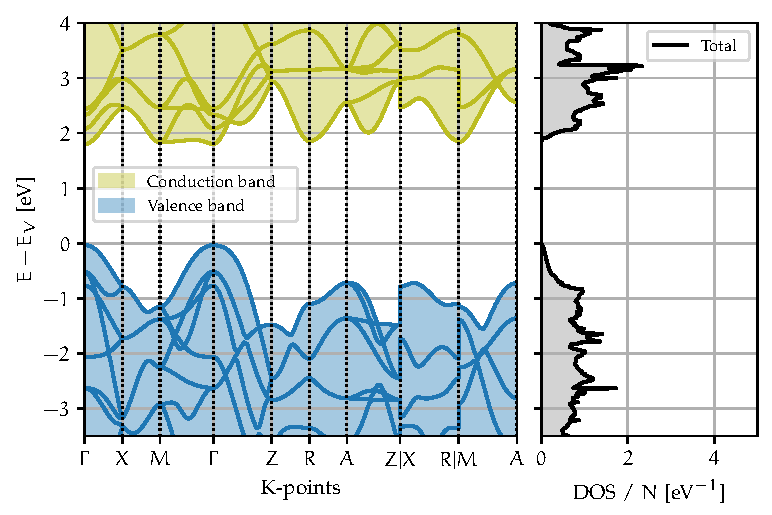
\includegraphics[width=\textwidth]{figures/unit.pdf}
        \caption{Unit cell, DFT}
        \label{fig:bands_unit_dft}
    \end{subfigure}
    \\
    \begin{subfigure}[t]{\textwidth}
        \centering
        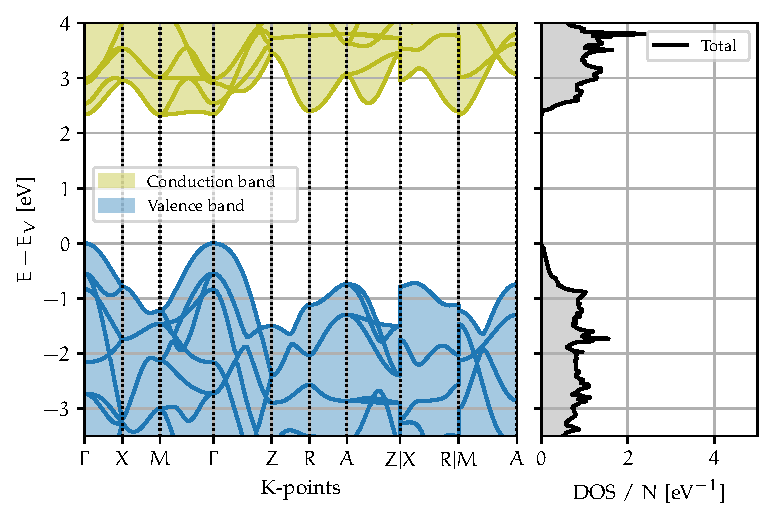
\includegraphics[width=\textwidth]{figures/unit+u.pdf}     \caption{Unit cell, DFT+U}
        \label{fig:bands_unit_dft+u}
    \end{subfigure}
    \caption[Band structure and DOS of the rutile unit cell]{Band structure and DOS of the rutile unit cell. The zero of the energy has been shifted to the top of the highest valence band $E_V$. The DOS is divided by the total number of atoms $N = 6$. The direct $\Gamma - \Gamma$ energy gap in (a) is of \SI{1.83}{eV}, whereas in (b) it is of \SI{2.33}{eV}.}
    \label{fig:bands_unit}
\end{figure}
In the diagrams, the zero of the energy has been shifted to the top of the highest valence band, so that all the electrons are situated in the region $E < 0$. An energy gap is clearly visible both in the band structure and in the DOS. The band gap is found to be direct, meaning that both the top of the highest valence band and the bottom of the lowest conduction band are found in correspondence of the same $k$-point; here it is the $\Gamma$ k-point. As expected, the energy gap is larger in the DFT+U calculation. The standard DFT calculation returned a gap of \SI{1.83}{eV}, whereas the DFT+U calculation a gap of \SI{2.33}{eV}.

In \cref{fig:bands_super}, the band structure and the DOS of the rutile supercell are reported.
\begin{figure}
    \centering
    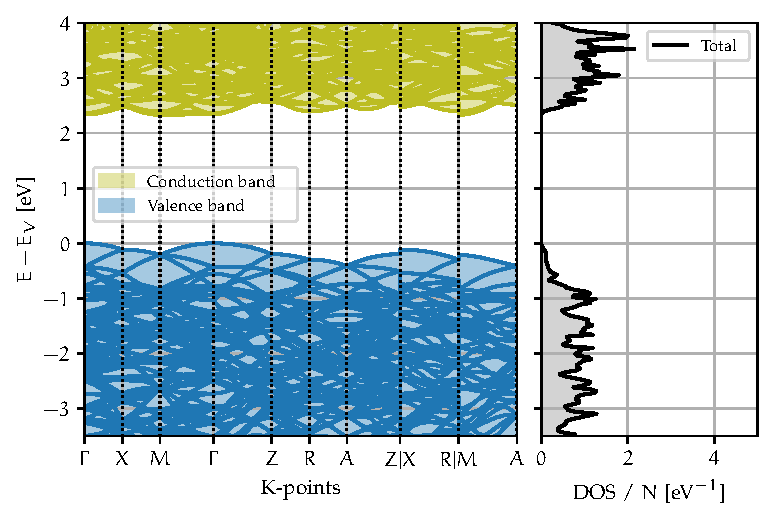
\includegraphics[width=\textwidth]{figures/super.pdf}
    \caption[Band structure and DOS of the rutile supercell]{Band structure and DOS of the rutile supercell. The zero of the energy has been shifted to the top of the highest valence band $E_V$. The DOS is divided by the total number of atoms $N = 162$. The direct $\Gamma - \Gamma$ energy gap is of \SI{2.33}{eV}.}
    \label{fig:bands_super}
\end{figure}
We expected the band structure and the DOS of the supercell to be very similar to the unit cell ones, the main difference being that in the supercell many more bands are accessible. This is due to the bigger number of atoms, since each individual atom contributes to the total band structure with its own atomic orbitals. Band-unfolding techniques have been developed to overcome this inconvenience, reducing the supercell band structure to the unit cell one \cite{mayo2020}. However, since the exact band structure of rutile was not the main focus of this work, these techniques were not employed. Nevertheless, in \cref{fig:bands_super} we can still clearly see a band structure and a DOS similar to the ones observed in \cref{fig:bands_unit_dft+u}. The energy gap is of \SI{2.33}{eV}, as it was for the unit cell in the DFT+U calculation.
In both diagrams, the DOS has been divided by the total number of atoms $N$ to make the results comparable.

\subsection{Electron localization}
The localization of the extra electron was successful: the electron localized  on the vanadium atom and remained localized at the centre of the supercell in the following steps. The localization on the central vanadium atom was clearly visible from the  eigenvalues, since a new state with spin $+1/2$ was found in the conduction band. The vanadium atom was the only one with a magnetic moment different from zero, equal to $1.093 \mu_B$. After the substitution of vanadium with titanium, with a $U-J$ value of \SI{9}{eV}, the localization was confirmed by a magnetic moment on the central atom of $0.930 \mu_B$. Finally, setting $U-J$ to \SI{3.9}{eV}, the electron remained localized. The magnetic moment on the central titanium atom was $0.787 \mu_B$.

\subsection{Polaron}
The DOS and the band structure of the polaronic solution are reported in \cref{fig:polaron_bands}. An extra state is clearly visible both in the DOS and in the band structure, \SI{0.70}{eV} below the conduction band. This is compatible with the expectations for small polarons, which usually create a new state approximately \SI{1}{eV} below the conduction band. In the DOS diagram, the total DOS has been plotted together with its projection on the central titanium atom. It is interesting to pay attention to the region between \SI{-0.2}{eV} and \SI{0.0}{eV}, where the polaronic state can be found. Here, most of the contribution to the total DOS is given by the projection on the central atom, meaning that the electron is mostly localized on this atom.

The previous plot can be compared with \cref{fig:delocalized_bands}, where the delocalized solution is shown. We notice that the zero of the energy is shifted up to the bottom of the conduction band, which now coincides with the top of the valence band. Both the band structure and the DOS show that the extra electron enters the conduction band, and that no new state is created in the middle of the energy gap. The contribution of the central atom  to the total DOS is not as relevant as before. This is compatible with an electron delocalized in the material, where the central atom does not play any particular role.

\begin{figure}
    \centering
    \begin{subfigure}[b]{\textwidth}
        \centering
        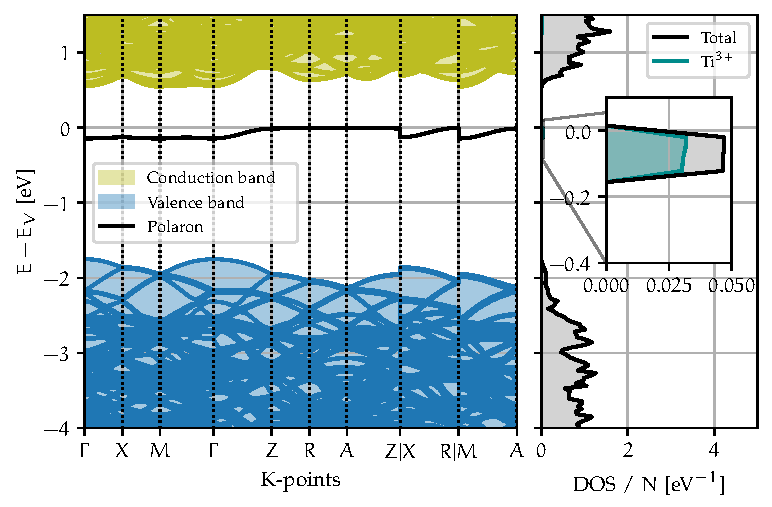
\includegraphics[width=\textwidth]{figures/polaron}
        %%% Creator: Matplotlib, PGF backend
%%
%% To include the figure in your LaTeX document, write
%%   \input{<filename>.pgf}
%%
%% Make sure the required packages are loaded in your preamble
%%   \usepackage{pgf}
%%
%% Also ensure that all the required font packages are loaded; for instance,
%% the lmodern package is sometimes necessary when using math font.
%%   \usepackage{lmodern}
%%
%% Figures using additional raster images can only be included by \input if
%% they are in the same directory as the main LaTeX file. For loading figures
%% from other directories you can use the `import` package
%%   \usepackage{import}
%%
%% and then include the figures with
%%   \import{<path to file>}{<filename>.pgf}
%%
%% Matplotlib used the following preamble
%%   \usepackage{fontspec}
%%   \setmainfont{DejaVuSerif.ttf}[Path=\detokenize{/usr/share/matplotlib/mpl-data/fonts/ttf/}]
%%   \setsansfont{DejaVuSans.ttf}[Path=\detokenize{/usr/share/matplotlib/mpl-data/fonts/ttf/}]
%%   \setmonofont{DejaVuSansMono.ttf}[Path=\detokenize{/usr/share/matplotlib/mpl-data/fonts/ttf/}]
%%
\begingroup%
\makeatletter%
\begin{pgfpicture}%
\pgfpathrectangle{\pgfpointorigin}{\pgfqpoint{5.149877in}{3.380212in}}%
\pgfusepath{use as bounding box, clip}%
\begin{pgfscope}%
\pgfsetbuttcap%
\pgfsetmiterjoin%
\definecolor{currentfill}{rgb}{1.000000,1.000000,1.000000}%
\pgfsetfillcolor{currentfill}%
\pgfsetlinewidth{0.000000pt}%
\definecolor{currentstroke}{rgb}{1.000000,1.000000,1.000000}%
\pgfsetstrokecolor{currentstroke}%
\pgfsetdash{}{0pt}%
\pgfpathmoveto{\pgfqpoint{0.000000in}{0.000000in}}%
\pgfpathlineto{\pgfqpoint{5.149877in}{0.000000in}}%
\pgfpathlineto{\pgfqpoint{5.149877in}{3.380212in}}%
\pgfpathlineto{\pgfqpoint{0.000000in}{3.380212in}}%
\pgfpathlineto{\pgfqpoint{0.000000in}{0.000000in}}%
\pgfpathclose%
\pgfusepath{fill}%
\end{pgfscope}%
\begin{pgfscope}%
\pgfsetbuttcap%
\pgfsetmiterjoin%
\definecolor{currentfill}{rgb}{1.000000,1.000000,1.000000}%
\pgfsetfillcolor{currentfill}%
\pgfsetlinewidth{0.000000pt}%
\definecolor{currentstroke}{rgb}{0.000000,0.000000,0.000000}%
\pgfsetstrokecolor{currentstroke}%
\pgfsetstrokeopacity{0.000000}%
\pgfsetdash{}{0pt}%
\pgfpathmoveto{\pgfqpoint{0.564660in}{0.526079in}}%
\pgfpathlineto{\pgfqpoint{3.446727in}{0.526079in}}%
\pgfpathlineto{\pgfqpoint{3.446727in}{3.280212in}}%
\pgfpathlineto{\pgfqpoint{0.564660in}{3.280212in}}%
\pgfpathlineto{\pgfqpoint{0.564660in}{0.526079in}}%
\pgfpathclose%
\pgfusepath{fill}%
\end{pgfscope}%
\begin{pgfscope}%
\pgfpathrectangle{\pgfqpoint{0.564660in}{0.526079in}}{\pgfqpoint{2.882067in}{2.754132in}}%
\pgfusepath{clip}%
\pgfsetbuttcap%
\pgfsetroundjoin%
\definecolor{currentfill}{rgb}{0.737255,0.741176,0.133333}%
\pgfsetfillcolor{currentfill}%
\pgfsetfillopacity{0.400000}%
\pgfsetlinewidth{1.003750pt}%
\definecolor{currentstroke}{rgb}{0.737255,0.741176,0.133333}%
\pgfsetstrokecolor{currentstroke}%
\pgfsetstrokeopacity{0.400000}%
\pgfsetdash{}{0pt}%
\pgfsys@defobject{currentmarker}{\pgfqpoint{0.564660in}{2.800792in}}{\pgfqpoint{3.446727in}{4.754874in}}{%
\pgfpathmoveto{\pgfqpoint{0.564660in}{4.725931in}}%
\pgfpathlineto{\pgfqpoint{0.564660in}{2.804698in}}%
\pgfpathlineto{\pgfqpoint{0.592560in}{2.805550in}}%
\pgfpathlineto{\pgfqpoint{0.620461in}{2.808354in}}%
\pgfpathlineto{\pgfqpoint{0.648251in}{2.813111in}}%
\pgfpathlineto{\pgfqpoint{0.676151in}{2.819721in}}%
\pgfpathlineto{\pgfqpoint{0.704051in}{2.828083in}}%
\pgfpathlineto{\pgfqpoint{0.731952in}{2.838048in}}%
\pgfpathlineto{\pgfqpoint{0.759852in}{2.849265in}}%
\pgfpathlineto{\pgfqpoint{0.787752in}{2.861634in}}%
\pgfpathlineto{\pgfqpoint{0.815542in}{2.873502in}}%
\pgfpathlineto{\pgfqpoint{0.815542in}{2.873502in}}%
\pgfpathlineto{\pgfqpoint{0.843442in}{2.868794in}}%
\pgfpathlineto{\pgfqpoint{0.871343in}{2.857377in}}%
\pgfpathlineto{\pgfqpoint{0.899243in}{2.844158in}}%
\pgfpathlineto{\pgfqpoint{0.927143in}{2.831839in}}%
\pgfpathlineto{\pgfqpoint{0.955043in}{2.821123in}}%
\pgfpathlineto{\pgfqpoint{0.982833in}{2.812410in}}%
\pgfpathlineto{\pgfqpoint{1.010734in}{2.806050in}}%
\pgfpathlineto{\pgfqpoint{1.038634in}{2.802144in}}%
\pgfpathlineto{\pgfqpoint{1.066534in}{2.800792in}}%
\pgfpathlineto{\pgfqpoint{1.066534in}{2.800792in}}%
\pgfpathlineto{\pgfqpoint{1.105968in}{2.805900in}}%
\pgfpathlineto{\pgfqpoint{1.145401in}{2.807803in}}%
\pgfpathlineto{\pgfqpoint{1.184835in}{2.808704in}}%
\pgfpathlineto{\pgfqpoint{1.224269in}{2.809806in}}%
\pgfpathlineto{\pgfqpoint{1.263703in}{2.811008in}}%
\pgfpathlineto{\pgfqpoint{1.303136in}{2.812109in}}%
\pgfpathlineto{\pgfqpoint{1.342570in}{2.811859in}}%
\pgfpathlineto{\pgfqpoint{1.382004in}{2.807152in}}%
\pgfpathlineto{\pgfqpoint{1.421438in}{2.804698in}}%
\pgfpathlineto{\pgfqpoint{1.421438in}{2.804698in}}%
\pgfpathlineto{\pgfqpoint{1.464716in}{2.809155in}}%
\pgfpathlineto{\pgfqpoint{1.507994in}{2.820172in}}%
\pgfpathlineto{\pgfqpoint{1.551272in}{2.836095in}}%
\pgfpathlineto{\pgfqpoint{1.594550in}{2.857377in}}%
\pgfpathlineto{\pgfqpoint{1.637829in}{2.883116in}}%
\pgfpathlineto{\pgfqpoint{1.681107in}{2.912510in}}%
\pgfpathlineto{\pgfqpoint{1.724385in}{2.928484in}}%
\pgfpathlineto{\pgfqpoint{1.767663in}{2.925880in}}%
\pgfpathlineto{\pgfqpoint{1.810942in}{2.924979in}}%
\pgfpathlineto{\pgfqpoint{1.810942in}{2.924979in}}%
\pgfpathlineto{\pgfqpoint{1.838842in}{2.921624in}}%
\pgfpathlineto{\pgfqpoint{1.866742in}{2.914864in}}%
\pgfpathlineto{\pgfqpoint{1.894532in}{2.903246in}}%
\pgfpathlineto{\pgfqpoint{1.922433in}{2.887923in}}%
\pgfpathlineto{\pgfqpoint{1.950333in}{2.873552in}}%
\pgfpathlineto{\pgfqpoint{1.978233in}{2.861634in}}%
\pgfpathlineto{\pgfqpoint{2.006133in}{2.852770in}}%
\pgfpathlineto{\pgfqpoint{2.033923in}{2.847362in}}%
\pgfpathlineto{\pgfqpoint{2.061824in}{2.845560in}}%
\pgfpathlineto{\pgfqpoint{2.061824in}{2.845560in}}%
\pgfpathlineto{\pgfqpoint{2.089724in}{2.846161in}}%
\pgfpathlineto{\pgfqpoint{2.117624in}{2.848013in}}%
\pgfpathlineto{\pgfqpoint{2.145524in}{2.851068in}}%
\pgfpathlineto{\pgfqpoint{2.173424in}{2.855174in}}%
\pgfpathlineto{\pgfqpoint{2.201215in}{2.860282in}}%
\pgfpathlineto{\pgfqpoint{2.229115in}{2.866391in}}%
\pgfpathlineto{\pgfqpoint{2.257015in}{2.873752in}}%
\pgfpathlineto{\pgfqpoint{2.284915in}{2.882665in}}%
\pgfpathlineto{\pgfqpoint{2.312815in}{2.891729in}}%
\pgfpathlineto{\pgfqpoint{2.312815in}{2.891729in}}%
\pgfpathlineto{\pgfqpoint{2.352249in}{2.873151in}}%
\pgfpathlineto{\pgfqpoint{2.391683in}{2.859931in}}%
\pgfpathlineto{\pgfqpoint{2.431117in}{2.854373in}}%
\pgfpathlineto{\pgfqpoint{2.470550in}{2.856476in}}%
\pgfpathlineto{\pgfqpoint{2.509984in}{2.866191in}}%
\pgfpathlineto{\pgfqpoint{2.549418in}{2.883016in}}%
\pgfpathlineto{\pgfqpoint{2.588851in}{2.906451in}}%
\pgfpathlineto{\pgfqpoint{2.628285in}{2.917167in}}%
\pgfpathlineto{\pgfqpoint{2.667609in}{2.924979in}}%
\pgfpathlineto{\pgfqpoint{2.667609in}{2.873502in}}%
\pgfpathlineto{\pgfqpoint{2.710997in}{2.877758in}}%
\pgfpathlineto{\pgfqpoint{2.754275in}{2.890277in}}%
\pgfpathlineto{\pgfqpoint{2.797554in}{2.906551in}}%
\pgfpathlineto{\pgfqpoint{2.840832in}{2.898890in}}%
\pgfpathlineto{\pgfqpoint{2.884110in}{2.881964in}}%
\pgfpathlineto{\pgfqpoint{2.927388in}{2.866791in}}%
\pgfpathlineto{\pgfqpoint{2.970667in}{2.855224in}}%
\pgfpathlineto{\pgfqpoint{3.013945in}{2.848013in}}%
\pgfpathlineto{\pgfqpoint{3.057223in}{2.845560in}}%
\pgfpathlineto{\pgfqpoint{3.057223in}{2.800792in}}%
\pgfpathlineto{\pgfqpoint{3.100501in}{2.804498in}}%
\pgfpathlineto{\pgfqpoint{3.143780in}{2.815364in}}%
\pgfpathlineto{\pgfqpoint{3.187058in}{2.832841in}}%
\pgfpathlineto{\pgfqpoint{3.230336in}{2.856075in}}%
\pgfpathlineto{\pgfqpoint{3.273614in}{2.884168in}}%
\pgfpathlineto{\pgfqpoint{3.316892in}{2.912210in}}%
\pgfpathlineto{\pgfqpoint{3.360171in}{2.900943in}}%
\pgfpathlineto{\pgfqpoint{3.403449in}{2.894032in}}%
\pgfpathlineto{\pgfqpoint{3.446727in}{2.891729in}}%
\pgfpathlineto{\pgfqpoint{3.446727in}{4.693733in}}%
\pgfpathlineto{\pgfqpoint{3.446727in}{4.693733in}}%
\pgfpathlineto{\pgfqpoint{3.403449in}{4.658430in}}%
\pgfpathlineto{\pgfqpoint{3.360171in}{4.652070in}}%
\pgfpathlineto{\pgfqpoint{3.316892in}{4.655575in}}%
\pgfpathlineto{\pgfqpoint{3.273614in}{4.674203in}}%
\pgfpathlineto{\pgfqpoint{3.230336in}{4.680613in}}%
\pgfpathlineto{\pgfqpoint{3.187058in}{4.693482in}}%
\pgfpathlineto{\pgfqpoint{3.143780in}{4.701194in}}%
\pgfpathlineto{\pgfqpoint{3.100501in}{4.703698in}}%
\pgfpathlineto{\pgfqpoint{3.057223in}{4.717368in}}%
\pgfpathlineto{\pgfqpoint{3.057223in}{4.694784in}}%
\pgfpathlineto{\pgfqpoint{3.013945in}{4.688375in}}%
\pgfpathlineto{\pgfqpoint{2.970667in}{4.687623in}}%
\pgfpathlineto{\pgfqpoint{2.927388in}{4.703748in}}%
\pgfpathlineto{\pgfqpoint{2.884110in}{4.698790in}}%
\pgfpathlineto{\pgfqpoint{2.840832in}{4.712711in}}%
\pgfpathlineto{\pgfqpoint{2.797554in}{4.695285in}}%
\pgfpathlineto{\pgfqpoint{2.754275in}{4.748365in}}%
\pgfpathlineto{\pgfqpoint{2.710997in}{4.716867in}}%
\pgfpathlineto{\pgfqpoint{2.667609in}{4.733042in}}%
\pgfpathlineto{\pgfqpoint{2.667609in}{4.651319in}}%
\pgfpathlineto{\pgfqpoint{2.628285in}{4.651469in}}%
\pgfpathlineto{\pgfqpoint{2.588851in}{4.674153in}}%
\pgfpathlineto{\pgfqpoint{2.549418in}{4.689176in}}%
\pgfpathlineto{\pgfqpoint{2.509984in}{4.678360in}}%
\pgfpathlineto{\pgfqpoint{2.470550in}{4.690127in}}%
\pgfpathlineto{\pgfqpoint{2.431117in}{4.670698in}}%
\pgfpathlineto{\pgfqpoint{2.391683in}{4.672501in}}%
\pgfpathlineto{\pgfqpoint{2.352249in}{4.654023in}}%
\pgfpathlineto{\pgfqpoint{2.312815in}{4.647513in}}%
\pgfpathlineto{\pgfqpoint{2.312815in}{4.648314in}}%
\pgfpathlineto{\pgfqpoint{2.284915in}{4.646512in}}%
\pgfpathlineto{\pgfqpoint{2.257015in}{4.657028in}}%
\pgfpathlineto{\pgfqpoint{2.229115in}{4.697638in}}%
\pgfpathlineto{\pgfqpoint{2.201215in}{4.687073in}}%
\pgfpathlineto{\pgfqpoint{2.173424in}{4.701945in}}%
\pgfpathlineto{\pgfqpoint{2.145524in}{4.693332in}}%
\pgfpathlineto{\pgfqpoint{2.117624in}{4.688174in}}%
\pgfpathlineto{\pgfqpoint{2.089724in}{4.697839in}}%
\pgfpathlineto{\pgfqpoint{2.061824in}{4.695085in}}%
\pgfpathlineto{\pgfqpoint{2.061824in}{4.679361in}}%
\pgfpathlineto{\pgfqpoint{2.033923in}{4.689727in}}%
\pgfpathlineto{\pgfqpoint{2.006133in}{4.688775in}}%
\pgfpathlineto{\pgfqpoint{1.978233in}{4.689777in}}%
\pgfpathlineto{\pgfqpoint{1.950333in}{4.680963in}}%
\pgfpathlineto{\pgfqpoint{1.922433in}{4.681915in}}%
\pgfpathlineto{\pgfqpoint{1.894532in}{4.686872in}}%
\pgfpathlineto{\pgfqpoint{1.866742in}{4.674253in}}%
\pgfpathlineto{\pgfqpoint{1.838842in}{4.660282in}}%
\pgfpathlineto{\pgfqpoint{1.810942in}{4.648515in}}%
\pgfpathlineto{\pgfqpoint{1.810942in}{4.664088in}}%
\pgfpathlineto{\pgfqpoint{1.767663in}{4.650718in}}%
\pgfpathlineto{\pgfqpoint{1.724385in}{4.666942in}}%
\pgfpathlineto{\pgfqpoint{1.681107in}{4.669546in}}%
\pgfpathlineto{\pgfqpoint{1.637829in}{4.680863in}}%
\pgfpathlineto{\pgfqpoint{1.594550in}{4.685871in}}%
\pgfpathlineto{\pgfqpoint{1.551272in}{4.701945in}}%
\pgfpathlineto{\pgfqpoint{1.507994in}{4.716867in}}%
\pgfpathlineto{\pgfqpoint{1.464716in}{4.736046in}}%
\pgfpathlineto{\pgfqpoint{1.421438in}{4.748615in}}%
\pgfpathlineto{\pgfqpoint{1.421438in}{4.738700in}}%
\pgfpathlineto{\pgfqpoint{1.382004in}{4.751319in}}%
\pgfpathlineto{\pgfqpoint{1.342570in}{4.739201in}}%
\pgfpathlineto{\pgfqpoint{1.303136in}{4.754874in}}%
\pgfpathlineto{\pgfqpoint{1.263703in}{4.716467in}}%
\pgfpathlineto{\pgfqpoint{1.224269in}{4.727583in}}%
\pgfpathlineto{\pgfqpoint{1.184835in}{4.722426in}}%
\pgfpathlineto{\pgfqpoint{1.145401in}{4.708204in}}%
\pgfpathlineto{\pgfqpoint{1.105968in}{4.692581in}}%
\pgfpathlineto{\pgfqpoint{1.066534in}{4.700994in}}%
\pgfpathlineto{\pgfqpoint{1.066534in}{4.714514in}}%
\pgfpathlineto{\pgfqpoint{1.038634in}{4.709907in}}%
\pgfpathlineto{\pgfqpoint{1.010734in}{4.704549in}}%
\pgfpathlineto{\pgfqpoint{0.982833in}{4.710658in}}%
\pgfpathlineto{\pgfqpoint{0.955043in}{4.716967in}}%
\pgfpathlineto{\pgfqpoint{0.927143in}{4.717168in}}%
\pgfpathlineto{\pgfqpoint{0.899243in}{4.722776in}}%
\pgfpathlineto{\pgfqpoint{0.871343in}{4.718970in}}%
\pgfpathlineto{\pgfqpoint{0.843442in}{4.732992in}}%
\pgfpathlineto{\pgfqpoint{0.815542in}{4.720923in}}%
\pgfpathlineto{\pgfqpoint{0.815542in}{4.727984in}}%
\pgfpathlineto{\pgfqpoint{0.787752in}{4.726382in}}%
\pgfpathlineto{\pgfqpoint{0.759852in}{4.742656in}}%
\pgfpathlineto{\pgfqpoint{0.731952in}{4.747463in}}%
\pgfpathlineto{\pgfqpoint{0.704051in}{4.744459in}}%
\pgfpathlineto{\pgfqpoint{0.676151in}{4.750067in}}%
\pgfpathlineto{\pgfqpoint{0.648251in}{4.746812in}}%
\pgfpathlineto{\pgfqpoint{0.620461in}{4.751369in}}%
\pgfpathlineto{\pgfqpoint{0.592560in}{4.728685in}}%
\pgfpathlineto{\pgfqpoint{0.564660in}{4.725931in}}%
\pgfpathlineto{\pgfqpoint{0.564660in}{4.725931in}}%
\pgfpathclose%
\pgfusepath{stroke,fill}%
}%
\begin{pgfscope}%
\pgfsys@transformshift{0.000000in}{0.000000in}%
\pgfsys@useobject{currentmarker}{}%
\end{pgfscope}%
\end{pgfscope}%
\begin{pgfscope}%
\pgfpathrectangle{\pgfqpoint{0.564660in}{0.526079in}}{\pgfqpoint{2.882067in}{2.754132in}}%
\pgfusepath{clip}%
\pgfsetbuttcap%
\pgfsetroundjoin%
\definecolor{currentfill}{rgb}{0.121569,0.466667,0.705882}%
\pgfsetfillcolor{currentfill}%
\pgfsetfillopacity{0.400000}%
\pgfsetlinewidth{1.003750pt}%
\definecolor{currentstroke}{rgb}{0.121569,0.466667,0.705882}%
\pgfsetstrokecolor{currentstroke}%
\pgfsetstrokeopacity{0.400000}%
\pgfsetdash{}{0pt}%
\pgfpathmoveto{\pgfqpoint{0.564660in}{1.652419in}}%
\pgfpathlineto{\pgfqpoint{0.564660in}{-27.384848in}}%
\pgfpathlineto{\pgfqpoint{0.592560in}{-27.384848in}}%
\pgfpathlineto{\pgfqpoint{0.620461in}{-27.384798in}}%
\pgfpathlineto{\pgfqpoint{0.648251in}{-27.384798in}}%
\pgfpathlineto{\pgfqpoint{0.676151in}{-27.384798in}}%
\pgfpathlineto{\pgfqpoint{0.704051in}{-27.384748in}}%
\pgfpathlineto{\pgfqpoint{0.731952in}{-27.384698in}}%
\pgfpathlineto{\pgfqpoint{0.759852in}{-27.384698in}}%
\pgfpathlineto{\pgfqpoint{0.787752in}{-27.384648in}}%
\pgfpathlineto{\pgfqpoint{0.815542in}{-27.384648in}}%
\pgfpathlineto{\pgfqpoint{0.815542in}{-27.384648in}}%
\pgfpathlineto{\pgfqpoint{0.843442in}{-27.384648in}}%
\pgfpathlineto{\pgfqpoint{0.871343in}{-27.384648in}}%
\pgfpathlineto{\pgfqpoint{0.899243in}{-27.384698in}}%
\pgfpathlineto{\pgfqpoint{0.927143in}{-27.384698in}}%
\pgfpathlineto{\pgfqpoint{0.955043in}{-27.384698in}}%
\pgfpathlineto{\pgfqpoint{0.982833in}{-27.384698in}}%
\pgfpathlineto{\pgfqpoint{1.010734in}{-27.384748in}}%
\pgfpathlineto{\pgfqpoint{1.038634in}{-27.384748in}}%
\pgfpathlineto{\pgfqpoint{1.066534in}{-27.384748in}}%
\pgfpathlineto{\pgfqpoint{1.066534in}{-27.384748in}}%
\pgfpathlineto{\pgfqpoint{1.105968in}{-27.384748in}}%
\pgfpathlineto{\pgfqpoint{1.145401in}{-27.384698in}}%
\pgfpathlineto{\pgfqpoint{1.184835in}{-27.384648in}}%
\pgfpathlineto{\pgfqpoint{1.224269in}{-27.384598in}}%
\pgfpathlineto{\pgfqpoint{1.263703in}{-27.384648in}}%
\pgfpathlineto{\pgfqpoint{1.303136in}{-27.384748in}}%
\pgfpathlineto{\pgfqpoint{1.342570in}{-27.384798in}}%
\pgfpathlineto{\pgfqpoint{1.382004in}{-27.384798in}}%
\pgfpathlineto{\pgfqpoint{1.421438in}{-27.384848in}}%
\pgfpathlineto{\pgfqpoint{1.421438in}{-27.384848in}}%
\pgfpathlineto{\pgfqpoint{1.464716in}{-27.384748in}}%
\pgfpathlineto{\pgfqpoint{1.507994in}{-27.384548in}}%
\pgfpathlineto{\pgfqpoint{1.551272in}{-27.384197in}}%
\pgfpathlineto{\pgfqpoint{1.594550in}{-27.383697in}}%
\pgfpathlineto{\pgfqpoint{1.637829in}{-27.383096in}}%
\pgfpathlineto{\pgfqpoint{1.681107in}{-27.382395in}}%
\pgfpathlineto{\pgfqpoint{1.724385in}{-27.381543in}}%
\pgfpathlineto{\pgfqpoint{1.767663in}{-27.380642in}}%
\pgfpathlineto{\pgfqpoint{1.810942in}{-27.379691in}}%
\pgfpathlineto{\pgfqpoint{1.810942in}{-27.379691in}}%
\pgfpathlineto{\pgfqpoint{1.838842in}{-27.379691in}}%
\pgfpathlineto{\pgfqpoint{1.866742in}{-27.379691in}}%
\pgfpathlineto{\pgfqpoint{1.894532in}{-27.379640in}}%
\pgfpathlineto{\pgfqpoint{1.922433in}{-27.379640in}}%
\pgfpathlineto{\pgfqpoint{1.950333in}{-27.379640in}}%
\pgfpathlineto{\pgfqpoint{1.978233in}{-27.379590in}}%
\pgfpathlineto{\pgfqpoint{2.006133in}{-27.379590in}}%
\pgfpathlineto{\pgfqpoint{2.033923in}{-27.379540in}}%
\pgfpathlineto{\pgfqpoint{2.061824in}{-27.379540in}}%
\pgfpathlineto{\pgfqpoint{2.061824in}{-27.379540in}}%
\pgfpathlineto{\pgfqpoint{2.089724in}{-27.379540in}}%
\pgfpathlineto{\pgfqpoint{2.117624in}{-27.379540in}}%
\pgfpathlineto{\pgfqpoint{2.145524in}{-27.379590in}}%
\pgfpathlineto{\pgfqpoint{2.173424in}{-27.379590in}}%
\pgfpathlineto{\pgfqpoint{2.201215in}{-27.379590in}}%
\pgfpathlineto{\pgfqpoint{2.229115in}{-27.379590in}}%
\pgfpathlineto{\pgfqpoint{2.257015in}{-27.379640in}}%
\pgfpathlineto{\pgfqpoint{2.284915in}{-27.379640in}}%
\pgfpathlineto{\pgfqpoint{2.312815in}{-27.379640in}}%
\pgfpathlineto{\pgfqpoint{2.312815in}{-27.379640in}}%
\pgfpathlineto{\pgfqpoint{2.352249in}{-27.379640in}}%
\pgfpathlineto{\pgfqpoint{2.391683in}{-27.379590in}}%
\pgfpathlineto{\pgfqpoint{2.431117in}{-27.379540in}}%
\pgfpathlineto{\pgfqpoint{2.470550in}{-27.379540in}}%
\pgfpathlineto{\pgfqpoint{2.509984in}{-27.379540in}}%
\pgfpathlineto{\pgfqpoint{2.549418in}{-27.379590in}}%
\pgfpathlineto{\pgfqpoint{2.588851in}{-27.379640in}}%
\pgfpathlineto{\pgfqpoint{2.628285in}{-27.379691in}}%
\pgfpathlineto{\pgfqpoint{2.667609in}{-27.379691in}}%
\pgfpathlineto{\pgfqpoint{2.667609in}{-27.384648in}}%
\pgfpathlineto{\pgfqpoint{2.710997in}{-27.384548in}}%
\pgfpathlineto{\pgfqpoint{2.754275in}{-27.384348in}}%
\pgfpathlineto{\pgfqpoint{2.797554in}{-27.383997in}}%
\pgfpathlineto{\pgfqpoint{2.840832in}{-27.383496in}}%
\pgfpathlineto{\pgfqpoint{2.884110in}{-27.382895in}}%
\pgfpathlineto{\pgfqpoint{2.927388in}{-27.382194in}}%
\pgfpathlineto{\pgfqpoint{2.970667in}{-27.381343in}}%
\pgfpathlineto{\pgfqpoint{3.013945in}{-27.380442in}}%
\pgfpathlineto{\pgfqpoint{3.057223in}{-27.379540in}}%
\pgfpathlineto{\pgfqpoint{3.057223in}{-27.384748in}}%
\pgfpathlineto{\pgfqpoint{3.100501in}{-27.384648in}}%
\pgfpathlineto{\pgfqpoint{3.143780in}{-27.384448in}}%
\pgfpathlineto{\pgfqpoint{3.187058in}{-27.384097in}}%
\pgfpathlineto{\pgfqpoint{3.230336in}{-27.383646in}}%
\pgfpathlineto{\pgfqpoint{3.273614in}{-27.383046in}}%
\pgfpathlineto{\pgfqpoint{3.316892in}{-27.382294in}}%
\pgfpathlineto{\pgfqpoint{3.360171in}{-27.381493in}}%
\pgfpathlineto{\pgfqpoint{3.403449in}{-27.380542in}}%
\pgfpathlineto{\pgfqpoint{3.446727in}{-27.379640in}}%
\pgfpathlineto{\pgfqpoint{3.446727in}{1.466040in}}%
\pgfpathlineto{\pgfqpoint{3.446727in}{1.466040in}}%
\pgfpathlineto{\pgfqpoint{3.403449in}{1.475053in}}%
\pgfpathlineto{\pgfqpoint{3.360171in}{1.487672in}}%
\pgfpathlineto{\pgfqpoint{3.316892in}{1.500842in}}%
\pgfpathlineto{\pgfqpoint{3.273614in}{1.514162in}}%
\pgfpathlineto{\pgfqpoint{3.230336in}{1.526931in}}%
\pgfpathlineto{\pgfqpoint{3.187058in}{1.538298in}}%
\pgfpathlineto{\pgfqpoint{3.143780in}{1.547212in}}%
\pgfpathlineto{\pgfqpoint{3.100501in}{1.552920in}}%
\pgfpathlineto{\pgfqpoint{3.057223in}{1.554873in}}%
\pgfpathlineto{\pgfqpoint{3.057223in}{1.511408in}}%
\pgfpathlineto{\pgfqpoint{3.013945in}{1.526931in}}%
\pgfpathlineto{\pgfqpoint{2.970667in}{1.543756in}}%
\pgfpathlineto{\pgfqpoint{2.927388in}{1.558579in}}%
\pgfpathlineto{\pgfqpoint{2.884110in}{1.571198in}}%
\pgfpathlineto{\pgfqpoint{2.840832in}{1.581513in}}%
\pgfpathlineto{\pgfqpoint{2.797554in}{1.589425in}}%
\pgfpathlineto{\pgfqpoint{2.754275in}{1.594933in}}%
\pgfpathlineto{\pgfqpoint{2.710997in}{1.598138in}}%
\pgfpathlineto{\pgfqpoint{2.667609in}{1.599190in}}%
\pgfpathlineto{\pgfqpoint{2.667609in}{1.552920in}}%
\pgfpathlineto{\pgfqpoint{2.628285in}{1.551718in}}%
\pgfpathlineto{\pgfqpoint{2.588851in}{1.548113in}}%
\pgfpathlineto{\pgfqpoint{2.549418in}{1.542004in}}%
\pgfpathlineto{\pgfqpoint{2.509984in}{1.533341in}}%
\pgfpathlineto{\pgfqpoint{2.470550in}{1.522074in}}%
\pgfpathlineto{\pgfqpoint{2.431117in}{1.508153in}}%
\pgfpathlineto{\pgfqpoint{2.391683in}{1.491828in}}%
\pgfpathlineto{\pgfqpoint{2.352249in}{1.474703in}}%
\pgfpathlineto{\pgfqpoint{2.312815in}{1.466040in}}%
\pgfpathlineto{\pgfqpoint{2.312815in}{1.466040in}}%
\pgfpathlineto{\pgfqpoint{2.284915in}{1.470346in}}%
\pgfpathlineto{\pgfqpoint{2.257015in}{1.478508in}}%
\pgfpathlineto{\pgfqpoint{2.229115in}{1.486771in}}%
\pgfpathlineto{\pgfqpoint{2.201215in}{1.494132in}}%
\pgfpathlineto{\pgfqpoint{2.173424in}{1.500291in}}%
\pgfpathlineto{\pgfqpoint{2.145524in}{1.505148in}}%
\pgfpathlineto{\pgfqpoint{2.117624in}{1.508654in}}%
\pgfpathlineto{\pgfqpoint{2.089724in}{1.510707in}}%
\pgfpathlineto{\pgfqpoint{2.061824in}{1.511408in}}%
\pgfpathlineto{\pgfqpoint{2.061824in}{1.511408in}}%
\pgfpathlineto{\pgfqpoint{2.033923in}{1.516365in}}%
\pgfpathlineto{\pgfqpoint{2.006133in}{1.524177in}}%
\pgfpathlineto{\pgfqpoint{1.978233in}{1.531588in}}%
\pgfpathlineto{\pgfqpoint{1.950333in}{1.538048in}}%
\pgfpathlineto{\pgfqpoint{1.922433in}{1.543356in}}%
\pgfpathlineto{\pgfqpoint{1.894532in}{1.547562in}}%
\pgfpathlineto{\pgfqpoint{1.866742in}{1.550517in}}%
\pgfpathlineto{\pgfqpoint{1.838842in}{1.552319in}}%
\pgfpathlineto{\pgfqpoint{1.810942in}{1.552920in}}%
\pgfpathlineto{\pgfqpoint{1.810942in}{1.552920in}}%
\pgfpathlineto{\pgfqpoint{1.767663in}{1.574302in}}%
\pgfpathlineto{\pgfqpoint{1.724385in}{1.594533in}}%
\pgfpathlineto{\pgfqpoint{1.681107in}{1.611158in}}%
\pgfpathlineto{\pgfqpoint{1.637829in}{1.624578in}}%
\pgfpathlineto{\pgfqpoint{1.594550in}{1.635043in}}%
\pgfpathlineto{\pgfqpoint{1.551272in}{1.642855in}}%
\pgfpathlineto{\pgfqpoint{1.507994in}{1.648213in}}%
\pgfpathlineto{\pgfqpoint{1.464716in}{1.651418in}}%
\pgfpathlineto{\pgfqpoint{1.421438in}{1.652419in}}%
\pgfpathlineto{\pgfqpoint{1.421438in}{1.652419in}}%
\pgfpathlineto{\pgfqpoint{1.382004in}{1.651067in}}%
\pgfpathlineto{\pgfqpoint{1.342570in}{1.647061in}}%
\pgfpathlineto{\pgfqpoint{1.303136in}{1.640301in}}%
\pgfpathlineto{\pgfqpoint{1.263703in}{1.630887in}}%
\pgfpathlineto{\pgfqpoint{1.224269in}{1.618819in}}%
\pgfpathlineto{\pgfqpoint{1.184835in}{1.604197in}}%
\pgfpathlineto{\pgfqpoint{1.145401in}{1.587172in}}%
\pgfpathlineto{\pgfqpoint{1.105968in}{1.568193in}}%
\pgfpathlineto{\pgfqpoint{1.066534in}{1.554873in}}%
\pgfpathlineto{\pgfqpoint{1.066534in}{1.554873in}}%
\pgfpathlineto{\pgfqpoint{1.038634in}{1.560932in}}%
\pgfpathlineto{\pgfqpoint{1.010734in}{1.569595in}}%
\pgfpathlineto{\pgfqpoint{0.982833in}{1.577407in}}%
\pgfpathlineto{\pgfqpoint{0.955043in}{1.584067in}}%
\pgfpathlineto{\pgfqpoint{0.927143in}{1.589525in}}%
\pgfpathlineto{\pgfqpoint{0.899243in}{1.593731in}}%
\pgfpathlineto{\pgfqpoint{0.871343in}{1.596786in}}%
\pgfpathlineto{\pgfqpoint{0.843442in}{1.598589in}}%
\pgfpathlineto{\pgfqpoint{0.815542in}{1.599190in}}%
\pgfpathlineto{\pgfqpoint{0.815542in}{1.599190in}}%
\pgfpathlineto{\pgfqpoint{0.787752in}{1.607602in}}%
\pgfpathlineto{\pgfqpoint{0.759852in}{1.618018in}}%
\pgfpathlineto{\pgfqpoint{0.731952in}{1.627232in}}%
\pgfpathlineto{\pgfqpoint{0.704051in}{1.635043in}}%
\pgfpathlineto{\pgfqpoint{0.676151in}{1.641403in}}%
\pgfpathlineto{\pgfqpoint{0.648251in}{1.646260in}}%
\pgfpathlineto{\pgfqpoint{0.620461in}{1.649715in}}%
\pgfpathlineto{\pgfqpoint{0.592560in}{1.651768in}}%
\pgfpathlineto{\pgfqpoint{0.564660in}{1.652419in}}%
\pgfpathlineto{\pgfqpoint{0.564660in}{1.652419in}}%
\pgfpathclose%
\pgfusepath{stroke,fill}%
\end{pgfscope}%
\begin{pgfscope}%
\pgfpathrectangle{\pgfqpoint{0.564660in}{0.526079in}}{\pgfqpoint{2.882067in}{2.754132in}}%
\pgfusepath{clip}%
\pgfsetrectcap%
\pgfsetroundjoin%
\pgfsetlinewidth{0.803000pt}%
\definecolor{currentstroke}{rgb}{0.690196,0.690196,0.690196}%
\pgfsetstrokecolor{currentstroke}%
\pgfsetdash{}{0pt}%
\pgfpathmoveto{\pgfqpoint{0.564660in}{0.526079in}}%
\pgfpathlineto{\pgfqpoint{0.564660in}{3.280212in}}%
\pgfusepath{stroke}%
\end{pgfscope}%
\begin{pgfscope}%
\pgfsetbuttcap%
\pgfsetroundjoin%
\definecolor{currentfill}{rgb}{0.000000,0.000000,0.000000}%
\pgfsetfillcolor{currentfill}%
\pgfsetlinewidth{0.803000pt}%
\definecolor{currentstroke}{rgb}{0.000000,0.000000,0.000000}%
\pgfsetstrokecolor{currentstroke}%
\pgfsetdash{}{0pt}%
\pgfsys@defobject{currentmarker}{\pgfqpoint{0.000000in}{-0.048611in}}{\pgfqpoint{0.000000in}{0.000000in}}{%
\pgfpathmoveto{\pgfqpoint{0.000000in}{0.000000in}}%
\pgfpathlineto{\pgfqpoint{0.000000in}{-0.048611in}}%
\pgfusepath{stroke,fill}%
}%
\begin{pgfscope}%
\pgfsys@transformshift{0.564660in}{0.526079in}%
\pgfsys@useobject{currentmarker}{}%
\end{pgfscope}%
\end{pgfscope}%
\begin{pgfscope}%
\definecolor{textcolor}{rgb}{0.000000,0.000000,0.000000}%
\pgfsetstrokecolor{textcolor}%
\pgfsetfillcolor{textcolor}%
\pgftext[x=0.564660in,y=0.428857in,,top]{\color{textcolor}\rmfamily\fontsize{10.000000}{12.000000}\selectfont \(\displaystyle \Gamma\)}%
\end{pgfscope}%
\begin{pgfscope}%
\pgfpathrectangle{\pgfqpoint{0.564660in}{0.526079in}}{\pgfqpoint{2.882067in}{2.754132in}}%
\pgfusepath{clip}%
\pgfsetrectcap%
\pgfsetroundjoin%
\pgfsetlinewidth{0.803000pt}%
\definecolor{currentstroke}{rgb}{0.690196,0.690196,0.690196}%
\pgfsetstrokecolor{currentstroke}%
\pgfsetdash{}{0pt}%
\pgfpathmoveto{\pgfqpoint{0.815542in}{0.526079in}}%
\pgfpathlineto{\pgfqpoint{0.815542in}{3.280212in}}%
\pgfusepath{stroke}%
\end{pgfscope}%
\begin{pgfscope}%
\pgfsetbuttcap%
\pgfsetroundjoin%
\definecolor{currentfill}{rgb}{0.000000,0.000000,0.000000}%
\pgfsetfillcolor{currentfill}%
\pgfsetlinewidth{0.803000pt}%
\definecolor{currentstroke}{rgb}{0.000000,0.000000,0.000000}%
\pgfsetstrokecolor{currentstroke}%
\pgfsetdash{}{0pt}%
\pgfsys@defobject{currentmarker}{\pgfqpoint{0.000000in}{-0.048611in}}{\pgfqpoint{0.000000in}{0.000000in}}{%
\pgfpathmoveto{\pgfqpoint{0.000000in}{0.000000in}}%
\pgfpathlineto{\pgfqpoint{0.000000in}{-0.048611in}}%
\pgfusepath{stroke,fill}%
}%
\begin{pgfscope}%
\pgfsys@transformshift{0.815542in}{0.526079in}%
\pgfsys@useobject{currentmarker}{}%
\end{pgfscope}%
\end{pgfscope}%
\begin{pgfscope}%
\definecolor{textcolor}{rgb}{0.000000,0.000000,0.000000}%
\pgfsetstrokecolor{textcolor}%
\pgfsetfillcolor{textcolor}%
\pgftext[x=0.815542in,y=0.428857in,,top]{\color{textcolor}\rmfamily\fontsize{10.000000}{12.000000}\selectfont \(\displaystyle X\)}%
\end{pgfscope}%
\begin{pgfscope}%
\pgfpathrectangle{\pgfqpoint{0.564660in}{0.526079in}}{\pgfqpoint{2.882067in}{2.754132in}}%
\pgfusepath{clip}%
\pgfsetrectcap%
\pgfsetroundjoin%
\pgfsetlinewidth{0.803000pt}%
\definecolor{currentstroke}{rgb}{0.690196,0.690196,0.690196}%
\pgfsetstrokecolor{currentstroke}%
\pgfsetdash{}{0pt}%
\pgfpathmoveto{\pgfqpoint{1.066534in}{0.526079in}}%
\pgfpathlineto{\pgfqpoint{1.066534in}{3.280212in}}%
\pgfusepath{stroke}%
\end{pgfscope}%
\begin{pgfscope}%
\pgfsetbuttcap%
\pgfsetroundjoin%
\definecolor{currentfill}{rgb}{0.000000,0.000000,0.000000}%
\pgfsetfillcolor{currentfill}%
\pgfsetlinewidth{0.803000pt}%
\definecolor{currentstroke}{rgb}{0.000000,0.000000,0.000000}%
\pgfsetstrokecolor{currentstroke}%
\pgfsetdash{}{0pt}%
\pgfsys@defobject{currentmarker}{\pgfqpoint{0.000000in}{-0.048611in}}{\pgfqpoint{0.000000in}{0.000000in}}{%
\pgfpathmoveto{\pgfqpoint{0.000000in}{0.000000in}}%
\pgfpathlineto{\pgfqpoint{0.000000in}{-0.048611in}}%
\pgfusepath{stroke,fill}%
}%
\begin{pgfscope}%
\pgfsys@transformshift{1.066534in}{0.526079in}%
\pgfsys@useobject{currentmarker}{}%
\end{pgfscope}%
\end{pgfscope}%
\begin{pgfscope}%
\definecolor{textcolor}{rgb}{0.000000,0.000000,0.000000}%
\pgfsetstrokecolor{textcolor}%
\pgfsetfillcolor{textcolor}%
\pgftext[x=1.066534in,y=0.428857in,,top]{\color{textcolor}\rmfamily\fontsize{10.000000}{12.000000}\selectfont \(\displaystyle M\)}%
\end{pgfscope}%
\begin{pgfscope}%
\pgfpathrectangle{\pgfqpoint{0.564660in}{0.526079in}}{\pgfqpoint{2.882067in}{2.754132in}}%
\pgfusepath{clip}%
\pgfsetrectcap%
\pgfsetroundjoin%
\pgfsetlinewidth{0.803000pt}%
\definecolor{currentstroke}{rgb}{0.690196,0.690196,0.690196}%
\pgfsetstrokecolor{currentstroke}%
\pgfsetdash{}{0pt}%
\pgfpathmoveto{\pgfqpoint{1.421438in}{0.526079in}}%
\pgfpathlineto{\pgfqpoint{1.421438in}{3.280212in}}%
\pgfusepath{stroke}%
\end{pgfscope}%
\begin{pgfscope}%
\pgfsetbuttcap%
\pgfsetroundjoin%
\definecolor{currentfill}{rgb}{0.000000,0.000000,0.000000}%
\pgfsetfillcolor{currentfill}%
\pgfsetlinewidth{0.803000pt}%
\definecolor{currentstroke}{rgb}{0.000000,0.000000,0.000000}%
\pgfsetstrokecolor{currentstroke}%
\pgfsetdash{}{0pt}%
\pgfsys@defobject{currentmarker}{\pgfqpoint{0.000000in}{-0.048611in}}{\pgfqpoint{0.000000in}{0.000000in}}{%
\pgfpathmoveto{\pgfqpoint{0.000000in}{0.000000in}}%
\pgfpathlineto{\pgfqpoint{0.000000in}{-0.048611in}}%
\pgfusepath{stroke,fill}%
}%
\begin{pgfscope}%
\pgfsys@transformshift{1.421438in}{0.526079in}%
\pgfsys@useobject{currentmarker}{}%
\end{pgfscope}%
\end{pgfscope}%
\begin{pgfscope}%
\definecolor{textcolor}{rgb}{0.000000,0.000000,0.000000}%
\pgfsetstrokecolor{textcolor}%
\pgfsetfillcolor{textcolor}%
\pgftext[x=1.421438in,y=0.428857in,,top]{\color{textcolor}\rmfamily\fontsize{10.000000}{12.000000}\selectfont \(\displaystyle \Gamma\)}%
\end{pgfscope}%
\begin{pgfscope}%
\pgfpathrectangle{\pgfqpoint{0.564660in}{0.526079in}}{\pgfqpoint{2.882067in}{2.754132in}}%
\pgfusepath{clip}%
\pgfsetrectcap%
\pgfsetroundjoin%
\pgfsetlinewidth{0.803000pt}%
\definecolor{currentstroke}{rgb}{0.690196,0.690196,0.690196}%
\pgfsetstrokecolor{currentstroke}%
\pgfsetdash{}{0pt}%
\pgfpathmoveto{\pgfqpoint{1.810942in}{0.526079in}}%
\pgfpathlineto{\pgfqpoint{1.810942in}{3.280212in}}%
\pgfusepath{stroke}%
\end{pgfscope}%
\begin{pgfscope}%
\pgfsetbuttcap%
\pgfsetroundjoin%
\definecolor{currentfill}{rgb}{0.000000,0.000000,0.000000}%
\pgfsetfillcolor{currentfill}%
\pgfsetlinewidth{0.803000pt}%
\definecolor{currentstroke}{rgb}{0.000000,0.000000,0.000000}%
\pgfsetstrokecolor{currentstroke}%
\pgfsetdash{}{0pt}%
\pgfsys@defobject{currentmarker}{\pgfqpoint{0.000000in}{-0.048611in}}{\pgfqpoint{0.000000in}{0.000000in}}{%
\pgfpathmoveto{\pgfqpoint{0.000000in}{0.000000in}}%
\pgfpathlineto{\pgfqpoint{0.000000in}{-0.048611in}}%
\pgfusepath{stroke,fill}%
}%
\begin{pgfscope}%
\pgfsys@transformshift{1.810942in}{0.526079in}%
\pgfsys@useobject{currentmarker}{}%
\end{pgfscope}%
\end{pgfscope}%
\begin{pgfscope}%
\definecolor{textcolor}{rgb}{0.000000,0.000000,0.000000}%
\pgfsetstrokecolor{textcolor}%
\pgfsetfillcolor{textcolor}%
\pgftext[x=1.810942in,y=0.428857in,,top]{\color{textcolor}\rmfamily\fontsize{10.000000}{12.000000}\selectfont \(\displaystyle Z\)}%
\end{pgfscope}%
\begin{pgfscope}%
\pgfpathrectangle{\pgfqpoint{0.564660in}{0.526079in}}{\pgfqpoint{2.882067in}{2.754132in}}%
\pgfusepath{clip}%
\pgfsetrectcap%
\pgfsetroundjoin%
\pgfsetlinewidth{0.803000pt}%
\definecolor{currentstroke}{rgb}{0.690196,0.690196,0.690196}%
\pgfsetstrokecolor{currentstroke}%
\pgfsetdash{}{0pt}%
\pgfpathmoveto{\pgfqpoint{2.061824in}{0.526079in}}%
\pgfpathlineto{\pgfqpoint{2.061824in}{3.280212in}}%
\pgfusepath{stroke}%
\end{pgfscope}%
\begin{pgfscope}%
\pgfsetbuttcap%
\pgfsetroundjoin%
\definecolor{currentfill}{rgb}{0.000000,0.000000,0.000000}%
\pgfsetfillcolor{currentfill}%
\pgfsetlinewidth{0.803000pt}%
\definecolor{currentstroke}{rgb}{0.000000,0.000000,0.000000}%
\pgfsetstrokecolor{currentstroke}%
\pgfsetdash{}{0pt}%
\pgfsys@defobject{currentmarker}{\pgfqpoint{0.000000in}{-0.048611in}}{\pgfqpoint{0.000000in}{0.000000in}}{%
\pgfpathmoveto{\pgfqpoint{0.000000in}{0.000000in}}%
\pgfpathlineto{\pgfqpoint{0.000000in}{-0.048611in}}%
\pgfusepath{stroke,fill}%
}%
\begin{pgfscope}%
\pgfsys@transformshift{2.061824in}{0.526079in}%
\pgfsys@useobject{currentmarker}{}%
\end{pgfscope}%
\end{pgfscope}%
\begin{pgfscope}%
\definecolor{textcolor}{rgb}{0.000000,0.000000,0.000000}%
\pgfsetstrokecolor{textcolor}%
\pgfsetfillcolor{textcolor}%
\pgftext[x=2.061824in,y=0.428857in,,top]{\color{textcolor}\rmfamily\fontsize{10.000000}{12.000000}\selectfont \(\displaystyle R\)}%
\end{pgfscope}%
\begin{pgfscope}%
\pgfpathrectangle{\pgfqpoint{0.564660in}{0.526079in}}{\pgfqpoint{2.882067in}{2.754132in}}%
\pgfusepath{clip}%
\pgfsetrectcap%
\pgfsetroundjoin%
\pgfsetlinewidth{0.803000pt}%
\definecolor{currentstroke}{rgb}{0.690196,0.690196,0.690196}%
\pgfsetstrokecolor{currentstroke}%
\pgfsetdash{}{0pt}%
\pgfpathmoveto{\pgfqpoint{2.312815in}{0.526079in}}%
\pgfpathlineto{\pgfqpoint{2.312815in}{3.280212in}}%
\pgfusepath{stroke}%
\end{pgfscope}%
\begin{pgfscope}%
\pgfsetbuttcap%
\pgfsetroundjoin%
\definecolor{currentfill}{rgb}{0.000000,0.000000,0.000000}%
\pgfsetfillcolor{currentfill}%
\pgfsetlinewidth{0.803000pt}%
\definecolor{currentstroke}{rgb}{0.000000,0.000000,0.000000}%
\pgfsetstrokecolor{currentstroke}%
\pgfsetdash{}{0pt}%
\pgfsys@defobject{currentmarker}{\pgfqpoint{0.000000in}{-0.048611in}}{\pgfqpoint{0.000000in}{0.000000in}}{%
\pgfpathmoveto{\pgfqpoint{0.000000in}{0.000000in}}%
\pgfpathlineto{\pgfqpoint{0.000000in}{-0.048611in}}%
\pgfusepath{stroke,fill}%
}%
\begin{pgfscope}%
\pgfsys@transformshift{2.312815in}{0.526079in}%
\pgfsys@useobject{currentmarker}{}%
\end{pgfscope}%
\end{pgfscope}%
\begin{pgfscope}%
\definecolor{textcolor}{rgb}{0.000000,0.000000,0.000000}%
\pgfsetstrokecolor{textcolor}%
\pgfsetfillcolor{textcolor}%
\pgftext[x=2.312815in,y=0.428857in,,top]{\color{textcolor}\rmfamily\fontsize{10.000000}{12.000000}\selectfont \(\displaystyle A\)}%
\end{pgfscope}%
\begin{pgfscope}%
\pgfpathrectangle{\pgfqpoint{0.564660in}{0.526079in}}{\pgfqpoint{2.882067in}{2.754132in}}%
\pgfusepath{clip}%
\pgfsetrectcap%
\pgfsetroundjoin%
\pgfsetlinewidth{0.803000pt}%
\definecolor{currentstroke}{rgb}{0.690196,0.690196,0.690196}%
\pgfsetstrokecolor{currentstroke}%
\pgfsetdash{}{0pt}%
\pgfpathmoveto{\pgfqpoint{2.667609in}{0.526079in}}%
\pgfpathlineto{\pgfqpoint{2.667609in}{3.280212in}}%
\pgfusepath{stroke}%
\end{pgfscope}%
\begin{pgfscope}%
\pgfsetbuttcap%
\pgfsetroundjoin%
\definecolor{currentfill}{rgb}{0.000000,0.000000,0.000000}%
\pgfsetfillcolor{currentfill}%
\pgfsetlinewidth{0.803000pt}%
\definecolor{currentstroke}{rgb}{0.000000,0.000000,0.000000}%
\pgfsetstrokecolor{currentstroke}%
\pgfsetdash{}{0pt}%
\pgfsys@defobject{currentmarker}{\pgfqpoint{0.000000in}{-0.048611in}}{\pgfqpoint{0.000000in}{0.000000in}}{%
\pgfpathmoveto{\pgfqpoint{0.000000in}{0.000000in}}%
\pgfpathlineto{\pgfqpoint{0.000000in}{-0.048611in}}%
\pgfusepath{stroke,fill}%
}%
\begin{pgfscope}%
\pgfsys@transformshift{2.667609in}{0.526079in}%
\pgfsys@useobject{currentmarker}{}%
\end{pgfscope}%
\end{pgfscope}%
\begin{pgfscope}%
\definecolor{textcolor}{rgb}{0.000000,0.000000,0.000000}%
\pgfsetstrokecolor{textcolor}%
\pgfsetfillcolor{textcolor}%
\pgftext[x=2.667609in,y=0.428857in,,top]{\color{textcolor}\rmfamily\fontsize{10.000000}{12.000000}\selectfont \(\displaystyle Z | X\)}%
\end{pgfscope}%
\begin{pgfscope}%
\pgfpathrectangle{\pgfqpoint{0.564660in}{0.526079in}}{\pgfqpoint{2.882067in}{2.754132in}}%
\pgfusepath{clip}%
\pgfsetrectcap%
\pgfsetroundjoin%
\pgfsetlinewidth{0.803000pt}%
\definecolor{currentstroke}{rgb}{0.690196,0.690196,0.690196}%
\pgfsetstrokecolor{currentstroke}%
\pgfsetdash{}{0pt}%
\pgfpathmoveto{\pgfqpoint{3.057223in}{0.526079in}}%
\pgfpathlineto{\pgfqpoint{3.057223in}{3.280212in}}%
\pgfusepath{stroke}%
\end{pgfscope}%
\begin{pgfscope}%
\pgfsetbuttcap%
\pgfsetroundjoin%
\definecolor{currentfill}{rgb}{0.000000,0.000000,0.000000}%
\pgfsetfillcolor{currentfill}%
\pgfsetlinewidth{0.803000pt}%
\definecolor{currentstroke}{rgb}{0.000000,0.000000,0.000000}%
\pgfsetstrokecolor{currentstroke}%
\pgfsetdash{}{0pt}%
\pgfsys@defobject{currentmarker}{\pgfqpoint{0.000000in}{-0.048611in}}{\pgfqpoint{0.000000in}{0.000000in}}{%
\pgfpathmoveto{\pgfqpoint{0.000000in}{0.000000in}}%
\pgfpathlineto{\pgfqpoint{0.000000in}{-0.048611in}}%
\pgfusepath{stroke,fill}%
}%
\begin{pgfscope}%
\pgfsys@transformshift{3.057223in}{0.526079in}%
\pgfsys@useobject{currentmarker}{}%
\end{pgfscope}%
\end{pgfscope}%
\begin{pgfscope}%
\definecolor{textcolor}{rgb}{0.000000,0.000000,0.000000}%
\pgfsetstrokecolor{textcolor}%
\pgfsetfillcolor{textcolor}%
\pgftext[x=3.057223in,y=0.428857in,,top]{\color{textcolor}\rmfamily\fontsize{10.000000}{12.000000}\selectfont \(\displaystyle R | M\)}%
\end{pgfscope}%
\begin{pgfscope}%
\pgfpathrectangle{\pgfqpoint{0.564660in}{0.526079in}}{\pgfqpoint{2.882067in}{2.754132in}}%
\pgfusepath{clip}%
\pgfsetrectcap%
\pgfsetroundjoin%
\pgfsetlinewidth{0.803000pt}%
\definecolor{currentstroke}{rgb}{0.690196,0.690196,0.690196}%
\pgfsetstrokecolor{currentstroke}%
\pgfsetdash{}{0pt}%
\pgfpathmoveto{\pgfqpoint{3.446727in}{0.526079in}}%
\pgfpathlineto{\pgfqpoint{3.446727in}{3.280212in}}%
\pgfusepath{stroke}%
\end{pgfscope}%
\begin{pgfscope}%
\pgfsetbuttcap%
\pgfsetroundjoin%
\definecolor{currentfill}{rgb}{0.000000,0.000000,0.000000}%
\pgfsetfillcolor{currentfill}%
\pgfsetlinewidth{0.803000pt}%
\definecolor{currentstroke}{rgb}{0.000000,0.000000,0.000000}%
\pgfsetstrokecolor{currentstroke}%
\pgfsetdash{}{0pt}%
\pgfsys@defobject{currentmarker}{\pgfqpoint{0.000000in}{-0.048611in}}{\pgfqpoint{0.000000in}{0.000000in}}{%
\pgfpathmoveto{\pgfqpoint{0.000000in}{0.000000in}}%
\pgfpathlineto{\pgfqpoint{0.000000in}{-0.048611in}}%
\pgfusepath{stroke,fill}%
}%
\begin{pgfscope}%
\pgfsys@transformshift{3.446727in}{0.526079in}%
\pgfsys@useobject{currentmarker}{}%
\end{pgfscope}%
\end{pgfscope}%
\begin{pgfscope}%
\definecolor{textcolor}{rgb}{0.000000,0.000000,0.000000}%
\pgfsetstrokecolor{textcolor}%
\pgfsetfillcolor{textcolor}%
\pgftext[x=3.446727in,y=0.428857in,,top]{\color{textcolor}\rmfamily\fontsize{10.000000}{12.000000}\selectfont \(\displaystyle A\)}%
\end{pgfscope}%
\begin{pgfscope}%
\definecolor{textcolor}{rgb}{0.000000,0.000000,0.000000}%
\pgfsetstrokecolor{textcolor}%
\pgfsetfillcolor{textcolor}%
\pgftext[x=2.005694in,y=0.234413in,,top]{\color{textcolor}\rmfamily\fontsize{10.000000}{12.000000}\selectfont K-points}%
\end{pgfscope}%
\begin{pgfscope}%
\pgfpathrectangle{\pgfqpoint{0.564660in}{0.526079in}}{\pgfqpoint{2.882067in}{2.754132in}}%
\pgfusepath{clip}%
\pgfsetrectcap%
\pgfsetroundjoin%
\pgfsetlinewidth{0.803000pt}%
\definecolor{currentstroke}{rgb}{0.690196,0.690196,0.690196}%
\pgfsetstrokecolor{currentstroke}%
\pgfsetdash{}{0pt}%
\pgfpathmoveto{\pgfqpoint{0.564660in}{0.526079in}}%
\pgfpathlineto{\pgfqpoint{3.446727in}{0.526079in}}%
\pgfusepath{stroke}%
\end{pgfscope}%
\begin{pgfscope}%
\pgfsetbuttcap%
\pgfsetroundjoin%
\definecolor{currentfill}{rgb}{0.000000,0.000000,0.000000}%
\pgfsetfillcolor{currentfill}%
\pgfsetlinewidth{0.803000pt}%
\definecolor{currentstroke}{rgb}{0.000000,0.000000,0.000000}%
\pgfsetstrokecolor{currentstroke}%
\pgfsetdash{}{0pt}%
\pgfsys@defobject{currentmarker}{\pgfqpoint{-0.048611in}{0.000000in}}{\pgfqpoint{-0.000000in}{0.000000in}}{%
\pgfpathmoveto{\pgfqpoint{-0.000000in}{0.000000in}}%
\pgfpathlineto{\pgfqpoint{-0.048611in}{0.000000in}}%
\pgfusepath{stroke,fill}%
}%
\begin{pgfscope}%
\pgfsys@transformshift{0.564660in}{0.526079in}%
\pgfsys@useobject{currentmarker}{}%
\end{pgfscope}%
\end{pgfscope}%
\begin{pgfscope}%
\definecolor{textcolor}{rgb}{0.000000,0.000000,0.000000}%
\pgfsetstrokecolor{textcolor}%
\pgfsetfillcolor{textcolor}%
\pgftext[x=0.289968in, y=0.473318in, left, base]{\color{textcolor}\rmfamily\fontsize{10.000000}{12.000000}\selectfont \(\displaystyle {\ensuremath{-}4}\)}%
\end{pgfscope}%
\begin{pgfscope}%
\pgfpathrectangle{\pgfqpoint{0.564660in}{0.526079in}}{\pgfqpoint{2.882067in}{2.754132in}}%
\pgfusepath{clip}%
\pgfsetrectcap%
\pgfsetroundjoin%
\pgfsetlinewidth{0.803000pt}%
\definecolor{currentstroke}{rgb}{0.690196,0.690196,0.690196}%
\pgfsetstrokecolor{currentstroke}%
\pgfsetdash{}{0pt}%
\pgfpathmoveto{\pgfqpoint{0.564660in}{1.026831in}}%
\pgfpathlineto{\pgfqpoint{3.446727in}{1.026831in}}%
\pgfusepath{stroke}%
\end{pgfscope}%
\begin{pgfscope}%
\pgfsetbuttcap%
\pgfsetroundjoin%
\definecolor{currentfill}{rgb}{0.000000,0.000000,0.000000}%
\pgfsetfillcolor{currentfill}%
\pgfsetlinewidth{0.803000pt}%
\definecolor{currentstroke}{rgb}{0.000000,0.000000,0.000000}%
\pgfsetstrokecolor{currentstroke}%
\pgfsetdash{}{0pt}%
\pgfsys@defobject{currentmarker}{\pgfqpoint{-0.048611in}{0.000000in}}{\pgfqpoint{-0.000000in}{0.000000in}}{%
\pgfpathmoveto{\pgfqpoint{-0.000000in}{0.000000in}}%
\pgfpathlineto{\pgfqpoint{-0.048611in}{0.000000in}}%
\pgfusepath{stroke,fill}%
}%
\begin{pgfscope}%
\pgfsys@transformshift{0.564660in}{1.026831in}%
\pgfsys@useobject{currentmarker}{}%
\end{pgfscope}%
\end{pgfscope}%
\begin{pgfscope}%
\definecolor{textcolor}{rgb}{0.000000,0.000000,0.000000}%
\pgfsetstrokecolor{textcolor}%
\pgfsetfillcolor{textcolor}%
\pgftext[x=0.289968in, y=0.974069in, left, base]{\color{textcolor}\rmfamily\fontsize{10.000000}{12.000000}\selectfont \(\displaystyle {\ensuremath{-}3}\)}%
\end{pgfscope}%
\begin{pgfscope}%
\pgfpathrectangle{\pgfqpoint{0.564660in}{0.526079in}}{\pgfqpoint{2.882067in}{2.754132in}}%
\pgfusepath{clip}%
\pgfsetrectcap%
\pgfsetroundjoin%
\pgfsetlinewidth{0.803000pt}%
\definecolor{currentstroke}{rgb}{0.690196,0.690196,0.690196}%
\pgfsetstrokecolor{currentstroke}%
\pgfsetdash{}{0pt}%
\pgfpathmoveto{\pgfqpoint{0.564660in}{1.527582in}}%
\pgfpathlineto{\pgfqpoint{3.446727in}{1.527582in}}%
\pgfusepath{stroke}%
\end{pgfscope}%
\begin{pgfscope}%
\pgfsetbuttcap%
\pgfsetroundjoin%
\definecolor{currentfill}{rgb}{0.000000,0.000000,0.000000}%
\pgfsetfillcolor{currentfill}%
\pgfsetlinewidth{0.803000pt}%
\definecolor{currentstroke}{rgb}{0.000000,0.000000,0.000000}%
\pgfsetstrokecolor{currentstroke}%
\pgfsetdash{}{0pt}%
\pgfsys@defobject{currentmarker}{\pgfqpoint{-0.048611in}{0.000000in}}{\pgfqpoint{-0.000000in}{0.000000in}}{%
\pgfpathmoveto{\pgfqpoint{-0.000000in}{0.000000in}}%
\pgfpathlineto{\pgfqpoint{-0.048611in}{0.000000in}}%
\pgfusepath{stroke,fill}%
}%
\begin{pgfscope}%
\pgfsys@transformshift{0.564660in}{1.527582in}%
\pgfsys@useobject{currentmarker}{}%
\end{pgfscope}%
\end{pgfscope}%
\begin{pgfscope}%
\definecolor{textcolor}{rgb}{0.000000,0.000000,0.000000}%
\pgfsetstrokecolor{textcolor}%
\pgfsetfillcolor{textcolor}%
\pgftext[x=0.289968in, y=1.474821in, left, base]{\color{textcolor}\rmfamily\fontsize{10.000000}{12.000000}\selectfont \(\displaystyle {\ensuremath{-}2}\)}%
\end{pgfscope}%
\begin{pgfscope}%
\pgfpathrectangle{\pgfqpoint{0.564660in}{0.526079in}}{\pgfqpoint{2.882067in}{2.754132in}}%
\pgfusepath{clip}%
\pgfsetrectcap%
\pgfsetroundjoin%
\pgfsetlinewidth{0.803000pt}%
\definecolor{currentstroke}{rgb}{0.690196,0.690196,0.690196}%
\pgfsetstrokecolor{currentstroke}%
\pgfsetdash{}{0pt}%
\pgfpathmoveto{\pgfqpoint{0.564660in}{2.028333in}}%
\pgfpathlineto{\pgfqpoint{3.446727in}{2.028333in}}%
\pgfusepath{stroke}%
\end{pgfscope}%
\begin{pgfscope}%
\pgfsetbuttcap%
\pgfsetroundjoin%
\definecolor{currentfill}{rgb}{0.000000,0.000000,0.000000}%
\pgfsetfillcolor{currentfill}%
\pgfsetlinewidth{0.803000pt}%
\definecolor{currentstroke}{rgb}{0.000000,0.000000,0.000000}%
\pgfsetstrokecolor{currentstroke}%
\pgfsetdash{}{0pt}%
\pgfsys@defobject{currentmarker}{\pgfqpoint{-0.048611in}{0.000000in}}{\pgfqpoint{-0.000000in}{0.000000in}}{%
\pgfpathmoveto{\pgfqpoint{-0.000000in}{0.000000in}}%
\pgfpathlineto{\pgfqpoint{-0.048611in}{0.000000in}}%
\pgfusepath{stroke,fill}%
}%
\begin{pgfscope}%
\pgfsys@transformshift{0.564660in}{2.028333in}%
\pgfsys@useobject{currentmarker}{}%
\end{pgfscope}%
\end{pgfscope}%
\begin{pgfscope}%
\definecolor{textcolor}{rgb}{0.000000,0.000000,0.000000}%
\pgfsetstrokecolor{textcolor}%
\pgfsetfillcolor{textcolor}%
\pgftext[x=0.289968in, y=1.975572in, left, base]{\color{textcolor}\rmfamily\fontsize{10.000000}{12.000000}\selectfont \(\displaystyle {\ensuremath{-}1}\)}%
\end{pgfscope}%
\begin{pgfscope}%
\pgfpathrectangle{\pgfqpoint{0.564660in}{0.526079in}}{\pgfqpoint{2.882067in}{2.754132in}}%
\pgfusepath{clip}%
\pgfsetrectcap%
\pgfsetroundjoin%
\pgfsetlinewidth{0.803000pt}%
\definecolor{currentstroke}{rgb}{0.690196,0.690196,0.690196}%
\pgfsetstrokecolor{currentstroke}%
\pgfsetdash{}{0pt}%
\pgfpathmoveto{\pgfqpoint{0.564660in}{2.529085in}}%
\pgfpathlineto{\pgfqpoint{3.446727in}{2.529085in}}%
\pgfusepath{stroke}%
\end{pgfscope}%
\begin{pgfscope}%
\pgfsetbuttcap%
\pgfsetroundjoin%
\definecolor{currentfill}{rgb}{0.000000,0.000000,0.000000}%
\pgfsetfillcolor{currentfill}%
\pgfsetlinewidth{0.803000pt}%
\definecolor{currentstroke}{rgb}{0.000000,0.000000,0.000000}%
\pgfsetstrokecolor{currentstroke}%
\pgfsetdash{}{0pt}%
\pgfsys@defobject{currentmarker}{\pgfqpoint{-0.048611in}{0.000000in}}{\pgfqpoint{-0.000000in}{0.000000in}}{%
\pgfpathmoveto{\pgfqpoint{-0.000000in}{0.000000in}}%
\pgfpathlineto{\pgfqpoint{-0.048611in}{0.000000in}}%
\pgfusepath{stroke,fill}%
}%
\begin{pgfscope}%
\pgfsys@transformshift{0.564660in}{2.529085in}%
\pgfsys@useobject{currentmarker}{}%
\end{pgfscope}%
\end{pgfscope}%
\begin{pgfscope}%
\definecolor{textcolor}{rgb}{0.000000,0.000000,0.000000}%
\pgfsetstrokecolor{textcolor}%
\pgfsetfillcolor{textcolor}%
\pgftext[x=0.397993in, y=2.476323in, left, base]{\color{textcolor}\rmfamily\fontsize{10.000000}{12.000000}\selectfont \(\displaystyle {0}\)}%
\end{pgfscope}%
\begin{pgfscope}%
\pgfpathrectangle{\pgfqpoint{0.564660in}{0.526079in}}{\pgfqpoint{2.882067in}{2.754132in}}%
\pgfusepath{clip}%
\pgfsetrectcap%
\pgfsetroundjoin%
\pgfsetlinewidth{0.803000pt}%
\definecolor{currentstroke}{rgb}{0.690196,0.690196,0.690196}%
\pgfsetstrokecolor{currentstroke}%
\pgfsetdash{}{0pt}%
\pgfpathmoveto{\pgfqpoint{0.564660in}{3.029836in}}%
\pgfpathlineto{\pgfqpoint{3.446727in}{3.029836in}}%
\pgfusepath{stroke}%
\end{pgfscope}%
\begin{pgfscope}%
\pgfsetbuttcap%
\pgfsetroundjoin%
\definecolor{currentfill}{rgb}{0.000000,0.000000,0.000000}%
\pgfsetfillcolor{currentfill}%
\pgfsetlinewidth{0.803000pt}%
\definecolor{currentstroke}{rgb}{0.000000,0.000000,0.000000}%
\pgfsetstrokecolor{currentstroke}%
\pgfsetdash{}{0pt}%
\pgfsys@defobject{currentmarker}{\pgfqpoint{-0.048611in}{0.000000in}}{\pgfqpoint{-0.000000in}{0.000000in}}{%
\pgfpathmoveto{\pgfqpoint{-0.000000in}{0.000000in}}%
\pgfpathlineto{\pgfqpoint{-0.048611in}{0.000000in}}%
\pgfusepath{stroke,fill}%
}%
\begin{pgfscope}%
\pgfsys@transformshift{0.564660in}{3.029836in}%
\pgfsys@useobject{currentmarker}{}%
\end{pgfscope}%
\end{pgfscope}%
\begin{pgfscope}%
\definecolor{textcolor}{rgb}{0.000000,0.000000,0.000000}%
\pgfsetstrokecolor{textcolor}%
\pgfsetfillcolor{textcolor}%
\pgftext[x=0.397993in, y=2.977075in, left, base]{\color{textcolor}\rmfamily\fontsize{10.000000}{12.000000}\selectfont \(\displaystyle {1}\)}%
\end{pgfscope}%
\begin{pgfscope}%
\definecolor{textcolor}{rgb}{0.000000,0.000000,0.000000}%
\pgfsetstrokecolor{textcolor}%
\pgfsetfillcolor{textcolor}%
\pgftext[x=0.234413in,y=1.903146in,,bottom,rotate=90.000000]{\color{textcolor}\rmfamily\fontsize{10.000000}{12.000000}\selectfont \(\displaystyle E - E_{V}\) [eV]}%
\end{pgfscope}%
\begin{pgfscope}%
\pgfpathrectangle{\pgfqpoint{0.564660in}{0.526079in}}{\pgfqpoint{2.882067in}{2.754132in}}%
\pgfusepath{clip}%
\pgfsetrectcap%
\pgfsetroundjoin%
\pgfsetlinewidth{1.505625pt}%
\definecolor{currentstroke}{rgb}{0.737255,0.741176,0.133333}%
\pgfsetstrokecolor{currentstroke}%
\pgfsetdash{}{0pt}%
\pgfpathmoveto{\pgfqpoint{0.564660in}{2.804698in}}%
\pgfpathlineto{\pgfqpoint{0.592560in}{2.805550in}}%
\pgfpathlineto{\pgfqpoint{0.620461in}{2.808354in}}%
\pgfpathlineto{\pgfqpoint{0.648251in}{2.813111in}}%
\pgfpathlineto{\pgfqpoint{0.676151in}{2.819721in}}%
\pgfpathlineto{\pgfqpoint{0.704051in}{2.828083in}}%
\pgfpathlineto{\pgfqpoint{0.731952in}{2.838048in}}%
\pgfpathlineto{\pgfqpoint{0.759852in}{2.849265in}}%
\pgfpathlineto{\pgfqpoint{0.787752in}{2.861634in}}%
\pgfpathlineto{\pgfqpoint{0.815542in}{2.873502in}}%
\pgfpathlineto{\pgfqpoint{0.815542in}{2.873502in}}%
\pgfpathlineto{\pgfqpoint{0.843442in}{2.868794in}}%
\pgfpathlineto{\pgfqpoint{0.871343in}{2.857477in}}%
\pgfpathlineto{\pgfqpoint{0.899243in}{2.844508in}}%
\pgfpathlineto{\pgfqpoint{0.927143in}{2.832340in}}%
\pgfpathlineto{\pgfqpoint{0.955043in}{2.821774in}}%
\pgfpathlineto{\pgfqpoint{0.982833in}{2.813211in}}%
\pgfpathlineto{\pgfqpoint{1.010734in}{2.806902in}}%
\pgfpathlineto{\pgfqpoint{1.038634in}{2.803046in}}%
\pgfpathlineto{\pgfqpoint{1.066534in}{2.801794in}}%
\pgfpathlineto{\pgfqpoint{1.066534in}{2.801794in}}%
\pgfpathlineto{\pgfqpoint{1.105968in}{2.806401in}}%
\pgfpathlineto{\pgfqpoint{1.145401in}{2.807803in}}%
\pgfpathlineto{\pgfqpoint{1.184835in}{2.808704in}}%
\pgfpathlineto{\pgfqpoint{1.224269in}{2.809806in}}%
\pgfpathlineto{\pgfqpoint{1.263703in}{2.811008in}}%
\pgfpathlineto{\pgfqpoint{1.303136in}{2.812109in}}%
\pgfpathlineto{\pgfqpoint{1.342570in}{2.811859in}}%
\pgfpathlineto{\pgfqpoint{1.382004in}{2.807152in}}%
\pgfpathlineto{\pgfqpoint{1.421438in}{2.804698in}}%
\pgfpathlineto{\pgfqpoint{1.421438in}{2.804698in}}%
\pgfpathlineto{\pgfqpoint{1.464716in}{2.809155in}}%
\pgfpathlineto{\pgfqpoint{1.507994in}{2.820172in}}%
\pgfpathlineto{\pgfqpoint{1.551272in}{2.836095in}}%
\pgfpathlineto{\pgfqpoint{1.594550in}{2.857377in}}%
\pgfpathlineto{\pgfqpoint{1.637829in}{2.883116in}}%
\pgfpathlineto{\pgfqpoint{1.681107in}{2.912510in}}%
\pgfpathlineto{\pgfqpoint{1.724385in}{2.928484in}}%
\pgfpathlineto{\pgfqpoint{1.767663in}{2.925880in}}%
\pgfpathlineto{\pgfqpoint{1.810942in}{2.924979in}}%
\pgfpathlineto{\pgfqpoint{1.810942in}{2.924979in}}%
\pgfpathlineto{\pgfqpoint{1.838842in}{2.921624in}}%
\pgfpathlineto{\pgfqpoint{1.866742in}{2.914864in}}%
\pgfpathlineto{\pgfqpoint{1.894532in}{2.903246in}}%
\pgfpathlineto{\pgfqpoint{1.922433in}{2.887923in}}%
\pgfpathlineto{\pgfqpoint{1.950333in}{2.873552in}}%
\pgfpathlineto{\pgfqpoint{1.978233in}{2.861634in}}%
\pgfpathlineto{\pgfqpoint{2.006133in}{2.852770in}}%
\pgfpathlineto{\pgfqpoint{2.033923in}{2.847362in}}%
\pgfpathlineto{\pgfqpoint{2.061824in}{2.845560in}}%
\pgfpathlineto{\pgfqpoint{2.061824in}{2.845560in}}%
\pgfpathlineto{\pgfqpoint{2.089724in}{2.846161in}}%
\pgfpathlineto{\pgfqpoint{2.117624in}{2.848013in}}%
\pgfpathlineto{\pgfqpoint{2.145524in}{2.851068in}}%
\pgfpathlineto{\pgfqpoint{2.173424in}{2.855174in}}%
\pgfpathlineto{\pgfqpoint{2.201215in}{2.860282in}}%
\pgfpathlineto{\pgfqpoint{2.229115in}{2.866391in}}%
\pgfpathlineto{\pgfqpoint{2.257015in}{2.873752in}}%
\pgfpathlineto{\pgfqpoint{2.284915in}{2.882665in}}%
\pgfpathlineto{\pgfqpoint{2.312815in}{2.891729in}}%
\pgfpathlineto{\pgfqpoint{2.312815in}{2.891729in}}%
\pgfpathlineto{\pgfqpoint{2.352249in}{2.873151in}}%
\pgfpathlineto{\pgfqpoint{2.391683in}{2.859931in}}%
\pgfpathlineto{\pgfqpoint{2.431117in}{2.854373in}}%
\pgfpathlineto{\pgfqpoint{2.470550in}{2.856476in}}%
\pgfpathlineto{\pgfqpoint{2.509984in}{2.866191in}}%
\pgfpathlineto{\pgfqpoint{2.549418in}{2.883016in}}%
\pgfpathlineto{\pgfqpoint{2.588851in}{2.906451in}}%
\pgfpathlineto{\pgfqpoint{2.628285in}{2.917167in}}%
\pgfpathlineto{\pgfqpoint{2.667609in}{2.924979in}}%
\pgfpathlineto{\pgfqpoint{2.667609in}{2.873502in}}%
\pgfpathlineto{\pgfqpoint{2.710997in}{2.877758in}}%
\pgfpathlineto{\pgfqpoint{2.754275in}{2.890277in}}%
\pgfpathlineto{\pgfqpoint{2.797554in}{2.906551in}}%
\pgfpathlineto{\pgfqpoint{2.840832in}{2.898890in}}%
\pgfpathlineto{\pgfqpoint{2.884110in}{2.881964in}}%
\pgfpathlineto{\pgfqpoint{2.927388in}{2.866791in}}%
\pgfpathlineto{\pgfqpoint{2.970667in}{2.855224in}}%
\pgfpathlineto{\pgfqpoint{3.013945in}{2.848013in}}%
\pgfpathlineto{\pgfqpoint{3.057223in}{2.845560in}}%
\pgfpathlineto{\pgfqpoint{3.057223in}{2.801794in}}%
\pgfpathlineto{\pgfqpoint{3.100501in}{2.805449in}}%
\pgfpathlineto{\pgfqpoint{3.143780in}{2.816266in}}%
\pgfpathlineto{\pgfqpoint{3.187058in}{2.833642in}}%
\pgfpathlineto{\pgfqpoint{3.230336in}{2.856776in}}%
\pgfpathlineto{\pgfqpoint{3.273614in}{2.884718in}}%
\pgfpathlineto{\pgfqpoint{3.316892in}{2.912210in}}%
\pgfpathlineto{\pgfqpoint{3.360171in}{2.900943in}}%
\pgfpathlineto{\pgfqpoint{3.403449in}{2.894032in}}%
\pgfpathlineto{\pgfqpoint{3.446727in}{2.891729in}}%
\pgfusepath{stroke}%
\end{pgfscope}%
\begin{pgfscope}%
\pgfpathrectangle{\pgfqpoint{0.564660in}{0.526079in}}{\pgfqpoint{2.882067in}{2.754132in}}%
\pgfusepath{clip}%
\pgfsetrectcap%
\pgfsetroundjoin%
\pgfsetlinewidth{1.505625pt}%
\definecolor{currentstroke}{rgb}{0.737255,0.741176,0.133333}%
\pgfsetstrokecolor{currentstroke}%
\pgfsetdash{}{0pt}%
\pgfpathmoveto{\pgfqpoint{0.564660in}{2.806952in}}%
\pgfpathlineto{\pgfqpoint{0.592560in}{2.808354in}}%
\pgfpathlineto{\pgfqpoint{0.620461in}{2.812310in}}%
\pgfpathlineto{\pgfqpoint{0.648251in}{2.818569in}}%
\pgfpathlineto{\pgfqpoint{0.676151in}{2.827032in}}%
\pgfpathlineto{\pgfqpoint{0.704051in}{2.837397in}}%
\pgfpathlineto{\pgfqpoint{0.731952in}{2.849516in}}%
\pgfpathlineto{\pgfqpoint{0.759852in}{2.863086in}}%
\pgfpathlineto{\pgfqpoint{0.787752in}{2.877808in}}%
\pgfpathlineto{\pgfqpoint{0.815542in}{2.876256in}}%
\pgfpathlineto{\pgfqpoint{0.815542in}{2.876256in}}%
\pgfpathlineto{\pgfqpoint{0.843442in}{2.874203in}}%
\pgfpathlineto{\pgfqpoint{0.871343in}{2.864939in}}%
\pgfpathlineto{\pgfqpoint{0.899243in}{2.851368in}}%
\pgfpathlineto{\pgfqpoint{0.927143in}{2.838649in}}%
\pgfpathlineto{\pgfqpoint{0.955043in}{2.827683in}}%
\pgfpathlineto{\pgfqpoint{0.982833in}{2.818819in}}%
\pgfpathlineto{\pgfqpoint{1.010734in}{2.812310in}}%
\pgfpathlineto{\pgfqpoint{1.038634in}{2.808354in}}%
\pgfpathlineto{\pgfqpoint{1.066534in}{2.807002in}}%
\pgfpathlineto{\pgfqpoint{1.066534in}{2.807002in}}%
\pgfpathlineto{\pgfqpoint{1.105968in}{2.807603in}}%
\pgfpathlineto{\pgfqpoint{1.145401in}{2.821423in}}%
\pgfpathlineto{\pgfqpoint{1.184835in}{2.829435in}}%
\pgfpathlineto{\pgfqpoint{1.224269in}{2.827533in}}%
\pgfpathlineto{\pgfqpoint{1.263703in}{2.824829in}}%
\pgfpathlineto{\pgfqpoint{1.303136in}{2.820722in}}%
\pgfpathlineto{\pgfqpoint{1.342570in}{2.816065in}}%
\pgfpathlineto{\pgfqpoint{1.382004in}{2.812059in}}%
\pgfpathlineto{\pgfqpoint{1.421438in}{2.806952in}}%
\pgfpathlineto{\pgfqpoint{1.421438in}{2.806952in}}%
\pgfpathlineto{\pgfqpoint{1.464716in}{2.810307in}}%
\pgfpathlineto{\pgfqpoint{1.507994in}{2.822175in}}%
\pgfpathlineto{\pgfqpoint{1.551272in}{2.842856in}}%
\pgfpathlineto{\pgfqpoint{1.594550in}{2.865890in}}%
\pgfpathlineto{\pgfqpoint{1.637829in}{2.891428in}}%
\pgfpathlineto{\pgfqpoint{1.681107in}{2.919921in}}%
\pgfpathlineto{\pgfqpoint{1.724385in}{2.930337in}}%
\pgfpathlineto{\pgfqpoint{1.767663in}{2.934143in}}%
\pgfpathlineto{\pgfqpoint{1.810942in}{2.935394in}}%
\pgfpathlineto{\pgfqpoint{1.810942in}{2.935394in}}%
\pgfpathlineto{\pgfqpoint{1.838842in}{2.931489in}}%
\pgfpathlineto{\pgfqpoint{1.866742in}{2.924979in}}%
\pgfpathlineto{\pgfqpoint{1.894532in}{2.911458in}}%
\pgfpathlineto{\pgfqpoint{1.922433in}{2.895034in}}%
\pgfpathlineto{\pgfqpoint{1.950333in}{2.880262in}}%
\pgfpathlineto{\pgfqpoint{1.978233in}{2.868244in}}%
\pgfpathlineto{\pgfqpoint{2.006133in}{2.859380in}}%
\pgfpathlineto{\pgfqpoint{2.033923in}{2.853972in}}%
\pgfpathlineto{\pgfqpoint{2.061824in}{2.852119in}}%
\pgfpathlineto{\pgfqpoint{2.061824in}{2.852119in}}%
\pgfpathlineto{\pgfqpoint{2.089724in}{2.852770in}}%
\pgfpathlineto{\pgfqpoint{2.117624in}{2.854723in}}%
\pgfpathlineto{\pgfqpoint{2.145524in}{2.857878in}}%
\pgfpathlineto{\pgfqpoint{2.173424in}{2.862185in}}%
\pgfpathlineto{\pgfqpoint{2.201215in}{2.867593in}}%
\pgfpathlineto{\pgfqpoint{2.229115in}{2.874002in}}%
\pgfpathlineto{\pgfqpoint{2.257015in}{2.881514in}}%
\pgfpathlineto{\pgfqpoint{2.284915in}{2.890277in}}%
\pgfpathlineto{\pgfqpoint{2.312815in}{2.896085in}}%
\pgfpathlineto{\pgfqpoint{2.312815in}{2.896085in}}%
\pgfpathlineto{\pgfqpoint{2.352249in}{2.897137in}}%
\pgfpathlineto{\pgfqpoint{2.391683in}{2.885119in}}%
\pgfpathlineto{\pgfqpoint{2.431117in}{2.879160in}}%
\pgfpathlineto{\pgfqpoint{2.470550in}{2.880061in}}%
\pgfpathlineto{\pgfqpoint{2.509984in}{2.887122in}}%
\pgfpathlineto{\pgfqpoint{2.549418in}{2.898138in}}%
\pgfpathlineto{\pgfqpoint{2.588851in}{2.908454in}}%
\pgfpathlineto{\pgfqpoint{2.628285in}{2.935044in}}%
\pgfpathlineto{\pgfqpoint{2.667609in}{2.935394in}}%
\pgfpathlineto{\pgfqpoint{2.667609in}{2.876256in}}%
\pgfpathlineto{\pgfqpoint{2.710997in}{2.880362in}}%
\pgfpathlineto{\pgfqpoint{2.754275in}{2.892430in}}%
\pgfpathlineto{\pgfqpoint{2.797554in}{2.910106in}}%
\pgfpathlineto{\pgfqpoint{2.840832in}{2.902745in}}%
\pgfpathlineto{\pgfqpoint{2.884110in}{2.889125in}}%
\pgfpathlineto{\pgfqpoint{2.927388in}{2.873602in}}%
\pgfpathlineto{\pgfqpoint{2.970667in}{2.861884in}}%
\pgfpathlineto{\pgfqpoint{3.013945in}{2.854573in}}%
\pgfpathlineto{\pgfqpoint{3.057223in}{2.852119in}}%
\pgfpathlineto{\pgfqpoint{3.057223in}{2.807002in}}%
\pgfpathlineto{\pgfqpoint{3.100501in}{2.810707in}}%
\pgfpathlineto{\pgfqpoint{3.143780in}{2.821624in}}%
\pgfpathlineto{\pgfqpoint{3.187058in}{2.839150in}}%
\pgfpathlineto{\pgfqpoint{3.230336in}{2.862535in}}%
\pgfpathlineto{\pgfqpoint{3.273614in}{2.890777in}}%
\pgfpathlineto{\pgfqpoint{3.316892in}{2.916416in}}%
\pgfpathlineto{\pgfqpoint{3.360171in}{2.905299in}}%
\pgfpathlineto{\pgfqpoint{3.403449in}{2.898389in}}%
\pgfpathlineto{\pgfqpoint{3.446727in}{2.896085in}}%
\pgfusepath{stroke}%
\end{pgfscope}%
\begin{pgfscope}%
\pgfpathrectangle{\pgfqpoint{0.564660in}{0.526079in}}{\pgfqpoint{2.882067in}{2.754132in}}%
\pgfusepath{clip}%
\pgfsetrectcap%
\pgfsetroundjoin%
\pgfsetlinewidth{1.505625pt}%
\definecolor{currentstroke}{rgb}{0.737255,0.741176,0.133333}%
\pgfsetstrokecolor{currentstroke}%
\pgfsetdash{}{0pt}%
\pgfpathmoveto{\pgfqpoint{0.564660in}{2.816015in}}%
\pgfpathlineto{\pgfqpoint{0.592560in}{2.817167in}}%
\pgfpathlineto{\pgfqpoint{0.620461in}{2.820672in}}%
\pgfpathlineto{\pgfqpoint{0.648251in}{2.826481in}}%
\pgfpathlineto{\pgfqpoint{0.676151in}{2.834443in}}%
\pgfpathlineto{\pgfqpoint{0.704051in}{2.844408in}}%
\pgfpathlineto{\pgfqpoint{0.731952in}{2.856226in}}%
\pgfpathlineto{\pgfqpoint{0.759852in}{2.869546in}}%
\pgfpathlineto{\pgfqpoint{0.787752in}{2.884067in}}%
\pgfpathlineto{\pgfqpoint{0.815542in}{2.892831in}}%
\pgfpathlineto{\pgfqpoint{0.815542in}{2.892831in}}%
\pgfpathlineto{\pgfqpoint{0.843442in}{2.879160in}}%
\pgfpathlineto{\pgfqpoint{0.871343in}{2.867392in}}%
\pgfpathlineto{\pgfqpoint{0.899243in}{2.857277in}}%
\pgfpathlineto{\pgfqpoint{0.927143in}{2.847763in}}%
\pgfpathlineto{\pgfqpoint{0.955043in}{2.839300in}}%
\pgfpathlineto{\pgfqpoint{0.982833in}{2.832290in}}%
\pgfpathlineto{\pgfqpoint{1.010734in}{2.827032in}}%
\pgfpathlineto{\pgfqpoint{1.038634in}{2.823827in}}%
\pgfpathlineto{\pgfqpoint{1.066534in}{2.822725in}}%
\pgfpathlineto{\pgfqpoint{1.066534in}{2.822725in}}%
\pgfpathlineto{\pgfqpoint{1.105968in}{2.827282in}}%
\pgfpathlineto{\pgfqpoint{1.145401in}{2.830637in}}%
\pgfpathlineto{\pgfqpoint{1.184835in}{2.842705in}}%
\pgfpathlineto{\pgfqpoint{1.224269in}{2.842755in}}%
\pgfpathlineto{\pgfqpoint{1.263703in}{2.840602in}}%
\pgfpathlineto{\pgfqpoint{1.303136in}{2.836346in}}%
\pgfpathlineto{\pgfqpoint{1.342570in}{2.826681in}}%
\pgfpathlineto{\pgfqpoint{1.382004in}{2.815665in}}%
\pgfpathlineto{\pgfqpoint{1.421438in}{2.816015in}}%
\pgfpathlineto{\pgfqpoint{1.421438in}{2.816015in}}%
\pgfpathlineto{\pgfqpoint{1.464716in}{2.819320in}}%
\pgfpathlineto{\pgfqpoint{1.507994in}{2.829085in}}%
\pgfpathlineto{\pgfqpoint{1.551272in}{2.844859in}}%
\pgfpathlineto{\pgfqpoint{1.594550in}{2.869796in}}%
\pgfpathlineto{\pgfqpoint{1.637829in}{2.900943in}}%
\pgfpathlineto{\pgfqpoint{1.681107in}{2.921373in}}%
\pgfpathlineto{\pgfqpoint{1.724385in}{2.934393in}}%
\pgfpathlineto{\pgfqpoint{1.767663in}{2.936446in}}%
\pgfpathlineto{\pgfqpoint{1.810942in}{2.935845in}}%
\pgfpathlineto{\pgfqpoint{1.810942in}{2.935845in}}%
\pgfpathlineto{\pgfqpoint{1.838842in}{2.938649in}}%
\pgfpathlineto{\pgfqpoint{1.866742in}{2.931739in}}%
\pgfpathlineto{\pgfqpoint{1.894532in}{2.920772in}}%
\pgfpathlineto{\pgfqpoint{1.922433in}{2.915615in}}%
\pgfpathlineto{\pgfqpoint{1.950333in}{2.912760in}}%
\pgfpathlineto{\pgfqpoint{1.978233in}{2.911008in}}%
\pgfpathlineto{\pgfqpoint{2.006133in}{2.910006in}}%
\pgfpathlineto{\pgfqpoint{2.033923in}{2.909455in}}%
\pgfpathlineto{\pgfqpoint{2.061824in}{2.909305in}}%
\pgfpathlineto{\pgfqpoint{2.061824in}{2.909305in}}%
\pgfpathlineto{\pgfqpoint{2.089724in}{2.906050in}}%
\pgfpathlineto{\pgfqpoint{2.117624in}{2.899991in}}%
\pgfpathlineto{\pgfqpoint{2.145524in}{2.894683in}}%
\pgfpathlineto{\pgfqpoint{2.173424in}{2.891529in}}%
\pgfpathlineto{\pgfqpoint{2.201215in}{2.891028in}}%
\pgfpathlineto{\pgfqpoint{2.229115in}{2.893431in}}%
\pgfpathlineto{\pgfqpoint{2.257015in}{2.897788in}}%
\pgfpathlineto{\pgfqpoint{2.284915in}{2.901293in}}%
\pgfpathlineto{\pgfqpoint{2.312815in}{2.897538in}}%
\pgfpathlineto{\pgfqpoint{2.312815in}{2.897538in}}%
\pgfpathlineto{\pgfqpoint{2.352249in}{2.898439in}}%
\pgfpathlineto{\pgfqpoint{2.391683in}{2.901193in}}%
\pgfpathlineto{\pgfqpoint{2.431117in}{2.905650in}}%
\pgfpathlineto{\pgfqpoint{2.470550in}{2.911559in}}%
\pgfpathlineto{\pgfqpoint{2.509984in}{2.918469in}}%
\pgfpathlineto{\pgfqpoint{2.549418in}{2.925630in}}%
\pgfpathlineto{\pgfqpoint{2.588851in}{2.931989in}}%
\pgfpathlineto{\pgfqpoint{2.628285in}{2.935845in}}%
\pgfpathlineto{\pgfqpoint{2.667609in}{2.935845in}}%
\pgfpathlineto{\pgfqpoint{2.667609in}{2.892831in}}%
\pgfpathlineto{\pgfqpoint{2.710997in}{2.896236in}}%
\pgfpathlineto{\pgfqpoint{2.754275in}{2.906151in}}%
\pgfpathlineto{\pgfqpoint{2.797554in}{2.911659in}}%
\pgfpathlineto{\pgfqpoint{2.840832in}{2.907653in}}%
\pgfpathlineto{\pgfqpoint{2.884110in}{2.902495in}}%
\pgfpathlineto{\pgfqpoint{2.927388in}{2.903747in}}%
\pgfpathlineto{\pgfqpoint{2.970667in}{2.906151in}}%
\pgfpathlineto{\pgfqpoint{3.013945in}{2.908404in}}%
\pgfpathlineto{\pgfqpoint{3.057223in}{2.909305in}}%
\pgfpathlineto{\pgfqpoint{3.057223in}{2.822725in}}%
\pgfpathlineto{\pgfqpoint{3.100501in}{2.826381in}}%
\pgfpathlineto{\pgfqpoint{3.143780in}{2.837097in}}%
\pgfpathlineto{\pgfqpoint{3.187058in}{2.854223in}}%
\pgfpathlineto{\pgfqpoint{3.230336in}{2.876857in}}%
\pgfpathlineto{\pgfqpoint{3.273614in}{2.903797in}}%
\pgfpathlineto{\pgfqpoint{3.316892in}{2.916566in}}%
\pgfpathlineto{\pgfqpoint{3.360171in}{2.906801in}}%
\pgfpathlineto{\pgfqpoint{3.403449in}{2.899891in}}%
\pgfpathlineto{\pgfqpoint{3.446727in}{2.897538in}}%
\pgfusepath{stroke}%
\end{pgfscope}%
\begin{pgfscope}%
\pgfpathrectangle{\pgfqpoint{0.564660in}{0.526079in}}{\pgfqpoint{2.882067in}{2.754132in}}%
\pgfusepath{clip}%
\pgfsetrectcap%
\pgfsetroundjoin%
\pgfsetlinewidth{1.505625pt}%
\definecolor{currentstroke}{rgb}{0.737255,0.741176,0.133333}%
\pgfsetstrokecolor{currentstroke}%
\pgfsetdash{}{0pt}%
\pgfpathmoveto{\pgfqpoint{0.564660in}{2.827182in}}%
\pgfpathlineto{\pgfqpoint{0.592560in}{2.828584in}}%
\pgfpathlineto{\pgfqpoint{0.620461in}{2.832640in}}%
\pgfpathlineto{\pgfqpoint{0.648251in}{2.839250in}}%
\pgfpathlineto{\pgfqpoint{0.676151in}{2.848113in}}%
\pgfpathlineto{\pgfqpoint{0.704051in}{2.858930in}}%
\pgfpathlineto{\pgfqpoint{0.731952in}{2.871348in}}%
\pgfpathlineto{\pgfqpoint{0.759852in}{2.884919in}}%
\pgfpathlineto{\pgfqpoint{0.787752in}{2.888474in}}%
\pgfpathlineto{\pgfqpoint{0.815542in}{2.893882in}}%
\pgfpathlineto{\pgfqpoint{0.815542in}{2.893882in}}%
\pgfpathlineto{\pgfqpoint{0.843442in}{2.883817in}}%
\pgfpathlineto{\pgfqpoint{0.871343in}{2.873001in}}%
\pgfpathlineto{\pgfqpoint{0.899243in}{2.864688in}}%
\pgfpathlineto{\pgfqpoint{0.927143in}{2.856075in}}%
\pgfpathlineto{\pgfqpoint{0.955043in}{2.847913in}}%
\pgfpathlineto{\pgfqpoint{0.982833in}{2.841053in}}%
\pgfpathlineto{\pgfqpoint{1.010734in}{2.835895in}}%
\pgfpathlineto{\pgfqpoint{1.038634in}{2.832690in}}%
\pgfpathlineto{\pgfqpoint{1.066534in}{2.831639in}}%
\pgfpathlineto{\pgfqpoint{1.066534in}{2.831639in}}%
\pgfpathlineto{\pgfqpoint{1.105968in}{2.831388in}}%
\pgfpathlineto{\pgfqpoint{1.145401in}{2.840302in}}%
\pgfpathlineto{\pgfqpoint{1.184835in}{2.844708in}}%
\pgfpathlineto{\pgfqpoint{1.224269in}{2.872800in}}%
\pgfpathlineto{\pgfqpoint{1.263703in}{2.878459in}}%
\pgfpathlineto{\pgfqpoint{1.303136in}{2.849516in}}%
\pgfpathlineto{\pgfqpoint{1.342570in}{2.831589in}}%
\pgfpathlineto{\pgfqpoint{1.382004in}{2.828334in}}%
\pgfpathlineto{\pgfqpoint{1.421438in}{2.827182in}}%
\pgfpathlineto{\pgfqpoint{1.421438in}{2.827182in}}%
\pgfpathlineto{\pgfqpoint{1.464716in}{2.830537in}}%
\pgfpathlineto{\pgfqpoint{1.507994in}{2.840402in}}%
\pgfpathlineto{\pgfqpoint{1.551272in}{2.856226in}}%
\pgfpathlineto{\pgfqpoint{1.594550in}{2.877357in}}%
\pgfpathlineto{\pgfqpoint{1.637829in}{2.902896in}}%
\pgfpathlineto{\pgfqpoint{1.681107in}{2.923176in}}%
\pgfpathlineto{\pgfqpoint{1.724385in}{2.934994in}}%
\pgfpathlineto{\pgfqpoint{1.767663in}{2.937447in}}%
\pgfpathlineto{\pgfqpoint{1.810942in}{2.937898in}}%
\pgfpathlineto{\pgfqpoint{1.810942in}{2.937898in}}%
\pgfpathlineto{\pgfqpoint{1.838842in}{2.941203in}}%
\pgfpathlineto{\pgfqpoint{1.866742in}{2.935294in}}%
\pgfpathlineto{\pgfqpoint{1.894532in}{2.927332in}}%
\pgfpathlineto{\pgfqpoint{1.922433in}{2.923977in}}%
\pgfpathlineto{\pgfqpoint{1.950333in}{2.922024in}}%
\pgfpathlineto{\pgfqpoint{1.978233in}{2.920973in}}%
\pgfpathlineto{\pgfqpoint{2.006133in}{2.920472in}}%
\pgfpathlineto{\pgfqpoint{2.033923in}{2.920372in}}%
\pgfpathlineto{\pgfqpoint{2.061824in}{2.920372in}}%
\pgfpathlineto{\pgfqpoint{2.061824in}{2.920372in}}%
\pgfpathlineto{\pgfqpoint{2.089724in}{2.915014in}}%
\pgfpathlineto{\pgfqpoint{2.117624in}{2.906952in}}%
\pgfpathlineto{\pgfqpoint{2.145524in}{2.900342in}}%
\pgfpathlineto{\pgfqpoint{2.173424in}{2.895985in}}%
\pgfpathlineto{\pgfqpoint{2.201215in}{2.894183in}}%
\pgfpathlineto{\pgfqpoint{2.229115in}{2.894934in}}%
\pgfpathlineto{\pgfqpoint{2.257015in}{2.898239in}}%
\pgfpathlineto{\pgfqpoint{2.284915in}{2.904198in}}%
\pgfpathlineto{\pgfqpoint{2.312815in}{2.903096in}}%
\pgfpathlineto{\pgfqpoint{2.312815in}{2.903096in}}%
\pgfpathlineto{\pgfqpoint{2.352249in}{2.903446in}}%
\pgfpathlineto{\pgfqpoint{2.391683in}{2.905249in}}%
\pgfpathlineto{\pgfqpoint{2.431117in}{2.909205in}}%
\pgfpathlineto{\pgfqpoint{2.470550in}{2.915264in}}%
\pgfpathlineto{\pgfqpoint{2.509984in}{2.922725in}}%
\pgfpathlineto{\pgfqpoint{2.549418in}{2.928784in}}%
\pgfpathlineto{\pgfqpoint{2.588851in}{2.932740in}}%
\pgfpathlineto{\pgfqpoint{2.628285in}{2.936346in}}%
\pgfpathlineto{\pgfqpoint{2.667609in}{2.937898in}}%
\pgfpathlineto{\pgfqpoint{2.667609in}{2.893882in}}%
\pgfpathlineto{\pgfqpoint{2.710997in}{2.897237in}}%
\pgfpathlineto{\pgfqpoint{2.754275in}{2.907202in}}%
\pgfpathlineto{\pgfqpoint{2.797554in}{2.912660in}}%
\pgfpathlineto{\pgfqpoint{2.840832in}{2.912260in}}%
\pgfpathlineto{\pgfqpoint{2.884110in}{2.911909in}}%
\pgfpathlineto{\pgfqpoint{2.927388in}{2.913812in}}%
\pgfpathlineto{\pgfqpoint{2.970667in}{2.916716in}}%
\pgfpathlineto{\pgfqpoint{3.013945in}{2.919320in}}%
\pgfpathlineto{\pgfqpoint{3.057223in}{2.920372in}}%
\pgfpathlineto{\pgfqpoint{3.057223in}{2.831639in}}%
\pgfpathlineto{\pgfqpoint{3.100501in}{2.835244in}}%
\pgfpathlineto{\pgfqpoint{3.143780in}{2.845960in}}%
\pgfpathlineto{\pgfqpoint{3.187058in}{2.863036in}}%
\pgfpathlineto{\pgfqpoint{3.230336in}{2.885620in}}%
\pgfpathlineto{\pgfqpoint{3.273614in}{2.912510in}}%
\pgfpathlineto{\pgfqpoint{3.316892in}{2.918068in}}%
\pgfpathlineto{\pgfqpoint{3.360171in}{2.912260in}}%
\pgfpathlineto{\pgfqpoint{3.403449in}{2.905399in}}%
\pgfpathlineto{\pgfqpoint{3.446727in}{2.903096in}}%
\pgfusepath{stroke}%
\end{pgfscope}%
\begin{pgfscope}%
\pgfpathrectangle{\pgfqpoint{0.564660in}{0.526079in}}{\pgfqpoint{2.882067in}{2.754132in}}%
\pgfusepath{clip}%
\pgfsetrectcap%
\pgfsetroundjoin%
\pgfsetlinewidth{1.505625pt}%
\definecolor{currentstroke}{rgb}{0.737255,0.741176,0.133333}%
\pgfsetstrokecolor{currentstroke}%
\pgfsetdash{}{0pt}%
\pgfpathmoveto{\pgfqpoint{0.564660in}{2.878709in}}%
\pgfpathlineto{\pgfqpoint{0.592560in}{2.879861in}}%
\pgfpathlineto{\pgfqpoint{0.620461in}{2.883116in}}%
\pgfpathlineto{\pgfqpoint{0.648251in}{2.888174in}}%
\pgfpathlineto{\pgfqpoint{0.676151in}{2.894383in}}%
\pgfpathlineto{\pgfqpoint{0.704051in}{2.900642in}}%
\pgfpathlineto{\pgfqpoint{0.731952in}{2.905199in}}%
\pgfpathlineto{\pgfqpoint{0.759852in}{2.901494in}}%
\pgfpathlineto{\pgfqpoint{0.787752in}{2.899340in}}%
\pgfpathlineto{\pgfqpoint{0.815542in}{2.898389in}}%
\pgfpathlineto{\pgfqpoint{0.815542in}{2.898389in}}%
\pgfpathlineto{\pgfqpoint{0.843442in}{2.899390in}}%
\pgfpathlineto{\pgfqpoint{0.871343in}{2.887072in}}%
\pgfpathlineto{\pgfqpoint{0.899243in}{2.875955in}}%
\pgfpathlineto{\pgfqpoint{0.927143in}{2.866341in}}%
\pgfpathlineto{\pgfqpoint{0.955043in}{2.858179in}}%
\pgfpathlineto{\pgfqpoint{0.982833in}{2.851519in}}%
\pgfpathlineto{\pgfqpoint{1.010734in}{2.846561in}}%
\pgfpathlineto{\pgfqpoint{1.038634in}{2.843507in}}%
\pgfpathlineto{\pgfqpoint{1.066534in}{2.842455in}}%
\pgfpathlineto{\pgfqpoint{1.066534in}{2.842455in}}%
\pgfpathlineto{\pgfqpoint{1.105968in}{2.842655in}}%
\pgfpathlineto{\pgfqpoint{1.145401in}{2.843106in}}%
\pgfpathlineto{\pgfqpoint{1.184835in}{2.860382in}}%
\pgfpathlineto{\pgfqpoint{1.224269in}{2.885319in}}%
\pgfpathlineto{\pgfqpoint{1.263703in}{2.904999in}}%
\pgfpathlineto{\pgfqpoint{1.303136in}{2.895585in}}%
\pgfpathlineto{\pgfqpoint{1.342570in}{2.885269in}}%
\pgfpathlineto{\pgfqpoint{1.382004in}{2.880212in}}%
\pgfpathlineto{\pgfqpoint{1.421438in}{2.878709in}}%
\pgfpathlineto{\pgfqpoint{1.421438in}{2.878709in}}%
\pgfpathlineto{\pgfqpoint{1.464716in}{2.881463in}}%
\pgfpathlineto{\pgfqpoint{1.507994in}{2.889526in}}%
\pgfpathlineto{\pgfqpoint{1.551272in}{2.901844in}}%
\pgfpathlineto{\pgfqpoint{1.594550in}{2.906201in}}%
\pgfpathlineto{\pgfqpoint{1.637829in}{2.911859in}}%
\pgfpathlineto{\pgfqpoint{1.681107in}{2.924829in}}%
\pgfpathlineto{\pgfqpoint{1.724385in}{2.936296in}}%
\pgfpathlineto{\pgfqpoint{1.767663in}{2.952069in}}%
\pgfpathlineto{\pgfqpoint{1.810942in}{2.970247in}}%
\pgfpathlineto{\pgfqpoint{1.810942in}{2.970247in}}%
\pgfpathlineto{\pgfqpoint{1.838842in}{2.951969in}}%
\pgfpathlineto{\pgfqpoint{1.866742in}{2.948164in}}%
\pgfpathlineto{\pgfqpoint{1.894532in}{2.952170in}}%
\pgfpathlineto{\pgfqpoint{1.922433in}{2.950267in}}%
\pgfpathlineto{\pgfqpoint{1.950333in}{2.946761in}}%
\pgfpathlineto{\pgfqpoint{1.978233in}{2.943106in}}%
\pgfpathlineto{\pgfqpoint{2.006133in}{2.940051in}}%
\pgfpathlineto{\pgfqpoint{2.033923in}{2.938048in}}%
\pgfpathlineto{\pgfqpoint{2.061824in}{2.937297in}}%
\pgfpathlineto{\pgfqpoint{2.061824in}{2.937297in}}%
\pgfpathlineto{\pgfqpoint{2.089724in}{2.944208in}}%
\pgfpathlineto{\pgfqpoint{2.117624in}{2.956626in}}%
\pgfpathlineto{\pgfqpoint{2.145524in}{2.970147in}}%
\pgfpathlineto{\pgfqpoint{2.173424in}{2.976206in}}%
\pgfpathlineto{\pgfqpoint{2.201215in}{2.957628in}}%
\pgfpathlineto{\pgfqpoint{2.229115in}{2.939300in}}%
\pgfpathlineto{\pgfqpoint{2.257015in}{2.922325in}}%
\pgfpathlineto{\pgfqpoint{2.284915in}{2.907252in}}%
\pgfpathlineto{\pgfqpoint{2.312815in}{2.906601in}}%
\pgfpathlineto{\pgfqpoint{2.312815in}{2.906601in}}%
\pgfpathlineto{\pgfqpoint{2.352249in}{2.908053in}}%
\pgfpathlineto{\pgfqpoint{2.391683in}{2.911609in}}%
\pgfpathlineto{\pgfqpoint{2.431117in}{2.916316in}}%
\pgfpathlineto{\pgfqpoint{2.470550in}{2.921724in}}%
\pgfpathlineto{\pgfqpoint{2.509984in}{2.927983in}}%
\pgfpathlineto{\pgfqpoint{2.549418in}{2.937147in}}%
\pgfpathlineto{\pgfqpoint{2.588851in}{2.944809in}}%
\pgfpathlineto{\pgfqpoint{2.628285in}{2.945910in}}%
\pgfpathlineto{\pgfqpoint{2.667609in}{2.970247in}}%
\pgfpathlineto{\pgfqpoint{2.667609in}{2.898389in}}%
\pgfpathlineto{\pgfqpoint{2.710997in}{2.901744in}}%
\pgfpathlineto{\pgfqpoint{2.754275in}{2.911709in}}%
\pgfpathlineto{\pgfqpoint{2.797554in}{2.917267in}}%
\pgfpathlineto{\pgfqpoint{2.840832in}{2.935745in}}%
\pgfpathlineto{\pgfqpoint{2.884110in}{2.935695in}}%
\pgfpathlineto{\pgfqpoint{2.927388in}{2.935294in}}%
\pgfpathlineto{\pgfqpoint{2.970667in}{2.936095in}}%
\pgfpathlineto{\pgfqpoint{3.013945in}{2.936947in}}%
\pgfpathlineto{\pgfqpoint{3.057223in}{2.937297in}}%
\pgfpathlineto{\pgfqpoint{3.057223in}{2.842455in}}%
\pgfpathlineto{\pgfqpoint{3.100501in}{2.846161in}}%
\pgfpathlineto{\pgfqpoint{3.143780in}{2.856927in}}%
\pgfpathlineto{\pgfqpoint{3.187058in}{2.874153in}}%
\pgfpathlineto{\pgfqpoint{3.230336in}{2.896887in}}%
\pgfpathlineto{\pgfqpoint{3.273614in}{2.923827in}}%
\pgfpathlineto{\pgfqpoint{3.316892in}{2.922675in}}%
\pgfpathlineto{\pgfqpoint{3.360171in}{2.915565in}}%
\pgfpathlineto{\pgfqpoint{3.403449in}{2.908855in}}%
\pgfpathlineto{\pgfqpoint{3.446727in}{2.906601in}}%
\pgfusepath{stroke}%
\end{pgfscope}%
\begin{pgfscope}%
\pgfpathrectangle{\pgfqpoint{0.564660in}{0.526079in}}{\pgfqpoint{2.882067in}{2.754132in}}%
\pgfusepath{clip}%
\pgfsetrectcap%
\pgfsetroundjoin%
\pgfsetlinewidth{1.505625pt}%
\definecolor{currentstroke}{rgb}{0.737255,0.741176,0.133333}%
\pgfsetstrokecolor{currentstroke}%
\pgfsetdash{}{0pt}%
\pgfpathmoveto{\pgfqpoint{0.564660in}{2.925780in}}%
\pgfpathlineto{\pgfqpoint{0.592560in}{2.926331in}}%
\pgfpathlineto{\pgfqpoint{0.620461in}{2.927933in}}%
\pgfpathlineto{\pgfqpoint{0.648251in}{2.930137in}}%
\pgfpathlineto{\pgfqpoint{0.676151in}{2.932089in}}%
\pgfpathlineto{\pgfqpoint{0.704051in}{2.933191in}}%
\pgfpathlineto{\pgfqpoint{0.731952in}{2.922475in}}%
\pgfpathlineto{\pgfqpoint{0.759852in}{2.915815in}}%
\pgfpathlineto{\pgfqpoint{0.787752in}{2.909355in}}%
\pgfpathlineto{\pgfqpoint{0.815542in}{2.900142in}}%
\pgfpathlineto{\pgfqpoint{0.815542in}{2.900142in}}%
\pgfpathlineto{\pgfqpoint{0.843442in}{2.909656in}}%
\pgfpathlineto{\pgfqpoint{0.871343in}{2.923176in}}%
\pgfpathlineto{\pgfqpoint{0.899243in}{2.928434in}}%
\pgfpathlineto{\pgfqpoint{0.927143in}{2.931088in}}%
\pgfpathlineto{\pgfqpoint{0.955043in}{2.932440in}}%
\pgfpathlineto{\pgfqpoint{0.982833in}{2.933041in}}%
\pgfpathlineto{\pgfqpoint{1.010734in}{2.933191in}}%
\pgfpathlineto{\pgfqpoint{1.038634in}{2.933241in}}%
\pgfpathlineto{\pgfqpoint{1.066534in}{2.933241in}}%
\pgfpathlineto{\pgfqpoint{1.066534in}{2.933241in}}%
\pgfpathlineto{\pgfqpoint{1.105968in}{2.933492in}}%
\pgfpathlineto{\pgfqpoint{1.145401in}{2.933742in}}%
\pgfpathlineto{\pgfqpoint{1.184835in}{2.932440in}}%
\pgfpathlineto{\pgfqpoint{1.224269in}{2.911308in}}%
\pgfpathlineto{\pgfqpoint{1.263703in}{2.911208in}}%
\pgfpathlineto{\pgfqpoint{1.303136in}{2.935595in}}%
\pgfpathlineto{\pgfqpoint{1.342570in}{2.930287in}}%
\pgfpathlineto{\pgfqpoint{1.382004in}{2.926882in}}%
\pgfpathlineto{\pgfqpoint{1.421438in}{2.925780in}}%
\pgfpathlineto{\pgfqpoint{1.421438in}{2.925780in}}%
\pgfpathlineto{\pgfqpoint{1.464716in}{2.915364in}}%
\pgfpathlineto{\pgfqpoint{1.507994in}{2.908103in}}%
\pgfpathlineto{\pgfqpoint{1.551272in}{2.905199in}}%
\pgfpathlineto{\pgfqpoint{1.594550in}{2.906751in}}%
\pgfpathlineto{\pgfqpoint{1.637829in}{2.912660in}}%
\pgfpathlineto{\pgfqpoint{1.681107in}{2.930487in}}%
\pgfpathlineto{\pgfqpoint{1.724385in}{2.942705in}}%
\pgfpathlineto{\pgfqpoint{1.767663in}{2.955174in}}%
\pgfpathlineto{\pgfqpoint{1.810942in}{2.970347in}}%
\pgfpathlineto{\pgfqpoint{1.810942in}{2.970347in}}%
\pgfpathlineto{\pgfqpoint{1.838842in}{2.959130in}}%
\pgfpathlineto{\pgfqpoint{1.866742in}{2.951569in}}%
\pgfpathlineto{\pgfqpoint{1.894532in}{2.954022in}}%
\pgfpathlineto{\pgfqpoint{1.922433in}{2.954373in}}%
\pgfpathlineto{\pgfqpoint{1.950333in}{2.950467in}}%
\pgfpathlineto{\pgfqpoint{1.978233in}{2.946311in}}%
\pgfpathlineto{\pgfqpoint{2.006133in}{2.942956in}}%
\pgfpathlineto{\pgfqpoint{2.033923in}{2.940853in}}%
\pgfpathlineto{\pgfqpoint{2.061824in}{2.940152in}}%
\pgfpathlineto{\pgfqpoint{2.061824in}{2.940152in}}%
\pgfpathlineto{\pgfqpoint{2.089724in}{2.945209in}}%
\pgfpathlineto{\pgfqpoint{2.117624in}{2.956676in}}%
\pgfpathlineto{\pgfqpoint{2.145524in}{2.970697in}}%
\pgfpathlineto{\pgfqpoint{2.173424in}{2.978860in}}%
\pgfpathlineto{\pgfqpoint{2.201215in}{2.965189in}}%
\pgfpathlineto{\pgfqpoint{2.229115in}{2.947362in}}%
\pgfpathlineto{\pgfqpoint{2.257015in}{2.930637in}}%
\pgfpathlineto{\pgfqpoint{2.284915in}{2.915965in}}%
\pgfpathlineto{\pgfqpoint{2.312815in}{2.907452in}}%
\pgfpathlineto{\pgfqpoint{2.312815in}{2.907452in}}%
\pgfpathlineto{\pgfqpoint{2.352249in}{2.921423in}}%
\pgfpathlineto{\pgfqpoint{2.391683in}{2.950367in}}%
\pgfpathlineto{\pgfqpoint{2.431117in}{2.953822in}}%
\pgfpathlineto{\pgfqpoint{2.470550in}{2.958229in}}%
\pgfpathlineto{\pgfqpoint{2.509984in}{2.945109in}}%
\pgfpathlineto{\pgfqpoint{2.549418in}{2.939000in}}%
\pgfpathlineto{\pgfqpoint{2.588851in}{2.949315in}}%
\pgfpathlineto{\pgfqpoint{2.628285in}{2.962986in}}%
\pgfpathlineto{\pgfqpoint{2.667609in}{2.970347in}}%
\pgfpathlineto{\pgfqpoint{2.667609in}{2.900142in}}%
\pgfpathlineto{\pgfqpoint{2.710997in}{2.903446in}}%
\pgfpathlineto{\pgfqpoint{2.754275in}{2.913011in}}%
\pgfpathlineto{\pgfqpoint{2.797554in}{2.922775in}}%
\pgfpathlineto{\pgfqpoint{2.840832in}{2.936847in}}%
\pgfpathlineto{\pgfqpoint{2.884110in}{2.935695in}}%
\pgfpathlineto{\pgfqpoint{2.927388in}{2.935745in}}%
\pgfpathlineto{\pgfqpoint{2.970667in}{2.937498in}}%
\pgfpathlineto{\pgfqpoint{3.013945in}{2.939350in}}%
\pgfpathlineto{\pgfqpoint{3.057223in}{2.940152in}}%
\pgfpathlineto{\pgfqpoint{3.057223in}{2.933241in}}%
\pgfpathlineto{\pgfqpoint{3.100501in}{2.936246in}}%
\pgfpathlineto{\pgfqpoint{3.143780in}{2.945009in}}%
\pgfpathlineto{\pgfqpoint{3.187058in}{2.957778in}}%
\pgfpathlineto{\pgfqpoint{3.230336in}{2.946561in}}%
\pgfpathlineto{\pgfqpoint{3.273614in}{2.927733in}}%
\pgfpathlineto{\pgfqpoint{3.316892in}{2.923527in}}%
\pgfpathlineto{\pgfqpoint{3.360171in}{2.916416in}}%
\pgfpathlineto{\pgfqpoint{3.403449in}{2.909706in}}%
\pgfpathlineto{\pgfqpoint{3.446727in}{2.907452in}}%
\pgfusepath{stroke}%
\end{pgfscope}%
\begin{pgfscope}%
\pgfpathrectangle{\pgfqpoint{0.564660in}{0.526079in}}{\pgfqpoint{2.882067in}{2.754132in}}%
\pgfusepath{clip}%
\pgfsetrectcap%
\pgfsetroundjoin%
\pgfsetlinewidth{1.505625pt}%
\definecolor{currentstroke}{rgb}{0.737255,0.741176,0.133333}%
\pgfsetstrokecolor{currentstroke}%
\pgfsetdash{}{0pt}%
\pgfpathmoveto{\pgfqpoint{0.564660in}{2.927432in}}%
\pgfpathlineto{\pgfqpoint{0.592560in}{2.927883in}}%
\pgfpathlineto{\pgfqpoint{0.620461in}{2.929185in}}%
\pgfpathlineto{\pgfqpoint{0.648251in}{2.930787in}}%
\pgfpathlineto{\pgfqpoint{0.676151in}{2.932290in}}%
\pgfpathlineto{\pgfqpoint{0.704051in}{2.934042in}}%
\pgfpathlineto{\pgfqpoint{0.731952in}{2.934243in}}%
\pgfpathlineto{\pgfqpoint{0.759852in}{2.926882in}}%
\pgfpathlineto{\pgfqpoint{0.787752in}{2.916917in}}%
\pgfpathlineto{\pgfqpoint{0.815542in}{2.913111in}}%
\pgfpathlineto{\pgfqpoint{0.815542in}{2.913111in}}%
\pgfpathlineto{\pgfqpoint{0.843442in}{2.916516in}}%
\pgfpathlineto{\pgfqpoint{0.871343in}{2.929135in}}%
\pgfpathlineto{\pgfqpoint{0.899243in}{2.933742in}}%
\pgfpathlineto{\pgfqpoint{0.927143in}{2.935294in}}%
\pgfpathlineto{\pgfqpoint{0.955043in}{2.938149in}}%
\pgfpathlineto{\pgfqpoint{0.982833in}{2.942255in}}%
\pgfpathlineto{\pgfqpoint{1.010734in}{2.947362in}}%
\pgfpathlineto{\pgfqpoint{1.038634in}{2.953171in}}%
\pgfpathlineto{\pgfqpoint{1.066534in}{2.957978in}}%
\pgfpathlineto{\pgfqpoint{1.066534in}{2.957978in}}%
\pgfpathlineto{\pgfqpoint{1.105968in}{2.949566in}}%
\pgfpathlineto{\pgfqpoint{1.145401in}{2.942355in}}%
\pgfpathlineto{\pgfqpoint{1.184835in}{2.938349in}}%
\pgfpathlineto{\pgfqpoint{1.224269in}{2.925730in}}%
\pgfpathlineto{\pgfqpoint{1.263703in}{2.912760in}}%
\pgfpathlineto{\pgfqpoint{1.303136in}{2.937698in}}%
\pgfpathlineto{\pgfqpoint{1.342570in}{2.931989in}}%
\pgfpathlineto{\pgfqpoint{1.382004in}{2.928384in}}%
\pgfpathlineto{\pgfqpoint{1.421438in}{2.927432in}}%
\pgfpathlineto{\pgfqpoint{1.421438in}{2.927432in}}%
\pgfpathlineto{\pgfqpoint{1.464716in}{2.916166in}}%
\pgfpathlineto{\pgfqpoint{1.507994in}{2.908654in}}%
\pgfpathlineto{\pgfqpoint{1.551272in}{2.906100in}}%
\pgfpathlineto{\pgfqpoint{1.594550in}{2.917017in}}%
\pgfpathlineto{\pgfqpoint{1.637829in}{2.919671in}}%
\pgfpathlineto{\pgfqpoint{1.681107in}{2.931038in}}%
\pgfpathlineto{\pgfqpoint{1.724385in}{2.944708in}}%
\pgfpathlineto{\pgfqpoint{1.767663in}{2.976656in}}%
\pgfpathlineto{\pgfqpoint{1.810942in}{2.974453in}}%
\pgfpathlineto{\pgfqpoint{1.810942in}{2.974453in}}%
\pgfpathlineto{\pgfqpoint{1.838842in}{2.981063in}}%
\pgfpathlineto{\pgfqpoint{1.866742in}{2.979010in}}%
\pgfpathlineto{\pgfqpoint{1.894532in}{2.975455in}}%
\pgfpathlineto{\pgfqpoint{1.922433in}{2.979160in}}%
\pgfpathlineto{\pgfqpoint{1.950333in}{2.990227in}}%
\pgfpathlineto{\pgfqpoint{1.978233in}{3.004448in}}%
\pgfpathlineto{\pgfqpoint{2.006133in}{3.020672in}}%
\pgfpathlineto{\pgfqpoint{2.033923in}{3.036346in}}%
\pgfpathlineto{\pgfqpoint{2.061824in}{3.037448in}}%
\pgfpathlineto{\pgfqpoint{2.061824in}{3.037448in}}%
\pgfpathlineto{\pgfqpoint{2.089724in}{3.037047in}}%
\pgfpathlineto{\pgfqpoint{2.117624in}{3.017367in}}%
\pgfpathlineto{\pgfqpoint{2.145524in}{2.997488in}}%
\pgfpathlineto{\pgfqpoint{2.173424in}{2.987673in}}%
\pgfpathlineto{\pgfqpoint{2.201215in}{2.985319in}}%
\pgfpathlineto{\pgfqpoint{2.229115in}{2.971298in}}%
\pgfpathlineto{\pgfqpoint{2.257015in}{2.955374in}}%
\pgfpathlineto{\pgfqpoint{2.284915in}{2.943056in}}%
\pgfpathlineto{\pgfqpoint{2.312815in}{2.937648in}}%
\pgfpathlineto{\pgfqpoint{2.312815in}{2.937648in}}%
\pgfpathlineto{\pgfqpoint{2.352249in}{2.948164in}}%
\pgfpathlineto{\pgfqpoint{2.391683in}{2.954824in}}%
\pgfpathlineto{\pgfqpoint{2.431117in}{2.981814in}}%
\pgfpathlineto{\pgfqpoint{2.470550in}{2.960182in}}%
\pgfpathlineto{\pgfqpoint{2.509984in}{2.963336in}}%
\pgfpathlineto{\pgfqpoint{2.549418in}{2.968995in}}%
\pgfpathlineto{\pgfqpoint{2.588851in}{2.974954in}}%
\pgfpathlineto{\pgfqpoint{2.628285in}{2.978108in}}%
\pgfpathlineto{\pgfqpoint{2.667609in}{2.974453in}}%
\pgfpathlineto{\pgfqpoint{2.667609in}{2.913111in}}%
\pgfpathlineto{\pgfqpoint{2.710997in}{2.916366in}}%
\pgfpathlineto{\pgfqpoint{2.754275in}{2.913612in}}%
\pgfpathlineto{\pgfqpoint{2.797554in}{2.923276in}}%
\pgfpathlineto{\pgfqpoint{2.840832in}{2.938850in}}%
\pgfpathlineto{\pgfqpoint{2.884110in}{2.965289in}}%
\pgfpathlineto{\pgfqpoint{2.927388in}{2.995685in}}%
\pgfpathlineto{\pgfqpoint{2.970667in}{3.010357in}}%
\pgfpathlineto{\pgfqpoint{3.013945in}{3.023977in}}%
\pgfpathlineto{\pgfqpoint{3.057223in}{3.037448in}}%
\pgfpathlineto{\pgfqpoint{3.057223in}{2.957978in}}%
\pgfpathlineto{\pgfqpoint{3.100501in}{2.954473in}}%
\pgfpathlineto{\pgfqpoint{3.143780in}{2.954273in}}%
\pgfpathlineto{\pgfqpoint{3.187058in}{2.958729in}}%
\pgfpathlineto{\pgfqpoint{3.230336in}{2.950918in}}%
\pgfpathlineto{\pgfqpoint{3.273614in}{2.932089in}}%
\pgfpathlineto{\pgfqpoint{3.316892in}{2.926932in}}%
\pgfpathlineto{\pgfqpoint{3.360171in}{2.945459in}}%
\pgfpathlineto{\pgfqpoint{3.403449in}{2.939701in}}%
\pgfpathlineto{\pgfqpoint{3.446727in}{2.937648in}}%
\pgfusepath{stroke}%
\end{pgfscope}%
\begin{pgfscope}%
\pgfpathrectangle{\pgfqpoint{0.564660in}{0.526079in}}{\pgfqpoint{2.882067in}{2.754132in}}%
\pgfusepath{clip}%
\pgfsetrectcap%
\pgfsetroundjoin%
\pgfsetlinewidth{1.505625pt}%
\definecolor{currentstroke}{rgb}{0.737255,0.741176,0.133333}%
\pgfsetstrokecolor{currentstroke}%
\pgfsetdash{}{0pt}%
\pgfpathmoveto{\pgfqpoint{0.564660in}{2.928133in}}%
\pgfpathlineto{\pgfqpoint{0.592560in}{2.928734in}}%
\pgfpathlineto{\pgfqpoint{0.620461in}{2.930287in}}%
\pgfpathlineto{\pgfqpoint{0.648251in}{2.932390in}}%
\pgfpathlineto{\pgfqpoint{0.676151in}{2.934543in}}%
\pgfpathlineto{\pgfqpoint{0.704051in}{2.934844in}}%
\pgfpathlineto{\pgfqpoint{0.731952in}{2.935244in}}%
\pgfpathlineto{\pgfqpoint{0.759852in}{2.933642in}}%
\pgfpathlineto{\pgfqpoint{0.787752in}{2.918369in}}%
\pgfpathlineto{\pgfqpoint{0.815542in}{2.917067in}}%
\pgfpathlineto{\pgfqpoint{0.815542in}{2.917067in}}%
\pgfpathlineto{\pgfqpoint{0.843442in}{2.925429in}}%
\pgfpathlineto{\pgfqpoint{0.871343in}{2.933592in}}%
\pgfpathlineto{\pgfqpoint{0.899243in}{2.934293in}}%
\pgfpathlineto{\pgfqpoint{0.927143in}{2.935895in}}%
\pgfpathlineto{\pgfqpoint{0.955043in}{2.938850in}}%
\pgfpathlineto{\pgfqpoint{0.982833in}{2.942956in}}%
\pgfpathlineto{\pgfqpoint{1.010734in}{2.948013in}}%
\pgfpathlineto{\pgfqpoint{1.038634in}{2.953572in}}%
\pgfpathlineto{\pgfqpoint{1.066534in}{2.958729in}}%
\pgfpathlineto{\pgfqpoint{1.066534in}{2.958729in}}%
\pgfpathlineto{\pgfqpoint{1.105968in}{2.951769in}}%
\pgfpathlineto{\pgfqpoint{1.145401in}{2.944608in}}%
\pgfpathlineto{\pgfqpoint{1.184835in}{2.940502in}}%
\pgfpathlineto{\pgfqpoint{1.224269in}{2.938149in}}%
\pgfpathlineto{\pgfqpoint{1.263703in}{2.940953in}}%
\pgfpathlineto{\pgfqpoint{1.303136in}{2.938449in}}%
\pgfpathlineto{\pgfqpoint{1.342570in}{2.933091in}}%
\pgfpathlineto{\pgfqpoint{1.382004in}{2.929385in}}%
\pgfpathlineto{\pgfqpoint{1.421438in}{2.928133in}}%
\pgfpathlineto{\pgfqpoint{1.421438in}{2.928133in}}%
\pgfpathlineto{\pgfqpoint{1.464716in}{2.930487in}}%
\pgfpathlineto{\pgfqpoint{1.507994in}{2.922225in}}%
\pgfpathlineto{\pgfqpoint{1.551272in}{2.917718in}}%
\pgfpathlineto{\pgfqpoint{1.594550in}{2.920071in}}%
\pgfpathlineto{\pgfqpoint{1.637829in}{2.929085in}}%
\pgfpathlineto{\pgfqpoint{1.681107in}{2.934994in}}%
\pgfpathlineto{\pgfqpoint{1.724385in}{2.952670in}}%
\pgfpathlineto{\pgfqpoint{1.767663in}{2.978759in}}%
\pgfpathlineto{\pgfqpoint{1.810942in}{2.982515in}}%
\pgfpathlineto{\pgfqpoint{1.810942in}{2.982515in}}%
\pgfpathlineto{\pgfqpoint{1.838842in}{2.987222in}}%
\pgfpathlineto{\pgfqpoint{1.866742in}{2.980863in}}%
\pgfpathlineto{\pgfqpoint{1.894532in}{2.980612in}}%
\pgfpathlineto{\pgfqpoint{1.922433in}{2.987573in}}%
\pgfpathlineto{\pgfqpoint{1.950333in}{2.998389in}}%
\pgfpathlineto{\pgfqpoint{1.978233in}{3.011509in}}%
\pgfpathlineto{\pgfqpoint{2.006133in}{3.025880in}}%
\pgfpathlineto{\pgfqpoint{2.033923in}{3.036897in}}%
\pgfpathlineto{\pgfqpoint{2.061824in}{3.039701in}}%
\pgfpathlineto{\pgfqpoint{2.061824in}{3.039701in}}%
\pgfpathlineto{\pgfqpoint{2.089724in}{3.037097in}}%
\pgfpathlineto{\pgfqpoint{2.117624in}{3.024228in}}%
\pgfpathlineto{\pgfqpoint{2.145524in}{3.005700in}}%
\pgfpathlineto{\pgfqpoint{2.173424in}{2.989976in}}%
\pgfpathlineto{\pgfqpoint{2.201215in}{2.989275in}}%
\pgfpathlineto{\pgfqpoint{2.229115in}{2.973101in}}%
\pgfpathlineto{\pgfqpoint{2.257015in}{2.960532in}}%
\pgfpathlineto{\pgfqpoint{2.284915in}{2.951068in}}%
\pgfpathlineto{\pgfqpoint{2.312815in}{2.947412in}}%
\pgfpathlineto{\pgfqpoint{2.312815in}{2.947412in}}%
\pgfpathlineto{\pgfqpoint{2.352249in}{2.954573in}}%
\pgfpathlineto{\pgfqpoint{2.391683in}{2.985720in}}%
\pgfpathlineto{\pgfqpoint{2.431117in}{2.993331in}}%
\pgfpathlineto{\pgfqpoint{2.470550in}{3.026531in}}%
\pgfpathlineto{\pgfqpoint{2.509984in}{3.024528in}}%
\pgfpathlineto{\pgfqpoint{2.549418in}{3.007703in}}%
\pgfpathlineto{\pgfqpoint{2.588851in}{2.980712in}}%
\pgfpathlineto{\pgfqpoint{2.628285in}{2.980312in}}%
\pgfpathlineto{\pgfqpoint{2.667609in}{2.982515in}}%
\pgfpathlineto{\pgfqpoint{2.667609in}{2.917067in}}%
\pgfpathlineto{\pgfqpoint{2.710997in}{2.920422in}}%
\pgfpathlineto{\pgfqpoint{2.754275in}{2.920172in}}%
\pgfpathlineto{\pgfqpoint{2.797554in}{2.923927in}}%
\pgfpathlineto{\pgfqpoint{2.840832in}{2.939100in}}%
\pgfpathlineto{\pgfqpoint{2.884110in}{2.965990in}}%
\pgfpathlineto{\pgfqpoint{2.927388in}{2.996236in}}%
\pgfpathlineto{\pgfqpoint{2.970667in}{3.024178in}}%
\pgfpathlineto{\pgfqpoint{3.013945in}{3.036446in}}%
\pgfpathlineto{\pgfqpoint{3.057223in}{3.039701in}}%
\pgfpathlineto{\pgfqpoint{3.057223in}{2.958729in}}%
\pgfpathlineto{\pgfqpoint{3.100501in}{2.957678in}}%
\pgfpathlineto{\pgfqpoint{3.143780in}{2.957828in}}%
\pgfpathlineto{\pgfqpoint{3.187058in}{2.961484in}}%
\pgfpathlineto{\pgfqpoint{3.230336in}{2.952420in}}%
\pgfpathlineto{\pgfqpoint{3.273614in}{2.933592in}}%
\pgfpathlineto{\pgfqpoint{3.316892in}{2.927232in}}%
\pgfpathlineto{\pgfqpoint{3.360171in}{2.950868in}}%
\pgfpathlineto{\pgfqpoint{3.403449in}{2.949315in}}%
\pgfpathlineto{\pgfqpoint{3.446727in}{2.947412in}}%
\pgfusepath{stroke}%
\end{pgfscope}%
\begin{pgfscope}%
\pgfpathrectangle{\pgfqpoint{0.564660in}{0.526079in}}{\pgfqpoint{2.882067in}{2.754132in}}%
\pgfusepath{clip}%
\pgfsetrectcap%
\pgfsetroundjoin%
\pgfsetlinewidth{1.505625pt}%
\definecolor{currentstroke}{rgb}{0.737255,0.741176,0.133333}%
\pgfsetstrokecolor{currentstroke}%
\pgfsetdash{}{0pt}%
\pgfpathmoveto{\pgfqpoint{0.564660in}{2.928133in}}%
\pgfpathlineto{\pgfqpoint{0.592560in}{2.928835in}}%
\pgfpathlineto{\pgfqpoint{0.620461in}{2.930637in}}%
\pgfpathlineto{\pgfqpoint{0.648251in}{2.933091in}}%
\pgfpathlineto{\pgfqpoint{0.676151in}{2.935695in}}%
\pgfpathlineto{\pgfqpoint{0.704051in}{2.936546in}}%
\pgfpathlineto{\pgfqpoint{0.731952in}{2.938449in}}%
\pgfpathlineto{\pgfqpoint{0.759852in}{2.935244in}}%
\pgfpathlineto{\pgfqpoint{0.787752in}{2.933191in}}%
\pgfpathlineto{\pgfqpoint{0.815542in}{2.922575in}}%
\pgfpathlineto{\pgfqpoint{0.815542in}{2.922575in}}%
\pgfpathlineto{\pgfqpoint{0.843442in}{2.929886in}}%
\pgfpathlineto{\pgfqpoint{0.871343in}{2.934193in}}%
\pgfpathlineto{\pgfqpoint{0.899243in}{2.945409in}}%
\pgfpathlineto{\pgfqpoint{0.927143in}{2.949365in}}%
\pgfpathlineto{\pgfqpoint{0.955043in}{2.951869in}}%
\pgfpathlineto{\pgfqpoint{0.982833in}{2.955074in}}%
\pgfpathlineto{\pgfqpoint{1.010734in}{2.958429in}}%
\pgfpathlineto{\pgfqpoint{1.038634in}{2.960833in}}%
\pgfpathlineto{\pgfqpoint{1.066534in}{2.959681in}}%
\pgfpathlineto{\pgfqpoint{1.066534in}{2.959681in}}%
\pgfpathlineto{\pgfqpoint{1.105968in}{2.959130in}}%
\pgfpathlineto{\pgfqpoint{1.145401in}{2.956476in}}%
\pgfpathlineto{\pgfqpoint{1.184835in}{2.945810in}}%
\pgfpathlineto{\pgfqpoint{1.224269in}{2.939901in}}%
\pgfpathlineto{\pgfqpoint{1.263703in}{2.941403in}}%
\pgfpathlineto{\pgfqpoint{1.303136in}{2.938850in}}%
\pgfpathlineto{\pgfqpoint{1.342570in}{2.933191in}}%
\pgfpathlineto{\pgfqpoint{1.382004in}{2.929636in}}%
\pgfpathlineto{\pgfqpoint{1.421438in}{2.928133in}}%
\pgfpathlineto{\pgfqpoint{1.421438in}{2.928133in}}%
\pgfpathlineto{\pgfqpoint{1.464716in}{2.939250in}}%
\pgfpathlineto{\pgfqpoint{1.507994in}{2.933492in}}%
\pgfpathlineto{\pgfqpoint{1.551272in}{2.929285in}}%
\pgfpathlineto{\pgfqpoint{1.594550in}{2.928033in}}%
\pgfpathlineto{\pgfqpoint{1.637829in}{2.940752in}}%
\pgfpathlineto{\pgfqpoint{1.681107in}{2.936947in}}%
\pgfpathlineto{\pgfqpoint{1.724385in}{2.960732in}}%
\pgfpathlineto{\pgfqpoint{1.767663in}{2.986371in}}%
\pgfpathlineto{\pgfqpoint{1.810942in}{2.982715in}}%
\pgfpathlineto{\pgfqpoint{1.810942in}{2.982715in}}%
\pgfpathlineto{\pgfqpoint{1.838842in}{2.991879in}}%
\pgfpathlineto{\pgfqpoint{1.866742in}{3.003897in}}%
\pgfpathlineto{\pgfqpoint{1.894532in}{3.018569in}}%
\pgfpathlineto{\pgfqpoint{1.922433in}{3.030337in}}%
\pgfpathlineto{\pgfqpoint{1.950333in}{3.032891in}}%
\pgfpathlineto{\pgfqpoint{1.978233in}{3.033892in}}%
\pgfpathlineto{\pgfqpoint{2.006133in}{3.035495in}}%
\pgfpathlineto{\pgfqpoint{2.033923in}{3.039501in}}%
\pgfpathlineto{\pgfqpoint{2.061824in}{3.045810in}}%
\pgfpathlineto{\pgfqpoint{2.061824in}{3.045810in}}%
\pgfpathlineto{\pgfqpoint{2.089724in}{3.040101in}}%
\pgfpathlineto{\pgfqpoint{2.117624in}{3.036596in}}%
\pgfpathlineto{\pgfqpoint{2.145524in}{3.033291in}}%
\pgfpathlineto{\pgfqpoint{2.173424in}{3.011759in}}%
\pgfpathlineto{\pgfqpoint{2.201215in}{3.005149in}}%
\pgfpathlineto{\pgfqpoint{2.229115in}{3.021474in}}%
\pgfpathlineto{\pgfqpoint{2.257015in}{3.028384in}}%
\pgfpathlineto{\pgfqpoint{2.284915in}{3.025580in}}%
\pgfpathlineto{\pgfqpoint{2.312815in}{3.024628in}}%
\pgfpathlineto{\pgfqpoint{2.312815in}{3.024628in}}%
\pgfpathlineto{\pgfqpoint{2.352249in}{3.028835in}}%
\pgfpathlineto{\pgfqpoint{2.391683in}{3.009706in}}%
\pgfpathlineto{\pgfqpoint{2.431117in}{3.023677in}}%
\pgfpathlineto{\pgfqpoint{2.470550in}{3.028484in}}%
\pgfpathlineto{\pgfqpoint{2.509984in}{3.026481in}}%
\pgfpathlineto{\pgfqpoint{2.549418in}{3.022926in}}%
\pgfpathlineto{\pgfqpoint{2.588851in}{3.009255in}}%
\pgfpathlineto{\pgfqpoint{2.628285in}{2.994333in}}%
\pgfpathlineto{\pgfqpoint{2.667609in}{2.982715in}}%
\pgfpathlineto{\pgfqpoint{2.667609in}{2.922575in}}%
\pgfpathlineto{\pgfqpoint{2.710997in}{2.923376in}}%
\pgfpathlineto{\pgfqpoint{2.754275in}{2.926431in}}%
\pgfpathlineto{\pgfqpoint{2.797554in}{2.927833in}}%
\pgfpathlineto{\pgfqpoint{2.840832in}{2.944959in}}%
\pgfpathlineto{\pgfqpoint{2.884110in}{2.971048in}}%
\pgfpathlineto{\pgfqpoint{2.927388in}{2.998840in}}%
\pgfpathlineto{\pgfqpoint{2.970667in}{3.027132in}}%
\pgfpathlineto{\pgfqpoint{3.013945in}{3.049115in}}%
\pgfpathlineto{\pgfqpoint{3.057223in}{3.045810in}}%
\pgfpathlineto{\pgfqpoint{3.057223in}{2.959681in}}%
\pgfpathlineto{\pgfqpoint{3.100501in}{2.959430in}}%
\pgfpathlineto{\pgfqpoint{3.143780in}{2.960883in}}%
\pgfpathlineto{\pgfqpoint{3.187058in}{2.965289in}}%
\pgfpathlineto{\pgfqpoint{3.230336in}{2.957578in}}%
\pgfpathlineto{\pgfqpoint{3.273614in}{2.938800in}}%
\pgfpathlineto{\pgfqpoint{3.316892in}{2.934092in}}%
\pgfpathlineto{\pgfqpoint{3.360171in}{2.954874in}}%
\pgfpathlineto{\pgfqpoint{3.403449in}{2.987222in}}%
\pgfpathlineto{\pgfqpoint{3.446727in}{3.024628in}}%
\pgfusepath{stroke}%
\end{pgfscope}%
\begin{pgfscope}%
\pgfpathrectangle{\pgfqpoint{0.564660in}{0.526079in}}{\pgfqpoint{2.882067in}{2.754132in}}%
\pgfusepath{clip}%
\pgfsetrectcap%
\pgfsetroundjoin%
\pgfsetlinewidth{1.505625pt}%
\definecolor{currentstroke}{rgb}{0.737255,0.741176,0.133333}%
\pgfsetstrokecolor{currentstroke}%
\pgfsetdash{}{0pt}%
\pgfpathmoveto{\pgfqpoint{0.564660in}{2.937948in}}%
\pgfpathlineto{\pgfqpoint{0.592560in}{2.938299in}}%
\pgfpathlineto{\pgfqpoint{0.620461in}{2.939400in}}%
\pgfpathlineto{\pgfqpoint{0.648251in}{2.941403in}}%
\pgfpathlineto{\pgfqpoint{0.676151in}{2.943607in}}%
\pgfpathlineto{\pgfqpoint{0.704051in}{2.939300in}}%
\pgfpathlineto{\pgfqpoint{0.731952in}{2.940202in}}%
\pgfpathlineto{\pgfqpoint{0.759852in}{2.936045in}}%
\pgfpathlineto{\pgfqpoint{0.787752in}{2.936146in}}%
\pgfpathlineto{\pgfqpoint{0.815542in}{2.936446in}}%
\pgfpathlineto{\pgfqpoint{0.815542in}{2.936446in}}%
\pgfpathlineto{\pgfqpoint{0.843442in}{2.935294in}}%
\pgfpathlineto{\pgfqpoint{0.871343in}{2.937397in}}%
\pgfpathlineto{\pgfqpoint{0.899243in}{2.947863in}}%
\pgfpathlineto{\pgfqpoint{0.927143in}{2.953071in}}%
\pgfpathlineto{\pgfqpoint{0.955043in}{2.955024in}}%
\pgfpathlineto{\pgfqpoint{0.982833in}{2.957327in}}%
\pgfpathlineto{\pgfqpoint{1.010734in}{2.959481in}}%
\pgfpathlineto{\pgfqpoint{1.038634in}{2.960983in}}%
\pgfpathlineto{\pgfqpoint{1.066534in}{2.960031in}}%
\pgfpathlineto{\pgfqpoint{1.066534in}{2.960031in}}%
\pgfpathlineto{\pgfqpoint{1.105968in}{2.962084in}}%
\pgfpathlineto{\pgfqpoint{1.145401in}{2.959481in}}%
\pgfpathlineto{\pgfqpoint{1.184835in}{2.952320in}}%
\pgfpathlineto{\pgfqpoint{1.224269in}{2.947162in}}%
\pgfpathlineto{\pgfqpoint{1.263703in}{2.942255in}}%
\pgfpathlineto{\pgfqpoint{1.303136in}{2.939350in}}%
\pgfpathlineto{\pgfqpoint{1.342570in}{2.942054in}}%
\pgfpathlineto{\pgfqpoint{1.382004in}{2.939100in}}%
\pgfpathlineto{\pgfqpoint{1.421438in}{2.937948in}}%
\pgfpathlineto{\pgfqpoint{1.421438in}{2.937948in}}%
\pgfpathlineto{\pgfqpoint{1.464716in}{2.940452in}}%
\pgfpathlineto{\pgfqpoint{1.507994in}{2.947212in}}%
\pgfpathlineto{\pgfqpoint{1.551272in}{2.959430in}}%
\pgfpathlineto{\pgfqpoint{1.594550in}{2.953271in}}%
\pgfpathlineto{\pgfqpoint{1.637829in}{2.943406in}}%
\pgfpathlineto{\pgfqpoint{1.681107in}{2.945660in}}%
\pgfpathlineto{\pgfqpoint{1.724385in}{2.968244in}}%
\pgfpathlineto{\pgfqpoint{1.767663in}{2.988875in}}%
\pgfpathlineto{\pgfqpoint{1.810942in}{3.002745in}}%
\pgfpathlineto{\pgfqpoint{1.810942in}{3.002745in}}%
\pgfpathlineto{\pgfqpoint{1.838842in}{2.997437in}}%
\pgfpathlineto{\pgfqpoint{1.866742in}{3.012009in}}%
\pgfpathlineto{\pgfqpoint{1.894532in}{3.022475in}}%
\pgfpathlineto{\pgfqpoint{1.922433in}{3.030537in}}%
\pgfpathlineto{\pgfqpoint{1.950333in}{3.036696in}}%
\pgfpathlineto{\pgfqpoint{1.978233in}{3.038199in}}%
\pgfpathlineto{\pgfqpoint{2.006133in}{3.038800in}}%
\pgfpathlineto{\pgfqpoint{2.033923in}{3.043757in}}%
\pgfpathlineto{\pgfqpoint{2.061824in}{3.052520in}}%
\pgfpathlineto{\pgfqpoint{2.061824in}{3.052520in}}%
\pgfpathlineto{\pgfqpoint{2.089724in}{3.042004in}}%
\pgfpathlineto{\pgfqpoint{2.117624in}{3.038649in}}%
\pgfpathlineto{\pgfqpoint{2.145524in}{3.035595in}}%
\pgfpathlineto{\pgfqpoint{2.173424in}{3.019370in}}%
\pgfpathlineto{\pgfqpoint{2.201215in}{3.016316in}}%
\pgfpathlineto{\pgfqpoint{2.229115in}{3.028234in}}%
\pgfpathlineto{\pgfqpoint{2.257015in}{3.028384in}}%
\pgfpathlineto{\pgfqpoint{2.284915in}{3.025730in}}%
\pgfpathlineto{\pgfqpoint{2.312815in}{3.024829in}}%
\pgfpathlineto{\pgfqpoint{2.312815in}{3.024829in}}%
\pgfpathlineto{\pgfqpoint{2.352249in}{3.028835in}}%
\pgfpathlineto{\pgfqpoint{2.391683in}{3.030487in}}%
\pgfpathlineto{\pgfqpoint{2.431117in}{3.028584in}}%
\pgfpathlineto{\pgfqpoint{2.470550in}{3.032490in}}%
\pgfpathlineto{\pgfqpoint{2.509984in}{3.032490in}}%
\pgfpathlineto{\pgfqpoint{2.549418in}{3.023677in}}%
\pgfpathlineto{\pgfqpoint{2.588851in}{3.021624in}}%
\pgfpathlineto{\pgfqpoint{2.628285in}{3.008855in}}%
\pgfpathlineto{\pgfqpoint{2.667609in}{3.002745in}}%
\pgfpathlineto{\pgfqpoint{2.667609in}{2.936446in}}%
\pgfpathlineto{\pgfqpoint{2.710997in}{2.925880in}}%
\pgfpathlineto{\pgfqpoint{2.754275in}{2.929586in}}%
\pgfpathlineto{\pgfqpoint{2.797554in}{2.929636in}}%
\pgfpathlineto{\pgfqpoint{2.840832in}{2.945059in}}%
\pgfpathlineto{\pgfqpoint{2.884110in}{2.971999in}}%
\pgfpathlineto{\pgfqpoint{2.927388in}{3.001644in}}%
\pgfpathlineto{\pgfqpoint{2.970667in}{3.027282in}}%
\pgfpathlineto{\pgfqpoint{3.013945in}{3.054473in}}%
\pgfpathlineto{\pgfqpoint{3.057223in}{3.052520in}}%
\pgfpathlineto{\pgfqpoint{3.057223in}{2.960031in}}%
\pgfpathlineto{\pgfqpoint{3.100501in}{2.965640in}}%
\pgfpathlineto{\pgfqpoint{3.143780in}{2.975404in}}%
\pgfpathlineto{\pgfqpoint{3.187058in}{2.969045in}}%
\pgfpathlineto{\pgfqpoint{3.230336in}{2.959280in}}%
\pgfpathlineto{\pgfqpoint{3.273614in}{2.941804in}}%
\pgfpathlineto{\pgfqpoint{3.316892in}{2.942956in}}%
\pgfpathlineto{\pgfqpoint{3.360171in}{2.958129in}}%
\pgfpathlineto{\pgfqpoint{3.403449in}{2.995234in}}%
\pgfpathlineto{\pgfqpoint{3.446727in}{3.024829in}}%
\pgfusepath{stroke}%
\end{pgfscope}%
\begin{pgfscope}%
\pgfpathrectangle{\pgfqpoint{0.564660in}{0.526079in}}{\pgfqpoint{2.882067in}{2.754132in}}%
\pgfusepath{clip}%
\pgfsetrectcap%
\pgfsetroundjoin%
\pgfsetlinewidth{1.505625pt}%
\definecolor{currentstroke}{rgb}{0.737255,0.741176,0.133333}%
\pgfsetstrokecolor{currentstroke}%
\pgfsetdash{}{0pt}%
\pgfpathmoveto{\pgfqpoint{0.564660in}{2.938900in}}%
\pgfpathlineto{\pgfqpoint{0.592560in}{2.939450in}}%
\pgfpathlineto{\pgfqpoint{0.620461in}{2.941403in}}%
\pgfpathlineto{\pgfqpoint{0.648251in}{2.945209in}}%
\pgfpathlineto{\pgfqpoint{0.676151in}{2.950767in}}%
\pgfpathlineto{\pgfqpoint{0.704051in}{2.951819in}}%
\pgfpathlineto{\pgfqpoint{0.731952in}{2.943356in}}%
\pgfpathlineto{\pgfqpoint{0.759852in}{2.940202in}}%
\pgfpathlineto{\pgfqpoint{0.787752in}{2.936596in}}%
\pgfpathlineto{\pgfqpoint{0.815542in}{2.936746in}}%
\pgfpathlineto{\pgfqpoint{0.815542in}{2.936746in}}%
\pgfpathlineto{\pgfqpoint{0.843442in}{2.935444in}}%
\pgfpathlineto{\pgfqpoint{0.871343in}{2.945760in}}%
\pgfpathlineto{\pgfqpoint{0.899243in}{2.951719in}}%
\pgfpathlineto{\pgfqpoint{0.927143in}{2.962685in}}%
\pgfpathlineto{\pgfqpoint{0.955043in}{2.979511in}}%
\pgfpathlineto{\pgfqpoint{0.982833in}{2.979761in}}%
\pgfpathlineto{\pgfqpoint{1.010734in}{2.973451in}}%
\pgfpathlineto{\pgfqpoint{1.038634in}{2.966942in}}%
\pgfpathlineto{\pgfqpoint{1.066534in}{2.962986in}}%
\pgfpathlineto{\pgfqpoint{1.066534in}{2.962986in}}%
\pgfpathlineto{\pgfqpoint{1.105968in}{2.969395in}}%
\pgfpathlineto{\pgfqpoint{1.145401in}{2.975455in}}%
\pgfpathlineto{\pgfqpoint{1.184835in}{2.955224in}}%
\pgfpathlineto{\pgfqpoint{1.224269in}{2.949365in}}%
\pgfpathlineto{\pgfqpoint{1.263703in}{2.943106in}}%
\pgfpathlineto{\pgfqpoint{1.303136in}{2.940302in}}%
\pgfpathlineto{\pgfqpoint{1.342570in}{2.942555in}}%
\pgfpathlineto{\pgfqpoint{1.382004in}{2.939751in}}%
\pgfpathlineto{\pgfqpoint{1.421438in}{2.938900in}}%
\pgfpathlineto{\pgfqpoint{1.421438in}{2.938900in}}%
\pgfpathlineto{\pgfqpoint{1.464716in}{2.942455in}}%
\pgfpathlineto{\pgfqpoint{1.507994in}{2.961333in}}%
\pgfpathlineto{\pgfqpoint{1.551272in}{2.965840in}}%
\pgfpathlineto{\pgfqpoint{1.594550in}{2.961784in}}%
\pgfpathlineto{\pgfqpoint{1.637829in}{2.952420in}}%
\pgfpathlineto{\pgfqpoint{1.681107in}{2.965139in}}%
\pgfpathlineto{\pgfqpoint{1.724385in}{2.969996in}}%
\pgfpathlineto{\pgfqpoint{1.767663in}{2.995184in}}%
\pgfpathlineto{\pgfqpoint{1.810942in}{3.007703in}}%
\pgfpathlineto{\pgfqpoint{1.810942in}{3.007703in}}%
\pgfpathlineto{\pgfqpoint{1.838842in}{3.014814in}}%
\pgfpathlineto{\pgfqpoint{1.866742in}{3.018769in}}%
\pgfpathlineto{\pgfqpoint{1.894532in}{3.024578in}}%
\pgfpathlineto{\pgfqpoint{1.922433in}{3.032290in}}%
\pgfpathlineto{\pgfqpoint{1.950333in}{3.042555in}}%
\pgfpathlineto{\pgfqpoint{1.978233in}{3.052620in}}%
\pgfpathlineto{\pgfqpoint{2.006133in}{3.055775in}}%
\pgfpathlineto{\pgfqpoint{2.033923in}{3.049315in}}%
\pgfpathlineto{\pgfqpoint{2.061824in}{3.055825in}}%
\pgfpathlineto{\pgfqpoint{2.061824in}{3.055825in}}%
\pgfpathlineto{\pgfqpoint{2.089724in}{3.045660in}}%
\pgfpathlineto{\pgfqpoint{2.117624in}{3.045109in}}%
\pgfpathlineto{\pgfqpoint{2.145524in}{3.035895in}}%
\pgfpathlineto{\pgfqpoint{2.173424in}{3.034593in}}%
\pgfpathlineto{\pgfqpoint{2.201215in}{3.033692in}}%
\pgfpathlineto{\pgfqpoint{2.229115in}{3.032140in}}%
\pgfpathlineto{\pgfqpoint{2.257015in}{3.034543in}}%
\pgfpathlineto{\pgfqpoint{2.284915in}{3.033241in}}%
\pgfpathlineto{\pgfqpoint{2.312815in}{3.032290in}}%
\pgfpathlineto{\pgfqpoint{2.312815in}{3.032290in}}%
\pgfpathlineto{\pgfqpoint{2.352249in}{3.031839in}}%
\pgfpathlineto{\pgfqpoint{2.391683in}{3.032640in}}%
\pgfpathlineto{\pgfqpoint{2.431117in}{3.030637in}}%
\pgfpathlineto{\pgfqpoint{2.470550in}{3.034193in}}%
\pgfpathlineto{\pgfqpoint{2.509984in}{3.033091in}}%
\pgfpathlineto{\pgfqpoint{2.549418in}{3.024829in}}%
\pgfpathlineto{\pgfqpoint{2.588851in}{3.023527in}}%
\pgfpathlineto{\pgfqpoint{2.628285in}{3.016867in}}%
\pgfpathlineto{\pgfqpoint{2.667609in}{3.007703in}}%
\pgfpathlineto{\pgfqpoint{2.667609in}{2.936746in}}%
\pgfpathlineto{\pgfqpoint{2.710997in}{2.930387in}}%
\pgfpathlineto{\pgfqpoint{2.754275in}{2.930187in}}%
\pgfpathlineto{\pgfqpoint{2.797554in}{2.942104in}}%
\pgfpathlineto{\pgfqpoint{2.840832in}{2.949816in}}%
\pgfpathlineto{\pgfqpoint{2.884110in}{2.975705in}}%
\pgfpathlineto{\pgfqpoint{2.927388in}{3.003847in}}%
\pgfpathlineto{\pgfqpoint{2.970667in}{3.033041in}}%
\pgfpathlineto{\pgfqpoint{3.013945in}{3.057878in}}%
\pgfpathlineto{\pgfqpoint{3.057223in}{3.055825in}}%
\pgfpathlineto{\pgfqpoint{3.057223in}{2.962986in}}%
\pgfpathlineto{\pgfqpoint{3.100501in}{2.968895in}}%
\pgfpathlineto{\pgfqpoint{3.143780in}{2.976907in}}%
\pgfpathlineto{\pgfqpoint{3.187058in}{2.972951in}}%
\pgfpathlineto{\pgfqpoint{3.230336in}{2.960232in}}%
\pgfpathlineto{\pgfqpoint{3.273614in}{2.941954in}}%
\pgfpathlineto{\pgfqpoint{3.316892in}{2.954723in}}%
\pgfpathlineto{\pgfqpoint{3.360171in}{2.967042in}}%
\pgfpathlineto{\pgfqpoint{3.403449in}{3.000492in}}%
\pgfpathlineto{\pgfqpoint{3.446727in}{3.032290in}}%
\pgfusepath{stroke}%
\end{pgfscope}%
\begin{pgfscope}%
\pgfpathrectangle{\pgfqpoint{0.564660in}{0.526079in}}{\pgfqpoint{2.882067in}{2.754132in}}%
\pgfusepath{clip}%
\pgfsetrectcap%
\pgfsetroundjoin%
\pgfsetlinewidth{1.505625pt}%
\definecolor{currentstroke}{rgb}{0.737255,0.741176,0.133333}%
\pgfsetstrokecolor{currentstroke}%
\pgfsetdash{}{0pt}%
\pgfpathmoveto{\pgfqpoint{0.564660in}{2.946261in}}%
\pgfpathlineto{\pgfqpoint{0.592560in}{2.946661in}}%
\pgfpathlineto{\pgfqpoint{0.620461in}{2.948063in}}%
\pgfpathlineto{\pgfqpoint{0.648251in}{2.950617in}}%
\pgfpathlineto{\pgfqpoint{0.676151in}{2.954122in}}%
\pgfpathlineto{\pgfqpoint{0.704051in}{2.956276in}}%
\pgfpathlineto{\pgfqpoint{0.731952in}{2.950717in}}%
\pgfpathlineto{\pgfqpoint{0.759852in}{2.942655in}}%
\pgfpathlineto{\pgfqpoint{0.787752in}{2.941704in}}%
\pgfpathlineto{\pgfqpoint{0.815542in}{2.942405in}}%
\pgfpathlineto{\pgfqpoint{0.815542in}{2.942405in}}%
\pgfpathlineto{\pgfqpoint{0.843442in}{2.944708in}}%
\pgfpathlineto{\pgfqpoint{0.871343in}{2.946912in}}%
\pgfpathlineto{\pgfqpoint{0.899243in}{2.954173in}}%
\pgfpathlineto{\pgfqpoint{0.927143in}{2.971148in}}%
\pgfpathlineto{\pgfqpoint{0.955043in}{2.984869in}}%
\pgfpathlineto{\pgfqpoint{0.982833in}{2.981113in}}%
\pgfpathlineto{\pgfqpoint{1.010734in}{2.975354in}}%
\pgfpathlineto{\pgfqpoint{1.038634in}{2.969796in}}%
\pgfpathlineto{\pgfqpoint{1.066534in}{2.967292in}}%
\pgfpathlineto{\pgfqpoint{1.066534in}{2.967292in}}%
\pgfpathlineto{\pgfqpoint{1.105968in}{2.972700in}}%
\pgfpathlineto{\pgfqpoint{1.145401in}{2.976306in}}%
\pgfpathlineto{\pgfqpoint{1.184835in}{2.973652in}}%
\pgfpathlineto{\pgfqpoint{1.224269in}{2.961584in}}%
\pgfpathlineto{\pgfqpoint{1.263703in}{2.948414in}}%
\pgfpathlineto{\pgfqpoint{1.303136in}{2.943456in}}%
\pgfpathlineto{\pgfqpoint{1.342570in}{2.947412in}}%
\pgfpathlineto{\pgfqpoint{1.382004in}{2.947012in}}%
\pgfpathlineto{\pgfqpoint{1.421438in}{2.946261in}}%
\pgfpathlineto{\pgfqpoint{1.421438in}{2.946261in}}%
\pgfpathlineto{\pgfqpoint{1.464716in}{2.944458in}}%
\pgfpathlineto{\pgfqpoint{1.507994in}{2.963086in}}%
\pgfpathlineto{\pgfqpoint{1.551272in}{2.973552in}}%
\pgfpathlineto{\pgfqpoint{1.594550in}{2.975655in}}%
\pgfpathlineto{\pgfqpoint{1.637829in}{2.971499in}}%
\pgfpathlineto{\pgfqpoint{1.681107in}{2.968444in}}%
\pgfpathlineto{\pgfqpoint{1.724385in}{2.987823in}}%
\pgfpathlineto{\pgfqpoint{1.767663in}{2.996136in}}%
\pgfpathlineto{\pgfqpoint{1.810942in}{3.013462in}}%
\pgfpathlineto{\pgfqpoint{1.810942in}{3.013462in}}%
\pgfpathlineto{\pgfqpoint{1.838842in}{3.015164in}}%
\pgfpathlineto{\pgfqpoint{1.866742in}{3.018769in}}%
\pgfpathlineto{\pgfqpoint{1.894532in}{3.026030in}}%
\pgfpathlineto{\pgfqpoint{1.922433in}{3.035545in}}%
\pgfpathlineto{\pgfqpoint{1.950333in}{3.042655in}}%
\pgfpathlineto{\pgfqpoint{1.978233in}{3.053722in}}%
\pgfpathlineto{\pgfqpoint{2.006133in}{3.061383in}}%
\pgfpathlineto{\pgfqpoint{2.033923in}{3.058830in}}%
\pgfpathlineto{\pgfqpoint{2.061824in}{3.057377in}}%
\pgfpathlineto{\pgfqpoint{2.061824in}{3.057377in}}%
\pgfpathlineto{\pgfqpoint{2.089724in}{3.056676in}}%
\pgfpathlineto{\pgfqpoint{2.117624in}{3.051218in}}%
\pgfpathlineto{\pgfqpoint{2.145524in}{3.039851in}}%
\pgfpathlineto{\pgfqpoint{2.173424in}{3.037097in}}%
\pgfpathlineto{\pgfqpoint{2.201215in}{3.035595in}}%
\pgfpathlineto{\pgfqpoint{2.229115in}{3.032540in}}%
\pgfpathlineto{\pgfqpoint{2.257015in}{3.034693in}}%
\pgfpathlineto{\pgfqpoint{2.284915in}{3.034693in}}%
\pgfpathlineto{\pgfqpoint{2.312815in}{3.033692in}}%
\pgfpathlineto{\pgfqpoint{2.312815in}{3.033692in}}%
\pgfpathlineto{\pgfqpoint{2.352249in}{3.034143in}}%
\pgfpathlineto{\pgfqpoint{2.391683in}{3.033692in}}%
\pgfpathlineto{\pgfqpoint{2.431117in}{3.033442in}}%
\pgfpathlineto{\pgfqpoint{2.470550in}{3.034343in}}%
\pgfpathlineto{\pgfqpoint{2.509984in}{3.035645in}}%
\pgfpathlineto{\pgfqpoint{2.549418in}{3.030938in}}%
\pgfpathlineto{\pgfqpoint{2.588851in}{3.025379in}}%
\pgfpathlineto{\pgfqpoint{2.628285in}{3.018219in}}%
\pgfpathlineto{\pgfqpoint{2.667609in}{3.013462in}}%
\pgfpathlineto{\pgfqpoint{2.667609in}{2.942405in}}%
\pgfpathlineto{\pgfqpoint{2.710997in}{2.941554in}}%
\pgfpathlineto{\pgfqpoint{2.754275in}{2.936045in}}%
\pgfpathlineto{\pgfqpoint{2.797554in}{2.946211in}}%
\pgfpathlineto{\pgfqpoint{2.840832in}{2.950417in}}%
\pgfpathlineto{\pgfqpoint{2.884110in}{2.975905in}}%
\pgfpathlineto{\pgfqpoint{2.927388in}{3.004748in}}%
\pgfpathlineto{\pgfqpoint{2.970667in}{3.034844in}}%
\pgfpathlineto{\pgfqpoint{3.013945in}{3.059130in}}%
\pgfpathlineto{\pgfqpoint{3.057223in}{3.057377in}}%
\pgfpathlineto{\pgfqpoint{3.057223in}{2.967292in}}%
\pgfpathlineto{\pgfqpoint{3.100501in}{2.970447in}}%
\pgfpathlineto{\pgfqpoint{3.143780in}{2.979060in}}%
\pgfpathlineto{\pgfqpoint{3.187058in}{2.973752in}}%
\pgfpathlineto{\pgfqpoint{3.230336in}{2.964788in}}%
\pgfpathlineto{\pgfqpoint{3.273614in}{2.966992in}}%
\pgfpathlineto{\pgfqpoint{3.316892in}{2.955525in}}%
\pgfpathlineto{\pgfqpoint{3.360171in}{2.975254in}}%
\pgfpathlineto{\pgfqpoint{3.403449in}{3.008504in}}%
\pgfpathlineto{\pgfqpoint{3.446727in}{3.033692in}}%
\pgfusepath{stroke}%
\end{pgfscope}%
\begin{pgfscope}%
\pgfpathrectangle{\pgfqpoint{0.564660in}{0.526079in}}{\pgfqpoint{2.882067in}{2.754132in}}%
\pgfusepath{clip}%
\pgfsetrectcap%
\pgfsetroundjoin%
\pgfsetlinewidth{1.505625pt}%
\definecolor{currentstroke}{rgb}{0.737255,0.741176,0.133333}%
\pgfsetstrokecolor{currentstroke}%
\pgfsetdash{}{0pt}%
\pgfpathmoveto{\pgfqpoint{0.564660in}{2.948714in}}%
\pgfpathlineto{\pgfqpoint{0.592560in}{2.949115in}}%
\pgfpathlineto{\pgfqpoint{0.620461in}{2.950417in}}%
\pgfpathlineto{\pgfqpoint{0.648251in}{2.952921in}}%
\pgfpathlineto{\pgfqpoint{0.676151in}{2.954173in}}%
\pgfpathlineto{\pgfqpoint{0.704051in}{2.957828in}}%
\pgfpathlineto{\pgfqpoint{0.731952in}{2.958329in}}%
\pgfpathlineto{\pgfqpoint{0.759852in}{2.948214in}}%
\pgfpathlineto{\pgfqpoint{0.787752in}{2.943306in}}%
\pgfpathlineto{\pgfqpoint{0.815542in}{2.943557in}}%
\pgfpathlineto{\pgfqpoint{0.815542in}{2.943557in}}%
\pgfpathlineto{\pgfqpoint{0.843442in}{2.946461in}}%
\pgfpathlineto{\pgfqpoint{0.871343in}{2.950617in}}%
\pgfpathlineto{\pgfqpoint{0.899243in}{2.961484in}}%
\pgfpathlineto{\pgfqpoint{0.927143in}{2.974052in}}%
\pgfpathlineto{\pgfqpoint{0.955043in}{2.985069in}}%
\pgfpathlineto{\pgfqpoint{0.982833in}{2.995384in}}%
\pgfpathlineto{\pgfqpoint{1.010734in}{2.994433in}}%
\pgfpathlineto{\pgfqpoint{1.038634in}{2.991529in}}%
\pgfpathlineto{\pgfqpoint{1.066534in}{2.990227in}}%
\pgfpathlineto{\pgfqpoint{1.066534in}{2.990227in}}%
\pgfpathlineto{\pgfqpoint{1.105968in}{2.992680in}}%
\pgfpathlineto{\pgfqpoint{1.145401in}{2.980712in}}%
\pgfpathlineto{\pgfqpoint{1.184835in}{2.978709in}}%
\pgfpathlineto{\pgfqpoint{1.224269in}{2.962585in}}%
\pgfpathlineto{\pgfqpoint{1.263703in}{2.949165in}}%
\pgfpathlineto{\pgfqpoint{1.303136in}{2.945610in}}%
\pgfpathlineto{\pgfqpoint{1.342570in}{2.952320in}}%
\pgfpathlineto{\pgfqpoint{1.382004in}{2.949315in}}%
\pgfpathlineto{\pgfqpoint{1.421438in}{2.948714in}}%
\pgfpathlineto{\pgfqpoint{1.421438in}{2.948714in}}%
\pgfpathlineto{\pgfqpoint{1.464716in}{2.960632in}}%
\pgfpathlineto{\pgfqpoint{1.507994in}{2.978609in}}%
\pgfpathlineto{\pgfqpoint{1.551272in}{2.983567in}}%
\pgfpathlineto{\pgfqpoint{1.594550in}{2.977908in}}%
\pgfpathlineto{\pgfqpoint{1.637829in}{2.984117in}}%
\pgfpathlineto{\pgfqpoint{1.681107in}{2.983667in}}%
\pgfpathlineto{\pgfqpoint{1.724385in}{2.993682in}}%
\pgfpathlineto{\pgfqpoint{1.767663in}{3.000742in}}%
\pgfpathlineto{\pgfqpoint{1.810942in}{3.014012in}}%
\pgfpathlineto{\pgfqpoint{1.810942in}{3.014012in}}%
\pgfpathlineto{\pgfqpoint{1.838842in}{3.015815in}}%
\pgfpathlineto{\pgfqpoint{1.866742in}{3.020071in}}%
\pgfpathlineto{\pgfqpoint{1.894532in}{3.026581in}}%
\pgfpathlineto{\pgfqpoint{1.922433in}{3.035595in}}%
\pgfpathlineto{\pgfqpoint{1.950333in}{3.047312in}}%
\pgfpathlineto{\pgfqpoint{1.978233in}{3.058679in}}%
\pgfpathlineto{\pgfqpoint{2.006133in}{3.066291in}}%
\pgfpathlineto{\pgfqpoint{2.033923in}{3.077758in}}%
\pgfpathlineto{\pgfqpoint{2.061824in}{3.060332in}}%
\pgfpathlineto{\pgfqpoint{2.061824in}{3.060332in}}%
\pgfpathlineto{\pgfqpoint{2.089724in}{3.077157in}}%
\pgfpathlineto{\pgfqpoint{2.117624in}{3.060682in}}%
\pgfpathlineto{\pgfqpoint{2.145524in}{3.044308in}}%
\pgfpathlineto{\pgfqpoint{2.173424in}{3.043256in}}%
\pgfpathlineto{\pgfqpoint{2.201215in}{3.039601in}}%
\pgfpathlineto{\pgfqpoint{2.229115in}{3.034844in}}%
\pgfpathlineto{\pgfqpoint{2.257015in}{3.036045in}}%
\pgfpathlineto{\pgfqpoint{2.284915in}{3.034994in}}%
\pgfpathlineto{\pgfqpoint{2.312815in}{3.034143in}}%
\pgfpathlineto{\pgfqpoint{2.312815in}{3.034143in}}%
\pgfpathlineto{\pgfqpoint{2.352249in}{3.034894in}}%
\pgfpathlineto{\pgfqpoint{2.391683in}{3.035795in}}%
\pgfpathlineto{\pgfqpoint{2.431117in}{3.034493in}}%
\pgfpathlineto{\pgfqpoint{2.470550in}{3.036496in}}%
\pgfpathlineto{\pgfqpoint{2.509984in}{3.036646in}}%
\pgfpathlineto{\pgfqpoint{2.549418in}{3.033442in}}%
\pgfpathlineto{\pgfqpoint{2.588851in}{3.028234in}}%
\pgfpathlineto{\pgfqpoint{2.628285in}{3.019270in}}%
\pgfpathlineto{\pgfqpoint{2.667609in}{3.014012in}}%
\pgfpathlineto{\pgfqpoint{2.667609in}{2.943557in}}%
\pgfpathlineto{\pgfqpoint{2.710997in}{2.945510in}}%
\pgfpathlineto{\pgfqpoint{2.754275in}{2.936095in}}%
\pgfpathlineto{\pgfqpoint{2.797554in}{2.948664in}}%
\pgfpathlineto{\pgfqpoint{2.840832in}{2.963286in}}%
\pgfpathlineto{\pgfqpoint{2.884110in}{2.988274in}}%
\pgfpathlineto{\pgfqpoint{2.927388in}{3.006551in}}%
\pgfpathlineto{\pgfqpoint{2.970667in}{3.038749in}}%
\pgfpathlineto{\pgfqpoint{3.013945in}{3.060081in}}%
\pgfpathlineto{\pgfqpoint{3.057223in}{3.060332in}}%
\pgfpathlineto{\pgfqpoint{3.057223in}{2.990227in}}%
\pgfpathlineto{\pgfqpoint{3.100501in}{2.991028in}}%
\pgfpathlineto{\pgfqpoint{3.143780in}{2.993381in}}%
\pgfpathlineto{\pgfqpoint{3.187058in}{2.976756in}}%
\pgfpathlineto{\pgfqpoint{3.230336in}{2.969245in}}%
\pgfpathlineto{\pgfqpoint{3.273614in}{2.974653in}}%
\pgfpathlineto{\pgfqpoint{3.316892in}{2.963687in}}%
\pgfpathlineto{\pgfqpoint{3.360171in}{2.987222in}}%
\pgfpathlineto{\pgfqpoint{3.403449in}{3.019571in}}%
\pgfpathlineto{\pgfqpoint{3.446727in}{3.034143in}}%
\pgfusepath{stroke}%
\end{pgfscope}%
\begin{pgfscope}%
\pgfpathrectangle{\pgfqpoint{0.564660in}{0.526079in}}{\pgfqpoint{2.882067in}{2.754132in}}%
\pgfusepath{clip}%
\pgfsetrectcap%
\pgfsetroundjoin%
\pgfsetlinewidth{1.505625pt}%
\definecolor{currentstroke}{rgb}{0.737255,0.741176,0.133333}%
\pgfsetstrokecolor{currentstroke}%
\pgfsetdash{}{0pt}%
\pgfpathmoveto{\pgfqpoint{0.564660in}{2.960833in}}%
\pgfpathlineto{\pgfqpoint{0.592560in}{2.960833in}}%
\pgfpathlineto{\pgfqpoint{0.620461in}{2.960983in}}%
\pgfpathlineto{\pgfqpoint{0.648251in}{2.961233in}}%
\pgfpathlineto{\pgfqpoint{0.676151in}{2.956676in}}%
\pgfpathlineto{\pgfqpoint{0.704051in}{2.959831in}}%
\pgfpathlineto{\pgfqpoint{0.731952in}{2.959380in}}%
\pgfpathlineto{\pgfqpoint{0.759852in}{2.956827in}}%
\pgfpathlineto{\pgfqpoint{0.787752in}{2.954173in}}%
\pgfpathlineto{\pgfqpoint{0.815542in}{2.953021in}}%
\pgfpathlineto{\pgfqpoint{0.815542in}{2.953021in}}%
\pgfpathlineto{\pgfqpoint{0.843442in}{2.952720in}}%
\pgfpathlineto{\pgfqpoint{0.871343in}{2.955424in}}%
\pgfpathlineto{\pgfqpoint{0.899243in}{2.964138in}}%
\pgfpathlineto{\pgfqpoint{0.927143in}{2.974603in}}%
\pgfpathlineto{\pgfqpoint{0.955043in}{2.986321in}}%
\pgfpathlineto{\pgfqpoint{0.982833in}{2.995985in}}%
\pgfpathlineto{\pgfqpoint{1.010734in}{3.003847in}}%
\pgfpathlineto{\pgfqpoint{1.038634in}{3.006201in}}%
\pgfpathlineto{\pgfqpoint{1.066534in}{3.006701in}}%
\pgfpathlineto{\pgfqpoint{1.066534in}{3.006701in}}%
\pgfpathlineto{\pgfqpoint{1.105968in}{3.006802in}}%
\pgfpathlineto{\pgfqpoint{1.145401in}{2.999340in}}%
\pgfpathlineto{\pgfqpoint{1.184835in}{2.978860in}}%
\pgfpathlineto{\pgfqpoint{1.224269in}{2.968043in}}%
\pgfpathlineto{\pgfqpoint{1.263703in}{2.955925in}}%
\pgfpathlineto{\pgfqpoint{1.303136in}{2.948214in}}%
\pgfpathlineto{\pgfqpoint{1.342570in}{2.962635in}}%
\pgfpathlineto{\pgfqpoint{1.382004in}{2.961534in}}%
\pgfpathlineto{\pgfqpoint{1.421438in}{2.960833in}}%
\pgfpathlineto{\pgfqpoint{1.421438in}{2.960833in}}%
\pgfpathlineto{\pgfqpoint{1.464716in}{2.969445in}}%
\pgfpathlineto{\pgfqpoint{1.507994in}{2.980813in}}%
\pgfpathlineto{\pgfqpoint{1.551272in}{2.985069in}}%
\pgfpathlineto{\pgfqpoint{1.594550in}{2.988073in}}%
\pgfpathlineto{\pgfqpoint{1.637829in}{2.995184in}}%
\pgfpathlineto{\pgfqpoint{1.681107in}{3.017067in}}%
\pgfpathlineto{\pgfqpoint{1.724385in}{3.020422in}}%
\pgfpathlineto{\pgfqpoint{1.767663in}{3.001544in}}%
\pgfpathlineto{\pgfqpoint{1.810942in}{3.016166in}}%
\pgfpathlineto{\pgfqpoint{1.810942in}{3.016166in}}%
\pgfpathlineto{\pgfqpoint{1.838842in}{3.017618in}}%
\pgfpathlineto{\pgfqpoint{1.866742in}{3.021924in}}%
\pgfpathlineto{\pgfqpoint{1.894532in}{3.028885in}}%
\pgfpathlineto{\pgfqpoint{1.922433in}{3.037798in}}%
\pgfpathlineto{\pgfqpoint{1.950333in}{3.048063in}}%
\pgfpathlineto{\pgfqpoint{1.978233in}{3.060632in}}%
\pgfpathlineto{\pgfqpoint{2.006133in}{3.066441in}}%
\pgfpathlineto{\pgfqpoint{2.033923in}{3.078209in}}%
\pgfpathlineto{\pgfqpoint{2.061824in}{3.074453in}}%
\pgfpathlineto{\pgfqpoint{2.061824in}{3.074453in}}%
\pgfpathlineto{\pgfqpoint{2.089724in}{3.077808in}}%
\pgfpathlineto{\pgfqpoint{2.117624in}{3.064087in}}%
\pgfpathlineto{\pgfqpoint{2.145524in}{3.053922in}}%
\pgfpathlineto{\pgfqpoint{2.173424in}{3.046561in}}%
\pgfpathlineto{\pgfqpoint{2.201215in}{3.041103in}}%
\pgfpathlineto{\pgfqpoint{2.229115in}{3.037548in}}%
\pgfpathlineto{\pgfqpoint{2.257015in}{3.037347in}}%
\pgfpathlineto{\pgfqpoint{2.284915in}{3.035394in}}%
\pgfpathlineto{\pgfqpoint{2.312815in}{3.034743in}}%
\pgfpathlineto{\pgfqpoint{2.312815in}{3.034743in}}%
\pgfpathlineto{\pgfqpoint{2.352249in}{3.035294in}}%
\pgfpathlineto{\pgfqpoint{2.391683in}{3.036346in}}%
\pgfpathlineto{\pgfqpoint{2.431117in}{3.036246in}}%
\pgfpathlineto{\pgfqpoint{2.470550in}{3.039851in}}%
\pgfpathlineto{\pgfqpoint{2.509984in}{3.039050in}}%
\pgfpathlineto{\pgfqpoint{2.549418in}{3.035645in}}%
\pgfpathlineto{\pgfqpoint{2.588851in}{3.030287in}}%
\pgfpathlineto{\pgfqpoint{2.628285in}{3.019621in}}%
\pgfpathlineto{\pgfqpoint{2.667609in}{3.016166in}}%
\pgfpathlineto{\pgfqpoint{2.667609in}{2.953021in}}%
\pgfpathlineto{\pgfqpoint{2.710997in}{2.952921in}}%
\pgfpathlineto{\pgfqpoint{2.754275in}{2.968194in}}%
\pgfpathlineto{\pgfqpoint{2.797554in}{2.951018in}}%
\pgfpathlineto{\pgfqpoint{2.840832in}{2.967342in}}%
\pgfpathlineto{\pgfqpoint{2.884110in}{2.990227in}}%
\pgfpathlineto{\pgfqpoint{2.927388in}{3.013261in}}%
\pgfpathlineto{\pgfqpoint{2.970667in}{3.038850in}}%
\pgfpathlineto{\pgfqpoint{3.013945in}{3.062786in}}%
\pgfpathlineto{\pgfqpoint{3.057223in}{3.074453in}}%
\pgfpathlineto{\pgfqpoint{3.057223in}{3.006701in}}%
\pgfpathlineto{\pgfqpoint{3.100501in}{3.005099in}}%
\pgfpathlineto{\pgfqpoint{3.143780in}{2.993532in}}%
\pgfpathlineto{\pgfqpoint{3.187058in}{2.979511in}}%
\pgfpathlineto{\pgfqpoint{3.230336in}{2.972150in}}%
\pgfpathlineto{\pgfqpoint{3.273614in}{2.975204in}}%
\pgfpathlineto{\pgfqpoint{3.316892in}{2.987873in}}%
\pgfpathlineto{\pgfqpoint{3.360171in}{3.002996in}}%
\pgfpathlineto{\pgfqpoint{3.403449in}{3.020722in}}%
\pgfpathlineto{\pgfqpoint{3.446727in}{3.034743in}}%
\pgfusepath{stroke}%
\end{pgfscope}%
\begin{pgfscope}%
\pgfpathrectangle{\pgfqpoint{0.564660in}{0.526079in}}{\pgfqpoint{2.882067in}{2.754132in}}%
\pgfusepath{clip}%
\pgfsetrectcap%
\pgfsetroundjoin%
\pgfsetlinewidth{1.505625pt}%
\definecolor{currentstroke}{rgb}{0.737255,0.741176,0.133333}%
\pgfsetstrokecolor{currentstroke}%
\pgfsetdash{}{0pt}%
\pgfpathmoveto{\pgfqpoint{0.564660in}{3.003647in}}%
\pgfpathlineto{\pgfqpoint{0.592560in}{2.994884in}}%
\pgfpathlineto{\pgfqpoint{0.620461in}{2.981614in}}%
\pgfpathlineto{\pgfqpoint{0.648251in}{2.967493in}}%
\pgfpathlineto{\pgfqpoint{0.676151in}{2.961784in}}%
\pgfpathlineto{\pgfqpoint{0.704051in}{2.960081in}}%
\pgfpathlineto{\pgfqpoint{0.731952in}{2.960232in}}%
\pgfpathlineto{\pgfqpoint{0.759852in}{2.957127in}}%
\pgfpathlineto{\pgfqpoint{0.787752in}{2.954473in}}%
\pgfpathlineto{\pgfqpoint{0.815542in}{2.953472in}}%
\pgfpathlineto{\pgfqpoint{0.815542in}{2.953472in}}%
\pgfpathlineto{\pgfqpoint{0.843442in}{2.953121in}}%
\pgfpathlineto{\pgfqpoint{0.871343in}{2.956075in}}%
\pgfpathlineto{\pgfqpoint{0.899243in}{2.964288in}}%
\pgfpathlineto{\pgfqpoint{0.927143in}{2.979110in}}%
\pgfpathlineto{\pgfqpoint{0.955043in}{2.986721in}}%
\pgfpathlineto{\pgfqpoint{0.982833in}{2.998139in}}%
\pgfpathlineto{\pgfqpoint{1.010734in}{3.012410in}}%
\pgfpathlineto{\pgfqpoint{1.038634in}{3.027533in}}%
\pgfpathlineto{\pgfqpoint{1.066534in}{3.041454in}}%
\pgfpathlineto{\pgfqpoint{1.066534in}{3.041454in}}%
\pgfpathlineto{\pgfqpoint{1.105968in}{3.012610in}}%
\pgfpathlineto{\pgfqpoint{1.145401in}{3.000041in}}%
\pgfpathlineto{\pgfqpoint{1.184835in}{2.979611in}}%
\pgfpathlineto{\pgfqpoint{1.224269in}{2.969646in}}%
\pgfpathlineto{\pgfqpoint{1.263703in}{2.964188in}}%
\pgfpathlineto{\pgfqpoint{1.303136in}{2.957828in}}%
\pgfpathlineto{\pgfqpoint{1.342570in}{2.966691in}}%
\pgfpathlineto{\pgfqpoint{1.382004in}{2.988174in}}%
\pgfpathlineto{\pgfqpoint{1.421438in}{3.003647in}}%
\pgfpathlineto{\pgfqpoint{1.421438in}{3.003647in}}%
\pgfpathlineto{\pgfqpoint{1.464716in}{2.997838in}}%
\pgfpathlineto{\pgfqpoint{1.507994in}{2.983867in}}%
\pgfpathlineto{\pgfqpoint{1.551272in}{2.986070in}}%
\pgfpathlineto{\pgfqpoint{1.594550in}{3.007703in}}%
\pgfpathlineto{\pgfqpoint{1.637829in}{3.025229in}}%
\pgfpathlineto{\pgfqpoint{1.681107in}{3.027182in}}%
\pgfpathlineto{\pgfqpoint{1.724385in}{3.025680in}}%
\pgfpathlineto{\pgfqpoint{1.767663in}{3.020722in}}%
\pgfpathlineto{\pgfqpoint{1.810942in}{3.017468in}}%
\pgfpathlineto{\pgfqpoint{1.810942in}{3.017468in}}%
\pgfpathlineto{\pgfqpoint{1.838842in}{3.022074in}}%
\pgfpathlineto{\pgfqpoint{1.866742in}{3.025480in}}%
\pgfpathlineto{\pgfqpoint{1.894532in}{3.030988in}}%
\pgfpathlineto{\pgfqpoint{1.922433in}{3.038549in}}%
\pgfpathlineto{\pgfqpoint{1.950333in}{3.048865in}}%
\pgfpathlineto{\pgfqpoint{1.978233in}{3.061033in}}%
\pgfpathlineto{\pgfqpoint{2.006133in}{3.071398in}}%
\pgfpathlineto{\pgfqpoint{2.033923in}{3.080612in}}%
\pgfpathlineto{\pgfqpoint{2.061824in}{3.090026in}}%
\pgfpathlineto{\pgfqpoint{2.061824in}{3.090026in}}%
\pgfpathlineto{\pgfqpoint{2.089724in}{3.079661in}}%
\pgfpathlineto{\pgfqpoint{2.117624in}{3.069145in}}%
\pgfpathlineto{\pgfqpoint{2.145524in}{3.058529in}}%
\pgfpathlineto{\pgfqpoint{2.173424in}{3.049165in}}%
\pgfpathlineto{\pgfqpoint{2.201215in}{3.042405in}}%
\pgfpathlineto{\pgfqpoint{2.229115in}{3.039801in}}%
\pgfpathlineto{\pgfqpoint{2.257015in}{3.037798in}}%
\pgfpathlineto{\pgfqpoint{2.284915in}{3.036045in}}%
\pgfpathlineto{\pgfqpoint{2.312815in}{3.036446in}}%
\pgfpathlineto{\pgfqpoint{2.312815in}{3.036446in}}%
\pgfpathlineto{\pgfqpoint{2.352249in}{3.036997in}}%
\pgfpathlineto{\pgfqpoint{2.391683in}{3.037698in}}%
\pgfpathlineto{\pgfqpoint{2.431117in}{3.039951in}}%
\pgfpathlineto{\pgfqpoint{2.470550in}{3.048564in}}%
\pgfpathlineto{\pgfqpoint{2.509984in}{3.041604in}}%
\pgfpathlineto{\pgfqpoint{2.549418in}{3.035645in}}%
\pgfpathlineto{\pgfqpoint{2.588851in}{3.030437in}}%
\pgfpathlineto{\pgfqpoint{2.628285in}{3.021423in}}%
\pgfpathlineto{\pgfqpoint{2.667609in}{3.017468in}}%
\pgfpathlineto{\pgfqpoint{2.667609in}{2.953472in}}%
\pgfpathlineto{\pgfqpoint{2.710997in}{2.959280in}}%
\pgfpathlineto{\pgfqpoint{2.754275in}{2.970147in}}%
\pgfpathlineto{\pgfqpoint{2.797554in}{2.952069in}}%
\pgfpathlineto{\pgfqpoint{2.840832in}{2.972750in}}%
\pgfpathlineto{\pgfqpoint{2.884110in}{2.992580in}}%
\pgfpathlineto{\pgfqpoint{2.927388in}{3.016416in}}%
\pgfpathlineto{\pgfqpoint{2.970667in}{3.046211in}}%
\pgfpathlineto{\pgfqpoint{3.013945in}{3.064488in}}%
\pgfpathlineto{\pgfqpoint{3.057223in}{3.090026in}}%
\pgfpathlineto{\pgfqpoint{3.057223in}{3.041454in}}%
\pgfpathlineto{\pgfqpoint{3.100501in}{3.019771in}}%
\pgfpathlineto{\pgfqpoint{3.143780in}{2.997938in}}%
\pgfpathlineto{\pgfqpoint{3.187058in}{2.982014in}}%
\pgfpathlineto{\pgfqpoint{3.230336in}{2.977708in}}%
\pgfpathlineto{\pgfqpoint{3.273614in}{2.979711in}}%
\pgfpathlineto{\pgfqpoint{3.316892in}{2.993031in}}%
\pgfpathlineto{\pgfqpoint{3.360171in}{3.008504in}}%
\pgfpathlineto{\pgfqpoint{3.403449in}{3.025229in}}%
\pgfpathlineto{\pgfqpoint{3.446727in}{3.036446in}}%
\pgfusepath{stroke}%
\end{pgfscope}%
\begin{pgfscope}%
\pgfpathrectangle{\pgfqpoint{0.564660in}{0.526079in}}{\pgfqpoint{2.882067in}{2.754132in}}%
\pgfusepath{clip}%
\pgfsetrectcap%
\pgfsetroundjoin%
\pgfsetlinewidth{1.505625pt}%
\definecolor{currentstroke}{rgb}{0.737255,0.741176,0.133333}%
\pgfsetstrokecolor{currentstroke}%
\pgfsetdash{}{0pt}%
\pgfpathmoveto{\pgfqpoint{0.564660in}{3.008504in}}%
\pgfpathlineto{\pgfqpoint{0.592560in}{3.006501in}}%
\pgfpathlineto{\pgfqpoint{0.620461in}{2.996336in}}%
\pgfpathlineto{\pgfqpoint{0.648251in}{2.986671in}}%
\pgfpathlineto{\pgfqpoint{0.676151in}{2.975254in}}%
\pgfpathlineto{\pgfqpoint{0.704051in}{2.963136in}}%
\pgfpathlineto{\pgfqpoint{0.731952in}{2.960482in}}%
\pgfpathlineto{\pgfqpoint{0.759852in}{2.959831in}}%
\pgfpathlineto{\pgfqpoint{0.787752in}{2.958880in}}%
\pgfpathlineto{\pgfqpoint{0.815542in}{2.958429in}}%
\pgfpathlineto{\pgfqpoint{0.815542in}{2.958429in}}%
\pgfpathlineto{\pgfqpoint{0.843442in}{2.961233in}}%
\pgfpathlineto{\pgfqpoint{0.871343in}{2.967242in}}%
\pgfpathlineto{\pgfqpoint{0.899243in}{2.974753in}}%
\pgfpathlineto{\pgfqpoint{0.927143in}{2.982715in}}%
\pgfpathlineto{\pgfqpoint{0.955043in}{2.988875in}}%
\pgfpathlineto{\pgfqpoint{0.982833in}{3.002495in}}%
\pgfpathlineto{\pgfqpoint{1.010734in}{3.017067in}}%
\pgfpathlineto{\pgfqpoint{1.038634in}{3.032791in}}%
\pgfpathlineto{\pgfqpoint{1.066534in}{3.041904in}}%
\pgfpathlineto{\pgfqpoint{1.066534in}{3.041904in}}%
\pgfpathlineto{\pgfqpoint{1.105968in}{3.022826in}}%
\pgfpathlineto{\pgfqpoint{1.145401in}{3.001844in}}%
\pgfpathlineto{\pgfqpoint{1.184835in}{2.988224in}}%
\pgfpathlineto{\pgfqpoint{1.224269in}{2.974703in}}%
\pgfpathlineto{\pgfqpoint{1.263703in}{2.967743in}}%
\pgfpathlineto{\pgfqpoint{1.303136in}{2.964138in}}%
\pgfpathlineto{\pgfqpoint{1.342570in}{2.970898in}}%
\pgfpathlineto{\pgfqpoint{1.382004in}{2.997337in}}%
\pgfpathlineto{\pgfqpoint{1.421438in}{3.008504in}}%
\pgfpathlineto{\pgfqpoint{1.421438in}{3.008504in}}%
\pgfpathlineto{\pgfqpoint{1.464716in}{3.004548in}}%
\pgfpathlineto{\pgfqpoint{1.507994in}{2.988124in}}%
\pgfpathlineto{\pgfqpoint{1.551272in}{2.992230in}}%
\pgfpathlineto{\pgfqpoint{1.594550in}{3.009456in}}%
\pgfpathlineto{\pgfqpoint{1.637829in}{3.033542in}}%
\pgfpathlineto{\pgfqpoint{1.681107in}{3.046761in}}%
\pgfpathlineto{\pgfqpoint{1.724385in}{3.029435in}}%
\pgfpathlineto{\pgfqpoint{1.767663in}{3.024027in}}%
\pgfpathlineto{\pgfqpoint{1.810942in}{3.020973in}}%
\pgfpathlineto{\pgfqpoint{1.810942in}{3.020973in}}%
\pgfpathlineto{\pgfqpoint{1.838842in}{3.023677in}}%
\pgfpathlineto{\pgfqpoint{1.866742in}{3.027032in}}%
\pgfpathlineto{\pgfqpoint{1.894532in}{3.032540in}}%
\pgfpathlineto{\pgfqpoint{1.922433in}{3.039250in}}%
\pgfpathlineto{\pgfqpoint{1.950333in}{3.050167in}}%
\pgfpathlineto{\pgfqpoint{1.978233in}{3.062585in}}%
\pgfpathlineto{\pgfqpoint{2.006133in}{3.073051in}}%
\pgfpathlineto{\pgfqpoint{2.033923in}{3.082665in}}%
\pgfpathlineto{\pgfqpoint{2.061824in}{3.091779in}}%
\pgfpathlineto{\pgfqpoint{2.061824in}{3.091779in}}%
\pgfpathlineto{\pgfqpoint{2.089724in}{3.080763in}}%
\pgfpathlineto{\pgfqpoint{2.117624in}{3.069696in}}%
\pgfpathlineto{\pgfqpoint{2.145524in}{3.060482in}}%
\pgfpathlineto{\pgfqpoint{2.173424in}{3.053371in}}%
\pgfpathlineto{\pgfqpoint{2.201215in}{3.047563in}}%
\pgfpathlineto{\pgfqpoint{2.229115in}{3.041754in}}%
\pgfpathlineto{\pgfqpoint{2.257015in}{3.038900in}}%
\pgfpathlineto{\pgfqpoint{2.284915in}{3.036596in}}%
\pgfpathlineto{\pgfqpoint{2.312815in}{3.036746in}}%
\pgfpathlineto{\pgfqpoint{2.312815in}{3.036746in}}%
\pgfpathlineto{\pgfqpoint{2.352249in}{3.037648in}}%
\pgfpathlineto{\pgfqpoint{2.391683in}{3.041804in}}%
\pgfpathlineto{\pgfqpoint{2.431117in}{3.049065in}}%
\pgfpathlineto{\pgfqpoint{2.470550in}{3.048664in}}%
\pgfpathlineto{\pgfqpoint{2.509984in}{3.045560in}}%
\pgfpathlineto{\pgfqpoint{2.549418in}{3.038649in}}%
\pgfpathlineto{\pgfqpoint{2.588851in}{3.031889in}}%
\pgfpathlineto{\pgfqpoint{2.628285in}{3.022826in}}%
\pgfpathlineto{\pgfqpoint{2.667609in}{3.020973in}}%
\pgfpathlineto{\pgfqpoint{2.667609in}{2.958429in}}%
\pgfpathlineto{\pgfqpoint{2.710997in}{2.968394in}}%
\pgfpathlineto{\pgfqpoint{2.754275in}{2.971799in}}%
\pgfpathlineto{\pgfqpoint{2.797554in}{2.982866in}}%
\pgfpathlineto{\pgfqpoint{2.840832in}{2.985069in}}%
\pgfpathlineto{\pgfqpoint{2.884110in}{2.998739in}}%
\pgfpathlineto{\pgfqpoint{2.927388in}{3.020873in}}%
\pgfpathlineto{\pgfqpoint{2.970667in}{3.050868in}}%
\pgfpathlineto{\pgfqpoint{3.013945in}{3.067543in}}%
\pgfpathlineto{\pgfqpoint{3.057223in}{3.091779in}}%
\pgfpathlineto{\pgfqpoint{3.057223in}{3.041904in}}%
\pgfpathlineto{\pgfqpoint{3.100501in}{3.023977in}}%
\pgfpathlineto{\pgfqpoint{3.143780in}{2.998088in}}%
\pgfpathlineto{\pgfqpoint{3.187058in}{2.984468in}}%
\pgfpathlineto{\pgfqpoint{3.230336in}{2.981263in}}%
\pgfpathlineto{\pgfqpoint{3.273614in}{2.985770in}}%
\pgfpathlineto{\pgfqpoint{3.316892in}{2.998890in}}%
\pgfpathlineto{\pgfqpoint{3.360171in}{3.014413in}}%
\pgfpathlineto{\pgfqpoint{3.403449in}{3.031088in}}%
\pgfpathlineto{\pgfqpoint{3.446727in}{3.036746in}}%
\pgfusepath{stroke}%
\end{pgfscope}%
\begin{pgfscope}%
\pgfpathrectangle{\pgfqpoint{0.564660in}{0.526079in}}{\pgfqpoint{2.882067in}{2.754132in}}%
\pgfusepath{clip}%
\pgfsetrectcap%
\pgfsetroundjoin%
\pgfsetlinewidth{1.505625pt}%
\definecolor{currentstroke}{rgb}{0.737255,0.741176,0.133333}%
\pgfsetstrokecolor{currentstroke}%
\pgfsetdash{}{0pt}%
\pgfpathmoveto{\pgfqpoint{0.564660in}{3.015414in}}%
\pgfpathlineto{\pgfqpoint{0.592560in}{3.009606in}}%
\pgfpathlineto{\pgfqpoint{0.620461in}{2.999240in}}%
\pgfpathlineto{\pgfqpoint{0.648251in}{2.989425in}}%
\pgfpathlineto{\pgfqpoint{0.676151in}{2.978509in}}%
\pgfpathlineto{\pgfqpoint{0.704051in}{2.968644in}}%
\pgfpathlineto{\pgfqpoint{0.731952in}{2.961634in}}%
\pgfpathlineto{\pgfqpoint{0.759852in}{2.960582in}}%
\pgfpathlineto{\pgfqpoint{0.787752in}{2.960382in}}%
\pgfpathlineto{\pgfqpoint{0.815542in}{2.960332in}}%
\pgfpathlineto{\pgfqpoint{0.815542in}{2.960332in}}%
\pgfpathlineto{\pgfqpoint{0.843442in}{2.962535in}}%
\pgfpathlineto{\pgfqpoint{0.871343in}{2.967743in}}%
\pgfpathlineto{\pgfqpoint{0.899243in}{2.974854in}}%
\pgfpathlineto{\pgfqpoint{0.927143in}{2.983066in}}%
\pgfpathlineto{\pgfqpoint{0.955043in}{2.993632in}}%
\pgfpathlineto{\pgfqpoint{0.982833in}{3.005099in}}%
\pgfpathlineto{\pgfqpoint{1.010734in}{3.018769in}}%
\pgfpathlineto{\pgfqpoint{1.038634in}{3.034593in}}%
\pgfpathlineto{\pgfqpoint{1.066534in}{3.045109in}}%
\pgfpathlineto{\pgfqpoint{1.066534in}{3.045109in}}%
\pgfpathlineto{\pgfqpoint{1.105968in}{3.023677in}}%
\pgfpathlineto{\pgfqpoint{1.145401in}{3.008855in}}%
\pgfpathlineto{\pgfqpoint{1.184835in}{2.998840in}}%
\pgfpathlineto{\pgfqpoint{1.224269in}{2.985069in}}%
\pgfpathlineto{\pgfqpoint{1.263703in}{2.977307in}}%
\pgfpathlineto{\pgfqpoint{1.303136in}{2.974203in}}%
\pgfpathlineto{\pgfqpoint{1.342570in}{2.980712in}}%
\pgfpathlineto{\pgfqpoint{1.382004in}{2.999090in}}%
\pgfpathlineto{\pgfqpoint{1.421438in}{3.015414in}}%
\pgfpathlineto{\pgfqpoint{1.421438in}{3.015414in}}%
\pgfpathlineto{\pgfqpoint{1.464716in}{3.007202in}}%
\pgfpathlineto{\pgfqpoint{1.507994in}{3.002145in}}%
\pgfpathlineto{\pgfqpoint{1.551272in}{3.004548in}}%
\pgfpathlineto{\pgfqpoint{1.594550in}{3.020372in}}%
\pgfpathlineto{\pgfqpoint{1.637829in}{3.035394in}}%
\pgfpathlineto{\pgfqpoint{1.681107in}{3.052520in}}%
\pgfpathlineto{\pgfqpoint{1.724385in}{3.040152in}}%
\pgfpathlineto{\pgfqpoint{1.767663in}{3.029986in}}%
\pgfpathlineto{\pgfqpoint{1.810942in}{3.022575in}}%
\pgfpathlineto{\pgfqpoint{1.810942in}{3.022575in}}%
\pgfpathlineto{\pgfqpoint{1.838842in}{3.026331in}}%
\pgfpathlineto{\pgfqpoint{1.866742in}{3.034243in}}%
\pgfpathlineto{\pgfqpoint{1.894532in}{3.036496in}}%
\pgfpathlineto{\pgfqpoint{1.922433in}{3.040402in}}%
\pgfpathlineto{\pgfqpoint{1.950333in}{3.050818in}}%
\pgfpathlineto{\pgfqpoint{1.978233in}{3.063837in}}%
\pgfpathlineto{\pgfqpoint{2.006133in}{3.075605in}}%
\pgfpathlineto{\pgfqpoint{2.033923in}{3.084468in}}%
\pgfpathlineto{\pgfqpoint{2.061824in}{3.092981in}}%
\pgfpathlineto{\pgfqpoint{2.061824in}{3.092981in}}%
\pgfpathlineto{\pgfqpoint{2.089724in}{3.084718in}}%
\pgfpathlineto{\pgfqpoint{2.117624in}{3.075204in}}%
\pgfpathlineto{\pgfqpoint{2.145524in}{3.064688in}}%
\pgfpathlineto{\pgfqpoint{2.173424in}{3.055424in}}%
\pgfpathlineto{\pgfqpoint{2.201215in}{3.047613in}}%
\pgfpathlineto{\pgfqpoint{2.229115in}{3.042305in}}%
\pgfpathlineto{\pgfqpoint{2.257015in}{3.039300in}}%
\pgfpathlineto{\pgfqpoint{2.284915in}{3.037698in}}%
\pgfpathlineto{\pgfqpoint{2.312815in}{3.036947in}}%
\pgfpathlineto{\pgfqpoint{2.312815in}{3.036947in}}%
\pgfpathlineto{\pgfqpoint{2.352249in}{3.037648in}}%
\pgfpathlineto{\pgfqpoint{2.391683in}{3.042355in}}%
\pgfpathlineto{\pgfqpoint{2.431117in}{3.054473in}}%
\pgfpathlineto{\pgfqpoint{2.470550in}{3.061534in}}%
\pgfpathlineto{\pgfqpoint{2.509984in}{3.058329in}}%
\pgfpathlineto{\pgfqpoint{2.549418in}{3.049566in}}%
\pgfpathlineto{\pgfqpoint{2.588851in}{3.032440in}}%
\pgfpathlineto{\pgfqpoint{2.628285in}{3.026982in}}%
\pgfpathlineto{\pgfqpoint{2.667609in}{3.022575in}}%
\pgfpathlineto{\pgfqpoint{2.667609in}{2.960332in}}%
\pgfpathlineto{\pgfqpoint{2.710997in}{2.971148in}}%
\pgfpathlineto{\pgfqpoint{2.754275in}{2.977658in}}%
\pgfpathlineto{\pgfqpoint{2.797554in}{2.987322in}}%
\pgfpathlineto{\pgfqpoint{2.840832in}{2.995234in}}%
\pgfpathlineto{\pgfqpoint{2.884110in}{3.003547in}}%
\pgfpathlineto{\pgfqpoint{2.927388in}{3.027733in}}%
\pgfpathlineto{\pgfqpoint{2.970667in}{3.056777in}}%
\pgfpathlineto{\pgfqpoint{3.013945in}{3.067743in}}%
\pgfpathlineto{\pgfqpoint{3.057223in}{3.092981in}}%
\pgfpathlineto{\pgfqpoint{3.057223in}{3.045109in}}%
\pgfpathlineto{\pgfqpoint{3.100501in}{3.026080in}}%
\pgfpathlineto{\pgfqpoint{3.143780in}{3.000142in}}%
\pgfpathlineto{\pgfqpoint{3.187058in}{2.991529in}}%
\pgfpathlineto{\pgfqpoint{3.230336in}{2.986671in}}%
\pgfpathlineto{\pgfqpoint{3.273614in}{2.999040in}}%
\pgfpathlineto{\pgfqpoint{3.316892in}{3.022175in}}%
\pgfpathlineto{\pgfqpoint{3.360171in}{3.040602in}}%
\pgfpathlineto{\pgfqpoint{3.403449in}{3.052821in}}%
\pgfpathlineto{\pgfqpoint{3.446727in}{3.036947in}}%
\pgfusepath{stroke}%
\end{pgfscope}%
\begin{pgfscope}%
\pgfpathrectangle{\pgfqpoint{0.564660in}{0.526079in}}{\pgfqpoint{2.882067in}{2.754132in}}%
\pgfusepath{clip}%
\pgfsetrectcap%
\pgfsetroundjoin%
\pgfsetlinewidth{1.505625pt}%
\definecolor{currentstroke}{rgb}{0.737255,0.741176,0.133333}%
\pgfsetstrokecolor{currentstroke}%
\pgfsetdash{}{0pt}%
\pgfpathmoveto{\pgfqpoint{0.564660in}{3.015465in}}%
\pgfpathlineto{\pgfqpoint{0.592560in}{3.010157in}}%
\pgfpathlineto{\pgfqpoint{0.620461in}{3.001694in}}%
\pgfpathlineto{\pgfqpoint{0.648251in}{2.990177in}}%
\pgfpathlineto{\pgfqpoint{0.676151in}{2.983066in}}%
\pgfpathlineto{\pgfqpoint{0.704051in}{2.973201in}}%
\pgfpathlineto{\pgfqpoint{0.731952in}{2.964588in}}%
\pgfpathlineto{\pgfqpoint{0.759852in}{2.969596in}}%
\pgfpathlineto{\pgfqpoint{0.787752in}{2.980011in}}%
\pgfpathlineto{\pgfqpoint{0.815542in}{2.987072in}}%
\pgfpathlineto{\pgfqpoint{0.815542in}{2.987072in}}%
\pgfpathlineto{\pgfqpoint{0.843442in}{2.988274in}}%
\pgfpathlineto{\pgfqpoint{0.871343in}{2.992280in}}%
\pgfpathlineto{\pgfqpoint{0.899243in}{2.996035in}}%
\pgfpathlineto{\pgfqpoint{0.927143in}{2.992029in}}%
\pgfpathlineto{\pgfqpoint{0.955043in}{2.995685in}}%
\pgfpathlineto{\pgfqpoint{0.982833in}{3.006100in}}%
\pgfpathlineto{\pgfqpoint{1.010734in}{3.021423in}}%
\pgfpathlineto{\pgfqpoint{1.038634in}{3.035995in}}%
\pgfpathlineto{\pgfqpoint{1.066534in}{3.047012in}}%
\pgfpathlineto{\pgfqpoint{1.066534in}{3.047012in}}%
\pgfpathlineto{\pgfqpoint{1.105968in}{3.037197in}}%
\pgfpathlineto{\pgfqpoint{1.145401in}{3.013411in}}%
\pgfpathlineto{\pgfqpoint{1.184835in}{3.007653in}}%
\pgfpathlineto{\pgfqpoint{1.224269in}{2.993782in}}%
\pgfpathlineto{\pgfqpoint{1.263703in}{2.984869in}}%
\pgfpathlineto{\pgfqpoint{1.303136in}{2.983467in}}%
\pgfpathlineto{\pgfqpoint{1.342570in}{2.990978in}}%
\pgfpathlineto{\pgfqpoint{1.382004in}{3.005750in}}%
\pgfpathlineto{\pgfqpoint{1.421438in}{3.015465in}}%
\pgfpathlineto{\pgfqpoint{1.421438in}{3.015465in}}%
\pgfpathlineto{\pgfqpoint{1.464716in}{3.010607in}}%
\pgfpathlineto{\pgfqpoint{1.507994in}{3.011358in}}%
\pgfpathlineto{\pgfqpoint{1.551272in}{3.010207in}}%
\pgfpathlineto{\pgfqpoint{1.594550in}{3.026932in}}%
\pgfpathlineto{\pgfqpoint{1.637829in}{3.051469in}}%
\pgfpathlineto{\pgfqpoint{1.681107in}{3.060232in}}%
\pgfpathlineto{\pgfqpoint{1.724385in}{3.041003in}}%
\pgfpathlineto{\pgfqpoint{1.767663in}{3.039300in}}%
\pgfpathlineto{\pgfqpoint{1.810942in}{3.024228in}}%
\pgfpathlineto{\pgfqpoint{1.810942in}{3.024228in}}%
\pgfpathlineto{\pgfqpoint{1.838842in}{3.029235in}}%
\pgfpathlineto{\pgfqpoint{1.866742in}{3.036496in}}%
\pgfpathlineto{\pgfqpoint{1.894532in}{3.039851in}}%
\pgfpathlineto{\pgfqpoint{1.922433in}{3.047463in}}%
\pgfpathlineto{\pgfqpoint{1.950333in}{3.055975in}}%
\pgfpathlineto{\pgfqpoint{1.978233in}{3.064588in}}%
\pgfpathlineto{\pgfqpoint{2.006133in}{3.077307in}}%
\pgfpathlineto{\pgfqpoint{2.033923in}{3.086271in}}%
\pgfpathlineto{\pgfqpoint{2.061824in}{3.092981in}}%
\pgfpathlineto{\pgfqpoint{2.061824in}{3.092981in}}%
\pgfpathlineto{\pgfqpoint{2.089724in}{3.087122in}}%
\pgfpathlineto{\pgfqpoint{2.117624in}{3.076356in}}%
\pgfpathlineto{\pgfqpoint{2.145524in}{3.066341in}}%
\pgfpathlineto{\pgfqpoint{2.173424in}{3.057377in}}%
\pgfpathlineto{\pgfqpoint{2.201215in}{3.049966in}}%
\pgfpathlineto{\pgfqpoint{2.229115in}{3.043757in}}%
\pgfpathlineto{\pgfqpoint{2.257015in}{3.040552in}}%
\pgfpathlineto{\pgfqpoint{2.284915in}{3.038048in}}%
\pgfpathlineto{\pgfqpoint{2.312815in}{3.037097in}}%
\pgfpathlineto{\pgfqpoint{2.312815in}{3.037097in}}%
\pgfpathlineto{\pgfqpoint{2.352249in}{3.038349in}}%
\pgfpathlineto{\pgfqpoint{2.391683in}{3.047262in}}%
\pgfpathlineto{\pgfqpoint{2.431117in}{3.055975in}}%
\pgfpathlineto{\pgfqpoint{2.470550in}{3.065089in}}%
\pgfpathlineto{\pgfqpoint{2.509984in}{3.064889in}}%
\pgfpathlineto{\pgfqpoint{2.549418in}{3.051669in}}%
\pgfpathlineto{\pgfqpoint{2.588851in}{3.037598in}}%
\pgfpathlineto{\pgfqpoint{2.628285in}{3.030187in}}%
\pgfpathlineto{\pgfqpoint{2.667609in}{3.024228in}}%
\pgfpathlineto{\pgfqpoint{2.667609in}{2.987072in}}%
\pgfpathlineto{\pgfqpoint{2.710997in}{2.989025in}}%
\pgfpathlineto{\pgfqpoint{2.754275in}{2.978810in}}%
\pgfpathlineto{\pgfqpoint{2.797554in}{2.993081in}}%
\pgfpathlineto{\pgfqpoint{2.840832in}{3.015414in}}%
\pgfpathlineto{\pgfqpoint{2.884110in}{3.038549in}}%
\pgfpathlineto{\pgfqpoint{2.927388in}{3.061333in}}%
\pgfpathlineto{\pgfqpoint{2.970667in}{3.063987in}}%
\pgfpathlineto{\pgfqpoint{3.013945in}{3.074854in}}%
\pgfpathlineto{\pgfqpoint{3.057223in}{3.092981in}}%
\pgfpathlineto{\pgfqpoint{3.057223in}{3.047012in}}%
\pgfpathlineto{\pgfqpoint{3.100501in}{3.030487in}}%
\pgfpathlineto{\pgfqpoint{3.143780in}{3.004448in}}%
\pgfpathlineto{\pgfqpoint{3.187058in}{2.993431in}}%
\pgfpathlineto{\pgfqpoint{3.230336in}{3.007052in}}%
\pgfpathlineto{\pgfqpoint{3.273614in}{3.017167in}}%
\pgfpathlineto{\pgfqpoint{3.316892in}{3.028284in}}%
\pgfpathlineto{\pgfqpoint{3.360171in}{3.045209in}}%
\pgfpathlineto{\pgfqpoint{3.403449in}{3.054673in}}%
\pgfpathlineto{\pgfqpoint{3.446727in}{3.037097in}}%
\pgfusepath{stroke}%
\end{pgfscope}%
\begin{pgfscope}%
\pgfpathrectangle{\pgfqpoint{0.564660in}{0.526079in}}{\pgfqpoint{2.882067in}{2.754132in}}%
\pgfusepath{clip}%
\pgfsetrectcap%
\pgfsetroundjoin%
\pgfsetlinewidth{1.505625pt}%
\definecolor{currentstroke}{rgb}{0.737255,0.741176,0.133333}%
\pgfsetstrokecolor{currentstroke}%
\pgfsetdash{}{0pt}%
\pgfpathmoveto{\pgfqpoint{0.564660in}{3.017868in}}%
\pgfpathlineto{\pgfqpoint{0.592560in}{3.012510in}}%
\pgfpathlineto{\pgfqpoint{0.620461in}{3.006551in}}%
\pgfpathlineto{\pgfqpoint{0.648251in}{2.997037in}}%
\pgfpathlineto{\pgfqpoint{0.676151in}{2.983917in}}%
\pgfpathlineto{\pgfqpoint{0.704051in}{2.979410in}}%
\pgfpathlineto{\pgfqpoint{0.731952in}{2.977858in}}%
\pgfpathlineto{\pgfqpoint{0.759852in}{2.988224in}}%
\pgfpathlineto{\pgfqpoint{0.787752in}{2.998840in}}%
\pgfpathlineto{\pgfqpoint{0.815542in}{3.001994in}}%
\pgfpathlineto{\pgfqpoint{0.815542in}{3.001994in}}%
\pgfpathlineto{\pgfqpoint{0.843442in}{3.001343in}}%
\pgfpathlineto{\pgfqpoint{0.871343in}{2.999340in}}%
\pgfpathlineto{\pgfqpoint{0.899243in}{2.999040in}}%
\pgfpathlineto{\pgfqpoint{0.927143in}{2.996236in}}%
\pgfpathlineto{\pgfqpoint{0.955043in}{2.997938in}}%
\pgfpathlineto{\pgfqpoint{0.982833in}{3.011759in}}%
\pgfpathlineto{\pgfqpoint{1.010734in}{3.027082in}}%
\pgfpathlineto{\pgfqpoint{1.038634in}{3.040352in}}%
\pgfpathlineto{\pgfqpoint{1.066534in}{3.047563in}}%
\pgfpathlineto{\pgfqpoint{1.066534in}{3.047563in}}%
\pgfpathlineto{\pgfqpoint{1.105968in}{3.038549in}}%
\pgfpathlineto{\pgfqpoint{1.145401in}{3.017618in}}%
\pgfpathlineto{\pgfqpoint{1.184835in}{3.014563in}}%
\pgfpathlineto{\pgfqpoint{1.224269in}{3.022826in}}%
\pgfpathlineto{\pgfqpoint{1.263703in}{3.025730in}}%
\pgfpathlineto{\pgfqpoint{1.303136in}{3.023376in}}%
\pgfpathlineto{\pgfqpoint{1.342570in}{3.021874in}}%
\pgfpathlineto{\pgfqpoint{1.382004in}{3.020172in}}%
\pgfpathlineto{\pgfqpoint{1.421438in}{3.017868in}}%
\pgfpathlineto{\pgfqpoint{1.421438in}{3.017868in}}%
\pgfpathlineto{\pgfqpoint{1.464716in}{3.017768in}}%
\pgfpathlineto{\pgfqpoint{1.507994in}{3.017317in}}%
\pgfpathlineto{\pgfqpoint{1.551272in}{3.033442in}}%
\pgfpathlineto{\pgfqpoint{1.594550in}{3.048114in}}%
\pgfpathlineto{\pgfqpoint{1.637829in}{3.061684in}}%
\pgfpathlineto{\pgfqpoint{1.681107in}{3.061884in}}%
\pgfpathlineto{\pgfqpoint{1.724385in}{3.052320in}}%
\pgfpathlineto{\pgfqpoint{1.767663in}{3.039751in}}%
\pgfpathlineto{\pgfqpoint{1.810942in}{3.029736in}}%
\pgfpathlineto{\pgfqpoint{1.810942in}{3.029736in}}%
\pgfpathlineto{\pgfqpoint{1.838842in}{3.030888in}}%
\pgfpathlineto{\pgfqpoint{1.866742in}{3.039300in}}%
\pgfpathlineto{\pgfqpoint{1.894532in}{3.044708in}}%
\pgfpathlineto{\pgfqpoint{1.922433in}{3.048063in}}%
\pgfpathlineto{\pgfqpoint{1.950333in}{3.056827in}}%
\pgfpathlineto{\pgfqpoint{1.978233in}{3.066792in}}%
\pgfpathlineto{\pgfqpoint{2.006133in}{3.079611in}}%
\pgfpathlineto{\pgfqpoint{2.033923in}{3.089876in}}%
\pgfpathlineto{\pgfqpoint{2.061824in}{3.096586in}}%
\pgfpathlineto{\pgfqpoint{2.061824in}{3.096586in}}%
\pgfpathlineto{\pgfqpoint{2.089724in}{3.089025in}}%
\pgfpathlineto{\pgfqpoint{2.117624in}{3.078960in}}%
\pgfpathlineto{\pgfqpoint{2.145524in}{3.068093in}}%
\pgfpathlineto{\pgfqpoint{2.173424in}{3.058379in}}%
\pgfpathlineto{\pgfqpoint{2.201215in}{3.050117in}}%
\pgfpathlineto{\pgfqpoint{2.229115in}{3.044108in}}%
\pgfpathlineto{\pgfqpoint{2.257015in}{3.041103in}}%
\pgfpathlineto{\pgfqpoint{2.284915in}{3.047813in}}%
\pgfpathlineto{\pgfqpoint{2.312815in}{3.046461in}}%
\pgfpathlineto{\pgfqpoint{2.312815in}{3.046461in}}%
\pgfpathlineto{\pgfqpoint{2.352249in}{3.041754in}}%
\pgfpathlineto{\pgfqpoint{2.391683in}{3.048664in}}%
\pgfpathlineto{\pgfqpoint{2.431117in}{3.058229in}}%
\pgfpathlineto{\pgfqpoint{2.470550in}{3.065840in}}%
\pgfpathlineto{\pgfqpoint{2.509984in}{3.074954in}}%
\pgfpathlineto{\pgfqpoint{2.549418in}{3.052871in}}%
\pgfpathlineto{\pgfqpoint{2.588851in}{3.045159in}}%
\pgfpathlineto{\pgfqpoint{2.628285in}{3.036446in}}%
\pgfpathlineto{\pgfqpoint{2.667609in}{3.029736in}}%
\pgfpathlineto{\pgfqpoint{2.667609in}{3.001994in}}%
\pgfpathlineto{\pgfqpoint{2.710997in}{2.991979in}}%
\pgfpathlineto{\pgfqpoint{2.754275in}{2.982816in}}%
\pgfpathlineto{\pgfqpoint{2.797554in}{2.998689in}}%
\pgfpathlineto{\pgfqpoint{2.840832in}{3.020973in}}%
\pgfpathlineto{\pgfqpoint{2.884110in}{3.042004in}}%
\pgfpathlineto{\pgfqpoint{2.927388in}{3.062034in}}%
\pgfpathlineto{\pgfqpoint{2.970667in}{3.065640in}}%
\pgfpathlineto{\pgfqpoint{3.013945in}{3.075404in}}%
\pgfpathlineto{\pgfqpoint{3.057223in}{3.096586in}}%
\pgfpathlineto{\pgfqpoint{3.057223in}{3.047563in}}%
\pgfpathlineto{\pgfqpoint{3.100501in}{3.031589in}}%
\pgfpathlineto{\pgfqpoint{3.143780in}{3.005950in}}%
\pgfpathlineto{\pgfqpoint{3.187058in}{2.997287in}}%
\pgfpathlineto{\pgfqpoint{3.230336in}{3.008504in}}%
\pgfpathlineto{\pgfqpoint{3.273614in}{3.025179in}}%
\pgfpathlineto{\pgfqpoint{3.316892in}{3.041804in}}%
\pgfpathlineto{\pgfqpoint{3.360171in}{3.056526in}}%
\pgfpathlineto{\pgfqpoint{3.403449in}{3.062385in}}%
\pgfpathlineto{\pgfqpoint{3.446727in}{3.046461in}}%
\pgfusepath{stroke}%
\end{pgfscope}%
\begin{pgfscope}%
\pgfpathrectangle{\pgfqpoint{0.564660in}{0.526079in}}{\pgfqpoint{2.882067in}{2.754132in}}%
\pgfusepath{clip}%
\pgfsetrectcap%
\pgfsetroundjoin%
\pgfsetlinewidth{1.505625pt}%
\definecolor{currentstroke}{rgb}{0.737255,0.741176,0.133333}%
\pgfsetstrokecolor{currentstroke}%
\pgfsetdash{}{0pt}%
\pgfpathmoveto{\pgfqpoint{0.564660in}{3.020772in}}%
\pgfpathlineto{\pgfqpoint{0.592560in}{3.015915in}}%
\pgfpathlineto{\pgfqpoint{0.620461in}{3.007002in}}%
\pgfpathlineto{\pgfqpoint{0.648251in}{2.998739in}}%
\pgfpathlineto{\pgfqpoint{0.676151in}{2.992330in}}%
\pgfpathlineto{\pgfqpoint{0.704051in}{2.979661in}}%
\pgfpathlineto{\pgfqpoint{0.731952in}{2.982765in}}%
\pgfpathlineto{\pgfqpoint{0.759852in}{2.990327in}}%
\pgfpathlineto{\pgfqpoint{0.787752in}{2.999040in}}%
\pgfpathlineto{\pgfqpoint{0.815542in}{3.002946in}}%
\pgfpathlineto{\pgfqpoint{0.815542in}{3.002946in}}%
\pgfpathlineto{\pgfqpoint{0.843442in}{3.003547in}}%
\pgfpathlineto{\pgfqpoint{0.871343in}{3.001744in}}%
\pgfpathlineto{\pgfqpoint{0.899243in}{2.999440in}}%
\pgfpathlineto{\pgfqpoint{0.927143in}{3.008805in}}%
\pgfpathlineto{\pgfqpoint{0.955043in}{3.012160in}}%
\pgfpathlineto{\pgfqpoint{0.982833in}{3.016166in}}%
\pgfpathlineto{\pgfqpoint{1.010734in}{3.027232in}}%
\pgfpathlineto{\pgfqpoint{1.038634in}{3.041403in}}%
\pgfpathlineto{\pgfqpoint{1.066534in}{3.048815in}}%
\pgfpathlineto{\pgfqpoint{1.066534in}{3.048815in}}%
\pgfpathlineto{\pgfqpoint{1.105968in}{3.041103in}}%
\pgfpathlineto{\pgfqpoint{1.145401in}{3.024178in}}%
\pgfpathlineto{\pgfqpoint{1.184835in}{3.015064in}}%
\pgfpathlineto{\pgfqpoint{1.224269in}{3.024678in}}%
\pgfpathlineto{\pgfqpoint{1.263703in}{3.026431in}}%
\pgfpathlineto{\pgfqpoint{1.303136in}{3.026631in}}%
\pgfpathlineto{\pgfqpoint{1.342570in}{3.026581in}}%
\pgfpathlineto{\pgfqpoint{1.382004in}{3.021023in}}%
\pgfpathlineto{\pgfqpoint{1.421438in}{3.020772in}}%
\pgfpathlineto{\pgfqpoint{1.421438in}{3.020772in}}%
\pgfpathlineto{\pgfqpoint{1.464716in}{3.019070in}}%
\pgfpathlineto{\pgfqpoint{1.507994in}{3.023076in}}%
\pgfpathlineto{\pgfqpoint{1.551272in}{3.038800in}}%
\pgfpathlineto{\pgfqpoint{1.594550in}{3.054874in}}%
\pgfpathlineto{\pgfqpoint{1.637829in}{3.074052in}}%
\pgfpathlineto{\pgfqpoint{1.681107in}{3.063236in}}%
\pgfpathlineto{\pgfqpoint{1.724385in}{3.062836in}}%
\pgfpathlineto{\pgfqpoint{1.767663in}{3.050968in}}%
\pgfpathlineto{\pgfqpoint{1.810942in}{3.037448in}}%
\pgfpathlineto{\pgfqpoint{1.810942in}{3.037448in}}%
\pgfpathlineto{\pgfqpoint{1.838842in}{3.037448in}}%
\pgfpathlineto{\pgfqpoint{1.866742in}{3.046111in}}%
\pgfpathlineto{\pgfqpoint{1.894532in}{3.051318in}}%
\pgfpathlineto{\pgfqpoint{1.922433in}{3.058329in}}%
\pgfpathlineto{\pgfqpoint{1.950333in}{3.066691in}}%
\pgfpathlineto{\pgfqpoint{1.978233in}{3.068043in}}%
\pgfpathlineto{\pgfqpoint{2.006133in}{3.081814in}}%
\pgfpathlineto{\pgfqpoint{2.033923in}{3.091779in}}%
\pgfpathlineto{\pgfqpoint{2.061824in}{3.097938in}}%
\pgfpathlineto{\pgfqpoint{2.061824in}{3.097938in}}%
\pgfpathlineto{\pgfqpoint{2.089724in}{3.090828in}}%
\pgfpathlineto{\pgfqpoint{2.117624in}{3.081914in}}%
\pgfpathlineto{\pgfqpoint{2.145524in}{3.070747in}}%
\pgfpathlineto{\pgfqpoint{2.173424in}{3.060532in}}%
\pgfpathlineto{\pgfqpoint{2.201215in}{3.051669in}}%
\pgfpathlineto{\pgfqpoint{2.229115in}{3.044809in}}%
\pgfpathlineto{\pgfqpoint{2.257015in}{3.043957in}}%
\pgfpathlineto{\pgfqpoint{2.284915in}{3.048564in}}%
\pgfpathlineto{\pgfqpoint{2.312815in}{3.048564in}}%
\pgfpathlineto{\pgfqpoint{2.312815in}{3.048564in}}%
\pgfpathlineto{\pgfqpoint{2.352249in}{3.048464in}}%
\pgfpathlineto{\pgfqpoint{2.391683in}{3.048915in}}%
\pgfpathlineto{\pgfqpoint{2.431117in}{3.058279in}}%
\pgfpathlineto{\pgfqpoint{2.470550in}{3.066992in}}%
\pgfpathlineto{\pgfqpoint{2.509984in}{3.076406in}}%
\pgfpathlineto{\pgfqpoint{2.549418in}{3.061083in}}%
\pgfpathlineto{\pgfqpoint{2.588851in}{3.051368in}}%
\pgfpathlineto{\pgfqpoint{2.628285in}{3.042505in}}%
\pgfpathlineto{\pgfqpoint{2.667609in}{3.037448in}}%
\pgfpathlineto{\pgfqpoint{2.667609in}{3.002946in}}%
\pgfpathlineto{\pgfqpoint{2.710997in}{2.994433in}}%
\pgfpathlineto{\pgfqpoint{2.754275in}{2.997037in}}%
\pgfpathlineto{\pgfqpoint{2.797554in}{3.008554in}}%
\pgfpathlineto{\pgfqpoint{2.840832in}{3.023827in}}%
\pgfpathlineto{\pgfqpoint{2.884110in}{3.044057in}}%
\pgfpathlineto{\pgfqpoint{2.927388in}{3.066641in}}%
\pgfpathlineto{\pgfqpoint{2.970667in}{3.068845in}}%
\pgfpathlineto{\pgfqpoint{3.013945in}{3.079210in}}%
\pgfpathlineto{\pgfqpoint{3.057223in}{3.097938in}}%
\pgfpathlineto{\pgfqpoint{3.057223in}{3.048815in}}%
\pgfpathlineto{\pgfqpoint{3.100501in}{3.039751in}}%
\pgfpathlineto{\pgfqpoint{3.143780in}{3.019821in}}%
\pgfpathlineto{\pgfqpoint{3.187058in}{3.008754in}}%
\pgfpathlineto{\pgfqpoint{3.230336in}{3.011959in}}%
\pgfpathlineto{\pgfqpoint{3.273614in}{3.027382in}}%
\pgfpathlineto{\pgfqpoint{3.316892in}{3.045159in}}%
\pgfpathlineto{\pgfqpoint{3.360171in}{3.061584in}}%
\pgfpathlineto{\pgfqpoint{3.403449in}{3.063787in}}%
\pgfpathlineto{\pgfqpoint{3.446727in}{3.048564in}}%
\pgfusepath{stroke}%
\end{pgfscope}%
\begin{pgfscope}%
\pgfpathrectangle{\pgfqpoint{0.564660in}{0.526079in}}{\pgfqpoint{2.882067in}{2.754132in}}%
\pgfusepath{clip}%
\pgfsetrectcap%
\pgfsetroundjoin%
\pgfsetlinewidth{1.505625pt}%
\definecolor{currentstroke}{rgb}{0.737255,0.741176,0.133333}%
\pgfsetstrokecolor{currentstroke}%
\pgfsetdash{}{0pt}%
\pgfpathmoveto{\pgfqpoint{0.564660in}{3.025329in}}%
\pgfpathlineto{\pgfqpoint{0.592560in}{3.021824in}}%
\pgfpathlineto{\pgfqpoint{0.620461in}{3.014914in}}%
\pgfpathlineto{\pgfqpoint{0.648251in}{3.007903in}}%
\pgfpathlineto{\pgfqpoint{0.676151in}{2.993331in}}%
\pgfpathlineto{\pgfqpoint{0.704051in}{2.989225in}}%
\pgfpathlineto{\pgfqpoint{0.731952in}{2.991428in}}%
\pgfpathlineto{\pgfqpoint{0.759852in}{2.999541in}}%
\pgfpathlineto{\pgfqpoint{0.787752in}{3.007753in}}%
\pgfpathlineto{\pgfqpoint{0.815542in}{3.004148in}}%
\pgfpathlineto{\pgfqpoint{0.815542in}{3.004148in}}%
\pgfpathlineto{\pgfqpoint{0.843442in}{3.005450in}}%
\pgfpathlineto{\pgfqpoint{0.871343in}{3.012210in}}%
\pgfpathlineto{\pgfqpoint{0.899243in}{3.016817in}}%
\pgfpathlineto{\pgfqpoint{0.927143in}{3.014113in}}%
\pgfpathlineto{\pgfqpoint{0.955043in}{3.019070in}}%
\pgfpathlineto{\pgfqpoint{0.982833in}{3.025480in}}%
\pgfpathlineto{\pgfqpoint{1.010734in}{3.032991in}}%
\pgfpathlineto{\pgfqpoint{1.038634in}{3.044007in}}%
\pgfpathlineto{\pgfqpoint{1.066534in}{3.051519in}}%
\pgfpathlineto{\pgfqpoint{1.066534in}{3.051519in}}%
\pgfpathlineto{\pgfqpoint{1.105968in}{3.045009in}}%
\pgfpathlineto{\pgfqpoint{1.145401in}{3.039551in}}%
\pgfpathlineto{\pgfqpoint{1.184835in}{3.033642in}}%
\pgfpathlineto{\pgfqpoint{1.224269in}{3.029135in}}%
\pgfpathlineto{\pgfqpoint{1.263703in}{3.028083in}}%
\pgfpathlineto{\pgfqpoint{1.303136in}{3.027633in}}%
\pgfpathlineto{\pgfqpoint{1.342570in}{3.027032in}}%
\pgfpathlineto{\pgfqpoint{1.382004in}{3.026080in}}%
\pgfpathlineto{\pgfqpoint{1.421438in}{3.025329in}}%
\pgfpathlineto{\pgfqpoint{1.421438in}{3.025329in}}%
\pgfpathlineto{\pgfqpoint{1.464716in}{3.020923in}}%
\pgfpathlineto{\pgfqpoint{1.507994in}{3.028835in}}%
\pgfpathlineto{\pgfqpoint{1.551272in}{3.044508in}}%
\pgfpathlineto{\pgfqpoint{1.594550in}{3.059681in}}%
\pgfpathlineto{\pgfqpoint{1.637829in}{3.075204in}}%
\pgfpathlineto{\pgfqpoint{1.681107in}{3.064638in}}%
\pgfpathlineto{\pgfqpoint{1.724385in}{3.069846in}}%
\pgfpathlineto{\pgfqpoint{1.767663in}{3.057678in}}%
\pgfpathlineto{\pgfqpoint{1.810942in}{3.041854in}}%
\pgfpathlineto{\pgfqpoint{1.810942in}{3.041854in}}%
\pgfpathlineto{\pgfqpoint{1.838842in}{3.042906in}}%
\pgfpathlineto{\pgfqpoint{1.866742in}{3.049065in}}%
\pgfpathlineto{\pgfqpoint{1.894532in}{3.055324in}}%
\pgfpathlineto{\pgfqpoint{1.922433in}{3.063336in}}%
\pgfpathlineto{\pgfqpoint{1.950333in}{3.072901in}}%
\pgfpathlineto{\pgfqpoint{1.978233in}{3.073702in}}%
\pgfpathlineto{\pgfqpoint{2.006133in}{3.082215in}}%
\pgfpathlineto{\pgfqpoint{2.033923in}{3.092180in}}%
\pgfpathlineto{\pgfqpoint{2.061824in}{3.097938in}}%
\pgfpathlineto{\pgfqpoint{2.061824in}{3.097938in}}%
\pgfpathlineto{\pgfqpoint{2.089724in}{3.093331in}}%
\pgfpathlineto{\pgfqpoint{2.117624in}{3.084368in}}%
\pgfpathlineto{\pgfqpoint{2.145524in}{3.073902in}}%
\pgfpathlineto{\pgfqpoint{2.173424in}{3.064789in}}%
\pgfpathlineto{\pgfqpoint{2.201215in}{3.057678in}}%
\pgfpathlineto{\pgfqpoint{2.229115in}{3.053121in}}%
\pgfpathlineto{\pgfqpoint{2.257015in}{3.051318in}}%
\pgfpathlineto{\pgfqpoint{2.284915in}{3.051719in}}%
\pgfpathlineto{\pgfqpoint{2.312815in}{3.050417in}}%
\pgfpathlineto{\pgfqpoint{2.312815in}{3.050417in}}%
\pgfpathlineto{\pgfqpoint{2.352249in}{3.050367in}}%
\pgfpathlineto{\pgfqpoint{2.391683in}{3.055525in}}%
\pgfpathlineto{\pgfqpoint{2.431117in}{3.060482in}}%
\pgfpathlineto{\pgfqpoint{2.470550in}{3.067392in}}%
\pgfpathlineto{\pgfqpoint{2.509984in}{3.077107in}}%
\pgfpathlineto{\pgfqpoint{2.549418in}{3.071248in}}%
\pgfpathlineto{\pgfqpoint{2.588851in}{3.056827in}}%
\pgfpathlineto{\pgfqpoint{2.628285in}{3.043807in}}%
\pgfpathlineto{\pgfqpoint{2.667609in}{3.041854in}}%
\pgfpathlineto{\pgfqpoint{2.667609in}{3.004148in}}%
\pgfpathlineto{\pgfqpoint{2.710997in}{2.999941in}}%
\pgfpathlineto{\pgfqpoint{2.754275in}{2.997538in}}%
\pgfpathlineto{\pgfqpoint{2.797554in}{3.014864in}}%
\pgfpathlineto{\pgfqpoint{2.840832in}{3.035144in}}%
\pgfpathlineto{\pgfqpoint{2.884110in}{3.052871in}}%
\pgfpathlineto{\pgfqpoint{2.927388in}{3.070898in}}%
\pgfpathlineto{\pgfqpoint{2.970667in}{3.074854in}}%
\pgfpathlineto{\pgfqpoint{3.013945in}{3.080212in}}%
\pgfpathlineto{\pgfqpoint{3.057223in}{3.097938in}}%
\pgfpathlineto{\pgfqpoint{3.057223in}{3.051519in}}%
\pgfpathlineto{\pgfqpoint{3.100501in}{3.044408in}}%
\pgfpathlineto{\pgfqpoint{3.143780in}{3.043306in}}%
\pgfpathlineto{\pgfqpoint{3.187058in}{3.028334in}}%
\pgfpathlineto{\pgfqpoint{3.230336in}{3.026181in}}%
\pgfpathlineto{\pgfqpoint{3.273614in}{3.035995in}}%
\pgfpathlineto{\pgfqpoint{3.316892in}{3.049415in}}%
\pgfpathlineto{\pgfqpoint{3.360171in}{3.061934in}}%
\pgfpathlineto{\pgfqpoint{3.403449in}{3.063837in}}%
\pgfpathlineto{\pgfqpoint{3.446727in}{3.050417in}}%
\pgfusepath{stroke}%
\end{pgfscope}%
\begin{pgfscope}%
\pgfpathrectangle{\pgfqpoint{0.564660in}{0.526079in}}{\pgfqpoint{2.882067in}{2.754132in}}%
\pgfusepath{clip}%
\pgfsetrectcap%
\pgfsetroundjoin%
\pgfsetlinewidth{1.505625pt}%
\definecolor{currentstroke}{rgb}{0.737255,0.741176,0.133333}%
\pgfsetstrokecolor{currentstroke}%
\pgfsetdash{}{0pt}%
\pgfpathmoveto{\pgfqpoint{0.564660in}{3.026030in}}%
\pgfpathlineto{\pgfqpoint{0.592560in}{3.029786in}}%
\pgfpathlineto{\pgfqpoint{0.620461in}{3.023026in}}%
\pgfpathlineto{\pgfqpoint{0.648251in}{3.008855in}}%
\pgfpathlineto{\pgfqpoint{0.676151in}{3.004298in}}%
\pgfpathlineto{\pgfqpoint{0.704051in}{3.001844in}}%
\pgfpathlineto{\pgfqpoint{0.731952in}{3.001544in}}%
\pgfpathlineto{\pgfqpoint{0.759852in}{3.003196in}}%
\pgfpathlineto{\pgfqpoint{0.787752in}{3.010357in}}%
\pgfpathlineto{\pgfqpoint{0.815542in}{3.017918in}}%
\pgfpathlineto{\pgfqpoint{0.815542in}{3.017918in}}%
\pgfpathlineto{\pgfqpoint{0.843442in}{3.018119in}}%
\pgfpathlineto{\pgfqpoint{0.871343in}{3.018619in}}%
\pgfpathlineto{\pgfqpoint{0.899243in}{3.019020in}}%
\pgfpathlineto{\pgfqpoint{0.927143in}{3.020772in}}%
\pgfpathlineto{\pgfqpoint{0.955043in}{3.023527in}}%
\pgfpathlineto{\pgfqpoint{0.982833in}{3.032440in}}%
\pgfpathlineto{\pgfqpoint{1.010734in}{3.043256in}}%
\pgfpathlineto{\pgfqpoint{1.038634in}{3.051068in}}%
\pgfpathlineto{\pgfqpoint{1.066534in}{3.052871in}}%
\pgfpathlineto{\pgfqpoint{1.066534in}{3.052871in}}%
\pgfpathlineto{\pgfqpoint{1.105968in}{3.046812in}}%
\pgfpathlineto{\pgfqpoint{1.145401in}{3.042355in}}%
\pgfpathlineto{\pgfqpoint{1.184835in}{3.034994in}}%
\pgfpathlineto{\pgfqpoint{1.224269in}{3.029335in}}%
\pgfpathlineto{\pgfqpoint{1.263703in}{3.029586in}}%
\pgfpathlineto{\pgfqpoint{1.303136in}{3.029786in}}%
\pgfpathlineto{\pgfqpoint{1.342570in}{3.029486in}}%
\pgfpathlineto{\pgfqpoint{1.382004in}{3.026231in}}%
\pgfpathlineto{\pgfqpoint{1.421438in}{3.026030in}}%
\pgfpathlineto{\pgfqpoint{1.421438in}{3.026030in}}%
\pgfpathlineto{\pgfqpoint{1.464716in}{3.028534in}}%
\pgfpathlineto{\pgfqpoint{1.507994in}{3.037998in}}%
\pgfpathlineto{\pgfqpoint{1.551272in}{3.044508in}}%
\pgfpathlineto{\pgfqpoint{1.594550in}{3.064939in}}%
\pgfpathlineto{\pgfqpoint{1.637829in}{3.080312in}}%
\pgfpathlineto{\pgfqpoint{1.681107in}{3.078409in}}%
\pgfpathlineto{\pgfqpoint{1.724385in}{3.086020in}}%
\pgfpathlineto{\pgfqpoint{1.767663in}{3.060582in}}%
\pgfpathlineto{\pgfqpoint{1.810942in}{3.044658in}}%
\pgfpathlineto{\pgfqpoint{1.810942in}{3.044658in}}%
\pgfpathlineto{\pgfqpoint{1.838842in}{3.045860in}}%
\pgfpathlineto{\pgfqpoint{1.866742in}{3.049466in}}%
\pgfpathlineto{\pgfqpoint{1.894532in}{3.074253in}}%
\pgfpathlineto{\pgfqpoint{1.922433in}{3.081564in}}%
\pgfpathlineto{\pgfqpoint{1.950333in}{3.074603in}}%
\pgfpathlineto{\pgfqpoint{1.978233in}{3.079360in}}%
\pgfpathlineto{\pgfqpoint{2.006133in}{3.088374in}}%
\pgfpathlineto{\pgfqpoint{2.033923in}{3.097037in}}%
\pgfpathlineto{\pgfqpoint{2.061824in}{3.099190in}}%
\pgfpathlineto{\pgfqpoint{2.061824in}{3.099190in}}%
\pgfpathlineto{\pgfqpoint{2.089724in}{3.095885in}}%
\pgfpathlineto{\pgfqpoint{2.117624in}{3.089526in}}%
\pgfpathlineto{\pgfqpoint{2.145524in}{3.078910in}}%
\pgfpathlineto{\pgfqpoint{2.173424in}{3.069596in}}%
\pgfpathlineto{\pgfqpoint{2.201215in}{3.061834in}}%
\pgfpathlineto{\pgfqpoint{2.229115in}{3.055725in}}%
\pgfpathlineto{\pgfqpoint{2.257015in}{3.051368in}}%
\pgfpathlineto{\pgfqpoint{2.284915in}{3.051869in}}%
\pgfpathlineto{\pgfqpoint{2.312815in}{3.053021in}}%
\pgfpathlineto{\pgfqpoint{2.312815in}{3.053021in}}%
\pgfpathlineto{\pgfqpoint{2.352249in}{3.051318in}}%
\pgfpathlineto{\pgfqpoint{2.391683in}{3.057127in}}%
\pgfpathlineto{\pgfqpoint{2.431117in}{3.062685in}}%
\pgfpathlineto{\pgfqpoint{2.470550in}{3.070547in}}%
\pgfpathlineto{\pgfqpoint{2.509984in}{3.079160in}}%
\pgfpathlineto{\pgfqpoint{2.549418in}{3.080011in}}%
\pgfpathlineto{\pgfqpoint{2.588851in}{3.057578in}}%
\pgfpathlineto{\pgfqpoint{2.628285in}{3.047763in}}%
\pgfpathlineto{\pgfqpoint{2.667609in}{3.044658in}}%
\pgfpathlineto{\pgfqpoint{2.667609in}{3.017918in}}%
\pgfpathlineto{\pgfqpoint{2.710997in}{3.005600in}}%
\pgfpathlineto{\pgfqpoint{2.754275in}{3.012109in}}%
\pgfpathlineto{\pgfqpoint{2.797554in}{3.022926in}}%
\pgfpathlineto{\pgfqpoint{2.840832in}{3.038299in}}%
\pgfpathlineto{\pgfqpoint{2.884110in}{3.059831in}}%
\pgfpathlineto{\pgfqpoint{2.927388in}{3.073351in}}%
\pgfpathlineto{\pgfqpoint{2.970667in}{3.083116in}}%
\pgfpathlineto{\pgfqpoint{3.013945in}{3.090177in}}%
\pgfpathlineto{\pgfqpoint{3.057223in}{3.099190in}}%
\pgfpathlineto{\pgfqpoint{3.057223in}{3.052871in}}%
\pgfpathlineto{\pgfqpoint{3.100501in}{3.044758in}}%
\pgfpathlineto{\pgfqpoint{3.143780in}{3.053071in}}%
\pgfpathlineto{\pgfqpoint{3.187058in}{3.066241in}}%
\pgfpathlineto{\pgfqpoint{3.230336in}{3.076656in}}%
\pgfpathlineto{\pgfqpoint{3.273614in}{3.082916in}}%
\pgfpathlineto{\pgfqpoint{3.316892in}{3.086822in}}%
\pgfpathlineto{\pgfqpoint{3.360171in}{3.071549in}}%
\pgfpathlineto{\pgfqpoint{3.403449in}{3.065039in}}%
\pgfpathlineto{\pgfqpoint{3.446727in}{3.053021in}}%
\pgfusepath{stroke}%
\end{pgfscope}%
\begin{pgfscope}%
\pgfpathrectangle{\pgfqpoint{0.564660in}{0.526079in}}{\pgfqpoint{2.882067in}{2.754132in}}%
\pgfusepath{clip}%
\pgfsetrectcap%
\pgfsetroundjoin%
\pgfsetlinewidth{1.505625pt}%
\definecolor{currentstroke}{rgb}{0.737255,0.741176,0.133333}%
\pgfsetstrokecolor{currentstroke}%
\pgfsetdash{}{0pt}%
\pgfpathmoveto{\pgfqpoint{0.564660in}{3.027282in}}%
\pgfpathlineto{\pgfqpoint{0.592560in}{3.035545in}}%
\pgfpathlineto{\pgfqpoint{0.620461in}{3.038900in}}%
\pgfpathlineto{\pgfqpoint{0.648251in}{3.045810in}}%
\pgfpathlineto{\pgfqpoint{0.676151in}{3.046661in}}%
\pgfpathlineto{\pgfqpoint{0.704051in}{3.041654in}}%
\pgfpathlineto{\pgfqpoint{0.731952in}{3.032891in}}%
\pgfpathlineto{\pgfqpoint{0.759852in}{3.021974in}}%
\pgfpathlineto{\pgfqpoint{0.787752in}{3.011258in}}%
\pgfpathlineto{\pgfqpoint{0.815542in}{3.019370in}}%
\pgfpathlineto{\pgfqpoint{0.815542in}{3.019370in}}%
\pgfpathlineto{\pgfqpoint{0.843442in}{3.019270in}}%
\pgfpathlineto{\pgfqpoint{0.871343in}{3.018820in}}%
\pgfpathlineto{\pgfqpoint{0.899243in}{3.022425in}}%
\pgfpathlineto{\pgfqpoint{0.927143in}{3.029936in}}%
\pgfpathlineto{\pgfqpoint{0.955043in}{3.035044in}}%
\pgfpathlineto{\pgfqpoint{0.982833in}{3.039651in}}%
\pgfpathlineto{\pgfqpoint{1.010734in}{3.045109in}}%
\pgfpathlineto{\pgfqpoint{1.038634in}{3.052019in}}%
\pgfpathlineto{\pgfqpoint{1.066534in}{3.053472in}}%
\pgfpathlineto{\pgfqpoint{1.066534in}{3.053472in}}%
\pgfpathlineto{\pgfqpoint{1.105968in}{3.050868in}}%
\pgfpathlineto{\pgfqpoint{1.145401in}{3.044508in}}%
\pgfpathlineto{\pgfqpoint{1.184835in}{3.043607in}}%
\pgfpathlineto{\pgfqpoint{1.224269in}{3.037598in}}%
\pgfpathlineto{\pgfqpoint{1.263703in}{3.032841in}}%
\pgfpathlineto{\pgfqpoint{1.303136in}{3.034143in}}%
\pgfpathlineto{\pgfqpoint{1.342570in}{3.029486in}}%
\pgfpathlineto{\pgfqpoint{1.382004in}{3.029686in}}%
\pgfpathlineto{\pgfqpoint{1.421438in}{3.027282in}}%
\pgfpathlineto{\pgfqpoint{1.421438in}{3.027282in}}%
\pgfpathlineto{\pgfqpoint{1.464716in}{3.036847in}}%
\pgfpathlineto{\pgfqpoint{1.507994in}{3.045259in}}%
\pgfpathlineto{\pgfqpoint{1.551272in}{3.053121in}}%
\pgfpathlineto{\pgfqpoint{1.594550in}{3.072851in}}%
\pgfpathlineto{\pgfqpoint{1.637829in}{3.082064in}}%
\pgfpathlineto{\pgfqpoint{1.681107in}{3.079060in}}%
\pgfpathlineto{\pgfqpoint{1.724385in}{3.087122in}}%
\pgfpathlineto{\pgfqpoint{1.767663in}{3.062435in}}%
\pgfpathlineto{\pgfqpoint{1.810942in}{3.056927in}}%
\pgfpathlineto{\pgfqpoint{1.810942in}{3.056927in}}%
\pgfpathlineto{\pgfqpoint{1.838842in}{3.057928in}}%
\pgfpathlineto{\pgfqpoint{1.866742in}{3.063787in}}%
\pgfpathlineto{\pgfqpoint{1.894532in}{3.077357in}}%
\pgfpathlineto{\pgfqpoint{1.922433in}{3.084318in}}%
\pgfpathlineto{\pgfqpoint{1.950333in}{3.079811in}}%
\pgfpathlineto{\pgfqpoint{1.978233in}{3.085119in}}%
\pgfpathlineto{\pgfqpoint{2.006133in}{3.098089in}}%
\pgfpathlineto{\pgfqpoint{2.033923in}{3.098289in}}%
\pgfpathlineto{\pgfqpoint{2.061824in}{3.102545in}}%
\pgfpathlineto{\pgfqpoint{2.061824in}{3.102545in}}%
\pgfpathlineto{\pgfqpoint{2.089724in}{3.099340in}}%
\pgfpathlineto{\pgfqpoint{2.117624in}{3.098339in}}%
\pgfpathlineto{\pgfqpoint{2.145524in}{3.090377in}}%
\pgfpathlineto{\pgfqpoint{2.173424in}{3.078860in}}%
\pgfpathlineto{\pgfqpoint{2.201215in}{3.068995in}}%
\pgfpathlineto{\pgfqpoint{2.229115in}{3.061183in}}%
\pgfpathlineto{\pgfqpoint{2.257015in}{3.056025in}}%
\pgfpathlineto{\pgfqpoint{2.284915in}{3.054022in}}%
\pgfpathlineto{\pgfqpoint{2.312815in}{3.053371in}}%
\pgfpathlineto{\pgfqpoint{2.312815in}{3.053371in}}%
\pgfpathlineto{\pgfqpoint{2.352249in}{3.053872in}}%
\pgfpathlineto{\pgfqpoint{2.391683in}{3.060182in}}%
\pgfpathlineto{\pgfqpoint{2.431117in}{3.067993in}}%
\pgfpathlineto{\pgfqpoint{2.470550in}{3.078359in}}%
\pgfpathlineto{\pgfqpoint{2.509984in}{3.081113in}}%
\pgfpathlineto{\pgfqpoint{2.549418in}{3.088424in}}%
\pgfpathlineto{\pgfqpoint{2.588851in}{3.073552in}}%
\pgfpathlineto{\pgfqpoint{2.628285in}{3.056877in}}%
\pgfpathlineto{\pgfqpoint{2.667609in}{3.056927in}}%
\pgfpathlineto{\pgfqpoint{2.667609in}{3.019370in}}%
\pgfpathlineto{\pgfqpoint{2.710997in}{3.018169in}}%
\pgfpathlineto{\pgfqpoint{2.754275in}{3.028534in}}%
\pgfpathlineto{\pgfqpoint{2.797554in}{3.038850in}}%
\pgfpathlineto{\pgfqpoint{2.840832in}{3.053622in}}%
\pgfpathlineto{\pgfqpoint{2.884110in}{3.070147in}}%
\pgfpathlineto{\pgfqpoint{2.927388in}{3.075304in}}%
\pgfpathlineto{\pgfqpoint{2.970667in}{3.083216in}}%
\pgfpathlineto{\pgfqpoint{3.013945in}{3.099741in}}%
\pgfpathlineto{\pgfqpoint{3.057223in}{3.102545in}}%
\pgfpathlineto{\pgfqpoint{3.057223in}{3.053472in}}%
\pgfpathlineto{\pgfqpoint{3.100501in}{3.048114in}}%
\pgfpathlineto{\pgfqpoint{3.143780in}{3.053472in}}%
\pgfpathlineto{\pgfqpoint{3.187058in}{3.066792in}}%
\pgfpathlineto{\pgfqpoint{3.230336in}{3.084418in}}%
\pgfpathlineto{\pgfqpoint{3.273614in}{3.100542in}}%
\pgfpathlineto{\pgfqpoint{3.316892in}{3.088825in}}%
\pgfpathlineto{\pgfqpoint{3.360171in}{3.081714in}}%
\pgfpathlineto{\pgfqpoint{3.403449in}{3.067593in}}%
\pgfpathlineto{\pgfqpoint{3.446727in}{3.053371in}}%
\pgfusepath{stroke}%
\end{pgfscope}%
\begin{pgfscope}%
\pgfpathrectangle{\pgfqpoint{0.564660in}{0.526079in}}{\pgfqpoint{2.882067in}{2.754132in}}%
\pgfusepath{clip}%
\pgfsetrectcap%
\pgfsetroundjoin%
\pgfsetlinewidth{1.505625pt}%
\definecolor{currentstroke}{rgb}{0.737255,0.741176,0.133333}%
\pgfsetstrokecolor{currentstroke}%
\pgfsetdash{}{0pt}%
\pgfpathmoveto{\pgfqpoint{0.564660in}{3.027983in}}%
\pgfpathlineto{\pgfqpoint{0.592560in}{3.036797in}}%
\pgfpathlineto{\pgfqpoint{0.620461in}{3.050217in}}%
\pgfpathlineto{\pgfqpoint{0.648251in}{3.062585in}}%
\pgfpathlineto{\pgfqpoint{0.676151in}{3.067242in}}%
\pgfpathlineto{\pgfqpoint{0.704051in}{3.060933in}}%
\pgfpathlineto{\pgfqpoint{0.731952in}{3.051469in}}%
\pgfpathlineto{\pgfqpoint{0.759852in}{3.040953in}}%
\pgfpathlineto{\pgfqpoint{0.787752in}{3.031088in}}%
\pgfpathlineto{\pgfqpoint{0.815542in}{3.022876in}}%
\pgfpathlineto{\pgfqpoint{0.815542in}{3.022876in}}%
\pgfpathlineto{\pgfqpoint{0.843442in}{3.023376in}}%
\pgfpathlineto{\pgfqpoint{0.871343in}{3.025029in}}%
\pgfpathlineto{\pgfqpoint{0.899243in}{3.027983in}}%
\pgfpathlineto{\pgfqpoint{0.927143in}{3.031388in}}%
\pgfpathlineto{\pgfqpoint{0.955043in}{3.035194in}}%
\pgfpathlineto{\pgfqpoint{0.982833in}{3.041203in}}%
\pgfpathlineto{\pgfqpoint{1.010734in}{3.048364in}}%
\pgfpathlineto{\pgfqpoint{1.038634in}{3.054824in}}%
\pgfpathlineto{\pgfqpoint{1.066534in}{3.054173in}}%
\pgfpathlineto{\pgfqpoint{1.066534in}{3.054173in}}%
\pgfpathlineto{\pgfqpoint{1.105968in}{3.055525in}}%
\pgfpathlineto{\pgfqpoint{1.145401in}{3.051719in}}%
\pgfpathlineto{\pgfqpoint{1.184835in}{3.044258in}}%
\pgfpathlineto{\pgfqpoint{1.224269in}{3.042155in}}%
\pgfpathlineto{\pgfqpoint{1.263703in}{3.039751in}}%
\pgfpathlineto{\pgfqpoint{1.303136in}{3.035945in}}%
\pgfpathlineto{\pgfqpoint{1.342570in}{3.037297in}}%
\pgfpathlineto{\pgfqpoint{1.382004in}{3.038349in}}%
\pgfpathlineto{\pgfqpoint{1.421438in}{3.027983in}}%
\pgfpathlineto{\pgfqpoint{1.421438in}{3.027983in}}%
\pgfpathlineto{\pgfqpoint{1.464716in}{3.043106in}}%
\pgfpathlineto{\pgfqpoint{1.507994in}{3.057778in}}%
\pgfpathlineto{\pgfqpoint{1.551272in}{3.077958in}}%
\pgfpathlineto{\pgfqpoint{1.594550in}{3.083917in}}%
\pgfpathlineto{\pgfqpoint{1.637829in}{3.082465in}}%
\pgfpathlineto{\pgfqpoint{1.681107in}{3.085219in}}%
\pgfpathlineto{\pgfqpoint{1.724385in}{3.087573in}}%
\pgfpathlineto{\pgfqpoint{1.767663in}{3.072550in}}%
\pgfpathlineto{\pgfqpoint{1.810942in}{3.070497in}}%
\pgfpathlineto{\pgfqpoint{1.810942in}{3.070497in}}%
\pgfpathlineto{\pgfqpoint{1.838842in}{3.071348in}}%
\pgfpathlineto{\pgfqpoint{1.866742in}{3.073752in}}%
\pgfpathlineto{\pgfqpoint{1.894532in}{3.079761in}}%
\pgfpathlineto{\pgfqpoint{1.922433in}{3.091228in}}%
\pgfpathlineto{\pgfqpoint{1.950333in}{3.093582in}}%
\pgfpathlineto{\pgfqpoint{1.978233in}{3.101193in}}%
\pgfpathlineto{\pgfqpoint{2.006133in}{3.100192in}}%
\pgfpathlineto{\pgfqpoint{2.033923in}{3.101944in}}%
\pgfpathlineto{\pgfqpoint{2.061824in}{3.102846in}}%
\pgfpathlineto{\pgfqpoint{2.061824in}{3.102846in}}%
\pgfpathlineto{\pgfqpoint{2.089724in}{3.100943in}}%
\pgfpathlineto{\pgfqpoint{2.117624in}{3.102946in}}%
\pgfpathlineto{\pgfqpoint{2.145524in}{3.096336in}}%
\pgfpathlineto{\pgfqpoint{2.173424in}{3.084017in}}%
\pgfpathlineto{\pgfqpoint{2.201215in}{3.073051in}}%
\pgfpathlineto{\pgfqpoint{2.229115in}{3.063787in}}%
\pgfpathlineto{\pgfqpoint{2.257015in}{3.056526in}}%
\pgfpathlineto{\pgfqpoint{2.284915in}{3.059330in}}%
\pgfpathlineto{\pgfqpoint{2.312815in}{3.060432in}}%
\pgfpathlineto{\pgfqpoint{2.312815in}{3.060432in}}%
\pgfpathlineto{\pgfqpoint{2.352249in}{3.059230in}}%
\pgfpathlineto{\pgfqpoint{2.391683in}{3.063036in}}%
\pgfpathlineto{\pgfqpoint{2.431117in}{3.070197in}}%
\pgfpathlineto{\pgfqpoint{2.470550in}{3.081464in}}%
\pgfpathlineto{\pgfqpoint{2.509984in}{3.082866in}}%
\pgfpathlineto{\pgfqpoint{2.549418in}{3.094984in}}%
\pgfpathlineto{\pgfqpoint{2.588851in}{3.083416in}}%
\pgfpathlineto{\pgfqpoint{2.628285in}{3.071148in}}%
\pgfpathlineto{\pgfqpoint{2.667609in}{3.070497in}}%
\pgfpathlineto{\pgfqpoint{2.667609in}{3.022876in}}%
\pgfpathlineto{\pgfqpoint{2.710997in}{3.023376in}}%
\pgfpathlineto{\pgfqpoint{2.754275in}{3.035144in}}%
\pgfpathlineto{\pgfqpoint{2.797554in}{3.055625in}}%
\pgfpathlineto{\pgfqpoint{2.840832in}{3.078159in}}%
\pgfpathlineto{\pgfqpoint{2.884110in}{3.085419in}}%
\pgfpathlineto{\pgfqpoint{2.927388in}{3.077558in}}%
\pgfpathlineto{\pgfqpoint{2.970667in}{3.087473in}}%
\pgfpathlineto{\pgfqpoint{3.013945in}{3.102545in}}%
\pgfpathlineto{\pgfqpoint{3.057223in}{3.102846in}}%
\pgfpathlineto{\pgfqpoint{3.057223in}{3.054173in}}%
\pgfpathlineto{\pgfqpoint{3.100501in}{3.055675in}}%
\pgfpathlineto{\pgfqpoint{3.143780in}{3.056626in}}%
\pgfpathlineto{\pgfqpoint{3.187058in}{3.070247in}}%
\pgfpathlineto{\pgfqpoint{3.230336in}{3.084568in}}%
\pgfpathlineto{\pgfqpoint{3.273614in}{3.103697in}}%
\pgfpathlineto{\pgfqpoint{3.316892in}{3.098038in}}%
\pgfpathlineto{\pgfqpoint{3.360171in}{3.087372in}}%
\pgfpathlineto{\pgfqpoint{3.403449in}{3.068594in}}%
\pgfpathlineto{\pgfqpoint{3.446727in}{3.060432in}}%
\pgfusepath{stroke}%
\end{pgfscope}%
\begin{pgfscope}%
\pgfpathrectangle{\pgfqpoint{0.564660in}{0.526079in}}{\pgfqpoint{2.882067in}{2.754132in}}%
\pgfusepath{clip}%
\pgfsetrectcap%
\pgfsetroundjoin%
\pgfsetlinewidth{1.505625pt}%
\definecolor{currentstroke}{rgb}{0.737255,0.741176,0.133333}%
\pgfsetstrokecolor{currentstroke}%
\pgfsetdash{}{0pt}%
\pgfpathmoveto{\pgfqpoint{0.564660in}{3.040402in}}%
\pgfpathlineto{\pgfqpoint{0.592560in}{3.039050in}}%
\pgfpathlineto{\pgfqpoint{0.620461in}{3.050617in}}%
\pgfpathlineto{\pgfqpoint{0.648251in}{3.063136in}}%
\pgfpathlineto{\pgfqpoint{0.676151in}{3.068845in}}%
\pgfpathlineto{\pgfqpoint{0.704051in}{3.070697in}}%
\pgfpathlineto{\pgfqpoint{0.731952in}{3.065139in}}%
\pgfpathlineto{\pgfqpoint{0.759852in}{3.052270in}}%
\pgfpathlineto{\pgfqpoint{0.787752in}{3.036396in}}%
\pgfpathlineto{\pgfqpoint{0.815542in}{3.027833in}}%
\pgfpathlineto{\pgfqpoint{0.815542in}{3.027833in}}%
\pgfpathlineto{\pgfqpoint{0.843442in}{3.027683in}}%
\pgfpathlineto{\pgfqpoint{0.871343in}{3.027783in}}%
\pgfpathlineto{\pgfqpoint{0.899243in}{3.028935in}}%
\pgfpathlineto{\pgfqpoint{0.927143in}{3.035394in}}%
\pgfpathlineto{\pgfqpoint{0.955043in}{3.047312in}}%
\pgfpathlineto{\pgfqpoint{0.982833in}{3.053572in}}%
\pgfpathlineto{\pgfqpoint{1.010734in}{3.058679in}}%
\pgfpathlineto{\pgfqpoint{1.038634in}{3.055975in}}%
\pgfpathlineto{\pgfqpoint{1.066534in}{3.054373in}}%
\pgfpathlineto{\pgfqpoint{1.066534in}{3.054373in}}%
\pgfpathlineto{\pgfqpoint{1.105968in}{3.056075in}}%
\pgfpathlineto{\pgfqpoint{1.145401in}{3.055575in}}%
\pgfpathlineto{\pgfqpoint{1.184835in}{3.055074in}}%
\pgfpathlineto{\pgfqpoint{1.224269in}{3.054223in}}%
\pgfpathlineto{\pgfqpoint{1.263703in}{3.053171in}}%
\pgfpathlineto{\pgfqpoint{1.303136in}{3.052120in}}%
\pgfpathlineto{\pgfqpoint{1.342570in}{3.050317in}}%
\pgfpathlineto{\pgfqpoint{1.382004in}{3.049516in}}%
\pgfpathlineto{\pgfqpoint{1.421438in}{3.040402in}}%
\pgfpathlineto{\pgfqpoint{1.421438in}{3.040402in}}%
\pgfpathlineto{\pgfqpoint{1.464716in}{3.044208in}}%
\pgfpathlineto{\pgfqpoint{1.507994in}{3.062485in}}%
\pgfpathlineto{\pgfqpoint{1.551272in}{3.078309in}}%
\pgfpathlineto{\pgfqpoint{1.594550in}{3.097237in}}%
\pgfpathlineto{\pgfqpoint{1.637829in}{3.088724in}}%
\pgfpathlineto{\pgfqpoint{1.681107in}{3.096536in}}%
\pgfpathlineto{\pgfqpoint{1.724385in}{3.094733in}}%
\pgfpathlineto{\pgfqpoint{1.767663in}{3.100041in}}%
\pgfpathlineto{\pgfqpoint{1.810942in}{3.096035in}}%
\pgfpathlineto{\pgfqpoint{1.810942in}{3.096035in}}%
\pgfpathlineto{\pgfqpoint{1.838842in}{3.096636in}}%
\pgfpathlineto{\pgfqpoint{1.866742in}{3.097888in}}%
\pgfpathlineto{\pgfqpoint{1.894532in}{3.094533in}}%
\pgfpathlineto{\pgfqpoint{1.922433in}{3.101043in}}%
\pgfpathlineto{\pgfqpoint{1.950333in}{3.114914in}}%
\pgfpathlineto{\pgfqpoint{1.978233in}{3.118269in}}%
\pgfpathlineto{\pgfqpoint{2.006133in}{3.109756in}}%
\pgfpathlineto{\pgfqpoint{2.033923in}{3.105850in}}%
\pgfpathlineto{\pgfqpoint{2.061824in}{3.104398in}}%
\pgfpathlineto{\pgfqpoint{2.061824in}{3.104398in}}%
\pgfpathlineto{\pgfqpoint{2.089724in}{3.104248in}}%
\pgfpathlineto{\pgfqpoint{2.117624in}{3.107002in}}%
\pgfpathlineto{\pgfqpoint{2.145524in}{3.098489in}}%
\pgfpathlineto{\pgfqpoint{2.173424in}{3.087322in}}%
\pgfpathlineto{\pgfqpoint{2.201215in}{3.077357in}}%
\pgfpathlineto{\pgfqpoint{2.229115in}{3.068995in}}%
\pgfpathlineto{\pgfqpoint{2.257015in}{3.063136in}}%
\pgfpathlineto{\pgfqpoint{2.284915in}{3.062936in}}%
\pgfpathlineto{\pgfqpoint{2.312815in}{3.063136in}}%
\pgfpathlineto{\pgfqpoint{2.312815in}{3.063136in}}%
\pgfpathlineto{\pgfqpoint{2.352249in}{3.063186in}}%
\pgfpathlineto{\pgfqpoint{2.391683in}{3.064037in}}%
\pgfpathlineto{\pgfqpoint{2.431117in}{3.077107in}}%
\pgfpathlineto{\pgfqpoint{2.470550in}{3.092380in}}%
\pgfpathlineto{\pgfqpoint{2.509984in}{3.091879in}}%
\pgfpathlineto{\pgfqpoint{2.549418in}{3.096136in}}%
\pgfpathlineto{\pgfqpoint{2.588851in}{3.098639in}}%
\pgfpathlineto{\pgfqpoint{2.628285in}{3.097538in}}%
\pgfpathlineto{\pgfqpoint{2.667609in}{3.096035in}}%
\pgfpathlineto{\pgfqpoint{2.667609in}{3.027833in}}%
\pgfpathlineto{\pgfqpoint{2.710997in}{3.047112in}}%
\pgfpathlineto{\pgfqpoint{2.754275in}{3.065540in}}%
\pgfpathlineto{\pgfqpoint{2.797554in}{3.079511in}}%
\pgfpathlineto{\pgfqpoint{2.840832in}{3.088724in}}%
\pgfpathlineto{\pgfqpoint{2.884110in}{3.087523in}}%
\pgfpathlineto{\pgfqpoint{2.927388in}{3.082615in}}%
\pgfpathlineto{\pgfqpoint{2.970667in}{3.088775in}}%
\pgfpathlineto{\pgfqpoint{3.013945in}{3.106101in}}%
\pgfpathlineto{\pgfqpoint{3.057223in}{3.104398in}}%
\pgfpathlineto{\pgfqpoint{3.057223in}{3.054373in}}%
\pgfpathlineto{\pgfqpoint{3.100501in}{3.057678in}}%
\pgfpathlineto{\pgfqpoint{3.143780in}{3.063987in}}%
\pgfpathlineto{\pgfqpoint{3.187058in}{3.074603in}}%
\pgfpathlineto{\pgfqpoint{3.230336in}{3.088674in}}%
\pgfpathlineto{\pgfqpoint{3.273614in}{3.104598in}}%
\pgfpathlineto{\pgfqpoint{3.316892in}{3.100943in}}%
\pgfpathlineto{\pgfqpoint{3.360171in}{3.088975in}}%
\pgfpathlineto{\pgfqpoint{3.403449in}{3.072750in}}%
\pgfpathlineto{\pgfqpoint{3.446727in}{3.063136in}}%
\pgfusepath{stroke}%
\end{pgfscope}%
\begin{pgfscope}%
\pgfpathrectangle{\pgfqpoint{0.564660in}{0.526079in}}{\pgfqpoint{2.882067in}{2.754132in}}%
\pgfusepath{clip}%
\pgfsetrectcap%
\pgfsetroundjoin%
\pgfsetlinewidth{1.505625pt}%
\definecolor{currentstroke}{rgb}{0.737255,0.741176,0.133333}%
\pgfsetstrokecolor{currentstroke}%
\pgfsetdash{}{0pt}%
\pgfpathmoveto{\pgfqpoint{0.564660in}{3.041253in}}%
\pgfpathlineto{\pgfqpoint{0.592560in}{3.045460in}}%
\pgfpathlineto{\pgfqpoint{0.620461in}{3.054423in}}%
\pgfpathlineto{\pgfqpoint{0.648251in}{3.064238in}}%
\pgfpathlineto{\pgfqpoint{0.676151in}{3.069646in}}%
\pgfpathlineto{\pgfqpoint{0.704051in}{3.072700in}}%
\pgfpathlineto{\pgfqpoint{0.731952in}{3.071799in}}%
\pgfpathlineto{\pgfqpoint{0.759852in}{3.064438in}}%
\pgfpathlineto{\pgfqpoint{0.787752in}{3.046661in}}%
\pgfpathlineto{\pgfqpoint{0.815542in}{3.034493in}}%
\pgfpathlineto{\pgfqpoint{0.815542in}{3.034493in}}%
\pgfpathlineto{\pgfqpoint{0.843442in}{3.035094in}}%
\pgfpathlineto{\pgfqpoint{0.871343in}{3.036746in}}%
\pgfpathlineto{\pgfqpoint{0.899243in}{3.039501in}}%
\pgfpathlineto{\pgfqpoint{0.927143in}{3.043256in}}%
\pgfpathlineto{\pgfqpoint{0.955043in}{3.048063in}}%
\pgfpathlineto{\pgfqpoint{0.982833in}{3.059130in}}%
\pgfpathlineto{\pgfqpoint{1.010734in}{3.060132in}}%
\pgfpathlineto{\pgfqpoint{1.038634in}{3.059681in}}%
\pgfpathlineto{\pgfqpoint{1.066534in}{3.056376in}}%
\pgfpathlineto{\pgfqpoint{1.066534in}{3.056376in}}%
\pgfpathlineto{\pgfqpoint{1.105968in}{3.059831in}}%
\pgfpathlineto{\pgfqpoint{1.145401in}{3.057528in}}%
\pgfpathlineto{\pgfqpoint{1.184835in}{3.056576in}}%
\pgfpathlineto{\pgfqpoint{1.224269in}{3.055374in}}%
\pgfpathlineto{\pgfqpoint{1.263703in}{3.053922in}}%
\pgfpathlineto{\pgfqpoint{1.303136in}{3.052120in}}%
\pgfpathlineto{\pgfqpoint{1.342570in}{3.051268in}}%
\pgfpathlineto{\pgfqpoint{1.382004in}{3.050066in}}%
\pgfpathlineto{\pgfqpoint{1.421438in}{3.041253in}}%
\pgfpathlineto{\pgfqpoint{1.421438in}{3.041253in}}%
\pgfpathlineto{\pgfqpoint{1.464716in}{3.052871in}}%
\pgfpathlineto{\pgfqpoint{1.507994in}{3.063186in}}%
\pgfpathlineto{\pgfqpoint{1.551272in}{3.080061in}}%
\pgfpathlineto{\pgfqpoint{1.594550in}{3.097938in}}%
\pgfpathlineto{\pgfqpoint{1.637829in}{3.092881in}}%
\pgfpathlineto{\pgfqpoint{1.681107in}{3.107703in}}%
\pgfpathlineto{\pgfqpoint{1.724385in}{3.102345in}}%
\pgfpathlineto{\pgfqpoint{1.767663in}{3.111358in}}%
\pgfpathlineto{\pgfqpoint{1.810942in}{3.123026in}}%
\pgfpathlineto{\pgfqpoint{1.810942in}{3.123026in}}%
\pgfpathlineto{\pgfqpoint{1.838842in}{3.119621in}}%
\pgfpathlineto{\pgfqpoint{1.866742in}{3.109906in}}%
\pgfpathlineto{\pgfqpoint{1.894532in}{3.102695in}}%
\pgfpathlineto{\pgfqpoint{1.922433in}{3.105349in}}%
\pgfpathlineto{\pgfqpoint{1.950333in}{3.121023in}}%
\pgfpathlineto{\pgfqpoint{1.978233in}{3.118870in}}%
\pgfpathlineto{\pgfqpoint{2.006133in}{3.110107in}}%
\pgfpathlineto{\pgfqpoint{2.033923in}{3.107653in}}%
\pgfpathlineto{\pgfqpoint{2.061824in}{3.105850in}}%
\pgfpathlineto{\pgfqpoint{2.061824in}{3.105850in}}%
\pgfpathlineto{\pgfqpoint{2.089724in}{3.104899in}}%
\pgfpathlineto{\pgfqpoint{2.117624in}{3.109556in}}%
\pgfpathlineto{\pgfqpoint{2.145524in}{3.101393in}}%
\pgfpathlineto{\pgfqpoint{2.173424in}{3.090427in}}%
\pgfpathlineto{\pgfqpoint{2.201215in}{3.080913in}}%
\pgfpathlineto{\pgfqpoint{2.229115in}{3.073251in}}%
\pgfpathlineto{\pgfqpoint{2.257015in}{3.067643in}}%
\pgfpathlineto{\pgfqpoint{2.284915in}{3.064288in}}%
\pgfpathlineto{\pgfqpoint{2.312815in}{3.071048in}}%
\pgfpathlineto{\pgfqpoint{2.312815in}{3.071048in}}%
\pgfpathlineto{\pgfqpoint{2.352249in}{3.065890in}}%
\pgfpathlineto{\pgfqpoint{2.391683in}{3.065740in}}%
\pgfpathlineto{\pgfqpoint{2.431117in}{3.079711in}}%
\pgfpathlineto{\pgfqpoint{2.470550in}{3.094583in}}%
\pgfpathlineto{\pgfqpoint{2.509984in}{3.092580in}}%
\pgfpathlineto{\pgfqpoint{2.549418in}{3.097037in}}%
\pgfpathlineto{\pgfqpoint{2.588851in}{3.106551in}}%
\pgfpathlineto{\pgfqpoint{2.628285in}{3.116967in}}%
\pgfpathlineto{\pgfqpoint{2.667609in}{3.123026in}}%
\pgfpathlineto{\pgfqpoint{2.667609in}{3.034493in}}%
\pgfpathlineto{\pgfqpoint{2.710997in}{3.059330in}}%
\pgfpathlineto{\pgfqpoint{2.754275in}{3.076957in}}%
\pgfpathlineto{\pgfqpoint{2.797554in}{3.087673in}}%
\pgfpathlineto{\pgfqpoint{2.840832in}{3.100843in}}%
\pgfpathlineto{\pgfqpoint{2.884110in}{3.090427in}}%
\pgfpathlineto{\pgfqpoint{2.927388in}{3.084468in}}%
\pgfpathlineto{\pgfqpoint{2.970667in}{3.093482in}}%
\pgfpathlineto{\pgfqpoint{3.013945in}{3.109105in}}%
\pgfpathlineto{\pgfqpoint{3.057223in}{3.105850in}}%
\pgfpathlineto{\pgfqpoint{3.057223in}{3.056376in}}%
\pgfpathlineto{\pgfqpoint{3.100501in}{3.058028in}}%
\pgfpathlineto{\pgfqpoint{3.143780in}{3.066191in}}%
\pgfpathlineto{\pgfqpoint{3.187058in}{3.077357in}}%
\pgfpathlineto{\pgfqpoint{3.230336in}{3.094884in}}%
\pgfpathlineto{\pgfqpoint{3.273614in}{3.110006in}}%
\pgfpathlineto{\pgfqpoint{3.316892in}{3.112961in}}%
\pgfpathlineto{\pgfqpoint{3.360171in}{3.100542in}}%
\pgfpathlineto{\pgfqpoint{3.403449in}{3.074253in}}%
\pgfpathlineto{\pgfqpoint{3.446727in}{3.071048in}}%
\pgfusepath{stroke}%
\end{pgfscope}%
\begin{pgfscope}%
\pgfpathrectangle{\pgfqpoint{0.564660in}{0.526079in}}{\pgfqpoint{2.882067in}{2.754132in}}%
\pgfusepath{clip}%
\pgfsetrectcap%
\pgfsetroundjoin%
\pgfsetlinewidth{1.505625pt}%
\definecolor{currentstroke}{rgb}{0.737255,0.741176,0.133333}%
\pgfsetstrokecolor{currentstroke}%
\pgfsetdash{}{0pt}%
\pgfpathmoveto{\pgfqpoint{0.564660in}{3.050818in}}%
\pgfpathlineto{\pgfqpoint{0.592560in}{3.047963in}}%
\pgfpathlineto{\pgfqpoint{0.620461in}{3.059581in}}%
\pgfpathlineto{\pgfqpoint{0.648251in}{3.066441in}}%
\pgfpathlineto{\pgfqpoint{0.676151in}{3.083116in}}%
\pgfpathlineto{\pgfqpoint{0.704051in}{3.087623in}}%
\pgfpathlineto{\pgfqpoint{0.731952in}{3.083517in}}%
\pgfpathlineto{\pgfqpoint{0.759852in}{3.069796in}}%
\pgfpathlineto{\pgfqpoint{0.787752in}{3.068043in}}%
\pgfpathlineto{\pgfqpoint{0.815542in}{3.067292in}}%
\pgfpathlineto{\pgfqpoint{0.815542in}{3.067292in}}%
\pgfpathlineto{\pgfqpoint{0.843442in}{3.067543in}}%
\pgfpathlineto{\pgfqpoint{0.871343in}{3.067743in}}%
\pgfpathlineto{\pgfqpoint{0.899243in}{3.066641in}}%
\pgfpathlineto{\pgfqpoint{0.927143in}{3.064738in}}%
\pgfpathlineto{\pgfqpoint{0.955043in}{3.062786in}}%
\pgfpathlineto{\pgfqpoint{0.982833in}{3.061684in}}%
\pgfpathlineto{\pgfqpoint{1.010734in}{3.067092in}}%
\pgfpathlineto{\pgfqpoint{1.038634in}{3.060031in}}%
\pgfpathlineto{\pgfqpoint{1.066534in}{3.056526in}}%
\pgfpathlineto{\pgfqpoint{1.066534in}{3.056526in}}%
\pgfpathlineto{\pgfqpoint{1.105968in}{3.066541in}}%
\pgfpathlineto{\pgfqpoint{1.145401in}{3.064037in}}%
\pgfpathlineto{\pgfqpoint{1.184835in}{3.056777in}}%
\pgfpathlineto{\pgfqpoint{1.224269in}{3.055975in}}%
\pgfpathlineto{\pgfqpoint{1.263703in}{3.063336in}}%
\pgfpathlineto{\pgfqpoint{1.303136in}{3.074203in}}%
\pgfpathlineto{\pgfqpoint{1.342570in}{3.072951in}}%
\pgfpathlineto{\pgfqpoint{1.382004in}{3.052370in}}%
\pgfpathlineto{\pgfqpoint{1.421438in}{3.050818in}}%
\pgfpathlineto{\pgfqpoint{1.421438in}{3.050818in}}%
\pgfpathlineto{\pgfqpoint{1.464716in}{3.054774in}}%
\pgfpathlineto{\pgfqpoint{1.507994in}{3.067493in}}%
\pgfpathlineto{\pgfqpoint{1.551272in}{3.082315in}}%
\pgfpathlineto{\pgfqpoint{1.594550in}{3.099441in}}%
\pgfpathlineto{\pgfqpoint{1.637829in}{3.095635in}}%
\pgfpathlineto{\pgfqpoint{1.681107in}{3.110307in}}%
\pgfpathlineto{\pgfqpoint{1.724385in}{3.107653in}}%
\pgfpathlineto{\pgfqpoint{1.767663in}{3.117367in}}%
\pgfpathlineto{\pgfqpoint{1.810942in}{3.128584in}}%
\pgfpathlineto{\pgfqpoint{1.810942in}{3.128584in}}%
\pgfpathlineto{\pgfqpoint{1.838842in}{3.120422in}}%
\pgfpathlineto{\pgfqpoint{1.866742in}{3.111459in}}%
\pgfpathlineto{\pgfqpoint{1.894532in}{3.105249in}}%
\pgfpathlineto{\pgfqpoint{1.922433in}{3.109005in}}%
\pgfpathlineto{\pgfqpoint{1.950333in}{3.123326in}}%
\pgfpathlineto{\pgfqpoint{1.978233in}{3.120122in}}%
\pgfpathlineto{\pgfqpoint{2.006133in}{3.114012in}}%
\pgfpathlineto{\pgfqpoint{2.033923in}{3.111058in}}%
\pgfpathlineto{\pgfqpoint{2.061824in}{3.106852in}}%
\pgfpathlineto{\pgfqpoint{2.061824in}{3.106852in}}%
\pgfpathlineto{\pgfqpoint{2.089724in}{3.110808in}}%
\pgfpathlineto{\pgfqpoint{2.117624in}{3.110808in}}%
\pgfpathlineto{\pgfqpoint{2.145524in}{3.105700in}}%
\pgfpathlineto{\pgfqpoint{2.173424in}{3.094383in}}%
\pgfpathlineto{\pgfqpoint{2.201215in}{3.084268in}}%
\pgfpathlineto{\pgfqpoint{2.229115in}{3.075655in}}%
\pgfpathlineto{\pgfqpoint{2.257015in}{3.068544in}}%
\pgfpathlineto{\pgfqpoint{2.284915in}{3.065890in}}%
\pgfpathlineto{\pgfqpoint{2.312815in}{3.074703in}}%
\pgfpathlineto{\pgfqpoint{2.312815in}{3.074703in}}%
\pgfpathlineto{\pgfqpoint{2.352249in}{3.069646in}}%
\pgfpathlineto{\pgfqpoint{2.391683in}{3.075605in}}%
\pgfpathlineto{\pgfqpoint{2.431117in}{3.081363in}}%
\pgfpathlineto{\pgfqpoint{2.470550in}{3.097838in}}%
\pgfpathlineto{\pgfqpoint{2.509984in}{3.098639in}}%
\pgfpathlineto{\pgfqpoint{2.549418in}{3.103547in}}%
\pgfpathlineto{\pgfqpoint{2.588851in}{3.109405in}}%
\pgfpathlineto{\pgfqpoint{2.628285in}{3.117117in}}%
\pgfpathlineto{\pgfqpoint{2.667609in}{3.128584in}}%
\pgfpathlineto{\pgfqpoint{2.667609in}{3.067292in}}%
\pgfpathlineto{\pgfqpoint{2.710997in}{3.069946in}}%
\pgfpathlineto{\pgfqpoint{2.754275in}{3.089876in}}%
\pgfpathlineto{\pgfqpoint{2.797554in}{3.118920in}}%
\pgfpathlineto{\pgfqpoint{2.840832in}{3.104949in}}%
\pgfpathlineto{\pgfqpoint{2.884110in}{3.095535in}}%
\pgfpathlineto{\pgfqpoint{2.927388in}{3.092831in}}%
\pgfpathlineto{\pgfqpoint{2.970667in}{3.100542in}}%
\pgfpathlineto{\pgfqpoint{3.013945in}{3.113111in}}%
\pgfpathlineto{\pgfqpoint{3.057223in}{3.106852in}}%
\pgfpathlineto{\pgfqpoint{3.057223in}{3.056526in}}%
\pgfpathlineto{\pgfqpoint{3.100501in}{3.066391in}}%
\pgfpathlineto{\pgfqpoint{3.143780in}{3.068945in}}%
\pgfpathlineto{\pgfqpoint{3.187058in}{3.079811in}}%
\pgfpathlineto{\pgfqpoint{3.230336in}{3.097738in}}%
\pgfpathlineto{\pgfqpoint{3.273614in}{3.110858in}}%
\pgfpathlineto{\pgfqpoint{3.316892in}{3.130036in}}%
\pgfpathlineto{\pgfqpoint{3.360171in}{3.102495in}}%
\pgfpathlineto{\pgfqpoint{3.403449in}{3.078659in}}%
\pgfpathlineto{\pgfqpoint{3.446727in}{3.074703in}}%
\pgfusepath{stroke}%
\end{pgfscope}%
\begin{pgfscope}%
\pgfpathrectangle{\pgfqpoint{0.564660in}{0.526079in}}{\pgfqpoint{2.882067in}{2.754132in}}%
\pgfusepath{clip}%
\pgfsetrectcap%
\pgfsetroundjoin%
\pgfsetlinewidth{1.505625pt}%
\definecolor{currentstroke}{rgb}{0.737255,0.741176,0.133333}%
\pgfsetstrokecolor{currentstroke}%
\pgfsetdash{}{0pt}%
\pgfpathmoveto{\pgfqpoint{0.564660in}{3.054774in}}%
\pgfpathlineto{\pgfqpoint{0.592560in}{3.056075in}}%
\pgfpathlineto{\pgfqpoint{0.620461in}{3.060582in}}%
\pgfpathlineto{\pgfqpoint{0.648251in}{3.074603in}}%
\pgfpathlineto{\pgfqpoint{0.676151in}{3.087272in}}%
\pgfpathlineto{\pgfqpoint{0.704051in}{3.100092in}}%
\pgfpathlineto{\pgfqpoint{0.731952in}{3.086020in}}%
\pgfpathlineto{\pgfqpoint{0.759852in}{3.077107in}}%
\pgfpathlineto{\pgfqpoint{0.787752in}{3.072450in}}%
\pgfpathlineto{\pgfqpoint{0.815542in}{3.070998in}}%
\pgfpathlineto{\pgfqpoint{0.815542in}{3.070998in}}%
\pgfpathlineto{\pgfqpoint{0.843442in}{3.070697in}}%
\pgfpathlineto{\pgfqpoint{0.871343in}{3.070447in}}%
\pgfpathlineto{\pgfqpoint{0.899243in}{3.071499in}}%
\pgfpathlineto{\pgfqpoint{0.927143in}{3.073301in}}%
\pgfpathlineto{\pgfqpoint{0.955043in}{3.075204in}}%
\pgfpathlineto{\pgfqpoint{0.982833in}{3.076055in}}%
\pgfpathlineto{\pgfqpoint{1.010734in}{3.070297in}}%
\pgfpathlineto{\pgfqpoint{1.038634in}{3.064138in}}%
\pgfpathlineto{\pgfqpoint{1.066534in}{3.057578in}}%
\pgfpathlineto{\pgfqpoint{1.066534in}{3.057578in}}%
\pgfpathlineto{\pgfqpoint{1.105968in}{3.066792in}}%
\pgfpathlineto{\pgfqpoint{1.145401in}{3.071148in}}%
\pgfpathlineto{\pgfqpoint{1.184835in}{3.077808in}}%
\pgfpathlineto{\pgfqpoint{1.224269in}{3.079360in}}%
\pgfpathlineto{\pgfqpoint{1.263703in}{3.078609in}}%
\pgfpathlineto{\pgfqpoint{1.303136in}{3.076907in}}%
\pgfpathlineto{\pgfqpoint{1.342570in}{3.081464in}}%
\pgfpathlineto{\pgfqpoint{1.382004in}{3.060182in}}%
\pgfpathlineto{\pgfqpoint{1.421438in}{3.054774in}}%
\pgfpathlineto{\pgfqpoint{1.421438in}{3.054774in}}%
\pgfpathlineto{\pgfqpoint{1.464716in}{3.058129in}}%
\pgfpathlineto{\pgfqpoint{1.507994in}{3.068594in}}%
\pgfpathlineto{\pgfqpoint{1.551272in}{3.086671in}}%
\pgfpathlineto{\pgfqpoint{1.594550in}{3.099641in}}%
\pgfpathlineto{\pgfqpoint{1.637829in}{3.106902in}}%
\pgfpathlineto{\pgfqpoint{1.681107in}{3.113111in}}%
\pgfpathlineto{\pgfqpoint{1.724385in}{3.109506in}}%
\pgfpathlineto{\pgfqpoint{1.767663in}{3.122926in}}%
\pgfpathlineto{\pgfqpoint{1.810942in}{3.130237in}}%
\pgfpathlineto{\pgfqpoint{1.810942in}{3.130237in}}%
\pgfpathlineto{\pgfqpoint{1.838842in}{3.130537in}}%
\pgfpathlineto{\pgfqpoint{1.866742in}{3.129185in}}%
\pgfpathlineto{\pgfqpoint{1.894532in}{3.128033in}}%
\pgfpathlineto{\pgfqpoint{1.922433in}{3.125880in}}%
\pgfpathlineto{\pgfqpoint{1.950333in}{3.124428in}}%
\pgfpathlineto{\pgfqpoint{1.978233in}{3.121474in}}%
\pgfpathlineto{\pgfqpoint{2.006133in}{3.115815in}}%
\pgfpathlineto{\pgfqpoint{2.033923in}{3.111208in}}%
\pgfpathlineto{\pgfqpoint{2.061824in}{3.108755in}}%
\pgfpathlineto{\pgfqpoint{2.061824in}{3.108755in}}%
\pgfpathlineto{\pgfqpoint{2.089724in}{3.112360in}}%
\pgfpathlineto{\pgfqpoint{2.117624in}{3.113061in}}%
\pgfpathlineto{\pgfqpoint{2.145524in}{3.110056in}}%
\pgfpathlineto{\pgfqpoint{2.173424in}{3.104598in}}%
\pgfpathlineto{\pgfqpoint{2.201215in}{3.095334in}}%
\pgfpathlineto{\pgfqpoint{2.229115in}{3.086621in}}%
\pgfpathlineto{\pgfqpoint{2.257015in}{3.080162in}}%
\pgfpathlineto{\pgfqpoint{2.284915in}{3.076256in}}%
\pgfpathlineto{\pgfqpoint{2.312815in}{3.074904in}}%
\pgfpathlineto{\pgfqpoint{2.312815in}{3.074904in}}%
\pgfpathlineto{\pgfqpoint{2.352249in}{3.075555in}}%
\pgfpathlineto{\pgfqpoint{2.391683in}{3.077558in}}%
\pgfpathlineto{\pgfqpoint{2.431117in}{3.087473in}}%
\pgfpathlineto{\pgfqpoint{2.470550in}{3.098289in}}%
\pgfpathlineto{\pgfqpoint{2.509984in}{3.104949in}}%
\pgfpathlineto{\pgfqpoint{2.549418in}{3.119170in}}%
\pgfpathlineto{\pgfqpoint{2.588851in}{3.111759in}}%
\pgfpathlineto{\pgfqpoint{2.628285in}{3.125880in}}%
\pgfpathlineto{\pgfqpoint{2.667609in}{3.130237in}}%
\pgfpathlineto{\pgfqpoint{2.667609in}{3.070998in}}%
\pgfpathlineto{\pgfqpoint{2.710997in}{3.076907in}}%
\pgfpathlineto{\pgfqpoint{2.754275in}{3.095234in}}%
\pgfpathlineto{\pgfqpoint{2.797554in}{3.119020in}}%
\pgfpathlineto{\pgfqpoint{2.840832in}{3.106351in}}%
\pgfpathlineto{\pgfqpoint{2.884110in}{3.109506in}}%
\pgfpathlineto{\pgfqpoint{2.927388in}{3.102044in}}%
\pgfpathlineto{\pgfqpoint{2.970667in}{3.104548in}}%
\pgfpathlineto{\pgfqpoint{3.013945in}{3.114263in}}%
\pgfpathlineto{\pgfqpoint{3.057223in}{3.108755in}}%
\pgfpathlineto{\pgfqpoint{3.057223in}{3.057578in}}%
\pgfpathlineto{\pgfqpoint{3.100501in}{3.067042in}}%
\pgfpathlineto{\pgfqpoint{3.143780in}{3.074503in}}%
\pgfpathlineto{\pgfqpoint{3.187058in}{3.081714in}}%
\pgfpathlineto{\pgfqpoint{3.230336in}{3.098038in}}%
\pgfpathlineto{\pgfqpoint{3.273614in}{3.111559in}}%
\pgfpathlineto{\pgfqpoint{3.316892in}{3.132290in}}%
\pgfpathlineto{\pgfqpoint{3.360171in}{3.109706in}}%
\pgfpathlineto{\pgfqpoint{3.403449in}{3.079210in}}%
\pgfpathlineto{\pgfqpoint{3.446727in}{3.074904in}}%
\pgfusepath{stroke}%
\end{pgfscope}%
\begin{pgfscope}%
\pgfpathrectangle{\pgfqpoint{0.564660in}{0.526079in}}{\pgfqpoint{2.882067in}{2.754132in}}%
\pgfusepath{clip}%
\pgfsetrectcap%
\pgfsetroundjoin%
\pgfsetlinewidth{1.505625pt}%
\definecolor{currentstroke}{rgb}{0.737255,0.741176,0.133333}%
\pgfsetstrokecolor{currentstroke}%
\pgfsetdash{}{0pt}%
\pgfpathmoveto{\pgfqpoint{0.564660in}{3.055074in}}%
\pgfpathlineto{\pgfqpoint{0.592560in}{3.066942in}}%
\pgfpathlineto{\pgfqpoint{0.620461in}{3.079410in}}%
\pgfpathlineto{\pgfqpoint{0.648251in}{3.087322in}}%
\pgfpathlineto{\pgfqpoint{0.676151in}{3.087973in}}%
\pgfpathlineto{\pgfqpoint{0.704051in}{3.100392in}}%
\pgfpathlineto{\pgfqpoint{0.731952in}{3.093532in}}%
\pgfpathlineto{\pgfqpoint{0.759852in}{3.100893in}}%
\pgfpathlineto{\pgfqpoint{0.787752in}{3.107803in}}%
\pgfpathlineto{\pgfqpoint{0.815542in}{3.112110in}}%
\pgfpathlineto{\pgfqpoint{0.815542in}{3.112110in}}%
\pgfpathlineto{\pgfqpoint{0.843442in}{3.111008in}}%
\pgfpathlineto{\pgfqpoint{0.871343in}{3.107853in}}%
\pgfpathlineto{\pgfqpoint{0.899243in}{3.102896in}}%
\pgfpathlineto{\pgfqpoint{0.927143in}{3.096236in}}%
\pgfpathlineto{\pgfqpoint{0.955043in}{3.088124in}}%
\pgfpathlineto{\pgfqpoint{0.982833in}{3.079160in}}%
\pgfpathlineto{\pgfqpoint{1.010734in}{3.075304in}}%
\pgfpathlineto{\pgfqpoint{1.038634in}{3.066090in}}%
\pgfpathlineto{\pgfqpoint{1.066534in}{3.060732in}}%
\pgfpathlineto{\pgfqpoint{1.066534in}{3.060732in}}%
\pgfpathlineto{\pgfqpoint{1.105968in}{3.068043in}}%
\pgfpathlineto{\pgfqpoint{1.145401in}{3.078559in}}%
\pgfpathlineto{\pgfqpoint{1.184835in}{3.079611in}}%
\pgfpathlineto{\pgfqpoint{1.224269in}{3.086471in}}%
\pgfpathlineto{\pgfqpoint{1.263703in}{3.095585in}}%
\pgfpathlineto{\pgfqpoint{1.303136in}{3.101193in}}%
\pgfpathlineto{\pgfqpoint{1.342570in}{3.083066in}}%
\pgfpathlineto{\pgfqpoint{1.382004in}{3.064839in}}%
\pgfpathlineto{\pgfqpoint{1.421438in}{3.055074in}}%
\pgfpathlineto{\pgfqpoint{1.421438in}{3.055074in}}%
\pgfpathlineto{\pgfqpoint{1.464716in}{3.058179in}}%
\pgfpathlineto{\pgfqpoint{1.507994in}{3.072250in}}%
\pgfpathlineto{\pgfqpoint{1.551272in}{3.087923in}}%
\pgfpathlineto{\pgfqpoint{1.594550in}{3.103947in}}%
\pgfpathlineto{\pgfqpoint{1.637829in}{3.110457in}}%
\pgfpathlineto{\pgfqpoint{1.681107in}{3.117868in}}%
\pgfpathlineto{\pgfqpoint{1.724385in}{3.123176in}}%
\pgfpathlineto{\pgfqpoint{1.767663in}{3.126832in}}%
\pgfpathlineto{\pgfqpoint{1.810942in}{3.131789in}}%
\pgfpathlineto{\pgfqpoint{1.810942in}{3.131789in}}%
\pgfpathlineto{\pgfqpoint{1.838842in}{3.131989in}}%
\pgfpathlineto{\pgfqpoint{1.866742in}{3.130988in}}%
\pgfpathlineto{\pgfqpoint{1.894532in}{3.128634in}}%
\pgfpathlineto{\pgfqpoint{1.922433in}{3.126331in}}%
\pgfpathlineto{\pgfqpoint{1.950333in}{3.124478in}}%
\pgfpathlineto{\pgfqpoint{1.978233in}{3.122625in}}%
\pgfpathlineto{\pgfqpoint{2.006133in}{3.116065in}}%
\pgfpathlineto{\pgfqpoint{2.033923in}{3.111509in}}%
\pgfpathlineto{\pgfqpoint{2.061824in}{3.109105in}}%
\pgfpathlineto{\pgfqpoint{2.061824in}{3.109105in}}%
\pgfpathlineto{\pgfqpoint{2.089724in}{3.115114in}}%
\pgfpathlineto{\pgfqpoint{2.117624in}{3.115014in}}%
\pgfpathlineto{\pgfqpoint{2.145524in}{3.117468in}}%
\pgfpathlineto{\pgfqpoint{2.173424in}{3.105850in}}%
\pgfpathlineto{\pgfqpoint{2.201215in}{3.098539in}}%
\pgfpathlineto{\pgfqpoint{2.229115in}{3.093131in}}%
\pgfpathlineto{\pgfqpoint{2.257015in}{3.088174in}}%
\pgfpathlineto{\pgfqpoint{2.284915in}{3.082415in}}%
\pgfpathlineto{\pgfqpoint{2.312815in}{3.079410in}}%
\pgfpathlineto{\pgfqpoint{2.312815in}{3.079410in}}%
\pgfpathlineto{\pgfqpoint{2.352249in}{3.080112in}}%
\pgfpathlineto{\pgfqpoint{2.391683in}{3.094683in}}%
\pgfpathlineto{\pgfqpoint{2.431117in}{3.108704in}}%
\pgfpathlineto{\pgfqpoint{2.470550in}{3.103296in}}%
\pgfpathlineto{\pgfqpoint{2.509984in}{3.114363in}}%
\pgfpathlineto{\pgfqpoint{2.549418in}{3.122074in}}%
\pgfpathlineto{\pgfqpoint{2.588851in}{3.116116in}}%
\pgfpathlineto{\pgfqpoint{2.628285in}{3.128084in}}%
\pgfpathlineto{\pgfqpoint{2.667609in}{3.131789in}}%
\pgfpathlineto{\pgfqpoint{2.667609in}{3.112110in}}%
\pgfpathlineto{\pgfqpoint{2.710997in}{3.114613in}}%
\pgfpathlineto{\pgfqpoint{2.754275in}{3.122024in}}%
\pgfpathlineto{\pgfqpoint{2.797554in}{3.123226in}}%
\pgfpathlineto{\pgfqpoint{2.840832in}{3.109756in}}%
\pgfpathlineto{\pgfqpoint{2.884110in}{3.113161in}}%
\pgfpathlineto{\pgfqpoint{2.927388in}{3.112560in}}%
\pgfpathlineto{\pgfqpoint{2.970667in}{3.109405in}}%
\pgfpathlineto{\pgfqpoint{3.013945in}{3.115364in}}%
\pgfpathlineto{\pgfqpoint{3.057223in}{3.109105in}}%
\pgfpathlineto{\pgfqpoint{3.057223in}{3.060732in}}%
\pgfpathlineto{\pgfqpoint{3.100501in}{3.075154in}}%
\pgfpathlineto{\pgfqpoint{3.143780in}{3.076606in}}%
\pgfpathlineto{\pgfqpoint{3.187058in}{3.087322in}}%
\pgfpathlineto{\pgfqpoint{3.230336in}{3.103697in}}%
\pgfpathlineto{\pgfqpoint{3.273614in}{3.115915in}}%
\pgfpathlineto{\pgfqpoint{3.316892in}{3.134193in}}%
\pgfpathlineto{\pgfqpoint{3.360171in}{3.110507in}}%
\pgfpathlineto{\pgfqpoint{3.403449in}{3.083717in}}%
\pgfpathlineto{\pgfqpoint{3.446727in}{3.079410in}}%
\pgfusepath{stroke}%
\end{pgfscope}%
\begin{pgfscope}%
\pgfpathrectangle{\pgfqpoint{0.564660in}{0.526079in}}{\pgfqpoint{2.882067in}{2.754132in}}%
\pgfusepath{clip}%
\pgfsetrectcap%
\pgfsetroundjoin%
\pgfsetlinewidth{1.505625pt}%
\definecolor{currentstroke}{rgb}{0.737255,0.741176,0.133333}%
\pgfsetstrokecolor{currentstroke}%
\pgfsetdash{}{0pt}%
\pgfpathmoveto{\pgfqpoint{0.564660in}{3.093181in}}%
\pgfpathlineto{\pgfqpoint{0.592560in}{3.092180in}}%
\pgfpathlineto{\pgfqpoint{0.620461in}{3.089476in}}%
\pgfpathlineto{\pgfqpoint{0.648251in}{3.088574in}}%
\pgfpathlineto{\pgfqpoint{0.676151in}{3.094934in}}%
\pgfpathlineto{\pgfqpoint{0.704051in}{3.101293in}}%
\pgfpathlineto{\pgfqpoint{0.731952in}{3.117518in}}%
\pgfpathlineto{\pgfqpoint{0.759852in}{3.120973in}}%
\pgfpathlineto{\pgfqpoint{0.787752in}{3.119771in}}%
\pgfpathlineto{\pgfqpoint{0.815542in}{3.116867in}}%
\pgfpathlineto{\pgfqpoint{0.815542in}{3.116867in}}%
\pgfpathlineto{\pgfqpoint{0.843442in}{3.116166in}}%
\pgfpathlineto{\pgfqpoint{0.871343in}{3.113862in}}%
\pgfpathlineto{\pgfqpoint{0.899243in}{3.109906in}}%
\pgfpathlineto{\pgfqpoint{0.927143in}{3.104148in}}%
\pgfpathlineto{\pgfqpoint{0.955043in}{3.096536in}}%
\pgfpathlineto{\pgfqpoint{0.982833in}{3.087122in}}%
\pgfpathlineto{\pgfqpoint{1.010734in}{3.077958in}}%
\pgfpathlineto{\pgfqpoint{1.038634in}{3.066441in}}%
\pgfpathlineto{\pgfqpoint{1.066534in}{3.061133in}}%
\pgfpathlineto{\pgfqpoint{1.066534in}{3.061133in}}%
\pgfpathlineto{\pgfqpoint{1.105968in}{3.069596in}}%
\pgfpathlineto{\pgfqpoint{1.145401in}{3.078609in}}%
\pgfpathlineto{\pgfqpoint{1.184835in}{3.092280in}}%
\pgfpathlineto{\pgfqpoint{1.224269in}{3.099240in}}%
\pgfpathlineto{\pgfqpoint{1.263703in}{3.102044in}}%
\pgfpathlineto{\pgfqpoint{1.303136in}{3.105049in}}%
\pgfpathlineto{\pgfqpoint{1.342570in}{3.091429in}}%
\pgfpathlineto{\pgfqpoint{1.382004in}{3.090978in}}%
\pgfpathlineto{\pgfqpoint{1.421438in}{3.093181in}}%
\pgfpathlineto{\pgfqpoint{1.421438in}{3.093181in}}%
\pgfpathlineto{\pgfqpoint{1.464716in}{3.089325in}}%
\pgfpathlineto{\pgfqpoint{1.507994in}{3.088574in}}%
\pgfpathlineto{\pgfqpoint{1.551272in}{3.091028in}}%
\pgfpathlineto{\pgfqpoint{1.594550in}{3.106351in}}%
\pgfpathlineto{\pgfqpoint{1.637829in}{3.115665in}}%
\pgfpathlineto{\pgfqpoint{1.681107in}{3.123727in}}%
\pgfpathlineto{\pgfqpoint{1.724385in}{3.130437in}}%
\pgfpathlineto{\pgfqpoint{1.767663in}{3.140051in}}%
\pgfpathlineto{\pgfqpoint{1.810942in}{3.137648in}}%
\pgfpathlineto{\pgfqpoint{1.810942in}{3.137648in}}%
\pgfpathlineto{\pgfqpoint{1.838842in}{3.134894in}}%
\pgfpathlineto{\pgfqpoint{1.866742in}{3.132440in}}%
\pgfpathlineto{\pgfqpoint{1.894532in}{3.129636in}}%
\pgfpathlineto{\pgfqpoint{1.922433in}{3.126932in}}%
\pgfpathlineto{\pgfqpoint{1.950333in}{3.125530in}}%
\pgfpathlineto{\pgfqpoint{1.978233in}{3.123727in}}%
\pgfpathlineto{\pgfqpoint{2.006133in}{3.117067in}}%
\pgfpathlineto{\pgfqpoint{2.033923in}{3.116967in}}%
\pgfpathlineto{\pgfqpoint{2.061824in}{3.109355in}}%
\pgfpathlineto{\pgfqpoint{2.061824in}{3.109355in}}%
\pgfpathlineto{\pgfqpoint{2.089724in}{3.116216in}}%
\pgfpathlineto{\pgfqpoint{2.117624in}{3.116316in}}%
\pgfpathlineto{\pgfqpoint{2.145524in}{3.117718in}}%
\pgfpathlineto{\pgfqpoint{2.173424in}{3.130788in}}%
\pgfpathlineto{\pgfqpoint{2.201215in}{3.132090in}}%
\pgfpathlineto{\pgfqpoint{2.229115in}{3.133091in}}%
\pgfpathlineto{\pgfqpoint{2.257015in}{3.116967in}}%
\pgfpathlineto{\pgfqpoint{2.284915in}{3.098890in}}%
\pgfpathlineto{\pgfqpoint{2.312815in}{3.082715in}}%
\pgfpathlineto{\pgfqpoint{2.312815in}{3.082715in}}%
\pgfpathlineto{\pgfqpoint{2.352249in}{3.108204in}}%
\pgfpathlineto{\pgfqpoint{2.391683in}{3.107603in}}%
\pgfpathlineto{\pgfqpoint{2.431117in}{3.116316in}}%
\pgfpathlineto{\pgfqpoint{2.470550in}{3.107052in}}%
\pgfpathlineto{\pgfqpoint{2.509984in}{3.119921in}}%
\pgfpathlineto{\pgfqpoint{2.549418in}{3.125630in}}%
\pgfpathlineto{\pgfqpoint{2.588851in}{3.136396in}}%
\pgfpathlineto{\pgfqpoint{2.628285in}{3.135745in}}%
\pgfpathlineto{\pgfqpoint{2.667609in}{3.137648in}}%
\pgfpathlineto{\pgfqpoint{2.667609in}{3.116867in}}%
\pgfpathlineto{\pgfqpoint{2.710997in}{3.119471in}}%
\pgfpathlineto{\pgfqpoint{2.754275in}{3.126882in}}%
\pgfpathlineto{\pgfqpoint{2.797554in}{3.124027in}}%
\pgfpathlineto{\pgfqpoint{2.840832in}{3.133492in}}%
\pgfpathlineto{\pgfqpoint{2.884110in}{3.118369in}}%
\pgfpathlineto{\pgfqpoint{2.927388in}{3.131939in}}%
\pgfpathlineto{\pgfqpoint{2.970667in}{3.118770in}}%
\pgfpathlineto{\pgfqpoint{3.013945in}{3.116116in}}%
\pgfpathlineto{\pgfqpoint{3.057223in}{3.109355in}}%
\pgfpathlineto{\pgfqpoint{3.057223in}{3.061133in}}%
\pgfpathlineto{\pgfqpoint{3.100501in}{3.075655in}}%
\pgfpathlineto{\pgfqpoint{3.143780in}{3.083166in}}%
\pgfpathlineto{\pgfqpoint{3.187058in}{3.095334in}}%
\pgfpathlineto{\pgfqpoint{3.230336in}{3.111408in}}%
\pgfpathlineto{\pgfqpoint{3.273614in}{3.118820in}}%
\pgfpathlineto{\pgfqpoint{3.316892in}{3.135344in}}%
\pgfpathlineto{\pgfqpoint{3.360171in}{3.111158in}}%
\pgfpathlineto{\pgfqpoint{3.403449in}{3.091228in}}%
\pgfpathlineto{\pgfqpoint{3.446727in}{3.082715in}}%
\pgfusepath{stroke}%
\end{pgfscope}%
\begin{pgfscope}%
\pgfpathrectangle{\pgfqpoint{0.564660in}{0.526079in}}{\pgfqpoint{2.882067in}{2.754132in}}%
\pgfusepath{clip}%
\pgfsetrectcap%
\pgfsetroundjoin%
\pgfsetlinewidth{1.505625pt}%
\definecolor{currentstroke}{rgb}{0.737255,0.741176,0.133333}%
\pgfsetstrokecolor{currentstroke}%
\pgfsetdash{}{0pt}%
\pgfpathmoveto{\pgfqpoint{0.564660in}{3.095535in}}%
\pgfpathlineto{\pgfqpoint{0.592560in}{3.095134in}}%
\pgfpathlineto{\pgfqpoint{0.620461in}{3.093782in}}%
\pgfpathlineto{\pgfqpoint{0.648251in}{3.093181in}}%
\pgfpathlineto{\pgfqpoint{0.676151in}{3.101844in}}%
\pgfpathlineto{\pgfqpoint{0.704051in}{3.108204in}}%
\pgfpathlineto{\pgfqpoint{0.731952in}{3.119621in}}%
\pgfpathlineto{\pgfqpoint{0.759852in}{3.123026in}}%
\pgfpathlineto{\pgfqpoint{0.787752in}{3.123927in}}%
\pgfpathlineto{\pgfqpoint{0.815542in}{3.124378in}}%
\pgfpathlineto{\pgfqpoint{0.815542in}{3.124378in}}%
\pgfpathlineto{\pgfqpoint{0.843442in}{3.123627in}}%
\pgfpathlineto{\pgfqpoint{0.871343in}{3.121073in}}%
\pgfpathlineto{\pgfqpoint{0.899243in}{3.116566in}}%
\pgfpathlineto{\pgfqpoint{0.927143in}{3.110056in}}%
\pgfpathlineto{\pgfqpoint{0.955043in}{3.101243in}}%
\pgfpathlineto{\pgfqpoint{0.982833in}{3.089576in}}%
\pgfpathlineto{\pgfqpoint{1.010734in}{3.078109in}}%
\pgfpathlineto{\pgfqpoint{1.038634in}{3.069245in}}%
\pgfpathlineto{\pgfqpoint{1.066534in}{3.063336in}}%
\pgfpathlineto{\pgfqpoint{1.066534in}{3.063336in}}%
\pgfpathlineto{\pgfqpoint{1.105968in}{3.071549in}}%
\pgfpathlineto{\pgfqpoint{1.145401in}{3.083517in}}%
\pgfpathlineto{\pgfqpoint{1.184835in}{3.095985in}}%
\pgfpathlineto{\pgfqpoint{1.224269in}{3.107503in}}%
\pgfpathlineto{\pgfqpoint{1.263703in}{3.111609in}}%
\pgfpathlineto{\pgfqpoint{1.303136in}{3.110056in}}%
\pgfpathlineto{\pgfqpoint{1.342570in}{3.101844in}}%
\pgfpathlineto{\pgfqpoint{1.382004in}{3.097638in}}%
\pgfpathlineto{\pgfqpoint{1.421438in}{3.095535in}}%
\pgfpathlineto{\pgfqpoint{1.421438in}{3.095535in}}%
\pgfpathlineto{\pgfqpoint{1.464716in}{3.098038in}}%
\pgfpathlineto{\pgfqpoint{1.507994in}{3.105399in}}%
\pgfpathlineto{\pgfqpoint{1.551272in}{3.116015in}}%
\pgfpathlineto{\pgfqpoint{1.594550in}{3.107703in}}%
\pgfpathlineto{\pgfqpoint{1.637829in}{3.120172in}}%
\pgfpathlineto{\pgfqpoint{1.681107in}{3.130036in}}%
\pgfpathlineto{\pgfqpoint{1.724385in}{3.132140in}}%
\pgfpathlineto{\pgfqpoint{1.767663in}{3.140202in}}%
\pgfpathlineto{\pgfqpoint{1.810942in}{3.137698in}}%
\pgfpathlineto{\pgfqpoint{1.810942in}{3.137698in}}%
\pgfpathlineto{\pgfqpoint{1.838842in}{3.134944in}}%
\pgfpathlineto{\pgfqpoint{1.866742in}{3.132791in}}%
\pgfpathlineto{\pgfqpoint{1.894532in}{3.130437in}}%
\pgfpathlineto{\pgfqpoint{1.922433in}{3.127733in}}%
\pgfpathlineto{\pgfqpoint{1.950333in}{3.129185in}}%
\pgfpathlineto{\pgfqpoint{1.978233in}{3.126431in}}%
\pgfpathlineto{\pgfqpoint{2.006133in}{3.128785in}}%
\pgfpathlineto{\pgfqpoint{2.033923in}{3.118169in}}%
\pgfpathlineto{\pgfqpoint{2.061824in}{3.116867in}}%
\pgfpathlineto{\pgfqpoint{2.061824in}{3.116867in}}%
\pgfpathlineto{\pgfqpoint{2.089724in}{3.117267in}}%
\pgfpathlineto{\pgfqpoint{2.117624in}{3.117618in}}%
\pgfpathlineto{\pgfqpoint{2.145524in}{3.126731in}}%
\pgfpathlineto{\pgfqpoint{2.173424in}{3.135495in}}%
\pgfpathlineto{\pgfqpoint{2.201215in}{3.144208in}}%
\pgfpathlineto{\pgfqpoint{2.229115in}{3.134743in}}%
\pgfpathlineto{\pgfqpoint{2.257015in}{3.123977in}}%
\pgfpathlineto{\pgfqpoint{2.284915in}{3.113161in}}%
\pgfpathlineto{\pgfqpoint{2.312815in}{3.108654in}}%
\pgfpathlineto{\pgfqpoint{2.312815in}{3.108654in}}%
\pgfpathlineto{\pgfqpoint{2.352249in}{3.118269in}}%
\pgfpathlineto{\pgfqpoint{2.391683in}{3.132891in}}%
\pgfpathlineto{\pgfqpoint{2.431117in}{3.116366in}}%
\pgfpathlineto{\pgfqpoint{2.470550in}{3.111008in}}%
\pgfpathlineto{\pgfqpoint{2.509984in}{3.122375in}}%
\pgfpathlineto{\pgfqpoint{2.549418in}{3.127132in}}%
\pgfpathlineto{\pgfqpoint{2.588851in}{3.137648in}}%
\pgfpathlineto{\pgfqpoint{2.628285in}{3.141253in}}%
\pgfpathlineto{\pgfqpoint{2.667609in}{3.137698in}}%
\pgfpathlineto{\pgfqpoint{2.667609in}{3.124378in}}%
\pgfpathlineto{\pgfqpoint{2.710997in}{3.126882in}}%
\pgfpathlineto{\pgfqpoint{2.754275in}{3.134193in}}%
\pgfpathlineto{\pgfqpoint{2.797554in}{3.127683in}}%
\pgfpathlineto{\pgfqpoint{2.840832in}{3.134493in}}%
\pgfpathlineto{\pgfqpoint{2.884110in}{3.131839in}}%
\pgfpathlineto{\pgfqpoint{2.927388in}{3.133692in}}%
\pgfpathlineto{\pgfqpoint{2.970667in}{3.127933in}}%
\pgfpathlineto{\pgfqpoint{3.013945in}{3.123176in}}%
\pgfpathlineto{\pgfqpoint{3.057223in}{3.116867in}}%
\pgfpathlineto{\pgfqpoint{3.057223in}{3.063336in}}%
\pgfpathlineto{\pgfqpoint{3.100501in}{3.079761in}}%
\pgfpathlineto{\pgfqpoint{3.143780in}{3.102896in}}%
\pgfpathlineto{\pgfqpoint{3.187058in}{3.117017in}}%
\pgfpathlineto{\pgfqpoint{3.230336in}{3.113161in}}%
\pgfpathlineto{\pgfqpoint{3.273614in}{3.125580in}}%
\pgfpathlineto{\pgfqpoint{3.316892in}{3.136747in}}%
\pgfpathlineto{\pgfqpoint{3.360171in}{3.125129in}}%
\pgfpathlineto{\pgfqpoint{3.403449in}{3.109155in}}%
\pgfpathlineto{\pgfqpoint{3.446727in}{3.108654in}}%
\pgfusepath{stroke}%
\end{pgfscope}%
\begin{pgfscope}%
\pgfpathrectangle{\pgfqpoint{0.564660in}{0.526079in}}{\pgfqpoint{2.882067in}{2.754132in}}%
\pgfusepath{clip}%
\pgfsetrectcap%
\pgfsetroundjoin%
\pgfsetlinewidth{1.505625pt}%
\definecolor{currentstroke}{rgb}{0.737255,0.741176,0.133333}%
\pgfsetstrokecolor{currentstroke}%
\pgfsetdash{}{0pt}%
\pgfpathmoveto{\pgfqpoint{0.564660in}{3.096486in}}%
\pgfpathlineto{\pgfqpoint{0.592560in}{3.097387in}}%
\pgfpathlineto{\pgfqpoint{0.620461in}{3.100092in}}%
\pgfpathlineto{\pgfqpoint{0.648251in}{3.104498in}}%
\pgfpathlineto{\pgfqpoint{0.676151in}{3.110107in}}%
\pgfpathlineto{\pgfqpoint{0.704051in}{3.110908in}}%
\pgfpathlineto{\pgfqpoint{0.731952in}{3.120172in}}%
\pgfpathlineto{\pgfqpoint{0.759852in}{3.127633in}}%
\pgfpathlineto{\pgfqpoint{0.787752in}{3.130237in}}%
\pgfpathlineto{\pgfqpoint{0.815542in}{3.131789in}}%
\pgfpathlineto{\pgfqpoint{0.815542in}{3.131789in}}%
\pgfpathlineto{\pgfqpoint{0.843442in}{3.130387in}}%
\pgfpathlineto{\pgfqpoint{0.871343in}{3.127182in}}%
\pgfpathlineto{\pgfqpoint{0.899243in}{3.123126in}}%
\pgfpathlineto{\pgfqpoint{0.927143in}{3.116817in}}%
\pgfpathlineto{\pgfqpoint{0.955043in}{3.104298in}}%
\pgfpathlineto{\pgfqpoint{0.982833in}{3.092430in}}%
\pgfpathlineto{\pgfqpoint{1.010734in}{3.078910in}}%
\pgfpathlineto{\pgfqpoint{1.038634in}{3.074653in}}%
\pgfpathlineto{\pgfqpoint{1.066534in}{3.064037in}}%
\pgfpathlineto{\pgfqpoint{1.066534in}{3.064037in}}%
\pgfpathlineto{\pgfqpoint{1.105968in}{3.078409in}}%
\pgfpathlineto{\pgfqpoint{1.145401in}{3.088174in}}%
\pgfpathlineto{\pgfqpoint{1.184835in}{3.096987in}}%
\pgfpathlineto{\pgfqpoint{1.224269in}{3.109055in}}%
\pgfpathlineto{\pgfqpoint{1.263703in}{3.124328in}}%
\pgfpathlineto{\pgfqpoint{1.303136in}{3.117518in}}%
\pgfpathlineto{\pgfqpoint{1.342570in}{3.103697in}}%
\pgfpathlineto{\pgfqpoint{1.382004in}{3.098139in}}%
\pgfpathlineto{\pgfqpoint{1.421438in}{3.096486in}}%
\pgfpathlineto{\pgfqpoint{1.421438in}{3.096486in}}%
\pgfpathlineto{\pgfqpoint{1.464716in}{3.102245in}}%
\pgfpathlineto{\pgfqpoint{1.507994in}{3.108504in}}%
\pgfpathlineto{\pgfqpoint{1.551272in}{3.116616in}}%
\pgfpathlineto{\pgfqpoint{1.594550in}{3.109005in}}%
\pgfpathlineto{\pgfqpoint{1.637829in}{3.121724in}}%
\pgfpathlineto{\pgfqpoint{1.681107in}{3.130036in}}%
\pgfpathlineto{\pgfqpoint{1.724385in}{3.133141in}}%
\pgfpathlineto{\pgfqpoint{1.767663in}{3.142004in}}%
\pgfpathlineto{\pgfqpoint{1.810942in}{3.138699in}}%
\pgfpathlineto{\pgfqpoint{1.810942in}{3.138699in}}%
\pgfpathlineto{\pgfqpoint{1.838842in}{3.143156in}}%
\pgfpathlineto{\pgfqpoint{1.866742in}{3.143607in}}%
\pgfpathlineto{\pgfqpoint{1.894532in}{3.141454in}}%
\pgfpathlineto{\pgfqpoint{1.922433in}{3.138900in}}%
\pgfpathlineto{\pgfqpoint{1.950333in}{3.136496in}}%
\pgfpathlineto{\pgfqpoint{1.978233in}{3.134343in}}%
\pgfpathlineto{\pgfqpoint{2.006133in}{3.130938in}}%
\pgfpathlineto{\pgfqpoint{2.033923in}{3.120973in}}%
\pgfpathlineto{\pgfqpoint{2.061824in}{3.120172in}}%
\pgfpathlineto{\pgfqpoint{2.061824in}{3.120172in}}%
\pgfpathlineto{\pgfqpoint{2.089724in}{3.120873in}}%
\pgfpathlineto{\pgfqpoint{2.117624in}{3.124879in}}%
\pgfpathlineto{\pgfqpoint{2.145524in}{3.129436in}}%
\pgfpathlineto{\pgfqpoint{2.173424in}{3.140452in}}%
\pgfpathlineto{\pgfqpoint{2.201215in}{3.148214in}}%
\pgfpathlineto{\pgfqpoint{2.229115in}{3.135995in}}%
\pgfpathlineto{\pgfqpoint{2.257015in}{3.133892in}}%
\pgfpathlineto{\pgfqpoint{2.284915in}{3.134343in}}%
\pgfpathlineto{\pgfqpoint{2.312815in}{3.134543in}}%
\pgfpathlineto{\pgfqpoint{2.312815in}{3.134543in}}%
\pgfpathlineto{\pgfqpoint{2.352249in}{3.134193in}}%
\pgfpathlineto{\pgfqpoint{2.391683in}{3.149115in}}%
\pgfpathlineto{\pgfqpoint{2.431117in}{3.129586in}}%
\pgfpathlineto{\pgfqpoint{2.470550in}{3.117668in}}%
\pgfpathlineto{\pgfqpoint{2.509984in}{3.124178in}}%
\pgfpathlineto{\pgfqpoint{2.549418in}{3.127833in}}%
\pgfpathlineto{\pgfqpoint{2.588851in}{3.138499in}}%
\pgfpathlineto{\pgfqpoint{2.628285in}{3.144208in}}%
\pgfpathlineto{\pgfqpoint{2.667609in}{3.138699in}}%
\pgfpathlineto{\pgfqpoint{2.667609in}{3.131789in}}%
\pgfpathlineto{\pgfqpoint{2.710997in}{3.134193in}}%
\pgfpathlineto{\pgfqpoint{2.754275in}{3.141203in}}%
\pgfpathlineto{\pgfqpoint{2.797554in}{3.133592in}}%
\pgfpathlineto{\pgfqpoint{2.840832in}{3.145710in}}%
\pgfpathlineto{\pgfqpoint{2.884110in}{3.140552in}}%
\pgfpathlineto{\pgfqpoint{2.927388in}{3.134944in}}%
\pgfpathlineto{\pgfqpoint{2.970667in}{3.128684in}}%
\pgfpathlineto{\pgfqpoint{3.013945in}{3.123677in}}%
\pgfpathlineto{\pgfqpoint{3.057223in}{3.120172in}}%
\pgfpathlineto{\pgfqpoint{3.057223in}{3.064037in}}%
\pgfpathlineto{\pgfqpoint{3.100501in}{3.081213in}}%
\pgfpathlineto{\pgfqpoint{3.143780in}{3.104899in}}%
\pgfpathlineto{\pgfqpoint{3.187058in}{3.118068in}}%
\pgfpathlineto{\pgfqpoint{3.230336in}{3.125680in}}%
\pgfpathlineto{\pgfqpoint{3.273614in}{3.127082in}}%
\pgfpathlineto{\pgfqpoint{3.316892in}{3.137948in}}%
\pgfpathlineto{\pgfqpoint{3.360171in}{3.153522in}}%
\pgfpathlineto{\pgfqpoint{3.403449in}{3.142255in}}%
\pgfpathlineto{\pgfqpoint{3.446727in}{3.134543in}}%
\pgfusepath{stroke}%
\end{pgfscope}%
\begin{pgfscope}%
\pgfpathrectangle{\pgfqpoint{0.564660in}{0.526079in}}{\pgfqpoint{2.882067in}{2.754132in}}%
\pgfusepath{clip}%
\pgfsetrectcap%
\pgfsetroundjoin%
\pgfsetlinewidth{1.505625pt}%
\definecolor{currentstroke}{rgb}{0.737255,0.741176,0.133333}%
\pgfsetstrokecolor{currentstroke}%
\pgfsetdash{}{0pt}%
\pgfpathmoveto{\pgfqpoint{0.564660in}{3.113011in}}%
\pgfpathlineto{\pgfqpoint{0.592560in}{3.111959in}}%
\pgfpathlineto{\pgfqpoint{0.620461in}{3.110557in}}%
\pgfpathlineto{\pgfqpoint{0.648251in}{3.111008in}}%
\pgfpathlineto{\pgfqpoint{0.676151in}{3.113311in}}%
\pgfpathlineto{\pgfqpoint{0.704051in}{3.110958in}}%
\pgfpathlineto{\pgfqpoint{0.731952in}{3.122976in}}%
\pgfpathlineto{\pgfqpoint{0.759852in}{3.137197in}}%
\pgfpathlineto{\pgfqpoint{0.787752in}{3.137648in}}%
\pgfpathlineto{\pgfqpoint{0.815542in}{3.137297in}}%
\pgfpathlineto{\pgfqpoint{0.815542in}{3.137297in}}%
\pgfpathlineto{\pgfqpoint{0.843442in}{3.137448in}}%
\pgfpathlineto{\pgfqpoint{0.871343in}{3.136947in}}%
\pgfpathlineto{\pgfqpoint{0.899243in}{3.131238in}}%
\pgfpathlineto{\pgfqpoint{0.927143in}{3.118719in}}%
\pgfpathlineto{\pgfqpoint{0.955043in}{3.106251in}}%
\pgfpathlineto{\pgfqpoint{0.982833in}{3.094483in}}%
\pgfpathlineto{\pgfqpoint{1.010734in}{3.085620in}}%
\pgfpathlineto{\pgfqpoint{1.038634in}{3.075705in}}%
\pgfpathlineto{\pgfqpoint{1.066534in}{3.064588in}}%
\pgfpathlineto{\pgfqpoint{1.066534in}{3.064588in}}%
\pgfpathlineto{\pgfqpoint{1.105968in}{3.080312in}}%
\pgfpathlineto{\pgfqpoint{1.145401in}{3.090427in}}%
\pgfpathlineto{\pgfqpoint{1.184835in}{3.105550in}}%
\pgfpathlineto{\pgfqpoint{1.224269in}{3.111058in}}%
\pgfpathlineto{\pgfqpoint{1.263703in}{3.124428in}}%
\pgfpathlineto{\pgfqpoint{1.303136in}{3.123577in}}%
\pgfpathlineto{\pgfqpoint{1.342570in}{3.107903in}}%
\pgfpathlineto{\pgfqpoint{1.382004in}{3.110958in}}%
\pgfpathlineto{\pgfqpoint{1.421438in}{3.113011in}}%
\pgfpathlineto{\pgfqpoint{1.421438in}{3.113011in}}%
\pgfpathlineto{\pgfqpoint{1.464716in}{3.115414in}}%
\pgfpathlineto{\pgfqpoint{1.507994in}{3.122475in}}%
\pgfpathlineto{\pgfqpoint{1.551272in}{3.129836in}}%
\pgfpathlineto{\pgfqpoint{1.594550in}{3.120172in}}%
\pgfpathlineto{\pgfqpoint{1.637829in}{3.125730in}}%
\pgfpathlineto{\pgfqpoint{1.681107in}{3.138349in}}%
\pgfpathlineto{\pgfqpoint{1.724385in}{3.142004in}}%
\pgfpathlineto{\pgfqpoint{1.767663in}{3.142255in}}%
\pgfpathlineto{\pgfqpoint{1.810942in}{3.139501in}}%
\pgfpathlineto{\pgfqpoint{1.810942in}{3.139501in}}%
\pgfpathlineto{\pgfqpoint{1.838842in}{3.145660in}}%
\pgfpathlineto{\pgfqpoint{1.866742in}{3.150117in}}%
\pgfpathlineto{\pgfqpoint{1.894532in}{3.146862in}}%
\pgfpathlineto{\pgfqpoint{1.922433in}{3.143306in}}%
\pgfpathlineto{\pgfqpoint{1.950333in}{3.140102in}}%
\pgfpathlineto{\pgfqpoint{1.978233in}{3.137197in}}%
\pgfpathlineto{\pgfqpoint{2.006133in}{3.132640in}}%
\pgfpathlineto{\pgfqpoint{2.033923in}{3.121674in}}%
\pgfpathlineto{\pgfqpoint{2.061824in}{3.120272in}}%
\pgfpathlineto{\pgfqpoint{2.061824in}{3.120272in}}%
\pgfpathlineto{\pgfqpoint{2.089724in}{3.122675in}}%
\pgfpathlineto{\pgfqpoint{2.117624in}{3.125179in}}%
\pgfpathlineto{\pgfqpoint{2.145524in}{3.129886in}}%
\pgfpathlineto{\pgfqpoint{2.173424in}{3.142155in}}%
\pgfpathlineto{\pgfqpoint{2.201215in}{3.153572in}}%
\pgfpathlineto{\pgfqpoint{2.229115in}{3.164939in}}%
\pgfpathlineto{\pgfqpoint{2.257015in}{3.175405in}}%
\pgfpathlineto{\pgfqpoint{2.284915in}{3.184718in}}%
\pgfpathlineto{\pgfqpoint{2.312815in}{3.189426in}}%
\pgfpathlineto{\pgfqpoint{2.312815in}{3.189426in}}%
\pgfpathlineto{\pgfqpoint{2.352249in}{3.177307in}}%
\pgfpathlineto{\pgfqpoint{2.391683in}{3.157127in}}%
\pgfpathlineto{\pgfqpoint{2.431117in}{3.133191in}}%
\pgfpathlineto{\pgfqpoint{2.470550in}{3.118669in}}%
\pgfpathlineto{\pgfqpoint{2.509984in}{3.137097in}}%
\pgfpathlineto{\pgfqpoint{2.549418in}{3.137498in}}%
\pgfpathlineto{\pgfqpoint{2.588851in}{3.152120in}}%
\pgfpathlineto{\pgfqpoint{2.628285in}{3.144458in}}%
\pgfpathlineto{\pgfqpoint{2.667609in}{3.139501in}}%
\pgfpathlineto{\pgfqpoint{2.667609in}{3.137297in}}%
\pgfpathlineto{\pgfqpoint{2.710997in}{3.139651in}}%
\pgfpathlineto{\pgfqpoint{2.754275in}{3.142455in}}%
\pgfpathlineto{\pgfqpoint{2.797554in}{3.139150in}}%
\pgfpathlineto{\pgfqpoint{2.840832in}{3.148264in}}%
\pgfpathlineto{\pgfqpoint{2.884110in}{3.152120in}}%
\pgfpathlineto{\pgfqpoint{2.927388in}{3.137448in}}%
\pgfpathlineto{\pgfqpoint{2.970667in}{3.143957in}}%
\pgfpathlineto{\pgfqpoint{3.013945in}{3.128935in}}%
\pgfpathlineto{\pgfqpoint{3.057223in}{3.120272in}}%
\pgfpathlineto{\pgfqpoint{3.057223in}{3.064588in}}%
\pgfpathlineto{\pgfqpoint{3.100501in}{3.081363in}}%
\pgfpathlineto{\pgfqpoint{3.143780in}{3.106601in}}%
\pgfpathlineto{\pgfqpoint{3.187058in}{3.119220in}}%
\pgfpathlineto{\pgfqpoint{3.230336in}{3.128334in}}%
\pgfpathlineto{\pgfqpoint{3.273614in}{3.130387in}}%
\pgfpathlineto{\pgfqpoint{3.316892in}{3.141454in}}%
\pgfpathlineto{\pgfqpoint{3.360171in}{3.154723in}}%
\pgfpathlineto{\pgfqpoint{3.403449in}{3.175054in}}%
\pgfpathlineto{\pgfqpoint{3.446727in}{3.189426in}}%
\pgfusepath{stroke}%
\end{pgfscope}%
\begin{pgfscope}%
\pgfpathrectangle{\pgfqpoint{0.564660in}{0.526079in}}{\pgfqpoint{2.882067in}{2.754132in}}%
\pgfusepath{clip}%
\pgfsetrectcap%
\pgfsetroundjoin%
\pgfsetlinewidth{1.505625pt}%
\definecolor{currentstroke}{rgb}{0.737255,0.741176,0.133333}%
\pgfsetstrokecolor{currentstroke}%
\pgfsetdash{}{0pt}%
\pgfpathmoveto{\pgfqpoint{0.564660in}{3.122776in}}%
\pgfpathlineto{\pgfqpoint{0.592560in}{3.124077in}}%
\pgfpathlineto{\pgfqpoint{0.620461in}{3.126681in}}%
\pgfpathlineto{\pgfqpoint{0.648251in}{3.128935in}}%
\pgfpathlineto{\pgfqpoint{0.676151in}{3.119571in}}%
\pgfpathlineto{\pgfqpoint{0.704051in}{3.116216in}}%
\pgfpathlineto{\pgfqpoint{0.731952in}{3.128734in}}%
\pgfpathlineto{\pgfqpoint{0.759852in}{3.140753in}}%
\pgfpathlineto{\pgfqpoint{0.787752in}{3.160332in}}%
\pgfpathlineto{\pgfqpoint{0.815542in}{3.179711in}}%
\pgfpathlineto{\pgfqpoint{0.815542in}{3.179711in}}%
\pgfpathlineto{\pgfqpoint{0.843442in}{3.163787in}}%
\pgfpathlineto{\pgfqpoint{0.871343in}{3.147513in}}%
\pgfpathlineto{\pgfqpoint{0.899243in}{3.134543in}}%
\pgfpathlineto{\pgfqpoint{0.927143in}{3.120272in}}%
\pgfpathlineto{\pgfqpoint{0.955043in}{3.108805in}}%
\pgfpathlineto{\pgfqpoint{0.982833in}{3.097538in}}%
\pgfpathlineto{\pgfqpoint{1.010734in}{3.088324in}}%
\pgfpathlineto{\pgfqpoint{1.038634in}{3.076406in}}%
\pgfpathlineto{\pgfqpoint{1.066534in}{3.073351in}}%
\pgfpathlineto{\pgfqpoint{1.066534in}{3.073351in}}%
\pgfpathlineto{\pgfqpoint{1.105968in}{3.080362in}}%
\pgfpathlineto{\pgfqpoint{1.145401in}{3.097938in}}%
\pgfpathlineto{\pgfqpoint{1.184835in}{3.105950in}}%
\pgfpathlineto{\pgfqpoint{1.224269in}{3.118068in}}%
\pgfpathlineto{\pgfqpoint{1.263703in}{3.124979in}}%
\pgfpathlineto{\pgfqpoint{1.303136in}{3.124378in}}%
\pgfpathlineto{\pgfqpoint{1.342570in}{3.125980in}}%
\pgfpathlineto{\pgfqpoint{1.382004in}{3.124678in}}%
\pgfpathlineto{\pgfqpoint{1.421438in}{3.122776in}}%
\pgfpathlineto{\pgfqpoint{1.421438in}{3.122776in}}%
\pgfpathlineto{\pgfqpoint{1.464716in}{3.125129in}}%
\pgfpathlineto{\pgfqpoint{1.507994in}{3.132039in}}%
\pgfpathlineto{\pgfqpoint{1.551272in}{3.133692in}}%
\pgfpathlineto{\pgfqpoint{1.594550in}{3.122375in}}%
\pgfpathlineto{\pgfqpoint{1.637829in}{3.127633in}}%
\pgfpathlineto{\pgfqpoint{1.681107in}{3.141403in}}%
\pgfpathlineto{\pgfqpoint{1.724385in}{3.145610in}}%
\pgfpathlineto{\pgfqpoint{1.767663in}{3.150717in}}%
\pgfpathlineto{\pgfqpoint{1.810942in}{3.155875in}}%
\pgfpathlineto{\pgfqpoint{1.810942in}{3.155875in}}%
\pgfpathlineto{\pgfqpoint{1.838842in}{3.154123in}}%
\pgfpathlineto{\pgfqpoint{1.866742in}{3.150667in}}%
\pgfpathlineto{\pgfqpoint{1.894532in}{3.148464in}}%
\pgfpathlineto{\pgfqpoint{1.922433in}{3.145460in}}%
\pgfpathlineto{\pgfqpoint{1.950333in}{3.142155in}}%
\pgfpathlineto{\pgfqpoint{1.978233in}{3.140302in}}%
\pgfpathlineto{\pgfqpoint{2.006133in}{3.132740in}}%
\pgfpathlineto{\pgfqpoint{2.033923in}{3.128835in}}%
\pgfpathlineto{\pgfqpoint{2.061824in}{3.125279in}}%
\pgfpathlineto{\pgfqpoint{2.061824in}{3.125279in}}%
\pgfpathlineto{\pgfqpoint{2.089724in}{3.123427in}}%
\pgfpathlineto{\pgfqpoint{2.117624in}{3.125780in}}%
\pgfpathlineto{\pgfqpoint{2.145524in}{3.133141in}}%
\pgfpathlineto{\pgfqpoint{2.173424in}{3.142906in}}%
\pgfpathlineto{\pgfqpoint{2.201215in}{3.153972in}}%
\pgfpathlineto{\pgfqpoint{2.229115in}{3.164989in}}%
\pgfpathlineto{\pgfqpoint{2.257015in}{3.175705in}}%
\pgfpathlineto{\pgfqpoint{2.284915in}{3.185169in}}%
\pgfpathlineto{\pgfqpoint{2.312815in}{3.190677in}}%
\pgfpathlineto{\pgfqpoint{2.312815in}{3.190677in}}%
\pgfpathlineto{\pgfqpoint{2.352249in}{3.177458in}}%
\pgfpathlineto{\pgfqpoint{2.391683in}{3.159030in}}%
\pgfpathlineto{\pgfqpoint{2.431117in}{3.134042in}}%
\pgfpathlineto{\pgfqpoint{2.470550in}{3.122375in}}%
\pgfpathlineto{\pgfqpoint{2.509984in}{3.141904in}}%
\pgfpathlineto{\pgfqpoint{2.549418in}{3.153422in}}%
\pgfpathlineto{\pgfqpoint{2.588851in}{3.158429in}}%
\pgfpathlineto{\pgfqpoint{2.628285in}{3.152771in}}%
\pgfpathlineto{\pgfqpoint{2.667609in}{3.155875in}}%
\pgfpathlineto{\pgfqpoint{2.667609in}{3.179711in}}%
\pgfpathlineto{\pgfqpoint{2.710997in}{3.161934in}}%
\pgfpathlineto{\pgfqpoint{2.754275in}{3.142856in}}%
\pgfpathlineto{\pgfqpoint{2.797554in}{3.145810in}}%
\pgfpathlineto{\pgfqpoint{2.840832in}{3.149165in}}%
\pgfpathlineto{\pgfqpoint{2.884110in}{3.162836in}}%
\pgfpathlineto{\pgfqpoint{2.927388in}{3.148264in}}%
\pgfpathlineto{\pgfqpoint{2.970667in}{3.155224in}}%
\pgfpathlineto{\pgfqpoint{3.013945in}{3.132039in}}%
\pgfpathlineto{\pgfqpoint{3.057223in}{3.125279in}}%
\pgfpathlineto{\pgfqpoint{3.057223in}{3.073351in}}%
\pgfpathlineto{\pgfqpoint{3.100501in}{3.085870in}}%
\pgfpathlineto{\pgfqpoint{3.143780in}{3.106651in}}%
\pgfpathlineto{\pgfqpoint{3.187058in}{3.122074in}}%
\pgfpathlineto{\pgfqpoint{3.230336in}{3.129135in}}%
\pgfpathlineto{\pgfqpoint{3.273614in}{3.131038in}}%
\pgfpathlineto{\pgfqpoint{3.316892in}{3.142655in}}%
\pgfpathlineto{\pgfqpoint{3.360171in}{3.156076in}}%
\pgfpathlineto{\pgfqpoint{3.403449in}{3.176456in}}%
\pgfpathlineto{\pgfqpoint{3.446727in}{3.190677in}}%
\pgfusepath{stroke}%
\end{pgfscope}%
\begin{pgfscope}%
\pgfpathrectangle{\pgfqpoint{0.564660in}{0.526079in}}{\pgfqpoint{2.882067in}{2.754132in}}%
\pgfusepath{clip}%
\pgfsetrectcap%
\pgfsetroundjoin%
\pgfsetlinewidth{1.505625pt}%
\definecolor{currentstroke}{rgb}{0.737255,0.741176,0.133333}%
\pgfsetstrokecolor{currentstroke}%
\pgfsetdash{}{0pt}%
\pgfpathmoveto{\pgfqpoint{0.564660in}{3.128484in}}%
\pgfpathlineto{\pgfqpoint{0.592560in}{3.128935in}}%
\pgfpathlineto{\pgfqpoint{0.620461in}{3.130036in}}%
\pgfpathlineto{\pgfqpoint{0.648251in}{3.130988in}}%
\pgfpathlineto{\pgfqpoint{0.676151in}{3.125229in}}%
\pgfpathlineto{\pgfqpoint{0.704051in}{3.123176in}}%
\pgfpathlineto{\pgfqpoint{0.731952in}{3.128885in}}%
\pgfpathlineto{\pgfqpoint{0.759852in}{3.141954in}}%
\pgfpathlineto{\pgfqpoint{0.787752in}{3.161734in}}%
\pgfpathlineto{\pgfqpoint{0.815542in}{3.180212in}}%
\pgfpathlineto{\pgfqpoint{0.815542in}{3.180212in}}%
\pgfpathlineto{\pgfqpoint{0.843442in}{3.165490in}}%
\pgfpathlineto{\pgfqpoint{0.871343in}{3.149616in}}%
\pgfpathlineto{\pgfqpoint{0.899243in}{3.135995in}}%
\pgfpathlineto{\pgfqpoint{0.927143in}{3.121974in}}%
\pgfpathlineto{\pgfqpoint{0.955043in}{3.113061in}}%
\pgfpathlineto{\pgfqpoint{0.982833in}{3.105650in}}%
\pgfpathlineto{\pgfqpoint{1.010734in}{3.091679in}}%
\pgfpathlineto{\pgfqpoint{1.038634in}{3.085520in}}%
\pgfpathlineto{\pgfqpoint{1.066534in}{3.080412in}}%
\pgfpathlineto{\pgfqpoint{1.066534in}{3.080412in}}%
\pgfpathlineto{\pgfqpoint{1.105968in}{3.081213in}}%
\pgfpathlineto{\pgfqpoint{1.145401in}{3.102044in}}%
\pgfpathlineto{\pgfqpoint{1.184835in}{3.106902in}}%
\pgfpathlineto{\pgfqpoint{1.224269in}{3.121774in}}%
\pgfpathlineto{\pgfqpoint{1.263703in}{3.127032in}}%
\pgfpathlineto{\pgfqpoint{1.303136in}{3.127583in}}%
\pgfpathlineto{\pgfqpoint{1.342570in}{3.127282in}}%
\pgfpathlineto{\pgfqpoint{1.382004in}{3.127783in}}%
\pgfpathlineto{\pgfqpoint{1.421438in}{3.128484in}}%
\pgfpathlineto{\pgfqpoint{1.421438in}{3.128484in}}%
\pgfpathlineto{\pgfqpoint{1.464716in}{3.130838in}}%
\pgfpathlineto{\pgfqpoint{1.507994in}{3.136947in}}%
\pgfpathlineto{\pgfqpoint{1.551272in}{3.135795in}}%
\pgfpathlineto{\pgfqpoint{1.594550in}{3.127833in}}%
\pgfpathlineto{\pgfqpoint{1.637829in}{3.128033in}}%
\pgfpathlineto{\pgfqpoint{1.681107in}{3.142054in}}%
\pgfpathlineto{\pgfqpoint{1.724385in}{3.151919in}}%
\pgfpathlineto{\pgfqpoint{1.767663in}{3.158129in}}%
\pgfpathlineto{\pgfqpoint{1.810942in}{3.156276in}}%
\pgfpathlineto{\pgfqpoint{1.810942in}{3.156276in}}%
\pgfpathlineto{\pgfqpoint{1.838842in}{3.156576in}}%
\pgfpathlineto{\pgfqpoint{1.866742in}{3.154223in}}%
\pgfpathlineto{\pgfqpoint{1.894532in}{3.151469in}}%
\pgfpathlineto{\pgfqpoint{1.922433in}{3.149315in}}%
\pgfpathlineto{\pgfqpoint{1.950333in}{3.145410in}}%
\pgfpathlineto{\pgfqpoint{1.978233in}{3.142205in}}%
\pgfpathlineto{\pgfqpoint{2.006133in}{3.133742in}}%
\pgfpathlineto{\pgfqpoint{2.033923in}{3.133992in}}%
\pgfpathlineto{\pgfqpoint{2.061824in}{3.128234in}}%
\pgfpathlineto{\pgfqpoint{2.061824in}{3.128234in}}%
\pgfpathlineto{\pgfqpoint{2.089724in}{3.124528in}}%
\pgfpathlineto{\pgfqpoint{2.117624in}{3.127683in}}%
\pgfpathlineto{\pgfqpoint{2.145524in}{3.137247in}}%
\pgfpathlineto{\pgfqpoint{2.173424in}{3.149365in}}%
\pgfpathlineto{\pgfqpoint{2.201215in}{3.157127in}}%
\pgfpathlineto{\pgfqpoint{2.229115in}{3.167993in}}%
\pgfpathlineto{\pgfqpoint{2.257015in}{3.178960in}}%
\pgfpathlineto{\pgfqpoint{2.284915in}{3.187322in}}%
\pgfpathlineto{\pgfqpoint{2.312815in}{3.193381in}}%
\pgfpathlineto{\pgfqpoint{2.312815in}{3.193381in}}%
\pgfpathlineto{\pgfqpoint{2.352249in}{3.181013in}}%
\pgfpathlineto{\pgfqpoint{2.391683in}{3.161133in}}%
\pgfpathlineto{\pgfqpoint{2.431117in}{3.144959in}}%
\pgfpathlineto{\pgfqpoint{2.470550in}{3.143256in}}%
\pgfpathlineto{\pgfqpoint{2.509984in}{3.142555in}}%
\pgfpathlineto{\pgfqpoint{2.549418in}{3.159631in}}%
\pgfpathlineto{\pgfqpoint{2.588851in}{3.158529in}}%
\pgfpathlineto{\pgfqpoint{2.628285in}{3.155875in}}%
\pgfpathlineto{\pgfqpoint{2.667609in}{3.156276in}}%
\pgfpathlineto{\pgfqpoint{2.667609in}{3.180212in}}%
\pgfpathlineto{\pgfqpoint{2.710997in}{3.163336in}}%
\pgfpathlineto{\pgfqpoint{2.754275in}{3.144558in}}%
\pgfpathlineto{\pgfqpoint{2.797554in}{3.146862in}}%
\pgfpathlineto{\pgfqpoint{2.840832in}{3.155675in}}%
\pgfpathlineto{\pgfqpoint{2.884110in}{3.163937in}}%
\pgfpathlineto{\pgfqpoint{2.927388in}{3.163637in}}%
\pgfpathlineto{\pgfqpoint{2.970667in}{3.156626in}}%
\pgfpathlineto{\pgfqpoint{3.013945in}{3.134643in}}%
\pgfpathlineto{\pgfqpoint{3.057223in}{3.128234in}}%
\pgfpathlineto{\pgfqpoint{3.057223in}{3.080412in}}%
\pgfpathlineto{\pgfqpoint{3.100501in}{3.086221in}}%
\pgfpathlineto{\pgfqpoint{3.143780in}{3.107402in}}%
\pgfpathlineto{\pgfqpoint{3.187058in}{3.129536in}}%
\pgfpathlineto{\pgfqpoint{3.230336in}{3.133341in}}%
\pgfpathlineto{\pgfqpoint{3.273614in}{3.152019in}}%
\pgfpathlineto{\pgfqpoint{3.316892in}{3.143206in}}%
\pgfpathlineto{\pgfqpoint{3.360171in}{3.158880in}}%
\pgfpathlineto{\pgfqpoint{3.403449in}{3.181464in}}%
\pgfpathlineto{\pgfqpoint{3.446727in}{3.193381in}}%
\pgfusepath{stroke}%
\end{pgfscope}%
\begin{pgfscope}%
\pgfpathrectangle{\pgfqpoint{0.564660in}{0.526079in}}{\pgfqpoint{2.882067in}{2.754132in}}%
\pgfusepath{clip}%
\pgfsetrectcap%
\pgfsetroundjoin%
\pgfsetlinewidth{1.505625pt}%
\definecolor{currentstroke}{rgb}{0.737255,0.741176,0.133333}%
\pgfsetstrokecolor{currentstroke}%
\pgfsetdash{}{0pt}%
\pgfpathmoveto{\pgfqpoint{0.564660in}{3.131388in}}%
\pgfpathlineto{\pgfqpoint{0.592560in}{3.132290in}}%
\pgfpathlineto{\pgfqpoint{0.620461in}{3.134894in}}%
\pgfpathlineto{\pgfqpoint{0.648251in}{3.131489in}}%
\pgfpathlineto{\pgfqpoint{0.676151in}{3.130537in}}%
\pgfpathlineto{\pgfqpoint{0.704051in}{3.130337in}}%
\pgfpathlineto{\pgfqpoint{0.731952in}{3.135294in}}%
\pgfpathlineto{\pgfqpoint{0.759852in}{3.147463in}}%
\pgfpathlineto{\pgfqpoint{0.787752in}{3.166641in}}%
\pgfpathlineto{\pgfqpoint{0.815542in}{3.181113in}}%
\pgfpathlineto{\pgfqpoint{0.815542in}{3.181113in}}%
\pgfpathlineto{\pgfqpoint{0.843442in}{3.168895in}}%
\pgfpathlineto{\pgfqpoint{0.871343in}{3.152520in}}%
\pgfpathlineto{\pgfqpoint{0.899243in}{3.136797in}}%
\pgfpathlineto{\pgfqpoint{0.927143in}{3.131539in}}%
\pgfpathlineto{\pgfqpoint{0.955043in}{3.121323in}}%
\pgfpathlineto{\pgfqpoint{0.982833in}{3.108704in}}%
\pgfpathlineto{\pgfqpoint{1.010734in}{3.099441in}}%
\pgfpathlineto{\pgfqpoint{1.038634in}{3.090627in}}%
\pgfpathlineto{\pgfqpoint{1.066534in}{3.093131in}}%
\pgfpathlineto{\pgfqpoint{1.066534in}{3.093131in}}%
\pgfpathlineto{\pgfqpoint{1.105968in}{3.093331in}}%
\pgfpathlineto{\pgfqpoint{1.145401in}{3.111509in}}%
\pgfpathlineto{\pgfqpoint{1.184835in}{3.119771in}}%
\pgfpathlineto{\pgfqpoint{1.224269in}{3.123977in}}%
\pgfpathlineto{\pgfqpoint{1.263703in}{3.135695in}}%
\pgfpathlineto{\pgfqpoint{1.303136in}{3.129586in}}%
\pgfpathlineto{\pgfqpoint{1.342570in}{3.131338in}}%
\pgfpathlineto{\pgfqpoint{1.382004in}{3.134894in}}%
\pgfpathlineto{\pgfqpoint{1.421438in}{3.131388in}}%
\pgfpathlineto{\pgfqpoint{1.421438in}{3.131388in}}%
\pgfpathlineto{\pgfqpoint{1.464716in}{3.132841in}}%
\pgfpathlineto{\pgfqpoint{1.507994in}{3.137848in}}%
\pgfpathlineto{\pgfqpoint{1.551272in}{3.141904in}}%
\pgfpathlineto{\pgfqpoint{1.594550in}{3.134293in}}%
\pgfpathlineto{\pgfqpoint{1.637829in}{3.142655in}}%
\pgfpathlineto{\pgfqpoint{1.681107in}{3.148063in}}%
\pgfpathlineto{\pgfqpoint{1.724385in}{3.153672in}}%
\pgfpathlineto{\pgfqpoint{1.767663in}{3.158329in}}%
\pgfpathlineto{\pgfqpoint{1.810942in}{3.159631in}}%
\pgfpathlineto{\pgfqpoint{1.810942in}{3.159631in}}%
\pgfpathlineto{\pgfqpoint{1.838842in}{3.158229in}}%
\pgfpathlineto{\pgfqpoint{1.866742in}{3.161383in}}%
\pgfpathlineto{\pgfqpoint{1.894532in}{3.160732in}}%
\pgfpathlineto{\pgfqpoint{1.922433in}{3.155925in}}%
\pgfpathlineto{\pgfqpoint{1.950333in}{3.148063in}}%
\pgfpathlineto{\pgfqpoint{1.978233in}{3.147713in}}%
\pgfpathlineto{\pgfqpoint{2.006133in}{3.143907in}}%
\pgfpathlineto{\pgfqpoint{2.033923in}{3.139000in}}%
\pgfpathlineto{\pgfqpoint{2.061824in}{3.132740in}}%
\pgfpathlineto{\pgfqpoint{2.061824in}{3.132740in}}%
\pgfpathlineto{\pgfqpoint{2.089724in}{3.133241in}}%
\pgfpathlineto{\pgfqpoint{2.117624in}{3.132340in}}%
\pgfpathlineto{\pgfqpoint{2.145524in}{3.140352in}}%
\pgfpathlineto{\pgfqpoint{2.173424in}{3.151218in}}%
\pgfpathlineto{\pgfqpoint{2.201215in}{3.161434in}}%
\pgfpathlineto{\pgfqpoint{2.229115in}{3.172450in}}%
\pgfpathlineto{\pgfqpoint{2.257015in}{3.182565in}}%
\pgfpathlineto{\pgfqpoint{2.284915in}{3.190577in}}%
\pgfpathlineto{\pgfqpoint{2.312815in}{3.194533in}}%
\pgfpathlineto{\pgfqpoint{2.312815in}{3.194533in}}%
\pgfpathlineto{\pgfqpoint{2.352249in}{3.185520in}}%
\pgfpathlineto{\pgfqpoint{2.391683in}{3.167292in}}%
\pgfpathlineto{\pgfqpoint{2.431117in}{3.161884in}}%
\pgfpathlineto{\pgfqpoint{2.470550in}{3.145910in}}%
\pgfpathlineto{\pgfqpoint{2.509984in}{3.142605in}}%
\pgfpathlineto{\pgfqpoint{2.549418in}{3.160182in}}%
\pgfpathlineto{\pgfqpoint{2.588851in}{3.159230in}}%
\pgfpathlineto{\pgfqpoint{2.628285in}{3.157678in}}%
\pgfpathlineto{\pgfqpoint{2.667609in}{3.159631in}}%
\pgfpathlineto{\pgfqpoint{2.667609in}{3.181113in}}%
\pgfpathlineto{\pgfqpoint{2.710997in}{3.165740in}}%
\pgfpathlineto{\pgfqpoint{2.754275in}{3.148714in}}%
\pgfpathlineto{\pgfqpoint{2.797554in}{3.151569in}}%
\pgfpathlineto{\pgfqpoint{2.840832in}{3.157377in}}%
\pgfpathlineto{\pgfqpoint{2.884110in}{3.167843in}}%
\pgfpathlineto{\pgfqpoint{2.927388in}{3.171348in}}%
\pgfpathlineto{\pgfqpoint{2.970667in}{3.159581in}}%
\pgfpathlineto{\pgfqpoint{3.013945in}{3.136346in}}%
\pgfpathlineto{\pgfqpoint{3.057223in}{3.132740in}}%
\pgfpathlineto{\pgfqpoint{3.057223in}{3.093131in}}%
\pgfpathlineto{\pgfqpoint{3.100501in}{3.096586in}}%
\pgfpathlineto{\pgfqpoint{3.143780in}{3.108604in}}%
\pgfpathlineto{\pgfqpoint{3.187058in}{3.131088in}}%
\pgfpathlineto{\pgfqpoint{3.230336in}{3.134944in}}%
\pgfpathlineto{\pgfqpoint{3.273614in}{3.153021in}}%
\pgfpathlineto{\pgfqpoint{3.316892in}{3.147763in}}%
\pgfpathlineto{\pgfqpoint{3.360171in}{3.160883in}}%
\pgfpathlineto{\pgfqpoint{3.403449in}{3.181764in}}%
\pgfpathlineto{\pgfqpoint{3.446727in}{3.194533in}}%
\pgfusepath{stroke}%
\end{pgfscope}%
\begin{pgfscope}%
\pgfpathrectangle{\pgfqpoint{0.564660in}{0.526079in}}{\pgfqpoint{2.882067in}{2.754132in}}%
\pgfusepath{clip}%
\pgfsetrectcap%
\pgfsetroundjoin%
\pgfsetlinewidth{1.505625pt}%
\definecolor{currentstroke}{rgb}{0.737255,0.741176,0.133333}%
\pgfsetstrokecolor{currentstroke}%
\pgfsetdash{}{0pt}%
\pgfpathmoveto{\pgfqpoint{0.564660in}{3.136897in}}%
\pgfpathlineto{\pgfqpoint{0.592560in}{3.137598in}}%
\pgfpathlineto{\pgfqpoint{0.620461in}{3.135895in}}%
\pgfpathlineto{\pgfqpoint{0.648251in}{3.139050in}}%
\pgfpathlineto{\pgfqpoint{0.676151in}{3.133592in}}%
\pgfpathlineto{\pgfqpoint{0.704051in}{3.135945in}}%
\pgfpathlineto{\pgfqpoint{0.731952in}{3.138699in}}%
\pgfpathlineto{\pgfqpoint{0.759852in}{3.152069in}}%
\pgfpathlineto{\pgfqpoint{0.787752in}{3.169045in}}%
\pgfpathlineto{\pgfqpoint{0.815542in}{3.182265in}}%
\pgfpathlineto{\pgfqpoint{0.815542in}{3.182265in}}%
\pgfpathlineto{\pgfqpoint{0.843442in}{3.176506in}}%
\pgfpathlineto{\pgfqpoint{0.871343in}{3.163587in}}%
\pgfpathlineto{\pgfqpoint{0.899243in}{3.150417in}}%
\pgfpathlineto{\pgfqpoint{0.927143in}{3.137998in}}%
\pgfpathlineto{\pgfqpoint{0.955043in}{3.129936in}}%
\pgfpathlineto{\pgfqpoint{0.982833in}{3.119020in}}%
\pgfpathlineto{\pgfqpoint{1.010734in}{3.101043in}}%
\pgfpathlineto{\pgfqpoint{1.038634in}{3.091178in}}%
\pgfpathlineto{\pgfqpoint{1.066534in}{3.095435in}}%
\pgfpathlineto{\pgfqpoint{1.066534in}{3.095435in}}%
\pgfpathlineto{\pgfqpoint{1.105968in}{3.098189in}}%
\pgfpathlineto{\pgfqpoint{1.145401in}{3.111859in}}%
\pgfpathlineto{\pgfqpoint{1.184835in}{3.134844in}}%
\pgfpathlineto{\pgfqpoint{1.224269in}{3.136847in}}%
\pgfpathlineto{\pgfqpoint{1.263703in}{3.136747in}}%
\pgfpathlineto{\pgfqpoint{1.303136in}{3.136897in}}%
\pgfpathlineto{\pgfqpoint{1.342570in}{3.136847in}}%
\pgfpathlineto{\pgfqpoint{1.382004in}{3.136446in}}%
\pgfpathlineto{\pgfqpoint{1.421438in}{3.136897in}}%
\pgfpathlineto{\pgfqpoint{1.421438in}{3.136897in}}%
\pgfpathlineto{\pgfqpoint{1.464716in}{3.137648in}}%
\pgfpathlineto{\pgfqpoint{1.507994in}{3.139601in}}%
\pgfpathlineto{\pgfqpoint{1.551272in}{3.142505in}}%
\pgfpathlineto{\pgfqpoint{1.594550in}{3.142004in}}%
\pgfpathlineto{\pgfqpoint{1.637829in}{3.148464in}}%
\pgfpathlineto{\pgfqpoint{1.681107in}{3.148714in}}%
\pgfpathlineto{\pgfqpoint{1.724385in}{3.154373in}}%
\pgfpathlineto{\pgfqpoint{1.767663in}{3.161484in}}%
\pgfpathlineto{\pgfqpoint{1.810942in}{3.160082in}}%
\pgfpathlineto{\pgfqpoint{1.810942in}{3.160082in}}%
\pgfpathlineto{\pgfqpoint{1.838842in}{3.160232in}}%
\pgfpathlineto{\pgfqpoint{1.866742in}{3.163787in}}%
\pgfpathlineto{\pgfqpoint{1.894532in}{3.169496in}}%
\pgfpathlineto{\pgfqpoint{1.922433in}{3.166441in}}%
\pgfpathlineto{\pgfqpoint{1.950333in}{3.148364in}}%
\pgfpathlineto{\pgfqpoint{1.978233in}{3.149416in}}%
\pgfpathlineto{\pgfqpoint{2.006133in}{3.144208in}}%
\pgfpathlineto{\pgfqpoint{2.033923in}{3.139551in}}%
\pgfpathlineto{\pgfqpoint{2.061824in}{3.136646in}}%
\pgfpathlineto{\pgfqpoint{2.061824in}{3.136646in}}%
\pgfpathlineto{\pgfqpoint{2.089724in}{3.136747in}}%
\pgfpathlineto{\pgfqpoint{2.117624in}{3.134693in}}%
\pgfpathlineto{\pgfqpoint{2.145524in}{3.144358in}}%
\pgfpathlineto{\pgfqpoint{2.173424in}{3.155975in}}%
\pgfpathlineto{\pgfqpoint{2.201215in}{3.162185in}}%
\pgfpathlineto{\pgfqpoint{2.229115in}{3.173201in}}%
\pgfpathlineto{\pgfqpoint{2.257015in}{3.183316in}}%
\pgfpathlineto{\pgfqpoint{2.284915in}{3.192130in}}%
\pgfpathlineto{\pgfqpoint{2.312815in}{3.194583in}}%
\pgfpathlineto{\pgfqpoint{2.312815in}{3.194583in}}%
\pgfpathlineto{\pgfqpoint{2.352249in}{3.194333in}}%
\pgfpathlineto{\pgfqpoint{2.391683in}{3.181664in}}%
\pgfpathlineto{\pgfqpoint{2.431117in}{3.185520in}}%
\pgfpathlineto{\pgfqpoint{2.470550in}{3.165389in}}%
\pgfpathlineto{\pgfqpoint{2.509984in}{3.146561in}}%
\pgfpathlineto{\pgfqpoint{2.549418in}{3.162335in}}%
\pgfpathlineto{\pgfqpoint{2.588851in}{3.169345in}}%
\pgfpathlineto{\pgfqpoint{2.628285in}{3.161934in}}%
\pgfpathlineto{\pgfqpoint{2.667609in}{3.160082in}}%
\pgfpathlineto{\pgfqpoint{2.667609in}{3.182265in}}%
\pgfpathlineto{\pgfqpoint{2.710997in}{3.176406in}}%
\pgfpathlineto{\pgfqpoint{2.754275in}{3.161484in}}%
\pgfpathlineto{\pgfqpoint{2.797554in}{3.153221in}}%
\pgfpathlineto{\pgfqpoint{2.840832in}{3.160783in}}%
\pgfpathlineto{\pgfqpoint{2.884110in}{3.172600in}}%
\pgfpathlineto{\pgfqpoint{2.927388in}{3.173201in}}%
\pgfpathlineto{\pgfqpoint{2.970667in}{3.163236in}}%
\pgfpathlineto{\pgfqpoint{3.013945in}{3.140202in}}%
\pgfpathlineto{\pgfqpoint{3.057223in}{3.136646in}}%
\pgfpathlineto{\pgfqpoint{3.057223in}{3.095435in}}%
\pgfpathlineto{\pgfqpoint{3.100501in}{3.098038in}}%
\pgfpathlineto{\pgfqpoint{3.143780in}{3.113962in}}%
\pgfpathlineto{\pgfqpoint{3.187058in}{3.132240in}}%
\pgfpathlineto{\pgfqpoint{3.230336in}{3.138149in}}%
\pgfpathlineto{\pgfqpoint{3.273614in}{3.153221in}}%
\pgfpathlineto{\pgfqpoint{3.316892in}{3.148464in}}%
\pgfpathlineto{\pgfqpoint{3.360171in}{3.166241in}}%
\pgfpathlineto{\pgfqpoint{3.403449in}{3.185820in}}%
\pgfpathlineto{\pgfqpoint{3.446727in}{3.194583in}}%
\pgfusepath{stroke}%
\end{pgfscope}%
\begin{pgfscope}%
\pgfpathrectangle{\pgfqpoint{0.564660in}{0.526079in}}{\pgfqpoint{2.882067in}{2.754132in}}%
\pgfusepath{clip}%
\pgfsetrectcap%
\pgfsetroundjoin%
\pgfsetlinewidth{1.505625pt}%
\definecolor{currentstroke}{rgb}{0.737255,0.741176,0.133333}%
\pgfsetstrokecolor{currentstroke}%
\pgfsetdash{}{0pt}%
\pgfpathmoveto{\pgfqpoint{0.564660in}{3.137147in}}%
\pgfpathlineto{\pgfqpoint{0.592560in}{3.137998in}}%
\pgfpathlineto{\pgfqpoint{0.620461in}{3.139901in}}%
\pgfpathlineto{\pgfqpoint{0.648251in}{3.143857in}}%
\pgfpathlineto{\pgfqpoint{0.676151in}{3.144809in}}%
\pgfpathlineto{\pgfqpoint{0.704051in}{3.151769in}}%
\pgfpathlineto{\pgfqpoint{0.731952in}{3.159931in}}%
\pgfpathlineto{\pgfqpoint{0.759852in}{3.169195in}}%
\pgfpathlineto{\pgfqpoint{0.787752in}{3.179260in}}%
\pgfpathlineto{\pgfqpoint{0.815542in}{3.185470in}}%
\pgfpathlineto{\pgfqpoint{0.815542in}{3.185470in}}%
\pgfpathlineto{\pgfqpoint{0.843442in}{3.181063in}}%
\pgfpathlineto{\pgfqpoint{0.871343in}{3.170798in}}%
\pgfpathlineto{\pgfqpoint{0.899243in}{3.160983in}}%
\pgfpathlineto{\pgfqpoint{0.927143in}{3.152270in}}%
\pgfpathlineto{\pgfqpoint{0.955043in}{3.140302in}}%
\pgfpathlineto{\pgfqpoint{0.982833in}{3.121373in}}%
\pgfpathlineto{\pgfqpoint{1.010734in}{3.104748in}}%
\pgfpathlineto{\pgfqpoint{1.038634in}{3.097287in}}%
\pgfpathlineto{\pgfqpoint{1.066534in}{3.098389in}}%
\pgfpathlineto{\pgfqpoint{1.066534in}{3.098389in}}%
\pgfpathlineto{\pgfqpoint{1.105968in}{3.101894in}}%
\pgfpathlineto{\pgfqpoint{1.145401in}{3.111909in}}%
\pgfpathlineto{\pgfqpoint{1.184835in}{3.136897in}}%
\pgfpathlineto{\pgfqpoint{1.224269in}{3.140152in}}%
\pgfpathlineto{\pgfqpoint{1.263703in}{3.138349in}}%
\pgfpathlineto{\pgfqpoint{1.303136in}{3.142455in}}%
\pgfpathlineto{\pgfqpoint{1.342570in}{3.142505in}}%
\pgfpathlineto{\pgfqpoint{1.382004in}{3.136797in}}%
\pgfpathlineto{\pgfqpoint{1.421438in}{3.137147in}}%
\pgfpathlineto{\pgfqpoint{1.421438in}{3.137147in}}%
\pgfpathlineto{\pgfqpoint{1.464716in}{3.138299in}}%
\pgfpathlineto{\pgfqpoint{1.507994in}{3.142405in}}%
\pgfpathlineto{\pgfqpoint{1.551272in}{3.143557in}}%
\pgfpathlineto{\pgfqpoint{1.594550in}{3.146661in}}%
\pgfpathlineto{\pgfqpoint{1.637829in}{3.151118in}}%
\pgfpathlineto{\pgfqpoint{1.681107in}{3.149466in}}%
\pgfpathlineto{\pgfqpoint{1.724385in}{3.157778in}}%
\pgfpathlineto{\pgfqpoint{1.767663in}{3.161634in}}%
\pgfpathlineto{\pgfqpoint{1.810942in}{3.164538in}}%
\pgfpathlineto{\pgfqpoint{1.810942in}{3.164538in}}%
\pgfpathlineto{\pgfqpoint{1.838842in}{3.165189in}}%
\pgfpathlineto{\pgfqpoint{1.866742in}{3.164939in}}%
\pgfpathlineto{\pgfqpoint{1.894532in}{3.171999in}}%
\pgfpathlineto{\pgfqpoint{1.922433in}{3.172150in}}%
\pgfpathlineto{\pgfqpoint{1.950333in}{3.162034in}}%
\pgfpathlineto{\pgfqpoint{1.978233in}{3.152220in}}%
\pgfpathlineto{\pgfqpoint{2.006133in}{3.144408in}}%
\pgfpathlineto{\pgfqpoint{2.033923in}{3.141153in}}%
\pgfpathlineto{\pgfqpoint{2.061824in}{3.141854in}}%
\pgfpathlineto{\pgfqpoint{2.061824in}{3.141854in}}%
\pgfpathlineto{\pgfqpoint{2.089724in}{3.138649in}}%
\pgfpathlineto{\pgfqpoint{2.117624in}{3.136596in}}%
\pgfpathlineto{\pgfqpoint{2.145524in}{3.146862in}}%
\pgfpathlineto{\pgfqpoint{2.173424in}{3.158028in}}%
\pgfpathlineto{\pgfqpoint{2.201215in}{3.167342in}}%
\pgfpathlineto{\pgfqpoint{2.229115in}{3.177257in}}%
\pgfpathlineto{\pgfqpoint{2.257015in}{3.186071in}}%
\pgfpathlineto{\pgfqpoint{2.284915in}{3.193181in}}%
\pgfpathlineto{\pgfqpoint{2.312815in}{3.195985in}}%
\pgfpathlineto{\pgfqpoint{2.312815in}{3.195985in}}%
\pgfpathlineto{\pgfqpoint{2.352249in}{3.195735in}}%
\pgfpathlineto{\pgfqpoint{2.391683in}{3.191178in}}%
\pgfpathlineto{\pgfqpoint{2.431117in}{3.187222in}}%
\pgfpathlineto{\pgfqpoint{2.470550in}{3.178910in}}%
\pgfpathlineto{\pgfqpoint{2.509984in}{3.170547in}}%
\pgfpathlineto{\pgfqpoint{2.549418in}{3.166391in}}%
\pgfpathlineto{\pgfqpoint{2.588851in}{3.170247in}}%
\pgfpathlineto{\pgfqpoint{2.628285in}{3.169546in}}%
\pgfpathlineto{\pgfqpoint{2.667609in}{3.164538in}}%
\pgfpathlineto{\pgfqpoint{2.667609in}{3.185470in}}%
\pgfpathlineto{\pgfqpoint{2.710997in}{3.178760in}}%
\pgfpathlineto{\pgfqpoint{2.754275in}{3.166040in}}%
\pgfpathlineto{\pgfqpoint{2.797554in}{3.157928in}}%
\pgfpathlineto{\pgfqpoint{2.840832in}{3.167092in}}%
\pgfpathlineto{\pgfqpoint{2.884110in}{3.174754in}}%
\pgfpathlineto{\pgfqpoint{2.927388in}{3.178309in}}%
\pgfpathlineto{\pgfqpoint{2.970667in}{3.163537in}}%
\pgfpathlineto{\pgfqpoint{3.013945in}{3.141303in}}%
\pgfpathlineto{\pgfqpoint{3.057223in}{3.141854in}}%
\pgfpathlineto{\pgfqpoint{3.057223in}{3.098389in}}%
\pgfpathlineto{\pgfqpoint{3.100501in}{3.099390in}}%
\pgfpathlineto{\pgfqpoint{3.143780in}{3.114814in}}%
\pgfpathlineto{\pgfqpoint{3.187058in}{3.133842in}}%
\pgfpathlineto{\pgfqpoint{3.230336in}{3.153822in}}%
\pgfpathlineto{\pgfqpoint{3.273614in}{3.164138in}}%
\pgfpathlineto{\pgfqpoint{3.316892in}{3.151569in}}%
\pgfpathlineto{\pgfqpoint{3.360171in}{3.168795in}}%
\pgfpathlineto{\pgfqpoint{3.403449in}{3.188074in}}%
\pgfpathlineto{\pgfqpoint{3.446727in}{3.195985in}}%
\pgfusepath{stroke}%
\end{pgfscope}%
\begin{pgfscope}%
\pgfpathrectangle{\pgfqpoint{0.564660in}{0.526079in}}{\pgfqpoint{2.882067in}{2.754132in}}%
\pgfusepath{clip}%
\pgfsetrectcap%
\pgfsetroundjoin%
\pgfsetlinewidth{1.505625pt}%
\definecolor{currentstroke}{rgb}{0.737255,0.741176,0.133333}%
\pgfsetstrokecolor{currentstroke}%
\pgfsetdash{}{0pt}%
\pgfpathmoveto{\pgfqpoint{0.564660in}{3.138599in}}%
\pgfpathlineto{\pgfqpoint{0.592560in}{3.138199in}}%
\pgfpathlineto{\pgfqpoint{0.620461in}{3.141053in}}%
\pgfpathlineto{\pgfqpoint{0.648251in}{3.145460in}}%
\pgfpathlineto{\pgfqpoint{0.676151in}{3.149566in}}%
\pgfpathlineto{\pgfqpoint{0.704051in}{3.153071in}}%
\pgfpathlineto{\pgfqpoint{0.731952in}{3.160432in}}%
\pgfpathlineto{\pgfqpoint{0.759852in}{3.170547in}}%
\pgfpathlineto{\pgfqpoint{0.787752in}{3.181213in}}%
\pgfpathlineto{\pgfqpoint{0.815542in}{3.186521in}}%
\pgfpathlineto{\pgfqpoint{0.815542in}{3.186521in}}%
\pgfpathlineto{\pgfqpoint{0.843442in}{3.186271in}}%
\pgfpathlineto{\pgfqpoint{0.871343in}{3.175605in}}%
\pgfpathlineto{\pgfqpoint{0.899243in}{3.165690in}}%
\pgfpathlineto{\pgfqpoint{0.927143in}{3.156977in}}%
\pgfpathlineto{\pgfqpoint{0.955043in}{3.143907in}}%
\pgfpathlineto{\pgfqpoint{0.982833in}{3.125730in}}%
\pgfpathlineto{\pgfqpoint{1.010734in}{3.116917in}}%
\pgfpathlineto{\pgfqpoint{1.038634in}{3.108154in}}%
\pgfpathlineto{\pgfqpoint{1.066534in}{3.098840in}}%
\pgfpathlineto{\pgfqpoint{1.066534in}{3.098840in}}%
\pgfpathlineto{\pgfqpoint{1.105968in}{3.102195in}}%
\pgfpathlineto{\pgfqpoint{1.145401in}{3.121323in}}%
\pgfpathlineto{\pgfqpoint{1.184835in}{3.142255in}}%
\pgfpathlineto{\pgfqpoint{1.224269in}{3.142405in}}%
\pgfpathlineto{\pgfqpoint{1.263703in}{3.142705in}}%
\pgfpathlineto{\pgfqpoint{1.303136in}{3.142555in}}%
\pgfpathlineto{\pgfqpoint{1.342570in}{3.145309in}}%
\pgfpathlineto{\pgfqpoint{1.382004in}{3.140602in}}%
\pgfpathlineto{\pgfqpoint{1.421438in}{3.138599in}}%
\pgfpathlineto{\pgfqpoint{1.421438in}{3.138599in}}%
\pgfpathlineto{\pgfqpoint{1.464716in}{3.143006in}}%
\pgfpathlineto{\pgfqpoint{1.507994in}{3.145059in}}%
\pgfpathlineto{\pgfqpoint{1.551272in}{3.143657in}}%
\pgfpathlineto{\pgfqpoint{1.594550in}{3.147613in}}%
\pgfpathlineto{\pgfqpoint{1.637829in}{3.154323in}}%
\pgfpathlineto{\pgfqpoint{1.681107in}{3.149766in}}%
\pgfpathlineto{\pgfqpoint{1.724385in}{3.166792in}}%
\pgfpathlineto{\pgfqpoint{1.767663in}{3.166842in}}%
\pgfpathlineto{\pgfqpoint{1.810942in}{3.165740in}}%
\pgfpathlineto{\pgfqpoint{1.810942in}{3.165740in}}%
\pgfpathlineto{\pgfqpoint{1.838842in}{3.167793in}}%
\pgfpathlineto{\pgfqpoint{1.866742in}{3.173402in}}%
\pgfpathlineto{\pgfqpoint{1.894532in}{3.179060in}}%
\pgfpathlineto{\pgfqpoint{1.922433in}{3.175805in}}%
\pgfpathlineto{\pgfqpoint{1.950333in}{3.162235in}}%
\pgfpathlineto{\pgfqpoint{1.978233in}{3.154473in}}%
\pgfpathlineto{\pgfqpoint{2.006133in}{3.146561in}}%
\pgfpathlineto{\pgfqpoint{2.033923in}{3.144208in}}%
\pgfpathlineto{\pgfqpoint{2.061824in}{3.142756in}}%
\pgfpathlineto{\pgfqpoint{2.061824in}{3.142756in}}%
\pgfpathlineto{\pgfqpoint{2.089724in}{3.143256in}}%
\pgfpathlineto{\pgfqpoint{2.117624in}{3.140051in}}%
\pgfpathlineto{\pgfqpoint{2.145524in}{3.149516in}}%
\pgfpathlineto{\pgfqpoint{2.173424in}{3.160382in}}%
\pgfpathlineto{\pgfqpoint{2.201215in}{3.170347in}}%
\pgfpathlineto{\pgfqpoint{2.229115in}{3.180162in}}%
\pgfpathlineto{\pgfqpoint{2.257015in}{3.189075in}}%
\pgfpathlineto{\pgfqpoint{2.284915in}{3.195685in}}%
\pgfpathlineto{\pgfqpoint{2.312815in}{3.197488in}}%
\pgfpathlineto{\pgfqpoint{2.312815in}{3.197488in}}%
\pgfpathlineto{\pgfqpoint{2.352249in}{3.199991in}}%
\pgfpathlineto{\pgfqpoint{2.391683in}{3.196236in}}%
\pgfpathlineto{\pgfqpoint{2.431117in}{3.188925in}}%
\pgfpathlineto{\pgfqpoint{2.470550in}{3.181113in}}%
\pgfpathlineto{\pgfqpoint{2.509984in}{3.171549in}}%
\pgfpathlineto{\pgfqpoint{2.549418in}{3.167042in}}%
\pgfpathlineto{\pgfqpoint{2.588851in}{3.175705in}}%
\pgfpathlineto{\pgfqpoint{2.628285in}{3.169846in}}%
\pgfpathlineto{\pgfqpoint{2.667609in}{3.165740in}}%
\pgfpathlineto{\pgfqpoint{2.667609in}{3.186521in}}%
\pgfpathlineto{\pgfqpoint{2.710997in}{3.188124in}}%
\pgfpathlineto{\pgfqpoint{2.754275in}{3.181814in}}%
\pgfpathlineto{\pgfqpoint{2.797554in}{3.169095in}}%
\pgfpathlineto{\pgfqpoint{2.840832in}{3.169846in}}%
\pgfpathlineto{\pgfqpoint{2.884110in}{3.176706in}}%
\pgfpathlineto{\pgfqpoint{2.927388in}{3.178459in}}%
\pgfpathlineto{\pgfqpoint{2.970667in}{3.164839in}}%
\pgfpathlineto{\pgfqpoint{3.013945in}{3.143957in}}%
\pgfpathlineto{\pgfqpoint{3.057223in}{3.142756in}}%
\pgfpathlineto{\pgfqpoint{3.057223in}{3.098840in}}%
\pgfpathlineto{\pgfqpoint{3.100501in}{3.101644in}}%
\pgfpathlineto{\pgfqpoint{3.143780in}{3.119571in}}%
\pgfpathlineto{\pgfqpoint{3.187058in}{3.134493in}}%
\pgfpathlineto{\pgfqpoint{3.230336in}{3.157678in}}%
\pgfpathlineto{\pgfqpoint{3.273614in}{3.170247in}}%
\pgfpathlineto{\pgfqpoint{3.316892in}{3.161934in}}%
\pgfpathlineto{\pgfqpoint{3.360171in}{3.170697in}}%
\pgfpathlineto{\pgfqpoint{3.403449in}{3.191729in}}%
\pgfpathlineto{\pgfqpoint{3.446727in}{3.197488in}}%
\pgfusepath{stroke}%
\end{pgfscope}%
\begin{pgfscope}%
\pgfpathrectangle{\pgfqpoint{0.564660in}{0.526079in}}{\pgfqpoint{2.882067in}{2.754132in}}%
\pgfusepath{clip}%
\pgfsetrectcap%
\pgfsetroundjoin%
\pgfsetlinewidth{1.505625pt}%
\definecolor{currentstroke}{rgb}{0.737255,0.741176,0.133333}%
\pgfsetstrokecolor{currentstroke}%
\pgfsetdash{}{0pt}%
\pgfpathmoveto{\pgfqpoint{0.564660in}{3.142555in}}%
\pgfpathlineto{\pgfqpoint{0.592560in}{3.143406in}}%
\pgfpathlineto{\pgfqpoint{0.620461in}{3.145910in}}%
\pgfpathlineto{\pgfqpoint{0.648251in}{3.146060in}}%
\pgfpathlineto{\pgfqpoint{0.676151in}{3.150367in}}%
\pgfpathlineto{\pgfqpoint{0.704051in}{3.156827in}}%
\pgfpathlineto{\pgfqpoint{0.731952in}{3.165540in}}%
\pgfpathlineto{\pgfqpoint{0.759852in}{3.175605in}}%
\pgfpathlineto{\pgfqpoint{0.787752in}{3.186772in}}%
\pgfpathlineto{\pgfqpoint{0.815542in}{3.187072in}}%
\pgfpathlineto{\pgfqpoint{0.815542in}{3.187072in}}%
\pgfpathlineto{\pgfqpoint{0.843442in}{3.186721in}}%
\pgfpathlineto{\pgfqpoint{0.871343in}{3.177207in}}%
\pgfpathlineto{\pgfqpoint{0.899243in}{3.167142in}}%
\pgfpathlineto{\pgfqpoint{0.927143in}{3.158329in}}%
\pgfpathlineto{\pgfqpoint{0.955043in}{3.144959in}}%
\pgfpathlineto{\pgfqpoint{0.982833in}{3.139150in}}%
\pgfpathlineto{\pgfqpoint{1.010734in}{3.126531in}}%
\pgfpathlineto{\pgfqpoint{1.038634in}{3.111759in}}%
\pgfpathlineto{\pgfqpoint{1.066534in}{3.103246in}}%
\pgfpathlineto{\pgfqpoint{1.066534in}{3.103246in}}%
\pgfpathlineto{\pgfqpoint{1.105968in}{3.122024in}}%
\pgfpathlineto{\pgfqpoint{1.145401in}{3.136847in}}%
\pgfpathlineto{\pgfqpoint{1.184835in}{3.145410in}}%
\pgfpathlineto{\pgfqpoint{1.224269in}{3.169345in}}%
\pgfpathlineto{\pgfqpoint{1.263703in}{3.152921in}}%
\pgfpathlineto{\pgfqpoint{1.303136in}{3.144759in}}%
\pgfpathlineto{\pgfqpoint{1.342570in}{3.150667in}}%
\pgfpathlineto{\pgfqpoint{1.382004in}{3.142605in}}%
\pgfpathlineto{\pgfqpoint{1.421438in}{3.142555in}}%
\pgfpathlineto{\pgfqpoint{1.421438in}{3.142555in}}%
\pgfpathlineto{\pgfqpoint{1.464716in}{3.143256in}}%
\pgfpathlineto{\pgfqpoint{1.507994in}{3.154874in}}%
\pgfpathlineto{\pgfqpoint{1.551272in}{3.148013in}}%
\pgfpathlineto{\pgfqpoint{1.594550in}{3.152170in}}%
\pgfpathlineto{\pgfqpoint{1.637829in}{3.158880in}}%
\pgfpathlineto{\pgfqpoint{1.681107in}{3.155024in}}%
\pgfpathlineto{\pgfqpoint{1.724385in}{3.166942in}}%
\pgfpathlineto{\pgfqpoint{1.767663in}{3.173301in}}%
\pgfpathlineto{\pgfqpoint{1.810942in}{3.173852in}}%
\pgfpathlineto{\pgfqpoint{1.810942in}{3.173852in}}%
\pgfpathlineto{\pgfqpoint{1.838842in}{3.176156in}}%
\pgfpathlineto{\pgfqpoint{1.866742in}{3.180412in}}%
\pgfpathlineto{\pgfqpoint{1.894532in}{3.182064in}}%
\pgfpathlineto{\pgfqpoint{1.922433in}{3.177007in}}%
\pgfpathlineto{\pgfqpoint{1.950333in}{3.167392in}}%
\pgfpathlineto{\pgfqpoint{1.978233in}{3.155975in}}%
\pgfpathlineto{\pgfqpoint{2.006133in}{3.153922in}}%
\pgfpathlineto{\pgfqpoint{2.033923in}{3.147062in}}%
\pgfpathlineto{\pgfqpoint{2.061824in}{3.142856in}}%
\pgfpathlineto{\pgfqpoint{2.061824in}{3.142856in}}%
\pgfpathlineto{\pgfqpoint{2.089724in}{3.145209in}}%
\pgfpathlineto{\pgfqpoint{2.117624in}{3.152270in}}%
\pgfpathlineto{\pgfqpoint{2.145524in}{3.163186in}}%
\pgfpathlineto{\pgfqpoint{2.173424in}{3.172250in}}%
\pgfpathlineto{\pgfqpoint{2.201215in}{3.171048in}}%
\pgfpathlineto{\pgfqpoint{2.229115in}{3.180813in}}%
\pgfpathlineto{\pgfqpoint{2.257015in}{3.189426in}}%
\pgfpathlineto{\pgfqpoint{2.284915in}{3.196186in}}%
\pgfpathlineto{\pgfqpoint{2.312815in}{3.198790in}}%
\pgfpathlineto{\pgfqpoint{2.312815in}{3.198790in}}%
\pgfpathlineto{\pgfqpoint{2.352249in}{3.200142in}}%
\pgfpathlineto{\pgfqpoint{2.391683in}{3.198139in}}%
\pgfpathlineto{\pgfqpoint{2.431117in}{3.191479in}}%
\pgfpathlineto{\pgfqpoint{2.470550in}{3.184819in}}%
\pgfpathlineto{\pgfqpoint{2.509984in}{3.173051in}}%
\pgfpathlineto{\pgfqpoint{2.549418in}{3.168394in}}%
\pgfpathlineto{\pgfqpoint{2.588851in}{3.176156in}}%
\pgfpathlineto{\pgfqpoint{2.628285in}{3.174904in}}%
\pgfpathlineto{\pgfqpoint{2.667609in}{3.173852in}}%
\pgfpathlineto{\pgfqpoint{2.667609in}{3.187072in}}%
\pgfpathlineto{\pgfqpoint{2.710997in}{3.191278in}}%
\pgfpathlineto{\pgfqpoint{2.754275in}{3.190577in}}%
\pgfpathlineto{\pgfqpoint{2.797554in}{3.194032in}}%
\pgfpathlineto{\pgfqpoint{2.840832in}{3.173101in}}%
\pgfpathlineto{\pgfqpoint{2.884110in}{3.178659in}}%
\pgfpathlineto{\pgfqpoint{2.927388in}{3.181213in}}%
\pgfpathlineto{\pgfqpoint{2.970667in}{3.165239in}}%
\pgfpathlineto{\pgfqpoint{3.013945in}{3.151318in}}%
\pgfpathlineto{\pgfqpoint{3.057223in}{3.142856in}}%
\pgfpathlineto{\pgfqpoint{3.057223in}{3.103246in}}%
\pgfpathlineto{\pgfqpoint{3.100501in}{3.119521in}}%
\pgfpathlineto{\pgfqpoint{3.143780in}{3.127933in}}%
\pgfpathlineto{\pgfqpoint{3.187058in}{3.138399in}}%
\pgfpathlineto{\pgfqpoint{3.230336in}{3.158129in}}%
\pgfpathlineto{\pgfqpoint{3.273614in}{3.171999in}}%
\pgfpathlineto{\pgfqpoint{3.316892in}{3.170597in}}%
\pgfpathlineto{\pgfqpoint{3.360171in}{3.179260in}}%
\pgfpathlineto{\pgfqpoint{3.403449in}{3.193031in}}%
\pgfpathlineto{\pgfqpoint{3.446727in}{3.198790in}}%
\pgfusepath{stroke}%
\end{pgfscope}%
\begin{pgfscope}%
\pgfpathrectangle{\pgfqpoint{0.564660in}{0.526079in}}{\pgfqpoint{2.882067in}{2.754132in}}%
\pgfusepath{clip}%
\pgfsetrectcap%
\pgfsetroundjoin%
\pgfsetlinewidth{1.505625pt}%
\definecolor{currentstroke}{rgb}{0.737255,0.741176,0.133333}%
\pgfsetstrokecolor{currentstroke}%
\pgfsetdash{}{0pt}%
\pgfpathmoveto{\pgfqpoint{0.564660in}{3.174052in}}%
\pgfpathlineto{\pgfqpoint{0.592560in}{3.173552in}}%
\pgfpathlineto{\pgfqpoint{0.620461in}{3.164939in}}%
\pgfpathlineto{\pgfqpoint{0.648251in}{3.150217in}}%
\pgfpathlineto{\pgfqpoint{0.676151in}{3.152120in}}%
\pgfpathlineto{\pgfqpoint{0.704051in}{3.160232in}}%
\pgfpathlineto{\pgfqpoint{0.731952in}{3.169896in}}%
\pgfpathlineto{\pgfqpoint{0.759852in}{3.180612in}}%
\pgfpathlineto{\pgfqpoint{0.787752in}{3.191529in}}%
\pgfpathlineto{\pgfqpoint{0.815542in}{3.187272in}}%
\pgfpathlineto{\pgfqpoint{0.815542in}{3.187272in}}%
\pgfpathlineto{\pgfqpoint{0.843442in}{3.187873in}}%
\pgfpathlineto{\pgfqpoint{0.871343in}{3.181614in}}%
\pgfpathlineto{\pgfqpoint{0.899243in}{3.171699in}}%
\pgfpathlineto{\pgfqpoint{0.927143in}{3.162235in}}%
\pgfpathlineto{\pgfqpoint{0.955043in}{3.149866in}}%
\pgfpathlineto{\pgfqpoint{0.982833in}{3.143006in}}%
\pgfpathlineto{\pgfqpoint{1.010734in}{3.134944in}}%
\pgfpathlineto{\pgfqpoint{1.038634in}{3.132390in}}%
\pgfpathlineto{\pgfqpoint{1.066534in}{3.131539in}}%
\pgfpathlineto{\pgfqpoint{1.066534in}{3.131539in}}%
\pgfpathlineto{\pgfqpoint{1.105968in}{3.134844in}}%
\pgfpathlineto{\pgfqpoint{1.145401in}{3.141454in}}%
\pgfpathlineto{\pgfqpoint{1.184835in}{3.145460in}}%
\pgfpathlineto{\pgfqpoint{1.224269in}{3.171348in}}%
\pgfpathlineto{\pgfqpoint{1.263703in}{3.158629in}}%
\pgfpathlineto{\pgfqpoint{1.303136in}{3.156777in}}%
\pgfpathlineto{\pgfqpoint{1.342570in}{3.162135in}}%
\pgfpathlineto{\pgfqpoint{1.382004in}{3.173301in}}%
\pgfpathlineto{\pgfqpoint{1.421438in}{3.174052in}}%
\pgfpathlineto{\pgfqpoint{1.421438in}{3.174052in}}%
\pgfpathlineto{\pgfqpoint{1.464716in}{3.173101in}}%
\pgfpathlineto{\pgfqpoint{1.507994in}{3.155374in}}%
\pgfpathlineto{\pgfqpoint{1.551272in}{3.149265in}}%
\pgfpathlineto{\pgfqpoint{1.594550in}{3.153572in}}%
\pgfpathlineto{\pgfqpoint{1.637829in}{3.161684in}}%
\pgfpathlineto{\pgfqpoint{1.681107in}{3.155625in}}%
\pgfpathlineto{\pgfqpoint{1.724385in}{3.169395in}}%
\pgfpathlineto{\pgfqpoint{1.767663in}{3.175054in}}%
\pgfpathlineto{\pgfqpoint{1.810942in}{3.179360in}}%
\pgfpathlineto{\pgfqpoint{1.810942in}{3.179360in}}%
\pgfpathlineto{\pgfqpoint{1.838842in}{3.180963in}}%
\pgfpathlineto{\pgfqpoint{1.866742in}{3.184718in}}%
\pgfpathlineto{\pgfqpoint{1.894532in}{3.187473in}}%
\pgfpathlineto{\pgfqpoint{1.922433in}{3.178409in}}%
\pgfpathlineto{\pgfqpoint{1.950333in}{3.167493in}}%
\pgfpathlineto{\pgfqpoint{1.978233in}{3.159080in}}%
\pgfpathlineto{\pgfqpoint{2.006133in}{3.155825in}}%
\pgfpathlineto{\pgfqpoint{2.033923in}{3.147913in}}%
\pgfpathlineto{\pgfqpoint{2.061824in}{3.146261in}}%
\pgfpathlineto{\pgfqpoint{2.061824in}{3.146261in}}%
\pgfpathlineto{\pgfqpoint{2.089724in}{3.147162in}}%
\pgfpathlineto{\pgfqpoint{2.117624in}{3.167242in}}%
\pgfpathlineto{\pgfqpoint{2.145524in}{3.180712in}}%
\pgfpathlineto{\pgfqpoint{2.173424in}{3.174403in}}%
\pgfpathlineto{\pgfqpoint{2.201215in}{3.183767in}}%
\pgfpathlineto{\pgfqpoint{2.229115in}{3.190427in}}%
\pgfpathlineto{\pgfqpoint{2.257015in}{3.196987in}}%
\pgfpathlineto{\pgfqpoint{2.284915in}{3.200041in}}%
\pgfpathlineto{\pgfqpoint{2.312815in}{3.200642in}}%
\pgfpathlineto{\pgfqpoint{2.312815in}{3.200642in}}%
\pgfpathlineto{\pgfqpoint{2.352249in}{3.200192in}}%
\pgfpathlineto{\pgfqpoint{2.391683in}{3.198689in}}%
\pgfpathlineto{\pgfqpoint{2.431117in}{3.193231in}}%
\pgfpathlineto{\pgfqpoint{2.470550in}{3.185069in}}%
\pgfpathlineto{\pgfqpoint{2.509984in}{3.175705in}}%
\pgfpathlineto{\pgfqpoint{2.549418in}{3.175605in}}%
\pgfpathlineto{\pgfqpoint{2.588851in}{3.176556in}}%
\pgfpathlineto{\pgfqpoint{2.628285in}{3.181363in}}%
\pgfpathlineto{\pgfqpoint{2.667609in}{3.179360in}}%
\pgfpathlineto{\pgfqpoint{2.667609in}{3.187272in}}%
\pgfpathlineto{\pgfqpoint{2.710997in}{3.194133in}}%
\pgfpathlineto{\pgfqpoint{2.754275in}{3.195985in}}%
\pgfpathlineto{\pgfqpoint{2.797554in}{3.194133in}}%
\pgfpathlineto{\pgfqpoint{2.840832in}{3.186721in}}%
\pgfpathlineto{\pgfqpoint{2.884110in}{3.179911in}}%
\pgfpathlineto{\pgfqpoint{2.927388in}{3.185269in}}%
\pgfpathlineto{\pgfqpoint{2.970667in}{3.166541in}}%
\pgfpathlineto{\pgfqpoint{3.013945in}{3.151919in}}%
\pgfpathlineto{\pgfqpoint{3.057223in}{3.146261in}}%
\pgfpathlineto{\pgfqpoint{3.057223in}{3.131539in}}%
\pgfpathlineto{\pgfqpoint{3.100501in}{3.130537in}}%
\pgfpathlineto{\pgfqpoint{3.143780in}{3.133492in}}%
\pgfpathlineto{\pgfqpoint{3.187058in}{3.138950in}}%
\pgfpathlineto{\pgfqpoint{3.230336in}{3.161083in}}%
\pgfpathlineto{\pgfqpoint{3.273614in}{3.172851in}}%
\pgfpathlineto{\pgfqpoint{3.316892in}{3.172951in}}%
\pgfpathlineto{\pgfqpoint{3.360171in}{3.187322in}}%
\pgfpathlineto{\pgfqpoint{3.403449in}{3.196236in}}%
\pgfpathlineto{\pgfqpoint{3.446727in}{3.200642in}}%
\pgfusepath{stroke}%
\end{pgfscope}%
\begin{pgfscope}%
\pgfpathrectangle{\pgfqpoint{0.564660in}{0.526079in}}{\pgfqpoint{2.882067in}{2.754132in}}%
\pgfusepath{clip}%
\pgfsetrectcap%
\pgfsetroundjoin%
\pgfsetlinewidth{1.505625pt}%
\definecolor{currentstroke}{rgb}{0.737255,0.741176,0.133333}%
\pgfsetstrokecolor{currentstroke}%
\pgfsetdash{}{0pt}%
\pgfpathmoveto{\pgfqpoint{0.564660in}{3.183366in}}%
\pgfpathlineto{\pgfqpoint{0.592560in}{3.183316in}}%
\pgfpathlineto{\pgfqpoint{0.620461in}{3.170898in}}%
\pgfpathlineto{\pgfqpoint{0.648251in}{3.155925in}}%
\pgfpathlineto{\pgfqpoint{0.676151in}{3.155825in}}%
\pgfpathlineto{\pgfqpoint{0.704051in}{3.163086in}}%
\pgfpathlineto{\pgfqpoint{0.731952in}{3.171899in}}%
\pgfpathlineto{\pgfqpoint{0.759852in}{3.182215in}}%
\pgfpathlineto{\pgfqpoint{0.787752in}{3.193982in}}%
\pgfpathlineto{\pgfqpoint{0.815542in}{3.189876in}}%
\pgfpathlineto{\pgfqpoint{0.815542in}{3.189876in}}%
\pgfpathlineto{\pgfqpoint{0.843442in}{3.192180in}}%
\pgfpathlineto{\pgfqpoint{0.871343in}{3.190227in}}%
\pgfpathlineto{\pgfqpoint{0.899243in}{3.184168in}}%
\pgfpathlineto{\pgfqpoint{0.927143in}{3.162986in}}%
\pgfpathlineto{\pgfqpoint{0.955043in}{3.150918in}}%
\pgfpathlineto{\pgfqpoint{0.982833in}{3.144208in}}%
\pgfpathlineto{\pgfqpoint{1.010734in}{3.140102in}}%
\pgfpathlineto{\pgfqpoint{1.038634in}{3.137698in}}%
\pgfpathlineto{\pgfqpoint{1.066534in}{3.136947in}}%
\pgfpathlineto{\pgfqpoint{1.066534in}{3.136947in}}%
\pgfpathlineto{\pgfqpoint{1.105968in}{3.137147in}}%
\pgfpathlineto{\pgfqpoint{1.145401in}{3.145359in}}%
\pgfpathlineto{\pgfqpoint{1.184835in}{3.161283in}}%
\pgfpathlineto{\pgfqpoint{1.224269in}{3.180262in}}%
\pgfpathlineto{\pgfqpoint{1.263703in}{3.169646in}}%
\pgfpathlineto{\pgfqpoint{1.303136in}{3.162034in}}%
\pgfpathlineto{\pgfqpoint{1.342570in}{3.164037in}}%
\pgfpathlineto{\pgfqpoint{1.382004in}{3.181113in}}%
\pgfpathlineto{\pgfqpoint{1.421438in}{3.183366in}}%
\pgfpathlineto{\pgfqpoint{1.421438in}{3.183366in}}%
\pgfpathlineto{\pgfqpoint{1.464716in}{3.179711in}}%
\pgfpathlineto{\pgfqpoint{1.507994in}{3.162836in}}%
\pgfpathlineto{\pgfqpoint{1.551272in}{3.149716in}}%
\pgfpathlineto{\pgfqpoint{1.594550in}{3.155224in}}%
\pgfpathlineto{\pgfqpoint{1.637829in}{3.163336in}}%
\pgfpathlineto{\pgfqpoint{1.681107in}{3.159881in}}%
\pgfpathlineto{\pgfqpoint{1.724385in}{3.179411in}}%
\pgfpathlineto{\pgfqpoint{1.767663in}{3.180612in}}%
\pgfpathlineto{\pgfqpoint{1.810942in}{3.185269in}}%
\pgfpathlineto{\pgfqpoint{1.810942in}{3.185269in}}%
\pgfpathlineto{\pgfqpoint{1.838842in}{3.186321in}}%
\pgfpathlineto{\pgfqpoint{1.866742in}{3.188624in}}%
\pgfpathlineto{\pgfqpoint{1.894532in}{3.187823in}}%
\pgfpathlineto{\pgfqpoint{1.922433in}{3.180312in}}%
\pgfpathlineto{\pgfqpoint{1.950333in}{3.174203in}}%
\pgfpathlineto{\pgfqpoint{1.978233in}{3.163687in}}%
\pgfpathlineto{\pgfqpoint{2.006133in}{3.159130in}}%
\pgfpathlineto{\pgfqpoint{2.033923in}{3.149816in}}%
\pgfpathlineto{\pgfqpoint{2.061824in}{3.148714in}}%
\pgfpathlineto{\pgfqpoint{2.061824in}{3.148714in}}%
\pgfpathlineto{\pgfqpoint{2.089724in}{3.153622in}}%
\pgfpathlineto{\pgfqpoint{2.117624in}{3.172100in}}%
\pgfpathlineto{\pgfqpoint{2.145524in}{3.186020in}}%
\pgfpathlineto{\pgfqpoint{2.173424in}{3.184468in}}%
\pgfpathlineto{\pgfqpoint{2.201215in}{3.185069in}}%
\pgfpathlineto{\pgfqpoint{2.229115in}{3.193632in}}%
\pgfpathlineto{\pgfqpoint{2.257015in}{3.200292in}}%
\pgfpathlineto{\pgfqpoint{2.284915in}{3.202746in}}%
\pgfpathlineto{\pgfqpoint{2.312815in}{3.200893in}}%
\pgfpathlineto{\pgfqpoint{2.312815in}{3.200893in}}%
\pgfpathlineto{\pgfqpoint{2.352249in}{3.200492in}}%
\pgfpathlineto{\pgfqpoint{2.391683in}{3.198740in}}%
\pgfpathlineto{\pgfqpoint{2.431117in}{3.194984in}}%
\pgfpathlineto{\pgfqpoint{2.470550in}{3.188875in}}%
\pgfpathlineto{\pgfqpoint{2.509984in}{3.175805in}}%
\pgfpathlineto{\pgfqpoint{2.549418in}{3.177458in}}%
\pgfpathlineto{\pgfqpoint{2.588851in}{3.186571in}}%
\pgfpathlineto{\pgfqpoint{2.628285in}{3.188724in}}%
\pgfpathlineto{\pgfqpoint{2.667609in}{3.185269in}}%
\pgfpathlineto{\pgfqpoint{2.667609in}{3.189876in}}%
\pgfpathlineto{\pgfqpoint{2.710997in}{3.197738in}}%
\pgfpathlineto{\pgfqpoint{2.754275in}{3.198239in}}%
\pgfpathlineto{\pgfqpoint{2.797554in}{3.197488in}}%
\pgfpathlineto{\pgfqpoint{2.840832in}{3.186972in}}%
\pgfpathlineto{\pgfqpoint{2.884110in}{3.182365in}}%
\pgfpathlineto{\pgfqpoint{2.927388in}{3.187423in}}%
\pgfpathlineto{\pgfqpoint{2.970667in}{3.168594in}}%
\pgfpathlineto{\pgfqpoint{3.013945in}{3.155925in}}%
\pgfpathlineto{\pgfqpoint{3.057223in}{3.148714in}}%
\pgfpathlineto{\pgfqpoint{3.057223in}{3.136947in}}%
\pgfpathlineto{\pgfqpoint{3.100501in}{3.135645in}}%
\pgfpathlineto{\pgfqpoint{3.143780in}{3.135895in}}%
\pgfpathlineto{\pgfqpoint{3.187058in}{3.140352in}}%
\pgfpathlineto{\pgfqpoint{3.230336in}{3.164138in}}%
\pgfpathlineto{\pgfqpoint{3.273614in}{3.176556in}}%
\pgfpathlineto{\pgfqpoint{3.316892in}{3.173652in}}%
\pgfpathlineto{\pgfqpoint{3.360171in}{3.194483in}}%
\pgfpathlineto{\pgfqpoint{3.403449in}{3.201644in}}%
\pgfpathlineto{\pgfqpoint{3.446727in}{3.200893in}}%
\pgfusepath{stroke}%
\end{pgfscope}%
\begin{pgfscope}%
\pgfpathrectangle{\pgfqpoint{0.564660in}{0.526079in}}{\pgfqpoint{2.882067in}{2.754132in}}%
\pgfusepath{clip}%
\pgfsetrectcap%
\pgfsetroundjoin%
\pgfsetlinewidth{1.505625pt}%
\definecolor{currentstroke}{rgb}{0.737255,0.741176,0.133333}%
\pgfsetstrokecolor{currentstroke}%
\pgfsetdash{}{0pt}%
\pgfpathmoveto{\pgfqpoint{0.564660in}{3.201243in}}%
\pgfpathlineto{\pgfqpoint{0.592560in}{3.188925in}}%
\pgfpathlineto{\pgfqpoint{0.620461in}{3.180712in}}%
\pgfpathlineto{\pgfqpoint{0.648251in}{3.182215in}}%
\pgfpathlineto{\pgfqpoint{0.676151in}{3.185670in}}%
\pgfpathlineto{\pgfqpoint{0.704051in}{3.189876in}}%
\pgfpathlineto{\pgfqpoint{0.731952in}{3.194333in}}%
\pgfpathlineto{\pgfqpoint{0.759852in}{3.198239in}}%
\pgfpathlineto{\pgfqpoint{0.787752in}{3.199441in}}%
\pgfpathlineto{\pgfqpoint{0.815542in}{3.190177in}}%
\pgfpathlineto{\pgfqpoint{0.815542in}{3.190177in}}%
\pgfpathlineto{\pgfqpoint{0.843442in}{3.196887in}}%
\pgfpathlineto{\pgfqpoint{0.871343in}{3.197938in}}%
\pgfpathlineto{\pgfqpoint{0.899243in}{3.185970in}}%
\pgfpathlineto{\pgfqpoint{0.927143in}{3.164939in}}%
\pgfpathlineto{\pgfqpoint{0.955043in}{3.155274in}}%
\pgfpathlineto{\pgfqpoint{0.982833in}{3.145059in}}%
\pgfpathlineto{\pgfqpoint{1.010734in}{3.140652in}}%
\pgfpathlineto{\pgfqpoint{1.038634in}{3.137998in}}%
\pgfpathlineto{\pgfqpoint{1.066534in}{3.137047in}}%
\pgfpathlineto{\pgfqpoint{1.066534in}{3.137047in}}%
\pgfpathlineto{\pgfqpoint{1.105968in}{3.140302in}}%
\pgfpathlineto{\pgfqpoint{1.145401in}{3.147813in}}%
\pgfpathlineto{\pgfqpoint{1.184835in}{3.165940in}}%
\pgfpathlineto{\pgfqpoint{1.224269in}{3.180462in}}%
\pgfpathlineto{\pgfqpoint{1.263703in}{3.180863in}}%
\pgfpathlineto{\pgfqpoint{1.303136in}{3.166842in}}%
\pgfpathlineto{\pgfqpoint{1.342570in}{3.169245in}}%
\pgfpathlineto{\pgfqpoint{1.382004in}{3.184468in}}%
\pgfpathlineto{\pgfqpoint{1.421438in}{3.201243in}}%
\pgfpathlineto{\pgfqpoint{1.421438in}{3.201243in}}%
\pgfpathlineto{\pgfqpoint{1.464716in}{3.182064in}}%
\pgfpathlineto{\pgfqpoint{1.507994in}{3.164037in}}%
\pgfpathlineto{\pgfqpoint{1.551272in}{3.152069in}}%
\pgfpathlineto{\pgfqpoint{1.594550in}{3.160182in}}%
\pgfpathlineto{\pgfqpoint{1.637829in}{3.165640in}}%
\pgfpathlineto{\pgfqpoint{1.681107in}{3.170247in}}%
\pgfpathlineto{\pgfqpoint{1.724385in}{3.183266in}}%
\pgfpathlineto{\pgfqpoint{1.767663in}{3.208354in}}%
\pgfpathlineto{\pgfqpoint{1.810942in}{3.220072in}}%
\pgfpathlineto{\pgfqpoint{1.810942in}{3.220072in}}%
\pgfpathlineto{\pgfqpoint{1.838842in}{3.215715in}}%
\pgfpathlineto{\pgfqpoint{1.866742in}{3.203847in}}%
\pgfpathlineto{\pgfqpoint{1.894532in}{3.189225in}}%
\pgfpathlineto{\pgfqpoint{1.922433in}{3.187623in}}%
\pgfpathlineto{\pgfqpoint{1.950333in}{3.190778in}}%
\pgfpathlineto{\pgfqpoint{1.978233in}{3.178810in}}%
\pgfpathlineto{\pgfqpoint{2.006133in}{3.163086in}}%
\pgfpathlineto{\pgfqpoint{2.033923in}{3.150167in}}%
\pgfpathlineto{\pgfqpoint{2.061824in}{3.149265in}}%
\pgfpathlineto{\pgfqpoint{2.061824in}{3.149265in}}%
\pgfpathlineto{\pgfqpoint{2.089724in}{3.154874in}}%
\pgfpathlineto{\pgfqpoint{2.117624in}{3.173351in}}%
\pgfpathlineto{\pgfqpoint{2.145524in}{3.186421in}}%
\pgfpathlineto{\pgfqpoint{2.173424in}{3.193482in}}%
\pgfpathlineto{\pgfqpoint{2.201215in}{3.204348in}}%
\pgfpathlineto{\pgfqpoint{2.229115in}{3.210657in}}%
\pgfpathlineto{\pgfqpoint{2.257015in}{3.208304in}}%
\pgfpathlineto{\pgfqpoint{2.284915in}{3.203847in}}%
\pgfpathlineto{\pgfqpoint{2.312815in}{3.202345in}}%
\pgfpathlineto{\pgfqpoint{2.312815in}{3.202345in}}%
\pgfpathlineto{\pgfqpoint{2.352249in}{3.201243in}}%
\pgfpathlineto{\pgfqpoint{2.391683in}{3.199190in}}%
\pgfpathlineto{\pgfqpoint{2.431117in}{3.196586in}}%
\pgfpathlineto{\pgfqpoint{2.470550in}{3.189926in}}%
\pgfpathlineto{\pgfqpoint{2.509984in}{3.178359in}}%
\pgfpathlineto{\pgfqpoint{2.549418in}{3.181313in}}%
\pgfpathlineto{\pgfqpoint{2.588851in}{3.189025in}}%
\pgfpathlineto{\pgfqpoint{2.628285in}{3.205500in}}%
\pgfpathlineto{\pgfqpoint{2.667609in}{3.220072in}}%
\pgfpathlineto{\pgfqpoint{2.667609in}{3.190177in}}%
\pgfpathlineto{\pgfqpoint{2.710997in}{3.198289in}}%
\pgfpathlineto{\pgfqpoint{2.754275in}{3.198790in}}%
\pgfpathlineto{\pgfqpoint{2.797554in}{3.197788in}}%
\pgfpathlineto{\pgfqpoint{2.840832in}{3.193281in}}%
\pgfpathlineto{\pgfqpoint{2.884110in}{3.189576in}}%
\pgfpathlineto{\pgfqpoint{2.927388in}{3.189426in}}%
\pgfpathlineto{\pgfqpoint{2.970667in}{3.170748in}}%
\pgfpathlineto{\pgfqpoint{3.013945in}{3.159631in}}%
\pgfpathlineto{\pgfqpoint{3.057223in}{3.149265in}}%
\pgfpathlineto{\pgfqpoint{3.057223in}{3.137047in}}%
\pgfpathlineto{\pgfqpoint{3.100501in}{3.136797in}}%
\pgfpathlineto{\pgfqpoint{3.143780in}{3.137598in}}%
\pgfpathlineto{\pgfqpoint{3.187058in}{3.144558in}}%
\pgfpathlineto{\pgfqpoint{3.230336in}{3.167292in}}%
\pgfpathlineto{\pgfqpoint{3.273614in}{3.178209in}}%
\pgfpathlineto{\pgfqpoint{3.316892in}{3.182064in}}%
\pgfpathlineto{\pgfqpoint{3.360171in}{3.196887in}}%
\pgfpathlineto{\pgfqpoint{3.403449in}{3.204047in}}%
\pgfpathlineto{\pgfqpoint{3.446727in}{3.202345in}}%
\pgfusepath{stroke}%
\end{pgfscope}%
\begin{pgfscope}%
\pgfpathrectangle{\pgfqpoint{0.564660in}{0.526079in}}{\pgfqpoint{2.882067in}{2.754132in}}%
\pgfusepath{clip}%
\pgfsetrectcap%
\pgfsetroundjoin%
\pgfsetlinewidth{1.505625pt}%
\definecolor{currentstroke}{rgb}{0.737255,0.741176,0.133333}%
\pgfsetstrokecolor{currentstroke}%
\pgfsetdash{}{0pt}%
\pgfpathmoveto{\pgfqpoint{0.564660in}{3.201544in}}%
\pgfpathlineto{\pgfqpoint{0.592560in}{3.192530in}}%
\pgfpathlineto{\pgfqpoint{0.620461in}{3.188224in}}%
\pgfpathlineto{\pgfqpoint{0.648251in}{3.191278in}}%
\pgfpathlineto{\pgfqpoint{0.676151in}{3.196186in}}%
\pgfpathlineto{\pgfqpoint{0.704051in}{3.202345in}}%
\pgfpathlineto{\pgfqpoint{0.731952in}{3.209155in}}%
\pgfpathlineto{\pgfqpoint{0.759852in}{3.213662in}}%
\pgfpathlineto{\pgfqpoint{0.787752in}{3.202145in}}%
\pgfpathlineto{\pgfqpoint{0.815542in}{3.194083in}}%
\pgfpathlineto{\pgfqpoint{0.815542in}{3.194083in}}%
\pgfpathlineto{\pgfqpoint{0.843442in}{3.199541in}}%
\pgfpathlineto{\pgfqpoint{0.871343in}{3.201243in}}%
\pgfpathlineto{\pgfqpoint{0.899243in}{3.191028in}}%
\pgfpathlineto{\pgfqpoint{0.927143in}{3.178209in}}%
\pgfpathlineto{\pgfqpoint{0.955043in}{3.161834in}}%
\pgfpathlineto{\pgfqpoint{0.982833in}{3.150567in}}%
\pgfpathlineto{\pgfqpoint{1.010734in}{3.146060in}}%
\pgfpathlineto{\pgfqpoint{1.038634in}{3.142756in}}%
\pgfpathlineto{\pgfqpoint{1.066534in}{3.140753in}}%
\pgfpathlineto{\pgfqpoint{1.066534in}{3.140753in}}%
\pgfpathlineto{\pgfqpoint{1.105968in}{3.142705in}}%
\pgfpathlineto{\pgfqpoint{1.145401in}{3.150317in}}%
\pgfpathlineto{\pgfqpoint{1.184835in}{3.166391in}}%
\pgfpathlineto{\pgfqpoint{1.224269in}{3.183667in}}%
\pgfpathlineto{\pgfqpoint{1.263703in}{3.184218in}}%
\pgfpathlineto{\pgfqpoint{1.303136in}{3.176156in}}%
\pgfpathlineto{\pgfqpoint{1.342570in}{3.187923in}}%
\pgfpathlineto{\pgfqpoint{1.382004in}{3.189626in}}%
\pgfpathlineto{\pgfqpoint{1.421438in}{3.201544in}}%
\pgfpathlineto{\pgfqpoint{1.421438in}{3.201544in}}%
\pgfpathlineto{\pgfqpoint{1.464716in}{3.191979in}}%
\pgfpathlineto{\pgfqpoint{1.507994in}{3.175555in}}%
\pgfpathlineto{\pgfqpoint{1.551272in}{3.159581in}}%
\pgfpathlineto{\pgfqpoint{1.594550in}{3.164238in}}%
\pgfpathlineto{\pgfqpoint{1.637829in}{3.169796in}}%
\pgfpathlineto{\pgfqpoint{1.681107in}{3.171949in}}%
\pgfpathlineto{\pgfqpoint{1.724385in}{3.186321in}}%
\pgfpathlineto{\pgfqpoint{1.767663in}{3.208404in}}%
\pgfpathlineto{\pgfqpoint{1.810942in}{3.225179in}}%
\pgfpathlineto{\pgfqpoint{1.810942in}{3.225179in}}%
\pgfpathlineto{\pgfqpoint{1.838842in}{3.221323in}}%
\pgfpathlineto{\pgfqpoint{1.866742in}{3.210607in}}%
\pgfpathlineto{\pgfqpoint{1.894532in}{3.195685in}}%
\pgfpathlineto{\pgfqpoint{1.922433in}{3.190627in}}%
\pgfpathlineto{\pgfqpoint{1.950333in}{3.192781in}}%
\pgfpathlineto{\pgfqpoint{1.978233in}{3.180011in}}%
\pgfpathlineto{\pgfqpoint{2.006133in}{3.166441in}}%
\pgfpathlineto{\pgfqpoint{2.033923in}{3.155425in}}%
\pgfpathlineto{\pgfqpoint{2.061824in}{3.151018in}}%
\pgfpathlineto{\pgfqpoint{2.061824in}{3.151018in}}%
\pgfpathlineto{\pgfqpoint{2.089724in}{3.158880in}}%
\pgfpathlineto{\pgfqpoint{2.117624in}{3.174804in}}%
\pgfpathlineto{\pgfqpoint{2.145524in}{3.188023in}}%
\pgfpathlineto{\pgfqpoint{2.173424in}{3.198689in}}%
\pgfpathlineto{\pgfqpoint{2.201215in}{3.207252in}}%
\pgfpathlineto{\pgfqpoint{2.229115in}{3.210758in}}%
\pgfpathlineto{\pgfqpoint{2.257015in}{3.208955in}}%
\pgfpathlineto{\pgfqpoint{2.284915in}{3.205600in}}%
\pgfpathlineto{\pgfqpoint{2.312815in}{3.203397in}}%
\pgfpathlineto{\pgfqpoint{2.312815in}{3.203397in}}%
\pgfpathlineto{\pgfqpoint{2.352249in}{3.202395in}}%
\pgfpathlineto{\pgfqpoint{2.391683in}{3.202846in}}%
\pgfpathlineto{\pgfqpoint{2.431117in}{3.200041in}}%
\pgfpathlineto{\pgfqpoint{2.470550in}{3.193231in}}%
\pgfpathlineto{\pgfqpoint{2.509984in}{3.187222in}}%
\pgfpathlineto{\pgfqpoint{2.549418in}{3.183467in}}%
\pgfpathlineto{\pgfqpoint{2.588851in}{3.193932in}}%
\pgfpathlineto{\pgfqpoint{2.628285in}{3.212510in}}%
\pgfpathlineto{\pgfqpoint{2.667609in}{3.225179in}}%
\pgfpathlineto{\pgfqpoint{2.667609in}{3.194083in}}%
\pgfpathlineto{\pgfqpoint{2.710997in}{3.198639in}}%
\pgfpathlineto{\pgfqpoint{2.754275in}{3.202495in}}%
\pgfpathlineto{\pgfqpoint{2.797554in}{3.201143in}}%
\pgfpathlineto{\pgfqpoint{2.840832in}{3.198790in}}%
\pgfpathlineto{\pgfqpoint{2.884110in}{3.190477in}}%
\pgfpathlineto{\pgfqpoint{2.927388in}{3.190978in}}%
\pgfpathlineto{\pgfqpoint{2.970667in}{3.175054in}}%
\pgfpathlineto{\pgfqpoint{3.013945in}{3.162085in}}%
\pgfpathlineto{\pgfqpoint{3.057223in}{3.151018in}}%
\pgfpathlineto{\pgfqpoint{3.057223in}{3.140753in}}%
\pgfpathlineto{\pgfqpoint{3.100501in}{3.142856in}}%
\pgfpathlineto{\pgfqpoint{3.143780in}{3.146411in}}%
\pgfpathlineto{\pgfqpoint{3.187058in}{3.161884in}}%
\pgfpathlineto{\pgfqpoint{3.230336in}{3.173702in}}%
\pgfpathlineto{\pgfqpoint{3.273614in}{3.178409in}}%
\pgfpathlineto{\pgfqpoint{3.316892in}{3.191429in}}%
\pgfpathlineto{\pgfqpoint{3.360171in}{3.199841in}}%
\pgfpathlineto{\pgfqpoint{3.403449in}{3.204448in}}%
\pgfpathlineto{\pgfqpoint{3.446727in}{3.203397in}}%
\pgfusepath{stroke}%
\end{pgfscope}%
\begin{pgfscope}%
\pgfpathrectangle{\pgfqpoint{0.564660in}{0.526079in}}{\pgfqpoint{2.882067in}{2.754132in}}%
\pgfusepath{clip}%
\pgfsetrectcap%
\pgfsetroundjoin%
\pgfsetlinewidth{1.505625pt}%
\definecolor{currentstroke}{rgb}{0.737255,0.741176,0.133333}%
\pgfsetstrokecolor{currentstroke}%
\pgfsetdash{}{0pt}%
\pgfpathmoveto{\pgfqpoint{0.564660in}{3.210908in}}%
\pgfpathlineto{\pgfqpoint{0.592560in}{3.212210in}}%
\pgfpathlineto{\pgfqpoint{0.620461in}{3.214012in}}%
\pgfpathlineto{\pgfqpoint{0.648251in}{3.216817in}}%
\pgfpathlineto{\pgfqpoint{0.676151in}{3.220572in}}%
\pgfpathlineto{\pgfqpoint{0.704051in}{3.225079in}}%
\pgfpathlineto{\pgfqpoint{0.731952in}{3.229235in}}%
\pgfpathlineto{\pgfqpoint{0.759852in}{3.220873in}}%
\pgfpathlineto{\pgfqpoint{0.787752in}{3.203246in}}%
\pgfpathlineto{\pgfqpoint{0.815542in}{3.196586in}}%
\pgfpathlineto{\pgfqpoint{0.815542in}{3.196586in}}%
\pgfpathlineto{\pgfqpoint{0.843442in}{3.199541in}}%
\pgfpathlineto{\pgfqpoint{0.871343in}{3.205650in}}%
\pgfpathlineto{\pgfqpoint{0.899243in}{3.195885in}}%
\pgfpathlineto{\pgfqpoint{0.927143in}{3.184618in}}%
\pgfpathlineto{\pgfqpoint{0.955043in}{3.170447in}}%
\pgfpathlineto{\pgfqpoint{0.982833in}{3.158079in}}%
\pgfpathlineto{\pgfqpoint{1.010734in}{3.148614in}}%
\pgfpathlineto{\pgfqpoint{1.038634in}{3.143457in}}%
\pgfpathlineto{\pgfqpoint{1.066534in}{3.142605in}}%
\pgfpathlineto{\pgfqpoint{1.066534in}{3.142605in}}%
\pgfpathlineto{\pgfqpoint{1.105968in}{3.142856in}}%
\pgfpathlineto{\pgfqpoint{1.145401in}{3.151619in}}%
\pgfpathlineto{\pgfqpoint{1.184835in}{3.171649in}}%
\pgfpathlineto{\pgfqpoint{1.224269in}{3.187723in}}%
\pgfpathlineto{\pgfqpoint{1.263703in}{3.188424in}}%
\pgfpathlineto{\pgfqpoint{1.303136in}{3.181414in}}%
\pgfpathlineto{\pgfqpoint{1.342570in}{3.188925in}}%
\pgfpathlineto{\pgfqpoint{1.382004in}{3.201644in}}%
\pgfpathlineto{\pgfqpoint{1.421438in}{3.210908in}}%
\pgfpathlineto{\pgfqpoint{1.421438in}{3.210908in}}%
\pgfpathlineto{\pgfqpoint{1.464716in}{3.198639in}}%
\pgfpathlineto{\pgfqpoint{1.507994in}{3.188074in}}%
\pgfpathlineto{\pgfqpoint{1.551272in}{3.186421in}}%
\pgfpathlineto{\pgfqpoint{1.594550in}{3.191929in}}%
\pgfpathlineto{\pgfqpoint{1.637829in}{3.176306in}}%
\pgfpathlineto{\pgfqpoint{1.681107in}{3.178910in}}%
\pgfpathlineto{\pgfqpoint{1.724385in}{3.187322in}}%
\pgfpathlineto{\pgfqpoint{1.767663in}{3.210657in}}%
\pgfpathlineto{\pgfqpoint{1.810942in}{3.231639in}}%
\pgfpathlineto{\pgfqpoint{1.810942in}{3.231639in}}%
\pgfpathlineto{\pgfqpoint{1.838842in}{3.223276in}}%
\pgfpathlineto{\pgfqpoint{1.866742in}{3.213161in}}%
\pgfpathlineto{\pgfqpoint{1.894532in}{3.205349in}}%
\pgfpathlineto{\pgfqpoint{1.922433in}{3.201694in}}%
\pgfpathlineto{\pgfqpoint{1.950333in}{3.194533in}}%
\pgfpathlineto{\pgfqpoint{1.978233in}{3.181464in}}%
\pgfpathlineto{\pgfqpoint{2.006133in}{3.169345in}}%
\pgfpathlineto{\pgfqpoint{2.033923in}{3.157578in}}%
\pgfpathlineto{\pgfqpoint{2.061824in}{3.153321in}}%
\pgfpathlineto{\pgfqpoint{2.061824in}{3.153321in}}%
\pgfpathlineto{\pgfqpoint{2.089724in}{3.162535in}}%
\pgfpathlineto{\pgfqpoint{2.117624in}{3.179911in}}%
\pgfpathlineto{\pgfqpoint{2.145524in}{3.189075in}}%
\pgfpathlineto{\pgfqpoint{2.173424in}{3.200692in}}%
\pgfpathlineto{\pgfqpoint{2.201215in}{3.211358in}}%
\pgfpathlineto{\pgfqpoint{2.229115in}{3.213962in}}%
\pgfpathlineto{\pgfqpoint{2.257015in}{3.211959in}}%
\pgfpathlineto{\pgfqpoint{2.284915in}{3.205950in}}%
\pgfpathlineto{\pgfqpoint{2.312815in}{3.203747in}}%
\pgfpathlineto{\pgfqpoint{2.312815in}{3.203747in}}%
\pgfpathlineto{\pgfqpoint{2.352249in}{3.204698in}}%
\pgfpathlineto{\pgfqpoint{2.391683in}{3.204448in}}%
\pgfpathlineto{\pgfqpoint{2.431117in}{3.202044in}}%
\pgfpathlineto{\pgfqpoint{2.470550in}{3.197438in}}%
\pgfpathlineto{\pgfqpoint{2.509984in}{3.189075in}}%
\pgfpathlineto{\pgfqpoint{2.549418in}{3.185670in}}%
\pgfpathlineto{\pgfqpoint{2.588851in}{3.195435in}}%
\pgfpathlineto{\pgfqpoint{2.628285in}{3.220122in}}%
\pgfpathlineto{\pgfqpoint{2.667609in}{3.231639in}}%
\pgfpathlineto{\pgfqpoint{2.667609in}{3.196586in}}%
\pgfpathlineto{\pgfqpoint{2.710997in}{3.201394in}}%
\pgfpathlineto{\pgfqpoint{2.754275in}{3.207903in}}%
\pgfpathlineto{\pgfqpoint{2.797554in}{3.201844in}}%
\pgfpathlineto{\pgfqpoint{2.840832in}{3.199591in}}%
\pgfpathlineto{\pgfqpoint{2.884110in}{3.196987in}}%
\pgfpathlineto{\pgfqpoint{2.927388in}{3.192330in}}%
\pgfpathlineto{\pgfqpoint{2.970667in}{3.179411in}}%
\pgfpathlineto{\pgfqpoint{3.013945in}{3.169646in}}%
\pgfpathlineto{\pgfqpoint{3.057223in}{3.153321in}}%
\pgfpathlineto{\pgfqpoint{3.057223in}{3.142605in}}%
\pgfpathlineto{\pgfqpoint{3.100501in}{3.149215in}}%
\pgfpathlineto{\pgfqpoint{3.143780in}{3.165590in}}%
\pgfpathlineto{\pgfqpoint{3.187058in}{3.179060in}}%
\pgfpathlineto{\pgfqpoint{3.230336in}{3.180061in}}%
\pgfpathlineto{\pgfqpoint{3.273614in}{3.181714in}}%
\pgfpathlineto{\pgfqpoint{3.316892in}{3.192981in}}%
\pgfpathlineto{\pgfqpoint{3.360171in}{3.201894in}}%
\pgfpathlineto{\pgfqpoint{3.403449in}{3.205750in}}%
\pgfpathlineto{\pgfqpoint{3.446727in}{3.203747in}}%
\pgfusepath{stroke}%
\end{pgfscope}%
\begin{pgfscope}%
\pgfpathrectangle{\pgfqpoint{0.564660in}{0.526079in}}{\pgfqpoint{2.882067in}{2.754132in}}%
\pgfusepath{clip}%
\pgfsetrectcap%
\pgfsetroundjoin%
\pgfsetlinewidth{1.505625pt}%
\definecolor{currentstroke}{rgb}{0.737255,0.741176,0.133333}%
\pgfsetstrokecolor{currentstroke}%
\pgfsetdash{}{0pt}%
\pgfpathmoveto{\pgfqpoint{0.564660in}{3.212560in}}%
\pgfpathlineto{\pgfqpoint{0.592560in}{3.214163in}}%
\pgfpathlineto{\pgfqpoint{0.620461in}{3.216216in}}%
\pgfpathlineto{\pgfqpoint{0.648251in}{3.218719in}}%
\pgfpathlineto{\pgfqpoint{0.676151in}{3.221974in}}%
\pgfpathlineto{\pgfqpoint{0.704051in}{3.225830in}}%
\pgfpathlineto{\pgfqpoint{0.731952in}{3.229736in}}%
\pgfpathlineto{\pgfqpoint{0.759852in}{3.223076in}}%
\pgfpathlineto{\pgfqpoint{0.787752in}{3.206301in}}%
\pgfpathlineto{\pgfqpoint{0.815542in}{3.198639in}}%
\pgfpathlineto{\pgfqpoint{0.815542in}{3.198639in}}%
\pgfpathlineto{\pgfqpoint{0.843442in}{3.202595in}}%
\pgfpathlineto{\pgfqpoint{0.871343in}{3.207302in}}%
\pgfpathlineto{\pgfqpoint{0.899243in}{3.198439in}}%
\pgfpathlineto{\pgfqpoint{0.927143in}{3.200993in}}%
\pgfpathlineto{\pgfqpoint{0.955043in}{3.194884in}}%
\pgfpathlineto{\pgfqpoint{0.982833in}{3.190627in}}%
\pgfpathlineto{\pgfqpoint{1.010734in}{3.187623in}}%
\pgfpathlineto{\pgfqpoint{1.038634in}{3.185820in}}%
\pgfpathlineto{\pgfqpoint{1.066534in}{3.185219in}}%
\pgfpathlineto{\pgfqpoint{1.066534in}{3.185219in}}%
\pgfpathlineto{\pgfqpoint{1.105968in}{3.186020in}}%
\pgfpathlineto{\pgfqpoint{1.145401in}{3.189476in}}%
\pgfpathlineto{\pgfqpoint{1.184835in}{3.193131in}}%
\pgfpathlineto{\pgfqpoint{1.224269in}{3.195234in}}%
\pgfpathlineto{\pgfqpoint{1.263703in}{3.210457in}}%
\pgfpathlineto{\pgfqpoint{1.303136in}{3.209556in}}%
\pgfpathlineto{\pgfqpoint{1.342570in}{3.196586in}}%
\pgfpathlineto{\pgfqpoint{1.382004in}{3.206151in}}%
\pgfpathlineto{\pgfqpoint{1.421438in}{3.212560in}}%
\pgfpathlineto{\pgfqpoint{1.421438in}{3.212560in}}%
\pgfpathlineto{\pgfqpoint{1.464716in}{3.199641in}}%
\pgfpathlineto{\pgfqpoint{1.507994in}{3.188674in}}%
\pgfpathlineto{\pgfqpoint{1.551272in}{3.189576in}}%
\pgfpathlineto{\pgfqpoint{1.594550in}{3.197037in}}%
\pgfpathlineto{\pgfqpoint{1.637829in}{3.176506in}}%
\pgfpathlineto{\pgfqpoint{1.681107in}{3.189526in}}%
\pgfpathlineto{\pgfqpoint{1.724385in}{3.204698in}}%
\pgfpathlineto{\pgfqpoint{1.767663in}{3.215815in}}%
\pgfpathlineto{\pgfqpoint{1.810942in}{3.234193in}}%
\pgfpathlineto{\pgfqpoint{1.810942in}{3.234193in}}%
\pgfpathlineto{\pgfqpoint{1.838842in}{3.227382in}}%
\pgfpathlineto{\pgfqpoint{1.866742in}{3.218119in}}%
\pgfpathlineto{\pgfqpoint{1.894532in}{3.207903in}}%
\pgfpathlineto{\pgfqpoint{1.922433in}{3.203847in}}%
\pgfpathlineto{\pgfqpoint{1.950333in}{3.195835in}}%
\pgfpathlineto{\pgfqpoint{1.978233in}{3.182665in}}%
\pgfpathlineto{\pgfqpoint{2.006133in}{3.172951in}}%
\pgfpathlineto{\pgfqpoint{2.033923in}{3.163487in}}%
\pgfpathlineto{\pgfqpoint{2.061824in}{3.155475in}}%
\pgfpathlineto{\pgfqpoint{2.061824in}{3.155475in}}%
\pgfpathlineto{\pgfqpoint{2.089724in}{3.166792in}}%
\pgfpathlineto{\pgfqpoint{2.117624in}{3.181714in}}%
\pgfpathlineto{\pgfqpoint{2.145524in}{3.195184in}}%
\pgfpathlineto{\pgfqpoint{2.173424in}{3.206000in}}%
\pgfpathlineto{\pgfqpoint{2.201215in}{3.213061in}}%
\pgfpathlineto{\pgfqpoint{2.229115in}{3.215114in}}%
\pgfpathlineto{\pgfqpoint{2.257015in}{3.212811in}}%
\pgfpathlineto{\pgfqpoint{2.284915in}{3.208955in}}%
\pgfpathlineto{\pgfqpoint{2.312815in}{3.205950in}}%
\pgfpathlineto{\pgfqpoint{2.312815in}{3.205950in}}%
\pgfpathlineto{\pgfqpoint{2.352249in}{3.209556in}}%
\pgfpathlineto{\pgfqpoint{2.391683in}{3.209355in}}%
\pgfpathlineto{\pgfqpoint{2.431117in}{3.202295in}}%
\pgfpathlineto{\pgfqpoint{2.470550in}{3.198990in}}%
\pgfpathlineto{\pgfqpoint{2.509984in}{3.190627in}}%
\pgfpathlineto{\pgfqpoint{2.549418in}{3.187122in}}%
\pgfpathlineto{\pgfqpoint{2.588851in}{3.203697in}}%
\pgfpathlineto{\pgfqpoint{2.628285in}{3.224478in}}%
\pgfpathlineto{\pgfqpoint{2.667609in}{3.234193in}}%
\pgfpathlineto{\pgfqpoint{2.667609in}{3.198639in}}%
\pgfpathlineto{\pgfqpoint{2.710997in}{3.202095in}}%
\pgfpathlineto{\pgfqpoint{2.754275in}{3.211108in}}%
\pgfpathlineto{\pgfqpoint{2.797554in}{3.203196in}}%
\pgfpathlineto{\pgfqpoint{2.840832in}{3.201994in}}%
\pgfpathlineto{\pgfqpoint{2.884110in}{3.199791in}}%
\pgfpathlineto{\pgfqpoint{2.927388in}{3.193832in}}%
\pgfpathlineto{\pgfqpoint{2.970667in}{3.180963in}}%
\pgfpathlineto{\pgfqpoint{3.013945in}{3.171649in}}%
\pgfpathlineto{\pgfqpoint{3.057223in}{3.155475in}}%
\pgfpathlineto{\pgfqpoint{3.057223in}{3.185219in}}%
\pgfpathlineto{\pgfqpoint{3.100501in}{3.184218in}}%
\pgfpathlineto{\pgfqpoint{3.143780in}{3.181263in}}%
\pgfpathlineto{\pgfqpoint{3.187058in}{3.183266in}}%
\pgfpathlineto{\pgfqpoint{3.230336in}{3.192430in}}%
\pgfpathlineto{\pgfqpoint{3.273614in}{3.185169in}}%
\pgfpathlineto{\pgfqpoint{3.316892in}{3.193582in}}%
\pgfpathlineto{\pgfqpoint{3.360171in}{3.203397in}}%
\pgfpathlineto{\pgfqpoint{3.403449in}{3.207903in}}%
\pgfpathlineto{\pgfqpoint{3.446727in}{3.205950in}}%
\pgfusepath{stroke}%
\end{pgfscope}%
\begin{pgfscope}%
\pgfpathrectangle{\pgfqpoint{0.564660in}{0.526079in}}{\pgfqpoint{2.882067in}{2.754132in}}%
\pgfusepath{clip}%
\pgfsetrectcap%
\pgfsetroundjoin%
\pgfsetlinewidth{1.505625pt}%
\definecolor{currentstroke}{rgb}{0.737255,0.741176,0.133333}%
\pgfsetstrokecolor{currentstroke}%
\pgfsetdash{}{0pt}%
\pgfpathmoveto{\pgfqpoint{0.564660in}{3.212560in}}%
\pgfpathlineto{\pgfqpoint{0.592560in}{3.216116in}}%
\pgfpathlineto{\pgfqpoint{0.620461in}{3.219070in}}%
\pgfpathlineto{\pgfqpoint{0.648251in}{3.222024in}}%
\pgfpathlineto{\pgfqpoint{0.676151in}{3.225530in}}%
\pgfpathlineto{\pgfqpoint{0.704051in}{3.229486in}}%
\pgfpathlineto{\pgfqpoint{0.731952in}{3.233742in}}%
\pgfpathlineto{\pgfqpoint{0.759852in}{3.225229in}}%
\pgfpathlineto{\pgfqpoint{0.787752in}{3.207352in}}%
\pgfpathlineto{\pgfqpoint{0.815542in}{3.202545in}}%
\pgfpathlineto{\pgfqpoint{0.815542in}{3.202545in}}%
\pgfpathlineto{\pgfqpoint{0.843442in}{3.204749in}}%
\pgfpathlineto{\pgfqpoint{0.871343in}{3.215515in}}%
\pgfpathlineto{\pgfqpoint{0.899243in}{3.209756in}}%
\pgfpathlineto{\pgfqpoint{0.927143in}{3.203747in}}%
\pgfpathlineto{\pgfqpoint{0.955043in}{3.197438in}}%
\pgfpathlineto{\pgfqpoint{0.982833in}{3.192330in}}%
\pgfpathlineto{\pgfqpoint{1.010734in}{3.188574in}}%
\pgfpathlineto{\pgfqpoint{1.038634in}{3.186321in}}%
\pgfpathlineto{\pgfqpoint{1.066534in}{3.185520in}}%
\pgfpathlineto{\pgfqpoint{1.066534in}{3.185520in}}%
\pgfpathlineto{\pgfqpoint{1.105968in}{3.188574in}}%
\pgfpathlineto{\pgfqpoint{1.145401in}{3.197337in}}%
\pgfpathlineto{\pgfqpoint{1.184835in}{3.201193in}}%
\pgfpathlineto{\pgfqpoint{1.224269in}{3.202495in}}%
\pgfpathlineto{\pgfqpoint{1.263703in}{3.213211in}}%
\pgfpathlineto{\pgfqpoint{1.303136in}{3.239401in}}%
\pgfpathlineto{\pgfqpoint{1.342570in}{3.231288in}}%
\pgfpathlineto{\pgfqpoint{1.382004in}{3.226030in}}%
\pgfpathlineto{\pgfqpoint{1.421438in}{3.212560in}}%
\pgfpathlineto{\pgfqpoint{1.421438in}{3.212560in}}%
\pgfpathlineto{\pgfqpoint{1.464716in}{3.211409in}}%
\pgfpathlineto{\pgfqpoint{1.507994in}{3.192280in}}%
\pgfpathlineto{\pgfqpoint{1.551272in}{3.192480in}}%
\pgfpathlineto{\pgfqpoint{1.594550in}{3.200692in}}%
\pgfpathlineto{\pgfqpoint{1.637829in}{3.181964in}}%
\pgfpathlineto{\pgfqpoint{1.681107in}{3.194683in}}%
\pgfpathlineto{\pgfqpoint{1.724385in}{3.210657in}}%
\pgfpathlineto{\pgfqpoint{1.767663in}{3.222876in}}%
\pgfpathlineto{\pgfqpoint{1.810942in}{3.234944in}}%
\pgfpathlineto{\pgfqpoint{1.810942in}{3.234944in}}%
\pgfpathlineto{\pgfqpoint{1.838842in}{3.228634in}}%
\pgfpathlineto{\pgfqpoint{1.866742in}{3.218469in}}%
\pgfpathlineto{\pgfqpoint{1.894532in}{3.211158in}}%
\pgfpathlineto{\pgfqpoint{1.922433in}{3.206201in}}%
\pgfpathlineto{\pgfqpoint{1.950333in}{3.196937in}}%
\pgfpathlineto{\pgfqpoint{1.978233in}{3.183316in}}%
\pgfpathlineto{\pgfqpoint{2.006133in}{3.176807in}}%
\pgfpathlineto{\pgfqpoint{2.033923in}{3.166591in}}%
\pgfpathlineto{\pgfqpoint{2.061824in}{3.163236in}}%
\pgfpathlineto{\pgfqpoint{2.061824in}{3.163236in}}%
\pgfpathlineto{\pgfqpoint{2.089724in}{3.171899in}}%
\pgfpathlineto{\pgfqpoint{2.117624in}{3.185920in}}%
\pgfpathlineto{\pgfqpoint{2.145524in}{3.199140in}}%
\pgfpathlineto{\pgfqpoint{2.173424in}{3.209055in}}%
\pgfpathlineto{\pgfqpoint{2.201215in}{3.213662in}}%
\pgfpathlineto{\pgfqpoint{2.229115in}{3.215715in}}%
\pgfpathlineto{\pgfqpoint{2.257015in}{3.213361in}}%
\pgfpathlineto{\pgfqpoint{2.284915in}{3.211108in}}%
\pgfpathlineto{\pgfqpoint{2.312815in}{3.208955in}}%
\pgfpathlineto{\pgfqpoint{2.312815in}{3.208955in}}%
\pgfpathlineto{\pgfqpoint{2.352249in}{3.213061in}}%
\pgfpathlineto{\pgfqpoint{2.391683in}{3.211609in}}%
\pgfpathlineto{\pgfqpoint{2.431117in}{3.212060in}}%
\pgfpathlineto{\pgfqpoint{2.470550in}{3.206752in}}%
\pgfpathlineto{\pgfqpoint{2.509984in}{3.195284in}}%
\pgfpathlineto{\pgfqpoint{2.549418in}{3.193982in}}%
\pgfpathlineto{\pgfqpoint{2.588851in}{3.214864in}}%
\pgfpathlineto{\pgfqpoint{2.628285in}{3.235194in}}%
\pgfpathlineto{\pgfqpoint{2.667609in}{3.234944in}}%
\pgfpathlineto{\pgfqpoint{2.667609in}{3.202545in}}%
\pgfpathlineto{\pgfqpoint{2.710997in}{3.202746in}}%
\pgfpathlineto{\pgfqpoint{2.754275in}{3.212009in}}%
\pgfpathlineto{\pgfqpoint{2.797554in}{3.206752in}}%
\pgfpathlineto{\pgfqpoint{2.840832in}{3.205700in}}%
\pgfpathlineto{\pgfqpoint{2.884110in}{3.203296in}}%
\pgfpathlineto{\pgfqpoint{2.927388in}{3.195284in}}%
\pgfpathlineto{\pgfqpoint{2.970667in}{3.184118in}}%
\pgfpathlineto{\pgfqpoint{3.013945in}{3.173652in}}%
\pgfpathlineto{\pgfqpoint{3.057223in}{3.163236in}}%
\pgfpathlineto{\pgfqpoint{3.057223in}{3.185520in}}%
\pgfpathlineto{\pgfqpoint{3.100501in}{3.185219in}}%
\pgfpathlineto{\pgfqpoint{3.143780in}{3.186221in}}%
\pgfpathlineto{\pgfqpoint{3.187058in}{3.191779in}}%
\pgfpathlineto{\pgfqpoint{3.230336in}{3.198639in}}%
\pgfpathlineto{\pgfqpoint{3.273614in}{3.185219in}}%
\pgfpathlineto{\pgfqpoint{3.316892in}{3.197187in}}%
\pgfpathlineto{\pgfqpoint{3.360171in}{3.204899in}}%
\pgfpathlineto{\pgfqpoint{3.403449in}{3.209706in}}%
\pgfpathlineto{\pgfqpoint{3.446727in}{3.208955in}}%
\pgfusepath{stroke}%
\end{pgfscope}%
\begin{pgfscope}%
\pgfpathrectangle{\pgfqpoint{0.564660in}{0.526079in}}{\pgfqpoint{2.882067in}{2.754132in}}%
\pgfusepath{clip}%
\pgfsetrectcap%
\pgfsetroundjoin%
\pgfsetlinewidth{1.505625pt}%
\definecolor{currentstroke}{rgb}{0.737255,0.741176,0.133333}%
\pgfsetstrokecolor{currentstroke}%
\pgfsetdash{}{0pt}%
\pgfpathmoveto{\pgfqpoint{0.564660in}{3.224328in}}%
\pgfpathlineto{\pgfqpoint{0.592560in}{3.221924in}}%
\pgfpathlineto{\pgfqpoint{0.620461in}{3.222225in}}%
\pgfpathlineto{\pgfqpoint{0.648251in}{3.224528in}}%
\pgfpathlineto{\pgfqpoint{0.676151in}{3.227983in}}%
\pgfpathlineto{\pgfqpoint{0.704051in}{3.232240in}}%
\pgfpathlineto{\pgfqpoint{0.731952in}{3.233742in}}%
\pgfpathlineto{\pgfqpoint{0.759852in}{3.226732in}}%
\pgfpathlineto{\pgfqpoint{0.787752in}{3.209155in}}%
\pgfpathlineto{\pgfqpoint{0.815542in}{3.205850in}}%
\pgfpathlineto{\pgfqpoint{0.815542in}{3.205850in}}%
\pgfpathlineto{\pgfqpoint{0.843442in}{3.212861in}}%
\pgfpathlineto{\pgfqpoint{0.871343in}{3.217518in}}%
\pgfpathlineto{\pgfqpoint{0.899243in}{3.211859in}}%
\pgfpathlineto{\pgfqpoint{0.927143in}{3.203997in}}%
\pgfpathlineto{\pgfqpoint{0.955043in}{3.213962in}}%
\pgfpathlineto{\pgfqpoint{0.982833in}{3.225880in}}%
\pgfpathlineto{\pgfqpoint{1.010734in}{3.239451in}}%
\pgfpathlineto{\pgfqpoint{1.038634in}{3.254273in}}%
\pgfpathlineto{\pgfqpoint{1.066534in}{3.265990in}}%
\pgfpathlineto{\pgfqpoint{1.066534in}{3.265990in}}%
\pgfpathlineto{\pgfqpoint{1.105968in}{3.244809in}}%
\pgfpathlineto{\pgfqpoint{1.145401in}{3.216266in}}%
\pgfpathlineto{\pgfqpoint{1.184835in}{3.210958in}}%
\pgfpathlineto{\pgfqpoint{1.224269in}{3.207753in}}%
\pgfpathlineto{\pgfqpoint{1.263703in}{3.215164in}}%
\pgfpathlineto{\pgfqpoint{1.303136in}{3.239501in}}%
\pgfpathlineto{\pgfqpoint{1.342570in}{3.234093in}}%
\pgfpathlineto{\pgfqpoint{1.382004in}{3.226331in}}%
\pgfpathlineto{\pgfqpoint{1.421438in}{3.224328in}}%
\pgfpathlineto{\pgfqpoint{1.421438in}{3.224328in}}%
\pgfpathlineto{\pgfqpoint{1.464716in}{3.222325in}}%
\pgfpathlineto{\pgfqpoint{1.507994in}{3.235244in}}%
\pgfpathlineto{\pgfqpoint{1.551272in}{3.228835in}}%
\pgfpathlineto{\pgfqpoint{1.594550in}{3.202195in}}%
\pgfpathlineto{\pgfqpoint{1.637829in}{3.185820in}}%
\pgfpathlineto{\pgfqpoint{1.681107in}{3.201193in}}%
\pgfpathlineto{\pgfqpoint{1.724385in}{3.214513in}}%
\pgfpathlineto{\pgfqpoint{1.767663in}{3.228234in}}%
\pgfpathlineto{\pgfqpoint{1.810942in}{3.236596in}}%
\pgfpathlineto{\pgfqpoint{1.810942in}{3.236596in}}%
\pgfpathlineto{\pgfqpoint{1.838842in}{3.231939in}}%
\pgfpathlineto{\pgfqpoint{1.866742in}{3.222876in}}%
\pgfpathlineto{\pgfqpoint{1.894532in}{3.212911in}}%
\pgfpathlineto{\pgfqpoint{1.922433in}{3.207453in}}%
\pgfpathlineto{\pgfqpoint{1.950333in}{3.201644in}}%
\pgfpathlineto{\pgfqpoint{1.978233in}{3.191429in}}%
\pgfpathlineto{\pgfqpoint{2.006133in}{3.179110in}}%
\pgfpathlineto{\pgfqpoint{2.033923in}{3.173201in}}%
\pgfpathlineto{\pgfqpoint{2.061824in}{3.172500in}}%
\pgfpathlineto{\pgfqpoint{2.061824in}{3.172500in}}%
\pgfpathlineto{\pgfqpoint{2.089724in}{3.176907in}}%
\pgfpathlineto{\pgfqpoint{2.117624in}{3.186171in}}%
\pgfpathlineto{\pgfqpoint{2.145524in}{3.199441in}}%
\pgfpathlineto{\pgfqpoint{2.173424in}{3.214163in}}%
\pgfpathlineto{\pgfqpoint{2.201215in}{3.215064in}}%
\pgfpathlineto{\pgfqpoint{2.229115in}{3.217267in}}%
\pgfpathlineto{\pgfqpoint{2.257015in}{3.216867in}}%
\pgfpathlineto{\pgfqpoint{2.284915in}{3.212660in}}%
\pgfpathlineto{\pgfqpoint{2.312815in}{3.209556in}}%
\pgfpathlineto{\pgfqpoint{2.312815in}{3.209556in}}%
\pgfpathlineto{\pgfqpoint{2.352249in}{3.215465in}}%
\pgfpathlineto{\pgfqpoint{2.391683in}{3.215865in}}%
\pgfpathlineto{\pgfqpoint{2.431117in}{3.213812in}}%
\pgfpathlineto{\pgfqpoint{2.470550in}{3.208805in}}%
\pgfpathlineto{\pgfqpoint{2.509984in}{3.200492in}}%
\pgfpathlineto{\pgfqpoint{2.549418in}{3.202495in}}%
\pgfpathlineto{\pgfqpoint{2.588851in}{3.215965in}}%
\pgfpathlineto{\pgfqpoint{2.628285in}{3.236596in}}%
\pgfpathlineto{\pgfqpoint{2.667609in}{3.236596in}}%
\pgfpathlineto{\pgfqpoint{2.667609in}{3.205850in}}%
\pgfpathlineto{\pgfqpoint{2.710997in}{3.207653in}}%
\pgfpathlineto{\pgfqpoint{2.754275in}{3.214513in}}%
\pgfpathlineto{\pgfqpoint{2.797554in}{3.208404in}}%
\pgfpathlineto{\pgfqpoint{2.840832in}{3.206952in}}%
\pgfpathlineto{\pgfqpoint{2.884110in}{3.205850in}}%
\pgfpathlineto{\pgfqpoint{2.927388in}{3.196336in}}%
\pgfpathlineto{\pgfqpoint{2.970667in}{3.186772in}}%
\pgfpathlineto{\pgfqpoint{3.013945in}{3.183366in}}%
\pgfpathlineto{\pgfqpoint{3.057223in}{3.172500in}}%
\pgfpathlineto{\pgfqpoint{3.057223in}{3.265990in}}%
\pgfpathlineto{\pgfqpoint{3.100501in}{3.268494in}}%
\pgfpathlineto{\pgfqpoint{3.143780in}{3.246661in}}%
\pgfpathlineto{\pgfqpoint{3.187058in}{3.221273in}}%
\pgfpathlineto{\pgfqpoint{3.230336in}{3.199140in}}%
\pgfpathlineto{\pgfqpoint{3.273614in}{3.186571in}}%
\pgfpathlineto{\pgfqpoint{3.316892in}{3.199390in}}%
\pgfpathlineto{\pgfqpoint{3.360171in}{3.206651in}}%
\pgfpathlineto{\pgfqpoint{3.403449in}{3.210257in}}%
\pgfpathlineto{\pgfqpoint{3.446727in}{3.209556in}}%
\pgfusepath{stroke}%
\end{pgfscope}%
\begin{pgfscope}%
\pgfpathrectangle{\pgfqpoint{0.564660in}{0.526079in}}{\pgfqpoint{2.882067in}{2.754132in}}%
\pgfusepath{clip}%
\pgfsetrectcap%
\pgfsetroundjoin%
\pgfsetlinewidth{1.505625pt}%
\definecolor{currentstroke}{rgb}{0.737255,0.741176,0.133333}%
\pgfsetstrokecolor{currentstroke}%
\pgfsetdash{}{0pt}%
\pgfpathmoveto{\pgfqpoint{0.564660in}{3.226331in}}%
\pgfpathlineto{\pgfqpoint{0.592560in}{3.225179in}}%
\pgfpathlineto{\pgfqpoint{0.620461in}{3.227683in}}%
\pgfpathlineto{\pgfqpoint{0.648251in}{3.231789in}}%
\pgfpathlineto{\pgfqpoint{0.676151in}{3.237448in}}%
\pgfpathlineto{\pgfqpoint{0.704051in}{3.244358in}}%
\pgfpathlineto{\pgfqpoint{0.731952in}{3.237498in}}%
\pgfpathlineto{\pgfqpoint{0.759852in}{3.227483in}}%
\pgfpathlineto{\pgfqpoint{0.787752in}{3.213712in}}%
\pgfpathlineto{\pgfqpoint{0.815542in}{3.207002in}}%
\pgfpathlineto{\pgfqpoint{0.815542in}{3.207002in}}%
\pgfpathlineto{\pgfqpoint{0.843442in}{3.215815in}}%
\pgfpathlineto{\pgfqpoint{0.871343in}{3.218619in}}%
\pgfpathlineto{\pgfqpoint{0.899243in}{3.216917in}}%
\pgfpathlineto{\pgfqpoint{0.927143in}{3.222776in}}%
\pgfpathlineto{\pgfqpoint{0.955043in}{3.231589in}}%
\pgfpathlineto{\pgfqpoint{0.982833in}{3.242055in}}%
\pgfpathlineto{\pgfqpoint{1.010734in}{3.253672in}}%
\pgfpathlineto{\pgfqpoint{1.038634in}{3.264989in}}%
\pgfpathlineto{\pgfqpoint{1.066534in}{3.271649in}}%
\pgfpathlineto{\pgfqpoint{1.066534in}{3.271649in}}%
\pgfpathlineto{\pgfqpoint{1.105968in}{3.267443in}}%
\pgfpathlineto{\pgfqpoint{1.145401in}{3.271899in}}%
\pgfpathlineto{\pgfqpoint{1.184835in}{3.235795in}}%
\pgfpathlineto{\pgfqpoint{1.224269in}{3.211659in}}%
\pgfpathlineto{\pgfqpoint{1.263703in}{3.216066in}}%
\pgfpathlineto{\pgfqpoint{1.303136in}{3.241303in}}%
\pgfpathlineto{\pgfqpoint{1.342570in}{3.252670in}}%
\pgfpathlineto{\pgfqpoint{1.382004in}{3.230437in}}%
\pgfpathlineto{\pgfqpoint{1.421438in}{3.226331in}}%
\pgfpathlineto{\pgfqpoint{1.421438in}{3.226331in}}%
\pgfpathlineto{\pgfqpoint{1.464716in}{3.232640in}}%
\pgfpathlineto{\pgfqpoint{1.507994in}{3.249866in}}%
\pgfpathlineto{\pgfqpoint{1.551272in}{3.228985in}}%
\pgfpathlineto{\pgfqpoint{1.594550in}{3.204398in}}%
\pgfpathlineto{\pgfqpoint{1.637829in}{3.207653in}}%
\pgfpathlineto{\pgfqpoint{1.681107in}{3.219120in}}%
\pgfpathlineto{\pgfqpoint{1.724385in}{3.221023in}}%
\pgfpathlineto{\pgfqpoint{1.767663in}{3.231639in}}%
\pgfpathlineto{\pgfqpoint{1.810942in}{3.236747in}}%
\pgfpathlineto{\pgfqpoint{1.810942in}{3.236747in}}%
\pgfpathlineto{\pgfqpoint{1.838842in}{3.241253in}}%
\pgfpathlineto{\pgfqpoint{1.866742in}{3.239851in}}%
\pgfpathlineto{\pgfqpoint{1.894532in}{3.226982in}}%
\pgfpathlineto{\pgfqpoint{1.922433in}{3.211459in}}%
\pgfpathlineto{\pgfqpoint{1.950333in}{3.202445in}}%
\pgfpathlineto{\pgfqpoint{1.978233in}{3.194083in}}%
\pgfpathlineto{\pgfqpoint{2.006133in}{3.189125in}}%
\pgfpathlineto{\pgfqpoint{2.033923in}{3.180362in}}%
\pgfpathlineto{\pgfqpoint{2.061824in}{3.174153in}}%
\pgfpathlineto{\pgfqpoint{2.061824in}{3.174153in}}%
\pgfpathlineto{\pgfqpoint{2.089724in}{3.181313in}}%
\pgfpathlineto{\pgfqpoint{2.117624in}{3.193582in}}%
\pgfpathlineto{\pgfqpoint{2.145524in}{3.205650in}}%
\pgfpathlineto{\pgfqpoint{2.173424in}{3.215314in}}%
\pgfpathlineto{\pgfqpoint{2.201215in}{3.218770in}}%
\pgfpathlineto{\pgfqpoint{2.229115in}{3.217317in}}%
\pgfpathlineto{\pgfqpoint{2.257015in}{3.217117in}}%
\pgfpathlineto{\pgfqpoint{2.284915in}{3.215515in}}%
\pgfpathlineto{\pgfqpoint{2.312815in}{3.215114in}}%
\pgfpathlineto{\pgfqpoint{2.312815in}{3.215114in}}%
\pgfpathlineto{\pgfqpoint{2.352249in}{3.216817in}}%
\pgfpathlineto{\pgfqpoint{2.391683in}{3.216316in}}%
\pgfpathlineto{\pgfqpoint{2.431117in}{3.216917in}}%
\pgfpathlineto{\pgfqpoint{2.470550in}{3.216166in}}%
\pgfpathlineto{\pgfqpoint{2.509984in}{3.208855in}}%
\pgfpathlineto{\pgfqpoint{2.549418in}{3.212861in}}%
\pgfpathlineto{\pgfqpoint{2.588851in}{3.225680in}}%
\pgfpathlineto{\pgfqpoint{2.628285in}{3.236797in}}%
\pgfpathlineto{\pgfqpoint{2.667609in}{3.236747in}}%
\pgfpathlineto{\pgfqpoint{2.667609in}{3.207002in}}%
\pgfpathlineto{\pgfqpoint{2.710997in}{3.209255in}}%
\pgfpathlineto{\pgfqpoint{2.754275in}{3.215415in}}%
\pgfpathlineto{\pgfqpoint{2.797554in}{3.214613in}}%
\pgfpathlineto{\pgfqpoint{2.840832in}{3.208003in}}%
\pgfpathlineto{\pgfqpoint{2.884110in}{3.207953in}}%
\pgfpathlineto{\pgfqpoint{2.927388in}{3.199290in}}%
\pgfpathlineto{\pgfqpoint{2.970667in}{3.205149in}}%
\pgfpathlineto{\pgfqpoint{3.013945in}{3.190627in}}%
\pgfpathlineto{\pgfqpoint{3.057223in}{3.174153in}}%
\pgfpathlineto{\pgfqpoint{3.057223in}{3.271649in}}%
\pgfpathlineto{\pgfqpoint{3.100501in}{3.270898in}}%
\pgfpathlineto{\pgfqpoint{3.143780in}{3.247663in}}%
\pgfpathlineto{\pgfqpoint{3.187058in}{3.223727in}}%
\pgfpathlineto{\pgfqpoint{3.230336in}{3.202495in}}%
\pgfpathlineto{\pgfqpoint{3.273614in}{3.187022in}}%
\pgfpathlineto{\pgfqpoint{3.316892in}{3.200492in}}%
\pgfpathlineto{\pgfqpoint{3.360171in}{3.206802in}}%
\pgfpathlineto{\pgfqpoint{3.403449in}{3.215264in}}%
\pgfpathlineto{\pgfqpoint{3.446727in}{3.215114in}}%
\pgfusepath{stroke}%
\end{pgfscope}%
\begin{pgfscope}%
\pgfpathrectangle{\pgfqpoint{0.564660in}{0.526079in}}{\pgfqpoint{2.882067in}{2.754132in}}%
\pgfusepath{clip}%
\pgfsetrectcap%
\pgfsetroundjoin%
\pgfsetlinewidth{1.505625pt}%
\definecolor{currentstroke}{rgb}{0.737255,0.741176,0.133333}%
\pgfsetstrokecolor{currentstroke}%
\pgfsetdash{}{0pt}%
\pgfpathmoveto{\pgfqpoint{0.564660in}{3.228484in}}%
\pgfpathlineto{\pgfqpoint{0.592560in}{3.232340in}}%
\pgfpathlineto{\pgfqpoint{0.620461in}{3.234493in}}%
\pgfpathlineto{\pgfqpoint{0.648251in}{3.237798in}}%
\pgfpathlineto{\pgfqpoint{0.676151in}{3.242405in}}%
\pgfpathlineto{\pgfqpoint{0.704051in}{3.248013in}}%
\pgfpathlineto{\pgfqpoint{0.731952in}{3.242655in}}%
\pgfpathlineto{\pgfqpoint{0.759852in}{3.228234in}}%
\pgfpathlineto{\pgfqpoint{0.787752in}{3.219370in}}%
\pgfpathlineto{\pgfqpoint{0.815542in}{3.210307in}}%
\pgfpathlineto{\pgfqpoint{0.815542in}{3.210307in}}%
\pgfpathlineto{\pgfqpoint{0.843442in}{3.217067in}}%
\pgfpathlineto{\pgfqpoint{0.871343in}{3.220873in}}%
\pgfpathlineto{\pgfqpoint{0.899243in}{3.237648in}}%
\pgfpathlineto{\pgfqpoint{0.927143in}{3.256476in}}%
\pgfpathlineto{\pgfqpoint{0.955043in}{3.272350in}}%
\pgfpathlineto{\pgfqpoint{0.982833in}{3.284168in}}%
\pgfpathlineto{\pgfqpoint{1.010734in}{3.286421in}}%
\pgfpathlineto{\pgfqpoint{1.038634in}{3.288524in}}%
\pgfpathlineto{\pgfqpoint{1.066534in}{3.276707in}}%
\pgfpathlineto{\pgfqpoint{1.066534in}{3.276707in}}%
\pgfpathlineto{\pgfqpoint{1.105968in}{3.289826in}}%
\pgfpathlineto{\pgfqpoint{1.145401in}{3.273351in}}%
\pgfpathlineto{\pgfqpoint{1.184835in}{3.241554in}}%
\pgfpathlineto{\pgfqpoint{1.224269in}{3.214864in}}%
\pgfpathlineto{\pgfqpoint{1.263703in}{3.226631in}}%
\pgfpathlineto{\pgfqpoint{1.303136in}{3.242756in}}%
\pgfpathlineto{\pgfqpoint{1.342570in}{3.256977in}}%
\pgfpathlineto{\pgfqpoint{1.382004in}{3.236897in}}%
\pgfpathlineto{\pgfqpoint{1.421438in}{3.228484in}}%
\pgfpathlineto{\pgfqpoint{1.421438in}{3.228484in}}%
\pgfpathlineto{\pgfqpoint{1.464716in}{3.239851in}}%
\pgfpathlineto{\pgfqpoint{1.507994in}{3.250768in}}%
\pgfpathlineto{\pgfqpoint{1.551272in}{3.233892in}}%
\pgfpathlineto{\pgfqpoint{1.594550in}{3.206802in}}%
\pgfpathlineto{\pgfqpoint{1.637829in}{3.209656in}}%
\pgfpathlineto{\pgfqpoint{1.681107in}{3.225980in}}%
\pgfpathlineto{\pgfqpoint{1.724385in}{3.230287in}}%
\pgfpathlineto{\pgfqpoint{1.767663in}{3.235495in}}%
\pgfpathlineto{\pgfqpoint{1.810942in}{3.237598in}}%
\pgfpathlineto{\pgfqpoint{1.810942in}{3.237598in}}%
\pgfpathlineto{\pgfqpoint{1.838842in}{3.242756in}}%
\pgfpathlineto{\pgfqpoint{1.866742in}{3.242405in}}%
\pgfpathlineto{\pgfqpoint{1.894532in}{3.229185in}}%
\pgfpathlineto{\pgfqpoint{1.922433in}{3.215765in}}%
\pgfpathlineto{\pgfqpoint{1.950333in}{3.204448in}}%
\pgfpathlineto{\pgfqpoint{1.978233in}{3.203447in}}%
\pgfpathlineto{\pgfqpoint{2.006133in}{3.192680in}}%
\pgfpathlineto{\pgfqpoint{2.033923in}{3.213161in}}%
\pgfpathlineto{\pgfqpoint{2.061824in}{3.218269in}}%
\pgfpathlineto{\pgfqpoint{2.061824in}{3.218269in}}%
\pgfpathlineto{\pgfqpoint{2.089724in}{3.217818in}}%
\pgfpathlineto{\pgfqpoint{2.117624in}{3.208755in}}%
\pgfpathlineto{\pgfqpoint{2.145524in}{3.210457in}}%
\pgfpathlineto{\pgfqpoint{2.173424in}{3.216066in}}%
\pgfpathlineto{\pgfqpoint{2.201215in}{3.220823in}}%
\pgfpathlineto{\pgfqpoint{2.229115in}{3.219721in}}%
\pgfpathlineto{\pgfqpoint{2.257015in}{3.218719in}}%
\pgfpathlineto{\pgfqpoint{2.284915in}{3.219120in}}%
\pgfpathlineto{\pgfqpoint{2.312815in}{3.220122in}}%
\pgfpathlineto{\pgfqpoint{2.312815in}{3.220122in}}%
\pgfpathlineto{\pgfqpoint{2.352249in}{3.217468in}}%
\pgfpathlineto{\pgfqpoint{2.391683in}{3.217568in}}%
\pgfpathlineto{\pgfqpoint{2.431117in}{3.219070in}}%
\pgfpathlineto{\pgfqpoint{2.470550in}{3.218018in}}%
\pgfpathlineto{\pgfqpoint{2.509984in}{3.218820in}}%
\pgfpathlineto{\pgfqpoint{2.549418in}{3.221724in}}%
\pgfpathlineto{\pgfqpoint{2.588851in}{3.235695in}}%
\pgfpathlineto{\pgfqpoint{2.628285in}{3.237498in}}%
\pgfpathlineto{\pgfqpoint{2.667609in}{3.237598in}}%
\pgfpathlineto{\pgfqpoint{2.667609in}{3.210307in}}%
\pgfpathlineto{\pgfqpoint{2.710997in}{3.212861in}}%
\pgfpathlineto{\pgfqpoint{2.754275in}{3.216316in}}%
\pgfpathlineto{\pgfqpoint{2.797554in}{3.217017in}}%
\pgfpathlineto{\pgfqpoint{2.840832in}{3.211959in}}%
\pgfpathlineto{\pgfqpoint{2.884110in}{3.211709in}}%
\pgfpathlineto{\pgfqpoint{2.927388in}{3.204999in}}%
\pgfpathlineto{\pgfqpoint{2.970667in}{3.210407in}}%
\pgfpathlineto{\pgfqpoint{3.013945in}{3.199541in}}%
\pgfpathlineto{\pgfqpoint{3.057223in}{3.218269in}}%
\pgfpathlineto{\pgfqpoint{3.057223in}{3.276707in}}%
\pgfpathlineto{\pgfqpoint{3.100501in}{3.270998in}}%
\pgfpathlineto{\pgfqpoint{3.143780in}{3.255024in}}%
\pgfpathlineto{\pgfqpoint{3.187058in}{3.229385in}}%
\pgfpathlineto{\pgfqpoint{3.230336in}{3.206952in}}%
\pgfpathlineto{\pgfqpoint{3.273614in}{3.200392in}}%
\pgfpathlineto{\pgfqpoint{3.316892in}{3.201794in}}%
\pgfpathlineto{\pgfqpoint{3.360171in}{3.211709in}}%
\pgfpathlineto{\pgfqpoint{3.403449in}{3.215615in}}%
\pgfpathlineto{\pgfqpoint{3.446727in}{3.220122in}}%
\pgfusepath{stroke}%
\end{pgfscope}%
\begin{pgfscope}%
\pgfpathrectangle{\pgfqpoint{0.564660in}{0.526079in}}{\pgfqpoint{2.882067in}{2.754132in}}%
\pgfusepath{clip}%
\pgfsetrectcap%
\pgfsetroundjoin%
\pgfsetlinewidth{1.505625pt}%
\definecolor{currentstroke}{rgb}{0.737255,0.741176,0.133333}%
\pgfsetstrokecolor{currentstroke}%
\pgfsetdash{}{0pt}%
\pgfpathmoveto{\pgfqpoint{0.564660in}{3.231238in}}%
\pgfpathlineto{\pgfqpoint{0.592560in}{3.242756in}}%
\pgfpathlineto{\pgfqpoint{0.620461in}{3.261333in}}%
\pgfpathlineto{\pgfqpoint{0.648251in}{3.276256in}}%
\pgfpathlineto{\pgfqpoint{0.676151in}{3.263286in}}%
\pgfpathlineto{\pgfqpoint{0.704051in}{3.248564in}}%
\pgfpathlineto{\pgfqpoint{0.731952in}{3.243757in}}%
\pgfpathlineto{\pgfqpoint{0.759852in}{3.230838in}}%
\pgfpathlineto{\pgfqpoint{0.787752in}{3.221123in}}%
\pgfpathlineto{\pgfqpoint{0.815542in}{3.211859in}}%
\pgfpathlineto{\pgfqpoint{0.815542in}{3.211859in}}%
\pgfpathlineto{\pgfqpoint{0.843442in}{3.217317in}}%
\pgfpathlineto{\pgfqpoint{0.871343in}{3.223927in}}%
\pgfpathlineto{\pgfqpoint{0.899243in}{3.238850in}}%
\pgfpathlineto{\pgfqpoint{0.927143in}{3.257478in}}%
\pgfpathlineto{\pgfqpoint{0.955043in}{3.274954in}}%
\pgfpathlineto{\pgfqpoint{0.982833in}{3.287022in}}%
\pgfpathlineto{\pgfqpoint{1.010734in}{3.290177in}}%
\pgfpathlineto{\pgfqpoint{1.014639in}{3.290212in}}%
\pgfpathmoveto{\pgfqpoint{1.048632in}{3.290212in}}%
\pgfpathlineto{\pgfqpoint{1.066534in}{3.289826in}}%
\pgfpathlineto{\pgfqpoint{1.066534in}{3.289826in}}%
\pgfpathlineto{\pgfqpoint{1.074524in}{3.290212in}}%
\pgfpathmoveto{\pgfqpoint{1.109567in}{3.290212in}}%
\pgfpathlineto{\pgfqpoint{1.145401in}{3.275104in}}%
\pgfpathlineto{\pgfqpoint{1.184835in}{3.242756in}}%
\pgfpathlineto{\pgfqpoint{1.224269in}{3.225630in}}%
\pgfpathlineto{\pgfqpoint{1.263703in}{3.240252in}}%
\pgfpathlineto{\pgfqpoint{1.303136in}{3.252070in}}%
\pgfpathlineto{\pgfqpoint{1.342570in}{3.266491in}}%
\pgfpathlineto{\pgfqpoint{1.382004in}{3.247212in}}%
\pgfpathlineto{\pgfqpoint{1.421438in}{3.231238in}}%
\pgfpathlineto{\pgfqpoint{1.421438in}{3.231238in}}%
\pgfpathlineto{\pgfqpoint{1.464716in}{3.248664in}}%
\pgfpathlineto{\pgfqpoint{1.507994in}{3.257928in}}%
\pgfpathlineto{\pgfqpoint{1.551272in}{3.237347in}}%
\pgfpathlineto{\pgfqpoint{1.594550in}{3.211959in}}%
\pgfpathlineto{\pgfqpoint{1.637829in}{3.232039in}}%
\pgfpathlineto{\pgfqpoint{1.681107in}{3.233442in}}%
\pgfpathlineto{\pgfqpoint{1.724385in}{3.232039in}}%
\pgfpathlineto{\pgfqpoint{1.767663in}{3.240302in}}%
\pgfpathlineto{\pgfqpoint{1.810942in}{3.240102in}}%
\pgfpathlineto{\pgfqpoint{1.810942in}{3.240102in}}%
\pgfpathlineto{\pgfqpoint{1.838842in}{3.244458in}}%
\pgfpathlineto{\pgfqpoint{1.866742in}{3.244158in}}%
\pgfpathlineto{\pgfqpoint{1.894532in}{3.231088in}}%
\pgfpathlineto{\pgfqpoint{1.922433in}{3.216166in}}%
\pgfpathlineto{\pgfqpoint{1.950333in}{3.207653in}}%
\pgfpathlineto{\pgfqpoint{1.978233in}{3.203847in}}%
\pgfpathlineto{\pgfqpoint{2.006133in}{3.208354in}}%
\pgfpathlineto{\pgfqpoint{2.033923in}{3.215264in}}%
\pgfpathlineto{\pgfqpoint{2.061824in}{3.227332in}}%
\pgfpathlineto{\pgfqpoint{2.061824in}{3.227332in}}%
\pgfpathlineto{\pgfqpoint{2.089724in}{3.221524in}}%
\pgfpathlineto{\pgfqpoint{2.117624in}{3.216666in}}%
\pgfpathlineto{\pgfqpoint{2.145524in}{3.216566in}}%
\pgfpathlineto{\pgfqpoint{2.173424in}{3.222776in}}%
\pgfpathlineto{\pgfqpoint{2.201215in}{3.221323in}}%
\pgfpathlineto{\pgfqpoint{2.229115in}{3.220072in}}%
\pgfpathlineto{\pgfqpoint{2.257015in}{3.220873in}}%
\pgfpathlineto{\pgfqpoint{2.284915in}{3.221123in}}%
\pgfpathlineto{\pgfqpoint{2.312815in}{3.221373in}}%
\pgfpathlineto{\pgfqpoint{2.312815in}{3.221373in}}%
\pgfpathlineto{\pgfqpoint{2.352249in}{3.220572in}}%
\pgfpathlineto{\pgfqpoint{2.391683in}{3.226531in}}%
\pgfpathlineto{\pgfqpoint{2.431117in}{3.233592in}}%
\pgfpathlineto{\pgfqpoint{2.470550in}{3.222525in}}%
\pgfpathlineto{\pgfqpoint{2.509984in}{3.227232in}}%
\pgfpathlineto{\pgfqpoint{2.549418in}{3.233492in}}%
\pgfpathlineto{\pgfqpoint{2.588851in}{3.236346in}}%
\pgfpathlineto{\pgfqpoint{2.628285in}{3.240602in}}%
\pgfpathlineto{\pgfqpoint{2.667609in}{3.240102in}}%
\pgfpathlineto{\pgfqpoint{2.667609in}{3.211859in}}%
\pgfpathlineto{\pgfqpoint{2.710997in}{3.213662in}}%
\pgfpathlineto{\pgfqpoint{2.754275in}{3.216867in}}%
\pgfpathlineto{\pgfqpoint{2.797554in}{3.221223in}}%
\pgfpathlineto{\pgfqpoint{2.840832in}{3.217618in}}%
\pgfpathlineto{\pgfqpoint{2.884110in}{3.212610in}}%
\pgfpathlineto{\pgfqpoint{2.927388in}{3.207002in}}%
\pgfpathlineto{\pgfqpoint{2.970667in}{3.212811in}}%
\pgfpathlineto{\pgfqpoint{3.013945in}{3.217568in}}%
\pgfpathlineto{\pgfqpoint{3.057223in}{3.227332in}}%
\pgfpathlineto{\pgfqpoint{3.057223in}{3.289826in}}%
\pgfpathlineto{\pgfqpoint{3.100501in}{3.273151in}}%
\pgfpathlineto{\pgfqpoint{3.143780in}{3.264438in}}%
\pgfpathlineto{\pgfqpoint{3.187058in}{3.238399in}}%
\pgfpathlineto{\pgfqpoint{3.230336in}{3.209506in}}%
\pgfpathlineto{\pgfqpoint{3.273614in}{3.210557in}}%
\pgfpathlineto{\pgfqpoint{3.316892in}{3.208955in}}%
\pgfpathlineto{\pgfqpoint{3.360171in}{3.214263in}}%
\pgfpathlineto{\pgfqpoint{3.403449in}{3.222625in}}%
\pgfpathlineto{\pgfqpoint{3.446727in}{3.221373in}}%
\pgfusepath{stroke}%
\end{pgfscope}%
\begin{pgfscope}%
\pgfpathrectangle{\pgfqpoint{0.564660in}{0.526079in}}{\pgfqpoint{2.882067in}{2.754132in}}%
\pgfusepath{clip}%
\pgfsetrectcap%
\pgfsetroundjoin%
\pgfsetlinewidth{1.505625pt}%
\definecolor{currentstroke}{rgb}{0.737255,0.741176,0.133333}%
\pgfsetstrokecolor{currentstroke}%
\pgfsetdash{}{0pt}%
\pgfpathmoveto{\pgfqpoint{0.564660in}{3.235895in}}%
\pgfpathlineto{\pgfqpoint{0.592560in}{3.244208in}}%
\pgfpathlineto{\pgfqpoint{0.620461in}{3.261384in}}%
\pgfpathlineto{\pgfqpoint{0.648251in}{3.279060in}}%
\pgfpathlineto{\pgfqpoint{0.676151in}{3.272901in}}%
\pgfpathlineto{\pgfqpoint{0.704051in}{3.257628in}}%
\pgfpathlineto{\pgfqpoint{0.731952in}{3.245259in}}%
\pgfpathlineto{\pgfqpoint{0.759852in}{3.233642in}}%
\pgfpathlineto{\pgfqpoint{0.787752in}{3.223176in}}%
\pgfpathlineto{\pgfqpoint{0.815542in}{3.217918in}}%
\pgfpathlineto{\pgfqpoint{0.815542in}{3.217918in}}%
\pgfpathlineto{\pgfqpoint{0.843442in}{3.219120in}}%
\pgfpathlineto{\pgfqpoint{0.871343in}{3.226281in}}%
\pgfpathlineto{\pgfqpoint{0.899243in}{3.241153in}}%
\pgfpathlineto{\pgfqpoint{0.927143in}{3.258379in}}%
\pgfpathlineto{\pgfqpoint{0.955043in}{3.277257in}}%
\pgfpathlineto{\pgfqpoint{0.982833in}{3.288074in}}%
\pgfpathlineto{\pgfqpoint{0.991593in}{3.290212in}}%
\pgfpathmoveto{\pgfqpoint{1.113422in}{3.290212in}}%
\pgfpathlineto{\pgfqpoint{1.145401in}{3.277257in}}%
\pgfpathlineto{\pgfqpoint{1.184835in}{3.244508in}}%
\pgfpathlineto{\pgfqpoint{1.224269in}{3.228384in}}%
\pgfpathlineto{\pgfqpoint{1.263703in}{3.250667in}}%
\pgfpathlineto{\pgfqpoint{1.303136in}{3.252320in}}%
\pgfpathlineto{\pgfqpoint{1.342570in}{3.268895in}}%
\pgfpathlineto{\pgfqpoint{1.382004in}{3.249866in}}%
\pgfpathlineto{\pgfqpoint{1.421438in}{3.235895in}}%
\pgfpathlineto{\pgfqpoint{1.421438in}{3.235895in}}%
\pgfpathlineto{\pgfqpoint{1.464716in}{3.254673in}}%
\pgfpathlineto{\pgfqpoint{1.507994in}{3.262485in}}%
\pgfpathlineto{\pgfqpoint{1.551272in}{3.263937in}}%
\pgfpathlineto{\pgfqpoint{1.594550in}{3.269045in}}%
\pgfpathlineto{\pgfqpoint{1.637829in}{3.262285in}}%
\pgfpathlineto{\pgfqpoint{1.681107in}{3.244508in}}%
\pgfpathlineto{\pgfqpoint{1.724385in}{3.236596in}}%
\pgfpathlineto{\pgfqpoint{1.767663in}{3.242655in}}%
\pgfpathlineto{\pgfqpoint{1.810942in}{3.240853in}}%
\pgfpathlineto{\pgfqpoint{1.810942in}{3.240853in}}%
\pgfpathlineto{\pgfqpoint{1.838842in}{3.246511in}}%
\pgfpathlineto{\pgfqpoint{1.866742in}{3.245760in}}%
\pgfpathlineto{\pgfqpoint{1.894532in}{3.236146in}}%
\pgfpathlineto{\pgfqpoint{1.922433in}{3.222175in}}%
\pgfpathlineto{\pgfqpoint{1.950333in}{3.212210in}}%
\pgfpathlineto{\pgfqpoint{1.978233in}{3.208404in}}%
\pgfpathlineto{\pgfqpoint{2.006133in}{3.215415in}}%
\pgfpathlineto{\pgfqpoint{2.033923in}{3.223477in}}%
\pgfpathlineto{\pgfqpoint{2.061824in}{3.228134in}}%
\pgfpathlineto{\pgfqpoint{2.061824in}{3.228134in}}%
\pgfpathlineto{\pgfqpoint{2.089724in}{3.227382in}}%
\pgfpathlineto{\pgfqpoint{2.117624in}{3.225229in}}%
\pgfpathlineto{\pgfqpoint{2.145524in}{3.224929in}}%
\pgfpathlineto{\pgfqpoint{2.173424in}{3.224829in}}%
\pgfpathlineto{\pgfqpoint{2.201215in}{3.222475in}}%
\pgfpathlineto{\pgfqpoint{2.229115in}{3.221924in}}%
\pgfpathlineto{\pgfqpoint{2.257015in}{3.221974in}}%
\pgfpathlineto{\pgfqpoint{2.284915in}{3.225880in}}%
\pgfpathlineto{\pgfqpoint{2.312815in}{3.227132in}}%
\pgfpathlineto{\pgfqpoint{2.312815in}{3.227132in}}%
\pgfpathlineto{\pgfqpoint{2.352249in}{3.226281in}}%
\pgfpathlineto{\pgfqpoint{2.391683in}{3.227032in}}%
\pgfpathlineto{\pgfqpoint{2.431117in}{3.234243in}}%
\pgfpathlineto{\pgfqpoint{2.470550in}{3.240552in}}%
\pgfpathlineto{\pgfqpoint{2.509984in}{3.240652in}}%
\pgfpathlineto{\pgfqpoint{2.549418in}{3.237998in}}%
\pgfpathlineto{\pgfqpoint{2.588851in}{3.237798in}}%
\pgfpathlineto{\pgfqpoint{2.628285in}{3.245009in}}%
\pgfpathlineto{\pgfqpoint{2.667609in}{3.240853in}}%
\pgfpathlineto{\pgfqpoint{2.667609in}{3.217918in}}%
\pgfpathlineto{\pgfqpoint{2.710997in}{3.219821in}}%
\pgfpathlineto{\pgfqpoint{2.754275in}{3.218269in}}%
\pgfpathlineto{\pgfqpoint{2.797554in}{3.221674in}}%
\pgfpathlineto{\pgfqpoint{2.840832in}{3.218319in}}%
\pgfpathlineto{\pgfqpoint{2.884110in}{3.214263in}}%
\pgfpathlineto{\pgfqpoint{2.927388in}{3.208003in}}%
\pgfpathlineto{\pgfqpoint{2.970667in}{3.213762in}}%
\pgfpathlineto{\pgfqpoint{3.013945in}{3.224628in}}%
\pgfpathlineto{\pgfqpoint{3.057223in}{3.228134in}}%
\pgfpathlineto{\pgfqpoint{3.057223in}{3.290212in}}%
\pgfpathmoveto{\pgfqpoint{3.070220in}{3.290212in}}%
\pgfpathlineto{\pgfqpoint{3.100501in}{3.278860in}}%
\pgfpathlineto{\pgfqpoint{3.143780in}{3.275655in}}%
\pgfpathlineto{\pgfqpoint{3.187058in}{3.267192in}}%
\pgfpathlineto{\pgfqpoint{3.230336in}{3.235795in}}%
\pgfpathlineto{\pgfqpoint{3.273614in}{3.217718in}}%
\pgfpathlineto{\pgfqpoint{3.316892in}{3.210657in}}%
\pgfpathlineto{\pgfqpoint{3.360171in}{3.214363in}}%
\pgfpathlineto{\pgfqpoint{3.403449in}{3.223076in}}%
\pgfpathlineto{\pgfqpoint{3.446727in}{3.227132in}}%
\pgfusepath{stroke}%
\end{pgfscope}%
\begin{pgfscope}%
\pgfpathrectangle{\pgfqpoint{0.564660in}{0.526079in}}{\pgfqpoint{2.882067in}{2.754132in}}%
\pgfusepath{clip}%
\pgfsetrectcap%
\pgfsetroundjoin%
\pgfsetlinewidth{1.505625pt}%
\definecolor{currentstroke}{rgb}{0.737255,0.741176,0.133333}%
\pgfsetstrokecolor{currentstroke}%
\pgfsetdash{}{0pt}%
\pgfpathmoveto{\pgfqpoint{0.625216in}{3.290212in}}%
\pgfpathlineto{\pgfqpoint{0.648251in}{3.281163in}}%
\pgfpathlineto{\pgfqpoint{0.676151in}{3.277007in}}%
\pgfpathlineto{\pgfqpoint{0.704051in}{3.262736in}}%
\pgfpathlineto{\pgfqpoint{0.731952in}{3.247963in}}%
\pgfpathlineto{\pgfqpoint{0.759852in}{3.239551in}}%
\pgfpathlineto{\pgfqpoint{0.787752in}{3.234093in}}%
\pgfpathlineto{\pgfqpoint{0.815542in}{3.234443in}}%
\pgfpathlineto{\pgfqpoint{0.815542in}{3.234443in}}%
\pgfpathlineto{\pgfqpoint{0.843442in}{3.228534in}}%
\pgfpathlineto{\pgfqpoint{0.871343in}{3.229436in}}%
\pgfpathlineto{\pgfqpoint{0.899243in}{3.244158in}}%
\pgfpathlineto{\pgfqpoint{0.927143in}{3.259631in}}%
\pgfpathlineto{\pgfqpoint{0.955043in}{3.277458in}}%
\pgfpathlineto{\pgfqpoint{0.982585in}{3.290212in}}%
\pgfpathmoveto{\pgfqpoint{1.122809in}{3.290212in}}%
\pgfpathlineto{\pgfqpoint{1.145401in}{3.282265in}}%
\pgfpathlineto{\pgfqpoint{1.184835in}{3.269646in}}%
\pgfpathlineto{\pgfqpoint{1.224269in}{3.257478in}}%
\pgfpathlineto{\pgfqpoint{1.263703in}{3.252019in}}%
\pgfpathlineto{\pgfqpoint{1.303136in}{3.271899in}}%
\pgfpathlineto{\pgfqpoint{1.342570in}{3.272751in}}%
\pgfpathlineto{\pgfqpoint{1.374181in}{3.290212in}}%
\pgfpathmoveto{\pgfqpoint{1.439334in}{3.290212in}}%
\pgfpathlineto{\pgfqpoint{1.464716in}{3.281313in}}%
\pgfpathlineto{\pgfqpoint{1.507994in}{3.265590in}}%
\pgfpathlineto{\pgfqpoint{1.551272in}{3.266591in}}%
\pgfpathlineto{\pgfqpoint{1.594550in}{3.274353in}}%
\pgfpathlineto{\pgfqpoint{1.637829in}{3.264889in}}%
\pgfpathlineto{\pgfqpoint{1.681107in}{3.250067in}}%
\pgfpathlineto{\pgfqpoint{1.724385in}{3.246111in}}%
\pgfpathlineto{\pgfqpoint{1.767663in}{3.253672in}}%
\pgfpathlineto{\pgfqpoint{1.810942in}{3.249265in}}%
\pgfpathlineto{\pgfqpoint{1.810942in}{3.249265in}}%
\pgfpathlineto{\pgfqpoint{1.838842in}{3.247863in}}%
\pgfpathlineto{\pgfqpoint{1.866742in}{3.245960in}}%
\pgfpathlineto{\pgfqpoint{1.894532in}{3.236947in}}%
\pgfpathlineto{\pgfqpoint{1.922433in}{3.223427in}}%
\pgfpathlineto{\pgfqpoint{1.950333in}{3.213011in}}%
\pgfpathlineto{\pgfqpoint{1.978233in}{3.213512in}}%
\pgfpathlineto{\pgfqpoint{2.006133in}{3.217217in}}%
\pgfpathlineto{\pgfqpoint{2.033923in}{3.226181in}}%
\pgfpathlineto{\pgfqpoint{2.061824in}{3.231739in}}%
\pgfpathlineto{\pgfqpoint{2.061824in}{3.231739in}}%
\pgfpathlineto{\pgfqpoint{2.089724in}{3.229486in}}%
\pgfpathlineto{\pgfqpoint{2.117624in}{3.226381in}}%
\pgfpathlineto{\pgfqpoint{2.145524in}{3.227583in}}%
\pgfpathlineto{\pgfqpoint{2.173424in}{3.225430in}}%
\pgfpathlineto{\pgfqpoint{2.201215in}{3.222726in}}%
\pgfpathlineto{\pgfqpoint{2.229115in}{3.222726in}}%
\pgfpathlineto{\pgfqpoint{2.257015in}{3.226832in}}%
\pgfpathlineto{\pgfqpoint{2.284915in}{3.228084in}}%
\pgfpathlineto{\pgfqpoint{2.312815in}{3.228234in}}%
\pgfpathlineto{\pgfqpoint{2.312815in}{3.228234in}}%
\pgfpathlineto{\pgfqpoint{2.352249in}{3.227433in}}%
\pgfpathlineto{\pgfqpoint{2.391683in}{3.229936in}}%
\pgfpathlineto{\pgfqpoint{2.431117in}{3.235495in}}%
\pgfpathlineto{\pgfqpoint{2.470550in}{3.240953in}}%
\pgfpathlineto{\pgfqpoint{2.509984in}{3.242004in}}%
\pgfpathlineto{\pgfqpoint{2.549418in}{3.239300in}}%
\pgfpathlineto{\pgfqpoint{2.588851in}{3.239050in}}%
\pgfpathlineto{\pgfqpoint{2.628285in}{3.247062in}}%
\pgfpathlineto{\pgfqpoint{2.667609in}{3.249265in}}%
\pgfpathlineto{\pgfqpoint{2.667609in}{3.234443in}}%
\pgfpathlineto{\pgfqpoint{2.710997in}{3.233442in}}%
\pgfpathlineto{\pgfqpoint{2.754275in}{3.221624in}}%
\pgfpathlineto{\pgfqpoint{2.797554in}{3.224228in}}%
\pgfpathlineto{\pgfqpoint{2.840832in}{3.223427in}}%
\pgfpathlineto{\pgfqpoint{2.884110in}{3.214864in}}%
\pgfpathlineto{\pgfqpoint{2.927388in}{3.212360in}}%
\pgfpathlineto{\pgfqpoint{2.970667in}{3.221223in}}%
\pgfpathlineto{\pgfqpoint{3.013945in}{3.225830in}}%
\pgfpathlineto{\pgfqpoint{3.057223in}{3.231739in}}%
\pgfpathlineto{\pgfqpoint{3.057223in}{3.290212in}}%
\pgfpathmoveto{\pgfqpoint{3.071136in}{3.290212in}}%
\pgfpathlineto{\pgfqpoint{3.100501in}{3.279611in}}%
\pgfpathlineto{\pgfqpoint{3.143780in}{3.277508in}}%
\pgfpathlineto{\pgfqpoint{3.187058in}{3.271298in}}%
\pgfpathlineto{\pgfqpoint{3.230336in}{3.242856in}}%
\pgfpathlineto{\pgfqpoint{3.273614in}{3.221073in}}%
\pgfpathlineto{\pgfqpoint{3.316892in}{3.217518in}}%
\pgfpathlineto{\pgfqpoint{3.360171in}{3.217968in}}%
\pgfpathlineto{\pgfqpoint{3.403449in}{3.223176in}}%
\pgfpathlineto{\pgfqpoint{3.446727in}{3.228234in}}%
\pgfusepath{stroke}%
\end{pgfscope}%
\begin{pgfscope}%
\pgfpathrectangle{\pgfqpoint{0.564660in}{0.526079in}}{\pgfqpoint{2.882067in}{2.754132in}}%
\pgfusepath{clip}%
\pgfsetrectcap%
\pgfsetroundjoin%
\pgfsetlinewidth{1.505625pt}%
\definecolor{currentstroke}{rgb}{0.737255,0.741176,0.133333}%
\pgfsetstrokecolor{currentstroke}%
\pgfsetdash{}{0pt}%
\pgfpathmoveto{\pgfqpoint{0.634049in}{3.290212in}}%
\pgfpathlineto{\pgfqpoint{0.648251in}{3.286271in}}%
\pgfpathlineto{\pgfqpoint{0.676151in}{3.277808in}}%
\pgfpathlineto{\pgfqpoint{0.704051in}{3.263036in}}%
\pgfpathlineto{\pgfqpoint{0.731952in}{3.249215in}}%
\pgfpathlineto{\pgfqpoint{0.759852in}{3.240202in}}%
\pgfpathlineto{\pgfqpoint{0.787752in}{3.243907in}}%
\pgfpathlineto{\pgfqpoint{0.815542in}{3.247913in}}%
\pgfpathlineto{\pgfqpoint{0.815542in}{3.247913in}}%
\pgfpathlineto{\pgfqpoint{0.843442in}{3.233392in}}%
\pgfpathlineto{\pgfqpoint{0.871343in}{3.230938in}}%
\pgfpathlineto{\pgfqpoint{0.899243in}{3.245159in}}%
\pgfpathlineto{\pgfqpoint{0.927143in}{3.262135in}}%
\pgfpathlineto{\pgfqpoint{0.955043in}{3.279160in}}%
\pgfpathlineto{\pgfqpoint{0.980283in}{3.290212in}}%
\pgfpathmoveto{\pgfqpoint{1.123264in}{3.290212in}}%
\pgfpathlineto{\pgfqpoint{1.145401in}{3.282565in}}%
\pgfpathlineto{\pgfqpoint{1.184835in}{3.274403in}}%
\pgfpathlineto{\pgfqpoint{1.224269in}{3.262936in}}%
\pgfpathlineto{\pgfqpoint{1.263703in}{3.257127in}}%
\pgfpathlineto{\pgfqpoint{1.303136in}{3.272400in}}%
\pgfpathlineto{\pgfqpoint{1.342570in}{3.273652in}}%
\pgfpathlineto{\pgfqpoint{1.367037in}{3.290212in}}%
\pgfpathmoveto{\pgfqpoint{1.472777in}{3.290212in}}%
\pgfpathlineto{\pgfqpoint{1.507994in}{3.269145in}}%
\pgfpathlineto{\pgfqpoint{1.551272in}{3.272100in}}%
\pgfpathlineto{\pgfqpoint{1.594550in}{3.281013in}}%
\pgfpathlineto{\pgfqpoint{1.637829in}{3.268044in}}%
\pgfpathlineto{\pgfqpoint{1.681107in}{3.252871in}}%
\pgfpathlineto{\pgfqpoint{1.724385in}{3.257277in}}%
\pgfpathlineto{\pgfqpoint{1.767663in}{3.255374in}}%
\pgfpathlineto{\pgfqpoint{1.810942in}{3.252721in}}%
\pgfpathlineto{\pgfqpoint{1.810942in}{3.252721in}}%
\pgfpathlineto{\pgfqpoint{1.838842in}{3.250217in}}%
\pgfpathlineto{\pgfqpoint{1.866742in}{3.248865in}}%
\pgfpathlineto{\pgfqpoint{1.894532in}{3.242756in}}%
\pgfpathlineto{\pgfqpoint{1.922433in}{3.229185in}}%
\pgfpathlineto{\pgfqpoint{1.950333in}{3.216116in}}%
\pgfpathlineto{\pgfqpoint{1.978233in}{3.213962in}}%
\pgfpathlineto{\pgfqpoint{2.006133in}{3.222125in}}%
\pgfpathlineto{\pgfqpoint{2.033923in}{3.229686in}}%
\pgfpathlineto{\pgfqpoint{2.061824in}{3.233642in}}%
\pgfpathlineto{\pgfqpoint{2.061824in}{3.233642in}}%
\pgfpathlineto{\pgfqpoint{2.089724in}{3.232240in}}%
\pgfpathlineto{\pgfqpoint{2.117624in}{3.230687in}}%
\pgfpathlineto{\pgfqpoint{2.145524in}{3.227883in}}%
\pgfpathlineto{\pgfqpoint{2.173424in}{3.233341in}}%
\pgfpathlineto{\pgfqpoint{2.201215in}{3.234643in}}%
\pgfpathlineto{\pgfqpoint{2.229115in}{3.234243in}}%
\pgfpathlineto{\pgfqpoint{2.257015in}{3.233942in}}%
\pgfpathlineto{\pgfqpoint{2.284915in}{3.232690in}}%
\pgfpathlineto{\pgfqpoint{2.312815in}{3.231889in}}%
\pgfpathlineto{\pgfqpoint{2.312815in}{3.231889in}}%
\pgfpathlineto{\pgfqpoint{2.352249in}{3.234643in}}%
\pgfpathlineto{\pgfqpoint{2.391683in}{3.239200in}}%
\pgfpathlineto{\pgfqpoint{2.431117in}{3.236045in}}%
\pgfpathlineto{\pgfqpoint{2.470550in}{3.243006in}}%
\pgfpathlineto{\pgfqpoint{2.509984in}{3.245009in}}%
\pgfpathlineto{\pgfqpoint{2.549418in}{3.242055in}}%
\pgfpathlineto{\pgfqpoint{2.588851in}{3.244708in}}%
\pgfpathlineto{\pgfqpoint{2.628285in}{3.248013in}}%
\pgfpathlineto{\pgfqpoint{2.667609in}{3.252721in}}%
\pgfpathlineto{\pgfqpoint{2.667609in}{3.247913in}}%
\pgfpathlineto{\pgfqpoint{2.710997in}{3.236146in}}%
\pgfpathlineto{\pgfqpoint{2.754275in}{3.227583in}}%
\pgfpathlineto{\pgfqpoint{2.797554in}{3.225830in}}%
\pgfpathlineto{\pgfqpoint{2.840832in}{3.225279in}}%
\pgfpathlineto{\pgfqpoint{2.884110in}{3.219120in}}%
\pgfpathlineto{\pgfqpoint{2.927388in}{3.215014in}}%
\pgfpathlineto{\pgfqpoint{2.970667in}{3.223276in}}%
\pgfpathlineto{\pgfqpoint{3.013945in}{3.231038in}}%
\pgfpathlineto{\pgfqpoint{3.057223in}{3.233642in}}%
\pgfpathlineto{\pgfqpoint{3.057223in}{3.290212in}}%
\pgfpathmoveto{\pgfqpoint{3.091989in}{3.290212in}}%
\pgfpathlineto{\pgfqpoint{3.100501in}{3.288124in}}%
\pgfpathlineto{\pgfqpoint{3.143780in}{3.283767in}}%
\pgfpathlineto{\pgfqpoint{3.187058in}{3.277157in}}%
\pgfpathlineto{\pgfqpoint{3.230336in}{3.248164in}}%
\pgfpathlineto{\pgfqpoint{3.273614in}{3.228684in}}%
\pgfpathlineto{\pgfqpoint{3.316892in}{3.231439in}}%
\pgfpathlineto{\pgfqpoint{3.360171in}{3.231288in}}%
\pgfpathlineto{\pgfqpoint{3.403449in}{3.224929in}}%
\pgfpathlineto{\pgfqpoint{3.446727in}{3.231889in}}%
\pgfusepath{stroke}%
\end{pgfscope}%
\begin{pgfscope}%
\pgfpathrectangle{\pgfqpoint{0.564660in}{0.526079in}}{\pgfqpoint{2.882067in}{2.754132in}}%
\pgfusepath{clip}%
\pgfsetrectcap%
\pgfsetroundjoin%
\pgfsetlinewidth{1.505625pt}%
\definecolor{currentstroke}{rgb}{0.737255,0.741176,0.133333}%
\pgfsetstrokecolor{currentstroke}%
\pgfsetdash{}{0pt}%
\pgfpathmoveto{\pgfqpoint{0.643846in}{3.290212in}}%
\pgfpathlineto{\pgfqpoint{0.648251in}{3.287973in}}%
\pgfpathlineto{\pgfqpoint{0.676151in}{3.283266in}}%
\pgfpathlineto{\pgfqpoint{0.704051in}{3.265740in}}%
\pgfpathlineto{\pgfqpoint{0.731952in}{3.250167in}}%
\pgfpathlineto{\pgfqpoint{0.759852in}{3.242205in}}%
\pgfpathlineto{\pgfqpoint{0.787752in}{3.246211in}}%
\pgfpathlineto{\pgfqpoint{0.815542in}{3.248464in}}%
\pgfpathlineto{\pgfqpoint{0.815542in}{3.248464in}}%
\pgfpathlineto{\pgfqpoint{0.843442in}{3.234143in}}%
\pgfpathlineto{\pgfqpoint{0.871343in}{3.232941in}}%
\pgfpathlineto{\pgfqpoint{0.899243in}{3.247212in}}%
\pgfpathlineto{\pgfqpoint{0.927143in}{3.264688in}}%
\pgfpathlineto{\pgfqpoint{0.955043in}{3.282215in}}%
\pgfpathlineto{\pgfqpoint{0.972796in}{3.290212in}}%
\pgfpathmoveto{\pgfqpoint{1.130976in}{3.290212in}}%
\pgfpathlineto{\pgfqpoint{1.145401in}{3.285119in}}%
\pgfpathlineto{\pgfqpoint{1.184835in}{3.279511in}}%
\pgfpathlineto{\pgfqpoint{1.224269in}{3.270748in}}%
\pgfpathlineto{\pgfqpoint{1.263703in}{3.264939in}}%
\pgfpathlineto{\pgfqpoint{1.303136in}{3.278810in}}%
\pgfpathlineto{\pgfqpoint{1.342570in}{3.281163in}}%
\pgfpathlineto{\pgfqpoint{1.360888in}{3.290212in}}%
\pgfpathmoveto{\pgfqpoint{1.476578in}{3.290212in}}%
\pgfpathlineto{\pgfqpoint{1.507994in}{3.277307in}}%
\pgfpathlineto{\pgfqpoint{1.551272in}{3.273452in}}%
\pgfpathlineto{\pgfqpoint{1.594550in}{3.281013in}}%
\pgfpathlineto{\pgfqpoint{1.637829in}{3.280062in}}%
\pgfpathlineto{\pgfqpoint{1.681107in}{3.269145in}}%
\pgfpathlineto{\pgfqpoint{1.724385in}{3.259981in}}%
\pgfpathlineto{\pgfqpoint{1.767663in}{3.260282in}}%
\pgfpathlineto{\pgfqpoint{1.810942in}{3.253021in}}%
\pgfpathlineto{\pgfqpoint{1.810942in}{3.253021in}}%
\pgfpathlineto{\pgfqpoint{1.838842in}{3.251919in}}%
\pgfpathlineto{\pgfqpoint{1.866742in}{3.250217in}}%
\pgfpathlineto{\pgfqpoint{1.894532in}{3.243807in}}%
\pgfpathlineto{\pgfqpoint{1.922433in}{3.230437in}}%
\pgfpathlineto{\pgfqpoint{1.950333in}{3.224278in}}%
\pgfpathlineto{\pgfqpoint{1.978233in}{3.229135in}}%
\pgfpathlineto{\pgfqpoint{2.006133in}{3.233291in}}%
\pgfpathlineto{\pgfqpoint{2.033923in}{3.235294in}}%
\pgfpathlineto{\pgfqpoint{2.061824in}{3.234543in}}%
\pgfpathlineto{\pgfqpoint{2.061824in}{3.234543in}}%
\pgfpathlineto{\pgfqpoint{2.089724in}{3.232841in}}%
\pgfpathlineto{\pgfqpoint{2.117624in}{3.231038in}}%
\pgfpathlineto{\pgfqpoint{2.145524in}{3.229436in}}%
\pgfpathlineto{\pgfqpoint{2.173424in}{3.235144in}}%
\pgfpathlineto{\pgfqpoint{2.201215in}{3.235445in}}%
\pgfpathlineto{\pgfqpoint{2.229115in}{3.234894in}}%
\pgfpathlineto{\pgfqpoint{2.257015in}{3.235094in}}%
\pgfpathlineto{\pgfqpoint{2.284915in}{3.238549in}}%
\pgfpathlineto{\pgfqpoint{2.312815in}{3.241103in}}%
\pgfpathlineto{\pgfqpoint{2.312815in}{3.241103in}}%
\pgfpathlineto{\pgfqpoint{2.352249in}{3.235395in}}%
\pgfpathlineto{\pgfqpoint{2.391683in}{3.239300in}}%
\pgfpathlineto{\pgfqpoint{2.431117in}{3.246411in}}%
\pgfpathlineto{\pgfqpoint{2.470550in}{3.246361in}}%
\pgfpathlineto{\pgfqpoint{2.509984in}{3.245810in}}%
\pgfpathlineto{\pgfqpoint{2.549418in}{3.244608in}}%
\pgfpathlineto{\pgfqpoint{2.588851in}{3.247463in}}%
\pgfpathlineto{\pgfqpoint{2.628285in}{3.250868in}}%
\pgfpathlineto{\pgfqpoint{2.667609in}{3.253021in}}%
\pgfpathlineto{\pgfqpoint{2.667609in}{3.248464in}}%
\pgfpathlineto{\pgfqpoint{2.710997in}{3.240502in}}%
\pgfpathlineto{\pgfqpoint{2.754275in}{3.230087in}}%
\pgfpathlineto{\pgfqpoint{2.797554in}{3.226832in}}%
\pgfpathlineto{\pgfqpoint{2.840832in}{3.226131in}}%
\pgfpathlineto{\pgfqpoint{2.884110in}{3.221524in}}%
\pgfpathlineto{\pgfqpoint{2.927388in}{3.216416in}}%
\pgfpathlineto{\pgfqpoint{2.970667in}{3.228584in}}%
\pgfpathlineto{\pgfqpoint{3.013945in}{3.233442in}}%
\pgfpathlineto{\pgfqpoint{3.057223in}{3.234543in}}%
\pgfpathlineto{\pgfqpoint{3.057223in}{3.290212in}}%
\pgfpathmoveto{\pgfqpoint{3.160903in}{3.290212in}}%
\pgfpathlineto{\pgfqpoint{3.187058in}{3.281163in}}%
\pgfpathlineto{\pgfqpoint{3.230336in}{3.263637in}}%
\pgfpathlineto{\pgfqpoint{3.273614in}{3.248414in}}%
\pgfpathlineto{\pgfqpoint{3.316892in}{3.237948in}}%
\pgfpathlineto{\pgfqpoint{3.360171in}{3.233091in}}%
\pgfpathlineto{\pgfqpoint{3.403449in}{3.236696in}}%
\pgfpathlineto{\pgfqpoint{3.446727in}{3.241103in}}%
\pgfusepath{stroke}%
\end{pgfscope}%
\begin{pgfscope}%
\pgfpathrectangle{\pgfqpoint{0.564660in}{0.526079in}}{\pgfqpoint{2.882067in}{2.754132in}}%
\pgfusepath{clip}%
\pgfsetrectcap%
\pgfsetroundjoin%
\pgfsetlinewidth{1.505625pt}%
\definecolor{currentstroke}{rgb}{0.737255,0.741176,0.133333}%
\pgfsetstrokecolor{currentstroke}%
\pgfsetdash{}{0pt}%
\pgfpathmoveto{\pgfqpoint{0.659706in}{3.290212in}}%
\pgfpathlineto{\pgfqpoint{0.676151in}{3.286020in}}%
\pgfpathlineto{\pgfqpoint{0.704051in}{3.268745in}}%
\pgfpathlineto{\pgfqpoint{0.731952in}{3.253972in}}%
\pgfpathlineto{\pgfqpoint{0.759852in}{3.243106in}}%
\pgfpathlineto{\pgfqpoint{0.787752in}{3.247262in}}%
\pgfpathlineto{\pgfqpoint{0.815542in}{3.250918in}}%
\pgfpathlineto{\pgfqpoint{0.815542in}{3.250918in}}%
\pgfpathlineto{\pgfqpoint{0.843442in}{3.244007in}}%
\pgfpathlineto{\pgfqpoint{0.871343in}{3.239551in}}%
\pgfpathlineto{\pgfqpoint{0.899243in}{3.252470in}}%
\pgfpathlineto{\pgfqpoint{0.927143in}{3.267292in}}%
\pgfpathlineto{\pgfqpoint{0.955043in}{3.282465in}}%
\pgfpathlineto{\pgfqpoint{0.971707in}{3.290212in}}%
\pgfpathmoveto{\pgfqpoint{1.213973in}{3.290212in}}%
\pgfpathlineto{\pgfqpoint{1.224269in}{3.289976in}}%
\pgfpathlineto{\pgfqpoint{1.226306in}{3.290212in}}%
\pgfpathmoveto{\pgfqpoint{1.282609in}{3.290212in}}%
\pgfpathlineto{\pgfqpoint{1.303136in}{3.285520in}}%
\pgfpathlineto{\pgfqpoint{1.342570in}{3.284869in}}%
\pgfpathlineto{\pgfqpoint{1.351373in}{3.290212in}}%
\pgfpathmoveto{\pgfqpoint{1.503653in}{3.290212in}}%
\pgfpathlineto{\pgfqpoint{1.507994in}{3.288524in}}%
\pgfpathlineto{\pgfqpoint{1.511595in}{3.290212in}}%
\pgfpathmoveto{\pgfqpoint{1.583735in}{3.290212in}}%
\pgfpathlineto{\pgfqpoint{1.594550in}{3.284017in}}%
\pgfpathlineto{\pgfqpoint{1.637829in}{3.284118in}}%
\pgfpathlineto{\pgfqpoint{1.681107in}{3.273351in}}%
\pgfpathlineto{\pgfqpoint{1.724385in}{3.262786in}}%
\pgfpathlineto{\pgfqpoint{1.767663in}{3.260482in}}%
\pgfpathlineto{\pgfqpoint{1.810942in}{3.256376in}}%
\pgfpathlineto{\pgfqpoint{1.810942in}{3.256376in}}%
\pgfpathlineto{\pgfqpoint{1.838842in}{3.255374in}}%
\pgfpathlineto{\pgfqpoint{1.866742in}{3.251368in}}%
\pgfpathlineto{\pgfqpoint{1.894532in}{3.251419in}}%
\pgfpathlineto{\pgfqpoint{1.922433in}{3.243106in}}%
\pgfpathlineto{\pgfqpoint{1.950333in}{3.232590in}}%
\pgfpathlineto{\pgfqpoint{1.978233in}{3.229786in}}%
\pgfpathlineto{\pgfqpoint{2.006133in}{3.237398in}}%
\pgfpathlineto{\pgfqpoint{2.033923in}{3.238499in}}%
\pgfpathlineto{\pgfqpoint{2.061824in}{3.238850in}}%
\pgfpathlineto{\pgfqpoint{2.061824in}{3.238850in}}%
\pgfpathlineto{\pgfqpoint{2.089724in}{3.238349in}}%
\pgfpathlineto{\pgfqpoint{2.117624in}{3.236346in}}%
\pgfpathlineto{\pgfqpoint{2.145524in}{3.235094in}}%
\pgfpathlineto{\pgfqpoint{2.173424in}{3.236747in}}%
\pgfpathlineto{\pgfqpoint{2.201215in}{3.236596in}}%
\pgfpathlineto{\pgfqpoint{2.229115in}{3.238649in}}%
\pgfpathlineto{\pgfqpoint{2.257015in}{3.242705in}}%
\pgfpathlineto{\pgfqpoint{2.284915in}{3.245710in}}%
\pgfpathlineto{\pgfqpoint{2.312815in}{3.244558in}}%
\pgfpathlineto{\pgfqpoint{2.312815in}{3.244558in}}%
\pgfpathlineto{\pgfqpoint{2.352249in}{3.246812in}}%
\pgfpathlineto{\pgfqpoint{2.391683in}{3.248064in}}%
\pgfpathlineto{\pgfqpoint{2.431117in}{3.248564in}}%
\pgfpathlineto{\pgfqpoint{2.470550in}{3.246661in}}%
\pgfpathlineto{\pgfqpoint{2.509984in}{3.245910in}}%
\pgfpathlineto{\pgfqpoint{2.549418in}{3.248765in}}%
\pgfpathlineto{\pgfqpoint{2.588851in}{3.250768in}}%
\pgfpathlineto{\pgfqpoint{2.628285in}{3.253972in}}%
\pgfpathlineto{\pgfqpoint{2.667609in}{3.256376in}}%
\pgfpathlineto{\pgfqpoint{2.667609in}{3.250918in}}%
\pgfpathlineto{\pgfqpoint{2.710997in}{3.243757in}}%
\pgfpathlineto{\pgfqpoint{2.754275in}{3.240252in}}%
\pgfpathlineto{\pgfqpoint{2.797554in}{3.231689in}}%
\pgfpathlineto{\pgfqpoint{2.840832in}{3.229285in}}%
\pgfpathlineto{\pgfqpoint{2.884110in}{3.223126in}}%
\pgfpathlineto{\pgfqpoint{2.927388in}{3.218719in}}%
\pgfpathlineto{\pgfqpoint{2.970667in}{3.228885in}}%
\pgfpathlineto{\pgfqpoint{3.013945in}{3.238800in}}%
\pgfpathlineto{\pgfqpoint{3.057223in}{3.238850in}}%
\pgfpathlineto{\pgfqpoint{3.057223in}{3.290212in}}%
\pgfpathmoveto{\pgfqpoint{3.168905in}{3.290212in}}%
\pgfpathlineto{\pgfqpoint{3.187058in}{3.284919in}}%
\pgfpathlineto{\pgfqpoint{3.209482in}{3.290212in}}%
\pgfpathmoveto{\pgfqpoint{3.265207in}{3.290212in}}%
\pgfpathlineto{\pgfqpoint{3.273614in}{3.289025in}}%
\pgfpathlineto{\pgfqpoint{3.316892in}{3.272751in}}%
\pgfpathlineto{\pgfqpoint{3.360171in}{3.257928in}}%
\pgfpathlineto{\pgfqpoint{3.403449in}{3.243807in}}%
\pgfpathlineto{\pgfqpoint{3.446727in}{3.244558in}}%
\pgfusepath{stroke}%
\end{pgfscope}%
\begin{pgfscope}%
\pgfpathrectangle{\pgfqpoint{0.564660in}{0.526079in}}{\pgfqpoint{2.882067in}{2.754132in}}%
\pgfusepath{clip}%
\pgfsetrectcap%
\pgfsetroundjoin%
\pgfsetlinewidth{1.505625pt}%
\definecolor{currentstroke}{rgb}{0.737255,0.741176,0.133333}%
\pgfsetstrokecolor{currentstroke}%
\pgfsetdash{}{0pt}%
\pgfpathmoveto{\pgfqpoint{0.669463in}{3.290212in}}%
\pgfpathlineto{\pgfqpoint{0.676151in}{3.287523in}}%
\pgfpathlineto{\pgfqpoint{0.704051in}{3.271198in}}%
\pgfpathlineto{\pgfqpoint{0.731952in}{3.255475in}}%
\pgfpathlineto{\pgfqpoint{0.759852in}{3.251769in}}%
\pgfpathlineto{\pgfqpoint{0.787752in}{3.249716in}}%
\pgfpathlineto{\pgfqpoint{0.815542in}{3.252370in}}%
\pgfpathlineto{\pgfqpoint{0.815542in}{3.252370in}}%
\pgfpathlineto{\pgfqpoint{0.843442in}{3.252570in}}%
\pgfpathlineto{\pgfqpoint{0.871343in}{3.254323in}}%
\pgfpathlineto{\pgfqpoint{0.899243in}{3.265089in}}%
\pgfpathlineto{\pgfqpoint{0.927143in}{3.277958in}}%
\pgfpathlineto{\pgfqpoint{0.955043in}{3.282816in}}%
\pgfpathlineto{\pgfqpoint{0.968863in}{3.290212in}}%
\pgfpathmoveto{\pgfqpoint{1.290158in}{3.290212in}}%
\pgfpathlineto{\pgfqpoint{1.303136in}{3.286421in}}%
\pgfpathlineto{\pgfqpoint{1.313952in}{3.290212in}}%
\pgfpathmoveto{\pgfqpoint{1.596462in}{3.290212in}}%
\pgfpathlineto{\pgfqpoint{1.637829in}{3.284468in}}%
\pgfpathlineto{\pgfqpoint{1.681107in}{3.277508in}}%
\pgfpathlineto{\pgfqpoint{1.724385in}{3.264588in}}%
\pgfpathlineto{\pgfqpoint{1.767663in}{3.263136in}}%
\pgfpathlineto{\pgfqpoint{1.810942in}{3.256676in}}%
\pgfpathlineto{\pgfqpoint{1.810942in}{3.256676in}}%
\pgfpathlineto{\pgfqpoint{1.838842in}{3.255825in}}%
\pgfpathlineto{\pgfqpoint{1.866742in}{3.252470in}}%
\pgfpathlineto{\pgfqpoint{1.894532in}{3.251619in}}%
\pgfpathlineto{\pgfqpoint{1.922433in}{3.247012in}}%
\pgfpathlineto{\pgfqpoint{1.950333in}{3.238599in}}%
\pgfpathlineto{\pgfqpoint{1.978233in}{3.235495in}}%
\pgfpathlineto{\pgfqpoint{2.006133in}{3.238499in}}%
\pgfpathlineto{\pgfqpoint{2.033923in}{3.243056in}}%
\pgfpathlineto{\pgfqpoint{2.061824in}{3.246111in}}%
\pgfpathlineto{\pgfqpoint{2.061824in}{3.246111in}}%
\pgfpathlineto{\pgfqpoint{2.089724in}{3.243356in}}%
\pgfpathlineto{\pgfqpoint{2.117624in}{3.240552in}}%
\pgfpathlineto{\pgfqpoint{2.145524in}{3.238850in}}%
\pgfpathlineto{\pgfqpoint{2.173424in}{3.237748in}}%
\pgfpathlineto{\pgfqpoint{2.201215in}{3.244158in}}%
\pgfpathlineto{\pgfqpoint{2.229115in}{3.245660in}}%
\pgfpathlineto{\pgfqpoint{2.257015in}{3.246211in}}%
\pgfpathlineto{\pgfqpoint{2.284915in}{3.246611in}}%
\pgfpathlineto{\pgfqpoint{2.312815in}{3.246711in}}%
\pgfpathlineto{\pgfqpoint{2.312815in}{3.246711in}}%
\pgfpathlineto{\pgfqpoint{2.352249in}{3.247763in}}%
\pgfpathlineto{\pgfqpoint{2.391683in}{3.248464in}}%
\pgfpathlineto{\pgfqpoint{2.431117in}{3.248915in}}%
\pgfpathlineto{\pgfqpoint{2.470550in}{3.246962in}}%
\pgfpathlineto{\pgfqpoint{2.509984in}{3.246711in}}%
\pgfpathlineto{\pgfqpoint{2.549418in}{3.250768in}}%
\pgfpathlineto{\pgfqpoint{2.588851in}{3.253472in}}%
\pgfpathlineto{\pgfqpoint{2.628285in}{3.255124in}}%
\pgfpathlineto{\pgfqpoint{2.667609in}{3.256676in}}%
\pgfpathlineto{\pgfqpoint{2.667609in}{3.252370in}}%
\pgfpathlineto{\pgfqpoint{2.710997in}{3.256376in}}%
\pgfpathlineto{\pgfqpoint{2.754275in}{3.241203in}}%
\pgfpathlineto{\pgfqpoint{2.797554in}{3.236997in}}%
\pgfpathlineto{\pgfqpoint{2.840832in}{3.236997in}}%
\pgfpathlineto{\pgfqpoint{2.884110in}{3.223226in}}%
\pgfpathlineto{\pgfqpoint{2.927388in}{3.221924in}}%
\pgfpathlineto{\pgfqpoint{2.970667in}{3.231188in}}%
\pgfpathlineto{\pgfqpoint{3.013945in}{3.239200in}}%
\pgfpathlineto{\pgfqpoint{3.057223in}{3.246111in}}%
\pgfpathlineto{\pgfqpoint{3.057223in}{3.290212in}}%
\pgfpathmoveto{\pgfqpoint{3.172239in}{3.290212in}}%
\pgfpathlineto{\pgfqpoint{3.187058in}{3.286371in}}%
\pgfpathlineto{\pgfqpoint{3.199727in}{3.290212in}}%
\pgfpathmoveto{\pgfqpoint{3.274805in}{3.290212in}}%
\pgfpathlineto{\pgfqpoint{3.316892in}{3.273752in}}%
\pgfpathlineto{\pgfqpoint{3.360171in}{3.258379in}}%
\pgfpathlineto{\pgfqpoint{3.403449in}{3.249015in}}%
\pgfpathlineto{\pgfqpoint{3.446727in}{3.246711in}}%
\pgfusepath{stroke}%
\end{pgfscope}%
\begin{pgfscope}%
\pgfpathrectangle{\pgfqpoint{0.564660in}{0.526079in}}{\pgfqpoint{2.882067in}{2.754132in}}%
\pgfusepath{clip}%
\pgfsetrectcap%
\pgfsetroundjoin%
\pgfsetlinewidth{1.505625pt}%
\definecolor{currentstroke}{rgb}{0.737255,0.741176,0.133333}%
\pgfsetstrokecolor{currentstroke}%
\pgfsetdash{}{0pt}%
\pgfpathmoveto{\pgfqpoint{0.674829in}{3.290212in}}%
\pgfpathlineto{\pgfqpoint{0.676151in}{3.289576in}}%
\pgfpathlineto{\pgfqpoint{0.704051in}{3.273452in}}%
\pgfpathlineto{\pgfqpoint{0.731952in}{3.257528in}}%
\pgfpathlineto{\pgfqpoint{0.759852in}{3.262285in}}%
\pgfpathlineto{\pgfqpoint{0.787752in}{3.260532in}}%
\pgfpathlineto{\pgfqpoint{0.815542in}{3.254022in}}%
\pgfpathlineto{\pgfqpoint{0.815542in}{3.254022in}}%
\pgfpathlineto{\pgfqpoint{0.843442in}{3.268694in}}%
\pgfpathlineto{\pgfqpoint{0.871343in}{3.275304in}}%
\pgfpathlineto{\pgfqpoint{0.899243in}{3.280312in}}%
\pgfpathlineto{\pgfqpoint{0.927143in}{3.283316in}}%
\pgfpathlineto{\pgfqpoint{0.955043in}{3.287473in}}%
\pgfpathlineto{\pgfqpoint{0.962147in}{3.290212in}}%
\pgfpathmoveto{\pgfqpoint{1.628656in}{3.290212in}}%
\pgfpathlineto{\pgfqpoint{1.637829in}{3.286571in}}%
\pgfpathlineto{\pgfqpoint{1.681107in}{3.279360in}}%
\pgfpathlineto{\pgfqpoint{1.724385in}{3.270397in}}%
\pgfpathlineto{\pgfqpoint{1.767663in}{3.264388in}}%
\pgfpathlineto{\pgfqpoint{1.810942in}{3.258129in}}%
\pgfpathlineto{\pgfqpoint{1.810942in}{3.258129in}}%
\pgfpathlineto{\pgfqpoint{1.838842in}{3.256476in}}%
\pgfpathlineto{\pgfqpoint{1.866742in}{3.253321in}}%
\pgfpathlineto{\pgfqpoint{1.894532in}{3.252620in}}%
\pgfpathlineto{\pgfqpoint{1.922433in}{3.250718in}}%
\pgfpathlineto{\pgfqpoint{1.950333in}{3.247613in}}%
\pgfpathlineto{\pgfqpoint{1.978233in}{3.244208in}}%
\pgfpathlineto{\pgfqpoint{2.006133in}{3.240803in}}%
\pgfpathlineto{\pgfqpoint{2.033923in}{3.243707in}}%
\pgfpathlineto{\pgfqpoint{2.061824in}{3.248464in}}%
\pgfpathlineto{\pgfqpoint{2.061824in}{3.248464in}}%
\pgfpathlineto{\pgfqpoint{2.089724in}{3.246311in}}%
\pgfpathlineto{\pgfqpoint{2.117624in}{3.245109in}}%
\pgfpathlineto{\pgfqpoint{2.145524in}{3.244058in}}%
\pgfpathlineto{\pgfqpoint{2.173424in}{3.243707in}}%
\pgfpathlineto{\pgfqpoint{2.201215in}{3.248965in}}%
\pgfpathlineto{\pgfqpoint{2.229115in}{3.249365in}}%
\pgfpathlineto{\pgfqpoint{2.257015in}{3.248564in}}%
\pgfpathlineto{\pgfqpoint{2.284915in}{3.247813in}}%
\pgfpathlineto{\pgfqpoint{2.312815in}{3.249315in}}%
\pgfpathlineto{\pgfqpoint{2.312815in}{3.249315in}}%
\pgfpathlineto{\pgfqpoint{2.352249in}{3.250217in}}%
\pgfpathlineto{\pgfqpoint{2.391683in}{3.252871in}}%
\pgfpathlineto{\pgfqpoint{2.431117in}{3.249265in}}%
\pgfpathlineto{\pgfqpoint{2.470550in}{3.249966in}}%
\pgfpathlineto{\pgfqpoint{2.509984in}{3.249015in}}%
\pgfpathlineto{\pgfqpoint{2.549418in}{3.252019in}}%
\pgfpathlineto{\pgfqpoint{2.588851in}{3.254824in}}%
\pgfpathlineto{\pgfqpoint{2.628285in}{3.255525in}}%
\pgfpathlineto{\pgfqpoint{2.667609in}{3.258129in}}%
\pgfpathlineto{\pgfqpoint{2.667609in}{3.254022in}}%
\pgfpathlineto{\pgfqpoint{2.710997in}{3.257277in}}%
\pgfpathlineto{\pgfqpoint{2.754275in}{3.253071in}}%
\pgfpathlineto{\pgfqpoint{2.797554in}{3.244508in}}%
\pgfpathlineto{\pgfqpoint{2.840832in}{3.237798in}}%
\pgfpathlineto{\pgfqpoint{2.884110in}{3.228484in}}%
\pgfpathlineto{\pgfqpoint{2.927388in}{3.223577in}}%
\pgfpathlineto{\pgfqpoint{2.970667in}{3.232240in}}%
\pgfpathlineto{\pgfqpoint{3.013945in}{3.241253in}}%
\pgfpathlineto{\pgfqpoint{3.057223in}{3.248464in}}%
\pgfpathlineto{\pgfqpoint{3.057223in}{3.290212in}}%
\pgfpathmoveto{\pgfqpoint{3.343653in}{3.290212in}}%
\pgfpathlineto{\pgfqpoint{3.360171in}{3.282816in}}%
\pgfpathlineto{\pgfqpoint{3.403449in}{3.262936in}}%
\pgfpathlineto{\pgfqpoint{3.446727in}{3.249315in}}%
\pgfusepath{stroke}%
\end{pgfscope}%
\begin{pgfscope}%
\pgfpathrectangle{\pgfqpoint{0.564660in}{0.526079in}}{\pgfqpoint{2.882067in}{2.754132in}}%
\pgfusepath{clip}%
\pgfsetrectcap%
\pgfsetroundjoin%
\pgfsetlinewidth{1.505625pt}%
\definecolor{currentstroke}{rgb}{0.737255,0.741176,0.133333}%
\pgfsetstrokecolor{currentstroke}%
\pgfsetdash{}{0pt}%
\pgfpathmoveto{\pgfqpoint{0.682693in}{3.290212in}}%
\pgfpathlineto{\pgfqpoint{0.704051in}{3.276757in}}%
\pgfpathlineto{\pgfqpoint{0.731952in}{3.263787in}}%
\pgfpathlineto{\pgfqpoint{0.759852in}{3.264839in}}%
\pgfpathlineto{\pgfqpoint{0.787752in}{3.265690in}}%
\pgfpathlineto{\pgfqpoint{0.815542in}{3.260232in}}%
\pgfpathlineto{\pgfqpoint{0.815542in}{3.260232in}}%
\pgfpathlineto{\pgfqpoint{0.843442in}{3.268895in}}%
\pgfpathlineto{\pgfqpoint{0.871343in}{3.279210in}}%
\pgfpathlineto{\pgfqpoint{0.899243in}{3.280462in}}%
\pgfpathlineto{\pgfqpoint{0.927143in}{3.283517in}}%
\pgfpathlineto{\pgfqpoint{0.955043in}{3.289876in}}%
\pgfpathlineto{\pgfqpoint{0.956018in}{3.290212in}}%
\pgfpathmoveto{\pgfqpoint{1.629706in}{3.290212in}}%
\pgfpathlineto{\pgfqpoint{1.637829in}{3.286621in}}%
\pgfpathlineto{\pgfqpoint{1.681107in}{3.281113in}}%
\pgfpathlineto{\pgfqpoint{1.724385in}{3.275805in}}%
\pgfpathlineto{\pgfqpoint{1.767663in}{3.264538in}}%
\pgfpathlineto{\pgfqpoint{1.810942in}{3.258629in}}%
\pgfpathlineto{\pgfqpoint{1.810942in}{3.258629in}}%
\pgfpathlineto{\pgfqpoint{1.838842in}{3.257728in}}%
\pgfpathlineto{\pgfqpoint{1.866742in}{3.254223in}}%
\pgfpathlineto{\pgfqpoint{1.894532in}{3.254623in}}%
\pgfpathlineto{\pgfqpoint{1.922433in}{3.252470in}}%
\pgfpathlineto{\pgfqpoint{1.950333in}{3.250567in}}%
\pgfpathlineto{\pgfqpoint{1.978233in}{3.247663in}}%
\pgfpathlineto{\pgfqpoint{2.006133in}{3.244658in}}%
\pgfpathlineto{\pgfqpoint{2.033923in}{3.247062in}}%
\pgfpathlineto{\pgfqpoint{2.061824in}{3.248815in}}%
\pgfpathlineto{\pgfqpoint{2.061824in}{3.248815in}}%
\pgfpathlineto{\pgfqpoint{2.089724in}{3.249716in}}%
\pgfpathlineto{\pgfqpoint{2.117624in}{3.248664in}}%
\pgfpathlineto{\pgfqpoint{2.145524in}{3.245259in}}%
\pgfpathlineto{\pgfqpoint{2.173424in}{3.248214in}}%
\pgfpathlineto{\pgfqpoint{2.201215in}{3.261333in}}%
\pgfpathlineto{\pgfqpoint{2.229115in}{3.263186in}}%
\pgfpathlineto{\pgfqpoint{2.257015in}{3.261233in}}%
\pgfpathlineto{\pgfqpoint{2.284915in}{3.259531in}}%
\pgfpathlineto{\pgfqpoint{2.312815in}{3.258880in}}%
\pgfpathlineto{\pgfqpoint{2.312815in}{3.258880in}}%
\pgfpathlineto{\pgfqpoint{2.352249in}{3.263036in}}%
\pgfpathlineto{\pgfqpoint{2.391683in}{3.260082in}}%
\pgfpathlineto{\pgfqpoint{2.431117in}{3.253772in}}%
\pgfpathlineto{\pgfqpoint{2.470550in}{3.253271in}}%
\pgfpathlineto{\pgfqpoint{2.509984in}{3.254573in}}%
\pgfpathlineto{\pgfqpoint{2.549418in}{3.256226in}}%
\pgfpathlineto{\pgfqpoint{2.588851in}{3.257027in}}%
\pgfpathlineto{\pgfqpoint{2.628285in}{3.255925in}}%
\pgfpathlineto{\pgfqpoint{2.667609in}{3.258629in}}%
\pgfpathlineto{\pgfqpoint{2.667609in}{3.260232in}}%
\pgfpathlineto{\pgfqpoint{2.710997in}{3.259431in}}%
\pgfpathlineto{\pgfqpoint{2.754275in}{3.255024in}}%
\pgfpathlineto{\pgfqpoint{2.797554in}{3.249265in}}%
\pgfpathlineto{\pgfqpoint{2.840832in}{3.243407in}}%
\pgfpathlineto{\pgfqpoint{2.884110in}{3.228785in}}%
\pgfpathlineto{\pgfqpoint{2.927388in}{3.229285in}}%
\pgfpathlineto{\pgfqpoint{2.970667in}{3.235795in}}%
\pgfpathlineto{\pgfqpoint{3.013945in}{3.245810in}}%
\pgfpathlineto{\pgfqpoint{3.057223in}{3.248815in}}%
\pgfpathlineto{\pgfqpoint{3.057223in}{3.290212in}}%
\pgfpathmoveto{\pgfqpoint{3.368610in}{3.290212in}}%
\pgfpathlineto{\pgfqpoint{3.403449in}{3.270097in}}%
\pgfpathlineto{\pgfqpoint{3.446727in}{3.258880in}}%
\pgfusepath{stroke}%
\end{pgfscope}%
\begin{pgfscope}%
\pgfpathrectangle{\pgfqpoint{0.564660in}{0.526079in}}{\pgfqpoint{2.882067in}{2.754132in}}%
\pgfusepath{clip}%
\pgfsetrectcap%
\pgfsetroundjoin%
\pgfsetlinewidth{1.505625pt}%
\definecolor{currentstroke}{rgb}{0.737255,0.741176,0.133333}%
\pgfsetstrokecolor{currentstroke}%
\pgfsetdash{}{0pt}%
\pgfpathmoveto{\pgfqpoint{0.696394in}{3.290212in}}%
\pgfpathlineto{\pgfqpoint{0.704051in}{3.288274in}}%
\pgfpathlineto{\pgfqpoint{0.731952in}{3.278710in}}%
\pgfpathlineto{\pgfqpoint{0.759852in}{3.269796in}}%
\pgfpathlineto{\pgfqpoint{0.787752in}{3.269045in}}%
\pgfpathlineto{\pgfqpoint{0.815542in}{3.265390in}}%
\pgfpathlineto{\pgfqpoint{0.815542in}{3.265390in}}%
\pgfpathlineto{\pgfqpoint{0.843442in}{3.270998in}}%
\pgfpathlineto{\pgfqpoint{0.871343in}{3.281964in}}%
\pgfpathlineto{\pgfqpoint{0.899243in}{3.283567in}}%
\pgfpathlineto{\pgfqpoint{0.927143in}{3.286121in}}%
\pgfpathlineto{\pgfqpoint{0.945234in}{3.290212in}}%
\pgfpathmoveto{\pgfqpoint{1.651859in}{3.290212in}}%
\pgfpathlineto{\pgfqpoint{1.681107in}{3.283917in}}%
\pgfpathlineto{\pgfqpoint{1.724385in}{3.279911in}}%
\pgfpathlineto{\pgfqpoint{1.767663in}{3.264688in}}%
\pgfpathlineto{\pgfqpoint{1.810942in}{3.260983in}}%
\pgfpathlineto{\pgfqpoint{1.810942in}{3.260983in}}%
\pgfpathlineto{\pgfqpoint{1.838842in}{3.259831in}}%
\pgfpathlineto{\pgfqpoint{1.866742in}{3.255675in}}%
\pgfpathlineto{\pgfqpoint{1.894532in}{3.255074in}}%
\pgfpathlineto{\pgfqpoint{1.922433in}{3.258129in}}%
\pgfpathlineto{\pgfqpoint{1.950333in}{3.257027in}}%
\pgfpathlineto{\pgfqpoint{1.978233in}{3.255925in}}%
\pgfpathlineto{\pgfqpoint{2.006133in}{3.254523in}}%
\pgfpathlineto{\pgfqpoint{2.033923in}{3.252019in}}%
\pgfpathlineto{\pgfqpoint{2.061824in}{3.250467in}}%
\pgfpathlineto{\pgfqpoint{2.061824in}{3.250467in}}%
\pgfpathlineto{\pgfqpoint{2.089724in}{3.252620in}}%
\pgfpathlineto{\pgfqpoint{2.117624in}{3.249015in}}%
\pgfpathlineto{\pgfqpoint{2.145524in}{3.248214in}}%
\pgfpathlineto{\pgfqpoint{2.173424in}{3.252470in}}%
\pgfpathlineto{\pgfqpoint{2.201215in}{3.264739in}}%
\pgfpathlineto{\pgfqpoint{2.229115in}{3.269696in}}%
\pgfpathlineto{\pgfqpoint{2.257015in}{3.267943in}}%
\pgfpathlineto{\pgfqpoint{2.284915in}{3.265339in}}%
\pgfpathlineto{\pgfqpoint{2.312815in}{3.263887in}}%
\pgfpathlineto{\pgfqpoint{2.312815in}{3.263887in}}%
\pgfpathlineto{\pgfqpoint{2.352249in}{3.263086in}}%
\pgfpathlineto{\pgfqpoint{2.391683in}{3.265790in}}%
\pgfpathlineto{\pgfqpoint{2.431117in}{3.253822in}}%
\pgfpathlineto{\pgfqpoint{2.470550in}{3.255074in}}%
\pgfpathlineto{\pgfqpoint{2.509984in}{3.256927in}}%
\pgfpathlineto{\pgfqpoint{2.549418in}{3.257978in}}%
\pgfpathlineto{\pgfqpoint{2.588851in}{3.257127in}}%
\pgfpathlineto{\pgfqpoint{2.628285in}{3.259381in}}%
\pgfpathlineto{\pgfqpoint{2.667609in}{3.260983in}}%
\pgfpathlineto{\pgfqpoint{2.667609in}{3.265390in}}%
\pgfpathlineto{\pgfqpoint{2.710997in}{3.265039in}}%
\pgfpathlineto{\pgfqpoint{2.754275in}{3.260983in}}%
\pgfpathlineto{\pgfqpoint{2.797554in}{3.256126in}}%
\pgfpathlineto{\pgfqpoint{2.840832in}{3.243607in}}%
\pgfpathlineto{\pgfqpoint{2.884110in}{3.236747in}}%
\pgfpathlineto{\pgfqpoint{2.927388in}{3.229686in}}%
\pgfpathlineto{\pgfqpoint{2.970667in}{3.236246in}}%
\pgfpathlineto{\pgfqpoint{3.013945in}{3.248464in}}%
\pgfpathlineto{\pgfqpoint{3.057223in}{3.250467in}}%
\pgfpathlineto{\pgfqpoint{3.057223in}{3.290212in}}%
\pgfpathmoveto{\pgfqpoint{3.372482in}{3.290212in}}%
\pgfpathlineto{\pgfqpoint{3.403449in}{3.274303in}}%
\pgfpathlineto{\pgfqpoint{3.446727in}{3.263887in}}%
\pgfusepath{stroke}%
\end{pgfscope}%
\begin{pgfscope}%
\pgfpathrectangle{\pgfqpoint{0.564660in}{0.526079in}}{\pgfqpoint{2.882067in}{2.754132in}}%
\pgfusepath{clip}%
\pgfsetrectcap%
\pgfsetroundjoin%
\pgfsetlinewidth{1.505625pt}%
\definecolor{currentstroke}{rgb}{0.737255,0.741176,0.133333}%
\pgfsetstrokecolor{currentstroke}%
\pgfsetdash{}{0pt}%
\pgfpathmoveto{\pgfqpoint{0.713645in}{3.290212in}}%
\pgfpathlineto{\pgfqpoint{0.731952in}{3.284068in}}%
\pgfpathlineto{\pgfqpoint{0.759852in}{3.274653in}}%
\pgfpathlineto{\pgfqpoint{0.787752in}{3.272951in}}%
\pgfpathlineto{\pgfqpoint{0.815542in}{3.271599in}}%
\pgfpathlineto{\pgfqpoint{0.815542in}{3.271599in}}%
\pgfpathlineto{\pgfqpoint{0.843442in}{3.278760in}}%
\pgfpathlineto{\pgfqpoint{0.871343in}{3.285269in}}%
\pgfpathlineto{\pgfqpoint{0.894101in}{3.290212in}}%
\pgfpathmoveto{\pgfqpoint{1.663350in}{3.290212in}}%
\pgfpathlineto{\pgfqpoint{1.681107in}{3.286020in}}%
\pgfpathlineto{\pgfqpoint{1.724385in}{3.280763in}}%
\pgfpathlineto{\pgfqpoint{1.767663in}{3.268995in}}%
\pgfpathlineto{\pgfqpoint{1.810942in}{3.264789in}}%
\pgfpathlineto{\pgfqpoint{1.810942in}{3.264789in}}%
\pgfpathlineto{\pgfqpoint{1.838842in}{3.261033in}}%
\pgfpathlineto{\pgfqpoint{1.866742in}{3.258479in}}%
\pgfpathlineto{\pgfqpoint{1.894532in}{3.257678in}}%
\pgfpathlineto{\pgfqpoint{1.922433in}{3.258229in}}%
\pgfpathlineto{\pgfqpoint{1.950333in}{3.260132in}}%
\pgfpathlineto{\pgfqpoint{1.978233in}{3.261834in}}%
\pgfpathlineto{\pgfqpoint{2.006133in}{3.261934in}}%
\pgfpathlineto{\pgfqpoint{2.033923in}{3.258179in}}%
\pgfpathlineto{\pgfqpoint{2.061824in}{3.253622in}}%
\pgfpathlineto{\pgfqpoint{2.061824in}{3.253622in}}%
\pgfpathlineto{\pgfqpoint{2.089724in}{3.256226in}}%
\pgfpathlineto{\pgfqpoint{2.117624in}{3.261083in}}%
\pgfpathlineto{\pgfqpoint{2.145524in}{3.264538in}}%
\pgfpathlineto{\pgfqpoint{2.173424in}{3.265339in}}%
\pgfpathlineto{\pgfqpoint{2.201215in}{3.268845in}}%
\pgfpathlineto{\pgfqpoint{2.229115in}{3.273452in}}%
\pgfpathlineto{\pgfqpoint{2.257015in}{3.273402in}}%
\pgfpathlineto{\pgfqpoint{2.284915in}{3.272951in}}%
\pgfpathlineto{\pgfqpoint{2.312815in}{3.272700in}}%
\pgfpathlineto{\pgfqpoint{2.312815in}{3.272700in}}%
\pgfpathlineto{\pgfqpoint{2.352249in}{3.271399in}}%
\pgfpathlineto{\pgfqpoint{2.391683in}{3.269195in}}%
\pgfpathlineto{\pgfqpoint{2.431117in}{3.255224in}}%
\pgfpathlineto{\pgfqpoint{2.470550in}{3.258329in}}%
\pgfpathlineto{\pgfqpoint{2.509984in}{3.267092in}}%
\pgfpathlineto{\pgfqpoint{2.549418in}{3.265139in}}%
\pgfpathlineto{\pgfqpoint{2.588851in}{3.260532in}}%
\pgfpathlineto{\pgfqpoint{2.628285in}{3.260983in}}%
\pgfpathlineto{\pgfqpoint{2.667609in}{3.264789in}}%
\pgfpathlineto{\pgfqpoint{2.667609in}{3.271599in}}%
\pgfpathlineto{\pgfqpoint{2.710997in}{3.269045in}}%
\pgfpathlineto{\pgfqpoint{2.754275in}{3.267042in}}%
\pgfpathlineto{\pgfqpoint{2.797554in}{3.263336in}}%
\pgfpathlineto{\pgfqpoint{2.840832in}{3.251869in}}%
\pgfpathlineto{\pgfqpoint{2.884110in}{3.239751in}}%
\pgfpathlineto{\pgfqpoint{2.927388in}{3.239701in}}%
\pgfpathlineto{\pgfqpoint{2.970667in}{3.237498in}}%
\pgfpathlineto{\pgfqpoint{3.013945in}{3.252120in}}%
\pgfpathlineto{\pgfqpoint{3.057223in}{3.253622in}}%
\pgfpathlineto{\pgfqpoint{3.057223in}{3.290212in}}%
\pgfpathmoveto{\pgfqpoint{3.407821in}{3.290212in}}%
\pgfpathlineto{\pgfqpoint{3.446727in}{3.272700in}}%
\pgfusepath{stroke}%
\end{pgfscope}%
\begin{pgfscope}%
\pgfpathrectangle{\pgfqpoint{0.564660in}{0.526079in}}{\pgfqpoint{2.882067in}{2.754132in}}%
\pgfusepath{clip}%
\pgfsetrectcap%
\pgfsetroundjoin%
\pgfsetlinewidth{1.505625pt}%
\definecolor{currentstroke}{rgb}{0.737255,0.741176,0.133333}%
\pgfsetstrokecolor{currentstroke}%
\pgfsetdash{}{0pt}%
\pgfpathmoveto{\pgfqpoint{0.716912in}{3.290212in}}%
\pgfpathlineto{\pgfqpoint{0.731952in}{3.286271in}}%
\pgfpathlineto{\pgfqpoint{0.759852in}{3.278159in}}%
\pgfpathlineto{\pgfqpoint{0.787752in}{3.273852in}}%
\pgfpathlineto{\pgfqpoint{0.815542in}{3.279110in}}%
\pgfpathlineto{\pgfqpoint{0.815542in}{3.279110in}}%
\pgfpathlineto{\pgfqpoint{0.843442in}{3.279160in}}%
\pgfpathlineto{\pgfqpoint{0.871343in}{3.285369in}}%
\pgfpathlineto{\pgfqpoint{0.884009in}{3.290212in}}%
\pgfpathmoveto{\pgfqpoint{1.683602in}{3.290212in}}%
\pgfpathlineto{\pgfqpoint{1.724385in}{3.280963in}}%
\pgfpathlineto{\pgfqpoint{1.767663in}{3.271599in}}%
\pgfpathlineto{\pgfqpoint{1.810942in}{3.267042in}}%
\pgfpathlineto{\pgfqpoint{1.810942in}{3.267042in}}%
\pgfpathlineto{\pgfqpoint{1.838842in}{3.263236in}}%
\pgfpathlineto{\pgfqpoint{1.866742in}{3.262385in}}%
\pgfpathlineto{\pgfqpoint{1.894532in}{3.258880in}}%
\pgfpathlineto{\pgfqpoint{1.922433in}{3.260232in}}%
\pgfpathlineto{\pgfqpoint{1.950333in}{3.261484in}}%
\pgfpathlineto{\pgfqpoint{1.978233in}{3.262485in}}%
\pgfpathlineto{\pgfqpoint{2.006133in}{3.262535in}}%
\pgfpathlineto{\pgfqpoint{2.033923in}{3.259731in}}%
\pgfpathlineto{\pgfqpoint{2.061824in}{3.256777in}}%
\pgfpathlineto{\pgfqpoint{2.061824in}{3.256777in}}%
\pgfpathlineto{\pgfqpoint{2.089724in}{3.256276in}}%
\pgfpathlineto{\pgfqpoint{2.117624in}{3.262585in}}%
\pgfpathlineto{\pgfqpoint{2.145524in}{3.264889in}}%
\pgfpathlineto{\pgfqpoint{2.173424in}{3.267443in}}%
\pgfpathlineto{\pgfqpoint{2.201215in}{3.272751in}}%
\pgfpathlineto{\pgfqpoint{2.229115in}{3.283867in}}%
\pgfpathlineto{\pgfqpoint{2.239186in}{3.290212in}}%
\pgfpathmoveto{\pgfqpoint{2.370879in}{3.290212in}}%
\pgfpathlineto{\pgfqpoint{2.391683in}{3.274203in}}%
\pgfpathlineto{\pgfqpoint{2.431117in}{3.268895in}}%
\pgfpathlineto{\pgfqpoint{2.470550in}{3.260432in}}%
\pgfpathlineto{\pgfqpoint{2.509984in}{3.268144in}}%
\pgfpathlineto{\pgfqpoint{2.549418in}{3.265390in}}%
\pgfpathlineto{\pgfqpoint{2.588851in}{3.262285in}}%
\pgfpathlineto{\pgfqpoint{2.628285in}{3.261033in}}%
\pgfpathlineto{\pgfqpoint{2.667609in}{3.267042in}}%
\pgfpathlineto{\pgfqpoint{2.667609in}{3.279110in}}%
\pgfpathlineto{\pgfqpoint{2.710997in}{3.270097in}}%
\pgfpathlineto{\pgfqpoint{2.754275in}{3.267443in}}%
\pgfpathlineto{\pgfqpoint{2.797554in}{3.265590in}}%
\pgfpathlineto{\pgfqpoint{2.840832in}{3.253221in}}%
\pgfpathlineto{\pgfqpoint{2.884110in}{3.246812in}}%
\pgfpathlineto{\pgfqpoint{2.927388in}{3.251168in}}%
\pgfpathlineto{\pgfqpoint{2.970667in}{3.241704in}}%
\pgfpathlineto{\pgfqpoint{3.013945in}{3.252921in}}%
\pgfpathlineto{\pgfqpoint{3.057223in}{3.256777in}}%
\pgfpathlineto{\pgfqpoint{3.057223in}{3.290212in}}%
\pgfusepath{stroke}%
\end{pgfscope}%
\begin{pgfscope}%
\pgfpathrectangle{\pgfqpoint{0.564660in}{0.526079in}}{\pgfqpoint{2.882067in}{2.754132in}}%
\pgfusepath{clip}%
\pgfsetrectcap%
\pgfsetroundjoin%
\pgfsetlinewidth{1.505625pt}%
\definecolor{currentstroke}{rgb}{0.737255,0.741176,0.133333}%
\pgfsetstrokecolor{currentstroke}%
\pgfsetdash{}{0pt}%
\pgfpathmoveto{\pgfqpoint{0.738997in}{3.290212in}}%
\pgfpathlineto{\pgfqpoint{0.759852in}{3.282014in}}%
\pgfpathlineto{\pgfqpoint{0.787752in}{3.274453in}}%
\pgfpathlineto{\pgfqpoint{0.815542in}{3.282716in}}%
\pgfpathlineto{\pgfqpoint{0.815542in}{3.282716in}}%
\pgfpathlineto{\pgfqpoint{0.843442in}{3.283967in}}%
\pgfpathlineto{\pgfqpoint{0.871343in}{3.290026in}}%
\pgfpathlineto{\pgfqpoint{0.872168in}{3.290212in}}%
\pgfpathmoveto{\pgfqpoint{1.690414in}{3.290212in}}%
\pgfpathlineto{\pgfqpoint{1.724385in}{3.282115in}}%
\pgfpathlineto{\pgfqpoint{1.767663in}{3.271749in}}%
\pgfpathlineto{\pgfqpoint{1.810942in}{3.267092in}}%
\pgfpathlineto{\pgfqpoint{1.810942in}{3.267092in}}%
\pgfpathlineto{\pgfqpoint{1.838842in}{3.264739in}}%
\pgfpathlineto{\pgfqpoint{1.866742in}{3.263437in}}%
\pgfpathlineto{\pgfqpoint{1.894532in}{3.260682in}}%
\pgfpathlineto{\pgfqpoint{1.922433in}{3.260432in}}%
\pgfpathlineto{\pgfqpoint{1.950333in}{3.263286in}}%
\pgfpathlineto{\pgfqpoint{1.978233in}{3.265490in}}%
\pgfpathlineto{\pgfqpoint{2.006133in}{3.266742in}}%
\pgfpathlineto{\pgfqpoint{2.033923in}{3.263737in}}%
\pgfpathlineto{\pgfqpoint{2.061824in}{3.259280in}}%
\pgfpathlineto{\pgfqpoint{2.061824in}{3.259280in}}%
\pgfpathlineto{\pgfqpoint{2.089724in}{3.262385in}}%
\pgfpathlineto{\pgfqpoint{2.117624in}{3.264288in}}%
\pgfpathlineto{\pgfqpoint{2.145524in}{3.268795in}}%
\pgfpathlineto{\pgfqpoint{2.173424in}{3.270047in}}%
\pgfpathlineto{\pgfqpoint{2.201215in}{3.273101in}}%
\pgfpathlineto{\pgfqpoint{2.229115in}{3.288925in}}%
\pgfpathlineto{\pgfqpoint{2.231513in}{3.290212in}}%
\pgfpathmoveto{\pgfqpoint{2.390021in}{3.290212in}}%
\pgfpathlineto{\pgfqpoint{2.391683in}{3.289325in}}%
\pgfpathlineto{\pgfqpoint{2.431117in}{3.273201in}}%
\pgfpathlineto{\pgfqpoint{2.470550in}{3.264388in}}%
\pgfpathlineto{\pgfqpoint{2.509984in}{3.271148in}}%
\pgfpathlineto{\pgfqpoint{2.549418in}{3.266441in}}%
\pgfpathlineto{\pgfqpoint{2.588851in}{3.262635in}}%
\pgfpathlineto{\pgfqpoint{2.628285in}{3.261484in}}%
\pgfpathlineto{\pgfqpoint{2.667609in}{3.267092in}}%
\pgfpathlineto{\pgfqpoint{2.667609in}{3.282716in}}%
\pgfpathlineto{\pgfqpoint{2.710997in}{3.270898in}}%
\pgfpathlineto{\pgfqpoint{2.754275in}{3.271198in}}%
\pgfpathlineto{\pgfqpoint{2.797554in}{3.271649in}}%
\pgfpathlineto{\pgfqpoint{2.840832in}{3.273952in}}%
\pgfpathlineto{\pgfqpoint{2.884110in}{3.279911in}}%
\pgfpathlineto{\pgfqpoint{2.927388in}{3.268544in}}%
\pgfpathlineto{\pgfqpoint{2.970667in}{3.247212in}}%
\pgfpathlineto{\pgfqpoint{3.013945in}{3.257628in}}%
\pgfpathlineto{\pgfqpoint{3.057223in}{3.259280in}}%
\pgfpathlineto{\pgfqpoint{3.057223in}{3.290212in}}%
\pgfusepath{stroke}%
\end{pgfscope}%
\begin{pgfscope}%
\pgfpathrectangle{\pgfqpoint{0.564660in}{0.526079in}}{\pgfqpoint{2.882067in}{2.754132in}}%
\pgfusepath{clip}%
\pgfsetrectcap%
\pgfsetroundjoin%
\pgfsetlinewidth{1.505625pt}%
\definecolor{currentstroke}{rgb}{0.737255,0.741176,0.133333}%
\pgfsetstrokecolor{currentstroke}%
\pgfsetdash{}{0pt}%
\pgfpathmoveto{\pgfqpoint{0.774624in}{3.290212in}}%
\pgfpathlineto{\pgfqpoint{0.787752in}{3.287573in}}%
\pgfpathlineto{\pgfqpoint{0.815542in}{3.282966in}}%
\pgfpathlineto{\pgfqpoint{0.815542in}{3.282966in}}%
\pgfpathlineto{\pgfqpoint{0.843442in}{3.286521in}}%
\pgfpathlineto{\pgfqpoint{0.866038in}{3.290212in}}%
\pgfpathmoveto{\pgfqpoint{1.726091in}{3.290212in}}%
\pgfpathlineto{\pgfqpoint{1.767663in}{3.275204in}}%
\pgfpathlineto{\pgfqpoint{1.810942in}{3.268044in}}%
\pgfpathlineto{\pgfqpoint{1.810942in}{3.268044in}}%
\pgfpathlineto{\pgfqpoint{1.838842in}{3.268644in}}%
\pgfpathlineto{\pgfqpoint{1.866742in}{3.263737in}}%
\pgfpathlineto{\pgfqpoint{1.894532in}{3.264789in}}%
\pgfpathlineto{\pgfqpoint{1.922433in}{3.264288in}}%
\pgfpathlineto{\pgfqpoint{1.950333in}{3.266241in}}%
\pgfpathlineto{\pgfqpoint{1.978233in}{3.268294in}}%
\pgfpathlineto{\pgfqpoint{2.006133in}{3.269396in}}%
\pgfpathlineto{\pgfqpoint{2.033923in}{3.267192in}}%
\pgfpathlineto{\pgfqpoint{2.061824in}{3.260632in}}%
\pgfpathlineto{\pgfqpoint{2.061824in}{3.260632in}}%
\pgfpathlineto{\pgfqpoint{2.089724in}{3.266241in}}%
\pgfpathlineto{\pgfqpoint{2.117624in}{3.268745in}}%
\pgfpathlineto{\pgfqpoint{2.145524in}{3.269696in}}%
\pgfpathlineto{\pgfqpoint{2.173424in}{3.272350in}}%
\pgfpathlineto{\pgfqpoint{2.201215in}{3.277708in}}%
\pgfpathlineto{\pgfqpoint{2.226827in}{3.290212in}}%
\pgfpathmoveto{\pgfqpoint{2.390338in}{3.290212in}}%
\pgfpathlineto{\pgfqpoint{2.391683in}{3.289476in}}%
\pgfpathlineto{\pgfqpoint{2.431117in}{3.276656in}}%
\pgfpathlineto{\pgfqpoint{2.470550in}{3.271348in}}%
\pgfpathlineto{\pgfqpoint{2.509984in}{3.274453in}}%
\pgfpathlineto{\pgfqpoint{2.549418in}{3.270898in}}%
\pgfpathlineto{\pgfqpoint{2.588851in}{3.267192in}}%
\pgfpathlineto{\pgfqpoint{2.628285in}{3.267743in}}%
\pgfpathlineto{\pgfqpoint{2.667609in}{3.268044in}}%
\pgfpathlineto{\pgfqpoint{2.667609in}{3.282966in}}%
\pgfpathlineto{\pgfqpoint{2.710997in}{3.286221in}}%
\pgfpathlineto{\pgfqpoint{2.754275in}{3.281363in}}%
\pgfpathlineto{\pgfqpoint{2.797554in}{3.272650in}}%
\pgfpathlineto{\pgfqpoint{2.840832in}{3.276056in}}%
\pgfpathlineto{\pgfqpoint{2.884110in}{3.281464in}}%
\pgfpathlineto{\pgfqpoint{2.927388in}{3.269396in}}%
\pgfpathlineto{\pgfqpoint{2.970667in}{3.257127in}}%
\pgfpathlineto{\pgfqpoint{3.013945in}{3.259080in}}%
\pgfpathlineto{\pgfqpoint{3.057223in}{3.260632in}}%
\pgfpathlineto{\pgfqpoint{3.057223in}{3.290212in}}%
\pgfusepath{stroke}%
\end{pgfscope}%
\begin{pgfscope}%
\pgfpathrectangle{\pgfqpoint{0.564660in}{0.526079in}}{\pgfqpoint{2.882067in}{2.754132in}}%
\pgfusepath{clip}%
\pgfsetrectcap%
\pgfsetroundjoin%
\pgfsetlinewidth{1.505625pt}%
\definecolor{currentstroke}{rgb}{0.737255,0.741176,0.133333}%
\pgfsetstrokecolor{currentstroke}%
\pgfsetdash{}{0pt}%
\pgfpathmoveto{\pgfqpoint{0.802448in}{3.290212in}}%
\pgfpathlineto{\pgfqpoint{0.815542in}{3.285870in}}%
\pgfpathlineto{\pgfqpoint{0.815542in}{3.285870in}}%
\pgfpathlineto{\pgfqpoint{0.843442in}{3.287022in}}%
\pgfpathlineto{\pgfqpoint{0.857113in}{3.290212in}}%
\pgfpathmoveto{\pgfqpoint{1.726330in}{3.290212in}}%
\pgfpathlineto{\pgfqpoint{1.767663in}{3.276056in}}%
\pgfpathlineto{\pgfqpoint{1.810942in}{3.274754in}}%
\pgfpathlineto{\pgfqpoint{1.810942in}{3.274754in}}%
\pgfpathlineto{\pgfqpoint{1.838842in}{3.270697in}}%
\pgfpathlineto{\pgfqpoint{1.866742in}{3.267893in}}%
\pgfpathlineto{\pgfqpoint{1.894532in}{3.266842in}}%
\pgfpathlineto{\pgfqpoint{1.922433in}{3.266942in}}%
\pgfpathlineto{\pgfqpoint{1.950333in}{3.268895in}}%
\pgfpathlineto{\pgfqpoint{1.978233in}{3.270147in}}%
\pgfpathlineto{\pgfqpoint{2.006133in}{3.269396in}}%
\pgfpathlineto{\pgfqpoint{2.033923in}{3.267543in}}%
\pgfpathlineto{\pgfqpoint{2.061824in}{3.265289in}}%
\pgfpathlineto{\pgfqpoint{2.061824in}{3.265289in}}%
\pgfpathlineto{\pgfqpoint{2.089724in}{3.266742in}}%
\pgfpathlineto{\pgfqpoint{2.117624in}{3.269846in}}%
\pgfpathlineto{\pgfqpoint{2.145524in}{3.271198in}}%
\pgfpathlineto{\pgfqpoint{2.173424in}{3.275054in}}%
\pgfpathlineto{\pgfqpoint{2.201215in}{3.281213in}}%
\pgfpathlineto{\pgfqpoint{2.223204in}{3.290212in}}%
\pgfpathmoveto{\pgfqpoint{2.391081in}{3.290212in}}%
\pgfpathlineto{\pgfqpoint{2.391683in}{3.289876in}}%
\pgfpathlineto{\pgfqpoint{2.431117in}{3.276957in}}%
\pgfpathlineto{\pgfqpoint{2.470550in}{3.272400in}}%
\pgfpathlineto{\pgfqpoint{2.509984in}{3.275354in}}%
\pgfpathlineto{\pgfqpoint{2.549418in}{3.278509in}}%
\pgfpathlineto{\pgfqpoint{2.588851in}{3.277357in}}%
\pgfpathlineto{\pgfqpoint{2.628285in}{3.274203in}}%
\pgfpathlineto{\pgfqpoint{2.667609in}{3.274754in}}%
\pgfpathlineto{\pgfqpoint{2.667609in}{3.285870in}}%
\pgfpathlineto{\pgfqpoint{2.680949in}{3.290212in}}%
\pgfpathmoveto{\pgfqpoint{2.877319in}{3.290212in}}%
\pgfpathlineto{\pgfqpoint{2.884110in}{3.288224in}}%
\pgfpathlineto{\pgfqpoint{2.927388in}{3.274453in}}%
\pgfpathlineto{\pgfqpoint{2.970667in}{3.264989in}}%
\pgfpathlineto{\pgfqpoint{3.013945in}{3.259681in}}%
\pgfpathlineto{\pgfqpoint{3.057223in}{3.265289in}}%
\pgfpathlineto{\pgfqpoint{3.057223in}{3.290212in}}%
\pgfusepath{stroke}%
\end{pgfscope}%
\begin{pgfscope}%
\pgfpathrectangle{\pgfqpoint{0.564660in}{0.526079in}}{\pgfqpoint{2.882067in}{2.754132in}}%
\pgfusepath{clip}%
\pgfsetrectcap%
\pgfsetroundjoin%
\pgfsetlinewidth{1.505625pt}%
\definecolor{currentstroke}{rgb}{0.737255,0.741176,0.133333}%
\pgfsetstrokecolor{currentstroke}%
\pgfsetdash{}{0pt}%
\pgfpathmoveto{\pgfqpoint{1.730311in}{3.290212in}}%
\pgfpathlineto{\pgfqpoint{1.767663in}{3.280963in}}%
\pgfpathlineto{\pgfqpoint{1.810942in}{3.279110in}}%
\pgfpathlineto{\pgfqpoint{1.810942in}{3.279110in}}%
\pgfpathlineto{\pgfqpoint{1.838842in}{3.279210in}}%
\pgfpathlineto{\pgfqpoint{1.866742in}{3.270247in}}%
\pgfpathlineto{\pgfqpoint{1.894532in}{3.269095in}}%
\pgfpathlineto{\pgfqpoint{1.922433in}{3.269846in}}%
\pgfpathlineto{\pgfqpoint{1.950333in}{3.271449in}}%
\pgfpathlineto{\pgfqpoint{1.978233in}{3.271248in}}%
\pgfpathlineto{\pgfqpoint{2.006133in}{3.270147in}}%
\pgfpathlineto{\pgfqpoint{2.033923in}{3.268845in}}%
\pgfpathlineto{\pgfqpoint{2.061824in}{3.268194in}}%
\pgfpathlineto{\pgfqpoint{2.061824in}{3.268194in}}%
\pgfpathlineto{\pgfqpoint{2.089724in}{3.268144in}}%
\pgfpathlineto{\pgfqpoint{2.117624in}{3.270647in}}%
\pgfpathlineto{\pgfqpoint{2.145524in}{3.274503in}}%
\pgfpathlineto{\pgfqpoint{2.173424in}{3.279210in}}%
\pgfpathlineto{\pgfqpoint{2.201215in}{3.285970in}}%
\pgfpathlineto{\pgfqpoint{2.212913in}{3.290212in}}%
\pgfpathmoveto{\pgfqpoint{2.406636in}{3.290212in}}%
\pgfpathlineto{\pgfqpoint{2.431117in}{3.277808in}}%
\pgfpathlineto{\pgfqpoint{2.470550in}{3.276256in}}%
\pgfpathlineto{\pgfqpoint{2.509984in}{3.280612in}}%
\pgfpathlineto{\pgfqpoint{2.549418in}{3.283366in}}%
\pgfpathlineto{\pgfqpoint{2.588851in}{3.279310in}}%
\pgfpathlineto{\pgfqpoint{2.628285in}{3.278159in}}%
\pgfpathlineto{\pgfqpoint{2.667609in}{3.279110in}}%
\pgfpathlineto{\pgfqpoint{2.667609in}{3.290212in}}%
\pgfpathmoveto{\pgfqpoint{2.883990in}{3.290212in}}%
\pgfpathlineto{\pgfqpoint{2.884110in}{3.290177in}}%
\pgfpathlineto{\pgfqpoint{2.927388in}{3.281564in}}%
\pgfpathlineto{\pgfqpoint{2.970667in}{3.270397in}}%
\pgfpathlineto{\pgfqpoint{3.013945in}{3.263887in}}%
\pgfpathlineto{\pgfqpoint{3.057223in}{3.268194in}}%
\pgfpathlineto{\pgfqpoint{3.057223in}{3.290212in}}%
\pgfusepath{stroke}%
\end{pgfscope}%
\begin{pgfscope}%
\pgfpathrectangle{\pgfqpoint{0.564660in}{0.526079in}}{\pgfqpoint{2.882067in}{2.754132in}}%
\pgfusepath{clip}%
\pgfsetrectcap%
\pgfsetroundjoin%
\pgfsetlinewidth{1.505625pt}%
\definecolor{currentstroke}{rgb}{0.737255,0.741176,0.133333}%
\pgfsetstrokecolor{currentstroke}%
\pgfsetdash{}{0pt}%
\pgfpathmoveto{\pgfqpoint{1.758994in}{3.290212in}}%
\pgfpathlineto{\pgfqpoint{1.767663in}{3.287172in}}%
\pgfpathlineto{\pgfqpoint{1.810942in}{3.281063in}}%
\pgfpathlineto{\pgfqpoint{1.810942in}{3.281063in}}%
\pgfpathlineto{\pgfqpoint{1.838842in}{3.280162in}}%
\pgfpathlineto{\pgfqpoint{1.866742in}{3.278659in}}%
\pgfpathlineto{\pgfqpoint{1.894532in}{3.269345in}}%
\pgfpathlineto{\pgfqpoint{1.922433in}{3.271198in}}%
\pgfpathlineto{\pgfqpoint{1.950333in}{3.272300in}}%
\pgfpathlineto{\pgfqpoint{1.978233in}{3.271449in}}%
\pgfpathlineto{\pgfqpoint{2.006133in}{3.271799in}}%
\pgfpathlineto{\pgfqpoint{2.033923in}{3.269646in}}%
\pgfpathlineto{\pgfqpoint{2.061824in}{3.268294in}}%
\pgfpathlineto{\pgfqpoint{2.061824in}{3.268294in}}%
\pgfpathlineto{\pgfqpoint{2.089724in}{3.268845in}}%
\pgfpathlineto{\pgfqpoint{2.117624in}{3.271348in}}%
\pgfpathlineto{\pgfqpoint{2.145524in}{3.276907in}}%
\pgfpathlineto{\pgfqpoint{2.173424in}{3.281263in}}%
\pgfpathlineto{\pgfqpoint{2.201215in}{3.286071in}}%
\pgfpathlineto{\pgfqpoint{2.211562in}{3.290212in}}%
\pgfpathmoveto{\pgfqpoint{2.424817in}{3.290212in}}%
\pgfpathlineto{\pgfqpoint{2.431117in}{3.285820in}}%
\pgfpathlineto{\pgfqpoint{2.470550in}{3.277558in}}%
\pgfpathlineto{\pgfqpoint{2.509984in}{3.287172in}}%
\pgfpathlineto{\pgfqpoint{2.549418in}{3.289225in}}%
\pgfpathlineto{\pgfqpoint{2.588851in}{3.280813in}}%
\pgfpathlineto{\pgfqpoint{2.628285in}{3.282966in}}%
\pgfpathlineto{\pgfqpoint{2.667609in}{3.281063in}}%
\pgfpathlineto{\pgfqpoint{2.667609in}{3.290212in}}%
\pgfpathmoveto{\pgfqpoint{2.901531in}{3.290212in}}%
\pgfpathlineto{\pgfqpoint{2.927388in}{3.284318in}}%
\pgfpathlineto{\pgfqpoint{2.970667in}{3.275405in}}%
\pgfpathlineto{\pgfqpoint{3.013945in}{3.265189in}}%
\pgfpathlineto{\pgfqpoint{3.057223in}{3.268294in}}%
\pgfpathlineto{\pgfqpoint{3.057223in}{3.290212in}}%
\pgfusepath{stroke}%
\end{pgfscope}%
\begin{pgfscope}%
\pgfpathrectangle{\pgfqpoint{0.564660in}{0.526079in}}{\pgfqpoint{2.882067in}{2.754132in}}%
\pgfusepath{clip}%
\pgfsetrectcap%
\pgfsetroundjoin%
\pgfsetlinewidth{1.505625pt}%
\definecolor{currentstroke}{rgb}{0.737255,0.741176,0.133333}%
\pgfsetstrokecolor{currentstroke}%
\pgfsetdash{}{0pt}%
\pgfpathmoveto{\pgfqpoint{1.826796in}{3.290212in}}%
\pgfpathlineto{\pgfqpoint{1.838842in}{3.288374in}}%
\pgfpathlineto{\pgfqpoint{1.866742in}{3.285620in}}%
\pgfpathlineto{\pgfqpoint{1.894532in}{3.280763in}}%
\pgfpathlineto{\pgfqpoint{1.922433in}{3.276406in}}%
\pgfpathlineto{\pgfqpoint{1.950333in}{3.274503in}}%
\pgfpathlineto{\pgfqpoint{1.978233in}{3.275054in}}%
\pgfpathlineto{\pgfqpoint{2.006133in}{3.272200in}}%
\pgfpathlineto{\pgfqpoint{2.033923in}{3.272500in}}%
\pgfpathlineto{\pgfqpoint{2.061824in}{3.269245in}}%
\pgfpathlineto{\pgfqpoint{2.061824in}{3.269245in}}%
\pgfpathlineto{\pgfqpoint{2.089724in}{3.270247in}}%
\pgfpathlineto{\pgfqpoint{2.117624in}{3.273602in}}%
\pgfpathlineto{\pgfqpoint{2.145524in}{3.278409in}}%
\pgfpathlineto{\pgfqpoint{2.173424in}{3.286521in}}%
\pgfpathlineto{\pgfqpoint{2.182734in}{3.290212in}}%
\pgfpathmoveto{\pgfqpoint{2.503712in}{3.290212in}}%
\pgfpathlineto{\pgfqpoint{2.509984in}{3.289376in}}%
\pgfpathlineto{\pgfqpoint{2.534374in}{3.290212in}}%
\pgfpathmoveto{\pgfqpoint{2.556939in}{3.290212in}}%
\pgfpathlineto{\pgfqpoint{2.588851in}{3.288023in}}%
\pgfpathlineto{\pgfqpoint{2.624020in}{3.290212in}}%
\pgfpathmoveto{\pgfqpoint{2.906845in}{3.290212in}}%
\pgfpathlineto{\pgfqpoint{2.927388in}{3.284769in}}%
\pgfpathlineto{\pgfqpoint{2.970667in}{3.276907in}}%
\pgfpathlineto{\pgfqpoint{3.013945in}{3.267693in}}%
\pgfpathlineto{\pgfqpoint{3.057223in}{3.269245in}}%
\pgfpathlineto{\pgfqpoint{3.057223in}{3.290212in}}%
\pgfusepath{stroke}%
\end{pgfscope}%
\begin{pgfscope}%
\pgfpathrectangle{\pgfqpoint{0.564660in}{0.526079in}}{\pgfqpoint{2.882067in}{2.754132in}}%
\pgfusepath{clip}%
\pgfsetrectcap%
\pgfsetroundjoin%
\pgfsetlinewidth{1.505625pt}%
\definecolor{currentstroke}{rgb}{0.737255,0.741176,0.133333}%
\pgfsetstrokecolor{currentstroke}%
\pgfsetdash{}{0pt}%
\pgfpathmoveto{\pgfqpoint{1.848046in}{3.290212in}}%
\pgfpathlineto{\pgfqpoint{1.866742in}{3.286621in}}%
\pgfpathlineto{\pgfqpoint{1.894532in}{3.282665in}}%
\pgfpathlineto{\pgfqpoint{1.922433in}{3.276857in}}%
\pgfpathlineto{\pgfqpoint{1.950333in}{3.274603in}}%
\pgfpathlineto{\pgfqpoint{1.978233in}{3.275154in}}%
\pgfpathlineto{\pgfqpoint{2.006133in}{3.272550in}}%
\pgfpathlineto{\pgfqpoint{2.033923in}{3.273251in}}%
\pgfpathlineto{\pgfqpoint{2.061824in}{3.273101in}}%
\pgfpathlineto{\pgfqpoint{2.061824in}{3.273101in}}%
\pgfpathlineto{\pgfqpoint{2.089724in}{3.272350in}}%
\pgfpathlineto{\pgfqpoint{2.117624in}{3.276606in}}%
\pgfpathlineto{\pgfqpoint{2.145524in}{3.280262in}}%
\pgfpathlineto{\pgfqpoint{2.173424in}{3.287122in}}%
\pgfpathlineto{\pgfqpoint{2.181589in}{3.290212in}}%
\pgfpathmoveto{\pgfqpoint{2.924650in}{3.290212in}}%
\pgfpathlineto{\pgfqpoint{2.927388in}{3.288875in}}%
\pgfpathlineto{\pgfqpoint{2.970667in}{3.289726in}}%
\pgfpathlineto{\pgfqpoint{3.013945in}{3.272450in}}%
\pgfpathlineto{\pgfqpoint{3.057223in}{3.273101in}}%
\pgfpathlineto{\pgfqpoint{3.057223in}{3.290212in}}%
\pgfusepath{stroke}%
\end{pgfscope}%
\begin{pgfscope}%
\pgfpathrectangle{\pgfqpoint{0.564660in}{0.526079in}}{\pgfqpoint{2.882067in}{2.754132in}}%
\pgfusepath{clip}%
\pgfsetrectcap%
\pgfsetroundjoin%
\pgfsetlinewidth{1.505625pt}%
\definecolor{currentstroke}{rgb}{0.737255,0.741176,0.133333}%
\pgfsetstrokecolor{currentstroke}%
\pgfsetdash{}{0pt}%
\pgfpathmoveto{\pgfqpoint{1.856536in}{3.290212in}}%
\pgfpathlineto{\pgfqpoint{1.866742in}{3.287373in}}%
\pgfpathlineto{\pgfqpoint{1.894532in}{3.289426in}}%
\pgfpathlineto{\pgfqpoint{1.922433in}{3.289976in}}%
\pgfpathlineto{\pgfqpoint{1.950333in}{3.285319in}}%
\pgfpathlineto{\pgfqpoint{1.978233in}{3.279511in}}%
\pgfpathlineto{\pgfqpoint{2.006133in}{3.275555in}}%
\pgfpathlineto{\pgfqpoint{2.033923in}{3.273351in}}%
\pgfpathlineto{\pgfqpoint{2.061824in}{3.273351in}}%
\pgfpathlineto{\pgfqpoint{2.061824in}{3.273351in}}%
\pgfpathlineto{\pgfqpoint{2.089724in}{3.274503in}}%
\pgfpathlineto{\pgfqpoint{2.117624in}{3.278509in}}%
\pgfpathlineto{\pgfqpoint{2.145524in}{3.282014in}}%
\pgfpathlineto{\pgfqpoint{2.173424in}{3.288825in}}%
\pgfpathlineto{\pgfqpoint{2.177701in}{3.290212in}}%
\pgfpathmoveto{\pgfqpoint{3.003529in}{3.290212in}}%
\pgfpathlineto{\pgfqpoint{3.013945in}{3.286922in}}%
\pgfpathlineto{\pgfqpoint{3.057223in}{3.273351in}}%
\pgfpathlineto{\pgfqpoint{3.057223in}{3.290212in}}%
\pgfusepath{stroke}%
\end{pgfscope}%
\begin{pgfscope}%
\pgfpathrectangle{\pgfqpoint{0.564660in}{0.526079in}}{\pgfqpoint{2.882067in}{2.754132in}}%
\pgfusepath{clip}%
\pgfsetrectcap%
\pgfsetroundjoin%
\pgfsetlinewidth{1.505625pt}%
\definecolor{currentstroke}{rgb}{0.737255,0.741176,0.133333}%
\pgfsetstrokecolor{currentstroke}%
\pgfsetdash{}{0pt}%
\pgfpathmoveto{\pgfqpoint{1.944810in}{3.290212in}}%
\pgfpathlineto{\pgfqpoint{1.950333in}{3.288775in}}%
\pgfpathlineto{\pgfqpoint{1.978233in}{3.280763in}}%
\pgfpathlineto{\pgfqpoint{2.006133in}{3.278910in}}%
\pgfpathlineto{\pgfqpoint{2.033923in}{3.274653in}}%
\pgfpathlineto{\pgfqpoint{2.061824in}{3.274002in}}%
\pgfpathlineto{\pgfqpoint{2.061824in}{3.274002in}}%
\pgfpathlineto{\pgfqpoint{2.089724in}{3.275204in}}%
\pgfpathlineto{\pgfqpoint{2.117624in}{3.279260in}}%
\pgfpathlineto{\pgfqpoint{2.145524in}{3.282315in}}%
\pgfpathlineto{\pgfqpoint{2.172029in}{3.290212in}}%
\pgfpathmoveto{\pgfqpoint{3.005275in}{3.290212in}}%
\pgfpathlineto{\pgfqpoint{3.013945in}{3.287072in}}%
\pgfpathlineto{\pgfqpoint{3.057223in}{3.274002in}}%
\pgfpathlineto{\pgfqpoint{3.057223in}{3.290212in}}%
\pgfusepath{stroke}%
\end{pgfscope}%
\begin{pgfscope}%
\pgfpathrectangle{\pgfqpoint{0.564660in}{0.526079in}}{\pgfqpoint{2.882067in}{2.754132in}}%
\pgfusepath{clip}%
\pgfsetrectcap%
\pgfsetroundjoin%
\pgfsetlinewidth{1.505625pt}%
\definecolor{currentstroke}{rgb}{0.737255,0.741176,0.133333}%
\pgfsetstrokecolor{currentstroke}%
\pgfsetdash{}{0pt}%
\pgfpathmoveto{\pgfqpoint{1.993359in}{3.290212in}}%
\pgfpathlineto{\pgfqpoint{2.006133in}{3.285970in}}%
\pgfpathlineto{\pgfqpoint{2.033923in}{3.279661in}}%
\pgfpathlineto{\pgfqpoint{2.061824in}{3.278910in}}%
\pgfpathlineto{\pgfqpoint{2.061824in}{3.278910in}}%
\pgfpathlineto{\pgfqpoint{2.089724in}{3.279411in}}%
\pgfpathlineto{\pgfqpoint{2.117624in}{3.279861in}}%
\pgfpathlineto{\pgfqpoint{2.145524in}{3.289175in}}%
\pgfpathlineto{\pgfqpoint{2.148548in}{3.290212in}}%
\pgfpathmoveto{\pgfqpoint{3.011871in}{3.290212in}}%
\pgfpathlineto{\pgfqpoint{3.013945in}{3.289576in}}%
\pgfpathlineto{\pgfqpoint{3.057223in}{3.278910in}}%
\pgfpathlineto{\pgfqpoint{3.057223in}{3.290212in}}%
\pgfusepath{stroke}%
\end{pgfscope}%
\begin{pgfscope}%
\pgfpathrectangle{\pgfqpoint{0.564660in}{0.526079in}}{\pgfqpoint{2.882067in}{2.754132in}}%
\pgfusepath{clip}%
\pgfsetrectcap%
\pgfsetroundjoin%
\pgfsetlinewidth{1.505625pt}%
\definecolor{currentstroke}{rgb}{0.737255,0.741176,0.133333}%
\pgfsetstrokecolor{currentstroke}%
\pgfsetdash{}{0pt}%
\pgfpathmoveto{\pgfqpoint{2.011433in}{3.290212in}}%
\pgfpathlineto{\pgfqpoint{2.033923in}{3.280162in}}%
\pgfpathlineto{\pgfqpoint{2.061824in}{3.280412in}}%
\pgfpathlineto{\pgfqpoint{2.061824in}{3.280412in}}%
\pgfpathlineto{\pgfqpoint{2.089724in}{3.279511in}}%
\pgfpathlineto{\pgfqpoint{2.117624in}{3.282365in}}%
\pgfpathlineto{\pgfqpoint{2.136715in}{3.290212in}}%
\pgfpathmoveto{\pgfqpoint{3.020399in}{3.290212in}}%
\pgfpathlineto{\pgfqpoint{3.057223in}{3.280412in}}%
\pgfpathlineto{\pgfqpoint{3.057223in}{3.290212in}}%
\pgfusepath{stroke}%
\end{pgfscope}%
\begin{pgfscope}%
\pgfpathrectangle{\pgfqpoint{0.564660in}{0.526079in}}{\pgfqpoint{2.882067in}{2.754132in}}%
\pgfusepath{clip}%
\pgfsetrectcap%
\pgfsetroundjoin%
\pgfsetlinewidth{1.505625pt}%
\definecolor{currentstroke}{rgb}{0.737255,0.741176,0.133333}%
\pgfsetstrokecolor{currentstroke}%
\pgfsetdash{}{0pt}%
\pgfpathmoveto{\pgfqpoint{2.022671in}{3.290212in}}%
\pgfpathlineto{\pgfqpoint{2.033923in}{3.285670in}}%
\pgfpathlineto{\pgfqpoint{2.061824in}{3.281363in}}%
\pgfpathlineto{\pgfqpoint{2.061824in}{3.281363in}}%
\pgfpathlineto{\pgfqpoint{2.089724in}{3.285319in}}%
\pgfpathlineto{\pgfqpoint{2.106976in}{3.290212in}}%
\pgfpathmoveto{\pgfqpoint{3.030670in}{3.290212in}}%
\pgfpathlineto{\pgfqpoint{3.057223in}{3.281363in}}%
\pgfpathlineto{\pgfqpoint{3.057223in}{3.290212in}}%
\pgfusepath{stroke}%
\end{pgfscope}%
\begin{pgfscope}%
\pgfpathrectangle{\pgfqpoint{0.564660in}{0.526079in}}{\pgfqpoint{2.882067in}{2.754132in}}%
\pgfusepath{clip}%
\pgfsetrectcap%
\pgfsetroundjoin%
\pgfsetlinewidth{1.505625pt}%
\definecolor{currentstroke}{rgb}{0.737255,0.741176,0.133333}%
\pgfsetstrokecolor{currentstroke}%
\pgfsetdash{}{0pt}%
\pgfusepath{stroke}%
\end{pgfscope}%
\begin{pgfscope}%
\pgfpathrectangle{\pgfqpoint{0.564660in}{0.526079in}}{\pgfqpoint{2.882067in}{2.754132in}}%
\pgfusepath{clip}%
\pgfsetrectcap%
\pgfsetroundjoin%
\pgfsetlinewidth{1.505625pt}%
\definecolor{currentstroke}{rgb}{0.737255,0.741176,0.133333}%
\pgfsetstrokecolor{currentstroke}%
\pgfsetdash{}{0pt}%
\pgfusepath{stroke}%
\end{pgfscope}%
\begin{pgfscope}%
\pgfpathrectangle{\pgfqpoint{0.564660in}{0.526079in}}{\pgfqpoint{2.882067in}{2.754132in}}%
\pgfusepath{clip}%
\pgfsetrectcap%
\pgfsetroundjoin%
\pgfsetlinewidth{1.505625pt}%
\definecolor{currentstroke}{rgb}{0.737255,0.741176,0.133333}%
\pgfsetstrokecolor{currentstroke}%
\pgfsetdash{}{0pt}%
\pgfusepath{stroke}%
\end{pgfscope}%
\begin{pgfscope}%
\pgfpathrectangle{\pgfqpoint{0.564660in}{0.526079in}}{\pgfqpoint{2.882067in}{2.754132in}}%
\pgfusepath{clip}%
\pgfsetrectcap%
\pgfsetroundjoin%
\pgfsetlinewidth{1.505625pt}%
\definecolor{currentstroke}{rgb}{0.737255,0.741176,0.133333}%
\pgfsetstrokecolor{currentstroke}%
\pgfsetdash{}{0pt}%
\pgfusepath{stroke}%
\end{pgfscope}%
\begin{pgfscope}%
\pgfpathrectangle{\pgfqpoint{0.564660in}{0.526079in}}{\pgfqpoint{2.882067in}{2.754132in}}%
\pgfusepath{clip}%
\pgfsetrectcap%
\pgfsetroundjoin%
\pgfsetlinewidth{1.505625pt}%
\definecolor{currentstroke}{rgb}{0.737255,0.741176,0.133333}%
\pgfsetstrokecolor{currentstroke}%
\pgfsetdash{}{0pt}%
\pgfusepath{stroke}%
\end{pgfscope}%
\begin{pgfscope}%
\pgfpathrectangle{\pgfqpoint{0.564660in}{0.526079in}}{\pgfqpoint{2.882067in}{2.754132in}}%
\pgfusepath{clip}%
\pgfsetrectcap%
\pgfsetroundjoin%
\pgfsetlinewidth{1.505625pt}%
\definecolor{currentstroke}{rgb}{0.737255,0.741176,0.133333}%
\pgfsetstrokecolor{currentstroke}%
\pgfsetdash{}{0pt}%
\pgfusepath{stroke}%
\end{pgfscope}%
\begin{pgfscope}%
\pgfpathrectangle{\pgfqpoint{0.564660in}{0.526079in}}{\pgfqpoint{2.882067in}{2.754132in}}%
\pgfusepath{clip}%
\pgfsetrectcap%
\pgfsetroundjoin%
\pgfsetlinewidth{1.505625pt}%
\definecolor{currentstroke}{rgb}{0.737255,0.741176,0.133333}%
\pgfsetstrokecolor{currentstroke}%
\pgfsetdash{}{0pt}%
\pgfusepath{stroke}%
\end{pgfscope}%
\begin{pgfscope}%
\pgfpathrectangle{\pgfqpoint{0.564660in}{0.526079in}}{\pgfqpoint{2.882067in}{2.754132in}}%
\pgfusepath{clip}%
\pgfsetrectcap%
\pgfsetroundjoin%
\pgfsetlinewidth{1.505625pt}%
\definecolor{currentstroke}{rgb}{0.737255,0.741176,0.133333}%
\pgfsetstrokecolor{currentstroke}%
\pgfsetdash{}{0pt}%
\pgfusepath{stroke}%
\end{pgfscope}%
\begin{pgfscope}%
\pgfpathrectangle{\pgfqpoint{0.564660in}{0.526079in}}{\pgfqpoint{2.882067in}{2.754132in}}%
\pgfusepath{clip}%
\pgfsetrectcap%
\pgfsetroundjoin%
\pgfsetlinewidth{1.505625pt}%
\definecolor{currentstroke}{rgb}{0.737255,0.741176,0.133333}%
\pgfsetstrokecolor{currentstroke}%
\pgfsetdash{}{0pt}%
\pgfusepath{stroke}%
\end{pgfscope}%
\begin{pgfscope}%
\pgfpathrectangle{\pgfqpoint{0.564660in}{0.526079in}}{\pgfqpoint{2.882067in}{2.754132in}}%
\pgfusepath{clip}%
\pgfsetrectcap%
\pgfsetroundjoin%
\pgfsetlinewidth{1.505625pt}%
\definecolor{currentstroke}{rgb}{0.737255,0.741176,0.133333}%
\pgfsetstrokecolor{currentstroke}%
\pgfsetdash{}{0pt}%
\pgfusepath{stroke}%
\end{pgfscope}%
\begin{pgfscope}%
\pgfpathrectangle{\pgfqpoint{0.564660in}{0.526079in}}{\pgfqpoint{2.882067in}{2.754132in}}%
\pgfusepath{clip}%
\pgfsetrectcap%
\pgfsetroundjoin%
\pgfsetlinewidth{1.505625pt}%
\definecolor{currentstroke}{rgb}{0.737255,0.741176,0.133333}%
\pgfsetstrokecolor{currentstroke}%
\pgfsetdash{}{0pt}%
\pgfusepath{stroke}%
\end{pgfscope}%
\begin{pgfscope}%
\pgfpathrectangle{\pgfqpoint{0.564660in}{0.526079in}}{\pgfqpoint{2.882067in}{2.754132in}}%
\pgfusepath{clip}%
\pgfsetrectcap%
\pgfsetroundjoin%
\pgfsetlinewidth{1.505625pt}%
\definecolor{currentstroke}{rgb}{0.737255,0.741176,0.133333}%
\pgfsetstrokecolor{currentstroke}%
\pgfsetdash{}{0pt}%
\pgfusepath{stroke}%
\end{pgfscope}%
\begin{pgfscope}%
\pgfpathrectangle{\pgfqpoint{0.564660in}{0.526079in}}{\pgfqpoint{2.882067in}{2.754132in}}%
\pgfusepath{clip}%
\pgfsetrectcap%
\pgfsetroundjoin%
\pgfsetlinewidth{1.505625pt}%
\definecolor{currentstroke}{rgb}{0.737255,0.741176,0.133333}%
\pgfsetstrokecolor{currentstroke}%
\pgfsetdash{}{0pt}%
\pgfusepath{stroke}%
\end{pgfscope}%
\begin{pgfscope}%
\pgfpathrectangle{\pgfqpoint{0.564660in}{0.526079in}}{\pgfqpoint{2.882067in}{2.754132in}}%
\pgfusepath{clip}%
\pgfsetrectcap%
\pgfsetroundjoin%
\pgfsetlinewidth{1.505625pt}%
\definecolor{currentstroke}{rgb}{0.737255,0.741176,0.133333}%
\pgfsetstrokecolor{currentstroke}%
\pgfsetdash{}{0pt}%
\pgfusepath{stroke}%
\end{pgfscope}%
\begin{pgfscope}%
\pgfpathrectangle{\pgfqpoint{0.564660in}{0.526079in}}{\pgfqpoint{2.882067in}{2.754132in}}%
\pgfusepath{clip}%
\pgfsetrectcap%
\pgfsetroundjoin%
\pgfsetlinewidth{1.505625pt}%
\definecolor{currentstroke}{rgb}{0.737255,0.741176,0.133333}%
\pgfsetstrokecolor{currentstroke}%
\pgfsetdash{}{0pt}%
\pgfusepath{stroke}%
\end{pgfscope}%
\begin{pgfscope}%
\pgfpathrectangle{\pgfqpoint{0.564660in}{0.526079in}}{\pgfqpoint{2.882067in}{2.754132in}}%
\pgfusepath{clip}%
\pgfsetrectcap%
\pgfsetroundjoin%
\pgfsetlinewidth{1.505625pt}%
\definecolor{currentstroke}{rgb}{0.737255,0.741176,0.133333}%
\pgfsetstrokecolor{currentstroke}%
\pgfsetdash{}{0pt}%
\pgfusepath{stroke}%
\end{pgfscope}%
\begin{pgfscope}%
\pgfpathrectangle{\pgfqpoint{0.564660in}{0.526079in}}{\pgfqpoint{2.882067in}{2.754132in}}%
\pgfusepath{clip}%
\pgfsetrectcap%
\pgfsetroundjoin%
\pgfsetlinewidth{1.505625pt}%
\definecolor{currentstroke}{rgb}{0.737255,0.741176,0.133333}%
\pgfsetstrokecolor{currentstroke}%
\pgfsetdash{}{0pt}%
\pgfusepath{stroke}%
\end{pgfscope}%
\begin{pgfscope}%
\pgfpathrectangle{\pgfqpoint{0.564660in}{0.526079in}}{\pgfqpoint{2.882067in}{2.754132in}}%
\pgfusepath{clip}%
\pgfsetrectcap%
\pgfsetroundjoin%
\pgfsetlinewidth{1.505625pt}%
\definecolor{currentstroke}{rgb}{0.737255,0.741176,0.133333}%
\pgfsetstrokecolor{currentstroke}%
\pgfsetdash{}{0pt}%
\pgfusepath{stroke}%
\end{pgfscope}%
\begin{pgfscope}%
\pgfpathrectangle{\pgfqpoint{0.564660in}{0.526079in}}{\pgfqpoint{2.882067in}{2.754132in}}%
\pgfusepath{clip}%
\pgfsetrectcap%
\pgfsetroundjoin%
\pgfsetlinewidth{1.505625pt}%
\definecolor{currentstroke}{rgb}{0.737255,0.741176,0.133333}%
\pgfsetstrokecolor{currentstroke}%
\pgfsetdash{}{0pt}%
\pgfusepath{stroke}%
\end{pgfscope}%
\begin{pgfscope}%
\pgfpathrectangle{\pgfqpoint{0.564660in}{0.526079in}}{\pgfqpoint{2.882067in}{2.754132in}}%
\pgfusepath{clip}%
\pgfsetrectcap%
\pgfsetroundjoin%
\pgfsetlinewidth{1.505625pt}%
\definecolor{currentstroke}{rgb}{0.737255,0.741176,0.133333}%
\pgfsetstrokecolor{currentstroke}%
\pgfsetdash{}{0pt}%
\pgfusepath{stroke}%
\end{pgfscope}%
\begin{pgfscope}%
\pgfpathrectangle{\pgfqpoint{0.564660in}{0.526079in}}{\pgfqpoint{2.882067in}{2.754132in}}%
\pgfusepath{clip}%
\pgfsetrectcap%
\pgfsetroundjoin%
\pgfsetlinewidth{1.505625pt}%
\definecolor{currentstroke}{rgb}{0.737255,0.741176,0.133333}%
\pgfsetstrokecolor{currentstroke}%
\pgfsetdash{}{0pt}%
\pgfusepath{stroke}%
\end{pgfscope}%
\begin{pgfscope}%
\pgfpathrectangle{\pgfqpoint{0.564660in}{0.526079in}}{\pgfqpoint{2.882067in}{2.754132in}}%
\pgfusepath{clip}%
\pgfsetrectcap%
\pgfsetroundjoin%
\pgfsetlinewidth{1.505625pt}%
\definecolor{currentstroke}{rgb}{0.737255,0.741176,0.133333}%
\pgfsetstrokecolor{currentstroke}%
\pgfsetdash{}{0pt}%
\pgfusepath{stroke}%
\end{pgfscope}%
\begin{pgfscope}%
\pgfpathrectangle{\pgfqpoint{0.564660in}{0.526079in}}{\pgfqpoint{2.882067in}{2.754132in}}%
\pgfusepath{clip}%
\pgfsetrectcap%
\pgfsetroundjoin%
\pgfsetlinewidth{1.505625pt}%
\definecolor{currentstroke}{rgb}{0.737255,0.741176,0.133333}%
\pgfsetstrokecolor{currentstroke}%
\pgfsetdash{}{0pt}%
\pgfusepath{stroke}%
\end{pgfscope}%
\begin{pgfscope}%
\pgfpathrectangle{\pgfqpoint{0.564660in}{0.526079in}}{\pgfqpoint{2.882067in}{2.754132in}}%
\pgfusepath{clip}%
\pgfsetrectcap%
\pgfsetroundjoin%
\pgfsetlinewidth{1.505625pt}%
\definecolor{currentstroke}{rgb}{0.737255,0.741176,0.133333}%
\pgfsetstrokecolor{currentstroke}%
\pgfsetdash{}{0pt}%
\pgfusepath{stroke}%
\end{pgfscope}%
\begin{pgfscope}%
\pgfpathrectangle{\pgfqpoint{0.564660in}{0.526079in}}{\pgfqpoint{2.882067in}{2.754132in}}%
\pgfusepath{clip}%
\pgfsetrectcap%
\pgfsetroundjoin%
\pgfsetlinewidth{1.505625pt}%
\definecolor{currentstroke}{rgb}{0.737255,0.741176,0.133333}%
\pgfsetstrokecolor{currentstroke}%
\pgfsetdash{}{0pt}%
\pgfusepath{stroke}%
\end{pgfscope}%
\begin{pgfscope}%
\pgfpathrectangle{\pgfqpoint{0.564660in}{0.526079in}}{\pgfqpoint{2.882067in}{2.754132in}}%
\pgfusepath{clip}%
\pgfsetrectcap%
\pgfsetroundjoin%
\pgfsetlinewidth{1.505625pt}%
\definecolor{currentstroke}{rgb}{0.737255,0.741176,0.133333}%
\pgfsetstrokecolor{currentstroke}%
\pgfsetdash{}{0pt}%
\pgfusepath{stroke}%
\end{pgfscope}%
\begin{pgfscope}%
\pgfpathrectangle{\pgfqpoint{0.564660in}{0.526079in}}{\pgfqpoint{2.882067in}{2.754132in}}%
\pgfusepath{clip}%
\pgfsetrectcap%
\pgfsetroundjoin%
\pgfsetlinewidth{1.505625pt}%
\definecolor{currentstroke}{rgb}{0.737255,0.741176,0.133333}%
\pgfsetstrokecolor{currentstroke}%
\pgfsetdash{}{0pt}%
\pgfusepath{stroke}%
\end{pgfscope}%
\begin{pgfscope}%
\pgfpathrectangle{\pgfqpoint{0.564660in}{0.526079in}}{\pgfqpoint{2.882067in}{2.754132in}}%
\pgfusepath{clip}%
\pgfsetrectcap%
\pgfsetroundjoin%
\pgfsetlinewidth{1.505625pt}%
\definecolor{currentstroke}{rgb}{0.737255,0.741176,0.133333}%
\pgfsetstrokecolor{currentstroke}%
\pgfsetdash{}{0pt}%
\pgfusepath{stroke}%
\end{pgfscope}%
\begin{pgfscope}%
\pgfpathrectangle{\pgfqpoint{0.564660in}{0.526079in}}{\pgfqpoint{2.882067in}{2.754132in}}%
\pgfusepath{clip}%
\pgfsetrectcap%
\pgfsetroundjoin%
\pgfsetlinewidth{1.505625pt}%
\definecolor{currentstroke}{rgb}{0.737255,0.741176,0.133333}%
\pgfsetstrokecolor{currentstroke}%
\pgfsetdash{}{0pt}%
\pgfusepath{stroke}%
\end{pgfscope}%
\begin{pgfscope}%
\pgfpathrectangle{\pgfqpoint{0.564660in}{0.526079in}}{\pgfqpoint{2.882067in}{2.754132in}}%
\pgfusepath{clip}%
\pgfsetrectcap%
\pgfsetroundjoin%
\pgfsetlinewidth{1.505625pt}%
\definecolor{currentstroke}{rgb}{0.737255,0.741176,0.133333}%
\pgfsetstrokecolor{currentstroke}%
\pgfsetdash{}{0pt}%
\pgfusepath{stroke}%
\end{pgfscope}%
\begin{pgfscope}%
\pgfpathrectangle{\pgfqpoint{0.564660in}{0.526079in}}{\pgfqpoint{2.882067in}{2.754132in}}%
\pgfusepath{clip}%
\pgfsetrectcap%
\pgfsetroundjoin%
\pgfsetlinewidth{1.505625pt}%
\definecolor{currentstroke}{rgb}{0.737255,0.741176,0.133333}%
\pgfsetstrokecolor{currentstroke}%
\pgfsetdash{}{0pt}%
\pgfusepath{stroke}%
\end{pgfscope}%
\begin{pgfscope}%
\pgfpathrectangle{\pgfqpoint{0.564660in}{0.526079in}}{\pgfqpoint{2.882067in}{2.754132in}}%
\pgfusepath{clip}%
\pgfsetrectcap%
\pgfsetroundjoin%
\pgfsetlinewidth{1.505625pt}%
\definecolor{currentstroke}{rgb}{0.737255,0.741176,0.133333}%
\pgfsetstrokecolor{currentstroke}%
\pgfsetdash{}{0pt}%
\pgfusepath{stroke}%
\end{pgfscope}%
\begin{pgfscope}%
\pgfpathrectangle{\pgfqpoint{0.564660in}{0.526079in}}{\pgfqpoint{2.882067in}{2.754132in}}%
\pgfusepath{clip}%
\pgfsetrectcap%
\pgfsetroundjoin%
\pgfsetlinewidth{1.505625pt}%
\definecolor{currentstroke}{rgb}{0.737255,0.741176,0.133333}%
\pgfsetstrokecolor{currentstroke}%
\pgfsetdash{}{0pt}%
\pgfusepath{stroke}%
\end{pgfscope}%
\begin{pgfscope}%
\pgfpathrectangle{\pgfqpoint{0.564660in}{0.526079in}}{\pgfqpoint{2.882067in}{2.754132in}}%
\pgfusepath{clip}%
\pgfsetrectcap%
\pgfsetroundjoin%
\pgfsetlinewidth{1.505625pt}%
\definecolor{currentstroke}{rgb}{0.737255,0.741176,0.133333}%
\pgfsetstrokecolor{currentstroke}%
\pgfsetdash{}{0pt}%
\pgfusepath{stroke}%
\end{pgfscope}%
\begin{pgfscope}%
\pgfpathrectangle{\pgfqpoint{0.564660in}{0.526079in}}{\pgfqpoint{2.882067in}{2.754132in}}%
\pgfusepath{clip}%
\pgfsetrectcap%
\pgfsetroundjoin%
\pgfsetlinewidth{1.505625pt}%
\definecolor{currentstroke}{rgb}{0.737255,0.741176,0.133333}%
\pgfsetstrokecolor{currentstroke}%
\pgfsetdash{}{0pt}%
\pgfusepath{stroke}%
\end{pgfscope}%
\begin{pgfscope}%
\pgfpathrectangle{\pgfqpoint{0.564660in}{0.526079in}}{\pgfqpoint{2.882067in}{2.754132in}}%
\pgfusepath{clip}%
\pgfsetrectcap%
\pgfsetroundjoin%
\pgfsetlinewidth{1.505625pt}%
\definecolor{currentstroke}{rgb}{0.737255,0.741176,0.133333}%
\pgfsetstrokecolor{currentstroke}%
\pgfsetdash{}{0pt}%
\pgfusepath{stroke}%
\end{pgfscope}%
\begin{pgfscope}%
\pgfpathrectangle{\pgfqpoint{0.564660in}{0.526079in}}{\pgfqpoint{2.882067in}{2.754132in}}%
\pgfusepath{clip}%
\pgfsetrectcap%
\pgfsetroundjoin%
\pgfsetlinewidth{1.505625pt}%
\definecolor{currentstroke}{rgb}{0.737255,0.741176,0.133333}%
\pgfsetstrokecolor{currentstroke}%
\pgfsetdash{}{0pt}%
\pgfusepath{stroke}%
\end{pgfscope}%
\begin{pgfscope}%
\pgfpathrectangle{\pgfqpoint{0.564660in}{0.526079in}}{\pgfqpoint{2.882067in}{2.754132in}}%
\pgfusepath{clip}%
\pgfsetrectcap%
\pgfsetroundjoin%
\pgfsetlinewidth{1.505625pt}%
\definecolor{currentstroke}{rgb}{0.737255,0.741176,0.133333}%
\pgfsetstrokecolor{currentstroke}%
\pgfsetdash{}{0pt}%
\pgfusepath{stroke}%
\end{pgfscope}%
\begin{pgfscope}%
\pgfpathrectangle{\pgfqpoint{0.564660in}{0.526079in}}{\pgfqpoint{2.882067in}{2.754132in}}%
\pgfusepath{clip}%
\pgfsetrectcap%
\pgfsetroundjoin%
\pgfsetlinewidth{1.505625pt}%
\definecolor{currentstroke}{rgb}{0.737255,0.741176,0.133333}%
\pgfsetstrokecolor{currentstroke}%
\pgfsetdash{}{0pt}%
\pgfusepath{stroke}%
\end{pgfscope}%
\begin{pgfscope}%
\pgfpathrectangle{\pgfqpoint{0.564660in}{0.526079in}}{\pgfqpoint{2.882067in}{2.754132in}}%
\pgfusepath{clip}%
\pgfsetrectcap%
\pgfsetroundjoin%
\pgfsetlinewidth{1.505625pt}%
\definecolor{currentstroke}{rgb}{0.737255,0.741176,0.133333}%
\pgfsetstrokecolor{currentstroke}%
\pgfsetdash{}{0pt}%
\pgfusepath{stroke}%
\end{pgfscope}%
\begin{pgfscope}%
\pgfpathrectangle{\pgfqpoint{0.564660in}{0.526079in}}{\pgfqpoint{2.882067in}{2.754132in}}%
\pgfusepath{clip}%
\pgfsetrectcap%
\pgfsetroundjoin%
\pgfsetlinewidth{1.505625pt}%
\definecolor{currentstroke}{rgb}{0.737255,0.741176,0.133333}%
\pgfsetstrokecolor{currentstroke}%
\pgfsetdash{}{0pt}%
\pgfusepath{stroke}%
\end{pgfscope}%
\begin{pgfscope}%
\pgfpathrectangle{\pgfqpoint{0.564660in}{0.526079in}}{\pgfqpoint{2.882067in}{2.754132in}}%
\pgfusepath{clip}%
\pgfsetrectcap%
\pgfsetroundjoin%
\pgfsetlinewidth{1.505625pt}%
\definecolor{currentstroke}{rgb}{0.737255,0.741176,0.133333}%
\pgfsetstrokecolor{currentstroke}%
\pgfsetdash{}{0pt}%
\pgfusepath{stroke}%
\end{pgfscope}%
\begin{pgfscope}%
\pgfpathrectangle{\pgfqpoint{0.564660in}{0.526079in}}{\pgfqpoint{2.882067in}{2.754132in}}%
\pgfusepath{clip}%
\pgfsetrectcap%
\pgfsetroundjoin%
\pgfsetlinewidth{1.505625pt}%
\definecolor{currentstroke}{rgb}{0.737255,0.741176,0.133333}%
\pgfsetstrokecolor{currentstroke}%
\pgfsetdash{}{0pt}%
\pgfusepath{stroke}%
\end{pgfscope}%
\begin{pgfscope}%
\pgfpathrectangle{\pgfqpoint{0.564660in}{0.526079in}}{\pgfqpoint{2.882067in}{2.754132in}}%
\pgfusepath{clip}%
\pgfsetrectcap%
\pgfsetroundjoin%
\pgfsetlinewidth{1.505625pt}%
\definecolor{currentstroke}{rgb}{0.737255,0.741176,0.133333}%
\pgfsetstrokecolor{currentstroke}%
\pgfsetdash{}{0pt}%
\pgfusepath{stroke}%
\end{pgfscope}%
\begin{pgfscope}%
\pgfpathrectangle{\pgfqpoint{0.564660in}{0.526079in}}{\pgfqpoint{2.882067in}{2.754132in}}%
\pgfusepath{clip}%
\pgfsetrectcap%
\pgfsetroundjoin%
\pgfsetlinewidth{1.505625pt}%
\definecolor{currentstroke}{rgb}{0.737255,0.741176,0.133333}%
\pgfsetstrokecolor{currentstroke}%
\pgfsetdash{}{0pt}%
\pgfusepath{stroke}%
\end{pgfscope}%
\begin{pgfscope}%
\pgfpathrectangle{\pgfqpoint{0.564660in}{0.526079in}}{\pgfqpoint{2.882067in}{2.754132in}}%
\pgfusepath{clip}%
\pgfsetrectcap%
\pgfsetroundjoin%
\pgfsetlinewidth{1.505625pt}%
\definecolor{currentstroke}{rgb}{0.737255,0.741176,0.133333}%
\pgfsetstrokecolor{currentstroke}%
\pgfsetdash{}{0pt}%
\pgfusepath{stroke}%
\end{pgfscope}%
\begin{pgfscope}%
\pgfpathrectangle{\pgfqpoint{0.564660in}{0.526079in}}{\pgfqpoint{2.882067in}{2.754132in}}%
\pgfusepath{clip}%
\pgfsetrectcap%
\pgfsetroundjoin%
\pgfsetlinewidth{1.505625pt}%
\definecolor{currentstroke}{rgb}{0.737255,0.741176,0.133333}%
\pgfsetstrokecolor{currentstroke}%
\pgfsetdash{}{0pt}%
\pgfusepath{stroke}%
\end{pgfscope}%
\begin{pgfscope}%
\pgfpathrectangle{\pgfqpoint{0.564660in}{0.526079in}}{\pgfqpoint{2.882067in}{2.754132in}}%
\pgfusepath{clip}%
\pgfsetrectcap%
\pgfsetroundjoin%
\pgfsetlinewidth{1.505625pt}%
\definecolor{currentstroke}{rgb}{0.737255,0.741176,0.133333}%
\pgfsetstrokecolor{currentstroke}%
\pgfsetdash{}{0pt}%
\pgfusepath{stroke}%
\end{pgfscope}%
\begin{pgfscope}%
\pgfpathrectangle{\pgfqpoint{0.564660in}{0.526079in}}{\pgfqpoint{2.882067in}{2.754132in}}%
\pgfusepath{clip}%
\pgfsetrectcap%
\pgfsetroundjoin%
\pgfsetlinewidth{1.505625pt}%
\definecolor{currentstroke}{rgb}{0.737255,0.741176,0.133333}%
\pgfsetstrokecolor{currentstroke}%
\pgfsetdash{}{0pt}%
\pgfusepath{stroke}%
\end{pgfscope}%
\begin{pgfscope}%
\pgfpathrectangle{\pgfqpoint{0.564660in}{0.526079in}}{\pgfqpoint{2.882067in}{2.754132in}}%
\pgfusepath{clip}%
\pgfsetrectcap%
\pgfsetroundjoin%
\pgfsetlinewidth{1.505625pt}%
\definecolor{currentstroke}{rgb}{0.737255,0.741176,0.133333}%
\pgfsetstrokecolor{currentstroke}%
\pgfsetdash{}{0pt}%
\pgfusepath{stroke}%
\end{pgfscope}%
\begin{pgfscope}%
\pgfpathrectangle{\pgfqpoint{0.564660in}{0.526079in}}{\pgfqpoint{2.882067in}{2.754132in}}%
\pgfusepath{clip}%
\pgfsetrectcap%
\pgfsetroundjoin%
\pgfsetlinewidth{1.505625pt}%
\definecolor{currentstroke}{rgb}{0.737255,0.741176,0.133333}%
\pgfsetstrokecolor{currentstroke}%
\pgfsetdash{}{0pt}%
\pgfusepath{stroke}%
\end{pgfscope}%
\begin{pgfscope}%
\pgfpathrectangle{\pgfqpoint{0.564660in}{0.526079in}}{\pgfqpoint{2.882067in}{2.754132in}}%
\pgfusepath{clip}%
\pgfsetrectcap%
\pgfsetroundjoin%
\pgfsetlinewidth{1.505625pt}%
\definecolor{currentstroke}{rgb}{0.737255,0.741176,0.133333}%
\pgfsetstrokecolor{currentstroke}%
\pgfsetdash{}{0pt}%
\pgfusepath{stroke}%
\end{pgfscope}%
\begin{pgfscope}%
\pgfpathrectangle{\pgfqpoint{0.564660in}{0.526079in}}{\pgfqpoint{2.882067in}{2.754132in}}%
\pgfusepath{clip}%
\pgfsetrectcap%
\pgfsetroundjoin%
\pgfsetlinewidth{1.505625pt}%
\definecolor{currentstroke}{rgb}{0.737255,0.741176,0.133333}%
\pgfsetstrokecolor{currentstroke}%
\pgfsetdash{}{0pt}%
\pgfusepath{stroke}%
\end{pgfscope}%
\begin{pgfscope}%
\pgfpathrectangle{\pgfqpoint{0.564660in}{0.526079in}}{\pgfqpoint{2.882067in}{2.754132in}}%
\pgfusepath{clip}%
\pgfsetrectcap%
\pgfsetroundjoin%
\pgfsetlinewidth{1.505625pt}%
\definecolor{currentstroke}{rgb}{0.737255,0.741176,0.133333}%
\pgfsetstrokecolor{currentstroke}%
\pgfsetdash{}{0pt}%
\pgfusepath{stroke}%
\end{pgfscope}%
\begin{pgfscope}%
\pgfpathrectangle{\pgfqpoint{0.564660in}{0.526079in}}{\pgfqpoint{2.882067in}{2.754132in}}%
\pgfusepath{clip}%
\pgfsetrectcap%
\pgfsetroundjoin%
\pgfsetlinewidth{1.505625pt}%
\definecolor{currentstroke}{rgb}{0.737255,0.741176,0.133333}%
\pgfsetstrokecolor{currentstroke}%
\pgfsetdash{}{0pt}%
\pgfusepath{stroke}%
\end{pgfscope}%
\begin{pgfscope}%
\pgfpathrectangle{\pgfqpoint{0.564660in}{0.526079in}}{\pgfqpoint{2.882067in}{2.754132in}}%
\pgfusepath{clip}%
\pgfsetrectcap%
\pgfsetroundjoin%
\pgfsetlinewidth{1.505625pt}%
\definecolor{currentstroke}{rgb}{0.737255,0.741176,0.133333}%
\pgfsetstrokecolor{currentstroke}%
\pgfsetdash{}{0pt}%
\pgfusepath{stroke}%
\end{pgfscope}%
\begin{pgfscope}%
\pgfpathrectangle{\pgfqpoint{0.564660in}{0.526079in}}{\pgfqpoint{2.882067in}{2.754132in}}%
\pgfusepath{clip}%
\pgfsetrectcap%
\pgfsetroundjoin%
\pgfsetlinewidth{1.505625pt}%
\definecolor{currentstroke}{rgb}{0.737255,0.741176,0.133333}%
\pgfsetstrokecolor{currentstroke}%
\pgfsetdash{}{0pt}%
\pgfusepath{stroke}%
\end{pgfscope}%
\begin{pgfscope}%
\pgfpathrectangle{\pgfqpoint{0.564660in}{0.526079in}}{\pgfqpoint{2.882067in}{2.754132in}}%
\pgfusepath{clip}%
\pgfsetrectcap%
\pgfsetroundjoin%
\pgfsetlinewidth{1.505625pt}%
\definecolor{currentstroke}{rgb}{0.737255,0.741176,0.133333}%
\pgfsetstrokecolor{currentstroke}%
\pgfsetdash{}{0pt}%
\pgfusepath{stroke}%
\end{pgfscope}%
\begin{pgfscope}%
\pgfpathrectangle{\pgfqpoint{0.564660in}{0.526079in}}{\pgfqpoint{2.882067in}{2.754132in}}%
\pgfusepath{clip}%
\pgfsetrectcap%
\pgfsetroundjoin%
\pgfsetlinewidth{1.505625pt}%
\definecolor{currentstroke}{rgb}{0.737255,0.741176,0.133333}%
\pgfsetstrokecolor{currentstroke}%
\pgfsetdash{}{0pt}%
\pgfusepath{stroke}%
\end{pgfscope}%
\begin{pgfscope}%
\pgfpathrectangle{\pgfqpoint{0.564660in}{0.526079in}}{\pgfqpoint{2.882067in}{2.754132in}}%
\pgfusepath{clip}%
\pgfsetrectcap%
\pgfsetroundjoin%
\pgfsetlinewidth{1.505625pt}%
\definecolor{currentstroke}{rgb}{0.737255,0.741176,0.133333}%
\pgfsetstrokecolor{currentstroke}%
\pgfsetdash{}{0pt}%
\pgfusepath{stroke}%
\end{pgfscope}%
\begin{pgfscope}%
\pgfpathrectangle{\pgfqpoint{0.564660in}{0.526079in}}{\pgfqpoint{2.882067in}{2.754132in}}%
\pgfusepath{clip}%
\pgfsetrectcap%
\pgfsetroundjoin%
\pgfsetlinewidth{1.505625pt}%
\definecolor{currentstroke}{rgb}{0.737255,0.741176,0.133333}%
\pgfsetstrokecolor{currentstroke}%
\pgfsetdash{}{0pt}%
\pgfusepath{stroke}%
\end{pgfscope}%
\begin{pgfscope}%
\pgfpathrectangle{\pgfqpoint{0.564660in}{0.526079in}}{\pgfqpoint{2.882067in}{2.754132in}}%
\pgfusepath{clip}%
\pgfsetrectcap%
\pgfsetroundjoin%
\pgfsetlinewidth{1.505625pt}%
\definecolor{currentstroke}{rgb}{0.737255,0.741176,0.133333}%
\pgfsetstrokecolor{currentstroke}%
\pgfsetdash{}{0pt}%
\pgfusepath{stroke}%
\end{pgfscope}%
\begin{pgfscope}%
\pgfpathrectangle{\pgfqpoint{0.564660in}{0.526079in}}{\pgfqpoint{2.882067in}{2.754132in}}%
\pgfusepath{clip}%
\pgfsetrectcap%
\pgfsetroundjoin%
\pgfsetlinewidth{1.505625pt}%
\definecolor{currentstroke}{rgb}{0.737255,0.741176,0.133333}%
\pgfsetstrokecolor{currentstroke}%
\pgfsetdash{}{0pt}%
\pgfusepath{stroke}%
\end{pgfscope}%
\begin{pgfscope}%
\pgfpathrectangle{\pgfqpoint{0.564660in}{0.526079in}}{\pgfqpoint{2.882067in}{2.754132in}}%
\pgfusepath{clip}%
\pgfsetrectcap%
\pgfsetroundjoin%
\pgfsetlinewidth{1.505625pt}%
\definecolor{currentstroke}{rgb}{0.737255,0.741176,0.133333}%
\pgfsetstrokecolor{currentstroke}%
\pgfsetdash{}{0pt}%
\pgfusepath{stroke}%
\end{pgfscope}%
\begin{pgfscope}%
\pgfpathrectangle{\pgfqpoint{0.564660in}{0.526079in}}{\pgfqpoint{2.882067in}{2.754132in}}%
\pgfusepath{clip}%
\pgfsetrectcap%
\pgfsetroundjoin%
\pgfsetlinewidth{1.505625pt}%
\definecolor{currentstroke}{rgb}{0.737255,0.741176,0.133333}%
\pgfsetstrokecolor{currentstroke}%
\pgfsetdash{}{0pt}%
\pgfusepath{stroke}%
\end{pgfscope}%
\begin{pgfscope}%
\pgfpathrectangle{\pgfqpoint{0.564660in}{0.526079in}}{\pgfqpoint{2.882067in}{2.754132in}}%
\pgfusepath{clip}%
\pgfsetrectcap%
\pgfsetroundjoin%
\pgfsetlinewidth{1.505625pt}%
\definecolor{currentstroke}{rgb}{0.737255,0.741176,0.133333}%
\pgfsetstrokecolor{currentstroke}%
\pgfsetdash{}{0pt}%
\pgfusepath{stroke}%
\end{pgfscope}%
\begin{pgfscope}%
\pgfpathrectangle{\pgfqpoint{0.564660in}{0.526079in}}{\pgfqpoint{2.882067in}{2.754132in}}%
\pgfusepath{clip}%
\pgfsetrectcap%
\pgfsetroundjoin%
\pgfsetlinewidth{1.505625pt}%
\definecolor{currentstroke}{rgb}{0.737255,0.741176,0.133333}%
\pgfsetstrokecolor{currentstroke}%
\pgfsetdash{}{0pt}%
\pgfusepath{stroke}%
\end{pgfscope}%
\begin{pgfscope}%
\pgfpathrectangle{\pgfqpoint{0.564660in}{0.526079in}}{\pgfqpoint{2.882067in}{2.754132in}}%
\pgfusepath{clip}%
\pgfsetrectcap%
\pgfsetroundjoin%
\pgfsetlinewidth{1.505625pt}%
\definecolor{currentstroke}{rgb}{0.737255,0.741176,0.133333}%
\pgfsetstrokecolor{currentstroke}%
\pgfsetdash{}{0pt}%
\pgfusepath{stroke}%
\end{pgfscope}%
\begin{pgfscope}%
\pgfpathrectangle{\pgfqpoint{0.564660in}{0.526079in}}{\pgfqpoint{2.882067in}{2.754132in}}%
\pgfusepath{clip}%
\pgfsetrectcap%
\pgfsetroundjoin%
\pgfsetlinewidth{1.505625pt}%
\definecolor{currentstroke}{rgb}{0.737255,0.741176,0.133333}%
\pgfsetstrokecolor{currentstroke}%
\pgfsetdash{}{0pt}%
\pgfusepath{stroke}%
\end{pgfscope}%
\begin{pgfscope}%
\pgfpathrectangle{\pgfqpoint{0.564660in}{0.526079in}}{\pgfqpoint{2.882067in}{2.754132in}}%
\pgfusepath{clip}%
\pgfsetrectcap%
\pgfsetroundjoin%
\pgfsetlinewidth{1.505625pt}%
\definecolor{currentstroke}{rgb}{0.737255,0.741176,0.133333}%
\pgfsetstrokecolor{currentstroke}%
\pgfsetdash{}{0pt}%
\pgfusepath{stroke}%
\end{pgfscope}%
\begin{pgfscope}%
\pgfpathrectangle{\pgfqpoint{0.564660in}{0.526079in}}{\pgfqpoint{2.882067in}{2.754132in}}%
\pgfusepath{clip}%
\pgfsetrectcap%
\pgfsetroundjoin%
\pgfsetlinewidth{1.505625pt}%
\definecolor{currentstroke}{rgb}{0.737255,0.741176,0.133333}%
\pgfsetstrokecolor{currentstroke}%
\pgfsetdash{}{0pt}%
\pgfusepath{stroke}%
\end{pgfscope}%
\begin{pgfscope}%
\pgfpathrectangle{\pgfqpoint{0.564660in}{0.526079in}}{\pgfqpoint{2.882067in}{2.754132in}}%
\pgfusepath{clip}%
\pgfsetrectcap%
\pgfsetroundjoin%
\pgfsetlinewidth{1.505625pt}%
\definecolor{currentstroke}{rgb}{0.737255,0.741176,0.133333}%
\pgfsetstrokecolor{currentstroke}%
\pgfsetdash{}{0pt}%
\pgfusepath{stroke}%
\end{pgfscope}%
\begin{pgfscope}%
\pgfpathrectangle{\pgfqpoint{0.564660in}{0.526079in}}{\pgfqpoint{2.882067in}{2.754132in}}%
\pgfusepath{clip}%
\pgfsetrectcap%
\pgfsetroundjoin%
\pgfsetlinewidth{1.505625pt}%
\definecolor{currentstroke}{rgb}{0.737255,0.741176,0.133333}%
\pgfsetstrokecolor{currentstroke}%
\pgfsetdash{}{0pt}%
\pgfusepath{stroke}%
\end{pgfscope}%
\begin{pgfscope}%
\pgfpathrectangle{\pgfqpoint{0.564660in}{0.526079in}}{\pgfqpoint{2.882067in}{2.754132in}}%
\pgfusepath{clip}%
\pgfsetrectcap%
\pgfsetroundjoin%
\pgfsetlinewidth{1.505625pt}%
\definecolor{currentstroke}{rgb}{0.737255,0.741176,0.133333}%
\pgfsetstrokecolor{currentstroke}%
\pgfsetdash{}{0pt}%
\pgfusepath{stroke}%
\end{pgfscope}%
\begin{pgfscope}%
\pgfpathrectangle{\pgfqpoint{0.564660in}{0.526079in}}{\pgfqpoint{2.882067in}{2.754132in}}%
\pgfusepath{clip}%
\pgfsetrectcap%
\pgfsetroundjoin%
\pgfsetlinewidth{1.505625pt}%
\definecolor{currentstroke}{rgb}{0.737255,0.741176,0.133333}%
\pgfsetstrokecolor{currentstroke}%
\pgfsetdash{}{0pt}%
\pgfusepath{stroke}%
\end{pgfscope}%
\begin{pgfscope}%
\pgfpathrectangle{\pgfqpoint{0.564660in}{0.526079in}}{\pgfqpoint{2.882067in}{2.754132in}}%
\pgfusepath{clip}%
\pgfsetrectcap%
\pgfsetroundjoin%
\pgfsetlinewidth{1.505625pt}%
\definecolor{currentstroke}{rgb}{0.737255,0.741176,0.133333}%
\pgfsetstrokecolor{currentstroke}%
\pgfsetdash{}{0pt}%
\pgfusepath{stroke}%
\end{pgfscope}%
\begin{pgfscope}%
\pgfpathrectangle{\pgfqpoint{0.564660in}{0.526079in}}{\pgfqpoint{2.882067in}{2.754132in}}%
\pgfusepath{clip}%
\pgfsetrectcap%
\pgfsetroundjoin%
\pgfsetlinewidth{1.505625pt}%
\definecolor{currentstroke}{rgb}{0.737255,0.741176,0.133333}%
\pgfsetstrokecolor{currentstroke}%
\pgfsetdash{}{0pt}%
\pgfusepath{stroke}%
\end{pgfscope}%
\begin{pgfscope}%
\pgfpathrectangle{\pgfqpoint{0.564660in}{0.526079in}}{\pgfqpoint{2.882067in}{2.754132in}}%
\pgfusepath{clip}%
\pgfsetrectcap%
\pgfsetroundjoin%
\pgfsetlinewidth{1.505625pt}%
\definecolor{currentstroke}{rgb}{0.737255,0.741176,0.133333}%
\pgfsetstrokecolor{currentstroke}%
\pgfsetdash{}{0pt}%
\pgfusepath{stroke}%
\end{pgfscope}%
\begin{pgfscope}%
\pgfpathrectangle{\pgfqpoint{0.564660in}{0.526079in}}{\pgfqpoint{2.882067in}{2.754132in}}%
\pgfusepath{clip}%
\pgfsetrectcap%
\pgfsetroundjoin%
\pgfsetlinewidth{1.505625pt}%
\definecolor{currentstroke}{rgb}{0.737255,0.741176,0.133333}%
\pgfsetstrokecolor{currentstroke}%
\pgfsetdash{}{0pt}%
\pgfusepath{stroke}%
\end{pgfscope}%
\begin{pgfscope}%
\pgfpathrectangle{\pgfqpoint{0.564660in}{0.526079in}}{\pgfqpoint{2.882067in}{2.754132in}}%
\pgfusepath{clip}%
\pgfsetrectcap%
\pgfsetroundjoin%
\pgfsetlinewidth{1.505625pt}%
\definecolor{currentstroke}{rgb}{0.737255,0.741176,0.133333}%
\pgfsetstrokecolor{currentstroke}%
\pgfsetdash{}{0pt}%
\pgfusepath{stroke}%
\end{pgfscope}%
\begin{pgfscope}%
\pgfpathrectangle{\pgfqpoint{0.564660in}{0.526079in}}{\pgfqpoint{2.882067in}{2.754132in}}%
\pgfusepath{clip}%
\pgfsetrectcap%
\pgfsetroundjoin%
\pgfsetlinewidth{1.505625pt}%
\definecolor{currentstroke}{rgb}{0.737255,0.741176,0.133333}%
\pgfsetstrokecolor{currentstroke}%
\pgfsetdash{}{0pt}%
\pgfusepath{stroke}%
\end{pgfscope}%
\begin{pgfscope}%
\pgfpathrectangle{\pgfqpoint{0.564660in}{0.526079in}}{\pgfqpoint{2.882067in}{2.754132in}}%
\pgfusepath{clip}%
\pgfsetrectcap%
\pgfsetroundjoin%
\pgfsetlinewidth{1.505625pt}%
\definecolor{currentstroke}{rgb}{0.737255,0.741176,0.133333}%
\pgfsetstrokecolor{currentstroke}%
\pgfsetdash{}{0pt}%
\pgfusepath{stroke}%
\end{pgfscope}%
\begin{pgfscope}%
\pgfpathrectangle{\pgfqpoint{0.564660in}{0.526079in}}{\pgfqpoint{2.882067in}{2.754132in}}%
\pgfusepath{clip}%
\pgfsetrectcap%
\pgfsetroundjoin%
\pgfsetlinewidth{1.505625pt}%
\definecolor{currentstroke}{rgb}{0.737255,0.741176,0.133333}%
\pgfsetstrokecolor{currentstroke}%
\pgfsetdash{}{0pt}%
\pgfusepath{stroke}%
\end{pgfscope}%
\begin{pgfscope}%
\pgfpathrectangle{\pgfqpoint{0.564660in}{0.526079in}}{\pgfqpoint{2.882067in}{2.754132in}}%
\pgfusepath{clip}%
\pgfsetrectcap%
\pgfsetroundjoin%
\pgfsetlinewidth{1.505625pt}%
\definecolor{currentstroke}{rgb}{0.737255,0.741176,0.133333}%
\pgfsetstrokecolor{currentstroke}%
\pgfsetdash{}{0pt}%
\pgfusepath{stroke}%
\end{pgfscope}%
\begin{pgfscope}%
\pgfpathrectangle{\pgfqpoint{0.564660in}{0.526079in}}{\pgfqpoint{2.882067in}{2.754132in}}%
\pgfusepath{clip}%
\pgfsetrectcap%
\pgfsetroundjoin%
\pgfsetlinewidth{1.505625pt}%
\definecolor{currentstroke}{rgb}{0.737255,0.741176,0.133333}%
\pgfsetstrokecolor{currentstroke}%
\pgfsetdash{}{0pt}%
\pgfusepath{stroke}%
\end{pgfscope}%
\begin{pgfscope}%
\pgfpathrectangle{\pgfqpoint{0.564660in}{0.526079in}}{\pgfqpoint{2.882067in}{2.754132in}}%
\pgfusepath{clip}%
\pgfsetrectcap%
\pgfsetroundjoin%
\pgfsetlinewidth{1.505625pt}%
\definecolor{currentstroke}{rgb}{0.737255,0.741176,0.133333}%
\pgfsetstrokecolor{currentstroke}%
\pgfsetdash{}{0pt}%
\pgfusepath{stroke}%
\end{pgfscope}%
\begin{pgfscope}%
\pgfpathrectangle{\pgfqpoint{0.564660in}{0.526079in}}{\pgfqpoint{2.882067in}{2.754132in}}%
\pgfusepath{clip}%
\pgfsetrectcap%
\pgfsetroundjoin%
\pgfsetlinewidth{1.505625pt}%
\definecolor{currentstroke}{rgb}{0.737255,0.741176,0.133333}%
\pgfsetstrokecolor{currentstroke}%
\pgfsetdash{}{0pt}%
\pgfusepath{stroke}%
\end{pgfscope}%
\begin{pgfscope}%
\pgfpathrectangle{\pgfqpoint{0.564660in}{0.526079in}}{\pgfqpoint{2.882067in}{2.754132in}}%
\pgfusepath{clip}%
\pgfsetrectcap%
\pgfsetroundjoin%
\pgfsetlinewidth{1.505625pt}%
\definecolor{currentstroke}{rgb}{0.737255,0.741176,0.133333}%
\pgfsetstrokecolor{currentstroke}%
\pgfsetdash{}{0pt}%
\pgfusepath{stroke}%
\end{pgfscope}%
\begin{pgfscope}%
\pgfpathrectangle{\pgfqpoint{0.564660in}{0.526079in}}{\pgfqpoint{2.882067in}{2.754132in}}%
\pgfusepath{clip}%
\pgfsetrectcap%
\pgfsetroundjoin%
\pgfsetlinewidth{1.505625pt}%
\definecolor{currentstroke}{rgb}{0.737255,0.741176,0.133333}%
\pgfsetstrokecolor{currentstroke}%
\pgfsetdash{}{0pt}%
\pgfusepath{stroke}%
\end{pgfscope}%
\begin{pgfscope}%
\pgfpathrectangle{\pgfqpoint{0.564660in}{0.526079in}}{\pgfqpoint{2.882067in}{2.754132in}}%
\pgfusepath{clip}%
\pgfsetrectcap%
\pgfsetroundjoin%
\pgfsetlinewidth{1.505625pt}%
\definecolor{currentstroke}{rgb}{0.737255,0.741176,0.133333}%
\pgfsetstrokecolor{currentstroke}%
\pgfsetdash{}{0pt}%
\pgfusepath{stroke}%
\end{pgfscope}%
\begin{pgfscope}%
\pgfpathrectangle{\pgfqpoint{0.564660in}{0.526079in}}{\pgfqpoint{2.882067in}{2.754132in}}%
\pgfusepath{clip}%
\pgfsetrectcap%
\pgfsetroundjoin%
\pgfsetlinewidth{1.505625pt}%
\definecolor{currentstroke}{rgb}{0.737255,0.741176,0.133333}%
\pgfsetstrokecolor{currentstroke}%
\pgfsetdash{}{0pt}%
\pgfusepath{stroke}%
\end{pgfscope}%
\begin{pgfscope}%
\pgfpathrectangle{\pgfqpoint{0.564660in}{0.526079in}}{\pgfqpoint{2.882067in}{2.754132in}}%
\pgfusepath{clip}%
\pgfsetrectcap%
\pgfsetroundjoin%
\pgfsetlinewidth{1.505625pt}%
\definecolor{currentstroke}{rgb}{0.737255,0.741176,0.133333}%
\pgfsetstrokecolor{currentstroke}%
\pgfsetdash{}{0pt}%
\pgfusepath{stroke}%
\end{pgfscope}%
\begin{pgfscope}%
\pgfpathrectangle{\pgfqpoint{0.564660in}{0.526079in}}{\pgfqpoint{2.882067in}{2.754132in}}%
\pgfusepath{clip}%
\pgfsetrectcap%
\pgfsetroundjoin%
\pgfsetlinewidth{1.505625pt}%
\definecolor{currentstroke}{rgb}{0.737255,0.741176,0.133333}%
\pgfsetstrokecolor{currentstroke}%
\pgfsetdash{}{0pt}%
\pgfusepath{stroke}%
\end{pgfscope}%
\begin{pgfscope}%
\pgfpathrectangle{\pgfqpoint{0.564660in}{0.526079in}}{\pgfqpoint{2.882067in}{2.754132in}}%
\pgfusepath{clip}%
\pgfsetrectcap%
\pgfsetroundjoin%
\pgfsetlinewidth{1.505625pt}%
\definecolor{currentstroke}{rgb}{0.737255,0.741176,0.133333}%
\pgfsetstrokecolor{currentstroke}%
\pgfsetdash{}{0pt}%
\pgfusepath{stroke}%
\end{pgfscope}%
\begin{pgfscope}%
\pgfpathrectangle{\pgfqpoint{0.564660in}{0.526079in}}{\pgfqpoint{2.882067in}{2.754132in}}%
\pgfusepath{clip}%
\pgfsetrectcap%
\pgfsetroundjoin%
\pgfsetlinewidth{1.505625pt}%
\definecolor{currentstroke}{rgb}{0.737255,0.741176,0.133333}%
\pgfsetstrokecolor{currentstroke}%
\pgfsetdash{}{0pt}%
\pgfusepath{stroke}%
\end{pgfscope}%
\begin{pgfscope}%
\pgfpathrectangle{\pgfqpoint{0.564660in}{0.526079in}}{\pgfqpoint{2.882067in}{2.754132in}}%
\pgfusepath{clip}%
\pgfsetrectcap%
\pgfsetroundjoin%
\pgfsetlinewidth{1.505625pt}%
\definecolor{currentstroke}{rgb}{0.737255,0.741176,0.133333}%
\pgfsetstrokecolor{currentstroke}%
\pgfsetdash{}{0pt}%
\pgfusepath{stroke}%
\end{pgfscope}%
\begin{pgfscope}%
\pgfpathrectangle{\pgfqpoint{0.564660in}{0.526079in}}{\pgfqpoint{2.882067in}{2.754132in}}%
\pgfusepath{clip}%
\pgfsetrectcap%
\pgfsetroundjoin%
\pgfsetlinewidth{1.505625pt}%
\definecolor{currentstroke}{rgb}{0.737255,0.741176,0.133333}%
\pgfsetstrokecolor{currentstroke}%
\pgfsetdash{}{0pt}%
\pgfusepath{stroke}%
\end{pgfscope}%
\begin{pgfscope}%
\pgfpathrectangle{\pgfqpoint{0.564660in}{0.526079in}}{\pgfqpoint{2.882067in}{2.754132in}}%
\pgfusepath{clip}%
\pgfsetrectcap%
\pgfsetroundjoin%
\pgfsetlinewidth{1.505625pt}%
\definecolor{currentstroke}{rgb}{0.737255,0.741176,0.133333}%
\pgfsetstrokecolor{currentstroke}%
\pgfsetdash{}{0pt}%
\pgfusepath{stroke}%
\end{pgfscope}%
\begin{pgfscope}%
\pgfpathrectangle{\pgfqpoint{0.564660in}{0.526079in}}{\pgfqpoint{2.882067in}{2.754132in}}%
\pgfusepath{clip}%
\pgfsetrectcap%
\pgfsetroundjoin%
\pgfsetlinewidth{1.505625pt}%
\definecolor{currentstroke}{rgb}{0.737255,0.741176,0.133333}%
\pgfsetstrokecolor{currentstroke}%
\pgfsetdash{}{0pt}%
\pgfusepath{stroke}%
\end{pgfscope}%
\begin{pgfscope}%
\pgfpathrectangle{\pgfqpoint{0.564660in}{0.526079in}}{\pgfqpoint{2.882067in}{2.754132in}}%
\pgfusepath{clip}%
\pgfsetrectcap%
\pgfsetroundjoin%
\pgfsetlinewidth{1.505625pt}%
\definecolor{currentstroke}{rgb}{0.737255,0.741176,0.133333}%
\pgfsetstrokecolor{currentstroke}%
\pgfsetdash{}{0pt}%
\pgfusepath{stroke}%
\end{pgfscope}%
\begin{pgfscope}%
\pgfpathrectangle{\pgfqpoint{0.564660in}{0.526079in}}{\pgfqpoint{2.882067in}{2.754132in}}%
\pgfusepath{clip}%
\pgfsetrectcap%
\pgfsetroundjoin%
\pgfsetlinewidth{1.505625pt}%
\definecolor{currentstroke}{rgb}{0.737255,0.741176,0.133333}%
\pgfsetstrokecolor{currentstroke}%
\pgfsetdash{}{0pt}%
\pgfusepath{stroke}%
\end{pgfscope}%
\begin{pgfscope}%
\pgfpathrectangle{\pgfqpoint{0.564660in}{0.526079in}}{\pgfqpoint{2.882067in}{2.754132in}}%
\pgfusepath{clip}%
\pgfsetrectcap%
\pgfsetroundjoin%
\pgfsetlinewidth{1.505625pt}%
\definecolor{currentstroke}{rgb}{0.737255,0.741176,0.133333}%
\pgfsetstrokecolor{currentstroke}%
\pgfsetdash{}{0pt}%
\pgfusepath{stroke}%
\end{pgfscope}%
\begin{pgfscope}%
\pgfpathrectangle{\pgfqpoint{0.564660in}{0.526079in}}{\pgfqpoint{2.882067in}{2.754132in}}%
\pgfusepath{clip}%
\pgfsetrectcap%
\pgfsetroundjoin%
\pgfsetlinewidth{1.505625pt}%
\definecolor{currentstroke}{rgb}{0.737255,0.741176,0.133333}%
\pgfsetstrokecolor{currentstroke}%
\pgfsetdash{}{0pt}%
\pgfusepath{stroke}%
\end{pgfscope}%
\begin{pgfscope}%
\pgfpathrectangle{\pgfqpoint{0.564660in}{0.526079in}}{\pgfqpoint{2.882067in}{2.754132in}}%
\pgfusepath{clip}%
\pgfsetrectcap%
\pgfsetroundjoin%
\pgfsetlinewidth{1.505625pt}%
\definecolor{currentstroke}{rgb}{0.737255,0.741176,0.133333}%
\pgfsetstrokecolor{currentstroke}%
\pgfsetdash{}{0pt}%
\pgfusepath{stroke}%
\end{pgfscope}%
\begin{pgfscope}%
\pgfpathrectangle{\pgfqpoint{0.564660in}{0.526079in}}{\pgfqpoint{2.882067in}{2.754132in}}%
\pgfusepath{clip}%
\pgfsetrectcap%
\pgfsetroundjoin%
\pgfsetlinewidth{1.505625pt}%
\definecolor{currentstroke}{rgb}{0.737255,0.741176,0.133333}%
\pgfsetstrokecolor{currentstroke}%
\pgfsetdash{}{0pt}%
\pgfusepath{stroke}%
\end{pgfscope}%
\begin{pgfscope}%
\pgfpathrectangle{\pgfqpoint{0.564660in}{0.526079in}}{\pgfqpoint{2.882067in}{2.754132in}}%
\pgfusepath{clip}%
\pgfsetrectcap%
\pgfsetroundjoin%
\pgfsetlinewidth{1.505625pt}%
\definecolor{currentstroke}{rgb}{0.737255,0.741176,0.133333}%
\pgfsetstrokecolor{currentstroke}%
\pgfsetdash{}{0pt}%
\pgfusepath{stroke}%
\end{pgfscope}%
\begin{pgfscope}%
\pgfpathrectangle{\pgfqpoint{0.564660in}{0.526079in}}{\pgfqpoint{2.882067in}{2.754132in}}%
\pgfusepath{clip}%
\pgfsetrectcap%
\pgfsetroundjoin%
\pgfsetlinewidth{1.505625pt}%
\definecolor{currentstroke}{rgb}{0.737255,0.741176,0.133333}%
\pgfsetstrokecolor{currentstroke}%
\pgfsetdash{}{0pt}%
\pgfusepath{stroke}%
\end{pgfscope}%
\begin{pgfscope}%
\pgfpathrectangle{\pgfqpoint{0.564660in}{0.526079in}}{\pgfqpoint{2.882067in}{2.754132in}}%
\pgfusepath{clip}%
\pgfsetrectcap%
\pgfsetroundjoin%
\pgfsetlinewidth{1.505625pt}%
\definecolor{currentstroke}{rgb}{0.737255,0.741176,0.133333}%
\pgfsetstrokecolor{currentstroke}%
\pgfsetdash{}{0pt}%
\pgfusepath{stroke}%
\end{pgfscope}%
\begin{pgfscope}%
\pgfpathrectangle{\pgfqpoint{0.564660in}{0.526079in}}{\pgfqpoint{2.882067in}{2.754132in}}%
\pgfusepath{clip}%
\pgfsetrectcap%
\pgfsetroundjoin%
\pgfsetlinewidth{1.505625pt}%
\definecolor{currentstroke}{rgb}{0.737255,0.741176,0.133333}%
\pgfsetstrokecolor{currentstroke}%
\pgfsetdash{}{0pt}%
\pgfusepath{stroke}%
\end{pgfscope}%
\begin{pgfscope}%
\pgfpathrectangle{\pgfqpoint{0.564660in}{0.526079in}}{\pgfqpoint{2.882067in}{2.754132in}}%
\pgfusepath{clip}%
\pgfsetrectcap%
\pgfsetroundjoin%
\pgfsetlinewidth{1.505625pt}%
\definecolor{currentstroke}{rgb}{0.737255,0.741176,0.133333}%
\pgfsetstrokecolor{currentstroke}%
\pgfsetdash{}{0pt}%
\pgfusepath{stroke}%
\end{pgfscope}%
\begin{pgfscope}%
\pgfpathrectangle{\pgfqpoint{0.564660in}{0.526079in}}{\pgfqpoint{2.882067in}{2.754132in}}%
\pgfusepath{clip}%
\pgfsetrectcap%
\pgfsetroundjoin%
\pgfsetlinewidth{1.505625pt}%
\definecolor{currentstroke}{rgb}{0.737255,0.741176,0.133333}%
\pgfsetstrokecolor{currentstroke}%
\pgfsetdash{}{0pt}%
\pgfusepath{stroke}%
\end{pgfscope}%
\begin{pgfscope}%
\pgfpathrectangle{\pgfqpoint{0.564660in}{0.526079in}}{\pgfqpoint{2.882067in}{2.754132in}}%
\pgfusepath{clip}%
\pgfsetrectcap%
\pgfsetroundjoin%
\pgfsetlinewidth{1.505625pt}%
\definecolor{currentstroke}{rgb}{0.737255,0.741176,0.133333}%
\pgfsetstrokecolor{currentstroke}%
\pgfsetdash{}{0pt}%
\pgfusepath{stroke}%
\end{pgfscope}%
\begin{pgfscope}%
\pgfpathrectangle{\pgfqpoint{0.564660in}{0.526079in}}{\pgfqpoint{2.882067in}{2.754132in}}%
\pgfusepath{clip}%
\pgfsetrectcap%
\pgfsetroundjoin%
\pgfsetlinewidth{1.505625pt}%
\definecolor{currentstroke}{rgb}{0.737255,0.741176,0.133333}%
\pgfsetstrokecolor{currentstroke}%
\pgfsetdash{}{0pt}%
\pgfusepath{stroke}%
\end{pgfscope}%
\begin{pgfscope}%
\pgfpathrectangle{\pgfqpoint{0.564660in}{0.526079in}}{\pgfqpoint{2.882067in}{2.754132in}}%
\pgfusepath{clip}%
\pgfsetrectcap%
\pgfsetroundjoin%
\pgfsetlinewidth{1.505625pt}%
\definecolor{currentstroke}{rgb}{0.737255,0.741176,0.133333}%
\pgfsetstrokecolor{currentstroke}%
\pgfsetdash{}{0pt}%
\pgfusepath{stroke}%
\end{pgfscope}%
\begin{pgfscope}%
\pgfpathrectangle{\pgfqpoint{0.564660in}{0.526079in}}{\pgfqpoint{2.882067in}{2.754132in}}%
\pgfusepath{clip}%
\pgfsetrectcap%
\pgfsetroundjoin%
\pgfsetlinewidth{1.505625pt}%
\definecolor{currentstroke}{rgb}{0.737255,0.741176,0.133333}%
\pgfsetstrokecolor{currentstroke}%
\pgfsetdash{}{0pt}%
\pgfusepath{stroke}%
\end{pgfscope}%
\begin{pgfscope}%
\pgfpathrectangle{\pgfqpoint{0.564660in}{0.526079in}}{\pgfqpoint{2.882067in}{2.754132in}}%
\pgfusepath{clip}%
\pgfsetrectcap%
\pgfsetroundjoin%
\pgfsetlinewidth{1.505625pt}%
\definecolor{currentstroke}{rgb}{0.737255,0.741176,0.133333}%
\pgfsetstrokecolor{currentstroke}%
\pgfsetdash{}{0pt}%
\pgfusepath{stroke}%
\end{pgfscope}%
\begin{pgfscope}%
\pgfpathrectangle{\pgfqpoint{0.564660in}{0.526079in}}{\pgfqpoint{2.882067in}{2.754132in}}%
\pgfusepath{clip}%
\pgfsetrectcap%
\pgfsetroundjoin%
\pgfsetlinewidth{1.505625pt}%
\definecolor{currentstroke}{rgb}{0.737255,0.741176,0.133333}%
\pgfsetstrokecolor{currentstroke}%
\pgfsetdash{}{0pt}%
\pgfusepath{stroke}%
\end{pgfscope}%
\begin{pgfscope}%
\pgfpathrectangle{\pgfqpoint{0.564660in}{0.526079in}}{\pgfqpoint{2.882067in}{2.754132in}}%
\pgfusepath{clip}%
\pgfsetrectcap%
\pgfsetroundjoin%
\pgfsetlinewidth{1.505625pt}%
\definecolor{currentstroke}{rgb}{0.737255,0.741176,0.133333}%
\pgfsetstrokecolor{currentstroke}%
\pgfsetdash{}{0pt}%
\pgfusepath{stroke}%
\end{pgfscope}%
\begin{pgfscope}%
\pgfpathrectangle{\pgfqpoint{0.564660in}{0.526079in}}{\pgfqpoint{2.882067in}{2.754132in}}%
\pgfusepath{clip}%
\pgfsetrectcap%
\pgfsetroundjoin%
\pgfsetlinewidth{1.505625pt}%
\definecolor{currentstroke}{rgb}{0.737255,0.741176,0.133333}%
\pgfsetstrokecolor{currentstroke}%
\pgfsetdash{}{0pt}%
\pgfusepath{stroke}%
\end{pgfscope}%
\begin{pgfscope}%
\pgfpathrectangle{\pgfqpoint{0.564660in}{0.526079in}}{\pgfqpoint{2.882067in}{2.754132in}}%
\pgfusepath{clip}%
\pgfsetrectcap%
\pgfsetroundjoin%
\pgfsetlinewidth{1.505625pt}%
\definecolor{currentstroke}{rgb}{0.737255,0.741176,0.133333}%
\pgfsetstrokecolor{currentstroke}%
\pgfsetdash{}{0pt}%
\pgfusepath{stroke}%
\end{pgfscope}%
\begin{pgfscope}%
\pgfpathrectangle{\pgfqpoint{0.564660in}{0.526079in}}{\pgfqpoint{2.882067in}{2.754132in}}%
\pgfusepath{clip}%
\pgfsetrectcap%
\pgfsetroundjoin%
\pgfsetlinewidth{1.505625pt}%
\definecolor{currentstroke}{rgb}{0.737255,0.741176,0.133333}%
\pgfsetstrokecolor{currentstroke}%
\pgfsetdash{}{0pt}%
\pgfusepath{stroke}%
\end{pgfscope}%
\begin{pgfscope}%
\pgfpathrectangle{\pgfqpoint{0.564660in}{0.526079in}}{\pgfqpoint{2.882067in}{2.754132in}}%
\pgfusepath{clip}%
\pgfsetrectcap%
\pgfsetroundjoin%
\pgfsetlinewidth{1.505625pt}%
\definecolor{currentstroke}{rgb}{0.737255,0.741176,0.133333}%
\pgfsetstrokecolor{currentstroke}%
\pgfsetdash{}{0pt}%
\pgfusepath{stroke}%
\end{pgfscope}%
\begin{pgfscope}%
\pgfpathrectangle{\pgfqpoint{0.564660in}{0.526079in}}{\pgfqpoint{2.882067in}{2.754132in}}%
\pgfusepath{clip}%
\pgfsetrectcap%
\pgfsetroundjoin%
\pgfsetlinewidth{1.505625pt}%
\definecolor{currentstroke}{rgb}{0.737255,0.741176,0.133333}%
\pgfsetstrokecolor{currentstroke}%
\pgfsetdash{}{0pt}%
\pgfusepath{stroke}%
\end{pgfscope}%
\begin{pgfscope}%
\pgfpathrectangle{\pgfqpoint{0.564660in}{0.526079in}}{\pgfqpoint{2.882067in}{2.754132in}}%
\pgfusepath{clip}%
\pgfsetrectcap%
\pgfsetroundjoin%
\pgfsetlinewidth{1.505625pt}%
\definecolor{currentstroke}{rgb}{0.737255,0.741176,0.133333}%
\pgfsetstrokecolor{currentstroke}%
\pgfsetdash{}{0pt}%
\pgfusepath{stroke}%
\end{pgfscope}%
\begin{pgfscope}%
\pgfpathrectangle{\pgfqpoint{0.564660in}{0.526079in}}{\pgfqpoint{2.882067in}{2.754132in}}%
\pgfusepath{clip}%
\pgfsetrectcap%
\pgfsetroundjoin%
\pgfsetlinewidth{1.505625pt}%
\definecolor{currentstroke}{rgb}{0.737255,0.741176,0.133333}%
\pgfsetstrokecolor{currentstroke}%
\pgfsetdash{}{0pt}%
\pgfusepath{stroke}%
\end{pgfscope}%
\begin{pgfscope}%
\pgfpathrectangle{\pgfqpoint{0.564660in}{0.526079in}}{\pgfqpoint{2.882067in}{2.754132in}}%
\pgfusepath{clip}%
\pgfsetrectcap%
\pgfsetroundjoin%
\pgfsetlinewidth{1.505625pt}%
\definecolor{currentstroke}{rgb}{0.737255,0.741176,0.133333}%
\pgfsetstrokecolor{currentstroke}%
\pgfsetdash{}{0pt}%
\pgfusepath{stroke}%
\end{pgfscope}%
\begin{pgfscope}%
\pgfpathrectangle{\pgfqpoint{0.564660in}{0.526079in}}{\pgfqpoint{2.882067in}{2.754132in}}%
\pgfusepath{clip}%
\pgfsetrectcap%
\pgfsetroundjoin%
\pgfsetlinewidth{1.505625pt}%
\definecolor{currentstroke}{rgb}{0.737255,0.741176,0.133333}%
\pgfsetstrokecolor{currentstroke}%
\pgfsetdash{}{0pt}%
\pgfusepath{stroke}%
\end{pgfscope}%
\begin{pgfscope}%
\pgfpathrectangle{\pgfqpoint{0.564660in}{0.526079in}}{\pgfqpoint{2.882067in}{2.754132in}}%
\pgfusepath{clip}%
\pgfsetrectcap%
\pgfsetroundjoin%
\pgfsetlinewidth{1.505625pt}%
\definecolor{currentstroke}{rgb}{0.737255,0.741176,0.133333}%
\pgfsetstrokecolor{currentstroke}%
\pgfsetdash{}{0pt}%
\pgfusepath{stroke}%
\end{pgfscope}%
\begin{pgfscope}%
\pgfpathrectangle{\pgfqpoint{0.564660in}{0.526079in}}{\pgfqpoint{2.882067in}{2.754132in}}%
\pgfusepath{clip}%
\pgfsetrectcap%
\pgfsetroundjoin%
\pgfsetlinewidth{1.505625pt}%
\definecolor{currentstroke}{rgb}{0.737255,0.741176,0.133333}%
\pgfsetstrokecolor{currentstroke}%
\pgfsetdash{}{0pt}%
\pgfusepath{stroke}%
\end{pgfscope}%
\begin{pgfscope}%
\pgfpathrectangle{\pgfqpoint{0.564660in}{0.526079in}}{\pgfqpoint{2.882067in}{2.754132in}}%
\pgfusepath{clip}%
\pgfsetrectcap%
\pgfsetroundjoin%
\pgfsetlinewidth{1.505625pt}%
\definecolor{currentstroke}{rgb}{0.737255,0.741176,0.133333}%
\pgfsetstrokecolor{currentstroke}%
\pgfsetdash{}{0pt}%
\pgfusepath{stroke}%
\end{pgfscope}%
\begin{pgfscope}%
\pgfpathrectangle{\pgfqpoint{0.564660in}{0.526079in}}{\pgfqpoint{2.882067in}{2.754132in}}%
\pgfusepath{clip}%
\pgfsetrectcap%
\pgfsetroundjoin%
\pgfsetlinewidth{1.505625pt}%
\definecolor{currentstroke}{rgb}{0.737255,0.741176,0.133333}%
\pgfsetstrokecolor{currentstroke}%
\pgfsetdash{}{0pt}%
\pgfusepath{stroke}%
\end{pgfscope}%
\begin{pgfscope}%
\pgfpathrectangle{\pgfqpoint{0.564660in}{0.526079in}}{\pgfqpoint{2.882067in}{2.754132in}}%
\pgfusepath{clip}%
\pgfsetrectcap%
\pgfsetroundjoin%
\pgfsetlinewidth{1.505625pt}%
\definecolor{currentstroke}{rgb}{0.737255,0.741176,0.133333}%
\pgfsetstrokecolor{currentstroke}%
\pgfsetdash{}{0pt}%
\pgfusepath{stroke}%
\end{pgfscope}%
\begin{pgfscope}%
\pgfpathrectangle{\pgfqpoint{0.564660in}{0.526079in}}{\pgfqpoint{2.882067in}{2.754132in}}%
\pgfusepath{clip}%
\pgfsetrectcap%
\pgfsetroundjoin%
\pgfsetlinewidth{1.505625pt}%
\definecolor{currentstroke}{rgb}{0.737255,0.741176,0.133333}%
\pgfsetstrokecolor{currentstroke}%
\pgfsetdash{}{0pt}%
\pgfusepath{stroke}%
\end{pgfscope}%
\begin{pgfscope}%
\pgfpathrectangle{\pgfqpoint{0.564660in}{0.526079in}}{\pgfqpoint{2.882067in}{2.754132in}}%
\pgfusepath{clip}%
\pgfsetrectcap%
\pgfsetroundjoin%
\pgfsetlinewidth{1.505625pt}%
\definecolor{currentstroke}{rgb}{0.737255,0.741176,0.133333}%
\pgfsetstrokecolor{currentstroke}%
\pgfsetdash{}{0pt}%
\pgfusepath{stroke}%
\end{pgfscope}%
\begin{pgfscope}%
\pgfpathrectangle{\pgfqpoint{0.564660in}{0.526079in}}{\pgfqpoint{2.882067in}{2.754132in}}%
\pgfusepath{clip}%
\pgfsetrectcap%
\pgfsetroundjoin%
\pgfsetlinewidth{1.505625pt}%
\definecolor{currentstroke}{rgb}{0.737255,0.741176,0.133333}%
\pgfsetstrokecolor{currentstroke}%
\pgfsetdash{}{0pt}%
\pgfusepath{stroke}%
\end{pgfscope}%
\begin{pgfscope}%
\pgfpathrectangle{\pgfqpoint{0.564660in}{0.526079in}}{\pgfqpoint{2.882067in}{2.754132in}}%
\pgfusepath{clip}%
\pgfsetrectcap%
\pgfsetroundjoin%
\pgfsetlinewidth{1.505625pt}%
\definecolor{currentstroke}{rgb}{0.737255,0.741176,0.133333}%
\pgfsetstrokecolor{currentstroke}%
\pgfsetdash{}{0pt}%
\pgfusepath{stroke}%
\end{pgfscope}%
\begin{pgfscope}%
\pgfpathrectangle{\pgfqpoint{0.564660in}{0.526079in}}{\pgfqpoint{2.882067in}{2.754132in}}%
\pgfusepath{clip}%
\pgfsetrectcap%
\pgfsetroundjoin%
\pgfsetlinewidth{1.505625pt}%
\definecolor{currentstroke}{rgb}{0.737255,0.741176,0.133333}%
\pgfsetstrokecolor{currentstroke}%
\pgfsetdash{}{0pt}%
\pgfusepath{stroke}%
\end{pgfscope}%
\begin{pgfscope}%
\pgfpathrectangle{\pgfqpoint{0.564660in}{0.526079in}}{\pgfqpoint{2.882067in}{2.754132in}}%
\pgfusepath{clip}%
\pgfsetrectcap%
\pgfsetroundjoin%
\pgfsetlinewidth{1.505625pt}%
\definecolor{currentstroke}{rgb}{0.737255,0.741176,0.133333}%
\pgfsetstrokecolor{currentstroke}%
\pgfsetdash{}{0pt}%
\pgfpathmoveto{\pgfqpoint{0.564660in}{2.804999in}}%
\pgfpathlineto{\pgfqpoint{0.592560in}{2.805850in}}%
\pgfpathlineto{\pgfqpoint{0.620461in}{2.808654in}}%
\pgfpathlineto{\pgfqpoint{0.648251in}{2.813411in}}%
\pgfpathlineto{\pgfqpoint{0.676151in}{2.820071in}}%
\pgfpathlineto{\pgfqpoint{0.704051in}{2.828434in}}%
\pgfpathlineto{\pgfqpoint{0.731952in}{2.838399in}}%
\pgfpathlineto{\pgfqpoint{0.759852in}{2.849666in}}%
\pgfpathlineto{\pgfqpoint{0.787752in}{2.862034in}}%
\pgfpathlineto{\pgfqpoint{0.815542in}{2.873952in}}%
\pgfpathlineto{\pgfqpoint{0.815542in}{2.873952in}}%
\pgfpathlineto{\pgfqpoint{0.843442in}{2.868945in}}%
\pgfpathlineto{\pgfqpoint{0.871343in}{2.857377in}}%
\pgfpathlineto{\pgfqpoint{0.899243in}{2.844158in}}%
\pgfpathlineto{\pgfqpoint{0.927143in}{2.831839in}}%
\pgfpathlineto{\pgfqpoint{0.955043in}{2.821123in}}%
\pgfpathlineto{\pgfqpoint{0.982833in}{2.812410in}}%
\pgfpathlineto{\pgfqpoint{1.010734in}{2.806050in}}%
\pgfpathlineto{\pgfqpoint{1.038634in}{2.802144in}}%
\pgfpathlineto{\pgfqpoint{1.066534in}{2.800792in}}%
\pgfpathlineto{\pgfqpoint{1.066534in}{2.800792in}}%
\pgfpathlineto{\pgfqpoint{1.105968in}{2.805900in}}%
\pgfpathlineto{\pgfqpoint{1.145401in}{2.809405in}}%
\pgfpathlineto{\pgfqpoint{1.184835in}{2.810257in}}%
\pgfpathlineto{\pgfqpoint{1.224269in}{2.811308in}}%
\pgfpathlineto{\pgfqpoint{1.263703in}{2.812460in}}%
\pgfpathlineto{\pgfqpoint{1.303136in}{2.813512in}}%
\pgfpathlineto{\pgfqpoint{1.342570in}{2.812760in}}%
\pgfpathlineto{\pgfqpoint{1.382004in}{2.807553in}}%
\pgfpathlineto{\pgfqpoint{1.421438in}{2.804999in}}%
\pgfpathlineto{\pgfqpoint{1.421438in}{2.804999in}}%
\pgfpathlineto{\pgfqpoint{1.464716in}{2.809405in}}%
\pgfpathlineto{\pgfqpoint{1.507994in}{2.820272in}}%
\pgfpathlineto{\pgfqpoint{1.551272in}{2.836196in}}%
\pgfpathlineto{\pgfqpoint{1.594550in}{2.857477in}}%
\pgfpathlineto{\pgfqpoint{1.637829in}{2.883266in}}%
\pgfpathlineto{\pgfqpoint{1.681107in}{2.912610in}}%
\pgfpathlineto{\pgfqpoint{1.724385in}{2.928734in}}%
\pgfpathlineto{\pgfqpoint{1.767663in}{2.926181in}}%
\pgfpathlineto{\pgfqpoint{1.810942in}{2.925229in}}%
\pgfpathlineto{\pgfqpoint{1.810942in}{2.925229in}}%
\pgfpathlineto{\pgfqpoint{1.838842in}{2.921824in}}%
\pgfpathlineto{\pgfqpoint{1.866742in}{2.915014in}}%
\pgfpathlineto{\pgfqpoint{1.894532in}{2.903446in}}%
\pgfpathlineto{\pgfqpoint{1.922433in}{2.888474in}}%
\pgfpathlineto{\pgfqpoint{1.950333in}{2.874253in}}%
\pgfpathlineto{\pgfqpoint{1.978233in}{2.862485in}}%
\pgfpathlineto{\pgfqpoint{2.006133in}{2.853722in}}%
\pgfpathlineto{\pgfqpoint{2.033923in}{2.848364in}}%
\pgfpathlineto{\pgfqpoint{2.061824in}{2.846561in}}%
\pgfpathlineto{\pgfqpoint{2.061824in}{2.846561in}}%
\pgfpathlineto{\pgfqpoint{2.089724in}{2.847162in}}%
\pgfpathlineto{\pgfqpoint{2.117624in}{2.848965in}}%
\pgfpathlineto{\pgfqpoint{2.145524in}{2.851869in}}%
\pgfpathlineto{\pgfqpoint{2.173424in}{2.855775in}}%
\pgfpathlineto{\pgfqpoint{2.201215in}{2.860732in}}%
\pgfpathlineto{\pgfqpoint{2.229115in}{2.866741in}}%
\pgfpathlineto{\pgfqpoint{2.257015in}{2.874002in}}%
\pgfpathlineto{\pgfqpoint{2.284915in}{2.882916in}}%
\pgfpathlineto{\pgfqpoint{2.312815in}{2.891829in}}%
\pgfpathlineto{\pgfqpoint{2.312815in}{2.891829in}}%
\pgfpathlineto{\pgfqpoint{2.352249in}{2.873401in}}%
\pgfpathlineto{\pgfqpoint{2.391683in}{2.860182in}}%
\pgfpathlineto{\pgfqpoint{2.431117in}{2.854623in}}%
\pgfpathlineto{\pgfqpoint{2.470550in}{2.856726in}}%
\pgfpathlineto{\pgfqpoint{2.509984in}{2.866441in}}%
\pgfpathlineto{\pgfqpoint{2.549418in}{2.883266in}}%
\pgfpathlineto{\pgfqpoint{2.588851in}{2.906701in}}%
\pgfpathlineto{\pgfqpoint{2.628285in}{2.917367in}}%
\pgfpathlineto{\pgfqpoint{2.667609in}{2.925229in}}%
\pgfpathlineto{\pgfqpoint{2.667609in}{2.873952in}}%
\pgfpathlineto{\pgfqpoint{2.710997in}{2.878159in}}%
\pgfpathlineto{\pgfqpoint{2.754275in}{2.890627in}}%
\pgfpathlineto{\pgfqpoint{2.797554in}{2.906751in}}%
\pgfpathlineto{\pgfqpoint{2.840832in}{2.899140in}}%
\pgfpathlineto{\pgfqpoint{2.884110in}{2.882465in}}%
\pgfpathlineto{\pgfqpoint{2.927388in}{2.867543in}}%
\pgfpathlineto{\pgfqpoint{2.970667in}{2.856125in}}%
\pgfpathlineto{\pgfqpoint{3.013945in}{2.848965in}}%
\pgfpathlineto{\pgfqpoint{3.057223in}{2.846561in}}%
\pgfpathlineto{\pgfqpoint{3.057223in}{2.800792in}}%
\pgfpathlineto{\pgfqpoint{3.100501in}{2.804498in}}%
\pgfpathlineto{\pgfqpoint{3.143780in}{2.815364in}}%
\pgfpathlineto{\pgfqpoint{3.187058in}{2.832841in}}%
\pgfpathlineto{\pgfqpoint{3.230336in}{2.856075in}}%
\pgfpathlineto{\pgfqpoint{3.273614in}{2.884168in}}%
\pgfpathlineto{\pgfqpoint{3.316892in}{2.912360in}}%
\pgfpathlineto{\pgfqpoint{3.360171in}{2.901093in}}%
\pgfpathlineto{\pgfqpoint{3.403449in}{2.894183in}}%
\pgfpathlineto{\pgfqpoint{3.446727in}{2.891829in}}%
\pgfusepath{stroke}%
\end{pgfscope}%
\begin{pgfscope}%
\pgfpathrectangle{\pgfqpoint{0.564660in}{0.526079in}}{\pgfqpoint{2.882067in}{2.754132in}}%
\pgfusepath{clip}%
\pgfsetrectcap%
\pgfsetroundjoin%
\pgfsetlinewidth{1.505625pt}%
\definecolor{currentstroke}{rgb}{0.737255,0.741176,0.133333}%
\pgfsetstrokecolor{currentstroke}%
\pgfsetdash{}{0pt}%
\pgfpathmoveto{\pgfqpoint{0.564660in}{2.807052in}}%
\pgfpathlineto{\pgfqpoint{0.592560in}{2.808454in}}%
\pgfpathlineto{\pgfqpoint{0.620461in}{2.812410in}}%
\pgfpathlineto{\pgfqpoint{0.648251in}{2.818669in}}%
\pgfpathlineto{\pgfqpoint{0.676151in}{2.827082in}}%
\pgfpathlineto{\pgfqpoint{0.704051in}{2.837447in}}%
\pgfpathlineto{\pgfqpoint{0.731952in}{2.849516in}}%
\pgfpathlineto{\pgfqpoint{0.759852in}{2.863086in}}%
\pgfpathlineto{\pgfqpoint{0.787752in}{2.877858in}}%
\pgfpathlineto{\pgfqpoint{0.815542in}{2.876756in}}%
\pgfpathlineto{\pgfqpoint{0.815542in}{2.876756in}}%
\pgfpathlineto{\pgfqpoint{0.843442in}{2.875104in}}%
\pgfpathlineto{\pgfqpoint{0.871343in}{2.866241in}}%
\pgfpathlineto{\pgfqpoint{0.899243in}{2.852921in}}%
\pgfpathlineto{\pgfqpoint{0.927143in}{2.840302in}}%
\pgfpathlineto{\pgfqpoint{0.955043in}{2.829335in}}%
\pgfpathlineto{\pgfqpoint{0.982833in}{2.820522in}}%
\pgfpathlineto{\pgfqpoint{1.010734in}{2.814012in}}%
\pgfpathlineto{\pgfqpoint{1.038634in}{2.810006in}}%
\pgfpathlineto{\pgfqpoint{1.066534in}{2.808704in}}%
\pgfpathlineto{\pgfqpoint{1.066534in}{2.808704in}}%
\pgfpathlineto{\pgfqpoint{1.105968in}{2.808855in}}%
\pgfpathlineto{\pgfqpoint{1.145401in}{2.820672in}}%
\pgfpathlineto{\pgfqpoint{1.184835in}{2.830687in}}%
\pgfpathlineto{\pgfqpoint{1.224269in}{2.828784in}}%
\pgfpathlineto{\pgfqpoint{1.263703in}{2.825930in}}%
\pgfpathlineto{\pgfqpoint{1.303136in}{2.821624in}}%
\pgfpathlineto{\pgfqpoint{1.342570in}{2.817167in}}%
\pgfpathlineto{\pgfqpoint{1.382004in}{2.812109in}}%
\pgfpathlineto{\pgfqpoint{1.421438in}{2.807052in}}%
\pgfpathlineto{\pgfqpoint{1.421438in}{2.807052in}}%
\pgfpathlineto{\pgfqpoint{1.464716in}{2.810407in}}%
\pgfpathlineto{\pgfqpoint{1.507994in}{2.822375in}}%
\pgfpathlineto{\pgfqpoint{1.551272in}{2.842805in}}%
\pgfpathlineto{\pgfqpoint{1.594550in}{2.867092in}}%
\pgfpathlineto{\pgfqpoint{1.637829in}{2.892580in}}%
\pgfpathlineto{\pgfqpoint{1.681107in}{2.920772in}}%
\pgfpathlineto{\pgfqpoint{1.724385in}{2.930437in}}%
\pgfpathlineto{\pgfqpoint{1.767663in}{2.934293in}}%
\pgfpathlineto{\pgfqpoint{1.810942in}{2.935595in}}%
\pgfpathlineto{\pgfqpoint{1.810942in}{2.935595in}}%
\pgfpathlineto{\pgfqpoint{1.838842in}{2.932190in}}%
\pgfpathlineto{\pgfqpoint{1.866742in}{2.925580in}}%
\pgfpathlineto{\pgfqpoint{1.894532in}{2.912059in}}%
\pgfpathlineto{\pgfqpoint{1.922433in}{2.895835in}}%
\pgfpathlineto{\pgfqpoint{1.950333in}{2.881263in}}%
\pgfpathlineto{\pgfqpoint{1.978233in}{2.869345in}}%
\pgfpathlineto{\pgfqpoint{2.006133in}{2.860582in}}%
\pgfpathlineto{\pgfqpoint{2.033923in}{2.855174in}}%
\pgfpathlineto{\pgfqpoint{2.061824in}{2.853371in}}%
\pgfpathlineto{\pgfqpoint{2.061824in}{2.853371in}}%
\pgfpathlineto{\pgfqpoint{2.089724in}{2.854022in}}%
\pgfpathlineto{\pgfqpoint{2.117624in}{2.855875in}}%
\pgfpathlineto{\pgfqpoint{2.145524in}{2.858930in}}%
\pgfpathlineto{\pgfqpoint{2.173424in}{2.863136in}}%
\pgfpathlineto{\pgfqpoint{2.201215in}{2.868394in}}%
\pgfpathlineto{\pgfqpoint{2.229115in}{2.874703in}}%
\pgfpathlineto{\pgfqpoint{2.257015in}{2.882165in}}%
\pgfpathlineto{\pgfqpoint{2.284915in}{2.890828in}}%
\pgfpathlineto{\pgfqpoint{2.312815in}{2.896436in}}%
\pgfpathlineto{\pgfqpoint{2.312815in}{2.896436in}}%
\pgfpathlineto{\pgfqpoint{2.352249in}{2.898739in}}%
\pgfpathlineto{\pgfqpoint{2.391683in}{2.887222in}}%
\pgfpathlineto{\pgfqpoint{2.431117in}{2.881363in}}%
\pgfpathlineto{\pgfqpoint{2.470550in}{2.882014in}}%
\pgfpathlineto{\pgfqpoint{2.509984in}{2.888624in}}%
\pgfpathlineto{\pgfqpoint{2.549418in}{2.898840in}}%
\pgfpathlineto{\pgfqpoint{2.588851in}{2.908554in}}%
\pgfpathlineto{\pgfqpoint{2.628285in}{2.935444in}}%
\pgfpathlineto{\pgfqpoint{2.667609in}{2.935595in}}%
\pgfpathlineto{\pgfqpoint{2.667609in}{2.876756in}}%
\pgfpathlineto{\pgfqpoint{2.710997in}{2.880863in}}%
\pgfpathlineto{\pgfqpoint{2.754275in}{2.892931in}}%
\pgfpathlineto{\pgfqpoint{2.797554in}{2.910357in}}%
\pgfpathlineto{\pgfqpoint{2.840832in}{2.902896in}}%
\pgfpathlineto{\pgfqpoint{2.884110in}{2.889876in}}%
\pgfpathlineto{\pgfqpoint{2.927388in}{2.874603in}}%
\pgfpathlineto{\pgfqpoint{2.970667in}{2.862986in}}%
\pgfpathlineto{\pgfqpoint{3.013945in}{2.855825in}}%
\pgfpathlineto{\pgfqpoint{3.057223in}{2.853371in}}%
\pgfpathlineto{\pgfqpoint{3.057223in}{2.808704in}}%
\pgfpathlineto{\pgfqpoint{3.100501in}{2.812360in}}%
\pgfpathlineto{\pgfqpoint{3.143780in}{2.823226in}}%
\pgfpathlineto{\pgfqpoint{3.187058in}{2.840752in}}%
\pgfpathlineto{\pgfqpoint{3.230336in}{2.864087in}}%
\pgfpathlineto{\pgfqpoint{3.273614in}{2.892330in}}%
\pgfpathlineto{\pgfqpoint{3.316892in}{2.915965in}}%
\pgfpathlineto{\pgfqpoint{3.360171in}{2.905650in}}%
\pgfpathlineto{\pgfqpoint{3.403449in}{2.898739in}}%
\pgfpathlineto{\pgfqpoint{3.446727in}{2.896436in}}%
\pgfusepath{stroke}%
\end{pgfscope}%
\begin{pgfscope}%
\pgfpathrectangle{\pgfqpoint{0.564660in}{0.526079in}}{\pgfqpoint{2.882067in}{2.754132in}}%
\pgfusepath{clip}%
\pgfsetrectcap%
\pgfsetroundjoin%
\pgfsetlinewidth{1.505625pt}%
\definecolor{currentstroke}{rgb}{0.737255,0.741176,0.133333}%
\pgfsetstrokecolor{currentstroke}%
\pgfsetdash{}{0pt}%
\pgfpathmoveto{\pgfqpoint{0.564660in}{2.817267in}}%
\pgfpathlineto{\pgfqpoint{0.592560in}{2.818469in}}%
\pgfpathlineto{\pgfqpoint{0.620461in}{2.821974in}}%
\pgfpathlineto{\pgfqpoint{0.648251in}{2.827833in}}%
\pgfpathlineto{\pgfqpoint{0.676151in}{2.835845in}}%
\pgfpathlineto{\pgfqpoint{0.704051in}{2.845860in}}%
\pgfpathlineto{\pgfqpoint{0.731952in}{2.857678in}}%
\pgfpathlineto{\pgfqpoint{0.759852in}{2.870998in}}%
\pgfpathlineto{\pgfqpoint{0.787752in}{2.885369in}}%
\pgfpathlineto{\pgfqpoint{0.815542in}{2.893231in}}%
\pgfpathlineto{\pgfqpoint{0.815542in}{2.893231in}}%
\pgfpathlineto{\pgfqpoint{0.843442in}{2.879160in}}%
\pgfpathlineto{\pgfqpoint{0.871343in}{2.867593in}}%
\pgfpathlineto{\pgfqpoint{0.899243in}{2.857327in}}%
\pgfpathlineto{\pgfqpoint{0.927143in}{2.847863in}}%
\pgfpathlineto{\pgfqpoint{0.955043in}{2.839350in}}%
\pgfpathlineto{\pgfqpoint{0.982833in}{2.832340in}}%
\pgfpathlineto{\pgfqpoint{1.010734in}{2.827132in}}%
\pgfpathlineto{\pgfqpoint{1.038634in}{2.823927in}}%
\pgfpathlineto{\pgfqpoint{1.066534in}{2.822825in}}%
\pgfpathlineto{\pgfqpoint{1.066534in}{2.822825in}}%
\pgfpathlineto{\pgfqpoint{1.105968in}{2.827332in}}%
\pgfpathlineto{\pgfqpoint{1.145401in}{2.831989in}}%
\pgfpathlineto{\pgfqpoint{1.184835in}{2.843557in}}%
\pgfpathlineto{\pgfqpoint{1.224269in}{2.845359in}}%
\pgfpathlineto{\pgfqpoint{1.263703in}{2.843006in}}%
\pgfpathlineto{\pgfqpoint{1.303136in}{2.839050in}}%
\pgfpathlineto{\pgfqpoint{1.342570in}{2.826781in}}%
\pgfpathlineto{\pgfqpoint{1.382004in}{2.816967in}}%
\pgfpathlineto{\pgfqpoint{1.421438in}{2.817267in}}%
\pgfpathlineto{\pgfqpoint{1.421438in}{2.817267in}}%
\pgfpathlineto{\pgfqpoint{1.464716in}{2.820572in}}%
\pgfpathlineto{\pgfqpoint{1.507994in}{2.830337in}}%
\pgfpathlineto{\pgfqpoint{1.551272in}{2.846060in}}%
\pgfpathlineto{\pgfqpoint{1.594550in}{2.869245in}}%
\pgfpathlineto{\pgfqpoint{1.637829in}{2.899741in}}%
\pgfpathlineto{\pgfqpoint{1.681107in}{2.921574in}}%
\pgfpathlineto{\pgfqpoint{1.724385in}{2.934543in}}%
\pgfpathlineto{\pgfqpoint{1.767663in}{2.936796in}}%
\pgfpathlineto{\pgfqpoint{1.810942in}{2.936246in}}%
\pgfpathlineto{\pgfqpoint{1.810942in}{2.936246in}}%
\pgfpathlineto{\pgfqpoint{1.838842in}{2.938800in}}%
\pgfpathlineto{\pgfqpoint{1.866742in}{2.932340in}}%
\pgfpathlineto{\pgfqpoint{1.894532in}{2.921423in}}%
\pgfpathlineto{\pgfqpoint{1.922433in}{2.916166in}}%
\pgfpathlineto{\pgfqpoint{1.950333in}{2.913161in}}%
\pgfpathlineto{\pgfqpoint{1.978233in}{2.911308in}}%
\pgfpathlineto{\pgfqpoint{2.006133in}{2.910157in}}%
\pgfpathlineto{\pgfqpoint{2.033923in}{2.909556in}}%
\pgfpathlineto{\pgfqpoint{2.061824in}{2.909355in}}%
\pgfpathlineto{\pgfqpoint{2.061824in}{2.909355in}}%
\pgfpathlineto{\pgfqpoint{2.089724in}{2.906551in}}%
\pgfpathlineto{\pgfqpoint{2.117624in}{2.900993in}}%
\pgfpathlineto{\pgfqpoint{2.145524in}{2.896035in}}%
\pgfpathlineto{\pgfqpoint{2.173424in}{2.893131in}}%
\pgfpathlineto{\pgfqpoint{2.201215in}{2.892831in}}%
\pgfpathlineto{\pgfqpoint{2.229115in}{2.895234in}}%
\pgfpathlineto{\pgfqpoint{2.257015in}{2.898840in}}%
\pgfpathlineto{\pgfqpoint{2.284915in}{2.901894in}}%
\pgfpathlineto{\pgfqpoint{2.312815in}{2.897938in}}%
\pgfpathlineto{\pgfqpoint{2.312815in}{2.897938in}}%
\pgfpathlineto{\pgfqpoint{2.352249in}{2.898890in}}%
\pgfpathlineto{\pgfqpoint{2.391683in}{2.901594in}}%
\pgfpathlineto{\pgfqpoint{2.431117in}{2.906050in}}%
\pgfpathlineto{\pgfqpoint{2.470550in}{2.911959in}}%
\pgfpathlineto{\pgfqpoint{2.509984in}{2.918920in}}%
\pgfpathlineto{\pgfqpoint{2.549418in}{2.926130in}}%
\pgfpathlineto{\pgfqpoint{2.588851in}{2.932640in}}%
\pgfpathlineto{\pgfqpoint{2.628285in}{2.936045in}}%
\pgfpathlineto{\pgfqpoint{2.667609in}{2.936246in}}%
\pgfpathlineto{\pgfqpoint{2.667609in}{2.893231in}}%
\pgfpathlineto{\pgfqpoint{2.710997in}{2.896586in}}%
\pgfpathlineto{\pgfqpoint{2.754275in}{2.906551in}}%
\pgfpathlineto{\pgfqpoint{2.797554in}{2.912109in}}%
\pgfpathlineto{\pgfqpoint{2.840832in}{2.908103in}}%
\pgfpathlineto{\pgfqpoint{2.884110in}{2.902645in}}%
\pgfpathlineto{\pgfqpoint{2.927388in}{2.903897in}}%
\pgfpathlineto{\pgfqpoint{2.970667in}{2.906251in}}%
\pgfpathlineto{\pgfqpoint{3.013945in}{2.908454in}}%
\pgfpathlineto{\pgfqpoint{3.057223in}{2.909355in}}%
\pgfpathlineto{\pgfqpoint{3.057223in}{2.822825in}}%
\pgfpathlineto{\pgfqpoint{3.100501in}{2.826481in}}%
\pgfpathlineto{\pgfqpoint{3.143780in}{2.837147in}}%
\pgfpathlineto{\pgfqpoint{3.187058in}{2.854323in}}%
\pgfpathlineto{\pgfqpoint{3.230336in}{2.876957in}}%
\pgfpathlineto{\pgfqpoint{3.273614in}{2.903897in}}%
\pgfpathlineto{\pgfqpoint{3.316892in}{2.916917in}}%
\pgfpathlineto{\pgfqpoint{3.360171in}{2.907252in}}%
\pgfpathlineto{\pgfqpoint{3.403449in}{2.900292in}}%
\pgfpathlineto{\pgfqpoint{3.446727in}{2.897938in}}%
\pgfusepath{stroke}%
\end{pgfscope}%
\begin{pgfscope}%
\pgfpathrectangle{\pgfqpoint{0.564660in}{0.526079in}}{\pgfqpoint{2.882067in}{2.754132in}}%
\pgfusepath{clip}%
\pgfsetrectcap%
\pgfsetroundjoin%
\pgfsetlinewidth{1.505625pt}%
\definecolor{currentstroke}{rgb}{0.737255,0.741176,0.133333}%
\pgfsetstrokecolor{currentstroke}%
\pgfsetdash{}{0pt}%
\pgfpathmoveto{\pgfqpoint{0.564660in}{2.830237in}}%
\pgfpathlineto{\pgfqpoint{0.592560in}{2.831589in}}%
\pgfpathlineto{\pgfqpoint{0.620461in}{2.835595in}}%
\pgfpathlineto{\pgfqpoint{0.648251in}{2.842054in}}%
\pgfpathlineto{\pgfqpoint{0.676151in}{2.850817in}}%
\pgfpathlineto{\pgfqpoint{0.704051in}{2.861483in}}%
\pgfpathlineto{\pgfqpoint{0.731952in}{2.873702in}}%
\pgfpathlineto{\pgfqpoint{0.759852in}{2.886872in}}%
\pgfpathlineto{\pgfqpoint{0.787752in}{2.889025in}}%
\pgfpathlineto{\pgfqpoint{0.815542in}{2.893682in}}%
\pgfpathlineto{\pgfqpoint{0.815542in}{2.893682in}}%
\pgfpathlineto{\pgfqpoint{0.843442in}{2.885169in}}%
\pgfpathlineto{\pgfqpoint{0.871343in}{2.874203in}}%
\pgfpathlineto{\pgfqpoint{0.899243in}{2.865940in}}%
\pgfpathlineto{\pgfqpoint{0.927143in}{2.857327in}}%
\pgfpathlineto{\pgfqpoint{0.955043in}{2.849215in}}%
\pgfpathlineto{\pgfqpoint{0.982833in}{2.842355in}}%
\pgfpathlineto{\pgfqpoint{1.010734in}{2.837197in}}%
\pgfpathlineto{\pgfqpoint{1.038634in}{2.833992in}}%
\pgfpathlineto{\pgfqpoint{1.066534in}{2.832941in}}%
\pgfpathlineto{\pgfqpoint{1.066534in}{2.832941in}}%
\pgfpathlineto{\pgfqpoint{1.105968in}{2.832690in}}%
\pgfpathlineto{\pgfqpoint{1.145401in}{2.840402in}}%
\pgfpathlineto{\pgfqpoint{1.184835in}{2.846361in}}%
\pgfpathlineto{\pgfqpoint{1.224269in}{2.872600in}}%
\pgfpathlineto{\pgfqpoint{1.263703in}{2.878559in}}%
\pgfpathlineto{\pgfqpoint{1.303136in}{2.849616in}}%
\pgfpathlineto{\pgfqpoint{1.342570in}{2.834643in}}%
\pgfpathlineto{\pgfqpoint{1.382004in}{2.831438in}}%
\pgfpathlineto{\pgfqpoint{1.421438in}{2.830237in}}%
\pgfpathlineto{\pgfqpoint{1.421438in}{2.830237in}}%
\pgfpathlineto{\pgfqpoint{1.464716in}{2.833592in}}%
\pgfpathlineto{\pgfqpoint{1.507994in}{2.843406in}}%
\pgfpathlineto{\pgfqpoint{1.551272in}{2.859180in}}%
\pgfpathlineto{\pgfqpoint{1.594550in}{2.880212in}}%
\pgfpathlineto{\pgfqpoint{1.637829in}{2.905650in}}%
\pgfpathlineto{\pgfqpoint{1.681107in}{2.923627in}}%
\pgfpathlineto{\pgfqpoint{1.724385in}{2.935344in}}%
\pgfpathlineto{\pgfqpoint{1.767663in}{2.938249in}}%
\pgfpathlineto{\pgfqpoint{1.810942in}{2.938800in}}%
\pgfpathlineto{\pgfqpoint{1.810942in}{2.938800in}}%
\pgfpathlineto{\pgfqpoint{1.838842in}{2.941604in}}%
\pgfpathlineto{\pgfqpoint{1.866742in}{2.935995in}}%
\pgfpathlineto{\pgfqpoint{1.894532in}{2.928384in}}%
\pgfpathlineto{\pgfqpoint{1.922433in}{2.924979in}}%
\pgfpathlineto{\pgfqpoint{1.950333in}{2.922976in}}%
\pgfpathlineto{\pgfqpoint{1.978233in}{2.921774in}}%
\pgfpathlineto{\pgfqpoint{2.006133in}{2.921173in}}%
\pgfpathlineto{\pgfqpoint{2.033923in}{2.920973in}}%
\pgfpathlineto{\pgfqpoint{2.061824in}{2.920923in}}%
\pgfpathlineto{\pgfqpoint{2.061824in}{2.920923in}}%
\pgfpathlineto{\pgfqpoint{2.089724in}{2.916015in}}%
\pgfpathlineto{\pgfqpoint{2.117624in}{2.908304in}}%
\pgfpathlineto{\pgfqpoint{2.145524in}{2.901844in}}%
\pgfpathlineto{\pgfqpoint{2.173424in}{2.897588in}}%
\pgfpathlineto{\pgfqpoint{2.201215in}{2.895735in}}%
\pgfpathlineto{\pgfqpoint{2.229115in}{2.896336in}}%
\pgfpathlineto{\pgfqpoint{2.257015in}{2.899791in}}%
\pgfpathlineto{\pgfqpoint{2.284915in}{2.905199in}}%
\pgfpathlineto{\pgfqpoint{2.312815in}{2.903396in}}%
\pgfpathlineto{\pgfqpoint{2.312815in}{2.903396in}}%
\pgfpathlineto{\pgfqpoint{2.352249in}{2.903797in}}%
\pgfpathlineto{\pgfqpoint{2.391683in}{2.905700in}}%
\pgfpathlineto{\pgfqpoint{2.431117in}{2.909606in}}%
\pgfpathlineto{\pgfqpoint{2.470550in}{2.915665in}}%
\pgfpathlineto{\pgfqpoint{2.509984in}{2.923026in}}%
\pgfpathlineto{\pgfqpoint{2.549418in}{2.929135in}}%
\pgfpathlineto{\pgfqpoint{2.588851in}{2.933091in}}%
\pgfpathlineto{\pgfqpoint{2.628285in}{2.937147in}}%
\pgfpathlineto{\pgfqpoint{2.667609in}{2.938800in}}%
\pgfpathlineto{\pgfqpoint{2.667609in}{2.893682in}}%
\pgfpathlineto{\pgfqpoint{2.710997in}{2.897087in}}%
\pgfpathlineto{\pgfqpoint{2.754275in}{2.907052in}}%
\pgfpathlineto{\pgfqpoint{2.797554in}{2.913011in}}%
\pgfpathlineto{\pgfqpoint{2.840832in}{2.912811in}}%
\pgfpathlineto{\pgfqpoint{2.884110in}{2.912460in}}%
\pgfpathlineto{\pgfqpoint{2.927388in}{2.914313in}}%
\pgfpathlineto{\pgfqpoint{2.970667in}{2.917267in}}%
\pgfpathlineto{\pgfqpoint{3.013945in}{2.919871in}}%
\pgfpathlineto{\pgfqpoint{3.057223in}{2.920923in}}%
\pgfpathlineto{\pgfqpoint{3.057223in}{2.832941in}}%
\pgfpathlineto{\pgfqpoint{3.100501in}{2.836546in}}%
\pgfpathlineto{\pgfqpoint{3.143780in}{2.847212in}}%
\pgfpathlineto{\pgfqpoint{3.187058in}{2.864288in}}%
\pgfpathlineto{\pgfqpoint{3.230336in}{2.886822in}}%
\pgfpathlineto{\pgfqpoint{3.273614in}{2.913612in}}%
\pgfpathlineto{\pgfqpoint{3.316892in}{2.918469in}}%
\pgfpathlineto{\pgfqpoint{3.360171in}{2.912610in}}%
\pgfpathlineto{\pgfqpoint{3.403449in}{2.905700in}}%
\pgfpathlineto{\pgfqpoint{3.446727in}{2.903396in}}%
\pgfusepath{stroke}%
\end{pgfscope}%
\begin{pgfscope}%
\pgfpathrectangle{\pgfqpoint{0.564660in}{0.526079in}}{\pgfqpoint{2.882067in}{2.754132in}}%
\pgfusepath{clip}%
\pgfsetrectcap%
\pgfsetroundjoin%
\pgfsetlinewidth{1.505625pt}%
\definecolor{currentstroke}{rgb}{0.737255,0.741176,0.133333}%
\pgfsetstrokecolor{currentstroke}%
\pgfsetdash{}{0pt}%
\pgfpathmoveto{\pgfqpoint{0.564660in}{2.869095in}}%
\pgfpathlineto{\pgfqpoint{0.592560in}{2.870197in}}%
\pgfpathlineto{\pgfqpoint{0.620461in}{2.873351in}}%
\pgfpathlineto{\pgfqpoint{0.648251in}{2.878509in}}%
\pgfpathlineto{\pgfqpoint{0.676151in}{2.885269in}}%
\pgfpathlineto{\pgfqpoint{0.704051in}{2.893131in}}%
\pgfpathlineto{\pgfqpoint{0.731952in}{2.901093in}}%
\pgfpathlineto{\pgfqpoint{0.759852in}{2.902245in}}%
\pgfpathlineto{\pgfqpoint{0.787752in}{2.900792in}}%
\pgfpathlineto{\pgfqpoint{0.815542in}{2.899090in}}%
\pgfpathlineto{\pgfqpoint{0.815542in}{2.899090in}}%
\pgfpathlineto{\pgfqpoint{0.843442in}{2.900692in}}%
\pgfpathlineto{\pgfqpoint{0.871343in}{2.888925in}}%
\pgfpathlineto{\pgfqpoint{0.899243in}{2.878159in}}%
\pgfpathlineto{\pgfqpoint{0.927143in}{2.868744in}}%
\pgfpathlineto{\pgfqpoint{0.955043in}{2.860732in}}%
\pgfpathlineto{\pgfqpoint{0.982833in}{2.854122in}}%
\pgfpathlineto{\pgfqpoint{1.010734in}{2.849215in}}%
\pgfpathlineto{\pgfqpoint{1.038634in}{2.846161in}}%
\pgfpathlineto{\pgfqpoint{1.066534in}{2.845159in}}%
\pgfpathlineto{\pgfqpoint{1.066534in}{2.845159in}}%
\pgfpathlineto{\pgfqpoint{1.105968in}{2.845510in}}%
\pgfpathlineto{\pgfqpoint{1.145401in}{2.846161in}}%
\pgfpathlineto{\pgfqpoint{1.184835in}{2.860482in}}%
\pgfpathlineto{\pgfqpoint{1.224269in}{2.885419in}}%
\pgfpathlineto{\pgfqpoint{1.263703in}{2.905149in}}%
\pgfpathlineto{\pgfqpoint{1.303136in}{2.891579in}}%
\pgfpathlineto{\pgfqpoint{1.342570in}{2.878108in}}%
\pgfpathlineto{\pgfqpoint{1.382004in}{2.871198in}}%
\pgfpathlineto{\pgfqpoint{1.421438in}{2.869095in}}%
\pgfpathlineto{\pgfqpoint{1.421438in}{2.869095in}}%
\pgfpathlineto{\pgfqpoint{1.464716in}{2.872350in}}%
\pgfpathlineto{\pgfqpoint{1.507994in}{2.881964in}}%
\pgfpathlineto{\pgfqpoint{1.551272in}{2.896486in}}%
\pgfpathlineto{\pgfqpoint{1.594550in}{2.905750in}}%
\pgfpathlineto{\pgfqpoint{1.637829in}{2.912109in}}%
\pgfpathlineto{\pgfqpoint{1.681107in}{2.925229in}}%
\pgfpathlineto{\pgfqpoint{1.724385in}{2.936897in}}%
\pgfpathlineto{\pgfqpoint{1.767663in}{2.952470in}}%
\pgfpathlineto{\pgfqpoint{1.810942in}{2.970447in}}%
\pgfpathlineto{\pgfqpoint{1.810942in}{2.970447in}}%
\pgfpathlineto{\pgfqpoint{1.838842in}{2.952370in}}%
\pgfpathlineto{\pgfqpoint{1.866742in}{2.948414in}}%
\pgfpathlineto{\pgfqpoint{1.894532in}{2.952570in}}%
\pgfpathlineto{\pgfqpoint{1.922433in}{2.951018in}}%
\pgfpathlineto{\pgfqpoint{1.950333in}{2.948013in}}%
\pgfpathlineto{\pgfqpoint{1.978233in}{2.944758in}}%
\pgfpathlineto{\pgfqpoint{2.006133in}{2.942054in}}%
\pgfpathlineto{\pgfqpoint{2.033923in}{2.940202in}}%
\pgfpathlineto{\pgfqpoint{2.061824in}{2.939601in}}%
\pgfpathlineto{\pgfqpoint{2.061824in}{2.939601in}}%
\pgfpathlineto{\pgfqpoint{2.089724in}{2.945960in}}%
\pgfpathlineto{\pgfqpoint{2.117624in}{2.957978in}}%
\pgfpathlineto{\pgfqpoint{2.145524in}{2.970898in}}%
\pgfpathlineto{\pgfqpoint{2.173424in}{2.976406in}}%
\pgfpathlineto{\pgfqpoint{2.201215in}{2.957878in}}%
\pgfpathlineto{\pgfqpoint{2.229115in}{2.939551in}}%
\pgfpathlineto{\pgfqpoint{2.257015in}{2.922575in}}%
\pgfpathlineto{\pgfqpoint{2.284915in}{2.907503in}}%
\pgfpathlineto{\pgfqpoint{2.312815in}{2.907402in}}%
\pgfpathlineto{\pgfqpoint{2.312815in}{2.907402in}}%
\pgfpathlineto{\pgfqpoint{2.352249in}{2.908804in}}%
\pgfpathlineto{\pgfqpoint{2.391683in}{2.912310in}}%
\pgfpathlineto{\pgfqpoint{2.431117in}{2.916967in}}%
\pgfpathlineto{\pgfqpoint{2.470550in}{2.922375in}}%
\pgfpathlineto{\pgfqpoint{2.509984in}{2.928684in}}%
\pgfpathlineto{\pgfqpoint{2.549418in}{2.937798in}}%
\pgfpathlineto{\pgfqpoint{2.588851in}{2.947513in}}%
\pgfpathlineto{\pgfqpoint{2.628285in}{2.946161in}}%
\pgfpathlineto{\pgfqpoint{2.667609in}{2.970447in}}%
\pgfpathlineto{\pgfqpoint{2.667609in}{2.899090in}}%
\pgfpathlineto{\pgfqpoint{2.710997in}{2.902495in}}%
\pgfpathlineto{\pgfqpoint{2.754275in}{2.912460in}}%
\pgfpathlineto{\pgfqpoint{2.797554in}{2.917768in}}%
\pgfpathlineto{\pgfqpoint{2.840832in}{2.935995in}}%
\pgfpathlineto{\pgfqpoint{2.884110in}{2.938399in}}%
\pgfpathlineto{\pgfqpoint{2.927388in}{2.937848in}}%
\pgfpathlineto{\pgfqpoint{2.970667in}{2.938499in}}%
\pgfpathlineto{\pgfqpoint{3.013945in}{2.939250in}}%
\pgfpathlineto{\pgfqpoint{3.057223in}{2.939601in}}%
\pgfpathlineto{\pgfqpoint{3.057223in}{2.845159in}}%
\pgfpathlineto{\pgfqpoint{3.100501in}{2.848814in}}%
\pgfpathlineto{\pgfqpoint{3.143780in}{2.859631in}}%
\pgfpathlineto{\pgfqpoint{3.187058in}{2.876957in}}%
\pgfpathlineto{\pgfqpoint{3.230336in}{2.899791in}}%
\pgfpathlineto{\pgfqpoint{3.273614in}{2.926631in}}%
\pgfpathlineto{\pgfqpoint{3.316892in}{2.923827in}}%
\pgfpathlineto{\pgfqpoint{3.360171in}{2.916266in}}%
\pgfpathlineto{\pgfqpoint{3.403449in}{2.909606in}}%
\pgfpathlineto{\pgfqpoint{3.446727in}{2.907402in}}%
\pgfusepath{stroke}%
\end{pgfscope}%
\begin{pgfscope}%
\pgfpathrectangle{\pgfqpoint{0.564660in}{0.526079in}}{\pgfqpoint{2.882067in}{2.754132in}}%
\pgfusepath{clip}%
\pgfsetrectcap%
\pgfsetroundjoin%
\pgfsetlinewidth{1.505625pt}%
\definecolor{currentstroke}{rgb}{0.737255,0.741176,0.133333}%
\pgfsetstrokecolor{currentstroke}%
\pgfsetdash{}{0pt}%
\pgfpathmoveto{\pgfqpoint{0.564660in}{2.917067in}}%
\pgfpathlineto{\pgfqpoint{0.592560in}{2.918369in}}%
\pgfpathlineto{\pgfqpoint{0.620461in}{2.922074in}}%
\pgfpathlineto{\pgfqpoint{0.648251in}{2.927683in}}%
\pgfpathlineto{\pgfqpoint{0.676151in}{2.932039in}}%
\pgfpathlineto{\pgfqpoint{0.704051in}{2.933492in}}%
\pgfpathlineto{\pgfqpoint{0.731952in}{2.921624in}}%
\pgfpathlineto{\pgfqpoint{0.759852in}{2.913912in}}%
\pgfpathlineto{\pgfqpoint{0.787752in}{2.909806in}}%
\pgfpathlineto{\pgfqpoint{0.815542in}{2.901343in}}%
\pgfpathlineto{\pgfqpoint{0.815542in}{2.901343in}}%
\pgfpathlineto{\pgfqpoint{0.843442in}{2.910106in}}%
\pgfpathlineto{\pgfqpoint{0.871343in}{2.923126in}}%
\pgfpathlineto{\pgfqpoint{0.899243in}{2.922124in}}%
\pgfpathlineto{\pgfqpoint{0.927143in}{2.918118in}}%
\pgfpathlineto{\pgfqpoint{0.955043in}{2.913211in}}%
\pgfpathlineto{\pgfqpoint{0.982833in}{2.908554in}}%
\pgfpathlineto{\pgfqpoint{1.010734in}{2.904849in}}%
\pgfpathlineto{\pgfqpoint{1.038634in}{2.902445in}}%
\pgfpathlineto{\pgfqpoint{1.066534in}{2.901594in}}%
\pgfpathlineto{\pgfqpoint{1.066534in}{2.901594in}}%
\pgfpathlineto{\pgfqpoint{1.105968in}{2.904698in}}%
\pgfpathlineto{\pgfqpoint{1.145401in}{2.913361in}}%
\pgfpathlineto{\pgfqpoint{1.184835in}{2.925229in}}%
\pgfpathlineto{\pgfqpoint{1.224269in}{2.911358in}}%
\pgfpathlineto{\pgfqpoint{1.263703in}{2.911609in}}%
\pgfpathlineto{\pgfqpoint{1.303136in}{2.935895in}}%
\pgfpathlineto{\pgfqpoint{1.342570in}{2.928784in}}%
\pgfpathlineto{\pgfqpoint{1.382004in}{2.920272in}}%
\pgfpathlineto{\pgfqpoint{1.421438in}{2.917067in}}%
\pgfpathlineto{\pgfqpoint{1.421438in}{2.917067in}}%
\pgfpathlineto{\pgfqpoint{1.464716in}{2.915164in}}%
\pgfpathlineto{\pgfqpoint{1.507994in}{2.908304in}}%
\pgfpathlineto{\pgfqpoint{1.551272in}{2.905399in}}%
\pgfpathlineto{\pgfqpoint{1.594550in}{2.906952in}}%
\pgfpathlineto{\pgfqpoint{1.637829in}{2.912861in}}%
\pgfpathlineto{\pgfqpoint{1.681107in}{2.930838in}}%
\pgfpathlineto{\pgfqpoint{1.724385in}{2.943256in}}%
\pgfpathlineto{\pgfqpoint{1.767663in}{2.955525in}}%
\pgfpathlineto{\pgfqpoint{1.810942in}{2.970647in}}%
\pgfpathlineto{\pgfqpoint{1.810942in}{2.970647in}}%
\pgfpathlineto{\pgfqpoint{1.838842in}{2.959831in}}%
\pgfpathlineto{\pgfqpoint{1.866742in}{2.952119in}}%
\pgfpathlineto{\pgfqpoint{1.894532in}{2.954473in}}%
\pgfpathlineto{\pgfqpoint{1.922433in}{2.956075in}}%
\pgfpathlineto{\pgfqpoint{1.950333in}{2.953071in}}%
\pgfpathlineto{\pgfqpoint{1.978233in}{2.949315in}}%
\pgfpathlineto{\pgfqpoint{2.006133in}{2.946211in}}%
\pgfpathlineto{\pgfqpoint{2.033923in}{2.944258in}}%
\pgfpathlineto{\pgfqpoint{2.061824in}{2.943607in}}%
\pgfpathlineto{\pgfqpoint{2.061824in}{2.943607in}}%
\pgfpathlineto{\pgfqpoint{2.089724in}{2.948214in}}%
\pgfpathlineto{\pgfqpoint{2.117624in}{2.959030in}}%
\pgfpathlineto{\pgfqpoint{2.145524in}{2.972550in}}%
\pgfpathlineto{\pgfqpoint{2.173424in}{2.979210in}}%
\pgfpathlineto{\pgfqpoint{2.201215in}{2.965790in}}%
\pgfpathlineto{\pgfqpoint{2.229115in}{2.947963in}}%
\pgfpathlineto{\pgfqpoint{2.257015in}{2.931288in}}%
\pgfpathlineto{\pgfqpoint{2.284915in}{2.916616in}}%
\pgfpathlineto{\pgfqpoint{2.312815in}{2.908053in}}%
\pgfpathlineto{\pgfqpoint{2.312815in}{2.908053in}}%
\pgfpathlineto{\pgfqpoint{2.352249in}{2.921624in}}%
\pgfpathlineto{\pgfqpoint{2.391683in}{2.954773in}}%
\pgfpathlineto{\pgfqpoint{2.431117in}{2.958028in}}%
\pgfpathlineto{\pgfqpoint{2.470550in}{2.962185in}}%
\pgfpathlineto{\pgfqpoint{2.509984in}{2.947813in}}%
\pgfpathlineto{\pgfqpoint{2.549418in}{2.942255in}}%
\pgfpathlineto{\pgfqpoint{2.588851in}{2.949866in}}%
\pgfpathlineto{\pgfqpoint{2.628285in}{2.963537in}}%
\pgfpathlineto{\pgfqpoint{2.667609in}{2.970647in}}%
\pgfpathlineto{\pgfqpoint{2.667609in}{2.901343in}}%
\pgfpathlineto{\pgfqpoint{2.710997in}{2.904698in}}%
\pgfpathlineto{\pgfqpoint{2.754275in}{2.913411in}}%
\pgfpathlineto{\pgfqpoint{2.797554in}{2.923076in}}%
\pgfpathlineto{\pgfqpoint{2.840832in}{2.937247in}}%
\pgfpathlineto{\pgfqpoint{2.884110in}{2.939350in}}%
\pgfpathlineto{\pgfqpoint{2.927388in}{2.939300in}}%
\pgfpathlineto{\pgfqpoint{2.970667in}{2.940953in}}%
\pgfpathlineto{\pgfqpoint{3.013945in}{2.942806in}}%
\pgfpathlineto{\pgfqpoint{3.057223in}{2.943607in}}%
\pgfpathlineto{\pgfqpoint{3.057223in}{2.901594in}}%
\pgfpathlineto{\pgfqpoint{3.100501in}{2.904999in}}%
\pgfpathlineto{\pgfqpoint{3.143780in}{2.914864in}}%
\pgfpathlineto{\pgfqpoint{3.187058in}{2.930487in}}%
\pgfpathlineto{\pgfqpoint{3.230336in}{2.946511in}}%
\pgfpathlineto{\pgfqpoint{3.273614in}{2.928133in}}%
\pgfpathlineto{\pgfqpoint{3.316892in}{2.924278in}}%
\pgfpathlineto{\pgfqpoint{3.360171in}{2.916967in}}%
\pgfpathlineto{\pgfqpoint{3.403449in}{2.910307in}}%
\pgfpathlineto{\pgfqpoint{3.446727in}{2.908053in}}%
\pgfusepath{stroke}%
\end{pgfscope}%
\begin{pgfscope}%
\pgfpathrectangle{\pgfqpoint{0.564660in}{0.526079in}}{\pgfqpoint{2.882067in}{2.754132in}}%
\pgfusepath{clip}%
\pgfsetrectcap%
\pgfsetroundjoin%
\pgfsetlinewidth{1.505625pt}%
\definecolor{currentstroke}{rgb}{0.737255,0.741176,0.133333}%
\pgfsetstrokecolor{currentstroke}%
\pgfsetdash{}{0pt}%
\pgfpathmoveto{\pgfqpoint{0.564660in}{2.926030in}}%
\pgfpathlineto{\pgfqpoint{0.592560in}{2.926631in}}%
\pgfpathlineto{\pgfqpoint{0.620461in}{2.928234in}}%
\pgfpathlineto{\pgfqpoint{0.648251in}{2.930487in}}%
\pgfpathlineto{\pgfqpoint{0.676151in}{2.932690in}}%
\pgfpathlineto{\pgfqpoint{0.704051in}{2.934493in}}%
\pgfpathlineto{\pgfqpoint{0.731952in}{2.934643in}}%
\pgfpathlineto{\pgfqpoint{0.759852in}{2.926681in}}%
\pgfpathlineto{\pgfqpoint{0.787752in}{2.918419in}}%
\pgfpathlineto{\pgfqpoint{0.815542in}{2.914463in}}%
\pgfpathlineto{\pgfqpoint{0.815542in}{2.914463in}}%
\pgfpathlineto{\pgfqpoint{0.843442in}{2.918118in}}%
\pgfpathlineto{\pgfqpoint{0.871343in}{2.928384in}}%
\pgfpathlineto{\pgfqpoint{0.899243in}{2.934042in}}%
\pgfpathlineto{\pgfqpoint{0.927143in}{2.935645in}}%
\pgfpathlineto{\pgfqpoint{0.955043in}{2.938599in}}%
\pgfpathlineto{\pgfqpoint{0.982833in}{2.942705in}}%
\pgfpathlineto{\pgfqpoint{1.010734in}{2.947813in}}%
\pgfpathlineto{\pgfqpoint{1.038634in}{2.953622in}}%
\pgfpathlineto{\pgfqpoint{1.066534in}{2.958179in}}%
\pgfpathlineto{\pgfqpoint{1.066534in}{2.958179in}}%
\pgfpathlineto{\pgfqpoint{1.105968in}{2.950066in}}%
\pgfpathlineto{\pgfqpoint{1.145401in}{2.942806in}}%
\pgfpathlineto{\pgfqpoint{1.184835in}{2.938850in}}%
\pgfpathlineto{\pgfqpoint{1.224269in}{2.929636in}}%
\pgfpathlineto{\pgfqpoint{1.263703in}{2.912861in}}%
\pgfpathlineto{\pgfqpoint{1.303136in}{2.937948in}}%
\pgfpathlineto{\pgfqpoint{1.342570in}{2.930587in}}%
\pgfpathlineto{\pgfqpoint{1.382004in}{2.927182in}}%
\pgfpathlineto{\pgfqpoint{1.421438in}{2.926030in}}%
\pgfpathlineto{\pgfqpoint{1.421438in}{2.926030in}}%
\pgfpathlineto{\pgfqpoint{1.464716in}{2.915615in}}%
\pgfpathlineto{\pgfqpoint{1.507994in}{2.909155in}}%
\pgfpathlineto{\pgfqpoint{1.551272in}{2.907202in}}%
\pgfpathlineto{\pgfqpoint{1.594550in}{2.918068in}}%
\pgfpathlineto{\pgfqpoint{1.637829in}{2.920472in}}%
\pgfpathlineto{\pgfqpoint{1.681107in}{2.931639in}}%
\pgfpathlineto{\pgfqpoint{1.724385in}{2.944859in}}%
\pgfpathlineto{\pgfqpoint{1.767663in}{2.978659in}}%
\pgfpathlineto{\pgfqpoint{1.810942in}{2.975104in}}%
\pgfpathlineto{\pgfqpoint{1.810942in}{2.975104in}}%
\pgfpathlineto{\pgfqpoint{1.838842in}{2.981814in}}%
\pgfpathlineto{\pgfqpoint{1.866742in}{2.980662in}}%
\pgfpathlineto{\pgfqpoint{1.894532in}{2.979010in}}%
\pgfpathlineto{\pgfqpoint{1.922433in}{2.981564in}}%
\pgfpathlineto{\pgfqpoint{1.950333in}{2.991779in}}%
\pgfpathlineto{\pgfqpoint{1.978233in}{3.005650in}}%
\pgfpathlineto{\pgfqpoint{2.006133in}{3.021624in}}%
\pgfpathlineto{\pgfqpoint{2.033923in}{3.036997in}}%
\pgfpathlineto{\pgfqpoint{2.061824in}{3.038048in}}%
\pgfpathlineto{\pgfqpoint{2.061824in}{3.038048in}}%
\pgfpathlineto{\pgfqpoint{2.089724in}{3.037598in}}%
\pgfpathlineto{\pgfqpoint{2.117624in}{3.018018in}}%
\pgfpathlineto{\pgfqpoint{2.145524in}{2.998139in}}%
\pgfpathlineto{\pgfqpoint{2.173424in}{2.989175in}}%
\pgfpathlineto{\pgfqpoint{2.201215in}{2.986221in}}%
\pgfpathlineto{\pgfqpoint{2.229115in}{2.974253in}}%
\pgfpathlineto{\pgfqpoint{2.257015in}{2.958980in}}%
\pgfpathlineto{\pgfqpoint{2.284915in}{2.947312in}}%
\pgfpathlineto{\pgfqpoint{2.312815in}{2.942455in}}%
\pgfpathlineto{\pgfqpoint{2.312815in}{2.942455in}}%
\pgfpathlineto{\pgfqpoint{2.352249in}{2.952620in}}%
\pgfpathlineto{\pgfqpoint{2.391683in}{2.955024in}}%
\pgfpathlineto{\pgfqpoint{2.431117in}{2.983467in}}%
\pgfpathlineto{\pgfqpoint{2.470550in}{2.962385in}}%
\pgfpathlineto{\pgfqpoint{2.509984in}{2.966892in}}%
\pgfpathlineto{\pgfqpoint{2.549418in}{2.971899in}}%
\pgfpathlineto{\pgfqpoint{2.588851in}{2.977007in}}%
\pgfpathlineto{\pgfqpoint{2.628285in}{2.981313in}}%
\pgfpathlineto{\pgfqpoint{2.667609in}{2.975104in}}%
\pgfpathlineto{\pgfqpoint{2.667609in}{2.914463in}}%
\pgfpathlineto{\pgfqpoint{2.710997in}{2.917668in}}%
\pgfpathlineto{\pgfqpoint{2.754275in}{2.914563in}}%
\pgfpathlineto{\pgfqpoint{2.797554in}{2.923176in}}%
\pgfpathlineto{\pgfqpoint{2.840832in}{2.941554in}}%
\pgfpathlineto{\pgfqpoint{2.884110in}{2.965389in}}%
\pgfpathlineto{\pgfqpoint{2.927388in}{2.995835in}}%
\pgfpathlineto{\pgfqpoint{2.970667in}{3.011008in}}%
\pgfpathlineto{\pgfqpoint{3.013945in}{3.024628in}}%
\pgfpathlineto{\pgfqpoint{3.057223in}{3.038048in}}%
\pgfpathlineto{\pgfqpoint{3.057223in}{2.958179in}}%
\pgfpathlineto{\pgfqpoint{3.100501in}{2.954773in}}%
\pgfpathlineto{\pgfqpoint{3.143780in}{2.954573in}}%
\pgfpathlineto{\pgfqpoint{3.187058in}{2.958078in}}%
\pgfpathlineto{\pgfqpoint{3.230336in}{2.948764in}}%
\pgfpathlineto{\pgfqpoint{3.273614in}{2.932490in}}%
\pgfpathlineto{\pgfqpoint{3.316892in}{2.927332in}}%
\pgfpathlineto{\pgfqpoint{3.360171in}{2.949816in}}%
\pgfpathlineto{\pgfqpoint{3.403449in}{2.944358in}}%
\pgfpathlineto{\pgfqpoint{3.446727in}{2.942455in}}%
\pgfusepath{stroke}%
\end{pgfscope}%
\begin{pgfscope}%
\pgfpathrectangle{\pgfqpoint{0.564660in}{0.526079in}}{\pgfqpoint{2.882067in}{2.754132in}}%
\pgfusepath{clip}%
\pgfsetrectcap%
\pgfsetroundjoin%
\pgfsetlinewidth{1.505625pt}%
\definecolor{currentstroke}{rgb}{0.737255,0.741176,0.133333}%
\pgfsetstrokecolor{currentstroke}%
\pgfsetdash{}{0pt}%
\pgfpathmoveto{\pgfqpoint{0.564660in}{2.928334in}}%
\pgfpathlineto{\pgfqpoint{0.592560in}{2.928935in}}%
\pgfpathlineto{\pgfqpoint{0.620461in}{2.930387in}}%
\pgfpathlineto{\pgfqpoint{0.648251in}{2.932240in}}%
\pgfpathlineto{\pgfqpoint{0.676151in}{2.935394in}}%
\pgfpathlineto{\pgfqpoint{0.704051in}{2.935244in}}%
\pgfpathlineto{\pgfqpoint{0.731952in}{2.935645in}}%
\pgfpathlineto{\pgfqpoint{0.759852in}{2.935144in}}%
\pgfpathlineto{\pgfqpoint{0.787752in}{2.919821in}}%
\pgfpathlineto{\pgfqpoint{0.815542in}{2.920121in}}%
\pgfpathlineto{\pgfqpoint{0.815542in}{2.920121in}}%
\pgfpathlineto{\pgfqpoint{0.843442in}{2.928234in}}%
\pgfpathlineto{\pgfqpoint{0.871343in}{2.933942in}}%
\pgfpathlineto{\pgfqpoint{0.899243in}{2.934693in}}%
\pgfpathlineto{\pgfqpoint{0.927143in}{2.936346in}}%
\pgfpathlineto{\pgfqpoint{0.955043in}{2.939300in}}%
\pgfpathlineto{\pgfqpoint{0.982833in}{2.943406in}}%
\pgfpathlineto{\pgfqpoint{1.010734in}{2.948464in}}%
\pgfpathlineto{\pgfqpoint{1.038634in}{2.953972in}}%
\pgfpathlineto{\pgfqpoint{1.066534in}{2.959080in}}%
\pgfpathlineto{\pgfqpoint{1.066534in}{2.959080in}}%
\pgfpathlineto{\pgfqpoint{1.105968in}{2.952270in}}%
\pgfpathlineto{\pgfqpoint{1.145401in}{2.945209in}}%
\pgfpathlineto{\pgfqpoint{1.184835in}{2.941053in}}%
\pgfpathlineto{\pgfqpoint{1.224269in}{2.938599in}}%
\pgfpathlineto{\pgfqpoint{1.263703in}{2.941303in}}%
\pgfpathlineto{\pgfqpoint{1.303136in}{2.938149in}}%
\pgfpathlineto{\pgfqpoint{1.342570in}{2.933141in}}%
\pgfpathlineto{\pgfqpoint{1.382004in}{2.929536in}}%
\pgfpathlineto{\pgfqpoint{1.421438in}{2.928334in}}%
\pgfpathlineto{\pgfqpoint{1.421438in}{2.928334in}}%
\pgfpathlineto{\pgfqpoint{1.464716in}{2.922976in}}%
\pgfpathlineto{\pgfqpoint{1.507994in}{2.923677in}}%
\pgfpathlineto{\pgfqpoint{1.551272in}{2.919020in}}%
\pgfpathlineto{\pgfqpoint{1.594550in}{2.919571in}}%
\pgfpathlineto{\pgfqpoint{1.637829in}{2.929636in}}%
\pgfpathlineto{\pgfqpoint{1.681107in}{2.935745in}}%
\pgfpathlineto{\pgfqpoint{1.724385in}{2.953822in}}%
\pgfpathlineto{\pgfqpoint{1.767663in}{2.979010in}}%
\pgfpathlineto{\pgfqpoint{1.810942in}{2.982715in}}%
\pgfpathlineto{\pgfqpoint{1.810942in}{2.982715in}}%
\pgfpathlineto{\pgfqpoint{1.838842in}{2.987573in}}%
\pgfpathlineto{\pgfqpoint{1.866742in}{2.984368in}}%
\pgfpathlineto{\pgfqpoint{1.894532in}{2.982765in}}%
\pgfpathlineto{\pgfqpoint{1.922433in}{2.989626in}}%
\pgfpathlineto{\pgfqpoint{1.950333in}{3.000142in}}%
\pgfpathlineto{\pgfqpoint{1.978233in}{3.013011in}}%
\pgfpathlineto{\pgfqpoint{2.006133in}{3.027032in}}%
\pgfpathlineto{\pgfqpoint{2.033923in}{3.037648in}}%
\pgfpathlineto{\pgfqpoint{2.061824in}{3.040302in}}%
\pgfpathlineto{\pgfqpoint{2.061824in}{3.040302in}}%
\pgfpathlineto{\pgfqpoint{2.089724in}{3.037698in}}%
\pgfpathlineto{\pgfqpoint{2.117624in}{3.025279in}}%
\pgfpathlineto{\pgfqpoint{2.145524in}{3.006701in}}%
\pgfpathlineto{\pgfqpoint{2.173424in}{2.990627in}}%
\pgfpathlineto{\pgfqpoint{2.201215in}{2.991028in}}%
\pgfpathlineto{\pgfqpoint{2.229115in}{2.975505in}}%
\pgfpathlineto{\pgfqpoint{2.257015in}{2.963887in}}%
\pgfpathlineto{\pgfqpoint{2.284915in}{2.955224in}}%
\pgfpathlineto{\pgfqpoint{2.312815in}{2.951919in}}%
\pgfpathlineto{\pgfqpoint{2.312815in}{2.951919in}}%
\pgfpathlineto{\pgfqpoint{2.352249in}{2.958179in}}%
\pgfpathlineto{\pgfqpoint{2.391683in}{2.988023in}}%
\pgfpathlineto{\pgfqpoint{2.431117in}{2.993532in}}%
\pgfpathlineto{\pgfqpoint{2.470550in}{3.027332in}}%
\pgfpathlineto{\pgfqpoint{2.509984in}{3.025379in}}%
\pgfpathlineto{\pgfqpoint{2.549418in}{3.009055in}}%
\pgfpathlineto{\pgfqpoint{2.588851in}{2.983016in}}%
\pgfpathlineto{\pgfqpoint{2.628285in}{2.982215in}}%
\pgfpathlineto{\pgfqpoint{2.667609in}{2.982715in}}%
\pgfpathlineto{\pgfqpoint{2.667609in}{2.920121in}}%
\pgfpathlineto{\pgfqpoint{2.710997in}{2.923126in}}%
\pgfpathlineto{\pgfqpoint{2.754275in}{2.920672in}}%
\pgfpathlineto{\pgfqpoint{2.797554in}{2.924428in}}%
\pgfpathlineto{\pgfqpoint{2.840832in}{2.941954in}}%
\pgfpathlineto{\pgfqpoint{2.884110in}{2.966040in}}%
\pgfpathlineto{\pgfqpoint{2.927388in}{2.996186in}}%
\pgfpathlineto{\pgfqpoint{2.970667in}{3.025730in}}%
\pgfpathlineto{\pgfqpoint{3.013945in}{3.038098in}}%
\pgfpathlineto{\pgfqpoint{3.057223in}{3.040302in}}%
\pgfpathlineto{\pgfqpoint{3.057223in}{2.959080in}}%
\pgfpathlineto{\pgfqpoint{3.100501in}{2.958078in}}%
\pgfpathlineto{\pgfqpoint{3.143780in}{2.958229in}}%
\pgfpathlineto{\pgfqpoint{3.187058in}{2.961934in}}%
\pgfpathlineto{\pgfqpoint{3.230336in}{2.951268in}}%
\pgfpathlineto{\pgfqpoint{3.273614in}{2.933992in}}%
\pgfpathlineto{\pgfqpoint{3.316892in}{2.927833in}}%
\pgfpathlineto{\pgfqpoint{3.360171in}{2.950667in}}%
\pgfpathlineto{\pgfqpoint{3.403449in}{2.953722in}}%
\pgfpathlineto{\pgfqpoint{3.446727in}{2.951919in}}%
\pgfusepath{stroke}%
\end{pgfscope}%
\begin{pgfscope}%
\pgfpathrectangle{\pgfqpoint{0.564660in}{0.526079in}}{\pgfqpoint{2.882067in}{2.754132in}}%
\pgfusepath{clip}%
\pgfsetrectcap%
\pgfsetroundjoin%
\pgfsetlinewidth{1.505625pt}%
\definecolor{currentstroke}{rgb}{0.737255,0.741176,0.133333}%
\pgfsetstrokecolor{currentstroke}%
\pgfsetdash{}{0pt}%
\pgfpathmoveto{\pgfqpoint{0.564660in}{2.928985in}}%
\pgfpathlineto{\pgfqpoint{0.592560in}{2.929586in}}%
\pgfpathlineto{\pgfqpoint{0.620461in}{2.931188in}}%
\pgfpathlineto{\pgfqpoint{0.648251in}{2.933291in}}%
\pgfpathlineto{\pgfqpoint{0.676151in}{2.935495in}}%
\pgfpathlineto{\pgfqpoint{0.704051in}{2.937498in}}%
\pgfpathlineto{\pgfqpoint{0.731952in}{2.939300in}}%
\pgfpathlineto{\pgfqpoint{0.759852in}{2.935795in}}%
\pgfpathlineto{\pgfqpoint{0.787752in}{2.936396in}}%
\pgfpathlineto{\pgfqpoint{0.815542in}{2.927533in}}%
\pgfpathlineto{\pgfqpoint{0.815542in}{2.927533in}}%
\pgfpathlineto{\pgfqpoint{0.843442in}{2.932390in}}%
\pgfpathlineto{\pgfqpoint{0.871343in}{2.934543in}}%
\pgfpathlineto{\pgfqpoint{0.899243in}{2.945259in}}%
\pgfpathlineto{\pgfqpoint{0.927143in}{2.950567in}}%
\pgfpathlineto{\pgfqpoint{0.955043in}{2.953021in}}%
\pgfpathlineto{\pgfqpoint{0.982833in}{2.956075in}}%
\pgfpathlineto{\pgfqpoint{1.010734in}{2.959330in}}%
\pgfpathlineto{\pgfqpoint{1.038634in}{2.961433in}}%
\pgfpathlineto{\pgfqpoint{1.066534in}{2.960382in}}%
\pgfpathlineto{\pgfqpoint{1.066534in}{2.960382in}}%
\pgfpathlineto{\pgfqpoint{1.105968in}{2.959581in}}%
\pgfpathlineto{\pgfqpoint{1.145401in}{2.956927in}}%
\pgfpathlineto{\pgfqpoint{1.184835in}{2.945910in}}%
\pgfpathlineto{\pgfqpoint{1.224269in}{2.940302in}}%
\pgfpathlineto{\pgfqpoint{1.263703in}{2.941804in}}%
\pgfpathlineto{\pgfqpoint{1.303136in}{2.938950in}}%
\pgfpathlineto{\pgfqpoint{1.342570in}{2.933942in}}%
\pgfpathlineto{\pgfqpoint{1.382004in}{2.930287in}}%
\pgfpathlineto{\pgfqpoint{1.421438in}{2.928985in}}%
\pgfpathlineto{\pgfqpoint{1.421438in}{2.928985in}}%
\pgfpathlineto{\pgfqpoint{1.464716in}{2.931939in}}%
\pgfpathlineto{\pgfqpoint{1.507994in}{2.928634in}}%
\pgfpathlineto{\pgfqpoint{1.551272in}{2.930437in}}%
\pgfpathlineto{\pgfqpoint{1.594550in}{2.928885in}}%
\pgfpathlineto{\pgfqpoint{1.637829in}{2.942455in}}%
\pgfpathlineto{\pgfqpoint{1.681107in}{2.937397in}}%
\pgfpathlineto{\pgfqpoint{1.724385in}{2.961484in}}%
\pgfpathlineto{\pgfqpoint{1.767663in}{2.987473in}}%
\pgfpathlineto{\pgfqpoint{1.810942in}{2.983116in}}%
\pgfpathlineto{\pgfqpoint{1.810942in}{2.983116in}}%
\pgfpathlineto{\pgfqpoint{1.838842in}{2.995334in}}%
\pgfpathlineto{\pgfqpoint{1.866742in}{3.005049in}}%
\pgfpathlineto{\pgfqpoint{1.894532in}{3.019771in}}%
\pgfpathlineto{\pgfqpoint{1.922433in}{3.030587in}}%
\pgfpathlineto{\pgfqpoint{1.950333in}{3.033592in}}%
\pgfpathlineto{\pgfqpoint{1.978233in}{3.034693in}}%
\pgfpathlineto{\pgfqpoint{2.006133in}{3.036346in}}%
\pgfpathlineto{\pgfqpoint{2.033923in}{3.040402in}}%
\pgfpathlineto{\pgfqpoint{2.061824in}{3.047613in}}%
\pgfpathlineto{\pgfqpoint{2.061824in}{3.047613in}}%
\pgfpathlineto{\pgfqpoint{2.089724in}{3.040853in}}%
\pgfpathlineto{\pgfqpoint{2.117624in}{3.037247in}}%
\pgfpathlineto{\pgfqpoint{2.145524in}{3.034743in}}%
\pgfpathlineto{\pgfqpoint{2.173424in}{3.014964in}}%
\pgfpathlineto{\pgfqpoint{2.201215in}{3.008254in}}%
\pgfpathlineto{\pgfqpoint{2.229115in}{3.023326in}}%
\pgfpathlineto{\pgfqpoint{2.257015in}{3.028384in}}%
\pgfpathlineto{\pgfqpoint{2.284915in}{3.025730in}}%
\pgfpathlineto{\pgfqpoint{2.312815in}{3.024779in}}%
\pgfpathlineto{\pgfqpoint{2.312815in}{3.024779in}}%
\pgfpathlineto{\pgfqpoint{2.352249in}{3.028835in}}%
\pgfpathlineto{\pgfqpoint{2.391683in}{3.012160in}}%
\pgfpathlineto{\pgfqpoint{2.431117in}{3.025980in}}%
\pgfpathlineto{\pgfqpoint{2.470550in}{3.029786in}}%
\pgfpathlineto{\pgfqpoint{2.509984in}{3.027783in}}%
\pgfpathlineto{\pgfqpoint{2.549418in}{3.023727in}}%
\pgfpathlineto{\pgfqpoint{2.588851in}{3.009656in}}%
\pgfpathlineto{\pgfqpoint{2.628285in}{2.994733in}}%
\pgfpathlineto{\pgfqpoint{2.667609in}{2.983116in}}%
\pgfpathlineto{\pgfqpoint{2.667609in}{2.927533in}}%
\pgfpathlineto{\pgfqpoint{2.710997in}{2.923877in}}%
\pgfpathlineto{\pgfqpoint{2.754275in}{2.927583in}}%
\pgfpathlineto{\pgfqpoint{2.797554in}{2.928584in}}%
\pgfpathlineto{\pgfqpoint{2.840832in}{2.945159in}}%
\pgfpathlineto{\pgfqpoint{2.884110in}{2.971448in}}%
\pgfpathlineto{\pgfqpoint{2.927388in}{2.999390in}}%
\pgfpathlineto{\pgfqpoint{2.970667in}{3.027282in}}%
\pgfpathlineto{\pgfqpoint{3.013945in}{3.049566in}}%
\pgfpathlineto{\pgfqpoint{3.057223in}{3.047613in}}%
\pgfpathlineto{\pgfqpoint{3.057223in}{2.960382in}}%
\pgfpathlineto{\pgfqpoint{3.100501in}{2.960332in}}%
\pgfpathlineto{\pgfqpoint{3.143780in}{2.961934in}}%
\pgfpathlineto{\pgfqpoint{3.187058in}{2.966391in}}%
\pgfpathlineto{\pgfqpoint{3.230336in}{2.952821in}}%
\pgfpathlineto{\pgfqpoint{3.273614in}{2.939100in}}%
\pgfpathlineto{\pgfqpoint{3.316892in}{2.934193in}}%
\pgfpathlineto{\pgfqpoint{3.360171in}{2.958930in}}%
\pgfpathlineto{\pgfqpoint{3.403449in}{2.987222in}}%
\pgfpathlineto{\pgfqpoint{3.446727in}{3.024779in}}%
\pgfusepath{stroke}%
\end{pgfscope}%
\begin{pgfscope}%
\pgfpathrectangle{\pgfqpoint{0.564660in}{0.526079in}}{\pgfqpoint{2.882067in}{2.754132in}}%
\pgfusepath{clip}%
\pgfsetrectcap%
\pgfsetroundjoin%
\pgfsetlinewidth{1.505625pt}%
\definecolor{currentstroke}{rgb}{0.737255,0.741176,0.133333}%
\pgfsetstrokecolor{currentstroke}%
\pgfsetdash{}{0pt}%
\pgfpathmoveto{\pgfqpoint{0.564660in}{2.931088in}}%
\pgfpathlineto{\pgfqpoint{0.592560in}{2.931639in}}%
\pgfpathlineto{\pgfqpoint{0.620461in}{2.933291in}}%
\pgfpathlineto{\pgfqpoint{0.648251in}{2.935945in}}%
\pgfpathlineto{\pgfqpoint{0.676151in}{2.940402in}}%
\pgfpathlineto{\pgfqpoint{0.704051in}{2.939901in}}%
\pgfpathlineto{\pgfqpoint{0.731952in}{2.940652in}}%
\pgfpathlineto{\pgfqpoint{0.759852in}{2.936396in}}%
\pgfpathlineto{\pgfqpoint{0.787752in}{2.936796in}}%
\pgfpathlineto{\pgfqpoint{0.815542in}{2.936746in}}%
\pgfpathlineto{\pgfqpoint{0.815542in}{2.936746in}}%
\pgfpathlineto{\pgfqpoint{0.843442in}{2.935695in}}%
\pgfpathlineto{\pgfqpoint{0.871343in}{2.939050in}}%
\pgfpathlineto{\pgfqpoint{0.899243in}{2.948965in}}%
\pgfpathlineto{\pgfqpoint{0.927143in}{2.954173in}}%
\pgfpathlineto{\pgfqpoint{0.955043in}{2.956025in}}%
\pgfpathlineto{\pgfqpoint{0.982833in}{2.958129in}}%
\pgfpathlineto{\pgfqpoint{1.010734in}{2.960081in}}%
\pgfpathlineto{\pgfqpoint{1.038634in}{2.961484in}}%
\pgfpathlineto{\pgfqpoint{1.066534in}{2.960482in}}%
\pgfpathlineto{\pgfqpoint{1.066534in}{2.960482in}}%
\pgfpathlineto{\pgfqpoint{1.105968in}{2.962335in}}%
\pgfpathlineto{\pgfqpoint{1.145401in}{2.959731in}}%
\pgfpathlineto{\pgfqpoint{1.184835in}{2.952770in}}%
\pgfpathlineto{\pgfqpoint{1.224269in}{2.947613in}}%
\pgfpathlineto{\pgfqpoint{1.263703in}{2.942555in}}%
\pgfpathlineto{\pgfqpoint{1.303136in}{2.940152in}}%
\pgfpathlineto{\pgfqpoint{1.342570in}{2.937097in}}%
\pgfpathlineto{\pgfqpoint{1.382004in}{2.932440in}}%
\pgfpathlineto{\pgfqpoint{1.421438in}{2.931088in}}%
\pgfpathlineto{\pgfqpoint{1.421438in}{2.931088in}}%
\pgfpathlineto{\pgfqpoint{1.464716in}{2.941954in}}%
\pgfpathlineto{\pgfqpoint{1.507994in}{2.934844in}}%
\pgfpathlineto{\pgfqpoint{1.551272in}{2.939801in}}%
\pgfpathlineto{\pgfqpoint{1.594550in}{2.953672in}}%
\pgfpathlineto{\pgfqpoint{1.637829in}{2.943807in}}%
\pgfpathlineto{\pgfqpoint{1.681107in}{2.946161in}}%
\pgfpathlineto{\pgfqpoint{1.724385in}{2.969395in}}%
\pgfpathlineto{\pgfqpoint{1.767663in}{2.989425in}}%
\pgfpathlineto{\pgfqpoint{1.810942in}{3.003346in}}%
\pgfpathlineto{\pgfqpoint{1.810942in}{3.003346in}}%
\pgfpathlineto{\pgfqpoint{1.838842in}{2.998239in}}%
\pgfpathlineto{\pgfqpoint{1.866742in}{3.013311in}}%
\pgfpathlineto{\pgfqpoint{1.894532in}{3.022976in}}%
\pgfpathlineto{\pgfqpoint{1.922433in}{3.030838in}}%
\pgfpathlineto{\pgfqpoint{1.950333in}{3.037297in}}%
\pgfpathlineto{\pgfqpoint{1.978233in}{3.039150in}}%
\pgfpathlineto{\pgfqpoint{2.006133in}{3.039751in}}%
\pgfpathlineto{\pgfqpoint{2.033923in}{3.044758in}}%
\pgfpathlineto{\pgfqpoint{2.061824in}{3.053772in}}%
\pgfpathlineto{\pgfqpoint{2.061824in}{3.053772in}}%
\pgfpathlineto{\pgfqpoint{2.089724in}{3.042956in}}%
\pgfpathlineto{\pgfqpoint{2.117624in}{3.039250in}}%
\pgfpathlineto{\pgfqpoint{2.145524in}{3.036246in}}%
\pgfpathlineto{\pgfqpoint{2.173424in}{3.022575in}}%
\pgfpathlineto{\pgfqpoint{2.201215in}{3.019370in}}%
\pgfpathlineto{\pgfqpoint{2.229115in}{3.030137in}}%
\pgfpathlineto{\pgfqpoint{2.257015in}{3.028634in}}%
\pgfpathlineto{\pgfqpoint{2.284915in}{3.025830in}}%
\pgfpathlineto{\pgfqpoint{2.312815in}{3.024879in}}%
\pgfpathlineto{\pgfqpoint{2.312815in}{3.024879in}}%
\pgfpathlineto{\pgfqpoint{2.352249in}{3.029085in}}%
\pgfpathlineto{\pgfqpoint{2.391683in}{3.031288in}}%
\pgfpathlineto{\pgfqpoint{2.431117in}{3.029385in}}%
\pgfpathlineto{\pgfqpoint{2.470550in}{3.033291in}}%
\pgfpathlineto{\pgfqpoint{2.509984in}{3.033291in}}%
\pgfpathlineto{\pgfqpoint{2.549418in}{3.024027in}}%
\pgfpathlineto{\pgfqpoint{2.588851in}{3.022425in}}%
\pgfpathlineto{\pgfqpoint{2.628285in}{3.009105in}}%
\pgfpathlineto{\pgfqpoint{2.667609in}{3.003346in}}%
\pgfpathlineto{\pgfqpoint{2.667609in}{2.936746in}}%
\pgfpathlineto{\pgfqpoint{2.710997in}{2.930687in}}%
\pgfpathlineto{\pgfqpoint{2.754275in}{2.930637in}}%
\pgfpathlineto{\pgfqpoint{2.797554in}{2.930587in}}%
\pgfpathlineto{\pgfqpoint{2.840832in}{2.946010in}}%
\pgfpathlineto{\pgfqpoint{2.884110in}{2.972300in}}%
\pgfpathlineto{\pgfqpoint{2.927388in}{3.002195in}}%
\pgfpathlineto{\pgfqpoint{2.970667in}{3.027382in}}%
\pgfpathlineto{\pgfqpoint{3.013945in}{3.055124in}}%
\pgfpathlineto{\pgfqpoint{3.057223in}{3.053772in}}%
\pgfpathlineto{\pgfqpoint{3.057223in}{2.960482in}}%
\pgfpathlineto{\pgfqpoint{3.100501in}{2.965940in}}%
\pgfpathlineto{\pgfqpoint{3.143780in}{2.975655in}}%
\pgfpathlineto{\pgfqpoint{3.187058in}{2.968895in}}%
\pgfpathlineto{\pgfqpoint{3.230336in}{2.957878in}}%
\pgfpathlineto{\pgfqpoint{3.273614in}{2.941504in}}%
\pgfpathlineto{\pgfqpoint{3.316892in}{2.944057in}}%
\pgfpathlineto{\pgfqpoint{3.360171in}{2.959481in}}%
\pgfpathlineto{\pgfqpoint{3.403449in}{2.996486in}}%
\pgfpathlineto{\pgfqpoint{3.446727in}{3.024879in}}%
\pgfusepath{stroke}%
\end{pgfscope}%
\begin{pgfscope}%
\pgfpathrectangle{\pgfqpoint{0.564660in}{0.526079in}}{\pgfqpoint{2.882067in}{2.754132in}}%
\pgfusepath{clip}%
\pgfsetrectcap%
\pgfsetroundjoin%
\pgfsetlinewidth{1.505625pt}%
\definecolor{currentstroke}{rgb}{0.737255,0.741176,0.133333}%
\pgfsetstrokecolor{currentstroke}%
\pgfsetdash{}{0pt}%
\pgfpathmoveto{\pgfqpoint{0.564660in}{2.940101in}}%
\pgfpathlineto{\pgfqpoint{0.592560in}{2.940652in}}%
\pgfpathlineto{\pgfqpoint{0.620461in}{2.942505in}}%
\pgfpathlineto{\pgfqpoint{0.648251in}{2.946161in}}%
\pgfpathlineto{\pgfqpoint{0.676151in}{2.951469in}}%
\pgfpathlineto{\pgfqpoint{0.704051in}{2.949466in}}%
\pgfpathlineto{\pgfqpoint{0.731952in}{2.943557in}}%
\pgfpathlineto{\pgfqpoint{0.759852in}{2.941003in}}%
\pgfpathlineto{\pgfqpoint{0.787752in}{2.936796in}}%
\pgfpathlineto{\pgfqpoint{0.815542in}{2.936947in}}%
\pgfpathlineto{\pgfqpoint{0.815542in}{2.936947in}}%
\pgfpathlineto{\pgfqpoint{0.843442in}{2.935745in}}%
\pgfpathlineto{\pgfqpoint{0.871343in}{2.947763in}}%
\pgfpathlineto{\pgfqpoint{0.899243in}{2.952871in}}%
\pgfpathlineto{\pgfqpoint{0.927143in}{2.962685in}}%
\pgfpathlineto{\pgfqpoint{0.955043in}{2.979561in}}%
\pgfpathlineto{\pgfqpoint{0.982833in}{2.980162in}}%
\pgfpathlineto{\pgfqpoint{1.010734in}{2.973852in}}%
\pgfpathlineto{\pgfqpoint{1.038634in}{2.967292in}}%
\pgfpathlineto{\pgfqpoint{1.066534in}{2.963236in}}%
\pgfpathlineto{\pgfqpoint{1.066534in}{2.963236in}}%
\pgfpathlineto{\pgfqpoint{1.105968in}{2.970096in}}%
\pgfpathlineto{\pgfqpoint{1.145401in}{2.977007in}}%
\pgfpathlineto{\pgfqpoint{1.184835in}{2.955575in}}%
\pgfpathlineto{\pgfqpoint{1.224269in}{2.948514in}}%
\pgfpathlineto{\pgfqpoint{1.263703in}{2.943106in}}%
\pgfpathlineto{\pgfqpoint{1.303136in}{2.940402in}}%
\pgfpathlineto{\pgfqpoint{1.342570in}{2.943006in}}%
\pgfpathlineto{\pgfqpoint{1.382004in}{2.940953in}}%
\pgfpathlineto{\pgfqpoint{1.421438in}{2.940101in}}%
\pgfpathlineto{\pgfqpoint{1.421438in}{2.940101in}}%
\pgfpathlineto{\pgfqpoint{1.464716in}{2.942705in}}%
\pgfpathlineto{\pgfqpoint{1.507994in}{2.961634in}}%
\pgfpathlineto{\pgfqpoint{1.551272in}{2.966241in}}%
\pgfpathlineto{\pgfqpoint{1.594550in}{2.955725in}}%
\pgfpathlineto{\pgfqpoint{1.637829in}{2.952971in}}%
\pgfpathlineto{\pgfqpoint{1.681107in}{2.967593in}}%
\pgfpathlineto{\pgfqpoint{1.724385in}{2.973351in}}%
\pgfpathlineto{\pgfqpoint{1.767663in}{2.995485in}}%
\pgfpathlineto{\pgfqpoint{1.810942in}{3.011809in}}%
\pgfpathlineto{\pgfqpoint{1.810942in}{3.011809in}}%
\pgfpathlineto{\pgfqpoint{1.838842in}{3.015214in}}%
\pgfpathlineto{\pgfqpoint{1.866742in}{3.019070in}}%
\pgfpathlineto{\pgfqpoint{1.894532in}{3.025029in}}%
\pgfpathlineto{\pgfqpoint{1.922433in}{3.033442in}}%
\pgfpathlineto{\pgfqpoint{1.950333in}{3.043106in}}%
\pgfpathlineto{\pgfqpoint{1.978233in}{3.052871in}}%
\pgfpathlineto{\pgfqpoint{2.006133in}{3.057377in}}%
\pgfpathlineto{\pgfqpoint{2.033923in}{3.050918in}}%
\pgfpathlineto{\pgfqpoint{2.061824in}{3.056226in}}%
\pgfpathlineto{\pgfqpoint{2.061824in}{3.056226in}}%
\pgfpathlineto{\pgfqpoint{2.089724in}{3.047412in}}%
\pgfpathlineto{\pgfqpoint{2.117624in}{3.046812in}}%
\pgfpathlineto{\pgfqpoint{2.145524in}{3.037798in}}%
\pgfpathlineto{\pgfqpoint{2.173424in}{3.035144in}}%
\pgfpathlineto{\pgfqpoint{2.201215in}{3.034193in}}%
\pgfpathlineto{\pgfqpoint{2.229115in}{3.032290in}}%
\pgfpathlineto{\pgfqpoint{2.257015in}{3.035044in}}%
\pgfpathlineto{\pgfqpoint{2.284915in}{3.034042in}}%
\pgfpathlineto{\pgfqpoint{2.312815in}{3.033191in}}%
\pgfpathlineto{\pgfqpoint{2.312815in}{3.033191in}}%
\pgfpathlineto{\pgfqpoint{2.352249in}{3.032690in}}%
\pgfpathlineto{\pgfqpoint{2.391683in}{3.033942in}}%
\pgfpathlineto{\pgfqpoint{2.431117in}{3.031939in}}%
\pgfpathlineto{\pgfqpoint{2.470550in}{3.034944in}}%
\pgfpathlineto{\pgfqpoint{2.509984in}{3.034593in}}%
\pgfpathlineto{\pgfqpoint{2.549418in}{3.026131in}}%
\pgfpathlineto{\pgfqpoint{2.588851in}{3.024829in}}%
\pgfpathlineto{\pgfqpoint{2.628285in}{3.017267in}}%
\pgfpathlineto{\pgfqpoint{2.667609in}{3.011809in}}%
\pgfpathlineto{\pgfqpoint{2.667609in}{2.936947in}}%
\pgfpathlineto{\pgfqpoint{2.710997in}{2.931038in}}%
\pgfpathlineto{\pgfqpoint{2.754275in}{2.932590in}}%
\pgfpathlineto{\pgfqpoint{2.797554in}{2.943406in}}%
\pgfpathlineto{\pgfqpoint{2.840832in}{2.950767in}}%
\pgfpathlineto{\pgfqpoint{2.884110in}{2.976606in}}%
\pgfpathlineto{\pgfqpoint{2.927388in}{3.004598in}}%
\pgfpathlineto{\pgfqpoint{2.970667in}{3.033642in}}%
\pgfpathlineto{\pgfqpoint{3.013945in}{3.058379in}}%
\pgfpathlineto{\pgfqpoint{3.057223in}{3.056226in}}%
\pgfpathlineto{\pgfqpoint{3.057223in}{2.963236in}}%
\pgfpathlineto{\pgfqpoint{3.100501in}{2.969195in}}%
\pgfpathlineto{\pgfqpoint{3.143780in}{2.977257in}}%
\pgfpathlineto{\pgfqpoint{3.187058in}{2.973351in}}%
\pgfpathlineto{\pgfqpoint{3.230336in}{2.959781in}}%
\pgfpathlineto{\pgfqpoint{3.273614in}{2.942405in}}%
\pgfpathlineto{\pgfqpoint{3.316892in}{2.957778in}}%
\pgfpathlineto{\pgfqpoint{3.360171in}{2.967292in}}%
\pgfpathlineto{\pgfqpoint{3.403449in}{3.000642in}}%
\pgfpathlineto{\pgfqpoint{3.446727in}{3.033191in}}%
\pgfusepath{stroke}%
\end{pgfscope}%
\begin{pgfscope}%
\pgfpathrectangle{\pgfqpoint{0.564660in}{0.526079in}}{\pgfqpoint{2.882067in}{2.754132in}}%
\pgfusepath{clip}%
\pgfsetrectcap%
\pgfsetroundjoin%
\pgfsetlinewidth{1.505625pt}%
\definecolor{currentstroke}{rgb}{0.737255,0.741176,0.133333}%
\pgfsetstrokecolor{currentstroke}%
\pgfsetdash{}{0pt}%
\pgfpathmoveto{\pgfqpoint{0.564660in}{2.947713in}}%
\pgfpathlineto{\pgfqpoint{0.592560in}{2.948113in}}%
\pgfpathlineto{\pgfqpoint{0.620461in}{2.949466in}}%
\pgfpathlineto{\pgfqpoint{0.648251in}{2.951769in}}%
\pgfpathlineto{\pgfqpoint{0.676151in}{2.952270in}}%
\pgfpathlineto{\pgfqpoint{0.704051in}{2.956626in}}%
\pgfpathlineto{\pgfqpoint{0.731952in}{2.952170in}}%
\pgfpathlineto{\pgfqpoint{0.759852in}{2.943206in}}%
\pgfpathlineto{\pgfqpoint{0.787752in}{2.942355in}}%
\pgfpathlineto{\pgfqpoint{0.815542in}{2.942956in}}%
\pgfpathlineto{\pgfqpoint{0.815542in}{2.942956in}}%
\pgfpathlineto{\pgfqpoint{0.843442in}{2.945209in}}%
\pgfpathlineto{\pgfqpoint{0.871343in}{2.947813in}}%
\pgfpathlineto{\pgfqpoint{0.899243in}{2.955525in}}%
\pgfpathlineto{\pgfqpoint{0.927143in}{2.972200in}}%
\pgfpathlineto{\pgfqpoint{0.955043in}{2.985219in}}%
\pgfpathlineto{\pgfqpoint{0.982833in}{2.981714in}}%
\pgfpathlineto{\pgfqpoint{1.010734in}{2.976105in}}%
\pgfpathlineto{\pgfqpoint{1.038634in}{2.970747in}}%
\pgfpathlineto{\pgfqpoint{1.066534in}{2.968444in}}%
\pgfpathlineto{\pgfqpoint{1.066534in}{2.968444in}}%
\pgfpathlineto{\pgfqpoint{1.105968in}{2.973802in}}%
\pgfpathlineto{\pgfqpoint{1.145401in}{2.977257in}}%
\pgfpathlineto{\pgfqpoint{1.184835in}{2.975354in}}%
\pgfpathlineto{\pgfqpoint{1.224269in}{2.958930in}}%
\pgfpathlineto{\pgfqpoint{1.263703in}{2.948164in}}%
\pgfpathlineto{\pgfqpoint{1.303136in}{2.944007in}}%
\pgfpathlineto{\pgfqpoint{1.342570in}{2.948464in}}%
\pgfpathlineto{\pgfqpoint{1.382004in}{2.948464in}}%
\pgfpathlineto{\pgfqpoint{1.421438in}{2.947713in}}%
\pgfpathlineto{\pgfqpoint{1.421438in}{2.947713in}}%
\pgfpathlineto{\pgfqpoint{1.464716in}{2.945259in}}%
\pgfpathlineto{\pgfqpoint{1.507994in}{2.964288in}}%
\pgfpathlineto{\pgfqpoint{1.551272in}{2.974102in}}%
\pgfpathlineto{\pgfqpoint{1.594550in}{2.962335in}}%
\pgfpathlineto{\pgfqpoint{1.637829in}{2.975054in}}%
\pgfpathlineto{\pgfqpoint{1.681107in}{2.972150in}}%
\pgfpathlineto{\pgfqpoint{1.724385in}{2.991328in}}%
\pgfpathlineto{\pgfqpoint{1.767663in}{2.998239in}}%
\pgfpathlineto{\pgfqpoint{1.810942in}{3.013862in}}%
\pgfpathlineto{\pgfqpoint{1.810942in}{3.013862in}}%
\pgfpathlineto{\pgfqpoint{1.838842in}{3.015364in}}%
\pgfpathlineto{\pgfqpoint{1.866742in}{3.019170in}}%
\pgfpathlineto{\pgfqpoint{1.894532in}{3.026982in}}%
\pgfpathlineto{\pgfqpoint{1.922433in}{3.036146in}}%
\pgfpathlineto{\pgfqpoint{1.950333in}{3.043156in}}%
\pgfpathlineto{\pgfqpoint{1.978233in}{3.054173in}}%
\pgfpathlineto{\pgfqpoint{2.006133in}{3.062335in}}%
\pgfpathlineto{\pgfqpoint{2.033923in}{3.060282in}}%
\pgfpathlineto{\pgfqpoint{2.061824in}{3.057928in}}%
\pgfpathlineto{\pgfqpoint{2.061824in}{3.057928in}}%
\pgfpathlineto{\pgfqpoint{2.089724in}{3.058179in}}%
\pgfpathlineto{\pgfqpoint{2.117624in}{3.052470in}}%
\pgfpathlineto{\pgfqpoint{2.145524in}{3.041604in}}%
\pgfpathlineto{\pgfqpoint{2.173424in}{3.037898in}}%
\pgfpathlineto{\pgfqpoint{2.201215in}{3.036146in}}%
\pgfpathlineto{\pgfqpoint{2.229115in}{3.032791in}}%
\pgfpathlineto{\pgfqpoint{2.257015in}{3.035294in}}%
\pgfpathlineto{\pgfqpoint{2.284915in}{3.034844in}}%
\pgfpathlineto{\pgfqpoint{2.312815in}{3.033792in}}%
\pgfpathlineto{\pgfqpoint{2.312815in}{3.033792in}}%
\pgfpathlineto{\pgfqpoint{2.352249in}{3.035394in}}%
\pgfpathlineto{\pgfqpoint{2.391683in}{3.034493in}}%
\pgfpathlineto{\pgfqpoint{2.431117in}{3.034393in}}%
\pgfpathlineto{\pgfqpoint{2.470550in}{3.035394in}}%
\pgfpathlineto{\pgfqpoint{2.509984in}{3.036746in}}%
\pgfpathlineto{\pgfqpoint{2.549418in}{3.032340in}}%
\pgfpathlineto{\pgfqpoint{2.588851in}{3.025930in}}%
\pgfpathlineto{\pgfqpoint{2.628285in}{3.018369in}}%
\pgfpathlineto{\pgfqpoint{2.667609in}{3.013862in}}%
\pgfpathlineto{\pgfqpoint{2.667609in}{2.942956in}}%
\pgfpathlineto{\pgfqpoint{2.710997in}{2.942806in}}%
\pgfpathlineto{\pgfqpoint{2.754275in}{2.937548in}}%
\pgfpathlineto{\pgfqpoint{2.797554in}{2.949466in}}%
\pgfpathlineto{\pgfqpoint{2.840832in}{2.951418in}}%
\pgfpathlineto{\pgfqpoint{2.884110in}{2.976656in}}%
\pgfpathlineto{\pgfqpoint{2.927388in}{3.005149in}}%
\pgfpathlineto{\pgfqpoint{2.970667in}{3.035645in}}%
\pgfpathlineto{\pgfqpoint{3.013945in}{3.059681in}}%
\pgfpathlineto{\pgfqpoint{3.057223in}{3.057928in}}%
\pgfpathlineto{\pgfqpoint{3.057223in}{2.968444in}}%
\pgfpathlineto{\pgfqpoint{3.100501in}{2.971298in}}%
\pgfpathlineto{\pgfqpoint{3.143780in}{2.979260in}}%
\pgfpathlineto{\pgfqpoint{3.187058in}{2.974052in}}%
\pgfpathlineto{\pgfqpoint{3.230336in}{2.965089in}}%
\pgfpathlineto{\pgfqpoint{3.273614in}{2.969796in}}%
\pgfpathlineto{\pgfqpoint{3.316892in}{2.959430in}}%
\pgfpathlineto{\pgfqpoint{3.360171in}{2.976306in}}%
\pgfpathlineto{\pgfqpoint{3.403449in}{3.009506in}}%
\pgfpathlineto{\pgfqpoint{3.446727in}{3.033792in}}%
\pgfusepath{stroke}%
\end{pgfscope}%
\begin{pgfscope}%
\pgfpathrectangle{\pgfqpoint{0.564660in}{0.526079in}}{\pgfqpoint{2.882067in}{2.754132in}}%
\pgfusepath{clip}%
\pgfsetrectcap%
\pgfsetroundjoin%
\pgfsetlinewidth{1.505625pt}%
\definecolor{currentstroke}{rgb}{0.737255,0.741176,0.133333}%
\pgfsetstrokecolor{currentstroke}%
\pgfsetdash{}{0pt}%
\pgfpathmoveto{\pgfqpoint{0.564660in}{2.950667in}}%
\pgfpathlineto{\pgfqpoint{0.592560in}{2.950968in}}%
\pgfpathlineto{\pgfqpoint{0.620461in}{2.952069in}}%
\pgfpathlineto{\pgfqpoint{0.648251in}{2.954273in}}%
\pgfpathlineto{\pgfqpoint{0.676151in}{2.954924in}}%
\pgfpathlineto{\pgfqpoint{0.704051in}{2.958179in}}%
\pgfpathlineto{\pgfqpoint{0.731952in}{2.958729in}}%
\pgfpathlineto{\pgfqpoint{0.759852in}{2.951118in}}%
\pgfpathlineto{\pgfqpoint{0.787752in}{2.943707in}}%
\pgfpathlineto{\pgfqpoint{0.815542in}{2.944057in}}%
\pgfpathlineto{\pgfqpoint{0.815542in}{2.944057in}}%
\pgfpathlineto{\pgfqpoint{0.843442in}{2.946962in}}%
\pgfpathlineto{\pgfqpoint{0.871343in}{2.951418in}}%
\pgfpathlineto{\pgfqpoint{0.899243in}{2.962936in}}%
\pgfpathlineto{\pgfqpoint{0.927143in}{2.974904in}}%
\pgfpathlineto{\pgfqpoint{0.955043in}{2.985570in}}%
\pgfpathlineto{\pgfqpoint{0.982833in}{2.996085in}}%
\pgfpathlineto{\pgfqpoint{1.010734in}{2.995935in}}%
\pgfpathlineto{\pgfqpoint{1.038634in}{2.993381in}}%
\pgfpathlineto{\pgfqpoint{1.066534in}{2.992230in}}%
\pgfpathlineto{\pgfqpoint{1.066534in}{2.992230in}}%
\pgfpathlineto{\pgfqpoint{1.105968in}{2.994383in}}%
\pgfpathlineto{\pgfqpoint{1.145401in}{2.981013in}}%
\pgfpathlineto{\pgfqpoint{1.184835in}{2.977057in}}%
\pgfpathlineto{\pgfqpoint{1.224269in}{2.963186in}}%
\pgfpathlineto{\pgfqpoint{1.263703in}{2.949816in}}%
\pgfpathlineto{\pgfqpoint{1.303136in}{2.946060in}}%
\pgfpathlineto{\pgfqpoint{1.342570in}{2.953772in}}%
\pgfpathlineto{\pgfqpoint{1.382004in}{2.951018in}}%
\pgfpathlineto{\pgfqpoint{1.421438in}{2.950667in}}%
\pgfpathlineto{\pgfqpoint{1.421438in}{2.950667in}}%
\pgfpathlineto{\pgfqpoint{1.464716in}{2.962235in}}%
\pgfpathlineto{\pgfqpoint{1.507994in}{2.979961in}}%
\pgfpathlineto{\pgfqpoint{1.551272in}{2.983817in}}%
\pgfpathlineto{\pgfqpoint{1.594550in}{2.981213in}}%
\pgfpathlineto{\pgfqpoint{1.637829in}{2.976656in}}%
\pgfpathlineto{\pgfqpoint{1.681107in}{2.987873in}}%
\pgfpathlineto{\pgfqpoint{1.724385in}{2.994383in}}%
\pgfpathlineto{\pgfqpoint{1.767663in}{3.001043in}}%
\pgfpathlineto{\pgfqpoint{1.810942in}{3.014163in}}%
\pgfpathlineto{\pgfqpoint{1.810942in}{3.014163in}}%
\pgfpathlineto{\pgfqpoint{1.838842in}{3.016116in}}%
\pgfpathlineto{\pgfqpoint{1.866742in}{3.020372in}}%
\pgfpathlineto{\pgfqpoint{1.894532in}{3.027132in}}%
\pgfpathlineto{\pgfqpoint{1.922433in}{3.036496in}}%
\pgfpathlineto{\pgfqpoint{1.950333in}{3.047913in}}%
\pgfpathlineto{\pgfqpoint{1.978233in}{3.059481in}}%
\pgfpathlineto{\pgfqpoint{2.006133in}{3.066741in}}%
\pgfpathlineto{\pgfqpoint{2.033923in}{3.078309in}}%
\pgfpathlineto{\pgfqpoint{2.061824in}{3.061584in}}%
\pgfpathlineto{\pgfqpoint{2.061824in}{3.061584in}}%
\pgfpathlineto{\pgfqpoint{2.089724in}{3.077608in}}%
\pgfpathlineto{\pgfqpoint{2.117624in}{3.062836in}}%
\pgfpathlineto{\pgfqpoint{2.145524in}{3.046060in}}%
\pgfpathlineto{\pgfqpoint{2.173424in}{3.044758in}}%
\pgfpathlineto{\pgfqpoint{2.201215in}{3.039801in}}%
\pgfpathlineto{\pgfqpoint{2.229115in}{3.035294in}}%
\pgfpathlineto{\pgfqpoint{2.257015in}{3.036746in}}%
\pgfpathlineto{\pgfqpoint{2.284915in}{3.035144in}}%
\pgfpathlineto{\pgfqpoint{2.312815in}{3.034243in}}%
\pgfpathlineto{\pgfqpoint{2.312815in}{3.034243in}}%
\pgfpathlineto{\pgfqpoint{2.352249in}{3.035495in}}%
\pgfpathlineto{\pgfqpoint{2.391683in}{3.036797in}}%
\pgfpathlineto{\pgfqpoint{2.431117in}{3.036296in}}%
\pgfpathlineto{\pgfqpoint{2.470550in}{3.037247in}}%
\pgfpathlineto{\pgfqpoint{2.509984in}{3.037247in}}%
\pgfpathlineto{\pgfqpoint{2.549418in}{3.034193in}}%
\pgfpathlineto{\pgfqpoint{2.588851in}{3.028835in}}%
\pgfpathlineto{\pgfqpoint{2.628285in}{3.019521in}}%
\pgfpathlineto{\pgfqpoint{2.667609in}{3.014163in}}%
\pgfpathlineto{\pgfqpoint{2.667609in}{2.944057in}}%
\pgfpathlineto{\pgfqpoint{2.710997in}{2.946411in}}%
\pgfpathlineto{\pgfqpoint{2.754275in}{2.940903in}}%
\pgfpathlineto{\pgfqpoint{2.797554in}{2.951218in}}%
\pgfpathlineto{\pgfqpoint{2.840832in}{2.964538in}}%
\pgfpathlineto{\pgfqpoint{2.884110in}{2.989425in}}%
\pgfpathlineto{\pgfqpoint{2.927388in}{3.007152in}}%
\pgfpathlineto{\pgfqpoint{2.970667in}{3.039050in}}%
\pgfpathlineto{\pgfqpoint{3.013945in}{3.060783in}}%
\pgfpathlineto{\pgfqpoint{3.057223in}{3.061584in}}%
\pgfpathlineto{\pgfqpoint{3.057223in}{2.992230in}}%
\pgfpathlineto{\pgfqpoint{3.100501in}{2.993181in}}%
\pgfpathlineto{\pgfqpoint{3.143780in}{2.993431in}}%
\pgfpathlineto{\pgfqpoint{3.187058in}{2.977107in}}%
\pgfpathlineto{\pgfqpoint{3.230336in}{2.965940in}}%
\pgfpathlineto{\pgfqpoint{3.273614in}{2.975254in}}%
\pgfpathlineto{\pgfqpoint{3.316892in}{2.967142in}}%
\pgfpathlineto{\pgfqpoint{3.360171in}{2.990377in}}%
\pgfpathlineto{\pgfqpoint{3.403449in}{3.019921in}}%
\pgfpathlineto{\pgfqpoint{3.446727in}{3.034243in}}%
\pgfusepath{stroke}%
\end{pgfscope}%
\begin{pgfscope}%
\pgfpathrectangle{\pgfqpoint{0.564660in}{0.526079in}}{\pgfqpoint{2.882067in}{2.754132in}}%
\pgfusepath{clip}%
\pgfsetrectcap%
\pgfsetroundjoin%
\pgfsetlinewidth{1.505625pt}%
\definecolor{currentstroke}{rgb}{0.737255,0.741176,0.133333}%
\pgfsetstrokecolor{currentstroke}%
\pgfsetdash{}{0pt}%
\pgfpathmoveto{\pgfqpoint{0.564660in}{2.962635in}}%
\pgfpathlineto{\pgfqpoint{0.592560in}{2.962585in}}%
\pgfpathlineto{\pgfqpoint{0.620461in}{2.962485in}}%
\pgfpathlineto{\pgfqpoint{0.648251in}{2.962435in}}%
\pgfpathlineto{\pgfqpoint{0.676151in}{2.957578in}}%
\pgfpathlineto{\pgfqpoint{0.704051in}{2.959831in}}%
\pgfpathlineto{\pgfqpoint{0.731952in}{2.959831in}}%
\pgfpathlineto{\pgfqpoint{0.759852in}{2.957778in}}%
\pgfpathlineto{\pgfqpoint{0.787752in}{2.955324in}}%
\pgfpathlineto{\pgfqpoint{0.815542in}{2.954323in}}%
\pgfpathlineto{\pgfqpoint{0.815542in}{2.954323in}}%
\pgfpathlineto{\pgfqpoint{0.843442in}{2.954072in}}%
\pgfpathlineto{\pgfqpoint{0.871343in}{2.956326in}}%
\pgfpathlineto{\pgfqpoint{0.899243in}{2.964839in}}%
\pgfpathlineto{\pgfqpoint{0.927143in}{2.975154in}}%
\pgfpathlineto{\pgfqpoint{0.955043in}{2.986771in}}%
\pgfpathlineto{\pgfqpoint{0.982833in}{2.996085in}}%
\pgfpathlineto{\pgfqpoint{1.010734in}{3.004598in}}%
\pgfpathlineto{\pgfqpoint{1.038634in}{3.007302in}}%
\pgfpathlineto{\pgfqpoint{1.066534in}{3.008003in}}%
\pgfpathlineto{\pgfqpoint{1.066534in}{3.008003in}}%
\pgfpathlineto{\pgfqpoint{1.105968in}{3.007903in}}%
\pgfpathlineto{\pgfqpoint{1.145401in}{2.999140in}}%
\pgfpathlineto{\pgfqpoint{1.184835in}{2.980162in}}%
\pgfpathlineto{\pgfqpoint{1.224269in}{2.967092in}}%
\pgfpathlineto{\pgfqpoint{1.263703in}{2.960182in}}%
\pgfpathlineto{\pgfqpoint{1.303136in}{2.948214in}}%
\pgfpathlineto{\pgfqpoint{1.342570in}{2.963887in}}%
\pgfpathlineto{\pgfqpoint{1.382004in}{2.963286in}}%
\pgfpathlineto{\pgfqpoint{1.421438in}{2.962635in}}%
\pgfpathlineto{\pgfqpoint{1.421438in}{2.962635in}}%
\pgfpathlineto{\pgfqpoint{1.464716in}{2.971098in}}%
\pgfpathlineto{\pgfqpoint{1.507994in}{2.981213in}}%
\pgfpathlineto{\pgfqpoint{1.551272in}{2.986421in}}%
\pgfpathlineto{\pgfqpoint{1.594550in}{2.992180in}}%
\pgfpathlineto{\pgfqpoint{1.637829in}{2.988524in}}%
\pgfpathlineto{\pgfqpoint{1.681107in}{3.003296in}}%
\pgfpathlineto{\pgfqpoint{1.724385in}{3.020622in}}%
\pgfpathlineto{\pgfqpoint{1.767663in}{3.004298in}}%
\pgfpathlineto{\pgfqpoint{1.810942in}{3.016817in}}%
\pgfpathlineto{\pgfqpoint{1.810942in}{3.016817in}}%
\pgfpathlineto{\pgfqpoint{1.838842in}{3.018269in}}%
\pgfpathlineto{\pgfqpoint{1.866742in}{3.022575in}}%
\pgfpathlineto{\pgfqpoint{1.894532in}{3.029636in}}%
\pgfpathlineto{\pgfqpoint{1.922433in}{3.038549in}}%
\pgfpathlineto{\pgfqpoint{1.950333in}{3.048915in}}%
\pgfpathlineto{\pgfqpoint{1.978233in}{3.061734in}}%
\pgfpathlineto{\pgfqpoint{2.006133in}{3.066942in}}%
\pgfpathlineto{\pgfqpoint{2.033923in}{3.078459in}}%
\pgfpathlineto{\pgfqpoint{2.061824in}{3.076156in}}%
\pgfpathlineto{\pgfqpoint{2.061824in}{3.076156in}}%
\pgfpathlineto{\pgfqpoint{2.089724in}{3.078509in}}%
\pgfpathlineto{\pgfqpoint{2.117624in}{3.065239in}}%
\pgfpathlineto{\pgfqpoint{2.145524in}{3.054924in}}%
\pgfpathlineto{\pgfqpoint{2.173424in}{3.046962in}}%
\pgfpathlineto{\pgfqpoint{2.201215in}{3.041704in}}%
\pgfpathlineto{\pgfqpoint{2.229115in}{3.038299in}}%
\pgfpathlineto{\pgfqpoint{2.257015in}{3.037798in}}%
\pgfpathlineto{\pgfqpoint{2.284915in}{3.036095in}}%
\pgfpathlineto{\pgfqpoint{2.312815in}{3.036095in}}%
\pgfpathlineto{\pgfqpoint{2.312815in}{3.036095in}}%
\pgfpathlineto{\pgfqpoint{2.352249in}{3.035845in}}%
\pgfpathlineto{\pgfqpoint{2.391683in}{3.037097in}}%
\pgfpathlineto{\pgfqpoint{2.431117in}{3.037197in}}%
\pgfpathlineto{\pgfqpoint{2.470550in}{3.041253in}}%
\pgfpathlineto{\pgfqpoint{2.509984in}{3.040001in}}%
\pgfpathlineto{\pgfqpoint{2.549418in}{3.036446in}}%
\pgfpathlineto{\pgfqpoint{2.588851in}{3.030587in}}%
\pgfpathlineto{\pgfqpoint{2.628285in}{3.020272in}}%
\pgfpathlineto{\pgfqpoint{2.667609in}{3.016817in}}%
\pgfpathlineto{\pgfqpoint{2.667609in}{2.954323in}}%
\pgfpathlineto{\pgfqpoint{2.710997in}{2.953171in}}%
\pgfpathlineto{\pgfqpoint{2.754275in}{2.969496in}}%
\pgfpathlineto{\pgfqpoint{2.797554in}{2.954874in}}%
\pgfpathlineto{\pgfqpoint{2.840832in}{2.970547in}}%
\pgfpathlineto{\pgfqpoint{2.884110in}{2.990978in}}%
\pgfpathlineto{\pgfqpoint{2.927388in}{3.014563in}}%
\pgfpathlineto{\pgfqpoint{2.970667in}{3.039350in}}%
\pgfpathlineto{\pgfqpoint{3.013945in}{3.063386in}}%
\pgfpathlineto{\pgfqpoint{3.057223in}{3.076156in}}%
\pgfpathlineto{\pgfqpoint{3.057223in}{3.008003in}}%
\pgfpathlineto{\pgfqpoint{3.100501in}{3.006100in}}%
\pgfpathlineto{\pgfqpoint{3.143780in}{2.995635in}}%
\pgfpathlineto{\pgfqpoint{3.187058in}{2.979761in}}%
\pgfpathlineto{\pgfqpoint{3.230336in}{2.969746in}}%
\pgfpathlineto{\pgfqpoint{3.273614in}{2.977558in}}%
\pgfpathlineto{\pgfqpoint{3.316892in}{2.988224in}}%
\pgfpathlineto{\pgfqpoint{3.360171in}{3.003296in}}%
\pgfpathlineto{\pgfqpoint{3.403449in}{3.023827in}}%
\pgfpathlineto{\pgfqpoint{3.446727in}{3.036095in}}%
\pgfusepath{stroke}%
\end{pgfscope}%
\begin{pgfscope}%
\pgfpathrectangle{\pgfqpoint{0.564660in}{0.526079in}}{\pgfqpoint{2.882067in}{2.754132in}}%
\pgfusepath{clip}%
\pgfsetrectcap%
\pgfsetroundjoin%
\pgfsetlinewidth{1.505625pt}%
\definecolor{currentstroke}{rgb}{0.737255,0.741176,0.133333}%
\pgfsetstrokecolor{currentstroke}%
\pgfsetdash{}{0pt}%
\pgfpathmoveto{\pgfqpoint{0.564660in}{3.003797in}}%
\pgfpathlineto{\pgfqpoint{0.592560in}{2.995134in}}%
\pgfpathlineto{\pgfqpoint{0.620461in}{2.981614in}}%
\pgfpathlineto{\pgfqpoint{0.648251in}{2.967042in}}%
\pgfpathlineto{\pgfqpoint{0.676151in}{2.962735in}}%
\pgfpathlineto{\pgfqpoint{0.704051in}{2.960682in}}%
\pgfpathlineto{\pgfqpoint{0.731952in}{2.960933in}}%
\pgfpathlineto{\pgfqpoint{0.759852in}{2.958129in}}%
\pgfpathlineto{\pgfqpoint{0.787752in}{2.955475in}}%
\pgfpathlineto{\pgfqpoint{0.815542in}{2.954523in}}%
\pgfpathlineto{\pgfqpoint{0.815542in}{2.954523in}}%
\pgfpathlineto{\pgfqpoint{0.843442in}{2.954173in}}%
\pgfpathlineto{\pgfqpoint{0.871343in}{2.957127in}}%
\pgfpathlineto{\pgfqpoint{0.899243in}{2.965389in}}%
\pgfpathlineto{\pgfqpoint{0.927143in}{2.980612in}}%
\pgfpathlineto{\pgfqpoint{0.955043in}{2.987072in}}%
\pgfpathlineto{\pgfqpoint{0.982833in}{2.998539in}}%
\pgfpathlineto{\pgfqpoint{1.010734in}{3.012510in}}%
\pgfpathlineto{\pgfqpoint{1.038634in}{3.027633in}}%
\pgfpathlineto{\pgfqpoint{1.066534in}{3.041504in}}%
\pgfpathlineto{\pgfqpoint{1.066534in}{3.041504in}}%
\pgfpathlineto{\pgfqpoint{1.105968in}{3.012760in}}%
\pgfpathlineto{\pgfqpoint{1.145401in}{3.000542in}}%
\pgfpathlineto{\pgfqpoint{1.184835in}{2.980412in}}%
\pgfpathlineto{\pgfqpoint{1.224269in}{2.971248in}}%
\pgfpathlineto{\pgfqpoint{1.263703in}{2.965540in}}%
\pgfpathlineto{\pgfqpoint{1.303136in}{2.959180in}}%
\pgfpathlineto{\pgfqpoint{1.342570in}{2.967142in}}%
\pgfpathlineto{\pgfqpoint{1.382004in}{2.988324in}}%
\pgfpathlineto{\pgfqpoint{1.421438in}{3.003797in}}%
\pgfpathlineto{\pgfqpoint{1.421438in}{3.003797in}}%
\pgfpathlineto{\pgfqpoint{1.464716in}{2.998289in}}%
\pgfpathlineto{\pgfqpoint{1.507994in}{2.985319in}}%
\pgfpathlineto{\pgfqpoint{1.551272in}{2.988524in}}%
\pgfpathlineto{\pgfqpoint{1.594550in}{3.008003in}}%
\pgfpathlineto{\pgfqpoint{1.637829in}{3.025530in}}%
\pgfpathlineto{\pgfqpoint{1.681107in}{3.027783in}}%
\pgfpathlineto{\pgfqpoint{1.724385in}{3.025980in}}%
\pgfpathlineto{\pgfqpoint{1.767663in}{3.023627in}}%
\pgfpathlineto{\pgfqpoint{1.810942in}{3.021524in}}%
\pgfpathlineto{\pgfqpoint{1.810942in}{3.021524in}}%
\pgfpathlineto{\pgfqpoint{1.838842in}{3.022926in}}%
\pgfpathlineto{\pgfqpoint{1.866742in}{3.026281in}}%
\pgfpathlineto{\pgfqpoint{1.894532in}{3.031839in}}%
\pgfpathlineto{\pgfqpoint{1.922433in}{3.039801in}}%
\pgfpathlineto{\pgfqpoint{1.950333in}{3.049666in}}%
\pgfpathlineto{\pgfqpoint{1.978233in}{3.061884in}}%
\pgfpathlineto{\pgfqpoint{2.006133in}{3.072200in}}%
\pgfpathlineto{\pgfqpoint{2.033923in}{3.081213in}}%
\pgfpathlineto{\pgfqpoint{2.061824in}{3.090327in}}%
\pgfpathlineto{\pgfqpoint{2.061824in}{3.090327in}}%
\pgfpathlineto{\pgfqpoint{2.089724in}{3.079961in}}%
\pgfpathlineto{\pgfqpoint{2.117624in}{3.069596in}}%
\pgfpathlineto{\pgfqpoint{2.145524in}{3.058930in}}%
\pgfpathlineto{\pgfqpoint{2.173424in}{3.049616in}}%
\pgfpathlineto{\pgfqpoint{2.201215in}{3.043557in}}%
\pgfpathlineto{\pgfqpoint{2.229115in}{3.040602in}}%
\pgfpathlineto{\pgfqpoint{2.257015in}{3.038149in}}%
\pgfpathlineto{\pgfqpoint{2.284915in}{3.036997in}}%
\pgfpathlineto{\pgfqpoint{2.312815in}{3.037197in}}%
\pgfpathlineto{\pgfqpoint{2.312815in}{3.037197in}}%
\pgfpathlineto{\pgfqpoint{2.352249in}{3.037798in}}%
\pgfpathlineto{\pgfqpoint{2.391683in}{3.038299in}}%
\pgfpathlineto{\pgfqpoint{2.431117in}{3.041253in}}%
\pgfpathlineto{\pgfqpoint{2.470550in}{3.048815in}}%
\pgfpathlineto{\pgfqpoint{2.509984in}{3.042705in}}%
\pgfpathlineto{\pgfqpoint{2.549418in}{3.036847in}}%
\pgfpathlineto{\pgfqpoint{2.588851in}{3.030587in}}%
\pgfpathlineto{\pgfqpoint{2.628285in}{3.022225in}}%
\pgfpathlineto{\pgfqpoint{2.667609in}{3.021524in}}%
\pgfpathlineto{\pgfqpoint{2.667609in}{2.954523in}}%
\pgfpathlineto{\pgfqpoint{2.710997in}{2.959881in}}%
\pgfpathlineto{\pgfqpoint{2.754275in}{2.971999in}}%
\pgfpathlineto{\pgfqpoint{2.797554in}{2.956676in}}%
\pgfpathlineto{\pgfqpoint{2.840832in}{2.977658in}}%
\pgfpathlineto{\pgfqpoint{2.884110in}{2.995685in}}%
\pgfpathlineto{\pgfqpoint{2.927388in}{3.017468in}}%
\pgfpathlineto{\pgfqpoint{2.970667in}{3.047162in}}%
\pgfpathlineto{\pgfqpoint{3.013945in}{3.065389in}}%
\pgfpathlineto{\pgfqpoint{3.057223in}{3.090327in}}%
\pgfpathlineto{\pgfqpoint{3.057223in}{3.041504in}}%
\pgfpathlineto{\pgfqpoint{3.100501in}{3.019871in}}%
\pgfpathlineto{\pgfqpoint{3.143780in}{2.998289in}}%
\pgfpathlineto{\pgfqpoint{3.187058in}{2.984117in}}%
\pgfpathlineto{\pgfqpoint{3.230336in}{2.973251in}}%
\pgfpathlineto{\pgfqpoint{3.273614in}{2.980061in}}%
\pgfpathlineto{\pgfqpoint{3.316892in}{2.993582in}}%
\pgfpathlineto{\pgfqpoint{3.360171in}{3.009105in}}%
\pgfpathlineto{\pgfqpoint{3.403449in}{3.025830in}}%
\pgfpathlineto{\pgfqpoint{3.446727in}{3.037197in}}%
\pgfusepath{stroke}%
\end{pgfscope}%
\begin{pgfscope}%
\pgfpathrectangle{\pgfqpoint{0.564660in}{0.526079in}}{\pgfqpoint{2.882067in}{2.754132in}}%
\pgfusepath{clip}%
\pgfsetrectcap%
\pgfsetroundjoin%
\pgfsetlinewidth{1.505625pt}%
\definecolor{currentstroke}{rgb}{0.737255,0.741176,0.133333}%
\pgfsetstrokecolor{currentstroke}%
\pgfsetdash{}{0pt}%
\pgfpathmoveto{\pgfqpoint{0.564660in}{3.008704in}}%
\pgfpathlineto{\pgfqpoint{0.592560in}{3.007302in}}%
\pgfpathlineto{\pgfqpoint{0.620461in}{2.997287in}}%
\pgfpathlineto{\pgfqpoint{0.648251in}{2.987773in}}%
\pgfpathlineto{\pgfqpoint{0.676151in}{2.975354in}}%
\pgfpathlineto{\pgfqpoint{0.704051in}{2.963887in}}%
\pgfpathlineto{\pgfqpoint{0.731952in}{2.961283in}}%
\pgfpathlineto{\pgfqpoint{0.759852in}{2.960732in}}%
\pgfpathlineto{\pgfqpoint{0.787752in}{2.959981in}}%
\pgfpathlineto{\pgfqpoint{0.815542in}{2.959430in}}%
\pgfpathlineto{\pgfqpoint{0.815542in}{2.959430in}}%
\pgfpathlineto{\pgfqpoint{0.843442in}{2.961834in}}%
\pgfpathlineto{\pgfqpoint{0.871343in}{2.967242in}}%
\pgfpathlineto{\pgfqpoint{0.899243in}{2.974653in}}%
\pgfpathlineto{\pgfqpoint{0.927143in}{2.983366in}}%
\pgfpathlineto{\pgfqpoint{0.955043in}{2.990076in}}%
\pgfpathlineto{\pgfqpoint{0.982833in}{3.003096in}}%
\pgfpathlineto{\pgfqpoint{1.010734in}{3.017468in}}%
\pgfpathlineto{\pgfqpoint{1.038634in}{3.033141in}}%
\pgfpathlineto{\pgfqpoint{1.066534in}{3.042004in}}%
\pgfpathlineto{\pgfqpoint{1.066534in}{3.042004in}}%
\pgfpathlineto{\pgfqpoint{1.105968in}{3.022826in}}%
\pgfpathlineto{\pgfqpoint{1.145401in}{3.002796in}}%
\pgfpathlineto{\pgfqpoint{1.184835in}{2.983717in}}%
\pgfpathlineto{\pgfqpoint{1.224269in}{2.976706in}}%
\pgfpathlineto{\pgfqpoint{1.263703in}{2.969696in}}%
\pgfpathlineto{\pgfqpoint{1.303136in}{2.965790in}}%
\pgfpathlineto{\pgfqpoint{1.342570in}{2.971048in}}%
\pgfpathlineto{\pgfqpoint{1.382004in}{2.998439in}}%
\pgfpathlineto{\pgfqpoint{1.421438in}{3.008704in}}%
\pgfpathlineto{\pgfqpoint{1.421438in}{3.008704in}}%
\pgfpathlineto{\pgfqpoint{1.464716in}{3.005149in}}%
\pgfpathlineto{\pgfqpoint{1.507994in}{2.988674in}}%
\pgfpathlineto{\pgfqpoint{1.551272in}{2.994884in}}%
\pgfpathlineto{\pgfqpoint{1.594550in}{3.010858in}}%
\pgfpathlineto{\pgfqpoint{1.637829in}{3.033892in}}%
\pgfpathlineto{\pgfqpoint{1.681107in}{3.047362in}}%
\pgfpathlineto{\pgfqpoint{1.724385in}{3.030137in}}%
\pgfpathlineto{\pgfqpoint{1.767663in}{3.026882in}}%
\pgfpathlineto{\pgfqpoint{1.810942in}{3.021774in}}%
\pgfpathlineto{\pgfqpoint{1.810942in}{3.021774in}}%
\pgfpathlineto{\pgfqpoint{1.838842in}{3.025029in}}%
\pgfpathlineto{\pgfqpoint{1.866742in}{3.028384in}}%
\pgfpathlineto{\pgfqpoint{1.894532in}{3.033892in}}%
\pgfpathlineto{\pgfqpoint{1.922433in}{3.040001in}}%
\pgfpathlineto{\pgfqpoint{1.950333in}{3.051368in}}%
\pgfpathlineto{\pgfqpoint{1.978233in}{3.063186in}}%
\pgfpathlineto{\pgfqpoint{2.006133in}{3.074303in}}%
\pgfpathlineto{\pgfqpoint{2.033923in}{3.083366in}}%
\pgfpathlineto{\pgfqpoint{2.061824in}{3.091979in}}%
\pgfpathlineto{\pgfqpoint{2.061824in}{3.091979in}}%
\pgfpathlineto{\pgfqpoint{2.089724in}{3.081213in}}%
\pgfpathlineto{\pgfqpoint{2.117624in}{3.070347in}}%
\pgfpathlineto{\pgfqpoint{2.145524in}{3.061634in}}%
\pgfpathlineto{\pgfqpoint{2.173424in}{3.054623in}}%
\pgfpathlineto{\pgfqpoint{2.201215in}{3.048464in}}%
\pgfpathlineto{\pgfqpoint{2.229115in}{3.042455in}}%
\pgfpathlineto{\pgfqpoint{2.257015in}{3.040001in}}%
\pgfpathlineto{\pgfqpoint{2.284915in}{3.037097in}}%
\pgfpathlineto{\pgfqpoint{2.312815in}{3.037297in}}%
\pgfpathlineto{\pgfqpoint{2.312815in}{3.037297in}}%
\pgfpathlineto{\pgfqpoint{2.352249in}{3.037798in}}%
\pgfpathlineto{\pgfqpoint{2.391683in}{3.042004in}}%
\pgfpathlineto{\pgfqpoint{2.431117in}{3.051268in}}%
\pgfpathlineto{\pgfqpoint{2.470550in}{3.050317in}}%
\pgfpathlineto{\pgfqpoint{2.509984in}{3.046862in}}%
\pgfpathlineto{\pgfqpoint{2.549418in}{3.040001in}}%
\pgfpathlineto{\pgfqpoint{2.588851in}{3.034143in}}%
\pgfpathlineto{\pgfqpoint{2.628285in}{3.024178in}}%
\pgfpathlineto{\pgfqpoint{2.667609in}{3.021774in}}%
\pgfpathlineto{\pgfqpoint{2.667609in}{2.959430in}}%
\pgfpathlineto{\pgfqpoint{2.710997in}{2.967743in}}%
\pgfpathlineto{\pgfqpoint{2.754275in}{2.972700in}}%
\pgfpathlineto{\pgfqpoint{2.797554in}{2.983366in}}%
\pgfpathlineto{\pgfqpoint{2.840832in}{2.985720in}}%
\pgfpathlineto{\pgfqpoint{2.884110in}{3.003547in}}%
\pgfpathlineto{\pgfqpoint{2.927388in}{3.024027in}}%
\pgfpathlineto{\pgfqpoint{2.970667in}{3.053722in}}%
\pgfpathlineto{\pgfqpoint{3.013945in}{3.068093in}}%
\pgfpathlineto{\pgfqpoint{3.057223in}{3.091979in}}%
\pgfpathlineto{\pgfqpoint{3.057223in}{3.042004in}}%
\pgfpathlineto{\pgfqpoint{3.100501in}{3.024378in}}%
\pgfpathlineto{\pgfqpoint{3.143780in}{2.998990in}}%
\pgfpathlineto{\pgfqpoint{3.187058in}{2.984718in}}%
\pgfpathlineto{\pgfqpoint{3.230336in}{2.982866in}}%
\pgfpathlineto{\pgfqpoint{3.273614in}{2.980212in}}%
\pgfpathlineto{\pgfqpoint{3.316892in}{3.000392in}}%
\pgfpathlineto{\pgfqpoint{3.360171in}{3.015815in}}%
\pgfpathlineto{\pgfqpoint{3.403449in}{3.032390in}}%
\pgfpathlineto{\pgfqpoint{3.446727in}{3.037297in}}%
\pgfusepath{stroke}%
\end{pgfscope}%
\begin{pgfscope}%
\pgfpathrectangle{\pgfqpoint{0.564660in}{0.526079in}}{\pgfqpoint{2.882067in}{2.754132in}}%
\pgfusepath{clip}%
\pgfsetrectcap%
\pgfsetroundjoin%
\pgfsetlinewidth{1.505625pt}%
\definecolor{currentstroke}{rgb}{0.737255,0.741176,0.133333}%
\pgfsetstrokecolor{currentstroke}%
\pgfsetdash{}{0pt}%
\pgfpathmoveto{\pgfqpoint{0.564660in}{3.015865in}}%
\pgfpathlineto{\pgfqpoint{0.592560in}{3.010657in}}%
\pgfpathlineto{\pgfqpoint{0.620461in}{3.000592in}}%
\pgfpathlineto{\pgfqpoint{0.648251in}{2.989576in}}%
\pgfpathlineto{\pgfqpoint{0.676151in}{2.979811in}}%
\pgfpathlineto{\pgfqpoint{0.704051in}{2.970197in}}%
\pgfpathlineto{\pgfqpoint{0.731952in}{2.962986in}}%
\pgfpathlineto{\pgfqpoint{0.759852in}{2.960883in}}%
\pgfpathlineto{\pgfqpoint{0.787752in}{2.960432in}}%
\pgfpathlineto{\pgfqpoint{0.815542in}{2.960182in}}%
\pgfpathlineto{\pgfqpoint{0.815542in}{2.960182in}}%
\pgfpathlineto{\pgfqpoint{0.843442in}{2.962836in}}%
\pgfpathlineto{\pgfqpoint{0.871343in}{2.968594in}}%
\pgfpathlineto{\pgfqpoint{0.899243in}{2.975905in}}%
\pgfpathlineto{\pgfqpoint{0.927143in}{2.983416in}}%
\pgfpathlineto{\pgfqpoint{0.955043in}{2.993882in}}%
\pgfpathlineto{\pgfqpoint{0.982833in}{3.006151in}}%
\pgfpathlineto{\pgfqpoint{1.010734in}{3.019420in}}%
\pgfpathlineto{\pgfqpoint{1.038634in}{3.034994in}}%
\pgfpathlineto{\pgfqpoint{1.066534in}{3.045209in}}%
\pgfpathlineto{\pgfqpoint{1.066534in}{3.045209in}}%
\pgfpathlineto{\pgfqpoint{1.105968in}{3.024077in}}%
\pgfpathlineto{\pgfqpoint{1.145401in}{3.009456in}}%
\pgfpathlineto{\pgfqpoint{1.184835in}{3.000091in}}%
\pgfpathlineto{\pgfqpoint{1.224269in}{2.986471in}}%
\pgfpathlineto{\pgfqpoint{1.263703in}{2.979010in}}%
\pgfpathlineto{\pgfqpoint{1.303136in}{2.976206in}}%
\pgfpathlineto{\pgfqpoint{1.342570in}{2.982315in}}%
\pgfpathlineto{\pgfqpoint{1.382004in}{2.999190in}}%
\pgfpathlineto{\pgfqpoint{1.421438in}{3.015865in}}%
\pgfpathlineto{\pgfqpoint{1.421438in}{3.015865in}}%
\pgfpathlineto{\pgfqpoint{1.464716in}{3.007302in}}%
\pgfpathlineto{\pgfqpoint{1.507994in}{3.005500in}}%
\pgfpathlineto{\pgfqpoint{1.551272in}{3.007002in}}%
\pgfpathlineto{\pgfqpoint{1.594550in}{3.020873in}}%
\pgfpathlineto{\pgfqpoint{1.637829in}{3.036897in}}%
\pgfpathlineto{\pgfqpoint{1.681107in}{3.052871in}}%
\pgfpathlineto{\pgfqpoint{1.724385in}{3.036045in}}%
\pgfpathlineto{\pgfqpoint{1.767663in}{3.031388in}}%
\pgfpathlineto{\pgfqpoint{1.810942in}{3.023927in}}%
\pgfpathlineto{\pgfqpoint{1.810942in}{3.023927in}}%
\pgfpathlineto{\pgfqpoint{1.838842in}{3.031088in}}%
\pgfpathlineto{\pgfqpoint{1.866742in}{3.036646in}}%
\pgfpathlineto{\pgfqpoint{1.894532in}{3.037347in}}%
\pgfpathlineto{\pgfqpoint{1.922433in}{3.041704in}}%
\pgfpathlineto{\pgfqpoint{1.950333in}{3.052470in}}%
\pgfpathlineto{\pgfqpoint{1.978233in}{3.064738in}}%
\pgfpathlineto{\pgfqpoint{2.006133in}{3.076356in}}%
\pgfpathlineto{\pgfqpoint{2.033923in}{3.085269in}}%
\pgfpathlineto{\pgfqpoint{2.061824in}{3.093331in}}%
\pgfpathlineto{\pgfqpoint{2.061824in}{3.093331in}}%
\pgfpathlineto{\pgfqpoint{2.089724in}{3.085720in}}%
\pgfpathlineto{\pgfqpoint{2.117624in}{3.076106in}}%
\pgfpathlineto{\pgfqpoint{2.145524in}{3.065490in}}%
\pgfpathlineto{\pgfqpoint{2.173424in}{3.056226in}}%
\pgfpathlineto{\pgfqpoint{2.201215in}{3.048564in}}%
\pgfpathlineto{\pgfqpoint{2.229115in}{3.043106in}}%
\pgfpathlineto{\pgfqpoint{2.257015in}{3.040252in}}%
\pgfpathlineto{\pgfqpoint{2.284915in}{3.038399in}}%
\pgfpathlineto{\pgfqpoint{2.312815in}{3.037397in}}%
\pgfpathlineto{\pgfqpoint{2.312815in}{3.037397in}}%
\pgfpathlineto{\pgfqpoint{2.352249in}{3.038499in}}%
\pgfpathlineto{\pgfqpoint{2.391683in}{3.043056in}}%
\pgfpathlineto{\pgfqpoint{2.431117in}{3.054874in}}%
\pgfpathlineto{\pgfqpoint{2.470550in}{3.065440in}}%
\pgfpathlineto{\pgfqpoint{2.509984in}{3.063236in}}%
\pgfpathlineto{\pgfqpoint{2.549418in}{3.050016in}}%
\pgfpathlineto{\pgfqpoint{2.588851in}{3.034493in}}%
\pgfpathlineto{\pgfqpoint{2.628285in}{3.030237in}}%
\pgfpathlineto{\pgfqpoint{2.667609in}{3.023927in}}%
\pgfpathlineto{\pgfqpoint{2.667609in}{2.960182in}}%
\pgfpathlineto{\pgfqpoint{2.710997in}{2.972400in}}%
\pgfpathlineto{\pgfqpoint{2.754275in}{2.978309in}}%
\pgfpathlineto{\pgfqpoint{2.797554in}{2.987322in}}%
\pgfpathlineto{\pgfqpoint{2.840832in}{2.995835in}}%
\pgfpathlineto{\pgfqpoint{2.884110in}{3.004648in}}%
\pgfpathlineto{\pgfqpoint{2.927388in}{3.032340in}}%
\pgfpathlineto{\pgfqpoint{2.970667in}{3.060332in}}%
\pgfpathlineto{\pgfqpoint{3.013945in}{3.068644in}}%
\pgfpathlineto{\pgfqpoint{3.057223in}{3.093331in}}%
\pgfpathlineto{\pgfqpoint{3.057223in}{3.045209in}}%
\pgfpathlineto{\pgfqpoint{3.100501in}{3.026481in}}%
\pgfpathlineto{\pgfqpoint{3.143780in}{3.000542in}}%
\pgfpathlineto{\pgfqpoint{3.187058in}{2.992280in}}%
\pgfpathlineto{\pgfqpoint{3.230336in}{2.988424in}}%
\pgfpathlineto{\pgfqpoint{3.273614in}{2.987372in}}%
\pgfpathlineto{\pgfqpoint{3.316892in}{3.007853in}}%
\pgfpathlineto{\pgfqpoint{3.360171in}{3.038199in}}%
\pgfpathlineto{\pgfqpoint{3.403449in}{3.054723in}}%
\pgfpathlineto{\pgfqpoint{3.446727in}{3.037397in}}%
\pgfusepath{stroke}%
\end{pgfscope}%
\begin{pgfscope}%
\pgfpathrectangle{\pgfqpoint{0.564660in}{0.526079in}}{\pgfqpoint{2.882067in}{2.754132in}}%
\pgfusepath{clip}%
\pgfsetrectcap%
\pgfsetroundjoin%
\pgfsetlinewidth{1.505625pt}%
\definecolor{currentstroke}{rgb}{0.737255,0.741176,0.133333}%
\pgfsetstrokecolor{currentstroke}%
\pgfsetdash{}{0pt}%
\pgfpathmoveto{\pgfqpoint{0.564660in}{3.017267in}}%
\pgfpathlineto{\pgfqpoint{0.592560in}{3.010908in}}%
\pgfpathlineto{\pgfqpoint{0.620461in}{3.001944in}}%
\pgfpathlineto{\pgfqpoint{0.648251in}{2.991729in}}%
\pgfpathlineto{\pgfqpoint{0.676151in}{2.984819in}}%
\pgfpathlineto{\pgfqpoint{0.704051in}{2.974954in}}%
\pgfpathlineto{\pgfqpoint{0.731952in}{2.967543in}}%
\pgfpathlineto{\pgfqpoint{0.759852in}{2.972901in}}%
\pgfpathlineto{\pgfqpoint{0.787752in}{2.981213in}}%
\pgfpathlineto{\pgfqpoint{0.815542in}{2.984268in}}%
\pgfpathlineto{\pgfqpoint{0.815542in}{2.984268in}}%
\pgfpathlineto{\pgfqpoint{0.843442in}{2.984969in}}%
\pgfpathlineto{\pgfqpoint{0.871343in}{2.988174in}}%
\pgfpathlineto{\pgfqpoint{0.899243in}{2.994784in}}%
\pgfpathlineto{\pgfqpoint{0.927143in}{2.992580in}}%
\pgfpathlineto{\pgfqpoint{0.955043in}{2.997588in}}%
\pgfpathlineto{\pgfqpoint{0.982833in}{3.007002in}}%
\pgfpathlineto{\pgfqpoint{1.010734in}{3.022375in}}%
\pgfpathlineto{\pgfqpoint{1.038634in}{3.036646in}}%
\pgfpathlineto{\pgfqpoint{1.066534in}{3.047062in}}%
\pgfpathlineto{\pgfqpoint{1.066534in}{3.047062in}}%
\pgfpathlineto{\pgfqpoint{1.105968in}{3.035945in}}%
\pgfpathlineto{\pgfqpoint{1.145401in}{3.009706in}}%
\pgfpathlineto{\pgfqpoint{1.184835in}{3.010457in}}%
\pgfpathlineto{\pgfqpoint{1.224269in}{2.997538in}}%
\pgfpathlineto{\pgfqpoint{1.263703in}{2.989375in}}%
\pgfpathlineto{\pgfqpoint{1.303136in}{2.987973in}}%
\pgfpathlineto{\pgfqpoint{1.342570in}{2.994583in}}%
\pgfpathlineto{\pgfqpoint{1.382004in}{3.008053in}}%
\pgfpathlineto{\pgfqpoint{1.421438in}{3.017267in}}%
\pgfpathlineto{\pgfqpoint{1.421438in}{3.017267in}}%
\pgfpathlineto{\pgfqpoint{1.464716in}{3.011308in}}%
\pgfpathlineto{\pgfqpoint{1.507994in}{3.014964in}}%
\pgfpathlineto{\pgfqpoint{1.551272in}{3.012610in}}%
\pgfpathlineto{\pgfqpoint{1.594550in}{3.028584in}}%
\pgfpathlineto{\pgfqpoint{1.637829in}{3.052720in}}%
\pgfpathlineto{\pgfqpoint{1.681107in}{3.060632in}}%
\pgfpathlineto{\pgfqpoint{1.724385in}{3.045760in}}%
\pgfpathlineto{\pgfqpoint{1.767663in}{3.040001in}}%
\pgfpathlineto{\pgfqpoint{1.810942in}{3.028134in}}%
\pgfpathlineto{\pgfqpoint{1.810942in}{3.028134in}}%
\pgfpathlineto{\pgfqpoint{1.838842in}{3.032039in}}%
\pgfpathlineto{\pgfqpoint{1.866742in}{3.037347in}}%
\pgfpathlineto{\pgfqpoint{1.894532in}{3.042205in}}%
\pgfpathlineto{\pgfqpoint{1.922433in}{3.049766in}}%
\pgfpathlineto{\pgfqpoint{1.950333in}{3.057578in}}%
\pgfpathlineto{\pgfqpoint{1.978233in}{3.065540in}}%
\pgfpathlineto{\pgfqpoint{2.006133in}{3.077908in}}%
\pgfpathlineto{\pgfqpoint{2.033923in}{3.087473in}}%
\pgfpathlineto{\pgfqpoint{2.061824in}{3.093381in}}%
\pgfpathlineto{\pgfqpoint{2.061824in}{3.093381in}}%
\pgfpathlineto{\pgfqpoint{2.089724in}{3.088174in}}%
\pgfpathlineto{\pgfqpoint{2.117624in}{3.077357in}}%
\pgfpathlineto{\pgfqpoint{2.145524in}{3.067443in}}%
\pgfpathlineto{\pgfqpoint{2.173424in}{3.058529in}}%
\pgfpathlineto{\pgfqpoint{2.201215in}{3.050768in}}%
\pgfpathlineto{\pgfqpoint{2.229115in}{3.044508in}}%
\pgfpathlineto{\pgfqpoint{2.257015in}{3.041454in}}%
\pgfpathlineto{\pgfqpoint{2.284915in}{3.038800in}}%
\pgfpathlineto{\pgfqpoint{2.312815in}{3.037548in}}%
\pgfpathlineto{\pgfqpoint{2.312815in}{3.037548in}}%
\pgfpathlineto{\pgfqpoint{2.352249in}{3.038499in}}%
\pgfpathlineto{\pgfqpoint{2.391683in}{3.047563in}}%
\pgfpathlineto{\pgfqpoint{2.431117in}{3.056726in}}%
\pgfpathlineto{\pgfqpoint{2.470550in}{3.067543in}}%
\pgfpathlineto{\pgfqpoint{2.509984in}{3.067643in}}%
\pgfpathlineto{\pgfqpoint{2.549418in}{3.053271in}}%
\pgfpathlineto{\pgfqpoint{2.588851in}{3.038399in}}%
\pgfpathlineto{\pgfqpoint{2.628285in}{3.032540in}}%
\pgfpathlineto{\pgfqpoint{2.667609in}{3.028134in}}%
\pgfpathlineto{\pgfqpoint{2.667609in}{2.984268in}}%
\pgfpathlineto{\pgfqpoint{2.710997in}{2.986171in}}%
\pgfpathlineto{\pgfqpoint{2.754275in}{2.978609in}}%
\pgfpathlineto{\pgfqpoint{2.797554in}{2.993331in}}%
\pgfpathlineto{\pgfqpoint{2.840832in}{3.015665in}}%
\pgfpathlineto{\pgfqpoint{2.884110in}{3.038850in}}%
\pgfpathlineto{\pgfqpoint{2.927388in}{3.061884in}}%
\pgfpathlineto{\pgfqpoint{2.970667in}{3.064438in}}%
\pgfpathlineto{\pgfqpoint{3.013945in}{3.075905in}}%
\pgfpathlineto{\pgfqpoint{3.057223in}{3.093381in}}%
\pgfpathlineto{\pgfqpoint{3.057223in}{3.047062in}}%
\pgfpathlineto{\pgfqpoint{3.100501in}{3.030938in}}%
\pgfpathlineto{\pgfqpoint{3.143780in}{3.004849in}}%
\pgfpathlineto{\pgfqpoint{3.187058in}{2.993832in}}%
\pgfpathlineto{\pgfqpoint{3.230336in}{3.008754in}}%
\pgfpathlineto{\pgfqpoint{3.273614in}{3.020122in}}%
\pgfpathlineto{\pgfqpoint{3.316892in}{3.031388in}}%
\pgfpathlineto{\pgfqpoint{3.360171in}{3.043507in}}%
\pgfpathlineto{\pgfqpoint{3.403449in}{3.055575in}}%
\pgfpathlineto{\pgfqpoint{3.446727in}{3.037548in}}%
\pgfusepath{stroke}%
\end{pgfscope}%
\begin{pgfscope}%
\pgfpathrectangle{\pgfqpoint{0.564660in}{0.526079in}}{\pgfqpoint{2.882067in}{2.754132in}}%
\pgfusepath{clip}%
\pgfsetrectcap%
\pgfsetroundjoin%
\pgfsetlinewidth{1.505625pt}%
\definecolor{currentstroke}{rgb}{0.737255,0.741176,0.133333}%
\pgfsetstrokecolor{currentstroke}%
\pgfsetdash{}{0pt}%
\pgfpathmoveto{\pgfqpoint{0.564660in}{3.018419in}}%
\pgfpathlineto{\pgfqpoint{0.592560in}{3.012510in}}%
\pgfpathlineto{\pgfqpoint{0.620461in}{3.007302in}}%
\pgfpathlineto{\pgfqpoint{0.648251in}{2.998239in}}%
\pgfpathlineto{\pgfqpoint{0.676151in}{2.985369in}}%
\pgfpathlineto{\pgfqpoint{0.704051in}{2.981664in}}%
\pgfpathlineto{\pgfqpoint{0.731952in}{2.979210in}}%
\pgfpathlineto{\pgfqpoint{0.759852in}{2.988975in}}%
\pgfpathlineto{\pgfqpoint{0.787752in}{2.999290in}}%
\pgfpathlineto{\pgfqpoint{0.815542in}{3.002495in}}%
\pgfpathlineto{\pgfqpoint{0.815542in}{3.002495in}}%
\pgfpathlineto{\pgfqpoint{0.843442in}{3.001844in}}%
\pgfpathlineto{\pgfqpoint{0.871343in}{2.999841in}}%
\pgfpathlineto{\pgfqpoint{0.899243in}{2.996837in}}%
\pgfpathlineto{\pgfqpoint{0.927143in}{2.997287in}}%
\pgfpathlineto{\pgfqpoint{0.955043in}{2.999090in}}%
\pgfpathlineto{\pgfqpoint{0.982833in}{3.013562in}}%
\pgfpathlineto{\pgfqpoint{1.010734in}{3.028434in}}%
\pgfpathlineto{\pgfqpoint{1.038634in}{3.041454in}}%
\pgfpathlineto{\pgfqpoint{1.066534in}{3.047813in}}%
\pgfpathlineto{\pgfqpoint{1.066534in}{3.047813in}}%
\pgfpathlineto{\pgfqpoint{1.105968in}{3.039400in}}%
\pgfpathlineto{\pgfqpoint{1.145401in}{3.018719in}}%
\pgfpathlineto{\pgfqpoint{1.184835in}{3.014914in}}%
\pgfpathlineto{\pgfqpoint{1.224269in}{3.015064in}}%
\pgfpathlineto{\pgfqpoint{1.263703in}{3.007603in}}%
\pgfpathlineto{\pgfqpoint{1.303136in}{3.015715in}}%
\pgfpathlineto{\pgfqpoint{1.342570in}{3.022575in}}%
\pgfpathlineto{\pgfqpoint{1.382004in}{3.020322in}}%
\pgfpathlineto{\pgfqpoint{1.421438in}{3.018419in}}%
\pgfpathlineto{\pgfqpoint{1.421438in}{3.018419in}}%
\pgfpathlineto{\pgfqpoint{1.464716in}{3.020021in}}%
\pgfpathlineto{\pgfqpoint{1.507994in}{3.017417in}}%
\pgfpathlineto{\pgfqpoint{1.551272in}{3.033542in}}%
\pgfpathlineto{\pgfqpoint{1.594550in}{3.049816in}}%
\pgfpathlineto{\pgfqpoint{1.637829in}{3.063286in}}%
\pgfpathlineto{\pgfqpoint{1.681107in}{3.063386in}}%
\pgfpathlineto{\pgfqpoint{1.724385in}{3.053872in}}%
\pgfpathlineto{\pgfqpoint{1.767663in}{3.041303in}}%
\pgfpathlineto{\pgfqpoint{1.810942in}{3.032140in}}%
\pgfpathlineto{\pgfqpoint{1.810942in}{3.032140in}}%
\pgfpathlineto{\pgfqpoint{1.838842in}{3.033291in}}%
\pgfpathlineto{\pgfqpoint{1.866742in}{3.040452in}}%
\pgfpathlineto{\pgfqpoint{1.894532in}{3.046060in}}%
\pgfpathlineto{\pgfqpoint{1.922433in}{3.049966in}}%
\pgfpathlineto{\pgfqpoint{1.950333in}{3.058980in}}%
\pgfpathlineto{\pgfqpoint{1.978233in}{3.068594in}}%
\pgfpathlineto{\pgfqpoint{2.006133in}{3.081914in}}%
\pgfpathlineto{\pgfqpoint{2.033923in}{3.090627in}}%
\pgfpathlineto{\pgfqpoint{2.061824in}{3.097137in}}%
\pgfpathlineto{\pgfqpoint{2.061824in}{3.097137in}}%
\pgfpathlineto{\pgfqpoint{2.089724in}{3.090377in}}%
\pgfpathlineto{\pgfqpoint{2.117624in}{3.079861in}}%
\pgfpathlineto{\pgfqpoint{2.145524in}{3.068945in}}%
\pgfpathlineto{\pgfqpoint{2.173424in}{3.059130in}}%
\pgfpathlineto{\pgfqpoint{2.201215in}{3.051168in}}%
\pgfpathlineto{\pgfqpoint{2.229115in}{3.045009in}}%
\pgfpathlineto{\pgfqpoint{2.257015in}{3.042305in}}%
\pgfpathlineto{\pgfqpoint{2.284915in}{3.049215in}}%
\pgfpathlineto{\pgfqpoint{2.312815in}{3.047863in}}%
\pgfpathlineto{\pgfqpoint{2.312815in}{3.047863in}}%
\pgfpathlineto{\pgfqpoint{2.352249in}{3.043056in}}%
\pgfpathlineto{\pgfqpoint{2.391683in}{3.049265in}}%
\pgfpathlineto{\pgfqpoint{2.431117in}{3.058579in}}%
\pgfpathlineto{\pgfqpoint{2.470550in}{3.068093in}}%
\pgfpathlineto{\pgfqpoint{2.509984in}{3.075254in}}%
\pgfpathlineto{\pgfqpoint{2.549418in}{3.056326in}}%
\pgfpathlineto{\pgfqpoint{2.588851in}{3.049165in}}%
\pgfpathlineto{\pgfqpoint{2.628285in}{3.037448in}}%
\pgfpathlineto{\pgfqpoint{2.667609in}{3.032140in}}%
\pgfpathlineto{\pgfqpoint{2.667609in}{3.002495in}}%
\pgfpathlineto{\pgfqpoint{2.710997in}{2.992831in}}%
\pgfpathlineto{\pgfqpoint{2.754275in}{2.983166in}}%
\pgfpathlineto{\pgfqpoint{2.797554in}{2.999390in}}%
\pgfpathlineto{\pgfqpoint{2.840832in}{3.021674in}}%
\pgfpathlineto{\pgfqpoint{2.884110in}{3.043757in}}%
\pgfpathlineto{\pgfqpoint{2.927388in}{3.064789in}}%
\pgfpathlineto{\pgfqpoint{2.970667in}{3.066141in}}%
\pgfpathlineto{\pgfqpoint{3.013945in}{3.076506in}}%
\pgfpathlineto{\pgfqpoint{3.057223in}{3.097137in}}%
\pgfpathlineto{\pgfqpoint{3.057223in}{3.047813in}}%
\pgfpathlineto{\pgfqpoint{3.100501in}{3.033041in}}%
\pgfpathlineto{\pgfqpoint{3.143780in}{3.007553in}}%
\pgfpathlineto{\pgfqpoint{3.187058in}{2.999440in}}%
\pgfpathlineto{\pgfqpoint{3.230336in}{3.008805in}}%
\pgfpathlineto{\pgfqpoint{3.273614in}{3.025429in}}%
\pgfpathlineto{\pgfqpoint{3.316892in}{3.042105in}}%
\pgfpathlineto{\pgfqpoint{3.360171in}{3.056827in}}%
\pgfpathlineto{\pgfqpoint{3.403449in}{3.062836in}}%
\pgfpathlineto{\pgfqpoint{3.446727in}{3.047863in}}%
\pgfusepath{stroke}%
\end{pgfscope}%
\begin{pgfscope}%
\pgfpathrectangle{\pgfqpoint{0.564660in}{0.526079in}}{\pgfqpoint{2.882067in}{2.754132in}}%
\pgfusepath{clip}%
\pgfsetrectcap%
\pgfsetroundjoin%
\pgfsetlinewidth{1.505625pt}%
\definecolor{currentstroke}{rgb}{0.737255,0.741176,0.133333}%
\pgfsetstrokecolor{currentstroke}%
\pgfsetdash{}{0pt}%
\pgfpathmoveto{\pgfqpoint{0.564660in}{3.021474in}}%
\pgfpathlineto{\pgfqpoint{0.592560in}{3.017267in}}%
\pgfpathlineto{\pgfqpoint{0.620461in}{3.009305in}}%
\pgfpathlineto{\pgfqpoint{0.648251in}{3.001694in}}%
\pgfpathlineto{\pgfqpoint{0.676151in}{2.995985in}}%
\pgfpathlineto{\pgfqpoint{0.704051in}{2.982064in}}%
\pgfpathlineto{\pgfqpoint{0.731952in}{2.984618in}}%
\pgfpathlineto{\pgfqpoint{0.759852in}{2.991879in}}%
\pgfpathlineto{\pgfqpoint{0.787752in}{3.000142in}}%
\pgfpathlineto{\pgfqpoint{0.815542in}{3.004748in}}%
\pgfpathlineto{\pgfqpoint{0.815542in}{3.004748in}}%
\pgfpathlineto{\pgfqpoint{0.843442in}{3.004148in}}%
\pgfpathlineto{\pgfqpoint{0.871343in}{3.002445in}}%
\pgfpathlineto{\pgfqpoint{0.899243in}{2.999841in}}%
\pgfpathlineto{\pgfqpoint{0.927143in}{3.004698in}}%
\pgfpathlineto{\pgfqpoint{0.955043in}{3.014363in}}%
\pgfpathlineto{\pgfqpoint{0.982833in}{3.018119in}}%
\pgfpathlineto{\pgfqpoint{1.010734in}{3.028684in}}%
\pgfpathlineto{\pgfqpoint{1.038634in}{3.042305in}}%
\pgfpathlineto{\pgfqpoint{1.066534in}{3.049616in}}%
\pgfpathlineto{\pgfqpoint{1.066534in}{3.049616in}}%
\pgfpathlineto{\pgfqpoint{1.105968in}{3.042054in}}%
\pgfpathlineto{\pgfqpoint{1.145401in}{3.026030in}}%
\pgfpathlineto{\pgfqpoint{1.184835in}{3.015164in}}%
\pgfpathlineto{\pgfqpoint{1.224269in}{3.022976in}}%
\pgfpathlineto{\pgfqpoint{1.263703in}{3.026581in}}%
\pgfpathlineto{\pgfqpoint{1.303136in}{3.024178in}}%
\pgfpathlineto{\pgfqpoint{1.342570in}{3.027132in}}%
\pgfpathlineto{\pgfqpoint{1.382004in}{3.021724in}}%
\pgfpathlineto{\pgfqpoint{1.421438in}{3.021474in}}%
\pgfpathlineto{\pgfqpoint{1.421438in}{3.021474in}}%
\pgfpathlineto{\pgfqpoint{1.464716in}{3.021073in}}%
\pgfpathlineto{\pgfqpoint{1.507994in}{3.023276in}}%
\pgfpathlineto{\pgfqpoint{1.551272in}{3.038950in}}%
\pgfpathlineto{\pgfqpoint{1.594550in}{3.055074in}}%
\pgfpathlineto{\pgfqpoint{1.637829in}{3.074503in}}%
\pgfpathlineto{\pgfqpoint{1.681107in}{3.065740in}}%
\pgfpathlineto{\pgfqpoint{1.724385in}{3.062335in}}%
\pgfpathlineto{\pgfqpoint{1.767663in}{3.051318in}}%
\pgfpathlineto{\pgfqpoint{1.810942in}{3.038199in}}%
\pgfpathlineto{\pgfqpoint{1.810942in}{3.038199in}}%
\pgfpathlineto{\pgfqpoint{1.838842in}{3.038299in}}%
\pgfpathlineto{\pgfqpoint{1.866742in}{3.049466in}}%
\pgfpathlineto{\pgfqpoint{1.894532in}{3.054423in}}%
\pgfpathlineto{\pgfqpoint{1.922433in}{3.061033in}}%
\pgfpathlineto{\pgfqpoint{1.950333in}{3.068845in}}%
\pgfpathlineto{\pgfqpoint{1.978233in}{3.070998in}}%
\pgfpathlineto{\pgfqpoint{2.006133in}{3.082715in}}%
\pgfpathlineto{\pgfqpoint{2.033923in}{3.092881in}}%
\pgfpathlineto{\pgfqpoint{2.061824in}{3.098489in}}%
\pgfpathlineto{\pgfqpoint{2.061824in}{3.098489in}}%
\pgfpathlineto{\pgfqpoint{2.089724in}{3.092130in}}%
\pgfpathlineto{\pgfqpoint{2.117624in}{3.082766in}}%
\pgfpathlineto{\pgfqpoint{2.145524in}{3.071398in}}%
\pgfpathlineto{\pgfqpoint{2.173424in}{3.061083in}}%
\pgfpathlineto{\pgfqpoint{2.201215in}{3.052220in}}%
\pgfpathlineto{\pgfqpoint{2.229115in}{3.045660in}}%
\pgfpathlineto{\pgfqpoint{2.257015in}{3.045259in}}%
\pgfpathlineto{\pgfqpoint{2.284915in}{3.050267in}}%
\pgfpathlineto{\pgfqpoint{2.312815in}{3.050567in}}%
\pgfpathlineto{\pgfqpoint{2.312815in}{3.050567in}}%
\pgfpathlineto{\pgfqpoint{2.352249in}{3.050717in}}%
\pgfpathlineto{\pgfqpoint{2.391683in}{3.051168in}}%
\pgfpathlineto{\pgfqpoint{2.431117in}{3.058880in}}%
\pgfpathlineto{\pgfqpoint{2.470550in}{3.068544in}}%
\pgfpathlineto{\pgfqpoint{2.509984in}{3.077357in}}%
\pgfpathlineto{\pgfqpoint{2.549418in}{3.064789in}}%
\pgfpathlineto{\pgfqpoint{2.588851in}{3.051719in}}%
\pgfpathlineto{\pgfqpoint{2.628285in}{3.046161in}}%
\pgfpathlineto{\pgfqpoint{2.667609in}{3.038199in}}%
\pgfpathlineto{\pgfqpoint{2.667609in}{3.004748in}}%
\pgfpathlineto{\pgfqpoint{2.710997in}{2.996085in}}%
\pgfpathlineto{\pgfqpoint{2.754275in}{2.995434in}}%
\pgfpathlineto{\pgfqpoint{2.797554in}{3.007553in}}%
\pgfpathlineto{\pgfqpoint{2.840832in}{3.024077in}}%
\pgfpathlineto{\pgfqpoint{2.884110in}{3.044758in}}%
\pgfpathlineto{\pgfqpoint{2.927388in}{3.067443in}}%
\pgfpathlineto{\pgfqpoint{2.970667in}{3.070197in}}%
\pgfpathlineto{\pgfqpoint{3.013945in}{3.080863in}}%
\pgfpathlineto{\pgfqpoint{3.057223in}{3.098489in}}%
\pgfpathlineto{\pgfqpoint{3.057223in}{3.049616in}}%
\pgfpathlineto{\pgfqpoint{3.100501in}{3.040602in}}%
\pgfpathlineto{\pgfqpoint{3.143780in}{3.020522in}}%
\pgfpathlineto{\pgfqpoint{3.187058in}{3.009906in}}%
\pgfpathlineto{\pgfqpoint{3.230336in}{3.013562in}}%
\pgfpathlineto{\pgfqpoint{3.273614in}{3.027983in}}%
\pgfpathlineto{\pgfqpoint{3.316892in}{3.045660in}}%
\pgfpathlineto{\pgfqpoint{3.360171in}{3.062385in}}%
\pgfpathlineto{\pgfqpoint{3.403449in}{3.064488in}}%
\pgfpathlineto{\pgfqpoint{3.446727in}{3.050567in}}%
\pgfusepath{stroke}%
\end{pgfscope}%
\begin{pgfscope}%
\pgfpathrectangle{\pgfqpoint{0.564660in}{0.526079in}}{\pgfqpoint{2.882067in}{2.754132in}}%
\pgfusepath{clip}%
\pgfsetrectcap%
\pgfsetroundjoin%
\pgfsetlinewidth{1.505625pt}%
\definecolor{currentstroke}{rgb}{0.737255,0.741176,0.133333}%
\pgfsetstrokecolor{currentstroke}%
\pgfsetdash{}{0pt}%
\pgfpathmoveto{\pgfqpoint{0.564660in}{3.024929in}}%
\pgfpathlineto{\pgfqpoint{0.592560in}{3.023326in}}%
\pgfpathlineto{\pgfqpoint{0.620461in}{3.017167in}}%
\pgfpathlineto{\pgfqpoint{0.648251in}{3.010257in}}%
\pgfpathlineto{\pgfqpoint{0.676151in}{2.995985in}}%
\pgfpathlineto{\pgfqpoint{0.704051in}{2.993331in}}%
\pgfpathlineto{\pgfqpoint{0.731952in}{2.995384in}}%
\pgfpathlineto{\pgfqpoint{0.759852in}{3.002645in}}%
\pgfpathlineto{\pgfqpoint{0.787752in}{3.005550in}}%
\pgfpathlineto{\pgfqpoint{0.815542in}{3.004899in}}%
\pgfpathlineto{\pgfqpoint{0.815542in}{3.004899in}}%
\pgfpathlineto{\pgfqpoint{0.843442in}{3.007402in}}%
\pgfpathlineto{\pgfqpoint{0.871343in}{3.014062in}}%
\pgfpathlineto{\pgfqpoint{0.899243in}{3.018269in}}%
\pgfpathlineto{\pgfqpoint{0.927143in}{3.016015in}}%
\pgfpathlineto{\pgfqpoint{0.955043in}{3.015615in}}%
\pgfpathlineto{\pgfqpoint{0.982833in}{3.024678in}}%
\pgfpathlineto{\pgfqpoint{1.010734in}{3.033341in}}%
\pgfpathlineto{\pgfqpoint{1.038634in}{3.044859in}}%
\pgfpathlineto{\pgfqpoint{1.066534in}{3.052019in}}%
\pgfpathlineto{\pgfqpoint{1.066534in}{3.052019in}}%
\pgfpathlineto{\pgfqpoint{1.105968in}{3.045109in}}%
\pgfpathlineto{\pgfqpoint{1.145401in}{3.040552in}}%
\pgfpathlineto{\pgfqpoint{1.184835in}{3.030437in}}%
\pgfpathlineto{\pgfqpoint{1.224269in}{3.024779in}}%
\pgfpathlineto{\pgfqpoint{1.263703in}{3.028634in}}%
\pgfpathlineto{\pgfqpoint{1.303136in}{3.028684in}}%
\pgfpathlineto{\pgfqpoint{1.342570in}{3.027833in}}%
\pgfpathlineto{\pgfqpoint{1.382004in}{3.026832in}}%
\pgfpathlineto{\pgfqpoint{1.421438in}{3.024929in}}%
\pgfpathlineto{\pgfqpoint{1.421438in}{3.024929in}}%
\pgfpathlineto{\pgfqpoint{1.464716in}{3.023577in}}%
\pgfpathlineto{\pgfqpoint{1.507994in}{3.030838in}}%
\pgfpathlineto{\pgfqpoint{1.551272in}{3.045209in}}%
\pgfpathlineto{\pgfqpoint{1.594550in}{3.059781in}}%
\pgfpathlineto{\pgfqpoint{1.637829in}{3.076156in}}%
\pgfpathlineto{\pgfqpoint{1.681107in}{3.066241in}}%
\pgfpathlineto{\pgfqpoint{1.724385in}{3.073051in}}%
\pgfpathlineto{\pgfqpoint{1.767663in}{3.058729in}}%
\pgfpathlineto{\pgfqpoint{1.810942in}{3.045409in}}%
\pgfpathlineto{\pgfqpoint{1.810942in}{3.045409in}}%
\pgfpathlineto{\pgfqpoint{1.838842in}{3.046411in}}%
\pgfpathlineto{\pgfqpoint{1.866742in}{3.052670in}}%
\pgfpathlineto{\pgfqpoint{1.894532in}{3.061634in}}%
\pgfpathlineto{\pgfqpoint{1.922433in}{3.069095in}}%
\pgfpathlineto{\pgfqpoint{1.950333in}{3.075755in}}%
\pgfpathlineto{\pgfqpoint{1.978233in}{3.075505in}}%
\pgfpathlineto{\pgfqpoint{2.006133in}{3.084118in}}%
\pgfpathlineto{\pgfqpoint{2.033923in}{3.093832in}}%
\pgfpathlineto{\pgfqpoint{2.061824in}{3.098840in}}%
\pgfpathlineto{\pgfqpoint{2.061824in}{3.098840in}}%
\pgfpathlineto{\pgfqpoint{2.089724in}{3.094233in}}%
\pgfpathlineto{\pgfqpoint{2.117624in}{3.086621in}}%
\pgfpathlineto{\pgfqpoint{2.145524in}{3.076005in}}%
\pgfpathlineto{\pgfqpoint{2.173424in}{3.066892in}}%
\pgfpathlineto{\pgfqpoint{2.201215in}{3.059831in}}%
\pgfpathlineto{\pgfqpoint{2.229115in}{3.055625in}}%
\pgfpathlineto{\pgfqpoint{2.257015in}{3.052771in}}%
\pgfpathlineto{\pgfqpoint{2.284915in}{3.052670in}}%
\pgfpathlineto{\pgfqpoint{2.312815in}{3.051218in}}%
\pgfpathlineto{\pgfqpoint{2.312815in}{3.051218in}}%
\pgfpathlineto{\pgfqpoint{2.352249in}{3.051619in}}%
\pgfpathlineto{\pgfqpoint{2.391683in}{3.055925in}}%
\pgfpathlineto{\pgfqpoint{2.431117in}{3.061233in}}%
\pgfpathlineto{\pgfqpoint{2.470550in}{3.068795in}}%
\pgfpathlineto{\pgfqpoint{2.509984in}{3.079210in}}%
\pgfpathlineto{\pgfqpoint{2.549418in}{3.074703in}}%
\pgfpathlineto{\pgfqpoint{2.588851in}{3.061734in}}%
\pgfpathlineto{\pgfqpoint{2.628285in}{3.048013in}}%
\pgfpathlineto{\pgfqpoint{2.667609in}{3.045409in}}%
\pgfpathlineto{\pgfqpoint{2.667609in}{3.004899in}}%
\pgfpathlineto{\pgfqpoint{2.710997in}{3.002295in}}%
\pgfpathlineto{\pgfqpoint{2.754275in}{3.000342in}}%
\pgfpathlineto{\pgfqpoint{2.797554in}{3.017267in}}%
\pgfpathlineto{\pgfqpoint{2.840832in}{3.037297in}}%
\pgfpathlineto{\pgfqpoint{2.884110in}{3.055124in}}%
\pgfpathlineto{\pgfqpoint{2.927388in}{3.073051in}}%
\pgfpathlineto{\pgfqpoint{2.970667in}{3.076356in}}%
\pgfpathlineto{\pgfqpoint{3.013945in}{3.082315in}}%
\pgfpathlineto{\pgfqpoint{3.057223in}{3.098840in}}%
\pgfpathlineto{\pgfqpoint{3.057223in}{3.052019in}}%
\pgfpathlineto{\pgfqpoint{3.100501in}{3.044508in}}%
\pgfpathlineto{\pgfqpoint{3.143780in}{3.049265in}}%
\pgfpathlineto{\pgfqpoint{3.187058in}{3.035745in}}%
\pgfpathlineto{\pgfqpoint{3.230336in}{3.032640in}}%
\pgfpathlineto{\pgfqpoint{3.273614in}{3.040903in}}%
\pgfpathlineto{\pgfqpoint{3.316892in}{3.053421in}}%
\pgfpathlineto{\pgfqpoint{3.360171in}{3.064789in}}%
\pgfpathlineto{\pgfqpoint{3.403449in}{3.065039in}}%
\pgfpathlineto{\pgfqpoint{3.446727in}{3.051218in}}%
\pgfusepath{stroke}%
\end{pgfscope}%
\begin{pgfscope}%
\pgfpathrectangle{\pgfqpoint{0.564660in}{0.526079in}}{\pgfqpoint{2.882067in}{2.754132in}}%
\pgfusepath{clip}%
\pgfsetrectcap%
\pgfsetroundjoin%
\pgfsetlinewidth{1.505625pt}%
\definecolor{currentstroke}{rgb}{0.737255,0.741176,0.133333}%
\pgfsetstrokecolor{currentstroke}%
\pgfsetdash{}{0pt}%
\pgfpathmoveto{\pgfqpoint{0.564660in}{3.026882in}}%
\pgfpathlineto{\pgfqpoint{0.592560in}{3.031388in}}%
\pgfpathlineto{\pgfqpoint{0.620461in}{3.025179in}}%
\pgfpathlineto{\pgfqpoint{0.648251in}{3.011659in}}%
\pgfpathlineto{\pgfqpoint{0.676151in}{3.007453in}}%
\pgfpathlineto{\pgfqpoint{0.704051in}{3.004849in}}%
\pgfpathlineto{\pgfqpoint{0.731952in}{3.003997in}}%
\pgfpathlineto{\pgfqpoint{0.759852in}{3.004698in}}%
\pgfpathlineto{\pgfqpoint{0.787752in}{3.009305in}}%
\pgfpathlineto{\pgfqpoint{0.815542in}{3.017367in}}%
\pgfpathlineto{\pgfqpoint{0.815542in}{3.017367in}}%
\pgfpathlineto{\pgfqpoint{0.843442in}{3.017768in}}%
\pgfpathlineto{\pgfqpoint{0.871343in}{3.018870in}}%
\pgfpathlineto{\pgfqpoint{0.899243in}{3.019771in}}%
\pgfpathlineto{\pgfqpoint{0.927143in}{3.021774in}}%
\pgfpathlineto{\pgfqpoint{0.955043in}{3.024929in}}%
\pgfpathlineto{\pgfqpoint{0.982833in}{3.032240in}}%
\pgfpathlineto{\pgfqpoint{1.010734in}{3.042956in}}%
\pgfpathlineto{\pgfqpoint{1.038634in}{3.052019in}}%
\pgfpathlineto{\pgfqpoint{1.066534in}{3.053121in}}%
\pgfpathlineto{\pgfqpoint{1.066534in}{3.053121in}}%
\pgfpathlineto{\pgfqpoint{1.105968in}{3.047863in}}%
\pgfpathlineto{\pgfqpoint{1.145401in}{3.042455in}}%
\pgfpathlineto{\pgfqpoint{1.184835in}{3.034643in}}%
\pgfpathlineto{\pgfqpoint{1.224269in}{3.029986in}}%
\pgfpathlineto{\pgfqpoint{1.263703in}{3.030187in}}%
\pgfpathlineto{\pgfqpoint{1.303136in}{3.029886in}}%
\pgfpathlineto{\pgfqpoint{1.342570in}{3.029185in}}%
\pgfpathlineto{\pgfqpoint{1.382004in}{3.027533in}}%
\pgfpathlineto{\pgfqpoint{1.421438in}{3.026882in}}%
\pgfpathlineto{\pgfqpoint{1.421438in}{3.026882in}}%
\pgfpathlineto{\pgfqpoint{1.464716in}{3.028184in}}%
\pgfpathlineto{\pgfqpoint{1.507994in}{3.037748in}}%
\pgfpathlineto{\pgfqpoint{1.551272in}{3.046411in}}%
\pgfpathlineto{\pgfqpoint{1.594550in}{3.066792in}}%
\pgfpathlineto{\pgfqpoint{1.637829in}{3.080662in}}%
\pgfpathlineto{\pgfqpoint{1.681107in}{3.079761in}}%
\pgfpathlineto{\pgfqpoint{1.724385in}{3.086471in}}%
\pgfpathlineto{\pgfqpoint{1.767663in}{3.064488in}}%
\pgfpathlineto{\pgfqpoint{1.810942in}{3.051669in}}%
\pgfpathlineto{\pgfqpoint{1.810942in}{3.051669in}}%
\pgfpathlineto{\pgfqpoint{1.838842in}{3.052821in}}%
\pgfpathlineto{\pgfqpoint{1.866742in}{3.056176in}}%
\pgfpathlineto{\pgfqpoint{1.894532in}{3.074002in}}%
\pgfpathlineto{\pgfqpoint{1.922433in}{3.080262in}}%
\pgfpathlineto{\pgfqpoint{1.950333in}{3.079060in}}%
\pgfpathlineto{\pgfqpoint{1.978233in}{3.081814in}}%
\pgfpathlineto{\pgfqpoint{2.006133in}{3.089926in}}%
\pgfpathlineto{\pgfqpoint{2.033923in}{3.097838in}}%
\pgfpathlineto{\pgfqpoint{2.061824in}{3.100292in}}%
\pgfpathlineto{\pgfqpoint{2.061824in}{3.100292in}}%
\pgfpathlineto{\pgfqpoint{2.089724in}{3.098038in}}%
\pgfpathlineto{\pgfqpoint{2.117624in}{3.090527in}}%
\pgfpathlineto{\pgfqpoint{2.145524in}{3.080262in}}%
\pgfpathlineto{\pgfqpoint{2.173424in}{3.071098in}}%
\pgfpathlineto{\pgfqpoint{2.201215in}{3.063386in}}%
\pgfpathlineto{\pgfqpoint{2.229115in}{3.057227in}}%
\pgfpathlineto{\pgfqpoint{2.257015in}{3.053922in}}%
\pgfpathlineto{\pgfqpoint{2.284915in}{3.052971in}}%
\pgfpathlineto{\pgfqpoint{2.312815in}{3.053972in}}%
\pgfpathlineto{\pgfqpoint{2.312815in}{3.053972in}}%
\pgfpathlineto{\pgfqpoint{2.352249in}{3.052069in}}%
\pgfpathlineto{\pgfqpoint{2.391683in}{3.059080in}}%
\pgfpathlineto{\pgfqpoint{2.431117in}{3.066741in}}%
\pgfpathlineto{\pgfqpoint{2.470550in}{3.071198in}}%
\pgfpathlineto{\pgfqpoint{2.509984in}{3.080011in}}%
\pgfpathlineto{\pgfqpoint{2.549418in}{3.079210in}}%
\pgfpathlineto{\pgfqpoint{2.588851in}{3.061884in}}%
\pgfpathlineto{\pgfqpoint{2.628285in}{3.054223in}}%
\pgfpathlineto{\pgfqpoint{2.667609in}{3.051669in}}%
\pgfpathlineto{\pgfqpoint{2.667609in}{3.017367in}}%
\pgfpathlineto{\pgfqpoint{2.710997in}{3.007553in}}%
\pgfpathlineto{\pgfqpoint{2.754275in}{3.014113in}}%
\pgfpathlineto{\pgfqpoint{2.797554in}{3.025029in}}%
\pgfpathlineto{\pgfqpoint{2.840832in}{3.040502in}}%
\pgfpathlineto{\pgfqpoint{2.884110in}{3.061884in}}%
\pgfpathlineto{\pgfqpoint{2.927388in}{3.073902in}}%
\pgfpathlineto{\pgfqpoint{2.970667in}{3.083416in}}%
\pgfpathlineto{\pgfqpoint{3.013945in}{3.093381in}}%
\pgfpathlineto{\pgfqpoint{3.057223in}{3.100292in}}%
\pgfpathlineto{\pgfqpoint{3.057223in}{3.053121in}}%
\pgfpathlineto{\pgfqpoint{3.100501in}{3.044859in}}%
\pgfpathlineto{\pgfqpoint{3.143780in}{3.053221in}}%
\pgfpathlineto{\pgfqpoint{3.187058in}{3.066541in}}%
\pgfpathlineto{\pgfqpoint{3.230336in}{3.082715in}}%
\pgfpathlineto{\pgfqpoint{3.273614in}{3.088124in}}%
\pgfpathlineto{\pgfqpoint{3.316892in}{3.087422in}}%
\pgfpathlineto{\pgfqpoint{3.360171in}{3.071849in}}%
\pgfpathlineto{\pgfqpoint{3.403449in}{3.067943in}}%
\pgfpathlineto{\pgfqpoint{3.446727in}{3.053972in}}%
\pgfusepath{stroke}%
\end{pgfscope}%
\begin{pgfscope}%
\pgfpathrectangle{\pgfqpoint{0.564660in}{0.526079in}}{\pgfqpoint{2.882067in}{2.754132in}}%
\pgfusepath{clip}%
\pgfsetrectcap%
\pgfsetroundjoin%
\pgfsetlinewidth{1.505625pt}%
\definecolor{currentstroke}{rgb}{0.737255,0.741176,0.133333}%
\pgfsetstrokecolor{currentstroke}%
\pgfsetdash{}{0pt}%
\pgfpathmoveto{\pgfqpoint{0.564660in}{3.028935in}}%
\pgfpathlineto{\pgfqpoint{0.592560in}{3.036897in}}%
\pgfpathlineto{\pgfqpoint{0.620461in}{3.041003in}}%
\pgfpathlineto{\pgfqpoint{0.648251in}{3.043757in}}%
\pgfpathlineto{\pgfqpoint{0.676151in}{3.037548in}}%
\pgfpathlineto{\pgfqpoint{0.704051in}{3.028684in}}%
\pgfpathlineto{\pgfqpoint{0.731952in}{3.019420in}}%
\pgfpathlineto{\pgfqpoint{0.759852in}{3.011459in}}%
\pgfpathlineto{\pgfqpoint{0.787752in}{3.013311in}}%
\pgfpathlineto{\pgfqpoint{0.815542in}{3.020122in}}%
\pgfpathlineto{\pgfqpoint{0.815542in}{3.020122in}}%
\pgfpathlineto{\pgfqpoint{0.843442in}{3.020071in}}%
\pgfpathlineto{\pgfqpoint{0.871343in}{3.019621in}}%
\pgfpathlineto{\pgfqpoint{0.899243in}{3.023877in}}%
\pgfpathlineto{\pgfqpoint{0.927143in}{3.031388in}}%
\pgfpathlineto{\pgfqpoint{0.955043in}{3.036596in}}%
\pgfpathlineto{\pgfqpoint{0.982833in}{3.041203in}}%
\pgfpathlineto{\pgfqpoint{1.010734in}{3.046411in}}%
\pgfpathlineto{\pgfqpoint{1.038634in}{3.052420in}}%
\pgfpathlineto{\pgfqpoint{1.066534in}{3.054323in}}%
\pgfpathlineto{\pgfqpoint{1.066534in}{3.054323in}}%
\pgfpathlineto{\pgfqpoint{1.105968in}{3.052120in}}%
\pgfpathlineto{\pgfqpoint{1.145401in}{3.044608in}}%
\pgfpathlineto{\pgfqpoint{1.184835in}{3.043707in}}%
\pgfpathlineto{\pgfqpoint{1.224269in}{3.037297in}}%
\pgfpathlineto{\pgfqpoint{1.263703in}{3.032791in}}%
\pgfpathlineto{\pgfqpoint{1.303136in}{3.035194in}}%
\pgfpathlineto{\pgfqpoint{1.342570in}{3.029586in}}%
\pgfpathlineto{\pgfqpoint{1.382004in}{3.033241in}}%
\pgfpathlineto{\pgfqpoint{1.421438in}{3.028935in}}%
\pgfpathlineto{\pgfqpoint{1.421438in}{3.028935in}}%
\pgfpathlineto{\pgfqpoint{1.464716in}{3.037197in}}%
\pgfpathlineto{\pgfqpoint{1.507994in}{3.045259in}}%
\pgfpathlineto{\pgfqpoint{1.551272in}{3.053021in}}%
\pgfpathlineto{\pgfqpoint{1.594550in}{3.072951in}}%
\pgfpathlineto{\pgfqpoint{1.637829in}{3.082565in}}%
\pgfpathlineto{\pgfqpoint{1.681107in}{3.081213in}}%
\pgfpathlineto{\pgfqpoint{1.724385in}{3.087322in}}%
\pgfpathlineto{\pgfqpoint{1.767663in}{3.070998in}}%
\pgfpathlineto{\pgfqpoint{1.810942in}{3.061133in}}%
\pgfpathlineto{\pgfqpoint{1.810942in}{3.061133in}}%
\pgfpathlineto{\pgfqpoint{1.838842in}{3.062285in}}%
\pgfpathlineto{\pgfqpoint{1.866742in}{3.067893in}}%
\pgfpathlineto{\pgfqpoint{1.894532in}{3.077157in}}%
\pgfpathlineto{\pgfqpoint{1.922433in}{3.086772in}}%
\pgfpathlineto{\pgfqpoint{1.950333in}{3.082215in}}%
\pgfpathlineto{\pgfqpoint{1.978233in}{3.089426in}}%
\pgfpathlineto{\pgfqpoint{2.006133in}{3.100392in}}%
\pgfpathlineto{\pgfqpoint{2.033923in}{3.099841in}}%
\pgfpathlineto{\pgfqpoint{2.061824in}{3.102996in}}%
\pgfpathlineto{\pgfqpoint{2.061824in}{3.102996in}}%
\pgfpathlineto{\pgfqpoint{2.089724in}{3.100342in}}%
\pgfpathlineto{\pgfqpoint{2.117624in}{3.099140in}}%
\pgfpathlineto{\pgfqpoint{2.145524in}{3.091429in}}%
\pgfpathlineto{\pgfqpoint{2.173424in}{3.079911in}}%
\pgfpathlineto{\pgfqpoint{2.201215in}{3.070046in}}%
\pgfpathlineto{\pgfqpoint{2.229115in}{3.062185in}}%
\pgfpathlineto{\pgfqpoint{2.257015in}{3.057027in}}%
\pgfpathlineto{\pgfqpoint{2.284915in}{3.055024in}}%
\pgfpathlineto{\pgfqpoint{2.312815in}{3.054323in}}%
\pgfpathlineto{\pgfqpoint{2.312815in}{3.054323in}}%
\pgfpathlineto{\pgfqpoint{2.352249in}{3.055074in}}%
\pgfpathlineto{\pgfqpoint{2.391683in}{3.061133in}}%
\pgfpathlineto{\pgfqpoint{2.431117in}{3.070297in}}%
\pgfpathlineto{\pgfqpoint{2.470550in}{3.079410in}}%
\pgfpathlineto{\pgfqpoint{2.509984in}{3.081464in}}%
\pgfpathlineto{\pgfqpoint{2.549418in}{3.092180in}}%
\pgfpathlineto{\pgfqpoint{2.588851in}{3.070798in}}%
\pgfpathlineto{\pgfqpoint{2.628285in}{3.061183in}}%
\pgfpathlineto{\pgfqpoint{2.667609in}{3.061133in}}%
\pgfpathlineto{\pgfqpoint{2.667609in}{3.020122in}}%
\pgfpathlineto{\pgfqpoint{2.710997in}{3.019471in}}%
\pgfpathlineto{\pgfqpoint{2.754275in}{3.031438in}}%
\pgfpathlineto{\pgfqpoint{2.797554in}{3.042255in}}%
\pgfpathlineto{\pgfqpoint{2.840832in}{3.056927in}}%
\pgfpathlineto{\pgfqpoint{2.884110in}{3.073051in}}%
\pgfpathlineto{\pgfqpoint{2.927388in}{3.075955in}}%
\pgfpathlineto{\pgfqpoint{2.970667in}{3.086671in}}%
\pgfpathlineto{\pgfqpoint{3.013945in}{3.100242in}}%
\pgfpathlineto{\pgfqpoint{3.057223in}{3.102996in}}%
\pgfpathlineto{\pgfqpoint{3.057223in}{3.054323in}}%
\pgfpathlineto{\pgfqpoint{3.100501in}{3.048214in}}%
\pgfpathlineto{\pgfqpoint{3.143780in}{3.054123in}}%
\pgfpathlineto{\pgfqpoint{3.187058in}{3.066892in}}%
\pgfpathlineto{\pgfqpoint{3.230336in}{3.084618in}}%
\pgfpathlineto{\pgfqpoint{3.273614in}{3.100793in}}%
\pgfpathlineto{\pgfqpoint{3.316892in}{3.091729in}}%
\pgfpathlineto{\pgfqpoint{3.360171in}{3.082565in}}%
\pgfpathlineto{\pgfqpoint{3.403449in}{3.068594in}}%
\pgfpathlineto{\pgfqpoint{3.446727in}{3.054323in}}%
\pgfusepath{stroke}%
\end{pgfscope}%
\begin{pgfscope}%
\pgfpathrectangle{\pgfqpoint{0.564660in}{0.526079in}}{\pgfqpoint{2.882067in}{2.754132in}}%
\pgfusepath{clip}%
\pgfsetrectcap%
\pgfsetroundjoin%
\pgfsetlinewidth{1.505625pt}%
\definecolor{currentstroke}{rgb}{0.737255,0.741176,0.133333}%
\pgfsetstrokecolor{currentstroke}%
\pgfsetdash{}{0pt}%
\pgfpathmoveto{\pgfqpoint{0.564660in}{3.029285in}}%
\pgfpathlineto{\pgfqpoint{0.592560in}{3.037848in}}%
\pgfpathlineto{\pgfqpoint{0.620461in}{3.050968in}}%
\pgfpathlineto{\pgfqpoint{0.648251in}{3.059931in}}%
\pgfpathlineto{\pgfqpoint{0.676151in}{3.067793in}}%
\pgfpathlineto{\pgfqpoint{0.704051in}{3.062185in}}%
\pgfpathlineto{\pgfqpoint{0.731952in}{3.053071in}}%
\pgfpathlineto{\pgfqpoint{0.759852in}{3.042956in}}%
\pgfpathlineto{\pgfqpoint{0.787752in}{3.033742in}}%
\pgfpathlineto{\pgfqpoint{0.815542in}{3.024228in}}%
\pgfpathlineto{\pgfqpoint{0.815542in}{3.024228in}}%
\pgfpathlineto{\pgfqpoint{0.843442in}{3.024728in}}%
\pgfpathlineto{\pgfqpoint{0.871343in}{3.026331in}}%
\pgfpathlineto{\pgfqpoint{0.899243in}{3.029335in}}%
\pgfpathlineto{\pgfqpoint{0.927143in}{3.033391in}}%
\pgfpathlineto{\pgfqpoint{0.955043in}{3.036797in}}%
\pgfpathlineto{\pgfqpoint{0.982833in}{3.042655in}}%
\pgfpathlineto{\pgfqpoint{1.010734in}{3.049816in}}%
\pgfpathlineto{\pgfqpoint{1.038634in}{3.055374in}}%
\pgfpathlineto{\pgfqpoint{1.066534in}{3.054723in}}%
\pgfpathlineto{\pgfqpoint{1.066534in}{3.054723in}}%
\pgfpathlineto{\pgfqpoint{1.105968in}{3.055725in}}%
\pgfpathlineto{\pgfqpoint{1.145401in}{3.053672in}}%
\pgfpathlineto{\pgfqpoint{1.184835in}{3.044358in}}%
\pgfpathlineto{\pgfqpoint{1.224269in}{3.042255in}}%
\pgfpathlineto{\pgfqpoint{1.263703in}{3.039851in}}%
\pgfpathlineto{\pgfqpoint{1.303136in}{3.036346in}}%
\pgfpathlineto{\pgfqpoint{1.342570in}{3.039150in}}%
\pgfpathlineto{\pgfqpoint{1.382004in}{3.040402in}}%
\pgfpathlineto{\pgfqpoint{1.421438in}{3.029285in}}%
\pgfpathlineto{\pgfqpoint{1.421438in}{3.029285in}}%
\pgfpathlineto{\pgfqpoint{1.464716in}{3.043957in}}%
\pgfpathlineto{\pgfqpoint{1.507994in}{3.058229in}}%
\pgfpathlineto{\pgfqpoint{1.551272in}{3.078409in}}%
\pgfpathlineto{\pgfqpoint{1.594550in}{3.085069in}}%
\pgfpathlineto{\pgfqpoint{1.637829in}{3.083016in}}%
\pgfpathlineto{\pgfqpoint{1.681107in}{3.085319in}}%
\pgfpathlineto{\pgfqpoint{1.724385in}{3.088474in}}%
\pgfpathlineto{\pgfqpoint{1.767663in}{3.075354in}}%
\pgfpathlineto{\pgfqpoint{1.810942in}{3.065139in}}%
\pgfpathlineto{\pgfqpoint{1.810942in}{3.065139in}}%
\pgfpathlineto{\pgfqpoint{1.838842in}{3.066141in}}%
\pgfpathlineto{\pgfqpoint{1.866742in}{3.069145in}}%
\pgfpathlineto{\pgfqpoint{1.894532in}{3.081814in}}%
\pgfpathlineto{\pgfqpoint{1.922433in}{3.090878in}}%
\pgfpathlineto{\pgfqpoint{1.950333in}{3.091328in}}%
\pgfpathlineto{\pgfqpoint{1.978233in}{3.100442in}}%
\pgfpathlineto{\pgfqpoint{2.006133in}{3.101644in}}%
\pgfpathlineto{\pgfqpoint{2.033923in}{3.102796in}}%
\pgfpathlineto{\pgfqpoint{2.061824in}{3.104999in}}%
\pgfpathlineto{\pgfqpoint{2.061824in}{3.104999in}}%
\pgfpathlineto{\pgfqpoint{2.089724in}{3.102245in}}%
\pgfpathlineto{\pgfqpoint{2.117624in}{3.104047in}}%
\pgfpathlineto{\pgfqpoint{2.145524in}{3.097187in}}%
\pgfpathlineto{\pgfqpoint{2.173424in}{3.084819in}}%
\pgfpathlineto{\pgfqpoint{2.201215in}{3.073802in}}%
\pgfpathlineto{\pgfqpoint{2.229115in}{3.064538in}}%
\pgfpathlineto{\pgfqpoint{2.257015in}{3.057327in}}%
\pgfpathlineto{\pgfqpoint{2.284915in}{3.060282in}}%
\pgfpathlineto{\pgfqpoint{2.312815in}{3.062335in}}%
\pgfpathlineto{\pgfqpoint{2.312815in}{3.062335in}}%
\pgfpathlineto{\pgfqpoint{2.352249in}{3.061434in}}%
\pgfpathlineto{\pgfqpoint{2.391683in}{3.065289in}}%
\pgfpathlineto{\pgfqpoint{2.431117in}{3.071499in}}%
\pgfpathlineto{\pgfqpoint{2.470550in}{3.083366in}}%
\pgfpathlineto{\pgfqpoint{2.509984in}{3.083617in}}%
\pgfpathlineto{\pgfqpoint{2.549418in}{3.095034in}}%
\pgfpathlineto{\pgfqpoint{2.588851in}{3.087022in}}%
\pgfpathlineto{\pgfqpoint{2.628285in}{3.066541in}}%
\pgfpathlineto{\pgfqpoint{2.667609in}{3.065139in}}%
\pgfpathlineto{\pgfqpoint{2.667609in}{3.024228in}}%
\pgfpathlineto{\pgfqpoint{2.710997in}{3.025379in}}%
\pgfpathlineto{\pgfqpoint{2.754275in}{3.035995in}}%
\pgfpathlineto{\pgfqpoint{2.797554in}{3.056276in}}%
\pgfpathlineto{\pgfqpoint{2.840832in}{3.078459in}}%
\pgfpathlineto{\pgfqpoint{2.884110in}{3.085720in}}%
\pgfpathlineto{\pgfqpoint{2.927388in}{3.078659in}}%
\pgfpathlineto{\pgfqpoint{2.970667in}{3.088374in}}%
\pgfpathlineto{\pgfqpoint{3.013945in}{3.103246in}}%
\pgfpathlineto{\pgfqpoint{3.057223in}{3.104999in}}%
\pgfpathlineto{\pgfqpoint{3.057223in}{3.054723in}}%
\pgfpathlineto{\pgfqpoint{3.100501in}{3.057578in}}%
\pgfpathlineto{\pgfqpoint{3.143780in}{3.056726in}}%
\pgfpathlineto{\pgfqpoint{3.187058in}{3.070447in}}%
\pgfpathlineto{\pgfqpoint{3.230336in}{3.085269in}}%
\pgfpathlineto{\pgfqpoint{3.273614in}{3.103897in}}%
\pgfpathlineto{\pgfqpoint{3.316892in}{3.098940in}}%
\pgfpathlineto{\pgfqpoint{3.360171in}{3.089476in}}%
\pgfpathlineto{\pgfqpoint{3.403449in}{3.068895in}}%
\pgfpathlineto{\pgfqpoint{3.446727in}{3.062335in}}%
\pgfusepath{stroke}%
\end{pgfscope}%
\begin{pgfscope}%
\pgfpathrectangle{\pgfqpoint{0.564660in}{0.526079in}}{\pgfqpoint{2.882067in}{2.754132in}}%
\pgfusepath{clip}%
\pgfsetrectcap%
\pgfsetroundjoin%
\pgfsetlinewidth{1.505625pt}%
\definecolor{currentstroke}{rgb}{0.737255,0.741176,0.133333}%
\pgfsetstrokecolor{currentstroke}%
\pgfsetdash{}{0pt}%
\pgfpathmoveto{\pgfqpoint{0.564660in}{3.042856in}}%
\pgfpathlineto{\pgfqpoint{0.592560in}{3.040602in}}%
\pgfpathlineto{\pgfqpoint{0.620461in}{3.051569in}}%
\pgfpathlineto{\pgfqpoint{0.648251in}{3.063386in}}%
\pgfpathlineto{\pgfqpoint{0.676151in}{3.068895in}}%
\pgfpathlineto{\pgfqpoint{0.704051in}{3.071849in}}%
\pgfpathlineto{\pgfqpoint{0.731952in}{3.064789in}}%
\pgfpathlineto{\pgfqpoint{0.759852in}{3.051769in}}%
\pgfpathlineto{\pgfqpoint{0.787752in}{3.036496in}}%
\pgfpathlineto{\pgfqpoint{0.815542in}{3.030888in}}%
\pgfpathlineto{\pgfqpoint{0.815542in}{3.030888in}}%
\pgfpathlineto{\pgfqpoint{0.843442in}{3.030687in}}%
\pgfpathlineto{\pgfqpoint{0.871343in}{3.030537in}}%
\pgfpathlineto{\pgfqpoint{0.899243in}{3.031288in}}%
\pgfpathlineto{\pgfqpoint{0.927143in}{3.036897in}}%
\pgfpathlineto{\pgfqpoint{0.955043in}{3.048714in}}%
\pgfpathlineto{\pgfqpoint{0.982833in}{3.056626in}}%
\pgfpathlineto{\pgfqpoint{1.010734in}{3.060732in}}%
\pgfpathlineto{\pgfqpoint{1.038634in}{3.056726in}}%
\pgfpathlineto{\pgfqpoint{1.066534in}{3.055575in}}%
\pgfpathlineto{\pgfqpoint{1.066534in}{3.055575in}}%
\pgfpathlineto{\pgfqpoint{1.105968in}{3.058529in}}%
\pgfpathlineto{\pgfqpoint{1.145401in}{3.055725in}}%
\pgfpathlineto{\pgfqpoint{1.184835in}{3.055224in}}%
\pgfpathlineto{\pgfqpoint{1.224269in}{3.054373in}}%
\pgfpathlineto{\pgfqpoint{1.263703in}{3.053321in}}%
\pgfpathlineto{\pgfqpoint{1.303136in}{3.052270in}}%
\pgfpathlineto{\pgfqpoint{1.342570in}{3.050517in}}%
\pgfpathlineto{\pgfqpoint{1.382004in}{3.050117in}}%
\pgfpathlineto{\pgfqpoint{1.421438in}{3.042856in}}%
\pgfpathlineto{\pgfqpoint{1.421438in}{3.042856in}}%
\pgfpathlineto{\pgfqpoint{1.464716in}{3.045109in}}%
\pgfpathlineto{\pgfqpoint{1.507994in}{3.063386in}}%
\pgfpathlineto{\pgfqpoint{1.551272in}{3.078459in}}%
\pgfpathlineto{\pgfqpoint{1.594550in}{3.097688in}}%
\pgfpathlineto{\pgfqpoint{1.637829in}{3.090527in}}%
\pgfpathlineto{\pgfqpoint{1.681107in}{3.099541in}}%
\pgfpathlineto{\pgfqpoint{1.724385in}{3.095785in}}%
\pgfpathlineto{\pgfqpoint{1.767663in}{3.093031in}}%
\pgfpathlineto{\pgfqpoint{1.810942in}{3.107803in}}%
\pgfpathlineto{\pgfqpoint{1.810942in}{3.107803in}}%
\pgfpathlineto{\pgfqpoint{1.838842in}{3.108504in}}%
\pgfpathlineto{\pgfqpoint{1.866742in}{3.109606in}}%
\pgfpathlineto{\pgfqpoint{1.894532in}{3.098439in}}%
\pgfpathlineto{\pgfqpoint{1.922433in}{3.103547in}}%
\pgfpathlineto{\pgfqpoint{1.950333in}{3.121424in}}%
\pgfpathlineto{\pgfqpoint{1.978233in}{3.119370in}}%
\pgfpathlineto{\pgfqpoint{2.006133in}{3.110858in}}%
\pgfpathlineto{\pgfqpoint{2.033923in}{3.106852in}}%
\pgfpathlineto{\pgfqpoint{2.061824in}{3.105349in}}%
\pgfpathlineto{\pgfqpoint{2.061824in}{3.105349in}}%
\pgfpathlineto{\pgfqpoint{2.089724in}{3.104849in}}%
\pgfpathlineto{\pgfqpoint{2.117624in}{3.108404in}}%
\pgfpathlineto{\pgfqpoint{2.145524in}{3.101644in}}%
\pgfpathlineto{\pgfqpoint{2.173424in}{3.089976in}}%
\pgfpathlineto{\pgfqpoint{2.201215in}{3.079561in}}%
\pgfpathlineto{\pgfqpoint{2.229115in}{3.070848in}}%
\pgfpathlineto{\pgfqpoint{2.257015in}{3.065139in}}%
\pgfpathlineto{\pgfqpoint{2.284915in}{3.064738in}}%
\pgfpathlineto{\pgfqpoint{2.312815in}{3.068644in}}%
\pgfpathlineto{\pgfqpoint{2.312815in}{3.068644in}}%
\pgfpathlineto{\pgfqpoint{2.352249in}{3.067993in}}%
\pgfpathlineto{\pgfqpoint{2.391683in}{3.065440in}}%
\pgfpathlineto{\pgfqpoint{2.431117in}{3.077858in}}%
\pgfpathlineto{\pgfqpoint{2.470550in}{3.093982in}}%
\pgfpathlineto{\pgfqpoint{2.509984in}{3.093482in}}%
\pgfpathlineto{\pgfqpoint{2.549418in}{3.096436in}}%
\pgfpathlineto{\pgfqpoint{2.588851in}{3.105399in}}%
\pgfpathlineto{\pgfqpoint{2.628285in}{3.109956in}}%
\pgfpathlineto{\pgfqpoint{2.667609in}{3.107803in}}%
\pgfpathlineto{\pgfqpoint{2.667609in}{3.030888in}}%
\pgfpathlineto{\pgfqpoint{2.710997in}{3.042255in}}%
\pgfpathlineto{\pgfqpoint{2.754275in}{3.051368in}}%
\pgfpathlineto{\pgfqpoint{2.797554in}{3.063937in}}%
\pgfpathlineto{\pgfqpoint{2.840832in}{3.080061in}}%
\pgfpathlineto{\pgfqpoint{2.884110in}{3.087873in}}%
\pgfpathlineto{\pgfqpoint{2.927388in}{3.083667in}}%
\pgfpathlineto{\pgfqpoint{2.970667in}{3.089726in}}%
\pgfpathlineto{\pgfqpoint{3.013945in}{3.106701in}}%
\pgfpathlineto{\pgfqpoint{3.057223in}{3.105349in}}%
\pgfpathlineto{\pgfqpoint{3.057223in}{3.055575in}}%
\pgfpathlineto{\pgfqpoint{3.100501in}{3.058930in}}%
\pgfpathlineto{\pgfqpoint{3.143780in}{3.065890in}}%
\pgfpathlineto{\pgfqpoint{3.187058in}{3.079160in}}%
\pgfpathlineto{\pgfqpoint{3.230336in}{3.088925in}}%
\pgfpathlineto{\pgfqpoint{3.273614in}{3.104949in}}%
\pgfpathlineto{\pgfqpoint{3.316892in}{3.102295in}}%
\pgfpathlineto{\pgfqpoint{3.360171in}{3.090677in}}%
\pgfpathlineto{\pgfqpoint{3.403449in}{3.074203in}}%
\pgfpathlineto{\pgfqpoint{3.446727in}{3.068644in}}%
\pgfusepath{stroke}%
\end{pgfscope}%
\begin{pgfscope}%
\pgfpathrectangle{\pgfqpoint{0.564660in}{0.526079in}}{\pgfqpoint{2.882067in}{2.754132in}}%
\pgfusepath{clip}%
\pgfsetrectcap%
\pgfsetroundjoin%
\pgfsetlinewidth{1.505625pt}%
\definecolor{currentstroke}{rgb}{0.737255,0.741176,0.133333}%
\pgfsetstrokecolor{currentstroke}%
\pgfsetdash{}{0pt}%
\pgfpathmoveto{\pgfqpoint{0.564660in}{3.046261in}}%
\pgfpathlineto{\pgfqpoint{0.592560in}{3.047212in}}%
\pgfpathlineto{\pgfqpoint{0.620461in}{3.055124in}}%
\pgfpathlineto{\pgfqpoint{0.648251in}{3.063837in}}%
\pgfpathlineto{\pgfqpoint{0.676151in}{3.069996in}}%
\pgfpathlineto{\pgfqpoint{0.704051in}{3.073301in}}%
\pgfpathlineto{\pgfqpoint{0.731952in}{3.067493in}}%
\pgfpathlineto{\pgfqpoint{0.759852in}{3.057427in}}%
\pgfpathlineto{\pgfqpoint{0.787752in}{3.047913in}}%
\pgfpathlineto{\pgfqpoint{0.815542in}{3.039050in}}%
\pgfpathlineto{\pgfqpoint{0.815542in}{3.039050in}}%
\pgfpathlineto{\pgfqpoint{0.843442in}{3.039601in}}%
\pgfpathlineto{\pgfqpoint{0.871343in}{3.041153in}}%
\pgfpathlineto{\pgfqpoint{0.899243in}{3.043757in}}%
\pgfpathlineto{\pgfqpoint{0.927143in}{3.047312in}}%
\pgfpathlineto{\pgfqpoint{0.955043in}{3.051719in}}%
\pgfpathlineto{\pgfqpoint{0.982833in}{3.060582in}}%
\pgfpathlineto{\pgfqpoint{1.010734in}{3.061734in}}%
\pgfpathlineto{\pgfqpoint{1.038634in}{3.060682in}}%
\pgfpathlineto{\pgfqpoint{1.066534in}{3.056777in}}%
\pgfpathlineto{\pgfqpoint{1.066534in}{3.056777in}}%
\pgfpathlineto{\pgfqpoint{1.105968in}{3.062635in}}%
\pgfpathlineto{\pgfqpoint{1.145401in}{3.060783in}}%
\pgfpathlineto{\pgfqpoint{1.184835in}{3.059781in}}%
\pgfpathlineto{\pgfqpoint{1.224269in}{3.058479in}}%
\pgfpathlineto{\pgfqpoint{1.263703in}{3.056626in}}%
\pgfpathlineto{\pgfqpoint{1.303136in}{3.053922in}}%
\pgfpathlineto{\pgfqpoint{1.342570in}{3.051418in}}%
\pgfpathlineto{\pgfqpoint{1.382004in}{3.050868in}}%
\pgfpathlineto{\pgfqpoint{1.421438in}{3.046261in}}%
\pgfpathlineto{\pgfqpoint{1.421438in}{3.046261in}}%
\pgfpathlineto{\pgfqpoint{1.464716in}{3.053872in}}%
\pgfpathlineto{\pgfqpoint{1.507994in}{3.064138in}}%
\pgfpathlineto{\pgfqpoint{1.551272in}{3.083416in}}%
\pgfpathlineto{\pgfqpoint{1.594550in}{3.098139in}}%
\pgfpathlineto{\pgfqpoint{1.637829in}{3.096035in}}%
\pgfpathlineto{\pgfqpoint{1.681107in}{3.108254in}}%
\pgfpathlineto{\pgfqpoint{1.724385in}{3.103497in}}%
\pgfpathlineto{\pgfqpoint{1.767663in}{3.112009in}}%
\pgfpathlineto{\pgfqpoint{1.810942in}{3.116817in}}%
\pgfpathlineto{\pgfqpoint{1.810942in}{3.116817in}}%
\pgfpathlineto{\pgfqpoint{1.838842in}{3.116116in}}%
\pgfpathlineto{\pgfqpoint{1.866742in}{3.111308in}}%
\pgfpathlineto{\pgfqpoint{1.894532in}{3.104098in}}%
\pgfpathlineto{\pgfqpoint{1.922433in}{3.106952in}}%
\pgfpathlineto{\pgfqpoint{1.950333in}{3.123677in}}%
\pgfpathlineto{\pgfqpoint{1.978233in}{3.120773in}}%
\pgfpathlineto{\pgfqpoint{2.006133in}{3.111258in}}%
\pgfpathlineto{\pgfqpoint{2.033923in}{3.108254in}}%
\pgfpathlineto{\pgfqpoint{2.061824in}{3.106050in}}%
\pgfpathlineto{\pgfqpoint{2.061824in}{3.106050in}}%
\pgfpathlineto{\pgfqpoint{2.089724in}{3.105450in}}%
\pgfpathlineto{\pgfqpoint{2.117624in}{3.110557in}}%
\pgfpathlineto{\pgfqpoint{2.145524in}{3.104298in}}%
\pgfpathlineto{\pgfqpoint{2.173424in}{3.094183in}}%
\pgfpathlineto{\pgfqpoint{2.201215in}{3.085319in}}%
\pgfpathlineto{\pgfqpoint{2.229115in}{3.077758in}}%
\pgfpathlineto{\pgfqpoint{2.257015in}{3.070497in}}%
\pgfpathlineto{\pgfqpoint{2.284915in}{3.068795in}}%
\pgfpathlineto{\pgfqpoint{2.312815in}{3.071348in}}%
\pgfpathlineto{\pgfqpoint{2.312815in}{3.071348in}}%
\pgfpathlineto{\pgfqpoint{2.352249in}{3.068544in}}%
\pgfpathlineto{\pgfqpoint{2.391683in}{3.069045in}}%
\pgfpathlineto{\pgfqpoint{2.431117in}{3.081363in}}%
\pgfpathlineto{\pgfqpoint{2.470550in}{3.094784in}}%
\pgfpathlineto{\pgfqpoint{2.509984in}{3.095234in}}%
\pgfpathlineto{\pgfqpoint{2.549418in}{3.097688in}}%
\pgfpathlineto{\pgfqpoint{2.588851in}{3.107453in}}%
\pgfpathlineto{\pgfqpoint{2.628285in}{3.115465in}}%
\pgfpathlineto{\pgfqpoint{2.667609in}{3.116817in}}%
\pgfpathlineto{\pgfqpoint{2.667609in}{3.039050in}}%
\pgfpathlineto{\pgfqpoint{2.710997in}{3.051919in}}%
\pgfpathlineto{\pgfqpoint{2.754275in}{3.068594in}}%
\pgfpathlineto{\pgfqpoint{2.797554in}{3.081163in}}%
\pgfpathlineto{\pgfqpoint{2.840832in}{3.089125in}}%
\pgfpathlineto{\pgfqpoint{2.884110in}{3.091479in}}%
\pgfpathlineto{\pgfqpoint{2.927388in}{3.086772in}}%
\pgfpathlineto{\pgfqpoint{2.970667in}{3.096336in}}%
\pgfpathlineto{\pgfqpoint{3.013945in}{3.109105in}}%
\pgfpathlineto{\pgfqpoint{3.057223in}{3.106050in}}%
\pgfpathlineto{\pgfqpoint{3.057223in}{3.056777in}}%
\pgfpathlineto{\pgfqpoint{3.100501in}{3.059781in}}%
\pgfpathlineto{\pgfqpoint{3.143780in}{3.068194in}}%
\pgfpathlineto{\pgfqpoint{3.187058in}{3.081714in}}%
\pgfpathlineto{\pgfqpoint{3.230336in}{3.096686in}}%
\pgfpathlineto{\pgfqpoint{3.273614in}{3.110157in}}%
\pgfpathlineto{\pgfqpoint{3.316892in}{3.116216in}}%
\pgfpathlineto{\pgfqpoint{3.360171in}{3.100592in}}%
\pgfpathlineto{\pgfqpoint{3.403449in}{3.075004in}}%
\pgfpathlineto{\pgfqpoint{3.446727in}{3.071348in}}%
\pgfusepath{stroke}%
\end{pgfscope}%
\begin{pgfscope}%
\pgfpathrectangle{\pgfqpoint{0.564660in}{0.526079in}}{\pgfqpoint{2.882067in}{2.754132in}}%
\pgfusepath{clip}%
\pgfsetrectcap%
\pgfsetroundjoin%
\pgfsetlinewidth{1.505625pt}%
\definecolor{currentstroke}{rgb}{0.737255,0.741176,0.133333}%
\pgfsetstrokecolor{currentstroke}%
\pgfsetdash{}{0pt}%
\pgfpathmoveto{\pgfqpoint{0.564660in}{3.050918in}}%
\pgfpathlineto{\pgfqpoint{0.592560in}{3.051969in}}%
\pgfpathlineto{\pgfqpoint{0.620461in}{3.057478in}}%
\pgfpathlineto{\pgfqpoint{0.648251in}{3.067443in}}%
\pgfpathlineto{\pgfqpoint{0.676151in}{3.083867in}}%
\pgfpathlineto{\pgfqpoint{0.704051in}{3.084718in}}%
\pgfpathlineto{\pgfqpoint{0.731952in}{3.085720in}}%
\pgfpathlineto{\pgfqpoint{0.759852in}{3.067092in}}%
\pgfpathlineto{\pgfqpoint{0.787752in}{3.049916in}}%
\pgfpathlineto{\pgfqpoint{0.815542in}{3.043757in}}%
\pgfpathlineto{\pgfqpoint{0.815542in}{3.043757in}}%
\pgfpathlineto{\pgfqpoint{0.843442in}{3.045510in}}%
\pgfpathlineto{\pgfqpoint{0.871343in}{3.050317in}}%
\pgfpathlineto{\pgfqpoint{0.899243in}{3.057077in}}%
\pgfpathlineto{\pgfqpoint{0.927143in}{3.064538in}}%
\pgfpathlineto{\pgfqpoint{0.955043in}{3.066291in}}%
\pgfpathlineto{\pgfqpoint{0.982833in}{3.063987in}}%
\pgfpathlineto{\pgfqpoint{1.010734in}{3.067242in}}%
\pgfpathlineto{\pgfqpoint{1.038634in}{3.060833in}}%
\pgfpathlineto{\pgfqpoint{1.066534in}{3.056877in}}%
\pgfpathlineto{\pgfqpoint{1.066534in}{3.056877in}}%
\pgfpathlineto{\pgfqpoint{1.105968in}{3.067893in}}%
\pgfpathlineto{\pgfqpoint{1.145401in}{3.068644in}}%
\pgfpathlineto{\pgfqpoint{1.184835in}{3.061434in}}%
\pgfpathlineto{\pgfqpoint{1.224269in}{3.060382in}}%
\pgfpathlineto{\pgfqpoint{1.263703in}{3.066842in}}%
\pgfpathlineto{\pgfqpoint{1.303136in}{3.070697in}}%
\pgfpathlineto{\pgfqpoint{1.342570in}{3.068995in}}%
\pgfpathlineto{\pgfqpoint{1.382004in}{3.053171in}}%
\pgfpathlineto{\pgfqpoint{1.421438in}{3.050918in}}%
\pgfpathlineto{\pgfqpoint{1.421438in}{3.050918in}}%
\pgfpathlineto{\pgfqpoint{1.464716in}{3.057828in}}%
\pgfpathlineto{\pgfqpoint{1.507994in}{3.070848in}}%
\pgfpathlineto{\pgfqpoint{1.551272in}{3.085620in}}%
\pgfpathlineto{\pgfqpoint{1.594550in}{3.100692in}}%
\pgfpathlineto{\pgfqpoint{1.637829in}{3.096236in}}%
\pgfpathlineto{\pgfqpoint{1.681107in}{3.110557in}}%
\pgfpathlineto{\pgfqpoint{1.724385in}{3.111308in}}%
\pgfpathlineto{\pgfqpoint{1.767663in}{3.118770in}}%
\pgfpathlineto{\pgfqpoint{1.810942in}{3.130988in}}%
\pgfpathlineto{\pgfqpoint{1.810942in}{3.130988in}}%
\pgfpathlineto{\pgfqpoint{1.838842in}{3.122024in}}%
\pgfpathlineto{\pgfqpoint{1.866742in}{3.111809in}}%
\pgfpathlineto{\pgfqpoint{1.894532in}{3.114213in}}%
\pgfpathlineto{\pgfqpoint{1.922433in}{3.118920in}}%
\pgfpathlineto{\pgfqpoint{1.950333in}{3.124278in}}%
\pgfpathlineto{\pgfqpoint{1.978233in}{3.120923in}}%
\pgfpathlineto{\pgfqpoint{2.006133in}{3.115715in}}%
\pgfpathlineto{\pgfqpoint{2.033923in}{3.112260in}}%
\pgfpathlineto{\pgfqpoint{2.061824in}{3.107903in}}%
\pgfpathlineto{\pgfqpoint{2.061824in}{3.107903in}}%
\pgfpathlineto{\pgfqpoint{2.089724in}{3.111709in}}%
\pgfpathlineto{\pgfqpoint{2.117624in}{3.113662in}}%
\pgfpathlineto{\pgfqpoint{2.145524in}{3.107603in}}%
\pgfpathlineto{\pgfqpoint{2.173424in}{3.096586in}}%
\pgfpathlineto{\pgfqpoint{2.201215in}{3.086521in}}%
\pgfpathlineto{\pgfqpoint{2.229115in}{3.078109in}}%
\pgfpathlineto{\pgfqpoint{2.257015in}{3.072901in}}%
\pgfpathlineto{\pgfqpoint{2.284915in}{3.069696in}}%
\pgfpathlineto{\pgfqpoint{2.312815in}{3.077157in}}%
\pgfpathlineto{\pgfqpoint{2.312815in}{3.077157in}}%
\pgfpathlineto{\pgfqpoint{2.352249in}{3.070046in}}%
\pgfpathlineto{\pgfqpoint{2.391683in}{3.077608in}}%
\pgfpathlineto{\pgfqpoint{2.431117in}{3.082014in}}%
\pgfpathlineto{\pgfqpoint{2.470550in}{3.098790in}}%
\pgfpathlineto{\pgfqpoint{2.509984in}{3.098289in}}%
\pgfpathlineto{\pgfqpoint{2.549418in}{3.104899in}}%
\pgfpathlineto{\pgfqpoint{2.588851in}{3.112410in}}%
\pgfpathlineto{\pgfqpoint{2.628285in}{3.118870in}}%
\pgfpathlineto{\pgfqpoint{2.667609in}{3.130988in}}%
\pgfpathlineto{\pgfqpoint{2.667609in}{3.043757in}}%
\pgfpathlineto{\pgfqpoint{2.710997in}{3.062084in}}%
\pgfpathlineto{\pgfqpoint{2.754275in}{3.092029in}}%
\pgfpathlineto{\pgfqpoint{2.797554in}{3.120422in}}%
\pgfpathlineto{\pgfqpoint{2.840832in}{3.105550in}}%
\pgfpathlineto{\pgfqpoint{2.884110in}{3.095134in}}%
\pgfpathlineto{\pgfqpoint{2.927388in}{3.095785in}}%
\pgfpathlineto{\pgfqpoint{2.970667in}{3.102395in}}%
\pgfpathlineto{\pgfqpoint{3.013945in}{3.116266in}}%
\pgfpathlineto{\pgfqpoint{3.057223in}{3.107903in}}%
\pgfpathlineto{\pgfqpoint{3.057223in}{3.056877in}}%
\pgfpathlineto{\pgfqpoint{3.100501in}{3.070798in}}%
\pgfpathlineto{\pgfqpoint{3.143780in}{3.069295in}}%
\pgfpathlineto{\pgfqpoint{3.187058in}{3.081914in}}%
\pgfpathlineto{\pgfqpoint{3.230336in}{3.098189in}}%
\pgfpathlineto{\pgfqpoint{3.273614in}{3.112110in}}%
\pgfpathlineto{\pgfqpoint{3.316892in}{3.130237in}}%
\pgfpathlineto{\pgfqpoint{3.360171in}{3.102846in}}%
\pgfpathlineto{\pgfqpoint{3.403449in}{3.079561in}}%
\pgfpathlineto{\pgfqpoint{3.446727in}{3.077157in}}%
\pgfusepath{stroke}%
\end{pgfscope}%
\begin{pgfscope}%
\pgfpathrectangle{\pgfqpoint{0.564660in}{0.526079in}}{\pgfqpoint{2.882067in}{2.754132in}}%
\pgfusepath{clip}%
\pgfsetrectcap%
\pgfsetroundjoin%
\pgfsetlinewidth{1.505625pt}%
\definecolor{currentstroke}{rgb}{0.737255,0.741176,0.133333}%
\pgfsetstrokecolor{currentstroke}%
\pgfsetdash{}{0pt}%
\pgfpathmoveto{\pgfqpoint{0.564660in}{3.058479in}}%
\pgfpathlineto{\pgfqpoint{0.592560in}{3.058379in}}%
\pgfpathlineto{\pgfqpoint{0.620461in}{3.063737in}}%
\pgfpathlineto{\pgfqpoint{0.648251in}{3.077107in}}%
\pgfpathlineto{\pgfqpoint{0.676151in}{3.087623in}}%
\pgfpathlineto{\pgfqpoint{0.704051in}{3.101043in}}%
\pgfpathlineto{\pgfqpoint{0.731952in}{3.088274in}}%
\pgfpathlineto{\pgfqpoint{0.759852in}{3.081063in}}%
\pgfpathlineto{\pgfqpoint{0.787752in}{3.077458in}}%
\pgfpathlineto{\pgfqpoint{0.815542in}{3.076206in}}%
\pgfpathlineto{\pgfqpoint{0.815542in}{3.076206in}}%
\pgfpathlineto{\pgfqpoint{0.843442in}{3.075705in}}%
\pgfpathlineto{\pgfqpoint{0.871343in}{3.074253in}}%
\pgfpathlineto{\pgfqpoint{0.899243in}{3.072049in}}%
\pgfpathlineto{\pgfqpoint{0.927143in}{3.069395in}}%
\pgfpathlineto{\pgfqpoint{0.955043in}{3.071899in}}%
\pgfpathlineto{\pgfqpoint{0.982833in}{3.076556in}}%
\pgfpathlineto{\pgfqpoint{1.010734in}{3.071198in}}%
\pgfpathlineto{\pgfqpoint{1.038634in}{3.064789in}}%
\pgfpathlineto{\pgfqpoint{1.066534in}{3.059931in}}%
\pgfpathlineto{\pgfqpoint{1.066534in}{3.059931in}}%
\pgfpathlineto{\pgfqpoint{1.105968in}{3.068043in}}%
\pgfpathlineto{\pgfqpoint{1.145401in}{3.073201in}}%
\pgfpathlineto{\pgfqpoint{1.184835in}{3.075354in}}%
\pgfpathlineto{\pgfqpoint{1.224269in}{3.073401in}}%
\pgfpathlineto{\pgfqpoint{1.263703in}{3.071999in}}%
\pgfpathlineto{\pgfqpoint{1.303136in}{3.076957in}}%
\pgfpathlineto{\pgfqpoint{1.342570in}{3.082365in}}%
\pgfpathlineto{\pgfqpoint{1.382004in}{3.063437in}}%
\pgfpathlineto{\pgfqpoint{1.421438in}{3.058479in}}%
\pgfpathlineto{\pgfqpoint{1.421438in}{3.058479in}}%
\pgfpathlineto{\pgfqpoint{1.464716in}{3.061634in}}%
\pgfpathlineto{\pgfqpoint{1.507994in}{3.072700in}}%
\pgfpathlineto{\pgfqpoint{1.551272in}{3.088975in}}%
\pgfpathlineto{\pgfqpoint{1.594550in}{3.102846in}}%
\pgfpathlineto{\pgfqpoint{1.637829in}{3.107703in}}%
\pgfpathlineto{\pgfqpoint{1.681107in}{3.114914in}}%
\pgfpathlineto{\pgfqpoint{1.724385in}{3.111859in}}%
\pgfpathlineto{\pgfqpoint{1.767663in}{3.123627in}}%
\pgfpathlineto{\pgfqpoint{1.810942in}{3.132440in}}%
\pgfpathlineto{\pgfqpoint{1.810942in}{3.132440in}}%
\pgfpathlineto{\pgfqpoint{1.838842in}{3.128734in}}%
\pgfpathlineto{\pgfqpoint{1.866742in}{3.124428in}}%
\pgfpathlineto{\pgfqpoint{1.894532in}{3.124428in}}%
\pgfpathlineto{\pgfqpoint{1.922433in}{3.125279in}}%
\pgfpathlineto{\pgfqpoint{1.950333in}{3.124929in}}%
\pgfpathlineto{\pgfqpoint{1.978233in}{3.122074in}}%
\pgfpathlineto{\pgfqpoint{2.006133in}{3.116466in}}%
\pgfpathlineto{\pgfqpoint{2.033923in}{3.112761in}}%
\pgfpathlineto{\pgfqpoint{2.061824in}{3.109956in}}%
\pgfpathlineto{\pgfqpoint{2.061824in}{3.109956in}}%
\pgfpathlineto{\pgfqpoint{2.089724in}{3.113562in}}%
\pgfpathlineto{\pgfqpoint{2.117624in}{3.114563in}}%
\pgfpathlineto{\pgfqpoint{2.145524in}{3.111709in}}%
\pgfpathlineto{\pgfqpoint{2.173424in}{3.107653in}}%
\pgfpathlineto{\pgfqpoint{2.201215in}{3.102445in}}%
\pgfpathlineto{\pgfqpoint{2.229115in}{3.097337in}}%
\pgfpathlineto{\pgfqpoint{2.257015in}{3.092029in}}%
\pgfpathlineto{\pgfqpoint{2.284915in}{3.085119in}}%
\pgfpathlineto{\pgfqpoint{2.312815in}{3.082966in}}%
\pgfpathlineto{\pgfqpoint{2.312815in}{3.082966in}}%
\pgfpathlineto{\pgfqpoint{2.352249in}{3.077808in}}%
\pgfpathlineto{\pgfqpoint{2.391683in}{3.079461in}}%
\pgfpathlineto{\pgfqpoint{2.431117in}{3.089325in}}%
\pgfpathlineto{\pgfqpoint{2.470550in}{3.099841in}}%
\pgfpathlineto{\pgfqpoint{2.509984in}{3.106401in}}%
\pgfpathlineto{\pgfqpoint{2.549418in}{3.123577in}}%
\pgfpathlineto{\pgfqpoint{2.588851in}{3.117067in}}%
\pgfpathlineto{\pgfqpoint{2.628285in}{3.126431in}}%
\pgfpathlineto{\pgfqpoint{2.667609in}{3.132440in}}%
\pgfpathlineto{\pgfqpoint{2.667609in}{3.076206in}}%
\pgfpathlineto{\pgfqpoint{2.710997in}{3.081464in}}%
\pgfpathlineto{\pgfqpoint{2.754275in}{3.098139in}}%
\pgfpathlineto{\pgfqpoint{2.797554in}{3.120873in}}%
\pgfpathlineto{\pgfqpoint{2.840832in}{3.106902in}}%
\pgfpathlineto{\pgfqpoint{2.884110in}{3.100092in}}%
\pgfpathlineto{\pgfqpoint{2.927388in}{3.102695in}}%
\pgfpathlineto{\pgfqpoint{2.970667in}{3.106351in}}%
\pgfpathlineto{\pgfqpoint{3.013945in}{3.117167in}}%
\pgfpathlineto{\pgfqpoint{3.057223in}{3.109956in}}%
\pgfpathlineto{\pgfqpoint{3.057223in}{3.059931in}}%
\pgfpathlineto{\pgfqpoint{3.100501in}{3.071599in}}%
\pgfpathlineto{\pgfqpoint{3.143780in}{3.079010in}}%
\pgfpathlineto{\pgfqpoint{3.187058in}{3.082064in}}%
\pgfpathlineto{\pgfqpoint{3.230336in}{3.099491in}}%
\pgfpathlineto{\pgfqpoint{3.273614in}{3.112260in}}%
\pgfpathlineto{\pgfqpoint{3.316892in}{3.132791in}}%
\pgfpathlineto{\pgfqpoint{3.360171in}{3.111008in}}%
\pgfpathlineto{\pgfqpoint{3.403449in}{3.083467in}}%
\pgfpathlineto{\pgfqpoint{3.446727in}{3.082966in}}%
\pgfusepath{stroke}%
\end{pgfscope}%
\begin{pgfscope}%
\pgfpathrectangle{\pgfqpoint{0.564660in}{0.526079in}}{\pgfqpoint{2.882067in}{2.754132in}}%
\pgfusepath{clip}%
\pgfsetrectcap%
\pgfsetroundjoin%
\pgfsetlinewidth{1.505625pt}%
\definecolor{currentstroke}{rgb}{0.737255,0.741176,0.133333}%
\pgfsetstrokecolor{currentstroke}%
\pgfsetdash{}{0pt}%
\pgfpathmoveto{\pgfqpoint{0.564660in}{3.059681in}}%
\pgfpathlineto{\pgfqpoint{0.592560in}{3.069345in}}%
\pgfpathlineto{\pgfqpoint{0.620461in}{3.081464in}}%
\pgfpathlineto{\pgfqpoint{0.648251in}{3.090026in}}%
\pgfpathlineto{\pgfqpoint{0.676151in}{3.089826in}}%
\pgfpathlineto{\pgfqpoint{0.704051in}{3.101193in}}%
\pgfpathlineto{\pgfqpoint{0.731952in}{3.092029in}}%
\pgfpathlineto{\pgfqpoint{0.759852in}{3.100292in}}%
\pgfpathlineto{\pgfqpoint{0.787752in}{3.107603in}}%
\pgfpathlineto{\pgfqpoint{0.815542in}{3.111759in}}%
\pgfpathlineto{\pgfqpoint{0.815542in}{3.111759in}}%
\pgfpathlineto{\pgfqpoint{0.843442in}{3.110707in}}%
\pgfpathlineto{\pgfqpoint{0.871343in}{3.107653in}}%
\pgfpathlineto{\pgfqpoint{0.899243in}{3.102745in}}%
\pgfpathlineto{\pgfqpoint{0.927143in}{3.096186in}}%
\pgfpathlineto{\pgfqpoint{0.955043in}{3.088124in}}%
\pgfpathlineto{\pgfqpoint{0.982833in}{3.079410in}}%
\pgfpathlineto{\pgfqpoint{1.010734in}{3.075955in}}%
\pgfpathlineto{\pgfqpoint{1.038634in}{3.067392in}}%
\pgfpathlineto{\pgfqpoint{1.066534in}{3.061684in}}%
\pgfpathlineto{\pgfqpoint{1.066534in}{3.061684in}}%
\pgfpathlineto{\pgfqpoint{1.105968in}{3.068344in}}%
\pgfpathlineto{\pgfqpoint{1.145401in}{3.077357in}}%
\pgfpathlineto{\pgfqpoint{1.184835in}{3.080712in}}%
\pgfpathlineto{\pgfqpoint{1.224269in}{3.090076in}}%
\pgfpathlineto{\pgfqpoint{1.263703in}{3.098389in}}%
\pgfpathlineto{\pgfqpoint{1.303136in}{3.102345in}}%
\pgfpathlineto{\pgfqpoint{1.342570in}{3.085169in}}%
\pgfpathlineto{\pgfqpoint{1.382004in}{3.065840in}}%
\pgfpathlineto{\pgfqpoint{1.421438in}{3.059681in}}%
\pgfpathlineto{\pgfqpoint{1.421438in}{3.059681in}}%
\pgfpathlineto{\pgfqpoint{1.464716in}{3.062936in}}%
\pgfpathlineto{\pgfqpoint{1.507994in}{3.075555in}}%
\pgfpathlineto{\pgfqpoint{1.551272in}{3.089125in}}%
\pgfpathlineto{\pgfqpoint{1.594550in}{3.106201in}}%
\pgfpathlineto{\pgfqpoint{1.637829in}{3.112210in}}%
\pgfpathlineto{\pgfqpoint{1.681107in}{3.120122in}}%
\pgfpathlineto{\pgfqpoint{1.724385in}{3.128634in}}%
\pgfpathlineto{\pgfqpoint{1.767663in}{3.127783in}}%
\pgfpathlineto{\pgfqpoint{1.810942in}{3.132891in}}%
\pgfpathlineto{\pgfqpoint{1.810942in}{3.132891in}}%
\pgfpathlineto{\pgfqpoint{1.838842in}{3.133592in}}%
\pgfpathlineto{\pgfqpoint{1.866742in}{3.131889in}}%
\pgfpathlineto{\pgfqpoint{1.894532in}{3.129235in}}%
\pgfpathlineto{\pgfqpoint{1.922433in}{3.126431in}}%
\pgfpathlineto{\pgfqpoint{1.950333in}{3.126081in}}%
\pgfpathlineto{\pgfqpoint{1.978233in}{3.123226in}}%
\pgfpathlineto{\pgfqpoint{2.006133in}{3.116516in}}%
\pgfpathlineto{\pgfqpoint{2.033923in}{3.113061in}}%
\pgfpathlineto{\pgfqpoint{2.061824in}{3.110958in}}%
\pgfpathlineto{\pgfqpoint{2.061824in}{3.110958in}}%
\pgfpathlineto{\pgfqpoint{2.089724in}{3.116116in}}%
\pgfpathlineto{\pgfqpoint{2.117624in}{3.115615in}}%
\pgfpathlineto{\pgfqpoint{2.145524in}{3.118369in}}%
\pgfpathlineto{\pgfqpoint{2.173424in}{3.117217in}}%
\pgfpathlineto{\pgfqpoint{2.201215in}{3.109105in}}%
\pgfpathlineto{\pgfqpoint{2.229115in}{3.102295in}}%
\pgfpathlineto{\pgfqpoint{2.257015in}{3.097137in}}%
\pgfpathlineto{\pgfqpoint{2.284915in}{3.093982in}}%
\pgfpathlineto{\pgfqpoint{2.312815in}{3.084017in}}%
\pgfpathlineto{\pgfqpoint{2.312815in}{3.084017in}}%
\pgfpathlineto{\pgfqpoint{2.352249in}{3.097287in}}%
\pgfpathlineto{\pgfqpoint{2.391683in}{3.109706in}}%
\pgfpathlineto{\pgfqpoint{2.431117in}{3.113411in}}%
\pgfpathlineto{\pgfqpoint{2.470550in}{3.103497in}}%
\pgfpathlineto{\pgfqpoint{2.509984in}{3.117167in}}%
\pgfpathlineto{\pgfqpoint{2.549418in}{3.126882in}}%
\pgfpathlineto{\pgfqpoint{2.588851in}{3.117167in}}%
\pgfpathlineto{\pgfqpoint{2.628285in}{3.128835in}}%
\pgfpathlineto{\pgfqpoint{2.667609in}{3.132891in}}%
\pgfpathlineto{\pgfqpoint{2.667609in}{3.111759in}}%
\pgfpathlineto{\pgfqpoint{2.710997in}{3.114313in}}%
\pgfpathlineto{\pgfqpoint{2.754275in}{3.121724in}}%
\pgfpathlineto{\pgfqpoint{2.797554in}{3.123827in}}%
\pgfpathlineto{\pgfqpoint{2.840832in}{3.111709in}}%
\pgfpathlineto{\pgfqpoint{2.884110in}{3.110707in}}%
\pgfpathlineto{\pgfqpoint{2.927388in}{3.111859in}}%
\pgfpathlineto{\pgfqpoint{2.970667in}{3.113762in}}%
\pgfpathlineto{\pgfqpoint{3.013945in}{3.118419in}}%
\pgfpathlineto{\pgfqpoint{3.057223in}{3.110958in}}%
\pgfpathlineto{\pgfqpoint{3.057223in}{3.061684in}}%
\pgfpathlineto{\pgfqpoint{3.100501in}{3.074653in}}%
\pgfpathlineto{\pgfqpoint{3.143780in}{3.082665in}}%
\pgfpathlineto{\pgfqpoint{3.187058in}{3.091729in}}%
\pgfpathlineto{\pgfqpoint{3.230336in}{3.107853in}}%
\pgfpathlineto{\pgfqpoint{3.273614in}{3.117618in}}%
\pgfpathlineto{\pgfqpoint{3.316892in}{3.134393in}}%
\pgfpathlineto{\pgfqpoint{3.360171in}{3.112009in}}%
\pgfpathlineto{\pgfqpoint{3.403449in}{3.085119in}}%
\pgfpathlineto{\pgfqpoint{3.446727in}{3.084017in}}%
\pgfusepath{stroke}%
\end{pgfscope}%
\begin{pgfscope}%
\pgfpathrectangle{\pgfqpoint{0.564660in}{0.526079in}}{\pgfqpoint{2.882067in}{2.754132in}}%
\pgfusepath{clip}%
\pgfsetrectcap%
\pgfsetroundjoin%
\pgfsetlinewidth{1.505625pt}%
\definecolor{currentstroke}{rgb}{0.737255,0.741176,0.133333}%
\pgfsetstrokecolor{currentstroke}%
\pgfsetdash{}{0pt}%
\pgfpathmoveto{\pgfqpoint{0.564660in}{3.090227in}}%
\pgfpathlineto{\pgfqpoint{0.592560in}{3.090878in}}%
\pgfpathlineto{\pgfqpoint{0.620461in}{3.092029in}}%
\pgfpathlineto{\pgfqpoint{0.648251in}{3.090327in}}%
\pgfpathlineto{\pgfqpoint{0.676151in}{3.097838in}}%
\pgfpathlineto{\pgfqpoint{0.704051in}{3.102495in}}%
\pgfpathlineto{\pgfqpoint{0.731952in}{3.118319in}}%
\pgfpathlineto{\pgfqpoint{0.759852in}{3.120973in}}%
\pgfpathlineto{\pgfqpoint{0.787752in}{3.120071in}}%
\pgfpathlineto{\pgfqpoint{0.815542in}{3.117668in}}%
\pgfpathlineto{\pgfqpoint{0.815542in}{3.117668in}}%
\pgfpathlineto{\pgfqpoint{0.843442in}{3.116967in}}%
\pgfpathlineto{\pgfqpoint{0.871343in}{3.114764in}}%
\pgfpathlineto{\pgfqpoint{0.899243in}{3.110908in}}%
\pgfpathlineto{\pgfqpoint{0.927143in}{3.105299in}}%
\pgfpathlineto{\pgfqpoint{0.955043in}{3.097838in}}%
\pgfpathlineto{\pgfqpoint{0.982833in}{3.088424in}}%
\pgfpathlineto{\pgfqpoint{1.010734in}{3.079310in}}%
\pgfpathlineto{\pgfqpoint{1.038634in}{3.067493in}}%
\pgfpathlineto{\pgfqpoint{1.066534in}{3.062285in}}%
\pgfpathlineto{\pgfqpoint{1.066534in}{3.062285in}}%
\pgfpathlineto{\pgfqpoint{1.105968in}{3.070898in}}%
\pgfpathlineto{\pgfqpoint{1.145401in}{3.080112in}}%
\pgfpathlineto{\pgfqpoint{1.184835in}{3.093832in}}%
\pgfpathlineto{\pgfqpoint{1.224269in}{3.099591in}}%
\pgfpathlineto{\pgfqpoint{1.263703in}{3.103697in}}%
\pgfpathlineto{\pgfqpoint{1.303136in}{3.106902in}}%
\pgfpathlineto{\pgfqpoint{1.342570in}{3.094283in}}%
\pgfpathlineto{\pgfqpoint{1.382004in}{3.093331in}}%
\pgfpathlineto{\pgfqpoint{1.421438in}{3.090227in}}%
\pgfpathlineto{\pgfqpoint{1.421438in}{3.090227in}}%
\pgfpathlineto{\pgfqpoint{1.464716in}{3.091679in}}%
\pgfpathlineto{\pgfqpoint{1.507994in}{3.090527in}}%
\pgfpathlineto{\pgfqpoint{1.551272in}{3.094032in}}%
\pgfpathlineto{\pgfqpoint{1.594550in}{3.107553in}}%
\pgfpathlineto{\pgfqpoint{1.637829in}{3.116366in}}%
\pgfpathlineto{\pgfqpoint{1.681107in}{3.123927in}}%
\pgfpathlineto{\pgfqpoint{1.724385in}{3.130788in}}%
\pgfpathlineto{\pgfqpoint{1.767663in}{3.141654in}}%
\pgfpathlineto{\pgfqpoint{1.810942in}{3.137948in}}%
\pgfpathlineto{\pgfqpoint{1.810942in}{3.137948in}}%
\pgfpathlineto{\pgfqpoint{1.838842in}{3.135445in}}%
\pgfpathlineto{\pgfqpoint{1.866742in}{3.133141in}}%
\pgfpathlineto{\pgfqpoint{1.894532in}{3.130387in}}%
\pgfpathlineto{\pgfqpoint{1.922433in}{3.127483in}}%
\pgfpathlineto{\pgfqpoint{1.950333in}{3.127282in}}%
\pgfpathlineto{\pgfqpoint{1.978233in}{3.126832in}}%
\pgfpathlineto{\pgfqpoint{2.006133in}{3.118119in}}%
\pgfpathlineto{\pgfqpoint{2.033923in}{3.118519in}}%
\pgfpathlineto{\pgfqpoint{2.061824in}{3.113111in}}%
\pgfpathlineto{\pgfqpoint{2.061824in}{3.113111in}}%
\pgfpathlineto{\pgfqpoint{2.089724in}{3.117818in}}%
\pgfpathlineto{\pgfqpoint{2.117624in}{3.117668in}}%
\pgfpathlineto{\pgfqpoint{2.145524in}{3.125530in}}%
\pgfpathlineto{\pgfqpoint{2.173424in}{3.127232in}}%
\pgfpathlineto{\pgfqpoint{2.201215in}{3.123527in}}%
\pgfpathlineto{\pgfqpoint{2.229115in}{3.120122in}}%
\pgfpathlineto{\pgfqpoint{2.257015in}{3.117468in}}%
\pgfpathlineto{\pgfqpoint{2.284915in}{3.100993in}}%
\pgfpathlineto{\pgfqpoint{2.312815in}{3.092931in}}%
\pgfpathlineto{\pgfqpoint{2.312815in}{3.092931in}}%
\pgfpathlineto{\pgfqpoint{2.352249in}{3.113512in}}%
\pgfpathlineto{\pgfqpoint{2.391683in}{3.113011in}}%
\pgfpathlineto{\pgfqpoint{2.431117in}{3.117167in}}%
\pgfpathlineto{\pgfqpoint{2.470550in}{3.108254in}}%
\pgfpathlineto{\pgfqpoint{2.509984in}{3.122876in}}%
\pgfpathlineto{\pgfqpoint{2.549418in}{3.128033in}}%
\pgfpathlineto{\pgfqpoint{2.588851in}{3.130838in}}%
\pgfpathlineto{\pgfqpoint{2.628285in}{3.129936in}}%
\pgfpathlineto{\pgfqpoint{2.667609in}{3.137948in}}%
\pgfpathlineto{\pgfqpoint{2.667609in}{3.117668in}}%
\pgfpathlineto{\pgfqpoint{2.710997in}{3.120222in}}%
\pgfpathlineto{\pgfqpoint{2.754275in}{3.127683in}}%
\pgfpathlineto{\pgfqpoint{2.797554in}{3.124578in}}%
\pgfpathlineto{\pgfqpoint{2.840832in}{3.135044in}}%
\pgfpathlineto{\pgfqpoint{2.884110in}{3.118970in}}%
\pgfpathlineto{\pgfqpoint{2.927388in}{3.129736in}}%
\pgfpathlineto{\pgfqpoint{2.970667in}{3.118820in}}%
\pgfpathlineto{\pgfqpoint{3.013945in}{3.118619in}}%
\pgfpathlineto{\pgfqpoint{3.057223in}{3.113111in}}%
\pgfpathlineto{\pgfqpoint{3.057223in}{3.062285in}}%
\pgfpathlineto{\pgfqpoint{3.100501in}{3.075605in}}%
\pgfpathlineto{\pgfqpoint{3.143780in}{3.083567in}}%
\pgfpathlineto{\pgfqpoint{3.187058in}{3.095084in}}%
\pgfpathlineto{\pgfqpoint{3.230336in}{3.111509in}}%
\pgfpathlineto{\pgfqpoint{3.273614in}{3.120372in}}%
\pgfpathlineto{\pgfqpoint{3.316892in}{3.136196in}}%
\pgfpathlineto{\pgfqpoint{3.360171in}{3.115665in}}%
\pgfpathlineto{\pgfqpoint{3.403449in}{3.095134in}}%
\pgfpathlineto{\pgfqpoint{3.446727in}{3.092931in}}%
\pgfusepath{stroke}%
\end{pgfscope}%
\begin{pgfscope}%
\pgfpathrectangle{\pgfqpoint{0.564660in}{0.526079in}}{\pgfqpoint{2.882067in}{2.754132in}}%
\pgfusepath{clip}%
\pgfsetrectcap%
\pgfsetroundjoin%
\pgfsetlinewidth{1.505625pt}%
\definecolor{currentstroke}{rgb}{0.737255,0.741176,0.133333}%
\pgfsetstrokecolor{currentstroke}%
\pgfsetdash{}{0pt}%
\pgfpathmoveto{\pgfqpoint{0.564660in}{3.095435in}}%
\pgfpathlineto{\pgfqpoint{0.592560in}{3.094483in}}%
\pgfpathlineto{\pgfqpoint{0.620461in}{3.092530in}}%
\pgfpathlineto{\pgfqpoint{0.648251in}{3.095234in}}%
\pgfpathlineto{\pgfqpoint{0.676151in}{3.103897in}}%
\pgfpathlineto{\pgfqpoint{0.704051in}{3.111208in}}%
\pgfpathlineto{\pgfqpoint{0.731952in}{3.120222in}}%
\pgfpathlineto{\pgfqpoint{0.759852in}{3.124979in}}%
\pgfpathlineto{\pgfqpoint{0.787752in}{3.125530in}}%
\pgfpathlineto{\pgfqpoint{0.815542in}{3.125830in}}%
\pgfpathlineto{\pgfqpoint{0.815542in}{3.125830in}}%
\pgfpathlineto{\pgfqpoint{0.843442in}{3.124979in}}%
\pgfpathlineto{\pgfqpoint{0.871343in}{3.122375in}}%
\pgfpathlineto{\pgfqpoint{0.899243in}{3.117868in}}%
\pgfpathlineto{\pgfqpoint{0.927143in}{3.111459in}}%
\pgfpathlineto{\pgfqpoint{0.955043in}{3.102145in}}%
\pgfpathlineto{\pgfqpoint{0.982833in}{3.090227in}}%
\pgfpathlineto{\pgfqpoint{1.010734in}{3.080061in}}%
\pgfpathlineto{\pgfqpoint{1.038634in}{3.071148in}}%
\pgfpathlineto{\pgfqpoint{1.066534in}{3.064839in}}%
\pgfpathlineto{\pgfqpoint{1.066534in}{3.064839in}}%
\pgfpathlineto{\pgfqpoint{1.105968in}{3.073452in}}%
\pgfpathlineto{\pgfqpoint{1.145401in}{3.086371in}}%
\pgfpathlineto{\pgfqpoint{1.184835in}{3.097137in}}%
\pgfpathlineto{\pgfqpoint{1.224269in}{3.109055in}}%
\pgfpathlineto{\pgfqpoint{1.263703in}{3.112310in}}%
\pgfpathlineto{\pgfqpoint{1.303136in}{3.111909in}}%
\pgfpathlineto{\pgfqpoint{1.342570in}{3.103096in}}%
\pgfpathlineto{\pgfqpoint{1.382004in}{3.094834in}}%
\pgfpathlineto{\pgfqpoint{1.421438in}{3.095435in}}%
\pgfpathlineto{\pgfqpoint{1.421438in}{3.095435in}}%
\pgfpathlineto{\pgfqpoint{1.464716in}{3.092931in}}%
\pgfpathlineto{\pgfqpoint{1.507994in}{3.100793in}}%
\pgfpathlineto{\pgfqpoint{1.551272in}{3.112610in}}%
\pgfpathlineto{\pgfqpoint{1.594550in}{3.109656in}}%
\pgfpathlineto{\pgfqpoint{1.637829in}{3.121924in}}%
\pgfpathlineto{\pgfqpoint{1.681107in}{3.130487in}}%
\pgfpathlineto{\pgfqpoint{1.724385in}{3.132390in}}%
\pgfpathlineto{\pgfqpoint{1.767663in}{3.142405in}}%
\pgfpathlineto{\pgfqpoint{1.810942in}{3.138149in}}%
\pgfpathlineto{\pgfqpoint{1.810942in}{3.138149in}}%
\pgfpathlineto{\pgfqpoint{1.838842in}{3.136146in}}%
\pgfpathlineto{\pgfqpoint{1.866742in}{3.134643in}}%
\pgfpathlineto{\pgfqpoint{1.894532in}{3.132640in}}%
\pgfpathlineto{\pgfqpoint{1.922433in}{3.130087in}}%
\pgfpathlineto{\pgfqpoint{1.950333in}{3.131088in}}%
\pgfpathlineto{\pgfqpoint{1.978233in}{3.131789in}}%
\pgfpathlineto{\pgfqpoint{2.006133in}{3.131539in}}%
\pgfpathlineto{\pgfqpoint{2.033923in}{3.121424in}}%
\pgfpathlineto{\pgfqpoint{2.061824in}{3.119571in}}%
\pgfpathlineto{\pgfqpoint{2.061824in}{3.119571in}}%
\pgfpathlineto{\pgfqpoint{2.089724in}{3.119070in}}%
\pgfpathlineto{\pgfqpoint{2.117624in}{3.118519in}}%
\pgfpathlineto{\pgfqpoint{2.145524in}{3.127733in}}%
\pgfpathlineto{\pgfqpoint{2.173424in}{3.136246in}}%
\pgfpathlineto{\pgfqpoint{2.201215in}{3.144208in}}%
\pgfpathlineto{\pgfqpoint{2.229115in}{3.136546in}}%
\pgfpathlineto{\pgfqpoint{2.257015in}{3.118920in}}%
\pgfpathlineto{\pgfqpoint{2.284915in}{3.115815in}}%
\pgfpathlineto{\pgfqpoint{2.312815in}{3.113812in}}%
\pgfpathlineto{\pgfqpoint{2.312815in}{3.113812in}}%
\pgfpathlineto{\pgfqpoint{2.352249in}{3.117818in}}%
\pgfpathlineto{\pgfqpoint{2.391683in}{3.124728in}}%
\pgfpathlineto{\pgfqpoint{2.431117in}{3.126581in}}%
\pgfpathlineto{\pgfqpoint{2.470550in}{3.112009in}}%
\pgfpathlineto{\pgfqpoint{2.509984in}{3.124178in}}%
\pgfpathlineto{\pgfqpoint{2.549418in}{3.129486in}}%
\pgfpathlineto{\pgfqpoint{2.588851in}{3.137948in}}%
\pgfpathlineto{\pgfqpoint{2.628285in}{3.143707in}}%
\pgfpathlineto{\pgfqpoint{2.667609in}{3.138149in}}%
\pgfpathlineto{\pgfqpoint{2.667609in}{3.125830in}}%
\pgfpathlineto{\pgfqpoint{2.710997in}{3.128334in}}%
\pgfpathlineto{\pgfqpoint{2.754275in}{3.135595in}}%
\pgfpathlineto{\pgfqpoint{2.797554in}{3.130036in}}%
\pgfpathlineto{\pgfqpoint{2.840832in}{3.136246in}}%
\pgfpathlineto{\pgfqpoint{2.884110in}{3.132290in}}%
\pgfpathlineto{\pgfqpoint{2.927388in}{3.132090in}}%
\pgfpathlineto{\pgfqpoint{2.970667in}{3.128334in}}%
\pgfpathlineto{\pgfqpoint{3.013945in}{3.124528in}}%
\pgfpathlineto{\pgfqpoint{3.057223in}{3.119571in}}%
\pgfpathlineto{\pgfqpoint{3.057223in}{3.064839in}}%
\pgfpathlineto{\pgfqpoint{3.100501in}{3.080512in}}%
\pgfpathlineto{\pgfqpoint{3.143780in}{3.103146in}}%
\pgfpathlineto{\pgfqpoint{3.187058in}{3.118269in}}%
\pgfpathlineto{\pgfqpoint{3.230336in}{3.113462in}}%
\pgfpathlineto{\pgfqpoint{3.273614in}{3.128234in}}%
\pgfpathlineto{\pgfqpoint{3.316892in}{3.137097in}}%
\pgfpathlineto{\pgfqpoint{3.360171in}{3.128584in}}%
\pgfpathlineto{\pgfqpoint{3.403449in}{3.114413in}}%
\pgfpathlineto{\pgfqpoint{3.446727in}{3.113812in}}%
\pgfusepath{stroke}%
\end{pgfscope}%
\begin{pgfscope}%
\pgfpathrectangle{\pgfqpoint{0.564660in}{0.526079in}}{\pgfqpoint{2.882067in}{2.754132in}}%
\pgfusepath{clip}%
\pgfsetrectcap%
\pgfsetroundjoin%
\pgfsetlinewidth{1.505625pt}%
\definecolor{currentstroke}{rgb}{0.737255,0.741176,0.133333}%
\pgfsetstrokecolor{currentstroke}%
\pgfsetdash{}{0pt}%
\pgfpathmoveto{\pgfqpoint{0.564660in}{3.097488in}}%
\pgfpathlineto{\pgfqpoint{0.592560in}{3.098439in}}%
\pgfpathlineto{\pgfqpoint{0.620461in}{3.101143in}}%
\pgfpathlineto{\pgfqpoint{0.648251in}{3.105700in}}%
\pgfpathlineto{\pgfqpoint{0.676151in}{3.110908in}}%
\pgfpathlineto{\pgfqpoint{0.704051in}{3.112761in}}%
\pgfpathlineto{\pgfqpoint{0.731952in}{3.121273in}}%
\pgfpathlineto{\pgfqpoint{0.759852in}{3.128885in}}%
\pgfpathlineto{\pgfqpoint{0.787752in}{3.132190in}}%
\pgfpathlineto{\pgfqpoint{0.815542in}{3.134042in}}%
\pgfpathlineto{\pgfqpoint{0.815542in}{3.134042in}}%
\pgfpathlineto{\pgfqpoint{0.843442in}{3.132440in}}%
\pgfpathlineto{\pgfqpoint{0.871343in}{3.128885in}}%
\pgfpathlineto{\pgfqpoint{0.899243in}{3.124328in}}%
\pgfpathlineto{\pgfqpoint{0.927143in}{3.117818in}}%
\pgfpathlineto{\pgfqpoint{0.955043in}{3.105750in}}%
\pgfpathlineto{\pgfqpoint{0.982833in}{3.093632in}}%
\pgfpathlineto{\pgfqpoint{1.010734in}{3.081013in}}%
\pgfpathlineto{\pgfqpoint{1.038634in}{3.076256in}}%
\pgfpathlineto{\pgfqpoint{1.066534in}{3.065089in}}%
\pgfpathlineto{\pgfqpoint{1.066534in}{3.065089in}}%
\pgfpathlineto{\pgfqpoint{1.105968in}{3.079961in}}%
\pgfpathlineto{\pgfqpoint{1.145401in}{3.088274in}}%
\pgfpathlineto{\pgfqpoint{1.184835in}{3.098289in}}%
\pgfpathlineto{\pgfqpoint{1.224269in}{3.109706in}}%
\pgfpathlineto{\pgfqpoint{1.263703in}{3.125079in}}%
\pgfpathlineto{\pgfqpoint{1.303136in}{3.118669in}}%
\pgfpathlineto{\pgfqpoint{1.342570in}{3.104548in}}%
\pgfpathlineto{\pgfqpoint{1.382004in}{3.099190in}}%
\pgfpathlineto{\pgfqpoint{1.421438in}{3.097488in}}%
\pgfpathlineto{\pgfqpoint{1.421438in}{3.097488in}}%
\pgfpathlineto{\pgfqpoint{1.464716in}{3.104398in}}%
\pgfpathlineto{\pgfqpoint{1.507994in}{3.112961in}}%
\pgfpathlineto{\pgfqpoint{1.551272in}{3.121223in}}%
\pgfpathlineto{\pgfqpoint{1.594550in}{3.110457in}}%
\pgfpathlineto{\pgfqpoint{1.637829in}{3.122475in}}%
\pgfpathlineto{\pgfqpoint{1.681107in}{3.131188in}}%
\pgfpathlineto{\pgfqpoint{1.724385in}{3.134994in}}%
\pgfpathlineto{\pgfqpoint{1.767663in}{3.142505in}}%
\pgfpathlineto{\pgfqpoint{1.810942in}{3.139300in}}%
\pgfpathlineto{\pgfqpoint{1.810942in}{3.139300in}}%
\pgfpathlineto{\pgfqpoint{1.838842in}{3.142004in}}%
\pgfpathlineto{\pgfqpoint{1.866742in}{3.140502in}}%
\pgfpathlineto{\pgfqpoint{1.894532in}{3.137798in}}%
\pgfpathlineto{\pgfqpoint{1.922433in}{3.135495in}}%
\pgfpathlineto{\pgfqpoint{1.950333in}{3.134794in}}%
\pgfpathlineto{\pgfqpoint{1.978233in}{3.135695in}}%
\pgfpathlineto{\pgfqpoint{2.006133in}{3.132791in}}%
\pgfpathlineto{\pgfqpoint{2.033923in}{3.122325in}}%
\pgfpathlineto{\pgfqpoint{2.061824in}{3.121073in}}%
\pgfpathlineto{\pgfqpoint{2.061824in}{3.121073in}}%
\pgfpathlineto{\pgfqpoint{2.089724in}{3.122525in}}%
\pgfpathlineto{\pgfqpoint{2.117624in}{3.126381in}}%
\pgfpathlineto{\pgfqpoint{2.145524in}{3.130437in}}%
\pgfpathlineto{\pgfqpoint{2.173424in}{3.141003in}}%
\pgfpathlineto{\pgfqpoint{2.201215in}{3.149566in}}%
\pgfpathlineto{\pgfqpoint{2.229115in}{3.136747in}}%
\pgfpathlineto{\pgfqpoint{2.257015in}{3.126181in}}%
\pgfpathlineto{\pgfqpoint{2.284915in}{3.117267in}}%
\pgfpathlineto{\pgfqpoint{2.312815in}{3.115264in}}%
\pgfpathlineto{\pgfqpoint{2.312815in}{3.115264in}}%
\pgfpathlineto{\pgfqpoint{2.352249in}{3.120222in}}%
\pgfpathlineto{\pgfqpoint{2.391683in}{3.150117in}}%
\pgfpathlineto{\pgfqpoint{2.431117in}{3.131889in}}%
\pgfpathlineto{\pgfqpoint{2.470550in}{3.119871in}}%
\pgfpathlineto{\pgfqpoint{2.509984in}{3.124779in}}%
\pgfpathlineto{\pgfqpoint{2.549418in}{3.131288in}}%
\pgfpathlineto{\pgfqpoint{2.588851in}{3.138750in}}%
\pgfpathlineto{\pgfqpoint{2.628285in}{3.144608in}}%
\pgfpathlineto{\pgfqpoint{2.667609in}{3.139300in}}%
\pgfpathlineto{\pgfqpoint{2.667609in}{3.134042in}}%
\pgfpathlineto{\pgfqpoint{2.710997in}{3.136446in}}%
\pgfpathlineto{\pgfqpoint{2.754275in}{3.142906in}}%
\pgfpathlineto{\pgfqpoint{2.797554in}{3.133442in}}%
\pgfpathlineto{\pgfqpoint{2.840832in}{3.147212in}}%
\pgfpathlineto{\pgfqpoint{2.884110in}{3.141604in}}%
\pgfpathlineto{\pgfqpoint{2.927388in}{3.135044in}}%
\pgfpathlineto{\pgfqpoint{2.970667in}{3.131188in}}%
\pgfpathlineto{\pgfqpoint{3.013945in}{3.125830in}}%
\pgfpathlineto{\pgfqpoint{3.057223in}{3.121073in}}%
\pgfpathlineto{\pgfqpoint{3.057223in}{3.065089in}}%
\pgfpathlineto{\pgfqpoint{3.100501in}{3.081814in}}%
\pgfpathlineto{\pgfqpoint{3.143780in}{3.106852in}}%
\pgfpathlineto{\pgfqpoint{3.187058in}{3.120973in}}%
\pgfpathlineto{\pgfqpoint{3.230336in}{3.126331in}}%
\pgfpathlineto{\pgfqpoint{3.273614in}{3.130387in}}%
\pgfpathlineto{\pgfqpoint{3.316892in}{3.139551in}}%
\pgfpathlineto{\pgfqpoint{3.360171in}{3.153722in}}%
\pgfpathlineto{\pgfqpoint{3.403449in}{3.138449in}}%
\pgfpathlineto{\pgfqpoint{3.446727in}{3.115264in}}%
\pgfusepath{stroke}%
\end{pgfscope}%
\begin{pgfscope}%
\pgfpathrectangle{\pgfqpoint{0.564660in}{0.526079in}}{\pgfqpoint{2.882067in}{2.754132in}}%
\pgfusepath{clip}%
\pgfsetrectcap%
\pgfsetroundjoin%
\pgfsetlinewidth{1.505625pt}%
\definecolor{currentstroke}{rgb}{0.737255,0.741176,0.133333}%
\pgfsetstrokecolor{currentstroke}%
\pgfsetdash{}{0pt}%
\pgfpathmoveto{\pgfqpoint{0.564660in}{3.113111in}}%
\pgfpathlineto{\pgfqpoint{0.592560in}{3.112110in}}%
\pgfpathlineto{\pgfqpoint{0.620461in}{3.110107in}}%
\pgfpathlineto{\pgfqpoint{0.648251in}{3.109506in}}%
\pgfpathlineto{\pgfqpoint{0.676151in}{3.112360in}}%
\pgfpathlineto{\pgfqpoint{0.704051in}{3.113562in}}%
\pgfpathlineto{\pgfqpoint{0.731952in}{3.124728in}}%
\pgfpathlineto{\pgfqpoint{0.759852in}{3.138699in}}%
\pgfpathlineto{\pgfqpoint{0.787752in}{3.138800in}}%
\pgfpathlineto{\pgfqpoint{0.815542in}{3.138199in}}%
\pgfpathlineto{\pgfqpoint{0.815542in}{3.138199in}}%
\pgfpathlineto{\pgfqpoint{0.843442in}{3.138549in}}%
\pgfpathlineto{\pgfqpoint{0.871343in}{3.138249in}}%
\pgfpathlineto{\pgfqpoint{0.899243in}{3.132090in}}%
\pgfpathlineto{\pgfqpoint{0.927143in}{3.119070in}}%
\pgfpathlineto{\pgfqpoint{0.955043in}{3.107703in}}%
\pgfpathlineto{\pgfqpoint{0.982833in}{3.096436in}}%
\pgfpathlineto{\pgfqpoint{1.010734in}{3.087773in}}%
\pgfpathlineto{\pgfqpoint{1.038634in}{3.076807in}}%
\pgfpathlineto{\pgfqpoint{1.066534in}{3.068744in}}%
\pgfpathlineto{\pgfqpoint{1.066534in}{3.068744in}}%
\pgfpathlineto{\pgfqpoint{1.105968in}{3.080913in}}%
\pgfpathlineto{\pgfqpoint{1.145401in}{3.092230in}}%
\pgfpathlineto{\pgfqpoint{1.184835in}{3.107052in}}%
\pgfpathlineto{\pgfqpoint{1.224269in}{3.112610in}}%
\pgfpathlineto{\pgfqpoint{1.263703in}{3.125329in}}%
\pgfpathlineto{\pgfqpoint{1.303136in}{3.124678in}}%
\pgfpathlineto{\pgfqpoint{1.342570in}{3.108254in}}%
\pgfpathlineto{\pgfqpoint{1.382004in}{3.111058in}}%
\pgfpathlineto{\pgfqpoint{1.421438in}{3.113111in}}%
\pgfpathlineto{\pgfqpoint{1.421438in}{3.113111in}}%
\pgfpathlineto{\pgfqpoint{1.464716in}{3.115515in}}%
\pgfpathlineto{\pgfqpoint{1.507994in}{3.122575in}}%
\pgfpathlineto{\pgfqpoint{1.551272in}{3.131038in}}%
\pgfpathlineto{\pgfqpoint{1.594550in}{3.124829in}}%
\pgfpathlineto{\pgfqpoint{1.637829in}{3.128785in}}%
\pgfpathlineto{\pgfqpoint{1.681107in}{3.139651in}}%
\pgfpathlineto{\pgfqpoint{1.724385in}{3.142455in}}%
\pgfpathlineto{\pgfqpoint{1.767663in}{3.145460in}}%
\pgfpathlineto{\pgfqpoint{1.810942in}{3.139951in}}%
\pgfpathlineto{\pgfqpoint{1.810942in}{3.139951in}}%
\pgfpathlineto{\pgfqpoint{1.838842in}{3.146511in}}%
\pgfpathlineto{\pgfqpoint{1.866742in}{3.150567in}}%
\pgfpathlineto{\pgfqpoint{1.894532in}{3.147413in}}%
\pgfpathlineto{\pgfqpoint{1.922433in}{3.144408in}}%
\pgfpathlineto{\pgfqpoint{1.950333in}{3.141604in}}%
\pgfpathlineto{\pgfqpoint{1.978233in}{3.139100in}}%
\pgfpathlineto{\pgfqpoint{2.006133in}{3.134393in}}%
\pgfpathlineto{\pgfqpoint{2.033923in}{3.125480in}}%
\pgfpathlineto{\pgfqpoint{2.061824in}{3.122425in}}%
\pgfpathlineto{\pgfqpoint{2.061824in}{3.122425in}}%
\pgfpathlineto{\pgfqpoint{2.089724in}{3.124228in}}%
\pgfpathlineto{\pgfqpoint{2.117624in}{3.126581in}}%
\pgfpathlineto{\pgfqpoint{2.145524in}{3.130637in}}%
\pgfpathlineto{\pgfqpoint{2.173424in}{3.142705in}}%
\pgfpathlineto{\pgfqpoint{2.201215in}{3.154072in}}%
\pgfpathlineto{\pgfqpoint{2.229115in}{3.165440in}}%
\pgfpathlineto{\pgfqpoint{2.257015in}{3.175905in}}%
\pgfpathlineto{\pgfqpoint{2.284915in}{3.185119in}}%
\pgfpathlineto{\pgfqpoint{2.312815in}{3.189926in}}%
\pgfpathlineto{\pgfqpoint{2.312815in}{3.189926in}}%
\pgfpathlineto{\pgfqpoint{2.352249in}{3.177758in}}%
\pgfpathlineto{\pgfqpoint{2.391683in}{3.157778in}}%
\pgfpathlineto{\pgfqpoint{2.431117in}{3.134343in}}%
\pgfpathlineto{\pgfqpoint{2.470550in}{3.121373in}}%
\pgfpathlineto{\pgfqpoint{2.509984in}{3.142255in}}%
\pgfpathlineto{\pgfqpoint{2.549418in}{3.137047in}}%
\pgfpathlineto{\pgfqpoint{2.588851in}{3.154623in}}%
\pgfpathlineto{\pgfqpoint{2.628285in}{3.144859in}}%
\pgfpathlineto{\pgfqpoint{2.667609in}{3.139951in}}%
\pgfpathlineto{\pgfqpoint{2.667609in}{3.138199in}}%
\pgfpathlineto{\pgfqpoint{2.710997in}{3.140552in}}%
\pgfpathlineto{\pgfqpoint{2.754275in}{3.143507in}}%
\pgfpathlineto{\pgfqpoint{2.797554in}{3.140001in}}%
\pgfpathlineto{\pgfqpoint{2.840832in}{3.148364in}}%
\pgfpathlineto{\pgfqpoint{2.884110in}{3.152220in}}%
\pgfpathlineto{\pgfqpoint{2.927388in}{3.135995in}}%
\pgfpathlineto{\pgfqpoint{2.970667in}{3.145209in}}%
\pgfpathlineto{\pgfqpoint{3.013945in}{3.130938in}}%
\pgfpathlineto{\pgfqpoint{3.057223in}{3.122425in}}%
\pgfpathlineto{\pgfqpoint{3.057223in}{3.068744in}}%
\pgfpathlineto{\pgfqpoint{3.100501in}{3.084618in}}%
\pgfpathlineto{\pgfqpoint{3.143780in}{3.107603in}}%
\pgfpathlineto{\pgfqpoint{3.187058in}{3.122125in}}%
\pgfpathlineto{\pgfqpoint{3.230336in}{3.129786in}}%
\pgfpathlineto{\pgfqpoint{3.273614in}{3.131038in}}%
\pgfpathlineto{\pgfqpoint{3.316892in}{3.142605in}}%
\pgfpathlineto{\pgfqpoint{3.360171in}{3.155124in}}%
\pgfpathlineto{\pgfqpoint{3.403449in}{3.175254in}}%
\pgfpathlineto{\pgfqpoint{3.446727in}{3.189926in}}%
\pgfusepath{stroke}%
\end{pgfscope}%
\begin{pgfscope}%
\pgfpathrectangle{\pgfqpoint{0.564660in}{0.526079in}}{\pgfqpoint{2.882067in}{2.754132in}}%
\pgfusepath{clip}%
\pgfsetrectcap%
\pgfsetroundjoin%
\pgfsetlinewidth{1.505625pt}%
\definecolor{currentstroke}{rgb}{0.737255,0.741176,0.133333}%
\pgfsetstrokecolor{currentstroke}%
\pgfsetdash{}{0pt}%
\pgfpathmoveto{\pgfqpoint{0.564660in}{3.122926in}}%
\pgfpathlineto{\pgfqpoint{0.592560in}{3.124077in}}%
\pgfpathlineto{\pgfqpoint{0.620461in}{3.126631in}}%
\pgfpathlineto{\pgfqpoint{0.648251in}{3.129035in}}%
\pgfpathlineto{\pgfqpoint{0.676151in}{3.120923in}}%
\pgfpathlineto{\pgfqpoint{0.704051in}{3.115465in}}%
\pgfpathlineto{\pgfqpoint{0.731952in}{3.129836in}}%
\pgfpathlineto{\pgfqpoint{0.759852in}{3.141504in}}%
\pgfpathlineto{\pgfqpoint{0.787752in}{3.161133in}}%
\pgfpathlineto{\pgfqpoint{0.815542in}{3.180061in}}%
\pgfpathlineto{\pgfqpoint{0.815542in}{3.180061in}}%
\pgfpathlineto{\pgfqpoint{0.843442in}{3.164538in}}%
\pgfpathlineto{\pgfqpoint{0.871343in}{3.148214in}}%
\pgfpathlineto{\pgfqpoint{0.899243in}{3.136696in}}%
\pgfpathlineto{\pgfqpoint{0.927143in}{3.122175in}}%
\pgfpathlineto{\pgfqpoint{0.955043in}{3.111058in}}%
\pgfpathlineto{\pgfqpoint{0.982833in}{3.100242in}}%
\pgfpathlineto{\pgfqpoint{1.010734in}{3.090828in}}%
\pgfpathlineto{\pgfqpoint{1.038634in}{3.078359in}}%
\pgfpathlineto{\pgfqpoint{1.066534in}{3.073401in}}%
\pgfpathlineto{\pgfqpoint{1.066534in}{3.073401in}}%
\pgfpathlineto{\pgfqpoint{1.105968in}{3.082265in}}%
\pgfpathlineto{\pgfqpoint{1.145401in}{3.098089in}}%
\pgfpathlineto{\pgfqpoint{1.184835in}{3.107102in}}%
\pgfpathlineto{\pgfqpoint{1.224269in}{3.118169in}}%
\pgfpathlineto{\pgfqpoint{1.263703in}{3.125830in}}%
\pgfpathlineto{\pgfqpoint{1.303136in}{3.125730in}}%
\pgfpathlineto{\pgfqpoint{1.342570in}{3.127332in}}%
\pgfpathlineto{\pgfqpoint{1.382004in}{3.124829in}}%
\pgfpathlineto{\pgfqpoint{1.421438in}{3.122926in}}%
\pgfpathlineto{\pgfqpoint{1.421438in}{3.122926in}}%
\pgfpathlineto{\pgfqpoint{1.464716in}{3.125279in}}%
\pgfpathlineto{\pgfqpoint{1.507994in}{3.132190in}}%
\pgfpathlineto{\pgfqpoint{1.551272in}{3.133792in}}%
\pgfpathlineto{\pgfqpoint{1.594550in}{3.125029in}}%
\pgfpathlineto{\pgfqpoint{1.637829in}{3.130788in}}%
\pgfpathlineto{\pgfqpoint{1.681107in}{3.144458in}}%
\pgfpathlineto{\pgfqpoint{1.724385in}{3.142906in}}%
\pgfpathlineto{\pgfqpoint{1.767663in}{3.151168in}}%
\pgfpathlineto{\pgfqpoint{1.810942in}{3.150868in}}%
\pgfpathlineto{\pgfqpoint{1.810942in}{3.150868in}}%
\pgfpathlineto{\pgfqpoint{1.838842in}{3.152921in}}%
\pgfpathlineto{\pgfqpoint{1.866742in}{3.151168in}}%
\pgfpathlineto{\pgfqpoint{1.894532in}{3.149716in}}%
\pgfpathlineto{\pgfqpoint{1.922433in}{3.146762in}}%
\pgfpathlineto{\pgfqpoint{1.950333in}{3.143306in}}%
\pgfpathlineto{\pgfqpoint{1.978233in}{3.141454in}}%
\pgfpathlineto{\pgfqpoint{2.006133in}{3.135244in}}%
\pgfpathlineto{\pgfqpoint{2.033923in}{3.129035in}}%
\pgfpathlineto{\pgfqpoint{2.061824in}{3.126431in}}%
\pgfpathlineto{\pgfqpoint{2.061824in}{3.126431in}}%
\pgfpathlineto{\pgfqpoint{2.089724in}{3.125930in}}%
\pgfpathlineto{\pgfqpoint{2.117624in}{3.129586in}}%
\pgfpathlineto{\pgfqpoint{2.145524in}{3.134944in}}%
\pgfpathlineto{\pgfqpoint{2.173424in}{3.143807in}}%
\pgfpathlineto{\pgfqpoint{2.201215in}{3.154623in}}%
\pgfpathlineto{\pgfqpoint{2.229115in}{3.165540in}}%
\pgfpathlineto{\pgfqpoint{2.257015in}{3.176206in}}%
\pgfpathlineto{\pgfqpoint{2.284915in}{3.185620in}}%
\pgfpathlineto{\pgfqpoint{2.312815in}{3.190928in}}%
\pgfpathlineto{\pgfqpoint{2.312815in}{3.190928in}}%
\pgfpathlineto{\pgfqpoint{2.352249in}{3.177958in}}%
\pgfpathlineto{\pgfqpoint{2.391683in}{3.159481in}}%
\pgfpathlineto{\pgfqpoint{2.431117in}{3.134693in}}%
\pgfpathlineto{\pgfqpoint{2.470550in}{3.126081in}}%
\pgfpathlineto{\pgfqpoint{2.509984in}{3.142655in}}%
\pgfpathlineto{\pgfqpoint{2.549418in}{3.156126in}}%
\pgfpathlineto{\pgfqpoint{2.588851in}{3.159280in}}%
\pgfpathlineto{\pgfqpoint{2.628285in}{3.153972in}}%
\pgfpathlineto{\pgfqpoint{2.667609in}{3.150868in}}%
\pgfpathlineto{\pgfqpoint{2.667609in}{3.180061in}}%
\pgfpathlineto{\pgfqpoint{2.710997in}{3.162485in}}%
\pgfpathlineto{\pgfqpoint{2.754275in}{3.143507in}}%
\pgfpathlineto{\pgfqpoint{2.797554in}{3.147112in}}%
\pgfpathlineto{\pgfqpoint{2.840832in}{3.150717in}}%
\pgfpathlineto{\pgfqpoint{2.884110in}{3.164138in}}%
\pgfpathlineto{\pgfqpoint{2.927388in}{3.151819in}}%
\pgfpathlineto{\pgfqpoint{2.970667in}{3.155425in}}%
\pgfpathlineto{\pgfqpoint{3.013945in}{3.132590in}}%
\pgfpathlineto{\pgfqpoint{3.057223in}{3.126431in}}%
\pgfpathlineto{\pgfqpoint{3.057223in}{3.073401in}}%
\pgfpathlineto{\pgfqpoint{3.100501in}{3.086671in}}%
\pgfpathlineto{\pgfqpoint{3.143780in}{3.108905in}}%
\pgfpathlineto{\pgfqpoint{3.187058in}{3.122325in}}%
\pgfpathlineto{\pgfqpoint{3.230336in}{3.130036in}}%
\pgfpathlineto{\pgfqpoint{3.273614in}{3.132140in}}%
\pgfpathlineto{\pgfqpoint{3.316892in}{3.143757in}}%
\pgfpathlineto{\pgfqpoint{3.360171in}{3.159130in}}%
\pgfpathlineto{\pgfqpoint{3.403449in}{3.176807in}}%
\pgfpathlineto{\pgfqpoint{3.446727in}{3.190928in}}%
\pgfusepath{stroke}%
\end{pgfscope}%
\begin{pgfscope}%
\pgfpathrectangle{\pgfqpoint{0.564660in}{0.526079in}}{\pgfqpoint{2.882067in}{2.754132in}}%
\pgfusepath{clip}%
\pgfsetrectcap%
\pgfsetroundjoin%
\pgfsetlinewidth{1.505625pt}%
\definecolor{currentstroke}{rgb}{0.737255,0.741176,0.133333}%
\pgfsetstrokecolor{currentstroke}%
\pgfsetdash{}{0pt}%
\pgfpathmoveto{\pgfqpoint{0.564660in}{3.131439in}}%
\pgfpathlineto{\pgfqpoint{0.592560in}{3.132190in}}%
\pgfpathlineto{\pgfqpoint{0.620461in}{3.132740in}}%
\pgfpathlineto{\pgfqpoint{0.648251in}{3.133842in}}%
\pgfpathlineto{\pgfqpoint{0.676151in}{3.127533in}}%
\pgfpathlineto{\pgfqpoint{0.704051in}{3.124829in}}%
\pgfpathlineto{\pgfqpoint{0.731952in}{3.130938in}}%
\pgfpathlineto{\pgfqpoint{0.759852in}{3.143457in}}%
\pgfpathlineto{\pgfqpoint{0.787752in}{3.163036in}}%
\pgfpathlineto{\pgfqpoint{0.815542in}{3.180863in}}%
\pgfpathlineto{\pgfqpoint{0.815542in}{3.180863in}}%
\pgfpathlineto{\pgfqpoint{0.843442in}{3.167242in}}%
\pgfpathlineto{\pgfqpoint{0.871343in}{3.151619in}}%
\pgfpathlineto{\pgfqpoint{0.899243in}{3.137197in}}%
\pgfpathlineto{\pgfqpoint{0.927143in}{3.123577in}}%
\pgfpathlineto{\pgfqpoint{0.955043in}{3.112911in}}%
\pgfpathlineto{\pgfqpoint{0.982833in}{3.105399in}}%
\pgfpathlineto{\pgfqpoint{1.010734in}{3.092831in}}%
\pgfpathlineto{\pgfqpoint{1.038634in}{3.087122in}}%
\pgfpathlineto{\pgfqpoint{1.066534in}{3.083416in}}%
\pgfpathlineto{\pgfqpoint{1.066534in}{3.083416in}}%
\pgfpathlineto{\pgfqpoint{1.105968in}{3.085369in}}%
\pgfpathlineto{\pgfqpoint{1.145401in}{3.104698in}}%
\pgfpathlineto{\pgfqpoint{1.184835in}{3.107402in}}%
\pgfpathlineto{\pgfqpoint{1.224269in}{3.123777in}}%
\pgfpathlineto{\pgfqpoint{1.263703in}{3.128584in}}%
\pgfpathlineto{\pgfqpoint{1.303136in}{3.127983in}}%
\pgfpathlineto{\pgfqpoint{1.342570in}{3.127433in}}%
\pgfpathlineto{\pgfqpoint{1.382004in}{3.130637in}}%
\pgfpathlineto{\pgfqpoint{1.421438in}{3.131439in}}%
\pgfpathlineto{\pgfqpoint{1.421438in}{3.131439in}}%
\pgfpathlineto{\pgfqpoint{1.464716in}{3.132841in}}%
\pgfpathlineto{\pgfqpoint{1.507994in}{3.137047in}}%
\pgfpathlineto{\pgfqpoint{1.551272in}{3.136396in}}%
\pgfpathlineto{\pgfqpoint{1.594550in}{3.130087in}}%
\pgfpathlineto{\pgfqpoint{1.637829in}{3.131388in}}%
\pgfpathlineto{\pgfqpoint{1.681107in}{3.144959in}}%
\pgfpathlineto{\pgfqpoint{1.724385in}{3.153071in}}%
\pgfpathlineto{\pgfqpoint{1.767663in}{3.158729in}}%
\pgfpathlineto{\pgfqpoint{1.810942in}{3.156376in}}%
\pgfpathlineto{\pgfqpoint{1.810942in}{3.156376in}}%
\pgfpathlineto{\pgfqpoint{1.838842in}{3.156476in}}%
\pgfpathlineto{\pgfqpoint{1.866742in}{3.155525in}}%
\pgfpathlineto{\pgfqpoint{1.894532in}{3.152871in}}%
\pgfpathlineto{\pgfqpoint{1.922433in}{3.150818in}}%
\pgfpathlineto{\pgfqpoint{1.950333in}{3.146060in}}%
\pgfpathlineto{\pgfqpoint{1.978233in}{3.143657in}}%
\pgfpathlineto{\pgfqpoint{2.006133in}{3.139050in}}%
\pgfpathlineto{\pgfqpoint{2.033923in}{3.135495in}}%
\pgfpathlineto{\pgfqpoint{2.061824in}{3.130487in}}%
\pgfpathlineto{\pgfqpoint{2.061824in}{3.130487in}}%
\pgfpathlineto{\pgfqpoint{2.089724in}{3.129586in}}%
\pgfpathlineto{\pgfqpoint{2.117624in}{3.130036in}}%
\pgfpathlineto{\pgfqpoint{2.145524in}{3.138349in}}%
\pgfpathlineto{\pgfqpoint{2.173424in}{3.150417in}}%
\pgfpathlineto{\pgfqpoint{2.201215in}{3.157978in}}%
\pgfpathlineto{\pgfqpoint{2.229115in}{3.168594in}}%
\pgfpathlineto{\pgfqpoint{2.257015in}{3.179611in}}%
\pgfpathlineto{\pgfqpoint{2.284915in}{3.187873in}}%
\pgfpathlineto{\pgfqpoint{2.312815in}{3.193532in}}%
\pgfpathlineto{\pgfqpoint{2.312815in}{3.193532in}}%
\pgfpathlineto{\pgfqpoint{2.352249in}{3.181363in}}%
\pgfpathlineto{\pgfqpoint{2.391683in}{3.162385in}}%
\pgfpathlineto{\pgfqpoint{2.431117in}{3.151569in}}%
\pgfpathlineto{\pgfqpoint{2.470550in}{3.149315in}}%
\pgfpathlineto{\pgfqpoint{2.509984in}{3.144358in}}%
\pgfpathlineto{\pgfqpoint{2.549418in}{3.158729in}}%
\pgfpathlineto{\pgfqpoint{2.588851in}{3.159781in}}%
\pgfpathlineto{\pgfqpoint{2.628285in}{3.154323in}}%
\pgfpathlineto{\pgfqpoint{2.667609in}{3.156376in}}%
\pgfpathlineto{\pgfqpoint{2.667609in}{3.180863in}}%
\pgfpathlineto{\pgfqpoint{2.710997in}{3.163987in}}%
\pgfpathlineto{\pgfqpoint{2.754275in}{3.146161in}}%
\pgfpathlineto{\pgfqpoint{2.797554in}{3.149916in}}%
\pgfpathlineto{\pgfqpoint{2.840832in}{3.156526in}}%
\pgfpathlineto{\pgfqpoint{2.884110in}{3.165239in}}%
\pgfpathlineto{\pgfqpoint{2.927388in}{3.165139in}}%
\pgfpathlineto{\pgfqpoint{2.970667in}{3.157578in}}%
\pgfpathlineto{\pgfqpoint{3.013945in}{3.135344in}}%
\pgfpathlineto{\pgfqpoint{3.057223in}{3.130487in}}%
\pgfpathlineto{\pgfqpoint{3.057223in}{3.083416in}}%
\pgfpathlineto{\pgfqpoint{3.100501in}{3.088124in}}%
\pgfpathlineto{\pgfqpoint{3.143780in}{3.109055in}}%
\pgfpathlineto{\pgfqpoint{3.187058in}{3.129786in}}%
\pgfpathlineto{\pgfqpoint{3.230336in}{3.137197in}}%
\pgfpathlineto{\pgfqpoint{3.273614in}{3.153321in}}%
\pgfpathlineto{\pgfqpoint{3.316892in}{3.145460in}}%
\pgfpathlineto{\pgfqpoint{3.360171in}{3.162635in}}%
\pgfpathlineto{\pgfqpoint{3.403449in}{3.182064in}}%
\pgfpathlineto{\pgfqpoint{3.446727in}{3.193532in}}%
\pgfusepath{stroke}%
\end{pgfscope}%
\begin{pgfscope}%
\pgfpathrectangle{\pgfqpoint{0.564660in}{0.526079in}}{\pgfqpoint{2.882067in}{2.754132in}}%
\pgfusepath{clip}%
\pgfsetrectcap%
\pgfsetroundjoin%
\pgfsetlinewidth{1.505625pt}%
\definecolor{currentstroke}{rgb}{0.737255,0.741176,0.133333}%
\pgfsetstrokecolor{currentstroke}%
\pgfsetdash{}{0pt}%
\pgfpathmoveto{\pgfqpoint{0.564660in}{3.132039in}}%
\pgfpathlineto{\pgfqpoint{0.592560in}{3.132340in}}%
\pgfpathlineto{\pgfqpoint{0.620461in}{3.134944in}}%
\pgfpathlineto{\pgfqpoint{0.648251in}{3.134143in}}%
\pgfpathlineto{\pgfqpoint{0.676151in}{3.130537in}}%
\pgfpathlineto{\pgfqpoint{0.704051in}{3.130687in}}%
\pgfpathlineto{\pgfqpoint{0.731952in}{3.136646in}}%
\pgfpathlineto{\pgfqpoint{0.759852in}{3.149416in}}%
\pgfpathlineto{\pgfqpoint{0.787752in}{3.168394in}}%
\pgfpathlineto{\pgfqpoint{0.815542in}{3.182365in}}%
\pgfpathlineto{\pgfqpoint{0.815542in}{3.182365in}}%
\pgfpathlineto{\pgfqpoint{0.843442in}{3.169996in}}%
\pgfpathlineto{\pgfqpoint{0.871343in}{3.153722in}}%
\pgfpathlineto{\pgfqpoint{0.899243in}{3.137998in}}%
\pgfpathlineto{\pgfqpoint{0.927143in}{3.133291in}}%
\pgfpathlineto{\pgfqpoint{0.955043in}{3.124378in}}%
\pgfpathlineto{\pgfqpoint{0.982833in}{3.111258in}}%
\pgfpathlineto{\pgfqpoint{1.010734in}{3.101744in}}%
\pgfpathlineto{\pgfqpoint{1.038634in}{3.093732in}}%
\pgfpathlineto{\pgfqpoint{1.066534in}{3.095535in}}%
\pgfpathlineto{\pgfqpoint{1.066534in}{3.095535in}}%
\pgfpathlineto{\pgfqpoint{1.105968in}{3.094333in}}%
\pgfpathlineto{\pgfqpoint{1.145401in}{3.109956in}}%
\pgfpathlineto{\pgfqpoint{1.184835in}{3.120122in}}%
\pgfpathlineto{\pgfqpoint{1.224269in}{3.125079in}}%
\pgfpathlineto{\pgfqpoint{1.263703in}{3.136997in}}%
\pgfpathlineto{\pgfqpoint{1.303136in}{3.132290in}}%
\pgfpathlineto{\pgfqpoint{1.342570in}{3.137347in}}%
\pgfpathlineto{\pgfqpoint{1.382004in}{3.134944in}}%
\pgfpathlineto{\pgfqpoint{1.421438in}{3.132039in}}%
\pgfpathlineto{\pgfqpoint{1.421438in}{3.132039in}}%
\pgfpathlineto{\pgfqpoint{1.464716in}{3.134393in}}%
\pgfpathlineto{\pgfqpoint{1.507994in}{3.139651in}}%
\pgfpathlineto{\pgfqpoint{1.551272in}{3.142655in}}%
\pgfpathlineto{\pgfqpoint{1.594550in}{3.132290in}}%
\pgfpathlineto{\pgfqpoint{1.637829in}{3.146311in}}%
\pgfpathlineto{\pgfqpoint{1.681107in}{3.149165in}}%
\pgfpathlineto{\pgfqpoint{1.724385in}{3.155274in}}%
\pgfpathlineto{\pgfqpoint{1.767663in}{3.159230in}}%
\pgfpathlineto{\pgfqpoint{1.810942in}{3.156726in}}%
\pgfpathlineto{\pgfqpoint{1.810942in}{3.156726in}}%
\pgfpathlineto{\pgfqpoint{1.838842in}{3.157227in}}%
\pgfpathlineto{\pgfqpoint{1.866742in}{3.162535in}}%
\pgfpathlineto{\pgfqpoint{1.894532in}{3.161984in}}%
\pgfpathlineto{\pgfqpoint{1.922433in}{3.157478in}}%
\pgfpathlineto{\pgfqpoint{1.950333in}{3.149716in}}%
\pgfpathlineto{\pgfqpoint{1.978233in}{3.149566in}}%
\pgfpathlineto{\pgfqpoint{2.006133in}{3.145059in}}%
\pgfpathlineto{\pgfqpoint{2.033923in}{3.141103in}}%
\pgfpathlineto{\pgfqpoint{2.061824in}{3.135945in}}%
\pgfpathlineto{\pgfqpoint{2.061824in}{3.135945in}}%
\pgfpathlineto{\pgfqpoint{2.089724in}{3.134794in}}%
\pgfpathlineto{\pgfqpoint{2.117624in}{3.135344in}}%
\pgfpathlineto{\pgfqpoint{2.145524in}{3.142555in}}%
\pgfpathlineto{\pgfqpoint{2.173424in}{3.152821in}}%
\pgfpathlineto{\pgfqpoint{2.201215in}{3.162235in}}%
\pgfpathlineto{\pgfqpoint{2.229115in}{3.173201in}}%
\pgfpathlineto{\pgfqpoint{2.257015in}{3.183266in}}%
\pgfpathlineto{\pgfqpoint{2.284915in}{3.191429in}}%
\pgfpathlineto{\pgfqpoint{2.312815in}{3.194834in}}%
\pgfpathlineto{\pgfqpoint{2.312815in}{3.194834in}}%
\pgfpathlineto{\pgfqpoint{2.352249in}{3.189676in}}%
\pgfpathlineto{\pgfqpoint{2.391683in}{3.172700in}}%
\pgfpathlineto{\pgfqpoint{2.431117in}{3.158529in}}%
\pgfpathlineto{\pgfqpoint{2.470550in}{3.150317in}}%
\pgfpathlineto{\pgfqpoint{2.509984in}{3.147663in}}%
\pgfpathlineto{\pgfqpoint{2.549418in}{3.161383in}}%
\pgfpathlineto{\pgfqpoint{2.588851in}{3.160082in}}%
\pgfpathlineto{\pgfqpoint{2.628285in}{3.156726in}}%
\pgfpathlineto{\pgfqpoint{2.667609in}{3.156726in}}%
\pgfpathlineto{\pgfqpoint{2.667609in}{3.182365in}}%
\pgfpathlineto{\pgfqpoint{2.710997in}{3.167543in}}%
\pgfpathlineto{\pgfqpoint{2.754275in}{3.149916in}}%
\pgfpathlineto{\pgfqpoint{2.797554in}{3.152120in}}%
\pgfpathlineto{\pgfqpoint{2.840832in}{3.159731in}}%
\pgfpathlineto{\pgfqpoint{2.884110in}{3.169596in}}%
\pgfpathlineto{\pgfqpoint{2.927388in}{3.171649in}}%
\pgfpathlineto{\pgfqpoint{2.970667in}{3.162185in}}%
\pgfpathlineto{\pgfqpoint{3.013945in}{3.137097in}}%
\pgfpathlineto{\pgfqpoint{3.057223in}{3.135945in}}%
\pgfpathlineto{\pgfqpoint{3.057223in}{3.095535in}}%
\pgfpathlineto{\pgfqpoint{3.100501in}{3.098589in}}%
\pgfpathlineto{\pgfqpoint{3.143780in}{3.109456in}}%
\pgfpathlineto{\pgfqpoint{3.187058in}{3.131989in}}%
\pgfpathlineto{\pgfqpoint{3.230336in}{3.137848in}}%
\pgfpathlineto{\pgfqpoint{3.273614in}{3.155775in}}%
\pgfpathlineto{\pgfqpoint{3.316892in}{3.149065in}}%
\pgfpathlineto{\pgfqpoint{3.360171in}{3.165640in}}%
\pgfpathlineto{\pgfqpoint{3.403449in}{3.183166in}}%
\pgfpathlineto{\pgfqpoint{3.446727in}{3.194834in}}%
\pgfusepath{stroke}%
\end{pgfscope}%
\begin{pgfscope}%
\pgfpathrectangle{\pgfqpoint{0.564660in}{0.526079in}}{\pgfqpoint{2.882067in}{2.754132in}}%
\pgfusepath{clip}%
\pgfsetrectcap%
\pgfsetroundjoin%
\pgfsetlinewidth{1.505625pt}%
\definecolor{currentstroke}{rgb}{0.737255,0.741176,0.133333}%
\pgfsetstrokecolor{currentstroke}%
\pgfsetdash{}{0pt}%
\pgfpathmoveto{\pgfqpoint{0.564660in}{3.137147in}}%
\pgfpathlineto{\pgfqpoint{0.592560in}{3.137848in}}%
\pgfpathlineto{\pgfqpoint{0.620461in}{3.140152in}}%
\pgfpathlineto{\pgfqpoint{0.648251in}{3.139100in}}%
\pgfpathlineto{\pgfqpoint{0.676151in}{3.135595in}}%
\pgfpathlineto{\pgfqpoint{0.704051in}{3.137648in}}%
\pgfpathlineto{\pgfqpoint{0.731952in}{3.140102in}}%
\pgfpathlineto{\pgfqpoint{0.759852in}{3.153271in}}%
\pgfpathlineto{\pgfqpoint{0.787752in}{3.170097in}}%
\pgfpathlineto{\pgfqpoint{0.815542in}{3.183467in}}%
\pgfpathlineto{\pgfqpoint{0.815542in}{3.183467in}}%
\pgfpathlineto{\pgfqpoint{0.843442in}{3.178259in}}%
\pgfpathlineto{\pgfqpoint{0.871343in}{3.166241in}}%
\pgfpathlineto{\pgfqpoint{0.899243in}{3.153672in}}%
\pgfpathlineto{\pgfqpoint{0.927143in}{3.141203in}}%
\pgfpathlineto{\pgfqpoint{0.955043in}{3.131689in}}%
\pgfpathlineto{\pgfqpoint{0.982833in}{3.120422in}}%
\pgfpathlineto{\pgfqpoint{1.010734in}{3.101794in}}%
\pgfpathlineto{\pgfqpoint{1.038634in}{3.094483in}}%
\pgfpathlineto{\pgfqpoint{1.066534in}{3.098890in}}%
\pgfpathlineto{\pgfqpoint{1.066534in}{3.098890in}}%
\pgfpathlineto{\pgfqpoint{1.105968in}{3.100442in}}%
\pgfpathlineto{\pgfqpoint{1.145401in}{3.112460in}}%
\pgfpathlineto{\pgfqpoint{1.184835in}{3.137448in}}%
\pgfpathlineto{\pgfqpoint{1.224269in}{3.137397in}}%
\pgfpathlineto{\pgfqpoint{1.263703in}{3.137347in}}%
\pgfpathlineto{\pgfqpoint{1.303136in}{3.137498in}}%
\pgfpathlineto{\pgfqpoint{1.342570in}{3.137397in}}%
\pgfpathlineto{\pgfqpoint{1.382004in}{3.137347in}}%
\pgfpathlineto{\pgfqpoint{1.421438in}{3.137147in}}%
\pgfpathlineto{\pgfqpoint{1.421438in}{3.137147in}}%
\pgfpathlineto{\pgfqpoint{1.464716in}{3.137748in}}%
\pgfpathlineto{\pgfqpoint{1.507994in}{3.141303in}}%
\pgfpathlineto{\pgfqpoint{1.551272in}{3.142655in}}%
\pgfpathlineto{\pgfqpoint{1.594550in}{3.144158in}}%
\pgfpathlineto{\pgfqpoint{1.637829in}{3.150317in}}%
\pgfpathlineto{\pgfqpoint{1.681107in}{3.151218in}}%
\pgfpathlineto{\pgfqpoint{1.724385in}{3.156126in}}%
\pgfpathlineto{\pgfqpoint{1.767663in}{3.162635in}}%
\pgfpathlineto{\pgfqpoint{1.810942in}{3.161283in}}%
\pgfpathlineto{\pgfqpoint{1.810942in}{3.161283in}}%
\pgfpathlineto{\pgfqpoint{1.838842in}{3.159531in}}%
\pgfpathlineto{\pgfqpoint{1.866742in}{3.163236in}}%
\pgfpathlineto{\pgfqpoint{1.894532in}{3.171048in}}%
\pgfpathlineto{\pgfqpoint{1.922433in}{3.166842in}}%
\pgfpathlineto{\pgfqpoint{1.950333in}{3.150167in}}%
\pgfpathlineto{\pgfqpoint{1.978233in}{3.151619in}}%
\pgfpathlineto{\pgfqpoint{2.006133in}{3.145960in}}%
\pgfpathlineto{\pgfqpoint{2.033923in}{3.142155in}}%
\pgfpathlineto{\pgfqpoint{2.061824in}{3.138900in}}%
\pgfpathlineto{\pgfqpoint{2.061824in}{3.138900in}}%
\pgfpathlineto{\pgfqpoint{2.089724in}{3.137998in}}%
\pgfpathlineto{\pgfqpoint{2.117624in}{3.136747in}}%
\pgfpathlineto{\pgfqpoint{2.145524in}{3.146411in}}%
\pgfpathlineto{\pgfqpoint{2.173424in}{3.157628in}}%
\pgfpathlineto{\pgfqpoint{2.201215in}{3.163687in}}%
\pgfpathlineto{\pgfqpoint{2.229115in}{3.174653in}}%
\pgfpathlineto{\pgfqpoint{2.257015in}{3.184769in}}%
\pgfpathlineto{\pgfqpoint{2.284915in}{3.193482in}}%
\pgfpathlineto{\pgfqpoint{2.312815in}{3.194984in}}%
\pgfpathlineto{\pgfqpoint{2.312815in}{3.194984in}}%
\pgfpathlineto{\pgfqpoint{2.352249in}{3.193882in}}%
\pgfpathlineto{\pgfqpoint{2.391683in}{3.178609in}}%
\pgfpathlineto{\pgfqpoint{2.431117in}{3.186922in}}%
\pgfpathlineto{\pgfqpoint{2.470550in}{3.179561in}}%
\pgfpathlineto{\pgfqpoint{2.509984in}{3.147863in}}%
\pgfpathlineto{\pgfqpoint{2.549418in}{3.164438in}}%
\pgfpathlineto{\pgfqpoint{2.588851in}{3.170197in}}%
\pgfpathlineto{\pgfqpoint{2.628285in}{3.162936in}}%
\pgfpathlineto{\pgfqpoint{2.667609in}{3.161283in}}%
\pgfpathlineto{\pgfqpoint{2.667609in}{3.183467in}}%
\pgfpathlineto{\pgfqpoint{2.710997in}{3.178659in}}%
\pgfpathlineto{\pgfqpoint{2.754275in}{3.164288in}}%
\pgfpathlineto{\pgfqpoint{2.797554in}{3.155425in}}%
\pgfpathlineto{\pgfqpoint{2.840832in}{3.162185in}}%
\pgfpathlineto{\pgfqpoint{2.884110in}{3.173852in}}%
\pgfpathlineto{\pgfqpoint{2.927388in}{3.173752in}}%
\pgfpathlineto{\pgfqpoint{2.970667in}{3.163887in}}%
\pgfpathlineto{\pgfqpoint{3.013945in}{3.141203in}}%
\pgfpathlineto{\pgfqpoint{3.057223in}{3.138900in}}%
\pgfpathlineto{\pgfqpoint{3.057223in}{3.098890in}}%
\pgfpathlineto{\pgfqpoint{3.100501in}{3.099841in}}%
\pgfpathlineto{\pgfqpoint{3.143780in}{3.114663in}}%
\pgfpathlineto{\pgfqpoint{3.187058in}{3.132640in}}%
\pgfpathlineto{\pgfqpoint{3.230336in}{3.138950in}}%
\pgfpathlineto{\pgfqpoint{3.273614in}{3.156376in}}%
\pgfpathlineto{\pgfqpoint{3.316892in}{3.151318in}}%
\pgfpathlineto{\pgfqpoint{3.360171in}{3.169446in}}%
\pgfpathlineto{\pgfqpoint{3.403449in}{3.186621in}}%
\pgfpathlineto{\pgfqpoint{3.446727in}{3.194984in}}%
\pgfusepath{stroke}%
\end{pgfscope}%
\begin{pgfscope}%
\pgfpathrectangle{\pgfqpoint{0.564660in}{0.526079in}}{\pgfqpoint{2.882067in}{2.754132in}}%
\pgfusepath{clip}%
\pgfsetrectcap%
\pgfsetroundjoin%
\pgfsetlinewidth{1.505625pt}%
\definecolor{currentstroke}{rgb}{0.737255,0.741176,0.133333}%
\pgfsetstrokecolor{currentstroke}%
\pgfsetdash{}{0pt}%
\pgfpathmoveto{\pgfqpoint{0.564660in}{3.137448in}}%
\pgfpathlineto{\pgfqpoint{0.592560in}{3.138499in}}%
\pgfpathlineto{\pgfqpoint{0.620461in}{3.141403in}}%
\pgfpathlineto{\pgfqpoint{0.648251in}{3.144108in}}%
\pgfpathlineto{\pgfqpoint{0.676151in}{3.144859in}}%
\pgfpathlineto{\pgfqpoint{0.704051in}{3.151919in}}%
\pgfpathlineto{\pgfqpoint{0.731952in}{3.160132in}}%
\pgfpathlineto{\pgfqpoint{0.759852in}{3.169395in}}%
\pgfpathlineto{\pgfqpoint{0.787752in}{3.179461in}}%
\pgfpathlineto{\pgfqpoint{0.815542in}{3.185770in}}%
\pgfpathlineto{\pgfqpoint{0.815542in}{3.185770in}}%
\pgfpathlineto{\pgfqpoint{0.843442in}{3.181213in}}%
\pgfpathlineto{\pgfqpoint{0.871343in}{3.170898in}}%
\pgfpathlineto{\pgfqpoint{0.899243in}{3.161033in}}%
\pgfpathlineto{\pgfqpoint{0.927143in}{3.152320in}}%
\pgfpathlineto{\pgfqpoint{0.955043in}{3.141504in}}%
\pgfpathlineto{\pgfqpoint{0.982833in}{3.122826in}}%
\pgfpathlineto{\pgfqpoint{1.010734in}{3.107252in}}%
\pgfpathlineto{\pgfqpoint{1.038634in}{3.100192in}}%
\pgfpathlineto{\pgfqpoint{1.066534in}{3.099390in}}%
\pgfpathlineto{\pgfqpoint{1.066534in}{3.099390in}}%
\pgfpathlineto{\pgfqpoint{1.105968in}{3.103597in}}%
\pgfpathlineto{\pgfqpoint{1.145401in}{3.112610in}}%
\pgfpathlineto{\pgfqpoint{1.184835in}{3.142455in}}%
\pgfpathlineto{\pgfqpoint{1.224269in}{3.142956in}}%
\pgfpathlineto{\pgfqpoint{1.263703in}{3.140402in}}%
\pgfpathlineto{\pgfqpoint{1.303136in}{3.143006in}}%
\pgfpathlineto{\pgfqpoint{1.342570in}{3.143056in}}%
\pgfpathlineto{\pgfqpoint{1.382004in}{3.140652in}}%
\pgfpathlineto{\pgfqpoint{1.421438in}{3.137448in}}%
\pgfpathlineto{\pgfqpoint{1.421438in}{3.137448in}}%
\pgfpathlineto{\pgfqpoint{1.464716in}{3.138850in}}%
\pgfpathlineto{\pgfqpoint{1.507994in}{3.142956in}}%
\pgfpathlineto{\pgfqpoint{1.551272in}{3.143707in}}%
\pgfpathlineto{\pgfqpoint{1.594550in}{3.146912in}}%
\pgfpathlineto{\pgfqpoint{1.637829in}{3.152270in}}%
\pgfpathlineto{\pgfqpoint{1.681107in}{3.152971in}}%
\pgfpathlineto{\pgfqpoint{1.724385in}{3.158429in}}%
\pgfpathlineto{\pgfqpoint{1.767663in}{3.163286in}}%
\pgfpathlineto{\pgfqpoint{1.810942in}{3.166541in}}%
\pgfpathlineto{\pgfqpoint{1.810942in}{3.166541in}}%
\pgfpathlineto{\pgfqpoint{1.838842in}{3.166391in}}%
\pgfpathlineto{\pgfqpoint{1.866742in}{3.165890in}}%
\pgfpathlineto{\pgfqpoint{1.894532in}{3.172751in}}%
\pgfpathlineto{\pgfqpoint{1.922433in}{3.174002in}}%
\pgfpathlineto{\pgfqpoint{1.950333in}{3.163286in}}%
\pgfpathlineto{\pgfqpoint{1.978233in}{3.154824in}}%
\pgfpathlineto{\pgfqpoint{2.006133in}{3.147913in}}%
\pgfpathlineto{\pgfqpoint{2.033923in}{3.143757in}}%
\pgfpathlineto{\pgfqpoint{2.061824in}{3.142155in}}%
\pgfpathlineto{\pgfqpoint{2.061824in}{3.142155in}}%
\pgfpathlineto{\pgfqpoint{2.089724in}{3.141604in}}%
\pgfpathlineto{\pgfqpoint{2.117624in}{3.143757in}}%
\pgfpathlineto{\pgfqpoint{2.145524in}{3.151569in}}%
\pgfpathlineto{\pgfqpoint{2.173424in}{3.161984in}}%
\pgfpathlineto{\pgfqpoint{2.201215in}{3.170497in}}%
\pgfpathlineto{\pgfqpoint{2.229115in}{3.179911in}}%
\pgfpathlineto{\pgfqpoint{2.257015in}{3.188274in}}%
\pgfpathlineto{\pgfqpoint{2.284915in}{3.194533in}}%
\pgfpathlineto{\pgfqpoint{2.312815in}{3.197337in}}%
\pgfpathlineto{\pgfqpoint{2.312815in}{3.197337in}}%
\pgfpathlineto{\pgfqpoint{2.352249in}{3.198589in}}%
\pgfpathlineto{\pgfqpoint{2.391683in}{3.193281in}}%
\pgfpathlineto{\pgfqpoint{2.431117in}{3.190727in}}%
\pgfpathlineto{\pgfqpoint{2.470550in}{3.182064in}}%
\pgfpathlineto{\pgfqpoint{2.509984in}{3.173101in}}%
\pgfpathlineto{\pgfqpoint{2.549418in}{3.166992in}}%
\pgfpathlineto{\pgfqpoint{2.588851in}{3.170447in}}%
\pgfpathlineto{\pgfqpoint{2.628285in}{3.169145in}}%
\pgfpathlineto{\pgfqpoint{2.667609in}{3.166541in}}%
\pgfpathlineto{\pgfqpoint{2.667609in}{3.185770in}}%
\pgfpathlineto{\pgfqpoint{2.710997in}{3.179110in}}%
\pgfpathlineto{\pgfqpoint{2.754275in}{3.166491in}}%
\pgfpathlineto{\pgfqpoint{2.797554in}{3.158729in}}%
\pgfpathlineto{\pgfqpoint{2.840832in}{3.169145in}}%
\pgfpathlineto{\pgfqpoint{2.884110in}{3.175955in}}%
\pgfpathlineto{\pgfqpoint{2.927388in}{3.179010in}}%
\pgfpathlineto{\pgfqpoint{2.970667in}{3.163937in}}%
\pgfpathlineto{\pgfqpoint{3.013945in}{3.145009in}}%
\pgfpathlineto{\pgfqpoint{3.057223in}{3.142155in}}%
\pgfpathlineto{\pgfqpoint{3.057223in}{3.099390in}}%
\pgfpathlineto{\pgfqpoint{3.100501in}{3.101994in}}%
\pgfpathlineto{\pgfqpoint{3.143780in}{3.117317in}}%
\pgfpathlineto{\pgfqpoint{3.187058in}{3.134443in}}%
\pgfpathlineto{\pgfqpoint{3.230336in}{3.154173in}}%
\pgfpathlineto{\pgfqpoint{3.273614in}{3.164338in}}%
\pgfpathlineto{\pgfqpoint{3.316892in}{3.152921in}}%
\pgfpathlineto{\pgfqpoint{3.360171in}{3.171248in}}%
\pgfpathlineto{\pgfqpoint{3.403449in}{3.191028in}}%
\pgfpathlineto{\pgfqpoint{3.446727in}{3.197337in}}%
\pgfusepath{stroke}%
\end{pgfscope}%
\begin{pgfscope}%
\pgfpathrectangle{\pgfqpoint{0.564660in}{0.526079in}}{\pgfqpoint{2.882067in}{2.754132in}}%
\pgfusepath{clip}%
\pgfsetrectcap%
\pgfsetroundjoin%
\pgfsetlinewidth{1.505625pt}%
\definecolor{currentstroke}{rgb}{0.737255,0.741176,0.133333}%
\pgfsetstrokecolor{currentstroke}%
\pgfsetdash{}{0pt}%
\pgfpathmoveto{\pgfqpoint{0.564660in}{3.143106in}}%
\pgfpathlineto{\pgfqpoint{0.592560in}{3.143957in}}%
\pgfpathlineto{\pgfqpoint{0.620461in}{3.142505in}}%
\pgfpathlineto{\pgfqpoint{0.648251in}{3.145960in}}%
\pgfpathlineto{\pgfqpoint{0.676151in}{3.149766in}}%
\pgfpathlineto{\pgfqpoint{0.704051in}{3.156927in}}%
\pgfpathlineto{\pgfqpoint{0.731952in}{3.165640in}}%
\pgfpathlineto{\pgfqpoint{0.759852in}{3.174703in}}%
\pgfpathlineto{\pgfqpoint{0.787752in}{3.183366in}}%
\pgfpathlineto{\pgfqpoint{0.815542in}{3.187523in}}%
\pgfpathlineto{\pgfqpoint{0.815542in}{3.187523in}}%
\pgfpathlineto{\pgfqpoint{0.843442in}{3.186521in}}%
\pgfpathlineto{\pgfqpoint{0.871343in}{3.175855in}}%
\pgfpathlineto{\pgfqpoint{0.899243in}{3.165940in}}%
\pgfpathlineto{\pgfqpoint{0.927143in}{3.157227in}}%
\pgfpathlineto{\pgfqpoint{0.955043in}{3.144959in}}%
\pgfpathlineto{\pgfqpoint{0.982833in}{3.127533in}}%
\pgfpathlineto{\pgfqpoint{1.010734in}{3.118469in}}%
\pgfpathlineto{\pgfqpoint{1.038634in}{3.109756in}}%
\pgfpathlineto{\pgfqpoint{1.066534in}{3.101594in}}%
\pgfpathlineto{\pgfqpoint{1.066534in}{3.101594in}}%
\pgfpathlineto{\pgfqpoint{1.105968in}{3.103897in}}%
\pgfpathlineto{\pgfqpoint{1.145401in}{3.125880in}}%
\pgfpathlineto{\pgfqpoint{1.184835in}{3.142806in}}%
\pgfpathlineto{\pgfqpoint{1.224269in}{3.144959in}}%
\pgfpathlineto{\pgfqpoint{1.263703in}{3.143507in}}%
\pgfpathlineto{\pgfqpoint{1.303136in}{3.144007in}}%
\pgfpathlineto{\pgfqpoint{1.342570in}{3.145309in}}%
\pgfpathlineto{\pgfqpoint{1.382004in}{3.143106in}}%
\pgfpathlineto{\pgfqpoint{1.421438in}{3.143106in}}%
\pgfpathlineto{\pgfqpoint{1.421438in}{3.143106in}}%
\pgfpathlineto{\pgfqpoint{1.464716in}{3.143757in}}%
\pgfpathlineto{\pgfqpoint{1.507994in}{3.145660in}}%
\pgfpathlineto{\pgfqpoint{1.551272in}{3.146060in}}%
\pgfpathlineto{\pgfqpoint{1.594550in}{3.150167in}}%
\pgfpathlineto{\pgfqpoint{1.637829in}{3.157027in}}%
\pgfpathlineto{\pgfqpoint{1.681107in}{3.154473in}}%
\pgfpathlineto{\pgfqpoint{1.724385in}{3.168594in}}%
\pgfpathlineto{\pgfqpoint{1.767663in}{3.163787in}}%
\pgfpathlineto{\pgfqpoint{1.810942in}{3.166892in}}%
\pgfpathlineto{\pgfqpoint{1.810942in}{3.166892in}}%
\pgfpathlineto{\pgfqpoint{1.838842in}{3.169245in}}%
\pgfpathlineto{\pgfqpoint{1.866742in}{3.174253in}}%
\pgfpathlineto{\pgfqpoint{1.894532in}{3.179010in}}%
\pgfpathlineto{\pgfqpoint{1.922433in}{3.176807in}}%
\pgfpathlineto{\pgfqpoint{1.950333in}{3.164088in}}%
\pgfpathlineto{\pgfqpoint{1.978233in}{3.155074in}}%
\pgfpathlineto{\pgfqpoint{2.006133in}{3.148965in}}%
\pgfpathlineto{\pgfqpoint{2.033923in}{3.147413in}}%
\pgfpathlineto{\pgfqpoint{2.061824in}{3.144508in}}%
\pgfpathlineto{\pgfqpoint{2.061824in}{3.144508in}}%
\pgfpathlineto{\pgfqpoint{2.089724in}{3.146361in}}%
\pgfpathlineto{\pgfqpoint{2.117624in}{3.145209in}}%
\pgfpathlineto{\pgfqpoint{2.145524in}{3.153321in}}%
\pgfpathlineto{\pgfqpoint{2.173424in}{3.164088in}}%
\pgfpathlineto{\pgfqpoint{2.201215in}{3.172350in}}%
\pgfpathlineto{\pgfqpoint{2.229115in}{3.181914in}}%
\pgfpathlineto{\pgfqpoint{2.257015in}{3.190277in}}%
\pgfpathlineto{\pgfqpoint{2.284915in}{3.196236in}}%
\pgfpathlineto{\pgfqpoint{2.312815in}{3.199741in}}%
\pgfpathlineto{\pgfqpoint{2.312815in}{3.199741in}}%
\pgfpathlineto{\pgfqpoint{2.352249in}{3.200242in}}%
\pgfpathlineto{\pgfqpoint{2.391683in}{3.198489in}}%
\pgfpathlineto{\pgfqpoint{2.431117in}{3.191879in}}%
\pgfpathlineto{\pgfqpoint{2.470550in}{3.185119in}}%
\pgfpathlineto{\pgfqpoint{2.509984in}{3.173502in}}%
\pgfpathlineto{\pgfqpoint{2.549418in}{3.169095in}}%
\pgfpathlineto{\pgfqpoint{2.588851in}{3.175405in}}%
\pgfpathlineto{\pgfqpoint{2.628285in}{3.171699in}}%
\pgfpathlineto{\pgfqpoint{2.667609in}{3.166892in}}%
\pgfpathlineto{\pgfqpoint{2.667609in}{3.187523in}}%
\pgfpathlineto{\pgfqpoint{2.710997in}{3.188374in}}%
\pgfpathlineto{\pgfqpoint{2.754275in}{3.184118in}}%
\pgfpathlineto{\pgfqpoint{2.797554in}{3.171649in}}%
\pgfpathlineto{\pgfqpoint{2.840832in}{3.170597in}}%
\pgfpathlineto{\pgfqpoint{2.884110in}{3.177958in}}%
\pgfpathlineto{\pgfqpoint{2.927388in}{3.179010in}}%
\pgfpathlineto{\pgfqpoint{2.970667in}{3.165640in}}%
\pgfpathlineto{\pgfqpoint{3.013945in}{3.147212in}}%
\pgfpathlineto{\pgfqpoint{3.057223in}{3.144508in}}%
\pgfpathlineto{\pgfqpoint{3.057223in}{3.101594in}}%
\pgfpathlineto{\pgfqpoint{3.100501in}{3.104348in}}%
\pgfpathlineto{\pgfqpoint{3.143780in}{3.120572in}}%
\pgfpathlineto{\pgfqpoint{3.187058in}{3.134794in}}%
\pgfpathlineto{\pgfqpoint{3.230336in}{3.158429in}}%
\pgfpathlineto{\pgfqpoint{3.273614in}{3.171198in}}%
\pgfpathlineto{\pgfqpoint{3.316892in}{3.165189in}}%
\pgfpathlineto{\pgfqpoint{3.360171in}{3.172200in}}%
\pgfpathlineto{\pgfqpoint{3.403449in}{3.192280in}}%
\pgfpathlineto{\pgfqpoint{3.446727in}{3.199741in}}%
\pgfusepath{stroke}%
\end{pgfscope}%
\begin{pgfscope}%
\pgfpathrectangle{\pgfqpoint{0.564660in}{0.526079in}}{\pgfqpoint{2.882067in}{2.754132in}}%
\pgfusepath{clip}%
\pgfsetrectcap%
\pgfsetroundjoin%
\pgfsetlinewidth{1.505625pt}%
\definecolor{currentstroke}{rgb}{0.737255,0.741176,0.133333}%
\pgfsetstrokecolor{currentstroke}%
\pgfsetdash{}{0pt}%
\pgfpathmoveto{\pgfqpoint{0.564660in}{3.146711in}}%
\pgfpathlineto{\pgfqpoint{0.592560in}{3.145810in}}%
\pgfpathlineto{\pgfqpoint{0.620461in}{3.146461in}}%
\pgfpathlineto{\pgfqpoint{0.648251in}{3.147713in}}%
\pgfpathlineto{\pgfqpoint{0.676151in}{3.152470in}}%
\pgfpathlineto{\pgfqpoint{0.704051in}{3.160632in}}%
\pgfpathlineto{\pgfqpoint{0.731952in}{3.166441in}}%
\pgfpathlineto{\pgfqpoint{0.759852in}{3.175705in}}%
\pgfpathlineto{\pgfqpoint{0.787752in}{3.186822in}}%
\pgfpathlineto{\pgfqpoint{0.815542in}{3.187923in}}%
\pgfpathlineto{\pgfqpoint{0.815542in}{3.187923in}}%
\pgfpathlineto{\pgfqpoint{0.843442in}{3.187072in}}%
\pgfpathlineto{\pgfqpoint{0.871343in}{3.177458in}}%
\pgfpathlineto{\pgfqpoint{0.899243in}{3.167493in}}%
\pgfpathlineto{\pgfqpoint{0.927143in}{3.158629in}}%
\pgfpathlineto{\pgfqpoint{0.955043in}{3.145359in}}%
\pgfpathlineto{\pgfqpoint{0.982833in}{3.139150in}}%
\pgfpathlineto{\pgfqpoint{1.010734in}{3.131589in}}%
\pgfpathlineto{\pgfqpoint{1.038634in}{3.118369in}}%
\pgfpathlineto{\pgfqpoint{1.066534in}{3.111809in}}%
\pgfpathlineto{\pgfqpoint{1.066534in}{3.111809in}}%
\pgfpathlineto{\pgfqpoint{1.105968in}{3.127483in}}%
\pgfpathlineto{\pgfqpoint{1.145401in}{3.137397in}}%
\pgfpathlineto{\pgfqpoint{1.184835in}{3.145359in}}%
\pgfpathlineto{\pgfqpoint{1.224269in}{3.173151in}}%
\pgfpathlineto{\pgfqpoint{1.263703in}{3.154273in}}%
\pgfpathlineto{\pgfqpoint{1.303136in}{3.145560in}}%
\pgfpathlineto{\pgfqpoint{1.342570in}{3.150717in}}%
\pgfpathlineto{\pgfqpoint{1.382004in}{3.144057in}}%
\pgfpathlineto{\pgfqpoint{1.421438in}{3.146711in}}%
\pgfpathlineto{\pgfqpoint{1.421438in}{3.146711in}}%
\pgfpathlineto{\pgfqpoint{1.464716in}{3.149766in}}%
\pgfpathlineto{\pgfqpoint{1.507994in}{3.155825in}}%
\pgfpathlineto{\pgfqpoint{1.551272in}{3.148514in}}%
\pgfpathlineto{\pgfqpoint{1.594550in}{3.152270in}}%
\pgfpathlineto{\pgfqpoint{1.637829in}{3.159280in}}%
\pgfpathlineto{\pgfqpoint{1.681107in}{3.155975in}}%
\pgfpathlineto{\pgfqpoint{1.724385in}{3.170898in}}%
\pgfpathlineto{\pgfqpoint{1.767663in}{3.174804in}}%
\pgfpathlineto{\pgfqpoint{1.810942in}{3.175705in}}%
\pgfpathlineto{\pgfqpoint{1.810942in}{3.175705in}}%
\pgfpathlineto{\pgfqpoint{1.838842in}{3.177908in}}%
\pgfpathlineto{\pgfqpoint{1.866742in}{3.182115in}}%
\pgfpathlineto{\pgfqpoint{1.894532in}{3.183917in}}%
\pgfpathlineto{\pgfqpoint{1.922433in}{3.177257in}}%
\pgfpathlineto{\pgfqpoint{1.950333in}{3.168294in}}%
\pgfpathlineto{\pgfqpoint{1.978233in}{3.156726in}}%
\pgfpathlineto{\pgfqpoint{2.006133in}{3.154824in}}%
\pgfpathlineto{\pgfqpoint{2.033923in}{3.149115in}}%
\pgfpathlineto{\pgfqpoint{2.061824in}{3.145710in}}%
\pgfpathlineto{\pgfqpoint{2.061824in}{3.145710in}}%
\pgfpathlineto{\pgfqpoint{2.089724in}{3.148114in}}%
\pgfpathlineto{\pgfqpoint{2.117624in}{3.150768in}}%
\pgfpathlineto{\pgfqpoint{2.145524in}{3.160833in}}%
\pgfpathlineto{\pgfqpoint{2.173424in}{3.172100in}}%
\pgfpathlineto{\pgfqpoint{2.201215in}{3.175104in}}%
\pgfpathlineto{\pgfqpoint{2.229115in}{3.184919in}}%
\pgfpathlineto{\pgfqpoint{2.257015in}{3.193532in}}%
\pgfpathlineto{\pgfqpoint{2.284915in}{3.199641in}}%
\pgfpathlineto{\pgfqpoint{2.312815in}{3.200692in}}%
\pgfpathlineto{\pgfqpoint{2.312815in}{3.200692in}}%
\pgfpathlineto{\pgfqpoint{2.352249in}{3.200492in}}%
\pgfpathlineto{\pgfqpoint{2.391683in}{3.198539in}}%
\pgfpathlineto{\pgfqpoint{2.431117in}{3.193532in}}%
\pgfpathlineto{\pgfqpoint{2.470550in}{3.185470in}}%
\pgfpathlineto{\pgfqpoint{2.509984in}{3.174503in}}%
\pgfpathlineto{\pgfqpoint{2.549418in}{3.169145in}}%
\pgfpathlineto{\pgfqpoint{2.588851in}{3.178309in}}%
\pgfpathlineto{\pgfqpoint{2.628285in}{3.176807in}}%
\pgfpathlineto{\pgfqpoint{2.667609in}{3.175705in}}%
\pgfpathlineto{\pgfqpoint{2.667609in}{3.187923in}}%
\pgfpathlineto{\pgfqpoint{2.710997in}{3.193081in}}%
\pgfpathlineto{\pgfqpoint{2.754275in}{3.190828in}}%
\pgfpathlineto{\pgfqpoint{2.797554in}{3.194133in}}%
\pgfpathlineto{\pgfqpoint{2.840832in}{3.173251in}}%
\pgfpathlineto{\pgfqpoint{2.884110in}{3.180011in}}%
\pgfpathlineto{\pgfqpoint{2.927388in}{3.182064in}}%
\pgfpathlineto{\pgfqpoint{2.970667in}{3.166391in}}%
\pgfpathlineto{\pgfqpoint{3.013945in}{3.153321in}}%
\pgfpathlineto{\pgfqpoint{3.057223in}{3.145710in}}%
\pgfpathlineto{\pgfqpoint{3.057223in}{3.111809in}}%
\pgfpathlineto{\pgfqpoint{3.100501in}{3.125680in}}%
\pgfpathlineto{\pgfqpoint{3.143780in}{3.128134in}}%
\pgfpathlineto{\pgfqpoint{3.187058in}{3.139451in}}%
\pgfpathlineto{\pgfqpoint{3.230336in}{3.158429in}}%
\pgfpathlineto{\pgfqpoint{3.273614in}{3.173001in}}%
\pgfpathlineto{\pgfqpoint{3.316892in}{3.170848in}}%
\pgfpathlineto{\pgfqpoint{3.360171in}{3.177508in}}%
\pgfpathlineto{\pgfqpoint{3.403449in}{3.193482in}}%
\pgfpathlineto{\pgfqpoint{3.446727in}{3.200692in}}%
\pgfusepath{stroke}%
\end{pgfscope}%
\begin{pgfscope}%
\pgfpathrectangle{\pgfqpoint{0.564660in}{0.526079in}}{\pgfqpoint{2.882067in}{2.754132in}}%
\pgfusepath{clip}%
\pgfsetrectcap%
\pgfsetroundjoin%
\pgfsetlinewidth{1.505625pt}%
\definecolor{currentstroke}{rgb}{0.737255,0.741176,0.133333}%
\pgfsetstrokecolor{currentstroke}%
\pgfsetdash{}{0pt}%
\pgfpathmoveto{\pgfqpoint{0.564660in}{3.176156in}}%
\pgfpathlineto{\pgfqpoint{0.592560in}{3.175455in}}%
\pgfpathlineto{\pgfqpoint{0.620461in}{3.166491in}}%
\pgfpathlineto{\pgfqpoint{0.648251in}{3.150868in}}%
\pgfpathlineto{\pgfqpoint{0.676151in}{3.156376in}}%
\pgfpathlineto{\pgfqpoint{0.704051in}{3.160632in}}%
\pgfpathlineto{\pgfqpoint{0.731952in}{3.170297in}}%
\pgfpathlineto{\pgfqpoint{0.759852in}{3.181063in}}%
\pgfpathlineto{\pgfqpoint{0.787752in}{3.192029in}}%
\pgfpathlineto{\pgfqpoint{0.815542in}{3.188775in}}%
\pgfpathlineto{\pgfqpoint{0.815542in}{3.188775in}}%
\pgfpathlineto{\pgfqpoint{0.843442in}{3.188124in}}%
\pgfpathlineto{\pgfqpoint{0.871343in}{3.182115in}}%
\pgfpathlineto{\pgfqpoint{0.899243in}{3.172250in}}%
\pgfpathlineto{\pgfqpoint{0.927143in}{3.163236in}}%
\pgfpathlineto{\pgfqpoint{0.955043in}{3.150066in}}%
\pgfpathlineto{\pgfqpoint{0.982833in}{3.144358in}}%
\pgfpathlineto{\pgfqpoint{1.010734in}{3.134994in}}%
\pgfpathlineto{\pgfqpoint{1.038634in}{3.132440in}}%
\pgfpathlineto{\pgfqpoint{1.066534in}{3.131589in}}%
\pgfpathlineto{\pgfqpoint{1.066534in}{3.131589in}}%
\pgfpathlineto{\pgfqpoint{1.105968in}{3.134894in}}%
\pgfpathlineto{\pgfqpoint{1.145401in}{3.142205in}}%
\pgfpathlineto{\pgfqpoint{1.184835in}{3.146060in}}%
\pgfpathlineto{\pgfqpoint{1.224269in}{3.174804in}}%
\pgfpathlineto{\pgfqpoint{1.263703in}{3.159781in}}%
\pgfpathlineto{\pgfqpoint{1.303136in}{3.158479in}}%
\pgfpathlineto{\pgfqpoint{1.342570in}{3.163437in}}%
\pgfpathlineto{\pgfqpoint{1.382004in}{3.175304in}}%
\pgfpathlineto{\pgfqpoint{1.421438in}{3.176156in}}%
\pgfpathlineto{\pgfqpoint{1.421438in}{3.176156in}}%
\pgfpathlineto{\pgfqpoint{1.464716in}{3.175054in}}%
\pgfpathlineto{\pgfqpoint{1.507994in}{3.157928in}}%
\pgfpathlineto{\pgfqpoint{1.551272in}{3.149916in}}%
\pgfpathlineto{\pgfqpoint{1.594550in}{3.154022in}}%
\pgfpathlineto{\pgfqpoint{1.637829in}{3.161934in}}%
\pgfpathlineto{\pgfqpoint{1.681107in}{3.163036in}}%
\pgfpathlineto{\pgfqpoint{1.724385in}{3.170998in}}%
\pgfpathlineto{\pgfqpoint{1.767663in}{3.179110in}}%
\pgfpathlineto{\pgfqpoint{1.810942in}{3.183517in}}%
\pgfpathlineto{\pgfqpoint{1.810942in}{3.183517in}}%
\pgfpathlineto{\pgfqpoint{1.838842in}{3.184518in}}%
\pgfpathlineto{\pgfqpoint{1.866742in}{3.187072in}}%
\pgfpathlineto{\pgfqpoint{1.894532in}{3.187923in}}%
\pgfpathlineto{\pgfqpoint{1.922433in}{3.179961in}}%
\pgfpathlineto{\pgfqpoint{1.950333in}{3.171098in}}%
\pgfpathlineto{\pgfqpoint{1.978233in}{3.162886in}}%
\pgfpathlineto{\pgfqpoint{2.006133in}{3.158179in}}%
\pgfpathlineto{\pgfqpoint{2.033923in}{3.149365in}}%
\pgfpathlineto{\pgfqpoint{2.061824in}{3.149716in}}%
\pgfpathlineto{\pgfqpoint{2.061824in}{3.149716in}}%
\pgfpathlineto{\pgfqpoint{2.089724in}{3.148714in}}%
\pgfpathlineto{\pgfqpoint{2.117624in}{3.169846in}}%
\pgfpathlineto{\pgfqpoint{2.145524in}{3.183066in}}%
\pgfpathlineto{\pgfqpoint{2.173424in}{3.174153in}}%
\pgfpathlineto{\pgfqpoint{2.201215in}{3.182415in}}%
\pgfpathlineto{\pgfqpoint{2.229115in}{3.190928in}}%
\pgfpathlineto{\pgfqpoint{2.257015in}{3.197538in}}%
\pgfpathlineto{\pgfqpoint{2.284915in}{3.200843in}}%
\pgfpathlineto{\pgfqpoint{2.312815in}{3.201143in}}%
\pgfpathlineto{\pgfqpoint{2.312815in}{3.201143in}}%
\pgfpathlineto{\pgfqpoint{2.352249in}{3.200492in}}%
\pgfpathlineto{\pgfqpoint{2.391683in}{3.199040in}}%
\pgfpathlineto{\pgfqpoint{2.431117in}{3.195435in}}%
\pgfpathlineto{\pgfqpoint{2.470550in}{3.187022in}}%
\pgfpathlineto{\pgfqpoint{2.509984in}{3.176156in}}%
\pgfpathlineto{\pgfqpoint{2.549418in}{3.175955in}}%
\pgfpathlineto{\pgfqpoint{2.588851in}{3.178509in}}%
\pgfpathlineto{\pgfqpoint{2.628285in}{3.184919in}}%
\pgfpathlineto{\pgfqpoint{2.667609in}{3.183517in}}%
\pgfpathlineto{\pgfqpoint{2.667609in}{3.188775in}}%
\pgfpathlineto{\pgfqpoint{2.710997in}{3.194383in}}%
\pgfpathlineto{\pgfqpoint{2.754275in}{3.196236in}}%
\pgfpathlineto{\pgfqpoint{2.797554in}{3.194283in}}%
\pgfpathlineto{\pgfqpoint{2.840832in}{3.188374in}}%
\pgfpathlineto{\pgfqpoint{2.884110in}{3.181414in}}%
\pgfpathlineto{\pgfqpoint{2.927388in}{3.186621in}}%
\pgfpathlineto{\pgfqpoint{2.970667in}{3.167843in}}%
\pgfpathlineto{\pgfqpoint{3.013945in}{3.153822in}}%
\pgfpathlineto{\pgfqpoint{3.057223in}{3.149716in}}%
\pgfpathlineto{\pgfqpoint{3.057223in}{3.131589in}}%
\pgfpathlineto{\pgfqpoint{3.100501in}{3.130687in}}%
\pgfpathlineto{\pgfqpoint{3.143780in}{3.134093in}}%
\pgfpathlineto{\pgfqpoint{3.187058in}{3.140953in}}%
\pgfpathlineto{\pgfqpoint{3.230336in}{3.164739in}}%
\pgfpathlineto{\pgfqpoint{3.273614in}{3.173702in}}%
\pgfpathlineto{\pgfqpoint{3.316892in}{3.176206in}}%
\pgfpathlineto{\pgfqpoint{3.360171in}{3.187723in}}%
\pgfpathlineto{\pgfqpoint{3.403449in}{3.199040in}}%
\pgfpathlineto{\pgfqpoint{3.446727in}{3.201143in}}%
\pgfusepath{stroke}%
\end{pgfscope}%
\begin{pgfscope}%
\pgfpathrectangle{\pgfqpoint{0.564660in}{0.526079in}}{\pgfqpoint{2.882067in}{2.754132in}}%
\pgfusepath{clip}%
\pgfsetrectcap%
\pgfsetroundjoin%
\pgfsetlinewidth{1.505625pt}%
\definecolor{currentstroke}{rgb}{0.737255,0.741176,0.133333}%
\pgfsetstrokecolor{currentstroke}%
\pgfsetdash{}{0pt}%
\pgfpathmoveto{\pgfqpoint{0.564660in}{3.186421in}}%
\pgfpathlineto{\pgfqpoint{0.592560in}{3.186020in}}%
\pgfpathlineto{\pgfqpoint{0.620461in}{3.173151in}}%
\pgfpathlineto{\pgfqpoint{0.648251in}{3.161934in}}%
\pgfpathlineto{\pgfqpoint{0.676151in}{3.158529in}}%
\pgfpathlineto{\pgfqpoint{0.704051in}{3.163637in}}%
\pgfpathlineto{\pgfqpoint{0.731952in}{3.172400in}}%
\pgfpathlineto{\pgfqpoint{0.759852in}{3.182665in}}%
\pgfpathlineto{\pgfqpoint{0.787752in}{3.194283in}}%
\pgfpathlineto{\pgfqpoint{0.815542in}{3.191579in}}%
\pgfpathlineto{\pgfqpoint{0.815542in}{3.191579in}}%
\pgfpathlineto{\pgfqpoint{0.843442in}{3.192680in}}%
\pgfpathlineto{\pgfqpoint{0.871343in}{3.190527in}}%
\pgfpathlineto{\pgfqpoint{0.899243in}{3.185319in}}%
\pgfpathlineto{\pgfqpoint{0.927143in}{3.163737in}}%
\pgfpathlineto{\pgfqpoint{0.955043in}{3.151268in}}%
\pgfpathlineto{\pgfqpoint{0.982833in}{3.145209in}}%
\pgfpathlineto{\pgfqpoint{1.010734in}{3.140252in}}%
\pgfpathlineto{\pgfqpoint{1.038634in}{3.137798in}}%
\pgfpathlineto{\pgfqpoint{1.066534in}{3.136997in}}%
\pgfpathlineto{\pgfqpoint{1.066534in}{3.136997in}}%
\pgfpathlineto{\pgfqpoint{1.105968in}{3.137648in}}%
\pgfpathlineto{\pgfqpoint{1.145401in}{3.145460in}}%
\pgfpathlineto{\pgfqpoint{1.184835in}{3.161383in}}%
\pgfpathlineto{\pgfqpoint{1.224269in}{3.180562in}}%
\pgfpathlineto{\pgfqpoint{1.263703in}{3.179010in}}%
\pgfpathlineto{\pgfqpoint{1.303136in}{3.162085in}}%
\pgfpathlineto{\pgfqpoint{1.342570in}{3.164037in}}%
\pgfpathlineto{\pgfqpoint{1.382004in}{3.182515in}}%
\pgfpathlineto{\pgfqpoint{1.421438in}{3.186421in}}%
\pgfpathlineto{\pgfqpoint{1.421438in}{3.186421in}}%
\pgfpathlineto{\pgfqpoint{1.464716in}{3.179561in}}%
\pgfpathlineto{\pgfqpoint{1.507994in}{3.163437in}}%
\pgfpathlineto{\pgfqpoint{1.551272in}{3.153121in}}%
\pgfpathlineto{\pgfqpoint{1.594550in}{3.156877in}}%
\pgfpathlineto{\pgfqpoint{1.637829in}{3.164288in}}%
\pgfpathlineto{\pgfqpoint{1.681107in}{3.163787in}}%
\pgfpathlineto{\pgfqpoint{1.724385in}{3.182465in}}%
\pgfpathlineto{\pgfqpoint{1.767663in}{3.183116in}}%
\pgfpathlineto{\pgfqpoint{1.810942in}{3.188023in}}%
\pgfpathlineto{\pgfqpoint{1.810942in}{3.188023in}}%
\pgfpathlineto{\pgfqpoint{1.838842in}{3.188925in}}%
\pgfpathlineto{\pgfqpoint{1.866742in}{3.190878in}}%
\pgfpathlineto{\pgfqpoint{1.894532in}{3.188775in}}%
\pgfpathlineto{\pgfqpoint{1.922433in}{3.181564in}}%
\pgfpathlineto{\pgfqpoint{1.950333in}{3.173051in}}%
\pgfpathlineto{\pgfqpoint{1.978233in}{3.163086in}}%
\pgfpathlineto{\pgfqpoint{2.006133in}{3.160632in}}%
\pgfpathlineto{\pgfqpoint{2.033923in}{3.152821in}}%
\pgfpathlineto{\pgfqpoint{2.061824in}{3.149966in}}%
\pgfpathlineto{\pgfqpoint{2.061824in}{3.149966in}}%
\pgfpathlineto{\pgfqpoint{2.089724in}{3.155725in}}%
\pgfpathlineto{\pgfqpoint{2.117624in}{3.173802in}}%
\pgfpathlineto{\pgfqpoint{2.145524in}{3.188074in}}%
\pgfpathlineto{\pgfqpoint{2.173424in}{3.187222in}}%
\pgfpathlineto{\pgfqpoint{2.201215in}{3.188925in}}%
\pgfpathlineto{\pgfqpoint{2.229115in}{3.196286in}}%
\pgfpathlineto{\pgfqpoint{2.257015in}{3.203146in}}%
\pgfpathlineto{\pgfqpoint{2.284915in}{3.204648in}}%
\pgfpathlineto{\pgfqpoint{2.312815in}{3.201343in}}%
\pgfpathlineto{\pgfqpoint{2.312815in}{3.201343in}}%
\pgfpathlineto{\pgfqpoint{2.352249in}{3.201043in}}%
\pgfpathlineto{\pgfqpoint{2.391683in}{3.199190in}}%
\pgfpathlineto{\pgfqpoint{2.431117in}{3.197287in}}%
\pgfpathlineto{\pgfqpoint{2.470550in}{3.189676in}}%
\pgfpathlineto{\pgfqpoint{2.509984in}{3.176456in}}%
\pgfpathlineto{\pgfqpoint{2.549418in}{3.177808in}}%
\pgfpathlineto{\pgfqpoint{2.588851in}{3.188825in}}%
\pgfpathlineto{\pgfqpoint{2.628285in}{3.191178in}}%
\pgfpathlineto{\pgfqpoint{2.667609in}{3.188023in}}%
\pgfpathlineto{\pgfqpoint{2.667609in}{3.191579in}}%
\pgfpathlineto{\pgfqpoint{2.710997in}{3.197838in}}%
\pgfpathlineto{\pgfqpoint{2.754275in}{3.198439in}}%
\pgfpathlineto{\pgfqpoint{2.797554in}{3.197788in}}%
\pgfpathlineto{\pgfqpoint{2.840832in}{3.189726in}}%
\pgfpathlineto{\pgfqpoint{2.884110in}{3.183266in}}%
\pgfpathlineto{\pgfqpoint{2.927388in}{3.188474in}}%
\pgfpathlineto{\pgfqpoint{2.970667in}{3.169996in}}%
\pgfpathlineto{\pgfqpoint{3.013945in}{3.157928in}}%
\pgfpathlineto{\pgfqpoint{3.057223in}{3.149966in}}%
\pgfpathlineto{\pgfqpoint{3.057223in}{3.136997in}}%
\pgfpathlineto{\pgfqpoint{3.100501in}{3.136346in}}%
\pgfpathlineto{\pgfqpoint{3.143780in}{3.136045in}}%
\pgfpathlineto{\pgfqpoint{3.187058in}{3.142555in}}%
\pgfpathlineto{\pgfqpoint{3.230336in}{3.166742in}}%
\pgfpathlineto{\pgfqpoint{3.273614in}{3.178659in}}%
\pgfpathlineto{\pgfqpoint{3.316892in}{3.178209in}}%
\pgfpathlineto{\pgfqpoint{3.360171in}{3.196236in}}%
\pgfpathlineto{\pgfqpoint{3.403449in}{3.201844in}}%
\pgfpathlineto{\pgfqpoint{3.446727in}{3.201343in}}%
\pgfusepath{stroke}%
\end{pgfscope}%
\begin{pgfscope}%
\pgfpathrectangle{\pgfqpoint{0.564660in}{0.526079in}}{\pgfqpoint{2.882067in}{2.754132in}}%
\pgfusepath{clip}%
\pgfsetrectcap%
\pgfsetroundjoin%
\pgfsetlinewidth{1.505625pt}%
\definecolor{currentstroke}{rgb}{0.737255,0.741176,0.133333}%
\pgfsetstrokecolor{currentstroke}%
\pgfsetdash{}{0pt}%
\pgfpathmoveto{\pgfqpoint{0.564660in}{3.199090in}}%
\pgfpathlineto{\pgfqpoint{0.592560in}{3.188724in}}%
\pgfpathlineto{\pgfqpoint{0.620461in}{3.182966in}}%
\pgfpathlineto{\pgfqpoint{0.648251in}{3.184318in}}%
\pgfpathlineto{\pgfqpoint{0.676151in}{3.187473in}}%
\pgfpathlineto{\pgfqpoint{0.704051in}{3.191328in}}%
\pgfpathlineto{\pgfqpoint{0.731952in}{3.195334in}}%
\pgfpathlineto{\pgfqpoint{0.759852in}{3.198740in}}%
\pgfpathlineto{\pgfqpoint{0.787752in}{3.199691in}}%
\pgfpathlineto{\pgfqpoint{0.815542in}{3.191829in}}%
\pgfpathlineto{\pgfqpoint{0.815542in}{3.191829in}}%
\pgfpathlineto{\pgfqpoint{0.843442in}{3.198389in}}%
\pgfpathlineto{\pgfqpoint{0.871343in}{3.198539in}}%
\pgfpathlineto{\pgfqpoint{0.899243in}{3.187122in}}%
\pgfpathlineto{\pgfqpoint{0.927143in}{3.166241in}}%
\pgfpathlineto{\pgfqpoint{0.955043in}{3.155975in}}%
\pgfpathlineto{\pgfqpoint{0.982833in}{3.146862in}}%
\pgfpathlineto{\pgfqpoint{1.010734in}{3.141103in}}%
\pgfpathlineto{\pgfqpoint{1.038634in}{3.138449in}}%
\pgfpathlineto{\pgfqpoint{1.066534in}{3.137598in}}%
\pgfpathlineto{\pgfqpoint{1.066534in}{3.137598in}}%
\pgfpathlineto{\pgfqpoint{1.105968in}{3.140352in}}%
\pgfpathlineto{\pgfqpoint{1.145401in}{3.150367in}}%
\pgfpathlineto{\pgfqpoint{1.184835in}{3.166441in}}%
\pgfpathlineto{\pgfqpoint{1.224269in}{3.181013in}}%
\pgfpathlineto{\pgfqpoint{1.263703in}{3.183617in}}%
\pgfpathlineto{\pgfqpoint{1.303136in}{3.166892in}}%
\pgfpathlineto{\pgfqpoint{1.342570in}{3.170898in}}%
\pgfpathlineto{\pgfqpoint{1.382004in}{3.183617in}}%
\pgfpathlineto{\pgfqpoint{1.421438in}{3.199090in}}%
\pgfpathlineto{\pgfqpoint{1.421438in}{3.199090in}}%
\pgfpathlineto{\pgfqpoint{1.464716in}{3.184118in}}%
\pgfpathlineto{\pgfqpoint{1.507994in}{3.166191in}}%
\pgfpathlineto{\pgfqpoint{1.551272in}{3.154072in}}%
\pgfpathlineto{\pgfqpoint{1.594550in}{3.160582in}}%
\pgfpathlineto{\pgfqpoint{1.637829in}{3.166541in}}%
\pgfpathlineto{\pgfqpoint{1.681107in}{3.171449in}}%
\pgfpathlineto{\pgfqpoint{1.724385in}{3.184017in}}%
\pgfpathlineto{\pgfqpoint{1.767663in}{3.208604in}}%
\pgfpathlineto{\pgfqpoint{1.810942in}{3.220122in}}%
\pgfpathlineto{\pgfqpoint{1.810942in}{3.220122in}}%
\pgfpathlineto{\pgfqpoint{1.838842in}{3.215765in}}%
\pgfpathlineto{\pgfqpoint{1.866742in}{3.203997in}}%
\pgfpathlineto{\pgfqpoint{1.894532in}{3.190878in}}%
\pgfpathlineto{\pgfqpoint{1.922433in}{3.188424in}}%
\pgfpathlineto{\pgfqpoint{1.950333in}{3.191579in}}%
\pgfpathlineto{\pgfqpoint{1.978233in}{3.179811in}}%
\pgfpathlineto{\pgfqpoint{2.006133in}{3.164188in}}%
\pgfpathlineto{\pgfqpoint{2.033923in}{3.153071in}}%
\pgfpathlineto{\pgfqpoint{2.061824in}{3.151268in}}%
\pgfpathlineto{\pgfqpoint{2.061824in}{3.151268in}}%
\pgfpathlineto{\pgfqpoint{2.089724in}{3.157978in}}%
\pgfpathlineto{\pgfqpoint{2.117624in}{3.176106in}}%
\pgfpathlineto{\pgfqpoint{2.145524in}{3.188324in}}%
\pgfpathlineto{\pgfqpoint{2.173424in}{3.195735in}}%
\pgfpathlineto{\pgfqpoint{2.201215in}{3.206000in}}%
\pgfpathlineto{\pgfqpoint{2.229115in}{3.211058in}}%
\pgfpathlineto{\pgfqpoint{2.257015in}{3.208855in}}%
\pgfpathlineto{\pgfqpoint{2.284915in}{3.204749in}}%
\pgfpathlineto{\pgfqpoint{2.312815in}{3.203497in}}%
\pgfpathlineto{\pgfqpoint{2.312815in}{3.203497in}}%
\pgfpathlineto{\pgfqpoint{2.352249in}{3.203547in}}%
\pgfpathlineto{\pgfqpoint{2.391683in}{3.199541in}}%
\pgfpathlineto{\pgfqpoint{2.431117in}{3.198840in}}%
\pgfpathlineto{\pgfqpoint{2.470550in}{3.190527in}}%
\pgfpathlineto{\pgfqpoint{2.509984in}{3.188074in}}%
\pgfpathlineto{\pgfqpoint{2.549418in}{3.182064in}}%
\pgfpathlineto{\pgfqpoint{2.588851in}{3.190928in}}%
\pgfpathlineto{\pgfqpoint{2.628285in}{3.205550in}}%
\pgfpathlineto{\pgfqpoint{2.667609in}{3.220122in}}%
\pgfpathlineto{\pgfqpoint{2.667609in}{3.191829in}}%
\pgfpathlineto{\pgfqpoint{2.710997in}{3.198740in}}%
\pgfpathlineto{\pgfqpoint{2.754275in}{3.198940in}}%
\pgfpathlineto{\pgfqpoint{2.797554in}{3.197938in}}%
\pgfpathlineto{\pgfqpoint{2.840832in}{3.193632in}}%
\pgfpathlineto{\pgfqpoint{2.884110in}{3.190727in}}%
\pgfpathlineto{\pgfqpoint{2.927388in}{3.189976in}}%
\pgfpathlineto{\pgfqpoint{2.970667in}{3.171649in}}%
\pgfpathlineto{\pgfqpoint{3.013945in}{3.163587in}}%
\pgfpathlineto{\pgfqpoint{3.057223in}{3.151268in}}%
\pgfpathlineto{\pgfqpoint{3.057223in}{3.137598in}}%
\pgfpathlineto{\pgfqpoint{3.100501in}{3.136847in}}%
\pgfpathlineto{\pgfqpoint{3.143780in}{3.139751in}}%
\pgfpathlineto{\pgfqpoint{3.187058in}{3.145510in}}%
\pgfpathlineto{\pgfqpoint{3.230336in}{3.168194in}}%
\pgfpathlineto{\pgfqpoint{3.273614in}{3.179060in}}%
\pgfpathlineto{\pgfqpoint{3.316892in}{3.190477in}}%
\pgfpathlineto{\pgfqpoint{3.360171in}{3.200242in}}%
\pgfpathlineto{\pgfqpoint{3.403449in}{3.204949in}}%
\pgfpathlineto{\pgfqpoint{3.446727in}{3.203497in}}%
\pgfusepath{stroke}%
\end{pgfscope}%
\begin{pgfscope}%
\pgfpathrectangle{\pgfqpoint{0.564660in}{0.526079in}}{\pgfqpoint{2.882067in}{2.754132in}}%
\pgfusepath{clip}%
\pgfsetrectcap%
\pgfsetroundjoin%
\pgfsetlinewidth{1.505625pt}%
\definecolor{currentstroke}{rgb}{0.737255,0.741176,0.133333}%
\pgfsetstrokecolor{currentstroke}%
\pgfsetdash{}{0pt}%
\pgfpathmoveto{\pgfqpoint{0.564660in}{3.202796in}}%
\pgfpathlineto{\pgfqpoint{0.592560in}{3.194834in}}%
\pgfpathlineto{\pgfqpoint{0.620461in}{3.191679in}}%
\pgfpathlineto{\pgfqpoint{0.648251in}{3.194683in}}%
\pgfpathlineto{\pgfqpoint{0.676151in}{3.199491in}}%
\pgfpathlineto{\pgfqpoint{0.704051in}{3.205500in}}%
\pgfpathlineto{\pgfqpoint{0.731952in}{3.211959in}}%
\pgfpathlineto{\pgfqpoint{0.759852in}{3.215364in}}%
\pgfpathlineto{\pgfqpoint{0.787752in}{3.202896in}}%
\pgfpathlineto{\pgfqpoint{0.815542in}{3.194483in}}%
\pgfpathlineto{\pgfqpoint{0.815542in}{3.194483in}}%
\pgfpathlineto{\pgfqpoint{0.843442in}{3.200392in}}%
\pgfpathlineto{\pgfqpoint{0.871343in}{3.202445in}}%
\pgfpathlineto{\pgfqpoint{0.899243in}{3.192280in}}%
\pgfpathlineto{\pgfqpoint{0.927143in}{3.180462in}}%
\pgfpathlineto{\pgfqpoint{0.955043in}{3.164989in}}%
\pgfpathlineto{\pgfqpoint{0.982833in}{3.151819in}}%
\pgfpathlineto{\pgfqpoint{1.010734in}{3.146812in}}%
\pgfpathlineto{\pgfqpoint{1.038634in}{3.144158in}}%
\pgfpathlineto{\pgfqpoint{1.066534in}{3.143306in}}%
\pgfpathlineto{\pgfqpoint{1.066534in}{3.143306in}}%
\pgfpathlineto{\pgfqpoint{1.105968in}{3.143457in}}%
\pgfpathlineto{\pgfqpoint{1.145401in}{3.151268in}}%
\pgfpathlineto{\pgfqpoint{1.184835in}{3.167993in}}%
\pgfpathlineto{\pgfqpoint{1.224269in}{3.183817in}}%
\pgfpathlineto{\pgfqpoint{1.263703in}{3.184268in}}%
\pgfpathlineto{\pgfqpoint{1.303136in}{3.184668in}}%
\pgfpathlineto{\pgfqpoint{1.342570in}{3.192480in}}%
\pgfpathlineto{\pgfqpoint{1.382004in}{3.192831in}}%
\pgfpathlineto{\pgfqpoint{1.421438in}{3.202796in}}%
\pgfpathlineto{\pgfqpoint{1.421438in}{3.202796in}}%
\pgfpathlineto{\pgfqpoint{1.464716in}{3.193882in}}%
\pgfpathlineto{\pgfqpoint{1.507994in}{3.178259in}}%
\pgfpathlineto{\pgfqpoint{1.551272in}{3.160632in}}%
\pgfpathlineto{\pgfqpoint{1.594550in}{3.167643in}}%
\pgfpathlineto{\pgfqpoint{1.637829in}{3.170147in}}%
\pgfpathlineto{\pgfqpoint{1.681107in}{3.172851in}}%
\pgfpathlineto{\pgfqpoint{1.724385in}{3.189676in}}%
\pgfpathlineto{\pgfqpoint{1.767663in}{3.210507in}}%
\pgfpathlineto{\pgfqpoint{1.810942in}{3.225480in}}%
\pgfpathlineto{\pgfqpoint{1.810942in}{3.225480in}}%
\pgfpathlineto{\pgfqpoint{1.838842in}{3.221674in}}%
\pgfpathlineto{\pgfqpoint{1.866742in}{3.211258in}}%
\pgfpathlineto{\pgfqpoint{1.894532in}{3.197037in}}%
\pgfpathlineto{\pgfqpoint{1.922433in}{3.191629in}}%
\pgfpathlineto{\pgfqpoint{1.950333in}{3.193281in}}%
\pgfpathlineto{\pgfqpoint{1.978233in}{3.181063in}}%
\pgfpathlineto{\pgfqpoint{2.006133in}{3.167743in}}%
\pgfpathlineto{\pgfqpoint{2.033923in}{3.157027in}}%
\pgfpathlineto{\pgfqpoint{2.061824in}{3.154123in}}%
\pgfpathlineto{\pgfqpoint{2.061824in}{3.154123in}}%
\pgfpathlineto{\pgfqpoint{2.089724in}{3.163587in}}%
\pgfpathlineto{\pgfqpoint{2.117624in}{3.178359in}}%
\pgfpathlineto{\pgfqpoint{2.145524in}{3.189976in}}%
\pgfpathlineto{\pgfqpoint{2.173424in}{3.199991in}}%
\pgfpathlineto{\pgfqpoint{2.201215in}{3.207903in}}%
\pgfpathlineto{\pgfqpoint{2.229115in}{3.211308in}}%
\pgfpathlineto{\pgfqpoint{2.257015in}{3.210207in}}%
\pgfpathlineto{\pgfqpoint{2.284915in}{3.207252in}}%
\pgfpathlineto{\pgfqpoint{2.312815in}{3.205450in}}%
\pgfpathlineto{\pgfqpoint{2.312815in}{3.205450in}}%
\pgfpathlineto{\pgfqpoint{2.352249in}{3.203597in}}%
\pgfpathlineto{\pgfqpoint{2.391683in}{3.203897in}}%
\pgfpathlineto{\pgfqpoint{2.431117in}{3.201444in}}%
\pgfpathlineto{\pgfqpoint{2.470550in}{3.194283in}}%
\pgfpathlineto{\pgfqpoint{2.509984in}{3.190627in}}%
\pgfpathlineto{\pgfqpoint{2.549418in}{3.184668in}}%
\pgfpathlineto{\pgfqpoint{2.588851in}{3.193482in}}%
\pgfpathlineto{\pgfqpoint{2.628285in}{3.215114in}}%
\pgfpathlineto{\pgfqpoint{2.667609in}{3.225480in}}%
\pgfpathlineto{\pgfqpoint{2.667609in}{3.194483in}}%
\pgfpathlineto{\pgfqpoint{2.710997in}{3.199290in}}%
\pgfpathlineto{\pgfqpoint{2.754275in}{3.202695in}}%
\pgfpathlineto{\pgfqpoint{2.797554in}{3.201444in}}%
\pgfpathlineto{\pgfqpoint{2.840832in}{3.199040in}}%
\pgfpathlineto{\pgfqpoint{2.884110in}{3.191178in}}%
\pgfpathlineto{\pgfqpoint{2.927388in}{3.191529in}}%
\pgfpathlineto{\pgfqpoint{2.970667in}{3.176256in}}%
\pgfpathlineto{\pgfqpoint{3.013945in}{3.163837in}}%
\pgfpathlineto{\pgfqpoint{3.057223in}{3.154123in}}%
\pgfpathlineto{\pgfqpoint{3.057223in}{3.143306in}}%
\pgfpathlineto{\pgfqpoint{3.100501in}{3.143657in}}%
\pgfpathlineto{\pgfqpoint{3.143780in}{3.149616in}}%
\pgfpathlineto{\pgfqpoint{3.187058in}{3.164789in}}%
\pgfpathlineto{\pgfqpoint{3.230336in}{3.175805in}}%
\pgfpathlineto{\pgfqpoint{3.273614in}{3.181213in}}%
\pgfpathlineto{\pgfqpoint{3.316892in}{3.192981in}}%
\pgfpathlineto{\pgfqpoint{3.360171in}{3.200342in}}%
\pgfpathlineto{\pgfqpoint{3.403449in}{3.205049in}}%
\pgfpathlineto{\pgfqpoint{3.446727in}{3.205450in}}%
\pgfusepath{stroke}%
\end{pgfscope}%
\begin{pgfscope}%
\pgfpathrectangle{\pgfqpoint{0.564660in}{0.526079in}}{\pgfqpoint{2.882067in}{2.754132in}}%
\pgfusepath{clip}%
\pgfsetrectcap%
\pgfsetroundjoin%
\pgfsetlinewidth{1.505625pt}%
\definecolor{currentstroke}{rgb}{0.737255,0.741176,0.133333}%
\pgfsetstrokecolor{currentstroke}%
\pgfsetdash{}{0pt}%
\pgfpathmoveto{\pgfqpoint{0.564660in}{3.212811in}}%
\pgfpathlineto{\pgfqpoint{0.592560in}{3.213512in}}%
\pgfpathlineto{\pgfqpoint{0.620461in}{3.215264in}}%
\pgfpathlineto{\pgfqpoint{0.648251in}{3.218069in}}%
\pgfpathlineto{\pgfqpoint{0.676151in}{3.221824in}}%
\pgfpathlineto{\pgfqpoint{0.704051in}{3.225930in}}%
\pgfpathlineto{\pgfqpoint{0.731952in}{3.228284in}}%
\pgfpathlineto{\pgfqpoint{0.759852in}{3.222024in}}%
\pgfpathlineto{\pgfqpoint{0.787752in}{3.204749in}}%
\pgfpathlineto{\pgfqpoint{0.815542in}{3.196737in}}%
\pgfpathlineto{\pgfqpoint{0.815542in}{3.196737in}}%
\pgfpathlineto{\pgfqpoint{0.843442in}{3.200592in}}%
\pgfpathlineto{\pgfqpoint{0.871343in}{3.206752in}}%
\pgfpathlineto{\pgfqpoint{0.899243in}{3.196236in}}%
\pgfpathlineto{\pgfqpoint{0.927143in}{3.187873in}}%
\pgfpathlineto{\pgfqpoint{0.955043in}{3.176656in}}%
\pgfpathlineto{\pgfqpoint{0.982833in}{3.167142in}}%
\pgfpathlineto{\pgfqpoint{1.010734in}{3.160132in}}%
\pgfpathlineto{\pgfqpoint{1.038634in}{3.155825in}}%
\pgfpathlineto{\pgfqpoint{1.066534in}{3.154373in}}%
\pgfpathlineto{\pgfqpoint{1.066534in}{3.154373in}}%
\pgfpathlineto{\pgfqpoint{1.105968in}{3.155775in}}%
\pgfpathlineto{\pgfqpoint{1.145401in}{3.161183in}}%
\pgfpathlineto{\pgfqpoint{1.184835in}{3.174603in}}%
\pgfpathlineto{\pgfqpoint{1.224269in}{3.187773in}}%
\pgfpathlineto{\pgfqpoint{1.263703in}{3.188524in}}%
\pgfpathlineto{\pgfqpoint{1.303136in}{3.185069in}}%
\pgfpathlineto{\pgfqpoint{1.342570in}{3.194633in}}%
\pgfpathlineto{\pgfqpoint{1.382004in}{3.205700in}}%
\pgfpathlineto{\pgfqpoint{1.421438in}{3.212811in}}%
\pgfpathlineto{\pgfqpoint{1.421438in}{3.212811in}}%
\pgfpathlineto{\pgfqpoint{1.464716in}{3.202095in}}%
\pgfpathlineto{\pgfqpoint{1.507994in}{3.192029in}}%
\pgfpathlineto{\pgfqpoint{1.551272in}{3.192781in}}%
\pgfpathlineto{\pgfqpoint{1.594550in}{3.192881in}}%
\pgfpathlineto{\pgfqpoint{1.637829in}{3.176606in}}%
\pgfpathlineto{\pgfqpoint{1.681107in}{3.174804in}}%
\pgfpathlineto{\pgfqpoint{1.724385in}{3.191779in}}%
\pgfpathlineto{\pgfqpoint{1.767663in}{3.212660in}}%
\pgfpathlineto{\pgfqpoint{1.810942in}{3.234844in}}%
\pgfpathlineto{\pgfqpoint{1.810942in}{3.234844in}}%
\pgfpathlineto{\pgfqpoint{1.838842in}{3.225379in}}%
\pgfpathlineto{\pgfqpoint{1.866742in}{3.215214in}}%
\pgfpathlineto{\pgfqpoint{1.894532in}{3.207052in}}%
\pgfpathlineto{\pgfqpoint{1.922433in}{3.202245in}}%
\pgfpathlineto{\pgfqpoint{1.950333in}{3.195735in}}%
\pgfpathlineto{\pgfqpoint{1.978233in}{3.182365in}}%
\pgfpathlineto{\pgfqpoint{2.006133in}{3.170647in}}%
\pgfpathlineto{\pgfqpoint{2.033923in}{3.159280in}}%
\pgfpathlineto{\pgfqpoint{2.061824in}{3.155575in}}%
\pgfpathlineto{\pgfqpoint{2.061824in}{3.155575in}}%
\pgfpathlineto{\pgfqpoint{2.089724in}{3.163637in}}%
\pgfpathlineto{\pgfqpoint{2.117624in}{3.180712in}}%
\pgfpathlineto{\pgfqpoint{2.145524in}{3.192180in}}%
\pgfpathlineto{\pgfqpoint{2.173424in}{3.204448in}}%
\pgfpathlineto{\pgfqpoint{2.201215in}{3.213361in}}%
\pgfpathlineto{\pgfqpoint{2.229115in}{3.215865in}}%
\pgfpathlineto{\pgfqpoint{2.257015in}{3.213111in}}%
\pgfpathlineto{\pgfqpoint{2.284915in}{3.207803in}}%
\pgfpathlineto{\pgfqpoint{2.312815in}{3.205700in}}%
\pgfpathlineto{\pgfqpoint{2.312815in}{3.205700in}}%
\pgfpathlineto{\pgfqpoint{2.352249in}{3.206101in}}%
\pgfpathlineto{\pgfqpoint{2.391683in}{3.205500in}}%
\pgfpathlineto{\pgfqpoint{2.431117in}{3.202495in}}%
\pgfpathlineto{\pgfqpoint{2.470550in}{3.198089in}}%
\pgfpathlineto{\pgfqpoint{2.509984in}{3.191979in}}%
\pgfpathlineto{\pgfqpoint{2.549418in}{3.187873in}}%
\pgfpathlineto{\pgfqpoint{2.588851in}{3.197287in}}%
\pgfpathlineto{\pgfqpoint{2.628285in}{3.219921in}}%
\pgfpathlineto{\pgfqpoint{2.667609in}{3.234844in}}%
\pgfpathlineto{\pgfqpoint{2.667609in}{3.196737in}}%
\pgfpathlineto{\pgfqpoint{2.710997in}{3.202145in}}%
\pgfpathlineto{\pgfqpoint{2.754275in}{3.208504in}}%
\pgfpathlineto{\pgfqpoint{2.797554in}{3.202345in}}%
\pgfpathlineto{\pgfqpoint{2.840832in}{3.200192in}}%
\pgfpathlineto{\pgfqpoint{2.884110in}{3.197988in}}%
\pgfpathlineto{\pgfqpoint{2.927388in}{3.193131in}}%
\pgfpathlineto{\pgfqpoint{2.970667in}{3.179811in}}%
\pgfpathlineto{\pgfqpoint{3.013945in}{3.173251in}}%
\pgfpathlineto{\pgfqpoint{3.057223in}{3.155575in}}%
\pgfpathlineto{\pgfqpoint{3.057223in}{3.154373in}}%
\pgfpathlineto{\pgfqpoint{3.100501in}{3.160732in}}%
\pgfpathlineto{\pgfqpoint{3.143780in}{3.174603in}}%
\pgfpathlineto{\pgfqpoint{3.187058in}{3.181664in}}%
\pgfpathlineto{\pgfqpoint{3.230336in}{3.182215in}}%
\pgfpathlineto{\pgfqpoint{3.273614in}{3.186421in}}%
\pgfpathlineto{\pgfqpoint{3.316892in}{3.193782in}}%
\pgfpathlineto{\pgfqpoint{3.360171in}{3.202095in}}%
\pgfpathlineto{\pgfqpoint{3.403449in}{3.207302in}}%
\pgfpathlineto{\pgfqpoint{3.446727in}{3.205700in}}%
\pgfusepath{stroke}%
\end{pgfscope}%
\begin{pgfscope}%
\pgfpathrectangle{\pgfqpoint{0.564660in}{0.526079in}}{\pgfqpoint{2.882067in}{2.754132in}}%
\pgfusepath{clip}%
\pgfsetrectcap%
\pgfsetroundjoin%
\pgfsetlinewidth{1.505625pt}%
\definecolor{currentstroke}{rgb}{0.737255,0.741176,0.133333}%
\pgfsetstrokecolor{currentstroke}%
\pgfsetdash{}{0pt}%
\pgfpathmoveto{\pgfqpoint{0.564660in}{3.213111in}}%
\pgfpathlineto{\pgfqpoint{0.592560in}{3.215314in}}%
\pgfpathlineto{\pgfqpoint{0.620461in}{3.217317in}}%
\pgfpathlineto{\pgfqpoint{0.648251in}{3.219871in}}%
\pgfpathlineto{\pgfqpoint{0.676151in}{3.223226in}}%
\pgfpathlineto{\pgfqpoint{0.704051in}{3.227182in}}%
\pgfpathlineto{\pgfqpoint{0.731952in}{3.231138in}}%
\pgfpathlineto{\pgfqpoint{0.759852in}{3.223427in}}%
\pgfpathlineto{\pgfqpoint{0.787752in}{3.207403in}}%
\pgfpathlineto{\pgfqpoint{0.815542in}{3.198940in}}%
\pgfpathlineto{\pgfqpoint{0.815542in}{3.198940in}}%
\pgfpathlineto{\pgfqpoint{0.843442in}{3.203597in}}%
\pgfpathlineto{\pgfqpoint{0.871343in}{3.208604in}}%
\pgfpathlineto{\pgfqpoint{0.899243in}{3.199541in}}%
\pgfpathlineto{\pgfqpoint{0.927143in}{3.204298in}}%
\pgfpathlineto{\pgfqpoint{0.955043in}{3.198990in}}%
\pgfpathlineto{\pgfqpoint{0.982833in}{3.195084in}}%
\pgfpathlineto{\pgfqpoint{1.010734in}{3.191979in}}%
\pgfpathlineto{\pgfqpoint{1.038634in}{3.189776in}}%
\pgfpathlineto{\pgfqpoint{1.066534in}{3.188975in}}%
\pgfpathlineto{\pgfqpoint{1.066534in}{3.188975in}}%
\pgfpathlineto{\pgfqpoint{1.105968in}{3.191228in}}%
\pgfpathlineto{\pgfqpoint{1.145401in}{3.195384in}}%
\pgfpathlineto{\pgfqpoint{1.184835in}{3.198139in}}%
\pgfpathlineto{\pgfqpoint{1.224269in}{3.196686in}}%
\pgfpathlineto{\pgfqpoint{1.263703in}{3.210607in}}%
\pgfpathlineto{\pgfqpoint{1.303136in}{3.212811in}}%
\pgfpathlineto{\pgfqpoint{1.342570in}{3.199991in}}%
\pgfpathlineto{\pgfqpoint{1.382004in}{3.209305in}}%
\pgfpathlineto{\pgfqpoint{1.421438in}{3.213111in}}%
\pgfpathlineto{\pgfqpoint{1.421438in}{3.213111in}}%
\pgfpathlineto{\pgfqpoint{1.464716in}{3.202946in}}%
\pgfpathlineto{\pgfqpoint{1.507994in}{3.192029in}}%
\pgfpathlineto{\pgfqpoint{1.551272in}{3.193031in}}%
\pgfpathlineto{\pgfqpoint{1.594550in}{3.199140in}}%
\pgfpathlineto{\pgfqpoint{1.637829in}{3.180061in}}%
\pgfpathlineto{\pgfqpoint{1.681107in}{3.189776in}}%
\pgfpathlineto{\pgfqpoint{1.724385in}{3.204799in}}%
\pgfpathlineto{\pgfqpoint{1.767663in}{3.215815in}}%
\pgfpathlineto{\pgfqpoint{1.810942in}{3.235094in}}%
\pgfpathlineto{\pgfqpoint{1.810942in}{3.235094in}}%
\pgfpathlineto{\pgfqpoint{1.838842in}{3.228835in}}%
\pgfpathlineto{\pgfqpoint{1.866742in}{3.219220in}}%
\pgfpathlineto{\pgfqpoint{1.894532in}{3.208554in}}%
\pgfpathlineto{\pgfqpoint{1.922433in}{3.204598in}}%
\pgfpathlineto{\pgfqpoint{1.950333in}{3.196536in}}%
\pgfpathlineto{\pgfqpoint{1.978233in}{3.183467in}}%
\pgfpathlineto{\pgfqpoint{2.006133in}{3.174303in}}%
\pgfpathlineto{\pgfqpoint{2.033923in}{3.167693in}}%
\pgfpathlineto{\pgfqpoint{2.061824in}{3.160582in}}%
\pgfpathlineto{\pgfqpoint{2.061824in}{3.160582in}}%
\pgfpathlineto{\pgfqpoint{2.089724in}{3.170347in}}%
\pgfpathlineto{\pgfqpoint{2.117624in}{3.184118in}}%
\pgfpathlineto{\pgfqpoint{2.145524in}{3.196937in}}%
\pgfpathlineto{\pgfqpoint{2.173424in}{3.207703in}}%
\pgfpathlineto{\pgfqpoint{2.201215in}{3.214914in}}%
\pgfpathlineto{\pgfqpoint{2.229115in}{3.215865in}}%
\pgfpathlineto{\pgfqpoint{2.257015in}{3.214313in}}%
\pgfpathlineto{\pgfqpoint{2.284915in}{3.211509in}}%
\pgfpathlineto{\pgfqpoint{2.312815in}{3.209456in}}%
\pgfpathlineto{\pgfqpoint{2.312815in}{3.209456in}}%
\pgfpathlineto{\pgfqpoint{2.352249in}{3.211108in}}%
\pgfpathlineto{\pgfqpoint{2.391683in}{3.214563in}}%
\pgfpathlineto{\pgfqpoint{2.431117in}{3.204047in}}%
\pgfpathlineto{\pgfqpoint{2.470550in}{3.200442in}}%
\pgfpathlineto{\pgfqpoint{2.509984in}{3.192130in}}%
\pgfpathlineto{\pgfqpoint{2.549418in}{3.189025in}}%
\pgfpathlineto{\pgfqpoint{2.588851in}{3.205249in}}%
\pgfpathlineto{\pgfqpoint{2.628285in}{3.225029in}}%
\pgfpathlineto{\pgfqpoint{2.667609in}{3.235094in}}%
\pgfpathlineto{\pgfqpoint{2.667609in}{3.198940in}}%
\pgfpathlineto{\pgfqpoint{2.710997in}{3.202846in}}%
\pgfpathlineto{\pgfqpoint{2.754275in}{3.212310in}}%
\pgfpathlineto{\pgfqpoint{2.797554in}{3.204548in}}%
\pgfpathlineto{\pgfqpoint{2.840832in}{3.202846in}}%
\pgfpathlineto{\pgfqpoint{2.884110in}{3.201994in}}%
\pgfpathlineto{\pgfqpoint{2.927388in}{3.195685in}}%
\pgfpathlineto{\pgfqpoint{2.970667in}{3.183967in}}%
\pgfpathlineto{\pgfqpoint{3.013945in}{3.176406in}}%
\pgfpathlineto{\pgfqpoint{3.057223in}{3.160582in}}%
\pgfpathlineto{\pgfqpoint{3.057223in}{3.188975in}}%
\pgfpathlineto{\pgfqpoint{3.100501in}{3.187573in}}%
\pgfpathlineto{\pgfqpoint{3.143780in}{3.184318in}}%
\pgfpathlineto{\pgfqpoint{3.187058in}{3.190026in}}%
\pgfpathlineto{\pgfqpoint{3.230336in}{3.192680in}}%
\pgfpathlineto{\pgfqpoint{3.273614in}{3.186721in}}%
\pgfpathlineto{\pgfqpoint{3.316892in}{3.198740in}}%
\pgfpathlineto{\pgfqpoint{3.360171in}{3.205500in}}%
\pgfpathlineto{\pgfqpoint{3.403449in}{3.208354in}}%
\pgfpathlineto{\pgfqpoint{3.446727in}{3.209456in}}%
\pgfusepath{stroke}%
\end{pgfscope}%
\begin{pgfscope}%
\pgfpathrectangle{\pgfqpoint{0.564660in}{0.526079in}}{\pgfqpoint{2.882067in}{2.754132in}}%
\pgfusepath{clip}%
\pgfsetrectcap%
\pgfsetroundjoin%
\pgfsetlinewidth{1.505625pt}%
\definecolor{currentstroke}{rgb}{0.737255,0.741176,0.133333}%
\pgfsetstrokecolor{currentstroke}%
\pgfsetdash{}{0pt}%
\pgfpathmoveto{\pgfqpoint{0.564660in}{3.213812in}}%
\pgfpathlineto{\pgfqpoint{0.592560in}{3.217267in}}%
\pgfpathlineto{\pgfqpoint{0.620461in}{3.220773in}}%
\pgfpathlineto{\pgfqpoint{0.648251in}{3.223477in}}%
\pgfpathlineto{\pgfqpoint{0.676151in}{3.226281in}}%
\pgfpathlineto{\pgfqpoint{0.704051in}{3.229586in}}%
\pgfpathlineto{\pgfqpoint{0.731952in}{3.234193in}}%
\pgfpathlineto{\pgfqpoint{0.759852in}{3.226381in}}%
\pgfpathlineto{\pgfqpoint{0.787752in}{3.208354in}}%
\pgfpathlineto{\pgfqpoint{0.815542in}{3.202645in}}%
\pgfpathlineto{\pgfqpoint{0.815542in}{3.202645in}}%
\pgfpathlineto{\pgfqpoint{0.843442in}{3.206000in}}%
\pgfpathlineto{\pgfqpoint{0.871343in}{3.217468in}}%
\pgfpathlineto{\pgfqpoint{0.899243in}{3.212610in}}%
\pgfpathlineto{\pgfqpoint{0.927143in}{3.204749in}}%
\pgfpathlineto{\pgfqpoint{0.955043in}{3.200843in}}%
\pgfpathlineto{\pgfqpoint{0.982833in}{3.195835in}}%
\pgfpathlineto{\pgfqpoint{1.010734in}{3.192480in}}%
\pgfpathlineto{\pgfqpoint{1.038634in}{3.190828in}}%
\pgfpathlineto{\pgfqpoint{1.066534in}{3.190277in}}%
\pgfpathlineto{\pgfqpoint{1.066534in}{3.190277in}}%
\pgfpathlineto{\pgfqpoint{1.105968in}{3.191979in}}%
\pgfpathlineto{\pgfqpoint{1.145401in}{3.200692in}}%
\pgfpathlineto{\pgfqpoint{1.184835in}{3.207102in}}%
\pgfpathlineto{\pgfqpoint{1.224269in}{3.203497in}}%
\pgfpathlineto{\pgfqpoint{1.263703in}{3.213662in}}%
\pgfpathlineto{\pgfqpoint{1.303136in}{3.239601in}}%
\pgfpathlineto{\pgfqpoint{1.342570in}{3.233392in}}%
\pgfpathlineto{\pgfqpoint{1.382004in}{3.227783in}}%
\pgfpathlineto{\pgfqpoint{1.421438in}{3.213812in}}%
\pgfpathlineto{\pgfqpoint{1.421438in}{3.213812in}}%
\pgfpathlineto{\pgfqpoint{1.464716in}{3.214864in}}%
\pgfpathlineto{\pgfqpoint{1.507994in}{3.197838in}}%
\pgfpathlineto{\pgfqpoint{1.551272in}{3.195835in}}%
\pgfpathlineto{\pgfqpoint{1.594550in}{3.203497in}}%
\pgfpathlineto{\pgfqpoint{1.637829in}{3.185269in}}%
\pgfpathlineto{\pgfqpoint{1.681107in}{3.194984in}}%
\pgfpathlineto{\pgfqpoint{1.724385in}{3.210858in}}%
\pgfpathlineto{\pgfqpoint{1.767663in}{3.222926in}}%
\pgfpathlineto{\pgfqpoint{1.810942in}{3.235144in}}%
\pgfpathlineto{\pgfqpoint{1.810942in}{3.235144in}}%
\pgfpathlineto{\pgfqpoint{1.838842in}{3.229936in}}%
\pgfpathlineto{\pgfqpoint{1.866742in}{3.220172in}}%
\pgfpathlineto{\pgfqpoint{1.894532in}{3.212660in}}%
\pgfpathlineto{\pgfqpoint{1.922433in}{3.207553in}}%
\pgfpathlineto{\pgfqpoint{1.950333in}{3.197788in}}%
\pgfpathlineto{\pgfqpoint{1.978233in}{3.184318in}}%
\pgfpathlineto{\pgfqpoint{2.006133in}{3.177958in}}%
\pgfpathlineto{\pgfqpoint{2.033923in}{3.168294in}}%
\pgfpathlineto{\pgfqpoint{2.061824in}{3.165239in}}%
\pgfpathlineto{\pgfqpoint{2.061824in}{3.165239in}}%
\pgfpathlineto{\pgfqpoint{2.089724in}{3.173552in}}%
\pgfpathlineto{\pgfqpoint{2.117624in}{3.187773in}}%
\pgfpathlineto{\pgfqpoint{2.145524in}{3.200692in}}%
\pgfpathlineto{\pgfqpoint{2.173424in}{3.211258in}}%
\pgfpathlineto{\pgfqpoint{2.201215in}{3.215014in}}%
\pgfpathlineto{\pgfqpoint{2.229115in}{3.217067in}}%
\pgfpathlineto{\pgfqpoint{2.257015in}{3.214713in}}%
\pgfpathlineto{\pgfqpoint{2.284915in}{3.211509in}}%
\pgfpathlineto{\pgfqpoint{2.312815in}{3.210157in}}%
\pgfpathlineto{\pgfqpoint{2.312815in}{3.210157in}}%
\pgfpathlineto{\pgfqpoint{2.352249in}{3.213462in}}%
\pgfpathlineto{\pgfqpoint{2.391683in}{3.214814in}}%
\pgfpathlineto{\pgfqpoint{2.431117in}{3.212861in}}%
\pgfpathlineto{\pgfqpoint{2.470550in}{3.207653in}}%
\pgfpathlineto{\pgfqpoint{2.509984in}{3.201043in}}%
\pgfpathlineto{\pgfqpoint{2.549418in}{3.195735in}}%
\pgfpathlineto{\pgfqpoint{2.588851in}{3.215264in}}%
\pgfpathlineto{\pgfqpoint{2.628285in}{3.235344in}}%
\pgfpathlineto{\pgfqpoint{2.667609in}{3.235144in}}%
\pgfpathlineto{\pgfqpoint{2.667609in}{3.202645in}}%
\pgfpathlineto{\pgfqpoint{2.710997in}{3.203897in}}%
\pgfpathlineto{\pgfqpoint{2.754275in}{3.212761in}}%
\pgfpathlineto{\pgfqpoint{2.797554in}{3.208905in}}%
\pgfpathlineto{\pgfqpoint{2.840832in}{3.206000in}}%
\pgfpathlineto{\pgfqpoint{2.884110in}{3.203897in}}%
\pgfpathlineto{\pgfqpoint{2.927388in}{3.197037in}}%
\pgfpathlineto{\pgfqpoint{2.970667in}{3.185820in}}%
\pgfpathlineto{\pgfqpoint{3.013945in}{3.179911in}}%
\pgfpathlineto{\pgfqpoint{3.057223in}{3.165239in}}%
\pgfpathlineto{\pgfqpoint{3.057223in}{3.190277in}}%
\pgfpathlineto{\pgfqpoint{3.100501in}{3.190377in}}%
\pgfpathlineto{\pgfqpoint{3.143780in}{3.191779in}}%
\pgfpathlineto{\pgfqpoint{3.187058in}{3.197688in}}%
\pgfpathlineto{\pgfqpoint{3.230336in}{3.202345in}}%
\pgfpathlineto{\pgfqpoint{3.273614in}{3.187122in}}%
\pgfpathlineto{\pgfqpoint{3.316892in}{3.201293in}}%
\pgfpathlineto{\pgfqpoint{3.360171in}{3.206501in}}%
\pgfpathlineto{\pgfqpoint{3.403449in}{3.211108in}}%
\pgfpathlineto{\pgfqpoint{3.446727in}{3.210157in}}%
\pgfusepath{stroke}%
\end{pgfscope}%
\begin{pgfscope}%
\pgfpathrectangle{\pgfqpoint{0.564660in}{0.526079in}}{\pgfqpoint{2.882067in}{2.754132in}}%
\pgfusepath{clip}%
\pgfsetrectcap%
\pgfsetroundjoin%
\pgfsetlinewidth{1.505625pt}%
\definecolor{currentstroke}{rgb}{0.737255,0.741176,0.133333}%
\pgfsetstrokecolor{currentstroke}%
\pgfsetdash{}{0pt}%
\pgfpathmoveto{\pgfqpoint{0.564660in}{3.226631in}}%
\pgfpathlineto{\pgfqpoint{0.592560in}{3.225029in}}%
\pgfpathlineto{\pgfqpoint{0.620461in}{3.225480in}}%
\pgfpathlineto{\pgfqpoint{0.648251in}{3.227633in}}%
\pgfpathlineto{\pgfqpoint{0.676151in}{3.230788in}}%
\pgfpathlineto{\pgfqpoint{0.704051in}{3.234693in}}%
\pgfpathlineto{\pgfqpoint{0.731952in}{3.234393in}}%
\pgfpathlineto{\pgfqpoint{0.759852in}{3.226481in}}%
\pgfpathlineto{\pgfqpoint{0.787752in}{3.209856in}}%
\pgfpathlineto{\pgfqpoint{0.815542in}{3.206050in}}%
\pgfpathlineto{\pgfqpoint{0.815542in}{3.206050in}}%
\pgfpathlineto{\pgfqpoint{0.843442in}{3.212911in}}%
\pgfpathlineto{\pgfqpoint{0.871343in}{3.218269in}}%
\pgfpathlineto{\pgfqpoint{0.899243in}{3.215515in}}%
\pgfpathlineto{\pgfqpoint{0.927143in}{3.207102in}}%
\pgfpathlineto{\pgfqpoint{0.955043in}{3.214263in}}%
\pgfpathlineto{\pgfqpoint{0.982833in}{3.226131in}}%
\pgfpathlineto{\pgfqpoint{1.010734in}{3.239701in}}%
\pgfpathlineto{\pgfqpoint{1.038634in}{3.254523in}}%
\pgfpathlineto{\pgfqpoint{1.066534in}{3.265990in}}%
\pgfpathlineto{\pgfqpoint{1.066534in}{3.265990in}}%
\pgfpathlineto{\pgfqpoint{1.105968in}{3.245960in}}%
\pgfpathlineto{\pgfqpoint{1.145401in}{3.218569in}}%
\pgfpathlineto{\pgfqpoint{1.184835in}{3.214063in}}%
\pgfpathlineto{\pgfqpoint{1.224269in}{3.211609in}}%
\pgfpathlineto{\pgfqpoint{1.263703in}{3.216116in}}%
\pgfpathlineto{\pgfqpoint{1.303136in}{3.240803in}}%
\pgfpathlineto{\pgfqpoint{1.342570in}{3.237448in}}%
\pgfpathlineto{\pgfqpoint{1.382004in}{3.228334in}}%
\pgfpathlineto{\pgfqpoint{1.421438in}{3.226631in}}%
\pgfpathlineto{\pgfqpoint{1.421438in}{3.226631in}}%
\pgfpathlineto{\pgfqpoint{1.464716in}{3.220472in}}%
\pgfpathlineto{\pgfqpoint{1.507994in}{3.234693in}}%
\pgfpathlineto{\pgfqpoint{1.551272in}{3.229285in}}%
\pgfpathlineto{\pgfqpoint{1.594550in}{3.204498in}}%
\pgfpathlineto{\pgfqpoint{1.637829in}{3.195935in}}%
\pgfpathlineto{\pgfqpoint{1.681107in}{3.204198in}}%
\pgfpathlineto{\pgfqpoint{1.724385in}{3.214864in}}%
\pgfpathlineto{\pgfqpoint{1.767663in}{3.228534in}}%
\pgfpathlineto{\pgfqpoint{1.810942in}{3.236897in}}%
\pgfpathlineto{\pgfqpoint{1.810942in}{3.236897in}}%
\pgfpathlineto{\pgfqpoint{1.838842in}{3.231789in}}%
\pgfpathlineto{\pgfqpoint{1.866742in}{3.222926in}}%
\pgfpathlineto{\pgfqpoint{1.894532in}{3.213712in}}%
\pgfpathlineto{\pgfqpoint{1.922433in}{3.208404in}}%
\pgfpathlineto{\pgfqpoint{1.950333in}{3.203497in}}%
\pgfpathlineto{\pgfqpoint{1.978233in}{3.192280in}}%
\pgfpathlineto{\pgfqpoint{2.006133in}{3.182615in}}%
\pgfpathlineto{\pgfqpoint{2.033923in}{3.176907in}}%
\pgfpathlineto{\pgfqpoint{2.061824in}{3.177257in}}%
\pgfpathlineto{\pgfqpoint{2.061824in}{3.177257in}}%
\pgfpathlineto{\pgfqpoint{2.089724in}{3.180612in}}%
\pgfpathlineto{\pgfqpoint{2.117624in}{3.187823in}}%
\pgfpathlineto{\pgfqpoint{2.145524in}{3.201444in}}%
\pgfpathlineto{\pgfqpoint{2.173424in}{3.215515in}}%
\pgfpathlineto{\pgfqpoint{2.201215in}{3.216316in}}%
\pgfpathlineto{\pgfqpoint{2.229115in}{3.218319in}}%
\pgfpathlineto{\pgfqpoint{2.257015in}{3.218018in}}%
\pgfpathlineto{\pgfqpoint{2.284915in}{3.217017in}}%
\pgfpathlineto{\pgfqpoint{2.312815in}{3.215114in}}%
\pgfpathlineto{\pgfqpoint{2.312815in}{3.215114in}}%
\pgfpathlineto{\pgfqpoint{2.352249in}{3.218770in}}%
\pgfpathlineto{\pgfqpoint{2.391683in}{3.217217in}}%
\pgfpathlineto{\pgfqpoint{2.431117in}{3.216416in}}%
\pgfpathlineto{\pgfqpoint{2.470550in}{3.209756in}}%
\pgfpathlineto{\pgfqpoint{2.509984in}{3.201594in}}%
\pgfpathlineto{\pgfqpoint{2.549418in}{3.204198in}}%
\pgfpathlineto{\pgfqpoint{2.588851in}{3.216566in}}%
\pgfpathlineto{\pgfqpoint{2.628285in}{3.236997in}}%
\pgfpathlineto{\pgfqpoint{2.667609in}{3.236897in}}%
\pgfpathlineto{\pgfqpoint{2.667609in}{3.206050in}}%
\pgfpathlineto{\pgfqpoint{2.710997in}{3.208104in}}%
\pgfpathlineto{\pgfqpoint{2.754275in}{3.214864in}}%
\pgfpathlineto{\pgfqpoint{2.797554in}{3.209656in}}%
\pgfpathlineto{\pgfqpoint{2.840832in}{3.207653in}}%
\pgfpathlineto{\pgfqpoint{2.884110in}{3.206802in}}%
\pgfpathlineto{\pgfqpoint{2.927388in}{3.197187in}}%
\pgfpathlineto{\pgfqpoint{2.970667in}{3.189776in}}%
\pgfpathlineto{\pgfqpoint{3.013945in}{3.180813in}}%
\pgfpathlineto{\pgfqpoint{3.057223in}{3.177257in}}%
\pgfpathlineto{\pgfqpoint{3.057223in}{3.265990in}}%
\pgfpathlineto{\pgfqpoint{3.100501in}{3.268594in}}%
\pgfpathlineto{\pgfqpoint{3.143780in}{3.247162in}}%
\pgfpathlineto{\pgfqpoint{3.187058in}{3.222125in}}%
\pgfpathlineto{\pgfqpoint{3.230336in}{3.203397in}}%
\pgfpathlineto{\pgfqpoint{3.273614in}{3.187423in}}%
\pgfpathlineto{\pgfqpoint{3.316892in}{3.201293in}}%
\pgfpathlineto{\pgfqpoint{3.360171in}{3.207553in}}%
\pgfpathlineto{\pgfqpoint{3.403449in}{3.211709in}}%
\pgfpathlineto{\pgfqpoint{3.446727in}{3.215114in}}%
\pgfusepath{stroke}%
\end{pgfscope}%
\begin{pgfscope}%
\pgfpathrectangle{\pgfqpoint{0.564660in}{0.526079in}}{\pgfqpoint{2.882067in}{2.754132in}}%
\pgfusepath{clip}%
\pgfsetrectcap%
\pgfsetroundjoin%
\pgfsetlinewidth{1.505625pt}%
\definecolor{currentstroke}{rgb}{0.737255,0.741176,0.133333}%
\pgfsetstrokecolor{currentstroke}%
\pgfsetdash{}{0pt}%
\pgfpathmoveto{\pgfqpoint{0.564660in}{3.227332in}}%
\pgfpathlineto{\pgfqpoint{0.592560in}{3.227483in}}%
\pgfpathlineto{\pgfqpoint{0.620461in}{3.229936in}}%
\pgfpathlineto{\pgfqpoint{0.648251in}{3.233992in}}%
\pgfpathlineto{\pgfqpoint{0.676151in}{3.239501in}}%
\pgfpathlineto{\pgfqpoint{0.704051in}{3.246111in}}%
\pgfpathlineto{\pgfqpoint{0.731952in}{3.239451in}}%
\pgfpathlineto{\pgfqpoint{0.759852in}{3.228184in}}%
\pgfpathlineto{\pgfqpoint{0.787752in}{3.213812in}}%
\pgfpathlineto{\pgfqpoint{0.815542in}{3.207052in}}%
\pgfpathlineto{\pgfqpoint{0.815542in}{3.207052in}}%
\pgfpathlineto{\pgfqpoint{0.843442in}{3.215915in}}%
\pgfpathlineto{\pgfqpoint{0.871343in}{3.220372in}}%
\pgfpathlineto{\pgfqpoint{0.899243in}{3.219421in}}%
\pgfpathlineto{\pgfqpoint{0.927143in}{3.226231in}}%
\pgfpathlineto{\pgfqpoint{0.955043in}{3.234994in}}%
\pgfpathlineto{\pgfqpoint{0.982833in}{3.245109in}}%
\pgfpathlineto{\pgfqpoint{1.010734in}{3.255975in}}%
\pgfpathlineto{\pgfqpoint{1.038634in}{3.266191in}}%
\pgfpathlineto{\pgfqpoint{1.066534in}{3.271999in}}%
\pgfpathlineto{\pgfqpoint{1.066534in}{3.271999in}}%
\pgfpathlineto{\pgfqpoint{1.105968in}{3.267443in}}%
\pgfpathlineto{\pgfqpoint{1.145401in}{3.271899in}}%
\pgfpathlineto{\pgfqpoint{1.184835in}{3.236696in}}%
\pgfpathlineto{\pgfqpoint{1.224269in}{3.211659in}}%
\pgfpathlineto{\pgfqpoint{1.263703in}{3.216516in}}%
\pgfpathlineto{\pgfqpoint{1.303136in}{3.242956in}}%
\pgfpathlineto{\pgfqpoint{1.342570in}{3.253622in}}%
\pgfpathlineto{\pgfqpoint{1.382004in}{3.231439in}}%
\pgfpathlineto{\pgfqpoint{1.421438in}{3.227332in}}%
\pgfpathlineto{\pgfqpoint{1.421438in}{3.227332in}}%
\pgfpathlineto{\pgfqpoint{1.464716in}{3.233542in}}%
\pgfpathlineto{\pgfqpoint{1.507994in}{3.250818in}}%
\pgfpathlineto{\pgfqpoint{1.551272in}{3.234844in}}%
\pgfpathlineto{\pgfqpoint{1.594550in}{3.209656in}}%
\pgfpathlineto{\pgfqpoint{1.637829in}{3.211058in}}%
\pgfpathlineto{\pgfqpoint{1.681107in}{3.222325in}}%
\pgfpathlineto{\pgfqpoint{1.724385in}{3.223677in}}%
\pgfpathlineto{\pgfqpoint{1.767663in}{3.231839in}}%
\pgfpathlineto{\pgfqpoint{1.810942in}{3.237448in}}%
\pgfpathlineto{\pgfqpoint{1.810942in}{3.237448in}}%
\pgfpathlineto{\pgfqpoint{1.838842in}{3.243106in}}%
\pgfpathlineto{\pgfqpoint{1.866742in}{3.240853in}}%
\pgfpathlineto{\pgfqpoint{1.894532in}{3.228134in}}%
\pgfpathlineto{\pgfqpoint{1.922433in}{3.212761in}}%
\pgfpathlineto{\pgfqpoint{1.950333in}{3.203497in}}%
\pgfpathlineto{\pgfqpoint{1.978233in}{3.196536in}}%
\pgfpathlineto{\pgfqpoint{2.006133in}{3.190828in}}%
\pgfpathlineto{\pgfqpoint{2.033923in}{3.197137in}}%
\pgfpathlineto{\pgfqpoint{2.061824in}{3.193682in}}%
\pgfpathlineto{\pgfqpoint{2.061824in}{3.193682in}}%
\pgfpathlineto{\pgfqpoint{2.089724in}{3.196686in}}%
\pgfpathlineto{\pgfqpoint{2.117624in}{3.203397in}}%
\pgfpathlineto{\pgfqpoint{2.145524in}{3.209906in}}%
\pgfpathlineto{\pgfqpoint{2.173424in}{3.215965in}}%
\pgfpathlineto{\pgfqpoint{2.201215in}{3.220222in}}%
\pgfpathlineto{\pgfqpoint{2.229115in}{3.218870in}}%
\pgfpathlineto{\pgfqpoint{2.257015in}{3.218870in}}%
\pgfpathlineto{\pgfqpoint{2.284915in}{3.219120in}}%
\pgfpathlineto{\pgfqpoint{2.312815in}{3.220372in}}%
\pgfpathlineto{\pgfqpoint{2.312815in}{3.220372in}}%
\pgfpathlineto{\pgfqpoint{2.352249in}{3.219220in}}%
\pgfpathlineto{\pgfqpoint{2.391683in}{3.217918in}}%
\pgfpathlineto{\pgfqpoint{2.431117in}{3.217668in}}%
\pgfpathlineto{\pgfqpoint{2.470550in}{3.213662in}}%
\pgfpathlineto{\pgfqpoint{2.509984in}{3.210357in}}%
\pgfpathlineto{\pgfqpoint{2.549418in}{3.222876in}}%
\pgfpathlineto{\pgfqpoint{2.588851in}{3.227382in}}%
\pgfpathlineto{\pgfqpoint{2.628285in}{3.238149in}}%
\pgfpathlineto{\pgfqpoint{2.667609in}{3.237448in}}%
\pgfpathlineto{\pgfqpoint{2.667609in}{3.207052in}}%
\pgfpathlineto{\pgfqpoint{2.710997in}{3.209556in}}%
\pgfpathlineto{\pgfqpoint{2.754275in}{3.216967in}}%
\pgfpathlineto{\pgfqpoint{2.797554in}{3.215014in}}%
\pgfpathlineto{\pgfqpoint{2.840832in}{3.208755in}}%
\pgfpathlineto{\pgfqpoint{2.884110in}{3.209005in}}%
\pgfpathlineto{\pgfqpoint{2.927388in}{3.200192in}}%
\pgfpathlineto{\pgfqpoint{2.970667in}{3.206251in}}%
\pgfpathlineto{\pgfqpoint{3.013945in}{3.193231in}}%
\pgfpathlineto{\pgfqpoint{3.057223in}{3.193682in}}%
\pgfpathlineto{\pgfqpoint{3.057223in}{3.271999in}}%
\pgfpathlineto{\pgfqpoint{3.100501in}{3.271148in}}%
\pgfpathlineto{\pgfqpoint{3.143780in}{3.251919in}}%
\pgfpathlineto{\pgfqpoint{3.187058in}{3.228584in}}%
\pgfpathlineto{\pgfqpoint{3.230336in}{3.203847in}}%
\pgfpathlineto{\pgfqpoint{3.273614in}{3.188424in}}%
\pgfpathlineto{\pgfqpoint{3.316892in}{3.202796in}}%
\pgfpathlineto{\pgfqpoint{3.360171in}{3.208554in}}%
\pgfpathlineto{\pgfqpoint{3.403449in}{3.216817in}}%
\pgfpathlineto{\pgfqpoint{3.446727in}{3.220372in}}%
\pgfusepath{stroke}%
\end{pgfscope}%
\begin{pgfscope}%
\pgfpathrectangle{\pgfqpoint{0.564660in}{0.526079in}}{\pgfqpoint{2.882067in}{2.754132in}}%
\pgfusepath{clip}%
\pgfsetrectcap%
\pgfsetroundjoin%
\pgfsetlinewidth{1.505625pt}%
\definecolor{currentstroke}{rgb}{0.737255,0.741176,0.133333}%
\pgfsetstrokecolor{currentstroke}%
\pgfsetdash{}{0pt}%
\pgfpathmoveto{\pgfqpoint{0.564660in}{3.233992in}}%
\pgfpathlineto{\pgfqpoint{0.592560in}{3.235294in}}%
\pgfpathlineto{\pgfqpoint{0.620461in}{3.237498in}}%
\pgfpathlineto{\pgfqpoint{0.648251in}{3.240903in}}%
\pgfpathlineto{\pgfqpoint{0.676151in}{3.245460in}}%
\pgfpathlineto{\pgfqpoint{0.704051in}{3.249015in}}%
\pgfpathlineto{\pgfqpoint{0.731952in}{3.242806in}}%
\pgfpathlineto{\pgfqpoint{0.759852in}{3.228985in}}%
\pgfpathlineto{\pgfqpoint{0.787752in}{3.220122in}}%
\pgfpathlineto{\pgfqpoint{0.815542in}{3.211008in}}%
\pgfpathlineto{\pgfqpoint{0.815542in}{3.211008in}}%
\pgfpathlineto{\pgfqpoint{0.843442in}{3.217117in}}%
\pgfpathlineto{\pgfqpoint{0.871343in}{3.220472in}}%
\pgfpathlineto{\pgfqpoint{0.899243in}{3.238449in}}%
\pgfpathlineto{\pgfqpoint{0.927143in}{3.256576in}}%
\pgfpathlineto{\pgfqpoint{0.955043in}{3.272450in}}%
\pgfpathlineto{\pgfqpoint{0.982833in}{3.279260in}}%
\pgfpathlineto{\pgfqpoint{1.010734in}{3.279360in}}%
\pgfpathlineto{\pgfqpoint{1.038634in}{3.279210in}}%
\pgfpathlineto{\pgfqpoint{1.066534in}{3.277307in}}%
\pgfpathlineto{\pgfqpoint{1.066534in}{3.277307in}}%
\pgfpathlineto{\pgfqpoint{1.105968in}{3.279911in}}%
\pgfpathlineto{\pgfqpoint{1.145401in}{3.273402in}}%
\pgfpathlineto{\pgfqpoint{1.184835in}{3.241554in}}%
\pgfpathlineto{\pgfqpoint{1.224269in}{3.214914in}}%
\pgfpathlineto{\pgfqpoint{1.263703in}{3.228735in}}%
\pgfpathlineto{\pgfqpoint{1.303136in}{3.243356in}}%
\pgfpathlineto{\pgfqpoint{1.342570in}{3.255425in}}%
\pgfpathlineto{\pgfqpoint{1.382004in}{3.237798in}}%
\pgfpathlineto{\pgfqpoint{1.421438in}{3.233992in}}%
\pgfpathlineto{\pgfqpoint{1.421438in}{3.233992in}}%
\pgfpathlineto{\pgfqpoint{1.464716in}{3.243757in}}%
\pgfpathlineto{\pgfqpoint{1.507994in}{3.252070in}}%
\pgfpathlineto{\pgfqpoint{1.551272in}{3.238299in}}%
\pgfpathlineto{\pgfqpoint{1.594550in}{3.211358in}}%
\pgfpathlineto{\pgfqpoint{1.637829in}{3.212610in}}%
\pgfpathlineto{\pgfqpoint{1.681107in}{3.228484in}}%
\pgfpathlineto{\pgfqpoint{1.724385in}{3.230838in}}%
\pgfpathlineto{\pgfqpoint{1.767663in}{3.235845in}}%
\pgfpathlineto{\pgfqpoint{1.810942in}{3.238750in}}%
\pgfpathlineto{\pgfqpoint{1.810942in}{3.238750in}}%
\pgfpathlineto{\pgfqpoint{1.838842in}{3.243507in}}%
\pgfpathlineto{\pgfqpoint{1.866742in}{3.243807in}}%
\pgfpathlineto{\pgfqpoint{1.894532in}{3.230838in}}%
\pgfpathlineto{\pgfqpoint{1.922433in}{3.216867in}}%
\pgfpathlineto{\pgfqpoint{1.950333in}{3.204598in}}%
\pgfpathlineto{\pgfqpoint{1.978233in}{3.204698in}}%
\pgfpathlineto{\pgfqpoint{2.006133in}{3.204448in}}%
\pgfpathlineto{\pgfqpoint{2.033923in}{3.210056in}}%
\pgfpathlineto{\pgfqpoint{2.061824in}{3.210908in}}%
\pgfpathlineto{\pgfqpoint{2.061824in}{3.210908in}}%
\pgfpathlineto{\pgfqpoint{2.089724in}{3.211258in}}%
\pgfpathlineto{\pgfqpoint{2.117624in}{3.210006in}}%
\pgfpathlineto{\pgfqpoint{2.145524in}{3.211859in}}%
\pgfpathlineto{\pgfqpoint{2.173424in}{3.217418in}}%
\pgfpathlineto{\pgfqpoint{2.201215in}{3.222475in}}%
\pgfpathlineto{\pgfqpoint{2.229115in}{3.220873in}}%
\pgfpathlineto{\pgfqpoint{2.257015in}{3.220572in}}%
\pgfpathlineto{\pgfqpoint{2.284915in}{3.219921in}}%
\pgfpathlineto{\pgfqpoint{2.312815in}{3.221073in}}%
\pgfpathlineto{\pgfqpoint{2.312815in}{3.221073in}}%
\pgfpathlineto{\pgfqpoint{2.352249in}{3.219370in}}%
\pgfpathlineto{\pgfqpoint{2.391683in}{3.218119in}}%
\pgfpathlineto{\pgfqpoint{2.431117in}{3.217668in}}%
\pgfpathlineto{\pgfqpoint{2.470550in}{3.219821in}}%
\pgfpathlineto{\pgfqpoint{2.509984in}{3.217968in}}%
\pgfpathlineto{\pgfqpoint{2.549418in}{3.224178in}}%
\pgfpathlineto{\pgfqpoint{2.588851in}{3.236546in}}%
\pgfpathlineto{\pgfqpoint{2.628285in}{3.238549in}}%
\pgfpathlineto{\pgfqpoint{2.667609in}{3.238750in}}%
\pgfpathlineto{\pgfqpoint{2.667609in}{3.211008in}}%
\pgfpathlineto{\pgfqpoint{2.710997in}{3.214012in}}%
\pgfpathlineto{\pgfqpoint{2.754275in}{3.217067in}}%
\pgfpathlineto{\pgfqpoint{2.797554in}{3.221123in}}%
\pgfpathlineto{\pgfqpoint{2.840832in}{3.214463in}}%
\pgfpathlineto{\pgfqpoint{2.884110in}{3.213011in}}%
\pgfpathlineto{\pgfqpoint{2.927388in}{3.207803in}}%
\pgfpathlineto{\pgfqpoint{2.970667in}{3.210908in}}%
\pgfpathlineto{\pgfqpoint{3.013945in}{3.200793in}}%
\pgfpathlineto{\pgfqpoint{3.057223in}{3.210908in}}%
\pgfpathlineto{\pgfqpoint{3.057223in}{3.277307in}}%
\pgfpathlineto{\pgfqpoint{3.100501in}{3.271449in}}%
\pgfpathlineto{\pgfqpoint{3.143780in}{3.255975in}}%
\pgfpathlineto{\pgfqpoint{3.187058in}{3.230287in}}%
\pgfpathlineto{\pgfqpoint{3.230336in}{3.210808in}}%
\pgfpathlineto{\pgfqpoint{3.273614in}{3.207703in}}%
\pgfpathlineto{\pgfqpoint{3.316892in}{3.205750in}}%
\pgfpathlineto{\pgfqpoint{3.360171in}{3.213462in}}%
\pgfpathlineto{\pgfqpoint{3.403449in}{3.222475in}}%
\pgfpathlineto{\pgfqpoint{3.446727in}{3.221073in}}%
\pgfusepath{stroke}%
\end{pgfscope}%
\begin{pgfscope}%
\pgfpathrectangle{\pgfqpoint{0.564660in}{0.526079in}}{\pgfqpoint{2.882067in}{2.754132in}}%
\pgfusepath{clip}%
\pgfsetrectcap%
\pgfsetroundjoin%
\pgfsetlinewidth{1.505625pt}%
\definecolor{currentstroke}{rgb}{0.737255,0.741176,0.133333}%
\pgfsetstrokecolor{currentstroke}%
\pgfsetdash{}{0pt}%
\pgfpathmoveto{\pgfqpoint{0.564660in}{3.234293in}}%
\pgfpathlineto{\pgfqpoint{0.592560in}{3.245760in}}%
\pgfpathlineto{\pgfqpoint{0.620461in}{3.262185in}}%
\pgfpathlineto{\pgfqpoint{0.648251in}{3.271649in}}%
\pgfpathlineto{\pgfqpoint{0.676151in}{3.263737in}}%
\pgfpathlineto{\pgfqpoint{0.704051in}{3.250818in}}%
\pgfpathlineto{\pgfqpoint{0.731952in}{3.244658in}}%
\pgfpathlineto{\pgfqpoint{0.759852in}{3.230337in}}%
\pgfpathlineto{\pgfqpoint{0.787752in}{3.221874in}}%
\pgfpathlineto{\pgfqpoint{0.815542in}{3.212510in}}%
\pgfpathlineto{\pgfqpoint{0.815542in}{3.212510in}}%
\pgfpathlineto{\pgfqpoint{0.843442in}{3.217918in}}%
\pgfpathlineto{\pgfqpoint{0.871343in}{3.226331in}}%
\pgfpathlineto{\pgfqpoint{0.899243in}{3.240552in}}%
\pgfpathlineto{\pgfqpoint{0.927143in}{3.258279in}}%
\pgfpathlineto{\pgfqpoint{0.955043in}{3.275054in}}%
\pgfpathlineto{\pgfqpoint{0.982833in}{3.288274in}}%
\pgfpathlineto{\pgfqpoint{0.998482in}{3.290212in}}%
\pgfpathmoveto{\pgfqpoint{1.039645in}{3.290212in}}%
\pgfpathlineto{\pgfqpoint{1.066534in}{3.279160in}}%
\pgfpathlineto{\pgfqpoint{1.066534in}{3.279160in}}%
\pgfpathlineto{\pgfqpoint{1.096753in}{3.290212in}}%
\pgfpathmoveto{\pgfqpoint{1.113179in}{3.290212in}}%
\pgfpathlineto{\pgfqpoint{1.145401in}{3.275154in}}%
\pgfpathlineto{\pgfqpoint{1.184835in}{3.243757in}}%
\pgfpathlineto{\pgfqpoint{1.224269in}{3.228184in}}%
\pgfpathlineto{\pgfqpoint{1.263703in}{3.242806in}}%
\pgfpathlineto{\pgfqpoint{1.303136in}{3.254223in}}%
\pgfpathlineto{\pgfqpoint{1.342570in}{3.269095in}}%
\pgfpathlineto{\pgfqpoint{1.382004in}{3.251068in}}%
\pgfpathlineto{\pgfqpoint{1.421438in}{3.234293in}}%
\pgfpathlineto{\pgfqpoint{1.421438in}{3.234293in}}%
\pgfpathlineto{\pgfqpoint{1.464716in}{3.251969in}}%
\pgfpathlineto{\pgfqpoint{1.507994in}{3.262435in}}%
\pgfpathlineto{\pgfqpoint{1.551272in}{3.243607in}}%
\pgfpathlineto{\pgfqpoint{1.594550in}{3.224528in}}%
\pgfpathlineto{\pgfqpoint{1.637829in}{3.232991in}}%
\pgfpathlineto{\pgfqpoint{1.681107in}{3.244358in}}%
\pgfpathlineto{\pgfqpoint{1.724385in}{3.233942in}}%
\pgfpathlineto{\pgfqpoint{1.767663in}{3.242505in}}%
\pgfpathlineto{\pgfqpoint{1.810942in}{3.241804in}}%
\pgfpathlineto{\pgfqpoint{1.810942in}{3.241804in}}%
\pgfpathlineto{\pgfqpoint{1.838842in}{3.245259in}}%
\pgfpathlineto{\pgfqpoint{1.866742in}{3.245309in}}%
\pgfpathlineto{\pgfqpoint{1.894532in}{3.232190in}}%
\pgfpathlineto{\pgfqpoint{1.922433in}{3.217718in}}%
\pgfpathlineto{\pgfqpoint{1.950333in}{3.209105in}}%
\pgfpathlineto{\pgfqpoint{1.978233in}{3.209456in}}%
\pgfpathlineto{\pgfqpoint{2.006133in}{3.207202in}}%
\pgfpathlineto{\pgfqpoint{2.033923in}{3.214663in}}%
\pgfpathlineto{\pgfqpoint{2.061824in}{3.229285in}}%
\pgfpathlineto{\pgfqpoint{2.061824in}{3.229285in}}%
\pgfpathlineto{\pgfqpoint{2.089724in}{3.222876in}}%
\pgfpathlineto{\pgfqpoint{2.117624in}{3.211959in}}%
\pgfpathlineto{\pgfqpoint{2.145524in}{3.213912in}}%
\pgfpathlineto{\pgfqpoint{2.173424in}{3.225530in}}%
\pgfpathlineto{\pgfqpoint{2.201215in}{3.222876in}}%
\pgfpathlineto{\pgfqpoint{2.229115in}{3.221123in}}%
\pgfpathlineto{\pgfqpoint{2.257015in}{3.222675in}}%
\pgfpathlineto{\pgfqpoint{2.284915in}{3.222325in}}%
\pgfpathlineto{\pgfqpoint{2.312815in}{3.221123in}}%
\pgfpathlineto{\pgfqpoint{2.312815in}{3.221123in}}%
\pgfpathlineto{\pgfqpoint{2.352249in}{3.223276in}}%
\pgfpathlineto{\pgfqpoint{2.391683in}{3.228835in}}%
\pgfpathlineto{\pgfqpoint{2.431117in}{3.233742in}}%
\pgfpathlineto{\pgfqpoint{2.470550in}{3.220272in}}%
\pgfpathlineto{\pgfqpoint{2.509984in}{3.222024in}}%
\pgfpathlineto{\pgfqpoint{2.549418in}{3.230687in}}%
\pgfpathlineto{\pgfqpoint{2.588851in}{3.237598in}}%
\pgfpathlineto{\pgfqpoint{2.628285in}{3.243006in}}%
\pgfpathlineto{\pgfqpoint{2.667609in}{3.241804in}}%
\pgfpathlineto{\pgfqpoint{2.667609in}{3.212510in}}%
\pgfpathlineto{\pgfqpoint{2.710997in}{3.214163in}}%
\pgfpathlineto{\pgfqpoint{2.754275in}{3.218169in}}%
\pgfpathlineto{\pgfqpoint{2.797554in}{3.221824in}}%
\pgfpathlineto{\pgfqpoint{2.840832in}{3.218820in}}%
\pgfpathlineto{\pgfqpoint{2.884110in}{3.213512in}}%
\pgfpathlineto{\pgfqpoint{2.927388in}{3.208855in}}%
\pgfpathlineto{\pgfqpoint{2.970667in}{3.213912in}}%
\pgfpathlineto{\pgfqpoint{3.013945in}{3.221724in}}%
\pgfpathlineto{\pgfqpoint{3.057223in}{3.229285in}}%
\pgfpathlineto{\pgfqpoint{3.057223in}{3.279160in}}%
\pgfpathlineto{\pgfqpoint{3.100501in}{3.273452in}}%
\pgfpathlineto{\pgfqpoint{3.143780in}{3.269245in}}%
\pgfpathlineto{\pgfqpoint{3.187058in}{3.241053in}}%
\pgfpathlineto{\pgfqpoint{3.230336in}{3.213261in}}%
\pgfpathlineto{\pgfqpoint{3.273614in}{3.213211in}}%
\pgfpathlineto{\pgfqpoint{3.316892in}{3.211308in}}%
\pgfpathlineto{\pgfqpoint{3.360171in}{3.215815in}}%
\pgfpathlineto{\pgfqpoint{3.403449in}{3.223977in}}%
\pgfpathlineto{\pgfqpoint{3.446727in}{3.221123in}}%
\pgfusepath{stroke}%
\end{pgfscope}%
\begin{pgfscope}%
\pgfpathrectangle{\pgfqpoint{0.564660in}{0.526079in}}{\pgfqpoint{2.882067in}{2.754132in}}%
\pgfusepath{clip}%
\pgfsetrectcap%
\pgfsetroundjoin%
\pgfsetlinewidth{1.505625pt}%
\definecolor{currentstroke}{rgb}{0.737255,0.741176,0.133333}%
\pgfsetstrokecolor{currentstroke}%
\pgfsetdash{}{0pt}%
\pgfpathmoveto{\pgfqpoint{0.564660in}{3.241454in}}%
\pgfpathlineto{\pgfqpoint{0.592560in}{3.247813in}}%
\pgfpathlineto{\pgfqpoint{0.620461in}{3.263487in}}%
\pgfpathlineto{\pgfqpoint{0.648251in}{3.277157in}}%
\pgfpathlineto{\pgfqpoint{0.676151in}{3.269095in}}%
\pgfpathlineto{\pgfqpoint{0.704051in}{3.257728in}}%
\pgfpathlineto{\pgfqpoint{0.731952in}{3.246061in}}%
\pgfpathlineto{\pgfqpoint{0.759852in}{3.234293in}}%
\pgfpathlineto{\pgfqpoint{0.787752in}{3.222675in}}%
\pgfpathlineto{\pgfqpoint{0.815542in}{3.218970in}}%
\pgfpathlineto{\pgfqpoint{0.815542in}{3.218970in}}%
\pgfpathlineto{\pgfqpoint{0.843442in}{3.220021in}}%
\pgfpathlineto{\pgfqpoint{0.871343in}{3.226782in}}%
\pgfpathlineto{\pgfqpoint{0.899243in}{3.241554in}}%
\pgfpathlineto{\pgfqpoint{0.927143in}{3.259280in}}%
\pgfpathlineto{\pgfqpoint{0.955043in}{3.277808in}}%
\pgfpathlineto{\pgfqpoint{0.982833in}{3.288424in}}%
\pgfpathlineto{\pgfqpoint{0.991347in}{3.290212in}}%
\pgfpathmoveto{\pgfqpoint{1.115711in}{3.290212in}}%
\pgfpathlineto{\pgfqpoint{1.145401in}{3.277958in}}%
\pgfpathlineto{\pgfqpoint{1.184835in}{3.245910in}}%
\pgfpathlineto{\pgfqpoint{1.224269in}{3.235445in}}%
\pgfpathlineto{\pgfqpoint{1.263703in}{3.252170in}}%
\pgfpathlineto{\pgfqpoint{1.303136in}{3.255425in}}%
\pgfpathlineto{\pgfqpoint{1.342570in}{3.269496in}}%
\pgfpathlineto{\pgfqpoint{1.382004in}{3.253221in}}%
\pgfpathlineto{\pgfqpoint{1.421438in}{3.241454in}}%
\pgfpathlineto{\pgfqpoint{1.421438in}{3.241454in}}%
\pgfpathlineto{\pgfqpoint{1.464716in}{3.257678in}}%
\pgfpathlineto{\pgfqpoint{1.507994in}{3.264839in}}%
\pgfpathlineto{\pgfqpoint{1.551272in}{3.264939in}}%
\pgfpathlineto{\pgfqpoint{1.594550in}{3.265390in}}%
\pgfpathlineto{\pgfqpoint{1.637829in}{3.262335in}}%
\pgfpathlineto{\pgfqpoint{1.681107in}{3.244558in}}%
\pgfpathlineto{\pgfqpoint{1.724385in}{3.236897in}}%
\pgfpathlineto{\pgfqpoint{1.767663in}{3.244608in}}%
\pgfpathlineto{\pgfqpoint{1.810942in}{3.243407in}}%
\pgfpathlineto{\pgfqpoint{1.810942in}{3.243407in}}%
\pgfpathlineto{\pgfqpoint{1.838842in}{3.248414in}}%
\pgfpathlineto{\pgfqpoint{1.866742in}{3.246411in}}%
\pgfpathlineto{\pgfqpoint{1.894532in}{3.237448in}}%
\pgfpathlineto{\pgfqpoint{1.922433in}{3.224027in}}%
\pgfpathlineto{\pgfqpoint{1.950333in}{3.213712in}}%
\pgfpathlineto{\pgfqpoint{1.978233in}{3.210457in}}%
\pgfpathlineto{\pgfqpoint{2.006133in}{3.217418in}}%
\pgfpathlineto{\pgfqpoint{2.033923in}{3.225830in}}%
\pgfpathlineto{\pgfqpoint{2.061824in}{3.230838in}}%
\pgfpathlineto{\pgfqpoint{2.061824in}{3.230838in}}%
\pgfpathlineto{\pgfqpoint{2.089724in}{3.230738in}}%
\pgfpathlineto{\pgfqpoint{2.117624in}{3.227933in}}%
\pgfpathlineto{\pgfqpoint{2.145524in}{3.228534in}}%
\pgfpathlineto{\pgfqpoint{2.173424in}{3.226081in}}%
\pgfpathlineto{\pgfqpoint{2.201215in}{3.223276in}}%
\pgfpathlineto{\pgfqpoint{2.229115in}{3.223427in}}%
\pgfpathlineto{\pgfqpoint{2.257015in}{3.223677in}}%
\pgfpathlineto{\pgfqpoint{2.284915in}{3.226932in}}%
\pgfpathlineto{\pgfqpoint{2.312815in}{3.228134in}}%
\pgfpathlineto{\pgfqpoint{2.312815in}{3.228134in}}%
\pgfpathlineto{\pgfqpoint{2.352249in}{3.228484in}}%
\pgfpathlineto{\pgfqpoint{2.391683in}{3.230938in}}%
\pgfpathlineto{\pgfqpoint{2.431117in}{3.235795in}}%
\pgfpathlineto{\pgfqpoint{2.470550in}{3.241053in}}%
\pgfpathlineto{\pgfqpoint{2.509984in}{3.240903in}}%
\pgfpathlineto{\pgfqpoint{2.549418in}{3.238249in}}%
\pgfpathlineto{\pgfqpoint{2.588851in}{3.237998in}}%
\pgfpathlineto{\pgfqpoint{2.628285in}{3.245359in}}%
\pgfpathlineto{\pgfqpoint{2.667609in}{3.243407in}}%
\pgfpathlineto{\pgfqpoint{2.667609in}{3.218970in}}%
\pgfpathlineto{\pgfqpoint{2.710997in}{3.220172in}}%
\pgfpathlineto{\pgfqpoint{2.754275in}{3.219421in}}%
\pgfpathlineto{\pgfqpoint{2.797554in}{3.222726in}}%
\pgfpathlineto{\pgfqpoint{2.840832in}{3.221323in}}%
\pgfpathlineto{\pgfqpoint{2.884110in}{3.214814in}}%
\pgfpathlineto{\pgfqpoint{2.927388in}{3.213311in}}%
\pgfpathlineto{\pgfqpoint{2.970667in}{3.217718in}}%
\pgfpathlineto{\pgfqpoint{3.013945in}{3.225329in}}%
\pgfpathlineto{\pgfqpoint{3.057223in}{3.230838in}}%
\pgfpathlineto{\pgfqpoint{3.057223in}{3.290212in}}%
\pgfpathmoveto{\pgfqpoint{3.071329in}{3.290212in}}%
\pgfpathlineto{\pgfqpoint{3.100501in}{3.279411in}}%
\pgfpathlineto{\pgfqpoint{3.143780in}{3.275955in}}%
\pgfpathlineto{\pgfqpoint{3.187058in}{3.271749in}}%
\pgfpathlineto{\pgfqpoint{3.230336in}{3.241253in}}%
\pgfpathlineto{\pgfqpoint{3.273614in}{3.226281in}}%
\pgfpathlineto{\pgfqpoint{3.316892in}{3.211609in}}%
\pgfpathlineto{\pgfqpoint{3.360171in}{3.219721in}}%
\pgfpathlineto{\pgfqpoint{3.403449in}{3.226681in}}%
\pgfpathlineto{\pgfqpoint{3.446727in}{3.228134in}}%
\pgfusepath{stroke}%
\end{pgfscope}%
\begin{pgfscope}%
\pgfpathrectangle{\pgfqpoint{0.564660in}{0.526079in}}{\pgfqpoint{2.882067in}{2.754132in}}%
\pgfusepath{clip}%
\pgfsetrectcap%
\pgfsetroundjoin%
\pgfsetlinewidth{1.505625pt}%
\definecolor{currentstroke}{rgb}{0.737255,0.741176,0.133333}%
\pgfsetstrokecolor{currentstroke}%
\pgfsetdash{}{0pt}%
\pgfpathmoveto{\pgfqpoint{0.564660in}{3.277257in}}%
\pgfpathlineto{\pgfqpoint{0.592560in}{3.277007in}}%
\pgfpathlineto{\pgfqpoint{0.620461in}{3.276456in}}%
\pgfpathlineto{\pgfqpoint{0.648251in}{3.280913in}}%
\pgfpathlineto{\pgfqpoint{0.676151in}{3.273001in}}%
\pgfpathlineto{\pgfqpoint{0.704051in}{3.262385in}}%
\pgfpathlineto{\pgfqpoint{0.731952in}{3.249115in}}%
\pgfpathlineto{\pgfqpoint{0.759852in}{3.241253in}}%
\pgfpathlineto{\pgfqpoint{0.787752in}{3.236146in}}%
\pgfpathlineto{\pgfqpoint{0.815542in}{3.236797in}}%
\pgfpathlineto{\pgfqpoint{0.815542in}{3.236797in}}%
\pgfpathlineto{\pgfqpoint{0.843442in}{3.230137in}}%
\pgfpathlineto{\pgfqpoint{0.871343in}{3.229536in}}%
\pgfpathlineto{\pgfqpoint{0.899243in}{3.244258in}}%
\pgfpathlineto{\pgfqpoint{0.927143in}{3.260432in}}%
\pgfpathlineto{\pgfqpoint{0.955043in}{3.278109in}}%
\pgfpathlineto{\pgfqpoint{0.981281in}{3.290212in}}%
\pgfpathmoveto{\pgfqpoint{1.122535in}{3.290212in}}%
\pgfpathlineto{\pgfqpoint{1.145401in}{3.281414in}}%
\pgfpathlineto{\pgfqpoint{1.184835in}{3.271549in}}%
\pgfpathlineto{\pgfqpoint{1.224269in}{3.259881in}}%
\pgfpathlineto{\pgfqpoint{1.263703in}{3.255525in}}%
\pgfpathlineto{\pgfqpoint{1.303136in}{3.273452in}}%
\pgfpathlineto{\pgfqpoint{1.342570in}{3.272851in}}%
\pgfpathlineto{\pgfqpoint{1.382004in}{3.277908in}}%
\pgfpathlineto{\pgfqpoint{1.421438in}{3.277257in}}%
\pgfpathlineto{\pgfqpoint{1.421438in}{3.277257in}}%
\pgfpathlineto{\pgfqpoint{1.464716in}{3.274653in}}%
\pgfpathlineto{\pgfqpoint{1.507994in}{3.266391in}}%
\pgfpathlineto{\pgfqpoint{1.551272in}{3.265189in}}%
\pgfpathlineto{\pgfqpoint{1.594550in}{3.275354in}}%
\pgfpathlineto{\pgfqpoint{1.637829in}{3.268444in}}%
\pgfpathlineto{\pgfqpoint{1.681107in}{3.250467in}}%
\pgfpathlineto{\pgfqpoint{1.724385in}{3.248414in}}%
\pgfpathlineto{\pgfqpoint{1.767663in}{3.254573in}}%
\pgfpathlineto{\pgfqpoint{1.810942in}{3.249616in}}%
\pgfpathlineto{\pgfqpoint{1.810942in}{3.249616in}}%
\pgfpathlineto{\pgfqpoint{1.838842in}{3.248614in}}%
\pgfpathlineto{\pgfqpoint{1.866742in}{3.246561in}}%
\pgfpathlineto{\pgfqpoint{1.894532in}{3.237798in}}%
\pgfpathlineto{\pgfqpoint{1.922433in}{3.224829in}}%
\pgfpathlineto{\pgfqpoint{1.950333in}{3.215815in}}%
\pgfpathlineto{\pgfqpoint{1.978233in}{3.214463in}}%
\pgfpathlineto{\pgfqpoint{2.006133in}{3.220372in}}%
\pgfpathlineto{\pgfqpoint{2.033923in}{3.227232in}}%
\pgfpathlineto{\pgfqpoint{2.061824in}{3.232941in}}%
\pgfpathlineto{\pgfqpoint{2.061824in}{3.232941in}}%
\pgfpathlineto{\pgfqpoint{2.089724in}{3.230838in}}%
\pgfpathlineto{\pgfqpoint{2.117624in}{3.230137in}}%
\pgfpathlineto{\pgfqpoint{2.145524in}{3.228835in}}%
\pgfpathlineto{\pgfqpoint{2.173424in}{3.229035in}}%
\pgfpathlineto{\pgfqpoint{2.201215in}{3.229886in}}%
\pgfpathlineto{\pgfqpoint{2.229115in}{3.230738in}}%
\pgfpathlineto{\pgfqpoint{2.257015in}{3.230387in}}%
\pgfpathlineto{\pgfqpoint{2.284915in}{3.229636in}}%
\pgfpathlineto{\pgfqpoint{2.312815in}{3.229285in}}%
\pgfpathlineto{\pgfqpoint{2.312815in}{3.229285in}}%
\pgfpathlineto{\pgfqpoint{2.352249in}{3.231188in}}%
\pgfpathlineto{\pgfqpoint{2.391683in}{3.235995in}}%
\pgfpathlineto{\pgfqpoint{2.431117in}{3.236196in}}%
\pgfpathlineto{\pgfqpoint{2.470550in}{3.242155in}}%
\pgfpathlineto{\pgfqpoint{2.509984in}{3.242455in}}%
\pgfpathlineto{\pgfqpoint{2.549418in}{3.239601in}}%
\pgfpathlineto{\pgfqpoint{2.588851in}{3.242555in}}%
\pgfpathlineto{\pgfqpoint{2.628285in}{3.247563in}}%
\pgfpathlineto{\pgfqpoint{2.667609in}{3.249616in}}%
\pgfpathlineto{\pgfqpoint{2.667609in}{3.236797in}}%
\pgfpathlineto{\pgfqpoint{2.710997in}{3.233642in}}%
\pgfpathlineto{\pgfqpoint{2.754275in}{3.222175in}}%
\pgfpathlineto{\pgfqpoint{2.797554in}{3.225680in}}%
\pgfpathlineto{\pgfqpoint{2.840832in}{3.225229in}}%
\pgfpathlineto{\pgfqpoint{2.884110in}{3.215815in}}%
\pgfpathlineto{\pgfqpoint{2.927388in}{3.214663in}}%
\pgfpathlineto{\pgfqpoint{2.970667in}{3.223076in}}%
\pgfpathlineto{\pgfqpoint{3.013945in}{3.227082in}}%
\pgfpathlineto{\pgfqpoint{3.057223in}{3.232941in}}%
\pgfpathlineto{\pgfqpoint{3.057223in}{3.290212in}}%
\pgfpathmoveto{\pgfqpoint{3.072846in}{3.290212in}}%
\pgfpathlineto{\pgfqpoint{3.100501in}{3.280612in}}%
\pgfpathlineto{\pgfqpoint{3.143780in}{3.277858in}}%
\pgfpathlineto{\pgfqpoint{3.187058in}{3.276656in}}%
\pgfpathlineto{\pgfqpoint{3.230336in}{3.248564in}}%
\pgfpathlineto{\pgfqpoint{3.273614in}{3.229085in}}%
\pgfpathlineto{\pgfqpoint{3.316892in}{3.218569in}}%
\pgfpathlineto{\pgfqpoint{3.360171in}{3.224378in}}%
\pgfpathlineto{\pgfqpoint{3.403449in}{3.227132in}}%
\pgfpathlineto{\pgfqpoint{3.446727in}{3.229285in}}%
\pgfusepath{stroke}%
\end{pgfscope}%
\begin{pgfscope}%
\pgfpathrectangle{\pgfqpoint{0.564660in}{0.526079in}}{\pgfqpoint{2.882067in}{2.754132in}}%
\pgfusepath{clip}%
\pgfsetrectcap%
\pgfsetroundjoin%
\pgfsetlinewidth{1.505625pt}%
\definecolor{currentstroke}{rgb}{0.737255,0.741176,0.133333}%
\pgfsetstrokecolor{currentstroke}%
\pgfsetdash{}{0pt}%
\pgfpathmoveto{\pgfqpoint{0.630256in}{3.290212in}}%
\pgfpathlineto{\pgfqpoint{0.648251in}{3.282365in}}%
\pgfpathlineto{\pgfqpoint{0.676151in}{3.278559in}}%
\pgfpathlineto{\pgfqpoint{0.704051in}{3.263687in}}%
\pgfpathlineto{\pgfqpoint{0.731952in}{3.250117in}}%
\pgfpathlineto{\pgfqpoint{0.759852in}{3.241404in}}%
\pgfpathlineto{\pgfqpoint{0.787752in}{3.245209in}}%
\pgfpathlineto{\pgfqpoint{0.815542in}{3.248214in}}%
\pgfpathlineto{\pgfqpoint{0.815542in}{3.248214in}}%
\pgfpathlineto{\pgfqpoint{0.843442in}{3.234293in}}%
\pgfpathlineto{\pgfqpoint{0.871343in}{3.232290in}}%
\pgfpathlineto{\pgfqpoint{0.899243in}{3.246111in}}%
\pgfpathlineto{\pgfqpoint{0.927143in}{3.262786in}}%
\pgfpathlineto{\pgfqpoint{0.955043in}{3.278910in}}%
\pgfpathlineto{\pgfqpoint{0.979075in}{3.290212in}}%
\pgfpathmoveto{\pgfqpoint{1.125350in}{3.290212in}}%
\pgfpathlineto{\pgfqpoint{1.145401in}{3.283617in}}%
\pgfpathlineto{\pgfqpoint{1.184835in}{3.276456in}}%
\pgfpathlineto{\pgfqpoint{1.224269in}{3.265790in}}%
\pgfpathlineto{\pgfqpoint{1.263703in}{3.262435in}}%
\pgfpathlineto{\pgfqpoint{1.303136in}{3.274503in}}%
\pgfpathlineto{\pgfqpoint{1.342570in}{3.276056in}}%
\pgfpathlineto{\pgfqpoint{1.365367in}{3.290212in}}%
\pgfpathmoveto{\pgfqpoint{1.475258in}{3.290212in}}%
\pgfpathlineto{\pgfqpoint{1.507994in}{3.272751in}}%
\pgfpathlineto{\pgfqpoint{1.551272in}{3.275154in}}%
\pgfpathlineto{\pgfqpoint{1.594550in}{3.282165in}}%
\pgfpathlineto{\pgfqpoint{1.637829in}{3.270597in}}%
\pgfpathlineto{\pgfqpoint{1.681107in}{3.253071in}}%
\pgfpathlineto{\pgfqpoint{1.724385in}{3.257928in}}%
\pgfpathlineto{\pgfqpoint{1.767663in}{3.260933in}}%
\pgfpathlineto{\pgfqpoint{1.810942in}{3.253221in}}%
\pgfpathlineto{\pgfqpoint{1.810942in}{3.253221in}}%
\pgfpathlineto{\pgfqpoint{1.838842in}{3.250918in}}%
\pgfpathlineto{\pgfqpoint{1.866742in}{3.249666in}}%
\pgfpathlineto{\pgfqpoint{1.894532in}{3.243657in}}%
\pgfpathlineto{\pgfqpoint{1.922433in}{3.230687in}}%
\pgfpathlineto{\pgfqpoint{1.950333in}{3.219370in}}%
\pgfpathlineto{\pgfqpoint{1.978233in}{3.217718in}}%
\pgfpathlineto{\pgfqpoint{2.006133in}{3.222475in}}%
\pgfpathlineto{\pgfqpoint{2.033923in}{3.230137in}}%
\pgfpathlineto{\pgfqpoint{2.061824in}{3.234243in}}%
\pgfpathlineto{\pgfqpoint{2.061824in}{3.234243in}}%
\pgfpathlineto{\pgfqpoint{2.089724in}{3.233542in}}%
\pgfpathlineto{\pgfqpoint{2.117624in}{3.231989in}}%
\pgfpathlineto{\pgfqpoint{2.145524in}{3.229886in}}%
\pgfpathlineto{\pgfqpoint{2.173424in}{3.234343in}}%
\pgfpathlineto{\pgfqpoint{2.201215in}{3.236045in}}%
\pgfpathlineto{\pgfqpoint{2.229115in}{3.236747in}}%
\pgfpathlineto{\pgfqpoint{2.257015in}{3.235745in}}%
\pgfpathlineto{\pgfqpoint{2.284915in}{3.234093in}}%
\pgfpathlineto{\pgfqpoint{2.312815in}{3.233091in}}%
\pgfpathlineto{\pgfqpoint{2.312815in}{3.233091in}}%
\pgfpathlineto{\pgfqpoint{2.352249in}{3.236296in}}%
\pgfpathlineto{\pgfqpoint{2.391683in}{3.240102in}}%
\pgfpathlineto{\pgfqpoint{2.431117in}{3.242055in}}%
\pgfpathlineto{\pgfqpoint{2.470550in}{3.246661in}}%
\pgfpathlineto{\pgfqpoint{2.509984in}{3.246161in}}%
\pgfpathlineto{\pgfqpoint{2.549418in}{3.244108in}}%
\pgfpathlineto{\pgfqpoint{2.588851in}{3.246711in}}%
\pgfpathlineto{\pgfqpoint{2.628285in}{3.249265in}}%
\pgfpathlineto{\pgfqpoint{2.667609in}{3.253221in}}%
\pgfpathlineto{\pgfqpoint{2.667609in}{3.248214in}}%
\pgfpathlineto{\pgfqpoint{2.710997in}{3.238649in}}%
\pgfpathlineto{\pgfqpoint{2.754275in}{3.230387in}}%
\pgfpathlineto{\pgfqpoint{2.797554in}{3.226581in}}%
\pgfpathlineto{\pgfqpoint{2.840832in}{3.226231in}}%
\pgfpathlineto{\pgfqpoint{2.884110in}{3.221924in}}%
\pgfpathlineto{\pgfqpoint{2.927388in}{3.217117in}}%
\pgfpathlineto{\pgfqpoint{2.970667in}{3.224027in}}%
\pgfpathlineto{\pgfqpoint{3.013945in}{3.232540in}}%
\pgfpathlineto{\pgfqpoint{3.057223in}{3.234243in}}%
\pgfpathlineto{\pgfqpoint{3.057223in}{3.290212in}}%
\pgfpathmoveto{\pgfqpoint{3.112410in}{3.290212in}}%
\pgfpathlineto{\pgfqpoint{3.143780in}{3.284368in}}%
\pgfpathlineto{\pgfqpoint{3.187058in}{3.283617in}}%
\pgfpathlineto{\pgfqpoint{3.230336in}{3.260783in}}%
\pgfpathlineto{\pgfqpoint{3.273614in}{3.233091in}}%
\pgfpathlineto{\pgfqpoint{3.316892in}{3.234994in}}%
\pgfpathlineto{\pgfqpoint{3.360171in}{3.234794in}}%
\pgfpathlineto{\pgfqpoint{3.403449in}{3.229936in}}%
\pgfpathlineto{\pgfqpoint{3.446727in}{3.233091in}}%
\pgfusepath{stroke}%
\end{pgfscope}%
\begin{pgfscope}%
\pgfpathrectangle{\pgfqpoint{0.564660in}{0.526079in}}{\pgfqpoint{2.882067in}{2.754132in}}%
\pgfusepath{clip}%
\pgfsetrectcap%
\pgfsetroundjoin%
\pgfsetlinewidth{1.505625pt}%
\definecolor{currentstroke}{rgb}{0.737255,0.741176,0.133333}%
\pgfsetstrokecolor{currentstroke}%
\pgfsetdash{}{0pt}%
\pgfpathmoveto{\pgfqpoint{0.644213in}{3.290212in}}%
\pgfpathlineto{\pgfqpoint{0.648251in}{3.288124in}}%
\pgfpathlineto{\pgfqpoint{0.676151in}{3.285720in}}%
\pgfpathlineto{\pgfqpoint{0.704051in}{3.267743in}}%
\pgfpathlineto{\pgfqpoint{0.731952in}{3.251519in}}%
\pgfpathlineto{\pgfqpoint{0.759852in}{3.243256in}}%
\pgfpathlineto{\pgfqpoint{0.787752in}{3.247212in}}%
\pgfpathlineto{\pgfqpoint{0.815542in}{3.248715in}}%
\pgfpathlineto{\pgfqpoint{0.815542in}{3.248715in}}%
\pgfpathlineto{\pgfqpoint{0.843442in}{3.235895in}}%
\pgfpathlineto{\pgfqpoint{0.871343in}{3.234443in}}%
\pgfpathlineto{\pgfqpoint{0.899243in}{3.247863in}}%
\pgfpathlineto{\pgfqpoint{0.927143in}{3.265640in}}%
\pgfpathlineto{\pgfqpoint{0.955043in}{3.280262in}}%
\pgfpathlineto{\pgfqpoint{0.978051in}{3.290212in}}%
\pgfpathmoveto{\pgfqpoint{1.127751in}{3.290212in}}%
\pgfpathlineto{\pgfqpoint{1.145401in}{3.283667in}}%
\pgfpathlineto{\pgfqpoint{1.184835in}{3.279360in}}%
\pgfpathlineto{\pgfqpoint{1.224269in}{3.275254in}}%
\pgfpathlineto{\pgfqpoint{1.263703in}{3.270197in}}%
\pgfpathlineto{\pgfqpoint{1.303136in}{3.277958in}}%
\pgfpathlineto{\pgfqpoint{1.342570in}{3.278409in}}%
\pgfpathlineto{\pgfqpoint{1.363133in}{3.290212in}}%
\pgfpathmoveto{\pgfqpoint{1.482755in}{3.290212in}}%
\pgfpathlineto{\pgfqpoint{1.507994in}{3.281013in}}%
\pgfpathlineto{\pgfqpoint{1.551272in}{3.276056in}}%
\pgfpathlineto{\pgfqpoint{1.594550in}{3.283967in}}%
\pgfpathlineto{\pgfqpoint{1.637829in}{3.281013in}}%
\pgfpathlineto{\pgfqpoint{1.681107in}{3.269796in}}%
\pgfpathlineto{\pgfqpoint{1.724385in}{3.263487in}}%
\pgfpathlineto{\pgfqpoint{1.767663in}{3.260933in}}%
\pgfpathlineto{\pgfqpoint{1.810942in}{3.253522in}}%
\pgfpathlineto{\pgfqpoint{1.810942in}{3.253522in}}%
\pgfpathlineto{\pgfqpoint{1.838842in}{3.252520in}}%
\pgfpathlineto{\pgfqpoint{1.866742in}{3.251168in}}%
\pgfpathlineto{\pgfqpoint{1.894532in}{3.245610in}}%
\pgfpathlineto{\pgfqpoint{1.922433in}{3.233141in}}%
\pgfpathlineto{\pgfqpoint{1.950333in}{3.226181in}}%
\pgfpathlineto{\pgfqpoint{1.978233in}{3.231288in}}%
\pgfpathlineto{\pgfqpoint{2.006133in}{3.237097in}}%
\pgfpathlineto{\pgfqpoint{2.033923in}{3.237598in}}%
\pgfpathlineto{\pgfqpoint{2.061824in}{3.236045in}}%
\pgfpathlineto{\pgfqpoint{2.061824in}{3.236045in}}%
\pgfpathlineto{\pgfqpoint{2.089724in}{3.234193in}}%
\pgfpathlineto{\pgfqpoint{2.117624in}{3.232340in}}%
\pgfpathlineto{\pgfqpoint{2.145524in}{3.231539in}}%
\pgfpathlineto{\pgfqpoint{2.173424in}{3.235895in}}%
\pgfpathlineto{\pgfqpoint{2.201215in}{3.237848in}}%
\pgfpathlineto{\pgfqpoint{2.229115in}{3.238048in}}%
\pgfpathlineto{\pgfqpoint{2.257015in}{3.240302in}}%
\pgfpathlineto{\pgfqpoint{2.284915in}{3.242956in}}%
\pgfpathlineto{\pgfqpoint{2.312815in}{3.244208in}}%
\pgfpathlineto{\pgfqpoint{2.312815in}{3.244208in}}%
\pgfpathlineto{\pgfqpoint{2.352249in}{3.240652in}}%
\pgfpathlineto{\pgfqpoint{2.391683in}{3.241754in}}%
\pgfpathlineto{\pgfqpoint{2.431117in}{3.245410in}}%
\pgfpathlineto{\pgfqpoint{2.470550in}{3.246711in}}%
\pgfpathlineto{\pgfqpoint{2.509984in}{3.246161in}}%
\pgfpathlineto{\pgfqpoint{2.549418in}{3.244809in}}%
\pgfpathlineto{\pgfqpoint{2.588851in}{3.249015in}}%
\pgfpathlineto{\pgfqpoint{2.628285in}{3.252370in}}%
\pgfpathlineto{\pgfqpoint{2.667609in}{3.253522in}}%
\pgfpathlineto{\pgfqpoint{2.667609in}{3.248715in}}%
\pgfpathlineto{\pgfqpoint{2.710997in}{3.241854in}}%
\pgfpathlineto{\pgfqpoint{2.754275in}{3.230537in}}%
\pgfpathlineto{\pgfqpoint{2.797554in}{3.228534in}}%
\pgfpathlineto{\pgfqpoint{2.840832in}{3.228785in}}%
\pgfpathlineto{\pgfqpoint{2.884110in}{3.223627in}}%
\pgfpathlineto{\pgfqpoint{2.927388in}{3.218018in}}%
\pgfpathlineto{\pgfqpoint{2.970667in}{3.229235in}}%
\pgfpathlineto{\pgfqpoint{3.013945in}{3.235294in}}%
\pgfpathlineto{\pgfqpoint{3.057223in}{3.236045in}}%
\pgfpathlineto{\pgfqpoint{3.057223in}{3.290212in}}%
\pgfpathmoveto{\pgfqpoint{3.149805in}{3.290212in}}%
\pgfpathlineto{\pgfqpoint{3.187058in}{3.283617in}}%
\pgfpathlineto{\pgfqpoint{3.230336in}{3.267843in}}%
\pgfpathlineto{\pgfqpoint{3.273614in}{3.254373in}}%
\pgfpathlineto{\pgfqpoint{3.316892in}{3.244608in}}%
\pgfpathlineto{\pgfqpoint{3.360171in}{3.236696in}}%
\pgfpathlineto{\pgfqpoint{3.403449in}{3.238048in}}%
\pgfpathlineto{\pgfqpoint{3.446727in}{3.244208in}}%
\pgfusepath{stroke}%
\end{pgfscope}%
\begin{pgfscope}%
\pgfpathrectangle{\pgfqpoint{0.564660in}{0.526079in}}{\pgfqpoint{2.882067in}{2.754132in}}%
\pgfusepath{clip}%
\pgfsetrectcap%
\pgfsetroundjoin%
\pgfsetlinewidth{1.505625pt}%
\definecolor{currentstroke}{rgb}{0.737255,0.741176,0.133333}%
\pgfsetstrokecolor{currentstroke}%
\pgfsetdash{}{0pt}%
\pgfpathmoveto{\pgfqpoint{0.663494in}{3.290212in}}%
\pgfpathlineto{\pgfqpoint{0.676151in}{3.287122in}}%
\pgfpathlineto{\pgfqpoint{0.704051in}{3.269095in}}%
\pgfpathlineto{\pgfqpoint{0.731952in}{3.256276in}}%
\pgfpathlineto{\pgfqpoint{0.759852in}{3.244658in}}%
\pgfpathlineto{\pgfqpoint{0.787752in}{3.249165in}}%
\pgfpathlineto{\pgfqpoint{0.815542in}{3.253021in}}%
\pgfpathlineto{\pgfqpoint{0.815542in}{3.253021in}}%
\pgfpathlineto{\pgfqpoint{0.843442in}{3.246912in}}%
\pgfpathlineto{\pgfqpoint{0.871343in}{3.240452in}}%
\pgfpathlineto{\pgfqpoint{0.899243in}{3.253071in}}%
\pgfpathlineto{\pgfqpoint{0.927143in}{3.267793in}}%
\pgfpathlineto{\pgfqpoint{0.955043in}{3.283016in}}%
\pgfpathlineto{\pgfqpoint{0.971211in}{3.290212in}}%
\pgfpathmoveto{\pgfqpoint{1.142395in}{3.290212in}}%
\pgfpathlineto{\pgfqpoint{1.145401in}{3.288975in}}%
\pgfpathlineto{\pgfqpoint{1.184835in}{3.284969in}}%
\pgfpathlineto{\pgfqpoint{1.224269in}{3.285019in}}%
\pgfpathlineto{\pgfqpoint{1.263703in}{3.284668in}}%
\pgfpathlineto{\pgfqpoint{1.303136in}{3.284268in}}%
\pgfpathlineto{\pgfqpoint{1.342570in}{3.287673in}}%
\pgfpathlineto{\pgfqpoint{1.346272in}{3.290212in}}%
\pgfpathmoveto{\pgfqpoint{1.583801in}{3.290212in}}%
\pgfpathlineto{\pgfqpoint{1.594550in}{3.284068in}}%
\pgfpathlineto{\pgfqpoint{1.637829in}{3.285319in}}%
\pgfpathlineto{\pgfqpoint{1.681107in}{3.274153in}}%
\pgfpathlineto{\pgfqpoint{1.724385in}{3.264638in}}%
\pgfpathlineto{\pgfqpoint{1.767663in}{3.262285in}}%
\pgfpathlineto{\pgfqpoint{1.810942in}{3.257027in}}%
\pgfpathlineto{\pgfqpoint{1.810942in}{3.257027in}}%
\pgfpathlineto{\pgfqpoint{1.838842in}{3.256126in}}%
\pgfpathlineto{\pgfqpoint{1.866742in}{3.252220in}}%
\pgfpathlineto{\pgfqpoint{1.894532in}{3.252871in}}%
\pgfpathlineto{\pgfqpoint{1.922433in}{3.250317in}}%
\pgfpathlineto{\pgfqpoint{1.950333in}{3.243206in}}%
\pgfpathlineto{\pgfqpoint{1.978233in}{3.238349in}}%
\pgfpathlineto{\pgfqpoint{2.006133in}{3.240352in}}%
\pgfpathlineto{\pgfqpoint{2.033923in}{3.240102in}}%
\pgfpathlineto{\pgfqpoint{2.061824in}{3.237998in}}%
\pgfpathlineto{\pgfqpoint{2.061824in}{3.237998in}}%
\pgfpathlineto{\pgfqpoint{2.089724in}{3.238048in}}%
\pgfpathlineto{\pgfqpoint{2.117624in}{3.236797in}}%
\pgfpathlineto{\pgfqpoint{2.145524in}{3.236546in}}%
\pgfpathlineto{\pgfqpoint{2.173424in}{3.237898in}}%
\pgfpathlineto{\pgfqpoint{2.201215in}{3.238549in}}%
\pgfpathlineto{\pgfqpoint{2.229115in}{3.241103in}}%
\pgfpathlineto{\pgfqpoint{2.257015in}{3.245359in}}%
\pgfpathlineto{\pgfqpoint{2.284915in}{3.247463in}}%
\pgfpathlineto{\pgfqpoint{2.312815in}{3.246912in}}%
\pgfpathlineto{\pgfqpoint{2.312815in}{3.246912in}}%
\pgfpathlineto{\pgfqpoint{2.352249in}{3.248314in}}%
\pgfpathlineto{\pgfqpoint{2.391683in}{3.249516in}}%
\pgfpathlineto{\pgfqpoint{2.431117in}{3.250467in}}%
\pgfpathlineto{\pgfqpoint{2.470550in}{3.247362in}}%
\pgfpathlineto{\pgfqpoint{2.509984in}{3.247012in}}%
\pgfpathlineto{\pgfqpoint{2.549418in}{3.249115in}}%
\pgfpathlineto{\pgfqpoint{2.588851in}{3.251168in}}%
\pgfpathlineto{\pgfqpoint{2.628285in}{3.254423in}}%
\pgfpathlineto{\pgfqpoint{2.667609in}{3.257027in}}%
\pgfpathlineto{\pgfqpoint{2.667609in}{3.253021in}}%
\pgfpathlineto{\pgfqpoint{2.710997in}{3.246661in}}%
\pgfpathlineto{\pgfqpoint{2.754275in}{3.242555in}}%
\pgfpathlineto{\pgfqpoint{2.797554in}{3.232941in}}%
\pgfpathlineto{\pgfqpoint{2.840832in}{3.230036in}}%
\pgfpathlineto{\pgfqpoint{2.884110in}{3.224428in}}%
\pgfpathlineto{\pgfqpoint{2.927388in}{3.221023in}}%
\pgfpathlineto{\pgfqpoint{2.970667in}{3.229335in}}%
\pgfpathlineto{\pgfqpoint{3.013945in}{3.239350in}}%
\pgfpathlineto{\pgfqpoint{3.057223in}{3.237998in}}%
\pgfpathlineto{\pgfqpoint{3.057223in}{3.290212in}}%
\pgfpathmoveto{\pgfqpoint{3.170318in}{3.290212in}}%
\pgfpathlineto{\pgfqpoint{3.187058in}{3.285369in}}%
\pgfpathlineto{\pgfqpoint{3.207879in}{3.290212in}}%
\pgfpathmoveto{\pgfqpoint{3.275278in}{3.290212in}}%
\pgfpathlineto{\pgfqpoint{3.316892in}{3.274804in}}%
\pgfpathlineto{\pgfqpoint{3.360171in}{3.259030in}}%
\pgfpathlineto{\pgfqpoint{3.403449in}{3.245009in}}%
\pgfpathlineto{\pgfqpoint{3.446727in}{3.246912in}}%
\pgfusepath{stroke}%
\end{pgfscope}%
\begin{pgfscope}%
\pgfpathrectangle{\pgfqpoint{0.564660in}{0.526079in}}{\pgfqpoint{2.882067in}{2.754132in}}%
\pgfusepath{clip}%
\pgfsetrectcap%
\pgfsetroundjoin%
\pgfsetlinewidth{1.505625pt}%
\definecolor{currentstroke}{rgb}{0.737255,0.741176,0.133333}%
\pgfsetstrokecolor{currentstroke}%
\pgfsetdash{}{0pt}%
\pgfpathmoveto{\pgfqpoint{0.671131in}{3.290212in}}%
\pgfpathlineto{\pgfqpoint{0.676151in}{3.287473in}}%
\pgfpathlineto{\pgfqpoint{0.704051in}{3.270197in}}%
\pgfpathlineto{\pgfqpoint{0.731952in}{3.257978in}}%
\pgfpathlineto{\pgfqpoint{0.759852in}{3.252921in}}%
\pgfpathlineto{\pgfqpoint{0.787752in}{3.251168in}}%
\pgfpathlineto{\pgfqpoint{0.815542in}{3.254123in}}%
\pgfpathlineto{\pgfqpoint{0.815542in}{3.254123in}}%
\pgfpathlineto{\pgfqpoint{0.843442in}{3.255625in}}%
\pgfpathlineto{\pgfqpoint{0.871343in}{3.259631in}}%
\pgfpathlineto{\pgfqpoint{0.899243in}{3.267993in}}%
\pgfpathlineto{\pgfqpoint{0.927143in}{3.275655in}}%
\pgfpathlineto{\pgfqpoint{0.955043in}{3.283617in}}%
\pgfpathlineto{\pgfqpoint{0.968649in}{3.290212in}}%
\pgfpathmoveto{\pgfqpoint{1.294832in}{3.290212in}}%
\pgfpathlineto{\pgfqpoint{1.303136in}{3.287723in}}%
\pgfpathlineto{\pgfqpoint{1.323551in}{3.290212in}}%
\pgfpathmoveto{\pgfqpoint{1.606414in}{3.290212in}}%
\pgfpathlineto{\pgfqpoint{1.637829in}{3.287122in}}%
\pgfpathlineto{\pgfqpoint{1.681107in}{3.279360in}}%
\pgfpathlineto{\pgfqpoint{1.724385in}{3.266591in}}%
\pgfpathlineto{\pgfqpoint{1.767663in}{3.265089in}}%
\pgfpathlineto{\pgfqpoint{1.810942in}{3.257928in}}%
\pgfpathlineto{\pgfqpoint{1.810942in}{3.257928in}}%
\pgfpathlineto{\pgfqpoint{1.838842in}{3.257528in}}%
\pgfpathlineto{\pgfqpoint{1.866742in}{3.254223in}}%
\pgfpathlineto{\pgfqpoint{1.894532in}{3.253071in}}%
\pgfpathlineto{\pgfqpoint{1.922433in}{3.251118in}}%
\pgfpathlineto{\pgfqpoint{1.950333in}{3.245660in}}%
\pgfpathlineto{\pgfqpoint{1.978233in}{3.241203in}}%
\pgfpathlineto{\pgfqpoint{2.006133in}{3.240352in}}%
\pgfpathlineto{\pgfqpoint{2.033923in}{3.244959in}}%
\pgfpathlineto{\pgfqpoint{2.061824in}{3.246812in}}%
\pgfpathlineto{\pgfqpoint{2.061824in}{3.246812in}}%
\pgfpathlineto{\pgfqpoint{2.089724in}{3.244158in}}%
\pgfpathlineto{\pgfqpoint{2.117624in}{3.241504in}}%
\pgfpathlineto{\pgfqpoint{2.145524in}{3.240152in}}%
\pgfpathlineto{\pgfqpoint{2.173424in}{3.239350in}}%
\pgfpathlineto{\pgfqpoint{2.201215in}{3.246762in}}%
\pgfpathlineto{\pgfqpoint{2.229115in}{3.248164in}}%
\pgfpathlineto{\pgfqpoint{2.257015in}{3.248164in}}%
\pgfpathlineto{\pgfqpoint{2.284915in}{3.249115in}}%
\pgfpathlineto{\pgfqpoint{2.312815in}{3.249416in}}%
\pgfpathlineto{\pgfqpoint{2.312815in}{3.249416in}}%
\pgfpathlineto{\pgfqpoint{2.352249in}{3.249165in}}%
\pgfpathlineto{\pgfqpoint{2.391683in}{3.249666in}}%
\pgfpathlineto{\pgfqpoint{2.431117in}{3.250517in}}%
\pgfpathlineto{\pgfqpoint{2.470550in}{3.247963in}}%
\pgfpathlineto{\pgfqpoint{2.509984in}{3.247513in}}%
\pgfpathlineto{\pgfqpoint{2.549418in}{3.251419in}}%
\pgfpathlineto{\pgfqpoint{2.588851in}{3.254022in}}%
\pgfpathlineto{\pgfqpoint{2.628285in}{3.256676in}}%
\pgfpathlineto{\pgfqpoint{2.667609in}{3.257928in}}%
\pgfpathlineto{\pgfqpoint{2.667609in}{3.254123in}}%
\pgfpathlineto{\pgfqpoint{2.710997in}{3.257327in}}%
\pgfpathlineto{\pgfqpoint{2.754275in}{3.243106in}}%
\pgfpathlineto{\pgfqpoint{2.797554in}{3.237948in}}%
\pgfpathlineto{\pgfqpoint{2.840832in}{3.238399in}}%
\pgfpathlineto{\pgfqpoint{2.884110in}{3.229636in}}%
\pgfpathlineto{\pgfqpoint{2.927388in}{3.222325in}}%
\pgfpathlineto{\pgfqpoint{2.970667in}{3.233191in}}%
\pgfpathlineto{\pgfqpoint{3.013945in}{3.239851in}}%
\pgfpathlineto{\pgfqpoint{3.057223in}{3.246812in}}%
\pgfpathlineto{\pgfqpoint{3.057223in}{3.290212in}}%
\pgfpathmoveto{\pgfqpoint{3.174749in}{3.290212in}}%
\pgfpathlineto{\pgfqpoint{3.187058in}{3.286922in}}%
\pgfpathlineto{\pgfqpoint{3.197828in}{3.290212in}}%
\pgfpathmoveto{\pgfqpoint{3.277399in}{3.290212in}}%
\pgfpathlineto{\pgfqpoint{3.316892in}{3.274904in}}%
\pgfpathlineto{\pgfqpoint{3.360171in}{3.260783in}}%
\pgfpathlineto{\pgfqpoint{3.403449in}{3.251218in}}%
\pgfpathlineto{\pgfqpoint{3.446727in}{3.249416in}}%
\pgfusepath{stroke}%
\end{pgfscope}%
\begin{pgfscope}%
\pgfpathrectangle{\pgfqpoint{0.564660in}{0.526079in}}{\pgfqpoint{2.882067in}{2.754132in}}%
\pgfusepath{clip}%
\pgfsetrectcap%
\pgfsetroundjoin%
\pgfsetlinewidth{1.505625pt}%
\definecolor{currentstroke}{rgb}{0.737255,0.741176,0.133333}%
\pgfsetstrokecolor{currentstroke}%
\pgfsetdash{}{0pt}%
\pgfpathmoveto{\pgfqpoint{0.675791in}{3.290212in}}%
\pgfpathlineto{\pgfqpoint{0.676151in}{3.290026in}}%
\pgfpathlineto{\pgfqpoint{0.704051in}{3.273952in}}%
\pgfpathlineto{\pgfqpoint{0.731952in}{3.258079in}}%
\pgfpathlineto{\pgfqpoint{0.759852in}{3.263787in}}%
\pgfpathlineto{\pgfqpoint{0.787752in}{3.263186in}}%
\pgfpathlineto{\pgfqpoint{0.815542in}{3.257377in}}%
\pgfpathlineto{\pgfqpoint{0.815542in}{3.257377in}}%
\pgfpathlineto{\pgfqpoint{0.843442in}{3.270447in}}%
\pgfpathlineto{\pgfqpoint{0.871343in}{3.277858in}}%
\pgfpathlineto{\pgfqpoint{0.899243in}{3.281564in}}%
\pgfpathlineto{\pgfqpoint{0.927143in}{3.284468in}}%
\pgfpathlineto{\pgfqpoint{0.955043in}{3.288725in}}%
\pgfpathlineto{\pgfqpoint{0.959212in}{3.290212in}}%
\pgfpathmoveto{\pgfqpoint{1.296364in}{3.290212in}}%
\pgfpathlineto{\pgfqpoint{1.303136in}{3.288174in}}%
\pgfpathlineto{\pgfqpoint{1.309037in}{3.290212in}}%
\pgfpathmoveto{\pgfqpoint{1.630034in}{3.290212in}}%
\pgfpathlineto{\pgfqpoint{1.637829in}{3.287172in}}%
\pgfpathlineto{\pgfqpoint{1.681107in}{3.280262in}}%
\pgfpathlineto{\pgfqpoint{1.724385in}{3.271699in}}%
\pgfpathlineto{\pgfqpoint{1.767663in}{3.265590in}}%
\pgfpathlineto{\pgfqpoint{1.810942in}{3.258930in}}%
\pgfpathlineto{\pgfqpoint{1.810942in}{3.258930in}}%
\pgfpathlineto{\pgfqpoint{1.838842in}{3.257728in}}%
\pgfpathlineto{\pgfqpoint{1.866742in}{3.255875in}}%
\pgfpathlineto{\pgfqpoint{1.894532in}{3.254573in}}%
\pgfpathlineto{\pgfqpoint{1.922433in}{3.251569in}}%
\pgfpathlineto{\pgfqpoint{1.950333in}{3.246461in}}%
\pgfpathlineto{\pgfqpoint{1.978233in}{3.242505in}}%
\pgfpathlineto{\pgfqpoint{2.006133in}{3.241754in}}%
\pgfpathlineto{\pgfqpoint{2.033923in}{3.245159in}}%
\pgfpathlineto{\pgfqpoint{2.061824in}{3.249315in}}%
\pgfpathlineto{\pgfqpoint{2.061824in}{3.249315in}}%
\pgfpathlineto{\pgfqpoint{2.089724in}{3.247112in}}%
\pgfpathlineto{\pgfqpoint{2.117624in}{3.246061in}}%
\pgfpathlineto{\pgfqpoint{2.145524in}{3.244508in}}%
\pgfpathlineto{\pgfqpoint{2.173424in}{3.245560in}}%
\pgfpathlineto{\pgfqpoint{2.201215in}{3.247162in}}%
\pgfpathlineto{\pgfqpoint{2.229115in}{3.248865in}}%
\pgfpathlineto{\pgfqpoint{2.257015in}{3.249516in}}%
\pgfpathlineto{\pgfqpoint{2.284915in}{3.250267in}}%
\pgfpathlineto{\pgfqpoint{2.312815in}{3.252120in}}%
\pgfpathlineto{\pgfqpoint{2.312815in}{3.252120in}}%
\pgfpathlineto{\pgfqpoint{2.352249in}{3.252620in}}%
\pgfpathlineto{\pgfqpoint{2.391683in}{3.253772in}}%
\pgfpathlineto{\pgfqpoint{2.431117in}{3.251619in}}%
\pgfpathlineto{\pgfqpoint{2.470550in}{3.251018in}}%
\pgfpathlineto{\pgfqpoint{2.509984in}{3.251018in}}%
\pgfpathlineto{\pgfqpoint{2.549418in}{3.253722in}}%
\pgfpathlineto{\pgfqpoint{2.588851in}{3.256376in}}%
\pgfpathlineto{\pgfqpoint{2.628285in}{3.257077in}}%
\pgfpathlineto{\pgfqpoint{2.667609in}{3.258930in}}%
\pgfpathlineto{\pgfqpoint{2.667609in}{3.257377in}}%
\pgfpathlineto{\pgfqpoint{2.710997in}{3.259631in}}%
\pgfpathlineto{\pgfqpoint{2.754275in}{3.254573in}}%
\pgfpathlineto{\pgfqpoint{2.797554in}{3.249165in}}%
\pgfpathlineto{\pgfqpoint{2.840832in}{3.244308in}}%
\pgfpathlineto{\pgfqpoint{2.884110in}{3.230437in}}%
\pgfpathlineto{\pgfqpoint{2.927388in}{3.225930in}}%
\pgfpathlineto{\pgfqpoint{2.970667in}{3.234193in}}%
\pgfpathlineto{\pgfqpoint{3.013945in}{3.241604in}}%
\pgfpathlineto{\pgfqpoint{3.057223in}{3.249315in}}%
\pgfpathlineto{\pgfqpoint{3.057223in}{3.290212in}}%
\pgfpathmoveto{\pgfqpoint{3.359761in}{3.290212in}}%
\pgfpathlineto{\pgfqpoint{3.360171in}{3.290077in}}%
\pgfpathlineto{\pgfqpoint{3.403449in}{3.270447in}}%
\pgfpathlineto{\pgfqpoint{3.446727in}{3.252120in}}%
\pgfusepath{stroke}%
\end{pgfscope}%
\begin{pgfscope}%
\pgfpathrectangle{\pgfqpoint{0.564660in}{0.526079in}}{\pgfqpoint{2.882067in}{2.754132in}}%
\pgfusepath{clip}%
\pgfsetrectcap%
\pgfsetroundjoin%
\pgfsetlinewidth{1.505625pt}%
\definecolor{currentstroke}{rgb}{0.737255,0.741176,0.133333}%
\pgfsetstrokecolor{currentstroke}%
\pgfsetdash{}{0pt}%
\pgfpathmoveto{\pgfqpoint{0.678893in}{3.290212in}}%
\pgfpathlineto{\pgfqpoint{0.704051in}{3.274453in}}%
\pgfpathlineto{\pgfqpoint{0.731952in}{3.262185in}}%
\pgfpathlineto{\pgfqpoint{0.759852in}{3.267393in}}%
\pgfpathlineto{\pgfqpoint{0.787752in}{3.267443in}}%
\pgfpathlineto{\pgfqpoint{0.815542in}{3.262285in}}%
\pgfpathlineto{\pgfqpoint{0.815542in}{3.262285in}}%
\pgfpathlineto{\pgfqpoint{0.843442in}{3.273001in}}%
\pgfpathlineto{\pgfqpoint{0.871343in}{3.281013in}}%
\pgfpathlineto{\pgfqpoint{0.899243in}{3.282415in}}%
\pgfpathlineto{\pgfqpoint{0.927143in}{3.286020in}}%
\pgfpathlineto{\pgfqpoint{0.950264in}{3.290212in}}%
\pgfpathmoveto{\pgfqpoint{1.635217in}{3.290212in}}%
\pgfpathlineto{\pgfqpoint{1.637829in}{3.289175in}}%
\pgfpathlineto{\pgfqpoint{1.681107in}{3.282565in}}%
\pgfpathlineto{\pgfqpoint{1.724385in}{3.278860in}}%
\pgfpathlineto{\pgfqpoint{1.767663in}{3.266591in}}%
\pgfpathlineto{\pgfqpoint{1.810942in}{3.259731in}}%
\pgfpathlineto{\pgfqpoint{1.810942in}{3.259731in}}%
\pgfpathlineto{\pgfqpoint{1.838842in}{3.258479in}}%
\pgfpathlineto{\pgfqpoint{1.866742in}{3.255975in}}%
\pgfpathlineto{\pgfqpoint{1.894532in}{3.256476in}}%
\pgfpathlineto{\pgfqpoint{1.922433in}{3.253221in}}%
\pgfpathlineto{\pgfqpoint{1.950333in}{3.251619in}}%
\pgfpathlineto{\pgfqpoint{1.978233in}{3.249065in}}%
\pgfpathlineto{\pgfqpoint{2.006133in}{3.246311in}}%
\pgfpathlineto{\pgfqpoint{2.033923in}{3.248364in}}%
\pgfpathlineto{\pgfqpoint{2.061824in}{3.249916in}}%
\pgfpathlineto{\pgfqpoint{2.061824in}{3.249916in}}%
\pgfpathlineto{\pgfqpoint{2.089724in}{3.249315in}}%
\pgfpathlineto{\pgfqpoint{2.117624in}{3.246912in}}%
\pgfpathlineto{\pgfqpoint{2.145524in}{3.247563in}}%
\pgfpathlineto{\pgfqpoint{2.173424in}{3.246211in}}%
\pgfpathlineto{\pgfqpoint{2.201215in}{3.261784in}}%
\pgfpathlineto{\pgfqpoint{2.229115in}{3.270597in}}%
\pgfpathlineto{\pgfqpoint{2.257015in}{3.269396in}}%
\pgfpathlineto{\pgfqpoint{2.284915in}{3.266792in}}%
\pgfpathlineto{\pgfqpoint{2.312815in}{3.265289in}}%
\pgfpathlineto{\pgfqpoint{2.312815in}{3.265289in}}%
\pgfpathlineto{\pgfqpoint{2.352249in}{3.264388in}}%
\pgfpathlineto{\pgfqpoint{2.391683in}{3.261033in}}%
\pgfpathlineto{\pgfqpoint{2.431117in}{3.254373in}}%
\pgfpathlineto{\pgfqpoint{2.470550in}{3.255224in}}%
\pgfpathlineto{\pgfqpoint{2.509984in}{3.257327in}}%
\pgfpathlineto{\pgfqpoint{2.549418in}{3.259080in}}%
\pgfpathlineto{\pgfqpoint{2.588851in}{3.258479in}}%
\pgfpathlineto{\pgfqpoint{2.628285in}{3.257628in}}%
\pgfpathlineto{\pgfqpoint{2.667609in}{3.259731in}}%
\pgfpathlineto{\pgfqpoint{2.667609in}{3.262285in}}%
\pgfpathlineto{\pgfqpoint{2.710997in}{3.260532in}}%
\pgfpathlineto{\pgfqpoint{2.754275in}{3.259781in}}%
\pgfpathlineto{\pgfqpoint{2.797554in}{3.255374in}}%
\pgfpathlineto{\pgfqpoint{2.840832in}{3.246010in}}%
\pgfpathlineto{\pgfqpoint{2.884110in}{3.232540in}}%
\pgfpathlineto{\pgfqpoint{2.927388in}{3.229986in}}%
\pgfpathlineto{\pgfqpoint{2.970667in}{3.237247in}}%
\pgfpathlineto{\pgfqpoint{3.013945in}{3.247663in}}%
\pgfpathlineto{\pgfqpoint{3.057223in}{3.249916in}}%
\pgfpathlineto{\pgfqpoint{3.057223in}{3.290212in}}%
\pgfpathmoveto{\pgfqpoint{3.370973in}{3.290212in}}%
\pgfpathlineto{\pgfqpoint{3.403449in}{3.271799in}}%
\pgfpathlineto{\pgfqpoint{3.446727in}{3.265289in}}%
\pgfusepath{stroke}%
\end{pgfscope}%
\begin{pgfscope}%
\pgfpathrectangle{\pgfqpoint{0.564660in}{0.526079in}}{\pgfqpoint{2.882067in}{2.754132in}}%
\pgfusepath{clip}%
\pgfsetrectcap%
\pgfsetroundjoin%
\pgfsetlinewidth{1.505625pt}%
\definecolor{currentstroke}{rgb}{0.737255,0.741176,0.133333}%
\pgfsetstrokecolor{currentstroke}%
\pgfsetdash{}{0pt}%
\pgfpathmoveto{\pgfqpoint{0.708890in}{3.290212in}}%
\pgfpathlineto{\pgfqpoint{0.731952in}{3.282265in}}%
\pgfpathlineto{\pgfqpoint{0.759852in}{3.273301in}}%
\pgfpathlineto{\pgfqpoint{0.787752in}{3.271999in}}%
\pgfpathlineto{\pgfqpoint{0.815542in}{3.270297in}}%
\pgfpathlineto{\pgfqpoint{0.815542in}{3.270297in}}%
\pgfpathlineto{\pgfqpoint{0.843442in}{3.273752in}}%
\pgfpathlineto{\pgfqpoint{0.871343in}{3.284668in}}%
\pgfpathlineto{\pgfqpoint{0.899243in}{3.287172in}}%
\pgfpathlineto{\pgfqpoint{0.927143in}{3.289275in}}%
\pgfpathlineto{\pgfqpoint{0.935048in}{3.290212in}}%
\pgfpathmoveto{\pgfqpoint{1.655621in}{3.290212in}}%
\pgfpathlineto{\pgfqpoint{1.681107in}{3.285169in}}%
\pgfpathlineto{\pgfqpoint{1.724385in}{3.281464in}}%
\pgfpathlineto{\pgfqpoint{1.767663in}{3.266742in}}%
\pgfpathlineto{\pgfqpoint{1.810942in}{3.264138in}}%
\pgfpathlineto{\pgfqpoint{1.810942in}{3.264138in}}%
\pgfpathlineto{\pgfqpoint{1.838842in}{3.262285in}}%
\pgfpathlineto{\pgfqpoint{1.866742in}{3.256727in}}%
\pgfpathlineto{\pgfqpoint{1.894532in}{3.256727in}}%
\pgfpathlineto{\pgfqpoint{1.922433in}{3.259080in}}%
\pgfpathlineto{\pgfqpoint{1.950333in}{3.257778in}}%
\pgfpathlineto{\pgfqpoint{1.978233in}{3.254774in}}%
\pgfpathlineto{\pgfqpoint{2.006133in}{3.251769in}}%
\pgfpathlineto{\pgfqpoint{2.033923in}{3.249616in}}%
\pgfpathlineto{\pgfqpoint{2.061824in}{3.251018in}}%
\pgfpathlineto{\pgfqpoint{2.061824in}{3.251018in}}%
\pgfpathlineto{\pgfqpoint{2.089724in}{3.253622in}}%
\pgfpathlineto{\pgfqpoint{2.117624in}{3.251068in}}%
\pgfpathlineto{\pgfqpoint{2.145524in}{3.247863in}}%
\pgfpathlineto{\pgfqpoint{2.173424in}{3.256526in}}%
\pgfpathlineto{\pgfqpoint{2.201215in}{3.268845in}}%
\pgfpathlineto{\pgfqpoint{2.229115in}{3.271098in}}%
\pgfpathlineto{\pgfqpoint{2.257015in}{3.272700in}}%
\pgfpathlineto{\pgfqpoint{2.284915in}{3.274653in}}%
\pgfpathlineto{\pgfqpoint{2.312815in}{3.275655in}}%
\pgfpathlineto{\pgfqpoint{2.312815in}{3.275655in}}%
\pgfpathlineto{\pgfqpoint{2.352249in}{3.274103in}}%
\pgfpathlineto{\pgfqpoint{2.391683in}{3.267443in}}%
\pgfpathlineto{\pgfqpoint{2.431117in}{3.255174in}}%
\pgfpathlineto{\pgfqpoint{2.470550in}{3.256025in}}%
\pgfpathlineto{\pgfqpoint{2.509984in}{3.263186in}}%
\pgfpathlineto{\pgfqpoint{2.549418in}{3.261934in}}%
\pgfpathlineto{\pgfqpoint{2.588851in}{3.259581in}}%
\pgfpathlineto{\pgfqpoint{2.628285in}{3.261484in}}%
\pgfpathlineto{\pgfqpoint{2.667609in}{3.264138in}}%
\pgfpathlineto{\pgfqpoint{2.667609in}{3.270297in}}%
\pgfpathlineto{\pgfqpoint{2.710997in}{3.268044in}}%
\pgfpathlineto{\pgfqpoint{2.754275in}{3.261534in}}%
\pgfpathlineto{\pgfqpoint{2.797554in}{3.256777in}}%
\pgfpathlineto{\pgfqpoint{2.840832in}{3.249716in}}%
\pgfpathlineto{\pgfqpoint{2.884110in}{3.240953in}}%
\pgfpathlineto{\pgfqpoint{2.927388in}{3.237598in}}%
\pgfpathlineto{\pgfqpoint{2.970667in}{3.237548in}}%
\pgfpathlineto{\pgfqpoint{3.013945in}{3.249015in}}%
\pgfpathlineto{\pgfqpoint{3.057223in}{3.251018in}}%
\pgfpathlineto{\pgfqpoint{3.057223in}{3.290212in}}%
\pgfpathmoveto{\pgfqpoint{3.390031in}{3.290212in}}%
\pgfpathlineto{\pgfqpoint{3.403449in}{3.285570in}}%
\pgfpathlineto{\pgfqpoint{3.446727in}{3.275655in}}%
\pgfusepath{stroke}%
\end{pgfscope}%
\begin{pgfscope}%
\pgfpathrectangle{\pgfqpoint{0.564660in}{0.526079in}}{\pgfqpoint{2.882067in}{2.754132in}}%
\pgfusepath{clip}%
\pgfsetrectcap%
\pgfsetroundjoin%
\pgfsetlinewidth{1.505625pt}%
\definecolor{currentstroke}{rgb}{0.737255,0.741176,0.133333}%
\pgfsetstrokecolor{currentstroke}%
\pgfsetdash{}{0pt}%
\pgfpathmoveto{\pgfqpoint{0.719421in}{3.290212in}}%
\pgfpathlineto{\pgfqpoint{0.731952in}{3.286321in}}%
\pgfpathlineto{\pgfqpoint{0.759852in}{3.277307in}}%
\pgfpathlineto{\pgfqpoint{0.787752in}{3.276156in}}%
\pgfpathlineto{\pgfqpoint{0.815542in}{3.273502in}}%
\pgfpathlineto{\pgfqpoint{0.815542in}{3.273502in}}%
\pgfpathlineto{\pgfqpoint{0.843442in}{3.280612in}}%
\pgfpathlineto{\pgfqpoint{0.871343in}{3.285770in}}%
\pgfpathlineto{\pgfqpoint{0.890527in}{3.290212in}}%
\pgfpathmoveto{\pgfqpoint{1.668884in}{3.290212in}}%
\pgfpathlineto{\pgfqpoint{1.681107in}{3.287072in}}%
\pgfpathlineto{\pgfqpoint{1.724385in}{3.282215in}}%
\pgfpathlineto{\pgfqpoint{1.767663in}{3.269295in}}%
\pgfpathlineto{\pgfqpoint{1.810942in}{3.269045in}}%
\pgfpathlineto{\pgfqpoint{1.810942in}{3.269045in}}%
\pgfpathlineto{\pgfqpoint{1.838842in}{3.262535in}}%
\pgfpathlineto{\pgfqpoint{1.866742in}{3.260582in}}%
\pgfpathlineto{\pgfqpoint{1.894532in}{3.259581in}}%
\pgfpathlineto{\pgfqpoint{1.922433in}{3.260082in}}%
\pgfpathlineto{\pgfqpoint{1.950333in}{3.260682in}}%
\pgfpathlineto{\pgfqpoint{1.978233in}{3.262285in}}%
\pgfpathlineto{\pgfqpoint{2.006133in}{3.262685in}}%
\pgfpathlineto{\pgfqpoint{2.033923in}{3.258980in}}%
\pgfpathlineto{\pgfqpoint{2.061824in}{3.254223in}}%
\pgfpathlineto{\pgfqpoint{2.061824in}{3.254223in}}%
\pgfpathlineto{\pgfqpoint{2.089724in}{3.256727in}}%
\pgfpathlineto{\pgfqpoint{2.117624in}{3.261384in}}%
\pgfpathlineto{\pgfqpoint{2.145524in}{3.264889in}}%
\pgfpathlineto{\pgfqpoint{2.173424in}{3.266842in}}%
\pgfpathlineto{\pgfqpoint{2.201215in}{3.270347in}}%
\pgfpathlineto{\pgfqpoint{2.229115in}{3.279811in}}%
\pgfpathlineto{\pgfqpoint{2.257015in}{3.281414in}}%
\pgfpathlineto{\pgfqpoint{2.284915in}{3.280713in}}%
\pgfpathlineto{\pgfqpoint{2.312815in}{3.279961in}}%
\pgfpathlineto{\pgfqpoint{2.312815in}{3.279961in}}%
\pgfpathlineto{\pgfqpoint{2.352249in}{3.281263in}}%
\pgfpathlineto{\pgfqpoint{2.391683in}{3.274153in}}%
\pgfpathlineto{\pgfqpoint{2.431117in}{3.255775in}}%
\pgfpathlineto{\pgfqpoint{2.470550in}{3.258329in}}%
\pgfpathlineto{\pgfqpoint{2.509984in}{3.266441in}}%
\pgfpathlineto{\pgfqpoint{2.549418in}{3.265690in}}%
\pgfpathlineto{\pgfqpoint{2.588851in}{3.262085in}}%
\pgfpathlineto{\pgfqpoint{2.628285in}{3.261584in}}%
\pgfpathlineto{\pgfqpoint{2.667609in}{3.269045in}}%
\pgfpathlineto{\pgfqpoint{2.667609in}{3.273502in}}%
\pgfpathlineto{\pgfqpoint{2.710997in}{3.271348in}}%
\pgfpathlineto{\pgfqpoint{2.754275in}{3.269996in}}%
\pgfpathlineto{\pgfqpoint{2.797554in}{3.265690in}}%
\pgfpathlineto{\pgfqpoint{2.840832in}{3.253722in}}%
\pgfpathlineto{\pgfqpoint{2.884110in}{3.247763in}}%
\pgfpathlineto{\pgfqpoint{2.927388in}{3.245109in}}%
\pgfpathlineto{\pgfqpoint{2.970667in}{3.243156in}}%
\pgfpathlineto{\pgfqpoint{3.013945in}{3.253822in}}%
\pgfpathlineto{\pgfqpoint{3.057223in}{3.254223in}}%
\pgfpathlineto{\pgfqpoint{3.057223in}{3.290212in}}%
\pgfpathmoveto{\pgfqpoint{3.416594in}{3.290212in}}%
\pgfpathlineto{\pgfqpoint{3.446727in}{3.279961in}}%
\pgfusepath{stroke}%
\end{pgfscope}%
\begin{pgfscope}%
\pgfpathrectangle{\pgfqpoint{0.564660in}{0.526079in}}{\pgfqpoint{2.882067in}{2.754132in}}%
\pgfusepath{clip}%
\pgfsetrectcap%
\pgfsetroundjoin%
\pgfsetlinewidth{1.505625pt}%
\definecolor{currentstroke}{rgb}{0.737255,0.741176,0.133333}%
\pgfsetstrokecolor{currentstroke}%
\pgfsetdash{}{0pt}%
\pgfpathmoveto{\pgfqpoint{0.723521in}{3.290212in}}%
\pgfpathlineto{\pgfqpoint{0.731952in}{3.288124in}}%
\pgfpathlineto{\pgfqpoint{0.759852in}{3.280963in}}%
\pgfpathlineto{\pgfqpoint{0.787752in}{3.276156in}}%
\pgfpathlineto{\pgfqpoint{0.815542in}{3.280562in}}%
\pgfpathlineto{\pgfqpoint{0.815542in}{3.280562in}}%
\pgfpathlineto{\pgfqpoint{0.843442in}{3.281464in}}%
\pgfpathlineto{\pgfqpoint{0.871343in}{3.288324in}}%
\pgfpathlineto{\pgfqpoint{0.878173in}{3.290212in}}%
\pgfpathmoveto{\pgfqpoint{1.688873in}{3.290212in}}%
\pgfpathlineto{\pgfqpoint{1.724385in}{3.282816in}}%
\pgfpathlineto{\pgfqpoint{1.767663in}{3.272300in}}%
\pgfpathlineto{\pgfqpoint{1.810942in}{3.269596in}}%
\pgfpathlineto{\pgfqpoint{1.810942in}{3.269596in}}%
\pgfpathlineto{\pgfqpoint{1.838842in}{3.264889in}}%
\pgfpathlineto{\pgfqpoint{1.866742in}{3.264188in}}%
\pgfpathlineto{\pgfqpoint{1.894532in}{3.261183in}}%
\pgfpathlineto{\pgfqpoint{1.922433in}{3.261684in}}%
\pgfpathlineto{\pgfqpoint{1.950333in}{3.262886in}}%
\pgfpathlineto{\pgfqpoint{1.978233in}{3.263437in}}%
\pgfpathlineto{\pgfqpoint{2.006133in}{3.262936in}}%
\pgfpathlineto{\pgfqpoint{2.033923in}{3.261033in}}%
\pgfpathlineto{\pgfqpoint{2.061824in}{3.259431in}}%
\pgfpathlineto{\pgfqpoint{2.061824in}{3.259431in}}%
\pgfpathlineto{\pgfqpoint{2.089724in}{3.258730in}}%
\pgfpathlineto{\pgfqpoint{2.117624in}{3.263737in}}%
\pgfpathlineto{\pgfqpoint{2.145524in}{3.265440in}}%
\pgfpathlineto{\pgfqpoint{2.173424in}{3.268094in}}%
\pgfpathlineto{\pgfqpoint{2.201215in}{3.274954in}}%
\pgfpathlineto{\pgfqpoint{2.229115in}{3.284268in}}%
\pgfpathlineto{\pgfqpoint{2.238659in}{3.290212in}}%
\pgfpathmoveto{\pgfqpoint{2.377425in}{3.290212in}}%
\pgfpathlineto{\pgfqpoint{2.391683in}{3.282065in}}%
\pgfpathlineto{\pgfqpoint{2.431117in}{3.270447in}}%
\pgfpathlineto{\pgfqpoint{2.470550in}{3.264488in}}%
\pgfpathlineto{\pgfqpoint{2.509984in}{3.269596in}}%
\pgfpathlineto{\pgfqpoint{2.549418in}{3.266391in}}%
\pgfpathlineto{\pgfqpoint{2.588851in}{3.262836in}}%
\pgfpathlineto{\pgfqpoint{2.628285in}{3.261884in}}%
\pgfpathlineto{\pgfqpoint{2.667609in}{3.269596in}}%
\pgfpathlineto{\pgfqpoint{2.667609in}{3.280562in}}%
\pgfpathlineto{\pgfqpoint{2.710997in}{3.274904in}}%
\pgfpathlineto{\pgfqpoint{2.754275in}{3.271749in}}%
\pgfpathlineto{\pgfqpoint{2.797554in}{3.266141in}}%
\pgfpathlineto{\pgfqpoint{2.840832in}{3.254473in}}%
\pgfpathlineto{\pgfqpoint{2.884110in}{3.248414in}}%
\pgfpathlineto{\pgfqpoint{2.927388in}{3.253071in}}%
\pgfpathlineto{\pgfqpoint{2.970667in}{3.247312in}}%
\pgfpathlineto{\pgfqpoint{3.013945in}{3.254123in}}%
\pgfpathlineto{\pgfqpoint{3.057223in}{3.259431in}}%
\pgfpathlineto{\pgfqpoint{3.057223in}{3.290212in}}%
\pgfusepath{stroke}%
\end{pgfscope}%
\begin{pgfscope}%
\pgfpathrectangle{\pgfqpoint{0.564660in}{0.526079in}}{\pgfqpoint{2.882067in}{2.754132in}}%
\pgfusepath{clip}%
\pgfsetrectcap%
\pgfsetroundjoin%
\pgfsetlinewidth{1.505625pt}%
\definecolor{currentstroke}{rgb}{0.737255,0.741176,0.133333}%
\pgfsetstrokecolor{currentstroke}%
\pgfsetdash{}{0pt}%
\pgfpathmoveto{\pgfqpoint{0.748418in}{3.290212in}}%
\pgfpathlineto{\pgfqpoint{0.759852in}{3.285820in}}%
\pgfpathlineto{\pgfqpoint{0.787752in}{3.278559in}}%
\pgfpathlineto{\pgfqpoint{0.815542in}{3.285169in}}%
\pgfpathlineto{\pgfqpoint{0.815542in}{3.285169in}}%
\pgfpathlineto{\pgfqpoint{0.843442in}{3.286471in}}%
\pgfpathlineto{\pgfqpoint{0.857916in}{3.290212in}}%
\pgfpathmoveto{\pgfqpoint{1.704433in}{3.290212in}}%
\pgfpathlineto{\pgfqpoint{1.724385in}{3.287072in}}%
\pgfpathlineto{\pgfqpoint{1.767663in}{3.273552in}}%
\pgfpathlineto{\pgfqpoint{1.810942in}{3.270297in}}%
\pgfpathlineto{\pgfqpoint{1.810942in}{3.270297in}}%
\pgfpathlineto{\pgfqpoint{1.838842in}{3.270697in}}%
\pgfpathlineto{\pgfqpoint{1.866742in}{3.265440in}}%
\pgfpathlineto{\pgfqpoint{1.894532in}{3.262585in}}%
\pgfpathlineto{\pgfqpoint{1.922433in}{3.263036in}}%
\pgfpathlineto{\pgfqpoint{1.950333in}{3.264538in}}%
\pgfpathlineto{\pgfqpoint{1.978233in}{3.266641in}}%
\pgfpathlineto{\pgfqpoint{2.006133in}{3.267793in}}%
\pgfpathlineto{\pgfqpoint{2.033923in}{3.265039in}}%
\pgfpathlineto{\pgfqpoint{2.061824in}{3.260983in}}%
\pgfpathlineto{\pgfqpoint{2.061824in}{3.260983in}}%
\pgfpathlineto{\pgfqpoint{2.089724in}{3.263587in}}%
\pgfpathlineto{\pgfqpoint{2.117624in}{3.266040in}}%
\pgfpathlineto{\pgfqpoint{2.145524in}{3.270297in}}%
\pgfpathlineto{\pgfqpoint{2.173424in}{3.271148in}}%
\pgfpathlineto{\pgfqpoint{2.201215in}{3.275405in}}%
\pgfpathlineto{\pgfqpoint{2.229115in}{3.289476in}}%
\pgfpathlineto{\pgfqpoint{2.230477in}{3.290212in}}%
\pgfpathmoveto{\pgfqpoint{2.392881in}{3.290212in}}%
\pgfpathlineto{\pgfqpoint{2.431117in}{3.275354in}}%
\pgfpathlineto{\pgfqpoint{2.470550in}{3.266742in}}%
\pgfpathlineto{\pgfqpoint{2.509984in}{3.272650in}}%
\pgfpathlineto{\pgfqpoint{2.549418in}{3.267393in}}%
\pgfpathlineto{\pgfqpoint{2.588851in}{3.263286in}}%
\pgfpathlineto{\pgfqpoint{2.628285in}{3.263837in}}%
\pgfpathlineto{\pgfqpoint{2.667609in}{3.270297in}}%
\pgfpathlineto{\pgfqpoint{2.667609in}{3.285169in}}%
\pgfpathlineto{\pgfqpoint{2.710997in}{3.276156in}}%
\pgfpathlineto{\pgfqpoint{2.754275in}{3.276857in}}%
\pgfpathlineto{\pgfqpoint{2.797554in}{3.278509in}}%
\pgfpathlineto{\pgfqpoint{2.840832in}{3.279561in}}%
\pgfpathlineto{\pgfqpoint{2.884110in}{3.283917in}}%
\pgfpathlineto{\pgfqpoint{2.927388in}{3.270147in}}%
\pgfpathlineto{\pgfqpoint{2.970667in}{3.250267in}}%
\pgfpathlineto{\pgfqpoint{3.013945in}{3.257428in}}%
\pgfpathlineto{\pgfqpoint{3.057223in}{3.260983in}}%
\pgfpathlineto{\pgfqpoint{3.057223in}{3.290212in}}%
\pgfusepath{stroke}%
\end{pgfscope}%
\begin{pgfscope}%
\pgfpathrectangle{\pgfqpoint{0.564660in}{0.526079in}}{\pgfqpoint{2.882067in}{2.754132in}}%
\pgfusepath{clip}%
\pgfsetrectcap%
\pgfsetroundjoin%
\pgfsetlinewidth{1.505625pt}%
\definecolor{currentstroke}{rgb}{0.737255,0.741176,0.133333}%
\pgfsetstrokecolor{currentstroke}%
\pgfsetdash{}{0pt}%
\pgfpathmoveto{\pgfqpoint{0.783150in}{3.290212in}}%
\pgfpathlineto{\pgfqpoint{0.787752in}{3.289576in}}%
\pgfpathlineto{\pgfqpoint{0.815542in}{3.287373in}}%
\pgfpathlineto{\pgfqpoint{0.815542in}{3.287373in}}%
\pgfpathlineto{\pgfqpoint{0.843442in}{3.289376in}}%
\pgfpathlineto{\pgfqpoint{0.848452in}{3.290212in}}%
\pgfpathmoveto{\pgfqpoint{1.729543in}{3.290212in}}%
\pgfpathlineto{\pgfqpoint{1.767663in}{3.278259in}}%
\pgfpathlineto{\pgfqpoint{1.810942in}{3.275505in}}%
\pgfpathlineto{\pgfqpoint{1.810942in}{3.275505in}}%
\pgfpathlineto{\pgfqpoint{1.838842in}{3.271449in}}%
\pgfpathlineto{\pgfqpoint{1.866742in}{3.265690in}}%
\pgfpathlineto{\pgfqpoint{1.894532in}{3.265890in}}%
\pgfpathlineto{\pgfqpoint{1.922433in}{3.268044in}}%
\pgfpathlineto{\pgfqpoint{1.950333in}{3.268795in}}%
\pgfpathlineto{\pgfqpoint{1.978233in}{3.270447in}}%
\pgfpathlineto{\pgfqpoint{2.006133in}{3.270147in}}%
\pgfpathlineto{\pgfqpoint{2.033923in}{3.265289in}}%
\pgfpathlineto{\pgfqpoint{2.061824in}{3.261333in}}%
\pgfpathlineto{\pgfqpoint{2.061824in}{3.261333in}}%
\pgfpathlineto{\pgfqpoint{2.089724in}{3.264238in}}%
\pgfpathlineto{\pgfqpoint{2.117624in}{3.270097in}}%
\pgfpathlineto{\pgfqpoint{2.145524in}{3.273151in}}%
\pgfpathlineto{\pgfqpoint{2.173424in}{3.274103in}}%
\pgfpathlineto{\pgfqpoint{2.201215in}{3.278609in}}%
\pgfpathlineto{\pgfqpoint{2.223506in}{3.290212in}}%
\pgfpathmoveto{\pgfqpoint{2.394604in}{3.290212in}}%
\pgfpathlineto{\pgfqpoint{2.431117in}{3.277508in}}%
\pgfpathlineto{\pgfqpoint{2.470550in}{3.272300in}}%
\pgfpathlineto{\pgfqpoint{2.509984in}{3.275855in}}%
\pgfpathlineto{\pgfqpoint{2.549418in}{3.278159in}}%
\pgfpathlineto{\pgfqpoint{2.588851in}{3.278109in}}%
\pgfpathlineto{\pgfqpoint{2.628285in}{3.277257in}}%
\pgfpathlineto{\pgfqpoint{2.667609in}{3.275505in}}%
\pgfpathlineto{\pgfqpoint{2.667609in}{3.287373in}}%
\pgfpathlineto{\pgfqpoint{2.710997in}{3.287723in}}%
\pgfpathlineto{\pgfqpoint{2.754275in}{3.285019in}}%
\pgfpathlineto{\pgfqpoint{2.797554in}{3.279110in}}%
\pgfpathlineto{\pgfqpoint{2.840832in}{3.281363in}}%
\pgfpathlineto{\pgfqpoint{2.884110in}{3.287623in}}%
\pgfpathlineto{\pgfqpoint{2.927388in}{3.271298in}}%
\pgfpathlineto{\pgfqpoint{2.970667in}{3.258980in}}%
\pgfpathlineto{\pgfqpoint{3.013945in}{3.260332in}}%
\pgfpathlineto{\pgfqpoint{3.057223in}{3.261333in}}%
\pgfpathlineto{\pgfqpoint{3.057223in}{3.290212in}}%
\pgfusepath{stroke}%
\end{pgfscope}%
\begin{pgfscope}%
\pgfpathrectangle{\pgfqpoint{0.564660in}{0.526079in}}{\pgfqpoint{2.882067in}{2.754132in}}%
\pgfusepath{clip}%
\pgfsetrectcap%
\pgfsetroundjoin%
\pgfsetlinewidth{1.505625pt}%
\definecolor{currentstroke}{rgb}{0.737255,0.741176,0.133333}%
\pgfsetstrokecolor{currentstroke}%
\pgfsetdash{}{0pt}%
\pgfpathmoveto{\pgfqpoint{0.809344in}{3.290212in}}%
\pgfpathlineto{\pgfqpoint{0.815542in}{3.288224in}}%
\pgfpathlineto{\pgfqpoint{0.815542in}{3.288224in}}%
\pgfpathlineto{\pgfqpoint{0.843442in}{3.289826in}}%
\pgfpathlineto{\pgfqpoint{0.845248in}{3.290212in}}%
\pgfpathmoveto{\pgfqpoint{1.739764in}{3.290212in}}%
\pgfpathlineto{\pgfqpoint{1.767663in}{3.281464in}}%
\pgfpathlineto{\pgfqpoint{1.810942in}{3.275555in}}%
\pgfpathlineto{\pgfqpoint{1.810942in}{3.275555in}}%
\pgfpathlineto{\pgfqpoint{1.838842in}{3.275054in}}%
\pgfpathlineto{\pgfqpoint{1.866742in}{3.269396in}}%
\pgfpathlineto{\pgfqpoint{1.894532in}{3.268144in}}%
\pgfpathlineto{\pgfqpoint{1.922433in}{3.268294in}}%
\pgfpathlineto{\pgfqpoint{1.950333in}{3.270097in}}%
\pgfpathlineto{\pgfqpoint{1.978233in}{3.270998in}}%
\pgfpathlineto{\pgfqpoint{2.006133in}{3.270297in}}%
\pgfpathlineto{\pgfqpoint{2.033923in}{3.268494in}}%
\pgfpathlineto{\pgfqpoint{2.061824in}{3.261384in}}%
\pgfpathlineto{\pgfqpoint{2.061824in}{3.261384in}}%
\pgfpathlineto{\pgfqpoint{2.089724in}{3.267643in}}%
\pgfpathlineto{\pgfqpoint{2.117624in}{3.270397in}}%
\pgfpathlineto{\pgfqpoint{2.145524in}{3.273502in}}%
\pgfpathlineto{\pgfqpoint{2.173424in}{3.279911in}}%
\pgfpathlineto{\pgfqpoint{2.201215in}{3.287523in}}%
\pgfpathlineto{\pgfqpoint{2.209270in}{3.290212in}}%
\pgfpathmoveto{\pgfqpoint{2.395043in}{3.290212in}}%
\pgfpathlineto{\pgfqpoint{2.431117in}{3.278760in}}%
\pgfpathlineto{\pgfqpoint{2.470550in}{3.273101in}}%
\pgfpathlineto{\pgfqpoint{2.509984in}{3.280713in}}%
\pgfpathlineto{\pgfqpoint{2.549418in}{3.284618in}}%
\pgfpathlineto{\pgfqpoint{2.588851in}{3.281514in}}%
\pgfpathlineto{\pgfqpoint{2.628285in}{3.278659in}}%
\pgfpathlineto{\pgfqpoint{2.667609in}{3.275555in}}%
\pgfpathlineto{\pgfqpoint{2.667609in}{3.288224in}}%
\pgfpathlineto{\pgfqpoint{2.674159in}{3.290212in}}%
\pgfpathmoveto{\pgfqpoint{2.884190in}{3.290212in}}%
\pgfpathlineto{\pgfqpoint{2.927388in}{3.282065in}}%
\pgfpathlineto{\pgfqpoint{2.970667in}{3.271248in}}%
\pgfpathlineto{\pgfqpoint{3.013945in}{3.264037in}}%
\pgfpathlineto{\pgfqpoint{3.057223in}{3.261384in}}%
\pgfpathlineto{\pgfqpoint{3.057223in}{3.290212in}}%
\pgfusepath{stroke}%
\end{pgfscope}%
\begin{pgfscope}%
\pgfpathrectangle{\pgfqpoint{0.564660in}{0.526079in}}{\pgfqpoint{2.882067in}{2.754132in}}%
\pgfusepath{clip}%
\pgfsetrectcap%
\pgfsetroundjoin%
\pgfsetlinewidth{1.505625pt}%
\definecolor{currentstroke}{rgb}{0.737255,0.741176,0.133333}%
\pgfsetstrokecolor{currentstroke}%
\pgfsetdash{}{0pt}%
\pgfpathmoveto{\pgfqpoint{1.755945in}{3.290212in}}%
\pgfpathlineto{\pgfqpoint{1.767663in}{3.288124in}}%
\pgfpathlineto{\pgfqpoint{1.810942in}{3.280813in}}%
\pgfpathlineto{\pgfqpoint{1.810942in}{3.280813in}}%
\pgfpathlineto{\pgfqpoint{1.838842in}{3.281313in}}%
\pgfpathlineto{\pgfqpoint{1.866742in}{3.283967in}}%
\pgfpathlineto{\pgfqpoint{1.894532in}{3.276807in}}%
\pgfpathlineto{\pgfqpoint{1.922433in}{3.271348in}}%
\pgfpathlineto{\pgfqpoint{1.950333in}{3.272300in}}%
\pgfpathlineto{\pgfqpoint{1.978233in}{3.271799in}}%
\pgfpathlineto{\pgfqpoint{2.006133in}{3.272200in}}%
\pgfpathlineto{\pgfqpoint{2.033923in}{3.269746in}}%
\pgfpathlineto{\pgfqpoint{2.061824in}{3.269095in}}%
\pgfpathlineto{\pgfqpoint{2.061824in}{3.269095in}}%
\pgfpathlineto{\pgfqpoint{2.089724in}{3.269045in}}%
\pgfpathlineto{\pgfqpoint{2.117624in}{3.270998in}}%
\pgfpathlineto{\pgfqpoint{2.145524in}{3.275104in}}%
\pgfpathlineto{\pgfqpoint{2.173424in}{3.282866in}}%
\pgfpathlineto{\pgfqpoint{2.201215in}{3.288274in}}%
\pgfpathlineto{\pgfqpoint{2.206640in}{3.290212in}}%
\pgfpathmoveto{\pgfqpoint{2.427130in}{3.290212in}}%
\pgfpathlineto{\pgfqpoint{2.431117in}{3.288374in}}%
\pgfpathlineto{\pgfqpoint{2.470550in}{3.279861in}}%
\pgfpathlineto{\pgfqpoint{2.509984in}{3.285269in}}%
\pgfpathlineto{\pgfqpoint{2.541372in}{3.290212in}}%
\pgfpathmoveto{\pgfqpoint{2.555692in}{3.290212in}}%
\pgfpathlineto{\pgfqpoint{2.588851in}{3.283517in}}%
\pgfpathlineto{\pgfqpoint{2.628285in}{3.280112in}}%
\pgfpathlineto{\pgfqpoint{2.667609in}{3.280813in}}%
\pgfpathlineto{\pgfqpoint{2.667609in}{3.290212in}}%
\pgfpathmoveto{\pgfqpoint{2.906365in}{3.290212in}}%
\pgfpathlineto{\pgfqpoint{2.927388in}{3.284568in}}%
\pgfpathlineto{\pgfqpoint{2.970667in}{3.272050in}}%
\pgfpathlineto{\pgfqpoint{3.013945in}{3.264739in}}%
\pgfpathlineto{\pgfqpoint{3.057223in}{3.269095in}}%
\pgfpathlineto{\pgfqpoint{3.057223in}{3.290212in}}%
\pgfusepath{stroke}%
\end{pgfscope}%
\begin{pgfscope}%
\pgfpathrectangle{\pgfqpoint{0.564660in}{0.526079in}}{\pgfqpoint{2.882067in}{2.754132in}}%
\pgfusepath{clip}%
\pgfsetrectcap%
\pgfsetroundjoin%
\pgfsetlinewidth{1.505625pt}%
\definecolor{currentstroke}{rgb}{0.737255,0.741176,0.133333}%
\pgfsetstrokecolor{currentstroke}%
\pgfsetdash{}{0pt}%
\pgfpathmoveto{\pgfqpoint{1.772943in}{3.290212in}}%
\pgfpathlineto{\pgfqpoint{1.810942in}{3.281814in}}%
\pgfpathlineto{\pgfqpoint{1.810942in}{3.281814in}}%
\pgfpathlineto{\pgfqpoint{1.838842in}{3.284869in}}%
\pgfpathlineto{\pgfqpoint{1.866742in}{3.284168in}}%
\pgfpathlineto{\pgfqpoint{1.894532in}{3.281414in}}%
\pgfpathlineto{\pgfqpoint{1.922433in}{3.276857in}}%
\pgfpathlineto{\pgfqpoint{1.950333in}{3.273502in}}%
\pgfpathlineto{\pgfqpoint{1.978233in}{3.272450in}}%
\pgfpathlineto{\pgfqpoint{2.006133in}{3.272801in}}%
\pgfpathlineto{\pgfqpoint{2.033923in}{3.270347in}}%
\pgfpathlineto{\pgfqpoint{2.061824in}{3.269245in}}%
\pgfpathlineto{\pgfqpoint{2.061824in}{3.269245in}}%
\pgfpathlineto{\pgfqpoint{2.089724in}{3.269996in}}%
\pgfpathlineto{\pgfqpoint{2.117624in}{3.273351in}}%
\pgfpathlineto{\pgfqpoint{2.145524in}{3.277908in}}%
\pgfpathlineto{\pgfqpoint{2.173424in}{3.283517in}}%
\pgfpathlineto{\pgfqpoint{2.197709in}{3.290212in}}%
\pgfpathmoveto{\pgfqpoint{2.634470in}{3.290212in}}%
\pgfpathlineto{\pgfqpoint{2.667609in}{3.281814in}}%
\pgfpathlineto{\pgfqpoint{2.667609in}{3.290212in}}%
\pgfpathmoveto{\pgfqpoint{2.912490in}{3.290212in}}%
\pgfpathlineto{\pgfqpoint{2.927388in}{3.286471in}}%
\pgfpathlineto{\pgfqpoint{2.970667in}{3.278559in}}%
\pgfpathlineto{\pgfqpoint{3.013945in}{3.265990in}}%
\pgfpathlineto{\pgfqpoint{3.057223in}{3.269245in}}%
\pgfpathlineto{\pgfqpoint{3.057223in}{3.290212in}}%
\pgfusepath{stroke}%
\end{pgfscope}%
\begin{pgfscope}%
\pgfpathrectangle{\pgfqpoint{0.564660in}{0.526079in}}{\pgfqpoint{2.882067in}{2.754132in}}%
\pgfusepath{clip}%
\pgfsetrectcap%
\pgfsetroundjoin%
\pgfsetlinewidth{1.505625pt}%
\definecolor{currentstroke}{rgb}{0.737255,0.741176,0.133333}%
\pgfsetstrokecolor{currentstroke}%
\pgfsetdash{}{0pt}%
\pgfpathmoveto{\pgfqpoint{1.857435in}{3.290212in}}%
\pgfpathlineto{\pgfqpoint{1.866742in}{3.288074in}}%
\pgfpathlineto{\pgfqpoint{1.894532in}{3.282315in}}%
\pgfpathlineto{\pgfqpoint{1.922433in}{3.277007in}}%
\pgfpathlineto{\pgfqpoint{1.950333in}{3.275405in}}%
\pgfpathlineto{\pgfqpoint{1.978233in}{3.276406in}}%
\pgfpathlineto{\pgfqpoint{2.006133in}{3.272901in}}%
\pgfpathlineto{\pgfqpoint{2.033923in}{3.273752in}}%
\pgfpathlineto{\pgfqpoint{2.061824in}{3.269946in}}%
\pgfpathlineto{\pgfqpoint{2.061824in}{3.269946in}}%
\pgfpathlineto{\pgfqpoint{2.089724in}{3.271248in}}%
\pgfpathlineto{\pgfqpoint{2.117624in}{3.274303in}}%
\pgfpathlineto{\pgfqpoint{2.145524in}{3.279360in}}%
\pgfpathlineto{\pgfqpoint{2.173424in}{3.288124in}}%
\pgfpathlineto{\pgfqpoint{2.179077in}{3.290212in}}%
\pgfpathmoveto{\pgfqpoint{2.965752in}{3.290212in}}%
\pgfpathlineto{\pgfqpoint{2.970667in}{3.289876in}}%
\pgfpathlineto{\pgfqpoint{3.013945in}{3.274854in}}%
\pgfpathlineto{\pgfqpoint{3.057223in}{3.269946in}}%
\pgfpathlineto{\pgfqpoint{3.057223in}{3.290212in}}%
\pgfusepath{stroke}%
\end{pgfscope}%
\begin{pgfscope}%
\pgfpathrectangle{\pgfqpoint{0.564660in}{0.526079in}}{\pgfqpoint{2.882067in}{2.754132in}}%
\pgfusepath{clip}%
\pgfsetrectcap%
\pgfsetroundjoin%
\pgfsetlinewidth{1.505625pt}%
\definecolor{currentstroke}{rgb}{0.737255,0.741176,0.133333}%
\pgfsetstrokecolor{currentstroke}%
\pgfsetdash{}{0pt}%
\pgfpathmoveto{\pgfqpoint{1.928717in}{3.290212in}}%
\pgfpathlineto{\pgfqpoint{1.950333in}{3.286371in}}%
\pgfpathlineto{\pgfqpoint{1.978233in}{3.280162in}}%
\pgfpathlineto{\pgfqpoint{2.006133in}{3.273602in}}%
\pgfpathlineto{\pgfqpoint{2.033923in}{3.274353in}}%
\pgfpathlineto{\pgfqpoint{2.061824in}{3.274053in}}%
\pgfpathlineto{\pgfqpoint{2.061824in}{3.274053in}}%
\pgfpathlineto{\pgfqpoint{2.089724in}{3.273652in}}%
\pgfpathlineto{\pgfqpoint{2.117624in}{3.277758in}}%
\pgfpathlineto{\pgfqpoint{2.145524in}{3.282816in}}%
\pgfpathlineto{\pgfqpoint{2.173424in}{3.289876in}}%
\pgfpathlineto{\pgfqpoint{2.174415in}{3.290212in}}%
\pgfpathmoveto{\pgfqpoint{2.974928in}{3.290212in}}%
\pgfpathlineto{\pgfqpoint{3.013945in}{3.275405in}}%
\pgfpathlineto{\pgfqpoint{3.057223in}{3.274053in}}%
\pgfpathlineto{\pgfqpoint{3.057223in}{3.290212in}}%
\pgfusepath{stroke}%
\end{pgfscope}%
\begin{pgfscope}%
\pgfpathrectangle{\pgfqpoint{0.564660in}{0.526079in}}{\pgfqpoint{2.882067in}{2.754132in}}%
\pgfusepath{clip}%
\pgfsetrectcap%
\pgfsetroundjoin%
\pgfsetlinewidth{1.505625pt}%
\definecolor{currentstroke}{rgb}{0.737255,0.741176,0.133333}%
\pgfsetstrokecolor{currentstroke}%
\pgfsetdash{}{0pt}%
\pgfpathmoveto{\pgfqpoint{1.947418in}{3.290212in}}%
\pgfpathlineto{\pgfqpoint{1.950333in}{3.289626in}}%
\pgfpathlineto{\pgfqpoint{1.978233in}{3.280512in}}%
\pgfpathlineto{\pgfqpoint{2.006133in}{3.276857in}}%
\pgfpathlineto{\pgfqpoint{2.033923in}{3.274904in}}%
\pgfpathlineto{\pgfqpoint{2.061824in}{3.274653in}}%
\pgfpathlineto{\pgfqpoint{2.061824in}{3.274653in}}%
\pgfpathlineto{\pgfqpoint{2.089724in}{3.275805in}}%
\pgfpathlineto{\pgfqpoint{2.117624in}{3.279010in}}%
\pgfpathlineto{\pgfqpoint{2.145524in}{3.283166in}}%
\pgfpathlineto{\pgfqpoint{2.171350in}{3.290212in}}%
\pgfpathmoveto{\pgfqpoint{3.006654in}{3.290212in}}%
\pgfpathlineto{\pgfqpoint{3.013945in}{3.287723in}}%
\pgfpathlineto{\pgfqpoint{3.057223in}{3.274653in}}%
\pgfpathlineto{\pgfqpoint{3.057223in}{3.290212in}}%
\pgfusepath{stroke}%
\end{pgfscope}%
\begin{pgfscope}%
\pgfpathrectangle{\pgfqpoint{0.564660in}{0.526079in}}{\pgfqpoint{2.882067in}{2.754132in}}%
\pgfusepath{clip}%
\pgfsetrectcap%
\pgfsetroundjoin%
\pgfsetlinewidth{1.505625pt}%
\definecolor{currentstroke}{rgb}{0.737255,0.741176,0.133333}%
\pgfsetstrokecolor{currentstroke}%
\pgfsetdash{}{0pt}%
\pgfpathmoveto{\pgfqpoint{1.994415in}{3.290212in}}%
\pgfpathlineto{\pgfqpoint{2.006133in}{3.286321in}}%
\pgfpathlineto{\pgfqpoint{2.033923in}{3.275705in}}%
\pgfpathlineto{\pgfqpoint{2.061824in}{3.275555in}}%
\pgfpathlineto{\pgfqpoint{2.061824in}{3.275555in}}%
\pgfpathlineto{\pgfqpoint{2.089724in}{3.275855in}}%
\pgfpathlineto{\pgfqpoint{2.117624in}{3.280963in}}%
\pgfpathlineto{\pgfqpoint{2.145524in}{3.289926in}}%
\pgfpathlineto{\pgfqpoint{2.146621in}{3.290212in}}%
\pgfpathmoveto{\pgfqpoint{3.009344in}{3.290212in}}%
\pgfpathlineto{\pgfqpoint{3.013945in}{3.288524in}}%
\pgfpathlineto{\pgfqpoint{3.057223in}{3.275555in}}%
\pgfpathlineto{\pgfqpoint{3.057223in}{3.290212in}}%
\pgfusepath{stroke}%
\end{pgfscope}%
\begin{pgfscope}%
\pgfpathrectangle{\pgfqpoint{0.564660in}{0.526079in}}{\pgfqpoint{2.882067in}{2.754132in}}%
\pgfusepath{clip}%
\pgfsetrectcap%
\pgfsetroundjoin%
\pgfsetlinewidth{1.505625pt}%
\definecolor{currentstroke}{rgb}{0.737255,0.741176,0.133333}%
\pgfsetstrokecolor{currentstroke}%
\pgfsetdash{}{0pt}%
\pgfpathmoveto{\pgfqpoint{2.011201in}{3.290212in}}%
\pgfpathlineto{\pgfqpoint{2.033923in}{3.281163in}}%
\pgfpathlineto{\pgfqpoint{2.061824in}{3.280262in}}%
\pgfpathlineto{\pgfqpoint{2.061824in}{3.280262in}}%
\pgfpathlineto{\pgfqpoint{2.089724in}{3.280763in}}%
\pgfpathlineto{\pgfqpoint{2.117624in}{3.283266in}}%
\pgfpathlineto{\pgfqpoint{2.137070in}{3.290212in}}%
\pgfpathmoveto{\pgfqpoint{3.018833in}{3.290212in}}%
\pgfpathlineto{\pgfqpoint{3.057223in}{3.280262in}}%
\pgfpathlineto{\pgfqpoint{3.057223in}{3.290212in}}%
\pgfusepath{stroke}%
\end{pgfscope}%
\begin{pgfscope}%
\pgfpathrectangle{\pgfqpoint{0.564660in}{0.526079in}}{\pgfqpoint{2.882067in}{2.754132in}}%
\pgfusepath{clip}%
\pgfsetrectcap%
\pgfsetroundjoin%
\pgfsetlinewidth{1.505625pt}%
\definecolor{currentstroke}{rgb}{0.737255,0.741176,0.133333}%
\pgfsetstrokecolor{currentstroke}%
\pgfsetdash{}{0pt}%
\pgfpathmoveto{\pgfqpoint{2.025784in}{3.290212in}}%
\pgfpathlineto{\pgfqpoint{2.033923in}{3.287322in}}%
\pgfpathlineto{\pgfqpoint{2.061824in}{3.284017in}}%
\pgfpathlineto{\pgfqpoint{2.061824in}{3.284017in}}%
\pgfpathlineto{\pgfqpoint{2.089724in}{3.286471in}}%
\pgfpathlineto{\pgfqpoint{2.110776in}{3.290212in}}%
\pgfpathmoveto{\pgfqpoint{3.037395in}{3.290212in}}%
\pgfpathlineto{\pgfqpoint{3.057223in}{3.284017in}}%
\pgfpathlineto{\pgfqpoint{3.057223in}{3.290212in}}%
\pgfusepath{stroke}%
\end{pgfscope}%
\begin{pgfscope}%
\pgfpathrectangle{\pgfqpoint{0.564660in}{0.526079in}}{\pgfqpoint{2.882067in}{2.754132in}}%
\pgfusepath{clip}%
\pgfsetrectcap%
\pgfsetroundjoin%
\pgfsetlinewidth{1.505625pt}%
\definecolor{currentstroke}{rgb}{0.737255,0.741176,0.133333}%
\pgfsetstrokecolor{currentstroke}%
\pgfsetdash{}{0pt}%
\pgfusepath{stroke}%
\end{pgfscope}%
\begin{pgfscope}%
\pgfpathrectangle{\pgfqpoint{0.564660in}{0.526079in}}{\pgfqpoint{2.882067in}{2.754132in}}%
\pgfusepath{clip}%
\pgfsetrectcap%
\pgfsetroundjoin%
\pgfsetlinewidth{1.505625pt}%
\definecolor{currentstroke}{rgb}{0.737255,0.741176,0.133333}%
\pgfsetstrokecolor{currentstroke}%
\pgfsetdash{}{0pt}%
\pgfusepath{stroke}%
\end{pgfscope}%
\begin{pgfscope}%
\pgfpathrectangle{\pgfqpoint{0.564660in}{0.526079in}}{\pgfqpoint{2.882067in}{2.754132in}}%
\pgfusepath{clip}%
\pgfsetrectcap%
\pgfsetroundjoin%
\pgfsetlinewidth{1.505625pt}%
\definecolor{currentstroke}{rgb}{0.737255,0.741176,0.133333}%
\pgfsetstrokecolor{currentstroke}%
\pgfsetdash{}{0pt}%
\pgfusepath{stroke}%
\end{pgfscope}%
\begin{pgfscope}%
\pgfpathrectangle{\pgfqpoint{0.564660in}{0.526079in}}{\pgfqpoint{2.882067in}{2.754132in}}%
\pgfusepath{clip}%
\pgfsetrectcap%
\pgfsetroundjoin%
\pgfsetlinewidth{1.505625pt}%
\definecolor{currentstroke}{rgb}{0.737255,0.741176,0.133333}%
\pgfsetstrokecolor{currentstroke}%
\pgfsetdash{}{0pt}%
\pgfusepath{stroke}%
\end{pgfscope}%
\begin{pgfscope}%
\pgfpathrectangle{\pgfqpoint{0.564660in}{0.526079in}}{\pgfqpoint{2.882067in}{2.754132in}}%
\pgfusepath{clip}%
\pgfsetrectcap%
\pgfsetroundjoin%
\pgfsetlinewidth{1.505625pt}%
\definecolor{currentstroke}{rgb}{0.737255,0.741176,0.133333}%
\pgfsetstrokecolor{currentstroke}%
\pgfsetdash{}{0pt}%
\pgfusepath{stroke}%
\end{pgfscope}%
\begin{pgfscope}%
\pgfpathrectangle{\pgfqpoint{0.564660in}{0.526079in}}{\pgfqpoint{2.882067in}{2.754132in}}%
\pgfusepath{clip}%
\pgfsetrectcap%
\pgfsetroundjoin%
\pgfsetlinewidth{1.505625pt}%
\definecolor{currentstroke}{rgb}{0.737255,0.741176,0.133333}%
\pgfsetstrokecolor{currentstroke}%
\pgfsetdash{}{0pt}%
\pgfusepath{stroke}%
\end{pgfscope}%
\begin{pgfscope}%
\pgfpathrectangle{\pgfqpoint{0.564660in}{0.526079in}}{\pgfqpoint{2.882067in}{2.754132in}}%
\pgfusepath{clip}%
\pgfsetrectcap%
\pgfsetroundjoin%
\pgfsetlinewidth{1.505625pt}%
\definecolor{currentstroke}{rgb}{0.737255,0.741176,0.133333}%
\pgfsetstrokecolor{currentstroke}%
\pgfsetdash{}{0pt}%
\pgfusepath{stroke}%
\end{pgfscope}%
\begin{pgfscope}%
\pgfpathrectangle{\pgfqpoint{0.564660in}{0.526079in}}{\pgfqpoint{2.882067in}{2.754132in}}%
\pgfusepath{clip}%
\pgfsetrectcap%
\pgfsetroundjoin%
\pgfsetlinewidth{1.505625pt}%
\definecolor{currentstroke}{rgb}{0.737255,0.741176,0.133333}%
\pgfsetstrokecolor{currentstroke}%
\pgfsetdash{}{0pt}%
\pgfusepath{stroke}%
\end{pgfscope}%
\begin{pgfscope}%
\pgfpathrectangle{\pgfqpoint{0.564660in}{0.526079in}}{\pgfqpoint{2.882067in}{2.754132in}}%
\pgfusepath{clip}%
\pgfsetrectcap%
\pgfsetroundjoin%
\pgfsetlinewidth{1.505625pt}%
\definecolor{currentstroke}{rgb}{0.737255,0.741176,0.133333}%
\pgfsetstrokecolor{currentstroke}%
\pgfsetdash{}{0pt}%
\pgfusepath{stroke}%
\end{pgfscope}%
\begin{pgfscope}%
\pgfpathrectangle{\pgfqpoint{0.564660in}{0.526079in}}{\pgfqpoint{2.882067in}{2.754132in}}%
\pgfusepath{clip}%
\pgfsetrectcap%
\pgfsetroundjoin%
\pgfsetlinewidth{1.505625pt}%
\definecolor{currentstroke}{rgb}{0.737255,0.741176,0.133333}%
\pgfsetstrokecolor{currentstroke}%
\pgfsetdash{}{0pt}%
\pgfusepath{stroke}%
\end{pgfscope}%
\begin{pgfscope}%
\pgfpathrectangle{\pgfqpoint{0.564660in}{0.526079in}}{\pgfqpoint{2.882067in}{2.754132in}}%
\pgfusepath{clip}%
\pgfsetrectcap%
\pgfsetroundjoin%
\pgfsetlinewidth{1.505625pt}%
\definecolor{currentstroke}{rgb}{0.737255,0.741176,0.133333}%
\pgfsetstrokecolor{currentstroke}%
\pgfsetdash{}{0pt}%
\pgfusepath{stroke}%
\end{pgfscope}%
\begin{pgfscope}%
\pgfpathrectangle{\pgfqpoint{0.564660in}{0.526079in}}{\pgfqpoint{2.882067in}{2.754132in}}%
\pgfusepath{clip}%
\pgfsetrectcap%
\pgfsetroundjoin%
\pgfsetlinewidth{1.505625pt}%
\definecolor{currentstroke}{rgb}{0.737255,0.741176,0.133333}%
\pgfsetstrokecolor{currentstroke}%
\pgfsetdash{}{0pt}%
\pgfusepath{stroke}%
\end{pgfscope}%
\begin{pgfscope}%
\pgfpathrectangle{\pgfqpoint{0.564660in}{0.526079in}}{\pgfqpoint{2.882067in}{2.754132in}}%
\pgfusepath{clip}%
\pgfsetrectcap%
\pgfsetroundjoin%
\pgfsetlinewidth{1.505625pt}%
\definecolor{currentstroke}{rgb}{0.737255,0.741176,0.133333}%
\pgfsetstrokecolor{currentstroke}%
\pgfsetdash{}{0pt}%
\pgfusepath{stroke}%
\end{pgfscope}%
\begin{pgfscope}%
\pgfpathrectangle{\pgfqpoint{0.564660in}{0.526079in}}{\pgfqpoint{2.882067in}{2.754132in}}%
\pgfusepath{clip}%
\pgfsetrectcap%
\pgfsetroundjoin%
\pgfsetlinewidth{1.505625pt}%
\definecolor{currentstroke}{rgb}{0.737255,0.741176,0.133333}%
\pgfsetstrokecolor{currentstroke}%
\pgfsetdash{}{0pt}%
\pgfusepath{stroke}%
\end{pgfscope}%
\begin{pgfscope}%
\pgfpathrectangle{\pgfqpoint{0.564660in}{0.526079in}}{\pgfqpoint{2.882067in}{2.754132in}}%
\pgfusepath{clip}%
\pgfsetrectcap%
\pgfsetroundjoin%
\pgfsetlinewidth{1.505625pt}%
\definecolor{currentstroke}{rgb}{0.737255,0.741176,0.133333}%
\pgfsetstrokecolor{currentstroke}%
\pgfsetdash{}{0pt}%
\pgfusepath{stroke}%
\end{pgfscope}%
\begin{pgfscope}%
\pgfpathrectangle{\pgfqpoint{0.564660in}{0.526079in}}{\pgfqpoint{2.882067in}{2.754132in}}%
\pgfusepath{clip}%
\pgfsetrectcap%
\pgfsetroundjoin%
\pgfsetlinewidth{1.505625pt}%
\definecolor{currentstroke}{rgb}{0.737255,0.741176,0.133333}%
\pgfsetstrokecolor{currentstroke}%
\pgfsetdash{}{0pt}%
\pgfusepath{stroke}%
\end{pgfscope}%
\begin{pgfscope}%
\pgfpathrectangle{\pgfqpoint{0.564660in}{0.526079in}}{\pgfqpoint{2.882067in}{2.754132in}}%
\pgfusepath{clip}%
\pgfsetrectcap%
\pgfsetroundjoin%
\pgfsetlinewidth{1.505625pt}%
\definecolor{currentstroke}{rgb}{0.737255,0.741176,0.133333}%
\pgfsetstrokecolor{currentstroke}%
\pgfsetdash{}{0pt}%
\pgfusepath{stroke}%
\end{pgfscope}%
\begin{pgfscope}%
\pgfpathrectangle{\pgfqpoint{0.564660in}{0.526079in}}{\pgfqpoint{2.882067in}{2.754132in}}%
\pgfusepath{clip}%
\pgfsetrectcap%
\pgfsetroundjoin%
\pgfsetlinewidth{1.505625pt}%
\definecolor{currentstroke}{rgb}{0.737255,0.741176,0.133333}%
\pgfsetstrokecolor{currentstroke}%
\pgfsetdash{}{0pt}%
\pgfusepath{stroke}%
\end{pgfscope}%
\begin{pgfscope}%
\pgfpathrectangle{\pgfqpoint{0.564660in}{0.526079in}}{\pgfqpoint{2.882067in}{2.754132in}}%
\pgfusepath{clip}%
\pgfsetrectcap%
\pgfsetroundjoin%
\pgfsetlinewidth{1.505625pt}%
\definecolor{currentstroke}{rgb}{0.737255,0.741176,0.133333}%
\pgfsetstrokecolor{currentstroke}%
\pgfsetdash{}{0pt}%
\pgfusepath{stroke}%
\end{pgfscope}%
\begin{pgfscope}%
\pgfpathrectangle{\pgfqpoint{0.564660in}{0.526079in}}{\pgfqpoint{2.882067in}{2.754132in}}%
\pgfusepath{clip}%
\pgfsetrectcap%
\pgfsetroundjoin%
\pgfsetlinewidth{1.505625pt}%
\definecolor{currentstroke}{rgb}{0.737255,0.741176,0.133333}%
\pgfsetstrokecolor{currentstroke}%
\pgfsetdash{}{0pt}%
\pgfusepath{stroke}%
\end{pgfscope}%
\begin{pgfscope}%
\pgfpathrectangle{\pgfqpoint{0.564660in}{0.526079in}}{\pgfqpoint{2.882067in}{2.754132in}}%
\pgfusepath{clip}%
\pgfsetrectcap%
\pgfsetroundjoin%
\pgfsetlinewidth{1.505625pt}%
\definecolor{currentstroke}{rgb}{0.737255,0.741176,0.133333}%
\pgfsetstrokecolor{currentstroke}%
\pgfsetdash{}{0pt}%
\pgfusepath{stroke}%
\end{pgfscope}%
\begin{pgfscope}%
\pgfpathrectangle{\pgfqpoint{0.564660in}{0.526079in}}{\pgfqpoint{2.882067in}{2.754132in}}%
\pgfusepath{clip}%
\pgfsetrectcap%
\pgfsetroundjoin%
\pgfsetlinewidth{1.505625pt}%
\definecolor{currentstroke}{rgb}{0.737255,0.741176,0.133333}%
\pgfsetstrokecolor{currentstroke}%
\pgfsetdash{}{0pt}%
\pgfusepath{stroke}%
\end{pgfscope}%
\begin{pgfscope}%
\pgfpathrectangle{\pgfqpoint{0.564660in}{0.526079in}}{\pgfqpoint{2.882067in}{2.754132in}}%
\pgfusepath{clip}%
\pgfsetrectcap%
\pgfsetroundjoin%
\pgfsetlinewidth{1.505625pt}%
\definecolor{currentstroke}{rgb}{0.737255,0.741176,0.133333}%
\pgfsetstrokecolor{currentstroke}%
\pgfsetdash{}{0pt}%
\pgfusepath{stroke}%
\end{pgfscope}%
\begin{pgfscope}%
\pgfpathrectangle{\pgfqpoint{0.564660in}{0.526079in}}{\pgfqpoint{2.882067in}{2.754132in}}%
\pgfusepath{clip}%
\pgfsetrectcap%
\pgfsetroundjoin%
\pgfsetlinewidth{1.505625pt}%
\definecolor{currentstroke}{rgb}{0.737255,0.741176,0.133333}%
\pgfsetstrokecolor{currentstroke}%
\pgfsetdash{}{0pt}%
\pgfusepath{stroke}%
\end{pgfscope}%
\begin{pgfscope}%
\pgfpathrectangle{\pgfqpoint{0.564660in}{0.526079in}}{\pgfqpoint{2.882067in}{2.754132in}}%
\pgfusepath{clip}%
\pgfsetrectcap%
\pgfsetroundjoin%
\pgfsetlinewidth{1.505625pt}%
\definecolor{currentstroke}{rgb}{0.737255,0.741176,0.133333}%
\pgfsetstrokecolor{currentstroke}%
\pgfsetdash{}{0pt}%
\pgfusepath{stroke}%
\end{pgfscope}%
\begin{pgfscope}%
\pgfpathrectangle{\pgfqpoint{0.564660in}{0.526079in}}{\pgfqpoint{2.882067in}{2.754132in}}%
\pgfusepath{clip}%
\pgfsetrectcap%
\pgfsetroundjoin%
\pgfsetlinewidth{1.505625pt}%
\definecolor{currentstroke}{rgb}{0.737255,0.741176,0.133333}%
\pgfsetstrokecolor{currentstroke}%
\pgfsetdash{}{0pt}%
\pgfusepath{stroke}%
\end{pgfscope}%
\begin{pgfscope}%
\pgfpathrectangle{\pgfqpoint{0.564660in}{0.526079in}}{\pgfqpoint{2.882067in}{2.754132in}}%
\pgfusepath{clip}%
\pgfsetrectcap%
\pgfsetroundjoin%
\pgfsetlinewidth{1.505625pt}%
\definecolor{currentstroke}{rgb}{0.737255,0.741176,0.133333}%
\pgfsetstrokecolor{currentstroke}%
\pgfsetdash{}{0pt}%
\pgfusepath{stroke}%
\end{pgfscope}%
\begin{pgfscope}%
\pgfpathrectangle{\pgfqpoint{0.564660in}{0.526079in}}{\pgfqpoint{2.882067in}{2.754132in}}%
\pgfusepath{clip}%
\pgfsetrectcap%
\pgfsetroundjoin%
\pgfsetlinewidth{1.505625pt}%
\definecolor{currentstroke}{rgb}{0.737255,0.741176,0.133333}%
\pgfsetstrokecolor{currentstroke}%
\pgfsetdash{}{0pt}%
\pgfusepath{stroke}%
\end{pgfscope}%
\begin{pgfscope}%
\pgfpathrectangle{\pgfqpoint{0.564660in}{0.526079in}}{\pgfqpoint{2.882067in}{2.754132in}}%
\pgfusepath{clip}%
\pgfsetrectcap%
\pgfsetroundjoin%
\pgfsetlinewidth{1.505625pt}%
\definecolor{currentstroke}{rgb}{0.737255,0.741176,0.133333}%
\pgfsetstrokecolor{currentstroke}%
\pgfsetdash{}{0pt}%
\pgfusepath{stroke}%
\end{pgfscope}%
\begin{pgfscope}%
\pgfpathrectangle{\pgfqpoint{0.564660in}{0.526079in}}{\pgfqpoint{2.882067in}{2.754132in}}%
\pgfusepath{clip}%
\pgfsetrectcap%
\pgfsetroundjoin%
\pgfsetlinewidth{1.505625pt}%
\definecolor{currentstroke}{rgb}{0.737255,0.741176,0.133333}%
\pgfsetstrokecolor{currentstroke}%
\pgfsetdash{}{0pt}%
\pgfusepath{stroke}%
\end{pgfscope}%
\begin{pgfscope}%
\pgfpathrectangle{\pgfqpoint{0.564660in}{0.526079in}}{\pgfqpoint{2.882067in}{2.754132in}}%
\pgfusepath{clip}%
\pgfsetrectcap%
\pgfsetroundjoin%
\pgfsetlinewidth{1.505625pt}%
\definecolor{currentstroke}{rgb}{0.737255,0.741176,0.133333}%
\pgfsetstrokecolor{currentstroke}%
\pgfsetdash{}{0pt}%
\pgfusepath{stroke}%
\end{pgfscope}%
\begin{pgfscope}%
\pgfpathrectangle{\pgfqpoint{0.564660in}{0.526079in}}{\pgfqpoint{2.882067in}{2.754132in}}%
\pgfusepath{clip}%
\pgfsetrectcap%
\pgfsetroundjoin%
\pgfsetlinewidth{1.505625pt}%
\definecolor{currentstroke}{rgb}{0.737255,0.741176,0.133333}%
\pgfsetstrokecolor{currentstroke}%
\pgfsetdash{}{0pt}%
\pgfusepath{stroke}%
\end{pgfscope}%
\begin{pgfscope}%
\pgfpathrectangle{\pgfqpoint{0.564660in}{0.526079in}}{\pgfqpoint{2.882067in}{2.754132in}}%
\pgfusepath{clip}%
\pgfsetrectcap%
\pgfsetroundjoin%
\pgfsetlinewidth{1.505625pt}%
\definecolor{currentstroke}{rgb}{0.737255,0.741176,0.133333}%
\pgfsetstrokecolor{currentstroke}%
\pgfsetdash{}{0pt}%
\pgfusepath{stroke}%
\end{pgfscope}%
\begin{pgfscope}%
\pgfpathrectangle{\pgfqpoint{0.564660in}{0.526079in}}{\pgfqpoint{2.882067in}{2.754132in}}%
\pgfusepath{clip}%
\pgfsetrectcap%
\pgfsetroundjoin%
\pgfsetlinewidth{1.505625pt}%
\definecolor{currentstroke}{rgb}{0.737255,0.741176,0.133333}%
\pgfsetstrokecolor{currentstroke}%
\pgfsetdash{}{0pt}%
\pgfusepath{stroke}%
\end{pgfscope}%
\begin{pgfscope}%
\pgfpathrectangle{\pgfqpoint{0.564660in}{0.526079in}}{\pgfqpoint{2.882067in}{2.754132in}}%
\pgfusepath{clip}%
\pgfsetrectcap%
\pgfsetroundjoin%
\pgfsetlinewidth{1.505625pt}%
\definecolor{currentstroke}{rgb}{0.737255,0.741176,0.133333}%
\pgfsetstrokecolor{currentstroke}%
\pgfsetdash{}{0pt}%
\pgfusepath{stroke}%
\end{pgfscope}%
\begin{pgfscope}%
\pgfpathrectangle{\pgfqpoint{0.564660in}{0.526079in}}{\pgfqpoint{2.882067in}{2.754132in}}%
\pgfusepath{clip}%
\pgfsetrectcap%
\pgfsetroundjoin%
\pgfsetlinewidth{1.505625pt}%
\definecolor{currentstroke}{rgb}{0.737255,0.741176,0.133333}%
\pgfsetstrokecolor{currentstroke}%
\pgfsetdash{}{0pt}%
\pgfusepath{stroke}%
\end{pgfscope}%
\begin{pgfscope}%
\pgfpathrectangle{\pgfqpoint{0.564660in}{0.526079in}}{\pgfqpoint{2.882067in}{2.754132in}}%
\pgfusepath{clip}%
\pgfsetrectcap%
\pgfsetroundjoin%
\pgfsetlinewidth{1.505625pt}%
\definecolor{currentstroke}{rgb}{0.737255,0.741176,0.133333}%
\pgfsetstrokecolor{currentstroke}%
\pgfsetdash{}{0pt}%
\pgfusepath{stroke}%
\end{pgfscope}%
\begin{pgfscope}%
\pgfpathrectangle{\pgfqpoint{0.564660in}{0.526079in}}{\pgfqpoint{2.882067in}{2.754132in}}%
\pgfusepath{clip}%
\pgfsetrectcap%
\pgfsetroundjoin%
\pgfsetlinewidth{1.505625pt}%
\definecolor{currentstroke}{rgb}{0.737255,0.741176,0.133333}%
\pgfsetstrokecolor{currentstroke}%
\pgfsetdash{}{0pt}%
\pgfusepath{stroke}%
\end{pgfscope}%
\begin{pgfscope}%
\pgfpathrectangle{\pgfqpoint{0.564660in}{0.526079in}}{\pgfqpoint{2.882067in}{2.754132in}}%
\pgfusepath{clip}%
\pgfsetrectcap%
\pgfsetroundjoin%
\pgfsetlinewidth{1.505625pt}%
\definecolor{currentstroke}{rgb}{0.737255,0.741176,0.133333}%
\pgfsetstrokecolor{currentstroke}%
\pgfsetdash{}{0pt}%
\pgfusepath{stroke}%
\end{pgfscope}%
\begin{pgfscope}%
\pgfpathrectangle{\pgfqpoint{0.564660in}{0.526079in}}{\pgfqpoint{2.882067in}{2.754132in}}%
\pgfusepath{clip}%
\pgfsetrectcap%
\pgfsetroundjoin%
\pgfsetlinewidth{1.505625pt}%
\definecolor{currentstroke}{rgb}{0.737255,0.741176,0.133333}%
\pgfsetstrokecolor{currentstroke}%
\pgfsetdash{}{0pt}%
\pgfusepath{stroke}%
\end{pgfscope}%
\begin{pgfscope}%
\pgfpathrectangle{\pgfqpoint{0.564660in}{0.526079in}}{\pgfqpoint{2.882067in}{2.754132in}}%
\pgfusepath{clip}%
\pgfsetrectcap%
\pgfsetroundjoin%
\pgfsetlinewidth{1.505625pt}%
\definecolor{currentstroke}{rgb}{0.737255,0.741176,0.133333}%
\pgfsetstrokecolor{currentstroke}%
\pgfsetdash{}{0pt}%
\pgfusepath{stroke}%
\end{pgfscope}%
\begin{pgfscope}%
\pgfpathrectangle{\pgfqpoint{0.564660in}{0.526079in}}{\pgfqpoint{2.882067in}{2.754132in}}%
\pgfusepath{clip}%
\pgfsetrectcap%
\pgfsetroundjoin%
\pgfsetlinewidth{1.505625pt}%
\definecolor{currentstroke}{rgb}{0.737255,0.741176,0.133333}%
\pgfsetstrokecolor{currentstroke}%
\pgfsetdash{}{0pt}%
\pgfusepath{stroke}%
\end{pgfscope}%
\begin{pgfscope}%
\pgfpathrectangle{\pgfqpoint{0.564660in}{0.526079in}}{\pgfqpoint{2.882067in}{2.754132in}}%
\pgfusepath{clip}%
\pgfsetrectcap%
\pgfsetroundjoin%
\pgfsetlinewidth{1.505625pt}%
\definecolor{currentstroke}{rgb}{0.737255,0.741176,0.133333}%
\pgfsetstrokecolor{currentstroke}%
\pgfsetdash{}{0pt}%
\pgfusepath{stroke}%
\end{pgfscope}%
\begin{pgfscope}%
\pgfpathrectangle{\pgfqpoint{0.564660in}{0.526079in}}{\pgfqpoint{2.882067in}{2.754132in}}%
\pgfusepath{clip}%
\pgfsetrectcap%
\pgfsetroundjoin%
\pgfsetlinewidth{1.505625pt}%
\definecolor{currentstroke}{rgb}{0.737255,0.741176,0.133333}%
\pgfsetstrokecolor{currentstroke}%
\pgfsetdash{}{0pt}%
\pgfusepath{stroke}%
\end{pgfscope}%
\begin{pgfscope}%
\pgfpathrectangle{\pgfqpoint{0.564660in}{0.526079in}}{\pgfqpoint{2.882067in}{2.754132in}}%
\pgfusepath{clip}%
\pgfsetrectcap%
\pgfsetroundjoin%
\pgfsetlinewidth{1.505625pt}%
\definecolor{currentstroke}{rgb}{0.737255,0.741176,0.133333}%
\pgfsetstrokecolor{currentstroke}%
\pgfsetdash{}{0pt}%
\pgfusepath{stroke}%
\end{pgfscope}%
\begin{pgfscope}%
\pgfpathrectangle{\pgfqpoint{0.564660in}{0.526079in}}{\pgfqpoint{2.882067in}{2.754132in}}%
\pgfusepath{clip}%
\pgfsetrectcap%
\pgfsetroundjoin%
\pgfsetlinewidth{1.505625pt}%
\definecolor{currentstroke}{rgb}{0.737255,0.741176,0.133333}%
\pgfsetstrokecolor{currentstroke}%
\pgfsetdash{}{0pt}%
\pgfusepath{stroke}%
\end{pgfscope}%
\begin{pgfscope}%
\pgfpathrectangle{\pgfqpoint{0.564660in}{0.526079in}}{\pgfqpoint{2.882067in}{2.754132in}}%
\pgfusepath{clip}%
\pgfsetrectcap%
\pgfsetroundjoin%
\pgfsetlinewidth{1.505625pt}%
\definecolor{currentstroke}{rgb}{0.737255,0.741176,0.133333}%
\pgfsetstrokecolor{currentstroke}%
\pgfsetdash{}{0pt}%
\pgfusepath{stroke}%
\end{pgfscope}%
\begin{pgfscope}%
\pgfpathrectangle{\pgfqpoint{0.564660in}{0.526079in}}{\pgfqpoint{2.882067in}{2.754132in}}%
\pgfusepath{clip}%
\pgfsetrectcap%
\pgfsetroundjoin%
\pgfsetlinewidth{1.505625pt}%
\definecolor{currentstroke}{rgb}{0.737255,0.741176,0.133333}%
\pgfsetstrokecolor{currentstroke}%
\pgfsetdash{}{0pt}%
\pgfusepath{stroke}%
\end{pgfscope}%
\begin{pgfscope}%
\pgfpathrectangle{\pgfqpoint{0.564660in}{0.526079in}}{\pgfqpoint{2.882067in}{2.754132in}}%
\pgfusepath{clip}%
\pgfsetrectcap%
\pgfsetroundjoin%
\pgfsetlinewidth{1.505625pt}%
\definecolor{currentstroke}{rgb}{0.737255,0.741176,0.133333}%
\pgfsetstrokecolor{currentstroke}%
\pgfsetdash{}{0pt}%
\pgfusepath{stroke}%
\end{pgfscope}%
\begin{pgfscope}%
\pgfpathrectangle{\pgfqpoint{0.564660in}{0.526079in}}{\pgfqpoint{2.882067in}{2.754132in}}%
\pgfusepath{clip}%
\pgfsetrectcap%
\pgfsetroundjoin%
\pgfsetlinewidth{1.505625pt}%
\definecolor{currentstroke}{rgb}{0.737255,0.741176,0.133333}%
\pgfsetstrokecolor{currentstroke}%
\pgfsetdash{}{0pt}%
\pgfusepath{stroke}%
\end{pgfscope}%
\begin{pgfscope}%
\pgfpathrectangle{\pgfqpoint{0.564660in}{0.526079in}}{\pgfqpoint{2.882067in}{2.754132in}}%
\pgfusepath{clip}%
\pgfsetrectcap%
\pgfsetroundjoin%
\pgfsetlinewidth{1.505625pt}%
\definecolor{currentstroke}{rgb}{0.737255,0.741176,0.133333}%
\pgfsetstrokecolor{currentstroke}%
\pgfsetdash{}{0pt}%
\pgfusepath{stroke}%
\end{pgfscope}%
\begin{pgfscope}%
\pgfpathrectangle{\pgfqpoint{0.564660in}{0.526079in}}{\pgfqpoint{2.882067in}{2.754132in}}%
\pgfusepath{clip}%
\pgfsetrectcap%
\pgfsetroundjoin%
\pgfsetlinewidth{1.505625pt}%
\definecolor{currentstroke}{rgb}{0.737255,0.741176,0.133333}%
\pgfsetstrokecolor{currentstroke}%
\pgfsetdash{}{0pt}%
\pgfusepath{stroke}%
\end{pgfscope}%
\begin{pgfscope}%
\pgfpathrectangle{\pgfqpoint{0.564660in}{0.526079in}}{\pgfqpoint{2.882067in}{2.754132in}}%
\pgfusepath{clip}%
\pgfsetrectcap%
\pgfsetroundjoin%
\pgfsetlinewidth{1.505625pt}%
\definecolor{currentstroke}{rgb}{0.737255,0.741176,0.133333}%
\pgfsetstrokecolor{currentstroke}%
\pgfsetdash{}{0pt}%
\pgfusepath{stroke}%
\end{pgfscope}%
\begin{pgfscope}%
\pgfpathrectangle{\pgfqpoint{0.564660in}{0.526079in}}{\pgfqpoint{2.882067in}{2.754132in}}%
\pgfusepath{clip}%
\pgfsetrectcap%
\pgfsetroundjoin%
\pgfsetlinewidth{1.505625pt}%
\definecolor{currentstroke}{rgb}{0.737255,0.741176,0.133333}%
\pgfsetstrokecolor{currentstroke}%
\pgfsetdash{}{0pt}%
\pgfusepath{stroke}%
\end{pgfscope}%
\begin{pgfscope}%
\pgfpathrectangle{\pgfqpoint{0.564660in}{0.526079in}}{\pgfqpoint{2.882067in}{2.754132in}}%
\pgfusepath{clip}%
\pgfsetrectcap%
\pgfsetroundjoin%
\pgfsetlinewidth{1.505625pt}%
\definecolor{currentstroke}{rgb}{0.737255,0.741176,0.133333}%
\pgfsetstrokecolor{currentstroke}%
\pgfsetdash{}{0pt}%
\pgfusepath{stroke}%
\end{pgfscope}%
\begin{pgfscope}%
\pgfpathrectangle{\pgfqpoint{0.564660in}{0.526079in}}{\pgfqpoint{2.882067in}{2.754132in}}%
\pgfusepath{clip}%
\pgfsetrectcap%
\pgfsetroundjoin%
\pgfsetlinewidth{1.505625pt}%
\definecolor{currentstroke}{rgb}{0.737255,0.741176,0.133333}%
\pgfsetstrokecolor{currentstroke}%
\pgfsetdash{}{0pt}%
\pgfusepath{stroke}%
\end{pgfscope}%
\begin{pgfscope}%
\pgfpathrectangle{\pgfqpoint{0.564660in}{0.526079in}}{\pgfqpoint{2.882067in}{2.754132in}}%
\pgfusepath{clip}%
\pgfsetrectcap%
\pgfsetroundjoin%
\pgfsetlinewidth{1.505625pt}%
\definecolor{currentstroke}{rgb}{0.737255,0.741176,0.133333}%
\pgfsetstrokecolor{currentstroke}%
\pgfsetdash{}{0pt}%
\pgfusepath{stroke}%
\end{pgfscope}%
\begin{pgfscope}%
\pgfpathrectangle{\pgfqpoint{0.564660in}{0.526079in}}{\pgfqpoint{2.882067in}{2.754132in}}%
\pgfusepath{clip}%
\pgfsetrectcap%
\pgfsetroundjoin%
\pgfsetlinewidth{1.505625pt}%
\definecolor{currentstroke}{rgb}{0.737255,0.741176,0.133333}%
\pgfsetstrokecolor{currentstroke}%
\pgfsetdash{}{0pt}%
\pgfusepath{stroke}%
\end{pgfscope}%
\begin{pgfscope}%
\pgfpathrectangle{\pgfqpoint{0.564660in}{0.526079in}}{\pgfqpoint{2.882067in}{2.754132in}}%
\pgfusepath{clip}%
\pgfsetrectcap%
\pgfsetroundjoin%
\pgfsetlinewidth{1.505625pt}%
\definecolor{currentstroke}{rgb}{0.737255,0.741176,0.133333}%
\pgfsetstrokecolor{currentstroke}%
\pgfsetdash{}{0pt}%
\pgfusepath{stroke}%
\end{pgfscope}%
\begin{pgfscope}%
\pgfpathrectangle{\pgfqpoint{0.564660in}{0.526079in}}{\pgfqpoint{2.882067in}{2.754132in}}%
\pgfusepath{clip}%
\pgfsetrectcap%
\pgfsetroundjoin%
\pgfsetlinewidth{1.505625pt}%
\definecolor{currentstroke}{rgb}{0.737255,0.741176,0.133333}%
\pgfsetstrokecolor{currentstroke}%
\pgfsetdash{}{0pt}%
\pgfusepath{stroke}%
\end{pgfscope}%
\begin{pgfscope}%
\pgfpathrectangle{\pgfqpoint{0.564660in}{0.526079in}}{\pgfqpoint{2.882067in}{2.754132in}}%
\pgfusepath{clip}%
\pgfsetrectcap%
\pgfsetroundjoin%
\pgfsetlinewidth{1.505625pt}%
\definecolor{currentstroke}{rgb}{0.737255,0.741176,0.133333}%
\pgfsetstrokecolor{currentstroke}%
\pgfsetdash{}{0pt}%
\pgfusepath{stroke}%
\end{pgfscope}%
\begin{pgfscope}%
\pgfpathrectangle{\pgfqpoint{0.564660in}{0.526079in}}{\pgfqpoint{2.882067in}{2.754132in}}%
\pgfusepath{clip}%
\pgfsetrectcap%
\pgfsetroundjoin%
\pgfsetlinewidth{1.505625pt}%
\definecolor{currentstroke}{rgb}{0.737255,0.741176,0.133333}%
\pgfsetstrokecolor{currentstroke}%
\pgfsetdash{}{0pt}%
\pgfusepath{stroke}%
\end{pgfscope}%
\begin{pgfscope}%
\pgfpathrectangle{\pgfqpoint{0.564660in}{0.526079in}}{\pgfqpoint{2.882067in}{2.754132in}}%
\pgfusepath{clip}%
\pgfsetrectcap%
\pgfsetroundjoin%
\pgfsetlinewidth{1.505625pt}%
\definecolor{currentstroke}{rgb}{0.737255,0.741176,0.133333}%
\pgfsetstrokecolor{currentstroke}%
\pgfsetdash{}{0pt}%
\pgfusepath{stroke}%
\end{pgfscope}%
\begin{pgfscope}%
\pgfpathrectangle{\pgfqpoint{0.564660in}{0.526079in}}{\pgfqpoint{2.882067in}{2.754132in}}%
\pgfusepath{clip}%
\pgfsetrectcap%
\pgfsetroundjoin%
\pgfsetlinewidth{1.505625pt}%
\definecolor{currentstroke}{rgb}{0.737255,0.741176,0.133333}%
\pgfsetstrokecolor{currentstroke}%
\pgfsetdash{}{0pt}%
\pgfusepath{stroke}%
\end{pgfscope}%
\begin{pgfscope}%
\pgfpathrectangle{\pgfqpoint{0.564660in}{0.526079in}}{\pgfqpoint{2.882067in}{2.754132in}}%
\pgfusepath{clip}%
\pgfsetrectcap%
\pgfsetroundjoin%
\pgfsetlinewidth{1.505625pt}%
\definecolor{currentstroke}{rgb}{0.737255,0.741176,0.133333}%
\pgfsetstrokecolor{currentstroke}%
\pgfsetdash{}{0pt}%
\pgfusepath{stroke}%
\end{pgfscope}%
\begin{pgfscope}%
\pgfpathrectangle{\pgfqpoint{0.564660in}{0.526079in}}{\pgfqpoint{2.882067in}{2.754132in}}%
\pgfusepath{clip}%
\pgfsetrectcap%
\pgfsetroundjoin%
\pgfsetlinewidth{1.505625pt}%
\definecolor{currentstroke}{rgb}{0.737255,0.741176,0.133333}%
\pgfsetstrokecolor{currentstroke}%
\pgfsetdash{}{0pt}%
\pgfusepath{stroke}%
\end{pgfscope}%
\begin{pgfscope}%
\pgfpathrectangle{\pgfqpoint{0.564660in}{0.526079in}}{\pgfqpoint{2.882067in}{2.754132in}}%
\pgfusepath{clip}%
\pgfsetrectcap%
\pgfsetroundjoin%
\pgfsetlinewidth{1.505625pt}%
\definecolor{currentstroke}{rgb}{0.737255,0.741176,0.133333}%
\pgfsetstrokecolor{currentstroke}%
\pgfsetdash{}{0pt}%
\pgfusepath{stroke}%
\end{pgfscope}%
\begin{pgfscope}%
\pgfpathrectangle{\pgfqpoint{0.564660in}{0.526079in}}{\pgfqpoint{2.882067in}{2.754132in}}%
\pgfusepath{clip}%
\pgfsetrectcap%
\pgfsetroundjoin%
\pgfsetlinewidth{1.505625pt}%
\definecolor{currentstroke}{rgb}{0.737255,0.741176,0.133333}%
\pgfsetstrokecolor{currentstroke}%
\pgfsetdash{}{0pt}%
\pgfusepath{stroke}%
\end{pgfscope}%
\begin{pgfscope}%
\pgfpathrectangle{\pgfqpoint{0.564660in}{0.526079in}}{\pgfqpoint{2.882067in}{2.754132in}}%
\pgfusepath{clip}%
\pgfsetrectcap%
\pgfsetroundjoin%
\pgfsetlinewidth{1.505625pt}%
\definecolor{currentstroke}{rgb}{0.737255,0.741176,0.133333}%
\pgfsetstrokecolor{currentstroke}%
\pgfsetdash{}{0pt}%
\pgfusepath{stroke}%
\end{pgfscope}%
\begin{pgfscope}%
\pgfpathrectangle{\pgfqpoint{0.564660in}{0.526079in}}{\pgfqpoint{2.882067in}{2.754132in}}%
\pgfusepath{clip}%
\pgfsetrectcap%
\pgfsetroundjoin%
\pgfsetlinewidth{1.505625pt}%
\definecolor{currentstroke}{rgb}{0.737255,0.741176,0.133333}%
\pgfsetstrokecolor{currentstroke}%
\pgfsetdash{}{0pt}%
\pgfusepath{stroke}%
\end{pgfscope}%
\begin{pgfscope}%
\pgfpathrectangle{\pgfqpoint{0.564660in}{0.526079in}}{\pgfqpoint{2.882067in}{2.754132in}}%
\pgfusepath{clip}%
\pgfsetrectcap%
\pgfsetroundjoin%
\pgfsetlinewidth{1.505625pt}%
\definecolor{currentstroke}{rgb}{0.737255,0.741176,0.133333}%
\pgfsetstrokecolor{currentstroke}%
\pgfsetdash{}{0pt}%
\pgfusepath{stroke}%
\end{pgfscope}%
\begin{pgfscope}%
\pgfpathrectangle{\pgfqpoint{0.564660in}{0.526079in}}{\pgfqpoint{2.882067in}{2.754132in}}%
\pgfusepath{clip}%
\pgfsetrectcap%
\pgfsetroundjoin%
\pgfsetlinewidth{1.505625pt}%
\definecolor{currentstroke}{rgb}{0.737255,0.741176,0.133333}%
\pgfsetstrokecolor{currentstroke}%
\pgfsetdash{}{0pt}%
\pgfusepath{stroke}%
\end{pgfscope}%
\begin{pgfscope}%
\pgfpathrectangle{\pgfqpoint{0.564660in}{0.526079in}}{\pgfqpoint{2.882067in}{2.754132in}}%
\pgfusepath{clip}%
\pgfsetrectcap%
\pgfsetroundjoin%
\pgfsetlinewidth{1.505625pt}%
\definecolor{currentstroke}{rgb}{0.737255,0.741176,0.133333}%
\pgfsetstrokecolor{currentstroke}%
\pgfsetdash{}{0pt}%
\pgfusepath{stroke}%
\end{pgfscope}%
\begin{pgfscope}%
\pgfpathrectangle{\pgfqpoint{0.564660in}{0.526079in}}{\pgfqpoint{2.882067in}{2.754132in}}%
\pgfusepath{clip}%
\pgfsetrectcap%
\pgfsetroundjoin%
\pgfsetlinewidth{1.505625pt}%
\definecolor{currentstroke}{rgb}{0.737255,0.741176,0.133333}%
\pgfsetstrokecolor{currentstroke}%
\pgfsetdash{}{0pt}%
\pgfusepath{stroke}%
\end{pgfscope}%
\begin{pgfscope}%
\pgfpathrectangle{\pgfqpoint{0.564660in}{0.526079in}}{\pgfqpoint{2.882067in}{2.754132in}}%
\pgfusepath{clip}%
\pgfsetrectcap%
\pgfsetroundjoin%
\pgfsetlinewidth{1.505625pt}%
\definecolor{currentstroke}{rgb}{0.737255,0.741176,0.133333}%
\pgfsetstrokecolor{currentstroke}%
\pgfsetdash{}{0pt}%
\pgfusepath{stroke}%
\end{pgfscope}%
\begin{pgfscope}%
\pgfpathrectangle{\pgfqpoint{0.564660in}{0.526079in}}{\pgfqpoint{2.882067in}{2.754132in}}%
\pgfusepath{clip}%
\pgfsetrectcap%
\pgfsetroundjoin%
\pgfsetlinewidth{1.505625pt}%
\definecolor{currentstroke}{rgb}{0.737255,0.741176,0.133333}%
\pgfsetstrokecolor{currentstroke}%
\pgfsetdash{}{0pt}%
\pgfusepath{stroke}%
\end{pgfscope}%
\begin{pgfscope}%
\pgfpathrectangle{\pgfqpoint{0.564660in}{0.526079in}}{\pgfqpoint{2.882067in}{2.754132in}}%
\pgfusepath{clip}%
\pgfsetrectcap%
\pgfsetroundjoin%
\pgfsetlinewidth{1.505625pt}%
\definecolor{currentstroke}{rgb}{0.737255,0.741176,0.133333}%
\pgfsetstrokecolor{currentstroke}%
\pgfsetdash{}{0pt}%
\pgfusepath{stroke}%
\end{pgfscope}%
\begin{pgfscope}%
\pgfpathrectangle{\pgfqpoint{0.564660in}{0.526079in}}{\pgfqpoint{2.882067in}{2.754132in}}%
\pgfusepath{clip}%
\pgfsetrectcap%
\pgfsetroundjoin%
\pgfsetlinewidth{1.505625pt}%
\definecolor{currentstroke}{rgb}{0.737255,0.741176,0.133333}%
\pgfsetstrokecolor{currentstroke}%
\pgfsetdash{}{0pt}%
\pgfusepath{stroke}%
\end{pgfscope}%
\begin{pgfscope}%
\pgfpathrectangle{\pgfqpoint{0.564660in}{0.526079in}}{\pgfqpoint{2.882067in}{2.754132in}}%
\pgfusepath{clip}%
\pgfsetrectcap%
\pgfsetroundjoin%
\pgfsetlinewidth{1.505625pt}%
\definecolor{currentstroke}{rgb}{0.737255,0.741176,0.133333}%
\pgfsetstrokecolor{currentstroke}%
\pgfsetdash{}{0pt}%
\pgfusepath{stroke}%
\end{pgfscope}%
\begin{pgfscope}%
\pgfpathrectangle{\pgfqpoint{0.564660in}{0.526079in}}{\pgfqpoint{2.882067in}{2.754132in}}%
\pgfusepath{clip}%
\pgfsetrectcap%
\pgfsetroundjoin%
\pgfsetlinewidth{1.505625pt}%
\definecolor{currentstroke}{rgb}{0.737255,0.741176,0.133333}%
\pgfsetstrokecolor{currentstroke}%
\pgfsetdash{}{0pt}%
\pgfusepath{stroke}%
\end{pgfscope}%
\begin{pgfscope}%
\pgfpathrectangle{\pgfqpoint{0.564660in}{0.526079in}}{\pgfqpoint{2.882067in}{2.754132in}}%
\pgfusepath{clip}%
\pgfsetrectcap%
\pgfsetroundjoin%
\pgfsetlinewidth{1.505625pt}%
\definecolor{currentstroke}{rgb}{0.737255,0.741176,0.133333}%
\pgfsetstrokecolor{currentstroke}%
\pgfsetdash{}{0pt}%
\pgfusepath{stroke}%
\end{pgfscope}%
\begin{pgfscope}%
\pgfpathrectangle{\pgfqpoint{0.564660in}{0.526079in}}{\pgfqpoint{2.882067in}{2.754132in}}%
\pgfusepath{clip}%
\pgfsetrectcap%
\pgfsetroundjoin%
\pgfsetlinewidth{1.505625pt}%
\definecolor{currentstroke}{rgb}{0.737255,0.741176,0.133333}%
\pgfsetstrokecolor{currentstroke}%
\pgfsetdash{}{0pt}%
\pgfusepath{stroke}%
\end{pgfscope}%
\begin{pgfscope}%
\pgfpathrectangle{\pgfqpoint{0.564660in}{0.526079in}}{\pgfqpoint{2.882067in}{2.754132in}}%
\pgfusepath{clip}%
\pgfsetrectcap%
\pgfsetroundjoin%
\pgfsetlinewidth{1.505625pt}%
\definecolor{currentstroke}{rgb}{0.737255,0.741176,0.133333}%
\pgfsetstrokecolor{currentstroke}%
\pgfsetdash{}{0pt}%
\pgfusepath{stroke}%
\end{pgfscope}%
\begin{pgfscope}%
\pgfpathrectangle{\pgfqpoint{0.564660in}{0.526079in}}{\pgfqpoint{2.882067in}{2.754132in}}%
\pgfusepath{clip}%
\pgfsetrectcap%
\pgfsetroundjoin%
\pgfsetlinewidth{1.505625pt}%
\definecolor{currentstroke}{rgb}{0.737255,0.741176,0.133333}%
\pgfsetstrokecolor{currentstroke}%
\pgfsetdash{}{0pt}%
\pgfusepath{stroke}%
\end{pgfscope}%
\begin{pgfscope}%
\pgfpathrectangle{\pgfqpoint{0.564660in}{0.526079in}}{\pgfqpoint{2.882067in}{2.754132in}}%
\pgfusepath{clip}%
\pgfsetrectcap%
\pgfsetroundjoin%
\pgfsetlinewidth{1.505625pt}%
\definecolor{currentstroke}{rgb}{0.737255,0.741176,0.133333}%
\pgfsetstrokecolor{currentstroke}%
\pgfsetdash{}{0pt}%
\pgfusepath{stroke}%
\end{pgfscope}%
\begin{pgfscope}%
\pgfpathrectangle{\pgfqpoint{0.564660in}{0.526079in}}{\pgfqpoint{2.882067in}{2.754132in}}%
\pgfusepath{clip}%
\pgfsetrectcap%
\pgfsetroundjoin%
\pgfsetlinewidth{1.505625pt}%
\definecolor{currentstroke}{rgb}{0.737255,0.741176,0.133333}%
\pgfsetstrokecolor{currentstroke}%
\pgfsetdash{}{0pt}%
\pgfusepath{stroke}%
\end{pgfscope}%
\begin{pgfscope}%
\pgfpathrectangle{\pgfqpoint{0.564660in}{0.526079in}}{\pgfqpoint{2.882067in}{2.754132in}}%
\pgfusepath{clip}%
\pgfsetrectcap%
\pgfsetroundjoin%
\pgfsetlinewidth{1.505625pt}%
\definecolor{currentstroke}{rgb}{0.737255,0.741176,0.133333}%
\pgfsetstrokecolor{currentstroke}%
\pgfsetdash{}{0pt}%
\pgfusepath{stroke}%
\end{pgfscope}%
\begin{pgfscope}%
\pgfpathrectangle{\pgfqpoint{0.564660in}{0.526079in}}{\pgfqpoint{2.882067in}{2.754132in}}%
\pgfusepath{clip}%
\pgfsetrectcap%
\pgfsetroundjoin%
\pgfsetlinewidth{1.505625pt}%
\definecolor{currentstroke}{rgb}{0.737255,0.741176,0.133333}%
\pgfsetstrokecolor{currentstroke}%
\pgfsetdash{}{0pt}%
\pgfusepath{stroke}%
\end{pgfscope}%
\begin{pgfscope}%
\pgfpathrectangle{\pgfqpoint{0.564660in}{0.526079in}}{\pgfqpoint{2.882067in}{2.754132in}}%
\pgfusepath{clip}%
\pgfsetrectcap%
\pgfsetroundjoin%
\pgfsetlinewidth{1.505625pt}%
\definecolor{currentstroke}{rgb}{0.737255,0.741176,0.133333}%
\pgfsetstrokecolor{currentstroke}%
\pgfsetdash{}{0pt}%
\pgfusepath{stroke}%
\end{pgfscope}%
\begin{pgfscope}%
\pgfpathrectangle{\pgfqpoint{0.564660in}{0.526079in}}{\pgfqpoint{2.882067in}{2.754132in}}%
\pgfusepath{clip}%
\pgfsetrectcap%
\pgfsetroundjoin%
\pgfsetlinewidth{1.505625pt}%
\definecolor{currentstroke}{rgb}{0.737255,0.741176,0.133333}%
\pgfsetstrokecolor{currentstroke}%
\pgfsetdash{}{0pt}%
\pgfusepath{stroke}%
\end{pgfscope}%
\begin{pgfscope}%
\pgfpathrectangle{\pgfqpoint{0.564660in}{0.526079in}}{\pgfqpoint{2.882067in}{2.754132in}}%
\pgfusepath{clip}%
\pgfsetrectcap%
\pgfsetroundjoin%
\pgfsetlinewidth{1.505625pt}%
\definecolor{currentstroke}{rgb}{0.737255,0.741176,0.133333}%
\pgfsetstrokecolor{currentstroke}%
\pgfsetdash{}{0pt}%
\pgfusepath{stroke}%
\end{pgfscope}%
\begin{pgfscope}%
\pgfpathrectangle{\pgfqpoint{0.564660in}{0.526079in}}{\pgfqpoint{2.882067in}{2.754132in}}%
\pgfusepath{clip}%
\pgfsetrectcap%
\pgfsetroundjoin%
\pgfsetlinewidth{1.505625pt}%
\definecolor{currentstroke}{rgb}{0.737255,0.741176,0.133333}%
\pgfsetstrokecolor{currentstroke}%
\pgfsetdash{}{0pt}%
\pgfusepath{stroke}%
\end{pgfscope}%
\begin{pgfscope}%
\pgfpathrectangle{\pgfqpoint{0.564660in}{0.526079in}}{\pgfqpoint{2.882067in}{2.754132in}}%
\pgfusepath{clip}%
\pgfsetrectcap%
\pgfsetroundjoin%
\pgfsetlinewidth{1.505625pt}%
\definecolor{currentstroke}{rgb}{0.737255,0.741176,0.133333}%
\pgfsetstrokecolor{currentstroke}%
\pgfsetdash{}{0pt}%
\pgfusepath{stroke}%
\end{pgfscope}%
\begin{pgfscope}%
\pgfpathrectangle{\pgfqpoint{0.564660in}{0.526079in}}{\pgfqpoint{2.882067in}{2.754132in}}%
\pgfusepath{clip}%
\pgfsetrectcap%
\pgfsetroundjoin%
\pgfsetlinewidth{1.505625pt}%
\definecolor{currentstroke}{rgb}{0.737255,0.741176,0.133333}%
\pgfsetstrokecolor{currentstroke}%
\pgfsetdash{}{0pt}%
\pgfusepath{stroke}%
\end{pgfscope}%
\begin{pgfscope}%
\pgfpathrectangle{\pgfqpoint{0.564660in}{0.526079in}}{\pgfqpoint{2.882067in}{2.754132in}}%
\pgfusepath{clip}%
\pgfsetrectcap%
\pgfsetroundjoin%
\pgfsetlinewidth{1.505625pt}%
\definecolor{currentstroke}{rgb}{0.737255,0.741176,0.133333}%
\pgfsetstrokecolor{currentstroke}%
\pgfsetdash{}{0pt}%
\pgfusepath{stroke}%
\end{pgfscope}%
\begin{pgfscope}%
\pgfpathrectangle{\pgfqpoint{0.564660in}{0.526079in}}{\pgfqpoint{2.882067in}{2.754132in}}%
\pgfusepath{clip}%
\pgfsetrectcap%
\pgfsetroundjoin%
\pgfsetlinewidth{1.505625pt}%
\definecolor{currentstroke}{rgb}{0.737255,0.741176,0.133333}%
\pgfsetstrokecolor{currentstroke}%
\pgfsetdash{}{0pt}%
\pgfusepath{stroke}%
\end{pgfscope}%
\begin{pgfscope}%
\pgfpathrectangle{\pgfqpoint{0.564660in}{0.526079in}}{\pgfqpoint{2.882067in}{2.754132in}}%
\pgfusepath{clip}%
\pgfsetrectcap%
\pgfsetroundjoin%
\pgfsetlinewidth{1.505625pt}%
\definecolor{currentstroke}{rgb}{0.737255,0.741176,0.133333}%
\pgfsetstrokecolor{currentstroke}%
\pgfsetdash{}{0pt}%
\pgfusepath{stroke}%
\end{pgfscope}%
\begin{pgfscope}%
\pgfpathrectangle{\pgfqpoint{0.564660in}{0.526079in}}{\pgfqpoint{2.882067in}{2.754132in}}%
\pgfusepath{clip}%
\pgfsetrectcap%
\pgfsetroundjoin%
\pgfsetlinewidth{1.505625pt}%
\definecolor{currentstroke}{rgb}{0.737255,0.741176,0.133333}%
\pgfsetstrokecolor{currentstroke}%
\pgfsetdash{}{0pt}%
\pgfusepath{stroke}%
\end{pgfscope}%
\begin{pgfscope}%
\pgfpathrectangle{\pgfqpoint{0.564660in}{0.526079in}}{\pgfqpoint{2.882067in}{2.754132in}}%
\pgfusepath{clip}%
\pgfsetrectcap%
\pgfsetroundjoin%
\pgfsetlinewidth{1.505625pt}%
\definecolor{currentstroke}{rgb}{0.737255,0.741176,0.133333}%
\pgfsetstrokecolor{currentstroke}%
\pgfsetdash{}{0pt}%
\pgfusepath{stroke}%
\end{pgfscope}%
\begin{pgfscope}%
\pgfpathrectangle{\pgfqpoint{0.564660in}{0.526079in}}{\pgfqpoint{2.882067in}{2.754132in}}%
\pgfusepath{clip}%
\pgfsetrectcap%
\pgfsetroundjoin%
\pgfsetlinewidth{1.505625pt}%
\definecolor{currentstroke}{rgb}{0.737255,0.741176,0.133333}%
\pgfsetstrokecolor{currentstroke}%
\pgfsetdash{}{0pt}%
\pgfusepath{stroke}%
\end{pgfscope}%
\begin{pgfscope}%
\pgfpathrectangle{\pgfqpoint{0.564660in}{0.526079in}}{\pgfqpoint{2.882067in}{2.754132in}}%
\pgfusepath{clip}%
\pgfsetrectcap%
\pgfsetroundjoin%
\pgfsetlinewidth{1.505625pt}%
\definecolor{currentstroke}{rgb}{0.737255,0.741176,0.133333}%
\pgfsetstrokecolor{currentstroke}%
\pgfsetdash{}{0pt}%
\pgfusepath{stroke}%
\end{pgfscope}%
\begin{pgfscope}%
\pgfpathrectangle{\pgfqpoint{0.564660in}{0.526079in}}{\pgfqpoint{2.882067in}{2.754132in}}%
\pgfusepath{clip}%
\pgfsetrectcap%
\pgfsetroundjoin%
\pgfsetlinewidth{1.505625pt}%
\definecolor{currentstroke}{rgb}{0.737255,0.741176,0.133333}%
\pgfsetstrokecolor{currentstroke}%
\pgfsetdash{}{0pt}%
\pgfusepath{stroke}%
\end{pgfscope}%
\begin{pgfscope}%
\pgfpathrectangle{\pgfqpoint{0.564660in}{0.526079in}}{\pgfqpoint{2.882067in}{2.754132in}}%
\pgfusepath{clip}%
\pgfsetrectcap%
\pgfsetroundjoin%
\pgfsetlinewidth{1.505625pt}%
\definecolor{currentstroke}{rgb}{0.737255,0.741176,0.133333}%
\pgfsetstrokecolor{currentstroke}%
\pgfsetdash{}{0pt}%
\pgfusepath{stroke}%
\end{pgfscope}%
\begin{pgfscope}%
\pgfpathrectangle{\pgfqpoint{0.564660in}{0.526079in}}{\pgfqpoint{2.882067in}{2.754132in}}%
\pgfusepath{clip}%
\pgfsetrectcap%
\pgfsetroundjoin%
\pgfsetlinewidth{1.505625pt}%
\definecolor{currentstroke}{rgb}{0.737255,0.741176,0.133333}%
\pgfsetstrokecolor{currentstroke}%
\pgfsetdash{}{0pt}%
\pgfusepath{stroke}%
\end{pgfscope}%
\begin{pgfscope}%
\pgfpathrectangle{\pgfqpoint{0.564660in}{0.526079in}}{\pgfqpoint{2.882067in}{2.754132in}}%
\pgfusepath{clip}%
\pgfsetrectcap%
\pgfsetroundjoin%
\pgfsetlinewidth{1.505625pt}%
\definecolor{currentstroke}{rgb}{0.737255,0.741176,0.133333}%
\pgfsetstrokecolor{currentstroke}%
\pgfsetdash{}{0pt}%
\pgfusepath{stroke}%
\end{pgfscope}%
\begin{pgfscope}%
\pgfpathrectangle{\pgfqpoint{0.564660in}{0.526079in}}{\pgfqpoint{2.882067in}{2.754132in}}%
\pgfusepath{clip}%
\pgfsetrectcap%
\pgfsetroundjoin%
\pgfsetlinewidth{1.505625pt}%
\definecolor{currentstroke}{rgb}{0.737255,0.741176,0.133333}%
\pgfsetstrokecolor{currentstroke}%
\pgfsetdash{}{0pt}%
\pgfusepath{stroke}%
\end{pgfscope}%
\begin{pgfscope}%
\pgfpathrectangle{\pgfqpoint{0.564660in}{0.526079in}}{\pgfqpoint{2.882067in}{2.754132in}}%
\pgfusepath{clip}%
\pgfsetrectcap%
\pgfsetroundjoin%
\pgfsetlinewidth{1.505625pt}%
\definecolor{currentstroke}{rgb}{0.737255,0.741176,0.133333}%
\pgfsetstrokecolor{currentstroke}%
\pgfsetdash{}{0pt}%
\pgfusepath{stroke}%
\end{pgfscope}%
\begin{pgfscope}%
\pgfpathrectangle{\pgfqpoint{0.564660in}{0.526079in}}{\pgfqpoint{2.882067in}{2.754132in}}%
\pgfusepath{clip}%
\pgfsetrectcap%
\pgfsetroundjoin%
\pgfsetlinewidth{1.505625pt}%
\definecolor{currentstroke}{rgb}{0.737255,0.741176,0.133333}%
\pgfsetstrokecolor{currentstroke}%
\pgfsetdash{}{0pt}%
\pgfusepath{stroke}%
\end{pgfscope}%
\begin{pgfscope}%
\pgfpathrectangle{\pgfqpoint{0.564660in}{0.526079in}}{\pgfqpoint{2.882067in}{2.754132in}}%
\pgfusepath{clip}%
\pgfsetrectcap%
\pgfsetroundjoin%
\pgfsetlinewidth{1.505625pt}%
\definecolor{currentstroke}{rgb}{0.737255,0.741176,0.133333}%
\pgfsetstrokecolor{currentstroke}%
\pgfsetdash{}{0pt}%
\pgfusepath{stroke}%
\end{pgfscope}%
\begin{pgfscope}%
\pgfpathrectangle{\pgfqpoint{0.564660in}{0.526079in}}{\pgfqpoint{2.882067in}{2.754132in}}%
\pgfusepath{clip}%
\pgfsetrectcap%
\pgfsetroundjoin%
\pgfsetlinewidth{1.505625pt}%
\definecolor{currentstroke}{rgb}{0.737255,0.741176,0.133333}%
\pgfsetstrokecolor{currentstroke}%
\pgfsetdash{}{0pt}%
\pgfusepath{stroke}%
\end{pgfscope}%
\begin{pgfscope}%
\pgfpathrectangle{\pgfqpoint{0.564660in}{0.526079in}}{\pgfqpoint{2.882067in}{2.754132in}}%
\pgfusepath{clip}%
\pgfsetrectcap%
\pgfsetroundjoin%
\pgfsetlinewidth{1.505625pt}%
\definecolor{currentstroke}{rgb}{0.737255,0.741176,0.133333}%
\pgfsetstrokecolor{currentstroke}%
\pgfsetdash{}{0pt}%
\pgfusepath{stroke}%
\end{pgfscope}%
\begin{pgfscope}%
\pgfpathrectangle{\pgfqpoint{0.564660in}{0.526079in}}{\pgfqpoint{2.882067in}{2.754132in}}%
\pgfusepath{clip}%
\pgfsetrectcap%
\pgfsetroundjoin%
\pgfsetlinewidth{1.505625pt}%
\definecolor{currentstroke}{rgb}{0.737255,0.741176,0.133333}%
\pgfsetstrokecolor{currentstroke}%
\pgfsetdash{}{0pt}%
\pgfusepath{stroke}%
\end{pgfscope}%
\begin{pgfscope}%
\pgfpathrectangle{\pgfqpoint{0.564660in}{0.526079in}}{\pgfqpoint{2.882067in}{2.754132in}}%
\pgfusepath{clip}%
\pgfsetrectcap%
\pgfsetroundjoin%
\pgfsetlinewidth{1.505625pt}%
\definecolor{currentstroke}{rgb}{0.737255,0.741176,0.133333}%
\pgfsetstrokecolor{currentstroke}%
\pgfsetdash{}{0pt}%
\pgfusepath{stroke}%
\end{pgfscope}%
\begin{pgfscope}%
\pgfpathrectangle{\pgfqpoint{0.564660in}{0.526079in}}{\pgfqpoint{2.882067in}{2.754132in}}%
\pgfusepath{clip}%
\pgfsetrectcap%
\pgfsetroundjoin%
\pgfsetlinewidth{1.505625pt}%
\definecolor{currentstroke}{rgb}{0.737255,0.741176,0.133333}%
\pgfsetstrokecolor{currentstroke}%
\pgfsetdash{}{0pt}%
\pgfusepath{stroke}%
\end{pgfscope}%
\begin{pgfscope}%
\pgfpathrectangle{\pgfqpoint{0.564660in}{0.526079in}}{\pgfqpoint{2.882067in}{2.754132in}}%
\pgfusepath{clip}%
\pgfsetrectcap%
\pgfsetroundjoin%
\pgfsetlinewidth{1.505625pt}%
\definecolor{currentstroke}{rgb}{0.737255,0.741176,0.133333}%
\pgfsetstrokecolor{currentstroke}%
\pgfsetdash{}{0pt}%
\pgfusepath{stroke}%
\end{pgfscope}%
\begin{pgfscope}%
\pgfpathrectangle{\pgfqpoint{0.564660in}{0.526079in}}{\pgfqpoint{2.882067in}{2.754132in}}%
\pgfusepath{clip}%
\pgfsetrectcap%
\pgfsetroundjoin%
\pgfsetlinewidth{1.505625pt}%
\definecolor{currentstroke}{rgb}{0.737255,0.741176,0.133333}%
\pgfsetstrokecolor{currentstroke}%
\pgfsetdash{}{0pt}%
\pgfusepath{stroke}%
\end{pgfscope}%
\begin{pgfscope}%
\pgfpathrectangle{\pgfqpoint{0.564660in}{0.526079in}}{\pgfqpoint{2.882067in}{2.754132in}}%
\pgfusepath{clip}%
\pgfsetrectcap%
\pgfsetroundjoin%
\pgfsetlinewidth{1.505625pt}%
\definecolor{currentstroke}{rgb}{0.737255,0.741176,0.133333}%
\pgfsetstrokecolor{currentstroke}%
\pgfsetdash{}{0pt}%
\pgfusepath{stroke}%
\end{pgfscope}%
\begin{pgfscope}%
\pgfpathrectangle{\pgfqpoint{0.564660in}{0.526079in}}{\pgfqpoint{2.882067in}{2.754132in}}%
\pgfusepath{clip}%
\pgfsetrectcap%
\pgfsetroundjoin%
\pgfsetlinewidth{1.505625pt}%
\definecolor{currentstroke}{rgb}{0.737255,0.741176,0.133333}%
\pgfsetstrokecolor{currentstroke}%
\pgfsetdash{}{0pt}%
\pgfusepath{stroke}%
\end{pgfscope}%
\begin{pgfscope}%
\pgfpathrectangle{\pgfqpoint{0.564660in}{0.526079in}}{\pgfqpoint{2.882067in}{2.754132in}}%
\pgfusepath{clip}%
\pgfsetrectcap%
\pgfsetroundjoin%
\pgfsetlinewidth{1.505625pt}%
\definecolor{currentstroke}{rgb}{0.737255,0.741176,0.133333}%
\pgfsetstrokecolor{currentstroke}%
\pgfsetdash{}{0pt}%
\pgfusepath{stroke}%
\end{pgfscope}%
\begin{pgfscope}%
\pgfpathrectangle{\pgfqpoint{0.564660in}{0.526079in}}{\pgfqpoint{2.882067in}{2.754132in}}%
\pgfusepath{clip}%
\pgfsetrectcap%
\pgfsetroundjoin%
\pgfsetlinewidth{1.505625pt}%
\definecolor{currentstroke}{rgb}{0.737255,0.741176,0.133333}%
\pgfsetstrokecolor{currentstroke}%
\pgfsetdash{}{0pt}%
\pgfusepath{stroke}%
\end{pgfscope}%
\begin{pgfscope}%
\pgfpathrectangle{\pgfqpoint{0.564660in}{0.526079in}}{\pgfqpoint{2.882067in}{2.754132in}}%
\pgfusepath{clip}%
\pgfsetrectcap%
\pgfsetroundjoin%
\pgfsetlinewidth{1.505625pt}%
\definecolor{currentstroke}{rgb}{0.737255,0.741176,0.133333}%
\pgfsetstrokecolor{currentstroke}%
\pgfsetdash{}{0pt}%
\pgfusepath{stroke}%
\end{pgfscope}%
\begin{pgfscope}%
\pgfpathrectangle{\pgfqpoint{0.564660in}{0.526079in}}{\pgfqpoint{2.882067in}{2.754132in}}%
\pgfusepath{clip}%
\pgfsetrectcap%
\pgfsetroundjoin%
\pgfsetlinewidth{1.505625pt}%
\definecolor{currentstroke}{rgb}{0.737255,0.741176,0.133333}%
\pgfsetstrokecolor{currentstroke}%
\pgfsetdash{}{0pt}%
\pgfusepath{stroke}%
\end{pgfscope}%
\begin{pgfscope}%
\pgfpathrectangle{\pgfqpoint{0.564660in}{0.526079in}}{\pgfqpoint{2.882067in}{2.754132in}}%
\pgfusepath{clip}%
\pgfsetrectcap%
\pgfsetroundjoin%
\pgfsetlinewidth{1.505625pt}%
\definecolor{currentstroke}{rgb}{0.737255,0.741176,0.133333}%
\pgfsetstrokecolor{currentstroke}%
\pgfsetdash{}{0pt}%
\pgfusepath{stroke}%
\end{pgfscope}%
\begin{pgfscope}%
\pgfpathrectangle{\pgfqpoint{0.564660in}{0.526079in}}{\pgfqpoint{2.882067in}{2.754132in}}%
\pgfusepath{clip}%
\pgfsetrectcap%
\pgfsetroundjoin%
\pgfsetlinewidth{1.505625pt}%
\definecolor{currentstroke}{rgb}{0.737255,0.741176,0.133333}%
\pgfsetstrokecolor{currentstroke}%
\pgfsetdash{}{0pt}%
\pgfusepath{stroke}%
\end{pgfscope}%
\begin{pgfscope}%
\pgfpathrectangle{\pgfqpoint{0.564660in}{0.526079in}}{\pgfqpoint{2.882067in}{2.754132in}}%
\pgfusepath{clip}%
\pgfsetrectcap%
\pgfsetroundjoin%
\pgfsetlinewidth{1.505625pt}%
\definecolor{currentstroke}{rgb}{0.737255,0.741176,0.133333}%
\pgfsetstrokecolor{currentstroke}%
\pgfsetdash{}{0pt}%
\pgfusepath{stroke}%
\end{pgfscope}%
\begin{pgfscope}%
\pgfpathrectangle{\pgfqpoint{0.564660in}{0.526079in}}{\pgfqpoint{2.882067in}{2.754132in}}%
\pgfusepath{clip}%
\pgfsetrectcap%
\pgfsetroundjoin%
\pgfsetlinewidth{1.505625pt}%
\definecolor{currentstroke}{rgb}{0.737255,0.741176,0.133333}%
\pgfsetstrokecolor{currentstroke}%
\pgfsetdash{}{0pt}%
\pgfusepath{stroke}%
\end{pgfscope}%
\begin{pgfscope}%
\pgfpathrectangle{\pgfqpoint{0.564660in}{0.526079in}}{\pgfqpoint{2.882067in}{2.754132in}}%
\pgfusepath{clip}%
\pgfsetrectcap%
\pgfsetroundjoin%
\pgfsetlinewidth{1.505625pt}%
\definecolor{currentstroke}{rgb}{0.737255,0.741176,0.133333}%
\pgfsetstrokecolor{currentstroke}%
\pgfsetdash{}{0pt}%
\pgfusepath{stroke}%
\end{pgfscope}%
\begin{pgfscope}%
\pgfpathrectangle{\pgfqpoint{0.564660in}{0.526079in}}{\pgfqpoint{2.882067in}{2.754132in}}%
\pgfusepath{clip}%
\pgfsetrectcap%
\pgfsetroundjoin%
\pgfsetlinewidth{1.505625pt}%
\definecolor{currentstroke}{rgb}{0.737255,0.741176,0.133333}%
\pgfsetstrokecolor{currentstroke}%
\pgfsetdash{}{0pt}%
\pgfusepath{stroke}%
\end{pgfscope}%
\begin{pgfscope}%
\pgfpathrectangle{\pgfqpoint{0.564660in}{0.526079in}}{\pgfqpoint{2.882067in}{2.754132in}}%
\pgfusepath{clip}%
\pgfsetrectcap%
\pgfsetroundjoin%
\pgfsetlinewidth{1.505625pt}%
\definecolor{currentstroke}{rgb}{0.737255,0.741176,0.133333}%
\pgfsetstrokecolor{currentstroke}%
\pgfsetdash{}{0pt}%
\pgfusepath{stroke}%
\end{pgfscope}%
\begin{pgfscope}%
\pgfpathrectangle{\pgfqpoint{0.564660in}{0.526079in}}{\pgfqpoint{2.882067in}{2.754132in}}%
\pgfusepath{clip}%
\pgfsetrectcap%
\pgfsetroundjoin%
\pgfsetlinewidth{1.505625pt}%
\definecolor{currentstroke}{rgb}{0.737255,0.741176,0.133333}%
\pgfsetstrokecolor{currentstroke}%
\pgfsetdash{}{0pt}%
\pgfusepath{stroke}%
\end{pgfscope}%
\begin{pgfscope}%
\pgfpathrectangle{\pgfqpoint{0.564660in}{0.526079in}}{\pgfqpoint{2.882067in}{2.754132in}}%
\pgfusepath{clip}%
\pgfsetrectcap%
\pgfsetroundjoin%
\pgfsetlinewidth{1.505625pt}%
\definecolor{currentstroke}{rgb}{0.737255,0.741176,0.133333}%
\pgfsetstrokecolor{currentstroke}%
\pgfsetdash{}{0pt}%
\pgfusepath{stroke}%
\end{pgfscope}%
\begin{pgfscope}%
\pgfpathrectangle{\pgfqpoint{0.564660in}{0.526079in}}{\pgfqpoint{2.882067in}{2.754132in}}%
\pgfusepath{clip}%
\pgfsetrectcap%
\pgfsetroundjoin%
\pgfsetlinewidth{1.505625pt}%
\definecolor{currentstroke}{rgb}{0.737255,0.741176,0.133333}%
\pgfsetstrokecolor{currentstroke}%
\pgfsetdash{}{0pt}%
\pgfusepath{stroke}%
\end{pgfscope}%
\begin{pgfscope}%
\pgfpathrectangle{\pgfqpoint{0.564660in}{0.526079in}}{\pgfqpoint{2.882067in}{2.754132in}}%
\pgfusepath{clip}%
\pgfsetrectcap%
\pgfsetroundjoin%
\pgfsetlinewidth{1.505625pt}%
\definecolor{currentstroke}{rgb}{0.737255,0.741176,0.133333}%
\pgfsetstrokecolor{currentstroke}%
\pgfsetdash{}{0pt}%
\pgfusepath{stroke}%
\end{pgfscope}%
\begin{pgfscope}%
\pgfpathrectangle{\pgfqpoint{0.564660in}{0.526079in}}{\pgfqpoint{2.882067in}{2.754132in}}%
\pgfusepath{clip}%
\pgfsetrectcap%
\pgfsetroundjoin%
\pgfsetlinewidth{1.505625pt}%
\definecolor{currentstroke}{rgb}{0.737255,0.741176,0.133333}%
\pgfsetstrokecolor{currentstroke}%
\pgfsetdash{}{0pt}%
\pgfusepath{stroke}%
\end{pgfscope}%
\begin{pgfscope}%
\pgfpathrectangle{\pgfqpoint{0.564660in}{0.526079in}}{\pgfqpoint{2.882067in}{2.754132in}}%
\pgfusepath{clip}%
\pgfsetrectcap%
\pgfsetroundjoin%
\pgfsetlinewidth{1.505625pt}%
\definecolor{currentstroke}{rgb}{0.737255,0.741176,0.133333}%
\pgfsetstrokecolor{currentstroke}%
\pgfsetdash{}{0pt}%
\pgfusepath{stroke}%
\end{pgfscope}%
\begin{pgfscope}%
\pgfpathrectangle{\pgfqpoint{0.564660in}{0.526079in}}{\pgfqpoint{2.882067in}{2.754132in}}%
\pgfusepath{clip}%
\pgfsetrectcap%
\pgfsetroundjoin%
\pgfsetlinewidth{1.505625pt}%
\definecolor{currentstroke}{rgb}{0.737255,0.741176,0.133333}%
\pgfsetstrokecolor{currentstroke}%
\pgfsetdash{}{0pt}%
\pgfusepath{stroke}%
\end{pgfscope}%
\begin{pgfscope}%
\pgfpathrectangle{\pgfqpoint{0.564660in}{0.526079in}}{\pgfqpoint{2.882067in}{2.754132in}}%
\pgfusepath{clip}%
\pgfsetrectcap%
\pgfsetroundjoin%
\pgfsetlinewidth{1.505625pt}%
\definecolor{currentstroke}{rgb}{0.737255,0.741176,0.133333}%
\pgfsetstrokecolor{currentstroke}%
\pgfsetdash{}{0pt}%
\pgfusepath{stroke}%
\end{pgfscope}%
\begin{pgfscope}%
\pgfpathrectangle{\pgfqpoint{0.564660in}{0.526079in}}{\pgfqpoint{2.882067in}{2.754132in}}%
\pgfusepath{clip}%
\pgfsetrectcap%
\pgfsetroundjoin%
\pgfsetlinewidth{1.505625pt}%
\definecolor{currentstroke}{rgb}{0.737255,0.741176,0.133333}%
\pgfsetstrokecolor{currentstroke}%
\pgfsetdash{}{0pt}%
\pgfusepath{stroke}%
\end{pgfscope}%
\begin{pgfscope}%
\pgfpathrectangle{\pgfqpoint{0.564660in}{0.526079in}}{\pgfqpoint{2.882067in}{2.754132in}}%
\pgfusepath{clip}%
\pgfsetrectcap%
\pgfsetroundjoin%
\pgfsetlinewidth{1.505625pt}%
\definecolor{currentstroke}{rgb}{0.737255,0.741176,0.133333}%
\pgfsetstrokecolor{currentstroke}%
\pgfsetdash{}{0pt}%
\pgfusepath{stroke}%
\end{pgfscope}%
\begin{pgfscope}%
\pgfpathrectangle{\pgfqpoint{0.564660in}{0.526079in}}{\pgfqpoint{2.882067in}{2.754132in}}%
\pgfusepath{clip}%
\pgfsetrectcap%
\pgfsetroundjoin%
\pgfsetlinewidth{1.505625pt}%
\definecolor{currentstroke}{rgb}{0.121569,0.466667,0.705882}%
\pgfsetstrokecolor{currentstroke}%
\pgfsetdash{}{0pt}%
\pgfusepath{stroke}%
\end{pgfscope}%
\begin{pgfscope}%
\pgfpathrectangle{\pgfqpoint{0.564660in}{0.526079in}}{\pgfqpoint{2.882067in}{2.754132in}}%
\pgfusepath{clip}%
\pgfsetrectcap%
\pgfsetroundjoin%
\pgfsetlinewidth{1.505625pt}%
\definecolor{currentstroke}{rgb}{0.121569,0.466667,0.705882}%
\pgfsetstrokecolor{currentstroke}%
\pgfsetdash{}{0pt}%
\pgfusepath{stroke}%
\end{pgfscope}%
\begin{pgfscope}%
\pgfpathrectangle{\pgfqpoint{0.564660in}{0.526079in}}{\pgfqpoint{2.882067in}{2.754132in}}%
\pgfusepath{clip}%
\pgfsetrectcap%
\pgfsetroundjoin%
\pgfsetlinewidth{1.505625pt}%
\definecolor{currentstroke}{rgb}{0.121569,0.466667,0.705882}%
\pgfsetstrokecolor{currentstroke}%
\pgfsetdash{}{0pt}%
\pgfusepath{stroke}%
\end{pgfscope}%
\begin{pgfscope}%
\pgfpathrectangle{\pgfqpoint{0.564660in}{0.526079in}}{\pgfqpoint{2.882067in}{2.754132in}}%
\pgfusepath{clip}%
\pgfsetrectcap%
\pgfsetroundjoin%
\pgfsetlinewidth{1.505625pt}%
\definecolor{currentstroke}{rgb}{0.121569,0.466667,0.705882}%
\pgfsetstrokecolor{currentstroke}%
\pgfsetdash{}{0pt}%
\pgfusepath{stroke}%
\end{pgfscope}%
\begin{pgfscope}%
\pgfpathrectangle{\pgfqpoint{0.564660in}{0.526079in}}{\pgfqpoint{2.882067in}{2.754132in}}%
\pgfusepath{clip}%
\pgfsetrectcap%
\pgfsetroundjoin%
\pgfsetlinewidth{1.505625pt}%
\definecolor{currentstroke}{rgb}{0.121569,0.466667,0.705882}%
\pgfsetstrokecolor{currentstroke}%
\pgfsetdash{}{0pt}%
\pgfusepath{stroke}%
\end{pgfscope}%
\begin{pgfscope}%
\pgfpathrectangle{\pgfqpoint{0.564660in}{0.526079in}}{\pgfqpoint{2.882067in}{2.754132in}}%
\pgfusepath{clip}%
\pgfsetrectcap%
\pgfsetroundjoin%
\pgfsetlinewidth{1.505625pt}%
\definecolor{currentstroke}{rgb}{0.121569,0.466667,0.705882}%
\pgfsetstrokecolor{currentstroke}%
\pgfsetdash{}{0pt}%
\pgfusepath{stroke}%
\end{pgfscope}%
\begin{pgfscope}%
\pgfpathrectangle{\pgfqpoint{0.564660in}{0.526079in}}{\pgfqpoint{2.882067in}{2.754132in}}%
\pgfusepath{clip}%
\pgfsetrectcap%
\pgfsetroundjoin%
\pgfsetlinewidth{1.505625pt}%
\definecolor{currentstroke}{rgb}{0.121569,0.466667,0.705882}%
\pgfsetstrokecolor{currentstroke}%
\pgfsetdash{}{0pt}%
\pgfusepath{stroke}%
\end{pgfscope}%
\begin{pgfscope}%
\pgfpathrectangle{\pgfqpoint{0.564660in}{0.526079in}}{\pgfqpoint{2.882067in}{2.754132in}}%
\pgfusepath{clip}%
\pgfsetrectcap%
\pgfsetroundjoin%
\pgfsetlinewidth{1.505625pt}%
\definecolor{currentstroke}{rgb}{0.121569,0.466667,0.705882}%
\pgfsetstrokecolor{currentstroke}%
\pgfsetdash{}{0pt}%
\pgfusepath{stroke}%
\end{pgfscope}%
\begin{pgfscope}%
\pgfpathrectangle{\pgfqpoint{0.564660in}{0.526079in}}{\pgfqpoint{2.882067in}{2.754132in}}%
\pgfusepath{clip}%
\pgfsetrectcap%
\pgfsetroundjoin%
\pgfsetlinewidth{1.505625pt}%
\definecolor{currentstroke}{rgb}{0.121569,0.466667,0.705882}%
\pgfsetstrokecolor{currentstroke}%
\pgfsetdash{}{0pt}%
\pgfusepath{stroke}%
\end{pgfscope}%
\begin{pgfscope}%
\pgfpathrectangle{\pgfqpoint{0.564660in}{0.526079in}}{\pgfqpoint{2.882067in}{2.754132in}}%
\pgfusepath{clip}%
\pgfsetrectcap%
\pgfsetroundjoin%
\pgfsetlinewidth{1.505625pt}%
\definecolor{currentstroke}{rgb}{0.121569,0.466667,0.705882}%
\pgfsetstrokecolor{currentstroke}%
\pgfsetdash{}{0pt}%
\pgfusepath{stroke}%
\end{pgfscope}%
\begin{pgfscope}%
\pgfpathrectangle{\pgfqpoint{0.564660in}{0.526079in}}{\pgfqpoint{2.882067in}{2.754132in}}%
\pgfusepath{clip}%
\pgfsetrectcap%
\pgfsetroundjoin%
\pgfsetlinewidth{1.505625pt}%
\definecolor{currentstroke}{rgb}{0.121569,0.466667,0.705882}%
\pgfsetstrokecolor{currentstroke}%
\pgfsetdash{}{0pt}%
\pgfusepath{stroke}%
\end{pgfscope}%
\begin{pgfscope}%
\pgfpathrectangle{\pgfqpoint{0.564660in}{0.526079in}}{\pgfqpoint{2.882067in}{2.754132in}}%
\pgfusepath{clip}%
\pgfsetrectcap%
\pgfsetroundjoin%
\pgfsetlinewidth{1.505625pt}%
\definecolor{currentstroke}{rgb}{0.121569,0.466667,0.705882}%
\pgfsetstrokecolor{currentstroke}%
\pgfsetdash{}{0pt}%
\pgfusepath{stroke}%
\end{pgfscope}%
\begin{pgfscope}%
\pgfpathrectangle{\pgfqpoint{0.564660in}{0.526079in}}{\pgfqpoint{2.882067in}{2.754132in}}%
\pgfusepath{clip}%
\pgfsetrectcap%
\pgfsetroundjoin%
\pgfsetlinewidth{1.505625pt}%
\definecolor{currentstroke}{rgb}{0.121569,0.466667,0.705882}%
\pgfsetstrokecolor{currentstroke}%
\pgfsetdash{}{0pt}%
\pgfusepath{stroke}%
\end{pgfscope}%
\begin{pgfscope}%
\pgfpathrectangle{\pgfqpoint{0.564660in}{0.526079in}}{\pgfqpoint{2.882067in}{2.754132in}}%
\pgfusepath{clip}%
\pgfsetrectcap%
\pgfsetroundjoin%
\pgfsetlinewidth{1.505625pt}%
\definecolor{currentstroke}{rgb}{0.121569,0.466667,0.705882}%
\pgfsetstrokecolor{currentstroke}%
\pgfsetdash{}{0pt}%
\pgfusepath{stroke}%
\end{pgfscope}%
\begin{pgfscope}%
\pgfpathrectangle{\pgfqpoint{0.564660in}{0.526079in}}{\pgfqpoint{2.882067in}{2.754132in}}%
\pgfusepath{clip}%
\pgfsetrectcap%
\pgfsetroundjoin%
\pgfsetlinewidth{1.505625pt}%
\definecolor{currentstroke}{rgb}{0.121569,0.466667,0.705882}%
\pgfsetstrokecolor{currentstroke}%
\pgfsetdash{}{0pt}%
\pgfusepath{stroke}%
\end{pgfscope}%
\begin{pgfscope}%
\pgfpathrectangle{\pgfqpoint{0.564660in}{0.526079in}}{\pgfqpoint{2.882067in}{2.754132in}}%
\pgfusepath{clip}%
\pgfsetrectcap%
\pgfsetroundjoin%
\pgfsetlinewidth{1.505625pt}%
\definecolor{currentstroke}{rgb}{0.121569,0.466667,0.705882}%
\pgfsetstrokecolor{currentstroke}%
\pgfsetdash{}{0pt}%
\pgfusepath{stroke}%
\end{pgfscope}%
\begin{pgfscope}%
\pgfpathrectangle{\pgfqpoint{0.564660in}{0.526079in}}{\pgfqpoint{2.882067in}{2.754132in}}%
\pgfusepath{clip}%
\pgfsetrectcap%
\pgfsetroundjoin%
\pgfsetlinewidth{1.505625pt}%
\definecolor{currentstroke}{rgb}{0.121569,0.466667,0.705882}%
\pgfsetstrokecolor{currentstroke}%
\pgfsetdash{}{0pt}%
\pgfusepath{stroke}%
\end{pgfscope}%
\begin{pgfscope}%
\pgfpathrectangle{\pgfqpoint{0.564660in}{0.526079in}}{\pgfqpoint{2.882067in}{2.754132in}}%
\pgfusepath{clip}%
\pgfsetrectcap%
\pgfsetroundjoin%
\pgfsetlinewidth{1.505625pt}%
\definecolor{currentstroke}{rgb}{0.121569,0.466667,0.705882}%
\pgfsetstrokecolor{currentstroke}%
\pgfsetdash{}{0pt}%
\pgfusepath{stroke}%
\end{pgfscope}%
\begin{pgfscope}%
\pgfpathrectangle{\pgfqpoint{0.564660in}{0.526079in}}{\pgfqpoint{2.882067in}{2.754132in}}%
\pgfusepath{clip}%
\pgfsetrectcap%
\pgfsetroundjoin%
\pgfsetlinewidth{1.505625pt}%
\definecolor{currentstroke}{rgb}{0.121569,0.466667,0.705882}%
\pgfsetstrokecolor{currentstroke}%
\pgfsetdash{}{0pt}%
\pgfusepath{stroke}%
\end{pgfscope}%
\begin{pgfscope}%
\pgfpathrectangle{\pgfqpoint{0.564660in}{0.526079in}}{\pgfqpoint{2.882067in}{2.754132in}}%
\pgfusepath{clip}%
\pgfsetrectcap%
\pgfsetroundjoin%
\pgfsetlinewidth{1.505625pt}%
\definecolor{currentstroke}{rgb}{0.121569,0.466667,0.705882}%
\pgfsetstrokecolor{currentstroke}%
\pgfsetdash{}{0pt}%
\pgfusepath{stroke}%
\end{pgfscope}%
\begin{pgfscope}%
\pgfpathrectangle{\pgfqpoint{0.564660in}{0.526079in}}{\pgfqpoint{2.882067in}{2.754132in}}%
\pgfusepath{clip}%
\pgfsetrectcap%
\pgfsetroundjoin%
\pgfsetlinewidth{1.505625pt}%
\definecolor{currentstroke}{rgb}{0.121569,0.466667,0.705882}%
\pgfsetstrokecolor{currentstroke}%
\pgfsetdash{}{0pt}%
\pgfusepath{stroke}%
\end{pgfscope}%
\begin{pgfscope}%
\pgfpathrectangle{\pgfqpoint{0.564660in}{0.526079in}}{\pgfqpoint{2.882067in}{2.754132in}}%
\pgfusepath{clip}%
\pgfsetrectcap%
\pgfsetroundjoin%
\pgfsetlinewidth{1.505625pt}%
\definecolor{currentstroke}{rgb}{0.121569,0.466667,0.705882}%
\pgfsetstrokecolor{currentstroke}%
\pgfsetdash{}{0pt}%
\pgfusepath{stroke}%
\end{pgfscope}%
\begin{pgfscope}%
\pgfpathrectangle{\pgfqpoint{0.564660in}{0.526079in}}{\pgfqpoint{2.882067in}{2.754132in}}%
\pgfusepath{clip}%
\pgfsetrectcap%
\pgfsetroundjoin%
\pgfsetlinewidth{1.505625pt}%
\definecolor{currentstroke}{rgb}{0.121569,0.466667,0.705882}%
\pgfsetstrokecolor{currentstroke}%
\pgfsetdash{}{0pt}%
\pgfusepath{stroke}%
\end{pgfscope}%
\begin{pgfscope}%
\pgfpathrectangle{\pgfqpoint{0.564660in}{0.526079in}}{\pgfqpoint{2.882067in}{2.754132in}}%
\pgfusepath{clip}%
\pgfsetrectcap%
\pgfsetroundjoin%
\pgfsetlinewidth{1.505625pt}%
\definecolor{currentstroke}{rgb}{0.121569,0.466667,0.705882}%
\pgfsetstrokecolor{currentstroke}%
\pgfsetdash{}{0pt}%
\pgfusepath{stroke}%
\end{pgfscope}%
\begin{pgfscope}%
\pgfpathrectangle{\pgfqpoint{0.564660in}{0.526079in}}{\pgfqpoint{2.882067in}{2.754132in}}%
\pgfusepath{clip}%
\pgfsetrectcap%
\pgfsetroundjoin%
\pgfsetlinewidth{1.505625pt}%
\definecolor{currentstroke}{rgb}{0.121569,0.466667,0.705882}%
\pgfsetstrokecolor{currentstroke}%
\pgfsetdash{}{0pt}%
\pgfusepath{stroke}%
\end{pgfscope}%
\begin{pgfscope}%
\pgfpathrectangle{\pgfqpoint{0.564660in}{0.526079in}}{\pgfqpoint{2.882067in}{2.754132in}}%
\pgfusepath{clip}%
\pgfsetrectcap%
\pgfsetroundjoin%
\pgfsetlinewidth{1.505625pt}%
\definecolor{currentstroke}{rgb}{0.121569,0.466667,0.705882}%
\pgfsetstrokecolor{currentstroke}%
\pgfsetdash{}{0pt}%
\pgfusepath{stroke}%
\end{pgfscope}%
\begin{pgfscope}%
\pgfpathrectangle{\pgfqpoint{0.564660in}{0.526079in}}{\pgfqpoint{2.882067in}{2.754132in}}%
\pgfusepath{clip}%
\pgfsetrectcap%
\pgfsetroundjoin%
\pgfsetlinewidth{1.505625pt}%
\definecolor{currentstroke}{rgb}{0.121569,0.466667,0.705882}%
\pgfsetstrokecolor{currentstroke}%
\pgfsetdash{}{0pt}%
\pgfusepath{stroke}%
\end{pgfscope}%
\begin{pgfscope}%
\pgfpathrectangle{\pgfqpoint{0.564660in}{0.526079in}}{\pgfqpoint{2.882067in}{2.754132in}}%
\pgfusepath{clip}%
\pgfsetrectcap%
\pgfsetroundjoin%
\pgfsetlinewidth{1.505625pt}%
\definecolor{currentstroke}{rgb}{0.121569,0.466667,0.705882}%
\pgfsetstrokecolor{currentstroke}%
\pgfsetdash{}{0pt}%
\pgfusepath{stroke}%
\end{pgfscope}%
\begin{pgfscope}%
\pgfpathrectangle{\pgfqpoint{0.564660in}{0.526079in}}{\pgfqpoint{2.882067in}{2.754132in}}%
\pgfusepath{clip}%
\pgfsetrectcap%
\pgfsetroundjoin%
\pgfsetlinewidth{1.505625pt}%
\definecolor{currentstroke}{rgb}{0.121569,0.466667,0.705882}%
\pgfsetstrokecolor{currentstroke}%
\pgfsetdash{}{0pt}%
\pgfusepath{stroke}%
\end{pgfscope}%
\begin{pgfscope}%
\pgfpathrectangle{\pgfqpoint{0.564660in}{0.526079in}}{\pgfqpoint{2.882067in}{2.754132in}}%
\pgfusepath{clip}%
\pgfsetrectcap%
\pgfsetroundjoin%
\pgfsetlinewidth{1.505625pt}%
\definecolor{currentstroke}{rgb}{0.121569,0.466667,0.705882}%
\pgfsetstrokecolor{currentstroke}%
\pgfsetdash{}{0pt}%
\pgfusepath{stroke}%
\end{pgfscope}%
\begin{pgfscope}%
\pgfpathrectangle{\pgfqpoint{0.564660in}{0.526079in}}{\pgfqpoint{2.882067in}{2.754132in}}%
\pgfusepath{clip}%
\pgfsetrectcap%
\pgfsetroundjoin%
\pgfsetlinewidth{1.505625pt}%
\definecolor{currentstroke}{rgb}{0.121569,0.466667,0.705882}%
\pgfsetstrokecolor{currentstroke}%
\pgfsetdash{}{0pt}%
\pgfusepath{stroke}%
\end{pgfscope}%
\begin{pgfscope}%
\pgfpathrectangle{\pgfqpoint{0.564660in}{0.526079in}}{\pgfqpoint{2.882067in}{2.754132in}}%
\pgfusepath{clip}%
\pgfsetrectcap%
\pgfsetroundjoin%
\pgfsetlinewidth{1.505625pt}%
\definecolor{currentstroke}{rgb}{0.121569,0.466667,0.705882}%
\pgfsetstrokecolor{currentstroke}%
\pgfsetdash{}{0pt}%
\pgfusepath{stroke}%
\end{pgfscope}%
\begin{pgfscope}%
\pgfpathrectangle{\pgfqpoint{0.564660in}{0.526079in}}{\pgfqpoint{2.882067in}{2.754132in}}%
\pgfusepath{clip}%
\pgfsetrectcap%
\pgfsetroundjoin%
\pgfsetlinewidth{1.505625pt}%
\definecolor{currentstroke}{rgb}{0.121569,0.466667,0.705882}%
\pgfsetstrokecolor{currentstroke}%
\pgfsetdash{}{0pt}%
\pgfusepath{stroke}%
\end{pgfscope}%
\begin{pgfscope}%
\pgfpathrectangle{\pgfqpoint{0.564660in}{0.526079in}}{\pgfqpoint{2.882067in}{2.754132in}}%
\pgfusepath{clip}%
\pgfsetrectcap%
\pgfsetroundjoin%
\pgfsetlinewidth{1.505625pt}%
\definecolor{currentstroke}{rgb}{0.121569,0.466667,0.705882}%
\pgfsetstrokecolor{currentstroke}%
\pgfsetdash{}{0pt}%
\pgfusepath{stroke}%
\end{pgfscope}%
\begin{pgfscope}%
\pgfpathrectangle{\pgfqpoint{0.564660in}{0.526079in}}{\pgfqpoint{2.882067in}{2.754132in}}%
\pgfusepath{clip}%
\pgfsetrectcap%
\pgfsetroundjoin%
\pgfsetlinewidth{1.505625pt}%
\definecolor{currentstroke}{rgb}{0.121569,0.466667,0.705882}%
\pgfsetstrokecolor{currentstroke}%
\pgfsetdash{}{0pt}%
\pgfusepath{stroke}%
\end{pgfscope}%
\begin{pgfscope}%
\pgfpathrectangle{\pgfqpoint{0.564660in}{0.526079in}}{\pgfqpoint{2.882067in}{2.754132in}}%
\pgfusepath{clip}%
\pgfsetrectcap%
\pgfsetroundjoin%
\pgfsetlinewidth{1.505625pt}%
\definecolor{currentstroke}{rgb}{0.121569,0.466667,0.705882}%
\pgfsetstrokecolor{currentstroke}%
\pgfsetdash{}{0pt}%
\pgfusepath{stroke}%
\end{pgfscope}%
\begin{pgfscope}%
\pgfpathrectangle{\pgfqpoint{0.564660in}{0.526079in}}{\pgfqpoint{2.882067in}{2.754132in}}%
\pgfusepath{clip}%
\pgfsetrectcap%
\pgfsetroundjoin%
\pgfsetlinewidth{1.505625pt}%
\definecolor{currentstroke}{rgb}{0.121569,0.466667,0.705882}%
\pgfsetstrokecolor{currentstroke}%
\pgfsetdash{}{0pt}%
\pgfusepath{stroke}%
\end{pgfscope}%
\begin{pgfscope}%
\pgfpathrectangle{\pgfqpoint{0.564660in}{0.526079in}}{\pgfqpoint{2.882067in}{2.754132in}}%
\pgfusepath{clip}%
\pgfsetrectcap%
\pgfsetroundjoin%
\pgfsetlinewidth{1.505625pt}%
\definecolor{currentstroke}{rgb}{0.121569,0.466667,0.705882}%
\pgfsetstrokecolor{currentstroke}%
\pgfsetdash{}{0pt}%
\pgfusepath{stroke}%
\end{pgfscope}%
\begin{pgfscope}%
\pgfpathrectangle{\pgfqpoint{0.564660in}{0.526079in}}{\pgfqpoint{2.882067in}{2.754132in}}%
\pgfusepath{clip}%
\pgfsetrectcap%
\pgfsetroundjoin%
\pgfsetlinewidth{1.505625pt}%
\definecolor{currentstroke}{rgb}{0.121569,0.466667,0.705882}%
\pgfsetstrokecolor{currentstroke}%
\pgfsetdash{}{0pt}%
\pgfusepath{stroke}%
\end{pgfscope}%
\begin{pgfscope}%
\pgfpathrectangle{\pgfqpoint{0.564660in}{0.526079in}}{\pgfqpoint{2.882067in}{2.754132in}}%
\pgfusepath{clip}%
\pgfsetrectcap%
\pgfsetroundjoin%
\pgfsetlinewidth{1.505625pt}%
\definecolor{currentstroke}{rgb}{0.121569,0.466667,0.705882}%
\pgfsetstrokecolor{currentstroke}%
\pgfsetdash{}{0pt}%
\pgfusepath{stroke}%
\end{pgfscope}%
\begin{pgfscope}%
\pgfpathrectangle{\pgfqpoint{0.564660in}{0.526079in}}{\pgfqpoint{2.882067in}{2.754132in}}%
\pgfusepath{clip}%
\pgfsetrectcap%
\pgfsetroundjoin%
\pgfsetlinewidth{1.505625pt}%
\definecolor{currentstroke}{rgb}{0.121569,0.466667,0.705882}%
\pgfsetstrokecolor{currentstroke}%
\pgfsetdash{}{0pt}%
\pgfusepath{stroke}%
\end{pgfscope}%
\begin{pgfscope}%
\pgfpathrectangle{\pgfqpoint{0.564660in}{0.526079in}}{\pgfqpoint{2.882067in}{2.754132in}}%
\pgfusepath{clip}%
\pgfsetrectcap%
\pgfsetroundjoin%
\pgfsetlinewidth{1.505625pt}%
\definecolor{currentstroke}{rgb}{0.121569,0.466667,0.705882}%
\pgfsetstrokecolor{currentstroke}%
\pgfsetdash{}{0pt}%
\pgfusepath{stroke}%
\end{pgfscope}%
\begin{pgfscope}%
\pgfpathrectangle{\pgfqpoint{0.564660in}{0.526079in}}{\pgfqpoint{2.882067in}{2.754132in}}%
\pgfusepath{clip}%
\pgfsetrectcap%
\pgfsetroundjoin%
\pgfsetlinewidth{1.505625pt}%
\definecolor{currentstroke}{rgb}{0.121569,0.466667,0.705882}%
\pgfsetstrokecolor{currentstroke}%
\pgfsetdash{}{0pt}%
\pgfusepath{stroke}%
\end{pgfscope}%
\begin{pgfscope}%
\pgfpathrectangle{\pgfqpoint{0.564660in}{0.526079in}}{\pgfqpoint{2.882067in}{2.754132in}}%
\pgfusepath{clip}%
\pgfsetrectcap%
\pgfsetroundjoin%
\pgfsetlinewidth{1.505625pt}%
\definecolor{currentstroke}{rgb}{0.121569,0.466667,0.705882}%
\pgfsetstrokecolor{currentstroke}%
\pgfsetdash{}{0pt}%
\pgfusepath{stroke}%
\end{pgfscope}%
\begin{pgfscope}%
\pgfpathrectangle{\pgfqpoint{0.564660in}{0.526079in}}{\pgfqpoint{2.882067in}{2.754132in}}%
\pgfusepath{clip}%
\pgfsetrectcap%
\pgfsetroundjoin%
\pgfsetlinewidth{1.505625pt}%
\definecolor{currentstroke}{rgb}{0.121569,0.466667,0.705882}%
\pgfsetstrokecolor{currentstroke}%
\pgfsetdash{}{0pt}%
\pgfusepath{stroke}%
\end{pgfscope}%
\begin{pgfscope}%
\pgfpathrectangle{\pgfqpoint{0.564660in}{0.526079in}}{\pgfqpoint{2.882067in}{2.754132in}}%
\pgfusepath{clip}%
\pgfsetrectcap%
\pgfsetroundjoin%
\pgfsetlinewidth{1.505625pt}%
\definecolor{currentstroke}{rgb}{0.121569,0.466667,0.705882}%
\pgfsetstrokecolor{currentstroke}%
\pgfsetdash{}{0pt}%
\pgfusepath{stroke}%
\end{pgfscope}%
\begin{pgfscope}%
\pgfpathrectangle{\pgfqpoint{0.564660in}{0.526079in}}{\pgfqpoint{2.882067in}{2.754132in}}%
\pgfusepath{clip}%
\pgfsetrectcap%
\pgfsetroundjoin%
\pgfsetlinewidth{1.505625pt}%
\definecolor{currentstroke}{rgb}{0.121569,0.466667,0.705882}%
\pgfsetstrokecolor{currentstroke}%
\pgfsetdash{}{0pt}%
\pgfusepath{stroke}%
\end{pgfscope}%
\begin{pgfscope}%
\pgfpathrectangle{\pgfqpoint{0.564660in}{0.526079in}}{\pgfqpoint{2.882067in}{2.754132in}}%
\pgfusepath{clip}%
\pgfsetrectcap%
\pgfsetroundjoin%
\pgfsetlinewidth{1.505625pt}%
\definecolor{currentstroke}{rgb}{0.121569,0.466667,0.705882}%
\pgfsetstrokecolor{currentstroke}%
\pgfsetdash{}{0pt}%
\pgfusepath{stroke}%
\end{pgfscope}%
\begin{pgfscope}%
\pgfpathrectangle{\pgfqpoint{0.564660in}{0.526079in}}{\pgfqpoint{2.882067in}{2.754132in}}%
\pgfusepath{clip}%
\pgfsetrectcap%
\pgfsetroundjoin%
\pgfsetlinewidth{1.505625pt}%
\definecolor{currentstroke}{rgb}{0.121569,0.466667,0.705882}%
\pgfsetstrokecolor{currentstroke}%
\pgfsetdash{}{0pt}%
\pgfusepath{stroke}%
\end{pgfscope}%
\begin{pgfscope}%
\pgfpathrectangle{\pgfqpoint{0.564660in}{0.526079in}}{\pgfqpoint{2.882067in}{2.754132in}}%
\pgfusepath{clip}%
\pgfsetrectcap%
\pgfsetroundjoin%
\pgfsetlinewidth{1.505625pt}%
\definecolor{currentstroke}{rgb}{0.121569,0.466667,0.705882}%
\pgfsetstrokecolor{currentstroke}%
\pgfsetdash{}{0pt}%
\pgfusepath{stroke}%
\end{pgfscope}%
\begin{pgfscope}%
\pgfpathrectangle{\pgfqpoint{0.564660in}{0.526079in}}{\pgfqpoint{2.882067in}{2.754132in}}%
\pgfusepath{clip}%
\pgfsetrectcap%
\pgfsetroundjoin%
\pgfsetlinewidth{1.505625pt}%
\definecolor{currentstroke}{rgb}{0.121569,0.466667,0.705882}%
\pgfsetstrokecolor{currentstroke}%
\pgfsetdash{}{0pt}%
\pgfusepath{stroke}%
\end{pgfscope}%
\begin{pgfscope}%
\pgfpathrectangle{\pgfqpoint{0.564660in}{0.526079in}}{\pgfqpoint{2.882067in}{2.754132in}}%
\pgfusepath{clip}%
\pgfsetrectcap%
\pgfsetroundjoin%
\pgfsetlinewidth{1.505625pt}%
\definecolor{currentstroke}{rgb}{0.121569,0.466667,0.705882}%
\pgfsetstrokecolor{currentstroke}%
\pgfsetdash{}{0pt}%
\pgfusepath{stroke}%
\end{pgfscope}%
\begin{pgfscope}%
\pgfpathrectangle{\pgfqpoint{0.564660in}{0.526079in}}{\pgfqpoint{2.882067in}{2.754132in}}%
\pgfusepath{clip}%
\pgfsetrectcap%
\pgfsetroundjoin%
\pgfsetlinewidth{1.505625pt}%
\definecolor{currentstroke}{rgb}{0.121569,0.466667,0.705882}%
\pgfsetstrokecolor{currentstroke}%
\pgfsetdash{}{0pt}%
\pgfusepath{stroke}%
\end{pgfscope}%
\begin{pgfscope}%
\pgfpathrectangle{\pgfqpoint{0.564660in}{0.526079in}}{\pgfqpoint{2.882067in}{2.754132in}}%
\pgfusepath{clip}%
\pgfsetrectcap%
\pgfsetroundjoin%
\pgfsetlinewidth{1.505625pt}%
\definecolor{currentstroke}{rgb}{0.121569,0.466667,0.705882}%
\pgfsetstrokecolor{currentstroke}%
\pgfsetdash{}{0pt}%
\pgfusepath{stroke}%
\end{pgfscope}%
\begin{pgfscope}%
\pgfpathrectangle{\pgfqpoint{0.564660in}{0.526079in}}{\pgfqpoint{2.882067in}{2.754132in}}%
\pgfusepath{clip}%
\pgfsetrectcap%
\pgfsetroundjoin%
\pgfsetlinewidth{1.505625pt}%
\definecolor{currentstroke}{rgb}{0.121569,0.466667,0.705882}%
\pgfsetstrokecolor{currentstroke}%
\pgfsetdash{}{0pt}%
\pgfusepath{stroke}%
\end{pgfscope}%
\begin{pgfscope}%
\pgfpathrectangle{\pgfqpoint{0.564660in}{0.526079in}}{\pgfqpoint{2.882067in}{2.754132in}}%
\pgfusepath{clip}%
\pgfsetrectcap%
\pgfsetroundjoin%
\pgfsetlinewidth{1.505625pt}%
\definecolor{currentstroke}{rgb}{0.121569,0.466667,0.705882}%
\pgfsetstrokecolor{currentstroke}%
\pgfsetdash{}{0pt}%
\pgfusepath{stroke}%
\end{pgfscope}%
\begin{pgfscope}%
\pgfpathrectangle{\pgfqpoint{0.564660in}{0.526079in}}{\pgfqpoint{2.882067in}{2.754132in}}%
\pgfusepath{clip}%
\pgfsetrectcap%
\pgfsetroundjoin%
\pgfsetlinewidth{1.505625pt}%
\definecolor{currentstroke}{rgb}{0.121569,0.466667,0.705882}%
\pgfsetstrokecolor{currentstroke}%
\pgfsetdash{}{0pt}%
\pgfusepath{stroke}%
\end{pgfscope}%
\begin{pgfscope}%
\pgfpathrectangle{\pgfqpoint{0.564660in}{0.526079in}}{\pgfqpoint{2.882067in}{2.754132in}}%
\pgfusepath{clip}%
\pgfsetrectcap%
\pgfsetroundjoin%
\pgfsetlinewidth{1.505625pt}%
\definecolor{currentstroke}{rgb}{0.121569,0.466667,0.705882}%
\pgfsetstrokecolor{currentstroke}%
\pgfsetdash{}{0pt}%
\pgfusepath{stroke}%
\end{pgfscope}%
\begin{pgfscope}%
\pgfpathrectangle{\pgfqpoint{0.564660in}{0.526079in}}{\pgfqpoint{2.882067in}{2.754132in}}%
\pgfusepath{clip}%
\pgfsetrectcap%
\pgfsetroundjoin%
\pgfsetlinewidth{1.505625pt}%
\definecolor{currentstroke}{rgb}{0.121569,0.466667,0.705882}%
\pgfsetstrokecolor{currentstroke}%
\pgfsetdash{}{0pt}%
\pgfusepath{stroke}%
\end{pgfscope}%
\begin{pgfscope}%
\pgfpathrectangle{\pgfqpoint{0.564660in}{0.526079in}}{\pgfqpoint{2.882067in}{2.754132in}}%
\pgfusepath{clip}%
\pgfsetrectcap%
\pgfsetroundjoin%
\pgfsetlinewidth{1.505625pt}%
\definecolor{currentstroke}{rgb}{0.121569,0.466667,0.705882}%
\pgfsetstrokecolor{currentstroke}%
\pgfsetdash{}{0pt}%
\pgfusepath{stroke}%
\end{pgfscope}%
\begin{pgfscope}%
\pgfpathrectangle{\pgfqpoint{0.564660in}{0.526079in}}{\pgfqpoint{2.882067in}{2.754132in}}%
\pgfusepath{clip}%
\pgfsetrectcap%
\pgfsetroundjoin%
\pgfsetlinewidth{1.505625pt}%
\definecolor{currentstroke}{rgb}{0.121569,0.466667,0.705882}%
\pgfsetstrokecolor{currentstroke}%
\pgfsetdash{}{0pt}%
\pgfusepath{stroke}%
\end{pgfscope}%
\begin{pgfscope}%
\pgfpathrectangle{\pgfqpoint{0.564660in}{0.526079in}}{\pgfqpoint{2.882067in}{2.754132in}}%
\pgfusepath{clip}%
\pgfsetrectcap%
\pgfsetroundjoin%
\pgfsetlinewidth{1.505625pt}%
\definecolor{currentstroke}{rgb}{0.121569,0.466667,0.705882}%
\pgfsetstrokecolor{currentstroke}%
\pgfsetdash{}{0pt}%
\pgfusepath{stroke}%
\end{pgfscope}%
\begin{pgfscope}%
\pgfpathrectangle{\pgfqpoint{0.564660in}{0.526079in}}{\pgfqpoint{2.882067in}{2.754132in}}%
\pgfusepath{clip}%
\pgfsetrectcap%
\pgfsetroundjoin%
\pgfsetlinewidth{1.505625pt}%
\definecolor{currentstroke}{rgb}{0.121569,0.466667,0.705882}%
\pgfsetstrokecolor{currentstroke}%
\pgfsetdash{}{0pt}%
\pgfusepath{stroke}%
\end{pgfscope}%
\begin{pgfscope}%
\pgfpathrectangle{\pgfqpoint{0.564660in}{0.526079in}}{\pgfqpoint{2.882067in}{2.754132in}}%
\pgfusepath{clip}%
\pgfsetrectcap%
\pgfsetroundjoin%
\pgfsetlinewidth{1.505625pt}%
\definecolor{currentstroke}{rgb}{0.121569,0.466667,0.705882}%
\pgfsetstrokecolor{currentstroke}%
\pgfsetdash{}{0pt}%
\pgfusepath{stroke}%
\end{pgfscope}%
\begin{pgfscope}%
\pgfpathrectangle{\pgfqpoint{0.564660in}{0.526079in}}{\pgfqpoint{2.882067in}{2.754132in}}%
\pgfusepath{clip}%
\pgfsetrectcap%
\pgfsetroundjoin%
\pgfsetlinewidth{1.505625pt}%
\definecolor{currentstroke}{rgb}{0.121569,0.466667,0.705882}%
\pgfsetstrokecolor{currentstroke}%
\pgfsetdash{}{0pt}%
\pgfusepath{stroke}%
\end{pgfscope}%
\begin{pgfscope}%
\pgfpathrectangle{\pgfqpoint{0.564660in}{0.526079in}}{\pgfqpoint{2.882067in}{2.754132in}}%
\pgfusepath{clip}%
\pgfsetrectcap%
\pgfsetroundjoin%
\pgfsetlinewidth{1.505625pt}%
\definecolor{currentstroke}{rgb}{0.121569,0.466667,0.705882}%
\pgfsetstrokecolor{currentstroke}%
\pgfsetdash{}{0pt}%
\pgfusepath{stroke}%
\end{pgfscope}%
\begin{pgfscope}%
\pgfpathrectangle{\pgfqpoint{0.564660in}{0.526079in}}{\pgfqpoint{2.882067in}{2.754132in}}%
\pgfusepath{clip}%
\pgfsetrectcap%
\pgfsetroundjoin%
\pgfsetlinewidth{1.505625pt}%
\definecolor{currentstroke}{rgb}{0.121569,0.466667,0.705882}%
\pgfsetstrokecolor{currentstroke}%
\pgfsetdash{}{0pt}%
\pgfusepath{stroke}%
\end{pgfscope}%
\begin{pgfscope}%
\pgfpathrectangle{\pgfqpoint{0.564660in}{0.526079in}}{\pgfqpoint{2.882067in}{2.754132in}}%
\pgfusepath{clip}%
\pgfsetrectcap%
\pgfsetroundjoin%
\pgfsetlinewidth{1.505625pt}%
\definecolor{currentstroke}{rgb}{0.121569,0.466667,0.705882}%
\pgfsetstrokecolor{currentstroke}%
\pgfsetdash{}{0pt}%
\pgfusepath{stroke}%
\end{pgfscope}%
\begin{pgfscope}%
\pgfpathrectangle{\pgfqpoint{0.564660in}{0.526079in}}{\pgfqpoint{2.882067in}{2.754132in}}%
\pgfusepath{clip}%
\pgfsetrectcap%
\pgfsetroundjoin%
\pgfsetlinewidth{1.505625pt}%
\definecolor{currentstroke}{rgb}{0.121569,0.466667,0.705882}%
\pgfsetstrokecolor{currentstroke}%
\pgfsetdash{}{0pt}%
\pgfusepath{stroke}%
\end{pgfscope}%
\begin{pgfscope}%
\pgfpathrectangle{\pgfqpoint{0.564660in}{0.526079in}}{\pgfqpoint{2.882067in}{2.754132in}}%
\pgfusepath{clip}%
\pgfsetrectcap%
\pgfsetroundjoin%
\pgfsetlinewidth{1.505625pt}%
\definecolor{currentstroke}{rgb}{0.121569,0.466667,0.705882}%
\pgfsetstrokecolor{currentstroke}%
\pgfsetdash{}{0pt}%
\pgfusepath{stroke}%
\end{pgfscope}%
\begin{pgfscope}%
\pgfpathrectangle{\pgfqpoint{0.564660in}{0.526079in}}{\pgfqpoint{2.882067in}{2.754132in}}%
\pgfusepath{clip}%
\pgfsetrectcap%
\pgfsetroundjoin%
\pgfsetlinewidth{1.505625pt}%
\definecolor{currentstroke}{rgb}{0.121569,0.466667,0.705882}%
\pgfsetstrokecolor{currentstroke}%
\pgfsetdash{}{0pt}%
\pgfusepath{stroke}%
\end{pgfscope}%
\begin{pgfscope}%
\pgfpathrectangle{\pgfqpoint{0.564660in}{0.526079in}}{\pgfqpoint{2.882067in}{2.754132in}}%
\pgfusepath{clip}%
\pgfsetrectcap%
\pgfsetroundjoin%
\pgfsetlinewidth{1.505625pt}%
\definecolor{currentstroke}{rgb}{0.121569,0.466667,0.705882}%
\pgfsetstrokecolor{currentstroke}%
\pgfsetdash{}{0pt}%
\pgfusepath{stroke}%
\end{pgfscope}%
\begin{pgfscope}%
\pgfpathrectangle{\pgfqpoint{0.564660in}{0.526079in}}{\pgfqpoint{2.882067in}{2.754132in}}%
\pgfusepath{clip}%
\pgfsetrectcap%
\pgfsetroundjoin%
\pgfsetlinewidth{1.505625pt}%
\definecolor{currentstroke}{rgb}{0.121569,0.466667,0.705882}%
\pgfsetstrokecolor{currentstroke}%
\pgfsetdash{}{0pt}%
\pgfusepath{stroke}%
\end{pgfscope}%
\begin{pgfscope}%
\pgfpathrectangle{\pgfqpoint{0.564660in}{0.526079in}}{\pgfqpoint{2.882067in}{2.754132in}}%
\pgfusepath{clip}%
\pgfsetrectcap%
\pgfsetroundjoin%
\pgfsetlinewidth{1.505625pt}%
\definecolor{currentstroke}{rgb}{0.121569,0.466667,0.705882}%
\pgfsetstrokecolor{currentstroke}%
\pgfsetdash{}{0pt}%
\pgfusepath{stroke}%
\end{pgfscope}%
\begin{pgfscope}%
\pgfpathrectangle{\pgfqpoint{0.564660in}{0.526079in}}{\pgfqpoint{2.882067in}{2.754132in}}%
\pgfusepath{clip}%
\pgfsetrectcap%
\pgfsetroundjoin%
\pgfsetlinewidth{1.505625pt}%
\definecolor{currentstroke}{rgb}{0.121569,0.466667,0.705882}%
\pgfsetstrokecolor{currentstroke}%
\pgfsetdash{}{0pt}%
\pgfusepath{stroke}%
\end{pgfscope}%
\begin{pgfscope}%
\pgfpathrectangle{\pgfqpoint{0.564660in}{0.526079in}}{\pgfqpoint{2.882067in}{2.754132in}}%
\pgfusepath{clip}%
\pgfsetrectcap%
\pgfsetroundjoin%
\pgfsetlinewidth{1.505625pt}%
\definecolor{currentstroke}{rgb}{0.121569,0.466667,0.705882}%
\pgfsetstrokecolor{currentstroke}%
\pgfsetdash{}{0pt}%
\pgfusepath{stroke}%
\end{pgfscope}%
\begin{pgfscope}%
\pgfpathrectangle{\pgfqpoint{0.564660in}{0.526079in}}{\pgfqpoint{2.882067in}{2.754132in}}%
\pgfusepath{clip}%
\pgfsetrectcap%
\pgfsetroundjoin%
\pgfsetlinewidth{1.505625pt}%
\definecolor{currentstroke}{rgb}{0.121569,0.466667,0.705882}%
\pgfsetstrokecolor{currentstroke}%
\pgfsetdash{}{0pt}%
\pgfusepath{stroke}%
\end{pgfscope}%
\begin{pgfscope}%
\pgfpathrectangle{\pgfqpoint{0.564660in}{0.526079in}}{\pgfqpoint{2.882067in}{2.754132in}}%
\pgfusepath{clip}%
\pgfsetrectcap%
\pgfsetroundjoin%
\pgfsetlinewidth{1.505625pt}%
\definecolor{currentstroke}{rgb}{0.121569,0.466667,0.705882}%
\pgfsetstrokecolor{currentstroke}%
\pgfsetdash{}{0pt}%
\pgfusepath{stroke}%
\end{pgfscope}%
\begin{pgfscope}%
\pgfpathrectangle{\pgfqpoint{0.564660in}{0.526079in}}{\pgfqpoint{2.882067in}{2.754132in}}%
\pgfusepath{clip}%
\pgfsetrectcap%
\pgfsetroundjoin%
\pgfsetlinewidth{1.505625pt}%
\definecolor{currentstroke}{rgb}{0.121569,0.466667,0.705882}%
\pgfsetstrokecolor{currentstroke}%
\pgfsetdash{}{0pt}%
\pgfusepath{stroke}%
\end{pgfscope}%
\begin{pgfscope}%
\pgfpathrectangle{\pgfqpoint{0.564660in}{0.526079in}}{\pgfqpoint{2.882067in}{2.754132in}}%
\pgfusepath{clip}%
\pgfsetrectcap%
\pgfsetroundjoin%
\pgfsetlinewidth{1.505625pt}%
\definecolor{currentstroke}{rgb}{0.121569,0.466667,0.705882}%
\pgfsetstrokecolor{currentstroke}%
\pgfsetdash{}{0pt}%
\pgfusepath{stroke}%
\end{pgfscope}%
\begin{pgfscope}%
\pgfpathrectangle{\pgfqpoint{0.564660in}{0.526079in}}{\pgfqpoint{2.882067in}{2.754132in}}%
\pgfusepath{clip}%
\pgfsetrectcap%
\pgfsetroundjoin%
\pgfsetlinewidth{1.505625pt}%
\definecolor{currentstroke}{rgb}{0.121569,0.466667,0.705882}%
\pgfsetstrokecolor{currentstroke}%
\pgfsetdash{}{0pt}%
\pgfusepath{stroke}%
\end{pgfscope}%
\begin{pgfscope}%
\pgfpathrectangle{\pgfqpoint{0.564660in}{0.526079in}}{\pgfqpoint{2.882067in}{2.754132in}}%
\pgfusepath{clip}%
\pgfsetrectcap%
\pgfsetroundjoin%
\pgfsetlinewidth{1.505625pt}%
\definecolor{currentstroke}{rgb}{0.121569,0.466667,0.705882}%
\pgfsetstrokecolor{currentstroke}%
\pgfsetdash{}{0pt}%
\pgfusepath{stroke}%
\end{pgfscope}%
\begin{pgfscope}%
\pgfpathrectangle{\pgfqpoint{0.564660in}{0.526079in}}{\pgfqpoint{2.882067in}{2.754132in}}%
\pgfusepath{clip}%
\pgfsetrectcap%
\pgfsetroundjoin%
\pgfsetlinewidth{1.505625pt}%
\definecolor{currentstroke}{rgb}{0.121569,0.466667,0.705882}%
\pgfsetstrokecolor{currentstroke}%
\pgfsetdash{}{0pt}%
\pgfusepath{stroke}%
\end{pgfscope}%
\begin{pgfscope}%
\pgfpathrectangle{\pgfqpoint{0.564660in}{0.526079in}}{\pgfqpoint{2.882067in}{2.754132in}}%
\pgfusepath{clip}%
\pgfsetrectcap%
\pgfsetroundjoin%
\pgfsetlinewidth{1.505625pt}%
\definecolor{currentstroke}{rgb}{0.121569,0.466667,0.705882}%
\pgfsetstrokecolor{currentstroke}%
\pgfsetdash{}{0pt}%
\pgfusepath{stroke}%
\end{pgfscope}%
\begin{pgfscope}%
\pgfpathrectangle{\pgfqpoint{0.564660in}{0.526079in}}{\pgfqpoint{2.882067in}{2.754132in}}%
\pgfusepath{clip}%
\pgfsetrectcap%
\pgfsetroundjoin%
\pgfsetlinewidth{1.505625pt}%
\definecolor{currentstroke}{rgb}{0.121569,0.466667,0.705882}%
\pgfsetstrokecolor{currentstroke}%
\pgfsetdash{}{0pt}%
\pgfusepath{stroke}%
\end{pgfscope}%
\begin{pgfscope}%
\pgfpathrectangle{\pgfqpoint{0.564660in}{0.526079in}}{\pgfqpoint{2.882067in}{2.754132in}}%
\pgfusepath{clip}%
\pgfsetrectcap%
\pgfsetroundjoin%
\pgfsetlinewidth{1.505625pt}%
\definecolor{currentstroke}{rgb}{0.121569,0.466667,0.705882}%
\pgfsetstrokecolor{currentstroke}%
\pgfsetdash{}{0pt}%
\pgfusepath{stroke}%
\end{pgfscope}%
\begin{pgfscope}%
\pgfpathrectangle{\pgfqpoint{0.564660in}{0.526079in}}{\pgfqpoint{2.882067in}{2.754132in}}%
\pgfusepath{clip}%
\pgfsetrectcap%
\pgfsetroundjoin%
\pgfsetlinewidth{1.505625pt}%
\definecolor{currentstroke}{rgb}{0.121569,0.466667,0.705882}%
\pgfsetstrokecolor{currentstroke}%
\pgfsetdash{}{0pt}%
\pgfusepath{stroke}%
\end{pgfscope}%
\begin{pgfscope}%
\pgfpathrectangle{\pgfqpoint{0.564660in}{0.526079in}}{\pgfqpoint{2.882067in}{2.754132in}}%
\pgfusepath{clip}%
\pgfsetrectcap%
\pgfsetroundjoin%
\pgfsetlinewidth{1.505625pt}%
\definecolor{currentstroke}{rgb}{0.121569,0.466667,0.705882}%
\pgfsetstrokecolor{currentstroke}%
\pgfsetdash{}{0pt}%
\pgfusepath{stroke}%
\end{pgfscope}%
\begin{pgfscope}%
\pgfpathrectangle{\pgfqpoint{0.564660in}{0.526079in}}{\pgfqpoint{2.882067in}{2.754132in}}%
\pgfusepath{clip}%
\pgfsetrectcap%
\pgfsetroundjoin%
\pgfsetlinewidth{1.505625pt}%
\definecolor{currentstroke}{rgb}{0.121569,0.466667,0.705882}%
\pgfsetstrokecolor{currentstroke}%
\pgfsetdash{}{0pt}%
\pgfusepath{stroke}%
\end{pgfscope}%
\begin{pgfscope}%
\pgfpathrectangle{\pgfqpoint{0.564660in}{0.526079in}}{\pgfqpoint{2.882067in}{2.754132in}}%
\pgfusepath{clip}%
\pgfsetrectcap%
\pgfsetroundjoin%
\pgfsetlinewidth{1.505625pt}%
\definecolor{currentstroke}{rgb}{0.121569,0.466667,0.705882}%
\pgfsetstrokecolor{currentstroke}%
\pgfsetdash{}{0pt}%
\pgfusepath{stroke}%
\end{pgfscope}%
\begin{pgfscope}%
\pgfpathrectangle{\pgfqpoint{0.564660in}{0.526079in}}{\pgfqpoint{2.882067in}{2.754132in}}%
\pgfusepath{clip}%
\pgfsetrectcap%
\pgfsetroundjoin%
\pgfsetlinewidth{1.505625pt}%
\definecolor{currentstroke}{rgb}{0.121569,0.466667,0.705882}%
\pgfsetstrokecolor{currentstroke}%
\pgfsetdash{}{0pt}%
\pgfusepath{stroke}%
\end{pgfscope}%
\begin{pgfscope}%
\pgfpathrectangle{\pgfqpoint{0.564660in}{0.526079in}}{\pgfqpoint{2.882067in}{2.754132in}}%
\pgfusepath{clip}%
\pgfsetrectcap%
\pgfsetroundjoin%
\pgfsetlinewidth{1.505625pt}%
\definecolor{currentstroke}{rgb}{0.121569,0.466667,0.705882}%
\pgfsetstrokecolor{currentstroke}%
\pgfsetdash{}{0pt}%
\pgfusepath{stroke}%
\end{pgfscope}%
\begin{pgfscope}%
\pgfpathrectangle{\pgfqpoint{0.564660in}{0.526079in}}{\pgfqpoint{2.882067in}{2.754132in}}%
\pgfusepath{clip}%
\pgfsetrectcap%
\pgfsetroundjoin%
\pgfsetlinewidth{1.505625pt}%
\definecolor{currentstroke}{rgb}{0.121569,0.466667,0.705882}%
\pgfsetstrokecolor{currentstroke}%
\pgfsetdash{}{0pt}%
\pgfusepath{stroke}%
\end{pgfscope}%
\begin{pgfscope}%
\pgfpathrectangle{\pgfqpoint{0.564660in}{0.526079in}}{\pgfqpoint{2.882067in}{2.754132in}}%
\pgfusepath{clip}%
\pgfsetrectcap%
\pgfsetroundjoin%
\pgfsetlinewidth{1.505625pt}%
\definecolor{currentstroke}{rgb}{0.121569,0.466667,0.705882}%
\pgfsetstrokecolor{currentstroke}%
\pgfsetdash{}{0pt}%
\pgfusepath{stroke}%
\end{pgfscope}%
\begin{pgfscope}%
\pgfpathrectangle{\pgfqpoint{0.564660in}{0.526079in}}{\pgfqpoint{2.882067in}{2.754132in}}%
\pgfusepath{clip}%
\pgfsetrectcap%
\pgfsetroundjoin%
\pgfsetlinewidth{1.505625pt}%
\definecolor{currentstroke}{rgb}{0.121569,0.466667,0.705882}%
\pgfsetstrokecolor{currentstroke}%
\pgfsetdash{}{0pt}%
\pgfusepath{stroke}%
\end{pgfscope}%
\begin{pgfscope}%
\pgfpathrectangle{\pgfqpoint{0.564660in}{0.526079in}}{\pgfqpoint{2.882067in}{2.754132in}}%
\pgfusepath{clip}%
\pgfsetrectcap%
\pgfsetroundjoin%
\pgfsetlinewidth{1.505625pt}%
\definecolor{currentstroke}{rgb}{0.121569,0.466667,0.705882}%
\pgfsetstrokecolor{currentstroke}%
\pgfsetdash{}{0pt}%
\pgfusepath{stroke}%
\end{pgfscope}%
\begin{pgfscope}%
\pgfpathrectangle{\pgfqpoint{0.564660in}{0.526079in}}{\pgfqpoint{2.882067in}{2.754132in}}%
\pgfusepath{clip}%
\pgfsetrectcap%
\pgfsetroundjoin%
\pgfsetlinewidth{1.505625pt}%
\definecolor{currentstroke}{rgb}{0.121569,0.466667,0.705882}%
\pgfsetstrokecolor{currentstroke}%
\pgfsetdash{}{0pt}%
\pgfusepath{stroke}%
\end{pgfscope}%
\begin{pgfscope}%
\pgfpathrectangle{\pgfqpoint{0.564660in}{0.526079in}}{\pgfqpoint{2.882067in}{2.754132in}}%
\pgfusepath{clip}%
\pgfsetrectcap%
\pgfsetroundjoin%
\pgfsetlinewidth{1.505625pt}%
\definecolor{currentstroke}{rgb}{0.121569,0.466667,0.705882}%
\pgfsetstrokecolor{currentstroke}%
\pgfsetdash{}{0pt}%
\pgfusepath{stroke}%
\end{pgfscope}%
\begin{pgfscope}%
\pgfpathrectangle{\pgfqpoint{0.564660in}{0.526079in}}{\pgfqpoint{2.882067in}{2.754132in}}%
\pgfusepath{clip}%
\pgfsetrectcap%
\pgfsetroundjoin%
\pgfsetlinewidth{1.505625pt}%
\definecolor{currentstroke}{rgb}{0.121569,0.466667,0.705882}%
\pgfsetstrokecolor{currentstroke}%
\pgfsetdash{}{0pt}%
\pgfusepath{stroke}%
\end{pgfscope}%
\begin{pgfscope}%
\pgfpathrectangle{\pgfqpoint{0.564660in}{0.526079in}}{\pgfqpoint{2.882067in}{2.754132in}}%
\pgfusepath{clip}%
\pgfsetrectcap%
\pgfsetroundjoin%
\pgfsetlinewidth{1.505625pt}%
\definecolor{currentstroke}{rgb}{0.121569,0.466667,0.705882}%
\pgfsetstrokecolor{currentstroke}%
\pgfsetdash{}{0pt}%
\pgfusepath{stroke}%
\end{pgfscope}%
\begin{pgfscope}%
\pgfpathrectangle{\pgfqpoint{0.564660in}{0.526079in}}{\pgfqpoint{2.882067in}{2.754132in}}%
\pgfusepath{clip}%
\pgfsetrectcap%
\pgfsetroundjoin%
\pgfsetlinewidth{1.505625pt}%
\definecolor{currentstroke}{rgb}{0.121569,0.466667,0.705882}%
\pgfsetstrokecolor{currentstroke}%
\pgfsetdash{}{0pt}%
\pgfusepath{stroke}%
\end{pgfscope}%
\begin{pgfscope}%
\pgfpathrectangle{\pgfqpoint{0.564660in}{0.526079in}}{\pgfqpoint{2.882067in}{2.754132in}}%
\pgfusepath{clip}%
\pgfsetrectcap%
\pgfsetroundjoin%
\pgfsetlinewidth{1.505625pt}%
\definecolor{currentstroke}{rgb}{0.121569,0.466667,0.705882}%
\pgfsetstrokecolor{currentstroke}%
\pgfsetdash{}{0pt}%
\pgfusepath{stroke}%
\end{pgfscope}%
\begin{pgfscope}%
\pgfpathrectangle{\pgfqpoint{0.564660in}{0.526079in}}{\pgfqpoint{2.882067in}{2.754132in}}%
\pgfusepath{clip}%
\pgfsetrectcap%
\pgfsetroundjoin%
\pgfsetlinewidth{1.505625pt}%
\definecolor{currentstroke}{rgb}{0.121569,0.466667,0.705882}%
\pgfsetstrokecolor{currentstroke}%
\pgfsetdash{}{0pt}%
\pgfusepath{stroke}%
\end{pgfscope}%
\begin{pgfscope}%
\pgfpathrectangle{\pgfqpoint{0.564660in}{0.526079in}}{\pgfqpoint{2.882067in}{2.754132in}}%
\pgfusepath{clip}%
\pgfsetrectcap%
\pgfsetroundjoin%
\pgfsetlinewidth{1.505625pt}%
\definecolor{currentstroke}{rgb}{0.121569,0.466667,0.705882}%
\pgfsetstrokecolor{currentstroke}%
\pgfsetdash{}{0pt}%
\pgfusepath{stroke}%
\end{pgfscope}%
\begin{pgfscope}%
\pgfpathrectangle{\pgfqpoint{0.564660in}{0.526079in}}{\pgfqpoint{2.882067in}{2.754132in}}%
\pgfusepath{clip}%
\pgfsetrectcap%
\pgfsetroundjoin%
\pgfsetlinewidth{1.505625pt}%
\definecolor{currentstroke}{rgb}{0.121569,0.466667,0.705882}%
\pgfsetstrokecolor{currentstroke}%
\pgfsetdash{}{0pt}%
\pgfusepath{stroke}%
\end{pgfscope}%
\begin{pgfscope}%
\pgfpathrectangle{\pgfqpoint{0.564660in}{0.526079in}}{\pgfqpoint{2.882067in}{2.754132in}}%
\pgfusepath{clip}%
\pgfsetrectcap%
\pgfsetroundjoin%
\pgfsetlinewidth{1.505625pt}%
\definecolor{currentstroke}{rgb}{0.121569,0.466667,0.705882}%
\pgfsetstrokecolor{currentstroke}%
\pgfsetdash{}{0pt}%
\pgfusepath{stroke}%
\end{pgfscope}%
\begin{pgfscope}%
\pgfpathrectangle{\pgfqpoint{0.564660in}{0.526079in}}{\pgfqpoint{2.882067in}{2.754132in}}%
\pgfusepath{clip}%
\pgfsetrectcap%
\pgfsetroundjoin%
\pgfsetlinewidth{1.505625pt}%
\definecolor{currentstroke}{rgb}{0.121569,0.466667,0.705882}%
\pgfsetstrokecolor{currentstroke}%
\pgfsetdash{}{0pt}%
\pgfusepath{stroke}%
\end{pgfscope}%
\begin{pgfscope}%
\pgfpathrectangle{\pgfqpoint{0.564660in}{0.526079in}}{\pgfqpoint{2.882067in}{2.754132in}}%
\pgfusepath{clip}%
\pgfsetrectcap%
\pgfsetroundjoin%
\pgfsetlinewidth{1.505625pt}%
\definecolor{currentstroke}{rgb}{0.121569,0.466667,0.705882}%
\pgfsetstrokecolor{currentstroke}%
\pgfsetdash{}{0pt}%
\pgfusepath{stroke}%
\end{pgfscope}%
\begin{pgfscope}%
\pgfpathrectangle{\pgfqpoint{0.564660in}{0.526079in}}{\pgfqpoint{2.882067in}{2.754132in}}%
\pgfusepath{clip}%
\pgfsetrectcap%
\pgfsetroundjoin%
\pgfsetlinewidth{1.505625pt}%
\definecolor{currentstroke}{rgb}{0.121569,0.466667,0.705882}%
\pgfsetstrokecolor{currentstroke}%
\pgfsetdash{}{0pt}%
\pgfusepath{stroke}%
\end{pgfscope}%
\begin{pgfscope}%
\pgfpathrectangle{\pgfqpoint{0.564660in}{0.526079in}}{\pgfqpoint{2.882067in}{2.754132in}}%
\pgfusepath{clip}%
\pgfsetrectcap%
\pgfsetroundjoin%
\pgfsetlinewidth{1.505625pt}%
\definecolor{currentstroke}{rgb}{0.121569,0.466667,0.705882}%
\pgfsetstrokecolor{currentstroke}%
\pgfsetdash{}{0pt}%
\pgfusepath{stroke}%
\end{pgfscope}%
\begin{pgfscope}%
\pgfpathrectangle{\pgfqpoint{0.564660in}{0.526079in}}{\pgfqpoint{2.882067in}{2.754132in}}%
\pgfusepath{clip}%
\pgfsetrectcap%
\pgfsetroundjoin%
\pgfsetlinewidth{1.505625pt}%
\definecolor{currentstroke}{rgb}{0.121569,0.466667,0.705882}%
\pgfsetstrokecolor{currentstroke}%
\pgfsetdash{}{0pt}%
\pgfusepath{stroke}%
\end{pgfscope}%
\begin{pgfscope}%
\pgfpathrectangle{\pgfqpoint{0.564660in}{0.526079in}}{\pgfqpoint{2.882067in}{2.754132in}}%
\pgfusepath{clip}%
\pgfsetrectcap%
\pgfsetroundjoin%
\pgfsetlinewidth{1.505625pt}%
\definecolor{currentstroke}{rgb}{0.121569,0.466667,0.705882}%
\pgfsetstrokecolor{currentstroke}%
\pgfsetdash{}{0pt}%
\pgfusepath{stroke}%
\end{pgfscope}%
\begin{pgfscope}%
\pgfpathrectangle{\pgfqpoint{0.564660in}{0.526079in}}{\pgfqpoint{2.882067in}{2.754132in}}%
\pgfusepath{clip}%
\pgfsetrectcap%
\pgfsetroundjoin%
\pgfsetlinewidth{1.505625pt}%
\definecolor{currentstroke}{rgb}{0.121569,0.466667,0.705882}%
\pgfsetstrokecolor{currentstroke}%
\pgfsetdash{}{0pt}%
\pgfusepath{stroke}%
\end{pgfscope}%
\begin{pgfscope}%
\pgfpathrectangle{\pgfqpoint{0.564660in}{0.526079in}}{\pgfqpoint{2.882067in}{2.754132in}}%
\pgfusepath{clip}%
\pgfsetrectcap%
\pgfsetroundjoin%
\pgfsetlinewidth{1.505625pt}%
\definecolor{currentstroke}{rgb}{0.121569,0.466667,0.705882}%
\pgfsetstrokecolor{currentstroke}%
\pgfsetdash{}{0pt}%
\pgfusepath{stroke}%
\end{pgfscope}%
\begin{pgfscope}%
\pgfpathrectangle{\pgfqpoint{0.564660in}{0.526079in}}{\pgfqpoint{2.882067in}{2.754132in}}%
\pgfusepath{clip}%
\pgfsetrectcap%
\pgfsetroundjoin%
\pgfsetlinewidth{1.505625pt}%
\definecolor{currentstroke}{rgb}{0.121569,0.466667,0.705882}%
\pgfsetstrokecolor{currentstroke}%
\pgfsetdash{}{0pt}%
\pgfusepath{stroke}%
\end{pgfscope}%
\begin{pgfscope}%
\pgfpathrectangle{\pgfqpoint{0.564660in}{0.526079in}}{\pgfqpoint{2.882067in}{2.754132in}}%
\pgfusepath{clip}%
\pgfsetrectcap%
\pgfsetroundjoin%
\pgfsetlinewidth{1.505625pt}%
\definecolor{currentstroke}{rgb}{0.121569,0.466667,0.705882}%
\pgfsetstrokecolor{currentstroke}%
\pgfsetdash{}{0pt}%
\pgfusepath{stroke}%
\end{pgfscope}%
\begin{pgfscope}%
\pgfpathrectangle{\pgfqpoint{0.564660in}{0.526079in}}{\pgfqpoint{2.882067in}{2.754132in}}%
\pgfusepath{clip}%
\pgfsetrectcap%
\pgfsetroundjoin%
\pgfsetlinewidth{1.505625pt}%
\definecolor{currentstroke}{rgb}{0.121569,0.466667,0.705882}%
\pgfsetstrokecolor{currentstroke}%
\pgfsetdash{}{0pt}%
\pgfusepath{stroke}%
\end{pgfscope}%
\begin{pgfscope}%
\pgfpathrectangle{\pgfqpoint{0.564660in}{0.526079in}}{\pgfqpoint{2.882067in}{2.754132in}}%
\pgfusepath{clip}%
\pgfsetrectcap%
\pgfsetroundjoin%
\pgfsetlinewidth{1.505625pt}%
\definecolor{currentstroke}{rgb}{0.121569,0.466667,0.705882}%
\pgfsetstrokecolor{currentstroke}%
\pgfsetdash{}{0pt}%
\pgfusepath{stroke}%
\end{pgfscope}%
\begin{pgfscope}%
\pgfpathrectangle{\pgfqpoint{0.564660in}{0.526079in}}{\pgfqpoint{2.882067in}{2.754132in}}%
\pgfusepath{clip}%
\pgfsetrectcap%
\pgfsetroundjoin%
\pgfsetlinewidth{1.505625pt}%
\definecolor{currentstroke}{rgb}{0.121569,0.466667,0.705882}%
\pgfsetstrokecolor{currentstroke}%
\pgfsetdash{}{0pt}%
\pgfusepath{stroke}%
\end{pgfscope}%
\begin{pgfscope}%
\pgfpathrectangle{\pgfqpoint{0.564660in}{0.526079in}}{\pgfqpoint{2.882067in}{2.754132in}}%
\pgfusepath{clip}%
\pgfsetrectcap%
\pgfsetroundjoin%
\pgfsetlinewidth{1.505625pt}%
\definecolor{currentstroke}{rgb}{0.121569,0.466667,0.705882}%
\pgfsetstrokecolor{currentstroke}%
\pgfsetdash{}{0pt}%
\pgfusepath{stroke}%
\end{pgfscope}%
\begin{pgfscope}%
\pgfpathrectangle{\pgfqpoint{0.564660in}{0.526079in}}{\pgfqpoint{2.882067in}{2.754132in}}%
\pgfusepath{clip}%
\pgfsetrectcap%
\pgfsetroundjoin%
\pgfsetlinewidth{1.505625pt}%
\definecolor{currentstroke}{rgb}{0.121569,0.466667,0.705882}%
\pgfsetstrokecolor{currentstroke}%
\pgfsetdash{}{0pt}%
\pgfusepath{stroke}%
\end{pgfscope}%
\begin{pgfscope}%
\pgfpathrectangle{\pgfqpoint{0.564660in}{0.526079in}}{\pgfqpoint{2.882067in}{2.754132in}}%
\pgfusepath{clip}%
\pgfsetrectcap%
\pgfsetroundjoin%
\pgfsetlinewidth{1.505625pt}%
\definecolor{currentstroke}{rgb}{0.121569,0.466667,0.705882}%
\pgfsetstrokecolor{currentstroke}%
\pgfsetdash{}{0pt}%
\pgfusepath{stroke}%
\end{pgfscope}%
\begin{pgfscope}%
\pgfpathrectangle{\pgfqpoint{0.564660in}{0.526079in}}{\pgfqpoint{2.882067in}{2.754132in}}%
\pgfusepath{clip}%
\pgfsetrectcap%
\pgfsetroundjoin%
\pgfsetlinewidth{1.505625pt}%
\definecolor{currentstroke}{rgb}{0.121569,0.466667,0.705882}%
\pgfsetstrokecolor{currentstroke}%
\pgfsetdash{}{0pt}%
\pgfusepath{stroke}%
\end{pgfscope}%
\begin{pgfscope}%
\pgfpathrectangle{\pgfqpoint{0.564660in}{0.526079in}}{\pgfqpoint{2.882067in}{2.754132in}}%
\pgfusepath{clip}%
\pgfsetrectcap%
\pgfsetroundjoin%
\pgfsetlinewidth{1.505625pt}%
\definecolor{currentstroke}{rgb}{0.121569,0.466667,0.705882}%
\pgfsetstrokecolor{currentstroke}%
\pgfsetdash{}{0pt}%
\pgfusepath{stroke}%
\end{pgfscope}%
\begin{pgfscope}%
\pgfpathrectangle{\pgfqpoint{0.564660in}{0.526079in}}{\pgfqpoint{2.882067in}{2.754132in}}%
\pgfusepath{clip}%
\pgfsetrectcap%
\pgfsetroundjoin%
\pgfsetlinewidth{1.505625pt}%
\definecolor{currentstroke}{rgb}{0.121569,0.466667,0.705882}%
\pgfsetstrokecolor{currentstroke}%
\pgfsetdash{}{0pt}%
\pgfusepath{stroke}%
\end{pgfscope}%
\begin{pgfscope}%
\pgfpathrectangle{\pgfqpoint{0.564660in}{0.526079in}}{\pgfqpoint{2.882067in}{2.754132in}}%
\pgfusepath{clip}%
\pgfsetrectcap%
\pgfsetroundjoin%
\pgfsetlinewidth{1.505625pt}%
\definecolor{currentstroke}{rgb}{0.121569,0.466667,0.705882}%
\pgfsetstrokecolor{currentstroke}%
\pgfsetdash{}{0pt}%
\pgfusepath{stroke}%
\end{pgfscope}%
\begin{pgfscope}%
\pgfpathrectangle{\pgfqpoint{0.564660in}{0.526079in}}{\pgfqpoint{2.882067in}{2.754132in}}%
\pgfusepath{clip}%
\pgfsetrectcap%
\pgfsetroundjoin%
\pgfsetlinewidth{1.505625pt}%
\definecolor{currentstroke}{rgb}{0.121569,0.466667,0.705882}%
\pgfsetstrokecolor{currentstroke}%
\pgfsetdash{}{0pt}%
\pgfusepath{stroke}%
\end{pgfscope}%
\begin{pgfscope}%
\pgfpathrectangle{\pgfqpoint{0.564660in}{0.526079in}}{\pgfqpoint{2.882067in}{2.754132in}}%
\pgfusepath{clip}%
\pgfsetrectcap%
\pgfsetroundjoin%
\pgfsetlinewidth{1.505625pt}%
\definecolor{currentstroke}{rgb}{0.121569,0.466667,0.705882}%
\pgfsetstrokecolor{currentstroke}%
\pgfsetdash{}{0pt}%
\pgfusepath{stroke}%
\end{pgfscope}%
\begin{pgfscope}%
\pgfpathrectangle{\pgfqpoint{0.564660in}{0.526079in}}{\pgfqpoint{2.882067in}{2.754132in}}%
\pgfusepath{clip}%
\pgfsetrectcap%
\pgfsetroundjoin%
\pgfsetlinewidth{1.505625pt}%
\definecolor{currentstroke}{rgb}{0.121569,0.466667,0.705882}%
\pgfsetstrokecolor{currentstroke}%
\pgfsetdash{}{0pt}%
\pgfusepath{stroke}%
\end{pgfscope}%
\begin{pgfscope}%
\pgfpathrectangle{\pgfqpoint{0.564660in}{0.526079in}}{\pgfqpoint{2.882067in}{2.754132in}}%
\pgfusepath{clip}%
\pgfsetrectcap%
\pgfsetroundjoin%
\pgfsetlinewidth{1.505625pt}%
\definecolor{currentstroke}{rgb}{0.121569,0.466667,0.705882}%
\pgfsetstrokecolor{currentstroke}%
\pgfsetdash{}{0pt}%
\pgfusepath{stroke}%
\end{pgfscope}%
\begin{pgfscope}%
\pgfpathrectangle{\pgfqpoint{0.564660in}{0.526079in}}{\pgfqpoint{2.882067in}{2.754132in}}%
\pgfusepath{clip}%
\pgfsetrectcap%
\pgfsetroundjoin%
\pgfsetlinewidth{1.505625pt}%
\definecolor{currentstroke}{rgb}{0.121569,0.466667,0.705882}%
\pgfsetstrokecolor{currentstroke}%
\pgfsetdash{}{0pt}%
\pgfusepath{stroke}%
\end{pgfscope}%
\begin{pgfscope}%
\pgfpathrectangle{\pgfqpoint{0.564660in}{0.526079in}}{\pgfqpoint{2.882067in}{2.754132in}}%
\pgfusepath{clip}%
\pgfsetrectcap%
\pgfsetroundjoin%
\pgfsetlinewidth{1.505625pt}%
\definecolor{currentstroke}{rgb}{0.121569,0.466667,0.705882}%
\pgfsetstrokecolor{currentstroke}%
\pgfsetdash{}{0pt}%
\pgfusepath{stroke}%
\end{pgfscope}%
\begin{pgfscope}%
\pgfpathrectangle{\pgfqpoint{0.564660in}{0.526079in}}{\pgfqpoint{2.882067in}{2.754132in}}%
\pgfusepath{clip}%
\pgfsetrectcap%
\pgfsetroundjoin%
\pgfsetlinewidth{1.505625pt}%
\definecolor{currentstroke}{rgb}{0.121569,0.466667,0.705882}%
\pgfsetstrokecolor{currentstroke}%
\pgfsetdash{}{0pt}%
\pgfusepath{stroke}%
\end{pgfscope}%
\begin{pgfscope}%
\pgfpathrectangle{\pgfqpoint{0.564660in}{0.526079in}}{\pgfqpoint{2.882067in}{2.754132in}}%
\pgfusepath{clip}%
\pgfsetrectcap%
\pgfsetroundjoin%
\pgfsetlinewidth{1.505625pt}%
\definecolor{currentstroke}{rgb}{0.121569,0.466667,0.705882}%
\pgfsetstrokecolor{currentstroke}%
\pgfsetdash{}{0pt}%
\pgfusepath{stroke}%
\end{pgfscope}%
\begin{pgfscope}%
\pgfpathrectangle{\pgfqpoint{0.564660in}{0.526079in}}{\pgfqpoint{2.882067in}{2.754132in}}%
\pgfusepath{clip}%
\pgfsetrectcap%
\pgfsetroundjoin%
\pgfsetlinewidth{1.505625pt}%
\definecolor{currentstroke}{rgb}{0.121569,0.466667,0.705882}%
\pgfsetstrokecolor{currentstroke}%
\pgfsetdash{}{0pt}%
\pgfusepath{stroke}%
\end{pgfscope}%
\begin{pgfscope}%
\pgfpathrectangle{\pgfqpoint{0.564660in}{0.526079in}}{\pgfqpoint{2.882067in}{2.754132in}}%
\pgfusepath{clip}%
\pgfsetrectcap%
\pgfsetroundjoin%
\pgfsetlinewidth{1.505625pt}%
\definecolor{currentstroke}{rgb}{0.121569,0.466667,0.705882}%
\pgfsetstrokecolor{currentstroke}%
\pgfsetdash{}{0pt}%
\pgfusepath{stroke}%
\end{pgfscope}%
\begin{pgfscope}%
\pgfpathrectangle{\pgfqpoint{0.564660in}{0.526079in}}{\pgfqpoint{2.882067in}{2.754132in}}%
\pgfusepath{clip}%
\pgfsetrectcap%
\pgfsetroundjoin%
\pgfsetlinewidth{1.505625pt}%
\definecolor{currentstroke}{rgb}{0.121569,0.466667,0.705882}%
\pgfsetstrokecolor{currentstroke}%
\pgfsetdash{}{0pt}%
\pgfusepath{stroke}%
\end{pgfscope}%
\begin{pgfscope}%
\pgfpathrectangle{\pgfqpoint{0.564660in}{0.526079in}}{\pgfqpoint{2.882067in}{2.754132in}}%
\pgfusepath{clip}%
\pgfsetrectcap%
\pgfsetroundjoin%
\pgfsetlinewidth{1.505625pt}%
\definecolor{currentstroke}{rgb}{0.121569,0.466667,0.705882}%
\pgfsetstrokecolor{currentstroke}%
\pgfsetdash{}{0pt}%
\pgfusepath{stroke}%
\end{pgfscope}%
\begin{pgfscope}%
\pgfpathrectangle{\pgfqpoint{0.564660in}{0.526079in}}{\pgfqpoint{2.882067in}{2.754132in}}%
\pgfusepath{clip}%
\pgfsetrectcap%
\pgfsetroundjoin%
\pgfsetlinewidth{1.505625pt}%
\definecolor{currentstroke}{rgb}{0.121569,0.466667,0.705882}%
\pgfsetstrokecolor{currentstroke}%
\pgfsetdash{}{0pt}%
\pgfusepath{stroke}%
\end{pgfscope}%
\begin{pgfscope}%
\pgfpathrectangle{\pgfqpoint{0.564660in}{0.526079in}}{\pgfqpoint{2.882067in}{2.754132in}}%
\pgfusepath{clip}%
\pgfsetrectcap%
\pgfsetroundjoin%
\pgfsetlinewidth{1.505625pt}%
\definecolor{currentstroke}{rgb}{0.121569,0.466667,0.705882}%
\pgfsetstrokecolor{currentstroke}%
\pgfsetdash{}{0pt}%
\pgfusepath{stroke}%
\end{pgfscope}%
\begin{pgfscope}%
\pgfpathrectangle{\pgfqpoint{0.564660in}{0.526079in}}{\pgfqpoint{2.882067in}{2.754132in}}%
\pgfusepath{clip}%
\pgfsetrectcap%
\pgfsetroundjoin%
\pgfsetlinewidth{1.505625pt}%
\definecolor{currentstroke}{rgb}{0.121569,0.466667,0.705882}%
\pgfsetstrokecolor{currentstroke}%
\pgfsetdash{}{0pt}%
\pgfusepath{stroke}%
\end{pgfscope}%
\begin{pgfscope}%
\pgfpathrectangle{\pgfqpoint{0.564660in}{0.526079in}}{\pgfqpoint{2.882067in}{2.754132in}}%
\pgfusepath{clip}%
\pgfsetrectcap%
\pgfsetroundjoin%
\pgfsetlinewidth{1.505625pt}%
\definecolor{currentstroke}{rgb}{0.121569,0.466667,0.705882}%
\pgfsetstrokecolor{currentstroke}%
\pgfsetdash{}{0pt}%
\pgfusepath{stroke}%
\end{pgfscope}%
\begin{pgfscope}%
\pgfpathrectangle{\pgfqpoint{0.564660in}{0.526079in}}{\pgfqpoint{2.882067in}{2.754132in}}%
\pgfusepath{clip}%
\pgfsetrectcap%
\pgfsetroundjoin%
\pgfsetlinewidth{1.505625pt}%
\definecolor{currentstroke}{rgb}{0.121569,0.466667,0.705882}%
\pgfsetstrokecolor{currentstroke}%
\pgfsetdash{}{0pt}%
\pgfusepath{stroke}%
\end{pgfscope}%
\begin{pgfscope}%
\pgfpathrectangle{\pgfqpoint{0.564660in}{0.526079in}}{\pgfqpoint{2.882067in}{2.754132in}}%
\pgfusepath{clip}%
\pgfsetrectcap%
\pgfsetroundjoin%
\pgfsetlinewidth{1.505625pt}%
\definecolor{currentstroke}{rgb}{0.121569,0.466667,0.705882}%
\pgfsetstrokecolor{currentstroke}%
\pgfsetdash{}{0pt}%
\pgfusepath{stroke}%
\end{pgfscope}%
\begin{pgfscope}%
\pgfpathrectangle{\pgfqpoint{0.564660in}{0.526079in}}{\pgfqpoint{2.882067in}{2.754132in}}%
\pgfusepath{clip}%
\pgfsetrectcap%
\pgfsetroundjoin%
\pgfsetlinewidth{1.505625pt}%
\definecolor{currentstroke}{rgb}{0.121569,0.466667,0.705882}%
\pgfsetstrokecolor{currentstroke}%
\pgfsetdash{}{0pt}%
\pgfusepath{stroke}%
\end{pgfscope}%
\begin{pgfscope}%
\pgfpathrectangle{\pgfqpoint{0.564660in}{0.526079in}}{\pgfqpoint{2.882067in}{2.754132in}}%
\pgfusepath{clip}%
\pgfsetrectcap%
\pgfsetroundjoin%
\pgfsetlinewidth{1.505625pt}%
\definecolor{currentstroke}{rgb}{0.121569,0.466667,0.705882}%
\pgfsetstrokecolor{currentstroke}%
\pgfsetdash{}{0pt}%
\pgfusepath{stroke}%
\end{pgfscope}%
\begin{pgfscope}%
\pgfpathrectangle{\pgfqpoint{0.564660in}{0.526079in}}{\pgfqpoint{2.882067in}{2.754132in}}%
\pgfusepath{clip}%
\pgfsetrectcap%
\pgfsetroundjoin%
\pgfsetlinewidth{1.505625pt}%
\definecolor{currentstroke}{rgb}{0.121569,0.466667,0.705882}%
\pgfsetstrokecolor{currentstroke}%
\pgfsetdash{}{0pt}%
\pgfusepath{stroke}%
\end{pgfscope}%
\begin{pgfscope}%
\pgfpathrectangle{\pgfqpoint{0.564660in}{0.526079in}}{\pgfqpoint{2.882067in}{2.754132in}}%
\pgfusepath{clip}%
\pgfsetrectcap%
\pgfsetroundjoin%
\pgfsetlinewidth{1.505625pt}%
\definecolor{currentstroke}{rgb}{0.121569,0.466667,0.705882}%
\pgfsetstrokecolor{currentstroke}%
\pgfsetdash{}{0pt}%
\pgfusepath{stroke}%
\end{pgfscope}%
\begin{pgfscope}%
\pgfpathrectangle{\pgfqpoint{0.564660in}{0.526079in}}{\pgfqpoint{2.882067in}{2.754132in}}%
\pgfusepath{clip}%
\pgfsetrectcap%
\pgfsetroundjoin%
\pgfsetlinewidth{1.505625pt}%
\definecolor{currentstroke}{rgb}{0.121569,0.466667,0.705882}%
\pgfsetstrokecolor{currentstroke}%
\pgfsetdash{}{0pt}%
\pgfusepath{stroke}%
\end{pgfscope}%
\begin{pgfscope}%
\pgfpathrectangle{\pgfqpoint{0.564660in}{0.526079in}}{\pgfqpoint{2.882067in}{2.754132in}}%
\pgfusepath{clip}%
\pgfsetrectcap%
\pgfsetroundjoin%
\pgfsetlinewidth{1.505625pt}%
\definecolor{currentstroke}{rgb}{0.121569,0.466667,0.705882}%
\pgfsetstrokecolor{currentstroke}%
\pgfsetdash{}{0pt}%
\pgfusepath{stroke}%
\end{pgfscope}%
\begin{pgfscope}%
\pgfpathrectangle{\pgfqpoint{0.564660in}{0.526079in}}{\pgfqpoint{2.882067in}{2.754132in}}%
\pgfusepath{clip}%
\pgfsetrectcap%
\pgfsetroundjoin%
\pgfsetlinewidth{1.505625pt}%
\definecolor{currentstroke}{rgb}{0.121569,0.466667,0.705882}%
\pgfsetstrokecolor{currentstroke}%
\pgfsetdash{}{0pt}%
\pgfusepath{stroke}%
\end{pgfscope}%
\begin{pgfscope}%
\pgfpathrectangle{\pgfqpoint{0.564660in}{0.526079in}}{\pgfqpoint{2.882067in}{2.754132in}}%
\pgfusepath{clip}%
\pgfsetrectcap%
\pgfsetroundjoin%
\pgfsetlinewidth{1.505625pt}%
\definecolor{currentstroke}{rgb}{0.121569,0.466667,0.705882}%
\pgfsetstrokecolor{currentstroke}%
\pgfsetdash{}{0pt}%
\pgfusepath{stroke}%
\end{pgfscope}%
\begin{pgfscope}%
\pgfpathrectangle{\pgfqpoint{0.564660in}{0.526079in}}{\pgfqpoint{2.882067in}{2.754132in}}%
\pgfusepath{clip}%
\pgfsetrectcap%
\pgfsetroundjoin%
\pgfsetlinewidth{1.505625pt}%
\definecolor{currentstroke}{rgb}{0.121569,0.466667,0.705882}%
\pgfsetstrokecolor{currentstroke}%
\pgfsetdash{}{0pt}%
\pgfusepath{stroke}%
\end{pgfscope}%
\begin{pgfscope}%
\pgfpathrectangle{\pgfqpoint{0.564660in}{0.526079in}}{\pgfqpoint{2.882067in}{2.754132in}}%
\pgfusepath{clip}%
\pgfsetrectcap%
\pgfsetroundjoin%
\pgfsetlinewidth{1.505625pt}%
\definecolor{currentstroke}{rgb}{0.121569,0.466667,0.705882}%
\pgfsetstrokecolor{currentstroke}%
\pgfsetdash{}{0pt}%
\pgfusepath{stroke}%
\end{pgfscope}%
\begin{pgfscope}%
\pgfpathrectangle{\pgfqpoint{0.564660in}{0.526079in}}{\pgfqpoint{2.882067in}{2.754132in}}%
\pgfusepath{clip}%
\pgfsetrectcap%
\pgfsetroundjoin%
\pgfsetlinewidth{1.505625pt}%
\definecolor{currentstroke}{rgb}{0.121569,0.466667,0.705882}%
\pgfsetstrokecolor{currentstroke}%
\pgfsetdash{}{0pt}%
\pgfusepath{stroke}%
\end{pgfscope}%
\begin{pgfscope}%
\pgfpathrectangle{\pgfqpoint{0.564660in}{0.526079in}}{\pgfqpoint{2.882067in}{2.754132in}}%
\pgfusepath{clip}%
\pgfsetrectcap%
\pgfsetroundjoin%
\pgfsetlinewidth{1.505625pt}%
\definecolor{currentstroke}{rgb}{0.121569,0.466667,0.705882}%
\pgfsetstrokecolor{currentstroke}%
\pgfsetdash{}{0pt}%
\pgfusepath{stroke}%
\end{pgfscope}%
\begin{pgfscope}%
\pgfpathrectangle{\pgfqpoint{0.564660in}{0.526079in}}{\pgfqpoint{2.882067in}{2.754132in}}%
\pgfusepath{clip}%
\pgfsetrectcap%
\pgfsetroundjoin%
\pgfsetlinewidth{1.505625pt}%
\definecolor{currentstroke}{rgb}{0.121569,0.466667,0.705882}%
\pgfsetstrokecolor{currentstroke}%
\pgfsetdash{}{0pt}%
\pgfusepath{stroke}%
\end{pgfscope}%
\begin{pgfscope}%
\pgfpathrectangle{\pgfqpoint{0.564660in}{0.526079in}}{\pgfqpoint{2.882067in}{2.754132in}}%
\pgfusepath{clip}%
\pgfsetrectcap%
\pgfsetroundjoin%
\pgfsetlinewidth{1.505625pt}%
\definecolor{currentstroke}{rgb}{0.121569,0.466667,0.705882}%
\pgfsetstrokecolor{currentstroke}%
\pgfsetdash{}{0pt}%
\pgfusepath{stroke}%
\end{pgfscope}%
\begin{pgfscope}%
\pgfpathrectangle{\pgfqpoint{0.564660in}{0.526079in}}{\pgfqpoint{2.882067in}{2.754132in}}%
\pgfusepath{clip}%
\pgfsetrectcap%
\pgfsetroundjoin%
\pgfsetlinewidth{1.505625pt}%
\definecolor{currentstroke}{rgb}{0.121569,0.466667,0.705882}%
\pgfsetstrokecolor{currentstroke}%
\pgfsetdash{}{0pt}%
\pgfusepath{stroke}%
\end{pgfscope}%
\begin{pgfscope}%
\pgfpathrectangle{\pgfqpoint{0.564660in}{0.526079in}}{\pgfqpoint{2.882067in}{2.754132in}}%
\pgfusepath{clip}%
\pgfsetrectcap%
\pgfsetroundjoin%
\pgfsetlinewidth{1.505625pt}%
\definecolor{currentstroke}{rgb}{0.121569,0.466667,0.705882}%
\pgfsetstrokecolor{currentstroke}%
\pgfsetdash{}{0pt}%
\pgfusepath{stroke}%
\end{pgfscope}%
\begin{pgfscope}%
\pgfpathrectangle{\pgfqpoint{0.564660in}{0.526079in}}{\pgfqpoint{2.882067in}{2.754132in}}%
\pgfusepath{clip}%
\pgfsetrectcap%
\pgfsetroundjoin%
\pgfsetlinewidth{1.505625pt}%
\definecolor{currentstroke}{rgb}{0.121569,0.466667,0.705882}%
\pgfsetstrokecolor{currentstroke}%
\pgfsetdash{}{0pt}%
\pgfusepath{stroke}%
\end{pgfscope}%
\begin{pgfscope}%
\pgfpathrectangle{\pgfqpoint{0.564660in}{0.526079in}}{\pgfqpoint{2.882067in}{2.754132in}}%
\pgfusepath{clip}%
\pgfsetrectcap%
\pgfsetroundjoin%
\pgfsetlinewidth{1.505625pt}%
\definecolor{currentstroke}{rgb}{0.121569,0.466667,0.705882}%
\pgfsetstrokecolor{currentstroke}%
\pgfsetdash{}{0pt}%
\pgfusepath{stroke}%
\end{pgfscope}%
\begin{pgfscope}%
\pgfpathrectangle{\pgfqpoint{0.564660in}{0.526079in}}{\pgfqpoint{2.882067in}{2.754132in}}%
\pgfusepath{clip}%
\pgfsetrectcap%
\pgfsetroundjoin%
\pgfsetlinewidth{1.505625pt}%
\definecolor{currentstroke}{rgb}{0.121569,0.466667,0.705882}%
\pgfsetstrokecolor{currentstroke}%
\pgfsetdash{}{0pt}%
\pgfusepath{stroke}%
\end{pgfscope}%
\begin{pgfscope}%
\pgfpathrectangle{\pgfqpoint{0.564660in}{0.526079in}}{\pgfqpoint{2.882067in}{2.754132in}}%
\pgfusepath{clip}%
\pgfsetrectcap%
\pgfsetroundjoin%
\pgfsetlinewidth{1.505625pt}%
\definecolor{currentstroke}{rgb}{0.121569,0.466667,0.705882}%
\pgfsetstrokecolor{currentstroke}%
\pgfsetdash{}{0pt}%
\pgfusepath{stroke}%
\end{pgfscope}%
\begin{pgfscope}%
\pgfpathrectangle{\pgfqpoint{0.564660in}{0.526079in}}{\pgfqpoint{2.882067in}{2.754132in}}%
\pgfusepath{clip}%
\pgfsetrectcap%
\pgfsetroundjoin%
\pgfsetlinewidth{1.505625pt}%
\definecolor{currentstroke}{rgb}{0.121569,0.466667,0.705882}%
\pgfsetstrokecolor{currentstroke}%
\pgfsetdash{}{0pt}%
\pgfusepath{stroke}%
\end{pgfscope}%
\begin{pgfscope}%
\pgfpathrectangle{\pgfqpoint{0.564660in}{0.526079in}}{\pgfqpoint{2.882067in}{2.754132in}}%
\pgfusepath{clip}%
\pgfsetrectcap%
\pgfsetroundjoin%
\pgfsetlinewidth{1.505625pt}%
\definecolor{currentstroke}{rgb}{0.121569,0.466667,0.705882}%
\pgfsetstrokecolor{currentstroke}%
\pgfsetdash{}{0pt}%
\pgfusepath{stroke}%
\end{pgfscope}%
\begin{pgfscope}%
\pgfpathrectangle{\pgfqpoint{0.564660in}{0.526079in}}{\pgfqpoint{2.882067in}{2.754132in}}%
\pgfusepath{clip}%
\pgfsetrectcap%
\pgfsetroundjoin%
\pgfsetlinewidth{1.505625pt}%
\definecolor{currentstroke}{rgb}{0.121569,0.466667,0.705882}%
\pgfsetstrokecolor{currentstroke}%
\pgfsetdash{}{0pt}%
\pgfusepath{stroke}%
\end{pgfscope}%
\begin{pgfscope}%
\pgfpathrectangle{\pgfqpoint{0.564660in}{0.526079in}}{\pgfqpoint{2.882067in}{2.754132in}}%
\pgfusepath{clip}%
\pgfsetrectcap%
\pgfsetroundjoin%
\pgfsetlinewidth{1.505625pt}%
\definecolor{currentstroke}{rgb}{0.121569,0.466667,0.705882}%
\pgfsetstrokecolor{currentstroke}%
\pgfsetdash{}{0pt}%
\pgfusepath{stroke}%
\end{pgfscope}%
\begin{pgfscope}%
\pgfpathrectangle{\pgfqpoint{0.564660in}{0.526079in}}{\pgfqpoint{2.882067in}{2.754132in}}%
\pgfusepath{clip}%
\pgfsetrectcap%
\pgfsetroundjoin%
\pgfsetlinewidth{1.505625pt}%
\definecolor{currentstroke}{rgb}{0.121569,0.466667,0.705882}%
\pgfsetstrokecolor{currentstroke}%
\pgfsetdash{}{0pt}%
\pgfusepath{stroke}%
\end{pgfscope}%
\begin{pgfscope}%
\pgfpathrectangle{\pgfqpoint{0.564660in}{0.526079in}}{\pgfqpoint{2.882067in}{2.754132in}}%
\pgfusepath{clip}%
\pgfsetrectcap%
\pgfsetroundjoin%
\pgfsetlinewidth{1.505625pt}%
\definecolor{currentstroke}{rgb}{0.121569,0.466667,0.705882}%
\pgfsetstrokecolor{currentstroke}%
\pgfsetdash{}{0pt}%
\pgfusepath{stroke}%
\end{pgfscope}%
\begin{pgfscope}%
\pgfpathrectangle{\pgfqpoint{0.564660in}{0.526079in}}{\pgfqpoint{2.882067in}{2.754132in}}%
\pgfusepath{clip}%
\pgfsetrectcap%
\pgfsetroundjoin%
\pgfsetlinewidth{1.505625pt}%
\definecolor{currentstroke}{rgb}{0.121569,0.466667,0.705882}%
\pgfsetstrokecolor{currentstroke}%
\pgfsetdash{}{0pt}%
\pgfusepath{stroke}%
\end{pgfscope}%
\begin{pgfscope}%
\pgfpathrectangle{\pgfqpoint{0.564660in}{0.526079in}}{\pgfqpoint{2.882067in}{2.754132in}}%
\pgfusepath{clip}%
\pgfsetrectcap%
\pgfsetroundjoin%
\pgfsetlinewidth{1.505625pt}%
\definecolor{currentstroke}{rgb}{0.121569,0.466667,0.705882}%
\pgfsetstrokecolor{currentstroke}%
\pgfsetdash{}{0pt}%
\pgfusepath{stroke}%
\end{pgfscope}%
\begin{pgfscope}%
\pgfpathrectangle{\pgfqpoint{0.564660in}{0.526079in}}{\pgfqpoint{2.882067in}{2.754132in}}%
\pgfusepath{clip}%
\pgfsetrectcap%
\pgfsetroundjoin%
\pgfsetlinewidth{1.505625pt}%
\definecolor{currentstroke}{rgb}{0.121569,0.466667,0.705882}%
\pgfsetstrokecolor{currentstroke}%
\pgfsetdash{}{0pt}%
\pgfusepath{stroke}%
\end{pgfscope}%
\begin{pgfscope}%
\pgfpathrectangle{\pgfqpoint{0.564660in}{0.526079in}}{\pgfqpoint{2.882067in}{2.754132in}}%
\pgfusepath{clip}%
\pgfsetrectcap%
\pgfsetroundjoin%
\pgfsetlinewidth{1.505625pt}%
\definecolor{currentstroke}{rgb}{0.121569,0.466667,0.705882}%
\pgfsetstrokecolor{currentstroke}%
\pgfsetdash{}{0pt}%
\pgfusepath{stroke}%
\end{pgfscope}%
\begin{pgfscope}%
\pgfpathrectangle{\pgfqpoint{0.564660in}{0.526079in}}{\pgfqpoint{2.882067in}{2.754132in}}%
\pgfusepath{clip}%
\pgfsetrectcap%
\pgfsetroundjoin%
\pgfsetlinewidth{1.505625pt}%
\definecolor{currentstroke}{rgb}{0.121569,0.466667,0.705882}%
\pgfsetstrokecolor{currentstroke}%
\pgfsetdash{}{0pt}%
\pgfusepath{stroke}%
\end{pgfscope}%
\begin{pgfscope}%
\pgfpathrectangle{\pgfqpoint{0.564660in}{0.526079in}}{\pgfqpoint{2.882067in}{2.754132in}}%
\pgfusepath{clip}%
\pgfsetrectcap%
\pgfsetroundjoin%
\pgfsetlinewidth{1.505625pt}%
\definecolor{currentstroke}{rgb}{0.121569,0.466667,0.705882}%
\pgfsetstrokecolor{currentstroke}%
\pgfsetdash{}{0pt}%
\pgfusepath{stroke}%
\end{pgfscope}%
\begin{pgfscope}%
\pgfpathrectangle{\pgfqpoint{0.564660in}{0.526079in}}{\pgfqpoint{2.882067in}{2.754132in}}%
\pgfusepath{clip}%
\pgfsetrectcap%
\pgfsetroundjoin%
\pgfsetlinewidth{1.505625pt}%
\definecolor{currentstroke}{rgb}{0.121569,0.466667,0.705882}%
\pgfsetstrokecolor{currentstroke}%
\pgfsetdash{}{0pt}%
\pgfusepath{stroke}%
\end{pgfscope}%
\begin{pgfscope}%
\pgfpathrectangle{\pgfqpoint{0.564660in}{0.526079in}}{\pgfqpoint{2.882067in}{2.754132in}}%
\pgfusepath{clip}%
\pgfsetrectcap%
\pgfsetroundjoin%
\pgfsetlinewidth{1.505625pt}%
\definecolor{currentstroke}{rgb}{0.121569,0.466667,0.705882}%
\pgfsetstrokecolor{currentstroke}%
\pgfsetdash{}{0pt}%
\pgfusepath{stroke}%
\end{pgfscope}%
\begin{pgfscope}%
\pgfpathrectangle{\pgfqpoint{0.564660in}{0.526079in}}{\pgfqpoint{2.882067in}{2.754132in}}%
\pgfusepath{clip}%
\pgfsetrectcap%
\pgfsetroundjoin%
\pgfsetlinewidth{1.505625pt}%
\definecolor{currentstroke}{rgb}{0.121569,0.466667,0.705882}%
\pgfsetstrokecolor{currentstroke}%
\pgfsetdash{}{0pt}%
\pgfusepath{stroke}%
\end{pgfscope}%
\begin{pgfscope}%
\pgfpathrectangle{\pgfqpoint{0.564660in}{0.526079in}}{\pgfqpoint{2.882067in}{2.754132in}}%
\pgfusepath{clip}%
\pgfsetrectcap%
\pgfsetroundjoin%
\pgfsetlinewidth{1.505625pt}%
\definecolor{currentstroke}{rgb}{0.121569,0.466667,0.705882}%
\pgfsetstrokecolor{currentstroke}%
\pgfsetdash{}{0pt}%
\pgfusepath{stroke}%
\end{pgfscope}%
\begin{pgfscope}%
\pgfpathrectangle{\pgfqpoint{0.564660in}{0.526079in}}{\pgfqpoint{2.882067in}{2.754132in}}%
\pgfusepath{clip}%
\pgfsetrectcap%
\pgfsetroundjoin%
\pgfsetlinewidth{1.505625pt}%
\definecolor{currentstroke}{rgb}{0.121569,0.466667,0.705882}%
\pgfsetstrokecolor{currentstroke}%
\pgfsetdash{}{0pt}%
\pgfusepath{stroke}%
\end{pgfscope}%
\begin{pgfscope}%
\pgfpathrectangle{\pgfqpoint{0.564660in}{0.526079in}}{\pgfqpoint{2.882067in}{2.754132in}}%
\pgfusepath{clip}%
\pgfsetrectcap%
\pgfsetroundjoin%
\pgfsetlinewidth{1.505625pt}%
\definecolor{currentstroke}{rgb}{0.121569,0.466667,0.705882}%
\pgfsetstrokecolor{currentstroke}%
\pgfsetdash{}{0pt}%
\pgfusepath{stroke}%
\end{pgfscope}%
\begin{pgfscope}%
\pgfpathrectangle{\pgfqpoint{0.564660in}{0.526079in}}{\pgfqpoint{2.882067in}{2.754132in}}%
\pgfusepath{clip}%
\pgfsetrectcap%
\pgfsetroundjoin%
\pgfsetlinewidth{1.505625pt}%
\definecolor{currentstroke}{rgb}{0.121569,0.466667,0.705882}%
\pgfsetstrokecolor{currentstroke}%
\pgfsetdash{}{0pt}%
\pgfusepath{stroke}%
\end{pgfscope}%
\begin{pgfscope}%
\pgfpathrectangle{\pgfqpoint{0.564660in}{0.526079in}}{\pgfqpoint{2.882067in}{2.754132in}}%
\pgfusepath{clip}%
\pgfsetrectcap%
\pgfsetroundjoin%
\pgfsetlinewidth{1.505625pt}%
\definecolor{currentstroke}{rgb}{0.121569,0.466667,0.705882}%
\pgfsetstrokecolor{currentstroke}%
\pgfsetdash{}{0pt}%
\pgfusepath{stroke}%
\end{pgfscope}%
\begin{pgfscope}%
\pgfpathrectangle{\pgfqpoint{0.564660in}{0.526079in}}{\pgfqpoint{2.882067in}{2.754132in}}%
\pgfusepath{clip}%
\pgfsetrectcap%
\pgfsetroundjoin%
\pgfsetlinewidth{1.505625pt}%
\definecolor{currentstroke}{rgb}{0.121569,0.466667,0.705882}%
\pgfsetstrokecolor{currentstroke}%
\pgfsetdash{}{0pt}%
\pgfusepath{stroke}%
\end{pgfscope}%
\begin{pgfscope}%
\pgfpathrectangle{\pgfqpoint{0.564660in}{0.526079in}}{\pgfqpoint{2.882067in}{2.754132in}}%
\pgfusepath{clip}%
\pgfsetrectcap%
\pgfsetroundjoin%
\pgfsetlinewidth{1.505625pt}%
\definecolor{currentstroke}{rgb}{0.121569,0.466667,0.705882}%
\pgfsetstrokecolor{currentstroke}%
\pgfsetdash{}{0pt}%
\pgfusepath{stroke}%
\end{pgfscope}%
\begin{pgfscope}%
\pgfpathrectangle{\pgfqpoint{0.564660in}{0.526079in}}{\pgfqpoint{2.882067in}{2.754132in}}%
\pgfusepath{clip}%
\pgfsetrectcap%
\pgfsetroundjoin%
\pgfsetlinewidth{1.505625pt}%
\definecolor{currentstroke}{rgb}{0.121569,0.466667,0.705882}%
\pgfsetstrokecolor{currentstroke}%
\pgfsetdash{}{0pt}%
\pgfusepath{stroke}%
\end{pgfscope}%
\begin{pgfscope}%
\pgfpathrectangle{\pgfqpoint{0.564660in}{0.526079in}}{\pgfqpoint{2.882067in}{2.754132in}}%
\pgfusepath{clip}%
\pgfsetrectcap%
\pgfsetroundjoin%
\pgfsetlinewidth{1.505625pt}%
\definecolor{currentstroke}{rgb}{0.121569,0.466667,0.705882}%
\pgfsetstrokecolor{currentstroke}%
\pgfsetdash{}{0pt}%
\pgfusepath{stroke}%
\end{pgfscope}%
\begin{pgfscope}%
\pgfpathrectangle{\pgfqpoint{0.564660in}{0.526079in}}{\pgfqpoint{2.882067in}{2.754132in}}%
\pgfusepath{clip}%
\pgfsetrectcap%
\pgfsetroundjoin%
\pgfsetlinewidth{1.505625pt}%
\definecolor{currentstroke}{rgb}{0.121569,0.466667,0.705882}%
\pgfsetstrokecolor{currentstroke}%
\pgfsetdash{}{0pt}%
\pgfusepath{stroke}%
\end{pgfscope}%
\begin{pgfscope}%
\pgfpathrectangle{\pgfqpoint{0.564660in}{0.526079in}}{\pgfqpoint{2.882067in}{2.754132in}}%
\pgfusepath{clip}%
\pgfsetrectcap%
\pgfsetroundjoin%
\pgfsetlinewidth{1.505625pt}%
\definecolor{currentstroke}{rgb}{0.121569,0.466667,0.705882}%
\pgfsetstrokecolor{currentstroke}%
\pgfsetdash{}{0pt}%
\pgfusepath{stroke}%
\end{pgfscope}%
\begin{pgfscope}%
\pgfpathrectangle{\pgfqpoint{0.564660in}{0.526079in}}{\pgfqpoint{2.882067in}{2.754132in}}%
\pgfusepath{clip}%
\pgfsetrectcap%
\pgfsetroundjoin%
\pgfsetlinewidth{1.505625pt}%
\definecolor{currentstroke}{rgb}{0.121569,0.466667,0.705882}%
\pgfsetstrokecolor{currentstroke}%
\pgfsetdash{}{0pt}%
\pgfusepath{stroke}%
\end{pgfscope}%
\begin{pgfscope}%
\pgfpathrectangle{\pgfqpoint{0.564660in}{0.526079in}}{\pgfqpoint{2.882067in}{2.754132in}}%
\pgfusepath{clip}%
\pgfsetrectcap%
\pgfsetroundjoin%
\pgfsetlinewidth{1.505625pt}%
\definecolor{currentstroke}{rgb}{0.121569,0.466667,0.705882}%
\pgfsetstrokecolor{currentstroke}%
\pgfsetdash{}{0pt}%
\pgfusepath{stroke}%
\end{pgfscope}%
\begin{pgfscope}%
\pgfpathrectangle{\pgfqpoint{0.564660in}{0.526079in}}{\pgfqpoint{2.882067in}{2.754132in}}%
\pgfusepath{clip}%
\pgfsetrectcap%
\pgfsetroundjoin%
\pgfsetlinewidth{1.505625pt}%
\definecolor{currentstroke}{rgb}{0.121569,0.466667,0.705882}%
\pgfsetstrokecolor{currentstroke}%
\pgfsetdash{}{0pt}%
\pgfusepath{stroke}%
\end{pgfscope}%
\begin{pgfscope}%
\pgfpathrectangle{\pgfqpoint{0.564660in}{0.526079in}}{\pgfqpoint{2.882067in}{2.754132in}}%
\pgfusepath{clip}%
\pgfsetrectcap%
\pgfsetroundjoin%
\pgfsetlinewidth{1.505625pt}%
\definecolor{currentstroke}{rgb}{0.121569,0.466667,0.705882}%
\pgfsetstrokecolor{currentstroke}%
\pgfsetdash{}{0pt}%
\pgfusepath{stroke}%
\end{pgfscope}%
\begin{pgfscope}%
\pgfpathrectangle{\pgfqpoint{0.564660in}{0.526079in}}{\pgfqpoint{2.882067in}{2.754132in}}%
\pgfusepath{clip}%
\pgfsetrectcap%
\pgfsetroundjoin%
\pgfsetlinewidth{1.505625pt}%
\definecolor{currentstroke}{rgb}{0.121569,0.466667,0.705882}%
\pgfsetstrokecolor{currentstroke}%
\pgfsetdash{}{0pt}%
\pgfusepath{stroke}%
\end{pgfscope}%
\begin{pgfscope}%
\pgfpathrectangle{\pgfqpoint{0.564660in}{0.526079in}}{\pgfqpoint{2.882067in}{2.754132in}}%
\pgfusepath{clip}%
\pgfsetrectcap%
\pgfsetroundjoin%
\pgfsetlinewidth{1.505625pt}%
\definecolor{currentstroke}{rgb}{0.121569,0.466667,0.705882}%
\pgfsetstrokecolor{currentstroke}%
\pgfsetdash{}{0pt}%
\pgfusepath{stroke}%
\end{pgfscope}%
\begin{pgfscope}%
\pgfpathrectangle{\pgfqpoint{0.564660in}{0.526079in}}{\pgfqpoint{2.882067in}{2.754132in}}%
\pgfusepath{clip}%
\pgfsetrectcap%
\pgfsetroundjoin%
\pgfsetlinewidth{1.505625pt}%
\definecolor{currentstroke}{rgb}{0.121569,0.466667,0.705882}%
\pgfsetstrokecolor{currentstroke}%
\pgfsetdash{}{0pt}%
\pgfusepath{stroke}%
\end{pgfscope}%
\begin{pgfscope}%
\pgfpathrectangle{\pgfqpoint{0.564660in}{0.526079in}}{\pgfqpoint{2.882067in}{2.754132in}}%
\pgfusepath{clip}%
\pgfsetrectcap%
\pgfsetroundjoin%
\pgfsetlinewidth{1.505625pt}%
\definecolor{currentstroke}{rgb}{0.121569,0.466667,0.705882}%
\pgfsetstrokecolor{currentstroke}%
\pgfsetdash{}{0pt}%
\pgfusepath{stroke}%
\end{pgfscope}%
\begin{pgfscope}%
\pgfpathrectangle{\pgfqpoint{0.564660in}{0.526079in}}{\pgfqpoint{2.882067in}{2.754132in}}%
\pgfusepath{clip}%
\pgfsetrectcap%
\pgfsetroundjoin%
\pgfsetlinewidth{1.505625pt}%
\definecolor{currentstroke}{rgb}{0.121569,0.466667,0.705882}%
\pgfsetstrokecolor{currentstroke}%
\pgfsetdash{}{0pt}%
\pgfusepath{stroke}%
\end{pgfscope}%
\begin{pgfscope}%
\pgfpathrectangle{\pgfqpoint{0.564660in}{0.526079in}}{\pgfqpoint{2.882067in}{2.754132in}}%
\pgfusepath{clip}%
\pgfsetrectcap%
\pgfsetroundjoin%
\pgfsetlinewidth{1.505625pt}%
\definecolor{currentstroke}{rgb}{0.121569,0.466667,0.705882}%
\pgfsetstrokecolor{currentstroke}%
\pgfsetdash{}{0pt}%
\pgfusepath{stroke}%
\end{pgfscope}%
\begin{pgfscope}%
\pgfpathrectangle{\pgfqpoint{0.564660in}{0.526079in}}{\pgfqpoint{2.882067in}{2.754132in}}%
\pgfusepath{clip}%
\pgfsetrectcap%
\pgfsetroundjoin%
\pgfsetlinewidth{1.505625pt}%
\definecolor{currentstroke}{rgb}{0.121569,0.466667,0.705882}%
\pgfsetstrokecolor{currentstroke}%
\pgfsetdash{}{0pt}%
\pgfusepath{stroke}%
\end{pgfscope}%
\begin{pgfscope}%
\pgfpathrectangle{\pgfqpoint{0.564660in}{0.526079in}}{\pgfqpoint{2.882067in}{2.754132in}}%
\pgfusepath{clip}%
\pgfsetrectcap%
\pgfsetroundjoin%
\pgfsetlinewidth{1.505625pt}%
\definecolor{currentstroke}{rgb}{0.121569,0.466667,0.705882}%
\pgfsetstrokecolor{currentstroke}%
\pgfsetdash{}{0pt}%
\pgfusepath{stroke}%
\end{pgfscope}%
\begin{pgfscope}%
\pgfpathrectangle{\pgfqpoint{0.564660in}{0.526079in}}{\pgfqpoint{2.882067in}{2.754132in}}%
\pgfusepath{clip}%
\pgfsetrectcap%
\pgfsetroundjoin%
\pgfsetlinewidth{1.505625pt}%
\definecolor{currentstroke}{rgb}{0.121569,0.466667,0.705882}%
\pgfsetstrokecolor{currentstroke}%
\pgfsetdash{}{0pt}%
\pgfusepath{stroke}%
\end{pgfscope}%
\begin{pgfscope}%
\pgfpathrectangle{\pgfqpoint{0.564660in}{0.526079in}}{\pgfqpoint{2.882067in}{2.754132in}}%
\pgfusepath{clip}%
\pgfsetrectcap%
\pgfsetroundjoin%
\pgfsetlinewidth{1.505625pt}%
\definecolor{currentstroke}{rgb}{0.121569,0.466667,0.705882}%
\pgfsetstrokecolor{currentstroke}%
\pgfsetdash{}{0pt}%
\pgfusepath{stroke}%
\end{pgfscope}%
\begin{pgfscope}%
\pgfpathrectangle{\pgfqpoint{0.564660in}{0.526079in}}{\pgfqpoint{2.882067in}{2.754132in}}%
\pgfusepath{clip}%
\pgfsetrectcap%
\pgfsetroundjoin%
\pgfsetlinewidth{1.505625pt}%
\definecolor{currentstroke}{rgb}{0.121569,0.466667,0.705882}%
\pgfsetstrokecolor{currentstroke}%
\pgfsetdash{}{0pt}%
\pgfusepath{stroke}%
\end{pgfscope}%
\begin{pgfscope}%
\pgfpathrectangle{\pgfqpoint{0.564660in}{0.526079in}}{\pgfqpoint{2.882067in}{2.754132in}}%
\pgfusepath{clip}%
\pgfsetrectcap%
\pgfsetroundjoin%
\pgfsetlinewidth{1.505625pt}%
\definecolor{currentstroke}{rgb}{0.121569,0.466667,0.705882}%
\pgfsetstrokecolor{currentstroke}%
\pgfsetdash{}{0pt}%
\pgfusepath{stroke}%
\end{pgfscope}%
\begin{pgfscope}%
\pgfpathrectangle{\pgfqpoint{0.564660in}{0.526079in}}{\pgfqpoint{2.882067in}{2.754132in}}%
\pgfusepath{clip}%
\pgfsetrectcap%
\pgfsetroundjoin%
\pgfsetlinewidth{1.505625pt}%
\definecolor{currentstroke}{rgb}{0.121569,0.466667,0.705882}%
\pgfsetstrokecolor{currentstroke}%
\pgfsetdash{}{0pt}%
\pgfusepath{stroke}%
\end{pgfscope}%
\begin{pgfscope}%
\pgfpathrectangle{\pgfqpoint{0.564660in}{0.526079in}}{\pgfqpoint{2.882067in}{2.754132in}}%
\pgfusepath{clip}%
\pgfsetrectcap%
\pgfsetroundjoin%
\pgfsetlinewidth{1.505625pt}%
\definecolor{currentstroke}{rgb}{0.121569,0.466667,0.705882}%
\pgfsetstrokecolor{currentstroke}%
\pgfsetdash{}{0pt}%
\pgfusepath{stroke}%
\end{pgfscope}%
\begin{pgfscope}%
\pgfpathrectangle{\pgfqpoint{0.564660in}{0.526079in}}{\pgfqpoint{2.882067in}{2.754132in}}%
\pgfusepath{clip}%
\pgfsetrectcap%
\pgfsetroundjoin%
\pgfsetlinewidth{1.505625pt}%
\definecolor{currentstroke}{rgb}{0.121569,0.466667,0.705882}%
\pgfsetstrokecolor{currentstroke}%
\pgfsetdash{}{0pt}%
\pgfusepath{stroke}%
\end{pgfscope}%
\begin{pgfscope}%
\pgfpathrectangle{\pgfqpoint{0.564660in}{0.526079in}}{\pgfqpoint{2.882067in}{2.754132in}}%
\pgfusepath{clip}%
\pgfsetrectcap%
\pgfsetroundjoin%
\pgfsetlinewidth{1.505625pt}%
\definecolor{currentstroke}{rgb}{0.121569,0.466667,0.705882}%
\pgfsetstrokecolor{currentstroke}%
\pgfsetdash{}{0pt}%
\pgfusepath{stroke}%
\end{pgfscope}%
\begin{pgfscope}%
\pgfpathrectangle{\pgfqpoint{0.564660in}{0.526079in}}{\pgfqpoint{2.882067in}{2.754132in}}%
\pgfusepath{clip}%
\pgfsetrectcap%
\pgfsetroundjoin%
\pgfsetlinewidth{1.505625pt}%
\definecolor{currentstroke}{rgb}{0.121569,0.466667,0.705882}%
\pgfsetstrokecolor{currentstroke}%
\pgfsetdash{}{0pt}%
\pgfusepath{stroke}%
\end{pgfscope}%
\begin{pgfscope}%
\pgfpathrectangle{\pgfqpoint{0.564660in}{0.526079in}}{\pgfqpoint{2.882067in}{2.754132in}}%
\pgfusepath{clip}%
\pgfsetrectcap%
\pgfsetroundjoin%
\pgfsetlinewidth{1.505625pt}%
\definecolor{currentstroke}{rgb}{0.121569,0.466667,0.705882}%
\pgfsetstrokecolor{currentstroke}%
\pgfsetdash{}{0pt}%
\pgfusepath{stroke}%
\end{pgfscope}%
\begin{pgfscope}%
\pgfpathrectangle{\pgfqpoint{0.564660in}{0.526079in}}{\pgfqpoint{2.882067in}{2.754132in}}%
\pgfusepath{clip}%
\pgfsetrectcap%
\pgfsetroundjoin%
\pgfsetlinewidth{1.505625pt}%
\definecolor{currentstroke}{rgb}{0.121569,0.466667,0.705882}%
\pgfsetstrokecolor{currentstroke}%
\pgfsetdash{}{0pt}%
\pgfusepath{stroke}%
\end{pgfscope}%
\begin{pgfscope}%
\pgfpathrectangle{\pgfqpoint{0.564660in}{0.526079in}}{\pgfqpoint{2.882067in}{2.754132in}}%
\pgfusepath{clip}%
\pgfsetrectcap%
\pgfsetroundjoin%
\pgfsetlinewidth{1.505625pt}%
\definecolor{currentstroke}{rgb}{0.121569,0.466667,0.705882}%
\pgfsetstrokecolor{currentstroke}%
\pgfsetdash{}{0pt}%
\pgfusepath{stroke}%
\end{pgfscope}%
\begin{pgfscope}%
\pgfpathrectangle{\pgfqpoint{0.564660in}{0.526079in}}{\pgfqpoint{2.882067in}{2.754132in}}%
\pgfusepath{clip}%
\pgfsetrectcap%
\pgfsetroundjoin%
\pgfsetlinewidth{1.505625pt}%
\definecolor{currentstroke}{rgb}{0.121569,0.466667,0.705882}%
\pgfsetstrokecolor{currentstroke}%
\pgfsetdash{}{0pt}%
\pgfusepath{stroke}%
\end{pgfscope}%
\begin{pgfscope}%
\pgfpathrectangle{\pgfqpoint{0.564660in}{0.526079in}}{\pgfqpoint{2.882067in}{2.754132in}}%
\pgfusepath{clip}%
\pgfsetrectcap%
\pgfsetroundjoin%
\pgfsetlinewidth{1.505625pt}%
\definecolor{currentstroke}{rgb}{0.121569,0.466667,0.705882}%
\pgfsetstrokecolor{currentstroke}%
\pgfsetdash{}{0pt}%
\pgfusepath{stroke}%
\end{pgfscope}%
\begin{pgfscope}%
\pgfpathrectangle{\pgfqpoint{0.564660in}{0.526079in}}{\pgfqpoint{2.882067in}{2.754132in}}%
\pgfusepath{clip}%
\pgfsetrectcap%
\pgfsetroundjoin%
\pgfsetlinewidth{1.505625pt}%
\definecolor{currentstroke}{rgb}{0.121569,0.466667,0.705882}%
\pgfsetstrokecolor{currentstroke}%
\pgfsetdash{}{0pt}%
\pgfusepath{stroke}%
\end{pgfscope}%
\begin{pgfscope}%
\pgfpathrectangle{\pgfqpoint{0.564660in}{0.526079in}}{\pgfqpoint{2.882067in}{2.754132in}}%
\pgfusepath{clip}%
\pgfsetrectcap%
\pgfsetroundjoin%
\pgfsetlinewidth{1.505625pt}%
\definecolor{currentstroke}{rgb}{0.121569,0.466667,0.705882}%
\pgfsetstrokecolor{currentstroke}%
\pgfsetdash{}{0pt}%
\pgfusepath{stroke}%
\end{pgfscope}%
\begin{pgfscope}%
\pgfpathrectangle{\pgfqpoint{0.564660in}{0.526079in}}{\pgfqpoint{2.882067in}{2.754132in}}%
\pgfusepath{clip}%
\pgfsetrectcap%
\pgfsetroundjoin%
\pgfsetlinewidth{1.505625pt}%
\definecolor{currentstroke}{rgb}{0.121569,0.466667,0.705882}%
\pgfsetstrokecolor{currentstroke}%
\pgfsetdash{}{0pt}%
\pgfusepath{stroke}%
\end{pgfscope}%
\begin{pgfscope}%
\pgfpathrectangle{\pgfqpoint{0.564660in}{0.526079in}}{\pgfqpoint{2.882067in}{2.754132in}}%
\pgfusepath{clip}%
\pgfsetrectcap%
\pgfsetroundjoin%
\pgfsetlinewidth{1.505625pt}%
\definecolor{currentstroke}{rgb}{0.121569,0.466667,0.705882}%
\pgfsetstrokecolor{currentstroke}%
\pgfsetdash{}{0pt}%
\pgfusepath{stroke}%
\end{pgfscope}%
\begin{pgfscope}%
\pgfpathrectangle{\pgfqpoint{0.564660in}{0.526079in}}{\pgfqpoint{2.882067in}{2.754132in}}%
\pgfusepath{clip}%
\pgfsetrectcap%
\pgfsetroundjoin%
\pgfsetlinewidth{1.505625pt}%
\definecolor{currentstroke}{rgb}{0.121569,0.466667,0.705882}%
\pgfsetstrokecolor{currentstroke}%
\pgfsetdash{}{0pt}%
\pgfusepath{stroke}%
\end{pgfscope}%
\begin{pgfscope}%
\pgfpathrectangle{\pgfqpoint{0.564660in}{0.526079in}}{\pgfqpoint{2.882067in}{2.754132in}}%
\pgfusepath{clip}%
\pgfsetrectcap%
\pgfsetroundjoin%
\pgfsetlinewidth{1.505625pt}%
\definecolor{currentstroke}{rgb}{0.121569,0.466667,0.705882}%
\pgfsetstrokecolor{currentstroke}%
\pgfsetdash{}{0pt}%
\pgfusepath{stroke}%
\end{pgfscope}%
\begin{pgfscope}%
\pgfpathrectangle{\pgfqpoint{0.564660in}{0.526079in}}{\pgfqpoint{2.882067in}{2.754132in}}%
\pgfusepath{clip}%
\pgfsetrectcap%
\pgfsetroundjoin%
\pgfsetlinewidth{1.505625pt}%
\definecolor{currentstroke}{rgb}{0.121569,0.466667,0.705882}%
\pgfsetstrokecolor{currentstroke}%
\pgfsetdash{}{0pt}%
\pgfusepath{stroke}%
\end{pgfscope}%
\begin{pgfscope}%
\pgfpathrectangle{\pgfqpoint{0.564660in}{0.526079in}}{\pgfqpoint{2.882067in}{2.754132in}}%
\pgfusepath{clip}%
\pgfsetrectcap%
\pgfsetroundjoin%
\pgfsetlinewidth{1.505625pt}%
\definecolor{currentstroke}{rgb}{0.121569,0.466667,0.705882}%
\pgfsetstrokecolor{currentstroke}%
\pgfsetdash{}{0pt}%
\pgfusepath{stroke}%
\end{pgfscope}%
\begin{pgfscope}%
\pgfpathrectangle{\pgfqpoint{0.564660in}{0.526079in}}{\pgfqpoint{2.882067in}{2.754132in}}%
\pgfusepath{clip}%
\pgfsetrectcap%
\pgfsetroundjoin%
\pgfsetlinewidth{1.505625pt}%
\definecolor{currentstroke}{rgb}{0.121569,0.466667,0.705882}%
\pgfsetstrokecolor{currentstroke}%
\pgfsetdash{}{0pt}%
\pgfusepath{stroke}%
\end{pgfscope}%
\begin{pgfscope}%
\pgfpathrectangle{\pgfqpoint{0.564660in}{0.526079in}}{\pgfqpoint{2.882067in}{2.754132in}}%
\pgfusepath{clip}%
\pgfsetrectcap%
\pgfsetroundjoin%
\pgfsetlinewidth{1.505625pt}%
\definecolor{currentstroke}{rgb}{0.121569,0.466667,0.705882}%
\pgfsetstrokecolor{currentstroke}%
\pgfsetdash{}{0pt}%
\pgfusepath{stroke}%
\end{pgfscope}%
\begin{pgfscope}%
\pgfpathrectangle{\pgfqpoint{0.564660in}{0.526079in}}{\pgfqpoint{2.882067in}{2.754132in}}%
\pgfusepath{clip}%
\pgfsetrectcap%
\pgfsetroundjoin%
\pgfsetlinewidth{1.505625pt}%
\definecolor{currentstroke}{rgb}{0.121569,0.466667,0.705882}%
\pgfsetstrokecolor{currentstroke}%
\pgfsetdash{}{0pt}%
\pgfusepath{stroke}%
\end{pgfscope}%
\begin{pgfscope}%
\pgfpathrectangle{\pgfqpoint{0.564660in}{0.526079in}}{\pgfqpoint{2.882067in}{2.754132in}}%
\pgfusepath{clip}%
\pgfsetrectcap%
\pgfsetroundjoin%
\pgfsetlinewidth{1.505625pt}%
\definecolor{currentstroke}{rgb}{0.121569,0.466667,0.705882}%
\pgfsetstrokecolor{currentstroke}%
\pgfsetdash{}{0pt}%
\pgfusepath{stroke}%
\end{pgfscope}%
\begin{pgfscope}%
\pgfpathrectangle{\pgfqpoint{0.564660in}{0.526079in}}{\pgfqpoint{2.882067in}{2.754132in}}%
\pgfusepath{clip}%
\pgfsetrectcap%
\pgfsetroundjoin%
\pgfsetlinewidth{1.505625pt}%
\definecolor{currentstroke}{rgb}{0.121569,0.466667,0.705882}%
\pgfsetstrokecolor{currentstroke}%
\pgfsetdash{}{0pt}%
\pgfusepath{stroke}%
\end{pgfscope}%
\begin{pgfscope}%
\pgfpathrectangle{\pgfqpoint{0.564660in}{0.526079in}}{\pgfqpoint{2.882067in}{2.754132in}}%
\pgfusepath{clip}%
\pgfsetrectcap%
\pgfsetroundjoin%
\pgfsetlinewidth{1.505625pt}%
\definecolor{currentstroke}{rgb}{0.121569,0.466667,0.705882}%
\pgfsetstrokecolor{currentstroke}%
\pgfsetdash{}{0pt}%
\pgfusepath{stroke}%
\end{pgfscope}%
\begin{pgfscope}%
\pgfpathrectangle{\pgfqpoint{0.564660in}{0.526079in}}{\pgfqpoint{2.882067in}{2.754132in}}%
\pgfusepath{clip}%
\pgfsetrectcap%
\pgfsetroundjoin%
\pgfsetlinewidth{1.505625pt}%
\definecolor{currentstroke}{rgb}{0.121569,0.466667,0.705882}%
\pgfsetstrokecolor{currentstroke}%
\pgfsetdash{}{0pt}%
\pgfusepath{stroke}%
\end{pgfscope}%
\begin{pgfscope}%
\pgfpathrectangle{\pgfqpoint{0.564660in}{0.526079in}}{\pgfqpoint{2.882067in}{2.754132in}}%
\pgfusepath{clip}%
\pgfsetrectcap%
\pgfsetroundjoin%
\pgfsetlinewidth{1.505625pt}%
\definecolor{currentstroke}{rgb}{0.121569,0.466667,0.705882}%
\pgfsetstrokecolor{currentstroke}%
\pgfsetdash{}{0pt}%
\pgfusepath{stroke}%
\end{pgfscope}%
\begin{pgfscope}%
\pgfpathrectangle{\pgfqpoint{0.564660in}{0.526079in}}{\pgfqpoint{2.882067in}{2.754132in}}%
\pgfusepath{clip}%
\pgfsetrectcap%
\pgfsetroundjoin%
\pgfsetlinewidth{1.505625pt}%
\definecolor{currentstroke}{rgb}{0.121569,0.466667,0.705882}%
\pgfsetstrokecolor{currentstroke}%
\pgfsetdash{}{0pt}%
\pgfusepath{stroke}%
\end{pgfscope}%
\begin{pgfscope}%
\pgfpathrectangle{\pgfqpoint{0.564660in}{0.526079in}}{\pgfqpoint{2.882067in}{2.754132in}}%
\pgfusepath{clip}%
\pgfsetrectcap%
\pgfsetroundjoin%
\pgfsetlinewidth{1.505625pt}%
\definecolor{currentstroke}{rgb}{0.121569,0.466667,0.705882}%
\pgfsetstrokecolor{currentstroke}%
\pgfsetdash{}{0pt}%
\pgfusepath{stroke}%
\end{pgfscope}%
\begin{pgfscope}%
\pgfpathrectangle{\pgfqpoint{0.564660in}{0.526079in}}{\pgfqpoint{2.882067in}{2.754132in}}%
\pgfusepath{clip}%
\pgfsetrectcap%
\pgfsetroundjoin%
\pgfsetlinewidth{1.505625pt}%
\definecolor{currentstroke}{rgb}{0.121569,0.466667,0.705882}%
\pgfsetstrokecolor{currentstroke}%
\pgfsetdash{}{0pt}%
\pgfusepath{stroke}%
\end{pgfscope}%
\begin{pgfscope}%
\pgfpathrectangle{\pgfqpoint{0.564660in}{0.526079in}}{\pgfqpoint{2.882067in}{2.754132in}}%
\pgfusepath{clip}%
\pgfsetrectcap%
\pgfsetroundjoin%
\pgfsetlinewidth{1.505625pt}%
\definecolor{currentstroke}{rgb}{0.121569,0.466667,0.705882}%
\pgfsetstrokecolor{currentstroke}%
\pgfsetdash{}{0pt}%
\pgfusepath{stroke}%
\end{pgfscope}%
\begin{pgfscope}%
\pgfpathrectangle{\pgfqpoint{0.564660in}{0.526079in}}{\pgfqpoint{2.882067in}{2.754132in}}%
\pgfusepath{clip}%
\pgfsetrectcap%
\pgfsetroundjoin%
\pgfsetlinewidth{1.505625pt}%
\definecolor{currentstroke}{rgb}{0.121569,0.466667,0.705882}%
\pgfsetstrokecolor{currentstroke}%
\pgfsetdash{}{0pt}%
\pgfusepath{stroke}%
\end{pgfscope}%
\begin{pgfscope}%
\pgfpathrectangle{\pgfqpoint{0.564660in}{0.526079in}}{\pgfqpoint{2.882067in}{2.754132in}}%
\pgfusepath{clip}%
\pgfsetrectcap%
\pgfsetroundjoin%
\pgfsetlinewidth{1.505625pt}%
\definecolor{currentstroke}{rgb}{0.121569,0.466667,0.705882}%
\pgfsetstrokecolor{currentstroke}%
\pgfsetdash{}{0pt}%
\pgfusepath{stroke}%
\end{pgfscope}%
\begin{pgfscope}%
\pgfpathrectangle{\pgfqpoint{0.564660in}{0.526079in}}{\pgfqpoint{2.882067in}{2.754132in}}%
\pgfusepath{clip}%
\pgfsetrectcap%
\pgfsetroundjoin%
\pgfsetlinewidth{1.505625pt}%
\definecolor{currentstroke}{rgb}{0.121569,0.466667,0.705882}%
\pgfsetstrokecolor{currentstroke}%
\pgfsetdash{}{0pt}%
\pgfusepath{stroke}%
\end{pgfscope}%
\begin{pgfscope}%
\pgfpathrectangle{\pgfqpoint{0.564660in}{0.526079in}}{\pgfqpoint{2.882067in}{2.754132in}}%
\pgfusepath{clip}%
\pgfsetrectcap%
\pgfsetroundjoin%
\pgfsetlinewidth{1.505625pt}%
\definecolor{currentstroke}{rgb}{0.121569,0.466667,0.705882}%
\pgfsetstrokecolor{currentstroke}%
\pgfsetdash{}{0pt}%
\pgfusepath{stroke}%
\end{pgfscope}%
\begin{pgfscope}%
\pgfpathrectangle{\pgfqpoint{0.564660in}{0.526079in}}{\pgfqpoint{2.882067in}{2.754132in}}%
\pgfusepath{clip}%
\pgfsetrectcap%
\pgfsetroundjoin%
\pgfsetlinewidth{1.505625pt}%
\definecolor{currentstroke}{rgb}{0.121569,0.466667,0.705882}%
\pgfsetstrokecolor{currentstroke}%
\pgfsetdash{}{0pt}%
\pgfusepath{stroke}%
\end{pgfscope}%
\begin{pgfscope}%
\pgfpathrectangle{\pgfqpoint{0.564660in}{0.526079in}}{\pgfqpoint{2.882067in}{2.754132in}}%
\pgfusepath{clip}%
\pgfsetrectcap%
\pgfsetroundjoin%
\pgfsetlinewidth{1.505625pt}%
\definecolor{currentstroke}{rgb}{0.121569,0.466667,0.705882}%
\pgfsetstrokecolor{currentstroke}%
\pgfsetdash{}{0pt}%
\pgfusepath{stroke}%
\end{pgfscope}%
\begin{pgfscope}%
\pgfpathrectangle{\pgfqpoint{0.564660in}{0.526079in}}{\pgfqpoint{2.882067in}{2.754132in}}%
\pgfusepath{clip}%
\pgfsetrectcap%
\pgfsetroundjoin%
\pgfsetlinewidth{1.505625pt}%
\definecolor{currentstroke}{rgb}{0.121569,0.466667,0.705882}%
\pgfsetstrokecolor{currentstroke}%
\pgfsetdash{}{0pt}%
\pgfusepath{stroke}%
\end{pgfscope}%
\begin{pgfscope}%
\pgfpathrectangle{\pgfqpoint{0.564660in}{0.526079in}}{\pgfqpoint{2.882067in}{2.754132in}}%
\pgfusepath{clip}%
\pgfsetrectcap%
\pgfsetroundjoin%
\pgfsetlinewidth{1.505625pt}%
\definecolor{currentstroke}{rgb}{0.121569,0.466667,0.705882}%
\pgfsetstrokecolor{currentstroke}%
\pgfsetdash{}{0pt}%
\pgfusepath{stroke}%
\end{pgfscope}%
\begin{pgfscope}%
\pgfpathrectangle{\pgfqpoint{0.564660in}{0.526079in}}{\pgfqpoint{2.882067in}{2.754132in}}%
\pgfusepath{clip}%
\pgfsetrectcap%
\pgfsetroundjoin%
\pgfsetlinewidth{1.505625pt}%
\definecolor{currentstroke}{rgb}{0.121569,0.466667,0.705882}%
\pgfsetstrokecolor{currentstroke}%
\pgfsetdash{}{0pt}%
\pgfusepath{stroke}%
\end{pgfscope}%
\begin{pgfscope}%
\pgfpathrectangle{\pgfqpoint{0.564660in}{0.526079in}}{\pgfqpoint{2.882067in}{2.754132in}}%
\pgfusepath{clip}%
\pgfsetrectcap%
\pgfsetroundjoin%
\pgfsetlinewidth{1.505625pt}%
\definecolor{currentstroke}{rgb}{0.121569,0.466667,0.705882}%
\pgfsetstrokecolor{currentstroke}%
\pgfsetdash{}{0pt}%
\pgfusepath{stroke}%
\end{pgfscope}%
\begin{pgfscope}%
\pgfpathrectangle{\pgfqpoint{0.564660in}{0.526079in}}{\pgfqpoint{2.882067in}{2.754132in}}%
\pgfusepath{clip}%
\pgfsetrectcap%
\pgfsetroundjoin%
\pgfsetlinewidth{1.505625pt}%
\definecolor{currentstroke}{rgb}{0.121569,0.466667,0.705882}%
\pgfsetstrokecolor{currentstroke}%
\pgfsetdash{}{0pt}%
\pgfusepath{stroke}%
\end{pgfscope}%
\begin{pgfscope}%
\pgfpathrectangle{\pgfqpoint{0.564660in}{0.526079in}}{\pgfqpoint{2.882067in}{2.754132in}}%
\pgfusepath{clip}%
\pgfsetrectcap%
\pgfsetroundjoin%
\pgfsetlinewidth{1.505625pt}%
\definecolor{currentstroke}{rgb}{0.121569,0.466667,0.705882}%
\pgfsetstrokecolor{currentstroke}%
\pgfsetdash{}{0pt}%
\pgfusepath{stroke}%
\end{pgfscope}%
\begin{pgfscope}%
\pgfpathrectangle{\pgfqpoint{0.564660in}{0.526079in}}{\pgfqpoint{2.882067in}{2.754132in}}%
\pgfusepath{clip}%
\pgfsetrectcap%
\pgfsetroundjoin%
\pgfsetlinewidth{1.505625pt}%
\definecolor{currentstroke}{rgb}{0.121569,0.466667,0.705882}%
\pgfsetstrokecolor{currentstroke}%
\pgfsetdash{}{0pt}%
\pgfusepath{stroke}%
\end{pgfscope}%
\begin{pgfscope}%
\pgfpathrectangle{\pgfqpoint{0.564660in}{0.526079in}}{\pgfqpoint{2.882067in}{2.754132in}}%
\pgfusepath{clip}%
\pgfsetrectcap%
\pgfsetroundjoin%
\pgfsetlinewidth{1.505625pt}%
\definecolor{currentstroke}{rgb}{0.121569,0.466667,0.705882}%
\pgfsetstrokecolor{currentstroke}%
\pgfsetdash{}{0pt}%
\pgfusepath{stroke}%
\end{pgfscope}%
\begin{pgfscope}%
\pgfpathrectangle{\pgfqpoint{0.564660in}{0.526079in}}{\pgfqpoint{2.882067in}{2.754132in}}%
\pgfusepath{clip}%
\pgfsetrectcap%
\pgfsetroundjoin%
\pgfsetlinewidth{1.505625pt}%
\definecolor{currentstroke}{rgb}{0.121569,0.466667,0.705882}%
\pgfsetstrokecolor{currentstroke}%
\pgfsetdash{}{0pt}%
\pgfusepath{stroke}%
\end{pgfscope}%
\begin{pgfscope}%
\pgfpathrectangle{\pgfqpoint{0.564660in}{0.526079in}}{\pgfqpoint{2.882067in}{2.754132in}}%
\pgfusepath{clip}%
\pgfsetrectcap%
\pgfsetroundjoin%
\pgfsetlinewidth{1.505625pt}%
\definecolor{currentstroke}{rgb}{0.121569,0.466667,0.705882}%
\pgfsetstrokecolor{currentstroke}%
\pgfsetdash{}{0pt}%
\pgfusepath{stroke}%
\end{pgfscope}%
\begin{pgfscope}%
\pgfpathrectangle{\pgfqpoint{0.564660in}{0.526079in}}{\pgfqpoint{2.882067in}{2.754132in}}%
\pgfusepath{clip}%
\pgfsetrectcap%
\pgfsetroundjoin%
\pgfsetlinewidth{1.505625pt}%
\definecolor{currentstroke}{rgb}{0.121569,0.466667,0.705882}%
\pgfsetstrokecolor{currentstroke}%
\pgfsetdash{}{0pt}%
\pgfusepath{stroke}%
\end{pgfscope}%
\begin{pgfscope}%
\pgfpathrectangle{\pgfqpoint{0.564660in}{0.526079in}}{\pgfqpoint{2.882067in}{2.754132in}}%
\pgfusepath{clip}%
\pgfsetrectcap%
\pgfsetroundjoin%
\pgfsetlinewidth{1.505625pt}%
\definecolor{currentstroke}{rgb}{0.121569,0.466667,0.705882}%
\pgfsetstrokecolor{currentstroke}%
\pgfsetdash{}{0pt}%
\pgfusepath{stroke}%
\end{pgfscope}%
\begin{pgfscope}%
\pgfpathrectangle{\pgfqpoint{0.564660in}{0.526079in}}{\pgfqpoint{2.882067in}{2.754132in}}%
\pgfusepath{clip}%
\pgfsetrectcap%
\pgfsetroundjoin%
\pgfsetlinewidth{1.505625pt}%
\definecolor{currentstroke}{rgb}{0.121569,0.466667,0.705882}%
\pgfsetstrokecolor{currentstroke}%
\pgfsetdash{}{0pt}%
\pgfusepath{stroke}%
\end{pgfscope}%
\begin{pgfscope}%
\pgfpathrectangle{\pgfqpoint{0.564660in}{0.526079in}}{\pgfqpoint{2.882067in}{2.754132in}}%
\pgfusepath{clip}%
\pgfsetrectcap%
\pgfsetroundjoin%
\pgfsetlinewidth{1.505625pt}%
\definecolor{currentstroke}{rgb}{0.121569,0.466667,0.705882}%
\pgfsetstrokecolor{currentstroke}%
\pgfsetdash{}{0pt}%
\pgfusepath{stroke}%
\end{pgfscope}%
\begin{pgfscope}%
\pgfpathrectangle{\pgfqpoint{0.564660in}{0.526079in}}{\pgfqpoint{2.882067in}{2.754132in}}%
\pgfusepath{clip}%
\pgfsetrectcap%
\pgfsetroundjoin%
\pgfsetlinewidth{1.505625pt}%
\definecolor{currentstroke}{rgb}{0.121569,0.466667,0.705882}%
\pgfsetstrokecolor{currentstroke}%
\pgfsetdash{}{0pt}%
\pgfusepath{stroke}%
\end{pgfscope}%
\begin{pgfscope}%
\pgfpathrectangle{\pgfqpoint{0.564660in}{0.526079in}}{\pgfqpoint{2.882067in}{2.754132in}}%
\pgfusepath{clip}%
\pgfsetrectcap%
\pgfsetroundjoin%
\pgfsetlinewidth{1.505625pt}%
\definecolor{currentstroke}{rgb}{0.121569,0.466667,0.705882}%
\pgfsetstrokecolor{currentstroke}%
\pgfsetdash{}{0pt}%
\pgfusepath{stroke}%
\end{pgfscope}%
\begin{pgfscope}%
\pgfpathrectangle{\pgfqpoint{0.564660in}{0.526079in}}{\pgfqpoint{2.882067in}{2.754132in}}%
\pgfusepath{clip}%
\pgfsetrectcap%
\pgfsetroundjoin%
\pgfsetlinewidth{1.505625pt}%
\definecolor{currentstroke}{rgb}{0.121569,0.466667,0.705882}%
\pgfsetstrokecolor{currentstroke}%
\pgfsetdash{}{0pt}%
\pgfusepath{stroke}%
\end{pgfscope}%
\begin{pgfscope}%
\pgfpathrectangle{\pgfqpoint{0.564660in}{0.526079in}}{\pgfqpoint{2.882067in}{2.754132in}}%
\pgfusepath{clip}%
\pgfsetrectcap%
\pgfsetroundjoin%
\pgfsetlinewidth{1.505625pt}%
\definecolor{currentstroke}{rgb}{0.121569,0.466667,0.705882}%
\pgfsetstrokecolor{currentstroke}%
\pgfsetdash{}{0pt}%
\pgfusepath{stroke}%
\end{pgfscope}%
\begin{pgfscope}%
\pgfpathrectangle{\pgfqpoint{0.564660in}{0.526079in}}{\pgfqpoint{2.882067in}{2.754132in}}%
\pgfusepath{clip}%
\pgfsetrectcap%
\pgfsetroundjoin%
\pgfsetlinewidth{1.505625pt}%
\definecolor{currentstroke}{rgb}{0.121569,0.466667,0.705882}%
\pgfsetstrokecolor{currentstroke}%
\pgfsetdash{}{0pt}%
\pgfusepath{stroke}%
\end{pgfscope}%
\begin{pgfscope}%
\pgfpathrectangle{\pgfqpoint{0.564660in}{0.526079in}}{\pgfqpoint{2.882067in}{2.754132in}}%
\pgfusepath{clip}%
\pgfsetrectcap%
\pgfsetroundjoin%
\pgfsetlinewidth{1.505625pt}%
\definecolor{currentstroke}{rgb}{0.121569,0.466667,0.705882}%
\pgfsetstrokecolor{currentstroke}%
\pgfsetdash{}{0pt}%
\pgfusepath{stroke}%
\end{pgfscope}%
\begin{pgfscope}%
\pgfpathrectangle{\pgfqpoint{0.564660in}{0.526079in}}{\pgfqpoint{2.882067in}{2.754132in}}%
\pgfusepath{clip}%
\pgfsetrectcap%
\pgfsetroundjoin%
\pgfsetlinewidth{1.505625pt}%
\definecolor{currentstroke}{rgb}{0.121569,0.466667,0.705882}%
\pgfsetstrokecolor{currentstroke}%
\pgfsetdash{}{0pt}%
\pgfusepath{stroke}%
\end{pgfscope}%
\begin{pgfscope}%
\pgfpathrectangle{\pgfqpoint{0.564660in}{0.526079in}}{\pgfqpoint{2.882067in}{2.754132in}}%
\pgfusepath{clip}%
\pgfsetrectcap%
\pgfsetroundjoin%
\pgfsetlinewidth{1.505625pt}%
\definecolor{currentstroke}{rgb}{0.121569,0.466667,0.705882}%
\pgfsetstrokecolor{currentstroke}%
\pgfsetdash{}{0pt}%
\pgfusepath{stroke}%
\end{pgfscope}%
\begin{pgfscope}%
\pgfpathrectangle{\pgfqpoint{0.564660in}{0.526079in}}{\pgfqpoint{2.882067in}{2.754132in}}%
\pgfusepath{clip}%
\pgfsetrectcap%
\pgfsetroundjoin%
\pgfsetlinewidth{1.505625pt}%
\definecolor{currentstroke}{rgb}{0.121569,0.466667,0.705882}%
\pgfsetstrokecolor{currentstroke}%
\pgfsetdash{}{0pt}%
\pgfusepath{stroke}%
\end{pgfscope}%
\begin{pgfscope}%
\pgfpathrectangle{\pgfqpoint{0.564660in}{0.526079in}}{\pgfqpoint{2.882067in}{2.754132in}}%
\pgfusepath{clip}%
\pgfsetrectcap%
\pgfsetroundjoin%
\pgfsetlinewidth{1.505625pt}%
\definecolor{currentstroke}{rgb}{0.121569,0.466667,0.705882}%
\pgfsetstrokecolor{currentstroke}%
\pgfsetdash{}{0pt}%
\pgfusepath{stroke}%
\end{pgfscope}%
\begin{pgfscope}%
\pgfpathrectangle{\pgfqpoint{0.564660in}{0.526079in}}{\pgfqpoint{2.882067in}{2.754132in}}%
\pgfusepath{clip}%
\pgfsetrectcap%
\pgfsetroundjoin%
\pgfsetlinewidth{1.505625pt}%
\definecolor{currentstroke}{rgb}{0.121569,0.466667,0.705882}%
\pgfsetstrokecolor{currentstroke}%
\pgfsetdash{}{0pt}%
\pgfusepath{stroke}%
\end{pgfscope}%
\begin{pgfscope}%
\pgfpathrectangle{\pgfqpoint{0.564660in}{0.526079in}}{\pgfqpoint{2.882067in}{2.754132in}}%
\pgfusepath{clip}%
\pgfsetrectcap%
\pgfsetroundjoin%
\pgfsetlinewidth{1.505625pt}%
\definecolor{currentstroke}{rgb}{0.121569,0.466667,0.705882}%
\pgfsetstrokecolor{currentstroke}%
\pgfsetdash{}{0pt}%
\pgfusepath{stroke}%
\end{pgfscope}%
\begin{pgfscope}%
\pgfpathrectangle{\pgfqpoint{0.564660in}{0.526079in}}{\pgfqpoint{2.882067in}{2.754132in}}%
\pgfusepath{clip}%
\pgfsetrectcap%
\pgfsetroundjoin%
\pgfsetlinewidth{1.505625pt}%
\definecolor{currentstroke}{rgb}{0.121569,0.466667,0.705882}%
\pgfsetstrokecolor{currentstroke}%
\pgfsetdash{}{0pt}%
\pgfusepath{stroke}%
\end{pgfscope}%
\begin{pgfscope}%
\pgfpathrectangle{\pgfqpoint{0.564660in}{0.526079in}}{\pgfqpoint{2.882067in}{2.754132in}}%
\pgfusepath{clip}%
\pgfsetrectcap%
\pgfsetroundjoin%
\pgfsetlinewidth{1.505625pt}%
\definecolor{currentstroke}{rgb}{0.121569,0.466667,0.705882}%
\pgfsetstrokecolor{currentstroke}%
\pgfsetdash{}{0pt}%
\pgfusepath{stroke}%
\end{pgfscope}%
\begin{pgfscope}%
\pgfpathrectangle{\pgfqpoint{0.564660in}{0.526079in}}{\pgfqpoint{2.882067in}{2.754132in}}%
\pgfusepath{clip}%
\pgfsetrectcap%
\pgfsetroundjoin%
\pgfsetlinewidth{1.505625pt}%
\definecolor{currentstroke}{rgb}{0.121569,0.466667,0.705882}%
\pgfsetstrokecolor{currentstroke}%
\pgfsetdash{}{0pt}%
\pgfusepath{stroke}%
\end{pgfscope}%
\begin{pgfscope}%
\pgfpathrectangle{\pgfqpoint{0.564660in}{0.526079in}}{\pgfqpoint{2.882067in}{2.754132in}}%
\pgfusepath{clip}%
\pgfsetrectcap%
\pgfsetroundjoin%
\pgfsetlinewidth{1.505625pt}%
\definecolor{currentstroke}{rgb}{0.121569,0.466667,0.705882}%
\pgfsetstrokecolor{currentstroke}%
\pgfsetdash{}{0pt}%
\pgfusepath{stroke}%
\end{pgfscope}%
\begin{pgfscope}%
\pgfpathrectangle{\pgfqpoint{0.564660in}{0.526079in}}{\pgfqpoint{2.882067in}{2.754132in}}%
\pgfusepath{clip}%
\pgfsetrectcap%
\pgfsetroundjoin%
\pgfsetlinewidth{1.505625pt}%
\definecolor{currentstroke}{rgb}{0.121569,0.466667,0.705882}%
\pgfsetstrokecolor{currentstroke}%
\pgfsetdash{}{0pt}%
\pgfusepath{stroke}%
\end{pgfscope}%
\begin{pgfscope}%
\pgfpathrectangle{\pgfqpoint{0.564660in}{0.526079in}}{\pgfqpoint{2.882067in}{2.754132in}}%
\pgfusepath{clip}%
\pgfsetrectcap%
\pgfsetroundjoin%
\pgfsetlinewidth{1.505625pt}%
\definecolor{currentstroke}{rgb}{0.121569,0.466667,0.705882}%
\pgfsetstrokecolor{currentstroke}%
\pgfsetdash{}{0pt}%
\pgfusepath{stroke}%
\end{pgfscope}%
\begin{pgfscope}%
\pgfpathrectangle{\pgfqpoint{0.564660in}{0.526079in}}{\pgfqpoint{2.882067in}{2.754132in}}%
\pgfusepath{clip}%
\pgfsetrectcap%
\pgfsetroundjoin%
\pgfsetlinewidth{1.505625pt}%
\definecolor{currentstroke}{rgb}{0.121569,0.466667,0.705882}%
\pgfsetstrokecolor{currentstroke}%
\pgfsetdash{}{0pt}%
\pgfusepath{stroke}%
\end{pgfscope}%
\begin{pgfscope}%
\pgfpathrectangle{\pgfqpoint{0.564660in}{0.526079in}}{\pgfqpoint{2.882067in}{2.754132in}}%
\pgfusepath{clip}%
\pgfsetrectcap%
\pgfsetroundjoin%
\pgfsetlinewidth{1.505625pt}%
\definecolor{currentstroke}{rgb}{0.121569,0.466667,0.705882}%
\pgfsetstrokecolor{currentstroke}%
\pgfsetdash{}{0pt}%
\pgfusepath{stroke}%
\end{pgfscope}%
\begin{pgfscope}%
\pgfpathrectangle{\pgfqpoint{0.564660in}{0.526079in}}{\pgfqpoint{2.882067in}{2.754132in}}%
\pgfusepath{clip}%
\pgfsetrectcap%
\pgfsetroundjoin%
\pgfsetlinewidth{1.505625pt}%
\definecolor{currentstroke}{rgb}{0.121569,0.466667,0.705882}%
\pgfsetstrokecolor{currentstroke}%
\pgfsetdash{}{0pt}%
\pgfusepath{stroke}%
\end{pgfscope}%
\begin{pgfscope}%
\pgfpathrectangle{\pgfqpoint{0.564660in}{0.526079in}}{\pgfqpoint{2.882067in}{2.754132in}}%
\pgfusepath{clip}%
\pgfsetrectcap%
\pgfsetroundjoin%
\pgfsetlinewidth{1.505625pt}%
\definecolor{currentstroke}{rgb}{0.121569,0.466667,0.705882}%
\pgfsetstrokecolor{currentstroke}%
\pgfsetdash{}{0pt}%
\pgfusepath{stroke}%
\end{pgfscope}%
\begin{pgfscope}%
\pgfpathrectangle{\pgfqpoint{0.564660in}{0.526079in}}{\pgfqpoint{2.882067in}{2.754132in}}%
\pgfusepath{clip}%
\pgfsetrectcap%
\pgfsetroundjoin%
\pgfsetlinewidth{1.505625pt}%
\definecolor{currentstroke}{rgb}{0.121569,0.466667,0.705882}%
\pgfsetstrokecolor{currentstroke}%
\pgfsetdash{}{0pt}%
\pgfusepath{stroke}%
\end{pgfscope}%
\begin{pgfscope}%
\pgfpathrectangle{\pgfqpoint{0.564660in}{0.526079in}}{\pgfqpoint{2.882067in}{2.754132in}}%
\pgfusepath{clip}%
\pgfsetrectcap%
\pgfsetroundjoin%
\pgfsetlinewidth{1.505625pt}%
\definecolor{currentstroke}{rgb}{0.121569,0.466667,0.705882}%
\pgfsetstrokecolor{currentstroke}%
\pgfsetdash{}{0pt}%
\pgfusepath{stroke}%
\end{pgfscope}%
\begin{pgfscope}%
\pgfpathrectangle{\pgfqpoint{0.564660in}{0.526079in}}{\pgfqpoint{2.882067in}{2.754132in}}%
\pgfusepath{clip}%
\pgfsetrectcap%
\pgfsetroundjoin%
\pgfsetlinewidth{1.505625pt}%
\definecolor{currentstroke}{rgb}{0.121569,0.466667,0.705882}%
\pgfsetstrokecolor{currentstroke}%
\pgfsetdash{}{0pt}%
\pgfusepath{stroke}%
\end{pgfscope}%
\begin{pgfscope}%
\pgfpathrectangle{\pgfqpoint{0.564660in}{0.526079in}}{\pgfqpoint{2.882067in}{2.754132in}}%
\pgfusepath{clip}%
\pgfsetrectcap%
\pgfsetroundjoin%
\pgfsetlinewidth{1.505625pt}%
\definecolor{currentstroke}{rgb}{0.121569,0.466667,0.705882}%
\pgfsetstrokecolor{currentstroke}%
\pgfsetdash{}{0pt}%
\pgfusepath{stroke}%
\end{pgfscope}%
\begin{pgfscope}%
\pgfpathrectangle{\pgfqpoint{0.564660in}{0.526079in}}{\pgfqpoint{2.882067in}{2.754132in}}%
\pgfusepath{clip}%
\pgfsetrectcap%
\pgfsetroundjoin%
\pgfsetlinewidth{1.505625pt}%
\definecolor{currentstroke}{rgb}{0.121569,0.466667,0.705882}%
\pgfsetstrokecolor{currentstroke}%
\pgfsetdash{}{0pt}%
\pgfusepath{stroke}%
\end{pgfscope}%
\begin{pgfscope}%
\pgfpathrectangle{\pgfqpoint{0.564660in}{0.526079in}}{\pgfqpoint{2.882067in}{2.754132in}}%
\pgfusepath{clip}%
\pgfsetrectcap%
\pgfsetroundjoin%
\pgfsetlinewidth{1.505625pt}%
\definecolor{currentstroke}{rgb}{0.121569,0.466667,0.705882}%
\pgfsetstrokecolor{currentstroke}%
\pgfsetdash{}{0pt}%
\pgfusepath{stroke}%
\end{pgfscope}%
\begin{pgfscope}%
\pgfpathrectangle{\pgfqpoint{0.564660in}{0.526079in}}{\pgfqpoint{2.882067in}{2.754132in}}%
\pgfusepath{clip}%
\pgfsetrectcap%
\pgfsetroundjoin%
\pgfsetlinewidth{1.505625pt}%
\definecolor{currentstroke}{rgb}{0.121569,0.466667,0.705882}%
\pgfsetstrokecolor{currentstroke}%
\pgfsetdash{}{0pt}%
\pgfusepath{stroke}%
\end{pgfscope}%
\begin{pgfscope}%
\pgfpathrectangle{\pgfqpoint{0.564660in}{0.526079in}}{\pgfqpoint{2.882067in}{2.754132in}}%
\pgfusepath{clip}%
\pgfsetrectcap%
\pgfsetroundjoin%
\pgfsetlinewidth{1.505625pt}%
\definecolor{currentstroke}{rgb}{0.121569,0.466667,0.705882}%
\pgfsetstrokecolor{currentstroke}%
\pgfsetdash{}{0pt}%
\pgfusepath{stroke}%
\end{pgfscope}%
\begin{pgfscope}%
\pgfpathrectangle{\pgfqpoint{0.564660in}{0.526079in}}{\pgfqpoint{2.882067in}{2.754132in}}%
\pgfusepath{clip}%
\pgfsetrectcap%
\pgfsetroundjoin%
\pgfsetlinewidth{1.505625pt}%
\definecolor{currentstroke}{rgb}{0.121569,0.466667,0.705882}%
\pgfsetstrokecolor{currentstroke}%
\pgfsetdash{}{0pt}%
\pgfusepath{stroke}%
\end{pgfscope}%
\begin{pgfscope}%
\pgfpathrectangle{\pgfqpoint{0.564660in}{0.526079in}}{\pgfqpoint{2.882067in}{2.754132in}}%
\pgfusepath{clip}%
\pgfsetrectcap%
\pgfsetroundjoin%
\pgfsetlinewidth{1.505625pt}%
\definecolor{currentstroke}{rgb}{0.121569,0.466667,0.705882}%
\pgfsetstrokecolor{currentstroke}%
\pgfsetdash{}{0pt}%
\pgfusepath{stroke}%
\end{pgfscope}%
\begin{pgfscope}%
\pgfpathrectangle{\pgfqpoint{0.564660in}{0.526079in}}{\pgfqpoint{2.882067in}{2.754132in}}%
\pgfusepath{clip}%
\pgfsetrectcap%
\pgfsetroundjoin%
\pgfsetlinewidth{1.505625pt}%
\definecolor{currentstroke}{rgb}{0.121569,0.466667,0.705882}%
\pgfsetstrokecolor{currentstroke}%
\pgfsetdash{}{0pt}%
\pgfusepath{stroke}%
\end{pgfscope}%
\begin{pgfscope}%
\pgfpathrectangle{\pgfqpoint{0.564660in}{0.526079in}}{\pgfqpoint{2.882067in}{2.754132in}}%
\pgfusepath{clip}%
\pgfsetrectcap%
\pgfsetroundjoin%
\pgfsetlinewidth{1.505625pt}%
\definecolor{currentstroke}{rgb}{0.121569,0.466667,0.705882}%
\pgfsetstrokecolor{currentstroke}%
\pgfsetdash{}{0pt}%
\pgfusepath{stroke}%
\end{pgfscope}%
\begin{pgfscope}%
\pgfpathrectangle{\pgfqpoint{0.564660in}{0.526079in}}{\pgfqpoint{2.882067in}{2.754132in}}%
\pgfusepath{clip}%
\pgfsetrectcap%
\pgfsetroundjoin%
\pgfsetlinewidth{1.505625pt}%
\definecolor{currentstroke}{rgb}{0.121569,0.466667,0.705882}%
\pgfsetstrokecolor{currentstroke}%
\pgfsetdash{}{0pt}%
\pgfusepath{stroke}%
\end{pgfscope}%
\begin{pgfscope}%
\pgfpathrectangle{\pgfqpoint{0.564660in}{0.526079in}}{\pgfqpoint{2.882067in}{2.754132in}}%
\pgfusepath{clip}%
\pgfsetrectcap%
\pgfsetroundjoin%
\pgfsetlinewidth{1.505625pt}%
\definecolor{currentstroke}{rgb}{0.121569,0.466667,0.705882}%
\pgfsetstrokecolor{currentstroke}%
\pgfsetdash{}{0pt}%
\pgfusepath{stroke}%
\end{pgfscope}%
\begin{pgfscope}%
\pgfpathrectangle{\pgfqpoint{0.564660in}{0.526079in}}{\pgfqpoint{2.882067in}{2.754132in}}%
\pgfusepath{clip}%
\pgfsetrectcap%
\pgfsetroundjoin%
\pgfsetlinewidth{1.505625pt}%
\definecolor{currentstroke}{rgb}{0.121569,0.466667,0.705882}%
\pgfsetstrokecolor{currentstroke}%
\pgfsetdash{}{0pt}%
\pgfusepath{stroke}%
\end{pgfscope}%
\begin{pgfscope}%
\pgfpathrectangle{\pgfqpoint{0.564660in}{0.526079in}}{\pgfqpoint{2.882067in}{2.754132in}}%
\pgfusepath{clip}%
\pgfsetrectcap%
\pgfsetroundjoin%
\pgfsetlinewidth{1.505625pt}%
\definecolor{currentstroke}{rgb}{0.121569,0.466667,0.705882}%
\pgfsetstrokecolor{currentstroke}%
\pgfsetdash{}{0pt}%
\pgfusepath{stroke}%
\end{pgfscope}%
\begin{pgfscope}%
\pgfpathrectangle{\pgfqpoint{0.564660in}{0.526079in}}{\pgfqpoint{2.882067in}{2.754132in}}%
\pgfusepath{clip}%
\pgfsetrectcap%
\pgfsetroundjoin%
\pgfsetlinewidth{1.505625pt}%
\definecolor{currentstroke}{rgb}{0.121569,0.466667,0.705882}%
\pgfsetstrokecolor{currentstroke}%
\pgfsetdash{}{0pt}%
\pgfusepath{stroke}%
\end{pgfscope}%
\begin{pgfscope}%
\pgfpathrectangle{\pgfqpoint{0.564660in}{0.526079in}}{\pgfqpoint{2.882067in}{2.754132in}}%
\pgfusepath{clip}%
\pgfsetrectcap%
\pgfsetroundjoin%
\pgfsetlinewidth{1.505625pt}%
\definecolor{currentstroke}{rgb}{0.121569,0.466667,0.705882}%
\pgfsetstrokecolor{currentstroke}%
\pgfsetdash{}{0pt}%
\pgfusepath{stroke}%
\end{pgfscope}%
\begin{pgfscope}%
\pgfpathrectangle{\pgfqpoint{0.564660in}{0.526079in}}{\pgfqpoint{2.882067in}{2.754132in}}%
\pgfusepath{clip}%
\pgfsetrectcap%
\pgfsetroundjoin%
\pgfsetlinewidth{1.505625pt}%
\definecolor{currentstroke}{rgb}{0.121569,0.466667,0.705882}%
\pgfsetstrokecolor{currentstroke}%
\pgfsetdash{}{0pt}%
\pgfusepath{stroke}%
\end{pgfscope}%
\begin{pgfscope}%
\pgfpathrectangle{\pgfqpoint{0.564660in}{0.526079in}}{\pgfqpoint{2.882067in}{2.754132in}}%
\pgfusepath{clip}%
\pgfsetrectcap%
\pgfsetroundjoin%
\pgfsetlinewidth{1.505625pt}%
\definecolor{currentstroke}{rgb}{0.121569,0.466667,0.705882}%
\pgfsetstrokecolor{currentstroke}%
\pgfsetdash{}{0pt}%
\pgfusepath{stroke}%
\end{pgfscope}%
\begin{pgfscope}%
\pgfpathrectangle{\pgfqpoint{0.564660in}{0.526079in}}{\pgfqpoint{2.882067in}{2.754132in}}%
\pgfusepath{clip}%
\pgfsetrectcap%
\pgfsetroundjoin%
\pgfsetlinewidth{1.505625pt}%
\definecolor{currentstroke}{rgb}{0.121569,0.466667,0.705882}%
\pgfsetstrokecolor{currentstroke}%
\pgfsetdash{}{0pt}%
\pgfusepath{stroke}%
\end{pgfscope}%
\begin{pgfscope}%
\pgfpathrectangle{\pgfqpoint{0.564660in}{0.526079in}}{\pgfqpoint{2.882067in}{2.754132in}}%
\pgfusepath{clip}%
\pgfsetrectcap%
\pgfsetroundjoin%
\pgfsetlinewidth{1.505625pt}%
\definecolor{currentstroke}{rgb}{0.121569,0.466667,0.705882}%
\pgfsetstrokecolor{currentstroke}%
\pgfsetdash{}{0pt}%
\pgfusepath{stroke}%
\end{pgfscope}%
\begin{pgfscope}%
\pgfpathrectangle{\pgfqpoint{0.564660in}{0.526079in}}{\pgfqpoint{2.882067in}{2.754132in}}%
\pgfusepath{clip}%
\pgfsetrectcap%
\pgfsetroundjoin%
\pgfsetlinewidth{1.505625pt}%
\definecolor{currentstroke}{rgb}{0.121569,0.466667,0.705882}%
\pgfsetstrokecolor{currentstroke}%
\pgfsetdash{}{0pt}%
\pgfusepath{stroke}%
\end{pgfscope}%
\begin{pgfscope}%
\pgfpathrectangle{\pgfqpoint{0.564660in}{0.526079in}}{\pgfqpoint{2.882067in}{2.754132in}}%
\pgfusepath{clip}%
\pgfsetrectcap%
\pgfsetroundjoin%
\pgfsetlinewidth{1.505625pt}%
\definecolor{currentstroke}{rgb}{0.121569,0.466667,0.705882}%
\pgfsetstrokecolor{currentstroke}%
\pgfsetdash{}{0pt}%
\pgfusepath{stroke}%
\end{pgfscope}%
\begin{pgfscope}%
\pgfpathrectangle{\pgfqpoint{0.564660in}{0.526079in}}{\pgfqpoint{2.882067in}{2.754132in}}%
\pgfusepath{clip}%
\pgfsetrectcap%
\pgfsetroundjoin%
\pgfsetlinewidth{1.505625pt}%
\definecolor{currentstroke}{rgb}{0.121569,0.466667,0.705882}%
\pgfsetstrokecolor{currentstroke}%
\pgfsetdash{}{0pt}%
\pgfusepath{stroke}%
\end{pgfscope}%
\begin{pgfscope}%
\pgfpathrectangle{\pgfqpoint{0.564660in}{0.526079in}}{\pgfqpoint{2.882067in}{2.754132in}}%
\pgfusepath{clip}%
\pgfsetrectcap%
\pgfsetroundjoin%
\pgfsetlinewidth{1.505625pt}%
\definecolor{currentstroke}{rgb}{0.121569,0.466667,0.705882}%
\pgfsetstrokecolor{currentstroke}%
\pgfsetdash{}{0pt}%
\pgfusepath{stroke}%
\end{pgfscope}%
\begin{pgfscope}%
\pgfpathrectangle{\pgfqpoint{0.564660in}{0.526079in}}{\pgfqpoint{2.882067in}{2.754132in}}%
\pgfusepath{clip}%
\pgfsetrectcap%
\pgfsetroundjoin%
\pgfsetlinewidth{1.505625pt}%
\definecolor{currentstroke}{rgb}{0.121569,0.466667,0.705882}%
\pgfsetstrokecolor{currentstroke}%
\pgfsetdash{}{0pt}%
\pgfusepath{stroke}%
\end{pgfscope}%
\begin{pgfscope}%
\pgfpathrectangle{\pgfqpoint{0.564660in}{0.526079in}}{\pgfqpoint{2.882067in}{2.754132in}}%
\pgfusepath{clip}%
\pgfsetrectcap%
\pgfsetroundjoin%
\pgfsetlinewidth{1.505625pt}%
\definecolor{currentstroke}{rgb}{0.121569,0.466667,0.705882}%
\pgfsetstrokecolor{currentstroke}%
\pgfsetdash{}{0pt}%
\pgfusepath{stroke}%
\end{pgfscope}%
\begin{pgfscope}%
\pgfpathrectangle{\pgfqpoint{0.564660in}{0.526079in}}{\pgfqpoint{2.882067in}{2.754132in}}%
\pgfusepath{clip}%
\pgfsetrectcap%
\pgfsetroundjoin%
\pgfsetlinewidth{1.505625pt}%
\definecolor{currentstroke}{rgb}{0.121569,0.466667,0.705882}%
\pgfsetstrokecolor{currentstroke}%
\pgfsetdash{}{0pt}%
\pgfusepath{stroke}%
\end{pgfscope}%
\begin{pgfscope}%
\pgfpathrectangle{\pgfqpoint{0.564660in}{0.526079in}}{\pgfqpoint{2.882067in}{2.754132in}}%
\pgfusepath{clip}%
\pgfsetrectcap%
\pgfsetroundjoin%
\pgfsetlinewidth{1.505625pt}%
\definecolor{currentstroke}{rgb}{0.121569,0.466667,0.705882}%
\pgfsetstrokecolor{currentstroke}%
\pgfsetdash{}{0pt}%
\pgfusepath{stroke}%
\end{pgfscope}%
\begin{pgfscope}%
\pgfpathrectangle{\pgfqpoint{0.564660in}{0.526079in}}{\pgfqpoint{2.882067in}{2.754132in}}%
\pgfusepath{clip}%
\pgfsetrectcap%
\pgfsetroundjoin%
\pgfsetlinewidth{1.505625pt}%
\definecolor{currentstroke}{rgb}{0.121569,0.466667,0.705882}%
\pgfsetstrokecolor{currentstroke}%
\pgfsetdash{}{0pt}%
\pgfusepath{stroke}%
\end{pgfscope}%
\begin{pgfscope}%
\pgfpathrectangle{\pgfqpoint{0.564660in}{0.526079in}}{\pgfqpoint{2.882067in}{2.754132in}}%
\pgfusepath{clip}%
\pgfsetrectcap%
\pgfsetroundjoin%
\pgfsetlinewidth{1.505625pt}%
\definecolor{currentstroke}{rgb}{0.121569,0.466667,0.705882}%
\pgfsetstrokecolor{currentstroke}%
\pgfsetdash{}{0pt}%
\pgfusepath{stroke}%
\end{pgfscope}%
\begin{pgfscope}%
\pgfpathrectangle{\pgfqpoint{0.564660in}{0.526079in}}{\pgfqpoint{2.882067in}{2.754132in}}%
\pgfusepath{clip}%
\pgfsetrectcap%
\pgfsetroundjoin%
\pgfsetlinewidth{1.505625pt}%
\definecolor{currentstroke}{rgb}{0.121569,0.466667,0.705882}%
\pgfsetstrokecolor{currentstroke}%
\pgfsetdash{}{0pt}%
\pgfusepath{stroke}%
\end{pgfscope}%
\begin{pgfscope}%
\pgfpathrectangle{\pgfqpoint{0.564660in}{0.526079in}}{\pgfqpoint{2.882067in}{2.754132in}}%
\pgfusepath{clip}%
\pgfsetrectcap%
\pgfsetroundjoin%
\pgfsetlinewidth{1.505625pt}%
\definecolor{currentstroke}{rgb}{0.121569,0.466667,0.705882}%
\pgfsetstrokecolor{currentstroke}%
\pgfsetdash{}{0pt}%
\pgfusepath{stroke}%
\end{pgfscope}%
\begin{pgfscope}%
\pgfpathrectangle{\pgfqpoint{0.564660in}{0.526079in}}{\pgfqpoint{2.882067in}{2.754132in}}%
\pgfusepath{clip}%
\pgfsetrectcap%
\pgfsetroundjoin%
\pgfsetlinewidth{1.505625pt}%
\definecolor{currentstroke}{rgb}{0.121569,0.466667,0.705882}%
\pgfsetstrokecolor{currentstroke}%
\pgfsetdash{}{0pt}%
\pgfusepath{stroke}%
\end{pgfscope}%
\begin{pgfscope}%
\pgfpathrectangle{\pgfqpoint{0.564660in}{0.526079in}}{\pgfqpoint{2.882067in}{2.754132in}}%
\pgfusepath{clip}%
\pgfsetrectcap%
\pgfsetroundjoin%
\pgfsetlinewidth{1.505625pt}%
\definecolor{currentstroke}{rgb}{0.121569,0.466667,0.705882}%
\pgfsetstrokecolor{currentstroke}%
\pgfsetdash{}{0pt}%
\pgfusepath{stroke}%
\end{pgfscope}%
\begin{pgfscope}%
\pgfpathrectangle{\pgfqpoint{0.564660in}{0.526079in}}{\pgfqpoint{2.882067in}{2.754132in}}%
\pgfusepath{clip}%
\pgfsetrectcap%
\pgfsetroundjoin%
\pgfsetlinewidth{1.505625pt}%
\definecolor{currentstroke}{rgb}{0.121569,0.466667,0.705882}%
\pgfsetstrokecolor{currentstroke}%
\pgfsetdash{}{0pt}%
\pgfusepath{stroke}%
\end{pgfscope}%
\begin{pgfscope}%
\pgfpathrectangle{\pgfqpoint{0.564660in}{0.526079in}}{\pgfqpoint{2.882067in}{2.754132in}}%
\pgfusepath{clip}%
\pgfsetrectcap%
\pgfsetroundjoin%
\pgfsetlinewidth{1.505625pt}%
\definecolor{currentstroke}{rgb}{0.121569,0.466667,0.705882}%
\pgfsetstrokecolor{currentstroke}%
\pgfsetdash{}{0pt}%
\pgfusepath{stroke}%
\end{pgfscope}%
\begin{pgfscope}%
\pgfpathrectangle{\pgfqpoint{0.564660in}{0.526079in}}{\pgfqpoint{2.882067in}{2.754132in}}%
\pgfusepath{clip}%
\pgfsetrectcap%
\pgfsetroundjoin%
\pgfsetlinewidth{1.505625pt}%
\definecolor{currentstroke}{rgb}{0.121569,0.466667,0.705882}%
\pgfsetstrokecolor{currentstroke}%
\pgfsetdash{}{0pt}%
\pgfusepath{stroke}%
\end{pgfscope}%
\begin{pgfscope}%
\pgfpathrectangle{\pgfqpoint{0.564660in}{0.526079in}}{\pgfqpoint{2.882067in}{2.754132in}}%
\pgfusepath{clip}%
\pgfsetrectcap%
\pgfsetroundjoin%
\pgfsetlinewidth{1.505625pt}%
\definecolor{currentstroke}{rgb}{0.121569,0.466667,0.705882}%
\pgfsetstrokecolor{currentstroke}%
\pgfsetdash{}{0pt}%
\pgfusepath{stroke}%
\end{pgfscope}%
\begin{pgfscope}%
\pgfpathrectangle{\pgfqpoint{0.564660in}{0.526079in}}{\pgfqpoint{2.882067in}{2.754132in}}%
\pgfusepath{clip}%
\pgfsetrectcap%
\pgfsetroundjoin%
\pgfsetlinewidth{1.505625pt}%
\definecolor{currentstroke}{rgb}{0.121569,0.466667,0.705882}%
\pgfsetstrokecolor{currentstroke}%
\pgfsetdash{}{0pt}%
\pgfusepath{stroke}%
\end{pgfscope}%
\begin{pgfscope}%
\pgfpathrectangle{\pgfqpoint{0.564660in}{0.526079in}}{\pgfqpoint{2.882067in}{2.754132in}}%
\pgfusepath{clip}%
\pgfsetrectcap%
\pgfsetroundjoin%
\pgfsetlinewidth{1.505625pt}%
\definecolor{currentstroke}{rgb}{0.121569,0.466667,0.705882}%
\pgfsetstrokecolor{currentstroke}%
\pgfsetdash{}{0pt}%
\pgfusepath{stroke}%
\end{pgfscope}%
\begin{pgfscope}%
\pgfpathrectangle{\pgfqpoint{0.564660in}{0.526079in}}{\pgfqpoint{2.882067in}{2.754132in}}%
\pgfusepath{clip}%
\pgfsetrectcap%
\pgfsetroundjoin%
\pgfsetlinewidth{1.505625pt}%
\definecolor{currentstroke}{rgb}{0.121569,0.466667,0.705882}%
\pgfsetstrokecolor{currentstroke}%
\pgfsetdash{}{0pt}%
\pgfusepath{stroke}%
\end{pgfscope}%
\begin{pgfscope}%
\pgfpathrectangle{\pgfqpoint{0.564660in}{0.526079in}}{\pgfqpoint{2.882067in}{2.754132in}}%
\pgfusepath{clip}%
\pgfsetrectcap%
\pgfsetroundjoin%
\pgfsetlinewidth{1.505625pt}%
\definecolor{currentstroke}{rgb}{0.121569,0.466667,0.705882}%
\pgfsetstrokecolor{currentstroke}%
\pgfsetdash{}{0pt}%
\pgfusepath{stroke}%
\end{pgfscope}%
\begin{pgfscope}%
\pgfpathrectangle{\pgfqpoint{0.564660in}{0.526079in}}{\pgfqpoint{2.882067in}{2.754132in}}%
\pgfusepath{clip}%
\pgfsetrectcap%
\pgfsetroundjoin%
\pgfsetlinewidth{1.505625pt}%
\definecolor{currentstroke}{rgb}{0.121569,0.466667,0.705882}%
\pgfsetstrokecolor{currentstroke}%
\pgfsetdash{}{0pt}%
\pgfusepath{stroke}%
\end{pgfscope}%
\begin{pgfscope}%
\pgfpathrectangle{\pgfqpoint{0.564660in}{0.526079in}}{\pgfqpoint{2.882067in}{2.754132in}}%
\pgfusepath{clip}%
\pgfsetrectcap%
\pgfsetroundjoin%
\pgfsetlinewidth{1.505625pt}%
\definecolor{currentstroke}{rgb}{0.121569,0.466667,0.705882}%
\pgfsetstrokecolor{currentstroke}%
\pgfsetdash{}{0pt}%
\pgfusepath{stroke}%
\end{pgfscope}%
\begin{pgfscope}%
\pgfpathrectangle{\pgfqpoint{0.564660in}{0.526079in}}{\pgfqpoint{2.882067in}{2.754132in}}%
\pgfusepath{clip}%
\pgfsetrectcap%
\pgfsetroundjoin%
\pgfsetlinewidth{1.505625pt}%
\definecolor{currentstroke}{rgb}{0.121569,0.466667,0.705882}%
\pgfsetstrokecolor{currentstroke}%
\pgfsetdash{}{0pt}%
\pgfusepath{stroke}%
\end{pgfscope}%
\begin{pgfscope}%
\pgfpathrectangle{\pgfqpoint{0.564660in}{0.526079in}}{\pgfqpoint{2.882067in}{2.754132in}}%
\pgfusepath{clip}%
\pgfsetrectcap%
\pgfsetroundjoin%
\pgfsetlinewidth{1.505625pt}%
\definecolor{currentstroke}{rgb}{0.121569,0.466667,0.705882}%
\pgfsetstrokecolor{currentstroke}%
\pgfsetdash{}{0pt}%
\pgfusepath{stroke}%
\end{pgfscope}%
\begin{pgfscope}%
\pgfpathrectangle{\pgfqpoint{0.564660in}{0.526079in}}{\pgfqpoint{2.882067in}{2.754132in}}%
\pgfusepath{clip}%
\pgfsetrectcap%
\pgfsetroundjoin%
\pgfsetlinewidth{1.505625pt}%
\definecolor{currentstroke}{rgb}{0.121569,0.466667,0.705882}%
\pgfsetstrokecolor{currentstroke}%
\pgfsetdash{}{0pt}%
\pgfusepath{stroke}%
\end{pgfscope}%
\begin{pgfscope}%
\pgfpathrectangle{\pgfqpoint{0.564660in}{0.526079in}}{\pgfqpoint{2.882067in}{2.754132in}}%
\pgfusepath{clip}%
\pgfsetrectcap%
\pgfsetroundjoin%
\pgfsetlinewidth{1.505625pt}%
\definecolor{currentstroke}{rgb}{0.121569,0.466667,0.705882}%
\pgfsetstrokecolor{currentstroke}%
\pgfsetdash{}{0pt}%
\pgfusepath{stroke}%
\end{pgfscope}%
\begin{pgfscope}%
\pgfpathrectangle{\pgfqpoint{0.564660in}{0.526079in}}{\pgfqpoint{2.882067in}{2.754132in}}%
\pgfusepath{clip}%
\pgfsetrectcap%
\pgfsetroundjoin%
\pgfsetlinewidth{1.505625pt}%
\definecolor{currentstroke}{rgb}{0.121569,0.466667,0.705882}%
\pgfsetstrokecolor{currentstroke}%
\pgfsetdash{}{0pt}%
\pgfusepath{stroke}%
\end{pgfscope}%
\begin{pgfscope}%
\pgfpathrectangle{\pgfqpoint{0.564660in}{0.526079in}}{\pgfqpoint{2.882067in}{2.754132in}}%
\pgfusepath{clip}%
\pgfsetrectcap%
\pgfsetroundjoin%
\pgfsetlinewidth{1.505625pt}%
\definecolor{currentstroke}{rgb}{0.121569,0.466667,0.705882}%
\pgfsetstrokecolor{currentstroke}%
\pgfsetdash{}{0pt}%
\pgfusepath{stroke}%
\end{pgfscope}%
\begin{pgfscope}%
\pgfpathrectangle{\pgfqpoint{0.564660in}{0.526079in}}{\pgfqpoint{2.882067in}{2.754132in}}%
\pgfusepath{clip}%
\pgfsetrectcap%
\pgfsetroundjoin%
\pgfsetlinewidth{1.505625pt}%
\definecolor{currentstroke}{rgb}{0.121569,0.466667,0.705882}%
\pgfsetstrokecolor{currentstroke}%
\pgfsetdash{}{0pt}%
\pgfusepath{stroke}%
\end{pgfscope}%
\begin{pgfscope}%
\pgfpathrectangle{\pgfqpoint{0.564660in}{0.526079in}}{\pgfqpoint{2.882067in}{2.754132in}}%
\pgfusepath{clip}%
\pgfsetrectcap%
\pgfsetroundjoin%
\pgfsetlinewidth{1.505625pt}%
\definecolor{currentstroke}{rgb}{0.121569,0.466667,0.705882}%
\pgfsetstrokecolor{currentstroke}%
\pgfsetdash{}{0pt}%
\pgfusepath{stroke}%
\end{pgfscope}%
\begin{pgfscope}%
\pgfpathrectangle{\pgfqpoint{0.564660in}{0.526079in}}{\pgfqpoint{2.882067in}{2.754132in}}%
\pgfusepath{clip}%
\pgfsetrectcap%
\pgfsetroundjoin%
\pgfsetlinewidth{1.505625pt}%
\definecolor{currentstroke}{rgb}{0.121569,0.466667,0.705882}%
\pgfsetstrokecolor{currentstroke}%
\pgfsetdash{}{0pt}%
\pgfusepath{stroke}%
\end{pgfscope}%
\begin{pgfscope}%
\pgfpathrectangle{\pgfqpoint{0.564660in}{0.526079in}}{\pgfqpoint{2.882067in}{2.754132in}}%
\pgfusepath{clip}%
\pgfsetrectcap%
\pgfsetroundjoin%
\pgfsetlinewidth{1.505625pt}%
\definecolor{currentstroke}{rgb}{0.121569,0.466667,0.705882}%
\pgfsetstrokecolor{currentstroke}%
\pgfsetdash{}{0pt}%
\pgfusepath{stroke}%
\end{pgfscope}%
\begin{pgfscope}%
\pgfpathrectangle{\pgfqpoint{0.564660in}{0.526079in}}{\pgfqpoint{2.882067in}{2.754132in}}%
\pgfusepath{clip}%
\pgfsetrectcap%
\pgfsetroundjoin%
\pgfsetlinewidth{1.505625pt}%
\definecolor{currentstroke}{rgb}{0.121569,0.466667,0.705882}%
\pgfsetstrokecolor{currentstroke}%
\pgfsetdash{}{0pt}%
\pgfusepath{stroke}%
\end{pgfscope}%
\begin{pgfscope}%
\pgfpathrectangle{\pgfqpoint{0.564660in}{0.526079in}}{\pgfqpoint{2.882067in}{2.754132in}}%
\pgfusepath{clip}%
\pgfsetrectcap%
\pgfsetroundjoin%
\pgfsetlinewidth{1.505625pt}%
\definecolor{currentstroke}{rgb}{0.121569,0.466667,0.705882}%
\pgfsetstrokecolor{currentstroke}%
\pgfsetdash{}{0pt}%
\pgfusepath{stroke}%
\end{pgfscope}%
\begin{pgfscope}%
\pgfpathrectangle{\pgfqpoint{0.564660in}{0.526079in}}{\pgfqpoint{2.882067in}{2.754132in}}%
\pgfusepath{clip}%
\pgfsetrectcap%
\pgfsetroundjoin%
\pgfsetlinewidth{1.505625pt}%
\definecolor{currentstroke}{rgb}{0.121569,0.466667,0.705882}%
\pgfsetstrokecolor{currentstroke}%
\pgfsetdash{}{0pt}%
\pgfusepath{stroke}%
\end{pgfscope}%
\begin{pgfscope}%
\pgfpathrectangle{\pgfqpoint{0.564660in}{0.526079in}}{\pgfqpoint{2.882067in}{2.754132in}}%
\pgfusepath{clip}%
\pgfsetrectcap%
\pgfsetroundjoin%
\pgfsetlinewidth{1.505625pt}%
\definecolor{currentstroke}{rgb}{0.121569,0.466667,0.705882}%
\pgfsetstrokecolor{currentstroke}%
\pgfsetdash{}{0pt}%
\pgfusepath{stroke}%
\end{pgfscope}%
\begin{pgfscope}%
\pgfpathrectangle{\pgfqpoint{0.564660in}{0.526079in}}{\pgfqpoint{2.882067in}{2.754132in}}%
\pgfusepath{clip}%
\pgfsetrectcap%
\pgfsetroundjoin%
\pgfsetlinewidth{1.505625pt}%
\definecolor{currentstroke}{rgb}{0.121569,0.466667,0.705882}%
\pgfsetstrokecolor{currentstroke}%
\pgfsetdash{}{0pt}%
\pgfusepath{stroke}%
\end{pgfscope}%
\begin{pgfscope}%
\pgfpathrectangle{\pgfqpoint{0.564660in}{0.526079in}}{\pgfqpoint{2.882067in}{2.754132in}}%
\pgfusepath{clip}%
\pgfsetrectcap%
\pgfsetroundjoin%
\pgfsetlinewidth{1.505625pt}%
\definecolor{currentstroke}{rgb}{0.121569,0.466667,0.705882}%
\pgfsetstrokecolor{currentstroke}%
\pgfsetdash{}{0pt}%
\pgfusepath{stroke}%
\end{pgfscope}%
\begin{pgfscope}%
\pgfpathrectangle{\pgfqpoint{0.564660in}{0.526079in}}{\pgfqpoint{2.882067in}{2.754132in}}%
\pgfusepath{clip}%
\pgfsetrectcap%
\pgfsetroundjoin%
\pgfsetlinewidth{1.505625pt}%
\definecolor{currentstroke}{rgb}{0.121569,0.466667,0.705882}%
\pgfsetstrokecolor{currentstroke}%
\pgfsetdash{}{0pt}%
\pgfusepath{stroke}%
\end{pgfscope}%
\begin{pgfscope}%
\pgfpathrectangle{\pgfqpoint{0.564660in}{0.526079in}}{\pgfqpoint{2.882067in}{2.754132in}}%
\pgfusepath{clip}%
\pgfsetrectcap%
\pgfsetroundjoin%
\pgfsetlinewidth{1.505625pt}%
\definecolor{currentstroke}{rgb}{0.121569,0.466667,0.705882}%
\pgfsetstrokecolor{currentstroke}%
\pgfsetdash{}{0pt}%
\pgfusepath{stroke}%
\end{pgfscope}%
\begin{pgfscope}%
\pgfpathrectangle{\pgfqpoint{0.564660in}{0.526079in}}{\pgfqpoint{2.882067in}{2.754132in}}%
\pgfusepath{clip}%
\pgfsetrectcap%
\pgfsetroundjoin%
\pgfsetlinewidth{1.505625pt}%
\definecolor{currentstroke}{rgb}{0.121569,0.466667,0.705882}%
\pgfsetstrokecolor{currentstroke}%
\pgfsetdash{}{0pt}%
\pgfusepath{stroke}%
\end{pgfscope}%
\begin{pgfscope}%
\pgfpathrectangle{\pgfqpoint{0.564660in}{0.526079in}}{\pgfqpoint{2.882067in}{2.754132in}}%
\pgfusepath{clip}%
\pgfsetrectcap%
\pgfsetroundjoin%
\pgfsetlinewidth{1.505625pt}%
\definecolor{currentstroke}{rgb}{0.121569,0.466667,0.705882}%
\pgfsetstrokecolor{currentstroke}%
\pgfsetdash{}{0pt}%
\pgfusepath{stroke}%
\end{pgfscope}%
\begin{pgfscope}%
\pgfpathrectangle{\pgfqpoint{0.564660in}{0.526079in}}{\pgfqpoint{2.882067in}{2.754132in}}%
\pgfusepath{clip}%
\pgfsetrectcap%
\pgfsetroundjoin%
\pgfsetlinewidth{1.505625pt}%
\definecolor{currentstroke}{rgb}{0.121569,0.466667,0.705882}%
\pgfsetstrokecolor{currentstroke}%
\pgfsetdash{}{0pt}%
\pgfusepath{stroke}%
\end{pgfscope}%
\begin{pgfscope}%
\pgfpathrectangle{\pgfqpoint{0.564660in}{0.526079in}}{\pgfqpoint{2.882067in}{2.754132in}}%
\pgfusepath{clip}%
\pgfsetrectcap%
\pgfsetroundjoin%
\pgfsetlinewidth{1.505625pt}%
\definecolor{currentstroke}{rgb}{0.121569,0.466667,0.705882}%
\pgfsetstrokecolor{currentstroke}%
\pgfsetdash{}{0pt}%
\pgfusepath{stroke}%
\end{pgfscope}%
\begin{pgfscope}%
\pgfpathrectangle{\pgfqpoint{0.564660in}{0.526079in}}{\pgfqpoint{2.882067in}{2.754132in}}%
\pgfusepath{clip}%
\pgfsetrectcap%
\pgfsetroundjoin%
\pgfsetlinewidth{1.505625pt}%
\definecolor{currentstroke}{rgb}{0.121569,0.466667,0.705882}%
\pgfsetstrokecolor{currentstroke}%
\pgfsetdash{}{0pt}%
\pgfusepath{stroke}%
\end{pgfscope}%
\begin{pgfscope}%
\pgfpathrectangle{\pgfqpoint{0.564660in}{0.526079in}}{\pgfqpoint{2.882067in}{2.754132in}}%
\pgfusepath{clip}%
\pgfsetrectcap%
\pgfsetroundjoin%
\pgfsetlinewidth{1.505625pt}%
\definecolor{currentstroke}{rgb}{0.121569,0.466667,0.705882}%
\pgfsetstrokecolor{currentstroke}%
\pgfsetdash{}{0pt}%
\pgfusepath{stroke}%
\end{pgfscope}%
\begin{pgfscope}%
\pgfpathrectangle{\pgfqpoint{0.564660in}{0.526079in}}{\pgfqpoint{2.882067in}{2.754132in}}%
\pgfusepath{clip}%
\pgfsetrectcap%
\pgfsetroundjoin%
\pgfsetlinewidth{1.505625pt}%
\definecolor{currentstroke}{rgb}{0.121569,0.466667,0.705882}%
\pgfsetstrokecolor{currentstroke}%
\pgfsetdash{}{0pt}%
\pgfusepath{stroke}%
\end{pgfscope}%
\begin{pgfscope}%
\pgfpathrectangle{\pgfqpoint{0.564660in}{0.526079in}}{\pgfqpoint{2.882067in}{2.754132in}}%
\pgfusepath{clip}%
\pgfsetrectcap%
\pgfsetroundjoin%
\pgfsetlinewidth{1.505625pt}%
\definecolor{currentstroke}{rgb}{0.121569,0.466667,0.705882}%
\pgfsetstrokecolor{currentstroke}%
\pgfsetdash{}{0pt}%
\pgfusepath{stroke}%
\end{pgfscope}%
\begin{pgfscope}%
\pgfpathrectangle{\pgfqpoint{0.564660in}{0.526079in}}{\pgfqpoint{2.882067in}{2.754132in}}%
\pgfusepath{clip}%
\pgfsetrectcap%
\pgfsetroundjoin%
\pgfsetlinewidth{1.505625pt}%
\definecolor{currentstroke}{rgb}{0.121569,0.466667,0.705882}%
\pgfsetstrokecolor{currentstroke}%
\pgfsetdash{}{0pt}%
\pgfusepath{stroke}%
\end{pgfscope}%
\begin{pgfscope}%
\pgfpathrectangle{\pgfqpoint{0.564660in}{0.526079in}}{\pgfqpoint{2.882067in}{2.754132in}}%
\pgfusepath{clip}%
\pgfsetrectcap%
\pgfsetroundjoin%
\pgfsetlinewidth{1.505625pt}%
\definecolor{currentstroke}{rgb}{0.121569,0.466667,0.705882}%
\pgfsetstrokecolor{currentstroke}%
\pgfsetdash{}{0pt}%
\pgfusepath{stroke}%
\end{pgfscope}%
\begin{pgfscope}%
\pgfpathrectangle{\pgfqpoint{0.564660in}{0.526079in}}{\pgfqpoint{2.882067in}{2.754132in}}%
\pgfusepath{clip}%
\pgfsetrectcap%
\pgfsetroundjoin%
\pgfsetlinewidth{1.505625pt}%
\definecolor{currentstroke}{rgb}{0.121569,0.466667,0.705882}%
\pgfsetstrokecolor{currentstroke}%
\pgfsetdash{}{0pt}%
\pgfusepath{stroke}%
\end{pgfscope}%
\begin{pgfscope}%
\pgfpathrectangle{\pgfqpoint{0.564660in}{0.526079in}}{\pgfqpoint{2.882067in}{2.754132in}}%
\pgfusepath{clip}%
\pgfsetrectcap%
\pgfsetroundjoin%
\pgfsetlinewidth{1.505625pt}%
\definecolor{currentstroke}{rgb}{0.121569,0.466667,0.705882}%
\pgfsetstrokecolor{currentstroke}%
\pgfsetdash{}{0pt}%
\pgfusepath{stroke}%
\end{pgfscope}%
\begin{pgfscope}%
\pgfpathrectangle{\pgfqpoint{0.564660in}{0.526079in}}{\pgfqpoint{2.882067in}{2.754132in}}%
\pgfusepath{clip}%
\pgfsetrectcap%
\pgfsetroundjoin%
\pgfsetlinewidth{1.505625pt}%
\definecolor{currentstroke}{rgb}{0.121569,0.466667,0.705882}%
\pgfsetstrokecolor{currentstroke}%
\pgfsetdash{}{0pt}%
\pgfusepath{stroke}%
\end{pgfscope}%
\begin{pgfscope}%
\pgfpathrectangle{\pgfqpoint{0.564660in}{0.526079in}}{\pgfqpoint{2.882067in}{2.754132in}}%
\pgfusepath{clip}%
\pgfsetrectcap%
\pgfsetroundjoin%
\pgfsetlinewidth{1.505625pt}%
\definecolor{currentstroke}{rgb}{0.121569,0.466667,0.705882}%
\pgfsetstrokecolor{currentstroke}%
\pgfsetdash{}{0pt}%
\pgfusepath{stroke}%
\end{pgfscope}%
\begin{pgfscope}%
\pgfpathrectangle{\pgfqpoint{0.564660in}{0.526079in}}{\pgfqpoint{2.882067in}{2.754132in}}%
\pgfusepath{clip}%
\pgfsetrectcap%
\pgfsetroundjoin%
\pgfsetlinewidth{1.505625pt}%
\definecolor{currentstroke}{rgb}{0.121569,0.466667,0.705882}%
\pgfsetstrokecolor{currentstroke}%
\pgfsetdash{}{0pt}%
\pgfusepath{stroke}%
\end{pgfscope}%
\begin{pgfscope}%
\pgfpathrectangle{\pgfqpoint{0.564660in}{0.526079in}}{\pgfqpoint{2.882067in}{2.754132in}}%
\pgfusepath{clip}%
\pgfsetrectcap%
\pgfsetroundjoin%
\pgfsetlinewidth{1.505625pt}%
\definecolor{currentstroke}{rgb}{0.121569,0.466667,0.705882}%
\pgfsetstrokecolor{currentstroke}%
\pgfsetdash{}{0pt}%
\pgfusepath{stroke}%
\end{pgfscope}%
\begin{pgfscope}%
\pgfpathrectangle{\pgfqpoint{0.564660in}{0.526079in}}{\pgfqpoint{2.882067in}{2.754132in}}%
\pgfusepath{clip}%
\pgfsetrectcap%
\pgfsetroundjoin%
\pgfsetlinewidth{1.505625pt}%
\definecolor{currentstroke}{rgb}{0.121569,0.466667,0.705882}%
\pgfsetstrokecolor{currentstroke}%
\pgfsetdash{}{0pt}%
\pgfusepath{stroke}%
\end{pgfscope}%
\begin{pgfscope}%
\pgfpathrectangle{\pgfqpoint{0.564660in}{0.526079in}}{\pgfqpoint{2.882067in}{2.754132in}}%
\pgfusepath{clip}%
\pgfsetrectcap%
\pgfsetroundjoin%
\pgfsetlinewidth{1.505625pt}%
\definecolor{currentstroke}{rgb}{0.121569,0.466667,0.705882}%
\pgfsetstrokecolor{currentstroke}%
\pgfsetdash{}{0pt}%
\pgfusepath{stroke}%
\end{pgfscope}%
\begin{pgfscope}%
\pgfpathrectangle{\pgfqpoint{0.564660in}{0.526079in}}{\pgfqpoint{2.882067in}{2.754132in}}%
\pgfusepath{clip}%
\pgfsetrectcap%
\pgfsetroundjoin%
\pgfsetlinewidth{1.505625pt}%
\definecolor{currentstroke}{rgb}{0.121569,0.466667,0.705882}%
\pgfsetstrokecolor{currentstroke}%
\pgfsetdash{}{0pt}%
\pgfusepath{stroke}%
\end{pgfscope}%
\begin{pgfscope}%
\pgfpathrectangle{\pgfqpoint{0.564660in}{0.526079in}}{\pgfqpoint{2.882067in}{2.754132in}}%
\pgfusepath{clip}%
\pgfsetrectcap%
\pgfsetroundjoin%
\pgfsetlinewidth{1.505625pt}%
\definecolor{currentstroke}{rgb}{0.121569,0.466667,0.705882}%
\pgfsetstrokecolor{currentstroke}%
\pgfsetdash{}{0pt}%
\pgfusepath{stroke}%
\end{pgfscope}%
\begin{pgfscope}%
\pgfpathrectangle{\pgfqpoint{0.564660in}{0.526079in}}{\pgfqpoint{2.882067in}{2.754132in}}%
\pgfusepath{clip}%
\pgfsetrectcap%
\pgfsetroundjoin%
\pgfsetlinewidth{1.505625pt}%
\definecolor{currentstroke}{rgb}{0.121569,0.466667,0.705882}%
\pgfsetstrokecolor{currentstroke}%
\pgfsetdash{}{0pt}%
\pgfusepath{stroke}%
\end{pgfscope}%
\begin{pgfscope}%
\pgfpathrectangle{\pgfqpoint{0.564660in}{0.526079in}}{\pgfqpoint{2.882067in}{2.754132in}}%
\pgfusepath{clip}%
\pgfsetrectcap%
\pgfsetroundjoin%
\pgfsetlinewidth{1.505625pt}%
\definecolor{currentstroke}{rgb}{0.121569,0.466667,0.705882}%
\pgfsetstrokecolor{currentstroke}%
\pgfsetdash{}{0pt}%
\pgfusepath{stroke}%
\end{pgfscope}%
\begin{pgfscope}%
\pgfpathrectangle{\pgfqpoint{0.564660in}{0.526079in}}{\pgfqpoint{2.882067in}{2.754132in}}%
\pgfusepath{clip}%
\pgfsetrectcap%
\pgfsetroundjoin%
\pgfsetlinewidth{1.505625pt}%
\definecolor{currentstroke}{rgb}{0.121569,0.466667,0.705882}%
\pgfsetstrokecolor{currentstroke}%
\pgfsetdash{}{0pt}%
\pgfusepath{stroke}%
\end{pgfscope}%
\begin{pgfscope}%
\pgfpathrectangle{\pgfqpoint{0.564660in}{0.526079in}}{\pgfqpoint{2.882067in}{2.754132in}}%
\pgfusepath{clip}%
\pgfsetrectcap%
\pgfsetroundjoin%
\pgfsetlinewidth{1.505625pt}%
\definecolor{currentstroke}{rgb}{0.121569,0.466667,0.705882}%
\pgfsetstrokecolor{currentstroke}%
\pgfsetdash{}{0pt}%
\pgfusepath{stroke}%
\end{pgfscope}%
\begin{pgfscope}%
\pgfpathrectangle{\pgfqpoint{0.564660in}{0.526079in}}{\pgfqpoint{2.882067in}{2.754132in}}%
\pgfusepath{clip}%
\pgfsetrectcap%
\pgfsetroundjoin%
\pgfsetlinewidth{1.505625pt}%
\definecolor{currentstroke}{rgb}{0.121569,0.466667,0.705882}%
\pgfsetstrokecolor{currentstroke}%
\pgfsetdash{}{0pt}%
\pgfusepath{stroke}%
\end{pgfscope}%
\begin{pgfscope}%
\pgfpathrectangle{\pgfqpoint{0.564660in}{0.526079in}}{\pgfqpoint{2.882067in}{2.754132in}}%
\pgfusepath{clip}%
\pgfsetrectcap%
\pgfsetroundjoin%
\pgfsetlinewidth{1.505625pt}%
\definecolor{currentstroke}{rgb}{0.121569,0.466667,0.705882}%
\pgfsetstrokecolor{currentstroke}%
\pgfsetdash{}{0pt}%
\pgfusepath{stroke}%
\end{pgfscope}%
\begin{pgfscope}%
\pgfpathrectangle{\pgfqpoint{0.564660in}{0.526079in}}{\pgfqpoint{2.882067in}{2.754132in}}%
\pgfusepath{clip}%
\pgfsetrectcap%
\pgfsetroundjoin%
\pgfsetlinewidth{1.505625pt}%
\definecolor{currentstroke}{rgb}{0.121569,0.466667,0.705882}%
\pgfsetstrokecolor{currentstroke}%
\pgfsetdash{}{0pt}%
\pgfusepath{stroke}%
\end{pgfscope}%
\begin{pgfscope}%
\pgfpathrectangle{\pgfqpoint{0.564660in}{0.526079in}}{\pgfqpoint{2.882067in}{2.754132in}}%
\pgfusepath{clip}%
\pgfsetrectcap%
\pgfsetroundjoin%
\pgfsetlinewidth{1.505625pt}%
\definecolor{currentstroke}{rgb}{0.121569,0.466667,0.705882}%
\pgfsetstrokecolor{currentstroke}%
\pgfsetdash{}{0pt}%
\pgfusepath{stroke}%
\end{pgfscope}%
\begin{pgfscope}%
\pgfpathrectangle{\pgfqpoint{0.564660in}{0.526079in}}{\pgfqpoint{2.882067in}{2.754132in}}%
\pgfusepath{clip}%
\pgfsetrectcap%
\pgfsetroundjoin%
\pgfsetlinewidth{1.505625pt}%
\definecolor{currentstroke}{rgb}{0.121569,0.466667,0.705882}%
\pgfsetstrokecolor{currentstroke}%
\pgfsetdash{}{0pt}%
\pgfusepath{stroke}%
\end{pgfscope}%
\begin{pgfscope}%
\pgfpathrectangle{\pgfqpoint{0.564660in}{0.526079in}}{\pgfqpoint{2.882067in}{2.754132in}}%
\pgfusepath{clip}%
\pgfsetrectcap%
\pgfsetroundjoin%
\pgfsetlinewidth{1.505625pt}%
\definecolor{currentstroke}{rgb}{0.121569,0.466667,0.705882}%
\pgfsetstrokecolor{currentstroke}%
\pgfsetdash{}{0pt}%
\pgfusepath{stroke}%
\end{pgfscope}%
\begin{pgfscope}%
\pgfpathrectangle{\pgfqpoint{0.564660in}{0.526079in}}{\pgfqpoint{2.882067in}{2.754132in}}%
\pgfusepath{clip}%
\pgfsetrectcap%
\pgfsetroundjoin%
\pgfsetlinewidth{1.505625pt}%
\definecolor{currentstroke}{rgb}{0.121569,0.466667,0.705882}%
\pgfsetstrokecolor{currentstroke}%
\pgfsetdash{}{0pt}%
\pgfusepath{stroke}%
\end{pgfscope}%
\begin{pgfscope}%
\pgfpathrectangle{\pgfqpoint{0.564660in}{0.526079in}}{\pgfqpoint{2.882067in}{2.754132in}}%
\pgfusepath{clip}%
\pgfsetrectcap%
\pgfsetroundjoin%
\pgfsetlinewidth{1.505625pt}%
\definecolor{currentstroke}{rgb}{0.121569,0.466667,0.705882}%
\pgfsetstrokecolor{currentstroke}%
\pgfsetdash{}{0pt}%
\pgfusepath{stroke}%
\end{pgfscope}%
\begin{pgfscope}%
\pgfpathrectangle{\pgfqpoint{0.564660in}{0.526079in}}{\pgfqpoint{2.882067in}{2.754132in}}%
\pgfusepath{clip}%
\pgfsetrectcap%
\pgfsetroundjoin%
\pgfsetlinewidth{1.505625pt}%
\definecolor{currentstroke}{rgb}{0.121569,0.466667,0.705882}%
\pgfsetstrokecolor{currentstroke}%
\pgfsetdash{}{0pt}%
\pgfusepath{stroke}%
\end{pgfscope}%
\begin{pgfscope}%
\pgfpathrectangle{\pgfqpoint{0.564660in}{0.526079in}}{\pgfqpoint{2.882067in}{2.754132in}}%
\pgfusepath{clip}%
\pgfsetrectcap%
\pgfsetroundjoin%
\pgfsetlinewidth{1.505625pt}%
\definecolor{currentstroke}{rgb}{0.121569,0.466667,0.705882}%
\pgfsetstrokecolor{currentstroke}%
\pgfsetdash{}{0pt}%
\pgfusepath{stroke}%
\end{pgfscope}%
\begin{pgfscope}%
\pgfpathrectangle{\pgfqpoint{0.564660in}{0.526079in}}{\pgfqpoint{2.882067in}{2.754132in}}%
\pgfusepath{clip}%
\pgfsetrectcap%
\pgfsetroundjoin%
\pgfsetlinewidth{1.505625pt}%
\definecolor{currentstroke}{rgb}{0.121569,0.466667,0.705882}%
\pgfsetstrokecolor{currentstroke}%
\pgfsetdash{}{0pt}%
\pgfusepath{stroke}%
\end{pgfscope}%
\begin{pgfscope}%
\pgfpathrectangle{\pgfqpoint{0.564660in}{0.526079in}}{\pgfqpoint{2.882067in}{2.754132in}}%
\pgfusepath{clip}%
\pgfsetrectcap%
\pgfsetroundjoin%
\pgfsetlinewidth{1.505625pt}%
\definecolor{currentstroke}{rgb}{0.121569,0.466667,0.705882}%
\pgfsetstrokecolor{currentstroke}%
\pgfsetdash{}{0pt}%
\pgfusepath{stroke}%
\end{pgfscope}%
\begin{pgfscope}%
\pgfpathrectangle{\pgfqpoint{0.564660in}{0.526079in}}{\pgfqpoint{2.882067in}{2.754132in}}%
\pgfusepath{clip}%
\pgfsetrectcap%
\pgfsetroundjoin%
\pgfsetlinewidth{1.505625pt}%
\definecolor{currentstroke}{rgb}{0.121569,0.466667,0.705882}%
\pgfsetstrokecolor{currentstroke}%
\pgfsetdash{}{0pt}%
\pgfusepath{stroke}%
\end{pgfscope}%
\begin{pgfscope}%
\pgfpathrectangle{\pgfqpoint{0.564660in}{0.526079in}}{\pgfqpoint{2.882067in}{2.754132in}}%
\pgfusepath{clip}%
\pgfsetrectcap%
\pgfsetroundjoin%
\pgfsetlinewidth{1.505625pt}%
\definecolor{currentstroke}{rgb}{0.121569,0.466667,0.705882}%
\pgfsetstrokecolor{currentstroke}%
\pgfsetdash{}{0pt}%
\pgfusepath{stroke}%
\end{pgfscope}%
\begin{pgfscope}%
\pgfpathrectangle{\pgfqpoint{0.564660in}{0.526079in}}{\pgfqpoint{2.882067in}{2.754132in}}%
\pgfusepath{clip}%
\pgfsetrectcap%
\pgfsetroundjoin%
\pgfsetlinewidth{1.505625pt}%
\definecolor{currentstroke}{rgb}{0.121569,0.466667,0.705882}%
\pgfsetstrokecolor{currentstroke}%
\pgfsetdash{}{0pt}%
\pgfusepath{stroke}%
\end{pgfscope}%
\begin{pgfscope}%
\pgfpathrectangle{\pgfqpoint{0.564660in}{0.526079in}}{\pgfqpoint{2.882067in}{2.754132in}}%
\pgfusepath{clip}%
\pgfsetrectcap%
\pgfsetroundjoin%
\pgfsetlinewidth{1.505625pt}%
\definecolor{currentstroke}{rgb}{0.121569,0.466667,0.705882}%
\pgfsetstrokecolor{currentstroke}%
\pgfsetdash{}{0pt}%
\pgfusepath{stroke}%
\end{pgfscope}%
\begin{pgfscope}%
\pgfpathrectangle{\pgfqpoint{0.564660in}{0.526079in}}{\pgfqpoint{2.882067in}{2.754132in}}%
\pgfusepath{clip}%
\pgfsetrectcap%
\pgfsetroundjoin%
\pgfsetlinewidth{1.505625pt}%
\definecolor{currentstroke}{rgb}{0.121569,0.466667,0.705882}%
\pgfsetstrokecolor{currentstroke}%
\pgfsetdash{}{0pt}%
\pgfusepath{stroke}%
\end{pgfscope}%
\begin{pgfscope}%
\pgfpathrectangle{\pgfqpoint{0.564660in}{0.526079in}}{\pgfqpoint{2.882067in}{2.754132in}}%
\pgfusepath{clip}%
\pgfsetrectcap%
\pgfsetroundjoin%
\pgfsetlinewidth{1.505625pt}%
\definecolor{currentstroke}{rgb}{0.121569,0.466667,0.705882}%
\pgfsetstrokecolor{currentstroke}%
\pgfsetdash{}{0pt}%
\pgfusepath{stroke}%
\end{pgfscope}%
\begin{pgfscope}%
\pgfpathrectangle{\pgfqpoint{0.564660in}{0.526079in}}{\pgfqpoint{2.882067in}{2.754132in}}%
\pgfusepath{clip}%
\pgfsetrectcap%
\pgfsetroundjoin%
\pgfsetlinewidth{1.505625pt}%
\definecolor{currentstroke}{rgb}{0.121569,0.466667,0.705882}%
\pgfsetstrokecolor{currentstroke}%
\pgfsetdash{}{0pt}%
\pgfusepath{stroke}%
\end{pgfscope}%
\begin{pgfscope}%
\pgfpathrectangle{\pgfqpoint{0.564660in}{0.526079in}}{\pgfqpoint{2.882067in}{2.754132in}}%
\pgfusepath{clip}%
\pgfsetrectcap%
\pgfsetroundjoin%
\pgfsetlinewidth{1.505625pt}%
\definecolor{currentstroke}{rgb}{0.121569,0.466667,0.705882}%
\pgfsetstrokecolor{currentstroke}%
\pgfsetdash{}{0pt}%
\pgfusepath{stroke}%
\end{pgfscope}%
\begin{pgfscope}%
\pgfpathrectangle{\pgfqpoint{0.564660in}{0.526079in}}{\pgfqpoint{2.882067in}{2.754132in}}%
\pgfusepath{clip}%
\pgfsetrectcap%
\pgfsetroundjoin%
\pgfsetlinewidth{1.505625pt}%
\definecolor{currentstroke}{rgb}{0.121569,0.466667,0.705882}%
\pgfsetstrokecolor{currentstroke}%
\pgfsetdash{}{0pt}%
\pgfusepath{stroke}%
\end{pgfscope}%
\begin{pgfscope}%
\pgfpathrectangle{\pgfqpoint{0.564660in}{0.526079in}}{\pgfqpoint{2.882067in}{2.754132in}}%
\pgfusepath{clip}%
\pgfsetrectcap%
\pgfsetroundjoin%
\pgfsetlinewidth{1.505625pt}%
\definecolor{currentstroke}{rgb}{0.121569,0.466667,0.705882}%
\pgfsetstrokecolor{currentstroke}%
\pgfsetdash{}{0pt}%
\pgfusepath{stroke}%
\end{pgfscope}%
\begin{pgfscope}%
\pgfpathrectangle{\pgfqpoint{0.564660in}{0.526079in}}{\pgfqpoint{2.882067in}{2.754132in}}%
\pgfusepath{clip}%
\pgfsetrectcap%
\pgfsetroundjoin%
\pgfsetlinewidth{1.505625pt}%
\definecolor{currentstroke}{rgb}{0.121569,0.466667,0.705882}%
\pgfsetstrokecolor{currentstroke}%
\pgfsetdash{}{0pt}%
\pgfusepath{stroke}%
\end{pgfscope}%
\begin{pgfscope}%
\pgfpathrectangle{\pgfqpoint{0.564660in}{0.526079in}}{\pgfqpoint{2.882067in}{2.754132in}}%
\pgfusepath{clip}%
\pgfsetrectcap%
\pgfsetroundjoin%
\pgfsetlinewidth{1.505625pt}%
\definecolor{currentstroke}{rgb}{0.121569,0.466667,0.705882}%
\pgfsetstrokecolor{currentstroke}%
\pgfsetdash{}{0pt}%
\pgfusepath{stroke}%
\end{pgfscope}%
\begin{pgfscope}%
\pgfpathrectangle{\pgfqpoint{0.564660in}{0.526079in}}{\pgfqpoint{2.882067in}{2.754132in}}%
\pgfusepath{clip}%
\pgfsetrectcap%
\pgfsetroundjoin%
\pgfsetlinewidth{1.505625pt}%
\definecolor{currentstroke}{rgb}{0.121569,0.466667,0.705882}%
\pgfsetstrokecolor{currentstroke}%
\pgfsetdash{}{0pt}%
\pgfusepath{stroke}%
\end{pgfscope}%
\begin{pgfscope}%
\pgfpathrectangle{\pgfqpoint{0.564660in}{0.526079in}}{\pgfqpoint{2.882067in}{2.754132in}}%
\pgfusepath{clip}%
\pgfsetrectcap%
\pgfsetroundjoin%
\pgfsetlinewidth{1.505625pt}%
\definecolor{currentstroke}{rgb}{0.121569,0.466667,0.705882}%
\pgfsetstrokecolor{currentstroke}%
\pgfsetdash{}{0pt}%
\pgfusepath{stroke}%
\end{pgfscope}%
\begin{pgfscope}%
\pgfpathrectangle{\pgfqpoint{0.564660in}{0.526079in}}{\pgfqpoint{2.882067in}{2.754132in}}%
\pgfusepath{clip}%
\pgfsetrectcap%
\pgfsetroundjoin%
\pgfsetlinewidth{1.505625pt}%
\definecolor{currentstroke}{rgb}{0.121569,0.466667,0.705882}%
\pgfsetstrokecolor{currentstroke}%
\pgfsetdash{}{0pt}%
\pgfusepath{stroke}%
\end{pgfscope}%
\begin{pgfscope}%
\pgfpathrectangle{\pgfqpoint{0.564660in}{0.526079in}}{\pgfqpoint{2.882067in}{2.754132in}}%
\pgfusepath{clip}%
\pgfsetrectcap%
\pgfsetroundjoin%
\pgfsetlinewidth{1.505625pt}%
\definecolor{currentstroke}{rgb}{0.121569,0.466667,0.705882}%
\pgfsetstrokecolor{currentstroke}%
\pgfsetdash{}{0pt}%
\pgfusepath{stroke}%
\end{pgfscope}%
\begin{pgfscope}%
\pgfpathrectangle{\pgfqpoint{0.564660in}{0.526079in}}{\pgfqpoint{2.882067in}{2.754132in}}%
\pgfusepath{clip}%
\pgfsetrectcap%
\pgfsetroundjoin%
\pgfsetlinewidth{1.505625pt}%
\definecolor{currentstroke}{rgb}{0.121569,0.466667,0.705882}%
\pgfsetstrokecolor{currentstroke}%
\pgfsetdash{}{0pt}%
\pgfusepath{stroke}%
\end{pgfscope}%
\begin{pgfscope}%
\pgfpathrectangle{\pgfqpoint{0.564660in}{0.526079in}}{\pgfqpoint{2.882067in}{2.754132in}}%
\pgfusepath{clip}%
\pgfsetrectcap%
\pgfsetroundjoin%
\pgfsetlinewidth{1.505625pt}%
\definecolor{currentstroke}{rgb}{0.121569,0.466667,0.705882}%
\pgfsetstrokecolor{currentstroke}%
\pgfsetdash{}{0pt}%
\pgfusepath{stroke}%
\end{pgfscope}%
\begin{pgfscope}%
\pgfpathrectangle{\pgfqpoint{0.564660in}{0.526079in}}{\pgfqpoint{2.882067in}{2.754132in}}%
\pgfusepath{clip}%
\pgfsetrectcap%
\pgfsetroundjoin%
\pgfsetlinewidth{1.505625pt}%
\definecolor{currentstroke}{rgb}{0.121569,0.466667,0.705882}%
\pgfsetstrokecolor{currentstroke}%
\pgfsetdash{}{0pt}%
\pgfusepath{stroke}%
\end{pgfscope}%
\begin{pgfscope}%
\pgfpathrectangle{\pgfqpoint{0.564660in}{0.526079in}}{\pgfqpoint{2.882067in}{2.754132in}}%
\pgfusepath{clip}%
\pgfsetrectcap%
\pgfsetroundjoin%
\pgfsetlinewidth{1.505625pt}%
\definecolor{currentstroke}{rgb}{0.121569,0.466667,0.705882}%
\pgfsetstrokecolor{currentstroke}%
\pgfsetdash{}{0pt}%
\pgfusepath{stroke}%
\end{pgfscope}%
\begin{pgfscope}%
\pgfpathrectangle{\pgfqpoint{0.564660in}{0.526079in}}{\pgfqpoint{2.882067in}{2.754132in}}%
\pgfusepath{clip}%
\pgfsetrectcap%
\pgfsetroundjoin%
\pgfsetlinewidth{1.505625pt}%
\definecolor{currentstroke}{rgb}{0.121569,0.466667,0.705882}%
\pgfsetstrokecolor{currentstroke}%
\pgfsetdash{}{0pt}%
\pgfusepath{stroke}%
\end{pgfscope}%
\begin{pgfscope}%
\pgfpathrectangle{\pgfqpoint{0.564660in}{0.526079in}}{\pgfqpoint{2.882067in}{2.754132in}}%
\pgfusepath{clip}%
\pgfsetrectcap%
\pgfsetroundjoin%
\pgfsetlinewidth{1.505625pt}%
\definecolor{currentstroke}{rgb}{0.121569,0.466667,0.705882}%
\pgfsetstrokecolor{currentstroke}%
\pgfsetdash{}{0pt}%
\pgfusepath{stroke}%
\end{pgfscope}%
\begin{pgfscope}%
\pgfpathrectangle{\pgfqpoint{0.564660in}{0.526079in}}{\pgfqpoint{2.882067in}{2.754132in}}%
\pgfusepath{clip}%
\pgfsetrectcap%
\pgfsetroundjoin%
\pgfsetlinewidth{1.505625pt}%
\definecolor{currentstroke}{rgb}{0.121569,0.466667,0.705882}%
\pgfsetstrokecolor{currentstroke}%
\pgfsetdash{}{0pt}%
\pgfusepath{stroke}%
\end{pgfscope}%
\begin{pgfscope}%
\pgfpathrectangle{\pgfqpoint{0.564660in}{0.526079in}}{\pgfqpoint{2.882067in}{2.754132in}}%
\pgfusepath{clip}%
\pgfsetrectcap%
\pgfsetroundjoin%
\pgfsetlinewidth{1.505625pt}%
\definecolor{currentstroke}{rgb}{0.121569,0.466667,0.705882}%
\pgfsetstrokecolor{currentstroke}%
\pgfsetdash{}{0pt}%
\pgfusepath{stroke}%
\end{pgfscope}%
\begin{pgfscope}%
\pgfpathrectangle{\pgfqpoint{0.564660in}{0.526079in}}{\pgfqpoint{2.882067in}{2.754132in}}%
\pgfusepath{clip}%
\pgfsetrectcap%
\pgfsetroundjoin%
\pgfsetlinewidth{1.505625pt}%
\definecolor{currentstroke}{rgb}{0.121569,0.466667,0.705882}%
\pgfsetstrokecolor{currentstroke}%
\pgfsetdash{}{0pt}%
\pgfusepath{stroke}%
\end{pgfscope}%
\begin{pgfscope}%
\pgfpathrectangle{\pgfqpoint{0.564660in}{0.526079in}}{\pgfqpoint{2.882067in}{2.754132in}}%
\pgfusepath{clip}%
\pgfsetrectcap%
\pgfsetroundjoin%
\pgfsetlinewidth{1.505625pt}%
\definecolor{currentstroke}{rgb}{0.121569,0.466667,0.705882}%
\pgfsetstrokecolor{currentstroke}%
\pgfsetdash{}{0pt}%
\pgfusepath{stroke}%
\end{pgfscope}%
\begin{pgfscope}%
\pgfpathrectangle{\pgfqpoint{0.564660in}{0.526079in}}{\pgfqpoint{2.882067in}{2.754132in}}%
\pgfusepath{clip}%
\pgfsetrectcap%
\pgfsetroundjoin%
\pgfsetlinewidth{1.505625pt}%
\definecolor{currentstroke}{rgb}{0.121569,0.466667,0.705882}%
\pgfsetstrokecolor{currentstroke}%
\pgfsetdash{}{0pt}%
\pgfusepath{stroke}%
\end{pgfscope}%
\begin{pgfscope}%
\pgfpathrectangle{\pgfqpoint{0.564660in}{0.526079in}}{\pgfqpoint{2.882067in}{2.754132in}}%
\pgfusepath{clip}%
\pgfsetrectcap%
\pgfsetroundjoin%
\pgfsetlinewidth{1.505625pt}%
\definecolor{currentstroke}{rgb}{0.121569,0.466667,0.705882}%
\pgfsetstrokecolor{currentstroke}%
\pgfsetdash{}{0pt}%
\pgfusepath{stroke}%
\end{pgfscope}%
\begin{pgfscope}%
\pgfpathrectangle{\pgfqpoint{0.564660in}{0.526079in}}{\pgfqpoint{2.882067in}{2.754132in}}%
\pgfusepath{clip}%
\pgfsetrectcap%
\pgfsetroundjoin%
\pgfsetlinewidth{1.505625pt}%
\definecolor{currentstroke}{rgb}{0.121569,0.466667,0.705882}%
\pgfsetstrokecolor{currentstroke}%
\pgfsetdash{}{0pt}%
\pgfusepath{stroke}%
\end{pgfscope}%
\begin{pgfscope}%
\pgfpathrectangle{\pgfqpoint{0.564660in}{0.526079in}}{\pgfqpoint{2.882067in}{2.754132in}}%
\pgfusepath{clip}%
\pgfsetrectcap%
\pgfsetroundjoin%
\pgfsetlinewidth{1.505625pt}%
\definecolor{currentstroke}{rgb}{0.121569,0.466667,0.705882}%
\pgfsetstrokecolor{currentstroke}%
\pgfsetdash{}{0pt}%
\pgfusepath{stroke}%
\end{pgfscope}%
\begin{pgfscope}%
\pgfpathrectangle{\pgfqpoint{0.564660in}{0.526079in}}{\pgfqpoint{2.882067in}{2.754132in}}%
\pgfusepath{clip}%
\pgfsetrectcap%
\pgfsetroundjoin%
\pgfsetlinewidth{1.505625pt}%
\definecolor{currentstroke}{rgb}{0.121569,0.466667,0.705882}%
\pgfsetstrokecolor{currentstroke}%
\pgfsetdash{}{0pt}%
\pgfusepath{stroke}%
\end{pgfscope}%
\begin{pgfscope}%
\pgfpathrectangle{\pgfqpoint{0.564660in}{0.526079in}}{\pgfqpoint{2.882067in}{2.754132in}}%
\pgfusepath{clip}%
\pgfsetrectcap%
\pgfsetroundjoin%
\pgfsetlinewidth{1.505625pt}%
\definecolor{currentstroke}{rgb}{0.121569,0.466667,0.705882}%
\pgfsetstrokecolor{currentstroke}%
\pgfsetdash{}{0pt}%
\pgfusepath{stroke}%
\end{pgfscope}%
\begin{pgfscope}%
\pgfpathrectangle{\pgfqpoint{0.564660in}{0.526079in}}{\pgfqpoint{2.882067in}{2.754132in}}%
\pgfusepath{clip}%
\pgfsetrectcap%
\pgfsetroundjoin%
\pgfsetlinewidth{1.505625pt}%
\definecolor{currentstroke}{rgb}{0.121569,0.466667,0.705882}%
\pgfsetstrokecolor{currentstroke}%
\pgfsetdash{}{0pt}%
\pgfusepath{stroke}%
\end{pgfscope}%
\begin{pgfscope}%
\pgfpathrectangle{\pgfqpoint{0.564660in}{0.526079in}}{\pgfqpoint{2.882067in}{2.754132in}}%
\pgfusepath{clip}%
\pgfsetrectcap%
\pgfsetroundjoin%
\pgfsetlinewidth{1.505625pt}%
\definecolor{currentstroke}{rgb}{0.121569,0.466667,0.705882}%
\pgfsetstrokecolor{currentstroke}%
\pgfsetdash{}{0pt}%
\pgfusepath{stroke}%
\end{pgfscope}%
\begin{pgfscope}%
\pgfpathrectangle{\pgfqpoint{0.564660in}{0.526079in}}{\pgfqpoint{2.882067in}{2.754132in}}%
\pgfusepath{clip}%
\pgfsetrectcap%
\pgfsetroundjoin%
\pgfsetlinewidth{1.505625pt}%
\definecolor{currentstroke}{rgb}{0.121569,0.466667,0.705882}%
\pgfsetstrokecolor{currentstroke}%
\pgfsetdash{}{0pt}%
\pgfusepath{stroke}%
\end{pgfscope}%
\begin{pgfscope}%
\pgfpathrectangle{\pgfqpoint{0.564660in}{0.526079in}}{\pgfqpoint{2.882067in}{2.754132in}}%
\pgfusepath{clip}%
\pgfsetrectcap%
\pgfsetroundjoin%
\pgfsetlinewidth{1.505625pt}%
\definecolor{currentstroke}{rgb}{0.121569,0.466667,0.705882}%
\pgfsetstrokecolor{currentstroke}%
\pgfsetdash{}{0pt}%
\pgfusepath{stroke}%
\end{pgfscope}%
\begin{pgfscope}%
\pgfpathrectangle{\pgfqpoint{0.564660in}{0.526079in}}{\pgfqpoint{2.882067in}{2.754132in}}%
\pgfusepath{clip}%
\pgfsetrectcap%
\pgfsetroundjoin%
\pgfsetlinewidth{1.505625pt}%
\definecolor{currentstroke}{rgb}{0.121569,0.466667,0.705882}%
\pgfsetstrokecolor{currentstroke}%
\pgfsetdash{}{0pt}%
\pgfusepath{stroke}%
\end{pgfscope}%
\begin{pgfscope}%
\pgfpathrectangle{\pgfqpoint{0.564660in}{0.526079in}}{\pgfqpoint{2.882067in}{2.754132in}}%
\pgfusepath{clip}%
\pgfsetrectcap%
\pgfsetroundjoin%
\pgfsetlinewidth{1.505625pt}%
\definecolor{currentstroke}{rgb}{0.121569,0.466667,0.705882}%
\pgfsetstrokecolor{currentstroke}%
\pgfsetdash{}{0pt}%
\pgfusepath{stroke}%
\end{pgfscope}%
\begin{pgfscope}%
\pgfpathrectangle{\pgfqpoint{0.564660in}{0.526079in}}{\pgfqpoint{2.882067in}{2.754132in}}%
\pgfusepath{clip}%
\pgfsetrectcap%
\pgfsetroundjoin%
\pgfsetlinewidth{1.505625pt}%
\definecolor{currentstroke}{rgb}{0.121569,0.466667,0.705882}%
\pgfsetstrokecolor{currentstroke}%
\pgfsetdash{}{0pt}%
\pgfusepath{stroke}%
\end{pgfscope}%
\begin{pgfscope}%
\pgfpathrectangle{\pgfqpoint{0.564660in}{0.526079in}}{\pgfqpoint{2.882067in}{2.754132in}}%
\pgfusepath{clip}%
\pgfsetrectcap%
\pgfsetroundjoin%
\pgfsetlinewidth{1.505625pt}%
\definecolor{currentstroke}{rgb}{0.121569,0.466667,0.705882}%
\pgfsetstrokecolor{currentstroke}%
\pgfsetdash{}{0pt}%
\pgfusepath{stroke}%
\end{pgfscope}%
\begin{pgfscope}%
\pgfpathrectangle{\pgfqpoint{0.564660in}{0.526079in}}{\pgfqpoint{2.882067in}{2.754132in}}%
\pgfusepath{clip}%
\pgfsetrectcap%
\pgfsetroundjoin%
\pgfsetlinewidth{1.505625pt}%
\definecolor{currentstroke}{rgb}{0.121569,0.466667,0.705882}%
\pgfsetstrokecolor{currentstroke}%
\pgfsetdash{}{0pt}%
\pgfusepath{stroke}%
\end{pgfscope}%
\begin{pgfscope}%
\pgfpathrectangle{\pgfqpoint{0.564660in}{0.526079in}}{\pgfqpoint{2.882067in}{2.754132in}}%
\pgfusepath{clip}%
\pgfsetrectcap%
\pgfsetroundjoin%
\pgfsetlinewidth{1.505625pt}%
\definecolor{currentstroke}{rgb}{0.121569,0.466667,0.705882}%
\pgfsetstrokecolor{currentstroke}%
\pgfsetdash{}{0pt}%
\pgfusepath{stroke}%
\end{pgfscope}%
\begin{pgfscope}%
\pgfpathrectangle{\pgfqpoint{0.564660in}{0.526079in}}{\pgfqpoint{2.882067in}{2.754132in}}%
\pgfusepath{clip}%
\pgfsetrectcap%
\pgfsetroundjoin%
\pgfsetlinewidth{1.505625pt}%
\definecolor{currentstroke}{rgb}{0.121569,0.466667,0.705882}%
\pgfsetstrokecolor{currentstroke}%
\pgfsetdash{}{0pt}%
\pgfusepath{stroke}%
\end{pgfscope}%
\begin{pgfscope}%
\pgfpathrectangle{\pgfqpoint{0.564660in}{0.526079in}}{\pgfqpoint{2.882067in}{2.754132in}}%
\pgfusepath{clip}%
\pgfsetrectcap%
\pgfsetroundjoin%
\pgfsetlinewidth{1.505625pt}%
\definecolor{currentstroke}{rgb}{0.121569,0.466667,0.705882}%
\pgfsetstrokecolor{currentstroke}%
\pgfsetdash{}{0pt}%
\pgfusepath{stroke}%
\end{pgfscope}%
\begin{pgfscope}%
\pgfpathrectangle{\pgfqpoint{0.564660in}{0.526079in}}{\pgfqpoint{2.882067in}{2.754132in}}%
\pgfusepath{clip}%
\pgfsetrectcap%
\pgfsetroundjoin%
\pgfsetlinewidth{1.505625pt}%
\definecolor{currentstroke}{rgb}{0.121569,0.466667,0.705882}%
\pgfsetstrokecolor{currentstroke}%
\pgfsetdash{}{0pt}%
\pgfusepath{stroke}%
\end{pgfscope}%
\begin{pgfscope}%
\pgfpathrectangle{\pgfqpoint{0.564660in}{0.526079in}}{\pgfqpoint{2.882067in}{2.754132in}}%
\pgfusepath{clip}%
\pgfsetrectcap%
\pgfsetroundjoin%
\pgfsetlinewidth{1.505625pt}%
\definecolor{currentstroke}{rgb}{0.121569,0.466667,0.705882}%
\pgfsetstrokecolor{currentstroke}%
\pgfsetdash{}{0pt}%
\pgfusepath{stroke}%
\end{pgfscope}%
\begin{pgfscope}%
\pgfpathrectangle{\pgfqpoint{0.564660in}{0.526079in}}{\pgfqpoint{2.882067in}{2.754132in}}%
\pgfusepath{clip}%
\pgfsetrectcap%
\pgfsetroundjoin%
\pgfsetlinewidth{1.505625pt}%
\definecolor{currentstroke}{rgb}{0.121569,0.466667,0.705882}%
\pgfsetstrokecolor{currentstroke}%
\pgfsetdash{}{0pt}%
\pgfusepath{stroke}%
\end{pgfscope}%
\begin{pgfscope}%
\pgfpathrectangle{\pgfqpoint{0.564660in}{0.526079in}}{\pgfqpoint{2.882067in}{2.754132in}}%
\pgfusepath{clip}%
\pgfsetrectcap%
\pgfsetroundjoin%
\pgfsetlinewidth{1.505625pt}%
\definecolor{currentstroke}{rgb}{0.121569,0.466667,0.705882}%
\pgfsetstrokecolor{currentstroke}%
\pgfsetdash{}{0pt}%
\pgfusepath{stroke}%
\end{pgfscope}%
\begin{pgfscope}%
\pgfpathrectangle{\pgfqpoint{0.564660in}{0.526079in}}{\pgfqpoint{2.882067in}{2.754132in}}%
\pgfusepath{clip}%
\pgfsetrectcap%
\pgfsetroundjoin%
\pgfsetlinewidth{1.505625pt}%
\definecolor{currentstroke}{rgb}{0.121569,0.466667,0.705882}%
\pgfsetstrokecolor{currentstroke}%
\pgfsetdash{}{0pt}%
\pgfusepath{stroke}%
\end{pgfscope}%
\begin{pgfscope}%
\pgfpathrectangle{\pgfqpoint{0.564660in}{0.526079in}}{\pgfqpoint{2.882067in}{2.754132in}}%
\pgfusepath{clip}%
\pgfsetrectcap%
\pgfsetroundjoin%
\pgfsetlinewidth{1.505625pt}%
\definecolor{currentstroke}{rgb}{0.121569,0.466667,0.705882}%
\pgfsetstrokecolor{currentstroke}%
\pgfsetdash{}{0pt}%
\pgfusepath{stroke}%
\end{pgfscope}%
\begin{pgfscope}%
\pgfpathrectangle{\pgfqpoint{0.564660in}{0.526079in}}{\pgfqpoint{2.882067in}{2.754132in}}%
\pgfusepath{clip}%
\pgfsetrectcap%
\pgfsetroundjoin%
\pgfsetlinewidth{1.505625pt}%
\definecolor{currentstroke}{rgb}{0.121569,0.466667,0.705882}%
\pgfsetstrokecolor{currentstroke}%
\pgfsetdash{}{0pt}%
\pgfusepath{stroke}%
\end{pgfscope}%
\begin{pgfscope}%
\pgfpathrectangle{\pgfqpoint{0.564660in}{0.526079in}}{\pgfqpoint{2.882067in}{2.754132in}}%
\pgfusepath{clip}%
\pgfsetrectcap%
\pgfsetroundjoin%
\pgfsetlinewidth{1.505625pt}%
\definecolor{currentstroke}{rgb}{0.121569,0.466667,0.705882}%
\pgfsetstrokecolor{currentstroke}%
\pgfsetdash{}{0pt}%
\pgfusepath{stroke}%
\end{pgfscope}%
\begin{pgfscope}%
\pgfpathrectangle{\pgfqpoint{0.564660in}{0.526079in}}{\pgfqpoint{2.882067in}{2.754132in}}%
\pgfusepath{clip}%
\pgfsetrectcap%
\pgfsetroundjoin%
\pgfsetlinewidth{1.505625pt}%
\definecolor{currentstroke}{rgb}{0.121569,0.466667,0.705882}%
\pgfsetstrokecolor{currentstroke}%
\pgfsetdash{}{0pt}%
\pgfusepath{stroke}%
\end{pgfscope}%
\begin{pgfscope}%
\pgfpathrectangle{\pgfqpoint{0.564660in}{0.526079in}}{\pgfqpoint{2.882067in}{2.754132in}}%
\pgfusepath{clip}%
\pgfsetrectcap%
\pgfsetroundjoin%
\pgfsetlinewidth{1.505625pt}%
\definecolor{currentstroke}{rgb}{0.121569,0.466667,0.705882}%
\pgfsetstrokecolor{currentstroke}%
\pgfsetdash{}{0pt}%
\pgfusepath{stroke}%
\end{pgfscope}%
\begin{pgfscope}%
\pgfpathrectangle{\pgfqpoint{0.564660in}{0.526079in}}{\pgfqpoint{2.882067in}{2.754132in}}%
\pgfusepath{clip}%
\pgfsetrectcap%
\pgfsetroundjoin%
\pgfsetlinewidth{1.505625pt}%
\definecolor{currentstroke}{rgb}{0.121569,0.466667,0.705882}%
\pgfsetstrokecolor{currentstroke}%
\pgfsetdash{}{0pt}%
\pgfusepath{stroke}%
\end{pgfscope}%
\begin{pgfscope}%
\pgfpathrectangle{\pgfqpoint{0.564660in}{0.526079in}}{\pgfqpoint{2.882067in}{2.754132in}}%
\pgfusepath{clip}%
\pgfsetrectcap%
\pgfsetroundjoin%
\pgfsetlinewidth{1.505625pt}%
\definecolor{currentstroke}{rgb}{0.121569,0.466667,0.705882}%
\pgfsetstrokecolor{currentstroke}%
\pgfsetdash{}{0pt}%
\pgfusepath{stroke}%
\end{pgfscope}%
\begin{pgfscope}%
\pgfpathrectangle{\pgfqpoint{0.564660in}{0.526079in}}{\pgfqpoint{2.882067in}{2.754132in}}%
\pgfusepath{clip}%
\pgfsetrectcap%
\pgfsetroundjoin%
\pgfsetlinewidth{1.505625pt}%
\definecolor{currentstroke}{rgb}{0.121569,0.466667,0.705882}%
\pgfsetstrokecolor{currentstroke}%
\pgfsetdash{}{0pt}%
\pgfusepath{stroke}%
\end{pgfscope}%
\begin{pgfscope}%
\pgfpathrectangle{\pgfqpoint{0.564660in}{0.526079in}}{\pgfqpoint{2.882067in}{2.754132in}}%
\pgfusepath{clip}%
\pgfsetrectcap%
\pgfsetroundjoin%
\pgfsetlinewidth{1.505625pt}%
\definecolor{currentstroke}{rgb}{0.121569,0.466667,0.705882}%
\pgfsetstrokecolor{currentstroke}%
\pgfsetdash{}{0pt}%
\pgfusepath{stroke}%
\end{pgfscope}%
\begin{pgfscope}%
\pgfpathrectangle{\pgfqpoint{0.564660in}{0.526079in}}{\pgfqpoint{2.882067in}{2.754132in}}%
\pgfusepath{clip}%
\pgfsetrectcap%
\pgfsetroundjoin%
\pgfsetlinewidth{1.505625pt}%
\definecolor{currentstroke}{rgb}{0.121569,0.466667,0.705882}%
\pgfsetstrokecolor{currentstroke}%
\pgfsetdash{}{0pt}%
\pgfusepath{stroke}%
\end{pgfscope}%
\begin{pgfscope}%
\pgfpathrectangle{\pgfqpoint{0.564660in}{0.526079in}}{\pgfqpoint{2.882067in}{2.754132in}}%
\pgfusepath{clip}%
\pgfsetrectcap%
\pgfsetroundjoin%
\pgfsetlinewidth{1.505625pt}%
\definecolor{currentstroke}{rgb}{0.121569,0.466667,0.705882}%
\pgfsetstrokecolor{currentstroke}%
\pgfsetdash{}{0pt}%
\pgfusepath{stroke}%
\end{pgfscope}%
\begin{pgfscope}%
\pgfpathrectangle{\pgfqpoint{0.564660in}{0.526079in}}{\pgfqpoint{2.882067in}{2.754132in}}%
\pgfusepath{clip}%
\pgfsetrectcap%
\pgfsetroundjoin%
\pgfsetlinewidth{1.505625pt}%
\definecolor{currentstroke}{rgb}{0.121569,0.466667,0.705882}%
\pgfsetstrokecolor{currentstroke}%
\pgfsetdash{}{0pt}%
\pgfusepath{stroke}%
\end{pgfscope}%
\begin{pgfscope}%
\pgfpathrectangle{\pgfqpoint{0.564660in}{0.526079in}}{\pgfqpoint{2.882067in}{2.754132in}}%
\pgfusepath{clip}%
\pgfsetrectcap%
\pgfsetroundjoin%
\pgfsetlinewidth{1.505625pt}%
\definecolor{currentstroke}{rgb}{0.121569,0.466667,0.705882}%
\pgfsetstrokecolor{currentstroke}%
\pgfsetdash{}{0pt}%
\pgfusepath{stroke}%
\end{pgfscope}%
\begin{pgfscope}%
\pgfpathrectangle{\pgfqpoint{0.564660in}{0.526079in}}{\pgfqpoint{2.882067in}{2.754132in}}%
\pgfusepath{clip}%
\pgfsetrectcap%
\pgfsetroundjoin%
\pgfsetlinewidth{1.505625pt}%
\definecolor{currentstroke}{rgb}{0.121569,0.466667,0.705882}%
\pgfsetstrokecolor{currentstroke}%
\pgfsetdash{}{0pt}%
\pgfusepath{stroke}%
\end{pgfscope}%
\begin{pgfscope}%
\pgfpathrectangle{\pgfqpoint{0.564660in}{0.526079in}}{\pgfqpoint{2.882067in}{2.754132in}}%
\pgfusepath{clip}%
\pgfsetrectcap%
\pgfsetroundjoin%
\pgfsetlinewidth{1.505625pt}%
\definecolor{currentstroke}{rgb}{0.121569,0.466667,0.705882}%
\pgfsetstrokecolor{currentstroke}%
\pgfsetdash{}{0pt}%
\pgfusepath{stroke}%
\end{pgfscope}%
\begin{pgfscope}%
\pgfpathrectangle{\pgfqpoint{0.564660in}{0.526079in}}{\pgfqpoint{2.882067in}{2.754132in}}%
\pgfusepath{clip}%
\pgfsetrectcap%
\pgfsetroundjoin%
\pgfsetlinewidth{1.505625pt}%
\definecolor{currentstroke}{rgb}{0.121569,0.466667,0.705882}%
\pgfsetstrokecolor{currentstroke}%
\pgfsetdash{}{0pt}%
\pgfusepath{stroke}%
\end{pgfscope}%
\begin{pgfscope}%
\pgfpathrectangle{\pgfqpoint{0.564660in}{0.526079in}}{\pgfqpoint{2.882067in}{2.754132in}}%
\pgfusepath{clip}%
\pgfsetrectcap%
\pgfsetroundjoin%
\pgfsetlinewidth{1.505625pt}%
\definecolor{currentstroke}{rgb}{0.121569,0.466667,0.705882}%
\pgfsetstrokecolor{currentstroke}%
\pgfsetdash{}{0pt}%
\pgfusepath{stroke}%
\end{pgfscope}%
\begin{pgfscope}%
\pgfpathrectangle{\pgfqpoint{0.564660in}{0.526079in}}{\pgfqpoint{2.882067in}{2.754132in}}%
\pgfusepath{clip}%
\pgfsetrectcap%
\pgfsetroundjoin%
\pgfsetlinewidth{1.505625pt}%
\definecolor{currentstroke}{rgb}{0.121569,0.466667,0.705882}%
\pgfsetstrokecolor{currentstroke}%
\pgfsetdash{}{0pt}%
\pgfusepath{stroke}%
\end{pgfscope}%
\begin{pgfscope}%
\pgfpathrectangle{\pgfqpoint{0.564660in}{0.526079in}}{\pgfqpoint{2.882067in}{2.754132in}}%
\pgfusepath{clip}%
\pgfsetrectcap%
\pgfsetroundjoin%
\pgfsetlinewidth{1.505625pt}%
\definecolor{currentstroke}{rgb}{0.121569,0.466667,0.705882}%
\pgfsetstrokecolor{currentstroke}%
\pgfsetdash{}{0pt}%
\pgfusepath{stroke}%
\end{pgfscope}%
\begin{pgfscope}%
\pgfpathrectangle{\pgfqpoint{0.564660in}{0.526079in}}{\pgfqpoint{2.882067in}{2.754132in}}%
\pgfusepath{clip}%
\pgfsetrectcap%
\pgfsetroundjoin%
\pgfsetlinewidth{1.505625pt}%
\definecolor{currentstroke}{rgb}{0.121569,0.466667,0.705882}%
\pgfsetstrokecolor{currentstroke}%
\pgfsetdash{}{0pt}%
\pgfusepath{stroke}%
\end{pgfscope}%
\begin{pgfscope}%
\pgfpathrectangle{\pgfqpoint{0.564660in}{0.526079in}}{\pgfqpoint{2.882067in}{2.754132in}}%
\pgfusepath{clip}%
\pgfsetrectcap%
\pgfsetroundjoin%
\pgfsetlinewidth{1.505625pt}%
\definecolor{currentstroke}{rgb}{0.121569,0.466667,0.705882}%
\pgfsetstrokecolor{currentstroke}%
\pgfsetdash{}{0pt}%
\pgfusepath{stroke}%
\end{pgfscope}%
\begin{pgfscope}%
\pgfpathrectangle{\pgfqpoint{0.564660in}{0.526079in}}{\pgfqpoint{2.882067in}{2.754132in}}%
\pgfusepath{clip}%
\pgfsetrectcap%
\pgfsetroundjoin%
\pgfsetlinewidth{1.505625pt}%
\definecolor{currentstroke}{rgb}{0.121569,0.466667,0.705882}%
\pgfsetstrokecolor{currentstroke}%
\pgfsetdash{}{0pt}%
\pgfusepath{stroke}%
\end{pgfscope}%
\begin{pgfscope}%
\pgfpathrectangle{\pgfqpoint{0.564660in}{0.526079in}}{\pgfqpoint{2.882067in}{2.754132in}}%
\pgfusepath{clip}%
\pgfsetrectcap%
\pgfsetroundjoin%
\pgfsetlinewidth{1.505625pt}%
\definecolor{currentstroke}{rgb}{0.121569,0.466667,0.705882}%
\pgfsetstrokecolor{currentstroke}%
\pgfsetdash{}{0pt}%
\pgfusepath{stroke}%
\end{pgfscope}%
\begin{pgfscope}%
\pgfpathrectangle{\pgfqpoint{0.564660in}{0.526079in}}{\pgfqpoint{2.882067in}{2.754132in}}%
\pgfusepath{clip}%
\pgfsetrectcap%
\pgfsetroundjoin%
\pgfsetlinewidth{1.505625pt}%
\definecolor{currentstroke}{rgb}{0.121569,0.466667,0.705882}%
\pgfsetstrokecolor{currentstroke}%
\pgfsetdash{}{0pt}%
\pgfusepath{stroke}%
\end{pgfscope}%
\begin{pgfscope}%
\pgfpathrectangle{\pgfqpoint{0.564660in}{0.526079in}}{\pgfqpoint{2.882067in}{2.754132in}}%
\pgfusepath{clip}%
\pgfsetrectcap%
\pgfsetroundjoin%
\pgfsetlinewidth{1.505625pt}%
\definecolor{currentstroke}{rgb}{0.121569,0.466667,0.705882}%
\pgfsetstrokecolor{currentstroke}%
\pgfsetdash{}{0pt}%
\pgfusepath{stroke}%
\end{pgfscope}%
\begin{pgfscope}%
\pgfpathrectangle{\pgfqpoint{0.564660in}{0.526079in}}{\pgfqpoint{2.882067in}{2.754132in}}%
\pgfusepath{clip}%
\pgfsetrectcap%
\pgfsetroundjoin%
\pgfsetlinewidth{1.505625pt}%
\definecolor{currentstroke}{rgb}{0.121569,0.466667,0.705882}%
\pgfsetstrokecolor{currentstroke}%
\pgfsetdash{}{0pt}%
\pgfusepath{stroke}%
\end{pgfscope}%
\begin{pgfscope}%
\pgfpathrectangle{\pgfqpoint{0.564660in}{0.526079in}}{\pgfqpoint{2.882067in}{2.754132in}}%
\pgfusepath{clip}%
\pgfsetrectcap%
\pgfsetroundjoin%
\pgfsetlinewidth{1.505625pt}%
\definecolor{currentstroke}{rgb}{0.121569,0.466667,0.705882}%
\pgfsetstrokecolor{currentstroke}%
\pgfsetdash{}{0pt}%
\pgfusepath{stroke}%
\end{pgfscope}%
\begin{pgfscope}%
\pgfpathrectangle{\pgfqpoint{0.564660in}{0.526079in}}{\pgfqpoint{2.882067in}{2.754132in}}%
\pgfusepath{clip}%
\pgfsetrectcap%
\pgfsetroundjoin%
\pgfsetlinewidth{1.505625pt}%
\definecolor{currentstroke}{rgb}{0.121569,0.466667,0.705882}%
\pgfsetstrokecolor{currentstroke}%
\pgfsetdash{}{0pt}%
\pgfusepath{stroke}%
\end{pgfscope}%
\begin{pgfscope}%
\pgfpathrectangle{\pgfqpoint{0.564660in}{0.526079in}}{\pgfqpoint{2.882067in}{2.754132in}}%
\pgfusepath{clip}%
\pgfsetrectcap%
\pgfsetroundjoin%
\pgfsetlinewidth{1.505625pt}%
\definecolor{currentstroke}{rgb}{0.121569,0.466667,0.705882}%
\pgfsetstrokecolor{currentstroke}%
\pgfsetdash{}{0pt}%
\pgfusepath{stroke}%
\end{pgfscope}%
\begin{pgfscope}%
\pgfpathrectangle{\pgfqpoint{0.564660in}{0.526079in}}{\pgfqpoint{2.882067in}{2.754132in}}%
\pgfusepath{clip}%
\pgfsetrectcap%
\pgfsetroundjoin%
\pgfsetlinewidth{1.505625pt}%
\definecolor{currentstroke}{rgb}{0.121569,0.466667,0.705882}%
\pgfsetstrokecolor{currentstroke}%
\pgfsetdash{}{0pt}%
\pgfusepath{stroke}%
\end{pgfscope}%
\begin{pgfscope}%
\pgfpathrectangle{\pgfqpoint{0.564660in}{0.526079in}}{\pgfqpoint{2.882067in}{2.754132in}}%
\pgfusepath{clip}%
\pgfsetrectcap%
\pgfsetroundjoin%
\pgfsetlinewidth{1.505625pt}%
\definecolor{currentstroke}{rgb}{0.121569,0.466667,0.705882}%
\pgfsetstrokecolor{currentstroke}%
\pgfsetdash{}{0pt}%
\pgfusepath{stroke}%
\end{pgfscope}%
\begin{pgfscope}%
\pgfpathrectangle{\pgfqpoint{0.564660in}{0.526079in}}{\pgfqpoint{2.882067in}{2.754132in}}%
\pgfusepath{clip}%
\pgfsetrectcap%
\pgfsetroundjoin%
\pgfsetlinewidth{1.505625pt}%
\definecolor{currentstroke}{rgb}{0.121569,0.466667,0.705882}%
\pgfsetstrokecolor{currentstroke}%
\pgfsetdash{}{0pt}%
\pgfusepath{stroke}%
\end{pgfscope}%
\begin{pgfscope}%
\pgfpathrectangle{\pgfqpoint{0.564660in}{0.526079in}}{\pgfqpoint{2.882067in}{2.754132in}}%
\pgfusepath{clip}%
\pgfsetrectcap%
\pgfsetroundjoin%
\pgfsetlinewidth{1.505625pt}%
\definecolor{currentstroke}{rgb}{0.121569,0.466667,0.705882}%
\pgfsetstrokecolor{currentstroke}%
\pgfsetdash{}{0pt}%
\pgfusepath{stroke}%
\end{pgfscope}%
\begin{pgfscope}%
\pgfpathrectangle{\pgfqpoint{0.564660in}{0.526079in}}{\pgfqpoint{2.882067in}{2.754132in}}%
\pgfusepath{clip}%
\pgfsetrectcap%
\pgfsetroundjoin%
\pgfsetlinewidth{1.505625pt}%
\definecolor{currentstroke}{rgb}{0.121569,0.466667,0.705882}%
\pgfsetstrokecolor{currentstroke}%
\pgfsetdash{}{0pt}%
\pgfusepath{stroke}%
\end{pgfscope}%
\begin{pgfscope}%
\pgfpathrectangle{\pgfqpoint{0.564660in}{0.526079in}}{\pgfqpoint{2.882067in}{2.754132in}}%
\pgfusepath{clip}%
\pgfsetrectcap%
\pgfsetroundjoin%
\pgfsetlinewidth{1.505625pt}%
\definecolor{currentstroke}{rgb}{0.121569,0.466667,0.705882}%
\pgfsetstrokecolor{currentstroke}%
\pgfsetdash{}{0pt}%
\pgfusepath{stroke}%
\end{pgfscope}%
\begin{pgfscope}%
\pgfpathrectangle{\pgfqpoint{0.564660in}{0.526079in}}{\pgfqpoint{2.882067in}{2.754132in}}%
\pgfusepath{clip}%
\pgfsetrectcap%
\pgfsetroundjoin%
\pgfsetlinewidth{1.505625pt}%
\definecolor{currentstroke}{rgb}{0.121569,0.466667,0.705882}%
\pgfsetstrokecolor{currentstroke}%
\pgfsetdash{}{0pt}%
\pgfusepath{stroke}%
\end{pgfscope}%
\begin{pgfscope}%
\pgfpathrectangle{\pgfqpoint{0.564660in}{0.526079in}}{\pgfqpoint{2.882067in}{2.754132in}}%
\pgfusepath{clip}%
\pgfsetrectcap%
\pgfsetroundjoin%
\pgfsetlinewidth{1.505625pt}%
\definecolor{currentstroke}{rgb}{0.121569,0.466667,0.705882}%
\pgfsetstrokecolor{currentstroke}%
\pgfsetdash{}{0pt}%
\pgfusepath{stroke}%
\end{pgfscope}%
\begin{pgfscope}%
\pgfpathrectangle{\pgfqpoint{0.564660in}{0.526079in}}{\pgfqpoint{2.882067in}{2.754132in}}%
\pgfusepath{clip}%
\pgfsetrectcap%
\pgfsetroundjoin%
\pgfsetlinewidth{1.505625pt}%
\definecolor{currentstroke}{rgb}{0.121569,0.466667,0.705882}%
\pgfsetstrokecolor{currentstroke}%
\pgfsetdash{}{0pt}%
\pgfusepath{stroke}%
\end{pgfscope}%
\begin{pgfscope}%
\pgfpathrectangle{\pgfqpoint{0.564660in}{0.526079in}}{\pgfqpoint{2.882067in}{2.754132in}}%
\pgfusepath{clip}%
\pgfsetrectcap%
\pgfsetroundjoin%
\pgfsetlinewidth{1.505625pt}%
\definecolor{currentstroke}{rgb}{0.121569,0.466667,0.705882}%
\pgfsetstrokecolor{currentstroke}%
\pgfsetdash{}{0pt}%
\pgfusepath{stroke}%
\end{pgfscope}%
\begin{pgfscope}%
\pgfpathrectangle{\pgfqpoint{0.564660in}{0.526079in}}{\pgfqpoint{2.882067in}{2.754132in}}%
\pgfusepath{clip}%
\pgfsetrectcap%
\pgfsetroundjoin%
\pgfsetlinewidth{1.505625pt}%
\definecolor{currentstroke}{rgb}{0.121569,0.466667,0.705882}%
\pgfsetstrokecolor{currentstroke}%
\pgfsetdash{}{0pt}%
\pgfusepath{stroke}%
\end{pgfscope}%
\begin{pgfscope}%
\pgfpathrectangle{\pgfqpoint{0.564660in}{0.526079in}}{\pgfqpoint{2.882067in}{2.754132in}}%
\pgfusepath{clip}%
\pgfsetrectcap%
\pgfsetroundjoin%
\pgfsetlinewidth{1.505625pt}%
\definecolor{currentstroke}{rgb}{0.121569,0.466667,0.705882}%
\pgfsetstrokecolor{currentstroke}%
\pgfsetdash{}{0pt}%
\pgfusepath{stroke}%
\end{pgfscope}%
\begin{pgfscope}%
\pgfpathrectangle{\pgfqpoint{0.564660in}{0.526079in}}{\pgfqpoint{2.882067in}{2.754132in}}%
\pgfusepath{clip}%
\pgfsetrectcap%
\pgfsetroundjoin%
\pgfsetlinewidth{1.505625pt}%
\definecolor{currentstroke}{rgb}{0.121569,0.466667,0.705882}%
\pgfsetstrokecolor{currentstroke}%
\pgfsetdash{}{0pt}%
\pgfusepath{stroke}%
\end{pgfscope}%
\begin{pgfscope}%
\pgfpathrectangle{\pgfqpoint{0.564660in}{0.526079in}}{\pgfqpoint{2.882067in}{2.754132in}}%
\pgfusepath{clip}%
\pgfsetrectcap%
\pgfsetroundjoin%
\pgfsetlinewidth{1.505625pt}%
\definecolor{currentstroke}{rgb}{0.121569,0.466667,0.705882}%
\pgfsetstrokecolor{currentstroke}%
\pgfsetdash{}{0pt}%
\pgfusepath{stroke}%
\end{pgfscope}%
\begin{pgfscope}%
\pgfpathrectangle{\pgfqpoint{0.564660in}{0.526079in}}{\pgfqpoint{2.882067in}{2.754132in}}%
\pgfusepath{clip}%
\pgfsetrectcap%
\pgfsetroundjoin%
\pgfsetlinewidth{1.505625pt}%
\definecolor{currentstroke}{rgb}{0.121569,0.466667,0.705882}%
\pgfsetstrokecolor{currentstroke}%
\pgfsetdash{}{0pt}%
\pgfusepath{stroke}%
\end{pgfscope}%
\begin{pgfscope}%
\pgfpathrectangle{\pgfqpoint{0.564660in}{0.526079in}}{\pgfqpoint{2.882067in}{2.754132in}}%
\pgfusepath{clip}%
\pgfsetrectcap%
\pgfsetroundjoin%
\pgfsetlinewidth{1.505625pt}%
\definecolor{currentstroke}{rgb}{0.121569,0.466667,0.705882}%
\pgfsetstrokecolor{currentstroke}%
\pgfsetdash{}{0pt}%
\pgfusepath{stroke}%
\end{pgfscope}%
\begin{pgfscope}%
\pgfpathrectangle{\pgfqpoint{0.564660in}{0.526079in}}{\pgfqpoint{2.882067in}{2.754132in}}%
\pgfusepath{clip}%
\pgfsetrectcap%
\pgfsetroundjoin%
\pgfsetlinewidth{1.505625pt}%
\definecolor{currentstroke}{rgb}{0.121569,0.466667,0.705882}%
\pgfsetstrokecolor{currentstroke}%
\pgfsetdash{}{0pt}%
\pgfusepath{stroke}%
\end{pgfscope}%
\begin{pgfscope}%
\pgfpathrectangle{\pgfqpoint{0.564660in}{0.526079in}}{\pgfqpoint{2.882067in}{2.754132in}}%
\pgfusepath{clip}%
\pgfsetrectcap%
\pgfsetroundjoin%
\pgfsetlinewidth{1.505625pt}%
\definecolor{currentstroke}{rgb}{0.121569,0.466667,0.705882}%
\pgfsetstrokecolor{currentstroke}%
\pgfsetdash{}{0pt}%
\pgfusepath{stroke}%
\end{pgfscope}%
\begin{pgfscope}%
\pgfpathrectangle{\pgfqpoint{0.564660in}{0.526079in}}{\pgfqpoint{2.882067in}{2.754132in}}%
\pgfusepath{clip}%
\pgfsetrectcap%
\pgfsetroundjoin%
\pgfsetlinewidth{1.505625pt}%
\definecolor{currentstroke}{rgb}{0.121569,0.466667,0.705882}%
\pgfsetstrokecolor{currentstroke}%
\pgfsetdash{}{0pt}%
\pgfusepath{stroke}%
\end{pgfscope}%
\begin{pgfscope}%
\pgfpathrectangle{\pgfqpoint{0.564660in}{0.526079in}}{\pgfqpoint{2.882067in}{2.754132in}}%
\pgfusepath{clip}%
\pgfsetrectcap%
\pgfsetroundjoin%
\pgfsetlinewidth{1.505625pt}%
\definecolor{currentstroke}{rgb}{0.121569,0.466667,0.705882}%
\pgfsetstrokecolor{currentstroke}%
\pgfsetdash{}{0pt}%
\pgfusepath{stroke}%
\end{pgfscope}%
\begin{pgfscope}%
\pgfpathrectangle{\pgfqpoint{0.564660in}{0.526079in}}{\pgfqpoint{2.882067in}{2.754132in}}%
\pgfusepath{clip}%
\pgfsetrectcap%
\pgfsetroundjoin%
\pgfsetlinewidth{1.505625pt}%
\definecolor{currentstroke}{rgb}{0.121569,0.466667,0.705882}%
\pgfsetstrokecolor{currentstroke}%
\pgfsetdash{}{0pt}%
\pgfusepath{stroke}%
\end{pgfscope}%
\begin{pgfscope}%
\pgfpathrectangle{\pgfqpoint{0.564660in}{0.526079in}}{\pgfqpoint{2.882067in}{2.754132in}}%
\pgfusepath{clip}%
\pgfsetrectcap%
\pgfsetroundjoin%
\pgfsetlinewidth{1.505625pt}%
\definecolor{currentstroke}{rgb}{0.121569,0.466667,0.705882}%
\pgfsetstrokecolor{currentstroke}%
\pgfsetdash{}{0pt}%
\pgfusepath{stroke}%
\end{pgfscope}%
\begin{pgfscope}%
\pgfpathrectangle{\pgfqpoint{0.564660in}{0.526079in}}{\pgfqpoint{2.882067in}{2.754132in}}%
\pgfusepath{clip}%
\pgfsetrectcap%
\pgfsetroundjoin%
\pgfsetlinewidth{1.505625pt}%
\definecolor{currentstroke}{rgb}{0.121569,0.466667,0.705882}%
\pgfsetstrokecolor{currentstroke}%
\pgfsetdash{}{0pt}%
\pgfusepath{stroke}%
\end{pgfscope}%
\begin{pgfscope}%
\pgfpathrectangle{\pgfqpoint{0.564660in}{0.526079in}}{\pgfqpoint{2.882067in}{2.754132in}}%
\pgfusepath{clip}%
\pgfsetrectcap%
\pgfsetroundjoin%
\pgfsetlinewidth{1.505625pt}%
\definecolor{currentstroke}{rgb}{0.121569,0.466667,0.705882}%
\pgfsetstrokecolor{currentstroke}%
\pgfsetdash{}{0pt}%
\pgfusepath{stroke}%
\end{pgfscope}%
\begin{pgfscope}%
\pgfpathrectangle{\pgfqpoint{0.564660in}{0.526079in}}{\pgfqpoint{2.882067in}{2.754132in}}%
\pgfusepath{clip}%
\pgfsetrectcap%
\pgfsetroundjoin%
\pgfsetlinewidth{1.505625pt}%
\definecolor{currentstroke}{rgb}{0.121569,0.466667,0.705882}%
\pgfsetstrokecolor{currentstroke}%
\pgfsetdash{}{0pt}%
\pgfusepath{stroke}%
\end{pgfscope}%
\begin{pgfscope}%
\pgfpathrectangle{\pgfqpoint{0.564660in}{0.526079in}}{\pgfqpoint{2.882067in}{2.754132in}}%
\pgfusepath{clip}%
\pgfsetrectcap%
\pgfsetroundjoin%
\pgfsetlinewidth{1.505625pt}%
\definecolor{currentstroke}{rgb}{0.121569,0.466667,0.705882}%
\pgfsetstrokecolor{currentstroke}%
\pgfsetdash{}{0pt}%
\pgfusepath{stroke}%
\end{pgfscope}%
\begin{pgfscope}%
\pgfpathrectangle{\pgfqpoint{0.564660in}{0.526079in}}{\pgfqpoint{2.882067in}{2.754132in}}%
\pgfusepath{clip}%
\pgfsetrectcap%
\pgfsetroundjoin%
\pgfsetlinewidth{1.505625pt}%
\definecolor{currentstroke}{rgb}{0.121569,0.466667,0.705882}%
\pgfsetstrokecolor{currentstroke}%
\pgfsetdash{}{0pt}%
\pgfusepath{stroke}%
\end{pgfscope}%
\begin{pgfscope}%
\pgfpathrectangle{\pgfqpoint{0.564660in}{0.526079in}}{\pgfqpoint{2.882067in}{2.754132in}}%
\pgfusepath{clip}%
\pgfsetrectcap%
\pgfsetroundjoin%
\pgfsetlinewidth{1.505625pt}%
\definecolor{currentstroke}{rgb}{0.121569,0.466667,0.705882}%
\pgfsetstrokecolor{currentstroke}%
\pgfsetdash{}{0pt}%
\pgfusepath{stroke}%
\end{pgfscope}%
\begin{pgfscope}%
\pgfpathrectangle{\pgfqpoint{0.564660in}{0.526079in}}{\pgfqpoint{2.882067in}{2.754132in}}%
\pgfusepath{clip}%
\pgfsetrectcap%
\pgfsetroundjoin%
\pgfsetlinewidth{1.505625pt}%
\definecolor{currentstroke}{rgb}{0.121569,0.466667,0.705882}%
\pgfsetstrokecolor{currentstroke}%
\pgfsetdash{}{0pt}%
\pgfusepath{stroke}%
\end{pgfscope}%
\begin{pgfscope}%
\pgfpathrectangle{\pgfqpoint{0.564660in}{0.526079in}}{\pgfqpoint{2.882067in}{2.754132in}}%
\pgfusepath{clip}%
\pgfsetrectcap%
\pgfsetroundjoin%
\pgfsetlinewidth{1.505625pt}%
\definecolor{currentstroke}{rgb}{0.121569,0.466667,0.705882}%
\pgfsetstrokecolor{currentstroke}%
\pgfsetdash{}{0pt}%
\pgfusepath{stroke}%
\end{pgfscope}%
\begin{pgfscope}%
\pgfpathrectangle{\pgfqpoint{0.564660in}{0.526079in}}{\pgfqpoint{2.882067in}{2.754132in}}%
\pgfusepath{clip}%
\pgfsetrectcap%
\pgfsetroundjoin%
\pgfsetlinewidth{1.505625pt}%
\definecolor{currentstroke}{rgb}{0.121569,0.466667,0.705882}%
\pgfsetstrokecolor{currentstroke}%
\pgfsetdash{}{0pt}%
\pgfusepath{stroke}%
\end{pgfscope}%
\begin{pgfscope}%
\pgfpathrectangle{\pgfqpoint{0.564660in}{0.526079in}}{\pgfqpoint{2.882067in}{2.754132in}}%
\pgfusepath{clip}%
\pgfsetrectcap%
\pgfsetroundjoin%
\pgfsetlinewidth{1.505625pt}%
\definecolor{currentstroke}{rgb}{0.121569,0.466667,0.705882}%
\pgfsetstrokecolor{currentstroke}%
\pgfsetdash{}{0pt}%
\pgfusepath{stroke}%
\end{pgfscope}%
\begin{pgfscope}%
\pgfpathrectangle{\pgfqpoint{0.564660in}{0.526079in}}{\pgfqpoint{2.882067in}{2.754132in}}%
\pgfusepath{clip}%
\pgfsetrectcap%
\pgfsetroundjoin%
\pgfsetlinewidth{1.505625pt}%
\definecolor{currentstroke}{rgb}{0.121569,0.466667,0.705882}%
\pgfsetstrokecolor{currentstroke}%
\pgfsetdash{}{0pt}%
\pgfusepath{stroke}%
\end{pgfscope}%
\begin{pgfscope}%
\pgfpathrectangle{\pgfqpoint{0.564660in}{0.526079in}}{\pgfqpoint{2.882067in}{2.754132in}}%
\pgfusepath{clip}%
\pgfsetrectcap%
\pgfsetroundjoin%
\pgfsetlinewidth{1.505625pt}%
\definecolor{currentstroke}{rgb}{0.121569,0.466667,0.705882}%
\pgfsetstrokecolor{currentstroke}%
\pgfsetdash{}{0pt}%
\pgfusepath{stroke}%
\end{pgfscope}%
\begin{pgfscope}%
\pgfpathrectangle{\pgfqpoint{0.564660in}{0.526079in}}{\pgfqpoint{2.882067in}{2.754132in}}%
\pgfusepath{clip}%
\pgfsetrectcap%
\pgfsetroundjoin%
\pgfsetlinewidth{1.505625pt}%
\definecolor{currentstroke}{rgb}{0.121569,0.466667,0.705882}%
\pgfsetstrokecolor{currentstroke}%
\pgfsetdash{}{0pt}%
\pgfusepath{stroke}%
\end{pgfscope}%
\begin{pgfscope}%
\pgfpathrectangle{\pgfqpoint{0.564660in}{0.526079in}}{\pgfqpoint{2.882067in}{2.754132in}}%
\pgfusepath{clip}%
\pgfsetrectcap%
\pgfsetroundjoin%
\pgfsetlinewidth{1.505625pt}%
\definecolor{currentstroke}{rgb}{0.121569,0.466667,0.705882}%
\pgfsetstrokecolor{currentstroke}%
\pgfsetdash{}{0pt}%
\pgfusepath{stroke}%
\end{pgfscope}%
\begin{pgfscope}%
\pgfpathrectangle{\pgfqpoint{0.564660in}{0.526079in}}{\pgfqpoint{2.882067in}{2.754132in}}%
\pgfusepath{clip}%
\pgfsetrectcap%
\pgfsetroundjoin%
\pgfsetlinewidth{1.505625pt}%
\definecolor{currentstroke}{rgb}{0.121569,0.466667,0.705882}%
\pgfsetstrokecolor{currentstroke}%
\pgfsetdash{}{0pt}%
\pgfusepath{stroke}%
\end{pgfscope}%
\begin{pgfscope}%
\pgfpathrectangle{\pgfqpoint{0.564660in}{0.526079in}}{\pgfqpoint{2.882067in}{2.754132in}}%
\pgfusepath{clip}%
\pgfsetrectcap%
\pgfsetroundjoin%
\pgfsetlinewidth{1.505625pt}%
\definecolor{currentstroke}{rgb}{0.121569,0.466667,0.705882}%
\pgfsetstrokecolor{currentstroke}%
\pgfsetdash{}{0pt}%
\pgfusepath{stroke}%
\end{pgfscope}%
\begin{pgfscope}%
\pgfpathrectangle{\pgfqpoint{0.564660in}{0.526079in}}{\pgfqpoint{2.882067in}{2.754132in}}%
\pgfusepath{clip}%
\pgfsetrectcap%
\pgfsetroundjoin%
\pgfsetlinewidth{1.505625pt}%
\definecolor{currentstroke}{rgb}{0.121569,0.466667,0.705882}%
\pgfsetstrokecolor{currentstroke}%
\pgfsetdash{}{0pt}%
\pgfusepath{stroke}%
\end{pgfscope}%
\begin{pgfscope}%
\pgfpathrectangle{\pgfqpoint{0.564660in}{0.526079in}}{\pgfqpoint{2.882067in}{2.754132in}}%
\pgfusepath{clip}%
\pgfsetrectcap%
\pgfsetroundjoin%
\pgfsetlinewidth{1.505625pt}%
\definecolor{currentstroke}{rgb}{0.121569,0.466667,0.705882}%
\pgfsetstrokecolor{currentstroke}%
\pgfsetdash{}{0pt}%
\pgfusepath{stroke}%
\end{pgfscope}%
\begin{pgfscope}%
\pgfpathrectangle{\pgfqpoint{0.564660in}{0.526079in}}{\pgfqpoint{2.882067in}{2.754132in}}%
\pgfusepath{clip}%
\pgfsetrectcap%
\pgfsetroundjoin%
\pgfsetlinewidth{1.505625pt}%
\definecolor{currentstroke}{rgb}{0.121569,0.466667,0.705882}%
\pgfsetstrokecolor{currentstroke}%
\pgfsetdash{}{0pt}%
\pgfusepath{stroke}%
\end{pgfscope}%
\begin{pgfscope}%
\pgfpathrectangle{\pgfqpoint{0.564660in}{0.526079in}}{\pgfqpoint{2.882067in}{2.754132in}}%
\pgfusepath{clip}%
\pgfsetrectcap%
\pgfsetroundjoin%
\pgfsetlinewidth{1.505625pt}%
\definecolor{currentstroke}{rgb}{0.121569,0.466667,0.705882}%
\pgfsetstrokecolor{currentstroke}%
\pgfsetdash{}{0pt}%
\pgfusepath{stroke}%
\end{pgfscope}%
\begin{pgfscope}%
\pgfpathrectangle{\pgfqpoint{0.564660in}{0.526079in}}{\pgfqpoint{2.882067in}{2.754132in}}%
\pgfusepath{clip}%
\pgfsetrectcap%
\pgfsetroundjoin%
\pgfsetlinewidth{1.505625pt}%
\definecolor{currentstroke}{rgb}{0.121569,0.466667,0.705882}%
\pgfsetstrokecolor{currentstroke}%
\pgfsetdash{}{0pt}%
\pgfusepath{stroke}%
\end{pgfscope}%
\begin{pgfscope}%
\pgfpathrectangle{\pgfqpoint{0.564660in}{0.526079in}}{\pgfqpoint{2.882067in}{2.754132in}}%
\pgfusepath{clip}%
\pgfsetrectcap%
\pgfsetroundjoin%
\pgfsetlinewidth{1.505625pt}%
\definecolor{currentstroke}{rgb}{0.121569,0.466667,0.705882}%
\pgfsetstrokecolor{currentstroke}%
\pgfsetdash{}{0pt}%
\pgfusepath{stroke}%
\end{pgfscope}%
\begin{pgfscope}%
\pgfpathrectangle{\pgfqpoint{0.564660in}{0.526079in}}{\pgfqpoint{2.882067in}{2.754132in}}%
\pgfusepath{clip}%
\pgfsetrectcap%
\pgfsetroundjoin%
\pgfsetlinewidth{1.505625pt}%
\definecolor{currentstroke}{rgb}{0.121569,0.466667,0.705882}%
\pgfsetstrokecolor{currentstroke}%
\pgfsetdash{}{0pt}%
\pgfusepath{stroke}%
\end{pgfscope}%
\begin{pgfscope}%
\pgfpathrectangle{\pgfqpoint{0.564660in}{0.526079in}}{\pgfqpoint{2.882067in}{2.754132in}}%
\pgfusepath{clip}%
\pgfsetrectcap%
\pgfsetroundjoin%
\pgfsetlinewidth{1.505625pt}%
\definecolor{currentstroke}{rgb}{0.121569,0.466667,0.705882}%
\pgfsetstrokecolor{currentstroke}%
\pgfsetdash{}{0pt}%
\pgfusepath{stroke}%
\end{pgfscope}%
\begin{pgfscope}%
\pgfpathrectangle{\pgfqpoint{0.564660in}{0.526079in}}{\pgfqpoint{2.882067in}{2.754132in}}%
\pgfusepath{clip}%
\pgfsetrectcap%
\pgfsetroundjoin%
\pgfsetlinewidth{1.505625pt}%
\definecolor{currentstroke}{rgb}{0.121569,0.466667,0.705882}%
\pgfsetstrokecolor{currentstroke}%
\pgfsetdash{}{0pt}%
\pgfusepath{stroke}%
\end{pgfscope}%
\begin{pgfscope}%
\pgfpathrectangle{\pgfqpoint{0.564660in}{0.526079in}}{\pgfqpoint{2.882067in}{2.754132in}}%
\pgfusepath{clip}%
\pgfsetrectcap%
\pgfsetroundjoin%
\pgfsetlinewidth{1.505625pt}%
\definecolor{currentstroke}{rgb}{0.121569,0.466667,0.705882}%
\pgfsetstrokecolor{currentstroke}%
\pgfsetdash{}{0pt}%
\pgfusepath{stroke}%
\end{pgfscope}%
\begin{pgfscope}%
\pgfpathrectangle{\pgfqpoint{0.564660in}{0.526079in}}{\pgfqpoint{2.882067in}{2.754132in}}%
\pgfusepath{clip}%
\pgfsetrectcap%
\pgfsetroundjoin%
\pgfsetlinewidth{1.505625pt}%
\definecolor{currentstroke}{rgb}{0.121569,0.466667,0.705882}%
\pgfsetstrokecolor{currentstroke}%
\pgfsetdash{}{0pt}%
\pgfusepath{stroke}%
\end{pgfscope}%
\begin{pgfscope}%
\pgfpathrectangle{\pgfqpoint{0.564660in}{0.526079in}}{\pgfqpoint{2.882067in}{2.754132in}}%
\pgfusepath{clip}%
\pgfsetrectcap%
\pgfsetroundjoin%
\pgfsetlinewidth{1.505625pt}%
\definecolor{currentstroke}{rgb}{0.121569,0.466667,0.705882}%
\pgfsetstrokecolor{currentstroke}%
\pgfsetdash{}{0pt}%
\pgfusepath{stroke}%
\end{pgfscope}%
\begin{pgfscope}%
\pgfpathrectangle{\pgfqpoint{0.564660in}{0.526079in}}{\pgfqpoint{2.882067in}{2.754132in}}%
\pgfusepath{clip}%
\pgfsetrectcap%
\pgfsetroundjoin%
\pgfsetlinewidth{1.505625pt}%
\definecolor{currentstroke}{rgb}{0.121569,0.466667,0.705882}%
\pgfsetstrokecolor{currentstroke}%
\pgfsetdash{}{0pt}%
\pgfusepath{stroke}%
\end{pgfscope}%
\begin{pgfscope}%
\pgfpathrectangle{\pgfqpoint{0.564660in}{0.526079in}}{\pgfqpoint{2.882067in}{2.754132in}}%
\pgfusepath{clip}%
\pgfsetrectcap%
\pgfsetroundjoin%
\pgfsetlinewidth{1.505625pt}%
\definecolor{currentstroke}{rgb}{0.121569,0.466667,0.705882}%
\pgfsetstrokecolor{currentstroke}%
\pgfsetdash{}{0pt}%
\pgfusepath{stroke}%
\end{pgfscope}%
\begin{pgfscope}%
\pgfpathrectangle{\pgfqpoint{0.564660in}{0.526079in}}{\pgfqpoint{2.882067in}{2.754132in}}%
\pgfusepath{clip}%
\pgfsetrectcap%
\pgfsetroundjoin%
\pgfsetlinewidth{1.505625pt}%
\definecolor{currentstroke}{rgb}{0.121569,0.466667,0.705882}%
\pgfsetstrokecolor{currentstroke}%
\pgfsetdash{}{0pt}%
\pgfusepath{stroke}%
\end{pgfscope}%
\begin{pgfscope}%
\pgfpathrectangle{\pgfqpoint{0.564660in}{0.526079in}}{\pgfqpoint{2.882067in}{2.754132in}}%
\pgfusepath{clip}%
\pgfsetrectcap%
\pgfsetroundjoin%
\pgfsetlinewidth{1.505625pt}%
\definecolor{currentstroke}{rgb}{0.121569,0.466667,0.705882}%
\pgfsetstrokecolor{currentstroke}%
\pgfsetdash{}{0pt}%
\pgfusepath{stroke}%
\end{pgfscope}%
\begin{pgfscope}%
\pgfpathrectangle{\pgfqpoint{0.564660in}{0.526079in}}{\pgfqpoint{2.882067in}{2.754132in}}%
\pgfusepath{clip}%
\pgfsetrectcap%
\pgfsetroundjoin%
\pgfsetlinewidth{1.505625pt}%
\definecolor{currentstroke}{rgb}{0.121569,0.466667,0.705882}%
\pgfsetstrokecolor{currentstroke}%
\pgfsetdash{}{0pt}%
\pgfusepath{stroke}%
\end{pgfscope}%
\begin{pgfscope}%
\pgfpathrectangle{\pgfqpoint{0.564660in}{0.526079in}}{\pgfqpoint{2.882067in}{2.754132in}}%
\pgfusepath{clip}%
\pgfsetrectcap%
\pgfsetroundjoin%
\pgfsetlinewidth{1.505625pt}%
\definecolor{currentstroke}{rgb}{0.121569,0.466667,0.705882}%
\pgfsetstrokecolor{currentstroke}%
\pgfsetdash{}{0pt}%
\pgfusepath{stroke}%
\end{pgfscope}%
\begin{pgfscope}%
\pgfpathrectangle{\pgfqpoint{0.564660in}{0.526079in}}{\pgfqpoint{2.882067in}{2.754132in}}%
\pgfusepath{clip}%
\pgfsetrectcap%
\pgfsetroundjoin%
\pgfsetlinewidth{1.505625pt}%
\definecolor{currentstroke}{rgb}{0.121569,0.466667,0.705882}%
\pgfsetstrokecolor{currentstroke}%
\pgfsetdash{}{0pt}%
\pgfusepath{stroke}%
\end{pgfscope}%
\begin{pgfscope}%
\pgfpathrectangle{\pgfqpoint{0.564660in}{0.526079in}}{\pgfqpoint{2.882067in}{2.754132in}}%
\pgfusepath{clip}%
\pgfsetrectcap%
\pgfsetroundjoin%
\pgfsetlinewidth{1.505625pt}%
\definecolor{currentstroke}{rgb}{0.121569,0.466667,0.705882}%
\pgfsetstrokecolor{currentstroke}%
\pgfsetdash{}{0pt}%
\pgfusepath{stroke}%
\end{pgfscope}%
\begin{pgfscope}%
\pgfpathrectangle{\pgfqpoint{0.564660in}{0.526079in}}{\pgfqpoint{2.882067in}{2.754132in}}%
\pgfusepath{clip}%
\pgfsetrectcap%
\pgfsetroundjoin%
\pgfsetlinewidth{1.505625pt}%
\definecolor{currentstroke}{rgb}{0.121569,0.466667,0.705882}%
\pgfsetstrokecolor{currentstroke}%
\pgfsetdash{}{0pt}%
\pgfusepath{stroke}%
\end{pgfscope}%
\begin{pgfscope}%
\pgfpathrectangle{\pgfqpoint{0.564660in}{0.526079in}}{\pgfqpoint{2.882067in}{2.754132in}}%
\pgfusepath{clip}%
\pgfsetrectcap%
\pgfsetroundjoin%
\pgfsetlinewidth{1.505625pt}%
\definecolor{currentstroke}{rgb}{0.121569,0.466667,0.705882}%
\pgfsetstrokecolor{currentstroke}%
\pgfsetdash{}{0pt}%
\pgfusepath{stroke}%
\end{pgfscope}%
\begin{pgfscope}%
\pgfpathrectangle{\pgfqpoint{0.564660in}{0.526079in}}{\pgfqpoint{2.882067in}{2.754132in}}%
\pgfusepath{clip}%
\pgfsetrectcap%
\pgfsetroundjoin%
\pgfsetlinewidth{1.505625pt}%
\definecolor{currentstroke}{rgb}{0.121569,0.466667,0.705882}%
\pgfsetstrokecolor{currentstroke}%
\pgfsetdash{}{0pt}%
\pgfusepath{stroke}%
\end{pgfscope}%
\begin{pgfscope}%
\pgfpathrectangle{\pgfqpoint{0.564660in}{0.526079in}}{\pgfqpoint{2.882067in}{2.754132in}}%
\pgfusepath{clip}%
\pgfsetrectcap%
\pgfsetroundjoin%
\pgfsetlinewidth{1.505625pt}%
\definecolor{currentstroke}{rgb}{0.121569,0.466667,0.705882}%
\pgfsetstrokecolor{currentstroke}%
\pgfsetdash{}{0pt}%
\pgfusepath{stroke}%
\end{pgfscope}%
\begin{pgfscope}%
\pgfpathrectangle{\pgfqpoint{0.564660in}{0.526079in}}{\pgfqpoint{2.882067in}{2.754132in}}%
\pgfusepath{clip}%
\pgfsetrectcap%
\pgfsetroundjoin%
\pgfsetlinewidth{1.505625pt}%
\definecolor{currentstroke}{rgb}{0.121569,0.466667,0.705882}%
\pgfsetstrokecolor{currentstroke}%
\pgfsetdash{}{0pt}%
\pgfusepath{stroke}%
\end{pgfscope}%
\begin{pgfscope}%
\pgfpathrectangle{\pgfqpoint{0.564660in}{0.526079in}}{\pgfqpoint{2.882067in}{2.754132in}}%
\pgfusepath{clip}%
\pgfsetrectcap%
\pgfsetroundjoin%
\pgfsetlinewidth{1.505625pt}%
\definecolor{currentstroke}{rgb}{0.121569,0.466667,0.705882}%
\pgfsetstrokecolor{currentstroke}%
\pgfsetdash{}{0pt}%
\pgfusepath{stroke}%
\end{pgfscope}%
\begin{pgfscope}%
\pgfpathrectangle{\pgfqpoint{0.564660in}{0.526079in}}{\pgfqpoint{2.882067in}{2.754132in}}%
\pgfusepath{clip}%
\pgfsetrectcap%
\pgfsetroundjoin%
\pgfsetlinewidth{1.505625pt}%
\definecolor{currentstroke}{rgb}{0.121569,0.466667,0.705882}%
\pgfsetstrokecolor{currentstroke}%
\pgfsetdash{}{0pt}%
\pgfusepath{stroke}%
\end{pgfscope}%
\begin{pgfscope}%
\pgfpathrectangle{\pgfqpoint{0.564660in}{0.526079in}}{\pgfqpoint{2.882067in}{2.754132in}}%
\pgfusepath{clip}%
\pgfsetrectcap%
\pgfsetroundjoin%
\pgfsetlinewidth{1.505625pt}%
\definecolor{currentstroke}{rgb}{0.121569,0.466667,0.705882}%
\pgfsetstrokecolor{currentstroke}%
\pgfsetdash{}{0pt}%
\pgfusepath{stroke}%
\end{pgfscope}%
\begin{pgfscope}%
\pgfpathrectangle{\pgfqpoint{0.564660in}{0.526079in}}{\pgfqpoint{2.882067in}{2.754132in}}%
\pgfusepath{clip}%
\pgfsetrectcap%
\pgfsetroundjoin%
\pgfsetlinewidth{1.505625pt}%
\definecolor{currentstroke}{rgb}{0.121569,0.466667,0.705882}%
\pgfsetstrokecolor{currentstroke}%
\pgfsetdash{}{0pt}%
\pgfusepath{stroke}%
\end{pgfscope}%
\begin{pgfscope}%
\pgfpathrectangle{\pgfqpoint{0.564660in}{0.526079in}}{\pgfqpoint{2.882067in}{2.754132in}}%
\pgfusepath{clip}%
\pgfsetrectcap%
\pgfsetroundjoin%
\pgfsetlinewidth{1.505625pt}%
\definecolor{currentstroke}{rgb}{0.121569,0.466667,0.705882}%
\pgfsetstrokecolor{currentstroke}%
\pgfsetdash{}{0pt}%
\pgfusepath{stroke}%
\end{pgfscope}%
\begin{pgfscope}%
\pgfpathrectangle{\pgfqpoint{0.564660in}{0.526079in}}{\pgfqpoint{2.882067in}{2.754132in}}%
\pgfusepath{clip}%
\pgfsetrectcap%
\pgfsetroundjoin%
\pgfsetlinewidth{1.505625pt}%
\definecolor{currentstroke}{rgb}{0.121569,0.466667,0.705882}%
\pgfsetstrokecolor{currentstroke}%
\pgfsetdash{}{0pt}%
\pgfusepath{stroke}%
\end{pgfscope}%
\begin{pgfscope}%
\pgfpathrectangle{\pgfqpoint{0.564660in}{0.526079in}}{\pgfqpoint{2.882067in}{2.754132in}}%
\pgfusepath{clip}%
\pgfsetrectcap%
\pgfsetroundjoin%
\pgfsetlinewidth{1.505625pt}%
\definecolor{currentstroke}{rgb}{0.121569,0.466667,0.705882}%
\pgfsetstrokecolor{currentstroke}%
\pgfsetdash{}{0pt}%
\pgfusepath{stroke}%
\end{pgfscope}%
\begin{pgfscope}%
\pgfpathrectangle{\pgfqpoint{0.564660in}{0.526079in}}{\pgfqpoint{2.882067in}{2.754132in}}%
\pgfusepath{clip}%
\pgfsetrectcap%
\pgfsetroundjoin%
\pgfsetlinewidth{1.505625pt}%
\definecolor{currentstroke}{rgb}{0.121569,0.466667,0.705882}%
\pgfsetstrokecolor{currentstroke}%
\pgfsetdash{}{0pt}%
\pgfpathmoveto{\pgfqpoint{2.792912in}{0.516079in}}%
\pgfpathlineto{\pgfqpoint{2.797554in}{0.518668in}}%
\pgfpathlineto{\pgfqpoint{2.802196in}{0.516079in}}%
\pgfusepath{stroke}%
\end{pgfscope}%
\begin{pgfscope}%
\pgfpathrectangle{\pgfqpoint{0.564660in}{0.526079in}}{\pgfqpoint{2.882067in}{2.754132in}}%
\pgfusepath{clip}%
\pgfsetrectcap%
\pgfsetroundjoin%
\pgfsetlinewidth{1.505625pt}%
\definecolor{currentstroke}{rgb}{0.121569,0.466667,0.705882}%
\pgfsetstrokecolor{currentstroke}%
\pgfsetdash{}{0pt}%
\pgfpathmoveto{\pgfqpoint{2.789760in}{0.516079in}}%
\pgfpathlineto{\pgfqpoint{2.797554in}{0.520020in}}%
\pgfpathlineto{\pgfqpoint{2.804878in}{0.516079in}}%
\pgfusepath{stroke}%
\end{pgfscope}%
\begin{pgfscope}%
\pgfpathrectangle{\pgfqpoint{0.564660in}{0.526079in}}{\pgfqpoint{2.882067in}{2.754132in}}%
\pgfusepath{clip}%
\pgfsetrectcap%
\pgfsetroundjoin%
\pgfsetlinewidth{1.505625pt}%
\definecolor{currentstroke}{rgb}{0.121569,0.466667,0.705882}%
\pgfsetstrokecolor{currentstroke}%
\pgfsetdash{}{0pt}%
\pgfpathmoveto{\pgfqpoint{0.734393in}{0.516079in}}%
\pgfpathlineto{\pgfqpoint{0.759852in}{0.533991in}}%
\pgfpathlineto{\pgfqpoint{0.787752in}{0.528383in}}%
\pgfpathlineto{\pgfqpoint{0.815542in}{0.520721in}}%
\pgfpathlineto{\pgfqpoint{0.815542in}{0.520721in}}%
\pgfpathlineto{\pgfqpoint{0.843442in}{0.520571in}}%
\pgfpathlineto{\pgfqpoint{0.871343in}{0.520020in}}%
\pgfpathlineto{\pgfqpoint{0.899243in}{0.517867in}}%
\pgfpathlineto{\pgfqpoint{0.902905in}{0.516079in}}%
\pgfpathmoveto{\pgfqpoint{2.667609in}{0.516079in}}%
\pgfpathlineto{\pgfqpoint{2.667609in}{0.520721in}}%
\pgfpathlineto{\pgfqpoint{2.710997in}{0.541152in}}%
\pgfpathlineto{\pgfqpoint{2.748487in}{0.516079in}}%
\pgfpathmoveto{\pgfqpoint{2.769013in}{0.516079in}}%
\pgfpathlineto{\pgfqpoint{2.797554in}{0.523576in}}%
\pgfpathlineto{\pgfqpoint{2.812979in}{0.516079in}}%
\pgfusepath{stroke}%
\end{pgfscope}%
\begin{pgfscope}%
\pgfpathrectangle{\pgfqpoint{0.564660in}{0.526079in}}{\pgfqpoint{2.882067in}{2.754132in}}%
\pgfusepath{clip}%
\pgfsetrectcap%
\pgfsetroundjoin%
\pgfsetlinewidth{1.505625pt}%
\definecolor{currentstroke}{rgb}{0.121569,0.466667,0.705882}%
\pgfsetstrokecolor{currentstroke}%
\pgfsetdash{}{0pt}%
\pgfpathmoveto{\pgfqpoint{0.724075in}{0.516079in}}%
\pgfpathlineto{\pgfqpoint{0.731952in}{0.520872in}}%
\pgfpathlineto{\pgfqpoint{0.759852in}{0.537947in}}%
\pgfpathlineto{\pgfqpoint{0.787752in}{0.531287in}}%
\pgfpathlineto{\pgfqpoint{0.815542in}{0.524777in}}%
\pgfpathlineto{\pgfqpoint{0.815542in}{0.524777in}}%
\pgfpathlineto{\pgfqpoint{0.843442in}{0.524377in}}%
\pgfpathlineto{\pgfqpoint{0.871343in}{0.522975in}}%
\pgfpathlineto{\pgfqpoint{0.899243in}{0.520020in}}%
\pgfpathlineto{\pgfqpoint{0.908316in}{0.516079in}}%
\pgfpathmoveto{\pgfqpoint{2.667609in}{0.516079in}}%
\pgfpathlineto{\pgfqpoint{2.667609in}{0.524777in}}%
\pgfpathlineto{\pgfqpoint{2.710997in}{0.545609in}}%
\pgfpathlineto{\pgfqpoint{2.750936in}{0.516079in}}%
\pgfpathmoveto{\pgfqpoint{2.764387in}{0.516079in}}%
\pgfpathlineto{\pgfqpoint{2.797554in}{0.524177in}}%
\pgfpathlineto{\pgfqpoint{2.815873in}{0.516079in}}%
\pgfusepath{stroke}%
\end{pgfscope}%
\begin{pgfscope}%
\pgfpathrectangle{\pgfqpoint{0.564660in}{0.526079in}}{\pgfqpoint{2.882067in}{2.754132in}}%
\pgfusepath{clip}%
\pgfsetrectcap%
\pgfsetroundjoin%
\pgfsetlinewidth{1.505625pt}%
\definecolor{currentstroke}{rgb}{0.121569,0.466667,0.705882}%
\pgfsetstrokecolor{currentstroke}%
\pgfsetdash{}{0pt}%
\pgfpathmoveto{\pgfqpoint{0.673658in}{0.516079in}}%
\pgfpathlineto{\pgfqpoint{0.676151in}{0.517216in}}%
\pgfpathlineto{\pgfqpoint{0.704051in}{0.527381in}}%
\pgfpathlineto{\pgfqpoint{0.731952in}{0.535794in}}%
\pgfpathlineto{\pgfqpoint{0.759852in}{0.539650in}}%
\pgfpathlineto{\pgfqpoint{0.787752in}{0.549465in}}%
\pgfpathlineto{\pgfqpoint{0.815542in}{0.554622in}}%
\pgfpathlineto{\pgfqpoint{0.815542in}{0.554622in}}%
\pgfpathlineto{\pgfqpoint{0.843442in}{0.550716in}}%
\pgfpathlineto{\pgfqpoint{0.871343in}{0.544808in}}%
\pgfpathlineto{\pgfqpoint{0.899243in}{0.520221in}}%
\pgfpathlineto{\pgfqpoint{0.913664in}{0.516079in}}%
\pgfpathmoveto{\pgfqpoint{1.183967in}{0.516079in}}%
\pgfpathlineto{\pgfqpoint{1.184835in}{0.517366in}}%
\pgfpathlineto{\pgfqpoint{1.224269in}{0.537897in}}%
\pgfpathlineto{\pgfqpoint{1.263703in}{0.527381in}}%
\pgfpathlineto{\pgfqpoint{1.289575in}{0.516079in}}%
\pgfpathmoveto{\pgfqpoint{2.667609in}{0.516079in}}%
\pgfpathlineto{\pgfqpoint{2.667609in}{0.554622in}}%
\pgfpathlineto{\pgfqpoint{2.710997in}{0.546310in}}%
\pgfpathlineto{\pgfqpoint{2.754275in}{0.545659in}}%
\pgfpathlineto{\pgfqpoint{2.797554in}{0.526079in}}%
\pgfpathlineto{\pgfqpoint{2.828981in}{0.516079in}}%
\pgfusepath{stroke}%
\end{pgfscope}%
\begin{pgfscope}%
\pgfpathrectangle{\pgfqpoint{0.564660in}{0.526079in}}{\pgfqpoint{2.882067in}{2.754132in}}%
\pgfusepath{clip}%
\pgfsetrectcap%
\pgfsetroundjoin%
\pgfsetlinewidth{1.505625pt}%
\definecolor{currentstroke}{rgb}{0.121569,0.466667,0.705882}%
\pgfsetstrokecolor{currentstroke}%
\pgfsetdash{}{0pt}%
\pgfpathmoveto{\pgfqpoint{0.671604in}{0.516079in}}%
\pgfpathlineto{\pgfqpoint{0.676151in}{0.518218in}}%
\pgfpathlineto{\pgfqpoint{0.704051in}{0.528283in}}%
\pgfpathlineto{\pgfqpoint{0.731952in}{0.536445in}}%
\pgfpathlineto{\pgfqpoint{0.759852in}{0.540151in}}%
\pgfpathlineto{\pgfqpoint{0.787752in}{0.549765in}}%
\pgfpathlineto{\pgfqpoint{0.815542in}{0.555173in}}%
\pgfpathlineto{\pgfqpoint{0.815542in}{0.555173in}}%
\pgfpathlineto{\pgfqpoint{0.843442in}{0.550817in}}%
\pgfpathlineto{\pgfqpoint{0.871343in}{0.546460in}}%
\pgfpathlineto{\pgfqpoint{0.899243in}{0.526680in}}%
\pgfpathlineto{\pgfqpoint{0.923549in}{0.516079in}}%
\pgfpathmoveto{\pgfqpoint{1.176120in}{0.516079in}}%
\pgfpathlineto{\pgfqpoint{1.184835in}{0.528984in}}%
\pgfpathlineto{\pgfqpoint{1.224269in}{0.538548in}}%
\pgfpathlineto{\pgfqpoint{1.263703in}{0.528633in}}%
\pgfpathlineto{\pgfqpoint{1.295287in}{0.516079in}}%
\pgfpathmoveto{\pgfqpoint{2.667609in}{0.516079in}}%
\pgfpathlineto{\pgfqpoint{2.667609in}{0.555173in}}%
\pgfpathlineto{\pgfqpoint{2.710997in}{0.549665in}}%
\pgfpathlineto{\pgfqpoint{2.754275in}{0.549765in}}%
\pgfpathlineto{\pgfqpoint{2.797554in}{0.531437in}}%
\pgfpathlineto{\pgfqpoint{2.840832in}{0.530987in}}%
\pgfpathlineto{\pgfqpoint{2.860004in}{0.516079in}}%
\pgfusepath{stroke}%
\end{pgfscope}%
\begin{pgfscope}%
\pgfpathrectangle{\pgfqpoint{0.564660in}{0.526079in}}{\pgfqpoint{2.882067in}{2.754132in}}%
\pgfusepath{clip}%
\pgfsetrectcap%
\pgfsetroundjoin%
\pgfsetlinewidth{1.505625pt}%
\definecolor{currentstroke}{rgb}{0.121569,0.466667,0.705882}%
\pgfsetstrokecolor{currentstroke}%
\pgfsetdash{}{0pt}%
\pgfpathmoveto{\pgfqpoint{0.656955in}{0.516079in}}%
\pgfpathlineto{\pgfqpoint{0.676151in}{0.520972in}}%
\pgfpathlineto{\pgfqpoint{0.704051in}{0.528433in}}%
\pgfpathlineto{\pgfqpoint{0.731952in}{0.536645in}}%
\pgfpathlineto{\pgfqpoint{0.759852in}{0.543656in}}%
\pgfpathlineto{\pgfqpoint{0.787752in}{0.552519in}}%
\pgfpathlineto{\pgfqpoint{0.815542in}{0.555724in}}%
\pgfpathlineto{\pgfqpoint{0.815542in}{0.555724in}}%
\pgfpathlineto{\pgfqpoint{0.843442in}{0.555824in}}%
\pgfpathlineto{\pgfqpoint{0.871343in}{0.548263in}}%
\pgfpathlineto{\pgfqpoint{0.899243in}{0.544858in}}%
\pgfpathlineto{\pgfqpoint{0.926699in}{0.516079in}}%
\pgfpathmoveto{\pgfqpoint{1.142185in}{0.516079in}}%
\pgfpathlineto{\pgfqpoint{1.145401in}{0.518518in}}%
\pgfpathlineto{\pgfqpoint{1.184835in}{0.540701in}}%
\pgfpathlineto{\pgfqpoint{1.224269in}{0.540751in}}%
\pgfpathlineto{\pgfqpoint{1.263703in}{0.530035in}}%
\pgfpathlineto{\pgfqpoint{1.300582in}{0.516079in}}%
\pgfpathmoveto{\pgfqpoint{2.079421in}{0.516079in}}%
\pgfpathlineto{\pgfqpoint{2.089724in}{0.518668in}}%
\pgfpathlineto{\pgfqpoint{2.104443in}{0.516079in}}%
\pgfpathmoveto{\pgfqpoint{2.332039in}{0.516079in}}%
\pgfpathlineto{\pgfqpoint{2.352249in}{0.519570in}}%
\pgfpathlineto{\pgfqpoint{2.356647in}{0.516079in}}%
\pgfpathmoveto{\pgfqpoint{2.667609in}{0.516079in}}%
\pgfpathlineto{\pgfqpoint{2.667609in}{0.555724in}}%
\pgfpathlineto{\pgfqpoint{2.710997in}{0.552269in}}%
\pgfpathlineto{\pgfqpoint{2.754275in}{0.556575in}}%
\pgfpathlineto{\pgfqpoint{2.797554in}{0.548413in}}%
\pgfpathlineto{\pgfqpoint{2.840832in}{0.533491in}}%
\pgfpathlineto{\pgfqpoint{2.884110in}{0.532539in}}%
\pgfpathlineto{\pgfqpoint{2.927388in}{0.520321in}}%
\pgfpathlineto{\pgfqpoint{2.939407in}{0.516079in}}%
\pgfusepath{stroke}%
\end{pgfscope}%
\begin{pgfscope}%
\pgfpathrectangle{\pgfqpoint{0.564660in}{0.526079in}}{\pgfqpoint{2.882067in}{2.754132in}}%
\pgfusepath{clip}%
\pgfsetrectcap%
\pgfsetroundjoin%
\pgfsetlinewidth{1.505625pt}%
\definecolor{currentstroke}{rgb}{0.121569,0.466667,0.705882}%
\pgfsetstrokecolor{currentstroke}%
\pgfsetdash{}{0pt}%
\pgfpathmoveto{\pgfqpoint{0.643497in}{0.516079in}}%
\pgfpathlineto{\pgfqpoint{0.648251in}{0.517116in}}%
\pgfpathlineto{\pgfqpoint{0.676151in}{0.524878in}}%
\pgfpathlineto{\pgfqpoint{0.704051in}{0.533741in}}%
\pgfpathlineto{\pgfqpoint{0.731952in}{0.542154in}}%
\pgfpathlineto{\pgfqpoint{0.759852in}{0.545058in}}%
\pgfpathlineto{\pgfqpoint{0.787752in}{0.556175in}}%
\pgfpathlineto{\pgfqpoint{0.815542in}{0.556125in}}%
\pgfpathlineto{\pgfqpoint{0.815542in}{0.556125in}}%
\pgfpathlineto{\pgfqpoint{0.843442in}{0.556675in}}%
\pgfpathlineto{\pgfqpoint{0.871343in}{0.551568in}}%
\pgfpathlineto{\pgfqpoint{0.899243in}{0.546911in}}%
\pgfpathlineto{\pgfqpoint{0.927143in}{0.518819in}}%
\pgfpathlineto{\pgfqpoint{0.941406in}{0.516079in}}%
\pgfpathmoveto{\pgfqpoint{1.129383in}{0.516079in}}%
\pgfpathlineto{\pgfqpoint{1.145401in}{0.526230in}}%
\pgfpathlineto{\pgfqpoint{1.184835in}{0.540751in}}%
\pgfpathlineto{\pgfqpoint{1.224269in}{0.548964in}}%
\pgfpathlineto{\pgfqpoint{1.263703in}{0.554772in}}%
\pgfpathlineto{\pgfqpoint{1.303136in}{0.542855in}}%
\pgfpathlineto{\pgfqpoint{1.342570in}{0.519820in}}%
\pgfpathlineto{\pgfqpoint{1.382004in}{0.517216in}}%
\pgfpathlineto{\pgfqpoint{1.385781in}{0.516079in}}%
\pgfpathmoveto{\pgfqpoint{2.061594in}{0.516079in}}%
\pgfpathlineto{\pgfqpoint{2.061824in}{0.516114in}}%
\pgfpathlineto{\pgfqpoint{2.061824in}{0.516114in}}%
\pgfpathlineto{\pgfqpoint{2.089724in}{0.520471in}}%
\pgfpathlineto{\pgfqpoint{2.113251in}{0.516079in}}%
\pgfpathmoveto{\pgfqpoint{2.325772in}{0.516079in}}%
\pgfpathlineto{\pgfqpoint{2.352249in}{0.521022in}}%
\pgfpathlineto{\pgfqpoint{2.358283in}{0.516079in}}%
\pgfpathmoveto{\pgfqpoint{2.667609in}{0.516079in}}%
\pgfpathlineto{\pgfqpoint{2.667609in}{0.556125in}}%
\pgfpathlineto{\pgfqpoint{2.710997in}{0.556375in}}%
\pgfpathlineto{\pgfqpoint{2.754275in}{0.556876in}}%
\pgfpathlineto{\pgfqpoint{2.797554in}{0.549164in}}%
\pgfpathlineto{\pgfqpoint{2.840832in}{0.539399in}}%
\pgfpathlineto{\pgfqpoint{2.884110in}{0.538097in}}%
\pgfpathlineto{\pgfqpoint{2.927388in}{0.525178in}}%
\pgfpathlineto{\pgfqpoint{2.951659in}{0.516079in}}%
\pgfpathmoveto{\pgfqpoint{3.056983in}{0.516079in}}%
\pgfpathlineto{\pgfqpoint{3.057223in}{0.516114in}}%
\pgfpathlineto{\pgfqpoint{3.057223in}{0.516079in}}%
\pgfpathmoveto{\pgfqpoint{3.400868in}{0.516079in}}%
\pgfpathlineto{\pgfqpoint{3.403449in}{0.518869in}}%
\pgfpathlineto{\pgfqpoint{3.426628in}{0.516079in}}%
\pgfusepath{stroke}%
\end{pgfscope}%
\begin{pgfscope}%
\pgfpathrectangle{\pgfqpoint{0.564660in}{0.526079in}}{\pgfqpoint{2.882067in}{2.754132in}}%
\pgfusepath{clip}%
\pgfsetrectcap%
\pgfsetroundjoin%
\pgfsetlinewidth{1.505625pt}%
\definecolor{currentstroke}{rgb}{0.121569,0.466667,0.705882}%
\pgfsetstrokecolor{currentstroke}%
\pgfsetdash{}{0pt}%
\pgfpathmoveto{\pgfqpoint{0.584690in}{0.516079in}}%
\pgfpathlineto{\pgfqpoint{0.592560in}{0.518368in}}%
\pgfpathlineto{\pgfqpoint{0.601800in}{0.516079in}}%
\pgfpathmoveto{\pgfqpoint{0.633961in}{0.516079in}}%
\pgfpathlineto{\pgfqpoint{0.648251in}{0.520972in}}%
\pgfpathlineto{\pgfqpoint{0.676151in}{0.534742in}}%
\pgfpathlineto{\pgfqpoint{0.704051in}{0.549915in}}%
\pgfpathlineto{\pgfqpoint{0.731952in}{0.547061in}}%
\pgfpathlineto{\pgfqpoint{0.759852in}{0.545408in}}%
\pgfpathlineto{\pgfqpoint{0.787752in}{0.557026in}}%
\pgfpathlineto{\pgfqpoint{0.815542in}{0.558979in}}%
\pgfpathlineto{\pgfqpoint{0.815542in}{0.558979in}}%
\pgfpathlineto{\pgfqpoint{0.843442in}{0.562234in}}%
\pgfpathlineto{\pgfqpoint{0.871343in}{0.554472in}}%
\pgfpathlineto{\pgfqpoint{0.899243in}{0.547712in}}%
\pgfpathlineto{\pgfqpoint{0.927143in}{0.544607in}}%
\pgfpathlineto{\pgfqpoint{0.955043in}{0.542154in}}%
\pgfpathlineto{\pgfqpoint{0.982833in}{0.539800in}}%
\pgfpathlineto{\pgfqpoint{1.010734in}{0.537847in}}%
\pgfpathlineto{\pgfqpoint{1.038634in}{0.536545in}}%
\pgfpathlineto{\pgfqpoint{1.066534in}{0.536145in}}%
\pgfpathlineto{\pgfqpoint{1.066534in}{0.536145in}}%
\pgfpathlineto{\pgfqpoint{1.105968in}{0.537246in}}%
\pgfpathlineto{\pgfqpoint{1.145401in}{0.539500in}}%
\pgfpathlineto{\pgfqpoint{1.184835in}{0.544207in}}%
\pgfpathlineto{\pgfqpoint{1.224269in}{0.553170in}}%
\pgfpathlineto{\pgfqpoint{1.263703in}{0.557827in}}%
\pgfpathlineto{\pgfqpoint{1.303136in}{0.546760in}}%
\pgfpathlineto{\pgfqpoint{1.342570in}{0.529485in}}%
\pgfpathlineto{\pgfqpoint{1.382004in}{0.522975in}}%
\pgfpathlineto{\pgfqpoint{1.403382in}{0.516079in}}%
\pgfpathmoveto{\pgfqpoint{1.464092in}{0.516079in}}%
\pgfpathlineto{\pgfqpoint{1.464716in}{0.516165in}}%
\pgfpathlineto{\pgfqpoint{1.466030in}{0.516079in}}%
\pgfpathmoveto{\pgfqpoint{2.028578in}{0.516079in}}%
\pgfpathlineto{\pgfqpoint{2.033923in}{0.517967in}}%
\pgfpathlineto{\pgfqpoint{2.061824in}{0.519419in}}%
\pgfpathlineto{\pgfqpoint{2.061824in}{0.519419in}}%
\pgfpathlineto{\pgfqpoint{2.089724in}{0.521322in}}%
\pgfpathlineto{\pgfqpoint{2.117624in}{0.519720in}}%
\pgfpathlineto{\pgfqpoint{2.125578in}{0.516079in}}%
\pgfpathmoveto{\pgfqpoint{2.267255in}{0.516079in}}%
\pgfpathlineto{\pgfqpoint{2.284915in}{0.530787in}}%
\pgfpathlineto{\pgfqpoint{2.312815in}{0.534392in}}%
\pgfpathlineto{\pgfqpoint{2.312815in}{0.534392in}}%
\pgfpathlineto{\pgfqpoint{2.352249in}{0.522174in}}%
\pgfpathlineto{\pgfqpoint{2.366925in}{0.516079in}}%
\pgfpathmoveto{\pgfqpoint{2.667609in}{0.516079in}}%
\pgfpathlineto{\pgfqpoint{2.667609in}{0.558979in}}%
\pgfpathlineto{\pgfqpoint{2.710997in}{0.560681in}}%
\pgfpathlineto{\pgfqpoint{2.754275in}{0.557627in}}%
\pgfpathlineto{\pgfqpoint{2.797554in}{0.560581in}}%
\pgfpathlineto{\pgfqpoint{2.840832in}{0.540050in}}%
\pgfpathlineto{\pgfqpoint{2.884110in}{0.538498in}}%
\pgfpathlineto{\pgfqpoint{2.927388in}{0.527431in}}%
\pgfpathlineto{\pgfqpoint{2.959876in}{0.516079in}}%
\pgfpathmoveto{\pgfqpoint{3.039404in}{0.516079in}}%
\pgfpathlineto{\pgfqpoint{3.057223in}{0.519419in}}%
\pgfpathlineto{\pgfqpoint{3.057223in}{0.536145in}}%
\pgfpathlineto{\pgfqpoint{3.073930in}{0.516079in}}%
\pgfpathmoveto{\pgfqpoint{3.389353in}{0.516079in}}%
\pgfpathlineto{\pgfqpoint{3.403449in}{0.529535in}}%
\pgfpathlineto{\pgfqpoint{3.446727in}{0.534392in}}%
\pgfusepath{stroke}%
\end{pgfscope}%
\begin{pgfscope}%
\pgfpathrectangle{\pgfqpoint{0.564660in}{0.526079in}}{\pgfqpoint{2.882067in}{2.754132in}}%
\pgfusepath{clip}%
\pgfsetrectcap%
\pgfsetroundjoin%
\pgfsetlinewidth{1.505625pt}%
\definecolor{currentstroke}{rgb}{0.121569,0.466667,0.705882}%
\pgfsetstrokecolor{currentstroke}%
\pgfsetdash{}{0pt}%
\pgfpathmoveto{\pgfqpoint{0.574460in}{0.516079in}}%
\pgfpathlineto{\pgfqpoint{0.592560in}{0.523876in}}%
\pgfpathlineto{\pgfqpoint{0.620461in}{0.528483in}}%
\pgfpathlineto{\pgfqpoint{0.648251in}{0.537947in}}%
\pgfpathlineto{\pgfqpoint{0.676151in}{0.548213in}}%
\pgfpathlineto{\pgfqpoint{0.704051in}{0.554172in}}%
\pgfpathlineto{\pgfqpoint{0.731952in}{0.549465in}}%
\pgfpathlineto{\pgfqpoint{0.759852in}{0.550116in}}%
\pgfpathlineto{\pgfqpoint{0.787752in}{0.558979in}}%
\pgfpathlineto{\pgfqpoint{0.815542in}{0.560231in}}%
\pgfpathlineto{\pgfqpoint{0.815542in}{0.560231in}}%
\pgfpathlineto{\pgfqpoint{0.843442in}{0.563335in}}%
\pgfpathlineto{\pgfqpoint{0.871343in}{0.554472in}}%
\pgfpathlineto{\pgfqpoint{0.899243in}{0.550366in}}%
\pgfpathlineto{\pgfqpoint{0.927143in}{0.545709in}}%
\pgfpathlineto{\pgfqpoint{0.955043in}{0.543255in}}%
\pgfpathlineto{\pgfqpoint{0.982833in}{0.540251in}}%
\pgfpathlineto{\pgfqpoint{1.010734in}{0.537897in}}%
\pgfpathlineto{\pgfqpoint{1.038634in}{0.536595in}}%
\pgfpathlineto{\pgfqpoint{1.066534in}{0.536145in}}%
\pgfpathlineto{\pgfqpoint{1.066534in}{0.536145in}}%
\pgfpathlineto{\pgfqpoint{1.105968in}{0.537296in}}%
\pgfpathlineto{\pgfqpoint{1.145401in}{0.539550in}}%
\pgfpathlineto{\pgfqpoint{1.184835in}{0.545809in}}%
\pgfpathlineto{\pgfqpoint{1.224269in}{0.561883in}}%
\pgfpathlineto{\pgfqpoint{1.263703in}{0.559580in}}%
\pgfpathlineto{\pgfqpoint{1.303136in}{0.559379in}}%
\pgfpathlineto{\pgfqpoint{1.342570in}{0.540301in}}%
\pgfpathlineto{\pgfqpoint{1.382004in}{0.528233in}}%
\pgfpathlineto{\pgfqpoint{1.411272in}{0.516079in}}%
\pgfpathmoveto{\pgfqpoint{1.440439in}{0.516079in}}%
\pgfpathlineto{\pgfqpoint{1.464716in}{0.521473in}}%
\pgfpathlineto{\pgfqpoint{1.507994in}{0.534392in}}%
\pgfpathlineto{\pgfqpoint{1.548996in}{0.516079in}}%
\pgfpathmoveto{\pgfqpoint{1.566961in}{0.516079in}}%
\pgfpathlineto{\pgfqpoint{1.594550in}{0.517867in}}%
\pgfpathlineto{\pgfqpoint{1.597909in}{0.516079in}}%
\pgfpathmoveto{\pgfqpoint{2.027090in}{0.516079in}}%
\pgfpathlineto{\pgfqpoint{2.033923in}{0.518468in}}%
\pgfpathlineto{\pgfqpoint{2.061824in}{0.522424in}}%
\pgfpathlineto{\pgfqpoint{2.061824in}{0.522424in}}%
\pgfpathlineto{\pgfqpoint{2.089724in}{0.522624in}}%
\pgfpathlineto{\pgfqpoint{2.117624in}{0.521523in}}%
\pgfpathlineto{\pgfqpoint{2.132638in}{0.516079in}}%
\pgfpathmoveto{\pgfqpoint{2.262317in}{0.516079in}}%
\pgfpathlineto{\pgfqpoint{2.284915in}{0.531938in}}%
\pgfpathlineto{\pgfqpoint{2.312815in}{0.535043in}}%
\pgfpathlineto{\pgfqpoint{2.312815in}{0.535043in}}%
\pgfpathlineto{\pgfqpoint{2.352249in}{0.523926in}}%
\pgfpathlineto{\pgfqpoint{2.369904in}{0.516079in}}%
\pgfpathmoveto{\pgfqpoint{2.667609in}{0.516079in}}%
\pgfpathlineto{\pgfqpoint{2.667609in}{0.560231in}}%
\pgfpathlineto{\pgfqpoint{2.710997in}{0.561332in}}%
\pgfpathlineto{\pgfqpoint{2.754275in}{0.558929in}}%
\pgfpathlineto{\pgfqpoint{2.797554in}{0.565989in}}%
\pgfpathlineto{\pgfqpoint{2.840832in}{0.542554in}}%
\pgfpathlineto{\pgfqpoint{2.884110in}{0.545909in}}%
\pgfpathlineto{\pgfqpoint{2.927388in}{0.536195in}}%
\pgfpathlineto{\pgfqpoint{2.970667in}{0.522124in}}%
\pgfpathlineto{\pgfqpoint{3.013945in}{0.520822in}}%
\pgfpathlineto{\pgfqpoint{3.057223in}{0.522424in}}%
\pgfpathlineto{\pgfqpoint{3.057223in}{0.536145in}}%
\pgfpathlineto{\pgfqpoint{3.077133in}{0.516079in}}%
\pgfpathmoveto{\pgfqpoint{3.384062in}{0.516079in}}%
\pgfpathlineto{\pgfqpoint{3.403449in}{0.535393in}}%
\pgfpathlineto{\pgfqpoint{3.446727in}{0.535043in}}%
\pgfusepath{stroke}%
\end{pgfscope}%
\begin{pgfscope}%
\pgfpathrectangle{\pgfqpoint{0.564660in}{0.526079in}}{\pgfqpoint{2.882067in}{2.754132in}}%
\pgfusepath{clip}%
\pgfsetrectcap%
\pgfsetroundjoin%
\pgfsetlinewidth{1.505625pt}%
\definecolor{currentstroke}{rgb}{0.121569,0.466667,0.705882}%
\pgfsetstrokecolor{currentstroke}%
\pgfsetdash{}{0pt}%
\pgfpathmoveto{\pgfqpoint{0.564660in}{0.537647in}}%
\pgfpathlineto{\pgfqpoint{0.592560in}{0.542604in}}%
\pgfpathlineto{\pgfqpoint{0.620461in}{0.544507in}}%
\pgfpathlineto{\pgfqpoint{0.648251in}{0.557927in}}%
\pgfpathlineto{\pgfqpoint{0.676151in}{0.558879in}}%
\pgfpathlineto{\pgfqpoint{0.704051in}{0.556876in}}%
\pgfpathlineto{\pgfqpoint{0.731952in}{0.561633in}}%
\pgfpathlineto{\pgfqpoint{0.759852in}{0.563135in}}%
\pgfpathlineto{\pgfqpoint{0.787752in}{0.561082in}}%
\pgfpathlineto{\pgfqpoint{0.815542in}{0.561683in}}%
\pgfpathlineto{\pgfqpoint{0.815542in}{0.561683in}}%
\pgfpathlineto{\pgfqpoint{0.843442in}{0.564487in}}%
\pgfpathlineto{\pgfqpoint{0.871343in}{0.566440in}}%
\pgfpathlineto{\pgfqpoint{0.899243in}{0.551868in}}%
\pgfpathlineto{\pgfqpoint{0.927143in}{0.549014in}}%
\pgfpathlineto{\pgfqpoint{0.955043in}{0.547361in}}%
\pgfpathlineto{\pgfqpoint{0.982833in}{0.546560in}}%
\pgfpathlineto{\pgfqpoint{1.010734in}{0.545959in}}%
\pgfpathlineto{\pgfqpoint{1.038634in}{0.545509in}}%
\pgfpathlineto{\pgfqpoint{1.066534in}{0.545158in}}%
\pgfpathlineto{\pgfqpoint{1.066534in}{0.545158in}}%
\pgfpathlineto{\pgfqpoint{1.105968in}{0.545108in}}%
\pgfpathlineto{\pgfqpoint{1.145401in}{0.545308in}}%
\pgfpathlineto{\pgfqpoint{1.184835in}{0.546260in}}%
\pgfpathlineto{\pgfqpoint{1.224269in}{0.562885in}}%
\pgfpathlineto{\pgfqpoint{1.263703in}{0.561432in}}%
\pgfpathlineto{\pgfqpoint{1.303136in}{0.563235in}}%
\pgfpathlineto{\pgfqpoint{1.342570in}{0.546260in}}%
\pgfpathlineto{\pgfqpoint{1.382004in}{0.545509in}}%
\pgfpathlineto{\pgfqpoint{1.421438in}{0.537647in}}%
\pgfpathlineto{\pgfqpoint{1.421438in}{0.537647in}}%
\pgfpathlineto{\pgfqpoint{1.464716in}{0.526530in}}%
\pgfpathlineto{\pgfqpoint{1.507994in}{0.540401in}}%
\pgfpathlineto{\pgfqpoint{1.551272in}{0.563486in}}%
\pgfpathlineto{\pgfqpoint{1.594550in}{0.524026in}}%
\pgfpathlineto{\pgfqpoint{1.607016in}{0.516079in}}%
\pgfpathmoveto{\pgfqpoint{1.993673in}{0.516079in}}%
\pgfpathlineto{\pgfqpoint{2.006133in}{0.525629in}}%
\pgfpathlineto{\pgfqpoint{2.033923in}{0.526280in}}%
\pgfpathlineto{\pgfqpoint{2.061824in}{0.523526in}}%
\pgfpathlineto{\pgfqpoint{2.061824in}{0.523526in}}%
\pgfpathlineto{\pgfqpoint{2.089724in}{0.523626in}}%
\pgfpathlineto{\pgfqpoint{2.117624in}{0.522474in}}%
\pgfpathlineto{\pgfqpoint{2.145524in}{0.516816in}}%
\pgfpathlineto{\pgfqpoint{2.151834in}{0.516079in}}%
\pgfpathmoveto{\pgfqpoint{2.258916in}{0.516079in}}%
\pgfpathlineto{\pgfqpoint{2.284915in}{0.532038in}}%
\pgfpathlineto{\pgfqpoint{2.312815in}{0.540501in}}%
\pgfpathlineto{\pgfqpoint{2.312815in}{0.540501in}}%
\pgfpathlineto{\pgfqpoint{2.352249in}{0.532739in}}%
\pgfpathlineto{\pgfqpoint{2.380282in}{0.516079in}}%
\pgfpathmoveto{\pgfqpoint{2.667609in}{0.516079in}}%
\pgfpathlineto{\pgfqpoint{2.667609in}{0.561683in}}%
\pgfpathlineto{\pgfqpoint{2.710997in}{0.564888in}}%
\pgfpathlineto{\pgfqpoint{2.754275in}{0.578258in}}%
\pgfpathlineto{\pgfqpoint{2.797554in}{0.572599in}}%
\pgfpathlineto{\pgfqpoint{2.840832in}{0.589825in}}%
\pgfpathlineto{\pgfqpoint{2.884110in}{0.582915in}}%
\pgfpathlineto{\pgfqpoint{2.927388in}{0.568343in}}%
\pgfpathlineto{\pgfqpoint{2.970667in}{0.554823in}}%
\pgfpathlineto{\pgfqpoint{3.013945in}{0.536796in}}%
\pgfpathlineto{\pgfqpoint{3.057223in}{0.523526in}}%
\pgfpathlineto{\pgfqpoint{3.057223in}{0.545158in}}%
\pgfpathlineto{\pgfqpoint{3.085782in}{0.516079in}}%
\pgfpathmoveto{\pgfqpoint{3.131416in}{0.516079in}}%
\pgfpathlineto{\pgfqpoint{3.143780in}{0.522073in}}%
\pgfpathlineto{\pgfqpoint{3.187058in}{0.529434in}}%
\pgfpathlineto{\pgfqpoint{3.202530in}{0.516079in}}%
\pgfpathmoveto{\pgfqpoint{3.376658in}{0.516079in}}%
\pgfpathlineto{\pgfqpoint{3.403449in}{0.542955in}}%
\pgfpathlineto{\pgfqpoint{3.446727in}{0.540501in}}%
\pgfusepath{stroke}%
\end{pgfscope}%
\begin{pgfscope}%
\pgfpathrectangle{\pgfqpoint{0.564660in}{0.526079in}}{\pgfqpoint{2.882067in}{2.754132in}}%
\pgfusepath{clip}%
\pgfsetrectcap%
\pgfsetroundjoin%
\pgfsetlinewidth{1.505625pt}%
\definecolor{currentstroke}{rgb}{0.121569,0.466667,0.705882}%
\pgfsetstrokecolor{currentstroke}%
\pgfsetdash{}{0pt}%
\pgfpathmoveto{\pgfqpoint{0.564660in}{0.556625in}}%
\pgfpathlineto{\pgfqpoint{0.592560in}{0.548113in}}%
\pgfpathlineto{\pgfqpoint{0.620461in}{0.556976in}}%
\pgfpathlineto{\pgfqpoint{0.648251in}{0.565288in}}%
\pgfpathlineto{\pgfqpoint{0.676151in}{0.560581in}}%
\pgfpathlineto{\pgfqpoint{0.704051in}{0.558929in}}%
\pgfpathlineto{\pgfqpoint{0.731952in}{0.563936in}}%
\pgfpathlineto{\pgfqpoint{0.759852in}{0.565739in}}%
\pgfpathlineto{\pgfqpoint{0.787752in}{0.563936in}}%
\pgfpathlineto{\pgfqpoint{0.815542in}{0.562334in}}%
\pgfpathlineto{\pgfqpoint{0.815542in}{0.562334in}}%
\pgfpathlineto{\pgfqpoint{0.843442in}{0.565889in}}%
\pgfpathlineto{\pgfqpoint{0.871343in}{0.573451in}}%
\pgfpathlineto{\pgfqpoint{0.899243in}{0.555474in}}%
\pgfpathlineto{\pgfqpoint{0.927143in}{0.550266in}}%
\pgfpathlineto{\pgfqpoint{0.955043in}{0.549114in}}%
\pgfpathlineto{\pgfqpoint{0.982833in}{0.547962in}}%
\pgfpathlineto{\pgfqpoint{1.010734in}{0.546660in}}%
\pgfpathlineto{\pgfqpoint{1.038634in}{0.545559in}}%
\pgfpathlineto{\pgfqpoint{1.066534in}{0.545308in}}%
\pgfpathlineto{\pgfqpoint{1.066534in}{0.545308in}}%
\pgfpathlineto{\pgfqpoint{1.105968in}{0.545208in}}%
\pgfpathlineto{\pgfqpoint{1.145401in}{0.545609in}}%
\pgfpathlineto{\pgfqpoint{1.184835in}{0.547361in}}%
\pgfpathlineto{\pgfqpoint{1.224269in}{0.564237in}}%
\pgfpathlineto{\pgfqpoint{1.263703in}{0.562384in}}%
\pgfpathlineto{\pgfqpoint{1.303136in}{0.564187in}}%
\pgfpathlineto{\pgfqpoint{1.342570in}{0.550416in}}%
\pgfpathlineto{\pgfqpoint{1.382004in}{0.547762in}}%
\pgfpathlineto{\pgfqpoint{1.421438in}{0.556625in}}%
\pgfpathlineto{\pgfqpoint{1.421438in}{0.556625in}}%
\pgfpathlineto{\pgfqpoint{1.464716in}{0.528934in}}%
\pgfpathlineto{\pgfqpoint{1.507994in}{0.545859in}}%
\pgfpathlineto{\pgfqpoint{1.551272in}{0.566941in}}%
\pgfpathlineto{\pgfqpoint{1.594550in}{0.526780in}}%
\pgfpathlineto{\pgfqpoint{1.610607in}{0.516079in}}%
\pgfpathmoveto{\pgfqpoint{1.993146in}{0.516079in}}%
\pgfpathlineto{\pgfqpoint{2.006133in}{0.526079in}}%
\pgfpathlineto{\pgfqpoint{2.033923in}{0.531337in}}%
\pgfpathlineto{\pgfqpoint{2.061824in}{0.524026in}}%
\pgfpathlineto{\pgfqpoint{2.061824in}{0.524026in}}%
\pgfpathlineto{\pgfqpoint{2.089724in}{0.525579in}}%
\pgfpathlineto{\pgfqpoint{2.117624in}{0.527982in}}%
\pgfpathlineto{\pgfqpoint{2.145524in}{0.518869in}}%
\pgfpathlineto{\pgfqpoint{2.161882in}{0.516079in}}%
\pgfpathmoveto{\pgfqpoint{2.251042in}{0.516079in}}%
\pgfpathlineto{\pgfqpoint{2.257015in}{0.516916in}}%
\pgfpathlineto{\pgfqpoint{2.284915in}{0.535243in}}%
\pgfpathlineto{\pgfqpoint{2.312815in}{0.541102in}}%
\pgfpathlineto{\pgfqpoint{2.312815in}{0.541102in}}%
\pgfpathlineto{\pgfqpoint{2.352249in}{0.534742in}}%
\pgfpathlineto{\pgfqpoint{2.383255in}{0.516079in}}%
\pgfpathmoveto{\pgfqpoint{2.667609in}{0.516079in}}%
\pgfpathlineto{\pgfqpoint{2.667609in}{0.562334in}}%
\pgfpathlineto{\pgfqpoint{2.710997in}{0.571097in}}%
\pgfpathlineto{\pgfqpoint{2.754275in}{0.580912in}}%
\pgfpathlineto{\pgfqpoint{2.797554in}{0.572950in}}%
\pgfpathlineto{\pgfqpoint{2.840832in}{0.592679in}}%
\pgfpathlineto{\pgfqpoint{2.884110in}{0.588523in}}%
\pgfpathlineto{\pgfqpoint{2.927388in}{0.573100in}}%
\pgfpathlineto{\pgfqpoint{2.970667in}{0.555474in}}%
\pgfpathlineto{\pgfqpoint{3.013945in}{0.539900in}}%
\pgfpathlineto{\pgfqpoint{3.057223in}{0.524026in}}%
\pgfpathlineto{\pgfqpoint{3.057223in}{0.545308in}}%
\pgfpathlineto{\pgfqpoint{3.100501in}{0.526079in}}%
\pgfpathlineto{\pgfqpoint{3.143780in}{0.528633in}}%
\pgfpathlineto{\pgfqpoint{3.187058in}{0.530586in}}%
\pgfpathlineto{\pgfqpoint{3.203955in}{0.516079in}}%
\pgfpathmoveto{\pgfqpoint{3.375334in}{0.516079in}}%
\pgfpathlineto{\pgfqpoint{3.403449in}{0.543405in}}%
\pgfpathlineto{\pgfqpoint{3.446727in}{0.541102in}}%
\pgfusepath{stroke}%
\end{pgfscope}%
\begin{pgfscope}%
\pgfpathrectangle{\pgfqpoint{0.564660in}{0.526079in}}{\pgfqpoint{2.882067in}{2.754132in}}%
\pgfusepath{clip}%
\pgfsetrectcap%
\pgfsetroundjoin%
\pgfsetlinewidth{1.505625pt}%
\definecolor{currentstroke}{rgb}{0.121569,0.466667,0.705882}%
\pgfsetstrokecolor{currentstroke}%
\pgfsetdash{}{0pt}%
\pgfpathmoveto{\pgfqpoint{0.564660in}{0.569044in}}%
\pgfpathlineto{\pgfqpoint{0.592560in}{0.556776in}}%
\pgfpathlineto{\pgfqpoint{0.620461in}{0.557226in}}%
\pgfpathlineto{\pgfqpoint{0.648251in}{0.565438in}}%
\pgfpathlineto{\pgfqpoint{0.676151in}{0.563686in}}%
\pgfpathlineto{\pgfqpoint{0.704051in}{0.560331in}}%
\pgfpathlineto{\pgfqpoint{0.731952in}{0.566340in}}%
\pgfpathlineto{\pgfqpoint{0.759852in}{0.566640in}}%
\pgfpathlineto{\pgfqpoint{0.787752in}{0.564487in}}%
\pgfpathlineto{\pgfqpoint{0.815542in}{0.566089in}}%
\pgfpathlineto{\pgfqpoint{0.815542in}{0.566089in}}%
\pgfpathlineto{\pgfqpoint{0.843442in}{0.566991in}}%
\pgfpathlineto{\pgfqpoint{0.871343in}{0.575303in}}%
\pgfpathlineto{\pgfqpoint{0.899243in}{0.567592in}}%
\pgfpathlineto{\pgfqpoint{0.927143in}{0.568593in}}%
\pgfpathlineto{\pgfqpoint{0.955043in}{0.564437in}}%
\pgfpathlineto{\pgfqpoint{0.982833in}{0.559129in}}%
\pgfpathlineto{\pgfqpoint{1.010734in}{0.555423in}}%
\pgfpathlineto{\pgfqpoint{1.038634in}{0.553420in}}%
\pgfpathlineto{\pgfqpoint{1.066534in}{0.552820in}}%
\pgfpathlineto{\pgfqpoint{1.066534in}{0.552820in}}%
\pgfpathlineto{\pgfqpoint{1.105968in}{0.554021in}}%
\pgfpathlineto{\pgfqpoint{1.145401in}{0.556876in}}%
\pgfpathlineto{\pgfqpoint{1.184835in}{0.560481in}}%
\pgfpathlineto{\pgfqpoint{1.224269in}{0.564237in}}%
\pgfpathlineto{\pgfqpoint{1.263703in}{0.567942in}}%
\pgfpathlineto{\pgfqpoint{1.303136in}{0.565288in}}%
\pgfpathlineto{\pgfqpoint{1.342570in}{0.557827in}}%
\pgfpathlineto{\pgfqpoint{1.382004in}{0.551017in}}%
\pgfpathlineto{\pgfqpoint{1.421438in}{0.569044in}}%
\pgfpathlineto{\pgfqpoint{1.421438in}{0.569044in}}%
\pgfpathlineto{\pgfqpoint{1.464716in}{0.543005in}}%
\pgfpathlineto{\pgfqpoint{1.507994in}{0.549314in}}%
\pgfpathlineto{\pgfqpoint{1.551272in}{0.570346in}}%
\pgfpathlineto{\pgfqpoint{1.594550in}{0.531287in}}%
\pgfpathlineto{\pgfqpoint{1.617772in}{0.516079in}}%
\pgfpathmoveto{\pgfqpoint{1.985783in}{0.516079in}}%
\pgfpathlineto{\pgfqpoint{2.006133in}{0.528133in}}%
\pgfpathlineto{\pgfqpoint{2.033923in}{0.534642in}}%
\pgfpathlineto{\pgfqpoint{2.061824in}{0.524727in}}%
\pgfpathlineto{\pgfqpoint{2.061824in}{0.524727in}}%
\pgfpathlineto{\pgfqpoint{2.089724in}{0.525929in}}%
\pgfpathlineto{\pgfqpoint{2.117624in}{0.528133in}}%
\pgfpathlineto{\pgfqpoint{2.145524in}{0.530837in}}%
\pgfpathlineto{\pgfqpoint{2.173424in}{0.524727in}}%
\pgfpathlineto{\pgfqpoint{2.201215in}{0.520070in}}%
\pgfpathlineto{\pgfqpoint{2.229115in}{0.522574in}}%
\pgfpathlineto{\pgfqpoint{2.257015in}{0.530837in}}%
\pgfpathlineto{\pgfqpoint{2.284915in}{0.540451in}}%
\pgfpathlineto{\pgfqpoint{2.312815in}{0.543456in}}%
\pgfpathlineto{\pgfqpoint{2.312815in}{0.543456in}}%
\pgfpathlineto{\pgfqpoint{2.352249in}{0.536345in}}%
\pgfpathlineto{\pgfqpoint{2.391683in}{0.517767in}}%
\pgfpathlineto{\pgfqpoint{2.395956in}{0.516079in}}%
\pgfpathmoveto{\pgfqpoint{2.667609in}{0.516079in}}%
\pgfpathlineto{\pgfqpoint{2.667609in}{0.566089in}}%
\pgfpathlineto{\pgfqpoint{2.710997in}{0.572950in}}%
\pgfpathlineto{\pgfqpoint{2.754275in}{0.585519in}}%
\pgfpathlineto{\pgfqpoint{2.797554in}{0.575804in}}%
\pgfpathlineto{\pgfqpoint{2.840832in}{0.595383in}}%
\pgfpathlineto{\pgfqpoint{2.884110in}{0.588874in}}%
\pgfpathlineto{\pgfqpoint{2.927388in}{0.576255in}}%
\pgfpathlineto{\pgfqpoint{2.970667in}{0.558128in}}%
\pgfpathlineto{\pgfqpoint{3.013945in}{0.542704in}}%
\pgfpathlineto{\pgfqpoint{3.057223in}{0.524727in}}%
\pgfpathlineto{\pgfqpoint{3.057223in}{0.552820in}}%
\pgfpathlineto{\pgfqpoint{3.100501in}{0.575353in}}%
\pgfpathlineto{\pgfqpoint{3.143780in}{0.559379in}}%
\pgfpathlineto{\pgfqpoint{3.187058in}{0.532940in}}%
\pgfpathlineto{\pgfqpoint{3.207639in}{0.516079in}}%
\pgfpathmoveto{\pgfqpoint{3.357792in}{0.516079in}}%
\pgfpathlineto{\pgfqpoint{3.360171in}{0.518768in}}%
\pgfpathlineto{\pgfqpoint{3.403449in}{0.546310in}}%
\pgfpathlineto{\pgfqpoint{3.446727in}{0.543456in}}%
\pgfusepath{stroke}%
\end{pgfscope}%
\begin{pgfscope}%
\pgfpathrectangle{\pgfqpoint{0.564660in}{0.526079in}}{\pgfqpoint{2.882067in}{2.754132in}}%
\pgfusepath{clip}%
\pgfsetrectcap%
\pgfsetroundjoin%
\pgfsetlinewidth{1.505625pt}%
\definecolor{currentstroke}{rgb}{0.121569,0.466667,0.705882}%
\pgfsetstrokecolor{currentstroke}%
\pgfsetdash{}{0pt}%
\pgfpathmoveto{\pgfqpoint{0.564660in}{0.574602in}}%
\pgfpathlineto{\pgfqpoint{0.592560in}{0.569845in}}%
\pgfpathlineto{\pgfqpoint{0.620461in}{0.568443in}}%
\pgfpathlineto{\pgfqpoint{0.648251in}{0.571848in}}%
\pgfpathlineto{\pgfqpoint{0.676151in}{0.579009in}}%
\pgfpathlineto{\pgfqpoint{0.704051in}{0.577006in}}%
\pgfpathlineto{\pgfqpoint{0.731952in}{0.572149in}}%
\pgfpathlineto{\pgfqpoint{0.759852in}{0.570396in}}%
\pgfpathlineto{\pgfqpoint{0.787752in}{0.566390in}}%
\pgfpathlineto{\pgfqpoint{0.815542in}{0.578458in}}%
\pgfpathlineto{\pgfqpoint{0.815542in}{0.578458in}}%
\pgfpathlineto{\pgfqpoint{0.843442in}{0.569394in}}%
\pgfpathlineto{\pgfqpoint{0.871343in}{0.575704in}}%
\pgfpathlineto{\pgfqpoint{0.899243in}{0.576806in}}%
\pgfpathlineto{\pgfqpoint{0.927143in}{0.572149in}}%
\pgfpathlineto{\pgfqpoint{0.955043in}{0.567592in}}%
\pgfpathlineto{\pgfqpoint{0.982833in}{0.562234in}}%
\pgfpathlineto{\pgfqpoint{1.010734in}{0.558628in}}%
\pgfpathlineto{\pgfqpoint{1.038634in}{0.556725in}}%
\pgfpathlineto{\pgfqpoint{1.066534in}{0.556175in}}%
\pgfpathlineto{\pgfqpoint{1.066534in}{0.556175in}}%
\pgfpathlineto{\pgfqpoint{1.105968in}{0.557126in}}%
\pgfpathlineto{\pgfqpoint{1.145401in}{0.559580in}}%
\pgfpathlineto{\pgfqpoint{1.184835in}{0.562985in}}%
\pgfpathlineto{\pgfqpoint{1.224269in}{0.564888in}}%
\pgfpathlineto{\pgfqpoint{1.263703in}{0.570546in}}%
\pgfpathlineto{\pgfqpoint{1.303136in}{0.571748in}}%
\pgfpathlineto{\pgfqpoint{1.342570in}{0.562234in}}%
\pgfpathlineto{\pgfqpoint{1.382004in}{0.556926in}}%
\pgfpathlineto{\pgfqpoint{1.421438in}{0.574602in}}%
\pgfpathlineto{\pgfqpoint{1.421438in}{0.574602in}}%
\pgfpathlineto{\pgfqpoint{1.464716in}{0.551017in}}%
\pgfpathlineto{\pgfqpoint{1.507994in}{0.559029in}}%
\pgfpathlineto{\pgfqpoint{1.551272in}{0.575704in}}%
\pgfpathlineto{\pgfqpoint{1.594550in}{0.536896in}}%
\pgfpathlineto{\pgfqpoint{1.626966in}{0.516079in}}%
\pgfpathmoveto{\pgfqpoint{1.976968in}{0.516079in}}%
\pgfpathlineto{\pgfqpoint{1.978233in}{0.516665in}}%
\pgfpathlineto{\pgfqpoint{2.006133in}{0.532689in}}%
\pgfpathlineto{\pgfqpoint{2.033923in}{0.535994in}}%
\pgfpathlineto{\pgfqpoint{2.061824in}{0.527632in}}%
\pgfpathlineto{\pgfqpoint{2.061824in}{0.527632in}}%
\pgfpathlineto{\pgfqpoint{2.089724in}{0.527381in}}%
\pgfpathlineto{\pgfqpoint{2.117624in}{0.531137in}}%
\pgfpathlineto{\pgfqpoint{2.145524in}{0.533691in}}%
\pgfpathlineto{\pgfqpoint{2.173424in}{0.531588in}}%
\pgfpathlineto{\pgfqpoint{2.201215in}{0.530085in}}%
\pgfpathlineto{\pgfqpoint{2.229115in}{0.533290in}}%
\pgfpathlineto{\pgfqpoint{2.257015in}{0.540501in}}%
\pgfpathlineto{\pgfqpoint{2.284915in}{0.542053in}}%
\pgfpathlineto{\pgfqpoint{2.312815in}{0.547512in}}%
\pgfpathlineto{\pgfqpoint{2.312815in}{0.547512in}}%
\pgfpathlineto{\pgfqpoint{2.352249in}{0.536996in}}%
\pgfpathlineto{\pgfqpoint{2.391683in}{0.517917in}}%
\pgfpathlineto{\pgfqpoint{2.397207in}{0.516079in}}%
\pgfpathmoveto{\pgfqpoint{2.667609in}{0.516079in}}%
\pgfpathlineto{\pgfqpoint{2.667609in}{0.578458in}}%
\pgfpathlineto{\pgfqpoint{2.710997in}{0.573651in}}%
\pgfpathlineto{\pgfqpoint{2.754275in}{0.587772in}}%
\pgfpathlineto{\pgfqpoint{2.797554in}{0.578308in}}%
\pgfpathlineto{\pgfqpoint{2.840832in}{0.595834in}}%
\pgfpathlineto{\pgfqpoint{2.884110in}{0.591928in}}%
\pgfpathlineto{\pgfqpoint{2.927388in}{0.580211in}}%
\pgfpathlineto{\pgfqpoint{2.970667in}{0.559229in}}%
\pgfpathlineto{\pgfqpoint{3.013945in}{0.543506in}}%
\pgfpathlineto{\pgfqpoint{3.057223in}{0.527632in}}%
\pgfpathlineto{\pgfqpoint{3.057223in}{0.556175in}}%
\pgfpathlineto{\pgfqpoint{3.100501in}{0.578658in}}%
\pgfpathlineto{\pgfqpoint{3.143780in}{0.560281in}}%
\pgfpathlineto{\pgfqpoint{3.187058in}{0.561733in}}%
\pgfpathlineto{\pgfqpoint{3.230336in}{0.524177in}}%
\pgfpathlineto{\pgfqpoint{3.239062in}{0.516079in}}%
\pgfpathmoveto{\pgfqpoint{3.353913in}{0.516079in}}%
\pgfpathlineto{\pgfqpoint{3.360171in}{0.519620in}}%
\pgfpathlineto{\pgfqpoint{3.403449in}{0.556325in}}%
\pgfpathlineto{\pgfqpoint{3.446727in}{0.547512in}}%
\pgfusepath{stroke}%
\end{pgfscope}%
\begin{pgfscope}%
\pgfpathrectangle{\pgfqpoint{0.564660in}{0.526079in}}{\pgfqpoint{2.882067in}{2.754132in}}%
\pgfusepath{clip}%
\pgfsetrectcap%
\pgfsetroundjoin%
\pgfsetlinewidth{1.505625pt}%
\definecolor{currentstroke}{rgb}{0.121569,0.466667,0.705882}%
\pgfsetstrokecolor{currentstroke}%
\pgfsetdash{}{0pt}%
\pgfpathmoveto{\pgfqpoint{0.564660in}{0.575353in}}%
\pgfpathlineto{\pgfqpoint{0.592560in}{0.574602in}}%
\pgfpathlineto{\pgfqpoint{0.620461in}{0.573751in}}%
\pgfpathlineto{\pgfqpoint{0.648251in}{0.576105in}}%
\pgfpathlineto{\pgfqpoint{0.676151in}{0.579009in}}%
\pgfpathlineto{\pgfqpoint{0.704051in}{0.577457in}}%
\pgfpathlineto{\pgfqpoint{0.731952in}{0.575554in}}%
\pgfpathlineto{\pgfqpoint{0.759852in}{0.573601in}}%
\pgfpathlineto{\pgfqpoint{0.787752in}{0.571247in}}%
\pgfpathlineto{\pgfqpoint{0.815542in}{0.578859in}}%
\pgfpathlineto{\pgfqpoint{0.815542in}{0.578859in}}%
\pgfpathlineto{\pgfqpoint{0.843442in}{0.574101in}}%
\pgfpathlineto{\pgfqpoint{0.871343in}{0.577056in}}%
\pgfpathlineto{\pgfqpoint{0.899243in}{0.578258in}}%
\pgfpathlineto{\pgfqpoint{0.927143in}{0.573651in}}%
\pgfpathlineto{\pgfqpoint{0.955043in}{0.570546in}}%
\pgfpathlineto{\pgfqpoint{0.982833in}{0.565589in}}%
\pgfpathlineto{\pgfqpoint{1.010734in}{0.562134in}}%
\pgfpathlineto{\pgfqpoint{1.038634in}{0.560181in}}%
\pgfpathlineto{\pgfqpoint{1.066534in}{0.559530in}}%
\pgfpathlineto{\pgfqpoint{1.066534in}{0.559530in}}%
\pgfpathlineto{\pgfqpoint{1.105968in}{0.561282in}}%
\pgfpathlineto{\pgfqpoint{1.145401in}{0.565438in}}%
\pgfpathlineto{\pgfqpoint{1.184835in}{0.568243in}}%
\pgfpathlineto{\pgfqpoint{1.224269in}{0.566490in}}%
\pgfpathlineto{\pgfqpoint{1.263703in}{0.570997in}}%
\pgfpathlineto{\pgfqpoint{1.303136in}{0.572098in}}%
\pgfpathlineto{\pgfqpoint{1.342570in}{0.571598in}}%
\pgfpathlineto{\pgfqpoint{1.382004in}{0.571648in}}%
\pgfpathlineto{\pgfqpoint{1.421438in}{0.575353in}}%
\pgfpathlineto{\pgfqpoint{1.421438in}{0.575353in}}%
\pgfpathlineto{\pgfqpoint{1.464716in}{0.605449in}}%
\pgfpathlineto{\pgfqpoint{1.507994in}{0.594933in}}%
\pgfpathlineto{\pgfqpoint{1.551272in}{0.576305in}}%
\pgfpathlineto{\pgfqpoint{1.594550in}{0.540251in}}%
\pgfpathlineto{\pgfqpoint{1.632602in}{0.516079in}}%
\pgfpathmoveto{\pgfqpoint{1.968892in}{0.516079in}}%
\pgfpathlineto{\pgfqpoint{1.978233in}{0.520321in}}%
\pgfpathlineto{\pgfqpoint{2.006133in}{0.533140in}}%
\pgfpathlineto{\pgfqpoint{2.033923in}{0.539049in}}%
\pgfpathlineto{\pgfqpoint{2.061824in}{0.536846in}}%
\pgfpathlineto{\pgfqpoint{2.061824in}{0.536846in}}%
\pgfpathlineto{\pgfqpoint{2.089724in}{0.535193in}}%
\pgfpathlineto{\pgfqpoint{2.117624in}{0.532389in}}%
\pgfpathlineto{\pgfqpoint{2.145524in}{0.533891in}}%
\pgfpathlineto{\pgfqpoint{2.173424in}{0.537697in}}%
\pgfpathlineto{\pgfqpoint{2.201215in}{0.541202in}}%
\pgfpathlineto{\pgfqpoint{2.229115in}{0.541553in}}%
\pgfpathlineto{\pgfqpoint{2.257015in}{0.544407in}}%
\pgfpathlineto{\pgfqpoint{2.284915in}{0.542354in}}%
\pgfpathlineto{\pgfqpoint{2.312815in}{0.550416in}}%
\pgfpathlineto{\pgfqpoint{2.312815in}{0.550416in}}%
\pgfpathlineto{\pgfqpoint{2.352249in}{0.543005in}}%
\pgfpathlineto{\pgfqpoint{2.391683in}{0.519820in}}%
\pgfpathlineto{\pgfqpoint{2.403419in}{0.516079in}}%
\pgfpathmoveto{\pgfqpoint{2.667609in}{0.516079in}}%
\pgfpathlineto{\pgfqpoint{2.667609in}{0.578859in}}%
\pgfpathlineto{\pgfqpoint{2.710997in}{0.580411in}}%
\pgfpathlineto{\pgfqpoint{2.754275in}{0.588223in}}%
\pgfpathlineto{\pgfqpoint{2.797554in}{0.592179in}}%
\pgfpathlineto{\pgfqpoint{2.840832in}{0.595934in}}%
\pgfpathlineto{\pgfqpoint{2.884110in}{0.595884in}}%
\pgfpathlineto{\pgfqpoint{2.927388in}{0.581513in}}%
\pgfpathlineto{\pgfqpoint{2.970667in}{0.561683in}}%
\pgfpathlineto{\pgfqpoint{3.013945in}{0.544908in}}%
\pgfpathlineto{\pgfqpoint{3.057223in}{0.536846in}}%
\pgfpathlineto{\pgfqpoint{3.057223in}{0.559530in}}%
\pgfpathlineto{\pgfqpoint{3.100501in}{0.578959in}}%
\pgfpathlineto{\pgfqpoint{3.143780in}{0.562434in}}%
\pgfpathlineto{\pgfqpoint{3.187058in}{0.566540in}}%
\pgfpathlineto{\pgfqpoint{3.230336in}{0.592329in}}%
\pgfpathlineto{\pgfqpoint{3.273614in}{0.601993in}}%
\pgfpathlineto{\pgfqpoint{3.316892in}{0.600090in}}%
\pgfpathlineto{\pgfqpoint{3.360171in}{0.573300in}}%
\pgfpathlineto{\pgfqpoint{3.403449in}{0.559379in}}%
\pgfpathlineto{\pgfqpoint{3.446727in}{0.550416in}}%
\pgfusepath{stroke}%
\end{pgfscope}%
\begin{pgfscope}%
\pgfpathrectangle{\pgfqpoint{0.564660in}{0.526079in}}{\pgfqpoint{2.882067in}{2.754132in}}%
\pgfusepath{clip}%
\pgfsetrectcap%
\pgfsetroundjoin%
\pgfsetlinewidth{1.505625pt}%
\definecolor{currentstroke}{rgb}{0.121569,0.466667,0.705882}%
\pgfsetstrokecolor{currentstroke}%
\pgfsetdash{}{0pt}%
\pgfpathmoveto{\pgfqpoint{0.564660in}{0.584567in}}%
\pgfpathlineto{\pgfqpoint{0.592560in}{0.575454in}}%
\pgfpathlineto{\pgfqpoint{0.620461in}{0.576405in}}%
\pgfpathlineto{\pgfqpoint{0.648251in}{0.579109in}}%
\pgfpathlineto{\pgfqpoint{0.676151in}{0.584467in}}%
\pgfpathlineto{\pgfqpoint{0.704051in}{0.578909in}}%
\pgfpathlineto{\pgfqpoint{0.731952in}{0.576305in}}%
\pgfpathlineto{\pgfqpoint{0.759852in}{0.577907in}}%
\pgfpathlineto{\pgfqpoint{0.787752in}{0.579660in}}%
\pgfpathlineto{\pgfqpoint{0.815542in}{0.581913in}}%
\pgfpathlineto{\pgfqpoint{0.815542in}{0.581913in}}%
\pgfpathlineto{\pgfqpoint{0.843442in}{0.578658in}}%
\pgfpathlineto{\pgfqpoint{0.871343in}{0.579159in}}%
\pgfpathlineto{\pgfqpoint{0.899243in}{0.580311in}}%
\pgfpathlineto{\pgfqpoint{0.927143in}{0.576505in}}%
\pgfpathlineto{\pgfqpoint{0.955043in}{0.572048in}}%
\pgfpathlineto{\pgfqpoint{0.982833in}{0.574552in}}%
\pgfpathlineto{\pgfqpoint{1.010734in}{0.577757in}}%
\pgfpathlineto{\pgfqpoint{1.038634in}{0.575604in}}%
\pgfpathlineto{\pgfqpoint{1.066534in}{0.574302in}}%
\pgfpathlineto{\pgfqpoint{1.066534in}{0.574302in}}%
\pgfpathlineto{\pgfqpoint{1.105968in}{0.579710in}}%
\pgfpathlineto{\pgfqpoint{1.145401in}{0.573751in}}%
\pgfpathlineto{\pgfqpoint{1.184835in}{0.568794in}}%
\pgfpathlineto{\pgfqpoint{1.224269in}{0.579409in}}%
\pgfpathlineto{\pgfqpoint{1.263703in}{0.577006in}}%
\pgfpathlineto{\pgfqpoint{1.303136in}{0.572098in}}%
\pgfpathlineto{\pgfqpoint{1.342570in}{0.572249in}}%
\pgfpathlineto{\pgfqpoint{1.382004in}{0.573951in}}%
\pgfpathlineto{\pgfqpoint{1.421438in}{0.584567in}}%
\pgfpathlineto{\pgfqpoint{1.421438in}{0.584567in}}%
\pgfpathlineto{\pgfqpoint{1.464716in}{0.607552in}}%
\pgfpathlineto{\pgfqpoint{1.507994in}{0.595734in}}%
\pgfpathlineto{\pgfqpoint{1.551272in}{0.577006in}}%
\pgfpathlineto{\pgfqpoint{1.594550in}{0.544958in}}%
\pgfpathlineto{\pgfqpoint{1.637829in}{0.519870in}}%
\pgfpathlineto{\pgfqpoint{1.651201in}{0.516079in}}%
\pgfpathmoveto{\pgfqpoint{1.963017in}{0.516079in}}%
\pgfpathlineto{\pgfqpoint{1.978233in}{0.525529in}}%
\pgfpathlineto{\pgfqpoint{2.006133in}{0.536145in}}%
\pgfpathlineto{\pgfqpoint{2.033923in}{0.542404in}}%
\pgfpathlineto{\pgfqpoint{2.061824in}{0.545358in}}%
\pgfpathlineto{\pgfqpoint{2.061824in}{0.545358in}}%
\pgfpathlineto{\pgfqpoint{2.089724in}{0.541953in}}%
\pgfpathlineto{\pgfqpoint{2.117624in}{0.533340in}}%
\pgfpathlineto{\pgfqpoint{2.145524in}{0.537797in}}%
\pgfpathlineto{\pgfqpoint{2.173424in}{0.542204in}}%
\pgfpathlineto{\pgfqpoint{2.201215in}{0.542604in}}%
\pgfpathlineto{\pgfqpoint{2.229115in}{0.543906in}}%
\pgfpathlineto{\pgfqpoint{2.257015in}{0.548012in}}%
\pgfpathlineto{\pgfqpoint{2.284915in}{0.547562in}}%
\pgfpathlineto{\pgfqpoint{2.312815in}{0.553971in}}%
\pgfpathlineto{\pgfqpoint{2.312815in}{0.553971in}}%
\pgfpathlineto{\pgfqpoint{2.352249in}{0.543355in}}%
\pgfpathlineto{\pgfqpoint{2.391683in}{0.525178in}}%
\pgfpathlineto{\pgfqpoint{2.417273in}{0.516079in}}%
\pgfpathmoveto{\pgfqpoint{2.444576in}{0.516079in}}%
\pgfpathlineto{\pgfqpoint{2.470550in}{0.525579in}}%
\pgfpathlineto{\pgfqpoint{2.509984in}{0.522774in}}%
\pgfpathlineto{\pgfqpoint{2.524195in}{0.516079in}}%
\pgfpathmoveto{\pgfqpoint{2.667609in}{0.516079in}}%
\pgfpathlineto{\pgfqpoint{2.667609in}{0.581913in}}%
\pgfpathlineto{\pgfqpoint{2.710997in}{0.581763in}}%
\pgfpathlineto{\pgfqpoint{2.754275in}{0.588473in}}%
\pgfpathlineto{\pgfqpoint{2.797554in}{0.593180in}}%
\pgfpathlineto{\pgfqpoint{2.840832in}{0.596735in}}%
\pgfpathlineto{\pgfqpoint{2.884110in}{0.610206in}}%
\pgfpathlineto{\pgfqpoint{2.927388in}{0.586270in}}%
\pgfpathlineto{\pgfqpoint{2.970667in}{0.566891in}}%
\pgfpathlineto{\pgfqpoint{3.013945in}{0.548914in}}%
\pgfpathlineto{\pgfqpoint{3.057223in}{0.545358in}}%
\pgfpathlineto{\pgfqpoint{3.057223in}{0.574302in}}%
\pgfpathlineto{\pgfqpoint{3.100501in}{0.581513in}}%
\pgfpathlineto{\pgfqpoint{3.143780in}{0.578809in}}%
\pgfpathlineto{\pgfqpoint{3.187058in}{0.570045in}}%
\pgfpathlineto{\pgfqpoint{3.230336in}{0.602845in}}%
\pgfpathlineto{\pgfqpoint{3.273614in}{0.610656in}}%
\pgfpathlineto{\pgfqpoint{3.316892in}{0.601042in}}%
\pgfpathlineto{\pgfqpoint{3.360171in}{0.574051in}}%
\pgfpathlineto{\pgfqpoint{3.403449in}{0.561733in}}%
\pgfpathlineto{\pgfqpoint{3.446727in}{0.553971in}}%
\pgfusepath{stroke}%
\end{pgfscope}%
\begin{pgfscope}%
\pgfpathrectangle{\pgfqpoint{0.564660in}{0.526079in}}{\pgfqpoint{2.882067in}{2.754132in}}%
\pgfusepath{clip}%
\pgfsetrectcap%
\pgfsetroundjoin%
\pgfsetlinewidth{1.505625pt}%
\definecolor{currentstroke}{rgb}{0.121569,0.466667,0.705882}%
\pgfsetstrokecolor{currentstroke}%
\pgfsetdash{}{0pt}%
\pgfpathmoveto{\pgfqpoint{0.564660in}{0.607902in}}%
\pgfpathlineto{\pgfqpoint{0.592560in}{0.583466in}}%
\pgfpathlineto{\pgfqpoint{0.620461in}{0.581262in}}%
\pgfpathlineto{\pgfqpoint{0.648251in}{0.580261in}}%
\pgfpathlineto{\pgfqpoint{0.676151in}{0.589775in}}%
\pgfpathlineto{\pgfqpoint{0.704051in}{0.584417in}}%
\pgfpathlineto{\pgfqpoint{0.731952in}{0.579359in}}%
\pgfpathlineto{\pgfqpoint{0.759852in}{0.582614in}}%
\pgfpathlineto{\pgfqpoint{0.787752in}{0.587572in}}%
\pgfpathlineto{\pgfqpoint{0.815542in}{0.584367in}}%
\pgfpathlineto{\pgfqpoint{0.815542in}{0.584367in}}%
\pgfpathlineto{\pgfqpoint{0.843442in}{0.589875in}}%
\pgfpathlineto{\pgfqpoint{0.871343in}{0.585118in}}%
\pgfpathlineto{\pgfqpoint{0.899243in}{0.582013in}}%
\pgfpathlineto{\pgfqpoint{0.927143in}{0.581312in}}%
\pgfpathlineto{\pgfqpoint{0.955043in}{0.582614in}}%
\pgfpathlineto{\pgfqpoint{0.982833in}{0.584016in}}%
\pgfpathlineto{\pgfqpoint{1.010734in}{0.579209in}}%
\pgfpathlineto{\pgfqpoint{1.038634in}{0.581563in}}%
\pgfpathlineto{\pgfqpoint{1.066534in}{0.585318in}}%
\pgfpathlineto{\pgfqpoint{1.066534in}{0.585318in}}%
\pgfpathlineto{\pgfqpoint{1.105968in}{0.581913in}}%
\pgfpathlineto{\pgfqpoint{1.145401in}{0.577557in}}%
\pgfpathlineto{\pgfqpoint{1.184835in}{0.569695in}}%
\pgfpathlineto{\pgfqpoint{1.224269in}{0.580111in}}%
\pgfpathlineto{\pgfqpoint{1.263703in}{0.589124in}}%
\pgfpathlineto{\pgfqpoint{1.303136in}{0.573501in}}%
\pgfpathlineto{\pgfqpoint{1.342570in}{0.573200in}}%
\pgfpathlineto{\pgfqpoint{1.382004in}{0.574652in}}%
\pgfpathlineto{\pgfqpoint{1.421438in}{0.607902in}}%
\pgfpathlineto{\pgfqpoint{1.421438in}{0.607902in}}%
\pgfpathlineto{\pgfqpoint{1.464716in}{0.609955in}}%
\pgfpathlineto{\pgfqpoint{1.507994in}{0.598588in}}%
\pgfpathlineto{\pgfqpoint{1.551272in}{0.578658in}}%
\pgfpathlineto{\pgfqpoint{1.594550in}{0.550065in}}%
\pgfpathlineto{\pgfqpoint{1.637829in}{0.519970in}}%
\pgfpathlineto{\pgfqpoint{1.681107in}{0.520521in}}%
\pgfpathlineto{\pgfqpoint{1.716325in}{0.516079in}}%
\pgfpathmoveto{\pgfqpoint{1.866210in}{0.516079in}}%
\pgfpathlineto{\pgfqpoint{1.866742in}{0.516265in}}%
\pgfpathlineto{\pgfqpoint{1.894532in}{0.519119in}}%
\pgfpathlineto{\pgfqpoint{1.907973in}{0.516079in}}%
\pgfpathmoveto{\pgfqpoint{1.930986in}{0.516079in}}%
\pgfpathlineto{\pgfqpoint{1.950333in}{0.523476in}}%
\pgfpathlineto{\pgfqpoint{1.978233in}{0.537547in}}%
\pgfpathlineto{\pgfqpoint{2.006133in}{0.536745in}}%
\pgfpathlineto{\pgfqpoint{2.033923in}{0.543606in}}%
\pgfpathlineto{\pgfqpoint{2.061824in}{0.546610in}}%
\pgfpathlineto{\pgfqpoint{2.061824in}{0.546610in}}%
\pgfpathlineto{\pgfqpoint{2.089724in}{0.544207in}}%
\pgfpathlineto{\pgfqpoint{2.117624in}{0.539199in}}%
\pgfpathlineto{\pgfqpoint{2.145524in}{0.538949in}}%
\pgfpathlineto{\pgfqpoint{2.173424in}{0.542704in}}%
\pgfpathlineto{\pgfqpoint{2.201215in}{0.543055in}}%
\pgfpathlineto{\pgfqpoint{2.229115in}{0.546710in}}%
\pgfpathlineto{\pgfqpoint{2.257015in}{0.549264in}}%
\pgfpathlineto{\pgfqpoint{2.284915in}{0.548012in}}%
\pgfpathlineto{\pgfqpoint{2.312815in}{0.555323in}}%
\pgfpathlineto{\pgfqpoint{2.312815in}{0.555323in}}%
\pgfpathlineto{\pgfqpoint{2.352249in}{0.543806in}}%
\pgfpathlineto{\pgfqpoint{2.391683in}{0.527081in}}%
\pgfpathlineto{\pgfqpoint{2.421353in}{0.516079in}}%
\pgfpathmoveto{\pgfqpoint{2.441191in}{0.516079in}}%
\pgfpathlineto{\pgfqpoint{2.470550in}{0.526630in}}%
\pgfpathlineto{\pgfqpoint{2.509984in}{0.532239in}}%
\pgfpathlineto{\pgfqpoint{2.549139in}{0.516079in}}%
\pgfpathmoveto{\pgfqpoint{2.667609in}{0.516079in}}%
\pgfpathlineto{\pgfqpoint{2.667609in}{0.584367in}}%
\pgfpathlineto{\pgfqpoint{2.710997in}{0.582965in}}%
\pgfpathlineto{\pgfqpoint{2.754275in}{0.590526in}}%
\pgfpathlineto{\pgfqpoint{2.797554in}{0.595984in}}%
\pgfpathlineto{\pgfqpoint{2.840832in}{0.598989in}}%
\pgfpathlineto{\pgfqpoint{2.884110in}{0.613160in}}%
\pgfpathlineto{\pgfqpoint{2.927388in}{0.586620in}}%
\pgfpathlineto{\pgfqpoint{2.970667in}{0.567442in}}%
\pgfpathlineto{\pgfqpoint{3.013945in}{0.550466in}}%
\pgfpathlineto{\pgfqpoint{3.057223in}{0.546610in}}%
\pgfpathlineto{\pgfqpoint{3.057223in}{0.585318in}}%
\pgfpathlineto{\pgfqpoint{3.100501in}{0.585619in}}%
\pgfpathlineto{\pgfqpoint{3.143780in}{0.590276in}}%
\pgfpathlineto{\pgfqpoint{3.187058in}{0.584517in}}%
\pgfpathlineto{\pgfqpoint{3.230336in}{0.609755in}}%
\pgfpathlineto{\pgfqpoint{3.273614in}{0.617366in}}%
\pgfpathlineto{\pgfqpoint{3.316892in}{0.604247in}}%
\pgfpathlineto{\pgfqpoint{3.360171in}{0.581513in}}%
\pgfpathlineto{\pgfqpoint{3.403449in}{0.566941in}}%
\pgfpathlineto{\pgfqpoint{3.446727in}{0.555323in}}%
\pgfusepath{stroke}%
\end{pgfscope}%
\begin{pgfscope}%
\pgfpathrectangle{\pgfqpoint{0.564660in}{0.526079in}}{\pgfqpoint{2.882067in}{2.754132in}}%
\pgfusepath{clip}%
\pgfsetrectcap%
\pgfsetroundjoin%
\pgfsetlinewidth{1.505625pt}%
\definecolor{currentstroke}{rgb}{0.121569,0.466667,0.705882}%
\pgfsetstrokecolor{currentstroke}%
\pgfsetdash{}{0pt}%
\pgfpathmoveto{\pgfqpoint{0.564660in}{0.610256in}}%
\pgfpathlineto{\pgfqpoint{0.592560in}{0.611207in}}%
\pgfpathlineto{\pgfqpoint{0.620461in}{0.602444in}}%
\pgfpathlineto{\pgfqpoint{0.648251in}{0.592980in}}%
\pgfpathlineto{\pgfqpoint{0.676151in}{0.591778in}}%
\pgfpathlineto{\pgfqpoint{0.704051in}{0.592279in}}%
\pgfpathlineto{\pgfqpoint{0.731952in}{0.587121in}}%
\pgfpathlineto{\pgfqpoint{0.759852in}{0.582815in}}%
\pgfpathlineto{\pgfqpoint{0.787752in}{0.588473in}}%
\pgfpathlineto{\pgfqpoint{0.815542in}{0.590777in}}%
\pgfpathlineto{\pgfqpoint{0.815542in}{0.590777in}}%
\pgfpathlineto{\pgfqpoint{0.843442in}{0.591377in}}%
\pgfpathlineto{\pgfqpoint{0.871343in}{0.585669in}}%
\pgfpathlineto{\pgfqpoint{0.899243in}{0.590075in}}%
\pgfpathlineto{\pgfqpoint{0.927143in}{0.593681in}}%
\pgfpathlineto{\pgfqpoint{0.955043in}{0.590276in}}%
\pgfpathlineto{\pgfqpoint{0.982833in}{0.584467in}}%
\pgfpathlineto{\pgfqpoint{1.010734in}{0.585418in}}%
\pgfpathlineto{\pgfqpoint{1.038634in}{0.586420in}}%
\pgfpathlineto{\pgfqpoint{1.066534in}{0.586270in}}%
\pgfpathlineto{\pgfqpoint{1.066534in}{0.586270in}}%
\pgfpathlineto{\pgfqpoint{1.105968in}{0.584667in}}%
\pgfpathlineto{\pgfqpoint{1.145401in}{0.587872in}}%
\pgfpathlineto{\pgfqpoint{1.184835in}{0.587121in}}%
\pgfpathlineto{\pgfqpoint{1.224269in}{0.586470in}}%
\pgfpathlineto{\pgfqpoint{1.263703in}{0.594732in}}%
\pgfpathlineto{\pgfqpoint{1.303136in}{0.575804in}}%
\pgfpathlineto{\pgfqpoint{1.342570in}{0.581863in}}%
\pgfpathlineto{\pgfqpoint{1.382004in}{0.585218in}}%
\pgfpathlineto{\pgfqpoint{1.421438in}{0.610256in}}%
\pgfpathlineto{\pgfqpoint{1.421438in}{0.610256in}}%
\pgfpathlineto{\pgfqpoint{1.464716in}{0.615163in}}%
\pgfpathlineto{\pgfqpoint{1.507994in}{0.601993in}}%
\pgfpathlineto{\pgfqpoint{1.551272in}{0.582514in}}%
\pgfpathlineto{\pgfqpoint{1.594550in}{0.555373in}}%
\pgfpathlineto{\pgfqpoint{1.637829in}{0.521673in}}%
\pgfpathlineto{\pgfqpoint{1.681107in}{0.521422in}}%
\pgfpathlineto{\pgfqpoint{1.724385in}{0.545509in}}%
\pgfpathlineto{\pgfqpoint{1.765542in}{0.516079in}}%
\pgfpathmoveto{\pgfqpoint{1.857328in}{0.516079in}}%
\pgfpathlineto{\pgfqpoint{1.866742in}{0.518969in}}%
\pgfpathlineto{\pgfqpoint{1.894532in}{0.523776in}}%
\pgfpathlineto{\pgfqpoint{1.922433in}{0.524777in}}%
\pgfpathlineto{\pgfqpoint{1.950333in}{0.534192in}}%
\pgfpathlineto{\pgfqpoint{1.978233in}{0.541202in}}%
\pgfpathlineto{\pgfqpoint{2.006133in}{0.541753in}}%
\pgfpathlineto{\pgfqpoint{2.033923in}{0.546009in}}%
\pgfpathlineto{\pgfqpoint{2.061824in}{0.549364in}}%
\pgfpathlineto{\pgfqpoint{2.061824in}{0.549364in}}%
\pgfpathlineto{\pgfqpoint{2.089724in}{0.545258in}}%
\pgfpathlineto{\pgfqpoint{2.117624in}{0.541202in}}%
\pgfpathlineto{\pgfqpoint{2.145524in}{0.541052in}}%
\pgfpathlineto{\pgfqpoint{2.173424in}{0.545609in}}%
\pgfpathlineto{\pgfqpoint{2.201215in}{0.548463in}}%
\pgfpathlineto{\pgfqpoint{2.229115in}{0.551868in}}%
\pgfpathlineto{\pgfqpoint{2.257015in}{0.551367in}}%
\pgfpathlineto{\pgfqpoint{2.284915in}{0.550316in}}%
\pgfpathlineto{\pgfqpoint{2.312815in}{0.557326in}}%
\pgfpathlineto{\pgfqpoint{2.312815in}{0.557326in}}%
\pgfpathlineto{\pgfqpoint{2.352249in}{0.546710in}}%
\pgfpathlineto{\pgfqpoint{2.391683in}{0.538598in}}%
\pgfpathlineto{\pgfqpoint{2.431117in}{0.534242in}}%
\pgfpathlineto{\pgfqpoint{2.470550in}{0.534392in}}%
\pgfpathlineto{\pgfqpoint{2.509984in}{0.532539in}}%
\pgfpathlineto{\pgfqpoint{2.549418in}{0.521222in}}%
\pgfpathlineto{\pgfqpoint{2.588851in}{0.523375in}}%
\pgfpathlineto{\pgfqpoint{2.628285in}{0.519369in}}%
\pgfpathlineto{\pgfqpoint{2.636566in}{0.516079in}}%
\pgfpathmoveto{\pgfqpoint{2.667609in}{0.516079in}}%
\pgfpathlineto{\pgfqpoint{2.667609in}{0.590777in}}%
\pgfpathlineto{\pgfqpoint{2.710997in}{0.585619in}}%
\pgfpathlineto{\pgfqpoint{2.754275in}{0.594582in}}%
\pgfpathlineto{\pgfqpoint{2.797554in}{0.596385in}}%
\pgfpathlineto{\pgfqpoint{2.840832in}{0.606300in}}%
\pgfpathlineto{\pgfqpoint{2.884110in}{0.614011in}}%
\pgfpathlineto{\pgfqpoint{2.927388in}{0.592329in}}%
\pgfpathlineto{\pgfqpoint{2.970667in}{0.572048in}}%
\pgfpathlineto{\pgfqpoint{3.013945in}{0.551868in}}%
\pgfpathlineto{\pgfqpoint{3.057223in}{0.549364in}}%
\pgfpathlineto{\pgfqpoint{3.057223in}{0.586270in}}%
\pgfpathlineto{\pgfqpoint{3.100501in}{0.589625in}}%
\pgfpathlineto{\pgfqpoint{3.143780in}{0.591878in}}%
\pgfpathlineto{\pgfqpoint{3.187058in}{0.595684in}}%
\pgfpathlineto{\pgfqpoint{3.230336in}{0.610456in}}%
\pgfpathlineto{\pgfqpoint{3.273614in}{0.619369in}}%
\pgfpathlineto{\pgfqpoint{3.316892in}{0.604497in}}%
\pgfpathlineto{\pgfqpoint{3.360171in}{0.582114in}}%
\pgfpathlineto{\pgfqpoint{3.403449in}{0.567992in}}%
\pgfpathlineto{\pgfqpoint{3.446727in}{0.557326in}}%
\pgfusepath{stroke}%
\end{pgfscope}%
\begin{pgfscope}%
\pgfpathrectangle{\pgfqpoint{0.564660in}{0.526079in}}{\pgfqpoint{2.882067in}{2.754132in}}%
\pgfusepath{clip}%
\pgfsetrectcap%
\pgfsetroundjoin%
\pgfsetlinewidth{1.505625pt}%
\definecolor{currentstroke}{rgb}{0.121569,0.466667,0.705882}%
\pgfsetstrokecolor{currentstroke}%
\pgfsetdash{}{0pt}%
\pgfpathmoveto{\pgfqpoint{0.564660in}{0.613360in}}%
\pgfpathlineto{\pgfqpoint{0.592560in}{0.613561in}}%
\pgfpathlineto{\pgfqpoint{0.620461in}{0.606500in}}%
\pgfpathlineto{\pgfqpoint{0.648251in}{0.598087in}}%
\pgfpathlineto{\pgfqpoint{0.676151in}{0.596185in}}%
\pgfpathlineto{\pgfqpoint{0.704051in}{0.596034in}}%
\pgfpathlineto{\pgfqpoint{0.731952in}{0.597737in}}%
\pgfpathlineto{\pgfqpoint{0.759852in}{0.599239in}}%
\pgfpathlineto{\pgfqpoint{0.787752in}{0.598738in}}%
\pgfpathlineto{\pgfqpoint{0.815542in}{0.594783in}}%
\pgfpathlineto{\pgfqpoint{0.815542in}{0.594783in}}%
\pgfpathlineto{\pgfqpoint{0.843442in}{0.592379in}}%
\pgfpathlineto{\pgfqpoint{0.871343in}{0.589024in}}%
\pgfpathlineto{\pgfqpoint{0.899243in}{0.590777in}}%
\pgfpathlineto{\pgfqpoint{0.927143in}{0.595283in}}%
\pgfpathlineto{\pgfqpoint{0.955043in}{0.592980in}}%
\pgfpathlineto{\pgfqpoint{0.982833in}{0.592379in}}%
\pgfpathlineto{\pgfqpoint{1.010734in}{0.591528in}}%
\pgfpathlineto{\pgfqpoint{1.038634in}{0.588373in}}%
\pgfpathlineto{\pgfqpoint{1.066534in}{0.587221in}}%
\pgfpathlineto{\pgfqpoint{1.066534in}{0.587221in}}%
\pgfpathlineto{\pgfqpoint{1.105968in}{0.586670in}}%
\pgfpathlineto{\pgfqpoint{1.145401in}{0.590476in}}%
\pgfpathlineto{\pgfqpoint{1.184835in}{0.589975in}}%
\pgfpathlineto{\pgfqpoint{1.224269in}{0.592930in}}%
\pgfpathlineto{\pgfqpoint{1.263703in}{0.596886in}}%
\pgfpathlineto{\pgfqpoint{1.303136in}{0.582564in}}%
\pgfpathlineto{\pgfqpoint{1.342570in}{0.586520in}}%
\pgfpathlineto{\pgfqpoint{1.382004in}{0.601493in}}%
\pgfpathlineto{\pgfqpoint{1.421438in}{0.613360in}}%
\pgfpathlineto{\pgfqpoint{1.421438in}{0.613360in}}%
\pgfpathlineto{\pgfqpoint{1.464716in}{0.616916in}}%
\pgfpathlineto{\pgfqpoint{1.507994in}{0.602494in}}%
\pgfpathlineto{\pgfqpoint{1.551272in}{0.582815in}}%
\pgfpathlineto{\pgfqpoint{1.594550in}{0.567442in}}%
\pgfpathlineto{\pgfqpoint{1.637829in}{0.532840in}}%
\pgfpathlineto{\pgfqpoint{1.681107in}{0.526780in}}%
\pgfpathlineto{\pgfqpoint{1.724385in}{0.550566in}}%
\pgfpathlineto{\pgfqpoint{1.767663in}{0.545258in}}%
\pgfpathlineto{\pgfqpoint{1.806401in}{0.516079in}}%
\pgfpathmoveto{\pgfqpoint{1.850343in}{0.516079in}}%
\pgfpathlineto{\pgfqpoint{1.866742in}{0.520171in}}%
\pgfpathlineto{\pgfqpoint{1.894532in}{0.531488in}}%
\pgfpathlineto{\pgfqpoint{1.922433in}{0.536745in}}%
\pgfpathlineto{\pgfqpoint{1.950333in}{0.538198in}}%
\pgfpathlineto{\pgfqpoint{1.978233in}{0.547061in}}%
\pgfpathlineto{\pgfqpoint{2.006133in}{0.553721in}}%
\pgfpathlineto{\pgfqpoint{2.033923in}{0.552669in}}%
\pgfpathlineto{\pgfqpoint{2.061824in}{0.555474in}}%
\pgfpathlineto{\pgfqpoint{2.061824in}{0.555474in}}%
\pgfpathlineto{\pgfqpoint{2.089724in}{0.546109in}}%
\pgfpathlineto{\pgfqpoint{2.117624in}{0.543906in}}%
\pgfpathlineto{\pgfqpoint{2.145524in}{0.546260in}}%
\pgfpathlineto{\pgfqpoint{2.173424in}{0.546660in}}%
\pgfpathlineto{\pgfqpoint{2.201215in}{0.548914in}}%
\pgfpathlineto{\pgfqpoint{2.229115in}{0.553971in}}%
\pgfpathlineto{\pgfqpoint{2.257015in}{0.552769in}}%
\pgfpathlineto{\pgfqpoint{2.284915in}{0.550366in}}%
\pgfpathlineto{\pgfqpoint{2.312815in}{0.558779in}}%
\pgfpathlineto{\pgfqpoint{2.312815in}{0.558779in}}%
\pgfpathlineto{\pgfqpoint{2.352249in}{0.548113in}}%
\pgfpathlineto{\pgfqpoint{2.391683in}{0.540601in}}%
\pgfpathlineto{\pgfqpoint{2.431117in}{0.536295in}}%
\pgfpathlineto{\pgfqpoint{2.470550in}{0.540651in}}%
\pgfpathlineto{\pgfqpoint{2.509984in}{0.533591in}}%
\pgfpathlineto{\pgfqpoint{2.549418in}{0.531688in}}%
\pgfpathlineto{\pgfqpoint{2.588851in}{0.529134in}}%
\pgfpathlineto{\pgfqpoint{2.628285in}{0.520621in}}%
\pgfpathlineto{\pgfqpoint{2.650717in}{0.516079in}}%
\pgfpathmoveto{\pgfqpoint{2.667609in}{0.516079in}}%
\pgfpathlineto{\pgfqpoint{2.667609in}{0.594783in}}%
\pgfpathlineto{\pgfqpoint{2.710997in}{0.589074in}}%
\pgfpathlineto{\pgfqpoint{2.754275in}{0.597386in}}%
\pgfpathlineto{\pgfqpoint{2.797554in}{0.599840in}}%
\pgfpathlineto{\pgfqpoint{2.840832in}{0.606951in}}%
\pgfpathlineto{\pgfqpoint{2.884110in}{0.616215in}}%
\pgfpathlineto{\pgfqpoint{2.927388in}{0.597887in}}%
\pgfpathlineto{\pgfqpoint{2.970667in}{0.579259in}}%
\pgfpathlineto{\pgfqpoint{3.013945in}{0.554973in}}%
\pgfpathlineto{\pgfqpoint{3.057223in}{0.555474in}}%
\pgfpathlineto{\pgfqpoint{3.057223in}{0.587221in}}%
\pgfpathlineto{\pgfqpoint{3.100501in}{0.601292in}}%
\pgfpathlineto{\pgfqpoint{3.143780in}{0.639199in}}%
\pgfpathlineto{\pgfqpoint{3.187058in}{0.646660in}}%
\pgfpathlineto{\pgfqpoint{3.230336in}{0.632339in}}%
\pgfpathlineto{\pgfqpoint{3.273614in}{0.625429in}}%
\pgfpathlineto{\pgfqpoint{3.316892in}{0.606600in}}%
\pgfpathlineto{\pgfqpoint{3.360171in}{0.583165in}}%
\pgfpathlineto{\pgfqpoint{3.403449in}{0.568593in}}%
\pgfpathlineto{\pgfqpoint{3.446727in}{0.558779in}}%
\pgfusepath{stroke}%
\end{pgfscope}%
\begin{pgfscope}%
\pgfpathrectangle{\pgfqpoint{0.564660in}{0.526079in}}{\pgfqpoint{2.882067in}{2.754132in}}%
\pgfusepath{clip}%
\pgfsetrectcap%
\pgfsetroundjoin%
\pgfsetlinewidth{1.505625pt}%
\definecolor{currentstroke}{rgb}{0.121569,0.466667,0.705882}%
\pgfsetstrokecolor{currentstroke}%
\pgfsetdash{}{0pt}%
\pgfpathmoveto{\pgfqpoint{0.564660in}{0.618568in}}%
\pgfpathlineto{\pgfqpoint{0.592560in}{0.614913in}}%
\pgfpathlineto{\pgfqpoint{0.620461in}{0.610556in}}%
\pgfpathlineto{\pgfqpoint{0.648251in}{0.602845in}}%
\pgfpathlineto{\pgfqpoint{0.676151in}{0.598238in}}%
\pgfpathlineto{\pgfqpoint{0.704051in}{0.604297in}}%
\pgfpathlineto{\pgfqpoint{0.731952in}{0.604998in}}%
\pgfpathlineto{\pgfqpoint{0.759852in}{0.603596in}}%
\pgfpathlineto{\pgfqpoint{0.787752in}{0.600441in}}%
\pgfpathlineto{\pgfqpoint{0.815542in}{0.595634in}}%
\pgfpathlineto{\pgfqpoint{0.815542in}{0.595634in}}%
\pgfpathlineto{\pgfqpoint{0.843442in}{0.596535in}}%
\pgfpathlineto{\pgfqpoint{0.871343in}{0.591427in}}%
\pgfpathlineto{\pgfqpoint{0.899243in}{0.592579in}}%
\pgfpathlineto{\pgfqpoint{0.927143in}{0.603295in}}%
\pgfpathlineto{\pgfqpoint{0.955043in}{0.600892in}}%
\pgfpathlineto{\pgfqpoint{0.982833in}{0.596084in}}%
\pgfpathlineto{\pgfqpoint{1.010734in}{0.591828in}}%
\pgfpathlineto{\pgfqpoint{1.038634in}{0.590526in}}%
\pgfpathlineto{\pgfqpoint{1.066534in}{0.587271in}}%
\pgfpathlineto{\pgfqpoint{1.066534in}{0.587271in}}%
\pgfpathlineto{\pgfqpoint{1.105968in}{0.590777in}}%
\pgfpathlineto{\pgfqpoint{1.145401in}{0.599790in}}%
\pgfpathlineto{\pgfqpoint{1.184835in}{0.604447in}}%
\pgfpathlineto{\pgfqpoint{1.224269in}{0.608703in}}%
\pgfpathlineto{\pgfqpoint{1.263703in}{0.602043in}}%
\pgfpathlineto{\pgfqpoint{1.303136in}{0.588323in}}%
\pgfpathlineto{\pgfqpoint{1.342570in}{0.586971in}}%
\pgfpathlineto{\pgfqpoint{1.382004in}{0.606550in}}%
\pgfpathlineto{\pgfqpoint{1.421438in}{0.618568in}}%
\pgfpathlineto{\pgfqpoint{1.421438in}{0.618568in}}%
\pgfpathlineto{\pgfqpoint{1.464716in}{0.619670in}}%
\pgfpathlineto{\pgfqpoint{1.507994in}{0.608503in}}%
\pgfpathlineto{\pgfqpoint{1.551272in}{0.583265in}}%
\pgfpathlineto{\pgfqpoint{1.594550in}{0.568092in}}%
\pgfpathlineto{\pgfqpoint{1.637829in}{0.535794in}}%
\pgfpathlineto{\pgfqpoint{1.681107in}{0.527231in}}%
\pgfpathlineto{\pgfqpoint{1.724385in}{0.557677in}}%
\pgfpathlineto{\pgfqpoint{1.767663in}{0.553571in}}%
\pgfpathlineto{\pgfqpoint{1.810942in}{0.530186in}}%
\pgfpathlineto{\pgfqpoint{1.810942in}{0.530186in}}%
\pgfpathlineto{\pgfqpoint{1.838842in}{0.529635in}}%
\pgfpathlineto{\pgfqpoint{1.866742in}{0.528834in}}%
\pgfpathlineto{\pgfqpoint{1.894532in}{0.535894in}}%
\pgfpathlineto{\pgfqpoint{1.922433in}{0.539149in}}%
\pgfpathlineto{\pgfqpoint{1.950333in}{0.540852in}}%
\pgfpathlineto{\pgfqpoint{1.978233in}{0.550666in}}%
\pgfpathlineto{\pgfqpoint{2.006133in}{0.556525in}}%
\pgfpathlineto{\pgfqpoint{2.033923in}{0.554973in}}%
\pgfpathlineto{\pgfqpoint{2.061824in}{0.555524in}}%
\pgfpathlineto{\pgfqpoint{2.061824in}{0.555524in}}%
\pgfpathlineto{\pgfqpoint{2.089724in}{0.555323in}}%
\pgfpathlineto{\pgfqpoint{2.117624in}{0.554472in}}%
\pgfpathlineto{\pgfqpoint{2.145524in}{0.551518in}}%
\pgfpathlineto{\pgfqpoint{2.173424in}{0.547562in}}%
\pgfpathlineto{\pgfqpoint{2.201215in}{0.551768in}}%
\pgfpathlineto{\pgfqpoint{2.229115in}{0.557176in}}%
\pgfpathlineto{\pgfqpoint{2.257015in}{0.557977in}}%
\pgfpathlineto{\pgfqpoint{2.284915in}{0.554071in}}%
\pgfpathlineto{\pgfqpoint{2.312815in}{0.558929in}}%
\pgfpathlineto{\pgfqpoint{2.312815in}{0.558929in}}%
\pgfpathlineto{\pgfqpoint{2.352249in}{0.549214in}}%
\pgfpathlineto{\pgfqpoint{2.391683in}{0.543606in}}%
\pgfpathlineto{\pgfqpoint{2.431117in}{0.542003in}}%
\pgfpathlineto{\pgfqpoint{2.470550in}{0.553921in}}%
\pgfpathlineto{\pgfqpoint{2.509984in}{0.539099in}}%
\pgfpathlineto{\pgfqpoint{2.549418in}{0.534142in}}%
\pgfpathlineto{\pgfqpoint{2.588851in}{0.530837in}}%
\pgfpathlineto{\pgfqpoint{2.628285in}{0.530336in}}%
\pgfpathlineto{\pgfqpoint{2.667609in}{0.530186in}}%
\pgfpathlineto{\pgfqpoint{2.667609in}{0.595634in}}%
\pgfpathlineto{\pgfqpoint{2.710997in}{0.600291in}}%
\pgfpathlineto{\pgfqpoint{2.754275in}{0.601392in}}%
\pgfpathlineto{\pgfqpoint{2.797554in}{0.600741in}}%
\pgfpathlineto{\pgfqpoint{2.840832in}{0.610055in}}%
\pgfpathlineto{\pgfqpoint{2.884110in}{0.616565in}}%
\pgfpathlineto{\pgfqpoint{2.927388in}{0.598488in}}%
\pgfpathlineto{\pgfqpoint{2.970667in}{0.582865in}}%
\pgfpathlineto{\pgfqpoint{3.013945in}{0.556625in}}%
\pgfpathlineto{\pgfqpoint{3.057223in}{0.555524in}}%
\pgfpathlineto{\pgfqpoint{3.057223in}{0.587271in}}%
\pgfpathlineto{\pgfqpoint{3.100501in}{0.609304in}}%
\pgfpathlineto{\pgfqpoint{3.143780in}{0.649665in}}%
\pgfpathlineto{\pgfqpoint{3.187058in}{0.652169in}}%
\pgfpathlineto{\pgfqpoint{3.230336in}{0.635994in}}%
\pgfpathlineto{\pgfqpoint{3.273614in}{0.633691in}}%
\pgfpathlineto{\pgfqpoint{3.316892in}{0.609154in}}%
\pgfpathlineto{\pgfqpoint{3.360171in}{0.586370in}}%
\pgfpathlineto{\pgfqpoint{3.403449in}{0.569044in}}%
\pgfpathlineto{\pgfqpoint{3.446727in}{0.558929in}}%
\pgfusepath{stroke}%
\end{pgfscope}%
\begin{pgfscope}%
\pgfpathrectangle{\pgfqpoint{0.564660in}{0.526079in}}{\pgfqpoint{2.882067in}{2.754132in}}%
\pgfusepath{clip}%
\pgfsetrectcap%
\pgfsetroundjoin%
\pgfsetlinewidth{1.505625pt}%
\definecolor{currentstroke}{rgb}{0.121569,0.466667,0.705882}%
\pgfsetstrokecolor{currentstroke}%
\pgfsetdash{}{0pt}%
\pgfpathmoveto{\pgfqpoint{0.564660in}{0.622124in}}%
\pgfpathlineto{\pgfqpoint{0.592560in}{0.618218in}}%
\pgfpathlineto{\pgfqpoint{0.620461in}{0.611558in}}%
\pgfpathlineto{\pgfqpoint{0.648251in}{0.604697in}}%
\pgfpathlineto{\pgfqpoint{0.676151in}{0.601993in}}%
\pgfpathlineto{\pgfqpoint{0.704051in}{0.621372in}}%
\pgfpathlineto{\pgfqpoint{0.731952in}{0.640952in}}%
\pgfpathlineto{\pgfqpoint{0.759852in}{0.632940in}}%
\pgfpathlineto{\pgfqpoint{0.787752in}{0.608904in}}%
\pgfpathlineto{\pgfqpoint{0.815542in}{0.599039in}}%
\pgfpathlineto{\pgfqpoint{0.815542in}{0.599039in}}%
\pgfpathlineto{\pgfqpoint{0.843442in}{0.599490in}}%
\pgfpathlineto{\pgfqpoint{0.871343in}{0.596535in}}%
\pgfpathlineto{\pgfqpoint{0.899243in}{0.597286in}}%
\pgfpathlineto{\pgfqpoint{0.927143in}{0.608253in}}%
\pgfpathlineto{\pgfqpoint{0.955043in}{0.611608in}}%
\pgfpathlineto{\pgfqpoint{0.982833in}{0.604247in}}%
\pgfpathlineto{\pgfqpoint{1.010734in}{0.597787in}}%
\pgfpathlineto{\pgfqpoint{1.038634in}{0.593130in}}%
\pgfpathlineto{\pgfqpoint{1.066534in}{0.592379in}}%
\pgfpathlineto{\pgfqpoint{1.066534in}{0.592379in}}%
\pgfpathlineto{\pgfqpoint{1.105968in}{0.594532in}}%
\pgfpathlineto{\pgfqpoint{1.145401in}{0.602945in}}%
\pgfpathlineto{\pgfqpoint{1.184835in}{0.633040in}}%
\pgfpathlineto{\pgfqpoint{1.224269in}{0.612960in}}%
\pgfpathlineto{\pgfqpoint{1.263703in}{0.603295in}}%
\pgfpathlineto{\pgfqpoint{1.303136in}{0.601893in}}%
\pgfpathlineto{\pgfqpoint{1.342570in}{0.608153in}}%
\pgfpathlineto{\pgfqpoint{1.382004in}{0.615664in}}%
\pgfpathlineto{\pgfqpoint{1.421438in}{0.622124in}}%
\pgfpathlineto{\pgfqpoint{1.421438in}{0.622124in}}%
\pgfpathlineto{\pgfqpoint{1.464716in}{0.620321in}}%
\pgfpathlineto{\pgfqpoint{1.507994in}{0.609805in}}%
\pgfpathlineto{\pgfqpoint{1.551272in}{0.587221in}}%
\pgfpathlineto{\pgfqpoint{1.594550in}{0.572299in}}%
\pgfpathlineto{\pgfqpoint{1.637829in}{0.538448in}}%
\pgfpathlineto{\pgfqpoint{1.681107in}{0.535043in}}%
\pgfpathlineto{\pgfqpoint{1.724385in}{0.570146in}}%
\pgfpathlineto{\pgfqpoint{1.767663in}{0.559530in}}%
\pgfpathlineto{\pgfqpoint{1.810942in}{0.536946in}}%
\pgfpathlineto{\pgfqpoint{1.810942in}{0.536946in}}%
\pgfpathlineto{\pgfqpoint{1.838842in}{0.535644in}}%
\pgfpathlineto{\pgfqpoint{1.866742in}{0.533090in}}%
\pgfpathlineto{\pgfqpoint{1.894532in}{0.535994in}}%
\pgfpathlineto{\pgfqpoint{1.922433in}{0.555624in}}%
\pgfpathlineto{\pgfqpoint{1.950333in}{0.569645in}}%
\pgfpathlineto{\pgfqpoint{1.978233in}{0.566390in}}%
\pgfpathlineto{\pgfqpoint{2.006133in}{0.557877in}}%
\pgfpathlineto{\pgfqpoint{2.033923in}{0.556375in}}%
\pgfpathlineto{\pgfqpoint{2.061824in}{0.558678in}}%
\pgfpathlineto{\pgfqpoint{2.061824in}{0.558678in}}%
\pgfpathlineto{\pgfqpoint{2.089724in}{0.560982in}}%
\pgfpathlineto{\pgfqpoint{2.117624in}{0.557577in}}%
\pgfpathlineto{\pgfqpoint{2.145524in}{0.551568in}}%
\pgfpathlineto{\pgfqpoint{2.173424in}{0.550716in}}%
\pgfpathlineto{\pgfqpoint{2.201215in}{0.556325in}}%
\pgfpathlineto{\pgfqpoint{2.229115in}{0.559930in}}%
\pgfpathlineto{\pgfqpoint{2.257015in}{0.558178in}}%
\pgfpathlineto{\pgfqpoint{2.284915in}{0.556675in}}%
\pgfpathlineto{\pgfqpoint{2.312815in}{0.559580in}}%
\pgfpathlineto{\pgfqpoint{2.312815in}{0.559580in}}%
\pgfpathlineto{\pgfqpoint{2.352249in}{0.552719in}}%
\pgfpathlineto{\pgfqpoint{2.391683in}{0.555724in}}%
\pgfpathlineto{\pgfqpoint{2.431117in}{0.560030in}}%
\pgfpathlineto{\pgfqpoint{2.470550in}{0.554672in}}%
\pgfpathlineto{\pgfqpoint{2.509984in}{0.557026in}}%
\pgfpathlineto{\pgfqpoint{2.549418in}{0.538148in}}%
\pgfpathlineto{\pgfqpoint{2.588851in}{0.535043in}}%
\pgfpathlineto{\pgfqpoint{2.628285in}{0.535644in}}%
\pgfpathlineto{\pgfqpoint{2.667609in}{0.536946in}}%
\pgfpathlineto{\pgfqpoint{2.667609in}{0.599039in}}%
\pgfpathlineto{\pgfqpoint{2.710997in}{0.616215in}}%
\pgfpathlineto{\pgfqpoint{2.754275in}{0.603045in}}%
\pgfpathlineto{\pgfqpoint{2.797554in}{0.604898in}}%
\pgfpathlineto{\pgfqpoint{2.840832in}{0.611758in}}%
\pgfpathlineto{\pgfqpoint{2.884110in}{0.621172in}}%
\pgfpathlineto{\pgfqpoint{2.927388in}{0.606300in}}%
\pgfpathlineto{\pgfqpoint{2.970667in}{0.586370in}}%
\pgfpathlineto{\pgfqpoint{3.013945in}{0.561032in}}%
\pgfpathlineto{\pgfqpoint{3.057223in}{0.558678in}}%
\pgfpathlineto{\pgfqpoint{3.057223in}{0.592379in}}%
\pgfpathlineto{\pgfqpoint{3.100501in}{0.611357in}}%
\pgfpathlineto{\pgfqpoint{3.143780in}{0.658378in}}%
\pgfpathlineto{\pgfqpoint{3.187058in}{0.654572in}}%
\pgfpathlineto{\pgfqpoint{3.230336in}{0.640351in}}%
\pgfpathlineto{\pgfqpoint{3.273614in}{0.634292in}}%
\pgfpathlineto{\pgfqpoint{3.316892in}{0.609304in}}%
\pgfpathlineto{\pgfqpoint{3.360171in}{0.586771in}}%
\pgfpathlineto{\pgfqpoint{3.403449in}{0.569995in}}%
\pgfpathlineto{\pgfqpoint{3.446727in}{0.559580in}}%
\pgfusepath{stroke}%
\end{pgfscope}%
\begin{pgfscope}%
\pgfpathrectangle{\pgfqpoint{0.564660in}{0.526079in}}{\pgfqpoint{2.882067in}{2.754132in}}%
\pgfusepath{clip}%
\pgfsetrectcap%
\pgfsetroundjoin%
\pgfsetlinewidth{1.505625pt}%
\definecolor{currentstroke}{rgb}{0.121569,0.466667,0.705882}%
\pgfsetstrokecolor{currentstroke}%
\pgfsetdash{}{0pt}%
\pgfpathmoveto{\pgfqpoint{0.564660in}{0.623075in}}%
\pgfpathlineto{\pgfqpoint{0.592560in}{0.619069in}}%
\pgfpathlineto{\pgfqpoint{0.620461in}{0.616665in}}%
\pgfpathlineto{\pgfqpoint{0.648251in}{0.613561in}}%
\pgfpathlineto{\pgfqpoint{0.676151in}{0.612159in}}%
\pgfpathlineto{\pgfqpoint{0.704051in}{0.623576in}}%
\pgfpathlineto{\pgfqpoint{0.731952in}{0.642454in}}%
\pgfpathlineto{\pgfqpoint{0.759852in}{0.639450in}}%
\pgfpathlineto{\pgfqpoint{0.787752in}{0.616816in}}%
\pgfpathlineto{\pgfqpoint{0.815542in}{0.601993in}}%
\pgfpathlineto{\pgfqpoint{0.815542in}{0.601993in}}%
\pgfpathlineto{\pgfqpoint{0.843442in}{0.604397in}}%
\pgfpathlineto{\pgfqpoint{0.871343in}{0.596685in}}%
\pgfpathlineto{\pgfqpoint{0.899243in}{0.598438in}}%
\pgfpathlineto{\pgfqpoint{0.927143in}{0.609805in}}%
\pgfpathlineto{\pgfqpoint{0.955043in}{0.626680in}}%
\pgfpathlineto{\pgfqpoint{0.982833in}{0.626680in}}%
\pgfpathlineto{\pgfqpoint{1.010734in}{0.622174in}}%
\pgfpathlineto{\pgfqpoint{1.038634in}{0.619169in}}%
\pgfpathlineto{\pgfqpoint{1.066534in}{0.618118in}}%
\pgfpathlineto{\pgfqpoint{1.066534in}{0.618118in}}%
\pgfpathlineto{\pgfqpoint{1.105968in}{0.620271in}}%
\pgfpathlineto{\pgfqpoint{1.145401in}{0.626981in}}%
\pgfpathlineto{\pgfqpoint{1.184835in}{0.635644in}}%
\pgfpathlineto{\pgfqpoint{1.224269in}{0.618769in}}%
\pgfpathlineto{\pgfqpoint{1.263703in}{0.614011in}}%
\pgfpathlineto{\pgfqpoint{1.303136in}{0.619369in}}%
\pgfpathlineto{\pgfqpoint{1.342570in}{0.625679in}}%
\pgfpathlineto{\pgfqpoint{1.382004in}{0.628133in}}%
\pgfpathlineto{\pgfqpoint{1.421438in}{0.623075in}}%
\pgfpathlineto{\pgfqpoint{1.421438in}{0.623075in}}%
\pgfpathlineto{\pgfqpoint{1.464716in}{0.627582in}}%
\pgfpathlineto{\pgfqpoint{1.507994in}{0.618668in}}%
\pgfpathlineto{\pgfqpoint{1.551272in}{0.592329in}}%
\pgfpathlineto{\pgfqpoint{1.594550in}{0.604547in}}%
\pgfpathlineto{\pgfqpoint{1.637829in}{0.567442in}}%
\pgfpathlineto{\pgfqpoint{1.681107in}{0.546109in}}%
\pgfpathlineto{\pgfqpoint{1.724385in}{0.577106in}}%
\pgfpathlineto{\pgfqpoint{1.767663in}{0.569795in}}%
\pgfpathlineto{\pgfqpoint{1.810942in}{0.542003in}}%
\pgfpathlineto{\pgfqpoint{1.810942in}{0.542003in}}%
\pgfpathlineto{\pgfqpoint{1.838842in}{0.541402in}}%
\pgfpathlineto{\pgfqpoint{1.866742in}{0.542604in}}%
\pgfpathlineto{\pgfqpoint{1.894532in}{0.551468in}}%
\pgfpathlineto{\pgfqpoint{1.922433in}{0.567742in}}%
\pgfpathlineto{\pgfqpoint{1.950333in}{0.575654in}}%
\pgfpathlineto{\pgfqpoint{1.978233in}{0.569495in}}%
\pgfpathlineto{\pgfqpoint{2.006133in}{0.560832in}}%
\pgfpathlineto{\pgfqpoint{2.033923in}{0.557827in}}%
\pgfpathlineto{\pgfqpoint{2.061824in}{0.562033in}}%
\pgfpathlineto{\pgfqpoint{2.061824in}{0.562033in}}%
\pgfpathlineto{\pgfqpoint{2.089724in}{0.564788in}}%
\pgfpathlineto{\pgfqpoint{2.117624in}{0.560581in}}%
\pgfpathlineto{\pgfqpoint{2.145524in}{0.557527in}}%
\pgfpathlineto{\pgfqpoint{2.173424in}{0.558178in}}%
\pgfpathlineto{\pgfqpoint{2.201215in}{0.559580in}}%
\pgfpathlineto{\pgfqpoint{2.229115in}{0.561733in}}%
\pgfpathlineto{\pgfqpoint{2.257015in}{0.558979in}}%
\pgfpathlineto{\pgfqpoint{2.284915in}{0.559580in}}%
\pgfpathlineto{\pgfqpoint{2.312815in}{0.559980in}}%
\pgfpathlineto{\pgfqpoint{2.312815in}{0.559980in}}%
\pgfpathlineto{\pgfqpoint{2.352249in}{0.553821in}}%
\pgfpathlineto{\pgfqpoint{2.391683in}{0.561633in}}%
\pgfpathlineto{\pgfqpoint{2.431117in}{0.561733in}}%
\pgfpathlineto{\pgfqpoint{2.470550in}{0.554722in}}%
\pgfpathlineto{\pgfqpoint{2.509984in}{0.558278in}}%
\pgfpathlineto{\pgfqpoint{2.549418in}{0.547512in}}%
\pgfpathlineto{\pgfqpoint{2.588851in}{0.537446in}}%
\pgfpathlineto{\pgfqpoint{2.628285in}{0.537046in}}%
\pgfpathlineto{\pgfqpoint{2.667609in}{0.542003in}}%
\pgfpathlineto{\pgfqpoint{2.667609in}{0.601993in}}%
\pgfpathlineto{\pgfqpoint{2.710997in}{0.625028in}}%
\pgfpathlineto{\pgfqpoint{2.754275in}{0.607351in}}%
\pgfpathlineto{\pgfqpoint{2.797554in}{0.613410in}}%
\pgfpathlineto{\pgfqpoint{2.840832in}{0.617316in}}%
\pgfpathlineto{\pgfqpoint{2.884110in}{0.622574in}}%
\pgfpathlineto{\pgfqpoint{2.927388in}{0.623275in}}%
\pgfpathlineto{\pgfqpoint{2.970667in}{0.588323in}}%
\pgfpathlineto{\pgfqpoint{3.013945in}{0.562434in}}%
\pgfpathlineto{\pgfqpoint{3.057223in}{0.562033in}}%
\pgfpathlineto{\pgfqpoint{3.057223in}{0.618118in}}%
\pgfpathlineto{\pgfqpoint{3.100501in}{0.628433in}}%
\pgfpathlineto{\pgfqpoint{3.143780in}{0.661883in}}%
\pgfpathlineto{\pgfqpoint{3.187058in}{0.659480in}}%
\pgfpathlineto{\pgfqpoint{3.230336in}{0.647211in}}%
\pgfpathlineto{\pgfqpoint{3.273614in}{0.635944in}}%
\pgfpathlineto{\pgfqpoint{3.316892in}{0.612109in}}%
\pgfpathlineto{\pgfqpoint{3.360171in}{0.591077in}}%
\pgfpathlineto{\pgfqpoint{3.403449in}{0.571448in}}%
\pgfpathlineto{\pgfqpoint{3.446727in}{0.559980in}}%
\pgfusepath{stroke}%
\end{pgfscope}%
\begin{pgfscope}%
\pgfpathrectangle{\pgfqpoint{0.564660in}{0.526079in}}{\pgfqpoint{2.882067in}{2.754132in}}%
\pgfusepath{clip}%
\pgfsetrectcap%
\pgfsetroundjoin%
\pgfsetlinewidth{1.505625pt}%
\definecolor{currentstroke}{rgb}{0.121569,0.466667,0.705882}%
\pgfsetstrokecolor{currentstroke}%
\pgfsetdash{}{0pt}%
\pgfpathmoveto{\pgfqpoint{0.564660in}{0.627231in}}%
\pgfpathlineto{\pgfqpoint{0.592560in}{0.623225in}}%
\pgfpathlineto{\pgfqpoint{0.620461in}{0.617467in}}%
\pgfpathlineto{\pgfqpoint{0.648251in}{0.620571in}}%
\pgfpathlineto{\pgfqpoint{0.676151in}{0.626580in}}%
\pgfpathlineto{\pgfqpoint{0.704051in}{0.633691in}}%
\pgfpathlineto{\pgfqpoint{0.731952in}{0.644858in}}%
\pgfpathlineto{\pgfqpoint{0.759852in}{0.648663in}}%
\pgfpathlineto{\pgfqpoint{0.787752in}{0.655073in}}%
\pgfpathlineto{\pgfqpoint{0.815542in}{0.657727in}}%
\pgfpathlineto{\pgfqpoint{0.815542in}{0.657727in}}%
\pgfpathlineto{\pgfqpoint{0.843442in}{0.623676in}}%
\pgfpathlineto{\pgfqpoint{0.871343in}{0.601342in}}%
\pgfpathlineto{\pgfqpoint{0.899243in}{0.604046in}}%
\pgfpathlineto{\pgfqpoint{0.927143in}{0.609805in}}%
\pgfpathlineto{\pgfqpoint{0.955043in}{0.626831in}}%
\pgfpathlineto{\pgfqpoint{0.982833in}{0.645559in}}%
\pgfpathlineto{\pgfqpoint{1.010734in}{0.664036in}}%
\pgfpathlineto{\pgfqpoint{1.038634in}{0.680311in}}%
\pgfpathlineto{\pgfqpoint{1.066534in}{0.687972in}}%
\pgfpathlineto{\pgfqpoint{1.066534in}{0.687972in}}%
\pgfpathlineto{\pgfqpoint{1.105968in}{0.675904in}}%
\pgfpathlineto{\pgfqpoint{1.145401in}{0.656826in}}%
\pgfpathlineto{\pgfqpoint{1.184835in}{0.637897in}}%
\pgfpathlineto{\pgfqpoint{1.224269in}{0.624477in}}%
\pgfpathlineto{\pgfqpoint{1.263703in}{0.622975in}}%
\pgfpathlineto{\pgfqpoint{1.303136in}{0.636545in}}%
\pgfpathlineto{\pgfqpoint{1.342570in}{0.631337in}}%
\pgfpathlineto{\pgfqpoint{1.382004in}{0.632239in}}%
\pgfpathlineto{\pgfqpoint{1.421438in}{0.627231in}}%
\pgfpathlineto{\pgfqpoint{1.421438in}{0.627231in}}%
\pgfpathlineto{\pgfqpoint{1.464716in}{0.627732in}}%
\pgfpathlineto{\pgfqpoint{1.507994in}{0.634993in}}%
\pgfpathlineto{\pgfqpoint{1.551272in}{0.594232in}}%
\pgfpathlineto{\pgfqpoint{1.594550in}{0.605248in}}%
\pgfpathlineto{\pgfqpoint{1.637829in}{0.636595in}}%
\pgfpathlineto{\pgfqpoint{1.681107in}{0.638899in}}%
\pgfpathlineto{\pgfqpoint{1.724385in}{0.595684in}}%
\pgfpathlineto{\pgfqpoint{1.767663in}{0.571648in}}%
\pgfpathlineto{\pgfqpoint{1.810942in}{0.543456in}}%
\pgfpathlineto{\pgfqpoint{1.810942in}{0.543456in}}%
\pgfpathlineto{\pgfqpoint{1.838842in}{0.542454in}}%
\pgfpathlineto{\pgfqpoint{1.866742in}{0.544908in}}%
\pgfpathlineto{\pgfqpoint{1.894532in}{0.554021in}}%
\pgfpathlineto{\pgfqpoint{1.922433in}{0.570897in}}%
\pgfpathlineto{\pgfqpoint{1.950333in}{0.580161in}}%
\pgfpathlineto{\pgfqpoint{1.978233in}{0.574402in}}%
\pgfpathlineto{\pgfqpoint{2.006133in}{0.572800in}}%
\pgfpathlineto{\pgfqpoint{2.033923in}{0.564337in}}%
\pgfpathlineto{\pgfqpoint{2.061824in}{0.563385in}}%
\pgfpathlineto{\pgfqpoint{2.061824in}{0.563385in}}%
\pgfpathlineto{\pgfqpoint{2.089724in}{0.567692in}}%
\pgfpathlineto{\pgfqpoint{2.117624in}{0.561483in}}%
\pgfpathlineto{\pgfqpoint{2.145524in}{0.557677in}}%
\pgfpathlineto{\pgfqpoint{2.173424in}{0.558428in}}%
\pgfpathlineto{\pgfqpoint{2.201215in}{0.560681in}}%
\pgfpathlineto{\pgfqpoint{2.229115in}{0.563385in}}%
\pgfpathlineto{\pgfqpoint{2.257015in}{0.560181in}}%
\pgfpathlineto{\pgfqpoint{2.284915in}{0.561432in}}%
\pgfpathlineto{\pgfqpoint{2.312815in}{0.560832in}}%
\pgfpathlineto{\pgfqpoint{2.312815in}{0.560832in}}%
\pgfpathlineto{\pgfqpoint{2.352249in}{0.555023in}}%
\pgfpathlineto{\pgfqpoint{2.391683in}{0.562935in}}%
\pgfpathlineto{\pgfqpoint{2.431117in}{0.564086in}}%
\pgfpathlineto{\pgfqpoint{2.470550in}{0.562634in}}%
\pgfpathlineto{\pgfqpoint{2.509984in}{0.562284in}}%
\pgfpathlineto{\pgfqpoint{2.549418in}{0.578258in}}%
\pgfpathlineto{\pgfqpoint{2.588851in}{0.570496in}}%
\pgfpathlineto{\pgfqpoint{2.628285in}{0.544607in}}%
\pgfpathlineto{\pgfqpoint{2.667609in}{0.543456in}}%
\pgfpathlineto{\pgfqpoint{2.667609in}{0.657727in}}%
\pgfpathlineto{\pgfqpoint{2.710997in}{0.629635in}}%
\pgfpathlineto{\pgfqpoint{2.754275in}{0.612058in}}%
\pgfpathlineto{\pgfqpoint{2.797554in}{0.618368in}}%
\pgfpathlineto{\pgfqpoint{2.840832in}{0.622574in}}%
\pgfpathlineto{\pgfqpoint{2.884110in}{0.623826in}}%
\pgfpathlineto{\pgfqpoint{2.927388in}{0.624026in}}%
\pgfpathlineto{\pgfqpoint{2.970667in}{0.588723in}}%
\pgfpathlineto{\pgfqpoint{3.013945in}{0.564988in}}%
\pgfpathlineto{\pgfqpoint{3.057223in}{0.563385in}}%
\pgfpathlineto{\pgfqpoint{3.057223in}{0.687972in}}%
\pgfpathlineto{\pgfqpoint{3.100501in}{0.675253in}}%
\pgfpathlineto{\pgfqpoint{3.143780in}{0.668243in}}%
\pgfpathlineto{\pgfqpoint{3.187058in}{0.664938in}}%
\pgfpathlineto{\pgfqpoint{3.230336in}{0.650116in}}%
\pgfpathlineto{\pgfqpoint{3.273614in}{0.637797in}}%
\pgfpathlineto{\pgfqpoint{3.316892in}{0.615163in}}%
\pgfpathlineto{\pgfqpoint{3.360171in}{0.593380in}}%
\pgfpathlineto{\pgfqpoint{3.403449in}{0.574853in}}%
\pgfpathlineto{\pgfqpoint{3.446727in}{0.560832in}}%
\pgfusepath{stroke}%
\end{pgfscope}%
\begin{pgfscope}%
\pgfpathrectangle{\pgfqpoint{0.564660in}{0.526079in}}{\pgfqpoint{2.882067in}{2.754132in}}%
\pgfusepath{clip}%
\pgfsetrectcap%
\pgfsetroundjoin%
\pgfsetlinewidth{1.505625pt}%
\definecolor{currentstroke}{rgb}{0.121569,0.466667,0.705882}%
\pgfsetstrokecolor{currentstroke}%
\pgfsetdash{}{0pt}%
\pgfpathmoveto{\pgfqpoint{0.564660in}{0.629034in}}%
\pgfpathlineto{\pgfqpoint{0.592560in}{0.625479in}}%
\pgfpathlineto{\pgfqpoint{0.620461in}{0.621022in}}%
\pgfpathlineto{\pgfqpoint{0.648251in}{0.625078in}}%
\pgfpathlineto{\pgfqpoint{0.676151in}{0.631137in}}%
\pgfpathlineto{\pgfqpoint{0.704051in}{0.638098in}}%
\pgfpathlineto{\pgfqpoint{0.731952in}{0.645909in}}%
\pgfpathlineto{\pgfqpoint{0.759852in}{0.651317in}}%
\pgfpathlineto{\pgfqpoint{0.787752in}{0.656024in}}%
\pgfpathlineto{\pgfqpoint{0.815542in}{0.659730in}}%
\pgfpathlineto{\pgfqpoint{0.815542in}{0.659730in}}%
\pgfpathlineto{\pgfqpoint{0.843442in}{0.631838in}}%
\pgfpathlineto{\pgfqpoint{0.871343in}{0.613210in}}%
\pgfpathlineto{\pgfqpoint{0.899243in}{0.614963in}}%
\pgfpathlineto{\pgfqpoint{0.927143in}{0.619870in}}%
\pgfpathlineto{\pgfqpoint{0.955043in}{0.627882in}}%
\pgfpathlineto{\pgfqpoint{0.982833in}{0.645759in}}%
\pgfpathlineto{\pgfqpoint{1.010734in}{0.664087in}}%
\pgfpathlineto{\pgfqpoint{1.038634in}{0.681413in}}%
\pgfpathlineto{\pgfqpoint{1.066534in}{0.691828in}}%
\pgfpathlineto{\pgfqpoint{1.066534in}{0.691828in}}%
\pgfpathlineto{\pgfqpoint{1.105968in}{0.679760in}}%
\pgfpathlineto{\pgfqpoint{1.145401in}{0.661332in}}%
\pgfpathlineto{\pgfqpoint{1.184835in}{0.641703in}}%
\pgfpathlineto{\pgfqpoint{1.224269in}{0.624527in}}%
\pgfpathlineto{\pgfqpoint{1.263703in}{0.625028in}}%
\pgfpathlineto{\pgfqpoint{1.303136in}{0.643155in}}%
\pgfpathlineto{\pgfqpoint{1.342570in}{0.641352in}}%
\pgfpathlineto{\pgfqpoint{1.382004in}{0.636846in}}%
\pgfpathlineto{\pgfqpoint{1.421438in}{0.629034in}}%
\pgfpathlineto{\pgfqpoint{1.421438in}{0.629034in}}%
\pgfpathlineto{\pgfqpoint{1.464716in}{0.628884in}}%
\pgfpathlineto{\pgfqpoint{1.507994in}{0.636946in}}%
\pgfpathlineto{\pgfqpoint{1.551272in}{0.597837in}}%
\pgfpathlineto{\pgfqpoint{1.594550in}{0.608453in}}%
\pgfpathlineto{\pgfqpoint{1.637829in}{0.640601in}}%
\pgfpathlineto{\pgfqpoint{1.681107in}{0.638899in}}%
\pgfpathlineto{\pgfqpoint{1.724385in}{0.605248in}}%
\pgfpathlineto{\pgfqpoint{1.767663in}{0.575654in}}%
\pgfpathlineto{\pgfqpoint{1.810942in}{0.545459in}}%
\pgfpathlineto{\pgfqpoint{1.810942in}{0.545459in}}%
\pgfpathlineto{\pgfqpoint{1.838842in}{0.548563in}}%
\pgfpathlineto{\pgfqpoint{1.866742in}{0.553621in}}%
\pgfpathlineto{\pgfqpoint{1.894532in}{0.563586in}}%
\pgfpathlineto{\pgfqpoint{1.922433in}{0.578408in}}%
\pgfpathlineto{\pgfqpoint{1.950333in}{0.585368in}}%
\pgfpathlineto{\pgfqpoint{1.978233in}{0.581463in}}%
\pgfpathlineto{\pgfqpoint{2.006133in}{0.577557in}}%
\pgfpathlineto{\pgfqpoint{2.033923in}{0.571598in}}%
\pgfpathlineto{\pgfqpoint{2.061824in}{0.574853in}}%
\pgfpathlineto{\pgfqpoint{2.061824in}{0.574853in}}%
\pgfpathlineto{\pgfqpoint{2.089724in}{0.569945in}}%
\pgfpathlineto{\pgfqpoint{2.117624in}{0.571147in}}%
\pgfpathlineto{\pgfqpoint{2.145524in}{0.571998in}}%
\pgfpathlineto{\pgfqpoint{2.173424in}{0.571648in}}%
\pgfpathlineto{\pgfqpoint{2.201215in}{0.568994in}}%
\pgfpathlineto{\pgfqpoint{2.229115in}{0.564137in}}%
\pgfpathlineto{\pgfqpoint{2.257015in}{0.562334in}}%
\pgfpathlineto{\pgfqpoint{2.284915in}{0.563335in}}%
\pgfpathlineto{\pgfqpoint{2.312815in}{0.564237in}}%
\pgfpathlineto{\pgfqpoint{2.312815in}{0.564237in}}%
\pgfpathlineto{\pgfqpoint{2.352249in}{0.556926in}}%
\pgfpathlineto{\pgfqpoint{2.391683in}{0.563085in}}%
\pgfpathlineto{\pgfqpoint{2.431117in}{0.565388in}}%
\pgfpathlineto{\pgfqpoint{2.470550in}{0.569595in}}%
\pgfpathlineto{\pgfqpoint{2.509984in}{0.570146in}}%
\pgfpathlineto{\pgfqpoint{2.549418in}{0.579910in}}%
\pgfpathlineto{\pgfqpoint{2.588851in}{0.576906in}}%
\pgfpathlineto{\pgfqpoint{2.628285in}{0.551968in}}%
\pgfpathlineto{\pgfqpoint{2.667609in}{0.545459in}}%
\pgfpathlineto{\pgfqpoint{2.667609in}{0.659730in}}%
\pgfpathlineto{\pgfqpoint{2.710997in}{0.633190in}}%
\pgfpathlineto{\pgfqpoint{2.754275in}{0.616315in}}%
\pgfpathlineto{\pgfqpoint{2.797554in}{0.623125in}}%
\pgfpathlineto{\pgfqpoint{2.840832in}{0.624026in}}%
\pgfpathlineto{\pgfqpoint{2.884110in}{0.624076in}}%
\pgfpathlineto{\pgfqpoint{2.927388in}{0.627381in}}%
\pgfpathlineto{\pgfqpoint{2.970667in}{0.593380in}}%
\pgfpathlineto{\pgfqpoint{3.013945in}{0.569394in}}%
\pgfpathlineto{\pgfqpoint{3.057223in}{0.574853in}}%
\pgfpathlineto{\pgfqpoint{3.057223in}{0.691828in}}%
\pgfpathlineto{\pgfqpoint{3.100501in}{0.682164in}}%
\pgfpathlineto{\pgfqpoint{3.143780in}{0.669194in}}%
\pgfpathlineto{\pgfqpoint{3.187058in}{0.669645in}}%
\pgfpathlineto{\pgfqpoint{3.230336in}{0.655023in}}%
\pgfpathlineto{\pgfqpoint{3.273614in}{0.641803in}}%
\pgfpathlineto{\pgfqpoint{3.316892in}{0.617617in}}%
\pgfpathlineto{\pgfqpoint{3.360171in}{0.595834in}}%
\pgfpathlineto{\pgfqpoint{3.403449in}{0.575303in}}%
\pgfpathlineto{\pgfqpoint{3.446727in}{0.564237in}}%
\pgfusepath{stroke}%
\end{pgfscope}%
\begin{pgfscope}%
\pgfpathrectangle{\pgfqpoint{0.564660in}{0.526079in}}{\pgfqpoint{2.882067in}{2.754132in}}%
\pgfusepath{clip}%
\pgfsetrectcap%
\pgfsetroundjoin%
\pgfsetlinewidth{1.505625pt}%
\definecolor{currentstroke}{rgb}{0.121569,0.466667,0.705882}%
\pgfsetstrokecolor{currentstroke}%
\pgfsetdash{}{0pt}%
\pgfpathmoveto{\pgfqpoint{0.564660in}{0.630386in}}%
\pgfpathlineto{\pgfqpoint{0.592560in}{0.630286in}}%
\pgfpathlineto{\pgfqpoint{0.620461in}{0.632790in}}%
\pgfpathlineto{\pgfqpoint{0.648251in}{0.635243in}}%
\pgfpathlineto{\pgfqpoint{0.676151in}{0.638248in}}%
\pgfpathlineto{\pgfqpoint{0.704051in}{0.642003in}}%
\pgfpathlineto{\pgfqpoint{0.731952in}{0.646710in}}%
\pgfpathlineto{\pgfqpoint{0.759852in}{0.654622in}}%
\pgfpathlineto{\pgfqpoint{0.787752in}{0.658578in}}%
\pgfpathlineto{\pgfqpoint{0.815542in}{0.660181in}}%
\pgfpathlineto{\pgfqpoint{0.815542in}{0.660181in}}%
\pgfpathlineto{\pgfqpoint{0.843442in}{0.648864in}}%
\pgfpathlineto{\pgfqpoint{0.871343in}{0.638498in}}%
\pgfpathlineto{\pgfqpoint{0.899243in}{0.628784in}}%
\pgfpathlineto{\pgfqpoint{0.927143in}{0.624828in}}%
\pgfpathlineto{\pgfqpoint{0.955043in}{0.633140in}}%
\pgfpathlineto{\pgfqpoint{0.982833in}{0.647361in}}%
\pgfpathlineto{\pgfqpoint{1.010734in}{0.666190in}}%
\pgfpathlineto{\pgfqpoint{1.038634in}{0.684117in}}%
\pgfpathlineto{\pgfqpoint{1.066534in}{0.693881in}}%
\pgfpathlineto{\pgfqpoint{1.066534in}{0.693881in}}%
\pgfpathlineto{\pgfqpoint{1.105968in}{0.681913in}}%
\pgfpathlineto{\pgfqpoint{1.145401in}{0.664337in}}%
\pgfpathlineto{\pgfqpoint{1.184835in}{0.645008in}}%
\pgfpathlineto{\pgfqpoint{1.224269in}{0.650466in}}%
\pgfpathlineto{\pgfqpoint{1.263703in}{0.643506in}}%
\pgfpathlineto{\pgfqpoint{1.303136in}{0.645859in}}%
\pgfpathlineto{\pgfqpoint{1.342570in}{0.641903in}}%
\pgfpathlineto{\pgfqpoint{1.382004in}{0.637947in}}%
\pgfpathlineto{\pgfqpoint{1.421438in}{0.630386in}}%
\pgfpathlineto{\pgfqpoint{1.421438in}{0.630386in}}%
\pgfpathlineto{\pgfqpoint{1.464716in}{0.629735in}}%
\pgfpathlineto{\pgfqpoint{1.507994in}{0.643405in}}%
\pgfpathlineto{\pgfqpoint{1.551272in}{0.612058in}}%
\pgfpathlineto{\pgfqpoint{1.594550in}{0.611157in}}%
\pgfpathlineto{\pgfqpoint{1.637829in}{0.643606in}}%
\pgfpathlineto{\pgfqpoint{1.681107in}{0.662033in}}%
\pgfpathlineto{\pgfqpoint{1.724385in}{0.607151in}}%
\pgfpathlineto{\pgfqpoint{1.767663in}{0.576906in}}%
\pgfpathlineto{\pgfqpoint{1.810942in}{0.597236in}}%
\pgfpathlineto{\pgfqpoint{1.810942in}{0.597236in}}%
\pgfpathlineto{\pgfqpoint{1.838842in}{0.595684in}}%
\pgfpathlineto{\pgfqpoint{1.866742in}{0.592980in}}%
\pgfpathlineto{\pgfqpoint{1.894532in}{0.590326in}}%
\pgfpathlineto{\pgfqpoint{1.922433in}{0.587572in}}%
\pgfpathlineto{\pgfqpoint{1.950333in}{0.588423in}}%
\pgfpathlineto{\pgfqpoint{1.978233in}{0.584066in}}%
\pgfpathlineto{\pgfqpoint{2.006133in}{0.579910in}}%
\pgfpathlineto{\pgfqpoint{2.033923in}{0.573601in}}%
\pgfpathlineto{\pgfqpoint{2.061824in}{0.577607in}}%
\pgfpathlineto{\pgfqpoint{2.061824in}{0.577607in}}%
\pgfpathlineto{\pgfqpoint{2.089724in}{0.570246in}}%
\pgfpathlineto{\pgfqpoint{2.117624in}{0.571548in}}%
\pgfpathlineto{\pgfqpoint{2.145524in}{0.574602in}}%
\pgfpathlineto{\pgfqpoint{2.173424in}{0.574302in}}%
\pgfpathlineto{\pgfqpoint{2.201215in}{0.570797in}}%
\pgfpathlineto{\pgfqpoint{2.229115in}{0.564687in}}%
\pgfpathlineto{\pgfqpoint{2.257015in}{0.564838in}}%
\pgfpathlineto{\pgfqpoint{2.284915in}{0.563435in}}%
\pgfpathlineto{\pgfqpoint{2.312815in}{0.566791in}}%
\pgfpathlineto{\pgfqpoint{2.312815in}{0.566791in}}%
\pgfpathlineto{\pgfqpoint{2.352249in}{0.559580in}}%
\pgfpathlineto{\pgfqpoint{2.391683in}{0.568894in}}%
\pgfpathlineto{\pgfqpoint{2.431117in}{0.571848in}}%
\pgfpathlineto{\pgfqpoint{2.470550in}{0.570596in}}%
\pgfpathlineto{\pgfqpoint{2.509984in}{0.572249in}}%
\pgfpathlineto{\pgfqpoint{2.549418in}{0.580010in}}%
\pgfpathlineto{\pgfqpoint{2.588851in}{0.585469in}}%
\pgfpathlineto{\pgfqpoint{2.628285in}{0.592529in}}%
\pgfpathlineto{\pgfqpoint{2.667609in}{0.597236in}}%
\pgfpathlineto{\pgfqpoint{2.667609in}{0.660181in}}%
\pgfpathlineto{\pgfqpoint{2.710997in}{0.641503in}}%
\pgfpathlineto{\pgfqpoint{2.754275in}{0.625629in}}%
\pgfpathlineto{\pgfqpoint{2.797554in}{0.625128in}}%
\pgfpathlineto{\pgfqpoint{2.840832in}{0.628884in}}%
\pgfpathlineto{\pgfqpoint{2.884110in}{0.628533in}}%
\pgfpathlineto{\pgfqpoint{2.927388in}{0.628032in}}%
\pgfpathlineto{\pgfqpoint{2.970667in}{0.593481in}}%
\pgfpathlineto{\pgfqpoint{3.013945in}{0.569745in}}%
\pgfpathlineto{\pgfqpoint{3.057223in}{0.577607in}}%
\pgfpathlineto{\pgfqpoint{3.057223in}{0.693881in}}%
\pgfpathlineto{\pgfqpoint{3.100501in}{0.683416in}}%
\pgfpathlineto{\pgfqpoint{3.143780in}{0.671397in}}%
\pgfpathlineto{\pgfqpoint{3.187058in}{0.673000in}}%
\pgfpathlineto{\pgfqpoint{3.230336in}{0.658829in}}%
\pgfpathlineto{\pgfqpoint{3.273614in}{0.642154in}}%
\pgfpathlineto{\pgfqpoint{3.316892in}{0.618869in}}%
\pgfpathlineto{\pgfqpoint{3.360171in}{0.597787in}}%
\pgfpathlineto{\pgfqpoint{3.403449in}{0.576004in}}%
\pgfpathlineto{\pgfqpoint{3.446727in}{0.566791in}}%
\pgfusepath{stroke}%
\end{pgfscope}%
\begin{pgfscope}%
\pgfpathrectangle{\pgfqpoint{0.564660in}{0.526079in}}{\pgfqpoint{2.882067in}{2.754132in}}%
\pgfusepath{clip}%
\pgfsetrectcap%
\pgfsetroundjoin%
\pgfsetlinewidth{1.505625pt}%
\definecolor{currentstroke}{rgb}{0.121569,0.466667,0.705882}%
\pgfsetstrokecolor{currentstroke}%
\pgfsetdash{}{0pt}%
\pgfpathmoveto{\pgfqpoint{0.564660in}{0.630987in}}%
\pgfpathlineto{\pgfqpoint{0.592560in}{0.636896in}}%
\pgfpathlineto{\pgfqpoint{0.620461in}{0.639049in}}%
\pgfpathlineto{\pgfqpoint{0.648251in}{0.641553in}}%
\pgfpathlineto{\pgfqpoint{0.676151in}{0.644357in}}%
\pgfpathlineto{\pgfqpoint{0.704051in}{0.647612in}}%
\pgfpathlineto{\pgfqpoint{0.731952in}{0.651267in}}%
\pgfpathlineto{\pgfqpoint{0.759852in}{0.655123in}}%
\pgfpathlineto{\pgfqpoint{0.787752in}{0.659580in}}%
\pgfpathlineto{\pgfqpoint{0.815542in}{0.662084in}}%
\pgfpathlineto{\pgfqpoint{0.815542in}{0.662084in}}%
\pgfpathlineto{\pgfqpoint{0.843442in}{0.662785in}}%
\pgfpathlineto{\pgfqpoint{0.871343in}{0.655323in}}%
\pgfpathlineto{\pgfqpoint{0.899243in}{0.647211in}}%
\pgfpathlineto{\pgfqpoint{0.927143in}{0.639600in}}%
\pgfpathlineto{\pgfqpoint{0.955043in}{0.640651in}}%
\pgfpathlineto{\pgfqpoint{0.982833in}{0.657577in}}%
\pgfpathlineto{\pgfqpoint{1.010734in}{0.673901in}}%
\pgfpathlineto{\pgfqpoint{1.038634in}{0.687772in}}%
\pgfpathlineto{\pgfqpoint{1.066534in}{0.694432in}}%
\pgfpathlineto{\pgfqpoint{1.066534in}{0.694432in}}%
\pgfpathlineto{\pgfqpoint{1.105968in}{0.684667in}}%
\pgfpathlineto{\pgfqpoint{1.145401in}{0.666490in}}%
\pgfpathlineto{\pgfqpoint{1.184835in}{0.646360in}}%
\pgfpathlineto{\pgfqpoint{1.224269in}{0.652119in}}%
\pgfpathlineto{\pgfqpoint{1.263703in}{0.645659in}}%
\pgfpathlineto{\pgfqpoint{1.303136in}{0.646610in}}%
\pgfpathlineto{\pgfqpoint{1.342570in}{0.642154in}}%
\pgfpathlineto{\pgfqpoint{1.382004in}{0.638348in}}%
\pgfpathlineto{\pgfqpoint{1.421438in}{0.630987in}}%
\pgfpathlineto{\pgfqpoint{1.421438in}{0.630987in}}%
\pgfpathlineto{\pgfqpoint{1.464716in}{0.640701in}}%
\pgfpathlineto{\pgfqpoint{1.507994in}{0.647111in}}%
\pgfpathlineto{\pgfqpoint{1.551272in}{0.639600in}}%
\pgfpathlineto{\pgfqpoint{1.594550in}{0.615063in}}%
\pgfpathlineto{\pgfqpoint{1.637829in}{0.646660in}}%
\pgfpathlineto{\pgfqpoint{1.681107in}{0.662785in}}%
\pgfpathlineto{\pgfqpoint{1.724385in}{0.608303in}}%
\pgfpathlineto{\pgfqpoint{1.767663in}{0.584818in}}%
\pgfpathlineto{\pgfqpoint{1.810942in}{0.597787in}}%
\pgfpathlineto{\pgfqpoint{1.810942in}{0.597787in}}%
\pgfpathlineto{\pgfqpoint{1.838842in}{0.597336in}}%
\pgfpathlineto{\pgfqpoint{1.866742in}{0.596385in}}%
\pgfpathlineto{\pgfqpoint{1.894532in}{0.595083in}}%
\pgfpathlineto{\pgfqpoint{1.922433in}{0.593581in}}%
\pgfpathlineto{\pgfqpoint{1.950333in}{0.591728in}}%
\pgfpathlineto{\pgfqpoint{1.978233in}{0.586771in}}%
\pgfpathlineto{\pgfqpoint{2.006133in}{0.582865in}}%
\pgfpathlineto{\pgfqpoint{2.033923in}{0.586220in}}%
\pgfpathlineto{\pgfqpoint{2.061824in}{0.578358in}}%
\pgfpathlineto{\pgfqpoint{2.061824in}{0.578358in}}%
\pgfpathlineto{\pgfqpoint{2.089724in}{0.578809in}}%
\pgfpathlineto{\pgfqpoint{2.117624in}{0.581613in}}%
\pgfpathlineto{\pgfqpoint{2.145524in}{0.582514in}}%
\pgfpathlineto{\pgfqpoint{2.173424in}{0.580411in}}%
\pgfpathlineto{\pgfqpoint{2.201215in}{0.575754in}}%
\pgfpathlineto{\pgfqpoint{2.229115in}{0.569194in}}%
\pgfpathlineto{\pgfqpoint{2.257015in}{0.567542in}}%
\pgfpathlineto{\pgfqpoint{2.284915in}{0.563586in}}%
\pgfpathlineto{\pgfqpoint{2.312815in}{0.568293in}}%
\pgfpathlineto{\pgfqpoint{2.312815in}{0.568293in}}%
\pgfpathlineto{\pgfqpoint{2.352249in}{0.559930in}}%
\pgfpathlineto{\pgfqpoint{2.391683in}{0.572850in}}%
\pgfpathlineto{\pgfqpoint{2.431117in}{0.588173in}}%
\pgfpathlineto{\pgfqpoint{2.470550in}{0.576054in}}%
\pgfpathlineto{\pgfqpoint{2.509984in}{0.580661in}}%
\pgfpathlineto{\pgfqpoint{2.549418in}{0.588072in}}%
\pgfpathlineto{\pgfqpoint{2.588851in}{0.591327in}}%
\pgfpathlineto{\pgfqpoint{2.628285in}{0.596485in}}%
\pgfpathlineto{\pgfqpoint{2.667609in}{0.597787in}}%
\pgfpathlineto{\pgfqpoint{2.667609in}{0.662084in}}%
\pgfpathlineto{\pgfqpoint{2.710997in}{0.645609in}}%
\pgfpathlineto{\pgfqpoint{2.754275in}{0.639950in}}%
\pgfpathlineto{\pgfqpoint{2.797554in}{0.643255in}}%
\pgfpathlineto{\pgfqpoint{2.840832in}{0.635794in}}%
\pgfpathlineto{\pgfqpoint{2.884110in}{0.629084in}}%
\pgfpathlineto{\pgfqpoint{2.927388in}{0.628183in}}%
\pgfpathlineto{\pgfqpoint{2.970667in}{0.601893in}}%
\pgfpathlineto{\pgfqpoint{3.013945in}{0.579860in}}%
\pgfpathlineto{\pgfqpoint{3.057223in}{0.578358in}}%
\pgfpathlineto{\pgfqpoint{3.057223in}{0.694432in}}%
\pgfpathlineto{\pgfqpoint{3.100501in}{0.684717in}}%
\pgfpathlineto{\pgfqpoint{3.143780in}{0.673200in}}%
\pgfpathlineto{\pgfqpoint{3.187058in}{0.674803in}}%
\pgfpathlineto{\pgfqpoint{3.230336in}{0.668894in}}%
\pgfpathlineto{\pgfqpoint{3.273614in}{0.647462in}}%
\pgfpathlineto{\pgfqpoint{3.316892in}{0.619670in}}%
\pgfpathlineto{\pgfqpoint{3.360171in}{0.601793in}}%
\pgfpathlineto{\pgfqpoint{3.403449in}{0.576705in}}%
\pgfpathlineto{\pgfqpoint{3.446727in}{0.568293in}}%
\pgfusepath{stroke}%
\end{pgfscope}%
\begin{pgfscope}%
\pgfpathrectangle{\pgfqpoint{0.564660in}{0.526079in}}{\pgfqpoint{2.882067in}{2.754132in}}%
\pgfusepath{clip}%
\pgfsetrectcap%
\pgfsetroundjoin%
\pgfsetlinewidth{1.505625pt}%
\definecolor{currentstroke}{rgb}{0.121569,0.466667,0.705882}%
\pgfsetstrokecolor{currentstroke}%
\pgfsetdash{}{0pt}%
\pgfpathmoveto{\pgfqpoint{0.564660in}{0.632089in}}%
\pgfpathlineto{\pgfqpoint{0.592560in}{0.643456in}}%
\pgfpathlineto{\pgfqpoint{0.620461in}{0.659179in}}%
\pgfpathlineto{\pgfqpoint{0.648251in}{0.667091in}}%
\pgfpathlineto{\pgfqpoint{0.676151in}{0.666540in}}%
\pgfpathlineto{\pgfqpoint{0.704051in}{0.666090in}}%
\pgfpathlineto{\pgfqpoint{0.731952in}{0.656675in}}%
\pgfpathlineto{\pgfqpoint{0.759852in}{0.665238in}}%
\pgfpathlineto{\pgfqpoint{0.787752in}{0.666039in}}%
\pgfpathlineto{\pgfqpoint{0.815542in}{0.665038in}}%
\pgfpathlineto{\pgfqpoint{0.815542in}{0.665038in}}%
\pgfpathlineto{\pgfqpoint{0.843442in}{0.674202in}}%
\pgfpathlineto{\pgfqpoint{0.871343in}{0.686470in}}%
\pgfpathlineto{\pgfqpoint{0.899243in}{0.699690in}}%
\pgfpathlineto{\pgfqpoint{0.927143in}{0.700591in}}%
\pgfpathlineto{\pgfqpoint{0.955043in}{0.698688in}}%
\pgfpathlineto{\pgfqpoint{0.982833in}{0.696685in}}%
\pgfpathlineto{\pgfqpoint{1.010734in}{0.694983in}}%
\pgfpathlineto{\pgfqpoint{1.038634in}{0.693631in}}%
\pgfpathlineto{\pgfqpoint{1.066534in}{0.696886in}}%
\pgfpathlineto{\pgfqpoint{1.066534in}{0.696886in}}%
\pgfpathlineto{\pgfqpoint{1.105968in}{0.686370in}}%
\pgfpathlineto{\pgfqpoint{1.145401in}{0.672048in}}%
\pgfpathlineto{\pgfqpoint{1.184835in}{0.659930in}}%
\pgfpathlineto{\pgfqpoint{1.224269in}{0.652870in}}%
\pgfpathlineto{\pgfqpoint{1.263703in}{0.653821in}}%
\pgfpathlineto{\pgfqpoint{1.303136in}{0.655223in}}%
\pgfpathlineto{\pgfqpoint{1.342570in}{0.649615in}}%
\pgfpathlineto{\pgfqpoint{1.382004in}{0.641753in}}%
\pgfpathlineto{\pgfqpoint{1.421438in}{0.632089in}}%
\pgfpathlineto{\pgfqpoint{1.421438in}{0.632089in}}%
\pgfpathlineto{\pgfqpoint{1.464716in}{0.642704in}}%
\pgfpathlineto{\pgfqpoint{1.507994in}{0.649114in}}%
\pgfpathlineto{\pgfqpoint{1.551272in}{0.668743in}}%
\pgfpathlineto{\pgfqpoint{1.594550in}{0.683115in}}%
\pgfpathlineto{\pgfqpoint{1.637829in}{0.665689in}}%
\pgfpathlineto{\pgfqpoint{1.681107in}{0.667792in}}%
\pgfpathlineto{\pgfqpoint{1.724385in}{0.613561in}}%
\pgfpathlineto{\pgfqpoint{1.767663in}{0.589424in}}%
\pgfpathlineto{\pgfqpoint{1.810942in}{0.598488in}}%
\pgfpathlineto{\pgfqpoint{1.810942in}{0.598488in}}%
\pgfpathlineto{\pgfqpoint{1.838842in}{0.598138in}}%
\pgfpathlineto{\pgfqpoint{1.866742in}{0.596836in}}%
\pgfpathlineto{\pgfqpoint{1.894532in}{0.595183in}}%
\pgfpathlineto{\pgfqpoint{1.922433in}{0.594132in}}%
\pgfpathlineto{\pgfqpoint{1.950333in}{0.595383in}}%
\pgfpathlineto{\pgfqpoint{1.978233in}{0.593080in}}%
\pgfpathlineto{\pgfqpoint{2.006133in}{0.585719in}}%
\pgfpathlineto{\pgfqpoint{2.033923in}{0.586620in}}%
\pgfpathlineto{\pgfqpoint{2.061824in}{0.582264in}}%
\pgfpathlineto{\pgfqpoint{2.061824in}{0.582264in}}%
\pgfpathlineto{\pgfqpoint{2.089724in}{0.580812in}}%
\pgfpathlineto{\pgfqpoint{2.117624in}{0.582614in}}%
\pgfpathlineto{\pgfqpoint{2.145524in}{0.582764in}}%
\pgfpathlineto{\pgfqpoint{2.173424in}{0.580511in}}%
\pgfpathlineto{\pgfqpoint{2.201215in}{0.577156in}}%
\pgfpathlineto{\pgfqpoint{2.229115in}{0.572950in}}%
\pgfpathlineto{\pgfqpoint{2.257015in}{0.568844in}}%
\pgfpathlineto{\pgfqpoint{2.284915in}{0.568643in}}%
\pgfpathlineto{\pgfqpoint{2.312815in}{0.568343in}}%
\pgfpathlineto{\pgfqpoint{2.312815in}{0.568343in}}%
\pgfpathlineto{\pgfqpoint{2.352249in}{0.569244in}}%
\pgfpathlineto{\pgfqpoint{2.391683in}{0.576405in}}%
\pgfpathlineto{\pgfqpoint{2.431117in}{0.593030in}}%
\pgfpathlineto{\pgfqpoint{2.470550in}{0.581563in}}%
\pgfpathlineto{\pgfqpoint{2.509984in}{0.581463in}}%
\pgfpathlineto{\pgfqpoint{2.549418in}{0.598889in}}%
\pgfpathlineto{\pgfqpoint{2.588851in}{0.592729in}}%
\pgfpathlineto{\pgfqpoint{2.628285in}{0.597837in}}%
\pgfpathlineto{\pgfqpoint{2.667609in}{0.598488in}}%
\pgfpathlineto{\pgfqpoint{2.667609in}{0.665038in}}%
\pgfpathlineto{\pgfqpoint{2.710997in}{0.681162in}}%
\pgfpathlineto{\pgfqpoint{2.754275in}{0.678759in}}%
\pgfpathlineto{\pgfqpoint{2.797554in}{0.660030in}}%
\pgfpathlineto{\pgfqpoint{2.840832in}{0.640902in}}%
\pgfpathlineto{\pgfqpoint{2.884110in}{0.629485in}}%
\pgfpathlineto{\pgfqpoint{2.927388in}{0.637547in}}%
\pgfpathlineto{\pgfqpoint{2.970667in}{0.601943in}}%
\pgfpathlineto{\pgfqpoint{3.013945in}{0.582314in}}%
\pgfpathlineto{\pgfqpoint{3.057223in}{0.582264in}}%
\pgfpathlineto{\pgfqpoint{3.057223in}{0.696886in}}%
\pgfpathlineto{\pgfqpoint{3.100501in}{0.693280in}}%
\pgfpathlineto{\pgfqpoint{3.143780in}{0.679410in}}%
\pgfpathlineto{\pgfqpoint{3.187058in}{0.677757in}}%
\pgfpathlineto{\pgfqpoint{3.230336in}{0.679309in}}%
\pgfpathlineto{\pgfqpoint{3.273614in}{0.649414in}}%
\pgfpathlineto{\pgfqpoint{3.316892in}{0.622524in}}%
\pgfpathlineto{\pgfqpoint{3.360171in}{0.605048in}}%
\pgfpathlineto{\pgfqpoint{3.403449in}{0.577957in}}%
\pgfpathlineto{\pgfqpoint{3.446727in}{0.568343in}}%
\pgfusepath{stroke}%
\end{pgfscope}%
\begin{pgfscope}%
\pgfpathrectangle{\pgfqpoint{0.564660in}{0.526079in}}{\pgfqpoint{2.882067in}{2.754132in}}%
\pgfusepath{clip}%
\pgfsetrectcap%
\pgfsetroundjoin%
\pgfsetlinewidth{1.505625pt}%
\definecolor{currentstroke}{rgb}{0.121569,0.466667,0.705882}%
\pgfsetstrokecolor{currentstroke}%
\pgfsetdash{}{0pt}%
\pgfpathmoveto{\pgfqpoint{0.564660in}{0.635894in}}%
\pgfpathlineto{\pgfqpoint{0.592560in}{0.646210in}}%
\pgfpathlineto{\pgfqpoint{0.620461in}{0.662334in}}%
\pgfpathlineto{\pgfqpoint{0.648251in}{0.672699in}}%
\pgfpathlineto{\pgfqpoint{0.676151in}{0.672800in}}%
\pgfpathlineto{\pgfqpoint{0.704051in}{0.673501in}}%
\pgfpathlineto{\pgfqpoint{0.731952in}{0.666690in}}%
\pgfpathlineto{\pgfqpoint{0.759852in}{0.668193in}}%
\pgfpathlineto{\pgfqpoint{0.787752in}{0.671998in}}%
\pgfpathlineto{\pgfqpoint{0.815542in}{0.669495in}}%
\pgfpathlineto{\pgfqpoint{0.815542in}{0.669495in}}%
\pgfpathlineto{\pgfqpoint{0.843442in}{0.693881in}}%
\pgfpathlineto{\pgfqpoint{0.871343in}{0.702394in}}%
\pgfpathlineto{\pgfqpoint{0.899243in}{0.702644in}}%
\pgfpathlineto{\pgfqpoint{0.927143in}{0.701993in}}%
\pgfpathlineto{\pgfqpoint{0.955043in}{0.699590in}}%
\pgfpathlineto{\pgfqpoint{0.982833in}{0.697136in}}%
\pgfpathlineto{\pgfqpoint{1.010734in}{0.695083in}}%
\pgfpathlineto{\pgfqpoint{1.038634in}{0.694532in}}%
\pgfpathlineto{\pgfqpoint{1.066534in}{0.697136in}}%
\pgfpathlineto{\pgfqpoint{1.066534in}{0.697136in}}%
\pgfpathlineto{\pgfqpoint{1.105968in}{0.687121in}}%
\pgfpathlineto{\pgfqpoint{1.145401in}{0.674152in}}%
\pgfpathlineto{\pgfqpoint{1.184835in}{0.662334in}}%
\pgfpathlineto{\pgfqpoint{1.224269in}{0.661132in}}%
\pgfpathlineto{\pgfqpoint{1.263703in}{0.654923in}}%
\pgfpathlineto{\pgfqpoint{1.303136in}{0.657977in}}%
\pgfpathlineto{\pgfqpoint{1.342570in}{0.670246in}}%
\pgfpathlineto{\pgfqpoint{1.382004in}{0.658779in}}%
\pgfpathlineto{\pgfqpoint{1.421438in}{0.635894in}}%
\pgfpathlineto{\pgfqpoint{1.421438in}{0.635894in}}%
\pgfpathlineto{\pgfqpoint{1.464716in}{0.643856in}}%
\pgfpathlineto{\pgfqpoint{1.507994in}{0.651668in}}%
\pgfpathlineto{\pgfqpoint{1.551272in}{0.674502in}}%
\pgfpathlineto{\pgfqpoint{1.594550in}{0.688874in}}%
\pgfpathlineto{\pgfqpoint{1.637829in}{0.668093in}}%
\pgfpathlineto{\pgfqpoint{1.681107in}{0.667892in}}%
\pgfpathlineto{\pgfqpoint{1.724385in}{0.619470in}}%
\pgfpathlineto{\pgfqpoint{1.767663in}{0.596836in}}%
\pgfpathlineto{\pgfqpoint{1.810942in}{0.608052in}}%
\pgfpathlineto{\pgfqpoint{1.810942in}{0.608052in}}%
\pgfpathlineto{\pgfqpoint{1.838842in}{0.606450in}}%
\pgfpathlineto{\pgfqpoint{1.866742in}{0.603496in}}%
\pgfpathlineto{\pgfqpoint{1.894532in}{0.600541in}}%
\pgfpathlineto{\pgfqpoint{1.922433in}{0.598438in}}%
\pgfpathlineto{\pgfqpoint{1.950333in}{0.601993in}}%
\pgfpathlineto{\pgfqpoint{1.978233in}{0.599940in}}%
\pgfpathlineto{\pgfqpoint{2.006133in}{0.594232in}}%
\pgfpathlineto{\pgfqpoint{2.033923in}{0.589525in}}%
\pgfpathlineto{\pgfqpoint{2.061824in}{0.583065in}}%
\pgfpathlineto{\pgfqpoint{2.061824in}{0.583065in}}%
\pgfpathlineto{\pgfqpoint{2.089724in}{0.583065in}}%
\pgfpathlineto{\pgfqpoint{2.117624in}{0.584317in}}%
\pgfpathlineto{\pgfqpoint{2.145524in}{0.585519in}}%
\pgfpathlineto{\pgfqpoint{2.173424in}{0.585519in}}%
\pgfpathlineto{\pgfqpoint{2.201215in}{0.583916in}}%
\pgfpathlineto{\pgfqpoint{2.229115in}{0.580060in}}%
\pgfpathlineto{\pgfqpoint{2.257015in}{0.573951in}}%
\pgfpathlineto{\pgfqpoint{2.284915in}{0.571798in}}%
\pgfpathlineto{\pgfqpoint{2.312815in}{0.570496in}}%
\pgfpathlineto{\pgfqpoint{2.312815in}{0.570496in}}%
\pgfpathlineto{\pgfqpoint{2.352249in}{0.572098in}}%
\pgfpathlineto{\pgfqpoint{2.391683in}{0.583415in}}%
\pgfpathlineto{\pgfqpoint{2.431117in}{0.597236in}}%
\pgfpathlineto{\pgfqpoint{2.470550in}{0.587371in}}%
\pgfpathlineto{\pgfqpoint{2.509984in}{0.590376in}}%
\pgfpathlineto{\pgfqpoint{2.549418in}{0.601843in}}%
\pgfpathlineto{\pgfqpoint{2.588851in}{0.596435in}}%
\pgfpathlineto{\pgfqpoint{2.628285in}{0.603446in}}%
\pgfpathlineto{\pgfqpoint{2.667609in}{0.608052in}}%
\pgfpathlineto{\pgfqpoint{2.667609in}{0.669495in}}%
\pgfpathlineto{\pgfqpoint{2.710997in}{0.685218in}}%
\pgfpathlineto{\pgfqpoint{2.754275in}{0.679259in}}%
\pgfpathlineto{\pgfqpoint{2.797554in}{0.661232in}}%
\pgfpathlineto{\pgfqpoint{2.840832in}{0.646110in}}%
\pgfpathlineto{\pgfqpoint{2.884110in}{0.632089in}}%
\pgfpathlineto{\pgfqpoint{2.927388in}{0.638498in}}%
\pgfpathlineto{\pgfqpoint{2.970667in}{0.609805in}}%
\pgfpathlineto{\pgfqpoint{3.013945in}{0.582364in}}%
\pgfpathlineto{\pgfqpoint{3.057223in}{0.583065in}}%
\pgfpathlineto{\pgfqpoint{3.057223in}{0.697136in}}%
\pgfpathlineto{\pgfqpoint{3.100501in}{0.696585in}}%
\pgfpathlineto{\pgfqpoint{3.143780in}{0.684667in}}%
\pgfpathlineto{\pgfqpoint{3.187058in}{0.685719in}}%
\pgfpathlineto{\pgfqpoint{3.230336in}{0.684217in}}%
\pgfpathlineto{\pgfqpoint{3.273614in}{0.650166in}}%
\pgfpathlineto{\pgfqpoint{3.316892in}{0.623576in}}%
\pgfpathlineto{\pgfqpoint{3.360171in}{0.608153in}}%
\pgfpathlineto{\pgfqpoint{3.403449in}{0.578658in}}%
\pgfpathlineto{\pgfqpoint{3.446727in}{0.570496in}}%
\pgfusepath{stroke}%
\end{pgfscope}%
\begin{pgfscope}%
\pgfpathrectangle{\pgfqpoint{0.564660in}{0.526079in}}{\pgfqpoint{2.882067in}{2.754132in}}%
\pgfusepath{clip}%
\pgfsetrectcap%
\pgfsetroundjoin%
\pgfsetlinewidth{1.505625pt}%
\definecolor{currentstroke}{rgb}{0.121569,0.466667,0.705882}%
\pgfsetstrokecolor{currentstroke}%
\pgfsetdash{}{0pt}%
\pgfpathmoveto{\pgfqpoint{0.564660in}{0.637146in}}%
\pgfpathlineto{\pgfqpoint{0.592560in}{0.648964in}}%
\pgfpathlineto{\pgfqpoint{0.620461in}{0.662684in}}%
\pgfpathlineto{\pgfqpoint{0.648251in}{0.674652in}}%
\pgfpathlineto{\pgfqpoint{0.676151in}{0.685118in}}%
\pgfpathlineto{\pgfqpoint{0.704051in}{0.682714in}}%
\pgfpathlineto{\pgfqpoint{0.731952in}{0.670696in}}%
\pgfpathlineto{\pgfqpoint{0.759852in}{0.668593in}}%
\pgfpathlineto{\pgfqpoint{0.787752in}{0.674202in}}%
\pgfpathlineto{\pgfqpoint{0.815542in}{0.670496in}}%
\pgfpathlineto{\pgfqpoint{0.815542in}{0.670496in}}%
\pgfpathlineto{\pgfqpoint{0.843442in}{0.697186in}}%
\pgfpathlineto{\pgfqpoint{0.871343in}{0.704147in}}%
\pgfpathlineto{\pgfqpoint{0.899243in}{0.704147in}}%
\pgfpathlineto{\pgfqpoint{0.927143in}{0.703996in}}%
\pgfpathlineto{\pgfqpoint{0.955043in}{0.702544in}}%
\pgfpathlineto{\pgfqpoint{0.982833in}{0.700842in}}%
\pgfpathlineto{\pgfqpoint{1.010734in}{0.699089in}}%
\pgfpathlineto{\pgfqpoint{1.038634in}{0.697737in}}%
\pgfpathlineto{\pgfqpoint{1.066534in}{0.697487in}}%
\pgfpathlineto{\pgfqpoint{1.066534in}{0.697487in}}%
\pgfpathlineto{\pgfqpoint{1.105968in}{0.689224in}}%
\pgfpathlineto{\pgfqpoint{1.145401in}{0.679259in}}%
\pgfpathlineto{\pgfqpoint{1.184835in}{0.669645in}}%
\pgfpathlineto{\pgfqpoint{1.224269in}{0.663385in}}%
\pgfpathlineto{\pgfqpoint{1.263703in}{0.667341in}}%
\pgfpathlineto{\pgfqpoint{1.303136in}{0.664437in}}%
\pgfpathlineto{\pgfqpoint{1.342570in}{0.670446in}}%
\pgfpathlineto{\pgfqpoint{1.382004in}{0.660782in}}%
\pgfpathlineto{\pgfqpoint{1.421438in}{0.637146in}}%
\pgfpathlineto{\pgfqpoint{1.421438in}{0.637146in}}%
\pgfpathlineto{\pgfqpoint{1.464716in}{0.645809in}}%
\pgfpathlineto{\pgfqpoint{1.507994in}{0.657276in}}%
\pgfpathlineto{\pgfqpoint{1.551272in}{0.678108in}}%
\pgfpathlineto{\pgfqpoint{1.594550in}{0.690827in}}%
\pgfpathlineto{\pgfqpoint{1.637829in}{0.692629in}}%
\pgfpathlineto{\pgfqpoint{1.681107in}{0.671798in}}%
\pgfpathlineto{\pgfqpoint{1.724385in}{0.646710in}}%
\pgfpathlineto{\pgfqpoint{1.767663in}{0.626180in}}%
\pgfpathlineto{\pgfqpoint{1.810942in}{0.608153in}}%
\pgfpathlineto{\pgfqpoint{1.810942in}{0.608153in}}%
\pgfpathlineto{\pgfqpoint{1.838842in}{0.609204in}}%
\pgfpathlineto{\pgfqpoint{1.866742in}{0.611007in}}%
\pgfpathlineto{\pgfqpoint{1.894532in}{0.611307in}}%
\pgfpathlineto{\pgfqpoint{1.922433in}{0.609805in}}%
\pgfpathlineto{\pgfqpoint{1.950333in}{0.610957in}}%
\pgfpathlineto{\pgfqpoint{1.978233in}{0.626630in}}%
\pgfpathlineto{\pgfqpoint{2.006133in}{0.616365in}}%
\pgfpathlineto{\pgfqpoint{2.033923in}{0.600191in}}%
\pgfpathlineto{\pgfqpoint{2.061824in}{0.583866in}}%
\pgfpathlineto{\pgfqpoint{2.061824in}{0.583866in}}%
\pgfpathlineto{\pgfqpoint{2.089724in}{0.597136in}}%
\pgfpathlineto{\pgfqpoint{2.117624in}{0.612810in}}%
\pgfpathlineto{\pgfqpoint{2.145524in}{0.611758in}}%
\pgfpathlineto{\pgfqpoint{2.173424in}{0.603045in}}%
\pgfpathlineto{\pgfqpoint{2.201215in}{0.592379in}}%
\pgfpathlineto{\pgfqpoint{2.229115in}{0.580161in}}%
\pgfpathlineto{\pgfqpoint{2.257015in}{0.574903in}}%
\pgfpathlineto{\pgfqpoint{2.284915in}{0.576555in}}%
\pgfpathlineto{\pgfqpoint{2.312815in}{0.571848in}}%
\pgfpathlineto{\pgfqpoint{2.312815in}{0.571848in}}%
\pgfpathlineto{\pgfqpoint{2.352249in}{0.572249in}}%
\pgfpathlineto{\pgfqpoint{2.391683in}{0.585368in}}%
\pgfpathlineto{\pgfqpoint{2.431117in}{0.611608in}}%
\pgfpathlineto{\pgfqpoint{2.470550in}{0.621473in}}%
\pgfpathlineto{\pgfqpoint{2.509984in}{0.629885in}}%
\pgfpathlineto{\pgfqpoint{2.549418in}{0.617266in}}%
\pgfpathlineto{\pgfqpoint{2.588851in}{0.614712in}}%
\pgfpathlineto{\pgfqpoint{2.628285in}{0.612910in}}%
\pgfpathlineto{\pgfqpoint{2.667609in}{0.608153in}}%
\pgfpathlineto{\pgfqpoint{2.667609in}{0.670496in}}%
\pgfpathlineto{\pgfqpoint{2.710997in}{0.688423in}}%
\pgfpathlineto{\pgfqpoint{2.754275in}{0.693681in}}%
\pgfpathlineto{\pgfqpoint{2.797554in}{0.692129in}}%
\pgfpathlineto{\pgfqpoint{2.840832in}{0.666140in}}%
\pgfpathlineto{\pgfqpoint{2.884110in}{0.639700in}}%
\pgfpathlineto{\pgfqpoint{2.927388in}{0.640451in}}%
\pgfpathlineto{\pgfqpoint{2.970667in}{0.617917in}}%
\pgfpathlineto{\pgfqpoint{3.013945in}{0.600191in}}%
\pgfpathlineto{\pgfqpoint{3.057223in}{0.583866in}}%
\pgfpathlineto{\pgfqpoint{3.057223in}{0.697487in}}%
\pgfpathlineto{\pgfqpoint{3.100501in}{0.698188in}}%
\pgfpathlineto{\pgfqpoint{3.143780in}{0.685969in}}%
\pgfpathlineto{\pgfqpoint{3.187058in}{0.694732in}}%
\pgfpathlineto{\pgfqpoint{3.230336in}{0.687622in}}%
\pgfpathlineto{\pgfqpoint{3.273614in}{0.651267in}}%
\pgfpathlineto{\pgfqpoint{3.316892in}{0.626781in}}%
\pgfpathlineto{\pgfqpoint{3.360171in}{0.608453in}}%
\pgfpathlineto{\pgfqpoint{3.403449in}{0.584367in}}%
\pgfpathlineto{\pgfqpoint{3.446727in}{0.571848in}}%
\pgfusepath{stroke}%
\end{pgfscope}%
\begin{pgfscope}%
\pgfpathrectangle{\pgfqpoint{0.564660in}{0.526079in}}{\pgfqpoint{2.882067in}{2.754132in}}%
\pgfusepath{clip}%
\pgfsetrectcap%
\pgfsetroundjoin%
\pgfsetlinewidth{1.505625pt}%
\definecolor{currentstroke}{rgb}{0.121569,0.466667,0.705882}%
\pgfsetstrokecolor{currentstroke}%
\pgfsetdash{}{0pt}%
\pgfpathmoveto{\pgfqpoint{0.564660in}{0.641653in}}%
\pgfpathlineto{\pgfqpoint{0.592560in}{0.654572in}}%
\pgfpathlineto{\pgfqpoint{0.620461in}{0.665288in}}%
\pgfpathlineto{\pgfqpoint{0.648251in}{0.675904in}}%
\pgfpathlineto{\pgfqpoint{0.676151in}{0.693080in}}%
\pgfpathlineto{\pgfqpoint{0.704051in}{0.688573in}}%
\pgfpathlineto{\pgfqpoint{0.731952in}{0.674502in}}%
\pgfpathlineto{\pgfqpoint{0.759852in}{0.673751in}}%
\pgfpathlineto{\pgfqpoint{0.787752in}{0.686069in}}%
\pgfpathlineto{\pgfqpoint{0.815542in}{0.689124in}}%
\pgfpathlineto{\pgfqpoint{0.815542in}{0.689124in}}%
\pgfpathlineto{\pgfqpoint{0.843442in}{0.702344in}}%
\pgfpathlineto{\pgfqpoint{0.871343in}{0.705899in}}%
\pgfpathlineto{\pgfqpoint{0.899243in}{0.704948in}}%
\pgfpathlineto{\pgfqpoint{0.927143in}{0.706801in}}%
\pgfpathlineto{\pgfqpoint{0.955043in}{0.705749in}}%
\pgfpathlineto{\pgfqpoint{0.982833in}{0.704547in}}%
\pgfpathlineto{\pgfqpoint{1.010734in}{0.703345in}}%
\pgfpathlineto{\pgfqpoint{1.038634in}{0.702745in}}%
\pgfpathlineto{\pgfqpoint{1.066534in}{0.702644in}}%
\pgfpathlineto{\pgfqpoint{1.066534in}{0.702644in}}%
\pgfpathlineto{\pgfqpoint{1.105968in}{0.696635in}}%
\pgfpathlineto{\pgfqpoint{1.145401in}{0.685018in}}%
\pgfpathlineto{\pgfqpoint{1.184835in}{0.673651in}}%
\pgfpathlineto{\pgfqpoint{1.224269in}{0.671147in}}%
\pgfpathlineto{\pgfqpoint{1.263703in}{0.681262in}}%
\pgfpathlineto{\pgfqpoint{1.303136in}{0.675954in}}%
\pgfpathlineto{\pgfqpoint{1.342570in}{0.674552in}}%
\pgfpathlineto{\pgfqpoint{1.382004in}{0.661633in}}%
\pgfpathlineto{\pgfqpoint{1.421438in}{0.641653in}}%
\pgfpathlineto{\pgfqpoint{1.421438in}{0.641653in}}%
\pgfpathlineto{\pgfqpoint{1.464716in}{0.646510in}}%
\pgfpathlineto{\pgfqpoint{1.507994in}{0.665439in}}%
\pgfpathlineto{\pgfqpoint{1.551272in}{0.680912in}}%
\pgfpathlineto{\pgfqpoint{1.594550in}{0.697987in}}%
\pgfpathlineto{\pgfqpoint{1.637829in}{0.698588in}}%
\pgfpathlineto{\pgfqpoint{1.681107in}{0.672850in}}%
\pgfpathlineto{\pgfqpoint{1.724385in}{0.652369in}}%
\pgfpathlineto{\pgfqpoint{1.767663in}{0.629735in}}%
\pgfpathlineto{\pgfqpoint{1.810942in}{0.614963in}}%
\pgfpathlineto{\pgfqpoint{1.810942in}{0.614963in}}%
\pgfpathlineto{\pgfqpoint{1.838842in}{0.616215in}}%
\pgfpathlineto{\pgfqpoint{1.866742in}{0.617416in}}%
\pgfpathlineto{\pgfqpoint{1.894532in}{0.616315in}}%
\pgfpathlineto{\pgfqpoint{1.922433in}{0.612709in}}%
\pgfpathlineto{\pgfqpoint{1.950333in}{0.613110in}}%
\pgfpathlineto{\pgfqpoint{1.978233in}{0.632589in}}%
\pgfpathlineto{\pgfqpoint{2.006133in}{0.625328in}}%
\pgfpathlineto{\pgfqpoint{2.033923in}{0.607201in}}%
\pgfpathlineto{\pgfqpoint{2.061824in}{0.592129in}}%
\pgfpathlineto{\pgfqpoint{2.061824in}{0.592129in}}%
\pgfpathlineto{\pgfqpoint{2.089724in}{0.599490in}}%
\pgfpathlineto{\pgfqpoint{2.117624in}{0.613160in}}%
\pgfpathlineto{\pgfqpoint{2.145524in}{0.612259in}}%
\pgfpathlineto{\pgfqpoint{2.173424in}{0.603245in}}%
\pgfpathlineto{\pgfqpoint{2.201215in}{0.592780in}}%
\pgfpathlineto{\pgfqpoint{2.229115in}{0.586320in}}%
\pgfpathlineto{\pgfqpoint{2.257015in}{0.584968in}}%
\pgfpathlineto{\pgfqpoint{2.284915in}{0.578308in}}%
\pgfpathlineto{\pgfqpoint{2.312815in}{0.573300in}}%
\pgfpathlineto{\pgfqpoint{2.312815in}{0.573300in}}%
\pgfpathlineto{\pgfqpoint{2.352249in}{0.584317in}}%
\pgfpathlineto{\pgfqpoint{2.391683in}{0.587722in}}%
\pgfpathlineto{\pgfqpoint{2.431117in}{0.614412in}}%
\pgfpathlineto{\pgfqpoint{2.470550in}{0.636345in}}%
\pgfpathlineto{\pgfqpoint{2.509984in}{0.639249in}}%
\pgfpathlineto{\pgfqpoint{2.549418in}{0.627432in}}%
\pgfpathlineto{\pgfqpoint{2.588851in}{0.621322in}}%
\pgfpathlineto{\pgfqpoint{2.628285in}{0.618969in}}%
\pgfpathlineto{\pgfqpoint{2.667609in}{0.614963in}}%
\pgfpathlineto{\pgfqpoint{2.667609in}{0.689124in}}%
\pgfpathlineto{\pgfqpoint{2.710997in}{0.693731in}}%
\pgfpathlineto{\pgfqpoint{2.754275in}{0.696886in}}%
\pgfpathlineto{\pgfqpoint{2.797554in}{0.695434in}}%
\pgfpathlineto{\pgfqpoint{2.840832in}{0.666690in}}%
\pgfpathlineto{\pgfqpoint{2.884110in}{0.646059in}}%
\pgfpathlineto{\pgfqpoint{2.927388in}{0.643656in}}%
\pgfpathlineto{\pgfqpoint{2.970667in}{0.637647in}}%
\pgfpathlineto{\pgfqpoint{3.013945in}{0.603946in}}%
\pgfpathlineto{\pgfqpoint{3.057223in}{0.592129in}}%
\pgfpathlineto{\pgfqpoint{3.057223in}{0.702644in}}%
\pgfpathlineto{\pgfqpoint{3.100501in}{0.698288in}}%
\pgfpathlineto{\pgfqpoint{3.143780in}{0.691428in}}%
\pgfpathlineto{\pgfqpoint{3.187058in}{0.711207in}}%
\pgfpathlineto{\pgfqpoint{3.230336in}{0.691678in}}%
\pgfpathlineto{\pgfqpoint{3.273614in}{0.652870in}}%
\pgfpathlineto{\pgfqpoint{3.316892in}{0.631688in}}%
\pgfpathlineto{\pgfqpoint{3.360171in}{0.615313in}}%
\pgfpathlineto{\pgfqpoint{3.403449in}{0.585619in}}%
\pgfpathlineto{\pgfqpoint{3.446727in}{0.573300in}}%
\pgfusepath{stroke}%
\end{pgfscope}%
\begin{pgfscope}%
\pgfpathrectangle{\pgfqpoint{0.564660in}{0.526079in}}{\pgfqpoint{2.882067in}{2.754132in}}%
\pgfusepath{clip}%
\pgfsetrectcap%
\pgfsetroundjoin%
\pgfsetlinewidth{1.505625pt}%
\definecolor{currentstroke}{rgb}{0.121569,0.466667,0.705882}%
\pgfsetstrokecolor{currentstroke}%
\pgfsetdash{}{0pt}%
\pgfpathmoveto{\pgfqpoint{0.564660in}{0.645909in}}%
\pgfpathlineto{\pgfqpoint{0.592560in}{0.658378in}}%
\pgfpathlineto{\pgfqpoint{0.620461in}{0.669294in}}%
\pgfpathlineto{\pgfqpoint{0.648251in}{0.678809in}}%
\pgfpathlineto{\pgfqpoint{0.676151in}{0.695584in}}%
\pgfpathlineto{\pgfqpoint{0.704051in}{0.693431in}}%
\pgfpathlineto{\pgfqpoint{0.731952in}{0.690676in}}%
\pgfpathlineto{\pgfqpoint{0.759852in}{0.682264in}}%
\pgfpathlineto{\pgfqpoint{0.787752in}{0.689024in}}%
\pgfpathlineto{\pgfqpoint{0.815542in}{0.704998in}}%
\pgfpathlineto{\pgfqpoint{0.815542in}{0.704998in}}%
\pgfpathlineto{\pgfqpoint{0.843442in}{0.704697in}}%
\pgfpathlineto{\pgfqpoint{0.871343in}{0.708203in}}%
\pgfpathlineto{\pgfqpoint{0.899243in}{0.707652in}}%
\pgfpathlineto{\pgfqpoint{0.927143in}{0.714312in}}%
\pgfpathlineto{\pgfqpoint{0.955043in}{0.719319in}}%
\pgfpathlineto{\pgfqpoint{0.982833in}{0.713360in}}%
\pgfpathlineto{\pgfqpoint{1.010734in}{0.709505in}}%
\pgfpathlineto{\pgfqpoint{1.038634in}{0.707502in}}%
\pgfpathlineto{\pgfqpoint{1.066534in}{0.705749in}}%
\pgfpathlineto{\pgfqpoint{1.066534in}{0.705749in}}%
\pgfpathlineto{\pgfqpoint{1.105968in}{0.716665in}}%
\pgfpathlineto{\pgfqpoint{1.145401in}{0.731738in}}%
\pgfpathlineto{\pgfqpoint{1.184835in}{0.720371in}}%
\pgfpathlineto{\pgfqpoint{1.224269in}{0.699940in}}%
\pgfpathlineto{\pgfqpoint{1.263703in}{0.711257in}}%
\pgfpathlineto{\pgfqpoint{1.303136in}{0.688974in}}%
\pgfpathlineto{\pgfqpoint{1.342570in}{0.680611in}}%
\pgfpathlineto{\pgfqpoint{1.382004in}{0.670096in}}%
\pgfpathlineto{\pgfqpoint{1.421438in}{0.645909in}}%
\pgfpathlineto{\pgfqpoint{1.421438in}{0.645909in}}%
\pgfpathlineto{\pgfqpoint{1.464716in}{0.656325in}}%
\pgfpathlineto{\pgfqpoint{1.507994in}{0.666891in}}%
\pgfpathlineto{\pgfqpoint{1.551272in}{0.694582in}}%
\pgfpathlineto{\pgfqpoint{1.594550in}{0.706049in}}%
\pgfpathlineto{\pgfqpoint{1.637829in}{0.699940in}}%
\pgfpathlineto{\pgfqpoint{1.681107in}{0.674152in}}%
\pgfpathlineto{\pgfqpoint{1.724385in}{0.655424in}}%
\pgfpathlineto{\pgfqpoint{1.767663in}{0.636846in}}%
\pgfpathlineto{\pgfqpoint{1.810942in}{0.619820in}}%
\pgfpathlineto{\pgfqpoint{1.810942in}{0.619820in}}%
\pgfpathlineto{\pgfqpoint{1.838842in}{0.620221in}}%
\pgfpathlineto{\pgfqpoint{1.866742in}{0.620571in}}%
\pgfpathlineto{\pgfqpoint{1.894532in}{0.619570in}}%
\pgfpathlineto{\pgfqpoint{1.922433in}{0.617066in}}%
\pgfpathlineto{\pgfqpoint{1.950333in}{0.619470in}}%
\pgfpathlineto{\pgfqpoint{1.978233in}{0.635343in}}%
\pgfpathlineto{\pgfqpoint{2.006133in}{0.634993in}}%
\pgfpathlineto{\pgfqpoint{2.033923in}{0.612159in}}%
\pgfpathlineto{\pgfqpoint{2.061824in}{0.621422in}}%
\pgfpathlineto{\pgfqpoint{2.061824in}{0.621422in}}%
\pgfpathlineto{\pgfqpoint{2.089724in}{0.620471in}}%
\pgfpathlineto{\pgfqpoint{2.117624in}{0.617416in}}%
\pgfpathlineto{\pgfqpoint{2.145524in}{0.617316in}}%
\pgfpathlineto{\pgfqpoint{2.173424in}{0.611458in}}%
\pgfpathlineto{\pgfqpoint{2.201215in}{0.604147in}}%
\pgfpathlineto{\pgfqpoint{2.229115in}{0.594983in}}%
\pgfpathlineto{\pgfqpoint{2.257015in}{0.586370in}}%
\pgfpathlineto{\pgfqpoint{2.284915in}{0.580261in}}%
\pgfpathlineto{\pgfqpoint{2.312815in}{0.574202in}}%
\pgfpathlineto{\pgfqpoint{2.312815in}{0.574202in}}%
\pgfpathlineto{\pgfqpoint{2.352249in}{0.588022in}}%
\pgfpathlineto{\pgfqpoint{2.391683in}{0.597236in}}%
\pgfpathlineto{\pgfqpoint{2.431117in}{0.616365in}}%
\pgfpathlineto{\pgfqpoint{2.470550in}{0.642604in}}%
\pgfpathlineto{\pgfqpoint{2.509984in}{0.644207in}}%
\pgfpathlineto{\pgfqpoint{2.549418in}{0.630386in}}%
\pgfpathlineto{\pgfqpoint{2.588851in}{0.624778in}}%
\pgfpathlineto{\pgfqpoint{2.628285in}{0.620171in}}%
\pgfpathlineto{\pgfqpoint{2.667609in}{0.619820in}}%
\pgfpathlineto{\pgfqpoint{2.667609in}{0.704998in}}%
\pgfpathlineto{\pgfqpoint{2.710997in}{0.695083in}}%
\pgfpathlineto{\pgfqpoint{2.754275in}{0.698939in}}%
\pgfpathlineto{\pgfqpoint{2.797554in}{0.698889in}}%
\pgfpathlineto{\pgfqpoint{2.840832in}{0.685368in}}%
\pgfpathlineto{\pgfqpoint{2.884110in}{0.662935in}}%
\pgfpathlineto{\pgfqpoint{2.927388in}{0.645459in}}%
\pgfpathlineto{\pgfqpoint{2.970667in}{0.649364in}}%
\pgfpathlineto{\pgfqpoint{3.013945in}{0.637146in}}%
\pgfpathlineto{\pgfqpoint{3.057223in}{0.621422in}}%
\pgfpathlineto{\pgfqpoint{3.057223in}{0.705749in}}%
\pgfpathlineto{\pgfqpoint{3.100501in}{0.705348in}}%
\pgfpathlineto{\pgfqpoint{3.143780in}{0.719269in}}%
\pgfpathlineto{\pgfqpoint{3.187058in}{0.724327in}}%
\pgfpathlineto{\pgfqpoint{3.230336in}{0.692880in}}%
\pgfpathlineto{\pgfqpoint{3.273614in}{0.664187in}}%
\pgfpathlineto{\pgfqpoint{3.316892in}{0.636395in}}%
\pgfpathlineto{\pgfqpoint{3.360171in}{0.617366in}}%
\pgfpathlineto{\pgfqpoint{3.403449in}{0.587822in}}%
\pgfpathlineto{\pgfqpoint{3.446727in}{0.574202in}}%
\pgfusepath{stroke}%
\end{pgfscope}%
\begin{pgfscope}%
\pgfpathrectangle{\pgfqpoint{0.564660in}{0.526079in}}{\pgfqpoint{2.882067in}{2.754132in}}%
\pgfusepath{clip}%
\pgfsetrectcap%
\pgfsetroundjoin%
\pgfsetlinewidth{1.505625pt}%
\definecolor{currentstroke}{rgb}{0.121569,0.466667,0.705882}%
\pgfsetstrokecolor{currentstroke}%
\pgfsetdash{}{0pt}%
\pgfpathmoveto{\pgfqpoint{0.564660in}{0.655824in}}%
\pgfpathlineto{\pgfqpoint{0.592560in}{0.674702in}}%
\pgfpathlineto{\pgfqpoint{0.620461in}{0.671047in}}%
\pgfpathlineto{\pgfqpoint{0.648251in}{0.679410in}}%
\pgfpathlineto{\pgfqpoint{0.676151in}{0.695884in}}%
\pgfpathlineto{\pgfqpoint{0.704051in}{0.702494in}}%
\pgfpathlineto{\pgfqpoint{0.731952in}{0.698288in}}%
\pgfpathlineto{\pgfqpoint{0.759852in}{0.694732in}}%
\pgfpathlineto{\pgfqpoint{0.787752in}{0.691377in}}%
\pgfpathlineto{\pgfqpoint{0.815542in}{0.707552in}}%
\pgfpathlineto{\pgfqpoint{0.815542in}{0.707552in}}%
\pgfpathlineto{\pgfqpoint{0.843442in}{0.707151in}}%
\pgfpathlineto{\pgfqpoint{0.871343in}{0.708253in}}%
\pgfpathlineto{\pgfqpoint{0.899243in}{0.716816in}}%
\pgfpathlineto{\pgfqpoint{0.927143in}{0.726380in}}%
\pgfpathlineto{\pgfqpoint{0.955043in}{0.722624in}}%
\pgfpathlineto{\pgfqpoint{0.982833in}{0.716565in}}%
\pgfpathlineto{\pgfqpoint{1.010734in}{0.712209in}}%
\pgfpathlineto{\pgfqpoint{1.038634in}{0.709254in}}%
\pgfpathlineto{\pgfqpoint{1.066534in}{0.706200in}}%
\pgfpathlineto{\pgfqpoint{1.066534in}{0.706200in}}%
\pgfpathlineto{\pgfqpoint{1.105968in}{0.717767in}}%
\pgfpathlineto{\pgfqpoint{1.145401in}{0.732790in}}%
\pgfpathlineto{\pgfqpoint{1.184835in}{0.746560in}}%
\pgfpathlineto{\pgfqpoint{1.224269in}{0.730887in}}%
\pgfpathlineto{\pgfqpoint{1.263703in}{0.715313in}}%
\pgfpathlineto{\pgfqpoint{1.303136in}{0.709855in}}%
\pgfpathlineto{\pgfqpoint{1.342570in}{0.691878in}}%
\pgfpathlineto{\pgfqpoint{1.382004in}{0.674152in}}%
\pgfpathlineto{\pgfqpoint{1.421438in}{0.655824in}}%
\pgfpathlineto{\pgfqpoint{1.421438in}{0.655824in}}%
\pgfpathlineto{\pgfqpoint{1.464716in}{0.659179in}}%
\pgfpathlineto{\pgfqpoint{1.507994in}{0.667592in}}%
\pgfpathlineto{\pgfqpoint{1.551272in}{0.697587in}}%
\pgfpathlineto{\pgfqpoint{1.594550in}{0.720371in}}%
\pgfpathlineto{\pgfqpoint{1.637829in}{0.709705in}}%
\pgfpathlineto{\pgfqpoint{1.681107in}{0.675003in}}%
\pgfpathlineto{\pgfqpoint{1.724385in}{0.660481in}}%
\pgfpathlineto{\pgfqpoint{1.767663in}{0.649565in}}%
\pgfpathlineto{\pgfqpoint{1.810942in}{0.626630in}}%
\pgfpathlineto{\pgfqpoint{1.810942in}{0.626630in}}%
\pgfpathlineto{\pgfqpoint{1.838842in}{0.627181in}}%
\pgfpathlineto{\pgfqpoint{1.866742in}{0.628233in}}%
\pgfpathlineto{\pgfqpoint{1.894532in}{0.628433in}}%
\pgfpathlineto{\pgfqpoint{1.922433in}{0.627832in}}%
\pgfpathlineto{\pgfqpoint{1.950333in}{0.630536in}}%
\pgfpathlineto{\pgfqpoint{1.978233in}{0.636745in}}%
\pgfpathlineto{\pgfqpoint{2.006133in}{0.636295in}}%
\pgfpathlineto{\pgfqpoint{2.033923in}{0.614612in}}%
\pgfpathlineto{\pgfqpoint{2.061824in}{0.625679in}}%
\pgfpathlineto{\pgfqpoint{2.061824in}{0.625679in}}%
\pgfpathlineto{\pgfqpoint{2.089724in}{0.624327in}}%
\pgfpathlineto{\pgfqpoint{2.117624in}{0.619670in}}%
\pgfpathlineto{\pgfqpoint{2.145524in}{0.623426in}}%
\pgfpathlineto{\pgfqpoint{2.173424in}{0.616064in}}%
\pgfpathlineto{\pgfqpoint{2.201215in}{0.605949in}}%
\pgfpathlineto{\pgfqpoint{2.229115in}{0.595233in}}%
\pgfpathlineto{\pgfqpoint{2.257015in}{0.587872in}}%
\pgfpathlineto{\pgfqpoint{2.284915in}{0.581212in}}%
\pgfpathlineto{\pgfqpoint{2.312815in}{0.574752in}}%
\pgfpathlineto{\pgfqpoint{2.312815in}{0.574752in}}%
\pgfpathlineto{\pgfqpoint{2.352249in}{0.592880in}}%
\pgfpathlineto{\pgfqpoint{2.391683in}{0.620822in}}%
\pgfpathlineto{\pgfqpoint{2.431117in}{0.617917in}}%
\pgfpathlineto{\pgfqpoint{2.470550in}{0.649414in}}%
\pgfpathlineto{\pgfqpoint{2.509984in}{0.649615in}}%
\pgfpathlineto{\pgfqpoint{2.549418in}{0.630586in}}%
\pgfpathlineto{\pgfqpoint{2.588851in}{0.626580in}}%
\pgfpathlineto{\pgfqpoint{2.628285in}{0.626680in}}%
\pgfpathlineto{\pgfqpoint{2.667609in}{0.626630in}}%
\pgfpathlineto{\pgfqpoint{2.667609in}{0.707552in}}%
\pgfpathlineto{\pgfqpoint{2.710997in}{0.696836in}}%
\pgfpathlineto{\pgfqpoint{2.754275in}{0.700391in}}%
\pgfpathlineto{\pgfqpoint{2.797554in}{0.699540in}}%
\pgfpathlineto{\pgfqpoint{2.840832in}{0.687922in}}%
\pgfpathlineto{\pgfqpoint{2.884110in}{0.663886in}}%
\pgfpathlineto{\pgfqpoint{2.927388in}{0.646660in}}%
\pgfpathlineto{\pgfqpoint{2.970667in}{0.652920in}}%
\pgfpathlineto{\pgfqpoint{3.013945in}{0.639800in}}%
\pgfpathlineto{\pgfqpoint{3.057223in}{0.625679in}}%
\pgfpathlineto{\pgfqpoint{3.057223in}{0.706200in}}%
\pgfpathlineto{\pgfqpoint{3.100501in}{0.708904in}}%
\pgfpathlineto{\pgfqpoint{3.143780in}{0.721122in}}%
\pgfpathlineto{\pgfqpoint{3.187058in}{0.728934in}}%
\pgfpathlineto{\pgfqpoint{3.230336in}{0.693030in}}%
\pgfpathlineto{\pgfqpoint{3.273614in}{0.665388in}}%
\pgfpathlineto{\pgfqpoint{3.316892in}{0.639800in}}%
\pgfpathlineto{\pgfqpoint{3.360171in}{0.625278in}}%
\pgfpathlineto{\pgfqpoint{3.403449in}{0.587822in}}%
\pgfpathlineto{\pgfqpoint{3.446727in}{0.574752in}}%
\pgfusepath{stroke}%
\end{pgfscope}%
\begin{pgfscope}%
\pgfpathrectangle{\pgfqpoint{0.564660in}{0.526079in}}{\pgfqpoint{2.882067in}{2.754132in}}%
\pgfusepath{clip}%
\pgfsetrectcap%
\pgfsetroundjoin%
\pgfsetlinewidth{1.505625pt}%
\definecolor{currentstroke}{rgb}{0.121569,0.466667,0.705882}%
\pgfsetstrokecolor{currentstroke}%
\pgfsetdash{}{0pt}%
\pgfpathmoveto{\pgfqpoint{0.564660in}{0.681262in}}%
\pgfpathlineto{\pgfqpoint{0.592560in}{0.677857in}}%
\pgfpathlineto{\pgfqpoint{0.620461in}{0.674903in}}%
\pgfpathlineto{\pgfqpoint{0.648251in}{0.687371in}}%
\pgfpathlineto{\pgfqpoint{0.676151in}{0.700241in}}%
\pgfpathlineto{\pgfqpoint{0.704051in}{0.710356in}}%
\pgfpathlineto{\pgfqpoint{0.731952in}{0.727131in}}%
\pgfpathlineto{\pgfqpoint{0.759852in}{0.737697in}}%
\pgfpathlineto{\pgfqpoint{0.787752in}{0.723976in}}%
\pgfpathlineto{\pgfqpoint{0.815542in}{0.707602in}}%
\pgfpathlineto{\pgfqpoint{0.815542in}{0.707602in}}%
\pgfpathlineto{\pgfqpoint{0.843442in}{0.707502in}}%
\pgfpathlineto{\pgfqpoint{0.871343in}{0.732589in}}%
\pgfpathlineto{\pgfqpoint{0.899243in}{0.737947in}}%
\pgfpathlineto{\pgfqpoint{0.927143in}{0.730186in}}%
\pgfpathlineto{\pgfqpoint{0.955043in}{0.722724in}}%
\pgfpathlineto{\pgfqpoint{0.982833in}{0.717266in}}%
\pgfpathlineto{\pgfqpoint{1.010734in}{0.714162in}}%
\pgfpathlineto{\pgfqpoint{1.038634in}{0.711508in}}%
\pgfpathlineto{\pgfqpoint{1.066534in}{0.707752in}}%
\pgfpathlineto{\pgfqpoint{1.066534in}{0.707752in}}%
\pgfpathlineto{\pgfqpoint{1.105968in}{0.718118in}}%
\pgfpathlineto{\pgfqpoint{1.145401in}{0.733991in}}%
\pgfpathlineto{\pgfqpoint{1.184835in}{0.746710in}}%
\pgfpathlineto{\pgfqpoint{1.224269in}{0.752970in}}%
\pgfpathlineto{\pgfqpoint{1.263703in}{0.716365in}}%
\pgfpathlineto{\pgfqpoint{1.303136in}{0.726130in}}%
\pgfpathlineto{\pgfqpoint{1.342570in}{0.695484in}}%
\pgfpathlineto{\pgfqpoint{1.382004in}{0.682564in}}%
\pgfpathlineto{\pgfqpoint{1.421438in}{0.681262in}}%
\pgfpathlineto{\pgfqpoint{1.421438in}{0.681262in}}%
\pgfpathlineto{\pgfqpoint{1.464716in}{0.667642in}}%
\pgfpathlineto{\pgfqpoint{1.507994in}{0.673451in}}%
\pgfpathlineto{\pgfqpoint{1.551272in}{0.704898in}}%
\pgfpathlineto{\pgfqpoint{1.594550in}{0.721523in}}%
\pgfpathlineto{\pgfqpoint{1.637829in}{0.710857in}}%
\pgfpathlineto{\pgfqpoint{1.681107in}{0.676155in}}%
\pgfpathlineto{\pgfqpoint{1.724385in}{0.674452in}}%
\pgfpathlineto{\pgfqpoint{1.767663in}{0.662935in}}%
\pgfpathlineto{\pgfqpoint{1.810942in}{0.692679in}}%
\pgfpathlineto{\pgfqpoint{1.810942in}{0.692679in}}%
\pgfpathlineto{\pgfqpoint{1.838842in}{0.682915in}}%
\pgfpathlineto{\pgfqpoint{1.866742in}{0.668093in}}%
\pgfpathlineto{\pgfqpoint{1.894532in}{0.654322in}}%
\pgfpathlineto{\pgfqpoint{1.922433in}{0.644006in}}%
\pgfpathlineto{\pgfqpoint{1.950333in}{0.638098in}}%
\pgfpathlineto{\pgfqpoint{1.978233in}{0.637096in}}%
\pgfpathlineto{\pgfqpoint{2.006133in}{0.638799in}}%
\pgfpathlineto{\pgfqpoint{2.033923in}{0.633741in}}%
\pgfpathlineto{\pgfqpoint{2.061824in}{0.625729in}}%
\pgfpathlineto{\pgfqpoint{2.061824in}{0.625729in}}%
\pgfpathlineto{\pgfqpoint{2.089724in}{0.624978in}}%
\pgfpathlineto{\pgfqpoint{2.117624in}{0.622073in}}%
\pgfpathlineto{\pgfqpoint{2.145524in}{0.628683in}}%
\pgfpathlineto{\pgfqpoint{2.173424in}{0.631838in}}%
\pgfpathlineto{\pgfqpoint{2.201215in}{0.616115in}}%
\pgfpathlineto{\pgfqpoint{2.229115in}{0.602144in}}%
\pgfpathlineto{\pgfqpoint{2.257015in}{0.590176in}}%
\pgfpathlineto{\pgfqpoint{2.284915in}{0.585418in}}%
\pgfpathlineto{\pgfqpoint{2.312815in}{0.577807in}}%
\pgfpathlineto{\pgfqpoint{2.312815in}{0.577807in}}%
\pgfpathlineto{\pgfqpoint{2.352249in}{0.597336in}}%
\pgfpathlineto{\pgfqpoint{2.391683in}{0.626680in}}%
\pgfpathlineto{\pgfqpoint{2.431117in}{0.648914in}}%
\pgfpathlineto{\pgfqpoint{2.470550in}{0.651568in}}%
\pgfpathlineto{\pgfqpoint{2.509984in}{0.650917in}}%
\pgfpathlineto{\pgfqpoint{2.549418in}{0.644657in}}%
\pgfpathlineto{\pgfqpoint{2.588851in}{0.649865in}}%
\pgfpathlineto{\pgfqpoint{2.628285in}{0.670646in}}%
\pgfpathlineto{\pgfqpoint{2.667609in}{0.692679in}}%
\pgfpathlineto{\pgfqpoint{2.667609in}{0.707602in}}%
\pgfpathlineto{\pgfqpoint{2.710997in}{0.713711in}}%
\pgfpathlineto{\pgfqpoint{2.754275in}{0.714312in}}%
\pgfpathlineto{\pgfqpoint{2.797554in}{0.703245in}}%
\pgfpathlineto{\pgfqpoint{2.840832in}{0.690176in}}%
\pgfpathlineto{\pgfqpoint{2.884110in}{0.668643in}}%
\pgfpathlineto{\pgfqpoint{2.927388in}{0.650917in}}%
\pgfpathlineto{\pgfqpoint{2.970667in}{0.653170in}}%
\pgfpathlineto{\pgfqpoint{3.013945in}{0.649264in}}%
\pgfpathlineto{\pgfqpoint{3.057223in}{0.625729in}}%
\pgfpathlineto{\pgfqpoint{3.057223in}{0.707752in}}%
\pgfpathlineto{\pgfqpoint{3.100501in}{0.710356in}}%
\pgfpathlineto{\pgfqpoint{3.143780in}{0.722374in}}%
\pgfpathlineto{\pgfqpoint{3.187058in}{0.732038in}}%
\pgfpathlineto{\pgfqpoint{3.230336in}{0.693130in}}%
\pgfpathlineto{\pgfqpoint{3.273614in}{0.665589in}}%
\pgfpathlineto{\pgfqpoint{3.316892in}{0.646210in}}%
\pgfpathlineto{\pgfqpoint{3.360171in}{0.625679in}}%
\pgfpathlineto{\pgfqpoint{3.403449in}{0.589625in}}%
\pgfpathlineto{\pgfqpoint{3.446727in}{0.577807in}}%
\pgfusepath{stroke}%
\end{pgfscope}%
\begin{pgfscope}%
\pgfpathrectangle{\pgfqpoint{0.564660in}{0.526079in}}{\pgfqpoint{2.882067in}{2.754132in}}%
\pgfusepath{clip}%
\pgfsetrectcap%
\pgfsetroundjoin%
\pgfsetlinewidth{1.505625pt}%
\definecolor{currentstroke}{rgb}{0.121569,0.466667,0.705882}%
\pgfsetstrokecolor{currentstroke}%
\pgfsetdash{}{0pt}%
\pgfpathmoveto{\pgfqpoint{0.564660in}{0.682214in}}%
\pgfpathlineto{\pgfqpoint{0.592560in}{0.679960in}}%
\pgfpathlineto{\pgfqpoint{0.620461in}{0.706951in}}%
\pgfpathlineto{\pgfqpoint{0.648251in}{0.708854in}}%
\pgfpathlineto{\pgfqpoint{0.676151in}{0.702344in}}%
\pgfpathlineto{\pgfqpoint{0.704051in}{0.713310in}}%
\pgfpathlineto{\pgfqpoint{0.731952in}{0.728784in}}%
\pgfpathlineto{\pgfqpoint{0.759852in}{0.737797in}}%
\pgfpathlineto{\pgfqpoint{0.787752in}{0.725178in}}%
\pgfpathlineto{\pgfqpoint{0.815542in}{0.708603in}}%
\pgfpathlineto{\pgfqpoint{0.815542in}{0.708603in}}%
\pgfpathlineto{\pgfqpoint{0.843442in}{0.708653in}}%
\pgfpathlineto{\pgfqpoint{0.871343in}{0.737046in}}%
\pgfpathlineto{\pgfqpoint{0.899243in}{0.739900in}}%
\pgfpathlineto{\pgfqpoint{0.927143in}{0.730286in}}%
\pgfpathlineto{\pgfqpoint{0.955043in}{0.729184in}}%
\pgfpathlineto{\pgfqpoint{0.982833in}{0.722624in}}%
\pgfpathlineto{\pgfqpoint{1.010734in}{0.717116in}}%
\pgfpathlineto{\pgfqpoint{1.038634in}{0.714112in}}%
\pgfpathlineto{\pgfqpoint{1.066534in}{0.708052in}}%
\pgfpathlineto{\pgfqpoint{1.066534in}{0.708052in}}%
\pgfpathlineto{\pgfqpoint{1.105968in}{0.719420in}}%
\pgfpathlineto{\pgfqpoint{1.145401in}{0.734692in}}%
\pgfpathlineto{\pgfqpoint{1.184835in}{0.747812in}}%
\pgfpathlineto{\pgfqpoint{1.224269in}{0.759430in}}%
\pgfpathlineto{\pgfqpoint{1.263703in}{0.758628in}}%
\pgfpathlineto{\pgfqpoint{1.303136in}{0.728583in}}%
\pgfpathlineto{\pgfqpoint{1.342570in}{0.722374in}}%
\pgfpathlineto{\pgfqpoint{1.382004in}{0.683466in}}%
\pgfpathlineto{\pgfqpoint{1.421438in}{0.682214in}}%
\pgfpathlineto{\pgfqpoint{1.421438in}{0.682214in}}%
\pgfpathlineto{\pgfqpoint{1.464716in}{0.672149in}}%
\pgfpathlineto{\pgfqpoint{1.507994in}{0.681362in}}%
\pgfpathlineto{\pgfqpoint{1.551272in}{0.706700in}}%
\pgfpathlineto{\pgfqpoint{1.594550in}{0.725929in}}%
\pgfpathlineto{\pgfqpoint{1.637829in}{0.711908in}}%
\pgfpathlineto{\pgfqpoint{1.681107in}{0.679560in}}%
\pgfpathlineto{\pgfqpoint{1.724385in}{0.684617in}}%
\pgfpathlineto{\pgfqpoint{1.767663in}{0.691127in}}%
\pgfpathlineto{\pgfqpoint{1.810942in}{0.697487in}}%
\pgfpathlineto{\pgfqpoint{1.810942in}{0.697487in}}%
\pgfpathlineto{\pgfqpoint{1.838842in}{0.683816in}}%
\pgfpathlineto{\pgfqpoint{1.866742in}{0.668844in}}%
\pgfpathlineto{\pgfqpoint{1.894532in}{0.656074in}}%
\pgfpathlineto{\pgfqpoint{1.922433in}{0.646110in}}%
\pgfpathlineto{\pgfqpoint{1.950333in}{0.640451in}}%
\pgfpathlineto{\pgfqpoint{1.978233in}{0.645108in}}%
\pgfpathlineto{\pgfqpoint{2.006133in}{0.651267in}}%
\pgfpathlineto{\pgfqpoint{2.033923in}{0.640401in}}%
\pgfpathlineto{\pgfqpoint{2.061824in}{0.627582in}}%
\pgfpathlineto{\pgfqpoint{2.061824in}{0.627582in}}%
\pgfpathlineto{\pgfqpoint{2.089724in}{0.627582in}}%
\pgfpathlineto{\pgfqpoint{2.117624in}{0.627131in}}%
\pgfpathlineto{\pgfqpoint{2.145524in}{0.629835in}}%
\pgfpathlineto{\pgfqpoint{2.173424in}{0.635544in}}%
\pgfpathlineto{\pgfqpoint{2.201215in}{0.624527in}}%
\pgfpathlineto{\pgfqpoint{2.229115in}{0.612810in}}%
\pgfpathlineto{\pgfqpoint{2.257015in}{0.597236in}}%
\pgfpathlineto{\pgfqpoint{2.284915in}{0.586620in}}%
\pgfpathlineto{\pgfqpoint{2.312815in}{0.577957in}}%
\pgfpathlineto{\pgfqpoint{2.312815in}{0.577957in}}%
\pgfpathlineto{\pgfqpoint{2.352249in}{0.598688in}}%
\pgfpathlineto{\pgfqpoint{2.391683in}{0.630186in}}%
\pgfpathlineto{\pgfqpoint{2.431117in}{0.654572in}}%
\pgfpathlineto{\pgfqpoint{2.470550in}{0.652669in}}%
\pgfpathlineto{\pgfqpoint{2.509984in}{0.651868in}}%
\pgfpathlineto{\pgfqpoint{2.549418in}{0.654622in}}%
\pgfpathlineto{\pgfqpoint{2.588851in}{0.671297in}}%
\pgfpathlineto{\pgfqpoint{2.628285in}{0.691578in}}%
\pgfpathlineto{\pgfqpoint{2.667609in}{0.697487in}}%
\pgfpathlineto{\pgfqpoint{2.667609in}{0.708603in}}%
\pgfpathlineto{\pgfqpoint{2.710997in}{0.714763in}}%
\pgfpathlineto{\pgfqpoint{2.754275in}{0.716014in}}%
\pgfpathlineto{\pgfqpoint{2.797554in}{0.706550in}}%
\pgfpathlineto{\pgfqpoint{2.840832in}{0.695133in}}%
\pgfpathlineto{\pgfqpoint{2.884110in}{0.670496in}}%
\pgfpathlineto{\pgfqpoint{2.927388in}{0.658328in}}%
\pgfpathlineto{\pgfqpoint{2.970667in}{0.661633in}}%
\pgfpathlineto{\pgfqpoint{3.013945in}{0.655223in}}%
\pgfpathlineto{\pgfqpoint{3.057223in}{0.627582in}}%
\pgfpathlineto{\pgfqpoint{3.057223in}{0.708052in}}%
\pgfpathlineto{\pgfqpoint{3.100501in}{0.717817in}}%
\pgfpathlineto{\pgfqpoint{3.143780in}{0.732339in}}%
\pgfpathlineto{\pgfqpoint{3.187058in}{0.732239in}}%
\pgfpathlineto{\pgfqpoint{3.230336in}{0.699189in}}%
\pgfpathlineto{\pgfqpoint{3.273614in}{0.670546in}}%
\pgfpathlineto{\pgfqpoint{3.316892in}{0.655724in}}%
\pgfpathlineto{\pgfqpoint{3.360171in}{0.630236in}}%
\pgfpathlineto{\pgfqpoint{3.403449in}{0.590576in}}%
\pgfpathlineto{\pgfqpoint{3.446727in}{0.577957in}}%
\pgfusepath{stroke}%
\end{pgfscope}%
\begin{pgfscope}%
\pgfpathrectangle{\pgfqpoint{0.564660in}{0.526079in}}{\pgfqpoint{2.882067in}{2.754132in}}%
\pgfusepath{clip}%
\pgfsetrectcap%
\pgfsetroundjoin%
\pgfsetlinewidth{1.505625pt}%
\definecolor{currentstroke}{rgb}{0.121569,0.466667,0.705882}%
\pgfsetstrokecolor{currentstroke}%
\pgfsetdash{}{0pt}%
\pgfpathmoveto{\pgfqpoint{0.564660in}{0.692729in}}%
\pgfpathlineto{\pgfqpoint{0.592560in}{0.699389in}}%
\pgfpathlineto{\pgfqpoint{0.620461in}{0.712760in}}%
\pgfpathlineto{\pgfqpoint{0.648251in}{0.715363in}}%
\pgfpathlineto{\pgfqpoint{0.676151in}{0.709354in}}%
\pgfpathlineto{\pgfqpoint{0.704051in}{0.714262in}}%
\pgfpathlineto{\pgfqpoint{0.731952in}{0.730086in}}%
\pgfpathlineto{\pgfqpoint{0.759852in}{0.740000in}}%
\pgfpathlineto{\pgfqpoint{0.787752in}{0.754622in}}%
\pgfpathlineto{\pgfqpoint{0.815542in}{0.765839in}}%
\pgfpathlineto{\pgfqpoint{0.815542in}{0.765839in}}%
\pgfpathlineto{\pgfqpoint{0.843442in}{0.761433in}}%
\pgfpathlineto{\pgfqpoint{0.871343in}{0.749415in}}%
\pgfpathlineto{\pgfqpoint{0.899243in}{0.740902in}}%
\pgfpathlineto{\pgfqpoint{0.927143in}{0.731387in}}%
\pgfpathlineto{\pgfqpoint{0.955043in}{0.729785in}}%
\pgfpathlineto{\pgfqpoint{0.982833in}{0.744207in}}%
\pgfpathlineto{\pgfqpoint{1.010734in}{0.732339in}}%
\pgfpathlineto{\pgfqpoint{1.038634in}{0.718668in}}%
\pgfpathlineto{\pgfqpoint{1.066534in}{0.709605in}}%
\pgfpathlineto{\pgfqpoint{1.066534in}{0.709605in}}%
\pgfpathlineto{\pgfqpoint{1.105968in}{0.720571in}}%
\pgfpathlineto{\pgfqpoint{1.145401in}{0.736195in}}%
\pgfpathlineto{\pgfqpoint{1.184835in}{0.749615in}}%
\pgfpathlineto{\pgfqpoint{1.224269in}{0.760982in}}%
\pgfpathlineto{\pgfqpoint{1.263703in}{0.759329in}}%
\pgfpathlineto{\pgfqpoint{1.303136in}{0.753170in}}%
\pgfpathlineto{\pgfqpoint{1.342570in}{0.737697in}}%
\pgfpathlineto{\pgfqpoint{1.382004in}{0.695383in}}%
\pgfpathlineto{\pgfqpoint{1.421438in}{0.692729in}}%
\pgfpathlineto{\pgfqpoint{1.421438in}{0.692729in}}%
\pgfpathlineto{\pgfqpoint{1.464716in}{0.685569in}}%
\pgfpathlineto{\pgfqpoint{1.507994in}{0.684617in}}%
\pgfpathlineto{\pgfqpoint{1.551272in}{0.711708in}}%
\pgfpathlineto{\pgfqpoint{1.594550in}{0.728583in}}%
\pgfpathlineto{\pgfqpoint{1.637829in}{0.714763in}}%
\pgfpathlineto{\pgfqpoint{1.681107in}{0.686921in}}%
\pgfpathlineto{\pgfqpoint{1.724385in}{0.687321in}}%
\pgfpathlineto{\pgfqpoint{1.767663in}{0.695383in}}%
\pgfpathlineto{\pgfqpoint{1.810942in}{0.699039in}}%
\pgfpathlineto{\pgfqpoint{1.810942in}{0.699039in}}%
\pgfpathlineto{\pgfqpoint{1.838842in}{0.693631in}}%
\pgfpathlineto{\pgfqpoint{1.866742in}{0.683466in}}%
\pgfpathlineto{\pgfqpoint{1.894532in}{0.672649in}}%
\pgfpathlineto{\pgfqpoint{1.922433in}{0.662284in}}%
\pgfpathlineto{\pgfqpoint{1.950333in}{0.653020in}}%
\pgfpathlineto{\pgfqpoint{1.978233in}{0.647211in}}%
\pgfpathlineto{\pgfqpoint{2.006133in}{0.651418in}}%
\pgfpathlineto{\pgfqpoint{2.033923in}{0.646911in}}%
\pgfpathlineto{\pgfqpoint{2.061824in}{0.633941in}}%
\pgfpathlineto{\pgfqpoint{2.061824in}{0.633941in}}%
\pgfpathlineto{\pgfqpoint{2.089724in}{0.636145in}}%
\pgfpathlineto{\pgfqpoint{2.117624in}{0.642905in}}%
\pgfpathlineto{\pgfqpoint{2.145524in}{0.646961in}}%
\pgfpathlineto{\pgfqpoint{2.173424in}{0.636195in}}%
\pgfpathlineto{\pgfqpoint{2.201215in}{0.626430in}}%
\pgfpathlineto{\pgfqpoint{2.229115in}{0.612910in}}%
\pgfpathlineto{\pgfqpoint{2.257015in}{0.599640in}}%
\pgfpathlineto{\pgfqpoint{2.284915in}{0.592880in}}%
\pgfpathlineto{\pgfqpoint{2.312815in}{0.580311in}}%
\pgfpathlineto{\pgfqpoint{2.312815in}{0.580311in}}%
\pgfpathlineto{\pgfqpoint{2.352249in}{0.601493in}}%
\pgfpathlineto{\pgfqpoint{2.391683in}{0.633240in}}%
\pgfpathlineto{\pgfqpoint{2.431117in}{0.656675in}}%
\pgfpathlineto{\pgfqpoint{2.470550in}{0.658328in}}%
\pgfpathlineto{\pgfqpoint{2.509984in}{0.657477in}}%
\pgfpathlineto{\pgfqpoint{2.549418in}{0.664737in}}%
\pgfpathlineto{\pgfqpoint{2.588851in}{0.680010in}}%
\pgfpathlineto{\pgfqpoint{2.628285in}{0.694482in}}%
\pgfpathlineto{\pgfqpoint{2.667609in}{0.699039in}}%
\pgfpathlineto{\pgfqpoint{2.667609in}{0.765839in}}%
\pgfpathlineto{\pgfqpoint{2.710997in}{0.745158in}}%
\pgfpathlineto{\pgfqpoint{2.754275in}{0.721973in}}%
\pgfpathlineto{\pgfqpoint{2.797554in}{0.710106in}}%
\pgfpathlineto{\pgfqpoint{2.840832in}{0.695984in}}%
\pgfpathlineto{\pgfqpoint{2.884110in}{0.684717in}}%
\pgfpathlineto{\pgfqpoint{2.927388in}{0.668293in}}%
\pgfpathlineto{\pgfqpoint{2.970667in}{0.662134in}}%
\pgfpathlineto{\pgfqpoint{3.013945in}{0.661883in}}%
\pgfpathlineto{\pgfqpoint{3.057223in}{0.633941in}}%
\pgfpathlineto{\pgfqpoint{3.057223in}{0.709605in}}%
\pgfpathlineto{\pgfqpoint{3.100501in}{0.721423in}}%
\pgfpathlineto{\pgfqpoint{3.143780in}{0.733991in}}%
\pgfpathlineto{\pgfqpoint{3.187058in}{0.732890in}}%
\pgfpathlineto{\pgfqpoint{3.230336in}{0.708253in}}%
\pgfpathlineto{\pgfqpoint{3.273614in}{0.673350in}}%
\pgfpathlineto{\pgfqpoint{3.316892in}{0.657226in}}%
\pgfpathlineto{\pgfqpoint{3.360171in}{0.638949in}}%
\pgfpathlineto{\pgfqpoint{3.403449in}{0.594332in}}%
\pgfpathlineto{\pgfqpoint{3.446727in}{0.580311in}}%
\pgfusepath{stroke}%
\end{pgfscope}%
\begin{pgfscope}%
\pgfpathrectangle{\pgfqpoint{0.564660in}{0.526079in}}{\pgfqpoint{2.882067in}{2.754132in}}%
\pgfusepath{clip}%
\pgfsetrectcap%
\pgfsetroundjoin%
\pgfsetlinewidth{1.505625pt}%
\definecolor{currentstroke}{rgb}{0.121569,0.466667,0.705882}%
\pgfsetstrokecolor{currentstroke}%
\pgfsetdash{}{0pt}%
\pgfpathmoveto{\pgfqpoint{0.564660in}{0.698789in}}%
\pgfpathlineto{\pgfqpoint{0.592560in}{0.706150in}}%
\pgfpathlineto{\pgfqpoint{0.620461in}{0.734392in}}%
\pgfpathlineto{\pgfqpoint{0.648251in}{0.723025in}}%
\pgfpathlineto{\pgfqpoint{0.676151in}{0.712209in}}%
\pgfpathlineto{\pgfqpoint{0.704051in}{0.722023in}}%
\pgfpathlineto{\pgfqpoint{0.731952in}{0.730236in}}%
\pgfpathlineto{\pgfqpoint{0.759852in}{0.744607in}}%
\pgfpathlineto{\pgfqpoint{0.787752in}{0.760081in}}%
\pgfpathlineto{\pgfqpoint{0.815542in}{0.770997in}}%
\pgfpathlineto{\pgfqpoint{0.815542in}{0.770997in}}%
\pgfpathlineto{\pgfqpoint{0.843442in}{0.763235in}}%
\pgfpathlineto{\pgfqpoint{0.871343in}{0.751418in}}%
\pgfpathlineto{\pgfqpoint{0.899243in}{0.748363in}}%
\pgfpathlineto{\pgfqpoint{0.927143in}{0.738398in}}%
\pgfpathlineto{\pgfqpoint{0.955043in}{0.742554in}}%
\pgfpathlineto{\pgfqpoint{0.982833in}{0.745108in}}%
\pgfpathlineto{\pgfqpoint{1.010734in}{0.732339in}}%
\pgfpathlineto{\pgfqpoint{1.038634in}{0.719219in}}%
\pgfpathlineto{\pgfqpoint{1.066534in}{0.712910in}}%
\pgfpathlineto{\pgfqpoint{1.066534in}{0.712910in}}%
\pgfpathlineto{\pgfqpoint{1.105968in}{0.722624in}}%
\pgfpathlineto{\pgfqpoint{1.145401in}{0.737447in}}%
\pgfpathlineto{\pgfqpoint{1.184835in}{0.750266in}}%
\pgfpathlineto{\pgfqpoint{1.224269in}{0.761082in}}%
\pgfpathlineto{\pgfqpoint{1.263703in}{0.766791in}}%
\pgfpathlineto{\pgfqpoint{1.303136in}{0.764637in}}%
\pgfpathlineto{\pgfqpoint{1.342570in}{0.745609in}}%
\pgfpathlineto{\pgfqpoint{1.382004in}{0.717817in}}%
\pgfpathlineto{\pgfqpoint{1.421438in}{0.698789in}}%
\pgfpathlineto{\pgfqpoint{1.421438in}{0.698789in}}%
\pgfpathlineto{\pgfqpoint{1.464716in}{0.686170in}}%
\pgfpathlineto{\pgfqpoint{1.507994in}{0.702544in}}%
\pgfpathlineto{\pgfqpoint{1.551272in}{0.727432in}}%
\pgfpathlineto{\pgfqpoint{1.594550in}{0.734492in}}%
\pgfpathlineto{\pgfqpoint{1.637829in}{0.719369in}}%
\pgfpathlineto{\pgfqpoint{1.681107in}{0.697286in}}%
\pgfpathlineto{\pgfqpoint{1.724385in}{0.690676in}}%
\pgfpathlineto{\pgfqpoint{1.767663in}{0.697637in}}%
\pgfpathlineto{\pgfqpoint{1.810942in}{0.703145in}}%
\pgfpathlineto{\pgfqpoint{1.810942in}{0.703145in}}%
\pgfpathlineto{\pgfqpoint{1.838842in}{0.710156in}}%
\pgfpathlineto{\pgfqpoint{1.866742in}{0.696986in}}%
\pgfpathlineto{\pgfqpoint{1.894532in}{0.684567in}}%
\pgfpathlineto{\pgfqpoint{1.922433in}{0.673300in}}%
\pgfpathlineto{\pgfqpoint{1.950333in}{0.663536in}}%
\pgfpathlineto{\pgfqpoint{1.978233in}{0.655974in}}%
\pgfpathlineto{\pgfqpoint{2.006133in}{0.651718in}}%
\pgfpathlineto{\pgfqpoint{2.033923in}{0.651868in}}%
\pgfpathlineto{\pgfqpoint{2.061824in}{0.645809in}}%
\pgfpathlineto{\pgfqpoint{2.061824in}{0.645809in}}%
\pgfpathlineto{\pgfqpoint{2.089724in}{0.646961in}}%
\pgfpathlineto{\pgfqpoint{2.117624in}{0.650166in}}%
\pgfpathlineto{\pgfqpoint{2.145524in}{0.648814in}}%
\pgfpathlineto{\pgfqpoint{2.173424in}{0.642604in}}%
\pgfpathlineto{\pgfqpoint{2.201215in}{0.630937in}}%
\pgfpathlineto{\pgfqpoint{2.229115in}{0.620571in}}%
\pgfpathlineto{\pgfqpoint{2.257015in}{0.615464in}}%
\pgfpathlineto{\pgfqpoint{2.284915in}{0.602043in}}%
\pgfpathlineto{\pgfqpoint{2.312815in}{0.581412in}}%
\pgfpathlineto{\pgfqpoint{2.312815in}{0.581412in}}%
\pgfpathlineto{\pgfqpoint{2.352249in}{0.608753in}}%
\pgfpathlineto{\pgfqpoint{2.391683in}{0.633491in}}%
\pgfpathlineto{\pgfqpoint{2.431117in}{0.657527in}}%
\pgfpathlineto{\pgfqpoint{2.470550in}{0.662434in}}%
\pgfpathlineto{\pgfqpoint{2.509984in}{0.660030in}}%
\pgfpathlineto{\pgfqpoint{2.549418in}{0.673851in}}%
\pgfpathlineto{\pgfqpoint{2.588851in}{0.686320in}}%
\pgfpathlineto{\pgfqpoint{2.628285in}{0.696085in}}%
\pgfpathlineto{\pgfqpoint{2.667609in}{0.703145in}}%
\pgfpathlineto{\pgfqpoint{2.667609in}{0.770997in}}%
\pgfpathlineto{\pgfqpoint{2.710997in}{0.753421in}}%
\pgfpathlineto{\pgfqpoint{2.754275in}{0.732990in}}%
\pgfpathlineto{\pgfqpoint{2.797554in}{0.710206in}}%
\pgfpathlineto{\pgfqpoint{2.840832in}{0.699590in}}%
\pgfpathlineto{\pgfqpoint{2.884110in}{0.687271in}}%
\pgfpathlineto{\pgfqpoint{2.927388in}{0.669645in}}%
\pgfpathlineto{\pgfqpoint{2.970667in}{0.671097in}}%
\pgfpathlineto{\pgfqpoint{3.013945in}{0.670646in}}%
\pgfpathlineto{\pgfqpoint{3.057223in}{0.645809in}}%
\pgfpathlineto{\pgfqpoint{3.057223in}{0.712910in}}%
\pgfpathlineto{\pgfqpoint{3.100501in}{0.722925in}}%
\pgfpathlineto{\pgfqpoint{3.143780in}{0.734192in}}%
\pgfpathlineto{\pgfqpoint{3.187058in}{0.733491in}}%
\pgfpathlineto{\pgfqpoint{3.230336in}{0.712008in}}%
\pgfpathlineto{\pgfqpoint{3.273614in}{0.681913in}}%
\pgfpathlineto{\pgfqpoint{3.316892in}{0.672599in}}%
\pgfpathlineto{\pgfqpoint{3.360171in}{0.644407in}}%
\pgfpathlineto{\pgfqpoint{3.403449in}{0.596185in}}%
\pgfpathlineto{\pgfqpoint{3.446727in}{0.581412in}}%
\pgfusepath{stroke}%
\end{pgfscope}%
\begin{pgfscope}%
\pgfpathrectangle{\pgfqpoint{0.564660in}{0.526079in}}{\pgfqpoint{2.882067in}{2.754132in}}%
\pgfusepath{clip}%
\pgfsetrectcap%
\pgfsetroundjoin%
\pgfsetlinewidth{1.505625pt}%
\definecolor{currentstroke}{rgb}{0.121569,0.466667,0.705882}%
\pgfsetstrokecolor{currentstroke}%
\pgfsetdash{}{0pt}%
\pgfpathmoveto{\pgfqpoint{0.564660in}{0.756175in}}%
\pgfpathlineto{\pgfqpoint{0.592560in}{0.746110in}}%
\pgfpathlineto{\pgfqpoint{0.620461in}{0.743355in}}%
\pgfpathlineto{\pgfqpoint{0.648251in}{0.737647in}}%
\pgfpathlineto{\pgfqpoint{0.676151in}{0.729535in}}%
\pgfpathlineto{\pgfqpoint{0.704051in}{0.724878in}}%
\pgfpathlineto{\pgfqpoint{0.731952in}{0.737947in}}%
\pgfpathlineto{\pgfqpoint{0.759852in}{0.751067in}}%
\pgfpathlineto{\pgfqpoint{0.787752in}{0.763636in}}%
\pgfpathlineto{\pgfqpoint{0.815542in}{0.771398in}}%
\pgfpathlineto{\pgfqpoint{0.815542in}{0.771398in}}%
\pgfpathlineto{\pgfqpoint{0.843442in}{0.764938in}}%
\pgfpathlineto{\pgfqpoint{0.871343in}{0.752369in}}%
\pgfpathlineto{\pgfqpoint{0.899243in}{0.767041in}}%
\pgfpathlineto{\pgfqpoint{0.927143in}{0.766741in}}%
\pgfpathlineto{\pgfqpoint{0.955043in}{0.756675in}}%
\pgfpathlineto{\pgfqpoint{0.982833in}{0.745308in}}%
\pgfpathlineto{\pgfqpoint{1.010734in}{0.733641in}}%
\pgfpathlineto{\pgfqpoint{1.038634in}{0.720171in}}%
\pgfpathlineto{\pgfqpoint{1.066534in}{0.716014in}}%
\pgfpathlineto{\pgfqpoint{1.066534in}{0.716014in}}%
\pgfpathlineto{\pgfqpoint{1.105968in}{0.724077in}}%
\pgfpathlineto{\pgfqpoint{1.145401in}{0.740401in}}%
\pgfpathlineto{\pgfqpoint{1.184835in}{0.754873in}}%
\pgfpathlineto{\pgfqpoint{1.224269in}{0.763385in}}%
\pgfpathlineto{\pgfqpoint{1.263703in}{0.769595in}}%
\pgfpathlineto{\pgfqpoint{1.303136in}{0.766741in}}%
\pgfpathlineto{\pgfqpoint{1.342570in}{0.761132in}}%
\pgfpathlineto{\pgfqpoint{1.382004in}{0.741853in}}%
\pgfpathlineto{\pgfqpoint{1.421438in}{0.756175in}}%
\pgfpathlineto{\pgfqpoint{1.421438in}{0.756175in}}%
\pgfpathlineto{\pgfqpoint{1.464716in}{0.761533in}}%
\pgfpathlineto{\pgfqpoint{1.507994in}{0.757126in}}%
\pgfpathlineto{\pgfqpoint{1.551272in}{0.739900in}}%
\pgfpathlineto{\pgfqpoint{1.594550in}{0.737497in}}%
\pgfpathlineto{\pgfqpoint{1.637829in}{0.721473in}}%
\pgfpathlineto{\pgfqpoint{1.681107in}{0.698588in}}%
\pgfpathlineto{\pgfqpoint{1.724385in}{0.694282in}}%
\pgfpathlineto{\pgfqpoint{1.767663in}{0.701242in}}%
\pgfpathlineto{\pgfqpoint{1.810942in}{0.706400in}}%
\pgfpathlineto{\pgfqpoint{1.810942in}{0.706400in}}%
\pgfpathlineto{\pgfqpoint{1.838842in}{0.714662in}}%
\pgfpathlineto{\pgfqpoint{1.866742in}{0.723776in}}%
\pgfpathlineto{\pgfqpoint{1.894532in}{0.726430in}}%
\pgfpathlineto{\pgfqpoint{1.922433in}{0.717867in}}%
\pgfpathlineto{\pgfqpoint{1.950333in}{0.694382in}}%
\pgfpathlineto{\pgfqpoint{1.978233in}{0.656525in}}%
\pgfpathlineto{\pgfqpoint{2.006133in}{0.653971in}}%
\pgfpathlineto{\pgfqpoint{2.033923in}{0.659980in}}%
\pgfpathlineto{\pgfqpoint{2.061824in}{0.664587in}}%
\pgfpathlineto{\pgfqpoint{2.061824in}{0.664587in}}%
\pgfpathlineto{\pgfqpoint{2.089724in}{0.662084in}}%
\pgfpathlineto{\pgfqpoint{2.117624in}{0.657076in}}%
\pgfpathlineto{\pgfqpoint{2.145524in}{0.649565in}}%
\pgfpathlineto{\pgfqpoint{2.173424in}{0.644056in}}%
\pgfpathlineto{\pgfqpoint{2.201215in}{0.632990in}}%
\pgfpathlineto{\pgfqpoint{2.229115in}{0.624677in}}%
\pgfpathlineto{\pgfqpoint{2.257015in}{0.619470in}}%
\pgfpathlineto{\pgfqpoint{2.284915in}{0.604747in}}%
\pgfpathlineto{\pgfqpoint{2.312815in}{0.590126in}}%
\pgfpathlineto{\pgfqpoint{2.312815in}{0.590126in}}%
\pgfpathlineto{\pgfqpoint{2.352249in}{0.612609in}}%
\pgfpathlineto{\pgfqpoint{2.391683in}{0.649314in}}%
\pgfpathlineto{\pgfqpoint{2.431117in}{0.658328in}}%
\pgfpathlineto{\pgfqpoint{2.470550in}{0.666690in}}%
\pgfpathlineto{\pgfqpoint{2.509984in}{0.686470in}}%
\pgfpathlineto{\pgfqpoint{2.549418in}{0.712709in}}%
\pgfpathlineto{\pgfqpoint{2.588851in}{0.715964in}}%
\pgfpathlineto{\pgfqpoint{2.628285in}{0.709104in}}%
\pgfpathlineto{\pgfqpoint{2.667609in}{0.706400in}}%
\pgfpathlineto{\pgfqpoint{2.667609in}{0.771398in}}%
\pgfpathlineto{\pgfqpoint{2.710997in}{0.758729in}}%
\pgfpathlineto{\pgfqpoint{2.754275in}{0.735343in}}%
\pgfpathlineto{\pgfqpoint{2.797554in}{0.715363in}}%
\pgfpathlineto{\pgfqpoint{2.840832in}{0.699640in}}%
\pgfpathlineto{\pgfqpoint{2.884110in}{0.697937in}}%
\pgfpathlineto{\pgfqpoint{2.927388in}{0.676355in}}%
\pgfpathlineto{\pgfqpoint{2.970667in}{0.677406in}}%
\pgfpathlineto{\pgfqpoint{3.013945in}{0.674152in}}%
\pgfpathlineto{\pgfqpoint{3.057223in}{0.664587in}}%
\pgfpathlineto{\pgfqpoint{3.057223in}{0.716014in}}%
\pgfpathlineto{\pgfqpoint{3.100501in}{0.723476in}}%
\pgfpathlineto{\pgfqpoint{3.143780in}{0.734943in}}%
\pgfpathlineto{\pgfqpoint{3.187058in}{0.733891in}}%
\pgfpathlineto{\pgfqpoint{3.230336in}{0.717667in}}%
\pgfpathlineto{\pgfqpoint{3.273614in}{0.698538in}}%
\pgfpathlineto{\pgfqpoint{3.316892in}{0.681463in}}%
\pgfpathlineto{\pgfqpoint{3.360171in}{0.645008in}}%
\pgfpathlineto{\pgfqpoint{3.403449in}{0.604147in}}%
\pgfpathlineto{\pgfqpoint{3.446727in}{0.590126in}}%
\pgfusepath{stroke}%
\end{pgfscope}%
\begin{pgfscope}%
\pgfpathrectangle{\pgfqpoint{0.564660in}{0.526079in}}{\pgfqpoint{2.882067in}{2.754132in}}%
\pgfusepath{clip}%
\pgfsetrectcap%
\pgfsetroundjoin%
\pgfsetlinewidth{1.505625pt}%
\definecolor{currentstroke}{rgb}{0.121569,0.466667,0.705882}%
\pgfsetstrokecolor{currentstroke}%
\pgfsetdash{}{0pt}%
\pgfpathmoveto{\pgfqpoint{0.564660in}{0.760631in}}%
\pgfpathlineto{\pgfqpoint{0.592560in}{0.755924in}}%
\pgfpathlineto{\pgfqpoint{0.620461in}{0.746961in}}%
\pgfpathlineto{\pgfqpoint{0.648251in}{0.787321in}}%
\pgfpathlineto{\pgfqpoint{0.676151in}{0.779159in}}%
\pgfpathlineto{\pgfqpoint{0.704051in}{0.768744in}}%
\pgfpathlineto{\pgfqpoint{0.731952in}{0.756876in}}%
\pgfpathlineto{\pgfqpoint{0.759852in}{0.752419in}}%
\pgfpathlineto{\pgfqpoint{0.787752in}{0.764337in}}%
\pgfpathlineto{\pgfqpoint{0.815542in}{0.775754in}}%
\pgfpathlineto{\pgfqpoint{0.815542in}{0.775754in}}%
\pgfpathlineto{\pgfqpoint{0.843442in}{0.767091in}}%
\pgfpathlineto{\pgfqpoint{0.871343in}{0.759279in}}%
\pgfpathlineto{\pgfqpoint{0.899243in}{0.770196in}}%
\pgfpathlineto{\pgfqpoint{0.927143in}{0.767592in}}%
\pgfpathlineto{\pgfqpoint{0.955043in}{0.757076in}}%
\pgfpathlineto{\pgfqpoint{0.982833in}{0.746710in}}%
\pgfpathlineto{\pgfqpoint{1.010734in}{0.742504in}}%
\pgfpathlineto{\pgfqpoint{1.038634in}{0.731838in}}%
\pgfpathlineto{\pgfqpoint{1.066534in}{0.725879in}}%
\pgfpathlineto{\pgfqpoint{1.066534in}{0.725879in}}%
\pgfpathlineto{\pgfqpoint{1.105968in}{0.733441in}}%
\pgfpathlineto{\pgfqpoint{1.145401in}{0.742855in}}%
\pgfpathlineto{\pgfqpoint{1.184835in}{0.755574in}}%
\pgfpathlineto{\pgfqpoint{1.224269in}{0.772850in}}%
\pgfpathlineto{\pgfqpoint{1.263703in}{0.772699in}}%
\pgfpathlineto{\pgfqpoint{1.303136in}{0.782865in}}%
\pgfpathlineto{\pgfqpoint{1.342570in}{0.762634in}}%
\pgfpathlineto{\pgfqpoint{1.382004in}{0.761382in}}%
\pgfpathlineto{\pgfqpoint{1.421438in}{0.760631in}}%
\pgfpathlineto{\pgfqpoint{1.421438in}{0.760631in}}%
\pgfpathlineto{\pgfqpoint{1.464716in}{0.764437in}}%
\pgfpathlineto{\pgfqpoint{1.507994in}{0.759229in}}%
\pgfpathlineto{\pgfqpoint{1.551272in}{0.741302in}}%
\pgfpathlineto{\pgfqpoint{1.594550in}{0.738047in}}%
\pgfpathlineto{\pgfqpoint{1.637829in}{0.725178in}}%
\pgfpathlineto{\pgfqpoint{1.681107in}{0.707351in}}%
\pgfpathlineto{\pgfqpoint{1.724385in}{0.704297in}}%
\pgfpathlineto{\pgfqpoint{1.767663in}{0.705398in}}%
\pgfpathlineto{\pgfqpoint{1.810942in}{0.721673in}}%
\pgfpathlineto{\pgfqpoint{1.810942in}{0.721673in}}%
\pgfpathlineto{\pgfqpoint{1.838842in}{0.715464in}}%
\pgfpathlineto{\pgfqpoint{1.866742in}{0.725228in}}%
\pgfpathlineto{\pgfqpoint{1.894532in}{0.729034in}}%
\pgfpathlineto{\pgfqpoint{1.922433in}{0.719420in}}%
\pgfpathlineto{\pgfqpoint{1.950333in}{0.696185in}}%
\pgfpathlineto{\pgfqpoint{1.978233in}{0.662584in}}%
\pgfpathlineto{\pgfqpoint{2.006133in}{0.657827in}}%
\pgfpathlineto{\pgfqpoint{2.033923in}{0.660030in}}%
\pgfpathlineto{\pgfqpoint{2.061824in}{0.674001in}}%
\pgfpathlineto{\pgfqpoint{2.061824in}{0.674001in}}%
\pgfpathlineto{\pgfqpoint{2.089724in}{0.666240in}}%
\pgfpathlineto{\pgfqpoint{2.117624in}{0.658879in}}%
\pgfpathlineto{\pgfqpoint{2.145524in}{0.655223in}}%
\pgfpathlineto{\pgfqpoint{2.173424in}{0.647061in}}%
\pgfpathlineto{\pgfqpoint{2.201215in}{0.642805in}}%
\pgfpathlineto{\pgfqpoint{2.229115in}{0.635644in}}%
\pgfpathlineto{\pgfqpoint{2.257015in}{0.625829in}}%
\pgfpathlineto{\pgfqpoint{2.284915in}{0.606901in}}%
\pgfpathlineto{\pgfqpoint{2.312815in}{0.595333in}}%
\pgfpathlineto{\pgfqpoint{2.312815in}{0.595333in}}%
\pgfpathlineto{\pgfqpoint{2.352249in}{0.612609in}}%
\pgfpathlineto{\pgfqpoint{2.391683in}{0.649865in}}%
\pgfpathlineto{\pgfqpoint{2.431117in}{0.664788in}}%
\pgfpathlineto{\pgfqpoint{2.470550in}{0.673000in}}%
\pgfpathlineto{\pgfqpoint{2.509984in}{0.690176in}}%
\pgfpathlineto{\pgfqpoint{2.549418in}{0.717216in}}%
\pgfpathlineto{\pgfqpoint{2.588851in}{0.731037in}}%
\pgfpathlineto{\pgfqpoint{2.628285in}{0.729435in}}%
\pgfpathlineto{\pgfqpoint{2.667609in}{0.721673in}}%
\pgfpathlineto{\pgfqpoint{2.667609in}{0.775754in}}%
\pgfpathlineto{\pgfqpoint{2.710997in}{0.759029in}}%
\pgfpathlineto{\pgfqpoint{2.754275in}{0.738047in}}%
\pgfpathlineto{\pgfqpoint{2.797554in}{0.719119in}}%
\pgfpathlineto{\pgfqpoint{2.840832in}{0.705699in}}%
\pgfpathlineto{\pgfqpoint{2.884110in}{0.702344in}}%
\pgfpathlineto{\pgfqpoint{2.927388in}{0.678859in}}%
\pgfpathlineto{\pgfqpoint{2.970667in}{0.678258in}}%
\pgfpathlineto{\pgfqpoint{3.013945in}{0.683616in}}%
\pgfpathlineto{\pgfqpoint{3.057223in}{0.674001in}}%
\pgfpathlineto{\pgfqpoint{3.057223in}{0.725879in}}%
\pgfpathlineto{\pgfqpoint{3.100501in}{0.731387in}}%
\pgfpathlineto{\pgfqpoint{3.143780in}{0.740752in}}%
\pgfpathlineto{\pgfqpoint{3.187058in}{0.734442in}}%
\pgfpathlineto{\pgfqpoint{3.230336in}{0.742404in}}%
\pgfpathlineto{\pgfqpoint{3.273614in}{0.702995in}}%
\pgfpathlineto{\pgfqpoint{3.316892in}{0.698889in}}%
\pgfpathlineto{\pgfqpoint{3.360171in}{0.646110in}}%
\pgfpathlineto{\pgfqpoint{3.403449in}{0.610556in}}%
\pgfpathlineto{\pgfqpoint{3.446727in}{0.595333in}}%
\pgfusepath{stroke}%
\end{pgfscope}%
\begin{pgfscope}%
\pgfpathrectangle{\pgfqpoint{0.564660in}{0.526079in}}{\pgfqpoint{2.882067in}{2.754132in}}%
\pgfusepath{clip}%
\pgfsetrectcap%
\pgfsetroundjoin%
\pgfsetlinewidth{1.505625pt}%
\definecolor{currentstroke}{rgb}{0.121569,0.466667,0.705882}%
\pgfsetstrokecolor{currentstroke}%
\pgfsetdash{}{0pt}%
\pgfpathmoveto{\pgfqpoint{0.564660in}{0.760982in}}%
\pgfpathlineto{\pgfqpoint{0.592560in}{0.771247in}}%
\pgfpathlineto{\pgfqpoint{0.620461in}{0.783666in}}%
\pgfpathlineto{\pgfqpoint{0.648251in}{0.787672in}}%
\pgfpathlineto{\pgfqpoint{0.676151in}{0.779309in}}%
\pgfpathlineto{\pgfqpoint{0.704051in}{0.769344in}}%
\pgfpathlineto{\pgfqpoint{0.731952in}{0.758128in}}%
\pgfpathlineto{\pgfqpoint{0.759852in}{0.753320in}}%
\pgfpathlineto{\pgfqpoint{0.787752in}{0.767241in}}%
\pgfpathlineto{\pgfqpoint{0.815542in}{0.777607in}}%
\pgfpathlineto{\pgfqpoint{0.815542in}{0.777607in}}%
\pgfpathlineto{\pgfqpoint{0.843442in}{0.770096in}}%
\pgfpathlineto{\pgfqpoint{0.871343in}{0.768243in}}%
\pgfpathlineto{\pgfqpoint{0.899243in}{0.771448in}}%
\pgfpathlineto{\pgfqpoint{0.927143in}{0.768543in}}%
\pgfpathlineto{\pgfqpoint{0.955043in}{0.758278in}}%
\pgfpathlineto{\pgfqpoint{0.982833in}{0.753471in}}%
\pgfpathlineto{\pgfqpoint{1.010734in}{0.760030in}}%
\pgfpathlineto{\pgfqpoint{1.038634in}{0.775053in}}%
\pgfpathlineto{\pgfqpoint{1.066534in}{0.786821in}}%
\pgfpathlineto{\pgfqpoint{1.066534in}{0.786821in}}%
\pgfpathlineto{\pgfqpoint{1.105968in}{0.765489in}}%
\pgfpathlineto{\pgfqpoint{1.145401in}{0.746961in}}%
\pgfpathlineto{\pgfqpoint{1.184835in}{0.757927in}}%
\pgfpathlineto{\pgfqpoint{1.224269in}{0.774001in}}%
\pgfpathlineto{\pgfqpoint{1.263703in}{0.774702in}}%
\pgfpathlineto{\pgfqpoint{1.303136in}{0.784217in}}%
\pgfpathlineto{\pgfqpoint{1.342570in}{0.764237in}}%
\pgfpathlineto{\pgfqpoint{1.382004in}{0.762534in}}%
\pgfpathlineto{\pgfqpoint{1.421438in}{0.760982in}}%
\pgfpathlineto{\pgfqpoint{1.421438in}{0.760982in}}%
\pgfpathlineto{\pgfqpoint{1.464716in}{0.765338in}}%
\pgfpathlineto{\pgfqpoint{1.507994in}{0.762434in}}%
\pgfpathlineto{\pgfqpoint{1.551272in}{0.745909in}}%
\pgfpathlineto{\pgfqpoint{1.594550in}{0.739850in}}%
\pgfpathlineto{\pgfqpoint{1.637829in}{0.725228in}}%
\pgfpathlineto{\pgfqpoint{1.681107in}{0.713761in}}%
\pgfpathlineto{\pgfqpoint{1.724385in}{0.714662in}}%
\pgfpathlineto{\pgfqpoint{1.767663in}{0.719720in}}%
\pgfpathlineto{\pgfqpoint{1.810942in}{0.727682in}}%
\pgfpathlineto{\pgfqpoint{1.810942in}{0.727682in}}%
\pgfpathlineto{\pgfqpoint{1.838842in}{0.735143in}}%
\pgfpathlineto{\pgfqpoint{1.866742in}{0.737947in}}%
\pgfpathlineto{\pgfqpoint{1.894532in}{0.729685in}}%
\pgfpathlineto{\pgfqpoint{1.922433in}{0.720321in}}%
\pgfpathlineto{\pgfqpoint{1.950333in}{0.700742in}}%
\pgfpathlineto{\pgfqpoint{1.978233in}{0.675253in}}%
\pgfpathlineto{\pgfqpoint{2.006133in}{0.660782in}}%
\pgfpathlineto{\pgfqpoint{2.033923in}{0.678308in}}%
\pgfpathlineto{\pgfqpoint{2.061824in}{0.674803in}}%
\pgfpathlineto{\pgfqpoint{2.061824in}{0.674803in}}%
\pgfpathlineto{\pgfqpoint{2.089724in}{0.683215in}}%
\pgfpathlineto{\pgfqpoint{2.117624in}{0.667592in}}%
\pgfpathlineto{\pgfqpoint{2.145524in}{0.656575in}}%
\pgfpathlineto{\pgfqpoint{2.173424in}{0.652770in}}%
\pgfpathlineto{\pgfqpoint{2.201215in}{0.672149in}}%
\pgfpathlineto{\pgfqpoint{2.229115in}{0.680161in}}%
\pgfpathlineto{\pgfqpoint{2.257015in}{0.642154in}}%
\pgfpathlineto{\pgfqpoint{2.284915in}{0.609455in}}%
\pgfpathlineto{\pgfqpoint{2.312815in}{0.604597in}}%
\pgfpathlineto{\pgfqpoint{2.312815in}{0.604597in}}%
\pgfpathlineto{\pgfqpoint{2.352249in}{0.621122in}}%
\pgfpathlineto{\pgfqpoint{2.391683in}{0.657326in}}%
\pgfpathlineto{\pgfqpoint{2.431117in}{0.666240in}}%
\pgfpathlineto{\pgfqpoint{2.470550in}{0.685969in}}%
\pgfpathlineto{\pgfqpoint{2.509984in}{0.716766in}}%
\pgfpathlineto{\pgfqpoint{2.549418in}{0.722674in}}%
\pgfpathlineto{\pgfqpoint{2.588851in}{0.733541in}}%
\pgfpathlineto{\pgfqpoint{2.628285in}{0.730436in}}%
\pgfpathlineto{\pgfqpoint{2.667609in}{0.727682in}}%
\pgfpathlineto{\pgfqpoint{2.667609in}{0.777607in}}%
\pgfpathlineto{\pgfqpoint{2.710997in}{0.762334in}}%
\pgfpathlineto{\pgfqpoint{2.754275in}{0.740952in}}%
\pgfpathlineto{\pgfqpoint{2.797554in}{0.720621in}}%
\pgfpathlineto{\pgfqpoint{2.840832in}{0.709955in}}%
\pgfpathlineto{\pgfqpoint{2.884110in}{0.703395in}}%
\pgfpathlineto{\pgfqpoint{2.927388in}{0.681713in}}%
\pgfpathlineto{\pgfqpoint{2.970667in}{0.683716in}}%
\pgfpathlineto{\pgfqpoint{3.013945in}{0.687672in}}%
\pgfpathlineto{\pgfqpoint{3.057223in}{0.674803in}}%
\pgfpathlineto{\pgfqpoint{3.057223in}{0.786821in}}%
\pgfpathlineto{\pgfqpoint{3.100501in}{0.779159in}}%
\pgfpathlineto{\pgfqpoint{3.143780in}{0.757326in}}%
\pgfpathlineto{\pgfqpoint{3.187058in}{0.742955in}}%
\pgfpathlineto{\pgfqpoint{3.230336in}{0.743506in}}%
\pgfpathlineto{\pgfqpoint{3.273614in}{0.748563in}}%
\pgfpathlineto{\pgfqpoint{3.316892in}{0.703295in}}%
\pgfpathlineto{\pgfqpoint{3.360171in}{0.660982in}}%
\pgfpathlineto{\pgfqpoint{3.403449in}{0.629635in}}%
\pgfpathlineto{\pgfqpoint{3.446727in}{0.604597in}}%
\pgfusepath{stroke}%
\end{pgfscope}%
\begin{pgfscope}%
\pgfpathrectangle{\pgfqpoint{0.564660in}{0.526079in}}{\pgfqpoint{2.882067in}{2.754132in}}%
\pgfusepath{clip}%
\pgfsetrectcap%
\pgfsetroundjoin%
\pgfsetlinewidth{1.505625pt}%
\definecolor{currentstroke}{rgb}{0.121569,0.466667,0.705882}%
\pgfsetstrokecolor{currentstroke}%
\pgfsetdash{}{0pt}%
\pgfpathmoveto{\pgfqpoint{0.564660in}{0.783065in}}%
\pgfpathlineto{\pgfqpoint{0.592560in}{0.788123in}}%
\pgfpathlineto{\pgfqpoint{0.620461in}{0.794031in}}%
\pgfpathlineto{\pgfqpoint{0.648251in}{0.795283in}}%
\pgfpathlineto{\pgfqpoint{0.676151in}{0.796085in}}%
\pgfpathlineto{\pgfqpoint{0.704051in}{0.794332in}}%
\pgfpathlineto{\pgfqpoint{0.731952in}{0.793180in}}%
\pgfpathlineto{\pgfqpoint{0.759852in}{0.792429in}}%
\pgfpathlineto{\pgfqpoint{0.787752in}{0.788824in}}%
\pgfpathlineto{\pgfqpoint{0.815542in}{0.779660in}}%
\pgfpathlineto{\pgfqpoint{0.815542in}{0.779660in}}%
\pgfpathlineto{\pgfqpoint{0.843442in}{0.780211in}}%
\pgfpathlineto{\pgfqpoint{0.871343in}{0.781513in}}%
\pgfpathlineto{\pgfqpoint{0.899243in}{0.776756in}}%
\pgfpathlineto{\pgfqpoint{0.927143in}{0.772499in}}%
\pgfpathlineto{\pgfqpoint{0.955043in}{0.763586in}}%
\pgfpathlineto{\pgfqpoint{0.982833in}{0.756075in}}%
\pgfpathlineto{\pgfqpoint{1.010734in}{0.769545in}}%
\pgfpathlineto{\pgfqpoint{1.038634in}{0.783215in}}%
\pgfpathlineto{\pgfqpoint{1.066534in}{0.789825in}}%
\pgfpathlineto{\pgfqpoint{1.066534in}{0.789825in}}%
\pgfpathlineto{\pgfqpoint{1.105968in}{0.785218in}}%
\pgfpathlineto{\pgfqpoint{1.145401in}{0.768744in}}%
\pgfpathlineto{\pgfqpoint{1.184835in}{0.761833in}}%
\pgfpathlineto{\pgfqpoint{1.224269in}{0.774753in}}%
\pgfpathlineto{\pgfqpoint{1.263703in}{0.775404in}}%
\pgfpathlineto{\pgfqpoint{1.303136in}{0.784768in}}%
\pgfpathlineto{\pgfqpoint{1.342570in}{0.791978in}}%
\pgfpathlineto{\pgfqpoint{1.382004in}{0.796485in}}%
\pgfpathlineto{\pgfqpoint{1.421438in}{0.783065in}}%
\pgfpathlineto{\pgfqpoint{1.421438in}{0.783065in}}%
\pgfpathlineto{\pgfqpoint{1.464716in}{0.779009in}}%
\pgfpathlineto{\pgfqpoint{1.507994in}{0.768693in}}%
\pgfpathlineto{\pgfqpoint{1.551272in}{0.754522in}}%
\pgfpathlineto{\pgfqpoint{1.594550in}{0.745409in}}%
\pgfpathlineto{\pgfqpoint{1.637829in}{0.741553in}}%
\pgfpathlineto{\pgfqpoint{1.681107in}{0.717166in}}%
\pgfpathlineto{\pgfqpoint{1.724385in}{0.719770in}}%
\pgfpathlineto{\pgfqpoint{1.767663in}{0.725328in}}%
\pgfpathlineto{\pgfqpoint{1.810942in}{0.729935in}}%
\pgfpathlineto{\pgfqpoint{1.810942in}{0.729935in}}%
\pgfpathlineto{\pgfqpoint{1.838842in}{0.741603in}}%
\pgfpathlineto{\pgfqpoint{1.866742in}{0.743255in}}%
\pgfpathlineto{\pgfqpoint{1.894532in}{0.734692in}}%
\pgfpathlineto{\pgfqpoint{1.922433in}{0.722825in}}%
\pgfpathlineto{\pgfqpoint{1.950333in}{0.704998in}}%
\pgfpathlineto{\pgfqpoint{1.978233in}{0.678708in}}%
\pgfpathlineto{\pgfqpoint{2.006133in}{0.666941in}}%
\pgfpathlineto{\pgfqpoint{2.033923in}{0.684768in}}%
\pgfpathlineto{\pgfqpoint{2.061824in}{0.686921in}}%
\pgfpathlineto{\pgfqpoint{2.061824in}{0.686921in}}%
\pgfpathlineto{\pgfqpoint{2.089724in}{0.685969in}}%
\pgfpathlineto{\pgfqpoint{2.117624in}{0.675754in}}%
\pgfpathlineto{\pgfqpoint{2.145524in}{0.660581in}}%
\pgfpathlineto{\pgfqpoint{2.173424in}{0.659129in}}%
\pgfpathlineto{\pgfqpoint{2.201215in}{0.673901in}}%
\pgfpathlineto{\pgfqpoint{2.229115in}{0.683065in}}%
\pgfpathlineto{\pgfqpoint{2.257015in}{0.648513in}}%
\pgfpathlineto{\pgfqpoint{2.284915in}{0.631838in}}%
\pgfpathlineto{\pgfqpoint{2.312815in}{0.634041in}}%
\pgfpathlineto{\pgfqpoint{2.312815in}{0.634041in}}%
\pgfpathlineto{\pgfqpoint{2.352249in}{0.623826in}}%
\pgfpathlineto{\pgfqpoint{2.391683in}{0.658578in}}%
\pgfpathlineto{\pgfqpoint{2.431117in}{0.677156in}}%
\pgfpathlineto{\pgfqpoint{2.470550in}{0.700792in}}%
\pgfpathlineto{\pgfqpoint{2.509984in}{0.729184in}}%
\pgfpathlineto{\pgfqpoint{2.549418in}{0.738648in}}%
\pgfpathlineto{\pgfqpoint{2.588851in}{0.736245in}}%
\pgfpathlineto{\pgfqpoint{2.628285in}{0.741403in}}%
\pgfpathlineto{\pgfqpoint{2.667609in}{0.729935in}}%
\pgfpathlineto{\pgfqpoint{2.667609in}{0.779660in}}%
\pgfpathlineto{\pgfqpoint{2.710997in}{0.772549in}}%
\pgfpathlineto{\pgfqpoint{2.754275in}{0.752619in}}%
\pgfpathlineto{\pgfqpoint{2.797554in}{0.727031in}}%
\pgfpathlineto{\pgfqpoint{2.840832in}{0.712008in}}%
\pgfpathlineto{\pgfqpoint{2.884110in}{0.711808in}}%
\pgfpathlineto{\pgfqpoint{2.927388in}{0.699139in}}%
\pgfpathlineto{\pgfqpoint{2.970667in}{0.685719in}}%
\pgfpathlineto{\pgfqpoint{3.013945in}{0.690226in}}%
\pgfpathlineto{\pgfqpoint{3.057223in}{0.686921in}}%
\pgfpathlineto{\pgfqpoint{3.057223in}{0.789825in}}%
\pgfpathlineto{\pgfqpoint{3.100501in}{0.782414in}}%
\pgfpathlineto{\pgfqpoint{3.143780in}{0.761683in}}%
\pgfpathlineto{\pgfqpoint{3.187058in}{0.744657in}}%
\pgfpathlineto{\pgfqpoint{3.230336in}{0.744056in}}%
\pgfpathlineto{\pgfqpoint{3.273614in}{0.751418in}}%
\pgfpathlineto{\pgfqpoint{3.316892in}{0.707402in}}%
\pgfpathlineto{\pgfqpoint{3.360171in}{0.662384in}}%
\pgfpathlineto{\pgfqpoint{3.403449in}{0.646059in}}%
\pgfpathlineto{\pgfqpoint{3.446727in}{0.634041in}}%
\pgfusepath{stroke}%
\end{pgfscope}%
\begin{pgfscope}%
\pgfpathrectangle{\pgfqpoint{0.564660in}{0.526079in}}{\pgfqpoint{2.882067in}{2.754132in}}%
\pgfusepath{clip}%
\pgfsetrectcap%
\pgfsetroundjoin%
\pgfsetlinewidth{1.505625pt}%
\definecolor{currentstroke}{rgb}{0.121569,0.466667,0.705882}%
\pgfsetstrokecolor{currentstroke}%
\pgfsetdash{}{0pt}%
\pgfpathmoveto{\pgfqpoint{0.564660in}{0.799890in}}%
\pgfpathlineto{\pgfqpoint{0.592560in}{0.798288in}}%
\pgfpathlineto{\pgfqpoint{0.620461in}{0.794182in}}%
\pgfpathlineto{\pgfqpoint{0.648251in}{0.798037in}}%
\pgfpathlineto{\pgfqpoint{0.676151in}{0.796485in}}%
\pgfpathlineto{\pgfqpoint{0.704051in}{0.794733in}}%
\pgfpathlineto{\pgfqpoint{0.731952in}{0.793381in}}%
\pgfpathlineto{\pgfqpoint{0.759852in}{0.792579in}}%
\pgfpathlineto{\pgfqpoint{0.787752in}{0.788874in}}%
\pgfpathlineto{\pgfqpoint{0.815542in}{0.780812in}}%
\pgfpathlineto{\pgfqpoint{0.815542in}{0.780812in}}%
\pgfpathlineto{\pgfqpoint{0.843442in}{0.786821in}}%
\pgfpathlineto{\pgfqpoint{0.871343in}{0.784317in}}%
\pgfpathlineto{\pgfqpoint{0.899243in}{0.777106in}}%
\pgfpathlineto{\pgfqpoint{0.927143in}{0.774402in}}%
\pgfpathlineto{\pgfqpoint{0.955043in}{0.778108in}}%
\pgfpathlineto{\pgfqpoint{0.982833in}{0.782715in}}%
\pgfpathlineto{\pgfqpoint{1.010734in}{0.787872in}}%
\pgfpathlineto{\pgfqpoint{1.038634in}{0.792780in}}%
\pgfpathlineto{\pgfqpoint{1.066534in}{0.796986in}}%
\pgfpathlineto{\pgfqpoint{1.066534in}{0.796986in}}%
\pgfpathlineto{\pgfqpoint{1.105968in}{0.791678in}}%
\pgfpathlineto{\pgfqpoint{1.145401in}{0.784667in}}%
\pgfpathlineto{\pgfqpoint{1.184835in}{0.778458in}}%
\pgfpathlineto{\pgfqpoint{1.224269in}{0.774853in}}%
\pgfpathlineto{\pgfqpoint{1.263703in}{0.776906in}}%
\pgfpathlineto{\pgfqpoint{1.303136in}{0.786320in}}%
\pgfpathlineto{\pgfqpoint{1.342570in}{0.792329in}}%
\pgfpathlineto{\pgfqpoint{1.382004in}{0.797737in}}%
\pgfpathlineto{\pgfqpoint{1.421438in}{0.799890in}}%
\pgfpathlineto{\pgfqpoint{1.421438in}{0.799890in}}%
\pgfpathlineto{\pgfqpoint{1.464716in}{0.780311in}}%
\pgfpathlineto{\pgfqpoint{1.507994in}{0.769795in}}%
\pgfpathlineto{\pgfqpoint{1.551272in}{0.765389in}}%
\pgfpathlineto{\pgfqpoint{1.594550in}{0.747412in}}%
\pgfpathlineto{\pgfqpoint{1.637829in}{0.748413in}}%
\pgfpathlineto{\pgfqpoint{1.681107in}{0.723075in}}%
\pgfpathlineto{\pgfqpoint{1.724385in}{0.723426in}}%
\pgfpathlineto{\pgfqpoint{1.767663in}{0.728583in}}%
\pgfpathlineto{\pgfqpoint{1.810942in}{0.744758in}}%
\pgfpathlineto{\pgfqpoint{1.810942in}{0.744758in}}%
\pgfpathlineto{\pgfqpoint{1.838842in}{0.743055in}}%
\pgfpathlineto{\pgfqpoint{1.866742in}{0.751117in}}%
\pgfpathlineto{\pgfqpoint{1.894532in}{0.769344in}}%
\pgfpathlineto{\pgfqpoint{1.922433in}{0.735594in}}%
\pgfpathlineto{\pgfqpoint{1.950333in}{0.705248in}}%
\pgfpathlineto{\pgfqpoint{1.978233in}{0.688022in}}%
\pgfpathlineto{\pgfqpoint{2.006133in}{0.669995in}}%
\pgfpathlineto{\pgfqpoint{2.033923in}{0.686320in}}%
\pgfpathlineto{\pgfqpoint{2.061824in}{0.700842in}}%
\pgfpathlineto{\pgfqpoint{2.061824in}{0.700842in}}%
\pgfpathlineto{\pgfqpoint{2.089724in}{0.689675in}}%
\pgfpathlineto{\pgfqpoint{2.117624in}{0.676705in}}%
\pgfpathlineto{\pgfqpoint{2.145524in}{0.662284in}}%
\pgfpathlineto{\pgfqpoint{2.173424in}{0.672850in}}%
\pgfpathlineto{\pgfqpoint{2.201215in}{0.690576in}}%
\pgfpathlineto{\pgfqpoint{2.229115in}{0.689625in}}%
\pgfpathlineto{\pgfqpoint{2.257015in}{0.658678in}}%
\pgfpathlineto{\pgfqpoint{2.284915in}{0.648914in}}%
\pgfpathlineto{\pgfqpoint{2.312815in}{0.652519in}}%
\pgfpathlineto{\pgfqpoint{2.312815in}{0.652519in}}%
\pgfpathlineto{\pgfqpoint{2.352249in}{0.664087in}}%
\pgfpathlineto{\pgfqpoint{2.391683in}{0.661783in}}%
\pgfpathlineto{\pgfqpoint{2.431117in}{0.679059in}}%
\pgfpathlineto{\pgfqpoint{2.470550in}{0.706150in}}%
\pgfpathlineto{\pgfqpoint{2.509984in}{0.737146in}}%
\pgfpathlineto{\pgfqpoint{2.549418in}{0.748163in}}%
\pgfpathlineto{\pgfqpoint{2.588851in}{0.758027in}}%
\pgfpathlineto{\pgfqpoint{2.628285in}{0.746710in}}%
\pgfpathlineto{\pgfqpoint{2.667609in}{0.744758in}}%
\pgfpathlineto{\pgfqpoint{2.667609in}{0.780812in}}%
\pgfpathlineto{\pgfqpoint{2.710997in}{0.793681in}}%
\pgfpathlineto{\pgfqpoint{2.754275in}{0.795183in}}%
\pgfpathlineto{\pgfqpoint{2.797554in}{0.802094in}}%
\pgfpathlineto{\pgfqpoint{2.840832in}{0.763786in}}%
\pgfpathlineto{\pgfqpoint{2.884110in}{0.717517in}}%
\pgfpathlineto{\pgfqpoint{2.927388in}{0.707852in}}%
\pgfpathlineto{\pgfqpoint{2.970667in}{0.713811in}}%
\pgfpathlineto{\pgfqpoint{3.013945in}{0.691177in}}%
\pgfpathlineto{\pgfqpoint{3.057223in}{0.700842in}}%
\pgfpathlineto{\pgfqpoint{3.057223in}{0.796986in}}%
\pgfpathlineto{\pgfqpoint{3.100501in}{0.789174in}}%
\pgfpathlineto{\pgfqpoint{3.143780in}{0.766991in}}%
\pgfpathlineto{\pgfqpoint{3.187058in}{0.745158in}}%
\pgfpathlineto{\pgfqpoint{3.230336in}{0.744858in}}%
\pgfpathlineto{\pgfqpoint{3.273614in}{0.751568in}}%
\pgfpathlineto{\pgfqpoint{3.316892in}{0.726130in}}%
\pgfpathlineto{\pgfqpoint{3.360171in}{0.664337in}}%
\pgfpathlineto{\pgfqpoint{3.403449in}{0.650666in}}%
\pgfpathlineto{\pgfqpoint{3.446727in}{0.652519in}}%
\pgfusepath{stroke}%
\end{pgfscope}%
\begin{pgfscope}%
\pgfpathrectangle{\pgfqpoint{0.564660in}{0.526079in}}{\pgfqpoint{2.882067in}{2.754132in}}%
\pgfusepath{clip}%
\pgfsetrectcap%
\pgfsetroundjoin%
\pgfsetlinewidth{1.505625pt}%
\definecolor{currentstroke}{rgb}{0.121569,0.466667,0.705882}%
\pgfsetstrokecolor{currentstroke}%
\pgfsetdash{}{0pt}%
\pgfpathmoveto{\pgfqpoint{0.564660in}{0.801042in}}%
\pgfpathlineto{\pgfqpoint{0.592560in}{0.798989in}}%
\pgfpathlineto{\pgfqpoint{0.620461in}{0.798288in}}%
\pgfpathlineto{\pgfqpoint{0.648251in}{0.800341in}}%
\pgfpathlineto{\pgfqpoint{0.676151in}{0.798688in}}%
\pgfpathlineto{\pgfqpoint{0.704051in}{0.796585in}}%
\pgfpathlineto{\pgfqpoint{0.731952in}{0.794933in}}%
\pgfpathlineto{\pgfqpoint{0.759852in}{0.793781in}}%
\pgfpathlineto{\pgfqpoint{0.787752in}{0.790226in}}%
\pgfpathlineto{\pgfqpoint{0.815542in}{0.781863in}}%
\pgfpathlineto{\pgfqpoint{0.815542in}{0.781863in}}%
\pgfpathlineto{\pgfqpoint{0.843442in}{0.787772in}}%
\pgfpathlineto{\pgfqpoint{0.871343in}{0.784617in}}%
\pgfpathlineto{\pgfqpoint{0.899243in}{0.777507in}}%
\pgfpathlineto{\pgfqpoint{0.927143in}{0.788223in}}%
\pgfpathlineto{\pgfqpoint{0.955043in}{0.792629in}}%
\pgfpathlineto{\pgfqpoint{0.982833in}{0.797637in}}%
\pgfpathlineto{\pgfqpoint{1.010734in}{0.801893in}}%
\pgfpathlineto{\pgfqpoint{1.038634in}{0.800291in}}%
\pgfpathlineto{\pgfqpoint{1.066534in}{0.797487in}}%
\pgfpathlineto{\pgfqpoint{1.066534in}{0.797487in}}%
\pgfpathlineto{\pgfqpoint{1.105968in}{0.799089in}}%
\pgfpathlineto{\pgfqpoint{1.145401in}{0.790326in}}%
\pgfpathlineto{\pgfqpoint{1.184835in}{0.782214in}}%
\pgfpathlineto{\pgfqpoint{1.224269in}{0.775704in}}%
\pgfpathlineto{\pgfqpoint{1.263703in}{0.793230in}}%
\pgfpathlineto{\pgfqpoint{1.303136in}{0.794632in}}%
\pgfpathlineto{\pgfqpoint{1.342570in}{0.793531in}}%
\pgfpathlineto{\pgfqpoint{1.382004in}{0.798238in}}%
\pgfpathlineto{\pgfqpoint{1.421438in}{0.801042in}}%
\pgfpathlineto{\pgfqpoint{1.421438in}{0.801042in}}%
\pgfpathlineto{\pgfqpoint{1.464716in}{0.784367in}}%
\pgfpathlineto{\pgfqpoint{1.507994in}{0.772449in}}%
\pgfpathlineto{\pgfqpoint{1.551272in}{0.765939in}}%
\pgfpathlineto{\pgfqpoint{1.594550in}{0.747412in}}%
\pgfpathlineto{\pgfqpoint{1.637829in}{0.758979in}}%
\pgfpathlineto{\pgfqpoint{1.681107in}{0.786921in}}%
\pgfpathlineto{\pgfqpoint{1.724385in}{0.809555in}}%
\pgfpathlineto{\pgfqpoint{1.767663in}{0.824527in}}%
\pgfpathlineto{\pgfqpoint{1.810942in}{0.751017in}}%
\pgfpathlineto{\pgfqpoint{1.810942in}{0.751017in}}%
\pgfpathlineto{\pgfqpoint{1.838842in}{0.749665in}}%
\pgfpathlineto{\pgfqpoint{1.866742in}{0.759029in}}%
\pgfpathlineto{\pgfqpoint{1.894532in}{0.774903in}}%
\pgfpathlineto{\pgfqpoint{1.922433in}{0.747161in}}%
\pgfpathlineto{\pgfqpoint{1.950333in}{0.717166in}}%
\pgfpathlineto{\pgfqpoint{1.978233in}{0.696936in}}%
\pgfpathlineto{\pgfqpoint{2.006133in}{0.681563in}}%
\pgfpathlineto{\pgfqpoint{2.033923in}{0.693330in}}%
\pgfpathlineto{\pgfqpoint{2.061824in}{0.707602in}}%
\pgfpathlineto{\pgfqpoint{2.061824in}{0.707602in}}%
\pgfpathlineto{\pgfqpoint{2.089724in}{0.693531in}}%
\pgfpathlineto{\pgfqpoint{2.117624in}{0.686921in}}%
\pgfpathlineto{\pgfqpoint{2.145524in}{0.677607in}}%
\pgfpathlineto{\pgfqpoint{2.173424in}{0.683215in}}%
\pgfpathlineto{\pgfqpoint{2.201215in}{0.697336in}}%
\pgfpathlineto{\pgfqpoint{2.229115in}{0.694482in}}%
\pgfpathlineto{\pgfqpoint{2.257015in}{0.672599in}}%
\pgfpathlineto{\pgfqpoint{2.284915in}{0.655173in}}%
\pgfpathlineto{\pgfqpoint{2.312815in}{0.656074in}}%
\pgfpathlineto{\pgfqpoint{2.312815in}{0.656074in}}%
\pgfpathlineto{\pgfqpoint{2.352249in}{0.667291in}}%
\pgfpathlineto{\pgfqpoint{2.391683in}{0.666290in}}%
\pgfpathlineto{\pgfqpoint{2.431117in}{0.684217in}}%
\pgfpathlineto{\pgfqpoint{2.470550in}{0.707902in}}%
\pgfpathlineto{\pgfqpoint{2.509984in}{0.740852in}}%
\pgfpathlineto{\pgfqpoint{2.549418in}{0.776155in}}%
\pgfpathlineto{\pgfqpoint{2.588851in}{0.781563in}}%
\pgfpathlineto{\pgfqpoint{2.628285in}{0.757276in}}%
\pgfpathlineto{\pgfqpoint{2.667609in}{0.751017in}}%
\pgfpathlineto{\pgfqpoint{2.667609in}{0.781863in}}%
\pgfpathlineto{\pgfqpoint{2.710997in}{0.795584in}}%
\pgfpathlineto{\pgfqpoint{2.754275in}{0.797086in}}%
\pgfpathlineto{\pgfqpoint{2.797554in}{0.805148in}}%
\pgfpathlineto{\pgfqpoint{2.840832in}{0.768193in}}%
\pgfpathlineto{\pgfqpoint{2.884110in}{0.720872in}}%
\pgfpathlineto{\pgfqpoint{2.927388in}{0.708253in}}%
\pgfpathlineto{\pgfqpoint{2.970667in}{0.715914in}}%
\pgfpathlineto{\pgfqpoint{3.013945in}{0.694482in}}%
\pgfpathlineto{\pgfqpoint{3.057223in}{0.707602in}}%
\pgfpathlineto{\pgfqpoint{3.057223in}{0.797487in}}%
\pgfpathlineto{\pgfqpoint{3.100501in}{0.789625in}}%
\pgfpathlineto{\pgfqpoint{3.143780in}{0.767291in}}%
\pgfpathlineto{\pgfqpoint{3.187058in}{0.745859in}}%
\pgfpathlineto{\pgfqpoint{3.230336in}{0.753921in}}%
\pgfpathlineto{\pgfqpoint{3.273614in}{0.752719in}}%
\pgfpathlineto{\pgfqpoint{3.316892in}{0.730937in}}%
\pgfpathlineto{\pgfqpoint{3.360171in}{0.685569in}}%
\pgfpathlineto{\pgfqpoint{3.403449in}{0.652920in}}%
\pgfpathlineto{\pgfqpoint{3.446727in}{0.656074in}}%
\pgfusepath{stroke}%
\end{pgfscope}%
\begin{pgfscope}%
\pgfpathrectangle{\pgfqpoint{0.564660in}{0.526079in}}{\pgfqpoint{2.882067in}{2.754132in}}%
\pgfusepath{clip}%
\pgfsetrectcap%
\pgfsetroundjoin%
\pgfsetlinewidth{1.505625pt}%
\definecolor{currentstroke}{rgb}{0.121569,0.466667,0.705882}%
\pgfsetstrokecolor{currentstroke}%
\pgfsetdash{}{0pt}%
\pgfpathmoveto{\pgfqpoint{0.564660in}{0.802494in}}%
\pgfpathlineto{\pgfqpoint{0.592560in}{0.801693in}}%
\pgfpathlineto{\pgfqpoint{0.620461in}{0.800141in}}%
\pgfpathlineto{\pgfqpoint{0.648251in}{0.800992in}}%
\pgfpathlineto{\pgfqpoint{0.676151in}{0.799890in}}%
\pgfpathlineto{\pgfqpoint{0.704051in}{0.797737in}}%
\pgfpathlineto{\pgfqpoint{0.731952in}{0.795784in}}%
\pgfpathlineto{\pgfqpoint{0.759852in}{0.793931in}}%
\pgfpathlineto{\pgfqpoint{0.787752in}{0.790676in}}%
\pgfpathlineto{\pgfqpoint{0.815542in}{0.783566in}}%
\pgfpathlineto{\pgfqpoint{0.815542in}{0.783566in}}%
\pgfpathlineto{\pgfqpoint{0.843442in}{0.788573in}}%
\pgfpathlineto{\pgfqpoint{0.871343in}{0.785118in}}%
\pgfpathlineto{\pgfqpoint{0.899243in}{0.780411in}}%
\pgfpathlineto{\pgfqpoint{0.927143in}{0.800541in}}%
\pgfpathlineto{\pgfqpoint{0.955043in}{0.811207in}}%
\pgfpathlineto{\pgfqpoint{0.982833in}{0.814212in}}%
\pgfpathlineto{\pgfqpoint{1.010734in}{0.815864in}}%
\pgfpathlineto{\pgfqpoint{1.038634in}{0.808303in}}%
\pgfpathlineto{\pgfqpoint{1.066534in}{0.797537in}}%
\pgfpathlineto{\pgfqpoint{1.066534in}{0.797537in}}%
\pgfpathlineto{\pgfqpoint{1.105968in}{0.809455in}}%
\pgfpathlineto{\pgfqpoint{1.145401in}{0.812059in}}%
\pgfpathlineto{\pgfqpoint{1.184835in}{0.797987in}}%
\pgfpathlineto{\pgfqpoint{1.224269in}{0.776105in}}%
\pgfpathlineto{\pgfqpoint{1.263703in}{0.793581in}}%
\pgfpathlineto{\pgfqpoint{1.303136in}{0.800391in}}%
\pgfpathlineto{\pgfqpoint{1.342570in}{0.793681in}}%
\pgfpathlineto{\pgfqpoint{1.382004in}{0.799740in}}%
\pgfpathlineto{\pgfqpoint{1.421438in}{0.802494in}}%
\pgfpathlineto{\pgfqpoint{1.421438in}{0.802494in}}%
\pgfpathlineto{\pgfqpoint{1.464716in}{0.784667in}}%
\pgfpathlineto{\pgfqpoint{1.507994in}{0.774152in}}%
\pgfpathlineto{\pgfqpoint{1.551272in}{0.767542in}}%
\pgfpathlineto{\pgfqpoint{1.594550in}{0.751618in}}%
\pgfpathlineto{\pgfqpoint{1.637829in}{0.764537in}}%
\pgfpathlineto{\pgfqpoint{1.681107in}{0.793981in}}%
\pgfpathlineto{\pgfqpoint{1.724385in}{0.817917in}}%
\pgfpathlineto{\pgfqpoint{1.767663in}{0.829134in}}%
\pgfpathlineto{\pgfqpoint{1.810942in}{0.829835in}}%
\pgfpathlineto{\pgfqpoint{1.810942in}{0.829835in}}%
\pgfpathlineto{\pgfqpoint{1.838842in}{0.822775in}}%
\pgfpathlineto{\pgfqpoint{1.866742in}{0.808553in}}%
\pgfpathlineto{\pgfqpoint{1.894532in}{0.775353in}}%
\pgfpathlineto{\pgfqpoint{1.922433in}{0.772950in}}%
\pgfpathlineto{\pgfqpoint{1.950333in}{0.753721in}}%
\pgfpathlineto{\pgfqpoint{1.978233in}{0.733441in}}%
\pgfpathlineto{\pgfqpoint{2.006133in}{0.712860in}}%
\pgfpathlineto{\pgfqpoint{2.033923in}{0.693781in}}%
\pgfpathlineto{\pgfqpoint{2.061824in}{0.708503in}}%
\pgfpathlineto{\pgfqpoint{2.061824in}{0.708503in}}%
\pgfpathlineto{\pgfqpoint{2.089724in}{0.693831in}}%
\pgfpathlineto{\pgfqpoint{2.117624in}{0.692830in}}%
\pgfpathlineto{\pgfqpoint{2.145524in}{0.703045in}}%
\pgfpathlineto{\pgfqpoint{2.173424in}{0.713861in}}%
\pgfpathlineto{\pgfqpoint{2.201215in}{0.718568in}}%
\pgfpathlineto{\pgfqpoint{2.229115in}{0.694833in}}%
\pgfpathlineto{\pgfqpoint{2.257015in}{0.692479in}}%
\pgfpathlineto{\pgfqpoint{2.284915in}{0.673651in}}%
\pgfpathlineto{\pgfqpoint{2.312815in}{0.662785in}}%
\pgfpathlineto{\pgfqpoint{2.312815in}{0.662785in}}%
\pgfpathlineto{\pgfqpoint{2.352249in}{0.674352in}}%
\pgfpathlineto{\pgfqpoint{2.391683in}{0.676405in}}%
\pgfpathlineto{\pgfqpoint{2.431117in}{0.688423in}}%
\pgfpathlineto{\pgfqpoint{2.470550in}{0.719770in}}%
\pgfpathlineto{\pgfqpoint{2.509984in}{0.743456in}}%
\pgfpathlineto{\pgfqpoint{2.549418in}{0.776856in}}%
\pgfpathlineto{\pgfqpoint{2.588851in}{0.784117in}}%
\pgfpathlineto{\pgfqpoint{2.628285in}{0.811658in}}%
\pgfpathlineto{\pgfqpoint{2.667609in}{0.829835in}}%
\pgfpathlineto{\pgfqpoint{2.667609in}{0.783566in}}%
\pgfpathlineto{\pgfqpoint{2.710997in}{0.795684in}}%
\pgfpathlineto{\pgfqpoint{2.754275in}{0.801593in}}%
\pgfpathlineto{\pgfqpoint{2.797554in}{0.806751in}}%
\pgfpathlineto{\pgfqpoint{2.840832in}{0.768243in}}%
\pgfpathlineto{\pgfqpoint{2.884110in}{0.721573in}}%
\pgfpathlineto{\pgfqpoint{2.927388in}{0.717116in}}%
\pgfpathlineto{\pgfqpoint{2.970667in}{0.717366in}}%
\pgfpathlineto{\pgfqpoint{3.013945in}{0.702344in}}%
\pgfpathlineto{\pgfqpoint{3.057223in}{0.708503in}}%
\pgfpathlineto{\pgfqpoint{3.057223in}{0.797537in}}%
\pgfpathlineto{\pgfqpoint{3.100501in}{0.789675in}}%
\pgfpathlineto{\pgfqpoint{3.143780in}{0.767392in}}%
\pgfpathlineto{\pgfqpoint{3.187058in}{0.751217in}}%
\pgfpathlineto{\pgfqpoint{3.230336in}{0.755123in}}%
\pgfpathlineto{\pgfqpoint{3.273614in}{0.754372in}}%
\pgfpathlineto{\pgfqpoint{3.316892in}{0.732189in}}%
\pgfpathlineto{\pgfqpoint{3.360171in}{0.704197in}}%
\pgfpathlineto{\pgfqpoint{3.403449in}{0.657977in}}%
\pgfpathlineto{\pgfqpoint{3.446727in}{0.662785in}}%
\pgfusepath{stroke}%
\end{pgfscope}%
\begin{pgfscope}%
\pgfpathrectangle{\pgfqpoint{0.564660in}{0.526079in}}{\pgfqpoint{2.882067in}{2.754132in}}%
\pgfusepath{clip}%
\pgfsetrectcap%
\pgfsetroundjoin%
\pgfsetlinewidth{1.505625pt}%
\definecolor{currentstroke}{rgb}{0.121569,0.466667,0.705882}%
\pgfsetstrokecolor{currentstroke}%
\pgfsetdash{}{0pt}%
\pgfpathmoveto{\pgfqpoint{0.564660in}{0.802745in}}%
\pgfpathlineto{\pgfqpoint{0.592560in}{0.802394in}}%
\pgfpathlineto{\pgfqpoint{0.620461in}{0.801242in}}%
\pgfpathlineto{\pgfqpoint{0.648251in}{0.801893in}}%
\pgfpathlineto{\pgfqpoint{0.676151in}{0.809655in}}%
\pgfpathlineto{\pgfqpoint{0.704051in}{0.808603in}}%
\pgfpathlineto{\pgfqpoint{0.731952in}{0.804748in}}%
\pgfpathlineto{\pgfqpoint{0.759852in}{0.799840in}}%
\pgfpathlineto{\pgfqpoint{0.787752in}{0.792179in}}%
\pgfpathlineto{\pgfqpoint{0.815542in}{0.783866in}}%
\pgfpathlineto{\pgfqpoint{0.815542in}{0.783866in}}%
\pgfpathlineto{\pgfqpoint{0.843442in}{0.789274in}}%
\pgfpathlineto{\pgfqpoint{0.871343in}{0.786070in}}%
\pgfpathlineto{\pgfqpoint{0.899243in}{0.784718in}}%
\pgfpathlineto{\pgfqpoint{0.927143in}{0.806300in}}%
\pgfpathlineto{\pgfqpoint{0.955043in}{0.811508in}}%
\pgfpathlineto{\pgfqpoint{0.982833in}{0.814212in}}%
\pgfpathlineto{\pgfqpoint{1.010734in}{0.816115in}}%
\pgfpathlineto{\pgfqpoint{1.038634in}{0.813761in}}%
\pgfpathlineto{\pgfqpoint{1.066534in}{0.810707in}}%
\pgfpathlineto{\pgfqpoint{1.066534in}{0.810707in}}%
\pgfpathlineto{\pgfqpoint{1.105968in}{0.816565in}}%
\pgfpathlineto{\pgfqpoint{1.145401in}{0.812159in}}%
\pgfpathlineto{\pgfqpoint{1.184835in}{0.805749in}}%
\pgfpathlineto{\pgfqpoint{1.224269in}{0.794382in}}%
\pgfpathlineto{\pgfqpoint{1.263703in}{0.795734in}}%
\pgfpathlineto{\pgfqpoint{1.303136in}{0.801142in}}%
\pgfpathlineto{\pgfqpoint{1.342570in}{0.797336in}}%
\pgfpathlineto{\pgfqpoint{1.382004in}{0.800191in}}%
\pgfpathlineto{\pgfqpoint{1.421438in}{0.802745in}}%
\pgfpathlineto{\pgfqpoint{1.421438in}{0.802745in}}%
\pgfpathlineto{\pgfqpoint{1.464716in}{0.795534in}}%
\pgfpathlineto{\pgfqpoint{1.507994in}{0.786120in}}%
\pgfpathlineto{\pgfqpoint{1.551272in}{0.781763in}}%
\pgfpathlineto{\pgfqpoint{1.594550in}{0.767592in}}%
\pgfpathlineto{\pgfqpoint{1.637829in}{0.774452in}}%
\pgfpathlineto{\pgfqpoint{1.681107in}{0.801142in}}%
\pgfpathlineto{\pgfqpoint{1.724385in}{0.823275in}}%
\pgfpathlineto{\pgfqpoint{1.767663in}{0.833741in}}%
\pgfpathlineto{\pgfqpoint{1.810942in}{0.839299in}}%
\pgfpathlineto{\pgfqpoint{1.810942in}{0.839299in}}%
\pgfpathlineto{\pgfqpoint{1.838842in}{0.826029in}}%
\pgfpathlineto{\pgfqpoint{1.866742in}{0.809354in}}%
\pgfpathlineto{\pgfqpoint{1.894532in}{0.783566in}}%
\pgfpathlineto{\pgfqpoint{1.922433in}{0.775504in}}%
\pgfpathlineto{\pgfqpoint{1.950333in}{0.756275in}}%
\pgfpathlineto{\pgfqpoint{1.978233in}{0.736095in}}%
\pgfpathlineto{\pgfqpoint{2.006133in}{0.716064in}}%
\pgfpathlineto{\pgfqpoint{2.033923in}{0.699690in}}%
\pgfpathlineto{\pgfqpoint{2.061824in}{0.708954in}}%
\pgfpathlineto{\pgfqpoint{2.061824in}{0.708954in}}%
\pgfpathlineto{\pgfqpoint{2.089724in}{0.702995in}}%
\pgfpathlineto{\pgfqpoint{2.117624in}{0.698037in}}%
\pgfpathlineto{\pgfqpoint{2.145524in}{0.706650in}}%
\pgfpathlineto{\pgfqpoint{2.173424in}{0.716165in}}%
\pgfpathlineto{\pgfqpoint{2.201215in}{0.720671in}}%
\pgfpathlineto{\pgfqpoint{2.229115in}{0.699840in}}%
\pgfpathlineto{\pgfqpoint{2.257015in}{0.695283in}}%
\pgfpathlineto{\pgfqpoint{2.284915in}{0.674452in}}%
\pgfpathlineto{\pgfqpoint{2.312815in}{0.664838in}}%
\pgfpathlineto{\pgfqpoint{2.312815in}{0.664838in}}%
\pgfpathlineto{\pgfqpoint{2.352249in}{0.674853in}}%
\pgfpathlineto{\pgfqpoint{2.391683in}{0.687672in}}%
\pgfpathlineto{\pgfqpoint{2.431117in}{0.704397in}}%
\pgfpathlineto{\pgfqpoint{2.470550in}{0.736044in}}%
\pgfpathlineto{\pgfqpoint{2.509984in}{0.745959in}}%
\pgfpathlineto{\pgfqpoint{2.549418in}{0.777557in}}%
\pgfpathlineto{\pgfqpoint{2.588851in}{0.814713in}}%
\pgfpathlineto{\pgfqpoint{2.628285in}{0.828383in}}%
\pgfpathlineto{\pgfqpoint{2.667609in}{0.839299in}}%
\pgfpathlineto{\pgfqpoint{2.667609in}{0.783866in}}%
\pgfpathlineto{\pgfqpoint{2.710997in}{0.796335in}}%
\pgfpathlineto{\pgfqpoint{2.754275in}{0.802344in}}%
\pgfpathlineto{\pgfqpoint{2.797554in}{0.809004in}}%
\pgfpathlineto{\pgfqpoint{2.840832in}{0.794031in}}%
\pgfpathlineto{\pgfqpoint{2.884110in}{0.752419in}}%
\pgfpathlineto{\pgfqpoint{2.927388in}{0.719770in}}%
\pgfpathlineto{\pgfqpoint{2.970667in}{0.718969in}}%
\pgfpathlineto{\pgfqpoint{3.013945in}{0.707702in}}%
\pgfpathlineto{\pgfqpoint{3.057223in}{0.708954in}}%
\pgfpathlineto{\pgfqpoint{3.057223in}{0.810707in}}%
\pgfpathlineto{\pgfqpoint{3.100501in}{0.801743in}}%
\pgfpathlineto{\pgfqpoint{3.143780in}{0.782114in}}%
\pgfpathlineto{\pgfqpoint{3.187058in}{0.753220in}}%
\pgfpathlineto{\pgfqpoint{3.230336in}{0.756325in}}%
\pgfpathlineto{\pgfqpoint{3.273614in}{0.757727in}}%
\pgfpathlineto{\pgfqpoint{3.316892in}{0.732589in}}%
\pgfpathlineto{\pgfqpoint{3.360171in}{0.705499in}}%
\pgfpathlineto{\pgfqpoint{3.403449in}{0.683466in}}%
\pgfpathlineto{\pgfqpoint{3.446727in}{0.664838in}}%
\pgfusepath{stroke}%
\end{pgfscope}%
\begin{pgfscope}%
\pgfpathrectangle{\pgfqpoint{0.564660in}{0.526079in}}{\pgfqpoint{2.882067in}{2.754132in}}%
\pgfusepath{clip}%
\pgfsetrectcap%
\pgfsetroundjoin%
\pgfsetlinewidth{1.505625pt}%
\definecolor{currentstroke}{rgb}{0.121569,0.466667,0.705882}%
\pgfsetstrokecolor{currentstroke}%
\pgfsetdash{}{0pt}%
\pgfpathmoveto{\pgfqpoint{0.564660in}{0.803245in}}%
\pgfpathlineto{\pgfqpoint{0.592560in}{0.803245in}}%
\pgfpathlineto{\pgfqpoint{0.620461in}{0.802544in}}%
\pgfpathlineto{\pgfqpoint{0.648251in}{0.804097in}}%
\pgfpathlineto{\pgfqpoint{0.676151in}{0.811257in}}%
\pgfpathlineto{\pgfqpoint{0.704051in}{0.808904in}}%
\pgfpathlineto{\pgfqpoint{0.731952in}{0.805248in}}%
\pgfpathlineto{\pgfqpoint{0.759852in}{0.800691in}}%
\pgfpathlineto{\pgfqpoint{0.787752in}{0.796135in}}%
\pgfpathlineto{\pgfqpoint{0.815542in}{0.795834in}}%
\pgfpathlineto{\pgfqpoint{0.815542in}{0.795834in}}%
\pgfpathlineto{\pgfqpoint{0.843442in}{0.795384in}}%
\pgfpathlineto{\pgfqpoint{0.871343in}{0.800040in}}%
\pgfpathlineto{\pgfqpoint{0.899243in}{0.803946in}}%
\pgfpathlineto{\pgfqpoint{0.927143in}{0.807802in}}%
\pgfpathlineto{\pgfqpoint{0.955043in}{0.816465in}}%
\pgfpathlineto{\pgfqpoint{0.982833in}{0.819119in}}%
\pgfpathlineto{\pgfqpoint{1.010734in}{0.816465in}}%
\pgfpathlineto{\pgfqpoint{1.038634in}{0.817917in}}%
\pgfpathlineto{\pgfqpoint{1.066534in}{0.817316in}}%
\pgfpathlineto{\pgfqpoint{1.066534in}{0.817316in}}%
\pgfpathlineto{\pgfqpoint{1.105968in}{0.816615in}}%
\pgfpathlineto{\pgfqpoint{1.145401in}{0.822624in}}%
\pgfpathlineto{\pgfqpoint{1.184835in}{0.806300in}}%
\pgfpathlineto{\pgfqpoint{1.224269in}{0.795784in}}%
\pgfpathlineto{\pgfqpoint{1.263703in}{0.795934in}}%
\pgfpathlineto{\pgfqpoint{1.303136in}{0.806050in}}%
\pgfpathlineto{\pgfqpoint{1.342570in}{0.802995in}}%
\pgfpathlineto{\pgfqpoint{1.382004in}{0.803696in}}%
\pgfpathlineto{\pgfqpoint{1.421438in}{0.803245in}}%
\pgfpathlineto{\pgfqpoint{1.421438in}{0.803245in}}%
\pgfpathlineto{\pgfqpoint{1.464716in}{0.804097in}}%
\pgfpathlineto{\pgfqpoint{1.507994in}{0.792529in}}%
\pgfpathlineto{\pgfqpoint{1.551272in}{0.791428in}}%
\pgfpathlineto{\pgfqpoint{1.594550in}{0.782865in}}%
\pgfpathlineto{\pgfqpoint{1.637829in}{0.783215in}}%
\pgfpathlineto{\pgfqpoint{1.681107in}{0.810306in}}%
\pgfpathlineto{\pgfqpoint{1.724385in}{0.833941in}}%
\pgfpathlineto{\pgfqpoint{1.767663in}{0.837847in}}%
\pgfpathlineto{\pgfqpoint{1.810942in}{0.843055in}}%
\pgfpathlineto{\pgfqpoint{1.810942in}{0.843055in}}%
\pgfpathlineto{\pgfqpoint{1.838842in}{0.851868in}}%
\pgfpathlineto{\pgfqpoint{1.866742in}{0.814212in}}%
\pgfpathlineto{\pgfqpoint{1.894532in}{0.791828in}}%
\pgfpathlineto{\pgfqpoint{1.922433in}{0.789024in}}%
\pgfpathlineto{\pgfqpoint{1.950333in}{0.798989in}}%
\pgfpathlineto{\pgfqpoint{1.978233in}{0.776856in}}%
\pgfpathlineto{\pgfqpoint{2.006133in}{0.753721in}}%
\pgfpathlineto{\pgfqpoint{2.033923in}{0.729635in}}%
\pgfpathlineto{\pgfqpoint{2.061824in}{0.710857in}}%
\pgfpathlineto{\pgfqpoint{2.061824in}{0.710857in}}%
\pgfpathlineto{\pgfqpoint{2.089724in}{0.720772in}}%
\pgfpathlineto{\pgfqpoint{2.117624in}{0.733591in}}%
\pgfpathlineto{\pgfqpoint{2.145524in}{0.741102in}}%
\pgfpathlineto{\pgfqpoint{2.173424in}{0.740351in}}%
\pgfpathlineto{\pgfqpoint{2.201215in}{0.723826in}}%
\pgfpathlineto{\pgfqpoint{2.229115in}{0.709905in}}%
\pgfpathlineto{\pgfqpoint{2.257015in}{0.704748in}}%
\pgfpathlineto{\pgfqpoint{2.284915in}{0.683365in}}%
\pgfpathlineto{\pgfqpoint{2.312815in}{0.669144in}}%
\pgfpathlineto{\pgfqpoint{2.312815in}{0.669144in}}%
\pgfpathlineto{\pgfqpoint{2.352249in}{0.692980in}}%
\pgfpathlineto{\pgfqpoint{2.391683in}{0.699640in}}%
\pgfpathlineto{\pgfqpoint{2.431117in}{0.714512in}}%
\pgfpathlineto{\pgfqpoint{2.470550in}{0.747862in}}%
\pgfpathlineto{\pgfqpoint{2.509984in}{0.753270in}}%
\pgfpathlineto{\pgfqpoint{2.549418in}{0.787171in}}%
\pgfpathlineto{\pgfqpoint{2.588851in}{0.814863in}}%
\pgfpathlineto{\pgfqpoint{2.628285in}{0.851768in}}%
\pgfpathlineto{\pgfqpoint{2.667609in}{0.843055in}}%
\pgfpathlineto{\pgfqpoint{2.667609in}{0.795834in}}%
\pgfpathlineto{\pgfqpoint{2.710997in}{0.797336in}}%
\pgfpathlineto{\pgfqpoint{2.754275in}{0.804297in}}%
\pgfpathlineto{\pgfqpoint{2.797554in}{0.809254in}}%
\pgfpathlineto{\pgfqpoint{2.840832in}{0.815263in}}%
\pgfpathlineto{\pgfqpoint{2.884110in}{0.820271in}}%
\pgfpathlineto{\pgfqpoint{2.927388in}{0.787522in}}%
\pgfpathlineto{\pgfqpoint{2.970667in}{0.727432in}}%
\pgfpathlineto{\pgfqpoint{3.013945in}{0.714963in}}%
\pgfpathlineto{\pgfqpoint{3.057223in}{0.710857in}}%
\pgfpathlineto{\pgfqpoint{3.057223in}{0.817316in}}%
\pgfpathlineto{\pgfqpoint{3.100501in}{0.802945in}}%
\pgfpathlineto{\pgfqpoint{3.143780in}{0.787121in}}%
\pgfpathlineto{\pgfqpoint{3.187058in}{0.755023in}}%
\pgfpathlineto{\pgfqpoint{3.230336in}{0.756525in}}%
\pgfpathlineto{\pgfqpoint{3.273614in}{0.761483in}}%
\pgfpathlineto{\pgfqpoint{3.316892in}{0.735394in}}%
\pgfpathlineto{\pgfqpoint{3.360171in}{0.710957in}}%
\pgfpathlineto{\pgfqpoint{3.403449in}{0.688473in}}%
\pgfpathlineto{\pgfqpoint{3.446727in}{0.669144in}}%
\pgfusepath{stroke}%
\end{pgfscope}%
\begin{pgfscope}%
\pgfpathrectangle{\pgfqpoint{0.564660in}{0.526079in}}{\pgfqpoint{2.882067in}{2.754132in}}%
\pgfusepath{clip}%
\pgfsetrectcap%
\pgfsetroundjoin%
\pgfsetlinewidth{1.505625pt}%
\definecolor{currentstroke}{rgb}{0.121569,0.466667,0.705882}%
\pgfsetstrokecolor{currentstroke}%
\pgfsetdash{}{0pt}%
\pgfpathmoveto{\pgfqpoint{0.564660in}{0.803295in}}%
\pgfpathlineto{\pgfqpoint{0.592560in}{0.803796in}}%
\pgfpathlineto{\pgfqpoint{0.620461in}{0.803295in}}%
\pgfpathlineto{\pgfqpoint{0.648251in}{0.809004in}}%
\pgfpathlineto{\pgfqpoint{0.676151in}{0.812159in}}%
\pgfpathlineto{\pgfqpoint{0.704051in}{0.813310in}}%
\pgfpathlineto{\pgfqpoint{0.731952in}{0.811007in}}%
\pgfpathlineto{\pgfqpoint{0.759852in}{0.806801in}}%
\pgfpathlineto{\pgfqpoint{0.787752in}{0.796485in}}%
\pgfpathlineto{\pgfqpoint{0.815542in}{0.796085in}}%
\pgfpathlineto{\pgfqpoint{0.815542in}{0.796085in}}%
\pgfpathlineto{\pgfqpoint{0.843442in}{0.795384in}}%
\pgfpathlineto{\pgfqpoint{0.871343in}{0.800792in}}%
\pgfpathlineto{\pgfqpoint{0.899243in}{0.805048in}}%
\pgfpathlineto{\pgfqpoint{0.927143in}{0.808403in}}%
\pgfpathlineto{\pgfqpoint{0.955043in}{0.817817in}}%
\pgfpathlineto{\pgfqpoint{0.982833in}{0.821072in}}%
\pgfpathlineto{\pgfqpoint{1.010734in}{0.818668in}}%
\pgfpathlineto{\pgfqpoint{1.038634in}{0.817917in}}%
\pgfpathlineto{\pgfqpoint{1.066534in}{0.818368in}}%
\pgfpathlineto{\pgfqpoint{1.066534in}{0.818368in}}%
\pgfpathlineto{\pgfqpoint{1.105968in}{0.819219in}}%
\pgfpathlineto{\pgfqpoint{1.145401in}{0.824377in}}%
\pgfpathlineto{\pgfqpoint{1.184835in}{0.822324in}}%
\pgfpathlineto{\pgfqpoint{1.224269in}{0.807101in}}%
\pgfpathlineto{\pgfqpoint{1.263703in}{0.806100in}}%
\pgfpathlineto{\pgfqpoint{1.303136in}{0.807251in}}%
\pgfpathlineto{\pgfqpoint{1.342570in}{0.803496in}}%
\pgfpathlineto{\pgfqpoint{1.382004in}{0.803996in}}%
\pgfpathlineto{\pgfqpoint{1.421438in}{0.803295in}}%
\pgfpathlineto{\pgfqpoint{1.421438in}{0.803295in}}%
\pgfpathlineto{\pgfqpoint{1.464716in}{0.804697in}}%
\pgfpathlineto{\pgfqpoint{1.507994in}{0.796585in}}%
\pgfpathlineto{\pgfqpoint{1.551272in}{0.791578in}}%
\pgfpathlineto{\pgfqpoint{1.594550in}{0.792129in}}%
\pgfpathlineto{\pgfqpoint{1.637829in}{0.797136in}}%
\pgfpathlineto{\pgfqpoint{1.681107in}{0.828784in}}%
\pgfpathlineto{\pgfqpoint{1.724385in}{0.863736in}}%
\pgfpathlineto{\pgfqpoint{1.767663in}{0.849865in}}%
\pgfpathlineto{\pgfqpoint{1.810942in}{0.855624in}}%
\pgfpathlineto{\pgfqpoint{1.810942in}{0.855624in}}%
\pgfpathlineto{\pgfqpoint{1.838842in}{0.853971in}}%
\pgfpathlineto{\pgfqpoint{1.866742in}{0.822324in}}%
\pgfpathlineto{\pgfqpoint{1.894532in}{0.794382in}}%
\pgfpathlineto{\pgfqpoint{1.922433in}{0.791227in}}%
\pgfpathlineto{\pgfqpoint{1.950333in}{0.800742in}}%
\pgfpathlineto{\pgfqpoint{1.978233in}{0.779810in}}%
\pgfpathlineto{\pgfqpoint{2.006133in}{0.757627in}}%
\pgfpathlineto{\pgfqpoint{2.033923in}{0.734392in}}%
\pgfpathlineto{\pgfqpoint{2.061824in}{0.715213in}}%
\pgfpathlineto{\pgfqpoint{2.061824in}{0.715213in}}%
\pgfpathlineto{\pgfqpoint{2.089724in}{0.725429in}}%
\pgfpathlineto{\pgfqpoint{2.117624in}{0.738098in}}%
\pgfpathlineto{\pgfqpoint{2.145524in}{0.745659in}}%
\pgfpathlineto{\pgfqpoint{2.173424in}{0.744557in}}%
\pgfpathlineto{\pgfqpoint{2.201215in}{0.725178in}}%
\pgfpathlineto{\pgfqpoint{2.229115in}{0.713411in}}%
\pgfpathlineto{\pgfqpoint{2.257015in}{0.709154in}}%
\pgfpathlineto{\pgfqpoint{2.284915in}{0.692729in}}%
\pgfpathlineto{\pgfqpoint{2.312815in}{0.683566in}}%
\pgfpathlineto{\pgfqpoint{2.312815in}{0.683566in}}%
\pgfpathlineto{\pgfqpoint{2.352249in}{0.698889in}}%
\pgfpathlineto{\pgfqpoint{2.391683in}{0.710156in}}%
\pgfpathlineto{\pgfqpoint{2.431117in}{0.725629in}}%
\pgfpathlineto{\pgfqpoint{2.470550in}{0.753020in}}%
\pgfpathlineto{\pgfqpoint{2.509984in}{0.791377in}}%
\pgfpathlineto{\pgfqpoint{2.549418in}{0.789775in}}%
\pgfpathlineto{\pgfqpoint{2.588851in}{0.819319in}}%
\pgfpathlineto{\pgfqpoint{2.628285in}{0.852018in}}%
\pgfpathlineto{\pgfqpoint{2.667609in}{0.855624in}}%
\pgfpathlineto{\pgfqpoint{2.667609in}{0.796085in}}%
\pgfpathlineto{\pgfqpoint{2.710997in}{0.798037in}}%
\pgfpathlineto{\pgfqpoint{2.754275in}{0.804848in}}%
\pgfpathlineto{\pgfqpoint{2.797554in}{0.811007in}}%
\pgfpathlineto{\pgfqpoint{2.840832in}{0.818969in}}%
\pgfpathlineto{\pgfqpoint{2.884110in}{0.824627in}}%
\pgfpathlineto{\pgfqpoint{2.927388in}{0.794833in}}%
\pgfpathlineto{\pgfqpoint{2.970667in}{0.732089in}}%
\pgfpathlineto{\pgfqpoint{3.013945in}{0.717366in}}%
\pgfpathlineto{\pgfqpoint{3.057223in}{0.715213in}}%
\pgfpathlineto{\pgfqpoint{3.057223in}{0.818368in}}%
\pgfpathlineto{\pgfqpoint{3.100501in}{0.808503in}}%
\pgfpathlineto{\pgfqpoint{3.143780in}{0.787822in}}%
\pgfpathlineto{\pgfqpoint{3.187058in}{0.786620in}}%
\pgfpathlineto{\pgfqpoint{3.230336in}{0.757927in}}%
\pgfpathlineto{\pgfqpoint{3.273614in}{0.762785in}}%
\pgfpathlineto{\pgfqpoint{3.316892in}{0.757126in}}%
\pgfpathlineto{\pgfqpoint{3.360171in}{0.715714in}}%
\pgfpathlineto{\pgfqpoint{3.403449in}{0.696635in}}%
\pgfpathlineto{\pgfqpoint{3.446727in}{0.683566in}}%
\pgfusepath{stroke}%
\end{pgfscope}%
\begin{pgfscope}%
\pgfpathrectangle{\pgfqpoint{0.564660in}{0.526079in}}{\pgfqpoint{2.882067in}{2.754132in}}%
\pgfusepath{clip}%
\pgfsetrectcap%
\pgfsetroundjoin%
\pgfsetlinewidth{1.505625pt}%
\definecolor{currentstroke}{rgb}{0.121569,0.466667,0.705882}%
\pgfsetstrokecolor{currentstroke}%
\pgfsetdash{}{0pt}%
\pgfpathmoveto{\pgfqpoint{0.564660in}{0.815213in}}%
\pgfpathlineto{\pgfqpoint{0.592560in}{0.814963in}}%
\pgfpathlineto{\pgfqpoint{0.620461in}{0.814212in}}%
\pgfpathlineto{\pgfqpoint{0.648251in}{0.813010in}}%
\pgfpathlineto{\pgfqpoint{0.676151in}{0.815714in}}%
\pgfpathlineto{\pgfqpoint{0.704051in}{0.815964in}}%
\pgfpathlineto{\pgfqpoint{0.731952in}{0.813461in}}%
\pgfpathlineto{\pgfqpoint{0.759852in}{0.806801in}}%
\pgfpathlineto{\pgfqpoint{0.787752in}{0.799440in}}%
\pgfpathlineto{\pgfqpoint{0.815542in}{0.798588in}}%
\pgfpathlineto{\pgfqpoint{0.815542in}{0.798588in}}%
\pgfpathlineto{\pgfqpoint{0.843442in}{0.796986in}}%
\pgfpathlineto{\pgfqpoint{0.871343in}{0.804647in}}%
\pgfpathlineto{\pgfqpoint{0.899243in}{0.809505in}}%
\pgfpathlineto{\pgfqpoint{0.927143in}{0.813160in}}%
\pgfpathlineto{\pgfqpoint{0.955043in}{0.826330in}}%
\pgfpathlineto{\pgfqpoint{0.982833in}{0.823626in}}%
\pgfpathlineto{\pgfqpoint{1.010734in}{0.822224in}}%
\pgfpathlineto{\pgfqpoint{1.038634in}{0.820571in}}%
\pgfpathlineto{\pgfqpoint{1.066534in}{0.818368in}}%
\pgfpathlineto{\pgfqpoint{1.066534in}{0.818368in}}%
\pgfpathlineto{\pgfqpoint{1.105968in}{0.819420in}}%
\pgfpathlineto{\pgfqpoint{1.145401in}{0.825429in}}%
\pgfpathlineto{\pgfqpoint{1.184835in}{0.824928in}}%
\pgfpathlineto{\pgfqpoint{1.224269in}{0.814462in}}%
\pgfpathlineto{\pgfqpoint{1.263703in}{0.813811in}}%
\pgfpathlineto{\pgfqpoint{1.303136in}{0.807652in}}%
\pgfpathlineto{\pgfqpoint{1.342570in}{0.813861in}}%
\pgfpathlineto{\pgfqpoint{1.382004in}{0.815063in}}%
\pgfpathlineto{\pgfqpoint{1.421438in}{0.815213in}}%
\pgfpathlineto{\pgfqpoint{1.421438in}{0.815213in}}%
\pgfpathlineto{\pgfqpoint{1.464716in}{0.821122in}}%
\pgfpathlineto{\pgfqpoint{1.507994in}{0.809755in}}%
\pgfpathlineto{\pgfqpoint{1.551272in}{0.793130in}}%
\pgfpathlineto{\pgfqpoint{1.594550in}{0.792429in}}%
\pgfpathlineto{\pgfqpoint{1.637829in}{0.809004in}}%
\pgfpathlineto{\pgfqpoint{1.681107in}{0.837947in}}%
\pgfpathlineto{\pgfqpoint{1.724385in}{0.869094in}}%
\pgfpathlineto{\pgfqpoint{1.767663in}{0.881463in}}%
\pgfpathlineto{\pgfqpoint{1.810942in}{0.883065in}}%
\pgfpathlineto{\pgfqpoint{1.810942in}{0.883065in}}%
\pgfpathlineto{\pgfqpoint{1.838842in}{0.858578in}}%
\pgfpathlineto{\pgfqpoint{1.866742in}{0.860281in}}%
\pgfpathlineto{\pgfqpoint{1.894532in}{0.840401in}}%
\pgfpathlineto{\pgfqpoint{1.922433in}{0.820071in}}%
\pgfpathlineto{\pgfqpoint{1.950333in}{0.801292in}}%
\pgfpathlineto{\pgfqpoint{1.978233in}{0.780411in}}%
\pgfpathlineto{\pgfqpoint{2.006133in}{0.758729in}}%
\pgfpathlineto{\pgfqpoint{2.033923in}{0.736095in}}%
\pgfpathlineto{\pgfqpoint{2.061824in}{0.715664in}}%
\pgfpathlineto{\pgfqpoint{2.061824in}{0.715664in}}%
\pgfpathlineto{\pgfqpoint{2.089724in}{0.728683in}}%
\pgfpathlineto{\pgfqpoint{2.117624in}{0.741703in}}%
\pgfpathlineto{\pgfqpoint{2.145524in}{0.749515in}}%
\pgfpathlineto{\pgfqpoint{2.173424in}{0.748213in}}%
\pgfpathlineto{\pgfqpoint{2.201215in}{0.725629in}}%
\pgfpathlineto{\pgfqpoint{2.229115in}{0.716415in}}%
\pgfpathlineto{\pgfqpoint{2.257015in}{0.718218in}}%
\pgfpathlineto{\pgfqpoint{2.284915in}{0.742304in}}%
\pgfpathlineto{\pgfqpoint{2.312815in}{0.752770in}}%
\pgfpathlineto{\pgfqpoint{2.312815in}{0.752770in}}%
\pgfpathlineto{\pgfqpoint{2.352249in}{0.716966in}}%
\pgfpathlineto{\pgfqpoint{2.391683in}{0.720071in}}%
\pgfpathlineto{\pgfqpoint{2.431117in}{0.743055in}}%
\pgfpathlineto{\pgfqpoint{2.470550in}{0.756125in}}%
\pgfpathlineto{\pgfqpoint{2.509984in}{0.792679in}}%
\pgfpathlineto{\pgfqpoint{2.549418in}{0.803446in}}%
\pgfpathlineto{\pgfqpoint{2.588851in}{0.822925in}}%
\pgfpathlineto{\pgfqpoint{2.628285in}{0.853721in}}%
\pgfpathlineto{\pgfqpoint{2.667609in}{0.883065in}}%
\pgfpathlineto{\pgfqpoint{2.667609in}{0.798588in}}%
\pgfpathlineto{\pgfqpoint{2.710997in}{0.800441in}}%
\pgfpathlineto{\pgfqpoint{2.754275in}{0.812259in}}%
\pgfpathlineto{\pgfqpoint{2.797554in}{0.812209in}}%
\pgfpathlineto{\pgfqpoint{2.840832in}{0.821673in}}%
\pgfpathlineto{\pgfqpoint{2.884110in}{0.835844in}}%
\pgfpathlineto{\pgfqpoint{2.927388in}{0.833691in}}%
\pgfpathlineto{\pgfqpoint{2.970667in}{0.763736in}}%
\pgfpathlineto{\pgfqpoint{3.013945in}{0.719369in}}%
\pgfpathlineto{\pgfqpoint{3.057223in}{0.715664in}}%
\pgfpathlineto{\pgfqpoint{3.057223in}{0.818368in}}%
\pgfpathlineto{\pgfqpoint{3.100501in}{0.809354in}}%
\pgfpathlineto{\pgfqpoint{3.143780in}{0.794733in}}%
\pgfpathlineto{\pgfqpoint{3.187058in}{0.786670in}}%
\pgfpathlineto{\pgfqpoint{3.230336in}{0.772950in}}%
\pgfpathlineto{\pgfqpoint{3.273614in}{0.763235in}}%
\pgfpathlineto{\pgfqpoint{3.316892in}{0.757577in}}%
\pgfpathlineto{\pgfqpoint{3.360171in}{0.756125in}}%
\pgfpathlineto{\pgfqpoint{3.403449in}{0.753721in}}%
\pgfpathlineto{\pgfqpoint{3.446727in}{0.752770in}}%
\pgfusepath{stroke}%
\end{pgfscope}%
\begin{pgfscope}%
\pgfpathrectangle{\pgfqpoint{0.564660in}{0.526079in}}{\pgfqpoint{2.882067in}{2.754132in}}%
\pgfusepath{clip}%
\pgfsetrectcap%
\pgfsetroundjoin%
\pgfsetlinewidth{1.505625pt}%
\definecolor{currentstroke}{rgb}{0.121569,0.466667,0.705882}%
\pgfsetstrokecolor{currentstroke}%
\pgfsetdash{}{0pt}%
\pgfpathmoveto{\pgfqpoint{0.564660in}{0.819119in}}%
\pgfpathlineto{\pgfqpoint{0.592560in}{0.818418in}}%
\pgfpathlineto{\pgfqpoint{0.620461in}{0.816816in}}%
\pgfpathlineto{\pgfqpoint{0.648251in}{0.814662in}}%
\pgfpathlineto{\pgfqpoint{0.676151in}{0.816966in}}%
\pgfpathlineto{\pgfqpoint{0.704051in}{0.818268in}}%
\pgfpathlineto{\pgfqpoint{0.731952in}{0.813611in}}%
\pgfpathlineto{\pgfqpoint{0.759852in}{0.807452in}}%
\pgfpathlineto{\pgfqpoint{0.787752in}{0.800291in}}%
\pgfpathlineto{\pgfqpoint{0.815542in}{0.798989in}}%
\pgfpathlineto{\pgfqpoint{0.815542in}{0.798989in}}%
\pgfpathlineto{\pgfqpoint{0.843442in}{0.799039in}}%
\pgfpathlineto{\pgfqpoint{0.871343in}{0.805499in}}%
\pgfpathlineto{\pgfqpoint{0.899243in}{0.810056in}}%
\pgfpathlineto{\pgfqpoint{0.927143in}{0.814162in}}%
\pgfpathlineto{\pgfqpoint{0.955043in}{0.829535in}}%
\pgfpathlineto{\pgfqpoint{0.982833in}{0.826530in}}%
\pgfpathlineto{\pgfqpoint{1.010734in}{0.823676in}}%
\pgfpathlineto{\pgfqpoint{1.038634in}{0.823626in}}%
\pgfpathlineto{\pgfqpoint{1.066534in}{0.824077in}}%
\pgfpathlineto{\pgfqpoint{1.066534in}{0.824077in}}%
\pgfpathlineto{\pgfqpoint{1.105968in}{0.824127in}}%
\pgfpathlineto{\pgfqpoint{1.145401in}{0.830486in}}%
\pgfpathlineto{\pgfqpoint{1.184835in}{0.826731in}}%
\pgfpathlineto{\pgfqpoint{1.224269in}{0.822424in}}%
\pgfpathlineto{\pgfqpoint{1.263703in}{0.816615in}}%
\pgfpathlineto{\pgfqpoint{1.303136in}{0.810206in}}%
\pgfpathlineto{\pgfqpoint{1.342570in}{0.814412in}}%
\pgfpathlineto{\pgfqpoint{1.382004in}{0.817517in}}%
\pgfpathlineto{\pgfqpoint{1.421438in}{0.819119in}}%
\pgfpathlineto{\pgfqpoint{1.421438in}{0.819119in}}%
\pgfpathlineto{\pgfqpoint{1.464716in}{0.823376in}}%
\pgfpathlineto{\pgfqpoint{1.507994in}{0.812008in}}%
\pgfpathlineto{\pgfqpoint{1.551272in}{0.803095in}}%
\pgfpathlineto{\pgfqpoint{1.594550in}{0.795934in}}%
\pgfpathlineto{\pgfqpoint{1.637829in}{0.813961in}}%
\pgfpathlineto{\pgfqpoint{1.681107in}{0.848063in}}%
\pgfpathlineto{\pgfqpoint{1.724385in}{0.870947in}}%
\pgfpathlineto{\pgfqpoint{1.767663in}{0.882314in}}%
\pgfpathlineto{\pgfqpoint{1.810942in}{0.883766in}}%
\pgfpathlineto{\pgfqpoint{1.810942in}{0.883766in}}%
\pgfpathlineto{\pgfqpoint{1.838842in}{0.861332in}}%
\pgfpathlineto{\pgfqpoint{1.866742in}{0.861232in}}%
\pgfpathlineto{\pgfqpoint{1.894532in}{0.841252in}}%
\pgfpathlineto{\pgfqpoint{1.922433in}{0.821473in}}%
\pgfpathlineto{\pgfqpoint{1.950333in}{0.804597in}}%
\pgfpathlineto{\pgfqpoint{1.978233in}{0.787321in}}%
\pgfpathlineto{\pgfqpoint{2.006133in}{0.765789in}}%
\pgfpathlineto{\pgfqpoint{2.033923in}{0.743656in}}%
\pgfpathlineto{\pgfqpoint{2.061824in}{0.725028in}}%
\pgfpathlineto{\pgfqpoint{2.061824in}{0.725028in}}%
\pgfpathlineto{\pgfqpoint{2.089724in}{0.736395in}}%
\pgfpathlineto{\pgfqpoint{2.117624in}{0.748914in}}%
\pgfpathlineto{\pgfqpoint{2.145524in}{0.756075in}}%
\pgfpathlineto{\pgfqpoint{2.173424in}{0.752069in}}%
\pgfpathlineto{\pgfqpoint{2.201215in}{0.731187in}}%
\pgfpathlineto{\pgfqpoint{2.229115in}{0.717867in}}%
\pgfpathlineto{\pgfqpoint{2.257015in}{0.722023in}}%
\pgfpathlineto{\pgfqpoint{2.284915in}{0.743406in}}%
\pgfpathlineto{\pgfqpoint{2.312815in}{0.753320in}}%
\pgfpathlineto{\pgfqpoint{2.312815in}{0.753320in}}%
\pgfpathlineto{\pgfqpoint{2.352249in}{0.738298in}}%
\pgfpathlineto{\pgfqpoint{2.391683in}{0.738498in}}%
\pgfpathlineto{\pgfqpoint{2.431117in}{0.745759in}}%
\pgfpathlineto{\pgfqpoint{2.470550in}{0.768493in}}%
\pgfpathlineto{\pgfqpoint{2.509984in}{0.792780in}}%
\pgfpathlineto{\pgfqpoint{2.549418in}{0.814011in}}%
\pgfpathlineto{\pgfqpoint{2.588851in}{0.824227in}}%
\pgfpathlineto{\pgfqpoint{2.628285in}{0.854823in}}%
\pgfpathlineto{\pgfqpoint{2.667609in}{0.883766in}}%
\pgfpathlineto{\pgfqpoint{2.667609in}{0.798989in}}%
\pgfpathlineto{\pgfqpoint{2.710997in}{0.801493in}}%
\pgfpathlineto{\pgfqpoint{2.754275in}{0.812559in}}%
\pgfpathlineto{\pgfqpoint{2.797554in}{0.814612in}}%
\pgfpathlineto{\pgfqpoint{2.840832in}{0.823175in}}%
\pgfpathlineto{\pgfqpoint{2.884110in}{0.838198in}}%
\pgfpathlineto{\pgfqpoint{2.927388in}{0.834843in}}%
\pgfpathlineto{\pgfqpoint{2.970667in}{0.767542in}}%
\pgfpathlineto{\pgfqpoint{3.013945in}{0.728683in}}%
\pgfpathlineto{\pgfqpoint{3.057223in}{0.725028in}}%
\pgfpathlineto{\pgfqpoint{3.057223in}{0.824077in}}%
\pgfpathlineto{\pgfqpoint{3.100501in}{0.821523in}}%
\pgfpathlineto{\pgfqpoint{3.143780in}{0.807602in}}%
\pgfpathlineto{\pgfqpoint{3.187058in}{0.792679in}}%
\pgfpathlineto{\pgfqpoint{3.230336in}{0.790126in}}%
\pgfpathlineto{\pgfqpoint{3.273614in}{0.764587in}}%
\pgfpathlineto{\pgfqpoint{3.316892in}{0.760081in}}%
\pgfpathlineto{\pgfqpoint{3.360171in}{0.760131in}}%
\pgfpathlineto{\pgfqpoint{3.403449in}{0.755373in}}%
\pgfpathlineto{\pgfqpoint{3.446727in}{0.753320in}}%
\pgfusepath{stroke}%
\end{pgfscope}%
\begin{pgfscope}%
\pgfpathrectangle{\pgfqpoint{0.564660in}{0.526079in}}{\pgfqpoint{2.882067in}{2.754132in}}%
\pgfusepath{clip}%
\pgfsetrectcap%
\pgfsetroundjoin%
\pgfsetlinewidth{1.505625pt}%
\definecolor{currentstroke}{rgb}{0.121569,0.466667,0.705882}%
\pgfsetstrokecolor{currentstroke}%
\pgfsetdash{}{0pt}%
\pgfpathmoveto{\pgfqpoint{0.564660in}{0.820171in}}%
\pgfpathlineto{\pgfqpoint{0.592560in}{0.820221in}}%
\pgfpathlineto{\pgfqpoint{0.620461in}{0.819720in}}%
\pgfpathlineto{\pgfqpoint{0.648251in}{0.818368in}}%
\pgfpathlineto{\pgfqpoint{0.676151in}{0.820421in}}%
\pgfpathlineto{\pgfqpoint{0.704051in}{0.818769in}}%
\pgfpathlineto{\pgfqpoint{0.731952in}{0.814011in}}%
\pgfpathlineto{\pgfqpoint{0.759852in}{0.809505in}}%
\pgfpathlineto{\pgfqpoint{0.787752in}{0.802344in}}%
\pgfpathlineto{\pgfqpoint{0.815542in}{0.799840in}}%
\pgfpathlineto{\pgfqpoint{0.815542in}{0.799840in}}%
\pgfpathlineto{\pgfqpoint{0.843442in}{0.802795in}}%
\pgfpathlineto{\pgfqpoint{0.871343in}{0.808253in}}%
\pgfpathlineto{\pgfqpoint{0.899243in}{0.820020in}}%
\pgfpathlineto{\pgfqpoint{0.927143in}{0.823976in}}%
\pgfpathlineto{\pgfqpoint{0.955043in}{0.832039in}}%
\pgfpathlineto{\pgfqpoint{0.982833in}{0.832689in}}%
\pgfpathlineto{\pgfqpoint{1.010734in}{0.831988in}}%
\pgfpathlineto{\pgfqpoint{1.038634in}{0.825379in}}%
\pgfpathlineto{\pgfqpoint{1.066534in}{0.825929in}}%
\pgfpathlineto{\pgfqpoint{1.066534in}{0.825929in}}%
\pgfpathlineto{\pgfqpoint{1.105968in}{0.825779in}}%
\pgfpathlineto{\pgfqpoint{1.145401in}{0.834092in}}%
\pgfpathlineto{\pgfqpoint{1.184835in}{0.829134in}}%
\pgfpathlineto{\pgfqpoint{1.224269in}{0.823175in}}%
\pgfpathlineto{\pgfqpoint{1.263703in}{0.819870in}}%
\pgfpathlineto{\pgfqpoint{1.303136in}{0.816916in}}%
\pgfpathlineto{\pgfqpoint{1.342570in}{0.817016in}}%
\pgfpathlineto{\pgfqpoint{1.382004in}{0.819820in}}%
\pgfpathlineto{\pgfqpoint{1.421438in}{0.820171in}}%
\pgfpathlineto{\pgfqpoint{1.421438in}{0.820171in}}%
\pgfpathlineto{\pgfqpoint{1.464716in}{0.823676in}}%
\pgfpathlineto{\pgfqpoint{1.507994in}{0.818969in}}%
\pgfpathlineto{\pgfqpoint{1.551272in}{0.815914in}}%
\pgfpathlineto{\pgfqpoint{1.594550in}{0.832439in}}%
\pgfpathlineto{\pgfqpoint{1.637829in}{0.816515in}}%
\pgfpathlineto{\pgfqpoint{1.681107in}{0.851718in}}%
\pgfpathlineto{\pgfqpoint{1.724385in}{0.875454in}}%
\pgfpathlineto{\pgfqpoint{1.767663in}{0.886470in}}%
\pgfpathlineto{\pgfqpoint{1.810942in}{0.885619in}}%
\pgfpathlineto{\pgfqpoint{1.810942in}{0.885619in}}%
\pgfpathlineto{\pgfqpoint{1.838842in}{0.878959in}}%
\pgfpathlineto{\pgfqpoint{1.866742in}{0.863185in}}%
\pgfpathlineto{\pgfqpoint{1.894532in}{0.842154in}}%
\pgfpathlineto{\pgfqpoint{1.922433in}{0.822574in}}%
\pgfpathlineto{\pgfqpoint{1.950333in}{0.807301in}}%
\pgfpathlineto{\pgfqpoint{1.978233in}{0.816215in}}%
\pgfpathlineto{\pgfqpoint{2.006133in}{0.827031in}}%
\pgfpathlineto{\pgfqpoint{2.033923in}{0.837397in}}%
\pgfpathlineto{\pgfqpoint{2.061824in}{0.844607in}}%
\pgfpathlineto{\pgfqpoint{2.061824in}{0.844607in}}%
\pgfpathlineto{\pgfqpoint{2.089724in}{0.836645in}}%
\pgfpathlineto{\pgfqpoint{2.117624in}{0.825379in}}%
\pgfpathlineto{\pgfqpoint{2.145524in}{0.795283in}}%
\pgfpathlineto{\pgfqpoint{2.173424in}{0.757577in}}%
\pgfpathlineto{\pgfqpoint{2.201215in}{0.731387in}}%
\pgfpathlineto{\pgfqpoint{2.229115in}{0.725979in}}%
\pgfpathlineto{\pgfqpoint{2.257015in}{0.730436in}}%
\pgfpathlineto{\pgfqpoint{2.284915in}{0.747812in}}%
\pgfpathlineto{\pgfqpoint{2.312815in}{0.754372in}}%
\pgfpathlineto{\pgfqpoint{2.312815in}{0.754372in}}%
\pgfpathlineto{\pgfqpoint{2.352249in}{0.740802in}}%
\pgfpathlineto{\pgfqpoint{2.391683in}{0.742704in}}%
\pgfpathlineto{\pgfqpoint{2.431117in}{0.756225in}}%
\pgfpathlineto{\pgfqpoint{2.470550in}{0.775954in}}%
\pgfpathlineto{\pgfqpoint{2.509984in}{0.793080in}}%
\pgfpathlineto{\pgfqpoint{2.549418in}{0.817116in}}%
\pgfpathlineto{\pgfqpoint{2.588851in}{0.843656in}}%
\pgfpathlineto{\pgfqpoint{2.628285in}{0.857076in}}%
\pgfpathlineto{\pgfqpoint{2.667609in}{0.885619in}}%
\pgfpathlineto{\pgfqpoint{2.667609in}{0.799840in}}%
\pgfpathlineto{\pgfqpoint{2.710997in}{0.801993in}}%
\pgfpathlineto{\pgfqpoint{2.754275in}{0.817617in}}%
\pgfpathlineto{\pgfqpoint{2.797554in}{0.814713in}}%
\pgfpathlineto{\pgfqpoint{2.840832in}{0.828633in}}%
\pgfpathlineto{\pgfqpoint{2.884110in}{0.839850in}}%
\pgfpathlineto{\pgfqpoint{2.927388in}{0.837346in}}%
\pgfpathlineto{\pgfqpoint{2.970667in}{0.837447in}}%
\pgfpathlineto{\pgfqpoint{3.013945in}{0.841703in}}%
\pgfpathlineto{\pgfqpoint{3.057223in}{0.844607in}}%
\pgfpathlineto{\pgfqpoint{3.057223in}{0.825929in}}%
\pgfpathlineto{\pgfqpoint{3.100501in}{0.832589in}}%
\pgfpathlineto{\pgfqpoint{3.143780in}{0.818919in}}%
\pgfpathlineto{\pgfqpoint{3.187058in}{0.797837in}}%
\pgfpathlineto{\pgfqpoint{3.230336in}{0.800591in}}%
\pgfpathlineto{\pgfqpoint{3.273614in}{0.766741in}}%
\pgfpathlineto{\pgfqpoint{3.316892in}{0.761983in}}%
\pgfpathlineto{\pgfqpoint{3.360171in}{0.760481in}}%
\pgfpathlineto{\pgfqpoint{3.403449in}{0.756024in}}%
\pgfpathlineto{\pgfqpoint{3.446727in}{0.754372in}}%
\pgfusepath{stroke}%
\end{pgfscope}%
\begin{pgfscope}%
\pgfpathrectangle{\pgfqpoint{0.564660in}{0.526079in}}{\pgfqpoint{2.882067in}{2.754132in}}%
\pgfusepath{clip}%
\pgfsetrectcap%
\pgfsetroundjoin%
\pgfsetlinewidth{1.505625pt}%
\definecolor{currentstroke}{rgb}{0.121569,0.466667,0.705882}%
\pgfsetstrokecolor{currentstroke}%
\pgfsetdash{}{0pt}%
\pgfpathmoveto{\pgfqpoint{0.564660in}{0.820872in}}%
\pgfpathlineto{\pgfqpoint{0.592560in}{0.820621in}}%
\pgfpathlineto{\pgfqpoint{0.620461in}{0.820171in}}%
\pgfpathlineto{\pgfqpoint{0.648251in}{0.819870in}}%
\pgfpathlineto{\pgfqpoint{0.676151in}{0.820972in}}%
\pgfpathlineto{\pgfqpoint{0.704051in}{0.822274in}}%
\pgfpathlineto{\pgfqpoint{0.731952in}{0.817817in}}%
\pgfpathlineto{\pgfqpoint{0.759852in}{0.810056in}}%
\pgfpathlineto{\pgfqpoint{0.787752in}{0.805899in}}%
\pgfpathlineto{\pgfqpoint{0.815542in}{0.803345in}}%
\pgfpathlineto{\pgfqpoint{0.815542in}{0.803345in}}%
\pgfpathlineto{\pgfqpoint{0.843442in}{0.806200in}}%
\pgfpathlineto{\pgfqpoint{0.871343in}{0.813110in}}%
\pgfpathlineto{\pgfqpoint{0.899243in}{0.821022in}}%
\pgfpathlineto{\pgfqpoint{0.927143in}{0.825979in}}%
\pgfpathlineto{\pgfqpoint{0.955043in}{0.833641in}}%
\pgfpathlineto{\pgfqpoint{0.982833in}{0.832689in}}%
\pgfpathlineto{\pgfqpoint{1.010734in}{0.834793in}}%
\pgfpathlineto{\pgfqpoint{1.038634in}{0.835944in}}%
\pgfpathlineto{\pgfqpoint{1.066534in}{0.836245in}}%
\pgfpathlineto{\pgfqpoint{1.066534in}{0.836245in}}%
\pgfpathlineto{\pgfqpoint{1.105968in}{0.836896in}}%
\pgfpathlineto{\pgfqpoint{1.145401in}{0.835744in}}%
\pgfpathlineto{\pgfqpoint{1.184835in}{0.830536in}}%
\pgfpathlineto{\pgfqpoint{1.224269in}{0.823325in}}%
\pgfpathlineto{\pgfqpoint{1.263703in}{0.822975in}}%
\pgfpathlineto{\pgfqpoint{1.303136in}{0.819670in}}%
\pgfpathlineto{\pgfqpoint{1.342570in}{0.817417in}}%
\pgfpathlineto{\pgfqpoint{1.382004in}{0.821272in}}%
\pgfpathlineto{\pgfqpoint{1.421438in}{0.820872in}}%
\pgfpathlineto{\pgfqpoint{1.421438in}{0.820872in}}%
\pgfpathlineto{\pgfqpoint{1.464716in}{0.832990in}}%
\pgfpathlineto{\pgfqpoint{1.507994in}{0.822975in}}%
\pgfpathlineto{\pgfqpoint{1.551272in}{0.820471in}}%
\pgfpathlineto{\pgfqpoint{1.594550in}{0.855774in}}%
\pgfpathlineto{\pgfqpoint{1.637829in}{0.868794in}}%
\pgfpathlineto{\pgfqpoint{1.681107in}{0.864537in}}%
\pgfpathlineto{\pgfqpoint{1.724385in}{0.877907in}}%
\pgfpathlineto{\pgfqpoint{1.767663in}{0.886971in}}%
\pgfpathlineto{\pgfqpoint{1.810942in}{0.887822in}}%
\pgfpathlineto{\pgfqpoint{1.810942in}{0.887822in}}%
\pgfpathlineto{\pgfqpoint{1.838842in}{0.879660in}}%
\pgfpathlineto{\pgfqpoint{1.866742in}{0.863836in}}%
\pgfpathlineto{\pgfqpoint{1.894532in}{0.842755in}}%
\pgfpathlineto{\pgfqpoint{1.922433in}{0.828383in}}%
\pgfpathlineto{\pgfqpoint{1.950333in}{0.808553in}}%
\pgfpathlineto{\pgfqpoint{1.978233in}{0.822374in}}%
\pgfpathlineto{\pgfqpoint{2.006133in}{0.831788in}}%
\pgfpathlineto{\pgfqpoint{2.033923in}{0.839800in}}%
\pgfpathlineto{\pgfqpoint{2.061824in}{0.846110in}}%
\pgfpathlineto{\pgfqpoint{2.061824in}{0.846110in}}%
\pgfpathlineto{\pgfqpoint{2.089724in}{0.837647in}}%
\pgfpathlineto{\pgfqpoint{2.117624in}{0.826430in}}%
\pgfpathlineto{\pgfqpoint{2.145524in}{0.796635in}}%
\pgfpathlineto{\pgfqpoint{2.173424in}{0.760181in}}%
\pgfpathlineto{\pgfqpoint{2.201215in}{0.736645in}}%
\pgfpathlineto{\pgfqpoint{2.229115in}{0.729785in}}%
\pgfpathlineto{\pgfqpoint{2.257015in}{0.735243in}}%
\pgfpathlineto{\pgfqpoint{2.284915in}{0.749565in}}%
\pgfpathlineto{\pgfqpoint{2.312815in}{0.758879in}}%
\pgfpathlineto{\pgfqpoint{2.312815in}{0.758879in}}%
\pgfpathlineto{\pgfqpoint{2.352249in}{0.753721in}}%
\pgfpathlineto{\pgfqpoint{2.391683in}{0.750316in}}%
\pgfpathlineto{\pgfqpoint{2.431117in}{0.765038in}}%
\pgfpathlineto{\pgfqpoint{2.470550in}{0.776155in}}%
\pgfpathlineto{\pgfqpoint{2.509984in}{0.802895in}}%
\pgfpathlineto{\pgfqpoint{2.549418in}{0.818969in}}%
\pgfpathlineto{\pgfqpoint{2.588851in}{0.846310in}}%
\pgfpathlineto{\pgfqpoint{2.628285in}{0.869595in}}%
\pgfpathlineto{\pgfqpoint{2.667609in}{0.887822in}}%
\pgfpathlineto{\pgfqpoint{2.667609in}{0.803345in}}%
\pgfpathlineto{\pgfqpoint{2.710997in}{0.808503in}}%
\pgfpathlineto{\pgfqpoint{2.754275in}{0.821272in}}%
\pgfpathlineto{\pgfqpoint{2.797554in}{0.820822in}}%
\pgfpathlineto{\pgfqpoint{2.840832in}{0.829635in}}%
\pgfpathlineto{\pgfqpoint{2.884110in}{0.841853in}}%
\pgfpathlineto{\pgfqpoint{2.927388in}{0.838448in}}%
\pgfpathlineto{\pgfqpoint{2.970667in}{0.842154in}}%
\pgfpathlineto{\pgfqpoint{3.013945in}{0.846410in}}%
\pgfpathlineto{\pgfqpoint{3.057223in}{0.846110in}}%
\pgfpathlineto{\pgfqpoint{3.057223in}{0.836245in}}%
\pgfpathlineto{\pgfqpoint{3.100501in}{0.834542in}}%
\pgfpathlineto{\pgfqpoint{3.143780in}{0.821072in}}%
\pgfpathlineto{\pgfqpoint{3.187058in}{0.806100in}}%
\pgfpathlineto{\pgfqpoint{3.230336in}{0.806851in}}%
\pgfpathlineto{\pgfqpoint{3.273614in}{0.781212in}}%
\pgfpathlineto{\pgfqpoint{3.316892in}{0.763736in}}%
\pgfpathlineto{\pgfqpoint{3.360171in}{0.762134in}}%
\pgfpathlineto{\pgfqpoint{3.403449in}{0.761683in}}%
\pgfpathlineto{\pgfqpoint{3.446727in}{0.758879in}}%
\pgfusepath{stroke}%
\end{pgfscope}%
\begin{pgfscope}%
\pgfpathrectangle{\pgfqpoint{0.564660in}{0.526079in}}{\pgfqpoint{2.882067in}{2.754132in}}%
\pgfusepath{clip}%
\pgfsetrectcap%
\pgfsetroundjoin%
\pgfsetlinewidth{1.505625pt}%
\definecolor{currentstroke}{rgb}{0.121569,0.466667,0.705882}%
\pgfsetstrokecolor{currentstroke}%
\pgfsetdash{}{0pt}%
\pgfpathmoveto{\pgfqpoint{0.564660in}{0.823476in}}%
\pgfpathlineto{\pgfqpoint{0.592560in}{0.823325in}}%
\pgfpathlineto{\pgfqpoint{0.620461in}{0.822875in}}%
\pgfpathlineto{\pgfqpoint{0.648251in}{0.822224in}}%
\pgfpathlineto{\pgfqpoint{0.676151in}{0.824277in}}%
\pgfpathlineto{\pgfqpoint{0.704051in}{0.826831in}}%
\pgfpathlineto{\pgfqpoint{0.731952in}{0.820772in}}%
\pgfpathlineto{\pgfqpoint{0.759852in}{0.811608in}}%
\pgfpathlineto{\pgfqpoint{0.787752in}{0.806200in}}%
\pgfpathlineto{\pgfqpoint{0.815542in}{0.803646in}}%
\pgfpathlineto{\pgfqpoint{0.815542in}{0.803646in}}%
\pgfpathlineto{\pgfqpoint{0.843442in}{0.806751in}}%
\pgfpathlineto{\pgfqpoint{0.871343in}{0.814162in}}%
\pgfpathlineto{\pgfqpoint{0.899243in}{0.821122in}}%
\pgfpathlineto{\pgfqpoint{0.927143in}{0.831187in}}%
\pgfpathlineto{\pgfqpoint{0.955043in}{0.835894in}}%
\pgfpathlineto{\pgfqpoint{0.982833in}{0.839550in}}%
\pgfpathlineto{\pgfqpoint{1.010734in}{0.837597in}}%
\pgfpathlineto{\pgfqpoint{1.038634in}{0.836045in}}%
\pgfpathlineto{\pgfqpoint{1.066534in}{0.836445in}}%
\pgfpathlineto{\pgfqpoint{1.066534in}{0.836445in}}%
\pgfpathlineto{\pgfqpoint{1.105968in}{0.837246in}}%
\pgfpathlineto{\pgfqpoint{1.145401in}{0.837897in}}%
\pgfpathlineto{\pgfqpoint{1.184835in}{0.831638in}}%
\pgfpathlineto{\pgfqpoint{1.224269in}{0.824577in}}%
\pgfpathlineto{\pgfqpoint{1.263703in}{0.824477in}}%
\pgfpathlineto{\pgfqpoint{1.303136in}{0.820071in}}%
\pgfpathlineto{\pgfqpoint{1.342570in}{0.822474in}}%
\pgfpathlineto{\pgfqpoint{1.382004in}{0.823175in}}%
\pgfpathlineto{\pgfqpoint{1.421438in}{0.823476in}}%
\pgfpathlineto{\pgfqpoint{1.421438in}{0.823476in}}%
\pgfpathlineto{\pgfqpoint{1.464716in}{0.835243in}}%
\pgfpathlineto{\pgfqpoint{1.507994in}{0.843956in}}%
\pgfpathlineto{\pgfqpoint{1.551272in}{0.860631in}}%
\pgfpathlineto{\pgfqpoint{1.594550in}{0.858628in}}%
\pgfpathlineto{\pgfqpoint{1.637829in}{0.875053in}}%
\pgfpathlineto{\pgfqpoint{1.681107in}{0.871147in}}%
\pgfpathlineto{\pgfqpoint{1.724385in}{0.881563in}}%
\pgfpathlineto{\pgfqpoint{1.767663in}{0.889875in}}%
\pgfpathlineto{\pgfqpoint{1.810942in}{0.889725in}}%
\pgfpathlineto{\pgfqpoint{1.810942in}{0.889725in}}%
\pgfpathlineto{\pgfqpoint{1.838842in}{0.882314in}}%
\pgfpathlineto{\pgfqpoint{1.866742in}{0.865489in}}%
\pgfpathlineto{\pgfqpoint{1.894532in}{0.844006in}}%
\pgfpathlineto{\pgfqpoint{1.922433in}{0.828633in}}%
\pgfpathlineto{\pgfqpoint{1.950333in}{0.824677in}}%
\pgfpathlineto{\pgfqpoint{1.978233in}{0.830336in}}%
\pgfpathlineto{\pgfqpoint{2.006133in}{0.843456in}}%
\pgfpathlineto{\pgfqpoint{2.033923in}{0.853471in}}%
\pgfpathlineto{\pgfqpoint{2.061824in}{0.848163in}}%
\pgfpathlineto{\pgfqpoint{2.061824in}{0.848163in}}%
\pgfpathlineto{\pgfqpoint{2.089724in}{0.856275in}}%
\pgfpathlineto{\pgfqpoint{2.117624in}{0.832089in}}%
\pgfpathlineto{\pgfqpoint{2.145524in}{0.802394in}}%
\pgfpathlineto{\pgfqpoint{2.173424in}{0.767642in}}%
\pgfpathlineto{\pgfqpoint{2.201215in}{0.745108in}}%
\pgfpathlineto{\pgfqpoint{2.229115in}{0.737897in}}%
\pgfpathlineto{\pgfqpoint{2.257015in}{0.749214in}}%
\pgfpathlineto{\pgfqpoint{2.284915in}{0.754372in}}%
\pgfpathlineto{\pgfqpoint{2.312815in}{0.764137in}}%
\pgfpathlineto{\pgfqpoint{2.312815in}{0.764137in}}%
\pgfpathlineto{\pgfqpoint{2.352249in}{0.758979in}}%
\pgfpathlineto{\pgfqpoint{2.391683in}{0.758328in}}%
\pgfpathlineto{\pgfqpoint{2.431117in}{0.783165in}}%
\pgfpathlineto{\pgfqpoint{2.470550in}{0.796135in}}%
\pgfpathlineto{\pgfqpoint{2.509984in}{0.804748in}}%
\pgfpathlineto{\pgfqpoint{2.549418in}{0.823526in}}%
\pgfpathlineto{\pgfqpoint{2.588851in}{0.846961in}}%
\pgfpathlineto{\pgfqpoint{2.628285in}{0.872249in}}%
\pgfpathlineto{\pgfqpoint{2.667609in}{0.889725in}}%
\pgfpathlineto{\pgfqpoint{2.667609in}{0.803646in}}%
\pgfpathlineto{\pgfqpoint{2.710997in}{0.809855in}}%
\pgfpathlineto{\pgfqpoint{2.754275in}{0.827331in}}%
\pgfpathlineto{\pgfqpoint{2.797554in}{0.821272in}}%
\pgfpathlineto{\pgfqpoint{2.840832in}{0.830686in}}%
\pgfpathlineto{\pgfqpoint{2.884110in}{0.845008in}}%
\pgfpathlineto{\pgfqpoint{2.927388in}{0.843456in}}%
\pgfpathlineto{\pgfqpoint{2.970667in}{0.848363in}}%
\pgfpathlineto{\pgfqpoint{3.013945in}{0.847812in}}%
\pgfpathlineto{\pgfqpoint{3.057223in}{0.848163in}}%
\pgfpathlineto{\pgfqpoint{3.057223in}{0.836445in}}%
\pgfpathlineto{\pgfqpoint{3.100501in}{0.840251in}}%
\pgfpathlineto{\pgfqpoint{3.143780in}{0.821272in}}%
\pgfpathlineto{\pgfqpoint{3.187058in}{0.813911in}}%
\pgfpathlineto{\pgfqpoint{3.230336in}{0.813060in}}%
\pgfpathlineto{\pgfqpoint{3.273614in}{0.784567in}}%
\pgfpathlineto{\pgfqpoint{3.316892in}{0.764587in}}%
\pgfpathlineto{\pgfqpoint{3.360171in}{0.764237in}}%
\pgfpathlineto{\pgfqpoint{3.403449in}{0.764637in}}%
\pgfpathlineto{\pgfqpoint{3.446727in}{0.764137in}}%
\pgfusepath{stroke}%
\end{pgfscope}%
\begin{pgfscope}%
\pgfpathrectangle{\pgfqpoint{0.564660in}{0.526079in}}{\pgfqpoint{2.882067in}{2.754132in}}%
\pgfusepath{clip}%
\pgfsetrectcap%
\pgfsetroundjoin%
\pgfsetlinewidth{1.505625pt}%
\definecolor{currentstroke}{rgb}{0.121569,0.466667,0.705882}%
\pgfsetstrokecolor{currentstroke}%
\pgfsetdash{}{0pt}%
\pgfpathmoveto{\pgfqpoint{0.564660in}{0.823526in}}%
\pgfpathlineto{\pgfqpoint{0.592560in}{0.823626in}}%
\pgfpathlineto{\pgfqpoint{0.620461in}{0.823826in}}%
\pgfpathlineto{\pgfqpoint{0.648251in}{0.823826in}}%
\pgfpathlineto{\pgfqpoint{0.676151in}{0.833491in}}%
\pgfpathlineto{\pgfqpoint{0.704051in}{0.828183in}}%
\pgfpathlineto{\pgfqpoint{0.731952in}{0.821523in}}%
\pgfpathlineto{\pgfqpoint{0.759852in}{0.812509in}}%
\pgfpathlineto{\pgfqpoint{0.787752in}{0.808553in}}%
\pgfpathlineto{\pgfqpoint{0.815542in}{0.808053in}}%
\pgfpathlineto{\pgfqpoint{0.815542in}{0.808053in}}%
\pgfpathlineto{\pgfqpoint{0.843442in}{0.810406in}}%
\pgfpathlineto{\pgfqpoint{0.871343in}{0.815464in}}%
\pgfpathlineto{\pgfqpoint{0.899243in}{0.824026in}}%
\pgfpathlineto{\pgfqpoint{0.927143in}{0.833591in}}%
\pgfpathlineto{\pgfqpoint{0.955043in}{0.839349in}}%
\pgfpathlineto{\pgfqpoint{0.982833in}{0.846410in}}%
\pgfpathlineto{\pgfqpoint{1.010734in}{0.842104in}}%
\pgfpathlineto{\pgfqpoint{1.038634in}{0.843355in}}%
\pgfpathlineto{\pgfqpoint{1.066534in}{0.844107in}}%
\pgfpathlineto{\pgfqpoint{1.066534in}{0.844107in}}%
\pgfpathlineto{\pgfqpoint{1.105968in}{0.841302in}}%
\pgfpathlineto{\pgfqpoint{1.145401in}{0.841252in}}%
\pgfpathlineto{\pgfqpoint{1.184835in}{0.834042in}}%
\pgfpathlineto{\pgfqpoint{1.224269in}{0.837847in}}%
\pgfpathlineto{\pgfqpoint{1.263703in}{0.835243in}}%
\pgfpathlineto{\pgfqpoint{1.303136in}{0.822124in}}%
\pgfpathlineto{\pgfqpoint{1.342570in}{0.823075in}}%
\pgfpathlineto{\pgfqpoint{1.382004in}{0.823325in}}%
\pgfpathlineto{\pgfqpoint{1.421438in}{0.823526in}}%
\pgfpathlineto{\pgfqpoint{1.421438in}{0.823526in}}%
\pgfpathlineto{\pgfqpoint{1.464716in}{0.835293in}}%
\pgfpathlineto{\pgfqpoint{1.507994in}{0.846310in}}%
\pgfpathlineto{\pgfqpoint{1.551272in}{0.861132in}}%
\pgfpathlineto{\pgfqpoint{1.594550in}{0.870346in}}%
\pgfpathlineto{\pgfqpoint{1.637829in}{0.876355in}}%
\pgfpathlineto{\pgfqpoint{1.681107in}{0.874803in}}%
\pgfpathlineto{\pgfqpoint{1.724385in}{0.882064in}}%
\pgfpathlineto{\pgfqpoint{1.767663in}{0.890126in}}%
\pgfpathlineto{\pgfqpoint{1.810942in}{0.891728in}}%
\pgfpathlineto{\pgfqpoint{1.810942in}{0.891728in}}%
\pgfpathlineto{\pgfqpoint{1.838842in}{0.884718in}}%
\pgfpathlineto{\pgfqpoint{1.866742in}{0.867141in}}%
\pgfpathlineto{\pgfqpoint{1.894532in}{0.849915in}}%
\pgfpathlineto{\pgfqpoint{1.922433in}{0.831538in}}%
\pgfpathlineto{\pgfqpoint{1.950333in}{0.832790in}}%
\pgfpathlineto{\pgfqpoint{1.978233in}{0.842705in}}%
\pgfpathlineto{\pgfqpoint{2.006133in}{0.853971in}}%
\pgfpathlineto{\pgfqpoint{2.033923in}{0.855223in}}%
\pgfpathlineto{\pgfqpoint{2.061824in}{0.853120in}}%
\pgfpathlineto{\pgfqpoint{2.061824in}{0.853120in}}%
\pgfpathlineto{\pgfqpoint{2.089724in}{0.857176in}}%
\pgfpathlineto{\pgfqpoint{2.117624in}{0.832689in}}%
\pgfpathlineto{\pgfqpoint{2.145524in}{0.813110in}}%
\pgfpathlineto{\pgfqpoint{2.173424in}{0.788523in}}%
\pgfpathlineto{\pgfqpoint{2.201215in}{0.766490in}}%
\pgfpathlineto{\pgfqpoint{2.229115in}{0.750817in}}%
\pgfpathlineto{\pgfqpoint{2.257015in}{0.751868in}}%
\pgfpathlineto{\pgfqpoint{2.284915in}{0.760081in}}%
\pgfpathlineto{\pgfqpoint{2.312815in}{0.765589in}}%
\pgfpathlineto{\pgfqpoint{2.312815in}{0.765589in}}%
\pgfpathlineto{\pgfqpoint{2.352249in}{0.761733in}}%
\pgfpathlineto{\pgfqpoint{2.391683in}{0.760281in}}%
\pgfpathlineto{\pgfqpoint{2.431117in}{0.786019in}}%
\pgfpathlineto{\pgfqpoint{2.470550in}{0.798288in}}%
\pgfpathlineto{\pgfqpoint{2.509984in}{0.807602in}}%
\pgfpathlineto{\pgfqpoint{2.549418in}{0.830286in}}%
\pgfpathlineto{\pgfqpoint{2.588851in}{0.847862in}}%
\pgfpathlineto{\pgfqpoint{2.628285in}{0.876004in}}%
\pgfpathlineto{\pgfqpoint{2.667609in}{0.891728in}}%
\pgfpathlineto{\pgfqpoint{2.667609in}{0.808053in}}%
\pgfpathlineto{\pgfqpoint{2.710997in}{0.817867in}}%
\pgfpathlineto{\pgfqpoint{2.754275in}{0.835844in}}%
\pgfpathlineto{\pgfqpoint{2.797554in}{0.826330in}}%
\pgfpathlineto{\pgfqpoint{2.840832in}{0.831788in}}%
\pgfpathlineto{\pgfqpoint{2.884110in}{0.851818in}}%
\pgfpathlineto{\pgfqpoint{2.927388in}{0.846210in}}%
\pgfpathlineto{\pgfqpoint{2.970667in}{0.849415in}}%
\pgfpathlineto{\pgfqpoint{3.013945in}{0.852519in}}%
\pgfpathlineto{\pgfqpoint{3.057223in}{0.853120in}}%
\pgfpathlineto{\pgfqpoint{3.057223in}{0.844107in}}%
\pgfpathlineto{\pgfqpoint{3.100501in}{0.844107in}}%
\pgfpathlineto{\pgfqpoint{3.143780in}{0.833391in}}%
\pgfpathlineto{\pgfqpoint{3.187058in}{0.815664in}}%
\pgfpathlineto{\pgfqpoint{3.230336in}{0.814662in}}%
\pgfpathlineto{\pgfqpoint{3.273614in}{0.792179in}}%
\pgfpathlineto{\pgfqpoint{3.316892in}{0.766791in}}%
\pgfpathlineto{\pgfqpoint{3.360171in}{0.765939in}}%
\pgfpathlineto{\pgfqpoint{3.403449in}{0.767842in}}%
\pgfpathlineto{\pgfqpoint{3.446727in}{0.765589in}}%
\pgfusepath{stroke}%
\end{pgfscope}%
\begin{pgfscope}%
\pgfpathrectangle{\pgfqpoint{0.564660in}{0.526079in}}{\pgfqpoint{2.882067in}{2.754132in}}%
\pgfusepath{clip}%
\pgfsetrectcap%
\pgfsetroundjoin%
\pgfsetlinewidth{1.505625pt}%
\definecolor{currentstroke}{rgb}{0.121569,0.466667,0.705882}%
\pgfsetstrokecolor{currentstroke}%
\pgfsetdash{}{0pt}%
\pgfpathmoveto{\pgfqpoint{0.564660in}{0.850216in}}%
\pgfpathlineto{\pgfqpoint{0.592560in}{0.848463in}}%
\pgfpathlineto{\pgfqpoint{0.620461in}{0.844357in}}%
\pgfpathlineto{\pgfqpoint{0.648251in}{0.839049in}}%
\pgfpathlineto{\pgfqpoint{0.676151in}{0.835994in}}%
\pgfpathlineto{\pgfqpoint{0.704051in}{0.828984in}}%
\pgfpathlineto{\pgfqpoint{0.731952in}{0.823726in}}%
\pgfpathlineto{\pgfqpoint{0.759852in}{0.813110in}}%
\pgfpathlineto{\pgfqpoint{0.787752in}{0.810256in}}%
\pgfpathlineto{\pgfqpoint{0.815542in}{0.809705in}}%
\pgfpathlineto{\pgfqpoint{0.815542in}{0.809705in}}%
\pgfpathlineto{\pgfqpoint{0.843442in}{0.811608in}}%
\pgfpathlineto{\pgfqpoint{0.871343in}{0.815914in}}%
\pgfpathlineto{\pgfqpoint{0.899243in}{0.825128in}}%
\pgfpathlineto{\pgfqpoint{0.927143in}{0.835394in}}%
\pgfpathlineto{\pgfqpoint{0.955043in}{0.840000in}}%
\pgfpathlineto{\pgfqpoint{0.982833in}{0.853371in}}%
\pgfpathlineto{\pgfqpoint{1.010734in}{0.850216in}}%
\pgfpathlineto{\pgfqpoint{1.038634in}{0.852619in}}%
\pgfpathlineto{\pgfqpoint{1.066534in}{0.852069in}}%
\pgfpathlineto{\pgfqpoint{1.066534in}{0.852069in}}%
\pgfpathlineto{\pgfqpoint{1.105968in}{0.850066in}}%
\pgfpathlineto{\pgfqpoint{1.145401in}{0.844357in}}%
\pgfpathlineto{\pgfqpoint{1.184835in}{0.840651in}}%
\pgfpathlineto{\pgfqpoint{1.224269in}{0.840551in}}%
\pgfpathlineto{\pgfqpoint{1.263703in}{0.836896in}}%
\pgfpathlineto{\pgfqpoint{1.303136in}{0.823075in}}%
\pgfpathlineto{\pgfqpoint{1.342570in}{0.823526in}}%
\pgfpathlineto{\pgfqpoint{1.382004in}{0.838849in}}%
\pgfpathlineto{\pgfqpoint{1.421438in}{0.850216in}}%
\pgfpathlineto{\pgfqpoint{1.421438in}{0.850216in}}%
\pgfpathlineto{\pgfqpoint{1.464716in}{0.837997in}}%
\pgfpathlineto{\pgfqpoint{1.507994in}{0.847562in}}%
\pgfpathlineto{\pgfqpoint{1.551272in}{0.863636in}}%
\pgfpathlineto{\pgfqpoint{1.594550in}{0.871848in}}%
\pgfpathlineto{\pgfqpoint{1.637829in}{0.876806in}}%
\pgfpathlineto{\pgfqpoint{1.681107in}{0.875854in}}%
\pgfpathlineto{\pgfqpoint{1.724385in}{0.882564in}}%
\pgfpathlineto{\pgfqpoint{1.767663in}{0.890226in}}%
\pgfpathlineto{\pgfqpoint{1.810942in}{0.891828in}}%
\pgfpathlineto{\pgfqpoint{1.810942in}{0.891828in}}%
\pgfpathlineto{\pgfqpoint{1.838842in}{0.887572in}}%
\pgfpathlineto{\pgfqpoint{1.866742in}{0.871798in}}%
\pgfpathlineto{\pgfqpoint{1.894532in}{0.879560in}}%
\pgfpathlineto{\pgfqpoint{1.922433in}{0.885369in}}%
\pgfpathlineto{\pgfqpoint{1.950333in}{0.880561in}}%
\pgfpathlineto{\pgfqpoint{1.978233in}{0.874602in}}%
\pgfpathlineto{\pgfqpoint{2.006133in}{0.868844in}}%
\pgfpathlineto{\pgfqpoint{2.033923in}{0.867692in}}%
\pgfpathlineto{\pgfqpoint{2.061824in}{0.871748in}}%
\pgfpathlineto{\pgfqpoint{2.061824in}{0.871748in}}%
\pgfpathlineto{\pgfqpoint{2.089724in}{0.866741in}}%
\pgfpathlineto{\pgfqpoint{2.117624in}{0.838348in}}%
\pgfpathlineto{\pgfqpoint{2.145524in}{0.814462in}}%
\pgfpathlineto{\pgfqpoint{2.173424in}{0.799890in}}%
\pgfpathlineto{\pgfqpoint{2.201215in}{0.783516in}}%
\pgfpathlineto{\pgfqpoint{2.229115in}{0.769094in}}%
\pgfpathlineto{\pgfqpoint{2.257015in}{0.759430in}}%
\pgfpathlineto{\pgfqpoint{2.284915in}{0.760681in}}%
\pgfpathlineto{\pgfqpoint{2.312815in}{0.766590in}}%
\pgfpathlineto{\pgfqpoint{2.312815in}{0.766590in}}%
\pgfpathlineto{\pgfqpoint{2.352249in}{0.765989in}}%
\pgfpathlineto{\pgfqpoint{2.391683in}{0.777106in}}%
\pgfpathlineto{\pgfqpoint{2.431117in}{0.786821in}}%
\pgfpathlineto{\pgfqpoint{2.470550in}{0.800942in}}%
\pgfpathlineto{\pgfqpoint{2.509984in}{0.811157in}}%
\pgfpathlineto{\pgfqpoint{2.549418in}{0.833290in}}%
\pgfpathlineto{\pgfqpoint{2.588851in}{0.862334in}}%
\pgfpathlineto{\pgfqpoint{2.628285in}{0.878959in}}%
\pgfpathlineto{\pgfqpoint{2.667609in}{0.891828in}}%
\pgfpathlineto{\pgfqpoint{2.667609in}{0.809705in}}%
\pgfpathlineto{\pgfqpoint{2.710997in}{0.819520in}}%
\pgfpathlineto{\pgfqpoint{2.754275in}{0.839750in}}%
\pgfpathlineto{\pgfqpoint{2.797554in}{0.831688in}}%
\pgfpathlineto{\pgfqpoint{2.840832in}{0.835394in}}%
\pgfpathlineto{\pgfqpoint{2.884110in}{0.855023in}}%
\pgfpathlineto{\pgfqpoint{2.927388in}{0.848513in}}%
\pgfpathlineto{\pgfqpoint{2.970667in}{0.859129in}}%
\pgfpathlineto{\pgfqpoint{3.013945in}{0.868143in}}%
\pgfpathlineto{\pgfqpoint{3.057223in}{0.871748in}}%
\pgfpathlineto{\pgfqpoint{3.057223in}{0.852069in}}%
\pgfpathlineto{\pgfqpoint{3.100501in}{0.845258in}}%
\pgfpathlineto{\pgfqpoint{3.143780in}{0.840952in}}%
\pgfpathlineto{\pgfqpoint{3.187058in}{0.819520in}}%
\pgfpathlineto{\pgfqpoint{3.230336in}{0.815313in}}%
\pgfpathlineto{\pgfqpoint{3.273614in}{0.794332in}}%
\pgfpathlineto{\pgfqpoint{3.316892in}{0.772199in}}%
\pgfpathlineto{\pgfqpoint{3.360171in}{0.768994in}}%
\pgfpathlineto{\pgfqpoint{3.403449in}{0.771698in}}%
\pgfpathlineto{\pgfqpoint{3.446727in}{0.766590in}}%
\pgfusepath{stroke}%
\end{pgfscope}%
\begin{pgfscope}%
\pgfpathrectangle{\pgfqpoint{0.564660in}{0.526079in}}{\pgfqpoint{2.882067in}{2.754132in}}%
\pgfusepath{clip}%
\pgfsetrectcap%
\pgfsetroundjoin%
\pgfsetlinewidth{1.505625pt}%
\definecolor{currentstroke}{rgb}{0.121569,0.466667,0.705882}%
\pgfsetstrokecolor{currentstroke}%
\pgfsetdash{}{0pt}%
\pgfpathmoveto{\pgfqpoint{0.564660in}{0.851668in}}%
\pgfpathlineto{\pgfqpoint{0.592560in}{0.849865in}}%
\pgfpathlineto{\pgfqpoint{0.620461in}{0.844657in}}%
\pgfpathlineto{\pgfqpoint{0.648251in}{0.840601in}}%
\pgfpathlineto{\pgfqpoint{0.676151in}{0.836746in}}%
\pgfpathlineto{\pgfqpoint{0.704051in}{0.830286in}}%
\pgfpathlineto{\pgfqpoint{0.731952in}{0.830636in}}%
\pgfpathlineto{\pgfqpoint{0.759852in}{0.828133in}}%
\pgfpathlineto{\pgfqpoint{0.787752in}{0.826480in}}%
\pgfpathlineto{\pgfqpoint{0.815542in}{0.825979in}}%
\pgfpathlineto{\pgfqpoint{0.815542in}{0.825979in}}%
\pgfpathlineto{\pgfqpoint{0.843442in}{0.826480in}}%
\pgfpathlineto{\pgfqpoint{0.871343in}{0.827882in}}%
\pgfpathlineto{\pgfqpoint{0.899243in}{0.830336in}}%
\pgfpathlineto{\pgfqpoint{0.927143in}{0.837797in}}%
\pgfpathlineto{\pgfqpoint{0.955043in}{0.842104in}}%
\pgfpathlineto{\pgfqpoint{0.982833in}{0.854222in}}%
\pgfpathlineto{\pgfqpoint{1.010734in}{0.861182in}}%
\pgfpathlineto{\pgfqpoint{1.038634in}{0.856175in}}%
\pgfpathlineto{\pgfqpoint{1.066534in}{0.853471in}}%
\pgfpathlineto{\pgfqpoint{1.066534in}{0.853471in}}%
\pgfpathlineto{\pgfqpoint{1.105968in}{0.861483in}}%
\pgfpathlineto{\pgfqpoint{1.145401in}{0.848914in}}%
\pgfpathlineto{\pgfqpoint{1.184835in}{0.842204in}}%
\pgfpathlineto{\pgfqpoint{1.224269in}{0.842254in}}%
\pgfpathlineto{\pgfqpoint{1.263703in}{0.840501in}}%
\pgfpathlineto{\pgfqpoint{1.303136in}{0.829435in}}%
\pgfpathlineto{\pgfqpoint{1.342570in}{0.836695in}}%
\pgfpathlineto{\pgfqpoint{1.382004in}{0.847612in}}%
\pgfpathlineto{\pgfqpoint{1.421438in}{0.851668in}}%
\pgfpathlineto{\pgfqpoint{1.421438in}{0.851668in}}%
\pgfpathlineto{\pgfqpoint{1.464716in}{0.839049in}}%
\pgfpathlineto{\pgfqpoint{1.507994in}{0.850817in}}%
\pgfpathlineto{\pgfqpoint{1.551272in}{0.864487in}}%
\pgfpathlineto{\pgfqpoint{1.594550in}{0.875303in}}%
\pgfpathlineto{\pgfqpoint{1.637829in}{0.879810in}}%
\pgfpathlineto{\pgfqpoint{1.681107in}{0.883115in}}%
\pgfpathlineto{\pgfqpoint{1.724385in}{0.882865in}}%
\pgfpathlineto{\pgfqpoint{1.767663in}{0.891478in}}%
\pgfpathlineto{\pgfqpoint{1.810942in}{0.892279in}}%
\pgfpathlineto{\pgfqpoint{1.810942in}{0.892279in}}%
\pgfpathlineto{\pgfqpoint{1.838842in}{0.889375in}}%
\pgfpathlineto{\pgfqpoint{1.866742in}{0.872499in}}%
\pgfpathlineto{\pgfqpoint{1.894532in}{0.882564in}}%
\pgfpathlineto{\pgfqpoint{1.922433in}{0.886320in}}%
\pgfpathlineto{\pgfqpoint{1.950333in}{0.882164in}}%
\pgfpathlineto{\pgfqpoint{1.978233in}{0.876505in}}%
\pgfpathlineto{\pgfqpoint{2.006133in}{0.870496in}}%
\pgfpathlineto{\pgfqpoint{2.033923in}{0.871748in}}%
\pgfpathlineto{\pgfqpoint{2.061824in}{0.878308in}}%
\pgfpathlineto{\pgfqpoint{2.061824in}{0.878308in}}%
\pgfpathlineto{\pgfqpoint{2.089724in}{0.866891in}}%
\pgfpathlineto{\pgfqpoint{2.117624in}{0.849064in}}%
\pgfpathlineto{\pgfqpoint{2.145524in}{0.818418in}}%
\pgfpathlineto{\pgfqpoint{2.173424in}{0.801693in}}%
\pgfpathlineto{\pgfqpoint{2.201215in}{0.787772in}}%
\pgfpathlineto{\pgfqpoint{2.229115in}{0.775253in}}%
\pgfpathlineto{\pgfqpoint{2.257015in}{0.767041in}}%
\pgfpathlineto{\pgfqpoint{2.284915in}{0.762735in}}%
\pgfpathlineto{\pgfqpoint{2.312815in}{0.768693in}}%
\pgfpathlineto{\pgfqpoint{2.312815in}{0.768693in}}%
\pgfpathlineto{\pgfqpoint{2.352249in}{0.772149in}}%
\pgfpathlineto{\pgfqpoint{2.391683in}{0.779910in}}%
\pgfpathlineto{\pgfqpoint{2.431117in}{0.787972in}}%
\pgfpathlineto{\pgfqpoint{2.470550in}{0.802644in}}%
\pgfpathlineto{\pgfqpoint{2.509984in}{0.813561in}}%
\pgfpathlineto{\pgfqpoint{2.549418in}{0.836395in}}%
\pgfpathlineto{\pgfqpoint{2.588851in}{0.865789in}}%
\pgfpathlineto{\pgfqpoint{2.628285in}{0.887221in}}%
\pgfpathlineto{\pgfqpoint{2.667609in}{0.892279in}}%
\pgfpathlineto{\pgfqpoint{2.667609in}{0.825979in}}%
\pgfpathlineto{\pgfqpoint{2.710997in}{0.829485in}}%
\pgfpathlineto{\pgfqpoint{2.754275in}{0.839800in}}%
\pgfpathlineto{\pgfqpoint{2.797554in}{0.836896in}}%
\pgfpathlineto{\pgfqpoint{2.840832in}{0.846410in}}%
\pgfpathlineto{\pgfqpoint{2.884110in}{0.855474in}}%
\pgfpathlineto{\pgfqpoint{2.927388in}{0.859980in}}%
\pgfpathlineto{\pgfqpoint{2.970667in}{0.868293in}}%
\pgfpathlineto{\pgfqpoint{3.013945in}{0.875504in}}%
\pgfpathlineto{\pgfqpoint{3.057223in}{0.878308in}}%
\pgfpathlineto{\pgfqpoint{3.057223in}{0.853471in}}%
\pgfpathlineto{\pgfqpoint{3.100501in}{0.849314in}}%
\pgfpathlineto{\pgfqpoint{3.143780in}{0.845358in}}%
\pgfpathlineto{\pgfqpoint{3.187058in}{0.826630in}}%
\pgfpathlineto{\pgfqpoint{3.230336in}{0.822875in}}%
\pgfpathlineto{\pgfqpoint{3.273614in}{0.795183in}}%
\pgfpathlineto{\pgfqpoint{3.316892in}{0.773000in}}%
\pgfpathlineto{\pgfqpoint{3.360171in}{0.776004in}}%
\pgfpathlineto{\pgfqpoint{3.403449in}{0.773451in}}%
\pgfpathlineto{\pgfqpoint{3.446727in}{0.768693in}}%
\pgfusepath{stroke}%
\end{pgfscope}%
\begin{pgfscope}%
\pgfpathrectangle{\pgfqpoint{0.564660in}{0.526079in}}{\pgfqpoint{2.882067in}{2.754132in}}%
\pgfusepath{clip}%
\pgfsetrectcap%
\pgfsetroundjoin%
\pgfsetlinewidth{1.505625pt}%
\definecolor{currentstroke}{rgb}{0.121569,0.466667,0.705882}%
\pgfsetstrokecolor{currentstroke}%
\pgfsetdash{}{0pt}%
\pgfpathmoveto{\pgfqpoint{0.564660in}{0.852018in}}%
\pgfpathlineto{\pgfqpoint{0.592560in}{0.850967in}}%
\pgfpathlineto{\pgfqpoint{0.620461in}{0.847412in}}%
\pgfpathlineto{\pgfqpoint{0.648251in}{0.842654in}}%
\pgfpathlineto{\pgfqpoint{0.676151in}{0.837897in}}%
\pgfpathlineto{\pgfqpoint{0.704051in}{0.833691in}}%
\pgfpathlineto{\pgfqpoint{0.731952in}{0.833591in}}%
\pgfpathlineto{\pgfqpoint{0.759852in}{0.828383in}}%
\pgfpathlineto{\pgfqpoint{0.787752in}{0.826530in}}%
\pgfpathlineto{\pgfqpoint{0.815542in}{0.825979in}}%
\pgfpathlineto{\pgfqpoint{0.815542in}{0.825979in}}%
\pgfpathlineto{\pgfqpoint{0.843442in}{0.826630in}}%
\pgfpathlineto{\pgfqpoint{0.871343in}{0.828934in}}%
\pgfpathlineto{\pgfqpoint{0.899243in}{0.832740in}}%
\pgfpathlineto{\pgfqpoint{0.927143in}{0.837797in}}%
\pgfpathlineto{\pgfqpoint{0.955043in}{0.844758in}}%
\pgfpathlineto{\pgfqpoint{0.982833in}{0.855724in}}%
\pgfpathlineto{\pgfqpoint{1.010734in}{0.862785in}}%
\pgfpathlineto{\pgfqpoint{1.038634in}{0.865589in}}%
\pgfpathlineto{\pgfqpoint{1.066534in}{0.867091in}}%
\pgfpathlineto{\pgfqpoint{1.066534in}{0.867091in}}%
\pgfpathlineto{\pgfqpoint{1.105968in}{0.863936in}}%
\pgfpathlineto{\pgfqpoint{1.145401in}{0.849264in}}%
\pgfpathlineto{\pgfqpoint{1.184835in}{0.844357in}}%
\pgfpathlineto{\pgfqpoint{1.224269in}{0.842404in}}%
\pgfpathlineto{\pgfqpoint{1.263703in}{0.844607in}}%
\pgfpathlineto{\pgfqpoint{1.303136in}{0.835494in}}%
\pgfpathlineto{\pgfqpoint{1.342570in}{0.840802in}}%
\pgfpathlineto{\pgfqpoint{1.382004in}{0.849264in}}%
\pgfpathlineto{\pgfqpoint{1.421438in}{0.852018in}}%
\pgfpathlineto{\pgfqpoint{1.421438in}{0.852018in}}%
\pgfpathlineto{\pgfqpoint{1.464716in}{0.840451in}}%
\pgfpathlineto{\pgfqpoint{1.507994in}{0.851067in}}%
\pgfpathlineto{\pgfqpoint{1.551272in}{0.864537in}}%
\pgfpathlineto{\pgfqpoint{1.594550in}{0.878308in}}%
\pgfpathlineto{\pgfqpoint{1.637829in}{0.883416in}}%
\pgfpathlineto{\pgfqpoint{1.681107in}{0.883866in}}%
\pgfpathlineto{\pgfqpoint{1.724385in}{0.883616in}}%
\pgfpathlineto{\pgfqpoint{1.767663in}{0.891528in}}%
\pgfpathlineto{\pgfqpoint{1.810942in}{0.894833in}}%
\pgfpathlineto{\pgfqpoint{1.810942in}{0.894833in}}%
\pgfpathlineto{\pgfqpoint{1.838842in}{0.890626in}}%
\pgfpathlineto{\pgfqpoint{1.866742in}{0.887672in}}%
\pgfpathlineto{\pgfqpoint{1.894532in}{0.887722in}}%
\pgfpathlineto{\pgfqpoint{1.922433in}{0.889775in}}%
\pgfpathlineto{\pgfqpoint{1.950333in}{0.892079in}}%
\pgfpathlineto{\pgfqpoint{1.978233in}{0.893481in}}%
\pgfpathlineto{\pgfqpoint{2.006133in}{0.895384in}}%
\pgfpathlineto{\pgfqpoint{2.033923in}{0.892279in}}%
\pgfpathlineto{\pgfqpoint{2.061824in}{0.885769in}}%
\pgfpathlineto{\pgfqpoint{2.061824in}{0.885769in}}%
\pgfpathlineto{\pgfqpoint{2.089724in}{0.869395in}}%
\pgfpathlineto{\pgfqpoint{2.117624in}{0.855073in}}%
\pgfpathlineto{\pgfqpoint{2.145524in}{0.839400in}}%
\pgfpathlineto{\pgfqpoint{2.173424in}{0.815414in}}%
\pgfpathlineto{\pgfqpoint{2.201215in}{0.797487in}}%
\pgfpathlineto{\pgfqpoint{2.229115in}{0.785819in}}%
\pgfpathlineto{\pgfqpoint{2.257015in}{0.779209in}}%
\pgfpathlineto{\pgfqpoint{2.284915in}{0.773701in}}%
\pgfpathlineto{\pgfqpoint{2.312815in}{0.770045in}}%
\pgfpathlineto{\pgfqpoint{2.312815in}{0.770045in}}%
\pgfpathlineto{\pgfqpoint{2.352249in}{0.776004in}}%
\pgfpathlineto{\pgfqpoint{2.391683in}{0.783666in}}%
\pgfpathlineto{\pgfqpoint{2.431117in}{0.793381in}}%
\pgfpathlineto{\pgfqpoint{2.470550in}{0.802945in}}%
\pgfpathlineto{\pgfqpoint{2.509984in}{0.814112in}}%
\pgfpathlineto{\pgfqpoint{2.549418in}{0.845809in}}%
\pgfpathlineto{\pgfqpoint{2.588851in}{0.871998in}}%
\pgfpathlineto{\pgfqpoint{2.628285in}{0.888073in}}%
\pgfpathlineto{\pgfqpoint{2.667609in}{0.894833in}}%
\pgfpathlineto{\pgfqpoint{2.667609in}{0.825979in}}%
\pgfpathlineto{\pgfqpoint{2.710997in}{0.829885in}}%
\pgfpathlineto{\pgfqpoint{2.754275in}{0.841453in}}%
\pgfpathlineto{\pgfqpoint{2.797554in}{0.848914in}}%
\pgfpathlineto{\pgfqpoint{2.840832in}{0.854422in}}%
\pgfpathlineto{\pgfqpoint{2.884110in}{0.857777in}}%
\pgfpathlineto{\pgfqpoint{2.927388in}{0.861232in}}%
\pgfpathlineto{\pgfqpoint{2.970667in}{0.872499in}}%
\pgfpathlineto{\pgfqpoint{3.013945in}{0.882013in}}%
\pgfpathlineto{\pgfqpoint{3.057223in}{0.885769in}}%
\pgfpathlineto{\pgfqpoint{3.057223in}{0.867091in}}%
\pgfpathlineto{\pgfqpoint{3.100501in}{0.857026in}}%
\pgfpathlineto{\pgfqpoint{3.143780in}{0.850316in}}%
\pgfpathlineto{\pgfqpoint{3.187058in}{0.841002in}}%
\pgfpathlineto{\pgfqpoint{3.230336in}{0.824928in}}%
\pgfpathlineto{\pgfqpoint{3.273614in}{0.795233in}}%
\pgfpathlineto{\pgfqpoint{3.316892in}{0.782264in}}%
\pgfpathlineto{\pgfqpoint{3.360171in}{0.781162in}}%
\pgfpathlineto{\pgfqpoint{3.403449in}{0.778608in}}%
\pgfpathlineto{\pgfqpoint{3.446727in}{0.770045in}}%
\pgfusepath{stroke}%
\end{pgfscope}%
\begin{pgfscope}%
\pgfpathrectangle{\pgfqpoint{0.564660in}{0.526079in}}{\pgfqpoint{2.882067in}{2.754132in}}%
\pgfusepath{clip}%
\pgfsetrectcap%
\pgfsetroundjoin%
\pgfsetlinewidth{1.505625pt}%
\definecolor{currentstroke}{rgb}{0.121569,0.466667,0.705882}%
\pgfsetstrokecolor{currentstroke}%
\pgfsetdash{}{0pt}%
\pgfpathmoveto{\pgfqpoint{0.564660in}{0.852269in}}%
\pgfpathlineto{\pgfqpoint{0.592560in}{0.851418in}}%
\pgfpathlineto{\pgfqpoint{0.620461in}{0.847762in}}%
\pgfpathlineto{\pgfqpoint{0.648251in}{0.842905in}}%
\pgfpathlineto{\pgfqpoint{0.676151in}{0.839099in}}%
\pgfpathlineto{\pgfqpoint{0.704051in}{0.837447in}}%
\pgfpathlineto{\pgfqpoint{0.731952in}{0.836645in}}%
\pgfpathlineto{\pgfqpoint{0.759852in}{0.838648in}}%
\pgfpathlineto{\pgfqpoint{0.787752in}{0.835894in}}%
\pgfpathlineto{\pgfqpoint{0.815542in}{0.834492in}}%
\pgfpathlineto{\pgfqpoint{0.815542in}{0.834492in}}%
\pgfpathlineto{\pgfqpoint{0.843442in}{0.836695in}}%
\pgfpathlineto{\pgfqpoint{0.871343in}{0.842354in}}%
\pgfpathlineto{\pgfqpoint{0.899243in}{0.849164in}}%
\pgfpathlineto{\pgfqpoint{0.927143in}{0.843355in}}%
\pgfpathlineto{\pgfqpoint{0.955043in}{0.847311in}}%
\pgfpathlineto{\pgfqpoint{0.982833in}{0.858178in}}%
\pgfpathlineto{\pgfqpoint{1.010734in}{0.864938in}}%
\pgfpathlineto{\pgfqpoint{1.038634in}{0.867091in}}%
\pgfpathlineto{\pgfqpoint{1.066534in}{0.868593in}}%
\pgfpathlineto{\pgfqpoint{1.066534in}{0.868593in}}%
\pgfpathlineto{\pgfqpoint{1.105968in}{0.864187in}}%
\pgfpathlineto{\pgfqpoint{1.145401in}{0.851117in}}%
\pgfpathlineto{\pgfqpoint{1.184835in}{0.849865in}}%
\pgfpathlineto{\pgfqpoint{1.224269in}{0.855874in}}%
\pgfpathlineto{\pgfqpoint{1.263703in}{0.846961in}}%
\pgfpathlineto{\pgfqpoint{1.303136in}{0.843105in}}%
\pgfpathlineto{\pgfqpoint{1.342570in}{0.845158in}}%
\pgfpathlineto{\pgfqpoint{1.382004in}{0.849765in}}%
\pgfpathlineto{\pgfqpoint{1.421438in}{0.852269in}}%
\pgfpathlineto{\pgfqpoint{1.421438in}{0.852269in}}%
\pgfpathlineto{\pgfqpoint{1.464716in}{0.841803in}}%
\pgfpathlineto{\pgfqpoint{1.507994in}{0.858128in}}%
\pgfpathlineto{\pgfqpoint{1.551272in}{0.874052in}}%
\pgfpathlineto{\pgfqpoint{1.594550in}{0.880211in}}%
\pgfpathlineto{\pgfqpoint{1.637829in}{0.886921in}}%
\pgfpathlineto{\pgfqpoint{1.681107in}{0.887422in}}%
\pgfpathlineto{\pgfqpoint{1.724385in}{0.890626in}}%
\pgfpathlineto{\pgfqpoint{1.767663in}{0.891678in}}%
\pgfpathlineto{\pgfqpoint{1.810942in}{0.895033in}}%
\pgfpathlineto{\pgfqpoint{1.810942in}{0.895033in}}%
\pgfpathlineto{\pgfqpoint{1.838842in}{0.893080in}}%
\pgfpathlineto{\pgfqpoint{1.866742in}{0.889975in}}%
\pgfpathlineto{\pgfqpoint{1.894532in}{0.888573in}}%
\pgfpathlineto{\pgfqpoint{1.922433in}{0.891478in}}%
\pgfpathlineto{\pgfqpoint{1.950333in}{0.892780in}}%
\pgfpathlineto{\pgfqpoint{1.978233in}{0.894632in}}%
\pgfpathlineto{\pgfqpoint{2.006133in}{0.896686in}}%
\pgfpathlineto{\pgfqpoint{2.033923in}{0.893981in}}%
\pgfpathlineto{\pgfqpoint{2.061824in}{0.889124in}}%
\pgfpathlineto{\pgfqpoint{2.061824in}{0.889124in}}%
\pgfpathlineto{\pgfqpoint{2.089724in}{0.873851in}}%
\pgfpathlineto{\pgfqpoint{2.117624in}{0.859480in}}%
\pgfpathlineto{\pgfqpoint{2.145524in}{0.841753in}}%
\pgfpathlineto{\pgfqpoint{2.173424in}{0.819520in}}%
\pgfpathlineto{\pgfqpoint{2.201215in}{0.802895in}}%
\pgfpathlineto{\pgfqpoint{2.229115in}{0.790777in}}%
\pgfpathlineto{\pgfqpoint{2.257015in}{0.781262in}}%
\pgfpathlineto{\pgfqpoint{2.284915in}{0.780111in}}%
\pgfpathlineto{\pgfqpoint{2.312815in}{0.772900in}}%
\pgfpathlineto{\pgfqpoint{2.312815in}{0.772900in}}%
\pgfpathlineto{\pgfqpoint{2.352249in}{0.778508in}}%
\pgfpathlineto{\pgfqpoint{2.391683in}{0.784968in}}%
\pgfpathlineto{\pgfqpoint{2.431117in}{0.794132in}}%
\pgfpathlineto{\pgfqpoint{2.470550in}{0.805849in}}%
\pgfpathlineto{\pgfqpoint{2.509984in}{0.826230in}}%
\pgfpathlineto{\pgfqpoint{2.549418in}{0.853571in}}%
\pgfpathlineto{\pgfqpoint{2.588851in}{0.874252in}}%
\pgfpathlineto{\pgfqpoint{2.628285in}{0.889875in}}%
\pgfpathlineto{\pgfqpoint{2.667609in}{0.895033in}}%
\pgfpathlineto{\pgfqpoint{2.667609in}{0.834492in}}%
\pgfpathlineto{\pgfqpoint{2.710997in}{0.840952in}}%
\pgfpathlineto{\pgfqpoint{2.754275in}{0.842855in}}%
\pgfpathlineto{\pgfqpoint{2.797554in}{0.851117in}}%
\pgfpathlineto{\pgfqpoint{2.840832in}{0.865489in}}%
\pgfpathlineto{\pgfqpoint{2.884110in}{0.861533in}}%
\pgfpathlineto{\pgfqpoint{2.927388in}{0.866741in}}%
\pgfpathlineto{\pgfqpoint{2.970667in}{0.879610in}}%
\pgfpathlineto{\pgfqpoint{3.013945in}{0.886670in}}%
\pgfpathlineto{\pgfqpoint{3.057223in}{0.889124in}}%
\pgfpathlineto{\pgfqpoint{3.057223in}{0.868593in}}%
\pgfpathlineto{\pgfqpoint{3.100501in}{0.859730in}}%
\pgfpathlineto{\pgfqpoint{3.143780in}{0.853220in}}%
\pgfpathlineto{\pgfqpoint{3.187058in}{0.844908in}}%
\pgfpathlineto{\pgfqpoint{3.230336in}{0.828433in}}%
\pgfpathlineto{\pgfqpoint{3.273614in}{0.810056in}}%
\pgfpathlineto{\pgfqpoint{3.316892in}{0.783466in}}%
\pgfpathlineto{\pgfqpoint{3.360171in}{0.784768in}}%
\pgfpathlineto{\pgfqpoint{3.403449in}{0.782464in}}%
\pgfpathlineto{\pgfqpoint{3.446727in}{0.772900in}}%
\pgfusepath{stroke}%
\end{pgfscope}%
\begin{pgfscope}%
\pgfpathrectangle{\pgfqpoint{0.564660in}{0.526079in}}{\pgfqpoint{2.882067in}{2.754132in}}%
\pgfusepath{clip}%
\pgfsetrectcap%
\pgfsetroundjoin%
\pgfsetlinewidth{1.505625pt}%
\definecolor{currentstroke}{rgb}{0.121569,0.466667,0.705882}%
\pgfsetstrokecolor{currentstroke}%
\pgfsetdash{}{0pt}%
\pgfpathmoveto{\pgfqpoint{0.564660in}{0.853020in}}%
\pgfpathlineto{\pgfqpoint{0.592560in}{0.851718in}}%
\pgfpathlineto{\pgfqpoint{0.620461in}{0.849415in}}%
\pgfpathlineto{\pgfqpoint{0.648251in}{0.845008in}}%
\pgfpathlineto{\pgfqpoint{0.676151in}{0.846861in}}%
\pgfpathlineto{\pgfqpoint{0.704051in}{0.842705in}}%
\pgfpathlineto{\pgfqpoint{0.731952in}{0.840802in}}%
\pgfpathlineto{\pgfqpoint{0.759852in}{0.840301in}}%
\pgfpathlineto{\pgfqpoint{0.787752in}{0.842304in}}%
\pgfpathlineto{\pgfqpoint{0.815542in}{0.843355in}}%
\pgfpathlineto{\pgfqpoint{0.815542in}{0.843355in}}%
\pgfpathlineto{\pgfqpoint{0.843442in}{0.844257in}}%
\pgfpathlineto{\pgfqpoint{0.871343in}{0.846811in}}%
\pgfpathlineto{\pgfqpoint{0.899243in}{0.849765in}}%
\pgfpathlineto{\pgfqpoint{0.927143in}{0.845859in}}%
\pgfpathlineto{\pgfqpoint{0.955043in}{0.849164in}}%
\pgfpathlineto{\pgfqpoint{0.982833in}{0.866390in}}%
\pgfpathlineto{\pgfqpoint{1.010734in}{0.865389in}}%
\pgfpathlineto{\pgfqpoint{1.038634in}{0.869395in}}%
\pgfpathlineto{\pgfqpoint{1.066534in}{0.870847in}}%
\pgfpathlineto{\pgfqpoint{1.066534in}{0.870847in}}%
\pgfpathlineto{\pgfqpoint{1.105968in}{0.868093in}}%
\pgfpathlineto{\pgfqpoint{1.145401in}{0.863185in}}%
\pgfpathlineto{\pgfqpoint{1.184835in}{0.853471in}}%
\pgfpathlineto{\pgfqpoint{1.224269in}{0.861833in}}%
\pgfpathlineto{\pgfqpoint{1.263703in}{0.859830in}}%
\pgfpathlineto{\pgfqpoint{1.303136in}{0.843105in}}%
\pgfpathlineto{\pgfqpoint{1.342570in}{0.845809in}}%
\pgfpathlineto{\pgfqpoint{1.382004in}{0.852970in}}%
\pgfpathlineto{\pgfqpoint{1.421438in}{0.853020in}}%
\pgfpathlineto{\pgfqpoint{1.421438in}{0.853020in}}%
\pgfpathlineto{\pgfqpoint{1.464716in}{0.870596in}}%
\pgfpathlineto{\pgfqpoint{1.507994in}{0.882264in}}%
\pgfpathlineto{\pgfqpoint{1.551272in}{0.889224in}}%
\pgfpathlineto{\pgfqpoint{1.594550in}{0.884317in}}%
\pgfpathlineto{\pgfqpoint{1.637829in}{0.887271in}}%
\pgfpathlineto{\pgfqpoint{1.681107in}{0.889174in}}%
\pgfpathlineto{\pgfqpoint{1.724385in}{0.890777in}}%
\pgfpathlineto{\pgfqpoint{1.767663in}{0.893130in}}%
\pgfpathlineto{\pgfqpoint{1.810942in}{0.897837in}}%
\pgfpathlineto{\pgfqpoint{1.810942in}{0.897837in}}%
\pgfpathlineto{\pgfqpoint{1.838842in}{0.893931in}}%
\pgfpathlineto{\pgfqpoint{1.866742in}{0.890576in}}%
\pgfpathlineto{\pgfqpoint{1.894532in}{0.890727in}}%
\pgfpathlineto{\pgfqpoint{1.922433in}{0.891628in}}%
\pgfpathlineto{\pgfqpoint{1.950333in}{0.894983in}}%
\pgfpathlineto{\pgfqpoint{1.978233in}{0.896035in}}%
\pgfpathlineto{\pgfqpoint{2.006133in}{0.896786in}}%
\pgfpathlineto{\pgfqpoint{2.033923in}{0.897937in}}%
\pgfpathlineto{\pgfqpoint{2.061824in}{0.899590in}}%
\pgfpathlineto{\pgfqpoint{2.061824in}{0.899590in}}%
\pgfpathlineto{\pgfqpoint{2.089724in}{0.875053in}}%
\pgfpathlineto{\pgfqpoint{2.117624in}{0.868844in}}%
\pgfpathlineto{\pgfqpoint{2.145524in}{0.848764in}}%
\pgfpathlineto{\pgfqpoint{2.173424in}{0.837947in}}%
\pgfpathlineto{\pgfqpoint{2.201215in}{0.827081in}}%
\pgfpathlineto{\pgfqpoint{2.229115in}{0.815764in}}%
\pgfpathlineto{\pgfqpoint{2.257015in}{0.804297in}}%
\pgfpathlineto{\pgfqpoint{2.284915in}{0.791478in}}%
\pgfpathlineto{\pgfqpoint{2.312815in}{0.779059in}}%
\pgfpathlineto{\pgfqpoint{2.312815in}{0.779059in}}%
\pgfpathlineto{\pgfqpoint{2.352249in}{0.780812in}}%
\pgfpathlineto{\pgfqpoint{2.391683in}{0.786170in}}%
\pgfpathlineto{\pgfqpoint{2.431117in}{0.805198in}}%
\pgfpathlineto{\pgfqpoint{2.470550in}{0.821172in}}%
\pgfpathlineto{\pgfqpoint{2.509984in}{0.840952in}}%
\pgfpathlineto{\pgfqpoint{2.549418in}{0.854622in}}%
\pgfpathlineto{\pgfqpoint{2.588851in}{0.876555in}}%
\pgfpathlineto{\pgfqpoint{2.628285in}{0.891378in}}%
\pgfpathlineto{\pgfqpoint{2.667609in}{0.897837in}}%
\pgfpathlineto{\pgfqpoint{2.667609in}{0.843355in}}%
\pgfpathlineto{\pgfqpoint{2.710997in}{0.845108in}}%
\pgfpathlineto{\pgfqpoint{2.754275in}{0.844107in}}%
\pgfpathlineto{\pgfqpoint{2.797554in}{0.854322in}}%
\pgfpathlineto{\pgfqpoint{2.840832in}{0.873601in}}%
\pgfpathlineto{\pgfqpoint{2.884110in}{0.869445in}}%
\pgfpathlineto{\pgfqpoint{2.927388in}{0.868343in}}%
\pgfpathlineto{\pgfqpoint{2.970667in}{0.884317in}}%
\pgfpathlineto{\pgfqpoint{3.013945in}{0.895534in}}%
\pgfpathlineto{\pgfqpoint{3.057223in}{0.899590in}}%
\pgfpathlineto{\pgfqpoint{3.057223in}{0.870847in}}%
\pgfpathlineto{\pgfqpoint{3.100501in}{0.864387in}}%
\pgfpathlineto{\pgfqpoint{3.143780in}{0.857427in}}%
\pgfpathlineto{\pgfqpoint{3.187058in}{0.853921in}}%
\pgfpathlineto{\pgfqpoint{3.230336in}{0.834392in}}%
\pgfpathlineto{\pgfqpoint{3.273614in}{0.811357in}}%
\pgfpathlineto{\pgfqpoint{3.316892in}{0.801693in}}%
\pgfpathlineto{\pgfqpoint{3.360171in}{0.797086in}}%
\pgfpathlineto{\pgfqpoint{3.403449in}{0.789775in}}%
\pgfpathlineto{\pgfqpoint{3.446727in}{0.779059in}}%
\pgfusepath{stroke}%
\end{pgfscope}%
\begin{pgfscope}%
\pgfpathrectangle{\pgfqpoint{0.564660in}{0.526079in}}{\pgfqpoint{2.882067in}{2.754132in}}%
\pgfusepath{clip}%
\pgfsetrectcap%
\pgfsetroundjoin%
\pgfsetlinewidth{1.505625pt}%
\definecolor{currentstroke}{rgb}{0.121569,0.466667,0.705882}%
\pgfsetstrokecolor{currentstroke}%
\pgfsetdash{}{0pt}%
\pgfpathmoveto{\pgfqpoint{0.564660in}{0.857126in}}%
\pgfpathlineto{\pgfqpoint{0.592560in}{0.856726in}}%
\pgfpathlineto{\pgfqpoint{0.620461in}{0.852569in}}%
\pgfpathlineto{\pgfqpoint{0.648251in}{0.850817in}}%
\pgfpathlineto{\pgfqpoint{0.676151in}{0.850616in}}%
\pgfpathlineto{\pgfqpoint{0.704051in}{0.846260in}}%
\pgfpathlineto{\pgfqpoint{0.731952in}{0.841703in}}%
\pgfpathlineto{\pgfqpoint{0.759852in}{0.846360in}}%
\pgfpathlineto{\pgfqpoint{0.787752in}{0.844758in}}%
\pgfpathlineto{\pgfqpoint{0.815542in}{0.844708in}}%
\pgfpathlineto{\pgfqpoint{0.815542in}{0.844708in}}%
\pgfpathlineto{\pgfqpoint{0.843442in}{0.845459in}}%
\pgfpathlineto{\pgfqpoint{0.871343in}{0.847962in}}%
\pgfpathlineto{\pgfqpoint{0.899243in}{0.851017in}}%
\pgfpathlineto{\pgfqpoint{0.927143in}{0.854973in}}%
\pgfpathlineto{\pgfqpoint{0.955043in}{0.861232in}}%
\pgfpathlineto{\pgfqpoint{0.982833in}{0.868393in}}%
\pgfpathlineto{\pgfqpoint{1.010734in}{0.876355in}}%
\pgfpathlineto{\pgfqpoint{1.038634in}{0.884417in}}%
\pgfpathlineto{\pgfqpoint{1.066534in}{0.889024in}}%
\pgfpathlineto{\pgfqpoint{1.066534in}{0.889024in}}%
\pgfpathlineto{\pgfqpoint{1.105968in}{0.878658in}}%
\pgfpathlineto{\pgfqpoint{1.145401in}{0.865539in}}%
\pgfpathlineto{\pgfqpoint{1.184835in}{0.863786in}}%
\pgfpathlineto{\pgfqpoint{1.224269in}{0.863536in}}%
\pgfpathlineto{\pgfqpoint{1.263703in}{0.861132in}}%
\pgfpathlineto{\pgfqpoint{1.303136in}{0.844557in}}%
\pgfpathlineto{\pgfqpoint{1.342570in}{0.850015in}}%
\pgfpathlineto{\pgfqpoint{1.382004in}{0.853571in}}%
\pgfpathlineto{\pgfqpoint{1.421438in}{0.857126in}}%
\pgfpathlineto{\pgfqpoint{1.421438in}{0.857126in}}%
\pgfpathlineto{\pgfqpoint{1.464716in}{0.871097in}}%
\pgfpathlineto{\pgfqpoint{1.507994in}{0.887372in}}%
\pgfpathlineto{\pgfqpoint{1.551272in}{0.895634in}}%
\pgfpathlineto{\pgfqpoint{1.594550in}{0.885519in}}%
\pgfpathlineto{\pgfqpoint{1.637829in}{0.889174in}}%
\pgfpathlineto{\pgfqpoint{1.681107in}{0.891578in}}%
\pgfpathlineto{\pgfqpoint{1.724385in}{0.892229in}}%
\pgfpathlineto{\pgfqpoint{1.767663in}{0.894733in}}%
\pgfpathlineto{\pgfqpoint{1.810942in}{0.898989in}}%
\pgfpathlineto{\pgfqpoint{1.810942in}{0.898989in}}%
\pgfpathlineto{\pgfqpoint{1.838842in}{0.896836in}}%
\pgfpathlineto{\pgfqpoint{1.866742in}{0.895634in}}%
\pgfpathlineto{\pgfqpoint{1.894532in}{0.893431in}}%
\pgfpathlineto{\pgfqpoint{1.922433in}{0.892379in}}%
\pgfpathlineto{\pgfqpoint{1.950333in}{0.896385in}}%
\pgfpathlineto{\pgfqpoint{1.978233in}{0.897537in}}%
\pgfpathlineto{\pgfqpoint{2.006133in}{0.898538in}}%
\pgfpathlineto{\pgfqpoint{2.033923in}{0.898989in}}%
\pgfpathlineto{\pgfqpoint{2.061824in}{0.899740in}}%
\pgfpathlineto{\pgfqpoint{2.061824in}{0.899740in}}%
\pgfpathlineto{\pgfqpoint{2.089724in}{0.879209in}}%
\pgfpathlineto{\pgfqpoint{2.117624in}{0.869144in}}%
\pgfpathlineto{\pgfqpoint{2.145524in}{0.855924in}}%
\pgfpathlineto{\pgfqpoint{2.173424in}{0.843606in}}%
\pgfpathlineto{\pgfqpoint{2.201215in}{0.832689in}}%
\pgfpathlineto{\pgfqpoint{2.229115in}{0.821673in}}%
\pgfpathlineto{\pgfqpoint{2.257015in}{0.808754in}}%
\pgfpathlineto{\pgfqpoint{2.284915in}{0.792028in}}%
\pgfpathlineto{\pgfqpoint{2.312815in}{0.783916in}}%
\pgfpathlineto{\pgfqpoint{2.312815in}{0.783916in}}%
\pgfpathlineto{\pgfqpoint{2.352249in}{0.784968in}}%
\pgfpathlineto{\pgfqpoint{2.391683in}{0.794031in}}%
\pgfpathlineto{\pgfqpoint{2.431117in}{0.810907in}}%
\pgfpathlineto{\pgfqpoint{2.470550in}{0.824828in}}%
\pgfpathlineto{\pgfqpoint{2.509984in}{0.850917in}}%
\pgfpathlineto{\pgfqpoint{2.549418in}{0.864437in}}%
\pgfpathlineto{\pgfqpoint{2.588851in}{0.880661in}}%
\pgfpathlineto{\pgfqpoint{2.628285in}{0.896686in}}%
\pgfpathlineto{\pgfqpoint{2.667609in}{0.898989in}}%
\pgfpathlineto{\pgfqpoint{2.667609in}{0.844708in}}%
\pgfpathlineto{\pgfqpoint{2.710997in}{0.846711in}}%
\pgfpathlineto{\pgfqpoint{2.754275in}{0.849565in}}%
\pgfpathlineto{\pgfqpoint{2.797554in}{0.864988in}}%
\pgfpathlineto{\pgfqpoint{2.840832in}{0.885168in}}%
\pgfpathlineto{\pgfqpoint{2.884110in}{0.875353in}}%
\pgfpathlineto{\pgfqpoint{2.927388in}{0.872649in}}%
\pgfpathlineto{\pgfqpoint{2.970667in}{0.888023in}}%
\pgfpathlineto{\pgfqpoint{3.013945in}{0.896836in}}%
\pgfpathlineto{\pgfqpoint{3.057223in}{0.899740in}}%
\pgfpathlineto{\pgfqpoint{3.057223in}{0.889024in}}%
\pgfpathlineto{\pgfqpoint{3.100501in}{0.877607in}}%
\pgfpathlineto{\pgfqpoint{3.143780in}{0.865789in}}%
\pgfpathlineto{\pgfqpoint{3.187058in}{0.859329in}}%
\pgfpathlineto{\pgfqpoint{3.230336in}{0.838398in}}%
\pgfpathlineto{\pgfqpoint{3.273614in}{0.831037in}}%
\pgfpathlineto{\pgfqpoint{3.316892in}{0.811458in}}%
\pgfpathlineto{\pgfqpoint{3.360171in}{0.806350in}}%
\pgfpathlineto{\pgfqpoint{3.403449in}{0.794132in}}%
\pgfpathlineto{\pgfqpoint{3.446727in}{0.783916in}}%
\pgfusepath{stroke}%
\end{pgfscope}%
\begin{pgfscope}%
\pgfpathrectangle{\pgfqpoint{0.564660in}{0.526079in}}{\pgfqpoint{2.882067in}{2.754132in}}%
\pgfusepath{clip}%
\pgfsetrectcap%
\pgfsetroundjoin%
\pgfsetlinewidth{1.505625pt}%
\definecolor{currentstroke}{rgb}{0.121569,0.466667,0.705882}%
\pgfsetstrokecolor{currentstroke}%
\pgfsetdash{}{0pt}%
\pgfpathmoveto{\pgfqpoint{0.564660in}{0.864037in}}%
\pgfpathlineto{\pgfqpoint{0.592560in}{0.862484in}}%
\pgfpathlineto{\pgfqpoint{0.620461in}{0.854973in}}%
\pgfpathlineto{\pgfqpoint{0.648251in}{0.851518in}}%
\pgfpathlineto{\pgfqpoint{0.676151in}{0.856575in}}%
\pgfpathlineto{\pgfqpoint{0.704051in}{0.853471in}}%
\pgfpathlineto{\pgfqpoint{0.731952in}{0.848012in}}%
\pgfpathlineto{\pgfqpoint{0.759852in}{0.848263in}}%
\pgfpathlineto{\pgfqpoint{0.787752in}{0.859730in}}%
\pgfpathlineto{\pgfqpoint{0.815542in}{0.866440in}}%
\pgfpathlineto{\pgfqpoint{0.815542in}{0.866440in}}%
\pgfpathlineto{\pgfqpoint{0.843442in}{0.864287in}}%
\pgfpathlineto{\pgfqpoint{0.871343in}{0.857977in}}%
\pgfpathlineto{\pgfqpoint{0.899243in}{0.853020in}}%
\pgfpathlineto{\pgfqpoint{0.927143in}{0.857276in}}%
\pgfpathlineto{\pgfqpoint{0.955043in}{0.863436in}}%
\pgfpathlineto{\pgfqpoint{0.982833in}{0.870596in}}%
\pgfpathlineto{\pgfqpoint{1.010734in}{0.878508in}}%
\pgfpathlineto{\pgfqpoint{1.038634in}{0.885469in}}%
\pgfpathlineto{\pgfqpoint{1.066534in}{0.889675in}}%
\pgfpathlineto{\pgfqpoint{1.066534in}{0.889675in}}%
\pgfpathlineto{\pgfqpoint{1.105968in}{0.882314in}}%
\pgfpathlineto{\pgfqpoint{1.145401in}{0.866690in}}%
\pgfpathlineto{\pgfqpoint{1.184835in}{0.865238in}}%
\pgfpathlineto{\pgfqpoint{1.224269in}{0.878458in}}%
\pgfpathlineto{\pgfqpoint{1.263703in}{0.861182in}}%
\pgfpathlineto{\pgfqpoint{1.303136in}{0.847462in}}%
\pgfpathlineto{\pgfqpoint{1.342570in}{0.851818in}}%
\pgfpathlineto{\pgfqpoint{1.382004in}{0.854021in}}%
\pgfpathlineto{\pgfqpoint{1.421438in}{0.864037in}}%
\pgfpathlineto{\pgfqpoint{1.421438in}{0.864037in}}%
\pgfpathlineto{\pgfqpoint{1.464716in}{0.878058in}}%
\pgfpathlineto{\pgfqpoint{1.507994in}{0.889625in}}%
\pgfpathlineto{\pgfqpoint{1.551272in}{0.898438in}}%
\pgfpathlineto{\pgfqpoint{1.594550in}{0.887372in}}%
\pgfpathlineto{\pgfqpoint{1.637829in}{0.890476in}}%
\pgfpathlineto{\pgfqpoint{1.681107in}{0.891978in}}%
\pgfpathlineto{\pgfqpoint{1.724385in}{0.893481in}}%
\pgfpathlineto{\pgfqpoint{1.767663in}{0.897437in}}%
\pgfpathlineto{\pgfqpoint{1.810942in}{0.901393in}}%
\pgfpathlineto{\pgfqpoint{1.810942in}{0.901393in}}%
\pgfpathlineto{\pgfqpoint{1.838842in}{0.897637in}}%
\pgfpathlineto{\pgfqpoint{1.866742in}{0.895834in}}%
\pgfpathlineto{\pgfqpoint{1.894532in}{0.894582in}}%
\pgfpathlineto{\pgfqpoint{1.922433in}{0.894382in}}%
\pgfpathlineto{\pgfqpoint{1.950333in}{0.898789in}}%
\pgfpathlineto{\pgfqpoint{1.978233in}{0.905949in}}%
\pgfpathlineto{\pgfqpoint{2.006133in}{0.901793in}}%
\pgfpathlineto{\pgfqpoint{2.033923in}{0.899740in}}%
\pgfpathlineto{\pgfqpoint{2.061824in}{0.900692in}}%
\pgfpathlineto{\pgfqpoint{2.061824in}{0.900692in}}%
\pgfpathlineto{\pgfqpoint{2.089724in}{0.887522in}}%
\pgfpathlineto{\pgfqpoint{2.117624in}{0.874152in}}%
\pgfpathlineto{\pgfqpoint{2.145524in}{0.870947in}}%
\pgfpathlineto{\pgfqpoint{2.173424in}{0.856475in}}%
\pgfpathlineto{\pgfqpoint{2.201215in}{0.848363in}}%
\pgfpathlineto{\pgfqpoint{2.229115in}{0.841202in}}%
\pgfpathlineto{\pgfqpoint{2.257015in}{0.822023in}}%
\pgfpathlineto{\pgfqpoint{2.284915in}{0.803796in}}%
\pgfpathlineto{\pgfqpoint{2.312815in}{0.794282in}}%
\pgfpathlineto{\pgfqpoint{2.312815in}{0.794282in}}%
\pgfpathlineto{\pgfqpoint{2.352249in}{0.801643in}}%
\pgfpathlineto{\pgfqpoint{2.391683in}{0.810556in}}%
\pgfpathlineto{\pgfqpoint{2.431117in}{0.818819in}}%
\pgfpathlineto{\pgfqpoint{2.470550in}{0.830586in}}%
\pgfpathlineto{\pgfqpoint{2.509984in}{0.853371in}}%
\pgfpathlineto{\pgfqpoint{2.549418in}{0.866841in}}%
\pgfpathlineto{\pgfqpoint{2.588851in}{0.880712in}}%
\pgfpathlineto{\pgfqpoint{2.628285in}{0.898138in}}%
\pgfpathlineto{\pgfqpoint{2.667609in}{0.901393in}}%
\pgfpathlineto{\pgfqpoint{2.667609in}{0.866440in}}%
\pgfpathlineto{\pgfqpoint{2.710997in}{0.860782in}}%
\pgfpathlineto{\pgfqpoint{2.754275in}{0.851918in}}%
\pgfpathlineto{\pgfqpoint{2.797554in}{0.868143in}}%
\pgfpathlineto{\pgfqpoint{2.840832in}{0.887622in}}%
\pgfpathlineto{\pgfqpoint{2.884110in}{0.892830in}}%
\pgfpathlineto{\pgfqpoint{2.927388in}{0.879109in}}%
\pgfpathlineto{\pgfqpoint{2.970667in}{0.890176in}}%
\pgfpathlineto{\pgfqpoint{3.013945in}{0.898989in}}%
\pgfpathlineto{\pgfqpoint{3.057223in}{0.900692in}}%
\pgfpathlineto{\pgfqpoint{3.057223in}{0.889675in}}%
\pgfpathlineto{\pgfqpoint{3.100501in}{0.888473in}}%
\pgfpathlineto{\pgfqpoint{3.143780in}{0.882114in}}%
\pgfpathlineto{\pgfqpoint{3.187058in}{0.863386in}}%
\pgfpathlineto{\pgfqpoint{3.230336in}{0.851768in}}%
\pgfpathlineto{\pgfqpoint{3.273614in}{0.860681in}}%
\pgfpathlineto{\pgfqpoint{3.316892in}{0.831137in}}%
\pgfpathlineto{\pgfqpoint{3.360171in}{0.809705in}}%
\pgfpathlineto{\pgfqpoint{3.403449in}{0.796135in}}%
\pgfpathlineto{\pgfqpoint{3.446727in}{0.794282in}}%
\pgfusepath{stroke}%
\end{pgfscope}%
\begin{pgfscope}%
\pgfpathrectangle{\pgfqpoint{0.564660in}{0.526079in}}{\pgfqpoint{2.882067in}{2.754132in}}%
\pgfusepath{clip}%
\pgfsetrectcap%
\pgfsetroundjoin%
\pgfsetlinewidth{1.505625pt}%
\definecolor{currentstroke}{rgb}{0.121569,0.466667,0.705882}%
\pgfsetstrokecolor{currentstroke}%
\pgfsetdash{}{0pt}%
\pgfpathmoveto{\pgfqpoint{0.564660in}{0.869445in}}%
\pgfpathlineto{\pgfqpoint{0.592560in}{0.863536in}}%
\pgfpathlineto{\pgfqpoint{0.620461in}{0.856325in}}%
\pgfpathlineto{\pgfqpoint{0.648251in}{0.853320in}}%
\pgfpathlineto{\pgfqpoint{0.676151in}{0.861082in}}%
\pgfpathlineto{\pgfqpoint{0.704051in}{0.855924in}}%
\pgfpathlineto{\pgfqpoint{0.731952in}{0.850867in}}%
\pgfpathlineto{\pgfqpoint{0.759852in}{0.858378in}}%
\pgfpathlineto{\pgfqpoint{0.787752in}{0.868043in}}%
\pgfpathlineto{\pgfqpoint{0.815542in}{0.868193in}}%
\pgfpathlineto{\pgfqpoint{0.815542in}{0.868193in}}%
\pgfpathlineto{\pgfqpoint{0.843442in}{0.868744in}}%
\pgfpathlineto{\pgfqpoint{0.871343in}{0.862334in}}%
\pgfpathlineto{\pgfqpoint{0.899243in}{0.855474in}}%
\pgfpathlineto{\pgfqpoint{0.927143in}{0.861332in}}%
\pgfpathlineto{\pgfqpoint{0.955043in}{0.870246in}}%
\pgfpathlineto{\pgfqpoint{0.982833in}{0.873551in}}%
\pgfpathlineto{\pgfqpoint{1.010734in}{0.884968in}}%
\pgfpathlineto{\pgfqpoint{1.038634in}{0.889625in}}%
\pgfpathlineto{\pgfqpoint{1.066534in}{0.891227in}}%
\pgfpathlineto{\pgfqpoint{1.066534in}{0.891227in}}%
\pgfpathlineto{\pgfqpoint{1.105968in}{0.889975in}}%
\pgfpathlineto{\pgfqpoint{1.145401in}{0.880111in}}%
\pgfpathlineto{\pgfqpoint{1.184835in}{0.884968in}}%
\pgfpathlineto{\pgfqpoint{1.224269in}{0.882114in}}%
\pgfpathlineto{\pgfqpoint{1.263703in}{0.869895in}}%
\pgfpathlineto{\pgfqpoint{1.303136in}{0.858929in}}%
\pgfpathlineto{\pgfqpoint{1.342570in}{0.856475in}}%
\pgfpathlineto{\pgfqpoint{1.382004in}{0.860631in}}%
\pgfpathlineto{\pgfqpoint{1.421438in}{0.869445in}}%
\pgfpathlineto{\pgfqpoint{1.421438in}{0.869445in}}%
\pgfpathlineto{\pgfqpoint{1.464716in}{0.878408in}}%
\pgfpathlineto{\pgfqpoint{1.507994in}{0.890877in}}%
\pgfpathlineto{\pgfqpoint{1.551272in}{0.899490in}}%
\pgfpathlineto{\pgfqpoint{1.594550in}{0.887972in}}%
\pgfpathlineto{\pgfqpoint{1.637829in}{0.895083in}}%
\pgfpathlineto{\pgfqpoint{1.681107in}{0.894282in}}%
\pgfpathlineto{\pgfqpoint{1.724385in}{0.894532in}}%
\pgfpathlineto{\pgfqpoint{1.767663in}{0.897737in}}%
\pgfpathlineto{\pgfqpoint{1.810942in}{0.902044in}}%
\pgfpathlineto{\pgfqpoint{1.810942in}{0.902044in}}%
\pgfpathlineto{\pgfqpoint{1.838842in}{0.898188in}}%
\pgfpathlineto{\pgfqpoint{1.866742in}{0.896185in}}%
\pgfpathlineto{\pgfqpoint{1.894532in}{0.895634in}}%
\pgfpathlineto{\pgfqpoint{1.922433in}{0.895784in}}%
\pgfpathlineto{\pgfqpoint{1.950333in}{0.900842in}}%
\pgfpathlineto{\pgfqpoint{1.978233in}{0.906400in}}%
\pgfpathlineto{\pgfqpoint{2.006133in}{0.904547in}}%
\pgfpathlineto{\pgfqpoint{2.033923in}{0.901543in}}%
\pgfpathlineto{\pgfqpoint{2.061824in}{0.900692in}}%
\pgfpathlineto{\pgfqpoint{2.061824in}{0.900692in}}%
\pgfpathlineto{\pgfqpoint{2.089724in}{0.900041in}}%
\pgfpathlineto{\pgfqpoint{2.117624in}{0.875754in}}%
\pgfpathlineto{\pgfqpoint{2.145524in}{0.875954in}}%
\pgfpathlineto{\pgfqpoint{2.173424in}{0.861282in}}%
\pgfpathlineto{\pgfqpoint{2.201215in}{0.852569in}}%
\pgfpathlineto{\pgfqpoint{2.229115in}{0.841252in}}%
\pgfpathlineto{\pgfqpoint{2.257015in}{0.824527in}}%
\pgfpathlineto{\pgfqpoint{2.284915in}{0.807351in}}%
\pgfpathlineto{\pgfqpoint{2.312815in}{0.796235in}}%
\pgfpathlineto{\pgfqpoint{2.312815in}{0.796235in}}%
\pgfpathlineto{\pgfqpoint{2.352249in}{0.815764in}}%
\pgfpathlineto{\pgfqpoint{2.391683in}{0.830586in}}%
\pgfpathlineto{\pgfqpoint{2.431117in}{0.819970in}}%
\pgfpathlineto{\pgfqpoint{2.470550in}{0.833391in}}%
\pgfpathlineto{\pgfqpoint{2.509984in}{0.854222in}}%
\pgfpathlineto{\pgfqpoint{2.549418in}{0.873951in}}%
\pgfpathlineto{\pgfqpoint{2.588851in}{0.889925in}}%
\pgfpathlineto{\pgfqpoint{2.628285in}{0.899339in}}%
\pgfpathlineto{\pgfqpoint{2.667609in}{0.902044in}}%
\pgfpathlineto{\pgfqpoint{2.667609in}{0.868193in}}%
\pgfpathlineto{\pgfqpoint{2.710997in}{0.866340in}}%
\pgfpathlineto{\pgfqpoint{2.754275in}{0.852119in}}%
\pgfpathlineto{\pgfqpoint{2.797554in}{0.875253in}}%
\pgfpathlineto{\pgfqpoint{2.840832in}{0.893831in}}%
\pgfpathlineto{\pgfqpoint{2.884110in}{0.897887in}}%
\pgfpathlineto{\pgfqpoint{2.927388in}{0.880812in}}%
\pgfpathlineto{\pgfqpoint{2.970667in}{0.896585in}}%
\pgfpathlineto{\pgfqpoint{3.013945in}{0.900191in}}%
\pgfpathlineto{\pgfqpoint{3.057223in}{0.900692in}}%
\pgfpathlineto{\pgfqpoint{3.057223in}{0.891227in}}%
\pgfpathlineto{\pgfqpoint{3.100501in}{0.890827in}}%
\pgfpathlineto{\pgfqpoint{3.143780in}{0.883666in}}%
\pgfpathlineto{\pgfqpoint{3.187058in}{0.869995in}}%
\pgfpathlineto{\pgfqpoint{3.230336in}{0.854422in}}%
\pgfpathlineto{\pgfqpoint{3.273614in}{0.871097in}}%
\pgfpathlineto{\pgfqpoint{3.316892in}{0.843906in}}%
\pgfpathlineto{\pgfqpoint{3.360171in}{0.818969in}}%
\pgfpathlineto{\pgfqpoint{3.403449in}{0.798739in}}%
\pgfpathlineto{\pgfqpoint{3.446727in}{0.796235in}}%
\pgfusepath{stroke}%
\end{pgfscope}%
\begin{pgfscope}%
\pgfpathrectangle{\pgfqpoint{0.564660in}{0.526079in}}{\pgfqpoint{2.882067in}{2.754132in}}%
\pgfusepath{clip}%
\pgfsetrectcap%
\pgfsetroundjoin%
\pgfsetlinewidth{1.505625pt}%
\definecolor{currentstroke}{rgb}{0.121569,0.466667,0.705882}%
\pgfsetstrokecolor{currentstroke}%
\pgfsetdash{}{0pt}%
\pgfpathmoveto{\pgfqpoint{0.564660in}{0.878458in}}%
\pgfpathlineto{\pgfqpoint{0.592560in}{0.866390in}}%
\pgfpathlineto{\pgfqpoint{0.620461in}{0.861733in}}%
\pgfpathlineto{\pgfqpoint{0.648251in}{0.857927in}}%
\pgfpathlineto{\pgfqpoint{0.676151in}{0.866190in}}%
\pgfpathlineto{\pgfqpoint{0.704051in}{0.883966in}}%
\pgfpathlineto{\pgfqpoint{0.731952in}{0.883165in}}%
\pgfpathlineto{\pgfqpoint{0.759852in}{0.875604in}}%
\pgfpathlineto{\pgfqpoint{0.787752in}{0.870246in}}%
\pgfpathlineto{\pgfqpoint{0.815542in}{0.871147in}}%
\pgfpathlineto{\pgfqpoint{0.815542in}{0.871147in}}%
\pgfpathlineto{\pgfqpoint{0.843442in}{0.868794in}}%
\pgfpathlineto{\pgfqpoint{0.871343in}{0.870296in}}%
\pgfpathlineto{\pgfqpoint{0.899243in}{0.872750in}}%
\pgfpathlineto{\pgfqpoint{0.927143in}{0.876004in}}%
\pgfpathlineto{\pgfqpoint{0.955043in}{0.871047in}}%
\pgfpathlineto{\pgfqpoint{0.982833in}{0.875704in}}%
\pgfpathlineto{\pgfqpoint{1.010734in}{0.888373in}}%
\pgfpathlineto{\pgfqpoint{1.038634in}{0.892629in}}%
\pgfpathlineto{\pgfqpoint{1.066534in}{0.893431in}}%
\pgfpathlineto{\pgfqpoint{1.066534in}{0.893431in}}%
\pgfpathlineto{\pgfqpoint{1.105968in}{0.895734in}}%
\pgfpathlineto{\pgfqpoint{1.145401in}{0.887522in}}%
\pgfpathlineto{\pgfqpoint{1.184835in}{0.887321in}}%
\pgfpathlineto{\pgfqpoint{1.224269in}{0.883816in}}%
\pgfpathlineto{\pgfqpoint{1.263703in}{0.872850in}}%
\pgfpathlineto{\pgfqpoint{1.303136in}{0.877707in}}%
\pgfpathlineto{\pgfqpoint{1.342570in}{0.874803in}}%
\pgfpathlineto{\pgfqpoint{1.382004in}{0.872149in}}%
\pgfpathlineto{\pgfqpoint{1.421438in}{0.878458in}}%
\pgfpathlineto{\pgfqpoint{1.421438in}{0.878458in}}%
\pgfpathlineto{\pgfqpoint{1.464716in}{0.881463in}}%
\pgfpathlineto{\pgfqpoint{1.507994in}{0.893381in}}%
\pgfpathlineto{\pgfqpoint{1.551272in}{0.899840in}}%
\pgfpathlineto{\pgfqpoint{1.594550in}{0.895033in}}%
\pgfpathlineto{\pgfqpoint{1.637829in}{0.895984in}}%
\pgfpathlineto{\pgfqpoint{1.681107in}{0.896185in}}%
\pgfpathlineto{\pgfqpoint{1.724385in}{0.896035in}}%
\pgfpathlineto{\pgfqpoint{1.767663in}{0.898488in}}%
\pgfpathlineto{\pgfqpoint{1.810942in}{0.902244in}}%
\pgfpathlineto{\pgfqpoint{1.810942in}{0.902244in}}%
\pgfpathlineto{\pgfqpoint{1.838842in}{0.907402in}}%
\pgfpathlineto{\pgfqpoint{1.866742in}{0.908603in}}%
\pgfpathlineto{\pgfqpoint{1.894532in}{0.907902in}}%
\pgfpathlineto{\pgfqpoint{1.922433in}{0.907502in}}%
\pgfpathlineto{\pgfqpoint{1.950333in}{0.907752in}}%
\pgfpathlineto{\pgfqpoint{1.978233in}{0.907552in}}%
\pgfpathlineto{\pgfqpoint{2.006133in}{0.907051in}}%
\pgfpathlineto{\pgfqpoint{2.033923in}{0.904597in}}%
\pgfpathlineto{\pgfqpoint{2.061824in}{0.902895in}}%
\pgfpathlineto{\pgfqpoint{2.061824in}{0.902895in}}%
\pgfpathlineto{\pgfqpoint{2.089724in}{0.900942in}}%
\pgfpathlineto{\pgfqpoint{2.117624in}{0.893581in}}%
\pgfpathlineto{\pgfqpoint{2.145524in}{0.876756in}}%
\pgfpathlineto{\pgfqpoint{2.173424in}{0.862384in}}%
\pgfpathlineto{\pgfqpoint{2.201215in}{0.852970in}}%
\pgfpathlineto{\pgfqpoint{2.229115in}{0.849064in}}%
\pgfpathlineto{\pgfqpoint{2.257015in}{0.831538in}}%
\pgfpathlineto{\pgfqpoint{2.284915in}{0.808353in}}%
\pgfpathlineto{\pgfqpoint{2.312815in}{0.797136in}}%
\pgfpathlineto{\pgfqpoint{2.312815in}{0.797136in}}%
\pgfpathlineto{\pgfqpoint{2.352249in}{0.823526in}}%
\pgfpathlineto{\pgfqpoint{2.391683in}{0.839149in}}%
\pgfpathlineto{\pgfqpoint{2.431117in}{0.820321in}}%
\pgfpathlineto{\pgfqpoint{2.470550in}{0.849915in}}%
\pgfpathlineto{\pgfqpoint{2.509984in}{0.858979in}}%
\pgfpathlineto{\pgfqpoint{2.549418in}{0.876455in}}%
\pgfpathlineto{\pgfqpoint{2.588851in}{0.892980in}}%
\pgfpathlineto{\pgfqpoint{2.628285in}{0.901593in}}%
\pgfpathlineto{\pgfqpoint{2.667609in}{0.902244in}}%
\pgfpathlineto{\pgfqpoint{2.667609in}{0.871147in}}%
\pgfpathlineto{\pgfqpoint{2.710997in}{0.866640in}}%
\pgfpathlineto{\pgfqpoint{2.754275in}{0.858228in}}%
\pgfpathlineto{\pgfqpoint{2.797554in}{0.876255in}}%
\pgfpathlineto{\pgfqpoint{2.840832in}{0.897637in}}%
\pgfpathlineto{\pgfqpoint{2.884110in}{0.898238in}}%
\pgfpathlineto{\pgfqpoint{2.927388in}{0.896736in}}%
\pgfpathlineto{\pgfqpoint{2.970667in}{0.897437in}}%
\pgfpathlineto{\pgfqpoint{3.013945in}{0.900491in}}%
\pgfpathlineto{\pgfqpoint{3.057223in}{0.902895in}}%
\pgfpathlineto{\pgfqpoint{3.057223in}{0.893431in}}%
\pgfpathlineto{\pgfqpoint{3.100501in}{0.893230in}}%
\pgfpathlineto{\pgfqpoint{3.143780in}{0.883816in}}%
\pgfpathlineto{\pgfqpoint{3.187058in}{0.886821in}}%
\pgfpathlineto{\pgfqpoint{3.230336in}{0.854622in}}%
\pgfpathlineto{\pgfqpoint{3.273614in}{0.874903in}}%
\pgfpathlineto{\pgfqpoint{3.316892in}{0.886320in}}%
\pgfpathlineto{\pgfqpoint{3.360171in}{0.832089in}}%
\pgfpathlineto{\pgfqpoint{3.403449in}{0.804748in}}%
\pgfpathlineto{\pgfqpoint{3.446727in}{0.797136in}}%
\pgfusepath{stroke}%
\end{pgfscope}%
\begin{pgfscope}%
\pgfpathrectangle{\pgfqpoint{0.564660in}{0.526079in}}{\pgfqpoint{2.882067in}{2.754132in}}%
\pgfusepath{clip}%
\pgfsetrectcap%
\pgfsetroundjoin%
\pgfsetlinewidth{1.505625pt}%
\definecolor{currentstroke}{rgb}{0.121569,0.466667,0.705882}%
\pgfsetstrokecolor{currentstroke}%
\pgfsetdash{}{0pt}%
\pgfpathmoveto{\pgfqpoint{0.564660in}{0.887271in}}%
\pgfpathlineto{\pgfqpoint{0.592560in}{0.881613in}}%
\pgfpathlineto{\pgfqpoint{0.620461in}{0.877156in}}%
\pgfpathlineto{\pgfqpoint{0.648251in}{0.873951in}}%
\pgfpathlineto{\pgfqpoint{0.676151in}{0.873250in}}%
\pgfpathlineto{\pgfqpoint{0.704051in}{0.888023in}}%
\pgfpathlineto{\pgfqpoint{0.731952in}{0.885719in}}%
\pgfpathlineto{\pgfqpoint{0.759852in}{0.877156in}}%
\pgfpathlineto{\pgfqpoint{0.787752in}{0.871398in}}%
\pgfpathlineto{\pgfqpoint{0.815542in}{0.874302in}}%
\pgfpathlineto{\pgfqpoint{0.815542in}{0.874302in}}%
\pgfpathlineto{\pgfqpoint{0.843442in}{0.869945in}}%
\pgfpathlineto{\pgfqpoint{0.871343in}{0.870747in}}%
\pgfpathlineto{\pgfqpoint{0.899243in}{0.873050in}}%
\pgfpathlineto{\pgfqpoint{0.927143in}{0.876055in}}%
\pgfpathlineto{\pgfqpoint{0.955043in}{0.879109in}}%
\pgfpathlineto{\pgfqpoint{0.982833in}{0.878358in}}%
\pgfpathlineto{\pgfqpoint{1.010734in}{0.893080in}}%
\pgfpathlineto{\pgfqpoint{1.038634in}{0.897437in}}%
\pgfpathlineto{\pgfqpoint{1.066534in}{0.899289in}}%
\pgfpathlineto{\pgfqpoint{1.066534in}{0.899289in}}%
\pgfpathlineto{\pgfqpoint{1.105968in}{0.897336in}}%
\pgfpathlineto{\pgfqpoint{1.145401in}{0.899690in}}%
\pgfpathlineto{\pgfqpoint{1.184835in}{0.903396in}}%
\pgfpathlineto{\pgfqpoint{1.224269in}{0.891077in}}%
\pgfpathlineto{\pgfqpoint{1.263703in}{0.880411in}}%
\pgfpathlineto{\pgfqpoint{1.303136in}{0.891177in}}%
\pgfpathlineto{\pgfqpoint{1.342570in}{0.905749in}}%
\pgfpathlineto{\pgfqpoint{1.382004in}{0.891728in}}%
\pgfpathlineto{\pgfqpoint{1.421438in}{0.887271in}}%
\pgfpathlineto{\pgfqpoint{1.421438in}{0.887271in}}%
\pgfpathlineto{\pgfqpoint{1.464716in}{0.889375in}}%
\pgfpathlineto{\pgfqpoint{1.507994in}{0.894883in}}%
\pgfpathlineto{\pgfqpoint{1.551272in}{0.900191in}}%
\pgfpathlineto{\pgfqpoint{1.594550in}{0.898438in}}%
\pgfpathlineto{\pgfqpoint{1.637829in}{0.896485in}}%
\pgfpathlineto{\pgfqpoint{1.681107in}{0.898388in}}%
\pgfpathlineto{\pgfqpoint{1.724385in}{0.897336in}}%
\pgfpathlineto{\pgfqpoint{1.767663in}{0.898538in}}%
\pgfpathlineto{\pgfqpoint{1.810942in}{0.905298in}}%
\pgfpathlineto{\pgfqpoint{1.810942in}{0.905298in}}%
\pgfpathlineto{\pgfqpoint{1.838842in}{0.908704in}}%
\pgfpathlineto{\pgfqpoint{1.866742in}{0.909855in}}%
\pgfpathlineto{\pgfqpoint{1.894532in}{0.908704in}}%
\pgfpathlineto{\pgfqpoint{1.922433in}{0.907952in}}%
\pgfpathlineto{\pgfqpoint{1.950333in}{0.908103in}}%
\pgfpathlineto{\pgfqpoint{1.978233in}{0.908002in}}%
\pgfpathlineto{\pgfqpoint{2.006133in}{0.911007in}}%
\pgfpathlineto{\pgfqpoint{2.033923in}{0.910356in}}%
\pgfpathlineto{\pgfqpoint{2.061824in}{0.909355in}}%
\pgfpathlineto{\pgfqpoint{2.061824in}{0.909355in}}%
\pgfpathlineto{\pgfqpoint{2.089724in}{0.903646in}}%
\pgfpathlineto{\pgfqpoint{2.117624in}{0.894783in}}%
\pgfpathlineto{\pgfqpoint{2.145524in}{0.879960in}}%
\pgfpathlineto{\pgfqpoint{2.173424in}{0.865288in}}%
\pgfpathlineto{\pgfqpoint{2.201215in}{0.857276in}}%
\pgfpathlineto{\pgfqpoint{2.229115in}{0.850566in}}%
\pgfpathlineto{\pgfqpoint{2.257015in}{0.835394in}}%
\pgfpathlineto{\pgfqpoint{2.284915in}{0.813411in}}%
\pgfpathlineto{\pgfqpoint{2.312815in}{0.804397in}}%
\pgfpathlineto{\pgfqpoint{2.312815in}{0.804397in}}%
\pgfpathlineto{\pgfqpoint{2.352249in}{0.829284in}}%
\pgfpathlineto{\pgfqpoint{2.391683in}{0.844357in}}%
\pgfpathlineto{\pgfqpoint{2.431117in}{0.869995in}}%
\pgfpathlineto{\pgfqpoint{2.470550in}{0.865989in}}%
\pgfpathlineto{\pgfqpoint{2.509984in}{0.875904in}}%
\pgfpathlineto{\pgfqpoint{2.549418in}{0.878408in}}%
\pgfpathlineto{\pgfqpoint{2.588851in}{0.893681in}}%
\pgfpathlineto{\pgfqpoint{2.628285in}{0.904297in}}%
\pgfpathlineto{\pgfqpoint{2.667609in}{0.905298in}}%
\pgfpathlineto{\pgfqpoint{2.667609in}{0.874302in}}%
\pgfpathlineto{\pgfqpoint{2.710997in}{0.868994in}}%
\pgfpathlineto{\pgfqpoint{2.754275in}{0.864587in}}%
\pgfpathlineto{\pgfqpoint{2.797554in}{0.881513in}}%
\pgfpathlineto{\pgfqpoint{2.840832in}{0.908904in}}%
\pgfpathlineto{\pgfqpoint{2.884110in}{0.900491in}}%
\pgfpathlineto{\pgfqpoint{2.927388in}{0.899590in}}%
\pgfpathlineto{\pgfqpoint{2.970667in}{0.899339in}}%
\pgfpathlineto{\pgfqpoint{3.013945in}{0.906500in}}%
\pgfpathlineto{\pgfqpoint{3.057223in}{0.909355in}}%
\pgfpathlineto{\pgfqpoint{3.057223in}{0.899289in}}%
\pgfpathlineto{\pgfqpoint{3.100501in}{0.902244in}}%
\pgfpathlineto{\pgfqpoint{3.143780in}{0.893180in}}%
\pgfpathlineto{\pgfqpoint{3.187058in}{0.894883in}}%
\pgfpathlineto{\pgfqpoint{3.230336in}{0.874602in}}%
\pgfpathlineto{\pgfqpoint{3.273614in}{0.880712in}}%
\pgfpathlineto{\pgfqpoint{3.316892in}{0.887121in}}%
\pgfpathlineto{\pgfqpoint{3.360171in}{0.833891in}}%
\pgfpathlineto{\pgfqpoint{3.403449in}{0.811958in}}%
\pgfpathlineto{\pgfqpoint{3.446727in}{0.804397in}}%
\pgfusepath{stroke}%
\end{pgfscope}%
\begin{pgfscope}%
\pgfpathrectangle{\pgfqpoint{0.564660in}{0.526079in}}{\pgfqpoint{2.882067in}{2.754132in}}%
\pgfusepath{clip}%
\pgfsetrectcap%
\pgfsetroundjoin%
\pgfsetlinewidth{1.505625pt}%
\definecolor{currentstroke}{rgb}{0.121569,0.466667,0.705882}%
\pgfsetstrokecolor{currentstroke}%
\pgfsetdash{}{0pt}%
\pgfpathmoveto{\pgfqpoint{0.564660in}{0.888874in}}%
\pgfpathlineto{\pgfqpoint{0.592560in}{0.905849in}}%
\pgfpathlineto{\pgfqpoint{0.620461in}{0.914412in}}%
\pgfpathlineto{\pgfqpoint{0.648251in}{0.893881in}}%
\pgfpathlineto{\pgfqpoint{0.676151in}{0.876555in}}%
\pgfpathlineto{\pgfqpoint{0.704051in}{0.895684in}}%
\pgfpathlineto{\pgfqpoint{0.731952in}{0.903746in}}%
\pgfpathlineto{\pgfqpoint{0.759852in}{0.893881in}}%
\pgfpathlineto{\pgfqpoint{0.787752in}{0.883516in}}%
\pgfpathlineto{\pgfqpoint{0.815542in}{0.874402in}}%
\pgfpathlineto{\pgfqpoint{0.815542in}{0.874402in}}%
\pgfpathlineto{\pgfqpoint{0.843442in}{0.880511in}}%
\pgfpathlineto{\pgfqpoint{0.871343in}{0.886470in}}%
\pgfpathlineto{\pgfqpoint{0.899243in}{0.891678in}}%
\pgfpathlineto{\pgfqpoint{0.927143in}{0.888774in}}%
\pgfpathlineto{\pgfqpoint{0.955043in}{0.880010in}}%
\pgfpathlineto{\pgfqpoint{0.982833in}{0.884667in}}%
\pgfpathlineto{\pgfqpoint{1.010734in}{0.899139in}}%
\pgfpathlineto{\pgfqpoint{1.038634in}{0.908153in}}%
\pgfpathlineto{\pgfqpoint{1.066534in}{0.908603in}}%
\pgfpathlineto{\pgfqpoint{1.066534in}{0.908603in}}%
\pgfpathlineto{\pgfqpoint{1.105968in}{0.904097in}}%
\pgfpathlineto{\pgfqpoint{1.145401in}{0.900091in}}%
\pgfpathlineto{\pgfqpoint{1.184835in}{0.904748in}}%
\pgfpathlineto{\pgfqpoint{1.224269in}{0.904297in}}%
\pgfpathlineto{\pgfqpoint{1.263703in}{0.880962in}}%
\pgfpathlineto{\pgfqpoint{1.303136in}{0.899289in}}%
\pgfpathlineto{\pgfqpoint{1.342570in}{0.910857in}}%
\pgfpathlineto{\pgfqpoint{1.382004in}{0.906200in}}%
\pgfpathlineto{\pgfqpoint{1.421438in}{0.888874in}}%
\pgfpathlineto{\pgfqpoint{1.421438in}{0.888874in}}%
\pgfpathlineto{\pgfqpoint{1.464716in}{0.890376in}}%
\pgfpathlineto{\pgfqpoint{1.507994in}{0.896385in}}%
\pgfpathlineto{\pgfqpoint{1.551272in}{0.900942in}}%
\pgfpathlineto{\pgfqpoint{1.594550in}{0.902444in}}%
\pgfpathlineto{\pgfqpoint{1.637829in}{0.902094in}}%
\pgfpathlineto{\pgfqpoint{1.681107in}{0.899189in}}%
\pgfpathlineto{\pgfqpoint{1.724385in}{0.898538in}}%
\pgfpathlineto{\pgfqpoint{1.767663in}{0.899740in}}%
\pgfpathlineto{\pgfqpoint{1.810942in}{0.905549in}}%
\pgfpathlineto{\pgfqpoint{1.810942in}{0.905549in}}%
\pgfpathlineto{\pgfqpoint{1.838842in}{0.911958in}}%
\pgfpathlineto{\pgfqpoint{1.866742in}{0.913811in}}%
\pgfpathlineto{\pgfqpoint{1.894532in}{0.913010in}}%
\pgfpathlineto{\pgfqpoint{1.922433in}{0.913110in}}%
\pgfpathlineto{\pgfqpoint{1.950333in}{0.913160in}}%
\pgfpathlineto{\pgfqpoint{1.978233in}{0.911808in}}%
\pgfpathlineto{\pgfqpoint{2.006133in}{0.912059in}}%
\pgfpathlineto{\pgfqpoint{2.033923in}{0.910757in}}%
\pgfpathlineto{\pgfqpoint{2.061824in}{0.909805in}}%
\pgfpathlineto{\pgfqpoint{2.061824in}{0.909805in}}%
\pgfpathlineto{\pgfqpoint{2.089724in}{0.919069in}}%
\pgfpathlineto{\pgfqpoint{2.117624in}{0.898989in}}%
\pgfpathlineto{\pgfqpoint{2.145524in}{0.881663in}}%
\pgfpathlineto{\pgfqpoint{2.173424in}{0.876305in}}%
\pgfpathlineto{\pgfqpoint{2.201215in}{0.859630in}}%
\pgfpathlineto{\pgfqpoint{2.229115in}{0.850867in}}%
\pgfpathlineto{\pgfqpoint{2.257015in}{0.850466in}}%
\pgfpathlineto{\pgfqpoint{2.284915in}{0.851668in}}%
\pgfpathlineto{\pgfqpoint{2.312815in}{0.852119in}}%
\pgfpathlineto{\pgfqpoint{2.312815in}{0.852119in}}%
\pgfpathlineto{\pgfqpoint{2.352249in}{0.848012in}}%
\pgfpathlineto{\pgfqpoint{2.391683in}{0.854222in}}%
\pgfpathlineto{\pgfqpoint{2.431117in}{0.877807in}}%
\pgfpathlineto{\pgfqpoint{2.470550in}{0.886821in}}%
\pgfpathlineto{\pgfqpoint{2.509984in}{0.894382in}}%
\pgfpathlineto{\pgfqpoint{2.549418in}{0.899239in}}%
\pgfpathlineto{\pgfqpoint{2.588851in}{0.898588in}}%
\pgfpathlineto{\pgfqpoint{2.628285in}{0.911057in}}%
\pgfpathlineto{\pgfqpoint{2.667609in}{0.905549in}}%
\pgfpathlineto{\pgfqpoint{2.667609in}{0.874402in}}%
\pgfpathlineto{\pgfqpoint{2.710997in}{0.871948in}}%
\pgfpathlineto{\pgfqpoint{2.754275in}{0.873350in}}%
\pgfpathlineto{\pgfqpoint{2.797554in}{0.882364in}}%
\pgfpathlineto{\pgfqpoint{2.840832in}{0.910907in}}%
\pgfpathlineto{\pgfqpoint{2.884110in}{0.904798in}}%
\pgfpathlineto{\pgfqpoint{2.927388in}{0.904147in}}%
\pgfpathlineto{\pgfqpoint{2.970667in}{0.905699in}}%
\pgfpathlineto{\pgfqpoint{3.013945in}{0.908353in}}%
\pgfpathlineto{\pgfqpoint{3.057223in}{0.909805in}}%
\pgfpathlineto{\pgfqpoint{3.057223in}{0.908603in}}%
\pgfpathlineto{\pgfqpoint{3.100501in}{0.903946in}}%
\pgfpathlineto{\pgfqpoint{3.143780in}{0.911858in}}%
\pgfpathlineto{\pgfqpoint{3.187058in}{0.896285in}}%
\pgfpathlineto{\pgfqpoint{3.230336in}{0.874652in}}%
\pgfpathlineto{\pgfqpoint{3.273614in}{0.883966in}}%
\pgfpathlineto{\pgfqpoint{3.316892in}{0.890977in}}%
\pgfpathlineto{\pgfqpoint{3.360171in}{0.840501in}}%
\pgfpathlineto{\pgfqpoint{3.403449in}{0.823726in}}%
\pgfpathlineto{\pgfqpoint{3.446727in}{0.852119in}}%
\pgfusepath{stroke}%
\end{pgfscope}%
\begin{pgfscope}%
\pgfpathrectangle{\pgfqpoint{0.564660in}{0.526079in}}{\pgfqpoint{2.882067in}{2.754132in}}%
\pgfusepath{clip}%
\pgfsetrectcap%
\pgfsetroundjoin%
\pgfsetlinewidth{1.505625pt}%
\definecolor{currentstroke}{rgb}{0.121569,0.466667,0.705882}%
\pgfsetstrokecolor{currentstroke}%
\pgfsetdash{}{0pt}%
\pgfpathmoveto{\pgfqpoint{0.564660in}{0.905248in}}%
\pgfpathlineto{\pgfqpoint{0.592560in}{0.918118in}}%
\pgfpathlineto{\pgfqpoint{0.620461in}{0.926580in}}%
\pgfpathlineto{\pgfqpoint{0.648251in}{0.917316in}}%
\pgfpathlineto{\pgfqpoint{0.676151in}{0.905198in}}%
\pgfpathlineto{\pgfqpoint{0.704051in}{0.895884in}}%
\pgfpathlineto{\pgfqpoint{0.731952in}{0.910556in}}%
\pgfpathlineto{\pgfqpoint{0.759852in}{0.902244in}}%
\pgfpathlineto{\pgfqpoint{0.787752in}{0.893831in}}%
\pgfpathlineto{\pgfqpoint{0.815542in}{0.888724in}}%
\pgfpathlineto{\pgfqpoint{0.815542in}{0.888724in}}%
\pgfpathlineto{\pgfqpoint{0.843442in}{0.890827in}}%
\pgfpathlineto{\pgfqpoint{0.871343in}{0.894682in}}%
\pgfpathlineto{\pgfqpoint{0.899243in}{0.897587in}}%
\pgfpathlineto{\pgfqpoint{0.927143in}{0.896335in}}%
\pgfpathlineto{\pgfqpoint{0.955043in}{0.891978in}}%
\pgfpathlineto{\pgfqpoint{0.982833in}{0.889375in}}%
\pgfpathlineto{\pgfqpoint{1.010734in}{0.905949in}}%
\pgfpathlineto{\pgfqpoint{1.038634in}{0.912259in}}%
\pgfpathlineto{\pgfqpoint{1.066534in}{0.910206in}}%
\pgfpathlineto{\pgfqpoint{1.066534in}{0.910206in}}%
\pgfpathlineto{\pgfqpoint{1.105968in}{0.908653in}}%
\pgfpathlineto{\pgfqpoint{1.145401in}{0.907852in}}%
\pgfpathlineto{\pgfqpoint{1.184835in}{0.908754in}}%
\pgfpathlineto{\pgfqpoint{1.224269in}{0.907051in}}%
\pgfpathlineto{\pgfqpoint{1.263703in}{0.901643in}}%
\pgfpathlineto{\pgfqpoint{1.303136in}{0.916365in}}%
\pgfpathlineto{\pgfqpoint{1.342570in}{0.918468in}}%
\pgfpathlineto{\pgfqpoint{1.382004in}{0.927732in}}%
\pgfpathlineto{\pgfqpoint{1.421438in}{0.905248in}}%
\pgfpathlineto{\pgfqpoint{1.421438in}{0.905248in}}%
\pgfpathlineto{\pgfqpoint{1.464716in}{0.906751in}}%
\pgfpathlineto{\pgfqpoint{1.507994in}{0.909955in}}%
\pgfpathlineto{\pgfqpoint{1.551272in}{0.903145in}}%
\pgfpathlineto{\pgfqpoint{1.594550in}{0.903896in}}%
\pgfpathlineto{\pgfqpoint{1.637829in}{0.905098in}}%
\pgfpathlineto{\pgfqpoint{1.681107in}{0.899990in}}%
\pgfpathlineto{\pgfqpoint{1.724385in}{0.901793in}}%
\pgfpathlineto{\pgfqpoint{1.767663in}{0.900792in}}%
\pgfpathlineto{\pgfqpoint{1.810942in}{0.913461in}}%
\pgfpathlineto{\pgfqpoint{1.810942in}{0.913461in}}%
\pgfpathlineto{\pgfqpoint{1.838842in}{0.915664in}}%
\pgfpathlineto{\pgfqpoint{1.866742in}{0.914262in}}%
\pgfpathlineto{\pgfqpoint{1.894532in}{0.914112in}}%
\pgfpathlineto{\pgfqpoint{1.922433in}{0.913811in}}%
\pgfpathlineto{\pgfqpoint{1.950333in}{0.914162in}}%
\pgfpathlineto{\pgfqpoint{1.978233in}{0.914662in}}%
\pgfpathlineto{\pgfqpoint{2.006133in}{0.916565in}}%
\pgfpathlineto{\pgfqpoint{2.033923in}{0.919720in}}%
\pgfpathlineto{\pgfqpoint{2.061824in}{0.920321in}}%
\pgfpathlineto{\pgfqpoint{2.061824in}{0.920321in}}%
\pgfpathlineto{\pgfqpoint{2.089724in}{0.920822in}}%
\pgfpathlineto{\pgfqpoint{2.117624in}{0.900241in}}%
\pgfpathlineto{\pgfqpoint{2.145524in}{0.882164in}}%
\pgfpathlineto{\pgfqpoint{2.173424in}{0.878909in}}%
\pgfpathlineto{\pgfqpoint{2.201215in}{0.863335in}}%
\pgfpathlineto{\pgfqpoint{2.229115in}{0.855474in}}%
\pgfpathlineto{\pgfqpoint{2.257015in}{0.850867in}}%
\pgfpathlineto{\pgfqpoint{2.284915in}{0.851918in}}%
\pgfpathlineto{\pgfqpoint{2.312815in}{0.852569in}}%
\pgfpathlineto{\pgfqpoint{2.312815in}{0.852569in}}%
\pgfpathlineto{\pgfqpoint{2.352249in}{0.853270in}}%
\pgfpathlineto{\pgfqpoint{2.391683in}{0.864938in}}%
\pgfpathlineto{\pgfqpoint{2.431117in}{0.878959in}}%
\pgfpathlineto{\pgfqpoint{2.470550in}{0.895434in}}%
\pgfpathlineto{\pgfqpoint{2.509984in}{0.900141in}}%
\pgfpathlineto{\pgfqpoint{2.549418in}{0.916716in}}%
\pgfpathlineto{\pgfqpoint{2.588851in}{0.898689in}}%
\pgfpathlineto{\pgfqpoint{2.628285in}{0.912059in}}%
\pgfpathlineto{\pgfqpoint{2.667609in}{0.913461in}}%
\pgfpathlineto{\pgfqpoint{2.667609in}{0.888724in}}%
\pgfpathlineto{\pgfqpoint{2.710997in}{0.881913in}}%
\pgfpathlineto{\pgfqpoint{2.754275in}{0.876605in}}%
\pgfpathlineto{\pgfqpoint{2.797554in}{0.888774in}}%
\pgfpathlineto{\pgfqpoint{2.840832in}{0.913961in}}%
\pgfpathlineto{\pgfqpoint{2.884110in}{0.908053in}}%
\pgfpathlineto{\pgfqpoint{2.927388in}{0.908854in}}%
\pgfpathlineto{\pgfqpoint{2.970667in}{0.916716in}}%
\pgfpathlineto{\pgfqpoint{3.013945in}{0.919319in}}%
\pgfpathlineto{\pgfqpoint{3.057223in}{0.920321in}}%
\pgfpathlineto{\pgfqpoint{3.057223in}{0.910206in}}%
\pgfpathlineto{\pgfqpoint{3.100501in}{0.914963in}}%
\pgfpathlineto{\pgfqpoint{3.143780in}{0.922524in}}%
\pgfpathlineto{\pgfqpoint{3.187058in}{0.898789in}}%
\pgfpathlineto{\pgfqpoint{3.230336in}{0.880962in}}%
\pgfpathlineto{\pgfqpoint{3.273614in}{0.886570in}}%
\pgfpathlineto{\pgfqpoint{3.316892in}{0.894232in}}%
\pgfpathlineto{\pgfqpoint{3.360171in}{0.853571in}}%
\pgfpathlineto{\pgfqpoint{3.403449in}{0.828233in}}%
\pgfpathlineto{\pgfqpoint{3.446727in}{0.852569in}}%
\pgfusepath{stroke}%
\end{pgfscope}%
\begin{pgfscope}%
\pgfpathrectangle{\pgfqpoint{0.564660in}{0.526079in}}{\pgfqpoint{2.882067in}{2.754132in}}%
\pgfusepath{clip}%
\pgfsetrectcap%
\pgfsetroundjoin%
\pgfsetlinewidth{1.505625pt}%
\definecolor{currentstroke}{rgb}{0.121569,0.466667,0.705882}%
\pgfsetstrokecolor{currentstroke}%
\pgfsetdash{}{0pt}%
\pgfpathmoveto{\pgfqpoint{0.564660in}{0.936195in}}%
\pgfpathlineto{\pgfqpoint{0.592560in}{0.932389in}}%
\pgfpathlineto{\pgfqpoint{0.620461in}{0.931938in}}%
\pgfpathlineto{\pgfqpoint{0.648251in}{0.919520in}}%
\pgfpathlineto{\pgfqpoint{0.676151in}{0.907201in}}%
\pgfpathlineto{\pgfqpoint{0.704051in}{0.912860in}}%
\pgfpathlineto{\pgfqpoint{0.731952in}{0.913961in}}%
\pgfpathlineto{\pgfqpoint{0.759852in}{0.944657in}}%
\pgfpathlineto{\pgfqpoint{0.787752in}{0.958278in}}%
\pgfpathlineto{\pgfqpoint{0.815542in}{0.958428in}}%
\pgfpathlineto{\pgfqpoint{0.815542in}{0.958428in}}%
\pgfpathlineto{\pgfqpoint{0.843442in}{0.944007in}}%
\pgfpathlineto{\pgfqpoint{0.871343in}{0.926230in}}%
\pgfpathlineto{\pgfqpoint{0.899243in}{0.908503in}}%
\pgfpathlineto{\pgfqpoint{0.927143in}{0.899039in}}%
\pgfpathlineto{\pgfqpoint{0.955043in}{0.901493in}}%
\pgfpathlineto{\pgfqpoint{0.982833in}{0.904547in}}%
\pgfpathlineto{\pgfqpoint{1.010734in}{0.906801in}}%
\pgfpathlineto{\pgfqpoint{1.038634in}{0.916315in}}%
\pgfpathlineto{\pgfqpoint{1.066534in}{0.911157in}}%
\pgfpathlineto{\pgfqpoint{1.066534in}{0.911157in}}%
\pgfpathlineto{\pgfqpoint{1.105968in}{0.910957in}}%
\pgfpathlineto{\pgfqpoint{1.145401in}{0.912960in}}%
\pgfpathlineto{\pgfqpoint{1.184835in}{0.915764in}}%
\pgfpathlineto{\pgfqpoint{1.224269in}{0.908253in}}%
\pgfpathlineto{\pgfqpoint{1.263703in}{0.914262in}}%
\pgfpathlineto{\pgfqpoint{1.303136in}{0.921923in}}%
\pgfpathlineto{\pgfqpoint{1.342570in}{0.921673in}}%
\pgfpathlineto{\pgfqpoint{1.382004in}{0.930286in}}%
\pgfpathlineto{\pgfqpoint{1.421438in}{0.936195in}}%
\pgfpathlineto{\pgfqpoint{1.421438in}{0.936195in}}%
\pgfpathlineto{\pgfqpoint{1.464716in}{0.932940in}}%
\pgfpathlineto{\pgfqpoint{1.507994in}{0.920722in}}%
\pgfpathlineto{\pgfqpoint{1.551272in}{0.905649in}}%
\pgfpathlineto{\pgfqpoint{1.594550in}{0.904698in}}%
\pgfpathlineto{\pgfqpoint{1.637829in}{0.906100in}}%
\pgfpathlineto{\pgfqpoint{1.681107in}{0.900591in}}%
\pgfpathlineto{\pgfqpoint{1.724385in}{0.901943in}}%
\pgfpathlineto{\pgfqpoint{1.767663in}{0.904297in}}%
\pgfpathlineto{\pgfqpoint{1.810942in}{0.913911in}}%
\pgfpathlineto{\pgfqpoint{1.810942in}{0.913911in}}%
\pgfpathlineto{\pgfqpoint{1.838842in}{0.918118in}}%
\pgfpathlineto{\pgfqpoint{1.866742in}{0.918468in}}%
\pgfpathlineto{\pgfqpoint{1.894532in}{0.916115in}}%
\pgfpathlineto{\pgfqpoint{1.922433in}{0.915013in}}%
\pgfpathlineto{\pgfqpoint{1.950333in}{0.914963in}}%
\pgfpathlineto{\pgfqpoint{1.978233in}{0.916265in}}%
\pgfpathlineto{\pgfqpoint{2.006133in}{0.917016in}}%
\pgfpathlineto{\pgfqpoint{2.033923in}{0.921022in}}%
\pgfpathlineto{\pgfqpoint{2.061824in}{0.924828in}}%
\pgfpathlineto{\pgfqpoint{2.061824in}{0.924828in}}%
\pgfpathlineto{\pgfqpoint{2.089724in}{0.923275in}}%
\pgfpathlineto{\pgfqpoint{2.117624in}{0.902544in}}%
\pgfpathlineto{\pgfqpoint{2.145524in}{0.889475in}}%
\pgfpathlineto{\pgfqpoint{2.173424in}{0.884016in}}%
\pgfpathlineto{\pgfqpoint{2.201215in}{0.882865in}}%
\pgfpathlineto{\pgfqpoint{2.229115in}{0.858879in}}%
\pgfpathlineto{\pgfqpoint{2.257015in}{0.851718in}}%
\pgfpathlineto{\pgfqpoint{2.284915in}{0.852870in}}%
\pgfpathlineto{\pgfqpoint{2.312815in}{0.853421in}}%
\pgfpathlineto{\pgfqpoint{2.312815in}{0.853421in}}%
\pgfpathlineto{\pgfqpoint{2.352249in}{0.855273in}}%
\pgfpathlineto{\pgfqpoint{2.391683in}{0.865238in}}%
\pgfpathlineto{\pgfqpoint{2.431117in}{0.881363in}}%
\pgfpathlineto{\pgfqpoint{2.470550in}{0.900942in}}%
\pgfpathlineto{\pgfqpoint{2.509984in}{0.915914in}}%
\pgfpathlineto{\pgfqpoint{2.549418in}{0.933491in}}%
\pgfpathlineto{\pgfqpoint{2.588851in}{0.944808in}}%
\pgfpathlineto{\pgfqpoint{2.628285in}{0.922374in}}%
\pgfpathlineto{\pgfqpoint{2.667609in}{0.913911in}}%
\pgfpathlineto{\pgfqpoint{2.667609in}{0.958428in}}%
\pgfpathlineto{\pgfqpoint{2.710997in}{0.953771in}}%
\pgfpathlineto{\pgfqpoint{2.754275in}{0.941453in}}%
\pgfpathlineto{\pgfqpoint{2.797554in}{0.925328in}}%
\pgfpathlineto{\pgfqpoint{2.840832in}{0.915063in}}%
\pgfpathlineto{\pgfqpoint{2.884110in}{0.908503in}}%
\pgfpathlineto{\pgfqpoint{2.927388in}{0.912559in}}%
\pgfpathlineto{\pgfqpoint{2.970667in}{0.917116in}}%
\pgfpathlineto{\pgfqpoint{3.013945in}{0.921322in}}%
\pgfpathlineto{\pgfqpoint{3.057223in}{0.924828in}}%
\pgfpathlineto{\pgfqpoint{3.057223in}{0.911157in}}%
\pgfpathlineto{\pgfqpoint{3.100501in}{0.916766in}}%
\pgfpathlineto{\pgfqpoint{3.143780in}{0.929935in}}%
\pgfpathlineto{\pgfqpoint{3.187058in}{0.902544in}}%
\pgfpathlineto{\pgfqpoint{3.230336in}{0.897136in}}%
\pgfpathlineto{\pgfqpoint{3.273614in}{0.886971in}}%
\pgfpathlineto{\pgfqpoint{3.316892in}{0.895333in}}%
\pgfpathlineto{\pgfqpoint{3.360171in}{0.896135in}}%
\pgfpathlineto{\pgfqpoint{3.403449in}{0.884267in}}%
\pgfpathlineto{\pgfqpoint{3.446727in}{0.853421in}}%
\pgfusepath{stroke}%
\end{pgfscope}%
\begin{pgfscope}%
\pgfpathrectangle{\pgfqpoint{0.564660in}{0.526079in}}{\pgfqpoint{2.882067in}{2.754132in}}%
\pgfusepath{clip}%
\pgfsetrectcap%
\pgfsetroundjoin%
\pgfsetlinewidth{1.505625pt}%
\definecolor{currentstroke}{rgb}{0.121569,0.466667,0.705882}%
\pgfsetstrokecolor{currentstroke}%
\pgfsetdash{}{0pt}%
\pgfpathmoveto{\pgfqpoint{0.564660in}{0.944507in}}%
\pgfpathlineto{\pgfqpoint{0.592560in}{0.937947in}}%
\pgfpathlineto{\pgfqpoint{0.620461in}{0.932990in}}%
\pgfpathlineto{\pgfqpoint{0.648251in}{0.928233in}}%
\pgfpathlineto{\pgfqpoint{0.676151in}{0.921122in}}%
\pgfpathlineto{\pgfqpoint{0.704051in}{0.918218in}}%
\pgfpathlineto{\pgfqpoint{0.731952in}{0.915814in}}%
\pgfpathlineto{\pgfqpoint{0.759852in}{0.946560in}}%
\pgfpathlineto{\pgfqpoint{0.787752in}{0.965789in}}%
\pgfpathlineto{\pgfqpoint{0.815542in}{0.965889in}}%
\pgfpathlineto{\pgfqpoint{0.815542in}{0.965889in}}%
\pgfpathlineto{\pgfqpoint{0.843442in}{0.964988in}}%
\pgfpathlineto{\pgfqpoint{0.871343in}{0.951217in}}%
\pgfpathlineto{\pgfqpoint{0.899243in}{0.937847in}}%
\pgfpathlineto{\pgfqpoint{0.927143in}{0.927482in}}%
\pgfpathlineto{\pgfqpoint{0.955043in}{0.922825in}}%
\pgfpathlineto{\pgfqpoint{0.982833in}{0.922374in}}%
\pgfpathlineto{\pgfqpoint{1.010734in}{0.920571in}}%
\pgfpathlineto{\pgfqpoint{1.038634in}{0.917116in}}%
\pgfpathlineto{\pgfqpoint{1.066534in}{0.914512in}}%
\pgfpathlineto{\pgfqpoint{1.066534in}{0.914512in}}%
\pgfpathlineto{\pgfqpoint{1.105968in}{0.919069in}}%
\pgfpathlineto{\pgfqpoint{1.145401in}{0.921122in}}%
\pgfpathlineto{\pgfqpoint{1.184835in}{0.923476in}}%
\pgfpathlineto{\pgfqpoint{1.224269in}{0.914763in}}%
\pgfpathlineto{\pgfqpoint{1.263703in}{0.917016in}}%
\pgfpathlineto{\pgfqpoint{1.303136in}{0.923025in}}%
\pgfpathlineto{\pgfqpoint{1.342570in}{0.927682in}}%
\pgfpathlineto{\pgfqpoint{1.382004in}{0.934542in}}%
\pgfpathlineto{\pgfqpoint{1.421438in}{0.944507in}}%
\pgfpathlineto{\pgfqpoint{1.421438in}{0.944507in}}%
\pgfpathlineto{\pgfqpoint{1.464716in}{0.939700in}}%
\pgfpathlineto{\pgfqpoint{1.507994in}{0.923075in}}%
\pgfpathlineto{\pgfqpoint{1.551272in}{0.914462in}}%
\pgfpathlineto{\pgfqpoint{1.594550in}{0.907752in}}%
\pgfpathlineto{\pgfqpoint{1.637829in}{0.908804in}}%
\pgfpathlineto{\pgfqpoint{1.681107in}{0.902544in}}%
\pgfpathlineto{\pgfqpoint{1.724385in}{0.901993in}}%
\pgfpathlineto{\pgfqpoint{1.767663in}{0.904698in}}%
\pgfpathlineto{\pgfqpoint{1.810942in}{0.919019in}}%
\pgfpathlineto{\pgfqpoint{1.810942in}{0.919019in}}%
\pgfpathlineto{\pgfqpoint{1.838842in}{0.920421in}}%
\pgfpathlineto{\pgfqpoint{1.866742in}{0.919920in}}%
\pgfpathlineto{\pgfqpoint{1.894532in}{0.918819in}}%
\pgfpathlineto{\pgfqpoint{1.922433in}{0.917667in}}%
\pgfpathlineto{\pgfqpoint{1.950333in}{0.917517in}}%
\pgfpathlineto{\pgfqpoint{1.978233in}{0.918618in}}%
\pgfpathlineto{\pgfqpoint{2.006133in}{0.918919in}}%
\pgfpathlineto{\pgfqpoint{2.033923in}{0.921773in}}%
\pgfpathlineto{\pgfqpoint{2.061824in}{0.925078in}}%
\pgfpathlineto{\pgfqpoint{2.061824in}{0.925078in}}%
\pgfpathlineto{\pgfqpoint{2.089724in}{0.923926in}}%
\pgfpathlineto{\pgfqpoint{2.117624in}{0.902895in}}%
\pgfpathlineto{\pgfqpoint{2.145524in}{0.894132in}}%
\pgfpathlineto{\pgfqpoint{2.173424in}{0.886620in}}%
\pgfpathlineto{\pgfqpoint{2.201215in}{0.884818in}}%
\pgfpathlineto{\pgfqpoint{2.229115in}{0.862785in}}%
\pgfpathlineto{\pgfqpoint{2.257015in}{0.856475in}}%
\pgfpathlineto{\pgfqpoint{2.284915in}{0.857827in}}%
\pgfpathlineto{\pgfqpoint{2.312815in}{0.858378in}}%
\pgfpathlineto{\pgfqpoint{2.312815in}{0.858378in}}%
\pgfpathlineto{\pgfqpoint{2.352249in}{0.856425in}}%
\pgfpathlineto{\pgfqpoint{2.391683in}{0.881413in}}%
\pgfpathlineto{\pgfqpoint{2.431117in}{0.883366in}}%
\pgfpathlineto{\pgfqpoint{2.470550in}{0.906701in}}%
\pgfpathlineto{\pgfqpoint{2.509984in}{0.931137in}}%
\pgfpathlineto{\pgfqpoint{2.549418in}{0.939600in}}%
\pgfpathlineto{\pgfqpoint{2.588851in}{0.945108in}}%
\pgfpathlineto{\pgfqpoint{2.628285in}{0.923125in}}%
\pgfpathlineto{\pgfqpoint{2.667609in}{0.919019in}}%
\pgfpathlineto{\pgfqpoint{2.667609in}{0.965889in}}%
\pgfpathlineto{\pgfqpoint{2.710997in}{0.961032in}}%
\pgfpathlineto{\pgfqpoint{2.754275in}{0.948063in}}%
\pgfpathlineto{\pgfqpoint{2.797554in}{0.931137in}}%
\pgfpathlineto{\pgfqpoint{2.840832in}{0.919920in}}%
\pgfpathlineto{\pgfqpoint{2.884110in}{0.911307in}}%
\pgfpathlineto{\pgfqpoint{2.927388in}{0.915414in}}%
\pgfpathlineto{\pgfqpoint{2.970667in}{0.920421in}}%
\pgfpathlineto{\pgfqpoint{3.013945in}{0.922925in}}%
\pgfpathlineto{\pgfqpoint{3.057223in}{0.925078in}}%
\pgfpathlineto{\pgfqpoint{3.057223in}{0.914512in}}%
\pgfpathlineto{\pgfqpoint{3.100501in}{0.920972in}}%
\pgfpathlineto{\pgfqpoint{3.143780in}{0.933491in}}%
\pgfpathlineto{\pgfqpoint{3.187058in}{0.912810in}}%
\pgfpathlineto{\pgfqpoint{3.230336in}{0.905198in}}%
\pgfpathlineto{\pgfqpoint{3.273614in}{0.889975in}}%
\pgfpathlineto{\pgfqpoint{3.316892in}{0.908754in}}%
\pgfpathlineto{\pgfqpoint{3.360171in}{0.902644in}}%
\pgfpathlineto{\pgfqpoint{3.403449in}{0.885769in}}%
\pgfpathlineto{\pgfqpoint{3.446727in}{0.858378in}}%
\pgfusepath{stroke}%
\end{pgfscope}%
\begin{pgfscope}%
\pgfpathrectangle{\pgfqpoint{0.564660in}{0.526079in}}{\pgfqpoint{2.882067in}{2.754132in}}%
\pgfusepath{clip}%
\pgfsetrectcap%
\pgfsetroundjoin%
\pgfsetlinewidth{1.505625pt}%
\definecolor{currentstroke}{rgb}{0.121569,0.466667,0.705882}%
\pgfsetstrokecolor{currentstroke}%
\pgfsetdash{}{0pt}%
\pgfpathmoveto{\pgfqpoint{0.564660in}{0.946110in}}%
\pgfpathlineto{\pgfqpoint{0.592560in}{0.942104in}}%
\pgfpathlineto{\pgfqpoint{0.620461in}{0.934042in}}%
\pgfpathlineto{\pgfqpoint{0.648251in}{0.931187in}}%
\pgfpathlineto{\pgfqpoint{0.676151in}{0.925078in}}%
\pgfpathlineto{\pgfqpoint{0.704051in}{0.925228in}}%
\pgfpathlineto{\pgfqpoint{0.731952in}{0.957226in}}%
\pgfpathlineto{\pgfqpoint{0.759852in}{0.957877in}}%
\pgfpathlineto{\pgfqpoint{0.787752in}{0.973150in}}%
\pgfpathlineto{\pgfqpoint{0.815542in}{0.973351in}}%
\pgfpathlineto{\pgfqpoint{0.815542in}{0.973351in}}%
\pgfpathlineto{\pgfqpoint{0.843442in}{0.979860in}}%
\pgfpathlineto{\pgfqpoint{0.871343in}{0.974102in}}%
\pgfpathlineto{\pgfqpoint{0.899243in}{0.962685in}}%
\pgfpathlineto{\pgfqpoint{0.927143in}{0.951568in}}%
\pgfpathlineto{\pgfqpoint{0.955043in}{0.940702in}}%
\pgfpathlineto{\pgfqpoint{0.982833in}{0.930286in}}%
\pgfpathlineto{\pgfqpoint{1.010734in}{0.922424in}}%
\pgfpathlineto{\pgfqpoint{1.038634in}{0.921973in}}%
\pgfpathlineto{\pgfqpoint{1.066534in}{0.918318in}}%
\pgfpathlineto{\pgfqpoint{1.066534in}{0.918318in}}%
\pgfpathlineto{\pgfqpoint{1.105968in}{0.922224in}}%
\pgfpathlineto{\pgfqpoint{1.145401in}{0.921773in}}%
\pgfpathlineto{\pgfqpoint{1.184835in}{0.924077in}}%
\pgfpathlineto{\pgfqpoint{1.224269in}{0.919620in}}%
\pgfpathlineto{\pgfqpoint{1.263703in}{0.920521in}}%
\pgfpathlineto{\pgfqpoint{1.303136in}{0.926731in}}%
\pgfpathlineto{\pgfqpoint{1.342570in}{0.931888in}}%
\pgfpathlineto{\pgfqpoint{1.382004in}{0.936295in}}%
\pgfpathlineto{\pgfqpoint{1.421438in}{0.946110in}}%
\pgfpathlineto{\pgfqpoint{1.421438in}{0.946110in}}%
\pgfpathlineto{\pgfqpoint{1.464716in}{0.939850in}}%
\pgfpathlineto{\pgfqpoint{1.507994in}{0.924427in}}%
\pgfpathlineto{\pgfqpoint{1.551272in}{0.915063in}}%
\pgfpathlineto{\pgfqpoint{1.594550in}{0.909254in}}%
\pgfpathlineto{\pgfqpoint{1.637829in}{0.910406in}}%
\pgfpathlineto{\pgfqpoint{1.681107in}{0.915564in}}%
\pgfpathlineto{\pgfqpoint{1.724385in}{0.903446in}}%
\pgfpathlineto{\pgfqpoint{1.767663in}{0.910306in}}%
\pgfpathlineto{\pgfqpoint{1.810942in}{0.919169in}}%
\pgfpathlineto{\pgfqpoint{1.810942in}{0.919169in}}%
\pgfpathlineto{\pgfqpoint{1.838842in}{0.921473in}}%
\pgfpathlineto{\pgfqpoint{1.866742in}{0.924377in}}%
\pgfpathlineto{\pgfqpoint{1.894532in}{0.924728in}}%
\pgfpathlineto{\pgfqpoint{1.922433in}{0.923075in}}%
\pgfpathlineto{\pgfqpoint{1.950333in}{0.921172in}}%
\pgfpathlineto{\pgfqpoint{1.978233in}{0.920421in}}%
\pgfpathlineto{\pgfqpoint{2.006133in}{0.925679in}}%
\pgfpathlineto{\pgfqpoint{2.033923in}{0.931938in}}%
\pgfpathlineto{\pgfqpoint{2.061824in}{0.931788in}}%
\pgfpathlineto{\pgfqpoint{2.061824in}{0.931788in}}%
\pgfpathlineto{\pgfqpoint{2.089724in}{0.927532in}}%
\pgfpathlineto{\pgfqpoint{2.117624in}{0.916165in}}%
\pgfpathlineto{\pgfqpoint{2.145524in}{0.909104in}}%
\pgfpathlineto{\pgfqpoint{2.173424in}{0.907101in}}%
\pgfpathlineto{\pgfqpoint{2.201215in}{0.896085in}}%
\pgfpathlineto{\pgfqpoint{2.229115in}{0.894983in}}%
\pgfpathlineto{\pgfqpoint{2.257015in}{0.897737in}}%
\pgfpathlineto{\pgfqpoint{2.284915in}{0.899590in}}%
\pgfpathlineto{\pgfqpoint{2.312815in}{0.900241in}}%
\pgfpathlineto{\pgfqpoint{2.312815in}{0.900241in}}%
\pgfpathlineto{\pgfqpoint{2.352249in}{0.897737in}}%
\pgfpathlineto{\pgfqpoint{2.391683in}{0.890526in}}%
\pgfpathlineto{\pgfqpoint{2.431117in}{0.902294in}}%
\pgfpathlineto{\pgfqpoint{2.470550in}{0.907151in}}%
\pgfpathlineto{\pgfqpoint{2.509984in}{0.935293in}}%
\pgfpathlineto{\pgfqpoint{2.549418in}{0.940601in}}%
\pgfpathlineto{\pgfqpoint{2.588851in}{0.946811in}}%
\pgfpathlineto{\pgfqpoint{2.628285in}{0.923876in}}%
\pgfpathlineto{\pgfqpoint{2.667609in}{0.919169in}}%
\pgfpathlineto{\pgfqpoint{2.667609in}{0.973351in}}%
\pgfpathlineto{\pgfqpoint{2.710997in}{0.968343in}}%
\pgfpathlineto{\pgfqpoint{2.754275in}{0.955223in}}%
\pgfpathlineto{\pgfqpoint{2.797554in}{0.938398in}}%
\pgfpathlineto{\pgfqpoint{2.840832in}{0.923125in}}%
\pgfpathlineto{\pgfqpoint{2.884110in}{0.912159in}}%
\pgfpathlineto{\pgfqpoint{2.927388in}{0.919670in}}%
\pgfpathlineto{\pgfqpoint{2.970667in}{0.920922in}}%
\pgfpathlineto{\pgfqpoint{3.013945in}{0.928884in}}%
\pgfpathlineto{\pgfqpoint{3.057223in}{0.931788in}}%
\pgfpathlineto{\pgfqpoint{3.057223in}{0.918318in}}%
\pgfpathlineto{\pgfqpoint{3.100501in}{0.937597in}}%
\pgfpathlineto{\pgfqpoint{3.143780in}{0.939199in}}%
\pgfpathlineto{\pgfqpoint{3.187058in}{0.931037in}}%
\pgfpathlineto{\pgfqpoint{3.230336in}{0.925128in}}%
\pgfpathlineto{\pgfqpoint{3.273614in}{0.905999in}}%
\pgfpathlineto{\pgfqpoint{3.316892in}{0.911708in}}%
\pgfpathlineto{\pgfqpoint{3.360171in}{0.912559in}}%
\pgfpathlineto{\pgfqpoint{3.403449in}{0.899189in}}%
\pgfpathlineto{\pgfqpoint{3.446727in}{0.900241in}}%
\pgfusepath{stroke}%
\end{pgfscope}%
\begin{pgfscope}%
\pgfpathrectangle{\pgfqpoint{0.564660in}{0.526079in}}{\pgfqpoint{2.882067in}{2.754132in}}%
\pgfusepath{clip}%
\pgfsetrectcap%
\pgfsetroundjoin%
\pgfsetlinewidth{1.505625pt}%
\definecolor{currentstroke}{rgb}{0.121569,0.466667,0.705882}%
\pgfsetstrokecolor{currentstroke}%
\pgfsetdash{}{0pt}%
\pgfpathmoveto{\pgfqpoint{0.564660in}{0.952369in}}%
\pgfpathlineto{\pgfqpoint{0.592560in}{0.946160in}}%
\pgfpathlineto{\pgfqpoint{0.620461in}{0.937196in}}%
\pgfpathlineto{\pgfqpoint{0.648251in}{0.952369in}}%
\pgfpathlineto{\pgfqpoint{0.676151in}{0.955223in}}%
\pgfpathlineto{\pgfqpoint{0.704051in}{0.956325in}}%
\pgfpathlineto{\pgfqpoint{0.731952in}{0.964788in}}%
\pgfpathlineto{\pgfqpoint{0.759852in}{0.965389in}}%
\pgfpathlineto{\pgfqpoint{0.787752in}{0.976555in}}%
\pgfpathlineto{\pgfqpoint{0.815542in}{0.991077in}}%
\pgfpathlineto{\pgfqpoint{0.815542in}{0.991077in}}%
\pgfpathlineto{\pgfqpoint{0.843442in}{0.985018in}}%
\pgfpathlineto{\pgfqpoint{0.871343in}{0.974953in}}%
\pgfpathlineto{\pgfqpoint{0.899243in}{0.964387in}}%
\pgfpathlineto{\pgfqpoint{0.927143in}{0.954072in}}%
\pgfpathlineto{\pgfqpoint{0.955043in}{0.944007in}}%
\pgfpathlineto{\pgfqpoint{0.982833in}{0.934242in}}%
\pgfpathlineto{\pgfqpoint{1.010734in}{0.925078in}}%
\pgfpathlineto{\pgfqpoint{1.038634in}{0.924627in}}%
\pgfpathlineto{\pgfqpoint{1.066534in}{0.924828in}}%
\pgfpathlineto{\pgfqpoint{1.066534in}{0.924828in}}%
\pgfpathlineto{\pgfqpoint{1.105968in}{0.922775in}}%
\pgfpathlineto{\pgfqpoint{1.145401in}{0.938348in}}%
\pgfpathlineto{\pgfqpoint{1.184835in}{0.925178in}}%
\pgfpathlineto{\pgfqpoint{1.224269in}{0.921122in}}%
\pgfpathlineto{\pgfqpoint{1.263703in}{0.923976in}}%
\pgfpathlineto{\pgfqpoint{1.303136in}{0.929735in}}%
\pgfpathlineto{\pgfqpoint{1.342570in}{0.933190in}}%
\pgfpathlineto{\pgfqpoint{1.382004in}{0.944357in}}%
\pgfpathlineto{\pgfqpoint{1.421438in}{0.952369in}}%
\pgfpathlineto{\pgfqpoint{1.421438in}{0.952369in}}%
\pgfpathlineto{\pgfqpoint{1.464716in}{0.941252in}}%
\pgfpathlineto{\pgfqpoint{1.507994in}{0.924477in}}%
\pgfpathlineto{\pgfqpoint{1.551272in}{0.915564in}}%
\pgfpathlineto{\pgfqpoint{1.594550in}{0.912659in}}%
\pgfpathlineto{\pgfqpoint{1.637829in}{0.912609in}}%
\pgfpathlineto{\pgfqpoint{1.681107in}{0.916365in}}%
\pgfpathlineto{\pgfqpoint{1.724385in}{0.904748in}}%
\pgfpathlineto{\pgfqpoint{1.767663in}{0.911608in}}%
\pgfpathlineto{\pgfqpoint{1.810942in}{0.919820in}}%
\pgfpathlineto{\pgfqpoint{1.810942in}{0.919820in}}%
\pgfpathlineto{\pgfqpoint{1.838842in}{0.921673in}}%
\pgfpathlineto{\pgfqpoint{1.866742in}{0.926280in}}%
\pgfpathlineto{\pgfqpoint{1.894532in}{0.925128in}}%
\pgfpathlineto{\pgfqpoint{1.922433in}{0.924627in}}%
\pgfpathlineto{\pgfqpoint{1.950333in}{0.925328in}}%
\pgfpathlineto{\pgfqpoint{1.978233in}{0.926430in}}%
\pgfpathlineto{\pgfqpoint{2.006133in}{0.929785in}}%
\pgfpathlineto{\pgfqpoint{2.033923in}{0.934142in}}%
\pgfpathlineto{\pgfqpoint{2.061824in}{0.933391in}}%
\pgfpathlineto{\pgfqpoint{2.061824in}{0.933391in}}%
\pgfpathlineto{\pgfqpoint{2.089724in}{0.932990in}}%
\pgfpathlineto{\pgfqpoint{2.117624in}{0.923325in}}%
\pgfpathlineto{\pgfqpoint{2.145524in}{0.919570in}}%
\pgfpathlineto{\pgfqpoint{2.173424in}{0.919720in}}%
\pgfpathlineto{\pgfqpoint{2.201215in}{0.898689in}}%
\pgfpathlineto{\pgfqpoint{2.229115in}{0.900591in}}%
\pgfpathlineto{\pgfqpoint{2.257015in}{0.903696in}}%
\pgfpathlineto{\pgfqpoint{2.284915in}{0.905749in}}%
\pgfpathlineto{\pgfqpoint{2.312815in}{0.906450in}}%
\pgfpathlineto{\pgfqpoint{2.312815in}{0.906450in}}%
\pgfpathlineto{\pgfqpoint{2.352249in}{0.906050in}}%
\pgfpathlineto{\pgfqpoint{2.391683in}{0.905599in}}%
\pgfpathlineto{\pgfqpoint{2.431117in}{0.914462in}}%
\pgfpathlineto{\pgfqpoint{2.470550in}{0.914813in}}%
\pgfpathlineto{\pgfqpoint{2.509984in}{0.939450in}}%
\pgfpathlineto{\pgfqpoint{2.549418in}{0.951868in}}%
\pgfpathlineto{\pgfqpoint{2.588851in}{0.949765in}}%
\pgfpathlineto{\pgfqpoint{2.628285in}{0.923976in}}%
\pgfpathlineto{\pgfqpoint{2.667609in}{0.919820in}}%
\pgfpathlineto{\pgfqpoint{2.667609in}{0.991077in}}%
\pgfpathlineto{\pgfqpoint{2.710997in}{0.978508in}}%
\pgfpathlineto{\pgfqpoint{2.754275in}{0.964487in}}%
\pgfpathlineto{\pgfqpoint{2.797554in}{0.950516in}}%
\pgfpathlineto{\pgfqpoint{2.840832in}{0.928033in}}%
\pgfpathlineto{\pgfqpoint{2.884110in}{0.927832in}}%
\pgfpathlineto{\pgfqpoint{2.927388in}{0.926130in}}%
\pgfpathlineto{\pgfqpoint{2.970667in}{0.929635in}}%
\pgfpathlineto{\pgfqpoint{3.013945in}{0.932039in}}%
\pgfpathlineto{\pgfqpoint{3.057223in}{0.933391in}}%
\pgfpathlineto{\pgfqpoint{3.057223in}{0.924828in}}%
\pgfpathlineto{\pgfqpoint{3.100501in}{0.937747in}}%
\pgfpathlineto{\pgfqpoint{3.143780in}{0.941252in}}%
\pgfpathlineto{\pgfqpoint{3.187058in}{0.940151in}}%
\pgfpathlineto{\pgfqpoint{3.230336in}{0.938448in}}%
\pgfpathlineto{\pgfqpoint{3.273614in}{0.917567in}}%
\pgfpathlineto{\pgfqpoint{3.316892in}{0.912008in}}%
\pgfpathlineto{\pgfqpoint{3.360171in}{0.914412in}}%
\pgfpathlineto{\pgfqpoint{3.403449in}{0.905449in}}%
\pgfpathlineto{\pgfqpoint{3.446727in}{0.906450in}}%
\pgfusepath{stroke}%
\end{pgfscope}%
\begin{pgfscope}%
\pgfpathrectangle{\pgfqpoint{0.564660in}{0.526079in}}{\pgfqpoint{2.882067in}{2.754132in}}%
\pgfusepath{clip}%
\pgfsetrectcap%
\pgfsetroundjoin%
\pgfsetlinewidth{1.505625pt}%
\definecolor{currentstroke}{rgb}{0.121569,0.466667,0.705882}%
\pgfsetstrokecolor{currentstroke}%
\pgfsetdash{}{0pt}%
\pgfpathmoveto{\pgfqpoint{0.564660in}{0.955974in}}%
\pgfpathlineto{\pgfqpoint{0.592560in}{0.946811in}}%
\pgfpathlineto{\pgfqpoint{0.620461in}{0.939900in}}%
\pgfpathlineto{\pgfqpoint{0.648251in}{0.953821in}}%
\pgfpathlineto{\pgfqpoint{0.676151in}{0.963185in}}%
\pgfpathlineto{\pgfqpoint{0.704051in}{0.964037in}}%
\pgfpathlineto{\pgfqpoint{0.731952in}{0.971498in}}%
\pgfpathlineto{\pgfqpoint{0.759852in}{0.972549in}}%
\pgfpathlineto{\pgfqpoint{0.787752in}{0.978959in}}%
\pgfpathlineto{\pgfqpoint{0.815542in}{0.991928in}}%
\pgfpathlineto{\pgfqpoint{0.815542in}{0.991928in}}%
\pgfpathlineto{\pgfqpoint{0.843442in}{0.985318in}}%
\pgfpathlineto{\pgfqpoint{0.871343in}{0.975404in}}%
\pgfpathlineto{\pgfqpoint{0.899243in}{0.965288in}}%
\pgfpathlineto{\pgfqpoint{0.927143in}{0.954723in}}%
\pgfpathlineto{\pgfqpoint{0.955043in}{0.944307in}}%
\pgfpathlineto{\pgfqpoint{0.982833in}{0.934342in}}%
\pgfpathlineto{\pgfqpoint{1.010734in}{0.925879in}}%
\pgfpathlineto{\pgfqpoint{1.038634in}{0.930486in}}%
\pgfpathlineto{\pgfqpoint{1.066534in}{0.955374in}}%
\pgfpathlineto{\pgfqpoint{1.066534in}{0.955374in}}%
\pgfpathlineto{\pgfqpoint{1.105968in}{0.925579in}}%
\pgfpathlineto{\pgfqpoint{1.145401in}{0.940651in}}%
\pgfpathlineto{\pgfqpoint{1.184835in}{0.936796in}}%
\pgfpathlineto{\pgfqpoint{1.224269in}{0.927732in}}%
\pgfpathlineto{\pgfqpoint{1.263703in}{0.932289in}}%
\pgfpathlineto{\pgfqpoint{1.303136in}{0.930136in}}%
\pgfpathlineto{\pgfqpoint{1.342570in}{0.934492in}}%
\pgfpathlineto{\pgfqpoint{1.382004in}{0.945008in}}%
\pgfpathlineto{\pgfqpoint{1.421438in}{0.955974in}}%
\pgfpathlineto{\pgfqpoint{1.421438in}{0.955974in}}%
\pgfpathlineto{\pgfqpoint{1.464716in}{0.941302in}}%
\pgfpathlineto{\pgfqpoint{1.507994in}{0.929835in}}%
\pgfpathlineto{\pgfqpoint{1.551272in}{0.916665in}}%
\pgfpathlineto{\pgfqpoint{1.594550in}{0.914913in}}%
\pgfpathlineto{\pgfqpoint{1.637829in}{0.916065in}}%
\pgfpathlineto{\pgfqpoint{1.681107in}{0.920722in}}%
\pgfpathlineto{\pgfqpoint{1.724385in}{0.912760in}}%
\pgfpathlineto{\pgfqpoint{1.767663in}{0.913060in}}%
\pgfpathlineto{\pgfqpoint{1.810942in}{0.919870in}}%
\pgfpathlineto{\pgfqpoint{1.810942in}{0.919870in}}%
\pgfpathlineto{\pgfqpoint{1.838842in}{0.922624in}}%
\pgfpathlineto{\pgfqpoint{1.866742in}{0.926831in}}%
\pgfpathlineto{\pgfqpoint{1.894532in}{0.927331in}}%
\pgfpathlineto{\pgfqpoint{1.922433in}{0.926681in}}%
\pgfpathlineto{\pgfqpoint{1.950333in}{0.925729in}}%
\pgfpathlineto{\pgfqpoint{1.978233in}{0.927982in}}%
\pgfpathlineto{\pgfqpoint{2.006133in}{0.931638in}}%
\pgfpathlineto{\pgfqpoint{2.033923in}{0.937497in}}%
\pgfpathlineto{\pgfqpoint{2.061824in}{0.940451in}}%
\pgfpathlineto{\pgfqpoint{2.061824in}{0.940451in}}%
\pgfpathlineto{\pgfqpoint{2.089724in}{0.937046in}}%
\pgfpathlineto{\pgfqpoint{2.117624in}{0.957577in}}%
\pgfpathlineto{\pgfqpoint{2.145524in}{0.948013in}}%
\pgfpathlineto{\pgfqpoint{2.173424in}{0.923025in}}%
\pgfpathlineto{\pgfqpoint{2.201215in}{0.917066in}}%
\pgfpathlineto{\pgfqpoint{2.229115in}{0.918268in}}%
\pgfpathlineto{\pgfqpoint{2.257015in}{0.919770in}}%
\pgfpathlineto{\pgfqpoint{2.284915in}{0.920772in}}%
\pgfpathlineto{\pgfqpoint{2.312815in}{0.921122in}}%
\pgfpathlineto{\pgfqpoint{2.312815in}{0.921122in}}%
\pgfpathlineto{\pgfqpoint{2.352249in}{0.922024in}}%
\pgfpathlineto{\pgfqpoint{2.391683in}{0.923826in}}%
\pgfpathlineto{\pgfqpoint{2.431117in}{0.926430in}}%
\pgfpathlineto{\pgfqpoint{2.470550in}{0.931488in}}%
\pgfpathlineto{\pgfqpoint{2.509984in}{0.941553in}}%
\pgfpathlineto{\pgfqpoint{2.549418in}{0.974352in}}%
\pgfpathlineto{\pgfqpoint{2.588851in}{0.951568in}}%
\pgfpathlineto{\pgfqpoint{2.628285in}{0.931788in}}%
\pgfpathlineto{\pgfqpoint{2.667609in}{0.919870in}}%
\pgfpathlineto{\pgfqpoint{2.667609in}{0.991928in}}%
\pgfpathlineto{\pgfqpoint{2.710997in}{0.978558in}}%
\pgfpathlineto{\pgfqpoint{2.754275in}{0.964587in}}%
\pgfpathlineto{\pgfqpoint{2.797554in}{0.950917in}}%
\pgfpathlineto{\pgfqpoint{2.840832in}{0.931037in}}%
\pgfpathlineto{\pgfqpoint{2.884110in}{0.930136in}}%
\pgfpathlineto{\pgfqpoint{2.927388in}{0.928283in}}%
\pgfpathlineto{\pgfqpoint{2.970667in}{0.933791in}}%
\pgfpathlineto{\pgfqpoint{3.013945in}{0.938398in}}%
\pgfpathlineto{\pgfqpoint{3.057223in}{0.940451in}}%
\pgfpathlineto{\pgfqpoint{3.057223in}{0.955374in}}%
\pgfpathlineto{\pgfqpoint{3.100501in}{0.951668in}}%
\pgfpathlineto{\pgfqpoint{3.143780in}{0.942504in}}%
\pgfpathlineto{\pgfqpoint{3.187058in}{0.969044in}}%
\pgfpathlineto{\pgfqpoint{3.230336in}{0.947562in}}%
\pgfpathlineto{\pgfqpoint{3.273614in}{0.943556in}}%
\pgfpathlineto{\pgfqpoint{3.316892in}{0.918568in}}%
\pgfpathlineto{\pgfqpoint{3.360171in}{0.917016in}}%
\pgfpathlineto{\pgfqpoint{3.403449in}{0.920121in}}%
\pgfpathlineto{\pgfqpoint{3.446727in}{0.921122in}}%
\pgfusepath{stroke}%
\end{pgfscope}%
\begin{pgfscope}%
\pgfpathrectangle{\pgfqpoint{0.564660in}{0.526079in}}{\pgfqpoint{2.882067in}{2.754132in}}%
\pgfusepath{clip}%
\pgfsetrectcap%
\pgfsetroundjoin%
\pgfsetlinewidth{1.505625pt}%
\definecolor{currentstroke}{rgb}{0.121569,0.466667,0.705882}%
\pgfsetstrokecolor{currentstroke}%
\pgfsetdash{}{0pt}%
\pgfpathmoveto{\pgfqpoint{0.564660in}{0.957627in}}%
\pgfpathlineto{\pgfqpoint{0.592560in}{0.949765in}}%
\pgfpathlineto{\pgfqpoint{0.620461in}{0.952019in}}%
\pgfpathlineto{\pgfqpoint{0.648251in}{0.961333in}}%
\pgfpathlineto{\pgfqpoint{0.676151in}{0.968043in}}%
\pgfpathlineto{\pgfqpoint{0.704051in}{0.969995in}}%
\pgfpathlineto{\pgfqpoint{0.731952in}{0.979510in}}%
\pgfpathlineto{\pgfqpoint{0.759852in}{0.985268in}}%
\pgfpathlineto{\pgfqpoint{0.787752in}{0.989074in}}%
\pgfpathlineto{\pgfqpoint{0.815542in}{0.992279in}}%
\pgfpathlineto{\pgfqpoint{0.815542in}{0.992279in}}%
\pgfpathlineto{\pgfqpoint{0.843442in}{0.985519in}}%
\pgfpathlineto{\pgfqpoint{0.871343in}{0.976655in}}%
\pgfpathlineto{\pgfqpoint{0.899243in}{0.965989in}}%
\pgfpathlineto{\pgfqpoint{0.927143in}{0.956075in}}%
\pgfpathlineto{\pgfqpoint{0.955043in}{0.946660in}}%
\pgfpathlineto{\pgfqpoint{0.982833in}{0.937647in}}%
\pgfpathlineto{\pgfqpoint{1.010734in}{0.929234in}}%
\pgfpathlineto{\pgfqpoint{1.038634in}{0.937347in}}%
\pgfpathlineto{\pgfqpoint{1.066534in}{0.960431in}}%
\pgfpathlineto{\pgfqpoint{1.066534in}{0.960431in}}%
\pgfpathlineto{\pgfqpoint{1.105968in}{0.955374in}}%
\pgfpathlineto{\pgfqpoint{1.145401in}{0.944207in}}%
\pgfpathlineto{\pgfqpoint{1.184835in}{0.954222in}}%
\pgfpathlineto{\pgfqpoint{1.224269in}{0.936445in}}%
\pgfpathlineto{\pgfqpoint{1.263703in}{0.950917in}}%
\pgfpathlineto{\pgfqpoint{1.303136in}{0.938098in}}%
\pgfpathlineto{\pgfqpoint{1.342570in}{0.938699in}}%
\pgfpathlineto{\pgfqpoint{1.382004in}{0.945058in}}%
\pgfpathlineto{\pgfqpoint{1.421438in}{0.957627in}}%
\pgfpathlineto{\pgfqpoint{1.421438in}{0.957627in}}%
\pgfpathlineto{\pgfqpoint{1.464716in}{0.942254in}}%
\pgfpathlineto{\pgfqpoint{1.507994in}{0.931337in}}%
\pgfpathlineto{\pgfqpoint{1.551272in}{0.919319in}}%
\pgfpathlineto{\pgfqpoint{1.594550in}{0.916866in}}%
\pgfpathlineto{\pgfqpoint{1.637829in}{0.922624in}}%
\pgfpathlineto{\pgfqpoint{1.681107in}{0.929034in}}%
\pgfpathlineto{\pgfqpoint{1.724385in}{0.919570in}}%
\pgfpathlineto{\pgfqpoint{1.767663in}{0.917667in}}%
\pgfpathlineto{\pgfqpoint{1.810942in}{0.922274in}}%
\pgfpathlineto{\pgfqpoint{1.810942in}{0.922274in}}%
\pgfpathlineto{\pgfqpoint{1.838842in}{0.927081in}}%
\pgfpathlineto{\pgfqpoint{1.866742in}{0.929735in}}%
\pgfpathlineto{\pgfqpoint{1.894532in}{0.932840in}}%
\pgfpathlineto{\pgfqpoint{1.922433in}{0.933991in}}%
\pgfpathlineto{\pgfqpoint{1.950333in}{0.932690in}}%
\pgfpathlineto{\pgfqpoint{1.978233in}{0.930687in}}%
\pgfpathlineto{\pgfqpoint{2.006133in}{0.935794in}}%
\pgfpathlineto{\pgfqpoint{2.033923in}{0.940051in}}%
\pgfpathlineto{\pgfqpoint{2.061824in}{0.941603in}}%
\pgfpathlineto{\pgfqpoint{2.061824in}{0.941603in}}%
\pgfpathlineto{\pgfqpoint{2.089724in}{0.937497in}}%
\pgfpathlineto{\pgfqpoint{2.117624in}{0.959780in}}%
\pgfpathlineto{\pgfqpoint{2.145524in}{0.948613in}}%
\pgfpathlineto{\pgfqpoint{2.173424in}{0.924778in}}%
\pgfpathlineto{\pgfqpoint{2.201215in}{0.925779in}}%
\pgfpathlineto{\pgfqpoint{2.229115in}{0.928884in}}%
\pgfpathlineto{\pgfqpoint{2.257015in}{0.931187in}}%
\pgfpathlineto{\pgfqpoint{2.284915in}{0.932639in}}%
\pgfpathlineto{\pgfqpoint{2.312815in}{0.933090in}}%
\pgfpathlineto{\pgfqpoint{2.312815in}{0.933090in}}%
\pgfpathlineto{\pgfqpoint{2.352249in}{0.930687in}}%
\pgfpathlineto{\pgfqpoint{2.391683in}{0.924527in}}%
\pgfpathlineto{\pgfqpoint{2.431117in}{0.936545in}}%
\pgfpathlineto{\pgfqpoint{2.470550in}{0.960682in}}%
\pgfpathlineto{\pgfqpoint{2.509984in}{0.945409in}}%
\pgfpathlineto{\pgfqpoint{2.549418in}{0.974402in}}%
\pgfpathlineto{\pgfqpoint{2.588851in}{0.954272in}}%
\pgfpathlineto{\pgfqpoint{2.628285in}{0.934592in}}%
\pgfpathlineto{\pgfqpoint{2.667609in}{0.922274in}}%
\pgfpathlineto{\pgfqpoint{2.667609in}{0.992279in}}%
\pgfpathlineto{\pgfqpoint{2.710997in}{0.986470in}}%
\pgfpathlineto{\pgfqpoint{2.754275in}{0.970246in}}%
\pgfpathlineto{\pgfqpoint{2.797554in}{0.951217in}}%
\pgfpathlineto{\pgfqpoint{2.840832in}{0.937997in}}%
\pgfpathlineto{\pgfqpoint{2.884110in}{0.931538in}}%
\pgfpathlineto{\pgfqpoint{2.927388in}{0.929735in}}%
\pgfpathlineto{\pgfqpoint{2.970667in}{0.937096in}}%
\pgfpathlineto{\pgfqpoint{3.013945in}{0.940902in}}%
\pgfpathlineto{\pgfqpoint{3.057223in}{0.941603in}}%
\pgfpathlineto{\pgfqpoint{3.057223in}{0.960431in}}%
\pgfpathlineto{\pgfqpoint{3.100501in}{0.952870in}}%
\pgfpathlineto{\pgfqpoint{3.143780in}{0.947412in}}%
\pgfpathlineto{\pgfqpoint{3.187058in}{0.970096in}}%
\pgfpathlineto{\pgfqpoint{3.230336in}{0.955924in}}%
\pgfpathlineto{\pgfqpoint{3.273614in}{0.948513in}}%
\pgfpathlineto{\pgfqpoint{3.316892in}{0.923275in}}%
\pgfpathlineto{\pgfqpoint{3.360171in}{0.931738in}}%
\pgfpathlineto{\pgfqpoint{3.403449in}{0.932389in}}%
\pgfpathlineto{\pgfqpoint{3.446727in}{0.933090in}}%
\pgfusepath{stroke}%
\end{pgfscope}%
\begin{pgfscope}%
\pgfpathrectangle{\pgfqpoint{0.564660in}{0.526079in}}{\pgfqpoint{2.882067in}{2.754132in}}%
\pgfusepath{clip}%
\pgfsetrectcap%
\pgfsetroundjoin%
\pgfsetlinewidth{1.505625pt}%
\definecolor{currentstroke}{rgb}{0.121569,0.466667,0.705882}%
\pgfsetstrokecolor{currentstroke}%
\pgfsetdash{}{0pt}%
\pgfpathmoveto{\pgfqpoint{0.564660in}{0.958879in}}%
\pgfpathlineto{\pgfqpoint{0.592560in}{0.959279in}}%
\pgfpathlineto{\pgfqpoint{0.620461in}{0.960882in}}%
\pgfpathlineto{\pgfqpoint{0.648251in}{0.962234in}}%
\pgfpathlineto{\pgfqpoint{0.676151in}{0.971097in}}%
\pgfpathlineto{\pgfqpoint{0.704051in}{0.975754in}}%
\pgfpathlineto{\pgfqpoint{0.731952in}{0.980662in}}%
\pgfpathlineto{\pgfqpoint{0.759852in}{0.987372in}}%
\pgfpathlineto{\pgfqpoint{0.787752in}{0.991328in}}%
\pgfpathlineto{\pgfqpoint{0.815542in}{0.993180in}}%
\pgfpathlineto{\pgfqpoint{0.815542in}{0.993180in}}%
\pgfpathlineto{\pgfqpoint{0.843442in}{0.987071in}}%
\pgfpathlineto{\pgfqpoint{0.871343in}{0.996936in}}%
\pgfpathlineto{\pgfqpoint{0.899243in}{1.003997in}}%
\pgfpathlineto{\pgfqpoint{0.927143in}{1.007101in}}%
\pgfpathlineto{\pgfqpoint{0.955043in}{1.010957in}}%
\pgfpathlineto{\pgfqpoint{0.982833in}{1.014663in}}%
\pgfpathlineto{\pgfqpoint{1.010734in}{1.014312in}}%
\pgfpathlineto{\pgfqpoint{1.038634in}{0.991928in}}%
\pgfpathlineto{\pgfqpoint{1.066534in}{0.971047in}}%
\pgfpathlineto{\pgfqpoint{1.066534in}{0.971047in}}%
\pgfpathlineto{\pgfqpoint{1.105968in}{0.969695in}}%
\pgfpathlineto{\pgfqpoint{1.145401in}{0.958128in}}%
\pgfpathlineto{\pgfqpoint{1.184835in}{0.955874in}}%
\pgfpathlineto{\pgfqpoint{1.224269in}{0.969144in}}%
\pgfpathlineto{\pgfqpoint{1.263703in}{0.960181in}}%
\pgfpathlineto{\pgfqpoint{1.303136in}{0.947862in}}%
\pgfpathlineto{\pgfqpoint{1.342570in}{0.945459in}}%
\pgfpathlineto{\pgfqpoint{1.382004in}{0.950016in}}%
\pgfpathlineto{\pgfqpoint{1.421438in}{0.958879in}}%
\pgfpathlineto{\pgfqpoint{1.421438in}{0.958879in}}%
\pgfpathlineto{\pgfqpoint{1.464716in}{0.946310in}}%
\pgfpathlineto{\pgfqpoint{1.507994in}{0.931988in}}%
\pgfpathlineto{\pgfqpoint{1.551272in}{0.919670in}}%
\pgfpathlineto{\pgfqpoint{1.594550in}{0.918719in}}%
\pgfpathlineto{\pgfqpoint{1.637829in}{0.923576in}}%
\pgfpathlineto{\pgfqpoint{1.681107in}{0.930987in}}%
\pgfpathlineto{\pgfqpoint{1.724385in}{0.920271in}}%
\pgfpathlineto{\pgfqpoint{1.767663in}{0.924127in}}%
\pgfpathlineto{\pgfqpoint{1.810942in}{0.923526in}}%
\pgfpathlineto{\pgfqpoint{1.810942in}{0.923526in}}%
\pgfpathlineto{\pgfqpoint{1.838842in}{0.927532in}}%
\pgfpathlineto{\pgfqpoint{1.866742in}{0.934993in}}%
\pgfpathlineto{\pgfqpoint{1.894532in}{0.940301in}}%
\pgfpathlineto{\pgfqpoint{1.922433in}{0.937547in}}%
\pgfpathlineto{\pgfqpoint{1.950333in}{0.933941in}}%
\pgfpathlineto{\pgfqpoint{1.978233in}{0.933591in}}%
\pgfpathlineto{\pgfqpoint{2.006133in}{0.936045in}}%
\pgfpathlineto{\pgfqpoint{2.033923in}{0.942304in}}%
\pgfpathlineto{\pgfqpoint{2.061824in}{0.946861in}}%
\pgfpathlineto{\pgfqpoint{2.061824in}{0.946861in}}%
\pgfpathlineto{\pgfqpoint{2.089724in}{0.940902in}}%
\pgfpathlineto{\pgfqpoint{2.117624in}{0.961082in}}%
\pgfpathlineto{\pgfqpoint{2.145524in}{0.968343in}}%
\pgfpathlineto{\pgfqpoint{2.173424in}{0.975854in}}%
\pgfpathlineto{\pgfqpoint{2.201215in}{0.981963in}}%
\pgfpathlineto{\pgfqpoint{2.229115in}{0.986721in}}%
\pgfpathlineto{\pgfqpoint{2.257015in}{0.990076in}}%
\pgfpathlineto{\pgfqpoint{2.284915in}{0.992129in}}%
\pgfpathlineto{\pgfqpoint{2.312815in}{0.992780in}}%
\pgfpathlineto{\pgfqpoint{2.312815in}{0.992780in}}%
\pgfpathlineto{\pgfqpoint{2.352249in}{0.990677in}}%
\pgfpathlineto{\pgfqpoint{2.391683in}{0.984467in}}%
\pgfpathlineto{\pgfqpoint{2.431117in}{0.974352in}}%
\pgfpathlineto{\pgfqpoint{2.470550in}{0.982915in}}%
\pgfpathlineto{\pgfqpoint{2.509984in}{0.980862in}}%
\pgfpathlineto{\pgfqpoint{2.549418in}{0.974953in}}%
\pgfpathlineto{\pgfqpoint{2.588851in}{0.955474in}}%
\pgfpathlineto{\pgfqpoint{2.628285in}{0.938348in}}%
\pgfpathlineto{\pgfqpoint{2.667609in}{0.923526in}}%
\pgfpathlineto{\pgfqpoint{2.667609in}{0.993180in}}%
\pgfpathlineto{\pgfqpoint{2.710997in}{0.994833in}}%
\pgfpathlineto{\pgfqpoint{2.754275in}{0.982164in}}%
\pgfpathlineto{\pgfqpoint{2.797554in}{0.968593in}}%
\pgfpathlineto{\pgfqpoint{2.840832in}{0.939650in}}%
\pgfpathlineto{\pgfqpoint{2.884110in}{0.934392in}}%
\pgfpathlineto{\pgfqpoint{2.927388in}{0.942054in}}%
\pgfpathlineto{\pgfqpoint{2.970667in}{0.940101in}}%
\pgfpathlineto{\pgfqpoint{3.013945in}{0.944357in}}%
\pgfpathlineto{\pgfqpoint{3.057223in}{0.946861in}}%
\pgfpathlineto{\pgfqpoint{3.057223in}{0.971047in}}%
\pgfpathlineto{\pgfqpoint{3.100501in}{0.962785in}}%
\pgfpathlineto{\pgfqpoint{3.143780in}{0.961883in}}%
\pgfpathlineto{\pgfqpoint{3.187058in}{0.972599in}}%
\pgfpathlineto{\pgfqpoint{3.230336in}{0.985969in}}%
\pgfpathlineto{\pgfqpoint{3.273614in}{0.951668in}}%
\pgfpathlineto{\pgfqpoint{3.316892in}{0.931187in}}%
\pgfpathlineto{\pgfqpoint{3.360171in}{0.962184in}}%
\pgfpathlineto{\pgfqpoint{3.403449in}{0.990777in}}%
\pgfpathlineto{\pgfqpoint{3.446727in}{0.992780in}}%
\pgfusepath{stroke}%
\end{pgfscope}%
\begin{pgfscope}%
\pgfpathrectangle{\pgfqpoint{0.564660in}{0.526079in}}{\pgfqpoint{2.882067in}{2.754132in}}%
\pgfusepath{clip}%
\pgfsetrectcap%
\pgfsetroundjoin%
\pgfsetlinewidth{1.505625pt}%
\definecolor{currentstroke}{rgb}{0.121569,0.466667,0.705882}%
\pgfsetstrokecolor{currentstroke}%
\pgfsetdash{}{0pt}%
\pgfpathmoveto{\pgfqpoint{0.564660in}{0.960131in}}%
\pgfpathlineto{\pgfqpoint{0.592560in}{0.961182in}}%
\pgfpathlineto{\pgfqpoint{0.620461in}{0.963085in}}%
\pgfpathlineto{\pgfqpoint{0.648251in}{0.965539in}}%
\pgfpathlineto{\pgfqpoint{0.676151in}{0.971798in}}%
\pgfpathlineto{\pgfqpoint{0.704051in}{0.977306in}}%
\pgfpathlineto{\pgfqpoint{0.731952in}{0.982514in}}%
\pgfpathlineto{\pgfqpoint{0.759852in}{0.987872in}}%
\pgfpathlineto{\pgfqpoint{0.787752in}{0.991678in}}%
\pgfpathlineto{\pgfqpoint{0.815542in}{0.993681in}}%
\pgfpathlineto{\pgfqpoint{0.815542in}{0.993681in}}%
\pgfpathlineto{\pgfqpoint{0.843442in}{1.002044in}}%
\pgfpathlineto{\pgfqpoint{0.871343in}{1.002644in}}%
\pgfpathlineto{\pgfqpoint{0.899243in}{1.004347in}}%
\pgfpathlineto{\pgfqpoint{0.927143in}{1.007502in}}%
\pgfpathlineto{\pgfqpoint{0.955043in}{1.012109in}}%
\pgfpathlineto{\pgfqpoint{0.982833in}{1.016766in}}%
\pgfpathlineto{\pgfqpoint{1.010734in}{1.019219in}}%
\pgfpathlineto{\pgfqpoint{1.038634in}{0.997186in}}%
\pgfpathlineto{\pgfqpoint{1.066534in}{0.973200in}}%
\pgfpathlineto{\pgfqpoint{1.066534in}{0.973200in}}%
\pgfpathlineto{\pgfqpoint{1.105968in}{1.016615in}}%
\pgfpathlineto{\pgfqpoint{1.145401in}{0.995033in}}%
\pgfpathlineto{\pgfqpoint{1.184835in}{0.961333in}}%
\pgfpathlineto{\pgfqpoint{1.224269in}{0.969845in}}%
\pgfpathlineto{\pgfqpoint{1.263703in}{0.980111in}}%
\pgfpathlineto{\pgfqpoint{1.303136in}{0.963636in}}%
\pgfpathlineto{\pgfqpoint{1.342570in}{0.968443in}}%
\pgfpathlineto{\pgfqpoint{1.382004in}{0.954072in}}%
\pgfpathlineto{\pgfqpoint{1.421438in}{0.960131in}}%
\pgfpathlineto{\pgfqpoint{1.421438in}{0.960131in}}%
\pgfpathlineto{\pgfqpoint{1.464716in}{0.949214in}}%
\pgfpathlineto{\pgfqpoint{1.507994in}{0.940702in}}%
\pgfpathlineto{\pgfqpoint{1.551272in}{0.921022in}}%
\pgfpathlineto{\pgfqpoint{1.594550in}{0.920471in}}%
\pgfpathlineto{\pgfqpoint{1.637829in}{0.925278in}}%
\pgfpathlineto{\pgfqpoint{1.681107in}{0.933541in}}%
\pgfpathlineto{\pgfqpoint{1.724385in}{0.928684in}}%
\pgfpathlineto{\pgfqpoint{1.767663in}{0.929885in}}%
\pgfpathlineto{\pgfqpoint{1.810942in}{0.925879in}}%
\pgfpathlineto{\pgfqpoint{1.810942in}{0.925879in}}%
\pgfpathlineto{\pgfqpoint{1.838842in}{0.928633in}}%
\pgfpathlineto{\pgfqpoint{1.866742in}{0.938598in}}%
\pgfpathlineto{\pgfqpoint{1.894532in}{0.944557in}}%
\pgfpathlineto{\pgfqpoint{1.922433in}{0.945359in}}%
\pgfpathlineto{\pgfqpoint{1.950333in}{0.941853in}}%
\pgfpathlineto{\pgfqpoint{1.978233in}{0.940251in}}%
\pgfpathlineto{\pgfqpoint{2.006133in}{0.940702in}}%
\pgfpathlineto{\pgfqpoint{2.033923in}{0.942805in}}%
\pgfpathlineto{\pgfqpoint{2.061824in}{0.947562in}}%
\pgfpathlineto{\pgfqpoint{2.061824in}{0.947562in}}%
\pgfpathlineto{\pgfqpoint{2.089724in}{0.942554in}}%
\pgfpathlineto{\pgfqpoint{2.117624in}{0.961933in}}%
\pgfpathlineto{\pgfqpoint{2.145524in}{0.971147in}}%
\pgfpathlineto{\pgfqpoint{2.173424in}{0.978208in}}%
\pgfpathlineto{\pgfqpoint{2.201215in}{0.984167in}}%
\pgfpathlineto{\pgfqpoint{2.229115in}{0.988824in}}%
\pgfpathlineto{\pgfqpoint{2.257015in}{0.992129in}}%
\pgfpathlineto{\pgfqpoint{2.284915in}{0.994132in}}%
\pgfpathlineto{\pgfqpoint{2.312815in}{0.994783in}}%
\pgfpathlineto{\pgfqpoint{2.312815in}{0.994783in}}%
\pgfpathlineto{\pgfqpoint{2.352249in}{0.994182in}}%
\pgfpathlineto{\pgfqpoint{2.391683in}{0.992379in}}%
\pgfpathlineto{\pgfqpoint{2.431117in}{0.989475in}}%
\pgfpathlineto{\pgfqpoint{2.470550in}{0.986771in}}%
\pgfpathlineto{\pgfqpoint{2.509984in}{0.994582in}}%
\pgfpathlineto{\pgfqpoint{2.549418in}{0.975454in}}%
\pgfpathlineto{\pgfqpoint{2.588851in}{0.958378in}}%
\pgfpathlineto{\pgfqpoint{2.628285in}{0.941302in}}%
\pgfpathlineto{\pgfqpoint{2.667609in}{0.925879in}}%
\pgfpathlineto{\pgfqpoint{2.667609in}{0.993681in}}%
\pgfpathlineto{\pgfqpoint{2.710997in}{0.995984in}}%
\pgfpathlineto{\pgfqpoint{2.754275in}{0.982765in}}%
\pgfpathlineto{\pgfqpoint{2.797554in}{0.969495in}}%
\pgfpathlineto{\pgfqpoint{2.840832in}{0.939950in}}%
\pgfpathlineto{\pgfqpoint{2.884110in}{0.942855in}}%
\pgfpathlineto{\pgfqpoint{2.927388in}{0.946711in}}%
\pgfpathlineto{\pgfqpoint{2.970667in}{0.947412in}}%
\pgfpathlineto{\pgfqpoint{3.013945in}{0.944708in}}%
\pgfpathlineto{\pgfqpoint{3.057223in}{0.947562in}}%
\pgfpathlineto{\pgfqpoint{3.057223in}{0.973200in}}%
\pgfpathlineto{\pgfqpoint{3.100501in}{0.964637in}}%
\pgfpathlineto{\pgfqpoint{3.143780in}{0.964437in}}%
\pgfpathlineto{\pgfqpoint{3.187058in}{0.984818in}}%
\pgfpathlineto{\pgfqpoint{3.230336in}{0.988774in}}%
\pgfpathlineto{\pgfqpoint{3.273614in}{0.955474in}}%
\pgfpathlineto{\pgfqpoint{3.316892in}{0.939099in}}%
\pgfpathlineto{\pgfqpoint{3.360171in}{0.973751in}}%
\pgfpathlineto{\pgfqpoint{3.403449in}{0.993130in}}%
\pgfpathlineto{\pgfqpoint{3.446727in}{0.994783in}}%
\pgfusepath{stroke}%
\end{pgfscope}%
\begin{pgfscope}%
\pgfpathrectangle{\pgfqpoint{0.564660in}{0.526079in}}{\pgfqpoint{2.882067in}{2.754132in}}%
\pgfusepath{clip}%
\pgfsetrectcap%
\pgfsetroundjoin%
\pgfsetlinewidth{1.505625pt}%
\definecolor{currentstroke}{rgb}{0.121569,0.466667,0.705882}%
\pgfsetstrokecolor{currentstroke}%
\pgfsetdash{}{0pt}%
\pgfpathmoveto{\pgfqpoint{0.564660in}{0.960581in}}%
\pgfpathlineto{\pgfqpoint{0.592560in}{0.962184in}}%
\pgfpathlineto{\pgfqpoint{0.620461in}{0.964537in}}%
\pgfpathlineto{\pgfqpoint{0.648251in}{0.967342in}}%
\pgfpathlineto{\pgfqpoint{0.676151in}{0.973050in}}%
\pgfpathlineto{\pgfqpoint{0.704051in}{0.978308in}}%
\pgfpathlineto{\pgfqpoint{0.731952in}{0.984818in}}%
\pgfpathlineto{\pgfqpoint{0.759852in}{0.990176in}}%
\pgfpathlineto{\pgfqpoint{0.787752in}{0.991678in}}%
\pgfpathlineto{\pgfqpoint{0.815542in}{1.002444in}}%
\pgfpathlineto{\pgfqpoint{0.815542in}{1.002444in}}%
\pgfpathlineto{\pgfqpoint{0.843442in}{1.003896in}}%
\pgfpathlineto{\pgfqpoint{0.871343in}{1.003646in}}%
\pgfpathlineto{\pgfqpoint{0.899243in}{1.013310in}}%
\pgfpathlineto{\pgfqpoint{0.927143in}{1.029134in}}%
\pgfpathlineto{\pgfqpoint{0.955043in}{1.044207in}}%
\pgfpathlineto{\pgfqpoint{0.982833in}{1.046861in}}%
\pgfpathlineto{\pgfqpoint{1.010734in}{1.023175in}}%
\pgfpathlineto{\pgfqpoint{1.038634in}{1.023726in}}%
\pgfpathlineto{\pgfqpoint{1.066534in}{1.024627in}}%
\pgfpathlineto{\pgfqpoint{1.066534in}{1.024627in}}%
\pgfpathlineto{\pgfqpoint{1.105968in}{1.026030in}}%
\pgfpathlineto{\pgfqpoint{1.145401in}{1.039750in}}%
\pgfpathlineto{\pgfqpoint{1.184835in}{1.034342in}}%
\pgfpathlineto{\pgfqpoint{1.224269in}{0.995884in}}%
\pgfpathlineto{\pgfqpoint{1.263703in}{0.982164in}}%
\pgfpathlineto{\pgfqpoint{1.303136in}{0.986671in}}%
\pgfpathlineto{\pgfqpoint{1.342570in}{0.969395in}}%
\pgfpathlineto{\pgfqpoint{1.382004in}{0.961282in}}%
\pgfpathlineto{\pgfqpoint{1.421438in}{0.960581in}}%
\pgfpathlineto{\pgfqpoint{1.421438in}{0.960581in}}%
\pgfpathlineto{\pgfqpoint{1.464716in}{0.959630in}}%
\pgfpathlineto{\pgfqpoint{1.507994in}{0.948263in}}%
\pgfpathlineto{\pgfqpoint{1.551272in}{0.934092in}}%
\pgfpathlineto{\pgfqpoint{1.594550in}{0.926030in}}%
\pgfpathlineto{\pgfqpoint{1.637829in}{0.929234in}}%
\pgfpathlineto{\pgfqpoint{1.681107in}{0.936095in}}%
\pgfpathlineto{\pgfqpoint{1.724385in}{0.939199in}}%
\pgfpathlineto{\pgfqpoint{1.767663in}{0.932389in}}%
\pgfpathlineto{\pgfqpoint{1.810942in}{0.928133in}}%
\pgfpathlineto{\pgfqpoint{1.810942in}{0.928133in}}%
\pgfpathlineto{\pgfqpoint{1.838842in}{0.934592in}}%
\pgfpathlineto{\pgfqpoint{1.866742in}{0.949314in}}%
\pgfpathlineto{\pgfqpoint{1.894532in}{0.948613in}}%
\pgfpathlineto{\pgfqpoint{1.922433in}{0.954823in}}%
\pgfpathlineto{\pgfqpoint{1.950333in}{0.959029in}}%
\pgfpathlineto{\pgfqpoint{1.978233in}{0.954973in}}%
\pgfpathlineto{\pgfqpoint{2.006133in}{0.949314in}}%
\pgfpathlineto{\pgfqpoint{2.033923in}{0.946210in}}%
\pgfpathlineto{\pgfqpoint{2.061824in}{0.947662in}}%
\pgfpathlineto{\pgfqpoint{2.061824in}{0.947662in}}%
\pgfpathlineto{\pgfqpoint{2.089724in}{0.951968in}}%
\pgfpathlineto{\pgfqpoint{2.117624in}{0.965989in}}%
\pgfpathlineto{\pgfqpoint{2.145524in}{0.983816in}}%
\pgfpathlineto{\pgfqpoint{2.173424in}{1.004447in}}%
\pgfpathlineto{\pgfqpoint{2.201215in}{1.021122in}}%
\pgfpathlineto{\pgfqpoint{2.229115in}{1.033941in}}%
\pgfpathlineto{\pgfqpoint{2.257015in}{1.043406in}}%
\pgfpathlineto{\pgfqpoint{2.284915in}{1.050216in}}%
\pgfpathlineto{\pgfqpoint{2.312815in}{1.053270in}}%
\pgfpathlineto{\pgfqpoint{2.312815in}{1.053270in}}%
\pgfpathlineto{\pgfqpoint{2.352249in}{1.048764in}}%
\pgfpathlineto{\pgfqpoint{2.391683in}{1.037647in}}%
\pgfpathlineto{\pgfqpoint{2.431117in}{1.024277in}}%
\pgfpathlineto{\pgfqpoint{2.470550in}{1.009905in}}%
\pgfpathlineto{\pgfqpoint{2.509984in}{0.998288in}}%
\pgfpathlineto{\pgfqpoint{2.549418in}{0.977507in}}%
\pgfpathlineto{\pgfqpoint{2.588851in}{0.959580in}}%
\pgfpathlineto{\pgfqpoint{2.628285in}{0.944157in}}%
\pgfpathlineto{\pgfqpoint{2.667609in}{0.928133in}}%
\pgfpathlineto{\pgfqpoint{2.667609in}{1.002444in}}%
\pgfpathlineto{\pgfqpoint{2.710997in}{1.004197in}}%
\pgfpathlineto{\pgfqpoint{2.754275in}{1.008754in}}%
\pgfpathlineto{\pgfqpoint{2.797554in}{0.994082in}}%
\pgfpathlineto{\pgfqpoint{2.840832in}{0.958829in}}%
\pgfpathlineto{\pgfqpoint{2.884110in}{0.946310in}}%
\pgfpathlineto{\pgfqpoint{2.927388in}{0.966490in}}%
\pgfpathlineto{\pgfqpoint{2.970667in}{0.951468in}}%
\pgfpathlineto{\pgfqpoint{3.013945in}{0.948764in}}%
\pgfpathlineto{\pgfqpoint{3.057223in}{0.947662in}}%
\pgfpathlineto{\pgfqpoint{3.057223in}{1.024627in}}%
\pgfpathlineto{\pgfqpoint{3.100501in}{1.021973in}}%
\pgfpathlineto{\pgfqpoint{3.143780in}{1.014262in}}%
\pgfpathlineto{\pgfqpoint{3.187058in}{0.989475in}}%
\pgfpathlineto{\pgfqpoint{3.230336in}{0.995033in}}%
\pgfpathlineto{\pgfqpoint{3.273614in}{0.966540in}}%
\pgfpathlineto{\pgfqpoint{3.316892in}{0.942955in}}%
\pgfpathlineto{\pgfqpoint{3.360171in}{0.981312in}}%
\pgfpathlineto{\pgfqpoint{3.403449in}{1.010306in}}%
\pgfpathlineto{\pgfqpoint{3.446727in}{1.053270in}}%
\pgfusepath{stroke}%
\end{pgfscope}%
\begin{pgfscope}%
\pgfpathrectangle{\pgfqpoint{0.564660in}{0.526079in}}{\pgfqpoint{2.882067in}{2.754132in}}%
\pgfusepath{clip}%
\pgfsetrectcap%
\pgfsetroundjoin%
\pgfsetlinewidth{1.505625pt}%
\definecolor{currentstroke}{rgb}{0.121569,0.466667,0.705882}%
\pgfsetstrokecolor{currentstroke}%
\pgfsetdash{}{0pt}%
\pgfpathmoveto{\pgfqpoint{0.564660in}{0.960682in}}%
\pgfpathlineto{\pgfqpoint{0.592560in}{0.963185in}}%
\pgfpathlineto{\pgfqpoint{0.620461in}{0.964838in}}%
\pgfpathlineto{\pgfqpoint{0.648251in}{0.968343in}}%
\pgfpathlineto{\pgfqpoint{0.676151in}{0.976205in}}%
\pgfpathlineto{\pgfqpoint{0.704051in}{0.983916in}}%
\pgfpathlineto{\pgfqpoint{0.731952in}{0.987422in}}%
\pgfpathlineto{\pgfqpoint{0.759852in}{0.994082in}}%
\pgfpathlineto{\pgfqpoint{0.787752in}{0.993981in}}%
\pgfpathlineto{\pgfqpoint{0.815542in}{1.007101in}}%
\pgfpathlineto{\pgfqpoint{0.815542in}{1.007101in}}%
\pgfpathlineto{\pgfqpoint{0.843442in}{1.005799in}}%
\pgfpathlineto{\pgfqpoint{0.871343in}{1.015914in}}%
\pgfpathlineto{\pgfqpoint{0.899243in}{1.030286in}}%
\pgfpathlineto{\pgfqpoint{0.927143in}{1.044257in}}%
\pgfpathlineto{\pgfqpoint{0.955043in}{1.057577in}}%
\pgfpathlineto{\pgfqpoint{0.982833in}{1.051518in}}%
\pgfpathlineto{\pgfqpoint{1.010734in}{1.030136in}}%
\pgfpathlineto{\pgfqpoint{1.038634in}{1.024527in}}%
\pgfpathlineto{\pgfqpoint{1.066534in}{1.024678in}}%
\pgfpathlineto{\pgfqpoint{1.066534in}{1.024678in}}%
\pgfpathlineto{\pgfqpoint{1.105968in}{1.028483in}}%
\pgfpathlineto{\pgfqpoint{1.145401in}{1.055874in}}%
\pgfpathlineto{\pgfqpoint{1.184835in}{1.036495in}}%
\pgfpathlineto{\pgfqpoint{1.224269in}{1.016766in}}%
\pgfpathlineto{\pgfqpoint{1.263703in}{0.982164in}}%
\pgfpathlineto{\pgfqpoint{1.303136in}{0.991828in}}%
\pgfpathlineto{\pgfqpoint{1.342570in}{0.976505in}}%
\pgfpathlineto{\pgfqpoint{1.382004in}{0.975554in}}%
\pgfpathlineto{\pgfqpoint{1.421438in}{0.960682in}}%
\pgfpathlineto{\pgfqpoint{1.421438in}{0.960682in}}%
\pgfpathlineto{\pgfqpoint{1.464716in}{0.959980in}}%
\pgfpathlineto{\pgfqpoint{1.507994in}{0.949465in}}%
\pgfpathlineto{\pgfqpoint{1.551272in}{0.934993in}}%
\pgfpathlineto{\pgfqpoint{1.594550in}{0.927281in}}%
\pgfpathlineto{\pgfqpoint{1.637829in}{0.931237in}}%
\pgfpathlineto{\pgfqpoint{1.681107in}{0.936395in}}%
\pgfpathlineto{\pgfqpoint{1.724385in}{0.940251in}}%
\pgfpathlineto{\pgfqpoint{1.767663in}{0.938849in}}%
\pgfpathlineto{\pgfqpoint{1.810942in}{0.932189in}}%
\pgfpathlineto{\pgfqpoint{1.810942in}{0.932189in}}%
\pgfpathlineto{\pgfqpoint{1.838842in}{0.937246in}}%
\pgfpathlineto{\pgfqpoint{1.866742in}{0.952119in}}%
\pgfpathlineto{\pgfqpoint{1.894532in}{0.952970in}}%
\pgfpathlineto{\pgfqpoint{1.922433in}{0.956125in}}%
\pgfpathlineto{\pgfqpoint{1.950333in}{0.959680in}}%
\pgfpathlineto{\pgfqpoint{1.978233in}{0.957276in}}%
\pgfpathlineto{\pgfqpoint{2.006133in}{0.951568in}}%
\pgfpathlineto{\pgfqpoint{2.033923in}{0.947061in}}%
\pgfpathlineto{\pgfqpoint{2.061824in}{0.950116in}}%
\pgfpathlineto{\pgfqpoint{2.061824in}{0.950116in}}%
\pgfpathlineto{\pgfqpoint{2.089724in}{0.952569in}}%
\pgfpathlineto{\pgfqpoint{2.117624in}{0.971848in}}%
\pgfpathlineto{\pgfqpoint{2.145524in}{0.986570in}}%
\pgfpathlineto{\pgfqpoint{2.173424in}{1.008103in}}%
\pgfpathlineto{\pgfqpoint{2.201215in}{1.025879in}}%
\pgfpathlineto{\pgfqpoint{2.229115in}{1.039350in}}%
\pgfpathlineto{\pgfqpoint{2.257015in}{1.048363in}}%
\pgfpathlineto{\pgfqpoint{2.284915in}{1.053321in}}%
\pgfpathlineto{\pgfqpoint{2.312815in}{1.054923in}}%
\pgfpathlineto{\pgfqpoint{2.312815in}{1.054923in}}%
\pgfpathlineto{\pgfqpoint{2.352249in}{1.051968in}}%
\pgfpathlineto{\pgfqpoint{2.391683in}{1.042254in}}%
\pgfpathlineto{\pgfqpoint{2.431117in}{1.028834in}}%
\pgfpathlineto{\pgfqpoint{2.470550in}{1.014062in}}%
\pgfpathlineto{\pgfqpoint{2.509984in}{0.999840in}}%
\pgfpathlineto{\pgfqpoint{2.549418in}{0.978608in}}%
\pgfpathlineto{\pgfqpoint{2.588851in}{0.960081in}}%
\pgfpathlineto{\pgfqpoint{2.628285in}{0.948013in}}%
\pgfpathlineto{\pgfqpoint{2.667609in}{0.932189in}}%
\pgfpathlineto{\pgfqpoint{2.667609in}{1.007101in}}%
\pgfpathlineto{\pgfqpoint{2.710997in}{1.004798in}}%
\pgfpathlineto{\pgfqpoint{2.754275in}{1.011608in}}%
\pgfpathlineto{\pgfqpoint{2.797554in}{1.001192in}}%
\pgfpathlineto{\pgfqpoint{2.840832in}{0.959029in}}%
\pgfpathlineto{\pgfqpoint{2.884110in}{0.950216in}}%
\pgfpathlineto{\pgfqpoint{2.927388in}{0.971147in}}%
\pgfpathlineto{\pgfqpoint{2.970667in}{0.963035in}}%
\pgfpathlineto{\pgfqpoint{3.013945in}{0.953521in}}%
\pgfpathlineto{\pgfqpoint{3.057223in}{0.950116in}}%
\pgfpathlineto{\pgfqpoint{3.057223in}{1.024678in}}%
\pgfpathlineto{\pgfqpoint{3.100501in}{1.022274in}}%
\pgfpathlineto{\pgfqpoint{3.143780in}{1.014963in}}%
\pgfpathlineto{\pgfqpoint{3.187058in}{0.992129in}}%
\pgfpathlineto{\pgfqpoint{3.230336in}{0.998288in}}%
\pgfpathlineto{\pgfqpoint{3.273614in}{0.968894in}}%
\pgfpathlineto{\pgfqpoint{3.316892in}{0.951618in}}%
\pgfpathlineto{\pgfqpoint{3.360171in}{0.986620in}}%
\pgfpathlineto{\pgfqpoint{3.403449in}{1.024577in}}%
\pgfpathlineto{\pgfqpoint{3.446727in}{1.054923in}}%
\pgfusepath{stroke}%
\end{pgfscope}%
\begin{pgfscope}%
\pgfpathrectangle{\pgfqpoint{0.564660in}{0.526079in}}{\pgfqpoint{2.882067in}{2.754132in}}%
\pgfusepath{clip}%
\pgfsetrectcap%
\pgfsetroundjoin%
\pgfsetlinewidth{1.505625pt}%
\definecolor{currentstroke}{rgb}{0.121569,0.466667,0.705882}%
\pgfsetstrokecolor{currentstroke}%
\pgfsetdash{}{0pt}%
\pgfpathmoveto{\pgfqpoint{0.564660in}{0.962284in}}%
\pgfpathlineto{\pgfqpoint{0.592560in}{0.963586in}}%
\pgfpathlineto{\pgfqpoint{0.620461in}{0.965489in}}%
\pgfpathlineto{\pgfqpoint{0.648251in}{0.969244in}}%
\pgfpathlineto{\pgfqpoint{0.676151in}{0.980211in}}%
\pgfpathlineto{\pgfqpoint{0.704051in}{0.993831in}}%
\pgfpathlineto{\pgfqpoint{0.731952in}{0.994032in}}%
\pgfpathlineto{\pgfqpoint{0.759852in}{1.008053in}}%
\pgfpathlineto{\pgfqpoint{0.787752in}{1.006050in}}%
\pgfpathlineto{\pgfqpoint{0.815542in}{1.010356in}}%
\pgfpathlineto{\pgfqpoint{0.815542in}{1.010356in}}%
\pgfpathlineto{\pgfqpoint{0.843442in}{1.012810in}}%
\pgfpathlineto{\pgfqpoint{0.871343in}{1.024728in}}%
\pgfpathlineto{\pgfqpoint{0.899243in}{1.038398in}}%
\pgfpathlineto{\pgfqpoint{0.927143in}{1.052820in}}%
\pgfpathlineto{\pgfqpoint{0.955043in}{1.067492in}}%
\pgfpathlineto{\pgfqpoint{0.982833in}{1.058528in}}%
\pgfpathlineto{\pgfqpoint{1.010734in}{1.071898in}}%
\pgfpathlineto{\pgfqpoint{1.038634in}{1.084167in}}%
\pgfpathlineto{\pgfqpoint{1.066534in}{1.091277in}}%
\pgfpathlineto{\pgfqpoint{1.066534in}{1.091277in}}%
\pgfpathlineto{\pgfqpoint{1.105968in}{1.076255in}}%
\pgfpathlineto{\pgfqpoint{1.145401in}{1.073351in}}%
\pgfpathlineto{\pgfqpoint{1.184835in}{1.052870in}}%
\pgfpathlineto{\pgfqpoint{1.224269in}{1.018318in}}%
\pgfpathlineto{\pgfqpoint{1.263703in}{1.001743in}}%
\pgfpathlineto{\pgfqpoint{1.303136in}{0.992429in}}%
\pgfpathlineto{\pgfqpoint{1.342570in}{0.990526in}}%
\pgfpathlineto{\pgfqpoint{1.382004in}{0.976155in}}%
\pgfpathlineto{\pgfqpoint{1.421438in}{0.962284in}}%
\pgfpathlineto{\pgfqpoint{1.421438in}{0.962284in}}%
\pgfpathlineto{\pgfqpoint{1.464716in}{0.964237in}}%
\pgfpathlineto{\pgfqpoint{1.507994in}{0.952770in}}%
\pgfpathlineto{\pgfqpoint{1.551272in}{0.935744in}}%
\pgfpathlineto{\pgfqpoint{1.594550in}{0.933290in}}%
\pgfpathlineto{\pgfqpoint{1.637829in}{0.935143in}}%
\pgfpathlineto{\pgfqpoint{1.681107in}{0.936696in}}%
\pgfpathlineto{\pgfqpoint{1.724385in}{0.943506in}}%
\pgfpathlineto{\pgfqpoint{1.767663in}{0.946160in}}%
\pgfpathlineto{\pgfqpoint{1.810942in}{0.935193in}}%
\pgfpathlineto{\pgfqpoint{1.810942in}{0.935193in}}%
\pgfpathlineto{\pgfqpoint{1.838842in}{0.942354in}}%
\pgfpathlineto{\pgfqpoint{1.866742in}{0.955374in}}%
\pgfpathlineto{\pgfqpoint{1.894532in}{0.963185in}}%
\pgfpathlineto{\pgfqpoint{1.922433in}{0.962885in}}%
\pgfpathlineto{\pgfqpoint{1.950333in}{0.966040in}}%
\pgfpathlineto{\pgfqpoint{1.978233in}{0.966290in}}%
\pgfpathlineto{\pgfqpoint{2.006133in}{0.960331in}}%
\pgfpathlineto{\pgfqpoint{2.033923in}{0.954322in}}%
\pgfpathlineto{\pgfqpoint{2.061824in}{0.950266in}}%
\pgfpathlineto{\pgfqpoint{2.061824in}{0.950266in}}%
\pgfpathlineto{\pgfqpoint{2.089724in}{0.967792in}}%
\pgfpathlineto{\pgfqpoint{2.117624in}{0.976005in}}%
\pgfpathlineto{\pgfqpoint{2.145524in}{0.991077in}}%
\pgfpathlineto{\pgfqpoint{2.173424in}{1.013010in}}%
\pgfpathlineto{\pgfqpoint{2.201215in}{1.029385in}}%
\pgfpathlineto{\pgfqpoint{2.229115in}{1.041953in}}%
\pgfpathlineto{\pgfqpoint{2.257015in}{1.051818in}}%
\pgfpathlineto{\pgfqpoint{2.284915in}{1.059580in}}%
\pgfpathlineto{\pgfqpoint{2.312815in}{1.063336in}}%
\pgfpathlineto{\pgfqpoint{2.312815in}{1.063336in}}%
\pgfpathlineto{\pgfqpoint{2.352249in}{1.058278in}}%
\pgfpathlineto{\pgfqpoint{2.391683in}{1.051918in}}%
\pgfpathlineto{\pgfqpoint{2.431117in}{1.042705in}}%
\pgfpathlineto{\pgfqpoint{2.470550in}{1.027632in}}%
\pgfpathlineto{\pgfqpoint{2.509984in}{1.003646in}}%
\pgfpathlineto{\pgfqpoint{2.549418in}{0.978859in}}%
\pgfpathlineto{\pgfqpoint{2.588851in}{0.960732in}}%
\pgfpathlineto{\pgfqpoint{2.628285in}{0.948213in}}%
\pgfpathlineto{\pgfqpoint{2.667609in}{0.935193in}}%
\pgfpathlineto{\pgfqpoint{2.667609in}{1.010356in}}%
\pgfpathlineto{\pgfqpoint{2.710997in}{1.010206in}}%
\pgfpathlineto{\pgfqpoint{2.754275in}{1.013411in}}%
\pgfpathlineto{\pgfqpoint{2.797554in}{1.007602in}}%
\pgfpathlineto{\pgfqpoint{2.840832in}{0.972199in}}%
\pgfpathlineto{\pgfqpoint{2.884110in}{0.957326in}}%
\pgfpathlineto{\pgfqpoint{2.927388in}{0.973200in}}%
\pgfpathlineto{\pgfqpoint{2.970667in}{0.964037in}}%
\pgfpathlineto{\pgfqpoint{3.013945in}{0.957226in}}%
\pgfpathlineto{\pgfqpoint{3.057223in}{0.950266in}}%
\pgfpathlineto{\pgfqpoint{3.057223in}{1.091277in}}%
\pgfpathlineto{\pgfqpoint{3.100501in}{1.065739in}}%
\pgfpathlineto{\pgfqpoint{3.143780in}{1.023626in}}%
\pgfpathlineto{\pgfqpoint{3.187058in}{1.003145in}}%
\pgfpathlineto{\pgfqpoint{3.230336in}{1.003045in}}%
\pgfpathlineto{\pgfqpoint{3.273614in}{0.969845in}}%
\pgfpathlineto{\pgfqpoint{3.316892in}{0.977857in}}%
\pgfpathlineto{\pgfqpoint{3.360171in}{0.989375in}}%
\pgfpathlineto{\pgfqpoint{3.403449in}{1.027732in}}%
\pgfpathlineto{\pgfqpoint{3.446727in}{1.063336in}}%
\pgfusepath{stroke}%
\end{pgfscope}%
\begin{pgfscope}%
\pgfpathrectangle{\pgfqpoint{0.564660in}{0.526079in}}{\pgfqpoint{2.882067in}{2.754132in}}%
\pgfusepath{clip}%
\pgfsetrectcap%
\pgfsetroundjoin%
\pgfsetlinewidth{1.505625pt}%
\definecolor{currentstroke}{rgb}{0.121569,0.466667,0.705882}%
\pgfsetstrokecolor{currentstroke}%
\pgfsetdash{}{0pt}%
\pgfpathmoveto{\pgfqpoint{0.564660in}{0.964888in}}%
\pgfpathlineto{\pgfqpoint{0.592560in}{0.969395in}}%
\pgfpathlineto{\pgfqpoint{0.620461in}{0.973501in}}%
\pgfpathlineto{\pgfqpoint{0.648251in}{0.976706in}}%
\pgfpathlineto{\pgfqpoint{0.676151in}{0.984317in}}%
\pgfpathlineto{\pgfqpoint{0.704051in}{0.997837in}}%
\pgfpathlineto{\pgfqpoint{0.731952in}{1.010156in}}%
\pgfpathlineto{\pgfqpoint{0.759852in}{1.011107in}}%
\pgfpathlineto{\pgfqpoint{0.787752in}{1.009204in}}%
\pgfpathlineto{\pgfqpoint{0.815542in}{1.010506in}}%
\pgfpathlineto{\pgfqpoint{0.815542in}{1.010506in}}%
\pgfpathlineto{\pgfqpoint{0.843442in}{1.015514in}}%
\pgfpathlineto{\pgfqpoint{0.871343in}{1.026630in}}%
\pgfpathlineto{\pgfqpoint{0.899243in}{1.039550in}}%
\pgfpathlineto{\pgfqpoint{0.927143in}{1.053471in}}%
\pgfpathlineto{\pgfqpoint{0.955043in}{1.068093in}}%
\pgfpathlineto{\pgfqpoint{0.982833in}{1.069895in}}%
\pgfpathlineto{\pgfqpoint{1.010734in}{1.080762in}}%
\pgfpathlineto{\pgfqpoint{1.038634in}{1.089325in}}%
\pgfpathlineto{\pgfqpoint{1.066534in}{1.095985in}}%
\pgfpathlineto{\pgfqpoint{1.066534in}{1.095985in}}%
\pgfpathlineto{\pgfqpoint{1.105968in}{1.089074in}}%
\pgfpathlineto{\pgfqpoint{1.145401in}{1.082414in}}%
\pgfpathlineto{\pgfqpoint{1.184835in}{1.061132in}}%
\pgfpathlineto{\pgfqpoint{1.224269in}{1.056325in}}%
\pgfpathlineto{\pgfqpoint{1.263703in}{1.037196in}}%
\pgfpathlineto{\pgfqpoint{1.303136in}{1.008103in}}%
\pgfpathlineto{\pgfqpoint{1.342570in}{0.991578in}}%
\pgfpathlineto{\pgfqpoint{1.382004in}{0.976355in}}%
\pgfpathlineto{\pgfqpoint{1.421438in}{0.964888in}}%
\pgfpathlineto{\pgfqpoint{1.421438in}{0.964888in}}%
\pgfpathlineto{\pgfqpoint{1.464716in}{0.978709in}}%
\pgfpathlineto{\pgfqpoint{1.507994in}{0.982264in}}%
\pgfpathlineto{\pgfqpoint{1.551272in}{0.937397in}}%
\pgfpathlineto{\pgfqpoint{1.594550in}{0.940401in}}%
\pgfpathlineto{\pgfqpoint{1.637829in}{0.937096in}}%
\pgfpathlineto{\pgfqpoint{1.681107in}{0.943105in}}%
\pgfpathlineto{\pgfqpoint{1.724385in}{0.945659in}}%
\pgfpathlineto{\pgfqpoint{1.767663in}{0.949715in}}%
\pgfpathlineto{\pgfqpoint{1.810942in}{0.938799in}}%
\pgfpathlineto{\pgfqpoint{1.810942in}{0.938799in}}%
\pgfpathlineto{\pgfqpoint{1.838842in}{0.946961in}}%
\pgfpathlineto{\pgfqpoint{1.866742in}{0.955974in}}%
\pgfpathlineto{\pgfqpoint{1.894532in}{0.964888in}}%
\pgfpathlineto{\pgfqpoint{1.922433in}{0.964637in}}%
\pgfpathlineto{\pgfqpoint{1.950333in}{0.966140in}}%
\pgfpathlineto{\pgfqpoint{1.978233in}{0.969144in}}%
\pgfpathlineto{\pgfqpoint{2.006133in}{0.961683in}}%
\pgfpathlineto{\pgfqpoint{2.033923in}{0.956676in}}%
\pgfpathlineto{\pgfqpoint{2.061824in}{0.957226in}}%
\pgfpathlineto{\pgfqpoint{2.061824in}{0.957226in}}%
\pgfpathlineto{\pgfqpoint{2.089724in}{0.970196in}}%
\pgfpathlineto{\pgfqpoint{2.117624in}{0.976305in}}%
\pgfpathlineto{\pgfqpoint{2.145524in}{0.994382in}}%
\pgfpathlineto{\pgfqpoint{2.173424in}{1.013611in}}%
\pgfpathlineto{\pgfqpoint{2.201215in}{1.031438in}}%
\pgfpathlineto{\pgfqpoint{2.229115in}{1.046110in}}%
\pgfpathlineto{\pgfqpoint{2.257015in}{1.057176in}}%
\pgfpathlineto{\pgfqpoint{2.284915in}{1.065288in}}%
\pgfpathlineto{\pgfqpoint{2.312815in}{1.064838in}}%
\pgfpathlineto{\pgfqpoint{2.312815in}{1.064838in}}%
\pgfpathlineto{\pgfqpoint{2.352249in}{1.061232in}}%
\pgfpathlineto{\pgfqpoint{2.391683in}{1.052670in}}%
\pgfpathlineto{\pgfqpoint{2.431117in}{1.043055in}}%
\pgfpathlineto{\pgfqpoint{2.470550in}{1.028934in}}%
\pgfpathlineto{\pgfqpoint{2.509984in}{1.003846in}}%
\pgfpathlineto{\pgfqpoint{2.549418in}{0.981863in}}%
\pgfpathlineto{\pgfqpoint{2.588851in}{0.964688in}}%
\pgfpathlineto{\pgfqpoint{2.628285in}{0.949465in}}%
\pgfpathlineto{\pgfqpoint{2.667609in}{0.938799in}}%
\pgfpathlineto{\pgfqpoint{2.667609in}{1.010506in}}%
\pgfpathlineto{\pgfqpoint{2.710997in}{1.011358in}}%
\pgfpathlineto{\pgfqpoint{2.754275in}{1.014212in}}%
\pgfpathlineto{\pgfqpoint{2.797554in}{1.009755in}}%
\pgfpathlineto{\pgfqpoint{2.840832in}{0.973801in}}%
\pgfpathlineto{\pgfqpoint{2.884110in}{0.963636in}}%
\pgfpathlineto{\pgfqpoint{2.927388in}{0.979059in}}%
\pgfpathlineto{\pgfqpoint{2.970667in}{0.966440in}}%
\pgfpathlineto{\pgfqpoint{3.013945in}{0.957977in}}%
\pgfpathlineto{\pgfqpoint{3.057223in}{0.957226in}}%
\pgfpathlineto{\pgfqpoint{3.057223in}{1.095985in}}%
\pgfpathlineto{\pgfqpoint{3.100501in}{1.071698in}}%
\pgfpathlineto{\pgfqpoint{3.143780in}{1.030937in}}%
\pgfpathlineto{\pgfqpoint{3.187058in}{1.005148in}}%
\pgfpathlineto{\pgfqpoint{3.230336in}{1.004798in}}%
\pgfpathlineto{\pgfqpoint{3.273614in}{0.977106in}}%
\pgfpathlineto{\pgfqpoint{3.316892in}{0.981162in}}%
\pgfpathlineto{\pgfqpoint{3.360171in}{0.990226in}}%
\pgfpathlineto{\pgfqpoint{3.403449in}{1.034392in}}%
\pgfpathlineto{\pgfqpoint{3.446727in}{1.064838in}}%
\pgfusepath{stroke}%
\end{pgfscope}%
\begin{pgfscope}%
\pgfpathrectangle{\pgfqpoint{0.564660in}{0.526079in}}{\pgfqpoint{2.882067in}{2.754132in}}%
\pgfusepath{clip}%
\pgfsetrectcap%
\pgfsetroundjoin%
\pgfsetlinewidth{1.505625pt}%
\definecolor{currentstroke}{rgb}{0.121569,0.466667,0.705882}%
\pgfsetstrokecolor{currentstroke}%
\pgfsetdash{}{0pt}%
\pgfpathmoveto{\pgfqpoint{0.564660in}{0.965339in}}%
\pgfpathlineto{\pgfqpoint{0.592560in}{0.977807in}}%
\pgfpathlineto{\pgfqpoint{0.620461in}{0.987822in}}%
\pgfpathlineto{\pgfqpoint{0.648251in}{0.991778in}}%
\pgfpathlineto{\pgfqpoint{0.676151in}{0.993230in}}%
\pgfpathlineto{\pgfqpoint{0.704051in}{1.005849in}}%
\pgfpathlineto{\pgfqpoint{0.731952in}{1.012559in}}%
\pgfpathlineto{\pgfqpoint{0.759852in}{1.011708in}}%
\pgfpathlineto{\pgfqpoint{0.787752in}{1.010707in}}%
\pgfpathlineto{\pgfqpoint{0.815542in}{1.010556in}}%
\pgfpathlineto{\pgfqpoint{0.815542in}{1.010556in}}%
\pgfpathlineto{\pgfqpoint{0.843442in}{1.015564in}}%
\pgfpathlineto{\pgfqpoint{0.871343in}{1.028633in}}%
\pgfpathlineto{\pgfqpoint{0.899243in}{1.043205in}}%
\pgfpathlineto{\pgfqpoint{0.927143in}{1.058578in}}%
\pgfpathlineto{\pgfqpoint{0.955043in}{1.069495in}}%
\pgfpathlineto{\pgfqpoint{0.982833in}{1.083065in}}%
\pgfpathlineto{\pgfqpoint{1.010734in}{1.097787in}}%
\pgfpathlineto{\pgfqpoint{1.038634in}{1.103396in}}%
\pgfpathlineto{\pgfqpoint{1.066534in}{1.097437in}}%
\pgfpathlineto{\pgfqpoint{1.066534in}{1.097437in}}%
\pgfpathlineto{\pgfqpoint{1.105968in}{1.103946in}}%
\pgfpathlineto{\pgfqpoint{1.145401in}{1.087722in}}%
\pgfpathlineto{\pgfqpoint{1.184835in}{1.071498in}}%
\pgfpathlineto{\pgfqpoint{1.224269in}{1.057276in}}%
\pgfpathlineto{\pgfqpoint{1.263703in}{1.037697in}}%
\pgfpathlineto{\pgfqpoint{1.303136in}{1.017917in}}%
\pgfpathlineto{\pgfqpoint{1.342570in}{0.997387in}}%
\pgfpathlineto{\pgfqpoint{1.382004in}{0.976355in}}%
\pgfpathlineto{\pgfqpoint{1.421438in}{0.965339in}}%
\pgfpathlineto{\pgfqpoint{1.421438in}{0.965339in}}%
\pgfpathlineto{\pgfqpoint{1.464716in}{0.979660in}}%
\pgfpathlineto{\pgfqpoint{1.507994in}{0.984567in}}%
\pgfpathlineto{\pgfqpoint{1.551272in}{0.965989in}}%
\pgfpathlineto{\pgfqpoint{1.594550in}{0.946560in}}%
\pgfpathlineto{\pgfqpoint{1.637829in}{0.943756in}}%
\pgfpathlineto{\pgfqpoint{1.681107in}{0.946310in}}%
\pgfpathlineto{\pgfqpoint{1.724385in}{0.949415in}}%
\pgfpathlineto{\pgfqpoint{1.767663in}{0.950316in}}%
\pgfpathlineto{\pgfqpoint{1.810942in}{0.938999in}}%
\pgfpathlineto{\pgfqpoint{1.810942in}{0.938999in}}%
\pgfpathlineto{\pgfqpoint{1.838842in}{0.947161in}}%
\pgfpathlineto{\pgfqpoint{1.866742in}{0.958578in}}%
\pgfpathlineto{\pgfqpoint{1.894532in}{0.974002in}}%
\pgfpathlineto{\pgfqpoint{1.922433in}{0.990927in}}%
\pgfpathlineto{\pgfqpoint{1.950333in}{0.988173in}}%
\pgfpathlineto{\pgfqpoint{1.978233in}{0.984317in}}%
\pgfpathlineto{\pgfqpoint{2.006133in}{0.981162in}}%
\pgfpathlineto{\pgfqpoint{2.033923in}{0.967191in}}%
\pgfpathlineto{\pgfqpoint{2.061824in}{0.957427in}}%
\pgfpathlineto{\pgfqpoint{2.061824in}{0.957427in}}%
\pgfpathlineto{\pgfqpoint{2.089724in}{0.978508in}}%
\pgfpathlineto{\pgfqpoint{2.117624in}{0.995534in}}%
\pgfpathlineto{\pgfqpoint{2.145524in}{1.022074in}}%
\pgfpathlineto{\pgfqpoint{2.173424in}{1.046610in}}%
\pgfpathlineto{\pgfqpoint{2.201215in}{1.068193in}}%
\pgfpathlineto{\pgfqpoint{2.229115in}{1.072599in}}%
\pgfpathlineto{\pgfqpoint{2.257015in}{1.069294in}}%
\pgfpathlineto{\pgfqpoint{2.284915in}{1.065789in}}%
\pgfpathlineto{\pgfqpoint{2.312815in}{1.068894in}}%
\pgfpathlineto{\pgfqpoint{2.312815in}{1.068894in}}%
\pgfpathlineto{\pgfqpoint{2.352249in}{1.061883in}}%
\pgfpathlineto{\pgfqpoint{2.391683in}{1.057727in}}%
\pgfpathlineto{\pgfqpoint{2.431117in}{1.049665in}}%
\pgfpathlineto{\pgfqpoint{2.470550in}{1.029835in}}%
\pgfpathlineto{\pgfqpoint{2.509984in}{1.005899in}}%
\pgfpathlineto{\pgfqpoint{2.549418in}{0.983065in}}%
\pgfpathlineto{\pgfqpoint{2.588851in}{0.965439in}}%
\pgfpathlineto{\pgfqpoint{2.628285in}{0.949765in}}%
\pgfpathlineto{\pgfqpoint{2.667609in}{0.938999in}}%
\pgfpathlineto{\pgfqpoint{2.667609in}{1.010556in}}%
\pgfpathlineto{\pgfqpoint{2.710997in}{1.012609in}}%
\pgfpathlineto{\pgfqpoint{2.754275in}{1.015564in}}%
\pgfpathlineto{\pgfqpoint{2.797554in}{1.011307in}}%
\pgfpathlineto{\pgfqpoint{2.840832in}{1.003045in}}%
\pgfpathlineto{\pgfqpoint{2.884110in}{0.992229in}}%
\pgfpathlineto{\pgfqpoint{2.927388in}{0.979760in}}%
\pgfpathlineto{\pgfqpoint{2.970667in}{0.971197in}}%
\pgfpathlineto{\pgfqpoint{3.013945in}{0.959179in}}%
\pgfpathlineto{\pgfqpoint{3.057223in}{0.957427in}}%
\pgfpathlineto{\pgfqpoint{3.057223in}{1.097437in}}%
\pgfpathlineto{\pgfqpoint{3.100501in}{1.094582in}}%
\pgfpathlineto{\pgfqpoint{3.143780in}{1.101493in}}%
\pgfpathlineto{\pgfqpoint{3.187058in}{1.058829in}}%
\pgfpathlineto{\pgfqpoint{3.230336in}{1.009304in}}%
\pgfpathlineto{\pgfqpoint{3.273614in}{1.019720in}}%
\pgfpathlineto{\pgfqpoint{3.316892in}{1.042504in}}%
\pgfpathlineto{\pgfqpoint{3.360171in}{1.062885in}}%
\pgfpathlineto{\pgfqpoint{3.403449in}{1.080461in}}%
\pgfpathlineto{\pgfqpoint{3.446727in}{1.068894in}}%
\pgfusepath{stroke}%
\end{pgfscope}%
\begin{pgfscope}%
\pgfpathrectangle{\pgfqpoint{0.564660in}{0.526079in}}{\pgfqpoint{2.882067in}{2.754132in}}%
\pgfusepath{clip}%
\pgfsetrectcap%
\pgfsetroundjoin%
\pgfsetlinewidth{1.505625pt}%
\definecolor{currentstroke}{rgb}{0.121569,0.466667,0.705882}%
\pgfsetstrokecolor{currentstroke}%
\pgfsetdash{}{0pt}%
\pgfpathmoveto{\pgfqpoint{0.564660in}{0.968844in}}%
\pgfpathlineto{\pgfqpoint{0.592560in}{0.977957in}}%
\pgfpathlineto{\pgfqpoint{0.620461in}{0.993931in}}%
\pgfpathlineto{\pgfqpoint{0.648251in}{1.007402in}}%
\pgfpathlineto{\pgfqpoint{0.676151in}{1.013010in}}%
\pgfpathlineto{\pgfqpoint{0.704051in}{1.012159in}}%
\pgfpathlineto{\pgfqpoint{0.731952in}{1.012960in}}%
\pgfpathlineto{\pgfqpoint{0.759852in}{1.014462in}}%
\pgfpathlineto{\pgfqpoint{0.787752in}{1.013661in}}%
\pgfpathlineto{\pgfqpoint{0.815542in}{1.012209in}}%
\pgfpathlineto{\pgfqpoint{0.815542in}{1.012209in}}%
\pgfpathlineto{\pgfqpoint{0.843442in}{1.019970in}}%
\pgfpathlineto{\pgfqpoint{0.871343in}{1.032089in}}%
\pgfpathlineto{\pgfqpoint{0.899243in}{1.046661in}}%
\pgfpathlineto{\pgfqpoint{0.927143in}{1.061333in}}%
\pgfpathlineto{\pgfqpoint{0.955043in}{1.071948in}}%
\pgfpathlineto{\pgfqpoint{0.982833in}{1.083215in}}%
\pgfpathlineto{\pgfqpoint{1.010734in}{1.097887in}}%
\pgfpathlineto{\pgfqpoint{1.038634in}{1.105299in}}%
\pgfpathlineto{\pgfqpoint{1.066534in}{1.103245in}}%
\pgfpathlineto{\pgfqpoint{1.066534in}{1.103245in}}%
\pgfpathlineto{\pgfqpoint{1.105968in}{1.104798in}}%
\pgfpathlineto{\pgfqpoint{1.145401in}{1.093431in}}%
\pgfpathlineto{\pgfqpoint{1.184835in}{1.077206in}}%
\pgfpathlineto{\pgfqpoint{1.224269in}{1.059430in}}%
\pgfpathlineto{\pgfqpoint{1.263703in}{1.040551in}}%
\pgfpathlineto{\pgfqpoint{1.303136in}{1.017967in}}%
\pgfpathlineto{\pgfqpoint{1.342570in}{0.998488in}}%
\pgfpathlineto{\pgfqpoint{1.382004in}{0.980261in}}%
\pgfpathlineto{\pgfqpoint{1.421438in}{0.968844in}}%
\pgfpathlineto{\pgfqpoint{1.421438in}{0.968844in}}%
\pgfpathlineto{\pgfqpoint{1.464716in}{0.982665in}}%
\pgfpathlineto{\pgfqpoint{1.507994in}{0.986721in}}%
\pgfpathlineto{\pgfqpoint{1.551272in}{0.968243in}}%
\pgfpathlineto{\pgfqpoint{1.594550in}{0.948914in}}%
\pgfpathlineto{\pgfqpoint{1.637829in}{0.948063in}}%
\pgfpathlineto{\pgfqpoint{1.681107in}{0.953220in}}%
\pgfpathlineto{\pgfqpoint{1.724385in}{0.952069in}}%
\pgfpathlineto{\pgfqpoint{1.767663in}{0.952169in}}%
\pgfpathlineto{\pgfqpoint{1.810942in}{0.940551in}}%
\pgfpathlineto{\pgfqpoint{1.810942in}{0.940551in}}%
\pgfpathlineto{\pgfqpoint{1.838842in}{0.950016in}}%
\pgfpathlineto{\pgfqpoint{1.866742in}{0.961933in}}%
\pgfpathlineto{\pgfqpoint{1.894532in}{0.976555in}}%
\pgfpathlineto{\pgfqpoint{1.922433in}{0.994182in}}%
\pgfpathlineto{\pgfqpoint{1.950333in}{0.989925in}}%
\pgfpathlineto{\pgfqpoint{1.978233in}{0.985819in}}%
\pgfpathlineto{\pgfqpoint{2.006133in}{0.982264in}}%
\pgfpathlineto{\pgfqpoint{2.033923in}{0.967442in}}%
\pgfpathlineto{\pgfqpoint{2.061824in}{0.959179in}}%
\pgfpathlineto{\pgfqpoint{2.061824in}{0.959179in}}%
\pgfpathlineto{\pgfqpoint{2.089724in}{0.981012in}}%
\pgfpathlineto{\pgfqpoint{2.117624in}{0.997236in}}%
\pgfpathlineto{\pgfqpoint{2.145524in}{1.023476in}}%
\pgfpathlineto{\pgfqpoint{2.173424in}{1.047662in}}%
\pgfpathlineto{\pgfqpoint{2.201215in}{1.068593in}}%
\pgfpathlineto{\pgfqpoint{2.229115in}{1.076455in}}%
\pgfpathlineto{\pgfqpoint{2.257015in}{1.076906in}}%
\pgfpathlineto{\pgfqpoint{2.284915in}{1.072599in}}%
\pgfpathlineto{\pgfqpoint{2.312815in}{1.069495in}}%
\pgfpathlineto{\pgfqpoint{2.312815in}{1.069495in}}%
\pgfpathlineto{\pgfqpoint{2.352249in}{1.077357in}}%
\pgfpathlineto{\pgfqpoint{2.391683in}{1.070396in}}%
\pgfpathlineto{\pgfqpoint{2.431117in}{1.052119in}}%
\pgfpathlineto{\pgfqpoint{2.470550in}{1.029885in}}%
\pgfpathlineto{\pgfqpoint{2.509984in}{1.009154in}}%
\pgfpathlineto{\pgfqpoint{2.549418in}{0.984918in}}%
\pgfpathlineto{\pgfqpoint{2.588851in}{0.967692in}}%
\pgfpathlineto{\pgfqpoint{2.628285in}{0.949965in}}%
\pgfpathlineto{\pgfqpoint{2.667609in}{0.940551in}}%
\pgfpathlineto{\pgfqpoint{2.667609in}{1.012209in}}%
\pgfpathlineto{\pgfqpoint{2.710997in}{1.013310in}}%
\pgfpathlineto{\pgfqpoint{2.754275in}{1.016465in}}%
\pgfpathlineto{\pgfqpoint{2.797554in}{1.013260in}}%
\pgfpathlineto{\pgfqpoint{2.840832in}{1.004547in}}%
\pgfpathlineto{\pgfqpoint{2.884110in}{0.994733in}}%
\pgfpathlineto{\pgfqpoint{2.927388in}{0.984818in}}%
\pgfpathlineto{\pgfqpoint{2.970667in}{0.975704in}}%
\pgfpathlineto{\pgfqpoint{3.013945in}{0.965038in}}%
\pgfpathlineto{\pgfqpoint{3.057223in}{0.959179in}}%
\pgfpathlineto{\pgfqpoint{3.057223in}{1.103245in}}%
\pgfpathlineto{\pgfqpoint{3.100501in}{1.098438in}}%
\pgfpathlineto{\pgfqpoint{3.143780in}{1.103997in}}%
\pgfpathlineto{\pgfqpoint{3.187058in}{1.060281in}}%
\pgfpathlineto{\pgfqpoint{3.230336in}{1.012710in}}%
\pgfpathlineto{\pgfqpoint{3.273614in}{1.021773in}}%
\pgfpathlineto{\pgfqpoint{3.316892in}{1.043806in}}%
\pgfpathlineto{\pgfqpoint{3.360171in}{1.063536in}}%
\pgfpathlineto{\pgfqpoint{3.403449in}{1.080611in}}%
\pgfpathlineto{\pgfqpoint{3.446727in}{1.069495in}}%
\pgfusepath{stroke}%
\end{pgfscope}%
\begin{pgfscope}%
\pgfpathrectangle{\pgfqpoint{0.564660in}{0.526079in}}{\pgfqpoint{2.882067in}{2.754132in}}%
\pgfusepath{clip}%
\pgfsetrectcap%
\pgfsetroundjoin%
\pgfsetlinewidth{1.505625pt}%
\definecolor{currentstroke}{rgb}{0.121569,0.466667,0.705882}%
\pgfsetstrokecolor{currentstroke}%
\pgfsetdash{}{0pt}%
\pgfpathmoveto{\pgfqpoint{0.564660in}{0.980311in}}%
\pgfpathlineto{\pgfqpoint{0.592560in}{0.984968in}}%
\pgfpathlineto{\pgfqpoint{0.620461in}{0.996035in}}%
\pgfpathlineto{\pgfqpoint{0.648251in}{1.008453in}}%
\pgfpathlineto{\pgfqpoint{0.676151in}{1.013160in}}%
\pgfpathlineto{\pgfqpoint{0.704051in}{1.013861in}}%
\pgfpathlineto{\pgfqpoint{0.731952in}{1.015213in}}%
\pgfpathlineto{\pgfqpoint{0.759852in}{1.032990in}}%
\pgfpathlineto{\pgfqpoint{0.787752in}{1.040652in}}%
\pgfpathlineto{\pgfqpoint{0.815542in}{1.013260in}}%
\pgfpathlineto{\pgfqpoint{0.815542in}{1.013260in}}%
\pgfpathlineto{\pgfqpoint{0.843442in}{1.020321in}}%
\pgfpathlineto{\pgfqpoint{0.871343in}{1.032740in}}%
\pgfpathlineto{\pgfqpoint{0.899243in}{1.046811in}}%
\pgfpathlineto{\pgfqpoint{0.927143in}{1.063085in}}%
\pgfpathlineto{\pgfqpoint{0.955043in}{1.074502in}}%
\pgfpathlineto{\pgfqpoint{0.982833in}{1.090276in}}%
\pgfpathlineto{\pgfqpoint{1.010734in}{1.103546in}}%
\pgfpathlineto{\pgfqpoint{1.038634in}{1.105749in}}%
\pgfpathlineto{\pgfqpoint{1.066534in}{1.105449in}}%
\pgfpathlineto{\pgfqpoint{1.066534in}{1.105449in}}%
\pgfpathlineto{\pgfqpoint{1.105968in}{1.106300in}}%
\pgfpathlineto{\pgfqpoint{1.145401in}{1.094582in}}%
\pgfpathlineto{\pgfqpoint{1.184835in}{1.077407in}}%
\pgfpathlineto{\pgfqpoint{1.224269in}{1.059880in}}%
\pgfpathlineto{\pgfqpoint{1.263703in}{1.041302in}}%
\pgfpathlineto{\pgfqpoint{1.303136in}{1.023075in}}%
\pgfpathlineto{\pgfqpoint{1.342570in}{1.005298in}}%
\pgfpathlineto{\pgfqpoint{1.382004in}{0.989024in}}%
\pgfpathlineto{\pgfqpoint{1.421438in}{0.980311in}}%
\pgfpathlineto{\pgfqpoint{1.421438in}{0.980311in}}%
\pgfpathlineto{\pgfqpoint{1.464716in}{0.990226in}}%
\pgfpathlineto{\pgfqpoint{1.507994in}{0.988223in}}%
\pgfpathlineto{\pgfqpoint{1.551272in}{0.977006in}}%
\pgfpathlineto{\pgfqpoint{1.594550in}{0.962034in}}%
\pgfpathlineto{\pgfqpoint{1.637829in}{0.948914in}}%
\pgfpathlineto{\pgfqpoint{1.681107in}{0.956525in}}%
\pgfpathlineto{\pgfqpoint{1.724385in}{0.960832in}}%
\pgfpathlineto{\pgfqpoint{1.767663in}{0.952670in}}%
\pgfpathlineto{\pgfqpoint{1.810942in}{0.943756in}}%
\pgfpathlineto{\pgfqpoint{1.810942in}{0.943756in}}%
\pgfpathlineto{\pgfqpoint{1.838842in}{0.952519in}}%
\pgfpathlineto{\pgfqpoint{1.866742in}{0.963436in}}%
\pgfpathlineto{\pgfqpoint{1.894532in}{0.976605in}}%
\pgfpathlineto{\pgfqpoint{1.922433in}{0.994582in}}%
\pgfpathlineto{\pgfqpoint{1.950333in}{1.005899in}}%
\pgfpathlineto{\pgfqpoint{1.978233in}{0.996836in}}%
\pgfpathlineto{\pgfqpoint{2.006133in}{0.986120in}}%
\pgfpathlineto{\pgfqpoint{2.033923in}{0.974252in}}%
\pgfpathlineto{\pgfqpoint{2.061824in}{0.965288in}}%
\pgfpathlineto{\pgfqpoint{2.061824in}{0.965288in}}%
\pgfpathlineto{\pgfqpoint{2.089724in}{0.986620in}}%
\pgfpathlineto{\pgfqpoint{2.117624in}{1.006250in}}%
\pgfpathlineto{\pgfqpoint{2.145524in}{1.033040in}}%
\pgfpathlineto{\pgfqpoint{2.173424in}{1.057377in}}%
\pgfpathlineto{\pgfqpoint{2.201215in}{1.070546in}}%
\pgfpathlineto{\pgfqpoint{2.229115in}{1.077507in}}%
\pgfpathlineto{\pgfqpoint{2.257015in}{1.079860in}}%
\pgfpathlineto{\pgfqpoint{2.284915in}{1.077957in}}%
\pgfpathlineto{\pgfqpoint{2.312815in}{1.075354in}}%
\pgfpathlineto{\pgfqpoint{2.312815in}{1.075354in}}%
\pgfpathlineto{\pgfqpoint{2.352249in}{1.083566in}}%
\pgfpathlineto{\pgfqpoint{2.391683in}{1.072599in}}%
\pgfpathlineto{\pgfqpoint{2.431117in}{1.054673in}}%
\pgfpathlineto{\pgfqpoint{2.470550in}{1.032790in}}%
\pgfpathlineto{\pgfqpoint{2.509984in}{1.013260in}}%
\pgfpathlineto{\pgfqpoint{2.549418in}{0.987472in}}%
\pgfpathlineto{\pgfqpoint{2.588851in}{0.970596in}}%
\pgfpathlineto{\pgfqpoint{2.628285in}{0.951468in}}%
\pgfpathlineto{\pgfqpoint{2.667609in}{0.943756in}}%
\pgfpathlineto{\pgfqpoint{2.667609in}{1.013260in}}%
\pgfpathlineto{\pgfqpoint{2.710997in}{1.021373in}}%
\pgfpathlineto{\pgfqpoint{2.754275in}{1.029685in}}%
\pgfpathlineto{\pgfqpoint{2.797554in}{1.023876in}}%
\pgfpathlineto{\pgfqpoint{2.840832in}{1.006951in}}%
\pgfpathlineto{\pgfqpoint{2.884110in}{0.995984in}}%
\pgfpathlineto{\pgfqpoint{2.927388in}{0.985919in}}%
\pgfpathlineto{\pgfqpoint{2.970667in}{0.978258in}}%
\pgfpathlineto{\pgfqpoint{3.013945in}{0.969094in}}%
\pgfpathlineto{\pgfqpoint{3.057223in}{0.965288in}}%
\pgfpathlineto{\pgfqpoint{3.057223in}{1.105449in}}%
\pgfpathlineto{\pgfqpoint{3.100501in}{1.099490in}}%
\pgfpathlineto{\pgfqpoint{3.143780in}{1.104247in}}%
\pgfpathlineto{\pgfqpoint{3.187058in}{1.064387in}}%
\pgfpathlineto{\pgfqpoint{3.230336in}{1.013861in}}%
\pgfpathlineto{\pgfqpoint{3.273614in}{1.034642in}}%
\pgfpathlineto{\pgfqpoint{3.316892in}{1.055223in}}%
\pgfpathlineto{\pgfqpoint{3.360171in}{1.073551in}}%
\pgfpathlineto{\pgfqpoint{3.403449in}{1.088824in}}%
\pgfpathlineto{\pgfqpoint{3.446727in}{1.075354in}}%
\pgfusepath{stroke}%
\end{pgfscope}%
\begin{pgfscope}%
\pgfpathrectangle{\pgfqpoint{0.564660in}{0.526079in}}{\pgfqpoint{2.882067in}{2.754132in}}%
\pgfusepath{clip}%
\pgfsetrectcap%
\pgfsetroundjoin%
\pgfsetlinewidth{1.505625pt}%
\definecolor{currentstroke}{rgb}{0.121569,0.466667,0.705882}%
\pgfsetstrokecolor{currentstroke}%
\pgfsetdash{}{0pt}%
\pgfpathmoveto{\pgfqpoint{0.564660in}{1.006600in}}%
\pgfpathlineto{\pgfqpoint{0.592560in}{1.009254in}}%
\pgfpathlineto{\pgfqpoint{0.620461in}{1.016015in}}%
\pgfpathlineto{\pgfqpoint{0.648251in}{1.016015in}}%
\pgfpathlineto{\pgfqpoint{0.676151in}{1.016265in}}%
\pgfpathlineto{\pgfqpoint{0.704051in}{1.015714in}}%
\pgfpathlineto{\pgfqpoint{0.731952in}{1.020872in}}%
\pgfpathlineto{\pgfqpoint{0.759852in}{1.040601in}}%
\pgfpathlineto{\pgfqpoint{0.787752in}{1.044157in}}%
\pgfpathlineto{\pgfqpoint{0.815542in}{1.014062in}}%
\pgfpathlineto{\pgfqpoint{0.815542in}{1.014062in}}%
\pgfpathlineto{\pgfqpoint{0.843442in}{1.021873in}}%
\pgfpathlineto{\pgfqpoint{0.871343in}{1.034192in}}%
\pgfpathlineto{\pgfqpoint{0.899243in}{1.048864in}}%
\pgfpathlineto{\pgfqpoint{0.927143in}{1.065288in}}%
\pgfpathlineto{\pgfqpoint{0.955043in}{1.076505in}}%
\pgfpathlineto{\pgfqpoint{0.982833in}{1.091628in}}%
\pgfpathlineto{\pgfqpoint{1.010734in}{1.103596in}}%
\pgfpathlineto{\pgfqpoint{1.038634in}{1.107552in}}%
\pgfpathlineto{\pgfqpoint{1.066534in}{1.106801in}}%
\pgfpathlineto{\pgfqpoint{1.066534in}{1.106801in}}%
\pgfpathlineto{\pgfqpoint{1.105968in}{1.107752in}}%
\pgfpathlineto{\pgfqpoint{1.145401in}{1.094983in}}%
\pgfpathlineto{\pgfqpoint{1.184835in}{1.078859in}}%
\pgfpathlineto{\pgfqpoint{1.224269in}{1.060682in}}%
\pgfpathlineto{\pgfqpoint{1.263703in}{1.041903in}}%
\pgfpathlineto{\pgfqpoint{1.303136in}{1.023175in}}%
\pgfpathlineto{\pgfqpoint{1.342570in}{1.015464in}}%
\pgfpathlineto{\pgfqpoint{1.382004in}{1.012409in}}%
\pgfpathlineto{\pgfqpoint{1.421438in}{1.006600in}}%
\pgfpathlineto{\pgfqpoint{1.421438in}{1.006600in}}%
\pgfpathlineto{\pgfqpoint{1.464716in}{1.000842in}}%
\pgfpathlineto{\pgfqpoint{1.507994in}{0.993931in}}%
\pgfpathlineto{\pgfqpoint{1.551272in}{0.983766in}}%
\pgfpathlineto{\pgfqpoint{1.594550in}{0.967342in}}%
\pgfpathlineto{\pgfqpoint{1.637829in}{0.952119in}}%
\pgfpathlineto{\pgfqpoint{1.681107in}{0.973200in}}%
\pgfpathlineto{\pgfqpoint{1.724385in}{0.961933in}}%
\pgfpathlineto{\pgfqpoint{1.767663in}{0.954372in}}%
\pgfpathlineto{\pgfqpoint{1.810942in}{0.949014in}}%
\pgfpathlineto{\pgfqpoint{1.810942in}{0.949014in}}%
\pgfpathlineto{\pgfqpoint{1.838842in}{0.952569in}}%
\pgfpathlineto{\pgfqpoint{1.866742in}{0.964237in}}%
\pgfpathlineto{\pgfqpoint{1.894532in}{0.978308in}}%
\pgfpathlineto{\pgfqpoint{1.922433in}{0.994983in}}%
\pgfpathlineto{\pgfqpoint{1.950333in}{1.008253in}}%
\pgfpathlineto{\pgfqpoint{1.978233in}{0.998338in}}%
\pgfpathlineto{\pgfqpoint{2.006133in}{0.988373in}}%
\pgfpathlineto{\pgfqpoint{2.033923in}{0.976305in}}%
\pgfpathlineto{\pgfqpoint{2.061824in}{0.971348in}}%
\pgfpathlineto{\pgfqpoint{2.061824in}{0.971348in}}%
\pgfpathlineto{\pgfqpoint{2.089724in}{0.989124in}}%
\pgfpathlineto{\pgfqpoint{2.117624in}{1.008704in}}%
\pgfpathlineto{\pgfqpoint{2.145524in}{1.035844in}}%
\pgfpathlineto{\pgfqpoint{2.173424in}{1.061282in}}%
\pgfpathlineto{\pgfqpoint{2.201215in}{1.071999in}}%
\pgfpathlineto{\pgfqpoint{2.229115in}{1.078859in}}%
\pgfpathlineto{\pgfqpoint{2.257015in}{1.084918in}}%
\pgfpathlineto{\pgfqpoint{2.284915in}{1.090176in}}%
\pgfpathlineto{\pgfqpoint{2.312815in}{1.093381in}}%
\pgfpathlineto{\pgfqpoint{2.312815in}{1.093381in}}%
\pgfpathlineto{\pgfqpoint{2.352249in}{1.085068in}}%
\pgfpathlineto{\pgfqpoint{2.391683in}{1.077407in}}%
\pgfpathlineto{\pgfqpoint{2.431117in}{1.061333in}}%
\pgfpathlineto{\pgfqpoint{2.470550in}{1.039500in}}%
\pgfpathlineto{\pgfqpoint{2.509984in}{1.013511in}}%
\pgfpathlineto{\pgfqpoint{2.549418in}{0.989274in}}%
\pgfpathlineto{\pgfqpoint{2.588851in}{0.974903in}}%
\pgfpathlineto{\pgfqpoint{2.628285in}{0.952720in}}%
\pgfpathlineto{\pgfqpoint{2.667609in}{0.949014in}}%
\pgfpathlineto{\pgfqpoint{2.667609in}{1.014062in}}%
\pgfpathlineto{\pgfqpoint{2.710997in}{1.021623in}}%
\pgfpathlineto{\pgfqpoint{2.754275in}{1.030987in}}%
\pgfpathlineto{\pgfqpoint{2.797554in}{1.023926in}}%
\pgfpathlineto{\pgfqpoint{2.840832in}{1.010757in}}%
\pgfpathlineto{\pgfqpoint{2.884110in}{0.998689in}}%
\pgfpathlineto{\pgfqpoint{2.927388in}{0.987822in}}%
\pgfpathlineto{\pgfqpoint{2.970667in}{0.982564in}}%
\pgfpathlineto{\pgfqpoint{3.013945in}{0.974552in}}%
\pgfpathlineto{\pgfqpoint{3.057223in}{0.971348in}}%
\pgfpathlineto{\pgfqpoint{3.057223in}{1.106801in}}%
\pgfpathlineto{\pgfqpoint{3.100501in}{1.121222in}}%
\pgfpathlineto{\pgfqpoint{3.143780in}{1.110707in}}%
\pgfpathlineto{\pgfqpoint{3.187058in}{1.077957in}}%
\pgfpathlineto{\pgfqpoint{3.230336in}{1.024477in}}%
\pgfpathlineto{\pgfqpoint{3.273614in}{1.036796in}}%
\pgfpathlineto{\pgfqpoint{3.316892in}{1.057827in}}%
\pgfpathlineto{\pgfqpoint{3.360171in}{1.076355in}}%
\pgfpathlineto{\pgfqpoint{3.403449in}{1.091928in}}%
\pgfpathlineto{\pgfqpoint{3.446727in}{1.093381in}}%
\pgfusepath{stroke}%
\end{pgfscope}%
\begin{pgfscope}%
\pgfpathrectangle{\pgfqpoint{0.564660in}{0.526079in}}{\pgfqpoint{2.882067in}{2.754132in}}%
\pgfusepath{clip}%
\pgfsetrectcap%
\pgfsetroundjoin%
\pgfsetlinewidth{1.505625pt}%
\definecolor{currentstroke}{rgb}{0.121569,0.466667,0.705882}%
\pgfsetstrokecolor{currentstroke}%
\pgfsetdash{}{0pt}%
\pgfpathmoveto{\pgfqpoint{0.564660in}{1.017417in}}%
\pgfpathlineto{\pgfqpoint{0.592560in}{1.017517in}}%
\pgfpathlineto{\pgfqpoint{0.620461in}{1.017066in}}%
\pgfpathlineto{\pgfqpoint{0.648251in}{1.016666in}}%
\pgfpathlineto{\pgfqpoint{0.676151in}{1.016515in}}%
\pgfpathlineto{\pgfqpoint{0.704051in}{1.016115in}}%
\pgfpathlineto{\pgfqpoint{0.731952in}{1.027983in}}%
\pgfpathlineto{\pgfqpoint{0.759852in}{1.049915in}}%
\pgfpathlineto{\pgfqpoint{0.787752in}{1.062835in}}%
\pgfpathlineto{\pgfqpoint{0.815542in}{1.078258in}}%
\pgfpathlineto{\pgfqpoint{0.815542in}{1.078258in}}%
\pgfpathlineto{\pgfqpoint{0.843442in}{1.076205in}}%
\pgfpathlineto{\pgfqpoint{0.871343in}{1.075504in}}%
\pgfpathlineto{\pgfqpoint{0.899243in}{1.078058in}}%
\pgfpathlineto{\pgfqpoint{0.927143in}{1.082464in}}%
\pgfpathlineto{\pgfqpoint{0.955043in}{1.081313in}}%
\pgfpathlineto{\pgfqpoint{0.982833in}{1.097487in}}%
\pgfpathlineto{\pgfqpoint{1.010734in}{1.108453in}}%
\pgfpathlineto{\pgfqpoint{1.038634in}{1.107702in}}%
\pgfpathlineto{\pgfqpoint{1.066534in}{1.108153in}}%
\pgfpathlineto{\pgfqpoint{1.066534in}{1.108153in}}%
\pgfpathlineto{\pgfqpoint{1.105968in}{1.111808in}}%
\pgfpathlineto{\pgfqpoint{1.145401in}{1.095784in}}%
\pgfpathlineto{\pgfqpoint{1.184835in}{1.079009in}}%
\pgfpathlineto{\pgfqpoint{1.224269in}{1.069795in}}%
\pgfpathlineto{\pgfqpoint{1.263703in}{1.047412in}}%
\pgfpathlineto{\pgfqpoint{1.303136in}{1.023526in}}%
\pgfpathlineto{\pgfqpoint{1.342570in}{1.015564in}}%
\pgfpathlineto{\pgfqpoint{1.382004in}{1.018769in}}%
\pgfpathlineto{\pgfqpoint{1.421438in}{1.017417in}}%
\pgfpathlineto{\pgfqpoint{1.421438in}{1.017417in}}%
\pgfpathlineto{\pgfqpoint{1.464716in}{1.003295in}}%
\pgfpathlineto{\pgfqpoint{1.507994in}{0.995484in}}%
\pgfpathlineto{\pgfqpoint{1.551272in}{0.985569in}}%
\pgfpathlineto{\pgfqpoint{1.594550in}{0.969094in}}%
\pgfpathlineto{\pgfqpoint{1.637829in}{0.953270in}}%
\pgfpathlineto{\pgfqpoint{1.681107in}{0.974302in}}%
\pgfpathlineto{\pgfqpoint{1.724385in}{0.988974in}}%
\pgfpathlineto{\pgfqpoint{1.767663in}{0.964688in}}%
\pgfpathlineto{\pgfqpoint{1.810942in}{0.955824in}}%
\pgfpathlineto{\pgfqpoint{1.810942in}{0.955824in}}%
\pgfpathlineto{\pgfqpoint{1.838842in}{0.957927in}}%
\pgfpathlineto{\pgfqpoint{1.866742in}{0.965589in}}%
\pgfpathlineto{\pgfqpoint{1.894532in}{0.989425in}}%
\pgfpathlineto{\pgfqpoint{1.922433in}{1.002845in}}%
\pgfpathlineto{\pgfqpoint{1.950333in}{1.010206in}}%
\pgfpathlineto{\pgfqpoint{1.978233in}{1.002995in}}%
\pgfpathlineto{\pgfqpoint{2.006133in}{0.995934in}}%
\pgfpathlineto{\pgfqpoint{2.033923in}{1.008403in}}%
\pgfpathlineto{\pgfqpoint{2.061824in}{1.016716in}}%
\pgfpathlineto{\pgfqpoint{2.061824in}{1.016716in}}%
\pgfpathlineto{\pgfqpoint{2.089724in}{1.000491in}}%
\pgfpathlineto{\pgfqpoint{2.117624in}{1.013511in}}%
\pgfpathlineto{\pgfqpoint{2.145524in}{1.040051in}}%
\pgfpathlineto{\pgfqpoint{2.173424in}{1.063886in}}%
\pgfpathlineto{\pgfqpoint{2.201215in}{1.074102in}}%
\pgfpathlineto{\pgfqpoint{2.229115in}{1.080712in}}%
\pgfpathlineto{\pgfqpoint{2.257015in}{1.085369in}}%
\pgfpathlineto{\pgfqpoint{2.284915in}{1.091277in}}%
\pgfpathlineto{\pgfqpoint{2.312815in}{1.093982in}}%
\pgfpathlineto{\pgfqpoint{2.312815in}{1.093982in}}%
\pgfpathlineto{\pgfqpoint{2.352249in}{1.086821in}}%
\pgfpathlineto{\pgfqpoint{2.391683in}{1.084267in}}%
\pgfpathlineto{\pgfqpoint{2.431117in}{1.065539in}}%
\pgfpathlineto{\pgfqpoint{2.470550in}{1.040351in}}%
\pgfpathlineto{\pgfqpoint{2.509984in}{1.015013in}}%
\pgfpathlineto{\pgfqpoint{2.549418in}{0.991027in}}%
\pgfpathlineto{\pgfqpoint{2.588851in}{0.976555in}}%
\pgfpathlineto{\pgfqpoint{2.628285in}{0.962434in}}%
\pgfpathlineto{\pgfqpoint{2.667609in}{0.955824in}}%
\pgfpathlineto{\pgfqpoint{2.667609in}{1.078258in}}%
\pgfpathlineto{\pgfqpoint{2.710997in}{1.080261in}}%
\pgfpathlineto{\pgfqpoint{2.754275in}{1.055975in}}%
\pgfpathlineto{\pgfqpoint{2.797554in}{1.026380in}}%
\pgfpathlineto{\pgfqpoint{2.840832in}{1.020071in}}%
\pgfpathlineto{\pgfqpoint{2.884110in}{0.999390in}}%
\pgfpathlineto{\pgfqpoint{2.927388in}{0.993881in}}%
\pgfpathlineto{\pgfqpoint{2.970667in}{1.014412in}}%
\pgfpathlineto{\pgfqpoint{3.013945in}{1.026030in}}%
\pgfpathlineto{\pgfqpoint{3.057223in}{1.016716in}}%
\pgfpathlineto{\pgfqpoint{3.057223in}{1.108153in}}%
\pgfpathlineto{\pgfqpoint{3.100501in}{1.125729in}}%
\pgfpathlineto{\pgfqpoint{3.143780in}{1.112609in}}%
\pgfpathlineto{\pgfqpoint{3.187058in}{1.109305in}}%
\pgfpathlineto{\pgfqpoint{3.230336in}{1.113611in}}%
\pgfpathlineto{\pgfqpoint{3.273614in}{1.114512in}}%
\pgfpathlineto{\pgfqpoint{3.316892in}{1.112259in}}%
\pgfpathlineto{\pgfqpoint{3.360171in}{1.110657in}}%
\pgfpathlineto{\pgfqpoint{3.403449in}{1.092730in}}%
\pgfpathlineto{\pgfqpoint{3.446727in}{1.093982in}}%
\pgfusepath{stroke}%
\end{pgfscope}%
\begin{pgfscope}%
\pgfpathrectangle{\pgfqpoint{0.564660in}{0.526079in}}{\pgfqpoint{2.882067in}{2.754132in}}%
\pgfusepath{clip}%
\pgfsetrectcap%
\pgfsetroundjoin%
\pgfsetlinewidth{1.505625pt}%
\definecolor{currentstroke}{rgb}{0.121569,0.466667,0.705882}%
\pgfsetstrokecolor{currentstroke}%
\pgfsetdash{}{0pt}%
\pgfpathmoveto{\pgfqpoint{0.564660in}{1.018919in}}%
\pgfpathlineto{\pgfqpoint{0.592560in}{1.018318in}}%
\pgfpathlineto{\pgfqpoint{0.620461in}{1.020621in}}%
\pgfpathlineto{\pgfqpoint{0.648251in}{1.025379in}}%
\pgfpathlineto{\pgfqpoint{0.676151in}{1.034242in}}%
\pgfpathlineto{\pgfqpoint{0.704051in}{1.050266in}}%
\pgfpathlineto{\pgfqpoint{0.731952in}{1.067592in}}%
\pgfpathlineto{\pgfqpoint{0.759852in}{1.074102in}}%
\pgfpathlineto{\pgfqpoint{0.787752in}{1.066791in}}%
\pgfpathlineto{\pgfqpoint{0.815542in}{1.083516in}}%
\pgfpathlineto{\pgfqpoint{0.815542in}{1.083516in}}%
\pgfpathlineto{\pgfqpoint{0.843442in}{1.079910in}}%
\pgfpathlineto{\pgfqpoint{0.871343in}{1.079460in}}%
\pgfpathlineto{\pgfqpoint{0.899243in}{1.082064in}}%
\pgfpathlineto{\pgfqpoint{0.927143in}{1.083816in}}%
\pgfpathlineto{\pgfqpoint{0.955043in}{1.083916in}}%
\pgfpathlineto{\pgfqpoint{0.982833in}{1.102795in}}%
\pgfpathlineto{\pgfqpoint{1.010734in}{1.110707in}}%
\pgfpathlineto{\pgfqpoint{1.038634in}{1.116265in}}%
\pgfpathlineto{\pgfqpoint{1.066534in}{1.121573in}}%
\pgfpathlineto{\pgfqpoint{1.066534in}{1.121573in}}%
\pgfpathlineto{\pgfqpoint{1.105968in}{1.113311in}}%
\pgfpathlineto{\pgfqpoint{1.145401in}{1.097587in}}%
\pgfpathlineto{\pgfqpoint{1.184835in}{1.084768in}}%
\pgfpathlineto{\pgfqpoint{1.224269in}{1.071398in}}%
\pgfpathlineto{\pgfqpoint{1.263703in}{1.055223in}}%
\pgfpathlineto{\pgfqpoint{1.303136in}{1.041503in}}%
\pgfpathlineto{\pgfqpoint{1.342570in}{1.027582in}}%
\pgfpathlineto{\pgfqpoint{1.382004in}{1.021022in}}%
\pgfpathlineto{\pgfqpoint{1.421438in}{1.018919in}}%
\pgfpathlineto{\pgfqpoint{1.421438in}{1.018919in}}%
\pgfpathlineto{\pgfqpoint{1.464716in}{1.017617in}}%
\pgfpathlineto{\pgfqpoint{1.507994in}{1.004948in}}%
\pgfpathlineto{\pgfqpoint{1.551272in}{1.027281in}}%
\pgfpathlineto{\pgfqpoint{1.594550in}{1.049765in}}%
\pgfpathlineto{\pgfqpoint{1.637829in}{1.055223in}}%
\pgfpathlineto{\pgfqpoint{1.681107in}{0.990226in}}%
\pgfpathlineto{\pgfqpoint{1.724385in}{0.990126in}}%
\pgfpathlineto{\pgfqpoint{1.767663in}{0.965439in}}%
\pgfpathlineto{\pgfqpoint{1.810942in}{0.965288in}}%
\pgfpathlineto{\pgfqpoint{1.810942in}{0.965288in}}%
\pgfpathlineto{\pgfqpoint{1.838842in}{0.963736in}}%
\pgfpathlineto{\pgfqpoint{1.866742in}{0.973801in}}%
\pgfpathlineto{\pgfqpoint{1.894532in}{0.996836in}}%
\pgfpathlineto{\pgfqpoint{1.922433in}{1.004948in}}%
\pgfpathlineto{\pgfqpoint{1.950333in}{1.012860in}}%
\pgfpathlineto{\pgfqpoint{1.978233in}{1.005148in}}%
\pgfpathlineto{\pgfqpoint{2.006133in}{0.999690in}}%
\pgfpathlineto{\pgfqpoint{2.033923in}{1.012159in}}%
\pgfpathlineto{\pgfqpoint{2.061824in}{1.027432in}}%
\pgfpathlineto{\pgfqpoint{2.061824in}{1.027432in}}%
\pgfpathlineto{\pgfqpoint{2.089724in}{1.004948in}}%
\pgfpathlineto{\pgfqpoint{2.117624in}{1.017767in}}%
\pgfpathlineto{\pgfqpoint{2.145524in}{1.043105in}}%
\pgfpathlineto{\pgfqpoint{2.173424in}{1.065689in}}%
\pgfpathlineto{\pgfqpoint{2.201215in}{1.074452in}}%
\pgfpathlineto{\pgfqpoint{2.229115in}{1.082965in}}%
\pgfpathlineto{\pgfqpoint{2.257015in}{1.086120in}}%
\pgfpathlineto{\pgfqpoint{2.284915in}{1.091728in}}%
\pgfpathlineto{\pgfqpoint{2.312815in}{1.094783in}}%
\pgfpathlineto{\pgfqpoint{2.312815in}{1.094783in}}%
\pgfpathlineto{\pgfqpoint{2.352249in}{1.088323in}}%
\pgfpathlineto{\pgfqpoint{2.391683in}{1.086520in}}%
\pgfpathlineto{\pgfqpoint{2.431117in}{1.070196in}}%
\pgfpathlineto{\pgfqpoint{2.470550in}{1.042254in}}%
\pgfpathlineto{\pgfqpoint{2.509984in}{1.018518in}}%
\pgfpathlineto{\pgfqpoint{2.549418in}{0.995083in}}%
\pgfpathlineto{\pgfqpoint{2.588851in}{0.981663in}}%
\pgfpathlineto{\pgfqpoint{2.628285in}{0.964738in}}%
\pgfpathlineto{\pgfqpoint{2.667609in}{0.965288in}}%
\pgfpathlineto{\pgfqpoint{2.667609in}{1.083516in}}%
\pgfpathlineto{\pgfqpoint{2.710997in}{1.084567in}}%
\pgfpathlineto{\pgfqpoint{2.754275in}{1.063386in}}%
\pgfpathlineto{\pgfqpoint{2.797554in}{1.029835in}}%
\pgfpathlineto{\pgfqpoint{2.840832in}{1.025879in}}%
\pgfpathlineto{\pgfqpoint{2.884110in}{1.005899in}}%
\pgfpathlineto{\pgfqpoint{2.927388in}{0.996736in}}%
\pgfpathlineto{\pgfqpoint{2.970667in}{1.024077in}}%
\pgfpathlineto{\pgfqpoint{3.013945in}{1.035844in}}%
\pgfpathlineto{\pgfqpoint{3.057223in}{1.027432in}}%
\pgfpathlineto{\pgfqpoint{3.057223in}{1.121573in}}%
\pgfpathlineto{\pgfqpoint{3.100501in}{1.127332in}}%
\pgfpathlineto{\pgfqpoint{3.143780in}{1.114062in}}%
\pgfpathlineto{\pgfqpoint{3.187058in}{1.109355in}}%
\pgfpathlineto{\pgfqpoint{3.230336in}{1.115564in}}%
\pgfpathlineto{\pgfqpoint{3.273614in}{1.115914in}}%
\pgfpathlineto{\pgfqpoint{3.316892in}{1.115263in}}%
\pgfpathlineto{\pgfqpoint{3.360171in}{1.111458in}}%
\pgfpathlineto{\pgfqpoint{3.403449in}{1.104047in}}%
\pgfpathlineto{\pgfqpoint{3.446727in}{1.094783in}}%
\pgfusepath{stroke}%
\end{pgfscope}%
\begin{pgfscope}%
\pgfpathrectangle{\pgfqpoint{0.564660in}{0.526079in}}{\pgfqpoint{2.882067in}{2.754132in}}%
\pgfusepath{clip}%
\pgfsetrectcap%
\pgfsetroundjoin%
\pgfsetlinewidth{1.505625pt}%
\definecolor{currentstroke}{rgb}{0.121569,0.466667,0.705882}%
\pgfsetstrokecolor{currentstroke}%
\pgfsetdash{}{0pt}%
\pgfpathmoveto{\pgfqpoint{0.564660in}{1.028183in}}%
\pgfpathlineto{\pgfqpoint{0.592560in}{1.027081in}}%
\pgfpathlineto{\pgfqpoint{0.620461in}{1.025278in}}%
\pgfpathlineto{\pgfqpoint{0.648251in}{1.028834in}}%
\pgfpathlineto{\pgfqpoint{0.676151in}{1.038649in}}%
\pgfpathlineto{\pgfqpoint{0.704051in}{1.053471in}}%
\pgfpathlineto{\pgfqpoint{0.731952in}{1.069945in}}%
\pgfpathlineto{\pgfqpoint{0.759852in}{1.078108in}}%
\pgfpathlineto{\pgfqpoint{0.787752in}{1.087171in}}%
\pgfpathlineto{\pgfqpoint{0.815542in}{1.083766in}}%
\pgfpathlineto{\pgfqpoint{0.815542in}{1.083766in}}%
\pgfpathlineto{\pgfqpoint{0.843442in}{1.090076in}}%
\pgfpathlineto{\pgfqpoint{0.871343in}{1.100241in}}%
\pgfpathlineto{\pgfqpoint{0.899243in}{1.109154in}}%
\pgfpathlineto{\pgfqpoint{0.927143in}{1.096886in}}%
\pgfpathlineto{\pgfqpoint{0.955043in}{1.097687in}}%
\pgfpathlineto{\pgfqpoint{0.982833in}{1.109305in}}%
\pgfpathlineto{\pgfqpoint{1.010734in}{1.113561in}}%
\pgfpathlineto{\pgfqpoint{1.038634in}{1.117517in}}%
\pgfpathlineto{\pgfqpoint{1.066534in}{1.127832in}}%
\pgfpathlineto{\pgfqpoint{1.066534in}{1.127832in}}%
\pgfpathlineto{\pgfqpoint{1.105968in}{1.114362in}}%
\pgfpathlineto{\pgfqpoint{1.145401in}{1.100191in}}%
\pgfpathlineto{\pgfqpoint{1.184835in}{1.086821in}}%
\pgfpathlineto{\pgfqpoint{1.224269in}{1.080261in}}%
\pgfpathlineto{\pgfqpoint{1.263703in}{1.056625in}}%
\pgfpathlineto{\pgfqpoint{1.303136in}{1.042855in}}%
\pgfpathlineto{\pgfqpoint{1.342570in}{1.030937in}}%
\pgfpathlineto{\pgfqpoint{1.382004in}{1.023576in}}%
\pgfpathlineto{\pgfqpoint{1.421438in}{1.028183in}}%
\pgfpathlineto{\pgfqpoint{1.421438in}{1.028183in}}%
\pgfpathlineto{\pgfqpoint{1.464716in}{1.025879in}}%
\pgfpathlineto{\pgfqpoint{1.507994in}{1.016065in}}%
\pgfpathlineto{\pgfqpoint{1.551272in}{1.030386in}}%
\pgfpathlineto{\pgfqpoint{1.594550in}{1.051117in}}%
\pgfpathlineto{\pgfqpoint{1.637829in}{1.060882in}}%
\pgfpathlineto{\pgfqpoint{1.681107in}{1.026630in}}%
\pgfpathlineto{\pgfqpoint{1.724385in}{1.001343in}}%
\pgfpathlineto{\pgfqpoint{1.767663in}{0.967191in}}%
\pgfpathlineto{\pgfqpoint{1.810942in}{0.966440in}}%
\pgfpathlineto{\pgfqpoint{1.810942in}{0.966440in}}%
\pgfpathlineto{\pgfqpoint{1.838842in}{0.969495in}}%
\pgfpathlineto{\pgfqpoint{1.866742in}{0.983916in}}%
\pgfpathlineto{\pgfqpoint{1.894532in}{1.006951in}}%
\pgfpathlineto{\pgfqpoint{1.922433in}{1.015313in}}%
\pgfpathlineto{\pgfqpoint{1.950333in}{1.018018in}}%
\pgfpathlineto{\pgfqpoint{1.978233in}{1.027482in}}%
\pgfpathlineto{\pgfqpoint{2.006133in}{1.043055in}}%
\pgfpathlineto{\pgfqpoint{2.033923in}{1.043906in}}%
\pgfpathlineto{\pgfqpoint{2.061824in}{1.028533in}}%
\pgfpathlineto{\pgfqpoint{2.061824in}{1.028533in}}%
\pgfpathlineto{\pgfqpoint{2.089724in}{1.049014in}}%
\pgfpathlineto{\pgfqpoint{2.117624in}{1.065288in}}%
\pgfpathlineto{\pgfqpoint{2.145524in}{1.066741in}}%
\pgfpathlineto{\pgfqpoint{2.173424in}{1.070496in}}%
\pgfpathlineto{\pgfqpoint{2.201215in}{1.076956in}}%
\pgfpathlineto{\pgfqpoint{2.229115in}{1.085619in}}%
\pgfpathlineto{\pgfqpoint{2.257015in}{1.089875in}}%
\pgfpathlineto{\pgfqpoint{2.284915in}{1.094783in}}%
\pgfpathlineto{\pgfqpoint{2.312815in}{1.095734in}}%
\pgfpathlineto{\pgfqpoint{2.312815in}{1.095734in}}%
\pgfpathlineto{\pgfqpoint{2.352249in}{1.096385in}}%
\pgfpathlineto{\pgfqpoint{2.391683in}{1.091878in}}%
\pgfpathlineto{\pgfqpoint{2.431117in}{1.072199in}}%
\pgfpathlineto{\pgfqpoint{2.470550in}{1.044557in}}%
\pgfpathlineto{\pgfqpoint{2.509984in}{1.025579in}}%
\pgfpathlineto{\pgfqpoint{2.549418in}{1.001242in}}%
\pgfpathlineto{\pgfqpoint{2.588851in}{0.982364in}}%
\pgfpathlineto{\pgfqpoint{2.628285in}{0.967742in}}%
\pgfpathlineto{\pgfqpoint{2.667609in}{0.966440in}}%
\pgfpathlineto{\pgfqpoint{2.667609in}{1.083766in}}%
\pgfpathlineto{\pgfqpoint{2.710997in}{1.085669in}}%
\pgfpathlineto{\pgfqpoint{2.754275in}{1.071598in}}%
\pgfpathlineto{\pgfqpoint{2.797554in}{1.035293in}}%
\pgfpathlineto{\pgfqpoint{2.840832in}{1.028083in}}%
\pgfpathlineto{\pgfqpoint{2.884110in}{1.006250in}}%
\pgfpathlineto{\pgfqpoint{2.927388in}{1.000742in}}%
\pgfpathlineto{\pgfqpoint{2.970667in}{1.030436in}}%
\pgfpathlineto{\pgfqpoint{3.013945in}{1.038298in}}%
\pgfpathlineto{\pgfqpoint{3.057223in}{1.028533in}}%
\pgfpathlineto{\pgfqpoint{3.057223in}{1.127832in}}%
\pgfpathlineto{\pgfqpoint{3.100501in}{1.127582in}}%
\pgfpathlineto{\pgfqpoint{3.143780in}{1.121172in}}%
\pgfpathlineto{\pgfqpoint{3.187058in}{1.110707in}}%
\pgfpathlineto{\pgfqpoint{3.230336in}{1.115814in}}%
\pgfpathlineto{\pgfqpoint{3.273614in}{1.117517in}}%
\pgfpathlineto{\pgfqpoint{3.316892in}{1.116165in}}%
\pgfpathlineto{\pgfqpoint{3.360171in}{1.113511in}}%
\pgfpathlineto{\pgfqpoint{3.403449in}{1.106050in}}%
\pgfpathlineto{\pgfqpoint{3.446727in}{1.095734in}}%
\pgfusepath{stroke}%
\end{pgfscope}%
\begin{pgfscope}%
\pgfpathrectangle{\pgfqpoint{0.564660in}{0.526079in}}{\pgfqpoint{2.882067in}{2.754132in}}%
\pgfusepath{clip}%
\pgfsetrectcap%
\pgfsetroundjoin%
\pgfsetlinewidth{1.505625pt}%
\definecolor{currentstroke}{rgb}{0.121569,0.466667,0.705882}%
\pgfsetstrokecolor{currentstroke}%
\pgfsetdash{}{0pt}%
\pgfpathmoveto{\pgfqpoint{0.564660in}{1.031488in}}%
\pgfpathlineto{\pgfqpoint{0.592560in}{1.029234in}}%
\pgfpathlineto{\pgfqpoint{0.620461in}{1.027932in}}%
\pgfpathlineto{\pgfqpoint{0.648251in}{1.037697in}}%
\pgfpathlineto{\pgfqpoint{0.676151in}{1.056425in}}%
\pgfpathlineto{\pgfqpoint{0.704051in}{1.075604in}}%
\pgfpathlineto{\pgfqpoint{0.731952in}{1.091578in}}%
\pgfpathlineto{\pgfqpoint{0.759852in}{1.085519in}}%
\pgfpathlineto{\pgfqpoint{0.787752in}{1.101643in}}%
\pgfpathlineto{\pgfqpoint{0.815542in}{1.087472in}}%
\pgfpathlineto{\pgfqpoint{0.815542in}{1.087472in}}%
\pgfpathlineto{\pgfqpoint{0.843442in}{1.093931in}}%
\pgfpathlineto{\pgfqpoint{0.871343in}{1.105499in}}%
\pgfpathlineto{\pgfqpoint{0.899243in}{1.112910in}}%
\pgfpathlineto{\pgfqpoint{0.927143in}{1.105098in}}%
\pgfpathlineto{\pgfqpoint{0.955043in}{1.107852in}}%
\pgfpathlineto{\pgfqpoint{0.982833in}{1.109655in}}%
\pgfpathlineto{\pgfqpoint{1.010734in}{1.113911in}}%
\pgfpathlineto{\pgfqpoint{1.038634in}{1.123275in}}%
\pgfpathlineto{\pgfqpoint{1.066534in}{1.128684in}}%
\pgfpathlineto{\pgfqpoint{1.066534in}{1.128684in}}%
\pgfpathlineto{\pgfqpoint{1.105968in}{1.114863in}}%
\pgfpathlineto{\pgfqpoint{1.145401in}{1.102494in}}%
\pgfpathlineto{\pgfqpoint{1.184835in}{1.098188in}}%
\pgfpathlineto{\pgfqpoint{1.224269in}{1.084017in}}%
\pgfpathlineto{\pgfqpoint{1.263703in}{1.066891in}}%
\pgfpathlineto{\pgfqpoint{1.303136in}{1.048013in}}%
\pgfpathlineto{\pgfqpoint{1.342570in}{1.031187in}}%
\pgfpathlineto{\pgfqpoint{1.382004in}{1.025579in}}%
\pgfpathlineto{\pgfqpoint{1.421438in}{1.031488in}}%
\pgfpathlineto{\pgfqpoint{1.421438in}{1.031488in}}%
\pgfpathlineto{\pgfqpoint{1.464716in}{1.029735in}}%
\pgfpathlineto{\pgfqpoint{1.507994in}{1.017367in}}%
\pgfpathlineto{\pgfqpoint{1.551272in}{1.032589in}}%
\pgfpathlineto{\pgfqpoint{1.594550in}{1.053471in}}%
\pgfpathlineto{\pgfqpoint{1.637829in}{1.061282in}}%
\pgfpathlineto{\pgfqpoint{1.681107in}{1.026881in}}%
\pgfpathlineto{\pgfqpoint{1.724385in}{1.009455in}}%
\pgfpathlineto{\pgfqpoint{1.767663in}{0.980962in}}%
\pgfpathlineto{\pgfqpoint{1.810942in}{0.972449in}}%
\pgfpathlineto{\pgfqpoint{1.810942in}{0.972449in}}%
\pgfpathlineto{\pgfqpoint{1.838842in}{0.975654in}}%
\pgfpathlineto{\pgfqpoint{1.866742in}{0.990376in}}%
\pgfpathlineto{\pgfqpoint{1.894532in}{1.009505in}}%
\pgfpathlineto{\pgfqpoint{1.922433in}{1.020972in}}%
\pgfpathlineto{\pgfqpoint{1.950333in}{1.019420in}}%
\pgfpathlineto{\pgfqpoint{1.978233in}{1.030687in}}%
\pgfpathlineto{\pgfqpoint{2.006133in}{1.046861in}}%
\pgfpathlineto{\pgfqpoint{2.033923in}{1.044958in}}%
\pgfpathlineto{\pgfqpoint{2.061824in}{1.035293in}}%
\pgfpathlineto{\pgfqpoint{2.061824in}{1.035293in}}%
\pgfpathlineto{\pgfqpoint{2.089724in}{1.050516in}}%
\pgfpathlineto{\pgfqpoint{2.117624in}{1.065739in}}%
\pgfpathlineto{\pgfqpoint{2.145524in}{1.068794in}}%
\pgfpathlineto{\pgfqpoint{2.173424in}{1.070847in}}%
\pgfpathlineto{\pgfqpoint{2.201215in}{1.081112in}}%
\pgfpathlineto{\pgfqpoint{2.229115in}{1.086220in}}%
\pgfpathlineto{\pgfqpoint{2.257015in}{1.095334in}}%
\pgfpathlineto{\pgfqpoint{2.284915in}{1.095434in}}%
\pgfpathlineto{\pgfqpoint{2.312815in}{1.096335in}}%
\pgfpathlineto{\pgfqpoint{2.312815in}{1.096335in}}%
\pgfpathlineto{\pgfqpoint{2.352249in}{1.097887in}}%
\pgfpathlineto{\pgfqpoint{2.391683in}{1.092629in}}%
\pgfpathlineto{\pgfqpoint{2.431117in}{1.072800in}}%
\pgfpathlineto{\pgfqpoint{2.470550in}{1.044858in}}%
\pgfpathlineto{\pgfqpoint{2.509984in}{1.025829in}}%
\pgfpathlineto{\pgfqpoint{2.549418in}{1.003946in}}%
\pgfpathlineto{\pgfqpoint{2.588851in}{0.997286in}}%
\pgfpathlineto{\pgfqpoint{2.628285in}{0.982614in}}%
\pgfpathlineto{\pgfqpoint{2.667609in}{0.972449in}}%
\pgfpathlineto{\pgfqpoint{2.667609in}{1.087472in}}%
\pgfpathlineto{\pgfqpoint{2.710997in}{1.088724in}}%
\pgfpathlineto{\pgfqpoint{2.754275in}{1.076505in}}%
\pgfpathlineto{\pgfqpoint{2.797554in}{1.040251in}}%
\pgfpathlineto{\pgfqpoint{2.840832in}{1.028283in}}%
\pgfpathlineto{\pgfqpoint{2.884110in}{1.014763in}}%
\pgfpathlineto{\pgfqpoint{2.927388in}{1.003946in}}%
\pgfpathlineto{\pgfqpoint{2.970667in}{1.041002in}}%
\pgfpathlineto{\pgfqpoint{3.013945in}{1.044858in}}%
\pgfpathlineto{\pgfqpoint{3.057223in}{1.035293in}}%
\pgfpathlineto{\pgfqpoint{3.057223in}{1.128684in}}%
\pgfpathlineto{\pgfqpoint{3.100501in}{1.127882in}}%
\pgfpathlineto{\pgfqpoint{3.143780in}{1.122975in}}%
\pgfpathlineto{\pgfqpoint{3.187058in}{1.120672in}}%
\pgfpathlineto{\pgfqpoint{3.230336in}{1.117417in}}%
\pgfpathlineto{\pgfqpoint{3.273614in}{1.117867in}}%
\pgfpathlineto{\pgfqpoint{3.316892in}{1.116966in}}%
\pgfpathlineto{\pgfqpoint{3.360171in}{1.115263in}}%
\pgfpathlineto{\pgfqpoint{3.403449in}{1.107802in}}%
\pgfpathlineto{\pgfqpoint{3.446727in}{1.096335in}}%
\pgfusepath{stroke}%
\end{pgfscope}%
\begin{pgfscope}%
\pgfpathrectangle{\pgfqpoint{0.564660in}{0.526079in}}{\pgfqpoint{2.882067in}{2.754132in}}%
\pgfusepath{clip}%
\pgfsetrectcap%
\pgfsetroundjoin%
\pgfsetlinewidth{1.505625pt}%
\definecolor{currentstroke}{rgb}{0.121569,0.466667,0.705882}%
\pgfsetstrokecolor{currentstroke}%
\pgfsetdash{}{0pt}%
\pgfpathmoveto{\pgfqpoint{0.564660in}{1.036095in}}%
\pgfpathlineto{\pgfqpoint{0.592560in}{1.040201in}}%
\pgfpathlineto{\pgfqpoint{0.620461in}{1.046911in}}%
\pgfpathlineto{\pgfqpoint{0.648251in}{1.055574in}}%
\pgfpathlineto{\pgfqpoint{0.676151in}{1.066240in}}%
\pgfpathlineto{\pgfqpoint{0.704051in}{1.078458in}}%
\pgfpathlineto{\pgfqpoint{0.731952in}{1.092229in}}%
\pgfpathlineto{\pgfqpoint{0.759852in}{1.086871in}}%
\pgfpathlineto{\pgfqpoint{0.787752in}{1.102645in}}%
\pgfpathlineto{\pgfqpoint{0.815542in}{1.118018in}}%
\pgfpathlineto{\pgfqpoint{0.815542in}{1.118018in}}%
\pgfpathlineto{\pgfqpoint{0.843442in}{1.118168in}}%
\pgfpathlineto{\pgfqpoint{0.871343in}{1.118468in}}%
\pgfpathlineto{\pgfqpoint{0.899243in}{1.117867in}}%
\pgfpathlineto{\pgfqpoint{0.927143in}{1.115263in}}%
\pgfpathlineto{\pgfqpoint{0.955043in}{1.112109in}}%
\pgfpathlineto{\pgfqpoint{0.982833in}{1.111558in}}%
\pgfpathlineto{\pgfqpoint{1.010734in}{1.115814in}}%
\pgfpathlineto{\pgfqpoint{1.038634in}{1.124377in}}%
\pgfpathlineto{\pgfqpoint{1.066534in}{1.129685in}}%
\pgfpathlineto{\pgfqpoint{1.066534in}{1.129685in}}%
\pgfpathlineto{\pgfqpoint{1.105968in}{1.115364in}}%
\pgfpathlineto{\pgfqpoint{1.145401in}{1.108553in}}%
\pgfpathlineto{\pgfqpoint{1.184835in}{1.098188in}}%
\pgfpathlineto{\pgfqpoint{1.224269in}{1.084067in}}%
\pgfpathlineto{\pgfqpoint{1.263703in}{1.071297in}}%
\pgfpathlineto{\pgfqpoint{1.303136in}{1.058979in}}%
\pgfpathlineto{\pgfqpoint{1.342570in}{1.048563in}}%
\pgfpathlineto{\pgfqpoint{1.382004in}{1.041353in}}%
\pgfpathlineto{\pgfqpoint{1.421438in}{1.036095in}}%
\pgfpathlineto{\pgfqpoint{1.421438in}{1.036095in}}%
\pgfpathlineto{\pgfqpoint{1.464716in}{1.031638in}}%
\pgfpathlineto{\pgfqpoint{1.507994in}{1.028083in}}%
\pgfpathlineto{\pgfqpoint{1.551272in}{1.043005in}}%
\pgfpathlineto{\pgfqpoint{1.594550in}{1.059279in}}%
\pgfpathlineto{\pgfqpoint{1.637829in}{1.065639in}}%
\pgfpathlineto{\pgfqpoint{1.681107in}{1.037447in}}%
\pgfpathlineto{\pgfqpoint{1.724385in}{1.026480in}}%
\pgfpathlineto{\pgfqpoint{1.767663in}{1.072049in}}%
\pgfpathlineto{\pgfqpoint{1.810942in}{1.072549in}}%
\pgfpathlineto{\pgfqpoint{1.810942in}{1.072549in}}%
\pgfpathlineto{\pgfqpoint{1.838842in}{1.059029in}}%
\pgfpathlineto{\pgfqpoint{1.866742in}{1.039900in}}%
\pgfpathlineto{\pgfqpoint{1.894532in}{1.023275in}}%
\pgfpathlineto{\pgfqpoint{1.922433in}{1.028333in}}%
\pgfpathlineto{\pgfqpoint{1.950333in}{1.021823in}}%
\pgfpathlineto{\pgfqpoint{1.978233in}{1.031137in}}%
\pgfpathlineto{\pgfqpoint{2.006133in}{1.047061in}}%
\pgfpathlineto{\pgfqpoint{2.033923in}{1.058128in}}%
\pgfpathlineto{\pgfqpoint{2.061824in}{1.069345in}}%
\pgfpathlineto{\pgfqpoint{2.061824in}{1.069345in}}%
\pgfpathlineto{\pgfqpoint{2.089724in}{1.067392in}}%
\pgfpathlineto{\pgfqpoint{2.117624in}{1.068844in}}%
\pgfpathlineto{\pgfqpoint{2.145524in}{1.069645in}}%
\pgfpathlineto{\pgfqpoint{2.173424in}{1.073751in}}%
\pgfpathlineto{\pgfqpoint{2.201215in}{1.083065in}}%
\pgfpathlineto{\pgfqpoint{2.229115in}{1.087872in}}%
\pgfpathlineto{\pgfqpoint{2.257015in}{1.099640in}}%
\pgfpathlineto{\pgfqpoint{2.284915in}{1.102144in}}%
\pgfpathlineto{\pgfqpoint{2.312815in}{1.101343in}}%
\pgfpathlineto{\pgfqpoint{2.312815in}{1.101343in}}%
\pgfpathlineto{\pgfqpoint{2.352249in}{1.098889in}}%
\pgfpathlineto{\pgfqpoint{2.391683in}{1.094933in}}%
\pgfpathlineto{\pgfqpoint{2.431117in}{1.074052in}}%
\pgfpathlineto{\pgfqpoint{2.470550in}{1.046711in}}%
\pgfpathlineto{\pgfqpoint{2.509984in}{1.026430in}}%
\pgfpathlineto{\pgfqpoint{2.549418in}{1.004347in}}%
\pgfpathlineto{\pgfqpoint{2.588851in}{1.008403in}}%
\pgfpathlineto{\pgfqpoint{2.628285in}{1.041403in}}%
\pgfpathlineto{\pgfqpoint{2.667609in}{1.072549in}}%
\pgfpathlineto{\pgfqpoint{2.667609in}{1.118018in}}%
\pgfpathlineto{\pgfqpoint{2.710997in}{1.103346in}}%
\pgfpathlineto{\pgfqpoint{2.754275in}{1.077907in}}%
\pgfpathlineto{\pgfqpoint{2.797554in}{1.049365in}}%
\pgfpathlineto{\pgfqpoint{2.840832in}{1.031438in}}%
\pgfpathlineto{\pgfqpoint{2.884110in}{1.036646in}}%
\pgfpathlineto{\pgfqpoint{2.927388in}{1.041953in}}%
\pgfpathlineto{\pgfqpoint{2.970667in}{1.048864in}}%
\pgfpathlineto{\pgfqpoint{3.013945in}{1.054622in}}%
\pgfpathlineto{\pgfqpoint{3.057223in}{1.069345in}}%
\pgfpathlineto{\pgfqpoint{3.057223in}{1.129685in}}%
\pgfpathlineto{\pgfqpoint{3.100501in}{1.131087in}}%
\pgfpathlineto{\pgfqpoint{3.143780in}{1.123576in}}%
\pgfpathlineto{\pgfqpoint{3.187058in}{1.121222in}}%
\pgfpathlineto{\pgfqpoint{3.230336in}{1.119370in}}%
\pgfpathlineto{\pgfqpoint{3.273614in}{1.118869in}}%
\pgfpathlineto{\pgfqpoint{3.316892in}{1.118118in}}%
\pgfpathlineto{\pgfqpoint{3.360171in}{1.116816in}}%
\pgfpathlineto{\pgfqpoint{3.403449in}{1.108904in}}%
\pgfpathlineto{\pgfqpoint{3.446727in}{1.101343in}}%
\pgfusepath{stroke}%
\end{pgfscope}%
\begin{pgfscope}%
\pgfpathrectangle{\pgfqpoint{0.564660in}{0.526079in}}{\pgfqpoint{2.882067in}{2.754132in}}%
\pgfusepath{clip}%
\pgfsetrectcap%
\pgfsetroundjoin%
\pgfsetlinewidth{1.505625pt}%
\definecolor{currentstroke}{rgb}{0.121569,0.466667,0.705882}%
\pgfsetstrokecolor{currentstroke}%
\pgfsetdash{}{0pt}%
\pgfpathmoveto{\pgfqpoint{0.564660in}{1.038749in}}%
\pgfpathlineto{\pgfqpoint{0.592560in}{1.040952in}}%
\pgfpathlineto{\pgfqpoint{0.620461in}{1.047712in}}%
\pgfpathlineto{\pgfqpoint{0.648251in}{1.057076in}}%
\pgfpathlineto{\pgfqpoint{0.676151in}{1.067842in}}%
\pgfpathlineto{\pgfqpoint{0.704051in}{1.079860in}}%
\pgfpathlineto{\pgfqpoint{0.731952in}{1.093831in}}%
\pgfpathlineto{\pgfqpoint{0.759852in}{1.105549in}}%
\pgfpathlineto{\pgfqpoint{0.787752in}{1.103796in}}%
\pgfpathlineto{\pgfqpoint{0.815542in}{1.119920in}}%
\pgfpathlineto{\pgfqpoint{0.815542in}{1.119920in}}%
\pgfpathlineto{\pgfqpoint{0.843442in}{1.119870in}}%
\pgfpathlineto{\pgfqpoint{0.871343in}{1.119370in}}%
\pgfpathlineto{\pgfqpoint{0.899243in}{1.118018in}}%
\pgfpathlineto{\pgfqpoint{0.927143in}{1.117567in}}%
\pgfpathlineto{\pgfqpoint{0.955043in}{1.115514in}}%
\pgfpathlineto{\pgfqpoint{0.982833in}{1.113160in}}%
\pgfpathlineto{\pgfqpoint{1.010734in}{1.116265in}}%
\pgfpathlineto{\pgfqpoint{1.038634in}{1.125078in}}%
\pgfpathlineto{\pgfqpoint{1.066534in}{1.130887in}}%
\pgfpathlineto{\pgfqpoint{1.066534in}{1.130887in}}%
\pgfpathlineto{\pgfqpoint{1.105968in}{1.117116in}}%
\pgfpathlineto{\pgfqpoint{1.145401in}{1.109905in}}%
\pgfpathlineto{\pgfqpoint{1.184835in}{1.099940in}}%
\pgfpathlineto{\pgfqpoint{1.224269in}{1.088674in}}%
\pgfpathlineto{\pgfqpoint{1.263703in}{1.078909in}}%
\pgfpathlineto{\pgfqpoint{1.303136in}{1.066340in}}%
\pgfpathlineto{\pgfqpoint{1.342570in}{1.055273in}}%
\pgfpathlineto{\pgfqpoint{1.382004in}{1.044658in}}%
\pgfpathlineto{\pgfqpoint{1.421438in}{1.038749in}}%
\pgfpathlineto{\pgfqpoint{1.421438in}{1.038749in}}%
\pgfpathlineto{\pgfqpoint{1.464716in}{1.042354in}}%
\pgfpathlineto{\pgfqpoint{1.507994in}{1.042855in}}%
\pgfpathlineto{\pgfqpoint{1.551272in}{1.051968in}}%
\pgfpathlineto{\pgfqpoint{1.594550in}{1.061984in}}%
\pgfpathlineto{\pgfqpoint{1.637829in}{1.069945in}}%
\pgfpathlineto{\pgfqpoint{1.681107in}{1.044758in}}%
\pgfpathlineto{\pgfqpoint{1.724385in}{1.026831in}}%
\pgfpathlineto{\pgfqpoint{1.767663in}{1.077307in}}%
\pgfpathlineto{\pgfqpoint{1.810942in}{1.081813in}}%
\pgfpathlineto{\pgfqpoint{1.810942in}{1.081813in}}%
\pgfpathlineto{\pgfqpoint{1.838842in}{1.063786in}}%
\pgfpathlineto{\pgfqpoint{1.866742in}{1.043406in}}%
\pgfpathlineto{\pgfqpoint{1.894532in}{1.024327in}}%
\pgfpathlineto{\pgfqpoint{1.922433in}{1.032990in}}%
\pgfpathlineto{\pgfqpoint{1.950333in}{1.029535in}}%
\pgfpathlineto{\pgfqpoint{1.978233in}{1.034592in}}%
\pgfpathlineto{\pgfqpoint{2.006133in}{1.049164in}}%
\pgfpathlineto{\pgfqpoint{2.033923in}{1.061883in}}%
\pgfpathlineto{\pgfqpoint{2.061824in}{1.071898in}}%
\pgfpathlineto{\pgfqpoint{2.061824in}{1.071898in}}%
\pgfpathlineto{\pgfqpoint{2.089724in}{1.070296in}}%
\pgfpathlineto{\pgfqpoint{2.117624in}{1.068944in}}%
\pgfpathlineto{\pgfqpoint{2.145524in}{1.069945in}}%
\pgfpathlineto{\pgfqpoint{2.173424in}{1.074202in}}%
\pgfpathlineto{\pgfqpoint{2.201215in}{1.090426in}}%
\pgfpathlineto{\pgfqpoint{2.229115in}{1.095985in}}%
\pgfpathlineto{\pgfqpoint{2.257015in}{1.100792in}}%
\pgfpathlineto{\pgfqpoint{2.284915in}{1.102444in}}%
\pgfpathlineto{\pgfqpoint{2.312815in}{1.101643in}}%
\pgfpathlineto{\pgfqpoint{2.312815in}{1.101643in}}%
\pgfpathlineto{\pgfqpoint{2.352249in}{1.102194in}}%
\pgfpathlineto{\pgfqpoint{2.391683in}{1.094933in}}%
\pgfpathlineto{\pgfqpoint{2.431117in}{1.074152in}}%
\pgfpathlineto{\pgfqpoint{2.470550in}{1.050566in}}%
\pgfpathlineto{\pgfqpoint{2.509984in}{1.026831in}}%
\pgfpathlineto{\pgfqpoint{2.549418in}{1.012710in}}%
\pgfpathlineto{\pgfqpoint{2.588851in}{1.026630in}}%
\pgfpathlineto{\pgfqpoint{2.628285in}{1.070647in}}%
\pgfpathlineto{\pgfqpoint{2.667609in}{1.081813in}}%
\pgfpathlineto{\pgfqpoint{2.667609in}{1.119920in}}%
\pgfpathlineto{\pgfqpoint{2.710997in}{1.105849in}}%
\pgfpathlineto{\pgfqpoint{2.754275in}{1.081913in}}%
\pgfpathlineto{\pgfqpoint{2.797554in}{1.055824in}}%
\pgfpathlineto{\pgfqpoint{2.840832in}{1.045959in}}%
\pgfpathlineto{\pgfqpoint{2.884110in}{1.044708in}}%
\pgfpathlineto{\pgfqpoint{2.927388in}{1.049064in}}%
\pgfpathlineto{\pgfqpoint{2.970667in}{1.049715in}}%
\pgfpathlineto{\pgfqpoint{3.013945in}{1.058528in}}%
\pgfpathlineto{\pgfqpoint{3.057223in}{1.071898in}}%
\pgfpathlineto{\pgfqpoint{3.057223in}{1.130887in}}%
\pgfpathlineto{\pgfqpoint{3.100501in}{1.131688in}}%
\pgfpathlineto{\pgfqpoint{3.143780in}{1.124377in}}%
\pgfpathlineto{\pgfqpoint{3.187058in}{1.121773in}}%
\pgfpathlineto{\pgfqpoint{3.230336in}{1.119770in}}%
\pgfpathlineto{\pgfqpoint{3.273614in}{1.119119in}}%
\pgfpathlineto{\pgfqpoint{3.316892in}{1.119420in}}%
\pgfpathlineto{\pgfqpoint{3.360171in}{1.117166in}}%
\pgfpathlineto{\pgfqpoint{3.403449in}{1.109605in}}%
\pgfpathlineto{\pgfqpoint{3.446727in}{1.101643in}}%
\pgfusepath{stroke}%
\end{pgfscope}%
\begin{pgfscope}%
\pgfpathrectangle{\pgfqpoint{0.564660in}{0.526079in}}{\pgfqpoint{2.882067in}{2.754132in}}%
\pgfusepath{clip}%
\pgfsetrectcap%
\pgfsetroundjoin%
\pgfsetlinewidth{1.505625pt}%
\definecolor{currentstroke}{rgb}{0.121569,0.466667,0.705882}%
\pgfsetstrokecolor{currentstroke}%
\pgfsetdash{}{0pt}%
\pgfpathmoveto{\pgfqpoint{0.564660in}{1.042705in}}%
\pgfpathlineto{\pgfqpoint{0.592560in}{1.045459in}}%
\pgfpathlineto{\pgfqpoint{0.620461in}{1.051468in}}%
\pgfpathlineto{\pgfqpoint{0.648251in}{1.059380in}}%
\pgfpathlineto{\pgfqpoint{0.676151in}{1.069996in}}%
\pgfpathlineto{\pgfqpoint{0.704051in}{1.082815in}}%
\pgfpathlineto{\pgfqpoint{0.731952in}{1.097437in}}%
\pgfpathlineto{\pgfqpoint{0.759852in}{1.106000in}}%
\pgfpathlineto{\pgfqpoint{0.787752in}{1.104247in}}%
\pgfpathlineto{\pgfqpoint{0.815542in}{1.120621in}}%
\pgfpathlineto{\pgfqpoint{0.815542in}{1.120621in}}%
\pgfpathlineto{\pgfqpoint{0.843442in}{1.120571in}}%
\pgfpathlineto{\pgfqpoint{0.871343in}{1.120321in}}%
\pgfpathlineto{\pgfqpoint{0.899243in}{1.119169in}}%
\pgfpathlineto{\pgfqpoint{0.927143in}{1.118018in}}%
\pgfpathlineto{\pgfqpoint{0.955043in}{1.115714in}}%
\pgfpathlineto{\pgfqpoint{0.982833in}{1.115364in}}%
\pgfpathlineto{\pgfqpoint{1.010734in}{1.122424in}}%
\pgfpathlineto{\pgfqpoint{1.038634in}{1.129184in}}%
\pgfpathlineto{\pgfqpoint{1.066534in}{1.131087in}}%
\pgfpathlineto{\pgfqpoint{1.066534in}{1.131087in}}%
\pgfpathlineto{\pgfqpoint{1.105968in}{1.124177in}}%
\pgfpathlineto{\pgfqpoint{1.145401in}{1.110256in}}%
\pgfpathlineto{\pgfqpoint{1.184835in}{1.105699in}}%
\pgfpathlineto{\pgfqpoint{1.224269in}{1.089775in}}%
\pgfpathlineto{\pgfqpoint{1.263703in}{1.079209in}}%
\pgfpathlineto{\pgfqpoint{1.303136in}{1.067392in}}%
\pgfpathlineto{\pgfqpoint{1.342570in}{1.055824in}}%
\pgfpathlineto{\pgfqpoint{1.382004in}{1.047562in}}%
\pgfpathlineto{\pgfqpoint{1.421438in}{1.042705in}}%
\pgfpathlineto{\pgfqpoint{1.421438in}{1.042705in}}%
\pgfpathlineto{\pgfqpoint{1.464716in}{1.051668in}}%
\pgfpathlineto{\pgfqpoint{1.507994in}{1.053020in}}%
\pgfpathlineto{\pgfqpoint{1.551272in}{1.061733in}}%
\pgfpathlineto{\pgfqpoint{1.594550in}{1.068343in}}%
\pgfpathlineto{\pgfqpoint{1.637829in}{1.071748in}}%
\pgfpathlineto{\pgfqpoint{1.681107in}{1.068193in}}%
\pgfpathlineto{\pgfqpoint{1.724385in}{1.070647in}}%
\pgfpathlineto{\pgfqpoint{1.767663in}{1.077857in}}%
\pgfpathlineto{\pgfqpoint{1.810942in}{1.087973in}}%
\pgfpathlineto{\pgfqpoint{1.810942in}{1.087973in}}%
\pgfpathlineto{\pgfqpoint{1.838842in}{1.092529in}}%
\pgfpathlineto{\pgfqpoint{1.866742in}{1.072349in}}%
\pgfpathlineto{\pgfqpoint{1.894532in}{1.052820in}}%
\pgfpathlineto{\pgfqpoint{1.922433in}{1.035193in}}%
\pgfpathlineto{\pgfqpoint{1.950333in}{1.040401in}}%
\pgfpathlineto{\pgfqpoint{1.978233in}{1.058829in}}%
\pgfpathlineto{\pgfqpoint{2.006133in}{1.056025in}}%
\pgfpathlineto{\pgfqpoint{2.033923in}{1.062384in}}%
\pgfpathlineto{\pgfqpoint{2.061824in}{1.072850in}}%
\pgfpathlineto{\pgfqpoint{2.061824in}{1.072850in}}%
\pgfpathlineto{\pgfqpoint{2.089724in}{1.071598in}}%
\pgfpathlineto{\pgfqpoint{2.117624in}{1.070797in}}%
\pgfpathlineto{\pgfqpoint{2.145524in}{1.077707in}}%
\pgfpathlineto{\pgfqpoint{2.173424in}{1.080361in}}%
\pgfpathlineto{\pgfqpoint{2.201215in}{1.092029in}}%
\pgfpathlineto{\pgfqpoint{2.229115in}{1.097937in}}%
\pgfpathlineto{\pgfqpoint{2.257015in}{1.102995in}}%
\pgfpathlineto{\pgfqpoint{2.284915in}{1.105799in}}%
\pgfpathlineto{\pgfqpoint{2.312815in}{1.103496in}}%
\pgfpathlineto{\pgfqpoint{2.312815in}{1.103496in}}%
\pgfpathlineto{\pgfqpoint{2.352249in}{1.103346in}}%
\pgfpathlineto{\pgfqpoint{2.391683in}{1.095283in}}%
\pgfpathlineto{\pgfqpoint{2.431117in}{1.083265in}}%
\pgfpathlineto{\pgfqpoint{2.470550in}{1.064137in}}%
\pgfpathlineto{\pgfqpoint{2.509984in}{1.040451in}}%
\pgfpathlineto{\pgfqpoint{2.549418in}{1.032990in}}%
\pgfpathlineto{\pgfqpoint{2.588851in}{1.028583in}}%
\pgfpathlineto{\pgfqpoint{2.628285in}{1.072249in}}%
\pgfpathlineto{\pgfqpoint{2.667609in}{1.087973in}}%
\pgfpathlineto{\pgfqpoint{2.667609in}{1.120621in}}%
\pgfpathlineto{\pgfqpoint{2.710997in}{1.106400in}}%
\pgfpathlineto{\pgfqpoint{2.754275in}{1.085319in}}%
\pgfpathlineto{\pgfqpoint{2.797554in}{1.070296in}}%
\pgfpathlineto{\pgfqpoint{2.840832in}{1.050216in}}%
\pgfpathlineto{\pgfqpoint{2.884110in}{1.050667in}}%
\pgfpathlineto{\pgfqpoint{2.927388in}{1.055924in}}%
\pgfpathlineto{\pgfqpoint{2.970667in}{1.056125in}}%
\pgfpathlineto{\pgfqpoint{3.013945in}{1.058729in}}%
\pgfpathlineto{\pgfqpoint{3.057223in}{1.072850in}}%
\pgfpathlineto{\pgfqpoint{3.057223in}{1.131087in}}%
\pgfpathlineto{\pgfqpoint{3.100501in}{1.134192in}}%
\pgfpathlineto{\pgfqpoint{3.143780in}{1.126831in}}%
\pgfpathlineto{\pgfqpoint{3.187058in}{1.122875in}}%
\pgfpathlineto{\pgfqpoint{3.230336in}{1.124327in}}%
\pgfpathlineto{\pgfqpoint{3.273614in}{1.123275in}}%
\pgfpathlineto{\pgfqpoint{3.316892in}{1.121423in}}%
\pgfpathlineto{\pgfqpoint{3.360171in}{1.119870in}}%
\pgfpathlineto{\pgfqpoint{3.403449in}{1.111608in}}%
\pgfpathlineto{\pgfqpoint{3.446727in}{1.103496in}}%
\pgfusepath{stroke}%
\end{pgfscope}%
\begin{pgfscope}%
\pgfpathrectangle{\pgfqpoint{0.564660in}{0.526079in}}{\pgfqpoint{2.882067in}{2.754132in}}%
\pgfusepath{clip}%
\pgfsetrectcap%
\pgfsetroundjoin%
\pgfsetlinewidth{1.505625pt}%
\definecolor{currentstroke}{rgb}{0.121569,0.466667,0.705882}%
\pgfsetstrokecolor{currentstroke}%
\pgfsetdash{}{0pt}%
\pgfpathmoveto{\pgfqpoint{0.564660in}{1.044758in}}%
\pgfpathlineto{\pgfqpoint{0.592560in}{1.046460in}}%
\pgfpathlineto{\pgfqpoint{0.620461in}{1.052319in}}%
\pgfpathlineto{\pgfqpoint{0.648251in}{1.061633in}}%
\pgfpathlineto{\pgfqpoint{0.676151in}{1.072850in}}%
\pgfpathlineto{\pgfqpoint{0.704051in}{1.085319in}}%
\pgfpathlineto{\pgfqpoint{0.731952in}{1.098238in}}%
\pgfpathlineto{\pgfqpoint{0.759852in}{1.108954in}}%
\pgfpathlineto{\pgfqpoint{0.787752in}{1.119269in}}%
\pgfpathlineto{\pgfqpoint{0.815542in}{1.120722in}}%
\pgfpathlineto{\pgfqpoint{0.815542in}{1.120722in}}%
\pgfpathlineto{\pgfqpoint{0.843442in}{1.120772in}}%
\pgfpathlineto{\pgfqpoint{0.871343in}{1.120672in}}%
\pgfpathlineto{\pgfqpoint{0.899243in}{1.119770in}}%
\pgfpathlineto{\pgfqpoint{0.927143in}{1.118218in}}%
\pgfpathlineto{\pgfqpoint{0.955043in}{1.116666in}}%
\pgfpathlineto{\pgfqpoint{0.982833in}{1.122424in}}%
\pgfpathlineto{\pgfqpoint{1.010734in}{1.126030in}}%
\pgfpathlineto{\pgfqpoint{1.038634in}{1.129685in}}%
\pgfpathlineto{\pgfqpoint{1.066534in}{1.132439in}}%
\pgfpathlineto{\pgfqpoint{1.066534in}{1.132439in}}%
\pgfpathlineto{\pgfqpoint{1.105968in}{1.125579in}}%
\pgfpathlineto{\pgfqpoint{1.145401in}{1.112660in}}%
\pgfpathlineto{\pgfqpoint{1.184835in}{1.107251in}}%
\pgfpathlineto{\pgfqpoint{1.224269in}{1.092730in}}%
\pgfpathlineto{\pgfqpoint{1.263703in}{1.084868in}}%
\pgfpathlineto{\pgfqpoint{1.303136in}{1.072750in}}%
\pgfpathlineto{\pgfqpoint{1.342570in}{1.060581in}}%
\pgfpathlineto{\pgfqpoint{1.382004in}{1.049315in}}%
\pgfpathlineto{\pgfqpoint{1.421438in}{1.044758in}}%
\pgfpathlineto{\pgfqpoint{1.421438in}{1.044758in}}%
\pgfpathlineto{\pgfqpoint{1.464716in}{1.053020in}}%
\pgfpathlineto{\pgfqpoint{1.507994in}{1.061282in}}%
\pgfpathlineto{\pgfqpoint{1.551272in}{1.068844in}}%
\pgfpathlineto{\pgfqpoint{1.594550in}{1.073501in}}%
\pgfpathlineto{\pgfqpoint{1.637829in}{1.072549in}}%
\pgfpathlineto{\pgfqpoint{1.681107in}{1.077857in}}%
\pgfpathlineto{\pgfqpoint{1.724385in}{1.080111in}}%
\pgfpathlineto{\pgfqpoint{1.767663in}{1.081413in}}%
\pgfpathlineto{\pgfqpoint{1.810942in}{1.090576in}}%
\pgfpathlineto{\pgfqpoint{1.810942in}{1.090576in}}%
\pgfpathlineto{\pgfqpoint{1.838842in}{1.094182in}}%
\pgfpathlineto{\pgfqpoint{1.866742in}{1.074052in}}%
\pgfpathlineto{\pgfqpoint{1.894532in}{1.054522in}}%
\pgfpathlineto{\pgfqpoint{1.922433in}{1.036646in}}%
\pgfpathlineto{\pgfqpoint{1.950333in}{1.042655in}}%
\pgfpathlineto{\pgfqpoint{1.978233in}{1.059330in}}%
\pgfpathlineto{\pgfqpoint{2.006133in}{1.062885in}}%
\pgfpathlineto{\pgfqpoint{2.033923in}{1.064037in}}%
\pgfpathlineto{\pgfqpoint{2.061824in}{1.076856in}}%
\pgfpathlineto{\pgfqpoint{2.061824in}{1.076856in}}%
\pgfpathlineto{\pgfqpoint{2.089724in}{1.073551in}}%
\pgfpathlineto{\pgfqpoint{2.117624in}{1.071548in}}%
\pgfpathlineto{\pgfqpoint{2.145524in}{1.081913in}}%
\pgfpathlineto{\pgfqpoint{2.173424in}{1.085669in}}%
\pgfpathlineto{\pgfqpoint{2.201215in}{1.092079in}}%
\pgfpathlineto{\pgfqpoint{2.229115in}{1.100391in}}%
\pgfpathlineto{\pgfqpoint{2.257015in}{1.104497in}}%
\pgfpathlineto{\pgfqpoint{2.284915in}{1.107352in}}%
\pgfpathlineto{\pgfqpoint{2.312815in}{1.109104in}}%
\pgfpathlineto{\pgfqpoint{2.312815in}{1.109104in}}%
\pgfpathlineto{\pgfqpoint{2.352249in}{1.105449in}}%
\pgfpathlineto{\pgfqpoint{2.391683in}{1.096886in}}%
\pgfpathlineto{\pgfqpoint{2.431117in}{1.091428in}}%
\pgfpathlineto{\pgfqpoint{2.470550in}{1.090677in}}%
\pgfpathlineto{\pgfqpoint{2.509984in}{1.073901in}}%
\pgfpathlineto{\pgfqpoint{2.549418in}{1.084668in}}%
\pgfpathlineto{\pgfqpoint{2.588851in}{1.078258in}}%
\pgfpathlineto{\pgfqpoint{2.628285in}{1.074002in}}%
\pgfpathlineto{\pgfqpoint{2.667609in}{1.090576in}}%
\pgfpathlineto{\pgfqpoint{2.667609in}{1.120722in}}%
\pgfpathlineto{\pgfqpoint{2.710997in}{1.108804in}}%
\pgfpathlineto{\pgfqpoint{2.754275in}{1.090927in}}%
\pgfpathlineto{\pgfqpoint{2.797554in}{1.077807in}}%
\pgfpathlineto{\pgfqpoint{2.840832in}{1.062985in}}%
\pgfpathlineto{\pgfqpoint{2.884110in}{1.061533in}}%
\pgfpathlineto{\pgfqpoint{2.927388in}{1.064888in}}%
\pgfpathlineto{\pgfqpoint{2.970667in}{1.056225in}}%
\pgfpathlineto{\pgfqpoint{3.013945in}{1.060331in}}%
\pgfpathlineto{\pgfqpoint{3.057223in}{1.076856in}}%
\pgfpathlineto{\pgfqpoint{3.057223in}{1.132439in}}%
\pgfpathlineto{\pgfqpoint{3.100501in}{1.135043in}}%
\pgfpathlineto{\pgfqpoint{3.143780in}{1.131087in}}%
\pgfpathlineto{\pgfqpoint{3.187058in}{1.126230in}}%
\pgfpathlineto{\pgfqpoint{3.230336in}{1.124427in}}%
\pgfpathlineto{\pgfqpoint{3.273614in}{1.123426in}}%
\pgfpathlineto{\pgfqpoint{3.316892in}{1.122925in}}%
\pgfpathlineto{\pgfqpoint{3.360171in}{1.122074in}}%
\pgfpathlineto{\pgfqpoint{3.403449in}{1.114562in}}%
\pgfpathlineto{\pgfqpoint{3.446727in}{1.109104in}}%
\pgfusepath{stroke}%
\end{pgfscope}%
\begin{pgfscope}%
\pgfpathrectangle{\pgfqpoint{0.564660in}{0.526079in}}{\pgfqpoint{2.882067in}{2.754132in}}%
\pgfusepath{clip}%
\pgfsetrectcap%
\pgfsetroundjoin%
\pgfsetlinewidth{1.505625pt}%
\definecolor{currentstroke}{rgb}{0.121569,0.466667,0.705882}%
\pgfsetstrokecolor{currentstroke}%
\pgfsetdash{}{0pt}%
\pgfpathmoveto{\pgfqpoint{0.564660in}{1.118318in}}%
\pgfpathlineto{\pgfqpoint{0.592560in}{1.119169in}}%
\pgfpathlineto{\pgfqpoint{0.620461in}{1.121573in}}%
\pgfpathlineto{\pgfqpoint{0.648251in}{1.125529in}}%
\pgfpathlineto{\pgfqpoint{0.676151in}{1.130787in}}%
\pgfpathlineto{\pgfqpoint{0.704051in}{1.129685in}}%
\pgfpathlineto{\pgfqpoint{0.731952in}{1.104397in}}%
\pgfpathlineto{\pgfqpoint{0.759852in}{1.113010in}}%
\pgfpathlineto{\pgfqpoint{0.787752in}{1.119820in}}%
\pgfpathlineto{\pgfqpoint{0.815542in}{1.127682in}}%
\pgfpathlineto{\pgfqpoint{0.815542in}{1.127682in}}%
\pgfpathlineto{\pgfqpoint{0.843442in}{1.127181in}}%
\pgfpathlineto{\pgfqpoint{0.871343in}{1.125529in}}%
\pgfpathlineto{\pgfqpoint{0.899243in}{1.119870in}}%
\pgfpathlineto{\pgfqpoint{0.927143in}{1.124227in}}%
\pgfpathlineto{\pgfqpoint{0.955043in}{1.125579in}}%
\pgfpathlineto{\pgfqpoint{0.982833in}{1.124227in}}%
\pgfpathlineto{\pgfqpoint{1.010734in}{1.128183in}}%
\pgfpathlineto{\pgfqpoint{1.038634in}{1.132439in}}%
\pgfpathlineto{\pgfqpoint{1.066534in}{1.132489in}}%
\pgfpathlineto{\pgfqpoint{1.066534in}{1.132489in}}%
\pgfpathlineto{\pgfqpoint{1.105968in}{1.130536in}}%
\pgfpathlineto{\pgfqpoint{1.145401in}{1.118418in}}%
\pgfpathlineto{\pgfqpoint{1.184835in}{1.121373in}}%
\pgfpathlineto{\pgfqpoint{1.224269in}{1.096485in}}%
\pgfpathlineto{\pgfqpoint{1.263703in}{1.111858in}}%
\pgfpathlineto{\pgfqpoint{1.303136in}{1.132239in}}%
\pgfpathlineto{\pgfqpoint{1.342570in}{1.124728in}}%
\pgfpathlineto{\pgfqpoint{1.382004in}{1.119971in}}%
\pgfpathlineto{\pgfqpoint{1.421438in}{1.118318in}}%
\pgfpathlineto{\pgfqpoint{1.421438in}{1.118318in}}%
\pgfpathlineto{\pgfqpoint{1.464716in}{1.053971in}}%
\pgfpathlineto{\pgfqpoint{1.507994in}{1.064087in}}%
\pgfpathlineto{\pgfqpoint{1.551272in}{1.072499in}}%
\pgfpathlineto{\pgfqpoint{1.594550in}{1.079109in}}%
\pgfpathlineto{\pgfqpoint{1.637829in}{1.075053in}}%
\pgfpathlineto{\pgfqpoint{1.681107in}{1.084868in}}%
\pgfpathlineto{\pgfqpoint{1.724385in}{1.086771in}}%
\pgfpathlineto{\pgfqpoint{1.767663in}{1.088423in}}%
\pgfpathlineto{\pgfqpoint{1.810942in}{1.110657in}}%
\pgfpathlineto{\pgfqpoint{1.810942in}{1.110657in}}%
\pgfpathlineto{\pgfqpoint{1.838842in}{1.098789in}}%
\pgfpathlineto{\pgfqpoint{1.866742in}{1.078308in}}%
\pgfpathlineto{\pgfqpoint{1.894532in}{1.058478in}}%
\pgfpathlineto{\pgfqpoint{1.922433in}{1.040251in}}%
\pgfpathlineto{\pgfqpoint{1.950333in}{1.049114in}}%
\pgfpathlineto{\pgfqpoint{1.978233in}{1.061232in}}%
\pgfpathlineto{\pgfqpoint{2.006133in}{1.071999in}}%
\pgfpathlineto{\pgfqpoint{2.033923in}{1.078709in}}%
\pgfpathlineto{\pgfqpoint{2.061824in}{1.077206in}}%
\pgfpathlineto{\pgfqpoint{2.061824in}{1.077206in}}%
\pgfpathlineto{\pgfqpoint{2.089724in}{1.078859in}}%
\pgfpathlineto{\pgfqpoint{2.117624in}{1.081963in}}%
\pgfpathlineto{\pgfqpoint{2.145524in}{1.084818in}}%
\pgfpathlineto{\pgfqpoint{2.173424in}{1.087973in}}%
\pgfpathlineto{\pgfqpoint{2.201215in}{1.094182in}}%
\pgfpathlineto{\pgfqpoint{2.229115in}{1.104547in}}%
\pgfpathlineto{\pgfqpoint{2.257015in}{1.104848in}}%
\pgfpathlineto{\pgfqpoint{2.284915in}{1.109154in}}%
\pgfpathlineto{\pgfqpoint{2.312815in}{1.109505in}}%
\pgfpathlineto{\pgfqpoint{2.312815in}{1.109505in}}%
\pgfpathlineto{\pgfqpoint{2.352249in}{1.107702in}}%
\pgfpathlineto{\pgfqpoint{2.391683in}{1.097236in}}%
\pgfpathlineto{\pgfqpoint{2.431117in}{1.095784in}}%
\pgfpathlineto{\pgfqpoint{2.470550in}{1.090777in}}%
\pgfpathlineto{\pgfqpoint{2.509984in}{1.092229in}}%
\pgfpathlineto{\pgfqpoint{2.549418in}{1.084918in}}%
\pgfpathlineto{\pgfqpoint{2.588851in}{1.097487in}}%
\pgfpathlineto{\pgfqpoint{2.628285in}{1.092479in}}%
\pgfpathlineto{\pgfqpoint{2.667609in}{1.110657in}}%
\pgfpathlineto{\pgfqpoint{2.667609in}{1.127682in}}%
\pgfpathlineto{\pgfqpoint{2.710997in}{1.113060in}}%
\pgfpathlineto{\pgfqpoint{2.754275in}{1.091378in}}%
\pgfpathlineto{\pgfqpoint{2.797554in}{1.086821in}}%
\pgfpathlineto{\pgfqpoint{2.840832in}{1.081813in}}%
\pgfpathlineto{\pgfqpoint{2.884110in}{1.079109in}}%
\pgfpathlineto{\pgfqpoint{2.927388in}{1.074002in}}%
\pgfpathlineto{\pgfqpoint{2.970667in}{1.062334in}}%
\pgfpathlineto{\pgfqpoint{3.013945in}{1.065939in}}%
\pgfpathlineto{\pgfqpoint{3.057223in}{1.077206in}}%
\pgfpathlineto{\pgfqpoint{3.057223in}{1.132489in}}%
\pgfpathlineto{\pgfqpoint{3.100501in}{1.135494in}}%
\pgfpathlineto{\pgfqpoint{3.143780in}{1.132289in}}%
\pgfpathlineto{\pgfqpoint{3.187058in}{1.129184in}}%
\pgfpathlineto{\pgfqpoint{3.230336in}{1.126480in}}%
\pgfpathlineto{\pgfqpoint{3.273614in}{1.126280in}}%
\pgfpathlineto{\pgfqpoint{3.316892in}{1.125779in}}%
\pgfpathlineto{\pgfqpoint{3.360171in}{1.122825in}}%
\pgfpathlineto{\pgfqpoint{3.403449in}{1.114913in}}%
\pgfpathlineto{\pgfqpoint{3.446727in}{1.109505in}}%
\pgfusepath{stroke}%
\end{pgfscope}%
\begin{pgfscope}%
\pgfpathrectangle{\pgfqpoint{0.564660in}{0.526079in}}{\pgfqpoint{2.882067in}{2.754132in}}%
\pgfusepath{clip}%
\pgfsetrectcap%
\pgfsetroundjoin%
\pgfsetlinewidth{1.505625pt}%
\definecolor{currentstroke}{rgb}{0.121569,0.466667,0.705882}%
\pgfsetstrokecolor{currentstroke}%
\pgfsetdash{}{0pt}%
\pgfpathmoveto{\pgfqpoint{0.564660in}{1.123225in}}%
\pgfpathlineto{\pgfqpoint{0.592560in}{1.124027in}}%
\pgfpathlineto{\pgfqpoint{0.620461in}{1.126430in}}%
\pgfpathlineto{\pgfqpoint{0.648251in}{1.130336in}}%
\pgfpathlineto{\pgfqpoint{0.676151in}{1.135594in}}%
\pgfpathlineto{\pgfqpoint{0.704051in}{1.134492in}}%
\pgfpathlineto{\pgfqpoint{0.731952in}{1.109204in}}%
\pgfpathlineto{\pgfqpoint{0.759852in}{1.115965in}}%
\pgfpathlineto{\pgfqpoint{0.787752in}{1.122925in}}%
\pgfpathlineto{\pgfqpoint{0.815542in}{1.128333in}}%
\pgfpathlineto{\pgfqpoint{0.815542in}{1.128333in}}%
\pgfpathlineto{\pgfqpoint{0.843442in}{1.127682in}}%
\pgfpathlineto{\pgfqpoint{0.871343in}{1.126180in}}%
\pgfpathlineto{\pgfqpoint{0.899243in}{1.122775in}}%
\pgfpathlineto{\pgfqpoint{0.927143in}{1.125829in}}%
\pgfpathlineto{\pgfqpoint{0.955043in}{1.126530in}}%
\pgfpathlineto{\pgfqpoint{0.982833in}{1.127131in}}%
\pgfpathlineto{\pgfqpoint{1.010734in}{1.128583in}}%
\pgfpathlineto{\pgfqpoint{1.038634in}{1.136295in}}%
\pgfpathlineto{\pgfqpoint{1.066534in}{1.132690in}}%
\pgfpathlineto{\pgfqpoint{1.066534in}{1.132690in}}%
\pgfpathlineto{\pgfqpoint{1.105968in}{1.131788in}}%
\pgfpathlineto{\pgfqpoint{1.145401in}{1.127482in}}%
\pgfpathlineto{\pgfqpoint{1.184835in}{1.137897in}}%
\pgfpathlineto{\pgfqpoint{1.224269in}{1.150917in}}%
\pgfpathlineto{\pgfqpoint{1.263703in}{1.142204in}}%
\pgfpathlineto{\pgfqpoint{1.303136in}{1.137196in}}%
\pgfpathlineto{\pgfqpoint{1.342570in}{1.129635in}}%
\pgfpathlineto{\pgfqpoint{1.382004in}{1.124878in}}%
\pgfpathlineto{\pgfqpoint{1.421438in}{1.123225in}}%
\pgfpathlineto{\pgfqpoint{1.421438in}{1.123225in}}%
\pgfpathlineto{\pgfqpoint{1.464716in}{1.168043in}}%
\pgfpathlineto{\pgfqpoint{1.507994in}{1.161733in}}%
\pgfpathlineto{\pgfqpoint{1.551272in}{1.131438in}}%
\pgfpathlineto{\pgfqpoint{1.594550in}{1.098889in}}%
\pgfpathlineto{\pgfqpoint{1.637829in}{1.077707in}}%
\pgfpathlineto{\pgfqpoint{1.681107in}{1.086921in}}%
\pgfpathlineto{\pgfqpoint{1.724385in}{1.089425in}}%
\pgfpathlineto{\pgfqpoint{1.767663in}{1.091127in}}%
\pgfpathlineto{\pgfqpoint{1.810942in}{1.112509in}}%
\pgfpathlineto{\pgfqpoint{1.810942in}{1.112509in}}%
\pgfpathlineto{\pgfqpoint{1.838842in}{1.100892in}}%
\pgfpathlineto{\pgfqpoint{1.866742in}{1.081212in}}%
\pgfpathlineto{\pgfqpoint{1.894532in}{1.062034in}}%
\pgfpathlineto{\pgfqpoint{1.922433in}{1.044107in}}%
\pgfpathlineto{\pgfqpoint{1.950333in}{1.049965in}}%
\pgfpathlineto{\pgfqpoint{1.978233in}{1.065188in}}%
\pgfpathlineto{\pgfqpoint{2.006133in}{1.077106in}}%
\pgfpathlineto{\pgfqpoint{2.033923in}{1.084768in}}%
\pgfpathlineto{\pgfqpoint{2.061824in}{1.078258in}}%
\pgfpathlineto{\pgfqpoint{2.061824in}{1.078258in}}%
\pgfpathlineto{\pgfqpoint{2.089724in}{1.081212in}}%
\pgfpathlineto{\pgfqpoint{2.117624in}{1.085319in}}%
\pgfpathlineto{\pgfqpoint{2.145524in}{1.089375in}}%
\pgfpathlineto{\pgfqpoint{2.173424in}{1.090376in}}%
\pgfpathlineto{\pgfqpoint{2.201215in}{1.094482in}}%
\pgfpathlineto{\pgfqpoint{2.229115in}{1.105048in}}%
\pgfpathlineto{\pgfqpoint{2.257015in}{1.107952in}}%
\pgfpathlineto{\pgfqpoint{2.284915in}{1.110556in}}%
\pgfpathlineto{\pgfqpoint{2.312815in}{1.114713in}}%
\pgfpathlineto{\pgfqpoint{2.312815in}{1.114713in}}%
\pgfpathlineto{\pgfqpoint{2.352249in}{1.109004in}}%
\pgfpathlineto{\pgfqpoint{2.391683in}{1.103946in}}%
\pgfpathlineto{\pgfqpoint{2.431117in}{1.096435in}}%
\pgfpathlineto{\pgfqpoint{2.470550in}{1.097687in}}%
\pgfpathlineto{\pgfqpoint{2.509984in}{1.095634in}}%
\pgfpathlineto{\pgfqpoint{2.549418in}{1.105048in}}%
\pgfpathlineto{\pgfqpoint{2.588851in}{1.115464in}}%
\pgfpathlineto{\pgfqpoint{2.628285in}{1.116615in}}%
\pgfpathlineto{\pgfqpoint{2.667609in}{1.112509in}}%
\pgfpathlineto{\pgfqpoint{2.667609in}{1.128333in}}%
\pgfpathlineto{\pgfqpoint{2.710997in}{1.114462in}}%
\pgfpathlineto{\pgfqpoint{2.754275in}{1.092730in}}%
\pgfpathlineto{\pgfqpoint{2.797554in}{1.087372in}}%
\pgfpathlineto{\pgfqpoint{2.840832in}{1.082314in}}%
\pgfpathlineto{\pgfqpoint{2.884110in}{1.079860in}}%
\pgfpathlineto{\pgfqpoint{2.927388in}{1.078408in}}%
\pgfpathlineto{\pgfqpoint{2.970667in}{1.063736in}}%
\pgfpathlineto{\pgfqpoint{3.013945in}{1.066991in}}%
\pgfpathlineto{\pgfqpoint{3.057223in}{1.078258in}}%
\pgfpathlineto{\pgfqpoint{3.057223in}{1.132690in}}%
\pgfpathlineto{\pgfqpoint{3.100501in}{1.135544in}}%
\pgfpathlineto{\pgfqpoint{3.143780in}{1.134292in}}%
\pgfpathlineto{\pgfqpoint{3.187058in}{1.138098in}}%
\pgfpathlineto{\pgfqpoint{3.230336in}{1.136195in}}%
\pgfpathlineto{\pgfqpoint{3.273614in}{1.133541in}}%
\pgfpathlineto{\pgfqpoint{3.316892in}{1.131137in}}%
\pgfpathlineto{\pgfqpoint{3.360171in}{1.125529in}}%
\pgfpathlineto{\pgfqpoint{3.403449in}{1.118568in}}%
\pgfpathlineto{\pgfqpoint{3.446727in}{1.114713in}}%
\pgfusepath{stroke}%
\end{pgfscope}%
\begin{pgfscope}%
\pgfpathrectangle{\pgfqpoint{0.564660in}{0.526079in}}{\pgfqpoint{2.882067in}{2.754132in}}%
\pgfusepath{clip}%
\pgfsetrectcap%
\pgfsetroundjoin%
\pgfsetlinewidth{1.505625pt}%
\definecolor{currentstroke}{rgb}{0.121569,0.466667,0.705882}%
\pgfsetstrokecolor{currentstroke}%
\pgfsetdash{}{0pt}%
\pgfpathmoveto{\pgfqpoint{0.564660in}{1.167091in}}%
\pgfpathlineto{\pgfqpoint{0.592560in}{1.166791in}}%
\pgfpathlineto{\pgfqpoint{0.620461in}{1.164988in}}%
\pgfpathlineto{\pgfqpoint{0.648251in}{1.159530in}}%
\pgfpathlineto{\pgfqpoint{0.676151in}{1.148714in}}%
\pgfpathlineto{\pgfqpoint{0.704051in}{1.139650in}}%
\pgfpathlineto{\pgfqpoint{0.731952in}{1.131388in}}%
\pgfpathlineto{\pgfqpoint{0.759852in}{1.117667in}}%
\pgfpathlineto{\pgfqpoint{0.787752in}{1.127231in}}%
\pgfpathlineto{\pgfqpoint{0.815542in}{1.131838in}}%
\pgfpathlineto{\pgfqpoint{0.815542in}{1.131838in}}%
\pgfpathlineto{\pgfqpoint{0.843442in}{1.131338in}}%
\pgfpathlineto{\pgfqpoint{0.871343in}{1.127131in}}%
\pgfpathlineto{\pgfqpoint{0.899243in}{1.125579in}}%
\pgfpathlineto{\pgfqpoint{0.927143in}{1.129535in}}%
\pgfpathlineto{\pgfqpoint{0.955043in}{1.130737in}}%
\pgfpathlineto{\pgfqpoint{0.982833in}{1.127682in}}%
\pgfpathlineto{\pgfqpoint{1.010734in}{1.130136in}}%
\pgfpathlineto{\pgfqpoint{1.038634in}{1.138649in}}%
\pgfpathlineto{\pgfqpoint{1.066534in}{1.137647in}}%
\pgfpathlineto{\pgfqpoint{1.066534in}{1.137647in}}%
\pgfpathlineto{\pgfqpoint{1.105968in}{1.134142in}}%
\pgfpathlineto{\pgfqpoint{1.145401in}{1.129435in}}%
\pgfpathlineto{\pgfqpoint{1.184835in}{1.138699in}}%
\pgfpathlineto{\pgfqpoint{1.224269in}{1.153721in}}%
\pgfpathlineto{\pgfqpoint{1.263703in}{1.147111in}}%
\pgfpathlineto{\pgfqpoint{1.303136in}{1.142805in}}%
\pgfpathlineto{\pgfqpoint{1.342570in}{1.166691in}}%
\pgfpathlineto{\pgfqpoint{1.382004in}{1.166991in}}%
\pgfpathlineto{\pgfqpoint{1.421438in}{1.167091in}}%
\pgfpathlineto{\pgfqpoint{1.421438in}{1.167091in}}%
\pgfpathlineto{\pgfqpoint{1.464716in}{1.171848in}}%
\pgfpathlineto{\pgfqpoint{1.507994in}{1.165489in}}%
\pgfpathlineto{\pgfqpoint{1.551272in}{1.135544in}}%
\pgfpathlineto{\pgfqpoint{1.594550in}{1.103796in}}%
\pgfpathlineto{\pgfqpoint{1.637829in}{1.080762in}}%
\pgfpathlineto{\pgfqpoint{1.681107in}{1.093030in}}%
\pgfpathlineto{\pgfqpoint{1.724385in}{1.112009in}}%
\pgfpathlineto{\pgfqpoint{1.767663in}{1.114112in}}%
\pgfpathlineto{\pgfqpoint{1.810942in}{1.115063in}}%
\pgfpathlineto{\pgfqpoint{1.810942in}{1.115063in}}%
\pgfpathlineto{\pgfqpoint{1.838842in}{1.104147in}}%
\pgfpathlineto{\pgfqpoint{1.866742in}{1.119219in}}%
\pgfpathlineto{\pgfqpoint{1.894532in}{1.114713in}}%
\pgfpathlineto{\pgfqpoint{1.922433in}{1.106400in}}%
\pgfpathlineto{\pgfqpoint{1.950333in}{1.097637in}}%
\pgfpathlineto{\pgfqpoint{1.978233in}{1.081463in}}%
\pgfpathlineto{\pgfqpoint{2.006133in}{1.078458in}}%
\pgfpathlineto{\pgfqpoint{2.033923in}{1.084918in}}%
\pgfpathlineto{\pgfqpoint{2.061824in}{1.078909in}}%
\pgfpathlineto{\pgfqpoint{2.061824in}{1.078909in}}%
\pgfpathlineto{\pgfqpoint{2.089724in}{1.082514in}}%
\pgfpathlineto{\pgfqpoint{2.117624in}{1.087973in}}%
\pgfpathlineto{\pgfqpoint{2.145524in}{1.090877in}}%
\pgfpathlineto{\pgfqpoint{2.173424in}{1.091177in}}%
\pgfpathlineto{\pgfqpoint{2.201215in}{1.095233in}}%
\pgfpathlineto{\pgfqpoint{2.229115in}{1.107402in}}%
\pgfpathlineto{\pgfqpoint{2.257015in}{1.110156in}}%
\pgfpathlineto{\pgfqpoint{2.284915in}{1.113911in}}%
\pgfpathlineto{\pgfqpoint{2.312815in}{1.117617in}}%
\pgfpathlineto{\pgfqpoint{2.312815in}{1.117617in}}%
\pgfpathlineto{\pgfqpoint{2.352249in}{1.112209in}}%
\pgfpathlineto{\pgfqpoint{2.391683in}{1.106500in}}%
\pgfpathlineto{\pgfqpoint{2.431117in}{1.098138in}}%
\pgfpathlineto{\pgfqpoint{2.470550in}{1.099089in}}%
\pgfpathlineto{\pgfqpoint{2.509984in}{1.102845in}}%
\pgfpathlineto{\pgfqpoint{2.549418in}{1.105299in}}%
\pgfpathlineto{\pgfqpoint{2.588851in}{1.119620in}}%
\pgfpathlineto{\pgfqpoint{2.628285in}{1.119269in}}%
\pgfpathlineto{\pgfqpoint{2.667609in}{1.115063in}}%
\pgfpathlineto{\pgfqpoint{2.667609in}{1.131838in}}%
\pgfpathlineto{\pgfqpoint{2.710997in}{1.115965in}}%
\pgfpathlineto{\pgfqpoint{2.754275in}{1.094482in}}%
\pgfpathlineto{\pgfqpoint{2.797554in}{1.092229in}}%
\pgfpathlineto{\pgfqpoint{2.840832in}{1.097537in}}%
\pgfpathlineto{\pgfqpoint{2.884110in}{1.100491in}}%
\pgfpathlineto{\pgfqpoint{2.927388in}{1.080962in}}%
\pgfpathlineto{\pgfqpoint{2.970667in}{1.065639in}}%
\pgfpathlineto{\pgfqpoint{3.013945in}{1.078909in}}%
\pgfpathlineto{\pgfqpoint{3.057223in}{1.078909in}}%
\pgfpathlineto{\pgfqpoint{3.057223in}{1.137647in}}%
\pgfpathlineto{\pgfqpoint{3.100501in}{1.135794in}}%
\pgfpathlineto{\pgfqpoint{3.143780in}{1.138048in}}%
\pgfpathlineto{\pgfqpoint{3.187058in}{1.138598in}}%
\pgfpathlineto{\pgfqpoint{3.230336in}{1.140051in}}%
\pgfpathlineto{\pgfqpoint{3.273614in}{1.140051in}}%
\pgfpathlineto{\pgfqpoint{3.316892in}{1.139950in}}%
\pgfpathlineto{\pgfqpoint{3.360171in}{1.129184in}}%
\pgfpathlineto{\pgfqpoint{3.403449in}{1.119019in}}%
\pgfpathlineto{\pgfqpoint{3.446727in}{1.117617in}}%
\pgfusepath{stroke}%
\end{pgfscope}%
\begin{pgfscope}%
\pgfpathrectangle{\pgfqpoint{0.564660in}{0.526079in}}{\pgfqpoint{2.882067in}{2.754132in}}%
\pgfusepath{clip}%
\pgfsetrectcap%
\pgfsetroundjoin%
\pgfsetlinewidth{1.505625pt}%
\definecolor{currentstroke}{rgb}{0.121569,0.466667,0.705882}%
\pgfsetstrokecolor{currentstroke}%
\pgfsetdash{}{0pt}%
\pgfpathmoveto{\pgfqpoint{0.564660in}{1.171097in}}%
\pgfpathlineto{\pgfqpoint{0.592560in}{1.170997in}}%
\pgfpathlineto{\pgfqpoint{0.620461in}{1.168944in}}%
\pgfpathlineto{\pgfqpoint{0.648251in}{1.163436in}}%
\pgfpathlineto{\pgfqpoint{0.676151in}{1.155123in}}%
\pgfpathlineto{\pgfqpoint{0.704051in}{1.142004in}}%
\pgfpathlineto{\pgfqpoint{0.731952in}{1.135043in}}%
\pgfpathlineto{\pgfqpoint{0.759852in}{1.120221in}}%
\pgfpathlineto{\pgfqpoint{0.787752in}{1.133391in}}%
\pgfpathlineto{\pgfqpoint{0.815542in}{1.135093in}}%
\pgfpathlineto{\pgfqpoint{0.815542in}{1.135093in}}%
\pgfpathlineto{\pgfqpoint{0.843442in}{1.132990in}}%
\pgfpathlineto{\pgfqpoint{0.871343in}{1.128183in}}%
\pgfpathlineto{\pgfqpoint{0.899243in}{1.125980in}}%
\pgfpathlineto{\pgfqpoint{0.927143in}{1.130036in}}%
\pgfpathlineto{\pgfqpoint{0.955043in}{1.131338in}}%
\pgfpathlineto{\pgfqpoint{0.982833in}{1.132489in}}%
\pgfpathlineto{\pgfqpoint{1.010734in}{1.134492in}}%
\pgfpathlineto{\pgfqpoint{1.038634in}{1.140902in}}%
\pgfpathlineto{\pgfqpoint{1.066534in}{1.141152in}}%
\pgfpathlineto{\pgfqpoint{1.066534in}{1.141152in}}%
\pgfpathlineto{\pgfqpoint{1.105968in}{1.136145in}}%
\pgfpathlineto{\pgfqpoint{1.145401in}{1.143205in}}%
\pgfpathlineto{\pgfqpoint{1.184835in}{1.145659in}}%
\pgfpathlineto{\pgfqpoint{1.224269in}{1.158979in}}%
\pgfpathlineto{\pgfqpoint{1.263703in}{1.164688in}}%
\pgfpathlineto{\pgfqpoint{1.303136in}{1.165990in}}%
\pgfpathlineto{\pgfqpoint{1.342570in}{1.168593in}}%
\pgfpathlineto{\pgfqpoint{1.382004in}{1.170847in}}%
\pgfpathlineto{\pgfqpoint{1.421438in}{1.171097in}}%
\pgfpathlineto{\pgfqpoint{1.421438in}{1.171097in}}%
\pgfpathlineto{\pgfqpoint{1.464716in}{1.181413in}}%
\pgfpathlineto{\pgfqpoint{1.507994in}{1.171147in}}%
\pgfpathlineto{\pgfqpoint{1.551272in}{1.142955in}}%
\pgfpathlineto{\pgfqpoint{1.594550in}{1.110907in}}%
\pgfpathlineto{\pgfqpoint{1.637829in}{1.082514in}}%
\pgfpathlineto{\pgfqpoint{1.681107in}{1.093731in}}%
\pgfpathlineto{\pgfqpoint{1.724385in}{1.112409in}}%
\pgfpathlineto{\pgfqpoint{1.767663in}{1.117317in}}%
\pgfpathlineto{\pgfqpoint{1.810942in}{1.115364in}}%
\pgfpathlineto{\pgfqpoint{1.810942in}{1.115364in}}%
\pgfpathlineto{\pgfqpoint{1.838842in}{1.105749in}}%
\pgfpathlineto{\pgfqpoint{1.866742in}{1.122675in}}%
\pgfpathlineto{\pgfqpoint{1.894532in}{1.116215in}}%
\pgfpathlineto{\pgfqpoint{1.922433in}{1.109054in}}%
\pgfpathlineto{\pgfqpoint{1.950333in}{1.102745in}}%
\pgfpathlineto{\pgfqpoint{1.978233in}{1.092029in}}%
\pgfpathlineto{\pgfqpoint{2.006133in}{1.089024in}}%
\pgfpathlineto{\pgfqpoint{2.033923in}{1.086821in}}%
\pgfpathlineto{\pgfqpoint{2.061824in}{1.080111in}}%
\pgfpathlineto{\pgfqpoint{2.061824in}{1.080111in}}%
\pgfpathlineto{\pgfqpoint{2.089724in}{1.084918in}}%
\pgfpathlineto{\pgfqpoint{2.117624in}{1.088223in}}%
\pgfpathlineto{\pgfqpoint{2.145524in}{1.091478in}}%
\pgfpathlineto{\pgfqpoint{2.173424in}{1.100391in}}%
\pgfpathlineto{\pgfqpoint{2.201215in}{1.100441in}}%
\pgfpathlineto{\pgfqpoint{2.229115in}{1.107552in}}%
\pgfpathlineto{\pgfqpoint{2.257015in}{1.111558in}}%
\pgfpathlineto{\pgfqpoint{2.284915in}{1.115414in}}%
\pgfpathlineto{\pgfqpoint{2.312815in}{1.118669in}}%
\pgfpathlineto{\pgfqpoint{2.312815in}{1.118669in}}%
\pgfpathlineto{\pgfqpoint{2.352249in}{1.116565in}}%
\pgfpathlineto{\pgfqpoint{2.391683in}{1.112159in}}%
\pgfpathlineto{\pgfqpoint{2.431117in}{1.106100in}}%
\pgfpathlineto{\pgfqpoint{2.470550in}{1.099189in}}%
\pgfpathlineto{\pgfqpoint{2.509984in}{1.103396in}}%
\pgfpathlineto{\pgfqpoint{2.549418in}{1.111308in}}%
\pgfpathlineto{\pgfqpoint{2.588851in}{1.120071in}}%
\pgfpathlineto{\pgfqpoint{2.628285in}{1.121072in}}%
\pgfpathlineto{\pgfqpoint{2.667609in}{1.115364in}}%
\pgfpathlineto{\pgfqpoint{2.667609in}{1.135093in}}%
\pgfpathlineto{\pgfqpoint{2.710997in}{1.117417in}}%
\pgfpathlineto{\pgfqpoint{2.754275in}{1.098038in}}%
\pgfpathlineto{\pgfqpoint{2.797554in}{1.096185in}}%
\pgfpathlineto{\pgfqpoint{2.840832in}{1.100191in}}%
\pgfpathlineto{\pgfqpoint{2.884110in}{1.101543in}}%
\pgfpathlineto{\pgfqpoint{2.927388in}{1.088373in}}%
\pgfpathlineto{\pgfqpoint{2.970667in}{1.072499in}}%
\pgfpathlineto{\pgfqpoint{3.013945in}{1.082464in}}%
\pgfpathlineto{\pgfqpoint{3.057223in}{1.080111in}}%
\pgfpathlineto{\pgfqpoint{3.057223in}{1.141152in}}%
\pgfpathlineto{\pgfqpoint{3.100501in}{1.140151in}}%
\pgfpathlineto{\pgfqpoint{3.143780in}{1.138498in}}%
\pgfpathlineto{\pgfqpoint{3.187058in}{1.139800in}}%
\pgfpathlineto{\pgfqpoint{3.230336in}{1.142705in}}%
\pgfpathlineto{\pgfqpoint{3.273614in}{1.148163in}}%
\pgfpathlineto{\pgfqpoint{3.316892in}{1.148914in}}%
\pgfpathlineto{\pgfqpoint{3.360171in}{1.138198in}}%
\pgfpathlineto{\pgfqpoint{3.403449in}{1.120171in}}%
\pgfpathlineto{\pgfqpoint{3.446727in}{1.118669in}}%
\pgfusepath{stroke}%
\end{pgfscope}%
\begin{pgfscope}%
\pgfpathrectangle{\pgfqpoint{0.564660in}{0.526079in}}{\pgfqpoint{2.882067in}{2.754132in}}%
\pgfusepath{clip}%
\pgfsetrectcap%
\pgfsetroundjoin%
\pgfsetlinewidth{1.505625pt}%
\definecolor{currentstroke}{rgb}{0.121569,0.466667,0.705882}%
\pgfsetstrokecolor{currentstroke}%
\pgfsetdash{}{0pt}%
\pgfpathmoveto{\pgfqpoint{0.564660in}{1.180511in}}%
\pgfpathlineto{\pgfqpoint{0.592560in}{1.180461in}}%
\pgfpathlineto{\pgfqpoint{0.620461in}{1.180862in}}%
\pgfpathlineto{\pgfqpoint{0.648251in}{1.180511in}}%
\pgfpathlineto{\pgfqpoint{0.676151in}{1.163436in}}%
\pgfpathlineto{\pgfqpoint{0.704051in}{1.144808in}}%
\pgfpathlineto{\pgfqpoint{0.731952in}{1.146010in}}%
\pgfpathlineto{\pgfqpoint{0.759852in}{1.151518in}}%
\pgfpathlineto{\pgfqpoint{0.787752in}{1.136746in}}%
\pgfpathlineto{\pgfqpoint{0.815542in}{1.135294in}}%
\pgfpathlineto{\pgfqpoint{0.815542in}{1.135294in}}%
\pgfpathlineto{\pgfqpoint{0.843442in}{1.133992in}}%
\pgfpathlineto{\pgfqpoint{0.871343in}{1.130136in}}%
\pgfpathlineto{\pgfqpoint{0.899243in}{1.129284in}}%
\pgfpathlineto{\pgfqpoint{0.927143in}{1.135894in}}%
\pgfpathlineto{\pgfqpoint{0.955043in}{1.135844in}}%
\pgfpathlineto{\pgfqpoint{0.982833in}{1.135794in}}%
\pgfpathlineto{\pgfqpoint{1.010734in}{1.137297in}}%
\pgfpathlineto{\pgfqpoint{1.038634in}{1.141503in}}%
\pgfpathlineto{\pgfqpoint{1.066534in}{1.143706in}}%
\pgfpathlineto{\pgfqpoint{1.066534in}{1.143706in}}%
\pgfpathlineto{\pgfqpoint{1.105968in}{1.144307in}}%
\pgfpathlineto{\pgfqpoint{1.145401in}{1.154723in}}%
\pgfpathlineto{\pgfqpoint{1.184835in}{1.163235in}}%
\pgfpathlineto{\pgfqpoint{1.224269in}{1.159580in}}%
\pgfpathlineto{\pgfqpoint{1.263703in}{1.168193in}}%
\pgfpathlineto{\pgfqpoint{1.303136in}{1.169845in}}%
\pgfpathlineto{\pgfqpoint{1.342570in}{1.172950in}}%
\pgfpathlineto{\pgfqpoint{1.382004in}{1.180561in}}%
\pgfpathlineto{\pgfqpoint{1.421438in}{1.180511in}}%
\pgfpathlineto{\pgfqpoint{1.421438in}{1.180511in}}%
\pgfpathlineto{\pgfqpoint{1.464716in}{1.182264in}}%
\pgfpathlineto{\pgfqpoint{1.507994in}{1.173100in}}%
\pgfpathlineto{\pgfqpoint{1.551272in}{1.147712in}}%
\pgfpathlineto{\pgfqpoint{1.594550in}{1.115314in}}%
\pgfpathlineto{\pgfqpoint{1.637829in}{1.084868in}}%
\pgfpathlineto{\pgfqpoint{1.681107in}{1.097988in}}%
\pgfpathlineto{\pgfqpoint{1.724385in}{1.115263in}}%
\pgfpathlineto{\pgfqpoint{1.767663in}{1.120071in}}%
\pgfpathlineto{\pgfqpoint{1.810942in}{1.116816in}}%
\pgfpathlineto{\pgfqpoint{1.810942in}{1.116816in}}%
\pgfpathlineto{\pgfqpoint{1.838842in}{1.122024in}}%
\pgfpathlineto{\pgfqpoint{1.866742in}{1.122775in}}%
\pgfpathlineto{\pgfqpoint{1.894532in}{1.117066in}}%
\pgfpathlineto{\pgfqpoint{1.922433in}{1.112760in}}%
\pgfpathlineto{\pgfqpoint{1.950333in}{1.103095in}}%
\pgfpathlineto{\pgfqpoint{1.978233in}{1.095634in}}%
\pgfpathlineto{\pgfqpoint{2.006133in}{1.091578in}}%
\pgfpathlineto{\pgfqpoint{2.033923in}{1.089375in}}%
\pgfpathlineto{\pgfqpoint{2.061824in}{1.083115in}}%
\pgfpathlineto{\pgfqpoint{2.061824in}{1.083115in}}%
\pgfpathlineto{\pgfqpoint{2.089724in}{1.085369in}}%
\pgfpathlineto{\pgfqpoint{2.117624in}{1.091478in}}%
\pgfpathlineto{\pgfqpoint{2.145524in}{1.098438in}}%
\pgfpathlineto{\pgfqpoint{2.173424in}{1.102795in}}%
\pgfpathlineto{\pgfqpoint{2.201215in}{1.105549in}}%
\pgfpathlineto{\pgfqpoint{2.229115in}{1.116866in}}%
\pgfpathlineto{\pgfqpoint{2.257015in}{1.126280in}}%
\pgfpathlineto{\pgfqpoint{2.284915in}{1.125078in}}%
\pgfpathlineto{\pgfqpoint{2.312815in}{1.121623in}}%
\pgfpathlineto{\pgfqpoint{2.312815in}{1.121623in}}%
\pgfpathlineto{\pgfqpoint{2.352249in}{1.125379in}}%
\pgfpathlineto{\pgfqpoint{2.391683in}{1.117968in}}%
\pgfpathlineto{\pgfqpoint{2.431117in}{1.106200in}}%
\pgfpathlineto{\pgfqpoint{2.470550in}{1.100892in}}%
\pgfpathlineto{\pgfqpoint{2.509984in}{1.104798in}}%
\pgfpathlineto{\pgfqpoint{2.549418in}{1.111508in}}%
\pgfpathlineto{\pgfqpoint{2.588851in}{1.121072in}}%
\pgfpathlineto{\pgfqpoint{2.628285in}{1.123075in}}%
\pgfpathlineto{\pgfqpoint{2.667609in}{1.116816in}}%
\pgfpathlineto{\pgfqpoint{2.667609in}{1.135294in}}%
\pgfpathlineto{\pgfqpoint{2.710997in}{1.123726in}}%
\pgfpathlineto{\pgfqpoint{2.754275in}{1.098538in}}%
\pgfpathlineto{\pgfqpoint{2.797554in}{1.100892in}}%
\pgfpathlineto{\pgfqpoint{2.840832in}{1.105198in}}%
\pgfpathlineto{\pgfqpoint{2.884110in}{1.106801in}}%
\pgfpathlineto{\pgfqpoint{2.927388in}{1.094082in}}%
\pgfpathlineto{\pgfqpoint{2.970667in}{1.082464in}}%
\pgfpathlineto{\pgfqpoint{3.013945in}{1.084417in}}%
\pgfpathlineto{\pgfqpoint{3.057223in}{1.083115in}}%
\pgfpathlineto{\pgfqpoint{3.057223in}{1.143706in}}%
\pgfpathlineto{\pgfqpoint{3.100501in}{1.143957in}}%
\pgfpathlineto{\pgfqpoint{3.143780in}{1.139600in}}%
\pgfpathlineto{\pgfqpoint{3.187058in}{1.143456in}}%
\pgfpathlineto{\pgfqpoint{3.230336in}{1.147812in}}%
\pgfpathlineto{\pgfqpoint{3.273614in}{1.148563in}}%
\pgfpathlineto{\pgfqpoint{3.316892in}{1.151868in}}%
\pgfpathlineto{\pgfqpoint{3.360171in}{1.139600in}}%
\pgfpathlineto{\pgfqpoint{3.403449in}{1.121923in}}%
\pgfpathlineto{\pgfqpoint{3.446727in}{1.121623in}}%
\pgfusepath{stroke}%
\end{pgfscope}%
\begin{pgfscope}%
\pgfpathrectangle{\pgfqpoint{0.564660in}{0.526079in}}{\pgfqpoint{2.882067in}{2.754132in}}%
\pgfusepath{clip}%
\pgfsetrectcap%
\pgfsetroundjoin%
\pgfsetlinewidth{1.505625pt}%
\definecolor{currentstroke}{rgb}{0.121569,0.466667,0.705882}%
\pgfsetstrokecolor{currentstroke}%
\pgfsetdash{}{0pt}%
\pgfpathmoveto{\pgfqpoint{0.564660in}{1.181663in}}%
\pgfpathlineto{\pgfqpoint{0.592560in}{1.181663in}}%
\pgfpathlineto{\pgfqpoint{0.620461in}{1.183316in}}%
\pgfpathlineto{\pgfqpoint{0.648251in}{1.186570in}}%
\pgfpathlineto{\pgfqpoint{0.676151in}{1.167892in}}%
\pgfpathlineto{\pgfqpoint{0.704051in}{1.150466in}}%
\pgfpathlineto{\pgfqpoint{0.731952in}{1.149264in}}%
\pgfpathlineto{\pgfqpoint{0.759852in}{1.151969in}}%
\pgfpathlineto{\pgfqpoint{0.787752in}{1.137146in}}%
\pgfpathlineto{\pgfqpoint{0.815542in}{1.142304in}}%
\pgfpathlineto{\pgfqpoint{0.815542in}{1.142304in}}%
\pgfpathlineto{\pgfqpoint{0.843442in}{1.140201in}}%
\pgfpathlineto{\pgfqpoint{0.871343in}{1.137096in}}%
\pgfpathlineto{\pgfqpoint{0.899243in}{1.135894in}}%
\pgfpathlineto{\pgfqpoint{0.927143in}{1.136846in}}%
\pgfpathlineto{\pgfqpoint{0.955043in}{1.141152in}}%
\pgfpathlineto{\pgfqpoint{0.982833in}{1.137497in}}%
\pgfpathlineto{\pgfqpoint{1.010734in}{1.139800in}}%
\pgfpathlineto{\pgfqpoint{1.038634in}{1.142805in}}%
\pgfpathlineto{\pgfqpoint{1.066534in}{1.146010in}}%
\pgfpathlineto{\pgfqpoint{1.066534in}{1.146010in}}%
\pgfpathlineto{\pgfqpoint{1.105968in}{1.145559in}}%
\pgfpathlineto{\pgfqpoint{1.145401in}{1.157577in}}%
\pgfpathlineto{\pgfqpoint{1.184835in}{1.163886in}}%
\pgfpathlineto{\pgfqpoint{1.224269in}{1.162534in}}%
\pgfpathlineto{\pgfqpoint{1.263703in}{1.172399in}}%
\pgfpathlineto{\pgfqpoint{1.303136in}{1.182915in}}%
\pgfpathlineto{\pgfqpoint{1.342570in}{1.181162in}}%
\pgfpathlineto{\pgfqpoint{1.382004in}{1.180612in}}%
\pgfpathlineto{\pgfqpoint{1.421438in}{1.181663in}}%
\pgfpathlineto{\pgfqpoint{1.421438in}{1.181663in}}%
\pgfpathlineto{\pgfqpoint{1.464716in}{1.184017in}}%
\pgfpathlineto{\pgfqpoint{1.507994in}{1.173551in}}%
\pgfpathlineto{\pgfqpoint{1.551272in}{1.164587in}}%
\pgfpathlineto{\pgfqpoint{1.594550in}{1.116015in}}%
\pgfpathlineto{\pgfqpoint{1.637829in}{1.089675in}}%
\pgfpathlineto{\pgfqpoint{1.681107in}{1.103396in}}%
\pgfpathlineto{\pgfqpoint{1.724385in}{1.118218in}}%
\pgfpathlineto{\pgfqpoint{1.767663in}{1.121773in}}%
\pgfpathlineto{\pgfqpoint{1.810942in}{1.118468in}}%
\pgfpathlineto{\pgfqpoint{1.810942in}{1.118468in}}%
\pgfpathlineto{\pgfqpoint{1.838842in}{1.124227in}}%
\pgfpathlineto{\pgfqpoint{1.866742in}{1.123876in}}%
\pgfpathlineto{\pgfqpoint{1.894532in}{1.125128in}}%
\pgfpathlineto{\pgfqpoint{1.922433in}{1.118769in}}%
\pgfpathlineto{\pgfqpoint{1.950333in}{1.104748in}}%
\pgfpathlineto{\pgfqpoint{1.978233in}{1.098639in}}%
\pgfpathlineto{\pgfqpoint{2.006133in}{1.095334in}}%
\pgfpathlineto{\pgfqpoint{2.033923in}{1.090026in}}%
\pgfpathlineto{\pgfqpoint{2.061824in}{1.089074in}}%
\pgfpathlineto{\pgfqpoint{2.061824in}{1.089074in}}%
\pgfpathlineto{\pgfqpoint{2.089724in}{1.088623in}}%
\pgfpathlineto{\pgfqpoint{2.117624in}{1.091979in}}%
\pgfpathlineto{\pgfqpoint{2.145524in}{1.099089in}}%
\pgfpathlineto{\pgfqpoint{2.173424in}{1.103245in}}%
\pgfpathlineto{\pgfqpoint{2.201215in}{1.105699in}}%
\pgfpathlineto{\pgfqpoint{2.229115in}{1.117216in}}%
\pgfpathlineto{\pgfqpoint{2.257015in}{1.132389in}}%
\pgfpathlineto{\pgfqpoint{2.284915in}{1.130136in}}%
\pgfpathlineto{\pgfqpoint{2.312815in}{1.127732in}}%
\pgfpathlineto{\pgfqpoint{2.312815in}{1.127732in}}%
\pgfpathlineto{\pgfqpoint{2.352249in}{1.131638in}}%
\pgfpathlineto{\pgfqpoint{2.391683in}{1.118518in}}%
\pgfpathlineto{\pgfqpoint{2.431117in}{1.107302in}}%
\pgfpathlineto{\pgfqpoint{2.470550in}{1.108303in}}%
\pgfpathlineto{\pgfqpoint{2.509984in}{1.114062in}}%
\pgfpathlineto{\pgfqpoint{2.549418in}{1.112710in}}%
\pgfpathlineto{\pgfqpoint{2.588851in}{1.121272in}}%
\pgfpathlineto{\pgfqpoint{2.628285in}{1.123826in}}%
\pgfpathlineto{\pgfqpoint{2.667609in}{1.118468in}}%
\pgfpathlineto{\pgfqpoint{2.667609in}{1.142304in}}%
\pgfpathlineto{\pgfqpoint{2.710997in}{1.127181in}}%
\pgfpathlineto{\pgfqpoint{2.754275in}{1.106250in}}%
\pgfpathlineto{\pgfqpoint{2.797554in}{1.101643in}}%
\pgfpathlineto{\pgfqpoint{2.840832in}{1.105749in}}%
\pgfpathlineto{\pgfqpoint{2.884110in}{1.107902in}}%
\pgfpathlineto{\pgfqpoint{2.927388in}{1.099340in}}%
\pgfpathlineto{\pgfqpoint{2.970667in}{1.093080in}}%
\pgfpathlineto{\pgfqpoint{3.013945in}{1.088023in}}%
\pgfpathlineto{\pgfqpoint{3.057223in}{1.089074in}}%
\pgfpathlineto{\pgfqpoint{3.057223in}{1.146010in}}%
\pgfpathlineto{\pgfqpoint{3.100501in}{1.146711in}}%
\pgfpathlineto{\pgfqpoint{3.143780in}{1.140051in}}%
\pgfpathlineto{\pgfqpoint{3.187058in}{1.144007in}}%
\pgfpathlineto{\pgfqpoint{3.230336in}{1.148463in}}%
\pgfpathlineto{\pgfqpoint{3.273614in}{1.153220in}}%
\pgfpathlineto{\pgfqpoint{3.316892in}{1.154422in}}%
\pgfpathlineto{\pgfqpoint{3.360171in}{1.142554in}}%
\pgfpathlineto{\pgfqpoint{3.403449in}{1.128133in}}%
\pgfpathlineto{\pgfqpoint{3.446727in}{1.127732in}}%
\pgfusepath{stroke}%
\end{pgfscope}%
\begin{pgfscope}%
\pgfpathrectangle{\pgfqpoint{0.564660in}{0.526079in}}{\pgfqpoint{2.882067in}{2.754132in}}%
\pgfusepath{clip}%
\pgfsetrectcap%
\pgfsetroundjoin%
\pgfsetlinewidth{1.505625pt}%
\definecolor{currentstroke}{rgb}{0.121569,0.466667,0.705882}%
\pgfsetstrokecolor{currentstroke}%
\pgfsetdash{}{0pt}%
\pgfpathmoveto{\pgfqpoint{0.564660in}{1.214412in}}%
\pgfpathlineto{\pgfqpoint{0.592560in}{1.213110in}}%
\pgfpathlineto{\pgfqpoint{0.620461in}{1.208453in}}%
\pgfpathlineto{\pgfqpoint{0.648251in}{1.189725in}}%
\pgfpathlineto{\pgfqpoint{0.676151in}{1.190877in}}%
\pgfpathlineto{\pgfqpoint{0.704051in}{1.179360in}}%
\pgfpathlineto{\pgfqpoint{0.731952in}{1.166290in}}%
\pgfpathlineto{\pgfqpoint{0.759852in}{1.153471in}}%
\pgfpathlineto{\pgfqpoint{0.787752in}{1.151017in}}%
\pgfpathlineto{\pgfqpoint{0.815542in}{1.142705in}}%
\pgfpathlineto{\pgfqpoint{0.815542in}{1.142705in}}%
\pgfpathlineto{\pgfqpoint{0.843442in}{1.143005in}}%
\pgfpathlineto{\pgfqpoint{0.871343in}{1.143606in}}%
\pgfpathlineto{\pgfqpoint{0.899243in}{1.141002in}}%
\pgfpathlineto{\pgfqpoint{0.927143in}{1.138649in}}%
\pgfpathlineto{\pgfqpoint{0.955043in}{1.144658in}}%
\pgfpathlineto{\pgfqpoint{0.982833in}{1.144207in}}%
\pgfpathlineto{\pgfqpoint{1.010734in}{1.143306in}}%
\pgfpathlineto{\pgfqpoint{1.038634in}{1.144958in}}%
\pgfpathlineto{\pgfqpoint{1.066534in}{1.148413in}}%
\pgfpathlineto{\pgfqpoint{1.066534in}{1.148413in}}%
\pgfpathlineto{\pgfqpoint{1.105968in}{1.149615in}}%
\pgfpathlineto{\pgfqpoint{1.145401in}{1.157877in}}%
\pgfpathlineto{\pgfqpoint{1.184835in}{1.164738in}}%
\pgfpathlineto{\pgfqpoint{1.224269in}{1.166791in}}%
\pgfpathlineto{\pgfqpoint{1.263703in}{1.173701in}}%
\pgfpathlineto{\pgfqpoint{1.303136in}{1.186971in}}%
\pgfpathlineto{\pgfqpoint{1.342570in}{1.193281in}}%
\pgfpathlineto{\pgfqpoint{1.382004in}{1.211959in}}%
\pgfpathlineto{\pgfqpoint{1.421438in}{1.214412in}}%
\pgfpathlineto{\pgfqpoint{1.421438in}{1.214412in}}%
\pgfpathlineto{\pgfqpoint{1.464716in}{1.189675in}}%
\pgfpathlineto{\pgfqpoint{1.507994in}{1.177958in}}%
\pgfpathlineto{\pgfqpoint{1.551272in}{1.173751in}}%
\pgfpathlineto{\pgfqpoint{1.594550in}{1.175404in}}%
\pgfpathlineto{\pgfqpoint{1.637829in}{1.163536in}}%
\pgfpathlineto{\pgfqpoint{1.681107in}{1.144708in}}%
\pgfpathlineto{\pgfqpoint{1.724385in}{1.128333in}}%
\pgfpathlineto{\pgfqpoint{1.767663in}{1.125980in}}%
\pgfpathlineto{\pgfqpoint{1.810942in}{1.121623in}}%
\pgfpathlineto{\pgfqpoint{1.810942in}{1.121623in}}%
\pgfpathlineto{\pgfqpoint{1.838842in}{1.128984in}}%
\pgfpathlineto{\pgfqpoint{1.866742in}{1.126681in}}%
\pgfpathlineto{\pgfqpoint{1.894532in}{1.128583in}}%
\pgfpathlineto{\pgfqpoint{1.922433in}{1.120722in}}%
\pgfpathlineto{\pgfqpoint{1.950333in}{1.107902in}}%
\pgfpathlineto{\pgfqpoint{1.978233in}{1.102294in}}%
\pgfpathlineto{\pgfqpoint{2.006133in}{1.095985in}}%
\pgfpathlineto{\pgfqpoint{2.033923in}{1.091878in}}%
\pgfpathlineto{\pgfqpoint{2.061824in}{1.093331in}}%
\pgfpathlineto{\pgfqpoint{2.061824in}{1.093331in}}%
\pgfpathlineto{\pgfqpoint{2.089724in}{1.094532in}}%
\pgfpathlineto{\pgfqpoint{2.117624in}{1.095934in}}%
\pgfpathlineto{\pgfqpoint{2.145524in}{1.099540in}}%
\pgfpathlineto{\pgfqpoint{2.173424in}{1.104948in}}%
\pgfpathlineto{\pgfqpoint{2.201215in}{1.115965in}}%
\pgfpathlineto{\pgfqpoint{2.229115in}{1.123826in}}%
\pgfpathlineto{\pgfqpoint{2.257015in}{1.138799in}}%
\pgfpathlineto{\pgfqpoint{2.284915in}{1.142004in}}%
\pgfpathlineto{\pgfqpoint{2.312815in}{1.140151in}}%
\pgfpathlineto{\pgfqpoint{2.312815in}{1.140151in}}%
\pgfpathlineto{\pgfqpoint{2.352249in}{1.142254in}}%
\pgfpathlineto{\pgfqpoint{2.391683in}{1.121323in}}%
\pgfpathlineto{\pgfqpoint{2.431117in}{1.113561in}}%
\pgfpathlineto{\pgfqpoint{2.470550in}{1.117216in}}%
\pgfpathlineto{\pgfqpoint{2.509984in}{1.114713in}}%
\pgfpathlineto{\pgfqpoint{2.549418in}{1.120722in}}%
\pgfpathlineto{\pgfqpoint{2.588851in}{1.122424in}}%
\pgfpathlineto{\pgfqpoint{2.628285in}{1.126580in}}%
\pgfpathlineto{\pgfqpoint{2.667609in}{1.121623in}}%
\pgfpathlineto{\pgfqpoint{2.667609in}{1.142705in}}%
\pgfpathlineto{\pgfqpoint{2.710997in}{1.144007in}}%
\pgfpathlineto{\pgfqpoint{2.754275in}{1.162334in}}%
\pgfpathlineto{\pgfqpoint{2.797554in}{1.168644in}}%
\pgfpathlineto{\pgfqpoint{2.840832in}{1.141102in}}%
\pgfpathlineto{\pgfqpoint{2.884110in}{1.111257in}}%
\pgfpathlineto{\pgfqpoint{2.927388in}{1.100291in}}%
\pgfpathlineto{\pgfqpoint{2.970667in}{1.095884in}}%
\pgfpathlineto{\pgfqpoint{3.013945in}{1.088674in}}%
\pgfpathlineto{\pgfqpoint{3.057223in}{1.093331in}}%
\pgfpathlineto{\pgfqpoint{3.057223in}{1.148413in}}%
\pgfpathlineto{\pgfqpoint{3.100501in}{1.149715in}}%
\pgfpathlineto{\pgfqpoint{3.143780in}{1.141903in}}%
\pgfpathlineto{\pgfqpoint{3.187058in}{1.144107in}}%
\pgfpathlineto{\pgfqpoint{3.230336in}{1.148764in}}%
\pgfpathlineto{\pgfqpoint{3.273614in}{1.154072in}}%
\pgfpathlineto{\pgfqpoint{3.316892in}{1.159280in}}%
\pgfpathlineto{\pgfqpoint{3.360171in}{1.148714in}}%
\pgfpathlineto{\pgfqpoint{3.403449in}{1.140251in}}%
\pgfpathlineto{\pgfqpoint{3.446727in}{1.140151in}}%
\pgfusepath{stroke}%
\end{pgfscope}%
\begin{pgfscope}%
\pgfpathrectangle{\pgfqpoint{0.564660in}{0.526079in}}{\pgfqpoint{2.882067in}{2.754132in}}%
\pgfusepath{clip}%
\pgfsetrectcap%
\pgfsetroundjoin%
\pgfsetlinewidth{1.505625pt}%
\definecolor{currentstroke}{rgb}{0.121569,0.466667,0.705882}%
\pgfsetstrokecolor{currentstroke}%
\pgfsetdash{}{0pt}%
\pgfpathmoveto{\pgfqpoint{0.564660in}{1.215764in}}%
\pgfpathlineto{\pgfqpoint{0.592560in}{1.213761in}}%
\pgfpathlineto{\pgfqpoint{0.620461in}{1.208604in}}%
\pgfpathlineto{\pgfqpoint{0.648251in}{1.199290in}}%
\pgfpathlineto{\pgfqpoint{0.676151in}{1.190977in}}%
\pgfpathlineto{\pgfqpoint{0.704051in}{1.179410in}}%
\pgfpathlineto{\pgfqpoint{0.731952in}{1.166340in}}%
\pgfpathlineto{\pgfqpoint{0.759852in}{1.156025in}}%
\pgfpathlineto{\pgfqpoint{0.787752in}{1.151267in}}%
\pgfpathlineto{\pgfqpoint{0.815542in}{1.143456in}}%
\pgfpathlineto{\pgfqpoint{0.815542in}{1.143456in}}%
\pgfpathlineto{\pgfqpoint{0.843442in}{1.143706in}}%
\pgfpathlineto{\pgfqpoint{0.871343in}{1.143756in}}%
\pgfpathlineto{\pgfqpoint{0.899243in}{1.144307in}}%
\pgfpathlineto{\pgfqpoint{0.927143in}{1.144658in}}%
\pgfpathlineto{\pgfqpoint{0.955043in}{1.144958in}}%
\pgfpathlineto{\pgfqpoint{0.982833in}{1.145058in}}%
\pgfpathlineto{\pgfqpoint{1.010734in}{1.144758in}}%
\pgfpathlineto{\pgfqpoint{1.038634in}{1.145158in}}%
\pgfpathlineto{\pgfqpoint{1.066534in}{1.148914in}}%
\pgfpathlineto{\pgfqpoint{1.066534in}{1.148914in}}%
\pgfpathlineto{\pgfqpoint{1.105968in}{1.150566in}}%
\pgfpathlineto{\pgfqpoint{1.145401in}{1.162484in}}%
\pgfpathlineto{\pgfqpoint{1.184835in}{1.167191in}}%
\pgfpathlineto{\pgfqpoint{1.224269in}{1.181112in}}%
\pgfpathlineto{\pgfqpoint{1.263703in}{1.186520in}}%
\pgfpathlineto{\pgfqpoint{1.303136in}{1.189575in}}%
\pgfpathlineto{\pgfqpoint{1.342570in}{1.204948in}}%
\pgfpathlineto{\pgfqpoint{1.382004in}{1.212810in}}%
\pgfpathlineto{\pgfqpoint{1.421438in}{1.215764in}}%
\pgfpathlineto{\pgfqpoint{1.421438in}{1.215764in}}%
\pgfpathlineto{\pgfqpoint{1.464716in}{1.193381in}}%
\pgfpathlineto{\pgfqpoint{1.507994in}{1.183566in}}%
\pgfpathlineto{\pgfqpoint{1.551272in}{1.176806in}}%
\pgfpathlineto{\pgfqpoint{1.594550in}{1.177958in}}%
\pgfpathlineto{\pgfqpoint{1.637829in}{1.171448in}}%
\pgfpathlineto{\pgfqpoint{1.681107in}{1.154773in}}%
\pgfpathlineto{\pgfqpoint{1.724385in}{1.136545in}}%
\pgfpathlineto{\pgfqpoint{1.767663in}{1.126681in}}%
\pgfpathlineto{\pgfqpoint{1.810942in}{1.122825in}}%
\pgfpathlineto{\pgfqpoint{1.810942in}{1.122825in}}%
\pgfpathlineto{\pgfqpoint{1.838842in}{1.131288in}}%
\pgfpathlineto{\pgfqpoint{1.866742in}{1.127382in}}%
\pgfpathlineto{\pgfqpoint{1.894532in}{1.134442in}}%
\pgfpathlineto{\pgfqpoint{1.922433in}{1.124077in}}%
\pgfpathlineto{\pgfqpoint{1.950333in}{1.120371in}}%
\pgfpathlineto{\pgfqpoint{1.978233in}{1.113260in}}%
\pgfpathlineto{\pgfqpoint{2.006133in}{1.104197in}}%
\pgfpathlineto{\pgfqpoint{2.033923in}{1.096636in}}%
\pgfpathlineto{\pgfqpoint{2.061824in}{1.095434in}}%
\pgfpathlineto{\pgfqpoint{2.061824in}{1.095434in}}%
\pgfpathlineto{\pgfqpoint{2.089724in}{1.095584in}}%
\pgfpathlineto{\pgfqpoint{2.117624in}{1.096285in}}%
\pgfpathlineto{\pgfqpoint{2.145524in}{1.099890in}}%
\pgfpathlineto{\pgfqpoint{2.173424in}{1.110056in}}%
\pgfpathlineto{\pgfqpoint{2.201215in}{1.117567in}}%
\pgfpathlineto{\pgfqpoint{2.229115in}{1.125228in}}%
\pgfpathlineto{\pgfqpoint{2.257015in}{1.138949in}}%
\pgfpathlineto{\pgfqpoint{2.284915in}{1.150516in}}%
\pgfpathlineto{\pgfqpoint{2.312815in}{1.149865in}}%
\pgfpathlineto{\pgfqpoint{2.312815in}{1.149865in}}%
\pgfpathlineto{\pgfqpoint{2.352249in}{1.146560in}}%
\pgfpathlineto{\pgfqpoint{2.391683in}{1.121923in}}%
\pgfpathlineto{\pgfqpoint{2.431117in}{1.119269in}}%
\pgfpathlineto{\pgfqpoint{2.470550in}{1.120171in}}%
\pgfpathlineto{\pgfqpoint{2.509984in}{1.120672in}}%
\pgfpathlineto{\pgfqpoint{2.549418in}{1.121323in}}%
\pgfpathlineto{\pgfqpoint{2.588851in}{1.122725in}}%
\pgfpathlineto{\pgfqpoint{2.628285in}{1.127582in}}%
\pgfpathlineto{\pgfqpoint{2.667609in}{1.122825in}}%
\pgfpathlineto{\pgfqpoint{2.667609in}{1.143456in}}%
\pgfpathlineto{\pgfqpoint{2.710997in}{1.148013in}}%
\pgfpathlineto{\pgfqpoint{2.754275in}{1.164187in}}%
\pgfpathlineto{\pgfqpoint{2.797554in}{1.174152in}}%
\pgfpathlineto{\pgfqpoint{2.840832in}{1.147161in}}%
\pgfpathlineto{\pgfqpoint{2.884110in}{1.118218in}}%
\pgfpathlineto{\pgfqpoint{2.927388in}{1.105499in}}%
\pgfpathlineto{\pgfqpoint{2.970667in}{1.097387in}}%
\pgfpathlineto{\pgfqpoint{3.013945in}{1.090727in}}%
\pgfpathlineto{\pgfqpoint{3.057223in}{1.095434in}}%
\pgfpathlineto{\pgfqpoint{3.057223in}{1.148914in}}%
\pgfpathlineto{\pgfqpoint{3.100501in}{1.151768in}}%
\pgfpathlineto{\pgfqpoint{3.143780in}{1.148613in}}%
\pgfpathlineto{\pgfqpoint{3.187058in}{1.148864in}}%
\pgfpathlineto{\pgfqpoint{3.230336in}{1.149315in}}%
\pgfpathlineto{\pgfqpoint{3.273614in}{1.155273in}}%
\pgfpathlineto{\pgfqpoint{3.316892in}{1.159780in}}%
\pgfpathlineto{\pgfqpoint{3.360171in}{1.149415in}}%
\pgfpathlineto{\pgfqpoint{3.403449in}{1.149715in}}%
\pgfpathlineto{\pgfqpoint{3.446727in}{1.149865in}}%
\pgfusepath{stroke}%
\end{pgfscope}%
\begin{pgfscope}%
\pgfpathrectangle{\pgfqpoint{0.564660in}{0.526079in}}{\pgfqpoint{2.882067in}{2.754132in}}%
\pgfusepath{clip}%
\pgfsetrectcap%
\pgfsetroundjoin%
\pgfsetlinewidth{1.505625pt}%
\definecolor{currentstroke}{rgb}{0.121569,0.466667,0.705882}%
\pgfsetstrokecolor{currentstroke}%
\pgfsetdash{}{0pt}%
\pgfpathmoveto{\pgfqpoint{0.564660in}{1.216515in}}%
\pgfpathlineto{\pgfqpoint{0.592560in}{1.216565in}}%
\pgfpathlineto{\pgfqpoint{0.620461in}{1.211508in}}%
\pgfpathlineto{\pgfqpoint{0.648251in}{1.200792in}}%
\pgfpathlineto{\pgfqpoint{0.676151in}{1.191778in}}%
\pgfpathlineto{\pgfqpoint{0.704051in}{1.190627in}}%
\pgfpathlineto{\pgfqpoint{0.731952in}{1.178709in}}%
\pgfpathlineto{\pgfqpoint{0.759852in}{1.166691in}}%
\pgfpathlineto{\pgfqpoint{0.787752in}{1.158979in}}%
\pgfpathlineto{\pgfqpoint{0.815542in}{1.145459in}}%
\pgfpathlineto{\pgfqpoint{0.815542in}{1.145459in}}%
\pgfpathlineto{\pgfqpoint{0.843442in}{1.145058in}}%
\pgfpathlineto{\pgfqpoint{0.871343in}{1.144307in}}%
\pgfpathlineto{\pgfqpoint{0.899243in}{1.145058in}}%
\pgfpathlineto{\pgfqpoint{0.927143in}{1.145709in}}%
\pgfpathlineto{\pgfqpoint{0.955043in}{1.146260in}}%
\pgfpathlineto{\pgfqpoint{0.982833in}{1.150416in}}%
\pgfpathlineto{\pgfqpoint{1.010734in}{1.148814in}}%
\pgfpathlineto{\pgfqpoint{1.038634in}{1.146010in}}%
\pgfpathlineto{\pgfqpoint{1.066534in}{1.149415in}}%
\pgfpathlineto{\pgfqpoint{1.066534in}{1.149415in}}%
\pgfpathlineto{\pgfqpoint{1.105968in}{1.161383in}}%
\pgfpathlineto{\pgfqpoint{1.145401in}{1.162584in}}%
\pgfpathlineto{\pgfqpoint{1.184835in}{1.169895in}}%
\pgfpathlineto{\pgfqpoint{1.224269in}{1.182314in}}%
\pgfpathlineto{\pgfqpoint{1.263703in}{1.189625in}}%
\pgfpathlineto{\pgfqpoint{1.303136in}{1.191728in}}%
\pgfpathlineto{\pgfqpoint{1.342570in}{1.205899in}}%
\pgfpathlineto{\pgfqpoint{1.382004in}{1.216465in}}%
\pgfpathlineto{\pgfqpoint{1.421438in}{1.216515in}}%
\pgfpathlineto{\pgfqpoint{1.421438in}{1.216515in}}%
\pgfpathlineto{\pgfqpoint{1.464716in}{1.201443in}}%
\pgfpathlineto{\pgfqpoint{1.507994in}{1.184217in}}%
\pgfpathlineto{\pgfqpoint{1.551272in}{1.185168in}}%
\pgfpathlineto{\pgfqpoint{1.594550in}{1.182264in}}%
\pgfpathlineto{\pgfqpoint{1.637829in}{1.172199in}}%
\pgfpathlineto{\pgfqpoint{1.681107in}{1.154923in}}%
\pgfpathlineto{\pgfqpoint{1.724385in}{1.136946in}}%
\pgfpathlineto{\pgfqpoint{1.767663in}{1.126931in}}%
\pgfpathlineto{\pgfqpoint{1.810942in}{1.126180in}}%
\pgfpathlineto{\pgfqpoint{1.810942in}{1.126180in}}%
\pgfpathlineto{\pgfqpoint{1.838842in}{1.133491in}}%
\pgfpathlineto{\pgfqpoint{1.866742in}{1.131187in}}%
\pgfpathlineto{\pgfqpoint{1.894532in}{1.134993in}}%
\pgfpathlineto{\pgfqpoint{1.922433in}{1.125429in}}%
\pgfpathlineto{\pgfqpoint{1.950333in}{1.121272in}}%
\pgfpathlineto{\pgfqpoint{1.978233in}{1.114462in}}%
\pgfpathlineto{\pgfqpoint{2.006133in}{1.105148in}}%
\pgfpathlineto{\pgfqpoint{2.033923in}{1.097337in}}%
\pgfpathlineto{\pgfqpoint{2.061824in}{1.095834in}}%
\pgfpathlineto{\pgfqpoint{2.061824in}{1.095834in}}%
\pgfpathlineto{\pgfqpoint{2.089724in}{1.095634in}}%
\pgfpathlineto{\pgfqpoint{2.117624in}{1.098639in}}%
\pgfpathlineto{\pgfqpoint{2.145524in}{1.106050in}}%
\pgfpathlineto{\pgfqpoint{2.173424in}{1.115263in}}%
\pgfpathlineto{\pgfqpoint{2.201215in}{1.120021in}}%
\pgfpathlineto{\pgfqpoint{2.229115in}{1.127281in}}%
\pgfpathlineto{\pgfqpoint{2.257015in}{1.142504in}}%
\pgfpathlineto{\pgfqpoint{2.284915in}{1.157877in}}%
\pgfpathlineto{\pgfqpoint{2.312815in}{1.173200in}}%
\pgfpathlineto{\pgfqpoint{2.312815in}{1.173200in}}%
\pgfpathlineto{\pgfqpoint{2.352249in}{1.147061in}}%
\pgfpathlineto{\pgfqpoint{2.391683in}{1.123075in}}%
\pgfpathlineto{\pgfqpoint{2.431117in}{1.120521in}}%
\pgfpathlineto{\pgfqpoint{2.470550in}{1.122524in}}%
\pgfpathlineto{\pgfqpoint{2.509984in}{1.123526in}}%
\pgfpathlineto{\pgfqpoint{2.549418in}{1.123075in}}%
\pgfpathlineto{\pgfqpoint{2.588851in}{1.126831in}}%
\pgfpathlineto{\pgfqpoint{2.628285in}{1.128634in}}%
\pgfpathlineto{\pgfqpoint{2.667609in}{1.126180in}}%
\pgfpathlineto{\pgfqpoint{2.667609in}{1.145459in}}%
\pgfpathlineto{\pgfqpoint{2.710997in}{1.149164in}}%
\pgfpathlineto{\pgfqpoint{2.754275in}{1.167191in}}%
\pgfpathlineto{\pgfqpoint{2.797554in}{1.176756in}}%
\pgfpathlineto{\pgfqpoint{2.840832in}{1.153020in}}%
\pgfpathlineto{\pgfqpoint{2.884110in}{1.124177in}}%
\pgfpathlineto{\pgfqpoint{2.927388in}{1.107552in}}%
\pgfpathlineto{\pgfqpoint{2.970667in}{1.100391in}}%
\pgfpathlineto{\pgfqpoint{3.013945in}{1.093982in}}%
\pgfpathlineto{\pgfqpoint{3.057223in}{1.095834in}}%
\pgfpathlineto{\pgfqpoint{3.057223in}{1.149415in}}%
\pgfpathlineto{\pgfqpoint{3.100501in}{1.152169in}}%
\pgfpathlineto{\pgfqpoint{3.143780in}{1.149415in}}%
\pgfpathlineto{\pgfqpoint{3.187058in}{1.153921in}}%
\pgfpathlineto{\pgfqpoint{3.230336in}{1.158028in}}%
\pgfpathlineto{\pgfqpoint{3.273614in}{1.162334in}}%
\pgfpathlineto{\pgfqpoint{3.316892in}{1.161583in}}%
\pgfpathlineto{\pgfqpoint{3.360171in}{1.161082in}}%
\pgfpathlineto{\pgfqpoint{3.403449in}{1.167692in}}%
\pgfpathlineto{\pgfqpoint{3.446727in}{1.173200in}}%
\pgfusepath{stroke}%
\end{pgfscope}%
\begin{pgfscope}%
\pgfpathrectangle{\pgfqpoint{0.564660in}{0.526079in}}{\pgfqpoint{2.882067in}{2.754132in}}%
\pgfusepath{clip}%
\pgfsetrectcap%
\pgfsetroundjoin%
\pgfsetlinewidth{1.505625pt}%
\definecolor{currentstroke}{rgb}{0.121569,0.466667,0.705882}%
\pgfsetstrokecolor{currentstroke}%
\pgfsetdash{}{0pt}%
\pgfpathmoveto{\pgfqpoint{0.564660in}{1.217066in}}%
\pgfpathlineto{\pgfqpoint{0.592560in}{1.216666in}}%
\pgfpathlineto{\pgfqpoint{0.620461in}{1.215314in}}%
\pgfpathlineto{\pgfqpoint{0.648251in}{1.201593in}}%
\pgfpathlineto{\pgfqpoint{0.676151in}{1.201493in}}%
\pgfpathlineto{\pgfqpoint{0.704051in}{1.190927in}}%
\pgfpathlineto{\pgfqpoint{0.731952in}{1.179209in}}%
\pgfpathlineto{\pgfqpoint{0.759852in}{1.167141in}}%
\pgfpathlineto{\pgfqpoint{0.787752in}{1.159129in}}%
\pgfpathlineto{\pgfqpoint{0.815542in}{1.154222in}}%
\pgfpathlineto{\pgfqpoint{0.815542in}{1.154222in}}%
\pgfpathlineto{\pgfqpoint{0.843442in}{1.153571in}}%
\pgfpathlineto{\pgfqpoint{0.871343in}{1.151918in}}%
\pgfpathlineto{\pgfqpoint{0.899243in}{1.149315in}}%
\pgfpathlineto{\pgfqpoint{0.927143in}{1.145909in}}%
\pgfpathlineto{\pgfqpoint{0.955043in}{1.152569in}}%
\pgfpathlineto{\pgfqpoint{0.982833in}{1.153871in}}%
\pgfpathlineto{\pgfqpoint{1.010734in}{1.151117in}}%
\pgfpathlineto{\pgfqpoint{1.038634in}{1.153371in}}%
\pgfpathlineto{\pgfqpoint{1.066534in}{1.152419in}}%
\pgfpathlineto{\pgfqpoint{1.066534in}{1.152419in}}%
\pgfpathlineto{\pgfqpoint{1.105968in}{1.161633in}}%
\pgfpathlineto{\pgfqpoint{1.145401in}{1.164137in}}%
\pgfpathlineto{\pgfqpoint{1.184835in}{1.170096in}}%
\pgfpathlineto{\pgfqpoint{1.224269in}{1.182464in}}%
\pgfpathlineto{\pgfqpoint{1.263703in}{1.191428in}}%
\pgfpathlineto{\pgfqpoint{1.303136in}{1.199991in}}%
\pgfpathlineto{\pgfqpoint{1.342570in}{1.206901in}}%
\pgfpathlineto{\pgfqpoint{1.382004in}{1.216716in}}%
\pgfpathlineto{\pgfqpoint{1.421438in}{1.217066in}}%
\pgfpathlineto{\pgfqpoint{1.421438in}{1.217066in}}%
\pgfpathlineto{\pgfqpoint{1.464716in}{1.203546in}}%
\pgfpathlineto{\pgfqpoint{1.507994in}{1.201893in}}%
\pgfpathlineto{\pgfqpoint{1.551272in}{1.186671in}}%
\pgfpathlineto{\pgfqpoint{1.594550in}{1.183766in}}%
\pgfpathlineto{\pgfqpoint{1.637829in}{1.175304in}}%
\pgfpathlineto{\pgfqpoint{1.681107in}{1.160281in}}%
\pgfpathlineto{\pgfqpoint{1.724385in}{1.141353in}}%
\pgfpathlineto{\pgfqpoint{1.767663in}{1.130186in}}%
\pgfpathlineto{\pgfqpoint{1.810942in}{1.126931in}}%
\pgfpathlineto{\pgfqpoint{1.810942in}{1.126931in}}%
\pgfpathlineto{\pgfqpoint{1.838842in}{1.135093in}}%
\pgfpathlineto{\pgfqpoint{1.866742in}{1.139049in}}%
\pgfpathlineto{\pgfqpoint{1.894532in}{1.137196in}}%
\pgfpathlineto{\pgfqpoint{1.922433in}{1.131288in}}%
\pgfpathlineto{\pgfqpoint{1.950333in}{1.125729in}}%
\pgfpathlineto{\pgfqpoint{1.978233in}{1.118018in}}%
\pgfpathlineto{\pgfqpoint{2.006133in}{1.109004in}}%
\pgfpathlineto{\pgfqpoint{2.033923in}{1.104547in}}%
\pgfpathlineto{\pgfqpoint{2.061824in}{1.105098in}}%
\pgfpathlineto{\pgfqpoint{2.061824in}{1.105098in}}%
\pgfpathlineto{\pgfqpoint{2.089724in}{1.106450in}}%
\pgfpathlineto{\pgfqpoint{2.117624in}{1.108053in}}%
\pgfpathlineto{\pgfqpoint{2.145524in}{1.109004in}}%
\pgfpathlineto{\pgfqpoint{2.173424in}{1.116065in}}%
\pgfpathlineto{\pgfqpoint{2.201215in}{1.124527in}}%
\pgfpathlineto{\pgfqpoint{2.229115in}{1.130687in}}%
\pgfpathlineto{\pgfqpoint{2.257015in}{1.145058in}}%
\pgfpathlineto{\pgfqpoint{2.284915in}{1.158779in}}%
\pgfpathlineto{\pgfqpoint{2.312815in}{1.174202in}}%
\pgfpathlineto{\pgfqpoint{2.312815in}{1.174202in}}%
\pgfpathlineto{\pgfqpoint{2.352249in}{1.148013in}}%
\pgfpathlineto{\pgfqpoint{2.391683in}{1.142604in}}%
\pgfpathlineto{\pgfqpoint{2.431117in}{1.135243in}}%
\pgfpathlineto{\pgfqpoint{2.470550in}{1.126881in}}%
\pgfpathlineto{\pgfqpoint{2.509984in}{1.126430in}}%
\pgfpathlineto{\pgfqpoint{2.549418in}{1.130486in}}%
\pgfpathlineto{\pgfqpoint{2.588851in}{1.127031in}}%
\pgfpathlineto{\pgfqpoint{2.628285in}{1.132439in}}%
\pgfpathlineto{\pgfqpoint{2.667609in}{1.126931in}}%
\pgfpathlineto{\pgfqpoint{2.667609in}{1.154222in}}%
\pgfpathlineto{\pgfqpoint{2.710997in}{1.153621in}}%
\pgfpathlineto{\pgfqpoint{2.754275in}{1.170096in}}%
\pgfpathlineto{\pgfqpoint{2.797554in}{1.179009in}}%
\pgfpathlineto{\pgfqpoint{2.840832in}{1.163286in}}%
\pgfpathlineto{\pgfqpoint{2.884110in}{1.137046in}}%
\pgfpathlineto{\pgfqpoint{2.927388in}{1.112509in}}%
\pgfpathlineto{\pgfqpoint{2.970667in}{1.102995in}}%
\pgfpathlineto{\pgfqpoint{3.013945in}{1.094933in}}%
\pgfpathlineto{\pgfqpoint{3.057223in}{1.105098in}}%
\pgfpathlineto{\pgfqpoint{3.057223in}{1.152419in}}%
\pgfpathlineto{\pgfqpoint{3.100501in}{1.154673in}}%
\pgfpathlineto{\pgfqpoint{3.143780in}{1.153521in}}%
\pgfpathlineto{\pgfqpoint{3.187058in}{1.154823in}}%
\pgfpathlineto{\pgfqpoint{3.230336in}{1.159830in}}%
\pgfpathlineto{\pgfqpoint{3.273614in}{1.163586in}}%
\pgfpathlineto{\pgfqpoint{3.316892in}{1.161883in}}%
\pgfpathlineto{\pgfqpoint{3.360171in}{1.165889in}}%
\pgfpathlineto{\pgfqpoint{3.403449in}{1.172099in}}%
\pgfpathlineto{\pgfqpoint{3.446727in}{1.174202in}}%
\pgfusepath{stroke}%
\end{pgfscope}%
\begin{pgfscope}%
\pgfpathrectangle{\pgfqpoint{0.564660in}{0.526079in}}{\pgfqpoint{2.882067in}{2.754132in}}%
\pgfusepath{clip}%
\pgfsetrectcap%
\pgfsetroundjoin%
\pgfsetlinewidth{1.505625pt}%
\definecolor{currentstroke}{rgb}{0.121569,0.466667,0.705882}%
\pgfsetstrokecolor{currentstroke}%
\pgfsetdash{}{0pt}%
\pgfpathmoveto{\pgfqpoint{0.564660in}{1.219870in}}%
\pgfpathlineto{\pgfqpoint{0.592560in}{1.219320in}}%
\pgfpathlineto{\pgfqpoint{0.620461in}{1.215614in}}%
\pgfpathlineto{\pgfqpoint{0.648251in}{1.210757in}}%
\pgfpathlineto{\pgfqpoint{0.676151in}{1.201693in}}%
\pgfpathlineto{\pgfqpoint{0.704051in}{1.197737in}}%
\pgfpathlineto{\pgfqpoint{0.731952in}{1.186370in}}%
\pgfpathlineto{\pgfqpoint{0.759852in}{1.174352in}}%
\pgfpathlineto{\pgfqpoint{0.787752in}{1.167942in}}%
\pgfpathlineto{\pgfqpoint{0.815542in}{1.154923in}}%
\pgfpathlineto{\pgfqpoint{0.815542in}{1.154923in}}%
\pgfpathlineto{\pgfqpoint{0.843442in}{1.154823in}}%
\pgfpathlineto{\pgfqpoint{0.871343in}{1.154723in}}%
\pgfpathlineto{\pgfqpoint{0.899243in}{1.154723in}}%
\pgfpathlineto{\pgfqpoint{0.927143in}{1.154973in}}%
\pgfpathlineto{\pgfqpoint{0.955043in}{1.154923in}}%
\pgfpathlineto{\pgfqpoint{0.982833in}{1.165539in}}%
\pgfpathlineto{\pgfqpoint{1.010734in}{1.167942in}}%
\pgfpathlineto{\pgfqpoint{1.038634in}{1.156325in}}%
\pgfpathlineto{\pgfqpoint{1.066534in}{1.158028in}}%
\pgfpathlineto{\pgfqpoint{1.066534in}{1.158028in}}%
\pgfpathlineto{\pgfqpoint{1.105968in}{1.161633in}}%
\pgfpathlineto{\pgfqpoint{1.145401in}{1.165038in}}%
\pgfpathlineto{\pgfqpoint{1.184835in}{1.171247in}}%
\pgfpathlineto{\pgfqpoint{1.224269in}{1.189224in}}%
\pgfpathlineto{\pgfqpoint{1.263703in}{1.192579in}}%
\pgfpathlineto{\pgfqpoint{1.303136in}{1.200942in}}%
\pgfpathlineto{\pgfqpoint{1.342570in}{1.207752in}}%
\pgfpathlineto{\pgfqpoint{1.382004in}{1.217767in}}%
\pgfpathlineto{\pgfqpoint{1.421438in}{1.219870in}}%
\pgfpathlineto{\pgfqpoint{1.421438in}{1.219870in}}%
\pgfpathlineto{\pgfqpoint{1.464716in}{1.222825in}}%
\pgfpathlineto{\pgfqpoint{1.507994in}{1.213461in}}%
\pgfpathlineto{\pgfqpoint{1.551272in}{1.199290in}}%
\pgfpathlineto{\pgfqpoint{1.594550in}{1.187973in}}%
\pgfpathlineto{\pgfqpoint{1.637829in}{1.176455in}}%
\pgfpathlineto{\pgfqpoint{1.681107in}{1.161132in}}%
\pgfpathlineto{\pgfqpoint{1.724385in}{1.143506in}}%
\pgfpathlineto{\pgfqpoint{1.767663in}{1.134743in}}%
\pgfpathlineto{\pgfqpoint{1.810942in}{1.131888in}}%
\pgfpathlineto{\pgfqpoint{1.810942in}{1.131888in}}%
\pgfpathlineto{\pgfqpoint{1.838842in}{1.137096in}}%
\pgfpathlineto{\pgfqpoint{1.866742in}{1.144057in}}%
\pgfpathlineto{\pgfqpoint{1.894532in}{1.140151in}}%
\pgfpathlineto{\pgfqpoint{1.922433in}{1.133941in}}%
\pgfpathlineto{\pgfqpoint{1.950333in}{1.126430in}}%
\pgfpathlineto{\pgfqpoint{1.978233in}{1.118218in}}%
\pgfpathlineto{\pgfqpoint{2.006133in}{1.110006in}}%
\pgfpathlineto{\pgfqpoint{2.033923in}{1.105248in}}%
\pgfpathlineto{\pgfqpoint{2.061824in}{1.109905in}}%
\pgfpathlineto{\pgfqpoint{2.061824in}{1.109905in}}%
\pgfpathlineto{\pgfqpoint{2.089724in}{1.109104in}}%
\pgfpathlineto{\pgfqpoint{2.117624in}{1.110156in}}%
\pgfpathlineto{\pgfqpoint{2.145524in}{1.115364in}}%
\pgfpathlineto{\pgfqpoint{2.173424in}{1.119119in}}%
\pgfpathlineto{\pgfqpoint{2.201215in}{1.126330in}}%
\pgfpathlineto{\pgfqpoint{2.229115in}{1.139049in}}%
\pgfpathlineto{\pgfqpoint{2.257015in}{1.147862in}}%
\pgfpathlineto{\pgfqpoint{2.284915in}{1.162384in}}%
\pgfpathlineto{\pgfqpoint{2.312815in}{1.176505in}}%
\pgfpathlineto{\pgfqpoint{2.312815in}{1.176505in}}%
\pgfpathlineto{\pgfqpoint{2.352249in}{1.151818in}}%
\pgfpathlineto{\pgfqpoint{2.391683in}{1.142905in}}%
\pgfpathlineto{\pgfqpoint{2.431117in}{1.151067in}}%
\pgfpathlineto{\pgfqpoint{2.470550in}{1.153270in}}%
\pgfpathlineto{\pgfqpoint{2.509984in}{1.143055in}}%
\pgfpathlineto{\pgfqpoint{2.549418in}{1.133441in}}%
\pgfpathlineto{\pgfqpoint{2.588851in}{1.127983in}}%
\pgfpathlineto{\pgfqpoint{2.628285in}{1.134943in}}%
\pgfpathlineto{\pgfqpoint{2.667609in}{1.131888in}}%
\pgfpathlineto{\pgfqpoint{2.667609in}{1.154923in}}%
\pgfpathlineto{\pgfqpoint{2.710997in}{1.161283in}}%
\pgfpathlineto{\pgfqpoint{2.754275in}{1.173901in}}%
\pgfpathlineto{\pgfqpoint{2.797554in}{1.180361in}}%
\pgfpathlineto{\pgfqpoint{2.840832in}{1.180111in}}%
\pgfpathlineto{\pgfqpoint{2.884110in}{1.174653in}}%
\pgfpathlineto{\pgfqpoint{2.927388in}{1.164037in}}%
\pgfpathlineto{\pgfqpoint{2.970667in}{1.148563in}}%
\pgfpathlineto{\pgfqpoint{3.013945in}{1.128834in}}%
\pgfpathlineto{\pgfqpoint{3.057223in}{1.109905in}}%
\pgfpathlineto{\pgfqpoint{3.057223in}{1.158028in}}%
\pgfpathlineto{\pgfqpoint{3.100501in}{1.158428in}}%
\pgfpathlineto{\pgfqpoint{3.143780in}{1.156425in}}%
\pgfpathlineto{\pgfqpoint{3.187058in}{1.157026in}}%
\pgfpathlineto{\pgfqpoint{3.230336in}{1.160331in}}%
\pgfpathlineto{\pgfqpoint{3.273614in}{1.166390in}}%
\pgfpathlineto{\pgfqpoint{3.316892in}{1.164587in}}%
\pgfpathlineto{\pgfqpoint{3.360171in}{1.166290in}}%
\pgfpathlineto{\pgfqpoint{3.403449in}{1.172249in}}%
\pgfpathlineto{\pgfqpoint{3.446727in}{1.176505in}}%
\pgfusepath{stroke}%
\end{pgfscope}%
\begin{pgfscope}%
\pgfpathrectangle{\pgfqpoint{0.564660in}{0.526079in}}{\pgfqpoint{2.882067in}{2.754132in}}%
\pgfusepath{clip}%
\pgfsetrectcap%
\pgfsetroundjoin%
\pgfsetlinewidth{1.505625pt}%
\definecolor{currentstroke}{rgb}{0.121569,0.466667,0.705882}%
\pgfsetstrokecolor{currentstroke}%
\pgfsetdash{}{0pt}%
\pgfpathmoveto{\pgfqpoint{0.564660in}{1.221723in}}%
\pgfpathlineto{\pgfqpoint{0.592560in}{1.220521in}}%
\pgfpathlineto{\pgfqpoint{0.620461in}{1.216365in}}%
\pgfpathlineto{\pgfqpoint{0.648251in}{1.210857in}}%
\pgfpathlineto{\pgfqpoint{0.676151in}{1.202544in}}%
\pgfpathlineto{\pgfqpoint{0.704051in}{1.198238in}}%
\pgfpathlineto{\pgfqpoint{0.731952in}{1.187973in}}%
\pgfpathlineto{\pgfqpoint{0.759852in}{1.176205in}}%
\pgfpathlineto{\pgfqpoint{0.787752in}{1.169144in}}%
\pgfpathlineto{\pgfqpoint{0.815542in}{1.155374in}}%
\pgfpathlineto{\pgfqpoint{0.815542in}{1.155374in}}%
\pgfpathlineto{\pgfqpoint{0.843442in}{1.155424in}}%
\pgfpathlineto{\pgfqpoint{0.871343in}{1.155424in}}%
\pgfpathlineto{\pgfqpoint{0.899243in}{1.155374in}}%
\pgfpathlineto{\pgfqpoint{0.927143in}{1.155273in}}%
\pgfpathlineto{\pgfqpoint{0.955043in}{1.160181in}}%
\pgfpathlineto{\pgfqpoint{0.982833in}{1.176455in}}%
\pgfpathlineto{\pgfqpoint{1.010734in}{1.168193in}}%
\pgfpathlineto{\pgfqpoint{1.038634in}{1.157627in}}%
\pgfpathlineto{\pgfqpoint{1.066534in}{1.160331in}}%
\pgfpathlineto{\pgfqpoint{1.066534in}{1.160331in}}%
\pgfpathlineto{\pgfqpoint{1.105968in}{1.162134in}}%
\pgfpathlineto{\pgfqpoint{1.145401in}{1.170246in}}%
\pgfpathlineto{\pgfqpoint{1.184835in}{1.180311in}}%
\pgfpathlineto{\pgfqpoint{1.224269in}{1.190226in}}%
\pgfpathlineto{\pgfqpoint{1.263703in}{1.199039in}}%
\pgfpathlineto{\pgfqpoint{1.303136in}{1.211157in}}%
\pgfpathlineto{\pgfqpoint{1.342570in}{1.217717in}}%
\pgfpathlineto{\pgfqpoint{1.382004in}{1.217817in}}%
\pgfpathlineto{\pgfqpoint{1.421438in}{1.221723in}}%
\pgfpathlineto{\pgfqpoint{1.421438in}{1.221723in}}%
\pgfpathlineto{\pgfqpoint{1.464716in}{1.224527in}}%
\pgfpathlineto{\pgfqpoint{1.507994in}{1.216616in}}%
\pgfpathlineto{\pgfqpoint{1.551272in}{1.204998in}}%
\pgfpathlineto{\pgfqpoint{1.594550in}{1.189925in}}%
\pgfpathlineto{\pgfqpoint{1.637829in}{1.179961in}}%
\pgfpathlineto{\pgfqpoint{1.681107in}{1.164788in}}%
\pgfpathlineto{\pgfqpoint{1.724385in}{1.145058in}}%
\pgfpathlineto{\pgfqpoint{1.767663in}{1.136696in}}%
\pgfpathlineto{\pgfqpoint{1.810942in}{1.137497in}}%
\pgfpathlineto{\pgfqpoint{1.810942in}{1.137497in}}%
\pgfpathlineto{\pgfqpoint{1.838842in}{1.139450in}}%
\pgfpathlineto{\pgfqpoint{1.866742in}{1.144658in}}%
\pgfpathlineto{\pgfqpoint{1.894532in}{1.141353in}}%
\pgfpathlineto{\pgfqpoint{1.922433in}{1.136696in}}%
\pgfpathlineto{\pgfqpoint{1.950333in}{1.129585in}}%
\pgfpathlineto{\pgfqpoint{1.978233in}{1.123075in}}%
\pgfpathlineto{\pgfqpoint{2.006133in}{1.118218in}}%
\pgfpathlineto{\pgfqpoint{2.033923in}{1.114913in}}%
\pgfpathlineto{\pgfqpoint{2.061824in}{1.112760in}}%
\pgfpathlineto{\pgfqpoint{2.061824in}{1.112760in}}%
\pgfpathlineto{\pgfqpoint{2.089724in}{1.113761in}}%
\pgfpathlineto{\pgfqpoint{2.117624in}{1.115764in}}%
\pgfpathlineto{\pgfqpoint{2.145524in}{1.117467in}}%
\pgfpathlineto{\pgfqpoint{2.173424in}{1.119169in}}%
\pgfpathlineto{\pgfqpoint{2.201215in}{1.127782in}}%
\pgfpathlineto{\pgfqpoint{2.229115in}{1.140551in}}%
\pgfpathlineto{\pgfqpoint{2.257015in}{1.153371in}}%
\pgfpathlineto{\pgfqpoint{2.284915in}{1.164437in}}%
\pgfpathlineto{\pgfqpoint{2.312815in}{1.177006in}}%
\pgfpathlineto{\pgfqpoint{2.312815in}{1.177006in}}%
\pgfpathlineto{\pgfqpoint{2.352249in}{1.152670in}}%
\pgfpathlineto{\pgfqpoint{2.391683in}{1.156926in}}%
\pgfpathlineto{\pgfqpoint{2.431117in}{1.162685in}}%
\pgfpathlineto{\pgfqpoint{2.470550in}{1.154222in}}%
\pgfpathlineto{\pgfqpoint{2.509984in}{1.146510in}}%
\pgfpathlineto{\pgfqpoint{2.549418in}{1.138799in}}%
\pgfpathlineto{\pgfqpoint{2.588851in}{1.134492in}}%
\pgfpathlineto{\pgfqpoint{2.628285in}{1.138448in}}%
\pgfpathlineto{\pgfqpoint{2.667609in}{1.137497in}}%
\pgfpathlineto{\pgfqpoint{2.667609in}{1.155374in}}%
\pgfpathlineto{\pgfqpoint{2.710997in}{1.165589in}}%
\pgfpathlineto{\pgfqpoint{2.754275in}{1.179860in}}%
\pgfpathlineto{\pgfqpoint{2.797554in}{1.182715in}}%
\pgfpathlineto{\pgfqpoint{2.840832in}{1.191177in}}%
\pgfpathlineto{\pgfqpoint{2.884110in}{1.186120in}}%
\pgfpathlineto{\pgfqpoint{2.927388in}{1.175404in}}%
\pgfpathlineto{\pgfqpoint{2.970667in}{1.158779in}}%
\pgfpathlineto{\pgfqpoint{3.013945in}{1.131087in}}%
\pgfpathlineto{\pgfqpoint{3.057223in}{1.112760in}}%
\pgfpathlineto{\pgfqpoint{3.057223in}{1.160331in}}%
\pgfpathlineto{\pgfqpoint{3.100501in}{1.160031in}}%
\pgfpathlineto{\pgfqpoint{3.143780in}{1.160381in}}%
\pgfpathlineto{\pgfqpoint{3.187058in}{1.167592in}}%
\pgfpathlineto{\pgfqpoint{3.230336in}{1.174302in}}%
\pgfpathlineto{\pgfqpoint{3.273614in}{1.172499in}}%
\pgfpathlineto{\pgfqpoint{3.316892in}{1.165889in}}%
\pgfpathlineto{\pgfqpoint{3.360171in}{1.168694in}}%
\pgfpathlineto{\pgfqpoint{3.403449in}{1.175203in}}%
\pgfpathlineto{\pgfqpoint{3.446727in}{1.177006in}}%
\pgfusepath{stroke}%
\end{pgfscope}%
\begin{pgfscope}%
\pgfpathrectangle{\pgfqpoint{0.564660in}{0.526079in}}{\pgfqpoint{2.882067in}{2.754132in}}%
\pgfusepath{clip}%
\pgfsetrectcap%
\pgfsetroundjoin%
\pgfsetlinewidth{1.505625pt}%
\definecolor{currentstroke}{rgb}{0.121569,0.466667,0.705882}%
\pgfsetstrokecolor{currentstroke}%
\pgfsetdash{}{0pt}%
\pgfpathmoveto{\pgfqpoint{0.564660in}{1.226030in}}%
\pgfpathlineto{\pgfqpoint{0.592560in}{1.226080in}}%
\pgfpathlineto{\pgfqpoint{0.620461in}{1.217317in}}%
\pgfpathlineto{\pgfqpoint{0.648251in}{1.213210in}}%
\pgfpathlineto{\pgfqpoint{0.676151in}{1.207201in}}%
\pgfpathlineto{\pgfqpoint{0.704051in}{1.200992in}}%
\pgfpathlineto{\pgfqpoint{0.731952in}{1.194783in}}%
\pgfpathlineto{\pgfqpoint{0.759852in}{1.182014in}}%
\pgfpathlineto{\pgfqpoint{0.787752in}{1.169495in}}%
\pgfpathlineto{\pgfqpoint{0.815542in}{1.172700in}}%
\pgfpathlineto{\pgfqpoint{0.815542in}{1.172700in}}%
\pgfpathlineto{\pgfqpoint{0.843442in}{1.173250in}}%
\pgfpathlineto{\pgfqpoint{0.871343in}{1.174903in}}%
\pgfpathlineto{\pgfqpoint{0.899243in}{1.177657in}}%
\pgfpathlineto{\pgfqpoint{0.927143in}{1.181463in}}%
\pgfpathlineto{\pgfqpoint{0.955043in}{1.186070in}}%
\pgfpathlineto{\pgfqpoint{0.982833in}{1.180561in}}%
\pgfpathlineto{\pgfqpoint{1.010734in}{1.178859in}}%
\pgfpathlineto{\pgfqpoint{1.038634in}{1.167041in}}%
\pgfpathlineto{\pgfqpoint{1.066534in}{1.162534in}}%
\pgfpathlineto{\pgfqpoint{1.066534in}{1.162534in}}%
\pgfpathlineto{\pgfqpoint{1.105968in}{1.162384in}}%
\pgfpathlineto{\pgfqpoint{1.145401in}{1.171247in}}%
\pgfpathlineto{\pgfqpoint{1.184835in}{1.180361in}}%
\pgfpathlineto{\pgfqpoint{1.224269in}{1.192129in}}%
\pgfpathlineto{\pgfqpoint{1.263703in}{1.202344in}}%
\pgfpathlineto{\pgfqpoint{1.303136in}{1.213010in}}%
\pgfpathlineto{\pgfqpoint{1.342570in}{1.217867in}}%
\pgfpathlineto{\pgfqpoint{1.382004in}{1.218669in}}%
\pgfpathlineto{\pgfqpoint{1.421438in}{1.226030in}}%
\pgfpathlineto{\pgfqpoint{1.421438in}{1.226030in}}%
\pgfpathlineto{\pgfqpoint{1.464716in}{1.227933in}}%
\pgfpathlineto{\pgfqpoint{1.507994in}{1.222424in}}%
\pgfpathlineto{\pgfqpoint{1.551272in}{1.209655in}}%
\pgfpathlineto{\pgfqpoint{1.594550in}{1.194582in}}%
\pgfpathlineto{\pgfqpoint{1.637829in}{1.180962in}}%
\pgfpathlineto{\pgfqpoint{1.681107in}{1.164788in}}%
\pgfpathlineto{\pgfqpoint{1.724385in}{1.153120in}}%
\pgfpathlineto{\pgfqpoint{1.767663in}{1.138799in}}%
\pgfpathlineto{\pgfqpoint{1.810942in}{1.144808in}}%
\pgfpathlineto{\pgfqpoint{1.810942in}{1.144808in}}%
\pgfpathlineto{\pgfqpoint{1.838842in}{1.142504in}}%
\pgfpathlineto{\pgfqpoint{1.866742in}{1.146210in}}%
\pgfpathlineto{\pgfqpoint{1.894532in}{1.142504in}}%
\pgfpathlineto{\pgfqpoint{1.922433in}{1.137697in}}%
\pgfpathlineto{\pgfqpoint{1.950333in}{1.131638in}}%
\pgfpathlineto{\pgfqpoint{1.978233in}{1.126831in}}%
\pgfpathlineto{\pgfqpoint{2.006133in}{1.122875in}}%
\pgfpathlineto{\pgfqpoint{2.033923in}{1.118769in}}%
\pgfpathlineto{\pgfqpoint{2.061824in}{1.114863in}}%
\pgfpathlineto{\pgfqpoint{2.061824in}{1.114863in}}%
\pgfpathlineto{\pgfqpoint{2.089724in}{1.115414in}}%
\pgfpathlineto{\pgfqpoint{2.117624in}{1.117216in}}%
\pgfpathlineto{\pgfqpoint{2.145524in}{1.119920in}}%
\pgfpathlineto{\pgfqpoint{2.173424in}{1.127231in}}%
\pgfpathlineto{\pgfqpoint{2.201215in}{1.138198in}}%
\pgfpathlineto{\pgfqpoint{2.229115in}{1.150416in}}%
\pgfpathlineto{\pgfqpoint{2.257015in}{1.153671in}}%
\pgfpathlineto{\pgfqpoint{2.284915in}{1.169345in}}%
\pgfpathlineto{\pgfqpoint{2.312815in}{1.177857in}}%
\pgfpathlineto{\pgfqpoint{2.312815in}{1.177857in}}%
\pgfpathlineto{\pgfqpoint{2.352249in}{1.179310in}}%
\pgfpathlineto{\pgfqpoint{2.391683in}{1.172099in}}%
\pgfpathlineto{\pgfqpoint{2.431117in}{1.165339in}}%
\pgfpathlineto{\pgfqpoint{2.470550in}{1.155975in}}%
\pgfpathlineto{\pgfqpoint{2.509984in}{1.148313in}}%
\pgfpathlineto{\pgfqpoint{2.549418in}{1.140551in}}%
\pgfpathlineto{\pgfqpoint{2.588851in}{1.139550in}}%
\pgfpathlineto{\pgfqpoint{2.628285in}{1.144758in}}%
\pgfpathlineto{\pgfqpoint{2.667609in}{1.144808in}}%
\pgfpathlineto{\pgfqpoint{2.667609in}{1.172700in}}%
\pgfpathlineto{\pgfqpoint{2.710997in}{1.170196in}}%
\pgfpathlineto{\pgfqpoint{2.754275in}{1.183616in}}%
\pgfpathlineto{\pgfqpoint{2.797554in}{1.184067in}}%
\pgfpathlineto{\pgfqpoint{2.840832in}{1.194582in}}%
\pgfpathlineto{\pgfqpoint{2.884110in}{1.203696in}}%
\pgfpathlineto{\pgfqpoint{2.927388in}{1.193631in}}%
\pgfpathlineto{\pgfqpoint{2.970667in}{1.165689in}}%
\pgfpathlineto{\pgfqpoint{3.013945in}{1.139650in}}%
\pgfpathlineto{\pgfqpoint{3.057223in}{1.114863in}}%
\pgfpathlineto{\pgfqpoint{3.057223in}{1.162534in}}%
\pgfpathlineto{\pgfqpoint{3.100501in}{1.163686in}}%
\pgfpathlineto{\pgfqpoint{3.143780in}{1.160531in}}%
\pgfpathlineto{\pgfqpoint{3.187058in}{1.167742in}}%
\pgfpathlineto{\pgfqpoint{3.230336in}{1.174753in}}%
\pgfpathlineto{\pgfqpoint{3.273614in}{1.176405in}}%
\pgfpathlineto{\pgfqpoint{3.316892in}{1.172650in}}%
\pgfpathlineto{\pgfqpoint{3.360171in}{1.175003in}}%
\pgfpathlineto{\pgfqpoint{3.403449in}{1.177958in}}%
\pgfpathlineto{\pgfqpoint{3.446727in}{1.177857in}}%
\pgfusepath{stroke}%
\end{pgfscope}%
\begin{pgfscope}%
\pgfpathrectangle{\pgfqpoint{0.564660in}{0.526079in}}{\pgfqpoint{2.882067in}{2.754132in}}%
\pgfusepath{clip}%
\pgfsetrectcap%
\pgfsetroundjoin%
\pgfsetlinewidth{1.505625pt}%
\definecolor{currentstroke}{rgb}{0.121569,0.466667,0.705882}%
\pgfsetstrokecolor{currentstroke}%
\pgfsetdash{}{0pt}%
\pgfpathmoveto{\pgfqpoint{0.564660in}{1.227282in}}%
\pgfpathlineto{\pgfqpoint{0.592560in}{1.226430in}}%
\pgfpathlineto{\pgfqpoint{0.620461in}{1.217367in}}%
\pgfpathlineto{\pgfqpoint{0.648251in}{1.213561in}}%
\pgfpathlineto{\pgfqpoint{0.676151in}{1.207902in}}%
\pgfpathlineto{\pgfqpoint{0.704051in}{1.205899in}}%
\pgfpathlineto{\pgfqpoint{0.731952in}{1.202895in}}%
\pgfpathlineto{\pgfqpoint{0.759852in}{1.194432in}}%
\pgfpathlineto{\pgfqpoint{0.787752in}{1.182114in}}%
\pgfpathlineto{\pgfqpoint{0.815542in}{1.175003in}}%
\pgfpathlineto{\pgfqpoint{0.815542in}{1.175003in}}%
\pgfpathlineto{\pgfqpoint{0.843442in}{1.175554in}}%
\pgfpathlineto{\pgfqpoint{0.871343in}{1.177206in}}%
\pgfpathlineto{\pgfqpoint{0.899243in}{1.179910in}}%
\pgfpathlineto{\pgfqpoint{0.927143in}{1.183466in}}%
\pgfpathlineto{\pgfqpoint{0.955043in}{1.186671in}}%
\pgfpathlineto{\pgfqpoint{0.982833in}{1.181062in}}%
\pgfpathlineto{\pgfqpoint{1.010734in}{1.182464in}}%
\pgfpathlineto{\pgfqpoint{1.038634in}{1.173250in}}%
\pgfpathlineto{\pgfqpoint{1.066534in}{1.165489in}}%
\pgfpathlineto{\pgfqpoint{1.066534in}{1.165489in}}%
\pgfpathlineto{\pgfqpoint{1.105968in}{1.166440in}}%
\pgfpathlineto{\pgfqpoint{1.145401in}{1.175554in}}%
\pgfpathlineto{\pgfqpoint{1.184835in}{1.181763in}}%
\pgfpathlineto{\pgfqpoint{1.224269in}{1.193130in}}%
\pgfpathlineto{\pgfqpoint{1.263703in}{1.204047in}}%
\pgfpathlineto{\pgfqpoint{1.303136in}{1.213361in}}%
\pgfpathlineto{\pgfqpoint{1.342570in}{1.218619in}}%
\pgfpathlineto{\pgfqpoint{1.382004in}{1.225930in}}%
\pgfpathlineto{\pgfqpoint{1.421438in}{1.227282in}}%
\pgfpathlineto{\pgfqpoint{1.421438in}{1.227282in}}%
\pgfpathlineto{\pgfqpoint{1.464716in}{1.229335in}}%
\pgfpathlineto{\pgfqpoint{1.507994in}{1.223776in}}%
\pgfpathlineto{\pgfqpoint{1.551272in}{1.211257in}}%
\pgfpathlineto{\pgfqpoint{1.594550in}{1.195434in}}%
\pgfpathlineto{\pgfqpoint{1.637829in}{1.186220in}}%
\pgfpathlineto{\pgfqpoint{1.681107in}{1.174853in}}%
\pgfpathlineto{\pgfqpoint{1.724385in}{1.153421in}}%
\pgfpathlineto{\pgfqpoint{1.767663in}{1.156726in}}%
\pgfpathlineto{\pgfqpoint{1.810942in}{1.145759in}}%
\pgfpathlineto{\pgfqpoint{1.810942in}{1.145759in}}%
\pgfpathlineto{\pgfqpoint{1.838842in}{1.148513in}}%
\pgfpathlineto{\pgfqpoint{1.866742in}{1.151117in}}%
\pgfpathlineto{\pgfqpoint{1.894532in}{1.144457in}}%
\pgfpathlineto{\pgfqpoint{1.922433in}{1.146811in}}%
\pgfpathlineto{\pgfqpoint{1.950333in}{1.142054in}}%
\pgfpathlineto{\pgfqpoint{1.978233in}{1.136095in}}%
\pgfpathlineto{\pgfqpoint{2.006133in}{1.129234in}}%
\pgfpathlineto{\pgfqpoint{2.033923in}{1.121323in}}%
\pgfpathlineto{\pgfqpoint{2.061824in}{1.116315in}}%
\pgfpathlineto{\pgfqpoint{2.061824in}{1.116315in}}%
\pgfpathlineto{\pgfqpoint{2.089724in}{1.116615in}}%
\pgfpathlineto{\pgfqpoint{2.117624in}{1.117567in}}%
\pgfpathlineto{\pgfqpoint{2.145524in}{1.121723in}}%
\pgfpathlineto{\pgfqpoint{2.173424in}{1.129535in}}%
\pgfpathlineto{\pgfqpoint{2.201215in}{1.140201in}}%
\pgfpathlineto{\pgfqpoint{2.229115in}{1.152519in}}%
\pgfpathlineto{\pgfqpoint{2.257015in}{1.154572in}}%
\pgfpathlineto{\pgfqpoint{2.284915in}{1.169445in}}%
\pgfpathlineto{\pgfqpoint{2.312815in}{1.178108in}}%
\pgfpathlineto{\pgfqpoint{2.312815in}{1.178108in}}%
\pgfpathlineto{\pgfqpoint{2.352249in}{1.180662in}}%
\pgfpathlineto{\pgfqpoint{2.391683in}{1.173851in}}%
\pgfpathlineto{\pgfqpoint{2.431117in}{1.166691in}}%
\pgfpathlineto{\pgfqpoint{2.470550in}{1.162785in}}%
\pgfpathlineto{\pgfqpoint{2.509984in}{1.157276in}}%
\pgfpathlineto{\pgfqpoint{2.549418in}{1.154122in}}%
\pgfpathlineto{\pgfqpoint{2.588851in}{1.153471in}}%
\pgfpathlineto{\pgfqpoint{2.628285in}{1.152269in}}%
\pgfpathlineto{\pgfqpoint{2.667609in}{1.145759in}}%
\pgfpathlineto{\pgfqpoint{2.667609in}{1.175003in}}%
\pgfpathlineto{\pgfqpoint{2.710997in}{1.172599in}}%
\pgfpathlineto{\pgfqpoint{2.754275in}{1.184668in}}%
\pgfpathlineto{\pgfqpoint{2.797554in}{1.184417in}}%
\pgfpathlineto{\pgfqpoint{2.840832in}{1.198438in}}%
\pgfpathlineto{\pgfqpoint{2.884110in}{1.206801in}}%
\pgfpathlineto{\pgfqpoint{2.927388in}{1.195834in}}%
\pgfpathlineto{\pgfqpoint{2.970667in}{1.169395in}}%
\pgfpathlineto{\pgfqpoint{3.013945in}{1.139950in}}%
\pgfpathlineto{\pgfqpoint{3.057223in}{1.116315in}}%
\pgfpathlineto{\pgfqpoint{3.057223in}{1.165489in}}%
\pgfpathlineto{\pgfqpoint{3.100501in}{1.164287in}}%
\pgfpathlineto{\pgfqpoint{3.143780in}{1.165038in}}%
\pgfpathlineto{\pgfqpoint{3.187058in}{1.171348in}}%
\pgfpathlineto{\pgfqpoint{3.230336in}{1.176656in}}%
\pgfpathlineto{\pgfqpoint{3.273614in}{1.179159in}}%
\pgfpathlineto{\pgfqpoint{3.316892in}{1.173551in}}%
\pgfpathlineto{\pgfqpoint{3.360171in}{1.175955in}}%
\pgfpathlineto{\pgfqpoint{3.403449in}{1.178408in}}%
\pgfpathlineto{\pgfqpoint{3.446727in}{1.178108in}}%
\pgfusepath{stroke}%
\end{pgfscope}%
\begin{pgfscope}%
\pgfpathrectangle{\pgfqpoint{0.564660in}{0.526079in}}{\pgfqpoint{2.882067in}{2.754132in}}%
\pgfusepath{clip}%
\pgfsetrectcap%
\pgfsetroundjoin%
\pgfsetlinewidth{1.505625pt}%
\definecolor{currentstroke}{rgb}{0.121569,0.466667,0.705882}%
\pgfsetstrokecolor{currentstroke}%
\pgfsetdash{}{0pt}%
\pgfpathmoveto{\pgfqpoint{0.564660in}{1.232239in}}%
\pgfpathlineto{\pgfqpoint{0.592560in}{1.229936in}}%
\pgfpathlineto{\pgfqpoint{0.620461in}{1.224177in}}%
\pgfpathlineto{\pgfqpoint{0.648251in}{1.219069in}}%
\pgfpathlineto{\pgfqpoint{0.676151in}{1.214562in}}%
\pgfpathlineto{\pgfqpoint{0.704051in}{1.209855in}}%
\pgfpathlineto{\pgfqpoint{0.731952in}{1.203846in}}%
\pgfpathlineto{\pgfqpoint{0.759852in}{1.196736in}}%
\pgfpathlineto{\pgfqpoint{0.787752in}{1.187672in}}%
\pgfpathlineto{\pgfqpoint{0.815542in}{1.178108in}}%
\pgfpathlineto{\pgfqpoint{0.815542in}{1.178108in}}%
\pgfpathlineto{\pgfqpoint{0.843442in}{1.178558in}}%
\pgfpathlineto{\pgfqpoint{0.871343in}{1.179910in}}%
\pgfpathlineto{\pgfqpoint{0.899243in}{1.182214in}}%
\pgfpathlineto{\pgfqpoint{0.927143in}{1.185469in}}%
\pgfpathlineto{\pgfqpoint{0.955043in}{1.189575in}}%
\pgfpathlineto{\pgfqpoint{0.982833in}{1.189725in}}%
\pgfpathlineto{\pgfqpoint{1.010734in}{1.182865in}}%
\pgfpathlineto{\pgfqpoint{1.038634in}{1.174703in}}%
\pgfpathlineto{\pgfqpoint{1.066534in}{1.166240in}}%
\pgfpathlineto{\pgfqpoint{1.066534in}{1.166240in}}%
\pgfpathlineto{\pgfqpoint{1.105968in}{1.173751in}}%
\pgfpathlineto{\pgfqpoint{1.145401in}{1.177857in}}%
\pgfpathlineto{\pgfqpoint{1.184835in}{1.181813in}}%
\pgfpathlineto{\pgfqpoint{1.224269in}{1.196786in}}%
\pgfpathlineto{\pgfqpoint{1.263703in}{1.207051in}}%
\pgfpathlineto{\pgfqpoint{1.303136in}{1.216115in}}%
\pgfpathlineto{\pgfqpoint{1.342570in}{1.220972in}}%
\pgfpathlineto{\pgfqpoint{1.382004in}{1.226130in}}%
\pgfpathlineto{\pgfqpoint{1.421438in}{1.232239in}}%
\pgfpathlineto{\pgfqpoint{1.421438in}{1.232239in}}%
\pgfpathlineto{\pgfqpoint{1.464716in}{1.231939in}}%
\pgfpathlineto{\pgfqpoint{1.507994in}{1.233942in}}%
\pgfpathlineto{\pgfqpoint{1.551272in}{1.222975in}}%
\pgfpathlineto{\pgfqpoint{1.594550in}{1.206200in}}%
\pgfpathlineto{\pgfqpoint{1.637829in}{1.187221in}}%
\pgfpathlineto{\pgfqpoint{1.681107in}{1.175504in}}%
\pgfpathlineto{\pgfqpoint{1.724385in}{1.169044in}}%
\pgfpathlineto{\pgfqpoint{1.767663in}{1.158729in}}%
\pgfpathlineto{\pgfqpoint{1.810942in}{1.150617in}}%
\pgfpathlineto{\pgfqpoint{1.810942in}{1.150617in}}%
\pgfpathlineto{\pgfqpoint{1.838842in}{1.150817in}}%
\pgfpathlineto{\pgfqpoint{1.866742in}{1.153421in}}%
\pgfpathlineto{\pgfqpoint{1.894532in}{1.149064in}}%
\pgfpathlineto{\pgfqpoint{1.922433in}{1.162434in}}%
\pgfpathlineto{\pgfqpoint{1.950333in}{1.178258in}}%
\pgfpathlineto{\pgfqpoint{1.978233in}{1.192630in}}%
\pgfpathlineto{\pgfqpoint{2.006133in}{1.204998in}}%
\pgfpathlineto{\pgfqpoint{2.033923in}{1.214813in}}%
\pgfpathlineto{\pgfqpoint{2.061824in}{1.218118in}}%
\pgfpathlineto{\pgfqpoint{2.061824in}{1.218118in}}%
\pgfpathlineto{\pgfqpoint{2.089724in}{1.212009in}}%
\pgfpathlineto{\pgfqpoint{2.117624in}{1.200942in}}%
\pgfpathlineto{\pgfqpoint{2.145524in}{1.189875in}}%
\pgfpathlineto{\pgfqpoint{2.173424in}{1.178609in}}%
\pgfpathlineto{\pgfqpoint{2.201215in}{1.167392in}}%
\pgfpathlineto{\pgfqpoint{2.229115in}{1.157327in}}%
\pgfpathlineto{\pgfqpoint{2.257015in}{1.164187in}}%
\pgfpathlineto{\pgfqpoint{2.284915in}{1.176105in}}%
\pgfpathlineto{\pgfqpoint{2.312815in}{1.179259in}}%
\pgfpathlineto{\pgfqpoint{2.312815in}{1.179259in}}%
\pgfpathlineto{\pgfqpoint{2.352249in}{1.183215in}}%
\pgfpathlineto{\pgfqpoint{2.391683in}{1.176455in}}%
\pgfpathlineto{\pgfqpoint{2.431117in}{1.169495in}}%
\pgfpathlineto{\pgfqpoint{2.470550in}{1.165739in}}%
\pgfpathlineto{\pgfqpoint{2.509984in}{1.168794in}}%
\pgfpathlineto{\pgfqpoint{2.549418in}{1.172850in}}%
\pgfpathlineto{\pgfqpoint{2.588851in}{1.160081in}}%
\pgfpathlineto{\pgfqpoint{2.628285in}{1.153120in}}%
\pgfpathlineto{\pgfqpoint{2.667609in}{1.150617in}}%
\pgfpathlineto{\pgfqpoint{2.667609in}{1.178108in}}%
\pgfpathlineto{\pgfqpoint{2.710997in}{1.216565in}}%
\pgfpathlineto{\pgfqpoint{2.754275in}{1.195784in}}%
\pgfpathlineto{\pgfqpoint{2.797554in}{1.190176in}}%
\pgfpathlineto{\pgfqpoint{2.840832in}{1.201893in}}%
\pgfpathlineto{\pgfqpoint{2.884110in}{1.211959in}}%
\pgfpathlineto{\pgfqpoint{2.927388in}{1.210356in}}%
\pgfpathlineto{\pgfqpoint{2.970667in}{1.214763in}}%
\pgfpathlineto{\pgfqpoint{3.013945in}{1.217317in}}%
\pgfpathlineto{\pgfqpoint{3.057223in}{1.218118in}}%
\pgfpathlineto{\pgfqpoint{3.057223in}{1.166240in}}%
\pgfpathlineto{\pgfqpoint{3.100501in}{1.165990in}}%
\pgfpathlineto{\pgfqpoint{3.143780in}{1.170096in}}%
\pgfpathlineto{\pgfqpoint{3.187058in}{1.176605in}}%
\pgfpathlineto{\pgfqpoint{3.230336in}{1.181663in}}%
\pgfpathlineto{\pgfqpoint{3.273614in}{1.179760in}}%
\pgfpathlineto{\pgfqpoint{3.316892in}{1.178158in}}%
\pgfpathlineto{\pgfqpoint{3.360171in}{1.180862in}}%
\pgfpathlineto{\pgfqpoint{3.403449in}{1.180511in}}%
\pgfpathlineto{\pgfqpoint{3.446727in}{1.179259in}}%
\pgfusepath{stroke}%
\end{pgfscope}%
\begin{pgfscope}%
\pgfpathrectangle{\pgfqpoint{0.564660in}{0.526079in}}{\pgfqpoint{2.882067in}{2.754132in}}%
\pgfusepath{clip}%
\pgfsetrectcap%
\pgfsetroundjoin%
\pgfsetlinewidth{1.505625pt}%
\definecolor{currentstroke}{rgb}{0.121569,0.466667,0.705882}%
\pgfsetstrokecolor{currentstroke}%
\pgfsetdash{}{0pt}%
\pgfpathmoveto{\pgfqpoint{0.564660in}{1.232790in}}%
\pgfpathlineto{\pgfqpoint{0.592560in}{1.231087in}}%
\pgfpathlineto{\pgfqpoint{0.620461in}{1.226080in}}%
\pgfpathlineto{\pgfqpoint{0.648251in}{1.222625in}}%
\pgfpathlineto{\pgfqpoint{0.676151in}{1.215213in}}%
\pgfpathlineto{\pgfqpoint{0.704051in}{1.211157in}}%
\pgfpathlineto{\pgfqpoint{0.731952in}{1.211808in}}%
\pgfpathlineto{\pgfqpoint{0.759852in}{1.221673in}}%
\pgfpathlineto{\pgfqpoint{0.787752in}{1.189174in}}%
\pgfpathlineto{\pgfqpoint{0.815542in}{1.184567in}}%
\pgfpathlineto{\pgfqpoint{0.815542in}{1.184567in}}%
\pgfpathlineto{\pgfqpoint{0.843442in}{1.185018in}}%
\pgfpathlineto{\pgfqpoint{0.871343in}{1.186370in}}%
\pgfpathlineto{\pgfqpoint{0.899243in}{1.188473in}}%
\pgfpathlineto{\pgfqpoint{0.927143in}{1.190777in}}%
\pgfpathlineto{\pgfqpoint{0.955043in}{1.190827in}}%
\pgfpathlineto{\pgfqpoint{0.982833in}{1.191328in}}%
\pgfpathlineto{\pgfqpoint{1.010734in}{1.191328in}}%
\pgfpathlineto{\pgfqpoint{1.038634in}{1.179510in}}%
\pgfpathlineto{\pgfqpoint{1.066534in}{1.167942in}}%
\pgfpathlineto{\pgfqpoint{1.066534in}{1.167942in}}%
\pgfpathlineto{\pgfqpoint{1.105968in}{1.176605in}}%
\pgfpathlineto{\pgfqpoint{1.145401in}{1.182414in}}%
\pgfpathlineto{\pgfqpoint{1.184835in}{1.192429in}}%
\pgfpathlineto{\pgfqpoint{1.224269in}{1.197387in}}%
\pgfpathlineto{\pgfqpoint{1.263703in}{1.211408in}}%
\pgfpathlineto{\pgfqpoint{1.303136in}{1.216465in}}%
\pgfpathlineto{\pgfqpoint{1.342570in}{1.223526in}}%
\pgfpathlineto{\pgfqpoint{1.382004in}{1.228583in}}%
\pgfpathlineto{\pgfqpoint{1.421438in}{1.232790in}}%
\pgfpathlineto{\pgfqpoint{1.421438in}{1.232790in}}%
\pgfpathlineto{\pgfqpoint{1.464716in}{1.236545in}}%
\pgfpathlineto{\pgfqpoint{1.507994in}{1.236095in}}%
\pgfpathlineto{\pgfqpoint{1.551272in}{1.225980in}}%
\pgfpathlineto{\pgfqpoint{1.594550in}{1.208754in}}%
\pgfpathlineto{\pgfqpoint{1.637829in}{1.189325in}}%
\pgfpathlineto{\pgfqpoint{1.681107in}{1.178008in}}%
\pgfpathlineto{\pgfqpoint{1.724385in}{1.170647in}}%
\pgfpathlineto{\pgfqpoint{1.767663in}{1.160932in}}%
\pgfpathlineto{\pgfqpoint{1.810942in}{1.152519in}}%
\pgfpathlineto{\pgfqpoint{1.810942in}{1.152519in}}%
\pgfpathlineto{\pgfqpoint{1.838842in}{1.154673in}}%
\pgfpathlineto{\pgfqpoint{1.866742in}{1.153471in}}%
\pgfpathlineto{\pgfqpoint{1.894532in}{1.152569in}}%
\pgfpathlineto{\pgfqpoint{1.922433in}{1.165038in}}%
\pgfpathlineto{\pgfqpoint{1.950333in}{1.180962in}}%
\pgfpathlineto{\pgfqpoint{1.978233in}{1.194933in}}%
\pgfpathlineto{\pgfqpoint{2.006133in}{1.206500in}}%
\pgfpathlineto{\pgfqpoint{2.033923in}{1.215013in}}%
\pgfpathlineto{\pgfqpoint{2.061824in}{1.221172in}}%
\pgfpathlineto{\pgfqpoint{2.061824in}{1.221172in}}%
\pgfpathlineto{\pgfqpoint{2.089724in}{1.212309in}}%
\pgfpathlineto{\pgfqpoint{2.117624in}{1.201693in}}%
\pgfpathlineto{\pgfqpoint{2.145524in}{1.190226in}}%
\pgfpathlineto{\pgfqpoint{2.173424in}{1.179059in}}%
\pgfpathlineto{\pgfqpoint{2.201215in}{1.168894in}}%
\pgfpathlineto{\pgfqpoint{2.229115in}{1.160281in}}%
\pgfpathlineto{\pgfqpoint{2.257015in}{1.166340in}}%
\pgfpathlineto{\pgfqpoint{2.284915in}{1.179209in}}%
\pgfpathlineto{\pgfqpoint{2.312815in}{1.183015in}}%
\pgfpathlineto{\pgfqpoint{2.312815in}{1.183015in}}%
\pgfpathlineto{\pgfqpoint{2.352249in}{1.183265in}}%
\pgfpathlineto{\pgfqpoint{2.391683in}{1.177006in}}%
\pgfpathlineto{\pgfqpoint{2.431117in}{1.169895in}}%
\pgfpathlineto{\pgfqpoint{2.470550in}{1.173801in}}%
\pgfpathlineto{\pgfqpoint{2.509984in}{1.179209in}}%
\pgfpathlineto{\pgfqpoint{2.549418in}{1.180111in}}%
\pgfpathlineto{\pgfqpoint{2.588851in}{1.171498in}}%
\pgfpathlineto{\pgfqpoint{2.628285in}{1.153671in}}%
\pgfpathlineto{\pgfqpoint{2.667609in}{1.152519in}}%
\pgfpathlineto{\pgfqpoint{2.667609in}{1.184567in}}%
\pgfpathlineto{\pgfqpoint{2.710997in}{1.220121in}}%
\pgfpathlineto{\pgfqpoint{2.754275in}{1.198989in}}%
\pgfpathlineto{\pgfqpoint{2.797554in}{1.195183in}}%
\pgfpathlineto{\pgfqpoint{2.840832in}{1.203245in}}%
\pgfpathlineto{\pgfqpoint{2.884110in}{1.217417in}}%
\pgfpathlineto{\pgfqpoint{2.927388in}{1.213311in}}%
\pgfpathlineto{\pgfqpoint{2.970667in}{1.217767in}}%
\pgfpathlineto{\pgfqpoint{3.013945in}{1.220321in}}%
\pgfpathlineto{\pgfqpoint{3.057223in}{1.221172in}}%
\pgfpathlineto{\pgfqpoint{3.057223in}{1.167942in}}%
\pgfpathlineto{\pgfqpoint{3.100501in}{1.168794in}}%
\pgfpathlineto{\pgfqpoint{3.143780in}{1.170096in}}%
\pgfpathlineto{\pgfqpoint{3.187058in}{1.177006in}}%
\pgfpathlineto{\pgfqpoint{3.230336in}{1.181913in}}%
\pgfpathlineto{\pgfqpoint{3.273614in}{1.184317in}}%
\pgfpathlineto{\pgfqpoint{3.316892in}{1.181513in}}%
\pgfpathlineto{\pgfqpoint{3.360171in}{1.181212in}}%
\pgfpathlineto{\pgfqpoint{3.403449in}{1.182464in}}%
\pgfpathlineto{\pgfqpoint{3.446727in}{1.183015in}}%
\pgfusepath{stroke}%
\end{pgfscope}%
\begin{pgfscope}%
\pgfpathrectangle{\pgfqpoint{0.564660in}{0.526079in}}{\pgfqpoint{2.882067in}{2.754132in}}%
\pgfusepath{clip}%
\pgfsetrectcap%
\pgfsetroundjoin%
\pgfsetlinewidth{1.505625pt}%
\definecolor{currentstroke}{rgb}{0.121569,0.466667,0.705882}%
\pgfsetstrokecolor{currentstroke}%
\pgfsetdash{}{0pt}%
\pgfpathmoveto{\pgfqpoint{0.564660in}{1.234743in}}%
\pgfpathlineto{\pgfqpoint{0.592560in}{1.231187in}}%
\pgfpathlineto{\pgfqpoint{0.620461in}{1.226380in}}%
\pgfpathlineto{\pgfqpoint{0.648251in}{1.223676in}}%
\pgfpathlineto{\pgfqpoint{0.676151in}{1.218168in}}%
\pgfpathlineto{\pgfqpoint{0.704051in}{1.212810in}}%
\pgfpathlineto{\pgfqpoint{0.731952in}{1.224828in}}%
\pgfpathlineto{\pgfqpoint{0.759852in}{1.226931in}}%
\pgfpathlineto{\pgfqpoint{0.787752in}{1.233391in}}%
\pgfpathlineto{\pgfqpoint{0.815542in}{1.234042in}}%
\pgfpathlineto{\pgfqpoint{0.815542in}{1.234042in}}%
\pgfpathlineto{\pgfqpoint{0.843442in}{1.231237in}}%
\pgfpathlineto{\pgfqpoint{0.871343in}{1.224628in}}%
\pgfpathlineto{\pgfqpoint{0.899243in}{1.216165in}}%
\pgfpathlineto{\pgfqpoint{0.927143in}{1.206200in}}%
\pgfpathlineto{\pgfqpoint{0.955043in}{1.196285in}}%
\pgfpathlineto{\pgfqpoint{0.982833in}{1.191878in}}%
\pgfpathlineto{\pgfqpoint{1.010734in}{1.192179in}}%
\pgfpathlineto{\pgfqpoint{1.038634in}{1.184017in}}%
\pgfpathlineto{\pgfqpoint{1.066534in}{1.171598in}}%
\pgfpathlineto{\pgfqpoint{1.066534in}{1.171598in}}%
\pgfpathlineto{\pgfqpoint{1.105968in}{1.186671in}}%
\pgfpathlineto{\pgfqpoint{1.145401in}{1.187071in}}%
\pgfpathlineto{\pgfqpoint{1.184835in}{1.192730in}}%
\pgfpathlineto{\pgfqpoint{1.224269in}{1.204648in}}%
\pgfpathlineto{\pgfqpoint{1.263703in}{1.212860in}}%
\pgfpathlineto{\pgfqpoint{1.303136in}{1.220571in}}%
\pgfpathlineto{\pgfqpoint{1.342570in}{1.226180in}}%
\pgfpathlineto{\pgfqpoint{1.382004in}{1.230036in}}%
\pgfpathlineto{\pgfqpoint{1.421438in}{1.234743in}}%
\pgfpathlineto{\pgfqpoint{1.421438in}{1.234743in}}%
\pgfpathlineto{\pgfqpoint{1.464716in}{1.238398in}}%
\pgfpathlineto{\pgfqpoint{1.507994in}{1.237347in}}%
\pgfpathlineto{\pgfqpoint{1.551272in}{1.230887in}}%
\pgfpathlineto{\pgfqpoint{1.594550in}{1.217767in}}%
\pgfpathlineto{\pgfqpoint{1.637829in}{1.197387in}}%
\pgfpathlineto{\pgfqpoint{1.681107in}{1.183566in}}%
\pgfpathlineto{\pgfqpoint{1.724385in}{1.176605in}}%
\pgfpathlineto{\pgfqpoint{1.767663in}{1.166340in}}%
\pgfpathlineto{\pgfqpoint{1.810942in}{1.153371in}}%
\pgfpathlineto{\pgfqpoint{1.810942in}{1.153371in}}%
\pgfpathlineto{\pgfqpoint{1.838842in}{1.155524in}}%
\pgfpathlineto{\pgfqpoint{1.866742in}{1.164938in}}%
\pgfpathlineto{\pgfqpoint{1.894532in}{1.182915in}}%
\pgfpathlineto{\pgfqpoint{1.922433in}{1.201293in}}%
\pgfpathlineto{\pgfqpoint{1.950333in}{1.218118in}}%
\pgfpathlineto{\pgfqpoint{1.978233in}{1.231388in}}%
\pgfpathlineto{\pgfqpoint{2.006133in}{1.231237in}}%
\pgfpathlineto{\pgfqpoint{2.033923in}{1.228634in}}%
\pgfpathlineto{\pgfqpoint{2.061824in}{1.224978in}}%
\pgfpathlineto{\pgfqpoint{2.061824in}{1.224978in}}%
\pgfpathlineto{\pgfqpoint{2.089724in}{1.233641in}}%
\pgfpathlineto{\pgfqpoint{2.117624in}{1.243255in}}%
\pgfpathlineto{\pgfqpoint{2.145524in}{1.252019in}}%
\pgfpathlineto{\pgfqpoint{2.173424in}{1.249365in}}%
\pgfpathlineto{\pgfqpoint{2.201215in}{1.235544in}}%
\pgfpathlineto{\pgfqpoint{2.229115in}{1.221122in}}%
\pgfpathlineto{\pgfqpoint{2.257015in}{1.206400in}}%
\pgfpathlineto{\pgfqpoint{2.284915in}{1.191278in}}%
\pgfpathlineto{\pgfqpoint{2.312815in}{1.184267in}}%
\pgfpathlineto{\pgfqpoint{2.312815in}{1.184267in}}%
\pgfpathlineto{\pgfqpoint{2.352249in}{1.187822in}}%
\pgfpathlineto{\pgfqpoint{2.391683in}{1.191027in}}%
\pgfpathlineto{\pgfqpoint{2.431117in}{1.191778in}}%
\pgfpathlineto{\pgfqpoint{2.470550in}{1.190426in}}%
\pgfpathlineto{\pgfqpoint{2.509984in}{1.187021in}}%
\pgfpathlineto{\pgfqpoint{2.549418in}{1.180712in}}%
\pgfpathlineto{\pgfqpoint{2.588851in}{1.172349in}}%
\pgfpathlineto{\pgfqpoint{2.628285in}{1.154272in}}%
\pgfpathlineto{\pgfqpoint{2.667609in}{1.153371in}}%
\pgfpathlineto{\pgfqpoint{2.667609in}{1.234042in}}%
\pgfpathlineto{\pgfqpoint{2.710997in}{1.225228in}}%
\pgfpathlineto{\pgfqpoint{2.754275in}{1.213661in}}%
\pgfpathlineto{\pgfqpoint{2.797554in}{1.196485in}}%
\pgfpathlineto{\pgfqpoint{2.840832in}{1.206901in}}%
\pgfpathlineto{\pgfqpoint{2.884110in}{1.217617in}}%
\pgfpathlineto{\pgfqpoint{2.927388in}{1.218368in}}%
\pgfpathlineto{\pgfqpoint{2.970667in}{1.222124in}}%
\pgfpathlineto{\pgfqpoint{3.013945in}{1.224277in}}%
\pgfpathlineto{\pgfqpoint{3.057223in}{1.224978in}}%
\pgfpathlineto{\pgfqpoint{3.057223in}{1.171598in}}%
\pgfpathlineto{\pgfqpoint{3.100501in}{1.170396in}}%
\pgfpathlineto{\pgfqpoint{3.143780in}{1.171197in}}%
\pgfpathlineto{\pgfqpoint{3.187058in}{1.177357in}}%
\pgfpathlineto{\pgfqpoint{3.230336in}{1.183716in}}%
\pgfpathlineto{\pgfqpoint{3.273614in}{1.184567in}}%
\pgfpathlineto{\pgfqpoint{3.316892in}{1.185469in}}%
\pgfpathlineto{\pgfqpoint{3.360171in}{1.185068in}}%
\pgfpathlineto{\pgfqpoint{3.403449in}{1.184868in}}%
\pgfpathlineto{\pgfqpoint{3.446727in}{1.184267in}}%
\pgfusepath{stroke}%
\end{pgfscope}%
\begin{pgfscope}%
\pgfpathrectangle{\pgfqpoint{0.564660in}{0.526079in}}{\pgfqpoint{2.882067in}{2.754132in}}%
\pgfusepath{clip}%
\pgfsetrectcap%
\pgfsetroundjoin%
\pgfsetlinewidth{1.505625pt}%
\definecolor{currentstroke}{rgb}{0.121569,0.466667,0.705882}%
\pgfsetstrokecolor{currentstroke}%
\pgfsetdash{}{0pt}%
\pgfpathmoveto{\pgfqpoint{0.564660in}{1.236746in}}%
\pgfpathlineto{\pgfqpoint{0.592560in}{1.232589in}}%
\pgfpathlineto{\pgfqpoint{0.620461in}{1.227933in}}%
\pgfpathlineto{\pgfqpoint{0.648251in}{1.225629in}}%
\pgfpathlineto{\pgfqpoint{0.676151in}{1.226180in}}%
\pgfpathlineto{\pgfqpoint{0.704051in}{1.227732in}}%
\pgfpathlineto{\pgfqpoint{0.731952in}{1.229735in}}%
\pgfpathlineto{\pgfqpoint{0.759852in}{1.231788in}}%
\pgfpathlineto{\pgfqpoint{0.787752in}{1.234893in}}%
\pgfpathlineto{\pgfqpoint{0.815542in}{1.235243in}}%
\pgfpathlineto{\pgfqpoint{0.815542in}{1.235243in}}%
\pgfpathlineto{\pgfqpoint{0.843442in}{1.231288in}}%
\pgfpathlineto{\pgfqpoint{0.871343in}{1.225078in}}%
\pgfpathlineto{\pgfqpoint{0.899243in}{1.216816in}}%
\pgfpathlineto{\pgfqpoint{0.927143in}{1.206901in}}%
\pgfpathlineto{\pgfqpoint{0.955043in}{1.196435in}}%
\pgfpathlineto{\pgfqpoint{0.982833in}{1.194633in}}%
\pgfpathlineto{\pgfqpoint{1.010734in}{1.195534in}}%
\pgfpathlineto{\pgfqpoint{1.038634in}{1.193381in}}%
\pgfpathlineto{\pgfqpoint{1.066534in}{1.187872in}}%
\pgfpathlineto{\pgfqpoint{1.066534in}{1.187872in}}%
\pgfpathlineto{\pgfqpoint{1.105968in}{1.193180in}}%
\pgfpathlineto{\pgfqpoint{1.145401in}{1.188473in}}%
\pgfpathlineto{\pgfqpoint{1.184835in}{1.199490in}}%
\pgfpathlineto{\pgfqpoint{1.224269in}{1.204998in}}%
\pgfpathlineto{\pgfqpoint{1.263703in}{1.213861in}}%
\pgfpathlineto{\pgfqpoint{1.303136in}{1.223025in}}%
\pgfpathlineto{\pgfqpoint{1.342570in}{1.228383in}}%
\pgfpathlineto{\pgfqpoint{1.382004in}{1.230586in}}%
\pgfpathlineto{\pgfqpoint{1.421438in}{1.236746in}}%
\pgfpathlineto{\pgfqpoint{1.421438in}{1.236746in}}%
\pgfpathlineto{\pgfqpoint{1.464716in}{1.239350in}}%
\pgfpathlineto{\pgfqpoint{1.507994in}{1.238248in}}%
\pgfpathlineto{\pgfqpoint{1.551272in}{1.231388in}}%
\pgfpathlineto{\pgfqpoint{1.594550in}{1.222174in}}%
\pgfpathlineto{\pgfqpoint{1.637829in}{1.208453in}}%
\pgfpathlineto{\pgfqpoint{1.681107in}{1.196485in}}%
\pgfpathlineto{\pgfqpoint{1.724385in}{1.185369in}}%
\pgfpathlineto{\pgfqpoint{1.767663in}{1.167642in}}%
\pgfpathlineto{\pgfqpoint{1.810942in}{1.164437in}}%
\pgfpathlineto{\pgfqpoint{1.810942in}{1.164437in}}%
\pgfpathlineto{\pgfqpoint{1.838842in}{1.167191in}}%
\pgfpathlineto{\pgfqpoint{1.866742in}{1.166641in}}%
\pgfpathlineto{\pgfqpoint{1.894532in}{1.184267in}}%
\pgfpathlineto{\pgfqpoint{1.922433in}{1.202394in}}%
\pgfpathlineto{\pgfqpoint{1.950333in}{1.219219in}}%
\pgfpathlineto{\pgfqpoint{1.978233in}{1.233691in}}%
\pgfpathlineto{\pgfqpoint{2.006133in}{1.237297in}}%
\pgfpathlineto{\pgfqpoint{2.033923in}{1.236545in}}%
\pgfpathlineto{\pgfqpoint{2.061824in}{1.235794in}}%
\pgfpathlineto{\pgfqpoint{2.061824in}{1.235794in}}%
\pgfpathlineto{\pgfqpoint{2.089724in}{1.241052in}}%
\pgfpathlineto{\pgfqpoint{2.117624in}{1.250016in}}%
\pgfpathlineto{\pgfqpoint{2.145524in}{1.258829in}}%
\pgfpathlineto{\pgfqpoint{2.173424in}{1.251017in}}%
\pgfpathlineto{\pgfqpoint{2.201215in}{1.237647in}}%
\pgfpathlineto{\pgfqpoint{2.229115in}{1.223576in}}%
\pgfpathlineto{\pgfqpoint{2.257015in}{1.209104in}}%
\pgfpathlineto{\pgfqpoint{2.284915in}{1.194532in}}%
\pgfpathlineto{\pgfqpoint{2.312815in}{1.186420in}}%
\pgfpathlineto{\pgfqpoint{2.312815in}{1.186420in}}%
\pgfpathlineto{\pgfqpoint{2.352249in}{1.189275in}}%
\pgfpathlineto{\pgfqpoint{2.391683in}{1.192179in}}%
\pgfpathlineto{\pgfqpoint{2.431117in}{1.192780in}}%
\pgfpathlineto{\pgfqpoint{2.470550in}{1.191127in}}%
\pgfpathlineto{\pgfqpoint{2.509984in}{1.187171in}}%
\pgfpathlineto{\pgfqpoint{2.549418in}{1.181763in}}%
\pgfpathlineto{\pgfqpoint{2.588851in}{1.174302in}}%
\pgfpathlineto{\pgfqpoint{2.628285in}{1.161783in}}%
\pgfpathlineto{\pgfqpoint{2.667609in}{1.164437in}}%
\pgfpathlineto{\pgfqpoint{2.667609in}{1.235243in}}%
\pgfpathlineto{\pgfqpoint{2.710997in}{1.225629in}}%
\pgfpathlineto{\pgfqpoint{2.754275in}{1.215314in}}%
\pgfpathlineto{\pgfqpoint{2.797554in}{1.208604in}}%
\pgfpathlineto{\pgfqpoint{2.840832in}{1.215764in}}%
\pgfpathlineto{\pgfqpoint{2.884110in}{1.222574in}}%
\pgfpathlineto{\pgfqpoint{2.927388in}{1.229385in}}%
\pgfpathlineto{\pgfqpoint{2.970667in}{1.232990in}}%
\pgfpathlineto{\pgfqpoint{3.013945in}{1.235093in}}%
\pgfpathlineto{\pgfqpoint{3.057223in}{1.235794in}}%
\pgfpathlineto{\pgfqpoint{3.057223in}{1.187872in}}%
\pgfpathlineto{\pgfqpoint{3.100501in}{1.170897in}}%
\pgfpathlineto{\pgfqpoint{3.143780in}{1.174552in}}%
\pgfpathlineto{\pgfqpoint{3.187058in}{1.179760in}}%
\pgfpathlineto{\pgfqpoint{3.230336in}{1.184017in}}%
\pgfpathlineto{\pgfqpoint{3.273614in}{1.189024in}}%
\pgfpathlineto{\pgfqpoint{3.316892in}{1.187422in}}%
\pgfpathlineto{\pgfqpoint{3.360171in}{1.186120in}}%
\pgfpathlineto{\pgfqpoint{3.403449in}{1.187772in}}%
\pgfpathlineto{\pgfqpoint{3.446727in}{1.186420in}}%
\pgfusepath{stroke}%
\end{pgfscope}%
\begin{pgfscope}%
\pgfpathrectangle{\pgfqpoint{0.564660in}{0.526079in}}{\pgfqpoint{2.882067in}{2.754132in}}%
\pgfusepath{clip}%
\pgfsetrectcap%
\pgfsetroundjoin%
\pgfsetlinewidth{1.505625pt}%
\definecolor{currentstroke}{rgb}{0.121569,0.466667,0.705882}%
\pgfsetstrokecolor{currentstroke}%
\pgfsetdash{}{0pt}%
\pgfpathmoveto{\pgfqpoint{0.564660in}{1.240001in}}%
\pgfpathlineto{\pgfqpoint{0.592560in}{1.235594in}}%
\pgfpathlineto{\pgfqpoint{0.620461in}{1.228634in}}%
\pgfpathlineto{\pgfqpoint{0.648251in}{1.226480in}}%
\pgfpathlineto{\pgfqpoint{0.676151in}{1.227682in}}%
\pgfpathlineto{\pgfqpoint{0.704051in}{1.229485in}}%
\pgfpathlineto{\pgfqpoint{0.731952in}{1.231588in}}%
\pgfpathlineto{\pgfqpoint{0.759852in}{1.233641in}}%
\pgfpathlineto{\pgfqpoint{0.787752in}{1.236646in}}%
\pgfpathlineto{\pgfqpoint{0.815542in}{1.237196in}}%
\pgfpathlineto{\pgfqpoint{0.815542in}{1.237196in}}%
\pgfpathlineto{\pgfqpoint{0.843442in}{1.237897in}}%
\pgfpathlineto{\pgfqpoint{0.871343in}{1.234242in}}%
\pgfpathlineto{\pgfqpoint{0.899243in}{1.227282in}}%
\pgfpathlineto{\pgfqpoint{0.927143in}{1.218118in}}%
\pgfpathlineto{\pgfqpoint{0.955043in}{1.207602in}}%
\pgfpathlineto{\pgfqpoint{0.982833in}{1.199490in}}%
\pgfpathlineto{\pgfqpoint{1.010734in}{1.197837in}}%
\pgfpathlineto{\pgfqpoint{1.038634in}{1.204197in}}%
\pgfpathlineto{\pgfqpoint{1.066534in}{1.210356in}}%
\pgfpathlineto{\pgfqpoint{1.066534in}{1.210356in}}%
\pgfpathlineto{\pgfqpoint{1.105968in}{1.199490in}}%
\pgfpathlineto{\pgfqpoint{1.145401in}{1.194382in}}%
\pgfpathlineto{\pgfqpoint{1.184835in}{1.201142in}}%
\pgfpathlineto{\pgfqpoint{1.224269in}{1.207402in}}%
\pgfpathlineto{\pgfqpoint{1.263703in}{1.215314in}}%
\pgfpathlineto{\pgfqpoint{1.303136in}{1.223776in}}%
\pgfpathlineto{\pgfqpoint{1.342570in}{1.230386in}}%
\pgfpathlineto{\pgfqpoint{1.382004in}{1.234893in}}%
\pgfpathlineto{\pgfqpoint{1.421438in}{1.240001in}}%
\pgfpathlineto{\pgfqpoint{1.421438in}{1.240001in}}%
\pgfpathlineto{\pgfqpoint{1.464716in}{1.242254in}}%
\pgfpathlineto{\pgfqpoint{1.507994in}{1.242104in}}%
\pgfpathlineto{\pgfqpoint{1.551272in}{1.234192in}}%
\pgfpathlineto{\pgfqpoint{1.594550in}{1.222424in}}%
\pgfpathlineto{\pgfqpoint{1.637829in}{1.210857in}}%
\pgfpathlineto{\pgfqpoint{1.681107in}{1.198588in}}%
\pgfpathlineto{\pgfqpoint{1.724385in}{1.187272in}}%
\pgfpathlineto{\pgfqpoint{1.767663in}{1.179109in}}%
\pgfpathlineto{\pgfqpoint{1.810942in}{1.168343in}}%
\pgfpathlineto{\pgfqpoint{1.810942in}{1.168343in}}%
\pgfpathlineto{\pgfqpoint{1.838842in}{1.167993in}}%
\pgfpathlineto{\pgfqpoint{1.866742in}{1.169345in}}%
\pgfpathlineto{\pgfqpoint{1.894532in}{1.190877in}}%
\pgfpathlineto{\pgfqpoint{1.922433in}{1.213160in}}%
\pgfpathlineto{\pgfqpoint{1.950333in}{1.228834in}}%
\pgfpathlineto{\pgfqpoint{1.978233in}{1.234943in}}%
\pgfpathlineto{\pgfqpoint{2.006133in}{1.249064in}}%
\pgfpathlineto{\pgfqpoint{2.033923in}{1.263686in}}%
\pgfpathlineto{\pgfqpoint{2.061824in}{1.277607in}}%
\pgfpathlineto{\pgfqpoint{2.061824in}{1.277607in}}%
\pgfpathlineto{\pgfqpoint{2.089724in}{1.276105in}}%
\pgfpathlineto{\pgfqpoint{2.117624in}{1.271147in}}%
\pgfpathlineto{\pgfqpoint{2.145524in}{1.261984in}}%
\pgfpathlineto{\pgfqpoint{2.173424in}{1.257277in}}%
\pgfpathlineto{\pgfqpoint{2.201215in}{1.243906in}}%
\pgfpathlineto{\pgfqpoint{2.229115in}{1.229785in}}%
\pgfpathlineto{\pgfqpoint{2.257015in}{1.215063in}}%
\pgfpathlineto{\pgfqpoint{2.284915in}{1.200191in}}%
\pgfpathlineto{\pgfqpoint{2.312815in}{1.188573in}}%
\pgfpathlineto{\pgfqpoint{2.312815in}{1.188573in}}%
\pgfpathlineto{\pgfqpoint{2.352249in}{1.191227in}}%
\pgfpathlineto{\pgfqpoint{2.391683in}{1.194032in}}%
\pgfpathlineto{\pgfqpoint{2.431117in}{1.194432in}}%
\pgfpathlineto{\pgfqpoint{2.470550in}{1.192579in}}%
\pgfpathlineto{\pgfqpoint{2.509984in}{1.188473in}}%
\pgfpathlineto{\pgfqpoint{2.549418in}{1.181863in}}%
\pgfpathlineto{\pgfqpoint{2.588851in}{1.174953in}}%
\pgfpathlineto{\pgfqpoint{2.628285in}{1.167892in}}%
\pgfpathlineto{\pgfqpoint{2.667609in}{1.168343in}}%
\pgfpathlineto{\pgfqpoint{2.667609in}{1.237196in}}%
\pgfpathlineto{\pgfqpoint{2.710997in}{1.231488in}}%
\pgfpathlineto{\pgfqpoint{2.754275in}{1.256275in}}%
\pgfpathlineto{\pgfqpoint{2.797554in}{1.250667in}}%
\pgfpathlineto{\pgfqpoint{2.840832in}{1.237447in}}%
\pgfpathlineto{\pgfqpoint{2.884110in}{1.223526in}}%
\pgfpathlineto{\pgfqpoint{2.927388in}{1.240001in}}%
\pgfpathlineto{\pgfqpoint{2.970667in}{1.255474in}}%
\pgfpathlineto{\pgfqpoint{3.013945in}{1.268043in}}%
\pgfpathlineto{\pgfqpoint{3.057223in}{1.277607in}}%
\pgfpathlineto{\pgfqpoint{3.057223in}{1.210356in}}%
\pgfpathlineto{\pgfqpoint{3.100501in}{1.173150in}}%
\pgfpathlineto{\pgfqpoint{3.143780in}{1.178258in}}%
\pgfpathlineto{\pgfqpoint{3.187058in}{1.186921in}}%
\pgfpathlineto{\pgfqpoint{3.230336in}{1.191828in}}%
\pgfpathlineto{\pgfqpoint{3.273614in}{1.190176in}}%
\pgfpathlineto{\pgfqpoint{3.316892in}{1.191278in}}%
\pgfpathlineto{\pgfqpoint{3.360171in}{1.190376in}}%
\pgfpathlineto{\pgfqpoint{3.403449in}{1.188073in}}%
\pgfpathlineto{\pgfqpoint{3.446727in}{1.188573in}}%
\pgfusepath{stroke}%
\end{pgfscope}%
\begin{pgfscope}%
\pgfpathrectangle{\pgfqpoint{0.564660in}{0.526079in}}{\pgfqpoint{2.882067in}{2.754132in}}%
\pgfusepath{clip}%
\pgfsetrectcap%
\pgfsetroundjoin%
\pgfsetlinewidth{1.505625pt}%
\definecolor{currentstroke}{rgb}{0.121569,0.466667,0.705882}%
\pgfsetstrokecolor{currentstroke}%
\pgfsetdash{}{0pt}%
\pgfpathmoveto{\pgfqpoint{0.564660in}{1.240501in}}%
\pgfpathlineto{\pgfqpoint{0.592560in}{1.237347in}}%
\pgfpathlineto{\pgfqpoint{0.620461in}{1.233741in}}%
\pgfpathlineto{\pgfqpoint{0.648251in}{1.231738in}}%
\pgfpathlineto{\pgfqpoint{0.676151in}{1.231638in}}%
\pgfpathlineto{\pgfqpoint{0.704051in}{1.232790in}}%
\pgfpathlineto{\pgfqpoint{0.731952in}{1.234693in}}%
\pgfpathlineto{\pgfqpoint{0.759852in}{1.235744in}}%
\pgfpathlineto{\pgfqpoint{0.787752in}{1.236996in}}%
\pgfpathlineto{\pgfqpoint{0.815542in}{1.238248in}}%
\pgfpathlineto{\pgfqpoint{0.815542in}{1.238248in}}%
\pgfpathlineto{\pgfqpoint{0.843442in}{1.239049in}}%
\pgfpathlineto{\pgfqpoint{0.871343in}{1.238198in}}%
\pgfpathlineto{\pgfqpoint{0.899243in}{1.231939in}}%
\pgfpathlineto{\pgfqpoint{0.927143in}{1.223326in}}%
\pgfpathlineto{\pgfqpoint{0.955043in}{1.214312in}}%
\pgfpathlineto{\pgfqpoint{0.982833in}{1.208754in}}%
\pgfpathlineto{\pgfqpoint{1.010734in}{1.200241in}}%
\pgfpathlineto{\pgfqpoint{1.038634in}{1.204297in}}%
\pgfpathlineto{\pgfqpoint{1.066534in}{1.210707in}}%
\pgfpathlineto{\pgfqpoint{1.066534in}{1.210707in}}%
\pgfpathlineto{\pgfqpoint{1.105968in}{1.201643in}}%
\pgfpathlineto{\pgfqpoint{1.145401in}{1.210156in}}%
\pgfpathlineto{\pgfqpoint{1.184835in}{1.202895in}}%
\pgfpathlineto{\pgfqpoint{1.224269in}{1.210206in}}%
\pgfpathlineto{\pgfqpoint{1.263703in}{1.217717in}}%
\pgfpathlineto{\pgfqpoint{1.303136in}{1.228183in}}%
\pgfpathlineto{\pgfqpoint{1.342570in}{1.236996in}}%
\pgfpathlineto{\pgfqpoint{1.382004in}{1.241903in}}%
\pgfpathlineto{\pgfqpoint{1.421438in}{1.240501in}}%
\pgfpathlineto{\pgfqpoint{1.421438in}{1.240501in}}%
\pgfpathlineto{\pgfqpoint{1.464716in}{1.245058in}}%
\pgfpathlineto{\pgfqpoint{1.507994in}{1.244708in}}%
\pgfpathlineto{\pgfqpoint{1.551272in}{1.238398in}}%
\pgfpathlineto{\pgfqpoint{1.594550in}{1.223626in}}%
\pgfpathlineto{\pgfqpoint{1.637829in}{1.211758in}}%
\pgfpathlineto{\pgfqpoint{1.681107in}{1.200191in}}%
\pgfpathlineto{\pgfqpoint{1.724385in}{1.189525in}}%
\pgfpathlineto{\pgfqpoint{1.767663in}{1.181863in}}%
\pgfpathlineto{\pgfqpoint{1.810942in}{1.173551in}}%
\pgfpathlineto{\pgfqpoint{1.810942in}{1.173551in}}%
\pgfpathlineto{\pgfqpoint{1.838842in}{1.170246in}}%
\pgfpathlineto{\pgfqpoint{1.866742in}{1.177707in}}%
\pgfpathlineto{\pgfqpoint{1.894532in}{1.196435in}}%
\pgfpathlineto{\pgfqpoint{1.922433in}{1.217317in}}%
\pgfpathlineto{\pgfqpoint{1.950333in}{1.231939in}}%
\pgfpathlineto{\pgfqpoint{1.978233in}{1.236596in}}%
\pgfpathlineto{\pgfqpoint{2.006133in}{1.250066in}}%
\pgfpathlineto{\pgfqpoint{2.033923in}{1.264688in}}%
\pgfpathlineto{\pgfqpoint{2.061824in}{1.277657in}}%
\pgfpathlineto{\pgfqpoint{2.061824in}{1.277657in}}%
\pgfpathlineto{\pgfqpoint{2.089724in}{1.276205in}}%
\pgfpathlineto{\pgfqpoint{2.117624in}{1.271197in}}%
\pgfpathlineto{\pgfqpoint{2.145524in}{1.262685in}}%
\pgfpathlineto{\pgfqpoint{2.173424in}{1.257677in}}%
\pgfpathlineto{\pgfqpoint{2.201215in}{1.245058in}}%
\pgfpathlineto{\pgfqpoint{2.229115in}{1.231288in}}%
\pgfpathlineto{\pgfqpoint{2.257015in}{1.216966in}}%
\pgfpathlineto{\pgfqpoint{2.284915in}{1.202244in}}%
\pgfpathlineto{\pgfqpoint{2.312815in}{1.191378in}}%
\pgfpathlineto{\pgfqpoint{2.312815in}{1.191378in}}%
\pgfpathlineto{\pgfqpoint{2.352249in}{1.193581in}}%
\pgfpathlineto{\pgfqpoint{2.391683in}{1.196435in}}%
\pgfpathlineto{\pgfqpoint{2.431117in}{1.196986in}}%
\pgfpathlineto{\pgfqpoint{2.470550in}{1.195334in}}%
\pgfpathlineto{\pgfqpoint{2.509984in}{1.191378in}}%
\pgfpathlineto{\pgfqpoint{2.549418in}{1.184768in}}%
\pgfpathlineto{\pgfqpoint{2.588851in}{1.176305in}}%
\pgfpathlineto{\pgfqpoint{2.628285in}{1.177206in}}%
\pgfpathlineto{\pgfqpoint{2.667609in}{1.173551in}}%
\pgfpathlineto{\pgfqpoint{2.667609in}{1.238248in}}%
\pgfpathlineto{\pgfqpoint{2.710997in}{1.238398in}}%
\pgfpathlineto{\pgfqpoint{2.754275in}{1.256676in}}%
\pgfpathlineto{\pgfqpoint{2.797554in}{1.251618in}}%
\pgfpathlineto{\pgfqpoint{2.840832in}{1.237847in}}%
\pgfpathlineto{\pgfqpoint{2.884110in}{1.225329in}}%
\pgfpathlineto{\pgfqpoint{2.927388in}{1.240401in}}%
\pgfpathlineto{\pgfqpoint{2.970667in}{1.255574in}}%
\pgfpathlineto{\pgfqpoint{3.013945in}{1.268644in}}%
\pgfpathlineto{\pgfqpoint{3.057223in}{1.277657in}}%
\pgfpathlineto{\pgfqpoint{3.057223in}{1.210707in}}%
\pgfpathlineto{\pgfqpoint{3.100501in}{1.178408in}}%
\pgfpathlineto{\pgfqpoint{3.143780in}{1.181413in}}%
\pgfpathlineto{\pgfqpoint{3.187058in}{1.196686in}}%
\pgfpathlineto{\pgfqpoint{3.230336in}{1.194032in}}%
\pgfpathlineto{\pgfqpoint{3.273614in}{1.190777in}}%
\pgfpathlineto{\pgfqpoint{3.316892in}{1.191878in}}%
\pgfpathlineto{\pgfqpoint{3.360171in}{1.192680in}}%
\pgfpathlineto{\pgfqpoint{3.403449in}{1.191478in}}%
\pgfpathlineto{\pgfqpoint{3.446727in}{1.191378in}}%
\pgfusepath{stroke}%
\end{pgfscope}%
\begin{pgfscope}%
\pgfpathrectangle{\pgfqpoint{0.564660in}{0.526079in}}{\pgfqpoint{2.882067in}{2.754132in}}%
\pgfusepath{clip}%
\pgfsetrectcap%
\pgfsetroundjoin%
\pgfsetlinewidth{1.505625pt}%
\definecolor{currentstroke}{rgb}{0.121569,0.466667,0.705882}%
\pgfsetstrokecolor{currentstroke}%
\pgfsetdash{}{0pt}%
\pgfpathmoveto{\pgfqpoint{0.564660in}{1.243255in}}%
\pgfpathlineto{\pgfqpoint{0.592560in}{1.240251in}}%
\pgfpathlineto{\pgfqpoint{0.620461in}{1.239049in}}%
\pgfpathlineto{\pgfqpoint{0.648251in}{1.237347in}}%
\pgfpathlineto{\pgfqpoint{0.676151in}{1.235995in}}%
\pgfpathlineto{\pgfqpoint{0.704051in}{1.235294in}}%
\pgfpathlineto{\pgfqpoint{0.731952in}{1.235243in}}%
\pgfpathlineto{\pgfqpoint{0.759852in}{1.235794in}}%
\pgfpathlineto{\pgfqpoint{0.787752in}{1.238849in}}%
\pgfpathlineto{\pgfqpoint{0.815542in}{1.246160in}}%
\pgfpathlineto{\pgfqpoint{0.815542in}{1.246160in}}%
\pgfpathlineto{\pgfqpoint{0.843442in}{1.244858in}}%
\pgfpathlineto{\pgfqpoint{0.871343in}{1.242054in}}%
\pgfpathlineto{\pgfqpoint{0.899243in}{1.240602in}}%
\pgfpathlineto{\pgfqpoint{0.927143in}{1.233291in}}%
\pgfpathlineto{\pgfqpoint{0.955043in}{1.222875in}}%
\pgfpathlineto{\pgfqpoint{0.982833in}{1.208954in}}%
\pgfpathlineto{\pgfqpoint{1.010734in}{1.201693in}}%
\pgfpathlineto{\pgfqpoint{1.038634in}{1.206300in}}%
\pgfpathlineto{\pgfqpoint{1.066534in}{1.210757in}}%
\pgfpathlineto{\pgfqpoint{1.066534in}{1.210757in}}%
\pgfpathlineto{\pgfqpoint{1.105968in}{1.210857in}}%
\pgfpathlineto{\pgfqpoint{1.145401in}{1.212309in}}%
\pgfpathlineto{\pgfqpoint{1.184835in}{1.208453in}}%
\pgfpathlineto{\pgfqpoint{1.224269in}{1.213761in}}%
\pgfpathlineto{\pgfqpoint{1.263703in}{1.224277in}}%
\pgfpathlineto{\pgfqpoint{1.303136in}{1.230586in}}%
\pgfpathlineto{\pgfqpoint{1.342570in}{1.237948in}}%
\pgfpathlineto{\pgfqpoint{1.382004in}{1.243005in}}%
\pgfpathlineto{\pgfqpoint{1.421438in}{1.243255in}}%
\pgfpathlineto{\pgfqpoint{1.421438in}{1.243255in}}%
\pgfpathlineto{\pgfqpoint{1.464716in}{1.246010in}}%
\pgfpathlineto{\pgfqpoint{1.507994in}{1.250016in}}%
\pgfpathlineto{\pgfqpoint{1.551272in}{1.238649in}}%
\pgfpathlineto{\pgfqpoint{1.594550in}{1.231438in}}%
\pgfpathlineto{\pgfqpoint{1.637829in}{1.221974in}}%
\pgfpathlineto{\pgfqpoint{1.681107in}{1.211508in}}%
\pgfpathlineto{\pgfqpoint{1.724385in}{1.201743in}}%
\pgfpathlineto{\pgfqpoint{1.767663in}{1.184417in}}%
\pgfpathlineto{\pgfqpoint{1.810942in}{1.177657in}}%
\pgfpathlineto{\pgfqpoint{1.810942in}{1.177657in}}%
\pgfpathlineto{\pgfqpoint{1.838842in}{1.173200in}}%
\pgfpathlineto{\pgfqpoint{1.866742in}{1.184668in}}%
\pgfpathlineto{\pgfqpoint{1.894532in}{1.199690in}}%
\pgfpathlineto{\pgfqpoint{1.922433in}{1.217617in}}%
\pgfpathlineto{\pgfqpoint{1.950333in}{1.236696in}}%
\pgfpathlineto{\pgfqpoint{1.978233in}{1.257026in}}%
\pgfpathlineto{\pgfqpoint{2.006133in}{1.276656in}}%
\pgfpathlineto{\pgfqpoint{2.033923in}{1.289575in}}%
\pgfpathlineto{\pgfqpoint{2.061824in}{1.278008in}}%
\pgfpathlineto{\pgfqpoint{2.061824in}{1.278008in}}%
\pgfpathlineto{\pgfqpoint{2.089724in}{1.276606in}}%
\pgfpathlineto{\pgfqpoint{2.117624in}{1.272850in}}%
\pgfpathlineto{\pgfqpoint{2.145524in}{1.266741in}}%
\pgfpathlineto{\pgfqpoint{2.173424in}{1.259029in}}%
\pgfpathlineto{\pgfqpoint{2.201215in}{1.248063in}}%
\pgfpathlineto{\pgfqpoint{2.229115in}{1.235294in}}%
\pgfpathlineto{\pgfqpoint{2.257015in}{1.220672in}}%
\pgfpathlineto{\pgfqpoint{2.284915in}{1.204648in}}%
\pgfpathlineto{\pgfqpoint{2.312815in}{1.194332in}}%
\pgfpathlineto{\pgfqpoint{2.312815in}{1.194332in}}%
\pgfpathlineto{\pgfqpoint{2.352249in}{1.214162in}}%
\pgfpathlineto{\pgfqpoint{2.391683in}{1.244357in}}%
\pgfpathlineto{\pgfqpoint{2.431117in}{1.264137in}}%
\pgfpathlineto{\pgfqpoint{2.470550in}{1.247011in}}%
\pgfpathlineto{\pgfqpoint{2.509984in}{1.225379in}}%
\pgfpathlineto{\pgfqpoint{2.549418in}{1.202144in}}%
\pgfpathlineto{\pgfqpoint{2.588851in}{1.193431in}}%
\pgfpathlineto{\pgfqpoint{2.628285in}{1.180111in}}%
\pgfpathlineto{\pgfqpoint{2.667609in}{1.177657in}}%
\pgfpathlineto{\pgfqpoint{2.667609in}{1.246160in}}%
\pgfpathlineto{\pgfqpoint{2.710997in}{1.249615in}}%
\pgfpathlineto{\pgfqpoint{2.754275in}{1.261082in}}%
\pgfpathlineto{\pgfqpoint{2.797554in}{1.270597in}}%
\pgfpathlineto{\pgfqpoint{2.840832in}{1.278108in}}%
\pgfpathlineto{\pgfqpoint{2.884110in}{1.284467in}}%
\pgfpathlineto{\pgfqpoint{2.927388in}{1.288874in}}%
\pgfpathlineto{\pgfqpoint{2.970667in}{1.288523in}}%
\pgfpathlineto{\pgfqpoint{3.013945in}{1.284768in}}%
\pgfpathlineto{\pgfqpoint{3.057223in}{1.278008in}}%
\pgfpathlineto{\pgfqpoint{3.057223in}{1.210757in}}%
\pgfpathlineto{\pgfqpoint{3.100501in}{1.189074in}}%
\pgfpathlineto{\pgfqpoint{3.143780in}{1.190827in}}%
\pgfpathlineto{\pgfqpoint{3.187058in}{1.200291in}}%
\pgfpathlineto{\pgfqpoint{3.230336in}{1.194633in}}%
\pgfpathlineto{\pgfqpoint{3.273614in}{1.197687in}}%
\pgfpathlineto{\pgfqpoint{3.316892in}{1.194633in}}%
\pgfpathlineto{\pgfqpoint{3.360171in}{1.194132in}}%
\pgfpathlineto{\pgfqpoint{3.403449in}{1.192029in}}%
\pgfpathlineto{\pgfqpoint{3.446727in}{1.194332in}}%
\pgfusepath{stroke}%
\end{pgfscope}%
\begin{pgfscope}%
\pgfpathrectangle{\pgfqpoint{0.564660in}{0.526079in}}{\pgfqpoint{2.882067in}{2.754132in}}%
\pgfusepath{clip}%
\pgfsetrectcap%
\pgfsetroundjoin%
\pgfsetlinewidth{1.505625pt}%
\definecolor{currentstroke}{rgb}{0.121569,0.466667,0.705882}%
\pgfsetstrokecolor{currentstroke}%
\pgfsetdash{}{0pt}%
\pgfpathmoveto{\pgfqpoint{0.564660in}{1.247462in}}%
\pgfpathlineto{\pgfqpoint{0.592560in}{1.243856in}}%
\pgfpathlineto{\pgfqpoint{0.620461in}{1.246210in}}%
\pgfpathlineto{\pgfqpoint{0.648251in}{1.248113in}}%
\pgfpathlineto{\pgfqpoint{0.676151in}{1.249164in}}%
\pgfpathlineto{\pgfqpoint{0.704051in}{1.249365in}}%
\pgfpathlineto{\pgfqpoint{0.731952in}{1.248864in}}%
\pgfpathlineto{\pgfqpoint{0.759852in}{1.239600in}}%
\pgfpathlineto{\pgfqpoint{0.787752in}{1.246861in}}%
\pgfpathlineto{\pgfqpoint{0.815542in}{1.246310in}}%
\pgfpathlineto{\pgfqpoint{0.815542in}{1.246310in}}%
\pgfpathlineto{\pgfqpoint{0.843442in}{1.245409in}}%
\pgfpathlineto{\pgfqpoint{0.871343in}{1.244307in}}%
\pgfpathlineto{\pgfqpoint{0.899243in}{1.241102in}}%
\pgfpathlineto{\pgfqpoint{0.927143in}{1.235143in}}%
\pgfpathlineto{\pgfqpoint{0.955043in}{1.223977in}}%
\pgfpathlineto{\pgfqpoint{0.982833in}{1.211808in}}%
\pgfpathlineto{\pgfqpoint{1.010734in}{1.209004in}}%
\pgfpathlineto{\pgfqpoint{1.038634in}{1.208704in}}%
\pgfpathlineto{\pgfqpoint{1.066534in}{1.211708in}}%
\pgfpathlineto{\pgfqpoint{1.066534in}{1.211708in}}%
\pgfpathlineto{\pgfqpoint{1.105968in}{1.214062in}}%
\pgfpathlineto{\pgfqpoint{1.145401in}{1.214212in}}%
\pgfpathlineto{\pgfqpoint{1.184835in}{1.214713in}}%
\pgfpathlineto{\pgfqpoint{1.224269in}{1.218318in}}%
\pgfpathlineto{\pgfqpoint{1.263703in}{1.227582in}}%
\pgfpathlineto{\pgfqpoint{1.303136in}{1.231688in}}%
\pgfpathlineto{\pgfqpoint{1.342570in}{1.241503in}}%
\pgfpathlineto{\pgfqpoint{1.382004in}{1.244407in}}%
\pgfpathlineto{\pgfqpoint{1.421438in}{1.247462in}}%
\pgfpathlineto{\pgfqpoint{1.421438in}{1.247462in}}%
\pgfpathlineto{\pgfqpoint{1.464716in}{1.248714in}}%
\pgfpathlineto{\pgfqpoint{1.507994in}{1.251217in}}%
\pgfpathlineto{\pgfqpoint{1.551272in}{1.244708in}}%
\pgfpathlineto{\pgfqpoint{1.594550in}{1.235694in}}%
\pgfpathlineto{\pgfqpoint{1.637829in}{1.225028in}}%
\pgfpathlineto{\pgfqpoint{1.681107in}{1.213711in}}%
\pgfpathlineto{\pgfqpoint{1.724385in}{1.203145in}}%
\pgfpathlineto{\pgfqpoint{1.767663in}{1.192079in}}%
\pgfpathlineto{\pgfqpoint{1.810942in}{1.179009in}}%
\pgfpathlineto{\pgfqpoint{1.810942in}{1.179009in}}%
\pgfpathlineto{\pgfqpoint{1.838842in}{1.178709in}}%
\pgfpathlineto{\pgfqpoint{1.866742in}{1.188874in}}%
\pgfpathlineto{\pgfqpoint{1.894532in}{1.203095in}}%
\pgfpathlineto{\pgfqpoint{1.922433in}{1.219520in}}%
\pgfpathlineto{\pgfqpoint{1.950333in}{1.237897in}}%
\pgfpathlineto{\pgfqpoint{1.978233in}{1.257727in}}%
\pgfpathlineto{\pgfqpoint{2.006133in}{1.277958in}}%
\pgfpathlineto{\pgfqpoint{2.033923in}{1.291077in}}%
\pgfpathlineto{\pgfqpoint{2.061824in}{1.280261in}}%
\pgfpathlineto{\pgfqpoint{2.061824in}{1.280261in}}%
\pgfpathlineto{\pgfqpoint{2.089724in}{1.279059in}}%
\pgfpathlineto{\pgfqpoint{2.117624in}{1.275454in}}%
\pgfpathlineto{\pgfqpoint{2.145524in}{1.269144in}}%
\pgfpathlineto{\pgfqpoint{2.173424in}{1.259430in}}%
\pgfpathlineto{\pgfqpoint{2.201215in}{1.250817in}}%
\pgfpathlineto{\pgfqpoint{2.229115in}{1.238148in}}%
\pgfpathlineto{\pgfqpoint{2.257015in}{1.223526in}}%
\pgfpathlineto{\pgfqpoint{2.284915in}{1.207402in}}%
\pgfpathlineto{\pgfqpoint{2.312815in}{1.194532in}}%
\pgfpathlineto{\pgfqpoint{2.312815in}{1.194532in}}%
\pgfpathlineto{\pgfqpoint{2.352249in}{1.217267in}}%
\pgfpathlineto{\pgfqpoint{2.391683in}{1.246711in}}%
\pgfpathlineto{\pgfqpoint{2.431117in}{1.271949in}}%
\pgfpathlineto{\pgfqpoint{2.470550in}{1.266090in}}%
\pgfpathlineto{\pgfqpoint{2.509984in}{1.257277in}}%
\pgfpathlineto{\pgfqpoint{2.549418in}{1.244557in}}%
\pgfpathlineto{\pgfqpoint{2.588851in}{1.209755in}}%
\pgfpathlineto{\pgfqpoint{2.628285in}{1.184567in}}%
\pgfpathlineto{\pgfqpoint{2.667609in}{1.179009in}}%
\pgfpathlineto{\pgfqpoint{2.667609in}{1.246310in}}%
\pgfpathlineto{\pgfqpoint{2.710997in}{1.253321in}}%
\pgfpathlineto{\pgfqpoint{2.754275in}{1.261383in}}%
\pgfpathlineto{\pgfqpoint{2.797554in}{1.271448in}}%
\pgfpathlineto{\pgfqpoint{2.840832in}{1.278709in}}%
\pgfpathlineto{\pgfqpoint{2.884110in}{1.284818in}}%
\pgfpathlineto{\pgfqpoint{2.927388in}{1.288974in}}%
\pgfpathlineto{\pgfqpoint{2.970667in}{1.289224in}}%
\pgfpathlineto{\pgfqpoint{3.013945in}{1.285920in}}%
\pgfpathlineto{\pgfqpoint{3.057223in}{1.280261in}}%
\pgfpathlineto{\pgfqpoint{3.057223in}{1.211708in}}%
\pgfpathlineto{\pgfqpoint{3.100501in}{1.190326in}}%
\pgfpathlineto{\pgfqpoint{3.143780in}{1.194182in}}%
\pgfpathlineto{\pgfqpoint{3.187058in}{1.204397in}}%
\pgfpathlineto{\pgfqpoint{3.230336in}{1.209405in}}%
\pgfpathlineto{\pgfqpoint{3.273614in}{1.199991in}}%
\pgfpathlineto{\pgfqpoint{3.316892in}{1.195484in}}%
\pgfpathlineto{\pgfqpoint{3.360171in}{1.200491in}}%
\pgfpathlineto{\pgfqpoint{3.403449in}{1.199340in}}%
\pgfpathlineto{\pgfqpoint{3.446727in}{1.194532in}}%
\pgfusepath{stroke}%
\end{pgfscope}%
\begin{pgfscope}%
\pgfpathrectangle{\pgfqpoint{0.564660in}{0.526079in}}{\pgfqpoint{2.882067in}{2.754132in}}%
\pgfusepath{clip}%
\pgfsetrectcap%
\pgfsetroundjoin%
\pgfsetlinewidth{1.505625pt}%
\definecolor{currentstroke}{rgb}{0.121569,0.466667,0.705882}%
\pgfsetstrokecolor{currentstroke}%
\pgfsetdash{}{0pt}%
\pgfpathmoveto{\pgfqpoint{0.564660in}{1.251167in}}%
\pgfpathlineto{\pgfqpoint{0.592560in}{1.244157in}}%
\pgfpathlineto{\pgfqpoint{0.620461in}{1.246460in}}%
\pgfpathlineto{\pgfqpoint{0.648251in}{1.248413in}}%
\pgfpathlineto{\pgfqpoint{0.676151in}{1.249465in}}%
\pgfpathlineto{\pgfqpoint{0.704051in}{1.249615in}}%
\pgfpathlineto{\pgfqpoint{0.731952in}{1.249064in}}%
\pgfpathlineto{\pgfqpoint{0.759852in}{1.248013in}}%
\pgfpathlineto{\pgfqpoint{0.787752in}{1.247211in}}%
\pgfpathlineto{\pgfqpoint{0.815542in}{1.250917in}}%
\pgfpathlineto{\pgfqpoint{0.815542in}{1.250917in}}%
\pgfpathlineto{\pgfqpoint{0.843442in}{1.250166in}}%
\pgfpathlineto{\pgfqpoint{0.871343in}{1.247061in}}%
\pgfpathlineto{\pgfqpoint{0.899243in}{1.243005in}}%
\pgfpathlineto{\pgfqpoint{0.927143in}{1.238198in}}%
\pgfpathlineto{\pgfqpoint{0.955043in}{1.234593in}}%
\pgfpathlineto{\pgfqpoint{0.982833in}{1.228684in}}%
\pgfpathlineto{\pgfqpoint{1.010734in}{1.211458in}}%
\pgfpathlineto{\pgfqpoint{1.038634in}{1.210807in}}%
\pgfpathlineto{\pgfqpoint{1.066534in}{1.212860in}}%
\pgfpathlineto{\pgfqpoint{1.066534in}{1.212860in}}%
\pgfpathlineto{\pgfqpoint{1.105968in}{1.214412in}}%
\pgfpathlineto{\pgfqpoint{1.145401in}{1.221673in}}%
\pgfpathlineto{\pgfqpoint{1.184835in}{1.222925in}}%
\pgfpathlineto{\pgfqpoint{1.224269in}{1.225078in}}%
\pgfpathlineto{\pgfqpoint{1.263703in}{1.236946in}}%
\pgfpathlineto{\pgfqpoint{1.303136in}{1.242855in}}%
\pgfpathlineto{\pgfqpoint{1.342570in}{1.244608in}}%
\pgfpathlineto{\pgfqpoint{1.382004in}{1.247862in}}%
\pgfpathlineto{\pgfqpoint{1.421438in}{1.251167in}}%
\pgfpathlineto{\pgfqpoint{1.421438in}{1.251167in}}%
\pgfpathlineto{\pgfqpoint{1.464716in}{1.250667in}}%
\pgfpathlineto{\pgfqpoint{1.507994in}{1.251268in}}%
\pgfpathlineto{\pgfqpoint{1.551272in}{1.280311in}}%
\pgfpathlineto{\pgfqpoint{1.594550in}{1.299840in}}%
\pgfpathlineto{\pgfqpoint{1.637829in}{1.293080in}}%
\pgfpathlineto{\pgfqpoint{1.681107in}{1.261032in}}%
\pgfpathlineto{\pgfqpoint{1.724385in}{1.224527in}}%
\pgfpathlineto{\pgfqpoint{1.767663in}{1.194633in}}%
\pgfpathlineto{\pgfqpoint{1.810942in}{1.192029in}}%
\pgfpathlineto{\pgfqpoint{1.810942in}{1.192029in}}%
\pgfpathlineto{\pgfqpoint{1.838842in}{1.199189in}}%
\pgfpathlineto{\pgfqpoint{1.866742in}{1.209355in}}%
\pgfpathlineto{\pgfqpoint{1.894532in}{1.218268in}}%
\pgfpathlineto{\pgfqpoint{1.922433in}{1.225779in}}%
\pgfpathlineto{\pgfqpoint{1.950333in}{1.239199in}}%
\pgfpathlineto{\pgfqpoint{1.978233in}{1.259730in}}%
\pgfpathlineto{\pgfqpoint{2.006133in}{1.279009in}}%
\pgfpathlineto{\pgfqpoint{2.033923in}{1.296786in}}%
\pgfpathlineto{\pgfqpoint{2.061824in}{1.309204in}}%
\pgfpathlineto{\pgfqpoint{2.061824in}{1.309204in}}%
\pgfpathlineto{\pgfqpoint{2.089724in}{1.295985in}}%
\pgfpathlineto{\pgfqpoint{2.117624in}{1.282715in}}%
\pgfpathlineto{\pgfqpoint{2.145524in}{1.270446in}}%
\pgfpathlineto{\pgfqpoint{2.173424in}{1.261433in}}%
\pgfpathlineto{\pgfqpoint{2.201215in}{1.258278in}}%
\pgfpathlineto{\pgfqpoint{2.229115in}{1.245609in}}%
\pgfpathlineto{\pgfqpoint{2.257015in}{1.232189in}}%
\pgfpathlineto{\pgfqpoint{2.284915in}{1.219119in}}%
\pgfpathlineto{\pgfqpoint{2.312815in}{1.211257in}}%
\pgfpathlineto{\pgfqpoint{2.312815in}{1.211257in}}%
\pgfpathlineto{\pgfqpoint{2.352249in}{1.228984in}}%
\pgfpathlineto{\pgfqpoint{2.391683in}{1.257126in}}%
\pgfpathlineto{\pgfqpoint{2.431117in}{1.272950in}}%
\pgfpathlineto{\pgfqpoint{2.470550in}{1.298889in}}%
\pgfpathlineto{\pgfqpoint{2.509984in}{1.285168in}}%
\pgfpathlineto{\pgfqpoint{2.549418in}{1.247612in}}%
\pgfpathlineto{\pgfqpoint{2.588851in}{1.213010in}}%
\pgfpathlineto{\pgfqpoint{2.628285in}{1.193781in}}%
\pgfpathlineto{\pgfqpoint{2.667609in}{1.192029in}}%
\pgfpathlineto{\pgfqpoint{2.667609in}{1.250917in}}%
\pgfpathlineto{\pgfqpoint{2.710997in}{1.253621in}}%
\pgfpathlineto{\pgfqpoint{2.754275in}{1.269495in}}%
\pgfpathlineto{\pgfqpoint{2.797554in}{1.272800in}}%
\pgfpathlineto{\pgfqpoint{2.840832in}{1.279760in}}%
\pgfpathlineto{\pgfqpoint{2.884110in}{1.285819in}}%
\pgfpathlineto{\pgfqpoint{2.927388in}{1.290727in}}%
\pgfpathlineto{\pgfqpoint{2.970667in}{1.296285in}}%
\pgfpathlineto{\pgfqpoint{3.013945in}{1.302444in}}%
\pgfpathlineto{\pgfqpoint{3.057223in}{1.309204in}}%
\pgfpathlineto{\pgfqpoint{3.057223in}{1.212860in}}%
\pgfpathlineto{\pgfqpoint{3.100501in}{1.210657in}}%
\pgfpathlineto{\pgfqpoint{3.143780in}{1.206851in}}%
\pgfpathlineto{\pgfqpoint{3.187058in}{1.210907in}}%
\pgfpathlineto{\pgfqpoint{3.230336in}{1.213361in}}%
\pgfpathlineto{\pgfqpoint{3.273614in}{1.200441in}}%
\pgfpathlineto{\pgfqpoint{3.316892in}{1.202544in}}%
\pgfpathlineto{\pgfqpoint{3.360171in}{1.202194in}}%
\pgfpathlineto{\pgfqpoint{3.403449in}{1.206350in}}%
\pgfpathlineto{\pgfqpoint{3.446727in}{1.211257in}}%
\pgfusepath{stroke}%
\end{pgfscope}%
\begin{pgfscope}%
\pgfpathrectangle{\pgfqpoint{0.564660in}{0.526079in}}{\pgfqpoint{2.882067in}{2.754132in}}%
\pgfusepath{clip}%
\pgfsetrectcap%
\pgfsetroundjoin%
\pgfsetlinewidth{1.505625pt}%
\definecolor{currentstroke}{rgb}{0.121569,0.466667,0.705882}%
\pgfsetstrokecolor{currentstroke}%
\pgfsetdash{}{0pt}%
\pgfpathmoveto{\pgfqpoint{0.564660in}{1.251768in}}%
\pgfpathlineto{\pgfqpoint{0.592560in}{1.255874in}}%
\pgfpathlineto{\pgfqpoint{0.620461in}{1.256926in}}%
\pgfpathlineto{\pgfqpoint{0.648251in}{1.257377in}}%
\pgfpathlineto{\pgfqpoint{0.676151in}{1.257277in}}%
\pgfpathlineto{\pgfqpoint{0.704051in}{1.256575in}}%
\pgfpathlineto{\pgfqpoint{0.731952in}{1.254623in}}%
\pgfpathlineto{\pgfqpoint{0.759852in}{1.248063in}}%
\pgfpathlineto{\pgfqpoint{0.787752in}{1.249665in}}%
\pgfpathlineto{\pgfqpoint{0.815542in}{1.252119in}}%
\pgfpathlineto{\pgfqpoint{0.815542in}{1.252119in}}%
\pgfpathlineto{\pgfqpoint{0.843442in}{1.251868in}}%
\pgfpathlineto{\pgfqpoint{0.871343in}{1.249665in}}%
\pgfpathlineto{\pgfqpoint{0.899243in}{1.244207in}}%
\pgfpathlineto{\pgfqpoint{0.927143in}{1.240802in}}%
\pgfpathlineto{\pgfqpoint{0.955043in}{1.237046in}}%
\pgfpathlineto{\pgfqpoint{0.982833in}{1.229785in}}%
\pgfpathlineto{\pgfqpoint{1.010734in}{1.221723in}}%
\pgfpathlineto{\pgfqpoint{1.038634in}{1.217166in}}%
\pgfpathlineto{\pgfqpoint{1.066534in}{1.213962in}}%
\pgfpathlineto{\pgfqpoint{1.066534in}{1.213962in}}%
\pgfpathlineto{\pgfqpoint{1.105968in}{1.218869in}}%
\pgfpathlineto{\pgfqpoint{1.145401in}{1.223225in}}%
\pgfpathlineto{\pgfqpoint{1.184835in}{1.224577in}}%
\pgfpathlineto{\pgfqpoint{1.224269in}{1.232640in}}%
\pgfpathlineto{\pgfqpoint{1.263703in}{1.239149in}}%
\pgfpathlineto{\pgfqpoint{1.303136in}{1.246460in}}%
\pgfpathlineto{\pgfqpoint{1.342570in}{1.253421in}}%
\pgfpathlineto{\pgfqpoint{1.382004in}{1.249415in}}%
\pgfpathlineto{\pgfqpoint{1.421438in}{1.251768in}}%
\pgfpathlineto{\pgfqpoint{1.421438in}{1.251768in}}%
\pgfpathlineto{\pgfqpoint{1.464716in}{1.251618in}}%
\pgfpathlineto{\pgfqpoint{1.507994in}{1.259981in}}%
\pgfpathlineto{\pgfqpoint{1.551272in}{1.287622in}}%
\pgfpathlineto{\pgfqpoint{1.594550in}{1.304547in}}%
\pgfpathlineto{\pgfqpoint{1.637829in}{1.293831in}}%
\pgfpathlineto{\pgfqpoint{1.681107in}{1.261783in}}%
\pgfpathlineto{\pgfqpoint{1.724385in}{1.225829in}}%
\pgfpathlineto{\pgfqpoint{1.767663in}{1.197387in}}%
\pgfpathlineto{\pgfqpoint{1.810942in}{1.194182in}}%
\pgfpathlineto{\pgfqpoint{1.810942in}{1.194182in}}%
\pgfpathlineto{\pgfqpoint{1.838842in}{1.201643in}}%
\pgfpathlineto{\pgfqpoint{1.866742in}{1.212209in}}%
\pgfpathlineto{\pgfqpoint{1.894532in}{1.221523in}}%
\pgfpathlineto{\pgfqpoint{1.922433in}{1.229084in}}%
\pgfpathlineto{\pgfqpoint{1.950333in}{1.240201in}}%
\pgfpathlineto{\pgfqpoint{1.978233in}{1.260331in}}%
\pgfpathlineto{\pgfqpoint{2.006133in}{1.280511in}}%
\pgfpathlineto{\pgfqpoint{2.033923in}{1.298589in}}%
\pgfpathlineto{\pgfqpoint{2.061824in}{1.309805in}}%
\pgfpathlineto{\pgfqpoint{2.061824in}{1.309805in}}%
\pgfpathlineto{\pgfqpoint{2.089724in}{1.297337in}}%
\pgfpathlineto{\pgfqpoint{2.117624in}{1.283716in}}%
\pgfpathlineto{\pgfqpoint{2.145524in}{1.270797in}}%
\pgfpathlineto{\pgfqpoint{2.173424in}{1.266941in}}%
\pgfpathlineto{\pgfqpoint{2.201215in}{1.259079in}}%
\pgfpathlineto{\pgfqpoint{2.229115in}{1.246761in}}%
\pgfpathlineto{\pgfqpoint{2.257015in}{1.232990in}}%
\pgfpathlineto{\pgfqpoint{2.284915in}{1.219320in}}%
\pgfpathlineto{\pgfqpoint{2.312815in}{1.211959in}}%
\pgfpathlineto{\pgfqpoint{2.312815in}{1.211959in}}%
\pgfpathlineto{\pgfqpoint{2.352249in}{1.229234in}}%
\pgfpathlineto{\pgfqpoint{2.391683in}{1.258178in}}%
\pgfpathlineto{\pgfqpoint{2.431117in}{1.274703in}}%
\pgfpathlineto{\pgfqpoint{2.470550in}{1.300341in}}%
\pgfpathlineto{\pgfqpoint{2.509984in}{1.288073in}}%
\pgfpathlineto{\pgfqpoint{2.549418in}{1.251518in}}%
\pgfpathlineto{\pgfqpoint{2.588851in}{1.230086in}}%
\pgfpathlineto{\pgfqpoint{2.628285in}{1.210256in}}%
\pgfpathlineto{\pgfqpoint{2.667609in}{1.194182in}}%
\pgfpathlineto{\pgfqpoint{2.667609in}{1.252119in}}%
\pgfpathlineto{\pgfqpoint{2.710997in}{1.255173in}}%
\pgfpathlineto{\pgfqpoint{2.754275in}{1.269845in}}%
\pgfpathlineto{\pgfqpoint{2.797554in}{1.274552in}}%
\pgfpathlineto{\pgfqpoint{2.840832in}{1.281012in}}%
\pgfpathlineto{\pgfqpoint{2.884110in}{1.286370in}}%
\pgfpathlineto{\pgfqpoint{2.927388in}{1.290827in}}%
\pgfpathlineto{\pgfqpoint{2.970667in}{1.296986in}}%
\pgfpathlineto{\pgfqpoint{3.013945in}{1.303746in}}%
\pgfpathlineto{\pgfqpoint{3.057223in}{1.309805in}}%
\pgfpathlineto{\pgfqpoint{3.057223in}{1.213962in}}%
\pgfpathlineto{\pgfqpoint{3.100501in}{1.219019in}}%
\pgfpathlineto{\pgfqpoint{3.143780in}{1.217066in}}%
\pgfpathlineto{\pgfqpoint{3.187058in}{1.215514in}}%
\pgfpathlineto{\pgfqpoint{3.230336in}{1.214713in}}%
\pgfpathlineto{\pgfqpoint{3.273614in}{1.217367in}}%
\pgfpathlineto{\pgfqpoint{3.316892in}{1.218769in}}%
\pgfpathlineto{\pgfqpoint{3.360171in}{1.218218in}}%
\pgfpathlineto{\pgfqpoint{3.403449in}{1.215764in}}%
\pgfpathlineto{\pgfqpoint{3.446727in}{1.211959in}}%
\pgfusepath{stroke}%
\end{pgfscope}%
\begin{pgfscope}%
\pgfpathrectangle{\pgfqpoint{0.564660in}{0.526079in}}{\pgfqpoint{2.882067in}{2.754132in}}%
\pgfusepath{clip}%
\pgfsetrectcap%
\pgfsetroundjoin%
\pgfsetlinewidth{1.505625pt}%
\definecolor{currentstroke}{rgb}{0.121569,0.466667,0.705882}%
\pgfsetstrokecolor{currentstroke}%
\pgfsetdash{}{0pt}%
\pgfpathmoveto{\pgfqpoint{0.564660in}{1.260381in}}%
\pgfpathlineto{\pgfqpoint{0.592560in}{1.266941in}}%
\pgfpathlineto{\pgfqpoint{0.620461in}{1.267392in}}%
\pgfpathlineto{\pgfqpoint{0.648251in}{1.267892in}}%
\pgfpathlineto{\pgfqpoint{0.676151in}{1.268193in}}%
\pgfpathlineto{\pgfqpoint{0.704051in}{1.268193in}}%
\pgfpathlineto{\pgfqpoint{0.731952in}{1.262735in}}%
\pgfpathlineto{\pgfqpoint{0.759852in}{1.255023in}}%
\pgfpathlineto{\pgfqpoint{0.787752in}{1.256525in}}%
\pgfpathlineto{\pgfqpoint{0.815542in}{1.254122in}}%
\pgfpathlineto{\pgfqpoint{0.815542in}{1.254122in}}%
\pgfpathlineto{\pgfqpoint{0.843442in}{1.253170in}}%
\pgfpathlineto{\pgfqpoint{0.871343in}{1.251718in}}%
\pgfpathlineto{\pgfqpoint{0.899243in}{1.249966in}}%
\pgfpathlineto{\pgfqpoint{0.927143in}{1.246911in}}%
\pgfpathlineto{\pgfqpoint{0.955043in}{1.242504in}}%
\pgfpathlineto{\pgfqpoint{0.982833in}{1.232439in}}%
\pgfpathlineto{\pgfqpoint{1.010734in}{1.224127in}}%
\pgfpathlineto{\pgfqpoint{1.038634in}{1.217917in}}%
\pgfpathlineto{\pgfqpoint{1.066534in}{1.216315in}}%
\pgfpathlineto{\pgfqpoint{1.066534in}{1.216315in}}%
\pgfpathlineto{\pgfqpoint{1.105968in}{1.219720in}}%
\pgfpathlineto{\pgfqpoint{1.145401in}{1.225429in}}%
\pgfpathlineto{\pgfqpoint{1.184835in}{1.230136in}}%
\pgfpathlineto{\pgfqpoint{1.224269in}{1.234693in}}%
\pgfpathlineto{\pgfqpoint{1.263703in}{1.256826in}}%
\pgfpathlineto{\pgfqpoint{1.303136in}{1.256676in}}%
\pgfpathlineto{\pgfqpoint{1.342570in}{1.254372in}}%
\pgfpathlineto{\pgfqpoint{1.382004in}{1.260832in}}%
\pgfpathlineto{\pgfqpoint{1.421438in}{1.260381in}}%
\pgfpathlineto{\pgfqpoint{1.421438in}{1.260381in}}%
\pgfpathlineto{\pgfqpoint{1.464716in}{1.258428in}}%
\pgfpathlineto{\pgfqpoint{1.507994in}{1.270597in}}%
\pgfpathlineto{\pgfqpoint{1.551272in}{1.293531in}}%
\pgfpathlineto{\pgfqpoint{1.594550in}{1.312710in}}%
\pgfpathlineto{\pgfqpoint{1.637829in}{1.318969in}}%
\pgfpathlineto{\pgfqpoint{1.681107in}{1.337747in}}%
\pgfpathlineto{\pgfqpoint{1.724385in}{1.356025in}}%
\pgfpathlineto{\pgfqpoint{1.767663in}{1.373301in}}%
\pgfpathlineto{\pgfqpoint{1.810942in}{1.388023in}}%
\pgfpathlineto{\pgfqpoint{1.810942in}{1.388023in}}%
\pgfpathlineto{\pgfqpoint{1.838842in}{1.379860in}}%
\pgfpathlineto{\pgfqpoint{1.866742in}{1.368894in}}%
\pgfpathlineto{\pgfqpoint{1.894532in}{1.357076in}}%
\pgfpathlineto{\pgfqpoint{1.922433in}{1.344908in}}%
\pgfpathlineto{\pgfqpoint{1.950333in}{1.332389in}}%
\pgfpathlineto{\pgfqpoint{1.978233in}{1.319520in}}%
\pgfpathlineto{\pgfqpoint{2.006133in}{1.306550in}}%
\pgfpathlineto{\pgfqpoint{2.033923in}{1.299139in}}%
\pgfpathlineto{\pgfqpoint{2.061824in}{1.309956in}}%
\pgfpathlineto{\pgfqpoint{2.061824in}{1.309956in}}%
\pgfpathlineto{\pgfqpoint{2.089724in}{1.306951in}}%
\pgfpathlineto{\pgfqpoint{2.117624in}{1.294082in}}%
\pgfpathlineto{\pgfqpoint{2.145524in}{1.281813in}}%
\pgfpathlineto{\pgfqpoint{2.173424in}{1.270146in}}%
\pgfpathlineto{\pgfqpoint{2.201215in}{1.267943in}}%
\pgfpathlineto{\pgfqpoint{2.229115in}{1.272399in}}%
\pgfpathlineto{\pgfqpoint{2.257015in}{1.276105in}}%
\pgfpathlineto{\pgfqpoint{2.284915in}{1.278408in}}%
\pgfpathlineto{\pgfqpoint{2.312815in}{1.279159in}}%
\pgfpathlineto{\pgfqpoint{2.312815in}{1.279159in}}%
\pgfpathlineto{\pgfqpoint{2.352249in}{1.278508in}}%
\pgfpathlineto{\pgfqpoint{2.391683in}{1.276505in}}%
\pgfpathlineto{\pgfqpoint{2.431117in}{1.284768in}}%
\pgfpathlineto{\pgfqpoint{2.470550in}{1.309505in}}%
\pgfpathlineto{\pgfqpoint{2.509984in}{1.322024in}}%
\pgfpathlineto{\pgfqpoint{2.549418in}{1.342454in}}%
\pgfpathlineto{\pgfqpoint{2.588851in}{1.360231in}}%
\pgfpathlineto{\pgfqpoint{2.628285in}{1.375454in}}%
\pgfpathlineto{\pgfqpoint{2.667609in}{1.388023in}}%
\pgfpathlineto{\pgfqpoint{2.667609in}{1.254122in}}%
\pgfpathlineto{\pgfqpoint{2.710997in}{1.262534in}}%
\pgfpathlineto{\pgfqpoint{2.754275in}{1.270396in}}%
\pgfpathlineto{\pgfqpoint{2.797554in}{1.283866in}}%
\pgfpathlineto{\pgfqpoint{2.840832in}{1.291778in}}%
\pgfpathlineto{\pgfqpoint{2.884110in}{1.297587in}}%
\pgfpathlineto{\pgfqpoint{2.927388in}{1.303095in}}%
\pgfpathlineto{\pgfqpoint{2.970667in}{1.308904in}}%
\pgfpathlineto{\pgfqpoint{3.013945in}{1.314613in}}%
\pgfpathlineto{\pgfqpoint{3.057223in}{1.309956in}}%
\pgfpathlineto{\pgfqpoint{3.057223in}{1.216315in}}%
\pgfpathlineto{\pgfqpoint{3.100501in}{1.229084in}}%
\pgfpathlineto{\pgfqpoint{3.143780in}{1.226330in}}%
\pgfpathlineto{\pgfqpoint{3.187058in}{1.223225in}}%
\pgfpathlineto{\pgfqpoint{3.230336in}{1.227882in}}%
\pgfpathlineto{\pgfqpoint{3.273614in}{1.246110in}}%
\pgfpathlineto{\pgfqpoint{3.316892in}{1.260531in}}%
\pgfpathlineto{\pgfqpoint{3.360171in}{1.270897in}}%
\pgfpathlineto{\pgfqpoint{3.403449in}{1.277106in}}%
\pgfpathlineto{\pgfqpoint{3.446727in}{1.279159in}}%
\pgfusepath{stroke}%
\end{pgfscope}%
\begin{pgfscope}%
\pgfpathrectangle{\pgfqpoint{0.564660in}{0.526079in}}{\pgfqpoint{2.882067in}{2.754132in}}%
\pgfusepath{clip}%
\pgfsetrectcap%
\pgfsetroundjoin%
\pgfsetlinewidth{1.505625pt}%
\definecolor{currentstroke}{rgb}{0.121569,0.466667,0.705882}%
\pgfsetstrokecolor{currentstroke}%
\pgfsetdash{}{0pt}%
\pgfpathmoveto{\pgfqpoint{0.564660in}{1.263536in}}%
\pgfpathlineto{\pgfqpoint{0.592560in}{1.272499in}}%
\pgfpathlineto{\pgfqpoint{0.620461in}{1.287171in}}%
\pgfpathlineto{\pgfqpoint{0.648251in}{1.301192in}}%
\pgfpathlineto{\pgfqpoint{0.676151in}{1.311858in}}%
\pgfpathlineto{\pgfqpoint{0.704051in}{1.293080in}}%
\pgfpathlineto{\pgfqpoint{0.731952in}{1.267993in}}%
\pgfpathlineto{\pgfqpoint{0.759852in}{1.267692in}}%
\pgfpathlineto{\pgfqpoint{0.787752in}{1.267392in}}%
\pgfpathlineto{\pgfqpoint{0.815542in}{1.267292in}}%
\pgfpathlineto{\pgfqpoint{0.815542in}{1.267292in}}%
\pgfpathlineto{\pgfqpoint{0.843442in}{1.267191in}}%
\pgfpathlineto{\pgfqpoint{0.871343in}{1.266691in}}%
\pgfpathlineto{\pgfqpoint{0.899243in}{1.265439in}}%
\pgfpathlineto{\pgfqpoint{0.927143in}{1.263235in}}%
\pgfpathlineto{\pgfqpoint{0.955043in}{1.250617in}}%
\pgfpathlineto{\pgfqpoint{0.982833in}{1.236796in}}%
\pgfpathlineto{\pgfqpoint{1.010734in}{1.226931in}}%
\pgfpathlineto{\pgfqpoint{1.038634in}{1.221022in}}%
\pgfpathlineto{\pgfqpoint{1.066534in}{1.217867in}}%
\pgfpathlineto{\pgfqpoint{1.066534in}{1.217867in}}%
\pgfpathlineto{\pgfqpoint{1.105968in}{1.222024in}}%
\pgfpathlineto{\pgfqpoint{1.145401in}{1.229234in}}%
\pgfpathlineto{\pgfqpoint{1.184835in}{1.247912in}}%
\pgfpathlineto{\pgfqpoint{1.224269in}{1.253871in}}%
\pgfpathlineto{\pgfqpoint{1.263703in}{1.265138in}}%
\pgfpathlineto{\pgfqpoint{1.303136in}{1.269445in}}%
\pgfpathlineto{\pgfqpoint{1.342570in}{1.268393in}}%
\pgfpathlineto{\pgfqpoint{1.382004in}{1.267141in}}%
\pgfpathlineto{\pgfqpoint{1.421438in}{1.263536in}}%
\pgfpathlineto{\pgfqpoint{1.421438in}{1.263536in}}%
\pgfpathlineto{\pgfqpoint{1.464716in}{1.262735in}}%
\pgfpathlineto{\pgfqpoint{1.507994in}{1.273200in}}%
\pgfpathlineto{\pgfqpoint{1.551272in}{1.295384in}}%
\pgfpathlineto{\pgfqpoint{1.594550in}{1.319420in}}%
\pgfpathlineto{\pgfqpoint{1.637829in}{1.324277in}}%
\pgfpathlineto{\pgfqpoint{1.681107in}{1.341202in}}%
\pgfpathlineto{\pgfqpoint{1.724385in}{1.358028in}}%
\pgfpathlineto{\pgfqpoint{1.767663in}{1.374202in}}%
\pgfpathlineto{\pgfqpoint{1.810942in}{1.388774in}}%
\pgfpathlineto{\pgfqpoint{1.810942in}{1.388774in}}%
\pgfpathlineto{\pgfqpoint{1.838842in}{1.381663in}}%
\pgfpathlineto{\pgfqpoint{1.866742in}{1.370797in}}%
\pgfpathlineto{\pgfqpoint{1.894532in}{1.359029in}}%
\pgfpathlineto{\pgfqpoint{1.922433in}{1.346761in}}%
\pgfpathlineto{\pgfqpoint{1.950333in}{1.334092in}}%
\pgfpathlineto{\pgfqpoint{1.978233in}{1.321122in}}%
\pgfpathlineto{\pgfqpoint{2.006133in}{1.308053in}}%
\pgfpathlineto{\pgfqpoint{2.033923in}{1.300692in}}%
\pgfpathlineto{\pgfqpoint{2.061824in}{1.313060in}}%
\pgfpathlineto{\pgfqpoint{2.061824in}{1.313060in}}%
\pgfpathlineto{\pgfqpoint{2.089724in}{1.310757in}}%
\pgfpathlineto{\pgfqpoint{2.117624in}{1.297637in}}%
\pgfpathlineto{\pgfqpoint{2.145524in}{1.285118in}}%
\pgfpathlineto{\pgfqpoint{2.173424in}{1.273351in}}%
\pgfpathlineto{\pgfqpoint{2.201215in}{1.273801in}}%
\pgfpathlineto{\pgfqpoint{2.229115in}{1.279260in}}%
\pgfpathlineto{\pgfqpoint{2.257015in}{1.283266in}}%
\pgfpathlineto{\pgfqpoint{2.284915in}{1.285669in}}%
\pgfpathlineto{\pgfqpoint{2.312815in}{1.286520in}}%
\pgfpathlineto{\pgfqpoint{2.312815in}{1.286520in}}%
\pgfpathlineto{\pgfqpoint{2.352249in}{1.284017in}}%
\pgfpathlineto{\pgfqpoint{2.391683in}{1.276606in}}%
\pgfpathlineto{\pgfqpoint{2.431117in}{1.287221in}}%
\pgfpathlineto{\pgfqpoint{2.470550in}{1.312309in}}%
\pgfpathlineto{\pgfqpoint{2.509984in}{1.323376in}}%
\pgfpathlineto{\pgfqpoint{2.549418in}{1.343706in}}%
\pgfpathlineto{\pgfqpoint{2.588851in}{1.361533in}}%
\pgfpathlineto{\pgfqpoint{2.628285in}{1.376856in}}%
\pgfpathlineto{\pgfqpoint{2.667609in}{1.388774in}}%
\pgfpathlineto{\pgfqpoint{2.667609in}{1.267292in}}%
\pgfpathlineto{\pgfqpoint{2.710997in}{1.273651in}}%
\pgfpathlineto{\pgfqpoint{2.754275in}{1.273601in}}%
\pgfpathlineto{\pgfqpoint{2.797554in}{1.285018in}}%
\pgfpathlineto{\pgfqpoint{2.840832in}{1.292029in}}%
\pgfpathlineto{\pgfqpoint{2.884110in}{1.298188in}}%
\pgfpathlineto{\pgfqpoint{2.927388in}{1.303546in}}%
\pgfpathlineto{\pgfqpoint{2.970667in}{1.308954in}}%
\pgfpathlineto{\pgfqpoint{3.013945in}{1.315414in}}%
\pgfpathlineto{\pgfqpoint{3.057223in}{1.313060in}}%
\pgfpathlineto{\pgfqpoint{3.057223in}{1.217867in}}%
\pgfpathlineto{\pgfqpoint{3.100501in}{1.236195in}}%
\pgfpathlineto{\pgfqpoint{3.143780in}{1.231788in}}%
\pgfpathlineto{\pgfqpoint{3.187058in}{1.224327in}}%
\pgfpathlineto{\pgfqpoint{3.230336in}{1.237096in}}%
\pgfpathlineto{\pgfqpoint{3.273614in}{1.254422in}}%
\pgfpathlineto{\pgfqpoint{3.316892in}{1.268393in}}%
\pgfpathlineto{\pgfqpoint{3.360171in}{1.278408in}}%
\pgfpathlineto{\pgfqpoint{3.403449in}{1.284467in}}%
\pgfpathlineto{\pgfqpoint{3.446727in}{1.286520in}}%
\pgfusepath{stroke}%
\end{pgfscope}%
\begin{pgfscope}%
\pgfpathrectangle{\pgfqpoint{0.564660in}{0.526079in}}{\pgfqpoint{2.882067in}{2.754132in}}%
\pgfusepath{clip}%
\pgfsetrectcap%
\pgfsetroundjoin%
\pgfsetlinewidth{1.505625pt}%
\definecolor{currentstroke}{rgb}{0.121569,0.466667,0.705882}%
\pgfsetstrokecolor{currentstroke}%
\pgfsetdash{}{0pt}%
\pgfpathmoveto{\pgfqpoint{0.564660in}{1.266691in}}%
\pgfpathlineto{\pgfqpoint{0.592560in}{1.273200in}}%
\pgfpathlineto{\pgfqpoint{0.620461in}{1.288323in}}%
\pgfpathlineto{\pgfqpoint{0.648251in}{1.302344in}}%
\pgfpathlineto{\pgfqpoint{0.676151in}{1.314763in}}%
\pgfpathlineto{\pgfqpoint{0.704051in}{1.323376in}}%
\pgfpathlineto{\pgfqpoint{0.731952in}{1.309755in}}%
\pgfpathlineto{\pgfqpoint{0.759852in}{1.291578in}}%
\pgfpathlineto{\pgfqpoint{0.787752in}{1.275404in}}%
\pgfpathlineto{\pgfqpoint{0.815542in}{1.275454in}}%
\pgfpathlineto{\pgfqpoint{0.815542in}{1.275454in}}%
\pgfpathlineto{\pgfqpoint{0.843442in}{1.275053in}}%
\pgfpathlineto{\pgfqpoint{0.871343in}{1.273801in}}%
\pgfpathlineto{\pgfqpoint{0.899243in}{1.271448in}}%
\pgfpathlineto{\pgfqpoint{0.927143in}{1.267442in}}%
\pgfpathlineto{\pgfqpoint{0.955043in}{1.260231in}}%
\pgfpathlineto{\pgfqpoint{0.982833in}{1.241453in}}%
\pgfpathlineto{\pgfqpoint{1.010734in}{1.231037in}}%
\pgfpathlineto{\pgfqpoint{1.038634in}{1.224277in}}%
\pgfpathlineto{\pgfqpoint{1.066534in}{1.220872in}}%
\pgfpathlineto{\pgfqpoint{1.066534in}{1.220872in}}%
\pgfpathlineto{\pgfqpoint{1.105968in}{1.228533in}}%
\pgfpathlineto{\pgfqpoint{1.145401in}{1.239350in}}%
\pgfpathlineto{\pgfqpoint{1.184835in}{1.262234in}}%
\pgfpathlineto{\pgfqpoint{1.224269in}{1.266641in}}%
\pgfpathlineto{\pgfqpoint{1.263703in}{1.269094in}}%
\pgfpathlineto{\pgfqpoint{1.303136in}{1.308353in}}%
\pgfpathlineto{\pgfqpoint{1.342570in}{1.326230in}}%
\pgfpathlineto{\pgfqpoint{1.382004in}{1.291328in}}%
\pgfpathlineto{\pgfqpoint{1.421438in}{1.266691in}}%
\pgfpathlineto{\pgfqpoint{1.421438in}{1.266691in}}%
\pgfpathlineto{\pgfqpoint{1.464716in}{1.273751in}}%
\pgfpathlineto{\pgfqpoint{1.507994in}{1.290226in}}%
\pgfpathlineto{\pgfqpoint{1.551272in}{1.316065in}}%
\pgfpathlineto{\pgfqpoint{1.594550in}{1.321573in}}%
\pgfpathlineto{\pgfqpoint{1.637829in}{1.332690in}}%
\pgfpathlineto{\pgfqpoint{1.681107in}{1.351468in}}%
\pgfpathlineto{\pgfqpoint{1.724385in}{1.369695in}}%
\pgfpathlineto{\pgfqpoint{1.767663in}{1.386971in}}%
\pgfpathlineto{\pgfqpoint{1.810942in}{1.389425in}}%
\pgfpathlineto{\pgfqpoint{1.810942in}{1.389425in}}%
\pgfpathlineto{\pgfqpoint{1.838842in}{1.391177in}}%
\pgfpathlineto{\pgfqpoint{1.866742in}{1.389475in}}%
\pgfpathlineto{\pgfqpoint{1.894532in}{1.385068in}}%
\pgfpathlineto{\pgfqpoint{1.922433in}{1.378508in}}%
\pgfpathlineto{\pgfqpoint{1.950333in}{1.369845in}}%
\pgfpathlineto{\pgfqpoint{1.978233in}{1.359179in}}%
\pgfpathlineto{\pgfqpoint{2.006133in}{1.346611in}}%
\pgfpathlineto{\pgfqpoint{2.033923in}{1.332489in}}%
\pgfpathlineto{\pgfqpoint{2.061824in}{1.321022in}}%
\pgfpathlineto{\pgfqpoint{2.061824in}{1.321022in}}%
\pgfpathlineto{\pgfqpoint{2.089724in}{1.324578in}}%
\pgfpathlineto{\pgfqpoint{2.117624in}{1.338849in}}%
\pgfpathlineto{\pgfqpoint{2.145524in}{1.353421in}}%
\pgfpathlineto{\pgfqpoint{2.173424in}{1.368093in}}%
\pgfpathlineto{\pgfqpoint{2.201215in}{1.382815in}}%
\pgfpathlineto{\pgfqpoint{2.229115in}{1.397337in}}%
\pgfpathlineto{\pgfqpoint{2.257015in}{1.411458in}}%
\pgfpathlineto{\pgfqpoint{2.284915in}{1.424978in}}%
\pgfpathlineto{\pgfqpoint{2.312815in}{1.435945in}}%
\pgfpathlineto{\pgfqpoint{2.312815in}{1.435945in}}%
\pgfpathlineto{\pgfqpoint{2.352249in}{1.414763in}}%
\pgfpathlineto{\pgfqpoint{2.391683in}{1.386571in}}%
\pgfpathlineto{\pgfqpoint{2.431117in}{1.355424in}}%
\pgfpathlineto{\pgfqpoint{2.470550in}{1.322575in}}%
\pgfpathlineto{\pgfqpoint{2.509984in}{1.333992in}}%
\pgfpathlineto{\pgfqpoint{2.549418in}{1.354322in}}%
\pgfpathlineto{\pgfqpoint{2.588851in}{1.372149in}}%
\pgfpathlineto{\pgfqpoint{2.628285in}{1.387572in}}%
\pgfpathlineto{\pgfqpoint{2.667609in}{1.389425in}}%
\pgfpathlineto{\pgfqpoint{2.667609in}{1.275454in}}%
\pgfpathlineto{\pgfqpoint{2.710997in}{1.275504in}}%
\pgfpathlineto{\pgfqpoint{2.754275in}{1.277807in}}%
\pgfpathlineto{\pgfqpoint{2.797554in}{1.317216in}}%
\pgfpathlineto{\pgfqpoint{2.840832in}{1.353070in}}%
\pgfpathlineto{\pgfqpoint{2.884110in}{1.345008in}}%
\pgfpathlineto{\pgfqpoint{2.927388in}{1.335894in}}%
\pgfpathlineto{\pgfqpoint{2.970667in}{1.326631in}}%
\pgfpathlineto{\pgfqpoint{3.013945in}{1.317918in}}%
\pgfpathlineto{\pgfqpoint{3.057223in}{1.321022in}}%
\pgfpathlineto{\pgfqpoint{3.057223in}{1.220872in}}%
\pgfpathlineto{\pgfqpoint{3.100501in}{1.252670in}}%
\pgfpathlineto{\pgfqpoint{3.143780in}{1.289525in}}%
\pgfpathlineto{\pgfqpoint{3.187058in}{1.321773in}}%
\pgfpathlineto{\pgfqpoint{3.230336in}{1.349365in}}%
\pgfpathlineto{\pgfqpoint{3.273614in}{1.372600in}}%
\pgfpathlineto{\pgfqpoint{3.316892in}{1.392129in}}%
\pgfpathlineto{\pgfqpoint{3.360171in}{1.408754in}}%
\pgfpathlineto{\pgfqpoint{3.403449in}{1.423326in}}%
\pgfpathlineto{\pgfqpoint{3.446727in}{1.435945in}}%
\pgfusepath{stroke}%
\end{pgfscope}%
\begin{pgfscope}%
\pgfpathrectangle{\pgfqpoint{0.564660in}{0.526079in}}{\pgfqpoint{2.882067in}{2.754132in}}%
\pgfusepath{clip}%
\pgfsetrectcap%
\pgfsetroundjoin%
\pgfsetlinewidth{1.505625pt}%
\definecolor{currentstroke}{rgb}{0.121569,0.466667,0.705882}%
\pgfsetstrokecolor{currentstroke}%
\pgfsetdash{}{0pt}%
\pgfpathmoveto{\pgfqpoint{0.564660in}{1.370146in}}%
\pgfpathlineto{\pgfqpoint{0.592560in}{1.367392in}}%
\pgfpathlineto{\pgfqpoint{0.620461in}{1.358178in}}%
\pgfpathlineto{\pgfqpoint{0.648251in}{1.343005in}}%
\pgfpathlineto{\pgfqpoint{0.676151in}{1.324678in}}%
\pgfpathlineto{\pgfqpoint{0.704051in}{1.327081in}}%
\pgfpathlineto{\pgfqpoint{0.731952in}{1.319620in}}%
\pgfpathlineto{\pgfqpoint{0.759852in}{1.305599in}}%
\pgfpathlineto{\pgfqpoint{0.787752in}{1.290326in}}%
\pgfpathlineto{\pgfqpoint{0.815542in}{1.276255in}}%
\pgfpathlineto{\pgfqpoint{0.815542in}{1.276255in}}%
\pgfpathlineto{\pgfqpoint{0.843442in}{1.276155in}}%
\pgfpathlineto{\pgfqpoint{0.871343in}{1.275654in}}%
\pgfpathlineto{\pgfqpoint{0.899243in}{1.274202in}}%
\pgfpathlineto{\pgfqpoint{0.927143in}{1.268994in}}%
\pgfpathlineto{\pgfqpoint{0.955043in}{1.260682in}}%
\pgfpathlineto{\pgfqpoint{0.982833in}{1.255073in}}%
\pgfpathlineto{\pgfqpoint{1.010734in}{1.245559in}}%
\pgfpathlineto{\pgfqpoint{1.038634in}{1.235143in}}%
\pgfpathlineto{\pgfqpoint{1.066534in}{1.231037in}}%
\pgfpathlineto{\pgfqpoint{1.066534in}{1.231037in}}%
\pgfpathlineto{\pgfqpoint{1.105968in}{1.228884in}}%
\pgfpathlineto{\pgfqpoint{1.145401in}{1.251167in}}%
\pgfpathlineto{\pgfqpoint{1.184835in}{1.263336in}}%
\pgfpathlineto{\pgfqpoint{1.224269in}{1.295734in}}%
\pgfpathlineto{\pgfqpoint{1.263703in}{1.326030in}}%
\pgfpathlineto{\pgfqpoint{1.303136in}{1.349966in}}%
\pgfpathlineto{\pgfqpoint{1.342570in}{1.342354in}}%
\pgfpathlineto{\pgfqpoint{1.382004in}{1.363937in}}%
\pgfpathlineto{\pgfqpoint{1.421438in}{1.370146in}}%
\pgfpathlineto{\pgfqpoint{1.421438in}{1.370146in}}%
\pgfpathlineto{\pgfqpoint{1.464716in}{1.367041in}}%
\pgfpathlineto{\pgfqpoint{1.507994in}{1.357777in}}%
\pgfpathlineto{\pgfqpoint{1.551272in}{1.342454in}}%
\pgfpathlineto{\pgfqpoint{1.594550in}{1.322524in}}%
\pgfpathlineto{\pgfqpoint{1.637829in}{1.337747in}}%
\pgfpathlineto{\pgfqpoint{1.681107in}{1.355173in}}%
\pgfpathlineto{\pgfqpoint{1.724385in}{1.372049in}}%
\pgfpathlineto{\pgfqpoint{1.767663in}{1.388073in}}%
\pgfpathlineto{\pgfqpoint{1.810942in}{1.390476in}}%
\pgfpathlineto{\pgfqpoint{1.810942in}{1.390476in}}%
\pgfpathlineto{\pgfqpoint{1.838842in}{1.393130in}}%
\pgfpathlineto{\pgfqpoint{1.866742in}{1.391828in}}%
\pgfpathlineto{\pgfqpoint{1.894532in}{1.386621in}}%
\pgfpathlineto{\pgfqpoint{1.922433in}{1.379410in}}%
\pgfpathlineto{\pgfqpoint{1.950333in}{1.370296in}}%
\pgfpathlineto{\pgfqpoint{1.978233in}{1.359380in}}%
\pgfpathlineto{\pgfqpoint{2.006133in}{1.346811in}}%
\pgfpathlineto{\pgfqpoint{2.033923in}{1.332740in}}%
\pgfpathlineto{\pgfqpoint{2.061824in}{1.321473in}}%
\pgfpathlineto{\pgfqpoint{2.061824in}{1.321473in}}%
\pgfpathlineto{\pgfqpoint{2.089724in}{1.325879in}}%
\pgfpathlineto{\pgfqpoint{2.117624in}{1.340251in}}%
\pgfpathlineto{\pgfqpoint{2.145524in}{1.354773in}}%
\pgfpathlineto{\pgfqpoint{2.173424in}{1.369445in}}%
\pgfpathlineto{\pgfqpoint{2.201215in}{1.384117in}}%
\pgfpathlineto{\pgfqpoint{2.229115in}{1.398639in}}%
\pgfpathlineto{\pgfqpoint{2.257015in}{1.412760in}}%
\pgfpathlineto{\pgfqpoint{2.284915in}{1.426280in}}%
\pgfpathlineto{\pgfqpoint{2.312815in}{1.437597in}}%
\pgfpathlineto{\pgfqpoint{2.312815in}{1.437597in}}%
\pgfpathlineto{\pgfqpoint{2.352249in}{1.417116in}}%
\pgfpathlineto{\pgfqpoint{2.391683in}{1.389225in}}%
\pgfpathlineto{\pgfqpoint{2.431117in}{1.358178in}}%
\pgfpathlineto{\pgfqpoint{2.470550in}{1.325379in}}%
\pgfpathlineto{\pgfqpoint{2.509984in}{1.337347in}}%
\pgfpathlineto{\pgfqpoint{2.549418in}{1.358128in}}%
\pgfpathlineto{\pgfqpoint{2.588851in}{1.376405in}}%
\pgfpathlineto{\pgfqpoint{2.628285in}{1.392179in}}%
\pgfpathlineto{\pgfqpoint{2.667609in}{1.390476in}}%
\pgfpathlineto{\pgfqpoint{2.667609in}{1.276255in}}%
\pgfpathlineto{\pgfqpoint{2.710997in}{1.276155in}}%
\pgfpathlineto{\pgfqpoint{2.754275in}{1.296736in}}%
\pgfpathlineto{\pgfqpoint{2.797554in}{1.331989in}}%
\pgfpathlineto{\pgfqpoint{2.840832in}{1.356125in}}%
\pgfpathlineto{\pgfqpoint{2.884110in}{1.348263in}}%
\pgfpathlineto{\pgfqpoint{2.927388in}{1.338999in}}%
\pgfpathlineto{\pgfqpoint{2.970667in}{1.329435in}}%
\pgfpathlineto{\pgfqpoint{3.013945in}{1.320371in}}%
\pgfpathlineto{\pgfqpoint{3.057223in}{1.321473in}}%
\pgfpathlineto{\pgfqpoint{3.057223in}{1.231037in}}%
\pgfpathlineto{\pgfqpoint{3.100501in}{1.253571in}}%
\pgfpathlineto{\pgfqpoint{3.143780in}{1.289976in}}%
\pgfpathlineto{\pgfqpoint{3.187058in}{1.321924in}}%
\pgfpathlineto{\pgfqpoint{3.230336in}{1.349465in}}%
\pgfpathlineto{\pgfqpoint{3.273614in}{1.372900in}}%
\pgfpathlineto{\pgfqpoint{3.316892in}{1.392680in}}%
\pgfpathlineto{\pgfqpoint{3.360171in}{1.409505in}}%
\pgfpathlineto{\pgfqpoint{3.403449in}{1.424277in}}%
\pgfpathlineto{\pgfqpoint{3.446727in}{1.437597in}}%
\pgfusepath{stroke}%
\end{pgfscope}%
\begin{pgfscope}%
\pgfpathrectangle{\pgfqpoint{0.564660in}{0.526079in}}{\pgfqpoint{2.882067in}{2.754132in}}%
\pgfusepath{clip}%
\pgfsetrectcap%
\pgfsetroundjoin%
\pgfsetlinewidth{1.505625pt}%
\definecolor{currentstroke}{rgb}{0.121569,0.466667,0.705882}%
\pgfsetstrokecolor{currentstroke}%
\pgfsetdash{}{0pt}%
\pgfpathmoveto{\pgfqpoint{0.564660in}{1.371348in}}%
\pgfpathlineto{\pgfqpoint{0.592560in}{1.369445in}}%
\pgfpathlineto{\pgfqpoint{0.620461in}{1.364888in}}%
\pgfpathlineto{\pgfqpoint{0.648251in}{1.357627in}}%
\pgfpathlineto{\pgfqpoint{0.676151in}{1.347612in}}%
\pgfpathlineto{\pgfqpoint{0.704051in}{1.334092in}}%
\pgfpathlineto{\pgfqpoint{0.731952in}{1.341954in}}%
\pgfpathlineto{\pgfqpoint{0.759852in}{1.353321in}}%
\pgfpathlineto{\pgfqpoint{0.787752in}{1.363436in}}%
\pgfpathlineto{\pgfqpoint{0.815542in}{1.367993in}}%
\pgfpathlineto{\pgfqpoint{0.815542in}{1.367993in}}%
\pgfpathlineto{\pgfqpoint{0.843442in}{1.348413in}}%
\pgfpathlineto{\pgfqpoint{0.871343in}{1.324728in}}%
\pgfpathlineto{\pgfqpoint{0.899243in}{1.301042in}}%
\pgfpathlineto{\pgfqpoint{0.927143in}{1.279710in}}%
\pgfpathlineto{\pgfqpoint{0.955043in}{1.264337in}}%
\pgfpathlineto{\pgfqpoint{0.982833in}{1.256726in}}%
\pgfpathlineto{\pgfqpoint{1.010734in}{1.253271in}}%
\pgfpathlineto{\pgfqpoint{1.038634in}{1.247211in}}%
\pgfpathlineto{\pgfqpoint{1.066534in}{1.239750in}}%
\pgfpathlineto{\pgfqpoint{1.066534in}{1.239750in}}%
\pgfpathlineto{\pgfqpoint{1.105968in}{1.251618in}}%
\pgfpathlineto{\pgfqpoint{1.145401in}{1.256676in}}%
\pgfpathlineto{\pgfqpoint{1.184835in}{1.283716in}}%
\pgfpathlineto{\pgfqpoint{1.224269in}{1.313561in}}%
\pgfpathlineto{\pgfqpoint{1.263703in}{1.336295in}}%
\pgfpathlineto{\pgfqpoint{1.303136in}{1.354172in}}%
\pgfpathlineto{\pgfqpoint{1.342570in}{1.362134in}}%
\pgfpathlineto{\pgfqpoint{1.382004in}{1.368093in}}%
\pgfpathlineto{\pgfqpoint{1.421438in}{1.371348in}}%
\pgfpathlineto{\pgfqpoint{1.421438in}{1.371348in}}%
\pgfpathlineto{\pgfqpoint{1.464716in}{1.368193in}}%
\pgfpathlineto{\pgfqpoint{1.507994in}{1.358779in}}%
\pgfpathlineto{\pgfqpoint{1.551272in}{1.343205in}}%
\pgfpathlineto{\pgfqpoint{1.594550in}{1.361333in}}%
\pgfpathlineto{\pgfqpoint{1.637829in}{1.407552in}}%
\pgfpathlineto{\pgfqpoint{1.681107in}{1.421523in}}%
\pgfpathlineto{\pgfqpoint{1.724385in}{1.413361in}}%
\pgfpathlineto{\pgfqpoint{1.767663in}{1.402494in}}%
\pgfpathlineto{\pgfqpoint{1.810942in}{1.400642in}}%
\pgfpathlineto{\pgfqpoint{1.810942in}{1.400642in}}%
\pgfpathlineto{\pgfqpoint{1.838842in}{1.396235in}}%
\pgfpathlineto{\pgfqpoint{1.866742in}{1.392129in}}%
\pgfpathlineto{\pgfqpoint{1.894532in}{1.387622in}}%
\pgfpathlineto{\pgfqpoint{1.922433in}{1.381062in}}%
\pgfpathlineto{\pgfqpoint{1.950333in}{1.372399in}}%
\pgfpathlineto{\pgfqpoint{1.978233in}{1.361733in}}%
\pgfpathlineto{\pgfqpoint{2.006133in}{1.349164in}}%
\pgfpathlineto{\pgfqpoint{2.033923in}{1.334943in}}%
\pgfpathlineto{\pgfqpoint{2.061824in}{1.322925in}}%
\pgfpathlineto{\pgfqpoint{2.061824in}{1.322925in}}%
\pgfpathlineto{\pgfqpoint{2.089724in}{1.334793in}}%
\pgfpathlineto{\pgfqpoint{2.117624in}{1.348864in}}%
\pgfpathlineto{\pgfqpoint{2.145524in}{1.363185in}}%
\pgfpathlineto{\pgfqpoint{2.173424in}{1.377557in}}%
\pgfpathlineto{\pgfqpoint{2.201215in}{1.391929in}}%
\pgfpathlineto{\pgfqpoint{2.229115in}{1.405950in}}%
\pgfpathlineto{\pgfqpoint{2.257015in}{1.419320in}}%
\pgfpathlineto{\pgfqpoint{2.284915in}{1.431137in}}%
\pgfpathlineto{\pgfqpoint{2.312815in}{1.437747in}}%
\pgfpathlineto{\pgfqpoint{2.312815in}{1.437747in}}%
\pgfpathlineto{\pgfqpoint{2.352249in}{1.435394in}}%
\pgfpathlineto{\pgfqpoint{2.391683in}{1.433691in}}%
\pgfpathlineto{\pgfqpoint{2.431117in}{1.430937in}}%
\pgfpathlineto{\pgfqpoint{2.470550in}{1.427081in}}%
\pgfpathlineto{\pgfqpoint{2.509984in}{1.422124in}}%
\pgfpathlineto{\pgfqpoint{2.549418in}{1.415965in}}%
\pgfpathlineto{\pgfqpoint{2.588851in}{1.408453in}}%
\pgfpathlineto{\pgfqpoint{2.628285in}{1.399340in}}%
\pgfpathlineto{\pgfqpoint{2.667609in}{1.400642in}}%
\pgfpathlineto{\pgfqpoint{2.667609in}{1.367993in}}%
\pgfpathlineto{\pgfqpoint{2.710997in}{1.367091in}}%
\pgfpathlineto{\pgfqpoint{2.754275in}{1.364337in}}%
\pgfpathlineto{\pgfqpoint{2.797554in}{1.359680in}}%
\pgfpathlineto{\pgfqpoint{2.840832in}{1.356826in}}%
\pgfpathlineto{\pgfqpoint{2.884110in}{1.357877in}}%
\pgfpathlineto{\pgfqpoint{2.927388in}{1.348664in}}%
\pgfpathlineto{\pgfqpoint{2.970667in}{1.339149in}}%
\pgfpathlineto{\pgfqpoint{3.013945in}{1.330086in}}%
\pgfpathlineto{\pgfqpoint{3.057223in}{1.322925in}}%
\pgfpathlineto{\pgfqpoint{3.057223in}{1.239750in}}%
\pgfpathlineto{\pgfqpoint{3.100501in}{1.256025in}}%
\pgfpathlineto{\pgfqpoint{3.143780in}{1.292379in}}%
\pgfpathlineto{\pgfqpoint{3.187058in}{1.324177in}}%
\pgfpathlineto{\pgfqpoint{3.230336in}{1.351518in}}%
\pgfpathlineto{\pgfqpoint{3.273614in}{1.374753in}}%
\pgfpathlineto{\pgfqpoint{3.316892in}{1.394482in}}%
\pgfpathlineto{\pgfqpoint{3.360171in}{1.411508in}}%
\pgfpathlineto{\pgfqpoint{3.403449in}{1.426681in}}%
\pgfpathlineto{\pgfqpoint{3.446727in}{1.437747in}}%
\pgfusepath{stroke}%
\end{pgfscope}%
\begin{pgfscope}%
\pgfpathrectangle{\pgfqpoint{0.564660in}{0.526079in}}{\pgfqpoint{2.882067in}{2.754132in}}%
\pgfusepath{clip}%
\pgfsetrectcap%
\pgfsetroundjoin%
\pgfsetlinewidth{1.505625pt}%
\definecolor{currentstroke}{rgb}{0.121569,0.466667,0.705882}%
\pgfsetstrokecolor{currentstroke}%
\pgfsetdash{}{0pt}%
\pgfpathmoveto{\pgfqpoint{0.564660in}{1.425078in}}%
\pgfpathlineto{\pgfqpoint{0.592560in}{1.410807in}}%
\pgfpathlineto{\pgfqpoint{0.620461in}{1.391628in}}%
\pgfpathlineto{\pgfqpoint{0.648251in}{1.371648in}}%
\pgfpathlineto{\pgfqpoint{0.676151in}{1.352419in}}%
\pgfpathlineto{\pgfqpoint{0.704051in}{1.340602in}}%
\pgfpathlineto{\pgfqpoint{0.731952in}{1.344407in}}%
\pgfpathlineto{\pgfqpoint{0.759852in}{1.354472in}}%
\pgfpathlineto{\pgfqpoint{0.787752in}{1.364588in}}%
\pgfpathlineto{\pgfqpoint{0.815542in}{1.371698in}}%
\pgfpathlineto{\pgfqpoint{0.815542in}{1.371698in}}%
\pgfpathlineto{\pgfqpoint{0.843442in}{1.358478in}}%
\pgfpathlineto{\pgfqpoint{0.871343in}{1.335344in}}%
\pgfpathlineto{\pgfqpoint{0.899243in}{1.311658in}}%
\pgfpathlineto{\pgfqpoint{0.927143in}{1.288523in}}%
\pgfpathlineto{\pgfqpoint{0.955043in}{1.273000in}}%
\pgfpathlineto{\pgfqpoint{0.982833in}{1.265639in}}%
\pgfpathlineto{\pgfqpoint{1.010734in}{1.257176in}}%
\pgfpathlineto{\pgfqpoint{1.038634in}{1.250566in}}%
\pgfpathlineto{\pgfqpoint{1.066534in}{1.249515in}}%
\pgfpathlineto{\pgfqpoint{1.066534in}{1.249515in}}%
\pgfpathlineto{\pgfqpoint{1.105968in}{1.255274in}}%
\pgfpathlineto{\pgfqpoint{1.145401in}{1.279610in}}%
\pgfpathlineto{\pgfqpoint{1.184835in}{1.302795in}}%
\pgfpathlineto{\pgfqpoint{1.224269in}{1.324227in}}%
\pgfpathlineto{\pgfqpoint{1.263703in}{1.346510in}}%
\pgfpathlineto{\pgfqpoint{1.303136in}{1.357727in}}%
\pgfpathlineto{\pgfqpoint{1.342570in}{1.380161in}}%
\pgfpathlineto{\pgfqpoint{1.382004in}{1.404047in}}%
\pgfpathlineto{\pgfqpoint{1.421438in}{1.425078in}}%
\pgfpathlineto{\pgfqpoint{1.421438in}{1.425078in}}%
\pgfpathlineto{\pgfqpoint{1.464716in}{1.425779in}}%
\pgfpathlineto{\pgfqpoint{1.507994in}{1.427482in}}%
\pgfpathlineto{\pgfqpoint{1.551272in}{1.429034in}}%
\pgfpathlineto{\pgfqpoint{1.594550in}{1.429285in}}%
\pgfpathlineto{\pgfqpoint{1.637829in}{1.426781in}}%
\pgfpathlineto{\pgfqpoint{1.681107in}{1.422124in}}%
\pgfpathlineto{\pgfqpoint{1.724385in}{1.413962in}}%
\pgfpathlineto{\pgfqpoint{1.767663in}{1.402845in}}%
\pgfpathlineto{\pgfqpoint{1.810942in}{1.400842in}}%
\pgfpathlineto{\pgfqpoint{1.810942in}{1.400842in}}%
\pgfpathlineto{\pgfqpoint{1.838842in}{1.400742in}}%
\pgfpathlineto{\pgfqpoint{1.866742in}{1.396235in}}%
\pgfpathlineto{\pgfqpoint{1.894532in}{1.390526in}}%
\pgfpathlineto{\pgfqpoint{1.922433in}{1.383115in}}%
\pgfpathlineto{\pgfqpoint{1.950333in}{1.373902in}}%
\pgfpathlineto{\pgfqpoint{1.978233in}{1.362885in}}%
\pgfpathlineto{\pgfqpoint{2.006133in}{1.350216in}}%
\pgfpathlineto{\pgfqpoint{2.033923in}{1.336395in}}%
\pgfpathlineto{\pgfqpoint{2.061824in}{1.326581in}}%
\pgfpathlineto{\pgfqpoint{2.061824in}{1.326581in}}%
\pgfpathlineto{\pgfqpoint{2.089724in}{1.338899in}}%
\pgfpathlineto{\pgfqpoint{2.117624in}{1.353170in}}%
\pgfpathlineto{\pgfqpoint{2.145524in}{1.367592in}}%
\pgfpathlineto{\pgfqpoint{2.173424in}{1.382064in}}%
\pgfpathlineto{\pgfqpoint{2.201215in}{1.396385in}}%
\pgfpathlineto{\pgfqpoint{2.229115in}{1.410356in}}%
\pgfpathlineto{\pgfqpoint{2.257015in}{1.423426in}}%
\pgfpathlineto{\pgfqpoint{2.284915in}{1.434492in}}%
\pgfpathlineto{\pgfqpoint{2.312815in}{1.438098in}}%
\pgfpathlineto{\pgfqpoint{2.312815in}{1.438098in}}%
\pgfpathlineto{\pgfqpoint{2.352249in}{1.437196in}}%
\pgfpathlineto{\pgfqpoint{2.391683in}{1.435594in}}%
\pgfpathlineto{\pgfqpoint{2.431117in}{1.432890in}}%
\pgfpathlineto{\pgfqpoint{2.470550in}{1.429084in}}%
\pgfpathlineto{\pgfqpoint{2.509984in}{1.424127in}}%
\pgfpathlineto{\pgfqpoint{2.549418in}{1.417918in}}%
\pgfpathlineto{\pgfqpoint{2.588851in}{1.410256in}}%
\pgfpathlineto{\pgfqpoint{2.628285in}{1.401042in}}%
\pgfpathlineto{\pgfqpoint{2.667609in}{1.400842in}}%
\pgfpathlineto{\pgfqpoint{2.667609in}{1.371698in}}%
\pgfpathlineto{\pgfqpoint{2.710997in}{1.370797in}}%
\pgfpathlineto{\pgfqpoint{2.754275in}{1.367943in}}%
\pgfpathlineto{\pgfqpoint{2.797554in}{1.363185in}}%
\pgfpathlineto{\pgfqpoint{2.840832in}{1.363886in}}%
\pgfpathlineto{\pgfqpoint{2.884110in}{1.364387in}}%
\pgfpathlineto{\pgfqpoint{2.927388in}{1.354072in}}%
\pgfpathlineto{\pgfqpoint{2.970667in}{1.343556in}}%
\pgfpathlineto{\pgfqpoint{3.013945in}{1.333591in}}%
\pgfpathlineto{\pgfqpoint{3.057223in}{1.326581in}}%
\pgfpathlineto{\pgfqpoint{3.057223in}{1.249515in}}%
\pgfpathlineto{\pgfqpoint{3.100501in}{1.278008in}}%
\pgfpathlineto{\pgfqpoint{3.143780in}{1.313210in}}%
\pgfpathlineto{\pgfqpoint{3.187058in}{1.344958in}}%
\pgfpathlineto{\pgfqpoint{3.230336in}{1.372449in}}%
\pgfpathlineto{\pgfqpoint{3.273614in}{1.395935in}}%
\pgfpathlineto{\pgfqpoint{3.316892in}{1.415814in}}%
\pgfpathlineto{\pgfqpoint{3.360171in}{1.432590in}}%
\pgfpathlineto{\pgfqpoint{3.403449in}{1.446961in}}%
\pgfpathlineto{\pgfqpoint{3.446727in}{1.438098in}}%
\pgfusepath{stroke}%
\end{pgfscope}%
\begin{pgfscope}%
\pgfpathrectangle{\pgfqpoint{0.564660in}{0.526079in}}{\pgfqpoint{2.882067in}{2.754132in}}%
\pgfusepath{clip}%
\pgfsetrectcap%
\pgfsetroundjoin%
\pgfsetlinewidth{1.505625pt}%
\definecolor{currentstroke}{rgb}{0.121569,0.466667,0.705882}%
\pgfsetstrokecolor{currentstroke}%
\pgfsetdash{}{0pt}%
\pgfpathmoveto{\pgfqpoint{0.564660in}{1.426831in}}%
\pgfpathlineto{\pgfqpoint{0.592560in}{1.431087in}}%
\pgfpathlineto{\pgfqpoint{0.620461in}{1.430136in}}%
\pgfpathlineto{\pgfqpoint{0.648251in}{1.426631in}}%
\pgfpathlineto{\pgfqpoint{0.676151in}{1.421423in}}%
\pgfpathlineto{\pgfqpoint{0.704051in}{1.414713in}}%
\pgfpathlineto{\pgfqpoint{0.731952in}{1.406801in}}%
\pgfpathlineto{\pgfqpoint{0.759852in}{1.397938in}}%
\pgfpathlineto{\pgfqpoint{0.787752in}{1.388473in}}%
\pgfpathlineto{\pgfqpoint{0.815542in}{1.381763in}}%
\pgfpathlineto{\pgfqpoint{0.815542in}{1.381763in}}%
\pgfpathlineto{\pgfqpoint{0.843442in}{1.396886in}}%
\pgfpathlineto{\pgfqpoint{0.871343in}{1.418669in}}%
\pgfpathlineto{\pgfqpoint{0.899243in}{1.439750in}}%
\pgfpathlineto{\pgfqpoint{0.927143in}{1.459780in}}%
\pgfpathlineto{\pgfqpoint{0.955043in}{1.478508in}}%
\pgfpathlineto{\pgfqpoint{0.982833in}{1.495734in}}%
\pgfpathlineto{\pgfqpoint{1.010734in}{1.511408in}}%
\pgfpathlineto{\pgfqpoint{1.038634in}{1.525279in}}%
\pgfpathlineto{\pgfqpoint{1.066534in}{1.535494in}}%
\pgfpathlineto{\pgfqpoint{1.066534in}{1.535494in}}%
\pgfpathlineto{\pgfqpoint{1.105968in}{1.517567in}}%
\pgfpathlineto{\pgfqpoint{1.145401in}{1.491378in}}%
\pgfpathlineto{\pgfqpoint{1.184835in}{1.462735in}}%
\pgfpathlineto{\pgfqpoint{1.224269in}{1.432239in}}%
\pgfpathlineto{\pgfqpoint{1.263703in}{1.401042in}}%
\pgfpathlineto{\pgfqpoint{1.303136in}{1.383015in}}%
\pgfpathlineto{\pgfqpoint{1.342570in}{1.402244in}}%
\pgfpathlineto{\pgfqpoint{1.382004in}{1.424477in}}%
\pgfpathlineto{\pgfqpoint{1.421438in}{1.426831in}}%
\pgfpathlineto{\pgfqpoint{1.421438in}{1.426831in}}%
\pgfpathlineto{\pgfqpoint{1.464716in}{1.427382in}}%
\pgfpathlineto{\pgfqpoint{1.507994in}{1.428634in}}%
\pgfpathlineto{\pgfqpoint{1.551272in}{1.429635in}}%
\pgfpathlineto{\pgfqpoint{1.594550in}{1.429335in}}%
\pgfpathlineto{\pgfqpoint{1.637829in}{1.427181in}}%
\pgfpathlineto{\pgfqpoint{1.681107in}{1.435244in}}%
\pgfpathlineto{\pgfqpoint{1.724385in}{1.427432in}}%
\pgfpathlineto{\pgfqpoint{1.767663in}{1.416566in}}%
\pgfpathlineto{\pgfqpoint{1.810942in}{1.405549in}}%
\pgfpathlineto{\pgfqpoint{1.810942in}{1.405549in}}%
\pgfpathlineto{\pgfqpoint{1.838842in}{1.409004in}}%
\pgfpathlineto{\pgfqpoint{1.866742in}{1.419720in}}%
\pgfpathlineto{\pgfqpoint{1.894532in}{1.431137in}}%
\pgfpathlineto{\pgfqpoint{1.922433in}{1.442855in}}%
\pgfpathlineto{\pgfqpoint{1.950333in}{1.454573in}}%
\pgfpathlineto{\pgfqpoint{1.978233in}{1.466190in}}%
\pgfpathlineto{\pgfqpoint{2.006133in}{1.477507in}}%
\pgfpathlineto{\pgfqpoint{2.033923in}{1.488173in}}%
\pgfpathlineto{\pgfqpoint{2.061824in}{1.495434in}}%
\pgfpathlineto{\pgfqpoint{2.061824in}{1.495434in}}%
\pgfpathlineto{\pgfqpoint{2.089724in}{1.494683in}}%
\pgfpathlineto{\pgfqpoint{2.117624in}{1.492530in}}%
\pgfpathlineto{\pgfqpoint{2.145524in}{1.488974in}}%
\pgfpathlineto{\pgfqpoint{2.173424in}{1.483917in}}%
\pgfpathlineto{\pgfqpoint{2.201215in}{1.477457in}}%
\pgfpathlineto{\pgfqpoint{2.229115in}{1.469545in}}%
\pgfpathlineto{\pgfqpoint{2.257015in}{1.460281in}}%
\pgfpathlineto{\pgfqpoint{2.284915in}{1.449765in}}%
\pgfpathlineto{\pgfqpoint{2.312815in}{1.439600in}}%
\pgfpathlineto{\pgfqpoint{2.312815in}{1.439600in}}%
\pgfpathlineto{\pgfqpoint{2.352249in}{1.448013in}}%
\pgfpathlineto{\pgfqpoint{2.391683in}{1.447262in}}%
\pgfpathlineto{\pgfqpoint{2.431117in}{1.444608in}}%
\pgfpathlineto{\pgfqpoint{2.470550in}{1.440652in}}%
\pgfpathlineto{\pgfqpoint{2.509984in}{1.435494in}}%
\pgfpathlineto{\pgfqpoint{2.549418in}{1.429084in}}%
\pgfpathlineto{\pgfqpoint{2.588851in}{1.421273in}}%
\pgfpathlineto{\pgfqpoint{2.628285in}{1.411909in}}%
\pgfpathlineto{\pgfqpoint{2.667609in}{1.405549in}}%
\pgfpathlineto{\pgfqpoint{2.667609in}{1.381763in}}%
\pgfpathlineto{\pgfqpoint{2.710997in}{1.380912in}}%
\pgfpathlineto{\pgfqpoint{2.754275in}{1.378158in}}%
\pgfpathlineto{\pgfqpoint{2.797554in}{1.373601in}}%
\pgfpathlineto{\pgfqpoint{2.840832in}{1.372249in}}%
\pgfpathlineto{\pgfqpoint{2.884110in}{1.391578in}}%
\pgfpathlineto{\pgfqpoint{2.927388in}{1.422675in}}%
\pgfpathlineto{\pgfqpoint{2.970667in}{1.450166in}}%
\pgfpathlineto{\pgfqpoint{3.013945in}{1.474603in}}%
\pgfpathlineto{\pgfqpoint{3.057223in}{1.495434in}}%
\pgfpathlineto{\pgfqpoint{3.057223in}{1.535494in}}%
\pgfpathlineto{\pgfqpoint{3.100501in}{1.533441in}}%
\pgfpathlineto{\pgfqpoint{3.143780in}{1.527532in}}%
\pgfpathlineto{\pgfqpoint{3.187058in}{1.518168in}}%
\pgfpathlineto{\pgfqpoint{3.230336in}{1.506250in}}%
\pgfpathlineto{\pgfqpoint{3.273614in}{1.492630in}}%
\pgfpathlineto{\pgfqpoint{3.316892in}{1.478108in}}%
\pgfpathlineto{\pgfqpoint{3.360171in}{1.463836in}}%
\pgfpathlineto{\pgfqpoint{3.403449in}{1.450166in}}%
\pgfpathlineto{\pgfqpoint{3.446727in}{1.439600in}}%
\pgfusepath{stroke}%
\end{pgfscope}%
\begin{pgfscope}%
\pgfpathrectangle{\pgfqpoint{0.564660in}{0.526079in}}{\pgfqpoint{2.882067in}{2.754132in}}%
\pgfusepath{clip}%
\pgfsetrectcap%
\pgfsetroundjoin%
\pgfsetlinewidth{1.505625pt}%
\definecolor{currentstroke}{rgb}{0.121569,0.466667,0.705882}%
\pgfsetstrokecolor{currentstroke}%
\pgfsetdash{}{0pt}%
\pgfpathmoveto{\pgfqpoint{0.564660in}{1.443907in}}%
\pgfpathlineto{\pgfqpoint{0.592560in}{1.439149in}}%
\pgfpathlineto{\pgfqpoint{0.620461in}{1.435444in}}%
\pgfpathlineto{\pgfqpoint{0.648251in}{1.431137in}}%
\pgfpathlineto{\pgfqpoint{0.676151in}{1.425629in}}%
\pgfpathlineto{\pgfqpoint{0.704051in}{1.419019in}}%
\pgfpathlineto{\pgfqpoint{0.731952in}{1.411408in}}%
\pgfpathlineto{\pgfqpoint{0.759852in}{1.403195in}}%
\pgfpathlineto{\pgfqpoint{0.787752in}{1.395384in}}%
\pgfpathlineto{\pgfqpoint{0.815542in}{1.391378in}}%
\pgfpathlineto{\pgfqpoint{0.815542in}{1.391378in}}%
\pgfpathlineto{\pgfqpoint{0.843442in}{1.407903in}}%
\pgfpathlineto{\pgfqpoint{0.871343in}{1.429335in}}%
\pgfpathlineto{\pgfqpoint{0.899243in}{1.450116in}}%
\pgfpathlineto{\pgfqpoint{0.927143in}{1.469795in}}%
\pgfpathlineto{\pgfqpoint{0.955043in}{1.488123in}}%
\pgfpathlineto{\pgfqpoint{0.982833in}{1.504998in}}%
\pgfpathlineto{\pgfqpoint{1.010734in}{1.520121in}}%
\pgfpathlineto{\pgfqpoint{1.038634in}{1.532840in}}%
\pgfpathlineto{\pgfqpoint{1.066534in}{1.536646in}}%
\pgfpathlineto{\pgfqpoint{1.066534in}{1.536646in}}%
\pgfpathlineto{\pgfqpoint{1.105968in}{1.534693in}}%
\pgfpathlineto{\pgfqpoint{1.145401in}{1.529034in}}%
\pgfpathlineto{\pgfqpoint{1.184835in}{1.520271in}}%
\pgfpathlineto{\pgfqpoint{1.224269in}{1.509054in}}%
\pgfpathlineto{\pgfqpoint{1.263703in}{1.495834in}}%
\pgfpathlineto{\pgfqpoint{1.303136in}{1.480912in}}%
\pgfpathlineto{\pgfqpoint{1.342570in}{1.464287in}}%
\pgfpathlineto{\pgfqpoint{1.382004in}{1.446010in}}%
\pgfpathlineto{\pgfqpoint{1.421438in}{1.443907in}}%
\pgfpathlineto{\pgfqpoint{1.421438in}{1.443907in}}%
\pgfpathlineto{\pgfqpoint{1.464716in}{1.444307in}}%
\pgfpathlineto{\pgfqpoint{1.507994in}{1.445158in}}%
\pgfpathlineto{\pgfqpoint{1.551272in}{1.445659in}}%
\pgfpathlineto{\pgfqpoint{1.594550in}{1.444808in}}%
\pgfpathlineto{\pgfqpoint{1.637829in}{1.442004in}}%
\pgfpathlineto{\pgfqpoint{1.681107in}{1.437998in}}%
\pgfpathlineto{\pgfqpoint{1.724385in}{1.429084in}}%
\pgfpathlineto{\pgfqpoint{1.767663in}{1.417517in}}%
\pgfpathlineto{\pgfqpoint{1.810942in}{1.405799in}}%
\pgfpathlineto{\pgfqpoint{1.810942in}{1.405799in}}%
\pgfpathlineto{\pgfqpoint{1.838842in}{1.413711in}}%
\pgfpathlineto{\pgfqpoint{1.866742in}{1.424127in}}%
\pgfpathlineto{\pgfqpoint{1.894532in}{1.435494in}}%
\pgfpathlineto{\pgfqpoint{1.922433in}{1.447111in}}%
\pgfpathlineto{\pgfqpoint{1.950333in}{1.458829in}}%
\pgfpathlineto{\pgfqpoint{1.978233in}{1.470396in}}%
\pgfpathlineto{\pgfqpoint{2.006133in}{1.481563in}}%
\pgfpathlineto{\pgfqpoint{2.033923in}{1.491678in}}%
\pgfpathlineto{\pgfqpoint{2.061824in}{1.497337in}}%
\pgfpathlineto{\pgfqpoint{2.061824in}{1.497337in}}%
\pgfpathlineto{\pgfqpoint{2.089724in}{1.496636in}}%
\pgfpathlineto{\pgfqpoint{2.117624in}{1.494482in}}%
\pgfpathlineto{\pgfqpoint{2.145524in}{1.490827in}}%
\pgfpathlineto{\pgfqpoint{2.173424in}{1.485769in}}%
\pgfpathlineto{\pgfqpoint{2.201215in}{1.479210in}}%
\pgfpathlineto{\pgfqpoint{2.229115in}{1.471248in}}%
\pgfpathlineto{\pgfqpoint{2.257015in}{1.461984in}}%
\pgfpathlineto{\pgfqpoint{2.284915in}{1.451468in}}%
\pgfpathlineto{\pgfqpoint{2.312815in}{1.442705in}}%
\pgfpathlineto{\pgfqpoint{2.312815in}{1.442705in}}%
\pgfpathlineto{\pgfqpoint{2.352249in}{1.451518in}}%
\pgfpathlineto{\pgfqpoint{2.391683in}{1.451969in}}%
\pgfpathlineto{\pgfqpoint{2.431117in}{1.449665in}}%
\pgfpathlineto{\pgfqpoint{2.470550in}{1.445910in}}%
\pgfpathlineto{\pgfqpoint{2.509984in}{1.440852in}}%
\pgfpathlineto{\pgfqpoint{2.549418in}{1.434442in}}%
\pgfpathlineto{\pgfqpoint{2.588851in}{1.426581in}}%
\pgfpathlineto{\pgfqpoint{2.628285in}{1.417066in}}%
\pgfpathlineto{\pgfqpoint{2.667609in}{1.405799in}}%
\pgfpathlineto{\pgfqpoint{2.667609in}{1.391378in}}%
\pgfpathlineto{\pgfqpoint{2.710997in}{1.390276in}}%
\pgfpathlineto{\pgfqpoint{2.754275in}{1.386921in}}%
\pgfpathlineto{\pgfqpoint{2.797554in}{1.381363in}}%
\pgfpathlineto{\pgfqpoint{2.840832in}{1.373751in}}%
\pgfpathlineto{\pgfqpoint{2.884110in}{1.404047in}}%
\pgfpathlineto{\pgfqpoint{2.927388in}{1.434492in}}%
\pgfpathlineto{\pgfqpoint{2.970667in}{1.461583in}}%
\pgfpathlineto{\pgfqpoint{3.013945in}{1.485519in}}%
\pgfpathlineto{\pgfqpoint{3.057223in}{1.497337in}}%
\pgfpathlineto{\pgfqpoint{3.057223in}{1.536646in}}%
\pgfpathlineto{\pgfqpoint{3.100501in}{1.534543in}}%
\pgfpathlineto{\pgfqpoint{3.143780in}{1.528433in}}%
\pgfpathlineto{\pgfqpoint{3.187058in}{1.518819in}}%
\pgfpathlineto{\pgfqpoint{3.230336in}{1.506551in}}%
\pgfpathlineto{\pgfqpoint{3.273614in}{1.492730in}}%
\pgfpathlineto{\pgfqpoint{3.316892in}{1.478609in}}%
\pgfpathlineto{\pgfqpoint{3.360171in}{1.464638in}}%
\pgfpathlineto{\pgfqpoint{3.403449in}{1.451167in}}%
\pgfpathlineto{\pgfqpoint{3.446727in}{1.442705in}}%
\pgfusepath{stroke}%
\end{pgfscope}%
\begin{pgfscope}%
\pgfpathrectangle{\pgfqpoint{0.564660in}{0.526079in}}{\pgfqpoint{2.882067in}{2.754132in}}%
\pgfusepath{clip}%
\pgfsetrectcap%
\pgfsetroundjoin%
\pgfsetlinewidth{1.505625pt}%
\definecolor{currentstroke}{rgb}{0.121569,0.466667,0.705882}%
\pgfsetstrokecolor{currentstroke}%
\pgfsetdash{}{0pt}%
\pgfpathmoveto{\pgfqpoint{0.564660in}{1.446911in}}%
\pgfpathlineto{\pgfqpoint{0.592560in}{1.459881in}}%
\pgfpathlineto{\pgfqpoint{0.620461in}{1.478158in}}%
\pgfpathlineto{\pgfqpoint{0.648251in}{1.496986in}}%
\pgfpathlineto{\pgfqpoint{0.676151in}{1.515464in}}%
\pgfpathlineto{\pgfqpoint{0.704051in}{1.533291in}}%
\pgfpathlineto{\pgfqpoint{0.731952in}{1.550166in}}%
\pgfpathlineto{\pgfqpoint{0.759852in}{1.565940in}}%
\pgfpathlineto{\pgfqpoint{0.787752in}{1.580311in}}%
\pgfpathlineto{\pgfqpoint{0.815542in}{1.590076in}}%
\pgfpathlineto{\pgfqpoint{0.815542in}{1.590076in}}%
\pgfpathlineto{\pgfqpoint{0.843442in}{1.589475in}}%
\pgfpathlineto{\pgfqpoint{0.871343in}{1.587722in}}%
\pgfpathlineto{\pgfqpoint{0.899243in}{1.584718in}}%
\pgfpathlineto{\pgfqpoint{0.927143in}{1.580512in}}%
\pgfpathlineto{\pgfqpoint{0.955043in}{1.575103in}}%
\pgfpathlineto{\pgfqpoint{0.982833in}{1.568393in}}%
\pgfpathlineto{\pgfqpoint{1.010734in}{1.560431in}}%
\pgfpathlineto{\pgfqpoint{1.038634in}{1.551618in}}%
\pgfpathlineto{\pgfqpoint{1.066534in}{1.546661in}}%
\pgfpathlineto{\pgfqpoint{1.066534in}{1.546661in}}%
\pgfpathlineto{\pgfqpoint{1.105968in}{1.547161in}}%
\pgfpathlineto{\pgfqpoint{1.145401in}{1.542304in}}%
\pgfpathlineto{\pgfqpoint{1.184835in}{1.534342in}}%
\pgfpathlineto{\pgfqpoint{1.224269in}{1.524027in}}%
\pgfpathlineto{\pgfqpoint{1.263703in}{1.511758in}}%
\pgfpathlineto{\pgfqpoint{1.303136in}{1.497737in}}%
\pgfpathlineto{\pgfqpoint{1.342570in}{1.482014in}}%
\pgfpathlineto{\pgfqpoint{1.382004in}{1.464638in}}%
\pgfpathlineto{\pgfqpoint{1.421438in}{1.446911in}}%
\pgfpathlineto{\pgfqpoint{1.421438in}{1.446911in}}%
\pgfpathlineto{\pgfqpoint{1.464716in}{1.447262in}}%
\pgfpathlineto{\pgfqpoint{1.507994in}{1.448013in}}%
\pgfpathlineto{\pgfqpoint{1.551272in}{1.448313in}}%
\pgfpathlineto{\pgfqpoint{1.594550in}{1.447262in}}%
\pgfpathlineto{\pgfqpoint{1.637829in}{1.444007in}}%
\pgfpathlineto{\pgfqpoint{1.681107in}{1.451067in}}%
\pgfpathlineto{\pgfqpoint{1.724385in}{1.488173in}}%
\pgfpathlineto{\pgfqpoint{1.767663in}{1.521122in}}%
\pgfpathlineto{\pgfqpoint{1.810942in}{1.546811in}}%
\pgfpathlineto{\pgfqpoint{1.810942in}{1.546811in}}%
\pgfpathlineto{\pgfqpoint{1.838842in}{1.546210in}}%
\pgfpathlineto{\pgfqpoint{1.866742in}{1.544457in}}%
\pgfpathlineto{\pgfqpoint{1.894532in}{1.541553in}}%
\pgfpathlineto{\pgfqpoint{1.922433in}{1.537447in}}%
\pgfpathlineto{\pgfqpoint{1.950333in}{1.532139in}}%
\pgfpathlineto{\pgfqpoint{1.978233in}{1.525679in}}%
\pgfpathlineto{\pgfqpoint{2.006133in}{1.518168in}}%
\pgfpathlineto{\pgfqpoint{2.033923in}{1.509805in}}%
\pgfpathlineto{\pgfqpoint{2.061824in}{1.503396in}}%
\pgfpathlineto{\pgfqpoint{2.061824in}{1.503396in}}%
\pgfpathlineto{\pgfqpoint{2.089724in}{1.502695in}}%
\pgfpathlineto{\pgfqpoint{2.117624in}{1.500692in}}%
\pgfpathlineto{\pgfqpoint{2.145524in}{1.497287in}}%
\pgfpathlineto{\pgfqpoint{2.173424in}{1.492530in}}%
\pgfpathlineto{\pgfqpoint{2.201215in}{1.486420in}}%
\pgfpathlineto{\pgfqpoint{2.229115in}{1.479059in}}%
\pgfpathlineto{\pgfqpoint{2.257015in}{1.470647in}}%
\pgfpathlineto{\pgfqpoint{2.284915in}{1.461833in}}%
\pgfpathlineto{\pgfqpoint{2.312815in}{1.456576in}}%
\pgfpathlineto{\pgfqpoint{2.312815in}{1.456576in}}%
\pgfpathlineto{\pgfqpoint{2.352249in}{1.467442in}}%
\pgfpathlineto{\pgfqpoint{2.391683in}{1.485920in}}%
\pgfpathlineto{\pgfqpoint{2.431117in}{1.502494in}}%
\pgfpathlineto{\pgfqpoint{2.470550in}{1.516415in}}%
\pgfpathlineto{\pgfqpoint{2.509984in}{1.527582in}}%
\pgfpathlineto{\pgfqpoint{2.549418in}{1.536095in}}%
\pgfpathlineto{\pgfqpoint{2.588851in}{1.542104in}}%
\pgfpathlineto{\pgfqpoint{2.628285in}{1.545609in}}%
\pgfpathlineto{\pgfqpoint{2.667609in}{1.546811in}}%
\pgfpathlineto{\pgfqpoint{2.667609in}{1.590076in}}%
\pgfpathlineto{\pgfqpoint{2.710997in}{1.588974in}}%
\pgfpathlineto{\pgfqpoint{2.754275in}{1.585619in}}%
\pgfpathlineto{\pgfqpoint{2.797554in}{1.579911in}}%
\pgfpathlineto{\pgfqpoint{2.840832in}{1.571798in}}%
\pgfpathlineto{\pgfqpoint{2.884110in}{1.561183in}}%
\pgfpathlineto{\pgfqpoint{2.927388in}{1.548213in}}%
\pgfpathlineto{\pgfqpoint{2.970667in}{1.533090in}}%
\pgfpathlineto{\pgfqpoint{3.013945in}{1.515814in}}%
\pgfpathlineto{\pgfqpoint{3.057223in}{1.503396in}}%
\pgfpathlineto{\pgfqpoint{3.057223in}{1.546661in}}%
\pgfpathlineto{\pgfqpoint{3.100501in}{1.544558in}}%
\pgfpathlineto{\pgfqpoint{3.143780in}{1.538248in}}%
\pgfpathlineto{\pgfqpoint{3.187058in}{1.528333in}}%
\pgfpathlineto{\pgfqpoint{3.230336in}{1.515614in}}%
\pgfpathlineto{\pgfqpoint{3.273614in}{1.500992in}}%
\pgfpathlineto{\pgfqpoint{3.316892in}{1.485619in}}%
\pgfpathlineto{\pgfqpoint{3.360171in}{1.470296in}}%
\pgfpathlineto{\pgfqpoint{3.403449in}{1.455524in}}%
\pgfpathlineto{\pgfqpoint{3.446727in}{1.456576in}}%
\pgfusepath{stroke}%
\end{pgfscope}%
\begin{pgfscope}%
\pgfpathrectangle{\pgfqpoint{0.564660in}{0.526079in}}{\pgfqpoint{2.882067in}{2.754132in}}%
\pgfusepath{clip}%
\pgfsetrectcap%
\pgfsetroundjoin%
\pgfsetlinewidth{1.505625pt}%
\definecolor{currentstroke}{rgb}{0.121569,0.466667,0.705882}%
\pgfsetstrokecolor{currentstroke}%
\pgfsetdash{}{0pt}%
\pgfpathmoveto{\pgfqpoint{0.564660in}{1.652419in}}%
\pgfpathlineto{\pgfqpoint{0.592560in}{1.651768in}}%
\pgfpathlineto{\pgfqpoint{0.620461in}{1.649715in}}%
\pgfpathlineto{\pgfqpoint{0.648251in}{1.646260in}}%
\pgfpathlineto{\pgfqpoint{0.676151in}{1.641403in}}%
\pgfpathlineto{\pgfqpoint{0.704051in}{1.635043in}}%
\pgfpathlineto{\pgfqpoint{0.731952in}{1.627232in}}%
\pgfpathlineto{\pgfqpoint{0.759852in}{1.618018in}}%
\pgfpathlineto{\pgfqpoint{0.787752in}{1.607602in}}%
\pgfpathlineto{\pgfqpoint{0.815542in}{1.599190in}}%
\pgfpathlineto{\pgfqpoint{0.815542in}{1.599190in}}%
\pgfpathlineto{\pgfqpoint{0.843442in}{1.598589in}}%
\pgfpathlineto{\pgfqpoint{0.871343in}{1.596786in}}%
\pgfpathlineto{\pgfqpoint{0.899243in}{1.593731in}}%
\pgfpathlineto{\pgfqpoint{0.927143in}{1.589525in}}%
\pgfpathlineto{\pgfqpoint{0.955043in}{1.584067in}}%
\pgfpathlineto{\pgfqpoint{0.982833in}{1.577407in}}%
\pgfpathlineto{\pgfqpoint{1.010734in}{1.569595in}}%
\pgfpathlineto{\pgfqpoint{1.038634in}{1.560932in}}%
\pgfpathlineto{\pgfqpoint{1.066534in}{1.554873in}}%
\pgfpathlineto{\pgfqpoint{1.066534in}{1.554873in}}%
\pgfpathlineto{\pgfqpoint{1.105968in}{1.568193in}}%
\pgfpathlineto{\pgfqpoint{1.145401in}{1.587172in}}%
\pgfpathlineto{\pgfqpoint{1.184835in}{1.604197in}}%
\pgfpathlineto{\pgfqpoint{1.224269in}{1.618819in}}%
\pgfpathlineto{\pgfqpoint{1.263703in}{1.630887in}}%
\pgfpathlineto{\pgfqpoint{1.303136in}{1.640301in}}%
\pgfpathlineto{\pgfqpoint{1.342570in}{1.647061in}}%
\pgfpathlineto{\pgfqpoint{1.382004in}{1.651067in}}%
\pgfpathlineto{\pgfqpoint{1.421438in}{1.652419in}}%
\pgfpathlineto{\pgfqpoint{1.421438in}{1.652419in}}%
\pgfpathlineto{\pgfqpoint{1.464716in}{1.651418in}}%
\pgfpathlineto{\pgfqpoint{1.507994in}{1.648213in}}%
\pgfpathlineto{\pgfqpoint{1.551272in}{1.642855in}}%
\pgfpathlineto{\pgfqpoint{1.594550in}{1.635043in}}%
\pgfpathlineto{\pgfqpoint{1.637829in}{1.624578in}}%
\pgfpathlineto{\pgfqpoint{1.681107in}{1.611158in}}%
\pgfpathlineto{\pgfqpoint{1.724385in}{1.594533in}}%
\pgfpathlineto{\pgfqpoint{1.767663in}{1.574302in}}%
\pgfpathlineto{\pgfqpoint{1.810942in}{1.552920in}}%
\pgfpathlineto{\pgfqpoint{1.810942in}{1.552920in}}%
\pgfpathlineto{\pgfqpoint{1.838842in}{1.552319in}}%
\pgfpathlineto{\pgfqpoint{1.866742in}{1.550517in}}%
\pgfpathlineto{\pgfqpoint{1.894532in}{1.547562in}}%
\pgfpathlineto{\pgfqpoint{1.922433in}{1.543356in}}%
\pgfpathlineto{\pgfqpoint{1.950333in}{1.538048in}}%
\pgfpathlineto{\pgfqpoint{1.978233in}{1.531588in}}%
\pgfpathlineto{\pgfqpoint{2.006133in}{1.524177in}}%
\pgfpathlineto{\pgfqpoint{2.033923in}{1.516365in}}%
\pgfpathlineto{\pgfqpoint{2.061824in}{1.511408in}}%
\pgfpathlineto{\pgfqpoint{2.061824in}{1.511408in}}%
\pgfpathlineto{\pgfqpoint{2.089724in}{1.510707in}}%
\pgfpathlineto{\pgfqpoint{2.117624in}{1.508654in}}%
\pgfpathlineto{\pgfqpoint{2.145524in}{1.505148in}}%
\pgfpathlineto{\pgfqpoint{2.173424in}{1.500291in}}%
\pgfpathlineto{\pgfqpoint{2.201215in}{1.494132in}}%
\pgfpathlineto{\pgfqpoint{2.229115in}{1.486771in}}%
\pgfpathlineto{\pgfqpoint{2.257015in}{1.478508in}}%
\pgfpathlineto{\pgfqpoint{2.284915in}{1.470346in}}%
\pgfpathlineto{\pgfqpoint{2.312815in}{1.466040in}}%
\pgfpathlineto{\pgfqpoint{2.312815in}{1.466040in}}%
\pgfpathlineto{\pgfqpoint{2.352249in}{1.474703in}}%
\pgfpathlineto{\pgfqpoint{2.391683in}{1.491828in}}%
\pgfpathlineto{\pgfqpoint{2.431117in}{1.508153in}}%
\pgfpathlineto{\pgfqpoint{2.470550in}{1.522074in}}%
\pgfpathlineto{\pgfqpoint{2.509984in}{1.533341in}}%
\pgfpathlineto{\pgfqpoint{2.549418in}{1.542004in}}%
\pgfpathlineto{\pgfqpoint{2.588851in}{1.548113in}}%
\pgfpathlineto{\pgfqpoint{2.628285in}{1.551718in}}%
\pgfpathlineto{\pgfqpoint{2.667609in}{1.552920in}}%
\pgfpathlineto{\pgfqpoint{2.667609in}{1.599190in}}%
\pgfpathlineto{\pgfqpoint{2.710997in}{1.598138in}}%
\pgfpathlineto{\pgfqpoint{2.754275in}{1.594933in}}%
\pgfpathlineto{\pgfqpoint{2.797554in}{1.589425in}}%
\pgfpathlineto{\pgfqpoint{2.840832in}{1.581513in}}%
\pgfpathlineto{\pgfqpoint{2.884110in}{1.571198in}}%
\pgfpathlineto{\pgfqpoint{2.927388in}{1.558579in}}%
\pgfpathlineto{\pgfqpoint{2.970667in}{1.543756in}}%
\pgfpathlineto{\pgfqpoint{3.013945in}{1.526931in}}%
\pgfpathlineto{\pgfqpoint{3.057223in}{1.511408in}}%
\pgfpathlineto{\pgfqpoint{3.057223in}{1.554873in}}%
\pgfpathlineto{\pgfqpoint{3.100501in}{1.552920in}}%
\pgfpathlineto{\pgfqpoint{3.143780in}{1.547212in}}%
\pgfpathlineto{\pgfqpoint{3.187058in}{1.538298in}}%
\pgfpathlineto{\pgfqpoint{3.230336in}{1.526931in}}%
\pgfpathlineto{\pgfqpoint{3.273614in}{1.514162in}}%
\pgfpathlineto{\pgfqpoint{3.316892in}{1.500842in}}%
\pgfpathlineto{\pgfqpoint{3.360171in}{1.487672in}}%
\pgfpathlineto{\pgfqpoint{3.403449in}{1.475053in}}%
\pgfpathlineto{\pgfqpoint{3.446727in}{1.466040in}}%
\pgfusepath{stroke}%
\end{pgfscope}%
\begin{pgfscope}%
\pgfpathrectangle{\pgfqpoint{0.564660in}{0.526079in}}{\pgfqpoint{2.882067in}{2.754132in}}%
\pgfusepath{clip}%
\pgfsetrectcap%
\pgfsetroundjoin%
\pgfsetlinewidth{1.505625pt}%
\definecolor{currentstroke}{rgb}{0.121569,0.466667,0.705882}%
\pgfsetstrokecolor{currentstroke}%
\pgfsetdash{}{0pt}%
\pgfusepath{stroke}%
\end{pgfscope}%
\begin{pgfscope}%
\pgfpathrectangle{\pgfqpoint{0.564660in}{0.526079in}}{\pgfqpoint{2.882067in}{2.754132in}}%
\pgfusepath{clip}%
\pgfsetrectcap%
\pgfsetroundjoin%
\pgfsetlinewidth{1.505625pt}%
\definecolor{currentstroke}{rgb}{0.121569,0.466667,0.705882}%
\pgfsetstrokecolor{currentstroke}%
\pgfsetdash{}{0pt}%
\pgfusepath{stroke}%
\end{pgfscope}%
\begin{pgfscope}%
\pgfpathrectangle{\pgfqpoint{0.564660in}{0.526079in}}{\pgfqpoint{2.882067in}{2.754132in}}%
\pgfusepath{clip}%
\pgfsetrectcap%
\pgfsetroundjoin%
\pgfsetlinewidth{1.505625pt}%
\definecolor{currentstroke}{rgb}{0.121569,0.466667,0.705882}%
\pgfsetstrokecolor{currentstroke}%
\pgfsetdash{}{0pt}%
\pgfusepath{stroke}%
\end{pgfscope}%
\begin{pgfscope}%
\pgfpathrectangle{\pgfqpoint{0.564660in}{0.526079in}}{\pgfqpoint{2.882067in}{2.754132in}}%
\pgfusepath{clip}%
\pgfsetrectcap%
\pgfsetroundjoin%
\pgfsetlinewidth{1.505625pt}%
\definecolor{currentstroke}{rgb}{0.121569,0.466667,0.705882}%
\pgfsetstrokecolor{currentstroke}%
\pgfsetdash{}{0pt}%
\pgfusepath{stroke}%
\end{pgfscope}%
\begin{pgfscope}%
\pgfpathrectangle{\pgfqpoint{0.564660in}{0.526079in}}{\pgfqpoint{2.882067in}{2.754132in}}%
\pgfusepath{clip}%
\pgfsetrectcap%
\pgfsetroundjoin%
\pgfsetlinewidth{1.505625pt}%
\definecolor{currentstroke}{rgb}{0.121569,0.466667,0.705882}%
\pgfsetstrokecolor{currentstroke}%
\pgfsetdash{}{0pt}%
\pgfusepath{stroke}%
\end{pgfscope}%
\begin{pgfscope}%
\pgfpathrectangle{\pgfqpoint{0.564660in}{0.526079in}}{\pgfqpoint{2.882067in}{2.754132in}}%
\pgfusepath{clip}%
\pgfsetrectcap%
\pgfsetroundjoin%
\pgfsetlinewidth{1.505625pt}%
\definecolor{currentstroke}{rgb}{0.121569,0.466667,0.705882}%
\pgfsetstrokecolor{currentstroke}%
\pgfsetdash{}{0pt}%
\pgfusepath{stroke}%
\end{pgfscope}%
\begin{pgfscope}%
\pgfpathrectangle{\pgfqpoint{0.564660in}{0.526079in}}{\pgfqpoint{2.882067in}{2.754132in}}%
\pgfusepath{clip}%
\pgfsetrectcap%
\pgfsetroundjoin%
\pgfsetlinewidth{1.505625pt}%
\definecolor{currentstroke}{rgb}{0.121569,0.466667,0.705882}%
\pgfsetstrokecolor{currentstroke}%
\pgfsetdash{}{0pt}%
\pgfusepath{stroke}%
\end{pgfscope}%
\begin{pgfscope}%
\pgfpathrectangle{\pgfqpoint{0.564660in}{0.526079in}}{\pgfqpoint{2.882067in}{2.754132in}}%
\pgfusepath{clip}%
\pgfsetrectcap%
\pgfsetroundjoin%
\pgfsetlinewidth{1.505625pt}%
\definecolor{currentstroke}{rgb}{0.121569,0.466667,0.705882}%
\pgfsetstrokecolor{currentstroke}%
\pgfsetdash{}{0pt}%
\pgfusepath{stroke}%
\end{pgfscope}%
\begin{pgfscope}%
\pgfpathrectangle{\pgfqpoint{0.564660in}{0.526079in}}{\pgfqpoint{2.882067in}{2.754132in}}%
\pgfusepath{clip}%
\pgfsetrectcap%
\pgfsetroundjoin%
\pgfsetlinewidth{1.505625pt}%
\definecolor{currentstroke}{rgb}{0.121569,0.466667,0.705882}%
\pgfsetstrokecolor{currentstroke}%
\pgfsetdash{}{0pt}%
\pgfusepath{stroke}%
\end{pgfscope}%
\begin{pgfscope}%
\pgfpathrectangle{\pgfqpoint{0.564660in}{0.526079in}}{\pgfqpoint{2.882067in}{2.754132in}}%
\pgfusepath{clip}%
\pgfsetrectcap%
\pgfsetroundjoin%
\pgfsetlinewidth{1.505625pt}%
\definecolor{currentstroke}{rgb}{0.121569,0.466667,0.705882}%
\pgfsetstrokecolor{currentstroke}%
\pgfsetdash{}{0pt}%
\pgfusepath{stroke}%
\end{pgfscope}%
\begin{pgfscope}%
\pgfpathrectangle{\pgfqpoint{0.564660in}{0.526079in}}{\pgfqpoint{2.882067in}{2.754132in}}%
\pgfusepath{clip}%
\pgfsetrectcap%
\pgfsetroundjoin%
\pgfsetlinewidth{1.505625pt}%
\definecolor{currentstroke}{rgb}{0.121569,0.466667,0.705882}%
\pgfsetstrokecolor{currentstroke}%
\pgfsetdash{}{0pt}%
\pgfusepath{stroke}%
\end{pgfscope}%
\begin{pgfscope}%
\pgfpathrectangle{\pgfqpoint{0.564660in}{0.526079in}}{\pgfqpoint{2.882067in}{2.754132in}}%
\pgfusepath{clip}%
\pgfsetrectcap%
\pgfsetroundjoin%
\pgfsetlinewidth{1.505625pt}%
\definecolor{currentstroke}{rgb}{0.121569,0.466667,0.705882}%
\pgfsetstrokecolor{currentstroke}%
\pgfsetdash{}{0pt}%
\pgfusepath{stroke}%
\end{pgfscope}%
\begin{pgfscope}%
\pgfpathrectangle{\pgfqpoint{0.564660in}{0.526079in}}{\pgfqpoint{2.882067in}{2.754132in}}%
\pgfusepath{clip}%
\pgfsetrectcap%
\pgfsetroundjoin%
\pgfsetlinewidth{1.505625pt}%
\definecolor{currentstroke}{rgb}{0.121569,0.466667,0.705882}%
\pgfsetstrokecolor{currentstroke}%
\pgfsetdash{}{0pt}%
\pgfusepath{stroke}%
\end{pgfscope}%
\begin{pgfscope}%
\pgfpathrectangle{\pgfqpoint{0.564660in}{0.526079in}}{\pgfqpoint{2.882067in}{2.754132in}}%
\pgfusepath{clip}%
\pgfsetrectcap%
\pgfsetroundjoin%
\pgfsetlinewidth{1.505625pt}%
\definecolor{currentstroke}{rgb}{0.121569,0.466667,0.705882}%
\pgfsetstrokecolor{currentstroke}%
\pgfsetdash{}{0pt}%
\pgfusepath{stroke}%
\end{pgfscope}%
\begin{pgfscope}%
\pgfpathrectangle{\pgfqpoint{0.564660in}{0.526079in}}{\pgfqpoint{2.882067in}{2.754132in}}%
\pgfusepath{clip}%
\pgfsetrectcap%
\pgfsetroundjoin%
\pgfsetlinewidth{1.505625pt}%
\definecolor{currentstroke}{rgb}{0.121569,0.466667,0.705882}%
\pgfsetstrokecolor{currentstroke}%
\pgfsetdash{}{0pt}%
\pgfusepath{stroke}%
\end{pgfscope}%
\begin{pgfscope}%
\pgfpathrectangle{\pgfqpoint{0.564660in}{0.526079in}}{\pgfqpoint{2.882067in}{2.754132in}}%
\pgfusepath{clip}%
\pgfsetrectcap%
\pgfsetroundjoin%
\pgfsetlinewidth{1.505625pt}%
\definecolor{currentstroke}{rgb}{0.121569,0.466667,0.705882}%
\pgfsetstrokecolor{currentstroke}%
\pgfsetdash{}{0pt}%
\pgfusepath{stroke}%
\end{pgfscope}%
\begin{pgfscope}%
\pgfpathrectangle{\pgfqpoint{0.564660in}{0.526079in}}{\pgfqpoint{2.882067in}{2.754132in}}%
\pgfusepath{clip}%
\pgfsetrectcap%
\pgfsetroundjoin%
\pgfsetlinewidth{1.505625pt}%
\definecolor{currentstroke}{rgb}{0.121569,0.466667,0.705882}%
\pgfsetstrokecolor{currentstroke}%
\pgfsetdash{}{0pt}%
\pgfusepath{stroke}%
\end{pgfscope}%
\begin{pgfscope}%
\pgfpathrectangle{\pgfqpoint{0.564660in}{0.526079in}}{\pgfqpoint{2.882067in}{2.754132in}}%
\pgfusepath{clip}%
\pgfsetrectcap%
\pgfsetroundjoin%
\pgfsetlinewidth{1.505625pt}%
\definecolor{currentstroke}{rgb}{0.121569,0.466667,0.705882}%
\pgfsetstrokecolor{currentstroke}%
\pgfsetdash{}{0pt}%
\pgfusepath{stroke}%
\end{pgfscope}%
\begin{pgfscope}%
\pgfpathrectangle{\pgfqpoint{0.564660in}{0.526079in}}{\pgfqpoint{2.882067in}{2.754132in}}%
\pgfusepath{clip}%
\pgfsetrectcap%
\pgfsetroundjoin%
\pgfsetlinewidth{1.505625pt}%
\definecolor{currentstroke}{rgb}{0.121569,0.466667,0.705882}%
\pgfsetstrokecolor{currentstroke}%
\pgfsetdash{}{0pt}%
\pgfusepath{stroke}%
\end{pgfscope}%
\begin{pgfscope}%
\pgfpathrectangle{\pgfqpoint{0.564660in}{0.526079in}}{\pgfqpoint{2.882067in}{2.754132in}}%
\pgfusepath{clip}%
\pgfsetrectcap%
\pgfsetroundjoin%
\pgfsetlinewidth{1.505625pt}%
\definecolor{currentstroke}{rgb}{0.121569,0.466667,0.705882}%
\pgfsetstrokecolor{currentstroke}%
\pgfsetdash{}{0pt}%
\pgfusepath{stroke}%
\end{pgfscope}%
\begin{pgfscope}%
\pgfpathrectangle{\pgfqpoint{0.564660in}{0.526079in}}{\pgfqpoint{2.882067in}{2.754132in}}%
\pgfusepath{clip}%
\pgfsetrectcap%
\pgfsetroundjoin%
\pgfsetlinewidth{1.505625pt}%
\definecolor{currentstroke}{rgb}{0.121569,0.466667,0.705882}%
\pgfsetstrokecolor{currentstroke}%
\pgfsetdash{}{0pt}%
\pgfusepath{stroke}%
\end{pgfscope}%
\begin{pgfscope}%
\pgfpathrectangle{\pgfqpoint{0.564660in}{0.526079in}}{\pgfqpoint{2.882067in}{2.754132in}}%
\pgfusepath{clip}%
\pgfsetrectcap%
\pgfsetroundjoin%
\pgfsetlinewidth{1.505625pt}%
\definecolor{currentstroke}{rgb}{0.121569,0.466667,0.705882}%
\pgfsetstrokecolor{currentstroke}%
\pgfsetdash{}{0pt}%
\pgfusepath{stroke}%
\end{pgfscope}%
\begin{pgfscope}%
\pgfpathrectangle{\pgfqpoint{0.564660in}{0.526079in}}{\pgfqpoint{2.882067in}{2.754132in}}%
\pgfusepath{clip}%
\pgfsetrectcap%
\pgfsetroundjoin%
\pgfsetlinewidth{1.505625pt}%
\definecolor{currentstroke}{rgb}{0.121569,0.466667,0.705882}%
\pgfsetstrokecolor{currentstroke}%
\pgfsetdash{}{0pt}%
\pgfusepath{stroke}%
\end{pgfscope}%
\begin{pgfscope}%
\pgfpathrectangle{\pgfqpoint{0.564660in}{0.526079in}}{\pgfqpoint{2.882067in}{2.754132in}}%
\pgfusepath{clip}%
\pgfsetrectcap%
\pgfsetroundjoin%
\pgfsetlinewidth{1.505625pt}%
\definecolor{currentstroke}{rgb}{0.121569,0.466667,0.705882}%
\pgfsetstrokecolor{currentstroke}%
\pgfsetdash{}{0pt}%
\pgfusepath{stroke}%
\end{pgfscope}%
\begin{pgfscope}%
\pgfpathrectangle{\pgfqpoint{0.564660in}{0.526079in}}{\pgfqpoint{2.882067in}{2.754132in}}%
\pgfusepath{clip}%
\pgfsetrectcap%
\pgfsetroundjoin%
\pgfsetlinewidth{1.505625pt}%
\definecolor{currentstroke}{rgb}{0.121569,0.466667,0.705882}%
\pgfsetstrokecolor{currentstroke}%
\pgfsetdash{}{0pt}%
\pgfusepath{stroke}%
\end{pgfscope}%
\begin{pgfscope}%
\pgfpathrectangle{\pgfqpoint{0.564660in}{0.526079in}}{\pgfqpoint{2.882067in}{2.754132in}}%
\pgfusepath{clip}%
\pgfsetrectcap%
\pgfsetroundjoin%
\pgfsetlinewidth{1.505625pt}%
\definecolor{currentstroke}{rgb}{0.121569,0.466667,0.705882}%
\pgfsetstrokecolor{currentstroke}%
\pgfsetdash{}{0pt}%
\pgfusepath{stroke}%
\end{pgfscope}%
\begin{pgfscope}%
\pgfpathrectangle{\pgfqpoint{0.564660in}{0.526079in}}{\pgfqpoint{2.882067in}{2.754132in}}%
\pgfusepath{clip}%
\pgfsetrectcap%
\pgfsetroundjoin%
\pgfsetlinewidth{1.505625pt}%
\definecolor{currentstroke}{rgb}{0.121569,0.466667,0.705882}%
\pgfsetstrokecolor{currentstroke}%
\pgfsetdash{}{0pt}%
\pgfusepath{stroke}%
\end{pgfscope}%
\begin{pgfscope}%
\pgfpathrectangle{\pgfqpoint{0.564660in}{0.526079in}}{\pgfqpoint{2.882067in}{2.754132in}}%
\pgfusepath{clip}%
\pgfsetrectcap%
\pgfsetroundjoin%
\pgfsetlinewidth{1.505625pt}%
\definecolor{currentstroke}{rgb}{0.121569,0.466667,0.705882}%
\pgfsetstrokecolor{currentstroke}%
\pgfsetdash{}{0pt}%
\pgfusepath{stroke}%
\end{pgfscope}%
\begin{pgfscope}%
\pgfpathrectangle{\pgfqpoint{0.564660in}{0.526079in}}{\pgfqpoint{2.882067in}{2.754132in}}%
\pgfusepath{clip}%
\pgfsetrectcap%
\pgfsetroundjoin%
\pgfsetlinewidth{1.505625pt}%
\definecolor{currentstroke}{rgb}{0.121569,0.466667,0.705882}%
\pgfsetstrokecolor{currentstroke}%
\pgfsetdash{}{0pt}%
\pgfusepath{stroke}%
\end{pgfscope}%
\begin{pgfscope}%
\pgfpathrectangle{\pgfqpoint{0.564660in}{0.526079in}}{\pgfqpoint{2.882067in}{2.754132in}}%
\pgfusepath{clip}%
\pgfsetrectcap%
\pgfsetroundjoin%
\pgfsetlinewidth{1.505625pt}%
\definecolor{currentstroke}{rgb}{0.121569,0.466667,0.705882}%
\pgfsetstrokecolor{currentstroke}%
\pgfsetdash{}{0pt}%
\pgfusepath{stroke}%
\end{pgfscope}%
\begin{pgfscope}%
\pgfpathrectangle{\pgfqpoint{0.564660in}{0.526079in}}{\pgfqpoint{2.882067in}{2.754132in}}%
\pgfusepath{clip}%
\pgfsetrectcap%
\pgfsetroundjoin%
\pgfsetlinewidth{1.505625pt}%
\definecolor{currentstroke}{rgb}{0.121569,0.466667,0.705882}%
\pgfsetstrokecolor{currentstroke}%
\pgfsetdash{}{0pt}%
\pgfusepath{stroke}%
\end{pgfscope}%
\begin{pgfscope}%
\pgfpathrectangle{\pgfqpoint{0.564660in}{0.526079in}}{\pgfqpoint{2.882067in}{2.754132in}}%
\pgfusepath{clip}%
\pgfsetrectcap%
\pgfsetroundjoin%
\pgfsetlinewidth{1.505625pt}%
\definecolor{currentstroke}{rgb}{0.121569,0.466667,0.705882}%
\pgfsetstrokecolor{currentstroke}%
\pgfsetdash{}{0pt}%
\pgfusepath{stroke}%
\end{pgfscope}%
\begin{pgfscope}%
\pgfpathrectangle{\pgfqpoint{0.564660in}{0.526079in}}{\pgfqpoint{2.882067in}{2.754132in}}%
\pgfusepath{clip}%
\pgfsetrectcap%
\pgfsetroundjoin%
\pgfsetlinewidth{1.505625pt}%
\definecolor{currentstroke}{rgb}{0.121569,0.466667,0.705882}%
\pgfsetstrokecolor{currentstroke}%
\pgfsetdash{}{0pt}%
\pgfusepath{stroke}%
\end{pgfscope}%
\begin{pgfscope}%
\pgfpathrectangle{\pgfqpoint{0.564660in}{0.526079in}}{\pgfqpoint{2.882067in}{2.754132in}}%
\pgfusepath{clip}%
\pgfsetrectcap%
\pgfsetroundjoin%
\pgfsetlinewidth{1.505625pt}%
\definecolor{currentstroke}{rgb}{0.121569,0.466667,0.705882}%
\pgfsetstrokecolor{currentstroke}%
\pgfsetdash{}{0pt}%
\pgfusepath{stroke}%
\end{pgfscope}%
\begin{pgfscope}%
\pgfpathrectangle{\pgfqpoint{0.564660in}{0.526079in}}{\pgfqpoint{2.882067in}{2.754132in}}%
\pgfusepath{clip}%
\pgfsetrectcap%
\pgfsetroundjoin%
\pgfsetlinewidth{1.505625pt}%
\definecolor{currentstroke}{rgb}{0.121569,0.466667,0.705882}%
\pgfsetstrokecolor{currentstroke}%
\pgfsetdash{}{0pt}%
\pgfusepath{stroke}%
\end{pgfscope}%
\begin{pgfscope}%
\pgfpathrectangle{\pgfqpoint{0.564660in}{0.526079in}}{\pgfqpoint{2.882067in}{2.754132in}}%
\pgfusepath{clip}%
\pgfsetrectcap%
\pgfsetroundjoin%
\pgfsetlinewidth{1.505625pt}%
\definecolor{currentstroke}{rgb}{0.121569,0.466667,0.705882}%
\pgfsetstrokecolor{currentstroke}%
\pgfsetdash{}{0pt}%
\pgfusepath{stroke}%
\end{pgfscope}%
\begin{pgfscope}%
\pgfpathrectangle{\pgfqpoint{0.564660in}{0.526079in}}{\pgfqpoint{2.882067in}{2.754132in}}%
\pgfusepath{clip}%
\pgfsetrectcap%
\pgfsetroundjoin%
\pgfsetlinewidth{1.505625pt}%
\definecolor{currentstroke}{rgb}{0.121569,0.466667,0.705882}%
\pgfsetstrokecolor{currentstroke}%
\pgfsetdash{}{0pt}%
\pgfusepath{stroke}%
\end{pgfscope}%
\begin{pgfscope}%
\pgfpathrectangle{\pgfqpoint{0.564660in}{0.526079in}}{\pgfqpoint{2.882067in}{2.754132in}}%
\pgfusepath{clip}%
\pgfsetrectcap%
\pgfsetroundjoin%
\pgfsetlinewidth{1.505625pt}%
\definecolor{currentstroke}{rgb}{0.121569,0.466667,0.705882}%
\pgfsetstrokecolor{currentstroke}%
\pgfsetdash{}{0pt}%
\pgfusepath{stroke}%
\end{pgfscope}%
\begin{pgfscope}%
\pgfpathrectangle{\pgfqpoint{0.564660in}{0.526079in}}{\pgfqpoint{2.882067in}{2.754132in}}%
\pgfusepath{clip}%
\pgfsetrectcap%
\pgfsetroundjoin%
\pgfsetlinewidth{1.505625pt}%
\definecolor{currentstroke}{rgb}{0.121569,0.466667,0.705882}%
\pgfsetstrokecolor{currentstroke}%
\pgfsetdash{}{0pt}%
\pgfusepath{stroke}%
\end{pgfscope}%
\begin{pgfscope}%
\pgfpathrectangle{\pgfqpoint{0.564660in}{0.526079in}}{\pgfqpoint{2.882067in}{2.754132in}}%
\pgfusepath{clip}%
\pgfsetrectcap%
\pgfsetroundjoin%
\pgfsetlinewidth{1.505625pt}%
\definecolor{currentstroke}{rgb}{0.121569,0.466667,0.705882}%
\pgfsetstrokecolor{currentstroke}%
\pgfsetdash{}{0pt}%
\pgfusepath{stroke}%
\end{pgfscope}%
\begin{pgfscope}%
\pgfpathrectangle{\pgfqpoint{0.564660in}{0.526079in}}{\pgfqpoint{2.882067in}{2.754132in}}%
\pgfusepath{clip}%
\pgfsetrectcap%
\pgfsetroundjoin%
\pgfsetlinewidth{1.505625pt}%
\definecolor{currentstroke}{rgb}{0.121569,0.466667,0.705882}%
\pgfsetstrokecolor{currentstroke}%
\pgfsetdash{}{0pt}%
\pgfusepath{stroke}%
\end{pgfscope}%
\begin{pgfscope}%
\pgfpathrectangle{\pgfqpoint{0.564660in}{0.526079in}}{\pgfqpoint{2.882067in}{2.754132in}}%
\pgfusepath{clip}%
\pgfsetrectcap%
\pgfsetroundjoin%
\pgfsetlinewidth{1.505625pt}%
\definecolor{currentstroke}{rgb}{0.121569,0.466667,0.705882}%
\pgfsetstrokecolor{currentstroke}%
\pgfsetdash{}{0pt}%
\pgfusepath{stroke}%
\end{pgfscope}%
\begin{pgfscope}%
\pgfpathrectangle{\pgfqpoint{0.564660in}{0.526079in}}{\pgfqpoint{2.882067in}{2.754132in}}%
\pgfusepath{clip}%
\pgfsetrectcap%
\pgfsetroundjoin%
\pgfsetlinewidth{1.505625pt}%
\definecolor{currentstroke}{rgb}{0.121569,0.466667,0.705882}%
\pgfsetstrokecolor{currentstroke}%
\pgfsetdash{}{0pt}%
\pgfusepath{stroke}%
\end{pgfscope}%
\begin{pgfscope}%
\pgfpathrectangle{\pgfqpoint{0.564660in}{0.526079in}}{\pgfqpoint{2.882067in}{2.754132in}}%
\pgfusepath{clip}%
\pgfsetrectcap%
\pgfsetroundjoin%
\pgfsetlinewidth{1.505625pt}%
\definecolor{currentstroke}{rgb}{0.121569,0.466667,0.705882}%
\pgfsetstrokecolor{currentstroke}%
\pgfsetdash{}{0pt}%
\pgfusepath{stroke}%
\end{pgfscope}%
\begin{pgfscope}%
\pgfpathrectangle{\pgfqpoint{0.564660in}{0.526079in}}{\pgfqpoint{2.882067in}{2.754132in}}%
\pgfusepath{clip}%
\pgfsetrectcap%
\pgfsetroundjoin%
\pgfsetlinewidth{1.505625pt}%
\definecolor{currentstroke}{rgb}{0.121569,0.466667,0.705882}%
\pgfsetstrokecolor{currentstroke}%
\pgfsetdash{}{0pt}%
\pgfusepath{stroke}%
\end{pgfscope}%
\begin{pgfscope}%
\pgfpathrectangle{\pgfqpoint{0.564660in}{0.526079in}}{\pgfqpoint{2.882067in}{2.754132in}}%
\pgfusepath{clip}%
\pgfsetrectcap%
\pgfsetroundjoin%
\pgfsetlinewidth{1.505625pt}%
\definecolor{currentstroke}{rgb}{0.121569,0.466667,0.705882}%
\pgfsetstrokecolor{currentstroke}%
\pgfsetdash{}{0pt}%
\pgfusepath{stroke}%
\end{pgfscope}%
\begin{pgfscope}%
\pgfpathrectangle{\pgfqpoint{0.564660in}{0.526079in}}{\pgfqpoint{2.882067in}{2.754132in}}%
\pgfusepath{clip}%
\pgfsetrectcap%
\pgfsetroundjoin%
\pgfsetlinewidth{1.505625pt}%
\definecolor{currentstroke}{rgb}{0.121569,0.466667,0.705882}%
\pgfsetstrokecolor{currentstroke}%
\pgfsetdash{}{0pt}%
\pgfusepath{stroke}%
\end{pgfscope}%
\begin{pgfscope}%
\pgfpathrectangle{\pgfqpoint{0.564660in}{0.526079in}}{\pgfqpoint{2.882067in}{2.754132in}}%
\pgfusepath{clip}%
\pgfsetrectcap%
\pgfsetroundjoin%
\pgfsetlinewidth{1.505625pt}%
\definecolor{currentstroke}{rgb}{0.121569,0.466667,0.705882}%
\pgfsetstrokecolor{currentstroke}%
\pgfsetdash{}{0pt}%
\pgfusepath{stroke}%
\end{pgfscope}%
\begin{pgfscope}%
\pgfpathrectangle{\pgfqpoint{0.564660in}{0.526079in}}{\pgfqpoint{2.882067in}{2.754132in}}%
\pgfusepath{clip}%
\pgfsetrectcap%
\pgfsetroundjoin%
\pgfsetlinewidth{1.505625pt}%
\definecolor{currentstroke}{rgb}{0.121569,0.466667,0.705882}%
\pgfsetstrokecolor{currentstroke}%
\pgfsetdash{}{0pt}%
\pgfusepath{stroke}%
\end{pgfscope}%
\begin{pgfscope}%
\pgfpathrectangle{\pgfqpoint{0.564660in}{0.526079in}}{\pgfqpoint{2.882067in}{2.754132in}}%
\pgfusepath{clip}%
\pgfsetrectcap%
\pgfsetroundjoin%
\pgfsetlinewidth{1.505625pt}%
\definecolor{currentstroke}{rgb}{0.121569,0.466667,0.705882}%
\pgfsetstrokecolor{currentstroke}%
\pgfsetdash{}{0pt}%
\pgfusepath{stroke}%
\end{pgfscope}%
\begin{pgfscope}%
\pgfpathrectangle{\pgfqpoint{0.564660in}{0.526079in}}{\pgfqpoint{2.882067in}{2.754132in}}%
\pgfusepath{clip}%
\pgfsetrectcap%
\pgfsetroundjoin%
\pgfsetlinewidth{1.505625pt}%
\definecolor{currentstroke}{rgb}{0.121569,0.466667,0.705882}%
\pgfsetstrokecolor{currentstroke}%
\pgfsetdash{}{0pt}%
\pgfusepath{stroke}%
\end{pgfscope}%
\begin{pgfscope}%
\pgfpathrectangle{\pgfqpoint{0.564660in}{0.526079in}}{\pgfqpoint{2.882067in}{2.754132in}}%
\pgfusepath{clip}%
\pgfsetrectcap%
\pgfsetroundjoin%
\pgfsetlinewidth{1.505625pt}%
\definecolor{currentstroke}{rgb}{0.121569,0.466667,0.705882}%
\pgfsetstrokecolor{currentstroke}%
\pgfsetdash{}{0pt}%
\pgfusepath{stroke}%
\end{pgfscope}%
\begin{pgfscope}%
\pgfpathrectangle{\pgfqpoint{0.564660in}{0.526079in}}{\pgfqpoint{2.882067in}{2.754132in}}%
\pgfusepath{clip}%
\pgfsetrectcap%
\pgfsetroundjoin%
\pgfsetlinewidth{1.505625pt}%
\definecolor{currentstroke}{rgb}{0.121569,0.466667,0.705882}%
\pgfsetstrokecolor{currentstroke}%
\pgfsetdash{}{0pt}%
\pgfusepath{stroke}%
\end{pgfscope}%
\begin{pgfscope}%
\pgfpathrectangle{\pgfqpoint{0.564660in}{0.526079in}}{\pgfqpoint{2.882067in}{2.754132in}}%
\pgfusepath{clip}%
\pgfsetrectcap%
\pgfsetroundjoin%
\pgfsetlinewidth{1.505625pt}%
\definecolor{currentstroke}{rgb}{0.121569,0.466667,0.705882}%
\pgfsetstrokecolor{currentstroke}%
\pgfsetdash{}{0pt}%
\pgfusepath{stroke}%
\end{pgfscope}%
\begin{pgfscope}%
\pgfpathrectangle{\pgfqpoint{0.564660in}{0.526079in}}{\pgfqpoint{2.882067in}{2.754132in}}%
\pgfusepath{clip}%
\pgfsetrectcap%
\pgfsetroundjoin%
\pgfsetlinewidth{1.505625pt}%
\definecolor{currentstroke}{rgb}{0.121569,0.466667,0.705882}%
\pgfsetstrokecolor{currentstroke}%
\pgfsetdash{}{0pt}%
\pgfusepath{stroke}%
\end{pgfscope}%
\begin{pgfscope}%
\pgfpathrectangle{\pgfqpoint{0.564660in}{0.526079in}}{\pgfqpoint{2.882067in}{2.754132in}}%
\pgfusepath{clip}%
\pgfsetrectcap%
\pgfsetroundjoin%
\pgfsetlinewidth{1.505625pt}%
\definecolor{currentstroke}{rgb}{0.121569,0.466667,0.705882}%
\pgfsetstrokecolor{currentstroke}%
\pgfsetdash{}{0pt}%
\pgfusepath{stroke}%
\end{pgfscope}%
\begin{pgfscope}%
\pgfpathrectangle{\pgfqpoint{0.564660in}{0.526079in}}{\pgfqpoint{2.882067in}{2.754132in}}%
\pgfusepath{clip}%
\pgfsetrectcap%
\pgfsetroundjoin%
\pgfsetlinewidth{1.505625pt}%
\definecolor{currentstroke}{rgb}{0.121569,0.466667,0.705882}%
\pgfsetstrokecolor{currentstroke}%
\pgfsetdash{}{0pt}%
\pgfusepath{stroke}%
\end{pgfscope}%
\begin{pgfscope}%
\pgfpathrectangle{\pgfqpoint{0.564660in}{0.526079in}}{\pgfqpoint{2.882067in}{2.754132in}}%
\pgfusepath{clip}%
\pgfsetrectcap%
\pgfsetroundjoin%
\pgfsetlinewidth{1.505625pt}%
\definecolor{currentstroke}{rgb}{0.121569,0.466667,0.705882}%
\pgfsetstrokecolor{currentstroke}%
\pgfsetdash{}{0pt}%
\pgfusepath{stroke}%
\end{pgfscope}%
\begin{pgfscope}%
\pgfpathrectangle{\pgfqpoint{0.564660in}{0.526079in}}{\pgfqpoint{2.882067in}{2.754132in}}%
\pgfusepath{clip}%
\pgfsetrectcap%
\pgfsetroundjoin%
\pgfsetlinewidth{1.505625pt}%
\definecolor{currentstroke}{rgb}{0.121569,0.466667,0.705882}%
\pgfsetstrokecolor{currentstroke}%
\pgfsetdash{}{0pt}%
\pgfusepath{stroke}%
\end{pgfscope}%
\begin{pgfscope}%
\pgfpathrectangle{\pgfqpoint{0.564660in}{0.526079in}}{\pgfqpoint{2.882067in}{2.754132in}}%
\pgfusepath{clip}%
\pgfsetrectcap%
\pgfsetroundjoin%
\pgfsetlinewidth{1.505625pt}%
\definecolor{currentstroke}{rgb}{0.121569,0.466667,0.705882}%
\pgfsetstrokecolor{currentstroke}%
\pgfsetdash{}{0pt}%
\pgfusepath{stroke}%
\end{pgfscope}%
\begin{pgfscope}%
\pgfpathrectangle{\pgfqpoint{0.564660in}{0.526079in}}{\pgfqpoint{2.882067in}{2.754132in}}%
\pgfusepath{clip}%
\pgfsetrectcap%
\pgfsetroundjoin%
\pgfsetlinewidth{1.505625pt}%
\definecolor{currentstroke}{rgb}{0.121569,0.466667,0.705882}%
\pgfsetstrokecolor{currentstroke}%
\pgfsetdash{}{0pt}%
\pgfusepath{stroke}%
\end{pgfscope}%
\begin{pgfscope}%
\pgfpathrectangle{\pgfqpoint{0.564660in}{0.526079in}}{\pgfqpoint{2.882067in}{2.754132in}}%
\pgfusepath{clip}%
\pgfsetrectcap%
\pgfsetroundjoin%
\pgfsetlinewidth{1.505625pt}%
\definecolor{currentstroke}{rgb}{0.121569,0.466667,0.705882}%
\pgfsetstrokecolor{currentstroke}%
\pgfsetdash{}{0pt}%
\pgfusepath{stroke}%
\end{pgfscope}%
\begin{pgfscope}%
\pgfpathrectangle{\pgfqpoint{0.564660in}{0.526079in}}{\pgfqpoint{2.882067in}{2.754132in}}%
\pgfusepath{clip}%
\pgfsetrectcap%
\pgfsetroundjoin%
\pgfsetlinewidth{1.505625pt}%
\definecolor{currentstroke}{rgb}{0.121569,0.466667,0.705882}%
\pgfsetstrokecolor{currentstroke}%
\pgfsetdash{}{0pt}%
\pgfusepath{stroke}%
\end{pgfscope}%
\begin{pgfscope}%
\pgfpathrectangle{\pgfqpoint{0.564660in}{0.526079in}}{\pgfqpoint{2.882067in}{2.754132in}}%
\pgfusepath{clip}%
\pgfsetrectcap%
\pgfsetroundjoin%
\pgfsetlinewidth{1.505625pt}%
\definecolor{currentstroke}{rgb}{0.121569,0.466667,0.705882}%
\pgfsetstrokecolor{currentstroke}%
\pgfsetdash{}{0pt}%
\pgfusepath{stroke}%
\end{pgfscope}%
\begin{pgfscope}%
\pgfpathrectangle{\pgfqpoint{0.564660in}{0.526079in}}{\pgfqpoint{2.882067in}{2.754132in}}%
\pgfusepath{clip}%
\pgfsetrectcap%
\pgfsetroundjoin%
\pgfsetlinewidth{1.505625pt}%
\definecolor{currentstroke}{rgb}{0.121569,0.466667,0.705882}%
\pgfsetstrokecolor{currentstroke}%
\pgfsetdash{}{0pt}%
\pgfusepath{stroke}%
\end{pgfscope}%
\begin{pgfscope}%
\pgfpathrectangle{\pgfqpoint{0.564660in}{0.526079in}}{\pgfqpoint{2.882067in}{2.754132in}}%
\pgfusepath{clip}%
\pgfsetrectcap%
\pgfsetroundjoin%
\pgfsetlinewidth{1.505625pt}%
\definecolor{currentstroke}{rgb}{0.121569,0.466667,0.705882}%
\pgfsetstrokecolor{currentstroke}%
\pgfsetdash{}{0pt}%
\pgfusepath{stroke}%
\end{pgfscope}%
\begin{pgfscope}%
\pgfpathrectangle{\pgfqpoint{0.564660in}{0.526079in}}{\pgfqpoint{2.882067in}{2.754132in}}%
\pgfusepath{clip}%
\pgfsetrectcap%
\pgfsetroundjoin%
\pgfsetlinewidth{1.505625pt}%
\definecolor{currentstroke}{rgb}{0.121569,0.466667,0.705882}%
\pgfsetstrokecolor{currentstroke}%
\pgfsetdash{}{0pt}%
\pgfusepath{stroke}%
\end{pgfscope}%
\begin{pgfscope}%
\pgfpathrectangle{\pgfqpoint{0.564660in}{0.526079in}}{\pgfqpoint{2.882067in}{2.754132in}}%
\pgfusepath{clip}%
\pgfsetrectcap%
\pgfsetroundjoin%
\pgfsetlinewidth{1.505625pt}%
\definecolor{currentstroke}{rgb}{0.121569,0.466667,0.705882}%
\pgfsetstrokecolor{currentstroke}%
\pgfsetdash{}{0pt}%
\pgfusepath{stroke}%
\end{pgfscope}%
\begin{pgfscope}%
\pgfpathrectangle{\pgfqpoint{0.564660in}{0.526079in}}{\pgfqpoint{2.882067in}{2.754132in}}%
\pgfusepath{clip}%
\pgfsetrectcap%
\pgfsetroundjoin%
\pgfsetlinewidth{1.505625pt}%
\definecolor{currentstroke}{rgb}{0.121569,0.466667,0.705882}%
\pgfsetstrokecolor{currentstroke}%
\pgfsetdash{}{0pt}%
\pgfusepath{stroke}%
\end{pgfscope}%
\begin{pgfscope}%
\pgfpathrectangle{\pgfqpoint{0.564660in}{0.526079in}}{\pgfqpoint{2.882067in}{2.754132in}}%
\pgfusepath{clip}%
\pgfsetrectcap%
\pgfsetroundjoin%
\pgfsetlinewidth{1.505625pt}%
\definecolor{currentstroke}{rgb}{0.121569,0.466667,0.705882}%
\pgfsetstrokecolor{currentstroke}%
\pgfsetdash{}{0pt}%
\pgfusepath{stroke}%
\end{pgfscope}%
\begin{pgfscope}%
\pgfpathrectangle{\pgfqpoint{0.564660in}{0.526079in}}{\pgfqpoint{2.882067in}{2.754132in}}%
\pgfusepath{clip}%
\pgfsetrectcap%
\pgfsetroundjoin%
\pgfsetlinewidth{1.505625pt}%
\definecolor{currentstroke}{rgb}{0.121569,0.466667,0.705882}%
\pgfsetstrokecolor{currentstroke}%
\pgfsetdash{}{0pt}%
\pgfusepath{stroke}%
\end{pgfscope}%
\begin{pgfscope}%
\pgfpathrectangle{\pgfqpoint{0.564660in}{0.526079in}}{\pgfqpoint{2.882067in}{2.754132in}}%
\pgfusepath{clip}%
\pgfsetrectcap%
\pgfsetroundjoin%
\pgfsetlinewidth{1.505625pt}%
\definecolor{currentstroke}{rgb}{0.121569,0.466667,0.705882}%
\pgfsetstrokecolor{currentstroke}%
\pgfsetdash{}{0pt}%
\pgfusepath{stroke}%
\end{pgfscope}%
\begin{pgfscope}%
\pgfpathrectangle{\pgfqpoint{0.564660in}{0.526079in}}{\pgfqpoint{2.882067in}{2.754132in}}%
\pgfusepath{clip}%
\pgfsetrectcap%
\pgfsetroundjoin%
\pgfsetlinewidth{1.505625pt}%
\definecolor{currentstroke}{rgb}{0.121569,0.466667,0.705882}%
\pgfsetstrokecolor{currentstroke}%
\pgfsetdash{}{0pt}%
\pgfusepath{stroke}%
\end{pgfscope}%
\begin{pgfscope}%
\pgfpathrectangle{\pgfqpoint{0.564660in}{0.526079in}}{\pgfqpoint{2.882067in}{2.754132in}}%
\pgfusepath{clip}%
\pgfsetrectcap%
\pgfsetroundjoin%
\pgfsetlinewidth{1.505625pt}%
\definecolor{currentstroke}{rgb}{0.121569,0.466667,0.705882}%
\pgfsetstrokecolor{currentstroke}%
\pgfsetdash{}{0pt}%
\pgfusepath{stroke}%
\end{pgfscope}%
\begin{pgfscope}%
\pgfpathrectangle{\pgfqpoint{0.564660in}{0.526079in}}{\pgfqpoint{2.882067in}{2.754132in}}%
\pgfusepath{clip}%
\pgfsetrectcap%
\pgfsetroundjoin%
\pgfsetlinewidth{1.505625pt}%
\definecolor{currentstroke}{rgb}{0.121569,0.466667,0.705882}%
\pgfsetstrokecolor{currentstroke}%
\pgfsetdash{}{0pt}%
\pgfusepath{stroke}%
\end{pgfscope}%
\begin{pgfscope}%
\pgfpathrectangle{\pgfqpoint{0.564660in}{0.526079in}}{\pgfqpoint{2.882067in}{2.754132in}}%
\pgfusepath{clip}%
\pgfsetrectcap%
\pgfsetroundjoin%
\pgfsetlinewidth{1.505625pt}%
\definecolor{currentstroke}{rgb}{0.121569,0.466667,0.705882}%
\pgfsetstrokecolor{currentstroke}%
\pgfsetdash{}{0pt}%
\pgfusepath{stroke}%
\end{pgfscope}%
\begin{pgfscope}%
\pgfpathrectangle{\pgfqpoint{0.564660in}{0.526079in}}{\pgfqpoint{2.882067in}{2.754132in}}%
\pgfusepath{clip}%
\pgfsetrectcap%
\pgfsetroundjoin%
\pgfsetlinewidth{1.505625pt}%
\definecolor{currentstroke}{rgb}{0.121569,0.466667,0.705882}%
\pgfsetstrokecolor{currentstroke}%
\pgfsetdash{}{0pt}%
\pgfusepath{stroke}%
\end{pgfscope}%
\begin{pgfscope}%
\pgfpathrectangle{\pgfqpoint{0.564660in}{0.526079in}}{\pgfqpoint{2.882067in}{2.754132in}}%
\pgfusepath{clip}%
\pgfsetrectcap%
\pgfsetroundjoin%
\pgfsetlinewidth{1.505625pt}%
\definecolor{currentstroke}{rgb}{0.121569,0.466667,0.705882}%
\pgfsetstrokecolor{currentstroke}%
\pgfsetdash{}{0pt}%
\pgfusepath{stroke}%
\end{pgfscope}%
\begin{pgfscope}%
\pgfpathrectangle{\pgfqpoint{0.564660in}{0.526079in}}{\pgfqpoint{2.882067in}{2.754132in}}%
\pgfusepath{clip}%
\pgfsetrectcap%
\pgfsetroundjoin%
\pgfsetlinewidth{1.505625pt}%
\definecolor{currentstroke}{rgb}{0.121569,0.466667,0.705882}%
\pgfsetstrokecolor{currentstroke}%
\pgfsetdash{}{0pt}%
\pgfusepath{stroke}%
\end{pgfscope}%
\begin{pgfscope}%
\pgfpathrectangle{\pgfqpoint{0.564660in}{0.526079in}}{\pgfqpoint{2.882067in}{2.754132in}}%
\pgfusepath{clip}%
\pgfsetrectcap%
\pgfsetroundjoin%
\pgfsetlinewidth{1.505625pt}%
\definecolor{currentstroke}{rgb}{0.121569,0.466667,0.705882}%
\pgfsetstrokecolor{currentstroke}%
\pgfsetdash{}{0pt}%
\pgfusepath{stroke}%
\end{pgfscope}%
\begin{pgfscope}%
\pgfpathrectangle{\pgfqpoint{0.564660in}{0.526079in}}{\pgfqpoint{2.882067in}{2.754132in}}%
\pgfusepath{clip}%
\pgfsetrectcap%
\pgfsetroundjoin%
\pgfsetlinewidth{1.505625pt}%
\definecolor{currentstroke}{rgb}{0.121569,0.466667,0.705882}%
\pgfsetstrokecolor{currentstroke}%
\pgfsetdash{}{0pt}%
\pgfusepath{stroke}%
\end{pgfscope}%
\begin{pgfscope}%
\pgfpathrectangle{\pgfqpoint{0.564660in}{0.526079in}}{\pgfqpoint{2.882067in}{2.754132in}}%
\pgfusepath{clip}%
\pgfsetrectcap%
\pgfsetroundjoin%
\pgfsetlinewidth{1.505625pt}%
\definecolor{currentstroke}{rgb}{0.121569,0.466667,0.705882}%
\pgfsetstrokecolor{currentstroke}%
\pgfsetdash{}{0pt}%
\pgfusepath{stroke}%
\end{pgfscope}%
\begin{pgfscope}%
\pgfpathrectangle{\pgfqpoint{0.564660in}{0.526079in}}{\pgfqpoint{2.882067in}{2.754132in}}%
\pgfusepath{clip}%
\pgfsetrectcap%
\pgfsetroundjoin%
\pgfsetlinewidth{1.505625pt}%
\definecolor{currentstroke}{rgb}{0.121569,0.466667,0.705882}%
\pgfsetstrokecolor{currentstroke}%
\pgfsetdash{}{0pt}%
\pgfusepath{stroke}%
\end{pgfscope}%
\begin{pgfscope}%
\pgfpathrectangle{\pgfqpoint{0.564660in}{0.526079in}}{\pgfqpoint{2.882067in}{2.754132in}}%
\pgfusepath{clip}%
\pgfsetrectcap%
\pgfsetroundjoin%
\pgfsetlinewidth{1.505625pt}%
\definecolor{currentstroke}{rgb}{0.121569,0.466667,0.705882}%
\pgfsetstrokecolor{currentstroke}%
\pgfsetdash{}{0pt}%
\pgfusepath{stroke}%
\end{pgfscope}%
\begin{pgfscope}%
\pgfpathrectangle{\pgfqpoint{0.564660in}{0.526079in}}{\pgfqpoint{2.882067in}{2.754132in}}%
\pgfusepath{clip}%
\pgfsetrectcap%
\pgfsetroundjoin%
\pgfsetlinewidth{1.505625pt}%
\definecolor{currentstroke}{rgb}{0.121569,0.466667,0.705882}%
\pgfsetstrokecolor{currentstroke}%
\pgfsetdash{}{0pt}%
\pgfusepath{stroke}%
\end{pgfscope}%
\begin{pgfscope}%
\pgfpathrectangle{\pgfqpoint{0.564660in}{0.526079in}}{\pgfqpoint{2.882067in}{2.754132in}}%
\pgfusepath{clip}%
\pgfsetrectcap%
\pgfsetroundjoin%
\pgfsetlinewidth{1.505625pt}%
\definecolor{currentstroke}{rgb}{0.121569,0.466667,0.705882}%
\pgfsetstrokecolor{currentstroke}%
\pgfsetdash{}{0pt}%
\pgfusepath{stroke}%
\end{pgfscope}%
\begin{pgfscope}%
\pgfpathrectangle{\pgfqpoint{0.564660in}{0.526079in}}{\pgfqpoint{2.882067in}{2.754132in}}%
\pgfusepath{clip}%
\pgfsetrectcap%
\pgfsetroundjoin%
\pgfsetlinewidth{1.505625pt}%
\definecolor{currentstroke}{rgb}{0.121569,0.466667,0.705882}%
\pgfsetstrokecolor{currentstroke}%
\pgfsetdash{}{0pt}%
\pgfusepath{stroke}%
\end{pgfscope}%
\begin{pgfscope}%
\pgfpathrectangle{\pgfqpoint{0.564660in}{0.526079in}}{\pgfqpoint{2.882067in}{2.754132in}}%
\pgfusepath{clip}%
\pgfsetrectcap%
\pgfsetroundjoin%
\pgfsetlinewidth{1.505625pt}%
\definecolor{currentstroke}{rgb}{0.121569,0.466667,0.705882}%
\pgfsetstrokecolor{currentstroke}%
\pgfsetdash{}{0pt}%
\pgfusepath{stroke}%
\end{pgfscope}%
\begin{pgfscope}%
\pgfpathrectangle{\pgfqpoint{0.564660in}{0.526079in}}{\pgfqpoint{2.882067in}{2.754132in}}%
\pgfusepath{clip}%
\pgfsetrectcap%
\pgfsetroundjoin%
\pgfsetlinewidth{1.505625pt}%
\definecolor{currentstroke}{rgb}{0.121569,0.466667,0.705882}%
\pgfsetstrokecolor{currentstroke}%
\pgfsetdash{}{0pt}%
\pgfusepath{stroke}%
\end{pgfscope}%
\begin{pgfscope}%
\pgfpathrectangle{\pgfqpoint{0.564660in}{0.526079in}}{\pgfqpoint{2.882067in}{2.754132in}}%
\pgfusepath{clip}%
\pgfsetrectcap%
\pgfsetroundjoin%
\pgfsetlinewidth{1.505625pt}%
\definecolor{currentstroke}{rgb}{0.121569,0.466667,0.705882}%
\pgfsetstrokecolor{currentstroke}%
\pgfsetdash{}{0pt}%
\pgfusepath{stroke}%
\end{pgfscope}%
\begin{pgfscope}%
\pgfpathrectangle{\pgfqpoint{0.564660in}{0.526079in}}{\pgfqpoint{2.882067in}{2.754132in}}%
\pgfusepath{clip}%
\pgfsetrectcap%
\pgfsetroundjoin%
\pgfsetlinewidth{1.505625pt}%
\definecolor{currentstroke}{rgb}{0.121569,0.466667,0.705882}%
\pgfsetstrokecolor{currentstroke}%
\pgfsetdash{}{0pt}%
\pgfusepath{stroke}%
\end{pgfscope}%
\begin{pgfscope}%
\pgfpathrectangle{\pgfqpoint{0.564660in}{0.526079in}}{\pgfqpoint{2.882067in}{2.754132in}}%
\pgfusepath{clip}%
\pgfsetrectcap%
\pgfsetroundjoin%
\pgfsetlinewidth{1.505625pt}%
\definecolor{currentstroke}{rgb}{0.121569,0.466667,0.705882}%
\pgfsetstrokecolor{currentstroke}%
\pgfsetdash{}{0pt}%
\pgfusepath{stroke}%
\end{pgfscope}%
\begin{pgfscope}%
\pgfpathrectangle{\pgfqpoint{0.564660in}{0.526079in}}{\pgfqpoint{2.882067in}{2.754132in}}%
\pgfusepath{clip}%
\pgfsetrectcap%
\pgfsetroundjoin%
\pgfsetlinewidth{1.505625pt}%
\definecolor{currentstroke}{rgb}{0.121569,0.466667,0.705882}%
\pgfsetstrokecolor{currentstroke}%
\pgfsetdash{}{0pt}%
\pgfusepath{stroke}%
\end{pgfscope}%
\begin{pgfscope}%
\pgfpathrectangle{\pgfqpoint{0.564660in}{0.526079in}}{\pgfqpoint{2.882067in}{2.754132in}}%
\pgfusepath{clip}%
\pgfsetrectcap%
\pgfsetroundjoin%
\pgfsetlinewidth{1.505625pt}%
\definecolor{currentstroke}{rgb}{0.121569,0.466667,0.705882}%
\pgfsetstrokecolor{currentstroke}%
\pgfsetdash{}{0pt}%
\pgfusepath{stroke}%
\end{pgfscope}%
\begin{pgfscope}%
\pgfpathrectangle{\pgfqpoint{0.564660in}{0.526079in}}{\pgfqpoint{2.882067in}{2.754132in}}%
\pgfusepath{clip}%
\pgfsetrectcap%
\pgfsetroundjoin%
\pgfsetlinewidth{1.505625pt}%
\definecolor{currentstroke}{rgb}{0.121569,0.466667,0.705882}%
\pgfsetstrokecolor{currentstroke}%
\pgfsetdash{}{0pt}%
\pgfusepath{stroke}%
\end{pgfscope}%
\begin{pgfscope}%
\pgfpathrectangle{\pgfqpoint{0.564660in}{0.526079in}}{\pgfqpoint{2.882067in}{2.754132in}}%
\pgfusepath{clip}%
\pgfsetrectcap%
\pgfsetroundjoin%
\pgfsetlinewidth{1.505625pt}%
\definecolor{currentstroke}{rgb}{0.121569,0.466667,0.705882}%
\pgfsetstrokecolor{currentstroke}%
\pgfsetdash{}{0pt}%
\pgfusepath{stroke}%
\end{pgfscope}%
\begin{pgfscope}%
\pgfpathrectangle{\pgfqpoint{0.564660in}{0.526079in}}{\pgfqpoint{2.882067in}{2.754132in}}%
\pgfusepath{clip}%
\pgfsetrectcap%
\pgfsetroundjoin%
\pgfsetlinewidth{1.505625pt}%
\definecolor{currentstroke}{rgb}{0.121569,0.466667,0.705882}%
\pgfsetstrokecolor{currentstroke}%
\pgfsetdash{}{0pt}%
\pgfusepath{stroke}%
\end{pgfscope}%
\begin{pgfscope}%
\pgfpathrectangle{\pgfqpoint{0.564660in}{0.526079in}}{\pgfqpoint{2.882067in}{2.754132in}}%
\pgfusepath{clip}%
\pgfsetrectcap%
\pgfsetroundjoin%
\pgfsetlinewidth{1.505625pt}%
\definecolor{currentstroke}{rgb}{0.121569,0.466667,0.705882}%
\pgfsetstrokecolor{currentstroke}%
\pgfsetdash{}{0pt}%
\pgfusepath{stroke}%
\end{pgfscope}%
\begin{pgfscope}%
\pgfpathrectangle{\pgfqpoint{0.564660in}{0.526079in}}{\pgfqpoint{2.882067in}{2.754132in}}%
\pgfusepath{clip}%
\pgfsetrectcap%
\pgfsetroundjoin%
\pgfsetlinewidth{1.505625pt}%
\definecolor{currentstroke}{rgb}{0.121569,0.466667,0.705882}%
\pgfsetstrokecolor{currentstroke}%
\pgfsetdash{}{0pt}%
\pgfusepath{stroke}%
\end{pgfscope}%
\begin{pgfscope}%
\pgfpathrectangle{\pgfqpoint{0.564660in}{0.526079in}}{\pgfqpoint{2.882067in}{2.754132in}}%
\pgfusepath{clip}%
\pgfsetrectcap%
\pgfsetroundjoin%
\pgfsetlinewidth{1.505625pt}%
\definecolor{currentstroke}{rgb}{0.121569,0.466667,0.705882}%
\pgfsetstrokecolor{currentstroke}%
\pgfsetdash{}{0pt}%
\pgfusepath{stroke}%
\end{pgfscope}%
\begin{pgfscope}%
\pgfpathrectangle{\pgfqpoint{0.564660in}{0.526079in}}{\pgfqpoint{2.882067in}{2.754132in}}%
\pgfusepath{clip}%
\pgfsetrectcap%
\pgfsetroundjoin%
\pgfsetlinewidth{1.505625pt}%
\definecolor{currentstroke}{rgb}{0.121569,0.466667,0.705882}%
\pgfsetstrokecolor{currentstroke}%
\pgfsetdash{}{0pt}%
\pgfusepath{stroke}%
\end{pgfscope}%
\begin{pgfscope}%
\pgfpathrectangle{\pgfqpoint{0.564660in}{0.526079in}}{\pgfqpoint{2.882067in}{2.754132in}}%
\pgfusepath{clip}%
\pgfsetrectcap%
\pgfsetroundjoin%
\pgfsetlinewidth{1.505625pt}%
\definecolor{currentstroke}{rgb}{0.121569,0.466667,0.705882}%
\pgfsetstrokecolor{currentstroke}%
\pgfsetdash{}{0pt}%
\pgfusepath{stroke}%
\end{pgfscope}%
\begin{pgfscope}%
\pgfpathrectangle{\pgfqpoint{0.564660in}{0.526079in}}{\pgfqpoint{2.882067in}{2.754132in}}%
\pgfusepath{clip}%
\pgfsetrectcap%
\pgfsetroundjoin%
\pgfsetlinewidth{1.505625pt}%
\definecolor{currentstroke}{rgb}{0.121569,0.466667,0.705882}%
\pgfsetstrokecolor{currentstroke}%
\pgfsetdash{}{0pt}%
\pgfusepath{stroke}%
\end{pgfscope}%
\begin{pgfscope}%
\pgfpathrectangle{\pgfqpoint{0.564660in}{0.526079in}}{\pgfqpoint{2.882067in}{2.754132in}}%
\pgfusepath{clip}%
\pgfsetrectcap%
\pgfsetroundjoin%
\pgfsetlinewidth{1.505625pt}%
\definecolor{currentstroke}{rgb}{0.121569,0.466667,0.705882}%
\pgfsetstrokecolor{currentstroke}%
\pgfsetdash{}{0pt}%
\pgfusepath{stroke}%
\end{pgfscope}%
\begin{pgfscope}%
\pgfpathrectangle{\pgfqpoint{0.564660in}{0.526079in}}{\pgfqpoint{2.882067in}{2.754132in}}%
\pgfusepath{clip}%
\pgfsetrectcap%
\pgfsetroundjoin%
\pgfsetlinewidth{1.505625pt}%
\definecolor{currentstroke}{rgb}{0.121569,0.466667,0.705882}%
\pgfsetstrokecolor{currentstroke}%
\pgfsetdash{}{0pt}%
\pgfusepath{stroke}%
\end{pgfscope}%
\begin{pgfscope}%
\pgfpathrectangle{\pgfqpoint{0.564660in}{0.526079in}}{\pgfqpoint{2.882067in}{2.754132in}}%
\pgfusepath{clip}%
\pgfsetrectcap%
\pgfsetroundjoin%
\pgfsetlinewidth{1.505625pt}%
\definecolor{currentstroke}{rgb}{0.121569,0.466667,0.705882}%
\pgfsetstrokecolor{currentstroke}%
\pgfsetdash{}{0pt}%
\pgfusepath{stroke}%
\end{pgfscope}%
\begin{pgfscope}%
\pgfpathrectangle{\pgfqpoint{0.564660in}{0.526079in}}{\pgfqpoint{2.882067in}{2.754132in}}%
\pgfusepath{clip}%
\pgfsetrectcap%
\pgfsetroundjoin%
\pgfsetlinewidth{1.505625pt}%
\definecolor{currentstroke}{rgb}{0.121569,0.466667,0.705882}%
\pgfsetstrokecolor{currentstroke}%
\pgfsetdash{}{0pt}%
\pgfusepath{stroke}%
\end{pgfscope}%
\begin{pgfscope}%
\pgfpathrectangle{\pgfqpoint{0.564660in}{0.526079in}}{\pgfqpoint{2.882067in}{2.754132in}}%
\pgfusepath{clip}%
\pgfsetrectcap%
\pgfsetroundjoin%
\pgfsetlinewidth{1.505625pt}%
\definecolor{currentstroke}{rgb}{0.121569,0.466667,0.705882}%
\pgfsetstrokecolor{currentstroke}%
\pgfsetdash{}{0pt}%
\pgfusepath{stroke}%
\end{pgfscope}%
\begin{pgfscope}%
\pgfpathrectangle{\pgfqpoint{0.564660in}{0.526079in}}{\pgfqpoint{2.882067in}{2.754132in}}%
\pgfusepath{clip}%
\pgfsetrectcap%
\pgfsetroundjoin%
\pgfsetlinewidth{1.505625pt}%
\definecolor{currentstroke}{rgb}{0.121569,0.466667,0.705882}%
\pgfsetstrokecolor{currentstroke}%
\pgfsetdash{}{0pt}%
\pgfusepath{stroke}%
\end{pgfscope}%
\begin{pgfscope}%
\pgfpathrectangle{\pgfqpoint{0.564660in}{0.526079in}}{\pgfqpoint{2.882067in}{2.754132in}}%
\pgfusepath{clip}%
\pgfsetrectcap%
\pgfsetroundjoin%
\pgfsetlinewidth{1.505625pt}%
\definecolor{currentstroke}{rgb}{0.121569,0.466667,0.705882}%
\pgfsetstrokecolor{currentstroke}%
\pgfsetdash{}{0pt}%
\pgfusepath{stroke}%
\end{pgfscope}%
\begin{pgfscope}%
\pgfpathrectangle{\pgfqpoint{0.564660in}{0.526079in}}{\pgfqpoint{2.882067in}{2.754132in}}%
\pgfusepath{clip}%
\pgfsetrectcap%
\pgfsetroundjoin%
\pgfsetlinewidth{1.505625pt}%
\definecolor{currentstroke}{rgb}{0.121569,0.466667,0.705882}%
\pgfsetstrokecolor{currentstroke}%
\pgfsetdash{}{0pt}%
\pgfusepath{stroke}%
\end{pgfscope}%
\begin{pgfscope}%
\pgfpathrectangle{\pgfqpoint{0.564660in}{0.526079in}}{\pgfqpoint{2.882067in}{2.754132in}}%
\pgfusepath{clip}%
\pgfsetrectcap%
\pgfsetroundjoin%
\pgfsetlinewidth{1.505625pt}%
\definecolor{currentstroke}{rgb}{0.121569,0.466667,0.705882}%
\pgfsetstrokecolor{currentstroke}%
\pgfsetdash{}{0pt}%
\pgfusepath{stroke}%
\end{pgfscope}%
\begin{pgfscope}%
\pgfpathrectangle{\pgfqpoint{0.564660in}{0.526079in}}{\pgfqpoint{2.882067in}{2.754132in}}%
\pgfusepath{clip}%
\pgfsetrectcap%
\pgfsetroundjoin%
\pgfsetlinewidth{1.505625pt}%
\definecolor{currentstroke}{rgb}{0.121569,0.466667,0.705882}%
\pgfsetstrokecolor{currentstroke}%
\pgfsetdash{}{0pt}%
\pgfusepath{stroke}%
\end{pgfscope}%
\begin{pgfscope}%
\pgfpathrectangle{\pgfqpoint{0.564660in}{0.526079in}}{\pgfqpoint{2.882067in}{2.754132in}}%
\pgfusepath{clip}%
\pgfsetrectcap%
\pgfsetroundjoin%
\pgfsetlinewidth{1.505625pt}%
\definecolor{currentstroke}{rgb}{0.121569,0.466667,0.705882}%
\pgfsetstrokecolor{currentstroke}%
\pgfsetdash{}{0pt}%
\pgfusepath{stroke}%
\end{pgfscope}%
\begin{pgfscope}%
\pgfpathrectangle{\pgfqpoint{0.564660in}{0.526079in}}{\pgfqpoint{2.882067in}{2.754132in}}%
\pgfusepath{clip}%
\pgfsetrectcap%
\pgfsetroundjoin%
\pgfsetlinewidth{1.505625pt}%
\definecolor{currentstroke}{rgb}{0.121569,0.466667,0.705882}%
\pgfsetstrokecolor{currentstroke}%
\pgfsetdash{}{0pt}%
\pgfusepath{stroke}%
\end{pgfscope}%
\begin{pgfscope}%
\pgfpathrectangle{\pgfqpoint{0.564660in}{0.526079in}}{\pgfqpoint{2.882067in}{2.754132in}}%
\pgfusepath{clip}%
\pgfsetrectcap%
\pgfsetroundjoin%
\pgfsetlinewidth{1.505625pt}%
\definecolor{currentstroke}{rgb}{0.121569,0.466667,0.705882}%
\pgfsetstrokecolor{currentstroke}%
\pgfsetdash{}{0pt}%
\pgfusepath{stroke}%
\end{pgfscope}%
\begin{pgfscope}%
\pgfpathrectangle{\pgfqpoint{0.564660in}{0.526079in}}{\pgfqpoint{2.882067in}{2.754132in}}%
\pgfusepath{clip}%
\pgfsetrectcap%
\pgfsetroundjoin%
\pgfsetlinewidth{1.505625pt}%
\definecolor{currentstroke}{rgb}{0.121569,0.466667,0.705882}%
\pgfsetstrokecolor{currentstroke}%
\pgfsetdash{}{0pt}%
\pgfusepath{stroke}%
\end{pgfscope}%
\begin{pgfscope}%
\pgfpathrectangle{\pgfqpoint{0.564660in}{0.526079in}}{\pgfqpoint{2.882067in}{2.754132in}}%
\pgfusepath{clip}%
\pgfsetrectcap%
\pgfsetroundjoin%
\pgfsetlinewidth{1.505625pt}%
\definecolor{currentstroke}{rgb}{0.121569,0.466667,0.705882}%
\pgfsetstrokecolor{currentstroke}%
\pgfsetdash{}{0pt}%
\pgfusepath{stroke}%
\end{pgfscope}%
\begin{pgfscope}%
\pgfpathrectangle{\pgfqpoint{0.564660in}{0.526079in}}{\pgfqpoint{2.882067in}{2.754132in}}%
\pgfusepath{clip}%
\pgfsetrectcap%
\pgfsetroundjoin%
\pgfsetlinewidth{1.505625pt}%
\definecolor{currentstroke}{rgb}{0.121569,0.466667,0.705882}%
\pgfsetstrokecolor{currentstroke}%
\pgfsetdash{}{0pt}%
\pgfusepath{stroke}%
\end{pgfscope}%
\begin{pgfscope}%
\pgfpathrectangle{\pgfqpoint{0.564660in}{0.526079in}}{\pgfqpoint{2.882067in}{2.754132in}}%
\pgfusepath{clip}%
\pgfsetrectcap%
\pgfsetroundjoin%
\pgfsetlinewidth{1.505625pt}%
\definecolor{currentstroke}{rgb}{0.121569,0.466667,0.705882}%
\pgfsetstrokecolor{currentstroke}%
\pgfsetdash{}{0pt}%
\pgfusepath{stroke}%
\end{pgfscope}%
\begin{pgfscope}%
\pgfpathrectangle{\pgfqpoint{0.564660in}{0.526079in}}{\pgfqpoint{2.882067in}{2.754132in}}%
\pgfusepath{clip}%
\pgfsetrectcap%
\pgfsetroundjoin%
\pgfsetlinewidth{1.505625pt}%
\definecolor{currentstroke}{rgb}{0.121569,0.466667,0.705882}%
\pgfsetstrokecolor{currentstroke}%
\pgfsetdash{}{0pt}%
\pgfusepath{stroke}%
\end{pgfscope}%
\begin{pgfscope}%
\pgfpathrectangle{\pgfqpoint{0.564660in}{0.526079in}}{\pgfqpoint{2.882067in}{2.754132in}}%
\pgfusepath{clip}%
\pgfsetrectcap%
\pgfsetroundjoin%
\pgfsetlinewidth{1.505625pt}%
\definecolor{currentstroke}{rgb}{0.121569,0.466667,0.705882}%
\pgfsetstrokecolor{currentstroke}%
\pgfsetdash{}{0pt}%
\pgfusepath{stroke}%
\end{pgfscope}%
\begin{pgfscope}%
\pgfpathrectangle{\pgfqpoint{0.564660in}{0.526079in}}{\pgfqpoint{2.882067in}{2.754132in}}%
\pgfusepath{clip}%
\pgfsetrectcap%
\pgfsetroundjoin%
\pgfsetlinewidth{1.505625pt}%
\definecolor{currentstroke}{rgb}{0.121569,0.466667,0.705882}%
\pgfsetstrokecolor{currentstroke}%
\pgfsetdash{}{0pt}%
\pgfusepath{stroke}%
\end{pgfscope}%
\begin{pgfscope}%
\pgfpathrectangle{\pgfqpoint{0.564660in}{0.526079in}}{\pgfqpoint{2.882067in}{2.754132in}}%
\pgfusepath{clip}%
\pgfsetrectcap%
\pgfsetroundjoin%
\pgfsetlinewidth{1.505625pt}%
\definecolor{currentstroke}{rgb}{0.121569,0.466667,0.705882}%
\pgfsetstrokecolor{currentstroke}%
\pgfsetdash{}{0pt}%
\pgfusepath{stroke}%
\end{pgfscope}%
\begin{pgfscope}%
\pgfpathrectangle{\pgfqpoint{0.564660in}{0.526079in}}{\pgfqpoint{2.882067in}{2.754132in}}%
\pgfusepath{clip}%
\pgfsetrectcap%
\pgfsetroundjoin%
\pgfsetlinewidth{1.505625pt}%
\definecolor{currentstroke}{rgb}{0.121569,0.466667,0.705882}%
\pgfsetstrokecolor{currentstroke}%
\pgfsetdash{}{0pt}%
\pgfusepath{stroke}%
\end{pgfscope}%
\begin{pgfscope}%
\pgfpathrectangle{\pgfqpoint{0.564660in}{0.526079in}}{\pgfqpoint{2.882067in}{2.754132in}}%
\pgfusepath{clip}%
\pgfsetrectcap%
\pgfsetroundjoin%
\pgfsetlinewidth{1.505625pt}%
\definecolor{currentstroke}{rgb}{0.121569,0.466667,0.705882}%
\pgfsetstrokecolor{currentstroke}%
\pgfsetdash{}{0pt}%
\pgfusepath{stroke}%
\end{pgfscope}%
\begin{pgfscope}%
\pgfpathrectangle{\pgfqpoint{0.564660in}{0.526079in}}{\pgfqpoint{2.882067in}{2.754132in}}%
\pgfusepath{clip}%
\pgfsetrectcap%
\pgfsetroundjoin%
\pgfsetlinewidth{1.505625pt}%
\definecolor{currentstroke}{rgb}{0.121569,0.466667,0.705882}%
\pgfsetstrokecolor{currentstroke}%
\pgfsetdash{}{0pt}%
\pgfusepath{stroke}%
\end{pgfscope}%
\begin{pgfscope}%
\pgfpathrectangle{\pgfqpoint{0.564660in}{0.526079in}}{\pgfqpoint{2.882067in}{2.754132in}}%
\pgfusepath{clip}%
\pgfsetrectcap%
\pgfsetroundjoin%
\pgfsetlinewidth{1.505625pt}%
\definecolor{currentstroke}{rgb}{0.121569,0.466667,0.705882}%
\pgfsetstrokecolor{currentstroke}%
\pgfsetdash{}{0pt}%
\pgfusepath{stroke}%
\end{pgfscope}%
\begin{pgfscope}%
\pgfpathrectangle{\pgfqpoint{0.564660in}{0.526079in}}{\pgfqpoint{2.882067in}{2.754132in}}%
\pgfusepath{clip}%
\pgfsetrectcap%
\pgfsetroundjoin%
\pgfsetlinewidth{1.505625pt}%
\definecolor{currentstroke}{rgb}{0.121569,0.466667,0.705882}%
\pgfsetstrokecolor{currentstroke}%
\pgfsetdash{}{0pt}%
\pgfusepath{stroke}%
\end{pgfscope}%
\begin{pgfscope}%
\pgfpathrectangle{\pgfqpoint{0.564660in}{0.526079in}}{\pgfqpoint{2.882067in}{2.754132in}}%
\pgfusepath{clip}%
\pgfsetrectcap%
\pgfsetroundjoin%
\pgfsetlinewidth{1.505625pt}%
\definecolor{currentstroke}{rgb}{0.121569,0.466667,0.705882}%
\pgfsetstrokecolor{currentstroke}%
\pgfsetdash{}{0pt}%
\pgfusepath{stroke}%
\end{pgfscope}%
\begin{pgfscope}%
\pgfpathrectangle{\pgfqpoint{0.564660in}{0.526079in}}{\pgfqpoint{2.882067in}{2.754132in}}%
\pgfusepath{clip}%
\pgfsetrectcap%
\pgfsetroundjoin%
\pgfsetlinewidth{1.505625pt}%
\definecolor{currentstroke}{rgb}{0.121569,0.466667,0.705882}%
\pgfsetstrokecolor{currentstroke}%
\pgfsetdash{}{0pt}%
\pgfusepath{stroke}%
\end{pgfscope}%
\begin{pgfscope}%
\pgfpathrectangle{\pgfqpoint{0.564660in}{0.526079in}}{\pgfqpoint{2.882067in}{2.754132in}}%
\pgfusepath{clip}%
\pgfsetrectcap%
\pgfsetroundjoin%
\pgfsetlinewidth{1.505625pt}%
\definecolor{currentstroke}{rgb}{0.121569,0.466667,0.705882}%
\pgfsetstrokecolor{currentstroke}%
\pgfsetdash{}{0pt}%
\pgfusepath{stroke}%
\end{pgfscope}%
\begin{pgfscope}%
\pgfpathrectangle{\pgfqpoint{0.564660in}{0.526079in}}{\pgfqpoint{2.882067in}{2.754132in}}%
\pgfusepath{clip}%
\pgfsetrectcap%
\pgfsetroundjoin%
\pgfsetlinewidth{1.505625pt}%
\definecolor{currentstroke}{rgb}{0.121569,0.466667,0.705882}%
\pgfsetstrokecolor{currentstroke}%
\pgfsetdash{}{0pt}%
\pgfusepath{stroke}%
\end{pgfscope}%
\begin{pgfscope}%
\pgfpathrectangle{\pgfqpoint{0.564660in}{0.526079in}}{\pgfqpoint{2.882067in}{2.754132in}}%
\pgfusepath{clip}%
\pgfsetrectcap%
\pgfsetroundjoin%
\pgfsetlinewidth{1.505625pt}%
\definecolor{currentstroke}{rgb}{0.121569,0.466667,0.705882}%
\pgfsetstrokecolor{currentstroke}%
\pgfsetdash{}{0pt}%
\pgfusepath{stroke}%
\end{pgfscope}%
\begin{pgfscope}%
\pgfpathrectangle{\pgfqpoint{0.564660in}{0.526079in}}{\pgfqpoint{2.882067in}{2.754132in}}%
\pgfusepath{clip}%
\pgfsetrectcap%
\pgfsetroundjoin%
\pgfsetlinewidth{1.505625pt}%
\definecolor{currentstroke}{rgb}{0.121569,0.466667,0.705882}%
\pgfsetstrokecolor{currentstroke}%
\pgfsetdash{}{0pt}%
\pgfusepath{stroke}%
\end{pgfscope}%
\begin{pgfscope}%
\pgfpathrectangle{\pgfqpoint{0.564660in}{0.526079in}}{\pgfqpoint{2.882067in}{2.754132in}}%
\pgfusepath{clip}%
\pgfsetrectcap%
\pgfsetroundjoin%
\pgfsetlinewidth{1.505625pt}%
\definecolor{currentstroke}{rgb}{0.121569,0.466667,0.705882}%
\pgfsetstrokecolor{currentstroke}%
\pgfsetdash{}{0pt}%
\pgfusepath{stroke}%
\end{pgfscope}%
\begin{pgfscope}%
\pgfpathrectangle{\pgfqpoint{0.564660in}{0.526079in}}{\pgfqpoint{2.882067in}{2.754132in}}%
\pgfusepath{clip}%
\pgfsetrectcap%
\pgfsetroundjoin%
\pgfsetlinewidth{1.505625pt}%
\definecolor{currentstroke}{rgb}{0.121569,0.466667,0.705882}%
\pgfsetstrokecolor{currentstroke}%
\pgfsetdash{}{0pt}%
\pgfusepath{stroke}%
\end{pgfscope}%
\begin{pgfscope}%
\pgfpathrectangle{\pgfqpoint{0.564660in}{0.526079in}}{\pgfqpoint{2.882067in}{2.754132in}}%
\pgfusepath{clip}%
\pgfsetrectcap%
\pgfsetroundjoin%
\pgfsetlinewidth{1.505625pt}%
\definecolor{currentstroke}{rgb}{0.121569,0.466667,0.705882}%
\pgfsetstrokecolor{currentstroke}%
\pgfsetdash{}{0pt}%
\pgfusepath{stroke}%
\end{pgfscope}%
\begin{pgfscope}%
\pgfpathrectangle{\pgfqpoint{0.564660in}{0.526079in}}{\pgfqpoint{2.882067in}{2.754132in}}%
\pgfusepath{clip}%
\pgfsetrectcap%
\pgfsetroundjoin%
\pgfsetlinewidth{1.505625pt}%
\definecolor{currentstroke}{rgb}{0.121569,0.466667,0.705882}%
\pgfsetstrokecolor{currentstroke}%
\pgfsetdash{}{0pt}%
\pgfusepath{stroke}%
\end{pgfscope}%
\begin{pgfscope}%
\pgfpathrectangle{\pgfqpoint{0.564660in}{0.526079in}}{\pgfqpoint{2.882067in}{2.754132in}}%
\pgfusepath{clip}%
\pgfsetrectcap%
\pgfsetroundjoin%
\pgfsetlinewidth{1.505625pt}%
\definecolor{currentstroke}{rgb}{0.121569,0.466667,0.705882}%
\pgfsetstrokecolor{currentstroke}%
\pgfsetdash{}{0pt}%
\pgfusepath{stroke}%
\end{pgfscope}%
\begin{pgfscope}%
\pgfpathrectangle{\pgfqpoint{0.564660in}{0.526079in}}{\pgfqpoint{2.882067in}{2.754132in}}%
\pgfusepath{clip}%
\pgfsetrectcap%
\pgfsetroundjoin%
\pgfsetlinewidth{1.505625pt}%
\definecolor{currentstroke}{rgb}{0.121569,0.466667,0.705882}%
\pgfsetstrokecolor{currentstroke}%
\pgfsetdash{}{0pt}%
\pgfusepath{stroke}%
\end{pgfscope}%
\begin{pgfscope}%
\pgfpathrectangle{\pgfqpoint{0.564660in}{0.526079in}}{\pgfqpoint{2.882067in}{2.754132in}}%
\pgfusepath{clip}%
\pgfsetrectcap%
\pgfsetroundjoin%
\pgfsetlinewidth{1.505625pt}%
\definecolor{currentstroke}{rgb}{0.121569,0.466667,0.705882}%
\pgfsetstrokecolor{currentstroke}%
\pgfsetdash{}{0pt}%
\pgfusepath{stroke}%
\end{pgfscope}%
\begin{pgfscope}%
\pgfpathrectangle{\pgfqpoint{0.564660in}{0.526079in}}{\pgfqpoint{2.882067in}{2.754132in}}%
\pgfusepath{clip}%
\pgfsetrectcap%
\pgfsetroundjoin%
\pgfsetlinewidth{1.505625pt}%
\definecolor{currentstroke}{rgb}{0.121569,0.466667,0.705882}%
\pgfsetstrokecolor{currentstroke}%
\pgfsetdash{}{0pt}%
\pgfusepath{stroke}%
\end{pgfscope}%
\begin{pgfscope}%
\pgfpathrectangle{\pgfqpoint{0.564660in}{0.526079in}}{\pgfqpoint{2.882067in}{2.754132in}}%
\pgfusepath{clip}%
\pgfsetrectcap%
\pgfsetroundjoin%
\pgfsetlinewidth{1.505625pt}%
\definecolor{currentstroke}{rgb}{0.121569,0.466667,0.705882}%
\pgfsetstrokecolor{currentstroke}%
\pgfsetdash{}{0pt}%
\pgfusepath{stroke}%
\end{pgfscope}%
\begin{pgfscope}%
\pgfpathrectangle{\pgfqpoint{0.564660in}{0.526079in}}{\pgfqpoint{2.882067in}{2.754132in}}%
\pgfusepath{clip}%
\pgfsetrectcap%
\pgfsetroundjoin%
\pgfsetlinewidth{1.505625pt}%
\definecolor{currentstroke}{rgb}{0.121569,0.466667,0.705882}%
\pgfsetstrokecolor{currentstroke}%
\pgfsetdash{}{0pt}%
\pgfusepath{stroke}%
\end{pgfscope}%
\begin{pgfscope}%
\pgfpathrectangle{\pgfqpoint{0.564660in}{0.526079in}}{\pgfqpoint{2.882067in}{2.754132in}}%
\pgfusepath{clip}%
\pgfsetrectcap%
\pgfsetroundjoin%
\pgfsetlinewidth{1.505625pt}%
\definecolor{currentstroke}{rgb}{0.121569,0.466667,0.705882}%
\pgfsetstrokecolor{currentstroke}%
\pgfsetdash{}{0pt}%
\pgfusepath{stroke}%
\end{pgfscope}%
\begin{pgfscope}%
\pgfpathrectangle{\pgfqpoint{0.564660in}{0.526079in}}{\pgfqpoint{2.882067in}{2.754132in}}%
\pgfusepath{clip}%
\pgfsetrectcap%
\pgfsetroundjoin%
\pgfsetlinewidth{1.505625pt}%
\definecolor{currentstroke}{rgb}{0.121569,0.466667,0.705882}%
\pgfsetstrokecolor{currentstroke}%
\pgfsetdash{}{0pt}%
\pgfusepath{stroke}%
\end{pgfscope}%
\begin{pgfscope}%
\pgfpathrectangle{\pgfqpoint{0.564660in}{0.526079in}}{\pgfqpoint{2.882067in}{2.754132in}}%
\pgfusepath{clip}%
\pgfsetrectcap%
\pgfsetroundjoin%
\pgfsetlinewidth{1.505625pt}%
\definecolor{currentstroke}{rgb}{0.121569,0.466667,0.705882}%
\pgfsetstrokecolor{currentstroke}%
\pgfsetdash{}{0pt}%
\pgfusepath{stroke}%
\end{pgfscope}%
\begin{pgfscope}%
\pgfpathrectangle{\pgfqpoint{0.564660in}{0.526079in}}{\pgfqpoint{2.882067in}{2.754132in}}%
\pgfusepath{clip}%
\pgfsetrectcap%
\pgfsetroundjoin%
\pgfsetlinewidth{1.505625pt}%
\definecolor{currentstroke}{rgb}{0.121569,0.466667,0.705882}%
\pgfsetstrokecolor{currentstroke}%
\pgfsetdash{}{0pt}%
\pgfusepath{stroke}%
\end{pgfscope}%
\begin{pgfscope}%
\pgfpathrectangle{\pgfqpoint{0.564660in}{0.526079in}}{\pgfqpoint{2.882067in}{2.754132in}}%
\pgfusepath{clip}%
\pgfsetrectcap%
\pgfsetroundjoin%
\pgfsetlinewidth{1.505625pt}%
\definecolor{currentstroke}{rgb}{0.121569,0.466667,0.705882}%
\pgfsetstrokecolor{currentstroke}%
\pgfsetdash{}{0pt}%
\pgfusepath{stroke}%
\end{pgfscope}%
\begin{pgfscope}%
\pgfpathrectangle{\pgfqpoint{0.564660in}{0.526079in}}{\pgfqpoint{2.882067in}{2.754132in}}%
\pgfusepath{clip}%
\pgfsetrectcap%
\pgfsetroundjoin%
\pgfsetlinewidth{1.505625pt}%
\definecolor{currentstroke}{rgb}{0.121569,0.466667,0.705882}%
\pgfsetstrokecolor{currentstroke}%
\pgfsetdash{}{0pt}%
\pgfusepath{stroke}%
\end{pgfscope}%
\begin{pgfscope}%
\pgfpathrectangle{\pgfqpoint{0.564660in}{0.526079in}}{\pgfqpoint{2.882067in}{2.754132in}}%
\pgfusepath{clip}%
\pgfsetrectcap%
\pgfsetroundjoin%
\pgfsetlinewidth{1.505625pt}%
\definecolor{currentstroke}{rgb}{0.121569,0.466667,0.705882}%
\pgfsetstrokecolor{currentstroke}%
\pgfsetdash{}{0pt}%
\pgfusepath{stroke}%
\end{pgfscope}%
\begin{pgfscope}%
\pgfpathrectangle{\pgfqpoint{0.564660in}{0.526079in}}{\pgfqpoint{2.882067in}{2.754132in}}%
\pgfusepath{clip}%
\pgfsetrectcap%
\pgfsetroundjoin%
\pgfsetlinewidth{1.505625pt}%
\definecolor{currentstroke}{rgb}{0.121569,0.466667,0.705882}%
\pgfsetstrokecolor{currentstroke}%
\pgfsetdash{}{0pt}%
\pgfusepath{stroke}%
\end{pgfscope}%
\begin{pgfscope}%
\pgfpathrectangle{\pgfqpoint{0.564660in}{0.526079in}}{\pgfqpoint{2.882067in}{2.754132in}}%
\pgfusepath{clip}%
\pgfsetrectcap%
\pgfsetroundjoin%
\pgfsetlinewidth{1.505625pt}%
\definecolor{currentstroke}{rgb}{0.121569,0.466667,0.705882}%
\pgfsetstrokecolor{currentstroke}%
\pgfsetdash{}{0pt}%
\pgfusepath{stroke}%
\end{pgfscope}%
\begin{pgfscope}%
\pgfpathrectangle{\pgfqpoint{0.564660in}{0.526079in}}{\pgfqpoint{2.882067in}{2.754132in}}%
\pgfusepath{clip}%
\pgfsetrectcap%
\pgfsetroundjoin%
\pgfsetlinewidth{1.505625pt}%
\definecolor{currentstroke}{rgb}{0.121569,0.466667,0.705882}%
\pgfsetstrokecolor{currentstroke}%
\pgfsetdash{}{0pt}%
\pgfusepath{stroke}%
\end{pgfscope}%
\begin{pgfscope}%
\pgfpathrectangle{\pgfqpoint{0.564660in}{0.526079in}}{\pgfqpoint{2.882067in}{2.754132in}}%
\pgfusepath{clip}%
\pgfsetrectcap%
\pgfsetroundjoin%
\pgfsetlinewidth{1.505625pt}%
\definecolor{currentstroke}{rgb}{0.121569,0.466667,0.705882}%
\pgfsetstrokecolor{currentstroke}%
\pgfsetdash{}{0pt}%
\pgfusepath{stroke}%
\end{pgfscope}%
\begin{pgfscope}%
\pgfpathrectangle{\pgfqpoint{0.564660in}{0.526079in}}{\pgfqpoint{2.882067in}{2.754132in}}%
\pgfusepath{clip}%
\pgfsetrectcap%
\pgfsetroundjoin%
\pgfsetlinewidth{1.505625pt}%
\definecolor{currentstroke}{rgb}{0.121569,0.466667,0.705882}%
\pgfsetstrokecolor{currentstroke}%
\pgfsetdash{}{0pt}%
\pgfusepath{stroke}%
\end{pgfscope}%
\begin{pgfscope}%
\pgfpathrectangle{\pgfqpoint{0.564660in}{0.526079in}}{\pgfqpoint{2.882067in}{2.754132in}}%
\pgfusepath{clip}%
\pgfsetrectcap%
\pgfsetroundjoin%
\pgfsetlinewidth{1.505625pt}%
\definecolor{currentstroke}{rgb}{0.121569,0.466667,0.705882}%
\pgfsetstrokecolor{currentstroke}%
\pgfsetdash{}{0pt}%
\pgfusepath{stroke}%
\end{pgfscope}%
\begin{pgfscope}%
\pgfpathrectangle{\pgfqpoint{0.564660in}{0.526079in}}{\pgfqpoint{2.882067in}{2.754132in}}%
\pgfusepath{clip}%
\pgfsetrectcap%
\pgfsetroundjoin%
\pgfsetlinewidth{1.505625pt}%
\definecolor{currentstroke}{rgb}{0.121569,0.466667,0.705882}%
\pgfsetstrokecolor{currentstroke}%
\pgfsetdash{}{0pt}%
\pgfusepath{stroke}%
\end{pgfscope}%
\begin{pgfscope}%
\pgfpathrectangle{\pgfqpoint{0.564660in}{0.526079in}}{\pgfqpoint{2.882067in}{2.754132in}}%
\pgfusepath{clip}%
\pgfsetrectcap%
\pgfsetroundjoin%
\pgfsetlinewidth{1.505625pt}%
\definecolor{currentstroke}{rgb}{0.121569,0.466667,0.705882}%
\pgfsetstrokecolor{currentstroke}%
\pgfsetdash{}{0pt}%
\pgfusepath{stroke}%
\end{pgfscope}%
\begin{pgfscope}%
\pgfpathrectangle{\pgfqpoint{0.564660in}{0.526079in}}{\pgfqpoint{2.882067in}{2.754132in}}%
\pgfusepath{clip}%
\pgfsetrectcap%
\pgfsetroundjoin%
\pgfsetlinewidth{1.505625pt}%
\definecolor{currentstroke}{rgb}{0.121569,0.466667,0.705882}%
\pgfsetstrokecolor{currentstroke}%
\pgfsetdash{}{0pt}%
\pgfusepath{stroke}%
\end{pgfscope}%
\begin{pgfscope}%
\pgfpathrectangle{\pgfqpoint{0.564660in}{0.526079in}}{\pgfqpoint{2.882067in}{2.754132in}}%
\pgfusepath{clip}%
\pgfsetrectcap%
\pgfsetroundjoin%
\pgfsetlinewidth{1.505625pt}%
\definecolor{currentstroke}{rgb}{0.121569,0.466667,0.705882}%
\pgfsetstrokecolor{currentstroke}%
\pgfsetdash{}{0pt}%
\pgfusepath{stroke}%
\end{pgfscope}%
\begin{pgfscope}%
\pgfpathrectangle{\pgfqpoint{0.564660in}{0.526079in}}{\pgfqpoint{2.882067in}{2.754132in}}%
\pgfusepath{clip}%
\pgfsetrectcap%
\pgfsetroundjoin%
\pgfsetlinewidth{1.505625pt}%
\definecolor{currentstroke}{rgb}{0.121569,0.466667,0.705882}%
\pgfsetstrokecolor{currentstroke}%
\pgfsetdash{}{0pt}%
\pgfusepath{stroke}%
\end{pgfscope}%
\begin{pgfscope}%
\pgfpathrectangle{\pgfqpoint{0.564660in}{0.526079in}}{\pgfqpoint{2.882067in}{2.754132in}}%
\pgfusepath{clip}%
\pgfsetrectcap%
\pgfsetroundjoin%
\pgfsetlinewidth{1.505625pt}%
\definecolor{currentstroke}{rgb}{0.121569,0.466667,0.705882}%
\pgfsetstrokecolor{currentstroke}%
\pgfsetdash{}{0pt}%
\pgfusepath{stroke}%
\end{pgfscope}%
\begin{pgfscope}%
\pgfpathrectangle{\pgfqpoint{0.564660in}{0.526079in}}{\pgfqpoint{2.882067in}{2.754132in}}%
\pgfusepath{clip}%
\pgfsetrectcap%
\pgfsetroundjoin%
\pgfsetlinewidth{1.505625pt}%
\definecolor{currentstroke}{rgb}{0.121569,0.466667,0.705882}%
\pgfsetstrokecolor{currentstroke}%
\pgfsetdash{}{0pt}%
\pgfusepath{stroke}%
\end{pgfscope}%
\begin{pgfscope}%
\pgfpathrectangle{\pgfqpoint{0.564660in}{0.526079in}}{\pgfqpoint{2.882067in}{2.754132in}}%
\pgfusepath{clip}%
\pgfsetrectcap%
\pgfsetroundjoin%
\pgfsetlinewidth{1.505625pt}%
\definecolor{currentstroke}{rgb}{0.121569,0.466667,0.705882}%
\pgfsetstrokecolor{currentstroke}%
\pgfsetdash{}{0pt}%
\pgfusepath{stroke}%
\end{pgfscope}%
\begin{pgfscope}%
\pgfpathrectangle{\pgfqpoint{0.564660in}{0.526079in}}{\pgfqpoint{2.882067in}{2.754132in}}%
\pgfusepath{clip}%
\pgfsetrectcap%
\pgfsetroundjoin%
\pgfsetlinewidth{1.505625pt}%
\definecolor{currentstroke}{rgb}{0.121569,0.466667,0.705882}%
\pgfsetstrokecolor{currentstroke}%
\pgfsetdash{}{0pt}%
\pgfusepath{stroke}%
\end{pgfscope}%
\begin{pgfscope}%
\pgfpathrectangle{\pgfqpoint{0.564660in}{0.526079in}}{\pgfqpoint{2.882067in}{2.754132in}}%
\pgfusepath{clip}%
\pgfsetrectcap%
\pgfsetroundjoin%
\pgfsetlinewidth{1.505625pt}%
\definecolor{currentstroke}{rgb}{0.121569,0.466667,0.705882}%
\pgfsetstrokecolor{currentstroke}%
\pgfsetdash{}{0pt}%
\pgfusepath{stroke}%
\end{pgfscope}%
\begin{pgfscope}%
\pgfpathrectangle{\pgfqpoint{0.564660in}{0.526079in}}{\pgfqpoint{2.882067in}{2.754132in}}%
\pgfusepath{clip}%
\pgfsetrectcap%
\pgfsetroundjoin%
\pgfsetlinewidth{1.505625pt}%
\definecolor{currentstroke}{rgb}{0.121569,0.466667,0.705882}%
\pgfsetstrokecolor{currentstroke}%
\pgfsetdash{}{0pt}%
\pgfusepath{stroke}%
\end{pgfscope}%
\begin{pgfscope}%
\pgfpathrectangle{\pgfqpoint{0.564660in}{0.526079in}}{\pgfqpoint{2.882067in}{2.754132in}}%
\pgfusepath{clip}%
\pgfsetrectcap%
\pgfsetroundjoin%
\pgfsetlinewidth{1.505625pt}%
\definecolor{currentstroke}{rgb}{0.121569,0.466667,0.705882}%
\pgfsetstrokecolor{currentstroke}%
\pgfsetdash{}{0pt}%
\pgfusepath{stroke}%
\end{pgfscope}%
\begin{pgfscope}%
\pgfpathrectangle{\pgfqpoint{0.564660in}{0.526079in}}{\pgfqpoint{2.882067in}{2.754132in}}%
\pgfusepath{clip}%
\pgfsetrectcap%
\pgfsetroundjoin%
\pgfsetlinewidth{1.505625pt}%
\definecolor{currentstroke}{rgb}{0.121569,0.466667,0.705882}%
\pgfsetstrokecolor{currentstroke}%
\pgfsetdash{}{0pt}%
\pgfusepath{stroke}%
\end{pgfscope}%
\begin{pgfscope}%
\pgfpathrectangle{\pgfqpoint{0.564660in}{0.526079in}}{\pgfqpoint{2.882067in}{2.754132in}}%
\pgfusepath{clip}%
\pgfsetrectcap%
\pgfsetroundjoin%
\pgfsetlinewidth{1.505625pt}%
\definecolor{currentstroke}{rgb}{0.121569,0.466667,0.705882}%
\pgfsetstrokecolor{currentstroke}%
\pgfsetdash{}{0pt}%
\pgfusepath{stroke}%
\end{pgfscope}%
\begin{pgfscope}%
\pgfpathrectangle{\pgfqpoint{0.564660in}{0.526079in}}{\pgfqpoint{2.882067in}{2.754132in}}%
\pgfusepath{clip}%
\pgfsetrectcap%
\pgfsetroundjoin%
\pgfsetlinewidth{1.505625pt}%
\definecolor{currentstroke}{rgb}{0.121569,0.466667,0.705882}%
\pgfsetstrokecolor{currentstroke}%
\pgfsetdash{}{0pt}%
\pgfusepath{stroke}%
\end{pgfscope}%
\begin{pgfscope}%
\pgfpathrectangle{\pgfqpoint{0.564660in}{0.526079in}}{\pgfqpoint{2.882067in}{2.754132in}}%
\pgfusepath{clip}%
\pgfsetrectcap%
\pgfsetroundjoin%
\pgfsetlinewidth{1.505625pt}%
\definecolor{currentstroke}{rgb}{0.121569,0.466667,0.705882}%
\pgfsetstrokecolor{currentstroke}%
\pgfsetdash{}{0pt}%
\pgfusepath{stroke}%
\end{pgfscope}%
\begin{pgfscope}%
\pgfpathrectangle{\pgfqpoint{0.564660in}{0.526079in}}{\pgfqpoint{2.882067in}{2.754132in}}%
\pgfusepath{clip}%
\pgfsetrectcap%
\pgfsetroundjoin%
\pgfsetlinewidth{1.505625pt}%
\definecolor{currentstroke}{rgb}{0.121569,0.466667,0.705882}%
\pgfsetstrokecolor{currentstroke}%
\pgfsetdash{}{0pt}%
\pgfusepath{stroke}%
\end{pgfscope}%
\begin{pgfscope}%
\pgfpathrectangle{\pgfqpoint{0.564660in}{0.526079in}}{\pgfqpoint{2.882067in}{2.754132in}}%
\pgfusepath{clip}%
\pgfsetrectcap%
\pgfsetroundjoin%
\pgfsetlinewidth{1.505625pt}%
\definecolor{currentstroke}{rgb}{0.121569,0.466667,0.705882}%
\pgfsetstrokecolor{currentstroke}%
\pgfsetdash{}{0pt}%
\pgfusepath{stroke}%
\end{pgfscope}%
\begin{pgfscope}%
\pgfpathrectangle{\pgfqpoint{0.564660in}{0.526079in}}{\pgfqpoint{2.882067in}{2.754132in}}%
\pgfusepath{clip}%
\pgfsetrectcap%
\pgfsetroundjoin%
\pgfsetlinewidth{1.505625pt}%
\definecolor{currentstroke}{rgb}{0.121569,0.466667,0.705882}%
\pgfsetstrokecolor{currentstroke}%
\pgfsetdash{}{0pt}%
\pgfusepath{stroke}%
\end{pgfscope}%
\begin{pgfscope}%
\pgfpathrectangle{\pgfqpoint{0.564660in}{0.526079in}}{\pgfqpoint{2.882067in}{2.754132in}}%
\pgfusepath{clip}%
\pgfsetrectcap%
\pgfsetroundjoin%
\pgfsetlinewidth{1.505625pt}%
\definecolor{currentstroke}{rgb}{0.121569,0.466667,0.705882}%
\pgfsetstrokecolor{currentstroke}%
\pgfsetdash{}{0pt}%
\pgfusepath{stroke}%
\end{pgfscope}%
\begin{pgfscope}%
\pgfpathrectangle{\pgfqpoint{0.564660in}{0.526079in}}{\pgfqpoint{2.882067in}{2.754132in}}%
\pgfusepath{clip}%
\pgfsetrectcap%
\pgfsetroundjoin%
\pgfsetlinewidth{1.505625pt}%
\definecolor{currentstroke}{rgb}{0.121569,0.466667,0.705882}%
\pgfsetstrokecolor{currentstroke}%
\pgfsetdash{}{0pt}%
\pgfusepath{stroke}%
\end{pgfscope}%
\begin{pgfscope}%
\pgfpathrectangle{\pgfqpoint{0.564660in}{0.526079in}}{\pgfqpoint{2.882067in}{2.754132in}}%
\pgfusepath{clip}%
\pgfsetrectcap%
\pgfsetroundjoin%
\pgfsetlinewidth{1.505625pt}%
\definecolor{currentstroke}{rgb}{0.121569,0.466667,0.705882}%
\pgfsetstrokecolor{currentstroke}%
\pgfsetdash{}{0pt}%
\pgfusepath{stroke}%
\end{pgfscope}%
\begin{pgfscope}%
\pgfpathrectangle{\pgfqpoint{0.564660in}{0.526079in}}{\pgfqpoint{2.882067in}{2.754132in}}%
\pgfusepath{clip}%
\pgfsetrectcap%
\pgfsetroundjoin%
\pgfsetlinewidth{1.505625pt}%
\definecolor{currentstroke}{rgb}{0.121569,0.466667,0.705882}%
\pgfsetstrokecolor{currentstroke}%
\pgfsetdash{}{0pt}%
\pgfusepath{stroke}%
\end{pgfscope}%
\begin{pgfscope}%
\pgfpathrectangle{\pgfqpoint{0.564660in}{0.526079in}}{\pgfqpoint{2.882067in}{2.754132in}}%
\pgfusepath{clip}%
\pgfsetrectcap%
\pgfsetroundjoin%
\pgfsetlinewidth{1.505625pt}%
\definecolor{currentstroke}{rgb}{0.121569,0.466667,0.705882}%
\pgfsetstrokecolor{currentstroke}%
\pgfsetdash{}{0pt}%
\pgfusepath{stroke}%
\end{pgfscope}%
\begin{pgfscope}%
\pgfpathrectangle{\pgfqpoint{0.564660in}{0.526079in}}{\pgfqpoint{2.882067in}{2.754132in}}%
\pgfusepath{clip}%
\pgfsetrectcap%
\pgfsetroundjoin%
\pgfsetlinewidth{1.505625pt}%
\definecolor{currentstroke}{rgb}{0.121569,0.466667,0.705882}%
\pgfsetstrokecolor{currentstroke}%
\pgfsetdash{}{0pt}%
\pgfusepath{stroke}%
\end{pgfscope}%
\begin{pgfscope}%
\pgfpathrectangle{\pgfqpoint{0.564660in}{0.526079in}}{\pgfqpoint{2.882067in}{2.754132in}}%
\pgfusepath{clip}%
\pgfsetrectcap%
\pgfsetroundjoin%
\pgfsetlinewidth{1.505625pt}%
\definecolor{currentstroke}{rgb}{0.121569,0.466667,0.705882}%
\pgfsetstrokecolor{currentstroke}%
\pgfsetdash{}{0pt}%
\pgfusepath{stroke}%
\end{pgfscope}%
\begin{pgfscope}%
\pgfpathrectangle{\pgfqpoint{0.564660in}{0.526079in}}{\pgfqpoint{2.882067in}{2.754132in}}%
\pgfusepath{clip}%
\pgfsetrectcap%
\pgfsetroundjoin%
\pgfsetlinewidth{1.505625pt}%
\definecolor{currentstroke}{rgb}{0.121569,0.466667,0.705882}%
\pgfsetstrokecolor{currentstroke}%
\pgfsetdash{}{0pt}%
\pgfusepath{stroke}%
\end{pgfscope}%
\begin{pgfscope}%
\pgfpathrectangle{\pgfqpoint{0.564660in}{0.526079in}}{\pgfqpoint{2.882067in}{2.754132in}}%
\pgfusepath{clip}%
\pgfsetrectcap%
\pgfsetroundjoin%
\pgfsetlinewidth{1.505625pt}%
\definecolor{currentstroke}{rgb}{0.121569,0.466667,0.705882}%
\pgfsetstrokecolor{currentstroke}%
\pgfsetdash{}{0pt}%
\pgfusepath{stroke}%
\end{pgfscope}%
\begin{pgfscope}%
\pgfpathrectangle{\pgfqpoint{0.564660in}{0.526079in}}{\pgfqpoint{2.882067in}{2.754132in}}%
\pgfusepath{clip}%
\pgfsetrectcap%
\pgfsetroundjoin%
\pgfsetlinewidth{1.505625pt}%
\definecolor{currentstroke}{rgb}{0.121569,0.466667,0.705882}%
\pgfsetstrokecolor{currentstroke}%
\pgfsetdash{}{0pt}%
\pgfusepath{stroke}%
\end{pgfscope}%
\begin{pgfscope}%
\pgfpathrectangle{\pgfqpoint{0.564660in}{0.526079in}}{\pgfqpoint{2.882067in}{2.754132in}}%
\pgfusepath{clip}%
\pgfsetrectcap%
\pgfsetroundjoin%
\pgfsetlinewidth{1.505625pt}%
\definecolor{currentstroke}{rgb}{0.121569,0.466667,0.705882}%
\pgfsetstrokecolor{currentstroke}%
\pgfsetdash{}{0pt}%
\pgfusepath{stroke}%
\end{pgfscope}%
\begin{pgfscope}%
\pgfpathrectangle{\pgfqpoint{0.564660in}{0.526079in}}{\pgfqpoint{2.882067in}{2.754132in}}%
\pgfusepath{clip}%
\pgfsetrectcap%
\pgfsetroundjoin%
\pgfsetlinewidth{1.505625pt}%
\definecolor{currentstroke}{rgb}{0.121569,0.466667,0.705882}%
\pgfsetstrokecolor{currentstroke}%
\pgfsetdash{}{0pt}%
\pgfusepath{stroke}%
\end{pgfscope}%
\begin{pgfscope}%
\pgfpathrectangle{\pgfqpoint{0.564660in}{0.526079in}}{\pgfqpoint{2.882067in}{2.754132in}}%
\pgfusepath{clip}%
\pgfsetrectcap%
\pgfsetroundjoin%
\pgfsetlinewidth{1.505625pt}%
\definecolor{currentstroke}{rgb}{0.121569,0.466667,0.705882}%
\pgfsetstrokecolor{currentstroke}%
\pgfsetdash{}{0pt}%
\pgfusepath{stroke}%
\end{pgfscope}%
\begin{pgfscope}%
\pgfpathrectangle{\pgfqpoint{0.564660in}{0.526079in}}{\pgfqpoint{2.882067in}{2.754132in}}%
\pgfusepath{clip}%
\pgfsetrectcap%
\pgfsetroundjoin%
\pgfsetlinewidth{1.505625pt}%
\definecolor{currentstroke}{rgb}{0.121569,0.466667,0.705882}%
\pgfsetstrokecolor{currentstroke}%
\pgfsetdash{}{0pt}%
\pgfusepath{stroke}%
\end{pgfscope}%
\begin{pgfscope}%
\pgfpathrectangle{\pgfqpoint{0.564660in}{0.526079in}}{\pgfqpoint{2.882067in}{2.754132in}}%
\pgfusepath{clip}%
\pgfsetrectcap%
\pgfsetroundjoin%
\pgfsetlinewidth{1.505625pt}%
\definecolor{currentstroke}{rgb}{0.121569,0.466667,0.705882}%
\pgfsetstrokecolor{currentstroke}%
\pgfsetdash{}{0pt}%
\pgfusepath{stroke}%
\end{pgfscope}%
\begin{pgfscope}%
\pgfpathrectangle{\pgfqpoint{0.564660in}{0.526079in}}{\pgfqpoint{2.882067in}{2.754132in}}%
\pgfusepath{clip}%
\pgfsetrectcap%
\pgfsetroundjoin%
\pgfsetlinewidth{1.505625pt}%
\definecolor{currentstroke}{rgb}{0.121569,0.466667,0.705882}%
\pgfsetstrokecolor{currentstroke}%
\pgfsetdash{}{0pt}%
\pgfusepath{stroke}%
\end{pgfscope}%
\begin{pgfscope}%
\pgfpathrectangle{\pgfqpoint{0.564660in}{0.526079in}}{\pgfqpoint{2.882067in}{2.754132in}}%
\pgfusepath{clip}%
\pgfsetrectcap%
\pgfsetroundjoin%
\pgfsetlinewidth{1.505625pt}%
\definecolor{currentstroke}{rgb}{0.121569,0.466667,0.705882}%
\pgfsetstrokecolor{currentstroke}%
\pgfsetdash{}{0pt}%
\pgfusepath{stroke}%
\end{pgfscope}%
\begin{pgfscope}%
\pgfpathrectangle{\pgfqpoint{0.564660in}{0.526079in}}{\pgfqpoint{2.882067in}{2.754132in}}%
\pgfusepath{clip}%
\pgfsetrectcap%
\pgfsetroundjoin%
\pgfsetlinewidth{1.505625pt}%
\definecolor{currentstroke}{rgb}{0.121569,0.466667,0.705882}%
\pgfsetstrokecolor{currentstroke}%
\pgfsetdash{}{0pt}%
\pgfusepath{stroke}%
\end{pgfscope}%
\begin{pgfscope}%
\pgfpathrectangle{\pgfqpoint{0.564660in}{0.526079in}}{\pgfqpoint{2.882067in}{2.754132in}}%
\pgfusepath{clip}%
\pgfsetrectcap%
\pgfsetroundjoin%
\pgfsetlinewidth{1.505625pt}%
\definecolor{currentstroke}{rgb}{0.121569,0.466667,0.705882}%
\pgfsetstrokecolor{currentstroke}%
\pgfsetdash{}{0pt}%
\pgfusepath{stroke}%
\end{pgfscope}%
\begin{pgfscope}%
\pgfpathrectangle{\pgfqpoint{0.564660in}{0.526079in}}{\pgfqpoint{2.882067in}{2.754132in}}%
\pgfusepath{clip}%
\pgfsetrectcap%
\pgfsetroundjoin%
\pgfsetlinewidth{1.505625pt}%
\definecolor{currentstroke}{rgb}{0.121569,0.466667,0.705882}%
\pgfsetstrokecolor{currentstroke}%
\pgfsetdash{}{0pt}%
\pgfusepath{stroke}%
\end{pgfscope}%
\begin{pgfscope}%
\pgfpathrectangle{\pgfqpoint{0.564660in}{0.526079in}}{\pgfqpoint{2.882067in}{2.754132in}}%
\pgfusepath{clip}%
\pgfsetrectcap%
\pgfsetroundjoin%
\pgfsetlinewidth{1.505625pt}%
\definecolor{currentstroke}{rgb}{0.121569,0.466667,0.705882}%
\pgfsetstrokecolor{currentstroke}%
\pgfsetdash{}{0pt}%
\pgfusepath{stroke}%
\end{pgfscope}%
\begin{pgfscope}%
\pgfpathrectangle{\pgfqpoint{0.564660in}{0.526079in}}{\pgfqpoint{2.882067in}{2.754132in}}%
\pgfusepath{clip}%
\pgfsetrectcap%
\pgfsetroundjoin%
\pgfsetlinewidth{1.505625pt}%
\definecolor{currentstroke}{rgb}{0.121569,0.466667,0.705882}%
\pgfsetstrokecolor{currentstroke}%
\pgfsetdash{}{0pt}%
\pgfusepath{stroke}%
\end{pgfscope}%
\begin{pgfscope}%
\pgfpathrectangle{\pgfqpoint{0.564660in}{0.526079in}}{\pgfqpoint{2.882067in}{2.754132in}}%
\pgfusepath{clip}%
\pgfsetrectcap%
\pgfsetroundjoin%
\pgfsetlinewidth{1.505625pt}%
\definecolor{currentstroke}{rgb}{0.121569,0.466667,0.705882}%
\pgfsetstrokecolor{currentstroke}%
\pgfsetdash{}{0pt}%
\pgfusepath{stroke}%
\end{pgfscope}%
\begin{pgfscope}%
\pgfpathrectangle{\pgfqpoint{0.564660in}{0.526079in}}{\pgfqpoint{2.882067in}{2.754132in}}%
\pgfusepath{clip}%
\pgfsetrectcap%
\pgfsetroundjoin%
\pgfsetlinewidth{1.505625pt}%
\definecolor{currentstroke}{rgb}{0.121569,0.466667,0.705882}%
\pgfsetstrokecolor{currentstroke}%
\pgfsetdash{}{0pt}%
\pgfusepath{stroke}%
\end{pgfscope}%
\begin{pgfscope}%
\pgfpathrectangle{\pgfqpoint{0.564660in}{0.526079in}}{\pgfqpoint{2.882067in}{2.754132in}}%
\pgfusepath{clip}%
\pgfsetrectcap%
\pgfsetroundjoin%
\pgfsetlinewidth{1.505625pt}%
\definecolor{currentstroke}{rgb}{0.121569,0.466667,0.705882}%
\pgfsetstrokecolor{currentstroke}%
\pgfsetdash{}{0pt}%
\pgfusepath{stroke}%
\end{pgfscope}%
\begin{pgfscope}%
\pgfpathrectangle{\pgfqpoint{0.564660in}{0.526079in}}{\pgfqpoint{2.882067in}{2.754132in}}%
\pgfusepath{clip}%
\pgfsetrectcap%
\pgfsetroundjoin%
\pgfsetlinewidth{1.505625pt}%
\definecolor{currentstroke}{rgb}{0.121569,0.466667,0.705882}%
\pgfsetstrokecolor{currentstroke}%
\pgfsetdash{}{0pt}%
\pgfusepath{stroke}%
\end{pgfscope}%
\begin{pgfscope}%
\pgfpathrectangle{\pgfqpoint{0.564660in}{0.526079in}}{\pgfqpoint{2.882067in}{2.754132in}}%
\pgfusepath{clip}%
\pgfsetrectcap%
\pgfsetroundjoin%
\pgfsetlinewidth{1.505625pt}%
\definecolor{currentstroke}{rgb}{0.121569,0.466667,0.705882}%
\pgfsetstrokecolor{currentstroke}%
\pgfsetdash{}{0pt}%
\pgfusepath{stroke}%
\end{pgfscope}%
\begin{pgfscope}%
\pgfpathrectangle{\pgfqpoint{0.564660in}{0.526079in}}{\pgfqpoint{2.882067in}{2.754132in}}%
\pgfusepath{clip}%
\pgfsetrectcap%
\pgfsetroundjoin%
\pgfsetlinewidth{1.505625pt}%
\definecolor{currentstroke}{rgb}{0.121569,0.466667,0.705882}%
\pgfsetstrokecolor{currentstroke}%
\pgfsetdash{}{0pt}%
\pgfusepath{stroke}%
\end{pgfscope}%
\begin{pgfscope}%
\pgfpathrectangle{\pgfqpoint{0.564660in}{0.526079in}}{\pgfqpoint{2.882067in}{2.754132in}}%
\pgfusepath{clip}%
\pgfsetrectcap%
\pgfsetroundjoin%
\pgfsetlinewidth{1.505625pt}%
\definecolor{currentstroke}{rgb}{0.121569,0.466667,0.705882}%
\pgfsetstrokecolor{currentstroke}%
\pgfsetdash{}{0pt}%
\pgfusepath{stroke}%
\end{pgfscope}%
\begin{pgfscope}%
\pgfpathrectangle{\pgfqpoint{0.564660in}{0.526079in}}{\pgfqpoint{2.882067in}{2.754132in}}%
\pgfusepath{clip}%
\pgfsetrectcap%
\pgfsetroundjoin%
\pgfsetlinewidth{1.505625pt}%
\definecolor{currentstroke}{rgb}{0.121569,0.466667,0.705882}%
\pgfsetstrokecolor{currentstroke}%
\pgfsetdash{}{0pt}%
\pgfusepath{stroke}%
\end{pgfscope}%
\begin{pgfscope}%
\pgfpathrectangle{\pgfqpoint{0.564660in}{0.526079in}}{\pgfqpoint{2.882067in}{2.754132in}}%
\pgfusepath{clip}%
\pgfsetrectcap%
\pgfsetroundjoin%
\pgfsetlinewidth{1.505625pt}%
\definecolor{currentstroke}{rgb}{0.121569,0.466667,0.705882}%
\pgfsetstrokecolor{currentstroke}%
\pgfsetdash{}{0pt}%
\pgfusepath{stroke}%
\end{pgfscope}%
\begin{pgfscope}%
\pgfpathrectangle{\pgfqpoint{0.564660in}{0.526079in}}{\pgfqpoint{2.882067in}{2.754132in}}%
\pgfusepath{clip}%
\pgfsetrectcap%
\pgfsetroundjoin%
\pgfsetlinewidth{1.505625pt}%
\definecolor{currentstroke}{rgb}{0.121569,0.466667,0.705882}%
\pgfsetstrokecolor{currentstroke}%
\pgfsetdash{}{0pt}%
\pgfusepath{stroke}%
\end{pgfscope}%
\begin{pgfscope}%
\pgfpathrectangle{\pgfqpoint{0.564660in}{0.526079in}}{\pgfqpoint{2.882067in}{2.754132in}}%
\pgfusepath{clip}%
\pgfsetrectcap%
\pgfsetroundjoin%
\pgfsetlinewidth{1.505625pt}%
\definecolor{currentstroke}{rgb}{0.121569,0.466667,0.705882}%
\pgfsetstrokecolor{currentstroke}%
\pgfsetdash{}{0pt}%
\pgfusepath{stroke}%
\end{pgfscope}%
\begin{pgfscope}%
\pgfpathrectangle{\pgfqpoint{0.564660in}{0.526079in}}{\pgfqpoint{2.882067in}{2.754132in}}%
\pgfusepath{clip}%
\pgfsetrectcap%
\pgfsetroundjoin%
\pgfsetlinewidth{1.505625pt}%
\definecolor{currentstroke}{rgb}{0.121569,0.466667,0.705882}%
\pgfsetstrokecolor{currentstroke}%
\pgfsetdash{}{0pt}%
\pgfusepath{stroke}%
\end{pgfscope}%
\begin{pgfscope}%
\pgfpathrectangle{\pgfqpoint{0.564660in}{0.526079in}}{\pgfqpoint{2.882067in}{2.754132in}}%
\pgfusepath{clip}%
\pgfsetrectcap%
\pgfsetroundjoin%
\pgfsetlinewidth{1.505625pt}%
\definecolor{currentstroke}{rgb}{0.121569,0.466667,0.705882}%
\pgfsetstrokecolor{currentstroke}%
\pgfsetdash{}{0pt}%
\pgfusepath{stroke}%
\end{pgfscope}%
\begin{pgfscope}%
\pgfpathrectangle{\pgfqpoint{0.564660in}{0.526079in}}{\pgfqpoint{2.882067in}{2.754132in}}%
\pgfusepath{clip}%
\pgfsetrectcap%
\pgfsetroundjoin%
\pgfsetlinewidth{1.505625pt}%
\definecolor{currentstroke}{rgb}{0.121569,0.466667,0.705882}%
\pgfsetstrokecolor{currentstroke}%
\pgfsetdash{}{0pt}%
\pgfusepath{stroke}%
\end{pgfscope}%
\begin{pgfscope}%
\pgfpathrectangle{\pgfqpoint{0.564660in}{0.526079in}}{\pgfqpoint{2.882067in}{2.754132in}}%
\pgfusepath{clip}%
\pgfsetrectcap%
\pgfsetroundjoin%
\pgfsetlinewidth{1.505625pt}%
\definecolor{currentstroke}{rgb}{0.121569,0.466667,0.705882}%
\pgfsetstrokecolor{currentstroke}%
\pgfsetdash{}{0pt}%
\pgfusepath{stroke}%
\end{pgfscope}%
\begin{pgfscope}%
\pgfpathrectangle{\pgfqpoint{0.564660in}{0.526079in}}{\pgfqpoint{2.882067in}{2.754132in}}%
\pgfusepath{clip}%
\pgfsetrectcap%
\pgfsetroundjoin%
\pgfsetlinewidth{1.505625pt}%
\definecolor{currentstroke}{rgb}{0.121569,0.466667,0.705882}%
\pgfsetstrokecolor{currentstroke}%
\pgfsetdash{}{0pt}%
\pgfusepath{stroke}%
\end{pgfscope}%
\begin{pgfscope}%
\pgfpathrectangle{\pgfqpoint{0.564660in}{0.526079in}}{\pgfqpoint{2.882067in}{2.754132in}}%
\pgfusepath{clip}%
\pgfsetrectcap%
\pgfsetroundjoin%
\pgfsetlinewidth{1.505625pt}%
\definecolor{currentstroke}{rgb}{0.121569,0.466667,0.705882}%
\pgfsetstrokecolor{currentstroke}%
\pgfsetdash{}{0pt}%
\pgfusepath{stroke}%
\end{pgfscope}%
\begin{pgfscope}%
\pgfpathrectangle{\pgfqpoint{0.564660in}{0.526079in}}{\pgfqpoint{2.882067in}{2.754132in}}%
\pgfusepath{clip}%
\pgfsetrectcap%
\pgfsetroundjoin%
\pgfsetlinewidth{1.505625pt}%
\definecolor{currentstroke}{rgb}{0.121569,0.466667,0.705882}%
\pgfsetstrokecolor{currentstroke}%
\pgfsetdash{}{0pt}%
\pgfusepath{stroke}%
\end{pgfscope}%
\begin{pgfscope}%
\pgfpathrectangle{\pgfqpoint{0.564660in}{0.526079in}}{\pgfqpoint{2.882067in}{2.754132in}}%
\pgfusepath{clip}%
\pgfsetrectcap%
\pgfsetroundjoin%
\pgfsetlinewidth{1.505625pt}%
\definecolor{currentstroke}{rgb}{0.121569,0.466667,0.705882}%
\pgfsetstrokecolor{currentstroke}%
\pgfsetdash{}{0pt}%
\pgfusepath{stroke}%
\end{pgfscope}%
\begin{pgfscope}%
\pgfpathrectangle{\pgfqpoint{0.564660in}{0.526079in}}{\pgfqpoint{2.882067in}{2.754132in}}%
\pgfusepath{clip}%
\pgfsetrectcap%
\pgfsetroundjoin%
\pgfsetlinewidth{1.505625pt}%
\definecolor{currentstroke}{rgb}{0.121569,0.466667,0.705882}%
\pgfsetstrokecolor{currentstroke}%
\pgfsetdash{}{0pt}%
\pgfusepath{stroke}%
\end{pgfscope}%
\begin{pgfscope}%
\pgfpathrectangle{\pgfqpoint{0.564660in}{0.526079in}}{\pgfqpoint{2.882067in}{2.754132in}}%
\pgfusepath{clip}%
\pgfsetrectcap%
\pgfsetroundjoin%
\pgfsetlinewidth{1.505625pt}%
\definecolor{currentstroke}{rgb}{0.121569,0.466667,0.705882}%
\pgfsetstrokecolor{currentstroke}%
\pgfsetdash{}{0pt}%
\pgfusepath{stroke}%
\end{pgfscope}%
\begin{pgfscope}%
\pgfpathrectangle{\pgfqpoint{0.564660in}{0.526079in}}{\pgfqpoint{2.882067in}{2.754132in}}%
\pgfusepath{clip}%
\pgfsetrectcap%
\pgfsetroundjoin%
\pgfsetlinewidth{1.505625pt}%
\definecolor{currentstroke}{rgb}{0.121569,0.466667,0.705882}%
\pgfsetstrokecolor{currentstroke}%
\pgfsetdash{}{0pt}%
\pgfusepath{stroke}%
\end{pgfscope}%
\begin{pgfscope}%
\pgfpathrectangle{\pgfqpoint{0.564660in}{0.526079in}}{\pgfqpoint{2.882067in}{2.754132in}}%
\pgfusepath{clip}%
\pgfsetrectcap%
\pgfsetroundjoin%
\pgfsetlinewidth{1.505625pt}%
\definecolor{currentstroke}{rgb}{0.121569,0.466667,0.705882}%
\pgfsetstrokecolor{currentstroke}%
\pgfsetdash{}{0pt}%
\pgfusepath{stroke}%
\end{pgfscope}%
\begin{pgfscope}%
\pgfpathrectangle{\pgfqpoint{0.564660in}{0.526079in}}{\pgfqpoint{2.882067in}{2.754132in}}%
\pgfusepath{clip}%
\pgfsetrectcap%
\pgfsetroundjoin%
\pgfsetlinewidth{1.505625pt}%
\definecolor{currentstroke}{rgb}{0.121569,0.466667,0.705882}%
\pgfsetstrokecolor{currentstroke}%
\pgfsetdash{}{0pt}%
\pgfusepath{stroke}%
\end{pgfscope}%
\begin{pgfscope}%
\pgfpathrectangle{\pgfqpoint{0.564660in}{0.526079in}}{\pgfqpoint{2.882067in}{2.754132in}}%
\pgfusepath{clip}%
\pgfsetrectcap%
\pgfsetroundjoin%
\pgfsetlinewidth{1.505625pt}%
\definecolor{currentstroke}{rgb}{0.121569,0.466667,0.705882}%
\pgfsetstrokecolor{currentstroke}%
\pgfsetdash{}{0pt}%
\pgfusepath{stroke}%
\end{pgfscope}%
\begin{pgfscope}%
\pgfpathrectangle{\pgfqpoint{0.564660in}{0.526079in}}{\pgfqpoint{2.882067in}{2.754132in}}%
\pgfusepath{clip}%
\pgfsetrectcap%
\pgfsetroundjoin%
\pgfsetlinewidth{1.505625pt}%
\definecolor{currentstroke}{rgb}{0.121569,0.466667,0.705882}%
\pgfsetstrokecolor{currentstroke}%
\pgfsetdash{}{0pt}%
\pgfusepath{stroke}%
\end{pgfscope}%
\begin{pgfscope}%
\pgfpathrectangle{\pgfqpoint{0.564660in}{0.526079in}}{\pgfqpoint{2.882067in}{2.754132in}}%
\pgfusepath{clip}%
\pgfsetrectcap%
\pgfsetroundjoin%
\pgfsetlinewidth{1.505625pt}%
\definecolor{currentstroke}{rgb}{0.121569,0.466667,0.705882}%
\pgfsetstrokecolor{currentstroke}%
\pgfsetdash{}{0pt}%
\pgfusepath{stroke}%
\end{pgfscope}%
\begin{pgfscope}%
\pgfpathrectangle{\pgfqpoint{0.564660in}{0.526079in}}{\pgfqpoint{2.882067in}{2.754132in}}%
\pgfusepath{clip}%
\pgfsetrectcap%
\pgfsetroundjoin%
\pgfsetlinewidth{1.505625pt}%
\definecolor{currentstroke}{rgb}{0.121569,0.466667,0.705882}%
\pgfsetstrokecolor{currentstroke}%
\pgfsetdash{}{0pt}%
\pgfusepath{stroke}%
\end{pgfscope}%
\begin{pgfscope}%
\pgfpathrectangle{\pgfqpoint{0.564660in}{0.526079in}}{\pgfqpoint{2.882067in}{2.754132in}}%
\pgfusepath{clip}%
\pgfsetrectcap%
\pgfsetroundjoin%
\pgfsetlinewidth{1.505625pt}%
\definecolor{currentstroke}{rgb}{0.121569,0.466667,0.705882}%
\pgfsetstrokecolor{currentstroke}%
\pgfsetdash{}{0pt}%
\pgfusepath{stroke}%
\end{pgfscope}%
\begin{pgfscope}%
\pgfpathrectangle{\pgfqpoint{0.564660in}{0.526079in}}{\pgfqpoint{2.882067in}{2.754132in}}%
\pgfusepath{clip}%
\pgfsetrectcap%
\pgfsetroundjoin%
\pgfsetlinewidth{1.505625pt}%
\definecolor{currentstroke}{rgb}{0.121569,0.466667,0.705882}%
\pgfsetstrokecolor{currentstroke}%
\pgfsetdash{}{0pt}%
\pgfusepath{stroke}%
\end{pgfscope}%
\begin{pgfscope}%
\pgfpathrectangle{\pgfqpoint{0.564660in}{0.526079in}}{\pgfqpoint{2.882067in}{2.754132in}}%
\pgfusepath{clip}%
\pgfsetrectcap%
\pgfsetroundjoin%
\pgfsetlinewidth{1.505625pt}%
\definecolor{currentstroke}{rgb}{0.121569,0.466667,0.705882}%
\pgfsetstrokecolor{currentstroke}%
\pgfsetdash{}{0pt}%
\pgfusepath{stroke}%
\end{pgfscope}%
\begin{pgfscope}%
\pgfpathrectangle{\pgfqpoint{0.564660in}{0.526079in}}{\pgfqpoint{2.882067in}{2.754132in}}%
\pgfusepath{clip}%
\pgfsetrectcap%
\pgfsetroundjoin%
\pgfsetlinewidth{1.505625pt}%
\definecolor{currentstroke}{rgb}{0.121569,0.466667,0.705882}%
\pgfsetstrokecolor{currentstroke}%
\pgfsetdash{}{0pt}%
\pgfusepath{stroke}%
\end{pgfscope}%
\begin{pgfscope}%
\pgfpathrectangle{\pgfqpoint{0.564660in}{0.526079in}}{\pgfqpoint{2.882067in}{2.754132in}}%
\pgfusepath{clip}%
\pgfsetrectcap%
\pgfsetroundjoin%
\pgfsetlinewidth{1.505625pt}%
\definecolor{currentstroke}{rgb}{0.121569,0.466667,0.705882}%
\pgfsetstrokecolor{currentstroke}%
\pgfsetdash{}{0pt}%
\pgfusepath{stroke}%
\end{pgfscope}%
\begin{pgfscope}%
\pgfpathrectangle{\pgfqpoint{0.564660in}{0.526079in}}{\pgfqpoint{2.882067in}{2.754132in}}%
\pgfusepath{clip}%
\pgfsetrectcap%
\pgfsetroundjoin%
\pgfsetlinewidth{1.505625pt}%
\definecolor{currentstroke}{rgb}{0.121569,0.466667,0.705882}%
\pgfsetstrokecolor{currentstroke}%
\pgfsetdash{}{0pt}%
\pgfusepath{stroke}%
\end{pgfscope}%
\begin{pgfscope}%
\pgfpathrectangle{\pgfqpoint{0.564660in}{0.526079in}}{\pgfqpoint{2.882067in}{2.754132in}}%
\pgfusepath{clip}%
\pgfsetrectcap%
\pgfsetroundjoin%
\pgfsetlinewidth{1.505625pt}%
\definecolor{currentstroke}{rgb}{0.121569,0.466667,0.705882}%
\pgfsetstrokecolor{currentstroke}%
\pgfsetdash{}{0pt}%
\pgfusepath{stroke}%
\end{pgfscope}%
\begin{pgfscope}%
\pgfpathrectangle{\pgfqpoint{0.564660in}{0.526079in}}{\pgfqpoint{2.882067in}{2.754132in}}%
\pgfusepath{clip}%
\pgfsetrectcap%
\pgfsetroundjoin%
\pgfsetlinewidth{1.505625pt}%
\definecolor{currentstroke}{rgb}{0.121569,0.466667,0.705882}%
\pgfsetstrokecolor{currentstroke}%
\pgfsetdash{}{0pt}%
\pgfusepath{stroke}%
\end{pgfscope}%
\begin{pgfscope}%
\pgfpathrectangle{\pgfqpoint{0.564660in}{0.526079in}}{\pgfqpoint{2.882067in}{2.754132in}}%
\pgfusepath{clip}%
\pgfsetrectcap%
\pgfsetroundjoin%
\pgfsetlinewidth{1.505625pt}%
\definecolor{currentstroke}{rgb}{0.121569,0.466667,0.705882}%
\pgfsetstrokecolor{currentstroke}%
\pgfsetdash{}{0pt}%
\pgfusepath{stroke}%
\end{pgfscope}%
\begin{pgfscope}%
\pgfpathrectangle{\pgfqpoint{0.564660in}{0.526079in}}{\pgfqpoint{2.882067in}{2.754132in}}%
\pgfusepath{clip}%
\pgfsetrectcap%
\pgfsetroundjoin%
\pgfsetlinewidth{1.505625pt}%
\definecolor{currentstroke}{rgb}{0.121569,0.466667,0.705882}%
\pgfsetstrokecolor{currentstroke}%
\pgfsetdash{}{0pt}%
\pgfusepath{stroke}%
\end{pgfscope}%
\begin{pgfscope}%
\pgfpathrectangle{\pgfqpoint{0.564660in}{0.526079in}}{\pgfqpoint{2.882067in}{2.754132in}}%
\pgfusepath{clip}%
\pgfsetrectcap%
\pgfsetroundjoin%
\pgfsetlinewidth{1.505625pt}%
\definecolor{currentstroke}{rgb}{0.121569,0.466667,0.705882}%
\pgfsetstrokecolor{currentstroke}%
\pgfsetdash{}{0pt}%
\pgfusepath{stroke}%
\end{pgfscope}%
\begin{pgfscope}%
\pgfpathrectangle{\pgfqpoint{0.564660in}{0.526079in}}{\pgfqpoint{2.882067in}{2.754132in}}%
\pgfusepath{clip}%
\pgfsetrectcap%
\pgfsetroundjoin%
\pgfsetlinewidth{1.505625pt}%
\definecolor{currentstroke}{rgb}{0.121569,0.466667,0.705882}%
\pgfsetstrokecolor{currentstroke}%
\pgfsetdash{}{0pt}%
\pgfusepath{stroke}%
\end{pgfscope}%
\begin{pgfscope}%
\pgfpathrectangle{\pgfqpoint{0.564660in}{0.526079in}}{\pgfqpoint{2.882067in}{2.754132in}}%
\pgfusepath{clip}%
\pgfsetrectcap%
\pgfsetroundjoin%
\pgfsetlinewidth{1.505625pt}%
\definecolor{currentstroke}{rgb}{0.121569,0.466667,0.705882}%
\pgfsetstrokecolor{currentstroke}%
\pgfsetdash{}{0pt}%
\pgfusepath{stroke}%
\end{pgfscope}%
\begin{pgfscope}%
\pgfpathrectangle{\pgfqpoint{0.564660in}{0.526079in}}{\pgfqpoint{2.882067in}{2.754132in}}%
\pgfusepath{clip}%
\pgfsetrectcap%
\pgfsetroundjoin%
\pgfsetlinewidth{1.505625pt}%
\definecolor{currentstroke}{rgb}{0.121569,0.466667,0.705882}%
\pgfsetstrokecolor{currentstroke}%
\pgfsetdash{}{0pt}%
\pgfusepath{stroke}%
\end{pgfscope}%
\begin{pgfscope}%
\pgfpathrectangle{\pgfqpoint{0.564660in}{0.526079in}}{\pgfqpoint{2.882067in}{2.754132in}}%
\pgfusepath{clip}%
\pgfsetrectcap%
\pgfsetroundjoin%
\pgfsetlinewidth{1.505625pt}%
\definecolor{currentstroke}{rgb}{0.121569,0.466667,0.705882}%
\pgfsetstrokecolor{currentstroke}%
\pgfsetdash{}{0pt}%
\pgfusepath{stroke}%
\end{pgfscope}%
\begin{pgfscope}%
\pgfpathrectangle{\pgfqpoint{0.564660in}{0.526079in}}{\pgfqpoint{2.882067in}{2.754132in}}%
\pgfusepath{clip}%
\pgfsetrectcap%
\pgfsetroundjoin%
\pgfsetlinewidth{1.505625pt}%
\definecolor{currentstroke}{rgb}{0.121569,0.466667,0.705882}%
\pgfsetstrokecolor{currentstroke}%
\pgfsetdash{}{0pt}%
\pgfusepath{stroke}%
\end{pgfscope}%
\begin{pgfscope}%
\pgfpathrectangle{\pgfqpoint{0.564660in}{0.526079in}}{\pgfqpoint{2.882067in}{2.754132in}}%
\pgfusepath{clip}%
\pgfsetrectcap%
\pgfsetroundjoin%
\pgfsetlinewidth{1.505625pt}%
\definecolor{currentstroke}{rgb}{0.121569,0.466667,0.705882}%
\pgfsetstrokecolor{currentstroke}%
\pgfsetdash{}{0pt}%
\pgfusepath{stroke}%
\end{pgfscope}%
\begin{pgfscope}%
\pgfpathrectangle{\pgfqpoint{0.564660in}{0.526079in}}{\pgfqpoint{2.882067in}{2.754132in}}%
\pgfusepath{clip}%
\pgfsetrectcap%
\pgfsetroundjoin%
\pgfsetlinewidth{1.505625pt}%
\definecolor{currentstroke}{rgb}{0.121569,0.466667,0.705882}%
\pgfsetstrokecolor{currentstroke}%
\pgfsetdash{}{0pt}%
\pgfusepath{stroke}%
\end{pgfscope}%
\begin{pgfscope}%
\pgfpathrectangle{\pgfqpoint{0.564660in}{0.526079in}}{\pgfqpoint{2.882067in}{2.754132in}}%
\pgfusepath{clip}%
\pgfsetrectcap%
\pgfsetroundjoin%
\pgfsetlinewidth{1.505625pt}%
\definecolor{currentstroke}{rgb}{0.121569,0.466667,0.705882}%
\pgfsetstrokecolor{currentstroke}%
\pgfsetdash{}{0pt}%
\pgfusepath{stroke}%
\end{pgfscope}%
\begin{pgfscope}%
\pgfpathrectangle{\pgfqpoint{0.564660in}{0.526079in}}{\pgfqpoint{2.882067in}{2.754132in}}%
\pgfusepath{clip}%
\pgfsetrectcap%
\pgfsetroundjoin%
\pgfsetlinewidth{1.505625pt}%
\definecolor{currentstroke}{rgb}{0.121569,0.466667,0.705882}%
\pgfsetstrokecolor{currentstroke}%
\pgfsetdash{}{0pt}%
\pgfusepath{stroke}%
\end{pgfscope}%
\begin{pgfscope}%
\pgfpathrectangle{\pgfqpoint{0.564660in}{0.526079in}}{\pgfqpoint{2.882067in}{2.754132in}}%
\pgfusepath{clip}%
\pgfsetrectcap%
\pgfsetroundjoin%
\pgfsetlinewidth{1.505625pt}%
\definecolor{currentstroke}{rgb}{0.121569,0.466667,0.705882}%
\pgfsetstrokecolor{currentstroke}%
\pgfsetdash{}{0pt}%
\pgfusepath{stroke}%
\end{pgfscope}%
\begin{pgfscope}%
\pgfpathrectangle{\pgfqpoint{0.564660in}{0.526079in}}{\pgfqpoint{2.882067in}{2.754132in}}%
\pgfusepath{clip}%
\pgfsetrectcap%
\pgfsetroundjoin%
\pgfsetlinewidth{1.505625pt}%
\definecolor{currentstroke}{rgb}{0.121569,0.466667,0.705882}%
\pgfsetstrokecolor{currentstroke}%
\pgfsetdash{}{0pt}%
\pgfusepath{stroke}%
\end{pgfscope}%
\begin{pgfscope}%
\pgfpathrectangle{\pgfqpoint{0.564660in}{0.526079in}}{\pgfqpoint{2.882067in}{2.754132in}}%
\pgfusepath{clip}%
\pgfsetrectcap%
\pgfsetroundjoin%
\pgfsetlinewidth{1.505625pt}%
\definecolor{currentstroke}{rgb}{0.121569,0.466667,0.705882}%
\pgfsetstrokecolor{currentstroke}%
\pgfsetdash{}{0pt}%
\pgfusepath{stroke}%
\end{pgfscope}%
\begin{pgfscope}%
\pgfpathrectangle{\pgfqpoint{0.564660in}{0.526079in}}{\pgfqpoint{2.882067in}{2.754132in}}%
\pgfusepath{clip}%
\pgfsetrectcap%
\pgfsetroundjoin%
\pgfsetlinewidth{1.505625pt}%
\definecolor{currentstroke}{rgb}{0.121569,0.466667,0.705882}%
\pgfsetstrokecolor{currentstroke}%
\pgfsetdash{}{0pt}%
\pgfusepath{stroke}%
\end{pgfscope}%
\begin{pgfscope}%
\pgfpathrectangle{\pgfqpoint{0.564660in}{0.526079in}}{\pgfqpoint{2.882067in}{2.754132in}}%
\pgfusepath{clip}%
\pgfsetrectcap%
\pgfsetroundjoin%
\pgfsetlinewidth{1.505625pt}%
\definecolor{currentstroke}{rgb}{0.121569,0.466667,0.705882}%
\pgfsetstrokecolor{currentstroke}%
\pgfsetdash{}{0pt}%
\pgfusepath{stroke}%
\end{pgfscope}%
\begin{pgfscope}%
\pgfpathrectangle{\pgfqpoint{0.564660in}{0.526079in}}{\pgfqpoint{2.882067in}{2.754132in}}%
\pgfusepath{clip}%
\pgfsetrectcap%
\pgfsetroundjoin%
\pgfsetlinewidth{1.505625pt}%
\definecolor{currentstroke}{rgb}{0.121569,0.466667,0.705882}%
\pgfsetstrokecolor{currentstroke}%
\pgfsetdash{}{0pt}%
\pgfusepath{stroke}%
\end{pgfscope}%
\begin{pgfscope}%
\pgfpathrectangle{\pgfqpoint{0.564660in}{0.526079in}}{\pgfqpoint{2.882067in}{2.754132in}}%
\pgfusepath{clip}%
\pgfsetrectcap%
\pgfsetroundjoin%
\pgfsetlinewidth{1.505625pt}%
\definecolor{currentstroke}{rgb}{0.121569,0.466667,0.705882}%
\pgfsetstrokecolor{currentstroke}%
\pgfsetdash{}{0pt}%
\pgfusepath{stroke}%
\end{pgfscope}%
\begin{pgfscope}%
\pgfpathrectangle{\pgfqpoint{0.564660in}{0.526079in}}{\pgfqpoint{2.882067in}{2.754132in}}%
\pgfusepath{clip}%
\pgfsetrectcap%
\pgfsetroundjoin%
\pgfsetlinewidth{1.505625pt}%
\definecolor{currentstroke}{rgb}{0.121569,0.466667,0.705882}%
\pgfsetstrokecolor{currentstroke}%
\pgfsetdash{}{0pt}%
\pgfusepath{stroke}%
\end{pgfscope}%
\begin{pgfscope}%
\pgfpathrectangle{\pgfqpoint{0.564660in}{0.526079in}}{\pgfqpoint{2.882067in}{2.754132in}}%
\pgfusepath{clip}%
\pgfsetrectcap%
\pgfsetroundjoin%
\pgfsetlinewidth{1.505625pt}%
\definecolor{currentstroke}{rgb}{0.121569,0.466667,0.705882}%
\pgfsetstrokecolor{currentstroke}%
\pgfsetdash{}{0pt}%
\pgfusepath{stroke}%
\end{pgfscope}%
\begin{pgfscope}%
\pgfpathrectangle{\pgfqpoint{0.564660in}{0.526079in}}{\pgfqpoint{2.882067in}{2.754132in}}%
\pgfusepath{clip}%
\pgfsetrectcap%
\pgfsetroundjoin%
\pgfsetlinewidth{1.505625pt}%
\definecolor{currentstroke}{rgb}{0.121569,0.466667,0.705882}%
\pgfsetstrokecolor{currentstroke}%
\pgfsetdash{}{0pt}%
\pgfusepath{stroke}%
\end{pgfscope}%
\begin{pgfscope}%
\pgfpathrectangle{\pgfqpoint{0.564660in}{0.526079in}}{\pgfqpoint{2.882067in}{2.754132in}}%
\pgfusepath{clip}%
\pgfsetrectcap%
\pgfsetroundjoin%
\pgfsetlinewidth{1.505625pt}%
\definecolor{currentstroke}{rgb}{0.121569,0.466667,0.705882}%
\pgfsetstrokecolor{currentstroke}%
\pgfsetdash{}{0pt}%
\pgfusepath{stroke}%
\end{pgfscope}%
\begin{pgfscope}%
\pgfpathrectangle{\pgfqpoint{0.564660in}{0.526079in}}{\pgfqpoint{2.882067in}{2.754132in}}%
\pgfusepath{clip}%
\pgfsetrectcap%
\pgfsetroundjoin%
\pgfsetlinewidth{1.505625pt}%
\definecolor{currentstroke}{rgb}{0.121569,0.466667,0.705882}%
\pgfsetstrokecolor{currentstroke}%
\pgfsetdash{}{0pt}%
\pgfusepath{stroke}%
\end{pgfscope}%
\begin{pgfscope}%
\pgfpathrectangle{\pgfqpoint{0.564660in}{0.526079in}}{\pgfqpoint{2.882067in}{2.754132in}}%
\pgfusepath{clip}%
\pgfsetrectcap%
\pgfsetroundjoin%
\pgfsetlinewidth{1.505625pt}%
\definecolor{currentstroke}{rgb}{0.121569,0.466667,0.705882}%
\pgfsetstrokecolor{currentstroke}%
\pgfsetdash{}{0pt}%
\pgfusepath{stroke}%
\end{pgfscope}%
\begin{pgfscope}%
\pgfpathrectangle{\pgfqpoint{0.564660in}{0.526079in}}{\pgfqpoint{2.882067in}{2.754132in}}%
\pgfusepath{clip}%
\pgfsetrectcap%
\pgfsetroundjoin%
\pgfsetlinewidth{1.505625pt}%
\definecolor{currentstroke}{rgb}{0.121569,0.466667,0.705882}%
\pgfsetstrokecolor{currentstroke}%
\pgfsetdash{}{0pt}%
\pgfusepath{stroke}%
\end{pgfscope}%
\begin{pgfscope}%
\pgfpathrectangle{\pgfqpoint{0.564660in}{0.526079in}}{\pgfqpoint{2.882067in}{2.754132in}}%
\pgfusepath{clip}%
\pgfsetrectcap%
\pgfsetroundjoin%
\pgfsetlinewidth{1.505625pt}%
\definecolor{currentstroke}{rgb}{0.121569,0.466667,0.705882}%
\pgfsetstrokecolor{currentstroke}%
\pgfsetdash{}{0pt}%
\pgfusepath{stroke}%
\end{pgfscope}%
\begin{pgfscope}%
\pgfpathrectangle{\pgfqpoint{0.564660in}{0.526079in}}{\pgfqpoint{2.882067in}{2.754132in}}%
\pgfusepath{clip}%
\pgfsetrectcap%
\pgfsetroundjoin%
\pgfsetlinewidth{1.505625pt}%
\definecolor{currentstroke}{rgb}{0.121569,0.466667,0.705882}%
\pgfsetstrokecolor{currentstroke}%
\pgfsetdash{}{0pt}%
\pgfusepath{stroke}%
\end{pgfscope}%
\begin{pgfscope}%
\pgfpathrectangle{\pgfqpoint{0.564660in}{0.526079in}}{\pgfqpoint{2.882067in}{2.754132in}}%
\pgfusepath{clip}%
\pgfsetrectcap%
\pgfsetroundjoin%
\pgfsetlinewidth{1.505625pt}%
\definecolor{currentstroke}{rgb}{0.121569,0.466667,0.705882}%
\pgfsetstrokecolor{currentstroke}%
\pgfsetdash{}{0pt}%
\pgfusepath{stroke}%
\end{pgfscope}%
\begin{pgfscope}%
\pgfpathrectangle{\pgfqpoint{0.564660in}{0.526079in}}{\pgfqpoint{2.882067in}{2.754132in}}%
\pgfusepath{clip}%
\pgfsetrectcap%
\pgfsetroundjoin%
\pgfsetlinewidth{1.505625pt}%
\definecolor{currentstroke}{rgb}{0.121569,0.466667,0.705882}%
\pgfsetstrokecolor{currentstroke}%
\pgfsetdash{}{0pt}%
\pgfusepath{stroke}%
\end{pgfscope}%
\begin{pgfscope}%
\pgfpathrectangle{\pgfqpoint{0.564660in}{0.526079in}}{\pgfqpoint{2.882067in}{2.754132in}}%
\pgfusepath{clip}%
\pgfsetrectcap%
\pgfsetroundjoin%
\pgfsetlinewidth{1.505625pt}%
\definecolor{currentstroke}{rgb}{0.121569,0.466667,0.705882}%
\pgfsetstrokecolor{currentstroke}%
\pgfsetdash{}{0pt}%
\pgfusepath{stroke}%
\end{pgfscope}%
\begin{pgfscope}%
\pgfpathrectangle{\pgfqpoint{0.564660in}{0.526079in}}{\pgfqpoint{2.882067in}{2.754132in}}%
\pgfusepath{clip}%
\pgfsetrectcap%
\pgfsetroundjoin%
\pgfsetlinewidth{1.505625pt}%
\definecolor{currentstroke}{rgb}{0.121569,0.466667,0.705882}%
\pgfsetstrokecolor{currentstroke}%
\pgfsetdash{}{0pt}%
\pgfusepath{stroke}%
\end{pgfscope}%
\begin{pgfscope}%
\pgfpathrectangle{\pgfqpoint{0.564660in}{0.526079in}}{\pgfqpoint{2.882067in}{2.754132in}}%
\pgfusepath{clip}%
\pgfsetrectcap%
\pgfsetroundjoin%
\pgfsetlinewidth{1.505625pt}%
\definecolor{currentstroke}{rgb}{0.121569,0.466667,0.705882}%
\pgfsetstrokecolor{currentstroke}%
\pgfsetdash{}{0pt}%
\pgfusepath{stroke}%
\end{pgfscope}%
\begin{pgfscope}%
\pgfpathrectangle{\pgfqpoint{0.564660in}{0.526079in}}{\pgfqpoint{2.882067in}{2.754132in}}%
\pgfusepath{clip}%
\pgfsetrectcap%
\pgfsetroundjoin%
\pgfsetlinewidth{1.505625pt}%
\definecolor{currentstroke}{rgb}{0.121569,0.466667,0.705882}%
\pgfsetstrokecolor{currentstroke}%
\pgfsetdash{}{0pt}%
\pgfusepath{stroke}%
\end{pgfscope}%
\begin{pgfscope}%
\pgfpathrectangle{\pgfqpoint{0.564660in}{0.526079in}}{\pgfqpoint{2.882067in}{2.754132in}}%
\pgfusepath{clip}%
\pgfsetrectcap%
\pgfsetroundjoin%
\pgfsetlinewidth{1.505625pt}%
\definecolor{currentstroke}{rgb}{0.121569,0.466667,0.705882}%
\pgfsetstrokecolor{currentstroke}%
\pgfsetdash{}{0pt}%
\pgfusepath{stroke}%
\end{pgfscope}%
\begin{pgfscope}%
\pgfpathrectangle{\pgfqpoint{0.564660in}{0.526079in}}{\pgfqpoint{2.882067in}{2.754132in}}%
\pgfusepath{clip}%
\pgfsetrectcap%
\pgfsetroundjoin%
\pgfsetlinewidth{1.505625pt}%
\definecolor{currentstroke}{rgb}{0.121569,0.466667,0.705882}%
\pgfsetstrokecolor{currentstroke}%
\pgfsetdash{}{0pt}%
\pgfusepath{stroke}%
\end{pgfscope}%
\begin{pgfscope}%
\pgfpathrectangle{\pgfqpoint{0.564660in}{0.526079in}}{\pgfqpoint{2.882067in}{2.754132in}}%
\pgfusepath{clip}%
\pgfsetrectcap%
\pgfsetroundjoin%
\pgfsetlinewidth{1.505625pt}%
\definecolor{currentstroke}{rgb}{0.121569,0.466667,0.705882}%
\pgfsetstrokecolor{currentstroke}%
\pgfsetdash{}{0pt}%
\pgfusepath{stroke}%
\end{pgfscope}%
\begin{pgfscope}%
\pgfpathrectangle{\pgfqpoint{0.564660in}{0.526079in}}{\pgfqpoint{2.882067in}{2.754132in}}%
\pgfusepath{clip}%
\pgfsetrectcap%
\pgfsetroundjoin%
\pgfsetlinewidth{1.505625pt}%
\definecolor{currentstroke}{rgb}{0.121569,0.466667,0.705882}%
\pgfsetstrokecolor{currentstroke}%
\pgfsetdash{}{0pt}%
\pgfusepath{stroke}%
\end{pgfscope}%
\begin{pgfscope}%
\pgfpathrectangle{\pgfqpoint{0.564660in}{0.526079in}}{\pgfqpoint{2.882067in}{2.754132in}}%
\pgfusepath{clip}%
\pgfsetrectcap%
\pgfsetroundjoin%
\pgfsetlinewidth{1.505625pt}%
\definecolor{currentstroke}{rgb}{0.121569,0.466667,0.705882}%
\pgfsetstrokecolor{currentstroke}%
\pgfsetdash{}{0pt}%
\pgfusepath{stroke}%
\end{pgfscope}%
\begin{pgfscope}%
\pgfpathrectangle{\pgfqpoint{0.564660in}{0.526079in}}{\pgfqpoint{2.882067in}{2.754132in}}%
\pgfusepath{clip}%
\pgfsetrectcap%
\pgfsetroundjoin%
\pgfsetlinewidth{1.505625pt}%
\definecolor{currentstroke}{rgb}{0.121569,0.466667,0.705882}%
\pgfsetstrokecolor{currentstroke}%
\pgfsetdash{}{0pt}%
\pgfusepath{stroke}%
\end{pgfscope}%
\begin{pgfscope}%
\pgfpathrectangle{\pgfqpoint{0.564660in}{0.526079in}}{\pgfqpoint{2.882067in}{2.754132in}}%
\pgfusepath{clip}%
\pgfsetrectcap%
\pgfsetroundjoin%
\pgfsetlinewidth{1.505625pt}%
\definecolor{currentstroke}{rgb}{0.121569,0.466667,0.705882}%
\pgfsetstrokecolor{currentstroke}%
\pgfsetdash{}{0pt}%
\pgfusepath{stroke}%
\end{pgfscope}%
\begin{pgfscope}%
\pgfpathrectangle{\pgfqpoint{0.564660in}{0.526079in}}{\pgfqpoint{2.882067in}{2.754132in}}%
\pgfusepath{clip}%
\pgfsetrectcap%
\pgfsetroundjoin%
\pgfsetlinewidth{1.505625pt}%
\definecolor{currentstroke}{rgb}{0.121569,0.466667,0.705882}%
\pgfsetstrokecolor{currentstroke}%
\pgfsetdash{}{0pt}%
\pgfusepath{stroke}%
\end{pgfscope}%
\begin{pgfscope}%
\pgfpathrectangle{\pgfqpoint{0.564660in}{0.526079in}}{\pgfqpoint{2.882067in}{2.754132in}}%
\pgfusepath{clip}%
\pgfsetrectcap%
\pgfsetroundjoin%
\pgfsetlinewidth{1.505625pt}%
\definecolor{currentstroke}{rgb}{0.121569,0.466667,0.705882}%
\pgfsetstrokecolor{currentstroke}%
\pgfsetdash{}{0pt}%
\pgfusepath{stroke}%
\end{pgfscope}%
\begin{pgfscope}%
\pgfpathrectangle{\pgfqpoint{0.564660in}{0.526079in}}{\pgfqpoint{2.882067in}{2.754132in}}%
\pgfusepath{clip}%
\pgfsetrectcap%
\pgfsetroundjoin%
\pgfsetlinewidth{1.505625pt}%
\definecolor{currentstroke}{rgb}{0.121569,0.466667,0.705882}%
\pgfsetstrokecolor{currentstroke}%
\pgfsetdash{}{0pt}%
\pgfusepath{stroke}%
\end{pgfscope}%
\begin{pgfscope}%
\pgfpathrectangle{\pgfqpoint{0.564660in}{0.526079in}}{\pgfqpoint{2.882067in}{2.754132in}}%
\pgfusepath{clip}%
\pgfsetrectcap%
\pgfsetroundjoin%
\pgfsetlinewidth{1.505625pt}%
\definecolor{currentstroke}{rgb}{0.121569,0.466667,0.705882}%
\pgfsetstrokecolor{currentstroke}%
\pgfsetdash{}{0pt}%
\pgfusepath{stroke}%
\end{pgfscope}%
\begin{pgfscope}%
\pgfpathrectangle{\pgfqpoint{0.564660in}{0.526079in}}{\pgfqpoint{2.882067in}{2.754132in}}%
\pgfusepath{clip}%
\pgfsetrectcap%
\pgfsetroundjoin%
\pgfsetlinewidth{1.505625pt}%
\definecolor{currentstroke}{rgb}{0.121569,0.466667,0.705882}%
\pgfsetstrokecolor{currentstroke}%
\pgfsetdash{}{0pt}%
\pgfusepath{stroke}%
\end{pgfscope}%
\begin{pgfscope}%
\pgfpathrectangle{\pgfqpoint{0.564660in}{0.526079in}}{\pgfqpoint{2.882067in}{2.754132in}}%
\pgfusepath{clip}%
\pgfsetrectcap%
\pgfsetroundjoin%
\pgfsetlinewidth{1.505625pt}%
\definecolor{currentstroke}{rgb}{0.121569,0.466667,0.705882}%
\pgfsetstrokecolor{currentstroke}%
\pgfsetdash{}{0pt}%
\pgfusepath{stroke}%
\end{pgfscope}%
\begin{pgfscope}%
\pgfpathrectangle{\pgfqpoint{0.564660in}{0.526079in}}{\pgfqpoint{2.882067in}{2.754132in}}%
\pgfusepath{clip}%
\pgfsetrectcap%
\pgfsetroundjoin%
\pgfsetlinewidth{1.505625pt}%
\definecolor{currentstroke}{rgb}{0.121569,0.466667,0.705882}%
\pgfsetstrokecolor{currentstroke}%
\pgfsetdash{}{0pt}%
\pgfusepath{stroke}%
\end{pgfscope}%
\begin{pgfscope}%
\pgfpathrectangle{\pgfqpoint{0.564660in}{0.526079in}}{\pgfqpoint{2.882067in}{2.754132in}}%
\pgfusepath{clip}%
\pgfsetrectcap%
\pgfsetroundjoin%
\pgfsetlinewidth{1.505625pt}%
\definecolor{currentstroke}{rgb}{0.121569,0.466667,0.705882}%
\pgfsetstrokecolor{currentstroke}%
\pgfsetdash{}{0pt}%
\pgfusepath{stroke}%
\end{pgfscope}%
\begin{pgfscope}%
\pgfpathrectangle{\pgfqpoint{0.564660in}{0.526079in}}{\pgfqpoint{2.882067in}{2.754132in}}%
\pgfusepath{clip}%
\pgfsetrectcap%
\pgfsetroundjoin%
\pgfsetlinewidth{1.505625pt}%
\definecolor{currentstroke}{rgb}{0.121569,0.466667,0.705882}%
\pgfsetstrokecolor{currentstroke}%
\pgfsetdash{}{0pt}%
\pgfusepath{stroke}%
\end{pgfscope}%
\begin{pgfscope}%
\pgfpathrectangle{\pgfqpoint{0.564660in}{0.526079in}}{\pgfqpoint{2.882067in}{2.754132in}}%
\pgfusepath{clip}%
\pgfsetrectcap%
\pgfsetroundjoin%
\pgfsetlinewidth{1.505625pt}%
\definecolor{currentstroke}{rgb}{0.121569,0.466667,0.705882}%
\pgfsetstrokecolor{currentstroke}%
\pgfsetdash{}{0pt}%
\pgfusepath{stroke}%
\end{pgfscope}%
\begin{pgfscope}%
\pgfpathrectangle{\pgfqpoint{0.564660in}{0.526079in}}{\pgfqpoint{2.882067in}{2.754132in}}%
\pgfusepath{clip}%
\pgfsetrectcap%
\pgfsetroundjoin%
\pgfsetlinewidth{1.505625pt}%
\definecolor{currentstroke}{rgb}{0.121569,0.466667,0.705882}%
\pgfsetstrokecolor{currentstroke}%
\pgfsetdash{}{0pt}%
\pgfusepath{stroke}%
\end{pgfscope}%
\begin{pgfscope}%
\pgfpathrectangle{\pgfqpoint{0.564660in}{0.526079in}}{\pgfqpoint{2.882067in}{2.754132in}}%
\pgfusepath{clip}%
\pgfsetrectcap%
\pgfsetroundjoin%
\pgfsetlinewidth{1.505625pt}%
\definecolor{currentstroke}{rgb}{0.121569,0.466667,0.705882}%
\pgfsetstrokecolor{currentstroke}%
\pgfsetdash{}{0pt}%
\pgfusepath{stroke}%
\end{pgfscope}%
\begin{pgfscope}%
\pgfpathrectangle{\pgfqpoint{0.564660in}{0.526079in}}{\pgfqpoint{2.882067in}{2.754132in}}%
\pgfusepath{clip}%
\pgfsetrectcap%
\pgfsetroundjoin%
\pgfsetlinewidth{1.505625pt}%
\definecolor{currentstroke}{rgb}{0.121569,0.466667,0.705882}%
\pgfsetstrokecolor{currentstroke}%
\pgfsetdash{}{0pt}%
\pgfusepath{stroke}%
\end{pgfscope}%
\begin{pgfscope}%
\pgfpathrectangle{\pgfqpoint{0.564660in}{0.526079in}}{\pgfqpoint{2.882067in}{2.754132in}}%
\pgfusepath{clip}%
\pgfsetrectcap%
\pgfsetroundjoin%
\pgfsetlinewidth{1.505625pt}%
\definecolor{currentstroke}{rgb}{0.121569,0.466667,0.705882}%
\pgfsetstrokecolor{currentstroke}%
\pgfsetdash{}{0pt}%
\pgfusepath{stroke}%
\end{pgfscope}%
\begin{pgfscope}%
\pgfpathrectangle{\pgfqpoint{0.564660in}{0.526079in}}{\pgfqpoint{2.882067in}{2.754132in}}%
\pgfusepath{clip}%
\pgfsetrectcap%
\pgfsetroundjoin%
\pgfsetlinewidth{1.505625pt}%
\definecolor{currentstroke}{rgb}{0.121569,0.466667,0.705882}%
\pgfsetstrokecolor{currentstroke}%
\pgfsetdash{}{0pt}%
\pgfusepath{stroke}%
\end{pgfscope}%
\begin{pgfscope}%
\pgfpathrectangle{\pgfqpoint{0.564660in}{0.526079in}}{\pgfqpoint{2.882067in}{2.754132in}}%
\pgfusepath{clip}%
\pgfsetrectcap%
\pgfsetroundjoin%
\pgfsetlinewidth{1.505625pt}%
\definecolor{currentstroke}{rgb}{0.121569,0.466667,0.705882}%
\pgfsetstrokecolor{currentstroke}%
\pgfsetdash{}{0pt}%
\pgfusepath{stroke}%
\end{pgfscope}%
\begin{pgfscope}%
\pgfpathrectangle{\pgfqpoint{0.564660in}{0.526079in}}{\pgfqpoint{2.882067in}{2.754132in}}%
\pgfusepath{clip}%
\pgfsetrectcap%
\pgfsetroundjoin%
\pgfsetlinewidth{1.505625pt}%
\definecolor{currentstroke}{rgb}{0.121569,0.466667,0.705882}%
\pgfsetstrokecolor{currentstroke}%
\pgfsetdash{}{0pt}%
\pgfusepath{stroke}%
\end{pgfscope}%
\begin{pgfscope}%
\pgfpathrectangle{\pgfqpoint{0.564660in}{0.526079in}}{\pgfqpoint{2.882067in}{2.754132in}}%
\pgfusepath{clip}%
\pgfsetrectcap%
\pgfsetroundjoin%
\pgfsetlinewidth{1.505625pt}%
\definecolor{currentstroke}{rgb}{0.121569,0.466667,0.705882}%
\pgfsetstrokecolor{currentstroke}%
\pgfsetdash{}{0pt}%
\pgfusepath{stroke}%
\end{pgfscope}%
\begin{pgfscope}%
\pgfpathrectangle{\pgfqpoint{0.564660in}{0.526079in}}{\pgfqpoint{2.882067in}{2.754132in}}%
\pgfusepath{clip}%
\pgfsetrectcap%
\pgfsetroundjoin%
\pgfsetlinewidth{1.505625pt}%
\definecolor{currentstroke}{rgb}{0.121569,0.466667,0.705882}%
\pgfsetstrokecolor{currentstroke}%
\pgfsetdash{}{0pt}%
\pgfusepath{stroke}%
\end{pgfscope}%
\begin{pgfscope}%
\pgfpathrectangle{\pgfqpoint{0.564660in}{0.526079in}}{\pgfqpoint{2.882067in}{2.754132in}}%
\pgfusepath{clip}%
\pgfsetrectcap%
\pgfsetroundjoin%
\pgfsetlinewidth{1.505625pt}%
\definecolor{currentstroke}{rgb}{0.121569,0.466667,0.705882}%
\pgfsetstrokecolor{currentstroke}%
\pgfsetdash{}{0pt}%
\pgfusepath{stroke}%
\end{pgfscope}%
\begin{pgfscope}%
\pgfpathrectangle{\pgfqpoint{0.564660in}{0.526079in}}{\pgfqpoint{2.882067in}{2.754132in}}%
\pgfusepath{clip}%
\pgfsetrectcap%
\pgfsetroundjoin%
\pgfsetlinewidth{1.505625pt}%
\definecolor{currentstroke}{rgb}{0.121569,0.466667,0.705882}%
\pgfsetstrokecolor{currentstroke}%
\pgfsetdash{}{0pt}%
\pgfusepath{stroke}%
\end{pgfscope}%
\begin{pgfscope}%
\pgfpathrectangle{\pgfqpoint{0.564660in}{0.526079in}}{\pgfqpoint{2.882067in}{2.754132in}}%
\pgfusepath{clip}%
\pgfsetrectcap%
\pgfsetroundjoin%
\pgfsetlinewidth{1.505625pt}%
\definecolor{currentstroke}{rgb}{0.121569,0.466667,0.705882}%
\pgfsetstrokecolor{currentstroke}%
\pgfsetdash{}{0pt}%
\pgfusepath{stroke}%
\end{pgfscope}%
\begin{pgfscope}%
\pgfpathrectangle{\pgfqpoint{0.564660in}{0.526079in}}{\pgfqpoint{2.882067in}{2.754132in}}%
\pgfusepath{clip}%
\pgfsetrectcap%
\pgfsetroundjoin%
\pgfsetlinewidth{1.505625pt}%
\definecolor{currentstroke}{rgb}{0.121569,0.466667,0.705882}%
\pgfsetstrokecolor{currentstroke}%
\pgfsetdash{}{0pt}%
\pgfusepath{stroke}%
\end{pgfscope}%
\begin{pgfscope}%
\pgfpathrectangle{\pgfqpoint{0.564660in}{0.526079in}}{\pgfqpoint{2.882067in}{2.754132in}}%
\pgfusepath{clip}%
\pgfsetrectcap%
\pgfsetroundjoin%
\pgfsetlinewidth{1.505625pt}%
\definecolor{currentstroke}{rgb}{0.121569,0.466667,0.705882}%
\pgfsetstrokecolor{currentstroke}%
\pgfsetdash{}{0pt}%
\pgfusepath{stroke}%
\end{pgfscope}%
\begin{pgfscope}%
\pgfpathrectangle{\pgfqpoint{0.564660in}{0.526079in}}{\pgfqpoint{2.882067in}{2.754132in}}%
\pgfusepath{clip}%
\pgfsetrectcap%
\pgfsetroundjoin%
\pgfsetlinewidth{1.505625pt}%
\definecolor{currentstroke}{rgb}{0.121569,0.466667,0.705882}%
\pgfsetstrokecolor{currentstroke}%
\pgfsetdash{}{0pt}%
\pgfusepath{stroke}%
\end{pgfscope}%
\begin{pgfscope}%
\pgfpathrectangle{\pgfqpoint{0.564660in}{0.526079in}}{\pgfqpoint{2.882067in}{2.754132in}}%
\pgfusepath{clip}%
\pgfsetrectcap%
\pgfsetroundjoin%
\pgfsetlinewidth{1.505625pt}%
\definecolor{currentstroke}{rgb}{0.121569,0.466667,0.705882}%
\pgfsetstrokecolor{currentstroke}%
\pgfsetdash{}{0pt}%
\pgfusepath{stroke}%
\end{pgfscope}%
\begin{pgfscope}%
\pgfpathrectangle{\pgfqpoint{0.564660in}{0.526079in}}{\pgfqpoint{2.882067in}{2.754132in}}%
\pgfusepath{clip}%
\pgfsetrectcap%
\pgfsetroundjoin%
\pgfsetlinewidth{1.505625pt}%
\definecolor{currentstroke}{rgb}{0.121569,0.466667,0.705882}%
\pgfsetstrokecolor{currentstroke}%
\pgfsetdash{}{0pt}%
\pgfusepath{stroke}%
\end{pgfscope}%
\begin{pgfscope}%
\pgfpathrectangle{\pgfqpoint{0.564660in}{0.526079in}}{\pgfqpoint{2.882067in}{2.754132in}}%
\pgfusepath{clip}%
\pgfsetrectcap%
\pgfsetroundjoin%
\pgfsetlinewidth{1.505625pt}%
\definecolor{currentstroke}{rgb}{0.121569,0.466667,0.705882}%
\pgfsetstrokecolor{currentstroke}%
\pgfsetdash{}{0pt}%
\pgfusepath{stroke}%
\end{pgfscope}%
\begin{pgfscope}%
\pgfpathrectangle{\pgfqpoint{0.564660in}{0.526079in}}{\pgfqpoint{2.882067in}{2.754132in}}%
\pgfusepath{clip}%
\pgfsetrectcap%
\pgfsetroundjoin%
\pgfsetlinewidth{1.505625pt}%
\definecolor{currentstroke}{rgb}{0.121569,0.466667,0.705882}%
\pgfsetstrokecolor{currentstroke}%
\pgfsetdash{}{0pt}%
\pgfusepath{stroke}%
\end{pgfscope}%
\begin{pgfscope}%
\pgfpathrectangle{\pgfqpoint{0.564660in}{0.526079in}}{\pgfqpoint{2.882067in}{2.754132in}}%
\pgfusepath{clip}%
\pgfsetrectcap%
\pgfsetroundjoin%
\pgfsetlinewidth{1.505625pt}%
\definecolor{currentstroke}{rgb}{0.121569,0.466667,0.705882}%
\pgfsetstrokecolor{currentstroke}%
\pgfsetdash{}{0pt}%
\pgfusepath{stroke}%
\end{pgfscope}%
\begin{pgfscope}%
\pgfpathrectangle{\pgfqpoint{0.564660in}{0.526079in}}{\pgfqpoint{2.882067in}{2.754132in}}%
\pgfusepath{clip}%
\pgfsetrectcap%
\pgfsetroundjoin%
\pgfsetlinewidth{1.505625pt}%
\definecolor{currentstroke}{rgb}{0.121569,0.466667,0.705882}%
\pgfsetstrokecolor{currentstroke}%
\pgfsetdash{}{0pt}%
\pgfusepath{stroke}%
\end{pgfscope}%
\begin{pgfscope}%
\pgfpathrectangle{\pgfqpoint{0.564660in}{0.526079in}}{\pgfqpoint{2.882067in}{2.754132in}}%
\pgfusepath{clip}%
\pgfsetrectcap%
\pgfsetroundjoin%
\pgfsetlinewidth{1.505625pt}%
\definecolor{currentstroke}{rgb}{0.121569,0.466667,0.705882}%
\pgfsetstrokecolor{currentstroke}%
\pgfsetdash{}{0pt}%
\pgfusepath{stroke}%
\end{pgfscope}%
\begin{pgfscope}%
\pgfpathrectangle{\pgfqpoint{0.564660in}{0.526079in}}{\pgfqpoint{2.882067in}{2.754132in}}%
\pgfusepath{clip}%
\pgfsetrectcap%
\pgfsetroundjoin%
\pgfsetlinewidth{1.505625pt}%
\definecolor{currentstroke}{rgb}{0.121569,0.466667,0.705882}%
\pgfsetstrokecolor{currentstroke}%
\pgfsetdash{}{0pt}%
\pgfusepath{stroke}%
\end{pgfscope}%
\begin{pgfscope}%
\pgfpathrectangle{\pgfqpoint{0.564660in}{0.526079in}}{\pgfqpoint{2.882067in}{2.754132in}}%
\pgfusepath{clip}%
\pgfsetrectcap%
\pgfsetroundjoin%
\pgfsetlinewidth{1.505625pt}%
\definecolor{currentstroke}{rgb}{0.121569,0.466667,0.705882}%
\pgfsetstrokecolor{currentstroke}%
\pgfsetdash{}{0pt}%
\pgfusepath{stroke}%
\end{pgfscope}%
\begin{pgfscope}%
\pgfpathrectangle{\pgfqpoint{0.564660in}{0.526079in}}{\pgfqpoint{2.882067in}{2.754132in}}%
\pgfusepath{clip}%
\pgfsetrectcap%
\pgfsetroundjoin%
\pgfsetlinewidth{1.505625pt}%
\definecolor{currentstroke}{rgb}{0.121569,0.466667,0.705882}%
\pgfsetstrokecolor{currentstroke}%
\pgfsetdash{}{0pt}%
\pgfusepath{stroke}%
\end{pgfscope}%
\begin{pgfscope}%
\pgfpathrectangle{\pgfqpoint{0.564660in}{0.526079in}}{\pgfqpoint{2.882067in}{2.754132in}}%
\pgfusepath{clip}%
\pgfsetrectcap%
\pgfsetroundjoin%
\pgfsetlinewidth{1.505625pt}%
\definecolor{currentstroke}{rgb}{0.121569,0.466667,0.705882}%
\pgfsetstrokecolor{currentstroke}%
\pgfsetdash{}{0pt}%
\pgfusepath{stroke}%
\end{pgfscope}%
\begin{pgfscope}%
\pgfpathrectangle{\pgfqpoint{0.564660in}{0.526079in}}{\pgfqpoint{2.882067in}{2.754132in}}%
\pgfusepath{clip}%
\pgfsetrectcap%
\pgfsetroundjoin%
\pgfsetlinewidth{1.505625pt}%
\definecolor{currentstroke}{rgb}{0.121569,0.466667,0.705882}%
\pgfsetstrokecolor{currentstroke}%
\pgfsetdash{}{0pt}%
\pgfusepath{stroke}%
\end{pgfscope}%
\begin{pgfscope}%
\pgfpathrectangle{\pgfqpoint{0.564660in}{0.526079in}}{\pgfqpoint{2.882067in}{2.754132in}}%
\pgfusepath{clip}%
\pgfsetrectcap%
\pgfsetroundjoin%
\pgfsetlinewidth{1.505625pt}%
\definecolor{currentstroke}{rgb}{0.121569,0.466667,0.705882}%
\pgfsetstrokecolor{currentstroke}%
\pgfsetdash{}{0pt}%
\pgfusepath{stroke}%
\end{pgfscope}%
\begin{pgfscope}%
\pgfpathrectangle{\pgfqpoint{0.564660in}{0.526079in}}{\pgfqpoint{2.882067in}{2.754132in}}%
\pgfusepath{clip}%
\pgfsetrectcap%
\pgfsetroundjoin%
\pgfsetlinewidth{1.505625pt}%
\definecolor{currentstroke}{rgb}{0.121569,0.466667,0.705882}%
\pgfsetstrokecolor{currentstroke}%
\pgfsetdash{}{0pt}%
\pgfusepath{stroke}%
\end{pgfscope}%
\begin{pgfscope}%
\pgfpathrectangle{\pgfqpoint{0.564660in}{0.526079in}}{\pgfqpoint{2.882067in}{2.754132in}}%
\pgfusepath{clip}%
\pgfsetrectcap%
\pgfsetroundjoin%
\pgfsetlinewidth{1.505625pt}%
\definecolor{currentstroke}{rgb}{0.121569,0.466667,0.705882}%
\pgfsetstrokecolor{currentstroke}%
\pgfsetdash{}{0pt}%
\pgfusepath{stroke}%
\end{pgfscope}%
\begin{pgfscope}%
\pgfpathrectangle{\pgfqpoint{0.564660in}{0.526079in}}{\pgfqpoint{2.882067in}{2.754132in}}%
\pgfusepath{clip}%
\pgfsetrectcap%
\pgfsetroundjoin%
\pgfsetlinewidth{1.505625pt}%
\definecolor{currentstroke}{rgb}{0.121569,0.466667,0.705882}%
\pgfsetstrokecolor{currentstroke}%
\pgfsetdash{}{0pt}%
\pgfusepath{stroke}%
\end{pgfscope}%
\begin{pgfscope}%
\pgfpathrectangle{\pgfqpoint{0.564660in}{0.526079in}}{\pgfqpoint{2.882067in}{2.754132in}}%
\pgfusepath{clip}%
\pgfsetrectcap%
\pgfsetroundjoin%
\pgfsetlinewidth{1.505625pt}%
\definecolor{currentstroke}{rgb}{0.121569,0.466667,0.705882}%
\pgfsetstrokecolor{currentstroke}%
\pgfsetdash{}{0pt}%
\pgfusepath{stroke}%
\end{pgfscope}%
\begin{pgfscope}%
\pgfpathrectangle{\pgfqpoint{0.564660in}{0.526079in}}{\pgfqpoint{2.882067in}{2.754132in}}%
\pgfusepath{clip}%
\pgfsetrectcap%
\pgfsetroundjoin%
\pgfsetlinewidth{1.505625pt}%
\definecolor{currentstroke}{rgb}{0.121569,0.466667,0.705882}%
\pgfsetstrokecolor{currentstroke}%
\pgfsetdash{}{0pt}%
\pgfusepath{stroke}%
\end{pgfscope}%
\begin{pgfscope}%
\pgfpathrectangle{\pgfqpoint{0.564660in}{0.526079in}}{\pgfqpoint{2.882067in}{2.754132in}}%
\pgfusepath{clip}%
\pgfsetrectcap%
\pgfsetroundjoin%
\pgfsetlinewidth{1.505625pt}%
\definecolor{currentstroke}{rgb}{0.121569,0.466667,0.705882}%
\pgfsetstrokecolor{currentstroke}%
\pgfsetdash{}{0pt}%
\pgfusepath{stroke}%
\end{pgfscope}%
\begin{pgfscope}%
\pgfpathrectangle{\pgfqpoint{0.564660in}{0.526079in}}{\pgfqpoint{2.882067in}{2.754132in}}%
\pgfusepath{clip}%
\pgfsetrectcap%
\pgfsetroundjoin%
\pgfsetlinewidth{1.505625pt}%
\definecolor{currentstroke}{rgb}{0.121569,0.466667,0.705882}%
\pgfsetstrokecolor{currentstroke}%
\pgfsetdash{}{0pt}%
\pgfusepath{stroke}%
\end{pgfscope}%
\begin{pgfscope}%
\pgfpathrectangle{\pgfqpoint{0.564660in}{0.526079in}}{\pgfqpoint{2.882067in}{2.754132in}}%
\pgfusepath{clip}%
\pgfsetrectcap%
\pgfsetroundjoin%
\pgfsetlinewidth{1.505625pt}%
\definecolor{currentstroke}{rgb}{0.121569,0.466667,0.705882}%
\pgfsetstrokecolor{currentstroke}%
\pgfsetdash{}{0pt}%
\pgfusepath{stroke}%
\end{pgfscope}%
\begin{pgfscope}%
\pgfpathrectangle{\pgfqpoint{0.564660in}{0.526079in}}{\pgfqpoint{2.882067in}{2.754132in}}%
\pgfusepath{clip}%
\pgfsetrectcap%
\pgfsetroundjoin%
\pgfsetlinewidth{1.505625pt}%
\definecolor{currentstroke}{rgb}{0.121569,0.466667,0.705882}%
\pgfsetstrokecolor{currentstroke}%
\pgfsetdash{}{0pt}%
\pgfusepath{stroke}%
\end{pgfscope}%
\begin{pgfscope}%
\pgfpathrectangle{\pgfqpoint{0.564660in}{0.526079in}}{\pgfqpoint{2.882067in}{2.754132in}}%
\pgfusepath{clip}%
\pgfsetrectcap%
\pgfsetroundjoin%
\pgfsetlinewidth{1.505625pt}%
\definecolor{currentstroke}{rgb}{0.121569,0.466667,0.705882}%
\pgfsetstrokecolor{currentstroke}%
\pgfsetdash{}{0pt}%
\pgfusepath{stroke}%
\end{pgfscope}%
\begin{pgfscope}%
\pgfpathrectangle{\pgfqpoint{0.564660in}{0.526079in}}{\pgfqpoint{2.882067in}{2.754132in}}%
\pgfusepath{clip}%
\pgfsetrectcap%
\pgfsetroundjoin%
\pgfsetlinewidth{1.505625pt}%
\definecolor{currentstroke}{rgb}{0.121569,0.466667,0.705882}%
\pgfsetstrokecolor{currentstroke}%
\pgfsetdash{}{0pt}%
\pgfusepath{stroke}%
\end{pgfscope}%
\begin{pgfscope}%
\pgfpathrectangle{\pgfqpoint{0.564660in}{0.526079in}}{\pgfqpoint{2.882067in}{2.754132in}}%
\pgfusepath{clip}%
\pgfsetrectcap%
\pgfsetroundjoin%
\pgfsetlinewidth{1.505625pt}%
\definecolor{currentstroke}{rgb}{0.121569,0.466667,0.705882}%
\pgfsetstrokecolor{currentstroke}%
\pgfsetdash{}{0pt}%
\pgfusepath{stroke}%
\end{pgfscope}%
\begin{pgfscope}%
\pgfpathrectangle{\pgfqpoint{0.564660in}{0.526079in}}{\pgfqpoint{2.882067in}{2.754132in}}%
\pgfusepath{clip}%
\pgfsetrectcap%
\pgfsetroundjoin%
\pgfsetlinewidth{1.505625pt}%
\definecolor{currentstroke}{rgb}{0.121569,0.466667,0.705882}%
\pgfsetstrokecolor{currentstroke}%
\pgfsetdash{}{0pt}%
\pgfusepath{stroke}%
\end{pgfscope}%
\begin{pgfscope}%
\pgfpathrectangle{\pgfqpoint{0.564660in}{0.526079in}}{\pgfqpoint{2.882067in}{2.754132in}}%
\pgfusepath{clip}%
\pgfsetrectcap%
\pgfsetroundjoin%
\pgfsetlinewidth{1.505625pt}%
\definecolor{currentstroke}{rgb}{0.121569,0.466667,0.705882}%
\pgfsetstrokecolor{currentstroke}%
\pgfsetdash{}{0pt}%
\pgfusepath{stroke}%
\end{pgfscope}%
\begin{pgfscope}%
\pgfpathrectangle{\pgfqpoint{0.564660in}{0.526079in}}{\pgfqpoint{2.882067in}{2.754132in}}%
\pgfusepath{clip}%
\pgfsetrectcap%
\pgfsetroundjoin%
\pgfsetlinewidth{1.505625pt}%
\definecolor{currentstroke}{rgb}{0.121569,0.466667,0.705882}%
\pgfsetstrokecolor{currentstroke}%
\pgfsetdash{}{0pt}%
\pgfusepath{stroke}%
\end{pgfscope}%
\begin{pgfscope}%
\pgfpathrectangle{\pgfqpoint{0.564660in}{0.526079in}}{\pgfqpoint{2.882067in}{2.754132in}}%
\pgfusepath{clip}%
\pgfsetrectcap%
\pgfsetroundjoin%
\pgfsetlinewidth{1.505625pt}%
\definecolor{currentstroke}{rgb}{0.121569,0.466667,0.705882}%
\pgfsetstrokecolor{currentstroke}%
\pgfsetdash{}{0pt}%
\pgfusepath{stroke}%
\end{pgfscope}%
\begin{pgfscope}%
\pgfpathrectangle{\pgfqpoint{0.564660in}{0.526079in}}{\pgfqpoint{2.882067in}{2.754132in}}%
\pgfusepath{clip}%
\pgfsetrectcap%
\pgfsetroundjoin%
\pgfsetlinewidth{1.505625pt}%
\definecolor{currentstroke}{rgb}{0.121569,0.466667,0.705882}%
\pgfsetstrokecolor{currentstroke}%
\pgfsetdash{}{0pt}%
\pgfusepath{stroke}%
\end{pgfscope}%
\begin{pgfscope}%
\pgfpathrectangle{\pgfqpoint{0.564660in}{0.526079in}}{\pgfqpoint{2.882067in}{2.754132in}}%
\pgfusepath{clip}%
\pgfsetrectcap%
\pgfsetroundjoin%
\pgfsetlinewidth{1.505625pt}%
\definecolor{currentstroke}{rgb}{0.121569,0.466667,0.705882}%
\pgfsetstrokecolor{currentstroke}%
\pgfsetdash{}{0pt}%
\pgfusepath{stroke}%
\end{pgfscope}%
\begin{pgfscope}%
\pgfpathrectangle{\pgfqpoint{0.564660in}{0.526079in}}{\pgfqpoint{2.882067in}{2.754132in}}%
\pgfusepath{clip}%
\pgfsetrectcap%
\pgfsetroundjoin%
\pgfsetlinewidth{1.505625pt}%
\definecolor{currentstroke}{rgb}{0.121569,0.466667,0.705882}%
\pgfsetstrokecolor{currentstroke}%
\pgfsetdash{}{0pt}%
\pgfusepath{stroke}%
\end{pgfscope}%
\begin{pgfscope}%
\pgfpathrectangle{\pgfqpoint{0.564660in}{0.526079in}}{\pgfqpoint{2.882067in}{2.754132in}}%
\pgfusepath{clip}%
\pgfsetrectcap%
\pgfsetroundjoin%
\pgfsetlinewidth{1.505625pt}%
\definecolor{currentstroke}{rgb}{0.121569,0.466667,0.705882}%
\pgfsetstrokecolor{currentstroke}%
\pgfsetdash{}{0pt}%
\pgfusepath{stroke}%
\end{pgfscope}%
\begin{pgfscope}%
\pgfpathrectangle{\pgfqpoint{0.564660in}{0.526079in}}{\pgfqpoint{2.882067in}{2.754132in}}%
\pgfusepath{clip}%
\pgfsetrectcap%
\pgfsetroundjoin%
\pgfsetlinewidth{1.505625pt}%
\definecolor{currentstroke}{rgb}{0.121569,0.466667,0.705882}%
\pgfsetstrokecolor{currentstroke}%
\pgfsetdash{}{0pt}%
\pgfusepath{stroke}%
\end{pgfscope}%
\begin{pgfscope}%
\pgfpathrectangle{\pgfqpoint{0.564660in}{0.526079in}}{\pgfqpoint{2.882067in}{2.754132in}}%
\pgfusepath{clip}%
\pgfsetrectcap%
\pgfsetroundjoin%
\pgfsetlinewidth{1.505625pt}%
\definecolor{currentstroke}{rgb}{0.121569,0.466667,0.705882}%
\pgfsetstrokecolor{currentstroke}%
\pgfsetdash{}{0pt}%
\pgfusepath{stroke}%
\end{pgfscope}%
\begin{pgfscope}%
\pgfpathrectangle{\pgfqpoint{0.564660in}{0.526079in}}{\pgfqpoint{2.882067in}{2.754132in}}%
\pgfusepath{clip}%
\pgfsetrectcap%
\pgfsetroundjoin%
\pgfsetlinewidth{1.505625pt}%
\definecolor{currentstroke}{rgb}{0.121569,0.466667,0.705882}%
\pgfsetstrokecolor{currentstroke}%
\pgfsetdash{}{0pt}%
\pgfusepath{stroke}%
\end{pgfscope}%
\begin{pgfscope}%
\pgfpathrectangle{\pgfqpoint{0.564660in}{0.526079in}}{\pgfqpoint{2.882067in}{2.754132in}}%
\pgfusepath{clip}%
\pgfsetrectcap%
\pgfsetroundjoin%
\pgfsetlinewidth{1.505625pt}%
\definecolor{currentstroke}{rgb}{0.121569,0.466667,0.705882}%
\pgfsetstrokecolor{currentstroke}%
\pgfsetdash{}{0pt}%
\pgfusepath{stroke}%
\end{pgfscope}%
\begin{pgfscope}%
\pgfpathrectangle{\pgfqpoint{0.564660in}{0.526079in}}{\pgfqpoint{2.882067in}{2.754132in}}%
\pgfusepath{clip}%
\pgfsetrectcap%
\pgfsetroundjoin%
\pgfsetlinewidth{1.505625pt}%
\definecolor{currentstroke}{rgb}{0.121569,0.466667,0.705882}%
\pgfsetstrokecolor{currentstroke}%
\pgfsetdash{}{0pt}%
\pgfusepath{stroke}%
\end{pgfscope}%
\begin{pgfscope}%
\pgfpathrectangle{\pgfqpoint{0.564660in}{0.526079in}}{\pgfqpoint{2.882067in}{2.754132in}}%
\pgfusepath{clip}%
\pgfsetrectcap%
\pgfsetroundjoin%
\pgfsetlinewidth{1.505625pt}%
\definecolor{currentstroke}{rgb}{0.121569,0.466667,0.705882}%
\pgfsetstrokecolor{currentstroke}%
\pgfsetdash{}{0pt}%
\pgfusepath{stroke}%
\end{pgfscope}%
\begin{pgfscope}%
\pgfpathrectangle{\pgfqpoint{0.564660in}{0.526079in}}{\pgfqpoint{2.882067in}{2.754132in}}%
\pgfusepath{clip}%
\pgfsetrectcap%
\pgfsetroundjoin%
\pgfsetlinewidth{1.505625pt}%
\definecolor{currentstroke}{rgb}{0.121569,0.466667,0.705882}%
\pgfsetstrokecolor{currentstroke}%
\pgfsetdash{}{0pt}%
\pgfusepath{stroke}%
\end{pgfscope}%
\begin{pgfscope}%
\pgfpathrectangle{\pgfqpoint{0.564660in}{0.526079in}}{\pgfqpoint{2.882067in}{2.754132in}}%
\pgfusepath{clip}%
\pgfsetrectcap%
\pgfsetroundjoin%
\pgfsetlinewidth{1.505625pt}%
\definecolor{currentstroke}{rgb}{0.121569,0.466667,0.705882}%
\pgfsetstrokecolor{currentstroke}%
\pgfsetdash{}{0pt}%
\pgfusepath{stroke}%
\end{pgfscope}%
\begin{pgfscope}%
\pgfpathrectangle{\pgfqpoint{0.564660in}{0.526079in}}{\pgfqpoint{2.882067in}{2.754132in}}%
\pgfusepath{clip}%
\pgfsetrectcap%
\pgfsetroundjoin%
\pgfsetlinewidth{1.505625pt}%
\definecolor{currentstroke}{rgb}{0.121569,0.466667,0.705882}%
\pgfsetstrokecolor{currentstroke}%
\pgfsetdash{}{0pt}%
\pgfusepath{stroke}%
\end{pgfscope}%
\begin{pgfscope}%
\pgfpathrectangle{\pgfqpoint{0.564660in}{0.526079in}}{\pgfqpoint{2.882067in}{2.754132in}}%
\pgfusepath{clip}%
\pgfsetrectcap%
\pgfsetroundjoin%
\pgfsetlinewidth{1.505625pt}%
\definecolor{currentstroke}{rgb}{0.121569,0.466667,0.705882}%
\pgfsetstrokecolor{currentstroke}%
\pgfsetdash{}{0pt}%
\pgfusepath{stroke}%
\end{pgfscope}%
\begin{pgfscope}%
\pgfpathrectangle{\pgfqpoint{0.564660in}{0.526079in}}{\pgfqpoint{2.882067in}{2.754132in}}%
\pgfusepath{clip}%
\pgfsetrectcap%
\pgfsetroundjoin%
\pgfsetlinewidth{1.505625pt}%
\definecolor{currentstroke}{rgb}{0.121569,0.466667,0.705882}%
\pgfsetstrokecolor{currentstroke}%
\pgfsetdash{}{0pt}%
\pgfusepath{stroke}%
\end{pgfscope}%
\begin{pgfscope}%
\pgfpathrectangle{\pgfqpoint{0.564660in}{0.526079in}}{\pgfqpoint{2.882067in}{2.754132in}}%
\pgfusepath{clip}%
\pgfsetrectcap%
\pgfsetroundjoin%
\pgfsetlinewidth{1.505625pt}%
\definecolor{currentstroke}{rgb}{0.121569,0.466667,0.705882}%
\pgfsetstrokecolor{currentstroke}%
\pgfsetdash{}{0pt}%
\pgfusepath{stroke}%
\end{pgfscope}%
\begin{pgfscope}%
\pgfpathrectangle{\pgfqpoint{0.564660in}{0.526079in}}{\pgfqpoint{2.882067in}{2.754132in}}%
\pgfusepath{clip}%
\pgfsetrectcap%
\pgfsetroundjoin%
\pgfsetlinewidth{1.505625pt}%
\definecolor{currentstroke}{rgb}{0.121569,0.466667,0.705882}%
\pgfsetstrokecolor{currentstroke}%
\pgfsetdash{}{0pt}%
\pgfusepath{stroke}%
\end{pgfscope}%
\begin{pgfscope}%
\pgfpathrectangle{\pgfqpoint{0.564660in}{0.526079in}}{\pgfqpoint{2.882067in}{2.754132in}}%
\pgfusepath{clip}%
\pgfsetrectcap%
\pgfsetroundjoin%
\pgfsetlinewidth{1.505625pt}%
\definecolor{currentstroke}{rgb}{0.121569,0.466667,0.705882}%
\pgfsetstrokecolor{currentstroke}%
\pgfsetdash{}{0pt}%
\pgfusepath{stroke}%
\end{pgfscope}%
\begin{pgfscope}%
\pgfpathrectangle{\pgfqpoint{0.564660in}{0.526079in}}{\pgfqpoint{2.882067in}{2.754132in}}%
\pgfusepath{clip}%
\pgfsetrectcap%
\pgfsetroundjoin%
\pgfsetlinewidth{1.505625pt}%
\definecolor{currentstroke}{rgb}{0.121569,0.466667,0.705882}%
\pgfsetstrokecolor{currentstroke}%
\pgfsetdash{}{0pt}%
\pgfusepath{stroke}%
\end{pgfscope}%
\begin{pgfscope}%
\pgfpathrectangle{\pgfqpoint{0.564660in}{0.526079in}}{\pgfqpoint{2.882067in}{2.754132in}}%
\pgfusepath{clip}%
\pgfsetrectcap%
\pgfsetroundjoin%
\pgfsetlinewidth{1.505625pt}%
\definecolor{currentstroke}{rgb}{0.121569,0.466667,0.705882}%
\pgfsetstrokecolor{currentstroke}%
\pgfsetdash{}{0pt}%
\pgfusepath{stroke}%
\end{pgfscope}%
\begin{pgfscope}%
\pgfpathrectangle{\pgfqpoint{0.564660in}{0.526079in}}{\pgfqpoint{2.882067in}{2.754132in}}%
\pgfusepath{clip}%
\pgfsetrectcap%
\pgfsetroundjoin%
\pgfsetlinewidth{1.505625pt}%
\definecolor{currentstroke}{rgb}{0.121569,0.466667,0.705882}%
\pgfsetstrokecolor{currentstroke}%
\pgfsetdash{}{0pt}%
\pgfusepath{stroke}%
\end{pgfscope}%
\begin{pgfscope}%
\pgfpathrectangle{\pgfqpoint{0.564660in}{0.526079in}}{\pgfqpoint{2.882067in}{2.754132in}}%
\pgfusepath{clip}%
\pgfsetrectcap%
\pgfsetroundjoin%
\pgfsetlinewidth{1.505625pt}%
\definecolor{currentstroke}{rgb}{0.121569,0.466667,0.705882}%
\pgfsetstrokecolor{currentstroke}%
\pgfsetdash{}{0pt}%
\pgfusepath{stroke}%
\end{pgfscope}%
\begin{pgfscope}%
\pgfpathrectangle{\pgfqpoint{0.564660in}{0.526079in}}{\pgfqpoint{2.882067in}{2.754132in}}%
\pgfusepath{clip}%
\pgfsetrectcap%
\pgfsetroundjoin%
\pgfsetlinewidth{1.505625pt}%
\definecolor{currentstroke}{rgb}{0.121569,0.466667,0.705882}%
\pgfsetstrokecolor{currentstroke}%
\pgfsetdash{}{0pt}%
\pgfusepath{stroke}%
\end{pgfscope}%
\begin{pgfscope}%
\pgfpathrectangle{\pgfqpoint{0.564660in}{0.526079in}}{\pgfqpoint{2.882067in}{2.754132in}}%
\pgfusepath{clip}%
\pgfsetrectcap%
\pgfsetroundjoin%
\pgfsetlinewidth{1.505625pt}%
\definecolor{currentstroke}{rgb}{0.121569,0.466667,0.705882}%
\pgfsetstrokecolor{currentstroke}%
\pgfsetdash{}{0pt}%
\pgfusepath{stroke}%
\end{pgfscope}%
\begin{pgfscope}%
\pgfpathrectangle{\pgfqpoint{0.564660in}{0.526079in}}{\pgfqpoint{2.882067in}{2.754132in}}%
\pgfusepath{clip}%
\pgfsetrectcap%
\pgfsetroundjoin%
\pgfsetlinewidth{1.505625pt}%
\definecolor{currentstroke}{rgb}{0.121569,0.466667,0.705882}%
\pgfsetstrokecolor{currentstroke}%
\pgfsetdash{}{0pt}%
\pgfusepath{stroke}%
\end{pgfscope}%
\begin{pgfscope}%
\pgfpathrectangle{\pgfqpoint{0.564660in}{0.526079in}}{\pgfqpoint{2.882067in}{2.754132in}}%
\pgfusepath{clip}%
\pgfsetrectcap%
\pgfsetroundjoin%
\pgfsetlinewidth{1.505625pt}%
\definecolor{currentstroke}{rgb}{0.121569,0.466667,0.705882}%
\pgfsetstrokecolor{currentstroke}%
\pgfsetdash{}{0pt}%
\pgfusepath{stroke}%
\end{pgfscope}%
\begin{pgfscope}%
\pgfpathrectangle{\pgfqpoint{0.564660in}{0.526079in}}{\pgfqpoint{2.882067in}{2.754132in}}%
\pgfusepath{clip}%
\pgfsetrectcap%
\pgfsetroundjoin%
\pgfsetlinewidth{1.505625pt}%
\definecolor{currentstroke}{rgb}{0.121569,0.466667,0.705882}%
\pgfsetstrokecolor{currentstroke}%
\pgfsetdash{}{0pt}%
\pgfusepath{stroke}%
\end{pgfscope}%
\begin{pgfscope}%
\pgfpathrectangle{\pgfqpoint{0.564660in}{0.526079in}}{\pgfqpoint{2.882067in}{2.754132in}}%
\pgfusepath{clip}%
\pgfsetrectcap%
\pgfsetroundjoin%
\pgfsetlinewidth{1.505625pt}%
\definecolor{currentstroke}{rgb}{0.121569,0.466667,0.705882}%
\pgfsetstrokecolor{currentstroke}%
\pgfsetdash{}{0pt}%
\pgfusepath{stroke}%
\end{pgfscope}%
\begin{pgfscope}%
\pgfpathrectangle{\pgfqpoint{0.564660in}{0.526079in}}{\pgfqpoint{2.882067in}{2.754132in}}%
\pgfusepath{clip}%
\pgfsetrectcap%
\pgfsetroundjoin%
\pgfsetlinewidth{1.505625pt}%
\definecolor{currentstroke}{rgb}{0.121569,0.466667,0.705882}%
\pgfsetstrokecolor{currentstroke}%
\pgfsetdash{}{0pt}%
\pgfusepath{stroke}%
\end{pgfscope}%
\begin{pgfscope}%
\pgfpathrectangle{\pgfqpoint{0.564660in}{0.526079in}}{\pgfqpoint{2.882067in}{2.754132in}}%
\pgfusepath{clip}%
\pgfsetrectcap%
\pgfsetroundjoin%
\pgfsetlinewidth{1.505625pt}%
\definecolor{currentstroke}{rgb}{0.121569,0.466667,0.705882}%
\pgfsetstrokecolor{currentstroke}%
\pgfsetdash{}{0pt}%
\pgfusepath{stroke}%
\end{pgfscope}%
\begin{pgfscope}%
\pgfpathrectangle{\pgfqpoint{0.564660in}{0.526079in}}{\pgfqpoint{2.882067in}{2.754132in}}%
\pgfusepath{clip}%
\pgfsetrectcap%
\pgfsetroundjoin%
\pgfsetlinewidth{1.505625pt}%
\definecolor{currentstroke}{rgb}{0.121569,0.466667,0.705882}%
\pgfsetstrokecolor{currentstroke}%
\pgfsetdash{}{0pt}%
\pgfusepath{stroke}%
\end{pgfscope}%
\begin{pgfscope}%
\pgfpathrectangle{\pgfqpoint{0.564660in}{0.526079in}}{\pgfqpoint{2.882067in}{2.754132in}}%
\pgfusepath{clip}%
\pgfsetrectcap%
\pgfsetroundjoin%
\pgfsetlinewidth{1.505625pt}%
\definecolor{currentstroke}{rgb}{0.121569,0.466667,0.705882}%
\pgfsetstrokecolor{currentstroke}%
\pgfsetdash{}{0pt}%
\pgfusepath{stroke}%
\end{pgfscope}%
\begin{pgfscope}%
\pgfpathrectangle{\pgfqpoint{0.564660in}{0.526079in}}{\pgfqpoint{2.882067in}{2.754132in}}%
\pgfusepath{clip}%
\pgfsetrectcap%
\pgfsetroundjoin%
\pgfsetlinewidth{1.505625pt}%
\definecolor{currentstroke}{rgb}{0.121569,0.466667,0.705882}%
\pgfsetstrokecolor{currentstroke}%
\pgfsetdash{}{0pt}%
\pgfusepath{stroke}%
\end{pgfscope}%
\begin{pgfscope}%
\pgfpathrectangle{\pgfqpoint{0.564660in}{0.526079in}}{\pgfqpoint{2.882067in}{2.754132in}}%
\pgfusepath{clip}%
\pgfsetrectcap%
\pgfsetroundjoin%
\pgfsetlinewidth{1.505625pt}%
\definecolor{currentstroke}{rgb}{0.121569,0.466667,0.705882}%
\pgfsetstrokecolor{currentstroke}%
\pgfsetdash{}{0pt}%
\pgfusepath{stroke}%
\end{pgfscope}%
\begin{pgfscope}%
\pgfpathrectangle{\pgfqpoint{0.564660in}{0.526079in}}{\pgfqpoint{2.882067in}{2.754132in}}%
\pgfusepath{clip}%
\pgfsetrectcap%
\pgfsetroundjoin%
\pgfsetlinewidth{1.505625pt}%
\definecolor{currentstroke}{rgb}{0.121569,0.466667,0.705882}%
\pgfsetstrokecolor{currentstroke}%
\pgfsetdash{}{0pt}%
\pgfusepath{stroke}%
\end{pgfscope}%
\begin{pgfscope}%
\pgfpathrectangle{\pgfqpoint{0.564660in}{0.526079in}}{\pgfqpoint{2.882067in}{2.754132in}}%
\pgfusepath{clip}%
\pgfsetrectcap%
\pgfsetroundjoin%
\pgfsetlinewidth{1.505625pt}%
\definecolor{currentstroke}{rgb}{0.121569,0.466667,0.705882}%
\pgfsetstrokecolor{currentstroke}%
\pgfsetdash{}{0pt}%
\pgfusepath{stroke}%
\end{pgfscope}%
\begin{pgfscope}%
\pgfpathrectangle{\pgfqpoint{0.564660in}{0.526079in}}{\pgfqpoint{2.882067in}{2.754132in}}%
\pgfusepath{clip}%
\pgfsetrectcap%
\pgfsetroundjoin%
\pgfsetlinewidth{1.505625pt}%
\definecolor{currentstroke}{rgb}{0.121569,0.466667,0.705882}%
\pgfsetstrokecolor{currentstroke}%
\pgfsetdash{}{0pt}%
\pgfusepath{stroke}%
\end{pgfscope}%
\begin{pgfscope}%
\pgfpathrectangle{\pgfqpoint{0.564660in}{0.526079in}}{\pgfqpoint{2.882067in}{2.754132in}}%
\pgfusepath{clip}%
\pgfsetrectcap%
\pgfsetroundjoin%
\pgfsetlinewidth{1.505625pt}%
\definecolor{currentstroke}{rgb}{0.121569,0.466667,0.705882}%
\pgfsetstrokecolor{currentstroke}%
\pgfsetdash{}{0pt}%
\pgfusepath{stroke}%
\end{pgfscope}%
\begin{pgfscope}%
\pgfpathrectangle{\pgfqpoint{0.564660in}{0.526079in}}{\pgfqpoint{2.882067in}{2.754132in}}%
\pgfusepath{clip}%
\pgfsetrectcap%
\pgfsetroundjoin%
\pgfsetlinewidth{1.505625pt}%
\definecolor{currentstroke}{rgb}{0.121569,0.466667,0.705882}%
\pgfsetstrokecolor{currentstroke}%
\pgfsetdash{}{0pt}%
\pgfusepath{stroke}%
\end{pgfscope}%
\begin{pgfscope}%
\pgfpathrectangle{\pgfqpoint{0.564660in}{0.526079in}}{\pgfqpoint{2.882067in}{2.754132in}}%
\pgfusepath{clip}%
\pgfsetrectcap%
\pgfsetroundjoin%
\pgfsetlinewidth{1.505625pt}%
\definecolor{currentstroke}{rgb}{0.121569,0.466667,0.705882}%
\pgfsetstrokecolor{currentstroke}%
\pgfsetdash{}{0pt}%
\pgfusepath{stroke}%
\end{pgfscope}%
\begin{pgfscope}%
\pgfpathrectangle{\pgfqpoint{0.564660in}{0.526079in}}{\pgfqpoint{2.882067in}{2.754132in}}%
\pgfusepath{clip}%
\pgfsetrectcap%
\pgfsetroundjoin%
\pgfsetlinewidth{1.505625pt}%
\definecolor{currentstroke}{rgb}{0.121569,0.466667,0.705882}%
\pgfsetstrokecolor{currentstroke}%
\pgfsetdash{}{0pt}%
\pgfusepath{stroke}%
\end{pgfscope}%
\begin{pgfscope}%
\pgfpathrectangle{\pgfqpoint{0.564660in}{0.526079in}}{\pgfqpoint{2.882067in}{2.754132in}}%
\pgfusepath{clip}%
\pgfsetrectcap%
\pgfsetroundjoin%
\pgfsetlinewidth{1.505625pt}%
\definecolor{currentstroke}{rgb}{0.121569,0.466667,0.705882}%
\pgfsetstrokecolor{currentstroke}%
\pgfsetdash{}{0pt}%
\pgfusepath{stroke}%
\end{pgfscope}%
\begin{pgfscope}%
\pgfpathrectangle{\pgfqpoint{0.564660in}{0.526079in}}{\pgfqpoint{2.882067in}{2.754132in}}%
\pgfusepath{clip}%
\pgfsetrectcap%
\pgfsetroundjoin%
\pgfsetlinewidth{1.505625pt}%
\definecolor{currentstroke}{rgb}{0.121569,0.466667,0.705882}%
\pgfsetstrokecolor{currentstroke}%
\pgfsetdash{}{0pt}%
\pgfusepath{stroke}%
\end{pgfscope}%
\begin{pgfscope}%
\pgfpathrectangle{\pgfqpoint{0.564660in}{0.526079in}}{\pgfqpoint{2.882067in}{2.754132in}}%
\pgfusepath{clip}%
\pgfsetrectcap%
\pgfsetroundjoin%
\pgfsetlinewidth{1.505625pt}%
\definecolor{currentstroke}{rgb}{0.121569,0.466667,0.705882}%
\pgfsetstrokecolor{currentstroke}%
\pgfsetdash{}{0pt}%
\pgfusepath{stroke}%
\end{pgfscope}%
\begin{pgfscope}%
\pgfpathrectangle{\pgfqpoint{0.564660in}{0.526079in}}{\pgfqpoint{2.882067in}{2.754132in}}%
\pgfusepath{clip}%
\pgfsetrectcap%
\pgfsetroundjoin%
\pgfsetlinewidth{1.505625pt}%
\definecolor{currentstroke}{rgb}{0.121569,0.466667,0.705882}%
\pgfsetstrokecolor{currentstroke}%
\pgfsetdash{}{0pt}%
\pgfusepath{stroke}%
\end{pgfscope}%
\begin{pgfscope}%
\pgfpathrectangle{\pgfqpoint{0.564660in}{0.526079in}}{\pgfqpoint{2.882067in}{2.754132in}}%
\pgfusepath{clip}%
\pgfsetrectcap%
\pgfsetroundjoin%
\pgfsetlinewidth{1.505625pt}%
\definecolor{currentstroke}{rgb}{0.121569,0.466667,0.705882}%
\pgfsetstrokecolor{currentstroke}%
\pgfsetdash{}{0pt}%
\pgfusepath{stroke}%
\end{pgfscope}%
\begin{pgfscope}%
\pgfpathrectangle{\pgfqpoint{0.564660in}{0.526079in}}{\pgfqpoint{2.882067in}{2.754132in}}%
\pgfusepath{clip}%
\pgfsetrectcap%
\pgfsetroundjoin%
\pgfsetlinewidth{1.505625pt}%
\definecolor{currentstroke}{rgb}{0.121569,0.466667,0.705882}%
\pgfsetstrokecolor{currentstroke}%
\pgfsetdash{}{0pt}%
\pgfusepath{stroke}%
\end{pgfscope}%
\begin{pgfscope}%
\pgfpathrectangle{\pgfqpoint{0.564660in}{0.526079in}}{\pgfqpoint{2.882067in}{2.754132in}}%
\pgfusepath{clip}%
\pgfsetrectcap%
\pgfsetroundjoin%
\pgfsetlinewidth{1.505625pt}%
\definecolor{currentstroke}{rgb}{0.121569,0.466667,0.705882}%
\pgfsetstrokecolor{currentstroke}%
\pgfsetdash{}{0pt}%
\pgfusepath{stroke}%
\end{pgfscope}%
\begin{pgfscope}%
\pgfpathrectangle{\pgfqpoint{0.564660in}{0.526079in}}{\pgfqpoint{2.882067in}{2.754132in}}%
\pgfusepath{clip}%
\pgfsetrectcap%
\pgfsetroundjoin%
\pgfsetlinewidth{1.505625pt}%
\definecolor{currentstroke}{rgb}{0.121569,0.466667,0.705882}%
\pgfsetstrokecolor{currentstroke}%
\pgfsetdash{}{0pt}%
\pgfusepath{stroke}%
\end{pgfscope}%
\begin{pgfscope}%
\pgfpathrectangle{\pgfqpoint{0.564660in}{0.526079in}}{\pgfqpoint{2.882067in}{2.754132in}}%
\pgfusepath{clip}%
\pgfsetrectcap%
\pgfsetroundjoin%
\pgfsetlinewidth{1.505625pt}%
\definecolor{currentstroke}{rgb}{0.121569,0.466667,0.705882}%
\pgfsetstrokecolor{currentstroke}%
\pgfsetdash{}{0pt}%
\pgfusepath{stroke}%
\end{pgfscope}%
\begin{pgfscope}%
\pgfpathrectangle{\pgfqpoint{0.564660in}{0.526079in}}{\pgfqpoint{2.882067in}{2.754132in}}%
\pgfusepath{clip}%
\pgfsetrectcap%
\pgfsetroundjoin%
\pgfsetlinewidth{1.505625pt}%
\definecolor{currentstroke}{rgb}{0.121569,0.466667,0.705882}%
\pgfsetstrokecolor{currentstroke}%
\pgfsetdash{}{0pt}%
\pgfusepath{stroke}%
\end{pgfscope}%
\begin{pgfscope}%
\pgfpathrectangle{\pgfqpoint{0.564660in}{0.526079in}}{\pgfqpoint{2.882067in}{2.754132in}}%
\pgfusepath{clip}%
\pgfsetrectcap%
\pgfsetroundjoin%
\pgfsetlinewidth{1.505625pt}%
\definecolor{currentstroke}{rgb}{0.121569,0.466667,0.705882}%
\pgfsetstrokecolor{currentstroke}%
\pgfsetdash{}{0pt}%
\pgfusepath{stroke}%
\end{pgfscope}%
\begin{pgfscope}%
\pgfpathrectangle{\pgfqpoint{0.564660in}{0.526079in}}{\pgfqpoint{2.882067in}{2.754132in}}%
\pgfusepath{clip}%
\pgfsetrectcap%
\pgfsetroundjoin%
\pgfsetlinewidth{1.505625pt}%
\definecolor{currentstroke}{rgb}{0.121569,0.466667,0.705882}%
\pgfsetstrokecolor{currentstroke}%
\pgfsetdash{}{0pt}%
\pgfusepath{stroke}%
\end{pgfscope}%
\begin{pgfscope}%
\pgfpathrectangle{\pgfqpoint{0.564660in}{0.526079in}}{\pgfqpoint{2.882067in}{2.754132in}}%
\pgfusepath{clip}%
\pgfsetrectcap%
\pgfsetroundjoin%
\pgfsetlinewidth{1.505625pt}%
\definecolor{currentstroke}{rgb}{0.121569,0.466667,0.705882}%
\pgfsetstrokecolor{currentstroke}%
\pgfsetdash{}{0pt}%
\pgfusepath{stroke}%
\end{pgfscope}%
\begin{pgfscope}%
\pgfpathrectangle{\pgfqpoint{0.564660in}{0.526079in}}{\pgfqpoint{2.882067in}{2.754132in}}%
\pgfusepath{clip}%
\pgfsetrectcap%
\pgfsetroundjoin%
\pgfsetlinewidth{1.505625pt}%
\definecolor{currentstroke}{rgb}{0.121569,0.466667,0.705882}%
\pgfsetstrokecolor{currentstroke}%
\pgfsetdash{}{0pt}%
\pgfusepath{stroke}%
\end{pgfscope}%
\begin{pgfscope}%
\pgfpathrectangle{\pgfqpoint{0.564660in}{0.526079in}}{\pgfqpoint{2.882067in}{2.754132in}}%
\pgfusepath{clip}%
\pgfsetrectcap%
\pgfsetroundjoin%
\pgfsetlinewidth{1.505625pt}%
\definecolor{currentstroke}{rgb}{0.121569,0.466667,0.705882}%
\pgfsetstrokecolor{currentstroke}%
\pgfsetdash{}{0pt}%
\pgfusepath{stroke}%
\end{pgfscope}%
\begin{pgfscope}%
\pgfpathrectangle{\pgfqpoint{0.564660in}{0.526079in}}{\pgfqpoint{2.882067in}{2.754132in}}%
\pgfusepath{clip}%
\pgfsetrectcap%
\pgfsetroundjoin%
\pgfsetlinewidth{1.505625pt}%
\definecolor{currentstroke}{rgb}{0.121569,0.466667,0.705882}%
\pgfsetstrokecolor{currentstroke}%
\pgfsetdash{}{0pt}%
\pgfusepath{stroke}%
\end{pgfscope}%
\begin{pgfscope}%
\pgfpathrectangle{\pgfqpoint{0.564660in}{0.526079in}}{\pgfqpoint{2.882067in}{2.754132in}}%
\pgfusepath{clip}%
\pgfsetrectcap%
\pgfsetroundjoin%
\pgfsetlinewidth{1.505625pt}%
\definecolor{currentstroke}{rgb}{0.121569,0.466667,0.705882}%
\pgfsetstrokecolor{currentstroke}%
\pgfsetdash{}{0pt}%
\pgfusepath{stroke}%
\end{pgfscope}%
\begin{pgfscope}%
\pgfpathrectangle{\pgfqpoint{0.564660in}{0.526079in}}{\pgfqpoint{2.882067in}{2.754132in}}%
\pgfusepath{clip}%
\pgfsetrectcap%
\pgfsetroundjoin%
\pgfsetlinewidth{1.505625pt}%
\definecolor{currentstroke}{rgb}{0.121569,0.466667,0.705882}%
\pgfsetstrokecolor{currentstroke}%
\pgfsetdash{}{0pt}%
\pgfusepath{stroke}%
\end{pgfscope}%
\begin{pgfscope}%
\pgfpathrectangle{\pgfqpoint{0.564660in}{0.526079in}}{\pgfqpoint{2.882067in}{2.754132in}}%
\pgfusepath{clip}%
\pgfsetrectcap%
\pgfsetroundjoin%
\pgfsetlinewidth{1.505625pt}%
\definecolor{currentstroke}{rgb}{0.121569,0.466667,0.705882}%
\pgfsetstrokecolor{currentstroke}%
\pgfsetdash{}{0pt}%
\pgfusepath{stroke}%
\end{pgfscope}%
\begin{pgfscope}%
\pgfpathrectangle{\pgfqpoint{0.564660in}{0.526079in}}{\pgfqpoint{2.882067in}{2.754132in}}%
\pgfusepath{clip}%
\pgfsetrectcap%
\pgfsetroundjoin%
\pgfsetlinewidth{1.505625pt}%
\definecolor{currentstroke}{rgb}{0.121569,0.466667,0.705882}%
\pgfsetstrokecolor{currentstroke}%
\pgfsetdash{}{0pt}%
\pgfusepath{stroke}%
\end{pgfscope}%
\begin{pgfscope}%
\pgfpathrectangle{\pgfqpoint{0.564660in}{0.526079in}}{\pgfqpoint{2.882067in}{2.754132in}}%
\pgfusepath{clip}%
\pgfsetrectcap%
\pgfsetroundjoin%
\pgfsetlinewidth{1.505625pt}%
\definecolor{currentstroke}{rgb}{0.121569,0.466667,0.705882}%
\pgfsetstrokecolor{currentstroke}%
\pgfsetdash{}{0pt}%
\pgfusepath{stroke}%
\end{pgfscope}%
\begin{pgfscope}%
\pgfpathrectangle{\pgfqpoint{0.564660in}{0.526079in}}{\pgfqpoint{2.882067in}{2.754132in}}%
\pgfusepath{clip}%
\pgfsetrectcap%
\pgfsetroundjoin%
\pgfsetlinewidth{1.505625pt}%
\definecolor{currentstroke}{rgb}{0.121569,0.466667,0.705882}%
\pgfsetstrokecolor{currentstroke}%
\pgfsetdash{}{0pt}%
\pgfusepath{stroke}%
\end{pgfscope}%
\begin{pgfscope}%
\pgfpathrectangle{\pgfqpoint{0.564660in}{0.526079in}}{\pgfqpoint{2.882067in}{2.754132in}}%
\pgfusepath{clip}%
\pgfsetrectcap%
\pgfsetroundjoin%
\pgfsetlinewidth{1.505625pt}%
\definecolor{currentstroke}{rgb}{0.121569,0.466667,0.705882}%
\pgfsetstrokecolor{currentstroke}%
\pgfsetdash{}{0pt}%
\pgfusepath{stroke}%
\end{pgfscope}%
\begin{pgfscope}%
\pgfpathrectangle{\pgfqpoint{0.564660in}{0.526079in}}{\pgfqpoint{2.882067in}{2.754132in}}%
\pgfusepath{clip}%
\pgfsetrectcap%
\pgfsetroundjoin%
\pgfsetlinewidth{1.505625pt}%
\definecolor{currentstroke}{rgb}{0.121569,0.466667,0.705882}%
\pgfsetstrokecolor{currentstroke}%
\pgfsetdash{}{0pt}%
\pgfusepath{stroke}%
\end{pgfscope}%
\begin{pgfscope}%
\pgfpathrectangle{\pgfqpoint{0.564660in}{0.526079in}}{\pgfqpoint{2.882067in}{2.754132in}}%
\pgfusepath{clip}%
\pgfsetrectcap%
\pgfsetroundjoin%
\pgfsetlinewidth{1.505625pt}%
\definecolor{currentstroke}{rgb}{0.121569,0.466667,0.705882}%
\pgfsetstrokecolor{currentstroke}%
\pgfsetdash{}{0pt}%
\pgfusepath{stroke}%
\end{pgfscope}%
\begin{pgfscope}%
\pgfpathrectangle{\pgfqpoint{0.564660in}{0.526079in}}{\pgfqpoint{2.882067in}{2.754132in}}%
\pgfusepath{clip}%
\pgfsetrectcap%
\pgfsetroundjoin%
\pgfsetlinewidth{1.505625pt}%
\definecolor{currentstroke}{rgb}{0.121569,0.466667,0.705882}%
\pgfsetstrokecolor{currentstroke}%
\pgfsetdash{}{0pt}%
\pgfusepath{stroke}%
\end{pgfscope}%
\begin{pgfscope}%
\pgfpathrectangle{\pgfqpoint{0.564660in}{0.526079in}}{\pgfqpoint{2.882067in}{2.754132in}}%
\pgfusepath{clip}%
\pgfsetrectcap%
\pgfsetroundjoin%
\pgfsetlinewidth{1.505625pt}%
\definecolor{currentstroke}{rgb}{0.121569,0.466667,0.705882}%
\pgfsetstrokecolor{currentstroke}%
\pgfsetdash{}{0pt}%
\pgfusepath{stroke}%
\end{pgfscope}%
\begin{pgfscope}%
\pgfpathrectangle{\pgfqpoint{0.564660in}{0.526079in}}{\pgfqpoint{2.882067in}{2.754132in}}%
\pgfusepath{clip}%
\pgfsetrectcap%
\pgfsetroundjoin%
\pgfsetlinewidth{1.505625pt}%
\definecolor{currentstroke}{rgb}{0.121569,0.466667,0.705882}%
\pgfsetstrokecolor{currentstroke}%
\pgfsetdash{}{0pt}%
\pgfusepath{stroke}%
\end{pgfscope}%
\begin{pgfscope}%
\pgfpathrectangle{\pgfqpoint{0.564660in}{0.526079in}}{\pgfqpoint{2.882067in}{2.754132in}}%
\pgfusepath{clip}%
\pgfsetrectcap%
\pgfsetroundjoin%
\pgfsetlinewidth{1.505625pt}%
\definecolor{currentstroke}{rgb}{0.121569,0.466667,0.705882}%
\pgfsetstrokecolor{currentstroke}%
\pgfsetdash{}{0pt}%
\pgfusepath{stroke}%
\end{pgfscope}%
\begin{pgfscope}%
\pgfpathrectangle{\pgfqpoint{0.564660in}{0.526079in}}{\pgfqpoint{2.882067in}{2.754132in}}%
\pgfusepath{clip}%
\pgfsetrectcap%
\pgfsetroundjoin%
\pgfsetlinewidth{1.505625pt}%
\definecolor{currentstroke}{rgb}{0.121569,0.466667,0.705882}%
\pgfsetstrokecolor{currentstroke}%
\pgfsetdash{}{0pt}%
\pgfusepath{stroke}%
\end{pgfscope}%
\begin{pgfscope}%
\pgfpathrectangle{\pgfqpoint{0.564660in}{0.526079in}}{\pgfqpoint{2.882067in}{2.754132in}}%
\pgfusepath{clip}%
\pgfsetrectcap%
\pgfsetroundjoin%
\pgfsetlinewidth{1.505625pt}%
\definecolor{currentstroke}{rgb}{0.121569,0.466667,0.705882}%
\pgfsetstrokecolor{currentstroke}%
\pgfsetdash{}{0pt}%
\pgfusepath{stroke}%
\end{pgfscope}%
\begin{pgfscope}%
\pgfpathrectangle{\pgfqpoint{0.564660in}{0.526079in}}{\pgfqpoint{2.882067in}{2.754132in}}%
\pgfusepath{clip}%
\pgfsetrectcap%
\pgfsetroundjoin%
\pgfsetlinewidth{1.505625pt}%
\definecolor{currentstroke}{rgb}{0.121569,0.466667,0.705882}%
\pgfsetstrokecolor{currentstroke}%
\pgfsetdash{}{0pt}%
\pgfusepath{stroke}%
\end{pgfscope}%
\begin{pgfscope}%
\pgfpathrectangle{\pgfqpoint{0.564660in}{0.526079in}}{\pgfqpoint{2.882067in}{2.754132in}}%
\pgfusepath{clip}%
\pgfsetrectcap%
\pgfsetroundjoin%
\pgfsetlinewidth{1.505625pt}%
\definecolor{currentstroke}{rgb}{0.121569,0.466667,0.705882}%
\pgfsetstrokecolor{currentstroke}%
\pgfsetdash{}{0pt}%
\pgfusepath{stroke}%
\end{pgfscope}%
\begin{pgfscope}%
\pgfpathrectangle{\pgfqpoint{0.564660in}{0.526079in}}{\pgfqpoint{2.882067in}{2.754132in}}%
\pgfusepath{clip}%
\pgfsetrectcap%
\pgfsetroundjoin%
\pgfsetlinewidth{1.505625pt}%
\definecolor{currentstroke}{rgb}{0.121569,0.466667,0.705882}%
\pgfsetstrokecolor{currentstroke}%
\pgfsetdash{}{0pt}%
\pgfusepath{stroke}%
\end{pgfscope}%
\begin{pgfscope}%
\pgfpathrectangle{\pgfqpoint{0.564660in}{0.526079in}}{\pgfqpoint{2.882067in}{2.754132in}}%
\pgfusepath{clip}%
\pgfsetrectcap%
\pgfsetroundjoin%
\pgfsetlinewidth{1.505625pt}%
\definecolor{currentstroke}{rgb}{0.121569,0.466667,0.705882}%
\pgfsetstrokecolor{currentstroke}%
\pgfsetdash{}{0pt}%
\pgfusepath{stroke}%
\end{pgfscope}%
\begin{pgfscope}%
\pgfpathrectangle{\pgfqpoint{0.564660in}{0.526079in}}{\pgfqpoint{2.882067in}{2.754132in}}%
\pgfusepath{clip}%
\pgfsetrectcap%
\pgfsetroundjoin%
\pgfsetlinewidth{1.505625pt}%
\definecolor{currentstroke}{rgb}{0.121569,0.466667,0.705882}%
\pgfsetstrokecolor{currentstroke}%
\pgfsetdash{}{0pt}%
\pgfusepath{stroke}%
\end{pgfscope}%
\begin{pgfscope}%
\pgfpathrectangle{\pgfqpoint{0.564660in}{0.526079in}}{\pgfqpoint{2.882067in}{2.754132in}}%
\pgfusepath{clip}%
\pgfsetrectcap%
\pgfsetroundjoin%
\pgfsetlinewidth{1.505625pt}%
\definecolor{currentstroke}{rgb}{0.121569,0.466667,0.705882}%
\pgfsetstrokecolor{currentstroke}%
\pgfsetdash{}{0pt}%
\pgfusepath{stroke}%
\end{pgfscope}%
\begin{pgfscope}%
\pgfpathrectangle{\pgfqpoint{0.564660in}{0.526079in}}{\pgfqpoint{2.882067in}{2.754132in}}%
\pgfusepath{clip}%
\pgfsetrectcap%
\pgfsetroundjoin%
\pgfsetlinewidth{1.505625pt}%
\definecolor{currentstroke}{rgb}{0.121569,0.466667,0.705882}%
\pgfsetstrokecolor{currentstroke}%
\pgfsetdash{}{0pt}%
\pgfusepath{stroke}%
\end{pgfscope}%
\begin{pgfscope}%
\pgfpathrectangle{\pgfqpoint{0.564660in}{0.526079in}}{\pgfqpoint{2.882067in}{2.754132in}}%
\pgfusepath{clip}%
\pgfsetrectcap%
\pgfsetroundjoin%
\pgfsetlinewidth{1.505625pt}%
\definecolor{currentstroke}{rgb}{0.121569,0.466667,0.705882}%
\pgfsetstrokecolor{currentstroke}%
\pgfsetdash{}{0pt}%
\pgfusepath{stroke}%
\end{pgfscope}%
\begin{pgfscope}%
\pgfpathrectangle{\pgfqpoint{0.564660in}{0.526079in}}{\pgfqpoint{2.882067in}{2.754132in}}%
\pgfusepath{clip}%
\pgfsetrectcap%
\pgfsetroundjoin%
\pgfsetlinewidth{1.505625pt}%
\definecolor{currentstroke}{rgb}{0.121569,0.466667,0.705882}%
\pgfsetstrokecolor{currentstroke}%
\pgfsetdash{}{0pt}%
\pgfusepath{stroke}%
\end{pgfscope}%
\begin{pgfscope}%
\pgfpathrectangle{\pgfqpoint{0.564660in}{0.526079in}}{\pgfqpoint{2.882067in}{2.754132in}}%
\pgfusepath{clip}%
\pgfsetrectcap%
\pgfsetroundjoin%
\pgfsetlinewidth{1.505625pt}%
\definecolor{currentstroke}{rgb}{0.121569,0.466667,0.705882}%
\pgfsetstrokecolor{currentstroke}%
\pgfsetdash{}{0pt}%
\pgfusepath{stroke}%
\end{pgfscope}%
\begin{pgfscope}%
\pgfpathrectangle{\pgfqpoint{0.564660in}{0.526079in}}{\pgfqpoint{2.882067in}{2.754132in}}%
\pgfusepath{clip}%
\pgfsetrectcap%
\pgfsetroundjoin%
\pgfsetlinewidth{1.505625pt}%
\definecolor{currentstroke}{rgb}{0.121569,0.466667,0.705882}%
\pgfsetstrokecolor{currentstroke}%
\pgfsetdash{}{0pt}%
\pgfusepath{stroke}%
\end{pgfscope}%
\begin{pgfscope}%
\pgfpathrectangle{\pgfqpoint{0.564660in}{0.526079in}}{\pgfqpoint{2.882067in}{2.754132in}}%
\pgfusepath{clip}%
\pgfsetrectcap%
\pgfsetroundjoin%
\pgfsetlinewidth{1.505625pt}%
\definecolor{currentstroke}{rgb}{0.121569,0.466667,0.705882}%
\pgfsetstrokecolor{currentstroke}%
\pgfsetdash{}{0pt}%
\pgfusepath{stroke}%
\end{pgfscope}%
\begin{pgfscope}%
\pgfpathrectangle{\pgfqpoint{0.564660in}{0.526079in}}{\pgfqpoint{2.882067in}{2.754132in}}%
\pgfusepath{clip}%
\pgfsetrectcap%
\pgfsetroundjoin%
\pgfsetlinewidth{1.505625pt}%
\definecolor{currentstroke}{rgb}{0.121569,0.466667,0.705882}%
\pgfsetstrokecolor{currentstroke}%
\pgfsetdash{}{0pt}%
\pgfusepath{stroke}%
\end{pgfscope}%
\begin{pgfscope}%
\pgfpathrectangle{\pgfqpoint{0.564660in}{0.526079in}}{\pgfqpoint{2.882067in}{2.754132in}}%
\pgfusepath{clip}%
\pgfsetrectcap%
\pgfsetroundjoin%
\pgfsetlinewidth{1.505625pt}%
\definecolor{currentstroke}{rgb}{0.121569,0.466667,0.705882}%
\pgfsetstrokecolor{currentstroke}%
\pgfsetdash{}{0pt}%
\pgfusepath{stroke}%
\end{pgfscope}%
\begin{pgfscope}%
\pgfpathrectangle{\pgfqpoint{0.564660in}{0.526079in}}{\pgfqpoint{2.882067in}{2.754132in}}%
\pgfusepath{clip}%
\pgfsetrectcap%
\pgfsetroundjoin%
\pgfsetlinewidth{1.505625pt}%
\definecolor{currentstroke}{rgb}{0.121569,0.466667,0.705882}%
\pgfsetstrokecolor{currentstroke}%
\pgfsetdash{}{0pt}%
\pgfusepath{stroke}%
\end{pgfscope}%
\begin{pgfscope}%
\pgfpathrectangle{\pgfqpoint{0.564660in}{0.526079in}}{\pgfqpoint{2.882067in}{2.754132in}}%
\pgfusepath{clip}%
\pgfsetrectcap%
\pgfsetroundjoin%
\pgfsetlinewidth{1.505625pt}%
\definecolor{currentstroke}{rgb}{0.121569,0.466667,0.705882}%
\pgfsetstrokecolor{currentstroke}%
\pgfsetdash{}{0pt}%
\pgfusepath{stroke}%
\end{pgfscope}%
\begin{pgfscope}%
\pgfpathrectangle{\pgfqpoint{0.564660in}{0.526079in}}{\pgfqpoint{2.882067in}{2.754132in}}%
\pgfusepath{clip}%
\pgfsetrectcap%
\pgfsetroundjoin%
\pgfsetlinewidth{1.505625pt}%
\definecolor{currentstroke}{rgb}{0.121569,0.466667,0.705882}%
\pgfsetstrokecolor{currentstroke}%
\pgfsetdash{}{0pt}%
\pgfusepath{stroke}%
\end{pgfscope}%
\begin{pgfscope}%
\pgfpathrectangle{\pgfqpoint{0.564660in}{0.526079in}}{\pgfqpoint{2.882067in}{2.754132in}}%
\pgfusepath{clip}%
\pgfsetrectcap%
\pgfsetroundjoin%
\pgfsetlinewidth{1.505625pt}%
\definecolor{currentstroke}{rgb}{0.121569,0.466667,0.705882}%
\pgfsetstrokecolor{currentstroke}%
\pgfsetdash{}{0pt}%
\pgfusepath{stroke}%
\end{pgfscope}%
\begin{pgfscope}%
\pgfpathrectangle{\pgfqpoint{0.564660in}{0.526079in}}{\pgfqpoint{2.882067in}{2.754132in}}%
\pgfusepath{clip}%
\pgfsetrectcap%
\pgfsetroundjoin%
\pgfsetlinewidth{1.505625pt}%
\definecolor{currentstroke}{rgb}{0.121569,0.466667,0.705882}%
\pgfsetstrokecolor{currentstroke}%
\pgfsetdash{}{0pt}%
\pgfusepath{stroke}%
\end{pgfscope}%
\begin{pgfscope}%
\pgfpathrectangle{\pgfqpoint{0.564660in}{0.526079in}}{\pgfqpoint{2.882067in}{2.754132in}}%
\pgfusepath{clip}%
\pgfsetrectcap%
\pgfsetroundjoin%
\pgfsetlinewidth{1.505625pt}%
\definecolor{currentstroke}{rgb}{0.121569,0.466667,0.705882}%
\pgfsetstrokecolor{currentstroke}%
\pgfsetdash{}{0pt}%
\pgfusepath{stroke}%
\end{pgfscope}%
\begin{pgfscope}%
\pgfpathrectangle{\pgfqpoint{0.564660in}{0.526079in}}{\pgfqpoint{2.882067in}{2.754132in}}%
\pgfusepath{clip}%
\pgfsetrectcap%
\pgfsetroundjoin%
\pgfsetlinewidth{1.505625pt}%
\definecolor{currentstroke}{rgb}{0.121569,0.466667,0.705882}%
\pgfsetstrokecolor{currentstroke}%
\pgfsetdash{}{0pt}%
\pgfusepath{stroke}%
\end{pgfscope}%
\begin{pgfscope}%
\pgfpathrectangle{\pgfqpoint{0.564660in}{0.526079in}}{\pgfqpoint{2.882067in}{2.754132in}}%
\pgfusepath{clip}%
\pgfsetrectcap%
\pgfsetroundjoin%
\pgfsetlinewidth{1.505625pt}%
\definecolor{currentstroke}{rgb}{0.121569,0.466667,0.705882}%
\pgfsetstrokecolor{currentstroke}%
\pgfsetdash{}{0pt}%
\pgfusepath{stroke}%
\end{pgfscope}%
\begin{pgfscope}%
\pgfpathrectangle{\pgfqpoint{0.564660in}{0.526079in}}{\pgfqpoint{2.882067in}{2.754132in}}%
\pgfusepath{clip}%
\pgfsetrectcap%
\pgfsetroundjoin%
\pgfsetlinewidth{1.505625pt}%
\definecolor{currentstroke}{rgb}{0.121569,0.466667,0.705882}%
\pgfsetstrokecolor{currentstroke}%
\pgfsetdash{}{0pt}%
\pgfusepath{stroke}%
\end{pgfscope}%
\begin{pgfscope}%
\pgfpathrectangle{\pgfqpoint{0.564660in}{0.526079in}}{\pgfqpoint{2.882067in}{2.754132in}}%
\pgfusepath{clip}%
\pgfsetrectcap%
\pgfsetroundjoin%
\pgfsetlinewidth{1.505625pt}%
\definecolor{currentstroke}{rgb}{0.121569,0.466667,0.705882}%
\pgfsetstrokecolor{currentstroke}%
\pgfsetdash{}{0pt}%
\pgfusepath{stroke}%
\end{pgfscope}%
\begin{pgfscope}%
\pgfpathrectangle{\pgfqpoint{0.564660in}{0.526079in}}{\pgfqpoint{2.882067in}{2.754132in}}%
\pgfusepath{clip}%
\pgfsetrectcap%
\pgfsetroundjoin%
\pgfsetlinewidth{1.505625pt}%
\definecolor{currentstroke}{rgb}{0.121569,0.466667,0.705882}%
\pgfsetstrokecolor{currentstroke}%
\pgfsetdash{}{0pt}%
\pgfusepath{stroke}%
\end{pgfscope}%
\begin{pgfscope}%
\pgfpathrectangle{\pgfqpoint{0.564660in}{0.526079in}}{\pgfqpoint{2.882067in}{2.754132in}}%
\pgfusepath{clip}%
\pgfsetrectcap%
\pgfsetroundjoin%
\pgfsetlinewidth{1.505625pt}%
\definecolor{currentstroke}{rgb}{0.121569,0.466667,0.705882}%
\pgfsetstrokecolor{currentstroke}%
\pgfsetdash{}{0pt}%
\pgfusepath{stroke}%
\end{pgfscope}%
\begin{pgfscope}%
\pgfpathrectangle{\pgfqpoint{0.564660in}{0.526079in}}{\pgfqpoint{2.882067in}{2.754132in}}%
\pgfusepath{clip}%
\pgfsetrectcap%
\pgfsetroundjoin%
\pgfsetlinewidth{1.505625pt}%
\definecolor{currentstroke}{rgb}{0.121569,0.466667,0.705882}%
\pgfsetstrokecolor{currentstroke}%
\pgfsetdash{}{0pt}%
\pgfusepath{stroke}%
\end{pgfscope}%
\begin{pgfscope}%
\pgfpathrectangle{\pgfqpoint{0.564660in}{0.526079in}}{\pgfqpoint{2.882067in}{2.754132in}}%
\pgfusepath{clip}%
\pgfsetrectcap%
\pgfsetroundjoin%
\pgfsetlinewidth{1.505625pt}%
\definecolor{currentstroke}{rgb}{0.121569,0.466667,0.705882}%
\pgfsetstrokecolor{currentstroke}%
\pgfsetdash{}{0pt}%
\pgfusepath{stroke}%
\end{pgfscope}%
\begin{pgfscope}%
\pgfpathrectangle{\pgfqpoint{0.564660in}{0.526079in}}{\pgfqpoint{2.882067in}{2.754132in}}%
\pgfusepath{clip}%
\pgfsetrectcap%
\pgfsetroundjoin%
\pgfsetlinewidth{1.505625pt}%
\definecolor{currentstroke}{rgb}{0.121569,0.466667,0.705882}%
\pgfsetstrokecolor{currentstroke}%
\pgfsetdash{}{0pt}%
\pgfusepath{stroke}%
\end{pgfscope}%
\begin{pgfscope}%
\pgfpathrectangle{\pgfqpoint{0.564660in}{0.526079in}}{\pgfqpoint{2.882067in}{2.754132in}}%
\pgfusepath{clip}%
\pgfsetrectcap%
\pgfsetroundjoin%
\pgfsetlinewidth{1.505625pt}%
\definecolor{currentstroke}{rgb}{0.121569,0.466667,0.705882}%
\pgfsetstrokecolor{currentstroke}%
\pgfsetdash{}{0pt}%
\pgfusepath{stroke}%
\end{pgfscope}%
\begin{pgfscope}%
\pgfpathrectangle{\pgfqpoint{0.564660in}{0.526079in}}{\pgfqpoint{2.882067in}{2.754132in}}%
\pgfusepath{clip}%
\pgfsetrectcap%
\pgfsetroundjoin%
\pgfsetlinewidth{1.505625pt}%
\definecolor{currentstroke}{rgb}{0.121569,0.466667,0.705882}%
\pgfsetstrokecolor{currentstroke}%
\pgfsetdash{}{0pt}%
\pgfusepath{stroke}%
\end{pgfscope}%
\begin{pgfscope}%
\pgfpathrectangle{\pgfqpoint{0.564660in}{0.526079in}}{\pgfqpoint{2.882067in}{2.754132in}}%
\pgfusepath{clip}%
\pgfsetrectcap%
\pgfsetroundjoin%
\pgfsetlinewidth{1.505625pt}%
\definecolor{currentstroke}{rgb}{0.121569,0.466667,0.705882}%
\pgfsetstrokecolor{currentstroke}%
\pgfsetdash{}{0pt}%
\pgfusepath{stroke}%
\end{pgfscope}%
\begin{pgfscope}%
\pgfpathrectangle{\pgfqpoint{0.564660in}{0.526079in}}{\pgfqpoint{2.882067in}{2.754132in}}%
\pgfusepath{clip}%
\pgfsetrectcap%
\pgfsetroundjoin%
\pgfsetlinewidth{1.505625pt}%
\definecolor{currentstroke}{rgb}{0.121569,0.466667,0.705882}%
\pgfsetstrokecolor{currentstroke}%
\pgfsetdash{}{0pt}%
\pgfusepath{stroke}%
\end{pgfscope}%
\begin{pgfscope}%
\pgfpathrectangle{\pgfqpoint{0.564660in}{0.526079in}}{\pgfqpoint{2.882067in}{2.754132in}}%
\pgfusepath{clip}%
\pgfsetrectcap%
\pgfsetroundjoin%
\pgfsetlinewidth{1.505625pt}%
\definecolor{currentstroke}{rgb}{0.121569,0.466667,0.705882}%
\pgfsetstrokecolor{currentstroke}%
\pgfsetdash{}{0pt}%
\pgfusepath{stroke}%
\end{pgfscope}%
\begin{pgfscope}%
\pgfpathrectangle{\pgfqpoint{0.564660in}{0.526079in}}{\pgfqpoint{2.882067in}{2.754132in}}%
\pgfusepath{clip}%
\pgfsetrectcap%
\pgfsetroundjoin%
\pgfsetlinewidth{1.505625pt}%
\definecolor{currentstroke}{rgb}{0.121569,0.466667,0.705882}%
\pgfsetstrokecolor{currentstroke}%
\pgfsetdash{}{0pt}%
\pgfusepath{stroke}%
\end{pgfscope}%
\begin{pgfscope}%
\pgfpathrectangle{\pgfqpoint{0.564660in}{0.526079in}}{\pgfqpoint{2.882067in}{2.754132in}}%
\pgfusepath{clip}%
\pgfsetrectcap%
\pgfsetroundjoin%
\pgfsetlinewidth{1.505625pt}%
\definecolor{currentstroke}{rgb}{0.121569,0.466667,0.705882}%
\pgfsetstrokecolor{currentstroke}%
\pgfsetdash{}{0pt}%
\pgfusepath{stroke}%
\end{pgfscope}%
\begin{pgfscope}%
\pgfpathrectangle{\pgfqpoint{0.564660in}{0.526079in}}{\pgfqpoint{2.882067in}{2.754132in}}%
\pgfusepath{clip}%
\pgfsetrectcap%
\pgfsetroundjoin%
\pgfsetlinewidth{1.505625pt}%
\definecolor{currentstroke}{rgb}{0.121569,0.466667,0.705882}%
\pgfsetstrokecolor{currentstroke}%
\pgfsetdash{}{0pt}%
\pgfusepath{stroke}%
\end{pgfscope}%
\begin{pgfscope}%
\pgfpathrectangle{\pgfqpoint{0.564660in}{0.526079in}}{\pgfqpoint{2.882067in}{2.754132in}}%
\pgfusepath{clip}%
\pgfsetrectcap%
\pgfsetroundjoin%
\pgfsetlinewidth{1.505625pt}%
\definecolor{currentstroke}{rgb}{0.121569,0.466667,0.705882}%
\pgfsetstrokecolor{currentstroke}%
\pgfsetdash{}{0pt}%
\pgfusepath{stroke}%
\end{pgfscope}%
\begin{pgfscope}%
\pgfpathrectangle{\pgfqpoint{0.564660in}{0.526079in}}{\pgfqpoint{2.882067in}{2.754132in}}%
\pgfusepath{clip}%
\pgfsetrectcap%
\pgfsetroundjoin%
\pgfsetlinewidth{1.505625pt}%
\definecolor{currentstroke}{rgb}{0.121569,0.466667,0.705882}%
\pgfsetstrokecolor{currentstroke}%
\pgfsetdash{}{0pt}%
\pgfusepath{stroke}%
\end{pgfscope}%
\begin{pgfscope}%
\pgfpathrectangle{\pgfqpoint{0.564660in}{0.526079in}}{\pgfqpoint{2.882067in}{2.754132in}}%
\pgfusepath{clip}%
\pgfsetrectcap%
\pgfsetroundjoin%
\pgfsetlinewidth{1.505625pt}%
\definecolor{currentstroke}{rgb}{0.121569,0.466667,0.705882}%
\pgfsetstrokecolor{currentstroke}%
\pgfsetdash{}{0pt}%
\pgfusepath{stroke}%
\end{pgfscope}%
\begin{pgfscope}%
\pgfpathrectangle{\pgfqpoint{0.564660in}{0.526079in}}{\pgfqpoint{2.882067in}{2.754132in}}%
\pgfusepath{clip}%
\pgfsetrectcap%
\pgfsetroundjoin%
\pgfsetlinewidth{1.505625pt}%
\definecolor{currentstroke}{rgb}{0.121569,0.466667,0.705882}%
\pgfsetstrokecolor{currentstroke}%
\pgfsetdash{}{0pt}%
\pgfusepath{stroke}%
\end{pgfscope}%
\begin{pgfscope}%
\pgfpathrectangle{\pgfqpoint{0.564660in}{0.526079in}}{\pgfqpoint{2.882067in}{2.754132in}}%
\pgfusepath{clip}%
\pgfsetrectcap%
\pgfsetroundjoin%
\pgfsetlinewidth{1.505625pt}%
\definecolor{currentstroke}{rgb}{0.121569,0.466667,0.705882}%
\pgfsetstrokecolor{currentstroke}%
\pgfsetdash{}{0pt}%
\pgfusepath{stroke}%
\end{pgfscope}%
\begin{pgfscope}%
\pgfpathrectangle{\pgfqpoint{0.564660in}{0.526079in}}{\pgfqpoint{2.882067in}{2.754132in}}%
\pgfusepath{clip}%
\pgfsetrectcap%
\pgfsetroundjoin%
\pgfsetlinewidth{1.505625pt}%
\definecolor{currentstroke}{rgb}{0.121569,0.466667,0.705882}%
\pgfsetstrokecolor{currentstroke}%
\pgfsetdash{}{0pt}%
\pgfusepath{stroke}%
\end{pgfscope}%
\begin{pgfscope}%
\pgfpathrectangle{\pgfqpoint{0.564660in}{0.526079in}}{\pgfqpoint{2.882067in}{2.754132in}}%
\pgfusepath{clip}%
\pgfsetrectcap%
\pgfsetroundjoin%
\pgfsetlinewidth{1.505625pt}%
\definecolor{currentstroke}{rgb}{0.121569,0.466667,0.705882}%
\pgfsetstrokecolor{currentstroke}%
\pgfsetdash{}{0pt}%
\pgfusepath{stroke}%
\end{pgfscope}%
\begin{pgfscope}%
\pgfpathrectangle{\pgfqpoint{0.564660in}{0.526079in}}{\pgfqpoint{2.882067in}{2.754132in}}%
\pgfusepath{clip}%
\pgfsetrectcap%
\pgfsetroundjoin%
\pgfsetlinewidth{1.505625pt}%
\definecolor{currentstroke}{rgb}{0.121569,0.466667,0.705882}%
\pgfsetstrokecolor{currentstroke}%
\pgfsetdash{}{0pt}%
\pgfusepath{stroke}%
\end{pgfscope}%
\begin{pgfscope}%
\pgfpathrectangle{\pgfqpoint{0.564660in}{0.526079in}}{\pgfqpoint{2.882067in}{2.754132in}}%
\pgfusepath{clip}%
\pgfsetrectcap%
\pgfsetroundjoin%
\pgfsetlinewidth{1.505625pt}%
\definecolor{currentstroke}{rgb}{0.121569,0.466667,0.705882}%
\pgfsetstrokecolor{currentstroke}%
\pgfsetdash{}{0pt}%
\pgfusepath{stroke}%
\end{pgfscope}%
\begin{pgfscope}%
\pgfpathrectangle{\pgfqpoint{0.564660in}{0.526079in}}{\pgfqpoint{2.882067in}{2.754132in}}%
\pgfusepath{clip}%
\pgfsetrectcap%
\pgfsetroundjoin%
\pgfsetlinewidth{1.505625pt}%
\definecolor{currentstroke}{rgb}{0.121569,0.466667,0.705882}%
\pgfsetstrokecolor{currentstroke}%
\pgfsetdash{}{0pt}%
\pgfusepath{stroke}%
\end{pgfscope}%
\begin{pgfscope}%
\pgfpathrectangle{\pgfqpoint{0.564660in}{0.526079in}}{\pgfqpoint{2.882067in}{2.754132in}}%
\pgfusepath{clip}%
\pgfsetrectcap%
\pgfsetroundjoin%
\pgfsetlinewidth{1.505625pt}%
\definecolor{currentstroke}{rgb}{0.121569,0.466667,0.705882}%
\pgfsetstrokecolor{currentstroke}%
\pgfsetdash{}{0pt}%
\pgfusepath{stroke}%
\end{pgfscope}%
\begin{pgfscope}%
\pgfpathrectangle{\pgfqpoint{0.564660in}{0.526079in}}{\pgfqpoint{2.882067in}{2.754132in}}%
\pgfusepath{clip}%
\pgfsetrectcap%
\pgfsetroundjoin%
\pgfsetlinewidth{1.505625pt}%
\definecolor{currentstroke}{rgb}{0.121569,0.466667,0.705882}%
\pgfsetstrokecolor{currentstroke}%
\pgfsetdash{}{0pt}%
\pgfusepath{stroke}%
\end{pgfscope}%
\begin{pgfscope}%
\pgfpathrectangle{\pgfqpoint{0.564660in}{0.526079in}}{\pgfqpoint{2.882067in}{2.754132in}}%
\pgfusepath{clip}%
\pgfsetrectcap%
\pgfsetroundjoin%
\pgfsetlinewidth{1.505625pt}%
\definecolor{currentstroke}{rgb}{0.121569,0.466667,0.705882}%
\pgfsetstrokecolor{currentstroke}%
\pgfsetdash{}{0pt}%
\pgfusepath{stroke}%
\end{pgfscope}%
\begin{pgfscope}%
\pgfpathrectangle{\pgfqpoint{0.564660in}{0.526079in}}{\pgfqpoint{2.882067in}{2.754132in}}%
\pgfusepath{clip}%
\pgfsetrectcap%
\pgfsetroundjoin%
\pgfsetlinewidth{1.505625pt}%
\definecolor{currentstroke}{rgb}{0.121569,0.466667,0.705882}%
\pgfsetstrokecolor{currentstroke}%
\pgfsetdash{}{0pt}%
\pgfusepath{stroke}%
\end{pgfscope}%
\begin{pgfscope}%
\pgfpathrectangle{\pgfqpoint{0.564660in}{0.526079in}}{\pgfqpoint{2.882067in}{2.754132in}}%
\pgfusepath{clip}%
\pgfsetrectcap%
\pgfsetroundjoin%
\pgfsetlinewidth{1.505625pt}%
\definecolor{currentstroke}{rgb}{0.121569,0.466667,0.705882}%
\pgfsetstrokecolor{currentstroke}%
\pgfsetdash{}{0pt}%
\pgfusepath{stroke}%
\end{pgfscope}%
\begin{pgfscope}%
\pgfpathrectangle{\pgfqpoint{0.564660in}{0.526079in}}{\pgfqpoint{2.882067in}{2.754132in}}%
\pgfusepath{clip}%
\pgfsetrectcap%
\pgfsetroundjoin%
\pgfsetlinewidth{1.505625pt}%
\definecolor{currentstroke}{rgb}{0.121569,0.466667,0.705882}%
\pgfsetstrokecolor{currentstroke}%
\pgfsetdash{}{0pt}%
\pgfusepath{stroke}%
\end{pgfscope}%
\begin{pgfscope}%
\pgfpathrectangle{\pgfqpoint{0.564660in}{0.526079in}}{\pgfqpoint{2.882067in}{2.754132in}}%
\pgfusepath{clip}%
\pgfsetrectcap%
\pgfsetroundjoin%
\pgfsetlinewidth{1.505625pt}%
\definecolor{currentstroke}{rgb}{0.121569,0.466667,0.705882}%
\pgfsetstrokecolor{currentstroke}%
\pgfsetdash{}{0pt}%
\pgfusepath{stroke}%
\end{pgfscope}%
\begin{pgfscope}%
\pgfpathrectangle{\pgfqpoint{0.564660in}{0.526079in}}{\pgfqpoint{2.882067in}{2.754132in}}%
\pgfusepath{clip}%
\pgfsetrectcap%
\pgfsetroundjoin%
\pgfsetlinewidth{1.505625pt}%
\definecolor{currentstroke}{rgb}{0.121569,0.466667,0.705882}%
\pgfsetstrokecolor{currentstroke}%
\pgfsetdash{}{0pt}%
\pgfusepath{stroke}%
\end{pgfscope}%
\begin{pgfscope}%
\pgfpathrectangle{\pgfqpoint{0.564660in}{0.526079in}}{\pgfqpoint{2.882067in}{2.754132in}}%
\pgfusepath{clip}%
\pgfsetrectcap%
\pgfsetroundjoin%
\pgfsetlinewidth{1.505625pt}%
\definecolor{currentstroke}{rgb}{0.121569,0.466667,0.705882}%
\pgfsetstrokecolor{currentstroke}%
\pgfsetdash{}{0pt}%
\pgfusepath{stroke}%
\end{pgfscope}%
\begin{pgfscope}%
\pgfpathrectangle{\pgfqpoint{0.564660in}{0.526079in}}{\pgfqpoint{2.882067in}{2.754132in}}%
\pgfusepath{clip}%
\pgfsetrectcap%
\pgfsetroundjoin%
\pgfsetlinewidth{1.505625pt}%
\definecolor{currentstroke}{rgb}{0.121569,0.466667,0.705882}%
\pgfsetstrokecolor{currentstroke}%
\pgfsetdash{}{0pt}%
\pgfusepath{stroke}%
\end{pgfscope}%
\begin{pgfscope}%
\pgfpathrectangle{\pgfqpoint{0.564660in}{0.526079in}}{\pgfqpoint{2.882067in}{2.754132in}}%
\pgfusepath{clip}%
\pgfsetrectcap%
\pgfsetroundjoin%
\pgfsetlinewidth{1.505625pt}%
\definecolor{currentstroke}{rgb}{0.121569,0.466667,0.705882}%
\pgfsetstrokecolor{currentstroke}%
\pgfsetdash{}{0pt}%
\pgfusepath{stroke}%
\end{pgfscope}%
\begin{pgfscope}%
\pgfpathrectangle{\pgfqpoint{0.564660in}{0.526079in}}{\pgfqpoint{2.882067in}{2.754132in}}%
\pgfusepath{clip}%
\pgfsetrectcap%
\pgfsetroundjoin%
\pgfsetlinewidth{1.505625pt}%
\definecolor{currentstroke}{rgb}{0.121569,0.466667,0.705882}%
\pgfsetstrokecolor{currentstroke}%
\pgfsetdash{}{0pt}%
\pgfusepath{stroke}%
\end{pgfscope}%
\begin{pgfscope}%
\pgfpathrectangle{\pgfqpoint{0.564660in}{0.526079in}}{\pgfqpoint{2.882067in}{2.754132in}}%
\pgfusepath{clip}%
\pgfsetrectcap%
\pgfsetroundjoin%
\pgfsetlinewidth{1.505625pt}%
\definecolor{currentstroke}{rgb}{0.121569,0.466667,0.705882}%
\pgfsetstrokecolor{currentstroke}%
\pgfsetdash{}{0pt}%
\pgfusepath{stroke}%
\end{pgfscope}%
\begin{pgfscope}%
\pgfpathrectangle{\pgfqpoint{0.564660in}{0.526079in}}{\pgfqpoint{2.882067in}{2.754132in}}%
\pgfusepath{clip}%
\pgfsetrectcap%
\pgfsetroundjoin%
\pgfsetlinewidth{1.505625pt}%
\definecolor{currentstroke}{rgb}{0.121569,0.466667,0.705882}%
\pgfsetstrokecolor{currentstroke}%
\pgfsetdash{}{0pt}%
\pgfusepath{stroke}%
\end{pgfscope}%
\begin{pgfscope}%
\pgfpathrectangle{\pgfqpoint{0.564660in}{0.526079in}}{\pgfqpoint{2.882067in}{2.754132in}}%
\pgfusepath{clip}%
\pgfsetrectcap%
\pgfsetroundjoin%
\pgfsetlinewidth{1.505625pt}%
\definecolor{currentstroke}{rgb}{0.121569,0.466667,0.705882}%
\pgfsetstrokecolor{currentstroke}%
\pgfsetdash{}{0pt}%
\pgfusepath{stroke}%
\end{pgfscope}%
\begin{pgfscope}%
\pgfpathrectangle{\pgfqpoint{0.564660in}{0.526079in}}{\pgfqpoint{2.882067in}{2.754132in}}%
\pgfusepath{clip}%
\pgfsetrectcap%
\pgfsetroundjoin%
\pgfsetlinewidth{1.505625pt}%
\definecolor{currentstroke}{rgb}{0.121569,0.466667,0.705882}%
\pgfsetstrokecolor{currentstroke}%
\pgfsetdash{}{0pt}%
\pgfusepath{stroke}%
\end{pgfscope}%
\begin{pgfscope}%
\pgfpathrectangle{\pgfqpoint{0.564660in}{0.526079in}}{\pgfqpoint{2.882067in}{2.754132in}}%
\pgfusepath{clip}%
\pgfsetrectcap%
\pgfsetroundjoin%
\pgfsetlinewidth{1.505625pt}%
\definecolor{currentstroke}{rgb}{0.121569,0.466667,0.705882}%
\pgfsetstrokecolor{currentstroke}%
\pgfsetdash{}{0pt}%
\pgfusepath{stroke}%
\end{pgfscope}%
\begin{pgfscope}%
\pgfpathrectangle{\pgfqpoint{0.564660in}{0.526079in}}{\pgfqpoint{2.882067in}{2.754132in}}%
\pgfusepath{clip}%
\pgfsetrectcap%
\pgfsetroundjoin%
\pgfsetlinewidth{1.505625pt}%
\definecolor{currentstroke}{rgb}{0.121569,0.466667,0.705882}%
\pgfsetstrokecolor{currentstroke}%
\pgfsetdash{}{0pt}%
\pgfusepath{stroke}%
\end{pgfscope}%
\begin{pgfscope}%
\pgfpathrectangle{\pgfqpoint{0.564660in}{0.526079in}}{\pgfqpoint{2.882067in}{2.754132in}}%
\pgfusepath{clip}%
\pgfsetrectcap%
\pgfsetroundjoin%
\pgfsetlinewidth{1.505625pt}%
\definecolor{currentstroke}{rgb}{0.121569,0.466667,0.705882}%
\pgfsetstrokecolor{currentstroke}%
\pgfsetdash{}{0pt}%
\pgfusepath{stroke}%
\end{pgfscope}%
\begin{pgfscope}%
\pgfpathrectangle{\pgfqpoint{0.564660in}{0.526079in}}{\pgfqpoint{2.882067in}{2.754132in}}%
\pgfusepath{clip}%
\pgfsetrectcap%
\pgfsetroundjoin%
\pgfsetlinewidth{1.505625pt}%
\definecolor{currentstroke}{rgb}{0.121569,0.466667,0.705882}%
\pgfsetstrokecolor{currentstroke}%
\pgfsetdash{}{0pt}%
\pgfusepath{stroke}%
\end{pgfscope}%
\begin{pgfscope}%
\pgfpathrectangle{\pgfqpoint{0.564660in}{0.526079in}}{\pgfqpoint{2.882067in}{2.754132in}}%
\pgfusepath{clip}%
\pgfsetrectcap%
\pgfsetroundjoin%
\pgfsetlinewidth{1.505625pt}%
\definecolor{currentstroke}{rgb}{0.121569,0.466667,0.705882}%
\pgfsetstrokecolor{currentstroke}%
\pgfsetdash{}{0pt}%
\pgfusepath{stroke}%
\end{pgfscope}%
\begin{pgfscope}%
\pgfpathrectangle{\pgfqpoint{0.564660in}{0.526079in}}{\pgfqpoint{2.882067in}{2.754132in}}%
\pgfusepath{clip}%
\pgfsetrectcap%
\pgfsetroundjoin%
\pgfsetlinewidth{1.505625pt}%
\definecolor{currentstroke}{rgb}{0.121569,0.466667,0.705882}%
\pgfsetstrokecolor{currentstroke}%
\pgfsetdash{}{0pt}%
\pgfusepath{stroke}%
\end{pgfscope}%
\begin{pgfscope}%
\pgfpathrectangle{\pgfqpoint{0.564660in}{0.526079in}}{\pgfqpoint{2.882067in}{2.754132in}}%
\pgfusepath{clip}%
\pgfsetrectcap%
\pgfsetroundjoin%
\pgfsetlinewidth{1.505625pt}%
\definecolor{currentstroke}{rgb}{0.121569,0.466667,0.705882}%
\pgfsetstrokecolor{currentstroke}%
\pgfsetdash{}{0pt}%
\pgfusepath{stroke}%
\end{pgfscope}%
\begin{pgfscope}%
\pgfpathrectangle{\pgfqpoint{0.564660in}{0.526079in}}{\pgfqpoint{2.882067in}{2.754132in}}%
\pgfusepath{clip}%
\pgfsetrectcap%
\pgfsetroundjoin%
\pgfsetlinewidth{1.505625pt}%
\definecolor{currentstroke}{rgb}{0.121569,0.466667,0.705882}%
\pgfsetstrokecolor{currentstroke}%
\pgfsetdash{}{0pt}%
\pgfusepath{stroke}%
\end{pgfscope}%
\begin{pgfscope}%
\pgfpathrectangle{\pgfqpoint{0.564660in}{0.526079in}}{\pgfqpoint{2.882067in}{2.754132in}}%
\pgfusepath{clip}%
\pgfsetrectcap%
\pgfsetroundjoin%
\pgfsetlinewidth{1.505625pt}%
\definecolor{currentstroke}{rgb}{0.121569,0.466667,0.705882}%
\pgfsetstrokecolor{currentstroke}%
\pgfsetdash{}{0pt}%
\pgfusepath{stroke}%
\end{pgfscope}%
\begin{pgfscope}%
\pgfpathrectangle{\pgfqpoint{0.564660in}{0.526079in}}{\pgfqpoint{2.882067in}{2.754132in}}%
\pgfusepath{clip}%
\pgfsetrectcap%
\pgfsetroundjoin%
\pgfsetlinewidth{1.505625pt}%
\definecolor{currentstroke}{rgb}{0.121569,0.466667,0.705882}%
\pgfsetstrokecolor{currentstroke}%
\pgfsetdash{}{0pt}%
\pgfusepath{stroke}%
\end{pgfscope}%
\begin{pgfscope}%
\pgfpathrectangle{\pgfqpoint{0.564660in}{0.526079in}}{\pgfqpoint{2.882067in}{2.754132in}}%
\pgfusepath{clip}%
\pgfsetrectcap%
\pgfsetroundjoin%
\pgfsetlinewidth{1.505625pt}%
\definecolor{currentstroke}{rgb}{0.121569,0.466667,0.705882}%
\pgfsetstrokecolor{currentstroke}%
\pgfsetdash{}{0pt}%
\pgfusepath{stroke}%
\end{pgfscope}%
\begin{pgfscope}%
\pgfpathrectangle{\pgfqpoint{0.564660in}{0.526079in}}{\pgfqpoint{2.882067in}{2.754132in}}%
\pgfusepath{clip}%
\pgfsetrectcap%
\pgfsetroundjoin%
\pgfsetlinewidth{1.505625pt}%
\definecolor{currentstroke}{rgb}{0.121569,0.466667,0.705882}%
\pgfsetstrokecolor{currentstroke}%
\pgfsetdash{}{0pt}%
\pgfusepath{stroke}%
\end{pgfscope}%
\begin{pgfscope}%
\pgfpathrectangle{\pgfqpoint{0.564660in}{0.526079in}}{\pgfqpoint{2.882067in}{2.754132in}}%
\pgfusepath{clip}%
\pgfsetrectcap%
\pgfsetroundjoin%
\pgfsetlinewidth{1.505625pt}%
\definecolor{currentstroke}{rgb}{0.121569,0.466667,0.705882}%
\pgfsetstrokecolor{currentstroke}%
\pgfsetdash{}{0pt}%
\pgfusepath{stroke}%
\end{pgfscope}%
\begin{pgfscope}%
\pgfpathrectangle{\pgfqpoint{0.564660in}{0.526079in}}{\pgfqpoint{2.882067in}{2.754132in}}%
\pgfusepath{clip}%
\pgfsetrectcap%
\pgfsetroundjoin%
\pgfsetlinewidth{1.505625pt}%
\definecolor{currentstroke}{rgb}{0.121569,0.466667,0.705882}%
\pgfsetstrokecolor{currentstroke}%
\pgfsetdash{}{0pt}%
\pgfusepath{stroke}%
\end{pgfscope}%
\begin{pgfscope}%
\pgfpathrectangle{\pgfqpoint{0.564660in}{0.526079in}}{\pgfqpoint{2.882067in}{2.754132in}}%
\pgfusepath{clip}%
\pgfsetrectcap%
\pgfsetroundjoin%
\pgfsetlinewidth{1.505625pt}%
\definecolor{currentstroke}{rgb}{0.121569,0.466667,0.705882}%
\pgfsetstrokecolor{currentstroke}%
\pgfsetdash{}{0pt}%
\pgfusepath{stroke}%
\end{pgfscope}%
\begin{pgfscope}%
\pgfpathrectangle{\pgfqpoint{0.564660in}{0.526079in}}{\pgfqpoint{2.882067in}{2.754132in}}%
\pgfusepath{clip}%
\pgfsetrectcap%
\pgfsetroundjoin%
\pgfsetlinewidth{1.505625pt}%
\definecolor{currentstroke}{rgb}{0.121569,0.466667,0.705882}%
\pgfsetstrokecolor{currentstroke}%
\pgfsetdash{}{0pt}%
\pgfusepath{stroke}%
\end{pgfscope}%
\begin{pgfscope}%
\pgfpathrectangle{\pgfqpoint{0.564660in}{0.526079in}}{\pgfqpoint{2.882067in}{2.754132in}}%
\pgfusepath{clip}%
\pgfsetrectcap%
\pgfsetroundjoin%
\pgfsetlinewidth{1.505625pt}%
\definecolor{currentstroke}{rgb}{0.121569,0.466667,0.705882}%
\pgfsetstrokecolor{currentstroke}%
\pgfsetdash{}{0pt}%
\pgfusepath{stroke}%
\end{pgfscope}%
\begin{pgfscope}%
\pgfpathrectangle{\pgfqpoint{0.564660in}{0.526079in}}{\pgfqpoint{2.882067in}{2.754132in}}%
\pgfusepath{clip}%
\pgfsetrectcap%
\pgfsetroundjoin%
\pgfsetlinewidth{1.505625pt}%
\definecolor{currentstroke}{rgb}{0.121569,0.466667,0.705882}%
\pgfsetstrokecolor{currentstroke}%
\pgfsetdash{}{0pt}%
\pgfusepath{stroke}%
\end{pgfscope}%
\begin{pgfscope}%
\pgfpathrectangle{\pgfqpoint{0.564660in}{0.526079in}}{\pgfqpoint{2.882067in}{2.754132in}}%
\pgfusepath{clip}%
\pgfsetrectcap%
\pgfsetroundjoin%
\pgfsetlinewidth{1.505625pt}%
\definecolor{currentstroke}{rgb}{0.121569,0.466667,0.705882}%
\pgfsetstrokecolor{currentstroke}%
\pgfsetdash{}{0pt}%
\pgfusepath{stroke}%
\end{pgfscope}%
\begin{pgfscope}%
\pgfpathrectangle{\pgfqpoint{0.564660in}{0.526079in}}{\pgfqpoint{2.882067in}{2.754132in}}%
\pgfusepath{clip}%
\pgfsetrectcap%
\pgfsetroundjoin%
\pgfsetlinewidth{1.505625pt}%
\definecolor{currentstroke}{rgb}{0.121569,0.466667,0.705882}%
\pgfsetstrokecolor{currentstroke}%
\pgfsetdash{}{0pt}%
\pgfusepath{stroke}%
\end{pgfscope}%
\begin{pgfscope}%
\pgfpathrectangle{\pgfqpoint{0.564660in}{0.526079in}}{\pgfqpoint{2.882067in}{2.754132in}}%
\pgfusepath{clip}%
\pgfsetrectcap%
\pgfsetroundjoin%
\pgfsetlinewidth{1.505625pt}%
\definecolor{currentstroke}{rgb}{0.121569,0.466667,0.705882}%
\pgfsetstrokecolor{currentstroke}%
\pgfsetdash{}{0pt}%
\pgfusepath{stroke}%
\end{pgfscope}%
\begin{pgfscope}%
\pgfpathrectangle{\pgfqpoint{0.564660in}{0.526079in}}{\pgfqpoint{2.882067in}{2.754132in}}%
\pgfusepath{clip}%
\pgfsetrectcap%
\pgfsetroundjoin%
\pgfsetlinewidth{1.505625pt}%
\definecolor{currentstroke}{rgb}{0.121569,0.466667,0.705882}%
\pgfsetstrokecolor{currentstroke}%
\pgfsetdash{}{0pt}%
\pgfusepath{stroke}%
\end{pgfscope}%
\begin{pgfscope}%
\pgfpathrectangle{\pgfqpoint{0.564660in}{0.526079in}}{\pgfqpoint{2.882067in}{2.754132in}}%
\pgfusepath{clip}%
\pgfsetrectcap%
\pgfsetroundjoin%
\pgfsetlinewidth{1.505625pt}%
\definecolor{currentstroke}{rgb}{0.121569,0.466667,0.705882}%
\pgfsetstrokecolor{currentstroke}%
\pgfsetdash{}{0pt}%
\pgfusepath{stroke}%
\end{pgfscope}%
\begin{pgfscope}%
\pgfpathrectangle{\pgfqpoint{0.564660in}{0.526079in}}{\pgfqpoint{2.882067in}{2.754132in}}%
\pgfusepath{clip}%
\pgfsetrectcap%
\pgfsetroundjoin%
\pgfsetlinewidth{1.505625pt}%
\definecolor{currentstroke}{rgb}{0.121569,0.466667,0.705882}%
\pgfsetstrokecolor{currentstroke}%
\pgfsetdash{}{0pt}%
\pgfusepath{stroke}%
\end{pgfscope}%
\begin{pgfscope}%
\pgfpathrectangle{\pgfqpoint{0.564660in}{0.526079in}}{\pgfqpoint{2.882067in}{2.754132in}}%
\pgfusepath{clip}%
\pgfsetrectcap%
\pgfsetroundjoin%
\pgfsetlinewidth{1.505625pt}%
\definecolor{currentstroke}{rgb}{0.121569,0.466667,0.705882}%
\pgfsetstrokecolor{currentstroke}%
\pgfsetdash{}{0pt}%
\pgfusepath{stroke}%
\end{pgfscope}%
\begin{pgfscope}%
\pgfpathrectangle{\pgfqpoint{0.564660in}{0.526079in}}{\pgfqpoint{2.882067in}{2.754132in}}%
\pgfusepath{clip}%
\pgfsetrectcap%
\pgfsetroundjoin%
\pgfsetlinewidth{1.505625pt}%
\definecolor{currentstroke}{rgb}{0.121569,0.466667,0.705882}%
\pgfsetstrokecolor{currentstroke}%
\pgfsetdash{}{0pt}%
\pgfusepath{stroke}%
\end{pgfscope}%
\begin{pgfscope}%
\pgfpathrectangle{\pgfqpoint{0.564660in}{0.526079in}}{\pgfqpoint{2.882067in}{2.754132in}}%
\pgfusepath{clip}%
\pgfsetrectcap%
\pgfsetroundjoin%
\pgfsetlinewidth{1.505625pt}%
\definecolor{currentstroke}{rgb}{0.121569,0.466667,0.705882}%
\pgfsetstrokecolor{currentstroke}%
\pgfsetdash{}{0pt}%
\pgfusepath{stroke}%
\end{pgfscope}%
\begin{pgfscope}%
\pgfpathrectangle{\pgfqpoint{0.564660in}{0.526079in}}{\pgfqpoint{2.882067in}{2.754132in}}%
\pgfusepath{clip}%
\pgfsetrectcap%
\pgfsetroundjoin%
\pgfsetlinewidth{1.505625pt}%
\definecolor{currentstroke}{rgb}{0.121569,0.466667,0.705882}%
\pgfsetstrokecolor{currentstroke}%
\pgfsetdash{}{0pt}%
\pgfusepath{stroke}%
\end{pgfscope}%
\begin{pgfscope}%
\pgfpathrectangle{\pgfqpoint{0.564660in}{0.526079in}}{\pgfqpoint{2.882067in}{2.754132in}}%
\pgfusepath{clip}%
\pgfsetrectcap%
\pgfsetroundjoin%
\pgfsetlinewidth{1.505625pt}%
\definecolor{currentstroke}{rgb}{0.121569,0.466667,0.705882}%
\pgfsetstrokecolor{currentstroke}%
\pgfsetdash{}{0pt}%
\pgfusepath{stroke}%
\end{pgfscope}%
\begin{pgfscope}%
\pgfpathrectangle{\pgfqpoint{0.564660in}{0.526079in}}{\pgfqpoint{2.882067in}{2.754132in}}%
\pgfusepath{clip}%
\pgfsetrectcap%
\pgfsetroundjoin%
\pgfsetlinewidth{1.505625pt}%
\definecolor{currentstroke}{rgb}{0.121569,0.466667,0.705882}%
\pgfsetstrokecolor{currentstroke}%
\pgfsetdash{}{0pt}%
\pgfusepath{stroke}%
\end{pgfscope}%
\begin{pgfscope}%
\pgfpathrectangle{\pgfqpoint{0.564660in}{0.526079in}}{\pgfqpoint{2.882067in}{2.754132in}}%
\pgfusepath{clip}%
\pgfsetrectcap%
\pgfsetroundjoin%
\pgfsetlinewidth{1.505625pt}%
\definecolor{currentstroke}{rgb}{0.121569,0.466667,0.705882}%
\pgfsetstrokecolor{currentstroke}%
\pgfsetdash{}{0pt}%
\pgfusepath{stroke}%
\end{pgfscope}%
\begin{pgfscope}%
\pgfpathrectangle{\pgfqpoint{0.564660in}{0.526079in}}{\pgfqpoint{2.882067in}{2.754132in}}%
\pgfusepath{clip}%
\pgfsetrectcap%
\pgfsetroundjoin%
\pgfsetlinewidth{1.505625pt}%
\definecolor{currentstroke}{rgb}{0.121569,0.466667,0.705882}%
\pgfsetstrokecolor{currentstroke}%
\pgfsetdash{}{0pt}%
\pgfusepath{stroke}%
\end{pgfscope}%
\begin{pgfscope}%
\pgfpathrectangle{\pgfqpoint{0.564660in}{0.526079in}}{\pgfqpoint{2.882067in}{2.754132in}}%
\pgfusepath{clip}%
\pgfsetrectcap%
\pgfsetroundjoin%
\pgfsetlinewidth{1.505625pt}%
\definecolor{currentstroke}{rgb}{0.121569,0.466667,0.705882}%
\pgfsetstrokecolor{currentstroke}%
\pgfsetdash{}{0pt}%
\pgfusepath{stroke}%
\end{pgfscope}%
\begin{pgfscope}%
\pgfpathrectangle{\pgfqpoint{0.564660in}{0.526079in}}{\pgfqpoint{2.882067in}{2.754132in}}%
\pgfusepath{clip}%
\pgfsetrectcap%
\pgfsetroundjoin%
\pgfsetlinewidth{1.505625pt}%
\definecolor{currentstroke}{rgb}{0.121569,0.466667,0.705882}%
\pgfsetstrokecolor{currentstroke}%
\pgfsetdash{}{0pt}%
\pgfusepath{stroke}%
\end{pgfscope}%
\begin{pgfscope}%
\pgfpathrectangle{\pgfqpoint{0.564660in}{0.526079in}}{\pgfqpoint{2.882067in}{2.754132in}}%
\pgfusepath{clip}%
\pgfsetrectcap%
\pgfsetroundjoin%
\pgfsetlinewidth{1.505625pt}%
\definecolor{currentstroke}{rgb}{0.121569,0.466667,0.705882}%
\pgfsetstrokecolor{currentstroke}%
\pgfsetdash{}{0pt}%
\pgfusepath{stroke}%
\end{pgfscope}%
\begin{pgfscope}%
\pgfpathrectangle{\pgfqpoint{0.564660in}{0.526079in}}{\pgfqpoint{2.882067in}{2.754132in}}%
\pgfusepath{clip}%
\pgfsetrectcap%
\pgfsetroundjoin%
\pgfsetlinewidth{1.505625pt}%
\definecolor{currentstroke}{rgb}{0.121569,0.466667,0.705882}%
\pgfsetstrokecolor{currentstroke}%
\pgfsetdash{}{0pt}%
\pgfusepath{stroke}%
\end{pgfscope}%
\begin{pgfscope}%
\pgfpathrectangle{\pgfqpoint{0.564660in}{0.526079in}}{\pgfqpoint{2.882067in}{2.754132in}}%
\pgfusepath{clip}%
\pgfsetrectcap%
\pgfsetroundjoin%
\pgfsetlinewidth{1.505625pt}%
\definecolor{currentstroke}{rgb}{0.121569,0.466667,0.705882}%
\pgfsetstrokecolor{currentstroke}%
\pgfsetdash{}{0pt}%
\pgfusepath{stroke}%
\end{pgfscope}%
\begin{pgfscope}%
\pgfpathrectangle{\pgfqpoint{0.564660in}{0.526079in}}{\pgfqpoint{2.882067in}{2.754132in}}%
\pgfusepath{clip}%
\pgfsetrectcap%
\pgfsetroundjoin%
\pgfsetlinewidth{1.505625pt}%
\definecolor{currentstroke}{rgb}{0.121569,0.466667,0.705882}%
\pgfsetstrokecolor{currentstroke}%
\pgfsetdash{}{0pt}%
\pgfusepath{stroke}%
\end{pgfscope}%
\begin{pgfscope}%
\pgfpathrectangle{\pgfqpoint{0.564660in}{0.526079in}}{\pgfqpoint{2.882067in}{2.754132in}}%
\pgfusepath{clip}%
\pgfsetrectcap%
\pgfsetroundjoin%
\pgfsetlinewidth{1.505625pt}%
\definecolor{currentstroke}{rgb}{0.121569,0.466667,0.705882}%
\pgfsetstrokecolor{currentstroke}%
\pgfsetdash{}{0pt}%
\pgfusepath{stroke}%
\end{pgfscope}%
\begin{pgfscope}%
\pgfpathrectangle{\pgfqpoint{0.564660in}{0.526079in}}{\pgfqpoint{2.882067in}{2.754132in}}%
\pgfusepath{clip}%
\pgfsetrectcap%
\pgfsetroundjoin%
\pgfsetlinewidth{1.505625pt}%
\definecolor{currentstroke}{rgb}{0.121569,0.466667,0.705882}%
\pgfsetstrokecolor{currentstroke}%
\pgfsetdash{}{0pt}%
\pgfusepath{stroke}%
\end{pgfscope}%
\begin{pgfscope}%
\pgfpathrectangle{\pgfqpoint{0.564660in}{0.526079in}}{\pgfqpoint{2.882067in}{2.754132in}}%
\pgfusepath{clip}%
\pgfsetrectcap%
\pgfsetroundjoin%
\pgfsetlinewidth{1.505625pt}%
\definecolor{currentstroke}{rgb}{0.121569,0.466667,0.705882}%
\pgfsetstrokecolor{currentstroke}%
\pgfsetdash{}{0pt}%
\pgfusepath{stroke}%
\end{pgfscope}%
\begin{pgfscope}%
\pgfpathrectangle{\pgfqpoint{0.564660in}{0.526079in}}{\pgfqpoint{2.882067in}{2.754132in}}%
\pgfusepath{clip}%
\pgfsetrectcap%
\pgfsetroundjoin%
\pgfsetlinewidth{1.505625pt}%
\definecolor{currentstroke}{rgb}{0.121569,0.466667,0.705882}%
\pgfsetstrokecolor{currentstroke}%
\pgfsetdash{}{0pt}%
\pgfusepath{stroke}%
\end{pgfscope}%
\begin{pgfscope}%
\pgfpathrectangle{\pgfqpoint{0.564660in}{0.526079in}}{\pgfqpoint{2.882067in}{2.754132in}}%
\pgfusepath{clip}%
\pgfsetrectcap%
\pgfsetroundjoin%
\pgfsetlinewidth{1.505625pt}%
\definecolor{currentstroke}{rgb}{0.121569,0.466667,0.705882}%
\pgfsetstrokecolor{currentstroke}%
\pgfsetdash{}{0pt}%
\pgfusepath{stroke}%
\end{pgfscope}%
\begin{pgfscope}%
\pgfpathrectangle{\pgfqpoint{0.564660in}{0.526079in}}{\pgfqpoint{2.882067in}{2.754132in}}%
\pgfusepath{clip}%
\pgfsetrectcap%
\pgfsetroundjoin%
\pgfsetlinewidth{1.505625pt}%
\definecolor{currentstroke}{rgb}{0.121569,0.466667,0.705882}%
\pgfsetstrokecolor{currentstroke}%
\pgfsetdash{}{0pt}%
\pgfusepath{stroke}%
\end{pgfscope}%
\begin{pgfscope}%
\pgfpathrectangle{\pgfqpoint{0.564660in}{0.526079in}}{\pgfqpoint{2.882067in}{2.754132in}}%
\pgfusepath{clip}%
\pgfsetrectcap%
\pgfsetroundjoin%
\pgfsetlinewidth{1.505625pt}%
\definecolor{currentstroke}{rgb}{0.121569,0.466667,0.705882}%
\pgfsetstrokecolor{currentstroke}%
\pgfsetdash{}{0pt}%
\pgfusepath{stroke}%
\end{pgfscope}%
\begin{pgfscope}%
\pgfpathrectangle{\pgfqpoint{0.564660in}{0.526079in}}{\pgfqpoint{2.882067in}{2.754132in}}%
\pgfusepath{clip}%
\pgfsetrectcap%
\pgfsetroundjoin%
\pgfsetlinewidth{1.505625pt}%
\definecolor{currentstroke}{rgb}{0.121569,0.466667,0.705882}%
\pgfsetstrokecolor{currentstroke}%
\pgfsetdash{}{0pt}%
\pgfusepath{stroke}%
\end{pgfscope}%
\begin{pgfscope}%
\pgfpathrectangle{\pgfqpoint{0.564660in}{0.526079in}}{\pgfqpoint{2.882067in}{2.754132in}}%
\pgfusepath{clip}%
\pgfsetrectcap%
\pgfsetroundjoin%
\pgfsetlinewidth{1.505625pt}%
\definecolor{currentstroke}{rgb}{0.121569,0.466667,0.705882}%
\pgfsetstrokecolor{currentstroke}%
\pgfsetdash{}{0pt}%
\pgfusepath{stroke}%
\end{pgfscope}%
\begin{pgfscope}%
\pgfpathrectangle{\pgfqpoint{0.564660in}{0.526079in}}{\pgfqpoint{2.882067in}{2.754132in}}%
\pgfusepath{clip}%
\pgfsetrectcap%
\pgfsetroundjoin%
\pgfsetlinewidth{1.505625pt}%
\definecolor{currentstroke}{rgb}{0.121569,0.466667,0.705882}%
\pgfsetstrokecolor{currentstroke}%
\pgfsetdash{}{0pt}%
\pgfusepath{stroke}%
\end{pgfscope}%
\begin{pgfscope}%
\pgfpathrectangle{\pgfqpoint{0.564660in}{0.526079in}}{\pgfqpoint{2.882067in}{2.754132in}}%
\pgfusepath{clip}%
\pgfsetrectcap%
\pgfsetroundjoin%
\pgfsetlinewidth{1.505625pt}%
\definecolor{currentstroke}{rgb}{0.121569,0.466667,0.705882}%
\pgfsetstrokecolor{currentstroke}%
\pgfsetdash{}{0pt}%
\pgfusepath{stroke}%
\end{pgfscope}%
\begin{pgfscope}%
\pgfpathrectangle{\pgfqpoint{0.564660in}{0.526079in}}{\pgfqpoint{2.882067in}{2.754132in}}%
\pgfusepath{clip}%
\pgfsetrectcap%
\pgfsetroundjoin%
\pgfsetlinewidth{1.505625pt}%
\definecolor{currentstroke}{rgb}{0.121569,0.466667,0.705882}%
\pgfsetstrokecolor{currentstroke}%
\pgfsetdash{}{0pt}%
\pgfusepath{stroke}%
\end{pgfscope}%
\begin{pgfscope}%
\pgfpathrectangle{\pgfqpoint{0.564660in}{0.526079in}}{\pgfqpoint{2.882067in}{2.754132in}}%
\pgfusepath{clip}%
\pgfsetrectcap%
\pgfsetroundjoin%
\pgfsetlinewidth{1.505625pt}%
\definecolor{currentstroke}{rgb}{0.121569,0.466667,0.705882}%
\pgfsetstrokecolor{currentstroke}%
\pgfsetdash{}{0pt}%
\pgfusepath{stroke}%
\end{pgfscope}%
\begin{pgfscope}%
\pgfpathrectangle{\pgfqpoint{0.564660in}{0.526079in}}{\pgfqpoint{2.882067in}{2.754132in}}%
\pgfusepath{clip}%
\pgfsetrectcap%
\pgfsetroundjoin%
\pgfsetlinewidth{1.505625pt}%
\definecolor{currentstroke}{rgb}{0.121569,0.466667,0.705882}%
\pgfsetstrokecolor{currentstroke}%
\pgfsetdash{}{0pt}%
\pgfusepath{stroke}%
\end{pgfscope}%
\begin{pgfscope}%
\pgfpathrectangle{\pgfqpoint{0.564660in}{0.526079in}}{\pgfqpoint{2.882067in}{2.754132in}}%
\pgfusepath{clip}%
\pgfsetrectcap%
\pgfsetroundjoin%
\pgfsetlinewidth{1.505625pt}%
\definecolor{currentstroke}{rgb}{0.121569,0.466667,0.705882}%
\pgfsetstrokecolor{currentstroke}%
\pgfsetdash{}{0pt}%
\pgfusepath{stroke}%
\end{pgfscope}%
\begin{pgfscope}%
\pgfpathrectangle{\pgfqpoint{0.564660in}{0.526079in}}{\pgfqpoint{2.882067in}{2.754132in}}%
\pgfusepath{clip}%
\pgfsetrectcap%
\pgfsetroundjoin%
\pgfsetlinewidth{1.505625pt}%
\definecolor{currentstroke}{rgb}{0.121569,0.466667,0.705882}%
\pgfsetstrokecolor{currentstroke}%
\pgfsetdash{}{0pt}%
\pgfusepath{stroke}%
\end{pgfscope}%
\begin{pgfscope}%
\pgfpathrectangle{\pgfqpoint{0.564660in}{0.526079in}}{\pgfqpoint{2.882067in}{2.754132in}}%
\pgfusepath{clip}%
\pgfsetrectcap%
\pgfsetroundjoin%
\pgfsetlinewidth{1.505625pt}%
\definecolor{currentstroke}{rgb}{0.121569,0.466667,0.705882}%
\pgfsetstrokecolor{currentstroke}%
\pgfsetdash{}{0pt}%
\pgfusepath{stroke}%
\end{pgfscope}%
\begin{pgfscope}%
\pgfpathrectangle{\pgfqpoint{0.564660in}{0.526079in}}{\pgfqpoint{2.882067in}{2.754132in}}%
\pgfusepath{clip}%
\pgfsetrectcap%
\pgfsetroundjoin%
\pgfsetlinewidth{1.505625pt}%
\definecolor{currentstroke}{rgb}{0.121569,0.466667,0.705882}%
\pgfsetstrokecolor{currentstroke}%
\pgfsetdash{}{0pt}%
\pgfusepath{stroke}%
\end{pgfscope}%
\begin{pgfscope}%
\pgfpathrectangle{\pgfqpoint{0.564660in}{0.526079in}}{\pgfqpoint{2.882067in}{2.754132in}}%
\pgfusepath{clip}%
\pgfsetrectcap%
\pgfsetroundjoin%
\pgfsetlinewidth{1.505625pt}%
\definecolor{currentstroke}{rgb}{0.121569,0.466667,0.705882}%
\pgfsetstrokecolor{currentstroke}%
\pgfsetdash{}{0pt}%
\pgfusepath{stroke}%
\end{pgfscope}%
\begin{pgfscope}%
\pgfpathrectangle{\pgfqpoint{0.564660in}{0.526079in}}{\pgfqpoint{2.882067in}{2.754132in}}%
\pgfusepath{clip}%
\pgfsetrectcap%
\pgfsetroundjoin%
\pgfsetlinewidth{1.505625pt}%
\definecolor{currentstroke}{rgb}{0.121569,0.466667,0.705882}%
\pgfsetstrokecolor{currentstroke}%
\pgfsetdash{}{0pt}%
\pgfusepath{stroke}%
\end{pgfscope}%
\begin{pgfscope}%
\pgfpathrectangle{\pgfqpoint{0.564660in}{0.526079in}}{\pgfqpoint{2.882067in}{2.754132in}}%
\pgfusepath{clip}%
\pgfsetrectcap%
\pgfsetroundjoin%
\pgfsetlinewidth{1.505625pt}%
\definecolor{currentstroke}{rgb}{0.121569,0.466667,0.705882}%
\pgfsetstrokecolor{currentstroke}%
\pgfsetdash{}{0pt}%
\pgfusepath{stroke}%
\end{pgfscope}%
\begin{pgfscope}%
\pgfpathrectangle{\pgfqpoint{0.564660in}{0.526079in}}{\pgfqpoint{2.882067in}{2.754132in}}%
\pgfusepath{clip}%
\pgfsetrectcap%
\pgfsetroundjoin%
\pgfsetlinewidth{1.505625pt}%
\definecolor{currentstroke}{rgb}{0.121569,0.466667,0.705882}%
\pgfsetstrokecolor{currentstroke}%
\pgfsetdash{}{0pt}%
\pgfusepath{stroke}%
\end{pgfscope}%
\begin{pgfscope}%
\pgfpathrectangle{\pgfqpoint{0.564660in}{0.526079in}}{\pgfqpoint{2.882067in}{2.754132in}}%
\pgfusepath{clip}%
\pgfsetrectcap%
\pgfsetroundjoin%
\pgfsetlinewidth{1.505625pt}%
\definecolor{currentstroke}{rgb}{0.121569,0.466667,0.705882}%
\pgfsetstrokecolor{currentstroke}%
\pgfsetdash{}{0pt}%
\pgfusepath{stroke}%
\end{pgfscope}%
\begin{pgfscope}%
\pgfpathrectangle{\pgfqpoint{0.564660in}{0.526079in}}{\pgfqpoint{2.882067in}{2.754132in}}%
\pgfusepath{clip}%
\pgfsetrectcap%
\pgfsetroundjoin%
\pgfsetlinewidth{1.505625pt}%
\definecolor{currentstroke}{rgb}{0.121569,0.466667,0.705882}%
\pgfsetstrokecolor{currentstroke}%
\pgfsetdash{}{0pt}%
\pgfpathmoveto{\pgfqpoint{2.792986in}{0.516079in}}%
\pgfpathlineto{\pgfqpoint{2.797554in}{0.518468in}}%
\pgfpathlineto{\pgfqpoint{2.801863in}{0.516079in}}%
\pgfusepath{stroke}%
\end{pgfscope}%
\begin{pgfscope}%
\pgfpathrectangle{\pgfqpoint{0.564660in}{0.526079in}}{\pgfqpoint{2.882067in}{2.754132in}}%
\pgfusepath{clip}%
\pgfsetrectcap%
\pgfsetroundjoin%
\pgfsetlinewidth{1.505625pt}%
\definecolor{currentstroke}{rgb}{0.121569,0.466667,0.705882}%
\pgfsetstrokecolor{currentstroke}%
\pgfsetdash{}{0pt}%
\pgfpathmoveto{\pgfqpoint{2.787119in}{0.516079in}}%
\pgfpathlineto{\pgfqpoint{2.797554in}{0.521573in}}%
\pgfpathlineto{\pgfqpoint{2.807184in}{0.516079in}}%
\pgfusepath{stroke}%
\end{pgfscope}%
\begin{pgfscope}%
\pgfpathrectangle{\pgfqpoint{0.564660in}{0.526079in}}{\pgfqpoint{2.882067in}{2.754132in}}%
\pgfusepath{clip}%
\pgfsetrectcap%
\pgfsetroundjoin%
\pgfsetlinewidth{1.505625pt}%
\definecolor{currentstroke}{rgb}{0.121569,0.466667,0.705882}%
\pgfsetstrokecolor{currentstroke}%
\pgfsetdash{}{0pt}%
\pgfpathmoveto{\pgfqpoint{0.733966in}{0.516079in}}%
\pgfpathlineto{\pgfqpoint{0.759852in}{0.534292in}}%
\pgfpathlineto{\pgfqpoint{0.787752in}{0.528683in}}%
\pgfpathlineto{\pgfqpoint{0.815542in}{0.520872in}}%
\pgfpathlineto{\pgfqpoint{0.815542in}{0.520872in}}%
\pgfpathlineto{\pgfqpoint{0.843442in}{0.520922in}}%
\pgfpathlineto{\pgfqpoint{0.871343in}{0.520872in}}%
\pgfpathlineto{\pgfqpoint{0.899243in}{0.519620in}}%
\pgfpathlineto{\pgfqpoint{0.905774in}{0.516079in}}%
\pgfpathmoveto{\pgfqpoint{2.667609in}{0.516079in}}%
\pgfpathlineto{\pgfqpoint{2.667609in}{0.520872in}}%
\pgfpathlineto{\pgfqpoint{2.710997in}{0.541102in}}%
\pgfpathlineto{\pgfqpoint{2.750175in}{0.516079in}}%
\pgfpathmoveto{\pgfqpoint{2.764803in}{0.516079in}}%
\pgfpathlineto{\pgfqpoint{2.797554in}{0.524227in}}%
\pgfpathlineto{\pgfqpoint{2.814122in}{0.516079in}}%
\pgfusepath{stroke}%
\end{pgfscope}%
\begin{pgfscope}%
\pgfpathrectangle{\pgfqpoint{0.564660in}{0.526079in}}{\pgfqpoint{2.882067in}{2.754132in}}%
\pgfusepath{clip}%
\pgfsetrectcap%
\pgfsetroundjoin%
\pgfsetlinewidth{1.505625pt}%
\definecolor{currentstroke}{rgb}{0.121569,0.466667,0.705882}%
\pgfsetstrokecolor{currentstroke}%
\pgfsetdash{}{0pt}%
\pgfpathmoveto{\pgfqpoint{0.723144in}{0.516079in}}%
\pgfpathlineto{\pgfqpoint{0.731952in}{0.521422in}}%
\pgfpathlineto{\pgfqpoint{0.759852in}{0.538148in}}%
\pgfpathlineto{\pgfqpoint{0.787752in}{0.531888in}}%
\pgfpathlineto{\pgfqpoint{0.815542in}{0.525779in}}%
\pgfpathlineto{\pgfqpoint{0.815542in}{0.525779in}}%
\pgfpathlineto{\pgfqpoint{0.843442in}{0.525428in}}%
\pgfpathlineto{\pgfqpoint{0.871343in}{0.524127in}}%
\pgfpathlineto{\pgfqpoint{0.899243in}{0.520321in}}%
\pgfpathlineto{\pgfqpoint{0.908928in}{0.516079in}}%
\pgfpathmoveto{\pgfqpoint{2.667609in}{0.516079in}}%
\pgfpathlineto{\pgfqpoint{2.667609in}{0.525779in}}%
\pgfpathlineto{\pgfqpoint{2.710997in}{0.545459in}}%
\pgfpathlineto{\pgfqpoint{2.753816in}{0.516079in}}%
\pgfpathmoveto{\pgfqpoint{2.755851in}{0.516079in}}%
\pgfpathlineto{\pgfqpoint{2.797554in}{0.524427in}}%
\pgfpathlineto{\pgfqpoint{2.816539in}{0.516079in}}%
\pgfusepath{stroke}%
\end{pgfscope}%
\begin{pgfscope}%
\pgfpathrectangle{\pgfqpoint{0.564660in}{0.526079in}}{\pgfqpoint{2.882067in}{2.754132in}}%
\pgfusepath{clip}%
\pgfsetrectcap%
\pgfsetroundjoin%
\pgfsetlinewidth{1.505625pt}%
\definecolor{currentstroke}{rgb}{0.121569,0.466667,0.705882}%
\pgfsetstrokecolor{currentstroke}%
\pgfsetdash{}{0pt}%
\pgfpathmoveto{\pgfqpoint{0.673558in}{0.516079in}}%
\pgfpathlineto{\pgfqpoint{0.676151in}{0.517266in}}%
\pgfpathlineto{\pgfqpoint{0.704051in}{0.527632in}}%
\pgfpathlineto{\pgfqpoint{0.731952in}{0.535844in}}%
\pgfpathlineto{\pgfqpoint{0.759852in}{0.539850in}}%
\pgfpathlineto{\pgfqpoint{0.787752in}{0.549865in}}%
\pgfpathlineto{\pgfqpoint{0.815542in}{0.555173in}}%
\pgfpathlineto{\pgfqpoint{0.815542in}{0.555173in}}%
\pgfpathlineto{\pgfqpoint{0.843442in}{0.550867in}}%
\pgfpathlineto{\pgfqpoint{0.871343in}{0.545308in}}%
\pgfpathlineto{\pgfqpoint{0.899243in}{0.521473in}}%
\pgfpathlineto{\pgfqpoint{0.917565in}{0.516079in}}%
\pgfpathmoveto{\pgfqpoint{1.183952in}{0.516079in}}%
\pgfpathlineto{\pgfqpoint{1.184835in}{0.517366in}}%
\pgfpathlineto{\pgfqpoint{1.224269in}{0.537797in}}%
\pgfpathlineto{\pgfqpoint{1.263703in}{0.527682in}}%
\pgfpathlineto{\pgfqpoint{1.290418in}{0.516079in}}%
\pgfpathmoveto{\pgfqpoint{2.667609in}{0.516079in}}%
\pgfpathlineto{\pgfqpoint{2.667609in}{0.555173in}}%
\pgfpathlineto{\pgfqpoint{2.710997in}{0.546460in}}%
\pgfpathlineto{\pgfqpoint{2.754275in}{0.545659in}}%
\pgfpathlineto{\pgfqpoint{2.797554in}{0.527482in}}%
\pgfpathlineto{\pgfqpoint{2.830402in}{0.516079in}}%
\pgfusepath{stroke}%
\end{pgfscope}%
\begin{pgfscope}%
\pgfpathrectangle{\pgfqpoint{0.564660in}{0.526079in}}{\pgfqpoint{2.882067in}{2.754132in}}%
\pgfusepath{clip}%
\pgfsetrectcap%
\pgfsetroundjoin%
\pgfsetlinewidth{1.505625pt}%
\definecolor{currentstroke}{rgb}{0.121569,0.466667,0.705882}%
\pgfsetstrokecolor{currentstroke}%
\pgfsetdash{}{0pt}%
\pgfpathmoveto{\pgfqpoint{0.671624in}{0.516079in}}%
\pgfpathlineto{\pgfqpoint{0.676151in}{0.518168in}}%
\pgfpathlineto{\pgfqpoint{0.704051in}{0.528433in}}%
\pgfpathlineto{\pgfqpoint{0.731952in}{0.536796in}}%
\pgfpathlineto{\pgfqpoint{0.759852in}{0.540601in}}%
\pgfpathlineto{\pgfqpoint{0.787752in}{0.550116in}}%
\pgfpathlineto{\pgfqpoint{0.815542in}{0.555874in}}%
\pgfpathlineto{\pgfqpoint{0.815542in}{0.555874in}}%
\pgfpathlineto{\pgfqpoint{0.843442in}{0.551067in}}%
\pgfpathlineto{\pgfqpoint{0.871343in}{0.546410in}}%
\pgfpathlineto{\pgfqpoint{0.899243in}{0.527031in}}%
\pgfpathlineto{\pgfqpoint{0.927143in}{0.516916in}}%
\pgfpathlineto{\pgfqpoint{0.929029in}{0.516079in}}%
\pgfpathmoveto{\pgfqpoint{1.174756in}{0.516079in}}%
\pgfpathlineto{\pgfqpoint{1.184835in}{0.530837in}}%
\pgfpathlineto{\pgfqpoint{1.224269in}{0.538548in}}%
\pgfpathlineto{\pgfqpoint{1.263703in}{0.528483in}}%
\pgfpathlineto{\pgfqpoint{1.294909in}{0.516079in}}%
\pgfpathmoveto{\pgfqpoint{2.667609in}{0.516079in}}%
\pgfpathlineto{\pgfqpoint{2.667609in}{0.555874in}}%
\pgfpathlineto{\pgfqpoint{2.710997in}{0.550516in}}%
\pgfpathlineto{\pgfqpoint{2.754275in}{0.549915in}}%
\pgfpathlineto{\pgfqpoint{2.797554in}{0.531437in}}%
\pgfpathlineto{\pgfqpoint{2.840832in}{0.531688in}}%
\pgfpathlineto{\pgfqpoint{2.860906in}{0.516079in}}%
\pgfusepath{stroke}%
\end{pgfscope}%
\begin{pgfscope}%
\pgfpathrectangle{\pgfqpoint{0.564660in}{0.526079in}}{\pgfqpoint{2.882067in}{2.754132in}}%
\pgfusepath{clip}%
\pgfsetrectcap%
\pgfsetroundjoin%
\pgfsetlinewidth{1.505625pt}%
\definecolor{currentstroke}{rgb}{0.121569,0.466667,0.705882}%
\pgfsetstrokecolor{currentstroke}%
\pgfsetdash{}{0pt}%
\pgfpathmoveto{\pgfqpoint{0.656759in}{0.516079in}}%
\pgfpathlineto{\pgfqpoint{0.676151in}{0.521022in}}%
\pgfpathlineto{\pgfqpoint{0.704051in}{0.528483in}}%
\pgfpathlineto{\pgfqpoint{0.731952in}{0.537046in}}%
\pgfpathlineto{\pgfqpoint{0.759852in}{0.543856in}}%
\pgfpathlineto{\pgfqpoint{0.787752in}{0.553120in}}%
\pgfpathlineto{\pgfqpoint{0.815542in}{0.555924in}}%
\pgfpathlineto{\pgfqpoint{0.815542in}{0.555924in}}%
\pgfpathlineto{\pgfqpoint{0.843442in}{0.556525in}}%
\pgfpathlineto{\pgfqpoint{0.871343in}{0.548413in}}%
\pgfpathlineto{\pgfqpoint{0.899243in}{0.545208in}}%
\pgfpathlineto{\pgfqpoint{0.927143in}{0.517467in}}%
\pgfpathlineto{\pgfqpoint{0.932295in}{0.516079in}}%
\pgfpathmoveto{\pgfqpoint{1.140476in}{0.516079in}}%
\pgfpathlineto{\pgfqpoint{1.145401in}{0.519820in}}%
\pgfpathlineto{\pgfqpoint{1.184835in}{0.540601in}}%
\pgfpathlineto{\pgfqpoint{1.224269in}{0.540852in}}%
\pgfpathlineto{\pgfqpoint{1.263703in}{0.530035in}}%
\pgfpathlineto{\pgfqpoint{1.300707in}{0.516079in}}%
\pgfpathmoveto{\pgfqpoint{1.381688in}{0.516079in}}%
\pgfpathlineto{\pgfqpoint{1.382004in}{0.516215in}}%
\pgfpathlineto{\pgfqpoint{1.382479in}{0.516079in}}%
\pgfpathmoveto{\pgfqpoint{2.079637in}{0.516079in}}%
\pgfpathlineto{\pgfqpoint{2.089724in}{0.518668in}}%
\pgfpathlineto{\pgfqpoint{2.104443in}{0.516079in}}%
\pgfpathmoveto{\pgfqpoint{2.331858in}{0.516079in}}%
\pgfpathlineto{\pgfqpoint{2.352249in}{0.520171in}}%
\pgfpathlineto{\pgfqpoint{2.357323in}{0.516079in}}%
\pgfpathmoveto{\pgfqpoint{2.667609in}{0.516079in}}%
\pgfpathlineto{\pgfqpoint{2.667609in}{0.555924in}}%
\pgfpathlineto{\pgfqpoint{2.710997in}{0.552619in}}%
\pgfpathlineto{\pgfqpoint{2.754275in}{0.556826in}}%
\pgfpathlineto{\pgfqpoint{2.797554in}{0.548713in}}%
\pgfpathlineto{\pgfqpoint{2.840832in}{0.533390in}}%
\pgfpathlineto{\pgfqpoint{2.884110in}{0.532439in}}%
\pgfpathlineto{\pgfqpoint{2.927388in}{0.520221in}}%
\pgfpathlineto{\pgfqpoint{2.939123in}{0.516079in}}%
\pgfusepath{stroke}%
\end{pgfscope}%
\begin{pgfscope}%
\pgfpathrectangle{\pgfqpoint{0.564660in}{0.526079in}}{\pgfqpoint{2.882067in}{2.754132in}}%
\pgfusepath{clip}%
\pgfsetrectcap%
\pgfsetroundjoin%
\pgfsetlinewidth{1.505625pt}%
\definecolor{currentstroke}{rgb}{0.121569,0.466667,0.705882}%
\pgfsetstrokecolor{currentstroke}%
\pgfsetdash{}{0pt}%
\pgfpathmoveto{\pgfqpoint{0.636930in}{0.516079in}}%
\pgfpathlineto{\pgfqpoint{0.648251in}{0.518568in}}%
\pgfpathlineto{\pgfqpoint{0.676151in}{0.526180in}}%
\pgfpathlineto{\pgfqpoint{0.704051in}{0.534642in}}%
\pgfpathlineto{\pgfqpoint{0.731952in}{0.542754in}}%
\pgfpathlineto{\pgfqpoint{0.759852in}{0.545559in}}%
\pgfpathlineto{\pgfqpoint{0.787752in}{0.556575in}}%
\pgfpathlineto{\pgfqpoint{0.815542in}{0.556074in}}%
\pgfpathlineto{\pgfqpoint{0.815542in}{0.556074in}}%
\pgfpathlineto{\pgfqpoint{0.843442in}{0.557627in}}%
\pgfpathlineto{\pgfqpoint{0.871343in}{0.551918in}}%
\pgfpathlineto{\pgfqpoint{0.899243in}{0.547111in}}%
\pgfpathlineto{\pgfqpoint{0.927143in}{0.519520in}}%
\pgfpathlineto{\pgfqpoint{0.951405in}{0.516079in}}%
\pgfpathmoveto{\pgfqpoint{1.125039in}{0.516079in}}%
\pgfpathlineto{\pgfqpoint{1.145401in}{0.529034in}}%
\pgfpathlineto{\pgfqpoint{1.184835in}{0.540802in}}%
\pgfpathlineto{\pgfqpoint{1.224269in}{0.549064in}}%
\pgfpathlineto{\pgfqpoint{1.263703in}{0.554873in}}%
\pgfpathlineto{\pgfqpoint{1.303136in}{0.545158in}}%
\pgfpathlineto{\pgfqpoint{1.342570in}{0.521873in}}%
\pgfpathlineto{\pgfqpoint{1.382004in}{0.517116in}}%
\pgfpathlineto{\pgfqpoint{1.386025in}{0.516079in}}%
\pgfpathmoveto{\pgfqpoint{2.058120in}{0.516079in}}%
\pgfpathlineto{\pgfqpoint{2.061824in}{0.516465in}}%
\pgfpathlineto{\pgfqpoint{2.061824in}{0.516465in}}%
\pgfpathlineto{\pgfqpoint{2.089724in}{0.520721in}}%
\pgfpathlineto{\pgfqpoint{2.114123in}{0.516079in}}%
\pgfpathmoveto{\pgfqpoint{2.323622in}{0.516079in}}%
\pgfpathlineto{\pgfqpoint{2.352249in}{0.521823in}}%
\pgfpathlineto{\pgfqpoint{2.359383in}{0.516079in}}%
\pgfpathmoveto{\pgfqpoint{2.667609in}{0.516079in}}%
\pgfpathlineto{\pgfqpoint{2.667609in}{0.556074in}}%
\pgfpathlineto{\pgfqpoint{2.710997in}{0.556475in}}%
\pgfpathlineto{\pgfqpoint{2.754275in}{0.557977in}}%
\pgfpathlineto{\pgfqpoint{2.797554in}{0.549665in}}%
\pgfpathlineto{\pgfqpoint{2.840832in}{0.540251in}}%
\pgfpathlineto{\pgfqpoint{2.884110in}{0.538949in}}%
\pgfpathlineto{\pgfqpoint{2.927388in}{0.525779in}}%
\pgfpathlineto{\pgfqpoint{2.953024in}{0.516079in}}%
\pgfpathmoveto{\pgfqpoint{3.054514in}{0.516079in}}%
\pgfpathlineto{\pgfqpoint{3.057223in}{0.516465in}}%
\pgfpathlineto{\pgfqpoint{3.057223in}{0.516079in}}%
\pgfpathmoveto{\pgfqpoint{3.400912in}{0.516079in}}%
\pgfpathlineto{\pgfqpoint{3.403449in}{0.518819in}}%
\pgfpathlineto{\pgfqpoint{3.427605in}{0.516079in}}%
\pgfusepath{stroke}%
\end{pgfscope}%
\begin{pgfscope}%
\pgfpathrectangle{\pgfqpoint{0.564660in}{0.526079in}}{\pgfqpoint{2.882067in}{2.754132in}}%
\pgfusepath{clip}%
\pgfsetrectcap%
\pgfsetroundjoin%
\pgfsetlinewidth{1.505625pt}%
\definecolor{currentstroke}{rgb}{0.121569,0.466667,0.705882}%
\pgfsetstrokecolor{currentstroke}%
\pgfsetdash{}{0pt}%
\pgfpathmoveto{\pgfqpoint{0.579521in}{0.516079in}}%
\pgfpathlineto{\pgfqpoint{0.592560in}{0.519520in}}%
\pgfpathlineto{\pgfqpoint{0.606551in}{0.516079in}}%
\pgfpathmoveto{\pgfqpoint{0.630194in}{0.516079in}}%
\pgfpathlineto{\pgfqpoint{0.648251in}{0.522424in}}%
\pgfpathlineto{\pgfqpoint{0.676151in}{0.536145in}}%
\pgfpathlineto{\pgfqpoint{0.704051in}{0.551167in}}%
\pgfpathlineto{\pgfqpoint{0.731952in}{0.547311in}}%
\pgfpathlineto{\pgfqpoint{0.759852in}{0.546109in}}%
\pgfpathlineto{\pgfqpoint{0.787752in}{0.557376in}}%
\pgfpathlineto{\pgfqpoint{0.815542in}{0.560281in}}%
\pgfpathlineto{\pgfqpoint{0.815542in}{0.560281in}}%
\pgfpathlineto{\pgfqpoint{0.843442in}{0.562785in}}%
\pgfpathlineto{\pgfqpoint{0.871343in}{0.555173in}}%
\pgfpathlineto{\pgfqpoint{0.899243in}{0.548012in}}%
\pgfpathlineto{\pgfqpoint{0.927143in}{0.544808in}}%
\pgfpathlineto{\pgfqpoint{0.955043in}{0.542254in}}%
\pgfpathlineto{\pgfqpoint{0.982833in}{0.539800in}}%
\pgfpathlineto{\pgfqpoint{1.010734in}{0.537797in}}%
\pgfpathlineto{\pgfqpoint{1.038634in}{0.536445in}}%
\pgfpathlineto{\pgfqpoint{1.066534in}{0.536044in}}%
\pgfpathlineto{\pgfqpoint{1.066534in}{0.536044in}}%
\pgfpathlineto{\pgfqpoint{1.105968in}{0.537146in}}%
\pgfpathlineto{\pgfqpoint{1.145401in}{0.539399in}}%
\pgfpathlineto{\pgfqpoint{1.184835in}{0.545509in}}%
\pgfpathlineto{\pgfqpoint{1.224269in}{0.553220in}}%
\pgfpathlineto{\pgfqpoint{1.263703in}{0.558027in}}%
\pgfpathlineto{\pgfqpoint{1.303136in}{0.548763in}}%
\pgfpathlineto{\pgfqpoint{1.342570in}{0.531137in}}%
\pgfpathlineto{\pgfqpoint{1.382004in}{0.523225in}}%
\pgfpathlineto{\pgfqpoint{1.407466in}{0.516079in}}%
\pgfpathmoveto{\pgfqpoint{1.463273in}{0.516079in}}%
\pgfpathlineto{\pgfqpoint{1.464716in}{0.516215in}}%
\pgfpathlineto{\pgfqpoint{1.507994in}{0.516265in}}%
\pgfpathlineto{\pgfqpoint{1.508894in}{0.516079in}}%
\pgfpathmoveto{\pgfqpoint{2.028408in}{0.516079in}}%
\pgfpathlineto{\pgfqpoint{2.033923in}{0.518017in}}%
\pgfpathlineto{\pgfqpoint{2.061824in}{0.519720in}}%
\pgfpathlineto{\pgfqpoint{2.061824in}{0.519720in}}%
\pgfpathlineto{\pgfqpoint{2.089724in}{0.521322in}}%
\pgfpathlineto{\pgfqpoint{2.117624in}{0.519770in}}%
\pgfpathlineto{\pgfqpoint{2.125751in}{0.516079in}}%
\pgfpathmoveto{\pgfqpoint{2.266877in}{0.516079in}}%
\pgfpathlineto{\pgfqpoint{2.284915in}{0.531037in}}%
\pgfpathlineto{\pgfqpoint{2.312815in}{0.534342in}}%
\pgfpathlineto{\pgfqpoint{2.312815in}{0.534342in}}%
\pgfpathlineto{\pgfqpoint{2.352249in}{0.522174in}}%
\pgfpathlineto{\pgfqpoint{2.366880in}{0.516079in}}%
\pgfpathmoveto{\pgfqpoint{2.667609in}{0.516079in}}%
\pgfpathlineto{\pgfqpoint{2.667609in}{0.560281in}}%
\pgfpathlineto{\pgfqpoint{2.710997in}{0.560731in}}%
\pgfpathlineto{\pgfqpoint{2.754275in}{0.558628in}}%
\pgfpathlineto{\pgfqpoint{2.797554in}{0.560681in}}%
\pgfpathlineto{\pgfqpoint{2.840832in}{0.541352in}}%
\pgfpathlineto{\pgfqpoint{2.884110in}{0.539500in}}%
\pgfpathlineto{\pgfqpoint{2.927388in}{0.528032in}}%
\pgfpathlineto{\pgfqpoint{2.961038in}{0.516079in}}%
\pgfpathmoveto{\pgfqpoint{3.038269in}{0.516079in}}%
\pgfpathlineto{\pgfqpoint{3.057223in}{0.519720in}}%
\pgfpathlineto{\pgfqpoint{3.057223in}{0.536044in}}%
\pgfpathlineto{\pgfqpoint{3.074223in}{0.516079in}}%
\pgfpathmoveto{\pgfqpoint{3.389582in}{0.516079in}}%
\pgfpathlineto{\pgfqpoint{3.403449in}{0.529284in}}%
\pgfpathlineto{\pgfqpoint{3.446727in}{0.534342in}}%
\pgfusepath{stroke}%
\end{pgfscope}%
\begin{pgfscope}%
\pgfpathrectangle{\pgfqpoint{0.564660in}{0.526079in}}{\pgfqpoint{2.882067in}{2.754132in}}%
\pgfusepath{clip}%
\pgfsetrectcap%
\pgfsetroundjoin%
\pgfsetlinewidth{1.505625pt}%
\definecolor{currentstroke}{rgb}{0.121569,0.466667,0.705882}%
\pgfsetstrokecolor{currentstroke}%
\pgfsetdash{}{0pt}%
\pgfpathmoveto{\pgfqpoint{0.573100in}{0.516079in}}%
\pgfpathlineto{\pgfqpoint{0.592560in}{0.524427in}}%
\pgfpathlineto{\pgfqpoint{0.620461in}{0.529885in}}%
\pgfpathlineto{\pgfqpoint{0.648251in}{0.539950in}}%
\pgfpathlineto{\pgfqpoint{0.676151in}{0.550716in}}%
\pgfpathlineto{\pgfqpoint{0.704051in}{0.554322in}}%
\pgfpathlineto{\pgfqpoint{0.731952in}{0.549965in}}%
\pgfpathlineto{\pgfqpoint{0.759852in}{0.550716in}}%
\pgfpathlineto{\pgfqpoint{0.787752in}{0.559329in}}%
\pgfpathlineto{\pgfqpoint{0.815542in}{0.560331in}}%
\pgfpathlineto{\pgfqpoint{0.815542in}{0.560331in}}%
\pgfpathlineto{\pgfqpoint{0.843442in}{0.563385in}}%
\pgfpathlineto{\pgfqpoint{0.871343in}{0.555323in}}%
\pgfpathlineto{\pgfqpoint{0.899243in}{0.550616in}}%
\pgfpathlineto{\pgfqpoint{0.927143in}{0.545859in}}%
\pgfpathlineto{\pgfqpoint{0.955043in}{0.543255in}}%
\pgfpathlineto{\pgfqpoint{0.982833in}{0.540151in}}%
\pgfpathlineto{\pgfqpoint{1.010734in}{0.537847in}}%
\pgfpathlineto{\pgfqpoint{1.038634in}{0.536545in}}%
\pgfpathlineto{\pgfqpoint{1.066534in}{0.536145in}}%
\pgfpathlineto{\pgfqpoint{1.066534in}{0.536145in}}%
\pgfpathlineto{\pgfqpoint{1.105968in}{0.537296in}}%
\pgfpathlineto{\pgfqpoint{1.145401in}{0.539550in}}%
\pgfpathlineto{\pgfqpoint{1.184835in}{0.545709in}}%
\pgfpathlineto{\pgfqpoint{1.224269in}{0.563736in}}%
\pgfpathlineto{\pgfqpoint{1.263703in}{0.561533in}}%
\pgfpathlineto{\pgfqpoint{1.303136in}{0.559329in}}%
\pgfpathlineto{\pgfqpoint{1.342570in}{0.540151in}}%
\pgfpathlineto{\pgfqpoint{1.382004in}{0.529034in}}%
\pgfpathlineto{\pgfqpoint{1.412824in}{0.516079in}}%
\pgfpathmoveto{\pgfqpoint{1.438725in}{0.516079in}}%
\pgfpathlineto{\pgfqpoint{1.464716in}{0.521523in}}%
\pgfpathlineto{\pgfqpoint{1.507994in}{0.534342in}}%
\pgfpathlineto{\pgfqpoint{1.551272in}{0.518568in}}%
\pgfpathlineto{\pgfqpoint{1.594550in}{0.521473in}}%
\pgfpathlineto{\pgfqpoint{1.603654in}{0.516079in}}%
\pgfpathmoveto{\pgfqpoint{2.026207in}{0.516079in}}%
\pgfpathlineto{\pgfqpoint{2.033923in}{0.518819in}}%
\pgfpathlineto{\pgfqpoint{2.061824in}{0.523425in}}%
\pgfpathlineto{\pgfqpoint{2.061824in}{0.523425in}}%
\pgfpathlineto{\pgfqpoint{2.089724in}{0.522574in}}%
\pgfpathlineto{\pgfqpoint{2.117624in}{0.521723in}}%
\pgfpathlineto{\pgfqpoint{2.133667in}{0.516079in}}%
\pgfpathmoveto{\pgfqpoint{2.261504in}{0.516079in}}%
\pgfpathlineto{\pgfqpoint{2.284915in}{0.532088in}}%
\pgfpathlineto{\pgfqpoint{2.312815in}{0.534943in}}%
\pgfpathlineto{\pgfqpoint{2.312815in}{0.534943in}}%
\pgfpathlineto{\pgfqpoint{2.352249in}{0.523976in}}%
\pgfpathlineto{\pgfqpoint{2.370539in}{0.516079in}}%
\pgfpathmoveto{\pgfqpoint{2.667609in}{0.516079in}}%
\pgfpathlineto{\pgfqpoint{2.667609in}{0.560331in}}%
\pgfpathlineto{\pgfqpoint{2.710997in}{0.563736in}}%
\pgfpathlineto{\pgfqpoint{2.754275in}{0.559730in}}%
\pgfpathlineto{\pgfqpoint{2.797554in}{0.566039in}}%
\pgfpathlineto{\pgfqpoint{2.840832in}{0.543856in}}%
\pgfpathlineto{\pgfqpoint{2.884110in}{0.547011in}}%
\pgfpathlineto{\pgfqpoint{2.927388in}{0.537346in}}%
\pgfpathlineto{\pgfqpoint{2.970667in}{0.523225in}}%
\pgfpathlineto{\pgfqpoint{3.013945in}{0.521372in}}%
\pgfpathlineto{\pgfqpoint{3.057223in}{0.523425in}}%
\pgfpathlineto{\pgfqpoint{3.057223in}{0.536145in}}%
\pgfpathlineto{\pgfqpoint{3.077156in}{0.516079in}}%
\pgfpathmoveto{\pgfqpoint{3.384062in}{0.516079in}}%
\pgfpathlineto{\pgfqpoint{3.403449in}{0.535393in}}%
\pgfpathlineto{\pgfqpoint{3.446727in}{0.534943in}}%
\pgfusepath{stroke}%
\end{pgfscope}%
\begin{pgfscope}%
\pgfpathrectangle{\pgfqpoint{0.564660in}{0.526079in}}{\pgfqpoint{2.882067in}{2.754132in}}%
\pgfusepath{clip}%
\pgfsetrectcap%
\pgfsetroundjoin%
\pgfsetlinewidth{1.505625pt}%
\definecolor{currentstroke}{rgb}{0.121569,0.466667,0.705882}%
\pgfsetstrokecolor{currentstroke}%
\pgfsetdash{}{0pt}%
\pgfpathmoveto{\pgfqpoint{0.564660in}{0.540701in}}%
\pgfpathlineto{\pgfqpoint{0.592560in}{0.545459in}}%
\pgfpathlineto{\pgfqpoint{0.620461in}{0.545008in}}%
\pgfpathlineto{\pgfqpoint{0.648251in}{0.557827in}}%
\pgfpathlineto{\pgfqpoint{0.676151in}{0.558779in}}%
\pgfpathlineto{\pgfqpoint{0.704051in}{0.557276in}}%
\pgfpathlineto{\pgfqpoint{0.731952in}{0.561633in}}%
\pgfpathlineto{\pgfqpoint{0.759852in}{0.563085in}}%
\pgfpathlineto{\pgfqpoint{0.787752in}{0.561282in}}%
\pgfpathlineto{\pgfqpoint{0.815542in}{0.562284in}}%
\pgfpathlineto{\pgfqpoint{0.815542in}{0.562284in}}%
\pgfpathlineto{\pgfqpoint{0.843442in}{0.564587in}}%
\pgfpathlineto{\pgfqpoint{0.871343in}{0.566440in}}%
\pgfpathlineto{\pgfqpoint{0.899243in}{0.552469in}}%
\pgfpathlineto{\pgfqpoint{0.927143in}{0.549364in}}%
\pgfpathlineto{\pgfqpoint{0.955043in}{0.547562in}}%
\pgfpathlineto{\pgfqpoint{0.982833in}{0.546760in}}%
\pgfpathlineto{\pgfqpoint{1.010734in}{0.546059in}}%
\pgfpathlineto{\pgfqpoint{1.038634in}{0.545509in}}%
\pgfpathlineto{\pgfqpoint{1.066534in}{0.545208in}}%
\pgfpathlineto{\pgfqpoint{1.066534in}{0.545208in}}%
\pgfpathlineto{\pgfqpoint{1.105968in}{0.545158in}}%
\pgfpathlineto{\pgfqpoint{1.145401in}{0.545358in}}%
\pgfpathlineto{\pgfqpoint{1.184835in}{0.546360in}}%
\pgfpathlineto{\pgfqpoint{1.224269in}{0.564587in}}%
\pgfpathlineto{\pgfqpoint{1.263703in}{0.562033in}}%
\pgfpathlineto{\pgfqpoint{1.303136in}{0.563185in}}%
\pgfpathlineto{\pgfqpoint{1.342570in}{0.546560in}}%
\pgfpathlineto{\pgfqpoint{1.382004in}{0.547962in}}%
\pgfpathlineto{\pgfqpoint{1.421438in}{0.540701in}}%
\pgfpathlineto{\pgfqpoint{1.421438in}{0.540701in}}%
\pgfpathlineto{\pgfqpoint{1.464716in}{0.527632in}}%
\pgfpathlineto{\pgfqpoint{1.507994in}{0.540701in}}%
\pgfpathlineto{\pgfqpoint{1.551272in}{0.563435in}}%
\pgfpathlineto{\pgfqpoint{1.594550in}{0.524026in}}%
\pgfpathlineto{\pgfqpoint{1.607016in}{0.516079in}}%
\pgfpathmoveto{\pgfqpoint{1.993687in}{0.516079in}}%
\pgfpathlineto{\pgfqpoint{2.006133in}{0.525529in}}%
\pgfpathlineto{\pgfqpoint{2.033923in}{0.526230in}}%
\pgfpathlineto{\pgfqpoint{2.061824in}{0.523526in}}%
\pgfpathlineto{\pgfqpoint{2.061824in}{0.523526in}}%
\pgfpathlineto{\pgfqpoint{2.089724in}{0.524177in}}%
\pgfpathlineto{\pgfqpoint{2.117624in}{0.522574in}}%
\pgfpathlineto{\pgfqpoint{2.145524in}{0.516966in}}%
\pgfpathlineto{\pgfqpoint{2.155021in}{0.516079in}}%
\pgfpathmoveto{\pgfqpoint{2.258567in}{0.516079in}}%
\pgfpathlineto{\pgfqpoint{2.284915in}{0.532489in}}%
\pgfpathlineto{\pgfqpoint{2.312815in}{0.541002in}}%
\pgfpathlineto{\pgfqpoint{2.312815in}{0.541002in}}%
\pgfpathlineto{\pgfqpoint{2.352249in}{0.533340in}}%
\pgfpathlineto{\pgfqpoint{2.380509in}{0.516079in}}%
\pgfpathmoveto{\pgfqpoint{2.667609in}{0.516079in}}%
\pgfpathlineto{\pgfqpoint{2.667609in}{0.562284in}}%
\pgfpathlineto{\pgfqpoint{2.710997in}{0.567141in}}%
\pgfpathlineto{\pgfqpoint{2.754275in}{0.578258in}}%
\pgfpathlineto{\pgfqpoint{2.797554in}{0.572950in}}%
\pgfpathlineto{\pgfqpoint{2.840832in}{0.589775in}}%
\pgfpathlineto{\pgfqpoint{2.884110in}{0.582915in}}%
\pgfpathlineto{\pgfqpoint{2.927388in}{0.568343in}}%
\pgfpathlineto{\pgfqpoint{2.970667in}{0.554873in}}%
\pgfpathlineto{\pgfqpoint{3.013945in}{0.537246in}}%
\pgfpathlineto{\pgfqpoint{3.057223in}{0.523526in}}%
\pgfpathlineto{\pgfqpoint{3.057223in}{0.545208in}}%
\pgfpathlineto{\pgfqpoint{3.085962in}{0.516079in}}%
\pgfpathmoveto{\pgfqpoint{3.131266in}{0.516079in}}%
\pgfpathlineto{\pgfqpoint{3.143780in}{0.522073in}}%
\pgfpathlineto{\pgfqpoint{3.187058in}{0.529585in}}%
\pgfpathlineto{\pgfqpoint{3.202788in}{0.516079in}}%
\pgfpathmoveto{\pgfqpoint{3.376727in}{0.516079in}}%
\pgfpathlineto{\pgfqpoint{3.403449in}{0.542855in}}%
\pgfpathlineto{\pgfqpoint{3.446727in}{0.541002in}}%
\pgfusepath{stroke}%
\end{pgfscope}%
\begin{pgfscope}%
\pgfpathrectangle{\pgfqpoint{0.564660in}{0.526079in}}{\pgfqpoint{2.882067in}{2.754132in}}%
\pgfusepath{clip}%
\pgfsetrectcap%
\pgfsetroundjoin%
\pgfsetlinewidth{1.505625pt}%
\definecolor{currentstroke}{rgb}{0.121569,0.466667,0.705882}%
\pgfsetstrokecolor{currentstroke}%
\pgfsetdash{}{0pt}%
\pgfpathmoveto{\pgfqpoint{0.564660in}{0.556575in}}%
\pgfpathlineto{\pgfqpoint{0.592560in}{0.549465in}}%
\pgfpathlineto{\pgfqpoint{0.620461in}{0.557126in}}%
\pgfpathlineto{\pgfqpoint{0.648251in}{0.565388in}}%
\pgfpathlineto{\pgfqpoint{0.676151in}{0.560731in}}%
\pgfpathlineto{\pgfqpoint{0.704051in}{0.560281in}}%
\pgfpathlineto{\pgfqpoint{0.731952in}{0.565038in}}%
\pgfpathlineto{\pgfqpoint{0.759852in}{0.566690in}}%
\pgfpathlineto{\pgfqpoint{0.787752in}{0.564487in}}%
\pgfpathlineto{\pgfqpoint{0.815542in}{0.562634in}}%
\pgfpathlineto{\pgfqpoint{0.815542in}{0.562634in}}%
\pgfpathlineto{\pgfqpoint{0.843442in}{0.566290in}}%
\pgfpathlineto{\pgfqpoint{0.871343in}{0.573451in}}%
\pgfpathlineto{\pgfqpoint{0.899243in}{0.556776in}}%
\pgfpathlineto{\pgfqpoint{0.927143in}{0.550416in}}%
\pgfpathlineto{\pgfqpoint{0.955043in}{0.549164in}}%
\pgfpathlineto{\pgfqpoint{0.982833in}{0.547962in}}%
\pgfpathlineto{\pgfqpoint{1.010734in}{0.546710in}}%
\pgfpathlineto{\pgfqpoint{1.038634in}{0.545609in}}%
\pgfpathlineto{\pgfqpoint{1.066534in}{0.545308in}}%
\pgfpathlineto{\pgfqpoint{1.066534in}{0.545308in}}%
\pgfpathlineto{\pgfqpoint{1.105968in}{0.545208in}}%
\pgfpathlineto{\pgfqpoint{1.145401in}{0.545509in}}%
\pgfpathlineto{\pgfqpoint{1.184835in}{0.549915in}}%
\pgfpathlineto{\pgfqpoint{1.224269in}{0.564838in}}%
\pgfpathlineto{\pgfqpoint{1.263703in}{0.564137in}}%
\pgfpathlineto{\pgfqpoint{1.303136in}{0.564237in}}%
\pgfpathlineto{\pgfqpoint{1.342570in}{0.551317in}}%
\pgfpathlineto{\pgfqpoint{1.382004in}{0.551117in}}%
\pgfpathlineto{\pgfqpoint{1.421438in}{0.556575in}}%
\pgfpathlineto{\pgfqpoint{1.421438in}{0.556575in}}%
\pgfpathlineto{\pgfqpoint{1.464716in}{0.530887in}}%
\pgfpathlineto{\pgfqpoint{1.507994in}{0.545759in}}%
\pgfpathlineto{\pgfqpoint{1.551272in}{0.566941in}}%
\pgfpathlineto{\pgfqpoint{1.594550in}{0.526780in}}%
\pgfpathlineto{\pgfqpoint{1.610496in}{0.516079in}}%
\pgfpathmoveto{\pgfqpoint{1.993102in}{0.516079in}}%
\pgfpathlineto{\pgfqpoint{2.006133in}{0.526230in}}%
\pgfpathlineto{\pgfqpoint{2.033923in}{0.531488in}}%
\pgfpathlineto{\pgfqpoint{2.061824in}{0.524327in}}%
\pgfpathlineto{\pgfqpoint{2.061824in}{0.524327in}}%
\pgfpathlineto{\pgfqpoint{2.089724in}{0.525679in}}%
\pgfpathlineto{\pgfqpoint{2.117624in}{0.527982in}}%
\pgfpathlineto{\pgfqpoint{2.145524in}{0.519920in}}%
\pgfpathlineto{\pgfqpoint{2.165157in}{0.516079in}}%
\pgfpathmoveto{\pgfqpoint{2.248611in}{0.516079in}}%
\pgfpathlineto{\pgfqpoint{2.257015in}{0.517316in}}%
\pgfpathlineto{\pgfqpoint{2.284915in}{0.535494in}}%
\pgfpathlineto{\pgfqpoint{2.312815in}{0.542604in}}%
\pgfpathlineto{\pgfqpoint{2.312815in}{0.542604in}}%
\pgfpathlineto{\pgfqpoint{2.352249in}{0.535494in}}%
\pgfpathlineto{\pgfqpoint{2.383514in}{0.516079in}}%
\pgfpathmoveto{\pgfqpoint{2.667609in}{0.516079in}}%
\pgfpathlineto{\pgfqpoint{2.667609in}{0.562634in}}%
\pgfpathlineto{\pgfqpoint{2.710997in}{0.571397in}}%
\pgfpathlineto{\pgfqpoint{2.754275in}{0.580912in}}%
\pgfpathlineto{\pgfqpoint{2.797554in}{0.573050in}}%
\pgfpathlineto{\pgfqpoint{2.840832in}{0.592780in}}%
\pgfpathlineto{\pgfqpoint{2.884110in}{0.588723in}}%
\pgfpathlineto{\pgfqpoint{2.927388in}{0.573400in}}%
\pgfpathlineto{\pgfqpoint{2.970667in}{0.556225in}}%
\pgfpathlineto{\pgfqpoint{3.013945in}{0.540100in}}%
\pgfpathlineto{\pgfqpoint{3.057223in}{0.524327in}}%
\pgfpathlineto{\pgfqpoint{3.057223in}{0.545308in}}%
\pgfpathlineto{\pgfqpoint{3.100501in}{0.528934in}}%
\pgfpathlineto{\pgfqpoint{3.143780in}{0.530236in}}%
\pgfpathlineto{\pgfqpoint{3.187058in}{0.530636in}}%
\pgfpathlineto{\pgfqpoint{3.204036in}{0.516079in}}%
\pgfpathmoveto{\pgfqpoint{3.375126in}{0.516079in}}%
\pgfpathlineto{\pgfqpoint{3.403449in}{0.543706in}}%
\pgfpathlineto{\pgfqpoint{3.446727in}{0.542604in}}%
\pgfusepath{stroke}%
\end{pgfscope}%
\begin{pgfscope}%
\pgfpathrectangle{\pgfqpoint{0.564660in}{0.526079in}}{\pgfqpoint{2.882067in}{2.754132in}}%
\pgfusepath{clip}%
\pgfsetrectcap%
\pgfsetroundjoin%
\pgfsetlinewidth{1.505625pt}%
\definecolor{currentstroke}{rgb}{0.121569,0.466667,0.705882}%
\pgfsetstrokecolor{currentstroke}%
\pgfsetdash{}{0pt}%
\pgfpathmoveto{\pgfqpoint{0.564660in}{0.569244in}}%
\pgfpathlineto{\pgfqpoint{0.592560in}{0.556725in}}%
\pgfpathlineto{\pgfqpoint{0.620461in}{0.559780in}}%
\pgfpathlineto{\pgfqpoint{0.648251in}{0.565989in}}%
\pgfpathlineto{\pgfqpoint{0.676151in}{0.564086in}}%
\pgfpathlineto{\pgfqpoint{0.704051in}{0.561733in}}%
\pgfpathlineto{\pgfqpoint{0.731952in}{0.568343in}}%
\pgfpathlineto{\pgfqpoint{0.759852in}{0.566841in}}%
\pgfpathlineto{\pgfqpoint{0.787752in}{0.564637in}}%
\pgfpathlineto{\pgfqpoint{0.815542in}{0.566240in}}%
\pgfpathlineto{\pgfqpoint{0.815542in}{0.566240in}}%
\pgfpathlineto{\pgfqpoint{0.843442in}{0.567291in}}%
\pgfpathlineto{\pgfqpoint{0.871343in}{0.575954in}}%
\pgfpathlineto{\pgfqpoint{0.899243in}{0.567592in}}%
\pgfpathlineto{\pgfqpoint{0.927143in}{0.568643in}}%
\pgfpathlineto{\pgfqpoint{0.955043in}{0.564938in}}%
\pgfpathlineto{\pgfqpoint{0.982833in}{0.559680in}}%
\pgfpathlineto{\pgfqpoint{1.010734in}{0.556074in}}%
\pgfpathlineto{\pgfqpoint{1.038634in}{0.554122in}}%
\pgfpathlineto{\pgfqpoint{1.066534in}{0.553571in}}%
\pgfpathlineto{\pgfqpoint{1.066534in}{0.553571in}}%
\pgfpathlineto{\pgfqpoint{1.105968in}{0.554722in}}%
\pgfpathlineto{\pgfqpoint{1.145401in}{0.557527in}}%
\pgfpathlineto{\pgfqpoint{1.184835in}{0.561082in}}%
\pgfpathlineto{\pgfqpoint{1.224269in}{0.564888in}}%
\pgfpathlineto{\pgfqpoint{1.263703in}{0.568593in}}%
\pgfpathlineto{\pgfqpoint{1.303136in}{0.565238in}}%
\pgfpathlineto{\pgfqpoint{1.342570in}{0.557777in}}%
\pgfpathlineto{\pgfqpoint{1.382004in}{0.551167in}}%
\pgfpathlineto{\pgfqpoint{1.421438in}{0.569244in}}%
\pgfpathlineto{\pgfqpoint{1.421438in}{0.569244in}}%
\pgfpathlineto{\pgfqpoint{1.464716in}{0.545709in}}%
\pgfpathlineto{\pgfqpoint{1.507994in}{0.550266in}}%
\pgfpathlineto{\pgfqpoint{1.551272in}{0.570546in}}%
\pgfpathlineto{\pgfqpoint{1.594550in}{0.531688in}}%
\pgfpathlineto{\pgfqpoint{1.619718in}{0.516079in}}%
\pgfpathmoveto{\pgfqpoint{1.985537in}{0.516079in}}%
\pgfpathlineto{\pgfqpoint{2.006133in}{0.527982in}}%
\pgfpathlineto{\pgfqpoint{2.033923in}{0.534692in}}%
\pgfpathlineto{\pgfqpoint{2.061824in}{0.524777in}}%
\pgfpathlineto{\pgfqpoint{2.061824in}{0.524777in}}%
\pgfpathlineto{\pgfqpoint{2.089724in}{0.526079in}}%
\pgfpathlineto{\pgfqpoint{2.117624in}{0.529184in}}%
\pgfpathlineto{\pgfqpoint{2.145524in}{0.530887in}}%
\pgfpathlineto{\pgfqpoint{2.173424in}{0.525479in}}%
\pgfpathlineto{\pgfqpoint{2.201215in}{0.521422in}}%
\pgfpathlineto{\pgfqpoint{2.229115in}{0.524477in}}%
\pgfpathlineto{\pgfqpoint{2.257015in}{0.533040in}}%
\pgfpathlineto{\pgfqpoint{2.284915in}{0.541202in}}%
\pgfpathlineto{\pgfqpoint{2.312815in}{0.543405in}}%
\pgfpathlineto{\pgfqpoint{2.312815in}{0.543405in}}%
\pgfpathlineto{\pgfqpoint{2.352249in}{0.536245in}}%
\pgfpathlineto{\pgfqpoint{2.391683in}{0.517717in}}%
\pgfpathlineto{\pgfqpoint{2.396321in}{0.516079in}}%
\pgfpathmoveto{\pgfqpoint{2.667609in}{0.516079in}}%
\pgfpathlineto{\pgfqpoint{2.667609in}{0.566240in}}%
\pgfpathlineto{\pgfqpoint{2.710997in}{0.572900in}}%
\pgfpathlineto{\pgfqpoint{2.754275in}{0.585719in}}%
\pgfpathlineto{\pgfqpoint{2.797554in}{0.576455in}}%
\pgfpathlineto{\pgfqpoint{2.840832in}{0.595383in}}%
\pgfpathlineto{\pgfqpoint{2.884110in}{0.588874in}}%
\pgfpathlineto{\pgfqpoint{2.927388in}{0.576305in}}%
\pgfpathlineto{\pgfqpoint{2.970667in}{0.558428in}}%
\pgfpathlineto{\pgfqpoint{3.013945in}{0.542754in}}%
\pgfpathlineto{\pgfqpoint{3.057223in}{0.524777in}}%
\pgfpathlineto{\pgfqpoint{3.057223in}{0.553571in}}%
\pgfpathlineto{\pgfqpoint{3.100501in}{0.575103in}}%
\pgfpathlineto{\pgfqpoint{3.143780in}{0.559429in}}%
\pgfpathlineto{\pgfqpoint{3.187058in}{0.533140in}}%
\pgfpathlineto{\pgfqpoint{3.208213in}{0.516079in}}%
\pgfpathmoveto{\pgfqpoint{3.357906in}{0.516079in}}%
\pgfpathlineto{\pgfqpoint{3.360171in}{0.518618in}}%
\pgfpathlineto{\pgfqpoint{3.403449in}{0.546410in}}%
\pgfpathlineto{\pgfqpoint{3.446727in}{0.543405in}}%
\pgfusepath{stroke}%
\end{pgfscope}%
\begin{pgfscope}%
\pgfpathrectangle{\pgfqpoint{0.564660in}{0.526079in}}{\pgfqpoint{2.882067in}{2.754132in}}%
\pgfusepath{clip}%
\pgfsetrectcap%
\pgfsetroundjoin%
\pgfsetlinewidth{1.505625pt}%
\definecolor{currentstroke}{rgb}{0.121569,0.466667,0.705882}%
\pgfsetstrokecolor{currentstroke}%
\pgfsetdash{}{0pt}%
\pgfpathmoveto{\pgfqpoint{0.564660in}{0.575103in}}%
\pgfpathlineto{\pgfqpoint{0.592560in}{0.570095in}}%
\pgfpathlineto{\pgfqpoint{0.620461in}{0.568643in}}%
\pgfpathlineto{\pgfqpoint{0.648251in}{0.572249in}}%
\pgfpathlineto{\pgfqpoint{0.676151in}{0.578909in}}%
\pgfpathlineto{\pgfqpoint{0.704051in}{0.577006in}}%
\pgfpathlineto{\pgfqpoint{0.731952in}{0.572299in}}%
\pgfpathlineto{\pgfqpoint{0.759852in}{0.570847in}}%
\pgfpathlineto{\pgfqpoint{0.787752in}{0.566891in}}%
\pgfpathlineto{\pgfqpoint{0.815542in}{0.578358in}}%
\pgfpathlineto{\pgfqpoint{0.815542in}{0.578358in}}%
\pgfpathlineto{\pgfqpoint{0.843442in}{0.569545in}}%
\pgfpathlineto{\pgfqpoint{0.871343in}{0.576004in}}%
\pgfpathlineto{\pgfqpoint{0.899243in}{0.577106in}}%
\pgfpathlineto{\pgfqpoint{0.927143in}{0.572699in}}%
\pgfpathlineto{\pgfqpoint{0.955043in}{0.568042in}}%
\pgfpathlineto{\pgfqpoint{0.982833in}{0.562234in}}%
\pgfpathlineto{\pgfqpoint{1.010734in}{0.558278in}}%
\pgfpathlineto{\pgfqpoint{1.038634in}{0.556275in}}%
\pgfpathlineto{\pgfqpoint{1.066534in}{0.555674in}}%
\pgfpathlineto{\pgfqpoint{1.066534in}{0.555674in}}%
\pgfpathlineto{\pgfqpoint{1.105968in}{0.556675in}}%
\pgfpathlineto{\pgfqpoint{1.145401in}{0.559179in}}%
\pgfpathlineto{\pgfqpoint{1.184835in}{0.562634in}}%
\pgfpathlineto{\pgfqpoint{1.224269in}{0.565889in}}%
\pgfpathlineto{\pgfqpoint{1.263703in}{0.570146in}}%
\pgfpathlineto{\pgfqpoint{1.303136in}{0.572499in}}%
\pgfpathlineto{\pgfqpoint{1.342570in}{0.567341in}}%
\pgfpathlineto{\pgfqpoint{1.382004in}{0.556876in}}%
\pgfpathlineto{\pgfqpoint{1.421438in}{0.575103in}}%
\pgfpathlineto{\pgfqpoint{1.421438in}{0.575103in}}%
\pgfpathlineto{\pgfqpoint{1.464716in}{0.550967in}}%
\pgfpathlineto{\pgfqpoint{1.507994in}{0.560982in}}%
\pgfpathlineto{\pgfqpoint{1.551272in}{0.575604in}}%
\pgfpathlineto{\pgfqpoint{1.594550in}{0.537446in}}%
\pgfpathlineto{\pgfqpoint{1.627235in}{0.516079in}}%
\pgfpathmoveto{\pgfqpoint{1.974658in}{0.516079in}}%
\pgfpathlineto{\pgfqpoint{1.978233in}{0.517767in}}%
\pgfpathlineto{\pgfqpoint{2.006133in}{0.533541in}}%
\pgfpathlineto{\pgfqpoint{2.033923in}{0.536445in}}%
\pgfpathlineto{\pgfqpoint{2.061824in}{0.527632in}}%
\pgfpathlineto{\pgfqpoint{2.061824in}{0.527632in}}%
\pgfpathlineto{\pgfqpoint{2.089724in}{0.527732in}}%
\pgfpathlineto{\pgfqpoint{2.117624in}{0.531488in}}%
\pgfpathlineto{\pgfqpoint{2.145524in}{0.533891in}}%
\pgfpathlineto{\pgfqpoint{2.173424in}{0.532389in}}%
\pgfpathlineto{\pgfqpoint{2.201215in}{0.531337in}}%
\pgfpathlineto{\pgfqpoint{2.229115in}{0.534692in}}%
\pgfpathlineto{\pgfqpoint{2.257015in}{0.541352in}}%
\pgfpathlineto{\pgfqpoint{2.284915in}{0.542704in}}%
\pgfpathlineto{\pgfqpoint{2.312815in}{0.549765in}}%
\pgfpathlineto{\pgfqpoint{2.312815in}{0.549765in}}%
\pgfpathlineto{\pgfqpoint{2.352249in}{0.536946in}}%
\pgfpathlineto{\pgfqpoint{2.391683in}{0.518518in}}%
\pgfpathlineto{\pgfqpoint{2.398666in}{0.516079in}}%
\pgfpathmoveto{\pgfqpoint{2.667609in}{0.516079in}}%
\pgfpathlineto{\pgfqpoint{2.667609in}{0.578358in}}%
\pgfpathlineto{\pgfqpoint{2.710997in}{0.573751in}}%
\pgfpathlineto{\pgfqpoint{2.754275in}{0.587822in}}%
\pgfpathlineto{\pgfqpoint{2.797554in}{0.579610in}}%
\pgfpathlineto{\pgfqpoint{2.840832in}{0.595834in}}%
\pgfpathlineto{\pgfqpoint{2.884110in}{0.591878in}}%
\pgfpathlineto{\pgfqpoint{2.927388in}{0.580261in}}%
\pgfpathlineto{\pgfqpoint{2.970667in}{0.559980in}}%
\pgfpathlineto{\pgfqpoint{3.013945in}{0.544106in}}%
\pgfpathlineto{\pgfqpoint{3.057223in}{0.527632in}}%
\pgfpathlineto{\pgfqpoint{3.057223in}{0.555674in}}%
\pgfpathlineto{\pgfqpoint{3.100501in}{0.578658in}}%
\pgfpathlineto{\pgfqpoint{3.143780in}{0.560381in}}%
\pgfpathlineto{\pgfqpoint{3.187058in}{0.561933in}}%
\pgfpathlineto{\pgfqpoint{3.230336in}{0.524627in}}%
\pgfpathlineto{\pgfqpoint{3.239664in}{0.516079in}}%
\pgfpathmoveto{\pgfqpoint{3.351411in}{0.516079in}}%
\pgfpathlineto{\pgfqpoint{3.360171in}{0.520721in}}%
\pgfpathlineto{\pgfqpoint{3.403449in}{0.556125in}}%
\pgfpathlineto{\pgfqpoint{3.446727in}{0.549765in}}%
\pgfusepath{stroke}%
\end{pgfscope}%
\begin{pgfscope}%
\pgfpathrectangle{\pgfqpoint{0.564660in}{0.526079in}}{\pgfqpoint{2.882067in}{2.754132in}}%
\pgfusepath{clip}%
\pgfsetrectcap%
\pgfsetroundjoin%
\pgfsetlinewidth{1.505625pt}%
\definecolor{currentstroke}{rgb}{0.121569,0.466667,0.705882}%
\pgfsetstrokecolor{currentstroke}%
\pgfsetdash{}{0pt}%
\pgfpathmoveto{\pgfqpoint{0.564660in}{0.575153in}}%
\pgfpathlineto{\pgfqpoint{0.592560in}{0.575053in}}%
\pgfpathlineto{\pgfqpoint{0.620461in}{0.574252in}}%
\pgfpathlineto{\pgfqpoint{0.648251in}{0.577106in}}%
\pgfpathlineto{\pgfqpoint{0.676151in}{0.579059in}}%
\pgfpathlineto{\pgfqpoint{0.704051in}{0.577507in}}%
\pgfpathlineto{\pgfqpoint{0.731952in}{0.576305in}}%
\pgfpathlineto{\pgfqpoint{0.759852in}{0.573951in}}%
\pgfpathlineto{\pgfqpoint{0.787752in}{0.571798in}}%
\pgfpathlineto{\pgfqpoint{0.815542in}{0.579009in}}%
\pgfpathlineto{\pgfqpoint{0.815542in}{0.579009in}}%
\pgfpathlineto{\pgfqpoint{0.843442in}{0.574552in}}%
\pgfpathlineto{\pgfqpoint{0.871343in}{0.577006in}}%
\pgfpathlineto{\pgfqpoint{0.899243in}{0.578708in}}%
\pgfpathlineto{\pgfqpoint{0.927143in}{0.574352in}}%
\pgfpathlineto{\pgfqpoint{0.955043in}{0.572149in}}%
\pgfpathlineto{\pgfqpoint{0.982833in}{0.566941in}}%
\pgfpathlineto{\pgfqpoint{1.010734in}{0.563235in}}%
\pgfpathlineto{\pgfqpoint{1.038634in}{0.561082in}}%
\pgfpathlineto{\pgfqpoint{1.066534in}{0.560381in}}%
\pgfpathlineto{\pgfqpoint{1.066534in}{0.560381in}}%
\pgfpathlineto{\pgfqpoint{1.105968in}{0.562434in}}%
\pgfpathlineto{\pgfqpoint{1.145401in}{0.567291in}}%
\pgfpathlineto{\pgfqpoint{1.184835in}{0.568743in}}%
\pgfpathlineto{\pgfqpoint{1.224269in}{0.566140in}}%
\pgfpathlineto{\pgfqpoint{1.263703in}{0.572699in}}%
\pgfpathlineto{\pgfqpoint{1.303136in}{0.572749in}}%
\pgfpathlineto{\pgfqpoint{1.342570in}{0.571898in}}%
\pgfpathlineto{\pgfqpoint{1.382004in}{0.571948in}}%
\pgfpathlineto{\pgfqpoint{1.421438in}{0.575153in}}%
\pgfpathlineto{\pgfqpoint{1.421438in}{0.575153in}}%
\pgfpathlineto{\pgfqpoint{1.464716in}{0.605148in}}%
\pgfpathlineto{\pgfqpoint{1.507994in}{0.594933in}}%
\pgfpathlineto{\pgfqpoint{1.551272in}{0.576605in}}%
\pgfpathlineto{\pgfqpoint{1.594550in}{0.540701in}}%
\pgfpathlineto{\pgfqpoint{1.633241in}{0.516079in}}%
\pgfpathmoveto{\pgfqpoint{1.966671in}{0.516079in}}%
\pgfpathlineto{\pgfqpoint{1.978233in}{0.521122in}}%
\pgfpathlineto{\pgfqpoint{2.006133in}{0.533641in}}%
\pgfpathlineto{\pgfqpoint{2.033923in}{0.539149in}}%
\pgfpathlineto{\pgfqpoint{2.061824in}{0.537747in}}%
\pgfpathlineto{\pgfqpoint{2.061824in}{0.537747in}}%
\pgfpathlineto{\pgfqpoint{2.089724in}{0.535494in}}%
\pgfpathlineto{\pgfqpoint{2.117624in}{0.532439in}}%
\pgfpathlineto{\pgfqpoint{2.145524in}{0.534292in}}%
\pgfpathlineto{\pgfqpoint{2.173424in}{0.537947in}}%
\pgfpathlineto{\pgfqpoint{2.201215in}{0.541202in}}%
\pgfpathlineto{\pgfqpoint{2.229115in}{0.541402in}}%
\pgfpathlineto{\pgfqpoint{2.257015in}{0.544257in}}%
\pgfpathlineto{\pgfqpoint{2.284915in}{0.542855in}}%
\pgfpathlineto{\pgfqpoint{2.312815in}{0.550266in}}%
\pgfpathlineto{\pgfqpoint{2.312815in}{0.550266in}}%
\pgfpathlineto{\pgfqpoint{2.352249in}{0.543005in}}%
\pgfpathlineto{\pgfqpoint{2.391683in}{0.519770in}}%
\pgfpathlineto{\pgfqpoint{2.403692in}{0.516079in}}%
\pgfpathmoveto{\pgfqpoint{2.667609in}{0.516079in}}%
\pgfpathlineto{\pgfqpoint{2.667609in}{0.579009in}}%
\pgfpathlineto{\pgfqpoint{2.710997in}{0.581262in}}%
\pgfpathlineto{\pgfqpoint{2.754275in}{0.588173in}}%
\pgfpathlineto{\pgfqpoint{2.797554in}{0.592229in}}%
\pgfpathlineto{\pgfqpoint{2.840832in}{0.595834in}}%
\pgfpathlineto{\pgfqpoint{2.884110in}{0.596185in}}%
\pgfpathlineto{\pgfqpoint{2.927388in}{0.582114in}}%
\pgfpathlineto{\pgfqpoint{2.970667in}{0.561783in}}%
\pgfpathlineto{\pgfqpoint{3.013945in}{0.544958in}}%
\pgfpathlineto{\pgfqpoint{3.057223in}{0.537747in}}%
\pgfpathlineto{\pgfqpoint{3.057223in}{0.560381in}}%
\pgfpathlineto{\pgfqpoint{3.100501in}{0.578959in}}%
\pgfpathlineto{\pgfqpoint{3.143780in}{0.562534in}}%
\pgfpathlineto{\pgfqpoint{3.187058in}{0.566540in}}%
\pgfpathlineto{\pgfqpoint{3.230336in}{0.592129in}}%
\pgfpathlineto{\pgfqpoint{3.273614in}{0.601743in}}%
\pgfpathlineto{\pgfqpoint{3.316892in}{0.599940in}}%
\pgfpathlineto{\pgfqpoint{3.360171in}{0.573300in}}%
\pgfpathlineto{\pgfqpoint{3.403449in}{0.559279in}}%
\pgfpathlineto{\pgfqpoint{3.446727in}{0.550266in}}%
\pgfusepath{stroke}%
\end{pgfscope}%
\begin{pgfscope}%
\pgfpathrectangle{\pgfqpoint{0.564660in}{0.526079in}}{\pgfqpoint{2.882067in}{2.754132in}}%
\pgfusepath{clip}%
\pgfsetrectcap%
\pgfsetroundjoin%
\pgfsetlinewidth{1.505625pt}%
\definecolor{currentstroke}{rgb}{0.121569,0.466667,0.705882}%
\pgfsetstrokecolor{currentstroke}%
\pgfsetdash{}{0pt}%
\pgfpathmoveto{\pgfqpoint{0.564660in}{0.585819in}}%
\pgfpathlineto{\pgfqpoint{0.592560in}{0.575303in}}%
\pgfpathlineto{\pgfqpoint{0.620461in}{0.576355in}}%
\pgfpathlineto{\pgfqpoint{0.648251in}{0.580461in}}%
\pgfpathlineto{\pgfqpoint{0.676151in}{0.584768in}}%
\pgfpathlineto{\pgfqpoint{0.704051in}{0.579359in}}%
\pgfpathlineto{\pgfqpoint{0.731952in}{0.576956in}}%
\pgfpathlineto{\pgfqpoint{0.759852in}{0.579460in}}%
\pgfpathlineto{\pgfqpoint{0.787752in}{0.579610in}}%
\pgfpathlineto{\pgfqpoint{0.815542in}{0.581713in}}%
\pgfpathlineto{\pgfqpoint{0.815542in}{0.581713in}}%
\pgfpathlineto{\pgfqpoint{0.843442in}{0.578558in}}%
\pgfpathlineto{\pgfqpoint{0.871343in}{0.579059in}}%
\pgfpathlineto{\pgfqpoint{0.899243in}{0.580261in}}%
\pgfpathlineto{\pgfqpoint{0.927143in}{0.578308in}}%
\pgfpathlineto{\pgfqpoint{0.955043in}{0.572199in}}%
\pgfpathlineto{\pgfqpoint{0.982833in}{0.574602in}}%
\pgfpathlineto{\pgfqpoint{1.010734in}{0.577807in}}%
\pgfpathlineto{\pgfqpoint{1.038634in}{0.575403in}}%
\pgfpathlineto{\pgfqpoint{1.066534in}{0.574101in}}%
\pgfpathlineto{\pgfqpoint{1.066534in}{0.574101in}}%
\pgfpathlineto{\pgfqpoint{1.105968in}{0.579660in}}%
\pgfpathlineto{\pgfqpoint{1.145401in}{0.573701in}}%
\pgfpathlineto{\pgfqpoint{1.184835in}{0.569144in}}%
\pgfpathlineto{\pgfqpoint{1.224269in}{0.580661in}}%
\pgfpathlineto{\pgfqpoint{1.263703in}{0.579510in}}%
\pgfpathlineto{\pgfqpoint{1.303136in}{0.572800in}}%
\pgfpathlineto{\pgfqpoint{1.342570in}{0.572199in}}%
\pgfpathlineto{\pgfqpoint{1.382004in}{0.574402in}}%
\pgfpathlineto{\pgfqpoint{1.421438in}{0.585819in}}%
\pgfpathlineto{\pgfqpoint{1.421438in}{0.585819in}}%
\pgfpathlineto{\pgfqpoint{1.464716in}{0.610055in}}%
\pgfpathlineto{\pgfqpoint{1.507994in}{0.595534in}}%
\pgfpathlineto{\pgfqpoint{1.551272in}{0.577206in}}%
\pgfpathlineto{\pgfqpoint{1.594550in}{0.545459in}}%
\pgfpathlineto{\pgfqpoint{1.637829in}{0.522274in}}%
\pgfpathlineto{\pgfqpoint{1.660805in}{0.516079in}}%
\pgfpathmoveto{\pgfqpoint{1.960729in}{0.516079in}}%
\pgfpathlineto{\pgfqpoint{1.978233in}{0.526981in}}%
\pgfpathlineto{\pgfqpoint{2.006133in}{0.536896in}}%
\pgfpathlineto{\pgfqpoint{2.033923in}{0.543105in}}%
\pgfpathlineto{\pgfqpoint{2.061824in}{0.545659in}}%
\pgfpathlineto{\pgfqpoint{2.061824in}{0.545659in}}%
\pgfpathlineto{\pgfqpoint{2.089724in}{0.542654in}}%
\pgfpathlineto{\pgfqpoint{2.117624in}{0.533491in}}%
\pgfpathlineto{\pgfqpoint{2.145524in}{0.537997in}}%
\pgfpathlineto{\pgfqpoint{2.173424in}{0.542404in}}%
\pgfpathlineto{\pgfqpoint{2.201215in}{0.542955in}}%
\pgfpathlineto{\pgfqpoint{2.229115in}{0.544607in}}%
\pgfpathlineto{\pgfqpoint{2.257015in}{0.548613in}}%
\pgfpathlineto{\pgfqpoint{2.284915in}{0.547962in}}%
\pgfpathlineto{\pgfqpoint{2.312815in}{0.554021in}}%
\pgfpathlineto{\pgfqpoint{2.312815in}{0.554021in}}%
\pgfpathlineto{\pgfqpoint{2.352249in}{0.543305in}}%
\pgfpathlineto{\pgfqpoint{2.391683in}{0.526931in}}%
\pgfpathlineto{\pgfqpoint{2.419160in}{0.516079in}}%
\pgfpathmoveto{\pgfqpoint{2.444210in}{0.516079in}}%
\pgfpathlineto{\pgfqpoint{2.470550in}{0.525579in}}%
\pgfpathlineto{\pgfqpoint{2.509984in}{0.522474in}}%
\pgfpathlineto{\pgfqpoint{2.527112in}{0.516079in}}%
\pgfpathmoveto{\pgfqpoint{2.667609in}{0.516079in}}%
\pgfpathlineto{\pgfqpoint{2.667609in}{0.581713in}}%
\pgfpathlineto{\pgfqpoint{2.710997in}{0.582164in}}%
\pgfpathlineto{\pgfqpoint{2.754275in}{0.588673in}}%
\pgfpathlineto{\pgfqpoint{2.797554in}{0.593230in}}%
\pgfpathlineto{\pgfqpoint{2.840832in}{0.596786in}}%
\pgfpathlineto{\pgfqpoint{2.884110in}{0.609955in}}%
\pgfpathlineto{\pgfqpoint{2.927388in}{0.586921in}}%
\pgfpathlineto{\pgfqpoint{2.970667in}{0.567442in}}%
\pgfpathlineto{\pgfqpoint{3.013945in}{0.549164in}}%
\pgfpathlineto{\pgfqpoint{3.057223in}{0.545659in}}%
\pgfpathlineto{\pgfqpoint{3.057223in}{0.574101in}}%
\pgfpathlineto{\pgfqpoint{3.100501in}{0.581513in}}%
\pgfpathlineto{\pgfqpoint{3.143780in}{0.578608in}}%
\pgfpathlineto{\pgfqpoint{3.187058in}{0.571147in}}%
\pgfpathlineto{\pgfqpoint{3.230336in}{0.603345in}}%
\pgfpathlineto{\pgfqpoint{3.273614in}{0.610957in}}%
\pgfpathlineto{\pgfqpoint{3.316892in}{0.600992in}}%
\pgfpathlineto{\pgfqpoint{3.360171in}{0.574001in}}%
\pgfpathlineto{\pgfqpoint{3.403449in}{0.561432in}}%
\pgfpathlineto{\pgfqpoint{3.446727in}{0.554021in}}%
\pgfusepath{stroke}%
\end{pgfscope}%
\begin{pgfscope}%
\pgfpathrectangle{\pgfqpoint{0.564660in}{0.526079in}}{\pgfqpoint{2.882067in}{2.754132in}}%
\pgfusepath{clip}%
\pgfsetrectcap%
\pgfsetroundjoin%
\pgfsetlinewidth{1.505625pt}%
\definecolor{currentstroke}{rgb}{0.121569,0.466667,0.705882}%
\pgfsetstrokecolor{currentstroke}%
\pgfsetdash{}{0pt}%
\pgfpathmoveto{\pgfqpoint{0.564660in}{0.607602in}}%
\pgfpathlineto{\pgfqpoint{0.592560in}{0.584517in}}%
\pgfpathlineto{\pgfqpoint{0.620461in}{0.581813in}}%
\pgfpathlineto{\pgfqpoint{0.648251in}{0.580711in}}%
\pgfpathlineto{\pgfqpoint{0.676151in}{0.590226in}}%
\pgfpathlineto{\pgfqpoint{0.704051in}{0.584717in}}%
\pgfpathlineto{\pgfqpoint{0.731952in}{0.580261in}}%
\pgfpathlineto{\pgfqpoint{0.759852in}{0.582764in}}%
\pgfpathlineto{\pgfqpoint{0.787752in}{0.589124in}}%
\pgfpathlineto{\pgfqpoint{0.815542in}{0.584818in}}%
\pgfpathlineto{\pgfqpoint{0.815542in}{0.584818in}}%
\pgfpathlineto{\pgfqpoint{0.843442in}{0.591427in}}%
\pgfpathlineto{\pgfqpoint{0.871343in}{0.585418in}}%
\pgfpathlineto{\pgfqpoint{0.899243in}{0.583616in}}%
\pgfpathlineto{\pgfqpoint{0.927143in}{0.581262in}}%
\pgfpathlineto{\pgfqpoint{0.955043in}{0.582564in}}%
\pgfpathlineto{\pgfqpoint{0.982833in}{0.584066in}}%
\pgfpathlineto{\pgfqpoint{1.010734in}{0.579009in}}%
\pgfpathlineto{\pgfqpoint{1.038634in}{0.581563in}}%
\pgfpathlineto{\pgfqpoint{1.066534in}{0.585318in}}%
\pgfpathlineto{\pgfqpoint{1.066534in}{0.585318in}}%
\pgfpathlineto{\pgfqpoint{1.105968in}{0.581663in}}%
\pgfpathlineto{\pgfqpoint{1.145401in}{0.578358in}}%
\pgfpathlineto{\pgfqpoint{1.184835in}{0.572349in}}%
\pgfpathlineto{\pgfqpoint{1.224269in}{0.583716in}}%
\pgfpathlineto{\pgfqpoint{1.263703in}{0.588974in}}%
\pgfpathlineto{\pgfqpoint{1.303136in}{0.574953in}}%
\pgfpathlineto{\pgfqpoint{1.342570in}{0.573701in}}%
\pgfpathlineto{\pgfqpoint{1.382004in}{0.574452in}}%
\pgfpathlineto{\pgfqpoint{1.421438in}{0.607602in}}%
\pgfpathlineto{\pgfqpoint{1.421438in}{0.607602in}}%
\pgfpathlineto{\pgfqpoint{1.464716in}{0.610506in}}%
\pgfpathlineto{\pgfqpoint{1.507994in}{0.600992in}}%
\pgfpathlineto{\pgfqpoint{1.551272in}{0.578909in}}%
\pgfpathlineto{\pgfqpoint{1.594550in}{0.550116in}}%
\pgfpathlineto{\pgfqpoint{1.637829in}{0.523826in}}%
\pgfpathlineto{\pgfqpoint{1.681107in}{0.521222in}}%
\pgfpathlineto{\pgfqpoint{1.724385in}{0.518168in}}%
\pgfpathlineto{\pgfqpoint{1.735323in}{0.516079in}}%
\pgfpathmoveto{\pgfqpoint{1.862222in}{0.516079in}}%
\pgfpathlineto{\pgfqpoint{1.866742in}{0.517767in}}%
\pgfpathlineto{\pgfqpoint{1.894532in}{0.519369in}}%
\pgfpathlineto{\pgfqpoint{1.911046in}{0.516079in}}%
\pgfpathmoveto{\pgfqpoint{1.928422in}{0.516079in}}%
\pgfpathlineto{\pgfqpoint{1.950333in}{0.524377in}}%
\pgfpathlineto{\pgfqpoint{1.978233in}{0.538148in}}%
\pgfpathlineto{\pgfqpoint{2.006133in}{0.537396in}}%
\pgfpathlineto{\pgfqpoint{2.033923in}{0.544307in}}%
\pgfpathlineto{\pgfqpoint{2.061824in}{0.546760in}}%
\pgfpathlineto{\pgfqpoint{2.061824in}{0.546760in}}%
\pgfpathlineto{\pgfqpoint{2.089724in}{0.544808in}}%
\pgfpathlineto{\pgfqpoint{2.117624in}{0.539349in}}%
\pgfpathlineto{\pgfqpoint{2.145524in}{0.539199in}}%
\pgfpathlineto{\pgfqpoint{2.173424in}{0.542905in}}%
\pgfpathlineto{\pgfqpoint{2.201215in}{0.543506in}}%
\pgfpathlineto{\pgfqpoint{2.229115in}{0.547261in}}%
\pgfpathlineto{\pgfqpoint{2.257015in}{0.549615in}}%
\pgfpathlineto{\pgfqpoint{2.284915in}{0.548263in}}%
\pgfpathlineto{\pgfqpoint{2.312815in}{0.555323in}}%
\pgfpathlineto{\pgfqpoint{2.312815in}{0.555323in}}%
\pgfpathlineto{\pgfqpoint{2.352249in}{0.543806in}}%
\pgfpathlineto{\pgfqpoint{2.391683in}{0.527281in}}%
\pgfpathlineto{\pgfqpoint{2.423877in}{0.516079in}}%
\pgfpathmoveto{\pgfqpoint{2.438658in}{0.516079in}}%
\pgfpathlineto{\pgfqpoint{2.470550in}{0.526730in}}%
\pgfpathlineto{\pgfqpoint{2.509984in}{0.532239in}}%
\pgfpathlineto{\pgfqpoint{2.549418in}{0.517917in}}%
\pgfpathlineto{\pgfqpoint{2.555821in}{0.516079in}}%
\pgfpathmoveto{\pgfqpoint{2.667609in}{0.516079in}}%
\pgfpathlineto{\pgfqpoint{2.667609in}{0.584818in}}%
\pgfpathlineto{\pgfqpoint{2.710997in}{0.583415in}}%
\pgfpathlineto{\pgfqpoint{2.754275in}{0.590376in}}%
\pgfpathlineto{\pgfqpoint{2.797554in}{0.596485in}}%
\pgfpathlineto{\pgfqpoint{2.840832in}{0.599640in}}%
\pgfpathlineto{\pgfqpoint{2.884110in}{0.614011in}}%
\pgfpathlineto{\pgfqpoint{2.927388in}{0.587321in}}%
\pgfpathlineto{\pgfqpoint{2.970667in}{0.568393in}}%
\pgfpathlineto{\pgfqpoint{3.013945in}{0.550466in}}%
\pgfpathlineto{\pgfqpoint{3.057223in}{0.546760in}}%
\pgfpathlineto{\pgfqpoint{3.057223in}{0.585318in}}%
\pgfpathlineto{\pgfqpoint{3.100501in}{0.586069in}}%
\pgfpathlineto{\pgfqpoint{3.143780in}{0.590927in}}%
\pgfpathlineto{\pgfqpoint{3.187058in}{0.584267in}}%
\pgfpathlineto{\pgfqpoint{3.230336in}{0.609705in}}%
\pgfpathlineto{\pgfqpoint{3.273614in}{0.617216in}}%
\pgfpathlineto{\pgfqpoint{3.316892in}{0.604247in}}%
\pgfpathlineto{\pgfqpoint{3.360171in}{0.581863in}}%
\pgfpathlineto{\pgfqpoint{3.403449in}{0.566941in}}%
\pgfpathlineto{\pgfqpoint{3.446727in}{0.555323in}}%
\pgfusepath{stroke}%
\end{pgfscope}%
\begin{pgfscope}%
\pgfpathrectangle{\pgfqpoint{0.564660in}{0.526079in}}{\pgfqpoint{2.882067in}{2.754132in}}%
\pgfusepath{clip}%
\pgfsetrectcap%
\pgfsetroundjoin%
\pgfsetlinewidth{1.505625pt}%
\definecolor{currentstroke}{rgb}{0.121569,0.466667,0.705882}%
\pgfsetstrokecolor{currentstroke}%
\pgfsetdash{}{0pt}%
\pgfpathmoveto{\pgfqpoint{0.564660in}{0.613360in}}%
\pgfpathlineto{\pgfqpoint{0.592560in}{0.611157in}}%
\pgfpathlineto{\pgfqpoint{0.620461in}{0.602544in}}%
\pgfpathlineto{\pgfqpoint{0.648251in}{0.593130in}}%
\pgfpathlineto{\pgfqpoint{0.676151in}{0.592379in}}%
\pgfpathlineto{\pgfqpoint{0.704051in}{0.592329in}}%
\pgfpathlineto{\pgfqpoint{0.731952in}{0.587071in}}%
\pgfpathlineto{\pgfqpoint{0.759852in}{0.585168in}}%
\pgfpathlineto{\pgfqpoint{0.787752in}{0.591277in}}%
\pgfpathlineto{\pgfqpoint{0.815542in}{0.593631in}}%
\pgfpathlineto{\pgfqpoint{0.815542in}{0.593631in}}%
\pgfpathlineto{\pgfqpoint{0.843442in}{0.593130in}}%
\pgfpathlineto{\pgfqpoint{0.871343in}{0.586771in}}%
\pgfpathlineto{\pgfqpoint{0.899243in}{0.590476in}}%
\pgfpathlineto{\pgfqpoint{0.927143in}{0.595183in}}%
\pgfpathlineto{\pgfqpoint{0.955043in}{0.590126in}}%
\pgfpathlineto{\pgfqpoint{0.982833in}{0.584267in}}%
\pgfpathlineto{\pgfqpoint{1.010734in}{0.585469in}}%
\pgfpathlineto{\pgfqpoint{1.038634in}{0.586570in}}%
\pgfpathlineto{\pgfqpoint{1.066534in}{0.586420in}}%
\pgfpathlineto{\pgfqpoint{1.066534in}{0.586420in}}%
\pgfpathlineto{\pgfqpoint{1.105968in}{0.585469in}}%
\pgfpathlineto{\pgfqpoint{1.145401in}{0.588022in}}%
\pgfpathlineto{\pgfqpoint{1.184835in}{0.590126in}}%
\pgfpathlineto{\pgfqpoint{1.224269in}{0.588423in}}%
\pgfpathlineto{\pgfqpoint{1.263703in}{0.594983in}}%
\pgfpathlineto{\pgfqpoint{1.303136in}{0.575504in}}%
\pgfpathlineto{\pgfqpoint{1.342570in}{0.582214in}}%
\pgfpathlineto{\pgfqpoint{1.382004in}{0.586520in}}%
\pgfpathlineto{\pgfqpoint{1.421438in}{0.613360in}}%
\pgfpathlineto{\pgfqpoint{1.421438in}{0.613360in}}%
\pgfpathlineto{\pgfqpoint{1.464716in}{0.615163in}}%
\pgfpathlineto{\pgfqpoint{1.507994in}{0.601993in}}%
\pgfpathlineto{\pgfqpoint{1.551272in}{0.582464in}}%
\pgfpathlineto{\pgfqpoint{1.594550in}{0.558027in}}%
\pgfpathlineto{\pgfqpoint{1.637829in}{0.523876in}}%
\pgfpathlineto{\pgfqpoint{1.681107in}{0.523826in}}%
\pgfpathlineto{\pgfqpoint{1.724385in}{0.545358in}}%
\pgfpathlineto{\pgfqpoint{1.765464in}{0.516079in}}%
\pgfpathmoveto{\pgfqpoint{1.853637in}{0.516079in}}%
\pgfpathlineto{\pgfqpoint{1.866742in}{0.519419in}}%
\pgfpathlineto{\pgfqpoint{1.894532in}{0.525479in}}%
\pgfpathlineto{\pgfqpoint{1.922433in}{0.529034in}}%
\pgfpathlineto{\pgfqpoint{1.950333in}{0.537947in}}%
\pgfpathlineto{\pgfqpoint{1.978233in}{0.541402in}}%
\pgfpathlineto{\pgfqpoint{2.006133in}{0.542504in}}%
\pgfpathlineto{\pgfqpoint{2.033923in}{0.546710in}}%
\pgfpathlineto{\pgfqpoint{2.061824in}{0.551117in}}%
\pgfpathlineto{\pgfqpoint{2.061824in}{0.551117in}}%
\pgfpathlineto{\pgfqpoint{2.089724in}{0.546009in}}%
\pgfpathlineto{\pgfqpoint{2.117624in}{0.541753in}}%
\pgfpathlineto{\pgfqpoint{2.145524in}{0.541653in}}%
\pgfpathlineto{\pgfqpoint{2.173424in}{0.546410in}}%
\pgfpathlineto{\pgfqpoint{2.201215in}{0.548964in}}%
\pgfpathlineto{\pgfqpoint{2.229115in}{0.552519in}}%
\pgfpathlineto{\pgfqpoint{2.257015in}{0.551768in}}%
\pgfpathlineto{\pgfqpoint{2.284915in}{0.550316in}}%
\pgfpathlineto{\pgfqpoint{2.312815in}{0.557326in}}%
\pgfpathlineto{\pgfqpoint{2.312815in}{0.557326in}}%
\pgfpathlineto{\pgfqpoint{2.352249in}{0.546710in}}%
\pgfpathlineto{\pgfqpoint{2.391683in}{0.538498in}}%
\pgfpathlineto{\pgfqpoint{2.431117in}{0.536145in}}%
\pgfpathlineto{\pgfqpoint{2.470550in}{0.534242in}}%
\pgfpathlineto{\pgfqpoint{2.509984in}{0.532389in}}%
\pgfpathlineto{\pgfqpoint{2.549418in}{0.522724in}}%
\pgfpathlineto{\pgfqpoint{2.588851in}{0.525178in}}%
\pgfpathlineto{\pgfqpoint{2.628285in}{0.519670in}}%
\pgfpathlineto{\pgfqpoint{2.637843in}{0.516079in}}%
\pgfpathmoveto{\pgfqpoint{2.667609in}{0.516079in}}%
\pgfpathlineto{\pgfqpoint{2.667609in}{0.593631in}}%
\pgfpathlineto{\pgfqpoint{2.710997in}{0.586370in}}%
\pgfpathlineto{\pgfqpoint{2.754275in}{0.595784in}}%
\pgfpathlineto{\pgfqpoint{2.797554in}{0.596535in}}%
\pgfpathlineto{\pgfqpoint{2.840832in}{0.607101in}}%
\pgfpathlineto{\pgfqpoint{2.884110in}{0.614011in}}%
\pgfpathlineto{\pgfqpoint{2.927388in}{0.592629in}}%
\pgfpathlineto{\pgfqpoint{2.970667in}{0.572599in}}%
\pgfpathlineto{\pgfqpoint{3.013945in}{0.551968in}}%
\pgfpathlineto{\pgfqpoint{3.057223in}{0.551117in}}%
\pgfpathlineto{\pgfqpoint{3.057223in}{0.586420in}}%
\pgfpathlineto{\pgfqpoint{3.100501in}{0.589625in}}%
\pgfpathlineto{\pgfqpoint{3.143780in}{0.591878in}}%
\pgfpathlineto{\pgfqpoint{3.187058in}{0.596285in}}%
\pgfpathlineto{\pgfqpoint{3.230336in}{0.611357in}}%
\pgfpathlineto{\pgfqpoint{3.273614in}{0.619319in}}%
\pgfpathlineto{\pgfqpoint{3.316892in}{0.604347in}}%
\pgfpathlineto{\pgfqpoint{3.360171in}{0.582214in}}%
\pgfpathlineto{\pgfqpoint{3.403449in}{0.567892in}}%
\pgfpathlineto{\pgfqpoint{3.446727in}{0.557326in}}%
\pgfusepath{stroke}%
\end{pgfscope}%
\begin{pgfscope}%
\pgfpathrectangle{\pgfqpoint{0.564660in}{0.526079in}}{\pgfqpoint{2.882067in}{2.754132in}}%
\pgfusepath{clip}%
\pgfsetrectcap%
\pgfsetroundjoin%
\pgfsetlinewidth{1.505625pt}%
\definecolor{currentstroke}{rgb}{0.121569,0.466667,0.705882}%
\pgfsetstrokecolor{currentstroke}%
\pgfsetdash{}{0pt}%
\pgfpathmoveto{\pgfqpoint{0.564660in}{0.613410in}}%
\pgfpathlineto{\pgfqpoint{0.592560in}{0.613611in}}%
\pgfpathlineto{\pgfqpoint{0.620461in}{0.606500in}}%
\pgfpathlineto{\pgfqpoint{0.648251in}{0.598188in}}%
\pgfpathlineto{\pgfqpoint{0.676151in}{0.597587in}}%
\pgfpathlineto{\pgfqpoint{0.704051in}{0.597487in}}%
\pgfpathlineto{\pgfqpoint{0.731952in}{0.599289in}}%
\pgfpathlineto{\pgfqpoint{0.759852in}{0.600842in}}%
\pgfpathlineto{\pgfqpoint{0.787752in}{0.600090in}}%
\pgfpathlineto{\pgfqpoint{0.815542in}{0.595484in}}%
\pgfpathlineto{\pgfqpoint{0.815542in}{0.595484in}}%
\pgfpathlineto{\pgfqpoint{0.843442in}{0.593581in}}%
\pgfpathlineto{\pgfqpoint{0.871343in}{0.590326in}}%
\pgfpathlineto{\pgfqpoint{0.899243in}{0.593531in}}%
\pgfpathlineto{\pgfqpoint{0.927143in}{0.597186in}}%
\pgfpathlineto{\pgfqpoint{0.955043in}{0.596936in}}%
\pgfpathlineto{\pgfqpoint{0.982833in}{0.596385in}}%
\pgfpathlineto{\pgfqpoint{1.010734in}{0.592229in}}%
\pgfpathlineto{\pgfqpoint{1.038634in}{0.589124in}}%
\pgfpathlineto{\pgfqpoint{1.066534in}{0.587522in}}%
\pgfpathlineto{\pgfqpoint{1.066534in}{0.587522in}}%
\pgfpathlineto{\pgfqpoint{1.105968in}{0.586821in}}%
\pgfpathlineto{\pgfqpoint{1.145401in}{0.594582in}}%
\pgfpathlineto{\pgfqpoint{1.184835in}{0.591327in}}%
\pgfpathlineto{\pgfqpoint{1.224269in}{0.593080in}}%
\pgfpathlineto{\pgfqpoint{1.263703in}{0.596986in}}%
\pgfpathlineto{\pgfqpoint{1.303136in}{0.587872in}}%
\pgfpathlineto{\pgfqpoint{1.342570in}{0.587021in}}%
\pgfpathlineto{\pgfqpoint{1.382004in}{0.601593in}}%
\pgfpathlineto{\pgfqpoint{1.421438in}{0.613410in}}%
\pgfpathlineto{\pgfqpoint{1.421438in}{0.613410in}}%
\pgfpathlineto{\pgfqpoint{1.464716in}{0.617066in}}%
\pgfpathlineto{\pgfqpoint{1.507994in}{0.602544in}}%
\pgfpathlineto{\pgfqpoint{1.551272in}{0.584417in}}%
\pgfpathlineto{\pgfqpoint{1.594550in}{0.567742in}}%
\pgfpathlineto{\pgfqpoint{1.637829in}{0.533190in}}%
\pgfpathlineto{\pgfqpoint{1.681107in}{0.527181in}}%
\pgfpathlineto{\pgfqpoint{1.724385in}{0.550466in}}%
\pgfpathlineto{\pgfqpoint{1.767663in}{0.545208in}}%
\pgfpathlineto{\pgfqpoint{1.810624in}{0.516079in}}%
\pgfpathmoveto{\pgfqpoint{1.840074in}{0.516079in}}%
\pgfpathlineto{\pgfqpoint{1.866742in}{0.521823in}}%
\pgfpathlineto{\pgfqpoint{1.894532in}{0.531938in}}%
\pgfpathlineto{\pgfqpoint{1.922433in}{0.537196in}}%
\pgfpathlineto{\pgfqpoint{1.950333in}{0.538698in}}%
\pgfpathlineto{\pgfqpoint{1.978233in}{0.547512in}}%
\pgfpathlineto{\pgfqpoint{2.006133in}{0.554071in}}%
\pgfpathlineto{\pgfqpoint{2.033923in}{0.552870in}}%
\pgfpathlineto{\pgfqpoint{2.061824in}{0.555574in}}%
\pgfpathlineto{\pgfqpoint{2.061824in}{0.555574in}}%
\pgfpathlineto{\pgfqpoint{2.089724in}{0.546560in}}%
\pgfpathlineto{\pgfqpoint{2.117624in}{0.545559in}}%
\pgfpathlineto{\pgfqpoint{2.145524in}{0.547862in}}%
\pgfpathlineto{\pgfqpoint{2.173424in}{0.546560in}}%
\pgfpathlineto{\pgfqpoint{2.201215in}{0.549615in}}%
\pgfpathlineto{\pgfqpoint{2.229115in}{0.554472in}}%
\pgfpathlineto{\pgfqpoint{2.257015in}{0.552769in}}%
\pgfpathlineto{\pgfqpoint{2.284915in}{0.550766in}}%
\pgfpathlineto{\pgfqpoint{2.312815in}{0.558678in}}%
\pgfpathlineto{\pgfqpoint{2.312815in}{0.558678in}}%
\pgfpathlineto{\pgfqpoint{2.352249in}{0.549164in}}%
\pgfpathlineto{\pgfqpoint{2.391683in}{0.543656in}}%
\pgfpathlineto{\pgfqpoint{2.431117in}{0.539600in}}%
\pgfpathlineto{\pgfqpoint{2.470550in}{0.540701in}}%
\pgfpathlineto{\pgfqpoint{2.509984in}{0.533641in}}%
\pgfpathlineto{\pgfqpoint{2.549418in}{0.531538in}}%
\pgfpathlineto{\pgfqpoint{2.588851in}{0.530186in}}%
\pgfpathlineto{\pgfqpoint{2.628285in}{0.522124in}}%
\pgfpathlineto{\pgfqpoint{2.666256in}{0.516079in}}%
\pgfpathmoveto{\pgfqpoint{2.667609in}{0.516079in}}%
\pgfpathlineto{\pgfqpoint{2.667609in}{0.595484in}}%
\pgfpathlineto{\pgfqpoint{2.710997in}{0.589475in}}%
\pgfpathlineto{\pgfqpoint{2.754275in}{0.597787in}}%
\pgfpathlineto{\pgfqpoint{2.797554in}{0.599940in}}%
\pgfpathlineto{\pgfqpoint{2.840832in}{0.607452in}}%
\pgfpathlineto{\pgfqpoint{2.884110in}{0.616165in}}%
\pgfpathlineto{\pgfqpoint{2.927388in}{0.598238in}}%
\pgfpathlineto{\pgfqpoint{2.970667in}{0.580211in}}%
\pgfpathlineto{\pgfqpoint{3.013945in}{0.555373in}}%
\pgfpathlineto{\pgfqpoint{3.057223in}{0.555574in}}%
\pgfpathlineto{\pgfqpoint{3.057223in}{0.587522in}}%
\pgfpathlineto{\pgfqpoint{3.100501in}{0.601493in}}%
\pgfpathlineto{\pgfqpoint{3.143780in}{0.639199in}}%
\pgfpathlineto{\pgfqpoint{3.187058in}{0.646460in}}%
\pgfpathlineto{\pgfqpoint{3.230336in}{0.632189in}}%
\pgfpathlineto{\pgfqpoint{3.273614in}{0.625779in}}%
\pgfpathlineto{\pgfqpoint{3.316892in}{0.606600in}}%
\pgfpathlineto{\pgfqpoint{3.360171in}{0.583315in}}%
\pgfpathlineto{\pgfqpoint{3.403449in}{0.569194in}}%
\pgfpathlineto{\pgfqpoint{3.446727in}{0.558678in}}%
\pgfusepath{stroke}%
\end{pgfscope}%
\begin{pgfscope}%
\pgfpathrectangle{\pgfqpoint{0.564660in}{0.526079in}}{\pgfqpoint{2.882067in}{2.754132in}}%
\pgfusepath{clip}%
\pgfsetrectcap%
\pgfsetroundjoin%
\pgfsetlinewidth{1.505625pt}%
\definecolor{currentstroke}{rgb}{0.121569,0.466667,0.705882}%
\pgfsetstrokecolor{currentstroke}%
\pgfsetdash{}{0pt}%
\pgfpathmoveto{\pgfqpoint{0.564660in}{0.618668in}}%
\pgfpathlineto{\pgfqpoint{0.592560in}{0.615764in}}%
\pgfpathlineto{\pgfqpoint{0.620461in}{0.610907in}}%
\pgfpathlineto{\pgfqpoint{0.648251in}{0.603696in}}%
\pgfpathlineto{\pgfqpoint{0.676151in}{0.598238in}}%
\pgfpathlineto{\pgfqpoint{0.704051in}{0.606500in}}%
\pgfpathlineto{\pgfqpoint{0.731952in}{0.607652in}}%
\pgfpathlineto{\pgfqpoint{0.759852in}{0.606049in}}%
\pgfpathlineto{\pgfqpoint{0.787752in}{0.602744in}}%
\pgfpathlineto{\pgfqpoint{0.815542in}{0.598688in}}%
\pgfpathlineto{\pgfqpoint{0.815542in}{0.598688in}}%
\pgfpathlineto{\pgfqpoint{0.843442in}{0.599239in}}%
\pgfpathlineto{\pgfqpoint{0.871343in}{0.594332in}}%
\pgfpathlineto{\pgfqpoint{0.899243in}{0.593881in}}%
\pgfpathlineto{\pgfqpoint{0.927143in}{0.603946in}}%
\pgfpathlineto{\pgfqpoint{0.955043in}{0.601443in}}%
\pgfpathlineto{\pgfqpoint{0.982833in}{0.596735in}}%
\pgfpathlineto{\pgfqpoint{1.010734in}{0.595383in}}%
\pgfpathlineto{\pgfqpoint{1.038634in}{0.591227in}}%
\pgfpathlineto{\pgfqpoint{1.066534in}{0.588022in}}%
\pgfpathlineto{\pgfqpoint{1.066534in}{0.588022in}}%
\pgfpathlineto{\pgfqpoint{1.105968in}{0.592729in}}%
\pgfpathlineto{\pgfqpoint{1.145401in}{0.599990in}}%
\pgfpathlineto{\pgfqpoint{1.184835in}{0.604397in}}%
\pgfpathlineto{\pgfqpoint{1.224269in}{0.608653in}}%
\pgfpathlineto{\pgfqpoint{1.263703in}{0.603195in}}%
\pgfpathlineto{\pgfqpoint{1.303136in}{0.589875in}}%
\pgfpathlineto{\pgfqpoint{1.342570in}{0.587922in}}%
\pgfpathlineto{\pgfqpoint{1.382004in}{0.606700in}}%
\pgfpathlineto{\pgfqpoint{1.421438in}{0.618668in}}%
\pgfpathlineto{\pgfqpoint{1.421438in}{0.618668in}}%
\pgfpathlineto{\pgfqpoint{1.464716in}{0.619670in}}%
\pgfpathlineto{\pgfqpoint{1.507994in}{0.608703in}}%
\pgfpathlineto{\pgfqpoint{1.551272in}{0.585569in}}%
\pgfpathlineto{\pgfqpoint{1.594550in}{0.568643in}}%
\pgfpathlineto{\pgfqpoint{1.637829in}{0.535944in}}%
\pgfpathlineto{\pgfqpoint{1.681107in}{0.529635in}}%
\pgfpathlineto{\pgfqpoint{1.724385in}{0.557977in}}%
\pgfpathlineto{\pgfqpoint{1.767663in}{0.554272in}}%
\pgfpathlineto{\pgfqpoint{1.810942in}{0.530035in}}%
\pgfpathlineto{\pgfqpoint{1.810942in}{0.530035in}}%
\pgfpathlineto{\pgfqpoint{1.838842in}{0.529585in}}%
\pgfpathlineto{\pgfqpoint{1.866742in}{0.529084in}}%
\pgfpathlineto{\pgfqpoint{1.894532in}{0.536295in}}%
\pgfpathlineto{\pgfqpoint{1.922433in}{0.539399in}}%
\pgfpathlineto{\pgfqpoint{1.950333in}{0.541302in}}%
\pgfpathlineto{\pgfqpoint{1.978233in}{0.552619in}}%
\pgfpathlineto{\pgfqpoint{2.006133in}{0.556826in}}%
\pgfpathlineto{\pgfqpoint{2.033923in}{0.555223in}}%
\pgfpathlineto{\pgfqpoint{2.061824in}{0.555824in}}%
\pgfpathlineto{\pgfqpoint{2.061824in}{0.555824in}}%
\pgfpathlineto{\pgfqpoint{2.089724in}{0.556275in}}%
\pgfpathlineto{\pgfqpoint{2.117624in}{0.555323in}}%
\pgfpathlineto{\pgfqpoint{2.145524in}{0.551417in}}%
\pgfpathlineto{\pgfqpoint{2.173424in}{0.548213in}}%
\pgfpathlineto{\pgfqpoint{2.201215in}{0.552519in}}%
\pgfpathlineto{\pgfqpoint{2.229115in}{0.558328in}}%
\pgfpathlineto{\pgfqpoint{2.257015in}{0.558027in}}%
\pgfpathlineto{\pgfqpoint{2.284915in}{0.553971in}}%
\pgfpathlineto{\pgfqpoint{2.312815in}{0.558879in}}%
\pgfpathlineto{\pgfqpoint{2.312815in}{0.558879in}}%
\pgfpathlineto{\pgfqpoint{2.352249in}{0.549414in}}%
\pgfpathlineto{\pgfqpoint{2.391683in}{0.546911in}}%
\pgfpathlineto{\pgfqpoint{2.431117in}{0.542053in}}%
\pgfpathlineto{\pgfqpoint{2.470550in}{0.554672in}}%
\pgfpathlineto{\pgfqpoint{2.509984in}{0.539099in}}%
\pgfpathlineto{\pgfqpoint{2.549418in}{0.535393in}}%
\pgfpathlineto{\pgfqpoint{2.588851in}{0.530686in}}%
\pgfpathlineto{\pgfqpoint{2.628285in}{0.530186in}}%
\pgfpathlineto{\pgfqpoint{2.667609in}{0.530035in}}%
\pgfpathlineto{\pgfqpoint{2.667609in}{0.598688in}}%
\pgfpathlineto{\pgfqpoint{2.710997in}{0.601643in}}%
\pgfpathlineto{\pgfqpoint{2.754275in}{0.601793in}}%
\pgfpathlineto{\pgfqpoint{2.797554in}{0.600641in}}%
\pgfpathlineto{\pgfqpoint{2.840832in}{0.610556in}}%
\pgfpathlineto{\pgfqpoint{2.884110in}{0.617216in}}%
\pgfpathlineto{\pgfqpoint{2.927388in}{0.599239in}}%
\pgfpathlineto{\pgfqpoint{2.970667in}{0.582514in}}%
\pgfpathlineto{\pgfqpoint{3.013945in}{0.557577in}}%
\pgfpathlineto{\pgfqpoint{3.057223in}{0.555824in}}%
\pgfpathlineto{\pgfqpoint{3.057223in}{0.588022in}}%
\pgfpathlineto{\pgfqpoint{3.100501in}{0.609455in}}%
\pgfpathlineto{\pgfqpoint{3.143780in}{0.649665in}}%
\pgfpathlineto{\pgfqpoint{3.187058in}{0.652169in}}%
\pgfpathlineto{\pgfqpoint{3.230336in}{0.635994in}}%
\pgfpathlineto{\pgfqpoint{3.273614in}{0.634092in}}%
\pgfpathlineto{\pgfqpoint{3.316892in}{0.609354in}}%
\pgfpathlineto{\pgfqpoint{3.360171in}{0.586320in}}%
\pgfpathlineto{\pgfqpoint{3.403449in}{0.569194in}}%
\pgfpathlineto{\pgfqpoint{3.446727in}{0.558879in}}%
\pgfusepath{stroke}%
\end{pgfscope}%
\begin{pgfscope}%
\pgfpathrectangle{\pgfqpoint{0.564660in}{0.526079in}}{\pgfqpoint{2.882067in}{2.754132in}}%
\pgfusepath{clip}%
\pgfsetrectcap%
\pgfsetroundjoin%
\pgfsetlinewidth{1.505625pt}%
\definecolor{currentstroke}{rgb}{0.121569,0.466667,0.705882}%
\pgfsetstrokecolor{currentstroke}%
\pgfsetdash{}{0pt}%
\pgfpathmoveto{\pgfqpoint{0.564660in}{0.622073in}}%
\pgfpathlineto{\pgfqpoint{0.592560in}{0.618218in}}%
\pgfpathlineto{\pgfqpoint{0.620461in}{0.611608in}}%
\pgfpathlineto{\pgfqpoint{0.648251in}{0.604747in}}%
\pgfpathlineto{\pgfqpoint{0.676151in}{0.603996in}}%
\pgfpathlineto{\pgfqpoint{0.704051in}{0.622574in}}%
\pgfpathlineto{\pgfqpoint{0.731952in}{0.641102in}}%
\pgfpathlineto{\pgfqpoint{0.759852in}{0.633140in}}%
\pgfpathlineto{\pgfqpoint{0.787752in}{0.609455in}}%
\pgfpathlineto{\pgfqpoint{0.815542in}{0.600942in}}%
\pgfpathlineto{\pgfqpoint{0.815542in}{0.600942in}}%
\pgfpathlineto{\pgfqpoint{0.843442in}{0.600391in}}%
\pgfpathlineto{\pgfqpoint{0.871343in}{0.597987in}}%
\pgfpathlineto{\pgfqpoint{0.899243in}{0.598388in}}%
\pgfpathlineto{\pgfqpoint{0.927143in}{0.608653in}}%
\pgfpathlineto{\pgfqpoint{0.955043in}{0.611658in}}%
\pgfpathlineto{\pgfqpoint{0.982833in}{0.604397in}}%
\pgfpathlineto{\pgfqpoint{1.010734in}{0.598538in}}%
\pgfpathlineto{\pgfqpoint{1.038634in}{0.596735in}}%
\pgfpathlineto{\pgfqpoint{1.066534in}{0.596585in}}%
\pgfpathlineto{\pgfqpoint{1.066534in}{0.596585in}}%
\pgfpathlineto{\pgfqpoint{1.105968in}{0.596936in}}%
\pgfpathlineto{\pgfqpoint{1.145401in}{0.602744in}}%
\pgfpathlineto{\pgfqpoint{1.184835in}{0.632790in}}%
\pgfpathlineto{\pgfqpoint{1.224269in}{0.612810in}}%
\pgfpathlineto{\pgfqpoint{1.263703in}{0.608854in}}%
\pgfpathlineto{\pgfqpoint{1.303136in}{0.602043in}}%
\pgfpathlineto{\pgfqpoint{1.342570in}{0.608253in}}%
\pgfpathlineto{\pgfqpoint{1.382004in}{0.615714in}}%
\pgfpathlineto{\pgfqpoint{1.421438in}{0.622073in}}%
\pgfpathlineto{\pgfqpoint{1.421438in}{0.622073in}}%
\pgfpathlineto{\pgfqpoint{1.464716in}{0.620321in}}%
\pgfpathlineto{\pgfqpoint{1.507994in}{0.610156in}}%
\pgfpathlineto{\pgfqpoint{1.551272in}{0.587371in}}%
\pgfpathlineto{\pgfqpoint{1.594550in}{0.572249in}}%
\pgfpathlineto{\pgfqpoint{1.637829in}{0.539500in}}%
\pgfpathlineto{\pgfqpoint{1.681107in}{0.535594in}}%
\pgfpathlineto{\pgfqpoint{1.724385in}{0.571548in}}%
\pgfpathlineto{\pgfqpoint{1.767663in}{0.559530in}}%
\pgfpathlineto{\pgfqpoint{1.810942in}{0.536896in}}%
\pgfpathlineto{\pgfqpoint{1.810942in}{0.536896in}}%
\pgfpathlineto{\pgfqpoint{1.838842in}{0.535994in}}%
\pgfpathlineto{\pgfqpoint{1.866742in}{0.533841in}}%
\pgfpathlineto{\pgfqpoint{1.894532in}{0.536745in}}%
\pgfpathlineto{\pgfqpoint{1.922433in}{0.556275in}}%
\pgfpathlineto{\pgfqpoint{1.950333in}{0.570045in}}%
\pgfpathlineto{\pgfqpoint{1.978233in}{0.566690in}}%
\pgfpathlineto{\pgfqpoint{2.006133in}{0.558378in}}%
\pgfpathlineto{\pgfqpoint{2.033923in}{0.557276in}}%
\pgfpathlineto{\pgfqpoint{2.061824in}{0.559279in}}%
\pgfpathlineto{\pgfqpoint{2.061824in}{0.559279in}}%
\pgfpathlineto{\pgfqpoint{2.089724in}{0.562985in}}%
\pgfpathlineto{\pgfqpoint{2.117624in}{0.558779in}}%
\pgfpathlineto{\pgfqpoint{2.145524in}{0.552119in}}%
\pgfpathlineto{\pgfqpoint{2.173424in}{0.551968in}}%
\pgfpathlineto{\pgfqpoint{2.201215in}{0.557026in}}%
\pgfpathlineto{\pgfqpoint{2.229115in}{0.559980in}}%
\pgfpathlineto{\pgfqpoint{2.257015in}{0.558278in}}%
\pgfpathlineto{\pgfqpoint{2.284915in}{0.556926in}}%
\pgfpathlineto{\pgfqpoint{2.312815in}{0.559429in}}%
\pgfpathlineto{\pgfqpoint{2.312815in}{0.559429in}}%
\pgfpathlineto{\pgfqpoint{2.352249in}{0.552870in}}%
\pgfpathlineto{\pgfqpoint{2.391683in}{0.555474in}}%
\pgfpathlineto{\pgfqpoint{2.431117in}{0.559780in}}%
\pgfpathlineto{\pgfqpoint{2.470550in}{0.554722in}}%
\pgfpathlineto{\pgfqpoint{2.509984in}{0.556976in}}%
\pgfpathlineto{\pgfqpoint{2.549418in}{0.538148in}}%
\pgfpathlineto{\pgfqpoint{2.588851in}{0.537446in}}%
\pgfpathlineto{\pgfqpoint{2.628285in}{0.537046in}}%
\pgfpathlineto{\pgfqpoint{2.667609in}{0.536896in}}%
\pgfpathlineto{\pgfqpoint{2.667609in}{0.600942in}}%
\pgfpathlineto{\pgfqpoint{2.710997in}{0.617667in}}%
\pgfpathlineto{\pgfqpoint{2.754275in}{0.603446in}}%
\pgfpathlineto{\pgfqpoint{2.797554in}{0.605398in}}%
\pgfpathlineto{\pgfqpoint{2.840832in}{0.611708in}}%
\pgfpathlineto{\pgfqpoint{2.884110in}{0.621372in}}%
\pgfpathlineto{\pgfqpoint{2.927388in}{0.608904in}}%
\pgfpathlineto{\pgfqpoint{2.970667in}{0.586470in}}%
\pgfpathlineto{\pgfqpoint{3.013945in}{0.562033in}}%
\pgfpathlineto{\pgfqpoint{3.057223in}{0.559279in}}%
\pgfpathlineto{\pgfqpoint{3.057223in}{0.596585in}}%
\pgfpathlineto{\pgfqpoint{3.100501in}{0.611257in}}%
\pgfpathlineto{\pgfqpoint{3.143780in}{0.658278in}}%
\pgfpathlineto{\pgfqpoint{3.187058in}{0.654923in}}%
\pgfpathlineto{\pgfqpoint{3.230336in}{0.640751in}}%
\pgfpathlineto{\pgfqpoint{3.273614in}{0.634442in}}%
\pgfpathlineto{\pgfqpoint{3.316892in}{0.609655in}}%
\pgfpathlineto{\pgfqpoint{3.360171in}{0.586821in}}%
\pgfpathlineto{\pgfqpoint{3.403449in}{0.569995in}}%
\pgfpathlineto{\pgfqpoint{3.446727in}{0.559429in}}%
\pgfusepath{stroke}%
\end{pgfscope}%
\begin{pgfscope}%
\pgfpathrectangle{\pgfqpoint{0.564660in}{0.526079in}}{\pgfqpoint{2.882067in}{2.754132in}}%
\pgfusepath{clip}%
\pgfsetrectcap%
\pgfsetroundjoin%
\pgfsetlinewidth{1.505625pt}%
\definecolor{currentstroke}{rgb}{0.121569,0.466667,0.705882}%
\pgfsetstrokecolor{currentstroke}%
\pgfsetdash{}{0pt}%
\pgfpathmoveto{\pgfqpoint{0.564660in}{0.622875in}}%
\pgfpathlineto{\pgfqpoint{0.592560in}{0.619670in}}%
\pgfpathlineto{\pgfqpoint{0.620461in}{0.617016in}}%
\pgfpathlineto{\pgfqpoint{0.648251in}{0.616165in}}%
\pgfpathlineto{\pgfqpoint{0.676151in}{0.614963in}}%
\pgfpathlineto{\pgfqpoint{0.704051in}{0.625829in}}%
\pgfpathlineto{\pgfqpoint{0.731952in}{0.642905in}}%
\pgfpathlineto{\pgfqpoint{0.759852in}{0.639900in}}%
\pgfpathlineto{\pgfqpoint{0.787752in}{0.617667in}}%
\pgfpathlineto{\pgfqpoint{0.815542in}{0.603295in}}%
\pgfpathlineto{\pgfqpoint{0.815542in}{0.603295in}}%
\pgfpathlineto{\pgfqpoint{0.843442in}{0.605849in}}%
\pgfpathlineto{\pgfqpoint{0.871343in}{0.599540in}}%
\pgfpathlineto{\pgfqpoint{0.899243in}{0.599890in}}%
\pgfpathlineto{\pgfqpoint{0.927143in}{0.610256in}}%
\pgfpathlineto{\pgfqpoint{0.955043in}{0.627031in}}%
\pgfpathlineto{\pgfqpoint{0.982833in}{0.626630in}}%
\pgfpathlineto{\pgfqpoint{1.010734in}{0.622073in}}%
\pgfpathlineto{\pgfqpoint{1.038634in}{0.619069in}}%
\pgfpathlineto{\pgfqpoint{1.066534in}{0.617967in}}%
\pgfpathlineto{\pgfqpoint{1.066534in}{0.617967in}}%
\pgfpathlineto{\pgfqpoint{1.105968in}{0.620171in}}%
\pgfpathlineto{\pgfqpoint{1.145401in}{0.626981in}}%
\pgfpathlineto{\pgfqpoint{1.184835in}{0.635444in}}%
\pgfpathlineto{\pgfqpoint{1.224269in}{0.619119in}}%
\pgfpathlineto{\pgfqpoint{1.263703in}{0.613911in}}%
\pgfpathlineto{\pgfqpoint{1.303136in}{0.619319in}}%
\pgfpathlineto{\pgfqpoint{1.342570in}{0.625629in}}%
\pgfpathlineto{\pgfqpoint{1.382004in}{0.627732in}}%
\pgfpathlineto{\pgfqpoint{1.421438in}{0.622875in}}%
\pgfpathlineto{\pgfqpoint{1.421438in}{0.622875in}}%
\pgfpathlineto{\pgfqpoint{1.464716in}{0.627582in}}%
\pgfpathlineto{\pgfqpoint{1.507994in}{0.619520in}}%
\pgfpathlineto{\pgfqpoint{1.551272in}{0.593631in}}%
\pgfpathlineto{\pgfqpoint{1.594550in}{0.604898in}}%
\pgfpathlineto{\pgfqpoint{1.637829in}{0.569645in}}%
\pgfpathlineto{\pgfqpoint{1.681107in}{0.547662in}}%
\pgfpathlineto{\pgfqpoint{1.724385in}{0.580060in}}%
\pgfpathlineto{\pgfqpoint{1.767663in}{0.569695in}}%
\pgfpathlineto{\pgfqpoint{1.810942in}{0.543405in}}%
\pgfpathlineto{\pgfqpoint{1.810942in}{0.543405in}}%
\pgfpathlineto{\pgfqpoint{1.838842in}{0.544056in}}%
\pgfpathlineto{\pgfqpoint{1.866742in}{0.546360in}}%
\pgfpathlineto{\pgfqpoint{1.894532in}{0.555674in}}%
\pgfpathlineto{\pgfqpoint{1.922433in}{0.570196in}}%
\pgfpathlineto{\pgfqpoint{1.950333in}{0.576205in}}%
\pgfpathlineto{\pgfqpoint{1.978233in}{0.569695in}}%
\pgfpathlineto{\pgfqpoint{2.006133in}{0.561332in}}%
\pgfpathlineto{\pgfqpoint{2.033923in}{0.558328in}}%
\pgfpathlineto{\pgfqpoint{2.061824in}{0.562734in}}%
\pgfpathlineto{\pgfqpoint{2.061824in}{0.562734in}}%
\pgfpathlineto{\pgfqpoint{2.089724in}{0.564788in}}%
\pgfpathlineto{\pgfqpoint{2.117624in}{0.561533in}}%
\pgfpathlineto{\pgfqpoint{2.145524in}{0.558328in}}%
\pgfpathlineto{\pgfqpoint{2.173424in}{0.559129in}}%
\pgfpathlineto{\pgfqpoint{2.201215in}{0.560581in}}%
\pgfpathlineto{\pgfqpoint{2.229115in}{0.561733in}}%
\pgfpathlineto{\pgfqpoint{2.257015in}{0.560131in}}%
\pgfpathlineto{\pgfqpoint{2.284915in}{0.559530in}}%
\pgfpathlineto{\pgfqpoint{2.312815in}{0.559930in}}%
\pgfpathlineto{\pgfqpoint{2.312815in}{0.559930in}}%
\pgfpathlineto{\pgfqpoint{2.352249in}{0.553621in}}%
\pgfpathlineto{\pgfqpoint{2.391683in}{0.561683in}}%
\pgfpathlineto{\pgfqpoint{2.431117in}{0.564086in}}%
\pgfpathlineto{\pgfqpoint{2.470550in}{0.556175in}}%
\pgfpathlineto{\pgfqpoint{2.509984in}{0.558328in}}%
\pgfpathlineto{\pgfqpoint{2.549418in}{0.552870in}}%
\pgfpathlineto{\pgfqpoint{2.588851in}{0.543906in}}%
\pgfpathlineto{\pgfqpoint{2.628285in}{0.542754in}}%
\pgfpathlineto{\pgfqpoint{2.667609in}{0.543405in}}%
\pgfpathlineto{\pgfqpoint{2.667609in}{0.603295in}}%
\pgfpathlineto{\pgfqpoint{2.710997in}{0.626881in}}%
\pgfpathlineto{\pgfqpoint{2.754275in}{0.608804in}}%
\pgfpathlineto{\pgfqpoint{2.797554in}{0.613961in}}%
\pgfpathlineto{\pgfqpoint{2.840832in}{0.617767in}}%
\pgfpathlineto{\pgfqpoint{2.884110in}{0.622975in}}%
\pgfpathlineto{\pgfqpoint{2.927388in}{0.623426in}}%
\pgfpathlineto{\pgfqpoint{2.970667in}{0.588473in}}%
\pgfpathlineto{\pgfqpoint{3.013945in}{0.563185in}}%
\pgfpathlineto{\pgfqpoint{3.057223in}{0.562734in}}%
\pgfpathlineto{\pgfqpoint{3.057223in}{0.617967in}}%
\pgfpathlineto{\pgfqpoint{3.100501in}{0.631187in}}%
\pgfpathlineto{\pgfqpoint{3.143780in}{0.661733in}}%
\pgfpathlineto{\pgfqpoint{3.187058in}{0.660081in}}%
\pgfpathlineto{\pgfqpoint{3.230336in}{0.647862in}}%
\pgfpathlineto{\pgfqpoint{3.273614in}{0.636846in}}%
\pgfpathlineto{\pgfqpoint{3.316892in}{0.612409in}}%
\pgfpathlineto{\pgfqpoint{3.360171in}{0.591227in}}%
\pgfpathlineto{\pgfqpoint{3.403449in}{0.571498in}}%
\pgfpathlineto{\pgfqpoint{3.446727in}{0.559930in}}%
\pgfusepath{stroke}%
\end{pgfscope}%
\begin{pgfscope}%
\pgfpathrectangle{\pgfqpoint{0.564660in}{0.526079in}}{\pgfqpoint{2.882067in}{2.754132in}}%
\pgfusepath{clip}%
\pgfsetrectcap%
\pgfsetroundjoin%
\pgfsetlinewidth{1.505625pt}%
\definecolor{currentstroke}{rgb}{0.121569,0.466667,0.705882}%
\pgfsetstrokecolor{currentstroke}%
\pgfsetdash{}{0pt}%
\pgfpathmoveto{\pgfqpoint{0.564660in}{0.627231in}}%
\pgfpathlineto{\pgfqpoint{0.592560in}{0.623976in}}%
\pgfpathlineto{\pgfqpoint{0.620461in}{0.619319in}}%
\pgfpathlineto{\pgfqpoint{0.648251in}{0.620621in}}%
\pgfpathlineto{\pgfqpoint{0.676151in}{0.626630in}}%
\pgfpathlineto{\pgfqpoint{0.704051in}{0.633691in}}%
\pgfpathlineto{\pgfqpoint{0.731952in}{0.645609in}}%
\pgfpathlineto{\pgfqpoint{0.759852in}{0.648914in}}%
\pgfpathlineto{\pgfqpoint{0.787752in}{0.655173in}}%
\pgfpathlineto{\pgfqpoint{0.815542in}{0.657777in}}%
\pgfpathlineto{\pgfqpoint{0.815542in}{0.657777in}}%
\pgfpathlineto{\pgfqpoint{0.843442in}{0.624076in}}%
\pgfpathlineto{\pgfqpoint{0.871343in}{0.601943in}}%
\pgfpathlineto{\pgfqpoint{0.899243in}{0.604647in}}%
\pgfpathlineto{\pgfqpoint{0.927143in}{0.611207in}}%
\pgfpathlineto{\pgfqpoint{0.955043in}{0.628133in}}%
\pgfpathlineto{\pgfqpoint{0.982833in}{0.646059in}}%
\pgfpathlineto{\pgfqpoint{1.010734in}{0.664187in}}%
\pgfpathlineto{\pgfqpoint{1.038634in}{0.680261in}}%
\pgfpathlineto{\pgfqpoint{1.066534in}{0.687572in}}%
\pgfpathlineto{\pgfqpoint{1.066534in}{0.687572in}}%
\pgfpathlineto{\pgfqpoint{1.105968in}{0.675604in}}%
\pgfpathlineto{\pgfqpoint{1.145401in}{0.656575in}}%
\pgfpathlineto{\pgfqpoint{1.184835in}{0.637997in}}%
\pgfpathlineto{\pgfqpoint{1.224269in}{0.625629in}}%
\pgfpathlineto{\pgfqpoint{1.263703in}{0.623225in}}%
\pgfpathlineto{\pgfqpoint{1.303136in}{0.636145in}}%
\pgfpathlineto{\pgfqpoint{1.342570in}{0.630937in}}%
\pgfpathlineto{\pgfqpoint{1.382004in}{0.632189in}}%
\pgfpathlineto{\pgfqpoint{1.421438in}{0.627231in}}%
\pgfpathlineto{\pgfqpoint{1.421438in}{0.627231in}}%
\pgfpathlineto{\pgfqpoint{1.464716in}{0.627732in}}%
\pgfpathlineto{\pgfqpoint{1.507994in}{0.635594in}}%
\pgfpathlineto{\pgfqpoint{1.551272in}{0.594732in}}%
\pgfpathlineto{\pgfqpoint{1.594550in}{0.607151in}}%
\pgfpathlineto{\pgfqpoint{1.637829in}{0.636796in}}%
\pgfpathlineto{\pgfqpoint{1.681107in}{0.638799in}}%
\pgfpathlineto{\pgfqpoint{1.724385in}{0.595784in}}%
\pgfpathlineto{\pgfqpoint{1.767663in}{0.571448in}}%
\pgfpathlineto{\pgfqpoint{1.810942in}{0.544457in}}%
\pgfpathlineto{\pgfqpoint{1.810942in}{0.544457in}}%
\pgfpathlineto{\pgfqpoint{1.838842in}{0.544207in}}%
\pgfpathlineto{\pgfqpoint{1.866742in}{0.546861in}}%
\pgfpathlineto{\pgfqpoint{1.894532in}{0.555924in}}%
\pgfpathlineto{\pgfqpoint{1.922433in}{0.572149in}}%
\pgfpathlineto{\pgfqpoint{1.950333in}{0.580411in}}%
\pgfpathlineto{\pgfqpoint{1.978233in}{0.574602in}}%
\pgfpathlineto{\pgfqpoint{2.006133in}{0.572749in}}%
\pgfpathlineto{\pgfqpoint{2.033923in}{0.564237in}}%
\pgfpathlineto{\pgfqpoint{2.061824in}{0.564938in}}%
\pgfpathlineto{\pgfqpoint{2.061824in}{0.564938in}}%
\pgfpathlineto{\pgfqpoint{2.089724in}{0.568693in}}%
\pgfpathlineto{\pgfqpoint{2.117624in}{0.562083in}}%
\pgfpathlineto{\pgfqpoint{2.145524in}{0.559630in}}%
\pgfpathlineto{\pgfqpoint{2.173424in}{0.559730in}}%
\pgfpathlineto{\pgfqpoint{2.201215in}{0.561082in}}%
\pgfpathlineto{\pgfqpoint{2.229115in}{0.563636in}}%
\pgfpathlineto{\pgfqpoint{2.257015in}{0.560681in}}%
\pgfpathlineto{\pgfqpoint{2.284915in}{0.562534in}}%
\pgfpathlineto{\pgfqpoint{2.312815in}{0.560681in}}%
\pgfpathlineto{\pgfqpoint{2.312815in}{0.560681in}}%
\pgfpathlineto{\pgfqpoint{2.352249in}{0.556926in}}%
\pgfpathlineto{\pgfqpoint{2.391683in}{0.563035in}}%
\pgfpathlineto{\pgfqpoint{2.431117in}{0.565438in}}%
\pgfpathlineto{\pgfqpoint{2.470550in}{0.562284in}}%
\pgfpathlineto{\pgfqpoint{2.509984in}{0.563135in}}%
\pgfpathlineto{\pgfqpoint{2.549418in}{0.578208in}}%
\pgfpathlineto{\pgfqpoint{2.588851in}{0.571998in}}%
\pgfpathlineto{\pgfqpoint{2.628285in}{0.546610in}}%
\pgfpathlineto{\pgfqpoint{2.667609in}{0.544457in}}%
\pgfpathlineto{\pgfqpoint{2.667609in}{0.657777in}}%
\pgfpathlineto{\pgfqpoint{2.710997in}{0.629635in}}%
\pgfpathlineto{\pgfqpoint{2.754275in}{0.612609in}}%
\pgfpathlineto{\pgfqpoint{2.797554in}{0.619419in}}%
\pgfpathlineto{\pgfqpoint{2.840832in}{0.622925in}}%
\pgfpathlineto{\pgfqpoint{2.884110in}{0.624127in}}%
\pgfpathlineto{\pgfqpoint{2.927388in}{0.624127in}}%
\pgfpathlineto{\pgfqpoint{2.970667in}{0.590927in}}%
\pgfpathlineto{\pgfqpoint{3.013945in}{0.565438in}}%
\pgfpathlineto{\pgfqpoint{3.057223in}{0.564938in}}%
\pgfpathlineto{\pgfqpoint{3.057223in}{0.687572in}}%
\pgfpathlineto{\pgfqpoint{3.100501in}{0.675003in}}%
\pgfpathlineto{\pgfqpoint{3.143780in}{0.668443in}}%
\pgfpathlineto{\pgfqpoint{3.187058in}{0.664737in}}%
\pgfpathlineto{\pgfqpoint{3.230336in}{0.649915in}}%
\pgfpathlineto{\pgfqpoint{3.273614in}{0.638047in}}%
\pgfpathlineto{\pgfqpoint{3.316892in}{0.615163in}}%
\pgfpathlineto{\pgfqpoint{3.360171in}{0.593681in}}%
\pgfpathlineto{\pgfqpoint{3.403449in}{0.575003in}}%
\pgfpathlineto{\pgfqpoint{3.446727in}{0.560681in}}%
\pgfusepath{stroke}%
\end{pgfscope}%
\begin{pgfscope}%
\pgfpathrectangle{\pgfqpoint{0.564660in}{0.526079in}}{\pgfqpoint{2.882067in}{2.754132in}}%
\pgfusepath{clip}%
\pgfsetrectcap%
\pgfsetroundjoin%
\pgfsetlinewidth{1.505625pt}%
\definecolor{currentstroke}{rgb}{0.121569,0.466667,0.705882}%
\pgfsetstrokecolor{currentstroke}%
\pgfsetdash{}{0pt}%
\pgfpathmoveto{\pgfqpoint{0.564660in}{0.628834in}}%
\pgfpathlineto{\pgfqpoint{0.592560in}{0.626430in}}%
\pgfpathlineto{\pgfqpoint{0.620461in}{0.622825in}}%
\pgfpathlineto{\pgfqpoint{0.648251in}{0.626881in}}%
\pgfpathlineto{\pgfqpoint{0.676151in}{0.632840in}}%
\pgfpathlineto{\pgfqpoint{0.704051in}{0.639600in}}%
\pgfpathlineto{\pgfqpoint{0.731952in}{0.646961in}}%
\pgfpathlineto{\pgfqpoint{0.759852in}{0.651317in}}%
\pgfpathlineto{\pgfqpoint{0.787752in}{0.656074in}}%
\pgfpathlineto{\pgfqpoint{0.815542in}{0.659480in}}%
\pgfpathlineto{\pgfqpoint{0.815542in}{0.659480in}}%
\pgfpathlineto{\pgfqpoint{0.843442in}{0.633140in}}%
\pgfpathlineto{\pgfqpoint{0.871343in}{0.614813in}}%
\pgfpathlineto{\pgfqpoint{0.899243in}{0.616866in}}%
\pgfpathlineto{\pgfqpoint{0.927143in}{0.619920in}}%
\pgfpathlineto{\pgfqpoint{0.955043in}{0.628233in}}%
\pgfpathlineto{\pgfqpoint{0.982833in}{0.646710in}}%
\pgfpathlineto{\pgfqpoint{1.010734in}{0.664988in}}%
\pgfpathlineto{\pgfqpoint{1.038634in}{0.681913in}}%
\pgfpathlineto{\pgfqpoint{1.066534in}{0.691778in}}%
\pgfpathlineto{\pgfqpoint{1.066534in}{0.691778in}}%
\pgfpathlineto{\pgfqpoint{1.105968in}{0.679760in}}%
\pgfpathlineto{\pgfqpoint{1.145401in}{0.661483in}}%
\pgfpathlineto{\pgfqpoint{1.184835in}{0.641903in}}%
\pgfpathlineto{\pgfqpoint{1.224269in}{0.629985in}}%
\pgfpathlineto{\pgfqpoint{1.263703in}{0.626079in}}%
\pgfpathlineto{\pgfqpoint{1.303136in}{0.644858in}}%
\pgfpathlineto{\pgfqpoint{1.342570in}{0.642104in}}%
\pgfpathlineto{\pgfqpoint{1.382004in}{0.636896in}}%
\pgfpathlineto{\pgfqpoint{1.421438in}{0.628834in}}%
\pgfpathlineto{\pgfqpoint{1.421438in}{0.628834in}}%
\pgfpathlineto{\pgfqpoint{1.464716in}{0.628934in}}%
\pgfpathlineto{\pgfqpoint{1.507994in}{0.637447in}}%
\pgfpathlineto{\pgfqpoint{1.551272in}{0.598588in}}%
\pgfpathlineto{\pgfqpoint{1.594550in}{0.608303in}}%
\pgfpathlineto{\pgfqpoint{1.637829in}{0.640401in}}%
\pgfpathlineto{\pgfqpoint{1.681107in}{0.639099in}}%
\pgfpathlineto{\pgfqpoint{1.724385in}{0.605148in}}%
\pgfpathlineto{\pgfqpoint{1.767663in}{0.576305in}}%
\pgfpathlineto{\pgfqpoint{1.810942in}{0.558829in}}%
\pgfpathlineto{\pgfqpoint{1.810942in}{0.558829in}}%
\pgfpathlineto{\pgfqpoint{1.838842in}{0.559580in}}%
\pgfpathlineto{\pgfqpoint{1.866742in}{0.562384in}}%
\pgfpathlineto{\pgfqpoint{1.894532in}{0.569895in}}%
\pgfpathlineto{\pgfqpoint{1.922433in}{0.582865in}}%
\pgfpathlineto{\pgfqpoint{1.950333in}{0.585669in}}%
\pgfpathlineto{\pgfqpoint{1.978233in}{0.581813in}}%
\pgfpathlineto{\pgfqpoint{2.006133in}{0.578158in}}%
\pgfpathlineto{\pgfqpoint{2.033923in}{0.572149in}}%
\pgfpathlineto{\pgfqpoint{2.061824in}{0.576806in}}%
\pgfpathlineto{\pgfqpoint{2.061824in}{0.576806in}}%
\pgfpathlineto{\pgfqpoint{2.089724in}{0.570196in}}%
\pgfpathlineto{\pgfqpoint{2.117624in}{0.571448in}}%
\pgfpathlineto{\pgfqpoint{2.145524in}{0.574452in}}%
\pgfpathlineto{\pgfqpoint{2.173424in}{0.574101in}}%
\pgfpathlineto{\pgfqpoint{2.201215in}{0.570396in}}%
\pgfpathlineto{\pgfqpoint{2.229115in}{0.564337in}}%
\pgfpathlineto{\pgfqpoint{2.257015in}{0.562184in}}%
\pgfpathlineto{\pgfqpoint{2.284915in}{0.563486in}}%
\pgfpathlineto{\pgfqpoint{2.312815in}{0.564287in}}%
\pgfpathlineto{\pgfqpoint{2.312815in}{0.564287in}}%
\pgfpathlineto{\pgfqpoint{2.352249in}{0.559029in}}%
\pgfpathlineto{\pgfqpoint{2.391683in}{0.565639in}}%
\pgfpathlineto{\pgfqpoint{2.431117in}{0.570496in}}%
\pgfpathlineto{\pgfqpoint{2.470550in}{0.569545in}}%
\pgfpathlineto{\pgfqpoint{2.509984in}{0.572098in}}%
\pgfpathlineto{\pgfqpoint{2.549418in}{0.579810in}}%
\pgfpathlineto{\pgfqpoint{2.588851in}{0.580561in}}%
\pgfpathlineto{\pgfqpoint{2.628285in}{0.559480in}}%
\pgfpathlineto{\pgfqpoint{2.667609in}{0.558829in}}%
\pgfpathlineto{\pgfqpoint{2.667609in}{0.659480in}}%
\pgfpathlineto{\pgfqpoint{2.710997in}{0.634041in}}%
\pgfpathlineto{\pgfqpoint{2.754275in}{0.616816in}}%
\pgfpathlineto{\pgfqpoint{2.797554in}{0.623025in}}%
\pgfpathlineto{\pgfqpoint{2.840832in}{0.623826in}}%
\pgfpathlineto{\pgfqpoint{2.884110in}{0.625779in}}%
\pgfpathlineto{\pgfqpoint{2.927388in}{0.627982in}}%
\pgfpathlineto{\pgfqpoint{2.970667in}{0.593981in}}%
\pgfpathlineto{\pgfqpoint{3.013945in}{0.570396in}}%
\pgfpathlineto{\pgfqpoint{3.057223in}{0.576806in}}%
\pgfpathlineto{\pgfqpoint{3.057223in}{0.691778in}}%
\pgfpathlineto{\pgfqpoint{3.100501in}{0.682464in}}%
\pgfpathlineto{\pgfqpoint{3.143780in}{0.669044in}}%
\pgfpathlineto{\pgfqpoint{3.187058in}{0.670146in}}%
\pgfpathlineto{\pgfqpoint{3.230336in}{0.655524in}}%
\pgfpathlineto{\pgfqpoint{3.273614in}{0.641853in}}%
\pgfpathlineto{\pgfqpoint{3.316892in}{0.617416in}}%
\pgfpathlineto{\pgfqpoint{3.360171in}{0.597837in}}%
\pgfpathlineto{\pgfqpoint{3.403449in}{0.575654in}}%
\pgfpathlineto{\pgfqpoint{3.446727in}{0.564287in}}%
\pgfusepath{stroke}%
\end{pgfscope}%
\begin{pgfscope}%
\pgfpathrectangle{\pgfqpoint{0.564660in}{0.526079in}}{\pgfqpoint{2.882067in}{2.754132in}}%
\pgfusepath{clip}%
\pgfsetrectcap%
\pgfsetroundjoin%
\pgfsetlinewidth{1.505625pt}%
\definecolor{currentstroke}{rgb}{0.121569,0.466667,0.705882}%
\pgfsetstrokecolor{currentstroke}%
\pgfsetdash{}{0pt}%
\pgfpathmoveto{\pgfqpoint{0.564660in}{0.630286in}}%
\pgfpathlineto{\pgfqpoint{0.592560in}{0.630386in}}%
\pgfpathlineto{\pgfqpoint{0.620461in}{0.632890in}}%
\pgfpathlineto{\pgfqpoint{0.648251in}{0.635343in}}%
\pgfpathlineto{\pgfqpoint{0.676151in}{0.638348in}}%
\pgfpathlineto{\pgfqpoint{0.704051in}{0.642104in}}%
\pgfpathlineto{\pgfqpoint{0.731952in}{0.648062in}}%
\pgfpathlineto{\pgfqpoint{0.759852in}{0.654622in}}%
\pgfpathlineto{\pgfqpoint{0.787752in}{0.658528in}}%
\pgfpathlineto{\pgfqpoint{0.815542in}{0.660331in}}%
\pgfpathlineto{\pgfqpoint{0.815542in}{0.660331in}}%
\pgfpathlineto{\pgfqpoint{0.843442in}{0.648864in}}%
\pgfpathlineto{\pgfqpoint{0.871343in}{0.638498in}}%
\pgfpathlineto{\pgfqpoint{0.899243in}{0.628784in}}%
\pgfpathlineto{\pgfqpoint{0.927143in}{0.626781in}}%
\pgfpathlineto{\pgfqpoint{0.955043in}{0.633090in}}%
\pgfpathlineto{\pgfqpoint{0.982833in}{0.647662in}}%
\pgfpathlineto{\pgfqpoint{1.010734in}{0.666490in}}%
\pgfpathlineto{\pgfqpoint{1.038634in}{0.684317in}}%
\pgfpathlineto{\pgfqpoint{1.066534in}{0.693881in}}%
\pgfpathlineto{\pgfqpoint{1.066534in}{0.693881in}}%
\pgfpathlineto{\pgfqpoint{1.105968in}{0.683516in}}%
\pgfpathlineto{\pgfqpoint{1.145401in}{0.667442in}}%
\pgfpathlineto{\pgfqpoint{1.184835in}{0.647361in}}%
\pgfpathlineto{\pgfqpoint{1.224269in}{0.651067in}}%
\pgfpathlineto{\pgfqpoint{1.263703in}{0.643105in}}%
\pgfpathlineto{\pgfqpoint{1.303136in}{0.646761in}}%
\pgfpathlineto{\pgfqpoint{1.342570in}{0.642304in}}%
\pgfpathlineto{\pgfqpoint{1.382004in}{0.638498in}}%
\pgfpathlineto{\pgfqpoint{1.421438in}{0.630286in}}%
\pgfpathlineto{\pgfqpoint{1.421438in}{0.630286in}}%
\pgfpathlineto{\pgfqpoint{1.464716in}{0.629535in}}%
\pgfpathlineto{\pgfqpoint{1.507994in}{0.643405in}}%
\pgfpathlineto{\pgfqpoint{1.551272in}{0.611808in}}%
\pgfpathlineto{\pgfqpoint{1.594550in}{0.612459in}}%
\pgfpathlineto{\pgfqpoint{1.637829in}{0.644407in}}%
\pgfpathlineto{\pgfqpoint{1.681107in}{0.661933in}}%
\pgfpathlineto{\pgfqpoint{1.724385in}{0.607101in}}%
\pgfpathlineto{\pgfqpoint{1.767663in}{0.576806in}}%
\pgfpathlineto{\pgfqpoint{1.810942in}{0.597086in}}%
\pgfpathlineto{\pgfqpoint{1.810942in}{0.597086in}}%
\pgfpathlineto{\pgfqpoint{1.838842in}{0.595534in}}%
\pgfpathlineto{\pgfqpoint{1.866742in}{0.592830in}}%
\pgfpathlineto{\pgfqpoint{1.894532in}{0.590176in}}%
\pgfpathlineto{\pgfqpoint{1.922433in}{0.587421in}}%
\pgfpathlineto{\pgfqpoint{1.950333in}{0.591327in}}%
\pgfpathlineto{\pgfqpoint{1.978233in}{0.586270in}}%
\pgfpathlineto{\pgfqpoint{2.006133in}{0.580261in}}%
\pgfpathlineto{\pgfqpoint{2.033923in}{0.574752in}}%
\pgfpathlineto{\pgfqpoint{2.061824in}{0.577657in}}%
\pgfpathlineto{\pgfqpoint{2.061824in}{0.577657in}}%
\pgfpathlineto{\pgfqpoint{2.089724in}{0.570947in}}%
\pgfpathlineto{\pgfqpoint{2.117624in}{0.574352in}}%
\pgfpathlineto{\pgfqpoint{2.145524in}{0.576305in}}%
\pgfpathlineto{\pgfqpoint{2.173424in}{0.575103in}}%
\pgfpathlineto{\pgfqpoint{2.201215in}{0.570696in}}%
\pgfpathlineto{\pgfqpoint{2.229115in}{0.565138in}}%
\pgfpathlineto{\pgfqpoint{2.257015in}{0.565038in}}%
\pgfpathlineto{\pgfqpoint{2.284915in}{0.563736in}}%
\pgfpathlineto{\pgfqpoint{2.312815in}{0.566791in}}%
\pgfpathlineto{\pgfqpoint{2.312815in}{0.566791in}}%
\pgfpathlineto{\pgfqpoint{2.352249in}{0.559480in}}%
\pgfpathlineto{\pgfqpoint{2.391683in}{0.568944in}}%
\pgfpathlineto{\pgfqpoint{2.431117in}{0.571948in}}%
\pgfpathlineto{\pgfqpoint{2.470550in}{0.575704in}}%
\pgfpathlineto{\pgfqpoint{2.509984in}{0.572649in}}%
\pgfpathlineto{\pgfqpoint{2.549418in}{0.579860in}}%
\pgfpathlineto{\pgfqpoint{2.588851in}{0.585318in}}%
\pgfpathlineto{\pgfqpoint{2.628285in}{0.592429in}}%
\pgfpathlineto{\pgfqpoint{2.667609in}{0.597086in}}%
\pgfpathlineto{\pgfqpoint{2.667609in}{0.660331in}}%
\pgfpathlineto{\pgfqpoint{2.710997in}{0.641603in}}%
\pgfpathlineto{\pgfqpoint{2.754275in}{0.626530in}}%
\pgfpathlineto{\pgfqpoint{2.797554in}{0.626380in}}%
\pgfpathlineto{\pgfqpoint{2.840832in}{0.630887in}}%
\pgfpathlineto{\pgfqpoint{2.884110in}{0.629384in}}%
\pgfpathlineto{\pgfqpoint{2.927388in}{0.628333in}}%
\pgfpathlineto{\pgfqpoint{2.970667in}{0.594532in}}%
\pgfpathlineto{\pgfqpoint{3.013945in}{0.570396in}}%
\pgfpathlineto{\pgfqpoint{3.057223in}{0.577657in}}%
\pgfpathlineto{\pgfqpoint{3.057223in}{0.693881in}}%
\pgfpathlineto{\pgfqpoint{3.100501in}{0.683966in}}%
\pgfpathlineto{\pgfqpoint{3.143780in}{0.671948in}}%
\pgfpathlineto{\pgfqpoint{3.187058in}{0.674803in}}%
\pgfpathlineto{\pgfqpoint{3.230336in}{0.668093in}}%
\pgfpathlineto{\pgfqpoint{3.273614in}{0.647462in}}%
\pgfpathlineto{\pgfqpoint{3.316892in}{0.618869in}}%
\pgfpathlineto{\pgfqpoint{3.360171in}{0.598638in}}%
\pgfpathlineto{\pgfqpoint{3.403449in}{0.575954in}}%
\pgfpathlineto{\pgfqpoint{3.446727in}{0.566791in}}%
\pgfusepath{stroke}%
\end{pgfscope}%
\begin{pgfscope}%
\pgfpathrectangle{\pgfqpoint{0.564660in}{0.526079in}}{\pgfqpoint{2.882067in}{2.754132in}}%
\pgfusepath{clip}%
\pgfsetrectcap%
\pgfsetroundjoin%
\pgfsetlinewidth{1.505625pt}%
\definecolor{currentstroke}{rgb}{0.121569,0.466667,0.705882}%
\pgfsetstrokecolor{currentstroke}%
\pgfsetdash{}{0pt}%
\pgfpathmoveto{\pgfqpoint{0.564660in}{0.630887in}}%
\pgfpathlineto{\pgfqpoint{0.592560in}{0.636896in}}%
\pgfpathlineto{\pgfqpoint{0.620461in}{0.638999in}}%
\pgfpathlineto{\pgfqpoint{0.648251in}{0.641503in}}%
\pgfpathlineto{\pgfqpoint{0.676151in}{0.644307in}}%
\pgfpathlineto{\pgfqpoint{0.704051in}{0.647562in}}%
\pgfpathlineto{\pgfqpoint{0.731952in}{0.651267in}}%
\pgfpathlineto{\pgfqpoint{0.759852in}{0.656175in}}%
\pgfpathlineto{\pgfqpoint{0.787752in}{0.660081in}}%
\pgfpathlineto{\pgfqpoint{0.815542in}{0.662033in}}%
\pgfpathlineto{\pgfqpoint{0.815542in}{0.662033in}}%
\pgfpathlineto{\pgfqpoint{0.843442in}{0.662785in}}%
\pgfpathlineto{\pgfqpoint{0.871343in}{0.655323in}}%
\pgfpathlineto{\pgfqpoint{0.899243in}{0.647211in}}%
\pgfpathlineto{\pgfqpoint{0.927143in}{0.639550in}}%
\pgfpathlineto{\pgfqpoint{0.955043in}{0.642504in}}%
\pgfpathlineto{\pgfqpoint{0.982833in}{0.659480in}}%
\pgfpathlineto{\pgfqpoint{1.010734in}{0.675704in}}%
\pgfpathlineto{\pgfqpoint{1.038634in}{0.689124in}}%
\pgfpathlineto{\pgfqpoint{1.066534in}{0.695333in}}%
\pgfpathlineto{\pgfqpoint{1.066534in}{0.695333in}}%
\pgfpathlineto{\pgfqpoint{1.105968in}{0.685268in}}%
\pgfpathlineto{\pgfqpoint{1.145401in}{0.667942in}}%
\pgfpathlineto{\pgfqpoint{1.184835in}{0.649915in}}%
\pgfpathlineto{\pgfqpoint{1.224269in}{0.651768in}}%
\pgfpathlineto{\pgfqpoint{1.263703in}{0.646861in}}%
\pgfpathlineto{\pgfqpoint{1.303136in}{0.646761in}}%
\pgfpathlineto{\pgfqpoint{1.342570in}{0.644207in}}%
\pgfpathlineto{\pgfqpoint{1.382004in}{0.638799in}}%
\pgfpathlineto{\pgfqpoint{1.421438in}{0.630887in}}%
\pgfpathlineto{\pgfqpoint{1.421438in}{0.630887in}}%
\pgfpathlineto{\pgfqpoint{1.464716in}{0.640802in}}%
\pgfpathlineto{\pgfqpoint{1.507994in}{0.647011in}}%
\pgfpathlineto{\pgfqpoint{1.551272in}{0.641803in}}%
\pgfpathlineto{\pgfqpoint{1.594550in}{0.616115in}}%
\pgfpathlineto{\pgfqpoint{1.637829in}{0.647512in}}%
\pgfpathlineto{\pgfqpoint{1.681107in}{0.662634in}}%
\pgfpathlineto{\pgfqpoint{1.724385in}{0.608703in}}%
\pgfpathlineto{\pgfqpoint{1.767663in}{0.585268in}}%
\pgfpathlineto{\pgfqpoint{1.810942in}{0.597437in}}%
\pgfpathlineto{\pgfqpoint{1.810942in}{0.597437in}}%
\pgfpathlineto{\pgfqpoint{1.838842in}{0.597036in}}%
\pgfpathlineto{\pgfqpoint{1.866742in}{0.596185in}}%
\pgfpathlineto{\pgfqpoint{1.894532in}{0.595133in}}%
\pgfpathlineto{\pgfqpoint{1.922433in}{0.594081in}}%
\pgfpathlineto{\pgfqpoint{1.950333in}{0.592028in}}%
\pgfpathlineto{\pgfqpoint{1.978233in}{0.587371in}}%
\pgfpathlineto{\pgfqpoint{2.006133in}{0.585018in}}%
\pgfpathlineto{\pgfqpoint{2.033923in}{0.588473in}}%
\pgfpathlineto{\pgfqpoint{2.061824in}{0.582564in}}%
\pgfpathlineto{\pgfqpoint{2.061824in}{0.582564in}}%
\pgfpathlineto{\pgfqpoint{2.089724in}{0.580912in}}%
\pgfpathlineto{\pgfqpoint{2.117624in}{0.583215in}}%
\pgfpathlineto{\pgfqpoint{2.145524in}{0.583616in}}%
\pgfpathlineto{\pgfqpoint{2.173424in}{0.581412in}}%
\pgfpathlineto{\pgfqpoint{2.201215in}{0.576455in}}%
\pgfpathlineto{\pgfqpoint{2.229115in}{0.569695in}}%
\pgfpathlineto{\pgfqpoint{2.257015in}{0.567992in}}%
\pgfpathlineto{\pgfqpoint{2.284915in}{0.564337in}}%
\pgfpathlineto{\pgfqpoint{2.312815in}{0.568593in}}%
\pgfpathlineto{\pgfqpoint{2.312815in}{0.568593in}}%
\pgfpathlineto{\pgfqpoint{2.352249in}{0.561382in}}%
\pgfpathlineto{\pgfqpoint{2.391683in}{0.573000in}}%
\pgfpathlineto{\pgfqpoint{2.431117in}{0.588723in}}%
\pgfpathlineto{\pgfqpoint{2.470550in}{0.576205in}}%
\pgfpathlineto{\pgfqpoint{2.509984in}{0.581613in}}%
\pgfpathlineto{\pgfqpoint{2.549418in}{0.588323in}}%
\pgfpathlineto{\pgfqpoint{2.588851in}{0.591077in}}%
\pgfpathlineto{\pgfqpoint{2.628285in}{0.596185in}}%
\pgfpathlineto{\pgfqpoint{2.667609in}{0.597437in}}%
\pgfpathlineto{\pgfqpoint{2.667609in}{0.662033in}}%
\pgfpathlineto{\pgfqpoint{2.710997in}{0.645909in}}%
\pgfpathlineto{\pgfqpoint{2.754275in}{0.641703in}}%
\pgfpathlineto{\pgfqpoint{2.797554in}{0.644758in}}%
\pgfpathlineto{\pgfqpoint{2.840832in}{0.636044in}}%
\pgfpathlineto{\pgfqpoint{2.884110in}{0.629384in}}%
\pgfpathlineto{\pgfqpoint{2.927388in}{0.629134in}}%
\pgfpathlineto{\pgfqpoint{2.970667in}{0.601993in}}%
\pgfpathlineto{\pgfqpoint{3.013945in}{0.580912in}}%
\pgfpathlineto{\pgfqpoint{3.057223in}{0.582564in}}%
\pgfpathlineto{\pgfqpoint{3.057223in}{0.695333in}}%
\pgfpathlineto{\pgfqpoint{3.100501in}{0.684517in}}%
\pgfpathlineto{\pgfqpoint{3.143780in}{0.675554in}}%
\pgfpathlineto{\pgfqpoint{3.187058in}{0.679410in}}%
\pgfpathlineto{\pgfqpoint{3.230336in}{0.670346in}}%
\pgfpathlineto{\pgfqpoint{3.273614in}{0.648413in}}%
\pgfpathlineto{\pgfqpoint{3.316892in}{0.620822in}}%
\pgfpathlineto{\pgfqpoint{3.360171in}{0.601643in}}%
\pgfpathlineto{\pgfqpoint{3.403449in}{0.577957in}}%
\pgfpathlineto{\pgfqpoint{3.446727in}{0.568593in}}%
\pgfusepath{stroke}%
\end{pgfscope}%
\begin{pgfscope}%
\pgfpathrectangle{\pgfqpoint{0.564660in}{0.526079in}}{\pgfqpoint{2.882067in}{2.754132in}}%
\pgfusepath{clip}%
\pgfsetrectcap%
\pgfsetroundjoin%
\pgfsetlinewidth{1.505625pt}%
\definecolor{currentstroke}{rgb}{0.121569,0.466667,0.705882}%
\pgfsetstrokecolor{currentstroke}%
\pgfsetdash{}{0pt}%
\pgfpathmoveto{\pgfqpoint{0.564660in}{0.632289in}}%
\pgfpathlineto{\pgfqpoint{0.592560in}{0.643506in}}%
\pgfpathlineto{\pgfqpoint{0.620461in}{0.659229in}}%
\pgfpathlineto{\pgfqpoint{0.648251in}{0.667942in}}%
\pgfpathlineto{\pgfqpoint{0.676151in}{0.667291in}}%
\pgfpathlineto{\pgfqpoint{0.704051in}{0.666540in}}%
\pgfpathlineto{\pgfqpoint{0.731952in}{0.657176in}}%
\pgfpathlineto{\pgfqpoint{0.759852in}{0.665839in}}%
\pgfpathlineto{\pgfqpoint{0.787752in}{0.667642in}}%
\pgfpathlineto{\pgfqpoint{0.815542in}{0.667442in}}%
\pgfpathlineto{\pgfqpoint{0.815542in}{0.667442in}}%
\pgfpathlineto{\pgfqpoint{0.843442in}{0.674152in}}%
\pgfpathlineto{\pgfqpoint{0.871343in}{0.686420in}}%
\pgfpathlineto{\pgfqpoint{0.899243in}{0.699640in}}%
\pgfpathlineto{\pgfqpoint{0.927143in}{0.700842in}}%
\pgfpathlineto{\pgfqpoint{0.955043in}{0.698889in}}%
\pgfpathlineto{\pgfqpoint{0.982833in}{0.696886in}}%
\pgfpathlineto{\pgfqpoint{1.010734in}{0.695233in}}%
\pgfpathlineto{\pgfqpoint{1.038634in}{0.693981in}}%
\pgfpathlineto{\pgfqpoint{1.066534in}{0.696535in}}%
\pgfpathlineto{\pgfqpoint{1.066534in}{0.696535in}}%
\pgfpathlineto{\pgfqpoint{1.105968in}{0.686871in}}%
\pgfpathlineto{\pgfqpoint{1.145401in}{0.672750in}}%
\pgfpathlineto{\pgfqpoint{1.184835in}{0.660581in}}%
\pgfpathlineto{\pgfqpoint{1.224269in}{0.653070in}}%
\pgfpathlineto{\pgfqpoint{1.263703in}{0.654923in}}%
\pgfpathlineto{\pgfqpoint{1.303136in}{0.655924in}}%
\pgfpathlineto{\pgfqpoint{1.342570in}{0.649665in}}%
\pgfpathlineto{\pgfqpoint{1.382004in}{0.644056in}}%
\pgfpathlineto{\pgfqpoint{1.421438in}{0.632289in}}%
\pgfpathlineto{\pgfqpoint{1.421438in}{0.632289in}}%
\pgfpathlineto{\pgfqpoint{1.464716in}{0.642604in}}%
\pgfpathlineto{\pgfqpoint{1.507994in}{0.648613in}}%
\pgfpathlineto{\pgfqpoint{1.551272in}{0.668794in}}%
\pgfpathlineto{\pgfqpoint{1.594550in}{0.683215in}}%
\pgfpathlineto{\pgfqpoint{1.637829in}{0.665889in}}%
\pgfpathlineto{\pgfqpoint{1.681107in}{0.667792in}}%
\pgfpathlineto{\pgfqpoint{1.724385in}{0.614112in}}%
\pgfpathlineto{\pgfqpoint{1.767663in}{0.596786in}}%
\pgfpathlineto{\pgfqpoint{1.810942in}{0.598438in}}%
\pgfpathlineto{\pgfqpoint{1.810942in}{0.598438in}}%
\pgfpathlineto{\pgfqpoint{1.838842in}{0.598138in}}%
\pgfpathlineto{\pgfqpoint{1.866742in}{0.596986in}}%
\pgfpathlineto{\pgfqpoint{1.894532in}{0.595383in}}%
\pgfpathlineto{\pgfqpoint{1.922433in}{0.594282in}}%
\pgfpathlineto{\pgfqpoint{1.950333in}{0.596635in}}%
\pgfpathlineto{\pgfqpoint{1.978233in}{0.594582in}}%
\pgfpathlineto{\pgfqpoint{2.006133in}{0.587321in}}%
\pgfpathlineto{\pgfqpoint{2.033923in}{0.588723in}}%
\pgfpathlineto{\pgfqpoint{2.061824in}{0.583466in}}%
\pgfpathlineto{\pgfqpoint{2.061824in}{0.583466in}}%
\pgfpathlineto{\pgfqpoint{2.089724in}{0.584066in}}%
\pgfpathlineto{\pgfqpoint{2.117624in}{0.584717in}}%
\pgfpathlineto{\pgfqpoint{2.145524in}{0.583716in}}%
\pgfpathlineto{\pgfqpoint{2.173424in}{0.581563in}}%
\pgfpathlineto{\pgfqpoint{2.201215in}{0.578708in}}%
\pgfpathlineto{\pgfqpoint{2.229115in}{0.573901in}}%
\pgfpathlineto{\pgfqpoint{2.257015in}{0.569144in}}%
\pgfpathlineto{\pgfqpoint{2.284915in}{0.569344in}}%
\pgfpathlineto{\pgfqpoint{2.312815in}{0.568693in}}%
\pgfpathlineto{\pgfqpoint{2.312815in}{0.568693in}}%
\pgfpathlineto{\pgfqpoint{2.352249in}{0.569394in}}%
\pgfpathlineto{\pgfqpoint{2.391683in}{0.576405in}}%
\pgfpathlineto{\pgfqpoint{2.431117in}{0.594983in}}%
\pgfpathlineto{\pgfqpoint{2.470550in}{0.582264in}}%
\pgfpathlineto{\pgfqpoint{2.509984in}{0.582013in}}%
\pgfpathlineto{\pgfqpoint{2.549418in}{0.599690in}}%
\pgfpathlineto{\pgfqpoint{2.588851in}{0.592679in}}%
\pgfpathlineto{\pgfqpoint{2.628285in}{0.597737in}}%
\pgfpathlineto{\pgfqpoint{2.667609in}{0.598438in}}%
\pgfpathlineto{\pgfqpoint{2.667609in}{0.667442in}}%
\pgfpathlineto{\pgfqpoint{2.710997in}{0.681012in}}%
\pgfpathlineto{\pgfqpoint{2.754275in}{0.679560in}}%
\pgfpathlineto{\pgfqpoint{2.797554in}{0.661683in}}%
\pgfpathlineto{\pgfqpoint{2.840832in}{0.643005in}}%
\pgfpathlineto{\pgfqpoint{2.884110in}{0.630286in}}%
\pgfpathlineto{\pgfqpoint{2.927388in}{0.637547in}}%
\pgfpathlineto{\pgfqpoint{2.970667in}{0.602093in}}%
\pgfpathlineto{\pgfqpoint{3.013945in}{0.582414in}}%
\pgfpathlineto{\pgfqpoint{3.057223in}{0.583466in}}%
\pgfpathlineto{\pgfqpoint{3.057223in}{0.696535in}}%
\pgfpathlineto{\pgfqpoint{3.100501in}{0.693130in}}%
\pgfpathlineto{\pgfqpoint{3.143780in}{0.679259in}}%
\pgfpathlineto{\pgfqpoint{3.187058in}{0.682314in}}%
\pgfpathlineto{\pgfqpoint{3.230336in}{0.679259in}}%
\pgfpathlineto{\pgfqpoint{3.273614in}{0.649314in}}%
\pgfpathlineto{\pgfqpoint{3.316892in}{0.623776in}}%
\pgfpathlineto{\pgfqpoint{3.360171in}{0.606300in}}%
\pgfpathlineto{\pgfqpoint{3.403449in}{0.578859in}}%
\pgfpathlineto{\pgfqpoint{3.446727in}{0.568693in}}%
\pgfusepath{stroke}%
\end{pgfscope}%
\begin{pgfscope}%
\pgfpathrectangle{\pgfqpoint{0.564660in}{0.526079in}}{\pgfqpoint{2.882067in}{2.754132in}}%
\pgfusepath{clip}%
\pgfsetrectcap%
\pgfsetroundjoin%
\pgfsetlinewidth{1.505625pt}%
\definecolor{currentstroke}{rgb}{0.121569,0.466667,0.705882}%
\pgfsetstrokecolor{currentstroke}%
\pgfsetdash{}{0pt}%
\pgfpathmoveto{\pgfqpoint{0.564660in}{0.635894in}}%
\pgfpathlineto{\pgfqpoint{0.592560in}{0.646360in}}%
\pgfpathlineto{\pgfqpoint{0.620461in}{0.662434in}}%
\pgfpathlineto{\pgfqpoint{0.648251in}{0.672900in}}%
\pgfpathlineto{\pgfqpoint{0.676151in}{0.672850in}}%
\pgfpathlineto{\pgfqpoint{0.704051in}{0.673501in}}%
\pgfpathlineto{\pgfqpoint{0.731952in}{0.667442in}}%
\pgfpathlineto{\pgfqpoint{0.759852in}{0.668794in}}%
\pgfpathlineto{\pgfqpoint{0.787752in}{0.672199in}}%
\pgfpathlineto{\pgfqpoint{0.815542in}{0.669495in}}%
\pgfpathlineto{\pgfqpoint{0.815542in}{0.669495in}}%
\pgfpathlineto{\pgfqpoint{0.843442in}{0.693931in}}%
\pgfpathlineto{\pgfqpoint{0.871343in}{0.702494in}}%
\pgfpathlineto{\pgfqpoint{0.899243in}{0.702895in}}%
\pgfpathlineto{\pgfqpoint{0.927143in}{0.703796in}}%
\pgfpathlineto{\pgfqpoint{0.955043in}{0.700992in}}%
\pgfpathlineto{\pgfqpoint{0.982833in}{0.698037in}}%
\pgfpathlineto{\pgfqpoint{1.010734in}{0.695484in}}%
\pgfpathlineto{\pgfqpoint{1.038634in}{0.694833in}}%
\pgfpathlineto{\pgfqpoint{1.066534in}{0.697386in}}%
\pgfpathlineto{\pgfqpoint{1.066534in}{0.697386in}}%
\pgfpathlineto{\pgfqpoint{1.105968in}{0.687271in}}%
\pgfpathlineto{\pgfqpoint{1.145401in}{0.673901in}}%
\pgfpathlineto{\pgfqpoint{1.184835in}{0.662033in}}%
\pgfpathlineto{\pgfqpoint{1.224269in}{0.662234in}}%
\pgfpathlineto{\pgfqpoint{1.263703in}{0.655323in}}%
\pgfpathlineto{\pgfqpoint{1.303136in}{0.658178in}}%
\pgfpathlineto{\pgfqpoint{1.342570in}{0.670346in}}%
\pgfpathlineto{\pgfqpoint{1.382004in}{0.658728in}}%
\pgfpathlineto{\pgfqpoint{1.421438in}{0.635894in}}%
\pgfpathlineto{\pgfqpoint{1.421438in}{0.635894in}}%
\pgfpathlineto{\pgfqpoint{1.464716in}{0.644507in}}%
\pgfpathlineto{\pgfqpoint{1.507994in}{0.651868in}}%
\pgfpathlineto{\pgfqpoint{1.551272in}{0.674352in}}%
\pgfpathlineto{\pgfqpoint{1.594550in}{0.688824in}}%
\pgfpathlineto{\pgfqpoint{1.637829in}{0.667992in}}%
\pgfpathlineto{\pgfqpoint{1.681107in}{0.667992in}}%
\pgfpathlineto{\pgfqpoint{1.724385in}{0.619369in}}%
\pgfpathlineto{\pgfqpoint{1.767663in}{0.598438in}}%
\pgfpathlineto{\pgfqpoint{1.810942in}{0.607952in}}%
\pgfpathlineto{\pgfqpoint{1.810942in}{0.607952in}}%
\pgfpathlineto{\pgfqpoint{1.838842in}{0.606650in}}%
\pgfpathlineto{\pgfqpoint{1.866742in}{0.603896in}}%
\pgfpathlineto{\pgfqpoint{1.894532in}{0.601192in}}%
\pgfpathlineto{\pgfqpoint{1.922433in}{0.599740in}}%
\pgfpathlineto{\pgfqpoint{1.950333in}{0.603946in}}%
\pgfpathlineto{\pgfqpoint{1.978233in}{0.601943in}}%
\pgfpathlineto{\pgfqpoint{2.006133in}{0.596685in}}%
\pgfpathlineto{\pgfqpoint{2.033923in}{0.590827in}}%
\pgfpathlineto{\pgfqpoint{2.061824in}{0.583516in}}%
\pgfpathlineto{\pgfqpoint{2.061824in}{0.583516in}}%
\pgfpathlineto{\pgfqpoint{2.089724in}{0.585018in}}%
\pgfpathlineto{\pgfqpoint{2.117624in}{0.586520in}}%
\pgfpathlineto{\pgfqpoint{2.145524in}{0.587972in}}%
\pgfpathlineto{\pgfqpoint{2.173424in}{0.588223in}}%
\pgfpathlineto{\pgfqpoint{2.201215in}{0.587722in}}%
\pgfpathlineto{\pgfqpoint{2.229115in}{0.580511in}}%
\pgfpathlineto{\pgfqpoint{2.257015in}{0.574552in}}%
\pgfpathlineto{\pgfqpoint{2.284915in}{0.573200in}}%
\pgfpathlineto{\pgfqpoint{2.312815in}{0.571598in}}%
\pgfpathlineto{\pgfqpoint{2.312815in}{0.571598in}}%
\pgfpathlineto{\pgfqpoint{2.352249in}{0.572249in}}%
\pgfpathlineto{\pgfqpoint{2.391683in}{0.583666in}}%
\pgfpathlineto{\pgfqpoint{2.431117in}{0.597336in}}%
\pgfpathlineto{\pgfqpoint{2.470550in}{0.590326in}}%
\pgfpathlineto{\pgfqpoint{2.509984in}{0.594081in}}%
\pgfpathlineto{\pgfqpoint{2.549418in}{0.604147in}}%
\pgfpathlineto{\pgfqpoint{2.588851in}{0.596735in}}%
\pgfpathlineto{\pgfqpoint{2.628285in}{0.603696in}}%
\pgfpathlineto{\pgfqpoint{2.667609in}{0.607952in}}%
\pgfpathlineto{\pgfqpoint{2.667609in}{0.669495in}}%
\pgfpathlineto{\pgfqpoint{2.710997in}{0.686520in}}%
\pgfpathlineto{\pgfqpoint{2.754275in}{0.681012in}}%
\pgfpathlineto{\pgfqpoint{2.797554in}{0.662184in}}%
\pgfpathlineto{\pgfqpoint{2.840832in}{0.647462in}}%
\pgfpathlineto{\pgfqpoint{2.884110in}{0.632389in}}%
\pgfpathlineto{\pgfqpoint{2.927388in}{0.638999in}}%
\pgfpathlineto{\pgfqpoint{2.970667in}{0.610706in}}%
\pgfpathlineto{\pgfqpoint{3.013945in}{0.584717in}}%
\pgfpathlineto{\pgfqpoint{3.057223in}{0.583516in}}%
\pgfpathlineto{\pgfqpoint{3.057223in}{0.697386in}}%
\pgfpathlineto{\pgfqpoint{3.100501in}{0.696786in}}%
\pgfpathlineto{\pgfqpoint{3.143780in}{0.685118in}}%
\pgfpathlineto{\pgfqpoint{3.187058in}{0.685669in}}%
\pgfpathlineto{\pgfqpoint{3.230336in}{0.684217in}}%
\pgfpathlineto{\pgfqpoint{3.273614in}{0.651618in}}%
\pgfpathlineto{\pgfqpoint{3.316892in}{0.627131in}}%
\pgfpathlineto{\pgfqpoint{3.360171in}{0.608153in}}%
\pgfpathlineto{\pgfqpoint{3.403449in}{0.578959in}}%
\pgfpathlineto{\pgfqpoint{3.446727in}{0.571598in}}%
\pgfusepath{stroke}%
\end{pgfscope}%
\begin{pgfscope}%
\pgfpathrectangle{\pgfqpoint{0.564660in}{0.526079in}}{\pgfqpoint{2.882067in}{2.754132in}}%
\pgfusepath{clip}%
\pgfsetrectcap%
\pgfsetroundjoin%
\pgfsetlinewidth{1.505625pt}%
\definecolor{currentstroke}{rgb}{0.121569,0.466667,0.705882}%
\pgfsetstrokecolor{currentstroke}%
\pgfsetdash{}{0pt}%
\pgfpathmoveto{\pgfqpoint{0.564660in}{0.638098in}}%
\pgfpathlineto{\pgfqpoint{0.592560in}{0.650316in}}%
\pgfpathlineto{\pgfqpoint{0.620461in}{0.663135in}}%
\pgfpathlineto{\pgfqpoint{0.648251in}{0.674652in}}%
\pgfpathlineto{\pgfqpoint{0.676151in}{0.685118in}}%
\pgfpathlineto{\pgfqpoint{0.704051in}{0.683816in}}%
\pgfpathlineto{\pgfqpoint{0.731952in}{0.672099in}}%
\pgfpathlineto{\pgfqpoint{0.759852in}{0.671698in}}%
\pgfpathlineto{\pgfqpoint{0.787752in}{0.674152in}}%
\pgfpathlineto{\pgfqpoint{0.815542in}{0.670546in}}%
\pgfpathlineto{\pgfqpoint{0.815542in}{0.670546in}}%
\pgfpathlineto{\pgfqpoint{0.843442in}{0.697837in}}%
\pgfpathlineto{\pgfqpoint{0.871343in}{0.704647in}}%
\pgfpathlineto{\pgfqpoint{0.899243in}{0.705649in}}%
\pgfpathlineto{\pgfqpoint{0.927143in}{0.704547in}}%
\pgfpathlineto{\pgfqpoint{0.955043in}{0.702995in}}%
\pgfpathlineto{\pgfqpoint{0.982833in}{0.701092in}}%
\pgfpathlineto{\pgfqpoint{1.010734in}{0.699189in}}%
\pgfpathlineto{\pgfqpoint{1.038634in}{0.697737in}}%
\pgfpathlineto{\pgfqpoint{1.066534in}{0.697987in}}%
\pgfpathlineto{\pgfqpoint{1.066534in}{0.697987in}}%
\pgfpathlineto{\pgfqpoint{1.105968in}{0.691778in}}%
\pgfpathlineto{\pgfqpoint{1.145401in}{0.681112in}}%
\pgfpathlineto{\pgfqpoint{1.184835in}{0.670897in}}%
\pgfpathlineto{\pgfqpoint{1.224269in}{0.663736in}}%
\pgfpathlineto{\pgfqpoint{1.263703in}{0.667391in}}%
\pgfpathlineto{\pgfqpoint{1.303136in}{0.664487in}}%
\pgfpathlineto{\pgfqpoint{1.342570in}{0.671197in}}%
\pgfpathlineto{\pgfqpoint{1.382004in}{0.660832in}}%
\pgfpathlineto{\pgfqpoint{1.421438in}{0.638098in}}%
\pgfpathlineto{\pgfqpoint{1.421438in}{0.638098in}}%
\pgfpathlineto{\pgfqpoint{1.464716in}{0.646059in}}%
\pgfpathlineto{\pgfqpoint{1.507994in}{0.657326in}}%
\pgfpathlineto{\pgfqpoint{1.551272in}{0.678308in}}%
\pgfpathlineto{\pgfqpoint{1.594550in}{0.690827in}}%
\pgfpathlineto{\pgfqpoint{1.637829in}{0.692529in}}%
\pgfpathlineto{\pgfqpoint{1.681107in}{0.672299in}}%
\pgfpathlineto{\pgfqpoint{1.724385in}{0.651968in}}%
\pgfpathlineto{\pgfqpoint{1.767663in}{0.626029in}}%
\pgfpathlineto{\pgfqpoint{1.810942in}{0.608153in}}%
\pgfpathlineto{\pgfqpoint{1.810942in}{0.608153in}}%
\pgfpathlineto{\pgfqpoint{1.838842in}{0.609154in}}%
\pgfpathlineto{\pgfqpoint{1.866742in}{0.610957in}}%
\pgfpathlineto{\pgfqpoint{1.894532in}{0.611257in}}%
\pgfpathlineto{\pgfqpoint{1.922433in}{0.609755in}}%
\pgfpathlineto{\pgfqpoint{1.950333in}{0.610957in}}%
\pgfpathlineto{\pgfqpoint{1.978233in}{0.626680in}}%
\pgfpathlineto{\pgfqpoint{2.006133in}{0.617617in}}%
\pgfpathlineto{\pgfqpoint{2.033923in}{0.600942in}}%
\pgfpathlineto{\pgfqpoint{2.061824in}{0.583916in}}%
\pgfpathlineto{\pgfqpoint{2.061824in}{0.583916in}}%
\pgfpathlineto{\pgfqpoint{2.089724in}{0.597036in}}%
\pgfpathlineto{\pgfqpoint{2.117624in}{0.612659in}}%
\pgfpathlineto{\pgfqpoint{2.145524in}{0.612159in}}%
\pgfpathlineto{\pgfqpoint{2.173424in}{0.603446in}}%
\pgfpathlineto{\pgfqpoint{2.201215in}{0.592529in}}%
\pgfpathlineto{\pgfqpoint{2.229115in}{0.582915in}}%
\pgfpathlineto{\pgfqpoint{2.257015in}{0.577657in}}%
\pgfpathlineto{\pgfqpoint{2.284915in}{0.576555in}}%
\pgfpathlineto{\pgfqpoint{2.312815in}{0.572449in}}%
\pgfpathlineto{\pgfqpoint{2.312815in}{0.572449in}}%
\pgfpathlineto{\pgfqpoint{2.352249in}{0.572249in}}%
\pgfpathlineto{\pgfqpoint{2.391683in}{0.586570in}}%
\pgfpathlineto{\pgfqpoint{2.431117in}{0.611558in}}%
\pgfpathlineto{\pgfqpoint{2.470550in}{0.621623in}}%
\pgfpathlineto{\pgfqpoint{2.509984in}{0.629835in}}%
\pgfpathlineto{\pgfqpoint{2.549418in}{0.619119in}}%
\pgfpathlineto{\pgfqpoint{2.588851in}{0.616515in}}%
\pgfpathlineto{\pgfqpoint{2.628285in}{0.612810in}}%
\pgfpathlineto{\pgfqpoint{2.667609in}{0.608153in}}%
\pgfpathlineto{\pgfqpoint{2.667609in}{0.670546in}}%
\pgfpathlineto{\pgfqpoint{2.710997in}{0.688423in}}%
\pgfpathlineto{\pgfqpoint{2.754275in}{0.693481in}}%
\pgfpathlineto{\pgfqpoint{2.797554in}{0.692229in}}%
\pgfpathlineto{\pgfqpoint{2.840832in}{0.666390in}}%
\pgfpathlineto{\pgfqpoint{2.884110in}{0.641102in}}%
\pgfpathlineto{\pgfqpoint{2.927388in}{0.640551in}}%
\pgfpathlineto{\pgfqpoint{2.970667in}{0.619119in}}%
\pgfpathlineto{\pgfqpoint{3.013945in}{0.601893in}}%
\pgfpathlineto{\pgfqpoint{3.057223in}{0.583916in}}%
\pgfpathlineto{\pgfqpoint{3.057223in}{0.697987in}}%
\pgfpathlineto{\pgfqpoint{3.100501in}{0.699389in}}%
\pgfpathlineto{\pgfqpoint{3.143780in}{0.692579in}}%
\pgfpathlineto{\pgfqpoint{3.187058in}{0.694432in}}%
\pgfpathlineto{\pgfqpoint{3.230336in}{0.687572in}}%
\pgfpathlineto{\pgfqpoint{3.273614in}{0.651968in}}%
\pgfpathlineto{\pgfqpoint{3.316892in}{0.627782in}}%
\pgfpathlineto{\pgfqpoint{3.360171in}{0.609455in}}%
\pgfpathlineto{\pgfqpoint{3.403449in}{0.584267in}}%
\pgfpathlineto{\pgfqpoint{3.446727in}{0.572449in}}%
\pgfusepath{stroke}%
\end{pgfscope}%
\begin{pgfscope}%
\pgfpathrectangle{\pgfqpoint{0.564660in}{0.526079in}}{\pgfqpoint{2.882067in}{2.754132in}}%
\pgfusepath{clip}%
\pgfsetrectcap%
\pgfsetroundjoin%
\pgfsetlinewidth{1.505625pt}%
\definecolor{currentstroke}{rgb}{0.121569,0.466667,0.705882}%
\pgfsetstrokecolor{currentstroke}%
\pgfsetdash{}{0pt}%
\pgfpathmoveto{\pgfqpoint{0.564660in}{0.644107in}}%
\pgfpathlineto{\pgfqpoint{0.592560in}{0.655474in}}%
\pgfpathlineto{\pgfqpoint{0.620461in}{0.665338in}}%
\pgfpathlineto{\pgfqpoint{0.648251in}{0.676004in}}%
\pgfpathlineto{\pgfqpoint{0.676151in}{0.693080in}}%
\pgfpathlineto{\pgfqpoint{0.704051in}{0.689174in}}%
\pgfpathlineto{\pgfqpoint{0.731952in}{0.674702in}}%
\pgfpathlineto{\pgfqpoint{0.759852in}{0.673901in}}%
\pgfpathlineto{\pgfqpoint{0.787752in}{0.686670in}}%
\pgfpathlineto{\pgfqpoint{0.815542in}{0.689124in}}%
\pgfpathlineto{\pgfqpoint{0.815542in}{0.689124in}}%
\pgfpathlineto{\pgfqpoint{0.843442in}{0.702644in}}%
\pgfpathlineto{\pgfqpoint{0.871343in}{0.707552in}}%
\pgfpathlineto{\pgfqpoint{0.899243in}{0.705999in}}%
\pgfpathlineto{\pgfqpoint{0.927143in}{0.708002in}}%
\pgfpathlineto{\pgfqpoint{0.955043in}{0.706350in}}%
\pgfpathlineto{\pgfqpoint{0.982833in}{0.704848in}}%
\pgfpathlineto{\pgfqpoint{1.010734in}{0.703596in}}%
\pgfpathlineto{\pgfqpoint{1.038634in}{0.702895in}}%
\pgfpathlineto{\pgfqpoint{1.066534in}{0.702494in}}%
\pgfpathlineto{\pgfqpoint{1.066534in}{0.702494in}}%
\pgfpathlineto{\pgfqpoint{1.105968in}{0.696735in}}%
\pgfpathlineto{\pgfqpoint{1.145401in}{0.685318in}}%
\pgfpathlineto{\pgfqpoint{1.184835in}{0.674001in}}%
\pgfpathlineto{\pgfqpoint{1.224269in}{0.670947in}}%
\pgfpathlineto{\pgfqpoint{1.263703in}{0.681262in}}%
\pgfpathlineto{\pgfqpoint{1.303136in}{0.676054in}}%
\pgfpathlineto{\pgfqpoint{1.342570in}{0.675153in}}%
\pgfpathlineto{\pgfqpoint{1.382004in}{0.661783in}}%
\pgfpathlineto{\pgfqpoint{1.421438in}{0.644107in}}%
\pgfpathlineto{\pgfqpoint{1.421438in}{0.644107in}}%
\pgfpathlineto{\pgfqpoint{1.464716in}{0.646410in}}%
\pgfpathlineto{\pgfqpoint{1.507994in}{0.665689in}}%
\pgfpathlineto{\pgfqpoint{1.551272in}{0.680912in}}%
\pgfpathlineto{\pgfqpoint{1.594550in}{0.697837in}}%
\pgfpathlineto{\pgfqpoint{1.637829in}{0.698238in}}%
\pgfpathlineto{\pgfqpoint{1.681107in}{0.672850in}}%
\pgfpathlineto{\pgfqpoint{1.724385in}{0.652219in}}%
\pgfpathlineto{\pgfqpoint{1.767663in}{0.629635in}}%
\pgfpathlineto{\pgfqpoint{1.810942in}{0.615914in}}%
\pgfpathlineto{\pgfqpoint{1.810942in}{0.615914in}}%
\pgfpathlineto{\pgfqpoint{1.838842in}{0.616966in}}%
\pgfpathlineto{\pgfqpoint{1.866742in}{0.617917in}}%
\pgfpathlineto{\pgfqpoint{1.894532in}{0.616715in}}%
\pgfpathlineto{\pgfqpoint{1.922433in}{0.613110in}}%
\pgfpathlineto{\pgfqpoint{1.950333in}{0.614262in}}%
\pgfpathlineto{\pgfqpoint{1.978233in}{0.634142in}}%
\pgfpathlineto{\pgfqpoint{2.006133in}{0.628082in}}%
\pgfpathlineto{\pgfqpoint{2.033923in}{0.610857in}}%
\pgfpathlineto{\pgfqpoint{2.061824in}{0.593531in}}%
\pgfpathlineto{\pgfqpoint{2.061824in}{0.593531in}}%
\pgfpathlineto{\pgfqpoint{2.089724in}{0.600090in}}%
\pgfpathlineto{\pgfqpoint{2.117624in}{0.613461in}}%
\pgfpathlineto{\pgfqpoint{2.145524in}{0.613561in}}%
\pgfpathlineto{\pgfqpoint{2.173424in}{0.604046in}}%
\pgfpathlineto{\pgfqpoint{2.201215in}{0.593330in}}%
\pgfpathlineto{\pgfqpoint{2.229115in}{0.588022in}}%
\pgfpathlineto{\pgfqpoint{2.257015in}{0.585418in}}%
\pgfpathlineto{\pgfqpoint{2.284915in}{0.578909in}}%
\pgfpathlineto{\pgfqpoint{2.312815in}{0.573150in}}%
\pgfpathlineto{\pgfqpoint{2.312815in}{0.573150in}}%
\pgfpathlineto{\pgfqpoint{2.352249in}{0.583716in}}%
\pgfpathlineto{\pgfqpoint{2.391683in}{0.596735in}}%
\pgfpathlineto{\pgfqpoint{2.431117in}{0.614512in}}%
\pgfpathlineto{\pgfqpoint{2.470550in}{0.635794in}}%
\pgfpathlineto{\pgfqpoint{2.509984in}{0.639149in}}%
\pgfpathlineto{\pgfqpoint{2.549418in}{0.627331in}}%
\pgfpathlineto{\pgfqpoint{2.588851in}{0.621272in}}%
\pgfpathlineto{\pgfqpoint{2.628285in}{0.620721in}}%
\pgfpathlineto{\pgfqpoint{2.667609in}{0.615914in}}%
\pgfpathlineto{\pgfqpoint{2.667609in}{0.689124in}}%
\pgfpathlineto{\pgfqpoint{2.710997in}{0.694482in}}%
\pgfpathlineto{\pgfqpoint{2.754275in}{0.698037in}}%
\pgfpathlineto{\pgfqpoint{2.797554in}{0.695434in}}%
\pgfpathlineto{\pgfqpoint{2.840832in}{0.666941in}}%
\pgfpathlineto{\pgfqpoint{2.884110in}{0.647912in}}%
\pgfpathlineto{\pgfqpoint{2.927388in}{0.643806in}}%
\pgfpathlineto{\pgfqpoint{2.970667in}{0.639800in}}%
\pgfpathlineto{\pgfqpoint{3.013945in}{0.610506in}}%
\pgfpathlineto{\pgfqpoint{3.057223in}{0.593531in}}%
\pgfpathlineto{\pgfqpoint{3.057223in}{0.702494in}}%
\pgfpathlineto{\pgfqpoint{3.100501in}{0.705148in}}%
\pgfpathlineto{\pgfqpoint{3.143780in}{0.694632in}}%
\pgfpathlineto{\pgfqpoint{3.187058in}{0.712509in}}%
\pgfpathlineto{\pgfqpoint{3.230336in}{0.691828in}}%
\pgfpathlineto{\pgfqpoint{3.273614in}{0.653220in}}%
\pgfpathlineto{\pgfqpoint{3.316892in}{0.631988in}}%
\pgfpathlineto{\pgfqpoint{3.360171in}{0.615564in}}%
\pgfpathlineto{\pgfqpoint{3.403449in}{0.585418in}}%
\pgfpathlineto{\pgfqpoint{3.446727in}{0.573150in}}%
\pgfusepath{stroke}%
\end{pgfscope}%
\begin{pgfscope}%
\pgfpathrectangle{\pgfqpoint{0.564660in}{0.526079in}}{\pgfqpoint{2.882067in}{2.754132in}}%
\pgfusepath{clip}%
\pgfsetrectcap%
\pgfsetroundjoin%
\pgfsetlinewidth{1.505625pt}%
\definecolor{currentstroke}{rgb}{0.121569,0.466667,0.705882}%
\pgfsetstrokecolor{currentstroke}%
\pgfsetdash{}{0pt}%
\pgfpathmoveto{\pgfqpoint{0.564660in}{0.647411in}}%
\pgfpathlineto{\pgfqpoint{0.592560in}{0.658378in}}%
\pgfpathlineto{\pgfqpoint{0.620461in}{0.670396in}}%
\pgfpathlineto{\pgfqpoint{0.648251in}{0.679009in}}%
\pgfpathlineto{\pgfqpoint{0.676151in}{0.695684in}}%
\pgfpathlineto{\pgfqpoint{0.704051in}{0.693481in}}%
\pgfpathlineto{\pgfqpoint{0.731952in}{0.690626in}}%
\pgfpathlineto{\pgfqpoint{0.759852in}{0.682264in}}%
\pgfpathlineto{\pgfqpoint{0.787752in}{0.691327in}}%
\pgfpathlineto{\pgfqpoint{0.815542in}{0.705298in}}%
\pgfpathlineto{\pgfqpoint{0.815542in}{0.705298in}}%
\pgfpathlineto{\pgfqpoint{0.843442in}{0.705048in}}%
\pgfpathlineto{\pgfqpoint{0.871343in}{0.708653in}}%
\pgfpathlineto{\pgfqpoint{0.899243in}{0.709555in}}%
\pgfpathlineto{\pgfqpoint{0.927143in}{0.714312in}}%
\pgfpathlineto{\pgfqpoint{0.955043in}{0.719520in}}%
\pgfpathlineto{\pgfqpoint{0.982833in}{0.713761in}}%
\pgfpathlineto{\pgfqpoint{1.010734in}{0.710055in}}%
\pgfpathlineto{\pgfqpoint{1.038634in}{0.708153in}}%
\pgfpathlineto{\pgfqpoint{1.066534in}{0.706250in}}%
\pgfpathlineto{\pgfqpoint{1.066534in}{0.706250in}}%
\pgfpathlineto{\pgfqpoint{1.105968in}{0.716565in}}%
\pgfpathlineto{\pgfqpoint{1.145401in}{0.731588in}}%
\pgfpathlineto{\pgfqpoint{1.184835in}{0.720371in}}%
\pgfpathlineto{\pgfqpoint{1.224269in}{0.699990in}}%
\pgfpathlineto{\pgfqpoint{1.263703in}{0.711057in}}%
\pgfpathlineto{\pgfqpoint{1.303136in}{0.689725in}}%
\pgfpathlineto{\pgfqpoint{1.342570in}{0.680411in}}%
\pgfpathlineto{\pgfqpoint{1.382004in}{0.670646in}}%
\pgfpathlineto{\pgfqpoint{1.421438in}{0.647411in}}%
\pgfpathlineto{\pgfqpoint{1.421438in}{0.647411in}}%
\pgfpathlineto{\pgfqpoint{1.464716in}{0.657376in}}%
\pgfpathlineto{\pgfqpoint{1.507994in}{0.666841in}}%
\pgfpathlineto{\pgfqpoint{1.551272in}{0.694682in}}%
\pgfpathlineto{\pgfqpoint{1.594550in}{0.705649in}}%
\pgfpathlineto{\pgfqpoint{1.637829in}{0.699840in}}%
\pgfpathlineto{\pgfqpoint{1.681107in}{0.674051in}}%
\pgfpathlineto{\pgfqpoint{1.724385in}{0.655273in}}%
\pgfpathlineto{\pgfqpoint{1.767663in}{0.637196in}}%
\pgfpathlineto{\pgfqpoint{1.810942in}{0.621623in}}%
\pgfpathlineto{\pgfqpoint{1.810942in}{0.621623in}}%
\pgfpathlineto{\pgfqpoint{1.838842in}{0.621923in}}%
\pgfpathlineto{\pgfqpoint{1.866742in}{0.622124in}}%
\pgfpathlineto{\pgfqpoint{1.894532in}{0.620972in}}%
\pgfpathlineto{\pgfqpoint{1.922433in}{0.618368in}}%
\pgfpathlineto{\pgfqpoint{1.950333in}{0.620471in}}%
\pgfpathlineto{\pgfqpoint{1.978233in}{0.635644in}}%
\pgfpathlineto{\pgfqpoint{2.006133in}{0.635444in}}%
\pgfpathlineto{\pgfqpoint{2.033923in}{0.612109in}}%
\pgfpathlineto{\pgfqpoint{2.061824in}{0.622474in}}%
\pgfpathlineto{\pgfqpoint{2.061824in}{0.622474in}}%
\pgfpathlineto{\pgfqpoint{2.089724in}{0.621473in}}%
\pgfpathlineto{\pgfqpoint{2.117624in}{0.618218in}}%
\pgfpathlineto{\pgfqpoint{2.145524in}{0.618368in}}%
\pgfpathlineto{\pgfqpoint{2.173424in}{0.612709in}}%
\pgfpathlineto{\pgfqpoint{2.201215in}{0.605148in}}%
\pgfpathlineto{\pgfqpoint{2.229115in}{0.595734in}}%
\pgfpathlineto{\pgfqpoint{2.257015in}{0.586520in}}%
\pgfpathlineto{\pgfqpoint{2.284915in}{0.581513in}}%
\pgfpathlineto{\pgfqpoint{2.312815in}{0.574552in}}%
\pgfpathlineto{\pgfqpoint{2.312815in}{0.574552in}}%
\pgfpathlineto{\pgfqpoint{2.352249in}{0.592780in}}%
\pgfpathlineto{\pgfqpoint{2.391683in}{0.598087in}}%
\pgfpathlineto{\pgfqpoint{2.431117in}{0.617166in}}%
\pgfpathlineto{\pgfqpoint{2.470550in}{0.642504in}}%
\pgfpathlineto{\pgfqpoint{2.509984in}{0.644457in}}%
\pgfpathlineto{\pgfqpoint{2.549418in}{0.630336in}}%
\pgfpathlineto{\pgfqpoint{2.588851in}{0.626630in}}%
\pgfpathlineto{\pgfqpoint{2.628285in}{0.620772in}}%
\pgfpathlineto{\pgfqpoint{2.667609in}{0.621623in}}%
\pgfpathlineto{\pgfqpoint{2.667609in}{0.705298in}}%
\pgfpathlineto{\pgfqpoint{2.710997in}{0.695383in}}%
\pgfpathlineto{\pgfqpoint{2.754275in}{0.698989in}}%
\pgfpathlineto{\pgfqpoint{2.797554in}{0.698739in}}%
\pgfpathlineto{\pgfqpoint{2.840832in}{0.685519in}}%
\pgfpathlineto{\pgfqpoint{2.884110in}{0.663486in}}%
\pgfpathlineto{\pgfqpoint{2.927388in}{0.645459in}}%
\pgfpathlineto{\pgfqpoint{2.970667in}{0.649715in}}%
\pgfpathlineto{\pgfqpoint{3.013945in}{0.637547in}}%
\pgfpathlineto{\pgfqpoint{3.057223in}{0.622474in}}%
\pgfpathlineto{\pgfqpoint{3.057223in}{0.706250in}}%
\pgfpathlineto{\pgfqpoint{3.100501in}{0.705849in}}%
\pgfpathlineto{\pgfqpoint{3.143780in}{0.719069in}}%
\pgfpathlineto{\pgfqpoint{3.187058in}{0.724327in}}%
\pgfpathlineto{\pgfqpoint{3.230336in}{0.692830in}}%
\pgfpathlineto{\pgfqpoint{3.273614in}{0.664387in}}%
\pgfpathlineto{\pgfqpoint{3.316892in}{0.637897in}}%
\pgfpathlineto{\pgfqpoint{3.360171in}{0.619670in}}%
\pgfpathlineto{\pgfqpoint{3.403449in}{0.588123in}}%
\pgfpathlineto{\pgfqpoint{3.446727in}{0.574552in}}%
\pgfusepath{stroke}%
\end{pgfscope}%
\begin{pgfscope}%
\pgfpathrectangle{\pgfqpoint{0.564660in}{0.526079in}}{\pgfqpoint{2.882067in}{2.754132in}}%
\pgfusepath{clip}%
\pgfsetrectcap%
\pgfsetroundjoin%
\pgfsetlinewidth{1.505625pt}%
\definecolor{currentstroke}{rgb}{0.121569,0.466667,0.705882}%
\pgfsetstrokecolor{currentstroke}%
\pgfsetdash{}{0pt}%
\pgfpathmoveto{\pgfqpoint{0.564660in}{0.655774in}}%
\pgfpathlineto{\pgfqpoint{0.592560in}{0.675454in}}%
\pgfpathlineto{\pgfqpoint{0.620461in}{0.671648in}}%
\pgfpathlineto{\pgfqpoint{0.648251in}{0.679460in}}%
\pgfpathlineto{\pgfqpoint{0.676151in}{0.695934in}}%
\pgfpathlineto{\pgfqpoint{0.704051in}{0.702444in}}%
\pgfpathlineto{\pgfqpoint{0.731952in}{0.698238in}}%
\pgfpathlineto{\pgfqpoint{0.759852in}{0.694682in}}%
\pgfpathlineto{\pgfqpoint{0.787752in}{0.691478in}}%
\pgfpathlineto{\pgfqpoint{0.815542in}{0.708253in}}%
\pgfpathlineto{\pgfqpoint{0.815542in}{0.708253in}}%
\pgfpathlineto{\pgfqpoint{0.843442in}{0.708203in}}%
\pgfpathlineto{\pgfqpoint{0.871343in}{0.710907in}}%
\pgfpathlineto{\pgfqpoint{0.899243in}{0.716866in}}%
\pgfpathlineto{\pgfqpoint{0.927143in}{0.726330in}}%
\pgfpathlineto{\pgfqpoint{0.955043in}{0.723175in}}%
\pgfpathlineto{\pgfqpoint{0.982833in}{0.717166in}}%
\pgfpathlineto{\pgfqpoint{1.010734in}{0.712910in}}%
\pgfpathlineto{\pgfqpoint{1.038634in}{0.709805in}}%
\pgfpathlineto{\pgfqpoint{1.066534in}{0.707001in}}%
\pgfpathlineto{\pgfqpoint{1.066534in}{0.707001in}}%
\pgfpathlineto{\pgfqpoint{1.105968in}{0.718017in}}%
\pgfpathlineto{\pgfqpoint{1.145401in}{0.733741in}}%
\pgfpathlineto{\pgfqpoint{1.184835in}{0.746610in}}%
\pgfpathlineto{\pgfqpoint{1.224269in}{0.730987in}}%
\pgfpathlineto{\pgfqpoint{1.263703in}{0.715363in}}%
\pgfpathlineto{\pgfqpoint{1.303136in}{0.709855in}}%
\pgfpathlineto{\pgfqpoint{1.342570in}{0.691828in}}%
\pgfpathlineto{\pgfqpoint{1.382004in}{0.674903in}}%
\pgfpathlineto{\pgfqpoint{1.421438in}{0.655774in}}%
\pgfpathlineto{\pgfqpoint{1.421438in}{0.655774in}}%
\pgfpathlineto{\pgfqpoint{1.464716in}{0.661332in}}%
\pgfpathlineto{\pgfqpoint{1.507994in}{0.670096in}}%
\pgfpathlineto{\pgfqpoint{1.551272in}{0.697437in}}%
\pgfpathlineto{\pgfqpoint{1.594550in}{0.720371in}}%
\pgfpathlineto{\pgfqpoint{1.637829in}{0.709605in}}%
\pgfpathlineto{\pgfqpoint{1.681107in}{0.675854in}}%
\pgfpathlineto{\pgfqpoint{1.724385in}{0.660481in}}%
\pgfpathlineto{\pgfqpoint{1.767663in}{0.650767in}}%
\pgfpathlineto{\pgfqpoint{1.810942in}{0.627632in}}%
\pgfpathlineto{\pgfqpoint{1.810942in}{0.627632in}}%
\pgfpathlineto{\pgfqpoint{1.838842in}{0.628283in}}%
\pgfpathlineto{\pgfqpoint{1.866742in}{0.629535in}}%
\pgfpathlineto{\pgfqpoint{1.894532in}{0.630035in}}%
\pgfpathlineto{\pgfqpoint{1.922433in}{0.629785in}}%
\pgfpathlineto{\pgfqpoint{1.950333in}{0.632589in}}%
\pgfpathlineto{\pgfqpoint{1.978233in}{0.636946in}}%
\pgfpathlineto{\pgfqpoint{2.006133in}{0.636595in}}%
\pgfpathlineto{\pgfqpoint{2.033923in}{0.615964in}}%
\pgfpathlineto{\pgfqpoint{2.061824in}{0.625779in}}%
\pgfpathlineto{\pgfqpoint{2.061824in}{0.625779in}}%
\pgfpathlineto{\pgfqpoint{2.089724in}{0.625178in}}%
\pgfpathlineto{\pgfqpoint{2.117624in}{0.621022in}}%
\pgfpathlineto{\pgfqpoint{2.145524in}{0.626580in}}%
\pgfpathlineto{\pgfqpoint{2.173424in}{0.618168in}}%
\pgfpathlineto{\pgfqpoint{2.201215in}{0.607151in}}%
\pgfpathlineto{\pgfqpoint{2.229115in}{0.595734in}}%
\pgfpathlineto{\pgfqpoint{2.257015in}{0.588473in}}%
\pgfpathlineto{\pgfqpoint{2.284915in}{0.581713in}}%
\pgfpathlineto{\pgfqpoint{2.312815in}{0.574652in}}%
\pgfpathlineto{\pgfqpoint{2.312815in}{0.574652in}}%
\pgfpathlineto{\pgfqpoint{2.352249in}{0.592980in}}%
\pgfpathlineto{\pgfqpoint{2.391683in}{0.620772in}}%
\pgfpathlineto{\pgfqpoint{2.431117in}{0.619520in}}%
\pgfpathlineto{\pgfqpoint{2.470550in}{0.649465in}}%
\pgfpathlineto{\pgfqpoint{2.509984in}{0.651818in}}%
\pgfpathlineto{\pgfqpoint{2.549418in}{0.633240in}}%
\pgfpathlineto{\pgfqpoint{2.588851in}{0.626781in}}%
\pgfpathlineto{\pgfqpoint{2.628285in}{0.628032in}}%
\pgfpathlineto{\pgfqpoint{2.667609in}{0.627632in}}%
\pgfpathlineto{\pgfqpoint{2.667609in}{0.708253in}}%
\pgfpathlineto{\pgfqpoint{2.710997in}{0.698488in}}%
\pgfpathlineto{\pgfqpoint{2.754275in}{0.700491in}}%
\pgfpathlineto{\pgfqpoint{2.797554in}{0.700391in}}%
\pgfpathlineto{\pgfqpoint{2.840832in}{0.688774in}}%
\pgfpathlineto{\pgfqpoint{2.884110in}{0.664187in}}%
\pgfpathlineto{\pgfqpoint{2.927388in}{0.647111in}}%
\pgfpathlineto{\pgfqpoint{2.970667in}{0.652820in}}%
\pgfpathlineto{\pgfqpoint{3.013945in}{0.641202in}}%
\pgfpathlineto{\pgfqpoint{3.057223in}{0.625779in}}%
\pgfpathlineto{\pgfqpoint{3.057223in}{0.707001in}}%
\pgfpathlineto{\pgfqpoint{3.100501in}{0.709204in}}%
\pgfpathlineto{\pgfqpoint{3.143780in}{0.721372in}}%
\pgfpathlineto{\pgfqpoint{3.187058in}{0.728884in}}%
\pgfpathlineto{\pgfqpoint{3.230336in}{0.693130in}}%
\pgfpathlineto{\pgfqpoint{3.273614in}{0.665689in}}%
\pgfpathlineto{\pgfqpoint{3.316892in}{0.640050in}}%
\pgfpathlineto{\pgfqpoint{3.360171in}{0.625479in}}%
\pgfpathlineto{\pgfqpoint{3.403449in}{0.588123in}}%
\pgfpathlineto{\pgfqpoint{3.446727in}{0.574652in}}%
\pgfusepath{stroke}%
\end{pgfscope}%
\begin{pgfscope}%
\pgfpathrectangle{\pgfqpoint{0.564660in}{0.526079in}}{\pgfqpoint{2.882067in}{2.754132in}}%
\pgfusepath{clip}%
\pgfsetrectcap%
\pgfsetroundjoin%
\pgfsetlinewidth{1.505625pt}%
\definecolor{currentstroke}{rgb}{0.121569,0.466667,0.705882}%
\pgfsetstrokecolor{currentstroke}%
\pgfsetdash{}{0pt}%
\pgfpathmoveto{\pgfqpoint{0.564660in}{0.681963in}}%
\pgfpathlineto{\pgfqpoint{0.592560in}{0.678057in}}%
\pgfpathlineto{\pgfqpoint{0.620461in}{0.675253in}}%
\pgfpathlineto{\pgfqpoint{0.648251in}{0.688022in}}%
\pgfpathlineto{\pgfqpoint{0.676151in}{0.701092in}}%
\pgfpathlineto{\pgfqpoint{0.704051in}{0.710306in}}%
\pgfpathlineto{\pgfqpoint{0.731952in}{0.727031in}}%
\pgfpathlineto{\pgfqpoint{0.759852in}{0.737847in}}%
\pgfpathlineto{\pgfqpoint{0.787752in}{0.724477in}}%
\pgfpathlineto{\pgfqpoint{0.815542in}{0.708754in}}%
\pgfpathlineto{\pgfqpoint{0.815542in}{0.708754in}}%
\pgfpathlineto{\pgfqpoint{0.843442in}{0.708503in}}%
\pgfpathlineto{\pgfqpoint{0.871343in}{0.733340in}}%
\pgfpathlineto{\pgfqpoint{0.899243in}{0.737997in}}%
\pgfpathlineto{\pgfqpoint{0.927143in}{0.730386in}}%
\pgfpathlineto{\pgfqpoint{0.955043in}{0.724277in}}%
\pgfpathlineto{\pgfqpoint{0.982833in}{0.718668in}}%
\pgfpathlineto{\pgfqpoint{1.010734in}{0.714763in}}%
\pgfpathlineto{\pgfqpoint{1.038634in}{0.711908in}}%
\pgfpathlineto{\pgfqpoint{1.066534in}{0.707552in}}%
\pgfpathlineto{\pgfqpoint{1.066534in}{0.707552in}}%
\pgfpathlineto{\pgfqpoint{1.105968in}{0.718718in}}%
\pgfpathlineto{\pgfqpoint{1.145401in}{0.733891in}}%
\pgfpathlineto{\pgfqpoint{1.184835in}{0.747261in}}%
\pgfpathlineto{\pgfqpoint{1.224269in}{0.754021in}}%
\pgfpathlineto{\pgfqpoint{1.263703in}{0.717116in}}%
\pgfpathlineto{\pgfqpoint{1.303136in}{0.725979in}}%
\pgfpathlineto{\pgfqpoint{1.342570in}{0.695734in}}%
\pgfpathlineto{\pgfqpoint{1.382004in}{0.683165in}}%
\pgfpathlineto{\pgfqpoint{1.421438in}{0.681963in}}%
\pgfpathlineto{\pgfqpoint{1.421438in}{0.681963in}}%
\pgfpathlineto{\pgfqpoint{1.464716in}{0.668243in}}%
\pgfpathlineto{\pgfqpoint{1.507994in}{0.673451in}}%
\pgfpathlineto{\pgfqpoint{1.551272in}{0.704998in}}%
\pgfpathlineto{\pgfqpoint{1.594550in}{0.721673in}}%
\pgfpathlineto{\pgfqpoint{1.637829in}{0.711207in}}%
\pgfpathlineto{\pgfqpoint{1.681107in}{0.676004in}}%
\pgfpathlineto{\pgfqpoint{1.724385in}{0.675504in}}%
\pgfpathlineto{\pgfqpoint{1.767663in}{0.665739in}}%
\pgfpathlineto{\pgfqpoint{1.810942in}{0.692679in}}%
\pgfpathlineto{\pgfqpoint{1.810942in}{0.692679in}}%
\pgfpathlineto{\pgfqpoint{1.838842in}{0.683215in}}%
\pgfpathlineto{\pgfqpoint{1.866742in}{0.668293in}}%
\pgfpathlineto{\pgfqpoint{1.894532in}{0.654622in}}%
\pgfpathlineto{\pgfqpoint{1.922433in}{0.644307in}}%
\pgfpathlineto{\pgfqpoint{1.950333in}{0.638398in}}%
\pgfpathlineto{\pgfqpoint{1.978233in}{0.637897in}}%
\pgfpathlineto{\pgfqpoint{2.006133in}{0.639049in}}%
\pgfpathlineto{\pgfqpoint{2.033923in}{0.634092in}}%
\pgfpathlineto{\pgfqpoint{2.061824in}{0.627832in}}%
\pgfpathlineto{\pgfqpoint{2.061824in}{0.627832in}}%
\pgfpathlineto{\pgfqpoint{2.089724in}{0.625779in}}%
\pgfpathlineto{\pgfqpoint{2.117624in}{0.622624in}}%
\pgfpathlineto{\pgfqpoint{2.145524in}{0.628884in}}%
\pgfpathlineto{\pgfqpoint{2.173424in}{0.632439in}}%
\pgfpathlineto{\pgfqpoint{2.201215in}{0.616916in}}%
\pgfpathlineto{\pgfqpoint{2.229115in}{0.603195in}}%
\pgfpathlineto{\pgfqpoint{2.257015in}{0.591478in}}%
\pgfpathlineto{\pgfqpoint{2.284915in}{0.585869in}}%
\pgfpathlineto{\pgfqpoint{2.312815in}{0.578758in}}%
\pgfpathlineto{\pgfqpoint{2.312815in}{0.578758in}}%
\pgfpathlineto{\pgfqpoint{2.352249in}{0.598087in}}%
\pgfpathlineto{\pgfqpoint{2.391683in}{0.627081in}}%
\pgfpathlineto{\pgfqpoint{2.431117in}{0.648764in}}%
\pgfpathlineto{\pgfqpoint{2.470550in}{0.652269in}}%
\pgfpathlineto{\pgfqpoint{2.509984in}{0.652770in}}%
\pgfpathlineto{\pgfqpoint{2.549418in}{0.645759in}}%
\pgfpathlineto{\pgfqpoint{2.588851in}{0.650666in}}%
\pgfpathlineto{\pgfqpoint{2.628285in}{0.671047in}}%
\pgfpathlineto{\pgfqpoint{2.667609in}{0.692679in}}%
\pgfpathlineto{\pgfqpoint{2.667609in}{0.708754in}}%
\pgfpathlineto{\pgfqpoint{2.710997in}{0.713961in}}%
\pgfpathlineto{\pgfqpoint{2.754275in}{0.714562in}}%
\pgfpathlineto{\pgfqpoint{2.797554in}{0.703395in}}%
\pgfpathlineto{\pgfqpoint{2.840832in}{0.690126in}}%
\pgfpathlineto{\pgfqpoint{2.884110in}{0.668944in}}%
\pgfpathlineto{\pgfqpoint{2.927388in}{0.651167in}}%
\pgfpathlineto{\pgfqpoint{2.970667in}{0.654222in}}%
\pgfpathlineto{\pgfqpoint{3.013945in}{0.649314in}}%
\pgfpathlineto{\pgfqpoint{3.057223in}{0.627832in}}%
\pgfpathlineto{\pgfqpoint{3.057223in}{0.707552in}}%
\pgfpathlineto{\pgfqpoint{3.100501in}{0.710606in}}%
\pgfpathlineto{\pgfqpoint{3.143780in}{0.722474in}}%
\pgfpathlineto{\pgfqpoint{3.187058in}{0.731988in}}%
\pgfpathlineto{\pgfqpoint{3.230336in}{0.693380in}}%
\pgfpathlineto{\pgfqpoint{3.273614in}{0.666090in}}%
\pgfpathlineto{\pgfqpoint{3.316892in}{0.646961in}}%
\pgfpathlineto{\pgfqpoint{3.360171in}{0.630035in}}%
\pgfpathlineto{\pgfqpoint{3.403449in}{0.589925in}}%
\pgfpathlineto{\pgfqpoint{3.446727in}{0.578758in}}%
\pgfusepath{stroke}%
\end{pgfscope}%
\begin{pgfscope}%
\pgfpathrectangle{\pgfqpoint{0.564660in}{0.526079in}}{\pgfqpoint{2.882067in}{2.754132in}}%
\pgfusepath{clip}%
\pgfsetrectcap%
\pgfsetroundjoin%
\pgfsetlinewidth{1.505625pt}%
\definecolor{currentstroke}{rgb}{0.121569,0.466667,0.705882}%
\pgfsetstrokecolor{currentstroke}%
\pgfsetdash{}{0pt}%
\pgfpathmoveto{\pgfqpoint{0.564660in}{0.682514in}}%
\pgfpathlineto{\pgfqpoint{0.592560in}{0.680812in}}%
\pgfpathlineto{\pgfqpoint{0.620461in}{0.708253in}}%
\pgfpathlineto{\pgfqpoint{0.648251in}{0.710106in}}%
\pgfpathlineto{\pgfqpoint{0.676151in}{0.702895in}}%
\pgfpathlineto{\pgfqpoint{0.704051in}{0.713260in}}%
\pgfpathlineto{\pgfqpoint{0.731952in}{0.728884in}}%
\pgfpathlineto{\pgfqpoint{0.759852in}{0.738648in}}%
\pgfpathlineto{\pgfqpoint{0.787752in}{0.727331in}}%
\pgfpathlineto{\pgfqpoint{0.815542in}{0.712109in}}%
\pgfpathlineto{\pgfqpoint{0.815542in}{0.712109in}}%
\pgfpathlineto{\pgfqpoint{0.843442in}{0.711858in}}%
\pgfpathlineto{\pgfqpoint{0.871343in}{0.737046in}}%
\pgfpathlineto{\pgfqpoint{0.899243in}{0.740952in}}%
\pgfpathlineto{\pgfqpoint{0.927143in}{0.731688in}}%
\pgfpathlineto{\pgfqpoint{0.955043in}{0.729184in}}%
\pgfpathlineto{\pgfqpoint{0.982833in}{0.727081in}}%
\pgfpathlineto{\pgfqpoint{1.010734in}{0.722775in}}%
\pgfpathlineto{\pgfqpoint{1.038634in}{0.718718in}}%
\pgfpathlineto{\pgfqpoint{1.066534in}{0.708153in}}%
\pgfpathlineto{\pgfqpoint{1.066534in}{0.708153in}}%
\pgfpathlineto{\pgfqpoint{1.105968in}{0.719420in}}%
\pgfpathlineto{\pgfqpoint{1.145401in}{0.736145in}}%
\pgfpathlineto{\pgfqpoint{1.184835in}{0.749515in}}%
\pgfpathlineto{\pgfqpoint{1.224269in}{0.759279in}}%
\pgfpathlineto{\pgfqpoint{1.263703in}{0.758428in}}%
\pgfpathlineto{\pgfqpoint{1.303136in}{0.728734in}}%
\pgfpathlineto{\pgfqpoint{1.342570in}{0.722424in}}%
\pgfpathlineto{\pgfqpoint{1.382004in}{0.684918in}}%
\pgfpathlineto{\pgfqpoint{1.421438in}{0.682514in}}%
\pgfpathlineto{\pgfqpoint{1.421438in}{0.682514in}}%
\pgfpathlineto{\pgfqpoint{1.464716in}{0.672900in}}%
\pgfpathlineto{\pgfqpoint{1.507994in}{0.681763in}}%
\pgfpathlineto{\pgfqpoint{1.551272in}{0.706500in}}%
\pgfpathlineto{\pgfqpoint{1.594550in}{0.726230in}}%
\pgfpathlineto{\pgfqpoint{1.637829in}{0.712159in}}%
\pgfpathlineto{\pgfqpoint{1.681107in}{0.679410in}}%
\pgfpathlineto{\pgfqpoint{1.724385in}{0.684567in}}%
\pgfpathlineto{\pgfqpoint{1.767663in}{0.691127in}}%
\pgfpathlineto{\pgfqpoint{1.810942in}{0.697437in}}%
\pgfpathlineto{\pgfqpoint{1.810942in}{0.697437in}}%
\pgfpathlineto{\pgfqpoint{1.838842in}{0.684016in}}%
\pgfpathlineto{\pgfqpoint{1.866742in}{0.669394in}}%
\pgfpathlineto{\pgfqpoint{1.894532in}{0.656776in}}%
\pgfpathlineto{\pgfqpoint{1.922433in}{0.646861in}}%
\pgfpathlineto{\pgfqpoint{1.950333in}{0.641453in}}%
\pgfpathlineto{\pgfqpoint{1.978233in}{0.645559in}}%
\pgfpathlineto{\pgfqpoint{2.006133in}{0.651518in}}%
\pgfpathlineto{\pgfqpoint{2.033923in}{0.641703in}}%
\pgfpathlineto{\pgfqpoint{2.061824in}{0.628383in}}%
\pgfpathlineto{\pgfqpoint{2.061824in}{0.628383in}}%
\pgfpathlineto{\pgfqpoint{2.089724in}{0.629635in}}%
\pgfpathlineto{\pgfqpoint{2.117624in}{0.630436in}}%
\pgfpathlineto{\pgfqpoint{2.145524in}{0.629735in}}%
\pgfpathlineto{\pgfqpoint{2.173424in}{0.635744in}}%
\pgfpathlineto{\pgfqpoint{2.201215in}{0.624928in}}%
\pgfpathlineto{\pgfqpoint{2.229115in}{0.612910in}}%
\pgfpathlineto{\pgfqpoint{2.257015in}{0.597737in}}%
\pgfpathlineto{\pgfqpoint{2.284915in}{0.586320in}}%
\pgfpathlineto{\pgfqpoint{2.312815in}{0.579910in}}%
\pgfpathlineto{\pgfqpoint{2.312815in}{0.579910in}}%
\pgfpathlineto{\pgfqpoint{2.352249in}{0.598688in}}%
\pgfpathlineto{\pgfqpoint{2.391683in}{0.630186in}}%
\pgfpathlineto{\pgfqpoint{2.431117in}{0.654973in}}%
\pgfpathlineto{\pgfqpoint{2.470550in}{0.652920in}}%
\pgfpathlineto{\pgfqpoint{2.509984in}{0.653070in}}%
\pgfpathlineto{\pgfqpoint{2.549418in}{0.658829in}}%
\pgfpathlineto{\pgfqpoint{2.588851in}{0.675103in}}%
\pgfpathlineto{\pgfqpoint{2.628285in}{0.691878in}}%
\pgfpathlineto{\pgfqpoint{2.667609in}{0.697437in}}%
\pgfpathlineto{\pgfqpoint{2.667609in}{0.712109in}}%
\pgfpathlineto{\pgfqpoint{2.710997in}{0.717517in}}%
\pgfpathlineto{\pgfqpoint{2.754275in}{0.718368in}}%
\pgfpathlineto{\pgfqpoint{2.797554in}{0.706751in}}%
\pgfpathlineto{\pgfqpoint{2.840832in}{0.695584in}}%
\pgfpathlineto{\pgfqpoint{2.884110in}{0.670496in}}%
\pgfpathlineto{\pgfqpoint{2.927388in}{0.659630in}}%
\pgfpathlineto{\pgfqpoint{2.970667in}{0.661833in}}%
\pgfpathlineto{\pgfqpoint{3.013945in}{0.657076in}}%
\pgfpathlineto{\pgfqpoint{3.057223in}{0.628383in}}%
\pgfpathlineto{\pgfqpoint{3.057223in}{0.708153in}}%
\pgfpathlineto{\pgfqpoint{3.100501in}{0.717617in}}%
\pgfpathlineto{\pgfqpoint{3.143780in}{0.732089in}}%
\pgfpathlineto{\pgfqpoint{3.187058in}{0.732139in}}%
\pgfpathlineto{\pgfqpoint{3.230336in}{0.698789in}}%
\pgfpathlineto{\pgfqpoint{3.273614in}{0.670646in}}%
\pgfpathlineto{\pgfqpoint{3.316892in}{0.655524in}}%
\pgfpathlineto{\pgfqpoint{3.360171in}{0.632890in}}%
\pgfpathlineto{\pgfqpoint{3.403449in}{0.592579in}}%
\pgfpathlineto{\pgfqpoint{3.446727in}{0.579910in}}%
\pgfusepath{stroke}%
\end{pgfscope}%
\begin{pgfscope}%
\pgfpathrectangle{\pgfqpoint{0.564660in}{0.526079in}}{\pgfqpoint{2.882067in}{2.754132in}}%
\pgfusepath{clip}%
\pgfsetrectcap%
\pgfsetroundjoin%
\pgfsetlinewidth{1.505625pt}%
\definecolor{currentstroke}{rgb}{0.121569,0.466667,0.705882}%
\pgfsetstrokecolor{currentstroke}%
\pgfsetdash{}{0pt}%
\pgfpathmoveto{\pgfqpoint{0.564660in}{0.696535in}}%
\pgfpathlineto{\pgfqpoint{0.592560in}{0.701192in}}%
\pgfpathlineto{\pgfqpoint{0.620461in}{0.713060in}}%
\pgfpathlineto{\pgfqpoint{0.648251in}{0.715964in}}%
\pgfpathlineto{\pgfqpoint{0.676151in}{0.710206in}}%
\pgfpathlineto{\pgfqpoint{0.704051in}{0.714412in}}%
\pgfpathlineto{\pgfqpoint{0.731952in}{0.729985in}}%
\pgfpathlineto{\pgfqpoint{0.759852in}{0.740000in}}%
\pgfpathlineto{\pgfqpoint{0.787752in}{0.754572in}}%
\pgfpathlineto{\pgfqpoint{0.815542in}{0.765639in}}%
\pgfpathlineto{\pgfqpoint{0.815542in}{0.765639in}}%
\pgfpathlineto{\pgfqpoint{0.843442in}{0.761282in}}%
\pgfpathlineto{\pgfqpoint{0.871343in}{0.749364in}}%
\pgfpathlineto{\pgfqpoint{0.899243in}{0.741102in}}%
\pgfpathlineto{\pgfqpoint{0.927143in}{0.731738in}}%
\pgfpathlineto{\pgfqpoint{0.955043in}{0.732990in}}%
\pgfpathlineto{\pgfqpoint{0.982833in}{0.744257in}}%
\pgfpathlineto{\pgfqpoint{1.010734in}{0.732940in}}%
\pgfpathlineto{\pgfqpoint{1.038634in}{0.719119in}}%
\pgfpathlineto{\pgfqpoint{1.066534in}{0.714963in}}%
\pgfpathlineto{\pgfqpoint{1.066534in}{0.714963in}}%
\pgfpathlineto{\pgfqpoint{1.105968in}{0.723075in}}%
\pgfpathlineto{\pgfqpoint{1.145401in}{0.736445in}}%
\pgfpathlineto{\pgfqpoint{1.184835in}{0.750266in}}%
\pgfpathlineto{\pgfqpoint{1.224269in}{0.761733in}}%
\pgfpathlineto{\pgfqpoint{1.263703in}{0.759329in}}%
\pgfpathlineto{\pgfqpoint{1.303136in}{0.752920in}}%
\pgfpathlineto{\pgfqpoint{1.342570in}{0.738148in}}%
\pgfpathlineto{\pgfqpoint{1.382004in}{0.694833in}}%
\pgfpathlineto{\pgfqpoint{1.421438in}{0.696535in}}%
\pgfpathlineto{\pgfqpoint{1.421438in}{0.696535in}}%
\pgfpathlineto{\pgfqpoint{1.464716in}{0.685218in}}%
\pgfpathlineto{\pgfqpoint{1.507994in}{0.684667in}}%
\pgfpathlineto{\pgfqpoint{1.551272in}{0.711608in}}%
\pgfpathlineto{\pgfqpoint{1.594550in}{0.728683in}}%
\pgfpathlineto{\pgfqpoint{1.637829in}{0.714963in}}%
\pgfpathlineto{\pgfqpoint{1.681107in}{0.687171in}}%
\pgfpathlineto{\pgfqpoint{1.724385in}{0.687572in}}%
\pgfpathlineto{\pgfqpoint{1.767663in}{0.695383in}}%
\pgfpathlineto{\pgfqpoint{1.810942in}{0.699189in}}%
\pgfpathlineto{\pgfqpoint{1.810942in}{0.699189in}}%
\pgfpathlineto{\pgfqpoint{1.838842in}{0.693781in}}%
\pgfpathlineto{\pgfqpoint{1.866742in}{0.683716in}}%
\pgfpathlineto{\pgfqpoint{1.894532in}{0.672900in}}%
\pgfpathlineto{\pgfqpoint{1.922433in}{0.662584in}}%
\pgfpathlineto{\pgfqpoint{1.950333in}{0.653370in}}%
\pgfpathlineto{\pgfqpoint{1.978233in}{0.649414in}}%
\pgfpathlineto{\pgfqpoint{2.006133in}{0.652219in}}%
\pgfpathlineto{\pgfqpoint{2.033923in}{0.647361in}}%
\pgfpathlineto{\pgfqpoint{2.061824in}{0.634442in}}%
\pgfpathlineto{\pgfqpoint{2.061824in}{0.634442in}}%
\pgfpathlineto{\pgfqpoint{2.089724in}{0.636595in}}%
\pgfpathlineto{\pgfqpoint{2.117624in}{0.643255in}}%
\pgfpathlineto{\pgfqpoint{2.145524in}{0.646961in}}%
\pgfpathlineto{\pgfqpoint{2.173424in}{0.636345in}}%
\pgfpathlineto{\pgfqpoint{2.201215in}{0.626931in}}%
\pgfpathlineto{\pgfqpoint{2.229115in}{0.613410in}}%
\pgfpathlineto{\pgfqpoint{2.257015in}{0.599339in}}%
\pgfpathlineto{\pgfqpoint{2.284915in}{0.593080in}}%
\pgfpathlineto{\pgfqpoint{2.312815in}{0.580912in}}%
\pgfpathlineto{\pgfqpoint{2.312815in}{0.580912in}}%
\pgfpathlineto{\pgfqpoint{2.352249in}{0.601493in}}%
\pgfpathlineto{\pgfqpoint{2.391683in}{0.633290in}}%
\pgfpathlineto{\pgfqpoint{2.431117in}{0.656725in}}%
\pgfpathlineto{\pgfqpoint{2.470550in}{0.658879in}}%
\pgfpathlineto{\pgfqpoint{2.509984in}{0.657226in}}%
\pgfpathlineto{\pgfqpoint{2.549418in}{0.664988in}}%
\pgfpathlineto{\pgfqpoint{2.588851in}{0.680261in}}%
\pgfpathlineto{\pgfqpoint{2.628285in}{0.694432in}}%
\pgfpathlineto{\pgfqpoint{2.667609in}{0.699189in}}%
\pgfpathlineto{\pgfqpoint{2.667609in}{0.765639in}}%
\pgfpathlineto{\pgfqpoint{2.710997in}{0.745058in}}%
\pgfpathlineto{\pgfqpoint{2.754275in}{0.722023in}}%
\pgfpathlineto{\pgfqpoint{2.797554in}{0.710556in}}%
\pgfpathlineto{\pgfqpoint{2.840832in}{0.696235in}}%
\pgfpathlineto{\pgfqpoint{2.884110in}{0.685068in}}%
\pgfpathlineto{\pgfqpoint{2.927388in}{0.668693in}}%
\pgfpathlineto{\pgfqpoint{2.970667in}{0.662534in}}%
\pgfpathlineto{\pgfqpoint{3.013945in}{0.661783in}}%
\pgfpathlineto{\pgfqpoint{3.057223in}{0.634442in}}%
\pgfpathlineto{\pgfqpoint{3.057223in}{0.714963in}}%
\pgfpathlineto{\pgfqpoint{3.100501in}{0.721372in}}%
\pgfpathlineto{\pgfqpoint{3.143780in}{0.734092in}}%
\pgfpathlineto{\pgfqpoint{3.187058in}{0.732940in}}%
\pgfpathlineto{\pgfqpoint{3.230336in}{0.708403in}}%
\pgfpathlineto{\pgfqpoint{3.273614in}{0.674803in}}%
\pgfpathlineto{\pgfqpoint{3.316892in}{0.667391in}}%
\pgfpathlineto{\pgfqpoint{3.360171in}{0.641352in}}%
\pgfpathlineto{\pgfqpoint{3.403449in}{0.594132in}}%
\pgfpathlineto{\pgfqpoint{3.446727in}{0.580912in}}%
\pgfusepath{stroke}%
\end{pgfscope}%
\begin{pgfscope}%
\pgfpathrectangle{\pgfqpoint{0.564660in}{0.526079in}}{\pgfqpoint{2.882067in}{2.754132in}}%
\pgfusepath{clip}%
\pgfsetrectcap%
\pgfsetroundjoin%
\pgfsetlinewidth{1.505625pt}%
\definecolor{currentstroke}{rgb}{0.121569,0.466667,0.705882}%
\pgfsetstrokecolor{currentstroke}%
\pgfsetdash{}{0pt}%
\pgfpathmoveto{\pgfqpoint{0.564660in}{0.698288in}}%
\pgfpathlineto{\pgfqpoint{0.592560in}{0.707402in}}%
\pgfpathlineto{\pgfqpoint{0.620461in}{0.734242in}}%
\pgfpathlineto{\pgfqpoint{0.648251in}{0.722925in}}%
\pgfpathlineto{\pgfqpoint{0.676151in}{0.712159in}}%
\pgfpathlineto{\pgfqpoint{0.704051in}{0.722574in}}%
\pgfpathlineto{\pgfqpoint{0.731952in}{0.730236in}}%
\pgfpathlineto{\pgfqpoint{0.759852in}{0.744557in}}%
\pgfpathlineto{\pgfqpoint{0.787752in}{0.760030in}}%
\pgfpathlineto{\pgfqpoint{0.815542in}{0.770997in}}%
\pgfpathlineto{\pgfqpoint{0.815542in}{0.770997in}}%
\pgfpathlineto{\pgfqpoint{0.843442in}{0.763536in}}%
\pgfpathlineto{\pgfqpoint{0.871343in}{0.752018in}}%
\pgfpathlineto{\pgfqpoint{0.899243in}{0.749865in}}%
\pgfpathlineto{\pgfqpoint{0.927143in}{0.740651in}}%
\pgfpathlineto{\pgfqpoint{0.955043in}{0.742554in}}%
\pgfpathlineto{\pgfqpoint{0.982833in}{0.745659in}}%
\pgfpathlineto{\pgfqpoint{1.010734in}{0.734292in}}%
\pgfpathlineto{\pgfqpoint{1.038634in}{0.721473in}}%
\pgfpathlineto{\pgfqpoint{1.066534in}{0.717066in}}%
\pgfpathlineto{\pgfqpoint{1.066534in}{0.717066in}}%
\pgfpathlineto{\pgfqpoint{1.105968in}{0.725479in}}%
\pgfpathlineto{\pgfqpoint{1.145401in}{0.741403in}}%
\pgfpathlineto{\pgfqpoint{1.184835in}{0.750466in}}%
\pgfpathlineto{\pgfqpoint{1.224269in}{0.763185in}}%
\pgfpathlineto{\pgfqpoint{1.263703in}{0.766640in}}%
\pgfpathlineto{\pgfqpoint{1.303136in}{0.764537in}}%
\pgfpathlineto{\pgfqpoint{1.342570in}{0.745609in}}%
\pgfpathlineto{\pgfqpoint{1.382004in}{0.720872in}}%
\pgfpathlineto{\pgfqpoint{1.421438in}{0.698288in}}%
\pgfpathlineto{\pgfqpoint{1.421438in}{0.698288in}}%
\pgfpathlineto{\pgfqpoint{1.464716in}{0.689425in}}%
\pgfpathlineto{\pgfqpoint{1.507994in}{0.704597in}}%
\pgfpathlineto{\pgfqpoint{1.551272in}{0.728834in}}%
\pgfpathlineto{\pgfqpoint{1.594550in}{0.734342in}}%
\pgfpathlineto{\pgfqpoint{1.637829in}{0.719369in}}%
\pgfpathlineto{\pgfqpoint{1.681107in}{0.699339in}}%
\pgfpathlineto{\pgfqpoint{1.724385in}{0.690977in}}%
\pgfpathlineto{\pgfqpoint{1.767663in}{0.697787in}}%
\pgfpathlineto{\pgfqpoint{1.810942in}{0.703546in}}%
\pgfpathlineto{\pgfqpoint{1.810942in}{0.703546in}}%
\pgfpathlineto{\pgfqpoint{1.838842in}{0.712209in}}%
\pgfpathlineto{\pgfqpoint{1.866742in}{0.699740in}}%
\pgfpathlineto{\pgfqpoint{1.894532in}{0.687572in}}%
\pgfpathlineto{\pgfqpoint{1.922433in}{0.676505in}}%
\pgfpathlineto{\pgfqpoint{1.950333in}{0.666740in}}%
\pgfpathlineto{\pgfqpoint{1.978233in}{0.657477in}}%
\pgfpathlineto{\pgfqpoint{2.006133in}{0.653621in}}%
\pgfpathlineto{\pgfqpoint{2.033923in}{0.654172in}}%
\pgfpathlineto{\pgfqpoint{2.061824in}{0.653671in}}%
\pgfpathlineto{\pgfqpoint{2.061824in}{0.653671in}}%
\pgfpathlineto{\pgfqpoint{2.089724in}{0.653170in}}%
\pgfpathlineto{\pgfqpoint{2.117624in}{0.652269in}}%
\pgfpathlineto{\pgfqpoint{2.145524in}{0.649665in}}%
\pgfpathlineto{\pgfqpoint{2.173424in}{0.643606in}}%
\pgfpathlineto{\pgfqpoint{2.201215in}{0.634392in}}%
\pgfpathlineto{\pgfqpoint{2.229115in}{0.626580in}}%
\pgfpathlineto{\pgfqpoint{2.257015in}{0.621372in}}%
\pgfpathlineto{\pgfqpoint{2.284915in}{0.602644in}}%
\pgfpathlineto{\pgfqpoint{2.312815in}{0.583466in}}%
\pgfpathlineto{\pgfqpoint{2.312815in}{0.583466in}}%
\pgfpathlineto{\pgfqpoint{2.352249in}{0.610005in}}%
\pgfpathlineto{\pgfqpoint{2.391683in}{0.635243in}}%
\pgfpathlineto{\pgfqpoint{2.431117in}{0.658228in}}%
\pgfpathlineto{\pgfqpoint{2.470550in}{0.666590in}}%
\pgfpathlineto{\pgfqpoint{2.509984in}{0.662334in}}%
\pgfpathlineto{\pgfqpoint{2.549418in}{0.673651in}}%
\pgfpathlineto{\pgfqpoint{2.588851in}{0.686220in}}%
\pgfpathlineto{\pgfqpoint{2.628285in}{0.699039in}}%
\pgfpathlineto{\pgfqpoint{2.667609in}{0.703546in}}%
\pgfpathlineto{\pgfqpoint{2.667609in}{0.770997in}}%
\pgfpathlineto{\pgfqpoint{2.710997in}{0.753671in}}%
\pgfpathlineto{\pgfqpoint{2.754275in}{0.733541in}}%
\pgfpathlineto{\pgfqpoint{2.797554in}{0.712058in}}%
\pgfpathlineto{\pgfqpoint{2.840832in}{0.700040in}}%
\pgfpathlineto{\pgfqpoint{2.884110in}{0.689324in}}%
\pgfpathlineto{\pgfqpoint{2.927388in}{0.671397in}}%
\pgfpathlineto{\pgfqpoint{2.970667in}{0.672249in}}%
\pgfpathlineto{\pgfqpoint{3.013945in}{0.670797in}}%
\pgfpathlineto{\pgfqpoint{3.057223in}{0.653671in}}%
\pgfpathlineto{\pgfqpoint{3.057223in}{0.717066in}}%
\pgfpathlineto{\pgfqpoint{3.100501in}{0.724026in}}%
\pgfpathlineto{\pgfqpoint{3.143780in}{0.735043in}}%
\pgfpathlineto{\pgfqpoint{3.187058in}{0.733441in}}%
\pgfpathlineto{\pgfqpoint{3.230336in}{0.712559in}}%
\pgfpathlineto{\pgfqpoint{3.273614in}{0.681663in}}%
\pgfpathlineto{\pgfqpoint{3.316892in}{0.673651in}}%
\pgfpathlineto{\pgfqpoint{3.360171in}{0.644908in}}%
\pgfpathlineto{\pgfqpoint{3.403449in}{0.597036in}}%
\pgfpathlineto{\pgfqpoint{3.446727in}{0.583466in}}%
\pgfusepath{stroke}%
\end{pgfscope}%
\begin{pgfscope}%
\pgfpathrectangle{\pgfqpoint{0.564660in}{0.526079in}}{\pgfqpoint{2.882067in}{2.754132in}}%
\pgfusepath{clip}%
\pgfsetrectcap%
\pgfsetroundjoin%
\pgfsetlinewidth{1.505625pt}%
\definecolor{currentstroke}{rgb}{0.121569,0.466667,0.705882}%
\pgfsetstrokecolor{currentstroke}%
\pgfsetdash{}{0pt}%
\pgfpathmoveto{\pgfqpoint{0.564660in}{0.755924in}}%
\pgfpathlineto{\pgfqpoint{0.592560in}{0.745959in}}%
\pgfpathlineto{\pgfqpoint{0.620461in}{0.744858in}}%
\pgfpathlineto{\pgfqpoint{0.648251in}{0.737697in}}%
\pgfpathlineto{\pgfqpoint{0.676151in}{0.729585in}}%
\pgfpathlineto{\pgfqpoint{0.704051in}{0.724928in}}%
\pgfpathlineto{\pgfqpoint{0.731952in}{0.738298in}}%
\pgfpathlineto{\pgfqpoint{0.759852in}{0.751418in}}%
\pgfpathlineto{\pgfqpoint{0.787752in}{0.764187in}}%
\pgfpathlineto{\pgfqpoint{0.815542in}{0.771347in}}%
\pgfpathlineto{\pgfqpoint{0.815542in}{0.771347in}}%
\pgfpathlineto{\pgfqpoint{0.843442in}{0.764938in}}%
\pgfpathlineto{\pgfqpoint{0.871343in}{0.752469in}}%
\pgfpathlineto{\pgfqpoint{0.899243in}{0.767642in}}%
\pgfpathlineto{\pgfqpoint{0.927143in}{0.767141in}}%
\pgfpathlineto{\pgfqpoint{0.955043in}{0.757226in}}%
\pgfpathlineto{\pgfqpoint{0.982833in}{0.746961in}}%
\pgfpathlineto{\pgfqpoint{1.010734in}{0.734692in}}%
\pgfpathlineto{\pgfqpoint{1.038634in}{0.724127in}}%
\pgfpathlineto{\pgfqpoint{1.066534in}{0.720421in}}%
\pgfpathlineto{\pgfqpoint{1.066534in}{0.720421in}}%
\pgfpathlineto{\pgfqpoint{1.105968in}{0.728633in}}%
\pgfpathlineto{\pgfqpoint{1.145401in}{0.742454in}}%
\pgfpathlineto{\pgfqpoint{1.184835in}{0.754773in}}%
\pgfpathlineto{\pgfqpoint{1.224269in}{0.763385in}}%
\pgfpathlineto{\pgfqpoint{1.263703in}{0.769545in}}%
\pgfpathlineto{\pgfqpoint{1.303136in}{0.766490in}}%
\pgfpathlineto{\pgfqpoint{1.342570in}{0.762584in}}%
\pgfpathlineto{\pgfqpoint{1.382004in}{0.741853in}}%
\pgfpathlineto{\pgfqpoint{1.421438in}{0.755924in}}%
\pgfpathlineto{\pgfqpoint{1.421438in}{0.755924in}}%
\pgfpathlineto{\pgfqpoint{1.464716in}{0.761382in}}%
\pgfpathlineto{\pgfqpoint{1.507994in}{0.757427in}}%
\pgfpathlineto{\pgfqpoint{1.551272in}{0.740501in}}%
\pgfpathlineto{\pgfqpoint{1.594550in}{0.738949in}}%
\pgfpathlineto{\pgfqpoint{1.637829in}{0.721573in}}%
\pgfpathlineto{\pgfqpoint{1.681107in}{0.699840in}}%
\pgfpathlineto{\pgfqpoint{1.724385in}{0.694783in}}%
\pgfpathlineto{\pgfqpoint{1.767663in}{0.701643in}}%
\pgfpathlineto{\pgfqpoint{1.810942in}{0.707151in}}%
\pgfpathlineto{\pgfqpoint{1.810942in}{0.707151in}}%
\pgfpathlineto{\pgfqpoint{1.838842in}{0.714863in}}%
\pgfpathlineto{\pgfqpoint{1.866742in}{0.723876in}}%
\pgfpathlineto{\pgfqpoint{1.894532in}{0.726380in}}%
\pgfpathlineto{\pgfqpoint{1.922433in}{0.718318in}}%
\pgfpathlineto{\pgfqpoint{1.950333in}{0.694933in}}%
\pgfpathlineto{\pgfqpoint{1.978233in}{0.658478in}}%
\pgfpathlineto{\pgfqpoint{2.006133in}{0.653821in}}%
\pgfpathlineto{\pgfqpoint{2.033923in}{0.660131in}}%
\pgfpathlineto{\pgfqpoint{2.061824in}{0.664487in}}%
\pgfpathlineto{\pgfqpoint{2.061824in}{0.664487in}}%
\pgfpathlineto{\pgfqpoint{2.089724in}{0.662584in}}%
\pgfpathlineto{\pgfqpoint{2.117624in}{0.658428in}}%
\pgfpathlineto{\pgfqpoint{2.145524in}{0.650015in}}%
\pgfpathlineto{\pgfqpoint{2.173424in}{0.647211in}}%
\pgfpathlineto{\pgfqpoint{2.201215in}{0.635343in}}%
\pgfpathlineto{\pgfqpoint{2.229115in}{0.626931in}}%
\pgfpathlineto{\pgfqpoint{2.257015in}{0.623375in}}%
\pgfpathlineto{\pgfqpoint{2.284915in}{0.605699in}}%
\pgfpathlineto{\pgfqpoint{2.312815in}{0.591277in}}%
\pgfpathlineto{\pgfqpoint{2.312815in}{0.591277in}}%
\pgfpathlineto{\pgfqpoint{2.352249in}{0.612609in}}%
\pgfpathlineto{\pgfqpoint{2.391683in}{0.650566in}}%
\pgfpathlineto{\pgfqpoint{2.431117in}{0.658278in}}%
\pgfpathlineto{\pgfqpoint{2.470550in}{0.667742in}}%
\pgfpathlineto{\pgfqpoint{2.509984in}{0.686821in}}%
\pgfpathlineto{\pgfqpoint{2.549418in}{0.713160in}}%
\pgfpathlineto{\pgfqpoint{2.588851in}{0.716265in}}%
\pgfpathlineto{\pgfqpoint{2.628285in}{0.709455in}}%
\pgfpathlineto{\pgfqpoint{2.667609in}{0.707151in}}%
\pgfpathlineto{\pgfqpoint{2.667609in}{0.771347in}}%
\pgfpathlineto{\pgfqpoint{2.710997in}{0.758729in}}%
\pgfpathlineto{\pgfqpoint{2.754275in}{0.735594in}}%
\pgfpathlineto{\pgfqpoint{2.797554in}{0.716014in}}%
\pgfpathlineto{\pgfqpoint{2.840832in}{0.701142in}}%
\pgfpathlineto{\pgfqpoint{2.884110in}{0.698288in}}%
\pgfpathlineto{\pgfqpoint{2.927388in}{0.676455in}}%
\pgfpathlineto{\pgfqpoint{2.970667in}{0.677356in}}%
\pgfpathlineto{\pgfqpoint{3.013945in}{0.673801in}}%
\pgfpathlineto{\pgfqpoint{3.057223in}{0.664487in}}%
\pgfpathlineto{\pgfqpoint{3.057223in}{0.720421in}}%
\pgfpathlineto{\pgfqpoint{3.100501in}{0.728934in}}%
\pgfpathlineto{\pgfqpoint{3.143780in}{0.739049in}}%
\pgfpathlineto{\pgfqpoint{3.187058in}{0.733891in}}%
\pgfpathlineto{\pgfqpoint{3.230336in}{0.718919in}}%
\pgfpathlineto{\pgfqpoint{3.273614in}{0.704848in}}%
\pgfpathlineto{\pgfqpoint{3.316892in}{0.681463in}}%
\pgfpathlineto{\pgfqpoint{3.360171in}{0.646009in}}%
\pgfpathlineto{\pgfqpoint{3.403449in}{0.608203in}}%
\pgfpathlineto{\pgfqpoint{3.446727in}{0.591277in}}%
\pgfusepath{stroke}%
\end{pgfscope}%
\begin{pgfscope}%
\pgfpathrectangle{\pgfqpoint{0.564660in}{0.526079in}}{\pgfqpoint{2.882067in}{2.754132in}}%
\pgfusepath{clip}%
\pgfsetrectcap%
\pgfsetroundjoin%
\pgfsetlinewidth{1.505625pt}%
\definecolor{currentstroke}{rgb}{0.121569,0.466667,0.705882}%
\pgfsetstrokecolor{currentstroke}%
\pgfsetdash{}{0pt}%
\pgfpathmoveto{\pgfqpoint{0.564660in}{0.760732in}}%
\pgfpathlineto{\pgfqpoint{0.592560in}{0.756024in}}%
\pgfpathlineto{\pgfqpoint{0.620461in}{0.747011in}}%
\pgfpathlineto{\pgfqpoint{0.648251in}{0.788022in}}%
\pgfpathlineto{\pgfqpoint{0.676151in}{0.779610in}}%
\pgfpathlineto{\pgfqpoint{0.704051in}{0.769294in}}%
\pgfpathlineto{\pgfqpoint{0.731952in}{0.757477in}}%
\pgfpathlineto{\pgfqpoint{0.759852in}{0.753270in}}%
\pgfpathlineto{\pgfqpoint{0.787752in}{0.764387in}}%
\pgfpathlineto{\pgfqpoint{0.815542in}{0.775904in}}%
\pgfpathlineto{\pgfqpoint{0.815542in}{0.775904in}}%
\pgfpathlineto{\pgfqpoint{0.843442in}{0.767091in}}%
\pgfpathlineto{\pgfqpoint{0.871343in}{0.760181in}}%
\pgfpathlineto{\pgfqpoint{0.899243in}{0.770096in}}%
\pgfpathlineto{\pgfqpoint{0.927143in}{0.768794in}}%
\pgfpathlineto{\pgfqpoint{0.955043in}{0.758478in}}%
\pgfpathlineto{\pgfqpoint{0.982833in}{0.747161in}}%
\pgfpathlineto{\pgfqpoint{1.010734in}{0.744257in}}%
\pgfpathlineto{\pgfqpoint{1.038634in}{0.733491in}}%
\pgfpathlineto{\pgfqpoint{1.066534in}{0.727632in}}%
\pgfpathlineto{\pgfqpoint{1.066534in}{0.727632in}}%
\pgfpathlineto{\pgfqpoint{1.105968in}{0.734743in}}%
\pgfpathlineto{\pgfqpoint{1.145401in}{0.742905in}}%
\pgfpathlineto{\pgfqpoint{1.184835in}{0.758729in}}%
\pgfpathlineto{\pgfqpoint{1.224269in}{0.772699in}}%
\pgfpathlineto{\pgfqpoint{1.263703in}{0.774702in}}%
\pgfpathlineto{\pgfqpoint{1.303136in}{0.784067in}}%
\pgfpathlineto{\pgfqpoint{1.342570in}{0.763986in}}%
\pgfpathlineto{\pgfqpoint{1.382004in}{0.761332in}}%
\pgfpathlineto{\pgfqpoint{1.421438in}{0.760732in}}%
\pgfpathlineto{\pgfqpoint{1.421438in}{0.760732in}}%
\pgfpathlineto{\pgfqpoint{1.464716in}{0.764537in}}%
\pgfpathlineto{\pgfqpoint{1.507994in}{0.759480in}}%
\pgfpathlineto{\pgfqpoint{1.551272in}{0.741703in}}%
\pgfpathlineto{\pgfqpoint{1.594550in}{0.739850in}}%
\pgfpathlineto{\pgfqpoint{1.637829in}{0.726480in}}%
\pgfpathlineto{\pgfqpoint{1.681107in}{0.708002in}}%
\pgfpathlineto{\pgfqpoint{1.724385in}{0.704998in}}%
\pgfpathlineto{\pgfqpoint{1.767663in}{0.706150in}}%
\pgfpathlineto{\pgfqpoint{1.810942in}{0.723075in}}%
\pgfpathlineto{\pgfqpoint{1.810942in}{0.723075in}}%
\pgfpathlineto{\pgfqpoint{1.838842in}{0.716315in}}%
\pgfpathlineto{\pgfqpoint{1.866742in}{0.725879in}}%
\pgfpathlineto{\pgfqpoint{1.894532in}{0.729735in}}%
\pgfpathlineto{\pgfqpoint{1.922433in}{0.719219in}}%
\pgfpathlineto{\pgfqpoint{1.950333in}{0.696735in}}%
\pgfpathlineto{\pgfqpoint{1.978233in}{0.664888in}}%
\pgfpathlineto{\pgfqpoint{2.006133in}{0.659129in}}%
\pgfpathlineto{\pgfqpoint{2.033923in}{0.664337in}}%
\pgfpathlineto{\pgfqpoint{2.061824in}{0.674302in}}%
\pgfpathlineto{\pgfqpoint{2.061824in}{0.674302in}}%
\pgfpathlineto{\pgfqpoint{2.089724in}{0.666240in}}%
\pgfpathlineto{\pgfqpoint{2.117624in}{0.658879in}}%
\pgfpathlineto{\pgfqpoint{2.145524in}{0.656525in}}%
\pgfpathlineto{\pgfqpoint{2.173424in}{0.651067in}}%
\pgfpathlineto{\pgfqpoint{2.201215in}{0.650917in}}%
\pgfpathlineto{\pgfqpoint{2.229115in}{0.643856in}}%
\pgfpathlineto{\pgfqpoint{2.257015in}{0.630887in}}%
\pgfpathlineto{\pgfqpoint{2.284915in}{0.607301in}}%
\pgfpathlineto{\pgfqpoint{2.312815in}{0.595434in}}%
\pgfpathlineto{\pgfqpoint{2.312815in}{0.595434in}}%
\pgfpathlineto{\pgfqpoint{2.352249in}{0.613160in}}%
\pgfpathlineto{\pgfqpoint{2.391683in}{0.654973in}}%
\pgfpathlineto{\pgfqpoint{2.431117in}{0.664737in}}%
\pgfpathlineto{\pgfqpoint{2.470550in}{0.674252in}}%
\pgfpathlineto{\pgfqpoint{2.509984in}{0.693080in}}%
\pgfpathlineto{\pgfqpoint{2.549418in}{0.720271in}}%
\pgfpathlineto{\pgfqpoint{2.588851in}{0.731488in}}%
\pgfpathlineto{\pgfqpoint{2.628285in}{0.729334in}}%
\pgfpathlineto{\pgfqpoint{2.667609in}{0.723075in}}%
\pgfpathlineto{\pgfqpoint{2.667609in}{0.775904in}}%
\pgfpathlineto{\pgfqpoint{2.710997in}{0.759029in}}%
\pgfpathlineto{\pgfqpoint{2.754275in}{0.738148in}}%
\pgfpathlineto{\pgfqpoint{2.797554in}{0.720071in}}%
\pgfpathlineto{\pgfqpoint{2.840832in}{0.706550in}}%
\pgfpathlineto{\pgfqpoint{2.884110in}{0.703596in}}%
\pgfpathlineto{\pgfqpoint{2.927388in}{0.679660in}}%
\pgfpathlineto{\pgfqpoint{2.970667in}{0.683666in}}%
\pgfpathlineto{\pgfqpoint{3.013945in}{0.685168in}}%
\pgfpathlineto{\pgfqpoint{3.057223in}{0.674302in}}%
\pgfpathlineto{\pgfqpoint{3.057223in}{0.727632in}}%
\pgfpathlineto{\pgfqpoint{3.100501in}{0.732790in}}%
\pgfpathlineto{\pgfqpoint{3.143780in}{0.741603in}}%
\pgfpathlineto{\pgfqpoint{3.187058in}{0.734392in}}%
\pgfpathlineto{\pgfqpoint{3.230336in}{0.743205in}}%
\pgfpathlineto{\pgfqpoint{3.273614in}{0.704848in}}%
\pgfpathlineto{\pgfqpoint{3.316892in}{0.700892in}}%
\pgfpathlineto{\pgfqpoint{3.360171in}{0.647712in}}%
\pgfpathlineto{\pgfqpoint{3.403449in}{0.611908in}}%
\pgfpathlineto{\pgfqpoint{3.446727in}{0.595434in}}%
\pgfusepath{stroke}%
\end{pgfscope}%
\begin{pgfscope}%
\pgfpathrectangle{\pgfqpoint{0.564660in}{0.526079in}}{\pgfqpoint{2.882067in}{2.754132in}}%
\pgfusepath{clip}%
\pgfsetrectcap%
\pgfsetroundjoin%
\pgfsetlinewidth{1.505625pt}%
\definecolor{currentstroke}{rgb}{0.121569,0.466667,0.705882}%
\pgfsetstrokecolor{currentstroke}%
\pgfsetdash{}{0pt}%
\pgfpathmoveto{\pgfqpoint{0.564660in}{0.760932in}}%
\pgfpathlineto{\pgfqpoint{0.592560in}{0.771097in}}%
\pgfpathlineto{\pgfqpoint{0.620461in}{0.783466in}}%
\pgfpathlineto{\pgfqpoint{0.648251in}{0.788022in}}%
\pgfpathlineto{\pgfqpoint{0.676151in}{0.780711in}}%
\pgfpathlineto{\pgfqpoint{0.704051in}{0.771247in}}%
\pgfpathlineto{\pgfqpoint{0.731952in}{0.760431in}}%
\pgfpathlineto{\pgfqpoint{0.759852in}{0.754372in}}%
\pgfpathlineto{\pgfqpoint{0.787752in}{0.767191in}}%
\pgfpathlineto{\pgfqpoint{0.815542in}{0.777557in}}%
\pgfpathlineto{\pgfqpoint{0.815542in}{0.777557in}}%
\pgfpathlineto{\pgfqpoint{0.843442in}{0.770496in}}%
\pgfpathlineto{\pgfqpoint{0.871343in}{0.768193in}}%
\pgfpathlineto{\pgfqpoint{0.899243in}{0.771498in}}%
\pgfpathlineto{\pgfqpoint{0.927143in}{0.768894in}}%
\pgfpathlineto{\pgfqpoint{0.955043in}{0.758678in}}%
\pgfpathlineto{\pgfqpoint{0.982833in}{0.755173in}}%
\pgfpathlineto{\pgfqpoint{1.010734in}{0.759980in}}%
\pgfpathlineto{\pgfqpoint{1.038634in}{0.775053in}}%
\pgfpathlineto{\pgfqpoint{1.066534in}{0.786821in}}%
\pgfpathlineto{\pgfqpoint{1.066534in}{0.786821in}}%
\pgfpathlineto{\pgfqpoint{1.105968in}{0.765489in}}%
\pgfpathlineto{\pgfqpoint{1.145401in}{0.747912in}}%
\pgfpathlineto{\pgfqpoint{1.184835in}{0.758779in}}%
\pgfpathlineto{\pgfqpoint{1.224269in}{0.774202in}}%
\pgfpathlineto{\pgfqpoint{1.263703in}{0.775353in}}%
\pgfpathlineto{\pgfqpoint{1.303136in}{0.784417in}}%
\pgfpathlineto{\pgfqpoint{1.342570in}{0.764337in}}%
\pgfpathlineto{\pgfqpoint{1.382004in}{0.762334in}}%
\pgfpathlineto{\pgfqpoint{1.421438in}{0.760932in}}%
\pgfpathlineto{\pgfqpoint{1.421438in}{0.760932in}}%
\pgfpathlineto{\pgfqpoint{1.464716in}{0.765138in}}%
\pgfpathlineto{\pgfqpoint{1.507994in}{0.762234in}}%
\pgfpathlineto{\pgfqpoint{1.551272in}{0.745909in}}%
\pgfpathlineto{\pgfqpoint{1.594550in}{0.741152in}}%
\pgfpathlineto{\pgfqpoint{1.637829in}{0.727181in}}%
\pgfpathlineto{\pgfqpoint{1.681107in}{0.714913in}}%
\pgfpathlineto{\pgfqpoint{1.724385in}{0.715964in}}%
\pgfpathlineto{\pgfqpoint{1.767663in}{0.721122in}}%
\pgfpathlineto{\pgfqpoint{1.810942in}{0.727632in}}%
\pgfpathlineto{\pgfqpoint{1.810942in}{0.727632in}}%
\pgfpathlineto{\pgfqpoint{1.838842in}{0.735093in}}%
\pgfpathlineto{\pgfqpoint{1.866742in}{0.738498in}}%
\pgfpathlineto{\pgfqpoint{1.894532in}{0.730136in}}%
\pgfpathlineto{\pgfqpoint{1.922433in}{0.721222in}}%
\pgfpathlineto{\pgfqpoint{1.950333in}{0.700541in}}%
\pgfpathlineto{\pgfqpoint{1.978233in}{0.674953in}}%
\pgfpathlineto{\pgfqpoint{2.006133in}{0.661433in}}%
\pgfpathlineto{\pgfqpoint{2.033923in}{0.678458in}}%
\pgfpathlineto{\pgfqpoint{2.061824in}{0.674552in}}%
\pgfpathlineto{\pgfqpoint{2.061824in}{0.674552in}}%
\pgfpathlineto{\pgfqpoint{2.089724in}{0.683215in}}%
\pgfpathlineto{\pgfqpoint{2.117624in}{0.667942in}}%
\pgfpathlineto{\pgfqpoint{2.145524in}{0.657176in}}%
\pgfpathlineto{\pgfqpoint{2.173424in}{0.652719in}}%
\pgfpathlineto{\pgfqpoint{2.201215in}{0.671948in}}%
\pgfpathlineto{\pgfqpoint{2.229115in}{0.680261in}}%
\pgfpathlineto{\pgfqpoint{2.257015in}{0.642254in}}%
\pgfpathlineto{\pgfqpoint{2.284915in}{0.612309in}}%
\pgfpathlineto{\pgfqpoint{2.312815in}{0.604597in}}%
\pgfpathlineto{\pgfqpoint{2.312815in}{0.604597in}}%
\pgfpathlineto{\pgfqpoint{2.352249in}{0.621623in}}%
\pgfpathlineto{\pgfqpoint{2.391683in}{0.657226in}}%
\pgfpathlineto{\pgfqpoint{2.431117in}{0.666140in}}%
\pgfpathlineto{\pgfqpoint{2.470550in}{0.686220in}}%
\pgfpathlineto{\pgfqpoint{2.509984in}{0.716916in}}%
\pgfpathlineto{\pgfqpoint{2.549418in}{0.722925in}}%
\pgfpathlineto{\pgfqpoint{2.588851in}{0.733491in}}%
\pgfpathlineto{\pgfqpoint{2.628285in}{0.730837in}}%
\pgfpathlineto{\pgfqpoint{2.667609in}{0.727632in}}%
\pgfpathlineto{\pgfqpoint{2.667609in}{0.777557in}}%
\pgfpathlineto{\pgfqpoint{2.710997in}{0.763486in}}%
\pgfpathlineto{\pgfqpoint{2.754275in}{0.742504in}}%
\pgfpathlineto{\pgfqpoint{2.797554in}{0.721222in}}%
\pgfpathlineto{\pgfqpoint{2.840832in}{0.713310in}}%
\pgfpathlineto{\pgfqpoint{2.884110in}{0.705148in}}%
\pgfpathlineto{\pgfqpoint{2.927388in}{0.682815in}}%
\pgfpathlineto{\pgfqpoint{2.970667in}{0.685769in}}%
\pgfpathlineto{\pgfqpoint{3.013945in}{0.688072in}}%
\pgfpathlineto{\pgfqpoint{3.057223in}{0.674552in}}%
\pgfpathlineto{\pgfqpoint{3.057223in}{0.786821in}}%
\pgfpathlineto{\pgfqpoint{3.100501in}{0.779159in}}%
\pgfpathlineto{\pgfqpoint{3.143780in}{0.757326in}}%
\pgfpathlineto{\pgfqpoint{3.187058in}{0.742704in}}%
\pgfpathlineto{\pgfqpoint{3.230336in}{0.743606in}}%
\pgfpathlineto{\pgfqpoint{3.273614in}{0.748163in}}%
\pgfpathlineto{\pgfqpoint{3.316892in}{0.703846in}}%
\pgfpathlineto{\pgfqpoint{3.360171in}{0.661082in}}%
\pgfpathlineto{\pgfqpoint{3.403449in}{0.633491in}}%
\pgfpathlineto{\pgfqpoint{3.446727in}{0.604597in}}%
\pgfusepath{stroke}%
\end{pgfscope}%
\begin{pgfscope}%
\pgfpathrectangle{\pgfqpoint{0.564660in}{0.526079in}}{\pgfqpoint{2.882067in}{2.754132in}}%
\pgfusepath{clip}%
\pgfsetrectcap%
\pgfsetroundjoin%
\pgfsetlinewidth{1.505625pt}%
\definecolor{currentstroke}{rgb}{0.121569,0.466667,0.705882}%
\pgfsetstrokecolor{currentstroke}%
\pgfsetdash{}{0pt}%
\pgfpathmoveto{\pgfqpoint{0.564660in}{0.783165in}}%
\pgfpathlineto{\pgfqpoint{0.592560in}{0.788223in}}%
\pgfpathlineto{\pgfqpoint{0.620461in}{0.794432in}}%
\pgfpathlineto{\pgfqpoint{0.648251in}{0.795133in}}%
\pgfpathlineto{\pgfqpoint{0.676151in}{0.796185in}}%
\pgfpathlineto{\pgfqpoint{0.704051in}{0.794432in}}%
\pgfpathlineto{\pgfqpoint{0.731952in}{0.793330in}}%
\pgfpathlineto{\pgfqpoint{0.759852in}{0.792579in}}%
\pgfpathlineto{\pgfqpoint{0.787752in}{0.788824in}}%
\pgfpathlineto{\pgfqpoint{0.815542in}{0.779710in}}%
\pgfpathlineto{\pgfqpoint{0.815542in}{0.779710in}}%
\pgfpathlineto{\pgfqpoint{0.843442in}{0.780261in}}%
\pgfpathlineto{\pgfqpoint{0.871343in}{0.781613in}}%
\pgfpathlineto{\pgfqpoint{0.899243in}{0.777306in}}%
\pgfpathlineto{\pgfqpoint{0.927143in}{0.773751in}}%
\pgfpathlineto{\pgfqpoint{0.955043in}{0.765088in}}%
\pgfpathlineto{\pgfqpoint{0.982833in}{0.756175in}}%
\pgfpathlineto{\pgfqpoint{1.010734in}{0.769545in}}%
\pgfpathlineto{\pgfqpoint{1.038634in}{0.783115in}}%
\pgfpathlineto{\pgfqpoint{1.066534in}{0.789775in}}%
\pgfpathlineto{\pgfqpoint{1.066534in}{0.789775in}}%
\pgfpathlineto{\pgfqpoint{1.105968in}{0.785068in}}%
\pgfpathlineto{\pgfqpoint{1.145401in}{0.768744in}}%
\pgfpathlineto{\pgfqpoint{1.184835in}{0.762434in}}%
\pgfpathlineto{\pgfqpoint{1.224269in}{0.774853in}}%
\pgfpathlineto{\pgfqpoint{1.263703in}{0.775704in}}%
\pgfpathlineto{\pgfqpoint{1.303136in}{0.785469in}}%
\pgfpathlineto{\pgfqpoint{1.342570in}{0.792429in}}%
\pgfpathlineto{\pgfqpoint{1.382004in}{0.796585in}}%
\pgfpathlineto{\pgfqpoint{1.421438in}{0.783165in}}%
\pgfpathlineto{\pgfqpoint{1.421438in}{0.783165in}}%
\pgfpathlineto{\pgfqpoint{1.464716in}{0.779259in}}%
\pgfpathlineto{\pgfqpoint{1.507994in}{0.768744in}}%
\pgfpathlineto{\pgfqpoint{1.551272in}{0.758478in}}%
\pgfpathlineto{\pgfqpoint{1.594550in}{0.745308in}}%
\pgfpathlineto{\pgfqpoint{1.637829in}{0.745358in}}%
\pgfpathlineto{\pgfqpoint{1.681107in}{0.717166in}}%
\pgfpathlineto{\pgfqpoint{1.724385in}{0.719670in}}%
\pgfpathlineto{\pgfqpoint{1.767663in}{0.725228in}}%
\pgfpathlineto{\pgfqpoint{1.810942in}{0.733040in}}%
\pgfpathlineto{\pgfqpoint{1.810942in}{0.733040in}}%
\pgfpathlineto{\pgfqpoint{1.838842in}{0.743255in}}%
\pgfpathlineto{\pgfqpoint{1.866742in}{0.746310in}}%
\pgfpathlineto{\pgfqpoint{1.894532in}{0.737747in}}%
\pgfpathlineto{\pgfqpoint{1.922433in}{0.724527in}}%
\pgfpathlineto{\pgfqpoint{1.950333in}{0.705599in}}%
\pgfpathlineto{\pgfqpoint{1.978233in}{0.679610in}}%
\pgfpathlineto{\pgfqpoint{2.006133in}{0.669344in}}%
\pgfpathlineto{\pgfqpoint{2.033923in}{0.686821in}}%
\pgfpathlineto{\pgfqpoint{2.061824in}{0.690076in}}%
\pgfpathlineto{\pgfqpoint{2.061824in}{0.690076in}}%
\pgfpathlineto{\pgfqpoint{2.089724in}{0.686270in}}%
\pgfpathlineto{\pgfqpoint{2.117624in}{0.676505in}}%
\pgfpathlineto{\pgfqpoint{2.145524in}{0.661182in}}%
\pgfpathlineto{\pgfqpoint{2.173424in}{0.661082in}}%
\pgfpathlineto{\pgfqpoint{2.201215in}{0.674352in}}%
\pgfpathlineto{\pgfqpoint{2.229115in}{0.683816in}}%
\pgfpathlineto{\pgfqpoint{2.257015in}{0.650366in}}%
\pgfpathlineto{\pgfqpoint{2.284915in}{0.643556in}}%
\pgfpathlineto{\pgfqpoint{2.312815in}{0.654572in}}%
\pgfpathlineto{\pgfqpoint{2.312815in}{0.654572in}}%
\pgfpathlineto{\pgfqpoint{2.352249in}{0.638849in}}%
\pgfpathlineto{\pgfqpoint{2.391683in}{0.658528in}}%
\pgfpathlineto{\pgfqpoint{2.431117in}{0.679410in}}%
\pgfpathlineto{\pgfqpoint{2.470550in}{0.700742in}}%
\pgfpathlineto{\pgfqpoint{2.509984in}{0.729435in}}%
\pgfpathlineto{\pgfqpoint{2.549418in}{0.738548in}}%
\pgfpathlineto{\pgfqpoint{2.588851in}{0.739550in}}%
\pgfpathlineto{\pgfqpoint{2.628285in}{0.741953in}}%
\pgfpathlineto{\pgfqpoint{2.667609in}{0.733040in}}%
\pgfpathlineto{\pgfqpoint{2.667609in}{0.779710in}}%
\pgfpathlineto{\pgfqpoint{2.710997in}{0.772750in}}%
\pgfpathlineto{\pgfqpoint{2.754275in}{0.753320in}}%
\pgfpathlineto{\pgfqpoint{2.797554in}{0.729785in}}%
\pgfpathlineto{\pgfqpoint{2.840832in}{0.713411in}}%
\pgfpathlineto{\pgfqpoint{2.884110in}{0.712960in}}%
\pgfpathlineto{\pgfqpoint{2.927388in}{0.701242in}}%
\pgfpathlineto{\pgfqpoint{2.970667in}{0.686771in}}%
\pgfpathlineto{\pgfqpoint{3.013945in}{0.690777in}}%
\pgfpathlineto{\pgfqpoint{3.057223in}{0.690076in}}%
\pgfpathlineto{\pgfqpoint{3.057223in}{0.789775in}}%
\pgfpathlineto{\pgfqpoint{3.100501in}{0.782414in}}%
\pgfpathlineto{\pgfqpoint{3.143780in}{0.761783in}}%
\pgfpathlineto{\pgfqpoint{3.187058in}{0.745509in}}%
\pgfpathlineto{\pgfqpoint{3.230336in}{0.744758in}}%
\pgfpathlineto{\pgfqpoint{3.273614in}{0.751518in}}%
\pgfpathlineto{\pgfqpoint{3.316892in}{0.707602in}}%
\pgfpathlineto{\pgfqpoint{3.360171in}{0.662634in}}%
\pgfpathlineto{\pgfqpoint{3.403449in}{0.645809in}}%
\pgfpathlineto{\pgfqpoint{3.446727in}{0.654572in}}%
\pgfusepath{stroke}%
\end{pgfscope}%
\begin{pgfscope}%
\pgfpathrectangle{\pgfqpoint{0.564660in}{0.526079in}}{\pgfqpoint{2.882067in}{2.754132in}}%
\pgfusepath{clip}%
\pgfsetrectcap%
\pgfsetroundjoin%
\pgfsetlinewidth{1.505625pt}%
\definecolor{currentstroke}{rgb}{0.121569,0.466667,0.705882}%
\pgfsetstrokecolor{currentstroke}%
\pgfsetdash{}{0pt}%
\pgfpathmoveto{\pgfqpoint{0.564660in}{0.799890in}}%
\pgfpathlineto{\pgfqpoint{0.592560in}{0.798488in}}%
\pgfpathlineto{\pgfqpoint{0.620461in}{0.794632in}}%
\pgfpathlineto{\pgfqpoint{0.648251in}{0.798138in}}%
\pgfpathlineto{\pgfqpoint{0.676151in}{0.796685in}}%
\pgfpathlineto{\pgfqpoint{0.704051in}{0.794983in}}%
\pgfpathlineto{\pgfqpoint{0.731952in}{0.793581in}}%
\pgfpathlineto{\pgfqpoint{0.759852in}{0.792780in}}%
\pgfpathlineto{\pgfqpoint{0.787752in}{0.789625in}}%
\pgfpathlineto{\pgfqpoint{0.815542in}{0.780561in}}%
\pgfpathlineto{\pgfqpoint{0.815542in}{0.780561in}}%
\pgfpathlineto{\pgfqpoint{0.843442in}{0.787522in}}%
\pgfpathlineto{\pgfqpoint{0.871343in}{0.785018in}}%
\pgfpathlineto{\pgfqpoint{0.899243in}{0.777757in}}%
\pgfpathlineto{\pgfqpoint{0.927143in}{0.774502in}}%
\pgfpathlineto{\pgfqpoint{0.955043in}{0.778108in}}%
\pgfpathlineto{\pgfqpoint{0.982833in}{0.782664in}}%
\pgfpathlineto{\pgfqpoint{1.010734in}{0.787822in}}%
\pgfpathlineto{\pgfqpoint{1.038634in}{0.792679in}}%
\pgfpathlineto{\pgfqpoint{1.066534in}{0.796886in}}%
\pgfpathlineto{\pgfqpoint{1.066534in}{0.796886in}}%
\pgfpathlineto{\pgfqpoint{1.105968in}{0.791678in}}%
\pgfpathlineto{\pgfqpoint{1.145401in}{0.784667in}}%
\pgfpathlineto{\pgfqpoint{1.184835in}{0.778558in}}%
\pgfpathlineto{\pgfqpoint{1.224269in}{0.775704in}}%
\pgfpathlineto{\pgfqpoint{1.263703in}{0.776956in}}%
\pgfpathlineto{\pgfqpoint{1.303136in}{0.786320in}}%
\pgfpathlineto{\pgfqpoint{1.342570in}{0.793280in}}%
\pgfpathlineto{\pgfqpoint{1.382004in}{0.798138in}}%
\pgfpathlineto{\pgfqpoint{1.421438in}{0.799890in}}%
\pgfpathlineto{\pgfqpoint{1.421438in}{0.799890in}}%
\pgfpathlineto{\pgfqpoint{1.464716in}{0.780511in}}%
\pgfpathlineto{\pgfqpoint{1.507994in}{0.769895in}}%
\pgfpathlineto{\pgfqpoint{1.551272in}{0.765489in}}%
\pgfpathlineto{\pgfqpoint{1.594550in}{0.747562in}}%
\pgfpathlineto{\pgfqpoint{1.637829in}{0.748463in}}%
\pgfpathlineto{\pgfqpoint{1.681107in}{0.727832in}}%
\pgfpathlineto{\pgfqpoint{1.724385in}{0.727982in}}%
\pgfpathlineto{\pgfqpoint{1.767663in}{0.733190in}}%
\pgfpathlineto{\pgfqpoint{1.810942in}{0.745308in}}%
\pgfpathlineto{\pgfqpoint{1.810942in}{0.745308in}}%
\pgfpathlineto{\pgfqpoint{1.838842in}{0.743606in}}%
\pgfpathlineto{\pgfqpoint{1.866742in}{0.751067in}}%
\pgfpathlineto{\pgfqpoint{1.894532in}{0.769244in}}%
\pgfpathlineto{\pgfqpoint{1.922433in}{0.736395in}}%
\pgfpathlineto{\pgfqpoint{1.950333in}{0.706100in}}%
\pgfpathlineto{\pgfqpoint{1.978233in}{0.688723in}}%
\pgfpathlineto{\pgfqpoint{2.006133in}{0.670747in}}%
\pgfpathlineto{\pgfqpoint{2.033923in}{0.686821in}}%
\pgfpathlineto{\pgfqpoint{2.061824in}{0.701192in}}%
\pgfpathlineto{\pgfqpoint{2.061824in}{0.701192in}}%
\pgfpathlineto{\pgfqpoint{2.089724in}{0.691177in}}%
\pgfpathlineto{\pgfqpoint{2.117624in}{0.679710in}}%
\pgfpathlineto{\pgfqpoint{2.145524in}{0.664838in}}%
\pgfpathlineto{\pgfqpoint{2.173424in}{0.673050in}}%
\pgfpathlineto{\pgfqpoint{2.201215in}{0.690726in}}%
\pgfpathlineto{\pgfqpoint{2.229115in}{0.690977in}}%
\pgfpathlineto{\pgfqpoint{2.257015in}{0.661232in}}%
\pgfpathlineto{\pgfqpoint{2.284915in}{0.652870in}}%
\pgfpathlineto{\pgfqpoint{2.312815in}{0.661783in}}%
\pgfpathlineto{\pgfqpoint{2.312815in}{0.661783in}}%
\pgfpathlineto{\pgfqpoint{2.352249in}{0.667241in}}%
\pgfpathlineto{\pgfqpoint{2.391683in}{0.661533in}}%
\pgfpathlineto{\pgfqpoint{2.431117in}{0.680561in}}%
\pgfpathlineto{\pgfqpoint{2.470550in}{0.707902in}}%
\pgfpathlineto{\pgfqpoint{2.509984in}{0.736946in}}%
\pgfpathlineto{\pgfqpoint{2.549418in}{0.748263in}}%
\pgfpathlineto{\pgfqpoint{2.588851in}{0.758278in}}%
\pgfpathlineto{\pgfqpoint{2.628285in}{0.749415in}}%
\pgfpathlineto{\pgfqpoint{2.667609in}{0.745308in}}%
\pgfpathlineto{\pgfqpoint{2.667609in}{0.780561in}}%
\pgfpathlineto{\pgfqpoint{2.710997in}{0.793731in}}%
\pgfpathlineto{\pgfqpoint{2.754275in}{0.795283in}}%
\pgfpathlineto{\pgfqpoint{2.797554in}{0.802144in}}%
\pgfpathlineto{\pgfqpoint{2.840832in}{0.763886in}}%
\pgfpathlineto{\pgfqpoint{2.884110in}{0.718068in}}%
\pgfpathlineto{\pgfqpoint{2.927388in}{0.708103in}}%
\pgfpathlineto{\pgfqpoint{2.970667in}{0.714913in}}%
\pgfpathlineto{\pgfqpoint{3.013945in}{0.694332in}}%
\pgfpathlineto{\pgfqpoint{3.057223in}{0.701192in}}%
\pgfpathlineto{\pgfqpoint{3.057223in}{0.796886in}}%
\pgfpathlineto{\pgfqpoint{3.100501in}{0.789074in}}%
\pgfpathlineto{\pgfqpoint{3.143780in}{0.766991in}}%
\pgfpathlineto{\pgfqpoint{3.187058in}{0.745609in}}%
\pgfpathlineto{\pgfqpoint{3.230336in}{0.745809in}}%
\pgfpathlineto{\pgfqpoint{3.273614in}{0.751718in}}%
\pgfpathlineto{\pgfqpoint{3.316892in}{0.725829in}}%
\pgfpathlineto{\pgfqpoint{3.360171in}{0.665288in}}%
\pgfpathlineto{\pgfqpoint{3.403449in}{0.650616in}}%
\pgfpathlineto{\pgfqpoint{3.446727in}{0.661783in}}%
\pgfusepath{stroke}%
\end{pgfscope}%
\begin{pgfscope}%
\pgfpathrectangle{\pgfqpoint{0.564660in}{0.526079in}}{\pgfqpoint{2.882067in}{2.754132in}}%
\pgfusepath{clip}%
\pgfsetrectcap%
\pgfsetroundjoin%
\pgfsetlinewidth{1.505625pt}%
\definecolor{currentstroke}{rgb}{0.121569,0.466667,0.705882}%
\pgfsetstrokecolor{currentstroke}%
\pgfsetdash{}{0pt}%
\pgfpathmoveto{\pgfqpoint{0.564660in}{0.801142in}}%
\pgfpathlineto{\pgfqpoint{0.592560in}{0.799189in}}%
\pgfpathlineto{\pgfqpoint{0.620461in}{0.798388in}}%
\pgfpathlineto{\pgfqpoint{0.648251in}{0.800641in}}%
\pgfpathlineto{\pgfqpoint{0.676151in}{0.798989in}}%
\pgfpathlineto{\pgfqpoint{0.704051in}{0.796886in}}%
\pgfpathlineto{\pgfqpoint{0.731952in}{0.795233in}}%
\pgfpathlineto{\pgfqpoint{0.759852in}{0.794132in}}%
\pgfpathlineto{\pgfqpoint{0.787752in}{0.790276in}}%
\pgfpathlineto{\pgfqpoint{0.815542in}{0.781913in}}%
\pgfpathlineto{\pgfqpoint{0.815542in}{0.781913in}}%
\pgfpathlineto{\pgfqpoint{0.843442in}{0.787822in}}%
\pgfpathlineto{\pgfqpoint{0.871343in}{0.785218in}}%
\pgfpathlineto{\pgfqpoint{0.899243in}{0.778007in}}%
\pgfpathlineto{\pgfqpoint{0.927143in}{0.788323in}}%
\pgfpathlineto{\pgfqpoint{0.955043in}{0.792780in}}%
\pgfpathlineto{\pgfqpoint{0.982833in}{0.797737in}}%
\pgfpathlineto{\pgfqpoint{1.010734in}{0.801943in}}%
\pgfpathlineto{\pgfqpoint{1.038634in}{0.800241in}}%
\pgfpathlineto{\pgfqpoint{1.066534in}{0.797286in}}%
\pgfpathlineto{\pgfqpoint{1.066534in}{0.797286in}}%
\pgfpathlineto{\pgfqpoint{1.105968in}{0.799089in}}%
\pgfpathlineto{\pgfqpoint{1.145401in}{0.790276in}}%
\pgfpathlineto{\pgfqpoint{1.184835in}{0.782064in}}%
\pgfpathlineto{\pgfqpoint{1.224269in}{0.776405in}}%
\pgfpathlineto{\pgfqpoint{1.263703in}{0.793831in}}%
\pgfpathlineto{\pgfqpoint{1.303136in}{0.794783in}}%
\pgfpathlineto{\pgfqpoint{1.342570in}{0.793481in}}%
\pgfpathlineto{\pgfqpoint{1.382004in}{0.798338in}}%
\pgfpathlineto{\pgfqpoint{1.421438in}{0.801142in}}%
\pgfpathlineto{\pgfqpoint{1.421438in}{0.801142in}}%
\pgfpathlineto{\pgfqpoint{1.464716in}{0.784517in}}%
\pgfpathlineto{\pgfqpoint{1.507994in}{0.772499in}}%
\pgfpathlineto{\pgfqpoint{1.551272in}{0.765839in}}%
\pgfpathlineto{\pgfqpoint{1.594550in}{0.747662in}}%
\pgfpathlineto{\pgfqpoint{1.637829in}{0.759129in}}%
\pgfpathlineto{\pgfqpoint{1.681107in}{0.786971in}}%
\pgfpathlineto{\pgfqpoint{1.724385in}{0.809555in}}%
\pgfpathlineto{\pgfqpoint{1.767663in}{0.824527in}}%
\pgfpathlineto{\pgfqpoint{1.810942in}{0.755574in}}%
\pgfpathlineto{\pgfqpoint{1.810942in}{0.755574in}}%
\pgfpathlineto{\pgfqpoint{1.838842in}{0.754522in}}%
\pgfpathlineto{\pgfqpoint{1.866742in}{0.761533in}}%
\pgfpathlineto{\pgfqpoint{1.894532in}{0.776055in}}%
\pgfpathlineto{\pgfqpoint{1.922433in}{0.752519in}}%
\pgfpathlineto{\pgfqpoint{1.950333in}{0.725128in}}%
\pgfpathlineto{\pgfqpoint{1.978233in}{0.705298in}}%
\pgfpathlineto{\pgfqpoint{2.006133in}{0.690827in}}%
\pgfpathlineto{\pgfqpoint{2.033923in}{0.693330in}}%
\pgfpathlineto{\pgfqpoint{2.061824in}{0.707602in}}%
\pgfpathlineto{\pgfqpoint{2.061824in}{0.707602in}}%
\pgfpathlineto{\pgfqpoint{2.089724in}{0.694382in}}%
\pgfpathlineto{\pgfqpoint{2.117624in}{0.692780in}}%
\pgfpathlineto{\pgfqpoint{2.145524in}{0.687472in}}%
\pgfpathlineto{\pgfqpoint{2.173424in}{0.689925in}}%
\pgfpathlineto{\pgfqpoint{2.201215in}{0.700191in}}%
\pgfpathlineto{\pgfqpoint{2.229115in}{0.694332in}}%
\pgfpathlineto{\pgfqpoint{2.257015in}{0.686120in}}%
\pgfpathlineto{\pgfqpoint{2.284915in}{0.671147in}}%
\pgfpathlineto{\pgfqpoint{2.312815in}{0.662434in}}%
\pgfpathlineto{\pgfqpoint{2.312815in}{0.662434in}}%
\pgfpathlineto{\pgfqpoint{2.352249in}{0.669545in}}%
\pgfpathlineto{\pgfqpoint{2.391683in}{0.666340in}}%
\pgfpathlineto{\pgfqpoint{2.431117in}{0.685268in}}%
\pgfpathlineto{\pgfqpoint{2.470550in}{0.708503in}}%
\pgfpathlineto{\pgfqpoint{2.509984in}{0.742053in}}%
\pgfpathlineto{\pgfqpoint{2.549418in}{0.776105in}}%
\pgfpathlineto{\pgfqpoint{2.588851in}{0.781763in}}%
\pgfpathlineto{\pgfqpoint{2.628285in}{0.760631in}}%
\pgfpathlineto{\pgfqpoint{2.667609in}{0.755574in}}%
\pgfpathlineto{\pgfqpoint{2.667609in}{0.781913in}}%
\pgfpathlineto{\pgfqpoint{2.710997in}{0.795634in}}%
\pgfpathlineto{\pgfqpoint{2.754275in}{0.796936in}}%
\pgfpathlineto{\pgfqpoint{2.797554in}{0.804998in}}%
\pgfpathlineto{\pgfqpoint{2.840832in}{0.768143in}}%
\pgfpathlineto{\pgfqpoint{2.884110in}{0.721072in}}%
\pgfpathlineto{\pgfqpoint{2.927388in}{0.709104in}}%
\pgfpathlineto{\pgfqpoint{2.970667in}{0.716014in}}%
\pgfpathlineto{\pgfqpoint{3.013945in}{0.696185in}}%
\pgfpathlineto{\pgfqpoint{3.057223in}{0.707602in}}%
\pgfpathlineto{\pgfqpoint{3.057223in}{0.797286in}}%
\pgfpathlineto{\pgfqpoint{3.100501in}{0.789475in}}%
\pgfpathlineto{\pgfqpoint{3.143780in}{0.767191in}}%
\pgfpathlineto{\pgfqpoint{3.187058in}{0.747812in}}%
\pgfpathlineto{\pgfqpoint{3.230336in}{0.756024in}}%
\pgfpathlineto{\pgfqpoint{3.273614in}{0.752719in}}%
\pgfpathlineto{\pgfqpoint{3.316892in}{0.730987in}}%
\pgfpathlineto{\pgfqpoint{3.360171in}{0.685519in}}%
\pgfpathlineto{\pgfqpoint{3.403449in}{0.658578in}}%
\pgfpathlineto{\pgfqpoint{3.446727in}{0.662434in}}%
\pgfusepath{stroke}%
\end{pgfscope}%
\begin{pgfscope}%
\pgfpathrectangle{\pgfqpoint{0.564660in}{0.526079in}}{\pgfqpoint{2.882067in}{2.754132in}}%
\pgfusepath{clip}%
\pgfsetrectcap%
\pgfsetroundjoin%
\pgfsetlinewidth{1.505625pt}%
\definecolor{currentstroke}{rgb}{0.121569,0.466667,0.705882}%
\pgfsetstrokecolor{currentstroke}%
\pgfsetdash{}{0pt}%
\pgfpathmoveto{\pgfqpoint{0.564660in}{0.802594in}}%
\pgfpathlineto{\pgfqpoint{0.592560in}{0.801643in}}%
\pgfpathlineto{\pgfqpoint{0.620461in}{0.800091in}}%
\pgfpathlineto{\pgfqpoint{0.648251in}{0.801192in}}%
\pgfpathlineto{\pgfqpoint{0.676151in}{0.800842in}}%
\pgfpathlineto{\pgfqpoint{0.704051in}{0.798688in}}%
\pgfpathlineto{\pgfqpoint{0.731952in}{0.796535in}}%
\pgfpathlineto{\pgfqpoint{0.759852in}{0.794282in}}%
\pgfpathlineto{\pgfqpoint{0.787752in}{0.790676in}}%
\pgfpathlineto{\pgfqpoint{0.815542in}{0.783616in}}%
\pgfpathlineto{\pgfqpoint{0.815542in}{0.783616in}}%
\pgfpathlineto{\pgfqpoint{0.843442in}{0.788774in}}%
\pgfpathlineto{\pgfqpoint{0.871343in}{0.785368in}}%
\pgfpathlineto{\pgfqpoint{0.899243in}{0.781613in}}%
\pgfpathlineto{\pgfqpoint{0.927143in}{0.801292in}}%
\pgfpathlineto{\pgfqpoint{0.955043in}{0.811257in}}%
\pgfpathlineto{\pgfqpoint{0.982833in}{0.814212in}}%
\pgfpathlineto{\pgfqpoint{1.010734in}{0.815664in}}%
\pgfpathlineto{\pgfqpoint{1.038634in}{0.808203in}}%
\pgfpathlineto{\pgfqpoint{1.066534in}{0.797487in}}%
\pgfpathlineto{\pgfqpoint{1.066534in}{0.797487in}}%
\pgfpathlineto{\pgfqpoint{1.105968in}{0.809455in}}%
\pgfpathlineto{\pgfqpoint{1.145401in}{0.812059in}}%
\pgfpathlineto{\pgfqpoint{1.184835in}{0.798688in}}%
\pgfpathlineto{\pgfqpoint{1.224269in}{0.776655in}}%
\pgfpathlineto{\pgfqpoint{1.263703in}{0.793981in}}%
\pgfpathlineto{\pgfqpoint{1.303136in}{0.800291in}}%
\pgfpathlineto{\pgfqpoint{1.342570in}{0.794332in}}%
\pgfpathlineto{\pgfqpoint{1.382004in}{0.799740in}}%
\pgfpathlineto{\pgfqpoint{1.421438in}{0.802594in}}%
\pgfpathlineto{\pgfqpoint{1.421438in}{0.802594in}}%
\pgfpathlineto{\pgfqpoint{1.464716in}{0.784918in}}%
\pgfpathlineto{\pgfqpoint{1.507994in}{0.778558in}}%
\pgfpathlineto{\pgfqpoint{1.551272in}{0.767642in}}%
\pgfpathlineto{\pgfqpoint{1.594550in}{0.751818in}}%
\pgfpathlineto{\pgfqpoint{1.637829in}{0.764387in}}%
\pgfpathlineto{\pgfqpoint{1.681107in}{0.793881in}}%
\pgfpathlineto{\pgfqpoint{1.724385in}{0.817817in}}%
\pgfpathlineto{\pgfqpoint{1.767663in}{0.830036in}}%
\pgfpathlineto{\pgfqpoint{1.810942in}{0.829785in}}%
\pgfpathlineto{\pgfqpoint{1.810942in}{0.829785in}}%
\pgfpathlineto{\pgfqpoint{1.838842in}{0.822674in}}%
\pgfpathlineto{\pgfqpoint{1.866742in}{0.808403in}}%
\pgfpathlineto{\pgfqpoint{1.894532in}{0.776055in}}%
\pgfpathlineto{\pgfqpoint{1.922433in}{0.772750in}}%
\pgfpathlineto{\pgfqpoint{1.950333in}{0.753521in}}%
\pgfpathlineto{\pgfqpoint{1.978233in}{0.733290in}}%
\pgfpathlineto{\pgfqpoint{2.006133in}{0.712709in}}%
\pgfpathlineto{\pgfqpoint{2.033923in}{0.698638in}}%
\pgfpathlineto{\pgfqpoint{2.061824in}{0.708653in}}%
\pgfpathlineto{\pgfqpoint{2.061824in}{0.708653in}}%
\pgfpathlineto{\pgfqpoint{2.089724in}{0.698338in}}%
\pgfpathlineto{\pgfqpoint{2.117624in}{0.694282in}}%
\pgfpathlineto{\pgfqpoint{2.145524in}{0.702995in}}%
\pgfpathlineto{\pgfqpoint{2.173424in}{0.713811in}}%
\pgfpathlineto{\pgfqpoint{2.201215in}{0.718618in}}%
\pgfpathlineto{\pgfqpoint{2.229115in}{0.694883in}}%
\pgfpathlineto{\pgfqpoint{2.257015in}{0.692429in}}%
\pgfpathlineto{\pgfqpoint{2.284915in}{0.673651in}}%
\pgfpathlineto{\pgfqpoint{2.312815in}{0.664737in}}%
\pgfpathlineto{\pgfqpoint{2.312815in}{0.664737in}}%
\pgfpathlineto{\pgfqpoint{2.352249in}{0.675353in}}%
\pgfpathlineto{\pgfqpoint{2.391683in}{0.677156in}}%
\pgfpathlineto{\pgfqpoint{2.431117in}{0.694182in}}%
\pgfpathlineto{\pgfqpoint{2.470550in}{0.726130in}}%
\pgfpathlineto{\pgfqpoint{2.509984in}{0.743756in}}%
\pgfpathlineto{\pgfqpoint{2.549418in}{0.776806in}}%
\pgfpathlineto{\pgfqpoint{2.588851in}{0.785919in}}%
\pgfpathlineto{\pgfqpoint{2.628285in}{0.811758in}}%
\pgfpathlineto{\pgfqpoint{2.667609in}{0.829785in}}%
\pgfpathlineto{\pgfqpoint{2.667609in}{0.783616in}}%
\pgfpathlineto{\pgfqpoint{2.710997in}{0.795634in}}%
\pgfpathlineto{\pgfqpoint{2.754275in}{0.801843in}}%
\pgfpathlineto{\pgfqpoint{2.797554in}{0.806801in}}%
\pgfpathlineto{\pgfqpoint{2.840832in}{0.768343in}}%
\pgfpathlineto{\pgfqpoint{2.884110in}{0.721773in}}%
\pgfpathlineto{\pgfqpoint{2.927388in}{0.721122in}}%
\pgfpathlineto{\pgfqpoint{2.970667in}{0.719069in}}%
\pgfpathlineto{\pgfqpoint{3.013945in}{0.703846in}}%
\pgfpathlineto{\pgfqpoint{3.057223in}{0.708653in}}%
\pgfpathlineto{\pgfqpoint{3.057223in}{0.797487in}}%
\pgfpathlineto{\pgfqpoint{3.100501in}{0.789625in}}%
\pgfpathlineto{\pgfqpoint{3.143780in}{0.767291in}}%
\pgfpathlineto{\pgfqpoint{3.187058in}{0.751918in}}%
\pgfpathlineto{\pgfqpoint{3.230336in}{0.756575in}}%
\pgfpathlineto{\pgfqpoint{3.273614in}{0.754272in}}%
\pgfpathlineto{\pgfqpoint{3.316892in}{0.732389in}}%
\pgfpathlineto{\pgfqpoint{3.360171in}{0.703946in}}%
\pgfpathlineto{\pgfqpoint{3.403449in}{0.680511in}}%
\pgfpathlineto{\pgfqpoint{3.446727in}{0.664737in}}%
\pgfusepath{stroke}%
\end{pgfscope}%
\begin{pgfscope}%
\pgfpathrectangle{\pgfqpoint{0.564660in}{0.526079in}}{\pgfqpoint{2.882067in}{2.754132in}}%
\pgfusepath{clip}%
\pgfsetrectcap%
\pgfsetroundjoin%
\pgfsetlinewidth{1.505625pt}%
\definecolor{currentstroke}{rgb}{0.121569,0.466667,0.705882}%
\pgfsetstrokecolor{currentstroke}%
\pgfsetdash{}{0pt}%
\pgfpathmoveto{\pgfqpoint{0.564660in}{0.803045in}}%
\pgfpathlineto{\pgfqpoint{0.592560in}{0.802795in}}%
\pgfpathlineto{\pgfqpoint{0.620461in}{0.801593in}}%
\pgfpathlineto{\pgfqpoint{0.648251in}{0.802644in}}%
\pgfpathlineto{\pgfqpoint{0.676151in}{0.809455in}}%
\pgfpathlineto{\pgfqpoint{0.704051in}{0.808954in}}%
\pgfpathlineto{\pgfqpoint{0.731952in}{0.804848in}}%
\pgfpathlineto{\pgfqpoint{0.759852in}{0.799840in}}%
\pgfpathlineto{\pgfqpoint{0.787752in}{0.792179in}}%
\pgfpathlineto{\pgfqpoint{0.815542in}{0.784918in}}%
\pgfpathlineto{\pgfqpoint{0.815542in}{0.784918in}}%
\pgfpathlineto{\pgfqpoint{0.843442in}{0.789475in}}%
\pgfpathlineto{\pgfqpoint{0.871343in}{0.786520in}}%
\pgfpathlineto{\pgfqpoint{0.899243in}{0.784818in}}%
\pgfpathlineto{\pgfqpoint{0.927143in}{0.806300in}}%
\pgfpathlineto{\pgfqpoint{0.955043in}{0.811558in}}%
\pgfpathlineto{\pgfqpoint{0.982833in}{0.814262in}}%
\pgfpathlineto{\pgfqpoint{1.010734in}{0.816065in}}%
\pgfpathlineto{\pgfqpoint{1.038634in}{0.813661in}}%
\pgfpathlineto{\pgfqpoint{1.066534in}{0.810456in}}%
\pgfpathlineto{\pgfqpoint{1.066534in}{0.810456in}}%
\pgfpathlineto{\pgfqpoint{1.105968in}{0.816565in}}%
\pgfpathlineto{\pgfqpoint{1.145401in}{0.812159in}}%
\pgfpathlineto{\pgfqpoint{1.184835in}{0.805699in}}%
\pgfpathlineto{\pgfqpoint{1.224269in}{0.794432in}}%
\pgfpathlineto{\pgfqpoint{1.263703in}{0.795734in}}%
\pgfpathlineto{\pgfqpoint{1.303136in}{0.801192in}}%
\pgfpathlineto{\pgfqpoint{1.342570in}{0.797086in}}%
\pgfpathlineto{\pgfqpoint{1.382004in}{0.800842in}}%
\pgfpathlineto{\pgfqpoint{1.421438in}{0.803045in}}%
\pgfpathlineto{\pgfqpoint{1.421438in}{0.803045in}}%
\pgfpathlineto{\pgfqpoint{1.464716in}{0.801342in}}%
\pgfpathlineto{\pgfqpoint{1.507994in}{0.787522in}}%
\pgfpathlineto{\pgfqpoint{1.551272in}{0.783265in}}%
\pgfpathlineto{\pgfqpoint{1.594550in}{0.769645in}}%
\pgfpathlineto{\pgfqpoint{1.637829in}{0.774953in}}%
\pgfpathlineto{\pgfqpoint{1.681107in}{0.801493in}}%
\pgfpathlineto{\pgfqpoint{1.724385in}{0.823576in}}%
\pgfpathlineto{\pgfqpoint{1.767663in}{0.833641in}}%
\pgfpathlineto{\pgfqpoint{1.810942in}{0.839199in}}%
\pgfpathlineto{\pgfqpoint{1.810942in}{0.839199in}}%
\pgfpathlineto{\pgfqpoint{1.838842in}{0.826130in}}%
\pgfpathlineto{\pgfqpoint{1.866742in}{0.809555in}}%
\pgfpathlineto{\pgfqpoint{1.894532in}{0.786771in}}%
\pgfpathlineto{\pgfqpoint{1.922433in}{0.776004in}}%
\pgfpathlineto{\pgfqpoint{1.950333in}{0.756826in}}%
\pgfpathlineto{\pgfqpoint{1.978233in}{0.736946in}}%
\pgfpathlineto{\pgfqpoint{2.006133in}{0.717366in}}%
\pgfpathlineto{\pgfqpoint{2.033923in}{0.701893in}}%
\pgfpathlineto{\pgfqpoint{2.061824in}{0.710706in}}%
\pgfpathlineto{\pgfqpoint{2.061824in}{0.710706in}}%
\pgfpathlineto{\pgfqpoint{2.089724in}{0.706851in}}%
\pgfpathlineto{\pgfqpoint{2.117624in}{0.700391in}}%
\pgfpathlineto{\pgfqpoint{2.145524in}{0.708353in}}%
\pgfpathlineto{\pgfqpoint{2.173424in}{0.717266in}}%
\pgfpathlineto{\pgfqpoint{2.201215in}{0.721322in}}%
\pgfpathlineto{\pgfqpoint{2.229115in}{0.705148in}}%
\pgfpathlineto{\pgfqpoint{2.257015in}{0.695834in}}%
\pgfpathlineto{\pgfqpoint{2.284915in}{0.677306in}}%
\pgfpathlineto{\pgfqpoint{2.312815in}{0.666891in}}%
\pgfpathlineto{\pgfqpoint{2.312815in}{0.666891in}}%
\pgfpathlineto{\pgfqpoint{2.352249in}{0.689475in}}%
\pgfpathlineto{\pgfqpoint{2.391683in}{0.691878in}}%
\pgfpathlineto{\pgfqpoint{2.431117in}{0.704297in}}%
\pgfpathlineto{\pgfqpoint{2.470550in}{0.736245in}}%
\pgfpathlineto{\pgfqpoint{2.509984in}{0.746009in}}%
\pgfpathlineto{\pgfqpoint{2.549418in}{0.778558in}}%
\pgfpathlineto{\pgfqpoint{2.588851in}{0.814662in}}%
\pgfpathlineto{\pgfqpoint{2.628285in}{0.828383in}}%
\pgfpathlineto{\pgfqpoint{2.667609in}{0.839199in}}%
\pgfpathlineto{\pgfqpoint{2.667609in}{0.784918in}}%
\pgfpathlineto{\pgfqpoint{2.710997in}{0.796185in}}%
\pgfpathlineto{\pgfqpoint{2.754275in}{0.802745in}}%
\pgfpathlineto{\pgfqpoint{2.797554in}{0.809054in}}%
\pgfpathlineto{\pgfqpoint{2.840832in}{0.795734in}}%
\pgfpathlineto{\pgfqpoint{2.884110in}{0.756726in}}%
\pgfpathlineto{\pgfqpoint{2.927388in}{0.724277in}}%
\pgfpathlineto{\pgfqpoint{2.970667in}{0.720271in}}%
\pgfpathlineto{\pgfqpoint{3.013945in}{0.708603in}}%
\pgfpathlineto{\pgfqpoint{3.057223in}{0.710706in}}%
\pgfpathlineto{\pgfqpoint{3.057223in}{0.810456in}}%
\pgfpathlineto{\pgfqpoint{3.100501in}{0.801743in}}%
\pgfpathlineto{\pgfqpoint{3.143780in}{0.782064in}}%
\pgfpathlineto{\pgfqpoint{3.187058in}{0.753721in}}%
\pgfpathlineto{\pgfqpoint{3.230336in}{0.756625in}}%
\pgfpathlineto{\pgfqpoint{3.273614in}{0.758178in}}%
\pgfpathlineto{\pgfqpoint{3.316892in}{0.732740in}}%
\pgfpathlineto{\pgfqpoint{3.360171in}{0.713310in}}%
\pgfpathlineto{\pgfqpoint{3.403449in}{0.683215in}}%
\pgfpathlineto{\pgfqpoint{3.446727in}{0.666891in}}%
\pgfusepath{stroke}%
\end{pgfscope}%
\begin{pgfscope}%
\pgfpathrectangle{\pgfqpoint{0.564660in}{0.526079in}}{\pgfqpoint{2.882067in}{2.754132in}}%
\pgfusepath{clip}%
\pgfsetrectcap%
\pgfsetroundjoin%
\pgfsetlinewidth{1.505625pt}%
\definecolor{currentstroke}{rgb}{0.121569,0.466667,0.705882}%
\pgfsetstrokecolor{currentstroke}%
\pgfsetdash{}{0pt}%
\pgfpathmoveto{\pgfqpoint{0.564660in}{0.803396in}}%
\pgfpathlineto{\pgfqpoint{0.592560in}{0.803446in}}%
\pgfpathlineto{\pgfqpoint{0.620461in}{0.802845in}}%
\pgfpathlineto{\pgfqpoint{0.648251in}{0.805148in}}%
\pgfpathlineto{\pgfqpoint{0.676151in}{0.812409in}}%
\pgfpathlineto{\pgfqpoint{0.704051in}{0.809354in}}%
\pgfpathlineto{\pgfqpoint{0.731952in}{0.805298in}}%
\pgfpathlineto{\pgfqpoint{0.759852in}{0.800742in}}%
\pgfpathlineto{\pgfqpoint{0.787752in}{0.796185in}}%
\pgfpathlineto{\pgfqpoint{0.815542in}{0.795834in}}%
\pgfpathlineto{\pgfqpoint{0.815542in}{0.795834in}}%
\pgfpathlineto{\pgfqpoint{0.843442in}{0.795333in}}%
\pgfpathlineto{\pgfqpoint{0.871343in}{0.800141in}}%
\pgfpathlineto{\pgfqpoint{0.899243in}{0.804047in}}%
\pgfpathlineto{\pgfqpoint{0.927143in}{0.807852in}}%
\pgfpathlineto{\pgfqpoint{0.955043in}{0.816415in}}%
\pgfpathlineto{\pgfqpoint{0.982833in}{0.818969in}}%
\pgfpathlineto{\pgfqpoint{1.010734in}{0.816515in}}%
\pgfpathlineto{\pgfqpoint{1.038634in}{0.817917in}}%
\pgfpathlineto{\pgfqpoint{1.066534in}{0.817417in}}%
\pgfpathlineto{\pgfqpoint{1.066534in}{0.817417in}}%
\pgfpathlineto{\pgfqpoint{1.105968in}{0.816615in}}%
\pgfpathlineto{\pgfqpoint{1.145401in}{0.822324in}}%
\pgfpathlineto{\pgfqpoint{1.184835in}{0.806350in}}%
\pgfpathlineto{\pgfqpoint{1.224269in}{0.795784in}}%
\pgfpathlineto{\pgfqpoint{1.263703in}{0.795884in}}%
\pgfpathlineto{\pgfqpoint{1.303136in}{0.805899in}}%
\pgfpathlineto{\pgfqpoint{1.342570in}{0.803045in}}%
\pgfpathlineto{\pgfqpoint{1.382004in}{0.803846in}}%
\pgfpathlineto{\pgfqpoint{1.421438in}{0.803396in}}%
\pgfpathlineto{\pgfqpoint{1.421438in}{0.803396in}}%
\pgfpathlineto{\pgfqpoint{1.464716in}{0.804197in}}%
\pgfpathlineto{\pgfqpoint{1.507994in}{0.792579in}}%
\pgfpathlineto{\pgfqpoint{1.551272in}{0.791327in}}%
\pgfpathlineto{\pgfqpoint{1.594550in}{0.782564in}}%
\pgfpathlineto{\pgfqpoint{1.637829in}{0.782564in}}%
\pgfpathlineto{\pgfqpoint{1.681107in}{0.809855in}}%
\pgfpathlineto{\pgfqpoint{1.724385in}{0.833491in}}%
\pgfpathlineto{\pgfqpoint{1.767663in}{0.838098in}}%
\pgfpathlineto{\pgfqpoint{1.810942in}{0.843305in}}%
\pgfpathlineto{\pgfqpoint{1.810942in}{0.843305in}}%
\pgfpathlineto{\pgfqpoint{1.838842in}{0.852219in}}%
\pgfpathlineto{\pgfqpoint{1.866742in}{0.814763in}}%
\pgfpathlineto{\pgfqpoint{1.894532in}{0.791628in}}%
\pgfpathlineto{\pgfqpoint{1.922433in}{0.788974in}}%
\pgfpathlineto{\pgfqpoint{1.950333in}{0.799189in}}%
\pgfpathlineto{\pgfqpoint{1.978233in}{0.777156in}}%
\pgfpathlineto{\pgfqpoint{2.006133in}{0.753971in}}%
\pgfpathlineto{\pgfqpoint{2.033923in}{0.729885in}}%
\pgfpathlineto{\pgfqpoint{2.061824in}{0.713561in}}%
\pgfpathlineto{\pgfqpoint{2.061824in}{0.713561in}}%
\pgfpathlineto{\pgfqpoint{2.089724in}{0.720822in}}%
\pgfpathlineto{\pgfqpoint{2.117624in}{0.733641in}}%
\pgfpathlineto{\pgfqpoint{2.145524in}{0.741102in}}%
\pgfpathlineto{\pgfqpoint{2.173424in}{0.740301in}}%
\pgfpathlineto{\pgfqpoint{2.201215in}{0.724227in}}%
\pgfpathlineto{\pgfqpoint{2.229115in}{0.710005in}}%
\pgfpathlineto{\pgfqpoint{2.257015in}{0.706350in}}%
\pgfpathlineto{\pgfqpoint{2.284915in}{0.684968in}}%
\pgfpathlineto{\pgfqpoint{2.312815in}{0.669194in}}%
\pgfpathlineto{\pgfqpoint{2.312815in}{0.669194in}}%
\pgfpathlineto{\pgfqpoint{2.352249in}{0.692880in}}%
\pgfpathlineto{\pgfqpoint{2.391683in}{0.703896in}}%
\pgfpathlineto{\pgfqpoint{2.431117in}{0.715514in}}%
\pgfpathlineto{\pgfqpoint{2.470550in}{0.747512in}}%
\pgfpathlineto{\pgfqpoint{2.509984in}{0.758178in}}%
\pgfpathlineto{\pgfqpoint{2.549418in}{0.790025in}}%
\pgfpathlineto{\pgfqpoint{2.588851in}{0.815714in}}%
\pgfpathlineto{\pgfqpoint{2.628285in}{0.851618in}}%
\pgfpathlineto{\pgfqpoint{2.667609in}{0.843305in}}%
\pgfpathlineto{\pgfqpoint{2.667609in}{0.795834in}}%
\pgfpathlineto{\pgfqpoint{2.710997in}{0.797387in}}%
\pgfpathlineto{\pgfqpoint{2.754275in}{0.804798in}}%
\pgfpathlineto{\pgfqpoint{2.797554in}{0.809304in}}%
\pgfpathlineto{\pgfqpoint{2.840832in}{0.815564in}}%
\pgfpathlineto{\pgfqpoint{2.884110in}{0.820671in}}%
\pgfpathlineto{\pgfqpoint{2.927388in}{0.787522in}}%
\pgfpathlineto{\pgfqpoint{2.970667in}{0.728633in}}%
\pgfpathlineto{\pgfqpoint{3.013945in}{0.716966in}}%
\pgfpathlineto{\pgfqpoint{3.057223in}{0.713561in}}%
\pgfpathlineto{\pgfqpoint{3.057223in}{0.817417in}}%
\pgfpathlineto{\pgfqpoint{3.100501in}{0.802644in}}%
\pgfpathlineto{\pgfqpoint{3.143780in}{0.787321in}}%
\pgfpathlineto{\pgfqpoint{3.187058in}{0.755574in}}%
\pgfpathlineto{\pgfqpoint{3.230336in}{0.756726in}}%
\pgfpathlineto{\pgfqpoint{3.273614in}{0.761983in}}%
\pgfpathlineto{\pgfqpoint{3.316892in}{0.735794in}}%
\pgfpathlineto{\pgfqpoint{3.360171in}{0.716415in}}%
\pgfpathlineto{\pgfqpoint{3.403449in}{0.691628in}}%
\pgfpathlineto{\pgfqpoint{3.446727in}{0.669194in}}%
\pgfusepath{stroke}%
\end{pgfscope}%
\begin{pgfscope}%
\pgfpathrectangle{\pgfqpoint{0.564660in}{0.526079in}}{\pgfqpoint{2.882067in}{2.754132in}}%
\pgfusepath{clip}%
\pgfsetrectcap%
\pgfsetroundjoin%
\pgfsetlinewidth{1.505625pt}%
\definecolor{currentstroke}{rgb}{0.121569,0.466667,0.705882}%
\pgfsetstrokecolor{currentstroke}%
\pgfsetdash{}{0pt}%
\pgfpathmoveto{\pgfqpoint{0.564660in}{0.803546in}}%
\pgfpathlineto{\pgfqpoint{0.592560in}{0.803996in}}%
\pgfpathlineto{\pgfqpoint{0.620461in}{0.803746in}}%
\pgfpathlineto{\pgfqpoint{0.648251in}{0.809204in}}%
\pgfpathlineto{\pgfqpoint{0.676151in}{0.813160in}}%
\pgfpathlineto{\pgfqpoint{0.704051in}{0.817066in}}%
\pgfpathlineto{\pgfqpoint{0.731952in}{0.813561in}}%
\pgfpathlineto{\pgfqpoint{0.759852in}{0.806400in}}%
\pgfpathlineto{\pgfqpoint{0.787752in}{0.796535in}}%
\pgfpathlineto{\pgfqpoint{0.815542in}{0.796135in}}%
\pgfpathlineto{\pgfqpoint{0.815542in}{0.796135in}}%
\pgfpathlineto{\pgfqpoint{0.843442in}{0.795484in}}%
\pgfpathlineto{\pgfqpoint{0.871343in}{0.800792in}}%
\pgfpathlineto{\pgfqpoint{0.899243in}{0.805098in}}%
\pgfpathlineto{\pgfqpoint{0.927143in}{0.808453in}}%
\pgfpathlineto{\pgfqpoint{0.955043in}{0.817967in}}%
\pgfpathlineto{\pgfqpoint{0.982833in}{0.821222in}}%
\pgfpathlineto{\pgfqpoint{1.010734in}{0.818668in}}%
\pgfpathlineto{\pgfqpoint{1.038634in}{0.817917in}}%
\pgfpathlineto{\pgfqpoint{1.066534in}{0.818318in}}%
\pgfpathlineto{\pgfqpoint{1.066534in}{0.818318in}}%
\pgfpathlineto{\pgfqpoint{1.105968in}{0.818819in}}%
\pgfpathlineto{\pgfqpoint{1.145401in}{0.824327in}}%
\pgfpathlineto{\pgfqpoint{1.184835in}{0.822324in}}%
\pgfpathlineto{\pgfqpoint{1.224269in}{0.807151in}}%
\pgfpathlineto{\pgfqpoint{1.263703in}{0.806200in}}%
\pgfpathlineto{\pgfqpoint{1.303136in}{0.807351in}}%
\pgfpathlineto{\pgfqpoint{1.342570in}{0.803596in}}%
\pgfpathlineto{\pgfqpoint{1.382004in}{0.803996in}}%
\pgfpathlineto{\pgfqpoint{1.421438in}{0.803546in}}%
\pgfpathlineto{\pgfqpoint{1.421438in}{0.803546in}}%
\pgfpathlineto{\pgfqpoint{1.464716in}{0.804748in}}%
\pgfpathlineto{\pgfqpoint{1.507994in}{0.796685in}}%
\pgfpathlineto{\pgfqpoint{1.551272in}{0.791528in}}%
\pgfpathlineto{\pgfqpoint{1.594550in}{0.792279in}}%
\pgfpathlineto{\pgfqpoint{1.637829in}{0.796886in}}%
\pgfpathlineto{\pgfqpoint{1.681107in}{0.828583in}}%
\pgfpathlineto{\pgfqpoint{1.724385in}{0.863586in}}%
\pgfpathlineto{\pgfqpoint{1.767663in}{0.849415in}}%
\pgfpathlineto{\pgfqpoint{1.810942in}{0.855123in}}%
\pgfpathlineto{\pgfqpoint{1.810942in}{0.855123in}}%
\pgfpathlineto{\pgfqpoint{1.838842in}{0.854122in}}%
\pgfpathlineto{\pgfqpoint{1.866742in}{0.824477in}}%
\pgfpathlineto{\pgfqpoint{1.894532in}{0.795183in}}%
\pgfpathlineto{\pgfqpoint{1.922433in}{0.791928in}}%
\pgfpathlineto{\pgfqpoint{1.950333in}{0.801743in}}%
\pgfpathlineto{\pgfqpoint{1.978233in}{0.780862in}}%
\pgfpathlineto{\pgfqpoint{2.006133in}{0.759179in}}%
\pgfpathlineto{\pgfqpoint{2.033923in}{0.736245in}}%
\pgfpathlineto{\pgfqpoint{2.061824in}{0.716615in}}%
\pgfpathlineto{\pgfqpoint{2.061824in}{0.716615in}}%
\pgfpathlineto{\pgfqpoint{2.089724in}{0.727031in}}%
\pgfpathlineto{\pgfqpoint{2.117624in}{0.738899in}}%
\pgfpathlineto{\pgfqpoint{2.145524in}{0.746009in}}%
\pgfpathlineto{\pgfqpoint{2.173424in}{0.744808in}}%
\pgfpathlineto{\pgfqpoint{2.201215in}{0.725679in}}%
\pgfpathlineto{\pgfqpoint{2.229115in}{0.713310in}}%
\pgfpathlineto{\pgfqpoint{2.257015in}{0.711207in}}%
\pgfpathlineto{\pgfqpoint{2.284915in}{0.694532in}}%
\pgfpathlineto{\pgfqpoint{2.312815in}{0.685068in}}%
\pgfpathlineto{\pgfqpoint{2.312815in}{0.685068in}}%
\pgfpathlineto{\pgfqpoint{2.352249in}{0.699339in}}%
\pgfpathlineto{\pgfqpoint{2.391683in}{0.711207in}}%
\pgfpathlineto{\pgfqpoint{2.431117in}{0.728032in}}%
\pgfpathlineto{\pgfqpoint{2.470550in}{0.753120in}}%
\pgfpathlineto{\pgfqpoint{2.509984in}{0.791377in}}%
\pgfpathlineto{\pgfqpoint{2.549418in}{0.790626in}}%
\pgfpathlineto{\pgfqpoint{2.588851in}{0.819570in}}%
\pgfpathlineto{\pgfqpoint{2.628285in}{0.852669in}}%
\pgfpathlineto{\pgfqpoint{2.667609in}{0.855123in}}%
\pgfpathlineto{\pgfqpoint{2.667609in}{0.796135in}}%
\pgfpathlineto{\pgfqpoint{2.710997in}{0.798037in}}%
\pgfpathlineto{\pgfqpoint{2.754275in}{0.805749in}}%
\pgfpathlineto{\pgfqpoint{2.797554in}{0.811107in}}%
\pgfpathlineto{\pgfqpoint{2.840832in}{0.818919in}}%
\pgfpathlineto{\pgfqpoint{2.884110in}{0.824577in}}%
\pgfpathlineto{\pgfqpoint{2.927388in}{0.795183in}}%
\pgfpathlineto{\pgfqpoint{2.970667in}{0.733290in}}%
\pgfpathlineto{\pgfqpoint{3.013945in}{0.717316in}}%
\pgfpathlineto{\pgfqpoint{3.057223in}{0.716615in}}%
\pgfpathlineto{\pgfqpoint{3.057223in}{0.818318in}}%
\pgfpathlineto{\pgfqpoint{3.100501in}{0.808553in}}%
\pgfpathlineto{\pgfqpoint{3.143780in}{0.787772in}}%
\pgfpathlineto{\pgfqpoint{3.187058in}{0.786570in}}%
\pgfpathlineto{\pgfqpoint{3.230336in}{0.757577in}}%
\pgfpathlineto{\pgfqpoint{3.273614in}{0.763235in}}%
\pgfpathlineto{\pgfqpoint{3.316892in}{0.757176in}}%
\pgfpathlineto{\pgfqpoint{3.360171in}{0.720271in}}%
\pgfpathlineto{\pgfqpoint{3.403449in}{0.697637in}}%
\pgfpathlineto{\pgfqpoint{3.446727in}{0.685068in}}%
\pgfusepath{stroke}%
\end{pgfscope}%
\begin{pgfscope}%
\pgfpathrectangle{\pgfqpoint{0.564660in}{0.526079in}}{\pgfqpoint{2.882067in}{2.754132in}}%
\pgfusepath{clip}%
\pgfsetrectcap%
\pgfsetroundjoin%
\pgfsetlinewidth{1.505625pt}%
\definecolor{currentstroke}{rgb}{0.121569,0.466667,0.705882}%
\pgfsetstrokecolor{currentstroke}%
\pgfsetdash{}{0pt}%
\pgfpathmoveto{\pgfqpoint{0.564660in}{0.819269in}}%
\pgfpathlineto{\pgfqpoint{0.592560in}{0.818769in}}%
\pgfpathlineto{\pgfqpoint{0.620461in}{0.817266in}}%
\pgfpathlineto{\pgfqpoint{0.648251in}{0.815013in}}%
\pgfpathlineto{\pgfqpoint{0.676151in}{0.817917in}}%
\pgfpathlineto{\pgfqpoint{0.704051in}{0.818068in}}%
\pgfpathlineto{\pgfqpoint{0.731952in}{0.813711in}}%
\pgfpathlineto{\pgfqpoint{0.759852in}{0.807001in}}%
\pgfpathlineto{\pgfqpoint{0.787752in}{0.799289in}}%
\pgfpathlineto{\pgfqpoint{0.815542in}{0.798438in}}%
\pgfpathlineto{\pgfqpoint{0.815542in}{0.798438in}}%
\pgfpathlineto{\pgfqpoint{0.843442in}{0.796736in}}%
\pgfpathlineto{\pgfqpoint{0.871343in}{0.804948in}}%
\pgfpathlineto{\pgfqpoint{0.899243in}{0.809605in}}%
\pgfpathlineto{\pgfqpoint{0.927143in}{0.813160in}}%
\pgfpathlineto{\pgfqpoint{0.955043in}{0.826180in}}%
\pgfpathlineto{\pgfqpoint{0.982833in}{0.823325in}}%
\pgfpathlineto{\pgfqpoint{1.010734in}{0.822124in}}%
\pgfpathlineto{\pgfqpoint{1.038634in}{0.820471in}}%
\pgfpathlineto{\pgfqpoint{1.066534in}{0.818368in}}%
\pgfpathlineto{\pgfqpoint{1.066534in}{0.818368in}}%
\pgfpathlineto{\pgfqpoint{1.105968in}{0.819319in}}%
\pgfpathlineto{\pgfqpoint{1.145401in}{0.825479in}}%
\pgfpathlineto{\pgfqpoint{1.184835in}{0.824978in}}%
\pgfpathlineto{\pgfqpoint{1.224269in}{0.814963in}}%
\pgfpathlineto{\pgfqpoint{1.263703in}{0.814312in}}%
\pgfpathlineto{\pgfqpoint{1.303136in}{0.807652in}}%
\pgfpathlineto{\pgfqpoint{1.342570in}{0.814562in}}%
\pgfpathlineto{\pgfqpoint{1.382004in}{0.817817in}}%
\pgfpathlineto{\pgfqpoint{1.421438in}{0.819269in}}%
\pgfpathlineto{\pgfqpoint{1.421438in}{0.819269in}}%
\pgfpathlineto{\pgfqpoint{1.464716in}{0.821122in}}%
\pgfpathlineto{\pgfqpoint{1.507994in}{0.809505in}}%
\pgfpathlineto{\pgfqpoint{1.551272in}{0.793180in}}%
\pgfpathlineto{\pgfqpoint{1.594550in}{0.792880in}}%
\pgfpathlineto{\pgfqpoint{1.637829in}{0.809805in}}%
\pgfpathlineto{\pgfqpoint{1.681107in}{0.838348in}}%
\pgfpathlineto{\pgfqpoint{1.724385in}{0.868794in}}%
\pgfpathlineto{\pgfqpoint{1.767663in}{0.881212in}}%
\pgfpathlineto{\pgfqpoint{1.810942in}{0.882765in}}%
\pgfpathlineto{\pgfqpoint{1.810942in}{0.882765in}}%
\pgfpathlineto{\pgfqpoint{1.838842in}{0.859630in}}%
\pgfpathlineto{\pgfqpoint{1.866742in}{0.860231in}}%
\pgfpathlineto{\pgfqpoint{1.894532in}{0.840351in}}%
\pgfpathlineto{\pgfqpoint{1.922433in}{0.820121in}}%
\pgfpathlineto{\pgfqpoint{1.950333in}{0.801893in}}%
\pgfpathlineto{\pgfqpoint{1.978233in}{0.781312in}}%
\pgfpathlineto{\pgfqpoint{2.006133in}{0.759329in}}%
\pgfpathlineto{\pgfqpoint{2.033923in}{0.736645in}}%
\pgfpathlineto{\pgfqpoint{2.061824in}{0.719319in}}%
\pgfpathlineto{\pgfqpoint{2.061824in}{0.719319in}}%
\pgfpathlineto{\pgfqpoint{2.089724in}{0.729334in}}%
\pgfpathlineto{\pgfqpoint{2.117624in}{0.742204in}}%
\pgfpathlineto{\pgfqpoint{2.145524in}{0.750015in}}%
\pgfpathlineto{\pgfqpoint{2.173424in}{0.748513in}}%
\pgfpathlineto{\pgfqpoint{2.201215in}{0.725829in}}%
\pgfpathlineto{\pgfqpoint{2.229115in}{0.716916in}}%
\pgfpathlineto{\pgfqpoint{2.257015in}{0.718017in}}%
\pgfpathlineto{\pgfqpoint{2.284915in}{0.742204in}}%
\pgfpathlineto{\pgfqpoint{2.312815in}{0.753070in}}%
\pgfpathlineto{\pgfqpoint{2.312815in}{0.753070in}}%
\pgfpathlineto{\pgfqpoint{2.352249in}{0.716766in}}%
\pgfpathlineto{\pgfqpoint{2.391683in}{0.731538in}}%
\pgfpathlineto{\pgfqpoint{2.431117in}{0.743205in}}%
\pgfpathlineto{\pgfqpoint{2.470550in}{0.756425in}}%
\pgfpathlineto{\pgfqpoint{2.509984in}{0.792679in}}%
\pgfpathlineto{\pgfqpoint{2.549418in}{0.804748in}}%
\pgfpathlineto{\pgfqpoint{2.588851in}{0.824227in}}%
\pgfpathlineto{\pgfqpoint{2.628285in}{0.853371in}}%
\pgfpathlineto{\pgfqpoint{2.667609in}{0.882765in}}%
\pgfpathlineto{\pgfqpoint{2.667609in}{0.798438in}}%
\pgfpathlineto{\pgfqpoint{2.710997in}{0.801242in}}%
\pgfpathlineto{\pgfqpoint{2.754275in}{0.812309in}}%
\pgfpathlineto{\pgfqpoint{2.797554in}{0.812259in}}%
\pgfpathlineto{\pgfqpoint{2.840832in}{0.821973in}}%
\pgfpathlineto{\pgfqpoint{2.884110in}{0.835844in}}%
\pgfpathlineto{\pgfqpoint{2.927388in}{0.833841in}}%
\pgfpathlineto{\pgfqpoint{2.970667in}{0.766340in}}%
\pgfpathlineto{\pgfqpoint{3.013945in}{0.724377in}}%
\pgfpathlineto{\pgfqpoint{3.057223in}{0.719319in}}%
\pgfpathlineto{\pgfqpoint{3.057223in}{0.818368in}}%
\pgfpathlineto{\pgfqpoint{3.100501in}{0.809505in}}%
\pgfpathlineto{\pgfqpoint{3.143780in}{0.794883in}}%
\pgfpathlineto{\pgfqpoint{3.187058in}{0.788673in}}%
\pgfpathlineto{\pgfqpoint{3.230336in}{0.772750in}}%
\pgfpathlineto{\pgfqpoint{3.273614in}{0.763285in}}%
\pgfpathlineto{\pgfqpoint{3.316892in}{0.757727in}}%
\pgfpathlineto{\pgfqpoint{3.360171in}{0.756175in}}%
\pgfpathlineto{\pgfqpoint{3.403449in}{0.753921in}}%
\pgfpathlineto{\pgfqpoint{3.446727in}{0.753070in}}%
\pgfusepath{stroke}%
\end{pgfscope}%
\begin{pgfscope}%
\pgfpathrectangle{\pgfqpoint{0.564660in}{0.526079in}}{\pgfqpoint{2.882067in}{2.754132in}}%
\pgfusepath{clip}%
\pgfsetrectcap%
\pgfsetroundjoin%
\pgfsetlinewidth{1.505625pt}%
\definecolor{currentstroke}{rgb}{0.121569,0.466667,0.705882}%
\pgfsetstrokecolor{currentstroke}%
\pgfsetdash{}{0pt}%
\pgfpathmoveto{\pgfqpoint{0.564660in}{0.821022in}}%
\pgfpathlineto{\pgfqpoint{0.592560in}{0.820621in}}%
\pgfpathlineto{\pgfqpoint{0.620461in}{0.819119in}}%
\pgfpathlineto{\pgfqpoint{0.648251in}{0.816866in}}%
\pgfpathlineto{\pgfqpoint{0.676151in}{0.820071in}}%
\pgfpathlineto{\pgfqpoint{0.704051in}{0.818719in}}%
\pgfpathlineto{\pgfqpoint{0.731952in}{0.814813in}}%
\pgfpathlineto{\pgfqpoint{0.759852in}{0.807502in}}%
\pgfpathlineto{\pgfqpoint{0.787752in}{0.800241in}}%
\pgfpathlineto{\pgfqpoint{0.815542in}{0.798989in}}%
\pgfpathlineto{\pgfqpoint{0.815542in}{0.798989in}}%
\pgfpathlineto{\pgfqpoint{0.843442in}{0.799339in}}%
\pgfpathlineto{\pgfqpoint{0.871343in}{0.805649in}}%
\pgfpathlineto{\pgfqpoint{0.899243in}{0.810356in}}%
\pgfpathlineto{\pgfqpoint{0.927143in}{0.814362in}}%
\pgfpathlineto{\pgfqpoint{0.955043in}{0.830386in}}%
\pgfpathlineto{\pgfqpoint{0.982833in}{0.826430in}}%
\pgfpathlineto{\pgfqpoint{1.010734in}{0.823776in}}%
\pgfpathlineto{\pgfqpoint{1.038634in}{0.823476in}}%
\pgfpathlineto{\pgfqpoint{1.066534in}{0.823926in}}%
\pgfpathlineto{\pgfqpoint{1.066534in}{0.823926in}}%
\pgfpathlineto{\pgfqpoint{1.105968in}{0.823976in}}%
\pgfpathlineto{\pgfqpoint{1.145401in}{0.830336in}}%
\pgfpathlineto{\pgfqpoint{1.184835in}{0.826480in}}%
\pgfpathlineto{\pgfqpoint{1.224269in}{0.823075in}}%
\pgfpathlineto{\pgfqpoint{1.263703in}{0.821272in}}%
\pgfpathlineto{\pgfqpoint{1.303136in}{0.814963in}}%
\pgfpathlineto{\pgfqpoint{1.342570in}{0.815163in}}%
\pgfpathlineto{\pgfqpoint{1.382004in}{0.819470in}}%
\pgfpathlineto{\pgfqpoint{1.421438in}{0.821022in}}%
\pgfpathlineto{\pgfqpoint{1.421438in}{0.821022in}}%
\pgfpathlineto{\pgfqpoint{1.464716in}{0.823576in}}%
\pgfpathlineto{\pgfqpoint{1.507994in}{0.812109in}}%
\pgfpathlineto{\pgfqpoint{1.551272in}{0.803796in}}%
\pgfpathlineto{\pgfqpoint{1.594550in}{0.796886in}}%
\pgfpathlineto{\pgfqpoint{1.637829in}{0.814062in}}%
\pgfpathlineto{\pgfqpoint{1.681107in}{0.847962in}}%
\pgfpathlineto{\pgfqpoint{1.724385in}{0.871047in}}%
\pgfpathlineto{\pgfqpoint{1.767663in}{0.882614in}}%
\pgfpathlineto{\pgfqpoint{1.810942in}{0.884016in}}%
\pgfpathlineto{\pgfqpoint{1.810942in}{0.884016in}}%
\pgfpathlineto{\pgfqpoint{1.838842in}{0.860982in}}%
\pgfpathlineto{\pgfqpoint{1.866742in}{0.861783in}}%
\pgfpathlineto{\pgfqpoint{1.894532in}{0.842204in}}%
\pgfpathlineto{\pgfqpoint{1.922433in}{0.822524in}}%
\pgfpathlineto{\pgfqpoint{1.950333in}{0.805148in}}%
\pgfpathlineto{\pgfqpoint{1.978233in}{0.789374in}}%
\pgfpathlineto{\pgfqpoint{2.006133in}{0.767842in}}%
\pgfpathlineto{\pgfqpoint{2.033923in}{0.745759in}}%
\pgfpathlineto{\pgfqpoint{2.061824in}{0.726380in}}%
\pgfpathlineto{\pgfqpoint{2.061824in}{0.726380in}}%
\pgfpathlineto{\pgfqpoint{2.089724in}{0.737997in}}%
\pgfpathlineto{\pgfqpoint{2.117624in}{0.750166in}}%
\pgfpathlineto{\pgfqpoint{2.145524in}{0.757026in}}%
\pgfpathlineto{\pgfqpoint{2.173424in}{0.753421in}}%
\pgfpathlineto{\pgfqpoint{2.201215in}{0.731337in}}%
\pgfpathlineto{\pgfqpoint{2.229115in}{0.723025in}}%
\pgfpathlineto{\pgfqpoint{2.257015in}{0.723125in}}%
\pgfpathlineto{\pgfqpoint{2.284915in}{0.743355in}}%
\pgfpathlineto{\pgfqpoint{2.312815in}{0.753571in}}%
\pgfpathlineto{\pgfqpoint{2.312815in}{0.753571in}}%
\pgfpathlineto{\pgfqpoint{2.352249in}{0.738849in}}%
\pgfpathlineto{\pgfqpoint{2.391683in}{0.738398in}}%
\pgfpathlineto{\pgfqpoint{2.431117in}{0.756125in}}%
\pgfpathlineto{\pgfqpoint{2.470550in}{0.769795in}}%
\pgfpathlineto{\pgfqpoint{2.509984in}{0.792880in}}%
\pgfpathlineto{\pgfqpoint{2.549418in}{0.814112in}}%
\pgfpathlineto{\pgfqpoint{2.588851in}{0.824728in}}%
\pgfpathlineto{\pgfqpoint{2.628285in}{0.854873in}}%
\pgfpathlineto{\pgfqpoint{2.667609in}{0.884016in}}%
\pgfpathlineto{\pgfqpoint{2.667609in}{0.798989in}}%
\pgfpathlineto{\pgfqpoint{2.710997in}{0.801643in}}%
\pgfpathlineto{\pgfqpoint{2.754275in}{0.812659in}}%
\pgfpathlineto{\pgfqpoint{2.797554in}{0.815063in}}%
\pgfpathlineto{\pgfqpoint{2.840832in}{0.823275in}}%
\pgfpathlineto{\pgfqpoint{2.884110in}{0.838248in}}%
\pgfpathlineto{\pgfqpoint{2.927388in}{0.835444in}}%
\pgfpathlineto{\pgfqpoint{2.970667in}{0.767742in}}%
\pgfpathlineto{\pgfqpoint{3.013945in}{0.729935in}}%
\pgfpathlineto{\pgfqpoint{3.057223in}{0.726380in}}%
\pgfpathlineto{\pgfqpoint{3.057223in}{0.823926in}}%
\pgfpathlineto{\pgfqpoint{3.100501in}{0.821973in}}%
\pgfpathlineto{\pgfqpoint{3.143780in}{0.808053in}}%
\pgfpathlineto{\pgfqpoint{3.187058in}{0.792730in}}%
\pgfpathlineto{\pgfqpoint{3.230336in}{0.791478in}}%
\pgfpathlineto{\pgfqpoint{3.273614in}{0.764938in}}%
\pgfpathlineto{\pgfqpoint{3.316892in}{0.760231in}}%
\pgfpathlineto{\pgfqpoint{3.360171in}{0.759980in}}%
\pgfpathlineto{\pgfqpoint{3.403449in}{0.755574in}}%
\pgfpathlineto{\pgfqpoint{3.446727in}{0.753571in}}%
\pgfusepath{stroke}%
\end{pgfscope}%
\begin{pgfscope}%
\pgfpathrectangle{\pgfqpoint{0.564660in}{0.526079in}}{\pgfqpoint{2.882067in}{2.754132in}}%
\pgfusepath{clip}%
\pgfsetrectcap%
\pgfsetroundjoin%
\pgfsetlinewidth{1.505625pt}%
\definecolor{currentstroke}{rgb}{0.121569,0.466667,0.705882}%
\pgfsetstrokecolor{currentstroke}%
\pgfsetdash{}{0pt}%
\pgfpathmoveto{\pgfqpoint{0.564660in}{0.822174in}}%
\pgfpathlineto{\pgfqpoint{0.592560in}{0.821623in}}%
\pgfpathlineto{\pgfqpoint{0.620461in}{0.821072in}}%
\pgfpathlineto{\pgfqpoint{0.648251in}{0.820621in}}%
\pgfpathlineto{\pgfqpoint{0.676151in}{0.820421in}}%
\pgfpathlineto{\pgfqpoint{0.704051in}{0.818919in}}%
\pgfpathlineto{\pgfqpoint{0.731952in}{0.816465in}}%
\pgfpathlineto{\pgfqpoint{0.759852in}{0.810056in}}%
\pgfpathlineto{\pgfqpoint{0.787752in}{0.802544in}}%
\pgfpathlineto{\pgfqpoint{0.815542in}{0.800141in}}%
\pgfpathlineto{\pgfqpoint{0.815542in}{0.800141in}}%
\pgfpathlineto{\pgfqpoint{0.843442in}{0.802895in}}%
\pgfpathlineto{\pgfqpoint{0.871343in}{0.807802in}}%
\pgfpathlineto{\pgfqpoint{0.899243in}{0.820421in}}%
\pgfpathlineto{\pgfqpoint{0.927143in}{0.824177in}}%
\pgfpathlineto{\pgfqpoint{0.955043in}{0.832239in}}%
\pgfpathlineto{\pgfqpoint{0.982833in}{0.833040in}}%
\pgfpathlineto{\pgfqpoint{1.010734in}{0.831938in}}%
\pgfpathlineto{\pgfqpoint{1.038634in}{0.825479in}}%
\pgfpathlineto{\pgfqpoint{1.066534in}{0.826029in}}%
\pgfpathlineto{\pgfqpoint{1.066534in}{0.826029in}}%
\pgfpathlineto{\pgfqpoint{1.105968in}{0.825879in}}%
\pgfpathlineto{\pgfqpoint{1.145401in}{0.833891in}}%
\pgfpathlineto{\pgfqpoint{1.184835in}{0.830136in}}%
\pgfpathlineto{\pgfqpoint{1.224269in}{0.824527in}}%
\pgfpathlineto{\pgfqpoint{1.263703in}{0.822875in}}%
\pgfpathlineto{\pgfqpoint{1.303136in}{0.820071in}}%
\pgfpathlineto{\pgfqpoint{1.342570in}{0.817967in}}%
\pgfpathlineto{\pgfqpoint{1.382004in}{0.822975in}}%
\pgfpathlineto{\pgfqpoint{1.421438in}{0.822174in}}%
\pgfpathlineto{\pgfqpoint{1.421438in}{0.822174in}}%
\pgfpathlineto{\pgfqpoint{1.464716in}{0.823676in}}%
\pgfpathlineto{\pgfqpoint{1.507994in}{0.819219in}}%
\pgfpathlineto{\pgfqpoint{1.551272in}{0.816265in}}%
\pgfpathlineto{\pgfqpoint{1.594550in}{0.832289in}}%
\pgfpathlineto{\pgfqpoint{1.637829in}{0.817216in}}%
\pgfpathlineto{\pgfqpoint{1.681107in}{0.852369in}}%
\pgfpathlineto{\pgfqpoint{1.724385in}{0.876405in}}%
\pgfpathlineto{\pgfqpoint{1.767663in}{0.886170in}}%
\pgfpathlineto{\pgfqpoint{1.810942in}{0.885469in}}%
\pgfpathlineto{\pgfqpoint{1.810942in}{0.885469in}}%
\pgfpathlineto{\pgfqpoint{1.838842in}{0.878909in}}%
\pgfpathlineto{\pgfqpoint{1.866742in}{0.863636in}}%
\pgfpathlineto{\pgfqpoint{1.894532in}{0.842354in}}%
\pgfpathlineto{\pgfqpoint{1.922433in}{0.823325in}}%
\pgfpathlineto{\pgfqpoint{1.950333in}{0.807351in}}%
\pgfpathlineto{\pgfqpoint{1.978233in}{0.816265in}}%
\pgfpathlineto{\pgfqpoint{2.006133in}{0.827131in}}%
\pgfpathlineto{\pgfqpoint{2.033923in}{0.837597in}}%
\pgfpathlineto{\pgfqpoint{2.061824in}{0.844708in}}%
\pgfpathlineto{\pgfqpoint{2.061824in}{0.844708in}}%
\pgfpathlineto{\pgfqpoint{2.089724in}{0.836946in}}%
\pgfpathlineto{\pgfqpoint{2.117624in}{0.825729in}}%
\pgfpathlineto{\pgfqpoint{2.145524in}{0.795333in}}%
\pgfpathlineto{\pgfqpoint{2.173424in}{0.757627in}}%
\pgfpathlineto{\pgfqpoint{2.201215in}{0.735794in}}%
\pgfpathlineto{\pgfqpoint{2.229115in}{0.727432in}}%
\pgfpathlineto{\pgfqpoint{2.257015in}{0.730536in}}%
\pgfpathlineto{\pgfqpoint{2.284915in}{0.747812in}}%
\pgfpathlineto{\pgfqpoint{2.312815in}{0.754172in}}%
\pgfpathlineto{\pgfqpoint{2.312815in}{0.754172in}}%
\pgfpathlineto{\pgfqpoint{2.352249in}{0.741152in}}%
\pgfpathlineto{\pgfqpoint{2.391683in}{0.742654in}}%
\pgfpathlineto{\pgfqpoint{2.431117in}{0.757877in}}%
\pgfpathlineto{\pgfqpoint{2.470550in}{0.776405in}}%
\pgfpathlineto{\pgfqpoint{2.509984in}{0.795133in}}%
\pgfpathlineto{\pgfqpoint{2.549418in}{0.819470in}}%
\pgfpathlineto{\pgfqpoint{2.588851in}{0.844257in}}%
\pgfpathlineto{\pgfqpoint{2.628285in}{0.857977in}}%
\pgfpathlineto{\pgfqpoint{2.667609in}{0.885469in}}%
\pgfpathlineto{\pgfqpoint{2.667609in}{0.800141in}}%
\pgfpathlineto{\pgfqpoint{2.710997in}{0.801943in}}%
\pgfpathlineto{\pgfqpoint{2.754275in}{0.819520in}}%
\pgfpathlineto{\pgfqpoint{2.797554in}{0.816615in}}%
\pgfpathlineto{\pgfqpoint{2.840832in}{0.828633in}}%
\pgfpathlineto{\pgfqpoint{2.884110in}{0.840101in}}%
\pgfpathlineto{\pgfqpoint{2.927388in}{0.837296in}}%
\pgfpathlineto{\pgfqpoint{2.970667in}{0.837697in}}%
\pgfpathlineto{\pgfqpoint{3.013945in}{0.841953in}}%
\pgfpathlineto{\pgfqpoint{3.057223in}{0.844708in}}%
\pgfpathlineto{\pgfqpoint{3.057223in}{0.826029in}}%
\pgfpathlineto{\pgfqpoint{3.100501in}{0.833741in}}%
\pgfpathlineto{\pgfqpoint{3.143780in}{0.820221in}}%
\pgfpathlineto{\pgfqpoint{3.187058in}{0.797537in}}%
\pgfpathlineto{\pgfqpoint{3.230336in}{0.800942in}}%
\pgfpathlineto{\pgfqpoint{3.273614in}{0.766590in}}%
\pgfpathlineto{\pgfqpoint{3.316892in}{0.761883in}}%
\pgfpathlineto{\pgfqpoint{3.360171in}{0.760631in}}%
\pgfpathlineto{\pgfqpoint{3.403449in}{0.755774in}}%
\pgfpathlineto{\pgfqpoint{3.446727in}{0.754172in}}%
\pgfusepath{stroke}%
\end{pgfscope}%
\begin{pgfscope}%
\pgfpathrectangle{\pgfqpoint{0.564660in}{0.526079in}}{\pgfqpoint{2.882067in}{2.754132in}}%
\pgfusepath{clip}%
\pgfsetrectcap%
\pgfsetroundjoin%
\pgfsetlinewidth{1.505625pt}%
\definecolor{currentstroke}{rgb}{0.121569,0.466667,0.705882}%
\pgfsetstrokecolor{currentstroke}%
\pgfsetdash{}{0pt}%
\pgfpathmoveto{\pgfqpoint{0.564660in}{0.823476in}}%
\pgfpathlineto{\pgfqpoint{0.592560in}{0.823025in}}%
\pgfpathlineto{\pgfqpoint{0.620461in}{0.822224in}}%
\pgfpathlineto{\pgfqpoint{0.648251in}{0.821373in}}%
\pgfpathlineto{\pgfqpoint{0.676151in}{0.821773in}}%
\pgfpathlineto{\pgfqpoint{0.704051in}{0.822074in}}%
\pgfpathlineto{\pgfqpoint{0.731952in}{0.817567in}}%
\pgfpathlineto{\pgfqpoint{0.759852in}{0.812059in}}%
\pgfpathlineto{\pgfqpoint{0.787752in}{0.805849in}}%
\pgfpathlineto{\pgfqpoint{0.815542in}{0.803195in}}%
\pgfpathlineto{\pgfqpoint{0.815542in}{0.803195in}}%
\pgfpathlineto{\pgfqpoint{0.843442in}{0.805999in}}%
\pgfpathlineto{\pgfqpoint{0.871343in}{0.812760in}}%
\pgfpathlineto{\pgfqpoint{0.899243in}{0.820722in}}%
\pgfpathlineto{\pgfqpoint{0.927143in}{0.827081in}}%
\pgfpathlineto{\pgfqpoint{0.955043in}{0.834142in}}%
\pgfpathlineto{\pgfqpoint{0.982833in}{0.833090in}}%
\pgfpathlineto{\pgfqpoint{1.010734in}{0.834943in}}%
\pgfpathlineto{\pgfqpoint{1.038634in}{0.836045in}}%
\pgfpathlineto{\pgfqpoint{1.066534in}{0.836395in}}%
\pgfpathlineto{\pgfqpoint{1.066534in}{0.836395in}}%
\pgfpathlineto{\pgfqpoint{1.105968in}{0.836846in}}%
\pgfpathlineto{\pgfqpoint{1.145401in}{0.836595in}}%
\pgfpathlineto{\pgfqpoint{1.184835in}{0.830737in}}%
\pgfpathlineto{\pgfqpoint{1.224269in}{0.824627in}}%
\pgfpathlineto{\pgfqpoint{1.263703in}{0.823325in}}%
\pgfpathlineto{\pgfqpoint{1.303136in}{0.821373in}}%
\pgfpathlineto{\pgfqpoint{1.342570in}{0.823075in}}%
\pgfpathlineto{\pgfqpoint{1.382004in}{0.823075in}}%
\pgfpathlineto{\pgfqpoint{1.421438in}{0.823476in}}%
\pgfpathlineto{\pgfqpoint{1.421438in}{0.823476in}}%
\pgfpathlineto{\pgfqpoint{1.464716in}{0.832589in}}%
\pgfpathlineto{\pgfqpoint{1.507994in}{0.823826in}}%
\pgfpathlineto{\pgfqpoint{1.551272in}{0.821373in}}%
\pgfpathlineto{\pgfqpoint{1.594550in}{0.856275in}}%
\pgfpathlineto{\pgfqpoint{1.637829in}{0.868694in}}%
\pgfpathlineto{\pgfqpoint{1.681107in}{0.864387in}}%
\pgfpathlineto{\pgfqpoint{1.724385in}{0.877557in}}%
\pgfpathlineto{\pgfqpoint{1.767663in}{0.886771in}}%
\pgfpathlineto{\pgfqpoint{1.810942in}{0.888173in}}%
\pgfpathlineto{\pgfqpoint{1.810942in}{0.888173in}}%
\pgfpathlineto{\pgfqpoint{1.838842in}{0.880061in}}%
\pgfpathlineto{\pgfqpoint{1.866742in}{0.864187in}}%
\pgfpathlineto{\pgfqpoint{1.894532in}{0.843055in}}%
\pgfpathlineto{\pgfqpoint{1.922433in}{0.828483in}}%
\pgfpathlineto{\pgfqpoint{1.950333in}{0.810456in}}%
\pgfpathlineto{\pgfqpoint{1.978233in}{0.822374in}}%
\pgfpathlineto{\pgfqpoint{2.006133in}{0.831888in}}%
\pgfpathlineto{\pgfqpoint{2.033923in}{0.839850in}}%
\pgfpathlineto{\pgfqpoint{2.061824in}{0.846660in}}%
\pgfpathlineto{\pgfqpoint{2.061824in}{0.846660in}}%
\pgfpathlineto{\pgfqpoint{2.089724in}{0.837747in}}%
\pgfpathlineto{\pgfqpoint{2.117624in}{0.826530in}}%
\pgfpathlineto{\pgfqpoint{2.145524in}{0.796886in}}%
\pgfpathlineto{\pgfqpoint{2.173424in}{0.760481in}}%
\pgfpathlineto{\pgfqpoint{2.201215in}{0.736946in}}%
\pgfpathlineto{\pgfqpoint{2.229115in}{0.730737in}}%
\pgfpathlineto{\pgfqpoint{2.257015in}{0.736345in}}%
\pgfpathlineto{\pgfqpoint{2.284915in}{0.749615in}}%
\pgfpathlineto{\pgfqpoint{2.312815in}{0.758829in}}%
\pgfpathlineto{\pgfqpoint{2.312815in}{0.758829in}}%
\pgfpathlineto{\pgfqpoint{2.352249in}{0.753921in}}%
\pgfpathlineto{\pgfqpoint{2.391683in}{0.750416in}}%
\pgfpathlineto{\pgfqpoint{2.431117in}{0.765338in}}%
\pgfpathlineto{\pgfqpoint{2.470550in}{0.779460in}}%
\pgfpathlineto{\pgfqpoint{2.509984in}{0.803496in}}%
\pgfpathlineto{\pgfqpoint{2.549418in}{0.821623in}}%
\pgfpathlineto{\pgfqpoint{2.588851in}{0.846711in}}%
\pgfpathlineto{\pgfqpoint{2.628285in}{0.869645in}}%
\pgfpathlineto{\pgfqpoint{2.667609in}{0.888173in}}%
\pgfpathlineto{\pgfqpoint{2.667609in}{0.803195in}}%
\pgfpathlineto{\pgfqpoint{2.710997in}{0.808653in}}%
\pgfpathlineto{\pgfqpoint{2.754275in}{0.821322in}}%
\pgfpathlineto{\pgfqpoint{2.797554in}{0.820922in}}%
\pgfpathlineto{\pgfqpoint{2.840832in}{0.829635in}}%
\pgfpathlineto{\pgfqpoint{2.884110in}{0.842254in}}%
\pgfpathlineto{\pgfqpoint{2.927388in}{0.838498in}}%
\pgfpathlineto{\pgfqpoint{2.970667in}{0.842154in}}%
\pgfpathlineto{\pgfqpoint{3.013945in}{0.846360in}}%
\pgfpathlineto{\pgfqpoint{3.057223in}{0.846660in}}%
\pgfpathlineto{\pgfqpoint{3.057223in}{0.836395in}}%
\pgfpathlineto{\pgfqpoint{3.100501in}{0.834542in}}%
\pgfpathlineto{\pgfqpoint{3.143780in}{0.820772in}}%
\pgfpathlineto{\pgfqpoint{3.187058in}{0.806500in}}%
\pgfpathlineto{\pgfqpoint{3.230336in}{0.806801in}}%
\pgfpathlineto{\pgfqpoint{3.273614in}{0.783065in}}%
\pgfpathlineto{\pgfqpoint{3.316892in}{0.763836in}}%
\pgfpathlineto{\pgfqpoint{3.360171in}{0.762284in}}%
\pgfpathlineto{\pgfqpoint{3.403449in}{0.761683in}}%
\pgfpathlineto{\pgfqpoint{3.446727in}{0.758829in}}%
\pgfusepath{stroke}%
\end{pgfscope}%
\begin{pgfscope}%
\pgfpathrectangle{\pgfqpoint{0.564660in}{0.526079in}}{\pgfqpoint{2.882067in}{2.754132in}}%
\pgfusepath{clip}%
\pgfsetrectcap%
\pgfsetroundjoin%
\pgfsetlinewidth{1.505625pt}%
\definecolor{currentstroke}{rgb}{0.121569,0.466667,0.705882}%
\pgfsetstrokecolor{currentstroke}%
\pgfsetdash{}{0pt}%
\pgfpathmoveto{\pgfqpoint{0.564660in}{0.823476in}}%
\pgfpathlineto{\pgfqpoint{0.592560in}{0.823976in}}%
\pgfpathlineto{\pgfqpoint{0.620461in}{0.824377in}}%
\pgfpathlineto{\pgfqpoint{0.648251in}{0.823526in}}%
\pgfpathlineto{\pgfqpoint{0.676151in}{0.824527in}}%
\pgfpathlineto{\pgfqpoint{0.704051in}{0.826680in}}%
\pgfpathlineto{\pgfqpoint{0.731952in}{0.820471in}}%
\pgfpathlineto{\pgfqpoint{0.759852in}{0.812459in}}%
\pgfpathlineto{\pgfqpoint{0.787752in}{0.806200in}}%
\pgfpathlineto{\pgfqpoint{0.815542in}{0.803596in}}%
\pgfpathlineto{\pgfqpoint{0.815542in}{0.803596in}}%
\pgfpathlineto{\pgfqpoint{0.843442in}{0.806751in}}%
\pgfpathlineto{\pgfqpoint{0.871343in}{0.814212in}}%
\pgfpathlineto{\pgfqpoint{0.899243in}{0.822875in}}%
\pgfpathlineto{\pgfqpoint{0.927143in}{0.831588in}}%
\pgfpathlineto{\pgfqpoint{0.955043in}{0.835944in}}%
\pgfpathlineto{\pgfqpoint{0.982833in}{0.840401in}}%
\pgfpathlineto{\pgfqpoint{1.010734in}{0.837947in}}%
\pgfpathlineto{\pgfqpoint{1.038634in}{0.836445in}}%
\pgfpathlineto{\pgfqpoint{1.066534in}{0.836746in}}%
\pgfpathlineto{\pgfqpoint{1.066534in}{0.836746in}}%
\pgfpathlineto{\pgfqpoint{1.105968in}{0.837797in}}%
\pgfpathlineto{\pgfqpoint{1.145401in}{0.837847in}}%
\pgfpathlineto{\pgfqpoint{1.184835in}{0.833641in}}%
\pgfpathlineto{\pgfqpoint{1.224269in}{0.827682in}}%
\pgfpathlineto{\pgfqpoint{1.263703in}{0.824527in}}%
\pgfpathlineto{\pgfqpoint{1.303136in}{0.822124in}}%
\pgfpathlineto{\pgfqpoint{1.342570in}{0.823426in}}%
\pgfpathlineto{\pgfqpoint{1.382004in}{0.823376in}}%
\pgfpathlineto{\pgfqpoint{1.421438in}{0.823476in}}%
\pgfpathlineto{\pgfqpoint{1.421438in}{0.823476in}}%
\pgfpathlineto{\pgfqpoint{1.464716in}{0.835293in}}%
\pgfpathlineto{\pgfqpoint{1.507994in}{0.844257in}}%
\pgfpathlineto{\pgfqpoint{1.551272in}{0.860431in}}%
\pgfpathlineto{\pgfqpoint{1.594550in}{0.858879in}}%
\pgfpathlineto{\pgfqpoint{1.637829in}{0.875003in}}%
\pgfpathlineto{\pgfqpoint{1.681107in}{0.872499in}}%
\pgfpathlineto{\pgfqpoint{1.724385in}{0.881713in}}%
\pgfpathlineto{\pgfqpoint{1.767663in}{0.890126in}}%
\pgfpathlineto{\pgfqpoint{1.810942in}{0.890126in}}%
\pgfpathlineto{\pgfqpoint{1.810942in}{0.890126in}}%
\pgfpathlineto{\pgfqpoint{1.838842in}{0.882614in}}%
\pgfpathlineto{\pgfqpoint{1.866742in}{0.865889in}}%
\pgfpathlineto{\pgfqpoint{1.894532in}{0.844708in}}%
\pgfpathlineto{\pgfqpoint{1.922433in}{0.829885in}}%
\pgfpathlineto{\pgfqpoint{1.950333in}{0.824828in}}%
\pgfpathlineto{\pgfqpoint{1.978233in}{0.830436in}}%
\pgfpathlineto{\pgfqpoint{2.006133in}{0.843456in}}%
\pgfpathlineto{\pgfqpoint{2.033923in}{0.853521in}}%
\pgfpathlineto{\pgfqpoint{2.061824in}{0.848113in}}%
\pgfpathlineto{\pgfqpoint{2.061824in}{0.848113in}}%
\pgfpathlineto{\pgfqpoint{2.089724in}{0.856425in}}%
\pgfpathlineto{\pgfqpoint{2.117624in}{0.832139in}}%
\pgfpathlineto{\pgfqpoint{2.145524in}{0.803546in}}%
\pgfpathlineto{\pgfqpoint{2.173424in}{0.769294in}}%
\pgfpathlineto{\pgfqpoint{2.201215in}{0.746761in}}%
\pgfpathlineto{\pgfqpoint{2.229115in}{0.737997in}}%
\pgfpathlineto{\pgfqpoint{2.257015in}{0.749164in}}%
\pgfpathlineto{\pgfqpoint{2.284915in}{0.754723in}}%
\pgfpathlineto{\pgfqpoint{2.312815in}{0.763986in}}%
\pgfpathlineto{\pgfqpoint{2.312815in}{0.763986in}}%
\pgfpathlineto{\pgfqpoint{2.352249in}{0.759229in}}%
\pgfpathlineto{\pgfqpoint{2.391683in}{0.758678in}}%
\pgfpathlineto{\pgfqpoint{2.431117in}{0.783015in}}%
\pgfpathlineto{\pgfqpoint{2.470550in}{0.796485in}}%
\pgfpathlineto{\pgfqpoint{2.509984in}{0.805549in}}%
\pgfpathlineto{\pgfqpoint{2.549418in}{0.824327in}}%
\pgfpathlineto{\pgfqpoint{2.588851in}{0.848663in}}%
\pgfpathlineto{\pgfqpoint{2.628285in}{0.873350in}}%
\pgfpathlineto{\pgfqpoint{2.667609in}{0.890126in}}%
\pgfpathlineto{\pgfqpoint{2.667609in}{0.803596in}}%
\pgfpathlineto{\pgfqpoint{2.710997in}{0.812008in}}%
\pgfpathlineto{\pgfqpoint{2.754275in}{0.827281in}}%
\pgfpathlineto{\pgfqpoint{2.797554in}{0.821322in}}%
\pgfpathlineto{\pgfqpoint{2.840832in}{0.830987in}}%
\pgfpathlineto{\pgfqpoint{2.884110in}{0.845058in}}%
\pgfpathlineto{\pgfqpoint{2.927388in}{0.843506in}}%
\pgfpathlineto{\pgfqpoint{2.970667in}{0.848513in}}%
\pgfpathlineto{\pgfqpoint{3.013945in}{0.848113in}}%
\pgfpathlineto{\pgfqpoint{3.057223in}{0.848113in}}%
\pgfpathlineto{\pgfqpoint{3.057223in}{0.836746in}}%
\pgfpathlineto{\pgfqpoint{3.100501in}{0.840101in}}%
\pgfpathlineto{\pgfqpoint{3.143780in}{0.822174in}}%
\pgfpathlineto{\pgfqpoint{3.187058in}{0.815363in}}%
\pgfpathlineto{\pgfqpoint{3.230336in}{0.812960in}}%
\pgfpathlineto{\pgfqpoint{3.273614in}{0.784918in}}%
\pgfpathlineto{\pgfqpoint{3.316892in}{0.766791in}}%
\pgfpathlineto{\pgfqpoint{3.360171in}{0.764237in}}%
\pgfpathlineto{\pgfqpoint{3.403449in}{0.764838in}}%
\pgfpathlineto{\pgfqpoint{3.446727in}{0.763986in}}%
\pgfusepath{stroke}%
\end{pgfscope}%
\begin{pgfscope}%
\pgfpathrectangle{\pgfqpoint{0.564660in}{0.526079in}}{\pgfqpoint{2.882067in}{2.754132in}}%
\pgfusepath{clip}%
\pgfsetrectcap%
\pgfsetroundjoin%
\pgfsetlinewidth{1.505625pt}%
\definecolor{currentstroke}{rgb}{0.121569,0.466667,0.705882}%
\pgfsetstrokecolor{currentstroke}%
\pgfsetdash{}{0pt}%
\pgfpathmoveto{\pgfqpoint{0.564660in}{0.825729in}}%
\pgfpathlineto{\pgfqpoint{0.592560in}{0.825529in}}%
\pgfpathlineto{\pgfqpoint{0.620461in}{0.824778in}}%
\pgfpathlineto{\pgfqpoint{0.648251in}{0.824427in}}%
\pgfpathlineto{\pgfqpoint{0.676151in}{0.833340in}}%
\pgfpathlineto{\pgfqpoint{0.704051in}{0.827982in}}%
\pgfpathlineto{\pgfqpoint{0.731952in}{0.821523in}}%
\pgfpathlineto{\pgfqpoint{0.759852in}{0.813210in}}%
\pgfpathlineto{\pgfqpoint{0.787752in}{0.811207in}}%
\pgfpathlineto{\pgfqpoint{0.815542in}{0.810656in}}%
\pgfpathlineto{\pgfqpoint{0.815542in}{0.810656in}}%
\pgfpathlineto{\pgfqpoint{0.843442in}{0.812459in}}%
\pgfpathlineto{\pgfqpoint{0.871343in}{0.816515in}}%
\pgfpathlineto{\pgfqpoint{0.899243in}{0.823726in}}%
\pgfpathlineto{\pgfqpoint{0.927143in}{0.833190in}}%
\pgfpathlineto{\pgfqpoint{0.955043in}{0.840051in}}%
\pgfpathlineto{\pgfqpoint{0.982833in}{0.848363in}}%
\pgfpathlineto{\pgfqpoint{1.010734in}{0.842955in}}%
\pgfpathlineto{\pgfqpoint{1.038634in}{0.844157in}}%
\pgfpathlineto{\pgfqpoint{1.066534in}{0.844958in}}%
\pgfpathlineto{\pgfqpoint{1.066534in}{0.844958in}}%
\pgfpathlineto{\pgfqpoint{1.105968in}{0.842104in}}%
\pgfpathlineto{\pgfqpoint{1.145401in}{0.844057in}}%
\pgfpathlineto{\pgfqpoint{1.184835in}{0.835494in}}%
\pgfpathlineto{\pgfqpoint{1.224269in}{0.837547in}}%
\pgfpathlineto{\pgfqpoint{1.263703in}{0.836395in}}%
\pgfpathlineto{\pgfqpoint{1.303136in}{0.823025in}}%
\pgfpathlineto{\pgfqpoint{1.342570in}{0.823726in}}%
\pgfpathlineto{\pgfqpoint{1.382004in}{0.825479in}}%
\pgfpathlineto{\pgfqpoint{1.421438in}{0.825729in}}%
\pgfpathlineto{\pgfqpoint{1.421438in}{0.825729in}}%
\pgfpathlineto{\pgfqpoint{1.464716in}{0.835444in}}%
\pgfpathlineto{\pgfqpoint{1.507994in}{0.846210in}}%
\pgfpathlineto{\pgfqpoint{1.551272in}{0.861282in}}%
\pgfpathlineto{\pgfqpoint{1.594550in}{0.870146in}}%
\pgfpathlineto{\pgfqpoint{1.637829in}{0.876455in}}%
\pgfpathlineto{\pgfqpoint{1.681107in}{0.874452in}}%
\pgfpathlineto{\pgfqpoint{1.724385in}{0.881963in}}%
\pgfpathlineto{\pgfqpoint{1.767663in}{0.890426in}}%
\pgfpathlineto{\pgfqpoint{1.810942in}{0.891778in}}%
\pgfpathlineto{\pgfqpoint{1.810942in}{0.891778in}}%
\pgfpathlineto{\pgfqpoint{1.838842in}{0.884918in}}%
\pgfpathlineto{\pgfqpoint{1.866742in}{0.867241in}}%
\pgfpathlineto{\pgfqpoint{1.894532in}{0.852419in}}%
\pgfpathlineto{\pgfqpoint{1.922433in}{0.834092in}}%
\pgfpathlineto{\pgfqpoint{1.950333in}{0.834642in}}%
\pgfpathlineto{\pgfqpoint{1.978233in}{0.844357in}}%
\pgfpathlineto{\pgfqpoint{2.006133in}{0.855223in}}%
\pgfpathlineto{\pgfqpoint{2.033923in}{0.855574in}}%
\pgfpathlineto{\pgfqpoint{2.061824in}{0.853170in}}%
\pgfpathlineto{\pgfqpoint{2.061824in}{0.853170in}}%
\pgfpathlineto{\pgfqpoint{2.089724in}{0.857226in}}%
\pgfpathlineto{\pgfqpoint{2.117624in}{0.832940in}}%
\pgfpathlineto{\pgfqpoint{2.145524in}{0.813861in}}%
\pgfpathlineto{\pgfqpoint{2.173424in}{0.795734in}}%
\pgfpathlineto{\pgfqpoint{2.201215in}{0.772649in}}%
\pgfpathlineto{\pgfqpoint{2.229115in}{0.754272in}}%
\pgfpathlineto{\pgfqpoint{2.257015in}{0.752870in}}%
\pgfpathlineto{\pgfqpoint{2.284915in}{0.760081in}}%
\pgfpathlineto{\pgfqpoint{2.312815in}{0.765789in}}%
\pgfpathlineto{\pgfqpoint{2.312815in}{0.765789in}}%
\pgfpathlineto{\pgfqpoint{2.352249in}{0.761733in}}%
\pgfpathlineto{\pgfqpoint{2.391683in}{0.760181in}}%
\pgfpathlineto{\pgfqpoint{2.431117in}{0.786070in}}%
\pgfpathlineto{\pgfqpoint{2.470550in}{0.798688in}}%
\pgfpathlineto{\pgfqpoint{2.509984in}{0.808904in}}%
\pgfpathlineto{\pgfqpoint{2.549418in}{0.830136in}}%
\pgfpathlineto{\pgfqpoint{2.588851in}{0.851418in}}%
\pgfpathlineto{\pgfqpoint{2.628285in}{0.878959in}}%
\pgfpathlineto{\pgfqpoint{2.667609in}{0.891778in}}%
\pgfpathlineto{\pgfqpoint{2.667609in}{0.810656in}}%
\pgfpathlineto{\pgfqpoint{2.710997in}{0.817717in}}%
\pgfpathlineto{\pgfqpoint{2.754275in}{0.835794in}}%
\pgfpathlineto{\pgfqpoint{2.797554in}{0.827732in}}%
\pgfpathlineto{\pgfqpoint{2.840832in}{0.832890in}}%
\pgfpathlineto{\pgfqpoint{2.884110in}{0.851968in}}%
\pgfpathlineto{\pgfqpoint{2.927388in}{0.846410in}}%
\pgfpathlineto{\pgfqpoint{2.970667in}{0.849465in}}%
\pgfpathlineto{\pgfqpoint{3.013945in}{0.852569in}}%
\pgfpathlineto{\pgfqpoint{3.057223in}{0.853170in}}%
\pgfpathlineto{\pgfqpoint{3.057223in}{0.844958in}}%
\pgfpathlineto{\pgfqpoint{3.100501in}{0.844457in}}%
\pgfpathlineto{\pgfqpoint{3.143780in}{0.834142in}}%
\pgfpathlineto{\pgfqpoint{3.187058in}{0.816766in}}%
\pgfpathlineto{\pgfqpoint{3.230336in}{0.815063in}}%
\pgfpathlineto{\pgfqpoint{3.273614in}{0.792329in}}%
\pgfpathlineto{\pgfqpoint{3.316892in}{0.769895in}}%
\pgfpathlineto{\pgfqpoint{3.360171in}{0.766190in}}%
\pgfpathlineto{\pgfqpoint{3.403449in}{0.767942in}}%
\pgfpathlineto{\pgfqpoint{3.446727in}{0.765789in}}%
\pgfusepath{stroke}%
\end{pgfscope}%
\begin{pgfscope}%
\pgfpathrectangle{\pgfqpoint{0.564660in}{0.526079in}}{\pgfqpoint{2.882067in}{2.754132in}}%
\pgfusepath{clip}%
\pgfsetrectcap%
\pgfsetroundjoin%
\pgfsetlinewidth{1.505625pt}%
\definecolor{currentstroke}{rgb}{0.121569,0.466667,0.705882}%
\pgfsetstrokecolor{currentstroke}%
\pgfsetdash{}{0pt}%
\pgfpathmoveto{\pgfqpoint{0.564660in}{0.849765in}}%
\pgfpathlineto{\pgfqpoint{0.592560in}{0.848063in}}%
\pgfpathlineto{\pgfqpoint{0.620461in}{0.844107in}}%
\pgfpathlineto{\pgfqpoint{0.648251in}{0.838849in}}%
\pgfpathlineto{\pgfqpoint{0.676151in}{0.835844in}}%
\pgfpathlineto{\pgfqpoint{0.704051in}{0.828784in}}%
\pgfpathlineto{\pgfqpoint{0.731952in}{0.823376in}}%
\pgfpathlineto{\pgfqpoint{0.759852in}{0.814562in}}%
\pgfpathlineto{\pgfqpoint{0.787752in}{0.813210in}}%
\pgfpathlineto{\pgfqpoint{0.815542in}{0.812710in}}%
\pgfpathlineto{\pgfqpoint{0.815542in}{0.812710in}}%
\pgfpathlineto{\pgfqpoint{0.843442in}{0.814412in}}%
\pgfpathlineto{\pgfqpoint{0.871343in}{0.818318in}}%
\pgfpathlineto{\pgfqpoint{0.899243in}{0.825228in}}%
\pgfpathlineto{\pgfqpoint{0.927143in}{0.835394in}}%
\pgfpathlineto{\pgfqpoint{0.955043in}{0.840101in}}%
\pgfpathlineto{\pgfqpoint{0.982833in}{0.853270in}}%
\pgfpathlineto{\pgfqpoint{1.010734in}{0.851918in}}%
\pgfpathlineto{\pgfqpoint{1.038634in}{0.854122in}}%
\pgfpathlineto{\pgfqpoint{1.066534in}{0.852269in}}%
\pgfpathlineto{\pgfqpoint{1.066534in}{0.852269in}}%
\pgfpathlineto{\pgfqpoint{1.105968in}{0.851818in}}%
\pgfpathlineto{\pgfqpoint{1.145401in}{0.844908in}}%
\pgfpathlineto{\pgfqpoint{1.184835in}{0.840752in}}%
\pgfpathlineto{\pgfqpoint{1.224269in}{0.841503in}}%
\pgfpathlineto{\pgfqpoint{1.263703in}{0.837947in}}%
\pgfpathlineto{\pgfqpoint{1.303136in}{0.823376in}}%
\pgfpathlineto{\pgfqpoint{1.342570in}{0.824577in}}%
\pgfpathlineto{\pgfqpoint{1.382004in}{0.838498in}}%
\pgfpathlineto{\pgfqpoint{1.421438in}{0.849765in}}%
\pgfpathlineto{\pgfqpoint{1.421438in}{0.849765in}}%
\pgfpathlineto{\pgfqpoint{1.464716in}{0.837947in}}%
\pgfpathlineto{\pgfqpoint{1.507994in}{0.847862in}}%
\pgfpathlineto{\pgfqpoint{1.551272in}{0.863536in}}%
\pgfpathlineto{\pgfqpoint{1.594550in}{0.872049in}}%
\pgfpathlineto{\pgfqpoint{1.637829in}{0.878007in}}%
\pgfpathlineto{\pgfqpoint{1.681107in}{0.875954in}}%
\pgfpathlineto{\pgfqpoint{1.724385in}{0.882464in}}%
\pgfpathlineto{\pgfqpoint{1.767663in}{0.890676in}}%
\pgfpathlineto{\pgfqpoint{1.810942in}{0.892179in}}%
\pgfpathlineto{\pgfqpoint{1.810942in}{0.892179in}}%
\pgfpathlineto{\pgfqpoint{1.838842in}{0.887722in}}%
\pgfpathlineto{\pgfqpoint{1.866742in}{0.872099in}}%
\pgfpathlineto{\pgfqpoint{1.894532in}{0.879810in}}%
\pgfpathlineto{\pgfqpoint{1.922433in}{0.885469in}}%
\pgfpathlineto{\pgfqpoint{1.950333in}{0.880661in}}%
\pgfpathlineto{\pgfqpoint{1.978233in}{0.874753in}}%
\pgfpathlineto{\pgfqpoint{2.006133in}{0.869144in}}%
\pgfpathlineto{\pgfqpoint{2.033923in}{0.867542in}}%
\pgfpathlineto{\pgfqpoint{2.061824in}{0.871598in}}%
\pgfpathlineto{\pgfqpoint{2.061824in}{0.871598in}}%
\pgfpathlineto{\pgfqpoint{2.089724in}{0.866941in}}%
\pgfpathlineto{\pgfqpoint{2.117624in}{0.839249in}}%
\pgfpathlineto{\pgfqpoint{2.145524in}{0.814612in}}%
\pgfpathlineto{\pgfqpoint{2.173424in}{0.800091in}}%
\pgfpathlineto{\pgfqpoint{2.201215in}{0.783816in}}%
\pgfpathlineto{\pgfqpoint{2.229115in}{0.769445in}}%
\pgfpathlineto{\pgfqpoint{2.257015in}{0.759780in}}%
\pgfpathlineto{\pgfqpoint{2.284915in}{0.760681in}}%
\pgfpathlineto{\pgfqpoint{2.312815in}{0.766440in}}%
\pgfpathlineto{\pgfqpoint{2.312815in}{0.766440in}}%
\pgfpathlineto{\pgfqpoint{2.352249in}{0.766240in}}%
\pgfpathlineto{\pgfqpoint{2.391683in}{0.777407in}}%
\pgfpathlineto{\pgfqpoint{2.431117in}{0.786670in}}%
\pgfpathlineto{\pgfqpoint{2.470550in}{0.802194in}}%
\pgfpathlineto{\pgfqpoint{2.509984in}{0.811508in}}%
\pgfpathlineto{\pgfqpoint{2.549418in}{0.833391in}}%
\pgfpathlineto{\pgfqpoint{2.588851in}{0.862084in}}%
\pgfpathlineto{\pgfqpoint{2.628285in}{0.879109in}}%
\pgfpathlineto{\pgfqpoint{2.667609in}{0.892179in}}%
\pgfpathlineto{\pgfqpoint{2.667609in}{0.812710in}}%
\pgfpathlineto{\pgfqpoint{2.710997in}{0.822374in}}%
\pgfpathlineto{\pgfqpoint{2.754275in}{0.839500in}}%
\pgfpathlineto{\pgfqpoint{2.797554in}{0.832689in}}%
\pgfpathlineto{\pgfqpoint{2.840832in}{0.838198in}}%
\pgfpathlineto{\pgfqpoint{2.884110in}{0.855073in}}%
\pgfpathlineto{\pgfqpoint{2.927388in}{0.848613in}}%
\pgfpathlineto{\pgfqpoint{2.970667in}{0.859179in}}%
\pgfpathlineto{\pgfqpoint{3.013945in}{0.868043in}}%
\pgfpathlineto{\pgfqpoint{3.057223in}{0.871598in}}%
\pgfpathlineto{\pgfqpoint{3.057223in}{0.852269in}}%
\pgfpathlineto{\pgfqpoint{3.100501in}{0.844958in}}%
\pgfpathlineto{\pgfqpoint{3.143780in}{0.841202in}}%
\pgfpathlineto{\pgfqpoint{3.187058in}{0.819870in}}%
\pgfpathlineto{\pgfqpoint{3.230336in}{0.815213in}}%
\pgfpathlineto{\pgfqpoint{3.273614in}{0.794332in}}%
\pgfpathlineto{\pgfqpoint{3.316892in}{0.773150in}}%
\pgfpathlineto{\pgfqpoint{3.360171in}{0.768944in}}%
\pgfpathlineto{\pgfqpoint{3.403449in}{0.771648in}}%
\pgfpathlineto{\pgfqpoint{3.446727in}{0.766440in}}%
\pgfusepath{stroke}%
\end{pgfscope}%
\begin{pgfscope}%
\pgfpathrectangle{\pgfqpoint{0.564660in}{0.526079in}}{\pgfqpoint{2.882067in}{2.754132in}}%
\pgfusepath{clip}%
\pgfsetrectcap%
\pgfsetroundjoin%
\pgfsetlinewidth{1.505625pt}%
\definecolor{currentstroke}{rgb}{0.121569,0.466667,0.705882}%
\pgfsetstrokecolor{currentstroke}%
\pgfsetdash{}{0pt}%
\pgfpathmoveto{\pgfqpoint{0.564660in}{0.851167in}}%
\pgfpathlineto{\pgfqpoint{0.592560in}{0.849415in}}%
\pgfpathlineto{\pgfqpoint{0.620461in}{0.844307in}}%
\pgfpathlineto{\pgfqpoint{0.648251in}{0.840401in}}%
\pgfpathlineto{\pgfqpoint{0.676151in}{0.836896in}}%
\pgfpathlineto{\pgfqpoint{0.704051in}{0.830236in}}%
\pgfpathlineto{\pgfqpoint{0.731952in}{0.830787in}}%
\pgfpathlineto{\pgfqpoint{0.759852in}{0.828533in}}%
\pgfpathlineto{\pgfqpoint{0.787752in}{0.827031in}}%
\pgfpathlineto{\pgfqpoint{0.815542in}{0.826530in}}%
\pgfpathlineto{\pgfqpoint{0.815542in}{0.826530in}}%
\pgfpathlineto{\pgfqpoint{0.843442in}{0.827382in}}%
\pgfpathlineto{\pgfqpoint{0.871343in}{0.828683in}}%
\pgfpathlineto{\pgfqpoint{0.899243in}{0.830937in}}%
\pgfpathlineto{\pgfqpoint{0.927143in}{0.837747in}}%
\pgfpathlineto{\pgfqpoint{0.955043in}{0.843806in}}%
\pgfpathlineto{\pgfqpoint{0.982833in}{0.853921in}}%
\pgfpathlineto{\pgfqpoint{1.010734in}{0.860732in}}%
\pgfpathlineto{\pgfqpoint{1.038634in}{0.856425in}}%
\pgfpathlineto{\pgfqpoint{1.066534in}{0.854873in}}%
\pgfpathlineto{\pgfqpoint{1.066534in}{0.854873in}}%
\pgfpathlineto{\pgfqpoint{1.105968in}{0.861783in}}%
\pgfpathlineto{\pgfqpoint{1.145401in}{0.848814in}}%
\pgfpathlineto{\pgfqpoint{1.184835in}{0.842604in}}%
\pgfpathlineto{\pgfqpoint{1.224269in}{0.842454in}}%
\pgfpathlineto{\pgfqpoint{1.263703in}{0.840301in}}%
\pgfpathlineto{\pgfqpoint{1.303136in}{0.829935in}}%
\pgfpathlineto{\pgfqpoint{1.342570in}{0.836695in}}%
\pgfpathlineto{\pgfqpoint{1.382004in}{0.847512in}}%
\pgfpathlineto{\pgfqpoint{1.421438in}{0.851167in}}%
\pgfpathlineto{\pgfqpoint{1.421438in}{0.851167in}}%
\pgfpathlineto{\pgfqpoint{1.464716in}{0.840802in}}%
\pgfpathlineto{\pgfqpoint{1.507994in}{0.850967in}}%
\pgfpathlineto{\pgfqpoint{1.551272in}{0.864687in}}%
\pgfpathlineto{\pgfqpoint{1.594550in}{0.875153in}}%
\pgfpathlineto{\pgfqpoint{1.637829in}{0.879910in}}%
\pgfpathlineto{\pgfqpoint{1.681107in}{0.882765in}}%
\pgfpathlineto{\pgfqpoint{1.724385in}{0.883516in}}%
\pgfpathlineto{\pgfqpoint{1.767663in}{0.891728in}}%
\pgfpathlineto{\pgfqpoint{1.810942in}{0.892279in}}%
\pgfpathlineto{\pgfqpoint{1.810942in}{0.892279in}}%
\pgfpathlineto{\pgfqpoint{1.838842in}{0.889625in}}%
\pgfpathlineto{\pgfqpoint{1.866742in}{0.873551in}}%
\pgfpathlineto{\pgfqpoint{1.894532in}{0.882264in}}%
\pgfpathlineto{\pgfqpoint{1.922433in}{0.886170in}}%
\pgfpathlineto{\pgfqpoint{1.950333in}{0.882013in}}%
\pgfpathlineto{\pgfqpoint{1.978233in}{0.876455in}}%
\pgfpathlineto{\pgfqpoint{2.006133in}{0.870446in}}%
\pgfpathlineto{\pgfqpoint{2.033923in}{0.872549in}}%
\pgfpathlineto{\pgfqpoint{2.061824in}{0.879009in}}%
\pgfpathlineto{\pgfqpoint{2.061824in}{0.879009in}}%
\pgfpathlineto{\pgfqpoint{2.089724in}{0.866941in}}%
\pgfpathlineto{\pgfqpoint{2.117624in}{0.853471in}}%
\pgfpathlineto{\pgfqpoint{2.145524in}{0.824277in}}%
\pgfpathlineto{\pgfqpoint{2.173424in}{0.802094in}}%
\pgfpathlineto{\pgfqpoint{2.201215in}{0.788323in}}%
\pgfpathlineto{\pgfqpoint{2.229115in}{0.776105in}}%
\pgfpathlineto{\pgfqpoint{2.257015in}{0.767291in}}%
\pgfpathlineto{\pgfqpoint{2.284915in}{0.763486in}}%
\pgfpathlineto{\pgfqpoint{2.312815in}{0.768744in}}%
\pgfpathlineto{\pgfqpoint{2.312815in}{0.768744in}}%
\pgfpathlineto{\pgfqpoint{2.352249in}{0.772099in}}%
\pgfpathlineto{\pgfqpoint{2.391683in}{0.781513in}}%
\pgfpathlineto{\pgfqpoint{2.431117in}{0.788423in}}%
\pgfpathlineto{\pgfqpoint{2.470550in}{0.802745in}}%
\pgfpathlineto{\pgfqpoint{2.509984in}{0.814412in}}%
\pgfpathlineto{\pgfqpoint{2.549418in}{0.836645in}}%
\pgfpathlineto{\pgfqpoint{2.588851in}{0.865689in}}%
\pgfpathlineto{\pgfqpoint{2.628285in}{0.886871in}}%
\pgfpathlineto{\pgfqpoint{2.667609in}{0.892279in}}%
\pgfpathlineto{\pgfqpoint{2.667609in}{0.826530in}}%
\pgfpathlineto{\pgfqpoint{2.710997in}{0.829985in}}%
\pgfpathlineto{\pgfqpoint{2.754275in}{0.839850in}}%
\pgfpathlineto{\pgfqpoint{2.797554in}{0.837296in}}%
\pgfpathlineto{\pgfqpoint{2.840832in}{0.846861in}}%
\pgfpathlineto{\pgfqpoint{2.884110in}{0.856876in}}%
\pgfpathlineto{\pgfqpoint{2.927388in}{0.860231in}}%
\pgfpathlineto{\pgfqpoint{2.970667in}{0.869244in}}%
\pgfpathlineto{\pgfqpoint{3.013945in}{0.876255in}}%
\pgfpathlineto{\pgfqpoint{3.057223in}{0.879009in}}%
\pgfpathlineto{\pgfqpoint{3.057223in}{0.854873in}}%
\pgfpathlineto{\pgfqpoint{3.100501in}{0.849314in}}%
\pgfpathlineto{\pgfqpoint{3.143780in}{0.845358in}}%
\pgfpathlineto{\pgfqpoint{3.187058in}{0.827081in}}%
\pgfpathlineto{\pgfqpoint{3.230336in}{0.822825in}}%
\pgfpathlineto{\pgfqpoint{3.273614in}{0.795183in}}%
\pgfpathlineto{\pgfqpoint{3.316892in}{0.773300in}}%
\pgfpathlineto{\pgfqpoint{3.360171in}{0.776355in}}%
\pgfpathlineto{\pgfqpoint{3.403449in}{0.773451in}}%
\pgfpathlineto{\pgfqpoint{3.446727in}{0.768744in}}%
\pgfusepath{stroke}%
\end{pgfscope}%
\begin{pgfscope}%
\pgfpathrectangle{\pgfqpoint{0.564660in}{0.526079in}}{\pgfqpoint{2.882067in}{2.754132in}}%
\pgfusepath{clip}%
\pgfsetrectcap%
\pgfsetroundjoin%
\pgfsetlinewidth{1.505625pt}%
\definecolor{currentstroke}{rgb}{0.121569,0.466667,0.705882}%
\pgfsetstrokecolor{currentstroke}%
\pgfsetdash{}{0pt}%
\pgfpathmoveto{\pgfqpoint{0.564660in}{0.852069in}}%
\pgfpathlineto{\pgfqpoint{0.592560in}{0.850867in}}%
\pgfpathlineto{\pgfqpoint{0.620461in}{0.847261in}}%
\pgfpathlineto{\pgfqpoint{0.648251in}{0.842755in}}%
\pgfpathlineto{\pgfqpoint{0.676151in}{0.837847in}}%
\pgfpathlineto{\pgfqpoint{0.704051in}{0.833691in}}%
\pgfpathlineto{\pgfqpoint{0.731952in}{0.833641in}}%
\pgfpathlineto{\pgfqpoint{0.759852in}{0.829184in}}%
\pgfpathlineto{\pgfqpoint{0.787752in}{0.827432in}}%
\pgfpathlineto{\pgfqpoint{0.815542in}{0.826931in}}%
\pgfpathlineto{\pgfqpoint{0.815542in}{0.826931in}}%
\pgfpathlineto{\pgfqpoint{0.843442in}{0.827382in}}%
\pgfpathlineto{\pgfqpoint{0.871343in}{0.830036in}}%
\pgfpathlineto{\pgfqpoint{0.899243in}{0.834142in}}%
\pgfpathlineto{\pgfqpoint{0.927143in}{0.839199in}}%
\pgfpathlineto{\pgfqpoint{0.955043in}{0.844407in}}%
\pgfpathlineto{\pgfqpoint{0.982833in}{0.855374in}}%
\pgfpathlineto{\pgfqpoint{1.010734in}{0.862434in}}%
\pgfpathlineto{\pgfqpoint{1.038634in}{0.865138in}}%
\pgfpathlineto{\pgfqpoint{1.066534in}{0.866640in}}%
\pgfpathlineto{\pgfqpoint{1.066534in}{0.866640in}}%
\pgfpathlineto{\pgfqpoint{1.105968in}{0.863736in}}%
\pgfpathlineto{\pgfqpoint{1.145401in}{0.849715in}}%
\pgfpathlineto{\pgfqpoint{1.184835in}{0.844257in}}%
\pgfpathlineto{\pgfqpoint{1.224269in}{0.843255in}}%
\pgfpathlineto{\pgfqpoint{1.263703in}{0.844657in}}%
\pgfpathlineto{\pgfqpoint{1.303136in}{0.835994in}}%
\pgfpathlineto{\pgfqpoint{1.342570in}{0.840852in}}%
\pgfpathlineto{\pgfqpoint{1.382004in}{0.849064in}}%
\pgfpathlineto{\pgfqpoint{1.421438in}{0.852069in}}%
\pgfpathlineto{\pgfqpoint{1.421438in}{0.852069in}}%
\pgfpathlineto{\pgfqpoint{1.464716in}{0.842554in}}%
\pgfpathlineto{\pgfqpoint{1.507994in}{0.851117in}}%
\pgfpathlineto{\pgfqpoint{1.551272in}{0.864988in}}%
\pgfpathlineto{\pgfqpoint{1.594550in}{0.878408in}}%
\pgfpathlineto{\pgfqpoint{1.637829in}{0.883215in}}%
\pgfpathlineto{\pgfqpoint{1.681107in}{0.884267in}}%
\pgfpathlineto{\pgfqpoint{1.724385in}{0.883616in}}%
\pgfpathlineto{\pgfqpoint{1.767663in}{0.891828in}}%
\pgfpathlineto{\pgfqpoint{1.810942in}{0.895033in}}%
\pgfpathlineto{\pgfqpoint{1.810942in}{0.895033in}}%
\pgfpathlineto{\pgfqpoint{1.838842in}{0.890676in}}%
\pgfpathlineto{\pgfqpoint{1.866742in}{0.887722in}}%
\pgfpathlineto{\pgfqpoint{1.894532in}{0.887722in}}%
\pgfpathlineto{\pgfqpoint{1.922433in}{0.889925in}}%
\pgfpathlineto{\pgfqpoint{1.950333in}{0.892279in}}%
\pgfpathlineto{\pgfqpoint{1.978233in}{0.893681in}}%
\pgfpathlineto{\pgfqpoint{2.006133in}{0.895534in}}%
\pgfpathlineto{\pgfqpoint{2.033923in}{0.892129in}}%
\pgfpathlineto{\pgfqpoint{2.061824in}{0.885619in}}%
\pgfpathlineto{\pgfqpoint{2.061824in}{0.885619in}}%
\pgfpathlineto{\pgfqpoint{2.089724in}{0.869344in}}%
\pgfpathlineto{\pgfqpoint{2.117624in}{0.855073in}}%
\pgfpathlineto{\pgfqpoint{2.145524in}{0.840351in}}%
\pgfpathlineto{\pgfqpoint{2.173424in}{0.817867in}}%
\pgfpathlineto{\pgfqpoint{2.201215in}{0.800942in}}%
\pgfpathlineto{\pgfqpoint{2.229115in}{0.789725in}}%
\pgfpathlineto{\pgfqpoint{2.257015in}{0.781563in}}%
\pgfpathlineto{\pgfqpoint{2.284915in}{0.773901in}}%
\pgfpathlineto{\pgfqpoint{2.312815in}{0.769745in}}%
\pgfpathlineto{\pgfqpoint{2.312815in}{0.769745in}}%
\pgfpathlineto{\pgfqpoint{2.352249in}{0.776105in}}%
\pgfpathlineto{\pgfqpoint{2.391683in}{0.784067in}}%
\pgfpathlineto{\pgfqpoint{2.431117in}{0.794182in}}%
\pgfpathlineto{\pgfqpoint{2.470550in}{0.806851in}}%
\pgfpathlineto{\pgfqpoint{2.509984in}{0.815013in}}%
\pgfpathlineto{\pgfqpoint{2.549418in}{0.846861in}}%
\pgfpathlineto{\pgfqpoint{2.588851in}{0.872750in}}%
\pgfpathlineto{\pgfqpoint{2.628285in}{0.888724in}}%
\pgfpathlineto{\pgfqpoint{2.667609in}{0.895033in}}%
\pgfpathlineto{\pgfqpoint{2.667609in}{0.826931in}}%
\pgfpathlineto{\pgfqpoint{2.710997in}{0.830636in}}%
\pgfpathlineto{\pgfqpoint{2.754275in}{0.841703in}}%
\pgfpathlineto{\pgfqpoint{2.797554in}{0.848864in}}%
\pgfpathlineto{\pgfqpoint{2.840832in}{0.855674in}}%
\pgfpathlineto{\pgfqpoint{2.884110in}{0.860782in}}%
\pgfpathlineto{\pgfqpoint{2.927388in}{0.862184in}}%
\pgfpathlineto{\pgfqpoint{2.970667in}{0.872599in}}%
\pgfpathlineto{\pgfqpoint{3.013945in}{0.881963in}}%
\pgfpathlineto{\pgfqpoint{3.057223in}{0.885619in}}%
\pgfpathlineto{\pgfqpoint{3.057223in}{0.866640in}}%
\pgfpathlineto{\pgfqpoint{3.100501in}{0.857677in}}%
\pgfpathlineto{\pgfqpoint{3.143780in}{0.850366in}}%
\pgfpathlineto{\pgfqpoint{3.187058in}{0.841503in}}%
\pgfpathlineto{\pgfqpoint{3.230336in}{0.825529in}}%
\pgfpathlineto{\pgfqpoint{3.273614in}{0.795283in}}%
\pgfpathlineto{\pgfqpoint{3.316892in}{0.783466in}}%
\pgfpathlineto{\pgfqpoint{3.360171in}{0.781963in}}%
\pgfpathlineto{\pgfqpoint{3.403449in}{0.778708in}}%
\pgfpathlineto{\pgfqpoint{3.446727in}{0.769745in}}%
\pgfusepath{stroke}%
\end{pgfscope}%
\begin{pgfscope}%
\pgfpathrectangle{\pgfqpoint{0.564660in}{0.526079in}}{\pgfqpoint{2.882067in}{2.754132in}}%
\pgfusepath{clip}%
\pgfsetrectcap%
\pgfsetroundjoin%
\pgfsetlinewidth{1.505625pt}%
\definecolor{currentstroke}{rgb}{0.121569,0.466667,0.705882}%
\pgfsetstrokecolor{currentstroke}%
\pgfsetdash{}{0pt}%
\pgfpathmoveto{\pgfqpoint{0.564660in}{0.852219in}}%
\pgfpathlineto{\pgfqpoint{0.592560in}{0.851468in}}%
\pgfpathlineto{\pgfqpoint{0.620461in}{0.847812in}}%
\pgfpathlineto{\pgfqpoint{0.648251in}{0.842805in}}%
\pgfpathlineto{\pgfqpoint{0.676151in}{0.839149in}}%
\pgfpathlineto{\pgfqpoint{0.704051in}{0.837947in}}%
\pgfpathlineto{\pgfqpoint{0.731952in}{0.837246in}}%
\pgfpathlineto{\pgfqpoint{0.759852in}{0.840651in}}%
\pgfpathlineto{\pgfqpoint{0.787752in}{0.838398in}}%
\pgfpathlineto{\pgfqpoint{0.815542in}{0.837296in}}%
\pgfpathlineto{\pgfqpoint{0.815542in}{0.837296in}}%
\pgfpathlineto{\pgfqpoint{0.843442in}{0.839299in}}%
\pgfpathlineto{\pgfqpoint{0.871343in}{0.844657in}}%
\pgfpathlineto{\pgfqpoint{0.899243in}{0.849965in}}%
\pgfpathlineto{\pgfqpoint{0.927143in}{0.843456in}}%
\pgfpathlineto{\pgfqpoint{0.955043in}{0.847011in}}%
\pgfpathlineto{\pgfqpoint{0.982833in}{0.858178in}}%
\pgfpathlineto{\pgfqpoint{1.010734in}{0.864938in}}%
\pgfpathlineto{\pgfqpoint{1.038634in}{0.866791in}}%
\pgfpathlineto{\pgfqpoint{1.066534in}{0.868243in}}%
\pgfpathlineto{\pgfqpoint{1.066534in}{0.868243in}}%
\pgfpathlineto{\pgfqpoint{1.105968in}{0.863936in}}%
\pgfpathlineto{\pgfqpoint{1.145401in}{0.851167in}}%
\pgfpathlineto{\pgfqpoint{1.184835in}{0.851117in}}%
\pgfpathlineto{\pgfqpoint{1.224269in}{0.856075in}}%
\pgfpathlineto{\pgfqpoint{1.263703in}{0.847211in}}%
\pgfpathlineto{\pgfqpoint{1.303136in}{0.842905in}}%
\pgfpathlineto{\pgfqpoint{1.342570in}{0.845609in}}%
\pgfpathlineto{\pgfqpoint{1.382004in}{0.849565in}}%
\pgfpathlineto{\pgfqpoint{1.421438in}{0.852219in}}%
\pgfpathlineto{\pgfqpoint{1.421438in}{0.852219in}}%
\pgfpathlineto{\pgfqpoint{1.464716in}{0.845609in}}%
\pgfpathlineto{\pgfqpoint{1.507994in}{0.864738in}}%
\pgfpathlineto{\pgfqpoint{1.551272in}{0.880111in}}%
\pgfpathlineto{\pgfqpoint{1.594550in}{0.880712in}}%
\pgfpathlineto{\pgfqpoint{1.637829in}{0.886971in}}%
\pgfpathlineto{\pgfqpoint{1.681107in}{0.887522in}}%
\pgfpathlineto{\pgfqpoint{1.724385in}{0.890827in}}%
\pgfpathlineto{\pgfqpoint{1.767663in}{0.891928in}}%
\pgfpathlineto{\pgfqpoint{1.810942in}{0.895233in}}%
\pgfpathlineto{\pgfqpoint{1.810942in}{0.895233in}}%
\pgfpathlineto{\pgfqpoint{1.838842in}{0.893881in}}%
\pgfpathlineto{\pgfqpoint{1.866742in}{0.890026in}}%
\pgfpathlineto{\pgfqpoint{1.894532in}{0.888673in}}%
\pgfpathlineto{\pgfqpoint{1.922433in}{0.891678in}}%
\pgfpathlineto{\pgfqpoint{1.950333in}{0.893130in}}%
\pgfpathlineto{\pgfqpoint{1.978233in}{0.894933in}}%
\pgfpathlineto{\pgfqpoint{2.006133in}{0.896936in}}%
\pgfpathlineto{\pgfqpoint{2.033923in}{0.894482in}}%
\pgfpathlineto{\pgfqpoint{2.061824in}{0.889725in}}%
\pgfpathlineto{\pgfqpoint{2.061824in}{0.889725in}}%
\pgfpathlineto{\pgfqpoint{2.089724in}{0.874452in}}%
\pgfpathlineto{\pgfqpoint{2.117624in}{0.859780in}}%
\pgfpathlineto{\pgfqpoint{2.145524in}{0.841753in}}%
\pgfpathlineto{\pgfqpoint{2.173424in}{0.819720in}}%
\pgfpathlineto{\pgfqpoint{2.201215in}{0.803145in}}%
\pgfpathlineto{\pgfqpoint{2.229115in}{0.791077in}}%
\pgfpathlineto{\pgfqpoint{2.257015in}{0.783466in}}%
\pgfpathlineto{\pgfqpoint{2.284915in}{0.782915in}}%
\pgfpathlineto{\pgfqpoint{2.312815in}{0.772850in}}%
\pgfpathlineto{\pgfqpoint{2.312815in}{0.772850in}}%
\pgfpathlineto{\pgfqpoint{2.352249in}{0.781663in}}%
\pgfpathlineto{\pgfqpoint{2.391683in}{0.785068in}}%
\pgfpathlineto{\pgfqpoint{2.431117in}{0.794582in}}%
\pgfpathlineto{\pgfqpoint{2.470550in}{0.812109in}}%
\pgfpathlineto{\pgfqpoint{2.509984in}{0.835444in}}%
\pgfpathlineto{\pgfqpoint{2.549418in}{0.852970in}}%
\pgfpathlineto{\pgfqpoint{2.588851in}{0.873801in}}%
\pgfpathlineto{\pgfqpoint{2.628285in}{0.889625in}}%
\pgfpathlineto{\pgfqpoint{2.667609in}{0.895233in}}%
\pgfpathlineto{\pgfqpoint{2.667609in}{0.837296in}}%
\pgfpathlineto{\pgfqpoint{2.710997in}{0.843055in}}%
\pgfpathlineto{\pgfqpoint{2.754275in}{0.843556in}}%
\pgfpathlineto{\pgfqpoint{2.797554in}{0.852018in}}%
\pgfpathlineto{\pgfqpoint{2.840832in}{0.865439in}}%
\pgfpathlineto{\pgfqpoint{2.884110in}{0.861583in}}%
\pgfpathlineto{\pgfqpoint{2.927388in}{0.866991in}}%
\pgfpathlineto{\pgfqpoint{2.970667in}{0.879760in}}%
\pgfpathlineto{\pgfqpoint{3.013945in}{0.887071in}}%
\pgfpathlineto{\pgfqpoint{3.057223in}{0.889725in}}%
\pgfpathlineto{\pgfqpoint{3.057223in}{0.868243in}}%
\pgfpathlineto{\pgfqpoint{3.100501in}{0.860331in}}%
\pgfpathlineto{\pgfqpoint{3.143780in}{0.853270in}}%
\pgfpathlineto{\pgfqpoint{3.187058in}{0.849415in}}%
\pgfpathlineto{\pgfqpoint{3.230336in}{0.833941in}}%
\pgfpathlineto{\pgfqpoint{3.273614in}{0.811908in}}%
\pgfpathlineto{\pgfqpoint{3.316892in}{0.784067in}}%
\pgfpathlineto{\pgfqpoint{3.360171in}{0.785318in}}%
\pgfpathlineto{\pgfqpoint{3.403449in}{0.783065in}}%
\pgfpathlineto{\pgfqpoint{3.446727in}{0.772850in}}%
\pgfusepath{stroke}%
\end{pgfscope}%
\begin{pgfscope}%
\pgfpathrectangle{\pgfqpoint{0.564660in}{0.526079in}}{\pgfqpoint{2.882067in}{2.754132in}}%
\pgfusepath{clip}%
\pgfsetrectcap%
\pgfsetroundjoin%
\pgfsetlinewidth{1.505625pt}%
\definecolor{currentstroke}{rgb}{0.121569,0.466667,0.705882}%
\pgfsetstrokecolor{currentstroke}%
\pgfsetdash{}{0pt}%
\pgfpathmoveto{\pgfqpoint{0.564660in}{0.852920in}}%
\pgfpathlineto{\pgfqpoint{0.592560in}{0.851618in}}%
\pgfpathlineto{\pgfqpoint{0.620461in}{0.849314in}}%
\pgfpathlineto{\pgfqpoint{0.648251in}{0.844908in}}%
\pgfpathlineto{\pgfqpoint{0.676151in}{0.847462in}}%
\pgfpathlineto{\pgfqpoint{0.704051in}{0.843506in}}%
\pgfpathlineto{\pgfqpoint{0.731952in}{0.841503in}}%
\pgfpathlineto{\pgfqpoint{0.759852in}{0.840852in}}%
\pgfpathlineto{\pgfqpoint{0.787752in}{0.842755in}}%
\pgfpathlineto{\pgfqpoint{0.815542in}{0.843756in}}%
\pgfpathlineto{\pgfqpoint{0.815542in}{0.843756in}}%
\pgfpathlineto{\pgfqpoint{0.843442in}{0.844708in}}%
\pgfpathlineto{\pgfqpoint{0.871343in}{0.847261in}}%
\pgfpathlineto{\pgfqpoint{0.899243in}{0.851017in}}%
\pgfpathlineto{\pgfqpoint{0.927143in}{0.846210in}}%
\pgfpathlineto{\pgfqpoint{0.955043in}{0.849264in}}%
\pgfpathlineto{\pgfqpoint{0.982833in}{0.866690in}}%
\pgfpathlineto{\pgfqpoint{1.010734in}{0.865639in}}%
\pgfpathlineto{\pgfqpoint{1.038634in}{0.869344in}}%
\pgfpathlineto{\pgfqpoint{1.066534in}{0.870847in}}%
\pgfpathlineto{\pgfqpoint{1.066534in}{0.870847in}}%
\pgfpathlineto{\pgfqpoint{1.105968in}{0.867792in}}%
\pgfpathlineto{\pgfqpoint{1.145401in}{0.864888in}}%
\pgfpathlineto{\pgfqpoint{1.184835in}{0.854472in}}%
\pgfpathlineto{\pgfqpoint{1.224269in}{0.861833in}}%
\pgfpathlineto{\pgfqpoint{1.263703in}{0.859730in}}%
\pgfpathlineto{\pgfqpoint{1.303136in}{0.843706in}}%
\pgfpathlineto{\pgfqpoint{1.342570in}{0.845959in}}%
\pgfpathlineto{\pgfqpoint{1.382004in}{0.853020in}}%
\pgfpathlineto{\pgfqpoint{1.421438in}{0.852920in}}%
\pgfpathlineto{\pgfqpoint{1.421438in}{0.852920in}}%
\pgfpathlineto{\pgfqpoint{1.464716in}{0.870546in}}%
\pgfpathlineto{\pgfqpoint{1.507994in}{0.881813in}}%
\pgfpathlineto{\pgfqpoint{1.551272in}{0.888824in}}%
\pgfpathlineto{\pgfqpoint{1.594550in}{0.884417in}}%
\pgfpathlineto{\pgfqpoint{1.637829in}{0.887422in}}%
\pgfpathlineto{\pgfqpoint{1.681107in}{0.888974in}}%
\pgfpathlineto{\pgfqpoint{1.724385in}{0.890927in}}%
\pgfpathlineto{\pgfqpoint{1.767663in}{0.893280in}}%
\pgfpathlineto{\pgfqpoint{1.810942in}{0.897687in}}%
\pgfpathlineto{\pgfqpoint{1.810942in}{0.897687in}}%
\pgfpathlineto{\pgfqpoint{1.838842in}{0.893931in}}%
\pgfpathlineto{\pgfqpoint{1.866742in}{0.891227in}}%
\pgfpathlineto{\pgfqpoint{1.894532in}{0.891227in}}%
\pgfpathlineto{\pgfqpoint{1.922433in}{0.891928in}}%
\pgfpathlineto{\pgfqpoint{1.950333in}{0.895333in}}%
\pgfpathlineto{\pgfqpoint{1.978233in}{0.896385in}}%
\pgfpathlineto{\pgfqpoint{2.006133in}{0.897236in}}%
\pgfpathlineto{\pgfqpoint{2.033923in}{0.898088in}}%
\pgfpathlineto{\pgfqpoint{2.061824in}{0.899740in}}%
\pgfpathlineto{\pgfqpoint{2.061824in}{0.899740in}}%
\pgfpathlineto{\pgfqpoint{2.089724in}{0.875654in}}%
\pgfpathlineto{\pgfqpoint{2.117624in}{0.868744in}}%
\pgfpathlineto{\pgfqpoint{2.145524in}{0.848964in}}%
\pgfpathlineto{\pgfqpoint{2.173424in}{0.838048in}}%
\pgfpathlineto{\pgfqpoint{2.201215in}{0.827181in}}%
\pgfpathlineto{\pgfqpoint{2.229115in}{0.815964in}}%
\pgfpathlineto{\pgfqpoint{2.257015in}{0.804597in}}%
\pgfpathlineto{\pgfqpoint{2.284915in}{0.791628in}}%
\pgfpathlineto{\pgfqpoint{2.312815in}{0.779359in}}%
\pgfpathlineto{\pgfqpoint{2.312815in}{0.779359in}}%
\pgfpathlineto{\pgfqpoint{2.352249in}{0.783115in}}%
\pgfpathlineto{\pgfqpoint{2.391683in}{0.787321in}}%
\pgfpathlineto{\pgfqpoint{2.431117in}{0.806100in}}%
\pgfpathlineto{\pgfqpoint{2.470550in}{0.820972in}}%
\pgfpathlineto{\pgfqpoint{2.509984in}{0.840351in}}%
\pgfpathlineto{\pgfqpoint{2.549418in}{0.859029in}}%
\pgfpathlineto{\pgfqpoint{2.588851in}{0.876956in}}%
\pgfpathlineto{\pgfqpoint{2.628285in}{0.892079in}}%
\pgfpathlineto{\pgfqpoint{2.667609in}{0.897687in}}%
\pgfpathlineto{\pgfqpoint{2.667609in}{0.843756in}}%
\pgfpathlineto{\pgfqpoint{2.710997in}{0.845659in}}%
\pgfpathlineto{\pgfqpoint{2.754275in}{0.844908in}}%
\pgfpathlineto{\pgfqpoint{2.797554in}{0.854322in}}%
\pgfpathlineto{\pgfqpoint{2.840832in}{0.873501in}}%
\pgfpathlineto{\pgfqpoint{2.884110in}{0.869645in}}%
\pgfpathlineto{\pgfqpoint{2.927388in}{0.868393in}}%
\pgfpathlineto{\pgfqpoint{2.970667in}{0.884417in}}%
\pgfpathlineto{\pgfqpoint{3.013945in}{0.895634in}}%
\pgfpathlineto{\pgfqpoint{3.057223in}{0.899740in}}%
\pgfpathlineto{\pgfqpoint{3.057223in}{0.870847in}}%
\pgfpathlineto{\pgfqpoint{3.100501in}{0.864637in}}%
\pgfpathlineto{\pgfqpoint{3.143780in}{0.857627in}}%
\pgfpathlineto{\pgfqpoint{3.187058in}{0.853871in}}%
\pgfpathlineto{\pgfqpoint{3.230336in}{0.834993in}}%
\pgfpathlineto{\pgfqpoint{3.273614in}{0.812309in}}%
\pgfpathlineto{\pgfqpoint{3.316892in}{0.802294in}}%
\pgfpathlineto{\pgfqpoint{3.360171in}{0.797687in}}%
\pgfpathlineto{\pgfqpoint{3.403449in}{0.789875in}}%
\pgfpathlineto{\pgfqpoint{3.446727in}{0.779359in}}%
\pgfusepath{stroke}%
\end{pgfscope}%
\begin{pgfscope}%
\pgfpathrectangle{\pgfqpoint{0.564660in}{0.526079in}}{\pgfqpoint{2.882067in}{2.754132in}}%
\pgfusepath{clip}%
\pgfsetrectcap%
\pgfsetroundjoin%
\pgfsetlinewidth{1.505625pt}%
\definecolor{currentstroke}{rgb}{0.121569,0.466667,0.705882}%
\pgfsetstrokecolor{currentstroke}%
\pgfsetdash{}{0pt}%
\pgfpathmoveto{\pgfqpoint{0.564660in}{0.857677in}}%
\pgfpathlineto{\pgfqpoint{0.592560in}{0.857176in}}%
\pgfpathlineto{\pgfqpoint{0.620461in}{0.852619in}}%
\pgfpathlineto{\pgfqpoint{0.648251in}{0.850967in}}%
\pgfpathlineto{\pgfqpoint{0.676151in}{0.851718in}}%
\pgfpathlineto{\pgfqpoint{0.704051in}{0.847762in}}%
\pgfpathlineto{\pgfqpoint{0.731952in}{0.843456in}}%
\pgfpathlineto{\pgfqpoint{0.759852in}{0.848263in}}%
\pgfpathlineto{\pgfqpoint{0.787752in}{0.847011in}}%
\pgfpathlineto{\pgfqpoint{0.815542in}{0.846861in}}%
\pgfpathlineto{\pgfqpoint{0.815542in}{0.846861in}}%
\pgfpathlineto{\pgfqpoint{0.843442in}{0.847662in}}%
\pgfpathlineto{\pgfqpoint{0.871343in}{0.850116in}}%
\pgfpathlineto{\pgfqpoint{0.899243in}{0.851217in}}%
\pgfpathlineto{\pgfqpoint{0.927143in}{0.856525in}}%
\pgfpathlineto{\pgfqpoint{0.955043in}{0.862484in}}%
\pgfpathlineto{\pgfqpoint{0.982833in}{0.869395in}}%
\pgfpathlineto{\pgfqpoint{1.010734in}{0.876956in}}%
\pgfpathlineto{\pgfqpoint{1.038634in}{0.884718in}}%
\pgfpathlineto{\pgfqpoint{1.066534in}{0.889224in}}%
\pgfpathlineto{\pgfqpoint{1.066534in}{0.889224in}}%
\pgfpathlineto{\pgfqpoint{1.105968in}{0.879860in}}%
\pgfpathlineto{\pgfqpoint{1.145401in}{0.866290in}}%
\pgfpathlineto{\pgfqpoint{1.184835in}{0.863886in}}%
\pgfpathlineto{\pgfqpoint{1.224269in}{0.863135in}}%
\pgfpathlineto{\pgfqpoint{1.263703in}{0.860732in}}%
\pgfpathlineto{\pgfqpoint{1.303136in}{0.846060in}}%
\pgfpathlineto{\pgfqpoint{1.342570in}{0.850066in}}%
\pgfpathlineto{\pgfqpoint{1.382004in}{0.853771in}}%
\pgfpathlineto{\pgfqpoint{1.421438in}{0.857677in}}%
\pgfpathlineto{\pgfqpoint{1.421438in}{0.857677in}}%
\pgfpathlineto{\pgfqpoint{1.464716in}{0.870697in}}%
\pgfpathlineto{\pgfqpoint{1.507994in}{0.887321in}}%
\pgfpathlineto{\pgfqpoint{1.551272in}{0.895584in}}%
\pgfpathlineto{\pgfqpoint{1.594550in}{0.887271in}}%
\pgfpathlineto{\pgfqpoint{1.637829in}{0.890026in}}%
\pgfpathlineto{\pgfqpoint{1.681107in}{0.891578in}}%
\pgfpathlineto{\pgfqpoint{1.724385in}{0.891978in}}%
\pgfpathlineto{\pgfqpoint{1.767663in}{0.894582in}}%
\pgfpathlineto{\pgfqpoint{1.810942in}{0.899089in}}%
\pgfpathlineto{\pgfqpoint{1.810942in}{0.899089in}}%
\pgfpathlineto{\pgfqpoint{1.838842in}{0.897186in}}%
\pgfpathlineto{\pgfqpoint{1.866742in}{0.895834in}}%
\pgfpathlineto{\pgfqpoint{1.894532in}{0.893531in}}%
\pgfpathlineto{\pgfqpoint{1.922433in}{0.892329in}}%
\pgfpathlineto{\pgfqpoint{1.950333in}{0.897637in}}%
\pgfpathlineto{\pgfqpoint{1.978233in}{0.898388in}}%
\pgfpathlineto{\pgfqpoint{2.006133in}{0.898889in}}%
\pgfpathlineto{\pgfqpoint{2.033923in}{0.899189in}}%
\pgfpathlineto{\pgfqpoint{2.061824in}{0.899790in}}%
\pgfpathlineto{\pgfqpoint{2.061824in}{0.899790in}}%
\pgfpathlineto{\pgfqpoint{2.089724in}{0.881913in}}%
\pgfpathlineto{\pgfqpoint{2.117624in}{0.869745in}}%
\pgfpathlineto{\pgfqpoint{2.145524in}{0.857677in}}%
\pgfpathlineto{\pgfqpoint{2.173424in}{0.844908in}}%
\pgfpathlineto{\pgfqpoint{2.201215in}{0.834442in}}%
\pgfpathlineto{\pgfqpoint{2.229115in}{0.823926in}}%
\pgfpathlineto{\pgfqpoint{2.257015in}{0.810306in}}%
\pgfpathlineto{\pgfqpoint{2.284915in}{0.792429in}}%
\pgfpathlineto{\pgfqpoint{2.312815in}{0.784918in}}%
\pgfpathlineto{\pgfqpoint{2.312815in}{0.784918in}}%
\pgfpathlineto{\pgfqpoint{2.352249in}{0.785118in}}%
\pgfpathlineto{\pgfqpoint{2.391683in}{0.796986in}}%
\pgfpathlineto{\pgfqpoint{2.431117in}{0.812810in}}%
\pgfpathlineto{\pgfqpoint{2.470550in}{0.824577in}}%
\pgfpathlineto{\pgfqpoint{2.509984in}{0.850867in}}%
\pgfpathlineto{\pgfqpoint{2.549418in}{0.864487in}}%
\pgfpathlineto{\pgfqpoint{2.588851in}{0.880762in}}%
\pgfpathlineto{\pgfqpoint{2.628285in}{0.896485in}}%
\pgfpathlineto{\pgfqpoint{2.667609in}{0.899089in}}%
\pgfpathlineto{\pgfqpoint{2.667609in}{0.846861in}}%
\pgfpathlineto{\pgfqpoint{2.710997in}{0.849064in}}%
\pgfpathlineto{\pgfqpoint{2.754275in}{0.850416in}}%
\pgfpathlineto{\pgfqpoint{2.797554in}{0.865038in}}%
\pgfpathlineto{\pgfqpoint{2.840832in}{0.885018in}}%
\pgfpathlineto{\pgfqpoint{2.884110in}{0.875704in}}%
\pgfpathlineto{\pgfqpoint{2.927388in}{0.872850in}}%
\pgfpathlineto{\pgfqpoint{2.970667in}{0.888173in}}%
\pgfpathlineto{\pgfqpoint{3.013945in}{0.896986in}}%
\pgfpathlineto{\pgfqpoint{3.057223in}{0.899790in}}%
\pgfpathlineto{\pgfqpoint{3.057223in}{0.889224in}}%
\pgfpathlineto{\pgfqpoint{3.100501in}{0.878058in}}%
\pgfpathlineto{\pgfqpoint{3.143780in}{0.871398in}}%
\pgfpathlineto{\pgfqpoint{3.187058in}{0.861383in}}%
\pgfpathlineto{\pgfqpoint{3.230336in}{0.839199in}}%
\pgfpathlineto{\pgfqpoint{3.273614in}{0.842304in}}%
\pgfpathlineto{\pgfqpoint{3.316892in}{0.823225in}}%
\pgfpathlineto{\pgfqpoint{3.360171in}{0.809605in}}%
\pgfpathlineto{\pgfqpoint{3.403449in}{0.795133in}}%
\pgfpathlineto{\pgfqpoint{3.446727in}{0.784918in}}%
\pgfusepath{stroke}%
\end{pgfscope}%
\begin{pgfscope}%
\pgfpathrectangle{\pgfqpoint{0.564660in}{0.526079in}}{\pgfqpoint{2.882067in}{2.754132in}}%
\pgfusepath{clip}%
\pgfsetrectcap%
\pgfsetroundjoin%
\pgfsetlinewidth{1.505625pt}%
\definecolor{currentstroke}{rgb}{0.121569,0.466667,0.705882}%
\pgfsetstrokecolor{currentstroke}%
\pgfsetdash{}{0pt}%
\pgfpathmoveto{\pgfqpoint{0.564660in}{0.865038in}}%
\pgfpathlineto{\pgfqpoint{0.592560in}{0.863085in}}%
\pgfpathlineto{\pgfqpoint{0.620461in}{0.855374in}}%
\pgfpathlineto{\pgfqpoint{0.648251in}{0.851968in}}%
\pgfpathlineto{\pgfqpoint{0.676151in}{0.857126in}}%
\pgfpathlineto{\pgfqpoint{0.704051in}{0.853771in}}%
\pgfpathlineto{\pgfqpoint{0.731952in}{0.848313in}}%
\pgfpathlineto{\pgfqpoint{0.759852in}{0.848914in}}%
\pgfpathlineto{\pgfqpoint{0.787752in}{0.859630in}}%
\pgfpathlineto{\pgfqpoint{0.815542in}{0.866841in}}%
\pgfpathlineto{\pgfqpoint{0.815542in}{0.866841in}}%
\pgfpathlineto{\pgfqpoint{0.843442in}{0.864337in}}%
\pgfpathlineto{\pgfqpoint{0.871343in}{0.857977in}}%
\pgfpathlineto{\pgfqpoint{0.899243in}{0.855173in}}%
\pgfpathlineto{\pgfqpoint{0.927143in}{0.857927in}}%
\pgfpathlineto{\pgfqpoint{0.955043in}{0.863986in}}%
\pgfpathlineto{\pgfqpoint{0.982833in}{0.871247in}}%
\pgfpathlineto{\pgfqpoint{1.010734in}{0.878959in}}%
\pgfpathlineto{\pgfqpoint{1.038634in}{0.885819in}}%
\pgfpathlineto{\pgfqpoint{1.066534in}{0.889875in}}%
\pgfpathlineto{\pgfqpoint{1.066534in}{0.889875in}}%
\pgfpathlineto{\pgfqpoint{1.105968in}{0.882915in}}%
\pgfpathlineto{\pgfqpoint{1.145401in}{0.866390in}}%
\pgfpathlineto{\pgfqpoint{1.184835in}{0.864838in}}%
\pgfpathlineto{\pgfqpoint{1.224269in}{0.878508in}}%
\pgfpathlineto{\pgfqpoint{1.263703in}{0.861332in}}%
\pgfpathlineto{\pgfqpoint{1.303136in}{0.847562in}}%
\pgfpathlineto{\pgfqpoint{1.342570in}{0.853170in}}%
\pgfpathlineto{\pgfqpoint{1.382004in}{0.854172in}}%
\pgfpathlineto{\pgfqpoint{1.421438in}{0.865038in}}%
\pgfpathlineto{\pgfqpoint{1.421438in}{0.865038in}}%
\pgfpathlineto{\pgfqpoint{1.464716in}{0.877907in}}%
\pgfpathlineto{\pgfqpoint{1.507994in}{0.889475in}}%
\pgfpathlineto{\pgfqpoint{1.551272in}{0.898438in}}%
\pgfpathlineto{\pgfqpoint{1.594550in}{0.889375in}}%
\pgfpathlineto{\pgfqpoint{1.637829in}{0.890727in}}%
\pgfpathlineto{\pgfqpoint{1.681107in}{0.892379in}}%
\pgfpathlineto{\pgfqpoint{1.724385in}{0.893481in}}%
\pgfpathlineto{\pgfqpoint{1.767663in}{0.897637in}}%
\pgfpathlineto{\pgfqpoint{1.810942in}{0.901693in}}%
\pgfpathlineto{\pgfqpoint{1.810942in}{0.901693in}}%
\pgfpathlineto{\pgfqpoint{1.838842in}{0.897637in}}%
\pgfpathlineto{\pgfqpoint{1.866742in}{0.896035in}}%
\pgfpathlineto{\pgfqpoint{1.894532in}{0.894933in}}%
\pgfpathlineto{\pgfqpoint{1.922433in}{0.894733in}}%
\pgfpathlineto{\pgfqpoint{1.950333in}{0.898739in}}%
\pgfpathlineto{\pgfqpoint{1.978233in}{0.905949in}}%
\pgfpathlineto{\pgfqpoint{2.006133in}{0.901793in}}%
\pgfpathlineto{\pgfqpoint{2.033923in}{0.899790in}}%
\pgfpathlineto{\pgfqpoint{2.061824in}{0.900591in}}%
\pgfpathlineto{\pgfqpoint{2.061824in}{0.900591in}}%
\pgfpathlineto{\pgfqpoint{2.089724in}{0.887422in}}%
\pgfpathlineto{\pgfqpoint{2.117624in}{0.875804in}}%
\pgfpathlineto{\pgfqpoint{2.145524in}{0.872549in}}%
\pgfpathlineto{\pgfqpoint{2.173424in}{0.857927in}}%
\pgfpathlineto{\pgfqpoint{2.201215in}{0.849264in}}%
\pgfpathlineto{\pgfqpoint{2.229115in}{0.841002in}}%
\pgfpathlineto{\pgfqpoint{2.257015in}{0.821923in}}%
\pgfpathlineto{\pgfqpoint{2.284915in}{0.803646in}}%
\pgfpathlineto{\pgfqpoint{2.312815in}{0.793381in}}%
\pgfpathlineto{\pgfqpoint{2.312815in}{0.793381in}}%
\pgfpathlineto{\pgfqpoint{2.352249in}{0.801693in}}%
\pgfpathlineto{\pgfqpoint{2.391683in}{0.810406in}}%
\pgfpathlineto{\pgfqpoint{2.431117in}{0.820071in}}%
\pgfpathlineto{\pgfqpoint{2.470550in}{0.830236in}}%
\pgfpathlineto{\pgfqpoint{2.509984in}{0.853120in}}%
\pgfpathlineto{\pgfqpoint{2.549418in}{0.869194in}}%
\pgfpathlineto{\pgfqpoint{2.588851in}{0.883666in}}%
\pgfpathlineto{\pgfqpoint{2.628285in}{0.898438in}}%
\pgfpathlineto{\pgfqpoint{2.667609in}{0.901693in}}%
\pgfpathlineto{\pgfqpoint{2.667609in}{0.866841in}}%
\pgfpathlineto{\pgfqpoint{2.710997in}{0.860832in}}%
\pgfpathlineto{\pgfqpoint{2.754275in}{0.853220in}}%
\pgfpathlineto{\pgfqpoint{2.797554in}{0.868293in}}%
\pgfpathlineto{\pgfqpoint{2.840832in}{0.888423in}}%
\pgfpathlineto{\pgfqpoint{2.884110in}{0.892730in}}%
\pgfpathlineto{\pgfqpoint{2.927388in}{0.881413in}}%
\pgfpathlineto{\pgfqpoint{2.970667in}{0.890626in}}%
\pgfpathlineto{\pgfqpoint{3.013945in}{0.898989in}}%
\pgfpathlineto{\pgfqpoint{3.057223in}{0.900591in}}%
\pgfpathlineto{\pgfqpoint{3.057223in}{0.889875in}}%
\pgfpathlineto{\pgfqpoint{3.100501in}{0.890526in}}%
\pgfpathlineto{\pgfqpoint{3.143780in}{0.882664in}}%
\pgfpathlineto{\pgfqpoint{3.187058in}{0.863386in}}%
\pgfpathlineto{\pgfqpoint{3.230336in}{0.852119in}}%
\pgfpathlineto{\pgfqpoint{3.273614in}{0.860581in}}%
\pgfpathlineto{\pgfqpoint{3.316892in}{0.830937in}}%
\pgfpathlineto{\pgfqpoint{3.360171in}{0.816615in}}%
\pgfpathlineto{\pgfqpoint{3.403449in}{0.795984in}}%
\pgfpathlineto{\pgfqpoint{3.446727in}{0.793381in}}%
\pgfusepath{stroke}%
\end{pgfscope}%
\begin{pgfscope}%
\pgfpathrectangle{\pgfqpoint{0.564660in}{0.526079in}}{\pgfqpoint{2.882067in}{2.754132in}}%
\pgfusepath{clip}%
\pgfsetrectcap%
\pgfsetroundjoin%
\pgfsetlinewidth{1.505625pt}%
\definecolor{currentstroke}{rgb}{0.121569,0.466667,0.705882}%
\pgfsetstrokecolor{currentstroke}%
\pgfsetdash{}{0pt}%
\pgfpathmoveto{\pgfqpoint{0.564660in}{0.869995in}}%
\pgfpathlineto{\pgfqpoint{0.592560in}{0.863686in}}%
\pgfpathlineto{\pgfqpoint{0.620461in}{0.856625in}}%
\pgfpathlineto{\pgfqpoint{0.648251in}{0.853621in}}%
\pgfpathlineto{\pgfqpoint{0.676151in}{0.860982in}}%
\pgfpathlineto{\pgfqpoint{0.704051in}{0.857827in}}%
\pgfpathlineto{\pgfqpoint{0.731952in}{0.853270in}}%
\pgfpathlineto{\pgfqpoint{0.759852in}{0.858628in}}%
\pgfpathlineto{\pgfqpoint{0.787752in}{0.868293in}}%
\pgfpathlineto{\pgfqpoint{0.815542in}{0.868894in}}%
\pgfpathlineto{\pgfqpoint{0.815542in}{0.868894in}}%
\pgfpathlineto{\pgfqpoint{0.843442in}{0.868894in}}%
\pgfpathlineto{\pgfqpoint{0.871343in}{0.862484in}}%
\pgfpathlineto{\pgfqpoint{0.899243in}{0.855824in}}%
\pgfpathlineto{\pgfqpoint{0.927143in}{0.863285in}}%
\pgfpathlineto{\pgfqpoint{0.955043in}{0.871047in}}%
\pgfpathlineto{\pgfqpoint{0.982833in}{0.873701in}}%
\pgfpathlineto{\pgfqpoint{1.010734in}{0.886520in}}%
\pgfpathlineto{\pgfqpoint{1.038634in}{0.891227in}}%
\pgfpathlineto{\pgfqpoint{1.066534in}{0.892930in}}%
\pgfpathlineto{\pgfqpoint{1.066534in}{0.892930in}}%
\pgfpathlineto{\pgfqpoint{1.105968in}{0.891778in}}%
\pgfpathlineto{\pgfqpoint{1.145401in}{0.880461in}}%
\pgfpathlineto{\pgfqpoint{1.184835in}{0.886420in}}%
\pgfpathlineto{\pgfqpoint{1.224269in}{0.883265in}}%
\pgfpathlineto{\pgfqpoint{1.263703in}{0.871998in}}%
\pgfpathlineto{\pgfqpoint{1.303136in}{0.858528in}}%
\pgfpathlineto{\pgfqpoint{1.342570in}{0.856175in}}%
\pgfpathlineto{\pgfqpoint{1.382004in}{0.861783in}}%
\pgfpathlineto{\pgfqpoint{1.421438in}{0.869995in}}%
\pgfpathlineto{\pgfqpoint{1.421438in}{0.869995in}}%
\pgfpathlineto{\pgfqpoint{1.464716in}{0.879159in}}%
\pgfpathlineto{\pgfqpoint{1.507994in}{0.891227in}}%
\pgfpathlineto{\pgfqpoint{1.551272in}{0.899540in}}%
\pgfpathlineto{\pgfqpoint{1.594550in}{0.890727in}}%
\pgfpathlineto{\pgfqpoint{1.637829in}{0.896085in}}%
\pgfpathlineto{\pgfqpoint{1.681107in}{0.894382in}}%
\pgfpathlineto{\pgfqpoint{1.724385in}{0.895384in}}%
\pgfpathlineto{\pgfqpoint{1.767663in}{0.897687in}}%
\pgfpathlineto{\pgfqpoint{1.810942in}{0.902494in}}%
\pgfpathlineto{\pgfqpoint{1.810942in}{0.902494in}}%
\pgfpathlineto{\pgfqpoint{1.838842in}{0.899990in}}%
\pgfpathlineto{\pgfqpoint{1.866742in}{0.898188in}}%
\pgfpathlineto{\pgfqpoint{1.894532in}{0.897387in}}%
\pgfpathlineto{\pgfqpoint{1.922433in}{0.897236in}}%
\pgfpathlineto{\pgfqpoint{1.950333in}{0.900742in}}%
\pgfpathlineto{\pgfqpoint{1.978233in}{0.906400in}}%
\pgfpathlineto{\pgfqpoint{2.006133in}{0.904698in}}%
\pgfpathlineto{\pgfqpoint{2.033923in}{0.901643in}}%
\pgfpathlineto{\pgfqpoint{2.061824in}{0.900842in}}%
\pgfpathlineto{\pgfqpoint{2.061824in}{0.900842in}}%
\pgfpathlineto{\pgfqpoint{2.089724in}{0.901342in}}%
\pgfpathlineto{\pgfqpoint{2.117624in}{0.875954in}}%
\pgfpathlineto{\pgfqpoint{2.145524in}{0.875904in}}%
\pgfpathlineto{\pgfqpoint{2.173424in}{0.861383in}}%
\pgfpathlineto{\pgfqpoint{2.201215in}{0.853020in}}%
\pgfpathlineto{\pgfqpoint{2.229115in}{0.842354in}}%
\pgfpathlineto{\pgfqpoint{2.257015in}{0.827832in}}%
\pgfpathlineto{\pgfqpoint{2.284915in}{0.806901in}}%
\pgfpathlineto{\pgfqpoint{2.312815in}{0.796685in}}%
\pgfpathlineto{\pgfqpoint{2.312815in}{0.796685in}}%
\pgfpathlineto{\pgfqpoint{2.352249in}{0.817216in}}%
\pgfpathlineto{\pgfqpoint{2.391683in}{0.831738in}}%
\pgfpathlineto{\pgfqpoint{2.431117in}{0.820621in}}%
\pgfpathlineto{\pgfqpoint{2.470550in}{0.833340in}}%
\pgfpathlineto{\pgfqpoint{2.509984in}{0.854572in}}%
\pgfpathlineto{\pgfqpoint{2.549418in}{0.873951in}}%
\pgfpathlineto{\pgfqpoint{2.588851in}{0.892629in}}%
\pgfpathlineto{\pgfqpoint{2.628285in}{0.901593in}}%
\pgfpathlineto{\pgfqpoint{2.667609in}{0.902494in}}%
\pgfpathlineto{\pgfqpoint{2.667609in}{0.868894in}}%
\pgfpathlineto{\pgfqpoint{2.710997in}{0.866290in}}%
\pgfpathlineto{\pgfqpoint{2.754275in}{0.853471in}}%
\pgfpathlineto{\pgfqpoint{2.797554in}{0.875854in}}%
\pgfpathlineto{\pgfqpoint{2.840832in}{0.894282in}}%
\pgfpathlineto{\pgfqpoint{2.884110in}{0.898038in}}%
\pgfpathlineto{\pgfqpoint{2.927388in}{0.882214in}}%
\pgfpathlineto{\pgfqpoint{2.970667in}{0.897487in}}%
\pgfpathlineto{\pgfqpoint{3.013945in}{0.900391in}}%
\pgfpathlineto{\pgfqpoint{3.057223in}{0.900842in}}%
\pgfpathlineto{\pgfqpoint{3.057223in}{0.892930in}}%
\pgfpathlineto{\pgfqpoint{3.100501in}{0.893731in}}%
\pgfpathlineto{\pgfqpoint{3.143780in}{0.883566in}}%
\pgfpathlineto{\pgfqpoint{3.187058in}{0.869995in}}%
\pgfpathlineto{\pgfqpoint{3.230336in}{0.854723in}}%
\pgfpathlineto{\pgfqpoint{3.273614in}{0.871398in}}%
\pgfpathlineto{\pgfqpoint{3.316892in}{0.844557in}}%
\pgfpathlineto{\pgfqpoint{3.360171in}{0.819570in}}%
\pgfpathlineto{\pgfqpoint{3.403449in}{0.798388in}}%
\pgfpathlineto{\pgfqpoint{3.446727in}{0.796685in}}%
\pgfusepath{stroke}%
\end{pgfscope}%
\begin{pgfscope}%
\pgfpathrectangle{\pgfqpoint{0.564660in}{0.526079in}}{\pgfqpoint{2.882067in}{2.754132in}}%
\pgfusepath{clip}%
\pgfsetrectcap%
\pgfsetroundjoin%
\pgfsetlinewidth{1.505625pt}%
\definecolor{currentstroke}{rgb}{0.121569,0.466667,0.705882}%
\pgfsetstrokecolor{currentstroke}%
\pgfsetdash{}{0pt}%
\pgfpathmoveto{\pgfqpoint{0.564660in}{0.878408in}}%
\pgfpathlineto{\pgfqpoint{0.592560in}{0.866791in}}%
\pgfpathlineto{\pgfqpoint{0.620461in}{0.862735in}}%
\pgfpathlineto{\pgfqpoint{0.648251in}{0.859179in}}%
\pgfpathlineto{\pgfqpoint{0.676151in}{0.867992in}}%
\pgfpathlineto{\pgfqpoint{0.704051in}{0.885018in}}%
\pgfpathlineto{\pgfqpoint{0.731952in}{0.884117in}}%
\pgfpathlineto{\pgfqpoint{0.759852in}{0.876455in}}%
\pgfpathlineto{\pgfqpoint{0.787752in}{0.870997in}}%
\pgfpathlineto{\pgfqpoint{0.815542in}{0.871648in}}%
\pgfpathlineto{\pgfqpoint{0.815542in}{0.871648in}}%
\pgfpathlineto{\pgfqpoint{0.843442in}{0.869445in}}%
\pgfpathlineto{\pgfqpoint{0.871343in}{0.871097in}}%
\pgfpathlineto{\pgfqpoint{0.899243in}{0.873701in}}%
\pgfpathlineto{\pgfqpoint{0.927143in}{0.876756in}}%
\pgfpathlineto{\pgfqpoint{0.955043in}{0.871998in}}%
\pgfpathlineto{\pgfqpoint{0.982833in}{0.875754in}}%
\pgfpathlineto{\pgfqpoint{1.010734in}{0.889375in}}%
\pgfpathlineto{\pgfqpoint{1.038634in}{0.893130in}}%
\pgfpathlineto{\pgfqpoint{1.066534in}{0.893130in}}%
\pgfpathlineto{\pgfqpoint{1.066534in}{0.893130in}}%
\pgfpathlineto{\pgfqpoint{1.105968in}{0.895984in}}%
\pgfpathlineto{\pgfqpoint{1.145401in}{0.889174in}}%
\pgfpathlineto{\pgfqpoint{1.184835in}{0.887472in}}%
\pgfpathlineto{\pgfqpoint{1.224269in}{0.883816in}}%
\pgfpathlineto{\pgfqpoint{1.263703in}{0.873000in}}%
\pgfpathlineto{\pgfqpoint{1.303136in}{0.879109in}}%
\pgfpathlineto{\pgfqpoint{1.342570in}{0.876004in}}%
\pgfpathlineto{\pgfqpoint{1.382004in}{0.873100in}}%
\pgfpathlineto{\pgfqpoint{1.421438in}{0.878408in}}%
\pgfpathlineto{\pgfqpoint{1.421438in}{0.878408in}}%
\pgfpathlineto{\pgfqpoint{1.464716in}{0.881663in}}%
\pgfpathlineto{\pgfqpoint{1.507994in}{0.893381in}}%
\pgfpathlineto{\pgfqpoint{1.551272in}{0.900041in}}%
\pgfpathlineto{\pgfqpoint{1.594550in}{0.894933in}}%
\pgfpathlineto{\pgfqpoint{1.637829in}{0.896535in}}%
\pgfpathlineto{\pgfqpoint{1.681107in}{0.898088in}}%
\pgfpathlineto{\pgfqpoint{1.724385in}{0.896185in}}%
\pgfpathlineto{\pgfqpoint{1.767663in}{0.898038in}}%
\pgfpathlineto{\pgfqpoint{1.810942in}{0.904347in}}%
\pgfpathlineto{\pgfqpoint{1.810942in}{0.904347in}}%
\pgfpathlineto{\pgfqpoint{1.838842in}{0.907352in}}%
\pgfpathlineto{\pgfqpoint{1.866742in}{0.908553in}}%
\pgfpathlineto{\pgfqpoint{1.894532in}{0.907902in}}%
\pgfpathlineto{\pgfqpoint{1.922433in}{0.907452in}}%
\pgfpathlineto{\pgfqpoint{1.950333in}{0.907752in}}%
\pgfpathlineto{\pgfqpoint{1.978233in}{0.907702in}}%
\pgfpathlineto{\pgfqpoint{2.006133in}{0.907151in}}%
\pgfpathlineto{\pgfqpoint{2.033923in}{0.904748in}}%
\pgfpathlineto{\pgfqpoint{2.061824in}{0.903145in}}%
\pgfpathlineto{\pgfqpoint{2.061824in}{0.903145in}}%
\pgfpathlineto{\pgfqpoint{2.089724in}{0.902044in}}%
\pgfpathlineto{\pgfqpoint{2.117624in}{0.893581in}}%
\pgfpathlineto{\pgfqpoint{2.145524in}{0.876806in}}%
\pgfpathlineto{\pgfqpoint{2.173424in}{0.863836in}}%
\pgfpathlineto{\pgfqpoint{2.201215in}{0.853371in}}%
\pgfpathlineto{\pgfqpoint{2.229115in}{0.849014in}}%
\pgfpathlineto{\pgfqpoint{2.257015in}{0.831087in}}%
\pgfpathlineto{\pgfqpoint{2.284915in}{0.811608in}}%
\pgfpathlineto{\pgfqpoint{2.312815in}{0.799990in}}%
\pgfpathlineto{\pgfqpoint{2.312815in}{0.799990in}}%
\pgfpathlineto{\pgfqpoint{2.352249in}{0.828383in}}%
\pgfpathlineto{\pgfqpoint{2.391683in}{0.839550in}}%
\pgfpathlineto{\pgfqpoint{2.431117in}{0.822624in}}%
\pgfpathlineto{\pgfqpoint{2.470550in}{0.852219in}}%
\pgfpathlineto{\pgfqpoint{2.509984in}{0.858879in}}%
\pgfpathlineto{\pgfqpoint{2.549418in}{0.876255in}}%
\pgfpathlineto{\pgfqpoint{2.588851in}{0.892930in}}%
\pgfpathlineto{\pgfqpoint{2.628285in}{0.902194in}}%
\pgfpathlineto{\pgfqpoint{2.667609in}{0.904347in}}%
\pgfpathlineto{\pgfqpoint{2.667609in}{0.871648in}}%
\pgfpathlineto{\pgfqpoint{2.710997in}{0.866690in}}%
\pgfpathlineto{\pgfqpoint{2.754275in}{0.859980in}}%
\pgfpathlineto{\pgfqpoint{2.797554in}{0.878408in}}%
\pgfpathlineto{\pgfqpoint{2.840832in}{0.898538in}}%
\pgfpathlineto{\pgfqpoint{2.884110in}{0.898538in}}%
\pgfpathlineto{\pgfqpoint{2.927388in}{0.896736in}}%
\pgfpathlineto{\pgfqpoint{2.970667in}{0.898588in}}%
\pgfpathlineto{\pgfqpoint{3.013945in}{0.900591in}}%
\pgfpathlineto{\pgfqpoint{3.057223in}{0.903145in}}%
\pgfpathlineto{\pgfqpoint{3.057223in}{0.893130in}}%
\pgfpathlineto{\pgfqpoint{3.100501in}{0.894182in}}%
\pgfpathlineto{\pgfqpoint{3.143780in}{0.884768in}}%
\pgfpathlineto{\pgfqpoint{3.187058in}{0.886921in}}%
\pgfpathlineto{\pgfqpoint{3.230336in}{0.855374in}}%
\pgfpathlineto{\pgfqpoint{3.273614in}{0.874803in}}%
\pgfpathlineto{\pgfqpoint{3.316892in}{0.886220in}}%
\pgfpathlineto{\pgfqpoint{3.360171in}{0.831938in}}%
\pgfpathlineto{\pgfqpoint{3.403449in}{0.813561in}}%
\pgfpathlineto{\pgfqpoint{3.446727in}{0.799990in}}%
\pgfusepath{stroke}%
\end{pgfscope}%
\begin{pgfscope}%
\pgfpathrectangle{\pgfqpoint{0.564660in}{0.526079in}}{\pgfqpoint{2.882067in}{2.754132in}}%
\pgfusepath{clip}%
\pgfsetrectcap%
\pgfsetroundjoin%
\pgfsetlinewidth{1.505625pt}%
\definecolor{currentstroke}{rgb}{0.121569,0.466667,0.705882}%
\pgfsetstrokecolor{currentstroke}%
\pgfsetdash{}{0pt}%
\pgfpathmoveto{\pgfqpoint{0.564660in}{0.887271in}}%
\pgfpathlineto{\pgfqpoint{0.592560in}{0.883165in}}%
\pgfpathlineto{\pgfqpoint{0.620461in}{0.879360in}}%
\pgfpathlineto{\pgfqpoint{0.648251in}{0.876355in}}%
\pgfpathlineto{\pgfqpoint{0.676151in}{0.873451in}}%
\pgfpathlineto{\pgfqpoint{0.704051in}{0.888423in}}%
\pgfpathlineto{\pgfqpoint{0.731952in}{0.886520in}}%
\pgfpathlineto{\pgfqpoint{0.759852in}{0.878058in}}%
\pgfpathlineto{\pgfqpoint{0.787752in}{0.872299in}}%
\pgfpathlineto{\pgfqpoint{0.815542in}{0.874052in}}%
\pgfpathlineto{\pgfqpoint{0.815542in}{0.874052in}}%
\pgfpathlineto{\pgfqpoint{0.843442in}{0.870797in}}%
\pgfpathlineto{\pgfqpoint{0.871343in}{0.871748in}}%
\pgfpathlineto{\pgfqpoint{0.899243in}{0.873951in}}%
\pgfpathlineto{\pgfqpoint{0.927143in}{0.877206in}}%
\pgfpathlineto{\pgfqpoint{0.955043in}{0.879660in}}%
\pgfpathlineto{\pgfqpoint{0.982833in}{0.879960in}}%
\pgfpathlineto{\pgfqpoint{1.010734in}{0.894032in}}%
\pgfpathlineto{\pgfqpoint{1.038634in}{0.898088in}}%
\pgfpathlineto{\pgfqpoint{1.066534in}{0.899740in}}%
\pgfpathlineto{\pgfqpoint{1.066534in}{0.899740in}}%
\pgfpathlineto{\pgfqpoint{1.105968in}{0.897887in}}%
\pgfpathlineto{\pgfqpoint{1.145401in}{0.900191in}}%
\pgfpathlineto{\pgfqpoint{1.184835in}{0.903846in}}%
\pgfpathlineto{\pgfqpoint{1.224269in}{0.891428in}}%
\pgfpathlineto{\pgfqpoint{1.263703in}{0.880411in}}%
\pgfpathlineto{\pgfqpoint{1.303136in}{0.891277in}}%
\pgfpathlineto{\pgfqpoint{1.342570in}{0.906100in}}%
\pgfpathlineto{\pgfqpoint{1.382004in}{0.891878in}}%
\pgfpathlineto{\pgfqpoint{1.421438in}{0.887271in}}%
\pgfpathlineto{\pgfqpoint{1.421438in}{0.887271in}}%
\pgfpathlineto{\pgfqpoint{1.464716in}{0.889375in}}%
\pgfpathlineto{\pgfqpoint{1.507994in}{0.894733in}}%
\pgfpathlineto{\pgfqpoint{1.551272in}{0.900141in}}%
\pgfpathlineto{\pgfqpoint{1.594550in}{0.898288in}}%
\pgfpathlineto{\pgfqpoint{1.637829in}{0.897787in}}%
\pgfpathlineto{\pgfqpoint{1.681107in}{0.898739in}}%
\pgfpathlineto{\pgfqpoint{1.724385in}{0.897336in}}%
\pgfpathlineto{\pgfqpoint{1.767663in}{0.898438in}}%
\pgfpathlineto{\pgfqpoint{1.810942in}{0.904698in}}%
\pgfpathlineto{\pgfqpoint{1.810942in}{0.904698in}}%
\pgfpathlineto{\pgfqpoint{1.838842in}{0.908854in}}%
\pgfpathlineto{\pgfqpoint{1.866742in}{0.909955in}}%
\pgfpathlineto{\pgfqpoint{1.894532in}{0.908754in}}%
\pgfpathlineto{\pgfqpoint{1.922433in}{0.908002in}}%
\pgfpathlineto{\pgfqpoint{1.950333in}{0.908153in}}%
\pgfpathlineto{\pgfqpoint{1.978233in}{0.908053in}}%
\pgfpathlineto{\pgfqpoint{2.006133in}{0.911207in}}%
\pgfpathlineto{\pgfqpoint{2.033923in}{0.911207in}}%
\pgfpathlineto{\pgfqpoint{2.061824in}{0.910306in}}%
\pgfpathlineto{\pgfqpoint{2.061824in}{0.910306in}}%
\pgfpathlineto{\pgfqpoint{2.089724in}{0.903846in}}%
\pgfpathlineto{\pgfqpoint{2.117624in}{0.895884in}}%
\pgfpathlineto{\pgfqpoint{2.145524in}{0.880161in}}%
\pgfpathlineto{\pgfqpoint{2.173424in}{0.865789in}}%
\pgfpathlineto{\pgfqpoint{2.201215in}{0.857677in}}%
\pgfpathlineto{\pgfqpoint{2.229115in}{0.850566in}}%
\pgfpathlineto{\pgfqpoint{2.257015in}{0.837046in}}%
\pgfpathlineto{\pgfqpoint{2.284915in}{0.819169in}}%
\pgfpathlineto{\pgfqpoint{2.312815in}{0.813511in}}%
\pgfpathlineto{\pgfqpoint{2.312815in}{0.813511in}}%
\pgfpathlineto{\pgfqpoint{2.352249in}{0.828884in}}%
\pgfpathlineto{\pgfqpoint{2.391683in}{0.845058in}}%
\pgfpathlineto{\pgfqpoint{2.431117in}{0.870146in}}%
\pgfpathlineto{\pgfqpoint{2.470550in}{0.865889in}}%
\pgfpathlineto{\pgfqpoint{2.509984in}{0.877357in}}%
\pgfpathlineto{\pgfqpoint{2.549418in}{0.880511in}}%
\pgfpathlineto{\pgfqpoint{2.588851in}{0.893681in}}%
\pgfpathlineto{\pgfqpoint{2.628285in}{0.903996in}}%
\pgfpathlineto{\pgfqpoint{2.667609in}{0.904698in}}%
\pgfpathlineto{\pgfqpoint{2.667609in}{0.874052in}}%
\pgfpathlineto{\pgfqpoint{2.710997in}{0.869645in}}%
\pgfpathlineto{\pgfqpoint{2.754275in}{0.865989in}}%
\pgfpathlineto{\pgfqpoint{2.797554in}{0.882414in}}%
\pgfpathlineto{\pgfqpoint{2.840832in}{0.909154in}}%
\pgfpathlineto{\pgfqpoint{2.884110in}{0.900491in}}%
\pgfpathlineto{\pgfqpoint{2.927388in}{0.899690in}}%
\pgfpathlineto{\pgfqpoint{2.970667in}{0.899590in}}%
\pgfpathlineto{\pgfqpoint{3.013945in}{0.907952in}}%
\pgfpathlineto{\pgfqpoint{3.057223in}{0.910306in}}%
\pgfpathlineto{\pgfqpoint{3.057223in}{0.899740in}}%
\pgfpathlineto{\pgfqpoint{3.100501in}{0.902044in}}%
\pgfpathlineto{\pgfqpoint{3.143780in}{0.894082in}}%
\pgfpathlineto{\pgfqpoint{3.187058in}{0.895434in}}%
\pgfpathlineto{\pgfqpoint{3.230336in}{0.874652in}}%
\pgfpathlineto{\pgfqpoint{3.273614in}{0.880962in}}%
\pgfpathlineto{\pgfqpoint{3.316892in}{0.886821in}}%
\pgfpathlineto{\pgfqpoint{3.360171in}{0.833741in}}%
\pgfpathlineto{\pgfqpoint{3.403449in}{0.814162in}}%
\pgfpathlineto{\pgfqpoint{3.446727in}{0.813511in}}%
\pgfusepath{stroke}%
\end{pgfscope}%
\begin{pgfscope}%
\pgfpathrectangle{\pgfqpoint{0.564660in}{0.526079in}}{\pgfqpoint{2.882067in}{2.754132in}}%
\pgfusepath{clip}%
\pgfsetrectcap%
\pgfsetroundjoin%
\pgfsetlinewidth{1.505625pt}%
\definecolor{currentstroke}{rgb}{0.121569,0.466667,0.705882}%
\pgfsetstrokecolor{currentstroke}%
\pgfsetdash{}{0pt}%
\pgfpathmoveto{\pgfqpoint{0.564660in}{0.888774in}}%
\pgfpathlineto{\pgfqpoint{0.592560in}{0.905749in}}%
\pgfpathlineto{\pgfqpoint{0.620461in}{0.914462in}}%
\pgfpathlineto{\pgfqpoint{0.648251in}{0.893981in}}%
\pgfpathlineto{\pgfqpoint{0.676151in}{0.878709in}}%
\pgfpathlineto{\pgfqpoint{0.704051in}{0.896585in}}%
\pgfpathlineto{\pgfqpoint{0.731952in}{0.903546in}}%
\pgfpathlineto{\pgfqpoint{0.759852in}{0.893681in}}%
\pgfpathlineto{\pgfqpoint{0.787752in}{0.883315in}}%
\pgfpathlineto{\pgfqpoint{0.815542in}{0.874803in}}%
\pgfpathlineto{\pgfqpoint{0.815542in}{0.874803in}}%
\pgfpathlineto{\pgfqpoint{0.843442in}{0.880461in}}%
\pgfpathlineto{\pgfqpoint{0.871343in}{0.886370in}}%
\pgfpathlineto{\pgfqpoint{0.899243in}{0.891578in}}%
\pgfpathlineto{\pgfqpoint{0.927143in}{0.888874in}}%
\pgfpathlineto{\pgfqpoint{0.955043in}{0.881463in}}%
\pgfpathlineto{\pgfqpoint{0.982833in}{0.886420in}}%
\pgfpathlineto{\pgfqpoint{1.010734in}{0.900191in}}%
\pgfpathlineto{\pgfqpoint{1.038634in}{0.907802in}}%
\pgfpathlineto{\pgfqpoint{1.066534in}{0.908253in}}%
\pgfpathlineto{\pgfqpoint{1.066534in}{0.908253in}}%
\pgfpathlineto{\pgfqpoint{1.105968in}{0.905349in}}%
\pgfpathlineto{\pgfqpoint{1.145401in}{0.900541in}}%
\pgfpathlineto{\pgfqpoint{1.184835in}{0.905048in}}%
\pgfpathlineto{\pgfqpoint{1.224269in}{0.904397in}}%
\pgfpathlineto{\pgfqpoint{1.263703in}{0.882464in}}%
\pgfpathlineto{\pgfqpoint{1.303136in}{0.899289in}}%
\pgfpathlineto{\pgfqpoint{1.342570in}{0.910857in}}%
\pgfpathlineto{\pgfqpoint{1.382004in}{0.907802in}}%
\pgfpathlineto{\pgfqpoint{1.421438in}{0.888774in}}%
\pgfpathlineto{\pgfqpoint{1.421438in}{0.888774in}}%
\pgfpathlineto{\pgfqpoint{1.464716in}{0.890276in}}%
\pgfpathlineto{\pgfqpoint{1.507994in}{0.896585in}}%
\pgfpathlineto{\pgfqpoint{1.551272in}{0.900842in}}%
\pgfpathlineto{\pgfqpoint{1.594550in}{0.902745in}}%
\pgfpathlineto{\pgfqpoint{1.637829in}{0.902094in}}%
\pgfpathlineto{\pgfqpoint{1.681107in}{0.899590in}}%
\pgfpathlineto{\pgfqpoint{1.724385in}{0.898939in}}%
\pgfpathlineto{\pgfqpoint{1.767663in}{0.899339in}}%
\pgfpathlineto{\pgfqpoint{1.810942in}{0.906150in}}%
\pgfpathlineto{\pgfqpoint{1.810942in}{0.906150in}}%
\pgfpathlineto{\pgfqpoint{1.838842in}{0.912960in}}%
\pgfpathlineto{\pgfqpoint{1.866742in}{0.914011in}}%
\pgfpathlineto{\pgfqpoint{1.894532in}{0.913511in}}%
\pgfpathlineto{\pgfqpoint{1.922433in}{0.913911in}}%
\pgfpathlineto{\pgfqpoint{1.950333in}{0.913411in}}%
\pgfpathlineto{\pgfqpoint{1.978233in}{0.911958in}}%
\pgfpathlineto{\pgfqpoint{2.006133in}{0.913060in}}%
\pgfpathlineto{\pgfqpoint{2.033923in}{0.911508in}}%
\pgfpathlineto{\pgfqpoint{2.061824in}{0.910656in}}%
\pgfpathlineto{\pgfqpoint{2.061824in}{0.910656in}}%
\pgfpathlineto{\pgfqpoint{2.089724in}{0.919570in}}%
\pgfpathlineto{\pgfqpoint{2.117624in}{0.899039in}}%
\pgfpathlineto{\pgfqpoint{2.145524in}{0.882514in}}%
\pgfpathlineto{\pgfqpoint{2.173424in}{0.876155in}}%
\pgfpathlineto{\pgfqpoint{2.201215in}{0.859530in}}%
\pgfpathlineto{\pgfqpoint{2.229115in}{0.852920in}}%
\pgfpathlineto{\pgfqpoint{2.257015in}{0.850616in}}%
\pgfpathlineto{\pgfqpoint{2.284915in}{0.851317in}}%
\pgfpathlineto{\pgfqpoint{2.312815in}{0.851768in}}%
\pgfpathlineto{\pgfqpoint{2.312815in}{0.851768in}}%
\pgfpathlineto{\pgfqpoint{2.352249in}{0.849164in}}%
\pgfpathlineto{\pgfqpoint{2.391683in}{0.857877in}}%
\pgfpathlineto{\pgfqpoint{2.431117in}{0.878809in}}%
\pgfpathlineto{\pgfqpoint{2.470550in}{0.889324in}}%
\pgfpathlineto{\pgfqpoint{2.509984in}{0.896635in}}%
\pgfpathlineto{\pgfqpoint{2.549418in}{0.899189in}}%
\pgfpathlineto{\pgfqpoint{2.588851in}{0.898638in}}%
\pgfpathlineto{\pgfqpoint{2.628285in}{0.911057in}}%
\pgfpathlineto{\pgfqpoint{2.667609in}{0.906150in}}%
\pgfpathlineto{\pgfqpoint{2.667609in}{0.874803in}}%
\pgfpathlineto{\pgfqpoint{2.710997in}{0.873000in}}%
\pgfpathlineto{\pgfqpoint{2.754275in}{0.873851in}}%
\pgfpathlineto{\pgfqpoint{2.797554in}{0.885318in}}%
\pgfpathlineto{\pgfqpoint{2.840832in}{0.911057in}}%
\pgfpathlineto{\pgfqpoint{2.884110in}{0.904848in}}%
\pgfpathlineto{\pgfqpoint{2.927388in}{0.904247in}}%
\pgfpathlineto{\pgfqpoint{2.970667in}{0.905999in}}%
\pgfpathlineto{\pgfqpoint{3.013945in}{0.908804in}}%
\pgfpathlineto{\pgfqpoint{3.057223in}{0.910656in}}%
\pgfpathlineto{\pgfqpoint{3.057223in}{0.908253in}}%
\pgfpathlineto{\pgfqpoint{3.100501in}{0.905148in}}%
\pgfpathlineto{\pgfqpoint{3.143780in}{0.911558in}}%
\pgfpathlineto{\pgfqpoint{3.187058in}{0.896786in}}%
\pgfpathlineto{\pgfqpoint{3.230336in}{0.879309in}}%
\pgfpathlineto{\pgfqpoint{3.273614in}{0.884016in}}%
\pgfpathlineto{\pgfqpoint{3.316892in}{0.890977in}}%
\pgfpathlineto{\pgfqpoint{3.360171in}{0.840451in}}%
\pgfpathlineto{\pgfqpoint{3.403449in}{0.823576in}}%
\pgfpathlineto{\pgfqpoint{3.446727in}{0.851768in}}%
\pgfusepath{stroke}%
\end{pgfscope}%
\begin{pgfscope}%
\pgfpathrectangle{\pgfqpoint{0.564660in}{0.526079in}}{\pgfqpoint{2.882067in}{2.754132in}}%
\pgfusepath{clip}%
\pgfsetrectcap%
\pgfsetroundjoin%
\pgfsetlinewidth{1.505625pt}%
\definecolor{currentstroke}{rgb}{0.121569,0.466667,0.705882}%
\pgfsetstrokecolor{currentstroke}%
\pgfsetdash{}{0pt}%
\pgfpathmoveto{\pgfqpoint{0.564660in}{0.907952in}}%
\pgfpathlineto{\pgfqpoint{0.592560in}{0.919670in}}%
\pgfpathlineto{\pgfqpoint{0.620461in}{0.926530in}}%
\pgfpathlineto{\pgfqpoint{0.648251in}{0.918118in}}%
\pgfpathlineto{\pgfqpoint{0.676151in}{0.906050in}}%
\pgfpathlineto{\pgfqpoint{0.704051in}{0.896585in}}%
\pgfpathlineto{\pgfqpoint{0.731952in}{0.910656in}}%
\pgfpathlineto{\pgfqpoint{0.759852in}{0.902344in}}%
\pgfpathlineto{\pgfqpoint{0.787752in}{0.893931in}}%
\pgfpathlineto{\pgfqpoint{0.815542in}{0.888724in}}%
\pgfpathlineto{\pgfqpoint{0.815542in}{0.888724in}}%
\pgfpathlineto{\pgfqpoint{0.843442in}{0.890827in}}%
\pgfpathlineto{\pgfqpoint{0.871343in}{0.894783in}}%
\pgfpathlineto{\pgfqpoint{0.899243in}{0.897687in}}%
\pgfpathlineto{\pgfqpoint{0.927143in}{0.896385in}}%
\pgfpathlineto{\pgfqpoint{0.955043in}{0.892730in}}%
\pgfpathlineto{\pgfqpoint{0.982833in}{0.890476in}}%
\pgfpathlineto{\pgfqpoint{1.010734in}{0.906250in}}%
\pgfpathlineto{\pgfqpoint{1.038634in}{0.913260in}}%
\pgfpathlineto{\pgfqpoint{1.066534in}{0.909955in}}%
\pgfpathlineto{\pgfqpoint{1.066534in}{0.909955in}}%
\pgfpathlineto{\pgfqpoint{1.105968in}{0.908303in}}%
\pgfpathlineto{\pgfqpoint{1.145401in}{0.907602in}}%
\pgfpathlineto{\pgfqpoint{1.184835in}{0.908653in}}%
\pgfpathlineto{\pgfqpoint{1.224269in}{0.907402in}}%
\pgfpathlineto{\pgfqpoint{1.263703in}{0.901593in}}%
\pgfpathlineto{\pgfqpoint{1.303136in}{0.916265in}}%
\pgfpathlineto{\pgfqpoint{1.342570in}{0.918468in}}%
\pgfpathlineto{\pgfqpoint{1.382004in}{0.928233in}}%
\pgfpathlineto{\pgfqpoint{1.421438in}{0.907952in}}%
\pgfpathlineto{\pgfqpoint{1.421438in}{0.907952in}}%
\pgfpathlineto{\pgfqpoint{1.464716in}{0.909355in}}%
\pgfpathlineto{\pgfqpoint{1.507994in}{0.911558in}}%
\pgfpathlineto{\pgfqpoint{1.551272in}{0.905298in}}%
\pgfpathlineto{\pgfqpoint{1.594550in}{0.903796in}}%
\pgfpathlineto{\pgfqpoint{1.637829in}{0.904998in}}%
\pgfpathlineto{\pgfqpoint{1.681107in}{0.900191in}}%
\pgfpathlineto{\pgfqpoint{1.724385in}{0.901993in}}%
\pgfpathlineto{\pgfqpoint{1.767663in}{0.901192in}}%
\pgfpathlineto{\pgfqpoint{1.810942in}{0.913911in}}%
\pgfpathlineto{\pgfqpoint{1.810942in}{0.913911in}}%
\pgfpathlineto{\pgfqpoint{1.838842in}{0.915664in}}%
\pgfpathlineto{\pgfqpoint{1.866742in}{0.915414in}}%
\pgfpathlineto{\pgfqpoint{1.894532in}{0.915263in}}%
\pgfpathlineto{\pgfqpoint{1.922433in}{0.914412in}}%
\pgfpathlineto{\pgfqpoint{1.950333in}{0.915213in}}%
\pgfpathlineto{\pgfqpoint{1.978233in}{0.915464in}}%
\pgfpathlineto{\pgfqpoint{2.006133in}{0.916665in}}%
\pgfpathlineto{\pgfqpoint{2.033923in}{0.920571in}}%
\pgfpathlineto{\pgfqpoint{2.061824in}{0.924577in}}%
\pgfpathlineto{\pgfqpoint{2.061824in}{0.924577in}}%
\pgfpathlineto{\pgfqpoint{2.089724in}{0.920922in}}%
\pgfpathlineto{\pgfqpoint{2.117624in}{0.901643in}}%
\pgfpathlineto{\pgfqpoint{2.145524in}{0.883416in}}%
\pgfpathlineto{\pgfqpoint{2.173424in}{0.879910in}}%
\pgfpathlineto{\pgfqpoint{2.201215in}{0.865088in}}%
\pgfpathlineto{\pgfqpoint{2.229115in}{0.855824in}}%
\pgfpathlineto{\pgfqpoint{2.257015in}{0.851618in}}%
\pgfpathlineto{\pgfqpoint{2.284915in}{0.852619in}}%
\pgfpathlineto{\pgfqpoint{2.312815in}{0.853170in}}%
\pgfpathlineto{\pgfqpoint{2.312815in}{0.853170in}}%
\pgfpathlineto{\pgfqpoint{2.352249in}{0.853621in}}%
\pgfpathlineto{\pgfqpoint{2.391683in}{0.864888in}}%
\pgfpathlineto{\pgfqpoint{2.431117in}{0.880561in}}%
\pgfpathlineto{\pgfqpoint{2.470550in}{0.895534in}}%
\pgfpathlineto{\pgfqpoint{2.509984in}{0.900091in}}%
\pgfpathlineto{\pgfqpoint{2.549418in}{0.916716in}}%
\pgfpathlineto{\pgfqpoint{2.588851in}{0.898889in}}%
\pgfpathlineto{\pgfqpoint{2.628285in}{0.911708in}}%
\pgfpathlineto{\pgfqpoint{2.667609in}{0.913911in}}%
\pgfpathlineto{\pgfqpoint{2.667609in}{0.888724in}}%
\pgfpathlineto{\pgfqpoint{2.710997in}{0.882013in}}%
\pgfpathlineto{\pgfqpoint{2.754275in}{0.877807in}}%
\pgfpathlineto{\pgfqpoint{2.797554in}{0.889475in}}%
\pgfpathlineto{\pgfqpoint{2.840832in}{0.914162in}}%
\pgfpathlineto{\pgfqpoint{2.884110in}{0.908303in}}%
\pgfpathlineto{\pgfqpoint{2.927388in}{0.908804in}}%
\pgfpathlineto{\pgfqpoint{2.970667in}{0.916615in}}%
\pgfpathlineto{\pgfqpoint{3.013945in}{0.921172in}}%
\pgfpathlineto{\pgfqpoint{3.057223in}{0.924577in}}%
\pgfpathlineto{\pgfqpoint{3.057223in}{0.909955in}}%
\pgfpathlineto{\pgfqpoint{3.100501in}{0.915213in}}%
\pgfpathlineto{\pgfqpoint{3.143780in}{0.923325in}}%
\pgfpathlineto{\pgfqpoint{3.187058in}{0.899239in}}%
\pgfpathlineto{\pgfqpoint{3.230336in}{0.880912in}}%
\pgfpathlineto{\pgfqpoint{3.273614in}{0.887121in}}%
\pgfpathlineto{\pgfqpoint{3.316892in}{0.894232in}}%
\pgfpathlineto{\pgfqpoint{3.360171in}{0.854272in}}%
\pgfpathlineto{\pgfqpoint{3.403449in}{0.828734in}}%
\pgfpathlineto{\pgfqpoint{3.446727in}{0.853170in}}%
\pgfusepath{stroke}%
\end{pgfscope}%
\begin{pgfscope}%
\pgfpathrectangle{\pgfqpoint{0.564660in}{0.526079in}}{\pgfqpoint{2.882067in}{2.754132in}}%
\pgfusepath{clip}%
\pgfsetrectcap%
\pgfsetroundjoin%
\pgfsetlinewidth{1.505625pt}%
\definecolor{currentstroke}{rgb}{0.121569,0.466667,0.705882}%
\pgfsetstrokecolor{currentstroke}%
\pgfsetdash{}{0pt}%
\pgfpathmoveto{\pgfqpoint{0.564660in}{0.936195in}}%
\pgfpathlineto{\pgfqpoint{0.592560in}{0.932389in}}%
\pgfpathlineto{\pgfqpoint{0.620461in}{0.932139in}}%
\pgfpathlineto{\pgfqpoint{0.648251in}{0.920021in}}%
\pgfpathlineto{\pgfqpoint{0.676151in}{0.907852in}}%
\pgfpathlineto{\pgfqpoint{0.704051in}{0.912659in}}%
\pgfpathlineto{\pgfqpoint{0.731952in}{0.914662in}}%
\pgfpathlineto{\pgfqpoint{0.759852in}{0.945359in}}%
\pgfpathlineto{\pgfqpoint{0.787752in}{0.958228in}}%
\pgfpathlineto{\pgfqpoint{0.815542in}{0.958378in}}%
\pgfpathlineto{\pgfqpoint{0.815542in}{0.958378in}}%
\pgfpathlineto{\pgfqpoint{0.843442in}{0.943906in}}%
\pgfpathlineto{\pgfqpoint{0.871343in}{0.926130in}}%
\pgfpathlineto{\pgfqpoint{0.899243in}{0.908353in}}%
\pgfpathlineto{\pgfqpoint{0.927143in}{0.898989in}}%
\pgfpathlineto{\pgfqpoint{0.955043in}{0.901192in}}%
\pgfpathlineto{\pgfqpoint{0.982833in}{0.904247in}}%
\pgfpathlineto{\pgfqpoint{1.010734in}{0.906500in}}%
\pgfpathlineto{\pgfqpoint{1.038634in}{0.918819in}}%
\pgfpathlineto{\pgfqpoint{1.066534in}{0.916615in}}%
\pgfpathlineto{\pgfqpoint{1.066534in}{0.916615in}}%
\pgfpathlineto{\pgfqpoint{1.105968in}{0.910707in}}%
\pgfpathlineto{\pgfqpoint{1.145401in}{0.912710in}}%
\pgfpathlineto{\pgfqpoint{1.184835in}{0.915514in}}%
\pgfpathlineto{\pgfqpoint{1.224269in}{0.908704in}}%
\pgfpathlineto{\pgfqpoint{1.263703in}{0.914763in}}%
\pgfpathlineto{\pgfqpoint{1.303136in}{0.922474in}}%
\pgfpathlineto{\pgfqpoint{1.342570in}{0.922825in}}%
\pgfpathlineto{\pgfqpoint{1.382004in}{0.930286in}}%
\pgfpathlineto{\pgfqpoint{1.421438in}{0.936195in}}%
\pgfpathlineto{\pgfqpoint{1.421438in}{0.936195in}}%
\pgfpathlineto{\pgfqpoint{1.464716in}{0.932940in}}%
\pgfpathlineto{\pgfqpoint{1.507994in}{0.923125in}}%
\pgfpathlineto{\pgfqpoint{1.551272in}{0.905399in}}%
\pgfpathlineto{\pgfqpoint{1.594550in}{0.904698in}}%
\pgfpathlineto{\pgfqpoint{1.637829in}{0.906500in}}%
\pgfpathlineto{\pgfqpoint{1.681107in}{0.900641in}}%
\pgfpathlineto{\pgfqpoint{1.724385in}{0.902344in}}%
\pgfpathlineto{\pgfqpoint{1.767663in}{0.904748in}}%
\pgfpathlineto{\pgfqpoint{1.810942in}{0.914011in}}%
\pgfpathlineto{\pgfqpoint{1.810942in}{0.914011in}}%
\pgfpathlineto{\pgfqpoint{1.838842in}{0.918869in}}%
\pgfpathlineto{\pgfqpoint{1.866742in}{0.918218in}}%
\pgfpathlineto{\pgfqpoint{1.894532in}{0.915964in}}%
\pgfpathlineto{\pgfqpoint{1.922433in}{0.915414in}}%
\pgfpathlineto{\pgfqpoint{1.950333in}{0.915714in}}%
\pgfpathlineto{\pgfqpoint{1.978233in}{0.917316in}}%
\pgfpathlineto{\pgfqpoint{2.006133in}{0.917166in}}%
\pgfpathlineto{\pgfqpoint{2.033923in}{0.921773in}}%
\pgfpathlineto{\pgfqpoint{2.061824in}{0.925028in}}%
\pgfpathlineto{\pgfqpoint{2.061824in}{0.925028in}}%
\pgfpathlineto{\pgfqpoint{2.089724in}{0.923526in}}%
\pgfpathlineto{\pgfqpoint{2.117624in}{0.902995in}}%
\pgfpathlineto{\pgfqpoint{2.145524in}{0.889324in}}%
\pgfpathlineto{\pgfqpoint{2.173424in}{0.884517in}}%
\pgfpathlineto{\pgfqpoint{2.201215in}{0.882765in}}%
\pgfpathlineto{\pgfqpoint{2.229115in}{0.858628in}}%
\pgfpathlineto{\pgfqpoint{2.257015in}{0.851768in}}%
\pgfpathlineto{\pgfqpoint{2.284915in}{0.852920in}}%
\pgfpathlineto{\pgfqpoint{2.312815in}{0.853471in}}%
\pgfpathlineto{\pgfqpoint{2.312815in}{0.853471in}}%
\pgfpathlineto{\pgfqpoint{2.352249in}{0.854973in}}%
\pgfpathlineto{\pgfqpoint{2.391683in}{0.865288in}}%
\pgfpathlineto{\pgfqpoint{2.431117in}{0.881413in}}%
\pgfpathlineto{\pgfqpoint{2.470550in}{0.900842in}}%
\pgfpathlineto{\pgfqpoint{2.509984in}{0.916065in}}%
\pgfpathlineto{\pgfqpoint{2.549418in}{0.933841in}}%
\pgfpathlineto{\pgfqpoint{2.588851in}{0.944958in}}%
\pgfpathlineto{\pgfqpoint{2.628285in}{0.922374in}}%
\pgfpathlineto{\pgfqpoint{2.667609in}{0.914011in}}%
\pgfpathlineto{\pgfqpoint{2.667609in}{0.958378in}}%
\pgfpathlineto{\pgfqpoint{2.710997in}{0.953721in}}%
\pgfpathlineto{\pgfqpoint{2.754275in}{0.941403in}}%
\pgfpathlineto{\pgfqpoint{2.797554in}{0.925328in}}%
\pgfpathlineto{\pgfqpoint{2.840832in}{0.915063in}}%
\pgfpathlineto{\pgfqpoint{2.884110in}{0.908653in}}%
\pgfpathlineto{\pgfqpoint{2.927388in}{0.912710in}}%
\pgfpathlineto{\pgfqpoint{2.970667in}{0.920321in}}%
\pgfpathlineto{\pgfqpoint{3.013945in}{0.922825in}}%
\pgfpathlineto{\pgfqpoint{3.057223in}{0.925028in}}%
\pgfpathlineto{\pgfqpoint{3.057223in}{0.916615in}}%
\pgfpathlineto{\pgfqpoint{3.100501in}{0.917066in}}%
\pgfpathlineto{\pgfqpoint{3.143780in}{0.929835in}}%
\pgfpathlineto{\pgfqpoint{3.187058in}{0.902594in}}%
\pgfpathlineto{\pgfqpoint{3.230336in}{0.897387in}}%
\pgfpathlineto{\pgfqpoint{3.273614in}{0.888223in}}%
\pgfpathlineto{\pgfqpoint{3.316892in}{0.895484in}}%
\pgfpathlineto{\pgfqpoint{3.360171in}{0.896135in}}%
\pgfpathlineto{\pgfqpoint{3.403449in}{0.884117in}}%
\pgfpathlineto{\pgfqpoint{3.446727in}{0.853471in}}%
\pgfusepath{stroke}%
\end{pgfscope}%
\begin{pgfscope}%
\pgfpathrectangle{\pgfqpoint{0.564660in}{0.526079in}}{\pgfqpoint{2.882067in}{2.754132in}}%
\pgfusepath{clip}%
\pgfsetrectcap%
\pgfsetroundjoin%
\pgfsetlinewidth{1.505625pt}%
\definecolor{currentstroke}{rgb}{0.121569,0.466667,0.705882}%
\pgfsetstrokecolor{currentstroke}%
\pgfsetdash{}{0pt}%
\pgfpathmoveto{\pgfqpoint{0.564660in}{0.944407in}}%
\pgfpathlineto{\pgfqpoint{0.592560in}{0.937897in}}%
\pgfpathlineto{\pgfqpoint{0.620461in}{0.933591in}}%
\pgfpathlineto{\pgfqpoint{0.648251in}{0.928133in}}%
\pgfpathlineto{\pgfqpoint{0.676151in}{0.920972in}}%
\pgfpathlineto{\pgfqpoint{0.704051in}{0.918318in}}%
\pgfpathlineto{\pgfqpoint{0.731952in}{0.916215in}}%
\pgfpathlineto{\pgfqpoint{0.759852in}{0.946811in}}%
\pgfpathlineto{\pgfqpoint{0.787752in}{0.965589in}}%
\pgfpathlineto{\pgfqpoint{0.815542in}{0.965739in}}%
\pgfpathlineto{\pgfqpoint{0.815542in}{0.965739in}}%
\pgfpathlineto{\pgfqpoint{0.843442in}{0.965188in}}%
\pgfpathlineto{\pgfqpoint{0.871343in}{0.951468in}}%
\pgfpathlineto{\pgfqpoint{0.899243in}{0.938098in}}%
\pgfpathlineto{\pgfqpoint{0.927143in}{0.927682in}}%
\pgfpathlineto{\pgfqpoint{0.955043in}{0.922975in}}%
\pgfpathlineto{\pgfqpoint{0.982833in}{0.922524in}}%
\pgfpathlineto{\pgfqpoint{1.010734in}{0.921373in}}%
\pgfpathlineto{\pgfqpoint{1.038634in}{0.923125in}}%
\pgfpathlineto{\pgfqpoint{1.066534in}{0.919420in}}%
\pgfpathlineto{\pgfqpoint{1.066534in}{0.919420in}}%
\pgfpathlineto{\pgfqpoint{1.105968in}{0.920171in}}%
\pgfpathlineto{\pgfqpoint{1.145401in}{0.921823in}}%
\pgfpathlineto{\pgfqpoint{1.184835in}{0.923876in}}%
\pgfpathlineto{\pgfqpoint{1.224269in}{0.914512in}}%
\pgfpathlineto{\pgfqpoint{1.263703in}{0.917367in}}%
\pgfpathlineto{\pgfqpoint{1.303136in}{0.923325in}}%
\pgfpathlineto{\pgfqpoint{1.342570in}{0.927582in}}%
\pgfpathlineto{\pgfqpoint{1.382004in}{0.934492in}}%
\pgfpathlineto{\pgfqpoint{1.421438in}{0.944407in}}%
\pgfpathlineto{\pgfqpoint{1.421438in}{0.944407in}}%
\pgfpathlineto{\pgfqpoint{1.464716in}{0.939850in}}%
\pgfpathlineto{\pgfqpoint{1.507994in}{0.923275in}}%
\pgfpathlineto{\pgfqpoint{1.551272in}{0.914262in}}%
\pgfpathlineto{\pgfqpoint{1.594550in}{0.907902in}}%
\pgfpathlineto{\pgfqpoint{1.637829in}{0.908904in}}%
\pgfpathlineto{\pgfqpoint{1.681107in}{0.902494in}}%
\pgfpathlineto{\pgfqpoint{1.724385in}{0.902394in}}%
\pgfpathlineto{\pgfqpoint{1.767663in}{0.907602in}}%
\pgfpathlineto{\pgfqpoint{1.810942in}{0.918368in}}%
\pgfpathlineto{\pgfqpoint{1.810942in}{0.918368in}}%
\pgfpathlineto{\pgfqpoint{1.838842in}{0.920722in}}%
\pgfpathlineto{\pgfqpoint{1.866742in}{0.919720in}}%
\pgfpathlineto{\pgfqpoint{1.894532in}{0.918869in}}%
\pgfpathlineto{\pgfqpoint{1.922433in}{0.917917in}}%
\pgfpathlineto{\pgfqpoint{1.950333in}{0.917817in}}%
\pgfpathlineto{\pgfqpoint{1.978233in}{0.918769in}}%
\pgfpathlineto{\pgfqpoint{2.006133in}{0.921272in}}%
\pgfpathlineto{\pgfqpoint{2.033923in}{0.924477in}}%
\pgfpathlineto{\pgfqpoint{2.061824in}{0.925479in}}%
\pgfpathlineto{\pgfqpoint{2.061824in}{0.925479in}}%
\pgfpathlineto{\pgfqpoint{2.089724in}{0.923976in}}%
\pgfpathlineto{\pgfqpoint{2.117624in}{0.903646in}}%
\pgfpathlineto{\pgfqpoint{2.145524in}{0.894983in}}%
\pgfpathlineto{\pgfqpoint{2.173424in}{0.886620in}}%
\pgfpathlineto{\pgfqpoint{2.201215in}{0.885369in}}%
\pgfpathlineto{\pgfqpoint{2.229115in}{0.863786in}}%
\pgfpathlineto{\pgfqpoint{2.257015in}{0.856776in}}%
\pgfpathlineto{\pgfqpoint{2.284915in}{0.858078in}}%
\pgfpathlineto{\pgfqpoint{2.312815in}{0.858678in}}%
\pgfpathlineto{\pgfqpoint{2.312815in}{0.858678in}}%
\pgfpathlineto{\pgfqpoint{2.352249in}{0.856475in}}%
\pgfpathlineto{\pgfqpoint{2.391683in}{0.881162in}}%
\pgfpathlineto{\pgfqpoint{2.431117in}{0.883766in}}%
\pgfpathlineto{\pgfqpoint{2.470550in}{0.906851in}}%
\pgfpathlineto{\pgfqpoint{2.509984in}{0.932990in}}%
\pgfpathlineto{\pgfqpoint{2.549418in}{0.940000in}}%
\pgfpathlineto{\pgfqpoint{2.588851in}{0.945158in}}%
\pgfpathlineto{\pgfqpoint{2.628285in}{0.923526in}}%
\pgfpathlineto{\pgfqpoint{2.667609in}{0.918368in}}%
\pgfpathlineto{\pgfqpoint{2.667609in}{0.965739in}}%
\pgfpathlineto{\pgfqpoint{2.710997in}{0.960832in}}%
\pgfpathlineto{\pgfqpoint{2.754275in}{0.947962in}}%
\pgfpathlineto{\pgfqpoint{2.797554in}{0.931087in}}%
\pgfpathlineto{\pgfqpoint{2.840832in}{0.921923in}}%
\pgfpathlineto{\pgfqpoint{2.884110in}{0.911257in}}%
\pgfpathlineto{\pgfqpoint{2.927388in}{0.918068in}}%
\pgfpathlineto{\pgfqpoint{2.970667in}{0.920872in}}%
\pgfpathlineto{\pgfqpoint{3.013945in}{0.924878in}}%
\pgfpathlineto{\pgfqpoint{3.057223in}{0.925479in}}%
\pgfpathlineto{\pgfqpoint{3.057223in}{0.919420in}}%
\pgfpathlineto{\pgfqpoint{3.100501in}{0.920972in}}%
\pgfpathlineto{\pgfqpoint{3.143780in}{0.934192in}}%
\pgfpathlineto{\pgfqpoint{3.187058in}{0.914562in}}%
\pgfpathlineto{\pgfqpoint{3.230336in}{0.906150in}}%
\pgfpathlineto{\pgfqpoint{3.273614in}{0.889975in}}%
\pgfpathlineto{\pgfqpoint{3.316892in}{0.908603in}}%
\pgfpathlineto{\pgfqpoint{3.360171in}{0.902444in}}%
\pgfpathlineto{\pgfqpoint{3.403449in}{0.886170in}}%
\pgfpathlineto{\pgfqpoint{3.446727in}{0.858678in}}%
\pgfusepath{stroke}%
\end{pgfscope}%
\begin{pgfscope}%
\pgfpathrectangle{\pgfqpoint{0.564660in}{0.526079in}}{\pgfqpoint{2.882067in}{2.754132in}}%
\pgfusepath{clip}%
\pgfsetrectcap%
\pgfsetroundjoin%
\pgfsetlinewidth{1.505625pt}%
\definecolor{currentstroke}{rgb}{0.121569,0.466667,0.705882}%
\pgfsetstrokecolor{currentstroke}%
\pgfsetdash{}{0pt}%
\pgfpathmoveto{\pgfqpoint{0.564660in}{0.945959in}}%
\pgfpathlineto{\pgfqpoint{0.592560in}{0.942003in}}%
\pgfpathlineto{\pgfqpoint{0.620461in}{0.934142in}}%
\pgfpathlineto{\pgfqpoint{0.648251in}{0.931187in}}%
\pgfpathlineto{\pgfqpoint{0.676151in}{0.925128in}}%
\pgfpathlineto{\pgfqpoint{0.704051in}{0.926230in}}%
\pgfpathlineto{\pgfqpoint{0.731952in}{0.957176in}}%
\pgfpathlineto{\pgfqpoint{0.759852in}{0.957827in}}%
\pgfpathlineto{\pgfqpoint{0.787752in}{0.973351in}}%
\pgfpathlineto{\pgfqpoint{0.815542in}{0.973601in}}%
\pgfpathlineto{\pgfqpoint{0.815542in}{0.973601in}}%
\pgfpathlineto{\pgfqpoint{0.843442in}{0.979760in}}%
\pgfpathlineto{\pgfqpoint{0.871343in}{0.974102in}}%
\pgfpathlineto{\pgfqpoint{0.899243in}{0.962885in}}%
\pgfpathlineto{\pgfqpoint{0.927143in}{0.951968in}}%
\pgfpathlineto{\pgfqpoint{0.955043in}{0.941302in}}%
\pgfpathlineto{\pgfqpoint{0.982833in}{0.930987in}}%
\pgfpathlineto{\pgfqpoint{1.010734in}{0.922925in}}%
\pgfpathlineto{\pgfqpoint{1.038634in}{0.924227in}}%
\pgfpathlineto{\pgfqpoint{1.066534in}{0.921222in}}%
\pgfpathlineto{\pgfqpoint{1.066534in}{0.921222in}}%
\pgfpathlineto{\pgfqpoint{1.105968in}{0.923275in}}%
\pgfpathlineto{\pgfqpoint{1.145401in}{0.922174in}}%
\pgfpathlineto{\pgfqpoint{1.184835in}{0.925078in}}%
\pgfpathlineto{\pgfqpoint{1.224269in}{0.919420in}}%
\pgfpathlineto{\pgfqpoint{1.263703in}{0.920221in}}%
\pgfpathlineto{\pgfqpoint{1.303136in}{0.926430in}}%
\pgfpathlineto{\pgfqpoint{1.342570in}{0.932439in}}%
\pgfpathlineto{\pgfqpoint{1.382004in}{0.936195in}}%
\pgfpathlineto{\pgfqpoint{1.421438in}{0.945959in}}%
\pgfpathlineto{\pgfqpoint{1.421438in}{0.945959in}}%
\pgfpathlineto{\pgfqpoint{1.464716in}{0.941052in}}%
\pgfpathlineto{\pgfqpoint{1.507994in}{0.924327in}}%
\pgfpathlineto{\pgfqpoint{1.551272in}{0.914963in}}%
\pgfpathlineto{\pgfqpoint{1.594550in}{0.909204in}}%
\pgfpathlineto{\pgfqpoint{1.637829in}{0.910156in}}%
\pgfpathlineto{\pgfqpoint{1.681107in}{0.915964in}}%
\pgfpathlineto{\pgfqpoint{1.724385in}{0.903996in}}%
\pgfpathlineto{\pgfqpoint{1.767663in}{0.910656in}}%
\pgfpathlineto{\pgfqpoint{1.810942in}{0.918869in}}%
\pgfpathlineto{\pgfqpoint{1.810942in}{0.918869in}}%
\pgfpathlineto{\pgfqpoint{1.838842in}{0.921172in}}%
\pgfpathlineto{\pgfqpoint{1.866742in}{0.924627in}}%
\pgfpathlineto{\pgfqpoint{1.894532in}{0.924978in}}%
\pgfpathlineto{\pgfqpoint{1.922433in}{0.923025in}}%
\pgfpathlineto{\pgfqpoint{1.950333in}{0.921022in}}%
\pgfpathlineto{\pgfqpoint{1.978233in}{0.920822in}}%
\pgfpathlineto{\pgfqpoint{2.006133in}{0.926130in}}%
\pgfpathlineto{\pgfqpoint{2.033923in}{0.931888in}}%
\pgfpathlineto{\pgfqpoint{2.061824in}{0.931788in}}%
\pgfpathlineto{\pgfqpoint{2.061824in}{0.931788in}}%
\pgfpathlineto{\pgfqpoint{2.089724in}{0.927432in}}%
\pgfpathlineto{\pgfqpoint{2.117624in}{0.915964in}}%
\pgfpathlineto{\pgfqpoint{2.145524in}{0.908904in}}%
\pgfpathlineto{\pgfqpoint{2.173424in}{0.906751in}}%
\pgfpathlineto{\pgfqpoint{2.201215in}{0.896185in}}%
\pgfpathlineto{\pgfqpoint{2.229115in}{0.894983in}}%
\pgfpathlineto{\pgfqpoint{2.257015in}{0.897787in}}%
\pgfpathlineto{\pgfqpoint{2.284915in}{0.899640in}}%
\pgfpathlineto{\pgfqpoint{2.312815in}{0.900241in}}%
\pgfpathlineto{\pgfqpoint{2.312815in}{0.900241in}}%
\pgfpathlineto{\pgfqpoint{2.352249in}{0.897787in}}%
\pgfpathlineto{\pgfqpoint{2.391683in}{0.890576in}}%
\pgfpathlineto{\pgfqpoint{2.431117in}{0.902294in}}%
\pgfpathlineto{\pgfqpoint{2.470550in}{0.907352in}}%
\pgfpathlineto{\pgfqpoint{2.509984in}{0.935093in}}%
\pgfpathlineto{\pgfqpoint{2.549418in}{0.940451in}}%
\pgfpathlineto{\pgfqpoint{2.588851in}{0.946711in}}%
\pgfpathlineto{\pgfqpoint{2.628285in}{0.923976in}}%
\pgfpathlineto{\pgfqpoint{2.667609in}{0.918869in}}%
\pgfpathlineto{\pgfqpoint{2.667609in}{0.973601in}}%
\pgfpathlineto{\pgfqpoint{2.710997in}{0.968493in}}%
\pgfpathlineto{\pgfqpoint{2.754275in}{0.955424in}}%
\pgfpathlineto{\pgfqpoint{2.797554in}{0.938699in}}%
\pgfpathlineto{\pgfqpoint{2.840832in}{0.923626in}}%
\pgfpathlineto{\pgfqpoint{2.884110in}{0.912409in}}%
\pgfpathlineto{\pgfqpoint{2.927388in}{0.919620in}}%
\pgfpathlineto{\pgfqpoint{2.970667in}{0.922274in}}%
\pgfpathlineto{\pgfqpoint{3.013945in}{0.928834in}}%
\pgfpathlineto{\pgfqpoint{3.057223in}{0.931788in}}%
\pgfpathlineto{\pgfqpoint{3.057223in}{0.921222in}}%
\pgfpathlineto{\pgfqpoint{3.100501in}{0.937947in}}%
\pgfpathlineto{\pgfqpoint{3.143780in}{0.938899in}}%
\pgfpathlineto{\pgfqpoint{3.187058in}{0.930737in}}%
\pgfpathlineto{\pgfqpoint{3.230336in}{0.924978in}}%
\pgfpathlineto{\pgfqpoint{3.273614in}{0.906450in}}%
\pgfpathlineto{\pgfqpoint{3.316892in}{0.911408in}}%
\pgfpathlineto{\pgfqpoint{3.360171in}{0.913010in}}%
\pgfpathlineto{\pgfqpoint{3.403449in}{0.899239in}}%
\pgfpathlineto{\pgfqpoint{3.446727in}{0.900241in}}%
\pgfusepath{stroke}%
\end{pgfscope}%
\begin{pgfscope}%
\pgfpathrectangle{\pgfqpoint{0.564660in}{0.526079in}}{\pgfqpoint{2.882067in}{2.754132in}}%
\pgfusepath{clip}%
\pgfsetrectcap%
\pgfsetroundjoin%
\pgfsetlinewidth{1.505625pt}%
\definecolor{currentstroke}{rgb}{0.121569,0.466667,0.705882}%
\pgfsetstrokecolor{currentstroke}%
\pgfsetdash{}{0pt}%
\pgfpathmoveto{\pgfqpoint{0.564660in}{0.952369in}}%
\pgfpathlineto{\pgfqpoint{0.592560in}{0.946811in}}%
\pgfpathlineto{\pgfqpoint{0.620461in}{0.937196in}}%
\pgfpathlineto{\pgfqpoint{0.648251in}{0.952419in}}%
\pgfpathlineto{\pgfqpoint{0.676151in}{0.955173in}}%
\pgfpathlineto{\pgfqpoint{0.704051in}{0.956325in}}%
\pgfpathlineto{\pgfqpoint{0.731952in}{0.964688in}}%
\pgfpathlineto{\pgfqpoint{0.759852in}{0.965238in}}%
\pgfpathlineto{\pgfqpoint{0.787752in}{0.977106in}}%
\pgfpathlineto{\pgfqpoint{0.815542in}{0.991077in}}%
\pgfpathlineto{\pgfqpoint{0.815542in}{0.991077in}}%
\pgfpathlineto{\pgfqpoint{0.843442in}{0.985268in}}%
\pgfpathlineto{\pgfqpoint{0.871343in}{0.975954in}}%
\pgfpathlineto{\pgfqpoint{0.899243in}{0.966190in}}%
\pgfpathlineto{\pgfqpoint{0.927143in}{0.955724in}}%
\pgfpathlineto{\pgfqpoint{0.955043in}{0.945308in}}%
\pgfpathlineto{\pgfqpoint{0.982833in}{0.935394in}}%
\pgfpathlineto{\pgfqpoint{1.010734in}{0.926731in}}%
\pgfpathlineto{\pgfqpoint{1.038634in}{0.924678in}}%
\pgfpathlineto{\pgfqpoint{1.066534in}{0.924828in}}%
\pgfpathlineto{\pgfqpoint{1.066534in}{0.924828in}}%
\pgfpathlineto{\pgfqpoint{1.105968in}{0.926731in}}%
\pgfpathlineto{\pgfqpoint{1.145401in}{0.941903in}}%
\pgfpathlineto{\pgfqpoint{1.184835in}{0.925278in}}%
\pgfpathlineto{\pgfqpoint{1.224269in}{0.922424in}}%
\pgfpathlineto{\pgfqpoint{1.263703in}{0.923776in}}%
\pgfpathlineto{\pgfqpoint{1.303136in}{0.929535in}}%
\pgfpathlineto{\pgfqpoint{1.342570in}{0.933941in}}%
\pgfpathlineto{\pgfqpoint{1.382004in}{0.944607in}}%
\pgfpathlineto{\pgfqpoint{1.421438in}{0.952369in}}%
\pgfpathlineto{\pgfqpoint{1.421438in}{0.952369in}}%
\pgfpathlineto{\pgfqpoint{1.464716in}{0.941152in}}%
\pgfpathlineto{\pgfqpoint{1.507994in}{0.924527in}}%
\pgfpathlineto{\pgfqpoint{1.551272in}{0.915313in}}%
\pgfpathlineto{\pgfqpoint{1.594550in}{0.912659in}}%
\pgfpathlineto{\pgfqpoint{1.637829in}{0.912960in}}%
\pgfpathlineto{\pgfqpoint{1.681107in}{0.919019in}}%
\pgfpathlineto{\pgfqpoint{1.724385in}{0.905449in}}%
\pgfpathlineto{\pgfqpoint{1.767663in}{0.911207in}}%
\pgfpathlineto{\pgfqpoint{1.810942in}{0.919570in}}%
\pgfpathlineto{\pgfqpoint{1.810942in}{0.919570in}}%
\pgfpathlineto{\pgfqpoint{1.838842in}{0.921523in}}%
\pgfpathlineto{\pgfqpoint{1.866742in}{0.926280in}}%
\pgfpathlineto{\pgfqpoint{1.894532in}{0.925278in}}%
\pgfpathlineto{\pgfqpoint{1.922433in}{0.924928in}}%
\pgfpathlineto{\pgfqpoint{1.950333in}{0.925479in}}%
\pgfpathlineto{\pgfqpoint{1.978233in}{0.926380in}}%
\pgfpathlineto{\pgfqpoint{2.006133in}{0.929585in}}%
\pgfpathlineto{\pgfqpoint{2.033923in}{0.934642in}}%
\pgfpathlineto{\pgfqpoint{2.061824in}{0.933991in}}%
\pgfpathlineto{\pgfqpoint{2.061824in}{0.933991in}}%
\pgfpathlineto{\pgfqpoint{2.089724in}{0.933040in}}%
\pgfpathlineto{\pgfqpoint{2.117624in}{0.924778in}}%
\pgfpathlineto{\pgfqpoint{2.145524in}{0.921022in}}%
\pgfpathlineto{\pgfqpoint{2.173424in}{0.919470in}}%
\pgfpathlineto{\pgfqpoint{2.201215in}{0.898288in}}%
\pgfpathlineto{\pgfqpoint{2.229115in}{0.900391in}}%
\pgfpathlineto{\pgfqpoint{2.257015in}{0.903496in}}%
\pgfpathlineto{\pgfqpoint{2.284915in}{0.905549in}}%
\pgfpathlineto{\pgfqpoint{2.312815in}{0.906250in}}%
\pgfpathlineto{\pgfqpoint{2.312815in}{0.906250in}}%
\pgfpathlineto{\pgfqpoint{2.352249in}{0.905849in}}%
\pgfpathlineto{\pgfqpoint{2.391683in}{0.905349in}}%
\pgfpathlineto{\pgfqpoint{2.431117in}{0.916015in}}%
\pgfpathlineto{\pgfqpoint{2.470550in}{0.916665in}}%
\pgfpathlineto{\pgfqpoint{2.509984in}{0.939299in}}%
\pgfpathlineto{\pgfqpoint{2.549418in}{0.953821in}}%
\pgfpathlineto{\pgfqpoint{2.588851in}{0.949665in}}%
\pgfpathlineto{\pgfqpoint{2.628285in}{0.924277in}}%
\pgfpathlineto{\pgfqpoint{2.667609in}{0.919570in}}%
\pgfpathlineto{\pgfqpoint{2.667609in}{0.991077in}}%
\pgfpathlineto{\pgfqpoint{2.710997in}{0.978558in}}%
\pgfpathlineto{\pgfqpoint{2.754275in}{0.964537in}}%
\pgfpathlineto{\pgfqpoint{2.797554in}{0.950917in}}%
\pgfpathlineto{\pgfqpoint{2.840832in}{0.928083in}}%
\pgfpathlineto{\pgfqpoint{2.884110in}{0.929234in}}%
\pgfpathlineto{\pgfqpoint{2.927388in}{0.927432in}}%
\pgfpathlineto{\pgfqpoint{2.970667in}{0.931838in}}%
\pgfpathlineto{\pgfqpoint{3.013945in}{0.932940in}}%
\pgfpathlineto{\pgfqpoint{3.057223in}{0.933991in}}%
\pgfpathlineto{\pgfqpoint{3.057223in}{0.924828in}}%
\pgfpathlineto{\pgfqpoint{3.100501in}{0.944107in}}%
\pgfpathlineto{\pgfqpoint{3.143780in}{0.942104in}}%
\pgfpathlineto{\pgfqpoint{3.187058in}{0.940752in}}%
\pgfpathlineto{\pgfqpoint{3.230336in}{0.939099in}}%
\pgfpathlineto{\pgfqpoint{3.273614in}{0.918719in}}%
\pgfpathlineto{\pgfqpoint{3.316892in}{0.911958in}}%
\pgfpathlineto{\pgfqpoint{3.360171in}{0.914162in}}%
\pgfpathlineto{\pgfqpoint{3.403449in}{0.905248in}}%
\pgfpathlineto{\pgfqpoint{3.446727in}{0.906250in}}%
\pgfusepath{stroke}%
\end{pgfscope}%
\begin{pgfscope}%
\pgfpathrectangle{\pgfqpoint{0.564660in}{0.526079in}}{\pgfqpoint{2.882067in}{2.754132in}}%
\pgfusepath{clip}%
\pgfsetrectcap%
\pgfsetroundjoin%
\pgfsetlinewidth{1.505625pt}%
\definecolor{currentstroke}{rgb}{0.121569,0.466667,0.705882}%
\pgfsetstrokecolor{currentstroke}%
\pgfsetdash{}{0pt}%
\pgfpathmoveto{\pgfqpoint{0.564660in}{0.955674in}}%
\pgfpathlineto{\pgfqpoint{0.592560in}{0.947111in}}%
\pgfpathlineto{\pgfqpoint{0.620461in}{0.941152in}}%
\pgfpathlineto{\pgfqpoint{0.648251in}{0.953771in}}%
\pgfpathlineto{\pgfqpoint{0.676151in}{0.963085in}}%
\pgfpathlineto{\pgfqpoint{0.704051in}{0.963936in}}%
\pgfpathlineto{\pgfqpoint{0.731952in}{0.971548in}}%
\pgfpathlineto{\pgfqpoint{0.759852in}{0.972700in}}%
\pgfpathlineto{\pgfqpoint{0.787752in}{0.979109in}}%
\pgfpathlineto{\pgfqpoint{0.815542in}{0.992079in}}%
\pgfpathlineto{\pgfqpoint{0.815542in}{0.992079in}}%
\pgfpathlineto{\pgfqpoint{0.843442in}{0.985318in}}%
\pgfpathlineto{\pgfqpoint{0.871343in}{0.977206in}}%
\pgfpathlineto{\pgfqpoint{0.899243in}{0.966490in}}%
\pgfpathlineto{\pgfqpoint{0.927143in}{0.956726in}}%
\pgfpathlineto{\pgfqpoint{0.955043in}{0.947462in}}%
\pgfpathlineto{\pgfqpoint{0.982833in}{0.938598in}}%
\pgfpathlineto{\pgfqpoint{1.010734in}{0.930336in}}%
\pgfpathlineto{\pgfqpoint{1.038634in}{0.930837in}}%
\pgfpathlineto{\pgfqpoint{1.066534in}{0.955974in}}%
\pgfpathlineto{\pgfqpoint{1.066534in}{0.955974in}}%
\pgfpathlineto{\pgfqpoint{1.105968in}{0.929485in}}%
\pgfpathlineto{\pgfqpoint{1.145401in}{0.944257in}}%
\pgfpathlineto{\pgfqpoint{1.184835in}{0.936645in}}%
\pgfpathlineto{\pgfqpoint{1.224269in}{0.928684in}}%
\pgfpathlineto{\pgfqpoint{1.263703in}{0.933190in}}%
\pgfpathlineto{\pgfqpoint{1.303136in}{0.930887in}}%
\pgfpathlineto{\pgfqpoint{1.342570in}{0.934242in}}%
\pgfpathlineto{\pgfqpoint{1.382004in}{0.945258in}}%
\pgfpathlineto{\pgfqpoint{1.421438in}{0.955674in}}%
\pgfpathlineto{\pgfqpoint{1.421438in}{0.955674in}}%
\pgfpathlineto{\pgfqpoint{1.464716in}{0.941603in}}%
\pgfpathlineto{\pgfqpoint{1.507994in}{0.929635in}}%
\pgfpathlineto{\pgfqpoint{1.551272in}{0.916665in}}%
\pgfpathlineto{\pgfqpoint{1.594550in}{0.914763in}}%
\pgfpathlineto{\pgfqpoint{1.637829in}{0.916465in}}%
\pgfpathlineto{\pgfqpoint{1.681107in}{0.920421in}}%
\pgfpathlineto{\pgfqpoint{1.724385in}{0.915514in}}%
\pgfpathlineto{\pgfqpoint{1.767663in}{0.913611in}}%
\pgfpathlineto{\pgfqpoint{1.810942in}{0.919820in}}%
\pgfpathlineto{\pgfqpoint{1.810942in}{0.919820in}}%
\pgfpathlineto{\pgfqpoint{1.838842in}{0.922725in}}%
\pgfpathlineto{\pgfqpoint{1.866742in}{0.926831in}}%
\pgfpathlineto{\pgfqpoint{1.894532in}{0.927432in}}%
\pgfpathlineto{\pgfqpoint{1.922433in}{0.926831in}}%
\pgfpathlineto{\pgfqpoint{1.950333in}{0.926030in}}%
\pgfpathlineto{\pgfqpoint{1.978233in}{0.927982in}}%
\pgfpathlineto{\pgfqpoint{2.006133in}{0.931638in}}%
\pgfpathlineto{\pgfqpoint{2.033923in}{0.937597in}}%
\pgfpathlineto{\pgfqpoint{2.061824in}{0.941302in}}%
\pgfpathlineto{\pgfqpoint{2.061824in}{0.941302in}}%
\pgfpathlineto{\pgfqpoint{2.089724in}{0.937447in}}%
\pgfpathlineto{\pgfqpoint{2.117624in}{0.957977in}}%
\pgfpathlineto{\pgfqpoint{2.145524in}{0.948213in}}%
\pgfpathlineto{\pgfqpoint{2.173424in}{0.924678in}}%
\pgfpathlineto{\pgfqpoint{2.201215in}{0.917166in}}%
\pgfpathlineto{\pgfqpoint{2.229115in}{0.918318in}}%
\pgfpathlineto{\pgfqpoint{2.257015in}{0.919820in}}%
\pgfpathlineto{\pgfqpoint{2.284915in}{0.920822in}}%
\pgfpathlineto{\pgfqpoint{2.312815in}{0.921172in}}%
\pgfpathlineto{\pgfqpoint{2.312815in}{0.921172in}}%
\pgfpathlineto{\pgfqpoint{2.352249in}{0.922074in}}%
\pgfpathlineto{\pgfqpoint{2.391683in}{0.924527in}}%
\pgfpathlineto{\pgfqpoint{2.431117in}{0.926180in}}%
\pgfpathlineto{\pgfqpoint{2.470550in}{0.931388in}}%
\pgfpathlineto{\pgfqpoint{2.509984in}{0.941753in}}%
\pgfpathlineto{\pgfqpoint{2.549418in}{0.974002in}}%
\pgfpathlineto{\pgfqpoint{2.588851in}{0.951518in}}%
\pgfpathlineto{\pgfqpoint{2.628285in}{0.933591in}}%
\pgfpathlineto{\pgfqpoint{2.667609in}{0.919820in}}%
\pgfpathlineto{\pgfqpoint{2.667609in}{0.992079in}}%
\pgfpathlineto{\pgfqpoint{2.710997in}{0.978709in}}%
\pgfpathlineto{\pgfqpoint{2.754275in}{0.964838in}}%
\pgfpathlineto{\pgfqpoint{2.797554in}{0.951568in}}%
\pgfpathlineto{\pgfqpoint{2.840832in}{0.934592in}}%
\pgfpathlineto{\pgfqpoint{2.884110in}{0.930236in}}%
\pgfpathlineto{\pgfqpoint{2.927388in}{0.930837in}}%
\pgfpathlineto{\pgfqpoint{2.970667in}{0.934893in}}%
\pgfpathlineto{\pgfqpoint{3.013945in}{0.939299in}}%
\pgfpathlineto{\pgfqpoint{3.057223in}{0.941302in}}%
\pgfpathlineto{\pgfqpoint{3.057223in}{0.955974in}}%
\pgfpathlineto{\pgfqpoint{3.100501in}{0.952019in}}%
\pgfpathlineto{\pgfqpoint{3.143780in}{0.942705in}}%
\pgfpathlineto{\pgfqpoint{3.187058in}{0.969244in}}%
\pgfpathlineto{\pgfqpoint{3.230336in}{0.947311in}}%
\pgfpathlineto{\pgfqpoint{3.273614in}{0.943456in}}%
\pgfpathlineto{\pgfqpoint{3.316892in}{0.919570in}}%
\pgfpathlineto{\pgfqpoint{3.360171in}{0.917016in}}%
\pgfpathlineto{\pgfqpoint{3.403449in}{0.920121in}}%
\pgfpathlineto{\pgfqpoint{3.446727in}{0.921172in}}%
\pgfusepath{stroke}%
\end{pgfscope}%
\begin{pgfscope}%
\pgfpathrectangle{\pgfqpoint{0.564660in}{0.526079in}}{\pgfqpoint{2.882067in}{2.754132in}}%
\pgfusepath{clip}%
\pgfsetrectcap%
\pgfsetroundjoin%
\pgfsetlinewidth{1.505625pt}%
\definecolor{currentstroke}{rgb}{0.121569,0.466667,0.705882}%
\pgfsetstrokecolor{currentstroke}%
\pgfsetdash{}{0pt}%
\pgfpathmoveto{\pgfqpoint{0.564660in}{0.958328in}}%
\pgfpathlineto{\pgfqpoint{0.592560in}{0.949715in}}%
\pgfpathlineto{\pgfqpoint{0.620461in}{0.951968in}}%
\pgfpathlineto{\pgfqpoint{0.648251in}{0.962134in}}%
\pgfpathlineto{\pgfqpoint{0.676151in}{0.968043in}}%
\pgfpathlineto{\pgfqpoint{0.704051in}{0.969995in}}%
\pgfpathlineto{\pgfqpoint{0.731952in}{0.979560in}}%
\pgfpathlineto{\pgfqpoint{0.759852in}{0.985419in}}%
\pgfpathlineto{\pgfqpoint{0.787752in}{0.989174in}}%
\pgfpathlineto{\pgfqpoint{0.815542in}{0.992179in}}%
\pgfpathlineto{\pgfqpoint{0.815542in}{0.992179in}}%
\pgfpathlineto{\pgfqpoint{0.843442in}{0.986971in}}%
\pgfpathlineto{\pgfqpoint{0.871343in}{0.977757in}}%
\pgfpathlineto{\pgfqpoint{0.899243in}{0.967992in}}%
\pgfpathlineto{\pgfqpoint{0.927143in}{0.958278in}}%
\pgfpathlineto{\pgfqpoint{0.955043in}{0.948814in}}%
\pgfpathlineto{\pgfqpoint{0.982833in}{0.939700in}}%
\pgfpathlineto{\pgfqpoint{1.010734in}{0.931237in}}%
\pgfpathlineto{\pgfqpoint{1.038634in}{0.937647in}}%
\pgfpathlineto{\pgfqpoint{1.066534in}{0.960431in}}%
\pgfpathlineto{\pgfqpoint{1.066534in}{0.960431in}}%
\pgfpathlineto{\pgfqpoint{1.105968in}{0.955724in}}%
\pgfpathlineto{\pgfqpoint{1.145401in}{0.944607in}}%
\pgfpathlineto{\pgfqpoint{1.184835in}{0.956976in}}%
\pgfpathlineto{\pgfqpoint{1.224269in}{0.936645in}}%
\pgfpathlineto{\pgfqpoint{1.263703in}{0.951167in}}%
\pgfpathlineto{\pgfqpoint{1.303136in}{0.938899in}}%
\pgfpathlineto{\pgfqpoint{1.342570in}{0.938648in}}%
\pgfpathlineto{\pgfqpoint{1.382004in}{0.946060in}}%
\pgfpathlineto{\pgfqpoint{1.421438in}{0.958328in}}%
\pgfpathlineto{\pgfqpoint{1.421438in}{0.958328in}}%
\pgfpathlineto{\pgfqpoint{1.464716in}{0.942604in}}%
\pgfpathlineto{\pgfqpoint{1.507994in}{0.931287in}}%
\pgfpathlineto{\pgfqpoint{1.551272in}{0.919470in}}%
\pgfpathlineto{\pgfqpoint{1.594550in}{0.916766in}}%
\pgfpathlineto{\pgfqpoint{1.637829in}{0.922574in}}%
\pgfpathlineto{\pgfqpoint{1.681107in}{0.928684in}}%
\pgfpathlineto{\pgfqpoint{1.724385in}{0.919119in}}%
\pgfpathlineto{\pgfqpoint{1.767663in}{0.917567in}}%
\pgfpathlineto{\pgfqpoint{1.810942in}{0.922274in}}%
\pgfpathlineto{\pgfqpoint{1.810942in}{0.922274in}}%
\pgfpathlineto{\pgfqpoint{1.838842in}{0.927432in}}%
\pgfpathlineto{\pgfqpoint{1.866742in}{0.935193in}}%
\pgfpathlineto{\pgfqpoint{1.894532in}{0.940601in}}%
\pgfpathlineto{\pgfqpoint{1.922433in}{0.937647in}}%
\pgfpathlineto{\pgfqpoint{1.950333in}{0.932840in}}%
\pgfpathlineto{\pgfqpoint{1.978233in}{0.931237in}}%
\pgfpathlineto{\pgfqpoint{2.006133in}{0.936395in}}%
\pgfpathlineto{\pgfqpoint{2.033923in}{0.940000in}}%
\pgfpathlineto{\pgfqpoint{2.061824in}{0.942003in}}%
\pgfpathlineto{\pgfqpoint{2.061824in}{0.942003in}}%
\pgfpathlineto{\pgfqpoint{2.089724in}{0.938448in}}%
\pgfpathlineto{\pgfqpoint{2.117624in}{0.960031in}}%
\pgfpathlineto{\pgfqpoint{2.145524in}{0.948413in}}%
\pgfpathlineto{\pgfqpoint{2.173424in}{0.924978in}}%
\pgfpathlineto{\pgfqpoint{2.201215in}{0.927181in}}%
\pgfpathlineto{\pgfqpoint{2.229115in}{0.930136in}}%
\pgfpathlineto{\pgfqpoint{2.257015in}{0.932389in}}%
\pgfpathlineto{\pgfqpoint{2.284915in}{0.933791in}}%
\pgfpathlineto{\pgfqpoint{2.312815in}{0.934292in}}%
\pgfpathlineto{\pgfqpoint{2.312815in}{0.934292in}}%
\pgfpathlineto{\pgfqpoint{2.352249in}{0.931888in}}%
\pgfpathlineto{\pgfqpoint{2.391683in}{0.925128in}}%
\pgfpathlineto{\pgfqpoint{2.431117in}{0.936345in}}%
\pgfpathlineto{\pgfqpoint{2.470550in}{0.960982in}}%
\pgfpathlineto{\pgfqpoint{2.509984in}{0.945859in}}%
\pgfpathlineto{\pgfqpoint{2.549418in}{0.974202in}}%
\pgfpathlineto{\pgfqpoint{2.588851in}{0.954372in}}%
\pgfpathlineto{\pgfqpoint{2.628285in}{0.934442in}}%
\pgfpathlineto{\pgfqpoint{2.667609in}{0.922274in}}%
\pgfpathlineto{\pgfqpoint{2.667609in}{0.992179in}}%
\pgfpathlineto{\pgfqpoint{2.710997in}{0.986671in}}%
\pgfpathlineto{\pgfqpoint{2.754275in}{0.971047in}}%
\pgfpathlineto{\pgfqpoint{2.797554in}{0.952670in}}%
\pgfpathlineto{\pgfqpoint{2.840832in}{0.937997in}}%
\pgfpathlineto{\pgfqpoint{2.884110in}{0.932189in}}%
\pgfpathlineto{\pgfqpoint{2.927388in}{0.930937in}}%
\pgfpathlineto{\pgfqpoint{2.970667in}{0.937196in}}%
\pgfpathlineto{\pgfqpoint{3.013945in}{0.941353in}}%
\pgfpathlineto{\pgfqpoint{3.057223in}{0.942003in}}%
\pgfpathlineto{\pgfqpoint{3.057223in}{0.960431in}}%
\pgfpathlineto{\pgfqpoint{3.100501in}{0.952920in}}%
\pgfpathlineto{\pgfqpoint{3.143780in}{0.947462in}}%
\pgfpathlineto{\pgfqpoint{3.187058in}{0.970096in}}%
\pgfpathlineto{\pgfqpoint{3.230336in}{0.956425in}}%
\pgfpathlineto{\pgfqpoint{3.273614in}{0.948764in}}%
\pgfpathlineto{\pgfqpoint{3.316892in}{0.923576in}}%
\pgfpathlineto{\pgfqpoint{3.360171in}{0.932840in}}%
\pgfpathlineto{\pgfqpoint{3.403449in}{0.933541in}}%
\pgfpathlineto{\pgfqpoint{3.446727in}{0.934292in}}%
\pgfusepath{stroke}%
\end{pgfscope}%
\begin{pgfscope}%
\pgfpathrectangle{\pgfqpoint{0.564660in}{0.526079in}}{\pgfqpoint{2.882067in}{2.754132in}}%
\pgfusepath{clip}%
\pgfsetrectcap%
\pgfsetroundjoin%
\pgfsetlinewidth{1.505625pt}%
\definecolor{currentstroke}{rgb}{0.121569,0.466667,0.705882}%
\pgfsetstrokecolor{currentstroke}%
\pgfsetdash{}{0pt}%
\pgfpathmoveto{\pgfqpoint{0.564660in}{0.958328in}}%
\pgfpathlineto{\pgfqpoint{0.592560in}{0.959380in}}%
\pgfpathlineto{\pgfqpoint{0.620461in}{0.960882in}}%
\pgfpathlineto{\pgfqpoint{0.648251in}{0.962284in}}%
\pgfpathlineto{\pgfqpoint{0.676151in}{0.971348in}}%
\pgfpathlineto{\pgfqpoint{0.704051in}{0.976005in}}%
\pgfpathlineto{\pgfqpoint{0.731952in}{0.980862in}}%
\pgfpathlineto{\pgfqpoint{0.759852in}{0.987672in}}%
\pgfpathlineto{\pgfqpoint{0.787752in}{0.991428in}}%
\pgfpathlineto{\pgfqpoint{0.815542in}{0.993280in}}%
\pgfpathlineto{\pgfqpoint{0.815542in}{0.993280in}}%
\pgfpathlineto{\pgfqpoint{0.843442in}{0.987472in}}%
\pgfpathlineto{\pgfqpoint{0.871343in}{0.996836in}}%
\pgfpathlineto{\pgfqpoint{0.899243in}{1.004297in}}%
\pgfpathlineto{\pgfqpoint{0.927143in}{1.007051in}}%
\pgfpathlineto{\pgfqpoint{0.955043in}{1.010857in}}%
\pgfpathlineto{\pgfqpoint{0.982833in}{1.014562in}}%
\pgfpathlineto{\pgfqpoint{1.010734in}{1.014412in}}%
\pgfpathlineto{\pgfqpoint{1.038634in}{0.992429in}}%
\pgfpathlineto{\pgfqpoint{1.066534in}{0.972399in}}%
\pgfpathlineto{\pgfqpoint{1.066534in}{0.972399in}}%
\pgfpathlineto{\pgfqpoint{1.105968in}{0.969345in}}%
\pgfpathlineto{\pgfqpoint{1.145401in}{0.957877in}}%
\pgfpathlineto{\pgfqpoint{1.184835in}{0.957727in}}%
\pgfpathlineto{\pgfqpoint{1.224269in}{0.970797in}}%
\pgfpathlineto{\pgfqpoint{1.263703in}{0.960882in}}%
\pgfpathlineto{\pgfqpoint{1.303136in}{0.948563in}}%
\pgfpathlineto{\pgfqpoint{1.342570in}{0.946010in}}%
\pgfpathlineto{\pgfqpoint{1.382004in}{0.949915in}}%
\pgfpathlineto{\pgfqpoint{1.421438in}{0.958328in}}%
\pgfpathlineto{\pgfqpoint{1.421438in}{0.958328in}}%
\pgfpathlineto{\pgfqpoint{1.464716in}{0.946010in}}%
\pgfpathlineto{\pgfqpoint{1.507994in}{0.931938in}}%
\pgfpathlineto{\pgfqpoint{1.551272in}{0.919670in}}%
\pgfpathlineto{\pgfqpoint{1.594550in}{0.918969in}}%
\pgfpathlineto{\pgfqpoint{1.637829in}{0.923776in}}%
\pgfpathlineto{\pgfqpoint{1.681107in}{0.931538in}}%
\pgfpathlineto{\pgfqpoint{1.724385in}{0.920772in}}%
\pgfpathlineto{\pgfqpoint{1.767663in}{0.924778in}}%
\pgfpathlineto{\pgfqpoint{1.810942in}{0.923325in}}%
\pgfpathlineto{\pgfqpoint{1.810942in}{0.923325in}}%
\pgfpathlineto{\pgfqpoint{1.838842in}{0.927682in}}%
\pgfpathlineto{\pgfqpoint{1.866742in}{0.935544in}}%
\pgfpathlineto{\pgfqpoint{1.894532in}{0.941252in}}%
\pgfpathlineto{\pgfqpoint{1.922433in}{0.941353in}}%
\pgfpathlineto{\pgfqpoint{1.950333in}{0.938699in}}%
\pgfpathlineto{\pgfqpoint{1.978233in}{0.936746in}}%
\pgfpathlineto{\pgfqpoint{2.006133in}{0.938598in}}%
\pgfpathlineto{\pgfqpoint{2.033923in}{0.942855in}}%
\pgfpathlineto{\pgfqpoint{2.061824in}{0.947412in}}%
\pgfpathlineto{\pgfqpoint{2.061824in}{0.947412in}}%
\pgfpathlineto{\pgfqpoint{2.089724in}{0.941653in}}%
\pgfpathlineto{\pgfqpoint{2.117624in}{0.960782in}}%
\pgfpathlineto{\pgfqpoint{2.145524in}{0.968643in}}%
\pgfpathlineto{\pgfqpoint{2.173424in}{0.976105in}}%
\pgfpathlineto{\pgfqpoint{2.201215in}{0.982214in}}%
\pgfpathlineto{\pgfqpoint{2.229115in}{0.986971in}}%
\pgfpathlineto{\pgfqpoint{2.257015in}{0.990326in}}%
\pgfpathlineto{\pgfqpoint{2.284915in}{0.992379in}}%
\pgfpathlineto{\pgfqpoint{2.312815in}{0.993030in}}%
\pgfpathlineto{\pgfqpoint{2.312815in}{0.993030in}}%
\pgfpathlineto{\pgfqpoint{2.352249in}{0.990927in}}%
\pgfpathlineto{\pgfqpoint{2.391683in}{0.984718in}}%
\pgfpathlineto{\pgfqpoint{2.431117in}{0.974602in}}%
\pgfpathlineto{\pgfqpoint{2.470550in}{0.982915in}}%
\pgfpathlineto{\pgfqpoint{2.509984in}{0.980361in}}%
\pgfpathlineto{\pgfqpoint{2.549418in}{0.975003in}}%
\pgfpathlineto{\pgfqpoint{2.588851in}{0.955674in}}%
\pgfpathlineto{\pgfqpoint{2.628285in}{0.938398in}}%
\pgfpathlineto{\pgfqpoint{2.667609in}{0.923325in}}%
\pgfpathlineto{\pgfqpoint{2.667609in}{0.993280in}}%
\pgfpathlineto{\pgfqpoint{2.710997in}{0.994983in}}%
\pgfpathlineto{\pgfqpoint{2.754275in}{0.982614in}}%
\pgfpathlineto{\pgfqpoint{2.797554in}{0.969044in}}%
\pgfpathlineto{\pgfqpoint{2.840832in}{0.939900in}}%
\pgfpathlineto{\pgfqpoint{2.884110in}{0.937697in}}%
\pgfpathlineto{\pgfqpoint{2.927388in}{0.942404in}}%
\pgfpathlineto{\pgfqpoint{2.970667in}{0.940501in}}%
\pgfpathlineto{\pgfqpoint{3.013945in}{0.944858in}}%
\pgfpathlineto{\pgfqpoint{3.057223in}{0.947412in}}%
\pgfpathlineto{\pgfqpoint{3.057223in}{0.972399in}}%
\pgfpathlineto{\pgfqpoint{3.100501in}{0.963936in}}%
\pgfpathlineto{\pgfqpoint{3.143780in}{0.962234in}}%
\pgfpathlineto{\pgfqpoint{3.187058in}{0.972599in}}%
\pgfpathlineto{\pgfqpoint{3.230336in}{0.985669in}}%
\pgfpathlineto{\pgfqpoint{3.273614in}{0.951518in}}%
\pgfpathlineto{\pgfqpoint{3.316892in}{0.931538in}}%
\pgfpathlineto{\pgfqpoint{3.360171in}{0.962084in}}%
\pgfpathlineto{\pgfqpoint{3.403449in}{0.990927in}}%
\pgfpathlineto{\pgfqpoint{3.446727in}{0.993030in}}%
\pgfusepath{stroke}%
\end{pgfscope}%
\begin{pgfscope}%
\pgfpathrectangle{\pgfqpoint{0.564660in}{0.526079in}}{\pgfqpoint{2.882067in}{2.754132in}}%
\pgfusepath{clip}%
\pgfsetrectcap%
\pgfsetroundjoin%
\pgfsetlinewidth{1.505625pt}%
\definecolor{currentstroke}{rgb}{0.121569,0.466667,0.705882}%
\pgfsetstrokecolor{currentstroke}%
\pgfsetdash{}{0pt}%
\pgfpathmoveto{\pgfqpoint{0.564660in}{0.960231in}}%
\pgfpathlineto{\pgfqpoint{0.592560in}{0.961132in}}%
\pgfpathlineto{\pgfqpoint{0.620461in}{0.963135in}}%
\pgfpathlineto{\pgfqpoint{0.648251in}{0.965539in}}%
\pgfpathlineto{\pgfqpoint{0.676151in}{0.972349in}}%
\pgfpathlineto{\pgfqpoint{0.704051in}{0.977907in}}%
\pgfpathlineto{\pgfqpoint{0.731952in}{0.983265in}}%
\pgfpathlineto{\pgfqpoint{0.759852in}{0.988373in}}%
\pgfpathlineto{\pgfqpoint{0.787752in}{0.991828in}}%
\pgfpathlineto{\pgfqpoint{0.815542in}{0.993831in}}%
\pgfpathlineto{\pgfqpoint{0.815542in}{0.993831in}}%
\pgfpathlineto{\pgfqpoint{0.843442in}{1.002194in}}%
\pgfpathlineto{\pgfqpoint{0.871343in}{1.003496in}}%
\pgfpathlineto{\pgfqpoint{0.899243in}{1.004748in}}%
\pgfpathlineto{\pgfqpoint{0.927143in}{1.008103in}}%
\pgfpathlineto{\pgfqpoint{0.955043in}{1.012559in}}%
\pgfpathlineto{\pgfqpoint{0.982833in}{1.017116in}}%
\pgfpathlineto{\pgfqpoint{1.010734in}{1.019620in}}%
\pgfpathlineto{\pgfqpoint{1.038634in}{0.997637in}}%
\pgfpathlineto{\pgfqpoint{1.066534in}{0.972850in}}%
\pgfpathlineto{\pgfqpoint{1.066534in}{0.972850in}}%
\pgfpathlineto{\pgfqpoint{1.105968in}{1.016916in}}%
\pgfpathlineto{\pgfqpoint{1.145401in}{0.995584in}}%
\pgfpathlineto{\pgfqpoint{1.184835in}{0.963636in}}%
\pgfpathlineto{\pgfqpoint{1.224269in}{0.973150in}}%
\pgfpathlineto{\pgfqpoint{1.263703in}{0.980461in}}%
\pgfpathlineto{\pgfqpoint{1.303136in}{0.963836in}}%
\pgfpathlineto{\pgfqpoint{1.342570in}{0.968493in}}%
\pgfpathlineto{\pgfqpoint{1.382004in}{0.954172in}}%
\pgfpathlineto{\pgfqpoint{1.421438in}{0.960231in}}%
\pgfpathlineto{\pgfqpoint{1.421438in}{0.960231in}}%
\pgfpathlineto{\pgfqpoint{1.464716in}{0.949314in}}%
\pgfpathlineto{\pgfqpoint{1.507994in}{0.941152in}}%
\pgfpathlineto{\pgfqpoint{1.551272in}{0.921122in}}%
\pgfpathlineto{\pgfqpoint{1.594550in}{0.920571in}}%
\pgfpathlineto{\pgfqpoint{1.637829in}{0.925379in}}%
\pgfpathlineto{\pgfqpoint{1.681107in}{0.933741in}}%
\pgfpathlineto{\pgfqpoint{1.724385in}{0.928433in}}%
\pgfpathlineto{\pgfqpoint{1.767663in}{0.929685in}}%
\pgfpathlineto{\pgfqpoint{1.810942in}{0.927331in}}%
\pgfpathlineto{\pgfqpoint{1.810942in}{0.927331in}}%
\pgfpathlineto{\pgfqpoint{1.838842in}{0.929034in}}%
\pgfpathlineto{\pgfqpoint{1.866742in}{0.940551in}}%
\pgfpathlineto{\pgfqpoint{1.894532in}{0.944507in}}%
\pgfpathlineto{\pgfqpoint{1.922433in}{0.948313in}}%
\pgfpathlineto{\pgfqpoint{1.950333in}{0.947712in}}%
\pgfpathlineto{\pgfqpoint{1.978233in}{0.946010in}}%
\pgfpathlineto{\pgfqpoint{2.006133in}{0.942905in}}%
\pgfpathlineto{\pgfqpoint{2.033923in}{0.944057in}}%
\pgfpathlineto{\pgfqpoint{2.061824in}{0.947562in}}%
\pgfpathlineto{\pgfqpoint{2.061824in}{0.947562in}}%
\pgfpathlineto{\pgfqpoint{2.089724in}{0.945509in}}%
\pgfpathlineto{\pgfqpoint{2.117624in}{0.962084in}}%
\pgfpathlineto{\pgfqpoint{2.145524in}{0.970546in}}%
\pgfpathlineto{\pgfqpoint{2.173424in}{0.977657in}}%
\pgfpathlineto{\pgfqpoint{2.201215in}{0.983616in}}%
\pgfpathlineto{\pgfqpoint{2.229115in}{0.988273in}}%
\pgfpathlineto{\pgfqpoint{2.257015in}{0.991628in}}%
\pgfpathlineto{\pgfqpoint{2.284915in}{0.993631in}}%
\pgfpathlineto{\pgfqpoint{2.312815in}{0.994282in}}%
\pgfpathlineto{\pgfqpoint{2.312815in}{0.994282in}}%
\pgfpathlineto{\pgfqpoint{2.352249in}{0.993681in}}%
\pgfpathlineto{\pgfqpoint{2.391683in}{0.991828in}}%
\pgfpathlineto{\pgfqpoint{2.431117in}{0.988974in}}%
\pgfpathlineto{\pgfqpoint{2.470550in}{0.985969in}}%
\pgfpathlineto{\pgfqpoint{2.509984in}{0.994582in}}%
\pgfpathlineto{\pgfqpoint{2.549418in}{0.975504in}}%
\pgfpathlineto{\pgfqpoint{2.588851in}{0.958378in}}%
\pgfpathlineto{\pgfqpoint{2.628285in}{0.941703in}}%
\pgfpathlineto{\pgfqpoint{2.667609in}{0.927331in}}%
\pgfpathlineto{\pgfqpoint{2.667609in}{0.993831in}}%
\pgfpathlineto{\pgfqpoint{2.710997in}{0.999440in}}%
\pgfpathlineto{\pgfqpoint{2.754275in}{0.986370in}}%
\pgfpathlineto{\pgfqpoint{2.797554in}{0.972950in}}%
\pgfpathlineto{\pgfqpoint{2.840832in}{0.940501in}}%
\pgfpathlineto{\pgfqpoint{2.884110in}{0.943105in}}%
\pgfpathlineto{\pgfqpoint{2.927388in}{0.948413in}}%
\pgfpathlineto{\pgfqpoint{2.970667in}{0.948513in}}%
\pgfpathlineto{\pgfqpoint{3.013945in}{0.945659in}}%
\pgfpathlineto{\pgfqpoint{3.057223in}{0.947562in}}%
\pgfpathlineto{\pgfqpoint{3.057223in}{0.972850in}}%
\pgfpathlineto{\pgfqpoint{3.100501in}{0.964437in}}%
\pgfpathlineto{\pgfqpoint{3.143780in}{0.970546in}}%
\pgfpathlineto{\pgfqpoint{3.187058in}{0.985268in}}%
\pgfpathlineto{\pgfqpoint{3.230336in}{0.989124in}}%
\pgfpathlineto{\pgfqpoint{3.273614in}{0.955474in}}%
\pgfpathlineto{\pgfqpoint{3.316892in}{0.940451in}}%
\pgfpathlineto{\pgfqpoint{3.360171in}{0.973801in}}%
\pgfpathlineto{\pgfqpoint{3.403449in}{0.992680in}}%
\pgfpathlineto{\pgfqpoint{3.446727in}{0.994282in}}%
\pgfusepath{stroke}%
\end{pgfscope}%
\begin{pgfscope}%
\pgfpathrectangle{\pgfqpoint{0.564660in}{0.526079in}}{\pgfqpoint{2.882067in}{2.754132in}}%
\pgfusepath{clip}%
\pgfsetrectcap%
\pgfsetroundjoin%
\pgfsetlinewidth{1.505625pt}%
\definecolor{currentstroke}{rgb}{0.121569,0.466667,0.705882}%
\pgfsetstrokecolor{currentstroke}%
\pgfsetdash{}{0pt}%
\pgfpathmoveto{\pgfqpoint{0.564660in}{0.960281in}}%
\pgfpathlineto{\pgfqpoint{0.592560in}{0.962885in}}%
\pgfpathlineto{\pgfqpoint{0.620461in}{0.964838in}}%
\pgfpathlineto{\pgfqpoint{0.648251in}{0.967442in}}%
\pgfpathlineto{\pgfqpoint{0.676151in}{0.974202in}}%
\pgfpathlineto{\pgfqpoint{0.704051in}{0.979360in}}%
\pgfpathlineto{\pgfqpoint{0.731952in}{0.986120in}}%
\pgfpathlineto{\pgfqpoint{0.759852in}{0.990626in}}%
\pgfpathlineto{\pgfqpoint{0.787752in}{0.991978in}}%
\pgfpathlineto{\pgfqpoint{0.815542in}{1.002344in}}%
\pgfpathlineto{\pgfqpoint{0.815542in}{1.002344in}}%
\pgfpathlineto{\pgfqpoint{0.843442in}{1.004698in}}%
\pgfpathlineto{\pgfqpoint{0.871343in}{1.003696in}}%
\pgfpathlineto{\pgfqpoint{0.899243in}{1.013210in}}%
\pgfpathlineto{\pgfqpoint{0.927143in}{1.028984in}}%
\pgfpathlineto{\pgfqpoint{0.955043in}{1.044107in}}%
\pgfpathlineto{\pgfqpoint{0.982833in}{1.047512in}}%
\pgfpathlineto{\pgfqpoint{1.010734in}{1.023776in}}%
\pgfpathlineto{\pgfqpoint{1.038634in}{1.023876in}}%
\pgfpathlineto{\pgfqpoint{1.066534in}{1.024277in}}%
\pgfpathlineto{\pgfqpoint{1.066534in}{1.024277in}}%
\pgfpathlineto{\pgfqpoint{1.105968in}{1.026831in}}%
\pgfpathlineto{\pgfqpoint{1.145401in}{1.039400in}}%
\pgfpathlineto{\pgfqpoint{1.184835in}{1.034943in}}%
\pgfpathlineto{\pgfqpoint{1.224269in}{0.996585in}}%
\pgfpathlineto{\pgfqpoint{1.263703in}{0.982915in}}%
\pgfpathlineto{\pgfqpoint{1.303136in}{0.986420in}}%
\pgfpathlineto{\pgfqpoint{1.342570in}{0.969345in}}%
\pgfpathlineto{\pgfqpoint{1.382004in}{0.960982in}}%
\pgfpathlineto{\pgfqpoint{1.421438in}{0.960281in}}%
\pgfpathlineto{\pgfqpoint{1.421438in}{0.960281in}}%
\pgfpathlineto{\pgfqpoint{1.464716in}{0.959730in}}%
\pgfpathlineto{\pgfqpoint{1.507994in}{0.949264in}}%
\pgfpathlineto{\pgfqpoint{1.551272in}{0.934993in}}%
\pgfpathlineto{\pgfqpoint{1.594550in}{0.925679in}}%
\pgfpathlineto{\pgfqpoint{1.637829in}{0.930837in}}%
\pgfpathlineto{\pgfqpoint{1.681107in}{0.936095in}}%
\pgfpathlineto{\pgfqpoint{1.724385in}{0.939450in}}%
\pgfpathlineto{\pgfqpoint{1.767663in}{0.939049in}}%
\pgfpathlineto{\pgfqpoint{1.810942in}{0.927832in}}%
\pgfpathlineto{\pgfqpoint{1.810942in}{0.927832in}}%
\pgfpathlineto{\pgfqpoint{1.838842in}{0.936095in}}%
\pgfpathlineto{\pgfqpoint{1.866742in}{0.949214in}}%
\pgfpathlineto{\pgfqpoint{1.894532in}{0.948313in}}%
\pgfpathlineto{\pgfqpoint{1.922433in}{0.954673in}}%
\pgfpathlineto{\pgfqpoint{1.950333in}{0.959279in}}%
\pgfpathlineto{\pgfqpoint{1.978233in}{0.956776in}}%
\pgfpathlineto{\pgfqpoint{2.006133in}{0.951518in}}%
\pgfpathlineto{\pgfqpoint{2.033923in}{0.946811in}}%
\pgfpathlineto{\pgfqpoint{2.061824in}{0.949765in}}%
\pgfpathlineto{\pgfqpoint{2.061824in}{0.949765in}}%
\pgfpathlineto{\pgfqpoint{2.089724in}{0.951718in}}%
\pgfpathlineto{\pgfqpoint{2.117624in}{0.966691in}}%
\pgfpathlineto{\pgfqpoint{2.145524in}{0.984017in}}%
\pgfpathlineto{\pgfqpoint{2.173424in}{1.004597in}}%
\pgfpathlineto{\pgfqpoint{2.201215in}{1.021272in}}%
\pgfpathlineto{\pgfqpoint{2.229115in}{1.034042in}}%
\pgfpathlineto{\pgfqpoint{2.257015in}{1.043456in}}%
\pgfpathlineto{\pgfqpoint{2.284915in}{1.050166in}}%
\pgfpathlineto{\pgfqpoint{2.312815in}{1.053120in}}%
\pgfpathlineto{\pgfqpoint{2.312815in}{1.053120in}}%
\pgfpathlineto{\pgfqpoint{2.352249in}{1.048563in}}%
\pgfpathlineto{\pgfqpoint{2.391683in}{1.037447in}}%
\pgfpathlineto{\pgfqpoint{2.431117in}{1.024177in}}%
\pgfpathlineto{\pgfqpoint{2.470550in}{1.009855in}}%
\pgfpathlineto{\pgfqpoint{2.509984in}{0.998488in}}%
\pgfpathlineto{\pgfqpoint{2.549418in}{0.977306in}}%
\pgfpathlineto{\pgfqpoint{2.588851in}{0.959980in}}%
\pgfpathlineto{\pgfqpoint{2.628285in}{0.943906in}}%
\pgfpathlineto{\pgfqpoint{2.667609in}{0.927832in}}%
\pgfpathlineto{\pgfqpoint{2.667609in}{1.002344in}}%
\pgfpathlineto{\pgfqpoint{2.710997in}{1.004247in}}%
\pgfpathlineto{\pgfqpoint{2.754275in}{1.008954in}}%
\pgfpathlineto{\pgfqpoint{2.797554in}{0.994032in}}%
\pgfpathlineto{\pgfqpoint{2.840832in}{0.959329in}}%
\pgfpathlineto{\pgfqpoint{2.884110in}{0.946610in}}%
\pgfpathlineto{\pgfqpoint{2.927388in}{0.966340in}}%
\pgfpathlineto{\pgfqpoint{2.970667in}{0.951468in}}%
\pgfpathlineto{\pgfqpoint{3.013945in}{0.949465in}}%
\pgfpathlineto{\pgfqpoint{3.057223in}{0.949765in}}%
\pgfpathlineto{\pgfqpoint{3.057223in}{1.024277in}}%
\pgfpathlineto{\pgfqpoint{3.100501in}{1.021623in}}%
\pgfpathlineto{\pgfqpoint{3.143780in}{1.013961in}}%
\pgfpathlineto{\pgfqpoint{3.187058in}{0.991928in}}%
\pgfpathlineto{\pgfqpoint{3.230336in}{0.995233in}}%
\pgfpathlineto{\pgfqpoint{3.273614in}{0.966290in}}%
\pgfpathlineto{\pgfqpoint{3.316892in}{0.943055in}}%
\pgfpathlineto{\pgfqpoint{3.360171in}{0.981663in}}%
\pgfpathlineto{\pgfqpoint{3.403449in}{1.010256in}}%
\pgfpathlineto{\pgfqpoint{3.446727in}{1.053120in}}%
\pgfusepath{stroke}%
\end{pgfscope}%
\begin{pgfscope}%
\pgfpathrectangle{\pgfqpoint{0.564660in}{0.526079in}}{\pgfqpoint{2.882067in}{2.754132in}}%
\pgfusepath{clip}%
\pgfsetrectcap%
\pgfsetroundjoin%
\pgfsetlinewidth{1.505625pt}%
\definecolor{currentstroke}{rgb}{0.121569,0.466667,0.705882}%
\pgfsetstrokecolor{currentstroke}%
\pgfsetdash{}{0pt}%
\pgfpathmoveto{\pgfqpoint{0.564660in}{0.962134in}}%
\pgfpathlineto{\pgfqpoint{0.592560in}{0.963486in}}%
\pgfpathlineto{\pgfqpoint{0.620461in}{0.965238in}}%
\pgfpathlineto{\pgfqpoint{0.648251in}{0.968894in}}%
\pgfpathlineto{\pgfqpoint{0.676151in}{0.976255in}}%
\pgfpathlineto{\pgfqpoint{0.704051in}{0.984668in}}%
\pgfpathlineto{\pgfqpoint{0.731952in}{0.988023in}}%
\pgfpathlineto{\pgfqpoint{0.759852in}{0.994182in}}%
\pgfpathlineto{\pgfqpoint{0.787752in}{0.994082in}}%
\pgfpathlineto{\pgfqpoint{0.815542in}{1.009254in}}%
\pgfpathlineto{\pgfqpoint{0.815542in}{1.009254in}}%
\pgfpathlineto{\pgfqpoint{0.843442in}{1.005849in}}%
\pgfpathlineto{\pgfqpoint{0.871343in}{1.016015in}}%
\pgfpathlineto{\pgfqpoint{0.899243in}{1.030336in}}%
\pgfpathlineto{\pgfqpoint{0.927143in}{1.044307in}}%
\pgfpathlineto{\pgfqpoint{0.955043in}{1.057627in}}%
\pgfpathlineto{\pgfqpoint{0.982833in}{1.051468in}}%
\pgfpathlineto{\pgfqpoint{1.010734in}{1.029785in}}%
\pgfpathlineto{\pgfqpoint{1.038634in}{1.024127in}}%
\pgfpathlineto{\pgfqpoint{1.066534in}{1.024778in}}%
\pgfpathlineto{\pgfqpoint{1.066534in}{1.024778in}}%
\pgfpathlineto{\pgfqpoint{1.105968in}{1.028083in}}%
\pgfpathlineto{\pgfqpoint{1.145401in}{1.055724in}}%
\pgfpathlineto{\pgfqpoint{1.184835in}{1.036295in}}%
\pgfpathlineto{\pgfqpoint{1.224269in}{1.016816in}}%
\pgfpathlineto{\pgfqpoint{1.263703in}{0.984918in}}%
\pgfpathlineto{\pgfqpoint{1.303136in}{0.992079in}}%
\pgfpathlineto{\pgfqpoint{1.342570in}{0.976505in}}%
\pgfpathlineto{\pgfqpoint{1.382004in}{0.975754in}}%
\pgfpathlineto{\pgfqpoint{1.421438in}{0.962134in}}%
\pgfpathlineto{\pgfqpoint{1.421438in}{0.962134in}}%
\pgfpathlineto{\pgfqpoint{1.464716in}{0.960381in}}%
\pgfpathlineto{\pgfqpoint{1.507994in}{0.949314in}}%
\pgfpathlineto{\pgfqpoint{1.551272in}{0.935293in}}%
\pgfpathlineto{\pgfqpoint{1.594550in}{0.928183in}}%
\pgfpathlineto{\pgfqpoint{1.637829in}{0.932940in}}%
\pgfpathlineto{\pgfqpoint{1.681107in}{0.936545in}}%
\pgfpathlineto{\pgfqpoint{1.724385in}{0.943456in}}%
\pgfpathlineto{\pgfqpoint{1.767663in}{0.946060in}}%
\pgfpathlineto{\pgfqpoint{1.810942in}{0.934743in}}%
\pgfpathlineto{\pgfqpoint{1.810942in}{0.934743in}}%
\pgfpathlineto{\pgfqpoint{1.838842in}{0.939149in}}%
\pgfpathlineto{\pgfqpoint{1.866742in}{0.952970in}}%
\pgfpathlineto{\pgfqpoint{1.894532in}{0.955574in}}%
\pgfpathlineto{\pgfqpoint{1.922433in}{0.956525in}}%
\pgfpathlineto{\pgfqpoint{1.950333in}{0.960431in}}%
\pgfpathlineto{\pgfqpoint{1.978233in}{0.958378in}}%
\pgfpathlineto{\pgfqpoint{2.006133in}{0.954823in}}%
\pgfpathlineto{\pgfqpoint{2.033923in}{0.951918in}}%
\pgfpathlineto{\pgfqpoint{2.061824in}{0.950366in}}%
\pgfpathlineto{\pgfqpoint{2.061824in}{0.950366in}}%
\pgfpathlineto{\pgfqpoint{2.089724in}{0.956175in}}%
\pgfpathlineto{\pgfqpoint{2.117624in}{0.974703in}}%
\pgfpathlineto{\pgfqpoint{2.145524in}{0.986771in}}%
\pgfpathlineto{\pgfqpoint{2.173424in}{1.008253in}}%
\pgfpathlineto{\pgfqpoint{2.201215in}{1.026030in}}%
\pgfpathlineto{\pgfqpoint{2.229115in}{1.039450in}}%
\pgfpathlineto{\pgfqpoint{2.257015in}{1.048413in}}%
\pgfpathlineto{\pgfqpoint{2.284915in}{1.053321in}}%
\pgfpathlineto{\pgfqpoint{2.312815in}{1.054873in}}%
\pgfpathlineto{\pgfqpoint{2.312815in}{1.054873in}}%
\pgfpathlineto{\pgfqpoint{2.352249in}{1.051968in}}%
\pgfpathlineto{\pgfqpoint{2.391683in}{1.042454in}}%
\pgfpathlineto{\pgfqpoint{2.431117in}{1.029084in}}%
\pgfpathlineto{\pgfqpoint{2.470550in}{1.014262in}}%
\pgfpathlineto{\pgfqpoint{2.509984in}{1.000041in}}%
\pgfpathlineto{\pgfqpoint{2.549418in}{0.978709in}}%
\pgfpathlineto{\pgfqpoint{2.588851in}{0.960481in}}%
\pgfpathlineto{\pgfqpoint{2.628285in}{0.948263in}}%
\pgfpathlineto{\pgfqpoint{2.667609in}{0.934743in}}%
\pgfpathlineto{\pgfqpoint{2.667609in}{1.009254in}}%
\pgfpathlineto{\pgfqpoint{2.710997in}{1.004848in}}%
\pgfpathlineto{\pgfqpoint{2.754275in}{1.012259in}}%
\pgfpathlineto{\pgfqpoint{2.797554in}{1.000641in}}%
\pgfpathlineto{\pgfqpoint{2.840832in}{0.960882in}}%
\pgfpathlineto{\pgfqpoint{2.884110in}{0.952019in}}%
\pgfpathlineto{\pgfqpoint{2.927388in}{0.971297in}}%
\pgfpathlineto{\pgfqpoint{2.970667in}{0.963085in}}%
\pgfpathlineto{\pgfqpoint{3.013945in}{0.953621in}}%
\pgfpathlineto{\pgfqpoint{3.057223in}{0.950366in}}%
\pgfpathlineto{\pgfqpoint{3.057223in}{1.024778in}}%
\pgfpathlineto{\pgfqpoint{3.100501in}{1.022424in}}%
\pgfpathlineto{\pgfqpoint{3.143780in}{1.015163in}}%
\pgfpathlineto{\pgfqpoint{3.187058in}{0.995734in}}%
\pgfpathlineto{\pgfqpoint{3.230336in}{0.998188in}}%
\pgfpathlineto{\pgfqpoint{3.273614in}{0.969645in}}%
\pgfpathlineto{\pgfqpoint{3.316892in}{0.952269in}}%
\pgfpathlineto{\pgfqpoint{3.360171in}{0.986470in}}%
\pgfpathlineto{\pgfqpoint{3.403449in}{1.024928in}}%
\pgfpathlineto{\pgfqpoint{3.446727in}{1.054873in}}%
\pgfusepath{stroke}%
\end{pgfscope}%
\begin{pgfscope}%
\pgfpathrectangle{\pgfqpoint{0.564660in}{0.526079in}}{\pgfqpoint{2.882067in}{2.754132in}}%
\pgfusepath{clip}%
\pgfsetrectcap%
\pgfsetroundjoin%
\pgfsetlinewidth{1.505625pt}%
\definecolor{currentstroke}{rgb}{0.121569,0.466667,0.705882}%
\pgfsetstrokecolor{currentstroke}%
\pgfsetdash{}{0pt}%
\pgfpathmoveto{\pgfqpoint{0.564660in}{0.964137in}}%
\pgfpathlineto{\pgfqpoint{0.592560in}{0.964137in}}%
\pgfpathlineto{\pgfqpoint{0.620461in}{0.966490in}}%
\pgfpathlineto{\pgfqpoint{0.648251in}{0.970346in}}%
\pgfpathlineto{\pgfqpoint{0.676151in}{0.981062in}}%
\pgfpathlineto{\pgfqpoint{0.704051in}{0.993881in}}%
\pgfpathlineto{\pgfqpoint{0.731952in}{0.994082in}}%
\pgfpathlineto{\pgfqpoint{0.759852in}{1.008053in}}%
\pgfpathlineto{\pgfqpoint{0.787752in}{1.005949in}}%
\pgfpathlineto{\pgfqpoint{0.815542in}{1.010556in}}%
\pgfpathlineto{\pgfqpoint{0.815542in}{1.010556in}}%
\pgfpathlineto{\pgfqpoint{0.843442in}{1.012960in}}%
\pgfpathlineto{\pgfqpoint{0.871343in}{1.025028in}}%
\pgfpathlineto{\pgfqpoint{0.899243in}{1.038749in}}%
\pgfpathlineto{\pgfqpoint{0.927143in}{1.053170in}}%
\pgfpathlineto{\pgfqpoint{0.955043in}{1.067642in}}%
\pgfpathlineto{\pgfqpoint{0.982833in}{1.058428in}}%
\pgfpathlineto{\pgfqpoint{1.010734in}{1.071848in}}%
\pgfpathlineto{\pgfqpoint{1.038634in}{1.084117in}}%
\pgfpathlineto{\pgfqpoint{1.066534in}{1.091378in}}%
\pgfpathlineto{\pgfqpoint{1.066534in}{1.091378in}}%
\pgfpathlineto{\pgfqpoint{1.105968in}{1.076105in}}%
\pgfpathlineto{\pgfqpoint{1.145401in}{1.073551in}}%
\pgfpathlineto{\pgfqpoint{1.184835in}{1.052970in}}%
\pgfpathlineto{\pgfqpoint{1.224269in}{1.018118in}}%
\pgfpathlineto{\pgfqpoint{1.263703in}{1.001493in}}%
\pgfpathlineto{\pgfqpoint{1.303136in}{0.993180in}}%
\pgfpathlineto{\pgfqpoint{1.342570in}{0.990576in}}%
\pgfpathlineto{\pgfqpoint{1.382004in}{0.975954in}}%
\pgfpathlineto{\pgfqpoint{1.421438in}{0.964137in}}%
\pgfpathlineto{\pgfqpoint{1.421438in}{0.964137in}}%
\pgfpathlineto{\pgfqpoint{1.464716in}{0.964387in}}%
\pgfpathlineto{\pgfqpoint{1.507994in}{0.953020in}}%
\pgfpathlineto{\pgfqpoint{1.551272in}{0.937847in}}%
\pgfpathlineto{\pgfqpoint{1.594550in}{0.934142in}}%
\pgfpathlineto{\pgfqpoint{1.637829in}{0.935494in}}%
\pgfpathlineto{\pgfqpoint{1.681107in}{0.943105in}}%
\pgfpathlineto{\pgfqpoint{1.724385in}{0.945809in}}%
\pgfpathlineto{\pgfqpoint{1.767663in}{0.949415in}}%
\pgfpathlineto{\pgfqpoint{1.810942in}{0.938949in}}%
\pgfpathlineto{\pgfqpoint{1.810942in}{0.938949in}}%
\pgfpathlineto{\pgfqpoint{1.838842in}{0.944908in}}%
\pgfpathlineto{\pgfqpoint{1.866742in}{0.955624in}}%
\pgfpathlineto{\pgfqpoint{1.894532in}{0.964087in}}%
\pgfpathlineto{\pgfqpoint{1.922433in}{0.963736in}}%
\pgfpathlineto{\pgfqpoint{1.950333in}{0.965589in}}%
\pgfpathlineto{\pgfqpoint{1.978233in}{0.966190in}}%
\pgfpathlineto{\pgfqpoint{2.006133in}{0.959830in}}%
\pgfpathlineto{\pgfqpoint{2.033923in}{0.955073in}}%
\pgfpathlineto{\pgfqpoint{2.061824in}{0.951718in}}%
\pgfpathlineto{\pgfqpoint{2.061824in}{0.951718in}}%
\pgfpathlineto{\pgfqpoint{2.089724in}{0.968894in}}%
\pgfpathlineto{\pgfqpoint{2.117624in}{0.975454in}}%
\pgfpathlineto{\pgfqpoint{2.145524in}{0.991678in}}%
\pgfpathlineto{\pgfqpoint{2.173424in}{1.013561in}}%
\pgfpathlineto{\pgfqpoint{2.201215in}{1.031237in}}%
\pgfpathlineto{\pgfqpoint{2.229115in}{1.042905in}}%
\pgfpathlineto{\pgfqpoint{2.257015in}{1.052169in}}%
\pgfpathlineto{\pgfqpoint{2.284915in}{1.059630in}}%
\pgfpathlineto{\pgfqpoint{2.312815in}{1.063836in}}%
\pgfpathlineto{\pgfqpoint{2.312815in}{1.063836in}}%
\pgfpathlineto{\pgfqpoint{2.352249in}{1.058228in}}%
\pgfpathlineto{\pgfqpoint{2.391683in}{1.052019in}}%
\pgfpathlineto{\pgfqpoint{2.431117in}{1.042705in}}%
\pgfpathlineto{\pgfqpoint{2.470550in}{1.027632in}}%
\pgfpathlineto{\pgfqpoint{2.509984in}{1.003546in}}%
\pgfpathlineto{\pgfqpoint{2.549418in}{0.978809in}}%
\pgfpathlineto{\pgfqpoint{2.588851in}{0.962284in}}%
\pgfpathlineto{\pgfqpoint{2.628285in}{0.948814in}}%
\pgfpathlineto{\pgfqpoint{2.667609in}{0.938949in}}%
\pgfpathlineto{\pgfqpoint{2.667609in}{1.010556in}}%
\pgfpathlineto{\pgfqpoint{2.710997in}{1.010556in}}%
\pgfpathlineto{\pgfqpoint{2.754275in}{1.013060in}}%
\pgfpathlineto{\pgfqpoint{2.797554in}{1.007852in}}%
\pgfpathlineto{\pgfqpoint{2.840832in}{0.972499in}}%
\pgfpathlineto{\pgfqpoint{2.884110in}{0.958328in}}%
\pgfpathlineto{\pgfqpoint{2.927388in}{0.973651in}}%
\pgfpathlineto{\pgfqpoint{2.970667in}{0.964838in}}%
\pgfpathlineto{\pgfqpoint{3.013945in}{0.957727in}}%
\pgfpathlineto{\pgfqpoint{3.057223in}{0.951718in}}%
\pgfpathlineto{\pgfqpoint{3.057223in}{1.091378in}}%
\pgfpathlineto{\pgfqpoint{3.100501in}{1.065539in}}%
\pgfpathlineto{\pgfqpoint{3.143780in}{1.023426in}}%
\pgfpathlineto{\pgfqpoint{3.187058in}{1.002995in}}%
\pgfpathlineto{\pgfqpoint{3.230336in}{1.002995in}}%
\pgfpathlineto{\pgfqpoint{3.273614in}{0.970196in}}%
\pgfpathlineto{\pgfqpoint{3.316892in}{0.977857in}}%
\pgfpathlineto{\pgfqpoint{3.360171in}{0.989475in}}%
\pgfpathlineto{\pgfqpoint{3.403449in}{1.027782in}}%
\pgfpathlineto{\pgfqpoint{3.446727in}{1.063836in}}%
\pgfusepath{stroke}%
\end{pgfscope}%
\begin{pgfscope}%
\pgfpathrectangle{\pgfqpoint{0.564660in}{0.526079in}}{\pgfqpoint{2.882067in}{2.754132in}}%
\pgfusepath{clip}%
\pgfsetrectcap%
\pgfsetroundjoin%
\pgfsetlinewidth{1.505625pt}%
\definecolor{currentstroke}{rgb}{0.121569,0.466667,0.705882}%
\pgfsetstrokecolor{currentstroke}%
\pgfsetdash{}{0pt}%
\pgfpathmoveto{\pgfqpoint{0.564660in}{0.964888in}}%
\pgfpathlineto{\pgfqpoint{0.592560in}{0.969895in}}%
\pgfpathlineto{\pgfqpoint{0.620461in}{0.974302in}}%
\pgfpathlineto{\pgfqpoint{0.648251in}{0.977607in}}%
\pgfpathlineto{\pgfqpoint{0.676151in}{0.985068in}}%
\pgfpathlineto{\pgfqpoint{0.704051in}{0.997987in}}%
\pgfpathlineto{\pgfqpoint{0.731952in}{1.010256in}}%
\pgfpathlineto{\pgfqpoint{0.759852in}{1.012810in}}%
\pgfpathlineto{\pgfqpoint{0.787752in}{1.012009in}}%
\pgfpathlineto{\pgfqpoint{0.815542in}{1.011007in}}%
\pgfpathlineto{\pgfqpoint{0.815542in}{1.011007in}}%
\pgfpathlineto{\pgfqpoint{0.843442in}{1.016465in}}%
\pgfpathlineto{\pgfqpoint{0.871343in}{1.027231in}}%
\pgfpathlineto{\pgfqpoint{0.899243in}{1.040001in}}%
\pgfpathlineto{\pgfqpoint{0.927143in}{1.053771in}}%
\pgfpathlineto{\pgfqpoint{0.955043in}{1.068343in}}%
\pgfpathlineto{\pgfqpoint{0.982833in}{1.069895in}}%
\pgfpathlineto{\pgfqpoint{1.010734in}{1.080762in}}%
\pgfpathlineto{\pgfqpoint{1.038634in}{1.089274in}}%
\pgfpathlineto{\pgfqpoint{1.066534in}{1.095834in}}%
\pgfpathlineto{\pgfqpoint{1.066534in}{1.095834in}}%
\pgfpathlineto{\pgfqpoint{1.105968in}{1.089174in}}%
\pgfpathlineto{\pgfqpoint{1.145401in}{1.082514in}}%
\pgfpathlineto{\pgfqpoint{1.184835in}{1.060581in}}%
\pgfpathlineto{\pgfqpoint{1.224269in}{1.056225in}}%
\pgfpathlineto{\pgfqpoint{1.263703in}{1.037146in}}%
\pgfpathlineto{\pgfqpoint{1.303136in}{1.008053in}}%
\pgfpathlineto{\pgfqpoint{1.342570in}{0.991428in}}%
\pgfpathlineto{\pgfqpoint{1.382004in}{0.976706in}}%
\pgfpathlineto{\pgfqpoint{1.421438in}{0.964888in}}%
\pgfpathlineto{\pgfqpoint{1.421438in}{0.964888in}}%
\pgfpathlineto{\pgfqpoint{1.464716in}{0.979410in}}%
\pgfpathlineto{\pgfqpoint{1.507994in}{0.982264in}}%
\pgfpathlineto{\pgfqpoint{1.551272in}{0.938048in}}%
\pgfpathlineto{\pgfqpoint{1.594550in}{0.942755in}}%
\pgfpathlineto{\pgfqpoint{1.637829in}{0.936796in}}%
\pgfpathlineto{\pgfqpoint{1.681107in}{0.946010in}}%
\pgfpathlineto{\pgfqpoint{1.724385in}{0.949465in}}%
\pgfpathlineto{\pgfqpoint{1.767663in}{0.950216in}}%
\pgfpathlineto{\pgfqpoint{1.810942in}{0.939299in}}%
\pgfpathlineto{\pgfqpoint{1.810942in}{0.939299in}}%
\pgfpathlineto{\pgfqpoint{1.838842in}{0.947161in}}%
\pgfpathlineto{\pgfqpoint{1.866742in}{0.956275in}}%
\pgfpathlineto{\pgfqpoint{1.894532in}{0.965188in}}%
\pgfpathlineto{\pgfqpoint{1.922433in}{0.965539in}}%
\pgfpathlineto{\pgfqpoint{1.950333in}{0.967342in}}%
\pgfpathlineto{\pgfqpoint{1.978233in}{0.970146in}}%
\pgfpathlineto{\pgfqpoint{2.006133in}{0.962835in}}%
\pgfpathlineto{\pgfqpoint{2.033923in}{0.955924in}}%
\pgfpathlineto{\pgfqpoint{2.061824in}{0.957026in}}%
\pgfpathlineto{\pgfqpoint{2.061824in}{0.957026in}}%
\pgfpathlineto{\pgfqpoint{2.089724in}{0.969745in}}%
\pgfpathlineto{\pgfqpoint{2.117624in}{0.977857in}}%
\pgfpathlineto{\pgfqpoint{2.145524in}{0.998138in}}%
\pgfpathlineto{\pgfqpoint{2.173424in}{1.016415in}}%
\pgfpathlineto{\pgfqpoint{2.201215in}{1.031888in}}%
\pgfpathlineto{\pgfqpoint{2.229115in}{1.046460in}}%
\pgfpathlineto{\pgfqpoint{2.257015in}{1.057477in}}%
\pgfpathlineto{\pgfqpoint{2.284915in}{1.065439in}}%
\pgfpathlineto{\pgfqpoint{2.312815in}{1.064087in}}%
\pgfpathlineto{\pgfqpoint{2.312815in}{1.064087in}}%
\pgfpathlineto{\pgfqpoint{2.352249in}{1.061433in}}%
\pgfpathlineto{\pgfqpoint{2.391683in}{1.052720in}}%
\pgfpathlineto{\pgfqpoint{2.431117in}{1.043155in}}%
\pgfpathlineto{\pgfqpoint{2.470550in}{1.029084in}}%
\pgfpathlineto{\pgfqpoint{2.509984in}{1.003946in}}%
\pgfpathlineto{\pgfqpoint{2.549418in}{0.982014in}}%
\pgfpathlineto{\pgfqpoint{2.588851in}{0.964637in}}%
\pgfpathlineto{\pgfqpoint{2.628285in}{0.949465in}}%
\pgfpathlineto{\pgfqpoint{2.667609in}{0.939299in}}%
\pgfpathlineto{\pgfqpoint{2.667609in}{1.011007in}}%
\pgfpathlineto{\pgfqpoint{2.710997in}{1.012009in}}%
\pgfpathlineto{\pgfqpoint{2.754275in}{1.014963in}}%
\pgfpathlineto{\pgfqpoint{2.797554in}{1.010356in}}%
\pgfpathlineto{\pgfqpoint{2.840832in}{0.975954in}}%
\pgfpathlineto{\pgfqpoint{2.884110in}{0.968744in}}%
\pgfpathlineto{\pgfqpoint{2.927388in}{0.979660in}}%
\pgfpathlineto{\pgfqpoint{2.970667in}{0.966290in}}%
\pgfpathlineto{\pgfqpoint{3.013945in}{0.957777in}}%
\pgfpathlineto{\pgfqpoint{3.057223in}{0.957026in}}%
\pgfpathlineto{\pgfqpoint{3.057223in}{1.095834in}}%
\pgfpathlineto{\pgfqpoint{3.100501in}{1.071948in}}%
\pgfpathlineto{\pgfqpoint{3.143780in}{1.031388in}}%
\pgfpathlineto{\pgfqpoint{3.187058in}{1.005449in}}%
\pgfpathlineto{\pgfqpoint{3.230336in}{1.004798in}}%
\pgfpathlineto{\pgfqpoint{3.273614in}{0.976205in}}%
\pgfpathlineto{\pgfqpoint{3.316892in}{0.981012in}}%
\pgfpathlineto{\pgfqpoint{3.360171in}{0.991277in}}%
\pgfpathlineto{\pgfqpoint{3.403449in}{1.035243in}}%
\pgfpathlineto{\pgfqpoint{3.446727in}{1.064087in}}%
\pgfusepath{stroke}%
\end{pgfscope}%
\begin{pgfscope}%
\pgfpathrectangle{\pgfqpoint{0.564660in}{0.526079in}}{\pgfqpoint{2.882067in}{2.754132in}}%
\pgfusepath{clip}%
\pgfsetrectcap%
\pgfsetroundjoin%
\pgfsetlinewidth{1.505625pt}%
\definecolor{currentstroke}{rgb}{0.121569,0.466667,0.705882}%
\pgfsetstrokecolor{currentstroke}%
\pgfsetdash{}{0pt}%
\pgfpathmoveto{\pgfqpoint{0.564660in}{0.965238in}}%
\pgfpathlineto{\pgfqpoint{0.592560in}{0.977907in}}%
\pgfpathlineto{\pgfqpoint{0.620461in}{0.987872in}}%
\pgfpathlineto{\pgfqpoint{0.648251in}{0.991878in}}%
\pgfpathlineto{\pgfqpoint{0.676151in}{0.993331in}}%
\pgfpathlineto{\pgfqpoint{0.704051in}{1.006450in}}%
\pgfpathlineto{\pgfqpoint{0.731952in}{1.013811in}}%
\pgfpathlineto{\pgfqpoint{0.759852in}{1.015263in}}%
\pgfpathlineto{\pgfqpoint{0.787752in}{1.014512in}}%
\pgfpathlineto{\pgfqpoint{0.815542in}{1.011708in}}%
\pgfpathlineto{\pgfqpoint{0.815542in}{1.011708in}}%
\pgfpathlineto{\pgfqpoint{0.843442in}{1.017517in}}%
\pgfpathlineto{\pgfqpoint{0.871343in}{1.029835in}}%
\pgfpathlineto{\pgfqpoint{0.899243in}{1.044257in}}%
\pgfpathlineto{\pgfqpoint{0.927143in}{1.059630in}}%
\pgfpathlineto{\pgfqpoint{0.955043in}{1.069895in}}%
\pgfpathlineto{\pgfqpoint{0.982833in}{1.083366in}}%
\pgfpathlineto{\pgfqpoint{1.010734in}{1.097937in}}%
\pgfpathlineto{\pgfqpoint{1.038634in}{1.103145in}}%
\pgfpathlineto{\pgfqpoint{1.066534in}{1.097437in}}%
\pgfpathlineto{\pgfqpoint{1.066534in}{1.097437in}}%
\pgfpathlineto{\pgfqpoint{1.105968in}{1.104097in}}%
\pgfpathlineto{\pgfqpoint{1.145401in}{1.088824in}}%
\pgfpathlineto{\pgfqpoint{1.184835in}{1.071548in}}%
\pgfpathlineto{\pgfqpoint{1.224269in}{1.057276in}}%
\pgfpathlineto{\pgfqpoint{1.263703in}{1.037547in}}%
\pgfpathlineto{\pgfqpoint{1.303136in}{1.017767in}}%
\pgfpathlineto{\pgfqpoint{1.342570in}{0.997186in}}%
\pgfpathlineto{\pgfqpoint{1.382004in}{0.977757in}}%
\pgfpathlineto{\pgfqpoint{1.421438in}{0.965238in}}%
\pgfpathlineto{\pgfqpoint{1.421438in}{0.965238in}}%
\pgfpathlineto{\pgfqpoint{1.464716in}{0.979810in}}%
\pgfpathlineto{\pgfqpoint{1.507994in}{0.984818in}}%
\pgfpathlineto{\pgfqpoint{1.551272in}{0.966691in}}%
\pgfpathlineto{\pgfqpoint{1.594550in}{0.948113in}}%
\pgfpathlineto{\pgfqpoint{1.637829in}{0.944657in}}%
\pgfpathlineto{\pgfqpoint{1.681107in}{0.952119in}}%
\pgfpathlineto{\pgfqpoint{1.724385in}{0.951768in}}%
\pgfpathlineto{\pgfqpoint{1.767663in}{0.952419in}}%
\pgfpathlineto{\pgfqpoint{1.810942in}{0.941202in}}%
\pgfpathlineto{\pgfqpoint{1.810942in}{0.941202in}}%
\pgfpathlineto{\pgfqpoint{1.838842in}{0.950466in}}%
\pgfpathlineto{\pgfqpoint{1.866742in}{0.960982in}}%
\pgfpathlineto{\pgfqpoint{1.894532in}{0.974853in}}%
\pgfpathlineto{\pgfqpoint{1.922433in}{0.991328in}}%
\pgfpathlineto{\pgfqpoint{1.950333in}{0.988173in}}%
\pgfpathlineto{\pgfqpoint{1.978233in}{0.984868in}}%
\pgfpathlineto{\pgfqpoint{2.006133in}{0.981262in}}%
\pgfpathlineto{\pgfqpoint{2.033923in}{0.967342in}}%
\pgfpathlineto{\pgfqpoint{2.061824in}{0.957427in}}%
\pgfpathlineto{\pgfqpoint{2.061824in}{0.957427in}}%
\pgfpathlineto{\pgfqpoint{2.089724in}{0.979910in}}%
\pgfpathlineto{\pgfqpoint{2.117624in}{0.996335in}}%
\pgfpathlineto{\pgfqpoint{2.145524in}{1.022624in}}%
\pgfpathlineto{\pgfqpoint{2.173424in}{1.046961in}}%
\pgfpathlineto{\pgfqpoint{2.201215in}{1.068393in}}%
\pgfpathlineto{\pgfqpoint{2.229115in}{1.072900in}}%
\pgfpathlineto{\pgfqpoint{2.257015in}{1.069495in}}%
\pgfpathlineto{\pgfqpoint{2.284915in}{1.065939in}}%
\pgfpathlineto{\pgfqpoint{2.312815in}{1.069495in}}%
\pgfpathlineto{\pgfqpoint{2.312815in}{1.069495in}}%
\pgfpathlineto{\pgfqpoint{2.352249in}{1.062735in}}%
\pgfpathlineto{\pgfqpoint{2.391683in}{1.059330in}}%
\pgfpathlineto{\pgfqpoint{2.431117in}{1.051017in}}%
\pgfpathlineto{\pgfqpoint{2.470550in}{1.029935in}}%
\pgfpathlineto{\pgfqpoint{2.509984in}{1.005849in}}%
\pgfpathlineto{\pgfqpoint{2.549418in}{0.983566in}}%
\pgfpathlineto{\pgfqpoint{2.588851in}{0.966090in}}%
\pgfpathlineto{\pgfqpoint{2.628285in}{0.949665in}}%
\pgfpathlineto{\pgfqpoint{2.667609in}{0.941202in}}%
\pgfpathlineto{\pgfqpoint{2.667609in}{1.011708in}}%
\pgfpathlineto{\pgfqpoint{2.710997in}{1.013010in}}%
\pgfpathlineto{\pgfqpoint{2.754275in}{1.015764in}}%
\pgfpathlineto{\pgfqpoint{2.797554in}{1.011007in}}%
\pgfpathlineto{\pgfqpoint{2.840832in}{1.003295in}}%
\pgfpathlineto{\pgfqpoint{2.884110in}{0.992079in}}%
\pgfpathlineto{\pgfqpoint{2.927388in}{0.980111in}}%
\pgfpathlineto{\pgfqpoint{2.970667in}{0.972149in}}%
\pgfpathlineto{\pgfqpoint{3.013945in}{0.960181in}}%
\pgfpathlineto{\pgfqpoint{3.057223in}{0.957427in}}%
\pgfpathlineto{\pgfqpoint{3.057223in}{1.097437in}}%
\pgfpathlineto{\pgfqpoint{3.100501in}{1.094633in}}%
\pgfpathlineto{\pgfqpoint{3.143780in}{1.101443in}}%
\pgfpathlineto{\pgfqpoint{3.187058in}{1.058779in}}%
\pgfpathlineto{\pgfqpoint{3.230336in}{1.009154in}}%
\pgfpathlineto{\pgfqpoint{3.273614in}{1.019920in}}%
\pgfpathlineto{\pgfqpoint{3.316892in}{1.042705in}}%
\pgfpathlineto{\pgfqpoint{3.360171in}{1.063085in}}%
\pgfpathlineto{\pgfqpoint{3.403449in}{1.080662in}}%
\pgfpathlineto{\pgfqpoint{3.446727in}{1.069495in}}%
\pgfusepath{stroke}%
\end{pgfscope}%
\begin{pgfscope}%
\pgfpathrectangle{\pgfqpoint{0.564660in}{0.526079in}}{\pgfqpoint{2.882067in}{2.754132in}}%
\pgfusepath{clip}%
\pgfsetrectcap%
\pgfsetroundjoin%
\pgfsetlinewidth{1.505625pt}%
\definecolor{currentstroke}{rgb}{0.121569,0.466667,0.705882}%
\pgfsetstrokecolor{currentstroke}%
\pgfsetdash{}{0pt}%
\pgfpathmoveto{\pgfqpoint{0.564660in}{0.969094in}}%
\pgfpathlineto{\pgfqpoint{0.592560in}{0.978308in}}%
\pgfpathlineto{\pgfqpoint{0.620461in}{0.993931in}}%
\pgfpathlineto{\pgfqpoint{0.648251in}{1.007301in}}%
\pgfpathlineto{\pgfqpoint{0.676151in}{1.013060in}}%
\pgfpathlineto{\pgfqpoint{0.704051in}{1.012409in}}%
\pgfpathlineto{\pgfqpoint{0.731952in}{1.015964in}}%
\pgfpathlineto{\pgfqpoint{0.759852in}{1.016615in}}%
\pgfpathlineto{\pgfqpoint{0.787752in}{1.015664in}}%
\pgfpathlineto{\pgfqpoint{0.815542in}{1.013961in}}%
\pgfpathlineto{\pgfqpoint{0.815542in}{1.013961in}}%
\pgfpathlineto{\pgfqpoint{0.843442in}{1.021172in}}%
\pgfpathlineto{\pgfqpoint{0.871343in}{1.033391in}}%
\pgfpathlineto{\pgfqpoint{0.899243in}{1.047211in}}%
\pgfpathlineto{\pgfqpoint{0.927143in}{1.061783in}}%
\pgfpathlineto{\pgfqpoint{0.955043in}{1.071948in}}%
\pgfpathlineto{\pgfqpoint{0.982833in}{1.083366in}}%
\pgfpathlineto{\pgfqpoint{1.010734in}{1.097937in}}%
\pgfpathlineto{\pgfqpoint{1.038634in}{1.105248in}}%
\pgfpathlineto{\pgfqpoint{1.066534in}{1.103045in}}%
\pgfpathlineto{\pgfqpoint{1.066534in}{1.103045in}}%
\pgfpathlineto{\pgfqpoint{1.105968in}{1.105098in}}%
\pgfpathlineto{\pgfqpoint{1.145401in}{1.093030in}}%
\pgfpathlineto{\pgfqpoint{1.184835in}{1.077256in}}%
\pgfpathlineto{\pgfqpoint{1.224269in}{1.059580in}}%
\pgfpathlineto{\pgfqpoint{1.263703in}{1.041703in}}%
\pgfpathlineto{\pgfqpoint{1.303136in}{1.017917in}}%
\pgfpathlineto{\pgfqpoint{1.342570in}{0.998388in}}%
\pgfpathlineto{\pgfqpoint{1.382004in}{0.980211in}}%
\pgfpathlineto{\pgfqpoint{1.421438in}{0.969094in}}%
\pgfpathlineto{\pgfqpoint{1.421438in}{0.969094in}}%
\pgfpathlineto{\pgfqpoint{1.464716in}{0.982414in}}%
\pgfpathlineto{\pgfqpoint{1.507994in}{0.986821in}}%
\pgfpathlineto{\pgfqpoint{1.551272in}{0.969595in}}%
\pgfpathlineto{\pgfqpoint{1.594550in}{0.950366in}}%
\pgfpathlineto{\pgfqpoint{1.637829in}{0.950967in}}%
\pgfpathlineto{\pgfqpoint{1.681107in}{0.953871in}}%
\pgfpathlineto{\pgfqpoint{1.724385in}{0.961483in}}%
\pgfpathlineto{\pgfqpoint{1.767663in}{0.952820in}}%
\pgfpathlineto{\pgfqpoint{1.810942in}{0.944607in}}%
\pgfpathlineto{\pgfqpoint{1.810942in}{0.944607in}}%
\pgfpathlineto{\pgfqpoint{1.838842in}{0.952369in}}%
\pgfpathlineto{\pgfqpoint{1.866742in}{0.961933in}}%
\pgfpathlineto{\pgfqpoint{1.894532in}{0.976706in}}%
\pgfpathlineto{\pgfqpoint{1.922433in}{0.994232in}}%
\pgfpathlineto{\pgfqpoint{1.950333in}{0.991328in}}%
\pgfpathlineto{\pgfqpoint{1.978233in}{0.985569in}}%
\pgfpathlineto{\pgfqpoint{2.006133in}{0.982264in}}%
\pgfpathlineto{\pgfqpoint{2.033923in}{0.967442in}}%
\pgfpathlineto{\pgfqpoint{2.061824in}{0.958879in}}%
\pgfpathlineto{\pgfqpoint{2.061824in}{0.958879in}}%
\pgfpathlineto{\pgfqpoint{2.089724in}{0.980962in}}%
\pgfpathlineto{\pgfqpoint{2.117624in}{0.997186in}}%
\pgfpathlineto{\pgfqpoint{2.145524in}{1.023326in}}%
\pgfpathlineto{\pgfqpoint{2.173424in}{1.047512in}}%
\pgfpathlineto{\pgfqpoint{2.201215in}{1.068443in}}%
\pgfpathlineto{\pgfqpoint{2.229115in}{1.076405in}}%
\pgfpathlineto{\pgfqpoint{2.257015in}{1.077106in}}%
\pgfpathlineto{\pgfqpoint{2.284915in}{1.072850in}}%
\pgfpathlineto{\pgfqpoint{2.312815in}{1.069545in}}%
\pgfpathlineto{\pgfqpoint{2.312815in}{1.069545in}}%
\pgfpathlineto{\pgfqpoint{2.352249in}{1.077357in}}%
\pgfpathlineto{\pgfqpoint{2.391683in}{1.070747in}}%
\pgfpathlineto{\pgfqpoint{2.431117in}{1.052369in}}%
\pgfpathlineto{\pgfqpoint{2.470550in}{1.030036in}}%
\pgfpathlineto{\pgfqpoint{2.509984in}{1.009655in}}%
\pgfpathlineto{\pgfqpoint{2.549418in}{0.985369in}}%
\pgfpathlineto{\pgfqpoint{2.588851in}{0.967542in}}%
\pgfpathlineto{\pgfqpoint{2.628285in}{0.951568in}}%
\pgfpathlineto{\pgfqpoint{2.667609in}{0.944607in}}%
\pgfpathlineto{\pgfqpoint{2.667609in}{1.013961in}}%
\pgfpathlineto{\pgfqpoint{2.710997in}{1.013260in}}%
\pgfpathlineto{\pgfqpoint{2.754275in}{1.016565in}}%
\pgfpathlineto{\pgfqpoint{2.797554in}{1.014512in}}%
\pgfpathlineto{\pgfqpoint{2.840832in}{1.005198in}}%
\pgfpathlineto{\pgfqpoint{2.884110in}{0.994883in}}%
\pgfpathlineto{\pgfqpoint{2.927388in}{0.985569in}}%
\pgfpathlineto{\pgfqpoint{2.970667in}{0.975454in}}%
\pgfpathlineto{\pgfqpoint{3.013945in}{0.964788in}}%
\pgfpathlineto{\pgfqpoint{3.057223in}{0.958879in}}%
\pgfpathlineto{\pgfqpoint{3.057223in}{1.103045in}}%
\pgfpathlineto{\pgfqpoint{3.100501in}{1.098388in}}%
\pgfpathlineto{\pgfqpoint{3.143780in}{1.104047in}}%
\pgfpathlineto{\pgfqpoint{3.187058in}{1.060231in}}%
\pgfpathlineto{\pgfqpoint{3.230336in}{1.012710in}}%
\pgfpathlineto{\pgfqpoint{3.273614in}{1.021773in}}%
\pgfpathlineto{\pgfqpoint{3.316892in}{1.043806in}}%
\pgfpathlineto{\pgfqpoint{3.360171in}{1.063586in}}%
\pgfpathlineto{\pgfqpoint{3.403449in}{1.080662in}}%
\pgfpathlineto{\pgfqpoint{3.446727in}{1.069545in}}%
\pgfusepath{stroke}%
\end{pgfscope}%
\begin{pgfscope}%
\pgfpathrectangle{\pgfqpoint{0.564660in}{0.526079in}}{\pgfqpoint{2.882067in}{2.754132in}}%
\pgfusepath{clip}%
\pgfsetrectcap%
\pgfsetroundjoin%
\pgfsetlinewidth{1.505625pt}%
\definecolor{currentstroke}{rgb}{0.121569,0.466667,0.705882}%
\pgfsetstrokecolor{currentstroke}%
\pgfsetdash{}{0pt}%
\pgfpathmoveto{\pgfqpoint{0.564660in}{0.981763in}}%
\pgfpathlineto{\pgfqpoint{0.592560in}{0.985969in}}%
\pgfpathlineto{\pgfqpoint{0.620461in}{0.996285in}}%
\pgfpathlineto{\pgfqpoint{0.648251in}{1.008253in}}%
\pgfpathlineto{\pgfqpoint{0.676151in}{1.013511in}}%
\pgfpathlineto{\pgfqpoint{0.704051in}{1.014312in}}%
\pgfpathlineto{\pgfqpoint{0.731952in}{1.016866in}}%
\pgfpathlineto{\pgfqpoint{0.759852in}{1.034042in}}%
\pgfpathlineto{\pgfqpoint{0.787752in}{1.040802in}}%
\pgfpathlineto{\pgfqpoint{0.815542in}{1.014112in}}%
\pgfpathlineto{\pgfqpoint{0.815542in}{1.014112in}}%
\pgfpathlineto{\pgfqpoint{0.843442in}{1.021423in}}%
\pgfpathlineto{\pgfqpoint{0.871343in}{1.033491in}}%
\pgfpathlineto{\pgfqpoint{0.899243in}{1.047912in}}%
\pgfpathlineto{\pgfqpoint{0.927143in}{1.064037in}}%
\pgfpathlineto{\pgfqpoint{0.955043in}{1.075404in}}%
\pgfpathlineto{\pgfqpoint{0.982833in}{1.090977in}}%
\pgfpathlineto{\pgfqpoint{1.010734in}{1.103496in}}%
\pgfpathlineto{\pgfqpoint{1.038634in}{1.105699in}}%
\pgfpathlineto{\pgfqpoint{1.066534in}{1.105399in}}%
\pgfpathlineto{\pgfqpoint{1.066534in}{1.105399in}}%
\pgfpathlineto{\pgfqpoint{1.105968in}{1.106100in}}%
\pgfpathlineto{\pgfqpoint{1.145401in}{1.095233in}}%
\pgfpathlineto{\pgfqpoint{1.184835in}{1.077407in}}%
\pgfpathlineto{\pgfqpoint{1.224269in}{1.060782in}}%
\pgfpathlineto{\pgfqpoint{1.263703in}{1.042154in}}%
\pgfpathlineto{\pgfqpoint{1.303136in}{1.023926in}}%
\pgfpathlineto{\pgfqpoint{1.342570in}{1.005849in}}%
\pgfpathlineto{\pgfqpoint{1.382004in}{0.989975in}}%
\pgfpathlineto{\pgfqpoint{1.421438in}{0.981763in}}%
\pgfpathlineto{\pgfqpoint{1.421438in}{0.981763in}}%
\pgfpathlineto{\pgfqpoint{1.464716in}{0.990727in}}%
\pgfpathlineto{\pgfqpoint{1.507994in}{0.989925in}}%
\pgfpathlineto{\pgfqpoint{1.551272in}{0.982564in}}%
\pgfpathlineto{\pgfqpoint{1.594550in}{0.967191in}}%
\pgfpathlineto{\pgfqpoint{1.637829in}{0.952019in}}%
\pgfpathlineto{\pgfqpoint{1.681107in}{0.958278in}}%
\pgfpathlineto{\pgfqpoint{1.724385in}{0.963436in}}%
\pgfpathlineto{\pgfqpoint{1.767663in}{0.953371in}}%
\pgfpathlineto{\pgfqpoint{1.810942in}{0.949365in}}%
\pgfpathlineto{\pgfqpoint{1.810942in}{0.949365in}}%
\pgfpathlineto{\pgfqpoint{1.838842in}{0.952820in}}%
\pgfpathlineto{\pgfqpoint{1.866742in}{0.963486in}}%
\pgfpathlineto{\pgfqpoint{1.894532in}{0.976856in}}%
\pgfpathlineto{\pgfqpoint{1.922433in}{0.994632in}}%
\pgfpathlineto{\pgfqpoint{1.950333in}{1.005699in}}%
\pgfpathlineto{\pgfqpoint{1.978233in}{0.996886in}}%
\pgfpathlineto{\pgfqpoint{2.006133in}{0.988023in}}%
\pgfpathlineto{\pgfqpoint{2.033923in}{0.974903in}}%
\pgfpathlineto{\pgfqpoint{2.061824in}{0.966090in}}%
\pgfpathlineto{\pgfqpoint{2.061824in}{0.966090in}}%
\pgfpathlineto{\pgfqpoint{2.089724in}{0.987171in}}%
\pgfpathlineto{\pgfqpoint{2.117624in}{1.007101in}}%
\pgfpathlineto{\pgfqpoint{2.145524in}{1.033541in}}%
\pgfpathlineto{\pgfqpoint{2.173424in}{1.057276in}}%
\pgfpathlineto{\pgfqpoint{2.201215in}{1.070546in}}%
\pgfpathlineto{\pgfqpoint{2.229115in}{1.077757in}}%
\pgfpathlineto{\pgfqpoint{2.257015in}{1.080061in}}%
\pgfpathlineto{\pgfqpoint{2.284915in}{1.078408in}}%
\pgfpathlineto{\pgfqpoint{2.312815in}{1.076005in}}%
\pgfpathlineto{\pgfqpoint{2.312815in}{1.076005in}}%
\pgfpathlineto{\pgfqpoint{2.352249in}{1.083967in}}%
\pgfpathlineto{\pgfqpoint{2.391683in}{1.074252in}}%
\pgfpathlineto{\pgfqpoint{2.431117in}{1.057126in}}%
\pgfpathlineto{\pgfqpoint{2.470550in}{1.033341in}}%
\pgfpathlineto{\pgfqpoint{2.509984in}{1.013060in}}%
\pgfpathlineto{\pgfqpoint{2.549418in}{0.987822in}}%
\pgfpathlineto{\pgfqpoint{2.588851in}{0.970396in}}%
\pgfpathlineto{\pgfqpoint{2.628285in}{0.953070in}}%
\pgfpathlineto{\pgfqpoint{2.667609in}{0.949365in}}%
\pgfpathlineto{\pgfqpoint{2.667609in}{1.014112in}}%
\pgfpathlineto{\pgfqpoint{2.710997in}{1.021923in}}%
\pgfpathlineto{\pgfqpoint{2.754275in}{1.029735in}}%
\pgfpathlineto{\pgfqpoint{2.797554in}{1.023776in}}%
\pgfpathlineto{\pgfqpoint{2.840832in}{1.006550in}}%
\pgfpathlineto{\pgfqpoint{2.884110in}{0.996585in}}%
\pgfpathlineto{\pgfqpoint{2.927388in}{0.985719in}}%
\pgfpathlineto{\pgfqpoint{2.970667in}{0.978859in}}%
\pgfpathlineto{\pgfqpoint{3.013945in}{0.969845in}}%
\pgfpathlineto{\pgfqpoint{3.057223in}{0.966090in}}%
\pgfpathlineto{\pgfqpoint{3.057223in}{1.105399in}}%
\pgfpathlineto{\pgfqpoint{3.100501in}{1.099490in}}%
\pgfpathlineto{\pgfqpoint{3.143780in}{1.104497in}}%
\pgfpathlineto{\pgfqpoint{3.187058in}{1.064187in}}%
\pgfpathlineto{\pgfqpoint{3.230336in}{1.019970in}}%
\pgfpathlineto{\pgfqpoint{3.273614in}{1.034592in}}%
\pgfpathlineto{\pgfqpoint{3.316892in}{1.055023in}}%
\pgfpathlineto{\pgfqpoint{3.360171in}{1.073250in}}%
\pgfpathlineto{\pgfqpoint{3.403449in}{1.088423in}}%
\pgfpathlineto{\pgfqpoint{3.446727in}{1.076005in}}%
\pgfusepath{stroke}%
\end{pgfscope}%
\begin{pgfscope}%
\pgfpathrectangle{\pgfqpoint{0.564660in}{0.526079in}}{\pgfqpoint{2.882067in}{2.754132in}}%
\pgfusepath{clip}%
\pgfsetrectcap%
\pgfsetroundjoin%
\pgfsetlinewidth{1.505625pt}%
\definecolor{currentstroke}{rgb}{0.121569,0.466667,0.705882}%
\pgfsetstrokecolor{currentstroke}%
\pgfsetdash{}{0pt}%
\pgfpathmoveto{\pgfqpoint{0.564660in}{1.006550in}}%
\pgfpathlineto{\pgfqpoint{0.592560in}{1.009204in}}%
\pgfpathlineto{\pgfqpoint{0.620461in}{1.016015in}}%
\pgfpathlineto{\pgfqpoint{0.648251in}{1.016115in}}%
\pgfpathlineto{\pgfqpoint{0.676151in}{1.017016in}}%
\pgfpathlineto{\pgfqpoint{0.704051in}{1.016515in}}%
\pgfpathlineto{\pgfqpoint{0.731952in}{1.021623in}}%
\pgfpathlineto{\pgfqpoint{0.759852in}{1.040601in}}%
\pgfpathlineto{\pgfqpoint{0.787752in}{1.044407in}}%
\pgfpathlineto{\pgfqpoint{0.815542in}{1.017867in}}%
\pgfpathlineto{\pgfqpoint{0.815542in}{1.017867in}}%
\pgfpathlineto{\pgfqpoint{0.843442in}{1.023976in}}%
\pgfpathlineto{\pgfqpoint{0.871343in}{1.035594in}}%
\pgfpathlineto{\pgfqpoint{0.899243in}{1.049565in}}%
\pgfpathlineto{\pgfqpoint{0.927143in}{1.065339in}}%
\pgfpathlineto{\pgfqpoint{0.955043in}{1.076856in}}%
\pgfpathlineto{\pgfqpoint{0.982833in}{1.091828in}}%
\pgfpathlineto{\pgfqpoint{1.010734in}{1.103997in}}%
\pgfpathlineto{\pgfqpoint{1.038634in}{1.107752in}}%
\pgfpathlineto{\pgfqpoint{1.066534in}{1.106901in}}%
\pgfpathlineto{\pgfqpoint{1.066534in}{1.106901in}}%
\pgfpathlineto{\pgfqpoint{1.105968in}{1.107652in}}%
\pgfpathlineto{\pgfqpoint{1.145401in}{1.095584in}}%
\pgfpathlineto{\pgfqpoint{1.184835in}{1.079510in}}%
\pgfpathlineto{\pgfqpoint{1.224269in}{1.064237in}}%
\pgfpathlineto{\pgfqpoint{1.263703in}{1.046010in}}%
\pgfpathlineto{\pgfqpoint{1.303136in}{1.024577in}}%
\pgfpathlineto{\pgfqpoint{1.342570in}{1.017216in}}%
\pgfpathlineto{\pgfqpoint{1.382004in}{1.012359in}}%
\pgfpathlineto{\pgfqpoint{1.421438in}{1.006550in}}%
\pgfpathlineto{\pgfqpoint{1.421438in}{1.006550in}}%
\pgfpathlineto{\pgfqpoint{1.464716in}{1.001092in}}%
\pgfpathlineto{\pgfqpoint{1.507994in}{0.993481in}}%
\pgfpathlineto{\pgfqpoint{1.551272in}{0.983666in}}%
\pgfpathlineto{\pgfqpoint{1.594550in}{0.969545in}}%
\pgfpathlineto{\pgfqpoint{1.637829in}{0.953871in}}%
\pgfpathlineto{\pgfqpoint{1.681107in}{0.973501in}}%
\pgfpathlineto{\pgfqpoint{1.724385in}{0.967342in}}%
\pgfpathlineto{\pgfqpoint{1.767663in}{0.963285in}}%
\pgfpathlineto{\pgfqpoint{1.810942in}{0.955674in}}%
\pgfpathlineto{\pgfqpoint{1.810942in}{0.955674in}}%
\pgfpathlineto{\pgfqpoint{1.838842in}{0.957777in}}%
\pgfpathlineto{\pgfqpoint{1.866742in}{0.965889in}}%
\pgfpathlineto{\pgfqpoint{1.894532in}{0.978458in}}%
\pgfpathlineto{\pgfqpoint{1.922433in}{0.995434in}}%
\pgfpathlineto{\pgfqpoint{1.950333in}{1.008203in}}%
\pgfpathlineto{\pgfqpoint{1.978233in}{0.998388in}}%
\pgfpathlineto{\pgfqpoint{2.006133in}{0.988824in}}%
\pgfpathlineto{\pgfqpoint{2.033923in}{0.982114in}}%
\pgfpathlineto{\pgfqpoint{2.061824in}{0.979109in}}%
\pgfpathlineto{\pgfqpoint{2.061824in}{0.979109in}}%
\pgfpathlineto{\pgfqpoint{2.089724in}{0.991628in}}%
\pgfpathlineto{\pgfqpoint{2.117624in}{1.008654in}}%
\pgfpathlineto{\pgfqpoint{2.145524in}{1.035744in}}%
\pgfpathlineto{\pgfqpoint{2.173424in}{1.061232in}}%
\pgfpathlineto{\pgfqpoint{2.201215in}{1.071898in}}%
\pgfpathlineto{\pgfqpoint{2.229115in}{1.079259in}}%
\pgfpathlineto{\pgfqpoint{2.257015in}{1.085168in}}%
\pgfpathlineto{\pgfqpoint{2.284915in}{1.090276in}}%
\pgfpathlineto{\pgfqpoint{2.312815in}{1.094032in}}%
\pgfpathlineto{\pgfqpoint{2.312815in}{1.094032in}}%
\pgfpathlineto{\pgfqpoint{2.352249in}{1.085319in}}%
\pgfpathlineto{\pgfqpoint{2.391683in}{1.078408in}}%
\pgfpathlineto{\pgfqpoint{2.431117in}{1.062534in}}%
\pgfpathlineto{\pgfqpoint{2.470550in}{1.040001in}}%
\pgfpathlineto{\pgfqpoint{2.509984in}{1.014112in}}%
\pgfpathlineto{\pgfqpoint{2.549418in}{0.989024in}}%
\pgfpathlineto{\pgfqpoint{2.588851in}{0.975253in}}%
\pgfpathlineto{\pgfqpoint{2.628285in}{0.962234in}}%
\pgfpathlineto{\pgfqpoint{2.667609in}{0.955674in}}%
\pgfpathlineto{\pgfqpoint{2.667609in}{1.017867in}}%
\pgfpathlineto{\pgfqpoint{2.710997in}{1.026731in}}%
\pgfpathlineto{\pgfqpoint{2.754275in}{1.036646in}}%
\pgfpathlineto{\pgfqpoint{2.797554in}{1.024027in}}%
\pgfpathlineto{\pgfqpoint{2.840832in}{1.013010in}}%
\pgfpathlineto{\pgfqpoint{2.884110in}{0.998288in}}%
\pgfpathlineto{\pgfqpoint{2.927388in}{0.987522in}}%
\pgfpathlineto{\pgfqpoint{2.970667in}{0.987822in}}%
\pgfpathlineto{\pgfqpoint{3.013945in}{0.981663in}}%
\pgfpathlineto{\pgfqpoint{3.057223in}{0.979109in}}%
\pgfpathlineto{\pgfqpoint{3.057223in}{1.106901in}}%
\pgfpathlineto{\pgfqpoint{3.100501in}{1.121172in}}%
\pgfpathlineto{\pgfqpoint{3.143780in}{1.110707in}}%
\pgfpathlineto{\pgfqpoint{3.187058in}{1.077407in}}%
\pgfpathlineto{\pgfqpoint{3.230336in}{1.023976in}}%
\pgfpathlineto{\pgfqpoint{3.273614in}{1.042604in}}%
\pgfpathlineto{\pgfqpoint{3.316892in}{1.063135in}}%
\pgfpathlineto{\pgfqpoint{3.360171in}{1.081012in}}%
\pgfpathlineto{\pgfqpoint{3.403449in}{1.092680in}}%
\pgfpathlineto{\pgfqpoint{3.446727in}{1.094032in}}%
\pgfusepath{stroke}%
\end{pgfscope}%
\begin{pgfscope}%
\pgfpathrectangle{\pgfqpoint{0.564660in}{0.526079in}}{\pgfqpoint{2.882067in}{2.754132in}}%
\pgfusepath{clip}%
\pgfsetrectcap%
\pgfsetroundjoin%
\pgfsetlinewidth{1.505625pt}%
\definecolor{currentstroke}{rgb}{0.121569,0.466667,0.705882}%
\pgfsetstrokecolor{currentstroke}%
\pgfsetdash{}{0pt}%
\pgfpathmoveto{\pgfqpoint{0.564660in}{1.017517in}}%
\pgfpathlineto{\pgfqpoint{0.592560in}{1.017717in}}%
\pgfpathlineto{\pgfqpoint{0.620461in}{1.017316in}}%
\pgfpathlineto{\pgfqpoint{0.648251in}{1.017116in}}%
\pgfpathlineto{\pgfqpoint{0.676151in}{1.018268in}}%
\pgfpathlineto{\pgfqpoint{0.704051in}{1.019720in}}%
\pgfpathlineto{\pgfqpoint{0.731952in}{1.028433in}}%
\pgfpathlineto{\pgfqpoint{0.759852in}{1.050216in}}%
\pgfpathlineto{\pgfqpoint{0.787752in}{1.062885in}}%
\pgfpathlineto{\pgfqpoint{0.815542in}{1.078058in}}%
\pgfpathlineto{\pgfqpoint{0.815542in}{1.078058in}}%
\pgfpathlineto{\pgfqpoint{0.843442in}{1.076255in}}%
\pgfpathlineto{\pgfqpoint{0.871343in}{1.075654in}}%
\pgfpathlineto{\pgfqpoint{0.899243in}{1.078308in}}%
\pgfpathlineto{\pgfqpoint{0.927143in}{1.082815in}}%
\pgfpathlineto{\pgfqpoint{0.955043in}{1.082114in}}%
\pgfpathlineto{\pgfqpoint{0.982833in}{1.098038in}}%
\pgfpathlineto{\pgfqpoint{1.010734in}{1.108253in}}%
\pgfpathlineto{\pgfqpoint{1.038634in}{1.107752in}}%
\pgfpathlineto{\pgfqpoint{1.066534in}{1.108303in}}%
\pgfpathlineto{\pgfqpoint{1.066534in}{1.108303in}}%
\pgfpathlineto{\pgfqpoint{1.105968in}{1.111808in}}%
\pgfpathlineto{\pgfqpoint{1.145401in}{1.095734in}}%
\pgfpathlineto{\pgfqpoint{1.184835in}{1.081363in}}%
\pgfpathlineto{\pgfqpoint{1.224269in}{1.069895in}}%
\pgfpathlineto{\pgfqpoint{1.263703in}{1.047412in}}%
\pgfpathlineto{\pgfqpoint{1.303136in}{1.029435in}}%
\pgfpathlineto{\pgfqpoint{1.342570in}{1.022024in}}%
\pgfpathlineto{\pgfqpoint{1.382004in}{1.019219in}}%
\pgfpathlineto{\pgfqpoint{1.421438in}{1.017517in}}%
\pgfpathlineto{\pgfqpoint{1.421438in}{1.017517in}}%
\pgfpathlineto{\pgfqpoint{1.464716in}{1.003646in}}%
\pgfpathlineto{\pgfqpoint{1.507994in}{0.995434in}}%
\pgfpathlineto{\pgfqpoint{1.551272in}{0.985819in}}%
\pgfpathlineto{\pgfqpoint{1.594550in}{0.972649in}}%
\pgfpathlineto{\pgfqpoint{1.637829in}{0.963486in}}%
\pgfpathlineto{\pgfqpoint{1.681107in}{0.975153in}}%
\pgfpathlineto{\pgfqpoint{1.724385in}{0.988724in}}%
\pgfpathlineto{\pgfqpoint{1.767663in}{0.966140in}}%
\pgfpathlineto{\pgfqpoint{1.810942in}{0.961433in}}%
\pgfpathlineto{\pgfqpoint{1.810942in}{0.961433in}}%
\pgfpathlineto{\pgfqpoint{1.838842in}{0.964888in}}%
\pgfpathlineto{\pgfqpoint{1.866742in}{0.967942in}}%
\pgfpathlineto{\pgfqpoint{1.894532in}{0.990226in}}%
\pgfpathlineto{\pgfqpoint{1.922433in}{1.003095in}}%
\pgfpathlineto{\pgfqpoint{1.950333in}{1.010456in}}%
\pgfpathlineto{\pgfqpoint{1.978233in}{1.003295in}}%
\pgfpathlineto{\pgfqpoint{2.006133in}{0.995784in}}%
\pgfpathlineto{\pgfqpoint{2.033923in}{1.008253in}}%
\pgfpathlineto{\pgfqpoint{2.061824in}{1.016716in}}%
\pgfpathlineto{\pgfqpoint{2.061824in}{1.016716in}}%
\pgfpathlineto{\pgfqpoint{2.089724in}{1.000391in}}%
\pgfpathlineto{\pgfqpoint{2.117624in}{1.013911in}}%
\pgfpathlineto{\pgfqpoint{2.145524in}{1.040351in}}%
\pgfpathlineto{\pgfqpoint{2.173424in}{1.063936in}}%
\pgfpathlineto{\pgfqpoint{2.201215in}{1.074352in}}%
\pgfpathlineto{\pgfqpoint{2.229115in}{1.080812in}}%
\pgfpathlineto{\pgfqpoint{2.257015in}{1.085769in}}%
\pgfpathlineto{\pgfqpoint{2.284915in}{1.091678in}}%
\pgfpathlineto{\pgfqpoint{2.312815in}{1.094182in}}%
\pgfpathlineto{\pgfqpoint{2.312815in}{1.094182in}}%
\pgfpathlineto{\pgfqpoint{2.352249in}{1.087822in}}%
\pgfpathlineto{\pgfqpoint{2.391683in}{1.084167in}}%
\pgfpathlineto{\pgfqpoint{2.431117in}{1.065439in}}%
\pgfpathlineto{\pgfqpoint{2.470550in}{1.040551in}}%
\pgfpathlineto{\pgfqpoint{2.509984in}{1.014863in}}%
\pgfpathlineto{\pgfqpoint{2.549418in}{0.992680in}}%
\pgfpathlineto{\pgfqpoint{2.588851in}{0.981663in}}%
\pgfpathlineto{\pgfqpoint{2.628285in}{0.964637in}}%
\pgfpathlineto{\pgfqpoint{2.667609in}{0.961433in}}%
\pgfpathlineto{\pgfqpoint{2.667609in}{1.078058in}}%
\pgfpathlineto{\pgfqpoint{2.710997in}{1.080111in}}%
\pgfpathlineto{\pgfqpoint{2.754275in}{1.055924in}}%
\pgfpathlineto{\pgfqpoint{2.797554in}{1.026330in}}%
\pgfpathlineto{\pgfqpoint{2.840832in}{1.020021in}}%
\pgfpathlineto{\pgfqpoint{2.884110in}{1.000341in}}%
\pgfpathlineto{\pgfqpoint{2.927388in}{0.997136in}}%
\pgfpathlineto{\pgfqpoint{2.970667in}{1.015364in}}%
\pgfpathlineto{\pgfqpoint{3.013945in}{1.025979in}}%
\pgfpathlineto{\pgfqpoint{3.057223in}{1.016716in}}%
\pgfpathlineto{\pgfqpoint{3.057223in}{1.108303in}}%
\pgfpathlineto{\pgfqpoint{3.100501in}{1.125879in}}%
\pgfpathlineto{\pgfqpoint{3.143780in}{1.112559in}}%
\pgfpathlineto{\pgfqpoint{3.187058in}{1.109104in}}%
\pgfpathlineto{\pgfqpoint{3.230336in}{1.113761in}}%
\pgfpathlineto{\pgfqpoint{3.273614in}{1.114562in}}%
\pgfpathlineto{\pgfqpoint{3.316892in}{1.112309in}}%
\pgfpathlineto{\pgfqpoint{3.360171in}{1.110657in}}%
\pgfpathlineto{\pgfqpoint{3.403449in}{1.095434in}}%
\pgfpathlineto{\pgfqpoint{3.446727in}{1.094182in}}%
\pgfusepath{stroke}%
\end{pgfscope}%
\begin{pgfscope}%
\pgfpathrectangle{\pgfqpoint{0.564660in}{0.526079in}}{\pgfqpoint{2.882067in}{2.754132in}}%
\pgfusepath{clip}%
\pgfsetrectcap%
\pgfsetroundjoin%
\pgfsetlinewidth{1.505625pt}%
\definecolor{currentstroke}{rgb}{0.121569,0.466667,0.705882}%
\pgfsetstrokecolor{currentstroke}%
\pgfsetdash{}{0pt}%
\pgfpathmoveto{\pgfqpoint{0.564660in}{1.019269in}}%
\pgfpathlineto{\pgfqpoint{0.592560in}{1.018669in}}%
\pgfpathlineto{\pgfqpoint{0.620461in}{1.021022in}}%
\pgfpathlineto{\pgfqpoint{0.648251in}{1.030236in}}%
\pgfpathlineto{\pgfqpoint{0.676151in}{1.037797in}}%
\pgfpathlineto{\pgfqpoint{0.704051in}{1.052019in}}%
\pgfpathlineto{\pgfqpoint{0.731952in}{1.068593in}}%
\pgfpathlineto{\pgfqpoint{0.759852in}{1.074252in}}%
\pgfpathlineto{\pgfqpoint{0.787752in}{1.067742in}}%
\pgfpathlineto{\pgfqpoint{0.815542in}{1.083416in}}%
\pgfpathlineto{\pgfqpoint{0.815542in}{1.083416in}}%
\pgfpathlineto{\pgfqpoint{0.843442in}{1.080261in}}%
\pgfpathlineto{\pgfqpoint{0.871343in}{1.079660in}}%
\pgfpathlineto{\pgfqpoint{0.899243in}{1.082114in}}%
\pgfpathlineto{\pgfqpoint{0.927143in}{1.083766in}}%
\pgfpathlineto{\pgfqpoint{0.955043in}{1.084367in}}%
\pgfpathlineto{\pgfqpoint{0.982833in}{1.102795in}}%
\pgfpathlineto{\pgfqpoint{1.010734in}{1.110707in}}%
\pgfpathlineto{\pgfqpoint{1.038634in}{1.116265in}}%
\pgfpathlineto{\pgfqpoint{1.066534in}{1.121222in}}%
\pgfpathlineto{\pgfqpoint{1.066534in}{1.121222in}}%
\pgfpathlineto{\pgfqpoint{1.105968in}{1.113511in}}%
\pgfpathlineto{\pgfqpoint{1.145401in}{1.097637in}}%
\pgfpathlineto{\pgfqpoint{1.184835in}{1.084818in}}%
\pgfpathlineto{\pgfqpoint{1.224269in}{1.071498in}}%
\pgfpathlineto{\pgfqpoint{1.263703in}{1.055374in}}%
\pgfpathlineto{\pgfqpoint{1.303136in}{1.041653in}}%
\pgfpathlineto{\pgfqpoint{1.342570in}{1.027582in}}%
\pgfpathlineto{\pgfqpoint{1.382004in}{1.021723in}}%
\pgfpathlineto{\pgfqpoint{1.421438in}{1.019269in}}%
\pgfpathlineto{\pgfqpoint{1.421438in}{1.019269in}}%
\pgfpathlineto{\pgfqpoint{1.464716in}{1.023476in}}%
\pgfpathlineto{\pgfqpoint{1.507994in}{1.004748in}}%
\pgfpathlineto{\pgfqpoint{1.551272in}{1.027031in}}%
\pgfpathlineto{\pgfqpoint{1.594550in}{1.049515in}}%
\pgfpathlineto{\pgfqpoint{1.637829in}{1.056726in}}%
\pgfpathlineto{\pgfqpoint{1.681107in}{0.998388in}}%
\pgfpathlineto{\pgfqpoint{1.724385in}{0.990526in}}%
\pgfpathlineto{\pgfqpoint{1.767663in}{0.966190in}}%
\pgfpathlineto{\pgfqpoint{1.810942in}{0.967241in}}%
\pgfpathlineto{\pgfqpoint{1.810942in}{0.967241in}}%
\pgfpathlineto{\pgfqpoint{1.838842in}{0.966340in}}%
\pgfpathlineto{\pgfqpoint{1.866742in}{0.980762in}}%
\pgfpathlineto{\pgfqpoint{1.894532in}{1.003245in}}%
\pgfpathlineto{\pgfqpoint{1.922433in}{1.006150in}}%
\pgfpathlineto{\pgfqpoint{1.950333in}{1.013911in}}%
\pgfpathlineto{\pgfqpoint{1.978233in}{1.007402in}}%
\pgfpathlineto{\pgfqpoint{2.006133in}{1.001843in}}%
\pgfpathlineto{\pgfqpoint{2.033923in}{1.012910in}}%
\pgfpathlineto{\pgfqpoint{2.061824in}{1.027281in}}%
\pgfpathlineto{\pgfqpoint{2.061824in}{1.027281in}}%
\pgfpathlineto{\pgfqpoint{2.089724in}{1.006851in}}%
\pgfpathlineto{\pgfqpoint{2.117624in}{1.020521in}}%
\pgfpathlineto{\pgfqpoint{2.145524in}{1.044457in}}%
\pgfpathlineto{\pgfqpoint{2.173424in}{1.066040in}}%
\pgfpathlineto{\pgfqpoint{2.201215in}{1.075053in}}%
\pgfpathlineto{\pgfqpoint{2.229115in}{1.084317in}}%
\pgfpathlineto{\pgfqpoint{2.257015in}{1.086470in}}%
\pgfpathlineto{\pgfqpoint{2.284915in}{1.092279in}}%
\pgfpathlineto{\pgfqpoint{2.312815in}{1.094933in}}%
\pgfpathlineto{\pgfqpoint{2.312815in}{1.094933in}}%
\pgfpathlineto{\pgfqpoint{2.352249in}{1.089174in}}%
\pgfpathlineto{\pgfqpoint{2.391683in}{1.086270in}}%
\pgfpathlineto{\pgfqpoint{2.431117in}{1.071798in}}%
\pgfpathlineto{\pgfqpoint{2.470550in}{1.042054in}}%
\pgfpathlineto{\pgfqpoint{2.509984in}{1.019870in}}%
\pgfpathlineto{\pgfqpoint{2.549418in}{0.995083in}}%
\pgfpathlineto{\pgfqpoint{2.588851in}{0.983716in}}%
\pgfpathlineto{\pgfqpoint{2.628285in}{0.969845in}}%
\pgfpathlineto{\pgfqpoint{2.667609in}{0.967241in}}%
\pgfpathlineto{\pgfqpoint{2.667609in}{1.083416in}}%
\pgfpathlineto{\pgfqpoint{2.710997in}{1.084467in}}%
\pgfpathlineto{\pgfqpoint{2.754275in}{1.063035in}}%
\pgfpathlineto{\pgfqpoint{2.797554in}{1.030486in}}%
\pgfpathlineto{\pgfqpoint{2.840832in}{1.025779in}}%
\pgfpathlineto{\pgfqpoint{2.884110in}{1.006100in}}%
\pgfpathlineto{\pgfqpoint{2.927388in}{0.997637in}}%
\pgfpathlineto{\pgfqpoint{2.970667in}{1.024377in}}%
\pgfpathlineto{\pgfqpoint{3.013945in}{1.036345in}}%
\pgfpathlineto{\pgfqpoint{3.057223in}{1.027281in}}%
\pgfpathlineto{\pgfqpoint{3.057223in}{1.121222in}}%
\pgfpathlineto{\pgfqpoint{3.100501in}{1.127281in}}%
\pgfpathlineto{\pgfqpoint{3.143780in}{1.113911in}}%
\pgfpathlineto{\pgfqpoint{3.187058in}{1.109455in}}%
\pgfpathlineto{\pgfqpoint{3.230336in}{1.115314in}}%
\pgfpathlineto{\pgfqpoint{3.273614in}{1.116015in}}%
\pgfpathlineto{\pgfqpoint{3.316892in}{1.115414in}}%
\pgfpathlineto{\pgfqpoint{3.360171in}{1.111608in}}%
\pgfpathlineto{\pgfqpoint{3.403449in}{1.104247in}}%
\pgfpathlineto{\pgfqpoint{3.446727in}{1.094933in}}%
\pgfusepath{stroke}%
\end{pgfscope}%
\begin{pgfscope}%
\pgfpathrectangle{\pgfqpoint{0.564660in}{0.526079in}}{\pgfqpoint{2.882067in}{2.754132in}}%
\pgfusepath{clip}%
\pgfsetrectcap%
\pgfsetroundjoin%
\pgfsetlinewidth{1.505625pt}%
\definecolor{currentstroke}{rgb}{0.121569,0.466667,0.705882}%
\pgfsetstrokecolor{currentstroke}%
\pgfsetdash{}{0pt}%
\pgfpathmoveto{\pgfqpoint{0.564660in}{1.032840in}}%
\pgfpathlineto{\pgfqpoint{0.592560in}{1.030586in}}%
\pgfpathlineto{\pgfqpoint{0.620461in}{1.029234in}}%
\pgfpathlineto{\pgfqpoint{0.648251in}{1.031137in}}%
\pgfpathlineto{\pgfqpoint{0.676151in}{1.039700in}}%
\pgfpathlineto{\pgfqpoint{0.704051in}{1.054172in}}%
\pgfpathlineto{\pgfqpoint{0.731952in}{1.070396in}}%
\pgfpathlineto{\pgfqpoint{0.759852in}{1.078659in}}%
\pgfpathlineto{\pgfqpoint{0.787752in}{1.087372in}}%
\pgfpathlineto{\pgfqpoint{0.815542in}{1.084267in}}%
\pgfpathlineto{\pgfqpoint{0.815542in}{1.084267in}}%
\pgfpathlineto{\pgfqpoint{0.843442in}{1.090176in}}%
\pgfpathlineto{\pgfqpoint{0.871343in}{1.100241in}}%
\pgfpathlineto{\pgfqpoint{0.899243in}{1.109555in}}%
\pgfpathlineto{\pgfqpoint{0.927143in}{1.098038in}}%
\pgfpathlineto{\pgfqpoint{0.955043in}{1.098038in}}%
\pgfpathlineto{\pgfqpoint{0.982833in}{1.109004in}}%
\pgfpathlineto{\pgfqpoint{1.010734in}{1.113811in}}%
\pgfpathlineto{\pgfqpoint{1.038634in}{1.117617in}}%
\pgfpathlineto{\pgfqpoint{1.066534in}{1.128083in}}%
\pgfpathlineto{\pgfqpoint{1.066534in}{1.128083in}}%
\pgfpathlineto{\pgfqpoint{1.105968in}{1.114212in}}%
\pgfpathlineto{\pgfqpoint{1.145401in}{1.100191in}}%
\pgfpathlineto{\pgfqpoint{1.184835in}{1.086871in}}%
\pgfpathlineto{\pgfqpoint{1.224269in}{1.080311in}}%
\pgfpathlineto{\pgfqpoint{1.263703in}{1.056926in}}%
\pgfpathlineto{\pgfqpoint{1.303136in}{1.043456in}}%
\pgfpathlineto{\pgfqpoint{1.342570in}{1.031388in}}%
\pgfpathlineto{\pgfqpoint{1.382004in}{1.026681in}}%
\pgfpathlineto{\pgfqpoint{1.421438in}{1.032840in}}%
\pgfpathlineto{\pgfqpoint{1.421438in}{1.032840in}}%
\pgfpathlineto{\pgfqpoint{1.464716in}{1.026931in}}%
\pgfpathlineto{\pgfqpoint{1.507994in}{1.018518in}}%
\pgfpathlineto{\pgfqpoint{1.551272in}{1.030787in}}%
\pgfpathlineto{\pgfqpoint{1.594550in}{1.051267in}}%
\pgfpathlineto{\pgfqpoint{1.637829in}{1.060882in}}%
\pgfpathlineto{\pgfqpoint{1.681107in}{1.026430in}}%
\pgfpathlineto{\pgfqpoint{1.724385in}{1.001242in}}%
\pgfpathlineto{\pgfqpoint{1.767663in}{0.967191in}}%
\pgfpathlineto{\pgfqpoint{1.810942in}{0.967241in}}%
\pgfpathlineto{\pgfqpoint{1.810942in}{0.967241in}}%
\pgfpathlineto{\pgfqpoint{1.838842in}{0.971999in}}%
\pgfpathlineto{\pgfqpoint{1.866742in}{0.987922in}}%
\pgfpathlineto{\pgfqpoint{1.894532in}{1.008704in}}%
\pgfpathlineto{\pgfqpoint{1.922433in}{1.016015in}}%
\pgfpathlineto{\pgfqpoint{1.950333in}{1.018018in}}%
\pgfpathlineto{\pgfqpoint{1.978233in}{1.028283in}}%
\pgfpathlineto{\pgfqpoint{2.006133in}{1.043556in}}%
\pgfpathlineto{\pgfqpoint{2.033923in}{1.043606in}}%
\pgfpathlineto{\pgfqpoint{2.061824in}{1.029585in}}%
\pgfpathlineto{\pgfqpoint{2.061824in}{1.029585in}}%
\pgfpathlineto{\pgfqpoint{2.089724in}{1.048764in}}%
\pgfpathlineto{\pgfqpoint{2.117624in}{1.065238in}}%
\pgfpathlineto{\pgfqpoint{2.145524in}{1.066691in}}%
\pgfpathlineto{\pgfqpoint{2.173424in}{1.070496in}}%
\pgfpathlineto{\pgfqpoint{2.201215in}{1.077707in}}%
\pgfpathlineto{\pgfqpoint{2.229115in}{1.085769in}}%
\pgfpathlineto{\pgfqpoint{2.257015in}{1.091077in}}%
\pgfpathlineto{\pgfqpoint{2.284915in}{1.095334in}}%
\pgfpathlineto{\pgfqpoint{2.312815in}{1.096235in}}%
\pgfpathlineto{\pgfqpoint{2.312815in}{1.096235in}}%
\pgfpathlineto{\pgfqpoint{2.352249in}{1.096686in}}%
\pgfpathlineto{\pgfqpoint{2.391683in}{1.092079in}}%
\pgfpathlineto{\pgfqpoint{2.431117in}{1.072700in}}%
\pgfpathlineto{\pgfqpoint{2.470550in}{1.045258in}}%
\pgfpathlineto{\pgfqpoint{2.509984in}{1.025779in}}%
\pgfpathlineto{\pgfqpoint{2.549418in}{1.001393in}}%
\pgfpathlineto{\pgfqpoint{2.588851in}{0.988874in}}%
\pgfpathlineto{\pgfqpoint{2.628285in}{0.972800in}}%
\pgfpathlineto{\pgfqpoint{2.667609in}{0.967241in}}%
\pgfpathlineto{\pgfqpoint{2.667609in}{1.084267in}}%
\pgfpathlineto{\pgfqpoint{2.710997in}{1.086220in}}%
\pgfpathlineto{\pgfqpoint{2.754275in}{1.071648in}}%
\pgfpathlineto{\pgfqpoint{2.797554in}{1.035444in}}%
\pgfpathlineto{\pgfqpoint{2.840832in}{1.028033in}}%
\pgfpathlineto{\pgfqpoint{2.884110in}{1.009154in}}%
\pgfpathlineto{\pgfqpoint{2.927388in}{1.001343in}}%
\pgfpathlineto{\pgfqpoint{2.970667in}{1.030536in}}%
\pgfpathlineto{\pgfqpoint{3.013945in}{1.038198in}}%
\pgfpathlineto{\pgfqpoint{3.057223in}{1.029585in}}%
\pgfpathlineto{\pgfqpoint{3.057223in}{1.128083in}}%
\pgfpathlineto{\pgfqpoint{3.100501in}{1.127632in}}%
\pgfpathlineto{\pgfqpoint{3.143780in}{1.121773in}}%
\pgfpathlineto{\pgfqpoint{3.187058in}{1.111157in}}%
\pgfpathlineto{\pgfqpoint{3.230336in}{1.116215in}}%
\pgfpathlineto{\pgfqpoint{3.273614in}{1.117417in}}%
\pgfpathlineto{\pgfqpoint{3.316892in}{1.116065in}}%
\pgfpathlineto{\pgfqpoint{3.360171in}{1.113761in}}%
\pgfpathlineto{\pgfqpoint{3.403449in}{1.106300in}}%
\pgfpathlineto{\pgfqpoint{3.446727in}{1.096235in}}%
\pgfusepath{stroke}%
\end{pgfscope}%
\begin{pgfscope}%
\pgfpathrectangle{\pgfqpoint{0.564660in}{0.526079in}}{\pgfqpoint{2.882067in}{2.754132in}}%
\pgfusepath{clip}%
\pgfsetrectcap%
\pgfsetroundjoin%
\pgfsetlinewidth{1.505625pt}%
\definecolor{currentstroke}{rgb}{0.121569,0.466667,0.705882}%
\pgfsetstrokecolor{currentstroke}%
\pgfsetdash{}{0pt}%
\pgfpathmoveto{\pgfqpoint{0.564660in}{1.034442in}}%
\pgfpathlineto{\pgfqpoint{0.592560in}{1.032890in}}%
\pgfpathlineto{\pgfqpoint{0.620461in}{1.030987in}}%
\pgfpathlineto{\pgfqpoint{0.648251in}{1.037747in}}%
\pgfpathlineto{\pgfqpoint{0.676151in}{1.056325in}}%
\pgfpathlineto{\pgfqpoint{0.704051in}{1.075404in}}%
\pgfpathlineto{\pgfqpoint{0.731952in}{1.091528in}}%
\pgfpathlineto{\pgfqpoint{0.759852in}{1.086120in}}%
\pgfpathlineto{\pgfqpoint{0.787752in}{1.101893in}}%
\pgfpathlineto{\pgfqpoint{0.815542in}{1.088573in}}%
\pgfpathlineto{\pgfqpoint{0.815542in}{1.088573in}}%
\pgfpathlineto{\pgfqpoint{0.843442in}{1.094783in}}%
\pgfpathlineto{\pgfqpoint{0.871343in}{1.106200in}}%
\pgfpathlineto{\pgfqpoint{0.899243in}{1.113361in}}%
\pgfpathlineto{\pgfqpoint{0.927143in}{1.105098in}}%
\pgfpathlineto{\pgfqpoint{0.955043in}{1.107802in}}%
\pgfpathlineto{\pgfqpoint{0.982833in}{1.109905in}}%
\pgfpathlineto{\pgfqpoint{1.010734in}{1.114062in}}%
\pgfpathlineto{\pgfqpoint{1.038634in}{1.123025in}}%
\pgfpathlineto{\pgfqpoint{1.066534in}{1.128684in}}%
\pgfpathlineto{\pgfqpoint{1.066534in}{1.128684in}}%
\pgfpathlineto{\pgfqpoint{1.105968in}{1.114813in}}%
\pgfpathlineto{\pgfqpoint{1.145401in}{1.102645in}}%
\pgfpathlineto{\pgfqpoint{1.184835in}{1.097787in}}%
\pgfpathlineto{\pgfqpoint{1.224269in}{1.083716in}}%
\pgfpathlineto{\pgfqpoint{1.263703in}{1.066841in}}%
\pgfpathlineto{\pgfqpoint{1.303136in}{1.047912in}}%
\pgfpathlineto{\pgfqpoint{1.342570in}{1.032089in}}%
\pgfpathlineto{\pgfqpoint{1.382004in}{1.029134in}}%
\pgfpathlineto{\pgfqpoint{1.421438in}{1.034442in}}%
\pgfpathlineto{\pgfqpoint{1.421438in}{1.034442in}}%
\pgfpathlineto{\pgfqpoint{1.464716in}{1.029986in}}%
\pgfpathlineto{\pgfqpoint{1.507994in}{1.024277in}}%
\pgfpathlineto{\pgfqpoint{1.551272in}{1.039400in}}%
\pgfpathlineto{\pgfqpoint{1.594550in}{1.057777in}}%
\pgfpathlineto{\pgfqpoint{1.637829in}{1.061182in}}%
\pgfpathlineto{\pgfqpoint{1.681107in}{1.027031in}}%
\pgfpathlineto{\pgfqpoint{1.724385in}{1.008654in}}%
\pgfpathlineto{\pgfqpoint{1.767663in}{0.979910in}}%
\pgfpathlineto{\pgfqpoint{1.810942in}{0.970797in}}%
\pgfpathlineto{\pgfqpoint{1.810942in}{0.970797in}}%
\pgfpathlineto{\pgfqpoint{1.838842in}{0.974052in}}%
\pgfpathlineto{\pgfqpoint{1.866742in}{0.989425in}}%
\pgfpathlineto{\pgfqpoint{1.894532in}{1.008954in}}%
\pgfpathlineto{\pgfqpoint{1.922433in}{1.024477in}}%
\pgfpathlineto{\pgfqpoint{1.950333in}{1.019520in}}%
\pgfpathlineto{\pgfqpoint{1.978233in}{1.031338in}}%
\pgfpathlineto{\pgfqpoint{2.006133in}{1.047111in}}%
\pgfpathlineto{\pgfqpoint{2.033923in}{1.045308in}}%
\pgfpathlineto{\pgfqpoint{2.061824in}{1.034843in}}%
\pgfpathlineto{\pgfqpoint{2.061824in}{1.034843in}}%
\pgfpathlineto{\pgfqpoint{2.089724in}{1.050767in}}%
\pgfpathlineto{\pgfqpoint{2.117624in}{1.065689in}}%
\pgfpathlineto{\pgfqpoint{2.145524in}{1.068744in}}%
\pgfpathlineto{\pgfqpoint{2.173424in}{1.071047in}}%
\pgfpathlineto{\pgfqpoint{2.201215in}{1.081363in}}%
\pgfpathlineto{\pgfqpoint{2.229115in}{1.086270in}}%
\pgfpathlineto{\pgfqpoint{2.257015in}{1.095934in}}%
\pgfpathlineto{\pgfqpoint{2.284915in}{1.095884in}}%
\pgfpathlineto{\pgfqpoint{2.312815in}{1.096435in}}%
\pgfpathlineto{\pgfqpoint{2.312815in}{1.096435in}}%
\pgfpathlineto{\pgfqpoint{2.352249in}{1.098588in}}%
\pgfpathlineto{\pgfqpoint{2.391683in}{1.092780in}}%
\pgfpathlineto{\pgfqpoint{2.431117in}{1.073351in}}%
\pgfpathlineto{\pgfqpoint{2.470550in}{1.046661in}}%
\pgfpathlineto{\pgfqpoint{2.509984in}{1.026280in}}%
\pgfpathlineto{\pgfqpoint{2.549418in}{1.004798in}}%
\pgfpathlineto{\pgfqpoint{2.588851in}{1.004297in}}%
\pgfpathlineto{\pgfqpoint{2.628285in}{0.981262in}}%
\pgfpathlineto{\pgfqpoint{2.667609in}{0.970797in}}%
\pgfpathlineto{\pgfqpoint{2.667609in}{1.088573in}}%
\pgfpathlineto{\pgfqpoint{2.710997in}{1.089475in}}%
\pgfpathlineto{\pgfqpoint{2.754275in}{1.076505in}}%
\pgfpathlineto{\pgfqpoint{2.797554in}{1.045659in}}%
\pgfpathlineto{\pgfqpoint{2.840832in}{1.028834in}}%
\pgfpathlineto{\pgfqpoint{2.884110in}{1.015163in}}%
\pgfpathlineto{\pgfqpoint{2.927388in}{1.008303in}}%
\pgfpathlineto{\pgfqpoint{2.970667in}{1.042454in}}%
\pgfpathlineto{\pgfqpoint{3.013945in}{1.044708in}}%
\pgfpathlineto{\pgfqpoint{3.057223in}{1.034843in}}%
\pgfpathlineto{\pgfqpoint{3.057223in}{1.128684in}}%
\pgfpathlineto{\pgfqpoint{3.100501in}{1.127832in}}%
\pgfpathlineto{\pgfqpoint{3.143780in}{1.122875in}}%
\pgfpathlineto{\pgfqpoint{3.187058in}{1.120722in}}%
\pgfpathlineto{\pgfqpoint{3.230336in}{1.117467in}}%
\pgfpathlineto{\pgfqpoint{3.273614in}{1.118068in}}%
\pgfpathlineto{\pgfqpoint{3.316892in}{1.117116in}}%
\pgfpathlineto{\pgfqpoint{3.360171in}{1.115163in}}%
\pgfpathlineto{\pgfqpoint{3.403449in}{1.107952in}}%
\pgfpathlineto{\pgfqpoint{3.446727in}{1.096435in}}%
\pgfusepath{stroke}%
\end{pgfscope}%
\begin{pgfscope}%
\pgfpathrectangle{\pgfqpoint{0.564660in}{0.526079in}}{\pgfqpoint{2.882067in}{2.754132in}}%
\pgfusepath{clip}%
\pgfsetrectcap%
\pgfsetroundjoin%
\pgfsetlinewidth{1.505625pt}%
\definecolor{currentstroke}{rgb}{0.121569,0.466667,0.705882}%
\pgfsetstrokecolor{currentstroke}%
\pgfsetdash{}{0pt}%
\pgfpathmoveto{\pgfqpoint{0.564660in}{1.037146in}}%
\pgfpathlineto{\pgfqpoint{0.592560in}{1.040852in}}%
\pgfpathlineto{\pgfqpoint{0.620461in}{1.046861in}}%
\pgfpathlineto{\pgfqpoint{0.648251in}{1.055524in}}%
\pgfpathlineto{\pgfqpoint{0.676151in}{1.066240in}}%
\pgfpathlineto{\pgfqpoint{0.704051in}{1.078408in}}%
\pgfpathlineto{\pgfqpoint{0.731952in}{1.092129in}}%
\pgfpathlineto{\pgfqpoint{0.759852in}{1.087171in}}%
\pgfpathlineto{\pgfqpoint{0.787752in}{1.102945in}}%
\pgfpathlineto{\pgfqpoint{0.815542in}{1.117867in}}%
\pgfpathlineto{\pgfqpoint{0.815542in}{1.117867in}}%
\pgfpathlineto{\pgfqpoint{0.843442in}{1.118018in}}%
\pgfpathlineto{\pgfqpoint{0.871343in}{1.118368in}}%
\pgfpathlineto{\pgfqpoint{0.899243in}{1.117767in}}%
\pgfpathlineto{\pgfqpoint{0.927143in}{1.115063in}}%
\pgfpathlineto{\pgfqpoint{0.955043in}{1.111908in}}%
\pgfpathlineto{\pgfqpoint{0.982833in}{1.111508in}}%
\pgfpathlineto{\pgfqpoint{1.010734in}{1.116065in}}%
\pgfpathlineto{\pgfqpoint{1.038634in}{1.124477in}}%
\pgfpathlineto{\pgfqpoint{1.066534in}{1.129635in}}%
\pgfpathlineto{\pgfqpoint{1.066534in}{1.129635in}}%
\pgfpathlineto{\pgfqpoint{1.105968in}{1.115414in}}%
\pgfpathlineto{\pgfqpoint{1.145401in}{1.108553in}}%
\pgfpathlineto{\pgfqpoint{1.184835in}{1.098188in}}%
\pgfpathlineto{\pgfqpoint{1.224269in}{1.083967in}}%
\pgfpathlineto{\pgfqpoint{1.263703in}{1.070997in}}%
\pgfpathlineto{\pgfqpoint{1.303136in}{1.058729in}}%
\pgfpathlineto{\pgfqpoint{1.342570in}{1.048363in}}%
\pgfpathlineto{\pgfqpoint{1.382004in}{1.041202in}}%
\pgfpathlineto{\pgfqpoint{1.421438in}{1.037146in}}%
\pgfpathlineto{\pgfqpoint{1.421438in}{1.037146in}}%
\pgfpathlineto{\pgfqpoint{1.464716in}{1.031838in}}%
\pgfpathlineto{\pgfqpoint{1.507994in}{1.028483in}}%
\pgfpathlineto{\pgfqpoint{1.551272in}{1.043255in}}%
\pgfpathlineto{\pgfqpoint{1.594550in}{1.060331in}}%
\pgfpathlineto{\pgfqpoint{1.637829in}{1.065839in}}%
\pgfpathlineto{\pgfqpoint{1.681107in}{1.037246in}}%
\pgfpathlineto{\pgfqpoint{1.724385in}{1.026580in}}%
\pgfpathlineto{\pgfqpoint{1.767663in}{1.072049in}}%
\pgfpathlineto{\pgfqpoint{1.810942in}{1.072499in}}%
\pgfpathlineto{\pgfqpoint{1.810942in}{1.072499in}}%
\pgfpathlineto{\pgfqpoint{1.838842in}{1.059079in}}%
\pgfpathlineto{\pgfqpoint{1.866742in}{1.040051in}}%
\pgfpathlineto{\pgfqpoint{1.894532in}{1.023376in}}%
\pgfpathlineto{\pgfqpoint{1.922433in}{1.031738in}}%
\pgfpathlineto{\pgfqpoint{1.950333in}{1.023275in}}%
\pgfpathlineto{\pgfqpoint{1.978233in}{1.031338in}}%
\pgfpathlineto{\pgfqpoint{2.006133in}{1.047462in}}%
\pgfpathlineto{\pgfqpoint{2.033923in}{1.058428in}}%
\pgfpathlineto{\pgfqpoint{2.061824in}{1.069395in}}%
\pgfpathlineto{\pgfqpoint{2.061824in}{1.069395in}}%
\pgfpathlineto{\pgfqpoint{2.089724in}{1.067342in}}%
\pgfpathlineto{\pgfqpoint{2.117624in}{1.068844in}}%
\pgfpathlineto{\pgfqpoint{2.145524in}{1.070246in}}%
\pgfpathlineto{\pgfqpoint{2.173424in}{1.074152in}}%
\pgfpathlineto{\pgfqpoint{2.201215in}{1.083165in}}%
\pgfpathlineto{\pgfqpoint{2.229115in}{1.087922in}}%
\pgfpathlineto{\pgfqpoint{2.257015in}{1.099590in}}%
\pgfpathlineto{\pgfqpoint{2.284915in}{1.102494in}}%
\pgfpathlineto{\pgfqpoint{2.312815in}{1.100992in}}%
\pgfpathlineto{\pgfqpoint{2.312815in}{1.100992in}}%
\pgfpathlineto{\pgfqpoint{2.352249in}{1.098588in}}%
\pgfpathlineto{\pgfqpoint{2.391683in}{1.094733in}}%
\pgfpathlineto{\pgfqpoint{2.431117in}{1.073951in}}%
\pgfpathlineto{\pgfqpoint{2.470550in}{1.050616in}}%
\pgfpathlineto{\pgfqpoint{2.509984in}{1.026630in}}%
\pgfpathlineto{\pgfqpoint{2.549418in}{1.012710in}}%
\pgfpathlineto{\pgfqpoint{2.588851in}{1.007502in}}%
\pgfpathlineto{\pgfqpoint{2.628285in}{1.043255in}}%
\pgfpathlineto{\pgfqpoint{2.667609in}{1.072499in}}%
\pgfpathlineto{\pgfqpoint{2.667609in}{1.117867in}}%
\pgfpathlineto{\pgfqpoint{2.710997in}{1.103346in}}%
\pgfpathlineto{\pgfqpoint{2.754275in}{1.077807in}}%
\pgfpathlineto{\pgfqpoint{2.797554in}{1.049465in}}%
\pgfpathlineto{\pgfqpoint{2.840832in}{1.031438in}}%
\pgfpathlineto{\pgfqpoint{2.884110in}{1.036646in}}%
\pgfpathlineto{\pgfqpoint{2.927388in}{1.041903in}}%
\pgfpathlineto{\pgfqpoint{2.970667in}{1.048764in}}%
\pgfpathlineto{\pgfqpoint{3.013945in}{1.054973in}}%
\pgfpathlineto{\pgfqpoint{3.057223in}{1.069395in}}%
\pgfpathlineto{\pgfqpoint{3.057223in}{1.129635in}}%
\pgfpathlineto{\pgfqpoint{3.100501in}{1.131187in}}%
\pgfpathlineto{\pgfqpoint{3.143780in}{1.123776in}}%
\pgfpathlineto{\pgfqpoint{3.187058in}{1.121373in}}%
\pgfpathlineto{\pgfqpoint{3.230336in}{1.119269in}}%
\pgfpathlineto{\pgfqpoint{3.273614in}{1.118819in}}%
\pgfpathlineto{\pgfqpoint{3.316892in}{1.118268in}}%
\pgfpathlineto{\pgfqpoint{3.360171in}{1.116866in}}%
\pgfpathlineto{\pgfqpoint{3.403449in}{1.109204in}}%
\pgfpathlineto{\pgfqpoint{3.446727in}{1.100992in}}%
\pgfusepath{stroke}%
\end{pgfscope}%
\begin{pgfscope}%
\pgfpathrectangle{\pgfqpoint{0.564660in}{0.526079in}}{\pgfqpoint{2.882067in}{2.754132in}}%
\pgfusepath{clip}%
\pgfsetrectcap%
\pgfsetroundjoin%
\pgfsetlinewidth{1.505625pt}%
\definecolor{currentstroke}{rgb}{0.121569,0.466667,0.705882}%
\pgfsetstrokecolor{currentstroke}%
\pgfsetdash{}{0pt}%
\pgfpathmoveto{\pgfqpoint{0.564660in}{1.038598in}}%
\pgfpathlineto{\pgfqpoint{0.592560in}{1.041252in}}%
\pgfpathlineto{\pgfqpoint{0.620461in}{1.048664in}}%
\pgfpathlineto{\pgfqpoint{0.648251in}{1.057877in}}%
\pgfpathlineto{\pgfqpoint{0.676151in}{1.068393in}}%
\pgfpathlineto{\pgfqpoint{0.704051in}{1.080211in}}%
\pgfpathlineto{\pgfqpoint{0.731952in}{1.094132in}}%
\pgfpathlineto{\pgfqpoint{0.759852in}{1.105499in}}%
\pgfpathlineto{\pgfqpoint{0.787752in}{1.103997in}}%
\pgfpathlineto{\pgfqpoint{0.815542in}{1.120021in}}%
\pgfpathlineto{\pgfqpoint{0.815542in}{1.120021in}}%
\pgfpathlineto{\pgfqpoint{0.843442in}{1.119920in}}%
\pgfpathlineto{\pgfqpoint{0.871343in}{1.119370in}}%
\pgfpathlineto{\pgfqpoint{0.899243in}{1.118318in}}%
\pgfpathlineto{\pgfqpoint{0.927143in}{1.117567in}}%
\pgfpathlineto{\pgfqpoint{0.955043in}{1.115614in}}%
\pgfpathlineto{\pgfqpoint{0.982833in}{1.113361in}}%
\pgfpathlineto{\pgfqpoint{1.010734in}{1.116265in}}%
\pgfpathlineto{\pgfqpoint{1.038634in}{1.125178in}}%
\pgfpathlineto{\pgfqpoint{1.066534in}{1.130937in}}%
\pgfpathlineto{\pgfqpoint{1.066534in}{1.130937in}}%
\pgfpathlineto{\pgfqpoint{1.105968in}{1.117367in}}%
\pgfpathlineto{\pgfqpoint{1.145401in}{1.109605in}}%
\pgfpathlineto{\pgfqpoint{1.184835in}{1.100642in}}%
\pgfpathlineto{\pgfqpoint{1.224269in}{1.088173in}}%
\pgfpathlineto{\pgfqpoint{1.263703in}{1.079610in}}%
\pgfpathlineto{\pgfqpoint{1.303136in}{1.066841in}}%
\pgfpathlineto{\pgfqpoint{1.342570in}{1.055874in}}%
\pgfpathlineto{\pgfqpoint{1.382004in}{1.045659in}}%
\pgfpathlineto{\pgfqpoint{1.421438in}{1.038598in}}%
\pgfpathlineto{\pgfqpoint{1.421438in}{1.038598in}}%
\pgfpathlineto{\pgfqpoint{1.464716in}{1.045409in}}%
\pgfpathlineto{\pgfqpoint{1.507994in}{1.043005in}}%
\pgfpathlineto{\pgfqpoint{1.551272in}{1.052069in}}%
\pgfpathlineto{\pgfqpoint{1.594550in}{1.062034in}}%
\pgfpathlineto{\pgfqpoint{1.637829in}{1.069695in}}%
\pgfpathlineto{\pgfqpoint{1.681107in}{1.043956in}}%
\pgfpathlineto{\pgfqpoint{1.724385in}{1.027382in}}%
\pgfpathlineto{\pgfqpoint{1.767663in}{1.077707in}}%
\pgfpathlineto{\pgfqpoint{1.810942in}{1.083616in}}%
\pgfpathlineto{\pgfqpoint{1.810942in}{1.083616in}}%
\pgfpathlineto{\pgfqpoint{1.838842in}{1.065339in}}%
\pgfpathlineto{\pgfqpoint{1.866742in}{1.045208in}}%
\pgfpathlineto{\pgfqpoint{1.894532in}{1.027081in}}%
\pgfpathlineto{\pgfqpoint{1.922433in}{1.032439in}}%
\pgfpathlineto{\pgfqpoint{1.950333in}{1.030136in}}%
\pgfpathlineto{\pgfqpoint{1.978233in}{1.035043in}}%
\pgfpathlineto{\pgfqpoint{2.006133in}{1.049515in}}%
\pgfpathlineto{\pgfqpoint{2.033923in}{1.061883in}}%
\pgfpathlineto{\pgfqpoint{2.061824in}{1.071848in}}%
\pgfpathlineto{\pgfqpoint{2.061824in}{1.071848in}}%
\pgfpathlineto{\pgfqpoint{2.089724in}{1.070296in}}%
\pgfpathlineto{\pgfqpoint{2.117624in}{1.069695in}}%
\pgfpathlineto{\pgfqpoint{2.145524in}{1.071097in}}%
\pgfpathlineto{\pgfqpoint{2.173424in}{1.075854in}}%
\pgfpathlineto{\pgfqpoint{2.201215in}{1.090476in}}%
\pgfpathlineto{\pgfqpoint{2.229115in}{1.096435in}}%
\pgfpathlineto{\pgfqpoint{2.257015in}{1.100692in}}%
\pgfpathlineto{\pgfqpoint{2.284915in}{1.102645in}}%
\pgfpathlineto{\pgfqpoint{2.312815in}{1.102745in}}%
\pgfpathlineto{\pgfqpoint{2.312815in}{1.102745in}}%
\pgfpathlineto{\pgfqpoint{2.352249in}{1.102094in}}%
\pgfpathlineto{\pgfqpoint{2.391683in}{1.095434in}}%
\pgfpathlineto{\pgfqpoint{2.431117in}{1.074202in}}%
\pgfpathlineto{\pgfqpoint{2.470550in}{1.054422in}}%
\pgfpathlineto{\pgfqpoint{2.509984in}{1.038498in}}%
\pgfpathlineto{\pgfqpoint{2.549418in}{1.018919in}}%
\pgfpathlineto{\pgfqpoint{2.588851in}{1.026380in}}%
\pgfpathlineto{\pgfqpoint{2.628285in}{1.070396in}}%
\pgfpathlineto{\pgfqpoint{2.667609in}{1.083616in}}%
\pgfpathlineto{\pgfqpoint{2.667609in}{1.120021in}}%
\pgfpathlineto{\pgfqpoint{2.710997in}{1.105799in}}%
\pgfpathlineto{\pgfqpoint{2.754275in}{1.082114in}}%
\pgfpathlineto{\pgfqpoint{2.797554in}{1.057026in}}%
\pgfpathlineto{\pgfqpoint{2.840832in}{1.050466in}}%
\pgfpathlineto{\pgfqpoint{2.884110in}{1.044958in}}%
\pgfpathlineto{\pgfqpoint{2.927388in}{1.049315in}}%
\pgfpathlineto{\pgfqpoint{2.970667in}{1.049615in}}%
\pgfpathlineto{\pgfqpoint{3.013945in}{1.058378in}}%
\pgfpathlineto{\pgfqpoint{3.057223in}{1.071848in}}%
\pgfpathlineto{\pgfqpoint{3.057223in}{1.130937in}}%
\pgfpathlineto{\pgfqpoint{3.100501in}{1.131588in}}%
\pgfpathlineto{\pgfqpoint{3.143780in}{1.124377in}}%
\pgfpathlineto{\pgfqpoint{3.187058in}{1.121673in}}%
\pgfpathlineto{\pgfqpoint{3.230336in}{1.119820in}}%
\pgfpathlineto{\pgfqpoint{3.273614in}{1.119019in}}%
\pgfpathlineto{\pgfqpoint{3.316892in}{1.119169in}}%
\pgfpathlineto{\pgfqpoint{3.360171in}{1.117016in}}%
\pgfpathlineto{\pgfqpoint{3.403449in}{1.109605in}}%
\pgfpathlineto{\pgfqpoint{3.446727in}{1.102745in}}%
\pgfusepath{stroke}%
\end{pgfscope}%
\begin{pgfscope}%
\pgfpathrectangle{\pgfqpoint{0.564660in}{0.526079in}}{\pgfqpoint{2.882067in}{2.754132in}}%
\pgfusepath{clip}%
\pgfsetrectcap%
\pgfsetroundjoin%
\pgfsetlinewidth{1.505625pt}%
\definecolor{currentstroke}{rgb}{0.121569,0.466667,0.705882}%
\pgfsetstrokecolor{currentstroke}%
\pgfsetdash{}{0pt}%
\pgfpathmoveto{\pgfqpoint{0.564660in}{1.043406in}}%
\pgfpathlineto{\pgfqpoint{0.592560in}{1.046661in}}%
\pgfpathlineto{\pgfqpoint{0.620461in}{1.052019in}}%
\pgfpathlineto{\pgfqpoint{0.648251in}{1.059930in}}%
\pgfpathlineto{\pgfqpoint{0.676151in}{1.070546in}}%
\pgfpathlineto{\pgfqpoint{0.704051in}{1.083366in}}%
\pgfpathlineto{\pgfqpoint{0.731952in}{1.098138in}}%
\pgfpathlineto{\pgfqpoint{0.759852in}{1.105949in}}%
\pgfpathlineto{\pgfqpoint{0.787752in}{1.105098in}}%
\pgfpathlineto{\pgfqpoint{0.815542in}{1.120822in}}%
\pgfpathlineto{\pgfqpoint{0.815542in}{1.120822in}}%
\pgfpathlineto{\pgfqpoint{0.843442in}{1.120872in}}%
\pgfpathlineto{\pgfqpoint{0.871343in}{1.120722in}}%
\pgfpathlineto{\pgfqpoint{0.899243in}{1.119269in}}%
\pgfpathlineto{\pgfqpoint{0.927143in}{1.118118in}}%
\pgfpathlineto{\pgfqpoint{0.955043in}{1.115664in}}%
\pgfpathlineto{\pgfqpoint{0.982833in}{1.115564in}}%
\pgfpathlineto{\pgfqpoint{1.010734in}{1.122574in}}%
\pgfpathlineto{\pgfqpoint{1.038634in}{1.129184in}}%
\pgfpathlineto{\pgfqpoint{1.066534in}{1.131037in}}%
\pgfpathlineto{\pgfqpoint{1.066534in}{1.131037in}}%
\pgfpathlineto{\pgfqpoint{1.105968in}{1.124477in}}%
\pgfpathlineto{\pgfqpoint{1.145401in}{1.111107in}}%
\pgfpathlineto{\pgfqpoint{1.184835in}{1.105849in}}%
\pgfpathlineto{\pgfqpoint{1.224269in}{1.090476in}}%
\pgfpathlineto{\pgfqpoint{1.263703in}{1.079610in}}%
\pgfpathlineto{\pgfqpoint{1.303136in}{1.068193in}}%
\pgfpathlineto{\pgfqpoint{1.342570in}{1.056726in}}%
\pgfpathlineto{\pgfqpoint{1.382004in}{1.048263in}}%
\pgfpathlineto{\pgfqpoint{1.421438in}{1.043406in}}%
\pgfpathlineto{\pgfqpoint{1.421438in}{1.043406in}}%
\pgfpathlineto{\pgfqpoint{1.464716in}{1.052419in}}%
\pgfpathlineto{\pgfqpoint{1.507994in}{1.055824in}}%
\pgfpathlineto{\pgfqpoint{1.551272in}{1.064337in}}%
\pgfpathlineto{\pgfqpoint{1.594550in}{1.070747in}}%
\pgfpathlineto{\pgfqpoint{1.637829in}{1.071498in}}%
\pgfpathlineto{\pgfqpoint{1.681107in}{1.068243in}}%
\pgfpathlineto{\pgfqpoint{1.724385in}{1.070647in}}%
\pgfpathlineto{\pgfqpoint{1.767663in}{1.077757in}}%
\pgfpathlineto{\pgfqpoint{1.810942in}{1.088724in}}%
\pgfpathlineto{\pgfqpoint{1.810942in}{1.088724in}}%
\pgfpathlineto{\pgfqpoint{1.838842in}{1.092229in}}%
\pgfpathlineto{\pgfqpoint{1.866742in}{1.072049in}}%
\pgfpathlineto{\pgfqpoint{1.894532in}{1.052519in}}%
\pgfpathlineto{\pgfqpoint{1.922433in}{1.035093in}}%
\pgfpathlineto{\pgfqpoint{1.950333in}{1.041052in}}%
\pgfpathlineto{\pgfqpoint{1.978233in}{1.059029in}}%
\pgfpathlineto{\pgfqpoint{2.006133in}{1.055975in}}%
\pgfpathlineto{\pgfqpoint{2.033923in}{1.062885in}}%
\pgfpathlineto{\pgfqpoint{2.061824in}{1.072850in}}%
\pgfpathlineto{\pgfqpoint{2.061824in}{1.072850in}}%
\pgfpathlineto{\pgfqpoint{2.089724in}{1.072149in}}%
\pgfpathlineto{\pgfqpoint{2.117624in}{1.070997in}}%
\pgfpathlineto{\pgfqpoint{2.145524in}{1.077707in}}%
\pgfpathlineto{\pgfqpoint{2.173424in}{1.081012in}}%
\pgfpathlineto{\pgfqpoint{2.201215in}{1.091878in}}%
\pgfpathlineto{\pgfqpoint{2.229115in}{1.097988in}}%
\pgfpathlineto{\pgfqpoint{2.257015in}{1.103195in}}%
\pgfpathlineto{\pgfqpoint{2.284915in}{1.106150in}}%
\pgfpathlineto{\pgfqpoint{2.312815in}{1.103446in}}%
\pgfpathlineto{\pgfqpoint{2.312815in}{1.103446in}}%
\pgfpathlineto{\pgfqpoint{2.352249in}{1.103145in}}%
\pgfpathlineto{\pgfqpoint{2.391683in}{1.095884in}}%
\pgfpathlineto{\pgfqpoint{2.431117in}{1.083215in}}%
\pgfpathlineto{\pgfqpoint{2.470550in}{1.064137in}}%
\pgfpathlineto{\pgfqpoint{2.509984in}{1.040451in}}%
\pgfpathlineto{\pgfqpoint{2.549418in}{1.032489in}}%
\pgfpathlineto{\pgfqpoint{2.588851in}{1.028633in}}%
\pgfpathlineto{\pgfqpoint{2.628285in}{1.072249in}}%
\pgfpathlineto{\pgfqpoint{2.667609in}{1.088724in}}%
\pgfpathlineto{\pgfqpoint{2.667609in}{1.120822in}}%
\pgfpathlineto{\pgfqpoint{2.710997in}{1.106450in}}%
\pgfpathlineto{\pgfqpoint{2.754275in}{1.085168in}}%
\pgfpathlineto{\pgfqpoint{2.797554in}{1.070146in}}%
\pgfpathlineto{\pgfqpoint{2.840832in}{1.053020in}}%
\pgfpathlineto{\pgfqpoint{2.884110in}{1.057677in}}%
\pgfpathlineto{\pgfqpoint{2.927388in}{1.062935in}}%
\pgfpathlineto{\pgfqpoint{2.970667in}{1.056375in}}%
\pgfpathlineto{\pgfqpoint{3.013945in}{1.058628in}}%
\pgfpathlineto{\pgfqpoint{3.057223in}{1.072850in}}%
\pgfpathlineto{\pgfqpoint{3.057223in}{1.131037in}}%
\pgfpathlineto{\pgfqpoint{3.100501in}{1.134142in}}%
\pgfpathlineto{\pgfqpoint{3.143780in}{1.126430in}}%
\pgfpathlineto{\pgfqpoint{3.187058in}{1.124177in}}%
\pgfpathlineto{\pgfqpoint{3.230336in}{1.124227in}}%
\pgfpathlineto{\pgfqpoint{3.273614in}{1.123125in}}%
\pgfpathlineto{\pgfqpoint{3.316892in}{1.121873in}}%
\pgfpathlineto{\pgfqpoint{3.360171in}{1.120221in}}%
\pgfpathlineto{\pgfqpoint{3.403449in}{1.111308in}}%
\pgfpathlineto{\pgfqpoint{3.446727in}{1.103446in}}%
\pgfusepath{stroke}%
\end{pgfscope}%
\begin{pgfscope}%
\pgfpathrectangle{\pgfqpoint{0.564660in}{0.526079in}}{\pgfqpoint{2.882067in}{2.754132in}}%
\pgfusepath{clip}%
\pgfsetrectcap%
\pgfsetroundjoin%
\pgfsetlinewidth{1.505625pt}%
\definecolor{currentstroke}{rgb}{0.121569,0.466667,0.705882}%
\pgfsetstrokecolor{currentstroke}%
\pgfsetdash{}{0pt}%
\pgfpathmoveto{\pgfqpoint{0.564660in}{1.045459in}}%
\pgfpathlineto{\pgfqpoint{0.592560in}{1.047111in}}%
\pgfpathlineto{\pgfqpoint{0.620461in}{1.053771in}}%
\pgfpathlineto{\pgfqpoint{0.648251in}{1.063085in}}%
\pgfpathlineto{\pgfqpoint{0.676151in}{1.074152in}}%
\pgfpathlineto{\pgfqpoint{0.704051in}{1.086470in}}%
\pgfpathlineto{\pgfqpoint{0.731952in}{1.098538in}}%
\pgfpathlineto{\pgfqpoint{0.759852in}{1.109154in}}%
\pgfpathlineto{\pgfqpoint{0.787752in}{1.119119in}}%
\pgfpathlineto{\pgfqpoint{0.815542in}{1.121072in}}%
\pgfpathlineto{\pgfqpoint{0.815542in}{1.121072in}}%
\pgfpathlineto{\pgfqpoint{0.843442in}{1.121022in}}%
\pgfpathlineto{\pgfqpoint{0.871343in}{1.120772in}}%
\pgfpathlineto{\pgfqpoint{0.899243in}{1.119971in}}%
\pgfpathlineto{\pgfqpoint{0.927143in}{1.118318in}}%
\pgfpathlineto{\pgfqpoint{0.955043in}{1.116766in}}%
\pgfpathlineto{\pgfqpoint{0.982833in}{1.122274in}}%
\pgfpathlineto{\pgfqpoint{1.010734in}{1.126130in}}%
\pgfpathlineto{\pgfqpoint{1.038634in}{1.129785in}}%
\pgfpathlineto{\pgfqpoint{1.066534in}{1.132339in}}%
\pgfpathlineto{\pgfqpoint{1.066534in}{1.132339in}}%
\pgfpathlineto{\pgfqpoint{1.105968in}{1.125779in}}%
\pgfpathlineto{\pgfqpoint{1.145401in}{1.112509in}}%
\pgfpathlineto{\pgfqpoint{1.184835in}{1.108704in}}%
\pgfpathlineto{\pgfqpoint{1.224269in}{1.093030in}}%
\pgfpathlineto{\pgfqpoint{1.263703in}{1.086170in}}%
\pgfpathlineto{\pgfqpoint{1.303136in}{1.074102in}}%
\pgfpathlineto{\pgfqpoint{1.342570in}{1.062084in}}%
\pgfpathlineto{\pgfqpoint{1.382004in}{1.050767in}}%
\pgfpathlineto{\pgfqpoint{1.421438in}{1.045459in}}%
\pgfpathlineto{\pgfqpoint{1.421438in}{1.045459in}}%
\pgfpathlineto{\pgfqpoint{1.464716in}{1.052920in}}%
\pgfpathlineto{\pgfqpoint{1.507994in}{1.062034in}}%
\pgfpathlineto{\pgfqpoint{1.551272in}{1.069545in}}%
\pgfpathlineto{\pgfqpoint{1.594550in}{1.074052in}}%
\pgfpathlineto{\pgfqpoint{1.637829in}{1.072650in}}%
\pgfpathlineto{\pgfqpoint{1.681107in}{1.079660in}}%
\pgfpathlineto{\pgfqpoint{1.724385in}{1.081913in}}%
\pgfpathlineto{\pgfqpoint{1.767663in}{1.083215in}}%
\pgfpathlineto{\pgfqpoint{1.810942in}{1.090626in}}%
\pgfpathlineto{\pgfqpoint{1.810942in}{1.090626in}}%
\pgfpathlineto{\pgfqpoint{1.838842in}{1.094182in}}%
\pgfpathlineto{\pgfqpoint{1.866742in}{1.074052in}}%
\pgfpathlineto{\pgfqpoint{1.894532in}{1.054522in}}%
\pgfpathlineto{\pgfqpoint{1.922433in}{1.036746in}}%
\pgfpathlineto{\pgfqpoint{1.950333in}{1.046010in}}%
\pgfpathlineto{\pgfqpoint{1.978233in}{1.060682in}}%
\pgfpathlineto{\pgfqpoint{2.006133in}{1.063235in}}%
\pgfpathlineto{\pgfqpoint{2.033923in}{1.064337in}}%
\pgfpathlineto{\pgfqpoint{2.061824in}{1.076856in}}%
\pgfpathlineto{\pgfqpoint{2.061824in}{1.076856in}}%
\pgfpathlineto{\pgfqpoint{2.089724in}{1.073701in}}%
\pgfpathlineto{\pgfqpoint{2.117624in}{1.071948in}}%
\pgfpathlineto{\pgfqpoint{2.145524in}{1.082314in}}%
\pgfpathlineto{\pgfqpoint{2.173424in}{1.085619in}}%
\pgfpathlineto{\pgfqpoint{2.201215in}{1.092129in}}%
\pgfpathlineto{\pgfqpoint{2.229115in}{1.100441in}}%
\pgfpathlineto{\pgfqpoint{2.257015in}{1.104848in}}%
\pgfpathlineto{\pgfqpoint{2.284915in}{1.107302in}}%
\pgfpathlineto{\pgfqpoint{2.312815in}{1.109555in}}%
\pgfpathlineto{\pgfqpoint{2.312815in}{1.109555in}}%
\pgfpathlineto{\pgfqpoint{2.352249in}{1.105699in}}%
\pgfpathlineto{\pgfqpoint{2.391683in}{1.096836in}}%
\pgfpathlineto{\pgfqpoint{2.431117in}{1.092429in}}%
\pgfpathlineto{\pgfqpoint{2.470550in}{1.089976in}}%
\pgfpathlineto{\pgfqpoint{2.509984in}{1.072900in}}%
\pgfpathlineto{\pgfqpoint{2.549418in}{1.084167in}}%
\pgfpathlineto{\pgfqpoint{2.588851in}{1.078258in}}%
\pgfpathlineto{\pgfqpoint{2.628285in}{1.074002in}}%
\pgfpathlineto{\pgfqpoint{2.667609in}{1.090626in}}%
\pgfpathlineto{\pgfqpoint{2.667609in}{1.121072in}}%
\pgfpathlineto{\pgfqpoint{2.710997in}{1.109204in}}%
\pgfpathlineto{\pgfqpoint{2.754275in}{1.091227in}}%
\pgfpathlineto{\pgfqpoint{2.797554in}{1.078508in}}%
\pgfpathlineto{\pgfqpoint{2.840832in}{1.063486in}}%
\pgfpathlineto{\pgfqpoint{2.884110in}{1.061733in}}%
\pgfpathlineto{\pgfqpoint{2.927388in}{1.064888in}}%
\pgfpathlineto{\pgfqpoint{2.970667in}{1.056425in}}%
\pgfpathlineto{\pgfqpoint{3.013945in}{1.060381in}}%
\pgfpathlineto{\pgfqpoint{3.057223in}{1.076856in}}%
\pgfpathlineto{\pgfqpoint{3.057223in}{1.132339in}}%
\pgfpathlineto{\pgfqpoint{3.100501in}{1.134943in}}%
\pgfpathlineto{\pgfqpoint{3.143780in}{1.130937in}}%
\pgfpathlineto{\pgfqpoint{3.187058in}{1.126130in}}%
\pgfpathlineto{\pgfqpoint{3.230336in}{1.125479in}}%
\pgfpathlineto{\pgfqpoint{3.273614in}{1.123876in}}%
\pgfpathlineto{\pgfqpoint{3.316892in}{1.122675in}}%
\pgfpathlineto{\pgfqpoint{3.360171in}{1.121873in}}%
\pgfpathlineto{\pgfqpoint{3.403449in}{1.114813in}}%
\pgfpathlineto{\pgfqpoint{3.446727in}{1.109555in}}%
\pgfusepath{stroke}%
\end{pgfscope}%
\begin{pgfscope}%
\pgfpathrectangle{\pgfqpoint{0.564660in}{0.526079in}}{\pgfqpoint{2.882067in}{2.754132in}}%
\pgfusepath{clip}%
\pgfsetrectcap%
\pgfsetroundjoin%
\pgfsetlinewidth{1.505625pt}%
\definecolor{currentstroke}{rgb}{0.121569,0.466667,0.705882}%
\pgfsetstrokecolor{currentstroke}%
\pgfsetdash{}{0pt}%
\pgfpathmoveto{\pgfqpoint{0.564660in}{1.118268in}}%
\pgfpathlineto{\pgfqpoint{0.592560in}{1.119069in}}%
\pgfpathlineto{\pgfqpoint{0.620461in}{1.121523in}}%
\pgfpathlineto{\pgfqpoint{0.648251in}{1.125429in}}%
\pgfpathlineto{\pgfqpoint{0.676151in}{1.130637in}}%
\pgfpathlineto{\pgfqpoint{0.704051in}{1.129885in}}%
\pgfpathlineto{\pgfqpoint{0.731952in}{1.104547in}}%
\pgfpathlineto{\pgfqpoint{0.759852in}{1.113711in}}%
\pgfpathlineto{\pgfqpoint{0.787752in}{1.119720in}}%
\pgfpathlineto{\pgfqpoint{0.815542in}{1.127482in}}%
\pgfpathlineto{\pgfqpoint{0.815542in}{1.127482in}}%
\pgfpathlineto{\pgfqpoint{0.843442in}{1.126981in}}%
\pgfpathlineto{\pgfqpoint{0.871343in}{1.125629in}}%
\pgfpathlineto{\pgfqpoint{0.899243in}{1.120171in}}%
\pgfpathlineto{\pgfqpoint{0.927143in}{1.124077in}}%
\pgfpathlineto{\pgfqpoint{0.955043in}{1.125479in}}%
\pgfpathlineto{\pgfqpoint{0.982833in}{1.124177in}}%
\pgfpathlineto{\pgfqpoint{1.010734in}{1.128033in}}%
\pgfpathlineto{\pgfqpoint{1.038634in}{1.132690in}}%
\pgfpathlineto{\pgfqpoint{1.066534in}{1.132439in}}%
\pgfpathlineto{\pgfqpoint{1.066534in}{1.132439in}}%
\pgfpathlineto{\pgfqpoint{1.105968in}{1.131087in}}%
\pgfpathlineto{\pgfqpoint{1.145401in}{1.120321in}}%
\pgfpathlineto{\pgfqpoint{1.184835in}{1.121172in}}%
\pgfpathlineto{\pgfqpoint{1.224269in}{1.097787in}}%
\pgfpathlineto{\pgfqpoint{1.263703in}{1.111608in}}%
\pgfpathlineto{\pgfqpoint{1.303136in}{1.132089in}}%
\pgfpathlineto{\pgfqpoint{1.342570in}{1.124628in}}%
\pgfpathlineto{\pgfqpoint{1.382004in}{1.119870in}}%
\pgfpathlineto{\pgfqpoint{1.421438in}{1.118268in}}%
\pgfpathlineto{\pgfqpoint{1.421438in}{1.118268in}}%
\pgfpathlineto{\pgfqpoint{1.464716in}{1.054322in}}%
\pgfpathlineto{\pgfqpoint{1.507994in}{1.064387in}}%
\pgfpathlineto{\pgfqpoint{1.551272in}{1.072800in}}%
\pgfpathlineto{\pgfqpoint{1.594550in}{1.079410in}}%
\pgfpathlineto{\pgfqpoint{1.637829in}{1.076105in}}%
\pgfpathlineto{\pgfqpoint{1.681107in}{1.085669in}}%
\pgfpathlineto{\pgfqpoint{1.724385in}{1.087522in}}%
\pgfpathlineto{\pgfqpoint{1.767663in}{1.089074in}}%
\pgfpathlineto{\pgfqpoint{1.810942in}{1.110106in}}%
\pgfpathlineto{\pgfqpoint{1.810942in}{1.110106in}}%
\pgfpathlineto{\pgfqpoint{1.838842in}{1.099039in}}%
\pgfpathlineto{\pgfqpoint{1.866742in}{1.078759in}}%
\pgfpathlineto{\pgfqpoint{1.894532in}{1.059330in}}%
\pgfpathlineto{\pgfqpoint{1.922433in}{1.042104in}}%
\pgfpathlineto{\pgfqpoint{1.950333in}{1.049665in}}%
\pgfpathlineto{\pgfqpoint{1.978233in}{1.061533in}}%
\pgfpathlineto{\pgfqpoint{2.006133in}{1.072299in}}%
\pgfpathlineto{\pgfqpoint{2.033923in}{1.078759in}}%
\pgfpathlineto{\pgfqpoint{2.061824in}{1.077357in}}%
\pgfpathlineto{\pgfqpoint{2.061824in}{1.077357in}}%
\pgfpathlineto{\pgfqpoint{2.089724in}{1.079009in}}%
\pgfpathlineto{\pgfqpoint{2.117624in}{1.082214in}}%
\pgfpathlineto{\pgfqpoint{2.145524in}{1.084818in}}%
\pgfpathlineto{\pgfqpoint{2.173424in}{1.087973in}}%
\pgfpathlineto{\pgfqpoint{2.201215in}{1.094382in}}%
\pgfpathlineto{\pgfqpoint{2.229115in}{1.104748in}}%
\pgfpathlineto{\pgfqpoint{2.257015in}{1.104998in}}%
\pgfpathlineto{\pgfqpoint{2.284915in}{1.109455in}}%
\pgfpathlineto{\pgfqpoint{2.312815in}{1.114612in}}%
\pgfpathlineto{\pgfqpoint{2.312815in}{1.114612in}}%
\pgfpathlineto{\pgfqpoint{2.352249in}{1.108053in}}%
\pgfpathlineto{\pgfqpoint{2.391683in}{1.097236in}}%
\pgfpathlineto{\pgfqpoint{2.431117in}{1.095584in}}%
\pgfpathlineto{\pgfqpoint{2.470550in}{1.091127in}}%
\pgfpathlineto{\pgfqpoint{2.509984in}{1.092229in}}%
\pgfpathlineto{\pgfqpoint{2.549418in}{1.084617in}}%
\pgfpathlineto{\pgfqpoint{2.588851in}{1.097387in}}%
\pgfpathlineto{\pgfqpoint{2.628285in}{1.092479in}}%
\pgfpathlineto{\pgfqpoint{2.667609in}{1.110106in}}%
\pgfpathlineto{\pgfqpoint{2.667609in}{1.127482in}}%
\pgfpathlineto{\pgfqpoint{2.710997in}{1.113010in}}%
\pgfpathlineto{\pgfqpoint{2.754275in}{1.091778in}}%
\pgfpathlineto{\pgfqpoint{2.797554in}{1.086971in}}%
\pgfpathlineto{\pgfqpoint{2.840832in}{1.081813in}}%
\pgfpathlineto{\pgfqpoint{2.884110in}{1.079109in}}%
\pgfpathlineto{\pgfqpoint{2.927388in}{1.074052in}}%
\pgfpathlineto{\pgfqpoint{2.970667in}{1.062084in}}%
\pgfpathlineto{\pgfqpoint{3.013945in}{1.066340in}}%
\pgfpathlineto{\pgfqpoint{3.057223in}{1.077357in}}%
\pgfpathlineto{\pgfqpoint{3.057223in}{1.132439in}}%
\pgfpathlineto{\pgfqpoint{3.100501in}{1.135444in}}%
\pgfpathlineto{\pgfqpoint{3.143780in}{1.133391in}}%
\pgfpathlineto{\pgfqpoint{3.187058in}{1.130336in}}%
\pgfpathlineto{\pgfqpoint{3.230336in}{1.128684in}}%
\pgfpathlineto{\pgfqpoint{3.273614in}{1.129785in}}%
\pgfpathlineto{\pgfqpoint{3.316892in}{1.129785in}}%
\pgfpathlineto{\pgfqpoint{3.360171in}{1.125429in}}%
\pgfpathlineto{\pgfqpoint{3.403449in}{1.116515in}}%
\pgfpathlineto{\pgfqpoint{3.446727in}{1.114612in}}%
\pgfusepath{stroke}%
\end{pgfscope}%
\begin{pgfscope}%
\pgfpathrectangle{\pgfqpoint{0.564660in}{0.526079in}}{\pgfqpoint{2.882067in}{2.754132in}}%
\pgfusepath{clip}%
\pgfsetrectcap%
\pgfsetroundjoin%
\pgfsetlinewidth{1.505625pt}%
\definecolor{currentstroke}{rgb}{0.121569,0.466667,0.705882}%
\pgfsetstrokecolor{currentstroke}%
\pgfsetdash{}{0pt}%
\pgfpathmoveto{\pgfqpoint{0.564660in}{1.122975in}}%
\pgfpathlineto{\pgfqpoint{0.592560in}{1.123776in}}%
\pgfpathlineto{\pgfqpoint{0.620461in}{1.126180in}}%
\pgfpathlineto{\pgfqpoint{0.648251in}{1.130086in}}%
\pgfpathlineto{\pgfqpoint{0.676151in}{1.135394in}}%
\pgfpathlineto{\pgfqpoint{0.704051in}{1.134142in}}%
\pgfpathlineto{\pgfqpoint{0.731952in}{1.109855in}}%
\pgfpathlineto{\pgfqpoint{0.759852in}{1.116015in}}%
\pgfpathlineto{\pgfqpoint{0.787752in}{1.123075in}}%
\pgfpathlineto{\pgfqpoint{0.815542in}{1.128383in}}%
\pgfpathlineto{\pgfqpoint{0.815542in}{1.128383in}}%
\pgfpathlineto{\pgfqpoint{0.843442in}{1.127732in}}%
\pgfpathlineto{\pgfqpoint{0.871343in}{1.125980in}}%
\pgfpathlineto{\pgfqpoint{0.899243in}{1.122825in}}%
\pgfpathlineto{\pgfqpoint{0.927143in}{1.125729in}}%
\pgfpathlineto{\pgfqpoint{0.955043in}{1.126480in}}%
\pgfpathlineto{\pgfqpoint{0.982833in}{1.127131in}}%
\pgfpathlineto{\pgfqpoint{1.010734in}{1.128634in}}%
\pgfpathlineto{\pgfqpoint{1.038634in}{1.136796in}}%
\pgfpathlineto{\pgfqpoint{1.066534in}{1.132589in}}%
\pgfpathlineto{\pgfqpoint{1.066534in}{1.132589in}}%
\pgfpathlineto{\pgfqpoint{1.105968in}{1.132439in}}%
\pgfpathlineto{\pgfqpoint{1.145401in}{1.127332in}}%
\pgfpathlineto{\pgfqpoint{1.184835in}{1.137547in}}%
\pgfpathlineto{\pgfqpoint{1.224269in}{1.150617in}}%
\pgfpathlineto{\pgfqpoint{1.263703in}{1.141954in}}%
\pgfpathlineto{\pgfqpoint{1.303136in}{1.136996in}}%
\pgfpathlineto{\pgfqpoint{1.342570in}{1.129385in}}%
\pgfpathlineto{\pgfqpoint{1.382004in}{1.124628in}}%
\pgfpathlineto{\pgfqpoint{1.421438in}{1.122975in}}%
\pgfpathlineto{\pgfqpoint{1.421438in}{1.122975in}}%
\pgfpathlineto{\pgfqpoint{1.464716in}{1.168193in}}%
\pgfpathlineto{\pgfqpoint{1.507994in}{1.161783in}}%
\pgfpathlineto{\pgfqpoint{1.551272in}{1.131438in}}%
\pgfpathlineto{\pgfqpoint{1.594550in}{1.098939in}}%
\pgfpathlineto{\pgfqpoint{1.637829in}{1.080011in}}%
\pgfpathlineto{\pgfqpoint{1.681107in}{1.086971in}}%
\pgfpathlineto{\pgfqpoint{1.724385in}{1.089575in}}%
\pgfpathlineto{\pgfqpoint{1.767663in}{1.091378in}}%
\pgfpathlineto{\pgfqpoint{1.810942in}{1.112459in}}%
\pgfpathlineto{\pgfqpoint{1.810942in}{1.112459in}}%
\pgfpathlineto{\pgfqpoint{1.838842in}{1.101042in}}%
\pgfpathlineto{\pgfqpoint{1.866742in}{1.081513in}}%
\pgfpathlineto{\pgfqpoint{1.894532in}{1.062434in}}%
\pgfpathlineto{\pgfqpoint{1.922433in}{1.044658in}}%
\pgfpathlineto{\pgfqpoint{1.950333in}{1.051718in}}%
\pgfpathlineto{\pgfqpoint{1.978233in}{1.067792in}}%
\pgfpathlineto{\pgfqpoint{2.006133in}{1.077557in}}%
\pgfpathlineto{\pgfqpoint{2.033923in}{1.084868in}}%
\pgfpathlineto{\pgfqpoint{2.061824in}{1.079209in}}%
\pgfpathlineto{\pgfqpoint{2.061824in}{1.079209in}}%
\pgfpathlineto{\pgfqpoint{2.089724in}{1.081463in}}%
\pgfpathlineto{\pgfqpoint{2.117624in}{1.085118in}}%
\pgfpathlineto{\pgfqpoint{2.145524in}{1.089425in}}%
\pgfpathlineto{\pgfqpoint{2.173424in}{1.090326in}}%
\pgfpathlineto{\pgfqpoint{2.201215in}{1.094783in}}%
\pgfpathlineto{\pgfqpoint{2.229115in}{1.105349in}}%
\pgfpathlineto{\pgfqpoint{2.257015in}{1.108053in}}%
\pgfpathlineto{\pgfqpoint{2.284915in}{1.113861in}}%
\pgfpathlineto{\pgfqpoint{2.312815in}{1.116215in}}%
\pgfpathlineto{\pgfqpoint{2.312815in}{1.116215in}}%
\pgfpathlineto{\pgfqpoint{2.352249in}{1.109555in}}%
\pgfpathlineto{\pgfqpoint{2.391683in}{1.104097in}}%
\pgfpathlineto{\pgfqpoint{2.431117in}{1.096535in}}%
\pgfpathlineto{\pgfqpoint{2.470550in}{1.097537in}}%
\pgfpathlineto{\pgfqpoint{2.509984in}{1.095934in}}%
\pgfpathlineto{\pgfqpoint{2.549418in}{1.104898in}}%
\pgfpathlineto{\pgfqpoint{2.588851in}{1.115764in}}%
\pgfpathlineto{\pgfqpoint{2.628285in}{1.116816in}}%
\pgfpathlineto{\pgfqpoint{2.667609in}{1.112459in}}%
\pgfpathlineto{\pgfqpoint{2.667609in}{1.128383in}}%
\pgfpathlineto{\pgfqpoint{2.710997in}{1.114412in}}%
\pgfpathlineto{\pgfqpoint{2.754275in}{1.092730in}}%
\pgfpathlineto{\pgfqpoint{2.797554in}{1.087372in}}%
\pgfpathlineto{\pgfqpoint{2.840832in}{1.082264in}}%
\pgfpathlineto{\pgfqpoint{2.884110in}{1.079810in}}%
\pgfpathlineto{\pgfqpoint{2.927388in}{1.078408in}}%
\pgfpathlineto{\pgfqpoint{2.970667in}{1.064988in}}%
\pgfpathlineto{\pgfqpoint{3.013945in}{1.067542in}}%
\pgfpathlineto{\pgfqpoint{3.057223in}{1.079209in}}%
\pgfpathlineto{\pgfqpoint{3.057223in}{1.132589in}}%
\pgfpathlineto{\pgfqpoint{3.100501in}{1.135744in}}%
\pgfpathlineto{\pgfqpoint{3.143780in}{1.134392in}}%
\pgfpathlineto{\pgfqpoint{3.187058in}{1.138148in}}%
\pgfpathlineto{\pgfqpoint{3.230336in}{1.136145in}}%
\pgfpathlineto{\pgfqpoint{3.273614in}{1.133441in}}%
\pgfpathlineto{\pgfqpoint{3.316892in}{1.130987in}}%
\pgfpathlineto{\pgfqpoint{3.360171in}{1.127332in}}%
\pgfpathlineto{\pgfqpoint{3.403449in}{1.119019in}}%
\pgfpathlineto{\pgfqpoint{3.446727in}{1.116215in}}%
\pgfusepath{stroke}%
\end{pgfscope}%
\begin{pgfscope}%
\pgfpathrectangle{\pgfqpoint{0.564660in}{0.526079in}}{\pgfqpoint{2.882067in}{2.754132in}}%
\pgfusepath{clip}%
\pgfsetrectcap%
\pgfsetroundjoin%
\pgfsetlinewidth{1.505625pt}%
\definecolor{currentstroke}{rgb}{0.121569,0.466667,0.705882}%
\pgfsetstrokecolor{currentstroke}%
\pgfsetdash{}{0pt}%
\pgfpathmoveto{\pgfqpoint{0.564660in}{1.167191in}}%
\pgfpathlineto{\pgfqpoint{0.592560in}{1.166891in}}%
\pgfpathlineto{\pgfqpoint{0.620461in}{1.165088in}}%
\pgfpathlineto{\pgfqpoint{0.648251in}{1.159680in}}%
\pgfpathlineto{\pgfqpoint{0.676151in}{1.148914in}}%
\pgfpathlineto{\pgfqpoint{0.704051in}{1.139900in}}%
\pgfpathlineto{\pgfqpoint{0.731952in}{1.131488in}}%
\pgfpathlineto{\pgfqpoint{0.759852in}{1.118118in}}%
\pgfpathlineto{\pgfqpoint{0.787752in}{1.127632in}}%
\pgfpathlineto{\pgfqpoint{0.815542in}{1.131888in}}%
\pgfpathlineto{\pgfqpoint{0.815542in}{1.131888in}}%
\pgfpathlineto{\pgfqpoint{0.843442in}{1.131388in}}%
\pgfpathlineto{\pgfqpoint{0.871343in}{1.127281in}}%
\pgfpathlineto{\pgfqpoint{0.899243in}{1.125429in}}%
\pgfpathlineto{\pgfqpoint{0.927143in}{1.129785in}}%
\pgfpathlineto{\pgfqpoint{0.955043in}{1.130987in}}%
\pgfpathlineto{\pgfqpoint{0.982833in}{1.127632in}}%
\pgfpathlineto{\pgfqpoint{1.010734in}{1.129986in}}%
\pgfpathlineto{\pgfqpoint{1.038634in}{1.139900in}}%
\pgfpathlineto{\pgfqpoint{1.066534in}{1.138348in}}%
\pgfpathlineto{\pgfqpoint{1.066534in}{1.138348in}}%
\pgfpathlineto{\pgfqpoint{1.105968in}{1.134042in}}%
\pgfpathlineto{\pgfqpoint{1.145401in}{1.129134in}}%
\pgfpathlineto{\pgfqpoint{1.184835in}{1.138598in}}%
\pgfpathlineto{\pgfqpoint{1.224269in}{1.153371in}}%
\pgfpathlineto{\pgfqpoint{1.263703in}{1.146961in}}%
\pgfpathlineto{\pgfqpoint{1.303136in}{1.142604in}}%
\pgfpathlineto{\pgfqpoint{1.342570in}{1.166841in}}%
\pgfpathlineto{\pgfqpoint{1.382004in}{1.167091in}}%
\pgfpathlineto{\pgfqpoint{1.421438in}{1.167191in}}%
\pgfpathlineto{\pgfqpoint{1.421438in}{1.167191in}}%
\pgfpathlineto{\pgfqpoint{1.464716in}{1.171548in}}%
\pgfpathlineto{\pgfqpoint{1.507994in}{1.165439in}}%
\pgfpathlineto{\pgfqpoint{1.551272in}{1.135444in}}%
\pgfpathlineto{\pgfqpoint{1.594550in}{1.103796in}}%
\pgfpathlineto{\pgfqpoint{1.637829in}{1.082314in}}%
\pgfpathlineto{\pgfqpoint{1.681107in}{1.092830in}}%
\pgfpathlineto{\pgfqpoint{1.724385in}{1.111908in}}%
\pgfpathlineto{\pgfqpoint{1.767663in}{1.113811in}}%
\pgfpathlineto{\pgfqpoint{1.810942in}{1.115013in}}%
\pgfpathlineto{\pgfqpoint{1.810942in}{1.115013in}}%
\pgfpathlineto{\pgfqpoint{1.838842in}{1.104097in}}%
\pgfpathlineto{\pgfqpoint{1.866742in}{1.119470in}}%
\pgfpathlineto{\pgfqpoint{1.894532in}{1.114913in}}%
\pgfpathlineto{\pgfqpoint{1.922433in}{1.106801in}}%
\pgfpathlineto{\pgfqpoint{1.950333in}{1.097937in}}%
\pgfpathlineto{\pgfqpoint{1.978233in}{1.081663in}}%
\pgfpathlineto{\pgfqpoint{2.006133in}{1.080111in}}%
\pgfpathlineto{\pgfqpoint{2.033923in}{1.084868in}}%
\pgfpathlineto{\pgfqpoint{2.061824in}{1.079410in}}%
\pgfpathlineto{\pgfqpoint{2.061824in}{1.079410in}}%
\pgfpathlineto{\pgfqpoint{2.089724in}{1.082564in}}%
\pgfpathlineto{\pgfqpoint{2.117624in}{1.088023in}}%
\pgfpathlineto{\pgfqpoint{2.145524in}{1.091077in}}%
\pgfpathlineto{\pgfqpoint{2.173424in}{1.091478in}}%
\pgfpathlineto{\pgfqpoint{2.201215in}{1.095434in}}%
\pgfpathlineto{\pgfqpoint{2.229115in}{1.107502in}}%
\pgfpathlineto{\pgfqpoint{2.257015in}{1.110456in}}%
\pgfpathlineto{\pgfqpoint{2.284915in}{1.114612in}}%
\pgfpathlineto{\pgfqpoint{2.312815in}{1.117467in}}%
\pgfpathlineto{\pgfqpoint{2.312815in}{1.117467in}}%
\pgfpathlineto{\pgfqpoint{2.352249in}{1.116465in}}%
\pgfpathlineto{\pgfqpoint{2.391683in}{1.106751in}}%
\pgfpathlineto{\pgfqpoint{2.431117in}{1.098588in}}%
\pgfpathlineto{\pgfqpoint{2.470550in}{1.099039in}}%
\pgfpathlineto{\pgfqpoint{2.509984in}{1.102695in}}%
\pgfpathlineto{\pgfqpoint{2.549418in}{1.105499in}}%
\pgfpathlineto{\pgfqpoint{2.588851in}{1.119470in}}%
\pgfpathlineto{\pgfqpoint{2.628285in}{1.119370in}}%
\pgfpathlineto{\pgfqpoint{2.667609in}{1.115013in}}%
\pgfpathlineto{\pgfqpoint{2.667609in}{1.131888in}}%
\pgfpathlineto{\pgfqpoint{2.710997in}{1.116165in}}%
\pgfpathlineto{\pgfqpoint{2.754275in}{1.094633in}}%
\pgfpathlineto{\pgfqpoint{2.797554in}{1.092029in}}%
\pgfpathlineto{\pgfqpoint{2.840832in}{1.097387in}}%
\pgfpathlineto{\pgfqpoint{2.884110in}{1.100441in}}%
\pgfpathlineto{\pgfqpoint{2.927388in}{1.080662in}}%
\pgfpathlineto{\pgfqpoint{2.970667in}{1.072349in}}%
\pgfpathlineto{\pgfqpoint{3.013945in}{1.078759in}}%
\pgfpathlineto{\pgfqpoint{3.057223in}{1.079410in}}%
\pgfpathlineto{\pgfqpoint{3.057223in}{1.138348in}}%
\pgfpathlineto{\pgfqpoint{3.100501in}{1.136445in}}%
\pgfpathlineto{\pgfqpoint{3.143780in}{1.137947in}}%
\pgfpathlineto{\pgfqpoint{3.187058in}{1.138548in}}%
\pgfpathlineto{\pgfqpoint{3.230336in}{1.140201in}}%
\pgfpathlineto{\pgfqpoint{3.273614in}{1.140101in}}%
\pgfpathlineto{\pgfqpoint{3.316892in}{1.140001in}}%
\pgfpathlineto{\pgfqpoint{3.360171in}{1.128984in}}%
\pgfpathlineto{\pgfqpoint{3.403449in}{1.120722in}}%
\pgfpathlineto{\pgfqpoint{3.446727in}{1.117467in}}%
\pgfusepath{stroke}%
\end{pgfscope}%
\begin{pgfscope}%
\pgfpathrectangle{\pgfqpoint{0.564660in}{0.526079in}}{\pgfqpoint{2.882067in}{2.754132in}}%
\pgfusepath{clip}%
\pgfsetrectcap%
\pgfsetroundjoin%
\pgfsetlinewidth{1.505625pt}%
\definecolor{currentstroke}{rgb}{0.121569,0.466667,0.705882}%
\pgfsetstrokecolor{currentstroke}%
\pgfsetdash{}{0pt}%
\pgfpathmoveto{\pgfqpoint{0.564660in}{1.170847in}}%
\pgfpathlineto{\pgfqpoint{0.592560in}{1.170797in}}%
\pgfpathlineto{\pgfqpoint{0.620461in}{1.168944in}}%
\pgfpathlineto{\pgfqpoint{0.648251in}{1.163636in}}%
\pgfpathlineto{\pgfqpoint{0.676151in}{1.155374in}}%
\pgfpathlineto{\pgfqpoint{0.704051in}{1.141853in}}%
\pgfpathlineto{\pgfqpoint{0.731952in}{1.135243in}}%
\pgfpathlineto{\pgfqpoint{0.759852in}{1.120521in}}%
\pgfpathlineto{\pgfqpoint{0.787752in}{1.133291in}}%
\pgfpathlineto{\pgfqpoint{0.815542in}{1.135243in}}%
\pgfpathlineto{\pgfqpoint{0.815542in}{1.135243in}}%
\pgfpathlineto{\pgfqpoint{0.843442in}{1.133040in}}%
\pgfpathlineto{\pgfqpoint{0.871343in}{1.129335in}}%
\pgfpathlineto{\pgfqpoint{0.899243in}{1.126280in}}%
\pgfpathlineto{\pgfqpoint{0.927143in}{1.130486in}}%
\pgfpathlineto{\pgfqpoint{0.955043in}{1.131288in}}%
\pgfpathlineto{\pgfqpoint{0.982833in}{1.132740in}}%
\pgfpathlineto{\pgfqpoint{1.010734in}{1.134893in}}%
\pgfpathlineto{\pgfqpoint{1.038634in}{1.140451in}}%
\pgfpathlineto{\pgfqpoint{1.066534in}{1.142855in}}%
\pgfpathlineto{\pgfqpoint{1.066534in}{1.142855in}}%
\pgfpathlineto{\pgfqpoint{1.105968in}{1.135694in}}%
\pgfpathlineto{\pgfqpoint{1.145401in}{1.142955in}}%
\pgfpathlineto{\pgfqpoint{1.184835in}{1.146110in}}%
\pgfpathlineto{\pgfqpoint{1.224269in}{1.158829in}}%
\pgfpathlineto{\pgfqpoint{1.263703in}{1.164888in}}%
\pgfpathlineto{\pgfqpoint{1.303136in}{1.166140in}}%
\pgfpathlineto{\pgfqpoint{1.342570in}{1.168493in}}%
\pgfpathlineto{\pgfqpoint{1.382004in}{1.170596in}}%
\pgfpathlineto{\pgfqpoint{1.421438in}{1.170847in}}%
\pgfpathlineto{\pgfqpoint{1.421438in}{1.170847in}}%
\pgfpathlineto{\pgfqpoint{1.464716in}{1.181964in}}%
\pgfpathlineto{\pgfqpoint{1.507994in}{1.171097in}}%
\pgfpathlineto{\pgfqpoint{1.551272in}{1.142755in}}%
\pgfpathlineto{\pgfqpoint{1.594550in}{1.110757in}}%
\pgfpathlineto{\pgfqpoint{1.637829in}{1.085419in}}%
\pgfpathlineto{\pgfqpoint{1.681107in}{1.093531in}}%
\pgfpathlineto{\pgfqpoint{1.724385in}{1.112209in}}%
\pgfpathlineto{\pgfqpoint{1.767663in}{1.117266in}}%
\pgfpathlineto{\pgfqpoint{1.810942in}{1.115414in}}%
\pgfpathlineto{\pgfqpoint{1.810942in}{1.115414in}}%
\pgfpathlineto{\pgfqpoint{1.838842in}{1.106801in}}%
\pgfpathlineto{\pgfqpoint{1.866742in}{1.122625in}}%
\pgfpathlineto{\pgfqpoint{1.894532in}{1.116265in}}%
\pgfpathlineto{\pgfqpoint{1.922433in}{1.109154in}}%
\pgfpathlineto{\pgfqpoint{1.950333in}{1.103145in}}%
\pgfpathlineto{\pgfqpoint{1.978233in}{1.091027in}}%
\pgfpathlineto{\pgfqpoint{2.006133in}{1.087973in}}%
\pgfpathlineto{\pgfqpoint{2.033923in}{1.086721in}}%
\pgfpathlineto{\pgfqpoint{2.061824in}{1.080161in}}%
\pgfpathlineto{\pgfqpoint{2.061824in}{1.080161in}}%
\pgfpathlineto{\pgfqpoint{2.089724in}{1.085018in}}%
\pgfpathlineto{\pgfqpoint{2.117624in}{1.088523in}}%
\pgfpathlineto{\pgfqpoint{2.145524in}{1.091378in}}%
\pgfpathlineto{\pgfqpoint{2.173424in}{1.100842in}}%
\pgfpathlineto{\pgfqpoint{2.201215in}{1.100992in}}%
\pgfpathlineto{\pgfqpoint{2.229115in}{1.108103in}}%
\pgfpathlineto{\pgfqpoint{2.257015in}{1.115864in}}%
\pgfpathlineto{\pgfqpoint{2.284915in}{1.118068in}}%
\pgfpathlineto{\pgfqpoint{2.312815in}{1.120071in}}%
\pgfpathlineto{\pgfqpoint{2.312815in}{1.120071in}}%
\pgfpathlineto{\pgfqpoint{2.352249in}{1.117917in}}%
\pgfpathlineto{\pgfqpoint{2.391683in}{1.112159in}}%
\pgfpathlineto{\pgfqpoint{2.431117in}{1.105148in}}%
\pgfpathlineto{\pgfqpoint{2.470550in}{1.099340in}}%
\pgfpathlineto{\pgfqpoint{2.509984in}{1.103195in}}%
\pgfpathlineto{\pgfqpoint{2.549418in}{1.111107in}}%
\pgfpathlineto{\pgfqpoint{2.588851in}{1.119520in}}%
\pgfpathlineto{\pgfqpoint{2.628285in}{1.121172in}}%
\pgfpathlineto{\pgfqpoint{2.667609in}{1.115414in}}%
\pgfpathlineto{\pgfqpoint{2.667609in}{1.135243in}}%
\pgfpathlineto{\pgfqpoint{2.710997in}{1.117266in}}%
\pgfpathlineto{\pgfqpoint{2.754275in}{1.098588in}}%
\pgfpathlineto{\pgfqpoint{2.797554in}{1.097236in}}%
\pgfpathlineto{\pgfqpoint{2.840832in}{1.101242in}}%
\pgfpathlineto{\pgfqpoint{2.884110in}{1.102444in}}%
\pgfpathlineto{\pgfqpoint{2.927388in}{1.088473in}}%
\pgfpathlineto{\pgfqpoint{2.970667in}{1.072399in}}%
\pgfpathlineto{\pgfqpoint{3.013945in}{1.083316in}}%
\pgfpathlineto{\pgfqpoint{3.057223in}{1.080161in}}%
\pgfpathlineto{\pgfqpoint{3.057223in}{1.142855in}}%
\pgfpathlineto{\pgfqpoint{3.100501in}{1.139700in}}%
\pgfpathlineto{\pgfqpoint{3.143780in}{1.138649in}}%
\pgfpathlineto{\pgfqpoint{3.187058in}{1.140001in}}%
\pgfpathlineto{\pgfqpoint{3.230336in}{1.142755in}}%
\pgfpathlineto{\pgfqpoint{3.273614in}{1.147111in}}%
\pgfpathlineto{\pgfqpoint{3.316892in}{1.147462in}}%
\pgfpathlineto{\pgfqpoint{3.360171in}{1.138098in}}%
\pgfpathlineto{\pgfqpoint{3.403449in}{1.121673in}}%
\pgfpathlineto{\pgfqpoint{3.446727in}{1.120071in}}%
\pgfusepath{stroke}%
\end{pgfscope}%
\begin{pgfscope}%
\pgfpathrectangle{\pgfqpoint{0.564660in}{0.526079in}}{\pgfqpoint{2.882067in}{2.754132in}}%
\pgfusepath{clip}%
\pgfsetrectcap%
\pgfsetroundjoin%
\pgfsetlinewidth{1.505625pt}%
\definecolor{currentstroke}{rgb}{0.121569,0.466667,0.705882}%
\pgfsetstrokecolor{currentstroke}%
\pgfsetdash{}{0pt}%
\pgfpathmoveto{\pgfqpoint{0.564660in}{1.181363in}}%
\pgfpathlineto{\pgfqpoint{0.592560in}{1.180962in}}%
\pgfpathlineto{\pgfqpoint{0.620461in}{1.180912in}}%
\pgfpathlineto{\pgfqpoint{0.648251in}{1.180461in}}%
\pgfpathlineto{\pgfqpoint{0.676151in}{1.163436in}}%
\pgfpathlineto{\pgfqpoint{0.704051in}{1.145158in}}%
\pgfpathlineto{\pgfqpoint{0.731952in}{1.146160in}}%
\pgfpathlineto{\pgfqpoint{0.759852in}{1.151468in}}%
\pgfpathlineto{\pgfqpoint{0.787752in}{1.136846in}}%
\pgfpathlineto{\pgfqpoint{0.815542in}{1.136445in}}%
\pgfpathlineto{\pgfqpoint{0.815542in}{1.136445in}}%
\pgfpathlineto{\pgfqpoint{0.843442in}{1.135444in}}%
\pgfpathlineto{\pgfqpoint{0.871343in}{1.130286in}}%
\pgfpathlineto{\pgfqpoint{0.899243in}{1.129485in}}%
\pgfpathlineto{\pgfqpoint{0.927143in}{1.136696in}}%
\pgfpathlineto{\pgfqpoint{0.955043in}{1.137347in}}%
\pgfpathlineto{\pgfqpoint{0.982833in}{1.135644in}}%
\pgfpathlineto{\pgfqpoint{1.010734in}{1.137347in}}%
\pgfpathlineto{\pgfqpoint{1.038634in}{1.141453in}}%
\pgfpathlineto{\pgfqpoint{1.066534in}{1.143706in}}%
\pgfpathlineto{\pgfqpoint{1.066534in}{1.143706in}}%
\pgfpathlineto{\pgfqpoint{1.105968in}{1.144357in}}%
\pgfpathlineto{\pgfqpoint{1.145401in}{1.154472in}}%
\pgfpathlineto{\pgfqpoint{1.184835in}{1.163035in}}%
\pgfpathlineto{\pgfqpoint{1.224269in}{1.159530in}}%
\pgfpathlineto{\pgfqpoint{1.263703in}{1.167942in}}%
\pgfpathlineto{\pgfqpoint{1.303136in}{1.169545in}}%
\pgfpathlineto{\pgfqpoint{1.342570in}{1.172700in}}%
\pgfpathlineto{\pgfqpoint{1.382004in}{1.180361in}}%
\pgfpathlineto{\pgfqpoint{1.421438in}{1.181363in}}%
\pgfpathlineto{\pgfqpoint{1.421438in}{1.181363in}}%
\pgfpathlineto{\pgfqpoint{1.464716in}{1.182615in}}%
\pgfpathlineto{\pgfqpoint{1.507994in}{1.172850in}}%
\pgfpathlineto{\pgfqpoint{1.551272in}{1.146961in}}%
\pgfpathlineto{\pgfqpoint{1.594550in}{1.114562in}}%
\pgfpathlineto{\pgfqpoint{1.637829in}{1.086170in}}%
\pgfpathlineto{\pgfqpoint{1.681107in}{1.103496in}}%
\pgfpathlineto{\pgfqpoint{1.724385in}{1.115213in}}%
\pgfpathlineto{\pgfqpoint{1.767663in}{1.119870in}}%
\pgfpathlineto{\pgfqpoint{1.810942in}{1.116816in}}%
\pgfpathlineto{\pgfqpoint{1.810942in}{1.116816in}}%
\pgfpathlineto{\pgfqpoint{1.838842in}{1.122124in}}%
\pgfpathlineto{\pgfqpoint{1.866742in}{1.122775in}}%
\pgfpathlineto{\pgfqpoint{1.894532in}{1.117517in}}%
\pgfpathlineto{\pgfqpoint{1.922433in}{1.113160in}}%
\pgfpathlineto{\pgfqpoint{1.950333in}{1.103195in}}%
\pgfpathlineto{\pgfqpoint{1.978233in}{1.095884in}}%
\pgfpathlineto{\pgfqpoint{2.006133in}{1.091678in}}%
\pgfpathlineto{\pgfqpoint{2.033923in}{1.089925in}}%
\pgfpathlineto{\pgfqpoint{2.061824in}{1.082715in}}%
\pgfpathlineto{\pgfqpoint{2.061824in}{1.082715in}}%
\pgfpathlineto{\pgfqpoint{2.089724in}{1.085068in}}%
\pgfpathlineto{\pgfqpoint{2.117624in}{1.091578in}}%
\pgfpathlineto{\pgfqpoint{2.145524in}{1.098488in}}%
\pgfpathlineto{\pgfqpoint{2.173424in}{1.102995in}}%
\pgfpathlineto{\pgfqpoint{2.201215in}{1.105799in}}%
\pgfpathlineto{\pgfqpoint{2.229115in}{1.116866in}}%
\pgfpathlineto{\pgfqpoint{2.257015in}{1.126180in}}%
\pgfpathlineto{\pgfqpoint{2.284915in}{1.124978in}}%
\pgfpathlineto{\pgfqpoint{2.312815in}{1.121373in}}%
\pgfpathlineto{\pgfqpoint{2.312815in}{1.121373in}}%
\pgfpathlineto{\pgfqpoint{2.352249in}{1.125178in}}%
\pgfpathlineto{\pgfqpoint{2.391683in}{1.117617in}}%
\pgfpathlineto{\pgfqpoint{2.431117in}{1.105749in}}%
\pgfpathlineto{\pgfqpoint{2.470550in}{1.101042in}}%
\pgfpathlineto{\pgfqpoint{2.509984in}{1.105198in}}%
\pgfpathlineto{\pgfqpoint{2.549418in}{1.111358in}}%
\pgfpathlineto{\pgfqpoint{2.588851in}{1.121122in}}%
\pgfpathlineto{\pgfqpoint{2.628285in}{1.122925in}}%
\pgfpathlineto{\pgfqpoint{2.667609in}{1.116816in}}%
\pgfpathlineto{\pgfqpoint{2.667609in}{1.136445in}}%
\pgfpathlineto{\pgfqpoint{2.710997in}{1.123826in}}%
\pgfpathlineto{\pgfqpoint{2.754275in}{1.099139in}}%
\pgfpathlineto{\pgfqpoint{2.797554in}{1.101493in}}%
\pgfpathlineto{\pgfqpoint{2.840832in}{1.105549in}}%
\pgfpathlineto{\pgfqpoint{2.884110in}{1.107452in}}%
\pgfpathlineto{\pgfqpoint{2.927388in}{1.093881in}}%
\pgfpathlineto{\pgfqpoint{2.970667in}{1.082264in}}%
\pgfpathlineto{\pgfqpoint{3.013945in}{1.087271in}}%
\pgfpathlineto{\pgfqpoint{3.057223in}{1.082715in}}%
\pgfpathlineto{\pgfqpoint{3.057223in}{1.143706in}}%
\pgfpathlineto{\pgfqpoint{3.100501in}{1.145759in}}%
\pgfpathlineto{\pgfqpoint{3.143780in}{1.139600in}}%
\pgfpathlineto{\pgfqpoint{3.187058in}{1.143456in}}%
\pgfpathlineto{\pgfqpoint{3.230336in}{1.146961in}}%
\pgfpathlineto{\pgfqpoint{3.273614in}{1.148213in}}%
\pgfpathlineto{\pgfqpoint{3.316892in}{1.151718in}}%
\pgfpathlineto{\pgfqpoint{3.360171in}{1.139700in}}%
\pgfpathlineto{\pgfqpoint{3.403449in}{1.122675in}}%
\pgfpathlineto{\pgfqpoint{3.446727in}{1.121373in}}%
\pgfusepath{stroke}%
\end{pgfscope}%
\begin{pgfscope}%
\pgfpathrectangle{\pgfqpoint{0.564660in}{0.526079in}}{\pgfqpoint{2.882067in}{2.754132in}}%
\pgfusepath{clip}%
\pgfsetrectcap%
\pgfsetroundjoin%
\pgfsetlinewidth{1.505625pt}%
\definecolor{currentstroke}{rgb}{0.121569,0.466667,0.705882}%
\pgfsetstrokecolor{currentstroke}%
\pgfsetdash{}{0pt}%
\pgfpathmoveto{\pgfqpoint{0.564660in}{1.181713in}}%
\pgfpathlineto{\pgfqpoint{0.592560in}{1.182064in}}%
\pgfpathlineto{\pgfqpoint{0.620461in}{1.184067in}}%
\pgfpathlineto{\pgfqpoint{0.648251in}{1.187071in}}%
\pgfpathlineto{\pgfqpoint{0.676151in}{1.168043in}}%
\pgfpathlineto{\pgfqpoint{0.704051in}{1.150717in}}%
\pgfpathlineto{\pgfqpoint{0.731952in}{1.149114in}}%
\pgfpathlineto{\pgfqpoint{0.759852in}{1.152019in}}%
\pgfpathlineto{\pgfqpoint{0.787752in}{1.137747in}}%
\pgfpathlineto{\pgfqpoint{0.815542in}{1.142955in}}%
\pgfpathlineto{\pgfqpoint{0.815542in}{1.142955in}}%
\pgfpathlineto{\pgfqpoint{0.843442in}{1.141052in}}%
\pgfpathlineto{\pgfqpoint{0.871343in}{1.138048in}}%
\pgfpathlineto{\pgfqpoint{0.899243in}{1.137146in}}%
\pgfpathlineto{\pgfqpoint{0.927143in}{1.136796in}}%
\pgfpathlineto{\pgfqpoint{0.955043in}{1.140902in}}%
\pgfpathlineto{\pgfqpoint{0.982833in}{1.138999in}}%
\pgfpathlineto{\pgfqpoint{1.010734in}{1.140902in}}%
\pgfpathlineto{\pgfqpoint{1.038634in}{1.142955in}}%
\pgfpathlineto{\pgfqpoint{1.066534in}{1.145108in}}%
\pgfpathlineto{\pgfqpoint{1.066534in}{1.145108in}}%
\pgfpathlineto{\pgfqpoint{1.105968in}{1.145909in}}%
\pgfpathlineto{\pgfqpoint{1.145401in}{1.157577in}}%
\pgfpathlineto{\pgfqpoint{1.184835in}{1.163185in}}%
\pgfpathlineto{\pgfqpoint{1.224269in}{1.162735in}}%
\pgfpathlineto{\pgfqpoint{1.263703in}{1.172149in}}%
\pgfpathlineto{\pgfqpoint{1.303136in}{1.184167in}}%
\pgfpathlineto{\pgfqpoint{1.342570in}{1.182414in}}%
\pgfpathlineto{\pgfqpoint{1.382004in}{1.181813in}}%
\pgfpathlineto{\pgfqpoint{1.421438in}{1.181713in}}%
\pgfpathlineto{\pgfqpoint{1.421438in}{1.181713in}}%
\pgfpathlineto{\pgfqpoint{1.464716in}{1.183916in}}%
\pgfpathlineto{\pgfqpoint{1.507994in}{1.172950in}}%
\pgfpathlineto{\pgfqpoint{1.551272in}{1.165489in}}%
\pgfpathlineto{\pgfqpoint{1.594550in}{1.118568in}}%
\pgfpathlineto{\pgfqpoint{1.637829in}{1.090226in}}%
\pgfpathlineto{\pgfqpoint{1.681107in}{1.103997in}}%
\pgfpathlineto{\pgfqpoint{1.724385in}{1.123376in}}%
\pgfpathlineto{\pgfqpoint{1.767663in}{1.121623in}}%
\pgfpathlineto{\pgfqpoint{1.810942in}{1.118618in}}%
\pgfpathlineto{\pgfqpoint{1.810942in}{1.118618in}}%
\pgfpathlineto{\pgfqpoint{1.838842in}{1.123977in}}%
\pgfpathlineto{\pgfqpoint{1.866742in}{1.123926in}}%
\pgfpathlineto{\pgfqpoint{1.894532in}{1.125629in}}%
\pgfpathlineto{\pgfqpoint{1.922433in}{1.118969in}}%
\pgfpathlineto{\pgfqpoint{1.950333in}{1.103997in}}%
\pgfpathlineto{\pgfqpoint{1.978233in}{1.098689in}}%
\pgfpathlineto{\pgfqpoint{2.006133in}{1.095334in}}%
\pgfpathlineto{\pgfqpoint{2.033923in}{1.090076in}}%
\pgfpathlineto{\pgfqpoint{2.061824in}{1.088924in}}%
\pgfpathlineto{\pgfqpoint{2.061824in}{1.088924in}}%
\pgfpathlineto{\pgfqpoint{2.089724in}{1.088774in}}%
\pgfpathlineto{\pgfqpoint{2.117624in}{1.092029in}}%
\pgfpathlineto{\pgfqpoint{2.145524in}{1.099239in}}%
\pgfpathlineto{\pgfqpoint{2.173424in}{1.103296in}}%
\pgfpathlineto{\pgfqpoint{2.201215in}{1.106000in}}%
\pgfpathlineto{\pgfqpoint{2.229115in}{1.117266in}}%
\pgfpathlineto{\pgfqpoint{2.257015in}{1.132039in}}%
\pgfpathlineto{\pgfqpoint{2.284915in}{1.129935in}}%
\pgfpathlineto{\pgfqpoint{2.312815in}{1.127532in}}%
\pgfpathlineto{\pgfqpoint{2.312815in}{1.127532in}}%
\pgfpathlineto{\pgfqpoint{2.352249in}{1.131488in}}%
\pgfpathlineto{\pgfqpoint{2.391683in}{1.121022in}}%
\pgfpathlineto{\pgfqpoint{2.431117in}{1.107251in}}%
\pgfpathlineto{\pgfqpoint{2.470550in}{1.107552in}}%
\pgfpathlineto{\pgfqpoint{2.509984in}{1.113411in}}%
\pgfpathlineto{\pgfqpoint{2.549418in}{1.113110in}}%
\pgfpathlineto{\pgfqpoint{2.588851in}{1.121172in}}%
\pgfpathlineto{\pgfqpoint{2.628285in}{1.123576in}}%
\pgfpathlineto{\pgfqpoint{2.667609in}{1.118618in}}%
\pgfpathlineto{\pgfqpoint{2.667609in}{1.142955in}}%
\pgfpathlineto{\pgfqpoint{2.710997in}{1.127582in}}%
\pgfpathlineto{\pgfqpoint{2.754275in}{1.106651in}}%
\pgfpathlineto{\pgfqpoint{2.797554in}{1.101543in}}%
\pgfpathlineto{\pgfqpoint{2.840832in}{1.105749in}}%
\pgfpathlineto{\pgfqpoint{2.884110in}{1.107702in}}%
\pgfpathlineto{\pgfqpoint{2.927388in}{1.100141in}}%
\pgfpathlineto{\pgfqpoint{2.970667in}{1.093531in}}%
\pgfpathlineto{\pgfqpoint{3.013945in}{1.088824in}}%
\pgfpathlineto{\pgfqpoint{3.057223in}{1.088924in}}%
\pgfpathlineto{\pgfqpoint{3.057223in}{1.145108in}}%
\pgfpathlineto{\pgfqpoint{3.100501in}{1.146560in}}%
\pgfpathlineto{\pgfqpoint{3.143780in}{1.139850in}}%
\pgfpathlineto{\pgfqpoint{3.187058in}{1.143856in}}%
\pgfpathlineto{\pgfqpoint{3.230336in}{1.147812in}}%
\pgfpathlineto{\pgfqpoint{3.273614in}{1.153220in}}%
\pgfpathlineto{\pgfqpoint{3.316892in}{1.154422in}}%
\pgfpathlineto{\pgfqpoint{3.360171in}{1.142805in}}%
\pgfpathlineto{\pgfqpoint{3.403449in}{1.127983in}}%
\pgfpathlineto{\pgfqpoint{3.446727in}{1.127532in}}%
\pgfusepath{stroke}%
\end{pgfscope}%
\begin{pgfscope}%
\pgfpathrectangle{\pgfqpoint{0.564660in}{0.526079in}}{\pgfqpoint{2.882067in}{2.754132in}}%
\pgfusepath{clip}%
\pgfsetrectcap%
\pgfsetroundjoin%
\pgfsetlinewidth{1.505625pt}%
\definecolor{currentstroke}{rgb}{0.121569,0.466667,0.705882}%
\pgfsetstrokecolor{currentstroke}%
\pgfsetdash{}{0pt}%
\pgfpathmoveto{\pgfqpoint{0.564660in}{1.214362in}}%
\pgfpathlineto{\pgfqpoint{0.592560in}{1.213060in}}%
\pgfpathlineto{\pgfqpoint{0.620461in}{1.208403in}}%
\pgfpathlineto{\pgfqpoint{0.648251in}{1.189976in}}%
\pgfpathlineto{\pgfqpoint{0.676151in}{1.190877in}}%
\pgfpathlineto{\pgfqpoint{0.704051in}{1.179360in}}%
\pgfpathlineto{\pgfqpoint{0.731952in}{1.166290in}}%
\pgfpathlineto{\pgfqpoint{0.759852in}{1.153821in}}%
\pgfpathlineto{\pgfqpoint{0.787752in}{1.150917in}}%
\pgfpathlineto{\pgfqpoint{0.815542in}{1.143205in}}%
\pgfpathlineto{\pgfqpoint{0.815542in}{1.143205in}}%
\pgfpathlineto{\pgfqpoint{0.843442in}{1.143205in}}%
\pgfpathlineto{\pgfqpoint{0.871343in}{1.143456in}}%
\pgfpathlineto{\pgfqpoint{0.899243in}{1.140852in}}%
\pgfpathlineto{\pgfqpoint{0.927143in}{1.139400in}}%
\pgfpathlineto{\pgfqpoint{0.955043in}{1.144708in}}%
\pgfpathlineto{\pgfqpoint{0.982833in}{1.144207in}}%
\pgfpathlineto{\pgfqpoint{1.010734in}{1.143255in}}%
\pgfpathlineto{\pgfqpoint{1.038634in}{1.144658in}}%
\pgfpathlineto{\pgfqpoint{1.066534in}{1.148563in}}%
\pgfpathlineto{\pgfqpoint{1.066534in}{1.148563in}}%
\pgfpathlineto{\pgfqpoint{1.105968in}{1.149365in}}%
\pgfpathlineto{\pgfqpoint{1.145401in}{1.158028in}}%
\pgfpathlineto{\pgfqpoint{1.184835in}{1.165138in}}%
\pgfpathlineto{\pgfqpoint{1.224269in}{1.166540in}}%
\pgfpathlineto{\pgfqpoint{1.263703in}{1.173601in}}%
\pgfpathlineto{\pgfqpoint{1.303136in}{1.186671in}}%
\pgfpathlineto{\pgfqpoint{1.342570in}{1.192680in}}%
\pgfpathlineto{\pgfqpoint{1.382004in}{1.211908in}}%
\pgfpathlineto{\pgfqpoint{1.421438in}{1.214362in}}%
\pgfpathlineto{\pgfqpoint{1.421438in}{1.214362in}}%
\pgfpathlineto{\pgfqpoint{1.464716in}{1.189725in}}%
\pgfpathlineto{\pgfqpoint{1.507994in}{1.177607in}}%
\pgfpathlineto{\pgfqpoint{1.551272in}{1.173801in}}%
\pgfpathlineto{\pgfqpoint{1.594550in}{1.175504in}}%
\pgfpathlineto{\pgfqpoint{1.637829in}{1.163135in}}%
\pgfpathlineto{\pgfqpoint{1.681107in}{1.144307in}}%
\pgfpathlineto{\pgfqpoint{1.724385in}{1.127782in}}%
\pgfpathlineto{\pgfqpoint{1.767663in}{1.125879in}}%
\pgfpathlineto{\pgfqpoint{1.810942in}{1.121473in}}%
\pgfpathlineto{\pgfqpoint{1.810942in}{1.121473in}}%
\pgfpathlineto{\pgfqpoint{1.838842in}{1.129134in}}%
\pgfpathlineto{\pgfqpoint{1.866742in}{1.126781in}}%
\pgfpathlineto{\pgfqpoint{1.894532in}{1.128734in}}%
\pgfpathlineto{\pgfqpoint{1.922433in}{1.120071in}}%
\pgfpathlineto{\pgfqpoint{1.950333in}{1.108153in}}%
\pgfpathlineto{\pgfqpoint{1.978233in}{1.102544in}}%
\pgfpathlineto{\pgfqpoint{2.006133in}{1.096035in}}%
\pgfpathlineto{\pgfqpoint{2.033923in}{1.090977in}}%
\pgfpathlineto{\pgfqpoint{2.061824in}{1.092429in}}%
\pgfpathlineto{\pgfqpoint{2.061824in}{1.092429in}}%
\pgfpathlineto{\pgfqpoint{2.089724in}{1.093581in}}%
\pgfpathlineto{\pgfqpoint{2.117624in}{1.096135in}}%
\pgfpathlineto{\pgfqpoint{2.145524in}{1.099540in}}%
\pgfpathlineto{\pgfqpoint{2.173424in}{1.104948in}}%
\pgfpathlineto{\pgfqpoint{2.201215in}{1.116265in}}%
\pgfpathlineto{\pgfqpoint{2.229115in}{1.124878in}}%
\pgfpathlineto{\pgfqpoint{2.257015in}{1.138749in}}%
\pgfpathlineto{\pgfqpoint{2.284915in}{1.142004in}}%
\pgfpathlineto{\pgfqpoint{2.312815in}{1.140051in}}%
\pgfpathlineto{\pgfqpoint{2.312815in}{1.140051in}}%
\pgfpathlineto{\pgfqpoint{2.352249in}{1.144758in}}%
\pgfpathlineto{\pgfqpoint{2.391683in}{1.122024in}}%
\pgfpathlineto{\pgfqpoint{2.431117in}{1.113861in}}%
\pgfpathlineto{\pgfqpoint{2.470550in}{1.117266in}}%
\pgfpathlineto{\pgfqpoint{2.509984in}{1.114062in}}%
\pgfpathlineto{\pgfqpoint{2.549418in}{1.120071in}}%
\pgfpathlineto{\pgfqpoint{2.588851in}{1.122625in}}%
\pgfpathlineto{\pgfqpoint{2.628285in}{1.127231in}}%
\pgfpathlineto{\pgfqpoint{2.667609in}{1.121473in}}%
\pgfpathlineto{\pgfqpoint{2.667609in}{1.143205in}}%
\pgfpathlineto{\pgfqpoint{2.710997in}{1.144858in}}%
\pgfpathlineto{\pgfqpoint{2.754275in}{1.163286in}}%
\pgfpathlineto{\pgfqpoint{2.797554in}{1.168543in}}%
\pgfpathlineto{\pgfqpoint{2.840832in}{1.140952in}}%
\pgfpathlineto{\pgfqpoint{2.884110in}{1.111107in}}%
\pgfpathlineto{\pgfqpoint{2.927388in}{1.100291in}}%
\pgfpathlineto{\pgfqpoint{2.970667in}{1.095934in}}%
\pgfpathlineto{\pgfqpoint{3.013945in}{1.088974in}}%
\pgfpathlineto{\pgfqpoint{3.057223in}{1.092429in}}%
\pgfpathlineto{\pgfqpoint{3.057223in}{1.148563in}}%
\pgfpathlineto{\pgfqpoint{3.100501in}{1.149966in}}%
\pgfpathlineto{\pgfqpoint{3.143780in}{1.141954in}}%
\pgfpathlineto{\pgfqpoint{3.187058in}{1.143906in}}%
\pgfpathlineto{\pgfqpoint{3.230336in}{1.148563in}}%
\pgfpathlineto{\pgfqpoint{3.273614in}{1.153821in}}%
\pgfpathlineto{\pgfqpoint{3.316892in}{1.159229in}}%
\pgfpathlineto{\pgfqpoint{3.360171in}{1.147912in}}%
\pgfpathlineto{\pgfqpoint{3.403449in}{1.140151in}}%
\pgfpathlineto{\pgfqpoint{3.446727in}{1.140051in}}%
\pgfusepath{stroke}%
\end{pgfscope}%
\begin{pgfscope}%
\pgfpathrectangle{\pgfqpoint{0.564660in}{0.526079in}}{\pgfqpoint{2.882067in}{2.754132in}}%
\pgfusepath{clip}%
\pgfsetrectcap%
\pgfsetroundjoin%
\pgfsetlinewidth{1.505625pt}%
\definecolor{currentstroke}{rgb}{0.121569,0.466667,0.705882}%
\pgfsetstrokecolor{currentstroke}%
\pgfsetdash{}{0pt}%
\pgfpathmoveto{\pgfqpoint{0.564660in}{1.215864in}}%
\pgfpathlineto{\pgfqpoint{0.592560in}{1.213711in}}%
\pgfpathlineto{\pgfqpoint{0.620461in}{1.208503in}}%
\pgfpathlineto{\pgfqpoint{0.648251in}{1.198839in}}%
\pgfpathlineto{\pgfqpoint{0.676151in}{1.190927in}}%
\pgfpathlineto{\pgfqpoint{0.704051in}{1.179460in}}%
\pgfpathlineto{\pgfqpoint{0.731952in}{1.166490in}}%
\pgfpathlineto{\pgfqpoint{0.759852in}{1.155975in}}%
\pgfpathlineto{\pgfqpoint{0.787752in}{1.151368in}}%
\pgfpathlineto{\pgfqpoint{0.815542in}{1.143306in}}%
\pgfpathlineto{\pgfqpoint{0.815542in}{1.143306in}}%
\pgfpathlineto{\pgfqpoint{0.843442in}{1.143506in}}%
\pgfpathlineto{\pgfqpoint{0.871343in}{1.143856in}}%
\pgfpathlineto{\pgfqpoint{0.899243in}{1.144457in}}%
\pgfpathlineto{\pgfqpoint{0.927143in}{1.144758in}}%
\pgfpathlineto{\pgfqpoint{0.955043in}{1.144758in}}%
\pgfpathlineto{\pgfqpoint{0.982833in}{1.144858in}}%
\pgfpathlineto{\pgfqpoint{1.010734in}{1.144808in}}%
\pgfpathlineto{\pgfqpoint{1.038634in}{1.145609in}}%
\pgfpathlineto{\pgfqpoint{1.066534in}{1.149164in}}%
\pgfpathlineto{\pgfqpoint{1.066534in}{1.149164in}}%
\pgfpathlineto{\pgfqpoint{1.105968in}{1.150516in}}%
\pgfpathlineto{\pgfqpoint{1.145401in}{1.162084in}}%
\pgfpathlineto{\pgfqpoint{1.184835in}{1.167141in}}%
\pgfpathlineto{\pgfqpoint{1.224269in}{1.181162in}}%
\pgfpathlineto{\pgfqpoint{1.263703in}{1.187522in}}%
\pgfpathlineto{\pgfqpoint{1.303136in}{1.189325in}}%
\pgfpathlineto{\pgfqpoint{1.342570in}{1.204748in}}%
\pgfpathlineto{\pgfqpoint{1.382004in}{1.212760in}}%
\pgfpathlineto{\pgfqpoint{1.421438in}{1.215864in}}%
\pgfpathlineto{\pgfqpoint{1.421438in}{1.215864in}}%
\pgfpathlineto{\pgfqpoint{1.464716in}{1.193230in}}%
\pgfpathlineto{\pgfqpoint{1.507994in}{1.183967in}}%
\pgfpathlineto{\pgfqpoint{1.551272in}{1.176605in}}%
\pgfpathlineto{\pgfqpoint{1.594550in}{1.177757in}}%
\pgfpathlineto{\pgfqpoint{1.637829in}{1.171548in}}%
\pgfpathlineto{\pgfqpoint{1.681107in}{1.154773in}}%
\pgfpathlineto{\pgfqpoint{1.724385in}{1.136395in}}%
\pgfpathlineto{\pgfqpoint{1.767663in}{1.126681in}}%
\pgfpathlineto{\pgfqpoint{1.810942in}{1.122675in}}%
\pgfpathlineto{\pgfqpoint{1.810942in}{1.122675in}}%
\pgfpathlineto{\pgfqpoint{1.838842in}{1.131388in}}%
\pgfpathlineto{\pgfqpoint{1.866742in}{1.128533in}}%
\pgfpathlineto{\pgfqpoint{1.894532in}{1.134843in}}%
\pgfpathlineto{\pgfqpoint{1.922433in}{1.124577in}}%
\pgfpathlineto{\pgfqpoint{1.950333in}{1.120421in}}%
\pgfpathlineto{\pgfqpoint{1.978233in}{1.113260in}}%
\pgfpathlineto{\pgfqpoint{2.006133in}{1.104247in}}%
\pgfpathlineto{\pgfqpoint{2.033923in}{1.096736in}}%
\pgfpathlineto{\pgfqpoint{2.061824in}{1.095534in}}%
\pgfpathlineto{\pgfqpoint{2.061824in}{1.095534in}}%
\pgfpathlineto{\pgfqpoint{2.089724in}{1.095684in}}%
\pgfpathlineto{\pgfqpoint{2.117624in}{1.096285in}}%
\pgfpathlineto{\pgfqpoint{2.145524in}{1.100041in}}%
\pgfpathlineto{\pgfqpoint{2.173424in}{1.111007in}}%
\pgfpathlineto{\pgfqpoint{2.201215in}{1.121022in}}%
\pgfpathlineto{\pgfqpoint{2.229115in}{1.128133in}}%
\pgfpathlineto{\pgfqpoint{2.257015in}{1.139300in}}%
\pgfpathlineto{\pgfqpoint{2.284915in}{1.149114in}}%
\pgfpathlineto{\pgfqpoint{2.312815in}{1.148363in}}%
\pgfpathlineto{\pgfqpoint{2.312815in}{1.148363in}}%
\pgfpathlineto{\pgfqpoint{2.352249in}{1.146560in}}%
\pgfpathlineto{\pgfqpoint{2.391683in}{1.122975in}}%
\pgfpathlineto{\pgfqpoint{2.431117in}{1.121022in}}%
\pgfpathlineto{\pgfqpoint{2.470550in}{1.122825in}}%
\pgfpathlineto{\pgfqpoint{2.509984in}{1.123626in}}%
\pgfpathlineto{\pgfqpoint{2.549418in}{1.123075in}}%
\pgfpathlineto{\pgfqpoint{2.588851in}{1.123025in}}%
\pgfpathlineto{\pgfqpoint{2.628285in}{1.128133in}}%
\pgfpathlineto{\pgfqpoint{2.667609in}{1.122675in}}%
\pgfpathlineto{\pgfqpoint{2.667609in}{1.143306in}}%
\pgfpathlineto{\pgfqpoint{2.710997in}{1.148063in}}%
\pgfpathlineto{\pgfqpoint{2.754275in}{1.164137in}}%
\pgfpathlineto{\pgfqpoint{2.797554in}{1.174102in}}%
\pgfpathlineto{\pgfqpoint{2.840832in}{1.147111in}}%
\pgfpathlineto{\pgfqpoint{2.884110in}{1.118318in}}%
\pgfpathlineto{\pgfqpoint{2.927388in}{1.106100in}}%
\pgfpathlineto{\pgfqpoint{2.970667in}{1.096335in}}%
\pgfpathlineto{\pgfqpoint{3.013945in}{1.092780in}}%
\pgfpathlineto{\pgfqpoint{3.057223in}{1.095534in}}%
\pgfpathlineto{\pgfqpoint{3.057223in}{1.149164in}}%
\pgfpathlineto{\pgfqpoint{3.100501in}{1.151468in}}%
\pgfpathlineto{\pgfqpoint{3.143780in}{1.148263in}}%
\pgfpathlineto{\pgfqpoint{3.187058in}{1.147362in}}%
\pgfpathlineto{\pgfqpoint{3.230336in}{1.149114in}}%
\pgfpathlineto{\pgfqpoint{3.273614in}{1.154973in}}%
\pgfpathlineto{\pgfqpoint{3.316892in}{1.159580in}}%
\pgfpathlineto{\pgfqpoint{3.360171in}{1.149014in}}%
\pgfpathlineto{\pgfqpoint{3.403449in}{1.148263in}}%
\pgfpathlineto{\pgfqpoint{3.446727in}{1.148363in}}%
\pgfusepath{stroke}%
\end{pgfscope}%
\begin{pgfscope}%
\pgfpathrectangle{\pgfqpoint{0.564660in}{0.526079in}}{\pgfqpoint{2.882067in}{2.754132in}}%
\pgfusepath{clip}%
\pgfsetrectcap%
\pgfsetroundjoin%
\pgfsetlinewidth{1.505625pt}%
\definecolor{currentstroke}{rgb}{0.121569,0.466667,0.705882}%
\pgfsetstrokecolor{currentstroke}%
\pgfsetdash{}{0pt}%
\pgfpathmoveto{\pgfqpoint{0.564660in}{1.216315in}}%
\pgfpathlineto{\pgfqpoint{0.592560in}{1.216565in}}%
\pgfpathlineto{\pgfqpoint{0.620461in}{1.211508in}}%
\pgfpathlineto{\pgfqpoint{0.648251in}{1.200742in}}%
\pgfpathlineto{\pgfqpoint{0.676151in}{1.191928in}}%
\pgfpathlineto{\pgfqpoint{0.704051in}{1.190476in}}%
\pgfpathlineto{\pgfqpoint{0.731952in}{1.178609in}}%
\pgfpathlineto{\pgfqpoint{0.759852in}{1.166540in}}%
\pgfpathlineto{\pgfqpoint{0.787752in}{1.159280in}}%
\pgfpathlineto{\pgfqpoint{0.815542in}{1.145208in}}%
\pgfpathlineto{\pgfqpoint{0.815542in}{1.145208in}}%
\pgfpathlineto{\pgfqpoint{0.843442in}{1.144858in}}%
\pgfpathlineto{\pgfqpoint{0.871343in}{1.144107in}}%
\pgfpathlineto{\pgfqpoint{0.899243in}{1.144808in}}%
\pgfpathlineto{\pgfqpoint{0.927143in}{1.145409in}}%
\pgfpathlineto{\pgfqpoint{0.955043in}{1.146410in}}%
\pgfpathlineto{\pgfqpoint{0.982833in}{1.150617in}}%
\pgfpathlineto{\pgfqpoint{1.010734in}{1.148864in}}%
\pgfpathlineto{\pgfqpoint{1.038634in}{1.146110in}}%
\pgfpathlineto{\pgfqpoint{1.066534in}{1.149815in}}%
\pgfpathlineto{\pgfqpoint{1.066534in}{1.149815in}}%
\pgfpathlineto{\pgfqpoint{1.105968in}{1.160932in}}%
\pgfpathlineto{\pgfqpoint{1.145401in}{1.162885in}}%
\pgfpathlineto{\pgfqpoint{1.184835in}{1.169946in}}%
\pgfpathlineto{\pgfqpoint{1.224269in}{1.182214in}}%
\pgfpathlineto{\pgfqpoint{1.263703in}{1.189375in}}%
\pgfpathlineto{\pgfqpoint{1.303136in}{1.191578in}}%
\pgfpathlineto{\pgfqpoint{1.342570in}{1.205799in}}%
\pgfpathlineto{\pgfqpoint{1.382004in}{1.216365in}}%
\pgfpathlineto{\pgfqpoint{1.421438in}{1.216315in}}%
\pgfpathlineto{\pgfqpoint{1.421438in}{1.216315in}}%
\pgfpathlineto{\pgfqpoint{1.464716in}{1.201192in}}%
\pgfpathlineto{\pgfqpoint{1.507994in}{1.184768in}}%
\pgfpathlineto{\pgfqpoint{1.551272in}{1.184918in}}%
\pgfpathlineto{\pgfqpoint{1.594550in}{1.181964in}}%
\pgfpathlineto{\pgfqpoint{1.637829in}{1.172149in}}%
\pgfpathlineto{\pgfqpoint{1.681107in}{1.154873in}}%
\pgfpathlineto{\pgfqpoint{1.724385in}{1.136696in}}%
\pgfpathlineto{\pgfqpoint{1.767663in}{1.126831in}}%
\pgfpathlineto{\pgfqpoint{1.810942in}{1.126681in}}%
\pgfpathlineto{\pgfqpoint{1.810942in}{1.126681in}}%
\pgfpathlineto{\pgfqpoint{1.838842in}{1.133391in}}%
\pgfpathlineto{\pgfqpoint{1.866742in}{1.131388in}}%
\pgfpathlineto{\pgfqpoint{1.894532in}{1.135294in}}%
\pgfpathlineto{\pgfqpoint{1.922433in}{1.125529in}}%
\pgfpathlineto{\pgfqpoint{1.950333in}{1.121373in}}%
\pgfpathlineto{\pgfqpoint{1.978233in}{1.114913in}}%
\pgfpathlineto{\pgfqpoint{2.006133in}{1.106000in}}%
\pgfpathlineto{\pgfqpoint{2.033923in}{1.098338in}}%
\pgfpathlineto{\pgfqpoint{2.061824in}{1.097286in}}%
\pgfpathlineto{\pgfqpoint{2.061824in}{1.097286in}}%
\pgfpathlineto{\pgfqpoint{2.089724in}{1.096435in}}%
\pgfpathlineto{\pgfqpoint{2.117624in}{1.097737in}}%
\pgfpathlineto{\pgfqpoint{2.145524in}{1.105048in}}%
\pgfpathlineto{\pgfqpoint{2.173424in}{1.114612in}}%
\pgfpathlineto{\pgfqpoint{2.201215in}{1.121873in}}%
\pgfpathlineto{\pgfqpoint{2.229115in}{1.129986in}}%
\pgfpathlineto{\pgfqpoint{2.257015in}{1.145359in}}%
\pgfpathlineto{\pgfqpoint{2.284915in}{1.158028in}}%
\pgfpathlineto{\pgfqpoint{2.312815in}{1.173301in}}%
\pgfpathlineto{\pgfqpoint{2.312815in}{1.173301in}}%
\pgfpathlineto{\pgfqpoint{2.352249in}{1.146811in}}%
\pgfpathlineto{\pgfqpoint{2.391683in}{1.126781in}}%
\pgfpathlineto{\pgfqpoint{2.431117in}{1.125729in}}%
\pgfpathlineto{\pgfqpoint{2.470550in}{1.125278in}}%
\pgfpathlineto{\pgfqpoint{2.509984in}{1.124477in}}%
\pgfpathlineto{\pgfqpoint{2.549418in}{1.123726in}}%
\pgfpathlineto{\pgfqpoint{2.588851in}{1.126380in}}%
\pgfpathlineto{\pgfqpoint{2.628285in}{1.128734in}}%
\pgfpathlineto{\pgfqpoint{2.667609in}{1.126681in}}%
\pgfpathlineto{\pgfqpoint{2.667609in}{1.145208in}}%
\pgfpathlineto{\pgfqpoint{2.710997in}{1.149114in}}%
\pgfpathlineto{\pgfqpoint{2.754275in}{1.167141in}}%
\pgfpathlineto{\pgfqpoint{2.797554in}{1.176555in}}%
\pgfpathlineto{\pgfqpoint{2.840832in}{1.152820in}}%
\pgfpathlineto{\pgfqpoint{2.884110in}{1.123977in}}%
\pgfpathlineto{\pgfqpoint{2.927388in}{1.107402in}}%
\pgfpathlineto{\pgfqpoint{2.970667in}{1.101643in}}%
\pgfpathlineto{\pgfqpoint{3.013945in}{1.094683in}}%
\pgfpathlineto{\pgfqpoint{3.057223in}{1.097286in}}%
\pgfpathlineto{\pgfqpoint{3.057223in}{1.149815in}}%
\pgfpathlineto{\pgfqpoint{3.100501in}{1.152820in}}%
\pgfpathlineto{\pgfqpoint{3.143780in}{1.151918in}}%
\pgfpathlineto{\pgfqpoint{3.187058in}{1.153821in}}%
\pgfpathlineto{\pgfqpoint{3.230336in}{1.157226in}}%
\pgfpathlineto{\pgfqpoint{3.273614in}{1.161633in}}%
\pgfpathlineto{\pgfqpoint{3.316892in}{1.161333in}}%
\pgfpathlineto{\pgfqpoint{3.360171in}{1.161082in}}%
\pgfpathlineto{\pgfqpoint{3.403449in}{1.167742in}}%
\pgfpathlineto{\pgfqpoint{3.446727in}{1.173301in}}%
\pgfusepath{stroke}%
\end{pgfscope}%
\begin{pgfscope}%
\pgfpathrectangle{\pgfqpoint{0.564660in}{0.526079in}}{\pgfqpoint{2.882067in}{2.754132in}}%
\pgfusepath{clip}%
\pgfsetrectcap%
\pgfsetroundjoin%
\pgfsetlinewidth{1.505625pt}%
\definecolor{currentstroke}{rgb}{0.121569,0.466667,0.705882}%
\pgfsetstrokecolor{currentstroke}%
\pgfsetdash{}{0pt}%
\pgfpathmoveto{\pgfqpoint{0.564660in}{1.217066in}}%
\pgfpathlineto{\pgfqpoint{0.592560in}{1.216616in}}%
\pgfpathlineto{\pgfqpoint{0.620461in}{1.214913in}}%
\pgfpathlineto{\pgfqpoint{0.648251in}{1.201493in}}%
\pgfpathlineto{\pgfqpoint{0.676151in}{1.201293in}}%
\pgfpathlineto{\pgfqpoint{0.704051in}{1.190777in}}%
\pgfpathlineto{\pgfqpoint{0.731952in}{1.179059in}}%
\pgfpathlineto{\pgfqpoint{0.759852in}{1.167091in}}%
\pgfpathlineto{\pgfqpoint{0.787752in}{1.159380in}}%
\pgfpathlineto{\pgfqpoint{0.815542in}{1.153871in}}%
\pgfpathlineto{\pgfqpoint{0.815542in}{1.153871in}}%
\pgfpathlineto{\pgfqpoint{0.843442in}{1.153270in}}%
\pgfpathlineto{\pgfqpoint{0.871343in}{1.151618in}}%
\pgfpathlineto{\pgfqpoint{0.899243in}{1.149014in}}%
\pgfpathlineto{\pgfqpoint{0.927143in}{1.145709in}}%
\pgfpathlineto{\pgfqpoint{0.955043in}{1.152620in}}%
\pgfpathlineto{\pgfqpoint{0.982833in}{1.154272in}}%
\pgfpathlineto{\pgfqpoint{1.010734in}{1.151318in}}%
\pgfpathlineto{\pgfqpoint{1.038634in}{1.153220in}}%
\pgfpathlineto{\pgfqpoint{1.066534in}{1.152970in}}%
\pgfpathlineto{\pgfqpoint{1.066534in}{1.152970in}}%
\pgfpathlineto{\pgfqpoint{1.105968in}{1.161433in}}%
\pgfpathlineto{\pgfqpoint{1.145401in}{1.163987in}}%
\pgfpathlineto{\pgfqpoint{1.184835in}{1.170096in}}%
\pgfpathlineto{\pgfqpoint{1.224269in}{1.182364in}}%
\pgfpathlineto{\pgfqpoint{1.263703in}{1.191428in}}%
\pgfpathlineto{\pgfqpoint{1.303136in}{1.199991in}}%
\pgfpathlineto{\pgfqpoint{1.342570in}{1.206851in}}%
\pgfpathlineto{\pgfqpoint{1.382004in}{1.216616in}}%
\pgfpathlineto{\pgfqpoint{1.421438in}{1.217066in}}%
\pgfpathlineto{\pgfqpoint{1.421438in}{1.217066in}}%
\pgfpathlineto{\pgfqpoint{1.464716in}{1.203095in}}%
\pgfpathlineto{\pgfqpoint{1.507994in}{1.202394in}}%
\pgfpathlineto{\pgfqpoint{1.551272in}{1.188523in}}%
\pgfpathlineto{\pgfqpoint{1.594550in}{1.183616in}}%
\pgfpathlineto{\pgfqpoint{1.637829in}{1.175153in}}%
\pgfpathlineto{\pgfqpoint{1.681107in}{1.160081in}}%
\pgfpathlineto{\pgfqpoint{1.724385in}{1.141353in}}%
\pgfpathlineto{\pgfqpoint{1.767663in}{1.130386in}}%
\pgfpathlineto{\pgfqpoint{1.810942in}{1.126831in}}%
\pgfpathlineto{\pgfqpoint{1.810942in}{1.126831in}}%
\pgfpathlineto{\pgfqpoint{1.838842in}{1.135093in}}%
\pgfpathlineto{\pgfqpoint{1.866742in}{1.139450in}}%
\pgfpathlineto{\pgfqpoint{1.894532in}{1.136796in}}%
\pgfpathlineto{\pgfqpoint{1.922433in}{1.131788in}}%
\pgfpathlineto{\pgfqpoint{1.950333in}{1.126130in}}%
\pgfpathlineto{\pgfqpoint{1.978233in}{1.118418in}}%
\pgfpathlineto{\pgfqpoint{2.006133in}{1.109655in}}%
\pgfpathlineto{\pgfqpoint{2.033923in}{1.105599in}}%
\pgfpathlineto{\pgfqpoint{2.061824in}{1.103896in}}%
\pgfpathlineto{\pgfqpoint{2.061824in}{1.103896in}}%
\pgfpathlineto{\pgfqpoint{2.089724in}{1.105649in}}%
\pgfpathlineto{\pgfqpoint{2.117624in}{1.109254in}}%
\pgfpathlineto{\pgfqpoint{2.145524in}{1.110106in}}%
\pgfpathlineto{\pgfqpoint{2.173424in}{1.116465in}}%
\pgfpathlineto{\pgfqpoint{2.201215in}{1.123676in}}%
\pgfpathlineto{\pgfqpoint{2.229115in}{1.130687in}}%
\pgfpathlineto{\pgfqpoint{2.257015in}{1.145359in}}%
\pgfpathlineto{\pgfqpoint{2.284915in}{1.158729in}}%
\pgfpathlineto{\pgfqpoint{2.312815in}{1.174152in}}%
\pgfpathlineto{\pgfqpoint{2.312815in}{1.174152in}}%
\pgfpathlineto{\pgfqpoint{2.352249in}{1.147061in}}%
\pgfpathlineto{\pgfqpoint{2.391683in}{1.141653in}}%
\pgfpathlineto{\pgfqpoint{2.431117in}{1.134292in}}%
\pgfpathlineto{\pgfqpoint{2.470550in}{1.126530in}}%
\pgfpathlineto{\pgfqpoint{2.509984in}{1.127031in}}%
\pgfpathlineto{\pgfqpoint{2.549418in}{1.130887in}}%
\pgfpathlineto{\pgfqpoint{2.588851in}{1.127832in}}%
\pgfpathlineto{\pgfqpoint{2.628285in}{1.132690in}}%
\pgfpathlineto{\pgfqpoint{2.667609in}{1.126831in}}%
\pgfpathlineto{\pgfqpoint{2.667609in}{1.153871in}}%
\pgfpathlineto{\pgfqpoint{2.710997in}{1.153771in}}%
\pgfpathlineto{\pgfqpoint{2.754275in}{1.170346in}}%
\pgfpathlineto{\pgfqpoint{2.797554in}{1.179159in}}%
\pgfpathlineto{\pgfqpoint{2.840832in}{1.162534in}}%
\pgfpathlineto{\pgfqpoint{2.884110in}{1.136145in}}%
\pgfpathlineto{\pgfqpoint{2.927388in}{1.111758in}}%
\pgfpathlineto{\pgfqpoint{2.970667in}{1.102945in}}%
\pgfpathlineto{\pgfqpoint{3.013945in}{1.095083in}}%
\pgfpathlineto{\pgfqpoint{3.057223in}{1.103896in}}%
\pgfpathlineto{\pgfqpoint{3.057223in}{1.152970in}}%
\pgfpathlineto{\pgfqpoint{3.100501in}{1.155123in}}%
\pgfpathlineto{\pgfqpoint{3.143780in}{1.153721in}}%
\pgfpathlineto{\pgfqpoint{3.187058in}{1.157176in}}%
\pgfpathlineto{\pgfqpoint{3.230336in}{1.160481in}}%
\pgfpathlineto{\pgfqpoint{3.273614in}{1.163736in}}%
\pgfpathlineto{\pgfqpoint{3.316892in}{1.161533in}}%
\pgfpathlineto{\pgfqpoint{3.360171in}{1.165839in}}%
\pgfpathlineto{\pgfqpoint{3.403449in}{1.171898in}}%
\pgfpathlineto{\pgfqpoint{3.446727in}{1.174152in}}%
\pgfusepath{stroke}%
\end{pgfscope}%
\begin{pgfscope}%
\pgfpathrectangle{\pgfqpoint{0.564660in}{0.526079in}}{\pgfqpoint{2.882067in}{2.754132in}}%
\pgfusepath{clip}%
\pgfsetrectcap%
\pgfsetroundjoin%
\pgfsetlinewidth{1.505625pt}%
\definecolor{currentstroke}{rgb}{0.121569,0.466667,0.705882}%
\pgfsetstrokecolor{currentstroke}%
\pgfsetdash{}{0pt}%
\pgfpathmoveto{\pgfqpoint{0.564660in}{1.219670in}}%
\pgfpathlineto{\pgfqpoint{0.592560in}{1.219119in}}%
\pgfpathlineto{\pgfqpoint{0.620461in}{1.215564in}}%
\pgfpathlineto{\pgfqpoint{0.648251in}{1.210556in}}%
\pgfpathlineto{\pgfqpoint{0.676151in}{1.201643in}}%
\pgfpathlineto{\pgfqpoint{0.704051in}{1.197737in}}%
\pgfpathlineto{\pgfqpoint{0.731952in}{1.186420in}}%
\pgfpathlineto{\pgfqpoint{0.759852in}{1.174352in}}%
\pgfpathlineto{\pgfqpoint{0.787752in}{1.167942in}}%
\pgfpathlineto{\pgfqpoint{0.815542in}{1.154973in}}%
\pgfpathlineto{\pgfqpoint{0.815542in}{1.154973in}}%
\pgfpathlineto{\pgfqpoint{0.843442in}{1.154923in}}%
\pgfpathlineto{\pgfqpoint{0.871343in}{1.154823in}}%
\pgfpathlineto{\pgfqpoint{0.899243in}{1.154873in}}%
\pgfpathlineto{\pgfqpoint{0.927143in}{1.155123in}}%
\pgfpathlineto{\pgfqpoint{0.955043in}{1.155424in}}%
\pgfpathlineto{\pgfqpoint{0.982833in}{1.165389in}}%
\pgfpathlineto{\pgfqpoint{1.010734in}{1.168193in}}%
\pgfpathlineto{\pgfqpoint{1.038634in}{1.156876in}}%
\pgfpathlineto{\pgfqpoint{1.066534in}{1.158028in}}%
\pgfpathlineto{\pgfqpoint{1.066534in}{1.158028in}}%
\pgfpathlineto{\pgfqpoint{1.105968in}{1.161633in}}%
\pgfpathlineto{\pgfqpoint{1.145401in}{1.165088in}}%
\pgfpathlineto{\pgfqpoint{1.184835in}{1.171348in}}%
\pgfpathlineto{\pgfqpoint{1.224269in}{1.189675in}}%
\pgfpathlineto{\pgfqpoint{1.263703in}{1.192630in}}%
\pgfpathlineto{\pgfqpoint{1.303136in}{1.200942in}}%
\pgfpathlineto{\pgfqpoint{1.342570in}{1.207702in}}%
\pgfpathlineto{\pgfqpoint{1.382004in}{1.217717in}}%
\pgfpathlineto{\pgfqpoint{1.421438in}{1.219670in}}%
\pgfpathlineto{\pgfqpoint{1.421438in}{1.219670in}}%
\pgfpathlineto{\pgfqpoint{1.464716in}{1.222675in}}%
\pgfpathlineto{\pgfqpoint{1.507994in}{1.213160in}}%
\pgfpathlineto{\pgfqpoint{1.551272in}{1.198989in}}%
\pgfpathlineto{\pgfqpoint{1.594550in}{1.189925in}}%
\pgfpathlineto{\pgfqpoint{1.637829in}{1.176555in}}%
\pgfpathlineto{\pgfqpoint{1.681107in}{1.161333in}}%
\pgfpathlineto{\pgfqpoint{1.724385in}{1.143356in}}%
\pgfpathlineto{\pgfqpoint{1.767663in}{1.134592in}}%
\pgfpathlineto{\pgfqpoint{1.810942in}{1.132089in}}%
\pgfpathlineto{\pgfqpoint{1.810942in}{1.132089in}}%
\pgfpathlineto{\pgfqpoint{1.838842in}{1.137196in}}%
\pgfpathlineto{\pgfqpoint{1.866742in}{1.144157in}}%
\pgfpathlineto{\pgfqpoint{1.894532in}{1.141453in}}%
\pgfpathlineto{\pgfqpoint{1.922433in}{1.135544in}}%
\pgfpathlineto{\pgfqpoint{1.950333in}{1.127832in}}%
\pgfpathlineto{\pgfqpoint{1.978233in}{1.119119in}}%
\pgfpathlineto{\pgfqpoint{2.006133in}{1.111007in}}%
\pgfpathlineto{\pgfqpoint{2.033923in}{1.105599in}}%
\pgfpathlineto{\pgfqpoint{2.061824in}{1.111157in}}%
\pgfpathlineto{\pgfqpoint{2.061824in}{1.111157in}}%
\pgfpathlineto{\pgfqpoint{2.089724in}{1.110356in}}%
\pgfpathlineto{\pgfqpoint{2.117624in}{1.109455in}}%
\pgfpathlineto{\pgfqpoint{2.145524in}{1.114562in}}%
\pgfpathlineto{\pgfqpoint{2.173424in}{1.120171in}}%
\pgfpathlineto{\pgfqpoint{2.201215in}{1.127281in}}%
\pgfpathlineto{\pgfqpoint{2.229115in}{1.139149in}}%
\pgfpathlineto{\pgfqpoint{2.257015in}{1.148163in}}%
\pgfpathlineto{\pgfqpoint{2.284915in}{1.163486in}}%
\pgfpathlineto{\pgfqpoint{2.312815in}{1.176455in}}%
\pgfpathlineto{\pgfqpoint{2.312815in}{1.176455in}}%
\pgfpathlineto{\pgfqpoint{2.352249in}{1.151067in}}%
\pgfpathlineto{\pgfqpoint{2.391683in}{1.142454in}}%
\pgfpathlineto{\pgfqpoint{2.431117in}{1.150917in}}%
\pgfpathlineto{\pgfqpoint{2.470550in}{1.154122in}}%
\pgfpathlineto{\pgfqpoint{2.509984in}{1.146460in}}%
\pgfpathlineto{\pgfqpoint{2.549418in}{1.136495in}}%
\pgfpathlineto{\pgfqpoint{2.588851in}{1.130687in}}%
\pgfpathlineto{\pgfqpoint{2.628285in}{1.137046in}}%
\pgfpathlineto{\pgfqpoint{2.667609in}{1.132089in}}%
\pgfpathlineto{\pgfqpoint{2.667609in}{1.154973in}}%
\pgfpathlineto{\pgfqpoint{2.710997in}{1.161232in}}%
\pgfpathlineto{\pgfqpoint{2.754275in}{1.173851in}}%
\pgfpathlineto{\pgfqpoint{2.797554in}{1.180311in}}%
\pgfpathlineto{\pgfqpoint{2.840832in}{1.179961in}}%
\pgfpathlineto{\pgfqpoint{2.884110in}{1.174502in}}%
\pgfpathlineto{\pgfqpoint{2.927388in}{1.163936in}}%
\pgfpathlineto{\pgfqpoint{2.970667in}{1.148563in}}%
\pgfpathlineto{\pgfqpoint{3.013945in}{1.129084in}}%
\pgfpathlineto{\pgfqpoint{3.057223in}{1.111157in}}%
\pgfpathlineto{\pgfqpoint{3.057223in}{1.158028in}}%
\pgfpathlineto{\pgfqpoint{3.100501in}{1.158378in}}%
\pgfpathlineto{\pgfqpoint{3.143780in}{1.154572in}}%
\pgfpathlineto{\pgfqpoint{3.187058in}{1.158078in}}%
\pgfpathlineto{\pgfqpoint{3.230336in}{1.164788in}}%
\pgfpathlineto{\pgfqpoint{3.273614in}{1.172099in}}%
\pgfpathlineto{\pgfqpoint{3.316892in}{1.164738in}}%
\pgfpathlineto{\pgfqpoint{3.360171in}{1.166040in}}%
\pgfpathlineto{\pgfqpoint{3.403449in}{1.172249in}}%
\pgfpathlineto{\pgfqpoint{3.446727in}{1.176455in}}%
\pgfusepath{stroke}%
\end{pgfscope}%
\begin{pgfscope}%
\pgfpathrectangle{\pgfqpoint{0.564660in}{0.526079in}}{\pgfqpoint{2.882067in}{2.754132in}}%
\pgfusepath{clip}%
\pgfsetrectcap%
\pgfsetroundjoin%
\pgfsetlinewidth{1.505625pt}%
\definecolor{currentstroke}{rgb}{0.121569,0.466667,0.705882}%
\pgfsetstrokecolor{currentstroke}%
\pgfsetdash{}{0pt}%
\pgfpathmoveto{\pgfqpoint{0.564660in}{1.221673in}}%
\pgfpathlineto{\pgfqpoint{0.592560in}{1.220471in}}%
\pgfpathlineto{\pgfqpoint{0.620461in}{1.216265in}}%
\pgfpathlineto{\pgfqpoint{0.648251in}{1.210707in}}%
\pgfpathlineto{\pgfqpoint{0.676151in}{1.202594in}}%
\pgfpathlineto{\pgfqpoint{0.704051in}{1.198088in}}%
\pgfpathlineto{\pgfqpoint{0.731952in}{1.187922in}}%
\pgfpathlineto{\pgfqpoint{0.759852in}{1.176155in}}%
\pgfpathlineto{\pgfqpoint{0.787752in}{1.168994in}}%
\pgfpathlineto{\pgfqpoint{0.815542in}{1.156125in}}%
\pgfpathlineto{\pgfqpoint{0.815542in}{1.156125in}}%
\pgfpathlineto{\pgfqpoint{0.843442in}{1.156125in}}%
\pgfpathlineto{\pgfqpoint{0.871343in}{1.156075in}}%
\pgfpathlineto{\pgfqpoint{0.899243in}{1.156025in}}%
\pgfpathlineto{\pgfqpoint{0.927143in}{1.155874in}}%
\pgfpathlineto{\pgfqpoint{0.955043in}{1.160381in}}%
\pgfpathlineto{\pgfqpoint{0.982833in}{1.176605in}}%
\pgfpathlineto{\pgfqpoint{1.010734in}{1.168243in}}%
\pgfpathlineto{\pgfqpoint{1.038634in}{1.157527in}}%
\pgfpathlineto{\pgfqpoint{1.066534in}{1.159380in}}%
\pgfpathlineto{\pgfqpoint{1.066534in}{1.159380in}}%
\pgfpathlineto{\pgfqpoint{1.105968in}{1.162334in}}%
\pgfpathlineto{\pgfqpoint{1.145401in}{1.170697in}}%
\pgfpathlineto{\pgfqpoint{1.184835in}{1.180311in}}%
\pgfpathlineto{\pgfqpoint{1.224269in}{1.189825in}}%
\pgfpathlineto{\pgfqpoint{1.263703in}{1.198839in}}%
\pgfpathlineto{\pgfqpoint{1.303136in}{1.210807in}}%
\pgfpathlineto{\pgfqpoint{1.342570in}{1.217717in}}%
\pgfpathlineto{\pgfqpoint{1.382004in}{1.217817in}}%
\pgfpathlineto{\pgfqpoint{1.421438in}{1.221673in}}%
\pgfpathlineto{\pgfqpoint{1.421438in}{1.221673in}}%
\pgfpathlineto{\pgfqpoint{1.464716in}{1.224477in}}%
\pgfpathlineto{\pgfqpoint{1.507994in}{1.216666in}}%
\pgfpathlineto{\pgfqpoint{1.551272in}{1.204948in}}%
\pgfpathlineto{\pgfqpoint{1.594550in}{1.190026in}}%
\pgfpathlineto{\pgfqpoint{1.637829in}{1.179961in}}%
\pgfpathlineto{\pgfqpoint{1.681107in}{1.164788in}}%
\pgfpathlineto{\pgfqpoint{1.724385in}{1.145359in}}%
\pgfpathlineto{\pgfqpoint{1.767663in}{1.139149in}}%
\pgfpathlineto{\pgfqpoint{1.810942in}{1.137697in}}%
\pgfpathlineto{\pgfqpoint{1.810942in}{1.137697in}}%
\pgfpathlineto{\pgfqpoint{1.838842in}{1.139450in}}%
\pgfpathlineto{\pgfqpoint{1.866742in}{1.146510in}}%
\pgfpathlineto{\pgfqpoint{1.894532in}{1.141553in}}%
\pgfpathlineto{\pgfqpoint{1.922433in}{1.137246in}}%
\pgfpathlineto{\pgfqpoint{1.950333in}{1.130386in}}%
\pgfpathlineto{\pgfqpoint{1.978233in}{1.124077in}}%
\pgfpathlineto{\pgfqpoint{2.006133in}{1.119269in}}%
\pgfpathlineto{\pgfqpoint{2.033923in}{1.116015in}}%
\pgfpathlineto{\pgfqpoint{2.061824in}{1.113761in}}%
\pgfpathlineto{\pgfqpoint{2.061824in}{1.113761in}}%
\pgfpathlineto{\pgfqpoint{2.089724in}{1.114813in}}%
\pgfpathlineto{\pgfqpoint{2.117624in}{1.117066in}}%
\pgfpathlineto{\pgfqpoint{2.145524in}{1.118568in}}%
\pgfpathlineto{\pgfqpoint{2.173424in}{1.120471in}}%
\pgfpathlineto{\pgfqpoint{2.201215in}{1.128283in}}%
\pgfpathlineto{\pgfqpoint{2.229115in}{1.140902in}}%
\pgfpathlineto{\pgfqpoint{2.257015in}{1.152469in}}%
\pgfpathlineto{\pgfqpoint{2.284915in}{1.164537in}}%
\pgfpathlineto{\pgfqpoint{2.312815in}{1.176906in}}%
\pgfpathlineto{\pgfqpoint{2.312815in}{1.176906in}}%
\pgfpathlineto{\pgfqpoint{2.352249in}{1.152519in}}%
\pgfpathlineto{\pgfqpoint{2.391683in}{1.157026in}}%
\pgfpathlineto{\pgfqpoint{2.431117in}{1.165238in}}%
\pgfpathlineto{\pgfqpoint{2.470550in}{1.155874in}}%
\pgfpathlineto{\pgfqpoint{2.509984in}{1.146460in}}%
\pgfpathlineto{\pgfqpoint{2.549418in}{1.138899in}}%
\pgfpathlineto{\pgfqpoint{2.588851in}{1.134542in}}%
\pgfpathlineto{\pgfqpoint{2.628285in}{1.137647in}}%
\pgfpathlineto{\pgfqpoint{2.667609in}{1.137697in}}%
\pgfpathlineto{\pgfqpoint{2.667609in}{1.156125in}}%
\pgfpathlineto{\pgfqpoint{2.710997in}{1.165639in}}%
\pgfpathlineto{\pgfqpoint{2.754275in}{1.179810in}}%
\pgfpathlineto{\pgfqpoint{2.797554in}{1.182715in}}%
\pgfpathlineto{\pgfqpoint{2.840832in}{1.193581in}}%
\pgfpathlineto{\pgfqpoint{2.884110in}{1.189575in}}%
\pgfpathlineto{\pgfqpoint{2.927388in}{1.179059in}}%
\pgfpathlineto{\pgfqpoint{2.970667in}{1.160732in}}%
\pgfpathlineto{\pgfqpoint{3.013945in}{1.131388in}}%
\pgfpathlineto{\pgfqpoint{3.057223in}{1.113761in}}%
\pgfpathlineto{\pgfqpoint{3.057223in}{1.159380in}}%
\pgfpathlineto{\pgfqpoint{3.100501in}{1.159981in}}%
\pgfpathlineto{\pgfqpoint{3.143780in}{1.160632in}}%
\pgfpathlineto{\pgfqpoint{3.187058in}{1.167742in}}%
\pgfpathlineto{\pgfqpoint{3.230336in}{1.174502in}}%
\pgfpathlineto{\pgfqpoint{3.273614in}{1.172499in}}%
\pgfpathlineto{\pgfqpoint{3.316892in}{1.165439in}}%
\pgfpathlineto{\pgfqpoint{3.360171in}{1.168143in}}%
\pgfpathlineto{\pgfqpoint{3.403449in}{1.174402in}}%
\pgfpathlineto{\pgfqpoint{3.446727in}{1.176906in}}%
\pgfusepath{stroke}%
\end{pgfscope}%
\begin{pgfscope}%
\pgfpathrectangle{\pgfqpoint{0.564660in}{0.526079in}}{\pgfqpoint{2.882067in}{2.754132in}}%
\pgfusepath{clip}%
\pgfsetrectcap%
\pgfsetroundjoin%
\pgfsetlinewidth{1.505625pt}%
\definecolor{currentstroke}{rgb}{0.121569,0.466667,0.705882}%
\pgfsetstrokecolor{currentstroke}%
\pgfsetdash{}{0pt}%
\pgfpathmoveto{\pgfqpoint{0.564660in}{1.225829in}}%
\pgfpathlineto{\pgfqpoint{0.592560in}{1.225930in}}%
\pgfpathlineto{\pgfqpoint{0.620461in}{1.217166in}}%
\pgfpathlineto{\pgfqpoint{0.648251in}{1.213160in}}%
\pgfpathlineto{\pgfqpoint{0.676151in}{1.207201in}}%
\pgfpathlineto{\pgfqpoint{0.704051in}{1.201042in}}%
\pgfpathlineto{\pgfqpoint{0.731952in}{1.194683in}}%
\pgfpathlineto{\pgfqpoint{0.759852in}{1.181964in}}%
\pgfpathlineto{\pgfqpoint{0.787752in}{1.169295in}}%
\pgfpathlineto{\pgfqpoint{0.815542in}{1.172700in}}%
\pgfpathlineto{\pgfqpoint{0.815542in}{1.172700in}}%
\pgfpathlineto{\pgfqpoint{0.843442in}{1.173250in}}%
\pgfpathlineto{\pgfqpoint{0.871343in}{1.174903in}}%
\pgfpathlineto{\pgfqpoint{0.899243in}{1.177657in}}%
\pgfpathlineto{\pgfqpoint{0.927143in}{1.181413in}}%
\pgfpathlineto{\pgfqpoint{0.955043in}{1.186070in}}%
\pgfpathlineto{\pgfqpoint{0.982833in}{1.180712in}}%
\pgfpathlineto{\pgfqpoint{1.010734in}{1.178959in}}%
\pgfpathlineto{\pgfqpoint{1.038634in}{1.167241in}}%
\pgfpathlineto{\pgfqpoint{1.066534in}{1.161583in}}%
\pgfpathlineto{\pgfqpoint{1.066534in}{1.161583in}}%
\pgfpathlineto{\pgfqpoint{1.105968in}{1.163185in}}%
\pgfpathlineto{\pgfqpoint{1.145401in}{1.170747in}}%
\pgfpathlineto{\pgfqpoint{1.184835in}{1.180862in}}%
\pgfpathlineto{\pgfqpoint{1.224269in}{1.191928in}}%
\pgfpathlineto{\pgfqpoint{1.263703in}{1.201944in}}%
\pgfpathlineto{\pgfqpoint{1.303136in}{1.212810in}}%
\pgfpathlineto{\pgfqpoint{1.342570in}{1.217867in}}%
\pgfpathlineto{\pgfqpoint{1.382004in}{1.218168in}}%
\pgfpathlineto{\pgfqpoint{1.421438in}{1.225829in}}%
\pgfpathlineto{\pgfqpoint{1.421438in}{1.225829in}}%
\pgfpathlineto{\pgfqpoint{1.464716in}{1.227832in}}%
\pgfpathlineto{\pgfqpoint{1.507994in}{1.222224in}}%
\pgfpathlineto{\pgfqpoint{1.551272in}{1.209455in}}%
\pgfpathlineto{\pgfqpoint{1.594550in}{1.194432in}}%
\pgfpathlineto{\pgfqpoint{1.637829in}{1.180862in}}%
\pgfpathlineto{\pgfqpoint{1.681107in}{1.164888in}}%
\pgfpathlineto{\pgfqpoint{1.724385in}{1.153170in}}%
\pgfpathlineto{\pgfqpoint{1.767663in}{1.141152in}}%
\pgfpathlineto{\pgfqpoint{1.810942in}{1.144357in}}%
\pgfpathlineto{\pgfqpoint{1.810942in}{1.144357in}}%
\pgfpathlineto{\pgfqpoint{1.838842in}{1.142755in}}%
\pgfpathlineto{\pgfqpoint{1.866742in}{1.147211in}}%
\pgfpathlineto{\pgfqpoint{1.894532in}{1.144407in}}%
\pgfpathlineto{\pgfqpoint{1.922433in}{1.141052in}}%
\pgfpathlineto{\pgfqpoint{1.950333in}{1.137146in}}%
\pgfpathlineto{\pgfqpoint{1.978233in}{1.134342in}}%
\pgfpathlineto{\pgfqpoint{2.006133in}{1.130036in}}%
\pgfpathlineto{\pgfqpoint{2.033923in}{1.122074in}}%
\pgfpathlineto{\pgfqpoint{2.061824in}{1.115564in}}%
\pgfpathlineto{\pgfqpoint{2.061824in}{1.115564in}}%
\pgfpathlineto{\pgfqpoint{2.089724in}{1.116115in}}%
\pgfpathlineto{\pgfqpoint{2.117624in}{1.117717in}}%
\pgfpathlineto{\pgfqpoint{2.145524in}{1.122324in}}%
\pgfpathlineto{\pgfqpoint{2.173424in}{1.130186in}}%
\pgfpathlineto{\pgfqpoint{2.201215in}{1.140802in}}%
\pgfpathlineto{\pgfqpoint{2.229115in}{1.152970in}}%
\pgfpathlineto{\pgfqpoint{2.257015in}{1.153671in}}%
\pgfpathlineto{\pgfqpoint{2.284915in}{1.169445in}}%
\pgfpathlineto{\pgfqpoint{2.312815in}{1.177807in}}%
\pgfpathlineto{\pgfqpoint{2.312815in}{1.177807in}}%
\pgfpathlineto{\pgfqpoint{2.352249in}{1.180612in}}%
\pgfpathlineto{\pgfqpoint{2.391683in}{1.173751in}}%
\pgfpathlineto{\pgfqpoint{2.431117in}{1.165339in}}%
\pgfpathlineto{\pgfqpoint{2.470550in}{1.156876in}}%
\pgfpathlineto{\pgfqpoint{2.509984in}{1.148513in}}%
\pgfpathlineto{\pgfqpoint{2.549418in}{1.140802in}}%
\pgfpathlineto{\pgfqpoint{2.588851in}{1.140001in}}%
\pgfpathlineto{\pgfqpoint{2.628285in}{1.144808in}}%
\pgfpathlineto{\pgfqpoint{2.667609in}{1.144357in}}%
\pgfpathlineto{\pgfqpoint{2.667609in}{1.172700in}}%
\pgfpathlineto{\pgfqpoint{2.710997in}{1.171097in}}%
\pgfpathlineto{\pgfqpoint{2.754275in}{1.184768in}}%
\pgfpathlineto{\pgfqpoint{2.797554in}{1.184267in}}%
\pgfpathlineto{\pgfqpoint{2.840832in}{1.194983in}}%
\pgfpathlineto{\pgfqpoint{2.884110in}{1.203846in}}%
\pgfpathlineto{\pgfqpoint{2.927388in}{1.195634in}}%
\pgfpathlineto{\pgfqpoint{2.970667in}{1.169345in}}%
\pgfpathlineto{\pgfqpoint{3.013945in}{1.140001in}}%
\pgfpathlineto{\pgfqpoint{3.057223in}{1.115564in}}%
\pgfpathlineto{\pgfqpoint{3.057223in}{1.161583in}}%
\pgfpathlineto{\pgfqpoint{3.100501in}{1.162484in}}%
\pgfpathlineto{\pgfqpoint{3.143780in}{1.160732in}}%
\pgfpathlineto{\pgfqpoint{3.187058in}{1.167842in}}%
\pgfpathlineto{\pgfqpoint{3.230336in}{1.174753in}}%
\pgfpathlineto{\pgfqpoint{3.273614in}{1.175904in}}%
\pgfpathlineto{\pgfqpoint{3.316892in}{1.172800in}}%
\pgfpathlineto{\pgfqpoint{3.360171in}{1.174753in}}%
\pgfpathlineto{\pgfqpoint{3.403449in}{1.178008in}}%
\pgfpathlineto{\pgfqpoint{3.446727in}{1.177807in}}%
\pgfusepath{stroke}%
\end{pgfscope}%
\begin{pgfscope}%
\pgfpathrectangle{\pgfqpoint{0.564660in}{0.526079in}}{\pgfqpoint{2.882067in}{2.754132in}}%
\pgfusepath{clip}%
\pgfsetrectcap%
\pgfsetroundjoin%
\pgfsetlinewidth{1.505625pt}%
\definecolor{currentstroke}{rgb}{0.121569,0.466667,0.705882}%
\pgfsetstrokecolor{currentstroke}%
\pgfsetdash{}{0pt}%
\pgfpathmoveto{\pgfqpoint{0.564660in}{1.227031in}}%
\pgfpathlineto{\pgfqpoint{0.592560in}{1.226130in}}%
\pgfpathlineto{\pgfqpoint{0.620461in}{1.217267in}}%
\pgfpathlineto{\pgfqpoint{0.648251in}{1.213611in}}%
\pgfpathlineto{\pgfqpoint{0.676151in}{1.207802in}}%
\pgfpathlineto{\pgfqpoint{0.704051in}{1.205749in}}%
\pgfpathlineto{\pgfqpoint{0.731952in}{1.202645in}}%
\pgfpathlineto{\pgfqpoint{0.759852in}{1.194332in}}%
\pgfpathlineto{\pgfqpoint{0.787752in}{1.182364in}}%
\pgfpathlineto{\pgfqpoint{0.815542in}{1.174903in}}%
\pgfpathlineto{\pgfqpoint{0.815542in}{1.174903in}}%
\pgfpathlineto{\pgfqpoint{0.843442in}{1.175454in}}%
\pgfpathlineto{\pgfqpoint{0.871343in}{1.177056in}}%
\pgfpathlineto{\pgfqpoint{0.899243in}{1.179760in}}%
\pgfpathlineto{\pgfqpoint{0.927143in}{1.183265in}}%
\pgfpathlineto{\pgfqpoint{0.955043in}{1.186570in}}%
\pgfpathlineto{\pgfqpoint{0.982833in}{1.181062in}}%
\pgfpathlineto{\pgfqpoint{1.010734in}{1.182364in}}%
\pgfpathlineto{\pgfqpoint{1.038634in}{1.173351in}}%
\pgfpathlineto{\pgfqpoint{1.066534in}{1.166390in}}%
\pgfpathlineto{\pgfqpoint{1.066534in}{1.166390in}}%
\pgfpathlineto{\pgfqpoint{1.105968in}{1.166140in}}%
\pgfpathlineto{\pgfqpoint{1.145401in}{1.175354in}}%
\pgfpathlineto{\pgfqpoint{1.184835in}{1.181563in}}%
\pgfpathlineto{\pgfqpoint{1.224269in}{1.192930in}}%
\pgfpathlineto{\pgfqpoint{1.263703in}{1.203846in}}%
\pgfpathlineto{\pgfqpoint{1.303136in}{1.213110in}}%
\pgfpathlineto{\pgfqpoint{1.342570in}{1.218218in}}%
\pgfpathlineto{\pgfqpoint{1.382004in}{1.225629in}}%
\pgfpathlineto{\pgfqpoint{1.421438in}{1.227031in}}%
\pgfpathlineto{\pgfqpoint{1.421438in}{1.227031in}}%
\pgfpathlineto{\pgfqpoint{1.464716in}{1.229385in}}%
\pgfpathlineto{\pgfqpoint{1.507994in}{1.223876in}}%
\pgfpathlineto{\pgfqpoint{1.551272in}{1.211308in}}%
\pgfpathlineto{\pgfqpoint{1.594550in}{1.195434in}}%
\pgfpathlineto{\pgfqpoint{1.637829in}{1.186170in}}%
\pgfpathlineto{\pgfqpoint{1.681107in}{1.175203in}}%
\pgfpathlineto{\pgfqpoint{1.724385in}{1.154072in}}%
\pgfpathlineto{\pgfqpoint{1.767663in}{1.156425in}}%
\pgfpathlineto{\pgfqpoint{1.810942in}{1.145208in}}%
\pgfpathlineto{\pgfqpoint{1.810942in}{1.145208in}}%
\pgfpathlineto{\pgfqpoint{1.838842in}{1.149365in}}%
\pgfpathlineto{\pgfqpoint{1.866742in}{1.151167in}}%
\pgfpathlineto{\pgfqpoint{1.894532in}{1.144758in}}%
\pgfpathlineto{\pgfqpoint{1.922433in}{1.147261in}}%
\pgfpathlineto{\pgfqpoint{1.950333in}{1.142705in}}%
\pgfpathlineto{\pgfqpoint{1.978233in}{1.136846in}}%
\pgfpathlineto{\pgfqpoint{2.006133in}{1.132339in}}%
\pgfpathlineto{\pgfqpoint{2.033923in}{1.130637in}}%
\pgfpathlineto{\pgfqpoint{2.061824in}{1.129885in}}%
\pgfpathlineto{\pgfqpoint{2.061824in}{1.129885in}}%
\pgfpathlineto{\pgfqpoint{2.089724in}{1.130286in}}%
\pgfpathlineto{\pgfqpoint{2.117624in}{1.131488in}}%
\pgfpathlineto{\pgfqpoint{2.145524in}{1.133891in}}%
\pgfpathlineto{\pgfqpoint{2.173424in}{1.138448in}}%
\pgfpathlineto{\pgfqpoint{2.201215in}{1.146210in}}%
\pgfpathlineto{\pgfqpoint{2.229115in}{1.155975in}}%
\pgfpathlineto{\pgfqpoint{2.257015in}{1.154723in}}%
\pgfpathlineto{\pgfqpoint{2.284915in}{1.169545in}}%
\pgfpathlineto{\pgfqpoint{2.312815in}{1.178058in}}%
\pgfpathlineto{\pgfqpoint{2.312815in}{1.178058in}}%
\pgfpathlineto{\pgfqpoint{2.352249in}{1.180912in}}%
\pgfpathlineto{\pgfqpoint{2.391683in}{1.174853in}}%
\pgfpathlineto{\pgfqpoint{2.431117in}{1.167492in}}%
\pgfpathlineto{\pgfqpoint{2.470550in}{1.164137in}}%
\pgfpathlineto{\pgfqpoint{2.509984in}{1.158779in}}%
\pgfpathlineto{\pgfqpoint{2.549418in}{1.155674in}}%
\pgfpathlineto{\pgfqpoint{2.588851in}{1.154823in}}%
\pgfpathlineto{\pgfqpoint{2.628285in}{1.152319in}}%
\pgfpathlineto{\pgfqpoint{2.667609in}{1.145208in}}%
\pgfpathlineto{\pgfqpoint{2.667609in}{1.174903in}}%
\pgfpathlineto{\pgfqpoint{2.710997in}{1.172850in}}%
\pgfpathlineto{\pgfqpoint{2.754275in}{1.185419in}}%
\pgfpathlineto{\pgfqpoint{2.797554in}{1.185068in}}%
\pgfpathlineto{\pgfqpoint{2.840832in}{1.198188in}}%
\pgfpathlineto{\pgfqpoint{2.884110in}{1.206500in}}%
\pgfpathlineto{\pgfqpoint{2.927388in}{1.195734in}}%
\pgfpathlineto{\pgfqpoint{2.970667in}{1.170346in}}%
\pgfpathlineto{\pgfqpoint{3.013945in}{1.147612in}}%
\pgfpathlineto{\pgfqpoint{3.057223in}{1.129885in}}%
\pgfpathlineto{\pgfqpoint{3.057223in}{1.166390in}}%
\pgfpathlineto{\pgfqpoint{3.100501in}{1.163836in}}%
\pgfpathlineto{\pgfqpoint{3.143780in}{1.165038in}}%
\pgfpathlineto{\pgfqpoint{3.187058in}{1.171298in}}%
\pgfpathlineto{\pgfqpoint{3.230336in}{1.176505in}}%
\pgfpathlineto{\pgfqpoint{3.273614in}{1.179310in}}%
\pgfpathlineto{\pgfqpoint{3.316892in}{1.178258in}}%
\pgfpathlineto{\pgfqpoint{3.360171in}{1.176055in}}%
\pgfpathlineto{\pgfqpoint{3.403449in}{1.178458in}}%
\pgfpathlineto{\pgfqpoint{3.446727in}{1.178058in}}%
\pgfusepath{stroke}%
\end{pgfscope}%
\begin{pgfscope}%
\pgfpathrectangle{\pgfqpoint{0.564660in}{0.526079in}}{\pgfqpoint{2.882067in}{2.754132in}}%
\pgfusepath{clip}%
\pgfsetrectcap%
\pgfsetroundjoin%
\pgfsetlinewidth{1.505625pt}%
\definecolor{currentstroke}{rgb}{0.121569,0.466667,0.705882}%
\pgfsetstrokecolor{currentstroke}%
\pgfsetdash{}{0pt}%
\pgfpathmoveto{\pgfqpoint{0.564660in}{1.232039in}}%
\pgfpathlineto{\pgfqpoint{0.592560in}{1.229835in}}%
\pgfpathlineto{\pgfqpoint{0.620461in}{1.224227in}}%
\pgfpathlineto{\pgfqpoint{0.648251in}{1.219169in}}%
\pgfpathlineto{\pgfqpoint{0.676151in}{1.214562in}}%
\pgfpathlineto{\pgfqpoint{0.704051in}{1.209755in}}%
\pgfpathlineto{\pgfqpoint{0.731952in}{1.203696in}}%
\pgfpathlineto{\pgfqpoint{0.759852in}{1.196485in}}%
\pgfpathlineto{\pgfqpoint{0.787752in}{1.187572in}}%
\pgfpathlineto{\pgfqpoint{0.815542in}{1.177907in}}%
\pgfpathlineto{\pgfqpoint{0.815542in}{1.177907in}}%
\pgfpathlineto{\pgfqpoint{0.843442in}{1.178358in}}%
\pgfpathlineto{\pgfqpoint{0.871343in}{1.179710in}}%
\pgfpathlineto{\pgfqpoint{0.899243in}{1.182014in}}%
\pgfpathlineto{\pgfqpoint{0.927143in}{1.185268in}}%
\pgfpathlineto{\pgfqpoint{0.955043in}{1.189375in}}%
\pgfpathlineto{\pgfqpoint{0.982833in}{1.189925in}}%
\pgfpathlineto{\pgfqpoint{1.010734in}{1.183115in}}%
\pgfpathlineto{\pgfqpoint{1.038634in}{1.175053in}}%
\pgfpathlineto{\pgfqpoint{1.066534in}{1.166440in}}%
\pgfpathlineto{\pgfqpoint{1.066534in}{1.166440in}}%
\pgfpathlineto{\pgfqpoint{1.105968in}{1.174602in}}%
\pgfpathlineto{\pgfqpoint{1.145401in}{1.178408in}}%
\pgfpathlineto{\pgfqpoint{1.184835in}{1.181663in}}%
\pgfpathlineto{\pgfqpoint{1.224269in}{1.196936in}}%
\pgfpathlineto{\pgfqpoint{1.263703in}{1.206901in}}%
\pgfpathlineto{\pgfqpoint{1.303136in}{1.216115in}}%
\pgfpathlineto{\pgfqpoint{1.342570in}{1.220672in}}%
\pgfpathlineto{\pgfqpoint{1.382004in}{1.225829in}}%
\pgfpathlineto{\pgfqpoint{1.421438in}{1.232039in}}%
\pgfpathlineto{\pgfqpoint{1.421438in}{1.232039in}}%
\pgfpathlineto{\pgfqpoint{1.464716in}{1.231688in}}%
\pgfpathlineto{\pgfqpoint{1.507994in}{1.233441in}}%
\pgfpathlineto{\pgfqpoint{1.551272in}{1.222825in}}%
\pgfpathlineto{\pgfqpoint{1.594550in}{1.206150in}}%
\pgfpathlineto{\pgfqpoint{1.637829in}{1.188874in}}%
\pgfpathlineto{\pgfqpoint{1.681107in}{1.175704in}}%
\pgfpathlineto{\pgfqpoint{1.724385in}{1.169094in}}%
\pgfpathlineto{\pgfqpoint{1.767663in}{1.158679in}}%
\pgfpathlineto{\pgfqpoint{1.810942in}{1.150416in}}%
\pgfpathlineto{\pgfqpoint{1.810942in}{1.150416in}}%
\pgfpathlineto{\pgfqpoint{1.838842in}{1.150817in}}%
\pgfpathlineto{\pgfqpoint{1.866742in}{1.152970in}}%
\pgfpathlineto{\pgfqpoint{1.894532in}{1.150016in}}%
\pgfpathlineto{\pgfqpoint{1.922433in}{1.162484in}}%
\pgfpathlineto{\pgfqpoint{1.950333in}{1.178108in}}%
\pgfpathlineto{\pgfqpoint{1.978233in}{1.192429in}}%
\pgfpathlineto{\pgfqpoint{2.006133in}{1.204748in}}%
\pgfpathlineto{\pgfqpoint{2.033923in}{1.214713in}}%
\pgfpathlineto{\pgfqpoint{2.061824in}{1.218318in}}%
\pgfpathlineto{\pgfqpoint{2.061824in}{1.218318in}}%
\pgfpathlineto{\pgfqpoint{2.089724in}{1.211658in}}%
\pgfpathlineto{\pgfqpoint{2.117624in}{1.200541in}}%
\pgfpathlineto{\pgfqpoint{2.145524in}{1.189425in}}%
\pgfpathlineto{\pgfqpoint{2.173424in}{1.178508in}}%
\pgfpathlineto{\pgfqpoint{2.201215in}{1.167492in}}%
\pgfpathlineto{\pgfqpoint{2.229115in}{1.157677in}}%
\pgfpathlineto{\pgfqpoint{2.257015in}{1.166841in}}%
\pgfpathlineto{\pgfqpoint{2.284915in}{1.178108in}}%
\pgfpathlineto{\pgfqpoint{2.312815in}{1.178108in}}%
\pgfpathlineto{\pgfqpoint{2.312815in}{1.178108in}}%
\pgfpathlineto{\pgfqpoint{2.352249in}{1.183316in}}%
\pgfpathlineto{\pgfqpoint{2.391683in}{1.177206in}}%
\pgfpathlineto{\pgfqpoint{2.431117in}{1.170196in}}%
\pgfpathlineto{\pgfqpoint{2.470550in}{1.166040in}}%
\pgfpathlineto{\pgfqpoint{2.509984in}{1.168994in}}%
\pgfpathlineto{\pgfqpoint{2.549418in}{1.173000in}}%
\pgfpathlineto{\pgfqpoint{2.588851in}{1.160632in}}%
\pgfpathlineto{\pgfqpoint{2.628285in}{1.152770in}}%
\pgfpathlineto{\pgfqpoint{2.667609in}{1.150416in}}%
\pgfpathlineto{\pgfqpoint{2.667609in}{1.177907in}}%
\pgfpathlineto{\pgfqpoint{2.710997in}{1.216365in}}%
\pgfpathlineto{\pgfqpoint{2.754275in}{1.195484in}}%
\pgfpathlineto{\pgfqpoint{2.797554in}{1.192429in}}%
\pgfpathlineto{\pgfqpoint{2.840832in}{1.201693in}}%
\pgfpathlineto{\pgfqpoint{2.884110in}{1.211608in}}%
\pgfpathlineto{\pgfqpoint{2.927388in}{1.210506in}}%
\pgfpathlineto{\pgfqpoint{2.970667in}{1.214963in}}%
\pgfpathlineto{\pgfqpoint{3.013945in}{1.217467in}}%
\pgfpathlineto{\pgfqpoint{3.057223in}{1.218318in}}%
\pgfpathlineto{\pgfqpoint{3.057223in}{1.166440in}}%
\pgfpathlineto{\pgfqpoint{3.100501in}{1.165990in}}%
\pgfpathlineto{\pgfqpoint{3.143780in}{1.169895in}}%
\pgfpathlineto{\pgfqpoint{3.187058in}{1.176355in}}%
\pgfpathlineto{\pgfqpoint{3.230336in}{1.181513in}}%
\pgfpathlineto{\pgfqpoint{3.273614in}{1.179710in}}%
\pgfpathlineto{\pgfqpoint{3.316892in}{1.179660in}}%
\pgfpathlineto{\pgfqpoint{3.360171in}{1.181162in}}%
\pgfpathlineto{\pgfqpoint{3.403449in}{1.180311in}}%
\pgfpathlineto{\pgfqpoint{3.446727in}{1.178108in}}%
\pgfusepath{stroke}%
\end{pgfscope}%
\begin{pgfscope}%
\pgfpathrectangle{\pgfqpoint{0.564660in}{0.526079in}}{\pgfqpoint{2.882067in}{2.754132in}}%
\pgfusepath{clip}%
\pgfsetrectcap%
\pgfsetroundjoin%
\pgfsetlinewidth{1.505625pt}%
\definecolor{currentstroke}{rgb}{0.121569,0.466667,0.705882}%
\pgfsetstrokecolor{currentstroke}%
\pgfsetdash{}{0pt}%
\pgfpathmoveto{\pgfqpoint{0.564660in}{1.232640in}}%
\pgfpathlineto{\pgfqpoint{0.592560in}{1.230837in}}%
\pgfpathlineto{\pgfqpoint{0.620461in}{1.225779in}}%
\pgfpathlineto{\pgfqpoint{0.648251in}{1.222374in}}%
\pgfpathlineto{\pgfqpoint{0.676151in}{1.215063in}}%
\pgfpathlineto{\pgfqpoint{0.704051in}{1.211107in}}%
\pgfpathlineto{\pgfqpoint{0.731952in}{1.211908in}}%
\pgfpathlineto{\pgfqpoint{0.759852in}{1.221923in}}%
\pgfpathlineto{\pgfqpoint{0.787752in}{1.188874in}}%
\pgfpathlineto{\pgfqpoint{0.815542in}{1.184117in}}%
\pgfpathlineto{\pgfqpoint{0.815542in}{1.184117in}}%
\pgfpathlineto{\pgfqpoint{0.843442in}{1.184567in}}%
\pgfpathlineto{\pgfqpoint{0.871343in}{1.185970in}}%
\pgfpathlineto{\pgfqpoint{0.899243in}{1.188123in}}%
\pgfpathlineto{\pgfqpoint{0.927143in}{1.190526in}}%
\pgfpathlineto{\pgfqpoint{0.955043in}{1.190877in}}%
\pgfpathlineto{\pgfqpoint{0.982833in}{1.191578in}}%
\pgfpathlineto{\pgfqpoint{1.010734in}{1.191478in}}%
\pgfpathlineto{\pgfqpoint{1.038634in}{1.179560in}}%
\pgfpathlineto{\pgfqpoint{1.066534in}{1.169295in}}%
\pgfpathlineto{\pgfqpoint{1.066534in}{1.169295in}}%
\pgfpathlineto{\pgfqpoint{1.105968in}{1.176906in}}%
\pgfpathlineto{\pgfqpoint{1.145401in}{1.182815in}}%
\pgfpathlineto{\pgfqpoint{1.184835in}{1.191979in}}%
\pgfpathlineto{\pgfqpoint{1.224269in}{1.197537in}}%
\pgfpathlineto{\pgfqpoint{1.263703in}{1.211708in}}%
\pgfpathlineto{\pgfqpoint{1.303136in}{1.216415in}}%
\pgfpathlineto{\pgfqpoint{1.342570in}{1.223326in}}%
\pgfpathlineto{\pgfqpoint{1.382004in}{1.228433in}}%
\pgfpathlineto{\pgfqpoint{1.421438in}{1.232640in}}%
\pgfpathlineto{\pgfqpoint{1.421438in}{1.232640in}}%
\pgfpathlineto{\pgfqpoint{1.464716in}{1.236395in}}%
\pgfpathlineto{\pgfqpoint{1.507994in}{1.235694in}}%
\pgfpathlineto{\pgfqpoint{1.551272in}{1.225679in}}%
\pgfpathlineto{\pgfqpoint{1.594550in}{1.208403in}}%
\pgfpathlineto{\pgfqpoint{1.637829in}{1.189675in}}%
\pgfpathlineto{\pgfqpoint{1.681107in}{1.177507in}}%
\pgfpathlineto{\pgfqpoint{1.724385in}{1.170246in}}%
\pgfpathlineto{\pgfqpoint{1.767663in}{1.160632in}}%
\pgfpathlineto{\pgfqpoint{1.810942in}{1.154122in}}%
\pgfpathlineto{\pgfqpoint{1.810942in}{1.154122in}}%
\pgfpathlineto{\pgfqpoint{1.838842in}{1.155424in}}%
\pgfpathlineto{\pgfqpoint{1.866742in}{1.153220in}}%
\pgfpathlineto{\pgfqpoint{1.894532in}{1.153020in}}%
\pgfpathlineto{\pgfqpoint{1.922433in}{1.165739in}}%
\pgfpathlineto{\pgfqpoint{1.950333in}{1.181513in}}%
\pgfpathlineto{\pgfqpoint{1.978233in}{1.195384in}}%
\pgfpathlineto{\pgfqpoint{2.006133in}{1.206851in}}%
\pgfpathlineto{\pgfqpoint{2.033923in}{1.215063in}}%
\pgfpathlineto{\pgfqpoint{2.061824in}{1.220872in}}%
\pgfpathlineto{\pgfqpoint{2.061824in}{1.220872in}}%
\pgfpathlineto{\pgfqpoint{2.089724in}{1.212509in}}%
\pgfpathlineto{\pgfqpoint{2.117624in}{1.201944in}}%
\pgfpathlineto{\pgfqpoint{2.145524in}{1.190426in}}%
\pgfpathlineto{\pgfqpoint{2.173424in}{1.178809in}}%
\pgfpathlineto{\pgfqpoint{2.201215in}{1.168293in}}%
\pgfpathlineto{\pgfqpoint{2.229115in}{1.159480in}}%
\pgfpathlineto{\pgfqpoint{2.257015in}{1.168193in}}%
\pgfpathlineto{\pgfqpoint{2.284915in}{1.179610in}}%
\pgfpathlineto{\pgfqpoint{2.312815in}{1.183015in}}%
\pgfpathlineto{\pgfqpoint{2.312815in}{1.183015in}}%
\pgfpathlineto{\pgfqpoint{2.352249in}{1.184167in}}%
\pgfpathlineto{\pgfqpoint{2.391683in}{1.177557in}}%
\pgfpathlineto{\pgfqpoint{2.431117in}{1.170697in}}%
\pgfpathlineto{\pgfqpoint{2.470550in}{1.173851in}}%
\pgfpathlineto{\pgfqpoint{2.509984in}{1.179310in}}%
\pgfpathlineto{\pgfqpoint{2.549418in}{1.180111in}}%
\pgfpathlineto{\pgfqpoint{2.588851in}{1.171197in}}%
\pgfpathlineto{\pgfqpoint{2.628285in}{1.154072in}}%
\pgfpathlineto{\pgfqpoint{2.667609in}{1.154122in}}%
\pgfpathlineto{\pgfqpoint{2.667609in}{1.184117in}}%
\pgfpathlineto{\pgfqpoint{2.710997in}{1.220021in}}%
\pgfpathlineto{\pgfqpoint{2.754275in}{1.198889in}}%
\pgfpathlineto{\pgfqpoint{2.797554in}{1.194883in}}%
\pgfpathlineto{\pgfqpoint{2.840832in}{1.205098in}}%
\pgfpathlineto{\pgfqpoint{2.884110in}{1.217467in}}%
\pgfpathlineto{\pgfqpoint{2.927388in}{1.213010in}}%
\pgfpathlineto{\pgfqpoint{2.970667in}{1.217467in}}%
\pgfpathlineto{\pgfqpoint{3.013945in}{1.220021in}}%
\pgfpathlineto{\pgfqpoint{3.057223in}{1.220872in}}%
\pgfpathlineto{\pgfqpoint{3.057223in}{1.169295in}}%
\pgfpathlineto{\pgfqpoint{3.100501in}{1.168794in}}%
\pgfpathlineto{\pgfqpoint{3.143780in}{1.170246in}}%
\pgfpathlineto{\pgfqpoint{3.187058in}{1.176756in}}%
\pgfpathlineto{\pgfqpoint{3.230336in}{1.181613in}}%
\pgfpathlineto{\pgfqpoint{3.273614in}{1.183916in}}%
\pgfpathlineto{\pgfqpoint{3.316892in}{1.181663in}}%
\pgfpathlineto{\pgfqpoint{3.360171in}{1.185018in}}%
\pgfpathlineto{\pgfqpoint{3.403449in}{1.182414in}}%
\pgfpathlineto{\pgfqpoint{3.446727in}{1.183015in}}%
\pgfusepath{stroke}%
\end{pgfscope}%
\begin{pgfscope}%
\pgfpathrectangle{\pgfqpoint{0.564660in}{0.526079in}}{\pgfqpoint{2.882067in}{2.754132in}}%
\pgfusepath{clip}%
\pgfsetrectcap%
\pgfsetroundjoin%
\pgfsetlinewidth{1.505625pt}%
\definecolor{currentstroke}{rgb}{0.121569,0.466667,0.705882}%
\pgfsetstrokecolor{currentstroke}%
\pgfsetdash{}{0pt}%
\pgfpathmoveto{\pgfqpoint{0.564660in}{1.234643in}}%
\pgfpathlineto{\pgfqpoint{0.592560in}{1.230937in}}%
\pgfpathlineto{\pgfqpoint{0.620461in}{1.226130in}}%
\pgfpathlineto{\pgfqpoint{0.648251in}{1.223526in}}%
\pgfpathlineto{\pgfqpoint{0.676151in}{1.218118in}}%
\pgfpathlineto{\pgfqpoint{0.704051in}{1.213160in}}%
\pgfpathlineto{\pgfqpoint{0.731952in}{1.225128in}}%
\pgfpathlineto{\pgfqpoint{0.759852in}{1.226881in}}%
\pgfpathlineto{\pgfqpoint{0.787752in}{1.233291in}}%
\pgfpathlineto{\pgfqpoint{0.815542in}{1.233942in}}%
\pgfpathlineto{\pgfqpoint{0.815542in}{1.233942in}}%
\pgfpathlineto{\pgfqpoint{0.843442in}{1.231137in}}%
\pgfpathlineto{\pgfqpoint{0.871343in}{1.224527in}}%
\pgfpathlineto{\pgfqpoint{0.899243in}{1.216065in}}%
\pgfpathlineto{\pgfqpoint{0.927143in}{1.206150in}}%
\pgfpathlineto{\pgfqpoint{0.955043in}{1.196235in}}%
\pgfpathlineto{\pgfqpoint{0.982833in}{1.191728in}}%
\pgfpathlineto{\pgfqpoint{1.010734in}{1.192079in}}%
\pgfpathlineto{\pgfqpoint{1.038634in}{1.184317in}}%
\pgfpathlineto{\pgfqpoint{1.066534in}{1.172049in}}%
\pgfpathlineto{\pgfqpoint{1.066534in}{1.172049in}}%
\pgfpathlineto{\pgfqpoint{1.105968in}{1.186520in}}%
\pgfpathlineto{\pgfqpoint{1.145401in}{1.187772in}}%
\pgfpathlineto{\pgfqpoint{1.184835in}{1.193130in}}%
\pgfpathlineto{\pgfqpoint{1.224269in}{1.204247in}}%
\pgfpathlineto{\pgfqpoint{1.263703in}{1.212910in}}%
\pgfpathlineto{\pgfqpoint{1.303136in}{1.220121in}}%
\pgfpathlineto{\pgfqpoint{1.342570in}{1.226080in}}%
\pgfpathlineto{\pgfqpoint{1.382004in}{1.229835in}}%
\pgfpathlineto{\pgfqpoint{1.421438in}{1.234643in}}%
\pgfpathlineto{\pgfqpoint{1.421438in}{1.234643in}}%
\pgfpathlineto{\pgfqpoint{1.464716in}{1.238448in}}%
\pgfpathlineto{\pgfqpoint{1.507994in}{1.236946in}}%
\pgfpathlineto{\pgfqpoint{1.551272in}{1.230737in}}%
\pgfpathlineto{\pgfqpoint{1.594550in}{1.218068in}}%
\pgfpathlineto{\pgfqpoint{1.637829in}{1.197837in}}%
\pgfpathlineto{\pgfqpoint{1.681107in}{1.186470in}}%
\pgfpathlineto{\pgfqpoint{1.724385in}{1.180061in}}%
\pgfpathlineto{\pgfqpoint{1.767663in}{1.167492in}}%
\pgfpathlineto{\pgfqpoint{1.810942in}{1.160231in}}%
\pgfpathlineto{\pgfqpoint{1.810942in}{1.160231in}}%
\pgfpathlineto{\pgfqpoint{1.838842in}{1.160281in}}%
\pgfpathlineto{\pgfqpoint{1.866742in}{1.166991in}}%
\pgfpathlineto{\pgfqpoint{1.894532in}{1.184467in}}%
\pgfpathlineto{\pgfqpoint{1.922433in}{1.202594in}}%
\pgfpathlineto{\pgfqpoint{1.950333in}{1.219420in}}%
\pgfpathlineto{\pgfqpoint{1.978233in}{1.230937in}}%
\pgfpathlineto{\pgfqpoint{2.006133in}{1.230837in}}%
\pgfpathlineto{\pgfqpoint{2.033923in}{1.228233in}}%
\pgfpathlineto{\pgfqpoint{2.061824in}{1.224577in}}%
\pgfpathlineto{\pgfqpoint{2.061824in}{1.224577in}}%
\pgfpathlineto{\pgfqpoint{2.089724in}{1.233291in}}%
\pgfpathlineto{\pgfqpoint{2.117624in}{1.242955in}}%
\pgfpathlineto{\pgfqpoint{2.145524in}{1.251718in}}%
\pgfpathlineto{\pgfqpoint{2.173424in}{1.249415in}}%
\pgfpathlineto{\pgfqpoint{2.201215in}{1.235594in}}%
\pgfpathlineto{\pgfqpoint{2.229115in}{1.221222in}}%
\pgfpathlineto{\pgfqpoint{2.257015in}{1.206450in}}%
\pgfpathlineto{\pgfqpoint{2.284915in}{1.191378in}}%
\pgfpathlineto{\pgfqpoint{2.312815in}{1.183566in}}%
\pgfpathlineto{\pgfqpoint{2.312815in}{1.183566in}}%
\pgfpathlineto{\pgfqpoint{2.352249in}{1.188323in}}%
\pgfpathlineto{\pgfqpoint{2.391683in}{1.191578in}}%
\pgfpathlineto{\pgfqpoint{2.431117in}{1.192329in}}%
\pgfpathlineto{\pgfqpoint{2.470550in}{1.190977in}}%
\pgfpathlineto{\pgfqpoint{2.509984in}{1.187622in}}%
\pgfpathlineto{\pgfqpoint{2.549418in}{1.181613in}}%
\pgfpathlineto{\pgfqpoint{2.588851in}{1.174402in}}%
\pgfpathlineto{\pgfqpoint{2.628285in}{1.154723in}}%
\pgfpathlineto{\pgfqpoint{2.667609in}{1.160231in}}%
\pgfpathlineto{\pgfqpoint{2.667609in}{1.233942in}}%
\pgfpathlineto{\pgfqpoint{2.710997in}{1.224778in}}%
\pgfpathlineto{\pgfqpoint{2.754275in}{1.213711in}}%
\pgfpathlineto{\pgfqpoint{2.797554in}{1.195884in}}%
\pgfpathlineto{\pgfqpoint{2.840832in}{1.206701in}}%
\pgfpathlineto{\pgfqpoint{2.884110in}{1.219119in}}%
\pgfpathlineto{\pgfqpoint{2.927388in}{1.218018in}}%
\pgfpathlineto{\pgfqpoint{2.970667in}{1.221773in}}%
\pgfpathlineto{\pgfqpoint{3.013945in}{1.223876in}}%
\pgfpathlineto{\pgfqpoint{3.057223in}{1.224577in}}%
\pgfpathlineto{\pgfqpoint{3.057223in}{1.172049in}}%
\pgfpathlineto{\pgfqpoint{3.100501in}{1.170096in}}%
\pgfpathlineto{\pgfqpoint{3.143780in}{1.170697in}}%
\pgfpathlineto{\pgfqpoint{3.187058in}{1.177307in}}%
\pgfpathlineto{\pgfqpoint{3.230336in}{1.183566in}}%
\pgfpathlineto{\pgfqpoint{3.273614in}{1.184467in}}%
\pgfpathlineto{\pgfqpoint{3.316892in}{1.185469in}}%
\pgfpathlineto{\pgfqpoint{3.360171in}{1.185769in}}%
\pgfpathlineto{\pgfqpoint{3.403449in}{1.184317in}}%
\pgfpathlineto{\pgfqpoint{3.446727in}{1.183566in}}%
\pgfusepath{stroke}%
\end{pgfscope}%
\begin{pgfscope}%
\pgfpathrectangle{\pgfqpoint{0.564660in}{0.526079in}}{\pgfqpoint{2.882067in}{2.754132in}}%
\pgfusepath{clip}%
\pgfsetrectcap%
\pgfsetroundjoin%
\pgfsetlinewidth{1.505625pt}%
\definecolor{currentstroke}{rgb}{0.121569,0.466667,0.705882}%
\pgfsetstrokecolor{currentstroke}%
\pgfsetdash{}{0pt}%
\pgfpathmoveto{\pgfqpoint{0.564660in}{1.236646in}}%
\pgfpathlineto{\pgfqpoint{0.592560in}{1.232339in}}%
\pgfpathlineto{\pgfqpoint{0.620461in}{1.227732in}}%
\pgfpathlineto{\pgfqpoint{0.648251in}{1.225379in}}%
\pgfpathlineto{\pgfqpoint{0.676151in}{1.225829in}}%
\pgfpathlineto{\pgfqpoint{0.704051in}{1.227432in}}%
\pgfpathlineto{\pgfqpoint{0.731952in}{1.229485in}}%
\pgfpathlineto{\pgfqpoint{0.759852in}{1.231588in}}%
\pgfpathlineto{\pgfqpoint{0.787752in}{1.234643in}}%
\pgfpathlineto{\pgfqpoint{0.815542in}{1.235043in}}%
\pgfpathlineto{\pgfqpoint{0.815542in}{1.235043in}}%
\pgfpathlineto{\pgfqpoint{0.843442in}{1.231187in}}%
\pgfpathlineto{\pgfqpoint{0.871343in}{1.225028in}}%
\pgfpathlineto{\pgfqpoint{0.899243in}{1.216766in}}%
\pgfpathlineto{\pgfqpoint{0.927143in}{1.206851in}}%
\pgfpathlineto{\pgfqpoint{0.955043in}{1.196385in}}%
\pgfpathlineto{\pgfqpoint{0.982833in}{1.194382in}}%
\pgfpathlineto{\pgfqpoint{1.010734in}{1.194733in}}%
\pgfpathlineto{\pgfqpoint{1.038634in}{1.193281in}}%
\pgfpathlineto{\pgfqpoint{1.066534in}{1.187372in}}%
\pgfpathlineto{\pgfqpoint{1.066534in}{1.187372in}}%
\pgfpathlineto{\pgfqpoint{1.105968in}{1.193531in}}%
\pgfpathlineto{\pgfqpoint{1.145401in}{1.188173in}}%
\pgfpathlineto{\pgfqpoint{1.184835in}{1.200191in}}%
\pgfpathlineto{\pgfqpoint{1.224269in}{1.205299in}}%
\pgfpathlineto{\pgfqpoint{1.263703in}{1.214262in}}%
\pgfpathlineto{\pgfqpoint{1.303136in}{1.222875in}}%
\pgfpathlineto{\pgfqpoint{1.342570in}{1.228333in}}%
\pgfpathlineto{\pgfqpoint{1.382004in}{1.230386in}}%
\pgfpathlineto{\pgfqpoint{1.421438in}{1.236646in}}%
\pgfpathlineto{\pgfqpoint{1.421438in}{1.236646in}}%
\pgfpathlineto{\pgfqpoint{1.464716in}{1.238999in}}%
\pgfpathlineto{\pgfqpoint{1.507994in}{1.238198in}}%
\pgfpathlineto{\pgfqpoint{1.551272in}{1.230987in}}%
\pgfpathlineto{\pgfqpoint{1.594550in}{1.221723in}}%
\pgfpathlineto{\pgfqpoint{1.637829in}{1.207852in}}%
\pgfpathlineto{\pgfqpoint{1.681107in}{1.195985in}}%
\pgfpathlineto{\pgfqpoint{1.724385in}{1.185018in}}%
\pgfpathlineto{\pgfqpoint{1.767663in}{1.170446in}}%
\pgfpathlineto{\pgfqpoint{1.810942in}{1.165889in}}%
\pgfpathlineto{\pgfqpoint{1.810942in}{1.165889in}}%
\pgfpathlineto{\pgfqpoint{1.838842in}{1.167091in}}%
\pgfpathlineto{\pgfqpoint{1.866742in}{1.167642in}}%
\pgfpathlineto{\pgfqpoint{1.894532in}{1.185118in}}%
\pgfpathlineto{\pgfqpoint{1.922433in}{1.203646in}}%
\pgfpathlineto{\pgfqpoint{1.950333in}{1.220421in}}%
\pgfpathlineto{\pgfqpoint{1.978233in}{1.235143in}}%
\pgfpathlineto{\pgfqpoint{2.006133in}{1.237647in}}%
\pgfpathlineto{\pgfqpoint{2.033923in}{1.236946in}}%
\pgfpathlineto{\pgfqpoint{2.061824in}{1.236245in}}%
\pgfpathlineto{\pgfqpoint{2.061824in}{1.236245in}}%
\pgfpathlineto{\pgfqpoint{2.089724in}{1.241453in}}%
\pgfpathlineto{\pgfqpoint{2.117624in}{1.250416in}}%
\pgfpathlineto{\pgfqpoint{2.145524in}{1.259229in}}%
\pgfpathlineto{\pgfqpoint{2.173424in}{1.251017in}}%
\pgfpathlineto{\pgfqpoint{2.201215in}{1.237647in}}%
\pgfpathlineto{\pgfqpoint{2.229115in}{1.223626in}}%
\pgfpathlineto{\pgfqpoint{2.257015in}{1.209154in}}%
\pgfpathlineto{\pgfqpoint{2.284915in}{1.194482in}}%
\pgfpathlineto{\pgfqpoint{2.312815in}{1.185970in}}%
\pgfpathlineto{\pgfqpoint{2.312815in}{1.185970in}}%
\pgfpathlineto{\pgfqpoint{2.352249in}{1.190927in}}%
\pgfpathlineto{\pgfqpoint{2.391683in}{1.193731in}}%
\pgfpathlineto{\pgfqpoint{2.431117in}{1.194082in}}%
\pgfpathlineto{\pgfqpoint{2.470550in}{1.192229in}}%
\pgfpathlineto{\pgfqpoint{2.509984in}{1.188123in}}%
\pgfpathlineto{\pgfqpoint{2.549418in}{1.182414in}}%
\pgfpathlineto{\pgfqpoint{2.588851in}{1.175754in}}%
\pgfpathlineto{\pgfqpoint{2.628285in}{1.167292in}}%
\pgfpathlineto{\pgfqpoint{2.667609in}{1.165889in}}%
\pgfpathlineto{\pgfqpoint{2.667609in}{1.235043in}}%
\pgfpathlineto{\pgfqpoint{2.710997in}{1.225529in}}%
\pgfpathlineto{\pgfqpoint{2.754275in}{1.214162in}}%
\pgfpathlineto{\pgfqpoint{2.797554in}{1.209004in}}%
\pgfpathlineto{\pgfqpoint{2.840832in}{1.216265in}}%
\pgfpathlineto{\pgfqpoint{2.884110in}{1.223326in}}%
\pgfpathlineto{\pgfqpoint{2.927388in}{1.229785in}}%
\pgfpathlineto{\pgfqpoint{2.970667in}{1.233441in}}%
\pgfpathlineto{\pgfqpoint{3.013945in}{1.235544in}}%
\pgfpathlineto{\pgfqpoint{3.057223in}{1.236245in}}%
\pgfpathlineto{\pgfqpoint{3.057223in}{1.187372in}}%
\pgfpathlineto{\pgfqpoint{3.100501in}{1.172399in}}%
\pgfpathlineto{\pgfqpoint{3.143780in}{1.174753in}}%
\pgfpathlineto{\pgfqpoint{3.187058in}{1.179961in}}%
\pgfpathlineto{\pgfqpoint{3.230336in}{1.184017in}}%
\pgfpathlineto{\pgfqpoint{3.273614in}{1.189124in}}%
\pgfpathlineto{\pgfqpoint{3.316892in}{1.187272in}}%
\pgfpathlineto{\pgfqpoint{3.360171in}{1.187272in}}%
\pgfpathlineto{\pgfqpoint{3.403449in}{1.187322in}}%
\pgfpathlineto{\pgfqpoint{3.446727in}{1.185970in}}%
\pgfusepath{stroke}%
\end{pgfscope}%
\begin{pgfscope}%
\pgfpathrectangle{\pgfqpoint{0.564660in}{0.526079in}}{\pgfqpoint{2.882067in}{2.754132in}}%
\pgfusepath{clip}%
\pgfsetrectcap%
\pgfsetroundjoin%
\pgfsetlinewidth{1.505625pt}%
\definecolor{currentstroke}{rgb}{0.121569,0.466667,0.705882}%
\pgfsetstrokecolor{currentstroke}%
\pgfsetdash{}{0pt}%
\pgfpathmoveto{\pgfqpoint{0.564660in}{1.239049in}}%
\pgfpathlineto{\pgfqpoint{0.592560in}{1.235143in}}%
\pgfpathlineto{\pgfqpoint{0.620461in}{1.228583in}}%
\pgfpathlineto{\pgfqpoint{0.648251in}{1.226230in}}%
\pgfpathlineto{\pgfqpoint{0.676151in}{1.227482in}}%
\pgfpathlineto{\pgfqpoint{0.704051in}{1.229285in}}%
\pgfpathlineto{\pgfqpoint{0.731952in}{1.231388in}}%
\pgfpathlineto{\pgfqpoint{0.759852in}{1.233391in}}%
\pgfpathlineto{\pgfqpoint{0.787752in}{1.236596in}}%
\pgfpathlineto{\pgfqpoint{0.815542in}{1.237096in}}%
\pgfpathlineto{\pgfqpoint{0.815542in}{1.237096in}}%
\pgfpathlineto{\pgfqpoint{0.843442in}{1.237597in}}%
\pgfpathlineto{\pgfqpoint{0.871343in}{1.233741in}}%
\pgfpathlineto{\pgfqpoint{0.899243in}{1.226681in}}%
\pgfpathlineto{\pgfqpoint{0.927143in}{1.217517in}}%
\pgfpathlineto{\pgfqpoint{0.955043in}{1.206901in}}%
\pgfpathlineto{\pgfqpoint{0.982833in}{1.198338in}}%
\pgfpathlineto{\pgfqpoint{1.010734in}{1.197787in}}%
\pgfpathlineto{\pgfqpoint{1.038634in}{1.203796in}}%
\pgfpathlineto{\pgfqpoint{1.066534in}{1.210356in}}%
\pgfpathlineto{\pgfqpoint{1.066534in}{1.210356in}}%
\pgfpathlineto{\pgfqpoint{1.105968in}{1.199089in}}%
\pgfpathlineto{\pgfqpoint{1.145401in}{1.193731in}}%
\pgfpathlineto{\pgfqpoint{1.184835in}{1.200692in}}%
\pgfpathlineto{\pgfqpoint{1.224269in}{1.207652in}}%
\pgfpathlineto{\pgfqpoint{1.263703in}{1.215063in}}%
\pgfpathlineto{\pgfqpoint{1.303136in}{1.223726in}}%
\pgfpathlineto{\pgfqpoint{1.342570in}{1.229635in}}%
\pgfpathlineto{\pgfqpoint{1.382004in}{1.234242in}}%
\pgfpathlineto{\pgfqpoint{1.421438in}{1.239049in}}%
\pgfpathlineto{\pgfqpoint{1.421438in}{1.239049in}}%
\pgfpathlineto{\pgfqpoint{1.464716in}{1.241102in}}%
\pgfpathlineto{\pgfqpoint{1.507994in}{1.241853in}}%
\pgfpathlineto{\pgfqpoint{1.551272in}{1.234292in}}%
\pgfpathlineto{\pgfqpoint{1.594550in}{1.222324in}}%
\pgfpathlineto{\pgfqpoint{1.637829in}{1.210406in}}%
\pgfpathlineto{\pgfqpoint{1.681107in}{1.198138in}}%
\pgfpathlineto{\pgfqpoint{1.724385in}{1.186871in}}%
\pgfpathlineto{\pgfqpoint{1.767663in}{1.178709in}}%
\pgfpathlineto{\pgfqpoint{1.810942in}{1.167292in}}%
\pgfpathlineto{\pgfqpoint{1.810942in}{1.167292in}}%
\pgfpathlineto{\pgfqpoint{1.838842in}{1.168994in}}%
\pgfpathlineto{\pgfqpoint{1.866742in}{1.169845in}}%
\pgfpathlineto{\pgfqpoint{1.894532in}{1.191177in}}%
\pgfpathlineto{\pgfqpoint{1.922433in}{1.213511in}}%
\pgfpathlineto{\pgfqpoint{1.950333in}{1.228383in}}%
\pgfpathlineto{\pgfqpoint{1.978233in}{1.235594in}}%
\pgfpathlineto{\pgfqpoint{2.006133in}{1.250216in}}%
\pgfpathlineto{\pgfqpoint{2.033923in}{1.264838in}}%
\pgfpathlineto{\pgfqpoint{2.061824in}{1.277557in}}%
\pgfpathlineto{\pgfqpoint{2.061824in}{1.277557in}}%
\pgfpathlineto{\pgfqpoint{2.089724in}{1.276005in}}%
\pgfpathlineto{\pgfqpoint{2.117624in}{1.271047in}}%
\pgfpathlineto{\pgfqpoint{2.145524in}{1.261934in}}%
\pgfpathlineto{\pgfqpoint{2.173424in}{1.257527in}}%
\pgfpathlineto{\pgfqpoint{2.201215in}{1.244157in}}%
\pgfpathlineto{\pgfqpoint{2.229115in}{1.230036in}}%
\pgfpathlineto{\pgfqpoint{2.257015in}{1.215364in}}%
\pgfpathlineto{\pgfqpoint{2.284915in}{1.200642in}}%
\pgfpathlineto{\pgfqpoint{2.312815in}{1.189024in}}%
\pgfpathlineto{\pgfqpoint{2.312815in}{1.189024in}}%
\pgfpathlineto{\pgfqpoint{2.352249in}{1.192630in}}%
\pgfpathlineto{\pgfqpoint{2.391683in}{1.196385in}}%
\pgfpathlineto{\pgfqpoint{2.431117in}{1.196936in}}%
\pgfpathlineto{\pgfqpoint{2.470550in}{1.195334in}}%
\pgfpathlineto{\pgfqpoint{2.509984in}{1.191428in}}%
\pgfpathlineto{\pgfqpoint{2.549418in}{1.184868in}}%
\pgfpathlineto{\pgfqpoint{2.588851in}{1.176555in}}%
\pgfpathlineto{\pgfqpoint{2.628285in}{1.169044in}}%
\pgfpathlineto{\pgfqpoint{2.667609in}{1.167292in}}%
\pgfpathlineto{\pgfqpoint{2.667609in}{1.237096in}}%
\pgfpathlineto{\pgfqpoint{2.710997in}{1.231338in}}%
\pgfpathlineto{\pgfqpoint{2.754275in}{1.256275in}}%
\pgfpathlineto{\pgfqpoint{2.797554in}{1.250516in}}%
\pgfpathlineto{\pgfqpoint{2.840832in}{1.237647in}}%
\pgfpathlineto{\pgfqpoint{2.884110in}{1.224177in}}%
\pgfpathlineto{\pgfqpoint{2.927388in}{1.240251in}}%
\pgfpathlineto{\pgfqpoint{2.970667in}{1.255274in}}%
\pgfpathlineto{\pgfqpoint{3.013945in}{1.267792in}}%
\pgfpathlineto{\pgfqpoint{3.057223in}{1.277557in}}%
\pgfpathlineto{\pgfqpoint{3.057223in}{1.210356in}}%
\pgfpathlineto{\pgfqpoint{3.100501in}{1.173701in}}%
\pgfpathlineto{\pgfqpoint{3.143780in}{1.180361in}}%
\pgfpathlineto{\pgfqpoint{3.187058in}{1.190126in}}%
\pgfpathlineto{\pgfqpoint{3.230336in}{1.191828in}}%
\pgfpathlineto{\pgfqpoint{3.273614in}{1.190526in}}%
\pgfpathlineto{\pgfqpoint{3.316892in}{1.190727in}}%
\pgfpathlineto{\pgfqpoint{3.360171in}{1.189775in}}%
\pgfpathlineto{\pgfqpoint{3.403449in}{1.191728in}}%
\pgfpathlineto{\pgfqpoint{3.446727in}{1.189024in}}%
\pgfusepath{stroke}%
\end{pgfscope}%
\begin{pgfscope}%
\pgfpathrectangle{\pgfqpoint{0.564660in}{0.526079in}}{\pgfqpoint{2.882067in}{2.754132in}}%
\pgfusepath{clip}%
\pgfsetrectcap%
\pgfsetroundjoin%
\pgfsetlinewidth{1.505625pt}%
\definecolor{currentstroke}{rgb}{0.121569,0.466667,0.705882}%
\pgfsetstrokecolor{currentstroke}%
\pgfsetdash{}{0pt}%
\pgfpathmoveto{\pgfqpoint{0.564660in}{1.239400in}}%
\pgfpathlineto{\pgfqpoint{0.592560in}{1.237246in}}%
\pgfpathlineto{\pgfqpoint{0.620461in}{1.233190in}}%
\pgfpathlineto{\pgfqpoint{0.648251in}{1.231187in}}%
\pgfpathlineto{\pgfqpoint{0.676151in}{1.231187in}}%
\pgfpathlineto{\pgfqpoint{0.704051in}{1.232439in}}%
\pgfpathlineto{\pgfqpoint{0.731952in}{1.234392in}}%
\pgfpathlineto{\pgfqpoint{0.759852in}{1.235644in}}%
\pgfpathlineto{\pgfqpoint{0.787752in}{1.236796in}}%
\pgfpathlineto{\pgfqpoint{0.815542in}{1.238048in}}%
\pgfpathlineto{\pgfqpoint{0.815542in}{1.238048in}}%
\pgfpathlineto{\pgfqpoint{0.843442in}{1.238849in}}%
\pgfpathlineto{\pgfqpoint{0.871343in}{1.237847in}}%
\pgfpathlineto{\pgfqpoint{0.899243in}{1.231538in}}%
\pgfpathlineto{\pgfqpoint{0.927143in}{1.222825in}}%
\pgfpathlineto{\pgfqpoint{0.955043in}{1.213711in}}%
\pgfpathlineto{\pgfqpoint{0.982833in}{1.208103in}}%
\pgfpathlineto{\pgfqpoint{1.010734in}{1.200091in}}%
\pgfpathlineto{\pgfqpoint{1.038634in}{1.204247in}}%
\pgfpathlineto{\pgfqpoint{1.066534in}{1.210456in}}%
\pgfpathlineto{\pgfqpoint{1.066534in}{1.210456in}}%
\pgfpathlineto{\pgfqpoint{1.105968in}{1.201393in}}%
\pgfpathlineto{\pgfqpoint{1.145401in}{1.210206in}}%
\pgfpathlineto{\pgfqpoint{1.184835in}{1.203095in}}%
\pgfpathlineto{\pgfqpoint{1.224269in}{1.209855in}}%
\pgfpathlineto{\pgfqpoint{1.263703in}{1.217467in}}%
\pgfpathlineto{\pgfqpoint{1.303136in}{1.228583in}}%
\pgfpathlineto{\pgfqpoint{1.342570in}{1.236946in}}%
\pgfpathlineto{\pgfqpoint{1.382004in}{1.242354in}}%
\pgfpathlineto{\pgfqpoint{1.421438in}{1.239400in}}%
\pgfpathlineto{\pgfqpoint{1.421438in}{1.239400in}}%
\pgfpathlineto{\pgfqpoint{1.464716in}{1.245108in}}%
\pgfpathlineto{\pgfqpoint{1.507994in}{1.244608in}}%
\pgfpathlineto{\pgfqpoint{1.551272in}{1.237747in}}%
\pgfpathlineto{\pgfqpoint{1.594550in}{1.223025in}}%
\pgfpathlineto{\pgfqpoint{1.637829in}{1.211658in}}%
\pgfpathlineto{\pgfqpoint{1.681107in}{1.200191in}}%
\pgfpathlineto{\pgfqpoint{1.724385in}{1.189625in}}%
\pgfpathlineto{\pgfqpoint{1.767663in}{1.182064in}}%
\pgfpathlineto{\pgfqpoint{1.810942in}{1.174102in}}%
\pgfpathlineto{\pgfqpoint{1.810942in}{1.174102in}}%
\pgfpathlineto{\pgfqpoint{1.838842in}{1.170596in}}%
\pgfpathlineto{\pgfqpoint{1.866742in}{1.178809in}}%
\pgfpathlineto{\pgfqpoint{1.894532in}{1.197086in}}%
\pgfpathlineto{\pgfqpoint{1.922433in}{1.216666in}}%
\pgfpathlineto{\pgfqpoint{1.950333in}{1.232439in}}%
\pgfpathlineto{\pgfqpoint{1.978233in}{1.236996in}}%
\pgfpathlineto{\pgfqpoint{2.006133in}{1.250767in}}%
\pgfpathlineto{\pgfqpoint{2.033923in}{1.265138in}}%
\pgfpathlineto{\pgfqpoint{2.061824in}{1.277657in}}%
\pgfpathlineto{\pgfqpoint{2.061824in}{1.277657in}}%
\pgfpathlineto{\pgfqpoint{2.089724in}{1.276055in}}%
\pgfpathlineto{\pgfqpoint{2.117624in}{1.271097in}}%
\pgfpathlineto{\pgfqpoint{2.145524in}{1.262635in}}%
\pgfpathlineto{\pgfqpoint{2.173424in}{1.258378in}}%
\pgfpathlineto{\pgfqpoint{2.201215in}{1.245809in}}%
\pgfpathlineto{\pgfqpoint{2.229115in}{1.232289in}}%
\pgfpathlineto{\pgfqpoint{2.257015in}{1.217968in}}%
\pgfpathlineto{\pgfqpoint{2.284915in}{1.202795in}}%
\pgfpathlineto{\pgfqpoint{2.312815in}{1.192079in}}%
\pgfpathlineto{\pgfqpoint{2.312815in}{1.192079in}}%
\pgfpathlineto{\pgfqpoint{2.352249in}{1.193481in}}%
\pgfpathlineto{\pgfqpoint{2.391683in}{1.197036in}}%
\pgfpathlineto{\pgfqpoint{2.431117in}{1.197787in}}%
\pgfpathlineto{\pgfqpoint{2.470550in}{1.196135in}}%
\pgfpathlineto{\pgfqpoint{2.509984in}{1.192079in}}%
\pgfpathlineto{\pgfqpoint{2.549418in}{1.185719in}}%
\pgfpathlineto{\pgfqpoint{2.588851in}{1.177457in}}%
\pgfpathlineto{\pgfqpoint{2.628285in}{1.176806in}}%
\pgfpathlineto{\pgfqpoint{2.667609in}{1.174102in}}%
\pgfpathlineto{\pgfqpoint{2.667609in}{1.238048in}}%
\pgfpathlineto{\pgfqpoint{2.710997in}{1.237697in}}%
\pgfpathlineto{\pgfqpoint{2.754275in}{1.256676in}}%
\pgfpathlineto{\pgfqpoint{2.797554in}{1.252219in}}%
\pgfpathlineto{\pgfqpoint{2.840832in}{1.238348in}}%
\pgfpathlineto{\pgfqpoint{2.884110in}{1.225579in}}%
\pgfpathlineto{\pgfqpoint{2.927388in}{1.241853in}}%
\pgfpathlineto{\pgfqpoint{2.970667in}{1.257527in}}%
\pgfpathlineto{\pgfqpoint{3.013945in}{1.270546in}}%
\pgfpathlineto{\pgfqpoint{3.057223in}{1.277657in}}%
\pgfpathlineto{\pgfqpoint{3.057223in}{1.210456in}}%
\pgfpathlineto{\pgfqpoint{3.100501in}{1.178959in}}%
\pgfpathlineto{\pgfqpoint{3.143780in}{1.181262in}}%
\pgfpathlineto{\pgfqpoint{3.187058in}{1.196686in}}%
\pgfpathlineto{\pgfqpoint{3.230336in}{1.194232in}}%
\pgfpathlineto{\pgfqpoint{3.273614in}{1.190627in}}%
\pgfpathlineto{\pgfqpoint{3.316892in}{1.192179in}}%
\pgfpathlineto{\pgfqpoint{3.360171in}{1.193080in}}%
\pgfpathlineto{\pgfqpoint{3.403449in}{1.192630in}}%
\pgfpathlineto{\pgfqpoint{3.446727in}{1.192079in}}%
\pgfusepath{stroke}%
\end{pgfscope}%
\begin{pgfscope}%
\pgfpathrectangle{\pgfqpoint{0.564660in}{0.526079in}}{\pgfqpoint{2.882067in}{2.754132in}}%
\pgfusepath{clip}%
\pgfsetrectcap%
\pgfsetroundjoin%
\pgfsetlinewidth{1.505625pt}%
\definecolor{currentstroke}{rgb}{0.121569,0.466667,0.705882}%
\pgfsetstrokecolor{currentstroke}%
\pgfsetdash{}{0pt}%
\pgfpathmoveto{\pgfqpoint{0.564660in}{1.243706in}}%
\pgfpathlineto{\pgfqpoint{0.592560in}{1.239800in}}%
\pgfpathlineto{\pgfqpoint{0.620461in}{1.238699in}}%
\pgfpathlineto{\pgfqpoint{0.648251in}{1.236996in}}%
\pgfpathlineto{\pgfqpoint{0.676151in}{1.235644in}}%
\pgfpathlineto{\pgfqpoint{0.704051in}{1.234993in}}%
\pgfpathlineto{\pgfqpoint{0.731952in}{1.235093in}}%
\pgfpathlineto{\pgfqpoint{0.759852in}{1.235644in}}%
\pgfpathlineto{\pgfqpoint{0.787752in}{1.238749in}}%
\pgfpathlineto{\pgfqpoint{0.815542in}{1.245309in}}%
\pgfpathlineto{\pgfqpoint{0.815542in}{1.245309in}}%
\pgfpathlineto{\pgfqpoint{0.843442in}{1.244708in}}%
\pgfpathlineto{\pgfqpoint{0.871343in}{1.242104in}}%
\pgfpathlineto{\pgfqpoint{0.899243in}{1.240551in}}%
\pgfpathlineto{\pgfqpoint{0.927143in}{1.233341in}}%
\pgfpathlineto{\pgfqpoint{0.955043in}{1.222975in}}%
\pgfpathlineto{\pgfqpoint{0.982833in}{1.209004in}}%
\pgfpathlineto{\pgfqpoint{1.010734in}{1.201793in}}%
\pgfpathlineto{\pgfqpoint{1.038634in}{1.206000in}}%
\pgfpathlineto{\pgfqpoint{1.066534in}{1.210657in}}%
\pgfpathlineto{\pgfqpoint{1.066534in}{1.210657in}}%
\pgfpathlineto{\pgfqpoint{1.105968in}{1.210957in}}%
\pgfpathlineto{\pgfqpoint{1.145401in}{1.212409in}}%
\pgfpathlineto{\pgfqpoint{1.184835in}{1.209555in}}%
\pgfpathlineto{\pgfqpoint{1.224269in}{1.215965in}}%
\pgfpathlineto{\pgfqpoint{1.263703in}{1.224678in}}%
\pgfpathlineto{\pgfqpoint{1.303136in}{1.230286in}}%
\pgfpathlineto{\pgfqpoint{1.342570in}{1.238448in}}%
\pgfpathlineto{\pgfqpoint{1.382004in}{1.242504in}}%
\pgfpathlineto{\pgfqpoint{1.421438in}{1.243706in}}%
\pgfpathlineto{\pgfqpoint{1.421438in}{1.243706in}}%
\pgfpathlineto{\pgfqpoint{1.464716in}{1.246360in}}%
\pgfpathlineto{\pgfqpoint{1.507994in}{1.249315in}}%
\pgfpathlineto{\pgfqpoint{1.551272in}{1.237948in}}%
\pgfpathlineto{\pgfqpoint{1.594550in}{1.230737in}}%
\pgfpathlineto{\pgfqpoint{1.637829in}{1.221323in}}%
\pgfpathlineto{\pgfqpoint{1.681107in}{1.210857in}}%
\pgfpathlineto{\pgfqpoint{1.724385in}{1.201092in}}%
\pgfpathlineto{\pgfqpoint{1.767663in}{1.185369in}}%
\pgfpathlineto{\pgfqpoint{1.810942in}{1.177507in}}%
\pgfpathlineto{\pgfqpoint{1.810942in}{1.177507in}}%
\pgfpathlineto{\pgfqpoint{1.838842in}{1.173150in}}%
\pgfpathlineto{\pgfqpoint{1.866742in}{1.184868in}}%
\pgfpathlineto{\pgfqpoint{1.894532in}{1.199490in}}%
\pgfpathlineto{\pgfqpoint{1.922433in}{1.218118in}}%
\pgfpathlineto{\pgfqpoint{1.950333in}{1.236195in}}%
\pgfpathlineto{\pgfqpoint{1.978233in}{1.256475in}}%
\pgfpathlineto{\pgfqpoint{2.006133in}{1.276055in}}%
\pgfpathlineto{\pgfqpoint{2.033923in}{1.289775in}}%
\pgfpathlineto{\pgfqpoint{2.061824in}{1.280561in}}%
\pgfpathlineto{\pgfqpoint{2.061824in}{1.280561in}}%
\pgfpathlineto{\pgfqpoint{2.089724in}{1.279360in}}%
\pgfpathlineto{\pgfqpoint{2.117624in}{1.275704in}}%
\pgfpathlineto{\pgfqpoint{2.145524in}{1.269445in}}%
\pgfpathlineto{\pgfqpoint{2.173424in}{1.259179in}}%
\pgfpathlineto{\pgfqpoint{2.201215in}{1.251167in}}%
\pgfpathlineto{\pgfqpoint{2.229115in}{1.238548in}}%
\pgfpathlineto{\pgfqpoint{2.257015in}{1.224027in}}%
\pgfpathlineto{\pgfqpoint{2.284915in}{1.208103in}}%
\pgfpathlineto{\pgfqpoint{2.312815in}{1.196335in}}%
\pgfpathlineto{\pgfqpoint{2.312815in}{1.196335in}}%
\pgfpathlineto{\pgfqpoint{2.352249in}{1.218068in}}%
\pgfpathlineto{\pgfqpoint{2.391683in}{1.247211in}}%
\pgfpathlineto{\pgfqpoint{2.431117in}{1.264638in}}%
\pgfpathlineto{\pgfqpoint{2.470550in}{1.247512in}}%
\pgfpathlineto{\pgfqpoint{2.509984in}{1.225980in}}%
\pgfpathlineto{\pgfqpoint{2.549418in}{1.202795in}}%
\pgfpathlineto{\pgfqpoint{2.588851in}{1.193631in}}%
\pgfpathlineto{\pgfqpoint{2.628285in}{1.179760in}}%
\pgfpathlineto{\pgfqpoint{2.667609in}{1.177507in}}%
\pgfpathlineto{\pgfqpoint{2.667609in}{1.245309in}}%
\pgfpathlineto{\pgfqpoint{2.710997in}{1.249465in}}%
\pgfpathlineto{\pgfqpoint{2.754275in}{1.261132in}}%
\pgfpathlineto{\pgfqpoint{2.797554in}{1.270496in}}%
\pgfpathlineto{\pgfqpoint{2.840832in}{1.278008in}}%
\pgfpathlineto{\pgfqpoint{2.884110in}{1.284417in}}%
\pgfpathlineto{\pgfqpoint{2.927388in}{1.288624in}}%
\pgfpathlineto{\pgfqpoint{2.970667in}{1.288273in}}%
\pgfpathlineto{\pgfqpoint{3.013945in}{1.284517in}}%
\pgfpathlineto{\pgfqpoint{3.057223in}{1.280561in}}%
\pgfpathlineto{\pgfqpoint{3.057223in}{1.210657in}}%
\pgfpathlineto{\pgfqpoint{3.100501in}{1.188023in}}%
\pgfpathlineto{\pgfqpoint{3.143780in}{1.191528in}}%
\pgfpathlineto{\pgfqpoint{3.187058in}{1.200241in}}%
\pgfpathlineto{\pgfqpoint{3.230336in}{1.199189in}}%
\pgfpathlineto{\pgfqpoint{3.273614in}{1.197837in}}%
\pgfpathlineto{\pgfqpoint{3.316892in}{1.194633in}}%
\pgfpathlineto{\pgfqpoint{3.360171in}{1.194432in}}%
\pgfpathlineto{\pgfqpoint{3.403449in}{1.193531in}}%
\pgfpathlineto{\pgfqpoint{3.446727in}{1.196335in}}%
\pgfusepath{stroke}%
\end{pgfscope}%
\begin{pgfscope}%
\pgfpathrectangle{\pgfqpoint{0.564660in}{0.526079in}}{\pgfqpoint{2.882067in}{2.754132in}}%
\pgfusepath{clip}%
\pgfsetrectcap%
\pgfsetroundjoin%
\pgfsetlinewidth{1.505625pt}%
\definecolor{currentstroke}{rgb}{0.121569,0.466667,0.705882}%
\pgfsetstrokecolor{currentstroke}%
\pgfsetdash{}{0pt}%
\pgfpathmoveto{\pgfqpoint{0.564660in}{1.247562in}}%
\pgfpathlineto{\pgfqpoint{0.592560in}{1.243105in}}%
\pgfpathlineto{\pgfqpoint{0.620461in}{1.245559in}}%
\pgfpathlineto{\pgfqpoint{0.648251in}{1.247562in}}%
\pgfpathlineto{\pgfqpoint{0.676151in}{1.248614in}}%
\pgfpathlineto{\pgfqpoint{0.704051in}{1.248764in}}%
\pgfpathlineto{\pgfqpoint{0.731952in}{1.248263in}}%
\pgfpathlineto{\pgfqpoint{0.759852in}{1.239800in}}%
\pgfpathlineto{\pgfqpoint{0.787752in}{1.246510in}}%
\pgfpathlineto{\pgfqpoint{0.815542in}{1.246310in}}%
\pgfpathlineto{\pgfqpoint{0.815542in}{1.246310in}}%
\pgfpathlineto{\pgfqpoint{0.843442in}{1.244808in}}%
\pgfpathlineto{\pgfqpoint{0.871343in}{1.243856in}}%
\pgfpathlineto{\pgfqpoint{0.899243in}{1.240902in}}%
\pgfpathlineto{\pgfqpoint{0.927143in}{1.234993in}}%
\pgfpathlineto{\pgfqpoint{0.955043in}{1.223977in}}%
\pgfpathlineto{\pgfqpoint{0.982833in}{1.212109in}}%
\pgfpathlineto{\pgfqpoint{1.010734in}{1.208604in}}%
\pgfpathlineto{\pgfqpoint{1.038634in}{1.208353in}}%
\pgfpathlineto{\pgfqpoint{1.066534in}{1.211658in}}%
\pgfpathlineto{\pgfqpoint{1.066534in}{1.211658in}}%
\pgfpathlineto{\pgfqpoint{1.105968in}{1.213711in}}%
\pgfpathlineto{\pgfqpoint{1.145401in}{1.214562in}}%
\pgfpathlineto{\pgfqpoint{1.184835in}{1.214863in}}%
\pgfpathlineto{\pgfqpoint{1.224269in}{1.218568in}}%
\pgfpathlineto{\pgfqpoint{1.263703in}{1.227332in}}%
\pgfpathlineto{\pgfqpoint{1.303136in}{1.232189in}}%
\pgfpathlineto{\pgfqpoint{1.342570in}{1.241403in}}%
\pgfpathlineto{\pgfqpoint{1.382004in}{1.244157in}}%
\pgfpathlineto{\pgfqpoint{1.421438in}{1.247562in}}%
\pgfpathlineto{\pgfqpoint{1.421438in}{1.247562in}}%
\pgfpathlineto{\pgfqpoint{1.464716in}{1.248463in}}%
\pgfpathlineto{\pgfqpoint{1.507994in}{1.250917in}}%
\pgfpathlineto{\pgfqpoint{1.551272in}{1.245008in}}%
\pgfpathlineto{\pgfqpoint{1.594550in}{1.235945in}}%
\pgfpathlineto{\pgfqpoint{1.637829in}{1.225228in}}%
\pgfpathlineto{\pgfqpoint{1.681107in}{1.213911in}}%
\pgfpathlineto{\pgfqpoint{1.724385in}{1.203446in}}%
\pgfpathlineto{\pgfqpoint{1.767663in}{1.192079in}}%
\pgfpathlineto{\pgfqpoint{1.810942in}{1.179259in}}%
\pgfpathlineto{\pgfqpoint{1.810942in}{1.179259in}}%
\pgfpathlineto{\pgfqpoint{1.838842in}{1.179310in}}%
\pgfpathlineto{\pgfqpoint{1.866742in}{1.189275in}}%
\pgfpathlineto{\pgfqpoint{1.894532in}{1.203346in}}%
\pgfpathlineto{\pgfqpoint{1.922433in}{1.219520in}}%
\pgfpathlineto{\pgfqpoint{1.950333in}{1.237597in}}%
\pgfpathlineto{\pgfqpoint{1.978233in}{1.257827in}}%
\pgfpathlineto{\pgfqpoint{2.006133in}{1.278108in}}%
\pgfpathlineto{\pgfqpoint{2.033923in}{1.291127in}}%
\pgfpathlineto{\pgfqpoint{2.061824in}{1.280612in}}%
\pgfpathlineto{\pgfqpoint{2.061824in}{1.280612in}}%
\pgfpathlineto{\pgfqpoint{2.089724in}{1.279410in}}%
\pgfpathlineto{\pgfqpoint{2.117624in}{1.275804in}}%
\pgfpathlineto{\pgfqpoint{2.145524in}{1.269545in}}%
\pgfpathlineto{\pgfqpoint{2.173424in}{1.261683in}}%
\pgfpathlineto{\pgfqpoint{2.201215in}{1.251318in}}%
\pgfpathlineto{\pgfqpoint{2.229115in}{1.239049in}}%
\pgfpathlineto{\pgfqpoint{2.257015in}{1.225529in}}%
\pgfpathlineto{\pgfqpoint{2.284915in}{1.212860in}}%
\pgfpathlineto{\pgfqpoint{2.312815in}{1.209555in}}%
\pgfpathlineto{\pgfqpoint{2.312815in}{1.209555in}}%
\pgfpathlineto{\pgfqpoint{2.352249in}{1.222324in}}%
\pgfpathlineto{\pgfqpoint{2.391683in}{1.249164in}}%
\pgfpathlineto{\pgfqpoint{2.431117in}{1.271598in}}%
\pgfpathlineto{\pgfqpoint{2.470550in}{1.265689in}}%
\pgfpathlineto{\pgfqpoint{2.509984in}{1.256876in}}%
\pgfpathlineto{\pgfqpoint{2.549418in}{1.244107in}}%
\pgfpathlineto{\pgfqpoint{2.588851in}{1.209004in}}%
\pgfpathlineto{\pgfqpoint{2.628285in}{1.185068in}}%
\pgfpathlineto{\pgfqpoint{2.667609in}{1.179259in}}%
\pgfpathlineto{\pgfqpoint{2.667609in}{1.246310in}}%
\pgfpathlineto{\pgfqpoint{2.710997in}{1.253220in}}%
\pgfpathlineto{\pgfqpoint{2.754275in}{1.261232in}}%
\pgfpathlineto{\pgfqpoint{2.797554in}{1.271398in}}%
\pgfpathlineto{\pgfqpoint{2.840832in}{1.278709in}}%
\pgfpathlineto{\pgfqpoint{2.884110in}{1.284818in}}%
\pgfpathlineto{\pgfqpoint{2.927388in}{1.289675in}}%
\pgfpathlineto{\pgfqpoint{2.970667in}{1.290426in}}%
\pgfpathlineto{\pgfqpoint{3.013945in}{1.287272in}}%
\pgfpathlineto{\pgfqpoint{3.057223in}{1.280612in}}%
\pgfpathlineto{\pgfqpoint{3.057223in}{1.211658in}}%
\pgfpathlineto{\pgfqpoint{3.100501in}{1.189825in}}%
\pgfpathlineto{\pgfqpoint{3.143780in}{1.193831in}}%
\pgfpathlineto{\pgfqpoint{3.187058in}{1.203997in}}%
\pgfpathlineto{\pgfqpoint{3.230336in}{1.209655in}}%
\pgfpathlineto{\pgfqpoint{3.273614in}{1.201092in}}%
\pgfpathlineto{\pgfqpoint{3.316892in}{1.195884in}}%
\pgfpathlineto{\pgfqpoint{3.360171in}{1.200191in}}%
\pgfpathlineto{\pgfqpoint{3.403449in}{1.205849in}}%
\pgfpathlineto{\pgfqpoint{3.446727in}{1.209555in}}%
\pgfusepath{stroke}%
\end{pgfscope}%
\begin{pgfscope}%
\pgfpathrectangle{\pgfqpoint{0.564660in}{0.526079in}}{\pgfqpoint{2.882067in}{2.754132in}}%
\pgfusepath{clip}%
\pgfsetrectcap%
\pgfsetroundjoin%
\pgfsetlinewidth{1.505625pt}%
\definecolor{currentstroke}{rgb}{0.121569,0.466667,0.705882}%
\pgfsetstrokecolor{currentstroke}%
\pgfsetdash{}{0pt}%
\pgfpathmoveto{\pgfqpoint{0.564660in}{1.251017in}}%
\pgfpathlineto{\pgfqpoint{0.592560in}{1.244457in}}%
\pgfpathlineto{\pgfqpoint{0.620461in}{1.246510in}}%
\pgfpathlineto{\pgfqpoint{0.648251in}{1.248363in}}%
\pgfpathlineto{\pgfqpoint{0.676151in}{1.249365in}}%
\pgfpathlineto{\pgfqpoint{0.704051in}{1.249565in}}%
\pgfpathlineto{\pgfqpoint{0.731952in}{1.249014in}}%
\pgfpathlineto{\pgfqpoint{0.759852in}{1.247362in}}%
\pgfpathlineto{\pgfqpoint{0.787752in}{1.246861in}}%
\pgfpathlineto{\pgfqpoint{0.815542in}{1.250516in}}%
\pgfpathlineto{\pgfqpoint{0.815542in}{1.250516in}}%
\pgfpathlineto{\pgfqpoint{0.843442in}{1.249915in}}%
\pgfpathlineto{\pgfqpoint{0.871343in}{1.247011in}}%
\pgfpathlineto{\pgfqpoint{0.899243in}{1.242805in}}%
\pgfpathlineto{\pgfqpoint{0.927143in}{1.238148in}}%
\pgfpathlineto{\pgfqpoint{0.955043in}{1.234492in}}%
\pgfpathlineto{\pgfqpoint{0.982833in}{1.228934in}}%
\pgfpathlineto{\pgfqpoint{1.010734in}{1.211858in}}%
\pgfpathlineto{\pgfqpoint{1.038634in}{1.210607in}}%
\pgfpathlineto{\pgfqpoint{1.066534in}{1.212660in}}%
\pgfpathlineto{\pgfqpoint{1.066534in}{1.212660in}}%
\pgfpathlineto{\pgfqpoint{1.105968in}{1.214312in}}%
\pgfpathlineto{\pgfqpoint{1.145401in}{1.221823in}}%
\pgfpathlineto{\pgfqpoint{1.184835in}{1.222875in}}%
\pgfpathlineto{\pgfqpoint{1.224269in}{1.224928in}}%
\pgfpathlineto{\pgfqpoint{1.263703in}{1.236896in}}%
\pgfpathlineto{\pgfqpoint{1.303136in}{1.242004in}}%
\pgfpathlineto{\pgfqpoint{1.342570in}{1.243906in}}%
\pgfpathlineto{\pgfqpoint{1.382004in}{1.247462in}}%
\pgfpathlineto{\pgfqpoint{1.421438in}{1.251017in}}%
\pgfpathlineto{\pgfqpoint{1.421438in}{1.251017in}}%
\pgfpathlineto{\pgfqpoint{1.464716in}{1.250316in}}%
\pgfpathlineto{\pgfqpoint{1.507994in}{1.251668in}}%
\pgfpathlineto{\pgfqpoint{1.551272in}{1.280461in}}%
\pgfpathlineto{\pgfqpoint{1.594550in}{1.300191in}}%
\pgfpathlineto{\pgfqpoint{1.637829in}{1.293230in}}%
\pgfpathlineto{\pgfqpoint{1.681107in}{1.261283in}}%
\pgfpathlineto{\pgfqpoint{1.724385in}{1.224828in}}%
\pgfpathlineto{\pgfqpoint{1.767663in}{1.193982in}}%
\pgfpathlineto{\pgfqpoint{1.810942in}{1.191378in}}%
\pgfpathlineto{\pgfqpoint{1.810942in}{1.191378in}}%
\pgfpathlineto{\pgfqpoint{1.838842in}{1.198588in}}%
\pgfpathlineto{\pgfqpoint{1.866742in}{1.208804in}}%
\pgfpathlineto{\pgfqpoint{1.894532in}{1.217717in}}%
\pgfpathlineto{\pgfqpoint{1.922433in}{1.225379in}}%
\pgfpathlineto{\pgfqpoint{1.950333in}{1.239550in}}%
\pgfpathlineto{\pgfqpoint{1.978233in}{1.259780in}}%
\pgfpathlineto{\pgfqpoint{2.006133in}{1.279009in}}%
\pgfpathlineto{\pgfqpoint{2.033923in}{1.296836in}}%
\pgfpathlineto{\pgfqpoint{2.061824in}{1.309255in}}%
\pgfpathlineto{\pgfqpoint{2.061824in}{1.309255in}}%
\pgfpathlineto{\pgfqpoint{2.089724in}{1.295935in}}%
\pgfpathlineto{\pgfqpoint{2.117624in}{1.282615in}}%
\pgfpathlineto{\pgfqpoint{2.145524in}{1.270697in}}%
\pgfpathlineto{\pgfqpoint{2.173424in}{1.261733in}}%
\pgfpathlineto{\pgfqpoint{2.201215in}{1.259079in}}%
\pgfpathlineto{\pgfqpoint{2.229115in}{1.246661in}}%
\pgfpathlineto{\pgfqpoint{2.257015in}{1.233040in}}%
\pgfpathlineto{\pgfqpoint{2.284915in}{1.219320in}}%
\pgfpathlineto{\pgfqpoint{2.312815in}{1.210807in}}%
\pgfpathlineto{\pgfqpoint{2.312815in}{1.210807in}}%
\pgfpathlineto{\pgfqpoint{2.352249in}{1.227983in}}%
\pgfpathlineto{\pgfqpoint{2.391683in}{1.256125in}}%
\pgfpathlineto{\pgfqpoint{2.431117in}{1.275103in}}%
\pgfpathlineto{\pgfqpoint{2.470550in}{1.300692in}}%
\pgfpathlineto{\pgfqpoint{2.509984in}{1.284567in}}%
\pgfpathlineto{\pgfqpoint{2.549418in}{1.247011in}}%
\pgfpathlineto{\pgfqpoint{2.588851in}{1.213160in}}%
\pgfpathlineto{\pgfqpoint{2.628285in}{1.193931in}}%
\pgfpathlineto{\pgfqpoint{2.667609in}{1.191378in}}%
\pgfpathlineto{\pgfqpoint{2.667609in}{1.250516in}}%
\pgfpathlineto{\pgfqpoint{2.710997in}{1.253571in}}%
\pgfpathlineto{\pgfqpoint{2.754275in}{1.269445in}}%
\pgfpathlineto{\pgfqpoint{2.797554in}{1.273451in}}%
\pgfpathlineto{\pgfqpoint{2.840832in}{1.280411in}}%
\pgfpathlineto{\pgfqpoint{2.884110in}{1.286070in}}%
\pgfpathlineto{\pgfqpoint{2.927388in}{1.290727in}}%
\pgfpathlineto{\pgfqpoint{2.970667in}{1.296335in}}%
\pgfpathlineto{\pgfqpoint{3.013945in}{1.302494in}}%
\pgfpathlineto{\pgfqpoint{3.057223in}{1.309255in}}%
\pgfpathlineto{\pgfqpoint{3.057223in}{1.212660in}}%
\pgfpathlineto{\pgfqpoint{3.100501in}{1.210607in}}%
\pgfpathlineto{\pgfqpoint{3.143780in}{1.206801in}}%
\pgfpathlineto{\pgfqpoint{3.187058in}{1.211658in}}%
\pgfpathlineto{\pgfqpoint{3.230336in}{1.213511in}}%
\pgfpathlineto{\pgfqpoint{3.273614in}{1.206100in}}%
\pgfpathlineto{\pgfqpoint{3.316892in}{1.210156in}}%
\pgfpathlineto{\pgfqpoint{3.360171in}{1.211458in}}%
\pgfpathlineto{\pgfqpoint{3.403449in}{1.210556in}}%
\pgfpathlineto{\pgfqpoint{3.446727in}{1.210807in}}%
\pgfusepath{stroke}%
\end{pgfscope}%
\begin{pgfscope}%
\pgfpathrectangle{\pgfqpoint{0.564660in}{0.526079in}}{\pgfqpoint{2.882067in}{2.754132in}}%
\pgfusepath{clip}%
\pgfsetrectcap%
\pgfsetroundjoin%
\pgfsetlinewidth{1.505625pt}%
\definecolor{currentstroke}{rgb}{0.121569,0.466667,0.705882}%
\pgfsetstrokecolor{currentstroke}%
\pgfsetdash{}{0pt}%
\pgfpathmoveto{\pgfqpoint{0.564660in}{1.251117in}}%
\pgfpathlineto{\pgfqpoint{0.592560in}{1.255274in}}%
\pgfpathlineto{\pgfqpoint{0.620461in}{1.256375in}}%
\pgfpathlineto{\pgfqpoint{0.648251in}{1.256876in}}%
\pgfpathlineto{\pgfqpoint{0.676151in}{1.256776in}}%
\pgfpathlineto{\pgfqpoint{0.704051in}{1.256125in}}%
\pgfpathlineto{\pgfqpoint{0.731952in}{1.254422in}}%
\pgfpathlineto{\pgfqpoint{0.759852in}{1.247963in}}%
\pgfpathlineto{\pgfqpoint{0.787752in}{1.249565in}}%
\pgfpathlineto{\pgfqpoint{0.815542in}{1.252169in}}%
\pgfpathlineto{\pgfqpoint{0.815542in}{1.252169in}}%
\pgfpathlineto{\pgfqpoint{0.843442in}{1.251718in}}%
\pgfpathlineto{\pgfqpoint{0.871343in}{1.249515in}}%
\pgfpathlineto{\pgfqpoint{0.899243in}{1.244157in}}%
\pgfpathlineto{\pgfqpoint{0.927143in}{1.240652in}}%
\pgfpathlineto{\pgfqpoint{0.955043in}{1.236896in}}%
\pgfpathlineto{\pgfqpoint{0.982833in}{1.229735in}}%
\pgfpathlineto{\pgfqpoint{1.010734in}{1.221172in}}%
\pgfpathlineto{\pgfqpoint{1.038634in}{1.216866in}}%
\pgfpathlineto{\pgfqpoint{1.066534in}{1.213811in}}%
\pgfpathlineto{\pgfqpoint{1.066534in}{1.213811in}}%
\pgfpathlineto{\pgfqpoint{1.105968in}{1.218418in}}%
\pgfpathlineto{\pgfqpoint{1.145401in}{1.222875in}}%
\pgfpathlineto{\pgfqpoint{1.184835in}{1.224027in}}%
\pgfpathlineto{\pgfqpoint{1.224269in}{1.232139in}}%
\pgfpathlineto{\pgfqpoint{1.263703in}{1.238298in}}%
\pgfpathlineto{\pgfqpoint{1.303136in}{1.246410in}}%
\pgfpathlineto{\pgfqpoint{1.342570in}{1.252920in}}%
\pgfpathlineto{\pgfqpoint{1.382004in}{1.248864in}}%
\pgfpathlineto{\pgfqpoint{1.421438in}{1.251117in}}%
\pgfpathlineto{\pgfqpoint{1.421438in}{1.251117in}}%
\pgfpathlineto{\pgfqpoint{1.464716in}{1.251067in}}%
\pgfpathlineto{\pgfqpoint{1.507994in}{1.260031in}}%
\pgfpathlineto{\pgfqpoint{1.551272in}{1.287472in}}%
\pgfpathlineto{\pgfqpoint{1.594550in}{1.304447in}}%
\pgfpathlineto{\pgfqpoint{1.637829in}{1.293531in}}%
\pgfpathlineto{\pgfqpoint{1.681107in}{1.261583in}}%
\pgfpathlineto{\pgfqpoint{1.724385in}{1.225729in}}%
\pgfpathlineto{\pgfqpoint{1.767663in}{1.197487in}}%
\pgfpathlineto{\pgfqpoint{1.810942in}{1.194282in}}%
\pgfpathlineto{\pgfqpoint{1.810942in}{1.194282in}}%
\pgfpathlineto{\pgfqpoint{1.838842in}{1.201793in}}%
\pgfpathlineto{\pgfqpoint{1.866742in}{1.212359in}}%
\pgfpathlineto{\pgfqpoint{1.894532in}{1.221673in}}%
\pgfpathlineto{\pgfqpoint{1.922433in}{1.229184in}}%
\pgfpathlineto{\pgfqpoint{1.950333in}{1.240251in}}%
\pgfpathlineto{\pgfqpoint{1.978233in}{1.260531in}}%
\pgfpathlineto{\pgfqpoint{2.006133in}{1.280662in}}%
\pgfpathlineto{\pgfqpoint{2.033923in}{1.299239in}}%
\pgfpathlineto{\pgfqpoint{2.061824in}{1.309755in}}%
\pgfpathlineto{\pgfqpoint{2.061824in}{1.309755in}}%
\pgfpathlineto{\pgfqpoint{2.089724in}{1.297487in}}%
\pgfpathlineto{\pgfqpoint{2.117624in}{1.283816in}}%
\pgfpathlineto{\pgfqpoint{2.145524in}{1.270897in}}%
\pgfpathlineto{\pgfqpoint{2.173424in}{1.267292in}}%
\pgfpathlineto{\pgfqpoint{2.201215in}{1.259229in}}%
\pgfpathlineto{\pgfqpoint{2.229115in}{1.246761in}}%
\pgfpathlineto{\pgfqpoint{2.257015in}{1.233341in}}%
\pgfpathlineto{\pgfqpoint{2.284915in}{1.220171in}}%
\pgfpathlineto{\pgfqpoint{2.312815in}{1.211107in}}%
\pgfpathlineto{\pgfqpoint{2.312815in}{1.211107in}}%
\pgfpathlineto{\pgfqpoint{2.352249in}{1.228984in}}%
\pgfpathlineto{\pgfqpoint{2.391683in}{1.257928in}}%
\pgfpathlineto{\pgfqpoint{2.431117in}{1.276505in}}%
\pgfpathlineto{\pgfqpoint{2.470550in}{1.301843in}}%
\pgfpathlineto{\pgfqpoint{2.509984in}{1.288073in}}%
\pgfpathlineto{\pgfqpoint{2.549418in}{1.251518in}}%
\pgfpathlineto{\pgfqpoint{2.588851in}{1.229635in}}%
\pgfpathlineto{\pgfqpoint{2.628285in}{1.209705in}}%
\pgfpathlineto{\pgfqpoint{2.667609in}{1.194282in}}%
\pgfpathlineto{\pgfqpoint{2.667609in}{1.252169in}}%
\pgfpathlineto{\pgfqpoint{2.710997in}{1.255123in}}%
\pgfpathlineto{\pgfqpoint{2.754275in}{1.269545in}}%
\pgfpathlineto{\pgfqpoint{2.797554in}{1.274152in}}%
\pgfpathlineto{\pgfqpoint{2.840832in}{1.280662in}}%
\pgfpathlineto{\pgfqpoint{2.884110in}{1.286621in}}%
\pgfpathlineto{\pgfqpoint{2.927388in}{1.291027in}}%
\pgfpathlineto{\pgfqpoint{2.970667in}{1.296936in}}%
\pgfpathlineto{\pgfqpoint{3.013945in}{1.303696in}}%
\pgfpathlineto{\pgfqpoint{3.057223in}{1.309755in}}%
\pgfpathlineto{\pgfqpoint{3.057223in}{1.213811in}}%
\pgfpathlineto{\pgfqpoint{3.100501in}{1.218118in}}%
\pgfpathlineto{\pgfqpoint{3.143780in}{1.216115in}}%
\pgfpathlineto{\pgfqpoint{3.187058in}{1.214362in}}%
\pgfpathlineto{\pgfqpoint{3.230336in}{1.214062in}}%
\pgfpathlineto{\pgfqpoint{3.273614in}{1.216215in}}%
\pgfpathlineto{\pgfqpoint{3.316892in}{1.217717in}}%
\pgfpathlineto{\pgfqpoint{3.360171in}{1.217267in}}%
\pgfpathlineto{\pgfqpoint{3.403449in}{1.214913in}}%
\pgfpathlineto{\pgfqpoint{3.446727in}{1.211107in}}%
\pgfusepath{stroke}%
\end{pgfscope}%
\begin{pgfscope}%
\pgfpathrectangle{\pgfqpoint{0.564660in}{0.526079in}}{\pgfqpoint{2.882067in}{2.754132in}}%
\pgfusepath{clip}%
\pgfsetrectcap%
\pgfsetroundjoin%
\pgfsetlinewidth{1.505625pt}%
\definecolor{currentstroke}{rgb}{0.121569,0.466667,0.705882}%
\pgfsetstrokecolor{currentstroke}%
\pgfsetdash{}{0pt}%
\pgfpathmoveto{\pgfqpoint{0.564660in}{1.259730in}}%
\pgfpathlineto{\pgfqpoint{0.592560in}{1.264487in}}%
\pgfpathlineto{\pgfqpoint{0.620461in}{1.265088in}}%
\pgfpathlineto{\pgfqpoint{0.648251in}{1.265739in}}%
\pgfpathlineto{\pgfqpoint{0.676151in}{1.266090in}}%
\pgfpathlineto{\pgfqpoint{0.704051in}{1.266140in}}%
\pgfpathlineto{\pgfqpoint{0.731952in}{1.262484in}}%
\pgfpathlineto{\pgfqpoint{0.759852in}{1.254472in}}%
\pgfpathlineto{\pgfqpoint{0.787752in}{1.256325in}}%
\pgfpathlineto{\pgfqpoint{0.815542in}{1.254072in}}%
\pgfpathlineto{\pgfqpoint{0.815542in}{1.254072in}}%
\pgfpathlineto{\pgfqpoint{0.843442in}{1.253120in}}%
\pgfpathlineto{\pgfqpoint{0.871343in}{1.251368in}}%
\pgfpathlineto{\pgfqpoint{0.899243in}{1.249515in}}%
\pgfpathlineto{\pgfqpoint{0.927143in}{1.246360in}}%
\pgfpathlineto{\pgfqpoint{0.955043in}{1.241954in}}%
\pgfpathlineto{\pgfqpoint{0.982833in}{1.232339in}}%
\pgfpathlineto{\pgfqpoint{1.010734in}{1.224077in}}%
\pgfpathlineto{\pgfqpoint{1.038634in}{1.217817in}}%
\pgfpathlineto{\pgfqpoint{1.066534in}{1.216115in}}%
\pgfpathlineto{\pgfqpoint{1.066534in}{1.216115in}}%
\pgfpathlineto{\pgfqpoint{1.105968in}{1.219520in}}%
\pgfpathlineto{\pgfqpoint{1.145401in}{1.225028in}}%
\pgfpathlineto{\pgfqpoint{1.184835in}{1.229535in}}%
\pgfpathlineto{\pgfqpoint{1.224269in}{1.233942in}}%
\pgfpathlineto{\pgfqpoint{1.263703in}{1.256375in}}%
\pgfpathlineto{\pgfqpoint{1.303136in}{1.256175in}}%
\pgfpathlineto{\pgfqpoint{1.342570in}{1.254522in}}%
\pgfpathlineto{\pgfqpoint{1.382004in}{1.261182in}}%
\pgfpathlineto{\pgfqpoint{1.421438in}{1.259730in}}%
\pgfpathlineto{\pgfqpoint{1.421438in}{1.259730in}}%
\pgfpathlineto{\pgfqpoint{1.464716in}{1.257827in}}%
\pgfpathlineto{\pgfqpoint{1.507994in}{1.270396in}}%
\pgfpathlineto{\pgfqpoint{1.551272in}{1.293331in}}%
\pgfpathlineto{\pgfqpoint{1.594550in}{1.312459in}}%
\pgfpathlineto{\pgfqpoint{1.637829in}{1.319570in}}%
\pgfpathlineto{\pgfqpoint{1.681107in}{1.338649in}}%
\pgfpathlineto{\pgfqpoint{1.724385in}{1.357126in}}%
\pgfpathlineto{\pgfqpoint{1.767663in}{1.374152in}}%
\pgfpathlineto{\pgfqpoint{1.810942in}{1.387822in}}%
\pgfpathlineto{\pgfqpoint{1.810942in}{1.387822in}}%
\pgfpathlineto{\pgfqpoint{1.838842in}{1.380662in}}%
\pgfpathlineto{\pgfqpoint{1.866742in}{1.369645in}}%
\pgfpathlineto{\pgfqpoint{1.894532in}{1.357928in}}%
\pgfpathlineto{\pgfqpoint{1.922433in}{1.345809in}}%
\pgfpathlineto{\pgfqpoint{1.950333in}{1.333391in}}%
\pgfpathlineto{\pgfqpoint{1.978233in}{1.320722in}}%
\pgfpathlineto{\pgfqpoint{2.006133in}{1.307953in}}%
\pgfpathlineto{\pgfqpoint{2.033923in}{1.299540in}}%
\pgfpathlineto{\pgfqpoint{2.061824in}{1.309755in}}%
\pgfpathlineto{\pgfqpoint{2.061824in}{1.309755in}}%
\pgfpathlineto{\pgfqpoint{2.089724in}{1.307402in}}%
\pgfpathlineto{\pgfqpoint{2.117624in}{1.294833in}}%
\pgfpathlineto{\pgfqpoint{2.145524in}{1.282715in}}%
\pgfpathlineto{\pgfqpoint{2.173424in}{1.271047in}}%
\pgfpathlineto{\pgfqpoint{2.201215in}{1.267592in}}%
\pgfpathlineto{\pgfqpoint{2.229115in}{1.272049in}}%
\pgfpathlineto{\pgfqpoint{2.257015in}{1.275804in}}%
\pgfpathlineto{\pgfqpoint{2.284915in}{1.278058in}}%
\pgfpathlineto{\pgfqpoint{2.312815in}{1.278859in}}%
\pgfpathlineto{\pgfqpoint{2.312815in}{1.278859in}}%
\pgfpathlineto{\pgfqpoint{2.352249in}{1.278158in}}%
\pgfpathlineto{\pgfqpoint{2.391683in}{1.276155in}}%
\pgfpathlineto{\pgfqpoint{2.431117in}{1.283766in}}%
\pgfpathlineto{\pgfqpoint{2.470550in}{1.308353in}}%
\pgfpathlineto{\pgfqpoint{2.509984in}{1.323676in}}%
\pgfpathlineto{\pgfqpoint{2.549418in}{1.344007in}}%
\pgfpathlineto{\pgfqpoint{2.588851in}{1.361783in}}%
\pgfpathlineto{\pgfqpoint{2.628285in}{1.376806in}}%
\pgfpathlineto{\pgfqpoint{2.667609in}{1.387822in}}%
\pgfpathlineto{\pgfqpoint{2.667609in}{1.254072in}}%
\pgfpathlineto{\pgfqpoint{2.710997in}{1.262384in}}%
\pgfpathlineto{\pgfqpoint{2.754275in}{1.271197in}}%
\pgfpathlineto{\pgfqpoint{2.797554in}{1.283316in}}%
\pgfpathlineto{\pgfqpoint{2.840832in}{1.291428in}}%
\pgfpathlineto{\pgfqpoint{2.884110in}{1.297337in}}%
\pgfpathlineto{\pgfqpoint{2.927388in}{1.302845in}}%
\pgfpathlineto{\pgfqpoint{2.970667in}{1.308604in}}%
\pgfpathlineto{\pgfqpoint{3.013945in}{1.314813in}}%
\pgfpathlineto{\pgfqpoint{3.057223in}{1.309755in}}%
\pgfpathlineto{\pgfqpoint{3.057223in}{1.216115in}}%
\pgfpathlineto{\pgfqpoint{3.100501in}{1.228984in}}%
\pgfpathlineto{\pgfqpoint{3.143780in}{1.226180in}}%
\pgfpathlineto{\pgfqpoint{3.187058in}{1.222975in}}%
\pgfpathlineto{\pgfqpoint{3.230336in}{1.227482in}}%
\pgfpathlineto{\pgfqpoint{3.273614in}{1.245759in}}%
\pgfpathlineto{\pgfqpoint{3.316892in}{1.260231in}}%
\pgfpathlineto{\pgfqpoint{3.360171in}{1.270546in}}%
\pgfpathlineto{\pgfqpoint{3.403449in}{1.276756in}}%
\pgfpathlineto{\pgfqpoint{3.446727in}{1.278859in}}%
\pgfusepath{stroke}%
\end{pgfscope}%
\begin{pgfscope}%
\pgfpathrectangle{\pgfqpoint{0.564660in}{0.526079in}}{\pgfqpoint{2.882067in}{2.754132in}}%
\pgfusepath{clip}%
\pgfsetrectcap%
\pgfsetroundjoin%
\pgfsetlinewidth{1.505625pt}%
\definecolor{currentstroke}{rgb}{0.121569,0.466667,0.705882}%
\pgfsetstrokecolor{currentstroke}%
\pgfsetdash{}{0pt}%
\pgfpathmoveto{\pgfqpoint{0.564660in}{1.263886in}}%
\pgfpathlineto{\pgfqpoint{0.592560in}{1.272449in}}%
\pgfpathlineto{\pgfqpoint{0.620461in}{1.287322in}}%
\pgfpathlineto{\pgfqpoint{0.648251in}{1.301293in}}%
\pgfpathlineto{\pgfqpoint{0.676151in}{1.311658in}}%
\pgfpathlineto{\pgfqpoint{0.704051in}{1.292930in}}%
\pgfpathlineto{\pgfqpoint{0.731952in}{1.265990in}}%
\pgfpathlineto{\pgfqpoint{0.759852in}{1.265639in}}%
\pgfpathlineto{\pgfqpoint{0.787752in}{1.265339in}}%
\pgfpathlineto{\pgfqpoint{0.815542in}{1.265238in}}%
\pgfpathlineto{\pgfqpoint{0.815542in}{1.265238in}}%
\pgfpathlineto{\pgfqpoint{0.843442in}{1.265188in}}%
\pgfpathlineto{\pgfqpoint{0.871343in}{1.264788in}}%
\pgfpathlineto{\pgfqpoint{0.899243in}{1.263586in}}%
\pgfpathlineto{\pgfqpoint{0.927143in}{1.261433in}}%
\pgfpathlineto{\pgfqpoint{0.955043in}{1.250817in}}%
\pgfpathlineto{\pgfqpoint{0.982833in}{1.236195in}}%
\pgfpathlineto{\pgfqpoint{1.010734in}{1.226731in}}%
\pgfpathlineto{\pgfqpoint{1.038634in}{1.220872in}}%
\pgfpathlineto{\pgfqpoint{1.066534in}{1.217216in}}%
\pgfpathlineto{\pgfqpoint{1.066534in}{1.217216in}}%
\pgfpathlineto{\pgfqpoint{1.105968in}{1.222224in}}%
\pgfpathlineto{\pgfqpoint{1.145401in}{1.229585in}}%
\pgfpathlineto{\pgfqpoint{1.184835in}{1.247512in}}%
\pgfpathlineto{\pgfqpoint{1.224269in}{1.253421in}}%
\pgfpathlineto{\pgfqpoint{1.263703in}{1.265889in}}%
\pgfpathlineto{\pgfqpoint{1.303136in}{1.267592in}}%
\pgfpathlineto{\pgfqpoint{1.342570in}{1.266240in}}%
\pgfpathlineto{\pgfqpoint{1.382004in}{1.264738in}}%
\pgfpathlineto{\pgfqpoint{1.421438in}{1.263886in}}%
\pgfpathlineto{\pgfqpoint{1.421438in}{1.263886in}}%
\pgfpathlineto{\pgfqpoint{1.464716in}{1.262985in}}%
\pgfpathlineto{\pgfqpoint{1.507994in}{1.273000in}}%
\pgfpathlineto{\pgfqpoint{1.551272in}{1.295183in}}%
\pgfpathlineto{\pgfqpoint{1.594550in}{1.318468in}}%
\pgfpathlineto{\pgfqpoint{1.637829in}{1.324127in}}%
\pgfpathlineto{\pgfqpoint{1.681107in}{1.341052in}}%
\pgfpathlineto{\pgfqpoint{1.724385in}{1.357978in}}%
\pgfpathlineto{\pgfqpoint{1.767663in}{1.374653in}}%
\pgfpathlineto{\pgfqpoint{1.810942in}{1.389825in}}%
\pgfpathlineto{\pgfqpoint{1.810942in}{1.389825in}}%
\pgfpathlineto{\pgfqpoint{1.838842in}{1.381863in}}%
\pgfpathlineto{\pgfqpoint{1.866742in}{1.370947in}}%
\pgfpathlineto{\pgfqpoint{1.894532in}{1.359129in}}%
\pgfpathlineto{\pgfqpoint{1.922433in}{1.346861in}}%
\pgfpathlineto{\pgfqpoint{1.950333in}{1.334192in}}%
\pgfpathlineto{\pgfqpoint{1.978233in}{1.321222in}}%
\pgfpathlineto{\pgfqpoint{2.006133in}{1.308203in}}%
\pgfpathlineto{\pgfqpoint{2.033923in}{1.300792in}}%
\pgfpathlineto{\pgfqpoint{2.061824in}{1.313311in}}%
\pgfpathlineto{\pgfqpoint{2.061824in}{1.313311in}}%
\pgfpathlineto{\pgfqpoint{2.089724in}{1.310707in}}%
\pgfpathlineto{\pgfqpoint{2.117624in}{1.297537in}}%
\pgfpathlineto{\pgfqpoint{2.145524in}{1.285018in}}%
\pgfpathlineto{\pgfqpoint{2.173424in}{1.273251in}}%
\pgfpathlineto{\pgfqpoint{2.201215in}{1.274152in}}%
\pgfpathlineto{\pgfqpoint{2.229115in}{1.279610in}}%
\pgfpathlineto{\pgfqpoint{2.257015in}{1.283616in}}%
\pgfpathlineto{\pgfqpoint{2.284915in}{1.286020in}}%
\pgfpathlineto{\pgfqpoint{2.312815in}{1.286871in}}%
\pgfpathlineto{\pgfqpoint{2.312815in}{1.286871in}}%
\pgfpathlineto{\pgfqpoint{2.352249in}{1.284367in}}%
\pgfpathlineto{\pgfqpoint{2.391683in}{1.276956in}}%
\pgfpathlineto{\pgfqpoint{2.431117in}{1.286921in}}%
\pgfpathlineto{\pgfqpoint{2.470550in}{1.311909in}}%
\pgfpathlineto{\pgfqpoint{2.509984in}{1.324527in}}%
\pgfpathlineto{\pgfqpoint{2.549418in}{1.344557in}}%
\pgfpathlineto{\pgfqpoint{2.588851in}{1.361934in}}%
\pgfpathlineto{\pgfqpoint{2.628285in}{1.377106in}}%
\pgfpathlineto{\pgfqpoint{2.667609in}{1.389825in}}%
\pgfpathlineto{\pgfqpoint{2.667609in}{1.265238in}}%
\pgfpathlineto{\pgfqpoint{2.710997in}{1.273701in}}%
\pgfpathlineto{\pgfqpoint{2.754275in}{1.273401in}}%
\pgfpathlineto{\pgfqpoint{2.797554in}{1.284618in}}%
\pgfpathlineto{\pgfqpoint{2.840832in}{1.291478in}}%
\pgfpathlineto{\pgfqpoint{2.884110in}{1.297687in}}%
\pgfpathlineto{\pgfqpoint{2.927388in}{1.303296in}}%
\pgfpathlineto{\pgfqpoint{2.970667in}{1.308904in}}%
\pgfpathlineto{\pgfqpoint{3.013945in}{1.315013in}}%
\pgfpathlineto{\pgfqpoint{3.057223in}{1.313311in}}%
\pgfpathlineto{\pgfqpoint{3.057223in}{1.217216in}}%
\pgfpathlineto{\pgfqpoint{3.100501in}{1.236896in}}%
\pgfpathlineto{\pgfqpoint{3.143780in}{1.232439in}}%
\pgfpathlineto{\pgfqpoint{3.187058in}{1.224978in}}%
\pgfpathlineto{\pgfqpoint{3.230336in}{1.237347in}}%
\pgfpathlineto{\pgfqpoint{3.273614in}{1.254773in}}%
\pgfpathlineto{\pgfqpoint{3.316892in}{1.268694in}}%
\pgfpathlineto{\pgfqpoint{3.360171in}{1.278759in}}%
\pgfpathlineto{\pgfqpoint{3.403449in}{1.284818in}}%
\pgfpathlineto{\pgfqpoint{3.446727in}{1.286871in}}%
\pgfusepath{stroke}%
\end{pgfscope}%
\begin{pgfscope}%
\pgfpathrectangle{\pgfqpoint{0.564660in}{0.526079in}}{\pgfqpoint{2.882067in}{2.754132in}}%
\pgfusepath{clip}%
\pgfsetrectcap%
\pgfsetroundjoin%
\pgfsetlinewidth{1.505625pt}%
\definecolor{currentstroke}{rgb}{0.121569,0.466667,0.705882}%
\pgfsetstrokecolor{currentstroke}%
\pgfsetdash{}{0pt}%
\pgfpathmoveto{\pgfqpoint{0.564660in}{1.264187in}}%
\pgfpathlineto{\pgfqpoint{0.592560in}{1.273100in}}%
\pgfpathlineto{\pgfqpoint{0.620461in}{1.287973in}}%
\pgfpathlineto{\pgfqpoint{0.648251in}{1.302044in}}%
\pgfpathlineto{\pgfqpoint{0.676151in}{1.314663in}}%
\pgfpathlineto{\pgfqpoint{0.704051in}{1.323175in}}%
\pgfpathlineto{\pgfqpoint{0.731952in}{1.309555in}}%
\pgfpathlineto{\pgfqpoint{0.759852in}{1.291428in}}%
\pgfpathlineto{\pgfqpoint{0.787752in}{1.275304in}}%
\pgfpathlineto{\pgfqpoint{0.815542in}{1.275504in}}%
\pgfpathlineto{\pgfqpoint{0.815542in}{1.275504in}}%
\pgfpathlineto{\pgfqpoint{0.843442in}{1.275454in}}%
\pgfpathlineto{\pgfqpoint{0.871343in}{1.274603in}}%
\pgfpathlineto{\pgfqpoint{0.899243in}{1.272049in}}%
\pgfpathlineto{\pgfqpoint{0.927143in}{1.267792in}}%
\pgfpathlineto{\pgfqpoint{0.955043in}{1.258428in}}%
\pgfpathlineto{\pgfqpoint{0.982833in}{1.241102in}}%
\pgfpathlineto{\pgfqpoint{1.010734in}{1.230586in}}%
\pgfpathlineto{\pgfqpoint{1.038634in}{1.223826in}}%
\pgfpathlineto{\pgfqpoint{1.066534in}{1.220121in}}%
\pgfpathlineto{\pgfqpoint{1.066534in}{1.220121in}}%
\pgfpathlineto{\pgfqpoint{1.105968in}{1.228283in}}%
\pgfpathlineto{\pgfqpoint{1.145401in}{1.238949in}}%
\pgfpathlineto{\pgfqpoint{1.184835in}{1.260481in}}%
\pgfpathlineto{\pgfqpoint{1.224269in}{1.264938in}}%
\pgfpathlineto{\pgfqpoint{1.263703in}{1.267342in}}%
\pgfpathlineto{\pgfqpoint{1.303136in}{1.308804in}}%
\pgfpathlineto{\pgfqpoint{1.342570in}{1.325879in}}%
\pgfpathlineto{\pgfqpoint{1.382004in}{1.290977in}}%
\pgfpathlineto{\pgfqpoint{1.421438in}{1.264187in}}%
\pgfpathlineto{\pgfqpoint{1.421438in}{1.264187in}}%
\pgfpathlineto{\pgfqpoint{1.464716in}{1.271498in}}%
\pgfpathlineto{\pgfqpoint{1.507994in}{1.288173in}}%
\pgfpathlineto{\pgfqpoint{1.551272in}{1.314262in}}%
\pgfpathlineto{\pgfqpoint{1.594550in}{1.321323in}}%
\pgfpathlineto{\pgfqpoint{1.637829in}{1.332539in}}%
\pgfpathlineto{\pgfqpoint{1.681107in}{1.351268in}}%
\pgfpathlineto{\pgfqpoint{1.724385in}{1.369495in}}%
\pgfpathlineto{\pgfqpoint{1.767663in}{1.386721in}}%
\pgfpathlineto{\pgfqpoint{1.810942in}{1.390577in}}%
\pgfpathlineto{\pgfqpoint{1.810942in}{1.390577in}}%
\pgfpathlineto{\pgfqpoint{1.838842in}{1.392129in}}%
\pgfpathlineto{\pgfqpoint{1.866742in}{1.389926in}}%
\pgfpathlineto{\pgfqpoint{1.894532in}{1.385269in}}%
\pgfpathlineto{\pgfqpoint{1.922433in}{1.378508in}}%
\pgfpathlineto{\pgfqpoint{1.950333in}{1.369645in}}%
\pgfpathlineto{\pgfqpoint{1.978233in}{1.358829in}}%
\pgfpathlineto{\pgfqpoint{2.006133in}{1.346210in}}%
\pgfpathlineto{\pgfqpoint{2.033923in}{1.332139in}}%
\pgfpathlineto{\pgfqpoint{2.061824in}{1.320922in}}%
\pgfpathlineto{\pgfqpoint{2.061824in}{1.320922in}}%
\pgfpathlineto{\pgfqpoint{2.089724in}{1.324578in}}%
\pgfpathlineto{\pgfqpoint{2.117624in}{1.338799in}}%
\pgfpathlineto{\pgfqpoint{2.145524in}{1.353371in}}%
\pgfpathlineto{\pgfqpoint{2.173424in}{1.368043in}}%
\pgfpathlineto{\pgfqpoint{2.201215in}{1.382715in}}%
\pgfpathlineto{\pgfqpoint{2.229115in}{1.397237in}}%
\pgfpathlineto{\pgfqpoint{2.257015in}{1.411358in}}%
\pgfpathlineto{\pgfqpoint{2.284915in}{1.424878in}}%
\pgfpathlineto{\pgfqpoint{2.312815in}{1.435694in}}%
\pgfpathlineto{\pgfqpoint{2.312815in}{1.435694in}}%
\pgfpathlineto{\pgfqpoint{2.352249in}{1.414362in}}%
\pgfpathlineto{\pgfqpoint{2.391683in}{1.386070in}}%
\pgfpathlineto{\pgfqpoint{2.431117in}{1.354923in}}%
\pgfpathlineto{\pgfqpoint{2.470550in}{1.322174in}}%
\pgfpathlineto{\pgfqpoint{2.509984in}{1.333090in}}%
\pgfpathlineto{\pgfqpoint{2.549418in}{1.353371in}}%
\pgfpathlineto{\pgfqpoint{2.588851in}{1.371147in}}%
\pgfpathlineto{\pgfqpoint{2.628285in}{1.386571in}}%
\pgfpathlineto{\pgfqpoint{2.667609in}{1.390577in}}%
\pgfpathlineto{\pgfqpoint{2.667609in}{1.275504in}}%
\pgfpathlineto{\pgfqpoint{2.710997in}{1.274753in}}%
\pgfpathlineto{\pgfqpoint{2.754275in}{1.277257in}}%
\pgfpathlineto{\pgfqpoint{2.797554in}{1.317066in}}%
\pgfpathlineto{\pgfqpoint{2.840832in}{1.352970in}}%
\pgfpathlineto{\pgfqpoint{2.884110in}{1.344908in}}%
\pgfpathlineto{\pgfqpoint{2.927388in}{1.335844in}}%
\pgfpathlineto{\pgfqpoint{2.970667in}{1.326581in}}%
\pgfpathlineto{\pgfqpoint{3.013945in}{1.317968in}}%
\pgfpathlineto{\pgfqpoint{3.057223in}{1.320922in}}%
\pgfpathlineto{\pgfqpoint{3.057223in}{1.220121in}}%
\pgfpathlineto{\pgfqpoint{3.100501in}{1.252569in}}%
\pgfpathlineto{\pgfqpoint{3.143780in}{1.289475in}}%
\pgfpathlineto{\pgfqpoint{3.187058in}{1.321673in}}%
\pgfpathlineto{\pgfqpoint{3.230336in}{1.349164in}}%
\pgfpathlineto{\pgfqpoint{3.273614in}{1.372449in}}%
\pgfpathlineto{\pgfqpoint{3.316892in}{1.391979in}}%
\pgfpathlineto{\pgfqpoint{3.360171in}{1.408654in}}%
\pgfpathlineto{\pgfqpoint{3.403449in}{1.423226in}}%
\pgfpathlineto{\pgfqpoint{3.446727in}{1.435694in}}%
\pgfusepath{stroke}%
\end{pgfscope}%
\begin{pgfscope}%
\pgfpathrectangle{\pgfqpoint{0.564660in}{0.526079in}}{\pgfqpoint{2.882067in}{2.754132in}}%
\pgfusepath{clip}%
\pgfsetrectcap%
\pgfsetroundjoin%
\pgfsetlinewidth{1.505625pt}%
\definecolor{currentstroke}{rgb}{0.121569,0.466667,0.705882}%
\pgfsetstrokecolor{currentstroke}%
\pgfsetdash{}{0pt}%
\pgfpathmoveto{\pgfqpoint{0.564660in}{1.369645in}}%
\pgfpathlineto{\pgfqpoint{0.592560in}{1.366991in}}%
\pgfpathlineto{\pgfqpoint{0.620461in}{1.357877in}}%
\pgfpathlineto{\pgfqpoint{0.648251in}{1.342805in}}%
\pgfpathlineto{\pgfqpoint{0.676151in}{1.324628in}}%
\pgfpathlineto{\pgfqpoint{0.704051in}{1.326881in}}%
\pgfpathlineto{\pgfqpoint{0.731952in}{1.319620in}}%
\pgfpathlineto{\pgfqpoint{0.759852in}{1.305699in}}%
\pgfpathlineto{\pgfqpoint{0.787752in}{1.290476in}}%
\pgfpathlineto{\pgfqpoint{0.815542in}{1.276455in}}%
\pgfpathlineto{\pgfqpoint{0.815542in}{1.276455in}}%
\pgfpathlineto{\pgfqpoint{0.843442in}{1.276005in}}%
\pgfpathlineto{\pgfqpoint{0.871343in}{1.275153in}}%
\pgfpathlineto{\pgfqpoint{0.899243in}{1.273901in}}%
\pgfpathlineto{\pgfqpoint{0.927143in}{1.268994in}}%
\pgfpathlineto{\pgfqpoint{0.955043in}{1.260531in}}%
\pgfpathlineto{\pgfqpoint{0.982833in}{1.254823in}}%
\pgfpathlineto{\pgfqpoint{1.010734in}{1.245409in}}%
\pgfpathlineto{\pgfqpoint{1.038634in}{1.234893in}}%
\pgfpathlineto{\pgfqpoint{1.066534in}{1.230687in}}%
\pgfpathlineto{\pgfqpoint{1.066534in}{1.230687in}}%
\pgfpathlineto{\pgfqpoint{1.105968in}{1.228583in}}%
\pgfpathlineto{\pgfqpoint{1.145401in}{1.250566in}}%
\pgfpathlineto{\pgfqpoint{1.184835in}{1.263536in}}%
\pgfpathlineto{\pgfqpoint{1.224269in}{1.295884in}}%
\pgfpathlineto{\pgfqpoint{1.263703in}{1.326130in}}%
\pgfpathlineto{\pgfqpoint{1.303136in}{1.349815in}}%
\pgfpathlineto{\pgfqpoint{1.342570in}{1.342554in}}%
\pgfpathlineto{\pgfqpoint{1.382004in}{1.363937in}}%
\pgfpathlineto{\pgfqpoint{1.421438in}{1.369645in}}%
\pgfpathlineto{\pgfqpoint{1.421438in}{1.369645in}}%
\pgfpathlineto{\pgfqpoint{1.464716in}{1.366591in}}%
\pgfpathlineto{\pgfqpoint{1.507994in}{1.357377in}}%
\pgfpathlineto{\pgfqpoint{1.551272in}{1.342054in}}%
\pgfpathlineto{\pgfqpoint{1.594550in}{1.322474in}}%
\pgfpathlineto{\pgfqpoint{1.637829in}{1.336696in}}%
\pgfpathlineto{\pgfqpoint{1.681107in}{1.354072in}}%
\pgfpathlineto{\pgfqpoint{1.724385in}{1.370947in}}%
\pgfpathlineto{\pgfqpoint{1.767663in}{1.386921in}}%
\pgfpathlineto{\pgfqpoint{1.810942in}{1.391378in}}%
\pgfpathlineto{\pgfqpoint{1.810942in}{1.391378in}}%
\pgfpathlineto{\pgfqpoint{1.838842in}{1.393281in}}%
\pgfpathlineto{\pgfqpoint{1.866742in}{1.391778in}}%
\pgfpathlineto{\pgfqpoint{1.894532in}{1.386520in}}%
\pgfpathlineto{\pgfqpoint{1.922433in}{1.379510in}}%
\pgfpathlineto{\pgfqpoint{1.950333in}{1.370597in}}%
\pgfpathlineto{\pgfqpoint{1.978233in}{1.359830in}}%
\pgfpathlineto{\pgfqpoint{2.006133in}{1.347312in}}%
\pgfpathlineto{\pgfqpoint{2.033923in}{1.333291in}}%
\pgfpathlineto{\pgfqpoint{2.061824in}{1.322074in}}%
\pgfpathlineto{\pgfqpoint{2.061824in}{1.322074in}}%
\pgfpathlineto{\pgfqpoint{2.089724in}{1.326030in}}%
\pgfpathlineto{\pgfqpoint{2.117624in}{1.340301in}}%
\pgfpathlineto{\pgfqpoint{2.145524in}{1.354873in}}%
\pgfpathlineto{\pgfqpoint{2.173424in}{1.369545in}}%
\pgfpathlineto{\pgfqpoint{2.201215in}{1.384217in}}%
\pgfpathlineto{\pgfqpoint{2.229115in}{1.398689in}}%
\pgfpathlineto{\pgfqpoint{2.257015in}{1.412810in}}%
\pgfpathlineto{\pgfqpoint{2.284915in}{1.426280in}}%
\pgfpathlineto{\pgfqpoint{2.312815in}{1.437497in}}%
\pgfpathlineto{\pgfqpoint{2.312815in}{1.437497in}}%
\pgfpathlineto{\pgfqpoint{2.352249in}{1.417066in}}%
\pgfpathlineto{\pgfqpoint{2.391683in}{1.389124in}}%
\pgfpathlineto{\pgfqpoint{2.431117in}{1.358078in}}%
\pgfpathlineto{\pgfqpoint{2.470550in}{1.325379in}}%
\pgfpathlineto{\pgfqpoint{2.509984in}{1.337046in}}%
\pgfpathlineto{\pgfqpoint{2.549418in}{1.357827in}}%
\pgfpathlineto{\pgfqpoint{2.588851in}{1.376105in}}%
\pgfpathlineto{\pgfqpoint{2.628285in}{1.391878in}}%
\pgfpathlineto{\pgfqpoint{2.667609in}{1.391378in}}%
\pgfpathlineto{\pgfqpoint{2.667609in}{1.276455in}}%
\pgfpathlineto{\pgfqpoint{2.710997in}{1.275153in}}%
\pgfpathlineto{\pgfqpoint{2.754275in}{1.294833in}}%
\pgfpathlineto{\pgfqpoint{2.797554in}{1.330536in}}%
\pgfpathlineto{\pgfqpoint{2.840832in}{1.356025in}}%
\pgfpathlineto{\pgfqpoint{2.884110in}{1.348413in}}%
\pgfpathlineto{\pgfqpoint{2.927388in}{1.339149in}}%
\pgfpathlineto{\pgfqpoint{2.970667in}{1.329585in}}%
\pgfpathlineto{\pgfqpoint{3.013945in}{1.320572in}}%
\pgfpathlineto{\pgfqpoint{3.057223in}{1.322074in}}%
\pgfpathlineto{\pgfqpoint{3.057223in}{1.230687in}}%
\pgfpathlineto{\pgfqpoint{3.100501in}{1.253321in}}%
\pgfpathlineto{\pgfqpoint{3.143780in}{1.289725in}}%
\pgfpathlineto{\pgfqpoint{3.187058in}{1.321723in}}%
\pgfpathlineto{\pgfqpoint{3.230336in}{1.349365in}}%
\pgfpathlineto{\pgfqpoint{3.273614in}{1.372800in}}%
\pgfpathlineto{\pgfqpoint{3.316892in}{1.392580in}}%
\pgfpathlineto{\pgfqpoint{3.360171in}{1.409455in}}%
\pgfpathlineto{\pgfqpoint{3.403449in}{1.424177in}}%
\pgfpathlineto{\pgfqpoint{3.446727in}{1.437497in}}%
\pgfusepath{stroke}%
\end{pgfscope}%
\begin{pgfscope}%
\pgfpathrectangle{\pgfqpoint{0.564660in}{0.526079in}}{\pgfqpoint{2.882067in}{2.754132in}}%
\pgfusepath{clip}%
\pgfsetrectcap%
\pgfsetroundjoin%
\pgfsetlinewidth{1.505625pt}%
\definecolor{currentstroke}{rgb}{0.121569,0.466667,0.705882}%
\pgfsetstrokecolor{currentstroke}%
\pgfsetdash{}{0pt}%
\pgfpathmoveto{\pgfqpoint{0.564660in}{1.371298in}}%
\pgfpathlineto{\pgfqpoint{0.592560in}{1.369295in}}%
\pgfpathlineto{\pgfqpoint{0.620461in}{1.364688in}}%
\pgfpathlineto{\pgfqpoint{0.648251in}{1.357527in}}%
\pgfpathlineto{\pgfqpoint{0.676151in}{1.347762in}}%
\pgfpathlineto{\pgfqpoint{0.704051in}{1.334542in}}%
\pgfpathlineto{\pgfqpoint{0.731952in}{1.342204in}}%
\pgfpathlineto{\pgfqpoint{0.759852in}{1.353571in}}%
\pgfpathlineto{\pgfqpoint{0.787752in}{1.363386in}}%
\pgfpathlineto{\pgfqpoint{0.815542in}{1.367943in}}%
\pgfpathlineto{\pgfqpoint{0.815542in}{1.367943in}}%
\pgfpathlineto{\pgfqpoint{0.843442in}{1.348513in}}%
\pgfpathlineto{\pgfqpoint{0.871343in}{1.324928in}}%
\pgfpathlineto{\pgfqpoint{0.899243in}{1.301243in}}%
\pgfpathlineto{\pgfqpoint{0.927143in}{1.279961in}}%
\pgfpathlineto{\pgfqpoint{0.955043in}{1.264537in}}%
\pgfpathlineto{\pgfqpoint{0.982833in}{1.255123in}}%
\pgfpathlineto{\pgfqpoint{1.010734in}{1.251268in}}%
\pgfpathlineto{\pgfqpoint{1.038634in}{1.247712in}}%
\pgfpathlineto{\pgfqpoint{1.066534in}{1.240802in}}%
\pgfpathlineto{\pgfqpoint{1.066534in}{1.240802in}}%
\pgfpathlineto{\pgfqpoint{1.105968in}{1.249515in}}%
\pgfpathlineto{\pgfqpoint{1.145401in}{1.254773in}}%
\pgfpathlineto{\pgfqpoint{1.184835in}{1.283165in}}%
\pgfpathlineto{\pgfqpoint{1.224269in}{1.313110in}}%
\pgfpathlineto{\pgfqpoint{1.263703in}{1.336045in}}%
\pgfpathlineto{\pgfqpoint{1.303136in}{1.354272in}}%
\pgfpathlineto{\pgfqpoint{1.342570in}{1.361683in}}%
\pgfpathlineto{\pgfqpoint{1.382004in}{1.367642in}}%
\pgfpathlineto{\pgfqpoint{1.421438in}{1.371298in}}%
\pgfpathlineto{\pgfqpoint{1.421438in}{1.371298in}}%
\pgfpathlineto{\pgfqpoint{1.464716in}{1.368143in}}%
\pgfpathlineto{\pgfqpoint{1.507994in}{1.358729in}}%
\pgfpathlineto{\pgfqpoint{1.551272in}{1.343205in}}%
\pgfpathlineto{\pgfqpoint{1.594550in}{1.360381in}}%
\pgfpathlineto{\pgfqpoint{1.637829in}{1.406701in}}%
\pgfpathlineto{\pgfqpoint{1.681107in}{1.421473in}}%
\pgfpathlineto{\pgfqpoint{1.724385in}{1.413311in}}%
\pgfpathlineto{\pgfqpoint{1.767663in}{1.402444in}}%
\pgfpathlineto{\pgfqpoint{1.810942in}{1.399340in}}%
\pgfpathlineto{\pgfqpoint{1.810942in}{1.399340in}}%
\pgfpathlineto{\pgfqpoint{1.838842in}{1.395534in}}%
\pgfpathlineto{\pgfqpoint{1.866742in}{1.391929in}}%
\pgfpathlineto{\pgfqpoint{1.894532in}{1.387672in}}%
\pgfpathlineto{\pgfqpoint{1.922433in}{1.381062in}}%
\pgfpathlineto{\pgfqpoint{1.950333in}{1.372399in}}%
\pgfpathlineto{\pgfqpoint{1.978233in}{1.361733in}}%
\pgfpathlineto{\pgfqpoint{2.006133in}{1.349114in}}%
\pgfpathlineto{\pgfqpoint{2.033923in}{1.334893in}}%
\pgfpathlineto{\pgfqpoint{2.061824in}{1.322725in}}%
\pgfpathlineto{\pgfqpoint{2.061824in}{1.322725in}}%
\pgfpathlineto{\pgfqpoint{2.089724in}{1.334793in}}%
\pgfpathlineto{\pgfqpoint{2.117624in}{1.348614in}}%
\pgfpathlineto{\pgfqpoint{2.145524in}{1.362735in}}%
\pgfpathlineto{\pgfqpoint{2.173424in}{1.376956in}}%
\pgfpathlineto{\pgfqpoint{2.201215in}{1.391177in}}%
\pgfpathlineto{\pgfqpoint{2.229115in}{1.405198in}}%
\pgfpathlineto{\pgfqpoint{2.257015in}{1.418569in}}%
\pgfpathlineto{\pgfqpoint{2.284915in}{1.430536in}}%
\pgfpathlineto{\pgfqpoint{2.312815in}{1.437948in}}%
\pgfpathlineto{\pgfqpoint{2.312815in}{1.437948in}}%
\pgfpathlineto{\pgfqpoint{2.352249in}{1.435143in}}%
\pgfpathlineto{\pgfqpoint{2.391683in}{1.433541in}}%
\pgfpathlineto{\pgfqpoint{2.431117in}{1.430837in}}%
\pgfpathlineto{\pgfqpoint{2.470550in}{1.427131in}}%
\pgfpathlineto{\pgfqpoint{2.509984in}{1.422374in}}%
\pgfpathlineto{\pgfqpoint{2.549418in}{1.416415in}}%
\pgfpathlineto{\pgfqpoint{2.588851in}{1.409154in}}%
\pgfpathlineto{\pgfqpoint{2.628285in}{1.400391in}}%
\pgfpathlineto{\pgfqpoint{2.667609in}{1.399340in}}%
\pgfpathlineto{\pgfqpoint{2.667609in}{1.367943in}}%
\pgfpathlineto{\pgfqpoint{2.710997in}{1.367041in}}%
\pgfpathlineto{\pgfqpoint{2.754275in}{1.364287in}}%
\pgfpathlineto{\pgfqpoint{2.797554in}{1.359630in}}%
\pgfpathlineto{\pgfqpoint{2.840832in}{1.356926in}}%
\pgfpathlineto{\pgfqpoint{2.884110in}{1.358278in}}%
\pgfpathlineto{\pgfqpoint{2.927388in}{1.349214in}}%
\pgfpathlineto{\pgfqpoint{2.970667in}{1.339750in}}%
\pgfpathlineto{\pgfqpoint{3.013945in}{1.330637in}}%
\pgfpathlineto{\pgfqpoint{3.057223in}{1.322725in}}%
\pgfpathlineto{\pgfqpoint{3.057223in}{1.240802in}}%
\pgfpathlineto{\pgfqpoint{3.100501in}{1.255824in}}%
\pgfpathlineto{\pgfqpoint{3.143780in}{1.292179in}}%
\pgfpathlineto{\pgfqpoint{3.187058in}{1.323977in}}%
\pgfpathlineto{\pgfqpoint{3.230336in}{1.351318in}}%
\pgfpathlineto{\pgfqpoint{3.273614in}{1.374552in}}%
\pgfpathlineto{\pgfqpoint{3.316892in}{1.394332in}}%
\pgfpathlineto{\pgfqpoint{3.360171in}{1.411358in}}%
\pgfpathlineto{\pgfqpoint{3.403449in}{1.426581in}}%
\pgfpathlineto{\pgfqpoint{3.446727in}{1.437948in}}%
\pgfusepath{stroke}%
\end{pgfscope}%
\begin{pgfscope}%
\pgfpathrectangle{\pgfqpoint{0.564660in}{0.526079in}}{\pgfqpoint{2.882067in}{2.754132in}}%
\pgfusepath{clip}%
\pgfsetrectcap%
\pgfsetroundjoin%
\pgfsetlinewidth{1.505625pt}%
\definecolor{currentstroke}{rgb}{0.121569,0.466667,0.705882}%
\pgfsetstrokecolor{currentstroke}%
\pgfsetdash{}{0pt}%
\pgfpathmoveto{\pgfqpoint{0.564660in}{1.425229in}}%
\pgfpathlineto{\pgfqpoint{0.592560in}{1.410757in}}%
\pgfpathlineto{\pgfqpoint{0.620461in}{1.391478in}}%
\pgfpathlineto{\pgfqpoint{0.648251in}{1.371448in}}%
\pgfpathlineto{\pgfqpoint{0.676151in}{1.352069in}}%
\pgfpathlineto{\pgfqpoint{0.704051in}{1.340251in}}%
\pgfpathlineto{\pgfqpoint{0.731952in}{1.344057in}}%
\pgfpathlineto{\pgfqpoint{0.759852in}{1.354172in}}%
\pgfpathlineto{\pgfqpoint{0.787752in}{1.364588in}}%
\pgfpathlineto{\pgfqpoint{0.815542in}{1.371798in}}%
\pgfpathlineto{\pgfqpoint{0.815542in}{1.371798in}}%
\pgfpathlineto{\pgfqpoint{0.843442in}{1.358128in}}%
\pgfpathlineto{\pgfqpoint{0.871343in}{1.334993in}}%
\pgfpathlineto{\pgfqpoint{0.899243in}{1.311207in}}%
\pgfpathlineto{\pgfqpoint{0.927143in}{1.287973in}}%
\pgfpathlineto{\pgfqpoint{0.955043in}{1.272700in}}%
\pgfpathlineto{\pgfqpoint{0.982833in}{1.265689in}}%
\pgfpathlineto{\pgfqpoint{1.010734in}{1.257427in}}%
\pgfpathlineto{\pgfqpoint{1.038634in}{1.248463in}}%
\pgfpathlineto{\pgfqpoint{1.066534in}{1.247362in}}%
\pgfpathlineto{\pgfqpoint{1.066534in}{1.247362in}}%
\pgfpathlineto{\pgfqpoint{1.105968in}{1.255374in}}%
\pgfpathlineto{\pgfqpoint{1.145401in}{1.279360in}}%
\pgfpathlineto{\pgfqpoint{1.184835in}{1.302394in}}%
\pgfpathlineto{\pgfqpoint{1.224269in}{1.323626in}}%
\pgfpathlineto{\pgfqpoint{1.263703in}{1.345809in}}%
\pgfpathlineto{\pgfqpoint{1.303136in}{1.357176in}}%
\pgfpathlineto{\pgfqpoint{1.342570in}{1.380211in}}%
\pgfpathlineto{\pgfqpoint{1.382004in}{1.404097in}}%
\pgfpathlineto{\pgfqpoint{1.421438in}{1.425229in}}%
\pgfpathlineto{\pgfqpoint{1.421438in}{1.425229in}}%
\pgfpathlineto{\pgfqpoint{1.464716in}{1.425980in}}%
\pgfpathlineto{\pgfqpoint{1.507994in}{1.427732in}}%
\pgfpathlineto{\pgfqpoint{1.551272in}{1.429435in}}%
\pgfpathlineto{\pgfqpoint{1.594550in}{1.429235in}}%
\pgfpathlineto{\pgfqpoint{1.637829in}{1.426731in}}%
\pgfpathlineto{\pgfqpoint{1.681107in}{1.423326in}}%
\pgfpathlineto{\pgfqpoint{1.724385in}{1.415364in}}%
\pgfpathlineto{\pgfqpoint{1.767663in}{1.404347in}}%
\pgfpathlineto{\pgfqpoint{1.810942in}{1.400191in}}%
\pgfpathlineto{\pgfqpoint{1.810942in}{1.400191in}}%
\pgfpathlineto{\pgfqpoint{1.838842in}{1.400441in}}%
\pgfpathlineto{\pgfqpoint{1.866742in}{1.396035in}}%
\pgfpathlineto{\pgfqpoint{1.894532in}{1.390326in}}%
\pgfpathlineto{\pgfqpoint{1.922433in}{1.382965in}}%
\pgfpathlineto{\pgfqpoint{1.950333in}{1.373801in}}%
\pgfpathlineto{\pgfqpoint{1.978233in}{1.362785in}}%
\pgfpathlineto{\pgfqpoint{2.006133in}{1.350166in}}%
\pgfpathlineto{\pgfqpoint{2.033923in}{1.336445in}}%
\pgfpathlineto{\pgfqpoint{2.061824in}{1.326631in}}%
\pgfpathlineto{\pgfqpoint{2.061824in}{1.326631in}}%
\pgfpathlineto{\pgfqpoint{2.089724in}{1.338849in}}%
\pgfpathlineto{\pgfqpoint{2.117624in}{1.353070in}}%
\pgfpathlineto{\pgfqpoint{2.145524in}{1.367492in}}%
\pgfpathlineto{\pgfqpoint{2.173424in}{1.381914in}}%
\pgfpathlineto{\pgfqpoint{2.201215in}{1.396235in}}%
\pgfpathlineto{\pgfqpoint{2.229115in}{1.410206in}}%
\pgfpathlineto{\pgfqpoint{2.257015in}{1.423326in}}%
\pgfpathlineto{\pgfqpoint{2.284915in}{1.434442in}}%
\pgfpathlineto{\pgfqpoint{2.312815in}{1.438048in}}%
\pgfpathlineto{\pgfqpoint{2.312815in}{1.438048in}}%
\pgfpathlineto{\pgfqpoint{2.352249in}{1.437397in}}%
\pgfpathlineto{\pgfqpoint{2.391683in}{1.435794in}}%
\pgfpathlineto{\pgfqpoint{2.431117in}{1.433090in}}%
\pgfpathlineto{\pgfqpoint{2.470550in}{1.429285in}}%
\pgfpathlineto{\pgfqpoint{2.509984in}{1.424327in}}%
\pgfpathlineto{\pgfqpoint{2.549418in}{1.418118in}}%
\pgfpathlineto{\pgfqpoint{2.588851in}{1.410506in}}%
\pgfpathlineto{\pgfqpoint{2.628285in}{1.401243in}}%
\pgfpathlineto{\pgfqpoint{2.667609in}{1.400191in}}%
\pgfpathlineto{\pgfqpoint{2.667609in}{1.371798in}}%
\pgfpathlineto{\pgfqpoint{2.710997in}{1.370897in}}%
\pgfpathlineto{\pgfqpoint{2.754275in}{1.368093in}}%
\pgfpathlineto{\pgfqpoint{2.797554in}{1.363336in}}%
\pgfpathlineto{\pgfqpoint{2.840832in}{1.363336in}}%
\pgfpathlineto{\pgfqpoint{2.884110in}{1.363886in}}%
\pgfpathlineto{\pgfqpoint{2.927388in}{1.353671in}}%
\pgfpathlineto{\pgfqpoint{2.970667in}{1.343205in}}%
\pgfpathlineto{\pgfqpoint{3.013945in}{1.333341in}}%
\pgfpathlineto{\pgfqpoint{3.057223in}{1.326631in}}%
\pgfpathlineto{\pgfqpoint{3.057223in}{1.247362in}}%
\pgfpathlineto{\pgfqpoint{3.100501in}{1.276455in}}%
\pgfpathlineto{\pgfqpoint{3.143780in}{1.311658in}}%
\pgfpathlineto{\pgfqpoint{3.187058in}{1.343306in}}%
\pgfpathlineto{\pgfqpoint{3.230336in}{1.370847in}}%
\pgfpathlineto{\pgfqpoint{3.273614in}{1.394332in}}%
\pgfpathlineto{\pgfqpoint{3.316892in}{1.414162in}}%
\pgfpathlineto{\pgfqpoint{3.360171in}{1.430987in}}%
\pgfpathlineto{\pgfqpoint{3.403449in}{1.445259in}}%
\pgfpathlineto{\pgfqpoint{3.446727in}{1.438048in}}%
\pgfusepath{stroke}%
\end{pgfscope}%
\begin{pgfscope}%
\pgfpathrectangle{\pgfqpoint{0.564660in}{0.526079in}}{\pgfqpoint{2.882067in}{2.754132in}}%
\pgfusepath{clip}%
\pgfsetrectcap%
\pgfsetroundjoin%
\pgfsetlinewidth{1.505625pt}%
\definecolor{currentstroke}{rgb}{0.121569,0.466667,0.705882}%
\pgfsetstrokecolor{currentstroke}%
\pgfsetdash{}{0pt}%
\pgfpathmoveto{\pgfqpoint{0.564660in}{1.426781in}}%
\pgfpathlineto{\pgfqpoint{0.592560in}{1.430987in}}%
\pgfpathlineto{\pgfqpoint{0.620461in}{1.429936in}}%
\pgfpathlineto{\pgfqpoint{0.648251in}{1.426430in}}%
\pgfpathlineto{\pgfqpoint{0.676151in}{1.421223in}}%
\pgfpathlineto{\pgfqpoint{0.704051in}{1.414563in}}%
\pgfpathlineto{\pgfqpoint{0.731952in}{1.406651in}}%
\pgfpathlineto{\pgfqpoint{0.759852in}{1.397787in}}%
\pgfpathlineto{\pgfqpoint{0.787752in}{1.388423in}}%
\pgfpathlineto{\pgfqpoint{0.815542in}{1.381663in}}%
\pgfpathlineto{\pgfqpoint{0.815542in}{1.381663in}}%
\pgfpathlineto{\pgfqpoint{0.843442in}{1.396936in}}%
\pgfpathlineto{\pgfqpoint{0.871343in}{1.418719in}}%
\pgfpathlineto{\pgfqpoint{0.899243in}{1.439800in}}%
\pgfpathlineto{\pgfqpoint{0.927143in}{1.459780in}}%
\pgfpathlineto{\pgfqpoint{0.955043in}{1.478458in}}%
\pgfpathlineto{\pgfqpoint{0.982833in}{1.495734in}}%
\pgfpathlineto{\pgfqpoint{1.010734in}{1.511408in}}%
\pgfpathlineto{\pgfqpoint{1.038634in}{1.525279in}}%
\pgfpathlineto{\pgfqpoint{1.066534in}{1.535444in}}%
\pgfpathlineto{\pgfqpoint{1.066534in}{1.535444in}}%
\pgfpathlineto{\pgfqpoint{1.105968in}{1.517267in}}%
\pgfpathlineto{\pgfqpoint{1.145401in}{1.490977in}}%
\pgfpathlineto{\pgfqpoint{1.184835in}{1.462284in}}%
\pgfpathlineto{\pgfqpoint{1.224269in}{1.431738in}}%
\pgfpathlineto{\pgfqpoint{1.263703in}{1.400491in}}%
\pgfpathlineto{\pgfqpoint{1.303136in}{1.382164in}}%
\pgfpathlineto{\pgfqpoint{1.342570in}{1.401443in}}%
\pgfpathlineto{\pgfqpoint{1.382004in}{1.423726in}}%
\pgfpathlineto{\pgfqpoint{1.421438in}{1.426781in}}%
\pgfpathlineto{\pgfqpoint{1.421438in}{1.426781in}}%
\pgfpathlineto{\pgfqpoint{1.464716in}{1.427332in}}%
\pgfpathlineto{\pgfqpoint{1.507994in}{1.428584in}}%
\pgfpathlineto{\pgfqpoint{1.551272in}{1.429585in}}%
\pgfpathlineto{\pgfqpoint{1.594550in}{1.429886in}}%
\pgfpathlineto{\pgfqpoint{1.637829in}{1.428083in}}%
\pgfpathlineto{\pgfqpoint{1.681107in}{1.434142in}}%
\pgfpathlineto{\pgfqpoint{1.724385in}{1.426430in}}%
\pgfpathlineto{\pgfqpoint{1.767663in}{1.415664in}}%
\pgfpathlineto{\pgfqpoint{1.810942in}{1.404998in}}%
\pgfpathlineto{\pgfqpoint{1.810942in}{1.404998in}}%
\pgfpathlineto{\pgfqpoint{1.838842in}{1.408353in}}%
\pgfpathlineto{\pgfqpoint{1.866742in}{1.419220in}}%
\pgfpathlineto{\pgfqpoint{1.894532in}{1.430687in}}%
\pgfpathlineto{\pgfqpoint{1.922433in}{1.442354in}}%
\pgfpathlineto{\pgfqpoint{1.950333in}{1.454072in}}%
\pgfpathlineto{\pgfqpoint{1.978233in}{1.465639in}}%
\pgfpathlineto{\pgfqpoint{2.006133in}{1.476956in}}%
\pgfpathlineto{\pgfqpoint{2.033923in}{1.487722in}}%
\pgfpathlineto{\pgfqpoint{2.061824in}{1.495284in}}%
\pgfpathlineto{\pgfqpoint{2.061824in}{1.495284in}}%
\pgfpathlineto{\pgfqpoint{2.089724in}{1.494583in}}%
\pgfpathlineto{\pgfqpoint{2.117624in}{1.492429in}}%
\pgfpathlineto{\pgfqpoint{2.145524in}{1.488824in}}%
\pgfpathlineto{\pgfqpoint{2.173424in}{1.483816in}}%
\pgfpathlineto{\pgfqpoint{2.201215in}{1.477357in}}%
\pgfpathlineto{\pgfqpoint{2.229115in}{1.469445in}}%
\pgfpathlineto{\pgfqpoint{2.257015in}{1.460181in}}%
\pgfpathlineto{\pgfqpoint{2.284915in}{1.449665in}}%
\pgfpathlineto{\pgfqpoint{2.312815in}{1.439400in}}%
\pgfpathlineto{\pgfqpoint{2.312815in}{1.439400in}}%
\pgfpathlineto{\pgfqpoint{2.352249in}{1.447462in}}%
\pgfpathlineto{\pgfqpoint{2.391683in}{1.446460in}}%
\pgfpathlineto{\pgfqpoint{2.431117in}{1.443706in}}%
\pgfpathlineto{\pgfqpoint{2.470550in}{1.439750in}}%
\pgfpathlineto{\pgfqpoint{2.509984in}{1.434543in}}%
\pgfpathlineto{\pgfqpoint{2.549418in}{1.428133in}}%
\pgfpathlineto{\pgfqpoint{2.588851in}{1.420321in}}%
\pgfpathlineto{\pgfqpoint{2.628285in}{1.410907in}}%
\pgfpathlineto{\pgfqpoint{2.667609in}{1.404998in}}%
\pgfpathlineto{\pgfqpoint{2.667609in}{1.381663in}}%
\pgfpathlineto{\pgfqpoint{2.710997in}{1.380812in}}%
\pgfpathlineto{\pgfqpoint{2.754275in}{1.378158in}}%
\pgfpathlineto{\pgfqpoint{2.797554in}{1.373801in}}%
\pgfpathlineto{\pgfqpoint{2.840832in}{1.371848in}}%
\pgfpathlineto{\pgfqpoint{2.884110in}{1.391478in}}%
\pgfpathlineto{\pgfqpoint{2.927388in}{1.422575in}}%
\pgfpathlineto{\pgfqpoint{2.970667in}{1.450116in}}%
\pgfpathlineto{\pgfqpoint{3.013945in}{1.474502in}}%
\pgfpathlineto{\pgfqpoint{3.057223in}{1.495284in}}%
\pgfpathlineto{\pgfqpoint{3.057223in}{1.535444in}}%
\pgfpathlineto{\pgfqpoint{3.100501in}{1.533391in}}%
\pgfpathlineto{\pgfqpoint{3.143780in}{1.527432in}}%
\pgfpathlineto{\pgfqpoint{3.187058in}{1.518118in}}%
\pgfpathlineto{\pgfqpoint{3.230336in}{1.506200in}}%
\pgfpathlineto{\pgfqpoint{3.273614in}{1.492680in}}%
\pgfpathlineto{\pgfqpoint{3.316892in}{1.478208in}}%
\pgfpathlineto{\pgfqpoint{3.360171in}{1.463887in}}%
\pgfpathlineto{\pgfqpoint{3.403449in}{1.450216in}}%
\pgfpathlineto{\pgfqpoint{3.446727in}{1.439400in}}%
\pgfusepath{stroke}%
\end{pgfscope}%
\begin{pgfscope}%
\pgfpathrectangle{\pgfqpoint{0.564660in}{0.526079in}}{\pgfqpoint{2.882067in}{2.754132in}}%
\pgfusepath{clip}%
\pgfsetrectcap%
\pgfsetroundjoin%
\pgfsetlinewidth{1.505625pt}%
\definecolor{currentstroke}{rgb}{0.121569,0.466667,0.705882}%
\pgfsetstrokecolor{currentstroke}%
\pgfsetdash{}{0pt}%
\pgfpathmoveto{\pgfqpoint{0.564660in}{1.443005in}}%
\pgfpathlineto{\pgfqpoint{0.592560in}{1.438498in}}%
\pgfpathlineto{\pgfqpoint{0.620461in}{1.434943in}}%
\pgfpathlineto{\pgfqpoint{0.648251in}{1.430637in}}%
\pgfpathlineto{\pgfqpoint{0.676151in}{1.425178in}}%
\pgfpathlineto{\pgfqpoint{0.704051in}{1.418569in}}%
\pgfpathlineto{\pgfqpoint{0.731952in}{1.410957in}}%
\pgfpathlineto{\pgfqpoint{0.759852in}{1.402745in}}%
\pgfpathlineto{\pgfqpoint{0.787752in}{1.394883in}}%
\pgfpathlineto{\pgfqpoint{0.815542in}{1.390777in}}%
\pgfpathlineto{\pgfqpoint{0.815542in}{1.390777in}}%
\pgfpathlineto{\pgfqpoint{0.843442in}{1.407402in}}%
\pgfpathlineto{\pgfqpoint{0.871343in}{1.428784in}}%
\pgfpathlineto{\pgfqpoint{0.899243in}{1.449565in}}%
\pgfpathlineto{\pgfqpoint{0.927143in}{1.469245in}}%
\pgfpathlineto{\pgfqpoint{0.955043in}{1.487572in}}%
\pgfpathlineto{\pgfqpoint{0.982833in}{1.504397in}}%
\pgfpathlineto{\pgfqpoint{1.010734in}{1.519570in}}%
\pgfpathlineto{\pgfqpoint{1.038634in}{1.532439in}}%
\pgfpathlineto{\pgfqpoint{1.066534in}{1.536696in}}%
\pgfpathlineto{\pgfqpoint{1.066534in}{1.536696in}}%
\pgfpathlineto{\pgfqpoint{1.105968in}{1.534743in}}%
\pgfpathlineto{\pgfqpoint{1.145401in}{1.529134in}}%
\pgfpathlineto{\pgfqpoint{1.184835in}{1.520421in}}%
\pgfpathlineto{\pgfqpoint{1.224269in}{1.509205in}}%
\pgfpathlineto{\pgfqpoint{1.263703in}{1.495985in}}%
\pgfpathlineto{\pgfqpoint{1.303136in}{1.481012in}}%
\pgfpathlineto{\pgfqpoint{1.342570in}{1.464387in}}%
\pgfpathlineto{\pgfqpoint{1.382004in}{1.446110in}}%
\pgfpathlineto{\pgfqpoint{1.421438in}{1.443005in}}%
\pgfpathlineto{\pgfqpoint{1.421438in}{1.443005in}}%
\pgfpathlineto{\pgfqpoint{1.464716in}{1.443356in}}%
\pgfpathlineto{\pgfqpoint{1.507994in}{1.444257in}}%
\pgfpathlineto{\pgfqpoint{1.551272in}{1.444758in}}%
\pgfpathlineto{\pgfqpoint{1.594550in}{1.443957in}}%
\pgfpathlineto{\pgfqpoint{1.637829in}{1.441152in}}%
\pgfpathlineto{\pgfqpoint{1.681107in}{1.437597in}}%
\pgfpathlineto{\pgfqpoint{1.724385in}{1.428734in}}%
\pgfpathlineto{\pgfqpoint{1.767663in}{1.417217in}}%
\pgfpathlineto{\pgfqpoint{1.810942in}{1.405649in}}%
\pgfpathlineto{\pgfqpoint{1.810942in}{1.405649in}}%
\pgfpathlineto{\pgfqpoint{1.838842in}{1.413411in}}%
\pgfpathlineto{\pgfqpoint{1.866742in}{1.423927in}}%
\pgfpathlineto{\pgfqpoint{1.894532in}{1.435294in}}%
\pgfpathlineto{\pgfqpoint{1.922433in}{1.446911in}}%
\pgfpathlineto{\pgfqpoint{1.950333in}{1.458629in}}%
\pgfpathlineto{\pgfqpoint{1.978233in}{1.470196in}}%
\pgfpathlineto{\pgfqpoint{2.006133in}{1.481363in}}%
\pgfpathlineto{\pgfqpoint{2.033923in}{1.491528in}}%
\pgfpathlineto{\pgfqpoint{2.061824in}{1.497337in}}%
\pgfpathlineto{\pgfqpoint{2.061824in}{1.497337in}}%
\pgfpathlineto{\pgfqpoint{2.089724in}{1.496636in}}%
\pgfpathlineto{\pgfqpoint{2.117624in}{1.494482in}}%
\pgfpathlineto{\pgfqpoint{2.145524in}{1.490827in}}%
\pgfpathlineto{\pgfqpoint{2.173424in}{1.485769in}}%
\pgfpathlineto{\pgfqpoint{2.201215in}{1.479210in}}%
\pgfpathlineto{\pgfqpoint{2.229115in}{1.471248in}}%
\pgfpathlineto{\pgfqpoint{2.257015in}{1.461984in}}%
\pgfpathlineto{\pgfqpoint{2.284915in}{1.451468in}}%
\pgfpathlineto{\pgfqpoint{2.312815in}{1.442655in}}%
\pgfpathlineto{\pgfqpoint{2.312815in}{1.442655in}}%
\pgfpathlineto{\pgfqpoint{2.352249in}{1.451268in}}%
\pgfpathlineto{\pgfqpoint{2.391683in}{1.451568in}}%
\pgfpathlineto{\pgfqpoint{2.431117in}{1.449265in}}%
\pgfpathlineto{\pgfqpoint{2.470550in}{1.445509in}}%
\pgfpathlineto{\pgfqpoint{2.509984in}{1.440451in}}%
\pgfpathlineto{\pgfqpoint{2.549418in}{1.434092in}}%
\pgfpathlineto{\pgfqpoint{2.588851in}{1.426230in}}%
\pgfpathlineto{\pgfqpoint{2.628285in}{1.416716in}}%
\pgfpathlineto{\pgfqpoint{2.667609in}{1.405649in}}%
\pgfpathlineto{\pgfqpoint{2.667609in}{1.390777in}}%
\pgfpathlineto{\pgfqpoint{2.710997in}{1.389675in}}%
\pgfpathlineto{\pgfqpoint{2.754275in}{1.386370in}}%
\pgfpathlineto{\pgfqpoint{2.797554in}{1.380812in}}%
\pgfpathlineto{\pgfqpoint{2.840832in}{1.373251in}}%
\pgfpathlineto{\pgfqpoint{2.884110in}{1.402995in}}%
\pgfpathlineto{\pgfqpoint{2.927388in}{1.433391in}}%
\pgfpathlineto{\pgfqpoint{2.970667in}{1.460532in}}%
\pgfpathlineto{\pgfqpoint{3.013945in}{1.484467in}}%
\pgfpathlineto{\pgfqpoint{3.057223in}{1.497337in}}%
\pgfpathlineto{\pgfqpoint{3.057223in}{1.536696in}}%
\pgfpathlineto{\pgfqpoint{3.100501in}{1.534593in}}%
\pgfpathlineto{\pgfqpoint{3.143780in}{1.528534in}}%
\pgfpathlineto{\pgfqpoint{3.187058in}{1.518919in}}%
\pgfpathlineto{\pgfqpoint{3.230336in}{1.506651in}}%
\pgfpathlineto{\pgfqpoint{3.273614in}{1.492730in}}%
\pgfpathlineto{\pgfqpoint{3.316892in}{1.478559in}}%
\pgfpathlineto{\pgfqpoint{3.360171in}{1.464588in}}%
\pgfpathlineto{\pgfqpoint{3.403449in}{1.451117in}}%
\pgfpathlineto{\pgfqpoint{3.446727in}{1.442655in}}%
\pgfusepath{stroke}%
\end{pgfscope}%
\begin{pgfscope}%
\pgfpathrectangle{\pgfqpoint{0.564660in}{0.526079in}}{\pgfqpoint{2.882067in}{2.754132in}}%
\pgfusepath{clip}%
\pgfsetrectcap%
\pgfsetroundjoin%
\pgfsetlinewidth{1.505625pt}%
\definecolor{currentstroke}{rgb}{0.121569,0.466667,0.705882}%
\pgfsetstrokecolor{currentstroke}%
\pgfsetdash{}{0pt}%
\pgfpathmoveto{\pgfqpoint{0.564660in}{1.446410in}}%
\pgfpathlineto{\pgfqpoint{0.592560in}{1.459280in}}%
\pgfpathlineto{\pgfqpoint{0.620461in}{1.477707in}}%
\pgfpathlineto{\pgfqpoint{0.648251in}{1.496586in}}%
\pgfpathlineto{\pgfqpoint{0.676151in}{1.515063in}}%
\pgfpathlineto{\pgfqpoint{0.704051in}{1.532840in}}%
\pgfpathlineto{\pgfqpoint{0.731952in}{1.549765in}}%
\pgfpathlineto{\pgfqpoint{0.759852in}{1.565539in}}%
\pgfpathlineto{\pgfqpoint{0.787752in}{1.580011in}}%
\pgfpathlineto{\pgfqpoint{0.815542in}{1.589976in}}%
\pgfpathlineto{\pgfqpoint{0.815542in}{1.589976in}}%
\pgfpathlineto{\pgfqpoint{0.843442in}{1.589375in}}%
\pgfpathlineto{\pgfqpoint{0.871343in}{1.587572in}}%
\pgfpathlineto{\pgfqpoint{0.899243in}{1.584618in}}%
\pgfpathlineto{\pgfqpoint{0.927143in}{1.580411in}}%
\pgfpathlineto{\pgfqpoint{0.955043in}{1.574953in}}%
\pgfpathlineto{\pgfqpoint{0.982833in}{1.568243in}}%
\pgfpathlineto{\pgfqpoint{1.010734in}{1.560281in}}%
\pgfpathlineto{\pgfqpoint{1.038634in}{1.551368in}}%
\pgfpathlineto{\pgfqpoint{1.066534in}{1.546310in}}%
\pgfpathlineto{\pgfqpoint{1.066534in}{1.546310in}}%
\pgfpathlineto{\pgfqpoint{1.105968in}{1.546511in}}%
\pgfpathlineto{\pgfqpoint{1.145401in}{1.541603in}}%
\pgfpathlineto{\pgfqpoint{1.184835in}{1.533691in}}%
\pgfpathlineto{\pgfqpoint{1.224269in}{1.523376in}}%
\pgfpathlineto{\pgfqpoint{1.263703in}{1.511107in}}%
\pgfpathlineto{\pgfqpoint{1.303136in}{1.497036in}}%
\pgfpathlineto{\pgfqpoint{1.342570in}{1.481313in}}%
\pgfpathlineto{\pgfqpoint{1.382004in}{1.463937in}}%
\pgfpathlineto{\pgfqpoint{1.421438in}{1.446410in}}%
\pgfpathlineto{\pgfqpoint{1.421438in}{1.446410in}}%
\pgfpathlineto{\pgfqpoint{1.464716in}{1.446761in}}%
\pgfpathlineto{\pgfqpoint{1.507994in}{1.447512in}}%
\pgfpathlineto{\pgfqpoint{1.551272in}{1.447812in}}%
\pgfpathlineto{\pgfqpoint{1.594550in}{1.446811in}}%
\pgfpathlineto{\pgfqpoint{1.637829in}{1.443556in}}%
\pgfpathlineto{\pgfqpoint{1.681107in}{1.450516in}}%
\pgfpathlineto{\pgfqpoint{1.724385in}{1.487572in}}%
\pgfpathlineto{\pgfqpoint{1.767663in}{1.520522in}}%
\pgfpathlineto{\pgfqpoint{1.810942in}{1.546010in}}%
\pgfpathlineto{\pgfqpoint{1.810942in}{1.546010in}}%
\pgfpathlineto{\pgfqpoint{1.838842in}{1.545409in}}%
\pgfpathlineto{\pgfqpoint{1.866742in}{1.543656in}}%
\pgfpathlineto{\pgfqpoint{1.894532in}{1.540752in}}%
\pgfpathlineto{\pgfqpoint{1.922433in}{1.536646in}}%
\pgfpathlineto{\pgfqpoint{1.950333in}{1.531338in}}%
\pgfpathlineto{\pgfqpoint{1.978233in}{1.524878in}}%
\pgfpathlineto{\pgfqpoint{2.006133in}{1.517317in}}%
\pgfpathlineto{\pgfqpoint{2.033923in}{1.508854in}}%
\pgfpathlineto{\pgfqpoint{2.061824in}{1.502094in}}%
\pgfpathlineto{\pgfqpoint{2.061824in}{1.502094in}}%
\pgfpathlineto{\pgfqpoint{2.089724in}{1.501393in}}%
\pgfpathlineto{\pgfqpoint{2.117624in}{1.499390in}}%
\pgfpathlineto{\pgfqpoint{2.145524in}{1.495985in}}%
\pgfpathlineto{\pgfqpoint{2.173424in}{1.491228in}}%
\pgfpathlineto{\pgfqpoint{2.201215in}{1.485068in}}%
\pgfpathlineto{\pgfqpoint{2.229115in}{1.477707in}}%
\pgfpathlineto{\pgfqpoint{2.257015in}{1.469194in}}%
\pgfpathlineto{\pgfqpoint{2.284915in}{1.460181in}}%
\pgfpathlineto{\pgfqpoint{2.312815in}{1.454623in}}%
\pgfpathlineto{\pgfqpoint{2.312815in}{1.454623in}}%
\pgfpathlineto{\pgfqpoint{2.352249in}{1.466190in}}%
\pgfpathlineto{\pgfqpoint{2.391683in}{1.484968in}}%
\pgfpathlineto{\pgfqpoint{2.431117in}{1.501643in}}%
\pgfpathlineto{\pgfqpoint{2.470550in}{1.515564in}}%
\pgfpathlineto{\pgfqpoint{2.509984in}{1.526781in}}%
\pgfpathlineto{\pgfqpoint{2.549418in}{1.535294in}}%
\pgfpathlineto{\pgfqpoint{2.588851in}{1.541303in}}%
\pgfpathlineto{\pgfqpoint{2.628285in}{1.544808in}}%
\pgfpathlineto{\pgfqpoint{2.667609in}{1.546010in}}%
\pgfpathlineto{\pgfqpoint{2.667609in}{1.589976in}}%
\pgfpathlineto{\pgfqpoint{2.710997in}{1.588874in}}%
\pgfpathlineto{\pgfqpoint{2.754275in}{1.585519in}}%
\pgfpathlineto{\pgfqpoint{2.797554in}{1.579810in}}%
\pgfpathlineto{\pgfqpoint{2.840832in}{1.571698in}}%
\pgfpathlineto{\pgfqpoint{2.884110in}{1.561082in}}%
\pgfpathlineto{\pgfqpoint{2.927388in}{1.548163in}}%
\pgfpathlineto{\pgfqpoint{2.970667in}{1.533040in}}%
\pgfpathlineto{\pgfqpoint{3.013945in}{1.515764in}}%
\pgfpathlineto{\pgfqpoint{3.057223in}{1.502094in}}%
\pgfpathlineto{\pgfqpoint{3.057223in}{1.546310in}}%
\pgfpathlineto{\pgfqpoint{3.100501in}{1.544157in}}%
\pgfpathlineto{\pgfqpoint{3.143780in}{1.537898in}}%
\pgfpathlineto{\pgfqpoint{3.187058in}{1.528033in}}%
\pgfpathlineto{\pgfqpoint{3.230336in}{1.515364in}}%
\pgfpathlineto{\pgfqpoint{3.273614in}{1.500842in}}%
\pgfpathlineto{\pgfqpoint{3.316892in}{1.485469in}}%
\pgfpathlineto{\pgfqpoint{3.360171in}{1.470196in}}%
\pgfpathlineto{\pgfqpoint{3.403449in}{1.455474in}}%
\pgfpathlineto{\pgfqpoint{3.446727in}{1.454623in}}%
\pgfusepath{stroke}%
\end{pgfscope}%
\begin{pgfscope}%
\pgfpathrectangle{\pgfqpoint{0.564660in}{0.526079in}}{\pgfqpoint{2.882067in}{2.754132in}}%
\pgfusepath{clip}%
\pgfsetrectcap%
\pgfsetroundjoin%
\pgfsetlinewidth{1.505625pt}%
\definecolor{currentstroke}{rgb}{0.121569,0.466667,0.705882}%
\pgfsetstrokecolor{currentstroke}%
\pgfsetdash{}{0pt}%
\pgfpathmoveto{\pgfqpoint{0.564660in}{1.651919in}}%
\pgfpathlineto{\pgfqpoint{0.592560in}{1.651268in}}%
\pgfpathlineto{\pgfqpoint{0.620461in}{1.649215in}}%
\pgfpathlineto{\pgfqpoint{0.648251in}{1.645759in}}%
\pgfpathlineto{\pgfqpoint{0.676151in}{1.640902in}}%
\pgfpathlineto{\pgfqpoint{0.704051in}{1.634543in}}%
\pgfpathlineto{\pgfqpoint{0.731952in}{1.626731in}}%
\pgfpathlineto{\pgfqpoint{0.759852in}{1.617517in}}%
\pgfpathlineto{\pgfqpoint{0.787752in}{1.607051in}}%
\pgfpathlineto{\pgfqpoint{0.815542in}{1.598438in}}%
\pgfpathlineto{\pgfqpoint{0.815542in}{1.598438in}}%
\pgfpathlineto{\pgfqpoint{0.843442in}{1.597838in}}%
\pgfpathlineto{\pgfqpoint{0.871343in}{1.595985in}}%
\pgfpathlineto{\pgfqpoint{0.899243in}{1.592980in}}%
\pgfpathlineto{\pgfqpoint{0.927143in}{1.588724in}}%
\pgfpathlineto{\pgfqpoint{0.955043in}{1.583266in}}%
\pgfpathlineto{\pgfqpoint{0.982833in}{1.576556in}}%
\pgfpathlineto{\pgfqpoint{1.010734in}{1.568694in}}%
\pgfpathlineto{\pgfqpoint{1.038634in}{1.559931in}}%
\pgfpathlineto{\pgfqpoint{1.066534in}{1.553671in}}%
\pgfpathlineto{\pgfqpoint{1.066534in}{1.553671in}}%
\pgfpathlineto{\pgfqpoint{1.105968in}{1.567492in}}%
\pgfpathlineto{\pgfqpoint{1.145401in}{1.586571in}}%
\pgfpathlineto{\pgfqpoint{1.184835in}{1.603646in}}%
\pgfpathlineto{\pgfqpoint{1.224269in}{1.618318in}}%
\pgfpathlineto{\pgfqpoint{1.263703in}{1.630386in}}%
\pgfpathlineto{\pgfqpoint{1.303136in}{1.639800in}}%
\pgfpathlineto{\pgfqpoint{1.342570in}{1.646511in}}%
\pgfpathlineto{\pgfqpoint{1.382004in}{1.650567in}}%
\pgfpathlineto{\pgfqpoint{1.421438in}{1.651919in}}%
\pgfpathlineto{\pgfqpoint{1.421438in}{1.651919in}}%
\pgfpathlineto{\pgfqpoint{1.464716in}{1.650917in}}%
\pgfpathlineto{\pgfqpoint{1.507994in}{1.647712in}}%
\pgfpathlineto{\pgfqpoint{1.551272in}{1.642304in}}%
\pgfpathlineto{\pgfqpoint{1.594550in}{1.634493in}}%
\pgfpathlineto{\pgfqpoint{1.637829in}{1.624027in}}%
\pgfpathlineto{\pgfqpoint{1.681107in}{1.610607in}}%
\pgfpathlineto{\pgfqpoint{1.724385in}{1.593982in}}%
\pgfpathlineto{\pgfqpoint{1.767663in}{1.573751in}}%
\pgfpathlineto{\pgfqpoint{1.810942in}{1.552469in}}%
\pgfpathlineto{\pgfqpoint{1.810942in}{1.552469in}}%
\pgfpathlineto{\pgfqpoint{1.838842in}{1.551919in}}%
\pgfpathlineto{\pgfqpoint{1.866742in}{1.550116in}}%
\pgfpathlineto{\pgfqpoint{1.894532in}{1.547161in}}%
\pgfpathlineto{\pgfqpoint{1.922433in}{1.542955in}}%
\pgfpathlineto{\pgfqpoint{1.950333in}{1.537647in}}%
\pgfpathlineto{\pgfqpoint{1.978233in}{1.531188in}}%
\pgfpathlineto{\pgfqpoint{2.006133in}{1.523726in}}%
\pgfpathlineto{\pgfqpoint{2.033923in}{1.515865in}}%
\pgfpathlineto{\pgfqpoint{2.061824in}{1.510807in}}%
\pgfpathlineto{\pgfqpoint{2.061824in}{1.510807in}}%
\pgfpathlineto{\pgfqpoint{2.089724in}{1.510106in}}%
\pgfpathlineto{\pgfqpoint{2.117624in}{1.508003in}}%
\pgfpathlineto{\pgfqpoint{2.145524in}{1.504548in}}%
\pgfpathlineto{\pgfqpoint{2.173424in}{1.499690in}}%
\pgfpathlineto{\pgfqpoint{2.201215in}{1.493531in}}%
\pgfpathlineto{\pgfqpoint{2.229115in}{1.486120in}}%
\pgfpathlineto{\pgfqpoint{2.257015in}{1.477807in}}%
\pgfpathlineto{\pgfqpoint{2.284915in}{1.469545in}}%
\pgfpathlineto{\pgfqpoint{2.312815in}{1.465138in}}%
\pgfpathlineto{\pgfqpoint{2.312815in}{1.465138in}}%
\pgfpathlineto{\pgfqpoint{2.352249in}{1.474052in}}%
\pgfpathlineto{\pgfqpoint{2.391683in}{1.491328in}}%
\pgfpathlineto{\pgfqpoint{2.431117in}{1.507702in}}%
\pgfpathlineto{\pgfqpoint{2.470550in}{1.521673in}}%
\pgfpathlineto{\pgfqpoint{2.509984in}{1.532940in}}%
\pgfpathlineto{\pgfqpoint{2.549418in}{1.541603in}}%
\pgfpathlineto{\pgfqpoint{2.588851in}{1.547662in}}%
\pgfpathlineto{\pgfqpoint{2.628285in}{1.551318in}}%
\pgfpathlineto{\pgfqpoint{2.667609in}{1.552469in}}%
\pgfpathlineto{\pgfqpoint{2.667609in}{1.598438in}}%
\pgfpathlineto{\pgfqpoint{2.710997in}{1.597387in}}%
\pgfpathlineto{\pgfqpoint{2.754275in}{1.594182in}}%
\pgfpathlineto{\pgfqpoint{2.797554in}{1.588674in}}%
\pgfpathlineto{\pgfqpoint{2.840832in}{1.580762in}}%
\pgfpathlineto{\pgfqpoint{2.884110in}{1.570396in}}%
\pgfpathlineto{\pgfqpoint{2.927388in}{1.557727in}}%
\pgfpathlineto{\pgfqpoint{2.970667in}{1.542905in}}%
\pgfpathlineto{\pgfqpoint{3.013945in}{1.526080in}}%
\pgfpathlineto{\pgfqpoint{3.057223in}{1.510807in}}%
\pgfpathlineto{\pgfqpoint{3.057223in}{1.553671in}}%
\pgfpathlineto{\pgfqpoint{3.100501in}{1.551668in}}%
\pgfpathlineto{\pgfqpoint{3.143780in}{1.545960in}}%
\pgfpathlineto{\pgfqpoint{3.187058in}{1.537046in}}%
\pgfpathlineto{\pgfqpoint{3.230336in}{1.525729in}}%
\pgfpathlineto{\pgfqpoint{3.273614in}{1.512910in}}%
\pgfpathlineto{\pgfqpoint{3.316892in}{1.499590in}}%
\pgfpathlineto{\pgfqpoint{3.360171in}{1.486420in}}%
\pgfpathlineto{\pgfqpoint{3.403449in}{1.473851in}}%
\pgfpathlineto{\pgfqpoint{3.446727in}{1.465138in}}%
\pgfusepath{stroke}%
\end{pgfscope}%
\begin{pgfscope}%
\pgfpathrectangle{\pgfqpoint{0.564660in}{0.526079in}}{\pgfqpoint{2.882067in}{2.754132in}}%
\pgfusepath{clip}%
\pgfsetrectcap%
\pgfsetroundjoin%
\pgfsetlinewidth{1.505625pt}%
\definecolor{currentstroke}{rgb}{0.000000,0.000000,0.000000}%
\pgfsetstrokecolor{currentstroke}%
\pgfsetdash{}{0pt}%
\pgfpathmoveto{\pgfqpoint{0.564660in}{2.456125in}}%
\pgfpathlineto{\pgfqpoint{0.592560in}{2.456376in}}%
\pgfpathlineto{\pgfqpoint{0.620461in}{2.457077in}}%
\pgfpathlineto{\pgfqpoint{0.648251in}{2.458128in}}%
\pgfpathlineto{\pgfqpoint{0.676151in}{2.459430in}}%
\pgfpathlineto{\pgfqpoint{0.704051in}{2.460832in}}%
\pgfpathlineto{\pgfqpoint{0.731952in}{2.462134in}}%
\pgfpathlineto{\pgfqpoint{0.759852in}{2.463186in}}%
\pgfpathlineto{\pgfqpoint{0.787752in}{2.463887in}}%
\pgfpathlineto{\pgfqpoint{0.815542in}{2.464137in}}%
\pgfpathlineto{\pgfqpoint{0.815542in}{2.464137in}}%
\pgfpathlineto{\pgfqpoint{0.843442in}{2.463887in}}%
\pgfpathlineto{\pgfqpoint{0.871343in}{2.463186in}}%
\pgfpathlineto{\pgfqpoint{0.899243in}{2.462134in}}%
\pgfpathlineto{\pgfqpoint{0.927143in}{2.460832in}}%
\pgfpathlineto{\pgfqpoint{0.955043in}{2.459430in}}%
\pgfpathlineto{\pgfqpoint{0.982833in}{2.458128in}}%
\pgfpathlineto{\pgfqpoint{1.010734in}{2.457077in}}%
\pgfpathlineto{\pgfqpoint{1.038634in}{2.456376in}}%
\pgfpathlineto{\pgfqpoint{1.066534in}{2.456125in}}%
\pgfpathlineto{\pgfqpoint{1.066534in}{2.456125in}}%
\pgfpathlineto{\pgfqpoint{1.105968in}{2.457027in}}%
\pgfpathlineto{\pgfqpoint{1.145401in}{2.459230in}}%
\pgfpathlineto{\pgfqpoint{1.184835in}{2.461734in}}%
\pgfpathlineto{\pgfqpoint{1.224269in}{2.463386in}}%
\pgfpathlineto{\pgfqpoint{1.263703in}{2.463386in}}%
\pgfpathlineto{\pgfqpoint{1.303136in}{2.461734in}}%
\pgfpathlineto{\pgfqpoint{1.342570in}{2.459230in}}%
\pgfpathlineto{\pgfqpoint{1.382004in}{2.456977in}}%
\pgfpathlineto{\pgfqpoint{1.421438in}{2.456125in}}%
\pgfpathlineto{\pgfqpoint{1.421438in}{2.456125in}}%
\pgfpathlineto{\pgfqpoint{1.464716in}{2.458178in}}%
\pgfpathlineto{\pgfqpoint{1.507994in}{2.464037in}}%
\pgfpathlineto{\pgfqpoint{1.551272in}{2.473001in}}%
\pgfpathlineto{\pgfqpoint{1.594550in}{2.483967in}}%
\pgfpathlineto{\pgfqpoint{1.637829in}{2.495585in}}%
\pgfpathlineto{\pgfqpoint{1.681107in}{2.506451in}}%
\pgfpathlineto{\pgfqpoint{1.724385in}{2.515314in}}%
\pgfpathlineto{\pgfqpoint{1.767663in}{2.521123in}}%
\pgfpathlineto{\pgfqpoint{1.810942in}{2.523126in}}%
\pgfpathlineto{\pgfqpoint{1.810942in}{2.523126in}}%
\pgfpathlineto{\pgfqpoint{1.838842in}{2.523276in}}%
\pgfpathlineto{\pgfqpoint{1.866742in}{2.523827in}}%
\pgfpathlineto{\pgfqpoint{1.894532in}{2.524578in}}%
\pgfpathlineto{\pgfqpoint{1.922433in}{2.525580in}}%
\pgfpathlineto{\pgfqpoint{1.950333in}{2.526581in}}%
\pgfpathlineto{\pgfqpoint{1.978233in}{2.527583in}}%
\pgfpathlineto{\pgfqpoint{2.006133in}{2.528384in}}%
\pgfpathlineto{\pgfqpoint{2.033923in}{2.528884in}}%
\pgfpathlineto{\pgfqpoint{2.061824in}{2.529085in}}%
\pgfpathlineto{\pgfqpoint{2.061824in}{2.529085in}}%
\pgfpathlineto{\pgfqpoint{2.089724in}{2.528884in}}%
\pgfpathlineto{\pgfqpoint{2.117624in}{2.528434in}}%
\pgfpathlineto{\pgfqpoint{2.145524in}{2.527733in}}%
\pgfpathlineto{\pgfqpoint{2.173424in}{2.526881in}}%
\pgfpathlineto{\pgfqpoint{2.201215in}{2.525980in}}%
\pgfpathlineto{\pgfqpoint{2.229115in}{2.525129in}}%
\pgfpathlineto{\pgfqpoint{2.257015in}{2.524478in}}%
\pgfpathlineto{\pgfqpoint{2.284915in}{2.524027in}}%
\pgfpathlineto{\pgfqpoint{2.312815in}{2.523827in}}%
\pgfpathlineto{\pgfqpoint{2.312815in}{2.523827in}}%
\pgfpathlineto{\pgfqpoint{2.352249in}{2.524478in}}%
\pgfpathlineto{\pgfqpoint{2.391683in}{2.526030in}}%
\pgfpathlineto{\pgfqpoint{2.431117in}{2.527783in}}%
\pgfpathlineto{\pgfqpoint{2.470550in}{2.528834in}}%
\pgfpathlineto{\pgfqpoint{2.509984in}{2.528734in}}%
\pgfpathlineto{\pgfqpoint{2.549418in}{2.527382in}}%
\pgfpathlineto{\pgfqpoint{2.588851in}{2.525479in}}%
\pgfpathlineto{\pgfqpoint{2.628285in}{2.523777in}}%
\pgfpathlineto{\pgfqpoint{2.667609in}{2.523126in}}%
\pgfpathlineto{\pgfqpoint{2.667609in}{2.464137in}}%
\pgfpathlineto{\pgfqpoint{2.710997in}{2.466090in}}%
\pgfpathlineto{\pgfqpoint{2.754275in}{2.471849in}}%
\pgfpathlineto{\pgfqpoint{2.797554in}{2.480562in}}%
\pgfpathlineto{\pgfqpoint{2.840832in}{2.491228in}}%
\pgfpathlineto{\pgfqpoint{2.884110in}{2.502495in}}%
\pgfpathlineto{\pgfqpoint{2.927388in}{2.513011in}}%
\pgfpathlineto{\pgfqpoint{2.970667in}{2.521573in}}%
\pgfpathlineto{\pgfqpoint{3.013945in}{2.527132in}}%
\pgfpathlineto{\pgfqpoint{3.057223in}{2.529085in}}%
\pgfpathlineto{\pgfqpoint{3.057223in}{2.456125in}}%
\pgfpathlineto{\pgfqpoint{3.100501in}{2.458178in}}%
\pgfpathlineto{\pgfqpoint{3.143780in}{2.464087in}}%
\pgfpathlineto{\pgfqpoint{3.187058in}{2.473151in}}%
\pgfpathlineto{\pgfqpoint{3.230336in}{2.484217in}}%
\pgfpathlineto{\pgfqpoint{3.273614in}{2.495935in}}%
\pgfpathlineto{\pgfqpoint{3.316892in}{2.506952in}}%
\pgfpathlineto{\pgfqpoint{3.360171in}{2.515915in}}%
\pgfpathlineto{\pgfqpoint{3.403449in}{2.521824in}}%
\pgfpathlineto{\pgfqpoint{3.446727in}{2.523827in}}%
\pgfusepath{stroke}%
\end{pgfscope}%
\begin{pgfscope}%
\pgfpathrectangle{\pgfqpoint{0.564660in}{0.526079in}}{\pgfqpoint{2.882067in}{2.754132in}}%
\pgfusepath{clip}%
\pgfsetbuttcap%
\pgfsetroundjoin%
\pgfsetlinewidth{1.003750pt}%
\definecolor{currentstroke}{rgb}{0.000000,0.000000,0.000000}%
\pgfsetstrokecolor{currentstroke}%
\pgfsetdash{{1.000000pt}{1.650000pt}}{0.000000pt}%
\pgfpathmoveto{\pgfqpoint{0.564660in}{0.526079in}}%
\pgfpathlineto{\pgfqpoint{0.564660in}{3.280212in}}%
\pgfusepath{stroke}%
\end{pgfscope}%
\begin{pgfscope}%
\pgfpathrectangle{\pgfqpoint{0.564660in}{0.526079in}}{\pgfqpoint{2.882067in}{2.754132in}}%
\pgfusepath{clip}%
\pgfsetbuttcap%
\pgfsetroundjoin%
\pgfsetlinewidth{1.003750pt}%
\definecolor{currentstroke}{rgb}{0.000000,0.000000,0.000000}%
\pgfsetstrokecolor{currentstroke}%
\pgfsetdash{{1.000000pt}{1.650000pt}}{0.000000pt}%
\pgfpathmoveto{\pgfqpoint{0.815542in}{0.526079in}}%
\pgfpathlineto{\pgfqpoint{0.815542in}{3.280212in}}%
\pgfusepath{stroke}%
\end{pgfscope}%
\begin{pgfscope}%
\pgfpathrectangle{\pgfqpoint{0.564660in}{0.526079in}}{\pgfqpoint{2.882067in}{2.754132in}}%
\pgfusepath{clip}%
\pgfsetbuttcap%
\pgfsetroundjoin%
\pgfsetlinewidth{1.003750pt}%
\definecolor{currentstroke}{rgb}{0.000000,0.000000,0.000000}%
\pgfsetstrokecolor{currentstroke}%
\pgfsetdash{{1.000000pt}{1.650000pt}}{0.000000pt}%
\pgfpathmoveto{\pgfqpoint{1.066534in}{0.526079in}}%
\pgfpathlineto{\pgfqpoint{1.066534in}{3.280212in}}%
\pgfusepath{stroke}%
\end{pgfscope}%
\begin{pgfscope}%
\pgfpathrectangle{\pgfqpoint{0.564660in}{0.526079in}}{\pgfqpoint{2.882067in}{2.754132in}}%
\pgfusepath{clip}%
\pgfsetbuttcap%
\pgfsetroundjoin%
\pgfsetlinewidth{1.003750pt}%
\definecolor{currentstroke}{rgb}{0.000000,0.000000,0.000000}%
\pgfsetstrokecolor{currentstroke}%
\pgfsetdash{{1.000000pt}{1.650000pt}}{0.000000pt}%
\pgfpathmoveto{\pgfqpoint{1.421438in}{0.526079in}}%
\pgfpathlineto{\pgfqpoint{1.421438in}{3.280212in}}%
\pgfusepath{stroke}%
\end{pgfscope}%
\begin{pgfscope}%
\pgfpathrectangle{\pgfqpoint{0.564660in}{0.526079in}}{\pgfqpoint{2.882067in}{2.754132in}}%
\pgfusepath{clip}%
\pgfsetbuttcap%
\pgfsetroundjoin%
\pgfsetlinewidth{1.003750pt}%
\definecolor{currentstroke}{rgb}{0.000000,0.000000,0.000000}%
\pgfsetstrokecolor{currentstroke}%
\pgfsetdash{{1.000000pt}{1.650000pt}}{0.000000pt}%
\pgfpathmoveto{\pgfqpoint{1.810942in}{0.526079in}}%
\pgfpathlineto{\pgfqpoint{1.810942in}{3.280212in}}%
\pgfusepath{stroke}%
\end{pgfscope}%
\begin{pgfscope}%
\pgfpathrectangle{\pgfqpoint{0.564660in}{0.526079in}}{\pgfqpoint{2.882067in}{2.754132in}}%
\pgfusepath{clip}%
\pgfsetbuttcap%
\pgfsetroundjoin%
\pgfsetlinewidth{1.003750pt}%
\definecolor{currentstroke}{rgb}{0.000000,0.000000,0.000000}%
\pgfsetstrokecolor{currentstroke}%
\pgfsetdash{{1.000000pt}{1.650000pt}}{0.000000pt}%
\pgfpathmoveto{\pgfqpoint{2.061824in}{0.526079in}}%
\pgfpathlineto{\pgfqpoint{2.061824in}{3.280212in}}%
\pgfusepath{stroke}%
\end{pgfscope}%
\begin{pgfscope}%
\pgfpathrectangle{\pgfqpoint{0.564660in}{0.526079in}}{\pgfqpoint{2.882067in}{2.754132in}}%
\pgfusepath{clip}%
\pgfsetbuttcap%
\pgfsetroundjoin%
\pgfsetlinewidth{1.003750pt}%
\definecolor{currentstroke}{rgb}{0.000000,0.000000,0.000000}%
\pgfsetstrokecolor{currentstroke}%
\pgfsetdash{{1.000000pt}{1.650000pt}}{0.000000pt}%
\pgfpathmoveto{\pgfqpoint{2.312815in}{0.526079in}}%
\pgfpathlineto{\pgfqpoint{2.312815in}{3.280212in}}%
\pgfusepath{stroke}%
\end{pgfscope}%
\begin{pgfscope}%
\pgfpathrectangle{\pgfqpoint{0.564660in}{0.526079in}}{\pgfqpoint{2.882067in}{2.754132in}}%
\pgfusepath{clip}%
\pgfsetbuttcap%
\pgfsetroundjoin%
\pgfsetlinewidth{1.003750pt}%
\definecolor{currentstroke}{rgb}{0.000000,0.000000,0.000000}%
\pgfsetstrokecolor{currentstroke}%
\pgfsetdash{{1.000000pt}{1.650000pt}}{0.000000pt}%
\pgfpathmoveto{\pgfqpoint{2.667609in}{0.526079in}}%
\pgfpathlineto{\pgfqpoint{2.667609in}{3.280212in}}%
\pgfusepath{stroke}%
\end{pgfscope}%
\begin{pgfscope}%
\pgfpathrectangle{\pgfqpoint{0.564660in}{0.526079in}}{\pgfqpoint{2.882067in}{2.754132in}}%
\pgfusepath{clip}%
\pgfsetbuttcap%
\pgfsetroundjoin%
\pgfsetlinewidth{1.003750pt}%
\definecolor{currentstroke}{rgb}{0.000000,0.000000,0.000000}%
\pgfsetstrokecolor{currentstroke}%
\pgfsetdash{{1.000000pt}{1.650000pt}}{0.000000pt}%
\pgfpathmoveto{\pgfqpoint{3.057223in}{0.526079in}}%
\pgfpathlineto{\pgfqpoint{3.057223in}{3.280212in}}%
\pgfusepath{stroke}%
\end{pgfscope}%
\begin{pgfscope}%
\pgfpathrectangle{\pgfqpoint{0.564660in}{0.526079in}}{\pgfqpoint{2.882067in}{2.754132in}}%
\pgfusepath{clip}%
\pgfsetbuttcap%
\pgfsetroundjoin%
\pgfsetlinewidth{1.003750pt}%
\definecolor{currentstroke}{rgb}{0.000000,0.000000,0.000000}%
\pgfsetstrokecolor{currentstroke}%
\pgfsetdash{{1.000000pt}{1.650000pt}}{0.000000pt}%
\pgfpathmoveto{\pgfqpoint{3.446727in}{0.526079in}}%
\pgfpathlineto{\pgfqpoint{3.446727in}{3.280212in}}%
\pgfusepath{stroke}%
\end{pgfscope}%
\begin{pgfscope}%
\pgfsetrectcap%
\pgfsetmiterjoin%
\pgfsetlinewidth{0.803000pt}%
\definecolor{currentstroke}{rgb}{0.000000,0.000000,0.000000}%
\pgfsetstrokecolor{currentstroke}%
\pgfsetdash{}{0pt}%
\pgfpathmoveto{\pgfqpoint{0.564660in}{0.526079in}}%
\pgfpathlineto{\pgfqpoint{0.564660in}{3.280212in}}%
\pgfusepath{stroke}%
\end{pgfscope}%
\begin{pgfscope}%
\pgfsetrectcap%
\pgfsetmiterjoin%
\pgfsetlinewidth{0.803000pt}%
\definecolor{currentstroke}{rgb}{0.000000,0.000000,0.000000}%
\pgfsetstrokecolor{currentstroke}%
\pgfsetdash{}{0pt}%
\pgfpathmoveto{\pgfqpoint{3.446727in}{0.526079in}}%
\pgfpathlineto{\pgfqpoint{3.446727in}{3.280212in}}%
\pgfusepath{stroke}%
\end{pgfscope}%
\begin{pgfscope}%
\pgfsetrectcap%
\pgfsetmiterjoin%
\pgfsetlinewidth{0.803000pt}%
\definecolor{currentstroke}{rgb}{0.000000,0.000000,0.000000}%
\pgfsetstrokecolor{currentstroke}%
\pgfsetdash{}{0pt}%
\pgfpathmoveto{\pgfqpoint{0.564660in}{0.526079in}}%
\pgfpathlineto{\pgfqpoint{3.446727in}{0.526079in}}%
\pgfusepath{stroke}%
\end{pgfscope}%
\begin{pgfscope}%
\pgfsetrectcap%
\pgfsetmiterjoin%
\pgfsetlinewidth{0.803000pt}%
\definecolor{currentstroke}{rgb}{0.000000,0.000000,0.000000}%
\pgfsetstrokecolor{currentstroke}%
\pgfsetdash{}{0pt}%
\pgfpathmoveto{\pgfqpoint{0.564660in}{3.280212in}}%
\pgfpathlineto{\pgfqpoint{3.446727in}{3.280212in}}%
\pgfusepath{stroke}%
\end{pgfscope}%
\begin{pgfscope}%
\pgfsetbuttcap%
\pgfsetmiterjoin%
\definecolor{currentfill}{rgb}{1.000000,1.000000,1.000000}%
\pgfsetfillcolor{currentfill}%
\pgfsetfillopacity{0.800000}%
\pgfsetlinewidth{1.003750pt}%
\definecolor{currentstroke}{rgb}{0.800000,0.800000,0.800000}%
\pgfsetstrokecolor{currentstroke}%
\pgfsetstrokeopacity{0.800000}%
\pgfsetdash{}{0pt}%
\pgfpathmoveto{\pgfqpoint{0.644524in}{1.765439in}}%
\pgfpathlineto{\pgfqpoint{1.962482in}{1.765439in}}%
\pgfpathquadraticcurveto{\pgfqpoint{1.984704in}{1.765439in}}{\pgfqpoint{1.984704in}{1.787661in}}%
\pgfpathlineto{\pgfqpoint{1.984704in}{2.265808in}}%
\pgfpathquadraticcurveto{\pgfqpoint{1.984704in}{2.288030in}}{\pgfqpoint{1.962482in}{2.288030in}}%
\pgfpathlineto{\pgfqpoint{0.644524in}{2.288030in}}%
\pgfpathquadraticcurveto{\pgfqpoint{0.622302in}{2.288030in}}{\pgfqpoint{0.622302in}{2.265808in}}%
\pgfpathlineto{\pgfqpoint{0.622302in}{1.787661in}}%
\pgfpathquadraticcurveto{\pgfqpoint{0.622302in}{1.765439in}}{\pgfqpoint{0.644524in}{1.765439in}}%
\pgfpathlineto{\pgfqpoint{0.644524in}{1.765439in}}%
\pgfpathclose%
\pgfusepath{stroke,fill}%
\end{pgfscope}%
\begin{pgfscope}%
\pgfsetbuttcap%
\pgfsetmiterjoin%
\definecolor{currentfill}{rgb}{0.737255,0.741176,0.133333}%
\pgfsetfillcolor{currentfill}%
\pgfsetfillopacity{0.400000}%
\pgfsetlinewidth{1.003750pt}%
\definecolor{currentstroke}{rgb}{0.737255,0.741176,0.133333}%
\pgfsetstrokecolor{currentstroke}%
\pgfsetstrokeopacity{0.400000}%
\pgfsetdash{}{0pt}%
\pgfpathmoveto{\pgfqpoint{0.666746in}{2.159167in}}%
\pgfpathlineto{\pgfqpoint{0.888968in}{2.159167in}}%
\pgfpathlineto{\pgfqpoint{0.888968in}{2.236945in}}%
\pgfpathlineto{\pgfqpoint{0.666746in}{2.236945in}}%
\pgfpathlineto{\pgfqpoint{0.666746in}{2.159167in}}%
\pgfpathclose%
\pgfusepath{stroke,fill}%
\end{pgfscope}%
\begin{pgfscope}%
\definecolor{textcolor}{rgb}{0.000000,0.000000,0.000000}%
\pgfsetstrokecolor{textcolor}%
\pgfsetfillcolor{textcolor}%
\pgftext[x=0.977857in,y=2.159167in,left,base]{\color{textcolor}\rmfamily\fontsize{8.000000}{9.600000}\selectfont Conduction band}%
\end{pgfscope}%
\begin{pgfscope}%
\pgfsetbuttcap%
\pgfsetmiterjoin%
\definecolor{currentfill}{rgb}{0.121569,0.466667,0.705882}%
\pgfsetfillcolor{currentfill}%
\pgfsetfillopacity{0.400000}%
\pgfsetlinewidth{1.003750pt}%
\definecolor{currentstroke}{rgb}{0.121569,0.466667,0.705882}%
\pgfsetstrokecolor{currentstroke}%
\pgfsetstrokeopacity{0.400000}%
\pgfsetdash{}{0pt}%
\pgfpathmoveto{\pgfqpoint{0.666746in}{1.996081in}}%
\pgfpathlineto{\pgfqpoint{0.888968in}{1.996081in}}%
\pgfpathlineto{\pgfqpoint{0.888968in}{2.073859in}}%
\pgfpathlineto{\pgfqpoint{0.666746in}{2.073859in}}%
\pgfpathlineto{\pgfqpoint{0.666746in}{1.996081in}}%
\pgfpathclose%
\pgfusepath{stroke,fill}%
\end{pgfscope}%
\begin{pgfscope}%
\definecolor{textcolor}{rgb}{0.000000,0.000000,0.000000}%
\pgfsetstrokecolor{textcolor}%
\pgfsetfillcolor{textcolor}%
\pgftext[x=0.977857in,y=1.996081in,left,base]{\color{textcolor}\rmfamily\fontsize{8.000000}{9.600000}\selectfont Valence band}%
\end{pgfscope}%
\begin{pgfscope}%
\pgfsetrectcap%
\pgfsetroundjoin%
\pgfsetlinewidth{1.505625pt}%
\definecolor{currentstroke}{rgb}{0.000000,0.000000,0.000000}%
\pgfsetstrokecolor{currentstroke}%
\pgfsetdash{}{0pt}%
\pgfpathmoveto{\pgfqpoint{0.666746in}{1.871884in}}%
\pgfpathlineto{\pgfqpoint{0.777857in}{1.871884in}}%
\pgfpathlineto{\pgfqpoint{0.888968in}{1.871884in}}%
\pgfusepath{stroke}%
\end{pgfscope}%
\begin{pgfscope}%
\definecolor{textcolor}{rgb}{0.000000,0.000000,0.000000}%
\pgfsetstrokecolor{textcolor}%
\pgfsetfillcolor{textcolor}%
\pgftext[x=0.977857in,y=1.832995in,left,base]{\color{textcolor}\rmfamily\fontsize{8.000000}{9.600000}\selectfont Polaron}%
\end{pgfscope}%
\begin{pgfscope}%
\pgfsetbuttcap%
\pgfsetmiterjoin%
\definecolor{currentfill}{rgb}{1.000000,1.000000,1.000000}%
\pgfsetfillcolor{currentfill}%
\pgfsetlinewidth{0.000000pt}%
\definecolor{currentstroke}{rgb}{0.000000,0.000000,0.000000}%
\pgfsetstrokecolor{currentstroke}%
\pgfsetstrokeopacity{0.000000}%
\pgfsetdash{}{0pt}%
\pgfpathmoveto{\pgfqpoint{3.608843in}{0.526079in}}%
\pgfpathlineto{\pgfqpoint{5.049877in}{0.526079in}}%
\pgfpathlineto{\pgfqpoint{5.049877in}{3.280212in}}%
\pgfpathlineto{\pgfqpoint{3.608843in}{3.280212in}}%
\pgfpathlineto{\pgfqpoint{3.608843in}{0.526079in}}%
\pgfpathclose%
\pgfusepath{fill}%
\end{pgfscope}%
\begin{pgfscope}%
\pgfpathrectangle{\pgfqpoint{3.608843in}{0.526079in}}{\pgfqpoint{1.441033in}{2.754132in}}%
\pgfusepath{clip}%
\pgfsetbuttcap%
\pgfsetroundjoin%
\definecolor{currentfill}{rgb}{0.827451,0.827451,0.827451}%
\pgfsetfillcolor{currentfill}%
\pgfsetlinewidth{1.003750pt}%
\definecolor{currentstroke}{rgb}{0.827451,0.827451,0.827451}%
\pgfsetstrokecolor{currentstroke}%
\pgfsetdash{}{0pt}%
\pgfpathmoveto{\pgfqpoint{3.608843in}{-28.940582in}}%
\pgfpathlineto{\pgfqpoint{3.608843in}{-28.940582in}}%
\pgfpathlineto{\pgfqpoint{3.608843in}{-28.923557in}}%
\pgfpathlineto{\pgfqpoint{3.608843in}{-28.906531in}}%
\pgfpathlineto{\pgfqpoint{3.608843in}{-28.889506in}}%
\pgfpathlineto{\pgfqpoint{3.608843in}{-28.872480in}}%
\pgfpathlineto{\pgfqpoint{3.608843in}{-28.854954in}}%
\pgfpathlineto{\pgfqpoint{3.608843in}{-28.837928in}}%
\pgfpathlineto{\pgfqpoint{3.608843in}{-28.820903in}}%
\pgfpathlineto{\pgfqpoint{3.608843in}{-28.803877in}}%
\pgfpathlineto{\pgfqpoint{3.608843in}{-28.786852in}}%
\pgfpathlineto{\pgfqpoint{3.608843in}{-28.769826in}}%
\pgfpathlineto{\pgfqpoint{3.608843in}{-28.752300in}}%
\pgfpathlineto{\pgfqpoint{3.608843in}{-28.735274in}}%
\pgfpathlineto{\pgfqpoint{3.608843in}{-28.718249in}}%
\pgfpathlineto{\pgfqpoint{3.608843in}{-28.701223in}}%
\pgfpathlineto{\pgfqpoint{3.608843in}{-28.684198in}}%
\pgfpathlineto{\pgfqpoint{3.608843in}{-28.666672in}}%
\pgfpathlineto{\pgfqpoint{3.608843in}{-28.649646in}}%
\pgfpathlineto{\pgfqpoint{3.608843in}{-28.632620in}}%
\pgfpathlineto{\pgfqpoint{3.608843in}{-28.615595in}}%
\pgfpathlineto{\pgfqpoint{3.608843in}{-28.598569in}}%
\pgfpathlineto{\pgfqpoint{3.608843in}{-28.581544in}}%
\pgfpathlineto{\pgfqpoint{3.608843in}{-28.564017in}}%
\pgfpathlineto{\pgfqpoint{3.608843in}{-28.546992in}}%
\pgfpathlineto{\pgfqpoint{3.608843in}{-28.529966in}}%
\pgfpathlineto{\pgfqpoint{3.608843in}{-28.512941in}}%
\pgfpathlineto{\pgfqpoint{3.608843in}{-28.495915in}}%
\pgfpathlineto{\pgfqpoint{3.608843in}{-28.478389in}}%
\pgfpathlineto{\pgfqpoint{3.608843in}{-28.461363in}}%
\pgfpathlineto{\pgfqpoint{3.608843in}{-28.444338in}}%
\pgfpathlineto{\pgfqpoint{3.608843in}{-28.427312in}}%
\pgfpathlineto{\pgfqpoint{3.608843in}{-28.410287in}}%
\pgfpathlineto{\pgfqpoint{3.608843in}{-28.393261in}}%
\pgfpathlineto{\pgfqpoint{3.608843in}{-28.375735in}}%
\pgfpathlineto{\pgfqpoint{3.608843in}{-28.358709in}}%
\pgfpathlineto{\pgfqpoint{3.608843in}{-28.341684in}}%
\pgfpathlineto{\pgfqpoint{3.608843in}{-28.324658in}}%
\pgfpathlineto{\pgfqpoint{3.608843in}{-28.307633in}}%
\pgfpathlineto{\pgfqpoint{3.608843in}{-28.290107in}}%
\pgfpathlineto{\pgfqpoint{3.608843in}{-28.273081in}}%
\pgfpathlineto{\pgfqpoint{3.608843in}{-28.256055in}}%
\pgfpathlineto{\pgfqpoint{3.608843in}{-28.239030in}}%
\pgfpathlineto{\pgfqpoint{3.608843in}{-28.222004in}}%
\pgfpathlineto{\pgfqpoint{3.608843in}{-28.204979in}}%
\pgfpathlineto{\pgfqpoint{3.608843in}{-28.187452in}}%
\pgfpathlineto{\pgfqpoint{3.608843in}{-28.170427in}}%
\pgfpathlineto{\pgfqpoint{3.608843in}{-28.153401in}}%
\pgfpathlineto{\pgfqpoint{3.608843in}{-28.136376in}}%
\pgfpathlineto{\pgfqpoint{3.608843in}{-28.119350in}}%
\pgfpathlineto{\pgfqpoint{3.608843in}{-28.101824in}}%
\pgfpathlineto{\pgfqpoint{3.608843in}{-28.084798in}}%
\pgfpathlineto{\pgfqpoint{3.608843in}{-28.067773in}}%
\pgfpathlineto{\pgfqpoint{3.608843in}{-28.050747in}}%
\pgfpathlineto{\pgfqpoint{3.608843in}{-28.033722in}}%
\pgfpathlineto{\pgfqpoint{3.608843in}{-28.016696in}}%
\pgfpathlineto{\pgfqpoint{3.608843in}{-27.999170in}}%
\pgfpathlineto{\pgfqpoint{3.608843in}{-27.982144in}}%
\pgfpathlineto{\pgfqpoint{3.608843in}{-27.965119in}}%
\pgfpathlineto{\pgfqpoint{3.608843in}{-27.948093in}}%
\pgfpathlineto{\pgfqpoint{3.608843in}{-27.931068in}}%
\pgfpathlineto{\pgfqpoint{3.608843in}{-27.913542in}}%
\pgfpathlineto{\pgfqpoint{3.608843in}{-27.896516in}}%
\pgfpathlineto{\pgfqpoint{3.608843in}{-27.879490in}}%
\pgfpathlineto{\pgfqpoint{3.608843in}{-27.862465in}}%
\pgfpathlineto{\pgfqpoint{3.608843in}{-27.845439in}}%
\pgfpathlineto{\pgfqpoint{3.608843in}{-27.828414in}}%
\pgfpathlineto{\pgfqpoint{3.608843in}{-27.810887in}}%
\pgfpathlineto{\pgfqpoint{3.608843in}{-27.793862in}}%
\pgfpathlineto{\pgfqpoint{3.608843in}{-27.776836in}}%
\pgfpathlineto{\pgfqpoint{3.608843in}{-27.759811in}}%
\pgfpathlineto{\pgfqpoint{3.608843in}{-27.742785in}}%
\pgfpathlineto{\pgfqpoint{3.608843in}{-27.725259in}}%
\pgfpathlineto{\pgfqpoint{3.608843in}{-27.708233in}}%
\pgfpathlineto{\pgfqpoint{3.608843in}{-27.691208in}}%
\pgfpathlineto{\pgfqpoint{3.608843in}{-27.674182in}}%
\pgfpathlineto{\pgfqpoint{3.608843in}{-27.657157in}}%
\pgfpathlineto{\pgfqpoint{3.608843in}{-27.640131in}}%
\pgfpathlineto{\pgfqpoint{3.608843in}{-27.622605in}}%
\pgfpathlineto{\pgfqpoint{3.608843in}{-27.605579in}}%
\pgfpathlineto{\pgfqpoint{3.608843in}{-27.588554in}}%
\pgfpathlineto{\pgfqpoint{3.608843in}{-27.571528in}}%
\pgfpathlineto{\pgfqpoint{3.608843in}{-27.554503in}}%
\pgfpathlineto{\pgfqpoint{3.608843in}{-27.536977in}}%
\pgfpathlineto{\pgfqpoint{3.608843in}{-27.519951in}}%
\pgfpathlineto{\pgfqpoint{3.608843in}{-27.502925in}}%
\pgfpathlineto{\pgfqpoint{3.608843in}{-27.485900in}}%
\pgfpathlineto{\pgfqpoint{3.608843in}{-27.468874in}}%
\pgfpathlineto{\pgfqpoint{3.608843in}{-27.451849in}}%
\pgfpathlineto{\pgfqpoint{3.608843in}{-27.434322in}}%
\pgfpathlineto{\pgfqpoint{3.608843in}{-27.417297in}}%
\pgfpathlineto{\pgfqpoint{3.608843in}{-27.400271in}}%
\pgfpathlineto{\pgfqpoint{5.081188in}{-27.383246in}}%
\pgfpathlineto{\pgfqpoint{7.567238in}{-27.366220in}}%
\pgfpathlineto{\pgfqpoint{5.897774in}{-27.348694in}}%
\pgfpathlineto{\pgfqpoint{4.025142in}{-27.331668in}}%
\pgfpathlineto{\pgfqpoint{4.615628in}{-27.314643in}}%
\pgfpathlineto{\pgfqpoint{3.869083in}{-27.297617in}}%
\pgfpathlineto{\pgfqpoint{3.608843in}{-27.280592in}}%
\pgfpathlineto{\pgfqpoint{3.608843in}{-27.263566in}}%
\pgfpathlineto{\pgfqpoint{3.660899in}{-27.246040in}}%
\pgfpathlineto{\pgfqpoint{3.712954in}{-27.229014in}}%
\pgfpathlineto{\pgfqpoint{3.660899in}{-27.211989in}}%
\pgfpathlineto{\pgfqpoint{3.608843in}{-27.194963in}}%
\pgfpathlineto{\pgfqpoint{3.608843in}{-27.177938in}}%
\pgfpathlineto{\pgfqpoint{3.608843in}{-27.160412in}}%
\pgfpathlineto{\pgfqpoint{3.608843in}{-27.143386in}}%
\pgfpathlineto{\pgfqpoint{3.608843in}{-27.126360in}}%
\pgfpathlineto{\pgfqpoint{3.608843in}{-27.109335in}}%
\pgfpathlineto{\pgfqpoint{3.608843in}{-27.092309in}}%
\pgfpathlineto{\pgfqpoint{3.608843in}{-27.075284in}}%
\pgfpathlineto{\pgfqpoint{3.608843in}{-27.057757in}}%
\pgfpathlineto{\pgfqpoint{3.608843in}{-27.040732in}}%
\pgfpathlineto{\pgfqpoint{3.608843in}{-27.023706in}}%
\pgfpathlineto{\pgfqpoint{3.608843in}{-27.006681in}}%
\pgfpathlineto{\pgfqpoint{3.608843in}{-26.989655in}}%
\pgfpathlineto{\pgfqpoint{3.608843in}{-26.972129in}}%
\pgfpathlineto{\pgfqpoint{3.608843in}{-26.955103in}}%
\pgfpathlineto{\pgfqpoint{3.608843in}{-26.938078in}}%
\pgfpathlineto{\pgfqpoint{3.608843in}{-26.921052in}}%
\pgfpathlineto{\pgfqpoint{3.608843in}{-26.904027in}}%
\pgfpathlineto{\pgfqpoint{3.608843in}{-26.887001in}}%
\pgfpathlineto{\pgfqpoint{3.608843in}{-26.869475in}}%
\pgfpathlineto{\pgfqpoint{3.608843in}{-26.852449in}}%
\pgfpathlineto{\pgfqpoint{3.608843in}{-26.835424in}}%
\pgfpathlineto{\pgfqpoint{3.608843in}{-26.818398in}}%
\pgfpathlineto{\pgfqpoint{3.608843in}{-26.801373in}}%
\pgfpathlineto{\pgfqpoint{3.608843in}{-26.783847in}}%
\pgfpathlineto{\pgfqpoint{3.608843in}{-26.766821in}}%
\pgfpathlineto{\pgfqpoint{3.608843in}{-26.749795in}}%
\pgfpathlineto{\pgfqpoint{3.608843in}{-26.732770in}}%
\pgfpathlineto{\pgfqpoint{3.608843in}{-26.715744in}}%
\pgfpathlineto{\pgfqpoint{3.608843in}{-26.698719in}}%
\pgfpathlineto{\pgfqpoint{3.608843in}{-26.681192in}}%
\pgfpathlineto{\pgfqpoint{3.608843in}{-26.664167in}}%
\pgfpathlineto{\pgfqpoint{3.608843in}{-26.647141in}}%
\pgfpathlineto{\pgfqpoint{3.608843in}{-26.630116in}}%
\pgfpathlineto{\pgfqpoint{3.608843in}{-26.613090in}}%
\pgfpathlineto{\pgfqpoint{3.608843in}{-26.595564in}}%
\pgfpathlineto{\pgfqpoint{3.608843in}{-26.578538in}}%
\pgfpathlineto{\pgfqpoint{3.660899in}{-26.561513in}}%
\pgfpathlineto{\pgfqpoint{3.608843in}{-26.544487in}}%
\pgfpathlineto{\pgfqpoint{3.608843in}{-26.527462in}}%
\pgfpathlineto{\pgfqpoint{3.608843in}{-26.510436in}}%
\pgfpathlineto{\pgfqpoint{3.608843in}{-26.492910in}}%
\pgfpathlineto{\pgfqpoint{3.608843in}{-26.475884in}}%
\pgfpathlineto{\pgfqpoint{3.608843in}{-26.458859in}}%
\pgfpathlineto{\pgfqpoint{3.608843in}{-26.441833in}}%
\pgfpathlineto{\pgfqpoint{3.608843in}{-26.424808in}}%
\pgfpathlineto{\pgfqpoint{3.608843in}{-26.407282in}}%
\pgfpathlineto{\pgfqpoint{3.608843in}{-26.390256in}}%
\pgfpathlineto{\pgfqpoint{3.608843in}{-26.373230in}}%
\pgfpathlineto{\pgfqpoint{3.608843in}{-26.356205in}}%
\pgfpathlineto{\pgfqpoint{3.608843in}{-26.339179in}}%
\pgfpathlineto{\pgfqpoint{3.608843in}{-26.322154in}}%
\pgfpathlineto{\pgfqpoint{3.608843in}{-26.304627in}}%
\pgfpathlineto{\pgfqpoint{3.608843in}{-26.287602in}}%
\pgfpathlineto{\pgfqpoint{3.608843in}{-26.270576in}}%
\pgfpathlineto{\pgfqpoint{3.608843in}{-26.253551in}}%
\pgfpathlineto{\pgfqpoint{3.608843in}{-26.236525in}}%
\pgfpathlineto{\pgfqpoint{3.608843in}{-26.218999in}}%
\pgfpathlineto{\pgfqpoint{3.608843in}{-26.201973in}}%
\pgfpathlineto{\pgfqpoint{3.608843in}{-26.184948in}}%
\pgfpathlineto{\pgfqpoint{3.660899in}{-26.167922in}}%
\pgfpathlineto{\pgfqpoint{3.608843in}{-26.150897in}}%
\pgfpathlineto{\pgfqpoint{3.608843in}{-26.133871in}}%
\pgfpathlineto{\pgfqpoint{3.608843in}{-26.116345in}}%
\pgfpathlineto{\pgfqpoint{3.608843in}{-26.099319in}}%
\pgfpathlineto{\pgfqpoint{3.608843in}{-26.082294in}}%
\pgfpathlineto{\pgfqpoint{3.608843in}{-26.065268in}}%
\pgfpathlineto{\pgfqpoint{3.608843in}{-26.048243in}}%
\pgfpathlineto{\pgfqpoint{3.608843in}{-26.030717in}}%
\pgfpathlineto{\pgfqpoint{3.608843in}{-26.013691in}}%
\pgfpathlineto{\pgfqpoint{3.608843in}{-25.996665in}}%
\pgfpathlineto{\pgfqpoint{3.608843in}{-25.979640in}}%
\pgfpathlineto{\pgfqpoint{3.608843in}{-25.962614in}}%
\pgfpathlineto{\pgfqpoint{3.608843in}{-25.945589in}}%
\pgfpathlineto{\pgfqpoint{3.608843in}{-25.928062in}}%
\pgfpathlineto{\pgfqpoint{3.608843in}{-25.911037in}}%
\pgfpathlineto{\pgfqpoint{3.608843in}{-25.894011in}}%
\pgfpathlineto{\pgfqpoint{3.608843in}{-25.876986in}}%
\pgfpathlineto{\pgfqpoint{3.608843in}{-25.859960in}}%
\pgfpathlineto{\pgfqpoint{3.608843in}{-25.842434in}}%
\pgfpathlineto{\pgfqpoint{3.608843in}{-25.825408in}}%
\pgfpathlineto{\pgfqpoint{3.608843in}{-25.808383in}}%
\pgfpathlineto{\pgfqpoint{3.608843in}{-25.791357in}}%
\pgfpathlineto{\pgfqpoint{3.608843in}{-25.774332in}}%
\pgfpathlineto{\pgfqpoint{3.608843in}{-25.757306in}}%
\pgfpathlineto{\pgfqpoint{3.608843in}{-25.739780in}}%
\pgfpathlineto{\pgfqpoint{3.608843in}{-25.722754in}}%
\pgfpathlineto{\pgfqpoint{3.608843in}{-25.705729in}}%
\pgfpathlineto{\pgfqpoint{3.608843in}{-25.688703in}}%
\pgfpathlineto{\pgfqpoint{3.608843in}{-25.671678in}}%
\pgfpathlineto{\pgfqpoint{3.608843in}{-25.654152in}}%
\pgfpathlineto{\pgfqpoint{3.608843in}{-25.637126in}}%
\pgfpathlineto{\pgfqpoint{3.608843in}{-25.620100in}}%
\pgfpathlineto{\pgfqpoint{3.608843in}{-25.603075in}}%
\pgfpathlineto{\pgfqpoint{3.608843in}{-25.586049in}}%
\pgfpathlineto{\pgfqpoint{3.608843in}{-25.569024in}}%
\pgfpathlineto{\pgfqpoint{3.608843in}{-25.551497in}}%
\pgfpathlineto{\pgfqpoint{3.608843in}{-25.534472in}}%
\pgfpathlineto{\pgfqpoint{3.608843in}{-25.517446in}}%
\pgfpathlineto{\pgfqpoint{3.608843in}{-25.500421in}}%
\pgfpathlineto{\pgfqpoint{3.608843in}{-25.483395in}}%
\pgfpathlineto{\pgfqpoint{3.608843in}{-25.465869in}}%
\pgfpathlineto{\pgfqpoint{3.608843in}{-25.448843in}}%
\pgfpathlineto{\pgfqpoint{3.608843in}{-25.431818in}}%
\pgfpathlineto{\pgfqpoint{3.608843in}{-25.414792in}}%
\pgfpathlineto{\pgfqpoint{3.608843in}{-25.397767in}}%
\pgfpathlineto{\pgfqpoint{3.608843in}{-25.380741in}}%
\pgfpathlineto{\pgfqpoint{3.608843in}{-25.363215in}}%
\pgfpathlineto{\pgfqpoint{3.608843in}{-25.346189in}}%
\pgfpathlineto{\pgfqpoint{3.608843in}{-25.329164in}}%
\pgfpathlineto{\pgfqpoint{3.608843in}{-25.312138in}}%
\pgfpathlineto{\pgfqpoint{3.608843in}{-25.295113in}}%
\pgfpathlineto{\pgfqpoint{3.608843in}{-25.277587in}}%
\pgfpathlineto{\pgfqpoint{3.608843in}{-25.260561in}}%
\pgfpathlineto{\pgfqpoint{3.608843in}{-25.243535in}}%
\pgfpathlineto{\pgfqpoint{3.608843in}{-25.226510in}}%
\pgfpathlineto{\pgfqpoint{3.608843in}{-25.209484in}}%
\pgfpathlineto{\pgfqpoint{3.608843in}{-25.192459in}}%
\pgfpathlineto{\pgfqpoint{3.608843in}{-25.174932in}}%
\pgfpathlineto{\pgfqpoint{3.608843in}{-25.157907in}}%
\pgfpathlineto{\pgfqpoint{3.608843in}{-25.140881in}}%
\pgfpathlineto{\pgfqpoint{3.608843in}{-25.123856in}}%
\pgfpathlineto{\pgfqpoint{3.608843in}{-25.106830in}}%
\pgfpathlineto{\pgfqpoint{3.608843in}{-25.089304in}}%
\pgfpathlineto{\pgfqpoint{3.608843in}{-25.072278in}}%
\pgfpathlineto{\pgfqpoint{3.608843in}{-25.055253in}}%
\pgfpathlineto{\pgfqpoint{3.608843in}{-25.038227in}}%
\pgfpathlineto{\pgfqpoint{3.608843in}{-25.021202in}}%
\pgfpathlineto{\pgfqpoint{3.608843in}{-25.004176in}}%
\pgfpathlineto{\pgfqpoint{3.608843in}{-24.986650in}}%
\pgfpathlineto{\pgfqpoint{3.608843in}{-24.969624in}}%
\pgfpathlineto{\pgfqpoint{3.608843in}{-24.952599in}}%
\pgfpathlineto{\pgfqpoint{3.608843in}{-24.935573in}}%
\pgfpathlineto{\pgfqpoint{3.608843in}{-24.918548in}}%
\pgfpathlineto{\pgfqpoint{3.608843in}{-24.901022in}}%
\pgfpathlineto{\pgfqpoint{3.608843in}{-24.883996in}}%
\pgfpathlineto{\pgfqpoint{3.608843in}{-24.866970in}}%
\pgfpathlineto{\pgfqpoint{3.608843in}{-24.849945in}}%
\pgfpathlineto{\pgfqpoint{3.608843in}{-24.832919in}}%
\pgfpathlineto{\pgfqpoint{3.608843in}{-24.815894in}}%
\pgfpathlineto{\pgfqpoint{3.608843in}{-24.798367in}}%
\pgfpathlineto{\pgfqpoint{3.608843in}{-24.781342in}}%
\pgfpathlineto{\pgfqpoint{3.608843in}{-24.764316in}}%
\pgfpathlineto{\pgfqpoint{3.608843in}{-24.747291in}}%
\pgfpathlineto{\pgfqpoint{3.608843in}{-24.730265in}}%
\pgfpathlineto{\pgfqpoint{3.608843in}{-24.712739in}}%
\pgfpathlineto{\pgfqpoint{3.608843in}{-24.695713in}}%
\pgfpathlineto{\pgfqpoint{3.608843in}{-24.678688in}}%
\pgfpathlineto{\pgfqpoint{3.608843in}{-24.661662in}}%
\pgfpathlineto{\pgfqpoint{3.608843in}{-24.644637in}}%
\pgfpathlineto{\pgfqpoint{3.608843in}{-24.627611in}}%
\pgfpathlineto{\pgfqpoint{3.608843in}{-24.610085in}}%
\pgfpathlineto{\pgfqpoint{3.608843in}{-24.593059in}}%
\pgfpathlineto{\pgfqpoint{3.608843in}{-24.576034in}}%
\pgfpathlineto{\pgfqpoint{3.608843in}{-24.559008in}}%
\pgfpathlineto{\pgfqpoint{3.608843in}{-24.541983in}}%
\pgfpathlineto{\pgfqpoint{3.608843in}{-24.524457in}}%
\pgfpathlineto{\pgfqpoint{3.608843in}{-24.507431in}}%
\pgfpathlineto{\pgfqpoint{3.608843in}{-24.490405in}}%
\pgfpathlineto{\pgfqpoint{3.608843in}{-24.473380in}}%
\pgfpathlineto{\pgfqpoint{3.608843in}{-24.456354in}}%
\pgfpathlineto{\pgfqpoint{3.608843in}{-24.439329in}}%
\pgfpathlineto{\pgfqpoint{3.608843in}{-24.421802in}}%
\pgfpathlineto{\pgfqpoint{3.608843in}{-24.404777in}}%
\pgfpathlineto{\pgfqpoint{3.608843in}{-24.387751in}}%
\pgfpathlineto{\pgfqpoint{3.608843in}{-24.370726in}}%
\pgfpathlineto{\pgfqpoint{3.608843in}{-24.353700in}}%
\pgfpathlineto{\pgfqpoint{3.608843in}{-24.336174in}}%
\pgfpathlineto{\pgfqpoint{3.608843in}{-24.319148in}}%
\pgfpathlineto{\pgfqpoint{3.608843in}{-24.302123in}}%
\pgfpathlineto{\pgfqpoint{3.608843in}{-24.285097in}}%
\pgfpathlineto{\pgfqpoint{3.608843in}{-24.268072in}}%
\pgfpathlineto{\pgfqpoint{3.608843in}{-24.251046in}}%
\pgfpathlineto{\pgfqpoint{3.608843in}{-24.233520in}}%
\pgfpathlineto{\pgfqpoint{3.608843in}{-24.216494in}}%
\pgfpathlineto{\pgfqpoint{3.608843in}{-24.199469in}}%
\pgfpathlineto{\pgfqpoint{3.608843in}{-24.182443in}}%
\pgfpathlineto{\pgfqpoint{3.608843in}{-24.165418in}}%
\pgfpathlineto{\pgfqpoint{3.608843in}{-24.147892in}}%
\pgfpathlineto{\pgfqpoint{3.608843in}{-24.130866in}}%
\pgfpathlineto{\pgfqpoint{3.608843in}{-24.113840in}}%
\pgfpathlineto{\pgfqpoint{3.608843in}{-24.096815in}}%
\pgfpathlineto{\pgfqpoint{3.608843in}{-24.079789in}}%
\pgfpathlineto{\pgfqpoint{3.608843in}{-24.062764in}}%
\pgfpathlineto{\pgfqpoint{3.608843in}{-24.045237in}}%
\pgfpathlineto{\pgfqpoint{3.608843in}{-24.028212in}}%
\pgfpathlineto{\pgfqpoint{3.608843in}{-24.011186in}}%
\pgfpathlineto{\pgfqpoint{3.608843in}{-23.994161in}}%
\pgfpathlineto{\pgfqpoint{3.608843in}{-23.977135in}}%
\pgfpathlineto{\pgfqpoint{3.608843in}{-23.959609in}}%
\pgfpathlineto{\pgfqpoint{3.608843in}{-23.942583in}}%
\pgfpathlineto{\pgfqpoint{3.608843in}{-23.925558in}}%
\pgfpathlineto{\pgfqpoint{3.608843in}{-23.908532in}}%
\pgfpathlineto{\pgfqpoint{3.608843in}{-23.891507in}}%
\pgfpathlineto{\pgfqpoint{3.608843in}{-23.874481in}}%
\pgfpathlineto{\pgfqpoint{3.608843in}{-23.856955in}}%
\pgfpathlineto{\pgfqpoint{3.608843in}{-23.839929in}}%
\pgfpathlineto{\pgfqpoint{3.608843in}{-23.822904in}}%
\pgfpathlineto{\pgfqpoint{3.608843in}{-23.805878in}}%
\pgfpathlineto{\pgfqpoint{3.608843in}{-23.788853in}}%
\pgfpathlineto{\pgfqpoint{3.608843in}{-23.771827in}}%
\pgfpathlineto{\pgfqpoint{3.608843in}{-23.754301in}}%
\pgfpathlineto{\pgfqpoint{3.608843in}{-23.737275in}}%
\pgfpathlineto{\pgfqpoint{3.608843in}{-23.720250in}}%
\pgfpathlineto{\pgfqpoint{3.608843in}{-23.703224in}}%
\pgfpathlineto{\pgfqpoint{3.608843in}{-23.686199in}}%
\pgfpathlineto{\pgfqpoint{3.608843in}{-23.668672in}}%
\pgfpathlineto{\pgfqpoint{3.608843in}{-23.651647in}}%
\pgfpathlineto{\pgfqpoint{3.608843in}{-23.634621in}}%
\pgfpathlineto{\pgfqpoint{3.608843in}{-23.617596in}}%
\pgfpathlineto{\pgfqpoint{3.608843in}{-23.600570in}}%
\pgfpathlineto{\pgfqpoint{3.608843in}{-23.583545in}}%
\pgfpathlineto{\pgfqpoint{3.608843in}{-23.566018in}}%
\pgfpathlineto{\pgfqpoint{3.608843in}{-23.548993in}}%
\pgfpathlineto{\pgfqpoint{3.608843in}{-23.531967in}}%
\pgfpathlineto{\pgfqpoint{3.608843in}{-23.514942in}}%
\pgfpathlineto{\pgfqpoint{3.608843in}{-23.497916in}}%
\pgfpathlineto{\pgfqpoint{3.608843in}{-23.480390in}}%
\pgfpathlineto{\pgfqpoint{3.608843in}{-23.463364in}}%
\pgfpathlineto{\pgfqpoint{3.608843in}{-23.446339in}}%
\pgfpathlineto{\pgfqpoint{3.608843in}{-23.429313in}}%
\pgfpathlineto{\pgfqpoint{3.608843in}{-23.412288in}}%
\pgfpathlineto{\pgfqpoint{3.608843in}{-23.395262in}}%
\pgfpathlineto{\pgfqpoint{3.608843in}{-23.377736in}}%
\pgfpathlineto{\pgfqpoint{3.608843in}{-23.360710in}}%
\pgfpathlineto{\pgfqpoint{3.608843in}{-23.343685in}}%
\pgfpathlineto{\pgfqpoint{3.608843in}{-23.326659in}}%
\pgfpathlineto{\pgfqpoint{3.608843in}{-23.309634in}}%
\pgfpathlineto{\pgfqpoint{3.608843in}{-23.292107in}}%
\pgfpathlineto{\pgfqpoint{3.608843in}{-23.275082in}}%
\pgfpathlineto{\pgfqpoint{3.608843in}{-23.258056in}}%
\pgfpathlineto{\pgfqpoint{3.608843in}{-23.241031in}}%
\pgfpathlineto{\pgfqpoint{3.608843in}{-23.224005in}}%
\pgfpathlineto{\pgfqpoint{3.608843in}{-23.206980in}}%
\pgfpathlineto{\pgfqpoint{3.608843in}{-23.189453in}}%
\pgfpathlineto{\pgfqpoint{3.608843in}{-23.172428in}}%
\pgfpathlineto{\pgfqpoint{3.608843in}{-23.155402in}}%
\pgfpathlineto{\pgfqpoint{3.608843in}{-23.138377in}}%
\pgfpathlineto{\pgfqpoint{3.608843in}{-23.121351in}}%
\pgfpathlineto{\pgfqpoint{3.608843in}{-23.103825in}}%
\pgfpathlineto{\pgfqpoint{3.608843in}{-23.086799in}}%
\pgfpathlineto{\pgfqpoint{3.608843in}{-23.069774in}}%
\pgfpathlineto{\pgfqpoint{3.608843in}{-23.052748in}}%
\pgfpathlineto{\pgfqpoint{3.608843in}{-23.035723in}}%
\pgfpathlineto{\pgfqpoint{3.608843in}{-23.018697in}}%
\pgfpathlineto{\pgfqpoint{3.608843in}{-23.001171in}}%
\pgfpathlineto{\pgfqpoint{3.608843in}{-22.984145in}}%
\pgfpathlineto{\pgfqpoint{3.608843in}{-22.967120in}}%
\pgfpathlineto{\pgfqpoint{3.608843in}{-22.950094in}}%
\pgfpathlineto{\pgfqpoint{3.608843in}{-22.933069in}}%
\pgfpathlineto{\pgfqpoint{3.608843in}{-22.915542in}}%
\pgfpathlineto{\pgfqpoint{3.608843in}{-22.898517in}}%
\pgfpathlineto{\pgfqpoint{3.608843in}{-22.881491in}}%
\pgfpathlineto{\pgfqpoint{3.608843in}{-22.864466in}}%
\pgfpathlineto{\pgfqpoint{3.608843in}{-22.847440in}}%
\pgfpathlineto{\pgfqpoint{3.608843in}{-22.830415in}}%
\pgfpathlineto{\pgfqpoint{3.608843in}{-22.812888in}}%
\pgfpathlineto{\pgfqpoint{3.608843in}{-22.795863in}}%
\pgfpathlineto{\pgfqpoint{3.608843in}{-22.778837in}}%
\pgfpathlineto{\pgfqpoint{3.608843in}{-22.761812in}}%
\pgfpathlineto{\pgfqpoint{3.608843in}{-22.744786in}}%
\pgfpathlineto{\pgfqpoint{3.608843in}{-22.727260in}}%
\pgfpathlineto{\pgfqpoint{3.608843in}{-22.710234in}}%
\pgfpathlineto{\pgfqpoint{3.608843in}{-22.693209in}}%
\pgfpathlineto{\pgfqpoint{3.608843in}{-22.676183in}}%
\pgfpathlineto{\pgfqpoint{3.608843in}{-22.659158in}}%
\pgfpathlineto{\pgfqpoint{3.608843in}{-22.642132in}}%
\pgfpathlineto{\pgfqpoint{3.608843in}{-22.624606in}}%
\pgfpathlineto{\pgfqpoint{3.608843in}{-22.607580in}}%
\pgfpathlineto{\pgfqpoint{3.608843in}{-22.590555in}}%
\pgfpathlineto{\pgfqpoint{3.608843in}{-22.573529in}}%
\pgfpathlineto{\pgfqpoint{3.608843in}{-22.556504in}}%
\pgfpathlineto{\pgfqpoint{3.608843in}{-22.538977in}}%
\pgfpathlineto{\pgfqpoint{3.608843in}{-22.521952in}}%
\pgfpathlineto{\pgfqpoint{3.608843in}{-22.504926in}}%
\pgfpathlineto{\pgfqpoint{3.608843in}{-22.487901in}}%
\pgfpathlineto{\pgfqpoint{3.608843in}{-22.470875in}}%
\pgfpathlineto{\pgfqpoint{3.608843in}{-22.453850in}}%
\pgfpathlineto{\pgfqpoint{3.608843in}{-22.436323in}}%
\pgfpathlineto{\pgfqpoint{3.608843in}{-22.419298in}}%
\pgfpathlineto{\pgfqpoint{3.608843in}{-22.402272in}}%
\pgfpathlineto{\pgfqpoint{3.608843in}{-22.385247in}}%
\pgfpathlineto{\pgfqpoint{3.608843in}{-22.368221in}}%
\pgfpathlineto{\pgfqpoint{3.608843in}{-22.350695in}}%
\pgfpathlineto{\pgfqpoint{3.608843in}{-22.333669in}}%
\pgfpathlineto{\pgfqpoint{3.608843in}{-22.316644in}}%
\pgfpathlineto{\pgfqpoint{3.608843in}{-22.299618in}}%
\pgfpathlineto{\pgfqpoint{3.608843in}{-22.282593in}}%
\pgfpathlineto{\pgfqpoint{3.608843in}{-22.265567in}}%
\pgfpathlineto{\pgfqpoint{3.608843in}{-22.248041in}}%
\pgfpathlineto{\pgfqpoint{3.608843in}{-22.231015in}}%
\pgfpathlineto{\pgfqpoint{3.608843in}{-22.213990in}}%
\pgfpathlineto{\pgfqpoint{3.608843in}{-22.196964in}}%
\pgfpathlineto{\pgfqpoint{3.608843in}{-22.179939in}}%
\pgfpathlineto{\pgfqpoint{3.608843in}{-22.162412in}}%
\pgfpathlineto{\pgfqpoint{3.608843in}{-22.145387in}}%
\pgfpathlineto{\pgfqpoint{3.608843in}{-22.128361in}}%
\pgfpathlineto{\pgfqpoint{3.608843in}{-22.111336in}}%
\pgfpathlineto{\pgfqpoint{3.608843in}{-22.094310in}}%
\pgfpathlineto{\pgfqpoint{3.608843in}{-22.077285in}}%
\pgfpathlineto{\pgfqpoint{3.608843in}{-22.059758in}}%
\pgfpathlineto{\pgfqpoint{3.608843in}{-22.042733in}}%
\pgfpathlineto{\pgfqpoint{3.608843in}{-22.025707in}}%
\pgfpathlineto{\pgfqpoint{3.608843in}{-22.008682in}}%
\pgfpathlineto{\pgfqpoint{3.608843in}{-21.991656in}}%
\pgfpathlineto{\pgfqpoint{3.608843in}{-21.974130in}}%
\pgfpathlineto{\pgfqpoint{3.608843in}{-21.957104in}}%
\pgfpathlineto{\pgfqpoint{3.608843in}{-21.940079in}}%
\pgfpathlineto{\pgfqpoint{3.608843in}{-21.923053in}}%
\pgfpathlineto{\pgfqpoint{3.608843in}{-21.906028in}}%
\pgfpathlineto{\pgfqpoint{3.608843in}{-21.889002in}}%
\pgfpathlineto{\pgfqpoint{3.608843in}{-21.871476in}}%
\pgfpathlineto{\pgfqpoint{3.608843in}{-21.854450in}}%
\pgfpathlineto{\pgfqpoint{3.608843in}{-21.837425in}}%
\pgfpathlineto{\pgfqpoint{3.608843in}{-21.820399in}}%
\pgfpathlineto{\pgfqpoint{3.608843in}{-21.803374in}}%
\pgfpathlineto{\pgfqpoint{3.608843in}{-21.785847in}}%
\pgfpathlineto{\pgfqpoint{3.608843in}{-21.768822in}}%
\pgfpathlineto{\pgfqpoint{3.608843in}{-21.751796in}}%
\pgfpathlineto{\pgfqpoint{3.608843in}{-21.734771in}}%
\pgfpathlineto{\pgfqpoint{3.608843in}{-21.717745in}}%
\pgfpathlineto{\pgfqpoint{3.608843in}{-21.700720in}}%
\pgfpathlineto{\pgfqpoint{3.608843in}{-21.683193in}}%
\pgfpathlineto{\pgfqpoint{3.608843in}{-21.666168in}}%
\pgfpathlineto{\pgfqpoint{3.608843in}{-21.649142in}}%
\pgfpathlineto{\pgfqpoint{3.608843in}{-21.632117in}}%
\pgfpathlineto{\pgfqpoint{3.608843in}{-21.615091in}}%
\pgfpathlineto{\pgfqpoint{3.608843in}{-21.597565in}}%
\pgfpathlineto{\pgfqpoint{3.608843in}{-21.580539in}}%
\pgfpathlineto{\pgfqpoint{3.608843in}{-21.563514in}}%
\pgfpathlineto{\pgfqpoint{3.608843in}{-21.546488in}}%
\pgfpathlineto{\pgfqpoint{3.608843in}{-21.529463in}}%
\pgfpathlineto{\pgfqpoint{3.608843in}{-21.512437in}}%
\pgfpathlineto{\pgfqpoint{3.608843in}{-21.494911in}}%
\pgfpathlineto{\pgfqpoint{3.608843in}{-21.477885in}}%
\pgfpathlineto{\pgfqpoint{3.608843in}{-21.460860in}}%
\pgfpathlineto{\pgfqpoint{3.608843in}{-21.443834in}}%
\pgfpathlineto{\pgfqpoint{3.608843in}{-21.426809in}}%
\pgfpathlineto{\pgfqpoint{3.608843in}{-21.409282in}}%
\pgfpathlineto{\pgfqpoint{3.608843in}{-21.392257in}}%
\pgfpathlineto{\pgfqpoint{3.608843in}{-21.375231in}}%
\pgfpathlineto{\pgfqpoint{3.608843in}{-21.358206in}}%
\pgfpathlineto{\pgfqpoint{3.608843in}{-21.341180in}}%
\pgfpathlineto{\pgfqpoint{3.608843in}{-21.324155in}}%
\pgfpathlineto{\pgfqpoint{3.608843in}{-21.306628in}}%
\pgfpathlineto{\pgfqpoint{3.608843in}{-21.289603in}}%
\pgfpathlineto{\pgfqpoint{3.608843in}{-21.272577in}}%
\pgfpathlineto{\pgfqpoint{3.608843in}{-21.255552in}}%
\pgfpathlineto{\pgfqpoint{3.608843in}{-21.238526in}}%
\pgfpathlineto{\pgfqpoint{3.608843in}{-21.221000in}}%
\pgfpathlineto{\pgfqpoint{3.608843in}{-21.203974in}}%
\pgfpathlineto{\pgfqpoint{3.608843in}{-21.186949in}}%
\pgfpathlineto{\pgfqpoint{3.608843in}{-21.169923in}}%
\pgfpathlineto{\pgfqpoint{3.608843in}{-21.152898in}}%
\pgfpathlineto{\pgfqpoint{3.608843in}{-21.135872in}}%
\pgfpathlineto{\pgfqpoint{3.608843in}{-21.118346in}}%
\pgfpathlineto{\pgfqpoint{3.608843in}{-21.101320in}}%
\pgfpathlineto{\pgfqpoint{3.608843in}{-21.084295in}}%
\pgfpathlineto{\pgfqpoint{3.608843in}{-21.067269in}}%
\pgfpathlineto{\pgfqpoint{3.608843in}{-21.050244in}}%
\pgfpathlineto{\pgfqpoint{3.608843in}{-21.032717in}}%
\pgfpathlineto{\pgfqpoint{3.608843in}{-21.015692in}}%
\pgfpathlineto{\pgfqpoint{3.608843in}{-20.998666in}}%
\pgfpathlineto{\pgfqpoint{3.608843in}{-20.981641in}}%
\pgfpathlineto{\pgfqpoint{3.608843in}{-20.964615in}}%
\pgfpathlineto{\pgfqpoint{3.608843in}{-20.947590in}}%
\pgfpathlineto{\pgfqpoint{3.608843in}{-20.930063in}}%
\pgfpathlineto{\pgfqpoint{3.608843in}{-20.913038in}}%
\pgfpathlineto{\pgfqpoint{3.608843in}{-20.896012in}}%
\pgfpathlineto{\pgfqpoint{3.608843in}{-20.878987in}}%
\pgfpathlineto{\pgfqpoint{3.608843in}{-20.861961in}}%
\pgfpathlineto{\pgfqpoint{3.608843in}{-20.844435in}}%
\pgfpathlineto{\pgfqpoint{3.608843in}{-20.827409in}}%
\pgfpathlineto{\pgfqpoint{3.608843in}{-20.810384in}}%
\pgfpathlineto{\pgfqpoint{3.608843in}{-20.793358in}}%
\pgfpathlineto{\pgfqpoint{3.608843in}{-20.776333in}}%
\pgfpathlineto{\pgfqpoint{3.608843in}{-20.759307in}}%
\pgfpathlineto{\pgfqpoint{3.608843in}{-20.741781in}}%
\pgfpathlineto{\pgfqpoint{3.608843in}{-20.724755in}}%
\pgfpathlineto{\pgfqpoint{3.608843in}{-20.707730in}}%
\pgfpathlineto{\pgfqpoint{3.608843in}{-20.690704in}}%
\pgfpathlineto{\pgfqpoint{3.608843in}{-20.673679in}}%
\pgfpathlineto{\pgfqpoint{3.608843in}{-20.656152in}}%
\pgfpathlineto{\pgfqpoint{3.608843in}{-20.639127in}}%
\pgfpathlineto{\pgfqpoint{3.608843in}{-20.622101in}}%
\pgfpathlineto{\pgfqpoint{3.608843in}{-20.605076in}}%
\pgfpathlineto{\pgfqpoint{3.608843in}{-20.588050in}}%
\pgfpathlineto{\pgfqpoint{3.608843in}{-20.571025in}}%
\pgfpathlineto{\pgfqpoint{3.608843in}{-20.553498in}}%
\pgfpathlineto{\pgfqpoint{3.608843in}{-20.536473in}}%
\pgfpathlineto{\pgfqpoint{3.608843in}{-20.519447in}}%
\pgfpathlineto{\pgfqpoint{3.608843in}{-20.502422in}}%
\pgfpathlineto{\pgfqpoint{3.608843in}{-20.485396in}}%
\pgfpathlineto{\pgfqpoint{3.608843in}{-20.467870in}}%
\pgfpathlineto{\pgfqpoint{3.608843in}{-20.450844in}}%
\pgfpathlineto{\pgfqpoint{3.608843in}{-20.433819in}}%
\pgfpathlineto{\pgfqpoint{3.608843in}{-20.416793in}}%
\pgfpathlineto{\pgfqpoint{3.608843in}{-20.399768in}}%
\pgfpathlineto{\pgfqpoint{3.608843in}{-20.382742in}}%
\pgfpathlineto{\pgfqpoint{3.608843in}{-20.365216in}}%
\pgfpathlineto{\pgfqpoint{3.608843in}{-20.348190in}}%
\pgfpathlineto{\pgfqpoint{3.608843in}{-20.331165in}}%
\pgfpathlineto{\pgfqpoint{3.608843in}{-20.314139in}}%
\pgfpathlineto{\pgfqpoint{3.608843in}{-20.297114in}}%
\pgfpathlineto{\pgfqpoint{3.608843in}{-20.279587in}}%
\pgfpathlineto{\pgfqpoint{3.608843in}{-20.262562in}}%
\pgfpathlineto{\pgfqpoint{3.608843in}{-20.245536in}}%
\pgfpathlineto{\pgfqpoint{3.608843in}{-20.228511in}}%
\pgfpathlineto{\pgfqpoint{3.608843in}{-20.211485in}}%
\pgfpathlineto{\pgfqpoint{3.608843in}{-20.194460in}}%
\pgfpathlineto{\pgfqpoint{3.608843in}{-20.176933in}}%
\pgfpathlineto{\pgfqpoint{3.608843in}{-20.159908in}}%
\pgfpathlineto{\pgfqpoint{3.608843in}{-20.142882in}}%
\pgfpathlineto{\pgfqpoint{3.608843in}{-20.125857in}}%
\pgfpathlineto{\pgfqpoint{3.608843in}{-20.108831in}}%
\pgfpathlineto{\pgfqpoint{3.608843in}{-20.091305in}}%
\pgfpathlineto{\pgfqpoint{3.608843in}{-20.074279in}}%
\pgfpathlineto{\pgfqpoint{3.608843in}{-20.057254in}}%
\pgfpathlineto{\pgfqpoint{3.608843in}{-20.040228in}}%
\pgfpathlineto{\pgfqpoint{3.608843in}{-20.023203in}}%
\pgfpathlineto{\pgfqpoint{3.608843in}{-20.006177in}}%
\pgfpathlineto{\pgfqpoint{3.608843in}{-19.988651in}}%
\pgfpathlineto{\pgfqpoint{3.608843in}{-19.971625in}}%
\pgfpathlineto{\pgfqpoint{3.608843in}{-19.954600in}}%
\pgfpathlineto{\pgfqpoint{3.608843in}{-19.937574in}}%
\pgfpathlineto{\pgfqpoint{3.608843in}{-19.920549in}}%
\pgfpathlineto{\pgfqpoint{3.608843in}{-19.903022in}}%
\pgfpathlineto{\pgfqpoint{3.608843in}{-19.885997in}}%
\pgfpathlineto{\pgfqpoint{3.608843in}{-19.868971in}}%
\pgfpathlineto{\pgfqpoint{3.608843in}{-19.851946in}}%
\pgfpathlineto{\pgfqpoint{3.608843in}{-19.834920in}}%
\pgfpathlineto{\pgfqpoint{3.608843in}{-19.817895in}}%
\pgfpathlineto{\pgfqpoint{3.608843in}{-19.800368in}}%
\pgfpathlineto{\pgfqpoint{3.608843in}{-19.783343in}}%
\pgfpathlineto{\pgfqpoint{3.608843in}{-19.766317in}}%
\pgfpathlineto{\pgfqpoint{3.608843in}{-19.749292in}}%
\pgfpathlineto{\pgfqpoint{3.608843in}{-19.732266in}}%
\pgfpathlineto{\pgfqpoint{3.608843in}{-19.714740in}}%
\pgfpathlineto{\pgfqpoint{3.608843in}{-19.697714in}}%
\pgfpathlineto{\pgfqpoint{3.608843in}{-19.680689in}}%
\pgfpathlineto{\pgfqpoint{3.608843in}{-19.663663in}}%
\pgfpathlineto{\pgfqpoint{3.608843in}{-19.646638in}}%
\pgfpathlineto{\pgfqpoint{3.608843in}{-19.629612in}}%
\pgfpathlineto{\pgfqpoint{3.608843in}{-19.612086in}}%
\pgfpathlineto{\pgfqpoint{3.608843in}{-19.595060in}}%
\pgfpathlineto{\pgfqpoint{3.608843in}{-19.578035in}}%
\pgfpathlineto{\pgfqpoint{3.608843in}{-19.561009in}}%
\pgfpathlineto{\pgfqpoint{3.608843in}{-19.543984in}}%
\pgfpathlineto{\pgfqpoint{3.608843in}{-19.526457in}}%
\pgfpathlineto{\pgfqpoint{3.608843in}{-19.509432in}}%
\pgfpathlineto{\pgfqpoint{3.608843in}{-19.492406in}}%
\pgfpathlineto{\pgfqpoint{3.608843in}{-19.475381in}}%
\pgfpathlineto{\pgfqpoint{3.608843in}{-19.458355in}}%
\pgfpathlineto{\pgfqpoint{3.608843in}{-19.441330in}}%
\pgfpathlineto{\pgfqpoint{3.608843in}{-19.423803in}}%
\pgfpathlineto{\pgfqpoint{3.608843in}{-19.406778in}}%
\pgfpathlineto{\pgfqpoint{3.608843in}{-19.389752in}}%
\pgfpathlineto{\pgfqpoint{3.608843in}{-19.372727in}}%
\pgfpathlineto{\pgfqpoint{3.608843in}{-19.355701in}}%
\pgfpathlineto{\pgfqpoint{3.608843in}{-19.338175in}}%
\pgfpathlineto{\pgfqpoint{3.608843in}{-19.321149in}}%
\pgfpathlineto{\pgfqpoint{3.608843in}{-19.304124in}}%
\pgfpathlineto{\pgfqpoint{3.608843in}{-19.287098in}}%
\pgfpathlineto{\pgfqpoint{3.608843in}{-19.270073in}}%
\pgfpathlineto{\pgfqpoint{3.608843in}{-19.253047in}}%
\pgfpathlineto{\pgfqpoint{3.608843in}{-19.235521in}}%
\pgfpathlineto{\pgfqpoint{3.608843in}{-19.218495in}}%
\pgfpathlineto{\pgfqpoint{3.608843in}{-19.201470in}}%
\pgfpathlineto{\pgfqpoint{3.608843in}{-19.184444in}}%
\pgfpathlineto{\pgfqpoint{3.608843in}{-19.167419in}}%
\pgfpathlineto{\pgfqpoint{3.608843in}{-19.149892in}}%
\pgfpathlineto{\pgfqpoint{3.608843in}{-19.132867in}}%
\pgfpathlineto{\pgfqpoint{3.608843in}{-19.115841in}}%
\pgfpathlineto{\pgfqpoint{3.608843in}{-19.098816in}}%
\pgfpathlineto{\pgfqpoint{3.608843in}{-19.081790in}}%
\pgfpathlineto{\pgfqpoint{3.608843in}{-19.064765in}}%
\pgfpathlineto{\pgfqpoint{3.608843in}{-19.047238in}}%
\pgfpathlineto{\pgfqpoint{3.608843in}{-19.030213in}}%
\pgfpathlineto{\pgfqpoint{3.608843in}{-19.013187in}}%
\pgfpathlineto{\pgfqpoint{3.608843in}{-18.996162in}}%
\pgfpathlineto{\pgfqpoint{3.608843in}{-18.979136in}}%
\pgfpathlineto{\pgfqpoint{3.608843in}{-18.961610in}}%
\pgfpathlineto{\pgfqpoint{3.608843in}{-18.944584in}}%
\pgfpathlineto{\pgfqpoint{3.608843in}{-18.927559in}}%
\pgfpathlineto{\pgfqpoint{3.608843in}{-18.910533in}}%
\pgfpathlineto{\pgfqpoint{3.608843in}{-18.893508in}}%
\pgfpathlineto{\pgfqpoint{3.608843in}{-18.876482in}}%
\pgfpathlineto{\pgfqpoint{3.608843in}{-18.858956in}}%
\pgfpathlineto{\pgfqpoint{3.608843in}{-18.841930in}}%
\pgfpathlineto{\pgfqpoint{3.608843in}{-18.824905in}}%
\pgfpathlineto{\pgfqpoint{3.608843in}{-18.807879in}}%
\pgfpathlineto{\pgfqpoint{3.608843in}{-18.790854in}}%
\pgfpathlineto{\pgfqpoint{3.608843in}{-18.773327in}}%
\pgfpathlineto{\pgfqpoint{3.608843in}{-18.756302in}}%
\pgfpathlineto{\pgfqpoint{3.608843in}{-18.739276in}}%
\pgfpathlineto{\pgfqpoint{3.608843in}{-18.722251in}}%
\pgfpathlineto{\pgfqpoint{3.608843in}{-18.705225in}}%
\pgfpathlineto{\pgfqpoint{3.608843in}{-18.688200in}}%
\pgfpathlineto{\pgfqpoint{3.608843in}{-18.670673in}}%
\pgfpathlineto{\pgfqpoint{3.608843in}{-18.653648in}}%
\pgfpathlineto{\pgfqpoint{3.608843in}{-18.636622in}}%
\pgfpathlineto{\pgfqpoint{3.608843in}{-18.619597in}}%
\pgfpathlineto{\pgfqpoint{3.608843in}{-18.602571in}}%
\pgfpathlineto{\pgfqpoint{3.608843in}{-18.585045in}}%
\pgfpathlineto{\pgfqpoint{3.608843in}{-18.568019in}}%
\pgfpathlineto{\pgfqpoint{3.608843in}{-18.550994in}}%
\pgfpathlineto{\pgfqpoint{3.608843in}{-18.533968in}}%
\pgfpathlineto{\pgfqpoint{3.608843in}{-18.516943in}}%
\pgfpathlineto{\pgfqpoint{3.608843in}{-18.499917in}}%
\pgfpathlineto{\pgfqpoint{3.608843in}{-18.482391in}}%
\pgfpathlineto{\pgfqpoint{3.608843in}{-18.465365in}}%
\pgfpathlineto{\pgfqpoint{3.608843in}{-18.448340in}}%
\pgfpathlineto{\pgfqpoint{3.608843in}{-18.431314in}}%
\pgfpathlineto{\pgfqpoint{3.608843in}{-18.414289in}}%
\pgfpathlineto{\pgfqpoint{3.608843in}{-18.396762in}}%
\pgfpathlineto{\pgfqpoint{3.608843in}{-18.379737in}}%
\pgfpathlineto{\pgfqpoint{3.608843in}{-18.362711in}}%
\pgfpathlineto{\pgfqpoint{3.608843in}{-18.345686in}}%
\pgfpathlineto{\pgfqpoint{3.608843in}{-18.328660in}}%
\pgfpathlineto{\pgfqpoint{3.608843in}{-18.311635in}}%
\pgfpathlineto{\pgfqpoint{3.608843in}{-18.294108in}}%
\pgfpathlineto{\pgfqpoint{3.608843in}{-18.277083in}}%
\pgfpathlineto{\pgfqpoint{3.608843in}{-18.260057in}}%
\pgfpathlineto{\pgfqpoint{3.608843in}{-18.243032in}}%
\pgfpathlineto{\pgfqpoint{3.608843in}{-18.226006in}}%
\pgfpathlineto{\pgfqpoint{3.608843in}{-18.208480in}}%
\pgfpathlineto{\pgfqpoint{3.608843in}{-18.191454in}}%
\pgfpathlineto{\pgfqpoint{3.608843in}{-18.174429in}}%
\pgfpathlineto{\pgfqpoint{3.608843in}{-18.157403in}}%
\pgfpathlineto{\pgfqpoint{3.608843in}{-18.140378in}}%
\pgfpathlineto{\pgfqpoint{3.608843in}{-18.123352in}}%
\pgfpathlineto{\pgfqpoint{3.608843in}{-18.105826in}}%
\pgfpathlineto{\pgfqpoint{3.608843in}{-18.088800in}}%
\pgfpathlineto{\pgfqpoint{3.608843in}{-18.071775in}}%
\pgfpathlineto{\pgfqpoint{3.608843in}{-18.054749in}}%
\pgfpathlineto{\pgfqpoint{3.608843in}{-18.037724in}}%
\pgfpathlineto{\pgfqpoint{3.608843in}{-18.020698in}}%
\pgfpathlineto{\pgfqpoint{3.608843in}{-18.003172in}}%
\pgfpathlineto{\pgfqpoint{3.608843in}{-17.986146in}}%
\pgfpathlineto{\pgfqpoint{3.608843in}{-17.969121in}}%
\pgfpathlineto{\pgfqpoint{3.608843in}{-17.952095in}}%
\pgfpathlineto{\pgfqpoint{3.608843in}{-17.935070in}}%
\pgfpathlineto{\pgfqpoint{3.608843in}{-17.917543in}}%
\pgfpathlineto{\pgfqpoint{3.608843in}{-17.900518in}}%
\pgfpathlineto{\pgfqpoint{3.608843in}{-17.883492in}}%
\pgfpathlineto{\pgfqpoint{3.608843in}{-17.866467in}}%
\pgfpathlineto{\pgfqpoint{3.608843in}{-17.849441in}}%
\pgfpathlineto{\pgfqpoint{3.608843in}{-17.832416in}}%
\pgfpathlineto{\pgfqpoint{3.608843in}{-17.814889in}}%
\pgfpathlineto{\pgfqpoint{3.608843in}{-17.797864in}}%
\pgfpathlineto{\pgfqpoint{3.608843in}{-17.780838in}}%
\pgfpathlineto{\pgfqpoint{3.608843in}{-17.763813in}}%
\pgfpathlineto{\pgfqpoint{3.608843in}{-17.746787in}}%
\pgfpathlineto{\pgfqpoint{3.608843in}{-17.729261in}}%
\pgfpathlineto{\pgfqpoint{3.608843in}{-17.712235in}}%
\pgfpathlineto{\pgfqpoint{3.608843in}{-17.695210in}}%
\pgfpathlineto{\pgfqpoint{3.608843in}{-17.678184in}}%
\pgfpathlineto{\pgfqpoint{3.608843in}{-17.661159in}}%
\pgfpathlineto{\pgfqpoint{3.608843in}{-17.644133in}}%
\pgfpathlineto{\pgfqpoint{3.608843in}{-17.626607in}}%
\pgfpathlineto{\pgfqpoint{3.608843in}{-17.609581in}}%
\pgfpathlineto{\pgfqpoint{3.608843in}{-17.592556in}}%
\pgfpathlineto{\pgfqpoint{3.608843in}{-17.575530in}}%
\pgfpathlineto{\pgfqpoint{3.608843in}{-17.558505in}}%
\pgfpathlineto{\pgfqpoint{3.608843in}{-17.540978in}}%
\pgfpathlineto{\pgfqpoint{3.608843in}{-17.523953in}}%
\pgfpathlineto{\pgfqpoint{3.608843in}{-17.506927in}}%
\pgfpathlineto{\pgfqpoint{3.608843in}{-17.489902in}}%
\pgfpathlineto{\pgfqpoint{3.608843in}{-17.472876in}}%
\pgfpathlineto{\pgfqpoint{3.608843in}{-17.455851in}}%
\pgfpathlineto{\pgfqpoint{3.608843in}{-17.438324in}}%
\pgfpathlineto{\pgfqpoint{3.608843in}{-17.421299in}}%
\pgfpathlineto{\pgfqpoint{3.608843in}{-17.404273in}}%
\pgfpathlineto{\pgfqpoint{3.608843in}{-17.387248in}}%
\pgfpathlineto{\pgfqpoint{3.608843in}{-17.370222in}}%
\pgfpathlineto{\pgfqpoint{3.608843in}{-17.352696in}}%
\pgfpathlineto{\pgfqpoint{3.608843in}{-17.335670in}}%
\pgfpathlineto{\pgfqpoint{3.608843in}{-17.318645in}}%
\pgfpathlineto{\pgfqpoint{3.608843in}{-17.301619in}}%
\pgfpathlineto{\pgfqpoint{3.608843in}{-17.284594in}}%
\pgfpathlineto{\pgfqpoint{3.608843in}{-17.267568in}}%
\pgfpathlineto{\pgfqpoint{3.608843in}{-17.250042in}}%
\pgfpathlineto{\pgfqpoint{3.608843in}{-17.233016in}}%
\pgfpathlineto{\pgfqpoint{3.608843in}{-17.215991in}}%
\pgfpathlineto{\pgfqpoint{3.608843in}{-17.198965in}}%
\pgfpathlineto{\pgfqpoint{3.608843in}{-17.181940in}}%
\pgfpathlineto{\pgfqpoint{3.608843in}{-17.164413in}}%
\pgfpathlineto{\pgfqpoint{3.608843in}{-17.147388in}}%
\pgfpathlineto{\pgfqpoint{3.608843in}{-17.130362in}}%
\pgfpathlineto{\pgfqpoint{3.608843in}{-17.113337in}}%
\pgfpathlineto{\pgfqpoint{3.608843in}{-17.096311in}}%
\pgfpathlineto{\pgfqpoint{3.608843in}{-17.079286in}}%
\pgfpathlineto{\pgfqpoint{3.608843in}{-17.061759in}}%
\pgfpathlineto{\pgfqpoint{3.608843in}{-17.044734in}}%
\pgfpathlineto{\pgfqpoint{3.608843in}{-17.027708in}}%
\pgfpathlineto{\pgfqpoint{3.608843in}{-17.010683in}}%
\pgfpathlineto{\pgfqpoint{3.608843in}{-16.993657in}}%
\pgfpathlineto{\pgfqpoint{3.608843in}{-16.976131in}}%
\pgfpathlineto{\pgfqpoint{3.608843in}{-16.959105in}}%
\pgfpathlineto{\pgfqpoint{3.608843in}{-16.942080in}}%
\pgfpathlineto{\pgfqpoint{3.608843in}{-16.925054in}}%
\pgfpathlineto{\pgfqpoint{3.608843in}{-16.908029in}}%
\pgfpathlineto{\pgfqpoint{3.608843in}{-16.891003in}}%
\pgfpathlineto{\pgfqpoint{3.608843in}{-16.873477in}}%
\pgfpathlineto{\pgfqpoint{3.608843in}{-16.856451in}}%
\pgfpathlineto{\pgfqpoint{3.608843in}{-16.839426in}}%
\pgfpathlineto{\pgfqpoint{3.608843in}{-16.822400in}}%
\pgfpathlineto{\pgfqpoint{3.608843in}{-16.805375in}}%
\pgfpathlineto{\pgfqpoint{3.608843in}{-16.787848in}}%
\pgfpathlineto{\pgfqpoint{3.608843in}{-16.770823in}}%
\pgfpathlineto{\pgfqpoint{3.608843in}{-16.753797in}}%
\pgfpathlineto{\pgfqpoint{3.608843in}{-16.736772in}}%
\pgfpathlineto{\pgfqpoint{3.608843in}{-16.719746in}}%
\pgfpathlineto{\pgfqpoint{3.608843in}{-16.702721in}}%
\pgfpathlineto{\pgfqpoint{3.608843in}{-16.685194in}}%
\pgfpathlineto{\pgfqpoint{3.608843in}{-16.668169in}}%
\pgfpathlineto{\pgfqpoint{3.608843in}{-16.651143in}}%
\pgfpathlineto{\pgfqpoint{3.608843in}{-16.634118in}}%
\pgfpathlineto{\pgfqpoint{3.608843in}{-16.617092in}}%
\pgfpathlineto{\pgfqpoint{3.608843in}{-16.599566in}}%
\pgfpathlineto{\pgfqpoint{3.608843in}{-16.582540in}}%
\pgfpathlineto{\pgfqpoint{3.608843in}{-16.565515in}}%
\pgfpathlineto{\pgfqpoint{3.608843in}{-16.548489in}}%
\pgfpathlineto{\pgfqpoint{3.608843in}{-16.531464in}}%
\pgfpathlineto{\pgfqpoint{3.608843in}{-16.514438in}}%
\pgfpathlineto{\pgfqpoint{3.608843in}{-16.496912in}}%
\pgfpathlineto{\pgfqpoint{3.608843in}{-16.479886in}}%
\pgfpathlineto{\pgfqpoint{3.608843in}{-16.462861in}}%
\pgfpathlineto{\pgfqpoint{3.608843in}{-16.445835in}}%
\pgfpathlineto{\pgfqpoint{3.608843in}{-16.428810in}}%
\pgfpathlineto{\pgfqpoint{3.608843in}{-16.411283in}}%
\pgfpathlineto{\pgfqpoint{3.608843in}{-16.394258in}}%
\pgfpathlineto{\pgfqpoint{3.608843in}{-16.377232in}}%
\pgfpathlineto{\pgfqpoint{3.608843in}{-16.360207in}}%
\pgfpathlineto{\pgfqpoint{3.608843in}{-16.343181in}}%
\pgfpathlineto{\pgfqpoint{3.608843in}{-16.326156in}}%
\pgfpathlineto{\pgfqpoint{3.608843in}{-16.308629in}}%
\pgfpathlineto{\pgfqpoint{3.608843in}{-16.291604in}}%
\pgfpathlineto{\pgfqpoint{3.608843in}{-16.274578in}}%
\pgfpathlineto{\pgfqpoint{3.608843in}{-16.257553in}}%
\pgfpathlineto{\pgfqpoint{3.608843in}{-16.240527in}}%
\pgfpathlineto{\pgfqpoint{3.608843in}{-16.223001in}}%
\pgfpathlineto{\pgfqpoint{3.608843in}{-16.205975in}}%
\pgfpathlineto{\pgfqpoint{3.608843in}{-16.188950in}}%
\pgfpathlineto{\pgfqpoint{3.608843in}{-16.171924in}}%
\pgfpathlineto{\pgfqpoint{3.608843in}{-16.154899in}}%
\pgfpathlineto{\pgfqpoint{3.608843in}{-16.137873in}}%
\pgfpathlineto{\pgfqpoint{3.608843in}{-16.120347in}}%
\pgfpathlineto{\pgfqpoint{3.608843in}{-16.103321in}}%
\pgfpathlineto{\pgfqpoint{3.608843in}{-16.086296in}}%
\pgfpathlineto{\pgfqpoint{3.608843in}{-16.069270in}}%
\pgfpathlineto{\pgfqpoint{3.608843in}{-16.052245in}}%
\pgfpathlineto{\pgfqpoint{3.608843in}{-16.034718in}}%
\pgfpathlineto{\pgfqpoint{3.608843in}{-16.017693in}}%
\pgfpathlineto{\pgfqpoint{3.608843in}{-16.000667in}}%
\pgfpathlineto{\pgfqpoint{3.608843in}{-15.983642in}}%
\pgfpathlineto{\pgfqpoint{3.608843in}{-15.966616in}}%
\pgfpathlineto{\pgfqpoint{3.608843in}{-15.949591in}}%
\pgfpathlineto{\pgfqpoint{3.608843in}{-15.932064in}}%
\pgfpathlineto{\pgfqpoint{3.608843in}{-15.915039in}}%
\pgfpathlineto{\pgfqpoint{3.608843in}{-15.898013in}}%
\pgfpathlineto{\pgfqpoint{3.608843in}{-15.880988in}}%
\pgfpathlineto{\pgfqpoint{3.608843in}{-15.863962in}}%
\pgfpathlineto{\pgfqpoint{3.608843in}{-15.846436in}}%
\pgfpathlineto{\pgfqpoint{3.608843in}{-15.829410in}}%
\pgfpathlineto{\pgfqpoint{3.608843in}{-15.812385in}}%
\pgfpathlineto{\pgfqpoint{3.608843in}{-15.795359in}}%
\pgfpathlineto{\pgfqpoint{3.608843in}{-15.778334in}}%
\pgfpathlineto{\pgfqpoint{3.608843in}{-15.761308in}}%
\pgfpathlineto{\pgfqpoint{3.608843in}{-15.743782in}}%
\pgfpathlineto{\pgfqpoint{3.608843in}{-15.726756in}}%
\pgfpathlineto{\pgfqpoint{3.608843in}{-15.709731in}}%
\pgfpathlineto{\pgfqpoint{3.608843in}{-15.692705in}}%
\pgfpathlineto{\pgfqpoint{3.608843in}{-15.675680in}}%
\pgfpathlineto{\pgfqpoint{3.608843in}{-15.658153in}}%
\pgfpathlineto{\pgfqpoint{3.608843in}{-15.641128in}}%
\pgfpathlineto{\pgfqpoint{3.608843in}{-15.624102in}}%
\pgfpathlineto{\pgfqpoint{3.799754in}{-15.607077in}}%
\pgfpathlineto{\pgfqpoint{4.381309in}{-15.590051in}}%
\pgfpathlineto{\pgfqpoint{4.090433in}{-15.573026in}}%
\pgfpathlineto{\pgfqpoint{4.035105in}{-15.555499in}}%
\pgfpathlineto{\pgfqpoint{3.906444in}{-15.538474in}}%
\pgfpathlineto{\pgfqpoint{3.905483in}{-15.521448in}}%
\pgfpathlineto{\pgfqpoint{4.107690in}{-15.504423in}}%
\pgfpathlineto{\pgfqpoint{4.865567in}{-15.487397in}}%
\pgfpathlineto{\pgfqpoint{5.006646in}{-15.469871in}}%
\pgfpathlineto{\pgfqpoint{5.899375in}{-15.452845in}}%
\pgfpathlineto{\pgfqpoint{6.950440in}{-15.435820in}}%
\pgfpathlineto{\pgfqpoint{11.164484in}{-15.418794in}}%
\pgfpathlineto{\pgfqpoint{7.298601in}{-15.401769in}}%
\pgfpathlineto{\pgfqpoint{4.989923in}{-15.384743in}}%
\pgfpathlineto{\pgfqpoint{4.535019in}{-15.367217in}}%
\pgfpathlineto{\pgfqpoint{3.840939in}{-15.350191in}}%
\pgfpathlineto{\pgfqpoint{3.608843in}{-15.333166in}}%
\pgfpathlineto{\pgfqpoint{3.764991in}{-15.316140in}}%
\pgfpathlineto{\pgfqpoint{5.378059in}{-15.299115in}}%
\pgfpathlineto{\pgfqpoint{3.686926in}{-15.281588in}}%
\pgfpathlineto{\pgfqpoint{3.660899in}{-15.264563in}}%
\pgfpathlineto{\pgfqpoint{3.608843in}{-15.247537in}}%
\pgfpathlineto{\pgfqpoint{3.608843in}{-15.230512in}}%
\pgfpathlineto{\pgfqpoint{3.608843in}{-15.213486in}}%
\pgfpathlineto{\pgfqpoint{3.608843in}{-15.196461in}}%
\pgfpathlineto{\pgfqpoint{3.608843in}{-15.178934in}}%
\pgfpathlineto{\pgfqpoint{3.608843in}{-15.161909in}}%
\pgfpathlineto{\pgfqpoint{3.608843in}{-15.144883in}}%
\pgfpathlineto{\pgfqpoint{3.608843in}{-15.127858in}}%
\pgfpathlineto{\pgfqpoint{3.608843in}{-15.110832in}}%
\pgfpathlineto{\pgfqpoint{3.608843in}{-15.093306in}}%
\pgfpathlineto{\pgfqpoint{3.608843in}{-15.076280in}}%
\pgfpathlineto{\pgfqpoint{3.608843in}{-15.059255in}}%
\pgfpathlineto{\pgfqpoint{3.608843in}{-15.042229in}}%
\pgfpathlineto{\pgfqpoint{3.608843in}{-15.025204in}}%
\pgfpathlineto{\pgfqpoint{3.608843in}{-15.008178in}}%
\pgfpathlineto{\pgfqpoint{3.608843in}{-14.990652in}}%
\pgfpathlineto{\pgfqpoint{3.608843in}{-14.973626in}}%
\pgfpathlineto{\pgfqpoint{3.608843in}{-14.956601in}}%
\pgfpathlineto{\pgfqpoint{3.608843in}{-14.939575in}}%
\pgfpathlineto{\pgfqpoint{3.608843in}{-14.922550in}}%
\pgfpathlineto{\pgfqpoint{3.608843in}{-14.905023in}}%
\pgfpathlineto{\pgfqpoint{3.608843in}{-14.887998in}}%
\pgfpathlineto{\pgfqpoint{3.608843in}{-14.870972in}}%
\pgfpathlineto{\pgfqpoint{3.608843in}{-14.853947in}}%
\pgfpathlineto{\pgfqpoint{3.608843in}{-14.836921in}}%
\pgfpathlineto{\pgfqpoint{3.608843in}{-14.819896in}}%
\pgfpathlineto{\pgfqpoint{3.608843in}{-14.802369in}}%
\pgfpathlineto{\pgfqpoint{3.608843in}{-14.785344in}}%
\pgfpathlineto{\pgfqpoint{3.660899in}{-14.768318in}}%
\pgfpathlineto{\pgfqpoint{3.608843in}{-14.751293in}}%
\pgfpathlineto{\pgfqpoint{3.608843in}{-14.734267in}}%
\pgfpathlineto{\pgfqpoint{3.608843in}{-14.716741in}}%
\pgfpathlineto{\pgfqpoint{3.608843in}{-14.699715in}}%
\pgfpathlineto{\pgfqpoint{3.608843in}{-14.682690in}}%
\pgfpathlineto{\pgfqpoint{3.660899in}{-14.665664in}}%
\pgfpathlineto{\pgfqpoint{3.660899in}{-14.648639in}}%
\pgfpathlineto{\pgfqpoint{3.608843in}{-14.631613in}}%
\pgfpathlineto{\pgfqpoint{3.608843in}{-14.614087in}}%
\pgfpathlineto{\pgfqpoint{3.608843in}{-14.597061in}}%
\pgfpathlineto{\pgfqpoint{3.660899in}{-14.580036in}}%
\pgfpathlineto{\pgfqpoint{3.608843in}{-14.563010in}}%
\pgfpathlineto{\pgfqpoint{3.608843in}{-14.545985in}}%
\pgfpathlineto{\pgfqpoint{3.608843in}{-14.528458in}}%
\pgfpathlineto{\pgfqpoint{3.608843in}{-14.511433in}}%
\pgfpathlineto{\pgfqpoint{3.608843in}{-14.494407in}}%
\pgfpathlineto{\pgfqpoint{3.608843in}{-14.477382in}}%
\pgfpathlineto{\pgfqpoint{3.608843in}{-14.460356in}}%
\pgfpathlineto{\pgfqpoint{3.608843in}{-14.443331in}}%
\pgfpathlineto{\pgfqpoint{3.608843in}{-14.425804in}}%
\pgfpathlineto{\pgfqpoint{3.608843in}{-14.408779in}}%
\pgfpathlineto{\pgfqpoint{3.608843in}{-14.391753in}}%
\pgfpathlineto{\pgfqpoint{3.608843in}{-14.374728in}}%
\pgfpathlineto{\pgfqpoint{3.608843in}{-14.357702in}}%
\pgfpathlineto{\pgfqpoint{3.608843in}{-14.340176in}}%
\pgfpathlineto{\pgfqpoint{3.608843in}{-14.323150in}}%
\pgfpathlineto{\pgfqpoint{3.608843in}{-14.306125in}}%
\pgfpathlineto{\pgfqpoint{3.608843in}{-14.289099in}}%
\pgfpathlineto{\pgfqpoint{3.608843in}{-14.272074in}}%
\pgfpathlineto{\pgfqpoint{3.608843in}{-14.255048in}}%
\pgfpathlineto{\pgfqpoint{3.608843in}{-14.237522in}}%
\pgfpathlineto{\pgfqpoint{3.608843in}{-14.220496in}}%
\pgfpathlineto{\pgfqpoint{3.660899in}{-14.203471in}}%
\pgfpathlineto{\pgfqpoint{3.608843in}{-14.186445in}}%
\pgfpathlineto{\pgfqpoint{3.608843in}{-14.169420in}}%
\pgfpathlineto{\pgfqpoint{3.608843in}{-14.151893in}}%
\pgfpathlineto{\pgfqpoint{3.608843in}{-14.134868in}}%
\pgfpathlineto{\pgfqpoint{3.608843in}{-14.117842in}}%
\pgfpathlineto{\pgfqpoint{3.608843in}{-14.100817in}}%
\pgfpathlineto{\pgfqpoint{3.608843in}{-14.083791in}}%
\pgfpathlineto{\pgfqpoint{3.608843in}{-14.066766in}}%
\pgfpathlineto{\pgfqpoint{3.608843in}{-14.049239in}}%
\pgfpathlineto{\pgfqpoint{3.608843in}{-14.032214in}}%
\pgfpathlineto{\pgfqpoint{3.660899in}{-14.015188in}}%
\pgfpathlineto{\pgfqpoint{3.608843in}{-13.998163in}}%
\pgfpathlineto{\pgfqpoint{3.608843in}{-13.981137in}}%
\pgfpathlineto{\pgfqpoint{3.608843in}{-13.963611in}}%
\pgfpathlineto{\pgfqpoint{3.608843in}{-13.946585in}}%
\pgfpathlineto{\pgfqpoint{3.608843in}{-13.929560in}}%
\pgfpathlineto{\pgfqpoint{3.608843in}{-13.912534in}}%
\pgfpathlineto{\pgfqpoint{3.608843in}{-13.895509in}}%
\pgfpathlineto{\pgfqpoint{3.608843in}{-13.878483in}}%
\pgfpathlineto{\pgfqpoint{3.608843in}{-13.860957in}}%
\pgfpathlineto{\pgfqpoint{3.608843in}{-13.843931in}}%
\pgfpathlineto{\pgfqpoint{3.608843in}{-13.826906in}}%
\pgfpathlineto{\pgfqpoint{3.608843in}{-13.809880in}}%
\pgfpathlineto{\pgfqpoint{3.608843in}{-13.792855in}}%
\pgfpathlineto{\pgfqpoint{3.608843in}{-13.775328in}}%
\pgfpathlineto{\pgfqpoint{3.608843in}{-13.758303in}}%
\pgfpathlineto{\pgfqpoint{3.608843in}{-13.741277in}}%
\pgfpathlineto{\pgfqpoint{3.608843in}{-13.724252in}}%
\pgfpathlineto{\pgfqpoint{3.608843in}{-13.707226in}}%
\pgfpathlineto{\pgfqpoint{3.608843in}{-13.690201in}}%
\pgfpathlineto{\pgfqpoint{3.608843in}{-13.672674in}}%
\pgfpathlineto{\pgfqpoint{3.608843in}{-13.655649in}}%
\pgfpathlineto{\pgfqpoint{3.608843in}{-13.638623in}}%
\pgfpathlineto{\pgfqpoint{3.608843in}{-13.621598in}}%
\pgfpathlineto{\pgfqpoint{3.608843in}{-13.604572in}}%
\pgfpathlineto{\pgfqpoint{3.608843in}{-13.587046in}}%
\pgfpathlineto{\pgfqpoint{3.608843in}{-13.570020in}}%
\pgfpathlineto{\pgfqpoint{3.608843in}{-13.552995in}}%
\pgfpathlineto{\pgfqpoint{3.608843in}{-13.535969in}}%
\pgfpathlineto{\pgfqpoint{3.608843in}{-13.518944in}}%
\pgfpathlineto{\pgfqpoint{3.608843in}{-13.501918in}}%
\pgfpathlineto{\pgfqpoint{3.608843in}{-13.484392in}}%
\pgfpathlineto{\pgfqpoint{3.608843in}{-13.467366in}}%
\pgfpathlineto{\pgfqpoint{3.608843in}{-13.450341in}}%
\pgfpathlineto{\pgfqpoint{3.608843in}{-13.433315in}}%
\pgfpathlineto{\pgfqpoint{3.608843in}{-13.416290in}}%
\pgfpathlineto{\pgfqpoint{3.608843in}{-13.398763in}}%
\pgfpathlineto{\pgfqpoint{3.608843in}{-13.381738in}}%
\pgfpathlineto{\pgfqpoint{3.608843in}{-13.364712in}}%
\pgfpathlineto{\pgfqpoint{3.608843in}{-13.347687in}}%
\pgfpathlineto{\pgfqpoint{3.608843in}{-13.330661in}}%
\pgfpathlineto{\pgfqpoint{3.608843in}{-13.313636in}}%
\pgfpathlineto{\pgfqpoint{3.608843in}{-13.296109in}}%
\pgfpathlineto{\pgfqpoint{3.608843in}{-13.279084in}}%
\pgfpathlineto{\pgfqpoint{3.608843in}{-13.262058in}}%
\pgfpathlineto{\pgfqpoint{3.608843in}{-13.245033in}}%
\pgfpathlineto{\pgfqpoint{3.608843in}{-13.228007in}}%
\pgfpathlineto{\pgfqpoint{3.608843in}{-13.210481in}}%
\pgfpathlineto{\pgfqpoint{3.608843in}{-13.193455in}}%
\pgfpathlineto{\pgfqpoint{3.608843in}{-13.176430in}}%
\pgfpathlineto{\pgfqpoint{3.608843in}{-13.159404in}}%
\pgfpathlineto{\pgfqpoint{3.608843in}{-13.142379in}}%
\pgfpathlineto{\pgfqpoint{3.608843in}{-13.125353in}}%
\pgfpathlineto{\pgfqpoint{3.608843in}{-13.107827in}}%
\pgfpathlineto{\pgfqpoint{3.608843in}{-13.090801in}}%
\pgfpathlineto{\pgfqpoint{3.608843in}{-13.073776in}}%
\pgfpathlineto{\pgfqpoint{3.608843in}{-13.056750in}}%
\pgfpathlineto{\pgfqpoint{3.608843in}{-13.039725in}}%
\pgfpathlineto{\pgfqpoint{3.608843in}{-13.022198in}}%
\pgfpathlineto{\pgfqpoint{3.608843in}{-13.005173in}}%
\pgfpathlineto{\pgfqpoint{3.608843in}{-12.988147in}}%
\pgfpathlineto{\pgfqpoint{3.608843in}{-12.971122in}}%
\pgfpathlineto{\pgfqpoint{3.608843in}{-12.954096in}}%
\pgfpathlineto{\pgfqpoint{3.608843in}{-12.937071in}}%
\pgfpathlineto{\pgfqpoint{3.608843in}{-12.919544in}}%
\pgfpathlineto{\pgfqpoint{3.608843in}{-12.902519in}}%
\pgfpathlineto{\pgfqpoint{3.608843in}{-12.885493in}}%
\pgfpathlineto{\pgfqpoint{3.608843in}{-12.868468in}}%
\pgfpathlineto{\pgfqpoint{3.608843in}{-12.851442in}}%
\pgfpathlineto{\pgfqpoint{3.608843in}{-12.833916in}}%
\pgfpathlineto{\pgfqpoint{3.608843in}{-12.816890in}}%
\pgfpathlineto{\pgfqpoint{3.608843in}{-12.799865in}}%
\pgfpathlineto{\pgfqpoint{3.608843in}{-12.782839in}}%
\pgfpathlineto{\pgfqpoint{3.608843in}{-12.765814in}}%
\pgfpathlineto{\pgfqpoint{3.608843in}{-12.748788in}}%
\pgfpathlineto{\pgfqpoint{3.608843in}{-12.731262in}}%
\pgfpathlineto{\pgfqpoint{3.608843in}{-12.714236in}}%
\pgfpathlineto{\pgfqpoint{3.608843in}{-12.697211in}}%
\pgfpathlineto{\pgfqpoint{3.608843in}{-12.680185in}}%
\pgfpathlineto{\pgfqpoint{3.608843in}{-12.663160in}}%
\pgfpathlineto{\pgfqpoint{3.608843in}{-12.645633in}}%
\pgfpathlineto{\pgfqpoint{3.608843in}{-12.628608in}}%
\pgfpathlineto{\pgfqpoint{3.608843in}{-12.611582in}}%
\pgfpathlineto{\pgfqpoint{3.608843in}{-12.594557in}}%
\pgfpathlineto{\pgfqpoint{3.608843in}{-12.577531in}}%
\pgfpathlineto{\pgfqpoint{3.608843in}{-12.560506in}}%
\pgfpathlineto{\pgfqpoint{3.608843in}{-12.542979in}}%
\pgfpathlineto{\pgfqpoint{3.608843in}{-12.525954in}}%
\pgfpathlineto{\pgfqpoint{3.608843in}{-12.508928in}}%
\pgfpathlineto{\pgfqpoint{3.608843in}{-12.491903in}}%
\pgfpathlineto{\pgfqpoint{3.608843in}{-12.474877in}}%
\pgfpathlineto{\pgfqpoint{3.608843in}{-12.457351in}}%
\pgfpathlineto{\pgfqpoint{3.608843in}{-12.440325in}}%
\pgfpathlineto{\pgfqpoint{3.608843in}{-12.423300in}}%
\pgfpathlineto{\pgfqpoint{3.608843in}{-12.406274in}}%
\pgfpathlineto{\pgfqpoint{3.608843in}{-12.389249in}}%
\pgfpathlineto{\pgfqpoint{3.608843in}{-12.372223in}}%
\pgfpathlineto{\pgfqpoint{3.608843in}{-12.354697in}}%
\pgfpathlineto{\pgfqpoint{3.608843in}{-12.337671in}}%
\pgfpathlineto{\pgfqpoint{3.608843in}{-12.320646in}}%
\pgfpathlineto{\pgfqpoint{3.608843in}{-12.303620in}}%
\pgfpathlineto{\pgfqpoint{3.608843in}{-12.286595in}}%
\pgfpathlineto{\pgfqpoint{3.608843in}{-12.269569in}}%
\pgfpathlineto{\pgfqpoint{3.608843in}{-12.252043in}}%
\pgfpathlineto{\pgfqpoint{3.608843in}{-12.235017in}}%
\pgfpathlineto{\pgfqpoint{3.608843in}{-12.217992in}}%
\pgfpathlineto{\pgfqpoint{3.608843in}{-12.200966in}}%
\pgfpathlineto{\pgfqpoint{3.608843in}{-12.183941in}}%
\pgfpathlineto{\pgfqpoint{3.608843in}{-12.166414in}}%
\pgfpathlineto{\pgfqpoint{3.608843in}{-12.149389in}}%
\pgfpathlineto{\pgfqpoint{3.608843in}{-12.132363in}}%
\pgfpathlineto{\pgfqpoint{3.608843in}{-12.115338in}}%
\pgfpathlineto{\pgfqpoint{3.608843in}{-12.098312in}}%
\pgfpathlineto{\pgfqpoint{3.608843in}{-12.081287in}}%
\pgfpathlineto{\pgfqpoint{3.608843in}{-12.063760in}}%
\pgfpathlineto{\pgfqpoint{3.608843in}{-12.046735in}}%
\pgfpathlineto{\pgfqpoint{3.608843in}{-12.029709in}}%
\pgfpathlineto{\pgfqpoint{3.608843in}{-12.012684in}}%
\pgfpathlineto{\pgfqpoint{3.608843in}{-11.995658in}}%
\pgfpathlineto{\pgfqpoint{3.608843in}{-11.978132in}}%
\pgfpathlineto{\pgfqpoint{3.608843in}{-11.961106in}}%
\pgfpathlineto{\pgfqpoint{3.608843in}{-11.944081in}}%
\pgfpathlineto{\pgfqpoint{3.608843in}{-11.927055in}}%
\pgfpathlineto{\pgfqpoint{3.608843in}{-11.910030in}}%
\pgfpathlineto{\pgfqpoint{3.608843in}{-11.893004in}}%
\pgfpathlineto{\pgfqpoint{3.608843in}{-11.875478in}}%
\pgfpathlineto{\pgfqpoint{3.608843in}{-11.858452in}}%
\pgfpathlineto{\pgfqpoint{3.608843in}{-11.841427in}}%
\pgfpathlineto{\pgfqpoint{3.608843in}{-11.824401in}}%
\pgfpathlineto{\pgfqpoint{3.608843in}{-11.807376in}}%
\pgfpathlineto{\pgfqpoint{3.608843in}{-11.789849in}}%
\pgfpathlineto{\pgfqpoint{3.608843in}{-11.772824in}}%
\pgfpathlineto{\pgfqpoint{3.608843in}{-11.755798in}}%
\pgfpathlineto{\pgfqpoint{3.608843in}{-11.738773in}}%
\pgfpathlineto{\pgfqpoint{3.608843in}{-11.721747in}}%
\pgfpathlineto{\pgfqpoint{3.608843in}{-11.704722in}}%
\pgfpathlineto{\pgfqpoint{3.608843in}{-11.687195in}}%
\pgfpathlineto{\pgfqpoint{3.608843in}{-11.670170in}}%
\pgfpathlineto{\pgfqpoint{3.608843in}{-11.653144in}}%
\pgfpathlineto{\pgfqpoint{3.608843in}{-11.636119in}}%
\pgfpathlineto{\pgfqpoint{3.608843in}{-11.619093in}}%
\pgfpathlineto{\pgfqpoint{3.608843in}{-11.601567in}}%
\pgfpathlineto{\pgfqpoint{3.608843in}{-11.584541in}}%
\pgfpathlineto{\pgfqpoint{3.608843in}{-11.567516in}}%
\pgfpathlineto{\pgfqpoint{3.608843in}{-11.550490in}}%
\pgfpathlineto{\pgfqpoint{3.608843in}{-11.533465in}}%
\pgfpathlineto{\pgfqpoint{3.608843in}{-11.516439in}}%
\pgfpathlineto{\pgfqpoint{3.608843in}{-11.498913in}}%
\pgfpathlineto{\pgfqpoint{3.608843in}{-11.481887in}}%
\pgfpathlineto{\pgfqpoint{3.608843in}{-11.464862in}}%
\pgfpathlineto{\pgfqpoint{3.608843in}{-11.447836in}}%
\pgfpathlineto{\pgfqpoint{3.608843in}{-11.430811in}}%
\pgfpathlineto{\pgfqpoint{3.608843in}{-11.413284in}}%
\pgfpathlineto{\pgfqpoint{3.608843in}{-11.396259in}}%
\pgfpathlineto{\pgfqpoint{3.608843in}{-11.379233in}}%
\pgfpathlineto{\pgfqpoint{3.608843in}{-11.362208in}}%
\pgfpathlineto{\pgfqpoint{3.608843in}{-11.345182in}}%
\pgfpathlineto{\pgfqpoint{3.608843in}{-11.328157in}}%
\pgfpathlineto{\pgfqpoint{3.608843in}{-11.310630in}}%
\pgfpathlineto{\pgfqpoint{3.608843in}{-11.293605in}}%
\pgfpathlineto{\pgfqpoint{3.608843in}{-11.276579in}}%
\pgfpathlineto{\pgfqpoint{3.608843in}{-11.259554in}}%
\pgfpathlineto{\pgfqpoint{3.608843in}{-11.242528in}}%
\pgfpathlineto{\pgfqpoint{3.608843in}{-11.225002in}}%
\pgfpathlineto{\pgfqpoint{3.608843in}{-11.207976in}}%
\pgfpathlineto{\pgfqpoint{3.608843in}{-11.190951in}}%
\pgfpathlineto{\pgfqpoint{3.608843in}{-11.173925in}}%
\pgfpathlineto{\pgfqpoint{3.608843in}{-11.156900in}}%
\pgfpathlineto{\pgfqpoint{3.608843in}{-11.139874in}}%
\pgfpathlineto{\pgfqpoint{3.608843in}{-11.122348in}}%
\pgfpathlineto{\pgfqpoint{3.608843in}{-11.105322in}}%
\pgfpathlineto{\pgfqpoint{3.608843in}{-11.088297in}}%
\pgfpathlineto{\pgfqpoint{3.608843in}{-11.071271in}}%
\pgfpathlineto{\pgfqpoint{3.608843in}{-11.054246in}}%
\pgfpathlineto{\pgfqpoint{3.608843in}{-11.036719in}}%
\pgfpathlineto{\pgfqpoint{3.608843in}{-11.019694in}}%
\pgfpathlineto{\pgfqpoint{3.608843in}{-11.002668in}}%
\pgfpathlineto{\pgfqpoint{3.608843in}{-10.985643in}}%
\pgfpathlineto{\pgfqpoint{3.608843in}{-10.968617in}}%
\pgfpathlineto{\pgfqpoint{3.608843in}{-10.951592in}}%
\pgfpathlineto{\pgfqpoint{3.608843in}{-10.934065in}}%
\pgfpathlineto{\pgfqpoint{3.608843in}{-10.917040in}}%
\pgfpathlineto{\pgfqpoint{3.608843in}{-10.900014in}}%
\pgfpathlineto{\pgfqpoint{3.608843in}{-10.882989in}}%
\pgfpathlineto{\pgfqpoint{3.608843in}{-10.865963in}}%
\pgfpathlineto{\pgfqpoint{3.608843in}{-10.848437in}}%
\pgfpathlineto{\pgfqpoint{3.608843in}{-10.831411in}}%
\pgfpathlineto{\pgfqpoint{3.608843in}{-10.814386in}}%
\pgfpathlineto{\pgfqpoint{3.608843in}{-10.797360in}}%
\pgfpathlineto{\pgfqpoint{3.608843in}{-10.780335in}}%
\pgfpathlineto{\pgfqpoint{3.608843in}{-10.763309in}}%
\pgfpathlineto{\pgfqpoint{3.608843in}{-10.745783in}}%
\pgfpathlineto{\pgfqpoint{3.608843in}{-10.728757in}}%
\pgfpathlineto{\pgfqpoint{3.608843in}{-10.711732in}}%
\pgfpathlineto{\pgfqpoint{3.608843in}{-10.694706in}}%
\pgfpathlineto{\pgfqpoint{3.608843in}{-10.677681in}}%
\pgfpathlineto{\pgfqpoint{3.608843in}{-10.660154in}}%
\pgfpathlineto{\pgfqpoint{3.608843in}{-10.643129in}}%
\pgfpathlineto{\pgfqpoint{3.608843in}{-10.626103in}}%
\pgfpathlineto{\pgfqpoint{3.608843in}{-10.609078in}}%
\pgfpathlineto{\pgfqpoint{3.608843in}{-10.592052in}}%
\pgfpathlineto{\pgfqpoint{3.608843in}{-10.575027in}}%
\pgfpathlineto{\pgfqpoint{3.608843in}{-10.557500in}}%
\pgfpathlineto{\pgfqpoint{3.608843in}{-10.540475in}}%
\pgfpathlineto{\pgfqpoint{3.608843in}{-10.523449in}}%
\pgfpathlineto{\pgfqpoint{3.608843in}{-10.506424in}}%
\pgfpathlineto{\pgfqpoint{3.608843in}{-10.489398in}}%
\pgfpathlineto{\pgfqpoint{3.608843in}{-10.471872in}}%
\pgfpathlineto{\pgfqpoint{3.608843in}{-10.454846in}}%
\pgfpathlineto{\pgfqpoint{3.608843in}{-10.437821in}}%
\pgfpathlineto{\pgfqpoint{3.608843in}{-10.420795in}}%
\pgfpathlineto{\pgfqpoint{3.608843in}{-10.403770in}}%
\pgfpathlineto{\pgfqpoint{3.608843in}{-10.386744in}}%
\pgfpathlineto{\pgfqpoint{3.608843in}{-10.369218in}}%
\pgfpathlineto{\pgfqpoint{3.608843in}{-10.352192in}}%
\pgfpathlineto{\pgfqpoint{3.608843in}{-10.335167in}}%
\pgfpathlineto{\pgfqpoint{3.608843in}{-10.318141in}}%
\pgfpathlineto{\pgfqpoint{3.608843in}{-10.301116in}}%
\pgfpathlineto{\pgfqpoint{3.608843in}{-10.283589in}}%
\pgfpathlineto{\pgfqpoint{3.608843in}{-10.266564in}}%
\pgfpathlineto{\pgfqpoint{3.608843in}{-10.249538in}}%
\pgfpathlineto{\pgfqpoint{3.608843in}{-10.232513in}}%
\pgfpathlineto{\pgfqpoint{3.608843in}{-10.215487in}}%
\pgfpathlineto{\pgfqpoint{3.608843in}{-10.198462in}}%
\pgfpathlineto{\pgfqpoint{3.608843in}{-10.180935in}}%
\pgfpathlineto{\pgfqpoint{3.608843in}{-10.163910in}}%
\pgfpathlineto{\pgfqpoint{3.608843in}{-10.146884in}}%
\pgfpathlineto{\pgfqpoint{3.608843in}{-10.129859in}}%
\pgfpathlineto{\pgfqpoint{3.608843in}{-10.112833in}}%
\pgfpathlineto{\pgfqpoint{3.608843in}{-10.095307in}}%
\pgfpathlineto{\pgfqpoint{3.608843in}{-10.078281in}}%
\pgfpathlineto{\pgfqpoint{3.608843in}{-10.061256in}}%
\pgfpathlineto{\pgfqpoint{3.608843in}{-10.044230in}}%
\pgfpathlineto{\pgfqpoint{3.608843in}{-10.027205in}}%
\pgfpathlineto{\pgfqpoint{3.608843in}{-10.010179in}}%
\pgfpathlineto{\pgfqpoint{3.608843in}{-9.992653in}}%
\pgfpathlineto{\pgfqpoint{3.608843in}{-9.975627in}}%
\pgfpathlineto{\pgfqpoint{3.608843in}{-9.958602in}}%
\pgfpathlineto{\pgfqpoint{3.608843in}{-9.941576in}}%
\pgfpathlineto{\pgfqpoint{3.608843in}{-9.924551in}}%
\pgfpathlineto{\pgfqpoint{3.608843in}{-9.907024in}}%
\pgfpathlineto{\pgfqpoint{3.608843in}{-9.889999in}}%
\pgfpathlineto{\pgfqpoint{3.608843in}{-9.872973in}}%
\pgfpathlineto{\pgfqpoint{3.608843in}{-9.855948in}}%
\pgfpathlineto{\pgfqpoint{3.608843in}{-9.838922in}}%
\pgfpathlineto{\pgfqpoint{3.608843in}{-9.821897in}}%
\pgfpathlineto{\pgfqpoint{3.608843in}{-9.804370in}}%
\pgfpathlineto{\pgfqpoint{3.608843in}{-9.787345in}}%
\pgfpathlineto{\pgfqpoint{3.608843in}{-9.770319in}}%
\pgfpathlineto{\pgfqpoint{3.608843in}{-9.753294in}}%
\pgfpathlineto{\pgfqpoint{3.608843in}{-9.736268in}}%
\pgfpathlineto{\pgfqpoint{3.608843in}{-9.718742in}}%
\pgfpathlineto{\pgfqpoint{3.608843in}{-9.701716in}}%
\pgfpathlineto{\pgfqpoint{3.608843in}{-9.684691in}}%
\pgfpathlineto{\pgfqpoint{3.608843in}{-9.667665in}}%
\pgfpathlineto{\pgfqpoint{3.608843in}{-9.650640in}}%
\pgfpathlineto{\pgfqpoint{3.608843in}{-9.633614in}}%
\pgfpathlineto{\pgfqpoint{3.608843in}{-9.616088in}}%
\pgfpathlineto{\pgfqpoint{3.608843in}{-9.599062in}}%
\pgfpathlineto{\pgfqpoint{3.608843in}{-9.582037in}}%
\pgfpathlineto{\pgfqpoint{3.608843in}{-9.565011in}}%
\pgfpathlineto{\pgfqpoint{3.608843in}{-9.547986in}}%
\pgfpathlineto{\pgfqpoint{3.608843in}{-9.530459in}}%
\pgfpathlineto{\pgfqpoint{3.608843in}{-9.513434in}}%
\pgfpathlineto{\pgfqpoint{3.608843in}{-9.496408in}}%
\pgfpathlineto{\pgfqpoint{3.608843in}{-9.479383in}}%
\pgfpathlineto{\pgfqpoint{3.608843in}{-9.462357in}}%
\pgfpathlineto{\pgfqpoint{3.608843in}{-9.445332in}}%
\pgfpathlineto{\pgfqpoint{3.608843in}{-9.427805in}}%
\pgfpathlineto{\pgfqpoint{3.608843in}{-9.410780in}}%
\pgfpathlineto{\pgfqpoint{3.608843in}{-9.393754in}}%
\pgfpathlineto{\pgfqpoint{3.608843in}{-9.376729in}}%
\pgfpathlineto{\pgfqpoint{3.608843in}{-9.359703in}}%
\pgfpathlineto{\pgfqpoint{3.608843in}{-9.342177in}}%
\pgfpathlineto{\pgfqpoint{3.608843in}{-9.325151in}}%
\pgfpathlineto{\pgfqpoint{3.608843in}{-9.308126in}}%
\pgfpathlineto{\pgfqpoint{3.608843in}{-9.291100in}}%
\pgfpathlineto{\pgfqpoint{3.608843in}{-9.274075in}}%
\pgfpathlineto{\pgfqpoint{3.608843in}{-9.257049in}}%
\pgfpathlineto{\pgfqpoint{3.608843in}{-9.239523in}}%
\pgfpathlineto{\pgfqpoint{3.608843in}{-9.222497in}}%
\pgfpathlineto{\pgfqpoint{3.608843in}{-9.205472in}}%
\pgfpathlineto{\pgfqpoint{3.608843in}{-9.188446in}}%
\pgfpathlineto{\pgfqpoint{3.608843in}{-9.171421in}}%
\pgfpathlineto{\pgfqpoint{3.608843in}{-9.153894in}}%
\pgfpathlineto{\pgfqpoint{3.608843in}{-9.136869in}}%
\pgfpathlineto{\pgfqpoint{3.608843in}{-9.119843in}}%
\pgfpathlineto{\pgfqpoint{3.608843in}{-9.102818in}}%
\pgfpathlineto{\pgfqpoint{3.608843in}{-9.085792in}}%
\pgfpathlineto{\pgfqpoint{3.608843in}{-9.068767in}}%
\pgfpathlineto{\pgfqpoint{3.608843in}{-9.051240in}}%
\pgfpathlineto{\pgfqpoint{3.608843in}{-9.034215in}}%
\pgfpathlineto{\pgfqpoint{3.608843in}{-9.017189in}}%
\pgfpathlineto{\pgfqpoint{3.608843in}{-9.000164in}}%
\pgfpathlineto{\pgfqpoint{3.608843in}{-8.983138in}}%
\pgfpathlineto{\pgfqpoint{3.608843in}{-8.965612in}}%
\pgfpathlineto{\pgfqpoint{3.608843in}{-8.948586in}}%
\pgfpathlineto{\pgfqpoint{3.608843in}{-8.931561in}}%
\pgfpathlineto{\pgfqpoint{3.608843in}{-8.914535in}}%
\pgfpathlineto{\pgfqpoint{3.608843in}{-8.897510in}}%
\pgfpathlineto{\pgfqpoint{3.608843in}{-8.880484in}}%
\pgfpathlineto{\pgfqpoint{3.608843in}{-8.862958in}}%
\pgfpathlineto{\pgfqpoint{3.608843in}{-8.845932in}}%
\pgfpathlineto{\pgfqpoint{3.608843in}{-8.828907in}}%
\pgfpathlineto{\pgfqpoint{3.608843in}{-8.811881in}}%
\pgfpathlineto{\pgfqpoint{3.608843in}{-8.794856in}}%
\pgfpathlineto{\pgfqpoint{3.608843in}{-8.777329in}}%
\pgfpathlineto{\pgfqpoint{3.608843in}{-8.760304in}}%
\pgfpathlineto{\pgfqpoint{3.608843in}{-8.743278in}}%
\pgfpathlineto{\pgfqpoint{3.608843in}{-8.726253in}}%
\pgfpathlineto{\pgfqpoint{3.608843in}{-8.709227in}}%
\pgfpathlineto{\pgfqpoint{3.608843in}{-8.692202in}}%
\pgfpathlineto{\pgfqpoint{3.608843in}{-8.674675in}}%
\pgfpathlineto{\pgfqpoint{3.608843in}{-8.657650in}}%
\pgfpathlineto{\pgfqpoint{3.608843in}{-8.640624in}}%
\pgfpathlineto{\pgfqpoint{3.608843in}{-8.623599in}}%
\pgfpathlineto{\pgfqpoint{3.608843in}{-8.606573in}}%
\pgfpathlineto{\pgfqpoint{3.608843in}{-8.589047in}}%
\pgfpathlineto{\pgfqpoint{3.608843in}{-8.572021in}}%
\pgfpathlineto{\pgfqpoint{3.608843in}{-8.554996in}}%
\pgfpathlineto{\pgfqpoint{3.608843in}{-8.537970in}}%
\pgfpathlineto{\pgfqpoint{3.608843in}{-8.520945in}}%
\pgfpathlineto{\pgfqpoint{3.608843in}{-8.503919in}}%
\pgfpathlineto{\pgfqpoint{3.608843in}{-8.486393in}}%
\pgfpathlineto{\pgfqpoint{3.608843in}{-8.469367in}}%
\pgfpathlineto{\pgfqpoint{3.608843in}{-8.452342in}}%
\pgfpathlineto{\pgfqpoint{3.608843in}{-8.435316in}}%
\pgfpathlineto{\pgfqpoint{3.608843in}{-8.418291in}}%
\pgfpathlineto{\pgfqpoint{3.608843in}{-8.400764in}}%
\pgfpathlineto{\pgfqpoint{3.608843in}{-8.383739in}}%
\pgfpathlineto{\pgfqpoint{3.608843in}{-8.366713in}}%
\pgfpathlineto{\pgfqpoint{3.608843in}{-8.349688in}}%
\pgfpathlineto{\pgfqpoint{3.608843in}{-8.332662in}}%
\pgfpathlineto{\pgfqpoint{3.608843in}{-8.315637in}}%
\pgfpathlineto{\pgfqpoint{3.608843in}{-8.298110in}}%
\pgfpathlineto{\pgfqpoint{3.608843in}{-8.281085in}}%
\pgfpathlineto{\pgfqpoint{3.608843in}{-8.264059in}}%
\pgfpathlineto{\pgfqpoint{3.608843in}{-8.247034in}}%
\pgfpathlineto{\pgfqpoint{3.608843in}{-8.230008in}}%
\pgfpathlineto{\pgfqpoint{3.608843in}{-8.212482in}}%
\pgfpathlineto{\pgfqpoint{3.608843in}{-8.195456in}}%
\pgfpathlineto{\pgfqpoint{3.608843in}{-8.178431in}}%
\pgfpathlineto{\pgfqpoint{3.608843in}{-8.161405in}}%
\pgfpathlineto{\pgfqpoint{3.608843in}{-8.144380in}}%
\pgfpathlineto{\pgfqpoint{3.608843in}{-8.127354in}}%
\pgfpathlineto{\pgfqpoint{3.608843in}{-8.109828in}}%
\pgfpathlineto{\pgfqpoint{3.608843in}{-8.092802in}}%
\pgfpathlineto{\pgfqpoint{3.608843in}{-8.075777in}}%
\pgfpathlineto{\pgfqpoint{3.608843in}{-8.058751in}}%
\pgfpathlineto{\pgfqpoint{3.608843in}{-8.041726in}}%
\pgfpathlineto{\pgfqpoint{3.608843in}{-8.024199in}}%
\pgfpathlineto{\pgfqpoint{3.608843in}{-8.007174in}}%
\pgfpathlineto{\pgfqpoint{3.608843in}{-7.990148in}}%
\pgfpathlineto{\pgfqpoint{3.608843in}{-7.973123in}}%
\pgfpathlineto{\pgfqpoint{3.608843in}{-7.956097in}}%
\pgfpathlineto{\pgfqpoint{3.608843in}{-7.939072in}}%
\pgfpathlineto{\pgfqpoint{3.608843in}{-7.921545in}}%
\pgfpathlineto{\pgfqpoint{3.608843in}{-7.904520in}}%
\pgfpathlineto{\pgfqpoint{3.608843in}{-7.887494in}}%
\pgfpathlineto{\pgfqpoint{3.608843in}{-7.870469in}}%
\pgfpathlineto{\pgfqpoint{3.608843in}{-7.853443in}}%
\pgfpathlineto{\pgfqpoint{3.608843in}{-7.835917in}}%
\pgfpathlineto{\pgfqpoint{3.608843in}{-7.818891in}}%
\pgfpathlineto{\pgfqpoint{3.608843in}{-7.801866in}}%
\pgfpathlineto{\pgfqpoint{3.608843in}{-7.784840in}}%
\pgfpathlineto{\pgfqpoint{3.608843in}{-7.767815in}}%
\pgfpathlineto{\pgfqpoint{3.608843in}{-7.750789in}}%
\pgfpathlineto{\pgfqpoint{3.608843in}{-7.733263in}}%
\pgfpathlineto{\pgfqpoint{3.608843in}{-7.716237in}}%
\pgfpathlineto{\pgfqpoint{3.608843in}{-7.699212in}}%
\pgfpathlineto{\pgfqpoint{3.608843in}{-7.682186in}}%
\pgfpathlineto{\pgfqpoint{3.608843in}{-7.665161in}}%
\pgfpathlineto{\pgfqpoint{3.608843in}{-7.647634in}}%
\pgfpathlineto{\pgfqpoint{3.608843in}{-7.630609in}}%
\pgfpathlineto{\pgfqpoint{3.608843in}{-7.613583in}}%
\pgfpathlineto{\pgfqpoint{3.608843in}{-7.596558in}}%
\pgfpathlineto{\pgfqpoint{3.608843in}{-7.579532in}}%
\pgfpathlineto{\pgfqpoint{3.608843in}{-7.562507in}}%
\pgfpathlineto{\pgfqpoint{3.610613in}{-7.544980in}}%
\pgfpathlineto{\pgfqpoint{3.616568in}{-7.527955in}}%
\pgfpathlineto{\pgfqpoint{3.625307in}{-7.510929in}}%
\pgfpathlineto{\pgfqpoint{3.633092in}{-7.493904in}}%
\pgfpathlineto{\pgfqpoint{3.635257in}{-7.476878in}}%
\pgfpathlineto{\pgfqpoint{3.633439in}{-7.459352in}}%
\pgfpathlineto{\pgfqpoint{3.635666in}{-7.442326in}}%
\pgfpathlineto{\pgfqpoint{3.640649in}{-7.425301in}}%
\pgfpathlineto{\pgfqpoint{3.644255in}{-7.408275in}}%
\pgfpathlineto{\pgfqpoint{3.646346in}{-7.391250in}}%
\pgfpathlineto{\pgfqpoint{3.649299in}{-7.374224in}}%
\pgfpathlineto{\pgfqpoint{3.673743in}{-7.356698in}}%
\pgfpathlineto{\pgfqpoint{3.676519in}{-7.339672in}}%
\pgfpathlineto{\pgfqpoint{3.646257in}{-7.322647in}}%
\pgfpathlineto{\pgfqpoint{3.651470in}{-7.305621in}}%
\pgfpathlineto{\pgfqpoint{3.658194in}{-7.288596in}}%
\pgfpathlineto{\pgfqpoint{3.669989in}{-7.271069in}}%
\pgfpathlineto{\pgfqpoint{3.686926in}{-7.254044in}}%
\pgfpathlineto{\pgfqpoint{3.707136in}{-7.237018in}}%
\pgfpathlineto{\pgfqpoint{3.688598in}{-7.219993in}}%
\pgfpathlineto{\pgfqpoint{3.691587in}{-7.202967in}}%
\pgfpathlineto{\pgfqpoint{3.711797in}{-7.185942in}}%
\pgfpathlineto{\pgfqpoint{3.736099in}{-7.168415in}}%
\pgfpathlineto{\pgfqpoint{3.718736in}{-7.151390in}}%
\pgfpathlineto{\pgfqpoint{3.731936in}{-7.134364in}}%
\pgfpathlineto{\pgfqpoint{3.770204in}{-7.117339in}}%
\pgfpathlineto{\pgfqpoint{3.774882in}{-7.100313in}}%
\pgfpathlineto{\pgfqpoint{3.706033in}{-7.082787in}}%
\pgfpathlineto{\pgfqpoint{3.698739in}{-7.065761in}}%
\pgfpathlineto{\pgfqpoint{3.728752in}{-7.048736in}}%
\pgfpathlineto{\pgfqpoint{3.777195in}{-7.031710in}}%
\pgfpathlineto{\pgfqpoint{3.823682in}{-7.014685in}}%
\pgfpathlineto{\pgfqpoint{3.844123in}{-6.997659in}}%
\pgfpathlineto{\pgfqpoint{4.043288in}{-6.980133in}}%
\pgfpathlineto{\pgfqpoint{4.081182in}{-6.963107in}}%
\pgfpathlineto{\pgfqpoint{3.915250in}{-6.946082in}}%
\pgfpathlineto{\pgfqpoint{3.811976in}{-6.929056in}}%
\pgfpathlineto{\pgfqpoint{4.023897in}{-6.912031in}}%
\pgfpathlineto{\pgfqpoint{3.832435in}{-6.894504in}}%
\pgfpathlineto{\pgfqpoint{3.958374in}{-6.877479in}}%
\pgfpathlineto{\pgfqpoint{3.831190in}{-6.860453in}}%
\pgfpathlineto{\pgfqpoint{3.823682in}{-6.843428in}}%
\pgfpathlineto{\pgfqpoint{3.750065in}{-6.826402in}}%
\pgfpathlineto{\pgfqpoint{3.851951in}{-6.809377in}}%
\pgfpathlineto{\pgfqpoint{3.898954in}{-6.791850in}}%
\pgfpathlineto{\pgfqpoint{4.143093in}{-6.774825in}}%
\pgfpathlineto{\pgfqpoint{4.410663in}{-6.757799in}}%
\pgfpathlineto{\pgfqpoint{4.670049in}{-6.740774in}}%
\pgfpathlineto{\pgfqpoint{4.446422in}{-6.723748in}}%
\pgfpathlineto{\pgfqpoint{4.278835in}{-6.706222in}}%
\pgfpathlineto{\pgfqpoint{4.358715in}{-6.689196in}}%
\pgfpathlineto{\pgfqpoint{4.357469in}{-6.672171in}}%
\pgfpathlineto{\pgfqpoint{4.187747in}{-6.655145in}}%
\pgfpathlineto{\pgfqpoint{3.858516in}{-6.638120in}}%
\pgfpathlineto{\pgfqpoint{3.848322in}{-6.621094in}}%
\pgfpathlineto{\pgfqpoint{3.677177in}{-6.603568in}}%
\pgfpathlineto{\pgfqpoint{3.705108in}{-6.586542in}}%
\pgfpathlineto{\pgfqpoint{3.608843in}{-6.569517in}}%
\pgfpathlineto{\pgfqpoint{3.697814in}{-6.552491in}}%
\pgfpathlineto{\pgfqpoint{3.608843in}{-6.535466in}}%
\pgfpathlineto{\pgfqpoint{3.608843in}{-6.518440in}}%
\pgfpathlineto{\pgfqpoint{3.608843in}{-6.500914in}}%
\pgfpathlineto{\pgfqpoint{3.608843in}{-6.483888in}}%
\pgfpathlineto{\pgfqpoint{3.608843in}{-6.466863in}}%
\pgfpathlineto{\pgfqpoint{3.608843in}{-6.449837in}}%
\pgfpathlineto{\pgfqpoint{3.608843in}{-6.432812in}}%
\pgfpathlineto{\pgfqpoint{3.608843in}{-6.415285in}}%
\pgfpathlineto{\pgfqpoint{3.608843in}{-6.398260in}}%
\pgfpathlineto{\pgfqpoint{3.608843in}{-6.381234in}}%
\pgfpathlineto{\pgfqpoint{3.608843in}{-6.364209in}}%
\pgfpathlineto{\pgfqpoint{3.608843in}{-6.347183in}}%
\pgfpathlineto{\pgfqpoint{3.608843in}{-6.330158in}}%
\pgfpathlineto{\pgfqpoint{3.608843in}{-6.312631in}}%
\pgfpathlineto{\pgfqpoint{3.608843in}{-6.295606in}}%
\pgfpathlineto{\pgfqpoint{3.608843in}{-6.278580in}}%
\pgfpathlineto{\pgfqpoint{3.608843in}{-6.261555in}}%
\pgfpathlineto{\pgfqpoint{3.608843in}{-6.244529in}}%
\pgfpathlineto{\pgfqpoint{3.608843in}{-6.227003in}}%
\pgfpathlineto{\pgfqpoint{3.608843in}{-6.209977in}}%
\pgfpathlineto{\pgfqpoint{3.608843in}{-6.192952in}}%
\pgfpathlineto{\pgfqpoint{3.608843in}{-6.175926in}}%
\pgfpathlineto{\pgfqpoint{3.608843in}{-6.158901in}}%
\pgfpathlineto{\pgfqpoint{3.608843in}{-6.141875in}}%
\pgfpathlineto{\pgfqpoint{3.608843in}{-6.124349in}}%
\pgfpathlineto{\pgfqpoint{3.608843in}{-6.107323in}}%
\pgfpathlineto{\pgfqpoint{3.608843in}{-6.090298in}}%
\pgfpathlineto{\pgfqpoint{3.608843in}{-6.073272in}}%
\pgfpathlineto{\pgfqpoint{3.608843in}{-6.056247in}}%
\pgfpathlineto{\pgfqpoint{3.608843in}{-6.038720in}}%
\pgfpathlineto{\pgfqpoint{3.608843in}{-6.021695in}}%
\pgfpathlineto{\pgfqpoint{3.608843in}{-6.004669in}}%
\pgfpathlineto{\pgfqpoint{3.608843in}{-5.987644in}}%
\pgfpathlineto{\pgfqpoint{3.608843in}{-5.970618in}}%
\pgfpathlineto{\pgfqpoint{3.608843in}{-5.953593in}}%
\pgfpathlineto{\pgfqpoint{3.608843in}{-5.936066in}}%
\pgfpathlineto{\pgfqpoint{3.608843in}{-5.919041in}}%
\pgfpathlineto{\pgfqpoint{3.608843in}{-5.902015in}}%
\pgfpathlineto{\pgfqpoint{3.608843in}{-5.884990in}}%
\pgfpathlineto{\pgfqpoint{3.608843in}{-5.867964in}}%
\pgfpathlineto{\pgfqpoint{3.608843in}{-5.850438in}}%
\pgfpathlineto{\pgfqpoint{3.608843in}{-5.833412in}}%
\pgfpathlineto{\pgfqpoint{3.608843in}{-5.816387in}}%
\pgfpathlineto{\pgfqpoint{3.608843in}{-5.799361in}}%
\pgfpathlineto{\pgfqpoint{3.608843in}{-5.782336in}}%
\pgfpathlineto{\pgfqpoint{3.608843in}{-5.765310in}}%
\pgfpathlineto{\pgfqpoint{3.608843in}{-5.747784in}}%
\pgfpathlineto{\pgfqpoint{3.608843in}{-5.730758in}}%
\pgfpathlineto{\pgfqpoint{3.608843in}{-5.713733in}}%
\pgfpathlineto{\pgfqpoint{3.608843in}{-5.696707in}}%
\pgfpathlineto{\pgfqpoint{3.608843in}{-5.679682in}}%
\pgfpathlineto{\pgfqpoint{3.608843in}{-5.662155in}}%
\pgfpathlineto{\pgfqpoint{3.608843in}{-5.645130in}}%
\pgfpathlineto{\pgfqpoint{3.608843in}{-5.628104in}}%
\pgfpathlineto{\pgfqpoint{3.608843in}{-5.611079in}}%
\pgfpathlineto{\pgfqpoint{3.608843in}{-5.594053in}}%
\pgfpathlineto{\pgfqpoint{3.608843in}{-5.577028in}}%
\pgfpathlineto{\pgfqpoint{3.608843in}{-5.559501in}}%
\pgfpathlineto{\pgfqpoint{3.608843in}{-5.542476in}}%
\pgfpathlineto{\pgfqpoint{3.608843in}{-5.525450in}}%
\pgfpathlineto{\pgfqpoint{3.608843in}{-5.508425in}}%
\pgfpathlineto{\pgfqpoint{3.608843in}{-5.491399in}}%
\pgfpathlineto{\pgfqpoint{3.608843in}{-5.473873in}}%
\pgfpathlineto{\pgfqpoint{3.608843in}{-5.456847in}}%
\pgfpathlineto{\pgfqpoint{3.608843in}{-5.439822in}}%
\pgfpathlineto{\pgfqpoint{3.608843in}{-5.422796in}}%
\pgfpathlineto{\pgfqpoint{3.608843in}{-5.405771in}}%
\pgfpathlineto{\pgfqpoint{3.608843in}{-5.388745in}}%
\pgfpathlineto{\pgfqpoint{3.608843in}{-5.371219in}}%
\pgfpathlineto{\pgfqpoint{3.608843in}{-5.354193in}}%
\pgfpathlineto{\pgfqpoint{3.608843in}{-5.337168in}}%
\pgfpathlineto{\pgfqpoint{3.608843in}{-5.320142in}}%
\pgfpathlineto{\pgfqpoint{3.608843in}{-5.303117in}}%
\pgfpathlineto{\pgfqpoint{3.608843in}{-5.285590in}}%
\pgfpathlineto{\pgfqpoint{3.608843in}{-5.268565in}}%
\pgfpathlineto{\pgfqpoint{3.608843in}{-5.251539in}}%
\pgfpathlineto{\pgfqpoint{3.608843in}{-5.234514in}}%
\pgfpathlineto{\pgfqpoint{3.608843in}{-5.217488in}}%
\pgfpathlineto{\pgfqpoint{3.608843in}{-5.200463in}}%
\pgfpathlineto{\pgfqpoint{3.608843in}{-5.182936in}}%
\pgfpathlineto{\pgfqpoint{3.608843in}{-5.165911in}}%
\pgfpathlineto{\pgfqpoint{3.608843in}{-5.148885in}}%
\pgfpathlineto{\pgfqpoint{3.608843in}{-5.131860in}}%
\pgfpathlineto{\pgfqpoint{3.608843in}{-5.114834in}}%
\pgfpathlineto{\pgfqpoint{3.608843in}{-5.097308in}}%
\pgfpathlineto{\pgfqpoint{3.608843in}{-5.080282in}}%
\pgfpathlineto{\pgfqpoint{3.608843in}{-5.063257in}}%
\pgfpathlineto{\pgfqpoint{3.608843in}{-5.046231in}}%
\pgfpathlineto{\pgfqpoint{3.608843in}{-5.029206in}}%
\pgfpathlineto{\pgfqpoint{3.608843in}{-5.012180in}}%
\pgfpathlineto{\pgfqpoint{3.608843in}{-4.994654in}}%
\pgfpathlineto{\pgfqpoint{3.608843in}{-4.977628in}}%
\pgfpathlineto{\pgfqpoint{3.608843in}{-4.960603in}}%
\pgfpathlineto{\pgfqpoint{3.608843in}{-4.943577in}}%
\pgfpathlineto{\pgfqpoint{3.608843in}{-4.926552in}}%
\pgfpathlineto{\pgfqpoint{3.608843in}{-4.909025in}}%
\pgfpathlineto{\pgfqpoint{3.608843in}{-4.892000in}}%
\pgfpathlineto{\pgfqpoint{3.608843in}{-4.874974in}}%
\pgfpathlineto{\pgfqpoint{3.608843in}{-4.857949in}}%
\pgfpathlineto{\pgfqpoint{3.608843in}{-4.840923in}}%
\pgfpathlineto{\pgfqpoint{3.608843in}{-4.823898in}}%
\pgfpathlineto{\pgfqpoint{3.608843in}{-4.806371in}}%
\pgfpathlineto{\pgfqpoint{3.608843in}{-4.789346in}}%
\pgfpathlineto{\pgfqpoint{3.608843in}{-4.772320in}}%
\pgfpathlineto{\pgfqpoint{3.608843in}{-4.755295in}}%
\pgfpathlineto{\pgfqpoint{3.608843in}{-4.738269in}}%
\pgfpathlineto{\pgfqpoint{3.608843in}{-4.720743in}}%
\pgfpathlineto{\pgfqpoint{3.608843in}{-4.703717in}}%
\pgfpathlineto{\pgfqpoint{3.608843in}{-4.686692in}}%
\pgfpathlineto{\pgfqpoint{3.608843in}{-4.669666in}}%
\pgfpathlineto{\pgfqpoint{3.608843in}{-4.652641in}}%
\pgfpathlineto{\pgfqpoint{3.608843in}{-4.635615in}}%
\pgfpathlineto{\pgfqpoint{3.608843in}{-4.618089in}}%
\pgfpathlineto{\pgfqpoint{3.608843in}{-4.601063in}}%
\pgfpathlineto{\pgfqpoint{3.608843in}{-4.584038in}}%
\pgfpathlineto{\pgfqpoint{3.608843in}{-4.567012in}}%
\pgfpathlineto{\pgfqpoint{3.608843in}{-4.549987in}}%
\pgfpathlineto{\pgfqpoint{3.608843in}{-4.532460in}}%
\pgfpathlineto{\pgfqpoint{3.608843in}{-4.515435in}}%
\pgfpathlineto{\pgfqpoint{3.608843in}{-4.498409in}}%
\pgfpathlineto{\pgfqpoint{3.608843in}{-4.481384in}}%
\pgfpathlineto{\pgfqpoint{3.608843in}{-4.464358in}}%
\pgfpathlineto{\pgfqpoint{3.608843in}{-4.447333in}}%
\pgfpathlineto{\pgfqpoint{3.608843in}{-4.429806in}}%
\pgfpathlineto{\pgfqpoint{3.608843in}{-4.412781in}}%
\pgfpathlineto{\pgfqpoint{3.608843in}{-4.395755in}}%
\pgfpathlineto{\pgfqpoint{3.608843in}{-4.378730in}}%
\pgfpathlineto{\pgfqpoint{3.608843in}{-4.361704in}}%
\pgfpathlineto{\pgfqpoint{3.608843in}{-4.344178in}}%
\pgfpathlineto{\pgfqpoint{3.608843in}{-4.327152in}}%
\pgfpathlineto{\pgfqpoint{3.608843in}{-4.310127in}}%
\pgfpathlineto{\pgfqpoint{3.608843in}{-4.293101in}}%
\pgfpathlineto{\pgfqpoint{3.608843in}{-4.276076in}}%
\pgfpathlineto{\pgfqpoint{3.608843in}{-4.259050in}}%
\pgfpathlineto{\pgfqpoint{3.608843in}{-4.241524in}}%
\pgfpathlineto{\pgfqpoint{3.608843in}{-4.224498in}}%
\pgfpathlineto{\pgfqpoint{3.608843in}{-4.207473in}}%
\pgfpathlineto{\pgfqpoint{3.608843in}{-4.190447in}}%
\pgfpathlineto{\pgfqpoint{3.608843in}{-4.173422in}}%
\pgfpathlineto{\pgfqpoint{3.608843in}{-4.155895in}}%
\pgfpathlineto{\pgfqpoint{3.608843in}{-4.138870in}}%
\pgfpathlineto{\pgfqpoint{3.608843in}{-4.121844in}}%
\pgfpathlineto{\pgfqpoint{3.608843in}{-4.104819in}}%
\pgfpathlineto{\pgfqpoint{3.608843in}{-4.087793in}}%
\pgfpathlineto{\pgfqpoint{3.608843in}{-4.070768in}}%
\pgfpathlineto{\pgfqpoint{3.608843in}{-4.053241in}}%
\pgfpathlineto{\pgfqpoint{3.608843in}{-4.036216in}}%
\pgfpathlineto{\pgfqpoint{3.608843in}{-4.019190in}}%
\pgfpathlineto{\pgfqpoint{3.608843in}{-4.002165in}}%
\pgfpathlineto{\pgfqpoint{3.608843in}{-3.985139in}}%
\pgfpathlineto{\pgfqpoint{3.608843in}{-3.967613in}}%
\pgfpathlineto{\pgfqpoint{3.608843in}{-3.950587in}}%
\pgfpathlineto{\pgfqpoint{3.608843in}{-3.933562in}}%
\pgfpathlineto{\pgfqpoint{3.608843in}{-3.916536in}}%
\pgfpathlineto{\pgfqpoint{3.608843in}{-3.899511in}}%
\pgfpathlineto{\pgfqpoint{3.608843in}{-3.882485in}}%
\pgfpathlineto{\pgfqpoint{3.608843in}{-3.864959in}}%
\pgfpathlineto{\pgfqpoint{3.608843in}{-3.847933in}}%
\pgfpathlineto{\pgfqpoint{3.608843in}{-3.830908in}}%
\pgfpathlineto{\pgfqpoint{3.608843in}{-3.813882in}}%
\pgfpathlineto{\pgfqpoint{3.608843in}{-3.796857in}}%
\pgfpathlineto{\pgfqpoint{3.608843in}{-3.779330in}}%
\pgfpathlineto{\pgfqpoint{3.608843in}{-3.762305in}}%
\pgfpathlineto{\pgfqpoint{3.608843in}{-3.745279in}}%
\pgfpathlineto{\pgfqpoint{3.608843in}{-3.728254in}}%
\pgfpathlineto{\pgfqpoint{3.608843in}{-3.711228in}}%
\pgfpathlineto{\pgfqpoint{3.608843in}{-3.694203in}}%
\pgfpathlineto{\pgfqpoint{3.608843in}{-3.676676in}}%
\pgfpathlineto{\pgfqpoint{3.608843in}{-3.659651in}}%
\pgfpathlineto{\pgfqpoint{3.608843in}{-3.642625in}}%
\pgfpathlineto{\pgfqpoint{3.608843in}{-3.625600in}}%
\pgfpathlineto{\pgfqpoint{3.608843in}{-3.608574in}}%
\pgfpathlineto{\pgfqpoint{3.608843in}{-3.591048in}}%
\pgfpathlineto{\pgfqpoint{3.608843in}{-3.574022in}}%
\pgfpathlineto{\pgfqpoint{3.608843in}{-3.556997in}}%
\pgfpathlineto{\pgfqpoint{3.608843in}{-3.539971in}}%
\pgfpathlineto{\pgfqpoint{3.608843in}{-3.522946in}}%
\pgfpathlineto{\pgfqpoint{3.608843in}{-3.505920in}}%
\pgfpathlineto{\pgfqpoint{3.608843in}{-3.488394in}}%
\pgfpathlineto{\pgfqpoint{3.608843in}{-3.471368in}}%
\pgfpathlineto{\pgfqpoint{3.608843in}{-3.454343in}}%
\pgfpathlineto{\pgfqpoint{3.608843in}{-3.437317in}}%
\pgfpathlineto{\pgfqpoint{3.608843in}{-3.420292in}}%
\pgfpathlineto{\pgfqpoint{3.608843in}{-3.402765in}}%
\pgfpathlineto{\pgfqpoint{3.608843in}{-3.385740in}}%
\pgfpathlineto{\pgfqpoint{3.608843in}{-3.368714in}}%
\pgfpathlineto{\pgfqpoint{3.608843in}{-3.351689in}}%
\pgfpathlineto{\pgfqpoint{3.608843in}{-3.334663in}}%
\pgfpathlineto{\pgfqpoint{3.608843in}{-3.317638in}}%
\pgfpathlineto{\pgfqpoint{3.608843in}{-3.300111in}}%
\pgfpathlineto{\pgfqpoint{3.608843in}{-3.283086in}}%
\pgfpathlineto{\pgfqpoint{3.608843in}{-3.266060in}}%
\pgfpathlineto{\pgfqpoint{3.608843in}{-3.249035in}}%
\pgfpathlineto{\pgfqpoint{3.608843in}{-3.232009in}}%
\pgfpathlineto{\pgfqpoint{3.608843in}{-3.214483in}}%
\pgfpathlineto{\pgfqpoint{3.608843in}{-3.197457in}}%
\pgfpathlineto{\pgfqpoint{3.608843in}{-3.180432in}}%
\pgfpathlineto{\pgfqpoint{3.608843in}{-3.163406in}}%
\pgfpathlineto{\pgfqpoint{3.608843in}{-3.146381in}}%
\pgfpathlineto{\pgfqpoint{3.608843in}{-3.129355in}}%
\pgfpathlineto{\pgfqpoint{3.608843in}{-3.111829in}}%
\pgfpathlineto{\pgfqpoint{3.608843in}{-3.094803in}}%
\pgfpathlineto{\pgfqpoint{3.608843in}{-3.077778in}}%
\pgfpathlineto{\pgfqpoint{3.608843in}{-3.060752in}}%
\pgfpathlineto{\pgfqpoint{3.608843in}{-3.043727in}}%
\pgfpathlineto{\pgfqpoint{3.608843in}{-3.026200in}}%
\pgfpathlineto{\pgfqpoint{3.608843in}{-3.009175in}}%
\pgfpathlineto{\pgfqpoint{3.608843in}{-2.992149in}}%
\pgfpathlineto{\pgfqpoint{3.608843in}{-2.975124in}}%
\pgfpathlineto{\pgfqpoint{3.608843in}{-2.958098in}}%
\pgfpathlineto{\pgfqpoint{3.608843in}{-2.941073in}}%
\pgfpathlineto{\pgfqpoint{3.608843in}{-2.923546in}}%
\pgfpathlineto{\pgfqpoint{3.608843in}{-2.906521in}}%
\pgfpathlineto{\pgfqpoint{3.608843in}{-2.889495in}}%
\pgfpathlineto{\pgfqpoint{3.608843in}{-2.872470in}}%
\pgfpathlineto{\pgfqpoint{3.608843in}{-2.855444in}}%
\pgfpathlineto{\pgfqpoint{3.608843in}{-2.837918in}}%
\pgfpathlineto{\pgfqpoint{3.608843in}{-2.820892in}}%
\pgfpathlineto{\pgfqpoint{3.608843in}{-2.803867in}}%
\pgfpathlineto{\pgfqpoint{3.608843in}{-2.786841in}}%
\pgfpathlineto{\pgfqpoint{3.608843in}{-2.769816in}}%
\pgfpathlineto{\pgfqpoint{3.608843in}{-2.752790in}}%
\pgfpathlineto{\pgfqpoint{3.608843in}{-2.735264in}}%
\pgfpathlineto{\pgfqpoint{3.608843in}{-2.718238in}}%
\pgfpathlineto{\pgfqpoint{3.608843in}{-2.701213in}}%
\pgfpathlineto{\pgfqpoint{3.608843in}{-2.684187in}}%
\pgfpathlineto{\pgfqpoint{3.608843in}{-2.667162in}}%
\pgfpathlineto{\pgfqpoint{3.608843in}{-2.649635in}}%
\pgfpathlineto{\pgfqpoint{3.608843in}{-2.632610in}}%
\pgfpathlineto{\pgfqpoint{3.608843in}{-2.615584in}}%
\pgfpathlineto{\pgfqpoint{3.608843in}{-2.598559in}}%
\pgfpathlineto{\pgfqpoint{3.608843in}{-2.581533in}}%
\pgfpathlineto{\pgfqpoint{3.608843in}{-2.564508in}}%
\pgfpathlineto{\pgfqpoint{3.608843in}{-2.546981in}}%
\pgfpathlineto{\pgfqpoint{3.608843in}{-2.529956in}}%
\pgfpathlineto{\pgfqpoint{3.608843in}{-2.512930in}}%
\pgfpathlineto{\pgfqpoint{3.608843in}{-2.495905in}}%
\pgfpathlineto{\pgfqpoint{3.608843in}{-2.478879in}}%
\pgfpathlineto{\pgfqpoint{3.608843in}{-2.461353in}}%
\pgfpathlineto{\pgfqpoint{3.608843in}{-2.444327in}}%
\pgfpathlineto{\pgfqpoint{3.608843in}{-2.427302in}}%
\pgfpathlineto{\pgfqpoint{3.608843in}{-2.410276in}}%
\pgfpathlineto{\pgfqpoint{3.608843in}{-2.393251in}}%
\pgfpathlineto{\pgfqpoint{3.608843in}{-2.376225in}}%
\pgfpathlineto{\pgfqpoint{3.608843in}{-2.358699in}}%
\pgfpathlineto{\pgfqpoint{3.608843in}{-2.341673in}}%
\pgfpathlineto{\pgfqpoint{3.608843in}{-2.324648in}}%
\pgfpathlineto{\pgfqpoint{3.608843in}{-2.307622in}}%
\pgfpathlineto{\pgfqpoint{3.608843in}{-2.290597in}}%
\pgfpathlineto{\pgfqpoint{3.608843in}{-2.273070in}}%
\pgfpathlineto{\pgfqpoint{3.608843in}{-2.256045in}}%
\pgfpathlineto{\pgfqpoint{3.608843in}{-2.239019in}}%
\pgfpathlineto{\pgfqpoint{3.608843in}{-2.221994in}}%
\pgfpathlineto{\pgfqpoint{3.608843in}{-2.204968in}}%
\pgfpathlineto{\pgfqpoint{3.608843in}{-2.187943in}}%
\pgfpathlineto{\pgfqpoint{3.608843in}{-2.170416in}}%
\pgfpathlineto{\pgfqpoint{3.608843in}{-2.153391in}}%
\pgfpathlineto{\pgfqpoint{3.608843in}{-2.136365in}}%
\pgfpathlineto{\pgfqpoint{3.608843in}{-2.119340in}}%
\pgfpathlineto{\pgfqpoint{3.608843in}{-2.102314in}}%
\pgfpathlineto{\pgfqpoint{3.608843in}{-2.084788in}}%
\pgfpathlineto{\pgfqpoint{3.608843in}{-2.067762in}}%
\pgfpathlineto{\pgfqpoint{3.608843in}{-2.050737in}}%
\pgfpathlineto{\pgfqpoint{3.608843in}{-2.033711in}}%
\pgfpathlineto{\pgfqpoint{3.608843in}{-2.016686in}}%
\pgfpathlineto{\pgfqpoint{3.608843in}{-1.999660in}}%
\pgfpathlineto{\pgfqpoint{3.608843in}{-1.982134in}}%
\pgfpathlineto{\pgfqpoint{3.608843in}{-1.965108in}}%
\pgfpathlineto{\pgfqpoint{3.608843in}{-1.948083in}}%
\pgfpathlineto{\pgfqpoint{3.608843in}{-1.931057in}}%
\pgfpathlineto{\pgfqpoint{3.608843in}{-1.914032in}}%
\pgfpathlineto{\pgfqpoint{3.608843in}{-1.896505in}}%
\pgfpathlineto{\pgfqpoint{3.608843in}{-1.879480in}}%
\pgfpathlineto{\pgfqpoint{3.608843in}{-1.862454in}}%
\pgfpathlineto{\pgfqpoint{3.608843in}{-1.845429in}}%
\pgfpathlineto{\pgfqpoint{3.608843in}{-1.828403in}}%
\pgfpathlineto{\pgfqpoint{3.608843in}{-1.811378in}}%
\pgfpathlineto{\pgfqpoint{3.608843in}{-1.793851in}}%
\pgfpathlineto{\pgfqpoint{3.608843in}{-1.776826in}}%
\pgfpathlineto{\pgfqpoint{3.608843in}{-1.759800in}}%
\pgfpathlineto{\pgfqpoint{3.608843in}{-1.742775in}}%
\pgfpathlineto{\pgfqpoint{3.608843in}{-1.725749in}}%
\pgfpathlineto{\pgfqpoint{3.608843in}{-1.708223in}}%
\pgfpathlineto{\pgfqpoint{3.608843in}{-1.691197in}}%
\pgfpathlineto{\pgfqpoint{3.608843in}{-1.674172in}}%
\pgfpathlineto{\pgfqpoint{3.608843in}{-1.657146in}}%
\pgfpathlineto{\pgfqpoint{3.608843in}{-1.640121in}}%
\pgfpathlineto{\pgfqpoint{3.608843in}{-1.623095in}}%
\pgfpathlineto{\pgfqpoint{3.608843in}{-1.605569in}}%
\pgfpathlineto{\pgfqpoint{3.608843in}{-1.588543in}}%
\pgfpathlineto{\pgfqpoint{3.608843in}{-1.571518in}}%
\pgfpathlineto{\pgfqpoint{3.608843in}{-1.554492in}}%
\pgfpathlineto{\pgfqpoint{3.608843in}{-1.537467in}}%
\pgfpathlineto{\pgfqpoint{3.608843in}{-1.519940in}}%
\pgfpathlineto{\pgfqpoint{3.608843in}{-1.502915in}}%
\pgfpathlineto{\pgfqpoint{3.608843in}{-1.485889in}}%
\pgfpathlineto{\pgfqpoint{3.608843in}{-1.468864in}}%
\pgfpathlineto{\pgfqpoint{3.608843in}{-1.451838in}}%
\pgfpathlineto{\pgfqpoint{3.608843in}{-1.434813in}}%
\pgfpathlineto{\pgfqpoint{3.608843in}{-1.417286in}}%
\pgfpathlineto{\pgfqpoint{3.608843in}{-1.400261in}}%
\pgfpathlineto{\pgfqpoint{3.608843in}{-1.383235in}}%
\pgfpathlineto{\pgfqpoint{3.608843in}{-1.366210in}}%
\pgfpathlineto{\pgfqpoint{3.608843in}{-1.349184in}}%
\pgfpathlineto{\pgfqpoint{3.608843in}{-1.331658in}}%
\pgfpathlineto{\pgfqpoint{3.608843in}{-1.314632in}}%
\pgfpathlineto{\pgfqpoint{3.609296in}{-1.297607in}}%
\pgfpathlineto{\pgfqpoint{3.610809in}{-1.280581in}}%
\pgfpathlineto{\pgfqpoint{3.613384in}{-1.263556in}}%
\pgfpathlineto{\pgfqpoint{3.616696in}{-1.246530in}}%
\pgfpathlineto{\pgfqpoint{3.620525in}{-1.229004in}}%
\pgfpathlineto{\pgfqpoint{3.629315in}{-1.211978in}}%
\pgfpathlineto{\pgfqpoint{3.641754in}{-1.194953in}}%
\pgfpathlineto{\pgfqpoint{3.643088in}{-1.177927in}}%
\pgfpathlineto{\pgfqpoint{3.648303in}{-1.160902in}}%
\pgfpathlineto{\pgfqpoint{3.662660in}{-1.143375in}}%
\pgfpathlineto{\pgfqpoint{3.682229in}{-1.126350in}}%
\pgfpathlineto{\pgfqpoint{3.689808in}{-1.109324in}}%
\pgfpathlineto{\pgfqpoint{3.687673in}{-1.092299in}}%
\pgfpathlineto{\pgfqpoint{3.688082in}{-1.075273in}}%
\pgfpathlineto{\pgfqpoint{3.694398in}{-1.058248in}}%
\pgfpathlineto{\pgfqpoint{3.679845in}{-1.040721in}}%
\pgfpathlineto{\pgfqpoint{3.698775in}{-1.023696in}}%
\pgfpathlineto{\pgfqpoint{3.714768in}{-1.006670in}}%
\pgfpathlineto{\pgfqpoint{3.701746in}{-0.989645in}}%
\pgfpathlineto{\pgfqpoint{3.682087in}{-0.972619in}}%
\pgfpathlineto{\pgfqpoint{3.711335in}{-0.955093in}}%
\pgfpathlineto{\pgfqpoint{3.737736in}{-0.938067in}}%
\pgfpathlineto{\pgfqpoint{3.761130in}{-0.921042in}}%
\pgfpathlineto{\pgfqpoint{3.806247in}{-0.904016in}}%
\pgfpathlineto{\pgfqpoint{3.862786in}{-0.886991in}}%
\pgfpathlineto{\pgfqpoint{3.852058in}{-0.869965in}}%
\pgfpathlineto{\pgfqpoint{3.889969in}{-0.852439in}}%
\pgfpathlineto{\pgfqpoint{3.907369in}{-0.835413in}}%
\pgfpathlineto{\pgfqpoint{3.843287in}{-0.818388in}}%
\pgfpathlineto{\pgfqpoint{3.856007in}{-0.801362in}}%
\pgfpathlineto{\pgfqpoint{3.878281in}{-0.784337in}}%
\pgfpathlineto{\pgfqpoint{3.871450in}{-0.767311in}}%
\pgfpathlineto{\pgfqpoint{3.862874in}{-0.749785in}}%
\pgfpathlineto{\pgfqpoint{3.933485in}{-0.732759in}}%
\pgfpathlineto{\pgfqpoint{4.012511in}{-0.715734in}}%
\pgfpathlineto{\pgfqpoint{3.978175in}{-0.698708in}}%
\pgfpathlineto{\pgfqpoint{3.920623in}{-0.681683in}}%
\pgfpathlineto{\pgfqpoint{3.918096in}{-0.664156in}}%
\pgfpathlineto{\pgfqpoint{4.031369in}{-0.647131in}}%
\pgfpathlineto{\pgfqpoint{3.977641in}{-0.630105in}}%
\pgfpathlineto{\pgfqpoint{3.915303in}{-0.613080in}}%
\pgfpathlineto{\pgfqpoint{4.050405in}{-0.596054in}}%
\pgfpathlineto{\pgfqpoint{3.971237in}{-0.579029in}}%
\pgfpathlineto{\pgfqpoint{3.979331in}{-0.561502in}}%
\pgfpathlineto{\pgfqpoint{3.813203in}{-0.544477in}}%
\pgfpathlineto{\pgfqpoint{3.819163in}{-0.527451in}}%
\pgfpathlineto{\pgfqpoint{3.899648in}{-0.510426in}}%
\pgfpathlineto{\pgfqpoint{3.873905in}{-0.493400in}}%
\pgfpathlineto{\pgfqpoint{3.961541in}{-0.475874in}}%
\pgfpathlineto{\pgfqpoint{3.928344in}{-0.458848in}}%
\pgfpathlineto{\pgfqpoint{3.922651in}{-0.441823in}}%
\pgfpathlineto{\pgfqpoint{3.882035in}{-0.424797in}}%
\pgfpathlineto{\pgfqpoint{3.796836in}{-0.407772in}}%
\pgfpathlineto{\pgfqpoint{3.790431in}{-0.390746in}}%
\pgfpathlineto{\pgfqpoint{3.805429in}{-0.373220in}}%
\pgfpathlineto{\pgfqpoint{3.841544in}{-0.356194in}}%
\pgfpathlineto{\pgfqpoint{3.875132in}{-0.339169in}}%
\pgfpathlineto{\pgfqpoint{3.857004in}{-0.322143in}}%
\pgfpathlineto{\pgfqpoint{3.845155in}{-0.305118in}}%
\pgfpathlineto{\pgfqpoint{3.764386in}{-0.287591in}}%
\pgfpathlineto{\pgfqpoint{3.741757in}{-0.270566in}}%
\pgfpathlineto{\pgfqpoint{3.732879in}{-0.253540in}}%
\pgfpathlineto{\pgfqpoint{3.796373in}{-0.236515in}}%
\pgfpathlineto{\pgfqpoint{3.794239in}{-0.219489in}}%
\pgfpathlineto{\pgfqpoint{3.786589in}{-0.202464in}}%
\pgfpathlineto{\pgfqpoint{3.795004in}{-0.184937in}}%
\pgfpathlineto{\pgfqpoint{3.824589in}{-0.167912in}}%
\pgfpathlineto{\pgfqpoint{3.840672in}{-0.150886in}}%
\pgfpathlineto{\pgfqpoint{3.837612in}{-0.133861in}}%
\pgfpathlineto{\pgfqpoint{3.829357in}{-0.116835in}}%
\pgfpathlineto{\pgfqpoint{3.799843in}{-0.099309in}}%
\pgfpathlineto{\pgfqpoint{3.837114in}{-0.082283in}}%
\pgfpathlineto{\pgfqpoint{3.734765in}{-0.065258in}}%
\pgfpathlineto{\pgfqpoint{3.723005in}{-0.048232in}}%
\pgfpathlineto{\pgfqpoint{3.733235in}{-0.031207in}}%
\pgfpathlineto{\pgfqpoint{3.746097in}{-0.014181in}}%
\pgfpathlineto{\pgfqpoint{3.768264in}{0.003345in}}%
\pgfpathlineto{\pgfqpoint{3.778725in}{0.020371in}}%
\pgfpathlineto{\pgfqpoint{3.814004in}{0.037396in}}%
\pgfpathlineto{\pgfqpoint{3.857306in}{0.054422in}}%
\pgfpathlineto{\pgfqpoint{3.912581in}{0.071447in}}%
\pgfpathlineto{\pgfqpoint{3.946312in}{0.088974in}}%
\pgfpathlineto{\pgfqpoint{3.878761in}{0.105999in}}%
\pgfpathlineto{\pgfqpoint{3.808062in}{0.123025in}}%
\pgfpathlineto{\pgfqpoint{3.794381in}{0.140050in}}%
\pgfpathlineto{\pgfqpoint{3.781358in}{0.157076in}}%
\pgfpathlineto{\pgfqpoint{3.810197in}{0.174101in}}%
\pgfpathlineto{\pgfqpoint{3.860241in}{0.191628in}}%
\pgfpathlineto{\pgfqpoint{3.853961in}{0.208653in}}%
\pgfpathlineto{\pgfqpoint{3.845796in}{0.225679in}}%
\pgfpathlineto{\pgfqpoint{3.848856in}{0.242704in}}%
\pgfpathlineto{\pgfqpoint{3.851364in}{0.259730in}}%
\pgfpathlineto{\pgfqpoint{3.883743in}{0.277256in}}%
\pgfpathlineto{\pgfqpoint{3.995610in}{0.294282in}}%
\pgfpathlineto{\pgfqpoint{3.945298in}{0.311307in}}%
\pgfpathlineto{\pgfqpoint{3.837025in}{0.328333in}}%
\pgfpathlineto{\pgfqpoint{3.840352in}{0.345358in}}%
\pgfpathlineto{\pgfqpoint{3.916157in}{0.362384in}}%
\pgfpathlineto{\pgfqpoint{3.896392in}{0.379910in}}%
\pgfpathlineto{\pgfqpoint{3.928966in}{0.396936in}}%
\pgfpathlineto{\pgfqpoint{3.831492in}{0.413961in}}%
\pgfpathlineto{\pgfqpoint{3.786571in}{0.430987in}}%
\pgfpathlineto{\pgfqpoint{3.752289in}{0.448012in}}%
\pgfpathlineto{\pgfqpoint{3.761753in}{0.465539in}}%
\pgfpathlineto{\pgfqpoint{3.815552in}{0.482564in}}%
\pgfpathlineto{\pgfqpoint{3.865685in}{0.499590in}}%
\pgfpathlineto{\pgfqpoint{3.860953in}{0.516615in}}%
\pgfpathlineto{\pgfqpoint{3.862536in}{0.533641in}}%
\pgfpathlineto{\pgfqpoint{3.848802in}{0.550666in}}%
\pgfpathlineto{\pgfqpoint{3.872286in}{0.568193in}}%
\pgfpathlineto{\pgfqpoint{3.921939in}{0.585218in}}%
\pgfpathlineto{\pgfqpoint{3.943786in}{0.602244in}}%
\pgfpathlineto{\pgfqpoint{3.846916in}{0.619269in}}%
\pgfpathlineto{\pgfqpoint{3.837665in}{0.636295in}}%
\pgfpathlineto{\pgfqpoint{3.876787in}{0.653821in}}%
\pgfpathlineto{\pgfqpoint{3.854495in}{0.670847in}}%
\pgfpathlineto{\pgfqpoint{3.878103in}{0.687872in}}%
\pgfpathlineto{\pgfqpoint{3.877445in}{0.704898in}}%
\pgfpathlineto{\pgfqpoint{3.792958in}{0.721923in}}%
\pgfpathlineto{\pgfqpoint{3.790556in}{0.738949in}}%
\pgfpathlineto{\pgfqpoint{3.794345in}{0.756475in}}%
\pgfpathlineto{\pgfqpoint{3.798224in}{0.773501in}}%
\pgfpathlineto{\pgfqpoint{3.764902in}{0.790526in}}%
\pgfpathlineto{\pgfqpoint{3.909557in}{0.807552in}}%
\pgfpathlineto{\pgfqpoint{3.841170in}{0.824577in}}%
\pgfpathlineto{\pgfqpoint{3.889187in}{0.842104in}}%
\pgfpathlineto{\pgfqpoint{3.892175in}{0.859129in}}%
\pgfpathlineto{\pgfqpoint{3.936616in}{0.876155in}}%
\pgfpathlineto{\pgfqpoint{3.972126in}{0.893180in}}%
\pgfpathlineto{\pgfqpoint{3.850670in}{0.910206in}}%
\pgfpathlineto{\pgfqpoint{3.891749in}{0.927231in}}%
\pgfpathlineto{\pgfqpoint{3.921370in}{0.944758in}}%
\pgfpathlineto{\pgfqpoint{3.900573in}{0.961783in}}%
\pgfpathlineto{\pgfqpoint{3.846650in}{0.978809in}}%
\pgfpathlineto{\pgfqpoint{3.801657in}{0.995834in}}%
\pgfpathlineto{\pgfqpoint{3.777996in}{1.012860in}}%
\pgfpathlineto{\pgfqpoint{3.742664in}{1.030386in}}%
\pgfpathlineto{\pgfqpoint{3.747752in}{1.047412in}}%
\pgfpathlineto{\pgfqpoint{3.814200in}{1.064437in}}%
\pgfpathlineto{\pgfqpoint{3.904771in}{1.081463in}}%
\pgfpathlineto{\pgfqpoint{3.945850in}{1.098488in}}%
\pgfpathlineto{\pgfqpoint{3.905554in}{1.115514in}}%
\pgfpathlineto{\pgfqpoint{3.844017in}{1.133040in}}%
\pgfpathlineto{\pgfqpoint{3.843572in}{1.150066in}}%
\pgfpathlineto{\pgfqpoint{3.830656in}{1.167091in}}%
\pgfpathlineto{\pgfqpoint{3.900786in}{1.184117in}}%
\pgfpathlineto{\pgfqpoint{3.869564in}{1.201142in}}%
\pgfpathlineto{\pgfqpoint{3.863889in}{1.218669in}}%
\pgfpathlineto{\pgfqpoint{3.807421in}{1.235694in}}%
\pgfpathlineto{\pgfqpoint{3.778120in}{1.252720in}}%
\pgfpathlineto{\pgfqpoint{3.757572in}{1.269745in}}%
\pgfpathlineto{\pgfqpoint{3.713274in}{1.286771in}}%
\pgfpathlineto{\pgfqpoint{3.693953in}{1.303796in}}%
\pgfpathlineto{\pgfqpoint{3.653373in}{1.321323in}}%
\pgfpathlineto{\pgfqpoint{3.689755in}{1.338348in}}%
\pgfpathlineto{\pgfqpoint{3.700767in}{1.355374in}}%
\pgfpathlineto{\pgfqpoint{3.716618in}{1.372399in}}%
\pgfpathlineto{\pgfqpoint{3.673174in}{1.389425in}}%
\pgfpathlineto{\pgfqpoint{3.663478in}{1.406951in}}%
\pgfpathlineto{\pgfqpoint{3.654885in}{1.423977in}}%
\pgfpathlineto{\pgfqpoint{3.653907in}{1.441002in}}%
\pgfpathlineto{\pgfqpoint{3.646951in}{1.458028in}}%
\pgfpathlineto{\pgfqpoint{3.640500in}{1.475053in}}%
\pgfpathlineto{\pgfqpoint{3.634743in}{1.492079in}}%
\pgfpathlineto{\pgfqpoint{3.638073in}{1.509605in}}%
\pgfpathlineto{\pgfqpoint{3.642073in}{1.526631in}}%
\pgfpathlineto{\pgfqpoint{3.641083in}{1.543656in}}%
\pgfpathlineto{\pgfqpoint{3.638143in}{1.560682in}}%
\pgfpathlineto{\pgfqpoint{3.635051in}{1.577707in}}%
\pgfpathlineto{\pgfqpoint{3.626141in}{1.595234in}}%
\pgfpathlineto{\pgfqpoint{3.618739in}{1.612259in}}%
\pgfpathlineto{\pgfqpoint{3.612615in}{1.629285in}}%
\pgfpathlineto{\pgfqpoint{3.609091in}{1.646310in}}%
\pgfpathlineto{\pgfqpoint{3.608843in}{1.663336in}}%
\pgfpathlineto{\pgfqpoint{3.608843in}{1.680361in}}%
\pgfpathlineto{\pgfqpoint{3.608843in}{1.697888in}}%
\pgfpathlineto{\pgfqpoint{3.608843in}{1.714913in}}%
\pgfpathlineto{\pgfqpoint{3.608843in}{1.731939in}}%
\pgfpathlineto{\pgfqpoint{3.608843in}{1.748964in}}%
\pgfpathlineto{\pgfqpoint{3.608843in}{1.765990in}}%
\pgfpathlineto{\pgfqpoint{3.608843in}{1.783516in}}%
\pgfpathlineto{\pgfqpoint{3.608843in}{1.800542in}}%
\pgfpathlineto{\pgfqpoint{3.608843in}{1.817567in}}%
\pgfpathlineto{\pgfqpoint{3.608843in}{1.834593in}}%
\pgfpathlineto{\pgfqpoint{3.608843in}{1.851618in}}%
\pgfpathlineto{\pgfqpoint{3.608843in}{1.868644in}}%
\pgfpathlineto{\pgfqpoint{3.608843in}{1.886170in}}%
\pgfpathlineto{\pgfqpoint{3.608843in}{1.903196in}}%
\pgfpathlineto{\pgfqpoint{3.608843in}{1.920221in}}%
\pgfpathlineto{\pgfqpoint{3.608843in}{1.937247in}}%
\pgfpathlineto{\pgfqpoint{3.608843in}{1.954272in}}%
\pgfpathlineto{\pgfqpoint{3.608843in}{1.971799in}}%
\pgfpathlineto{\pgfqpoint{3.608843in}{1.988824in}}%
\pgfpathlineto{\pgfqpoint{3.608843in}{2.005850in}}%
\pgfpathlineto{\pgfqpoint{3.608843in}{2.022875in}}%
\pgfpathlineto{\pgfqpoint{3.608843in}{2.039901in}}%
\pgfpathlineto{\pgfqpoint{3.608843in}{2.056926in}}%
\pgfpathlineto{\pgfqpoint{3.608843in}{2.074453in}}%
\pgfpathlineto{\pgfqpoint{3.608843in}{2.091478in}}%
\pgfpathlineto{\pgfqpoint{3.608843in}{2.108504in}}%
\pgfpathlineto{\pgfqpoint{3.608843in}{2.125529in}}%
\pgfpathlineto{\pgfqpoint{3.608843in}{2.142555in}}%
\pgfpathlineto{\pgfqpoint{3.608843in}{2.160081in}}%
\pgfpathlineto{\pgfqpoint{3.608843in}{2.177107in}}%
\pgfpathlineto{\pgfqpoint{3.608843in}{2.194132in}}%
\pgfpathlineto{\pgfqpoint{3.608843in}{2.211158in}}%
\pgfpathlineto{\pgfqpoint{3.608843in}{2.228183in}}%
\pgfpathlineto{\pgfqpoint{3.608843in}{2.245209in}}%
\pgfpathlineto{\pgfqpoint{3.608843in}{2.262735in}}%
\pgfpathlineto{\pgfqpoint{3.608843in}{2.279761in}}%
\pgfpathlineto{\pgfqpoint{3.608843in}{2.296786in}}%
\pgfpathlineto{\pgfqpoint{3.608843in}{2.313812in}}%
\pgfpathlineto{\pgfqpoint{3.608843in}{2.330837in}}%
\pgfpathlineto{\pgfqpoint{3.608843in}{2.348364in}}%
\pgfpathlineto{\pgfqpoint{3.608843in}{2.365389in}}%
\pgfpathlineto{\pgfqpoint{3.608843in}{2.382415in}}%
\pgfpathlineto{\pgfqpoint{3.608843in}{2.399440in}}%
\pgfpathlineto{\pgfqpoint{3.608843in}{2.416466in}}%
\pgfpathlineto{\pgfqpoint{3.608843in}{2.433491in}}%
\pgfpathlineto{\pgfqpoint{3.608843in}{2.451018in}}%
\pgfpathlineto{\pgfqpoint{3.622233in}{2.468043in}}%
\pgfpathlineto{\pgfqpoint{3.622231in}{2.485069in}}%
\pgfpathlineto{\pgfqpoint{3.622393in}{2.502094in}}%
\pgfpathlineto{\pgfqpoint{3.622393in}{2.519120in}}%
\pgfpathlineto{\pgfqpoint{3.608843in}{2.536646in}}%
\pgfpathlineto{\pgfqpoint{3.608843in}{2.553672in}}%
\pgfpathlineto{\pgfqpoint{3.608843in}{2.570697in}}%
\pgfpathlineto{\pgfqpoint{3.608843in}{2.587723in}}%
\pgfpathlineto{\pgfqpoint{3.608843in}{2.604748in}}%
\pgfpathlineto{\pgfqpoint{3.608843in}{2.621774in}}%
\pgfpathlineto{\pgfqpoint{3.608843in}{2.639300in}}%
\pgfpathlineto{\pgfqpoint{3.608843in}{2.656326in}}%
\pgfpathlineto{\pgfqpoint{3.608843in}{2.673351in}}%
\pgfpathlineto{\pgfqpoint{3.608843in}{2.690377in}}%
\pgfpathlineto{\pgfqpoint{3.608843in}{2.707402in}}%
\pgfpathlineto{\pgfqpoint{3.608843in}{2.724929in}}%
\pgfpathlineto{\pgfqpoint{3.608843in}{2.741954in}}%
\pgfpathlineto{\pgfqpoint{3.608843in}{2.758980in}}%
\pgfpathlineto{\pgfqpoint{3.608843in}{2.776005in}}%
\pgfpathlineto{\pgfqpoint{3.608843in}{2.793031in}}%
\pgfpathlineto{\pgfqpoint{3.610778in}{2.810056in}}%
\pgfpathlineto{\pgfqpoint{3.619998in}{2.827583in}}%
\pgfpathlineto{\pgfqpoint{3.636970in}{2.844608in}}%
\pgfpathlineto{\pgfqpoint{3.675914in}{2.861634in}}%
\pgfpathlineto{\pgfqpoint{3.744461in}{2.878659in}}%
\pgfpathlineto{\pgfqpoint{3.735743in}{2.895685in}}%
\pgfpathlineto{\pgfqpoint{3.745475in}{2.913211in}}%
\pgfpathlineto{\pgfqpoint{3.798544in}{2.930237in}}%
\pgfpathlineto{\pgfqpoint{3.872855in}{2.947262in}}%
\pgfpathlineto{\pgfqpoint{3.790449in}{2.964288in}}%
\pgfpathlineto{\pgfqpoint{3.796711in}{2.981313in}}%
\pgfpathlineto{\pgfqpoint{3.791570in}{2.998339in}}%
\pgfpathlineto{\pgfqpoint{3.839071in}{3.015865in}}%
\pgfpathlineto{\pgfqpoint{3.888724in}{3.032891in}}%
\pgfpathlineto{\pgfqpoint{3.857342in}{3.049916in}}%
\pgfpathlineto{\pgfqpoint{3.852752in}{3.066942in}}%
\pgfpathlineto{\pgfqpoint{3.862946in}{3.083967in}}%
\pgfpathlineto{\pgfqpoint{3.925017in}{3.101494in}}%
\pgfpathlineto{\pgfqpoint{3.897815in}{3.118519in}}%
\pgfpathlineto{\pgfqpoint{3.850492in}{3.135545in}}%
\pgfpathlineto{\pgfqpoint{3.977108in}{3.152570in}}%
\pgfpathlineto{\pgfqpoint{4.066416in}{3.169596in}}%
\pgfpathlineto{\pgfqpoint{3.960829in}{3.186621in}}%
\pgfpathlineto{\pgfqpoint{3.928753in}{3.204148in}}%
\pgfpathlineto{\pgfqpoint{3.928450in}{3.221173in}}%
\pgfpathlineto{\pgfqpoint{3.903650in}{3.238199in}}%
\pgfpathlineto{\pgfqpoint{3.950671in}{3.255224in}}%
\pgfpathlineto{\pgfqpoint{3.906906in}{3.272250in}}%
\pgfpathlineto{\pgfqpoint{3.944070in}{3.289776in}}%
\pgfpathlineto{\pgfqpoint{3.956826in}{3.306802in}}%
\pgfpathlineto{\pgfqpoint{3.935086in}{3.323827in}}%
\pgfpathlineto{\pgfqpoint{3.866059in}{3.340853in}}%
\pgfpathlineto{\pgfqpoint{3.859815in}{3.357878in}}%
\pgfpathlineto{\pgfqpoint{3.906675in}{3.374904in}}%
\pgfpathlineto{\pgfqpoint{3.963178in}{3.392430in}}%
\pgfpathlineto{\pgfqpoint{4.117831in}{3.409456in}}%
\pgfpathlineto{\pgfqpoint{3.943163in}{3.426481in}}%
\pgfpathlineto{\pgfqpoint{3.942505in}{3.443507in}}%
\pgfpathlineto{\pgfqpoint{3.922793in}{3.460532in}}%
\pgfpathlineto{\pgfqpoint{3.905376in}{3.478059in}}%
\pgfpathlineto{\pgfqpoint{3.960936in}{3.495084in}}%
\pgfpathlineto{\pgfqpoint{4.113027in}{3.512110in}}%
\pgfpathlineto{\pgfqpoint{4.201980in}{3.529135in}}%
\pgfpathlineto{\pgfqpoint{4.024786in}{3.546161in}}%
\pgfpathlineto{\pgfqpoint{3.954834in}{3.563186in}}%
\pgfpathlineto{\pgfqpoint{4.083495in}{3.580713in}}%
\pgfpathlineto{\pgfqpoint{3.840476in}{3.597738in}}%
\pgfpathlineto{\pgfqpoint{3.809752in}{3.614764in}}%
\pgfpathlineto{\pgfqpoint{3.861220in}{3.631789in}}%
\pgfpathlineto{\pgfqpoint{3.903117in}{3.648815in}}%
\pgfpathlineto{\pgfqpoint{3.758142in}{3.666341in}}%
\pgfpathlineto{\pgfqpoint{3.651422in}{3.683367in}}%
\pgfpathlineto{\pgfqpoint{3.612502in}{3.700392in}}%
\pgfpathlineto{\pgfqpoint{3.609531in}{3.717418in}}%
\pgfpathlineto{\pgfqpoint{3.608848in}{3.734443in}}%
\pgfpathlineto{\pgfqpoint{3.608843in}{3.751469in}}%
\pgfpathlineto{\pgfqpoint{3.608843in}{3.768995in}}%
\pgfpathlineto{\pgfqpoint{3.608843in}{3.786021in}}%
\pgfpathlineto{\pgfqpoint{3.608843in}{3.803046in}}%
\pgfpathlineto{\pgfqpoint{3.608843in}{3.820072in}}%
\pgfpathlineto{\pgfqpoint{3.608843in}{3.837097in}}%
\pgfpathlineto{\pgfqpoint{3.608843in}{3.854624in}}%
\pgfpathlineto{\pgfqpoint{3.608843in}{3.871649in}}%
\pgfpathlineto{\pgfqpoint{3.608843in}{3.888675in}}%
\pgfpathlineto{\pgfqpoint{3.608843in}{3.905700in}}%
\pgfpathlineto{\pgfqpoint{3.608843in}{3.922726in}}%
\pgfpathlineto{\pgfqpoint{3.608843in}{3.939751in}}%
\pgfpathlineto{\pgfqpoint{3.608843in}{3.957278in}}%
\pgfpathlineto{\pgfqpoint{3.608843in}{3.974303in}}%
\pgfpathlineto{\pgfqpoint{3.608843in}{3.991329in}}%
\pgfpathlineto{\pgfqpoint{3.608843in}{4.008354in}}%
\pgfpathlineto{\pgfqpoint{3.608843in}{4.025380in}}%
\pgfpathlineto{\pgfqpoint{3.608843in}{4.042906in}}%
\pgfpathlineto{\pgfqpoint{3.608843in}{4.059932in}}%
\pgfpathlineto{\pgfqpoint{3.608843in}{4.076957in}}%
\pgfpathlineto{\pgfqpoint{3.608843in}{4.093983in}}%
\pgfpathlineto{\pgfqpoint{3.608843in}{4.111008in}}%
\pgfpathlineto{\pgfqpoint{3.608843in}{4.128034in}}%
\pgfpathlineto{\pgfqpoint{3.608843in}{4.145560in}}%
\pgfpathlineto{\pgfqpoint{3.608843in}{4.162586in}}%
\pgfpathlineto{\pgfqpoint{3.608843in}{4.179611in}}%
\pgfpathlineto{\pgfqpoint{3.608843in}{4.196637in}}%
\pgfpathlineto{\pgfqpoint{3.608843in}{4.213662in}}%
\pgfpathlineto{\pgfqpoint{3.608843in}{4.231189in}}%
\pgfpathlineto{\pgfqpoint{3.608843in}{4.248214in}}%
\pgfpathlineto{\pgfqpoint{3.608843in}{4.265240in}}%
\pgfpathlineto{\pgfqpoint{3.608843in}{4.282265in}}%
\pgfpathlineto{\pgfqpoint{3.608843in}{4.299291in}}%
\pgfpathlineto{\pgfqpoint{3.608843in}{4.316316in}}%
\pgfpathlineto{\pgfqpoint{3.608843in}{4.333843in}}%
\pgfpathlineto{\pgfqpoint{3.608843in}{4.350868in}}%
\pgfpathlineto{\pgfqpoint{3.608843in}{4.367894in}}%
\pgfpathlineto{\pgfqpoint{3.608843in}{4.384919in}}%
\pgfpathlineto{\pgfqpoint{3.608843in}{4.401945in}}%
\pgfpathlineto{\pgfqpoint{3.608843in}{4.419471in}}%
\pgfpathlineto{\pgfqpoint{3.608843in}{4.436497in}}%
\pgfpathlineto{\pgfqpoint{3.608843in}{4.453522in}}%
\pgfpathlineto{\pgfqpoint{3.608843in}{4.470548in}}%
\pgfpathlineto{\pgfqpoint{3.608843in}{4.487573in}}%
\pgfpathlineto{\pgfqpoint{3.608843in}{4.504599in}}%
\pgfpathlineto{\pgfqpoint{3.608843in}{4.522125in}}%
\pgfpathlineto{\pgfqpoint{3.608843in}{4.539151in}}%
\pgfpathlineto{\pgfqpoint{3.608843in}{4.556176in}}%
\pgfpathlineto{\pgfqpoint{3.608843in}{4.573202in}}%
\pgfpathlineto{\pgfqpoint{3.608843in}{4.590227in}}%
\pgfpathlineto{\pgfqpoint{3.608843in}{4.607754in}}%
\pgfpathlineto{\pgfqpoint{3.608843in}{4.624779in}}%
\pgfpathlineto{\pgfqpoint{3.608843in}{4.641805in}}%
\pgfpathlineto{\pgfqpoint{3.608843in}{4.658830in}}%
\pgfpathlineto{\pgfqpoint{3.608843in}{4.675856in}}%
\pgfpathlineto{\pgfqpoint{3.608843in}{4.692881in}}%
\pgfpathlineto{\pgfqpoint{3.608843in}{4.710408in}}%
\pgfpathlineto{\pgfqpoint{3.608843in}{4.727433in}}%
\pgfpathlineto{\pgfqpoint{3.608843in}{4.744459in}}%
\pgfpathlineto{\pgfqpoint{3.608843in}{4.761484in}}%
\pgfpathlineto{\pgfqpoint{3.608843in}{4.778510in}}%
\pgfpathlineto{\pgfqpoint{3.608843in}{4.796036in}}%
\pgfpathlineto{\pgfqpoint{3.608843in}{4.813062in}}%
\pgfpathlineto{\pgfqpoint{3.608843in}{4.830087in}}%
\pgfpathlineto{\pgfqpoint{3.608843in}{4.847113in}}%
\pgfpathlineto{\pgfqpoint{3.608843in}{4.864138in}}%
\pgfpathlineto{\pgfqpoint{3.608843in}{4.881164in}}%
\pgfpathlineto{\pgfqpoint{3.608843in}{4.898690in}}%
\pgfpathlineto{\pgfqpoint{3.608843in}{4.915716in}}%
\pgfpathlineto{\pgfqpoint{3.608843in}{4.932741in}}%
\pgfpathlineto{\pgfqpoint{3.608843in}{4.949767in}}%
\pgfpathlineto{\pgfqpoint{3.608843in}{4.966792in}}%
\pgfpathlineto{\pgfqpoint{3.608843in}{4.983818in}}%
\pgfpathlineto{\pgfqpoint{3.608843in}{5.001344in}}%
\pgfpathlineto{\pgfqpoint{3.608843in}{5.018370in}}%
\pgfpathlineto{\pgfqpoint{3.608843in}{5.035395in}}%
\pgfpathlineto{\pgfqpoint{3.608843in}{5.052421in}}%
\pgfpathlineto{\pgfqpoint{3.608843in}{5.069446in}}%
\pgfpathlineto{\pgfqpoint{3.608843in}{5.086973in}}%
\pgfpathlineto{\pgfqpoint{3.608843in}{5.103998in}}%
\pgfpathlineto{\pgfqpoint{3.608843in}{5.121024in}}%
\pgfpathlineto{\pgfqpoint{3.608843in}{5.138049in}}%
\pgfpathlineto{\pgfqpoint{3.608843in}{5.155075in}}%
\pgfpathlineto{\pgfqpoint{3.608843in}{5.172100in}}%
\pgfpathlineto{\pgfqpoint{3.608843in}{5.189627in}}%
\pgfpathlineto{\pgfqpoint{3.608843in}{5.206652in}}%
\pgfpathlineto{\pgfqpoint{3.608843in}{5.223678in}}%
\pgfpathlineto{\pgfqpoint{3.608843in}{5.240703in}}%
\pgfpathlineto{\pgfqpoint{3.608843in}{5.257729in}}%
\pgfpathlineto{\pgfqpoint{3.608843in}{5.275255in}}%
\pgfpathlineto{\pgfqpoint{3.608843in}{5.292281in}}%
\pgfpathlineto{\pgfqpoint{3.608843in}{5.292281in}}%
\pgfpathlineto{\pgfqpoint{3.608843in}{5.292281in}}%
\pgfpathlineto{\pgfqpoint{3.608843in}{5.275255in}}%
\pgfpathlineto{\pgfqpoint{3.608843in}{5.257729in}}%
\pgfpathlineto{\pgfqpoint{3.608843in}{5.240703in}}%
\pgfpathlineto{\pgfqpoint{3.608843in}{5.223678in}}%
\pgfpathlineto{\pgfqpoint{3.608843in}{5.206652in}}%
\pgfpathlineto{\pgfqpoint{3.608843in}{5.189627in}}%
\pgfpathlineto{\pgfqpoint{3.608843in}{5.172100in}}%
\pgfpathlineto{\pgfqpoint{3.608843in}{5.155075in}}%
\pgfpathlineto{\pgfqpoint{3.608843in}{5.138049in}}%
\pgfpathlineto{\pgfqpoint{3.608843in}{5.121024in}}%
\pgfpathlineto{\pgfqpoint{3.608843in}{5.103998in}}%
\pgfpathlineto{\pgfqpoint{3.608843in}{5.086973in}}%
\pgfpathlineto{\pgfqpoint{3.608843in}{5.069446in}}%
\pgfpathlineto{\pgfqpoint{3.608843in}{5.052421in}}%
\pgfpathlineto{\pgfqpoint{3.608843in}{5.035395in}}%
\pgfpathlineto{\pgfqpoint{3.608843in}{5.018370in}}%
\pgfpathlineto{\pgfqpoint{3.608843in}{5.001344in}}%
\pgfpathlineto{\pgfqpoint{3.608843in}{4.983818in}}%
\pgfpathlineto{\pgfqpoint{3.608843in}{4.966792in}}%
\pgfpathlineto{\pgfqpoint{3.608843in}{4.949767in}}%
\pgfpathlineto{\pgfqpoint{3.608843in}{4.932741in}}%
\pgfpathlineto{\pgfqpoint{3.608843in}{4.915716in}}%
\pgfpathlineto{\pgfqpoint{3.608843in}{4.898690in}}%
\pgfpathlineto{\pgfqpoint{3.608843in}{4.881164in}}%
\pgfpathlineto{\pgfqpoint{3.608843in}{4.864138in}}%
\pgfpathlineto{\pgfqpoint{3.608843in}{4.847113in}}%
\pgfpathlineto{\pgfqpoint{3.608843in}{4.830087in}}%
\pgfpathlineto{\pgfqpoint{3.608843in}{4.813062in}}%
\pgfpathlineto{\pgfqpoint{3.608843in}{4.796036in}}%
\pgfpathlineto{\pgfqpoint{3.608843in}{4.778510in}}%
\pgfpathlineto{\pgfqpoint{3.608843in}{4.761484in}}%
\pgfpathlineto{\pgfqpoint{3.608843in}{4.744459in}}%
\pgfpathlineto{\pgfqpoint{3.608843in}{4.727433in}}%
\pgfpathlineto{\pgfqpoint{3.608843in}{4.710408in}}%
\pgfpathlineto{\pgfqpoint{3.608843in}{4.692881in}}%
\pgfpathlineto{\pgfqpoint{3.608843in}{4.675856in}}%
\pgfpathlineto{\pgfqpoint{3.608843in}{4.658830in}}%
\pgfpathlineto{\pgfqpoint{3.608843in}{4.641805in}}%
\pgfpathlineto{\pgfqpoint{3.608843in}{4.624779in}}%
\pgfpathlineto{\pgfqpoint{3.608843in}{4.607754in}}%
\pgfpathlineto{\pgfqpoint{3.608843in}{4.590227in}}%
\pgfpathlineto{\pgfqpoint{3.608843in}{4.573202in}}%
\pgfpathlineto{\pgfqpoint{3.608843in}{4.556176in}}%
\pgfpathlineto{\pgfqpoint{3.608843in}{4.539151in}}%
\pgfpathlineto{\pgfqpoint{3.608843in}{4.522125in}}%
\pgfpathlineto{\pgfqpoint{3.608843in}{4.504599in}}%
\pgfpathlineto{\pgfqpoint{3.608843in}{4.487573in}}%
\pgfpathlineto{\pgfqpoint{3.608843in}{4.470548in}}%
\pgfpathlineto{\pgfqpoint{3.608843in}{4.453522in}}%
\pgfpathlineto{\pgfqpoint{3.608843in}{4.436497in}}%
\pgfpathlineto{\pgfqpoint{3.608843in}{4.419471in}}%
\pgfpathlineto{\pgfqpoint{3.608843in}{4.401945in}}%
\pgfpathlineto{\pgfqpoint{3.608843in}{4.384919in}}%
\pgfpathlineto{\pgfqpoint{3.608843in}{4.367894in}}%
\pgfpathlineto{\pgfqpoint{3.608843in}{4.350868in}}%
\pgfpathlineto{\pgfqpoint{3.608843in}{4.333843in}}%
\pgfpathlineto{\pgfqpoint{3.608843in}{4.316316in}}%
\pgfpathlineto{\pgfqpoint{3.608843in}{4.299291in}}%
\pgfpathlineto{\pgfqpoint{3.608843in}{4.282265in}}%
\pgfpathlineto{\pgfqpoint{3.608843in}{4.265240in}}%
\pgfpathlineto{\pgfqpoint{3.608843in}{4.248214in}}%
\pgfpathlineto{\pgfqpoint{3.608843in}{4.231189in}}%
\pgfpathlineto{\pgfqpoint{3.608843in}{4.213662in}}%
\pgfpathlineto{\pgfqpoint{3.608843in}{4.196637in}}%
\pgfpathlineto{\pgfqpoint{3.608843in}{4.179611in}}%
\pgfpathlineto{\pgfqpoint{3.608843in}{4.162586in}}%
\pgfpathlineto{\pgfqpoint{3.608843in}{4.145560in}}%
\pgfpathlineto{\pgfqpoint{3.608843in}{4.128034in}}%
\pgfpathlineto{\pgfqpoint{3.608843in}{4.111008in}}%
\pgfpathlineto{\pgfqpoint{3.608843in}{4.093983in}}%
\pgfpathlineto{\pgfqpoint{3.608843in}{4.076957in}}%
\pgfpathlineto{\pgfqpoint{3.608843in}{4.059932in}}%
\pgfpathlineto{\pgfqpoint{3.608843in}{4.042906in}}%
\pgfpathlineto{\pgfqpoint{3.608843in}{4.025380in}}%
\pgfpathlineto{\pgfqpoint{3.608843in}{4.008354in}}%
\pgfpathlineto{\pgfqpoint{3.608843in}{3.991329in}}%
\pgfpathlineto{\pgfqpoint{3.608843in}{3.974303in}}%
\pgfpathlineto{\pgfqpoint{3.608843in}{3.957278in}}%
\pgfpathlineto{\pgfqpoint{3.608843in}{3.939751in}}%
\pgfpathlineto{\pgfqpoint{3.608843in}{3.922726in}}%
\pgfpathlineto{\pgfqpoint{3.608843in}{3.905700in}}%
\pgfpathlineto{\pgfqpoint{3.608843in}{3.888675in}}%
\pgfpathlineto{\pgfqpoint{3.608843in}{3.871649in}}%
\pgfpathlineto{\pgfqpoint{3.608843in}{3.854624in}}%
\pgfpathlineto{\pgfqpoint{3.608843in}{3.837097in}}%
\pgfpathlineto{\pgfqpoint{3.608843in}{3.820072in}}%
\pgfpathlineto{\pgfqpoint{3.608843in}{3.803046in}}%
\pgfpathlineto{\pgfqpoint{3.608843in}{3.786021in}}%
\pgfpathlineto{\pgfqpoint{3.608843in}{3.768995in}}%
\pgfpathlineto{\pgfqpoint{3.608843in}{3.751469in}}%
\pgfpathlineto{\pgfqpoint{3.608843in}{3.734443in}}%
\pgfpathlineto{\pgfqpoint{3.608843in}{3.717418in}}%
\pgfpathlineto{\pgfqpoint{3.608843in}{3.700392in}}%
\pgfpathlineto{\pgfqpoint{3.608843in}{3.683367in}}%
\pgfpathlineto{\pgfqpoint{3.608843in}{3.666341in}}%
\pgfpathlineto{\pgfqpoint{3.608843in}{3.648815in}}%
\pgfpathlineto{\pgfqpoint{3.608843in}{3.631789in}}%
\pgfpathlineto{\pgfqpoint{3.608843in}{3.614764in}}%
\pgfpathlineto{\pgfqpoint{3.608843in}{3.597738in}}%
\pgfpathlineto{\pgfqpoint{3.608843in}{3.580713in}}%
\pgfpathlineto{\pgfqpoint{3.608843in}{3.563186in}}%
\pgfpathlineto{\pgfqpoint{3.608843in}{3.546161in}}%
\pgfpathlineto{\pgfqpoint{3.608843in}{3.529135in}}%
\pgfpathlineto{\pgfqpoint{3.608843in}{3.512110in}}%
\pgfpathlineto{\pgfqpoint{3.608843in}{3.495084in}}%
\pgfpathlineto{\pgfqpoint{3.608843in}{3.478059in}}%
\pgfpathlineto{\pgfqpoint{3.608843in}{3.460532in}}%
\pgfpathlineto{\pgfqpoint{3.608843in}{3.443507in}}%
\pgfpathlineto{\pgfqpoint{3.608843in}{3.426481in}}%
\pgfpathlineto{\pgfqpoint{3.608843in}{3.409456in}}%
\pgfpathlineto{\pgfqpoint{3.608843in}{3.392430in}}%
\pgfpathlineto{\pgfqpoint{3.608843in}{3.374904in}}%
\pgfpathlineto{\pgfqpoint{3.608843in}{3.357878in}}%
\pgfpathlineto{\pgfqpoint{3.608843in}{3.340853in}}%
\pgfpathlineto{\pgfqpoint{3.608843in}{3.323827in}}%
\pgfpathlineto{\pgfqpoint{3.608843in}{3.306802in}}%
\pgfpathlineto{\pgfqpoint{3.608843in}{3.289776in}}%
\pgfpathlineto{\pgfqpoint{3.608843in}{3.272250in}}%
\pgfpathlineto{\pgfqpoint{3.608843in}{3.255224in}}%
\pgfpathlineto{\pgfqpoint{3.608843in}{3.238199in}}%
\pgfpathlineto{\pgfqpoint{3.608843in}{3.221173in}}%
\pgfpathlineto{\pgfqpoint{3.608843in}{3.204148in}}%
\pgfpathlineto{\pgfqpoint{3.608843in}{3.186621in}}%
\pgfpathlineto{\pgfqpoint{3.608843in}{3.169596in}}%
\pgfpathlineto{\pgfqpoint{3.608843in}{3.152570in}}%
\pgfpathlineto{\pgfqpoint{3.608843in}{3.135545in}}%
\pgfpathlineto{\pgfqpoint{3.608843in}{3.118519in}}%
\pgfpathlineto{\pgfqpoint{3.608843in}{3.101494in}}%
\pgfpathlineto{\pgfqpoint{3.608843in}{3.083967in}}%
\pgfpathlineto{\pgfqpoint{3.608843in}{3.066942in}}%
\pgfpathlineto{\pgfqpoint{3.608843in}{3.049916in}}%
\pgfpathlineto{\pgfqpoint{3.608843in}{3.032891in}}%
\pgfpathlineto{\pgfqpoint{3.608843in}{3.015865in}}%
\pgfpathlineto{\pgfqpoint{3.608843in}{2.998339in}}%
\pgfpathlineto{\pgfqpoint{3.608843in}{2.981313in}}%
\pgfpathlineto{\pgfqpoint{3.608843in}{2.964288in}}%
\pgfpathlineto{\pgfqpoint{3.608843in}{2.947262in}}%
\pgfpathlineto{\pgfqpoint{3.608843in}{2.930237in}}%
\pgfpathlineto{\pgfqpoint{3.608843in}{2.913211in}}%
\pgfpathlineto{\pgfqpoint{3.608843in}{2.895685in}}%
\pgfpathlineto{\pgfqpoint{3.608843in}{2.878659in}}%
\pgfpathlineto{\pgfqpoint{3.608843in}{2.861634in}}%
\pgfpathlineto{\pgfqpoint{3.608843in}{2.844608in}}%
\pgfpathlineto{\pgfqpoint{3.608843in}{2.827583in}}%
\pgfpathlineto{\pgfqpoint{3.608843in}{2.810056in}}%
\pgfpathlineto{\pgfqpoint{3.608843in}{2.793031in}}%
\pgfpathlineto{\pgfqpoint{3.608843in}{2.776005in}}%
\pgfpathlineto{\pgfqpoint{3.608843in}{2.758980in}}%
\pgfpathlineto{\pgfqpoint{3.608843in}{2.741954in}}%
\pgfpathlineto{\pgfqpoint{3.608843in}{2.724929in}}%
\pgfpathlineto{\pgfqpoint{3.608843in}{2.707402in}}%
\pgfpathlineto{\pgfqpoint{3.608843in}{2.690377in}}%
\pgfpathlineto{\pgfqpoint{3.608843in}{2.673351in}}%
\pgfpathlineto{\pgfqpoint{3.608843in}{2.656326in}}%
\pgfpathlineto{\pgfqpoint{3.608843in}{2.639300in}}%
\pgfpathlineto{\pgfqpoint{3.608843in}{2.621774in}}%
\pgfpathlineto{\pgfqpoint{3.608843in}{2.604748in}}%
\pgfpathlineto{\pgfqpoint{3.608843in}{2.587723in}}%
\pgfpathlineto{\pgfqpoint{3.608843in}{2.570697in}}%
\pgfpathlineto{\pgfqpoint{3.608843in}{2.553672in}}%
\pgfpathlineto{\pgfqpoint{3.608843in}{2.536646in}}%
\pgfpathlineto{\pgfqpoint{3.608843in}{2.519120in}}%
\pgfpathlineto{\pgfqpoint{3.608843in}{2.502094in}}%
\pgfpathlineto{\pgfqpoint{3.608843in}{2.485069in}}%
\pgfpathlineto{\pgfqpoint{3.608843in}{2.468043in}}%
\pgfpathlineto{\pgfqpoint{3.608843in}{2.451018in}}%
\pgfpathlineto{\pgfqpoint{3.608843in}{2.433491in}}%
\pgfpathlineto{\pgfqpoint{3.608843in}{2.416466in}}%
\pgfpathlineto{\pgfqpoint{3.608843in}{2.399440in}}%
\pgfpathlineto{\pgfqpoint{3.608843in}{2.382415in}}%
\pgfpathlineto{\pgfqpoint{3.608843in}{2.365389in}}%
\pgfpathlineto{\pgfqpoint{3.608843in}{2.348364in}}%
\pgfpathlineto{\pgfqpoint{3.608843in}{2.330837in}}%
\pgfpathlineto{\pgfqpoint{3.608843in}{2.313812in}}%
\pgfpathlineto{\pgfqpoint{3.608843in}{2.296786in}}%
\pgfpathlineto{\pgfqpoint{3.608843in}{2.279761in}}%
\pgfpathlineto{\pgfqpoint{3.608843in}{2.262735in}}%
\pgfpathlineto{\pgfqpoint{3.608843in}{2.245209in}}%
\pgfpathlineto{\pgfqpoint{3.608843in}{2.228183in}}%
\pgfpathlineto{\pgfqpoint{3.608843in}{2.211158in}}%
\pgfpathlineto{\pgfqpoint{3.608843in}{2.194132in}}%
\pgfpathlineto{\pgfqpoint{3.608843in}{2.177107in}}%
\pgfpathlineto{\pgfqpoint{3.608843in}{2.160081in}}%
\pgfpathlineto{\pgfqpoint{3.608843in}{2.142555in}}%
\pgfpathlineto{\pgfqpoint{3.608843in}{2.125529in}}%
\pgfpathlineto{\pgfqpoint{3.608843in}{2.108504in}}%
\pgfpathlineto{\pgfqpoint{3.608843in}{2.091478in}}%
\pgfpathlineto{\pgfqpoint{3.608843in}{2.074453in}}%
\pgfpathlineto{\pgfqpoint{3.608843in}{2.056926in}}%
\pgfpathlineto{\pgfqpoint{3.608843in}{2.039901in}}%
\pgfpathlineto{\pgfqpoint{3.608843in}{2.022875in}}%
\pgfpathlineto{\pgfqpoint{3.608843in}{2.005850in}}%
\pgfpathlineto{\pgfqpoint{3.608843in}{1.988824in}}%
\pgfpathlineto{\pgfqpoint{3.608843in}{1.971799in}}%
\pgfpathlineto{\pgfqpoint{3.608843in}{1.954272in}}%
\pgfpathlineto{\pgfqpoint{3.608843in}{1.937247in}}%
\pgfpathlineto{\pgfqpoint{3.608843in}{1.920221in}}%
\pgfpathlineto{\pgfqpoint{3.608843in}{1.903196in}}%
\pgfpathlineto{\pgfqpoint{3.608843in}{1.886170in}}%
\pgfpathlineto{\pgfqpoint{3.608843in}{1.868644in}}%
\pgfpathlineto{\pgfqpoint{3.608843in}{1.851618in}}%
\pgfpathlineto{\pgfqpoint{3.608843in}{1.834593in}}%
\pgfpathlineto{\pgfqpoint{3.608843in}{1.817567in}}%
\pgfpathlineto{\pgfqpoint{3.608843in}{1.800542in}}%
\pgfpathlineto{\pgfqpoint{3.608843in}{1.783516in}}%
\pgfpathlineto{\pgfqpoint{3.608843in}{1.765990in}}%
\pgfpathlineto{\pgfqpoint{3.608843in}{1.748964in}}%
\pgfpathlineto{\pgfqpoint{3.608843in}{1.731939in}}%
\pgfpathlineto{\pgfqpoint{3.608843in}{1.714913in}}%
\pgfpathlineto{\pgfqpoint{3.608843in}{1.697888in}}%
\pgfpathlineto{\pgfqpoint{3.608843in}{1.680361in}}%
\pgfpathlineto{\pgfqpoint{3.608843in}{1.663336in}}%
\pgfpathlineto{\pgfqpoint{3.608843in}{1.646310in}}%
\pgfpathlineto{\pgfqpoint{3.608843in}{1.629285in}}%
\pgfpathlineto{\pgfqpoint{3.608843in}{1.612259in}}%
\pgfpathlineto{\pgfqpoint{3.608843in}{1.595234in}}%
\pgfpathlineto{\pgfqpoint{3.608843in}{1.577707in}}%
\pgfpathlineto{\pgfqpoint{3.608843in}{1.560682in}}%
\pgfpathlineto{\pgfqpoint{3.608843in}{1.543656in}}%
\pgfpathlineto{\pgfqpoint{3.608843in}{1.526631in}}%
\pgfpathlineto{\pgfqpoint{3.608843in}{1.509605in}}%
\pgfpathlineto{\pgfqpoint{3.608843in}{1.492079in}}%
\pgfpathlineto{\pgfqpoint{3.608843in}{1.475053in}}%
\pgfpathlineto{\pgfqpoint{3.608843in}{1.458028in}}%
\pgfpathlineto{\pgfqpoint{3.608843in}{1.441002in}}%
\pgfpathlineto{\pgfqpoint{3.608843in}{1.423977in}}%
\pgfpathlineto{\pgfqpoint{3.608843in}{1.406951in}}%
\pgfpathlineto{\pgfqpoint{3.608843in}{1.389425in}}%
\pgfpathlineto{\pgfqpoint{3.608843in}{1.372399in}}%
\pgfpathlineto{\pgfqpoint{3.608843in}{1.355374in}}%
\pgfpathlineto{\pgfqpoint{3.608843in}{1.338348in}}%
\pgfpathlineto{\pgfqpoint{3.608843in}{1.321323in}}%
\pgfpathlineto{\pgfqpoint{3.608843in}{1.303796in}}%
\pgfpathlineto{\pgfqpoint{3.608843in}{1.286771in}}%
\pgfpathlineto{\pgfqpoint{3.608843in}{1.269745in}}%
\pgfpathlineto{\pgfqpoint{3.608843in}{1.252720in}}%
\pgfpathlineto{\pgfqpoint{3.608843in}{1.235694in}}%
\pgfpathlineto{\pgfqpoint{3.608843in}{1.218669in}}%
\pgfpathlineto{\pgfqpoint{3.608843in}{1.201142in}}%
\pgfpathlineto{\pgfqpoint{3.608843in}{1.184117in}}%
\pgfpathlineto{\pgfqpoint{3.608843in}{1.167091in}}%
\pgfpathlineto{\pgfqpoint{3.608843in}{1.150066in}}%
\pgfpathlineto{\pgfqpoint{3.608843in}{1.133040in}}%
\pgfpathlineto{\pgfqpoint{3.608843in}{1.115514in}}%
\pgfpathlineto{\pgfqpoint{3.608843in}{1.098488in}}%
\pgfpathlineto{\pgfqpoint{3.608843in}{1.081463in}}%
\pgfpathlineto{\pgfqpoint{3.608843in}{1.064437in}}%
\pgfpathlineto{\pgfqpoint{3.608843in}{1.047412in}}%
\pgfpathlineto{\pgfqpoint{3.608843in}{1.030386in}}%
\pgfpathlineto{\pgfqpoint{3.608843in}{1.012860in}}%
\pgfpathlineto{\pgfqpoint{3.608843in}{0.995834in}}%
\pgfpathlineto{\pgfqpoint{3.608843in}{0.978809in}}%
\pgfpathlineto{\pgfqpoint{3.608843in}{0.961783in}}%
\pgfpathlineto{\pgfqpoint{3.608843in}{0.944758in}}%
\pgfpathlineto{\pgfqpoint{3.608843in}{0.927231in}}%
\pgfpathlineto{\pgfqpoint{3.608843in}{0.910206in}}%
\pgfpathlineto{\pgfqpoint{3.608843in}{0.893180in}}%
\pgfpathlineto{\pgfqpoint{3.608843in}{0.876155in}}%
\pgfpathlineto{\pgfqpoint{3.608843in}{0.859129in}}%
\pgfpathlineto{\pgfqpoint{3.608843in}{0.842104in}}%
\pgfpathlineto{\pgfqpoint{3.608843in}{0.824577in}}%
\pgfpathlineto{\pgfqpoint{3.608843in}{0.807552in}}%
\pgfpathlineto{\pgfqpoint{3.608843in}{0.790526in}}%
\pgfpathlineto{\pgfqpoint{3.608843in}{0.773501in}}%
\pgfpathlineto{\pgfqpoint{3.608843in}{0.756475in}}%
\pgfpathlineto{\pgfqpoint{3.608843in}{0.738949in}}%
\pgfpathlineto{\pgfqpoint{3.608843in}{0.721923in}}%
\pgfpathlineto{\pgfqpoint{3.608843in}{0.704898in}}%
\pgfpathlineto{\pgfqpoint{3.608843in}{0.687872in}}%
\pgfpathlineto{\pgfqpoint{3.608843in}{0.670847in}}%
\pgfpathlineto{\pgfqpoint{3.608843in}{0.653821in}}%
\pgfpathlineto{\pgfqpoint{3.608843in}{0.636295in}}%
\pgfpathlineto{\pgfqpoint{3.608843in}{0.619269in}}%
\pgfpathlineto{\pgfqpoint{3.608843in}{0.602244in}}%
\pgfpathlineto{\pgfqpoint{3.608843in}{0.585218in}}%
\pgfpathlineto{\pgfqpoint{3.608843in}{0.568193in}}%
\pgfpathlineto{\pgfqpoint{3.608843in}{0.550666in}}%
\pgfpathlineto{\pgfqpoint{3.608843in}{0.533641in}}%
\pgfpathlineto{\pgfqpoint{3.608843in}{0.516615in}}%
\pgfpathlineto{\pgfqpoint{3.608843in}{0.499590in}}%
\pgfpathlineto{\pgfqpoint{3.608843in}{0.482564in}}%
\pgfpathlineto{\pgfqpoint{3.608843in}{0.465539in}}%
\pgfpathlineto{\pgfqpoint{3.608843in}{0.448012in}}%
\pgfpathlineto{\pgfqpoint{3.608843in}{0.430987in}}%
\pgfpathlineto{\pgfqpoint{3.608843in}{0.413961in}}%
\pgfpathlineto{\pgfqpoint{3.608843in}{0.396936in}}%
\pgfpathlineto{\pgfqpoint{3.608843in}{0.379910in}}%
\pgfpathlineto{\pgfqpoint{3.608843in}{0.362384in}}%
\pgfpathlineto{\pgfqpoint{3.608843in}{0.345358in}}%
\pgfpathlineto{\pgfqpoint{3.608843in}{0.328333in}}%
\pgfpathlineto{\pgfqpoint{3.608843in}{0.311307in}}%
\pgfpathlineto{\pgfqpoint{3.608843in}{0.294282in}}%
\pgfpathlineto{\pgfqpoint{3.608843in}{0.277256in}}%
\pgfpathlineto{\pgfqpoint{3.608843in}{0.259730in}}%
\pgfpathlineto{\pgfqpoint{3.608843in}{0.242704in}}%
\pgfpathlineto{\pgfqpoint{3.608843in}{0.225679in}}%
\pgfpathlineto{\pgfqpoint{3.608843in}{0.208653in}}%
\pgfpathlineto{\pgfqpoint{3.608843in}{0.191628in}}%
\pgfpathlineto{\pgfqpoint{3.608843in}{0.174101in}}%
\pgfpathlineto{\pgfqpoint{3.608843in}{0.157076in}}%
\pgfpathlineto{\pgfqpoint{3.608843in}{0.140050in}}%
\pgfpathlineto{\pgfqpoint{3.608843in}{0.123025in}}%
\pgfpathlineto{\pgfqpoint{3.608843in}{0.105999in}}%
\pgfpathlineto{\pgfqpoint{3.608843in}{0.088974in}}%
\pgfpathlineto{\pgfqpoint{3.608843in}{0.071447in}}%
\pgfpathlineto{\pgfqpoint{3.608843in}{0.054422in}}%
\pgfpathlineto{\pgfqpoint{3.608843in}{0.037396in}}%
\pgfpathlineto{\pgfqpoint{3.608843in}{0.020371in}}%
\pgfpathlineto{\pgfqpoint{3.608843in}{0.003345in}}%
\pgfpathlineto{\pgfqpoint{3.608843in}{-0.014181in}}%
\pgfpathlineto{\pgfqpoint{3.608843in}{-0.031207in}}%
\pgfpathlineto{\pgfqpoint{3.608843in}{-0.048232in}}%
\pgfpathlineto{\pgfqpoint{3.608843in}{-0.065258in}}%
\pgfpathlineto{\pgfqpoint{3.608843in}{-0.082283in}}%
\pgfpathlineto{\pgfqpoint{3.608843in}{-0.099309in}}%
\pgfpathlineto{\pgfqpoint{3.608843in}{-0.116835in}}%
\pgfpathlineto{\pgfqpoint{3.608843in}{-0.133861in}}%
\pgfpathlineto{\pgfqpoint{3.608843in}{-0.150886in}}%
\pgfpathlineto{\pgfqpoint{3.608843in}{-0.167912in}}%
\pgfpathlineto{\pgfqpoint{3.608843in}{-0.184937in}}%
\pgfpathlineto{\pgfqpoint{3.608843in}{-0.202464in}}%
\pgfpathlineto{\pgfqpoint{3.608843in}{-0.219489in}}%
\pgfpathlineto{\pgfqpoint{3.608843in}{-0.236515in}}%
\pgfpathlineto{\pgfqpoint{3.608843in}{-0.253540in}}%
\pgfpathlineto{\pgfqpoint{3.608843in}{-0.270566in}}%
\pgfpathlineto{\pgfqpoint{3.608843in}{-0.287591in}}%
\pgfpathlineto{\pgfqpoint{3.608843in}{-0.305118in}}%
\pgfpathlineto{\pgfqpoint{3.608843in}{-0.322143in}}%
\pgfpathlineto{\pgfqpoint{3.608843in}{-0.339169in}}%
\pgfpathlineto{\pgfqpoint{3.608843in}{-0.356194in}}%
\pgfpathlineto{\pgfqpoint{3.608843in}{-0.373220in}}%
\pgfpathlineto{\pgfqpoint{3.608843in}{-0.390746in}}%
\pgfpathlineto{\pgfqpoint{3.608843in}{-0.407772in}}%
\pgfpathlineto{\pgfqpoint{3.608843in}{-0.424797in}}%
\pgfpathlineto{\pgfqpoint{3.608843in}{-0.441823in}}%
\pgfpathlineto{\pgfqpoint{3.608843in}{-0.458848in}}%
\pgfpathlineto{\pgfqpoint{3.608843in}{-0.475874in}}%
\pgfpathlineto{\pgfqpoint{3.608843in}{-0.493400in}}%
\pgfpathlineto{\pgfqpoint{3.608843in}{-0.510426in}}%
\pgfpathlineto{\pgfqpoint{3.608843in}{-0.527451in}}%
\pgfpathlineto{\pgfqpoint{3.608843in}{-0.544477in}}%
\pgfpathlineto{\pgfqpoint{3.608843in}{-0.561502in}}%
\pgfpathlineto{\pgfqpoint{3.608843in}{-0.579029in}}%
\pgfpathlineto{\pgfqpoint{3.608843in}{-0.596054in}}%
\pgfpathlineto{\pgfqpoint{3.608843in}{-0.613080in}}%
\pgfpathlineto{\pgfqpoint{3.608843in}{-0.630105in}}%
\pgfpathlineto{\pgfqpoint{3.608843in}{-0.647131in}}%
\pgfpathlineto{\pgfqpoint{3.608843in}{-0.664156in}}%
\pgfpathlineto{\pgfqpoint{3.608843in}{-0.681683in}}%
\pgfpathlineto{\pgfqpoint{3.608843in}{-0.698708in}}%
\pgfpathlineto{\pgfqpoint{3.608843in}{-0.715734in}}%
\pgfpathlineto{\pgfqpoint{3.608843in}{-0.732759in}}%
\pgfpathlineto{\pgfqpoint{3.608843in}{-0.749785in}}%
\pgfpathlineto{\pgfqpoint{3.608843in}{-0.767311in}}%
\pgfpathlineto{\pgfqpoint{3.608843in}{-0.784337in}}%
\pgfpathlineto{\pgfqpoint{3.608843in}{-0.801362in}}%
\pgfpathlineto{\pgfqpoint{3.608843in}{-0.818388in}}%
\pgfpathlineto{\pgfqpoint{3.608843in}{-0.835413in}}%
\pgfpathlineto{\pgfqpoint{3.608843in}{-0.852439in}}%
\pgfpathlineto{\pgfqpoint{3.608843in}{-0.869965in}}%
\pgfpathlineto{\pgfqpoint{3.608843in}{-0.886991in}}%
\pgfpathlineto{\pgfqpoint{3.608843in}{-0.904016in}}%
\pgfpathlineto{\pgfqpoint{3.608843in}{-0.921042in}}%
\pgfpathlineto{\pgfqpoint{3.608843in}{-0.938067in}}%
\pgfpathlineto{\pgfqpoint{3.608843in}{-0.955093in}}%
\pgfpathlineto{\pgfqpoint{3.608843in}{-0.972619in}}%
\pgfpathlineto{\pgfqpoint{3.608843in}{-0.989645in}}%
\pgfpathlineto{\pgfqpoint{3.608843in}{-1.006670in}}%
\pgfpathlineto{\pgfqpoint{3.608843in}{-1.023696in}}%
\pgfpathlineto{\pgfqpoint{3.608843in}{-1.040721in}}%
\pgfpathlineto{\pgfqpoint{3.608843in}{-1.058248in}}%
\pgfpathlineto{\pgfqpoint{3.608843in}{-1.075273in}}%
\pgfpathlineto{\pgfqpoint{3.608843in}{-1.092299in}}%
\pgfpathlineto{\pgfqpoint{3.608843in}{-1.109324in}}%
\pgfpathlineto{\pgfqpoint{3.608843in}{-1.126350in}}%
\pgfpathlineto{\pgfqpoint{3.608843in}{-1.143375in}}%
\pgfpathlineto{\pgfqpoint{3.608843in}{-1.160902in}}%
\pgfpathlineto{\pgfqpoint{3.608843in}{-1.177927in}}%
\pgfpathlineto{\pgfqpoint{3.608843in}{-1.194953in}}%
\pgfpathlineto{\pgfqpoint{3.608843in}{-1.211978in}}%
\pgfpathlineto{\pgfqpoint{3.608843in}{-1.229004in}}%
\pgfpathlineto{\pgfqpoint{3.608843in}{-1.246530in}}%
\pgfpathlineto{\pgfqpoint{3.608843in}{-1.263556in}}%
\pgfpathlineto{\pgfqpoint{3.608843in}{-1.280581in}}%
\pgfpathlineto{\pgfqpoint{3.608843in}{-1.297607in}}%
\pgfpathlineto{\pgfqpoint{3.608843in}{-1.314632in}}%
\pgfpathlineto{\pgfqpoint{3.608843in}{-1.331658in}}%
\pgfpathlineto{\pgfqpoint{3.608843in}{-1.349184in}}%
\pgfpathlineto{\pgfqpoint{3.608843in}{-1.366210in}}%
\pgfpathlineto{\pgfqpoint{3.608843in}{-1.383235in}}%
\pgfpathlineto{\pgfqpoint{3.608843in}{-1.400261in}}%
\pgfpathlineto{\pgfqpoint{3.608843in}{-1.417286in}}%
\pgfpathlineto{\pgfqpoint{3.608843in}{-1.434813in}}%
\pgfpathlineto{\pgfqpoint{3.608843in}{-1.451838in}}%
\pgfpathlineto{\pgfqpoint{3.608843in}{-1.468864in}}%
\pgfpathlineto{\pgfqpoint{3.608843in}{-1.485889in}}%
\pgfpathlineto{\pgfqpoint{3.608843in}{-1.502915in}}%
\pgfpathlineto{\pgfqpoint{3.608843in}{-1.519940in}}%
\pgfpathlineto{\pgfqpoint{3.608843in}{-1.537467in}}%
\pgfpathlineto{\pgfqpoint{3.608843in}{-1.554492in}}%
\pgfpathlineto{\pgfqpoint{3.608843in}{-1.571518in}}%
\pgfpathlineto{\pgfqpoint{3.608843in}{-1.588543in}}%
\pgfpathlineto{\pgfqpoint{3.608843in}{-1.605569in}}%
\pgfpathlineto{\pgfqpoint{3.608843in}{-1.623095in}}%
\pgfpathlineto{\pgfqpoint{3.608843in}{-1.640121in}}%
\pgfpathlineto{\pgfqpoint{3.608843in}{-1.657146in}}%
\pgfpathlineto{\pgfqpoint{3.608843in}{-1.674172in}}%
\pgfpathlineto{\pgfqpoint{3.608843in}{-1.691197in}}%
\pgfpathlineto{\pgfqpoint{3.608843in}{-1.708223in}}%
\pgfpathlineto{\pgfqpoint{3.608843in}{-1.725749in}}%
\pgfpathlineto{\pgfqpoint{3.608843in}{-1.742775in}}%
\pgfpathlineto{\pgfqpoint{3.608843in}{-1.759800in}}%
\pgfpathlineto{\pgfqpoint{3.608843in}{-1.776826in}}%
\pgfpathlineto{\pgfqpoint{3.608843in}{-1.793851in}}%
\pgfpathlineto{\pgfqpoint{3.608843in}{-1.811378in}}%
\pgfpathlineto{\pgfqpoint{3.608843in}{-1.828403in}}%
\pgfpathlineto{\pgfqpoint{3.608843in}{-1.845429in}}%
\pgfpathlineto{\pgfqpoint{3.608843in}{-1.862454in}}%
\pgfpathlineto{\pgfqpoint{3.608843in}{-1.879480in}}%
\pgfpathlineto{\pgfqpoint{3.608843in}{-1.896505in}}%
\pgfpathlineto{\pgfqpoint{3.608843in}{-1.914032in}}%
\pgfpathlineto{\pgfqpoint{3.608843in}{-1.931057in}}%
\pgfpathlineto{\pgfqpoint{3.608843in}{-1.948083in}}%
\pgfpathlineto{\pgfqpoint{3.608843in}{-1.965108in}}%
\pgfpathlineto{\pgfqpoint{3.608843in}{-1.982134in}}%
\pgfpathlineto{\pgfqpoint{3.608843in}{-1.999660in}}%
\pgfpathlineto{\pgfqpoint{3.608843in}{-2.016686in}}%
\pgfpathlineto{\pgfqpoint{3.608843in}{-2.033711in}}%
\pgfpathlineto{\pgfqpoint{3.608843in}{-2.050737in}}%
\pgfpathlineto{\pgfqpoint{3.608843in}{-2.067762in}}%
\pgfpathlineto{\pgfqpoint{3.608843in}{-2.084788in}}%
\pgfpathlineto{\pgfqpoint{3.608843in}{-2.102314in}}%
\pgfpathlineto{\pgfqpoint{3.608843in}{-2.119340in}}%
\pgfpathlineto{\pgfqpoint{3.608843in}{-2.136365in}}%
\pgfpathlineto{\pgfqpoint{3.608843in}{-2.153391in}}%
\pgfpathlineto{\pgfqpoint{3.608843in}{-2.170416in}}%
\pgfpathlineto{\pgfqpoint{3.608843in}{-2.187943in}}%
\pgfpathlineto{\pgfqpoint{3.608843in}{-2.204968in}}%
\pgfpathlineto{\pgfqpoint{3.608843in}{-2.221994in}}%
\pgfpathlineto{\pgfqpoint{3.608843in}{-2.239019in}}%
\pgfpathlineto{\pgfqpoint{3.608843in}{-2.256045in}}%
\pgfpathlineto{\pgfqpoint{3.608843in}{-2.273070in}}%
\pgfpathlineto{\pgfqpoint{3.608843in}{-2.290597in}}%
\pgfpathlineto{\pgfqpoint{3.608843in}{-2.307622in}}%
\pgfpathlineto{\pgfqpoint{3.608843in}{-2.324648in}}%
\pgfpathlineto{\pgfqpoint{3.608843in}{-2.341673in}}%
\pgfpathlineto{\pgfqpoint{3.608843in}{-2.358699in}}%
\pgfpathlineto{\pgfqpoint{3.608843in}{-2.376225in}}%
\pgfpathlineto{\pgfqpoint{3.608843in}{-2.393251in}}%
\pgfpathlineto{\pgfqpoint{3.608843in}{-2.410276in}}%
\pgfpathlineto{\pgfqpoint{3.608843in}{-2.427302in}}%
\pgfpathlineto{\pgfqpoint{3.608843in}{-2.444327in}}%
\pgfpathlineto{\pgfqpoint{3.608843in}{-2.461353in}}%
\pgfpathlineto{\pgfqpoint{3.608843in}{-2.478879in}}%
\pgfpathlineto{\pgfqpoint{3.608843in}{-2.495905in}}%
\pgfpathlineto{\pgfqpoint{3.608843in}{-2.512930in}}%
\pgfpathlineto{\pgfqpoint{3.608843in}{-2.529956in}}%
\pgfpathlineto{\pgfqpoint{3.608843in}{-2.546981in}}%
\pgfpathlineto{\pgfqpoint{3.608843in}{-2.564508in}}%
\pgfpathlineto{\pgfqpoint{3.608843in}{-2.581533in}}%
\pgfpathlineto{\pgfqpoint{3.608843in}{-2.598559in}}%
\pgfpathlineto{\pgfqpoint{3.608843in}{-2.615584in}}%
\pgfpathlineto{\pgfqpoint{3.608843in}{-2.632610in}}%
\pgfpathlineto{\pgfqpoint{3.608843in}{-2.649635in}}%
\pgfpathlineto{\pgfqpoint{3.608843in}{-2.667162in}}%
\pgfpathlineto{\pgfqpoint{3.608843in}{-2.684187in}}%
\pgfpathlineto{\pgfqpoint{3.608843in}{-2.701213in}}%
\pgfpathlineto{\pgfqpoint{3.608843in}{-2.718238in}}%
\pgfpathlineto{\pgfqpoint{3.608843in}{-2.735264in}}%
\pgfpathlineto{\pgfqpoint{3.608843in}{-2.752790in}}%
\pgfpathlineto{\pgfqpoint{3.608843in}{-2.769816in}}%
\pgfpathlineto{\pgfqpoint{3.608843in}{-2.786841in}}%
\pgfpathlineto{\pgfqpoint{3.608843in}{-2.803867in}}%
\pgfpathlineto{\pgfqpoint{3.608843in}{-2.820892in}}%
\pgfpathlineto{\pgfqpoint{3.608843in}{-2.837918in}}%
\pgfpathlineto{\pgfqpoint{3.608843in}{-2.855444in}}%
\pgfpathlineto{\pgfqpoint{3.608843in}{-2.872470in}}%
\pgfpathlineto{\pgfqpoint{3.608843in}{-2.889495in}}%
\pgfpathlineto{\pgfqpoint{3.608843in}{-2.906521in}}%
\pgfpathlineto{\pgfqpoint{3.608843in}{-2.923546in}}%
\pgfpathlineto{\pgfqpoint{3.608843in}{-2.941073in}}%
\pgfpathlineto{\pgfqpoint{3.608843in}{-2.958098in}}%
\pgfpathlineto{\pgfqpoint{3.608843in}{-2.975124in}}%
\pgfpathlineto{\pgfqpoint{3.608843in}{-2.992149in}}%
\pgfpathlineto{\pgfqpoint{3.608843in}{-3.009175in}}%
\pgfpathlineto{\pgfqpoint{3.608843in}{-3.026200in}}%
\pgfpathlineto{\pgfqpoint{3.608843in}{-3.043727in}}%
\pgfpathlineto{\pgfqpoint{3.608843in}{-3.060752in}}%
\pgfpathlineto{\pgfqpoint{3.608843in}{-3.077778in}}%
\pgfpathlineto{\pgfqpoint{3.608843in}{-3.094803in}}%
\pgfpathlineto{\pgfqpoint{3.608843in}{-3.111829in}}%
\pgfpathlineto{\pgfqpoint{3.608843in}{-3.129355in}}%
\pgfpathlineto{\pgfqpoint{3.608843in}{-3.146381in}}%
\pgfpathlineto{\pgfqpoint{3.608843in}{-3.163406in}}%
\pgfpathlineto{\pgfqpoint{3.608843in}{-3.180432in}}%
\pgfpathlineto{\pgfqpoint{3.608843in}{-3.197457in}}%
\pgfpathlineto{\pgfqpoint{3.608843in}{-3.214483in}}%
\pgfpathlineto{\pgfqpoint{3.608843in}{-3.232009in}}%
\pgfpathlineto{\pgfqpoint{3.608843in}{-3.249035in}}%
\pgfpathlineto{\pgfqpoint{3.608843in}{-3.266060in}}%
\pgfpathlineto{\pgfqpoint{3.608843in}{-3.283086in}}%
\pgfpathlineto{\pgfqpoint{3.608843in}{-3.300111in}}%
\pgfpathlineto{\pgfqpoint{3.608843in}{-3.317638in}}%
\pgfpathlineto{\pgfqpoint{3.608843in}{-3.334663in}}%
\pgfpathlineto{\pgfqpoint{3.608843in}{-3.351689in}}%
\pgfpathlineto{\pgfqpoint{3.608843in}{-3.368714in}}%
\pgfpathlineto{\pgfqpoint{3.608843in}{-3.385740in}}%
\pgfpathlineto{\pgfqpoint{3.608843in}{-3.402765in}}%
\pgfpathlineto{\pgfqpoint{3.608843in}{-3.420292in}}%
\pgfpathlineto{\pgfqpoint{3.608843in}{-3.437317in}}%
\pgfpathlineto{\pgfqpoint{3.608843in}{-3.454343in}}%
\pgfpathlineto{\pgfqpoint{3.608843in}{-3.471368in}}%
\pgfpathlineto{\pgfqpoint{3.608843in}{-3.488394in}}%
\pgfpathlineto{\pgfqpoint{3.608843in}{-3.505920in}}%
\pgfpathlineto{\pgfqpoint{3.608843in}{-3.522946in}}%
\pgfpathlineto{\pgfqpoint{3.608843in}{-3.539971in}}%
\pgfpathlineto{\pgfqpoint{3.608843in}{-3.556997in}}%
\pgfpathlineto{\pgfqpoint{3.608843in}{-3.574022in}}%
\pgfpathlineto{\pgfqpoint{3.608843in}{-3.591048in}}%
\pgfpathlineto{\pgfqpoint{3.608843in}{-3.608574in}}%
\pgfpathlineto{\pgfqpoint{3.608843in}{-3.625600in}}%
\pgfpathlineto{\pgfqpoint{3.608843in}{-3.642625in}}%
\pgfpathlineto{\pgfqpoint{3.608843in}{-3.659651in}}%
\pgfpathlineto{\pgfqpoint{3.608843in}{-3.676676in}}%
\pgfpathlineto{\pgfqpoint{3.608843in}{-3.694203in}}%
\pgfpathlineto{\pgfqpoint{3.608843in}{-3.711228in}}%
\pgfpathlineto{\pgfqpoint{3.608843in}{-3.728254in}}%
\pgfpathlineto{\pgfqpoint{3.608843in}{-3.745279in}}%
\pgfpathlineto{\pgfqpoint{3.608843in}{-3.762305in}}%
\pgfpathlineto{\pgfqpoint{3.608843in}{-3.779330in}}%
\pgfpathlineto{\pgfqpoint{3.608843in}{-3.796857in}}%
\pgfpathlineto{\pgfqpoint{3.608843in}{-3.813882in}}%
\pgfpathlineto{\pgfqpoint{3.608843in}{-3.830908in}}%
\pgfpathlineto{\pgfqpoint{3.608843in}{-3.847933in}}%
\pgfpathlineto{\pgfqpoint{3.608843in}{-3.864959in}}%
\pgfpathlineto{\pgfqpoint{3.608843in}{-3.882485in}}%
\pgfpathlineto{\pgfqpoint{3.608843in}{-3.899511in}}%
\pgfpathlineto{\pgfqpoint{3.608843in}{-3.916536in}}%
\pgfpathlineto{\pgfqpoint{3.608843in}{-3.933562in}}%
\pgfpathlineto{\pgfqpoint{3.608843in}{-3.950587in}}%
\pgfpathlineto{\pgfqpoint{3.608843in}{-3.967613in}}%
\pgfpathlineto{\pgfqpoint{3.608843in}{-3.985139in}}%
\pgfpathlineto{\pgfqpoint{3.608843in}{-4.002165in}}%
\pgfpathlineto{\pgfqpoint{3.608843in}{-4.019190in}}%
\pgfpathlineto{\pgfqpoint{3.608843in}{-4.036216in}}%
\pgfpathlineto{\pgfqpoint{3.608843in}{-4.053241in}}%
\pgfpathlineto{\pgfqpoint{3.608843in}{-4.070768in}}%
\pgfpathlineto{\pgfqpoint{3.608843in}{-4.087793in}}%
\pgfpathlineto{\pgfqpoint{3.608843in}{-4.104819in}}%
\pgfpathlineto{\pgfqpoint{3.608843in}{-4.121844in}}%
\pgfpathlineto{\pgfqpoint{3.608843in}{-4.138870in}}%
\pgfpathlineto{\pgfqpoint{3.608843in}{-4.155895in}}%
\pgfpathlineto{\pgfqpoint{3.608843in}{-4.173422in}}%
\pgfpathlineto{\pgfqpoint{3.608843in}{-4.190447in}}%
\pgfpathlineto{\pgfqpoint{3.608843in}{-4.207473in}}%
\pgfpathlineto{\pgfqpoint{3.608843in}{-4.224498in}}%
\pgfpathlineto{\pgfqpoint{3.608843in}{-4.241524in}}%
\pgfpathlineto{\pgfqpoint{3.608843in}{-4.259050in}}%
\pgfpathlineto{\pgfqpoint{3.608843in}{-4.276076in}}%
\pgfpathlineto{\pgfqpoint{3.608843in}{-4.293101in}}%
\pgfpathlineto{\pgfqpoint{3.608843in}{-4.310127in}}%
\pgfpathlineto{\pgfqpoint{3.608843in}{-4.327152in}}%
\pgfpathlineto{\pgfqpoint{3.608843in}{-4.344178in}}%
\pgfpathlineto{\pgfqpoint{3.608843in}{-4.361704in}}%
\pgfpathlineto{\pgfqpoint{3.608843in}{-4.378730in}}%
\pgfpathlineto{\pgfqpoint{3.608843in}{-4.395755in}}%
\pgfpathlineto{\pgfqpoint{3.608843in}{-4.412781in}}%
\pgfpathlineto{\pgfqpoint{3.608843in}{-4.429806in}}%
\pgfpathlineto{\pgfqpoint{3.608843in}{-4.447333in}}%
\pgfpathlineto{\pgfqpoint{3.608843in}{-4.464358in}}%
\pgfpathlineto{\pgfqpoint{3.608843in}{-4.481384in}}%
\pgfpathlineto{\pgfqpoint{3.608843in}{-4.498409in}}%
\pgfpathlineto{\pgfqpoint{3.608843in}{-4.515435in}}%
\pgfpathlineto{\pgfqpoint{3.608843in}{-4.532460in}}%
\pgfpathlineto{\pgfqpoint{3.608843in}{-4.549987in}}%
\pgfpathlineto{\pgfqpoint{3.608843in}{-4.567012in}}%
\pgfpathlineto{\pgfqpoint{3.608843in}{-4.584038in}}%
\pgfpathlineto{\pgfqpoint{3.608843in}{-4.601063in}}%
\pgfpathlineto{\pgfqpoint{3.608843in}{-4.618089in}}%
\pgfpathlineto{\pgfqpoint{3.608843in}{-4.635615in}}%
\pgfpathlineto{\pgfqpoint{3.608843in}{-4.652641in}}%
\pgfpathlineto{\pgfqpoint{3.608843in}{-4.669666in}}%
\pgfpathlineto{\pgfqpoint{3.608843in}{-4.686692in}}%
\pgfpathlineto{\pgfqpoint{3.608843in}{-4.703717in}}%
\pgfpathlineto{\pgfqpoint{3.608843in}{-4.720743in}}%
\pgfpathlineto{\pgfqpoint{3.608843in}{-4.738269in}}%
\pgfpathlineto{\pgfqpoint{3.608843in}{-4.755295in}}%
\pgfpathlineto{\pgfqpoint{3.608843in}{-4.772320in}}%
\pgfpathlineto{\pgfqpoint{3.608843in}{-4.789346in}}%
\pgfpathlineto{\pgfqpoint{3.608843in}{-4.806371in}}%
\pgfpathlineto{\pgfqpoint{3.608843in}{-4.823898in}}%
\pgfpathlineto{\pgfqpoint{3.608843in}{-4.840923in}}%
\pgfpathlineto{\pgfqpoint{3.608843in}{-4.857949in}}%
\pgfpathlineto{\pgfqpoint{3.608843in}{-4.874974in}}%
\pgfpathlineto{\pgfqpoint{3.608843in}{-4.892000in}}%
\pgfpathlineto{\pgfqpoint{3.608843in}{-4.909025in}}%
\pgfpathlineto{\pgfqpoint{3.608843in}{-4.926552in}}%
\pgfpathlineto{\pgfqpoint{3.608843in}{-4.943577in}}%
\pgfpathlineto{\pgfqpoint{3.608843in}{-4.960603in}}%
\pgfpathlineto{\pgfqpoint{3.608843in}{-4.977628in}}%
\pgfpathlineto{\pgfqpoint{3.608843in}{-4.994654in}}%
\pgfpathlineto{\pgfqpoint{3.608843in}{-5.012180in}}%
\pgfpathlineto{\pgfqpoint{3.608843in}{-5.029206in}}%
\pgfpathlineto{\pgfqpoint{3.608843in}{-5.046231in}}%
\pgfpathlineto{\pgfqpoint{3.608843in}{-5.063257in}}%
\pgfpathlineto{\pgfqpoint{3.608843in}{-5.080282in}}%
\pgfpathlineto{\pgfqpoint{3.608843in}{-5.097308in}}%
\pgfpathlineto{\pgfqpoint{3.608843in}{-5.114834in}}%
\pgfpathlineto{\pgfqpoint{3.608843in}{-5.131860in}}%
\pgfpathlineto{\pgfqpoint{3.608843in}{-5.148885in}}%
\pgfpathlineto{\pgfqpoint{3.608843in}{-5.165911in}}%
\pgfpathlineto{\pgfqpoint{3.608843in}{-5.182936in}}%
\pgfpathlineto{\pgfqpoint{3.608843in}{-5.200463in}}%
\pgfpathlineto{\pgfqpoint{3.608843in}{-5.217488in}}%
\pgfpathlineto{\pgfqpoint{3.608843in}{-5.234514in}}%
\pgfpathlineto{\pgfqpoint{3.608843in}{-5.251539in}}%
\pgfpathlineto{\pgfqpoint{3.608843in}{-5.268565in}}%
\pgfpathlineto{\pgfqpoint{3.608843in}{-5.285590in}}%
\pgfpathlineto{\pgfqpoint{3.608843in}{-5.303117in}}%
\pgfpathlineto{\pgfqpoint{3.608843in}{-5.320142in}}%
\pgfpathlineto{\pgfqpoint{3.608843in}{-5.337168in}}%
\pgfpathlineto{\pgfqpoint{3.608843in}{-5.354193in}}%
\pgfpathlineto{\pgfqpoint{3.608843in}{-5.371219in}}%
\pgfpathlineto{\pgfqpoint{3.608843in}{-5.388745in}}%
\pgfpathlineto{\pgfqpoint{3.608843in}{-5.405771in}}%
\pgfpathlineto{\pgfqpoint{3.608843in}{-5.422796in}}%
\pgfpathlineto{\pgfqpoint{3.608843in}{-5.439822in}}%
\pgfpathlineto{\pgfqpoint{3.608843in}{-5.456847in}}%
\pgfpathlineto{\pgfqpoint{3.608843in}{-5.473873in}}%
\pgfpathlineto{\pgfqpoint{3.608843in}{-5.491399in}}%
\pgfpathlineto{\pgfqpoint{3.608843in}{-5.508425in}}%
\pgfpathlineto{\pgfqpoint{3.608843in}{-5.525450in}}%
\pgfpathlineto{\pgfqpoint{3.608843in}{-5.542476in}}%
\pgfpathlineto{\pgfqpoint{3.608843in}{-5.559501in}}%
\pgfpathlineto{\pgfqpoint{3.608843in}{-5.577028in}}%
\pgfpathlineto{\pgfqpoint{3.608843in}{-5.594053in}}%
\pgfpathlineto{\pgfqpoint{3.608843in}{-5.611079in}}%
\pgfpathlineto{\pgfqpoint{3.608843in}{-5.628104in}}%
\pgfpathlineto{\pgfqpoint{3.608843in}{-5.645130in}}%
\pgfpathlineto{\pgfqpoint{3.608843in}{-5.662155in}}%
\pgfpathlineto{\pgfqpoint{3.608843in}{-5.679682in}}%
\pgfpathlineto{\pgfqpoint{3.608843in}{-5.696707in}}%
\pgfpathlineto{\pgfqpoint{3.608843in}{-5.713733in}}%
\pgfpathlineto{\pgfqpoint{3.608843in}{-5.730758in}}%
\pgfpathlineto{\pgfqpoint{3.608843in}{-5.747784in}}%
\pgfpathlineto{\pgfqpoint{3.608843in}{-5.765310in}}%
\pgfpathlineto{\pgfqpoint{3.608843in}{-5.782336in}}%
\pgfpathlineto{\pgfqpoint{3.608843in}{-5.799361in}}%
\pgfpathlineto{\pgfqpoint{3.608843in}{-5.816387in}}%
\pgfpathlineto{\pgfqpoint{3.608843in}{-5.833412in}}%
\pgfpathlineto{\pgfqpoint{3.608843in}{-5.850438in}}%
\pgfpathlineto{\pgfqpoint{3.608843in}{-5.867964in}}%
\pgfpathlineto{\pgfqpoint{3.608843in}{-5.884990in}}%
\pgfpathlineto{\pgfqpoint{3.608843in}{-5.902015in}}%
\pgfpathlineto{\pgfqpoint{3.608843in}{-5.919041in}}%
\pgfpathlineto{\pgfqpoint{3.608843in}{-5.936066in}}%
\pgfpathlineto{\pgfqpoint{3.608843in}{-5.953593in}}%
\pgfpathlineto{\pgfqpoint{3.608843in}{-5.970618in}}%
\pgfpathlineto{\pgfqpoint{3.608843in}{-5.987644in}}%
\pgfpathlineto{\pgfqpoint{3.608843in}{-6.004669in}}%
\pgfpathlineto{\pgfqpoint{3.608843in}{-6.021695in}}%
\pgfpathlineto{\pgfqpoint{3.608843in}{-6.038720in}}%
\pgfpathlineto{\pgfqpoint{3.608843in}{-6.056247in}}%
\pgfpathlineto{\pgfqpoint{3.608843in}{-6.073272in}}%
\pgfpathlineto{\pgfqpoint{3.608843in}{-6.090298in}}%
\pgfpathlineto{\pgfqpoint{3.608843in}{-6.107323in}}%
\pgfpathlineto{\pgfqpoint{3.608843in}{-6.124349in}}%
\pgfpathlineto{\pgfqpoint{3.608843in}{-6.141875in}}%
\pgfpathlineto{\pgfqpoint{3.608843in}{-6.158901in}}%
\pgfpathlineto{\pgfqpoint{3.608843in}{-6.175926in}}%
\pgfpathlineto{\pgfqpoint{3.608843in}{-6.192952in}}%
\pgfpathlineto{\pgfqpoint{3.608843in}{-6.209977in}}%
\pgfpathlineto{\pgfqpoint{3.608843in}{-6.227003in}}%
\pgfpathlineto{\pgfqpoint{3.608843in}{-6.244529in}}%
\pgfpathlineto{\pgfqpoint{3.608843in}{-6.261555in}}%
\pgfpathlineto{\pgfqpoint{3.608843in}{-6.278580in}}%
\pgfpathlineto{\pgfqpoint{3.608843in}{-6.295606in}}%
\pgfpathlineto{\pgfqpoint{3.608843in}{-6.312631in}}%
\pgfpathlineto{\pgfqpoint{3.608843in}{-6.330158in}}%
\pgfpathlineto{\pgfqpoint{3.608843in}{-6.347183in}}%
\pgfpathlineto{\pgfqpoint{3.608843in}{-6.364209in}}%
\pgfpathlineto{\pgfqpoint{3.608843in}{-6.381234in}}%
\pgfpathlineto{\pgfqpoint{3.608843in}{-6.398260in}}%
\pgfpathlineto{\pgfqpoint{3.608843in}{-6.415285in}}%
\pgfpathlineto{\pgfqpoint{3.608843in}{-6.432812in}}%
\pgfpathlineto{\pgfqpoint{3.608843in}{-6.449837in}}%
\pgfpathlineto{\pgfqpoint{3.608843in}{-6.466863in}}%
\pgfpathlineto{\pgfqpoint{3.608843in}{-6.483888in}}%
\pgfpathlineto{\pgfqpoint{3.608843in}{-6.500914in}}%
\pgfpathlineto{\pgfqpoint{3.608843in}{-6.518440in}}%
\pgfpathlineto{\pgfqpoint{3.608843in}{-6.535466in}}%
\pgfpathlineto{\pgfqpoint{3.608843in}{-6.552491in}}%
\pgfpathlineto{\pgfqpoint{3.608843in}{-6.569517in}}%
\pgfpathlineto{\pgfqpoint{3.608843in}{-6.586542in}}%
\pgfpathlineto{\pgfqpoint{3.608843in}{-6.603568in}}%
\pgfpathlineto{\pgfqpoint{3.608843in}{-6.621094in}}%
\pgfpathlineto{\pgfqpoint{3.608843in}{-6.638120in}}%
\pgfpathlineto{\pgfqpoint{3.608843in}{-6.655145in}}%
\pgfpathlineto{\pgfqpoint{3.608843in}{-6.672171in}}%
\pgfpathlineto{\pgfqpoint{3.608843in}{-6.689196in}}%
\pgfpathlineto{\pgfqpoint{3.608843in}{-6.706222in}}%
\pgfpathlineto{\pgfqpoint{3.608843in}{-6.723748in}}%
\pgfpathlineto{\pgfqpoint{3.608843in}{-6.740774in}}%
\pgfpathlineto{\pgfqpoint{3.608843in}{-6.757799in}}%
\pgfpathlineto{\pgfqpoint{3.608843in}{-6.774825in}}%
\pgfpathlineto{\pgfqpoint{3.608843in}{-6.791850in}}%
\pgfpathlineto{\pgfqpoint{3.608843in}{-6.809377in}}%
\pgfpathlineto{\pgfqpoint{3.608843in}{-6.826402in}}%
\pgfpathlineto{\pgfqpoint{3.608843in}{-6.843428in}}%
\pgfpathlineto{\pgfqpoint{3.608843in}{-6.860453in}}%
\pgfpathlineto{\pgfqpoint{3.608843in}{-6.877479in}}%
\pgfpathlineto{\pgfqpoint{3.608843in}{-6.894504in}}%
\pgfpathlineto{\pgfqpoint{3.608843in}{-6.912031in}}%
\pgfpathlineto{\pgfqpoint{3.608843in}{-6.929056in}}%
\pgfpathlineto{\pgfqpoint{3.608843in}{-6.946082in}}%
\pgfpathlineto{\pgfqpoint{3.608843in}{-6.963107in}}%
\pgfpathlineto{\pgfqpoint{3.608843in}{-6.980133in}}%
\pgfpathlineto{\pgfqpoint{3.608843in}{-6.997659in}}%
\pgfpathlineto{\pgfqpoint{3.608843in}{-7.014685in}}%
\pgfpathlineto{\pgfqpoint{3.608843in}{-7.031710in}}%
\pgfpathlineto{\pgfqpoint{3.608843in}{-7.048736in}}%
\pgfpathlineto{\pgfqpoint{3.608843in}{-7.065761in}}%
\pgfpathlineto{\pgfqpoint{3.608843in}{-7.082787in}}%
\pgfpathlineto{\pgfqpoint{3.608843in}{-7.100313in}}%
\pgfpathlineto{\pgfqpoint{3.608843in}{-7.117339in}}%
\pgfpathlineto{\pgfqpoint{3.608843in}{-7.134364in}}%
\pgfpathlineto{\pgfqpoint{3.608843in}{-7.151390in}}%
\pgfpathlineto{\pgfqpoint{3.608843in}{-7.168415in}}%
\pgfpathlineto{\pgfqpoint{3.608843in}{-7.185942in}}%
\pgfpathlineto{\pgfqpoint{3.608843in}{-7.202967in}}%
\pgfpathlineto{\pgfqpoint{3.608843in}{-7.219993in}}%
\pgfpathlineto{\pgfqpoint{3.608843in}{-7.237018in}}%
\pgfpathlineto{\pgfqpoint{3.608843in}{-7.254044in}}%
\pgfpathlineto{\pgfqpoint{3.608843in}{-7.271069in}}%
\pgfpathlineto{\pgfqpoint{3.608843in}{-7.288596in}}%
\pgfpathlineto{\pgfqpoint{3.608843in}{-7.305621in}}%
\pgfpathlineto{\pgfqpoint{3.608843in}{-7.322647in}}%
\pgfpathlineto{\pgfqpoint{3.608843in}{-7.339672in}}%
\pgfpathlineto{\pgfqpoint{3.608843in}{-7.356698in}}%
\pgfpathlineto{\pgfqpoint{3.608843in}{-7.374224in}}%
\pgfpathlineto{\pgfqpoint{3.608843in}{-7.391250in}}%
\pgfpathlineto{\pgfqpoint{3.608843in}{-7.408275in}}%
\pgfpathlineto{\pgfqpoint{3.608843in}{-7.425301in}}%
\pgfpathlineto{\pgfqpoint{3.608843in}{-7.442326in}}%
\pgfpathlineto{\pgfqpoint{3.608843in}{-7.459352in}}%
\pgfpathlineto{\pgfqpoint{3.608843in}{-7.476878in}}%
\pgfpathlineto{\pgfqpoint{3.608843in}{-7.493904in}}%
\pgfpathlineto{\pgfqpoint{3.608843in}{-7.510929in}}%
\pgfpathlineto{\pgfqpoint{3.608843in}{-7.527955in}}%
\pgfpathlineto{\pgfqpoint{3.608843in}{-7.544980in}}%
\pgfpathlineto{\pgfqpoint{3.608843in}{-7.562507in}}%
\pgfpathlineto{\pgfqpoint{3.608843in}{-7.579532in}}%
\pgfpathlineto{\pgfqpoint{3.608843in}{-7.596558in}}%
\pgfpathlineto{\pgfqpoint{3.608843in}{-7.613583in}}%
\pgfpathlineto{\pgfqpoint{3.608843in}{-7.630609in}}%
\pgfpathlineto{\pgfqpoint{3.608843in}{-7.647634in}}%
\pgfpathlineto{\pgfqpoint{3.608843in}{-7.665161in}}%
\pgfpathlineto{\pgfqpoint{3.608843in}{-7.682186in}}%
\pgfpathlineto{\pgfqpoint{3.608843in}{-7.699212in}}%
\pgfpathlineto{\pgfqpoint{3.608843in}{-7.716237in}}%
\pgfpathlineto{\pgfqpoint{3.608843in}{-7.733263in}}%
\pgfpathlineto{\pgfqpoint{3.608843in}{-7.750789in}}%
\pgfpathlineto{\pgfqpoint{3.608843in}{-7.767815in}}%
\pgfpathlineto{\pgfqpoint{3.608843in}{-7.784840in}}%
\pgfpathlineto{\pgfqpoint{3.608843in}{-7.801866in}}%
\pgfpathlineto{\pgfqpoint{3.608843in}{-7.818891in}}%
\pgfpathlineto{\pgfqpoint{3.608843in}{-7.835917in}}%
\pgfpathlineto{\pgfqpoint{3.608843in}{-7.853443in}}%
\pgfpathlineto{\pgfqpoint{3.608843in}{-7.870469in}}%
\pgfpathlineto{\pgfqpoint{3.608843in}{-7.887494in}}%
\pgfpathlineto{\pgfqpoint{3.608843in}{-7.904520in}}%
\pgfpathlineto{\pgfqpoint{3.608843in}{-7.921545in}}%
\pgfpathlineto{\pgfqpoint{3.608843in}{-7.939072in}}%
\pgfpathlineto{\pgfqpoint{3.608843in}{-7.956097in}}%
\pgfpathlineto{\pgfqpoint{3.608843in}{-7.973123in}}%
\pgfpathlineto{\pgfqpoint{3.608843in}{-7.990148in}}%
\pgfpathlineto{\pgfqpoint{3.608843in}{-8.007174in}}%
\pgfpathlineto{\pgfqpoint{3.608843in}{-8.024199in}}%
\pgfpathlineto{\pgfqpoint{3.608843in}{-8.041726in}}%
\pgfpathlineto{\pgfqpoint{3.608843in}{-8.058751in}}%
\pgfpathlineto{\pgfqpoint{3.608843in}{-8.075777in}}%
\pgfpathlineto{\pgfqpoint{3.608843in}{-8.092802in}}%
\pgfpathlineto{\pgfqpoint{3.608843in}{-8.109828in}}%
\pgfpathlineto{\pgfqpoint{3.608843in}{-8.127354in}}%
\pgfpathlineto{\pgfqpoint{3.608843in}{-8.144380in}}%
\pgfpathlineto{\pgfqpoint{3.608843in}{-8.161405in}}%
\pgfpathlineto{\pgfqpoint{3.608843in}{-8.178431in}}%
\pgfpathlineto{\pgfqpoint{3.608843in}{-8.195456in}}%
\pgfpathlineto{\pgfqpoint{3.608843in}{-8.212482in}}%
\pgfpathlineto{\pgfqpoint{3.608843in}{-8.230008in}}%
\pgfpathlineto{\pgfqpoint{3.608843in}{-8.247034in}}%
\pgfpathlineto{\pgfqpoint{3.608843in}{-8.264059in}}%
\pgfpathlineto{\pgfqpoint{3.608843in}{-8.281085in}}%
\pgfpathlineto{\pgfqpoint{3.608843in}{-8.298110in}}%
\pgfpathlineto{\pgfqpoint{3.608843in}{-8.315637in}}%
\pgfpathlineto{\pgfqpoint{3.608843in}{-8.332662in}}%
\pgfpathlineto{\pgfqpoint{3.608843in}{-8.349688in}}%
\pgfpathlineto{\pgfqpoint{3.608843in}{-8.366713in}}%
\pgfpathlineto{\pgfqpoint{3.608843in}{-8.383739in}}%
\pgfpathlineto{\pgfqpoint{3.608843in}{-8.400764in}}%
\pgfpathlineto{\pgfqpoint{3.608843in}{-8.418291in}}%
\pgfpathlineto{\pgfqpoint{3.608843in}{-8.435316in}}%
\pgfpathlineto{\pgfqpoint{3.608843in}{-8.452342in}}%
\pgfpathlineto{\pgfqpoint{3.608843in}{-8.469367in}}%
\pgfpathlineto{\pgfqpoint{3.608843in}{-8.486393in}}%
\pgfpathlineto{\pgfqpoint{3.608843in}{-8.503919in}}%
\pgfpathlineto{\pgfqpoint{3.608843in}{-8.520945in}}%
\pgfpathlineto{\pgfqpoint{3.608843in}{-8.537970in}}%
\pgfpathlineto{\pgfqpoint{3.608843in}{-8.554996in}}%
\pgfpathlineto{\pgfqpoint{3.608843in}{-8.572021in}}%
\pgfpathlineto{\pgfqpoint{3.608843in}{-8.589047in}}%
\pgfpathlineto{\pgfqpoint{3.608843in}{-8.606573in}}%
\pgfpathlineto{\pgfqpoint{3.608843in}{-8.623599in}}%
\pgfpathlineto{\pgfqpoint{3.608843in}{-8.640624in}}%
\pgfpathlineto{\pgfqpoint{3.608843in}{-8.657650in}}%
\pgfpathlineto{\pgfqpoint{3.608843in}{-8.674675in}}%
\pgfpathlineto{\pgfqpoint{3.608843in}{-8.692202in}}%
\pgfpathlineto{\pgfqpoint{3.608843in}{-8.709227in}}%
\pgfpathlineto{\pgfqpoint{3.608843in}{-8.726253in}}%
\pgfpathlineto{\pgfqpoint{3.608843in}{-8.743278in}}%
\pgfpathlineto{\pgfqpoint{3.608843in}{-8.760304in}}%
\pgfpathlineto{\pgfqpoint{3.608843in}{-8.777329in}}%
\pgfpathlineto{\pgfqpoint{3.608843in}{-8.794856in}}%
\pgfpathlineto{\pgfqpoint{3.608843in}{-8.811881in}}%
\pgfpathlineto{\pgfqpoint{3.608843in}{-8.828907in}}%
\pgfpathlineto{\pgfqpoint{3.608843in}{-8.845932in}}%
\pgfpathlineto{\pgfqpoint{3.608843in}{-8.862958in}}%
\pgfpathlineto{\pgfqpoint{3.608843in}{-8.880484in}}%
\pgfpathlineto{\pgfqpoint{3.608843in}{-8.897510in}}%
\pgfpathlineto{\pgfqpoint{3.608843in}{-8.914535in}}%
\pgfpathlineto{\pgfqpoint{3.608843in}{-8.931561in}}%
\pgfpathlineto{\pgfqpoint{3.608843in}{-8.948586in}}%
\pgfpathlineto{\pgfqpoint{3.608843in}{-8.965612in}}%
\pgfpathlineto{\pgfqpoint{3.608843in}{-8.983138in}}%
\pgfpathlineto{\pgfqpoint{3.608843in}{-9.000164in}}%
\pgfpathlineto{\pgfqpoint{3.608843in}{-9.017189in}}%
\pgfpathlineto{\pgfqpoint{3.608843in}{-9.034215in}}%
\pgfpathlineto{\pgfqpoint{3.608843in}{-9.051240in}}%
\pgfpathlineto{\pgfqpoint{3.608843in}{-9.068767in}}%
\pgfpathlineto{\pgfqpoint{3.608843in}{-9.085792in}}%
\pgfpathlineto{\pgfqpoint{3.608843in}{-9.102818in}}%
\pgfpathlineto{\pgfqpoint{3.608843in}{-9.119843in}}%
\pgfpathlineto{\pgfqpoint{3.608843in}{-9.136869in}}%
\pgfpathlineto{\pgfqpoint{3.608843in}{-9.153894in}}%
\pgfpathlineto{\pgfqpoint{3.608843in}{-9.171421in}}%
\pgfpathlineto{\pgfqpoint{3.608843in}{-9.188446in}}%
\pgfpathlineto{\pgfqpoint{3.608843in}{-9.205472in}}%
\pgfpathlineto{\pgfqpoint{3.608843in}{-9.222497in}}%
\pgfpathlineto{\pgfqpoint{3.608843in}{-9.239523in}}%
\pgfpathlineto{\pgfqpoint{3.608843in}{-9.257049in}}%
\pgfpathlineto{\pgfqpoint{3.608843in}{-9.274075in}}%
\pgfpathlineto{\pgfqpoint{3.608843in}{-9.291100in}}%
\pgfpathlineto{\pgfqpoint{3.608843in}{-9.308126in}}%
\pgfpathlineto{\pgfqpoint{3.608843in}{-9.325151in}}%
\pgfpathlineto{\pgfqpoint{3.608843in}{-9.342177in}}%
\pgfpathlineto{\pgfqpoint{3.608843in}{-9.359703in}}%
\pgfpathlineto{\pgfqpoint{3.608843in}{-9.376729in}}%
\pgfpathlineto{\pgfqpoint{3.608843in}{-9.393754in}}%
\pgfpathlineto{\pgfqpoint{3.608843in}{-9.410780in}}%
\pgfpathlineto{\pgfqpoint{3.608843in}{-9.427805in}}%
\pgfpathlineto{\pgfqpoint{3.608843in}{-9.445332in}}%
\pgfpathlineto{\pgfqpoint{3.608843in}{-9.462357in}}%
\pgfpathlineto{\pgfqpoint{3.608843in}{-9.479383in}}%
\pgfpathlineto{\pgfqpoint{3.608843in}{-9.496408in}}%
\pgfpathlineto{\pgfqpoint{3.608843in}{-9.513434in}}%
\pgfpathlineto{\pgfqpoint{3.608843in}{-9.530459in}}%
\pgfpathlineto{\pgfqpoint{3.608843in}{-9.547986in}}%
\pgfpathlineto{\pgfqpoint{3.608843in}{-9.565011in}}%
\pgfpathlineto{\pgfqpoint{3.608843in}{-9.582037in}}%
\pgfpathlineto{\pgfqpoint{3.608843in}{-9.599062in}}%
\pgfpathlineto{\pgfqpoint{3.608843in}{-9.616088in}}%
\pgfpathlineto{\pgfqpoint{3.608843in}{-9.633614in}}%
\pgfpathlineto{\pgfqpoint{3.608843in}{-9.650640in}}%
\pgfpathlineto{\pgfqpoint{3.608843in}{-9.667665in}}%
\pgfpathlineto{\pgfqpoint{3.608843in}{-9.684691in}}%
\pgfpathlineto{\pgfqpoint{3.608843in}{-9.701716in}}%
\pgfpathlineto{\pgfqpoint{3.608843in}{-9.718742in}}%
\pgfpathlineto{\pgfqpoint{3.608843in}{-9.736268in}}%
\pgfpathlineto{\pgfqpoint{3.608843in}{-9.753294in}}%
\pgfpathlineto{\pgfqpoint{3.608843in}{-9.770319in}}%
\pgfpathlineto{\pgfqpoint{3.608843in}{-9.787345in}}%
\pgfpathlineto{\pgfqpoint{3.608843in}{-9.804370in}}%
\pgfpathlineto{\pgfqpoint{3.608843in}{-9.821897in}}%
\pgfpathlineto{\pgfqpoint{3.608843in}{-9.838922in}}%
\pgfpathlineto{\pgfqpoint{3.608843in}{-9.855948in}}%
\pgfpathlineto{\pgfqpoint{3.608843in}{-9.872973in}}%
\pgfpathlineto{\pgfqpoint{3.608843in}{-9.889999in}}%
\pgfpathlineto{\pgfqpoint{3.608843in}{-9.907024in}}%
\pgfpathlineto{\pgfqpoint{3.608843in}{-9.924551in}}%
\pgfpathlineto{\pgfqpoint{3.608843in}{-9.941576in}}%
\pgfpathlineto{\pgfqpoint{3.608843in}{-9.958602in}}%
\pgfpathlineto{\pgfqpoint{3.608843in}{-9.975627in}}%
\pgfpathlineto{\pgfqpoint{3.608843in}{-9.992653in}}%
\pgfpathlineto{\pgfqpoint{3.608843in}{-10.010179in}}%
\pgfpathlineto{\pgfqpoint{3.608843in}{-10.027205in}}%
\pgfpathlineto{\pgfqpoint{3.608843in}{-10.044230in}}%
\pgfpathlineto{\pgfqpoint{3.608843in}{-10.061256in}}%
\pgfpathlineto{\pgfqpoint{3.608843in}{-10.078281in}}%
\pgfpathlineto{\pgfqpoint{3.608843in}{-10.095307in}}%
\pgfpathlineto{\pgfqpoint{3.608843in}{-10.112833in}}%
\pgfpathlineto{\pgfqpoint{3.608843in}{-10.129859in}}%
\pgfpathlineto{\pgfqpoint{3.608843in}{-10.146884in}}%
\pgfpathlineto{\pgfqpoint{3.608843in}{-10.163910in}}%
\pgfpathlineto{\pgfqpoint{3.608843in}{-10.180935in}}%
\pgfpathlineto{\pgfqpoint{3.608843in}{-10.198462in}}%
\pgfpathlineto{\pgfqpoint{3.608843in}{-10.215487in}}%
\pgfpathlineto{\pgfqpoint{3.608843in}{-10.232513in}}%
\pgfpathlineto{\pgfqpoint{3.608843in}{-10.249538in}}%
\pgfpathlineto{\pgfqpoint{3.608843in}{-10.266564in}}%
\pgfpathlineto{\pgfqpoint{3.608843in}{-10.283589in}}%
\pgfpathlineto{\pgfqpoint{3.608843in}{-10.301116in}}%
\pgfpathlineto{\pgfqpoint{3.608843in}{-10.318141in}}%
\pgfpathlineto{\pgfqpoint{3.608843in}{-10.335167in}}%
\pgfpathlineto{\pgfqpoint{3.608843in}{-10.352192in}}%
\pgfpathlineto{\pgfqpoint{3.608843in}{-10.369218in}}%
\pgfpathlineto{\pgfqpoint{3.608843in}{-10.386744in}}%
\pgfpathlineto{\pgfqpoint{3.608843in}{-10.403770in}}%
\pgfpathlineto{\pgfqpoint{3.608843in}{-10.420795in}}%
\pgfpathlineto{\pgfqpoint{3.608843in}{-10.437821in}}%
\pgfpathlineto{\pgfqpoint{3.608843in}{-10.454846in}}%
\pgfpathlineto{\pgfqpoint{3.608843in}{-10.471872in}}%
\pgfpathlineto{\pgfqpoint{3.608843in}{-10.489398in}}%
\pgfpathlineto{\pgfqpoint{3.608843in}{-10.506424in}}%
\pgfpathlineto{\pgfqpoint{3.608843in}{-10.523449in}}%
\pgfpathlineto{\pgfqpoint{3.608843in}{-10.540475in}}%
\pgfpathlineto{\pgfqpoint{3.608843in}{-10.557500in}}%
\pgfpathlineto{\pgfqpoint{3.608843in}{-10.575027in}}%
\pgfpathlineto{\pgfqpoint{3.608843in}{-10.592052in}}%
\pgfpathlineto{\pgfqpoint{3.608843in}{-10.609078in}}%
\pgfpathlineto{\pgfqpoint{3.608843in}{-10.626103in}}%
\pgfpathlineto{\pgfqpoint{3.608843in}{-10.643129in}}%
\pgfpathlineto{\pgfqpoint{3.608843in}{-10.660154in}}%
\pgfpathlineto{\pgfqpoint{3.608843in}{-10.677681in}}%
\pgfpathlineto{\pgfqpoint{3.608843in}{-10.694706in}}%
\pgfpathlineto{\pgfqpoint{3.608843in}{-10.711732in}}%
\pgfpathlineto{\pgfqpoint{3.608843in}{-10.728757in}}%
\pgfpathlineto{\pgfqpoint{3.608843in}{-10.745783in}}%
\pgfpathlineto{\pgfqpoint{3.608843in}{-10.763309in}}%
\pgfpathlineto{\pgfqpoint{3.608843in}{-10.780335in}}%
\pgfpathlineto{\pgfqpoint{3.608843in}{-10.797360in}}%
\pgfpathlineto{\pgfqpoint{3.608843in}{-10.814386in}}%
\pgfpathlineto{\pgfqpoint{3.608843in}{-10.831411in}}%
\pgfpathlineto{\pgfqpoint{3.608843in}{-10.848437in}}%
\pgfpathlineto{\pgfqpoint{3.608843in}{-10.865963in}}%
\pgfpathlineto{\pgfqpoint{3.608843in}{-10.882989in}}%
\pgfpathlineto{\pgfqpoint{3.608843in}{-10.900014in}}%
\pgfpathlineto{\pgfqpoint{3.608843in}{-10.917040in}}%
\pgfpathlineto{\pgfqpoint{3.608843in}{-10.934065in}}%
\pgfpathlineto{\pgfqpoint{3.608843in}{-10.951592in}}%
\pgfpathlineto{\pgfqpoint{3.608843in}{-10.968617in}}%
\pgfpathlineto{\pgfqpoint{3.608843in}{-10.985643in}}%
\pgfpathlineto{\pgfqpoint{3.608843in}{-11.002668in}}%
\pgfpathlineto{\pgfqpoint{3.608843in}{-11.019694in}}%
\pgfpathlineto{\pgfqpoint{3.608843in}{-11.036719in}}%
\pgfpathlineto{\pgfqpoint{3.608843in}{-11.054246in}}%
\pgfpathlineto{\pgfqpoint{3.608843in}{-11.071271in}}%
\pgfpathlineto{\pgfqpoint{3.608843in}{-11.088297in}}%
\pgfpathlineto{\pgfqpoint{3.608843in}{-11.105322in}}%
\pgfpathlineto{\pgfqpoint{3.608843in}{-11.122348in}}%
\pgfpathlineto{\pgfqpoint{3.608843in}{-11.139874in}}%
\pgfpathlineto{\pgfqpoint{3.608843in}{-11.156900in}}%
\pgfpathlineto{\pgfqpoint{3.608843in}{-11.173925in}}%
\pgfpathlineto{\pgfqpoint{3.608843in}{-11.190951in}}%
\pgfpathlineto{\pgfqpoint{3.608843in}{-11.207976in}}%
\pgfpathlineto{\pgfqpoint{3.608843in}{-11.225002in}}%
\pgfpathlineto{\pgfqpoint{3.608843in}{-11.242528in}}%
\pgfpathlineto{\pgfqpoint{3.608843in}{-11.259554in}}%
\pgfpathlineto{\pgfqpoint{3.608843in}{-11.276579in}}%
\pgfpathlineto{\pgfqpoint{3.608843in}{-11.293605in}}%
\pgfpathlineto{\pgfqpoint{3.608843in}{-11.310630in}}%
\pgfpathlineto{\pgfqpoint{3.608843in}{-11.328157in}}%
\pgfpathlineto{\pgfqpoint{3.608843in}{-11.345182in}}%
\pgfpathlineto{\pgfqpoint{3.608843in}{-11.362208in}}%
\pgfpathlineto{\pgfqpoint{3.608843in}{-11.379233in}}%
\pgfpathlineto{\pgfqpoint{3.608843in}{-11.396259in}}%
\pgfpathlineto{\pgfqpoint{3.608843in}{-11.413284in}}%
\pgfpathlineto{\pgfqpoint{3.608843in}{-11.430811in}}%
\pgfpathlineto{\pgfqpoint{3.608843in}{-11.447836in}}%
\pgfpathlineto{\pgfqpoint{3.608843in}{-11.464862in}}%
\pgfpathlineto{\pgfqpoint{3.608843in}{-11.481887in}}%
\pgfpathlineto{\pgfqpoint{3.608843in}{-11.498913in}}%
\pgfpathlineto{\pgfqpoint{3.608843in}{-11.516439in}}%
\pgfpathlineto{\pgfqpoint{3.608843in}{-11.533465in}}%
\pgfpathlineto{\pgfqpoint{3.608843in}{-11.550490in}}%
\pgfpathlineto{\pgfqpoint{3.608843in}{-11.567516in}}%
\pgfpathlineto{\pgfqpoint{3.608843in}{-11.584541in}}%
\pgfpathlineto{\pgfqpoint{3.608843in}{-11.601567in}}%
\pgfpathlineto{\pgfqpoint{3.608843in}{-11.619093in}}%
\pgfpathlineto{\pgfqpoint{3.608843in}{-11.636119in}}%
\pgfpathlineto{\pgfqpoint{3.608843in}{-11.653144in}}%
\pgfpathlineto{\pgfqpoint{3.608843in}{-11.670170in}}%
\pgfpathlineto{\pgfqpoint{3.608843in}{-11.687195in}}%
\pgfpathlineto{\pgfqpoint{3.608843in}{-11.704722in}}%
\pgfpathlineto{\pgfqpoint{3.608843in}{-11.721747in}}%
\pgfpathlineto{\pgfqpoint{3.608843in}{-11.738773in}}%
\pgfpathlineto{\pgfqpoint{3.608843in}{-11.755798in}}%
\pgfpathlineto{\pgfqpoint{3.608843in}{-11.772824in}}%
\pgfpathlineto{\pgfqpoint{3.608843in}{-11.789849in}}%
\pgfpathlineto{\pgfqpoint{3.608843in}{-11.807376in}}%
\pgfpathlineto{\pgfqpoint{3.608843in}{-11.824401in}}%
\pgfpathlineto{\pgfqpoint{3.608843in}{-11.841427in}}%
\pgfpathlineto{\pgfqpoint{3.608843in}{-11.858452in}}%
\pgfpathlineto{\pgfqpoint{3.608843in}{-11.875478in}}%
\pgfpathlineto{\pgfqpoint{3.608843in}{-11.893004in}}%
\pgfpathlineto{\pgfqpoint{3.608843in}{-11.910030in}}%
\pgfpathlineto{\pgfqpoint{3.608843in}{-11.927055in}}%
\pgfpathlineto{\pgfqpoint{3.608843in}{-11.944081in}}%
\pgfpathlineto{\pgfqpoint{3.608843in}{-11.961106in}}%
\pgfpathlineto{\pgfqpoint{3.608843in}{-11.978132in}}%
\pgfpathlineto{\pgfqpoint{3.608843in}{-11.995658in}}%
\pgfpathlineto{\pgfqpoint{3.608843in}{-12.012684in}}%
\pgfpathlineto{\pgfqpoint{3.608843in}{-12.029709in}}%
\pgfpathlineto{\pgfqpoint{3.608843in}{-12.046735in}}%
\pgfpathlineto{\pgfqpoint{3.608843in}{-12.063760in}}%
\pgfpathlineto{\pgfqpoint{3.608843in}{-12.081287in}}%
\pgfpathlineto{\pgfqpoint{3.608843in}{-12.098312in}}%
\pgfpathlineto{\pgfqpoint{3.608843in}{-12.115338in}}%
\pgfpathlineto{\pgfqpoint{3.608843in}{-12.132363in}}%
\pgfpathlineto{\pgfqpoint{3.608843in}{-12.149389in}}%
\pgfpathlineto{\pgfqpoint{3.608843in}{-12.166414in}}%
\pgfpathlineto{\pgfqpoint{3.608843in}{-12.183941in}}%
\pgfpathlineto{\pgfqpoint{3.608843in}{-12.200966in}}%
\pgfpathlineto{\pgfqpoint{3.608843in}{-12.217992in}}%
\pgfpathlineto{\pgfqpoint{3.608843in}{-12.235017in}}%
\pgfpathlineto{\pgfqpoint{3.608843in}{-12.252043in}}%
\pgfpathlineto{\pgfqpoint{3.608843in}{-12.269569in}}%
\pgfpathlineto{\pgfqpoint{3.608843in}{-12.286595in}}%
\pgfpathlineto{\pgfqpoint{3.608843in}{-12.303620in}}%
\pgfpathlineto{\pgfqpoint{3.608843in}{-12.320646in}}%
\pgfpathlineto{\pgfqpoint{3.608843in}{-12.337671in}}%
\pgfpathlineto{\pgfqpoint{3.608843in}{-12.354697in}}%
\pgfpathlineto{\pgfqpoint{3.608843in}{-12.372223in}}%
\pgfpathlineto{\pgfqpoint{3.608843in}{-12.389249in}}%
\pgfpathlineto{\pgfqpoint{3.608843in}{-12.406274in}}%
\pgfpathlineto{\pgfqpoint{3.608843in}{-12.423300in}}%
\pgfpathlineto{\pgfqpoint{3.608843in}{-12.440325in}}%
\pgfpathlineto{\pgfqpoint{3.608843in}{-12.457351in}}%
\pgfpathlineto{\pgfqpoint{3.608843in}{-12.474877in}}%
\pgfpathlineto{\pgfqpoint{3.608843in}{-12.491903in}}%
\pgfpathlineto{\pgfqpoint{3.608843in}{-12.508928in}}%
\pgfpathlineto{\pgfqpoint{3.608843in}{-12.525954in}}%
\pgfpathlineto{\pgfqpoint{3.608843in}{-12.542979in}}%
\pgfpathlineto{\pgfqpoint{3.608843in}{-12.560506in}}%
\pgfpathlineto{\pgfqpoint{3.608843in}{-12.577531in}}%
\pgfpathlineto{\pgfqpoint{3.608843in}{-12.594557in}}%
\pgfpathlineto{\pgfqpoint{3.608843in}{-12.611582in}}%
\pgfpathlineto{\pgfqpoint{3.608843in}{-12.628608in}}%
\pgfpathlineto{\pgfqpoint{3.608843in}{-12.645633in}}%
\pgfpathlineto{\pgfqpoint{3.608843in}{-12.663160in}}%
\pgfpathlineto{\pgfqpoint{3.608843in}{-12.680185in}}%
\pgfpathlineto{\pgfqpoint{3.608843in}{-12.697211in}}%
\pgfpathlineto{\pgfqpoint{3.608843in}{-12.714236in}}%
\pgfpathlineto{\pgfqpoint{3.608843in}{-12.731262in}}%
\pgfpathlineto{\pgfqpoint{3.608843in}{-12.748788in}}%
\pgfpathlineto{\pgfqpoint{3.608843in}{-12.765814in}}%
\pgfpathlineto{\pgfqpoint{3.608843in}{-12.782839in}}%
\pgfpathlineto{\pgfqpoint{3.608843in}{-12.799865in}}%
\pgfpathlineto{\pgfqpoint{3.608843in}{-12.816890in}}%
\pgfpathlineto{\pgfqpoint{3.608843in}{-12.833916in}}%
\pgfpathlineto{\pgfqpoint{3.608843in}{-12.851442in}}%
\pgfpathlineto{\pgfqpoint{3.608843in}{-12.868468in}}%
\pgfpathlineto{\pgfqpoint{3.608843in}{-12.885493in}}%
\pgfpathlineto{\pgfqpoint{3.608843in}{-12.902519in}}%
\pgfpathlineto{\pgfqpoint{3.608843in}{-12.919544in}}%
\pgfpathlineto{\pgfqpoint{3.608843in}{-12.937071in}}%
\pgfpathlineto{\pgfqpoint{3.608843in}{-12.954096in}}%
\pgfpathlineto{\pgfqpoint{3.608843in}{-12.971122in}}%
\pgfpathlineto{\pgfqpoint{3.608843in}{-12.988147in}}%
\pgfpathlineto{\pgfqpoint{3.608843in}{-13.005173in}}%
\pgfpathlineto{\pgfqpoint{3.608843in}{-13.022198in}}%
\pgfpathlineto{\pgfqpoint{3.608843in}{-13.039725in}}%
\pgfpathlineto{\pgfqpoint{3.608843in}{-13.056750in}}%
\pgfpathlineto{\pgfqpoint{3.608843in}{-13.073776in}}%
\pgfpathlineto{\pgfqpoint{3.608843in}{-13.090801in}}%
\pgfpathlineto{\pgfqpoint{3.608843in}{-13.107827in}}%
\pgfpathlineto{\pgfqpoint{3.608843in}{-13.125353in}}%
\pgfpathlineto{\pgfqpoint{3.608843in}{-13.142379in}}%
\pgfpathlineto{\pgfqpoint{3.608843in}{-13.159404in}}%
\pgfpathlineto{\pgfqpoint{3.608843in}{-13.176430in}}%
\pgfpathlineto{\pgfqpoint{3.608843in}{-13.193455in}}%
\pgfpathlineto{\pgfqpoint{3.608843in}{-13.210481in}}%
\pgfpathlineto{\pgfqpoint{3.608843in}{-13.228007in}}%
\pgfpathlineto{\pgfqpoint{3.608843in}{-13.245033in}}%
\pgfpathlineto{\pgfqpoint{3.608843in}{-13.262058in}}%
\pgfpathlineto{\pgfqpoint{3.608843in}{-13.279084in}}%
\pgfpathlineto{\pgfqpoint{3.608843in}{-13.296109in}}%
\pgfpathlineto{\pgfqpoint{3.608843in}{-13.313636in}}%
\pgfpathlineto{\pgfqpoint{3.608843in}{-13.330661in}}%
\pgfpathlineto{\pgfqpoint{3.608843in}{-13.347687in}}%
\pgfpathlineto{\pgfqpoint{3.608843in}{-13.364712in}}%
\pgfpathlineto{\pgfqpoint{3.608843in}{-13.381738in}}%
\pgfpathlineto{\pgfqpoint{3.608843in}{-13.398763in}}%
\pgfpathlineto{\pgfqpoint{3.608843in}{-13.416290in}}%
\pgfpathlineto{\pgfqpoint{3.608843in}{-13.433315in}}%
\pgfpathlineto{\pgfqpoint{3.608843in}{-13.450341in}}%
\pgfpathlineto{\pgfqpoint{3.608843in}{-13.467366in}}%
\pgfpathlineto{\pgfqpoint{3.608843in}{-13.484392in}}%
\pgfpathlineto{\pgfqpoint{3.608843in}{-13.501918in}}%
\pgfpathlineto{\pgfqpoint{3.608843in}{-13.518944in}}%
\pgfpathlineto{\pgfqpoint{3.608843in}{-13.535969in}}%
\pgfpathlineto{\pgfqpoint{3.608843in}{-13.552995in}}%
\pgfpathlineto{\pgfqpoint{3.608843in}{-13.570020in}}%
\pgfpathlineto{\pgfqpoint{3.608843in}{-13.587046in}}%
\pgfpathlineto{\pgfqpoint{3.608843in}{-13.604572in}}%
\pgfpathlineto{\pgfqpoint{3.608843in}{-13.621598in}}%
\pgfpathlineto{\pgfqpoint{3.608843in}{-13.638623in}}%
\pgfpathlineto{\pgfqpoint{3.608843in}{-13.655649in}}%
\pgfpathlineto{\pgfqpoint{3.608843in}{-13.672674in}}%
\pgfpathlineto{\pgfqpoint{3.608843in}{-13.690201in}}%
\pgfpathlineto{\pgfqpoint{3.608843in}{-13.707226in}}%
\pgfpathlineto{\pgfqpoint{3.608843in}{-13.724252in}}%
\pgfpathlineto{\pgfqpoint{3.608843in}{-13.741277in}}%
\pgfpathlineto{\pgfqpoint{3.608843in}{-13.758303in}}%
\pgfpathlineto{\pgfqpoint{3.608843in}{-13.775328in}}%
\pgfpathlineto{\pgfqpoint{3.608843in}{-13.792855in}}%
\pgfpathlineto{\pgfqpoint{3.608843in}{-13.809880in}}%
\pgfpathlineto{\pgfqpoint{3.608843in}{-13.826906in}}%
\pgfpathlineto{\pgfqpoint{3.608843in}{-13.843931in}}%
\pgfpathlineto{\pgfqpoint{3.608843in}{-13.860957in}}%
\pgfpathlineto{\pgfqpoint{3.608843in}{-13.878483in}}%
\pgfpathlineto{\pgfqpoint{3.608843in}{-13.895509in}}%
\pgfpathlineto{\pgfqpoint{3.608843in}{-13.912534in}}%
\pgfpathlineto{\pgfqpoint{3.608843in}{-13.929560in}}%
\pgfpathlineto{\pgfqpoint{3.608843in}{-13.946585in}}%
\pgfpathlineto{\pgfqpoint{3.608843in}{-13.963611in}}%
\pgfpathlineto{\pgfqpoint{3.608843in}{-13.981137in}}%
\pgfpathlineto{\pgfqpoint{3.608843in}{-13.998163in}}%
\pgfpathlineto{\pgfqpoint{3.608843in}{-14.015188in}}%
\pgfpathlineto{\pgfqpoint{3.608843in}{-14.032214in}}%
\pgfpathlineto{\pgfqpoint{3.608843in}{-14.049239in}}%
\pgfpathlineto{\pgfqpoint{3.608843in}{-14.066766in}}%
\pgfpathlineto{\pgfqpoint{3.608843in}{-14.083791in}}%
\pgfpathlineto{\pgfqpoint{3.608843in}{-14.100817in}}%
\pgfpathlineto{\pgfqpoint{3.608843in}{-14.117842in}}%
\pgfpathlineto{\pgfqpoint{3.608843in}{-14.134868in}}%
\pgfpathlineto{\pgfqpoint{3.608843in}{-14.151893in}}%
\pgfpathlineto{\pgfqpoint{3.608843in}{-14.169420in}}%
\pgfpathlineto{\pgfqpoint{3.608843in}{-14.186445in}}%
\pgfpathlineto{\pgfqpoint{3.608843in}{-14.203471in}}%
\pgfpathlineto{\pgfqpoint{3.608843in}{-14.220496in}}%
\pgfpathlineto{\pgfqpoint{3.608843in}{-14.237522in}}%
\pgfpathlineto{\pgfqpoint{3.608843in}{-14.255048in}}%
\pgfpathlineto{\pgfqpoint{3.608843in}{-14.272074in}}%
\pgfpathlineto{\pgfqpoint{3.608843in}{-14.289099in}}%
\pgfpathlineto{\pgfqpoint{3.608843in}{-14.306125in}}%
\pgfpathlineto{\pgfqpoint{3.608843in}{-14.323150in}}%
\pgfpathlineto{\pgfqpoint{3.608843in}{-14.340176in}}%
\pgfpathlineto{\pgfqpoint{3.608843in}{-14.357702in}}%
\pgfpathlineto{\pgfqpoint{3.608843in}{-14.374728in}}%
\pgfpathlineto{\pgfqpoint{3.608843in}{-14.391753in}}%
\pgfpathlineto{\pgfqpoint{3.608843in}{-14.408779in}}%
\pgfpathlineto{\pgfqpoint{3.608843in}{-14.425804in}}%
\pgfpathlineto{\pgfqpoint{3.608843in}{-14.443331in}}%
\pgfpathlineto{\pgfqpoint{3.608843in}{-14.460356in}}%
\pgfpathlineto{\pgfqpoint{3.608843in}{-14.477382in}}%
\pgfpathlineto{\pgfqpoint{3.608843in}{-14.494407in}}%
\pgfpathlineto{\pgfqpoint{3.608843in}{-14.511433in}}%
\pgfpathlineto{\pgfqpoint{3.608843in}{-14.528458in}}%
\pgfpathlineto{\pgfqpoint{3.608843in}{-14.545985in}}%
\pgfpathlineto{\pgfqpoint{3.608843in}{-14.563010in}}%
\pgfpathlineto{\pgfqpoint{3.608843in}{-14.580036in}}%
\pgfpathlineto{\pgfqpoint{3.608843in}{-14.597061in}}%
\pgfpathlineto{\pgfqpoint{3.608843in}{-14.614087in}}%
\pgfpathlineto{\pgfqpoint{3.608843in}{-14.631613in}}%
\pgfpathlineto{\pgfqpoint{3.608843in}{-14.648639in}}%
\pgfpathlineto{\pgfqpoint{3.608843in}{-14.665664in}}%
\pgfpathlineto{\pgfqpoint{3.608843in}{-14.682690in}}%
\pgfpathlineto{\pgfqpoint{3.608843in}{-14.699715in}}%
\pgfpathlineto{\pgfqpoint{3.608843in}{-14.716741in}}%
\pgfpathlineto{\pgfqpoint{3.608843in}{-14.734267in}}%
\pgfpathlineto{\pgfqpoint{3.608843in}{-14.751293in}}%
\pgfpathlineto{\pgfqpoint{3.608843in}{-14.768318in}}%
\pgfpathlineto{\pgfqpoint{3.608843in}{-14.785344in}}%
\pgfpathlineto{\pgfqpoint{3.608843in}{-14.802369in}}%
\pgfpathlineto{\pgfqpoint{3.608843in}{-14.819896in}}%
\pgfpathlineto{\pgfqpoint{3.608843in}{-14.836921in}}%
\pgfpathlineto{\pgfqpoint{3.608843in}{-14.853947in}}%
\pgfpathlineto{\pgfqpoint{3.608843in}{-14.870972in}}%
\pgfpathlineto{\pgfqpoint{3.608843in}{-14.887998in}}%
\pgfpathlineto{\pgfqpoint{3.608843in}{-14.905023in}}%
\pgfpathlineto{\pgfqpoint{3.608843in}{-14.922550in}}%
\pgfpathlineto{\pgfqpoint{3.608843in}{-14.939575in}}%
\pgfpathlineto{\pgfqpoint{3.608843in}{-14.956601in}}%
\pgfpathlineto{\pgfqpoint{3.608843in}{-14.973626in}}%
\pgfpathlineto{\pgfqpoint{3.608843in}{-14.990652in}}%
\pgfpathlineto{\pgfqpoint{3.608843in}{-15.008178in}}%
\pgfpathlineto{\pgfqpoint{3.608843in}{-15.025204in}}%
\pgfpathlineto{\pgfqpoint{3.608843in}{-15.042229in}}%
\pgfpathlineto{\pgfqpoint{3.608843in}{-15.059255in}}%
\pgfpathlineto{\pgfqpoint{3.608843in}{-15.076280in}}%
\pgfpathlineto{\pgfqpoint{3.608843in}{-15.093306in}}%
\pgfpathlineto{\pgfqpoint{3.608843in}{-15.110832in}}%
\pgfpathlineto{\pgfqpoint{3.608843in}{-15.127858in}}%
\pgfpathlineto{\pgfqpoint{3.608843in}{-15.144883in}}%
\pgfpathlineto{\pgfqpoint{3.608843in}{-15.161909in}}%
\pgfpathlineto{\pgfqpoint{3.608843in}{-15.178934in}}%
\pgfpathlineto{\pgfqpoint{3.608843in}{-15.196461in}}%
\pgfpathlineto{\pgfqpoint{3.608843in}{-15.213486in}}%
\pgfpathlineto{\pgfqpoint{3.608843in}{-15.230512in}}%
\pgfpathlineto{\pgfqpoint{3.608843in}{-15.247537in}}%
\pgfpathlineto{\pgfqpoint{3.608843in}{-15.264563in}}%
\pgfpathlineto{\pgfqpoint{3.608843in}{-15.281588in}}%
\pgfpathlineto{\pgfqpoint{3.608843in}{-15.299115in}}%
\pgfpathlineto{\pgfqpoint{3.608843in}{-15.316140in}}%
\pgfpathlineto{\pgfqpoint{3.608843in}{-15.333166in}}%
\pgfpathlineto{\pgfqpoint{3.608843in}{-15.350191in}}%
\pgfpathlineto{\pgfqpoint{3.608843in}{-15.367217in}}%
\pgfpathlineto{\pgfqpoint{3.608843in}{-15.384743in}}%
\pgfpathlineto{\pgfqpoint{3.608843in}{-15.401769in}}%
\pgfpathlineto{\pgfqpoint{3.608843in}{-15.418794in}}%
\pgfpathlineto{\pgfqpoint{3.608843in}{-15.435820in}}%
\pgfpathlineto{\pgfqpoint{3.608843in}{-15.452845in}}%
\pgfpathlineto{\pgfqpoint{3.608843in}{-15.469871in}}%
\pgfpathlineto{\pgfqpoint{3.608843in}{-15.487397in}}%
\pgfpathlineto{\pgfqpoint{3.608843in}{-15.504423in}}%
\pgfpathlineto{\pgfqpoint{3.608843in}{-15.521448in}}%
\pgfpathlineto{\pgfqpoint{3.608843in}{-15.538474in}}%
\pgfpathlineto{\pgfqpoint{3.608843in}{-15.555499in}}%
\pgfpathlineto{\pgfqpoint{3.608843in}{-15.573026in}}%
\pgfpathlineto{\pgfqpoint{3.608843in}{-15.590051in}}%
\pgfpathlineto{\pgfqpoint{3.608843in}{-15.607077in}}%
\pgfpathlineto{\pgfqpoint{3.608843in}{-15.624102in}}%
\pgfpathlineto{\pgfqpoint{3.608843in}{-15.641128in}}%
\pgfpathlineto{\pgfqpoint{3.608843in}{-15.658153in}}%
\pgfpathlineto{\pgfqpoint{3.608843in}{-15.675680in}}%
\pgfpathlineto{\pgfqpoint{3.608843in}{-15.692705in}}%
\pgfpathlineto{\pgfqpoint{3.608843in}{-15.709731in}}%
\pgfpathlineto{\pgfqpoint{3.608843in}{-15.726756in}}%
\pgfpathlineto{\pgfqpoint{3.608843in}{-15.743782in}}%
\pgfpathlineto{\pgfqpoint{3.608843in}{-15.761308in}}%
\pgfpathlineto{\pgfqpoint{3.608843in}{-15.778334in}}%
\pgfpathlineto{\pgfqpoint{3.608843in}{-15.795359in}}%
\pgfpathlineto{\pgfqpoint{3.608843in}{-15.812385in}}%
\pgfpathlineto{\pgfqpoint{3.608843in}{-15.829410in}}%
\pgfpathlineto{\pgfqpoint{3.608843in}{-15.846436in}}%
\pgfpathlineto{\pgfqpoint{3.608843in}{-15.863962in}}%
\pgfpathlineto{\pgfqpoint{3.608843in}{-15.880988in}}%
\pgfpathlineto{\pgfqpoint{3.608843in}{-15.898013in}}%
\pgfpathlineto{\pgfqpoint{3.608843in}{-15.915039in}}%
\pgfpathlineto{\pgfqpoint{3.608843in}{-15.932064in}}%
\pgfpathlineto{\pgfqpoint{3.608843in}{-15.949591in}}%
\pgfpathlineto{\pgfqpoint{3.608843in}{-15.966616in}}%
\pgfpathlineto{\pgfqpoint{3.608843in}{-15.983642in}}%
\pgfpathlineto{\pgfqpoint{3.608843in}{-16.000667in}}%
\pgfpathlineto{\pgfqpoint{3.608843in}{-16.017693in}}%
\pgfpathlineto{\pgfqpoint{3.608843in}{-16.034718in}}%
\pgfpathlineto{\pgfqpoint{3.608843in}{-16.052245in}}%
\pgfpathlineto{\pgfqpoint{3.608843in}{-16.069270in}}%
\pgfpathlineto{\pgfqpoint{3.608843in}{-16.086296in}}%
\pgfpathlineto{\pgfqpoint{3.608843in}{-16.103321in}}%
\pgfpathlineto{\pgfqpoint{3.608843in}{-16.120347in}}%
\pgfpathlineto{\pgfqpoint{3.608843in}{-16.137873in}}%
\pgfpathlineto{\pgfqpoint{3.608843in}{-16.154899in}}%
\pgfpathlineto{\pgfqpoint{3.608843in}{-16.171924in}}%
\pgfpathlineto{\pgfqpoint{3.608843in}{-16.188950in}}%
\pgfpathlineto{\pgfqpoint{3.608843in}{-16.205975in}}%
\pgfpathlineto{\pgfqpoint{3.608843in}{-16.223001in}}%
\pgfpathlineto{\pgfqpoint{3.608843in}{-16.240527in}}%
\pgfpathlineto{\pgfqpoint{3.608843in}{-16.257553in}}%
\pgfpathlineto{\pgfqpoint{3.608843in}{-16.274578in}}%
\pgfpathlineto{\pgfqpoint{3.608843in}{-16.291604in}}%
\pgfpathlineto{\pgfqpoint{3.608843in}{-16.308629in}}%
\pgfpathlineto{\pgfqpoint{3.608843in}{-16.326156in}}%
\pgfpathlineto{\pgfqpoint{3.608843in}{-16.343181in}}%
\pgfpathlineto{\pgfqpoint{3.608843in}{-16.360207in}}%
\pgfpathlineto{\pgfqpoint{3.608843in}{-16.377232in}}%
\pgfpathlineto{\pgfqpoint{3.608843in}{-16.394258in}}%
\pgfpathlineto{\pgfqpoint{3.608843in}{-16.411283in}}%
\pgfpathlineto{\pgfqpoint{3.608843in}{-16.428810in}}%
\pgfpathlineto{\pgfqpoint{3.608843in}{-16.445835in}}%
\pgfpathlineto{\pgfqpoint{3.608843in}{-16.462861in}}%
\pgfpathlineto{\pgfqpoint{3.608843in}{-16.479886in}}%
\pgfpathlineto{\pgfqpoint{3.608843in}{-16.496912in}}%
\pgfpathlineto{\pgfqpoint{3.608843in}{-16.514438in}}%
\pgfpathlineto{\pgfqpoint{3.608843in}{-16.531464in}}%
\pgfpathlineto{\pgfqpoint{3.608843in}{-16.548489in}}%
\pgfpathlineto{\pgfqpoint{3.608843in}{-16.565515in}}%
\pgfpathlineto{\pgfqpoint{3.608843in}{-16.582540in}}%
\pgfpathlineto{\pgfqpoint{3.608843in}{-16.599566in}}%
\pgfpathlineto{\pgfqpoint{3.608843in}{-16.617092in}}%
\pgfpathlineto{\pgfqpoint{3.608843in}{-16.634118in}}%
\pgfpathlineto{\pgfqpoint{3.608843in}{-16.651143in}}%
\pgfpathlineto{\pgfqpoint{3.608843in}{-16.668169in}}%
\pgfpathlineto{\pgfqpoint{3.608843in}{-16.685194in}}%
\pgfpathlineto{\pgfqpoint{3.608843in}{-16.702721in}}%
\pgfpathlineto{\pgfqpoint{3.608843in}{-16.719746in}}%
\pgfpathlineto{\pgfqpoint{3.608843in}{-16.736772in}}%
\pgfpathlineto{\pgfqpoint{3.608843in}{-16.753797in}}%
\pgfpathlineto{\pgfqpoint{3.608843in}{-16.770823in}}%
\pgfpathlineto{\pgfqpoint{3.608843in}{-16.787848in}}%
\pgfpathlineto{\pgfqpoint{3.608843in}{-16.805375in}}%
\pgfpathlineto{\pgfqpoint{3.608843in}{-16.822400in}}%
\pgfpathlineto{\pgfqpoint{3.608843in}{-16.839426in}}%
\pgfpathlineto{\pgfqpoint{3.608843in}{-16.856451in}}%
\pgfpathlineto{\pgfqpoint{3.608843in}{-16.873477in}}%
\pgfpathlineto{\pgfqpoint{3.608843in}{-16.891003in}}%
\pgfpathlineto{\pgfqpoint{3.608843in}{-16.908029in}}%
\pgfpathlineto{\pgfqpoint{3.608843in}{-16.925054in}}%
\pgfpathlineto{\pgfqpoint{3.608843in}{-16.942080in}}%
\pgfpathlineto{\pgfqpoint{3.608843in}{-16.959105in}}%
\pgfpathlineto{\pgfqpoint{3.608843in}{-16.976131in}}%
\pgfpathlineto{\pgfqpoint{3.608843in}{-16.993657in}}%
\pgfpathlineto{\pgfqpoint{3.608843in}{-17.010683in}}%
\pgfpathlineto{\pgfqpoint{3.608843in}{-17.027708in}}%
\pgfpathlineto{\pgfqpoint{3.608843in}{-17.044734in}}%
\pgfpathlineto{\pgfqpoint{3.608843in}{-17.061759in}}%
\pgfpathlineto{\pgfqpoint{3.608843in}{-17.079286in}}%
\pgfpathlineto{\pgfqpoint{3.608843in}{-17.096311in}}%
\pgfpathlineto{\pgfqpoint{3.608843in}{-17.113337in}}%
\pgfpathlineto{\pgfqpoint{3.608843in}{-17.130362in}}%
\pgfpathlineto{\pgfqpoint{3.608843in}{-17.147388in}}%
\pgfpathlineto{\pgfqpoint{3.608843in}{-17.164413in}}%
\pgfpathlineto{\pgfqpoint{3.608843in}{-17.181940in}}%
\pgfpathlineto{\pgfqpoint{3.608843in}{-17.198965in}}%
\pgfpathlineto{\pgfqpoint{3.608843in}{-17.215991in}}%
\pgfpathlineto{\pgfqpoint{3.608843in}{-17.233016in}}%
\pgfpathlineto{\pgfqpoint{3.608843in}{-17.250042in}}%
\pgfpathlineto{\pgfqpoint{3.608843in}{-17.267568in}}%
\pgfpathlineto{\pgfqpoint{3.608843in}{-17.284594in}}%
\pgfpathlineto{\pgfqpoint{3.608843in}{-17.301619in}}%
\pgfpathlineto{\pgfqpoint{3.608843in}{-17.318645in}}%
\pgfpathlineto{\pgfqpoint{3.608843in}{-17.335670in}}%
\pgfpathlineto{\pgfqpoint{3.608843in}{-17.352696in}}%
\pgfpathlineto{\pgfqpoint{3.608843in}{-17.370222in}}%
\pgfpathlineto{\pgfqpoint{3.608843in}{-17.387248in}}%
\pgfpathlineto{\pgfqpoint{3.608843in}{-17.404273in}}%
\pgfpathlineto{\pgfqpoint{3.608843in}{-17.421299in}}%
\pgfpathlineto{\pgfqpoint{3.608843in}{-17.438324in}}%
\pgfpathlineto{\pgfqpoint{3.608843in}{-17.455851in}}%
\pgfpathlineto{\pgfqpoint{3.608843in}{-17.472876in}}%
\pgfpathlineto{\pgfqpoint{3.608843in}{-17.489902in}}%
\pgfpathlineto{\pgfqpoint{3.608843in}{-17.506927in}}%
\pgfpathlineto{\pgfqpoint{3.608843in}{-17.523953in}}%
\pgfpathlineto{\pgfqpoint{3.608843in}{-17.540978in}}%
\pgfpathlineto{\pgfqpoint{3.608843in}{-17.558505in}}%
\pgfpathlineto{\pgfqpoint{3.608843in}{-17.575530in}}%
\pgfpathlineto{\pgfqpoint{3.608843in}{-17.592556in}}%
\pgfpathlineto{\pgfqpoint{3.608843in}{-17.609581in}}%
\pgfpathlineto{\pgfqpoint{3.608843in}{-17.626607in}}%
\pgfpathlineto{\pgfqpoint{3.608843in}{-17.644133in}}%
\pgfpathlineto{\pgfqpoint{3.608843in}{-17.661159in}}%
\pgfpathlineto{\pgfqpoint{3.608843in}{-17.678184in}}%
\pgfpathlineto{\pgfqpoint{3.608843in}{-17.695210in}}%
\pgfpathlineto{\pgfqpoint{3.608843in}{-17.712235in}}%
\pgfpathlineto{\pgfqpoint{3.608843in}{-17.729261in}}%
\pgfpathlineto{\pgfqpoint{3.608843in}{-17.746787in}}%
\pgfpathlineto{\pgfqpoint{3.608843in}{-17.763813in}}%
\pgfpathlineto{\pgfqpoint{3.608843in}{-17.780838in}}%
\pgfpathlineto{\pgfqpoint{3.608843in}{-17.797864in}}%
\pgfpathlineto{\pgfqpoint{3.608843in}{-17.814889in}}%
\pgfpathlineto{\pgfqpoint{3.608843in}{-17.832416in}}%
\pgfpathlineto{\pgfqpoint{3.608843in}{-17.849441in}}%
\pgfpathlineto{\pgfqpoint{3.608843in}{-17.866467in}}%
\pgfpathlineto{\pgfqpoint{3.608843in}{-17.883492in}}%
\pgfpathlineto{\pgfqpoint{3.608843in}{-17.900518in}}%
\pgfpathlineto{\pgfqpoint{3.608843in}{-17.917543in}}%
\pgfpathlineto{\pgfqpoint{3.608843in}{-17.935070in}}%
\pgfpathlineto{\pgfqpoint{3.608843in}{-17.952095in}}%
\pgfpathlineto{\pgfqpoint{3.608843in}{-17.969121in}}%
\pgfpathlineto{\pgfqpoint{3.608843in}{-17.986146in}}%
\pgfpathlineto{\pgfqpoint{3.608843in}{-18.003172in}}%
\pgfpathlineto{\pgfqpoint{3.608843in}{-18.020698in}}%
\pgfpathlineto{\pgfqpoint{3.608843in}{-18.037724in}}%
\pgfpathlineto{\pgfqpoint{3.608843in}{-18.054749in}}%
\pgfpathlineto{\pgfqpoint{3.608843in}{-18.071775in}}%
\pgfpathlineto{\pgfqpoint{3.608843in}{-18.088800in}}%
\pgfpathlineto{\pgfqpoint{3.608843in}{-18.105826in}}%
\pgfpathlineto{\pgfqpoint{3.608843in}{-18.123352in}}%
\pgfpathlineto{\pgfqpoint{3.608843in}{-18.140378in}}%
\pgfpathlineto{\pgfqpoint{3.608843in}{-18.157403in}}%
\pgfpathlineto{\pgfqpoint{3.608843in}{-18.174429in}}%
\pgfpathlineto{\pgfqpoint{3.608843in}{-18.191454in}}%
\pgfpathlineto{\pgfqpoint{3.608843in}{-18.208480in}}%
\pgfpathlineto{\pgfqpoint{3.608843in}{-18.226006in}}%
\pgfpathlineto{\pgfqpoint{3.608843in}{-18.243032in}}%
\pgfpathlineto{\pgfqpoint{3.608843in}{-18.260057in}}%
\pgfpathlineto{\pgfqpoint{3.608843in}{-18.277083in}}%
\pgfpathlineto{\pgfqpoint{3.608843in}{-18.294108in}}%
\pgfpathlineto{\pgfqpoint{3.608843in}{-18.311635in}}%
\pgfpathlineto{\pgfqpoint{3.608843in}{-18.328660in}}%
\pgfpathlineto{\pgfqpoint{3.608843in}{-18.345686in}}%
\pgfpathlineto{\pgfqpoint{3.608843in}{-18.362711in}}%
\pgfpathlineto{\pgfqpoint{3.608843in}{-18.379737in}}%
\pgfpathlineto{\pgfqpoint{3.608843in}{-18.396762in}}%
\pgfpathlineto{\pgfqpoint{3.608843in}{-18.414289in}}%
\pgfpathlineto{\pgfqpoint{3.608843in}{-18.431314in}}%
\pgfpathlineto{\pgfqpoint{3.608843in}{-18.448340in}}%
\pgfpathlineto{\pgfqpoint{3.608843in}{-18.465365in}}%
\pgfpathlineto{\pgfqpoint{3.608843in}{-18.482391in}}%
\pgfpathlineto{\pgfqpoint{3.608843in}{-18.499917in}}%
\pgfpathlineto{\pgfqpoint{3.608843in}{-18.516943in}}%
\pgfpathlineto{\pgfqpoint{3.608843in}{-18.533968in}}%
\pgfpathlineto{\pgfqpoint{3.608843in}{-18.550994in}}%
\pgfpathlineto{\pgfqpoint{3.608843in}{-18.568019in}}%
\pgfpathlineto{\pgfqpoint{3.608843in}{-18.585045in}}%
\pgfpathlineto{\pgfqpoint{3.608843in}{-18.602571in}}%
\pgfpathlineto{\pgfqpoint{3.608843in}{-18.619597in}}%
\pgfpathlineto{\pgfqpoint{3.608843in}{-18.636622in}}%
\pgfpathlineto{\pgfqpoint{3.608843in}{-18.653648in}}%
\pgfpathlineto{\pgfqpoint{3.608843in}{-18.670673in}}%
\pgfpathlineto{\pgfqpoint{3.608843in}{-18.688200in}}%
\pgfpathlineto{\pgfqpoint{3.608843in}{-18.705225in}}%
\pgfpathlineto{\pgfqpoint{3.608843in}{-18.722251in}}%
\pgfpathlineto{\pgfqpoint{3.608843in}{-18.739276in}}%
\pgfpathlineto{\pgfqpoint{3.608843in}{-18.756302in}}%
\pgfpathlineto{\pgfqpoint{3.608843in}{-18.773327in}}%
\pgfpathlineto{\pgfqpoint{3.608843in}{-18.790854in}}%
\pgfpathlineto{\pgfqpoint{3.608843in}{-18.807879in}}%
\pgfpathlineto{\pgfqpoint{3.608843in}{-18.824905in}}%
\pgfpathlineto{\pgfqpoint{3.608843in}{-18.841930in}}%
\pgfpathlineto{\pgfqpoint{3.608843in}{-18.858956in}}%
\pgfpathlineto{\pgfqpoint{3.608843in}{-18.876482in}}%
\pgfpathlineto{\pgfqpoint{3.608843in}{-18.893508in}}%
\pgfpathlineto{\pgfqpoint{3.608843in}{-18.910533in}}%
\pgfpathlineto{\pgfqpoint{3.608843in}{-18.927559in}}%
\pgfpathlineto{\pgfqpoint{3.608843in}{-18.944584in}}%
\pgfpathlineto{\pgfqpoint{3.608843in}{-18.961610in}}%
\pgfpathlineto{\pgfqpoint{3.608843in}{-18.979136in}}%
\pgfpathlineto{\pgfqpoint{3.608843in}{-18.996162in}}%
\pgfpathlineto{\pgfqpoint{3.608843in}{-19.013187in}}%
\pgfpathlineto{\pgfqpoint{3.608843in}{-19.030213in}}%
\pgfpathlineto{\pgfqpoint{3.608843in}{-19.047238in}}%
\pgfpathlineto{\pgfqpoint{3.608843in}{-19.064765in}}%
\pgfpathlineto{\pgfqpoint{3.608843in}{-19.081790in}}%
\pgfpathlineto{\pgfqpoint{3.608843in}{-19.098816in}}%
\pgfpathlineto{\pgfqpoint{3.608843in}{-19.115841in}}%
\pgfpathlineto{\pgfqpoint{3.608843in}{-19.132867in}}%
\pgfpathlineto{\pgfqpoint{3.608843in}{-19.149892in}}%
\pgfpathlineto{\pgfqpoint{3.608843in}{-19.167419in}}%
\pgfpathlineto{\pgfqpoint{3.608843in}{-19.184444in}}%
\pgfpathlineto{\pgfqpoint{3.608843in}{-19.201470in}}%
\pgfpathlineto{\pgfqpoint{3.608843in}{-19.218495in}}%
\pgfpathlineto{\pgfqpoint{3.608843in}{-19.235521in}}%
\pgfpathlineto{\pgfqpoint{3.608843in}{-19.253047in}}%
\pgfpathlineto{\pgfqpoint{3.608843in}{-19.270073in}}%
\pgfpathlineto{\pgfqpoint{3.608843in}{-19.287098in}}%
\pgfpathlineto{\pgfqpoint{3.608843in}{-19.304124in}}%
\pgfpathlineto{\pgfqpoint{3.608843in}{-19.321149in}}%
\pgfpathlineto{\pgfqpoint{3.608843in}{-19.338175in}}%
\pgfpathlineto{\pgfqpoint{3.608843in}{-19.355701in}}%
\pgfpathlineto{\pgfqpoint{3.608843in}{-19.372727in}}%
\pgfpathlineto{\pgfqpoint{3.608843in}{-19.389752in}}%
\pgfpathlineto{\pgfqpoint{3.608843in}{-19.406778in}}%
\pgfpathlineto{\pgfqpoint{3.608843in}{-19.423803in}}%
\pgfpathlineto{\pgfqpoint{3.608843in}{-19.441330in}}%
\pgfpathlineto{\pgfqpoint{3.608843in}{-19.458355in}}%
\pgfpathlineto{\pgfqpoint{3.608843in}{-19.475381in}}%
\pgfpathlineto{\pgfqpoint{3.608843in}{-19.492406in}}%
\pgfpathlineto{\pgfqpoint{3.608843in}{-19.509432in}}%
\pgfpathlineto{\pgfqpoint{3.608843in}{-19.526457in}}%
\pgfpathlineto{\pgfqpoint{3.608843in}{-19.543984in}}%
\pgfpathlineto{\pgfqpoint{3.608843in}{-19.561009in}}%
\pgfpathlineto{\pgfqpoint{3.608843in}{-19.578035in}}%
\pgfpathlineto{\pgfqpoint{3.608843in}{-19.595060in}}%
\pgfpathlineto{\pgfqpoint{3.608843in}{-19.612086in}}%
\pgfpathlineto{\pgfqpoint{3.608843in}{-19.629612in}}%
\pgfpathlineto{\pgfqpoint{3.608843in}{-19.646638in}}%
\pgfpathlineto{\pgfqpoint{3.608843in}{-19.663663in}}%
\pgfpathlineto{\pgfqpoint{3.608843in}{-19.680689in}}%
\pgfpathlineto{\pgfqpoint{3.608843in}{-19.697714in}}%
\pgfpathlineto{\pgfqpoint{3.608843in}{-19.714740in}}%
\pgfpathlineto{\pgfqpoint{3.608843in}{-19.732266in}}%
\pgfpathlineto{\pgfqpoint{3.608843in}{-19.749292in}}%
\pgfpathlineto{\pgfqpoint{3.608843in}{-19.766317in}}%
\pgfpathlineto{\pgfqpoint{3.608843in}{-19.783343in}}%
\pgfpathlineto{\pgfqpoint{3.608843in}{-19.800368in}}%
\pgfpathlineto{\pgfqpoint{3.608843in}{-19.817895in}}%
\pgfpathlineto{\pgfqpoint{3.608843in}{-19.834920in}}%
\pgfpathlineto{\pgfqpoint{3.608843in}{-19.851946in}}%
\pgfpathlineto{\pgfqpoint{3.608843in}{-19.868971in}}%
\pgfpathlineto{\pgfqpoint{3.608843in}{-19.885997in}}%
\pgfpathlineto{\pgfqpoint{3.608843in}{-19.903022in}}%
\pgfpathlineto{\pgfqpoint{3.608843in}{-19.920549in}}%
\pgfpathlineto{\pgfqpoint{3.608843in}{-19.937574in}}%
\pgfpathlineto{\pgfqpoint{3.608843in}{-19.954600in}}%
\pgfpathlineto{\pgfqpoint{3.608843in}{-19.971625in}}%
\pgfpathlineto{\pgfqpoint{3.608843in}{-19.988651in}}%
\pgfpathlineto{\pgfqpoint{3.608843in}{-20.006177in}}%
\pgfpathlineto{\pgfqpoint{3.608843in}{-20.023203in}}%
\pgfpathlineto{\pgfqpoint{3.608843in}{-20.040228in}}%
\pgfpathlineto{\pgfqpoint{3.608843in}{-20.057254in}}%
\pgfpathlineto{\pgfqpoint{3.608843in}{-20.074279in}}%
\pgfpathlineto{\pgfqpoint{3.608843in}{-20.091305in}}%
\pgfpathlineto{\pgfqpoint{3.608843in}{-20.108831in}}%
\pgfpathlineto{\pgfqpoint{3.608843in}{-20.125857in}}%
\pgfpathlineto{\pgfqpoint{3.608843in}{-20.142882in}}%
\pgfpathlineto{\pgfqpoint{3.608843in}{-20.159908in}}%
\pgfpathlineto{\pgfqpoint{3.608843in}{-20.176933in}}%
\pgfpathlineto{\pgfqpoint{3.608843in}{-20.194460in}}%
\pgfpathlineto{\pgfqpoint{3.608843in}{-20.211485in}}%
\pgfpathlineto{\pgfqpoint{3.608843in}{-20.228511in}}%
\pgfpathlineto{\pgfqpoint{3.608843in}{-20.245536in}}%
\pgfpathlineto{\pgfqpoint{3.608843in}{-20.262562in}}%
\pgfpathlineto{\pgfqpoint{3.608843in}{-20.279587in}}%
\pgfpathlineto{\pgfqpoint{3.608843in}{-20.297114in}}%
\pgfpathlineto{\pgfqpoint{3.608843in}{-20.314139in}}%
\pgfpathlineto{\pgfqpoint{3.608843in}{-20.331165in}}%
\pgfpathlineto{\pgfqpoint{3.608843in}{-20.348190in}}%
\pgfpathlineto{\pgfqpoint{3.608843in}{-20.365216in}}%
\pgfpathlineto{\pgfqpoint{3.608843in}{-20.382742in}}%
\pgfpathlineto{\pgfqpoint{3.608843in}{-20.399768in}}%
\pgfpathlineto{\pgfqpoint{3.608843in}{-20.416793in}}%
\pgfpathlineto{\pgfqpoint{3.608843in}{-20.433819in}}%
\pgfpathlineto{\pgfqpoint{3.608843in}{-20.450844in}}%
\pgfpathlineto{\pgfqpoint{3.608843in}{-20.467870in}}%
\pgfpathlineto{\pgfqpoint{3.608843in}{-20.485396in}}%
\pgfpathlineto{\pgfqpoint{3.608843in}{-20.502422in}}%
\pgfpathlineto{\pgfqpoint{3.608843in}{-20.519447in}}%
\pgfpathlineto{\pgfqpoint{3.608843in}{-20.536473in}}%
\pgfpathlineto{\pgfqpoint{3.608843in}{-20.553498in}}%
\pgfpathlineto{\pgfqpoint{3.608843in}{-20.571025in}}%
\pgfpathlineto{\pgfqpoint{3.608843in}{-20.588050in}}%
\pgfpathlineto{\pgfqpoint{3.608843in}{-20.605076in}}%
\pgfpathlineto{\pgfqpoint{3.608843in}{-20.622101in}}%
\pgfpathlineto{\pgfqpoint{3.608843in}{-20.639127in}}%
\pgfpathlineto{\pgfqpoint{3.608843in}{-20.656152in}}%
\pgfpathlineto{\pgfqpoint{3.608843in}{-20.673679in}}%
\pgfpathlineto{\pgfqpoint{3.608843in}{-20.690704in}}%
\pgfpathlineto{\pgfqpoint{3.608843in}{-20.707730in}}%
\pgfpathlineto{\pgfqpoint{3.608843in}{-20.724755in}}%
\pgfpathlineto{\pgfqpoint{3.608843in}{-20.741781in}}%
\pgfpathlineto{\pgfqpoint{3.608843in}{-20.759307in}}%
\pgfpathlineto{\pgfqpoint{3.608843in}{-20.776333in}}%
\pgfpathlineto{\pgfqpoint{3.608843in}{-20.793358in}}%
\pgfpathlineto{\pgfqpoint{3.608843in}{-20.810384in}}%
\pgfpathlineto{\pgfqpoint{3.608843in}{-20.827409in}}%
\pgfpathlineto{\pgfqpoint{3.608843in}{-20.844435in}}%
\pgfpathlineto{\pgfqpoint{3.608843in}{-20.861961in}}%
\pgfpathlineto{\pgfqpoint{3.608843in}{-20.878987in}}%
\pgfpathlineto{\pgfqpoint{3.608843in}{-20.896012in}}%
\pgfpathlineto{\pgfqpoint{3.608843in}{-20.913038in}}%
\pgfpathlineto{\pgfqpoint{3.608843in}{-20.930063in}}%
\pgfpathlineto{\pgfqpoint{3.608843in}{-20.947590in}}%
\pgfpathlineto{\pgfqpoint{3.608843in}{-20.964615in}}%
\pgfpathlineto{\pgfqpoint{3.608843in}{-20.981641in}}%
\pgfpathlineto{\pgfqpoint{3.608843in}{-20.998666in}}%
\pgfpathlineto{\pgfqpoint{3.608843in}{-21.015692in}}%
\pgfpathlineto{\pgfqpoint{3.608843in}{-21.032717in}}%
\pgfpathlineto{\pgfqpoint{3.608843in}{-21.050244in}}%
\pgfpathlineto{\pgfqpoint{3.608843in}{-21.067269in}}%
\pgfpathlineto{\pgfqpoint{3.608843in}{-21.084295in}}%
\pgfpathlineto{\pgfqpoint{3.608843in}{-21.101320in}}%
\pgfpathlineto{\pgfqpoint{3.608843in}{-21.118346in}}%
\pgfpathlineto{\pgfqpoint{3.608843in}{-21.135872in}}%
\pgfpathlineto{\pgfqpoint{3.608843in}{-21.152898in}}%
\pgfpathlineto{\pgfqpoint{3.608843in}{-21.169923in}}%
\pgfpathlineto{\pgfqpoint{3.608843in}{-21.186949in}}%
\pgfpathlineto{\pgfqpoint{3.608843in}{-21.203974in}}%
\pgfpathlineto{\pgfqpoint{3.608843in}{-21.221000in}}%
\pgfpathlineto{\pgfqpoint{3.608843in}{-21.238526in}}%
\pgfpathlineto{\pgfqpoint{3.608843in}{-21.255552in}}%
\pgfpathlineto{\pgfqpoint{3.608843in}{-21.272577in}}%
\pgfpathlineto{\pgfqpoint{3.608843in}{-21.289603in}}%
\pgfpathlineto{\pgfqpoint{3.608843in}{-21.306628in}}%
\pgfpathlineto{\pgfqpoint{3.608843in}{-21.324155in}}%
\pgfpathlineto{\pgfqpoint{3.608843in}{-21.341180in}}%
\pgfpathlineto{\pgfqpoint{3.608843in}{-21.358206in}}%
\pgfpathlineto{\pgfqpoint{3.608843in}{-21.375231in}}%
\pgfpathlineto{\pgfqpoint{3.608843in}{-21.392257in}}%
\pgfpathlineto{\pgfqpoint{3.608843in}{-21.409282in}}%
\pgfpathlineto{\pgfqpoint{3.608843in}{-21.426809in}}%
\pgfpathlineto{\pgfqpoint{3.608843in}{-21.443834in}}%
\pgfpathlineto{\pgfqpoint{3.608843in}{-21.460860in}}%
\pgfpathlineto{\pgfqpoint{3.608843in}{-21.477885in}}%
\pgfpathlineto{\pgfqpoint{3.608843in}{-21.494911in}}%
\pgfpathlineto{\pgfqpoint{3.608843in}{-21.512437in}}%
\pgfpathlineto{\pgfqpoint{3.608843in}{-21.529463in}}%
\pgfpathlineto{\pgfqpoint{3.608843in}{-21.546488in}}%
\pgfpathlineto{\pgfqpoint{3.608843in}{-21.563514in}}%
\pgfpathlineto{\pgfqpoint{3.608843in}{-21.580539in}}%
\pgfpathlineto{\pgfqpoint{3.608843in}{-21.597565in}}%
\pgfpathlineto{\pgfqpoint{3.608843in}{-21.615091in}}%
\pgfpathlineto{\pgfqpoint{3.608843in}{-21.632117in}}%
\pgfpathlineto{\pgfqpoint{3.608843in}{-21.649142in}}%
\pgfpathlineto{\pgfqpoint{3.608843in}{-21.666168in}}%
\pgfpathlineto{\pgfqpoint{3.608843in}{-21.683193in}}%
\pgfpathlineto{\pgfqpoint{3.608843in}{-21.700720in}}%
\pgfpathlineto{\pgfqpoint{3.608843in}{-21.717745in}}%
\pgfpathlineto{\pgfqpoint{3.608843in}{-21.734771in}}%
\pgfpathlineto{\pgfqpoint{3.608843in}{-21.751796in}}%
\pgfpathlineto{\pgfqpoint{3.608843in}{-21.768822in}}%
\pgfpathlineto{\pgfqpoint{3.608843in}{-21.785847in}}%
\pgfpathlineto{\pgfqpoint{3.608843in}{-21.803374in}}%
\pgfpathlineto{\pgfqpoint{3.608843in}{-21.820399in}}%
\pgfpathlineto{\pgfqpoint{3.608843in}{-21.837425in}}%
\pgfpathlineto{\pgfqpoint{3.608843in}{-21.854450in}}%
\pgfpathlineto{\pgfqpoint{3.608843in}{-21.871476in}}%
\pgfpathlineto{\pgfqpoint{3.608843in}{-21.889002in}}%
\pgfpathlineto{\pgfqpoint{3.608843in}{-21.906028in}}%
\pgfpathlineto{\pgfqpoint{3.608843in}{-21.923053in}}%
\pgfpathlineto{\pgfqpoint{3.608843in}{-21.940079in}}%
\pgfpathlineto{\pgfqpoint{3.608843in}{-21.957104in}}%
\pgfpathlineto{\pgfqpoint{3.608843in}{-21.974130in}}%
\pgfpathlineto{\pgfqpoint{3.608843in}{-21.991656in}}%
\pgfpathlineto{\pgfqpoint{3.608843in}{-22.008682in}}%
\pgfpathlineto{\pgfqpoint{3.608843in}{-22.025707in}}%
\pgfpathlineto{\pgfqpoint{3.608843in}{-22.042733in}}%
\pgfpathlineto{\pgfqpoint{3.608843in}{-22.059758in}}%
\pgfpathlineto{\pgfqpoint{3.608843in}{-22.077285in}}%
\pgfpathlineto{\pgfqpoint{3.608843in}{-22.094310in}}%
\pgfpathlineto{\pgfqpoint{3.608843in}{-22.111336in}}%
\pgfpathlineto{\pgfqpoint{3.608843in}{-22.128361in}}%
\pgfpathlineto{\pgfqpoint{3.608843in}{-22.145387in}}%
\pgfpathlineto{\pgfqpoint{3.608843in}{-22.162412in}}%
\pgfpathlineto{\pgfqpoint{3.608843in}{-22.179939in}}%
\pgfpathlineto{\pgfqpoint{3.608843in}{-22.196964in}}%
\pgfpathlineto{\pgfqpoint{3.608843in}{-22.213990in}}%
\pgfpathlineto{\pgfqpoint{3.608843in}{-22.231015in}}%
\pgfpathlineto{\pgfqpoint{3.608843in}{-22.248041in}}%
\pgfpathlineto{\pgfqpoint{3.608843in}{-22.265567in}}%
\pgfpathlineto{\pgfqpoint{3.608843in}{-22.282593in}}%
\pgfpathlineto{\pgfqpoint{3.608843in}{-22.299618in}}%
\pgfpathlineto{\pgfqpoint{3.608843in}{-22.316644in}}%
\pgfpathlineto{\pgfqpoint{3.608843in}{-22.333669in}}%
\pgfpathlineto{\pgfqpoint{3.608843in}{-22.350695in}}%
\pgfpathlineto{\pgfqpoint{3.608843in}{-22.368221in}}%
\pgfpathlineto{\pgfqpoint{3.608843in}{-22.385247in}}%
\pgfpathlineto{\pgfqpoint{3.608843in}{-22.402272in}}%
\pgfpathlineto{\pgfqpoint{3.608843in}{-22.419298in}}%
\pgfpathlineto{\pgfqpoint{3.608843in}{-22.436323in}}%
\pgfpathlineto{\pgfqpoint{3.608843in}{-22.453850in}}%
\pgfpathlineto{\pgfqpoint{3.608843in}{-22.470875in}}%
\pgfpathlineto{\pgfqpoint{3.608843in}{-22.487901in}}%
\pgfpathlineto{\pgfqpoint{3.608843in}{-22.504926in}}%
\pgfpathlineto{\pgfqpoint{3.608843in}{-22.521952in}}%
\pgfpathlineto{\pgfqpoint{3.608843in}{-22.538977in}}%
\pgfpathlineto{\pgfqpoint{3.608843in}{-22.556504in}}%
\pgfpathlineto{\pgfqpoint{3.608843in}{-22.573529in}}%
\pgfpathlineto{\pgfqpoint{3.608843in}{-22.590555in}}%
\pgfpathlineto{\pgfqpoint{3.608843in}{-22.607580in}}%
\pgfpathlineto{\pgfqpoint{3.608843in}{-22.624606in}}%
\pgfpathlineto{\pgfqpoint{3.608843in}{-22.642132in}}%
\pgfpathlineto{\pgfqpoint{3.608843in}{-22.659158in}}%
\pgfpathlineto{\pgfqpoint{3.608843in}{-22.676183in}}%
\pgfpathlineto{\pgfqpoint{3.608843in}{-22.693209in}}%
\pgfpathlineto{\pgfqpoint{3.608843in}{-22.710234in}}%
\pgfpathlineto{\pgfqpoint{3.608843in}{-22.727260in}}%
\pgfpathlineto{\pgfqpoint{3.608843in}{-22.744786in}}%
\pgfpathlineto{\pgfqpoint{3.608843in}{-22.761812in}}%
\pgfpathlineto{\pgfqpoint{3.608843in}{-22.778837in}}%
\pgfpathlineto{\pgfqpoint{3.608843in}{-22.795863in}}%
\pgfpathlineto{\pgfqpoint{3.608843in}{-22.812888in}}%
\pgfpathlineto{\pgfqpoint{3.608843in}{-22.830415in}}%
\pgfpathlineto{\pgfqpoint{3.608843in}{-22.847440in}}%
\pgfpathlineto{\pgfqpoint{3.608843in}{-22.864466in}}%
\pgfpathlineto{\pgfqpoint{3.608843in}{-22.881491in}}%
\pgfpathlineto{\pgfqpoint{3.608843in}{-22.898517in}}%
\pgfpathlineto{\pgfqpoint{3.608843in}{-22.915542in}}%
\pgfpathlineto{\pgfqpoint{3.608843in}{-22.933069in}}%
\pgfpathlineto{\pgfqpoint{3.608843in}{-22.950094in}}%
\pgfpathlineto{\pgfqpoint{3.608843in}{-22.967120in}}%
\pgfpathlineto{\pgfqpoint{3.608843in}{-22.984145in}}%
\pgfpathlineto{\pgfqpoint{3.608843in}{-23.001171in}}%
\pgfpathlineto{\pgfqpoint{3.608843in}{-23.018697in}}%
\pgfpathlineto{\pgfqpoint{3.608843in}{-23.035723in}}%
\pgfpathlineto{\pgfqpoint{3.608843in}{-23.052748in}}%
\pgfpathlineto{\pgfqpoint{3.608843in}{-23.069774in}}%
\pgfpathlineto{\pgfqpoint{3.608843in}{-23.086799in}}%
\pgfpathlineto{\pgfqpoint{3.608843in}{-23.103825in}}%
\pgfpathlineto{\pgfqpoint{3.608843in}{-23.121351in}}%
\pgfpathlineto{\pgfqpoint{3.608843in}{-23.138377in}}%
\pgfpathlineto{\pgfqpoint{3.608843in}{-23.155402in}}%
\pgfpathlineto{\pgfqpoint{3.608843in}{-23.172428in}}%
\pgfpathlineto{\pgfqpoint{3.608843in}{-23.189453in}}%
\pgfpathlineto{\pgfqpoint{3.608843in}{-23.206980in}}%
\pgfpathlineto{\pgfqpoint{3.608843in}{-23.224005in}}%
\pgfpathlineto{\pgfqpoint{3.608843in}{-23.241031in}}%
\pgfpathlineto{\pgfqpoint{3.608843in}{-23.258056in}}%
\pgfpathlineto{\pgfqpoint{3.608843in}{-23.275082in}}%
\pgfpathlineto{\pgfqpoint{3.608843in}{-23.292107in}}%
\pgfpathlineto{\pgfqpoint{3.608843in}{-23.309634in}}%
\pgfpathlineto{\pgfqpoint{3.608843in}{-23.326659in}}%
\pgfpathlineto{\pgfqpoint{3.608843in}{-23.343685in}}%
\pgfpathlineto{\pgfqpoint{3.608843in}{-23.360710in}}%
\pgfpathlineto{\pgfqpoint{3.608843in}{-23.377736in}}%
\pgfpathlineto{\pgfqpoint{3.608843in}{-23.395262in}}%
\pgfpathlineto{\pgfqpoint{3.608843in}{-23.412288in}}%
\pgfpathlineto{\pgfqpoint{3.608843in}{-23.429313in}}%
\pgfpathlineto{\pgfqpoint{3.608843in}{-23.446339in}}%
\pgfpathlineto{\pgfqpoint{3.608843in}{-23.463364in}}%
\pgfpathlineto{\pgfqpoint{3.608843in}{-23.480390in}}%
\pgfpathlineto{\pgfqpoint{3.608843in}{-23.497916in}}%
\pgfpathlineto{\pgfqpoint{3.608843in}{-23.514942in}}%
\pgfpathlineto{\pgfqpoint{3.608843in}{-23.531967in}}%
\pgfpathlineto{\pgfqpoint{3.608843in}{-23.548993in}}%
\pgfpathlineto{\pgfqpoint{3.608843in}{-23.566018in}}%
\pgfpathlineto{\pgfqpoint{3.608843in}{-23.583545in}}%
\pgfpathlineto{\pgfqpoint{3.608843in}{-23.600570in}}%
\pgfpathlineto{\pgfqpoint{3.608843in}{-23.617596in}}%
\pgfpathlineto{\pgfqpoint{3.608843in}{-23.634621in}}%
\pgfpathlineto{\pgfqpoint{3.608843in}{-23.651647in}}%
\pgfpathlineto{\pgfqpoint{3.608843in}{-23.668672in}}%
\pgfpathlineto{\pgfqpoint{3.608843in}{-23.686199in}}%
\pgfpathlineto{\pgfqpoint{3.608843in}{-23.703224in}}%
\pgfpathlineto{\pgfqpoint{3.608843in}{-23.720250in}}%
\pgfpathlineto{\pgfqpoint{3.608843in}{-23.737275in}}%
\pgfpathlineto{\pgfqpoint{3.608843in}{-23.754301in}}%
\pgfpathlineto{\pgfqpoint{3.608843in}{-23.771827in}}%
\pgfpathlineto{\pgfqpoint{3.608843in}{-23.788853in}}%
\pgfpathlineto{\pgfqpoint{3.608843in}{-23.805878in}}%
\pgfpathlineto{\pgfqpoint{3.608843in}{-23.822904in}}%
\pgfpathlineto{\pgfqpoint{3.608843in}{-23.839929in}}%
\pgfpathlineto{\pgfqpoint{3.608843in}{-23.856955in}}%
\pgfpathlineto{\pgfqpoint{3.608843in}{-23.874481in}}%
\pgfpathlineto{\pgfqpoint{3.608843in}{-23.891507in}}%
\pgfpathlineto{\pgfqpoint{3.608843in}{-23.908532in}}%
\pgfpathlineto{\pgfqpoint{3.608843in}{-23.925558in}}%
\pgfpathlineto{\pgfqpoint{3.608843in}{-23.942583in}}%
\pgfpathlineto{\pgfqpoint{3.608843in}{-23.959609in}}%
\pgfpathlineto{\pgfqpoint{3.608843in}{-23.977135in}}%
\pgfpathlineto{\pgfqpoint{3.608843in}{-23.994161in}}%
\pgfpathlineto{\pgfqpoint{3.608843in}{-24.011186in}}%
\pgfpathlineto{\pgfqpoint{3.608843in}{-24.028212in}}%
\pgfpathlineto{\pgfqpoint{3.608843in}{-24.045237in}}%
\pgfpathlineto{\pgfqpoint{3.608843in}{-24.062764in}}%
\pgfpathlineto{\pgfqpoint{3.608843in}{-24.079789in}}%
\pgfpathlineto{\pgfqpoint{3.608843in}{-24.096815in}}%
\pgfpathlineto{\pgfqpoint{3.608843in}{-24.113840in}}%
\pgfpathlineto{\pgfqpoint{3.608843in}{-24.130866in}}%
\pgfpathlineto{\pgfqpoint{3.608843in}{-24.147892in}}%
\pgfpathlineto{\pgfqpoint{3.608843in}{-24.165418in}}%
\pgfpathlineto{\pgfqpoint{3.608843in}{-24.182443in}}%
\pgfpathlineto{\pgfqpoint{3.608843in}{-24.199469in}}%
\pgfpathlineto{\pgfqpoint{3.608843in}{-24.216494in}}%
\pgfpathlineto{\pgfqpoint{3.608843in}{-24.233520in}}%
\pgfpathlineto{\pgfqpoint{3.608843in}{-24.251046in}}%
\pgfpathlineto{\pgfqpoint{3.608843in}{-24.268072in}}%
\pgfpathlineto{\pgfqpoint{3.608843in}{-24.285097in}}%
\pgfpathlineto{\pgfqpoint{3.608843in}{-24.302123in}}%
\pgfpathlineto{\pgfqpoint{3.608843in}{-24.319148in}}%
\pgfpathlineto{\pgfqpoint{3.608843in}{-24.336174in}}%
\pgfpathlineto{\pgfqpoint{3.608843in}{-24.353700in}}%
\pgfpathlineto{\pgfqpoint{3.608843in}{-24.370726in}}%
\pgfpathlineto{\pgfqpoint{3.608843in}{-24.387751in}}%
\pgfpathlineto{\pgfqpoint{3.608843in}{-24.404777in}}%
\pgfpathlineto{\pgfqpoint{3.608843in}{-24.421802in}}%
\pgfpathlineto{\pgfqpoint{3.608843in}{-24.439329in}}%
\pgfpathlineto{\pgfqpoint{3.608843in}{-24.456354in}}%
\pgfpathlineto{\pgfqpoint{3.608843in}{-24.473380in}}%
\pgfpathlineto{\pgfqpoint{3.608843in}{-24.490405in}}%
\pgfpathlineto{\pgfqpoint{3.608843in}{-24.507431in}}%
\pgfpathlineto{\pgfqpoint{3.608843in}{-24.524457in}}%
\pgfpathlineto{\pgfqpoint{3.608843in}{-24.541983in}}%
\pgfpathlineto{\pgfqpoint{3.608843in}{-24.559008in}}%
\pgfpathlineto{\pgfqpoint{3.608843in}{-24.576034in}}%
\pgfpathlineto{\pgfqpoint{3.608843in}{-24.593059in}}%
\pgfpathlineto{\pgfqpoint{3.608843in}{-24.610085in}}%
\pgfpathlineto{\pgfqpoint{3.608843in}{-24.627611in}}%
\pgfpathlineto{\pgfqpoint{3.608843in}{-24.644637in}}%
\pgfpathlineto{\pgfqpoint{3.608843in}{-24.661662in}}%
\pgfpathlineto{\pgfqpoint{3.608843in}{-24.678688in}}%
\pgfpathlineto{\pgfqpoint{3.608843in}{-24.695713in}}%
\pgfpathlineto{\pgfqpoint{3.608843in}{-24.712739in}}%
\pgfpathlineto{\pgfqpoint{3.608843in}{-24.730265in}}%
\pgfpathlineto{\pgfqpoint{3.608843in}{-24.747291in}}%
\pgfpathlineto{\pgfqpoint{3.608843in}{-24.764316in}}%
\pgfpathlineto{\pgfqpoint{3.608843in}{-24.781342in}}%
\pgfpathlineto{\pgfqpoint{3.608843in}{-24.798367in}}%
\pgfpathlineto{\pgfqpoint{3.608843in}{-24.815894in}}%
\pgfpathlineto{\pgfqpoint{3.608843in}{-24.832919in}}%
\pgfpathlineto{\pgfqpoint{3.608843in}{-24.849945in}}%
\pgfpathlineto{\pgfqpoint{3.608843in}{-24.866970in}}%
\pgfpathlineto{\pgfqpoint{3.608843in}{-24.883996in}}%
\pgfpathlineto{\pgfqpoint{3.608843in}{-24.901022in}}%
\pgfpathlineto{\pgfqpoint{3.608843in}{-24.918548in}}%
\pgfpathlineto{\pgfqpoint{3.608843in}{-24.935573in}}%
\pgfpathlineto{\pgfqpoint{3.608843in}{-24.952599in}}%
\pgfpathlineto{\pgfqpoint{3.608843in}{-24.969624in}}%
\pgfpathlineto{\pgfqpoint{3.608843in}{-24.986650in}}%
\pgfpathlineto{\pgfqpoint{3.608843in}{-25.004176in}}%
\pgfpathlineto{\pgfqpoint{3.608843in}{-25.021202in}}%
\pgfpathlineto{\pgfqpoint{3.608843in}{-25.038227in}}%
\pgfpathlineto{\pgfqpoint{3.608843in}{-25.055253in}}%
\pgfpathlineto{\pgfqpoint{3.608843in}{-25.072278in}}%
\pgfpathlineto{\pgfqpoint{3.608843in}{-25.089304in}}%
\pgfpathlineto{\pgfqpoint{3.608843in}{-25.106830in}}%
\pgfpathlineto{\pgfqpoint{3.608843in}{-25.123856in}}%
\pgfpathlineto{\pgfqpoint{3.608843in}{-25.140881in}}%
\pgfpathlineto{\pgfqpoint{3.608843in}{-25.157907in}}%
\pgfpathlineto{\pgfqpoint{3.608843in}{-25.174932in}}%
\pgfpathlineto{\pgfqpoint{3.608843in}{-25.192459in}}%
\pgfpathlineto{\pgfqpoint{3.608843in}{-25.209484in}}%
\pgfpathlineto{\pgfqpoint{3.608843in}{-25.226510in}}%
\pgfpathlineto{\pgfqpoint{3.608843in}{-25.243535in}}%
\pgfpathlineto{\pgfqpoint{3.608843in}{-25.260561in}}%
\pgfpathlineto{\pgfqpoint{3.608843in}{-25.277587in}}%
\pgfpathlineto{\pgfqpoint{3.608843in}{-25.295113in}}%
\pgfpathlineto{\pgfqpoint{3.608843in}{-25.312138in}}%
\pgfpathlineto{\pgfqpoint{3.608843in}{-25.329164in}}%
\pgfpathlineto{\pgfqpoint{3.608843in}{-25.346189in}}%
\pgfpathlineto{\pgfqpoint{3.608843in}{-25.363215in}}%
\pgfpathlineto{\pgfqpoint{3.608843in}{-25.380741in}}%
\pgfpathlineto{\pgfqpoint{3.608843in}{-25.397767in}}%
\pgfpathlineto{\pgfqpoint{3.608843in}{-25.414792in}}%
\pgfpathlineto{\pgfqpoint{3.608843in}{-25.431818in}}%
\pgfpathlineto{\pgfqpoint{3.608843in}{-25.448843in}}%
\pgfpathlineto{\pgfqpoint{3.608843in}{-25.465869in}}%
\pgfpathlineto{\pgfqpoint{3.608843in}{-25.483395in}}%
\pgfpathlineto{\pgfqpoint{3.608843in}{-25.500421in}}%
\pgfpathlineto{\pgfqpoint{3.608843in}{-25.517446in}}%
\pgfpathlineto{\pgfqpoint{3.608843in}{-25.534472in}}%
\pgfpathlineto{\pgfqpoint{3.608843in}{-25.551497in}}%
\pgfpathlineto{\pgfqpoint{3.608843in}{-25.569024in}}%
\pgfpathlineto{\pgfqpoint{3.608843in}{-25.586049in}}%
\pgfpathlineto{\pgfqpoint{3.608843in}{-25.603075in}}%
\pgfpathlineto{\pgfqpoint{3.608843in}{-25.620100in}}%
\pgfpathlineto{\pgfqpoint{3.608843in}{-25.637126in}}%
\pgfpathlineto{\pgfqpoint{3.608843in}{-25.654152in}}%
\pgfpathlineto{\pgfqpoint{3.608843in}{-25.671678in}}%
\pgfpathlineto{\pgfqpoint{3.608843in}{-25.688703in}}%
\pgfpathlineto{\pgfqpoint{3.608843in}{-25.705729in}}%
\pgfpathlineto{\pgfqpoint{3.608843in}{-25.722754in}}%
\pgfpathlineto{\pgfqpoint{3.608843in}{-25.739780in}}%
\pgfpathlineto{\pgfqpoint{3.608843in}{-25.757306in}}%
\pgfpathlineto{\pgfqpoint{3.608843in}{-25.774332in}}%
\pgfpathlineto{\pgfqpoint{3.608843in}{-25.791357in}}%
\pgfpathlineto{\pgfqpoint{3.608843in}{-25.808383in}}%
\pgfpathlineto{\pgfqpoint{3.608843in}{-25.825408in}}%
\pgfpathlineto{\pgfqpoint{3.608843in}{-25.842434in}}%
\pgfpathlineto{\pgfqpoint{3.608843in}{-25.859960in}}%
\pgfpathlineto{\pgfqpoint{3.608843in}{-25.876986in}}%
\pgfpathlineto{\pgfqpoint{3.608843in}{-25.894011in}}%
\pgfpathlineto{\pgfqpoint{3.608843in}{-25.911037in}}%
\pgfpathlineto{\pgfqpoint{3.608843in}{-25.928062in}}%
\pgfpathlineto{\pgfqpoint{3.608843in}{-25.945589in}}%
\pgfpathlineto{\pgfqpoint{3.608843in}{-25.962614in}}%
\pgfpathlineto{\pgfqpoint{3.608843in}{-25.979640in}}%
\pgfpathlineto{\pgfqpoint{3.608843in}{-25.996665in}}%
\pgfpathlineto{\pgfqpoint{3.608843in}{-26.013691in}}%
\pgfpathlineto{\pgfqpoint{3.608843in}{-26.030717in}}%
\pgfpathlineto{\pgfqpoint{3.608843in}{-26.048243in}}%
\pgfpathlineto{\pgfqpoint{3.608843in}{-26.065268in}}%
\pgfpathlineto{\pgfqpoint{3.608843in}{-26.082294in}}%
\pgfpathlineto{\pgfqpoint{3.608843in}{-26.099319in}}%
\pgfpathlineto{\pgfqpoint{3.608843in}{-26.116345in}}%
\pgfpathlineto{\pgfqpoint{3.608843in}{-26.133871in}}%
\pgfpathlineto{\pgfqpoint{3.608843in}{-26.150897in}}%
\pgfpathlineto{\pgfqpoint{3.608843in}{-26.167922in}}%
\pgfpathlineto{\pgfqpoint{3.608843in}{-26.184948in}}%
\pgfpathlineto{\pgfqpoint{3.608843in}{-26.201973in}}%
\pgfpathlineto{\pgfqpoint{3.608843in}{-26.218999in}}%
\pgfpathlineto{\pgfqpoint{3.608843in}{-26.236525in}}%
\pgfpathlineto{\pgfqpoint{3.608843in}{-26.253551in}}%
\pgfpathlineto{\pgfqpoint{3.608843in}{-26.270576in}}%
\pgfpathlineto{\pgfqpoint{3.608843in}{-26.287602in}}%
\pgfpathlineto{\pgfqpoint{3.608843in}{-26.304627in}}%
\pgfpathlineto{\pgfqpoint{3.608843in}{-26.322154in}}%
\pgfpathlineto{\pgfqpoint{3.608843in}{-26.339179in}}%
\pgfpathlineto{\pgfqpoint{3.608843in}{-26.356205in}}%
\pgfpathlineto{\pgfqpoint{3.608843in}{-26.373230in}}%
\pgfpathlineto{\pgfqpoint{3.608843in}{-26.390256in}}%
\pgfpathlineto{\pgfqpoint{3.608843in}{-26.407282in}}%
\pgfpathlineto{\pgfqpoint{3.608843in}{-26.424808in}}%
\pgfpathlineto{\pgfqpoint{3.608843in}{-26.441833in}}%
\pgfpathlineto{\pgfqpoint{3.608843in}{-26.458859in}}%
\pgfpathlineto{\pgfqpoint{3.608843in}{-26.475884in}}%
\pgfpathlineto{\pgfqpoint{3.608843in}{-26.492910in}}%
\pgfpathlineto{\pgfqpoint{3.608843in}{-26.510436in}}%
\pgfpathlineto{\pgfqpoint{3.608843in}{-26.527462in}}%
\pgfpathlineto{\pgfqpoint{3.608843in}{-26.544487in}}%
\pgfpathlineto{\pgfqpoint{3.608843in}{-26.561513in}}%
\pgfpathlineto{\pgfqpoint{3.608843in}{-26.578538in}}%
\pgfpathlineto{\pgfqpoint{3.608843in}{-26.595564in}}%
\pgfpathlineto{\pgfqpoint{3.608843in}{-26.613090in}}%
\pgfpathlineto{\pgfqpoint{3.608843in}{-26.630116in}}%
\pgfpathlineto{\pgfqpoint{3.608843in}{-26.647141in}}%
\pgfpathlineto{\pgfqpoint{3.608843in}{-26.664167in}}%
\pgfpathlineto{\pgfqpoint{3.608843in}{-26.681192in}}%
\pgfpathlineto{\pgfqpoint{3.608843in}{-26.698719in}}%
\pgfpathlineto{\pgfqpoint{3.608843in}{-26.715744in}}%
\pgfpathlineto{\pgfqpoint{3.608843in}{-26.732770in}}%
\pgfpathlineto{\pgfqpoint{3.608843in}{-26.749795in}}%
\pgfpathlineto{\pgfqpoint{3.608843in}{-26.766821in}}%
\pgfpathlineto{\pgfqpoint{3.608843in}{-26.783847in}}%
\pgfpathlineto{\pgfqpoint{3.608843in}{-26.801373in}}%
\pgfpathlineto{\pgfqpoint{3.608843in}{-26.818398in}}%
\pgfpathlineto{\pgfqpoint{3.608843in}{-26.835424in}}%
\pgfpathlineto{\pgfqpoint{3.608843in}{-26.852449in}}%
\pgfpathlineto{\pgfqpoint{3.608843in}{-26.869475in}}%
\pgfpathlineto{\pgfqpoint{3.608843in}{-26.887001in}}%
\pgfpathlineto{\pgfqpoint{3.608843in}{-26.904027in}}%
\pgfpathlineto{\pgfqpoint{3.608843in}{-26.921052in}}%
\pgfpathlineto{\pgfqpoint{3.608843in}{-26.938078in}}%
\pgfpathlineto{\pgfqpoint{3.608843in}{-26.955103in}}%
\pgfpathlineto{\pgfqpoint{3.608843in}{-26.972129in}}%
\pgfpathlineto{\pgfqpoint{3.608843in}{-26.989655in}}%
\pgfpathlineto{\pgfqpoint{3.608843in}{-27.006681in}}%
\pgfpathlineto{\pgfqpoint{3.608843in}{-27.023706in}}%
\pgfpathlineto{\pgfqpoint{3.608843in}{-27.040732in}}%
\pgfpathlineto{\pgfqpoint{3.608843in}{-27.057757in}}%
\pgfpathlineto{\pgfqpoint{3.608843in}{-27.075284in}}%
\pgfpathlineto{\pgfqpoint{3.608843in}{-27.092309in}}%
\pgfpathlineto{\pgfqpoint{3.608843in}{-27.109335in}}%
\pgfpathlineto{\pgfqpoint{3.608843in}{-27.126360in}}%
\pgfpathlineto{\pgfqpoint{3.608843in}{-27.143386in}}%
\pgfpathlineto{\pgfqpoint{3.608843in}{-27.160412in}}%
\pgfpathlineto{\pgfqpoint{3.608843in}{-27.177938in}}%
\pgfpathlineto{\pgfqpoint{3.608843in}{-27.194963in}}%
\pgfpathlineto{\pgfqpoint{3.608843in}{-27.211989in}}%
\pgfpathlineto{\pgfqpoint{3.608843in}{-27.229014in}}%
\pgfpathlineto{\pgfqpoint{3.608843in}{-27.246040in}}%
\pgfpathlineto{\pgfqpoint{3.608843in}{-27.263566in}}%
\pgfpathlineto{\pgfqpoint{3.608843in}{-27.280592in}}%
\pgfpathlineto{\pgfqpoint{3.608843in}{-27.297617in}}%
\pgfpathlineto{\pgfqpoint{3.608843in}{-27.314643in}}%
\pgfpathlineto{\pgfqpoint{3.608843in}{-27.331668in}}%
\pgfpathlineto{\pgfqpoint{3.608843in}{-27.348694in}}%
\pgfpathlineto{\pgfqpoint{3.608843in}{-27.366220in}}%
\pgfpathlineto{\pgfqpoint{3.608843in}{-27.383246in}}%
\pgfpathlineto{\pgfqpoint{3.608843in}{-27.400271in}}%
\pgfpathlineto{\pgfqpoint{3.608843in}{-27.417297in}}%
\pgfpathlineto{\pgfqpoint{3.608843in}{-27.434322in}}%
\pgfpathlineto{\pgfqpoint{3.608843in}{-27.451849in}}%
\pgfpathlineto{\pgfqpoint{3.608843in}{-27.468874in}}%
\pgfpathlineto{\pgfqpoint{3.608843in}{-27.485900in}}%
\pgfpathlineto{\pgfqpoint{3.608843in}{-27.502925in}}%
\pgfpathlineto{\pgfqpoint{3.608843in}{-27.519951in}}%
\pgfpathlineto{\pgfqpoint{3.608843in}{-27.536977in}}%
\pgfpathlineto{\pgfqpoint{3.608843in}{-27.554503in}}%
\pgfpathlineto{\pgfqpoint{3.608843in}{-27.571528in}}%
\pgfpathlineto{\pgfqpoint{3.608843in}{-27.588554in}}%
\pgfpathlineto{\pgfqpoint{3.608843in}{-27.605579in}}%
\pgfpathlineto{\pgfqpoint{3.608843in}{-27.622605in}}%
\pgfpathlineto{\pgfqpoint{3.608843in}{-27.640131in}}%
\pgfpathlineto{\pgfqpoint{3.608843in}{-27.657157in}}%
\pgfpathlineto{\pgfqpoint{3.608843in}{-27.674182in}}%
\pgfpathlineto{\pgfqpoint{3.608843in}{-27.691208in}}%
\pgfpathlineto{\pgfqpoint{3.608843in}{-27.708233in}}%
\pgfpathlineto{\pgfqpoint{3.608843in}{-27.725259in}}%
\pgfpathlineto{\pgfqpoint{3.608843in}{-27.742785in}}%
\pgfpathlineto{\pgfqpoint{3.608843in}{-27.759811in}}%
\pgfpathlineto{\pgfqpoint{3.608843in}{-27.776836in}}%
\pgfpathlineto{\pgfqpoint{3.608843in}{-27.793862in}}%
\pgfpathlineto{\pgfqpoint{3.608843in}{-27.810887in}}%
\pgfpathlineto{\pgfqpoint{3.608843in}{-27.828414in}}%
\pgfpathlineto{\pgfqpoint{3.608843in}{-27.845439in}}%
\pgfpathlineto{\pgfqpoint{3.608843in}{-27.862465in}}%
\pgfpathlineto{\pgfqpoint{3.608843in}{-27.879490in}}%
\pgfpathlineto{\pgfqpoint{3.608843in}{-27.896516in}}%
\pgfpathlineto{\pgfqpoint{3.608843in}{-27.913542in}}%
\pgfpathlineto{\pgfqpoint{3.608843in}{-27.931068in}}%
\pgfpathlineto{\pgfqpoint{3.608843in}{-27.948093in}}%
\pgfpathlineto{\pgfqpoint{3.608843in}{-27.965119in}}%
\pgfpathlineto{\pgfqpoint{3.608843in}{-27.982144in}}%
\pgfpathlineto{\pgfqpoint{3.608843in}{-27.999170in}}%
\pgfpathlineto{\pgfqpoint{3.608843in}{-28.016696in}}%
\pgfpathlineto{\pgfqpoint{3.608843in}{-28.033722in}}%
\pgfpathlineto{\pgfqpoint{3.608843in}{-28.050747in}}%
\pgfpathlineto{\pgfqpoint{3.608843in}{-28.067773in}}%
\pgfpathlineto{\pgfqpoint{3.608843in}{-28.084798in}}%
\pgfpathlineto{\pgfqpoint{3.608843in}{-28.101824in}}%
\pgfpathlineto{\pgfqpoint{3.608843in}{-28.119350in}}%
\pgfpathlineto{\pgfqpoint{3.608843in}{-28.136376in}}%
\pgfpathlineto{\pgfqpoint{3.608843in}{-28.153401in}}%
\pgfpathlineto{\pgfqpoint{3.608843in}{-28.170427in}}%
\pgfpathlineto{\pgfqpoint{3.608843in}{-28.187452in}}%
\pgfpathlineto{\pgfqpoint{3.608843in}{-28.204979in}}%
\pgfpathlineto{\pgfqpoint{3.608843in}{-28.222004in}}%
\pgfpathlineto{\pgfqpoint{3.608843in}{-28.239030in}}%
\pgfpathlineto{\pgfqpoint{3.608843in}{-28.256055in}}%
\pgfpathlineto{\pgfqpoint{3.608843in}{-28.273081in}}%
\pgfpathlineto{\pgfqpoint{3.608843in}{-28.290107in}}%
\pgfpathlineto{\pgfqpoint{3.608843in}{-28.307633in}}%
\pgfpathlineto{\pgfqpoint{3.608843in}{-28.324658in}}%
\pgfpathlineto{\pgfqpoint{3.608843in}{-28.341684in}}%
\pgfpathlineto{\pgfqpoint{3.608843in}{-28.358709in}}%
\pgfpathlineto{\pgfqpoint{3.608843in}{-28.375735in}}%
\pgfpathlineto{\pgfqpoint{3.608843in}{-28.393261in}}%
\pgfpathlineto{\pgfqpoint{3.608843in}{-28.410287in}}%
\pgfpathlineto{\pgfqpoint{3.608843in}{-28.427312in}}%
\pgfpathlineto{\pgfqpoint{3.608843in}{-28.444338in}}%
\pgfpathlineto{\pgfqpoint{3.608843in}{-28.461363in}}%
\pgfpathlineto{\pgfqpoint{3.608843in}{-28.478389in}}%
\pgfpathlineto{\pgfqpoint{3.608843in}{-28.495915in}}%
\pgfpathlineto{\pgfqpoint{3.608843in}{-28.512941in}}%
\pgfpathlineto{\pgfqpoint{3.608843in}{-28.529966in}}%
\pgfpathlineto{\pgfqpoint{3.608843in}{-28.546992in}}%
\pgfpathlineto{\pgfqpoint{3.608843in}{-28.564017in}}%
\pgfpathlineto{\pgfqpoint{3.608843in}{-28.581544in}}%
\pgfpathlineto{\pgfqpoint{3.608843in}{-28.598569in}}%
\pgfpathlineto{\pgfqpoint{3.608843in}{-28.615595in}}%
\pgfpathlineto{\pgfqpoint{3.608843in}{-28.632620in}}%
\pgfpathlineto{\pgfqpoint{3.608843in}{-28.649646in}}%
\pgfpathlineto{\pgfqpoint{3.608843in}{-28.666672in}}%
\pgfpathlineto{\pgfqpoint{3.608843in}{-28.684198in}}%
\pgfpathlineto{\pgfqpoint{3.608843in}{-28.701223in}}%
\pgfpathlineto{\pgfqpoint{3.608843in}{-28.718249in}}%
\pgfpathlineto{\pgfqpoint{3.608843in}{-28.735274in}}%
\pgfpathlineto{\pgfqpoint{3.608843in}{-28.752300in}}%
\pgfpathlineto{\pgfqpoint{3.608843in}{-28.769826in}}%
\pgfpathlineto{\pgfqpoint{3.608843in}{-28.786852in}}%
\pgfpathlineto{\pgfqpoint{3.608843in}{-28.803877in}}%
\pgfpathlineto{\pgfqpoint{3.608843in}{-28.820903in}}%
\pgfpathlineto{\pgfqpoint{3.608843in}{-28.837928in}}%
\pgfpathlineto{\pgfqpoint{3.608843in}{-28.854954in}}%
\pgfpathlineto{\pgfqpoint{3.608843in}{-28.872480in}}%
\pgfpathlineto{\pgfqpoint{3.608843in}{-28.889506in}}%
\pgfpathlineto{\pgfqpoint{3.608843in}{-28.906531in}}%
\pgfpathlineto{\pgfqpoint{3.608843in}{-28.923557in}}%
\pgfpathlineto{\pgfqpoint{3.608843in}{-28.940582in}}%
\pgfpathlineto{\pgfqpoint{3.608843in}{-28.940582in}}%
\pgfpathclose%
\pgfusepath{stroke,fill}%
\end{pgfscope}%
\begin{pgfscope}%
\pgfpathrectangle{\pgfqpoint{3.608843in}{0.526079in}}{\pgfqpoint{1.441033in}{2.754132in}}%
\pgfusepath{clip}%
\pgfsetbuttcap%
\pgfsetroundjoin%
\definecolor{currentfill}{rgb}{0.000000,0.545098,0.545098}%
\pgfsetfillcolor{currentfill}%
\pgfsetfillopacity{0.400000}%
\pgfsetlinewidth{1.003750pt}%
\definecolor{currentstroke}{rgb}{0.000000,0.545098,0.545098}%
\pgfsetstrokecolor{currentstroke}%
\pgfsetstrokeopacity{0.400000}%
\pgfsetdash{}{0pt}%
\pgfpathmoveto{\pgfqpoint{3.608843in}{-28.940582in}}%
\pgfpathlineto{\pgfqpoint{3.608843in}{-28.940582in}}%
\pgfpathlineto{\pgfqpoint{3.608843in}{-28.923557in}}%
\pgfpathlineto{\pgfqpoint{3.608843in}{-28.906531in}}%
\pgfpathlineto{\pgfqpoint{3.608843in}{-28.889506in}}%
\pgfpathlineto{\pgfqpoint{3.608843in}{-28.872480in}}%
\pgfpathlineto{\pgfqpoint{3.608843in}{-28.854954in}}%
\pgfpathlineto{\pgfqpoint{3.608843in}{-28.837928in}}%
\pgfpathlineto{\pgfqpoint{3.608843in}{-28.820903in}}%
\pgfpathlineto{\pgfqpoint{3.608843in}{-28.803877in}}%
\pgfpathlineto{\pgfqpoint{3.608843in}{-28.786852in}}%
\pgfpathlineto{\pgfqpoint{3.608843in}{-28.769826in}}%
\pgfpathlineto{\pgfqpoint{3.608843in}{-28.752300in}}%
\pgfpathlineto{\pgfqpoint{3.608843in}{-28.735274in}}%
\pgfpathlineto{\pgfqpoint{3.608843in}{-28.718249in}}%
\pgfpathlineto{\pgfqpoint{3.608843in}{-28.701223in}}%
\pgfpathlineto{\pgfqpoint{3.608843in}{-28.684198in}}%
\pgfpathlineto{\pgfqpoint{3.608843in}{-28.666672in}}%
\pgfpathlineto{\pgfqpoint{3.608843in}{-28.649646in}}%
\pgfpathlineto{\pgfqpoint{3.608843in}{-28.632620in}}%
\pgfpathlineto{\pgfqpoint{3.608843in}{-28.615595in}}%
\pgfpathlineto{\pgfqpoint{3.608843in}{-28.598569in}}%
\pgfpathlineto{\pgfqpoint{3.608843in}{-28.581544in}}%
\pgfpathlineto{\pgfqpoint{3.608843in}{-28.564017in}}%
\pgfpathlineto{\pgfqpoint{3.608843in}{-28.546992in}}%
\pgfpathlineto{\pgfqpoint{3.608843in}{-28.529966in}}%
\pgfpathlineto{\pgfqpoint{3.608843in}{-28.512941in}}%
\pgfpathlineto{\pgfqpoint{3.608843in}{-28.495915in}}%
\pgfpathlineto{\pgfqpoint{3.608843in}{-28.478389in}}%
\pgfpathlineto{\pgfqpoint{3.608843in}{-28.461363in}}%
\pgfpathlineto{\pgfqpoint{3.608843in}{-28.444338in}}%
\pgfpathlineto{\pgfqpoint{3.608843in}{-28.427312in}}%
\pgfpathlineto{\pgfqpoint{3.608843in}{-28.410287in}}%
\pgfpathlineto{\pgfqpoint{3.608843in}{-28.393261in}}%
\pgfpathlineto{\pgfqpoint{3.608843in}{-28.375735in}}%
\pgfpathlineto{\pgfqpoint{3.608843in}{-28.358709in}}%
\pgfpathlineto{\pgfqpoint{3.608843in}{-28.341684in}}%
\pgfpathlineto{\pgfqpoint{3.608843in}{-28.324658in}}%
\pgfpathlineto{\pgfqpoint{3.608843in}{-28.307633in}}%
\pgfpathlineto{\pgfqpoint{3.608843in}{-28.290107in}}%
\pgfpathlineto{\pgfqpoint{3.608843in}{-28.273081in}}%
\pgfpathlineto{\pgfqpoint{3.608843in}{-28.256055in}}%
\pgfpathlineto{\pgfqpoint{3.608843in}{-28.239030in}}%
\pgfpathlineto{\pgfqpoint{3.608843in}{-28.222004in}}%
\pgfpathlineto{\pgfqpoint{3.608843in}{-28.204979in}}%
\pgfpathlineto{\pgfqpoint{3.608843in}{-28.187452in}}%
\pgfpathlineto{\pgfqpoint{3.608843in}{-28.170427in}}%
\pgfpathlineto{\pgfqpoint{3.608843in}{-28.153401in}}%
\pgfpathlineto{\pgfqpoint{3.608843in}{-28.136376in}}%
\pgfpathlineto{\pgfqpoint{3.608843in}{-28.119350in}}%
\pgfpathlineto{\pgfqpoint{3.608843in}{-28.101824in}}%
\pgfpathlineto{\pgfqpoint{3.608843in}{-28.084798in}}%
\pgfpathlineto{\pgfqpoint{3.608843in}{-28.067773in}}%
\pgfpathlineto{\pgfqpoint{3.608843in}{-28.050747in}}%
\pgfpathlineto{\pgfqpoint{3.608843in}{-28.033722in}}%
\pgfpathlineto{\pgfqpoint{3.608843in}{-28.016696in}}%
\pgfpathlineto{\pgfqpoint{3.608843in}{-27.999170in}}%
\pgfpathlineto{\pgfqpoint{3.608843in}{-27.982144in}}%
\pgfpathlineto{\pgfqpoint{3.608843in}{-27.965119in}}%
\pgfpathlineto{\pgfqpoint{3.608843in}{-27.948093in}}%
\pgfpathlineto{\pgfqpoint{3.608843in}{-27.931068in}}%
\pgfpathlineto{\pgfqpoint{3.608843in}{-27.913542in}}%
\pgfpathlineto{\pgfqpoint{3.608843in}{-27.896516in}}%
\pgfpathlineto{\pgfqpoint{3.608843in}{-27.879490in}}%
\pgfpathlineto{\pgfqpoint{3.608843in}{-27.862465in}}%
\pgfpathlineto{\pgfqpoint{3.608843in}{-27.845439in}}%
\pgfpathlineto{\pgfqpoint{3.608843in}{-27.828414in}}%
\pgfpathlineto{\pgfqpoint{3.608843in}{-27.810887in}}%
\pgfpathlineto{\pgfqpoint{3.608843in}{-27.793862in}}%
\pgfpathlineto{\pgfqpoint{3.608843in}{-27.776836in}}%
\pgfpathlineto{\pgfqpoint{3.608843in}{-27.759811in}}%
\pgfpathlineto{\pgfqpoint{3.608843in}{-27.742785in}}%
\pgfpathlineto{\pgfqpoint{3.608843in}{-27.725259in}}%
\pgfpathlineto{\pgfqpoint{3.608843in}{-27.708233in}}%
\pgfpathlineto{\pgfqpoint{3.608843in}{-27.691208in}}%
\pgfpathlineto{\pgfqpoint{3.608843in}{-27.674182in}}%
\pgfpathlineto{\pgfqpoint{3.608843in}{-27.657157in}}%
\pgfpathlineto{\pgfqpoint{3.608843in}{-27.640131in}}%
\pgfpathlineto{\pgfqpoint{3.608843in}{-27.622605in}}%
\pgfpathlineto{\pgfqpoint{3.608843in}{-27.605579in}}%
\pgfpathlineto{\pgfqpoint{3.608843in}{-27.588554in}}%
\pgfpathlineto{\pgfqpoint{3.608843in}{-27.571528in}}%
\pgfpathlineto{\pgfqpoint{3.608843in}{-27.554503in}}%
\pgfpathlineto{\pgfqpoint{3.608843in}{-27.536977in}}%
\pgfpathlineto{\pgfqpoint{3.608843in}{-27.519951in}}%
\pgfpathlineto{\pgfqpoint{3.608843in}{-27.502925in}}%
\pgfpathlineto{\pgfqpoint{3.608843in}{-27.485900in}}%
\pgfpathlineto{\pgfqpoint{3.608843in}{-27.468874in}}%
\pgfpathlineto{\pgfqpoint{3.608843in}{-27.451849in}}%
\pgfpathlineto{\pgfqpoint{3.608843in}{-27.434322in}}%
\pgfpathlineto{\pgfqpoint{3.608843in}{-27.417297in}}%
\pgfpathlineto{\pgfqpoint{3.608843in}{-27.400271in}}%
\pgfpathlineto{\pgfqpoint{3.608843in}{-27.383246in}}%
\pgfpathlineto{\pgfqpoint{3.608843in}{-27.366220in}}%
\pgfpathlineto{\pgfqpoint{3.608844in}{-27.348694in}}%
\pgfpathlineto{\pgfqpoint{3.608843in}{-27.331668in}}%
\pgfpathlineto{\pgfqpoint{3.608844in}{-27.314643in}}%
\pgfpathlineto{\pgfqpoint{3.608843in}{-27.297617in}}%
\pgfpathlineto{\pgfqpoint{3.608843in}{-27.280592in}}%
\pgfpathlineto{\pgfqpoint{3.608843in}{-27.263566in}}%
\pgfpathlineto{\pgfqpoint{3.608846in}{-27.246040in}}%
\pgfpathlineto{\pgfqpoint{3.608848in}{-27.229014in}}%
\pgfpathlineto{\pgfqpoint{3.608845in}{-27.211989in}}%
\pgfpathlineto{\pgfqpoint{3.608843in}{-27.194963in}}%
\pgfpathlineto{\pgfqpoint{3.608843in}{-27.177938in}}%
\pgfpathlineto{\pgfqpoint{3.608843in}{-27.160412in}}%
\pgfpathlineto{\pgfqpoint{3.608843in}{-27.143386in}}%
\pgfpathlineto{\pgfqpoint{3.608843in}{-27.126360in}}%
\pgfpathlineto{\pgfqpoint{3.608843in}{-27.109335in}}%
\pgfpathlineto{\pgfqpoint{3.608843in}{-27.092309in}}%
\pgfpathlineto{\pgfqpoint{3.608843in}{-27.075284in}}%
\pgfpathlineto{\pgfqpoint{3.608843in}{-27.057757in}}%
\pgfpathlineto{\pgfqpoint{3.608843in}{-27.040732in}}%
\pgfpathlineto{\pgfqpoint{3.608843in}{-27.023706in}}%
\pgfpathlineto{\pgfqpoint{3.608843in}{-27.006681in}}%
\pgfpathlineto{\pgfqpoint{3.608843in}{-26.989655in}}%
\pgfpathlineto{\pgfqpoint{3.608843in}{-26.972129in}}%
\pgfpathlineto{\pgfqpoint{3.608843in}{-26.955103in}}%
\pgfpathlineto{\pgfqpoint{3.608843in}{-26.938078in}}%
\pgfpathlineto{\pgfqpoint{3.608843in}{-26.921052in}}%
\pgfpathlineto{\pgfqpoint{3.608843in}{-26.904027in}}%
\pgfpathlineto{\pgfqpoint{3.608843in}{-26.887001in}}%
\pgfpathlineto{\pgfqpoint{3.608843in}{-26.869475in}}%
\pgfpathlineto{\pgfqpoint{3.608843in}{-26.852449in}}%
\pgfpathlineto{\pgfqpoint{3.608843in}{-26.835424in}}%
\pgfpathlineto{\pgfqpoint{3.608843in}{-26.818398in}}%
\pgfpathlineto{\pgfqpoint{3.608843in}{-26.801373in}}%
\pgfpathlineto{\pgfqpoint{3.608843in}{-26.783847in}}%
\pgfpathlineto{\pgfqpoint{3.608843in}{-26.766821in}}%
\pgfpathlineto{\pgfqpoint{3.608843in}{-26.749795in}}%
\pgfpathlineto{\pgfqpoint{3.608843in}{-26.732770in}}%
\pgfpathlineto{\pgfqpoint{3.608843in}{-26.715744in}}%
\pgfpathlineto{\pgfqpoint{3.608843in}{-26.698719in}}%
\pgfpathlineto{\pgfqpoint{3.608843in}{-26.681192in}}%
\pgfpathlineto{\pgfqpoint{3.608843in}{-26.664167in}}%
\pgfpathlineto{\pgfqpoint{3.608843in}{-26.647141in}}%
\pgfpathlineto{\pgfqpoint{3.608843in}{-26.630116in}}%
\pgfpathlineto{\pgfqpoint{3.608843in}{-26.613090in}}%
\pgfpathlineto{\pgfqpoint{3.608843in}{-26.595564in}}%
\pgfpathlineto{\pgfqpoint{3.608843in}{-26.578538in}}%
\pgfpathlineto{\pgfqpoint{3.660579in}{-26.561513in}}%
\pgfpathlineto{\pgfqpoint{3.608843in}{-26.544487in}}%
\pgfpathlineto{\pgfqpoint{3.608843in}{-26.527462in}}%
\pgfpathlineto{\pgfqpoint{3.608843in}{-26.510436in}}%
\pgfpathlineto{\pgfqpoint{3.608843in}{-26.492910in}}%
\pgfpathlineto{\pgfqpoint{3.608843in}{-26.475884in}}%
\pgfpathlineto{\pgfqpoint{3.608843in}{-26.458859in}}%
\pgfpathlineto{\pgfqpoint{3.608843in}{-26.441833in}}%
\pgfpathlineto{\pgfqpoint{3.608843in}{-26.424808in}}%
\pgfpathlineto{\pgfqpoint{3.608843in}{-26.407282in}}%
\pgfpathlineto{\pgfqpoint{3.608843in}{-26.390256in}}%
\pgfpathlineto{\pgfqpoint{3.608843in}{-26.373230in}}%
\pgfpathlineto{\pgfqpoint{3.608843in}{-26.356205in}}%
\pgfpathlineto{\pgfqpoint{3.608843in}{-26.339179in}}%
\pgfpathlineto{\pgfqpoint{3.608843in}{-26.322154in}}%
\pgfpathlineto{\pgfqpoint{3.608843in}{-26.304627in}}%
\pgfpathlineto{\pgfqpoint{3.608843in}{-26.287602in}}%
\pgfpathlineto{\pgfqpoint{3.608843in}{-26.270576in}}%
\pgfpathlineto{\pgfqpoint{3.608843in}{-26.253551in}}%
\pgfpathlineto{\pgfqpoint{3.608843in}{-26.236525in}}%
\pgfpathlineto{\pgfqpoint{3.608843in}{-26.218999in}}%
\pgfpathlineto{\pgfqpoint{3.608843in}{-26.201973in}}%
\pgfpathlineto{\pgfqpoint{3.608843in}{-26.184948in}}%
\pgfpathlineto{\pgfqpoint{3.660587in}{-26.167922in}}%
\pgfpathlineto{\pgfqpoint{3.608843in}{-26.150897in}}%
\pgfpathlineto{\pgfqpoint{3.608843in}{-26.133871in}}%
\pgfpathlineto{\pgfqpoint{3.608843in}{-26.116345in}}%
\pgfpathlineto{\pgfqpoint{3.608843in}{-26.099319in}}%
\pgfpathlineto{\pgfqpoint{3.608843in}{-26.082294in}}%
\pgfpathlineto{\pgfqpoint{3.608843in}{-26.065268in}}%
\pgfpathlineto{\pgfqpoint{3.608843in}{-26.048243in}}%
\pgfpathlineto{\pgfqpoint{3.608843in}{-26.030717in}}%
\pgfpathlineto{\pgfqpoint{3.608843in}{-26.013691in}}%
\pgfpathlineto{\pgfqpoint{3.608843in}{-25.996665in}}%
\pgfpathlineto{\pgfqpoint{3.608843in}{-25.979640in}}%
\pgfpathlineto{\pgfqpoint{3.608843in}{-25.962614in}}%
\pgfpathlineto{\pgfqpoint{3.608843in}{-25.945589in}}%
\pgfpathlineto{\pgfqpoint{3.608843in}{-25.928062in}}%
\pgfpathlineto{\pgfqpoint{3.608843in}{-25.911037in}}%
\pgfpathlineto{\pgfqpoint{3.608843in}{-25.894011in}}%
\pgfpathlineto{\pgfqpoint{3.608843in}{-25.876986in}}%
\pgfpathlineto{\pgfqpoint{3.608843in}{-25.859960in}}%
\pgfpathlineto{\pgfqpoint{3.608843in}{-25.842434in}}%
\pgfpathlineto{\pgfqpoint{3.608843in}{-25.825408in}}%
\pgfpathlineto{\pgfqpoint{3.608843in}{-25.808383in}}%
\pgfpathlineto{\pgfqpoint{3.608843in}{-25.791357in}}%
\pgfpathlineto{\pgfqpoint{3.608843in}{-25.774332in}}%
\pgfpathlineto{\pgfqpoint{3.608843in}{-25.757306in}}%
\pgfpathlineto{\pgfqpoint{3.608843in}{-25.739780in}}%
\pgfpathlineto{\pgfqpoint{3.608843in}{-25.722754in}}%
\pgfpathlineto{\pgfqpoint{3.608843in}{-25.705729in}}%
\pgfpathlineto{\pgfqpoint{3.608843in}{-25.688703in}}%
\pgfpathlineto{\pgfqpoint{3.608843in}{-25.671678in}}%
\pgfpathlineto{\pgfqpoint{3.608843in}{-25.654152in}}%
\pgfpathlineto{\pgfqpoint{3.608843in}{-25.637126in}}%
\pgfpathlineto{\pgfqpoint{3.608843in}{-25.620100in}}%
\pgfpathlineto{\pgfqpoint{3.608843in}{-25.603075in}}%
\pgfpathlineto{\pgfqpoint{3.608843in}{-25.586049in}}%
\pgfpathlineto{\pgfqpoint{3.608843in}{-25.569024in}}%
\pgfpathlineto{\pgfqpoint{3.608843in}{-25.551497in}}%
\pgfpathlineto{\pgfqpoint{3.608843in}{-25.534472in}}%
\pgfpathlineto{\pgfqpoint{3.608843in}{-25.517446in}}%
\pgfpathlineto{\pgfqpoint{3.608843in}{-25.500421in}}%
\pgfpathlineto{\pgfqpoint{3.608843in}{-25.483395in}}%
\pgfpathlineto{\pgfqpoint{3.608843in}{-25.465869in}}%
\pgfpathlineto{\pgfqpoint{3.608843in}{-25.448843in}}%
\pgfpathlineto{\pgfqpoint{3.608843in}{-25.431818in}}%
\pgfpathlineto{\pgfqpoint{3.608843in}{-25.414792in}}%
\pgfpathlineto{\pgfqpoint{3.608843in}{-25.397767in}}%
\pgfpathlineto{\pgfqpoint{3.608843in}{-25.380741in}}%
\pgfpathlineto{\pgfqpoint{3.608843in}{-25.363215in}}%
\pgfpathlineto{\pgfqpoint{3.608843in}{-25.346189in}}%
\pgfpathlineto{\pgfqpoint{3.608843in}{-25.329164in}}%
\pgfpathlineto{\pgfqpoint{3.608843in}{-25.312138in}}%
\pgfpathlineto{\pgfqpoint{3.608843in}{-25.295113in}}%
\pgfpathlineto{\pgfqpoint{3.608843in}{-25.277587in}}%
\pgfpathlineto{\pgfqpoint{3.608843in}{-25.260561in}}%
\pgfpathlineto{\pgfqpoint{3.608843in}{-25.243535in}}%
\pgfpathlineto{\pgfqpoint{3.608843in}{-25.226510in}}%
\pgfpathlineto{\pgfqpoint{3.608843in}{-25.209484in}}%
\pgfpathlineto{\pgfqpoint{3.608843in}{-25.192459in}}%
\pgfpathlineto{\pgfqpoint{3.608843in}{-25.174932in}}%
\pgfpathlineto{\pgfqpoint{3.608843in}{-25.157907in}}%
\pgfpathlineto{\pgfqpoint{3.608843in}{-25.140881in}}%
\pgfpathlineto{\pgfqpoint{3.608843in}{-25.123856in}}%
\pgfpathlineto{\pgfqpoint{3.608843in}{-25.106830in}}%
\pgfpathlineto{\pgfqpoint{3.608843in}{-25.089304in}}%
\pgfpathlineto{\pgfqpoint{3.608843in}{-25.072278in}}%
\pgfpathlineto{\pgfqpoint{3.608843in}{-25.055253in}}%
\pgfpathlineto{\pgfqpoint{3.608843in}{-25.038227in}}%
\pgfpathlineto{\pgfqpoint{3.608843in}{-25.021202in}}%
\pgfpathlineto{\pgfqpoint{3.608843in}{-25.004176in}}%
\pgfpathlineto{\pgfqpoint{3.608843in}{-24.986650in}}%
\pgfpathlineto{\pgfqpoint{3.608843in}{-24.969624in}}%
\pgfpathlineto{\pgfqpoint{3.608843in}{-24.952599in}}%
\pgfpathlineto{\pgfqpoint{3.608843in}{-24.935573in}}%
\pgfpathlineto{\pgfqpoint{3.608843in}{-24.918548in}}%
\pgfpathlineto{\pgfqpoint{3.608843in}{-24.901022in}}%
\pgfpathlineto{\pgfqpoint{3.608843in}{-24.883996in}}%
\pgfpathlineto{\pgfqpoint{3.608843in}{-24.866970in}}%
\pgfpathlineto{\pgfqpoint{3.608843in}{-24.849945in}}%
\pgfpathlineto{\pgfqpoint{3.608843in}{-24.832919in}}%
\pgfpathlineto{\pgfqpoint{3.608843in}{-24.815894in}}%
\pgfpathlineto{\pgfqpoint{3.608843in}{-24.798367in}}%
\pgfpathlineto{\pgfqpoint{3.608843in}{-24.781342in}}%
\pgfpathlineto{\pgfqpoint{3.608843in}{-24.764316in}}%
\pgfpathlineto{\pgfqpoint{3.608843in}{-24.747291in}}%
\pgfpathlineto{\pgfqpoint{3.608843in}{-24.730265in}}%
\pgfpathlineto{\pgfqpoint{3.608843in}{-24.712739in}}%
\pgfpathlineto{\pgfqpoint{3.608843in}{-24.695713in}}%
\pgfpathlineto{\pgfqpoint{3.608843in}{-24.678688in}}%
\pgfpathlineto{\pgfqpoint{3.608843in}{-24.661662in}}%
\pgfpathlineto{\pgfqpoint{3.608843in}{-24.644637in}}%
\pgfpathlineto{\pgfqpoint{3.608843in}{-24.627611in}}%
\pgfpathlineto{\pgfqpoint{3.608843in}{-24.610085in}}%
\pgfpathlineto{\pgfqpoint{3.608843in}{-24.593059in}}%
\pgfpathlineto{\pgfqpoint{3.608843in}{-24.576034in}}%
\pgfpathlineto{\pgfqpoint{3.608843in}{-24.559008in}}%
\pgfpathlineto{\pgfqpoint{3.608843in}{-24.541983in}}%
\pgfpathlineto{\pgfqpoint{3.608843in}{-24.524457in}}%
\pgfpathlineto{\pgfqpoint{3.608843in}{-24.507431in}}%
\pgfpathlineto{\pgfqpoint{3.608843in}{-24.490405in}}%
\pgfpathlineto{\pgfqpoint{3.608843in}{-24.473380in}}%
\pgfpathlineto{\pgfqpoint{3.608843in}{-24.456354in}}%
\pgfpathlineto{\pgfqpoint{3.608843in}{-24.439329in}}%
\pgfpathlineto{\pgfqpoint{3.608843in}{-24.421802in}}%
\pgfpathlineto{\pgfqpoint{3.608843in}{-24.404777in}}%
\pgfpathlineto{\pgfqpoint{3.608843in}{-24.387751in}}%
\pgfpathlineto{\pgfqpoint{3.608843in}{-24.370726in}}%
\pgfpathlineto{\pgfqpoint{3.608843in}{-24.353700in}}%
\pgfpathlineto{\pgfqpoint{3.608843in}{-24.336174in}}%
\pgfpathlineto{\pgfqpoint{3.608843in}{-24.319148in}}%
\pgfpathlineto{\pgfqpoint{3.608843in}{-24.302123in}}%
\pgfpathlineto{\pgfqpoint{3.608843in}{-24.285097in}}%
\pgfpathlineto{\pgfqpoint{3.608843in}{-24.268072in}}%
\pgfpathlineto{\pgfqpoint{3.608843in}{-24.251046in}}%
\pgfpathlineto{\pgfqpoint{3.608843in}{-24.233520in}}%
\pgfpathlineto{\pgfqpoint{3.608843in}{-24.216494in}}%
\pgfpathlineto{\pgfqpoint{3.608843in}{-24.199469in}}%
\pgfpathlineto{\pgfqpoint{3.608843in}{-24.182443in}}%
\pgfpathlineto{\pgfqpoint{3.608843in}{-24.165418in}}%
\pgfpathlineto{\pgfqpoint{3.608843in}{-24.147892in}}%
\pgfpathlineto{\pgfqpoint{3.608843in}{-24.130866in}}%
\pgfpathlineto{\pgfqpoint{3.608843in}{-24.113840in}}%
\pgfpathlineto{\pgfqpoint{3.608843in}{-24.096815in}}%
\pgfpathlineto{\pgfqpoint{3.608843in}{-24.079789in}}%
\pgfpathlineto{\pgfqpoint{3.608843in}{-24.062764in}}%
\pgfpathlineto{\pgfqpoint{3.608843in}{-24.045237in}}%
\pgfpathlineto{\pgfqpoint{3.608843in}{-24.028212in}}%
\pgfpathlineto{\pgfqpoint{3.608843in}{-24.011186in}}%
\pgfpathlineto{\pgfqpoint{3.608843in}{-23.994161in}}%
\pgfpathlineto{\pgfqpoint{3.608843in}{-23.977135in}}%
\pgfpathlineto{\pgfqpoint{3.608843in}{-23.959609in}}%
\pgfpathlineto{\pgfqpoint{3.608843in}{-23.942583in}}%
\pgfpathlineto{\pgfqpoint{3.608843in}{-23.925558in}}%
\pgfpathlineto{\pgfqpoint{3.608843in}{-23.908532in}}%
\pgfpathlineto{\pgfqpoint{3.608843in}{-23.891507in}}%
\pgfpathlineto{\pgfqpoint{3.608843in}{-23.874481in}}%
\pgfpathlineto{\pgfqpoint{3.608843in}{-23.856955in}}%
\pgfpathlineto{\pgfqpoint{3.608843in}{-23.839929in}}%
\pgfpathlineto{\pgfqpoint{3.608843in}{-23.822904in}}%
\pgfpathlineto{\pgfqpoint{3.608843in}{-23.805878in}}%
\pgfpathlineto{\pgfqpoint{3.608843in}{-23.788853in}}%
\pgfpathlineto{\pgfqpoint{3.608843in}{-23.771827in}}%
\pgfpathlineto{\pgfqpoint{3.608843in}{-23.754301in}}%
\pgfpathlineto{\pgfqpoint{3.608843in}{-23.737275in}}%
\pgfpathlineto{\pgfqpoint{3.608843in}{-23.720250in}}%
\pgfpathlineto{\pgfqpoint{3.608843in}{-23.703224in}}%
\pgfpathlineto{\pgfqpoint{3.608843in}{-23.686199in}}%
\pgfpathlineto{\pgfqpoint{3.608843in}{-23.668672in}}%
\pgfpathlineto{\pgfqpoint{3.608843in}{-23.651647in}}%
\pgfpathlineto{\pgfqpoint{3.608843in}{-23.634621in}}%
\pgfpathlineto{\pgfqpoint{3.608843in}{-23.617596in}}%
\pgfpathlineto{\pgfqpoint{3.608843in}{-23.600570in}}%
\pgfpathlineto{\pgfqpoint{3.608843in}{-23.583545in}}%
\pgfpathlineto{\pgfqpoint{3.608843in}{-23.566018in}}%
\pgfpathlineto{\pgfqpoint{3.608843in}{-23.548993in}}%
\pgfpathlineto{\pgfqpoint{3.608843in}{-23.531967in}}%
\pgfpathlineto{\pgfqpoint{3.608843in}{-23.514942in}}%
\pgfpathlineto{\pgfqpoint{3.608843in}{-23.497916in}}%
\pgfpathlineto{\pgfqpoint{3.608843in}{-23.480390in}}%
\pgfpathlineto{\pgfqpoint{3.608843in}{-23.463364in}}%
\pgfpathlineto{\pgfqpoint{3.608843in}{-23.446339in}}%
\pgfpathlineto{\pgfqpoint{3.608843in}{-23.429313in}}%
\pgfpathlineto{\pgfqpoint{3.608843in}{-23.412288in}}%
\pgfpathlineto{\pgfqpoint{3.608843in}{-23.395262in}}%
\pgfpathlineto{\pgfqpoint{3.608843in}{-23.377736in}}%
\pgfpathlineto{\pgfqpoint{3.608843in}{-23.360710in}}%
\pgfpathlineto{\pgfqpoint{3.608843in}{-23.343685in}}%
\pgfpathlineto{\pgfqpoint{3.608843in}{-23.326659in}}%
\pgfpathlineto{\pgfqpoint{3.608843in}{-23.309634in}}%
\pgfpathlineto{\pgfqpoint{3.608843in}{-23.292107in}}%
\pgfpathlineto{\pgfqpoint{3.608843in}{-23.275082in}}%
\pgfpathlineto{\pgfqpoint{3.608843in}{-23.258056in}}%
\pgfpathlineto{\pgfqpoint{3.608843in}{-23.241031in}}%
\pgfpathlineto{\pgfqpoint{3.608843in}{-23.224005in}}%
\pgfpathlineto{\pgfqpoint{3.608843in}{-23.206980in}}%
\pgfpathlineto{\pgfqpoint{3.608843in}{-23.189453in}}%
\pgfpathlineto{\pgfqpoint{3.608843in}{-23.172428in}}%
\pgfpathlineto{\pgfqpoint{3.608843in}{-23.155402in}}%
\pgfpathlineto{\pgfqpoint{3.608843in}{-23.138377in}}%
\pgfpathlineto{\pgfqpoint{3.608843in}{-23.121351in}}%
\pgfpathlineto{\pgfqpoint{3.608843in}{-23.103825in}}%
\pgfpathlineto{\pgfqpoint{3.608843in}{-23.086799in}}%
\pgfpathlineto{\pgfqpoint{3.608843in}{-23.069774in}}%
\pgfpathlineto{\pgfqpoint{3.608843in}{-23.052748in}}%
\pgfpathlineto{\pgfqpoint{3.608843in}{-23.035723in}}%
\pgfpathlineto{\pgfqpoint{3.608843in}{-23.018697in}}%
\pgfpathlineto{\pgfqpoint{3.608843in}{-23.001171in}}%
\pgfpathlineto{\pgfqpoint{3.608843in}{-22.984145in}}%
\pgfpathlineto{\pgfqpoint{3.608843in}{-22.967120in}}%
\pgfpathlineto{\pgfqpoint{3.608843in}{-22.950094in}}%
\pgfpathlineto{\pgfqpoint{3.608843in}{-22.933069in}}%
\pgfpathlineto{\pgfqpoint{3.608843in}{-22.915542in}}%
\pgfpathlineto{\pgfqpoint{3.608843in}{-22.898517in}}%
\pgfpathlineto{\pgfqpoint{3.608843in}{-22.881491in}}%
\pgfpathlineto{\pgfqpoint{3.608843in}{-22.864466in}}%
\pgfpathlineto{\pgfqpoint{3.608843in}{-22.847440in}}%
\pgfpathlineto{\pgfqpoint{3.608843in}{-22.830415in}}%
\pgfpathlineto{\pgfqpoint{3.608843in}{-22.812888in}}%
\pgfpathlineto{\pgfqpoint{3.608843in}{-22.795863in}}%
\pgfpathlineto{\pgfqpoint{3.608843in}{-22.778837in}}%
\pgfpathlineto{\pgfqpoint{3.608843in}{-22.761812in}}%
\pgfpathlineto{\pgfqpoint{3.608843in}{-22.744786in}}%
\pgfpathlineto{\pgfqpoint{3.608843in}{-22.727260in}}%
\pgfpathlineto{\pgfqpoint{3.608843in}{-22.710234in}}%
\pgfpathlineto{\pgfqpoint{3.608843in}{-22.693209in}}%
\pgfpathlineto{\pgfqpoint{3.608843in}{-22.676183in}}%
\pgfpathlineto{\pgfqpoint{3.608843in}{-22.659158in}}%
\pgfpathlineto{\pgfqpoint{3.608843in}{-22.642132in}}%
\pgfpathlineto{\pgfqpoint{3.608843in}{-22.624606in}}%
\pgfpathlineto{\pgfqpoint{3.608843in}{-22.607580in}}%
\pgfpathlineto{\pgfqpoint{3.608843in}{-22.590555in}}%
\pgfpathlineto{\pgfqpoint{3.608843in}{-22.573529in}}%
\pgfpathlineto{\pgfqpoint{3.608843in}{-22.556504in}}%
\pgfpathlineto{\pgfqpoint{3.608843in}{-22.538977in}}%
\pgfpathlineto{\pgfqpoint{3.608843in}{-22.521952in}}%
\pgfpathlineto{\pgfqpoint{3.608843in}{-22.504926in}}%
\pgfpathlineto{\pgfqpoint{3.608843in}{-22.487901in}}%
\pgfpathlineto{\pgfqpoint{3.608843in}{-22.470875in}}%
\pgfpathlineto{\pgfqpoint{3.608843in}{-22.453850in}}%
\pgfpathlineto{\pgfqpoint{3.608843in}{-22.436323in}}%
\pgfpathlineto{\pgfqpoint{3.608843in}{-22.419298in}}%
\pgfpathlineto{\pgfqpoint{3.608843in}{-22.402272in}}%
\pgfpathlineto{\pgfqpoint{3.608843in}{-22.385247in}}%
\pgfpathlineto{\pgfqpoint{3.608843in}{-22.368221in}}%
\pgfpathlineto{\pgfqpoint{3.608843in}{-22.350695in}}%
\pgfpathlineto{\pgfqpoint{3.608843in}{-22.333669in}}%
\pgfpathlineto{\pgfqpoint{3.608843in}{-22.316644in}}%
\pgfpathlineto{\pgfqpoint{3.608843in}{-22.299618in}}%
\pgfpathlineto{\pgfqpoint{3.608843in}{-22.282593in}}%
\pgfpathlineto{\pgfqpoint{3.608843in}{-22.265567in}}%
\pgfpathlineto{\pgfqpoint{3.608843in}{-22.248041in}}%
\pgfpathlineto{\pgfqpoint{3.608843in}{-22.231015in}}%
\pgfpathlineto{\pgfqpoint{3.608843in}{-22.213990in}}%
\pgfpathlineto{\pgfqpoint{3.608843in}{-22.196964in}}%
\pgfpathlineto{\pgfqpoint{3.608843in}{-22.179939in}}%
\pgfpathlineto{\pgfqpoint{3.608843in}{-22.162412in}}%
\pgfpathlineto{\pgfqpoint{3.608843in}{-22.145387in}}%
\pgfpathlineto{\pgfqpoint{3.608843in}{-22.128361in}}%
\pgfpathlineto{\pgfqpoint{3.608843in}{-22.111336in}}%
\pgfpathlineto{\pgfqpoint{3.608843in}{-22.094310in}}%
\pgfpathlineto{\pgfqpoint{3.608843in}{-22.077285in}}%
\pgfpathlineto{\pgfqpoint{3.608843in}{-22.059758in}}%
\pgfpathlineto{\pgfqpoint{3.608843in}{-22.042733in}}%
\pgfpathlineto{\pgfqpoint{3.608843in}{-22.025707in}}%
\pgfpathlineto{\pgfqpoint{3.608843in}{-22.008682in}}%
\pgfpathlineto{\pgfqpoint{3.608843in}{-21.991656in}}%
\pgfpathlineto{\pgfqpoint{3.608843in}{-21.974130in}}%
\pgfpathlineto{\pgfqpoint{3.608843in}{-21.957104in}}%
\pgfpathlineto{\pgfqpoint{3.608843in}{-21.940079in}}%
\pgfpathlineto{\pgfqpoint{3.608843in}{-21.923053in}}%
\pgfpathlineto{\pgfqpoint{3.608843in}{-21.906028in}}%
\pgfpathlineto{\pgfqpoint{3.608843in}{-21.889002in}}%
\pgfpathlineto{\pgfqpoint{3.608843in}{-21.871476in}}%
\pgfpathlineto{\pgfqpoint{3.608843in}{-21.854450in}}%
\pgfpathlineto{\pgfqpoint{3.608843in}{-21.837425in}}%
\pgfpathlineto{\pgfqpoint{3.608843in}{-21.820399in}}%
\pgfpathlineto{\pgfqpoint{3.608843in}{-21.803374in}}%
\pgfpathlineto{\pgfqpoint{3.608843in}{-21.785847in}}%
\pgfpathlineto{\pgfqpoint{3.608843in}{-21.768822in}}%
\pgfpathlineto{\pgfqpoint{3.608843in}{-21.751796in}}%
\pgfpathlineto{\pgfqpoint{3.608843in}{-21.734771in}}%
\pgfpathlineto{\pgfqpoint{3.608843in}{-21.717745in}}%
\pgfpathlineto{\pgfqpoint{3.608843in}{-21.700720in}}%
\pgfpathlineto{\pgfqpoint{3.608843in}{-21.683193in}}%
\pgfpathlineto{\pgfqpoint{3.608843in}{-21.666168in}}%
\pgfpathlineto{\pgfqpoint{3.608843in}{-21.649142in}}%
\pgfpathlineto{\pgfqpoint{3.608843in}{-21.632117in}}%
\pgfpathlineto{\pgfqpoint{3.608843in}{-21.615091in}}%
\pgfpathlineto{\pgfqpoint{3.608843in}{-21.597565in}}%
\pgfpathlineto{\pgfqpoint{3.608843in}{-21.580539in}}%
\pgfpathlineto{\pgfqpoint{3.608843in}{-21.563514in}}%
\pgfpathlineto{\pgfqpoint{3.608843in}{-21.546488in}}%
\pgfpathlineto{\pgfqpoint{3.608843in}{-21.529463in}}%
\pgfpathlineto{\pgfqpoint{3.608843in}{-21.512437in}}%
\pgfpathlineto{\pgfqpoint{3.608843in}{-21.494911in}}%
\pgfpathlineto{\pgfqpoint{3.608843in}{-21.477885in}}%
\pgfpathlineto{\pgfqpoint{3.608843in}{-21.460860in}}%
\pgfpathlineto{\pgfqpoint{3.608843in}{-21.443834in}}%
\pgfpathlineto{\pgfqpoint{3.608843in}{-21.426809in}}%
\pgfpathlineto{\pgfqpoint{3.608843in}{-21.409282in}}%
\pgfpathlineto{\pgfqpoint{3.608843in}{-21.392257in}}%
\pgfpathlineto{\pgfqpoint{3.608843in}{-21.375231in}}%
\pgfpathlineto{\pgfqpoint{3.608843in}{-21.358206in}}%
\pgfpathlineto{\pgfqpoint{3.608843in}{-21.341180in}}%
\pgfpathlineto{\pgfqpoint{3.608843in}{-21.324155in}}%
\pgfpathlineto{\pgfqpoint{3.608843in}{-21.306628in}}%
\pgfpathlineto{\pgfqpoint{3.608843in}{-21.289603in}}%
\pgfpathlineto{\pgfqpoint{3.608843in}{-21.272577in}}%
\pgfpathlineto{\pgfqpoint{3.608843in}{-21.255552in}}%
\pgfpathlineto{\pgfqpoint{3.608843in}{-21.238526in}}%
\pgfpathlineto{\pgfqpoint{3.608843in}{-21.221000in}}%
\pgfpathlineto{\pgfqpoint{3.608843in}{-21.203974in}}%
\pgfpathlineto{\pgfqpoint{3.608843in}{-21.186949in}}%
\pgfpathlineto{\pgfqpoint{3.608843in}{-21.169923in}}%
\pgfpathlineto{\pgfqpoint{3.608843in}{-21.152898in}}%
\pgfpathlineto{\pgfqpoint{3.608843in}{-21.135872in}}%
\pgfpathlineto{\pgfqpoint{3.608843in}{-21.118346in}}%
\pgfpathlineto{\pgfqpoint{3.608843in}{-21.101320in}}%
\pgfpathlineto{\pgfqpoint{3.608843in}{-21.084295in}}%
\pgfpathlineto{\pgfqpoint{3.608843in}{-21.067269in}}%
\pgfpathlineto{\pgfqpoint{3.608843in}{-21.050244in}}%
\pgfpathlineto{\pgfqpoint{3.608843in}{-21.032717in}}%
\pgfpathlineto{\pgfqpoint{3.608843in}{-21.015692in}}%
\pgfpathlineto{\pgfqpoint{3.608843in}{-20.998666in}}%
\pgfpathlineto{\pgfqpoint{3.608843in}{-20.981641in}}%
\pgfpathlineto{\pgfqpoint{3.608843in}{-20.964615in}}%
\pgfpathlineto{\pgfqpoint{3.608843in}{-20.947590in}}%
\pgfpathlineto{\pgfqpoint{3.608843in}{-20.930063in}}%
\pgfpathlineto{\pgfqpoint{3.608843in}{-20.913038in}}%
\pgfpathlineto{\pgfqpoint{3.608843in}{-20.896012in}}%
\pgfpathlineto{\pgfqpoint{3.608843in}{-20.878987in}}%
\pgfpathlineto{\pgfqpoint{3.608843in}{-20.861961in}}%
\pgfpathlineto{\pgfqpoint{3.608843in}{-20.844435in}}%
\pgfpathlineto{\pgfqpoint{3.608843in}{-20.827409in}}%
\pgfpathlineto{\pgfqpoint{3.608843in}{-20.810384in}}%
\pgfpathlineto{\pgfqpoint{3.608843in}{-20.793358in}}%
\pgfpathlineto{\pgfqpoint{3.608843in}{-20.776333in}}%
\pgfpathlineto{\pgfqpoint{3.608843in}{-20.759307in}}%
\pgfpathlineto{\pgfqpoint{3.608843in}{-20.741781in}}%
\pgfpathlineto{\pgfqpoint{3.608843in}{-20.724755in}}%
\pgfpathlineto{\pgfqpoint{3.608843in}{-20.707730in}}%
\pgfpathlineto{\pgfqpoint{3.608843in}{-20.690704in}}%
\pgfpathlineto{\pgfqpoint{3.608843in}{-20.673679in}}%
\pgfpathlineto{\pgfqpoint{3.608843in}{-20.656152in}}%
\pgfpathlineto{\pgfqpoint{3.608843in}{-20.639127in}}%
\pgfpathlineto{\pgfqpoint{3.608843in}{-20.622101in}}%
\pgfpathlineto{\pgfqpoint{3.608843in}{-20.605076in}}%
\pgfpathlineto{\pgfqpoint{3.608843in}{-20.588050in}}%
\pgfpathlineto{\pgfqpoint{3.608843in}{-20.571025in}}%
\pgfpathlineto{\pgfqpoint{3.608843in}{-20.553498in}}%
\pgfpathlineto{\pgfqpoint{3.608843in}{-20.536473in}}%
\pgfpathlineto{\pgfqpoint{3.608843in}{-20.519447in}}%
\pgfpathlineto{\pgfqpoint{3.608843in}{-20.502422in}}%
\pgfpathlineto{\pgfqpoint{3.608843in}{-20.485396in}}%
\pgfpathlineto{\pgfqpoint{3.608843in}{-20.467870in}}%
\pgfpathlineto{\pgfqpoint{3.608843in}{-20.450844in}}%
\pgfpathlineto{\pgfqpoint{3.608843in}{-20.433819in}}%
\pgfpathlineto{\pgfqpoint{3.608843in}{-20.416793in}}%
\pgfpathlineto{\pgfqpoint{3.608843in}{-20.399768in}}%
\pgfpathlineto{\pgfqpoint{3.608843in}{-20.382742in}}%
\pgfpathlineto{\pgfqpoint{3.608843in}{-20.365216in}}%
\pgfpathlineto{\pgfqpoint{3.608843in}{-20.348190in}}%
\pgfpathlineto{\pgfqpoint{3.608843in}{-20.331165in}}%
\pgfpathlineto{\pgfqpoint{3.608843in}{-20.314139in}}%
\pgfpathlineto{\pgfqpoint{3.608843in}{-20.297114in}}%
\pgfpathlineto{\pgfqpoint{3.608843in}{-20.279587in}}%
\pgfpathlineto{\pgfqpoint{3.608843in}{-20.262562in}}%
\pgfpathlineto{\pgfqpoint{3.608843in}{-20.245536in}}%
\pgfpathlineto{\pgfqpoint{3.608843in}{-20.228511in}}%
\pgfpathlineto{\pgfqpoint{3.608843in}{-20.211485in}}%
\pgfpathlineto{\pgfqpoint{3.608843in}{-20.194460in}}%
\pgfpathlineto{\pgfqpoint{3.608843in}{-20.176933in}}%
\pgfpathlineto{\pgfqpoint{3.608843in}{-20.159908in}}%
\pgfpathlineto{\pgfqpoint{3.608843in}{-20.142882in}}%
\pgfpathlineto{\pgfqpoint{3.608843in}{-20.125857in}}%
\pgfpathlineto{\pgfqpoint{3.608843in}{-20.108831in}}%
\pgfpathlineto{\pgfqpoint{3.608843in}{-20.091305in}}%
\pgfpathlineto{\pgfqpoint{3.608843in}{-20.074279in}}%
\pgfpathlineto{\pgfqpoint{3.608843in}{-20.057254in}}%
\pgfpathlineto{\pgfqpoint{3.608843in}{-20.040228in}}%
\pgfpathlineto{\pgfqpoint{3.608843in}{-20.023203in}}%
\pgfpathlineto{\pgfqpoint{3.608843in}{-20.006177in}}%
\pgfpathlineto{\pgfqpoint{3.608843in}{-19.988651in}}%
\pgfpathlineto{\pgfqpoint{3.608843in}{-19.971625in}}%
\pgfpathlineto{\pgfqpoint{3.608843in}{-19.954600in}}%
\pgfpathlineto{\pgfqpoint{3.608843in}{-19.937574in}}%
\pgfpathlineto{\pgfqpoint{3.608843in}{-19.920549in}}%
\pgfpathlineto{\pgfqpoint{3.608843in}{-19.903022in}}%
\pgfpathlineto{\pgfqpoint{3.608843in}{-19.885997in}}%
\pgfpathlineto{\pgfqpoint{3.608843in}{-19.868971in}}%
\pgfpathlineto{\pgfqpoint{3.608843in}{-19.851946in}}%
\pgfpathlineto{\pgfqpoint{3.608843in}{-19.834920in}}%
\pgfpathlineto{\pgfqpoint{3.608843in}{-19.817895in}}%
\pgfpathlineto{\pgfqpoint{3.608843in}{-19.800368in}}%
\pgfpathlineto{\pgfqpoint{3.608843in}{-19.783343in}}%
\pgfpathlineto{\pgfqpoint{3.608843in}{-19.766317in}}%
\pgfpathlineto{\pgfqpoint{3.608843in}{-19.749292in}}%
\pgfpathlineto{\pgfqpoint{3.608843in}{-19.732266in}}%
\pgfpathlineto{\pgfqpoint{3.608843in}{-19.714740in}}%
\pgfpathlineto{\pgfqpoint{3.608843in}{-19.697714in}}%
\pgfpathlineto{\pgfqpoint{3.608843in}{-19.680689in}}%
\pgfpathlineto{\pgfqpoint{3.608843in}{-19.663663in}}%
\pgfpathlineto{\pgfqpoint{3.608843in}{-19.646638in}}%
\pgfpathlineto{\pgfqpoint{3.608843in}{-19.629612in}}%
\pgfpathlineto{\pgfqpoint{3.608843in}{-19.612086in}}%
\pgfpathlineto{\pgfqpoint{3.608843in}{-19.595060in}}%
\pgfpathlineto{\pgfqpoint{3.608843in}{-19.578035in}}%
\pgfpathlineto{\pgfqpoint{3.608843in}{-19.561009in}}%
\pgfpathlineto{\pgfqpoint{3.608843in}{-19.543984in}}%
\pgfpathlineto{\pgfqpoint{3.608843in}{-19.526457in}}%
\pgfpathlineto{\pgfqpoint{3.608843in}{-19.509432in}}%
\pgfpathlineto{\pgfqpoint{3.608843in}{-19.492406in}}%
\pgfpathlineto{\pgfqpoint{3.608843in}{-19.475381in}}%
\pgfpathlineto{\pgfqpoint{3.608843in}{-19.458355in}}%
\pgfpathlineto{\pgfqpoint{3.608843in}{-19.441330in}}%
\pgfpathlineto{\pgfqpoint{3.608843in}{-19.423803in}}%
\pgfpathlineto{\pgfqpoint{3.608843in}{-19.406778in}}%
\pgfpathlineto{\pgfqpoint{3.608843in}{-19.389752in}}%
\pgfpathlineto{\pgfqpoint{3.608843in}{-19.372727in}}%
\pgfpathlineto{\pgfqpoint{3.608843in}{-19.355701in}}%
\pgfpathlineto{\pgfqpoint{3.608843in}{-19.338175in}}%
\pgfpathlineto{\pgfqpoint{3.608843in}{-19.321149in}}%
\pgfpathlineto{\pgfqpoint{3.608843in}{-19.304124in}}%
\pgfpathlineto{\pgfqpoint{3.608843in}{-19.287098in}}%
\pgfpathlineto{\pgfqpoint{3.608843in}{-19.270073in}}%
\pgfpathlineto{\pgfqpoint{3.608843in}{-19.253047in}}%
\pgfpathlineto{\pgfqpoint{3.608843in}{-19.235521in}}%
\pgfpathlineto{\pgfqpoint{3.608843in}{-19.218495in}}%
\pgfpathlineto{\pgfqpoint{3.608843in}{-19.201470in}}%
\pgfpathlineto{\pgfqpoint{3.608843in}{-19.184444in}}%
\pgfpathlineto{\pgfqpoint{3.608843in}{-19.167419in}}%
\pgfpathlineto{\pgfqpoint{3.608843in}{-19.149892in}}%
\pgfpathlineto{\pgfqpoint{3.608843in}{-19.132867in}}%
\pgfpathlineto{\pgfqpoint{3.608843in}{-19.115841in}}%
\pgfpathlineto{\pgfqpoint{3.608843in}{-19.098816in}}%
\pgfpathlineto{\pgfqpoint{3.608843in}{-19.081790in}}%
\pgfpathlineto{\pgfqpoint{3.608843in}{-19.064765in}}%
\pgfpathlineto{\pgfqpoint{3.608843in}{-19.047238in}}%
\pgfpathlineto{\pgfqpoint{3.608843in}{-19.030213in}}%
\pgfpathlineto{\pgfqpoint{3.608843in}{-19.013187in}}%
\pgfpathlineto{\pgfqpoint{3.608843in}{-18.996162in}}%
\pgfpathlineto{\pgfqpoint{3.608843in}{-18.979136in}}%
\pgfpathlineto{\pgfqpoint{3.608843in}{-18.961610in}}%
\pgfpathlineto{\pgfqpoint{3.608843in}{-18.944584in}}%
\pgfpathlineto{\pgfqpoint{3.608843in}{-18.927559in}}%
\pgfpathlineto{\pgfqpoint{3.608843in}{-18.910533in}}%
\pgfpathlineto{\pgfqpoint{3.608843in}{-18.893508in}}%
\pgfpathlineto{\pgfqpoint{3.608843in}{-18.876482in}}%
\pgfpathlineto{\pgfqpoint{3.608843in}{-18.858956in}}%
\pgfpathlineto{\pgfqpoint{3.608843in}{-18.841930in}}%
\pgfpathlineto{\pgfqpoint{3.608843in}{-18.824905in}}%
\pgfpathlineto{\pgfqpoint{3.608843in}{-18.807879in}}%
\pgfpathlineto{\pgfqpoint{3.608843in}{-18.790854in}}%
\pgfpathlineto{\pgfqpoint{3.608843in}{-18.773327in}}%
\pgfpathlineto{\pgfqpoint{3.608843in}{-18.756302in}}%
\pgfpathlineto{\pgfqpoint{3.608843in}{-18.739276in}}%
\pgfpathlineto{\pgfqpoint{3.608843in}{-18.722251in}}%
\pgfpathlineto{\pgfqpoint{3.608843in}{-18.705225in}}%
\pgfpathlineto{\pgfqpoint{3.608843in}{-18.688200in}}%
\pgfpathlineto{\pgfqpoint{3.608843in}{-18.670673in}}%
\pgfpathlineto{\pgfqpoint{3.608843in}{-18.653648in}}%
\pgfpathlineto{\pgfqpoint{3.608843in}{-18.636622in}}%
\pgfpathlineto{\pgfqpoint{3.608843in}{-18.619597in}}%
\pgfpathlineto{\pgfqpoint{3.608843in}{-18.602571in}}%
\pgfpathlineto{\pgfqpoint{3.608843in}{-18.585045in}}%
\pgfpathlineto{\pgfqpoint{3.608843in}{-18.568019in}}%
\pgfpathlineto{\pgfqpoint{3.608843in}{-18.550994in}}%
\pgfpathlineto{\pgfqpoint{3.608843in}{-18.533968in}}%
\pgfpathlineto{\pgfqpoint{3.608843in}{-18.516943in}}%
\pgfpathlineto{\pgfqpoint{3.608843in}{-18.499917in}}%
\pgfpathlineto{\pgfqpoint{3.608843in}{-18.482391in}}%
\pgfpathlineto{\pgfqpoint{3.608843in}{-18.465365in}}%
\pgfpathlineto{\pgfqpoint{3.608843in}{-18.448340in}}%
\pgfpathlineto{\pgfqpoint{3.608843in}{-18.431314in}}%
\pgfpathlineto{\pgfqpoint{3.608843in}{-18.414289in}}%
\pgfpathlineto{\pgfqpoint{3.608843in}{-18.396762in}}%
\pgfpathlineto{\pgfqpoint{3.608843in}{-18.379737in}}%
\pgfpathlineto{\pgfqpoint{3.608843in}{-18.362711in}}%
\pgfpathlineto{\pgfqpoint{3.608843in}{-18.345686in}}%
\pgfpathlineto{\pgfqpoint{3.608843in}{-18.328660in}}%
\pgfpathlineto{\pgfqpoint{3.608843in}{-18.311635in}}%
\pgfpathlineto{\pgfqpoint{3.608843in}{-18.294108in}}%
\pgfpathlineto{\pgfqpoint{3.608843in}{-18.277083in}}%
\pgfpathlineto{\pgfqpoint{3.608843in}{-18.260057in}}%
\pgfpathlineto{\pgfqpoint{3.608843in}{-18.243032in}}%
\pgfpathlineto{\pgfqpoint{3.608843in}{-18.226006in}}%
\pgfpathlineto{\pgfqpoint{3.608843in}{-18.208480in}}%
\pgfpathlineto{\pgfqpoint{3.608843in}{-18.191454in}}%
\pgfpathlineto{\pgfqpoint{3.608843in}{-18.174429in}}%
\pgfpathlineto{\pgfqpoint{3.608843in}{-18.157403in}}%
\pgfpathlineto{\pgfqpoint{3.608843in}{-18.140378in}}%
\pgfpathlineto{\pgfqpoint{3.608843in}{-18.123352in}}%
\pgfpathlineto{\pgfqpoint{3.608843in}{-18.105826in}}%
\pgfpathlineto{\pgfqpoint{3.608843in}{-18.088800in}}%
\pgfpathlineto{\pgfqpoint{3.608843in}{-18.071775in}}%
\pgfpathlineto{\pgfqpoint{3.608843in}{-18.054749in}}%
\pgfpathlineto{\pgfqpoint{3.608843in}{-18.037724in}}%
\pgfpathlineto{\pgfqpoint{3.608843in}{-18.020698in}}%
\pgfpathlineto{\pgfqpoint{3.608843in}{-18.003172in}}%
\pgfpathlineto{\pgfqpoint{3.608843in}{-17.986146in}}%
\pgfpathlineto{\pgfqpoint{3.608843in}{-17.969121in}}%
\pgfpathlineto{\pgfqpoint{3.608843in}{-17.952095in}}%
\pgfpathlineto{\pgfqpoint{3.608843in}{-17.935070in}}%
\pgfpathlineto{\pgfqpoint{3.608843in}{-17.917543in}}%
\pgfpathlineto{\pgfqpoint{3.608843in}{-17.900518in}}%
\pgfpathlineto{\pgfqpoint{3.608843in}{-17.883492in}}%
\pgfpathlineto{\pgfqpoint{3.608843in}{-17.866467in}}%
\pgfpathlineto{\pgfqpoint{3.608843in}{-17.849441in}}%
\pgfpathlineto{\pgfqpoint{3.608843in}{-17.832416in}}%
\pgfpathlineto{\pgfqpoint{3.608843in}{-17.814889in}}%
\pgfpathlineto{\pgfqpoint{3.608843in}{-17.797864in}}%
\pgfpathlineto{\pgfqpoint{3.608843in}{-17.780838in}}%
\pgfpathlineto{\pgfqpoint{3.608843in}{-17.763813in}}%
\pgfpathlineto{\pgfqpoint{3.608843in}{-17.746787in}}%
\pgfpathlineto{\pgfqpoint{3.608843in}{-17.729261in}}%
\pgfpathlineto{\pgfqpoint{3.608843in}{-17.712235in}}%
\pgfpathlineto{\pgfqpoint{3.608843in}{-17.695210in}}%
\pgfpathlineto{\pgfqpoint{3.608843in}{-17.678184in}}%
\pgfpathlineto{\pgfqpoint{3.608843in}{-17.661159in}}%
\pgfpathlineto{\pgfqpoint{3.608843in}{-17.644133in}}%
\pgfpathlineto{\pgfqpoint{3.608843in}{-17.626607in}}%
\pgfpathlineto{\pgfqpoint{3.608843in}{-17.609581in}}%
\pgfpathlineto{\pgfqpoint{3.608843in}{-17.592556in}}%
\pgfpathlineto{\pgfqpoint{3.608843in}{-17.575530in}}%
\pgfpathlineto{\pgfqpoint{3.608843in}{-17.558505in}}%
\pgfpathlineto{\pgfqpoint{3.608843in}{-17.540978in}}%
\pgfpathlineto{\pgfqpoint{3.608843in}{-17.523953in}}%
\pgfpathlineto{\pgfqpoint{3.608843in}{-17.506927in}}%
\pgfpathlineto{\pgfqpoint{3.608843in}{-17.489902in}}%
\pgfpathlineto{\pgfqpoint{3.608843in}{-17.472876in}}%
\pgfpathlineto{\pgfqpoint{3.608843in}{-17.455851in}}%
\pgfpathlineto{\pgfqpoint{3.608843in}{-17.438324in}}%
\pgfpathlineto{\pgfqpoint{3.608843in}{-17.421299in}}%
\pgfpathlineto{\pgfqpoint{3.608843in}{-17.404273in}}%
\pgfpathlineto{\pgfqpoint{3.608843in}{-17.387248in}}%
\pgfpathlineto{\pgfqpoint{3.608843in}{-17.370222in}}%
\pgfpathlineto{\pgfqpoint{3.608843in}{-17.352696in}}%
\pgfpathlineto{\pgfqpoint{3.608843in}{-17.335670in}}%
\pgfpathlineto{\pgfqpoint{3.608843in}{-17.318645in}}%
\pgfpathlineto{\pgfqpoint{3.608843in}{-17.301619in}}%
\pgfpathlineto{\pgfqpoint{3.608843in}{-17.284594in}}%
\pgfpathlineto{\pgfqpoint{3.608843in}{-17.267568in}}%
\pgfpathlineto{\pgfqpoint{3.608843in}{-17.250042in}}%
\pgfpathlineto{\pgfqpoint{3.608843in}{-17.233016in}}%
\pgfpathlineto{\pgfqpoint{3.608843in}{-17.215991in}}%
\pgfpathlineto{\pgfqpoint{3.608843in}{-17.198965in}}%
\pgfpathlineto{\pgfqpoint{3.608843in}{-17.181940in}}%
\pgfpathlineto{\pgfqpoint{3.608843in}{-17.164413in}}%
\pgfpathlineto{\pgfqpoint{3.608843in}{-17.147388in}}%
\pgfpathlineto{\pgfqpoint{3.608843in}{-17.130362in}}%
\pgfpathlineto{\pgfqpoint{3.608843in}{-17.113337in}}%
\pgfpathlineto{\pgfqpoint{3.608843in}{-17.096311in}}%
\pgfpathlineto{\pgfqpoint{3.608843in}{-17.079286in}}%
\pgfpathlineto{\pgfqpoint{3.608843in}{-17.061759in}}%
\pgfpathlineto{\pgfqpoint{3.608843in}{-17.044734in}}%
\pgfpathlineto{\pgfqpoint{3.608843in}{-17.027708in}}%
\pgfpathlineto{\pgfqpoint{3.608843in}{-17.010683in}}%
\pgfpathlineto{\pgfqpoint{3.608843in}{-16.993657in}}%
\pgfpathlineto{\pgfqpoint{3.608843in}{-16.976131in}}%
\pgfpathlineto{\pgfqpoint{3.608843in}{-16.959105in}}%
\pgfpathlineto{\pgfqpoint{3.608843in}{-16.942080in}}%
\pgfpathlineto{\pgfqpoint{3.608843in}{-16.925054in}}%
\pgfpathlineto{\pgfqpoint{3.608843in}{-16.908029in}}%
\pgfpathlineto{\pgfqpoint{3.608843in}{-16.891003in}}%
\pgfpathlineto{\pgfqpoint{3.608843in}{-16.873477in}}%
\pgfpathlineto{\pgfqpoint{3.608843in}{-16.856451in}}%
\pgfpathlineto{\pgfqpoint{3.608843in}{-16.839426in}}%
\pgfpathlineto{\pgfqpoint{3.608843in}{-16.822400in}}%
\pgfpathlineto{\pgfqpoint{3.608843in}{-16.805375in}}%
\pgfpathlineto{\pgfqpoint{3.608843in}{-16.787848in}}%
\pgfpathlineto{\pgfqpoint{3.608843in}{-16.770823in}}%
\pgfpathlineto{\pgfqpoint{3.608843in}{-16.753797in}}%
\pgfpathlineto{\pgfqpoint{3.608843in}{-16.736772in}}%
\pgfpathlineto{\pgfqpoint{3.608843in}{-16.719746in}}%
\pgfpathlineto{\pgfqpoint{3.608843in}{-16.702721in}}%
\pgfpathlineto{\pgfqpoint{3.608843in}{-16.685194in}}%
\pgfpathlineto{\pgfqpoint{3.608843in}{-16.668169in}}%
\pgfpathlineto{\pgfqpoint{3.608843in}{-16.651143in}}%
\pgfpathlineto{\pgfqpoint{3.608843in}{-16.634118in}}%
\pgfpathlineto{\pgfqpoint{3.608843in}{-16.617092in}}%
\pgfpathlineto{\pgfqpoint{3.608843in}{-16.599566in}}%
\pgfpathlineto{\pgfqpoint{3.608843in}{-16.582540in}}%
\pgfpathlineto{\pgfqpoint{3.608843in}{-16.565515in}}%
\pgfpathlineto{\pgfqpoint{3.608843in}{-16.548489in}}%
\pgfpathlineto{\pgfqpoint{3.608843in}{-16.531464in}}%
\pgfpathlineto{\pgfqpoint{3.608843in}{-16.514438in}}%
\pgfpathlineto{\pgfqpoint{3.608843in}{-16.496912in}}%
\pgfpathlineto{\pgfqpoint{3.608843in}{-16.479886in}}%
\pgfpathlineto{\pgfqpoint{3.608843in}{-16.462861in}}%
\pgfpathlineto{\pgfqpoint{3.608843in}{-16.445835in}}%
\pgfpathlineto{\pgfqpoint{3.608843in}{-16.428810in}}%
\pgfpathlineto{\pgfqpoint{3.608843in}{-16.411283in}}%
\pgfpathlineto{\pgfqpoint{3.608843in}{-16.394258in}}%
\pgfpathlineto{\pgfqpoint{3.608843in}{-16.377232in}}%
\pgfpathlineto{\pgfqpoint{3.608843in}{-16.360207in}}%
\pgfpathlineto{\pgfqpoint{3.608843in}{-16.343181in}}%
\pgfpathlineto{\pgfqpoint{3.608843in}{-16.326156in}}%
\pgfpathlineto{\pgfqpoint{3.608843in}{-16.308629in}}%
\pgfpathlineto{\pgfqpoint{3.608843in}{-16.291604in}}%
\pgfpathlineto{\pgfqpoint{3.608843in}{-16.274578in}}%
\pgfpathlineto{\pgfqpoint{3.608843in}{-16.257553in}}%
\pgfpathlineto{\pgfqpoint{3.608843in}{-16.240527in}}%
\pgfpathlineto{\pgfqpoint{3.608843in}{-16.223001in}}%
\pgfpathlineto{\pgfqpoint{3.608843in}{-16.205975in}}%
\pgfpathlineto{\pgfqpoint{3.608843in}{-16.188950in}}%
\pgfpathlineto{\pgfqpoint{3.608843in}{-16.171924in}}%
\pgfpathlineto{\pgfqpoint{3.608843in}{-16.154899in}}%
\pgfpathlineto{\pgfqpoint{3.608843in}{-16.137873in}}%
\pgfpathlineto{\pgfqpoint{3.608843in}{-16.120347in}}%
\pgfpathlineto{\pgfqpoint{3.608843in}{-16.103321in}}%
\pgfpathlineto{\pgfqpoint{3.608843in}{-16.086296in}}%
\pgfpathlineto{\pgfqpoint{3.608843in}{-16.069270in}}%
\pgfpathlineto{\pgfqpoint{3.608843in}{-16.052245in}}%
\pgfpathlineto{\pgfqpoint{3.608843in}{-16.034718in}}%
\pgfpathlineto{\pgfqpoint{3.608843in}{-16.017693in}}%
\pgfpathlineto{\pgfqpoint{3.608843in}{-16.000667in}}%
\pgfpathlineto{\pgfqpoint{3.608843in}{-15.983642in}}%
\pgfpathlineto{\pgfqpoint{3.608843in}{-15.966616in}}%
\pgfpathlineto{\pgfqpoint{3.608843in}{-15.949591in}}%
\pgfpathlineto{\pgfqpoint{3.608843in}{-15.932064in}}%
\pgfpathlineto{\pgfqpoint{3.608843in}{-15.915039in}}%
\pgfpathlineto{\pgfqpoint{3.608843in}{-15.898013in}}%
\pgfpathlineto{\pgfqpoint{3.608843in}{-15.880988in}}%
\pgfpathlineto{\pgfqpoint{3.608843in}{-15.863962in}}%
\pgfpathlineto{\pgfqpoint{3.608843in}{-15.846436in}}%
\pgfpathlineto{\pgfqpoint{3.608843in}{-15.829410in}}%
\pgfpathlineto{\pgfqpoint{3.608843in}{-15.812385in}}%
\pgfpathlineto{\pgfqpoint{3.608843in}{-15.795359in}}%
\pgfpathlineto{\pgfqpoint{3.608843in}{-15.778334in}}%
\pgfpathlineto{\pgfqpoint{3.608843in}{-15.761308in}}%
\pgfpathlineto{\pgfqpoint{3.608843in}{-15.743782in}}%
\pgfpathlineto{\pgfqpoint{3.608843in}{-15.726756in}}%
\pgfpathlineto{\pgfqpoint{3.608843in}{-15.709731in}}%
\pgfpathlineto{\pgfqpoint{3.608843in}{-15.692705in}}%
\pgfpathlineto{\pgfqpoint{3.608843in}{-15.675680in}}%
\pgfpathlineto{\pgfqpoint{3.608843in}{-15.658153in}}%
\pgfpathlineto{\pgfqpoint{3.608843in}{-15.641128in}}%
\pgfpathlineto{\pgfqpoint{3.608843in}{-15.624102in}}%
\pgfpathlineto{\pgfqpoint{3.608843in}{-15.607077in}}%
\pgfpathlineto{\pgfqpoint{3.608854in}{-15.590051in}}%
\pgfpathlineto{\pgfqpoint{3.608847in}{-15.573026in}}%
\pgfpathlineto{\pgfqpoint{3.608846in}{-15.555499in}}%
\pgfpathlineto{\pgfqpoint{3.608849in}{-15.538474in}}%
\pgfpathlineto{\pgfqpoint{3.608847in}{-15.521448in}}%
\pgfpathlineto{\pgfqpoint{3.608847in}{-15.504423in}}%
\pgfpathlineto{\pgfqpoint{3.608855in}{-15.487397in}}%
\pgfpathlineto{\pgfqpoint{3.608867in}{-15.469871in}}%
\pgfpathlineto{\pgfqpoint{3.608871in}{-15.452845in}}%
\pgfpathlineto{\pgfqpoint{3.609510in}{-15.435820in}}%
\pgfpathlineto{\pgfqpoint{3.609048in}{-15.418794in}}%
\pgfpathlineto{\pgfqpoint{3.608904in}{-15.401769in}}%
\pgfpathlineto{\pgfqpoint{3.608956in}{-15.384743in}}%
\pgfpathlineto{\pgfqpoint{3.608960in}{-15.367217in}}%
\pgfpathlineto{\pgfqpoint{3.608850in}{-15.350191in}}%
\pgfpathlineto{\pgfqpoint{3.608843in}{-15.333166in}}%
\pgfpathlineto{\pgfqpoint{3.609107in}{-15.316140in}}%
\pgfpathlineto{\pgfqpoint{3.609283in}{-15.299115in}}%
\pgfpathlineto{\pgfqpoint{3.608849in}{-15.281588in}}%
\pgfpathlineto{\pgfqpoint{3.608847in}{-15.264563in}}%
\pgfpathlineto{\pgfqpoint{3.608843in}{-15.247537in}}%
\pgfpathlineto{\pgfqpoint{3.608843in}{-15.230512in}}%
\pgfpathlineto{\pgfqpoint{3.608843in}{-15.213486in}}%
\pgfpathlineto{\pgfqpoint{3.608843in}{-15.196461in}}%
\pgfpathlineto{\pgfqpoint{3.608843in}{-15.178934in}}%
\pgfpathlineto{\pgfqpoint{3.608843in}{-15.161909in}}%
\pgfpathlineto{\pgfqpoint{3.608843in}{-15.144883in}}%
\pgfpathlineto{\pgfqpoint{3.608843in}{-15.127858in}}%
\pgfpathlineto{\pgfqpoint{3.608843in}{-15.110832in}}%
\pgfpathlineto{\pgfqpoint{3.608843in}{-15.093306in}}%
\pgfpathlineto{\pgfqpoint{3.608843in}{-15.076280in}}%
\pgfpathlineto{\pgfqpoint{3.608843in}{-15.059255in}}%
\pgfpathlineto{\pgfqpoint{3.608843in}{-15.042229in}}%
\pgfpathlineto{\pgfqpoint{3.608843in}{-15.025204in}}%
\pgfpathlineto{\pgfqpoint{3.608843in}{-15.008178in}}%
\pgfpathlineto{\pgfqpoint{3.608843in}{-14.990652in}}%
\pgfpathlineto{\pgfqpoint{3.608843in}{-14.973626in}}%
\pgfpathlineto{\pgfqpoint{3.608843in}{-14.956601in}}%
\pgfpathlineto{\pgfqpoint{3.608843in}{-14.939575in}}%
\pgfpathlineto{\pgfqpoint{3.608843in}{-14.922550in}}%
\pgfpathlineto{\pgfqpoint{3.608843in}{-14.905023in}}%
\pgfpathlineto{\pgfqpoint{3.608843in}{-14.887998in}}%
\pgfpathlineto{\pgfqpoint{3.608843in}{-14.870972in}}%
\pgfpathlineto{\pgfqpoint{3.608843in}{-14.853947in}}%
\pgfpathlineto{\pgfqpoint{3.608843in}{-14.836921in}}%
\pgfpathlineto{\pgfqpoint{3.608843in}{-14.819896in}}%
\pgfpathlineto{\pgfqpoint{3.608843in}{-14.802369in}}%
\pgfpathlineto{\pgfqpoint{3.608843in}{-14.785344in}}%
\pgfpathlineto{\pgfqpoint{3.659582in}{-14.768318in}}%
\pgfpathlineto{\pgfqpoint{3.608843in}{-14.751293in}}%
\pgfpathlineto{\pgfqpoint{3.608843in}{-14.734267in}}%
\pgfpathlineto{\pgfqpoint{3.608843in}{-14.716741in}}%
\pgfpathlineto{\pgfqpoint{3.608843in}{-14.699715in}}%
\pgfpathlineto{\pgfqpoint{3.608843in}{-14.682690in}}%
\pgfpathlineto{\pgfqpoint{3.659031in}{-14.665664in}}%
\pgfpathlineto{\pgfqpoint{3.659582in}{-14.648639in}}%
\pgfpathlineto{\pgfqpoint{3.608843in}{-14.631613in}}%
\pgfpathlineto{\pgfqpoint{3.608843in}{-14.614087in}}%
\pgfpathlineto{\pgfqpoint{3.608843in}{-14.597061in}}%
\pgfpathlineto{\pgfqpoint{3.659724in}{-14.580036in}}%
\pgfpathlineto{\pgfqpoint{3.608843in}{-14.563010in}}%
\pgfpathlineto{\pgfqpoint{3.608843in}{-14.545985in}}%
\pgfpathlineto{\pgfqpoint{3.608843in}{-14.528458in}}%
\pgfpathlineto{\pgfqpoint{3.608843in}{-14.511433in}}%
\pgfpathlineto{\pgfqpoint{3.608843in}{-14.494407in}}%
\pgfpathlineto{\pgfqpoint{3.608843in}{-14.477382in}}%
\pgfpathlineto{\pgfqpoint{3.608843in}{-14.460356in}}%
\pgfpathlineto{\pgfqpoint{3.608843in}{-14.443331in}}%
\pgfpathlineto{\pgfqpoint{3.608843in}{-14.425804in}}%
\pgfpathlineto{\pgfqpoint{3.608843in}{-14.408779in}}%
\pgfpathlineto{\pgfqpoint{3.608843in}{-14.391753in}}%
\pgfpathlineto{\pgfqpoint{3.608843in}{-14.374728in}}%
\pgfpathlineto{\pgfqpoint{3.608843in}{-14.357702in}}%
\pgfpathlineto{\pgfqpoint{3.608843in}{-14.340176in}}%
\pgfpathlineto{\pgfqpoint{3.608843in}{-14.323150in}}%
\pgfpathlineto{\pgfqpoint{3.608843in}{-14.306125in}}%
\pgfpathlineto{\pgfqpoint{3.608843in}{-14.289099in}}%
\pgfpathlineto{\pgfqpoint{3.608843in}{-14.272074in}}%
\pgfpathlineto{\pgfqpoint{3.608843in}{-14.255048in}}%
\pgfpathlineto{\pgfqpoint{3.608843in}{-14.237522in}}%
\pgfpathlineto{\pgfqpoint{3.608843in}{-14.220496in}}%
\pgfpathlineto{\pgfqpoint{3.659297in}{-14.203471in}}%
\pgfpathlineto{\pgfqpoint{3.608843in}{-14.186445in}}%
\pgfpathlineto{\pgfqpoint{3.608843in}{-14.169420in}}%
\pgfpathlineto{\pgfqpoint{3.608843in}{-14.151893in}}%
\pgfpathlineto{\pgfqpoint{3.608843in}{-14.134868in}}%
\pgfpathlineto{\pgfqpoint{3.608843in}{-14.117842in}}%
\pgfpathlineto{\pgfqpoint{3.608843in}{-14.100817in}}%
\pgfpathlineto{\pgfqpoint{3.608843in}{-14.083791in}}%
\pgfpathlineto{\pgfqpoint{3.608843in}{-14.066766in}}%
\pgfpathlineto{\pgfqpoint{3.608843in}{-14.049239in}}%
\pgfpathlineto{\pgfqpoint{3.608843in}{-14.032214in}}%
\pgfpathlineto{\pgfqpoint{3.659671in}{-14.015188in}}%
\pgfpathlineto{\pgfqpoint{3.608843in}{-13.998163in}}%
\pgfpathlineto{\pgfqpoint{3.608843in}{-13.981137in}}%
\pgfpathlineto{\pgfqpoint{3.608843in}{-13.963611in}}%
\pgfpathlineto{\pgfqpoint{3.608843in}{-13.946585in}}%
\pgfpathlineto{\pgfqpoint{3.608843in}{-13.929560in}}%
\pgfpathlineto{\pgfqpoint{3.608843in}{-13.912534in}}%
\pgfpathlineto{\pgfqpoint{3.608843in}{-13.895509in}}%
\pgfpathlineto{\pgfqpoint{3.608843in}{-13.878483in}}%
\pgfpathlineto{\pgfqpoint{3.608843in}{-13.860957in}}%
\pgfpathlineto{\pgfqpoint{3.608843in}{-13.843931in}}%
\pgfpathlineto{\pgfqpoint{3.608843in}{-13.826906in}}%
\pgfpathlineto{\pgfqpoint{3.608843in}{-13.809880in}}%
\pgfpathlineto{\pgfqpoint{3.608843in}{-13.792855in}}%
\pgfpathlineto{\pgfqpoint{3.608843in}{-13.775328in}}%
\pgfpathlineto{\pgfqpoint{3.608843in}{-13.758303in}}%
\pgfpathlineto{\pgfqpoint{3.608843in}{-13.741277in}}%
\pgfpathlineto{\pgfqpoint{3.608843in}{-13.724252in}}%
\pgfpathlineto{\pgfqpoint{3.608843in}{-13.707226in}}%
\pgfpathlineto{\pgfqpoint{3.608843in}{-13.690201in}}%
\pgfpathlineto{\pgfqpoint{3.608843in}{-13.672674in}}%
\pgfpathlineto{\pgfqpoint{3.608843in}{-13.655649in}}%
\pgfpathlineto{\pgfqpoint{3.608843in}{-13.638623in}}%
\pgfpathlineto{\pgfqpoint{3.608843in}{-13.621598in}}%
\pgfpathlineto{\pgfqpoint{3.608843in}{-13.604572in}}%
\pgfpathlineto{\pgfqpoint{3.608843in}{-13.587046in}}%
\pgfpathlineto{\pgfqpoint{3.608843in}{-13.570020in}}%
\pgfpathlineto{\pgfqpoint{3.608843in}{-13.552995in}}%
\pgfpathlineto{\pgfqpoint{3.608843in}{-13.535969in}}%
\pgfpathlineto{\pgfqpoint{3.608843in}{-13.518944in}}%
\pgfpathlineto{\pgfqpoint{3.608843in}{-13.501918in}}%
\pgfpathlineto{\pgfqpoint{3.608843in}{-13.484392in}}%
\pgfpathlineto{\pgfqpoint{3.608843in}{-13.467366in}}%
\pgfpathlineto{\pgfqpoint{3.608843in}{-13.450341in}}%
\pgfpathlineto{\pgfqpoint{3.608843in}{-13.433315in}}%
\pgfpathlineto{\pgfqpoint{3.608843in}{-13.416290in}}%
\pgfpathlineto{\pgfqpoint{3.608843in}{-13.398763in}}%
\pgfpathlineto{\pgfqpoint{3.608843in}{-13.381738in}}%
\pgfpathlineto{\pgfqpoint{3.608843in}{-13.364712in}}%
\pgfpathlineto{\pgfqpoint{3.608843in}{-13.347687in}}%
\pgfpathlineto{\pgfqpoint{3.608843in}{-13.330661in}}%
\pgfpathlineto{\pgfqpoint{3.608843in}{-13.313636in}}%
\pgfpathlineto{\pgfqpoint{3.608843in}{-13.296109in}}%
\pgfpathlineto{\pgfqpoint{3.608843in}{-13.279084in}}%
\pgfpathlineto{\pgfqpoint{3.608843in}{-13.262058in}}%
\pgfpathlineto{\pgfqpoint{3.608843in}{-13.245033in}}%
\pgfpathlineto{\pgfqpoint{3.608843in}{-13.228007in}}%
\pgfpathlineto{\pgfqpoint{3.608843in}{-13.210481in}}%
\pgfpathlineto{\pgfqpoint{3.608843in}{-13.193455in}}%
\pgfpathlineto{\pgfqpoint{3.608843in}{-13.176430in}}%
\pgfpathlineto{\pgfqpoint{3.608843in}{-13.159404in}}%
\pgfpathlineto{\pgfqpoint{3.608843in}{-13.142379in}}%
\pgfpathlineto{\pgfqpoint{3.608843in}{-13.125353in}}%
\pgfpathlineto{\pgfqpoint{3.608843in}{-13.107827in}}%
\pgfpathlineto{\pgfqpoint{3.608843in}{-13.090801in}}%
\pgfpathlineto{\pgfqpoint{3.608843in}{-13.073776in}}%
\pgfpathlineto{\pgfqpoint{3.608843in}{-13.056750in}}%
\pgfpathlineto{\pgfqpoint{3.608843in}{-13.039725in}}%
\pgfpathlineto{\pgfqpoint{3.608843in}{-13.022198in}}%
\pgfpathlineto{\pgfqpoint{3.608843in}{-13.005173in}}%
\pgfpathlineto{\pgfqpoint{3.608843in}{-12.988147in}}%
\pgfpathlineto{\pgfqpoint{3.608843in}{-12.971122in}}%
\pgfpathlineto{\pgfqpoint{3.608843in}{-12.954096in}}%
\pgfpathlineto{\pgfqpoint{3.608843in}{-12.937071in}}%
\pgfpathlineto{\pgfqpoint{3.608843in}{-12.919544in}}%
\pgfpathlineto{\pgfqpoint{3.608843in}{-12.902519in}}%
\pgfpathlineto{\pgfqpoint{3.608843in}{-12.885493in}}%
\pgfpathlineto{\pgfqpoint{3.608843in}{-12.868468in}}%
\pgfpathlineto{\pgfqpoint{3.608843in}{-12.851442in}}%
\pgfpathlineto{\pgfqpoint{3.608843in}{-12.833916in}}%
\pgfpathlineto{\pgfqpoint{3.608843in}{-12.816890in}}%
\pgfpathlineto{\pgfqpoint{3.608843in}{-12.799865in}}%
\pgfpathlineto{\pgfqpoint{3.608843in}{-12.782839in}}%
\pgfpathlineto{\pgfqpoint{3.608843in}{-12.765814in}}%
\pgfpathlineto{\pgfqpoint{3.608843in}{-12.748788in}}%
\pgfpathlineto{\pgfqpoint{3.608843in}{-12.731262in}}%
\pgfpathlineto{\pgfqpoint{3.608843in}{-12.714236in}}%
\pgfpathlineto{\pgfqpoint{3.608843in}{-12.697211in}}%
\pgfpathlineto{\pgfqpoint{3.608843in}{-12.680185in}}%
\pgfpathlineto{\pgfqpoint{3.608843in}{-12.663160in}}%
\pgfpathlineto{\pgfqpoint{3.608843in}{-12.645633in}}%
\pgfpathlineto{\pgfqpoint{3.608843in}{-12.628608in}}%
\pgfpathlineto{\pgfqpoint{3.608843in}{-12.611582in}}%
\pgfpathlineto{\pgfqpoint{3.608843in}{-12.594557in}}%
\pgfpathlineto{\pgfqpoint{3.608843in}{-12.577531in}}%
\pgfpathlineto{\pgfqpoint{3.608843in}{-12.560506in}}%
\pgfpathlineto{\pgfqpoint{3.608843in}{-12.542979in}}%
\pgfpathlineto{\pgfqpoint{3.608843in}{-12.525954in}}%
\pgfpathlineto{\pgfqpoint{3.608843in}{-12.508928in}}%
\pgfpathlineto{\pgfqpoint{3.608843in}{-12.491903in}}%
\pgfpathlineto{\pgfqpoint{3.608843in}{-12.474877in}}%
\pgfpathlineto{\pgfqpoint{3.608843in}{-12.457351in}}%
\pgfpathlineto{\pgfqpoint{3.608843in}{-12.440325in}}%
\pgfpathlineto{\pgfqpoint{3.608843in}{-12.423300in}}%
\pgfpathlineto{\pgfqpoint{3.608843in}{-12.406274in}}%
\pgfpathlineto{\pgfqpoint{3.608843in}{-12.389249in}}%
\pgfpathlineto{\pgfqpoint{3.608843in}{-12.372223in}}%
\pgfpathlineto{\pgfqpoint{3.608843in}{-12.354697in}}%
\pgfpathlineto{\pgfqpoint{3.608843in}{-12.337671in}}%
\pgfpathlineto{\pgfqpoint{3.608843in}{-12.320646in}}%
\pgfpathlineto{\pgfqpoint{3.608843in}{-12.303620in}}%
\pgfpathlineto{\pgfqpoint{3.608843in}{-12.286595in}}%
\pgfpathlineto{\pgfqpoint{3.608843in}{-12.269569in}}%
\pgfpathlineto{\pgfqpoint{3.608843in}{-12.252043in}}%
\pgfpathlineto{\pgfqpoint{3.608843in}{-12.235017in}}%
\pgfpathlineto{\pgfqpoint{3.608843in}{-12.217992in}}%
\pgfpathlineto{\pgfqpoint{3.608843in}{-12.200966in}}%
\pgfpathlineto{\pgfqpoint{3.608843in}{-12.183941in}}%
\pgfpathlineto{\pgfqpoint{3.608843in}{-12.166414in}}%
\pgfpathlineto{\pgfqpoint{3.608843in}{-12.149389in}}%
\pgfpathlineto{\pgfqpoint{3.608843in}{-12.132363in}}%
\pgfpathlineto{\pgfqpoint{3.608843in}{-12.115338in}}%
\pgfpathlineto{\pgfqpoint{3.608843in}{-12.098312in}}%
\pgfpathlineto{\pgfqpoint{3.608843in}{-12.081287in}}%
\pgfpathlineto{\pgfqpoint{3.608843in}{-12.063760in}}%
\pgfpathlineto{\pgfqpoint{3.608843in}{-12.046735in}}%
\pgfpathlineto{\pgfqpoint{3.608843in}{-12.029709in}}%
\pgfpathlineto{\pgfqpoint{3.608843in}{-12.012684in}}%
\pgfpathlineto{\pgfqpoint{3.608843in}{-11.995658in}}%
\pgfpathlineto{\pgfqpoint{3.608843in}{-11.978132in}}%
\pgfpathlineto{\pgfqpoint{3.608843in}{-11.961106in}}%
\pgfpathlineto{\pgfqpoint{3.608843in}{-11.944081in}}%
\pgfpathlineto{\pgfqpoint{3.608843in}{-11.927055in}}%
\pgfpathlineto{\pgfqpoint{3.608843in}{-11.910030in}}%
\pgfpathlineto{\pgfqpoint{3.608843in}{-11.893004in}}%
\pgfpathlineto{\pgfqpoint{3.608843in}{-11.875478in}}%
\pgfpathlineto{\pgfqpoint{3.608843in}{-11.858452in}}%
\pgfpathlineto{\pgfqpoint{3.608843in}{-11.841427in}}%
\pgfpathlineto{\pgfqpoint{3.608843in}{-11.824401in}}%
\pgfpathlineto{\pgfqpoint{3.608843in}{-11.807376in}}%
\pgfpathlineto{\pgfqpoint{3.608843in}{-11.789849in}}%
\pgfpathlineto{\pgfqpoint{3.608843in}{-11.772824in}}%
\pgfpathlineto{\pgfqpoint{3.608843in}{-11.755798in}}%
\pgfpathlineto{\pgfqpoint{3.608843in}{-11.738773in}}%
\pgfpathlineto{\pgfqpoint{3.608843in}{-11.721747in}}%
\pgfpathlineto{\pgfqpoint{3.608843in}{-11.704722in}}%
\pgfpathlineto{\pgfqpoint{3.608843in}{-11.687195in}}%
\pgfpathlineto{\pgfqpoint{3.608843in}{-11.670170in}}%
\pgfpathlineto{\pgfqpoint{3.608843in}{-11.653144in}}%
\pgfpathlineto{\pgfqpoint{3.608843in}{-11.636119in}}%
\pgfpathlineto{\pgfqpoint{3.608843in}{-11.619093in}}%
\pgfpathlineto{\pgfqpoint{3.608843in}{-11.601567in}}%
\pgfpathlineto{\pgfqpoint{3.608843in}{-11.584541in}}%
\pgfpathlineto{\pgfqpoint{3.608843in}{-11.567516in}}%
\pgfpathlineto{\pgfqpoint{3.608843in}{-11.550490in}}%
\pgfpathlineto{\pgfqpoint{3.608843in}{-11.533465in}}%
\pgfpathlineto{\pgfqpoint{3.608843in}{-11.516439in}}%
\pgfpathlineto{\pgfqpoint{3.608843in}{-11.498913in}}%
\pgfpathlineto{\pgfqpoint{3.608843in}{-11.481887in}}%
\pgfpathlineto{\pgfqpoint{3.608843in}{-11.464862in}}%
\pgfpathlineto{\pgfqpoint{3.608843in}{-11.447836in}}%
\pgfpathlineto{\pgfqpoint{3.608843in}{-11.430811in}}%
\pgfpathlineto{\pgfqpoint{3.608843in}{-11.413284in}}%
\pgfpathlineto{\pgfqpoint{3.608843in}{-11.396259in}}%
\pgfpathlineto{\pgfqpoint{3.608843in}{-11.379233in}}%
\pgfpathlineto{\pgfqpoint{3.608843in}{-11.362208in}}%
\pgfpathlineto{\pgfqpoint{3.608843in}{-11.345182in}}%
\pgfpathlineto{\pgfqpoint{3.608843in}{-11.328157in}}%
\pgfpathlineto{\pgfqpoint{3.608843in}{-11.310630in}}%
\pgfpathlineto{\pgfqpoint{3.608843in}{-11.293605in}}%
\pgfpathlineto{\pgfqpoint{3.608843in}{-11.276579in}}%
\pgfpathlineto{\pgfqpoint{3.608843in}{-11.259554in}}%
\pgfpathlineto{\pgfqpoint{3.608843in}{-11.242528in}}%
\pgfpathlineto{\pgfqpoint{3.608843in}{-11.225002in}}%
\pgfpathlineto{\pgfqpoint{3.608843in}{-11.207976in}}%
\pgfpathlineto{\pgfqpoint{3.608843in}{-11.190951in}}%
\pgfpathlineto{\pgfqpoint{3.608843in}{-11.173925in}}%
\pgfpathlineto{\pgfqpoint{3.608843in}{-11.156900in}}%
\pgfpathlineto{\pgfqpoint{3.608843in}{-11.139874in}}%
\pgfpathlineto{\pgfqpoint{3.608843in}{-11.122348in}}%
\pgfpathlineto{\pgfqpoint{3.608843in}{-11.105322in}}%
\pgfpathlineto{\pgfqpoint{3.608843in}{-11.088297in}}%
\pgfpathlineto{\pgfqpoint{3.608843in}{-11.071271in}}%
\pgfpathlineto{\pgfqpoint{3.608843in}{-11.054246in}}%
\pgfpathlineto{\pgfqpoint{3.608843in}{-11.036719in}}%
\pgfpathlineto{\pgfqpoint{3.608843in}{-11.019694in}}%
\pgfpathlineto{\pgfqpoint{3.608843in}{-11.002668in}}%
\pgfpathlineto{\pgfqpoint{3.608843in}{-10.985643in}}%
\pgfpathlineto{\pgfqpoint{3.608843in}{-10.968617in}}%
\pgfpathlineto{\pgfqpoint{3.608843in}{-10.951592in}}%
\pgfpathlineto{\pgfqpoint{3.608843in}{-10.934065in}}%
\pgfpathlineto{\pgfqpoint{3.608843in}{-10.917040in}}%
\pgfpathlineto{\pgfqpoint{3.608843in}{-10.900014in}}%
\pgfpathlineto{\pgfqpoint{3.608843in}{-10.882989in}}%
\pgfpathlineto{\pgfqpoint{3.608843in}{-10.865963in}}%
\pgfpathlineto{\pgfqpoint{3.608843in}{-10.848437in}}%
\pgfpathlineto{\pgfqpoint{3.608843in}{-10.831411in}}%
\pgfpathlineto{\pgfqpoint{3.608843in}{-10.814386in}}%
\pgfpathlineto{\pgfqpoint{3.608843in}{-10.797360in}}%
\pgfpathlineto{\pgfqpoint{3.608843in}{-10.780335in}}%
\pgfpathlineto{\pgfqpoint{3.608843in}{-10.763309in}}%
\pgfpathlineto{\pgfqpoint{3.608843in}{-10.745783in}}%
\pgfpathlineto{\pgfqpoint{3.608843in}{-10.728757in}}%
\pgfpathlineto{\pgfqpoint{3.608843in}{-10.711732in}}%
\pgfpathlineto{\pgfqpoint{3.608843in}{-10.694706in}}%
\pgfpathlineto{\pgfqpoint{3.608843in}{-10.677681in}}%
\pgfpathlineto{\pgfqpoint{3.608843in}{-10.660154in}}%
\pgfpathlineto{\pgfqpoint{3.608843in}{-10.643129in}}%
\pgfpathlineto{\pgfqpoint{3.608843in}{-10.626103in}}%
\pgfpathlineto{\pgfqpoint{3.608843in}{-10.609078in}}%
\pgfpathlineto{\pgfqpoint{3.608843in}{-10.592052in}}%
\pgfpathlineto{\pgfqpoint{3.608843in}{-10.575027in}}%
\pgfpathlineto{\pgfqpoint{3.608843in}{-10.557500in}}%
\pgfpathlineto{\pgfqpoint{3.608843in}{-10.540475in}}%
\pgfpathlineto{\pgfqpoint{3.608843in}{-10.523449in}}%
\pgfpathlineto{\pgfqpoint{3.608843in}{-10.506424in}}%
\pgfpathlineto{\pgfqpoint{3.608843in}{-10.489398in}}%
\pgfpathlineto{\pgfqpoint{3.608843in}{-10.471872in}}%
\pgfpathlineto{\pgfqpoint{3.608843in}{-10.454846in}}%
\pgfpathlineto{\pgfqpoint{3.608843in}{-10.437821in}}%
\pgfpathlineto{\pgfqpoint{3.608843in}{-10.420795in}}%
\pgfpathlineto{\pgfqpoint{3.608843in}{-10.403770in}}%
\pgfpathlineto{\pgfqpoint{3.608843in}{-10.386744in}}%
\pgfpathlineto{\pgfqpoint{3.608843in}{-10.369218in}}%
\pgfpathlineto{\pgfqpoint{3.608843in}{-10.352192in}}%
\pgfpathlineto{\pgfqpoint{3.608843in}{-10.335167in}}%
\pgfpathlineto{\pgfqpoint{3.608843in}{-10.318141in}}%
\pgfpathlineto{\pgfqpoint{3.608843in}{-10.301116in}}%
\pgfpathlineto{\pgfqpoint{3.608843in}{-10.283589in}}%
\pgfpathlineto{\pgfqpoint{3.608843in}{-10.266564in}}%
\pgfpathlineto{\pgfqpoint{3.608843in}{-10.249538in}}%
\pgfpathlineto{\pgfqpoint{3.608843in}{-10.232513in}}%
\pgfpathlineto{\pgfqpoint{3.608843in}{-10.215487in}}%
\pgfpathlineto{\pgfqpoint{3.608843in}{-10.198462in}}%
\pgfpathlineto{\pgfqpoint{3.608843in}{-10.180935in}}%
\pgfpathlineto{\pgfqpoint{3.608843in}{-10.163910in}}%
\pgfpathlineto{\pgfqpoint{3.608843in}{-10.146884in}}%
\pgfpathlineto{\pgfqpoint{3.608843in}{-10.129859in}}%
\pgfpathlineto{\pgfqpoint{3.608843in}{-10.112833in}}%
\pgfpathlineto{\pgfqpoint{3.608843in}{-10.095307in}}%
\pgfpathlineto{\pgfqpoint{3.608843in}{-10.078281in}}%
\pgfpathlineto{\pgfqpoint{3.608843in}{-10.061256in}}%
\pgfpathlineto{\pgfqpoint{3.608843in}{-10.044230in}}%
\pgfpathlineto{\pgfqpoint{3.608843in}{-10.027205in}}%
\pgfpathlineto{\pgfqpoint{3.608843in}{-10.010179in}}%
\pgfpathlineto{\pgfqpoint{3.608843in}{-9.992653in}}%
\pgfpathlineto{\pgfqpoint{3.608843in}{-9.975627in}}%
\pgfpathlineto{\pgfqpoint{3.608843in}{-9.958602in}}%
\pgfpathlineto{\pgfqpoint{3.608843in}{-9.941576in}}%
\pgfpathlineto{\pgfqpoint{3.608843in}{-9.924551in}}%
\pgfpathlineto{\pgfqpoint{3.608843in}{-9.907024in}}%
\pgfpathlineto{\pgfqpoint{3.608843in}{-9.889999in}}%
\pgfpathlineto{\pgfqpoint{3.608843in}{-9.872973in}}%
\pgfpathlineto{\pgfqpoint{3.608843in}{-9.855948in}}%
\pgfpathlineto{\pgfqpoint{3.608843in}{-9.838922in}}%
\pgfpathlineto{\pgfqpoint{3.608843in}{-9.821897in}}%
\pgfpathlineto{\pgfqpoint{3.608843in}{-9.804370in}}%
\pgfpathlineto{\pgfqpoint{3.608843in}{-9.787345in}}%
\pgfpathlineto{\pgfqpoint{3.608843in}{-9.770319in}}%
\pgfpathlineto{\pgfqpoint{3.608843in}{-9.753294in}}%
\pgfpathlineto{\pgfqpoint{3.608843in}{-9.736268in}}%
\pgfpathlineto{\pgfqpoint{3.608843in}{-9.718742in}}%
\pgfpathlineto{\pgfqpoint{3.608843in}{-9.701716in}}%
\pgfpathlineto{\pgfqpoint{3.608843in}{-9.684691in}}%
\pgfpathlineto{\pgfqpoint{3.608843in}{-9.667665in}}%
\pgfpathlineto{\pgfqpoint{3.608843in}{-9.650640in}}%
\pgfpathlineto{\pgfqpoint{3.608843in}{-9.633614in}}%
\pgfpathlineto{\pgfqpoint{3.608843in}{-9.616088in}}%
\pgfpathlineto{\pgfqpoint{3.608843in}{-9.599062in}}%
\pgfpathlineto{\pgfqpoint{3.608843in}{-9.582037in}}%
\pgfpathlineto{\pgfqpoint{3.608843in}{-9.565011in}}%
\pgfpathlineto{\pgfqpoint{3.608843in}{-9.547986in}}%
\pgfpathlineto{\pgfqpoint{3.608843in}{-9.530459in}}%
\pgfpathlineto{\pgfqpoint{3.608843in}{-9.513434in}}%
\pgfpathlineto{\pgfqpoint{3.608843in}{-9.496408in}}%
\pgfpathlineto{\pgfqpoint{3.608843in}{-9.479383in}}%
\pgfpathlineto{\pgfqpoint{3.608843in}{-9.462357in}}%
\pgfpathlineto{\pgfqpoint{3.608843in}{-9.445332in}}%
\pgfpathlineto{\pgfqpoint{3.608843in}{-9.427805in}}%
\pgfpathlineto{\pgfqpoint{3.608843in}{-9.410780in}}%
\pgfpathlineto{\pgfqpoint{3.608843in}{-9.393754in}}%
\pgfpathlineto{\pgfqpoint{3.608843in}{-9.376729in}}%
\pgfpathlineto{\pgfqpoint{3.608843in}{-9.359703in}}%
\pgfpathlineto{\pgfqpoint{3.608843in}{-9.342177in}}%
\pgfpathlineto{\pgfqpoint{3.608843in}{-9.325151in}}%
\pgfpathlineto{\pgfqpoint{3.608843in}{-9.308126in}}%
\pgfpathlineto{\pgfqpoint{3.608843in}{-9.291100in}}%
\pgfpathlineto{\pgfqpoint{3.608843in}{-9.274075in}}%
\pgfpathlineto{\pgfqpoint{3.608843in}{-9.257049in}}%
\pgfpathlineto{\pgfqpoint{3.608843in}{-9.239523in}}%
\pgfpathlineto{\pgfqpoint{3.608843in}{-9.222497in}}%
\pgfpathlineto{\pgfqpoint{3.608843in}{-9.205472in}}%
\pgfpathlineto{\pgfqpoint{3.608843in}{-9.188446in}}%
\pgfpathlineto{\pgfqpoint{3.608843in}{-9.171421in}}%
\pgfpathlineto{\pgfqpoint{3.608843in}{-9.153894in}}%
\pgfpathlineto{\pgfqpoint{3.608843in}{-9.136869in}}%
\pgfpathlineto{\pgfqpoint{3.608843in}{-9.119843in}}%
\pgfpathlineto{\pgfqpoint{3.608843in}{-9.102818in}}%
\pgfpathlineto{\pgfqpoint{3.608843in}{-9.085792in}}%
\pgfpathlineto{\pgfqpoint{3.608843in}{-9.068767in}}%
\pgfpathlineto{\pgfqpoint{3.608843in}{-9.051240in}}%
\pgfpathlineto{\pgfqpoint{3.608843in}{-9.034215in}}%
\pgfpathlineto{\pgfqpoint{3.608843in}{-9.017189in}}%
\pgfpathlineto{\pgfqpoint{3.608843in}{-9.000164in}}%
\pgfpathlineto{\pgfqpoint{3.608843in}{-8.983138in}}%
\pgfpathlineto{\pgfqpoint{3.608843in}{-8.965612in}}%
\pgfpathlineto{\pgfqpoint{3.608843in}{-8.948586in}}%
\pgfpathlineto{\pgfqpoint{3.608843in}{-8.931561in}}%
\pgfpathlineto{\pgfqpoint{3.608843in}{-8.914535in}}%
\pgfpathlineto{\pgfqpoint{3.608843in}{-8.897510in}}%
\pgfpathlineto{\pgfqpoint{3.608843in}{-8.880484in}}%
\pgfpathlineto{\pgfqpoint{3.608843in}{-8.862958in}}%
\pgfpathlineto{\pgfqpoint{3.608843in}{-8.845932in}}%
\pgfpathlineto{\pgfqpoint{3.608843in}{-8.828907in}}%
\pgfpathlineto{\pgfqpoint{3.608843in}{-8.811881in}}%
\pgfpathlineto{\pgfqpoint{3.608843in}{-8.794856in}}%
\pgfpathlineto{\pgfqpoint{3.608843in}{-8.777329in}}%
\pgfpathlineto{\pgfqpoint{3.608843in}{-8.760304in}}%
\pgfpathlineto{\pgfqpoint{3.608843in}{-8.743278in}}%
\pgfpathlineto{\pgfqpoint{3.608843in}{-8.726253in}}%
\pgfpathlineto{\pgfqpoint{3.608843in}{-8.709227in}}%
\pgfpathlineto{\pgfqpoint{3.608843in}{-8.692202in}}%
\pgfpathlineto{\pgfqpoint{3.608843in}{-8.674675in}}%
\pgfpathlineto{\pgfqpoint{3.608843in}{-8.657650in}}%
\pgfpathlineto{\pgfqpoint{3.608843in}{-8.640624in}}%
\pgfpathlineto{\pgfqpoint{3.608843in}{-8.623599in}}%
\pgfpathlineto{\pgfqpoint{3.608843in}{-8.606573in}}%
\pgfpathlineto{\pgfqpoint{3.608843in}{-8.589047in}}%
\pgfpathlineto{\pgfqpoint{3.608843in}{-8.572021in}}%
\pgfpathlineto{\pgfqpoint{3.608843in}{-8.554996in}}%
\pgfpathlineto{\pgfqpoint{3.608843in}{-8.537970in}}%
\pgfpathlineto{\pgfqpoint{3.608843in}{-8.520945in}}%
\pgfpathlineto{\pgfqpoint{3.608843in}{-8.503919in}}%
\pgfpathlineto{\pgfqpoint{3.608843in}{-8.486393in}}%
\pgfpathlineto{\pgfqpoint{3.608843in}{-8.469367in}}%
\pgfpathlineto{\pgfqpoint{3.608843in}{-8.452342in}}%
\pgfpathlineto{\pgfqpoint{3.608843in}{-8.435316in}}%
\pgfpathlineto{\pgfqpoint{3.608843in}{-8.418291in}}%
\pgfpathlineto{\pgfqpoint{3.608843in}{-8.400764in}}%
\pgfpathlineto{\pgfqpoint{3.608843in}{-8.383739in}}%
\pgfpathlineto{\pgfqpoint{3.608843in}{-8.366713in}}%
\pgfpathlineto{\pgfqpoint{3.608843in}{-8.349688in}}%
\pgfpathlineto{\pgfqpoint{3.608843in}{-8.332662in}}%
\pgfpathlineto{\pgfqpoint{3.608843in}{-8.315637in}}%
\pgfpathlineto{\pgfqpoint{3.608843in}{-8.298110in}}%
\pgfpathlineto{\pgfqpoint{3.608843in}{-8.281085in}}%
\pgfpathlineto{\pgfqpoint{3.608843in}{-8.264059in}}%
\pgfpathlineto{\pgfqpoint{3.608843in}{-8.247034in}}%
\pgfpathlineto{\pgfqpoint{3.608843in}{-8.230008in}}%
\pgfpathlineto{\pgfqpoint{3.608843in}{-8.212482in}}%
\pgfpathlineto{\pgfqpoint{3.608843in}{-8.195456in}}%
\pgfpathlineto{\pgfqpoint{3.608843in}{-8.178431in}}%
\pgfpathlineto{\pgfqpoint{3.608843in}{-8.161405in}}%
\pgfpathlineto{\pgfqpoint{3.608843in}{-8.144380in}}%
\pgfpathlineto{\pgfqpoint{3.608843in}{-8.127354in}}%
\pgfpathlineto{\pgfqpoint{3.608843in}{-8.109828in}}%
\pgfpathlineto{\pgfqpoint{3.608843in}{-8.092802in}}%
\pgfpathlineto{\pgfqpoint{3.608843in}{-8.075777in}}%
\pgfpathlineto{\pgfqpoint{3.608843in}{-8.058751in}}%
\pgfpathlineto{\pgfqpoint{3.608843in}{-8.041726in}}%
\pgfpathlineto{\pgfqpoint{3.608843in}{-8.024199in}}%
\pgfpathlineto{\pgfqpoint{3.608843in}{-8.007174in}}%
\pgfpathlineto{\pgfqpoint{3.608843in}{-7.990148in}}%
\pgfpathlineto{\pgfqpoint{3.608843in}{-7.973123in}}%
\pgfpathlineto{\pgfqpoint{3.608843in}{-7.956097in}}%
\pgfpathlineto{\pgfqpoint{3.608843in}{-7.939072in}}%
\pgfpathlineto{\pgfqpoint{3.608843in}{-7.921545in}}%
\pgfpathlineto{\pgfqpoint{3.608843in}{-7.904520in}}%
\pgfpathlineto{\pgfqpoint{3.608843in}{-7.887494in}}%
\pgfpathlineto{\pgfqpoint{3.608843in}{-7.870469in}}%
\pgfpathlineto{\pgfqpoint{3.608843in}{-7.853443in}}%
\pgfpathlineto{\pgfqpoint{3.608843in}{-7.835917in}}%
\pgfpathlineto{\pgfqpoint{3.608843in}{-7.818891in}}%
\pgfpathlineto{\pgfqpoint{3.608843in}{-7.801866in}}%
\pgfpathlineto{\pgfqpoint{3.608843in}{-7.784840in}}%
\pgfpathlineto{\pgfqpoint{3.608843in}{-7.767815in}}%
\pgfpathlineto{\pgfqpoint{3.608843in}{-7.750789in}}%
\pgfpathlineto{\pgfqpoint{3.608843in}{-7.733263in}}%
\pgfpathlineto{\pgfqpoint{3.608843in}{-7.716237in}}%
\pgfpathlineto{\pgfqpoint{3.608843in}{-7.699212in}}%
\pgfpathlineto{\pgfqpoint{3.608843in}{-7.682186in}}%
\pgfpathlineto{\pgfqpoint{3.608843in}{-7.665161in}}%
\pgfpathlineto{\pgfqpoint{3.608843in}{-7.647634in}}%
\pgfpathlineto{\pgfqpoint{3.608843in}{-7.630609in}}%
\pgfpathlineto{\pgfqpoint{3.608843in}{-7.613583in}}%
\pgfpathlineto{\pgfqpoint{3.608843in}{-7.596558in}}%
\pgfpathlineto{\pgfqpoint{3.608843in}{-7.579532in}}%
\pgfpathlineto{\pgfqpoint{3.608843in}{-7.562507in}}%
\pgfpathlineto{\pgfqpoint{3.608844in}{-7.544980in}}%
\pgfpathlineto{\pgfqpoint{3.608845in}{-7.527955in}}%
\pgfpathlineto{\pgfqpoint{3.608846in}{-7.510929in}}%
\pgfpathlineto{\pgfqpoint{3.608849in}{-7.493904in}}%
\pgfpathlineto{\pgfqpoint{3.608851in}{-7.476878in}}%
\pgfpathlineto{\pgfqpoint{3.608850in}{-7.459352in}}%
\pgfpathlineto{\pgfqpoint{3.608850in}{-7.442326in}}%
\pgfpathlineto{\pgfqpoint{3.608851in}{-7.425301in}}%
\pgfpathlineto{\pgfqpoint{3.608853in}{-7.408275in}}%
\pgfpathlineto{\pgfqpoint{3.608855in}{-7.391250in}}%
\pgfpathlineto{\pgfqpoint{3.608858in}{-7.374224in}}%
\pgfpathlineto{\pgfqpoint{3.608865in}{-7.356698in}}%
\pgfpathlineto{\pgfqpoint{3.608867in}{-7.339672in}}%
\pgfpathlineto{\pgfqpoint{3.608862in}{-7.322647in}}%
\pgfpathlineto{\pgfqpoint{3.608867in}{-7.305621in}}%
\pgfpathlineto{\pgfqpoint{3.608869in}{-7.288596in}}%
\pgfpathlineto{\pgfqpoint{3.608872in}{-7.271069in}}%
\pgfpathlineto{\pgfqpoint{3.608876in}{-7.254044in}}%
\pgfpathlineto{\pgfqpoint{3.608881in}{-7.237018in}}%
\pgfpathlineto{\pgfqpoint{3.608880in}{-7.219993in}}%
\pgfpathlineto{\pgfqpoint{3.608885in}{-7.202967in}}%
\pgfpathlineto{\pgfqpoint{3.608896in}{-7.185942in}}%
\pgfpathlineto{\pgfqpoint{3.608904in}{-7.168415in}}%
\pgfpathlineto{\pgfqpoint{3.608895in}{-7.151390in}}%
\pgfpathlineto{\pgfqpoint{3.608903in}{-7.134364in}}%
\pgfpathlineto{\pgfqpoint{3.608930in}{-7.117339in}}%
\pgfpathlineto{\pgfqpoint{3.608939in}{-7.100313in}}%
\pgfpathlineto{\pgfqpoint{3.608907in}{-7.082787in}}%
\pgfpathlineto{\pgfqpoint{3.608894in}{-7.065761in}}%
\pgfpathlineto{\pgfqpoint{3.608904in}{-7.048736in}}%
\pgfpathlineto{\pgfqpoint{3.608940in}{-7.031710in}}%
\pgfpathlineto{\pgfqpoint{3.608955in}{-7.014685in}}%
\pgfpathlineto{\pgfqpoint{3.608943in}{-6.997659in}}%
\pgfpathlineto{\pgfqpoint{3.609039in}{-6.980133in}}%
\pgfpathlineto{\pgfqpoint{3.608981in}{-6.963107in}}%
\pgfpathlineto{\pgfqpoint{3.609082in}{-6.946082in}}%
\pgfpathlineto{\pgfqpoint{3.609026in}{-6.929056in}}%
\pgfpathlineto{\pgfqpoint{3.609117in}{-6.912031in}}%
\pgfpathlineto{\pgfqpoint{3.609063in}{-6.894504in}}%
\pgfpathlineto{\pgfqpoint{3.609203in}{-6.877479in}}%
\pgfpathlineto{\pgfqpoint{3.609034in}{-6.860453in}}%
\pgfpathlineto{\pgfqpoint{3.609071in}{-6.843428in}}%
\pgfpathlineto{\pgfqpoint{3.609057in}{-6.826402in}}%
\pgfpathlineto{\pgfqpoint{3.609056in}{-6.809377in}}%
\pgfpathlineto{\pgfqpoint{3.608947in}{-6.791850in}}%
\pgfpathlineto{\pgfqpoint{3.609007in}{-6.774825in}}%
\pgfpathlineto{\pgfqpoint{3.609106in}{-6.757799in}}%
\pgfpathlineto{\pgfqpoint{3.609259in}{-6.740774in}}%
\pgfpathlineto{\pgfqpoint{3.609090in}{-6.723748in}}%
\pgfpathlineto{\pgfqpoint{3.609239in}{-6.706222in}}%
\pgfpathlineto{\pgfqpoint{3.609424in}{-6.689196in}}%
\pgfpathlineto{\pgfqpoint{3.609417in}{-6.672171in}}%
\pgfpathlineto{\pgfqpoint{3.610219in}{-6.655145in}}%
\pgfpathlineto{\pgfqpoint{3.609812in}{-6.638120in}}%
\pgfpathlineto{\pgfqpoint{3.610024in}{-6.621094in}}%
\pgfpathlineto{\pgfqpoint{3.609258in}{-6.603568in}}%
\pgfpathlineto{\pgfqpoint{3.609661in}{-6.586542in}}%
\pgfpathlineto{\pgfqpoint{3.608843in}{-6.569517in}}%
\pgfpathlineto{\pgfqpoint{3.609575in}{-6.552491in}}%
\pgfpathlineto{\pgfqpoint{3.608843in}{-6.535466in}}%
\pgfpathlineto{\pgfqpoint{3.608843in}{-6.518440in}}%
\pgfpathlineto{\pgfqpoint{3.608843in}{-6.500914in}}%
\pgfpathlineto{\pgfqpoint{3.608843in}{-6.483888in}}%
\pgfpathlineto{\pgfqpoint{3.608843in}{-6.466863in}}%
\pgfpathlineto{\pgfqpoint{3.608843in}{-6.449837in}}%
\pgfpathlineto{\pgfqpoint{3.608843in}{-6.432812in}}%
\pgfpathlineto{\pgfqpoint{3.608843in}{-6.415285in}}%
\pgfpathlineto{\pgfqpoint{3.608843in}{-6.398260in}}%
\pgfpathlineto{\pgfqpoint{3.608843in}{-6.381234in}}%
\pgfpathlineto{\pgfqpoint{3.608843in}{-6.364209in}}%
\pgfpathlineto{\pgfqpoint{3.608843in}{-6.347183in}}%
\pgfpathlineto{\pgfqpoint{3.608843in}{-6.330158in}}%
\pgfpathlineto{\pgfqpoint{3.608843in}{-6.312631in}}%
\pgfpathlineto{\pgfqpoint{3.608843in}{-6.295606in}}%
\pgfpathlineto{\pgfqpoint{3.608843in}{-6.278580in}}%
\pgfpathlineto{\pgfqpoint{3.608843in}{-6.261555in}}%
\pgfpathlineto{\pgfqpoint{3.608843in}{-6.244529in}}%
\pgfpathlineto{\pgfqpoint{3.608843in}{-6.227003in}}%
\pgfpathlineto{\pgfqpoint{3.608843in}{-6.209977in}}%
\pgfpathlineto{\pgfqpoint{3.608843in}{-6.192952in}}%
\pgfpathlineto{\pgfqpoint{3.608843in}{-6.175926in}}%
\pgfpathlineto{\pgfqpoint{3.608843in}{-6.158901in}}%
\pgfpathlineto{\pgfqpoint{3.608843in}{-6.141875in}}%
\pgfpathlineto{\pgfqpoint{3.608843in}{-6.124349in}}%
\pgfpathlineto{\pgfqpoint{3.608843in}{-6.107323in}}%
\pgfpathlineto{\pgfqpoint{3.608843in}{-6.090298in}}%
\pgfpathlineto{\pgfqpoint{3.608843in}{-6.073272in}}%
\pgfpathlineto{\pgfqpoint{3.608843in}{-6.056247in}}%
\pgfpathlineto{\pgfqpoint{3.608843in}{-6.038720in}}%
\pgfpathlineto{\pgfqpoint{3.608843in}{-6.021695in}}%
\pgfpathlineto{\pgfqpoint{3.608843in}{-6.004669in}}%
\pgfpathlineto{\pgfqpoint{3.608843in}{-5.987644in}}%
\pgfpathlineto{\pgfqpoint{3.608843in}{-5.970618in}}%
\pgfpathlineto{\pgfqpoint{3.608843in}{-5.953593in}}%
\pgfpathlineto{\pgfqpoint{3.608843in}{-5.936066in}}%
\pgfpathlineto{\pgfqpoint{3.608843in}{-5.919041in}}%
\pgfpathlineto{\pgfqpoint{3.608843in}{-5.902015in}}%
\pgfpathlineto{\pgfqpoint{3.608843in}{-5.884990in}}%
\pgfpathlineto{\pgfqpoint{3.608843in}{-5.867964in}}%
\pgfpathlineto{\pgfqpoint{3.608843in}{-5.850438in}}%
\pgfpathlineto{\pgfqpoint{3.608843in}{-5.833412in}}%
\pgfpathlineto{\pgfqpoint{3.608843in}{-5.816387in}}%
\pgfpathlineto{\pgfqpoint{3.608843in}{-5.799361in}}%
\pgfpathlineto{\pgfqpoint{3.608843in}{-5.782336in}}%
\pgfpathlineto{\pgfqpoint{3.608843in}{-5.765310in}}%
\pgfpathlineto{\pgfqpoint{3.608843in}{-5.747784in}}%
\pgfpathlineto{\pgfqpoint{3.608843in}{-5.730758in}}%
\pgfpathlineto{\pgfqpoint{3.608843in}{-5.713733in}}%
\pgfpathlineto{\pgfqpoint{3.608843in}{-5.696707in}}%
\pgfpathlineto{\pgfqpoint{3.608843in}{-5.679682in}}%
\pgfpathlineto{\pgfqpoint{3.608843in}{-5.662155in}}%
\pgfpathlineto{\pgfqpoint{3.608843in}{-5.645130in}}%
\pgfpathlineto{\pgfqpoint{3.608843in}{-5.628104in}}%
\pgfpathlineto{\pgfqpoint{3.608843in}{-5.611079in}}%
\pgfpathlineto{\pgfqpoint{3.608843in}{-5.594053in}}%
\pgfpathlineto{\pgfqpoint{3.608843in}{-5.577028in}}%
\pgfpathlineto{\pgfqpoint{3.608843in}{-5.559501in}}%
\pgfpathlineto{\pgfqpoint{3.608843in}{-5.542476in}}%
\pgfpathlineto{\pgfqpoint{3.608843in}{-5.525450in}}%
\pgfpathlineto{\pgfqpoint{3.608843in}{-5.508425in}}%
\pgfpathlineto{\pgfqpoint{3.608843in}{-5.491399in}}%
\pgfpathlineto{\pgfqpoint{3.608843in}{-5.473873in}}%
\pgfpathlineto{\pgfqpoint{3.608843in}{-5.456847in}}%
\pgfpathlineto{\pgfqpoint{3.608843in}{-5.439822in}}%
\pgfpathlineto{\pgfqpoint{3.608843in}{-5.422796in}}%
\pgfpathlineto{\pgfqpoint{3.608843in}{-5.405771in}}%
\pgfpathlineto{\pgfqpoint{3.608843in}{-5.388745in}}%
\pgfpathlineto{\pgfqpoint{3.608843in}{-5.371219in}}%
\pgfpathlineto{\pgfqpoint{3.608843in}{-5.354193in}}%
\pgfpathlineto{\pgfqpoint{3.608843in}{-5.337168in}}%
\pgfpathlineto{\pgfqpoint{3.608843in}{-5.320142in}}%
\pgfpathlineto{\pgfqpoint{3.608843in}{-5.303117in}}%
\pgfpathlineto{\pgfqpoint{3.608843in}{-5.285590in}}%
\pgfpathlineto{\pgfqpoint{3.608843in}{-5.268565in}}%
\pgfpathlineto{\pgfqpoint{3.608843in}{-5.251539in}}%
\pgfpathlineto{\pgfqpoint{3.608843in}{-5.234514in}}%
\pgfpathlineto{\pgfqpoint{3.608843in}{-5.217488in}}%
\pgfpathlineto{\pgfqpoint{3.608843in}{-5.200463in}}%
\pgfpathlineto{\pgfqpoint{3.608843in}{-5.182936in}}%
\pgfpathlineto{\pgfqpoint{3.608843in}{-5.165911in}}%
\pgfpathlineto{\pgfqpoint{3.608843in}{-5.148885in}}%
\pgfpathlineto{\pgfqpoint{3.608843in}{-5.131860in}}%
\pgfpathlineto{\pgfqpoint{3.608843in}{-5.114834in}}%
\pgfpathlineto{\pgfqpoint{3.608843in}{-5.097308in}}%
\pgfpathlineto{\pgfqpoint{3.608843in}{-5.080282in}}%
\pgfpathlineto{\pgfqpoint{3.608843in}{-5.063257in}}%
\pgfpathlineto{\pgfqpoint{3.608843in}{-5.046231in}}%
\pgfpathlineto{\pgfqpoint{3.608843in}{-5.029206in}}%
\pgfpathlineto{\pgfqpoint{3.608843in}{-5.012180in}}%
\pgfpathlineto{\pgfqpoint{3.608843in}{-4.994654in}}%
\pgfpathlineto{\pgfqpoint{3.608843in}{-4.977628in}}%
\pgfpathlineto{\pgfqpoint{3.608843in}{-4.960603in}}%
\pgfpathlineto{\pgfqpoint{3.608843in}{-4.943577in}}%
\pgfpathlineto{\pgfqpoint{3.608843in}{-4.926552in}}%
\pgfpathlineto{\pgfqpoint{3.608843in}{-4.909025in}}%
\pgfpathlineto{\pgfqpoint{3.608843in}{-4.892000in}}%
\pgfpathlineto{\pgfqpoint{3.608843in}{-4.874974in}}%
\pgfpathlineto{\pgfqpoint{3.608843in}{-4.857949in}}%
\pgfpathlineto{\pgfqpoint{3.608843in}{-4.840923in}}%
\pgfpathlineto{\pgfqpoint{3.608843in}{-4.823898in}}%
\pgfpathlineto{\pgfqpoint{3.608843in}{-4.806371in}}%
\pgfpathlineto{\pgfqpoint{3.608843in}{-4.789346in}}%
\pgfpathlineto{\pgfqpoint{3.608843in}{-4.772320in}}%
\pgfpathlineto{\pgfqpoint{3.608843in}{-4.755295in}}%
\pgfpathlineto{\pgfqpoint{3.608843in}{-4.738269in}}%
\pgfpathlineto{\pgfqpoint{3.608843in}{-4.720743in}}%
\pgfpathlineto{\pgfqpoint{3.608843in}{-4.703717in}}%
\pgfpathlineto{\pgfqpoint{3.608843in}{-4.686692in}}%
\pgfpathlineto{\pgfqpoint{3.608843in}{-4.669666in}}%
\pgfpathlineto{\pgfqpoint{3.608843in}{-4.652641in}}%
\pgfpathlineto{\pgfqpoint{3.608843in}{-4.635615in}}%
\pgfpathlineto{\pgfqpoint{3.608843in}{-4.618089in}}%
\pgfpathlineto{\pgfqpoint{3.608843in}{-4.601063in}}%
\pgfpathlineto{\pgfqpoint{3.608843in}{-4.584038in}}%
\pgfpathlineto{\pgfqpoint{3.608843in}{-4.567012in}}%
\pgfpathlineto{\pgfqpoint{3.608843in}{-4.549987in}}%
\pgfpathlineto{\pgfqpoint{3.608843in}{-4.532460in}}%
\pgfpathlineto{\pgfqpoint{3.608843in}{-4.515435in}}%
\pgfpathlineto{\pgfqpoint{3.608843in}{-4.498409in}}%
\pgfpathlineto{\pgfqpoint{3.608843in}{-4.481384in}}%
\pgfpathlineto{\pgfqpoint{3.608843in}{-4.464358in}}%
\pgfpathlineto{\pgfqpoint{3.608843in}{-4.447333in}}%
\pgfpathlineto{\pgfqpoint{3.608843in}{-4.429806in}}%
\pgfpathlineto{\pgfqpoint{3.608843in}{-4.412781in}}%
\pgfpathlineto{\pgfqpoint{3.608843in}{-4.395755in}}%
\pgfpathlineto{\pgfqpoint{3.608843in}{-4.378730in}}%
\pgfpathlineto{\pgfqpoint{3.608843in}{-4.361704in}}%
\pgfpathlineto{\pgfqpoint{3.608843in}{-4.344178in}}%
\pgfpathlineto{\pgfqpoint{3.608843in}{-4.327152in}}%
\pgfpathlineto{\pgfqpoint{3.608843in}{-4.310127in}}%
\pgfpathlineto{\pgfqpoint{3.608843in}{-4.293101in}}%
\pgfpathlineto{\pgfqpoint{3.608843in}{-4.276076in}}%
\pgfpathlineto{\pgfqpoint{3.608843in}{-4.259050in}}%
\pgfpathlineto{\pgfqpoint{3.608843in}{-4.241524in}}%
\pgfpathlineto{\pgfqpoint{3.608843in}{-4.224498in}}%
\pgfpathlineto{\pgfqpoint{3.608843in}{-4.207473in}}%
\pgfpathlineto{\pgfqpoint{3.608843in}{-4.190447in}}%
\pgfpathlineto{\pgfqpoint{3.608843in}{-4.173422in}}%
\pgfpathlineto{\pgfqpoint{3.608843in}{-4.155895in}}%
\pgfpathlineto{\pgfqpoint{3.608843in}{-4.138870in}}%
\pgfpathlineto{\pgfqpoint{3.608843in}{-4.121844in}}%
\pgfpathlineto{\pgfqpoint{3.608843in}{-4.104819in}}%
\pgfpathlineto{\pgfqpoint{3.608843in}{-4.087793in}}%
\pgfpathlineto{\pgfqpoint{3.608843in}{-4.070768in}}%
\pgfpathlineto{\pgfqpoint{3.608843in}{-4.053241in}}%
\pgfpathlineto{\pgfqpoint{3.608843in}{-4.036216in}}%
\pgfpathlineto{\pgfqpoint{3.608843in}{-4.019190in}}%
\pgfpathlineto{\pgfqpoint{3.608843in}{-4.002165in}}%
\pgfpathlineto{\pgfqpoint{3.608843in}{-3.985139in}}%
\pgfpathlineto{\pgfqpoint{3.608843in}{-3.967613in}}%
\pgfpathlineto{\pgfqpoint{3.608843in}{-3.950587in}}%
\pgfpathlineto{\pgfqpoint{3.608843in}{-3.933562in}}%
\pgfpathlineto{\pgfqpoint{3.608843in}{-3.916536in}}%
\pgfpathlineto{\pgfqpoint{3.608843in}{-3.899511in}}%
\pgfpathlineto{\pgfqpoint{3.608843in}{-3.882485in}}%
\pgfpathlineto{\pgfqpoint{3.608843in}{-3.864959in}}%
\pgfpathlineto{\pgfqpoint{3.608843in}{-3.847933in}}%
\pgfpathlineto{\pgfqpoint{3.608843in}{-3.830908in}}%
\pgfpathlineto{\pgfqpoint{3.608843in}{-3.813882in}}%
\pgfpathlineto{\pgfqpoint{3.608843in}{-3.796857in}}%
\pgfpathlineto{\pgfqpoint{3.608843in}{-3.779330in}}%
\pgfpathlineto{\pgfqpoint{3.608843in}{-3.762305in}}%
\pgfpathlineto{\pgfqpoint{3.608843in}{-3.745279in}}%
\pgfpathlineto{\pgfqpoint{3.608843in}{-3.728254in}}%
\pgfpathlineto{\pgfqpoint{3.608843in}{-3.711228in}}%
\pgfpathlineto{\pgfqpoint{3.608843in}{-3.694203in}}%
\pgfpathlineto{\pgfqpoint{3.608843in}{-3.676676in}}%
\pgfpathlineto{\pgfqpoint{3.608843in}{-3.659651in}}%
\pgfpathlineto{\pgfqpoint{3.608843in}{-3.642625in}}%
\pgfpathlineto{\pgfqpoint{3.608843in}{-3.625600in}}%
\pgfpathlineto{\pgfqpoint{3.608843in}{-3.608574in}}%
\pgfpathlineto{\pgfqpoint{3.608843in}{-3.591048in}}%
\pgfpathlineto{\pgfqpoint{3.608843in}{-3.574022in}}%
\pgfpathlineto{\pgfqpoint{3.608843in}{-3.556997in}}%
\pgfpathlineto{\pgfqpoint{3.608843in}{-3.539971in}}%
\pgfpathlineto{\pgfqpoint{3.608843in}{-3.522946in}}%
\pgfpathlineto{\pgfqpoint{3.608843in}{-3.505920in}}%
\pgfpathlineto{\pgfqpoint{3.608843in}{-3.488394in}}%
\pgfpathlineto{\pgfqpoint{3.608843in}{-3.471368in}}%
\pgfpathlineto{\pgfqpoint{3.608843in}{-3.454343in}}%
\pgfpathlineto{\pgfqpoint{3.608843in}{-3.437317in}}%
\pgfpathlineto{\pgfqpoint{3.608843in}{-3.420292in}}%
\pgfpathlineto{\pgfqpoint{3.608843in}{-3.402765in}}%
\pgfpathlineto{\pgfqpoint{3.608843in}{-3.385740in}}%
\pgfpathlineto{\pgfqpoint{3.608843in}{-3.368714in}}%
\pgfpathlineto{\pgfqpoint{3.608843in}{-3.351689in}}%
\pgfpathlineto{\pgfqpoint{3.608843in}{-3.334663in}}%
\pgfpathlineto{\pgfqpoint{3.608843in}{-3.317638in}}%
\pgfpathlineto{\pgfqpoint{3.608843in}{-3.300111in}}%
\pgfpathlineto{\pgfqpoint{3.608843in}{-3.283086in}}%
\pgfpathlineto{\pgfqpoint{3.608843in}{-3.266060in}}%
\pgfpathlineto{\pgfqpoint{3.608843in}{-3.249035in}}%
\pgfpathlineto{\pgfqpoint{3.608843in}{-3.232009in}}%
\pgfpathlineto{\pgfqpoint{3.608843in}{-3.214483in}}%
\pgfpathlineto{\pgfqpoint{3.608843in}{-3.197457in}}%
\pgfpathlineto{\pgfqpoint{3.608843in}{-3.180432in}}%
\pgfpathlineto{\pgfqpoint{3.608843in}{-3.163406in}}%
\pgfpathlineto{\pgfqpoint{3.608843in}{-3.146381in}}%
\pgfpathlineto{\pgfqpoint{3.608843in}{-3.129355in}}%
\pgfpathlineto{\pgfqpoint{3.608843in}{-3.111829in}}%
\pgfpathlineto{\pgfqpoint{3.608843in}{-3.094803in}}%
\pgfpathlineto{\pgfqpoint{3.608843in}{-3.077778in}}%
\pgfpathlineto{\pgfqpoint{3.608843in}{-3.060752in}}%
\pgfpathlineto{\pgfqpoint{3.608843in}{-3.043727in}}%
\pgfpathlineto{\pgfqpoint{3.608843in}{-3.026200in}}%
\pgfpathlineto{\pgfqpoint{3.608843in}{-3.009175in}}%
\pgfpathlineto{\pgfqpoint{3.608843in}{-2.992149in}}%
\pgfpathlineto{\pgfqpoint{3.608843in}{-2.975124in}}%
\pgfpathlineto{\pgfqpoint{3.608843in}{-2.958098in}}%
\pgfpathlineto{\pgfqpoint{3.608843in}{-2.941073in}}%
\pgfpathlineto{\pgfqpoint{3.608843in}{-2.923546in}}%
\pgfpathlineto{\pgfqpoint{3.608843in}{-2.906521in}}%
\pgfpathlineto{\pgfqpoint{3.608843in}{-2.889495in}}%
\pgfpathlineto{\pgfqpoint{3.608843in}{-2.872470in}}%
\pgfpathlineto{\pgfqpoint{3.608843in}{-2.855444in}}%
\pgfpathlineto{\pgfqpoint{3.608843in}{-2.837918in}}%
\pgfpathlineto{\pgfqpoint{3.608843in}{-2.820892in}}%
\pgfpathlineto{\pgfqpoint{3.608843in}{-2.803867in}}%
\pgfpathlineto{\pgfqpoint{3.608843in}{-2.786841in}}%
\pgfpathlineto{\pgfqpoint{3.608843in}{-2.769816in}}%
\pgfpathlineto{\pgfqpoint{3.608843in}{-2.752790in}}%
\pgfpathlineto{\pgfqpoint{3.608843in}{-2.735264in}}%
\pgfpathlineto{\pgfqpoint{3.608843in}{-2.718238in}}%
\pgfpathlineto{\pgfqpoint{3.608843in}{-2.701213in}}%
\pgfpathlineto{\pgfqpoint{3.608843in}{-2.684187in}}%
\pgfpathlineto{\pgfqpoint{3.608843in}{-2.667162in}}%
\pgfpathlineto{\pgfqpoint{3.608843in}{-2.649635in}}%
\pgfpathlineto{\pgfqpoint{3.608843in}{-2.632610in}}%
\pgfpathlineto{\pgfqpoint{3.608843in}{-2.615584in}}%
\pgfpathlineto{\pgfqpoint{3.608843in}{-2.598559in}}%
\pgfpathlineto{\pgfqpoint{3.608843in}{-2.581533in}}%
\pgfpathlineto{\pgfqpoint{3.608843in}{-2.564508in}}%
\pgfpathlineto{\pgfqpoint{3.608843in}{-2.546981in}}%
\pgfpathlineto{\pgfqpoint{3.608843in}{-2.529956in}}%
\pgfpathlineto{\pgfqpoint{3.608843in}{-2.512930in}}%
\pgfpathlineto{\pgfqpoint{3.608843in}{-2.495905in}}%
\pgfpathlineto{\pgfqpoint{3.608843in}{-2.478879in}}%
\pgfpathlineto{\pgfqpoint{3.608843in}{-2.461353in}}%
\pgfpathlineto{\pgfqpoint{3.608843in}{-2.444327in}}%
\pgfpathlineto{\pgfqpoint{3.608843in}{-2.427302in}}%
\pgfpathlineto{\pgfqpoint{3.608843in}{-2.410276in}}%
\pgfpathlineto{\pgfqpoint{3.608843in}{-2.393251in}}%
\pgfpathlineto{\pgfqpoint{3.608843in}{-2.376225in}}%
\pgfpathlineto{\pgfqpoint{3.608843in}{-2.358699in}}%
\pgfpathlineto{\pgfqpoint{3.608843in}{-2.341673in}}%
\pgfpathlineto{\pgfqpoint{3.608843in}{-2.324648in}}%
\pgfpathlineto{\pgfqpoint{3.608843in}{-2.307622in}}%
\pgfpathlineto{\pgfqpoint{3.608843in}{-2.290597in}}%
\pgfpathlineto{\pgfqpoint{3.608843in}{-2.273070in}}%
\pgfpathlineto{\pgfqpoint{3.608843in}{-2.256045in}}%
\pgfpathlineto{\pgfqpoint{3.608843in}{-2.239019in}}%
\pgfpathlineto{\pgfqpoint{3.608843in}{-2.221994in}}%
\pgfpathlineto{\pgfqpoint{3.608843in}{-2.204968in}}%
\pgfpathlineto{\pgfqpoint{3.608843in}{-2.187943in}}%
\pgfpathlineto{\pgfqpoint{3.608843in}{-2.170416in}}%
\pgfpathlineto{\pgfqpoint{3.608843in}{-2.153391in}}%
\pgfpathlineto{\pgfqpoint{3.608843in}{-2.136365in}}%
\pgfpathlineto{\pgfqpoint{3.608843in}{-2.119340in}}%
\pgfpathlineto{\pgfqpoint{3.608843in}{-2.102314in}}%
\pgfpathlineto{\pgfqpoint{3.608843in}{-2.084788in}}%
\pgfpathlineto{\pgfqpoint{3.608843in}{-2.067762in}}%
\pgfpathlineto{\pgfqpoint{3.608843in}{-2.050737in}}%
\pgfpathlineto{\pgfqpoint{3.608843in}{-2.033711in}}%
\pgfpathlineto{\pgfqpoint{3.608843in}{-2.016686in}}%
\pgfpathlineto{\pgfqpoint{3.608843in}{-1.999660in}}%
\pgfpathlineto{\pgfqpoint{3.608843in}{-1.982134in}}%
\pgfpathlineto{\pgfqpoint{3.608843in}{-1.965108in}}%
\pgfpathlineto{\pgfqpoint{3.608843in}{-1.948083in}}%
\pgfpathlineto{\pgfqpoint{3.608843in}{-1.931057in}}%
\pgfpathlineto{\pgfqpoint{3.608843in}{-1.914032in}}%
\pgfpathlineto{\pgfqpoint{3.608843in}{-1.896505in}}%
\pgfpathlineto{\pgfqpoint{3.608843in}{-1.879480in}}%
\pgfpathlineto{\pgfqpoint{3.608843in}{-1.862454in}}%
\pgfpathlineto{\pgfqpoint{3.608843in}{-1.845429in}}%
\pgfpathlineto{\pgfqpoint{3.608843in}{-1.828403in}}%
\pgfpathlineto{\pgfqpoint{3.608843in}{-1.811378in}}%
\pgfpathlineto{\pgfqpoint{3.608843in}{-1.793851in}}%
\pgfpathlineto{\pgfqpoint{3.608843in}{-1.776826in}}%
\pgfpathlineto{\pgfqpoint{3.608843in}{-1.759800in}}%
\pgfpathlineto{\pgfqpoint{3.608843in}{-1.742775in}}%
\pgfpathlineto{\pgfqpoint{3.608843in}{-1.725749in}}%
\pgfpathlineto{\pgfqpoint{3.608843in}{-1.708223in}}%
\pgfpathlineto{\pgfqpoint{3.608843in}{-1.691197in}}%
\pgfpathlineto{\pgfqpoint{3.608843in}{-1.674172in}}%
\pgfpathlineto{\pgfqpoint{3.608843in}{-1.657146in}}%
\pgfpathlineto{\pgfqpoint{3.608843in}{-1.640121in}}%
\pgfpathlineto{\pgfqpoint{3.608843in}{-1.623095in}}%
\pgfpathlineto{\pgfqpoint{3.608843in}{-1.605569in}}%
\pgfpathlineto{\pgfqpoint{3.608843in}{-1.588543in}}%
\pgfpathlineto{\pgfqpoint{3.608843in}{-1.571518in}}%
\pgfpathlineto{\pgfqpoint{3.608843in}{-1.554492in}}%
\pgfpathlineto{\pgfqpoint{3.608843in}{-1.537467in}}%
\pgfpathlineto{\pgfqpoint{3.608843in}{-1.519940in}}%
\pgfpathlineto{\pgfqpoint{3.608843in}{-1.502915in}}%
\pgfpathlineto{\pgfqpoint{3.608843in}{-1.485889in}}%
\pgfpathlineto{\pgfqpoint{3.608843in}{-1.468864in}}%
\pgfpathlineto{\pgfqpoint{3.608843in}{-1.451838in}}%
\pgfpathlineto{\pgfqpoint{3.608843in}{-1.434813in}}%
\pgfpathlineto{\pgfqpoint{3.608843in}{-1.417286in}}%
\pgfpathlineto{\pgfqpoint{3.608843in}{-1.400261in}}%
\pgfpathlineto{\pgfqpoint{3.608843in}{-1.383235in}}%
\pgfpathlineto{\pgfqpoint{3.608843in}{-1.366210in}}%
\pgfpathlineto{\pgfqpoint{3.608843in}{-1.349184in}}%
\pgfpathlineto{\pgfqpoint{3.608843in}{-1.331658in}}%
\pgfpathlineto{\pgfqpoint{3.608843in}{-1.314632in}}%
\pgfpathlineto{\pgfqpoint{3.608844in}{-1.297607in}}%
\pgfpathlineto{\pgfqpoint{3.608845in}{-1.280581in}}%
\pgfpathlineto{\pgfqpoint{3.608848in}{-1.263556in}}%
\pgfpathlineto{\pgfqpoint{3.608851in}{-1.246530in}}%
\pgfpathlineto{\pgfqpoint{3.608853in}{-1.229004in}}%
\pgfpathlineto{\pgfqpoint{3.608863in}{-1.211978in}}%
\pgfpathlineto{\pgfqpoint{3.608881in}{-1.194953in}}%
\pgfpathlineto{\pgfqpoint{3.608890in}{-1.177927in}}%
\pgfpathlineto{\pgfqpoint{3.608896in}{-1.160902in}}%
\pgfpathlineto{\pgfqpoint{3.608929in}{-1.143375in}}%
\pgfpathlineto{\pgfqpoint{3.608963in}{-1.126350in}}%
\pgfpathlineto{\pgfqpoint{3.608972in}{-1.109324in}}%
\pgfpathlineto{\pgfqpoint{3.608954in}{-1.092299in}}%
\pgfpathlineto{\pgfqpoint{3.608960in}{-1.075273in}}%
\pgfpathlineto{\pgfqpoint{3.608991in}{-1.058248in}}%
\pgfpathlineto{\pgfqpoint{3.608994in}{-1.040721in}}%
\pgfpathlineto{\pgfqpoint{3.609034in}{-1.023696in}}%
\pgfpathlineto{\pgfqpoint{3.609094in}{-1.006670in}}%
\pgfpathlineto{\pgfqpoint{3.609090in}{-0.989645in}}%
\pgfpathlineto{\pgfqpoint{3.609018in}{-0.972619in}}%
\pgfpathlineto{\pgfqpoint{3.609024in}{-0.955093in}}%
\pgfpathlineto{\pgfqpoint{3.609099in}{-0.938067in}}%
\pgfpathlineto{\pgfqpoint{3.609125in}{-0.921042in}}%
\pgfpathlineto{\pgfqpoint{3.609117in}{-0.904016in}}%
\pgfpathlineto{\pgfqpoint{3.609195in}{-0.886991in}}%
\pgfpathlineto{\pgfqpoint{3.609183in}{-0.869965in}}%
\pgfpathlineto{\pgfqpoint{3.609289in}{-0.852439in}}%
\pgfpathlineto{\pgfqpoint{3.609465in}{-0.835413in}}%
\pgfpathlineto{\pgfqpoint{3.609409in}{-0.818388in}}%
\pgfpathlineto{\pgfqpoint{3.609549in}{-0.801362in}}%
\pgfpathlineto{\pgfqpoint{3.609424in}{-0.784337in}}%
\pgfpathlineto{\pgfqpoint{3.609421in}{-0.767311in}}%
\pgfpathlineto{\pgfqpoint{3.609419in}{-0.749785in}}%
\pgfpathlineto{\pgfqpoint{3.609729in}{-0.732759in}}%
\pgfpathlineto{\pgfqpoint{3.609505in}{-0.715734in}}%
\pgfpathlineto{\pgfqpoint{3.609514in}{-0.698708in}}%
\pgfpathlineto{\pgfqpoint{3.609596in}{-0.681683in}}%
\pgfpathlineto{\pgfqpoint{3.609399in}{-0.664156in}}%
\pgfpathlineto{\pgfqpoint{3.609592in}{-0.647131in}}%
\pgfpathlineto{\pgfqpoint{3.609851in}{-0.630105in}}%
\pgfpathlineto{\pgfqpoint{3.609574in}{-0.613080in}}%
\pgfpathlineto{\pgfqpoint{3.609346in}{-0.596054in}}%
\pgfpathlineto{\pgfqpoint{3.609595in}{-0.579029in}}%
\pgfpathlineto{\pgfqpoint{3.610080in}{-0.561502in}}%
\pgfpathlineto{\pgfqpoint{3.609519in}{-0.544477in}}%
\pgfpathlineto{\pgfqpoint{3.609433in}{-0.527451in}}%
\pgfpathlineto{\pgfqpoint{3.609500in}{-0.510426in}}%
\pgfpathlineto{\pgfqpoint{3.609534in}{-0.493400in}}%
\pgfpathlineto{\pgfqpoint{3.609821in}{-0.475874in}}%
\pgfpathlineto{\pgfqpoint{3.609766in}{-0.458848in}}%
\pgfpathlineto{\pgfqpoint{3.609913in}{-0.441823in}}%
\pgfpathlineto{\pgfqpoint{3.609847in}{-0.424797in}}%
\pgfpathlineto{\pgfqpoint{3.609347in}{-0.407772in}}%
\pgfpathlineto{\pgfqpoint{3.609289in}{-0.390746in}}%
\pgfpathlineto{\pgfqpoint{3.609331in}{-0.373220in}}%
\pgfpathlineto{\pgfqpoint{3.609334in}{-0.356194in}}%
\pgfpathlineto{\pgfqpoint{3.609538in}{-0.339169in}}%
\pgfpathlineto{\pgfqpoint{3.609531in}{-0.322143in}}%
\pgfpathlineto{\pgfqpoint{3.609352in}{-0.305118in}}%
\pgfpathlineto{\pgfqpoint{3.609147in}{-0.287591in}}%
\pgfpathlineto{\pgfqpoint{3.609147in}{-0.270566in}}%
\pgfpathlineto{\pgfqpoint{3.609102in}{-0.253540in}}%
\pgfpathlineto{\pgfqpoint{3.609255in}{-0.236515in}}%
\pgfpathlineto{\pgfqpoint{3.609146in}{-0.219489in}}%
\pgfpathlineto{\pgfqpoint{3.609139in}{-0.202464in}}%
\pgfpathlineto{\pgfqpoint{3.609176in}{-0.184937in}}%
\pgfpathlineto{\pgfqpoint{3.609279in}{-0.167912in}}%
\pgfpathlineto{\pgfqpoint{3.609320in}{-0.150886in}}%
\pgfpathlineto{\pgfqpoint{3.609314in}{-0.133861in}}%
\pgfpathlineto{\pgfqpoint{3.609391in}{-0.116835in}}%
\pgfpathlineto{\pgfqpoint{3.609448in}{-0.099309in}}%
\pgfpathlineto{\pgfqpoint{3.609905in}{-0.082283in}}%
\pgfpathlineto{\pgfqpoint{3.609557in}{-0.065258in}}%
\pgfpathlineto{\pgfqpoint{3.609355in}{-0.048232in}}%
\pgfpathlineto{\pgfqpoint{3.609334in}{-0.031207in}}%
\pgfpathlineto{\pgfqpoint{3.609327in}{-0.014181in}}%
\pgfpathlineto{\pgfqpoint{3.609331in}{0.003345in}}%
\pgfpathlineto{\pgfqpoint{3.609325in}{0.020371in}}%
\pgfpathlineto{\pgfqpoint{3.609461in}{0.037396in}}%
\pgfpathlineto{\pgfqpoint{3.609584in}{0.054422in}}%
\pgfpathlineto{\pgfqpoint{3.609656in}{0.071447in}}%
\pgfpathlineto{\pgfqpoint{3.609867in}{0.088974in}}%
\pgfpathlineto{\pgfqpoint{3.609832in}{0.105999in}}%
\pgfpathlineto{\pgfqpoint{3.609696in}{0.123025in}}%
\pgfpathlineto{\pgfqpoint{3.609647in}{0.140050in}}%
\pgfpathlineto{\pgfqpoint{3.609605in}{0.157076in}}%
\pgfpathlineto{\pgfqpoint{3.609586in}{0.174101in}}%
\pgfpathlineto{\pgfqpoint{3.609646in}{0.191628in}}%
\pgfpathlineto{\pgfqpoint{3.609532in}{0.208653in}}%
\pgfpathlineto{\pgfqpoint{3.609486in}{0.225679in}}%
\pgfpathlineto{\pgfqpoint{3.609423in}{0.242704in}}%
\pgfpathlineto{\pgfqpoint{3.609432in}{0.259730in}}%
\pgfpathlineto{\pgfqpoint{3.609536in}{0.277256in}}%
\pgfpathlineto{\pgfqpoint{3.609697in}{0.294282in}}%
\pgfpathlineto{\pgfqpoint{3.609515in}{0.311307in}}%
\pgfpathlineto{\pgfqpoint{3.609406in}{0.328333in}}%
\pgfpathlineto{\pgfqpoint{3.609446in}{0.345358in}}%
\pgfpathlineto{\pgfqpoint{3.609659in}{0.362384in}}%
\pgfpathlineto{\pgfqpoint{3.609756in}{0.379910in}}%
\pgfpathlineto{\pgfqpoint{3.609954in}{0.396936in}}%
\pgfpathlineto{\pgfqpoint{3.609576in}{0.413961in}}%
\pgfpathlineto{\pgfqpoint{3.609521in}{0.430987in}}%
\pgfpathlineto{\pgfqpoint{3.609492in}{0.448012in}}%
\pgfpathlineto{\pgfqpoint{3.609231in}{0.465539in}}%
\pgfpathlineto{\pgfqpoint{3.609309in}{0.482564in}}%
\pgfpathlineto{\pgfqpoint{3.609426in}{0.499590in}}%
\pgfpathlineto{\pgfqpoint{3.609371in}{0.516615in}}%
\pgfpathlineto{\pgfqpoint{3.609357in}{0.533641in}}%
\pgfpathlineto{\pgfqpoint{3.609292in}{0.550666in}}%
\pgfpathlineto{\pgfqpoint{3.609390in}{0.568193in}}%
\pgfpathlineto{\pgfqpoint{3.609542in}{0.585218in}}%
\pgfpathlineto{\pgfqpoint{3.609666in}{0.602244in}}%
\pgfpathlineto{\pgfqpoint{3.609448in}{0.619269in}}%
\pgfpathlineto{\pgfqpoint{3.609326in}{0.636295in}}%
\pgfpathlineto{\pgfqpoint{3.609393in}{0.653821in}}%
\pgfpathlineto{\pgfqpoint{3.609344in}{0.670847in}}%
\pgfpathlineto{\pgfqpoint{3.609435in}{0.687872in}}%
\pgfpathlineto{\pgfqpoint{3.609490in}{0.704898in}}%
\pgfpathlineto{\pgfqpoint{3.609371in}{0.721923in}}%
\pgfpathlineto{\pgfqpoint{3.609257in}{0.738949in}}%
\pgfpathlineto{\pgfqpoint{3.609167in}{0.756475in}}%
\pgfpathlineto{\pgfqpoint{3.609178in}{0.773501in}}%
\pgfpathlineto{\pgfqpoint{3.609063in}{0.790526in}}%
\pgfpathlineto{\pgfqpoint{3.609193in}{0.807552in}}%
\pgfpathlineto{\pgfqpoint{3.609143in}{0.824577in}}%
\pgfpathlineto{\pgfqpoint{3.609358in}{0.842104in}}%
\pgfpathlineto{\pgfqpoint{3.609356in}{0.859129in}}%
\pgfpathlineto{\pgfqpoint{3.609551in}{0.876155in}}%
\pgfpathlineto{\pgfqpoint{3.609534in}{0.893180in}}%
\pgfpathlineto{\pgfqpoint{3.609194in}{0.910206in}}%
\pgfpathlineto{\pgfqpoint{3.609329in}{0.927231in}}%
\pgfpathlineto{\pgfqpoint{3.609436in}{0.944758in}}%
\pgfpathlineto{\pgfqpoint{3.609434in}{0.961783in}}%
\pgfpathlineto{\pgfqpoint{3.609384in}{0.978809in}}%
\pgfpathlineto{\pgfqpoint{3.609310in}{0.995834in}}%
\pgfpathlineto{\pgfqpoint{3.609243in}{1.012860in}}%
\pgfpathlineto{\pgfqpoint{3.609100in}{1.030386in}}%
\pgfpathlineto{\pgfqpoint{3.609069in}{1.047412in}}%
\pgfpathlineto{\pgfqpoint{3.609170in}{1.064437in}}%
\pgfpathlineto{\pgfqpoint{3.609240in}{1.081463in}}%
\pgfpathlineto{\pgfqpoint{3.609236in}{1.098488in}}%
\pgfpathlineto{\pgfqpoint{3.609130in}{1.115514in}}%
\pgfpathlineto{\pgfqpoint{3.609074in}{1.133040in}}%
\pgfpathlineto{\pgfqpoint{3.609080in}{1.150066in}}%
\pgfpathlineto{\pgfqpoint{3.609137in}{1.167091in}}%
\pgfpathlineto{\pgfqpoint{3.609205in}{1.184117in}}%
\pgfpathlineto{\pgfqpoint{3.609154in}{1.201142in}}%
\pgfpathlineto{\pgfqpoint{3.609183in}{1.218669in}}%
\pgfpathlineto{\pgfqpoint{3.609034in}{1.235694in}}%
\pgfpathlineto{\pgfqpoint{3.609004in}{1.252720in}}%
\pgfpathlineto{\pgfqpoint{3.608980in}{1.269745in}}%
\pgfpathlineto{\pgfqpoint{3.608932in}{1.286771in}}%
\pgfpathlineto{\pgfqpoint{3.608919in}{1.303796in}}%
\pgfpathlineto{\pgfqpoint{3.608880in}{1.321323in}}%
\pgfpathlineto{\pgfqpoint{3.608906in}{1.338348in}}%
\pgfpathlineto{\pgfqpoint{3.608911in}{1.355374in}}%
\pgfpathlineto{\pgfqpoint{3.608906in}{1.372399in}}%
\pgfpathlineto{\pgfqpoint{3.608873in}{1.389425in}}%
\pgfpathlineto{\pgfqpoint{3.608864in}{1.406951in}}%
\pgfpathlineto{\pgfqpoint{3.608858in}{1.423977in}}%
\pgfpathlineto{\pgfqpoint{3.608858in}{1.441002in}}%
\pgfpathlineto{\pgfqpoint{3.608855in}{1.458028in}}%
\pgfpathlineto{\pgfqpoint{3.608852in}{1.475053in}}%
\pgfpathlineto{\pgfqpoint{3.608850in}{1.492079in}}%
\pgfpathlineto{\pgfqpoint{3.608849in}{1.509605in}}%
\pgfpathlineto{\pgfqpoint{3.608848in}{1.526631in}}%
\pgfpathlineto{\pgfqpoint{3.608848in}{1.543656in}}%
\pgfpathlineto{\pgfqpoint{3.608848in}{1.560682in}}%
\pgfpathlineto{\pgfqpoint{3.608848in}{1.577707in}}%
\pgfpathlineto{\pgfqpoint{3.608847in}{1.595234in}}%
\pgfpathlineto{\pgfqpoint{3.608846in}{1.612259in}}%
\pgfpathlineto{\pgfqpoint{3.608844in}{1.629285in}}%
\pgfpathlineto{\pgfqpoint{3.608843in}{1.646310in}}%
\pgfpathlineto{\pgfqpoint{3.608843in}{1.663336in}}%
\pgfpathlineto{\pgfqpoint{3.608843in}{1.680361in}}%
\pgfpathlineto{\pgfqpoint{3.608843in}{1.697888in}}%
\pgfpathlineto{\pgfqpoint{3.608843in}{1.714913in}}%
\pgfpathlineto{\pgfqpoint{3.608843in}{1.731939in}}%
\pgfpathlineto{\pgfqpoint{3.608843in}{1.748964in}}%
\pgfpathlineto{\pgfqpoint{3.608843in}{1.765990in}}%
\pgfpathlineto{\pgfqpoint{3.608843in}{1.783516in}}%
\pgfpathlineto{\pgfqpoint{3.608843in}{1.800542in}}%
\pgfpathlineto{\pgfqpoint{3.608843in}{1.817567in}}%
\pgfpathlineto{\pgfqpoint{3.608843in}{1.834593in}}%
\pgfpathlineto{\pgfqpoint{3.608843in}{1.851618in}}%
\pgfpathlineto{\pgfqpoint{3.608843in}{1.868644in}}%
\pgfpathlineto{\pgfqpoint{3.608843in}{1.886170in}}%
\pgfpathlineto{\pgfqpoint{3.608843in}{1.903196in}}%
\pgfpathlineto{\pgfqpoint{3.608843in}{1.920221in}}%
\pgfpathlineto{\pgfqpoint{3.608843in}{1.937247in}}%
\pgfpathlineto{\pgfqpoint{3.608843in}{1.954272in}}%
\pgfpathlineto{\pgfqpoint{3.608843in}{1.971799in}}%
\pgfpathlineto{\pgfqpoint{3.608843in}{1.988824in}}%
\pgfpathlineto{\pgfqpoint{3.608843in}{2.005850in}}%
\pgfpathlineto{\pgfqpoint{3.608843in}{2.022875in}}%
\pgfpathlineto{\pgfqpoint{3.608843in}{2.039901in}}%
\pgfpathlineto{\pgfqpoint{3.608843in}{2.056926in}}%
\pgfpathlineto{\pgfqpoint{3.608843in}{2.074453in}}%
\pgfpathlineto{\pgfqpoint{3.608843in}{2.091478in}}%
\pgfpathlineto{\pgfqpoint{3.608843in}{2.108504in}}%
\pgfpathlineto{\pgfqpoint{3.608843in}{2.125529in}}%
\pgfpathlineto{\pgfqpoint{3.608843in}{2.142555in}}%
\pgfpathlineto{\pgfqpoint{3.608843in}{2.160081in}}%
\pgfpathlineto{\pgfqpoint{3.608843in}{2.177107in}}%
\pgfpathlineto{\pgfqpoint{3.608843in}{2.194132in}}%
\pgfpathlineto{\pgfqpoint{3.608843in}{2.211158in}}%
\pgfpathlineto{\pgfqpoint{3.608843in}{2.228183in}}%
\pgfpathlineto{\pgfqpoint{3.608843in}{2.245209in}}%
\pgfpathlineto{\pgfqpoint{3.608843in}{2.262735in}}%
\pgfpathlineto{\pgfqpoint{3.608843in}{2.279761in}}%
\pgfpathlineto{\pgfqpoint{3.608843in}{2.296786in}}%
\pgfpathlineto{\pgfqpoint{3.608843in}{2.313812in}}%
\pgfpathlineto{\pgfqpoint{3.608843in}{2.330837in}}%
\pgfpathlineto{\pgfqpoint{3.608843in}{2.348364in}}%
\pgfpathlineto{\pgfqpoint{3.608843in}{2.365389in}}%
\pgfpathlineto{\pgfqpoint{3.608843in}{2.382415in}}%
\pgfpathlineto{\pgfqpoint{3.608843in}{2.399440in}}%
\pgfpathlineto{\pgfqpoint{3.608843in}{2.416466in}}%
\pgfpathlineto{\pgfqpoint{3.608843in}{2.433491in}}%
\pgfpathlineto{\pgfqpoint{3.608843in}{2.451018in}}%
\pgfpathlineto{\pgfqpoint{3.617581in}{2.468043in}}%
\pgfpathlineto{\pgfqpoint{3.617640in}{2.485069in}}%
\pgfpathlineto{\pgfqpoint{3.617954in}{2.502094in}}%
\pgfpathlineto{\pgfqpoint{3.618034in}{2.519120in}}%
\pgfpathlineto{\pgfqpoint{3.608843in}{2.536646in}}%
\pgfpathlineto{\pgfqpoint{3.608843in}{2.553672in}}%
\pgfpathlineto{\pgfqpoint{3.608843in}{2.570697in}}%
\pgfpathlineto{\pgfqpoint{3.608843in}{2.587723in}}%
\pgfpathlineto{\pgfqpoint{3.608843in}{2.604748in}}%
\pgfpathlineto{\pgfqpoint{3.608843in}{2.621774in}}%
\pgfpathlineto{\pgfqpoint{3.608843in}{2.639300in}}%
\pgfpathlineto{\pgfqpoint{3.608843in}{2.656326in}}%
\pgfpathlineto{\pgfqpoint{3.608843in}{2.673351in}}%
\pgfpathlineto{\pgfqpoint{3.608843in}{2.690377in}}%
\pgfpathlineto{\pgfqpoint{3.608843in}{2.707402in}}%
\pgfpathlineto{\pgfqpoint{3.608843in}{2.724929in}}%
\pgfpathlineto{\pgfqpoint{3.608843in}{2.741954in}}%
\pgfpathlineto{\pgfqpoint{3.608843in}{2.758980in}}%
\pgfpathlineto{\pgfqpoint{3.608843in}{2.776005in}}%
\pgfpathlineto{\pgfqpoint{3.608843in}{2.793031in}}%
\pgfpathlineto{\pgfqpoint{3.608844in}{2.810056in}}%
\pgfpathlineto{\pgfqpoint{3.608849in}{2.827583in}}%
\pgfpathlineto{\pgfqpoint{3.608861in}{2.844608in}}%
\pgfpathlineto{\pgfqpoint{3.608902in}{2.861634in}}%
\pgfpathlineto{\pgfqpoint{3.608983in}{2.878659in}}%
\pgfpathlineto{\pgfqpoint{3.609003in}{2.895685in}}%
\pgfpathlineto{\pgfqpoint{3.609159in}{2.913211in}}%
\pgfpathlineto{\pgfqpoint{3.609339in}{2.930237in}}%
\pgfpathlineto{\pgfqpoint{3.609237in}{2.947262in}}%
\pgfpathlineto{\pgfqpoint{3.609163in}{2.964288in}}%
\pgfpathlineto{\pgfqpoint{3.609275in}{2.981313in}}%
\pgfpathlineto{\pgfqpoint{3.609216in}{2.998339in}}%
\pgfpathlineto{\pgfqpoint{3.609292in}{3.015865in}}%
\pgfpathlineto{\pgfqpoint{3.609315in}{3.032891in}}%
\pgfpathlineto{\pgfqpoint{3.609359in}{3.049916in}}%
\pgfpathlineto{\pgfqpoint{3.609543in}{3.066942in}}%
\pgfpathlineto{\pgfqpoint{3.609538in}{3.083967in}}%
\pgfpathlineto{\pgfqpoint{3.609415in}{3.101494in}}%
\pgfpathlineto{\pgfqpoint{3.609488in}{3.118519in}}%
\pgfpathlineto{\pgfqpoint{3.609306in}{3.135545in}}%
\pgfpathlineto{\pgfqpoint{3.609422in}{3.152570in}}%
\pgfpathlineto{\pgfqpoint{3.609625in}{3.169596in}}%
\pgfpathlineto{\pgfqpoint{3.609690in}{3.186621in}}%
\pgfpathlineto{\pgfqpoint{3.609582in}{3.204148in}}%
\pgfpathlineto{\pgfqpoint{3.610237in}{3.221173in}}%
\pgfpathlineto{\pgfqpoint{3.609522in}{3.238199in}}%
\pgfpathlineto{\pgfqpoint{3.609726in}{3.255224in}}%
\pgfpathlineto{\pgfqpoint{3.609735in}{3.272250in}}%
\pgfpathlineto{\pgfqpoint{3.610129in}{3.289776in}}%
\pgfpathlineto{\pgfqpoint{3.610210in}{3.306802in}}%
\pgfpathlineto{\pgfqpoint{3.610483in}{3.323827in}}%
\pgfpathlineto{\pgfqpoint{3.610294in}{3.340853in}}%
\pgfpathlineto{\pgfqpoint{3.609716in}{3.357878in}}%
\pgfpathlineto{\pgfqpoint{3.609635in}{3.374904in}}%
\pgfpathlineto{\pgfqpoint{3.609663in}{3.392430in}}%
\pgfpathlineto{\pgfqpoint{3.609684in}{3.409456in}}%
\pgfpathlineto{\pgfqpoint{3.609933in}{3.426481in}}%
\pgfpathlineto{\pgfqpoint{3.609805in}{3.443507in}}%
\pgfpathlineto{\pgfqpoint{3.609790in}{3.460532in}}%
\pgfpathlineto{\pgfqpoint{3.610130in}{3.478059in}}%
\pgfpathlineto{\pgfqpoint{3.609896in}{3.495084in}}%
\pgfpathlineto{\pgfqpoint{3.609696in}{3.512110in}}%
\pgfpathlineto{\pgfqpoint{3.610197in}{3.529135in}}%
\pgfpathlineto{\pgfqpoint{3.610395in}{3.546161in}}%
\pgfpathlineto{\pgfqpoint{3.610267in}{3.563186in}}%
\pgfpathlineto{\pgfqpoint{3.610322in}{3.580713in}}%
\pgfpathlineto{\pgfqpoint{3.610392in}{3.597738in}}%
\pgfpathlineto{\pgfqpoint{3.610132in}{3.614764in}}%
\pgfpathlineto{\pgfqpoint{3.610050in}{3.631789in}}%
\pgfpathlineto{\pgfqpoint{3.610526in}{3.648815in}}%
\pgfpathlineto{\pgfqpoint{3.609703in}{3.666341in}}%
\pgfpathlineto{\pgfqpoint{3.609121in}{3.683367in}}%
\pgfpathlineto{\pgfqpoint{3.608867in}{3.700392in}}%
\pgfpathlineto{\pgfqpoint{3.608845in}{3.717418in}}%
\pgfpathlineto{\pgfqpoint{3.608843in}{3.734443in}}%
\pgfpathlineto{\pgfqpoint{3.608843in}{3.751469in}}%
\pgfpathlineto{\pgfqpoint{3.608843in}{3.768995in}}%
\pgfpathlineto{\pgfqpoint{3.608843in}{3.786021in}}%
\pgfpathlineto{\pgfqpoint{3.608843in}{3.803046in}}%
\pgfpathlineto{\pgfqpoint{3.608843in}{3.820072in}}%
\pgfpathlineto{\pgfqpoint{3.608843in}{3.837097in}}%
\pgfpathlineto{\pgfqpoint{3.608843in}{3.854624in}}%
\pgfpathlineto{\pgfqpoint{3.608843in}{3.871649in}}%
\pgfpathlineto{\pgfqpoint{3.608843in}{3.888675in}}%
\pgfpathlineto{\pgfqpoint{3.608843in}{3.905700in}}%
\pgfpathlineto{\pgfqpoint{3.608843in}{3.922726in}}%
\pgfpathlineto{\pgfqpoint{3.608843in}{3.939751in}}%
\pgfpathlineto{\pgfqpoint{3.608843in}{3.957278in}}%
\pgfpathlineto{\pgfqpoint{3.608843in}{3.974303in}}%
\pgfpathlineto{\pgfqpoint{3.608843in}{3.991329in}}%
\pgfpathlineto{\pgfqpoint{3.608843in}{4.008354in}}%
\pgfpathlineto{\pgfqpoint{3.608843in}{4.025380in}}%
\pgfpathlineto{\pgfqpoint{3.608843in}{4.042906in}}%
\pgfpathlineto{\pgfqpoint{3.608843in}{4.059932in}}%
\pgfpathlineto{\pgfqpoint{3.608843in}{4.076957in}}%
\pgfpathlineto{\pgfqpoint{3.608843in}{4.093983in}}%
\pgfpathlineto{\pgfqpoint{3.608843in}{4.111008in}}%
\pgfpathlineto{\pgfqpoint{3.608843in}{4.128034in}}%
\pgfpathlineto{\pgfqpoint{3.608843in}{4.145560in}}%
\pgfpathlineto{\pgfqpoint{3.608843in}{4.162586in}}%
\pgfpathlineto{\pgfqpoint{3.608843in}{4.179611in}}%
\pgfpathlineto{\pgfqpoint{3.608843in}{4.196637in}}%
\pgfpathlineto{\pgfqpoint{3.608843in}{4.213662in}}%
\pgfpathlineto{\pgfqpoint{3.608843in}{4.231189in}}%
\pgfpathlineto{\pgfqpoint{3.608843in}{4.248214in}}%
\pgfpathlineto{\pgfqpoint{3.608843in}{4.265240in}}%
\pgfpathlineto{\pgfqpoint{3.608843in}{4.282265in}}%
\pgfpathlineto{\pgfqpoint{3.608843in}{4.299291in}}%
\pgfpathlineto{\pgfqpoint{3.608843in}{4.316316in}}%
\pgfpathlineto{\pgfqpoint{3.608843in}{4.333843in}}%
\pgfpathlineto{\pgfqpoint{3.608843in}{4.350868in}}%
\pgfpathlineto{\pgfqpoint{3.608843in}{4.367894in}}%
\pgfpathlineto{\pgfqpoint{3.608843in}{4.384919in}}%
\pgfpathlineto{\pgfqpoint{3.608843in}{4.401945in}}%
\pgfpathlineto{\pgfqpoint{3.608843in}{4.419471in}}%
\pgfpathlineto{\pgfqpoint{3.608843in}{4.436497in}}%
\pgfpathlineto{\pgfqpoint{3.608843in}{4.453522in}}%
\pgfpathlineto{\pgfqpoint{3.608843in}{4.470548in}}%
\pgfpathlineto{\pgfqpoint{3.608843in}{4.487573in}}%
\pgfpathlineto{\pgfqpoint{3.608843in}{4.504599in}}%
\pgfpathlineto{\pgfqpoint{3.608843in}{4.522125in}}%
\pgfpathlineto{\pgfqpoint{3.608843in}{4.539151in}}%
\pgfpathlineto{\pgfqpoint{3.608843in}{4.556176in}}%
\pgfpathlineto{\pgfqpoint{3.608843in}{4.573202in}}%
\pgfpathlineto{\pgfqpoint{3.608843in}{4.590227in}}%
\pgfpathlineto{\pgfqpoint{3.608843in}{4.607754in}}%
\pgfpathlineto{\pgfqpoint{3.608843in}{4.624779in}}%
\pgfpathlineto{\pgfqpoint{3.608843in}{4.641805in}}%
\pgfpathlineto{\pgfqpoint{3.608843in}{4.658830in}}%
\pgfpathlineto{\pgfqpoint{3.608843in}{4.675856in}}%
\pgfpathlineto{\pgfqpoint{3.608843in}{4.692881in}}%
\pgfpathlineto{\pgfqpoint{3.608843in}{4.710408in}}%
\pgfpathlineto{\pgfqpoint{3.608843in}{4.727433in}}%
\pgfpathlineto{\pgfqpoint{3.608843in}{4.744459in}}%
\pgfpathlineto{\pgfqpoint{3.608843in}{4.761484in}}%
\pgfpathlineto{\pgfqpoint{3.608843in}{4.778510in}}%
\pgfpathlineto{\pgfqpoint{3.608843in}{4.796036in}}%
\pgfpathlineto{\pgfqpoint{3.608843in}{4.813062in}}%
\pgfpathlineto{\pgfqpoint{3.608843in}{4.830087in}}%
\pgfpathlineto{\pgfqpoint{3.608843in}{4.847113in}}%
\pgfpathlineto{\pgfqpoint{3.608843in}{4.864138in}}%
\pgfpathlineto{\pgfqpoint{3.608843in}{4.881164in}}%
\pgfpathlineto{\pgfqpoint{3.608843in}{4.898690in}}%
\pgfpathlineto{\pgfqpoint{3.608843in}{4.915716in}}%
\pgfpathlineto{\pgfqpoint{3.608843in}{4.932741in}}%
\pgfpathlineto{\pgfqpoint{3.608843in}{4.949767in}}%
\pgfpathlineto{\pgfqpoint{3.608843in}{4.966792in}}%
\pgfpathlineto{\pgfqpoint{3.608843in}{4.983818in}}%
\pgfpathlineto{\pgfqpoint{3.608843in}{5.001344in}}%
\pgfpathlineto{\pgfqpoint{3.608843in}{5.018370in}}%
\pgfpathlineto{\pgfqpoint{3.608843in}{5.035395in}}%
\pgfpathlineto{\pgfqpoint{3.608843in}{5.052421in}}%
\pgfpathlineto{\pgfqpoint{3.608843in}{5.069446in}}%
\pgfpathlineto{\pgfqpoint{3.608843in}{5.086973in}}%
\pgfpathlineto{\pgfqpoint{3.608843in}{5.103998in}}%
\pgfpathlineto{\pgfqpoint{3.608843in}{5.121024in}}%
\pgfpathlineto{\pgfqpoint{3.608843in}{5.138049in}}%
\pgfpathlineto{\pgfqpoint{3.608843in}{5.155075in}}%
\pgfpathlineto{\pgfqpoint{3.608843in}{5.172100in}}%
\pgfpathlineto{\pgfqpoint{3.608843in}{5.189627in}}%
\pgfpathlineto{\pgfqpoint{3.608843in}{5.206652in}}%
\pgfpathlineto{\pgfqpoint{3.608843in}{5.223678in}}%
\pgfpathlineto{\pgfqpoint{3.608843in}{5.240703in}}%
\pgfpathlineto{\pgfqpoint{3.608843in}{5.257729in}}%
\pgfpathlineto{\pgfqpoint{3.608843in}{5.275255in}}%
\pgfpathlineto{\pgfqpoint{3.608843in}{5.292281in}}%
\pgfpathlineto{\pgfqpoint{3.608843in}{5.292281in}}%
\pgfpathlineto{\pgfqpoint{3.608843in}{5.292281in}}%
\pgfpathlineto{\pgfqpoint{3.608843in}{5.275255in}}%
\pgfpathlineto{\pgfqpoint{3.608843in}{5.257729in}}%
\pgfpathlineto{\pgfqpoint{3.608843in}{5.240703in}}%
\pgfpathlineto{\pgfqpoint{3.608843in}{5.223678in}}%
\pgfpathlineto{\pgfqpoint{3.608843in}{5.206652in}}%
\pgfpathlineto{\pgfqpoint{3.608843in}{5.189627in}}%
\pgfpathlineto{\pgfqpoint{3.608843in}{5.172100in}}%
\pgfpathlineto{\pgfqpoint{3.608843in}{5.155075in}}%
\pgfpathlineto{\pgfqpoint{3.608843in}{5.138049in}}%
\pgfpathlineto{\pgfqpoint{3.608843in}{5.121024in}}%
\pgfpathlineto{\pgfqpoint{3.608843in}{5.103998in}}%
\pgfpathlineto{\pgfqpoint{3.608843in}{5.086973in}}%
\pgfpathlineto{\pgfqpoint{3.608843in}{5.069446in}}%
\pgfpathlineto{\pgfqpoint{3.608843in}{5.052421in}}%
\pgfpathlineto{\pgfqpoint{3.608843in}{5.035395in}}%
\pgfpathlineto{\pgfqpoint{3.608843in}{5.018370in}}%
\pgfpathlineto{\pgfqpoint{3.608843in}{5.001344in}}%
\pgfpathlineto{\pgfqpoint{3.608843in}{4.983818in}}%
\pgfpathlineto{\pgfqpoint{3.608843in}{4.966792in}}%
\pgfpathlineto{\pgfqpoint{3.608843in}{4.949767in}}%
\pgfpathlineto{\pgfqpoint{3.608843in}{4.932741in}}%
\pgfpathlineto{\pgfqpoint{3.608843in}{4.915716in}}%
\pgfpathlineto{\pgfqpoint{3.608843in}{4.898690in}}%
\pgfpathlineto{\pgfqpoint{3.608843in}{4.881164in}}%
\pgfpathlineto{\pgfqpoint{3.608843in}{4.864138in}}%
\pgfpathlineto{\pgfqpoint{3.608843in}{4.847113in}}%
\pgfpathlineto{\pgfqpoint{3.608843in}{4.830087in}}%
\pgfpathlineto{\pgfqpoint{3.608843in}{4.813062in}}%
\pgfpathlineto{\pgfqpoint{3.608843in}{4.796036in}}%
\pgfpathlineto{\pgfqpoint{3.608843in}{4.778510in}}%
\pgfpathlineto{\pgfqpoint{3.608843in}{4.761484in}}%
\pgfpathlineto{\pgfqpoint{3.608843in}{4.744459in}}%
\pgfpathlineto{\pgfqpoint{3.608843in}{4.727433in}}%
\pgfpathlineto{\pgfqpoint{3.608843in}{4.710408in}}%
\pgfpathlineto{\pgfqpoint{3.608843in}{4.692881in}}%
\pgfpathlineto{\pgfqpoint{3.608843in}{4.675856in}}%
\pgfpathlineto{\pgfqpoint{3.608843in}{4.658830in}}%
\pgfpathlineto{\pgfqpoint{3.608843in}{4.641805in}}%
\pgfpathlineto{\pgfqpoint{3.608843in}{4.624779in}}%
\pgfpathlineto{\pgfqpoint{3.608843in}{4.607754in}}%
\pgfpathlineto{\pgfqpoint{3.608843in}{4.590227in}}%
\pgfpathlineto{\pgfqpoint{3.608843in}{4.573202in}}%
\pgfpathlineto{\pgfqpoint{3.608843in}{4.556176in}}%
\pgfpathlineto{\pgfqpoint{3.608843in}{4.539151in}}%
\pgfpathlineto{\pgfqpoint{3.608843in}{4.522125in}}%
\pgfpathlineto{\pgfqpoint{3.608843in}{4.504599in}}%
\pgfpathlineto{\pgfqpoint{3.608843in}{4.487573in}}%
\pgfpathlineto{\pgfqpoint{3.608843in}{4.470548in}}%
\pgfpathlineto{\pgfqpoint{3.608843in}{4.453522in}}%
\pgfpathlineto{\pgfqpoint{3.608843in}{4.436497in}}%
\pgfpathlineto{\pgfqpoint{3.608843in}{4.419471in}}%
\pgfpathlineto{\pgfqpoint{3.608843in}{4.401945in}}%
\pgfpathlineto{\pgfqpoint{3.608843in}{4.384919in}}%
\pgfpathlineto{\pgfqpoint{3.608843in}{4.367894in}}%
\pgfpathlineto{\pgfqpoint{3.608843in}{4.350868in}}%
\pgfpathlineto{\pgfqpoint{3.608843in}{4.333843in}}%
\pgfpathlineto{\pgfqpoint{3.608843in}{4.316316in}}%
\pgfpathlineto{\pgfqpoint{3.608843in}{4.299291in}}%
\pgfpathlineto{\pgfqpoint{3.608843in}{4.282265in}}%
\pgfpathlineto{\pgfqpoint{3.608843in}{4.265240in}}%
\pgfpathlineto{\pgfqpoint{3.608843in}{4.248214in}}%
\pgfpathlineto{\pgfqpoint{3.608843in}{4.231189in}}%
\pgfpathlineto{\pgfqpoint{3.608843in}{4.213662in}}%
\pgfpathlineto{\pgfqpoint{3.608843in}{4.196637in}}%
\pgfpathlineto{\pgfqpoint{3.608843in}{4.179611in}}%
\pgfpathlineto{\pgfqpoint{3.608843in}{4.162586in}}%
\pgfpathlineto{\pgfqpoint{3.608843in}{4.145560in}}%
\pgfpathlineto{\pgfqpoint{3.608843in}{4.128034in}}%
\pgfpathlineto{\pgfqpoint{3.608843in}{4.111008in}}%
\pgfpathlineto{\pgfqpoint{3.608843in}{4.093983in}}%
\pgfpathlineto{\pgfqpoint{3.608843in}{4.076957in}}%
\pgfpathlineto{\pgfqpoint{3.608843in}{4.059932in}}%
\pgfpathlineto{\pgfqpoint{3.608843in}{4.042906in}}%
\pgfpathlineto{\pgfqpoint{3.608843in}{4.025380in}}%
\pgfpathlineto{\pgfqpoint{3.608843in}{4.008354in}}%
\pgfpathlineto{\pgfqpoint{3.608843in}{3.991329in}}%
\pgfpathlineto{\pgfqpoint{3.608843in}{3.974303in}}%
\pgfpathlineto{\pgfqpoint{3.608843in}{3.957278in}}%
\pgfpathlineto{\pgfqpoint{3.608843in}{3.939751in}}%
\pgfpathlineto{\pgfqpoint{3.608843in}{3.922726in}}%
\pgfpathlineto{\pgfqpoint{3.608843in}{3.905700in}}%
\pgfpathlineto{\pgfqpoint{3.608843in}{3.888675in}}%
\pgfpathlineto{\pgfqpoint{3.608843in}{3.871649in}}%
\pgfpathlineto{\pgfqpoint{3.608843in}{3.854624in}}%
\pgfpathlineto{\pgfqpoint{3.608843in}{3.837097in}}%
\pgfpathlineto{\pgfqpoint{3.608843in}{3.820072in}}%
\pgfpathlineto{\pgfqpoint{3.608843in}{3.803046in}}%
\pgfpathlineto{\pgfqpoint{3.608843in}{3.786021in}}%
\pgfpathlineto{\pgfqpoint{3.608843in}{3.768995in}}%
\pgfpathlineto{\pgfqpoint{3.608843in}{3.751469in}}%
\pgfpathlineto{\pgfqpoint{3.608843in}{3.734443in}}%
\pgfpathlineto{\pgfqpoint{3.608843in}{3.717418in}}%
\pgfpathlineto{\pgfqpoint{3.608843in}{3.700392in}}%
\pgfpathlineto{\pgfqpoint{3.608843in}{3.683367in}}%
\pgfpathlineto{\pgfqpoint{3.608843in}{3.666341in}}%
\pgfpathlineto{\pgfqpoint{3.608843in}{3.648815in}}%
\pgfpathlineto{\pgfqpoint{3.608843in}{3.631789in}}%
\pgfpathlineto{\pgfqpoint{3.608843in}{3.614764in}}%
\pgfpathlineto{\pgfqpoint{3.608843in}{3.597738in}}%
\pgfpathlineto{\pgfqpoint{3.608843in}{3.580713in}}%
\pgfpathlineto{\pgfqpoint{3.608843in}{3.563186in}}%
\pgfpathlineto{\pgfqpoint{3.608843in}{3.546161in}}%
\pgfpathlineto{\pgfqpoint{3.608843in}{3.529135in}}%
\pgfpathlineto{\pgfqpoint{3.608843in}{3.512110in}}%
\pgfpathlineto{\pgfqpoint{3.608843in}{3.495084in}}%
\pgfpathlineto{\pgfqpoint{3.608843in}{3.478059in}}%
\pgfpathlineto{\pgfqpoint{3.608843in}{3.460532in}}%
\pgfpathlineto{\pgfqpoint{3.608843in}{3.443507in}}%
\pgfpathlineto{\pgfqpoint{3.608843in}{3.426481in}}%
\pgfpathlineto{\pgfqpoint{3.608843in}{3.409456in}}%
\pgfpathlineto{\pgfqpoint{3.608843in}{3.392430in}}%
\pgfpathlineto{\pgfqpoint{3.608843in}{3.374904in}}%
\pgfpathlineto{\pgfqpoint{3.608843in}{3.357878in}}%
\pgfpathlineto{\pgfqpoint{3.608843in}{3.340853in}}%
\pgfpathlineto{\pgfqpoint{3.608843in}{3.323827in}}%
\pgfpathlineto{\pgfqpoint{3.608843in}{3.306802in}}%
\pgfpathlineto{\pgfqpoint{3.608843in}{3.289776in}}%
\pgfpathlineto{\pgfqpoint{3.608843in}{3.272250in}}%
\pgfpathlineto{\pgfqpoint{3.608843in}{3.255224in}}%
\pgfpathlineto{\pgfqpoint{3.608843in}{3.238199in}}%
\pgfpathlineto{\pgfqpoint{3.608843in}{3.221173in}}%
\pgfpathlineto{\pgfqpoint{3.608843in}{3.204148in}}%
\pgfpathlineto{\pgfqpoint{3.608843in}{3.186621in}}%
\pgfpathlineto{\pgfqpoint{3.608843in}{3.169596in}}%
\pgfpathlineto{\pgfqpoint{3.608843in}{3.152570in}}%
\pgfpathlineto{\pgfqpoint{3.608843in}{3.135545in}}%
\pgfpathlineto{\pgfqpoint{3.608843in}{3.118519in}}%
\pgfpathlineto{\pgfqpoint{3.608843in}{3.101494in}}%
\pgfpathlineto{\pgfqpoint{3.608843in}{3.083967in}}%
\pgfpathlineto{\pgfqpoint{3.608843in}{3.066942in}}%
\pgfpathlineto{\pgfqpoint{3.608843in}{3.049916in}}%
\pgfpathlineto{\pgfqpoint{3.608843in}{3.032891in}}%
\pgfpathlineto{\pgfqpoint{3.608843in}{3.015865in}}%
\pgfpathlineto{\pgfqpoint{3.608843in}{2.998339in}}%
\pgfpathlineto{\pgfqpoint{3.608843in}{2.981313in}}%
\pgfpathlineto{\pgfqpoint{3.608843in}{2.964288in}}%
\pgfpathlineto{\pgfqpoint{3.608843in}{2.947262in}}%
\pgfpathlineto{\pgfqpoint{3.608843in}{2.930237in}}%
\pgfpathlineto{\pgfqpoint{3.608843in}{2.913211in}}%
\pgfpathlineto{\pgfqpoint{3.608843in}{2.895685in}}%
\pgfpathlineto{\pgfqpoint{3.608843in}{2.878659in}}%
\pgfpathlineto{\pgfqpoint{3.608843in}{2.861634in}}%
\pgfpathlineto{\pgfqpoint{3.608843in}{2.844608in}}%
\pgfpathlineto{\pgfqpoint{3.608843in}{2.827583in}}%
\pgfpathlineto{\pgfqpoint{3.608843in}{2.810056in}}%
\pgfpathlineto{\pgfqpoint{3.608843in}{2.793031in}}%
\pgfpathlineto{\pgfqpoint{3.608843in}{2.776005in}}%
\pgfpathlineto{\pgfqpoint{3.608843in}{2.758980in}}%
\pgfpathlineto{\pgfqpoint{3.608843in}{2.741954in}}%
\pgfpathlineto{\pgfqpoint{3.608843in}{2.724929in}}%
\pgfpathlineto{\pgfqpoint{3.608843in}{2.707402in}}%
\pgfpathlineto{\pgfqpoint{3.608843in}{2.690377in}}%
\pgfpathlineto{\pgfqpoint{3.608843in}{2.673351in}}%
\pgfpathlineto{\pgfqpoint{3.608843in}{2.656326in}}%
\pgfpathlineto{\pgfqpoint{3.608843in}{2.639300in}}%
\pgfpathlineto{\pgfqpoint{3.608843in}{2.621774in}}%
\pgfpathlineto{\pgfqpoint{3.608843in}{2.604748in}}%
\pgfpathlineto{\pgfqpoint{3.608843in}{2.587723in}}%
\pgfpathlineto{\pgfqpoint{3.608843in}{2.570697in}}%
\pgfpathlineto{\pgfqpoint{3.608843in}{2.553672in}}%
\pgfpathlineto{\pgfqpoint{3.608843in}{2.536646in}}%
\pgfpathlineto{\pgfqpoint{3.608843in}{2.519120in}}%
\pgfpathlineto{\pgfqpoint{3.608843in}{2.502094in}}%
\pgfpathlineto{\pgfqpoint{3.608843in}{2.485069in}}%
\pgfpathlineto{\pgfqpoint{3.608843in}{2.468043in}}%
\pgfpathlineto{\pgfqpoint{3.608843in}{2.451018in}}%
\pgfpathlineto{\pgfqpoint{3.608843in}{2.433491in}}%
\pgfpathlineto{\pgfqpoint{3.608843in}{2.416466in}}%
\pgfpathlineto{\pgfqpoint{3.608843in}{2.399440in}}%
\pgfpathlineto{\pgfqpoint{3.608843in}{2.382415in}}%
\pgfpathlineto{\pgfqpoint{3.608843in}{2.365389in}}%
\pgfpathlineto{\pgfqpoint{3.608843in}{2.348364in}}%
\pgfpathlineto{\pgfqpoint{3.608843in}{2.330837in}}%
\pgfpathlineto{\pgfqpoint{3.608843in}{2.313812in}}%
\pgfpathlineto{\pgfqpoint{3.608843in}{2.296786in}}%
\pgfpathlineto{\pgfqpoint{3.608843in}{2.279761in}}%
\pgfpathlineto{\pgfqpoint{3.608843in}{2.262735in}}%
\pgfpathlineto{\pgfqpoint{3.608843in}{2.245209in}}%
\pgfpathlineto{\pgfqpoint{3.608843in}{2.228183in}}%
\pgfpathlineto{\pgfqpoint{3.608843in}{2.211158in}}%
\pgfpathlineto{\pgfqpoint{3.608843in}{2.194132in}}%
\pgfpathlineto{\pgfqpoint{3.608843in}{2.177107in}}%
\pgfpathlineto{\pgfqpoint{3.608843in}{2.160081in}}%
\pgfpathlineto{\pgfqpoint{3.608843in}{2.142555in}}%
\pgfpathlineto{\pgfqpoint{3.608843in}{2.125529in}}%
\pgfpathlineto{\pgfqpoint{3.608843in}{2.108504in}}%
\pgfpathlineto{\pgfqpoint{3.608843in}{2.091478in}}%
\pgfpathlineto{\pgfqpoint{3.608843in}{2.074453in}}%
\pgfpathlineto{\pgfqpoint{3.608843in}{2.056926in}}%
\pgfpathlineto{\pgfqpoint{3.608843in}{2.039901in}}%
\pgfpathlineto{\pgfqpoint{3.608843in}{2.022875in}}%
\pgfpathlineto{\pgfqpoint{3.608843in}{2.005850in}}%
\pgfpathlineto{\pgfqpoint{3.608843in}{1.988824in}}%
\pgfpathlineto{\pgfqpoint{3.608843in}{1.971799in}}%
\pgfpathlineto{\pgfqpoint{3.608843in}{1.954272in}}%
\pgfpathlineto{\pgfqpoint{3.608843in}{1.937247in}}%
\pgfpathlineto{\pgfqpoint{3.608843in}{1.920221in}}%
\pgfpathlineto{\pgfqpoint{3.608843in}{1.903196in}}%
\pgfpathlineto{\pgfqpoint{3.608843in}{1.886170in}}%
\pgfpathlineto{\pgfqpoint{3.608843in}{1.868644in}}%
\pgfpathlineto{\pgfqpoint{3.608843in}{1.851618in}}%
\pgfpathlineto{\pgfqpoint{3.608843in}{1.834593in}}%
\pgfpathlineto{\pgfqpoint{3.608843in}{1.817567in}}%
\pgfpathlineto{\pgfqpoint{3.608843in}{1.800542in}}%
\pgfpathlineto{\pgfqpoint{3.608843in}{1.783516in}}%
\pgfpathlineto{\pgfqpoint{3.608843in}{1.765990in}}%
\pgfpathlineto{\pgfqpoint{3.608843in}{1.748964in}}%
\pgfpathlineto{\pgfqpoint{3.608843in}{1.731939in}}%
\pgfpathlineto{\pgfqpoint{3.608843in}{1.714913in}}%
\pgfpathlineto{\pgfqpoint{3.608843in}{1.697888in}}%
\pgfpathlineto{\pgfqpoint{3.608843in}{1.680361in}}%
\pgfpathlineto{\pgfqpoint{3.608843in}{1.663336in}}%
\pgfpathlineto{\pgfqpoint{3.608843in}{1.646310in}}%
\pgfpathlineto{\pgfqpoint{3.608843in}{1.629285in}}%
\pgfpathlineto{\pgfqpoint{3.608843in}{1.612259in}}%
\pgfpathlineto{\pgfqpoint{3.608843in}{1.595234in}}%
\pgfpathlineto{\pgfqpoint{3.608843in}{1.577707in}}%
\pgfpathlineto{\pgfqpoint{3.608843in}{1.560682in}}%
\pgfpathlineto{\pgfqpoint{3.608843in}{1.543656in}}%
\pgfpathlineto{\pgfqpoint{3.608843in}{1.526631in}}%
\pgfpathlineto{\pgfqpoint{3.608843in}{1.509605in}}%
\pgfpathlineto{\pgfqpoint{3.608843in}{1.492079in}}%
\pgfpathlineto{\pgfqpoint{3.608843in}{1.475053in}}%
\pgfpathlineto{\pgfqpoint{3.608843in}{1.458028in}}%
\pgfpathlineto{\pgfqpoint{3.608843in}{1.441002in}}%
\pgfpathlineto{\pgfqpoint{3.608843in}{1.423977in}}%
\pgfpathlineto{\pgfqpoint{3.608843in}{1.406951in}}%
\pgfpathlineto{\pgfqpoint{3.608843in}{1.389425in}}%
\pgfpathlineto{\pgfqpoint{3.608843in}{1.372399in}}%
\pgfpathlineto{\pgfqpoint{3.608843in}{1.355374in}}%
\pgfpathlineto{\pgfqpoint{3.608843in}{1.338348in}}%
\pgfpathlineto{\pgfqpoint{3.608843in}{1.321323in}}%
\pgfpathlineto{\pgfqpoint{3.608843in}{1.303796in}}%
\pgfpathlineto{\pgfqpoint{3.608843in}{1.286771in}}%
\pgfpathlineto{\pgfqpoint{3.608843in}{1.269745in}}%
\pgfpathlineto{\pgfqpoint{3.608843in}{1.252720in}}%
\pgfpathlineto{\pgfqpoint{3.608843in}{1.235694in}}%
\pgfpathlineto{\pgfqpoint{3.608843in}{1.218669in}}%
\pgfpathlineto{\pgfqpoint{3.608843in}{1.201142in}}%
\pgfpathlineto{\pgfqpoint{3.608843in}{1.184117in}}%
\pgfpathlineto{\pgfqpoint{3.608843in}{1.167091in}}%
\pgfpathlineto{\pgfqpoint{3.608843in}{1.150066in}}%
\pgfpathlineto{\pgfqpoint{3.608843in}{1.133040in}}%
\pgfpathlineto{\pgfqpoint{3.608843in}{1.115514in}}%
\pgfpathlineto{\pgfqpoint{3.608843in}{1.098488in}}%
\pgfpathlineto{\pgfqpoint{3.608843in}{1.081463in}}%
\pgfpathlineto{\pgfqpoint{3.608843in}{1.064437in}}%
\pgfpathlineto{\pgfqpoint{3.608843in}{1.047412in}}%
\pgfpathlineto{\pgfqpoint{3.608843in}{1.030386in}}%
\pgfpathlineto{\pgfqpoint{3.608843in}{1.012860in}}%
\pgfpathlineto{\pgfqpoint{3.608843in}{0.995834in}}%
\pgfpathlineto{\pgfqpoint{3.608843in}{0.978809in}}%
\pgfpathlineto{\pgfqpoint{3.608843in}{0.961783in}}%
\pgfpathlineto{\pgfqpoint{3.608843in}{0.944758in}}%
\pgfpathlineto{\pgfqpoint{3.608843in}{0.927231in}}%
\pgfpathlineto{\pgfqpoint{3.608843in}{0.910206in}}%
\pgfpathlineto{\pgfqpoint{3.608843in}{0.893180in}}%
\pgfpathlineto{\pgfqpoint{3.608843in}{0.876155in}}%
\pgfpathlineto{\pgfqpoint{3.608843in}{0.859129in}}%
\pgfpathlineto{\pgfqpoint{3.608843in}{0.842104in}}%
\pgfpathlineto{\pgfqpoint{3.608843in}{0.824577in}}%
\pgfpathlineto{\pgfqpoint{3.608843in}{0.807552in}}%
\pgfpathlineto{\pgfqpoint{3.608843in}{0.790526in}}%
\pgfpathlineto{\pgfqpoint{3.608843in}{0.773501in}}%
\pgfpathlineto{\pgfqpoint{3.608843in}{0.756475in}}%
\pgfpathlineto{\pgfqpoint{3.608843in}{0.738949in}}%
\pgfpathlineto{\pgfqpoint{3.608843in}{0.721923in}}%
\pgfpathlineto{\pgfqpoint{3.608843in}{0.704898in}}%
\pgfpathlineto{\pgfqpoint{3.608843in}{0.687872in}}%
\pgfpathlineto{\pgfqpoint{3.608843in}{0.670847in}}%
\pgfpathlineto{\pgfqpoint{3.608843in}{0.653821in}}%
\pgfpathlineto{\pgfqpoint{3.608843in}{0.636295in}}%
\pgfpathlineto{\pgfqpoint{3.608843in}{0.619269in}}%
\pgfpathlineto{\pgfqpoint{3.608843in}{0.602244in}}%
\pgfpathlineto{\pgfqpoint{3.608843in}{0.585218in}}%
\pgfpathlineto{\pgfqpoint{3.608843in}{0.568193in}}%
\pgfpathlineto{\pgfqpoint{3.608843in}{0.550666in}}%
\pgfpathlineto{\pgfqpoint{3.608843in}{0.533641in}}%
\pgfpathlineto{\pgfqpoint{3.608843in}{0.516615in}}%
\pgfpathlineto{\pgfqpoint{3.608843in}{0.499590in}}%
\pgfpathlineto{\pgfqpoint{3.608843in}{0.482564in}}%
\pgfpathlineto{\pgfqpoint{3.608843in}{0.465539in}}%
\pgfpathlineto{\pgfqpoint{3.608843in}{0.448012in}}%
\pgfpathlineto{\pgfqpoint{3.608843in}{0.430987in}}%
\pgfpathlineto{\pgfqpoint{3.608843in}{0.413961in}}%
\pgfpathlineto{\pgfqpoint{3.608843in}{0.396936in}}%
\pgfpathlineto{\pgfqpoint{3.608843in}{0.379910in}}%
\pgfpathlineto{\pgfqpoint{3.608843in}{0.362384in}}%
\pgfpathlineto{\pgfqpoint{3.608843in}{0.345358in}}%
\pgfpathlineto{\pgfqpoint{3.608843in}{0.328333in}}%
\pgfpathlineto{\pgfqpoint{3.608843in}{0.311307in}}%
\pgfpathlineto{\pgfqpoint{3.608843in}{0.294282in}}%
\pgfpathlineto{\pgfqpoint{3.608843in}{0.277256in}}%
\pgfpathlineto{\pgfqpoint{3.608843in}{0.259730in}}%
\pgfpathlineto{\pgfqpoint{3.608843in}{0.242704in}}%
\pgfpathlineto{\pgfqpoint{3.608843in}{0.225679in}}%
\pgfpathlineto{\pgfqpoint{3.608843in}{0.208653in}}%
\pgfpathlineto{\pgfqpoint{3.608843in}{0.191628in}}%
\pgfpathlineto{\pgfqpoint{3.608843in}{0.174101in}}%
\pgfpathlineto{\pgfqpoint{3.608843in}{0.157076in}}%
\pgfpathlineto{\pgfqpoint{3.608843in}{0.140050in}}%
\pgfpathlineto{\pgfqpoint{3.608843in}{0.123025in}}%
\pgfpathlineto{\pgfqpoint{3.608843in}{0.105999in}}%
\pgfpathlineto{\pgfqpoint{3.608843in}{0.088974in}}%
\pgfpathlineto{\pgfqpoint{3.608843in}{0.071447in}}%
\pgfpathlineto{\pgfqpoint{3.608843in}{0.054422in}}%
\pgfpathlineto{\pgfqpoint{3.608843in}{0.037396in}}%
\pgfpathlineto{\pgfqpoint{3.608843in}{0.020371in}}%
\pgfpathlineto{\pgfqpoint{3.608843in}{0.003345in}}%
\pgfpathlineto{\pgfqpoint{3.608843in}{-0.014181in}}%
\pgfpathlineto{\pgfqpoint{3.608843in}{-0.031207in}}%
\pgfpathlineto{\pgfqpoint{3.608843in}{-0.048232in}}%
\pgfpathlineto{\pgfqpoint{3.608843in}{-0.065258in}}%
\pgfpathlineto{\pgfqpoint{3.608843in}{-0.082283in}}%
\pgfpathlineto{\pgfqpoint{3.608843in}{-0.099309in}}%
\pgfpathlineto{\pgfqpoint{3.608843in}{-0.116835in}}%
\pgfpathlineto{\pgfqpoint{3.608843in}{-0.133861in}}%
\pgfpathlineto{\pgfqpoint{3.608843in}{-0.150886in}}%
\pgfpathlineto{\pgfqpoint{3.608843in}{-0.167912in}}%
\pgfpathlineto{\pgfqpoint{3.608843in}{-0.184937in}}%
\pgfpathlineto{\pgfqpoint{3.608843in}{-0.202464in}}%
\pgfpathlineto{\pgfqpoint{3.608843in}{-0.219489in}}%
\pgfpathlineto{\pgfqpoint{3.608843in}{-0.236515in}}%
\pgfpathlineto{\pgfqpoint{3.608843in}{-0.253540in}}%
\pgfpathlineto{\pgfqpoint{3.608843in}{-0.270566in}}%
\pgfpathlineto{\pgfqpoint{3.608843in}{-0.287591in}}%
\pgfpathlineto{\pgfqpoint{3.608843in}{-0.305118in}}%
\pgfpathlineto{\pgfqpoint{3.608843in}{-0.322143in}}%
\pgfpathlineto{\pgfqpoint{3.608843in}{-0.339169in}}%
\pgfpathlineto{\pgfqpoint{3.608843in}{-0.356194in}}%
\pgfpathlineto{\pgfqpoint{3.608843in}{-0.373220in}}%
\pgfpathlineto{\pgfqpoint{3.608843in}{-0.390746in}}%
\pgfpathlineto{\pgfqpoint{3.608843in}{-0.407772in}}%
\pgfpathlineto{\pgfqpoint{3.608843in}{-0.424797in}}%
\pgfpathlineto{\pgfqpoint{3.608843in}{-0.441823in}}%
\pgfpathlineto{\pgfqpoint{3.608843in}{-0.458848in}}%
\pgfpathlineto{\pgfqpoint{3.608843in}{-0.475874in}}%
\pgfpathlineto{\pgfqpoint{3.608843in}{-0.493400in}}%
\pgfpathlineto{\pgfqpoint{3.608843in}{-0.510426in}}%
\pgfpathlineto{\pgfqpoint{3.608843in}{-0.527451in}}%
\pgfpathlineto{\pgfqpoint{3.608843in}{-0.544477in}}%
\pgfpathlineto{\pgfqpoint{3.608843in}{-0.561502in}}%
\pgfpathlineto{\pgfqpoint{3.608843in}{-0.579029in}}%
\pgfpathlineto{\pgfqpoint{3.608843in}{-0.596054in}}%
\pgfpathlineto{\pgfqpoint{3.608843in}{-0.613080in}}%
\pgfpathlineto{\pgfqpoint{3.608843in}{-0.630105in}}%
\pgfpathlineto{\pgfqpoint{3.608843in}{-0.647131in}}%
\pgfpathlineto{\pgfqpoint{3.608843in}{-0.664156in}}%
\pgfpathlineto{\pgfqpoint{3.608843in}{-0.681683in}}%
\pgfpathlineto{\pgfqpoint{3.608843in}{-0.698708in}}%
\pgfpathlineto{\pgfqpoint{3.608843in}{-0.715734in}}%
\pgfpathlineto{\pgfqpoint{3.608843in}{-0.732759in}}%
\pgfpathlineto{\pgfqpoint{3.608843in}{-0.749785in}}%
\pgfpathlineto{\pgfqpoint{3.608843in}{-0.767311in}}%
\pgfpathlineto{\pgfqpoint{3.608843in}{-0.784337in}}%
\pgfpathlineto{\pgfqpoint{3.608843in}{-0.801362in}}%
\pgfpathlineto{\pgfqpoint{3.608843in}{-0.818388in}}%
\pgfpathlineto{\pgfqpoint{3.608843in}{-0.835413in}}%
\pgfpathlineto{\pgfqpoint{3.608843in}{-0.852439in}}%
\pgfpathlineto{\pgfqpoint{3.608843in}{-0.869965in}}%
\pgfpathlineto{\pgfqpoint{3.608843in}{-0.886991in}}%
\pgfpathlineto{\pgfqpoint{3.608843in}{-0.904016in}}%
\pgfpathlineto{\pgfqpoint{3.608843in}{-0.921042in}}%
\pgfpathlineto{\pgfqpoint{3.608843in}{-0.938067in}}%
\pgfpathlineto{\pgfqpoint{3.608843in}{-0.955093in}}%
\pgfpathlineto{\pgfqpoint{3.608843in}{-0.972619in}}%
\pgfpathlineto{\pgfqpoint{3.608843in}{-0.989645in}}%
\pgfpathlineto{\pgfqpoint{3.608843in}{-1.006670in}}%
\pgfpathlineto{\pgfqpoint{3.608843in}{-1.023696in}}%
\pgfpathlineto{\pgfqpoint{3.608843in}{-1.040721in}}%
\pgfpathlineto{\pgfqpoint{3.608843in}{-1.058248in}}%
\pgfpathlineto{\pgfqpoint{3.608843in}{-1.075273in}}%
\pgfpathlineto{\pgfqpoint{3.608843in}{-1.092299in}}%
\pgfpathlineto{\pgfqpoint{3.608843in}{-1.109324in}}%
\pgfpathlineto{\pgfqpoint{3.608843in}{-1.126350in}}%
\pgfpathlineto{\pgfqpoint{3.608843in}{-1.143375in}}%
\pgfpathlineto{\pgfqpoint{3.608843in}{-1.160902in}}%
\pgfpathlineto{\pgfqpoint{3.608843in}{-1.177927in}}%
\pgfpathlineto{\pgfqpoint{3.608843in}{-1.194953in}}%
\pgfpathlineto{\pgfqpoint{3.608843in}{-1.211978in}}%
\pgfpathlineto{\pgfqpoint{3.608843in}{-1.229004in}}%
\pgfpathlineto{\pgfqpoint{3.608843in}{-1.246530in}}%
\pgfpathlineto{\pgfqpoint{3.608843in}{-1.263556in}}%
\pgfpathlineto{\pgfqpoint{3.608843in}{-1.280581in}}%
\pgfpathlineto{\pgfqpoint{3.608843in}{-1.297607in}}%
\pgfpathlineto{\pgfqpoint{3.608843in}{-1.314632in}}%
\pgfpathlineto{\pgfqpoint{3.608843in}{-1.331658in}}%
\pgfpathlineto{\pgfqpoint{3.608843in}{-1.349184in}}%
\pgfpathlineto{\pgfqpoint{3.608843in}{-1.366210in}}%
\pgfpathlineto{\pgfqpoint{3.608843in}{-1.383235in}}%
\pgfpathlineto{\pgfqpoint{3.608843in}{-1.400261in}}%
\pgfpathlineto{\pgfqpoint{3.608843in}{-1.417286in}}%
\pgfpathlineto{\pgfqpoint{3.608843in}{-1.434813in}}%
\pgfpathlineto{\pgfqpoint{3.608843in}{-1.451838in}}%
\pgfpathlineto{\pgfqpoint{3.608843in}{-1.468864in}}%
\pgfpathlineto{\pgfqpoint{3.608843in}{-1.485889in}}%
\pgfpathlineto{\pgfqpoint{3.608843in}{-1.502915in}}%
\pgfpathlineto{\pgfqpoint{3.608843in}{-1.519940in}}%
\pgfpathlineto{\pgfqpoint{3.608843in}{-1.537467in}}%
\pgfpathlineto{\pgfqpoint{3.608843in}{-1.554492in}}%
\pgfpathlineto{\pgfqpoint{3.608843in}{-1.571518in}}%
\pgfpathlineto{\pgfqpoint{3.608843in}{-1.588543in}}%
\pgfpathlineto{\pgfqpoint{3.608843in}{-1.605569in}}%
\pgfpathlineto{\pgfqpoint{3.608843in}{-1.623095in}}%
\pgfpathlineto{\pgfqpoint{3.608843in}{-1.640121in}}%
\pgfpathlineto{\pgfqpoint{3.608843in}{-1.657146in}}%
\pgfpathlineto{\pgfqpoint{3.608843in}{-1.674172in}}%
\pgfpathlineto{\pgfqpoint{3.608843in}{-1.691197in}}%
\pgfpathlineto{\pgfqpoint{3.608843in}{-1.708223in}}%
\pgfpathlineto{\pgfqpoint{3.608843in}{-1.725749in}}%
\pgfpathlineto{\pgfqpoint{3.608843in}{-1.742775in}}%
\pgfpathlineto{\pgfqpoint{3.608843in}{-1.759800in}}%
\pgfpathlineto{\pgfqpoint{3.608843in}{-1.776826in}}%
\pgfpathlineto{\pgfqpoint{3.608843in}{-1.793851in}}%
\pgfpathlineto{\pgfqpoint{3.608843in}{-1.811378in}}%
\pgfpathlineto{\pgfqpoint{3.608843in}{-1.828403in}}%
\pgfpathlineto{\pgfqpoint{3.608843in}{-1.845429in}}%
\pgfpathlineto{\pgfqpoint{3.608843in}{-1.862454in}}%
\pgfpathlineto{\pgfqpoint{3.608843in}{-1.879480in}}%
\pgfpathlineto{\pgfqpoint{3.608843in}{-1.896505in}}%
\pgfpathlineto{\pgfqpoint{3.608843in}{-1.914032in}}%
\pgfpathlineto{\pgfqpoint{3.608843in}{-1.931057in}}%
\pgfpathlineto{\pgfqpoint{3.608843in}{-1.948083in}}%
\pgfpathlineto{\pgfqpoint{3.608843in}{-1.965108in}}%
\pgfpathlineto{\pgfqpoint{3.608843in}{-1.982134in}}%
\pgfpathlineto{\pgfqpoint{3.608843in}{-1.999660in}}%
\pgfpathlineto{\pgfqpoint{3.608843in}{-2.016686in}}%
\pgfpathlineto{\pgfqpoint{3.608843in}{-2.033711in}}%
\pgfpathlineto{\pgfqpoint{3.608843in}{-2.050737in}}%
\pgfpathlineto{\pgfqpoint{3.608843in}{-2.067762in}}%
\pgfpathlineto{\pgfqpoint{3.608843in}{-2.084788in}}%
\pgfpathlineto{\pgfqpoint{3.608843in}{-2.102314in}}%
\pgfpathlineto{\pgfqpoint{3.608843in}{-2.119340in}}%
\pgfpathlineto{\pgfqpoint{3.608843in}{-2.136365in}}%
\pgfpathlineto{\pgfqpoint{3.608843in}{-2.153391in}}%
\pgfpathlineto{\pgfqpoint{3.608843in}{-2.170416in}}%
\pgfpathlineto{\pgfqpoint{3.608843in}{-2.187943in}}%
\pgfpathlineto{\pgfqpoint{3.608843in}{-2.204968in}}%
\pgfpathlineto{\pgfqpoint{3.608843in}{-2.221994in}}%
\pgfpathlineto{\pgfqpoint{3.608843in}{-2.239019in}}%
\pgfpathlineto{\pgfqpoint{3.608843in}{-2.256045in}}%
\pgfpathlineto{\pgfqpoint{3.608843in}{-2.273070in}}%
\pgfpathlineto{\pgfqpoint{3.608843in}{-2.290597in}}%
\pgfpathlineto{\pgfqpoint{3.608843in}{-2.307622in}}%
\pgfpathlineto{\pgfqpoint{3.608843in}{-2.324648in}}%
\pgfpathlineto{\pgfqpoint{3.608843in}{-2.341673in}}%
\pgfpathlineto{\pgfqpoint{3.608843in}{-2.358699in}}%
\pgfpathlineto{\pgfqpoint{3.608843in}{-2.376225in}}%
\pgfpathlineto{\pgfqpoint{3.608843in}{-2.393251in}}%
\pgfpathlineto{\pgfqpoint{3.608843in}{-2.410276in}}%
\pgfpathlineto{\pgfqpoint{3.608843in}{-2.427302in}}%
\pgfpathlineto{\pgfqpoint{3.608843in}{-2.444327in}}%
\pgfpathlineto{\pgfqpoint{3.608843in}{-2.461353in}}%
\pgfpathlineto{\pgfqpoint{3.608843in}{-2.478879in}}%
\pgfpathlineto{\pgfqpoint{3.608843in}{-2.495905in}}%
\pgfpathlineto{\pgfqpoint{3.608843in}{-2.512930in}}%
\pgfpathlineto{\pgfqpoint{3.608843in}{-2.529956in}}%
\pgfpathlineto{\pgfqpoint{3.608843in}{-2.546981in}}%
\pgfpathlineto{\pgfqpoint{3.608843in}{-2.564508in}}%
\pgfpathlineto{\pgfqpoint{3.608843in}{-2.581533in}}%
\pgfpathlineto{\pgfqpoint{3.608843in}{-2.598559in}}%
\pgfpathlineto{\pgfqpoint{3.608843in}{-2.615584in}}%
\pgfpathlineto{\pgfqpoint{3.608843in}{-2.632610in}}%
\pgfpathlineto{\pgfqpoint{3.608843in}{-2.649635in}}%
\pgfpathlineto{\pgfqpoint{3.608843in}{-2.667162in}}%
\pgfpathlineto{\pgfqpoint{3.608843in}{-2.684187in}}%
\pgfpathlineto{\pgfqpoint{3.608843in}{-2.701213in}}%
\pgfpathlineto{\pgfqpoint{3.608843in}{-2.718238in}}%
\pgfpathlineto{\pgfqpoint{3.608843in}{-2.735264in}}%
\pgfpathlineto{\pgfqpoint{3.608843in}{-2.752790in}}%
\pgfpathlineto{\pgfqpoint{3.608843in}{-2.769816in}}%
\pgfpathlineto{\pgfqpoint{3.608843in}{-2.786841in}}%
\pgfpathlineto{\pgfqpoint{3.608843in}{-2.803867in}}%
\pgfpathlineto{\pgfqpoint{3.608843in}{-2.820892in}}%
\pgfpathlineto{\pgfqpoint{3.608843in}{-2.837918in}}%
\pgfpathlineto{\pgfqpoint{3.608843in}{-2.855444in}}%
\pgfpathlineto{\pgfqpoint{3.608843in}{-2.872470in}}%
\pgfpathlineto{\pgfqpoint{3.608843in}{-2.889495in}}%
\pgfpathlineto{\pgfqpoint{3.608843in}{-2.906521in}}%
\pgfpathlineto{\pgfqpoint{3.608843in}{-2.923546in}}%
\pgfpathlineto{\pgfqpoint{3.608843in}{-2.941073in}}%
\pgfpathlineto{\pgfqpoint{3.608843in}{-2.958098in}}%
\pgfpathlineto{\pgfqpoint{3.608843in}{-2.975124in}}%
\pgfpathlineto{\pgfqpoint{3.608843in}{-2.992149in}}%
\pgfpathlineto{\pgfqpoint{3.608843in}{-3.009175in}}%
\pgfpathlineto{\pgfqpoint{3.608843in}{-3.026200in}}%
\pgfpathlineto{\pgfqpoint{3.608843in}{-3.043727in}}%
\pgfpathlineto{\pgfqpoint{3.608843in}{-3.060752in}}%
\pgfpathlineto{\pgfqpoint{3.608843in}{-3.077778in}}%
\pgfpathlineto{\pgfqpoint{3.608843in}{-3.094803in}}%
\pgfpathlineto{\pgfqpoint{3.608843in}{-3.111829in}}%
\pgfpathlineto{\pgfqpoint{3.608843in}{-3.129355in}}%
\pgfpathlineto{\pgfqpoint{3.608843in}{-3.146381in}}%
\pgfpathlineto{\pgfqpoint{3.608843in}{-3.163406in}}%
\pgfpathlineto{\pgfqpoint{3.608843in}{-3.180432in}}%
\pgfpathlineto{\pgfqpoint{3.608843in}{-3.197457in}}%
\pgfpathlineto{\pgfqpoint{3.608843in}{-3.214483in}}%
\pgfpathlineto{\pgfqpoint{3.608843in}{-3.232009in}}%
\pgfpathlineto{\pgfqpoint{3.608843in}{-3.249035in}}%
\pgfpathlineto{\pgfqpoint{3.608843in}{-3.266060in}}%
\pgfpathlineto{\pgfqpoint{3.608843in}{-3.283086in}}%
\pgfpathlineto{\pgfqpoint{3.608843in}{-3.300111in}}%
\pgfpathlineto{\pgfqpoint{3.608843in}{-3.317638in}}%
\pgfpathlineto{\pgfqpoint{3.608843in}{-3.334663in}}%
\pgfpathlineto{\pgfqpoint{3.608843in}{-3.351689in}}%
\pgfpathlineto{\pgfqpoint{3.608843in}{-3.368714in}}%
\pgfpathlineto{\pgfqpoint{3.608843in}{-3.385740in}}%
\pgfpathlineto{\pgfqpoint{3.608843in}{-3.402765in}}%
\pgfpathlineto{\pgfqpoint{3.608843in}{-3.420292in}}%
\pgfpathlineto{\pgfqpoint{3.608843in}{-3.437317in}}%
\pgfpathlineto{\pgfqpoint{3.608843in}{-3.454343in}}%
\pgfpathlineto{\pgfqpoint{3.608843in}{-3.471368in}}%
\pgfpathlineto{\pgfqpoint{3.608843in}{-3.488394in}}%
\pgfpathlineto{\pgfqpoint{3.608843in}{-3.505920in}}%
\pgfpathlineto{\pgfqpoint{3.608843in}{-3.522946in}}%
\pgfpathlineto{\pgfqpoint{3.608843in}{-3.539971in}}%
\pgfpathlineto{\pgfqpoint{3.608843in}{-3.556997in}}%
\pgfpathlineto{\pgfqpoint{3.608843in}{-3.574022in}}%
\pgfpathlineto{\pgfqpoint{3.608843in}{-3.591048in}}%
\pgfpathlineto{\pgfqpoint{3.608843in}{-3.608574in}}%
\pgfpathlineto{\pgfqpoint{3.608843in}{-3.625600in}}%
\pgfpathlineto{\pgfqpoint{3.608843in}{-3.642625in}}%
\pgfpathlineto{\pgfqpoint{3.608843in}{-3.659651in}}%
\pgfpathlineto{\pgfqpoint{3.608843in}{-3.676676in}}%
\pgfpathlineto{\pgfqpoint{3.608843in}{-3.694203in}}%
\pgfpathlineto{\pgfqpoint{3.608843in}{-3.711228in}}%
\pgfpathlineto{\pgfqpoint{3.608843in}{-3.728254in}}%
\pgfpathlineto{\pgfqpoint{3.608843in}{-3.745279in}}%
\pgfpathlineto{\pgfqpoint{3.608843in}{-3.762305in}}%
\pgfpathlineto{\pgfqpoint{3.608843in}{-3.779330in}}%
\pgfpathlineto{\pgfqpoint{3.608843in}{-3.796857in}}%
\pgfpathlineto{\pgfqpoint{3.608843in}{-3.813882in}}%
\pgfpathlineto{\pgfqpoint{3.608843in}{-3.830908in}}%
\pgfpathlineto{\pgfqpoint{3.608843in}{-3.847933in}}%
\pgfpathlineto{\pgfqpoint{3.608843in}{-3.864959in}}%
\pgfpathlineto{\pgfqpoint{3.608843in}{-3.882485in}}%
\pgfpathlineto{\pgfqpoint{3.608843in}{-3.899511in}}%
\pgfpathlineto{\pgfqpoint{3.608843in}{-3.916536in}}%
\pgfpathlineto{\pgfqpoint{3.608843in}{-3.933562in}}%
\pgfpathlineto{\pgfqpoint{3.608843in}{-3.950587in}}%
\pgfpathlineto{\pgfqpoint{3.608843in}{-3.967613in}}%
\pgfpathlineto{\pgfqpoint{3.608843in}{-3.985139in}}%
\pgfpathlineto{\pgfqpoint{3.608843in}{-4.002165in}}%
\pgfpathlineto{\pgfqpoint{3.608843in}{-4.019190in}}%
\pgfpathlineto{\pgfqpoint{3.608843in}{-4.036216in}}%
\pgfpathlineto{\pgfqpoint{3.608843in}{-4.053241in}}%
\pgfpathlineto{\pgfqpoint{3.608843in}{-4.070768in}}%
\pgfpathlineto{\pgfqpoint{3.608843in}{-4.087793in}}%
\pgfpathlineto{\pgfqpoint{3.608843in}{-4.104819in}}%
\pgfpathlineto{\pgfqpoint{3.608843in}{-4.121844in}}%
\pgfpathlineto{\pgfqpoint{3.608843in}{-4.138870in}}%
\pgfpathlineto{\pgfqpoint{3.608843in}{-4.155895in}}%
\pgfpathlineto{\pgfqpoint{3.608843in}{-4.173422in}}%
\pgfpathlineto{\pgfqpoint{3.608843in}{-4.190447in}}%
\pgfpathlineto{\pgfqpoint{3.608843in}{-4.207473in}}%
\pgfpathlineto{\pgfqpoint{3.608843in}{-4.224498in}}%
\pgfpathlineto{\pgfqpoint{3.608843in}{-4.241524in}}%
\pgfpathlineto{\pgfqpoint{3.608843in}{-4.259050in}}%
\pgfpathlineto{\pgfqpoint{3.608843in}{-4.276076in}}%
\pgfpathlineto{\pgfqpoint{3.608843in}{-4.293101in}}%
\pgfpathlineto{\pgfqpoint{3.608843in}{-4.310127in}}%
\pgfpathlineto{\pgfqpoint{3.608843in}{-4.327152in}}%
\pgfpathlineto{\pgfqpoint{3.608843in}{-4.344178in}}%
\pgfpathlineto{\pgfqpoint{3.608843in}{-4.361704in}}%
\pgfpathlineto{\pgfqpoint{3.608843in}{-4.378730in}}%
\pgfpathlineto{\pgfqpoint{3.608843in}{-4.395755in}}%
\pgfpathlineto{\pgfqpoint{3.608843in}{-4.412781in}}%
\pgfpathlineto{\pgfqpoint{3.608843in}{-4.429806in}}%
\pgfpathlineto{\pgfqpoint{3.608843in}{-4.447333in}}%
\pgfpathlineto{\pgfqpoint{3.608843in}{-4.464358in}}%
\pgfpathlineto{\pgfqpoint{3.608843in}{-4.481384in}}%
\pgfpathlineto{\pgfqpoint{3.608843in}{-4.498409in}}%
\pgfpathlineto{\pgfqpoint{3.608843in}{-4.515435in}}%
\pgfpathlineto{\pgfqpoint{3.608843in}{-4.532460in}}%
\pgfpathlineto{\pgfqpoint{3.608843in}{-4.549987in}}%
\pgfpathlineto{\pgfqpoint{3.608843in}{-4.567012in}}%
\pgfpathlineto{\pgfqpoint{3.608843in}{-4.584038in}}%
\pgfpathlineto{\pgfqpoint{3.608843in}{-4.601063in}}%
\pgfpathlineto{\pgfqpoint{3.608843in}{-4.618089in}}%
\pgfpathlineto{\pgfqpoint{3.608843in}{-4.635615in}}%
\pgfpathlineto{\pgfqpoint{3.608843in}{-4.652641in}}%
\pgfpathlineto{\pgfqpoint{3.608843in}{-4.669666in}}%
\pgfpathlineto{\pgfqpoint{3.608843in}{-4.686692in}}%
\pgfpathlineto{\pgfqpoint{3.608843in}{-4.703717in}}%
\pgfpathlineto{\pgfqpoint{3.608843in}{-4.720743in}}%
\pgfpathlineto{\pgfqpoint{3.608843in}{-4.738269in}}%
\pgfpathlineto{\pgfqpoint{3.608843in}{-4.755295in}}%
\pgfpathlineto{\pgfqpoint{3.608843in}{-4.772320in}}%
\pgfpathlineto{\pgfqpoint{3.608843in}{-4.789346in}}%
\pgfpathlineto{\pgfqpoint{3.608843in}{-4.806371in}}%
\pgfpathlineto{\pgfqpoint{3.608843in}{-4.823898in}}%
\pgfpathlineto{\pgfqpoint{3.608843in}{-4.840923in}}%
\pgfpathlineto{\pgfqpoint{3.608843in}{-4.857949in}}%
\pgfpathlineto{\pgfqpoint{3.608843in}{-4.874974in}}%
\pgfpathlineto{\pgfqpoint{3.608843in}{-4.892000in}}%
\pgfpathlineto{\pgfqpoint{3.608843in}{-4.909025in}}%
\pgfpathlineto{\pgfqpoint{3.608843in}{-4.926552in}}%
\pgfpathlineto{\pgfqpoint{3.608843in}{-4.943577in}}%
\pgfpathlineto{\pgfqpoint{3.608843in}{-4.960603in}}%
\pgfpathlineto{\pgfqpoint{3.608843in}{-4.977628in}}%
\pgfpathlineto{\pgfqpoint{3.608843in}{-4.994654in}}%
\pgfpathlineto{\pgfqpoint{3.608843in}{-5.012180in}}%
\pgfpathlineto{\pgfqpoint{3.608843in}{-5.029206in}}%
\pgfpathlineto{\pgfqpoint{3.608843in}{-5.046231in}}%
\pgfpathlineto{\pgfqpoint{3.608843in}{-5.063257in}}%
\pgfpathlineto{\pgfqpoint{3.608843in}{-5.080282in}}%
\pgfpathlineto{\pgfqpoint{3.608843in}{-5.097308in}}%
\pgfpathlineto{\pgfqpoint{3.608843in}{-5.114834in}}%
\pgfpathlineto{\pgfqpoint{3.608843in}{-5.131860in}}%
\pgfpathlineto{\pgfqpoint{3.608843in}{-5.148885in}}%
\pgfpathlineto{\pgfqpoint{3.608843in}{-5.165911in}}%
\pgfpathlineto{\pgfqpoint{3.608843in}{-5.182936in}}%
\pgfpathlineto{\pgfqpoint{3.608843in}{-5.200463in}}%
\pgfpathlineto{\pgfqpoint{3.608843in}{-5.217488in}}%
\pgfpathlineto{\pgfqpoint{3.608843in}{-5.234514in}}%
\pgfpathlineto{\pgfqpoint{3.608843in}{-5.251539in}}%
\pgfpathlineto{\pgfqpoint{3.608843in}{-5.268565in}}%
\pgfpathlineto{\pgfqpoint{3.608843in}{-5.285590in}}%
\pgfpathlineto{\pgfqpoint{3.608843in}{-5.303117in}}%
\pgfpathlineto{\pgfqpoint{3.608843in}{-5.320142in}}%
\pgfpathlineto{\pgfqpoint{3.608843in}{-5.337168in}}%
\pgfpathlineto{\pgfqpoint{3.608843in}{-5.354193in}}%
\pgfpathlineto{\pgfqpoint{3.608843in}{-5.371219in}}%
\pgfpathlineto{\pgfqpoint{3.608843in}{-5.388745in}}%
\pgfpathlineto{\pgfqpoint{3.608843in}{-5.405771in}}%
\pgfpathlineto{\pgfqpoint{3.608843in}{-5.422796in}}%
\pgfpathlineto{\pgfqpoint{3.608843in}{-5.439822in}}%
\pgfpathlineto{\pgfqpoint{3.608843in}{-5.456847in}}%
\pgfpathlineto{\pgfqpoint{3.608843in}{-5.473873in}}%
\pgfpathlineto{\pgfqpoint{3.608843in}{-5.491399in}}%
\pgfpathlineto{\pgfqpoint{3.608843in}{-5.508425in}}%
\pgfpathlineto{\pgfqpoint{3.608843in}{-5.525450in}}%
\pgfpathlineto{\pgfqpoint{3.608843in}{-5.542476in}}%
\pgfpathlineto{\pgfqpoint{3.608843in}{-5.559501in}}%
\pgfpathlineto{\pgfqpoint{3.608843in}{-5.577028in}}%
\pgfpathlineto{\pgfqpoint{3.608843in}{-5.594053in}}%
\pgfpathlineto{\pgfqpoint{3.608843in}{-5.611079in}}%
\pgfpathlineto{\pgfqpoint{3.608843in}{-5.628104in}}%
\pgfpathlineto{\pgfqpoint{3.608843in}{-5.645130in}}%
\pgfpathlineto{\pgfqpoint{3.608843in}{-5.662155in}}%
\pgfpathlineto{\pgfqpoint{3.608843in}{-5.679682in}}%
\pgfpathlineto{\pgfqpoint{3.608843in}{-5.696707in}}%
\pgfpathlineto{\pgfqpoint{3.608843in}{-5.713733in}}%
\pgfpathlineto{\pgfqpoint{3.608843in}{-5.730758in}}%
\pgfpathlineto{\pgfqpoint{3.608843in}{-5.747784in}}%
\pgfpathlineto{\pgfqpoint{3.608843in}{-5.765310in}}%
\pgfpathlineto{\pgfqpoint{3.608843in}{-5.782336in}}%
\pgfpathlineto{\pgfqpoint{3.608843in}{-5.799361in}}%
\pgfpathlineto{\pgfqpoint{3.608843in}{-5.816387in}}%
\pgfpathlineto{\pgfqpoint{3.608843in}{-5.833412in}}%
\pgfpathlineto{\pgfqpoint{3.608843in}{-5.850438in}}%
\pgfpathlineto{\pgfqpoint{3.608843in}{-5.867964in}}%
\pgfpathlineto{\pgfqpoint{3.608843in}{-5.884990in}}%
\pgfpathlineto{\pgfqpoint{3.608843in}{-5.902015in}}%
\pgfpathlineto{\pgfqpoint{3.608843in}{-5.919041in}}%
\pgfpathlineto{\pgfqpoint{3.608843in}{-5.936066in}}%
\pgfpathlineto{\pgfqpoint{3.608843in}{-5.953593in}}%
\pgfpathlineto{\pgfqpoint{3.608843in}{-5.970618in}}%
\pgfpathlineto{\pgfqpoint{3.608843in}{-5.987644in}}%
\pgfpathlineto{\pgfqpoint{3.608843in}{-6.004669in}}%
\pgfpathlineto{\pgfqpoint{3.608843in}{-6.021695in}}%
\pgfpathlineto{\pgfqpoint{3.608843in}{-6.038720in}}%
\pgfpathlineto{\pgfqpoint{3.608843in}{-6.056247in}}%
\pgfpathlineto{\pgfqpoint{3.608843in}{-6.073272in}}%
\pgfpathlineto{\pgfqpoint{3.608843in}{-6.090298in}}%
\pgfpathlineto{\pgfqpoint{3.608843in}{-6.107323in}}%
\pgfpathlineto{\pgfqpoint{3.608843in}{-6.124349in}}%
\pgfpathlineto{\pgfqpoint{3.608843in}{-6.141875in}}%
\pgfpathlineto{\pgfqpoint{3.608843in}{-6.158901in}}%
\pgfpathlineto{\pgfqpoint{3.608843in}{-6.175926in}}%
\pgfpathlineto{\pgfqpoint{3.608843in}{-6.192952in}}%
\pgfpathlineto{\pgfqpoint{3.608843in}{-6.209977in}}%
\pgfpathlineto{\pgfqpoint{3.608843in}{-6.227003in}}%
\pgfpathlineto{\pgfqpoint{3.608843in}{-6.244529in}}%
\pgfpathlineto{\pgfqpoint{3.608843in}{-6.261555in}}%
\pgfpathlineto{\pgfqpoint{3.608843in}{-6.278580in}}%
\pgfpathlineto{\pgfqpoint{3.608843in}{-6.295606in}}%
\pgfpathlineto{\pgfqpoint{3.608843in}{-6.312631in}}%
\pgfpathlineto{\pgfqpoint{3.608843in}{-6.330158in}}%
\pgfpathlineto{\pgfqpoint{3.608843in}{-6.347183in}}%
\pgfpathlineto{\pgfqpoint{3.608843in}{-6.364209in}}%
\pgfpathlineto{\pgfqpoint{3.608843in}{-6.381234in}}%
\pgfpathlineto{\pgfqpoint{3.608843in}{-6.398260in}}%
\pgfpathlineto{\pgfqpoint{3.608843in}{-6.415285in}}%
\pgfpathlineto{\pgfqpoint{3.608843in}{-6.432812in}}%
\pgfpathlineto{\pgfqpoint{3.608843in}{-6.449837in}}%
\pgfpathlineto{\pgfqpoint{3.608843in}{-6.466863in}}%
\pgfpathlineto{\pgfqpoint{3.608843in}{-6.483888in}}%
\pgfpathlineto{\pgfqpoint{3.608843in}{-6.500914in}}%
\pgfpathlineto{\pgfqpoint{3.608843in}{-6.518440in}}%
\pgfpathlineto{\pgfqpoint{3.608843in}{-6.535466in}}%
\pgfpathlineto{\pgfqpoint{3.608843in}{-6.552491in}}%
\pgfpathlineto{\pgfqpoint{3.608843in}{-6.569517in}}%
\pgfpathlineto{\pgfqpoint{3.608843in}{-6.586542in}}%
\pgfpathlineto{\pgfqpoint{3.608843in}{-6.603568in}}%
\pgfpathlineto{\pgfqpoint{3.608843in}{-6.621094in}}%
\pgfpathlineto{\pgfqpoint{3.608843in}{-6.638120in}}%
\pgfpathlineto{\pgfqpoint{3.608843in}{-6.655145in}}%
\pgfpathlineto{\pgfqpoint{3.608843in}{-6.672171in}}%
\pgfpathlineto{\pgfqpoint{3.608843in}{-6.689196in}}%
\pgfpathlineto{\pgfqpoint{3.608843in}{-6.706222in}}%
\pgfpathlineto{\pgfqpoint{3.608843in}{-6.723748in}}%
\pgfpathlineto{\pgfqpoint{3.608843in}{-6.740774in}}%
\pgfpathlineto{\pgfqpoint{3.608843in}{-6.757799in}}%
\pgfpathlineto{\pgfqpoint{3.608843in}{-6.774825in}}%
\pgfpathlineto{\pgfqpoint{3.608843in}{-6.791850in}}%
\pgfpathlineto{\pgfqpoint{3.608843in}{-6.809377in}}%
\pgfpathlineto{\pgfqpoint{3.608843in}{-6.826402in}}%
\pgfpathlineto{\pgfqpoint{3.608843in}{-6.843428in}}%
\pgfpathlineto{\pgfqpoint{3.608843in}{-6.860453in}}%
\pgfpathlineto{\pgfqpoint{3.608843in}{-6.877479in}}%
\pgfpathlineto{\pgfqpoint{3.608843in}{-6.894504in}}%
\pgfpathlineto{\pgfqpoint{3.608843in}{-6.912031in}}%
\pgfpathlineto{\pgfqpoint{3.608843in}{-6.929056in}}%
\pgfpathlineto{\pgfqpoint{3.608843in}{-6.946082in}}%
\pgfpathlineto{\pgfqpoint{3.608843in}{-6.963107in}}%
\pgfpathlineto{\pgfqpoint{3.608843in}{-6.980133in}}%
\pgfpathlineto{\pgfqpoint{3.608843in}{-6.997659in}}%
\pgfpathlineto{\pgfqpoint{3.608843in}{-7.014685in}}%
\pgfpathlineto{\pgfqpoint{3.608843in}{-7.031710in}}%
\pgfpathlineto{\pgfqpoint{3.608843in}{-7.048736in}}%
\pgfpathlineto{\pgfqpoint{3.608843in}{-7.065761in}}%
\pgfpathlineto{\pgfqpoint{3.608843in}{-7.082787in}}%
\pgfpathlineto{\pgfqpoint{3.608843in}{-7.100313in}}%
\pgfpathlineto{\pgfqpoint{3.608843in}{-7.117339in}}%
\pgfpathlineto{\pgfqpoint{3.608843in}{-7.134364in}}%
\pgfpathlineto{\pgfqpoint{3.608843in}{-7.151390in}}%
\pgfpathlineto{\pgfqpoint{3.608843in}{-7.168415in}}%
\pgfpathlineto{\pgfqpoint{3.608843in}{-7.185942in}}%
\pgfpathlineto{\pgfqpoint{3.608843in}{-7.202967in}}%
\pgfpathlineto{\pgfqpoint{3.608843in}{-7.219993in}}%
\pgfpathlineto{\pgfqpoint{3.608843in}{-7.237018in}}%
\pgfpathlineto{\pgfqpoint{3.608843in}{-7.254044in}}%
\pgfpathlineto{\pgfqpoint{3.608843in}{-7.271069in}}%
\pgfpathlineto{\pgfqpoint{3.608843in}{-7.288596in}}%
\pgfpathlineto{\pgfqpoint{3.608843in}{-7.305621in}}%
\pgfpathlineto{\pgfqpoint{3.608843in}{-7.322647in}}%
\pgfpathlineto{\pgfqpoint{3.608843in}{-7.339672in}}%
\pgfpathlineto{\pgfqpoint{3.608843in}{-7.356698in}}%
\pgfpathlineto{\pgfqpoint{3.608843in}{-7.374224in}}%
\pgfpathlineto{\pgfqpoint{3.608843in}{-7.391250in}}%
\pgfpathlineto{\pgfqpoint{3.608843in}{-7.408275in}}%
\pgfpathlineto{\pgfqpoint{3.608843in}{-7.425301in}}%
\pgfpathlineto{\pgfqpoint{3.608843in}{-7.442326in}}%
\pgfpathlineto{\pgfqpoint{3.608843in}{-7.459352in}}%
\pgfpathlineto{\pgfqpoint{3.608843in}{-7.476878in}}%
\pgfpathlineto{\pgfqpoint{3.608843in}{-7.493904in}}%
\pgfpathlineto{\pgfqpoint{3.608843in}{-7.510929in}}%
\pgfpathlineto{\pgfqpoint{3.608843in}{-7.527955in}}%
\pgfpathlineto{\pgfqpoint{3.608843in}{-7.544980in}}%
\pgfpathlineto{\pgfqpoint{3.608843in}{-7.562507in}}%
\pgfpathlineto{\pgfqpoint{3.608843in}{-7.579532in}}%
\pgfpathlineto{\pgfqpoint{3.608843in}{-7.596558in}}%
\pgfpathlineto{\pgfqpoint{3.608843in}{-7.613583in}}%
\pgfpathlineto{\pgfqpoint{3.608843in}{-7.630609in}}%
\pgfpathlineto{\pgfqpoint{3.608843in}{-7.647634in}}%
\pgfpathlineto{\pgfqpoint{3.608843in}{-7.665161in}}%
\pgfpathlineto{\pgfqpoint{3.608843in}{-7.682186in}}%
\pgfpathlineto{\pgfqpoint{3.608843in}{-7.699212in}}%
\pgfpathlineto{\pgfqpoint{3.608843in}{-7.716237in}}%
\pgfpathlineto{\pgfqpoint{3.608843in}{-7.733263in}}%
\pgfpathlineto{\pgfqpoint{3.608843in}{-7.750789in}}%
\pgfpathlineto{\pgfqpoint{3.608843in}{-7.767815in}}%
\pgfpathlineto{\pgfqpoint{3.608843in}{-7.784840in}}%
\pgfpathlineto{\pgfqpoint{3.608843in}{-7.801866in}}%
\pgfpathlineto{\pgfqpoint{3.608843in}{-7.818891in}}%
\pgfpathlineto{\pgfqpoint{3.608843in}{-7.835917in}}%
\pgfpathlineto{\pgfqpoint{3.608843in}{-7.853443in}}%
\pgfpathlineto{\pgfqpoint{3.608843in}{-7.870469in}}%
\pgfpathlineto{\pgfqpoint{3.608843in}{-7.887494in}}%
\pgfpathlineto{\pgfqpoint{3.608843in}{-7.904520in}}%
\pgfpathlineto{\pgfqpoint{3.608843in}{-7.921545in}}%
\pgfpathlineto{\pgfqpoint{3.608843in}{-7.939072in}}%
\pgfpathlineto{\pgfqpoint{3.608843in}{-7.956097in}}%
\pgfpathlineto{\pgfqpoint{3.608843in}{-7.973123in}}%
\pgfpathlineto{\pgfqpoint{3.608843in}{-7.990148in}}%
\pgfpathlineto{\pgfqpoint{3.608843in}{-8.007174in}}%
\pgfpathlineto{\pgfqpoint{3.608843in}{-8.024199in}}%
\pgfpathlineto{\pgfqpoint{3.608843in}{-8.041726in}}%
\pgfpathlineto{\pgfqpoint{3.608843in}{-8.058751in}}%
\pgfpathlineto{\pgfqpoint{3.608843in}{-8.075777in}}%
\pgfpathlineto{\pgfqpoint{3.608843in}{-8.092802in}}%
\pgfpathlineto{\pgfqpoint{3.608843in}{-8.109828in}}%
\pgfpathlineto{\pgfqpoint{3.608843in}{-8.127354in}}%
\pgfpathlineto{\pgfqpoint{3.608843in}{-8.144380in}}%
\pgfpathlineto{\pgfqpoint{3.608843in}{-8.161405in}}%
\pgfpathlineto{\pgfqpoint{3.608843in}{-8.178431in}}%
\pgfpathlineto{\pgfqpoint{3.608843in}{-8.195456in}}%
\pgfpathlineto{\pgfqpoint{3.608843in}{-8.212482in}}%
\pgfpathlineto{\pgfqpoint{3.608843in}{-8.230008in}}%
\pgfpathlineto{\pgfqpoint{3.608843in}{-8.247034in}}%
\pgfpathlineto{\pgfqpoint{3.608843in}{-8.264059in}}%
\pgfpathlineto{\pgfqpoint{3.608843in}{-8.281085in}}%
\pgfpathlineto{\pgfqpoint{3.608843in}{-8.298110in}}%
\pgfpathlineto{\pgfqpoint{3.608843in}{-8.315637in}}%
\pgfpathlineto{\pgfqpoint{3.608843in}{-8.332662in}}%
\pgfpathlineto{\pgfqpoint{3.608843in}{-8.349688in}}%
\pgfpathlineto{\pgfqpoint{3.608843in}{-8.366713in}}%
\pgfpathlineto{\pgfqpoint{3.608843in}{-8.383739in}}%
\pgfpathlineto{\pgfqpoint{3.608843in}{-8.400764in}}%
\pgfpathlineto{\pgfqpoint{3.608843in}{-8.418291in}}%
\pgfpathlineto{\pgfqpoint{3.608843in}{-8.435316in}}%
\pgfpathlineto{\pgfqpoint{3.608843in}{-8.452342in}}%
\pgfpathlineto{\pgfqpoint{3.608843in}{-8.469367in}}%
\pgfpathlineto{\pgfqpoint{3.608843in}{-8.486393in}}%
\pgfpathlineto{\pgfqpoint{3.608843in}{-8.503919in}}%
\pgfpathlineto{\pgfqpoint{3.608843in}{-8.520945in}}%
\pgfpathlineto{\pgfqpoint{3.608843in}{-8.537970in}}%
\pgfpathlineto{\pgfqpoint{3.608843in}{-8.554996in}}%
\pgfpathlineto{\pgfqpoint{3.608843in}{-8.572021in}}%
\pgfpathlineto{\pgfqpoint{3.608843in}{-8.589047in}}%
\pgfpathlineto{\pgfqpoint{3.608843in}{-8.606573in}}%
\pgfpathlineto{\pgfqpoint{3.608843in}{-8.623599in}}%
\pgfpathlineto{\pgfqpoint{3.608843in}{-8.640624in}}%
\pgfpathlineto{\pgfqpoint{3.608843in}{-8.657650in}}%
\pgfpathlineto{\pgfqpoint{3.608843in}{-8.674675in}}%
\pgfpathlineto{\pgfqpoint{3.608843in}{-8.692202in}}%
\pgfpathlineto{\pgfqpoint{3.608843in}{-8.709227in}}%
\pgfpathlineto{\pgfqpoint{3.608843in}{-8.726253in}}%
\pgfpathlineto{\pgfqpoint{3.608843in}{-8.743278in}}%
\pgfpathlineto{\pgfqpoint{3.608843in}{-8.760304in}}%
\pgfpathlineto{\pgfqpoint{3.608843in}{-8.777329in}}%
\pgfpathlineto{\pgfqpoint{3.608843in}{-8.794856in}}%
\pgfpathlineto{\pgfqpoint{3.608843in}{-8.811881in}}%
\pgfpathlineto{\pgfqpoint{3.608843in}{-8.828907in}}%
\pgfpathlineto{\pgfqpoint{3.608843in}{-8.845932in}}%
\pgfpathlineto{\pgfqpoint{3.608843in}{-8.862958in}}%
\pgfpathlineto{\pgfqpoint{3.608843in}{-8.880484in}}%
\pgfpathlineto{\pgfqpoint{3.608843in}{-8.897510in}}%
\pgfpathlineto{\pgfqpoint{3.608843in}{-8.914535in}}%
\pgfpathlineto{\pgfqpoint{3.608843in}{-8.931561in}}%
\pgfpathlineto{\pgfqpoint{3.608843in}{-8.948586in}}%
\pgfpathlineto{\pgfqpoint{3.608843in}{-8.965612in}}%
\pgfpathlineto{\pgfqpoint{3.608843in}{-8.983138in}}%
\pgfpathlineto{\pgfqpoint{3.608843in}{-9.000164in}}%
\pgfpathlineto{\pgfqpoint{3.608843in}{-9.017189in}}%
\pgfpathlineto{\pgfqpoint{3.608843in}{-9.034215in}}%
\pgfpathlineto{\pgfqpoint{3.608843in}{-9.051240in}}%
\pgfpathlineto{\pgfqpoint{3.608843in}{-9.068767in}}%
\pgfpathlineto{\pgfqpoint{3.608843in}{-9.085792in}}%
\pgfpathlineto{\pgfqpoint{3.608843in}{-9.102818in}}%
\pgfpathlineto{\pgfqpoint{3.608843in}{-9.119843in}}%
\pgfpathlineto{\pgfqpoint{3.608843in}{-9.136869in}}%
\pgfpathlineto{\pgfqpoint{3.608843in}{-9.153894in}}%
\pgfpathlineto{\pgfqpoint{3.608843in}{-9.171421in}}%
\pgfpathlineto{\pgfqpoint{3.608843in}{-9.188446in}}%
\pgfpathlineto{\pgfqpoint{3.608843in}{-9.205472in}}%
\pgfpathlineto{\pgfqpoint{3.608843in}{-9.222497in}}%
\pgfpathlineto{\pgfqpoint{3.608843in}{-9.239523in}}%
\pgfpathlineto{\pgfqpoint{3.608843in}{-9.257049in}}%
\pgfpathlineto{\pgfqpoint{3.608843in}{-9.274075in}}%
\pgfpathlineto{\pgfqpoint{3.608843in}{-9.291100in}}%
\pgfpathlineto{\pgfqpoint{3.608843in}{-9.308126in}}%
\pgfpathlineto{\pgfqpoint{3.608843in}{-9.325151in}}%
\pgfpathlineto{\pgfqpoint{3.608843in}{-9.342177in}}%
\pgfpathlineto{\pgfqpoint{3.608843in}{-9.359703in}}%
\pgfpathlineto{\pgfqpoint{3.608843in}{-9.376729in}}%
\pgfpathlineto{\pgfqpoint{3.608843in}{-9.393754in}}%
\pgfpathlineto{\pgfqpoint{3.608843in}{-9.410780in}}%
\pgfpathlineto{\pgfqpoint{3.608843in}{-9.427805in}}%
\pgfpathlineto{\pgfqpoint{3.608843in}{-9.445332in}}%
\pgfpathlineto{\pgfqpoint{3.608843in}{-9.462357in}}%
\pgfpathlineto{\pgfqpoint{3.608843in}{-9.479383in}}%
\pgfpathlineto{\pgfqpoint{3.608843in}{-9.496408in}}%
\pgfpathlineto{\pgfqpoint{3.608843in}{-9.513434in}}%
\pgfpathlineto{\pgfqpoint{3.608843in}{-9.530459in}}%
\pgfpathlineto{\pgfqpoint{3.608843in}{-9.547986in}}%
\pgfpathlineto{\pgfqpoint{3.608843in}{-9.565011in}}%
\pgfpathlineto{\pgfqpoint{3.608843in}{-9.582037in}}%
\pgfpathlineto{\pgfqpoint{3.608843in}{-9.599062in}}%
\pgfpathlineto{\pgfqpoint{3.608843in}{-9.616088in}}%
\pgfpathlineto{\pgfqpoint{3.608843in}{-9.633614in}}%
\pgfpathlineto{\pgfqpoint{3.608843in}{-9.650640in}}%
\pgfpathlineto{\pgfqpoint{3.608843in}{-9.667665in}}%
\pgfpathlineto{\pgfqpoint{3.608843in}{-9.684691in}}%
\pgfpathlineto{\pgfqpoint{3.608843in}{-9.701716in}}%
\pgfpathlineto{\pgfqpoint{3.608843in}{-9.718742in}}%
\pgfpathlineto{\pgfqpoint{3.608843in}{-9.736268in}}%
\pgfpathlineto{\pgfqpoint{3.608843in}{-9.753294in}}%
\pgfpathlineto{\pgfqpoint{3.608843in}{-9.770319in}}%
\pgfpathlineto{\pgfqpoint{3.608843in}{-9.787345in}}%
\pgfpathlineto{\pgfqpoint{3.608843in}{-9.804370in}}%
\pgfpathlineto{\pgfqpoint{3.608843in}{-9.821897in}}%
\pgfpathlineto{\pgfqpoint{3.608843in}{-9.838922in}}%
\pgfpathlineto{\pgfqpoint{3.608843in}{-9.855948in}}%
\pgfpathlineto{\pgfqpoint{3.608843in}{-9.872973in}}%
\pgfpathlineto{\pgfqpoint{3.608843in}{-9.889999in}}%
\pgfpathlineto{\pgfqpoint{3.608843in}{-9.907024in}}%
\pgfpathlineto{\pgfqpoint{3.608843in}{-9.924551in}}%
\pgfpathlineto{\pgfqpoint{3.608843in}{-9.941576in}}%
\pgfpathlineto{\pgfqpoint{3.608843in}{-9.958602in}}%
\pgfpathlineto{\pgfqpoint{3.608843in}{-9.975627in}}%
\pgfpathlineto{\pgfqpoint{3.608843in}{-9.992653in}}%
\pgfpathlineto{\pgfqpoint{3.608843in}{-10.010179in}}%
\pgfpathlineto{\pgfqpoint{3.608843in}{-10.027205in}}%
\pgfpathlineto{\pgfqpoint{3.608843in}{-10.044230in}}%
\pgfpathlineto{\pgfqpoint{3.608843in}{-10.061256in}}%
\pgfpathlineto{\pgfqpoint{3.608843in}{-10.078281in}}%
\pgfpathlineto{\pgfqpoint{3.608843in}{-10.095307in}}%
\pgfpathlineto{\pgfqpoint{3.608843in}{-10.112833in}}%
\pgfpathlineto{\pgfqpoint{3.608843in}{-10.129859in}}%
\pgfpathlineto{\pgfqpoint{3.608843in}{-10.146884in}}%
\pgfpathlineto{\pgfqpoint{3.608843in}{-10.163910in}}%
\pgfpathlineto{\pgfqpoint{3.608843in}{-10.180935in}}%
\pgfpathlineto{\pgfqpoint{3.608843in}{-10.198462in}}%
\pgfpathlineto{\pgfqpoint{3.608843in}{-10.215487in}}%
\pgfpathlineto{\pgfqpoint{3.608843in}{-10.232513in}}%
\pgfpathlineto{\pgfqpoint{3.608843in}{-10.249538in}}%
\pgfpathlineto{\pgfqpoint{3.608843in}{-10.266564in}}%
\pgfpathlineto{\pgfqpoint{3.608843in}{-10.283589in}}%
\pgfpathlineto{\pgfqpoint{3.608843in}{-10.301116in}}%
\pgfpathlineto{\pgfqpoint{3.608843in}{-10.318141in}}%
\pgfpathlineto{\pgfqpoint{3.608843in}{-10.335167in}}%
\pgfpathlineto{\pgfqpoint{3.608843in}{-10.352192in}}%
\pgfpathlineto{\pgfqpoint{3.608843in}{-10.369218in}}%
\pgfpathlineto{\pgfqpoint{3.608843in}{-10.386744in}}%
\pgfpathlineto{\pgfqpoint{3.608843in}{-10.403770in}}%
\pgfpathlineto{\pgfqpoint{3.608843in}{-10.420795in}}%
\pgfpathlineto{\pgfqpoint{3.608843in}{-10.437821in}}%
\pgfpathlineto{\pgfqpoint{3.608843in}{-10.454846in}}%
\pgfpathlineto{\pgfqpoint{3.608843in}{-10.471872in}}%
\pgfpathlineto{\pgfqpoint{3.608843in}{-10.489398in}}%
\pgfpathlineto{\pgfqpoint{3.608843in}{-10.506424in}}%
\pgfpathlineto{\pgfqpoint{3.608843in}{-10.523449in}}%
\pgfpathlineto{\pgfqpoint{3.608843in}{-10.540475in}}%
\pgfpathlineto{\pgfqpoint{3.608843in}{-10.557500in}}%
\pgfpathlineto{\pgfqpoint{3.608843in}{-10.575027in}}%
\pgfpathlineto{\pgfqpoint{3.608843in}{-10.592052in}}%
\pgfpathlineto{\pgfqpoint{3.608843in}{-10.609078in}}%
\pgfpathlineto{\pgfqpoint{3.608843in}{-10.626103in}}%
\pgfpathlineto{\pgfqpoint{3.608843in}{-10.643129in}}%
\pgfpathlineto{\pgfqpoint{3.608843in}{-10.660154in}}%
\pgfpathlineto{\pgfqpoint{3.608843in}{-10.677681in}}%
\pgfpathlineto{\pgfqpoint{3.608843in}{-10.694706in}}%
\pgfpathlineto{\pgfqpoint{3.608843in}{-10.711732in}}%
\pgfpathlineto{\pgfqpoint{3.608843in}{-10.728757in}}%
\pgfpathlineto{\pgfqpoint{3.608843in}{-10.745783in}}%
\pgfpathlineto{\pgfqpoint{3.608843in}{-10.763309in}}%
\pgfpathlineto{\pgfqpoint{3.608843in}{-10.780335in}}%
\pgfpathlineto{\pgfqpoint{3.608843in}{-10.797360in}}%
\pgfpathlineto{\pgfqpoint{3.608843in}{-10.814386in}}%
\pgfpathlineto{\pgfqpoint{3.608843in}{-10.831411in}}%
\pgfpathlineto{\pgfqpoint{3.608843in}{-10.848437in}}%
\pgfpathlineto{\pgfqpoint{3.608843in}{-10.865963in}}%
\pgfpathlineto{\pgfqpoint{3.608843in}{-10.882989in}}%
\pgfpathlineto{\pgfqpoint{3.608843in}{-10.900014in}}%
\pgfpathlineto{\pgfqpoint{3.608843in}{-10.917040in}}%
\pgfpathlineto{\pgfqpoint{3.608843in}{-10.934065in}}%
\pgfpathlineto{\pgfqpoint{3.608843in}{-10.951592in}}%
\pgfpathlineto{\pgfqpoint{3.608843in}{-10.968617in}}%
\pgfpathlineto{\pgfqpoint{3.608843in}{-10.985643in}}%
\pgfpathlineto{\pgfqpoint{3.608843in}{-11.002668in}}%
\pgfpathlineto{\pgfqpoint{3.608843in}{-11.019694in}}%
\pgfpathlineto{\pgfqpoint{3.608843in}{-11.036719in}}%
\pgfpathlineto{\pgfqpoint{3.608843in}{-11.054246in}}%
\pgfpathlineto{\pgfqpoint{3.608843in}{-11.071271in}}%
\pgfpathlineto{\pgfqpoint{3.608843in}{-11.088297in}}%
\pgfpathlineto{\pgfqpoint{3.608843in}{-11.105322in}}%
\pgfpathlineto{\pgfqpoint{3.608843in}{-11.122348in}}%
\pgfpathlineto{\pgfqpoint{3.608843in}{-11.139874in}}%
\pgfpathlineto{\pgfqpoint{3.608843in}{-11.156900in}}%
\pgfpathlineto{\pgfqpoint{3.608843in}{-11.173925in}}%
\pgfpathlineto{\pgfqpoint{3.608843in}{-11.190951in}}%
\pgfpathlineto{\pgfqpoint{3.608843in}{-11.207976in}}%
\pgfpathlineto{\pgfqpoint{3.608843in}{-11.225002in}}%
\pgfpathlineto{\pgfqpoint{3.608843in}{-11.242528in}}%
\pgfpathlineto{\pgfqpoint{3.608843in}{-11.259554in}}%
\pgfpathlineto{\pgfqpoint{3.608843in}{-11.276579in}}%
\pgfpathlineto{\pgfqpoint{3.608843in}{-11.293605in}}%
\pgfpathlineto{\pgfqpoint{3.608843in}{-11.310630in}}%
\pgfpathlineto{\pgfqpoint{3.608843in}{-11.328157in}}%
\pgfpathlineto{\pgfqpoint{3.608843in}{-11.345182in}}%
\pgfpathlineto{\pgfqpoint{3.608843in}{-11.362208in}}%
\pgfpathlineto{\pgfqpoint{3.608843in}{-11.379233in}}%
\pgfpathlineto{\pgfqpoint{3.608843in}{-11.396259in}}%
\pgfpathlineto{\pgfqpoint{3.608843in}{-11.413284in}}%
\pgfpathlineto{\pgfqpoint{3.608843in}{-11.430811in}}%
\pgfpathlineto{\pgfqpoint{3.608843in}{-11.447836in}}%
\pgfpathlineto{\pgfqpoint{3.608843in}{-11.464862in}}%
\pgfpathlineto{\pgfqpoint{3.608843in}{-11.481887in}}%
\pgfpathlineto{\pgfqpoint{3.608843in}{-11.498913in}}%
\pgfpathlineto{\pgfqpoint{3.608843in}{-11.516439in}}%
\pgfpathlineto{\pgfqpoint{3.608843in}{-11.533465in}}%
\pgfpathlineto{\pgfqpoint{3.608843in}{-11.550490in}}%
\pgfpathlineto{\pgfqpoint{3.608843in}{-11.567516in}}%
\pgfpathlineto{\pgfqpoint{3.608843in}{-11.584541in}}%
\pgfpathlineto{\pgfqpoint{3.608843in}{-11.601567in}}%
\pgfpathlineto{\pgfqpoint{3.608843in}{-11.619093in}}%
\pgfpathlineto{\pgfqpoint{3.608843in}{-11.636119in}}%
\pgfpathlineto{\pgfqpoint{3.608843in}{-11.653144in}}%
\pgfpathlineto{\pgfqpoint{3.608843in}{-11.670170in}}%
\pgfpathlineto{\pgfqpoint{3.608843in}{-11.687195in}}%
\pgfpathlineto{\pgfqpoint{3.608843in}{-11.704722in}}%
\pgfpathlineto{\pgfqpoint{3.608843in}{-11.721747in}}%
\pgfpathlineto{\pgfqpoint{3.608843in}{-11.738773in}}%
\pgfpathlineto{\pgfqpoint{3.608843in}{-11.755798in}}%
\pgfpathlineto{\pgfqpoint{3.608843in}{-11.772824in}}%
\pgfpathlineto{\pgfqpoint{3.608843in}{-11.789849in}}%
\pgfpathlineto{\pgfqpoint{3.608843in}{-11.807376in}}%
\pgfpathlineto{\pgfqpoint{3.608843in}{-11.824401in}}%
\pgfpathlineto{\pgfqpoint{3.608843in}{-11.841427in}}%
\pgfpathlineto{\pgfqpoint{3.608843in}{-11.858452in}}%
\pgfpathlineto{\pgfqpoint{3.608843in}{-11.875478in}}%
\pgfpathlineto{\pgfqpoint{3.608843in}{-11.893004in}}%
\pgfpathlineto{\pgfqpoint{3.608843in}{-11.910030in}}%
\pgfpathlineto{\pgfqpoint{3.608843in}{-11.927055in}}%
\pgfpathlineto{\pgfqpoint{3.608843in}{-11.944081in}}%
\pgfpathlineto{\pgfqpoint{3.608843in}{-11.961106in}}%
\pgfpathlineto{\pgfqpoint{3.608843in}{-11.978132in}}%
\pgfpathlineto{\pgfqpoint{3.608843in}{-11.995658in}}%
\pgfpathlineto{\pgfqpoint{3.608843in}{-12.012684in}}%
\pgfpathlineto{\pgfqpoint{3.608843in}{-12.029709in}}%
\pgfpathlineto{\pgfqpoint{3.608843in}{-12.046735in}}%
\pgfpathlineto{\pgfqpoint{3.608843in}{-12.063760in}}%
\pgfpathlineto{\pgfqpoint{3.608843in}{-12.081287in}}%
\pgfpathlineto{\pgfqpoint{3.608843in}{-12.098312in}}%
\pgfpathlineto{\pgfqpoint{3.608843in}{-12.115338in}}%
\pgfpathlineto{\pgfqpoint{3.608843in}{-12.132363in}}%
\pgfpathlineto{\pgfqpoint{3.608843in}{-12.149389in}}%
\pgfpathlineto{\pgfqpoint{3.608843in}{-12.166414in}}%
\pgfpathlineto{\pgfqpoint{3.608843in}{-12.183941in}}%
\pgfpathlineto{\pgfqpoint{3.608843in}{-12.200966in}}%
\pgfpathlineto{\pgfqpoint{3.608843in}{-12.217992in}}%
\pgfpathlineto{\pgfqpoint{3.608843in}{-12.235017in}}%
\pgfpathlineto{\pgfqpoint{3.608843in}{-12.252043in}}%
\pgfpathlineto{\pgfqpoint{3.608843in}{-12.269569in}}%
\pgfpathlineto{\pgfqpoint{3.608843in}{-12.286595in}}%
\pgfpathlineto{\pgfqpoint{3.608843in}{-12.303620in}}%
\pgfpathlineto{\pgfqpoint{3.608843in}{-12.320646in}}%
\pgfpathlineto{\pgfqpoint{3.608843in}{-12.337671in}}%
\pgfpathlineto{\pgfqpoint{3.608843in}{-12.354697in}}%
\pgfpathlineto{\pgfqpoint{3.608843in}{-12.372223in}}%
\pgfpathlineto{\pgfqpoint{3.608843in}{-12.389249in}}%
\pgfpathlineto{\pgfqpoint{3.608843in}{-12.406274in}}%
\pgfpathlineto{\pgfqpoint{3.608843in}{-12.423300in}}%
\pgfpathlineto{\pgfqpoint{3.608843in}{-12.440325in}}%
\pgfpathlineto{\pgfqpoint{3.608843in}{-12.457351in}}%
\pgfpathlineto{\pgfqpoint{3.608843in}{-12.474877in}}%
\pgfpathlineto{\pgfqpoint{3.608843in}{-12.491903in}}%
\pgfpathlineto{\pgfqpoint{3.608843in}{-12.508928in}}%
\pgfpathlineto{\pgfqpoint{3.608843in}{-12.525954in}}%
\pgfpathlineto{\pgfqpoint{3.608843in}{-12.542979in}}%
\pgfpathlineto{\pgfqpoint{3.608843in}{-12.560506in}}%
\pgfpathlineto{\pgfqpoint{3.608843in}{-12.577531in}}%
\pgfpathlineto{\pgfqpoint{3.608843in}{-12.594557in}}%
\pgfpathlineto{\pgfqpoint{3.608843in}{-12.611582in}}%
\pgfpathlineto{\pgfqpoint{3.608843in}{-12.628608in}}%
\pgfpathlineto{\pgfqpoint{3.608843in}{-12.645633in}}%
\pgfpathlineto{\pgfqpoint{3.608843in}{-12.663160in}}%
\pgfpathlineto{\pgfqpoint{3.608843in}{-12.680185in}}%
\pgfpathlineto{\pgfqpoint{3.608843in}{-12.697211in}}%
\pgfpathlineto{\pgfqpoint{3.608843in}{-12.714236in}}%
\pgfpathlineto{\pgfqpoint{3.608843in}{-12.731262in}}%
\pgfpathlineto{\pgfqpoint{3.608843in}{-12.748788in}}%
\pgfpathlineto{\pgfqpoint{3.608843in}{-12.765814in}}%
\pgfpathlineto{\pgfqpoint{3.608843in}{-12.782839in}}%
\pgfpathlineto{\pgfqpoint{3.608843in}{-12.799865in}}%
\pgfpathlineto{\pgfqpoint{3.608843in}{-12.816890in}}%
\pgfpathlineto{\pgfqpoint{3.608843in}{-12.833916in}}%
\pgfpathlineto{\pgfqpoint{3.608843in}{-12.851442in}}%
\pgfpathlineto{\pgfqpoint{3.608843in}{-12.868468in}}%
\pgfpathlineto{\pgfqpoint{3.608843in}{-12.885493in}}%
\pgfpathlineto{\pgfqpoint{3.608843in}{-12.902519in}}%
\pgfpathlineto{\pgfqpoint{3.608843in}{-12.919544in}}%
\pgfpathlineto{\pgfqpoint{3.608843in}{-12.937071in}}%
\pgfpathlineto{\pgfqpoint{3.608843in}{-12.954096in}}%
\pgfpathlineto{\pgfqpoint{3.608843in}{-12.971122in}}%
\pgfpathlineto{\pgfqpoint{3.608843in}{-12.988147in}}%
\pgfpathlineto{\pgfqpoint{3.608843in}{-13.005173in}}%
\pgfpathlineto{\pgfqpoint{3.608843in}{-13.022198in}}%
\pgfpathlineto{\pgfqpoint{3.608843in}{-13.039725in}}%
\pgfpathlineto{\pgfqpoint{3.608843in}{-13.056750in}}%
\pgfpathlineto{\pgfqpoint{3.608843in}{-13.073776in}}%
\pgfpathlineto{\pgfqpoint{3.608843in}{-13.090801in}}%
\pgfpathlineto{\pgfqpoint{3.608843in}{-13.107827in}}%
\pgfpathlineto{\pgfqpoint{3.608843in}{-13.125353in}}%
\pgfpathlineto{\pgfqpoint{3.608843in}{-13.142379in}}%
\pgfpathlineto{\pgfqpoint{3.608843in}{-13.159404in}}%
\pgfpathlineto{\pgfqpoint{3.608843in}{-13.176430in}}%
\pgfpathlineto{\pgfqpoint{3.608843in}{-13.193455in}}%
\pgfpathlineto{\pgfqpoint{3.608843in}{-13.210481in}}%
\pgfpathlineto{\pgfqpoint{3.608843in}{-13.228007in}}%
\pgfpathlineto{\pgfqpoint{3.608843in}{-13.245033in}}%
\pgfpathlineto{\pgfqpoint{3.608843in}{-13.262058in}}%
\pgfpathlineto{\pgfqpoint{3.608843in}{-13.279084in}}%
\pgfpathlineto{\pgfqpoint{3.608843in}{-13.296109in}}%
\pgfpathlineto{\pgfqpoint{3.608843in}{-13.313636in}}%
\pgfpathlineto{\pgfqpoint{3.608843in}{-13.330661in}}%
\pgfpathlineto{\pgfqpoint{3.608843in}{-13.347687in}}%
\pgfpathlineto{\pgfqpoint{3.608843in}{-13.364712in}}%
\pgfpathlineto{\pgfqpoint{3.608843in}{-13.381738in}}%
\pgfpathlineto{\pgfqpoint{3.608843in}{-13.398763in}}%
\pgfpathlineto{\pgfqpoint{3.608843in}{-13.416290in}}%
\pgfpathlineto{\pgfqpoint{3.608843in}{-13.433315in}}%
\pgfpathlineto{\pgfqpoint{3.608843in}{-13.450341in}}%
\pgfpathlineto{\pgfqpoint{3.608843in}{-13.467366in}}%
\pgfpathlineto{\pgfqpoint{3.608843in}{-13.484392in}}%
\pgfpathlineto{\pgfqpoint{3.608843in}{-13.501918in}}%
\pgfpathlineto{\pgfqpoint{3.608843in}{-13.518944in}}%
\pgfpathlineto{\pgfqpoint{3.608843in}{-13.535969in}}%
\pgfpathlineto{\pgfqpoint{3.608843in}{-13.552995in}}%
\pgfpathlineto{\pgfqpoint{3.608843in}{-13.570020in}}%
\pgfpathlineto{\pgfqpoint{3.608843in}{-13.587046in}}%
\pgfpathlineto{\pgfqpoint{3.608843in}{-13.604572in}}%
\pgfpathlineto{\pgfqpoint{3.608843in}{-13.621598in}}%
\pgfpathlineto{\pgfqpoint{3.608843in}{-13.638623in}}%
\pgfpathlineto{\pgfqpoint{3.608843in}{-13.655649in}}%
\pgfpathlineto{\pgfqpoint{3.608843in}{-13.672674in}}%
\pgfpathlineto{\pgfqpoint{3.608843in}{-13.690201in}}%
\pgfpathlineto{\pgfqpoint{3.608843in}{-13.707226in}}%
\pgfpathlineto{\pgfqpoint{3.608843in}{-13.724252in}}%
\pgfpathlineto{\pgfqpoint{3.608843in}{-13.741277in}}%
\pgfpathlineto{\pgfqpoint{3.608843in}{-13.758303in}}%
\pgfpathlineto{\pgfqpoint{3.608843in}{-13.775328in}}%
\pgfpathlineto{\pgfqpoint{3.608843in}{-13.792855in}}%
\pgfpathlineto{\pgfqpoint{3.608843in}{-13.809880in}}%
\pgfpathlineto{\pgfqpoint{3.608843in}{-13.826906in}}%
\pgfpathlineto{\pgfqpoint{3.608843in}{-13.843931in}}%
\pgfpathlineto{\pgfqpoint{3.608843in}{-13.860957in}}%
\pgfpathlineto{\pgfqpoint{3.608843in}{-13.878483in}}%
\pgfpathlineto{\pgfqpoint{3.608843in}{-13.895509in}}%
\pgfpathlineto{\pgfqpoint{3.608843in}{-13.912534in}}%
\pgfpathlineto{\pgfqpoint{3.608843in}{-13.929560in}}%
\pgfpathlineto{\pgfqpoint{3.608843in}{-13.946585in}}%
\pgfpathlineto{\pgfqpoint{3.608843in}{-13.963611in}}%
\pgfpathlineto{\pgfqpoint{3.608843in}{-13.981137in}}%
\pgfpathlineto{\pgfqpoint{3.608843in}{-13.998163in}}%
\pgfpathlineto{\pgfqpoint{3.608843in}{-14.015188in}}%
\pgfpathlineto{\pgfqpoint{3.608843in}{-14.032214in}}%
\pgfpathlineto{\pgfqpoint{3.608843in}{-14.049239in}}%
\pgfpathlineto{\pgfqpoint{3.608843in}{-14.066766in}}%
\pgfpathlineto{\pgfqpoint{3.608843in}{-14.083791in}}%
\pgfpathlineto{\pgfqpoint{3.608843in}{-14.100817in}}%
\pgfpathlineto{\pgfqpoint{3.608843in}{-14.117842in}}%
\pgfpathlineto{\pgfqpoint{3.608843in}{-14.134868in}}%
\pgfpathlineto{\pgfqpoint{3.608843in}{-14.151893in}}%
\pgfpathlineto{\pgfqpoint{3.608843in}{-14.169420in}}%
\pgfpathlineto{\pgfqpoint{3.608843in}{-14.186445in}}%
\pgfpathlineto{\pgfqpoint{3.608843in}{-14.203471in}}%
\pgfpathlineto{\pgfqpoint{3.608843in}{-14.220496in}}%
\pgfpathlineto{\pgfqpoint{3.608843in}{-14.237522in}}%
\pgfpathlineto{\pgfqpoint{3.608843in}{-14.255048in}}%
\pgfpathlineto{\pgfqpoint{3.608843in}{-14.272074in}}%
\pgfpathlineto{\pgfqpoint{3.608843in}{-14.289099in}}%
\pgfpathlineto{\pgfqpoint{3.608843in}{-14.306125in}}%
\pgfpathlineto{\pgfqpoint{3.608843in}{-14.323150in}}%
\pgfpathlineto{\pgfqpoint{3.608843in}{-14.340176in}}%
\pgfpathlineto{\pgfqpoint{3.608843in}{-14.357702in}}%
\pgfpathlineto{\pgfqpoint{3.608843in}{-14.374728in}}%
\pgfpathlineto{\pgfqpoint{3.608843in}{-14.391753in}}%
\pgfpathlineto{\pgfqpoint{3.608843in}{-14.408779in}}%
\pgfpathlineto{\pgfqpoint{3.608843in}{-14.425804in}}%
\pgfpathlineto{\pgfqpoint{3.608843in}{-14.443331in}}%
\pgfpathlineto{\pgfqpoint{3.608843in}{-14.460356in}}%
\pgfpathlineto{\pgfqpoint{3.608843in}{-14.477382in}}%
\pgfpathlineto{\pgfqpoint{3.608843in}{-14.494407in}}%
\pgfpathlineto{\pgfqpoint{3.608843in}{-14.511433in}}%
\pgfpathlineto{\pgfqpoint{3.608843in}{-14.528458in}}%
\pgfpathlineto{\pgfqpoint{3.608843in}{-14.545985in}}%
\pgfpathlineto{\pgfqpoint{3.608843in}{-14.563010in}}%
\pgfpathlineto{\pgfqpoint{3.608843in}{-14.580036in}}%
\pgfpathlineto{\pgfqpoint{3.608843in}{-14.597061in}}%
\pgfpathlineto{\pgfqpoint{3.608843in}{-14.614087in}}%
\pgfpathlineto{\pgfqpoint{3.608843in}{-14.631613in}}%
\pgfpathlineto{\pgfqpoint{3.608843in}{-14.648639in}}%
\pgfpathlineto{\pgfqpoint{3.608843in}{-14.665664in}}%
\pgfpathlineto{\pgfqpoint{3.608843in}{-14.682690in}}%
\pgfpathlineto{\pgfqpoint{3.608843in}{-14.699715in}}%
\pgfpathlineto{\pgfqpoint{3.608843in}{-14.716741in}}%
\pgfpathlineto{\pgfqpoint{3.608843in}{-14.734267in}}%
\pgfpathlineto{\pgfqpoint{3.608843in}{-14.751293in}}%
\pgfpathlineto{\pgfqpoint{3.608843in}{-14.768318in}}%
\pgfpathlineto{\pgfqpoint{3.608843in}{-14.785344in}}%
\pgfpathlineto{\pgfqpoint{3.608843in}{-14.802369in}}%
\pgfpathlineto{\pgfqpoint{3.608843in}{-14.819896in}}%
\pgfpathlineto{\pgfqpoint{3.608843in}{-14.836921in}}%
\pgfpathlineto{\pgfqpoint{3.608843in}{-14.853947in}}%
\pgfpathlineto{\pgfqpoint{3.608843in}{-14.870972in}}%
\pgfpathlineto{\pgfqpoint{3.608843in}{-14.887998in}}%
\pgfpathlineto{\pgfqpoint{3.608843in}{-14.905023in}}%
\pgfpathlineto{\pgfqpoint{3.608843in}{-14.922550in}}%
\pgfpathlineto{\pgfqpoint{3.608843in}{-14.939575in}}%
\pgfpathlineto{\pgfqpoint{3.608843in}{-14.956601in}}%
\pgfpathlineto{\pgfqpoint{3.608843in}{-14.973626in}}%
\pgfpathlineto{\pgfqpoint{3.608843in}{-14.990652in}}%
\pgfpathlineto{\pgfqpoint{3.608843in}{-15.008178in}}%
\pgfpathlineto{\pgfqpoint{3.608843in}{-15.025204in}}%
\pgfpathlineto{\pgfqpoint{3.608843in}{-15.042229in}}%
\pgfpathlineto{\pgfqpoint{3.608843in}{-15.059255in}}%
\pgfpathlineto{\pgfqpoint{3.608843in}{-15.076280in}}%
\pgfpathlineto{\pgfqpoint{3.608843in}{-15.093306in}}%
\pgfpathlineto{\pgfqpoint{3.608843in}{-15.110832in}}%
\pgfpathlineto{\pgfqpoint{3.608843in}{-15.127858in}}%
\pgfpathlineto{\pgfqpoint{3.608843in}{-15.144883in}}%
\pgfpathlineto{\pgfqpoint{3.608843in}{-15.161909in}}%
\pgfpathlineto{\pgfqpoint{3.608843in}{-15.178934in}}%
\pgfpathlineto{\pgfqpoint{3.608843in}{-15.196461in}}%
\pgfpathlineto{\pgfqpoint{3.608843in}{-15.213486in}}%
\pgfpathlineto{\pgfqpoint{3.608843in}{-15.230512in}}%
\pgfpathlineto{\pgfqpoint{3.608843in}{-15.247537in}}%
\pgfpathlineto{\pgfqpoint{3.608843in}{-15.264563in}}%
\pgfpathlineto{\pgfqpoint{3.608843in}{-15.281588in}}%
\pgfpathlineto{\pgfqpoint{3.608843in}{-15.299115in}}%
\pgfpathlineto{\pgfqpoint{3.608843in}{-15.316140in}}%
\pgfpathlineto{\pgfqpoint{3.608843in}{-15.333166in}}%
\pgfpathlineto{\pgfqpoint{3.608843in}{-15.350191in}}%
\pgfpathlineto{\pgfqpoint{3.608843in}{-15.367217in}}%
\pgfpathlineto{\pgfqpoint{3.608843in}{-15.384743in}}%
\pgfpathlineto{\pgfqpoint{3.608843in}{-15.401769in}}%
\pgfpathlineto{\pgfqpoint{3.608843in}{-15.418794in}}%
\pgfpathlineto{\pgfqpoint{3.608843in}{-15.435820in}}%
\pgfpathlineto{\pgfqpoint{3.608843in}{-15.452845in}}%
\pgfpathlineto{\pgfqpoint{3.608843in}{-15.469871in}}%
\pgfpathlineto{\pgfqpoint{3.608843in}{-15.487397in}}%
\pgfpathlineto{\pgfqpoint{3.608843in}{-15.504423in}}%
\pgfpathlineto{\pgfqpoint{3.608843in}{-15.521448in}}%
\pgfpathlineto{\pgfqpoint{3.608843in}{-15.538474in}}%
\pgfpathlineto{\pgfqpoint{3.608843in}{-15.555499in}}%
\pgfpathlineto{\pgfqpoint{3.608843in}{-15.573026in}}%
\pgfpathlineto{\pgfqpoint{3.608843in}{-15.590051in}}%
\pgfpathlineto{\pgfqpoint{3.608843in}{-15.607077in}}%
\pgfpathlineto{\pgfqpoint{3.608843in}{-15.624102in}}%
\pgfpathlineto{\pgfqpoint{3.608843in}{-15.641128in}}%
\pgfpathlineto{\pgfqpoint{3.608843in}{-15.658153in}}%
\pgfpathlineto{\pgfqpoint{3.608843in}{-15.675680in}}%
\pgfpathlineto{\pgfqpoint{3.608843in}{-15.692705in}}%
\pgfpathlineto{\pgfqpoint{3.608843in}{-15.709731in}}%
\pgfpathlineto{\pgfqpoint{3.608843in}{-15.726756in}}%
\pgfpathlineto{\pgfqpoint{3.608843in}{-15.743782in}}%
\pgfpathlineto{\pgfqpoint{3.608843in}{-15.761308in}}%
\pgfpathlineto{\pgfqpoint{3.608843in}{-15.778334in}}%
\pgfpathlineto{\pgfqpoint{3.608843in}{-15.795359in}}%
\pgfpathlineto{\pgfqpoint{3.608843in}{-15.812385in}}%
\pgfpathlineto{\pgfqpoint{3.608843in}{-15.829410in}}%
\pgfpathlineto{\pgfqpoint{3.608843in}{-15.846436in}}%
\pgfpathlineto{\pgfqpoint{3.608843in}{-15.863962in}}%
\pgfpathlineto{\pgfqpoint{3.608843in}{-15.880988in}}%
\pgfpathlineto{\pgfqpoint{3.608843in}{-15.898013in}}%
\pgfpathlineto{\pgfqpoint{3.608843in}{-15.915039in}}%
\pgfpathlineto{\pgfqpoint{3.608843in}{-15.932064in}}%
\pgfpathlineto{\pgfqpoint{3.608843in}{-15.949591in}}%
\pgfpathlineto{\pgfqpoint{3.608843in}{-15.966616in}}%
\pgfpathlineto{\pgfqpoint{3.608843in}{-15.983642in}}%
\pgfpathlineto{\pgfqpoint{3.608843in}{-16.000667in}}%
\pgfpathlineto{\pgfqpoint{3.608843in}{-16.017693in}}%
\pgfpathlineto{\pgfqpoint{3.608843in}{-16.034718in}}%
\pgfpathlineto{\pgfqpoint{3.608843in}{-16.052245in}}%
\pgfpathlineto{\pgfqpoint{3.608843in}{-16.069270in}}%
\pgfpathlineto{\pgfqpoint{3.608843in}{-16.086296in}}%
\pgfpathlineto{\pgfqpoint{3.608843in}{-16.103321in}}%
\pgfpathlineto{\pgfqpoint{3.608843in}{-16.120347in}}%
\pgfpathlineto{\pgfqpoint{3.608843in}{-16.137873in}}%
\pgfpathlineto{\pgfqpoint{3.608843in}{-16.154899in}}%
\pgfpathlineto{\pgfqpoint{3.608843in}{-16.171924in}}%
\pgfpathlineto{\pgfqpoint{3.608843in}{-16.188950in}}%
\pgfpathlineto{\pgfqpoint{3.608843in}{-16.205975in}}%
\pgfpathlineto{\pgfqpoint{3.608843in}{-16.223001in}}%
\pgfpathlineto{\pgfqpoint{3.608843in}{-16.240527in}}%
\pgfpathlineto{\pgfqpoint{3.608843in}{-16.257553in}}%
\pgfpathlineto{\pgfqpoint{3.608843in}{-16.274578in}}%
\pgfpathlineto{\pgfqpoint{3.608843in}{-16.291604in}}%
\pgfpathlineto{\pgfqpoint{3.608843in}{-16.308629in}}%
\pgfpathlineto{\pgfqpoint{3.608843in}{-16.326156in}}%
\pgfpathlineto{\pgfqpoint{3.608843in}{-16.343181in}}%
\pgfpathlineto{\pgfqpoint{3.608843in}{-16.360207in}}%
\pgfpathlineto{\pgfqpoint{3.608843in}{-16.377232in}}%
\pgfpathlineto{\pgfqpoint{3.608843in}{-16.394258in}}%
\pgfpathlineto{\pgfqpoint{3.608843in}{-16.411283in}}%
\pgfpathlineto{\pgfqpoint{3.608843in}{-16.428810in}}%
\pgfpathlineto{\pgfqpoint{3.608843in}{-16.445835in}}%
\pgfpathlineto{\pgfqpoint{3.608843in}{-16.462861in}}%
\pgfpathlineto{\pgfqpoint{3.608843in}{-16.479886in}}%
\pgfpathlineto{\pgfqpoint{3.608843in}{-16.496912in}}%
\pgfpathlineto{\pgfqpoint{3.608843in}{-16.514438in}}%
\pgfpathlineto{\pgfqpoint{3.608843in}{-16.531464in}}%
\pgfpathlineto{\pgfqpoint{3.608843in}{-16.548489in}}%
\pgfpathlineto{\pgfqpoint{3.608843in}{-16.565515in}}%
\pgfpathlineto{\pgfqpoint{3.608843in}{-16.582540in}}%
\pgfpathlineto{\pgfqpoint{3.608843in}{-16.599566in}}%
\pgfpathlineto{\pgfqpoint{3.608843in}{-16.617092in}}%
\pgfpathlineto{\pgfqpoint{3.608843in}{-16.634118in}}%
\pgfpathlineto{\pgfqpoint{3.608843in}{-16.651143in}}%
\pgfpathlineto{\pgfqpoint{3.608843in}{-16.668169in}}%
\pgfpathlineto{\pgfqpoint{3.608843in}{-16.685194in}}%
\pgfpathlineto{\pgfqpoint{3.608843in}{-16.702721in}}%
\pgfpathlineto{\pgfqpoint{3.608843in}{-16.719746in}}%
\pgfpathlineto{\pgfqpoint{3.608843in}{-16.736772in}}%
\pgfpathlineto{\pgfqpoint{3.608843in}{-16.753797in}}%
\pgfpathlineto{\pgfqpoint{3.608843in}{-16.770823in}}%
\pgfpathlineto{\pgfqpoint{3.608843in}{-16.787848in}}%
\pgfpathlineto{\pgfqpoint{3.608843in}{-16.805375in}}%
\pgfpathlineto{\pgfqpoint{3.608843in}{-16.822400in}}%
\pgfpathlineto{\pgfqpoint{3.608843in}{-16.839426in}}%
\pgfpathlineto{\pgfqpoint{3.608843in}{-16.856451in}}%
\pgfpathlineto{\pgfqpoint{3.608843in}{-16.873477in}}%
\pgfpathlineto{\pgfqpoint{3.608843in}{-16.891003in}}%
\pgfpathlineto{\pgfqpoint{3.608843in}{-16.908029in}}%
\pgfpathlineto{\pgfqpoint{3.608843in}{-16.925054in}}%
\pgfpathlineto{\pgfqpoint{3.608843in}{-16.942080in}}%
\pgfpathlineto{\pgfqpoint{3.608843in}{-16.959105in}}%
\pgfpathlineto{\pgfqpoint{3.608843in}{-16.976131in}}%
\pgfpathlineto{\pgfqpoint{3.608843in}{-16.993657in}}%
\pgfpathlineto{\pgfqpoint{3.608843in}{-17.010683in}}%
\pgfpathlineto{\pgfqpoint{3.608843in}{-17.027708in}}%
\pgfpathlineto{\pgfqpoint{3.608843in}{-17.044734in}}%
\pgfpathlineto{\pgfqpoint{3.608843in}{-17.061759in}}%
\pgfpathlineto{\pgfqpoint{3.608843in}{-17.079286in}}%
\pgfpathlineto{\pgfqpoint{3.608843in}{-17.096311in}}%
\pgfpathlineto{\pgfqpoint{3.608843in}{-17.113337in}}%
\pgfpathlineto{\pgfqpoint{3.608843in}{-17.130362in}}%
\pgfpathlineto{\pgfqpoint{3.608843in}{-17.147388in}}%
\pgfpathlineto{\pgfqpoint{3.608843in}{-17.164413in}}%
\pgfpathlineto{\pgfqpoint{3.608843in}{-17.181940in}}%
\pgfpathlineto{\pgfqpoint{3.608843in}{-17.198965in}}%
\pgfpathlineto{\pgfqpoint{3.608843in}{-17.215991in}}%
\pgfpathlineto{\pgfqpoint{3.608843in}{-17.233016in}}%
\pgfpathlineto{\pgfqpoint{3.608843in}{-17.250042in}}%
\pgfpathlineto{\pgfqpoint{3.608843in}{-17.267568in}}%
\pgfpathlineto{\pgfqpoint{3.608843in}{-17.284594in}}%
\pgfpathlineto{\pgfqpoint{3.608843in}{-17.301619in}}%
\pgfpathlineto{\pgfqpoint{3.608843in}{-17.318645in}}%
\pgfpathlineto{\pgfqpoint{3.608843in}{-17.335670in}}%
\pgfpathlineto{\pgfqpoint{3.608843in}{-17.352696in}}%
\pgfpathlineto{\pgfqpoint{3.608843in}{-17.370222in}}%
\pgfpathlineto{\pgfqpoint{3.608843in}{-17.387248in}}%
\pgfpathlineto{\pgfqpoint{3.608843in}{-17.404273in}}%
\pgfpathlineto{\pgfqpoint{3.608843in}{-17.421299in}}%
\pgfpathlineto{\pgfqpoint{3.608843in}{-17.438324in}}%
\pgfpathlineto{\pgfqpoint{3.608843in}{-17.455851in}}%
\pgfpathlineto{\pgfqpoint{3.608843in}{-17.472876in}}%
\pgfpathlineto{\pgfqpoint{3.608843in}{-17.489902in}}%
\pgfpathlineto{\pgfqpoint{3.608843in}{-17.506927in}}%
\pgfpathlineto{\pgfqpoint{3.608843in}{-17.523953in}}%
\pgfpathlineto{\pgfqpoint{3.608843in}{-17.540978in}}%
\pgfpathlineto{\pgfqpoint{3.608843in}{-17.558505in}}%
\pgfpathlineto{\pgfqpoint{3.608843in}{-17.575530in}}%
\pgfpathlineto{\pgfqpoint{3.608843in}{-17.592556in}}%
\pgfpathlineto{\pgfqpoint{3.608843in}{-17.609581in}}%
\pgfpathlineto{\pgfqpoint{3.608843in}{-17.626607in}}%
\pgfpathlineto{\pgfqpoint{3.608843in}{-17.644133in}}%
\pgfpathlineto{\pgfqpoint{3.608843in}{-17.661159in}}%
\pgfpathlineto{\pgfqpoint{3.608843in}{-17.678184in}}%
\pgfpathlineto{\pgfqpoint{3.608843in}{-17.695210in}}%
\pgfpathlineto{\pgfqpoint{3.608843in}{-17.712235in}}%
\pgfpathlineto{\pgfqpoint{3.608843in}{-17.729261in}}%
\pgfpathlineto{\pgfqpoint{3.608843in}{-17.746787in}}%
\pgfpathlineto{\pgfqpoint{3.608843in}{-17.763813in}}%
\pgfpathlineto{\pgfqpoint{3.608843in}{-17.780838in}}%
\pgfpathlineto{\pgfqpoint{3.608843in}{-17.797864in}}%
\pgfpathlineto{\pgfqpoint{3.608843in}{-17.814889in}}%
\pgfpathlineto{\pgfqpoint{3.608843in}{-17.832416in}}%
\pgfpathlineto{\pgfqpoint{3.608843in}{-17.849441in}}%
\pgfpathlineto{\pgfqpoint{3.608843in}{-17.866467in}}%
\pgfpathlineto{\pgfqpoint{3.608843in}{-17.883492in}}%
\pgfpathlineto{\pgfqpoint{3.608843in}{-17.900518in}}%
\pgfpathlineto{\pgfqpoint{3.608843in}{-17.917543in}}%
\pgfpathlineto{\pgfqpoint{3.608843in}{-17.935070in}}%
\pgfpathlineto{\pgfqpoint{3.608843in}{-17.952095in}}%
\pgfpathlineto{\pgfqpoint{3.608843in}{-17.969121in}}%
\pgfpathlineto{\pgfqpoint{3.608843in}{-17.986146in}}%
\pgfpathlineto{\pgfqpoint{3.608843in}{-18.003172in}}%
\pgfpathlineto{\pgfqpoint{3.608843in}{-18.020698in}}%
\pgfpathlineto{\pgfqpoint{3.608843in}{-18.037724in}}%
\pgfpathlineto{\pgfqpoint{3.608843in}{-18.054749in}}%
\pgfpathlineto{\pgfqpoint{3.608843in}{-18.071775in}}%
\pgfpathlineto{\pgfqpoint{3.608843in}{-18.088800in}}%
\pgfpathlineto{\pgfqpoint{3.608843in}{-18.105826in}}%
\pgfpathlineto{\pgfqpoint{3.608843in}{-18.123352in}}%
\pgfpathlineto{\pgfqpoint{3.608843in}{-18.140378in}}%
\pgfpathlineto{\pgfqpoint{3.608843in}{-18.157403in}}%
\pgfpathlineto{\pgfqpoint{3.608843in}{-18.174429in}}%
\pgfpathlineto{\pgfqpoint{3.608843in}{-18.191454in}}%
\pgfpathlineto{\pgfqpoint{3.608843in}{-18.208480in}}%
\pgfpathlineto{\pgfqpoint{3.608843in}{-18.226006in}}%
\pgfpathlineto{\pgfqpoint{3.608843in}{-18.243032in}}%
\pgfpathlineto{\pgfqpoint{3.608843in}{-18.260057in}}%
\pgfpathlineto{\pgfqpoint{3.608843in}{-18.277083in}}%
\pgfpathlineto{\pgfqpoint{3.608843in}{-18.294108in}}%
\pgfpathlineto{\pgfqpoint{3.608843in}{-18.311635in}}%
\pgfpathlineto{\pgfqpoint{3.608843in}{-18.328660in}}%
\pgfpathlineto{\pgfqpoint{3.608843in}{-18.345686in}}%
\pgfpathlineto{\pgfqpoint{3.608843in}{-18.362711in}}%
\pgfpathlineto{\pgfqpoint{3.608843in}{-18.379737in}}%
\pgfpathlineto{\pgfqpoint{3.608843in}{-18.396762in}}%
\pgfpathlineto{\pgfqpoint{3.608843in}{-18.414289in}}%
\pgfpathlineto{\pgfqpoint{3.608843in}{-18.431314in}}%
\pgfpathlineto{\pgfqpoint{3.608843in}{-18.448340in}}%
\pgfpathlineto{\pgfqpoint{3.608843in}{-18.465365in}}%
\pgfpathlineto{\pgfqpoint{3.608843in}{-18.482391in}}%
\pgfpathlineto{\pgfqpoint{3.608843in}{-18.499917in}}%
\pgfpathlineto{\pgfqpoint{3.608843in}{-18.516943in}}%
\pgfpathlineto{\pgfqpoint{3.608843in}{-18.533968in}}%
\pgfpathlineto{\pgfqpoint{3.608843in}{-18.550994in}}%
\pgfpathlineto{\pgfqpoint{3.608843in}{-18.568019in}}%
\pgfpathlineto{\pgfqpoint{3.608843in}{-18.585045in}}%
\pgfpathlineto{\pgfqpoint{3.608843in}{-18.602571in}}%
\pgfpathlineto{\pgfqpoint{3.608843in}{-18.619597in}}%
\pgfpathlineto{\pgfqpoint{3.608843in}{-18.636622in}}%
\pgfpathlineto{\pgfqpoint{3.608843in}{-18.653648in}}%
\pgfpathlineto{\pgfqpoint{3.608843in}{-18.670673in}}%
\pgfpathlineto{\pgfqpoint{3.608843in}{-18.688200in}}%
\pgfpathlineto{\pgfqpoint{3.608843in}{-18.705225in}}%
\pgfpathlineto{\pgfqpoint{3.608843in}{-18.722251in}}%
\pgfpathlineto{\pgfqpoint{3.608843in}{-18.739276in}}%
\pgfpathlineto{\pgfqpoint{3.608843in}{-18.756302in}}%
\pgfpathlineto{\pgfqpoint{3.608843in}{-18.773327in}}%
\pgfpathlineto{\pgfqpoint{3.608843in}{-18.790854in}}%
\pgfpathlineto{\pgfqpoint{3.608843in}{-18.807879in}}%
\pgfpathlineto{\pgfqpoint{3.608843in}{-18.824905in}}%
\pgfpathlineto{\pgfqpoint{3.608843in}{-18.841930in}}%
\pgfpathlineto{\pgfqpoint{3.608843in}{-18.858956in}}%
\pgfpathlineto{\pgfqpoint{3.608843in}{-18.876482in}}%
\pgfpathlineto{\pgfqpoint{3.608843in}{-18.893508in}}%
\pgfpathlineto{\pgfqpoint{3.608843in}{-18.910533in}}%
\pgfpathlineto{\pgfqpoint{3.608843in}{-18.927559in}}%
\pgfpathlineto{\pgfqpoint{3.608843in}{-18.944584in}}%
\pgfpathlineto{\pgfqpoint{3.608843in}{-18.961610in}}%
\pgfpathlineto{\pgfqpoint{3.608843in}{-18.979136in}}%
\pgfpathlineto{\pgfqpoint{3.608843in}{-18.996162in}}%
\pgfpathlineto{\pgfqpoint{3.608843in}{-19.013187in}}%
\pgfpathlineto{\pgfqpoint{3.608843in}{-19.030213in}}%
\pgfpathlineto{\pgfqpoint{3.608843in}{-19.047238in}}%
\pgfpathlineto{\pgfqpoint{3.608843in}{-19.064765in}}%
\pgfpathlineto{\pgfqpoint{3.608843in}{-19.081790in}}%
\pgfpathlineto{\pgfqpoint{3.608843in}{-19.098816in}}%
\pgfpathlineto{\pgfqpoint{3.608843in}{-19.115841in}}%
\pgfpathlineto{\pgfqpoint{3.608843in}{-19.132867in}}%
\pgfpathlineto{\pgfqpoint{3.608843in}{-19.149892in}}%
\pgfpathlineto{\pgfqpoint{3.608843in}{-19.167419in}}%
\pgfpathlineto{\pgfqpoint{3.608843in}{-19.184444in}}%
\pgfpathlineto{\pgfqpoint{3.608843in}{-19.201470in}}%
\pgfpathlineto{\pgfqpoint{3.608843in}{-19.218495in}}%
\pgfpathlineto{\pgfqpoint{3.608843in}{-19.235521in}}%
\pgfpathlineto{\pgfqpoint{3.608843in}{-19.253047in}}%
\pgfpathlineto{\pgfqpoint{3.608843in}{-19.270073in}}%
\pgfpathlineto{\pgfqpoint{3.608843in}{-19.287098in}}%
\pgfpathlineto{\pgfqpoint{3.608843in}{-19.304124in}}%
\pgfpathlineto{\pgfqpoint{3.608843in}{-19.321149in}}%
\pgfpathlineto{\pgfqpoint{3.608843in}{-19.338175in}}%
\pgfpathlineto{\pgfqpoint{3.608843in}{-19.355701in}}%
\pgfpathlineto{\pgfqpoint{3.608843in}{-19.372727in}}%
\pgfpathlineto{\pgfqpoint{3.608843in}{-19.389752in}}%
\pgfpathlineto{\pgfqpoint{3.608843in}{-19.406778in}}%
\pgfpathlineto{\pgfqpoint{3.608843in}{-19.423803in}}%
\pgfpathlineto{\pgfqpoint{3.608843in}{-19.441330in}}%
\pgfpathlineto{\pgfqpoint{3.608843in}{-19.458355in}}%
\pgfpathlineto{\pgfqpoint{3.608843in}{-19.475381in}}%
\pgfpathlineto{\pgfqpoint{3.608843in}{-19.492406in}}%
\pgfpathlineto{\pgfqpoint{3.608843in}{-19.509432in}}%
\pgfpathlineto{\pgfqpoint{3.608843in}{-19.526457in}}%
\pgfpathlineto{\pgfqpoint{3.608843in}{-19.543984in}}%
\pgfpathlineto{\pgfqpoint{3.608843in}{-19.561009in}}%
\pgfpathlineto{\pgfqpoint{3.608843in}{-19.578035in}}%
\pgfpathlineto{\pgfqpoint{3.608843in}{-19.595060in}}%
\pgfpathlineto{\pgfqpoint{3.608843in}{-19.612086in}}%
\pgfpathlineto{\pgfqpoint{3.608843in}{-19.629612in}}%
\pgfpathlineto{\pgfqpoint{3.608843in}{-19.646638in}}%
\pgfpathlineto{\pgfqpoint{3.608843in}{-19.663663in}}%
\pgfpathlineto{\pgfqpoint{3.608843in}{-19.680689in}}%
\pgfpathlineto{\pgfqpoint{3.608843in}{-19.697714in}}%
\pgfpathlineto{\pgfqpoint{3.608843in}{-19.714740in}}%
\pgfpathlineto{\pgfqpoint{3.608843in}{-19.732266in}}%
\pgfpathlineto{\pgfqpoint{3.608843in}{-19.749292in}}%
\pgfpathlineto{\pgfqpoint{3.608843in}{-19.766317in}}%
\pgfpathlineto{\pgfqpoint{3.608843in}{-19.783343in}}%
\pgfpathlineto{\pgfqpoint{3.608843in}{-19.800368in}}%
\pgfpathlineto{\pgfqpoint{3.608843in}{-19.817895in}}%
\pgfpathlineto{\pgfqpoint{3.608843in}{-19.834920in}}%
\pgfpathlineto{\pgfqpoint{3.608843in}{-19.851946in}}%
\pgfpathlineto{\pgfqpoint{3.608843in}{-19.868971in}}%
\pgfpathlineto{\pgfqpoint{3.608843in}{-19.885997in}}%
\pgfpathlineto{\pgfqpoint{3.608843in}{-19.903022in}}%
\pgfpathlineto{\pgfqpoint{3.608843in}{-19.920549in}}%
\pgfpathlineto{\pgfqpoint{3.608843in}{-19.937574in}}%
\pgfpathlineto{\pgfqpoint{3.608843in}{-19.954600in}}%
\pgfpathlineto{\pgfqpoint{3.608843in}{-19.971625in}}%
\pgfpathlineto{\pgfqpoint{3.608843in}{-19.988651in}}%
\pgfpathlineto{\pgfqpoint{3.608843in}{-20.006177in}}%
\pgfpathlineto{\pgfqpoint{3.608843in}{-20.023203in}}%
\pgfpathlineto{\pgfqpoint{3.608843in}{-20.040228in}}%
\pgfpathlineto{\pgfqpoint{3.608843in}{-20.057254in}}%
\pgfpathlineto{\pgfqpoint{3.608843in}{-20.074279in}}%
\pgfpathlineto{\pgfqpoint{3.608843in}{-20.091305in}}%
\pgfpathlineto{\pgfqpoint{3.608843in}{-20.108831in}}%
\pgfpathlineto{\pgfqpoint{3.608843in}{-20.125857in}}%
\pgfpathlineto{\pgfqpoint{3.608843in}{-20.142882in}}%
\pgfpathlineto{\pgfqpoint{3.608843in}{-20.159908in}}%
\pgfpathlineto{\pgfqpoint{3.608843in}{-20.176933in}}%
\pgfpathlineto{\pgfqpoint{3.608843in}{-20.194460in}}%
\pgfpathlineto{\pgfqpoint{3.608843in}{-20.211485in}}%
\pgfpathlineto{\pgfqpoint{3.608843in}{-20.228511in}}%
\pgfpathlineto{\pgfqpoint{3.608843in}{-20.245536in}}%
\pgfpathlineto{\pgfqpoint{3.608843in}{-20.262562in}}%
\pgfpathlineto{\pgfqpoint{3.608843in}{-20.279587in}}%
\pgfpathlineto{\pgfqpoint{3.608843in}{-20.297114in}}%
\pgfpathlineto{\pgfqpoint{3.608843in}{-20.314139in}}%
\pgfpathlineto{\pgfqpoint{3.608843in}{-20.331165in}}%
\pgfpathlineto{\pgfqpoint{3.608843in}{-20.348190in}}%
\pgfpathlineto{\pgfqpoint{3.608843in}{-20.365216in}}%
\pgfpathlineto{\pgfqpoint{3.608843in}{-20.382742in}}%
\pgfpathlineto{\pgfqpoint{3.608843in}{-20.399768in}}%
\pgfpathlineto{\pgfqpoint{3.608843in}{-20.416793in}}%
\pgfpathlineto{\pgfqpoint{3.608843in}{-20.433819in}}%
\pgfpathlineto{\pgfqpoint{3.608843in}{-20.450844in}}%
\pgfpathlineto{\pgfqpoint{3.608843in}{-20.467870in}}%
\pgfpathlineto{\pgfqpoint{3.608843in}{-20.485396in}}%
\pgfpathlineto{\pgfqpoint{3.608843in}{-20.502422in}}%
\pgfpathlineto{\pgfqpoint{3.608843in}{-20.519447in}}%
\pgfpathlineto{\pgfqpoint{3.608843in}{-20.536473in}}%
\pgfpathlineto{\pgfqpoint{3.608843in}{-20.553498in}}%
\pgfpathlineto{\pgfqpoint{3.608843in}{-20.571025in}}%
\pgfpathlineto{\pgfqpoint{3.608843in}{-20.588050in}}%
\pgfpathlineto{\pgfqpoint{3.608843in}{-20.605076in}}%
\pgfpathlineto{\pgfqpoint{3.608843in}{-20.622101in}}%
\pgfpathlineto{\pgfqpoint{3.608843in}{-20.639127in}}%
\pgfpathlineto{\pgfqpoint{3.608843in}{-20.656152in}}%
\pgfpathlineto{\pgfqpoint{3.608843in}{-20.673679in}}%
\pgfpathlineto{\pgfqpoint{3.608843in}{-20.690704in}}%
\pgfpathlineto{\pgfqpoint{3.608843in}{-20.707730in}}%
\pgfpathlineto{\pgfqpoint{3.608843in}{-20.724755in}}%
\pgfpathlineto{\pgfqpoint{3.608843in}{-20.741781in}}%
\pgfpathlineto{\pgfqpoint{3.608843in}{-20.759307in}}%
\pgfpathlineto{\pgfqpoint{3.608843in}{-20.776333in}}%
\pgfpathlineto{\pgfqpoint{3.608843in}{-20.793358in}}%
\pgfpathlineto{\pgfqpoint{3.608843in}{-20.810384in}}%
\pgfpathlineto{\pgfqpoint{3.608843in}{-20.827409in}}%
\pgfpathlineto{\pgfqpoint{3.608843in}{-20.844435in}}%
\pgfpathlineto{\pgfqpoint{3.608843in}{-20.861961in}}%
\pgfpathlineto{\pgfqpoint{3.608843in}{-20.878987in}}%
\pgfpathlineto{\pgfqpoint{3.608843in}{-20.896012in}}%
\pgfpathlineto{\pgfqpoint{3.608843in}{-20.913038in}}%
\pgfpathlineto{\pgfqpoint{3.608843in}{-20.930063in}}%
\pgfpathlineto{\pgfqpoint{3.608843in}{-20.947590in}}%
\pgfpathlineto{\pgfqpoint{3.608843in}{-20.964615in}}%
\pgfpathlineto{\pgfqpoint{3.608843in}{-20.981641in}}%
\pgfpathlineto{\pgfqpoint{3.608843in}{-20.998666in}}%
\pgfpathlineto{\pgfqpoint{3.608843in}{-21.015692in}}%
\pgfpathlineto{\pgfqpoint{3.608843in}{-21.032717in}}%
\pgfpathlineto{\pgfqpoint{3.608843in}{-21.050244in}}%
\pgfpathlineto{\pgfqpoint{3.608843in}{-21.067269in}}%
\pgfpathlineto{\pgfqpoint{3.608843in}{-21.084295in}}%
\pgfpathlineto{\pgfqpoint{3.608843in}{-21.101320in}}%
\pgfpathlineto{\pgfqpoint{3.608843in}{-21.118346in}}%
\pgfpathlineto{\pgfqpoint{3.608843in}{-21.135872in}}%
\pgfpathlineto{\pgfqpoint{3.608843in}{-21.152898in}}%
\pgfpathlineto{\pgfqpoint{3.608843in}{-21.169923in}}%
\pgfpathlineto{\pgfqpoint{3.608843in}{-21.186949in}}%
\pgfpathlineto{\pgfqpoint{3.608843in}{-21.203974in}}%
\pgfpathlineto{\pgfqpoint{3.608843in}{-21.221000in}}%
\pgfpathlineto{\pgfqpoint{3.608843in}{-21.238526in}}%
\pgfpathlineto{\pgfqpoint{3.608843in}{-21.255552in}}%
\pgfpathlineto{\pgfqpoint{3.608843in}{-21.272577in}}%
\pgfpathlineto{\pgfqpoint{3.608843in}{-21.289603in}}%
\pgfpathlineto{\pgfqpoint{3.608843in}{-21.306628in}}%
\pgfpathlineto{\pgfqpoint{3.608843in}{-21.324155in}}%
\pgfpathlineto{\pgfqpoint{3.608843in}{-21.341180in}}%
\pgfpathlineto{\pgfqpoint{3.608843in}{-21.358206in}}%
\pgfpathlineto{\pgfqpoint{3.608843in}{-21.375231in}}%
\pgfpathlineto{\pgfqpoint{3.608843in}{-21.392257in}}%
\pgfpathlineto{\pgfqpoint{3.608843in}{-21.409282in}}%
\pgfpathlineto{\pgfqpoint{3.608843in}{-21.426809in}}%
\pgfpathlineto{\pgfqpoint{3.608843in}{-21.443834in}}%
\pgfpathlineto{\pgfqpoint{3.608843in}{-21.460860in}}%
\pgfpathlineto{\pgfqpoint{3.608843in}{-21.477885in}}%
\pgfpathlineto{\pgfqpoint{3.608843in}{-21.494911in}}%
\pgfpathlineto{\pgfqpoint{3.608843in}{-21.512437in}}%
\pgfpathlineto{\pgfqpoint{3.608843in}{-21.529463in}}%
\pgfpathlineto{\pgfqpoint{3.608843in}{-21.546488in}}%
\pgfpathlineto{\pgfqpoint{3.608843in}{-21.563514in}}%
\pgfpathlineto{\pgfqpoint{3.608843in}{-21.580539in}}%
\pgfpathlineto{\pgfqpoint{3.608843in}{-21.597565in}}%
\pgfpathlineto{\pgfqpoint{3.608843in}{-21.615091in}}%
\pgfpathlineto{\pgfqpoint{3.608843in}{-21.632117in}}%
\pgfpathlineto{\pgfqpoint{3.608843in}{-21.649142in}}%
\pgfpathlineto{\pgfqpoint{3.608843in}{-21.666168in}}%
\pgfpathlineto{\pgfqpoint{3.608843in}{-21.683193in}}%
\pgfpathlineto{\pgfqpoint{3.608843in}{-21.700720in}}%
\pgfpathlineto{\pgfqpoint{3.608843in}{-21.717745in}}%
\pgfpathlineto{\pgfqpoint{3.608843in}{-21.734771in}}%
\pgfpathlineto{\pgfqpoint{3.608843in}{-21.751796in}}%
\pgfpathlineto{\pgfqpoint{3.608843in}{-21.768822in}}%
\pgfpathlineto{\pgfqpoint{3.608843in}{-21.785847in}}%
\pgfpathlineto{\pgfqpoint{3.608843in}{-21.803374in}}%
\pgfpathlineto{\pgfqpoint{3.608843in}{-21.820399in}}%
\pgfpathlineto{\pgfqpoint{3.608843in}{-21.837425in}}%
\pgfpathlineto{\pgfqpoint{3.608843in}{-21.854450in}}%
\pgfpathlineto{\pgfqpoint{3.608843in}{-21.871476in}}%
\pgfpathlineto{\pgfqpoint{3.608843in}{-21.889002in}}%
\pgfpathlineto{\pgfqpoint{3.608843in}{-21.906028in}}%
\pgfpathlineto{\pgfqpoint{3.608843in}{-21.923053in}}%
\pgfpathlineto{\pgfqpoint{3.608843in}{-21.940079in}}%
\pgfpathlineto{\pgfqpoint{3.608843in}{-21.957104in}}%
\pgfpathlineto{\pgfqpoint{3.608843in}{-21.974130in}}%
\pgfpathlineto{\pgfqpoint{3.608843in}{-21.991656in}}%
\pgfpathlineto{\pgfqpoint{3.608843in}{-22.008682in}}%
\pgfpathlineto{\pgfqpoint{3.608843in}{-22.025707in}}%
\pgfpathlineto{\pgfqpoint{3.608843in}{-22.042733in}}%
\pgfpathlineto{\pgfqpoint{3.608843in}{-22.059758in}}%
\pgfpathlineto{\pgfqpoint{3.608843in}{-22.077285in}}%
\pgfpathlineto{\pgfqpoint{3.608843in}{-22.094310in}}%
\pgfpathlineto{\pgfqpoint{3.608843in}{-22.111336in}}%
\pgfpathlineto{\pgfqpoint{3.608843in}{-22.128361in}}%
\pgfpathlineto{\pgfqpoint{3.608843in}{-22.145387in}}%
\pgfpathlineto{\pgfqpoint{3.608843in}{-22.162412in}}%
\pgfpathlineto{\pgfqpoint{3.608843in}{-22.179939in}}%
\pgfpathlineto{\pgfqpoint{3.608843in}{-22.196964in}}%
\pgfpathlineto{\pgfqpoint{3.608843in}{-22.213990in}}%
\pgfpathlineto{\pgfqpoint{3.608843in}{-22.231015in}}%
\pgfpathlineto{\pgfqpoint{3.608843in}{-22.248041in}}%
\pgfpathlineto{\pgfqpoint{3.608843in}{-22.265567in}}%
\pgfpathlineto{\pgfqpoint{3.608843in}{-22.282593in}}%
\pgfpathlineto{\pgfqpoint{3.608843in}{-22.299618in}}%
\pgfpathlineto{\pgfqpoint{3.608843in}{-22.316644in}}%
\pgfpathlineto{\pgfqpoint{3.608843in}{-22.333669in}}%
\pgfpathlineto{\pgfqpoint{3.608843in}{-22.350695in}}%
\pgfpathlineto{\pgfqpoint{3.608843in}{-22.368221in}}%
\pgfpathlineto{\pgfqpoint{3.608843in}{-22.385247in}}%
\pgfpathlineto{\pgfqpoint{3.608843in}{-22.402272in}}%
\pgfpathlineto{\pgfqpoint{3.608843in}{-22.419298in}}%
\pgfpathlineto{\pgfqpoint{3.608843in}{-22.436323in}}%
\pgfpathlineto{\pgfqpoint{3.608843in}{-22.453850in}}%
\pgfpathlineto{\pgfqpoint{3.608843in}{-22.470875in}}%
\pgfpathlineto{\pgfqpoint{3.608843in}{-22.487901in}}%
\pgfpathlineto{\pgfqpoint{3.608843in}{-22.504926in}}%
\pgfpathlineto{\pgfqpoint{3.608843in}{-22.521952in}}%
\pgfpathlineto{\pgfqpoint{3.608843in}{-22.538977in}}%
\pgfpathlineto{\pgfqpoint{3.608843in}{-22.556504in}}%
\pgfpathlineto{\pgfqpoint{3.608843in}{-22.573529in}}%
\pgfpathlineto{\pgfqpoint{3.608843in}{-22.590555in}}%
\pgfpathlineto{\pgfqpoint{3.608843in}{-22.607580in}}%
\pgfpathlineto{\pgfqpoint{3.608843in}{-22.624606in}}%
\pgfpathlineto{\pgfqpoint{3.608843in}{-22.642132in}}%
\pgfpathlineto{\pgfqpoint{3.608843in}{-22.659158in}}%
\pgfpathlineto{\pgfqpoint{3.608843in}{-22.676183in}}%
\pgfpathlineto{\pgfqpoint{3.608843in}{-22.693209in}}%
\pgfpathlineto{\pgfqpoint{3.608843in}{-22.710234in}}%
\pgfpathlineto{\pgfqpoint{3.608843in}{-22.727260in}}%
\pgfpathlineto{\pgfqpoint{3.608843in}{-22.744786in}}%
\pgfpathlineto{\pgfqpoint{3.608843in}{-22.761812in}}%
\pgfpathlineto{\pgfqpoint{3.608843in}{-22.778837in}}%
\pgfpathlineto{\pgfqpoint{3.608843in}{-22.795863in}}%
\pgfpathlineto{\pgfqpoint{3.608843in}{-22.812888in}}%
\pgfpathlineto{\pgfqpoint{3.608843in}{-22.830415in}}%
\pgfpathlineto{\pgfqpoint{3.608843in}{-22.847440in}}%
\pgfpathlineto{\pgfqpoint{3.608843in}{-22.864466in}}%
\pgfpathlineto{\pgfqpoint{3.608843in}{-22.881491in}}%
\pgfpathlineto{\pgfqpoint{3.608843in}{-22.898517in}}%
\pgfpathlineto{\pgfqpoint{3.608843in}{-22.915542in}}%
\pgfpathlineto{\pgfqpoint{3.608843in}{-22.933069in}}%
\pgfpathlineto{\pgfqpoint{3.608843in}{-22.950094in}}%
\pgfpathlineto{\pgfqpoint{3.608843in}{-22.967120in}}%
\pgfpathlineto{\pgfqpoint{3.608843in}{-22.984145in}}%
\pgfpathlineto{\pgfqpoint{3.608843in}{-23.001171in}}%
\pgfpathlineto{\pgfqpoint{3.608843in}{-23.018697in}}%
\pgfpathlineto{\pgfqpoint{3.608843in}{-23.035723in}}%
\pgfpathlineto{\pgfqpoint{3.608843in}{-23.052748in}}%
\pgfpathlineto{\pgfqpoint{3.608843in}{-23.069774in}}%
\pgfpathlineto{\pgfqpoint{3.608843in}{-23.086799in}}%
\pgfpathlineto{\pgfqpoint{3.608843in}{-23.103825in}}%
\pgfpathlineto{\pgfqpoint{3.608843in}{-23.121351in}}%
\pgfpathlineto{\pgfqpoint{3.608843in}{-23.138377in}}%
\pgfpathlineto{\pgfqpoint{3.608843in}{-23.155402in}}%
\pgfpathlineto{\pgfqpoint{3.608843in}{-23.172428in}}%
\pgfpathlineto{\pgfqpoint{3.608843in}{-23.189453in}}%
\pgfpathlineto{\pgfqpoint{3.608843in}{-23.206980in}}%
\pgfpathlineto{\pgfqpoint{3.608843in}{-23.224005in}}%
\pgfpathlineto{\pgfqpoint{3.608843in}{-23.241031in}}%
\pgfpathlineto{\pgfqpoint{3.608843in}{-23.258056in}}%
\pgfpathlineto{\pgfqpoint{3.608843in}{-23.275082in}}%
\pgfpathlineto{\pgfqpoint{3.608843in}{-23.292107in}}%
\pgfpathlineto{\pgfqpoint{3.608843in}{-23.309634in}}%
\pgfpathlineto{\pgfqpoint{3.608843in}{-23.326659in}}%
\pgfpathlineto{\pgfqpoint{3.608843in}{-23.343685in}}%
\pgfpathlineto{\pgfqpoint{3.608843in}{-23.360710in}}%
\pgfpathlineto{\pgfqpoint{3.608843in}{-23.377736in}}%
\pgfpathlineto{\pgfqpoint{3.608843in}{-23.395262in}}%
\pgfpathlineto{\pgfqpoint{3.608843in}{-23.412288in}}%
\pgfpathlineto{\pgfqpoint{3.608843in}{-23.429313in}}%
\pgfpathlineto{\pgfqpoint{3.608843in}{-23.446339in}}%
\pgfpathlineto{\pgfqpoint{3.608843in}{-23.463364in}}%
\pgfpathlineto{\pgfqpoint{3.608843in}{-23.480390in}}%
\pgfpathlineto{\pgfqpoint{3.608843in}{-23.497916in}}%
\pgfpathlineto{\pgfqpoint{3.608843in}{-23.514942in}}%
\pgfpathlineto{\pgfqpoint{3.608843in}{-23.531967in}}%
\pgfpathlineto{\pgfqpoint{3.608843in}{-23.548993in}}%
\pgfpathlineto{\pgfqpoint{3.608843in}{-23.566018in}}%
\pgfpathlineto{\pgfqpoint{3.608843in}{-23.583545in}}%
\pgfpathlineto{\pgfqpoint{3.608843in}{-23.600570in}}%
\pgfpathlineto{\pgfqpoint{3.608843in}{-23.617596in}}%
\pgfpathlineto{\pgfqpoint{3.608843in}{-23.634621in}}%
\pgfpathlineto{\pgfqpoint{3.608843in}{-23.651647in}}%
\pgfpathlineto{\pgfqpoint{3.608843in}{-23.668672in}}%
\pgfpathlineto{\pgfqpoint{3.608843in}{-23.686199in}}%
\pgfpathlineto{\pgfqpoint{3.608843in}{-23.703224in}}%
\pgfpathlineto{\pgfqpoint{3.608843in}{-23.720250in}}%
\pgfpathlineto{\pgfqpoint{3.608843in}{-23.737275in}}%
\pgfpathlineto{\pgfqpoint{3.608843in}{-23.754301in}}%
\pgfpathlineto{\pgfqpoint{3.608843in}{-23.771827in}}%
\pgfpathlineto{\pgfqpoint{3.608843in}{-23.788853in}}%
\pgfpathlineto{\pgfqpoint{3.608843in}{-23.805878in}}%
\pgfpathlineto{\pgfqpoint{3.608843in}{-23.822904in}}%
\pgfpathlineto{\pgfqpoint{3.608843in}{-23.839929in}}%
\pgfpathlineto{\pgfqpoint{3.608843in}{-23.856955in}}%
\pgfpathlineto{\pgfqpoint{3.608843in}{-23.874481in}}%
\pgfpathlineto{\pgfqpoint{3.608843in}{-23.891507in}}%
\pgfpathlineto{\pgfqpoint{3.608843in}{-23.908532in}}%
\pgfpathlineto{\pgfqpoint{3.608843in}{-23.925558in}}%
\pgfpathlineto{\pgfqpoint{3.608843in}{-23.942583in}}%
\pgfpathlineto{\pgfqpoint{3.608843in}{-23.959609in}}%
\pgfpathlineto{\pgfqpoint{3.608843in}{-23.977135in}}%
\pgfpathlineto{\pgfqpoint{3.608843in}{-23.994161in}}%
\pgfpathlineto{\pgfqpoint{3.608843in}{-24.011186in}}%
\pgfpathlineto{\pgfqpoint{3.608843in}{-24.028212in}}%
\pgfpathlineto{\pgfqpoint{3.608843in}{-24.045237in}}%
\pgfpathlineto{\pgfqpoint{3.608843in}{-24.062764in}}%
\pgfpathlineto{\pgfqpoint{3.608843in}{-24.079789in}}%
\pgfpathlineto{\pgfqpoint{3.608843in}{-24.096815in}}%
\pgfpathlineto{\pgfqpoint{3.608843in}{-24.113840in}}%
\pgfpathlineto{\pgfqpoint{3.608843in}{-24.130866in}}%
\pgfpathlineto{\pgfqpoint{3.608843in}{-24.147892in}}%
\pgfpathlineto{\pgfqpoint{3.608843in}{-24.165418in}}%
\pgfpathlineto{\pgfqpoint{3.608843in}{-24.182443in}}%
\pgfpathlineto{\pgfqpoint{3.608843in}{-24.199469in}}%
\pgfpathlineto{\pgfqpoint{3.608843in}{-24.216494in}}%
\pgfpathlineto{\pgfqpoint{3.608843in}{-24.233520in}}%
\pgfpathlineto{\pgfqpoint{3.608843in}{-24.251046in}}%
\pgfpathlineto{\pgfqpoint{3.608843in}{-24.268072in}}%
\pgfpathlineto{\pgfqpoint{3.608843in}{-24.285097in}}%
\pgfpathlineto{\pgfqpoint{3.608843in}{-24.302123in}}%
\pgfpathlineto{\pgfqpoint{3.608843in}{-24.319148in}}%
\pgfpathlineto{\pgfqpoint{3.608843in}{-24.336174in}}%
\pgfpathlineto{\pgfqpoint{3.608843in}{-24.353700in}}%
\pgfpathlineto{\pgfqpoint{3.608843in}{-24.370726in}}%
\pgfpathlineto{\pgfqpoint{3.608843in}{-24.387751in}}%
\pgfpathlineto{\pgfqpoint{3.608843in}{-24.404777in}}%
\pgfpathlineto{\pgfqpoint{3.608843in}{-24.421802in}}%
\pgfpathlineto{\pgfqpoint{3.608843in}{-24.439329in}}%
\pgfpathlineto{\pgfqpoint{3.608843in}{-24.456354in}}%
\pgfpathlineto{\pgfqpoint{3.608843in}{-24.473380in}}%
\pgfpathlineto{\pgfqpoint{3.608843in}{-24.490405in}}%
\pgfpathlineto{\pgfqpoint{3.608843in}{-24.507431in}}%
\pgfpathlineto{\pgfqpoint{3.608843in}{-24.524457in}}%
\pgfpathlineto{\pgfqpoint{3.608843in}{-24.541983in}}%
\pgfpathlineto{\pgfqpoint{3.608843in}{-24.559008in}}%
\pgfpathlineto{\pgfqpoint{3.608843in}{-24.576034in}}%
\pgfpathlineto{\pgfqpoint{3.608843in}{-24.593059in}}%
\pgfpathlineto{\pgfqpoint{3.608843in}{-24.610085in}}%
\pgfpathlineto{\pgfqpoint{3.608843in}{-24.627611in}}%
\pgfpathlineto{\pgfqpoint{3.608843in}{-24.644637in}}%
\pgfpathlineto{\pgfqpoint{3.608843in}{-24.661662in}}%
\pgfpathlineto{\pgfqpoint{3.608843in}{-24.678688in}}%
\pgfpathlineto{\pgfqpoint{3.608843in}{-24.695713in}}%
\pgfpathlineto{\pgfqpoint{3.608843in}{-24.712739in}}%
\pgfpathlineto{\pgfqpoint{3.608843in}{-24.730265in}}%
\pgfpathlineto{\pgfqpoint{3.608843in}{-24.747291in}}%
\pgfpathlineto{\pgfqpoint{3.608843in}{-24.764316in}}%
\pgfpathlineto{\pgfqpoint{3.608843in}{-24.781342in}}%
\pgfpathlineto{\pgfqpoint{3.608843in}{-24.798367in}}%
\pgfpathlineto{\pgfqpoint{3.608843in}{-24.815894in}}%
\pgfpathlineto{\pgfqpoint{3.608843in}{-24.832919in}}%
\pgfpathlineto{\pgfqpoint{3.608843in}{-24.849945in}}%
\pgfpathlineto{\pgfqpoint{3.608843in}{-24.866970in}}%
\pgfpathlineto{\pgfqpoint{3.608843in}{-24.883996in}}%
\pgfpathlineto{\pgfqpoint{3.608843in}{-24.901022in}}%
\pgfpathlineto{\pgfqpoint{3.608843in}{-24.918548in}}%
\pgfpathlineto{\pgfqpoint{3.608843in}{-24.935573in}}%
\pgfpathlineto{\pgfqpoint{3.608843in}{-24.952599in}}%
\pgfpathlineto{\pgfqpoint{3.608843in}{-24.969624in}}%
\pgfpathlineto{\pgfqpoint{3.608843in}{-24.986650in}}%
\pgfpathlineto{\pgfqpoint{3.608843in}{-25.004176in}}%
\pgfpathlineto{\pgfqpoint{3.608843in}{-25.021202in}}%
\pgfpathlineto{\pgfqpoint{3.608843in}{-25.038227in}}%
\pgfpathlineto{\pgfqpoint{3.608843in}{-25.055253in}}%
\pgfpathlineto{\pgfqpoint{3.608843in}{-25.072278in}}%
\pgfpathlineto{\pgfqpoint{3.608843in}{-25.089304in}}%
\pgfpathlineto{\pgfqpoint{3.608843in}{-25.106830in}}%
\pgfpathlineto{\pgfqpoint{3.608843in}{-25.123856in}}%
\pgfpathlineto{\pgfqpoint{3.608843in}{-25.140881in}}%
\pgfpathlineto{\pgfqpoint{3.608843in}{-25.157907in}}%
\pgfpathlineto{\pgfqpoint{3.608843in}{-25.174932in}}%
\pgfpathlineto{\pgfqpoint{3.608843in}{-25.192459in}}%
\pgfpathlineto{\pgfqpoint{3.608843in}{-25.209484in}}%
\pgfpathlineto{\pgfqpoint{3.608843in}{-25.226510in}}%
\pgfpathlineto{\pgfqpoint{3.608843in}{-25.243535in}}%
\pgfpathlineto{\pgfqpoint{3.608843in}{-25.260561in}}%
\pgfpathlineto{\pgfqpoint{3.608843in}{-25.277587in}}%
\pgfpathlineto{\pgfqpoint{3.608843in}{-25.295113in}}%
\pgfpathlineto{\pgfqpoint{3.608843in}{-25.312138in}}%
\pgfpathlineto{\pgfqpoint{3.608843in}{-25.329164in}}%
\pgfpathlineto{\pgfqpoint{3.608843in}{-25.346189in}}%
\pgfpathlineto{\pgfqpoint{3.608843in}{-25.363215in}}%
\pgfpathlineto{\pgfqpoint{3.608843in}{-25.380741in}}%
\pgfpathlineto{\pgfqpoint{3.608843in}{-25.397767in}}%
\pgfpathlineto{\pgfqpoint{3.608843in}{-25.414792in}}%
\pgfpathlineto{\pgfqpoint{3.608843in}{-25.431818in}}%
\pgfpathlineto{\pgfqpoint{3.608843in}{-25.448843in}}%
\pgfpathlineto{\pgfqpoint{3.608843in}{-25.465869in}}%
\pgfpathlineto{\pgfqpoint{3.608843in}{-25.483395in}}%
\pgfpathlineto{\pgfqpoint{3.608843in}{-25.500421in}}%
\pgfpathlineto{\pgfqpoint{3.608843in}{-25.517446in}}%
\pgfpathlineto{\pgfqpoint{3.608843in}{-25.534472in}}%
\pgfpathlineto{\pgfqpoint{3.608843in}{-25.551497in}}%
\pgfpathlineto{\pgfqpoint{3.608843in}{-25.569024in}}%
\pgfpathlineto{\pgfqpoint{3.608843in}{-25.586049in}}%
\pgfpathlineto{\pgfqpoint{3.608843in}{-25.603075in}}%
\pgfpathlineto{\pgfqpoint{3.608843in}{-25.620100in}}%
\pgfpathlineto{\pgfqpoint{3.608843in}{-25.637126in}}%
\pgfpathlineto{\pgfqpoint{3.608843in}{-25.654152in}}%
\pgfpathlineto{\pgfqpoint{3.608843in}{-25.671678in}}%
\pgfpathlineto{\pgfqpoint{3.608843in}{-25.688703in}}%
\pgfpathlineto{\pgfqpoint{3.608843in}{-25.705729in}}%
\pgfpathlineto{\pgfqpoint{3.608843in}{-25.722754in}}%
\pgfpathlineto{\pgfqpoint{3.608843in}{-25.739780in}}%
\pgfpathlineto{\pgfqpoint{3.608843in}{-25.757306in}}%
\pgfpathlineto{\pgfqpoint{3.608843in}{-25.774332in}}%
\pgfpathlineto{\pgfqpoint{3.608843in}{-25.791357in}}%
\pgfpathlineto{\pgfqpoint{3.608843in}{-25.808383in}}%
\pgfpathlineto{\pgfqpoint{3.608843in}{-25.825408in}}%
\pgfpathlineto{\pgfqpoint{3.608843in}{-25.842434in}}%
\pgfpathlineto{\pgfqpoint{3.608843in}{-25.859960in}}%
\pgfpathlineto{\pgfqpoint{3.608843in}{-25.876986in}}%
\pgfpathlineto{\pgfqpoint{3.608843in}{-25.894011in}}%
\pgfpathlineto{\pgfqpoint{3.608843in}{-25.911037in}}%
\pgfpathlineto{\pgfqpoint{3.608843in}{-25.928062in}}%
\pgfpathlineto{\pgfqpoint{3.608843in}{-25.945589in}}%
\pgfpathlineto{\pgfqpoint{3.608843in}{-25.962614in}}%
\pgfpathlineto{\pgfqpoint{3.608843in}{-25.979640in}}%
\pgfpathlineto{\pgfqpoint{3.608843in}{-25.996665in}}%
\pgfpathlineto{\pgfqpoint{3.608843in}{-26.013691in}}%
\pgfpathlineto{\pgfqpoint{3.608843in}{-26.030717in}}%
\pgfpathlineto{\pgfqpoint{3.608843in}{-26.048243in}}%
\pgfpathlineto{\pgfqpoint{3.608843in}{-26.065268in}}%
\pgfpathlineto{\pgfqpoint{3.608843in}{-26.082294in}}%
\pgfpathlineto{\pgfqpoint{3.608843in}{-26.099319in}}%
\pgfpathlineto{\pgfqpoint{3.608843in}{-26.116345in}}%
\pgfpathlineto{\pgfqpoint{3.608843in}{-26.133871in}}%
\pgfpathlineto{\pgfqpoint{3.608843in}{-26.150897in}}%
\pgfpathlineto{\pgfqpoint{3.608843in}{-26.167922in}}%
\pgfpathlineto{\pgfqpoint{3.608843in}{-26.184948in}}%
\pgfpathlineto{\pgfqpoint{3.608843in}{-26.201973in}}%
\pgfpathlineto{\pgfqpoint{3.608843in}{-26.218999in}}%
\pgfpathlineto{\pgfqpoint{3.608843in}{-26.236525in}}%
\pgfpathlineto{\pgfqpoint{3.608843in}{-26.253551in}}%
\pgfpathlineto{\pgfqpoint{3.608843in}{-26.270576in}}%
\pgfpathlineto{\pgfqpoint{3.608843in}{-26.287602in}}%
\pgfpathlineto{\pgfqpoint{3.608843in}{-26.304627in}}%
\pgfpathlineto{\pgfqpoint{3.608843in}{-26.322154in}}%
\pgfpathlineto{\pgfqpoint{3.608843in}{-26.339179in}}%
\pgfpathlineto{\pgfqpoint{3.608843in}{-26.356205in}}%
\pgfpathlineto{\pgfqpoint{3.608843in}{-26.373230in}}%
\pgfpathlineto{\pgfqpoint{3.608843in}{-26.390256in}}%
\pgfpathlineto{\pgfqpoint{3.608843in}{-26.407282in}}%
\pgfpathlineto{\pgfqpoint{3.608843in}{-26.424808in}}%
\pgfpathlineto{\pgfqpoint{3.608843in}{-26.441833in}}%
\pgfpathlineto{\pgfqpoint{3.608843in}{-26.458859in}}%
\pgfpathlineto{\pgfqpoint{3.608843in}{-26.475884in}}%
\pgfpathlineto{\pgfqpoint{3.608843in}{-26.492910in}}%
\pgfpathlineto{\pgfqpoint{3.608843in}{-26.510436in}}%
\pgfpathlineto{\pgfqpoint{3.608843in}{-26.527462in}}%
\pgfpathlineto{\pgfqpoint{3.608843in}{-26.544487in}}%
\pgfpathlineto{\pgfqpoint{3.608843in}{-26.561513in}}%
\pgfpathlineto{\pgfqpoint{3.608843in}{-26.578538in}}%
\pgfpathlineto{\pgfqpoint{3.608843in}{-26.595564in}}%
\pgfpathlineto{\pgfqpoint{3.608843in}{-26.613090in}}%
\pgfpathlineto{\pgfqpoint{3.608843in}{-26.630116in}}%
\pgfpathlineto{\pgfqpoint{3.608843in}{-26.647141in}}%
\pgfpathlineto{\pgfqpoint{3.608843in}{-26.664167in}}%
\pgfpathlineto{\pgfqpoint{3.608843in}{-26.681192in}}%
\pgfpathlineto{\pgfqpoint{3.608843in}{-26.698719in}}%
\pgfpathlineto{\pgfqpoint{3.608843in}{-26.715744in}}%
\pgfpathlineto{\pgfqpoint{3.608843in}{-26.732770in}}%
\pgfpathlineto{\pgfqpoint{3.608843in}{-26.749795in}}%
\pgfpathlineto{\pgfqpoint{3.608843in}{-26.766821in}}%
\pgfpathlineto{\pgfqpoint{3.608843in}{-26.783847in}}%
\pgfpathlineto{\pgfqpoint{3.608843in}{-26.801373in}}%
\pgfpathlineto{\pgfqpoint{3.608843in}{-26.818398in}}%
\pgfpathlineto{\pgfqpoint{3.608843in}{-26.835424in}}%
\pgfpathlineto{\pgfqpoint{3.608843in}{-26.852449in}}%
\pgfpathlineto{\pgfqpoint{3.608843in}{-26.869475in}}%
\pgfpathlineto{\pgfqpoint{3.608843in}{-26.887001in}}%
\pgfpathlineto{\pgfqpoint{3.608843in}{-26.904027in}}%
\pgfpathlineto{\pgfqpoint{3.608843in}{-26.921052in}}%
\pgfpathlineto{\pgfqpoint{3.608843in}{-26.938078in}}%
\pgfpathlineto{\pgfqpoint{3.608843in}{-26.955103in}}%
\pgfpathlineto{\pgfqpoint{3.608843in}{-26.972129in}}%
\pgfpathlineto{\pgfqpoint{3.608843in}{-26.989655in}}%
\pgfpathlineto{\pgfqpoint{3.608843in}{-27.006681in}}%
\pgfpathlineto{\pgfqpoint{3.608843in}{-27.023706in}}%
\pgfpathlineto{\pgfqpoint{3.608843in}{-27.040732in}}%
\pgfpathlineto{\pgfqpoint{3.608843in}{-27.057757in}}%
\pgfpathlineto{\pgfqpoint{3.608843in}{-27.075284in}}%
\pgfpathlineto{\pgfqpoint{3.608843in}{-27.092309in}}%
\pgfpathlineto{\pgfqpoint{3.608843in}{-27.109335in}}%
\pgfpathlineto{\pgfqpoint{3.608843in}{-27.126360in}}%
\pgfpathlineto{\pgfqpoint{3.608843in}{-27.143386in}}%
\pgfpathlineto{\pgfqpoint{3.608843in}{-27.160412in}}%
\pgfpathlineto{\pgfqpoint{3.608843in}{-27.177938in}}%
\pgfpathlineto{\pgfqpoint{3.608843in}{-27.194963in}}%
\pgfpathlineto{\pgfqpoint{3.608843in}{-27.211989in}}%
\pgfpathlineto{\pgfqpoint{3.608843in}{-27.229014in}}%
\pgfpathlineto{\pgfqpoint{3.608843in}{-27.246040in}}%
\pgfpathlineto{\pgfqpoint{3.608843in}{-27.263566in}}%
\pgfpathlineto{\pgfqpoint{3.608843in}{-27.280592in}}%
\pgfpathlineto{\pgfqpoint{3.608843in}{-27.297617in}}%
\pgfpathlineto{\pgfqpoint{3.608843in}{-27.314643in}}%
\pgfpathlineto{\pgfqpoint{3.608843in}{-27.331668in}}%
\pgfpathlineto{\pgfqpoint{3.608843in}{-27.348694in}}%
\pgfpathlineto{\pgfqpoint{3.608843in}{-27.366220in}}%
\pgfpathlineto{\pgfqpoint{3.608843in}{-27.383246in}}%
\pgfpathlineto{\pgfqpoint{3.608843in}{-27.400271in}}%
\pgfpathlineto{\pgfqpoint{3.608843in}{-27.417297in}}%
\pgfpathlineto{\pgfqpoint{3.608843in}{-27.434322in}}%
\pgfpathlineto{\pgfqpoint{3.608843in}{-27.451849in}}%
\pgfpathlineto{\pgfqpoint{3.608843in}{-27.468874in}}%
\pgfpathlineto{\pgfqpoint{3.608843in}{-27.485900in}}%
\pgfpathlineto{\pgfqpoint{3.608843in}{-27.502925in}}%
\pgfpathlineto{\pgfqpoint{3.608843in}{-27.519951in}}%
\pgfpathlineto{\pgfqpoint{3.608843in}{-27.536977in}}%
\pgfpathlineto{\pgfqpoint{3.608843in}{-27.554503in}}%
\pgfpathlineto{\pgfqpoint{3.608843in}{-27.571528in}}%
\pgfpathlineto{\pgfqpoint{3.608843in}{-27.588554in}}%
\pgfpathlineto{\pgfqpoint{3.608843in}{-27.605579in}}%
\pgfpathlineto{\pgfqpoint{3.608843in}{-27.622605in}}%
\pgfpathlineto{\pgfqpoint{3.608843in}{-27.640131in}}%
\pgfpathlineto{\pgfqpoint{3.608843in}{-27.657157in}}%
\pgfpathlineto{\pgfqpoint{3.608843in}{-27.674182in}}%
\pgfpathlineto{\pgfqpoint{3.608843in}{-27.691208in}}%
\pgfpathlineto{\pgfqpoint{3.608843in}{-27.708233in}}%
\pgfpathlineto{\pgfqpoint{3.608843in}{-27.725259in}}%
\pgfpathlineto{\pgfqpoint{3.608843in}{-27.742785in}}%
\pgfpathlineto{\pgfqpoint{3.608843in}{-27.759811in}}%
\pgfpathlineto{\pgfqpoint{3.608843in}{-27.776836in}}%
\pgfpathlineto{\pgfqpoint{3.608843in}{-27.793862in}}%
\pgfpathlineto{\pgfqpoint{3.608843in}{-27.810887in}}%
\pgfpathlineto{\pgfqpoint{3.608843in}{-27.828414in}}%
\pgfpathlineto{\pgfqpoint{3.608843in}{-27.845439in}}%
\pgfpathlineto{\pgfqpoint{3.608843in}{-27.862465in}}%
\pgfpathlineto{\pgfqpoint{3.608843in}{-27.879490in}}%
\pgfpathlineto{\pgfqpoint{3.608843in}{-27.896516in}}%
\pgfpathlineto{\pgfqpoint{3.608843in}{-27.913542in}}%
\pgfpathlineto{\pgfqpoint{3.608843in}{-27.931068in}}%
\pgfpathlineto{\pgfqpoint{3.608843in}{-27.948093in}}%
\pgfpathlineto{\pgfqpoint{3.608843in}{-27.965119in}}%
\pgfpathlineto{\pgfqpoint{3.608843in}{-27.982144in}}%
\pgfpathlineto{\pgfqpoint{3.608843in}{-27.999170in}}%
\pgfpathlineto{\pgfqpoint{3.608843in}{-28.016696in}}%
\pgfpathlineto{\pgfqpoint{3.608843in}{-28.033722in}}%
\pgfpathlineto{\pgfqpoint{3.608843in}{-28.050747in}}%
\pgfpathlineto{\pgfqpoint{3.608843in}{-28.067773in}}%
\pgfpathlineto{\pgfqpoint{3.608843in}{-28.084798in}}%
\pgfpathlineto{\pgfqpoint{3.608843in}{-28.101824in}}%
\pgfpathlineto{\pgfqpoint{3.608843in}{-28.119350in}}%
\pgfpathlineto{\pgfqpoint{3.608843in}{-28.136376in}}%
\pgfpathlineto{\pgfqpoint{3.608843in}{-28.153401in}}%
\pgfpathlineto{\pgfqpoint{3.608843in}{-28.170427in}}%
\pgfpathlineto{\pgfqpoint{3.608843in}{-28.187452in}}%
\pgfpathlineto{\pgfqpoint{3.608843in}{-28.204979in}}%
\pgfpathlineto{\pgfqpoint{3.608843in}{-28.222004in}}%
\pgfpathlineto{\pgfqpoint{3.608843in}{-28.239030in}}%
\pgfpathlineto{\pgfqpoint{3.608843in}{-28.256055in}}%
\pgfpathlineto{\pgfqpoint{3.608843in}{-28.273081in}}%
\pgfpathlineto{\pgfqpoint{3.608843in}{-28.290107in}}%
\pgfpathlineto{\pgfqpoint{3.608843in}{-28.307633in}}%
\pgfpathlineto{\pgfqpoint{3.608843in}{-28.324658in}}%
\pgfpathlineto{\pgfqpoint{3.608843in}{-28.341684in}}%
\pgfpathlineto{\pgfqpoint{3.608843in}{-28.358709in}}%
\pgfpathlineto{\pgfqpoint{3.608843in}{-28.375735in}}%
\pgfpathlineto{\pgfqpoint{3.608843in}{-28.393261in}}%
\pgfpathlineto{\pgfqpoint{3.608843in}{-28.410287in}}%
\pgfpathlineto{\pgfqpoint{3.608843in}{-28.427312in}}%
\pgfpathlineto{\pgfqpoint{3.608843in}{-28.444338in}}%
\pgfpathlineto{\pgfqpoint{3.608843in}{-28.461363in}}%
\pgfpathlineto{\pgfqpoint{3.608843in}{-28.478389in}}%
\pgfpathlineto{\pgfqpoint{3.608843in}{-28.495915in}}%
\pgfpathlineto{\pgfqpoint{3.608843in}{-28.512941in}}%
\pgfpathlineto{\pgfqpoint{3.608843in}{-28.529966in}}%
\pgfpathlineto{\pgfqpoint{3.608843in}{-28.546992in}}%
\pgfpathlineto{\pgfqpoint{3.608843in}{-28.564017in}}%
\pgfpathlineto{\pgfqpoint{3.608843in}{-28.581544in}}%
\pgfpathlineto{\pgfqpoint{3.608843in}{-28.598569in}}%
\pgfpathlineto{\pgfqpoint{3.608843in}{-28.615595in}}%
\pgfpathlineto{\pgfqpoint{3.608843in}{-28.632620in}}%
\pgfpathlineto{\pgfqpoint{3.608843in}{-28.649646in}}%
\pgfpathlineto{\pgfqpoint{3.608843in}{-28.666672in}}%
\pgfpathlineto{\pgfqpoint{3.608843in}{-28.684198in}}%
\pgfpathlineto{\pgfqpoint{3.608843in}{-28.701223in}}%
\pgfpathlineto{\pgfqpoint{3.608843in}{-28.718249in}}%
\pgfpathlineto{\pgfqpoint{3.608843in}{-28.735274in}}%
\pgfpathlineto{\pgfqpoint{3.608843in}{-28.752300in}}%
\pgfpathlineto{\pgfqpoint{3.608843in}{-28.769826in}}%
\pgfpathlineto{\pgfqpoint{3.608843in}{-28.786852in}}%
\pgfpathlineto{\pgfqpoint{3.608843in}{-28.803877in}}%
\pgfpathlineto{\pgfqpoint{3.608843in}{-28.820903in}}%
\pgfpathlineto{\pgfqpoint{3.608843in}{-28.837928in}}%
\pgfpathlineto{\pgfqpoint{3.608843in}{-28.854954in}}%
\pgfpathlineto{\pgfqpoint{3.608843in}{-28.872480in}}%
\pgfpathlineto{\pgfqpoint{3.608843in}{-28.889506in}}%
\pgfpathlineto{\pgfqpoint{3.608843in}{-28.906531in}}%
\pgfpathlineto{\pgfqpoint{3.608843in}{-28.923557in}}%
\pgfpathlineto{\pgfqpoint{3.608843in}{-28.940582in}}%
\pgfpathlineto{\pgfqpoint{3.608843in}{-28.940582in}}%
\pgfpathclose%
\pgfusepath{stroke,fill}%
\end{pgfscope}%
\begin{pgfscope}%
\pgfpathrectangle{\pgfqpoint{3.608843in}{0.526079in}}{\pgfqpoint{1.441033in}{2.754132in}}%
\pgfusepath{clip}%
\pgfsetrectcap%
\pgfsetroundjoin%
\pgfsetlinewidth{0.803000pt}%
\definecolor{currentstroke}{rgb}{0.690196,0.690196,0.690196}%
\pgfsetstrokecolor{currentstroke}%
\pgfsetdash{}{0pt}%
\pgfpathmoveto{\pgfqpoint{3.608843in}{0.526079in}}%
\pgfpathlineto{\pgfqpoint{3.608843in}{3.280212in}}%
\pgfusepath{stroke}%
\end{pgfscope}%
\begin{pgfscope}%
\pgfsetbuttcap%
\pgfsetroundjoin%
\definecolor{currentfill}{rgb}{0.000000,0.000000,0.000000}%
\pgfsetfillcolor{currentfill}%
\pgfsetlinewidth{0.803000pt}%
\definecolor{currentstroke}{rgb}{0.000000,0.000000,0.000000}%
\pgfsetstrokecolor{currentstroke}%
\pgfsetdash{}{0pt}%
\pgfsys@defobject{currentmarker}{\pgfqpoint{0.000000in}{-0.048611in}}{\pgfqpoint{0.000000in}{0.000000in}}{%
\pgfpathmoveto{\pgfqpoint{0.000000in}{0.000000in}}%
\pgfpathlineto{\pgfqpoint{0.000000in}{-0.048611in}}%
\pgfusepath{stroke,fill}%
}%
\begin{pgfscope}%
\pgfsys@transformshift{3.608843in}{0.526079in}%
\pgfsys@useobject{currentmarker}{}%
\end{pgfscope}%
\end{pgfscope}%
\begin{pgfscope}%
\definecolor{textcolor}{rgb}{0.000000,0.000000,0.000000}%
\pgfsetstrokecolor{textcolor}%
\pgfsetfillcolor{textcolor}%
\pgftext[x=3.608843in,y=0.428857in,,top]{\color{textcolor}\rmfamily\fontsize{10.000000}{12.000000}\selectfont \(\displaystyle {0}\)}%
\end{pgfscope}%
\begin{pgfscope}%
\pgfpathrectangle{\pgfqpoint{3.608843in}{0.526079in}}{\pgfqpoint{1.441033in}{2.754132in}}%
\pgfusepath{clip}%
\pgfsetrectcap%
\pgfsetroundjoin%
\pgfsetlinewidth{0.803000pt}%
\definecolor{currentstroke}{rgb}{0.690196,0.690196,0.690196}%
\pgfsetstrokecolor{currentstroke}%
\pgfsetdash{}{0pt}%
\pgfpathmoveto{\pgfqpoint{4.185257in}{0.526079in}}%
\pgfpathlineto{\pgfqpoint{4.185257in}{3.280212in}}%
\pgfusepath{stroke}%
\end{pgfscope}%
\begin{pgfscope}%
\pgfsetbuttcap%
\pgfsetroundjoin%
\definecolor{currentfill}{rgb}{0.000000,0.000000,0.000000}%
\pgfsetfillcolor{currentfill}%
\pgfsetlinewidth{0.803000pt}%
\definecolor{currentstroke}{rgb}{0.000000,0.000000,0.000000}%
\pgfsetstrokecolor{currentstroke}%
\pgfsetdash{}{0pt}%
\pgfsys@defobject{currentmarker}{\pgfqpoint{0.000000in}{-0.048611in}}{\pgfqpoint{0.000000in}{0.000000in}}{%
\pgfpathmoveto{\pgfqpoint{0.000000in}{0.000000in}}%
\pgfpathlineto{\pgfqpoint{0.000000in}{-0.048611in}}%
\pgfusepath{stroke,fill}%
}%
\begin{pgfscope}%
\pgfsys@transformshift{4.185257in}{0.526079in}%
\pgfsys@useobject{currentmarker}{}%
\end{pgfscope}%
\end{pgfscope}%
\begin{pgfscope}%
\definecolor{textcolor}{rgb}{0.000000,0.000000,0.000000}%
\pgfsetstrokecolor{textcolor}%
\pgfsetfillcolor{textcolor}%
\pgftext[x=4.185257in,y=0.428857in,,top]{\color{textcolor}\rmfamily\fontsize{10.000000}{12.000000}\selectfont \(\displaystyle {2}\)}%
\end{pgfscope}%
\begin{pgfscope}%
\pgfpathrectangle{\pgfqpoint{3.608843in}{0.526079in}}{\pgfqpoint{1.441033in}{2.754132in}}%
\pgfusepath{clip}%
\pgfsetrectcap%
\pgfsetroundjoin%
\pgfsetlinewidth{0.803000pt}%
\definecolor{currentstroke}{rgb}{0.690196,0.690196,0.690196}%
\pgfsetstrokecolor{currentstroke}%
\pgfsetdash{}{0pt}%
\pgfpathmoveto{\pgfqpoint{4.761670in}{0.526079in}}%
\pgfpathlineto{\pgfqpoint{4.761670in}{3.280212in}}%
\pgfusepath{stroke}%
\end{pgfscope}%
\begin{pgfscope}%
\pgfsetbuttcap%
\pgfsetroundjoin%
\definecolor{currentfill}{rgb}{0.000000,0.000000,0.000000}%
\pgfsetfillcolor{currentfill}%
\pgfsetlinewidth{0.803000pt}%
\definecolor{currentstroke}{rgb}{0.000000,0.000000,0.000000}%
\pgfsetstrokecolor{currentstroke}%
\pgfsetdash{}{0pt}%
\pgfsys@defobject{currentmarker}{\pgfqpoint{0.000000in}{-0.048611in}}{\pgfqpoint{0.000000in}{0.000000in}}{%
\pgfpathmoveto{\pgfqpoint{0.000000in}{0.000000in}}%
\pgfpathlineto{\pgfqpoint{0.000000in}{-0.048611in}}%
\pgfusepath{stroke,fill}%
}%
\begin{pgfscope}%
\pgfsys@transformshift{4.761670in}{0.526079in}%
\pgfsys@useobject{currentmarker}{}%
\end{pgfscope}%
\end{pgfscope}%
\begin{pgfscope}%
\definecolor{textcolor}{rgb}{0.000000,0.000000,0.000000}%
\pgfsetstrokecolor{textcolor}%
\pgfsetfillcolor{textcolor}%
\pgftext[x=4.761670in,y=0.428857in,,top]{\color{textcolor}\rmfamily\fontsize{10.000000}{12.000000}\selectfont \(\displaystyle {4}\)}%
\end{pgfscope}%
\begin{pgfscope}%
\definecolor{textcolor}{rgb}{0.000000,0.000000,0.000000}%
\pgfsetstrokecolor{textcolor}%
\pgfsetfillcolor{textcolor}%
\pgftext[x=4.329360in,y=0.238889in,,top]{\color{textcolor}\rmfamily\fontsize{10.000000}{12.000000}\selectfont DOS / \(\displaystyle N\) [eV\(\displaystyle ^{-1}\)]}%
\end{pgfscope}%
\begin{pgfscope}%
\pgfpathrectangle{\pgfqpoint{3.608843in}{0.526079in}}{\pgfqpoint{1.441033in}{2.754132in}}%
\pgfusepath{clip}%
\pgfsetrectcap%
\pgfsetroundjoin%
\pgfsetlinewidth{0.803000pt}%
\definecolor{currentstroke}{rgb}{0.690196,0.690196,0.690196}%
\pgfsetstrokecolor{currentstroke}%
\pgfsetdash{}{0pt}%
\pgfpathmoveto{\pgfqpoint{3.608843in}{0.526079in}}%
\pgfpathlineto{\pgfqpoint{5.049877in}{0.526079in}}%
\pgfusepath{stroke}%
\end{pgfscope}%
\begin{pgfscope}%
\pgfsetbuttcap%
\pgfsetroundjoin%
\definecolor{currentfill}{rgb}{0.000000,0.000000,0.000000}%
\pgfsetfillcolor{currentfill}%
\pgfsetlinewidth{0.803000pt}%
\definecolor{currentstroke}{rgb}{0.000000,0.000000,0.000000}%
\pgfsetstrokecolor{currentstroke}%
\pgfsetdash{}{0pt}%
\pgfsys@defobject{currentmarker}{\pgfqpoint{-0.048611in}{0.000000in}}{\pgfqpoint{-0.000000in}{0.000000in}}{%
\pgfpathmoveto{\pgfqpoint{-0.000000in}{0.000000in}}%
\pgfpathlineto{\pgfqpoint{-0.048611in}{0.000000in}}%
\pgfusepath{stroke,fill}%
}%
\begin{pgfscope}%
\pgfsys@transformshift{3.608843in}{0.526079in}%
\pgfsys@useobject{currentmarker}{}%
\end{pgfscope}%
\end{pgfscope}%
\begin{pgfscope}%
\pgfpathrectangle{\pgfqpoint{3.608843in}{0.526079in}}{\pgfqpoint{1.441033in}{2.754132in}}%
\pgfusepath{clip}%
\pgfsetrectcap%
\pgfsetroundjoin%
\pgfsetlinewidth{0.803000pt}%
\definecolor{currentstroke}{rgb}{0.690196,0.690196,0.690196}%
\pgfsetstrokecolor{currentstroke}%
\pgfsetdash{}{0pt}%
\pgfpathmoveto{\pgfqpoint{3.608843in}{1.026831in}}%
\pgfpathlineto{\pgfqpoint{5.049877in}{1.026831in}}%
\pgfusepath{stroke}%
\end{pgfscope}%
\begin{pgfscope}%
\pgfsetbuttcap%
\pgfsetroundjoin%
\definecolor{currentfill}{rgb}{0.000000,0.000000,0.000000}%
\pgfsetfillcolor{currentfill}%
\pgfsetlinewidth{0.803000pt}%
\definecolor{currentstroke}{rgb}{0.000000,0.000000,0.000000}%
\pgfsetstrokecolor{currentstroke}%
\pgfsetdash{}{0pt}%
\pgfsys@defobject{currentmarker}{\pgfqpoint{-0.048611in}{0.000000in}}{\pgfqpoint{-0.000000in}{0.000000in}}{%
\pgfpathmoveto{\pgfqpoint{-0.000000in}{0.000000in}}%
\pgfpathlineto{\pgfqpoint{-0.048611in}{0.000000in}}%
\pgfusepath{stroke,fill}%
}%
\begin{pgfscope}%
\pgfsys@transformshift{3.608843in}{1.026831in}%
\pgfsys@useobject{currentmarker}{}%
\end{pgfscope}%
\end{pgfscope}%
\begin{pgfscope}%
\pgfpathrectangle{\pgfqpoint{3.608843in}{0.526079in}}{\pgfqpoint{1.441033in}{2.754132in}}%
\pgfusepath{clip}%
\pgfsetrectcap%
\pgfsetroundjoin%
\pgfsetlinewidth{0.803000pt}%
\definecolor{currentstroke}{rgb}{0.690196,0.690196,0.690196}%
\pgfsetstrokecolor{currentstroke}%
\pgfsetdash{}{0pt}%
\pgfpathmoveto{\pgfqpoint{3.608843in}{1.527582in}}%
\pgfpathlineto{\pgfqpoint{5.049877in}{1.527582in}}%
\pgfusepath{stroke}%
\end{pgfscope}%
\begin{pgfscope}%
\pgfsetbuttcap%
\pgfsetroundjoin%
\definecolor{currentfill}{rgb}{0.000000,0.000000,0.000000}%
\pgfsetfillcolor{currentfill}%
\pgfsetlinewidth{0.803000pt}%
\definecolor{currentstroke}{rgb}{0.000000,0.000000,0.000000}%
\pgfsetstrokecolor{currentstroke}%
\pgfsetdash{}{0pt}%
\pgfsys@defobject{currentmarker}{\pgfqpoint{-0.048611in}{0.000000in}}{\pgfqpoint{-0.000000in}{0.000000in}}{%
\pgfpathmoveto{\pgfqpoint{-0.000000in}{0.000000in}}%
\pgfpathlineto{\pgfqpoint{-0.048611in}{0.000000in}}%
\pgfusepath{stroke,fill}%
}%
\begin{pgfscope}%
\pgfsys@transformshift{3.608843in}{1.527582in}%
\pgfsys@useobject{currentmarker}{}%
\end{pgfscope}%
\end{pgfscope}%
\begin{pgfscope}%
\pgfpathrectangle{\pgfqpoint{3.608843in}{0.526079in}}{\pgfqpoint{1.441033in}{2.754132in}}%
\pgfusepath{clip}%
\pgfsetrectcap%
\pgfsetroundjoin%
\pgfsetlinewidth{0.803000pt}%
\definecolor{currentstroke}{rgb}{0.690196,0.690196,0.690196}%
\pgfsetstrokecolor{currentstroke}%
\pgfsetdash{}{0pt}%
\pgfpathmoveto{\pgfqpoint{3.608843in}{2.028333in}}%
\pgfpathlineto{\pgfqpoint{5.049877in}{2.028333in}}%
\pgfusepath{stroke}%
\end{pgfscope}%
\begin{pgfscope}%
\pgfsetbuttcap%
\pgfsetroundjoin%
\definecolor{currentfill}{rgb}{0.000000,0.000000,0.000000}%
\pgfsetfillcolor{currentfill}%
\pgfsetlinewidth{0.803000pt}%
\definecolor{currentstroke}{rgb}{0.000000,0.000000,0.000000}%
\pgfsetstrokecolor{currentstroke}%
\pgfsetdash{}{0pt}%
\pgfsys@defobject{currentmarker}{\pgfqpoint{-0.048611in}{0.000000in}}{\pgfqpoint{-0.000000in}{0.000000in}}{%
\pgfpathmoveto{\pgfqpoint{-0.000000in}{0.000000in}}%
\pgfpathlineto{\pgfqpoint{-0.048611in}{0.000000in}}%
\pgfusepath{stroke,fill}%
}%
\begin{pgfscope}%
\pgfsys@transformshift{3.608843in}{2.028333in}%
\pgfsys@useobject{currentmarker}{}%
\end{pgfscope}%
\end{pgfscope}%
\begin{pgfscope}%
\pgfpathrectangle{\pgfqpoint{3.608843in}{0.526079in}}{\pgfqpoint{1.441033in}{2.754132in}}%
\pgfusepath{clip}%
\pgfsetrectcap%
\pgfsetroundjoin%
\pgfsetlinewidth{0.803000pt}%
\definecolor{currentstroke}{rgb}{0.690196,0.690196,0.690196}%
\pgfsetstrokecolor{currentstroke}%
\pgfsetdash{}{0pt}%
\pgfpathmoveto{\pgfqpoint{3.608843in}{2.529085in}}%
\pgfpathlineto{\pgfqpoint{5.049877in}{2.529085in}}%
\pgfusepath{stroke}%
\end{pgfscope}%
\begin{pgfscope}%
\pgfsetbuttcap%
\pgfsetroundjoin%
\definecolor{currentfill}{rgb}{0.000000,0.000000,0.000000}%
\pgfsetfillcolor{currentfill}%
\pgfsetlinewidth{0.803000pt}%
\definecolor{currentstroke}{rgb}{0.000000,0.000000,0.000000}%
\pgfsetstrokecolor{currentstroke}%
\pgfsetdash{}{0pt}%
\pgfsys@defobject{currentmarker}{\pgfqpoint{-0.048611in}{0.000000in}}{\pgfqpoint{-0.000000in}{0.000000in}}{%
\pgfpathmoveto{\pgfqpoint{-0.000000in}{0.000000in}}%
\pgfpathlineto{\pgfqpoint{-0.048611in}{0.000000in}}%
\pgfusepath{stroke,fill}%
}%
\begin{pgfscope}%
\pgfsys@transformshift{3.608843in}{2.529085in}%
\pgfsys@useobject{currentmarker}{}%
\end{pgfscope}%
\end{pgfscope}%
\begin{pgfscope}%
\pgfpathrectangle{\pgfqpoint{3.608843in}{0.526079in}}{\pgfqpoint{1.441033in}{2.754132in}}%
\pgfusepath{clip}%
\pgfsetrectcap%
\pgfsetroundjoin%
\pgfsetlinewidth{0.803000pt}%
\definecolor{currentstroke}{rgb}{0.690196,0.690196,0.690196}%
\pgfsetstrokecolor{currentstroke}%
\pgfsetdash{}{0pt}%
\pgfpathmoveto{\pgfqpoint{3.608843in}{3.029836in}}%
\pgfpathlineto{\pgfqpoint{5.049877in}{3.029836in}}%
\pgfusepath{stroke}%
\end{pgfscope}%
\begin{pgfscope}%
\pgfsetbuttcap%
\pgfsetroundjoin%
\definecolor{currentfill}{rgb}{0.000000,0.000000,0.000000}%
\pgfsetfillcolor{currentfill}%
\pgfsetlinewidth{0.803000pt}%
\definecolor{currentstroke}{rgb}{0.000000,0.000000,0.000000}%
\pgfsetstrokecolor{currentstroke}%
\pgfsetdash{}{0pt}%
\pgfsys@defobject{currentmarker}{\pgfqpoint{-0.048611in}{0.000000in}}{\pgfqpoint{-0.000000in}{0.000000in}}{%
\pgfpathmoveto{\pgfqpoint{-0.000000in}{0.000000in}}%
\pgfpathlineto{\pgfqpoint{-0.048611in}{0.000000in}}%
\pgfusepath{stroke,fill}%
}%
\begin{pgfscope}%
\pgfsys@transformshift{3.608843in}{3.029836in}%
\pgfsys@useobject{currentmarker}{}%
\end{pgfscope}%
\end{pgfscope}%
\begin{pgfscope}%
\pgfpathrectangle{\pgfqpoint{3.608843in}{0.526079in}}{\pgfqpoint{1.441033in}{2.754132in}}%
\pgfusepath{clip}%
\pgfsetrectcap%
\pgfsetroundjoin%
\pgfsetlinewidth{1.505625pt}%
\definecolor{currentstroke}{rgb}{0.000000,0.000000,0.000000}%
\pgfsetstrokecolor{currentstroke}%
\pgfsetdash{}{0pt}%
\pgfpathmoveto{\pgfqpoint{3.861102in}{0.516079in}}%
\pgfpathlineto{\pgfqpoint{3.860953in}{0.516615in}}%
\pgfpathlineto{\pgfqpoint{3.862536in}{0.533641in}}%
\pgfpathlineto{\pgfqpoint{3.848802in}{0.550666in}}%
\pgfpathlineto{\pgfqpoint{3.872286in}{0.568193in}}%
\pgfpathlineto{\pgfqpoint{3.921939in}{0.585218in}}%
\pgfpathlineto{\pgfqpoint{3.943786in}{0.602244in}}%
\pgfpathlineto{\pgfqpoint{3.846916in}{0.619269in}}%
\pgfpathlineto{\pgfqpoint{3.837665in}{0.636295in}}%
\pgfpathlineto{\pgfqpoint{3.876787in}{0.653821in}}%
\pgfpathlineto{\pgfqpoint{3.854495in}{0.670847in}}%
\pgfpathlineto{\pgfqpoint{3.878103in}{0.687872in}}%
\pgfpathlineto{\pgfqpoint{3.877445in}{0.704898in}}%
\pgfpathlineto{\pgfqpoint{3.792958in}{0.721923in}}%
\pgfpathlineto{\pgfqpoint{3.790556in}{0.738949in}}%
\pgfpathlineto{\pgfqpoint{3.798224in}{0.773501in}}%
\pgfpathlineto{\pgfqpoint{3.764902in}{0.790526in}}%
\pgfpathlineto{\pgfqpoint{3.909557in}{0.807552in}}%
\pgfpathlineto{\pgfqpoint{3.841170in}{0.824577in}}%
\pgfpathlineto{\pgfqpoint{3.889187in}{0.842104in}}%
\pgfpathlineto{\pgfqpoint{3.892175in}{0.859129in}}%
\pgfpathlineto{\pgfqpoint{3.936616in}{0.876155in}}%
\pgfpathlineto{\pgfqpoint{3.972126in}{0.893180in}}%
\pgfpathlineto{\pgfqpoint{3.850670in}{0.910206in}}%
\pgfpathlineto{\pgfqpoint{3.891749in}{0.927231in}}%
\pgfpathlineto{\pgfqpoint{3.921370in}{0.944758in}}%
\pgfpathlineto{\pgfqpoint{3.900573in}{0.961783in}}%
\pgfpathlineto{\pgfqpoint{3.846650in}{0.978809in}}%
\pgfpathlineto{\pgfqpoint{3.801657in}{0.995834in}}%
\pgfpathlineto{\pgfqpoint{3.777996in}{1.012860in}}%
\pgfpathlineto{\pgfqpoint{3.742664in}{1.030386in}}%
\pgfpathlineto{\pgfqpoint{3.747752in}{1.047412in}}%
\pgfpathlineto{\pgfqpoint{3.814200in}{1.064437in}}%
\pgfpathlineto{\pgfqpoint{3.904771in}{1.081463in}}%
\pgfpathlineto{\pgfqpoint{3.945850in}{1.098488in}}%
\pgfpathlineto{\pgfqpoint{3.905554in}{1.115514in}}%
\pgfpathlineto{\pgfqpoint{3.844017in}{1.133040in}}%
\pgfpathlineto{\pgfqpoint{3.843572in}{1.150066in}}%
\pgfpathlineto{\pgfqpoint{3.830656in}{1.167091in}}%
\pgfpathlineto{\pgfqpoint{3.900786in}{1.184117in}}%
\pgfpathlineto{\pgfqpoint{3.869564in}{1.201142in}}%
\pgfpathlineto{\pgfqpoint{3.863889in}{1.218669in}}%
\pgfpathlineto{\pgfqpoint{3.807421in}{1.235694in}}%
\pgfpathlineto{\pgfqpoint{3.778120in}{1.252720in}}%
\pgfpathlineto{\pgfqpoint{3.757572in}{1.269745in}}%
\pgfpathlineto{\pgfqpoint{3.713274in}{1.286771in}}%
\pgfpathlineto{\pgfqpoint{3.693953in}{1.303796in}}%
\pgfpathlineto{\pgfqpoint{3.653373in}{1.321323in}}%
\pgfpathlineto{\pgfqpoint{3.689755in}{1.338348in}}%
\pgfpathlineto{\pgfqpoint{3.700767in}{1.355374in}}%
\pgfpathlineto{\pgfqpoint{3.716618in}{1.372399in}}%
\pgfpathlineto{\pgfqpoint{3.673174in}{1.389425in}}%
\pgfpathlineto{\pgfqpoint{3.654885in}{1.423977in}}%
\pgfpathlineto{\pgfqpoint{3.653907in}{1.441002in}}%
\pgfpathlineto{\pgfqpoint{3.640500in}{1.475053in}}%
\pgfpathlineto{\pgfqpoint{3.634743in}{1.492079in}}%
\pgfpathlineto{\pgfqpoint{3.642073in}{1.526631in}}%
\pgfpathlineto{\pgfqpoint{3.641083in}{1.543656in}}%
\pgfpathlineto{\pgfqpoint{3.635051in}{1.577707in}}%
\pgfpathlineto{\pgfqpoint{3.626141in}{1.595234in}}%
\pgfpathlineto{\pgfqpoint{3.618739in}{1.612259in}}%
\pgfpathlineto{\pgfqpoint{3.612615in}{1.629285in}}%
\pgfpathlineto{\pgfqpoint{3.609091in}{1.646310in}}%
\pgfpathlineto{\pgfqpoint{3.608843in}{1.731939in}}%
\pgfpathlineto{\pgfqpoint{3.608843in}{2.451018in}}%
\pgfpathlineto{\pgfqpoint{3.622233in}{2.468043in}}%
\pgfpathlineto{\pgfqpoint{3.622393in}{2.519120in}}%
\pgfpathlineto{\pgfqpoint{3.608843in}{2.536646in}}%
\pgfpathlineto{\pgfqpoint{3.608843in}{2.793031in}}%
\pgfpathlineto{\pgfqpoint{3.610778in}{2.810056in}}%
\pgfpathlineto{\pgfqpoint{3.619998in}{2.827583in}}%
\pgfpathlineto{\pgfqpoint{3.636970in}{2.844608in}}%
\pgfpathlineto{\pgfqpoint{3.675914in}{2.861634in}}%
\pgfpathlineto{\pgfqpoint{3.744461in}{2.878659in}}%
\pgfpathlineto{\pgfqpoint{3.735743in}{2.895685in}}%
\pgfpathlineto{\pgfqpoint{3.745475in}{2.913211in}}%
\pgfpathlineto{\pgfqpoint{3.798544in}{2.930237in}}%
\pgfpathlineto{\pgfqpoint{3.872855in}{2.947262in}}%
\pgfpathlineto{\pgfqpoint{3.790449in}{2.964288in}}%
\pgfpathlineto{\pgfqpoint{3.796711in}{2.981313in}}%
\pgfpathlineto{\pgfqpoint{3.791570in}{2.998339in}}%
\pgfpathlineto{\pgfqpoint{3.839071in}{3.015865in}}%
\pgfpathlineto{\pgfqpoint{3.888724in}{3.032891in}}%
\pgfpathlineto{\pgfqpoint{3.857342in}{3.049916in}}%
\pgfpathlineto{\pgfqpoint{3.852752in}{3.066942in}}%
\pgfpathlineto{\pgfqpoint{3.862946in}{3.083967in}}%
\pgfpathlineto{\pgfqpoint{3.925017in}{3.101494in}}%
\pgfpathlineto{\pgfqpoint{3.897815in}{3.118519in}}%
\pgfpathlineto{\pgfqpoint{3.850492in}{3.135545in}}%
\pgfpathlineto{\pgfqpoint{3.977108in}{3.152570in}}%
\pgfpathlineto{\pgfqpoint{4.066416in}{3.169596in}}%
\pgfpathlineto{\pgfqpoint{3.960829in}{3.186621in}}%
\pgfpathlineto{\pgfqpoint{3.928753in}{3.204148in}}%
\pgfpathlineto{\pgfqpoint{3.928450in}{3.221173in}}%
\pgfpathlineto{\pgfqpoint{3.903650in}{3.238199in}}%
\pgfpathlineto{\pgfqpoint{3.950671in}{3.255224in}}%
\pgfpathlineto{\pgfqpoint{3.906906in}{3.272250in}}%
\pgfpathlineto{\pgfqpoint{3.944397in}{3.290212in}}%
\pgfpathlineto{\pgfqpoint{3.944397in}{3.290212in}}%
\pgfusepath{stroke}%
\end{pgfscope}%
\begin{pgfscope}%
\pgfpathrectangle{\pgfqpoint{3.608843in}{0.526079in}}{\pgfqpoint{1.441033in}{2.754132in}}%
\pgfusepath{clip}%
\pgfsetrectcap%
\pgfsetroundjoin%
\pgfsetlinewidth{1.505625pt}%
\definecolor{currentstroke}{rgb}{0.000000,0.545098,0.545098}%
\pgfsetstrokecolor{currentstroke}%
\pgfsetdash{}{0pt}%
\pgfpathmoveto{\pgfqpoint{3.609373in}{0.516079in}}%
\pgfpathlineto{\pgfqpoint{3.609356in}{0.859129in}}%
\pgfpathlineto{\pgfqpoint{3.609434in}{0.961783in}}%
\pgfpathlineto{\pgfqpoint{3.608848in}{1.526631in}}%
\pgfpathlineto{\pgfqpoint{3.608843in}{2.451018in}}%
\pgfpathlineto{\pgfqpoint{3.617581in}{2.468043in}}%
\pgfpathlineto{\pgfqpoint{3.618034in}{2.519120in}}%
\pgfpathlineto{\pgfqpoint{3.608843in}{2.536646in}}%
\pgfpathlineto{\pgfqpoint{3.609582in}{3.204148in}}%
\pgfpathlineto{\pgfqpoint{3.610237in}{3.221173in}}%
\pgfpathlineto{\pgfqpoint{3.609726in}{3.255224in}}%
\pgfpathlineto{\pgfqpoint{3.610131in}{3.290212in}}%
\pgfpathlineto{\pgfqpoint{3.610131in}{3.290212in}}%
\pgfusepath{stroke}%
\end{pgfscope}%
\begin{pgfscope}%
\pgfsetrectcap%
\pgfsetmiterjoin%
\pgfsetlinewidth{0.803000pt}%
\definecolor{currentstroke}{rgb}{0.000000,0.000000,0.000000}%
\pgfsetstrokecolor{currentstroke}%
\pgfsetdash{}{0pt}%
\pgfpathmoveto{\pgfqpoint{3.608843in}{0.526079in}}%
\pgfpathlineto{\pgfqpoint{3.608843in}{3.280212in}}%
\pgfusepath{stroke}%
\end{pgfscope}%
\begin{pgfscope}%
\pgfsetrectcap%
\pgfsetmiterjoin%
\pgfsetlinewidth{0.803000pt}%
\definecolor{currentstroke}{rgb}{0.000000,0.000000,0.000000}%
\pgfsetstrokecolor{currentstroke}%
\pgfsetdash{}{0pt}%
\pgfpathmoveto{\pgfqpoint{5.049877in}{0.526079in}}%
\pgfpathlineto{\pgfqpoint{5.049877in}{3.280212in}}%
\pgfusepath{stroke}%
\end{pgfscope}%
\begin{pgfscope}%
\pgfsetrectcap%
\pgfsetmiterjoin%
\pgfsetlinewidth{0.803000pt}%
\definecolor{currentstroke}{rgb}{0.000000,0.000000,0.000000}%
\pgfsetstrokecolor{currentstroke}%
\pgfsetdash{}{0pt}%
\pgfpathmoveto{\pgfqpoint{3.608843in}{0.526079in}}%
\pgfpathlineto{\pgfqpoint{5.049877in}{0.526079in}}%
\pgfusepath{stroke}%
\end{pgfscope}%
\begin{pgfscope}%
\pgfsetrectcap%
\pgfsetmiterjoin%
\pgfsetlinewidth{0.803000pt}%
\definecolor{currentstroke}{rgb}{0.000000,0.000000,0.000000}%
\pgfsetstrokecolor{currentstroke}%
\pgfsetdash{}{0pt}%
\pgfpathmoveto{\pgfqpoint{3.608843in}{3.280212in}}%
\pgfpathlineto{\pgfqpoint{5.049877in}{3.280212in}}%
\pgfusepath{stroke}%
\end{pgfscope}%
\begin{pgfscope}%
\pgfpathrectangle{\pgfqpoint{3.608843in}{0.526079in}}{\pgfqpoint{1.441033in}{2.754132in}}%
\pgfusepath{clip}%
\pgfsetbuttcap%
\pgfsetmiterjoin%
\pgfsetlinewidth{1.003750pt}%
\definecolor{currentstroke}{rgb}{0.000000,0.000000,0.000000}%
\pgfsetstrokecolor{currentstroke}%
\pgfsetstrokeopacity{0.500000}%
\pgfsetdash{}{0pt}%
\pgfpathmoveto{\pgfqpoint{3.608843in}{2.328784in}}%
\pgfpathlineto{\pgfqpoint{3.623254in}{2.328784in}}%
\pgfpathlineto{\pgfqpoint{3.623254in}{2.579160in}}%
\pgfpathlineto{\pgfqpoint{3.608843in}{2.579160in}}%
\pgfpathlineto{\pgfqpoint{3.608843in}{2.328784in}}%
\pgfpathclose%
\pgfusepath{stroke}%
\end{pgfscope}%
\begin{pgfscope}%
\pgfsetroundcap%
\pgfsetroundjoin%
\pgfsetlinewidth{1.003750pt}%
\definecolor{currentstroke}{rgb}{0.000000,0.000000,0.000000}%
\pgfsetstrokecolor{currentstroke}%
\pgfsetstrokeopacity{0.500000}%
\pgfsetdash{}{0pt}%
\pgfpathmoveto{\pgfqpoint{4.041153in}{1.627732in}}%
\pgfpathquadraticcurveto{\pgfqpoint{3.824998in}{1.978258in}}{\pgfqpoint{3.608843in}{2.328784in}}%
\pgfusepath{stroke}%
\end{pgfscope}%
\begin{pgfscope}%
\pgfsetroundcap%
\pgfsetroundjoin%
\pgfsetlinewidth{1.003750pt}%
\definecolor{currentstroke}{rgb}{0.000000,0.000000,0.000000}%
\pgfsetstrokecolor{currentstroke}%
\pgfsetstrokeopacity{0.500000}%
\pgfsetdash{}{0pt}%
\pgfpathmoveto{\pgfqpoint{4.876953in}{2.729385in}}%
\pgfpathquadraticcurveto{\pgfqpoint{4.250103in}{2.654273in}}{\pgfqpoint{3.623254in}{2.579160in}}%
\pgfusepath{stroke}%
\end{pgfscope}%
\begin{pgfscope}%
\pgfsetbuttcap%
\pgfsetmiterjoin%
\definecolor{currentfill}{rgb}{1.000000,1.000000,1.000000}%
\pgfsetfillcolor{currentfill}%
\pgfsetlinewidth{0.000000pt}%
\definecolor{currentstroke}{rgb}{0.000000,0.000000,0.000000}%
\pgfsetstrokecolor{currentstroke}%
\pgfsetstrokeopacity{0.000000}%
\pgfsetdash{}{0pt}%
\pgfpathmoveto{\pgfqpoint{4.041153in}{1.627732in}}%
\pgfpathlineto{\pgfqpoint{4.876953in}{1.627732in}}%
\pgfpathlineto{\pgfqpoint{4.876953in}{2.729385in}}%
\pgfpathlineto{\pgfqpoint{4.041153in}{2.729385in}}%
\pgfpathlineto{\pgfqpoint{4.041153in}{1.627732in}}%
\pgfpathclose%
\pgfusepath{fill}%
\end{pgfscope}%
\begin{pgfscope}%
\pgfpathrectangle{\pgfqpoint{4.041153in}{1.627732in}}{\pgfqpoint{0.835799in}{1.101653in}}%
\pgfusepath{clip}%
\pgfsetbuttcap%
\pgfsetroundjoin%
\definecolor{currentfill}{rgb}{0.000000,0.545098,0.545098}%
\pgfsetfillcolor{currentfill}%
\pgfsetfillopacity{0.400000}%
\pgfsetlinewidth{1.003750pt}%
\definecolor{currentstroke}{rgb}{0.000000,0.545098,0.545098}%
\pgfsetstrokecolor{currentstroke}%
\pgfsetstrokeopacity{0.400000}%
\pgfsetdash{}{0pt}%
\pgfpathmoveto{\pgfqpoint{4.041153in}{-135.957481in}}%
\pgfpathlineto{\pgfqpoint{4.041153in}{-135.957481in}}%
\pgfpathlineto{\pgfqpoint{4.041153in}{-135.882569in}}%
\pgfpathlineto{\pgfqpoint{4.041153in}{-135.807656in}}%
\pgfpathlineto{\pgfqpoint{4.041153in}{-135.732744in}}%
\pgfpathlineto{\pgfqpoint{4.041153in}{-135.657832in}}%
\pgfpathlineto{\pgfqpoint{4.041153in}{-135.580716in}}%
\pgfpathlineto{\pgfqpoint{4.041153in}{-135.505804in}}%
\pgfpathlineto{\pgfqpoint{4.041153in}{-135.430891in}}%
\pgfpathlineto{\pgfqpoint{4.041153in}{-135.355979in}}%
\pgfpathlineto{\pgfqpoint{4.041153in}{-135.281066in}}%
\pgfpathlineto{\pgfqpoint{4.041153in}{-135.206154in}}%
\pgfpathlineto{\pgfqpoint{4.041153in}{-135.129038in}}%
\pgfpathlineto{\pgfqpoint{4.041153in}{-135.054126in}}%
\pgfpathlineto{\pgfqpoint{4.041153in}{-134.979213in}}%
\pgfpathlineto{\pgfqpoint{4.041153in}{-134.904301in}}%
\pgfpathlineto{\pgfqpoint{4.041153in}{-134.829389in}}%
\pgfpathlineto{\pgfqpoint{4.041153in}{-134.752273in}}%
\pgfpathlineto{\pgfqpoint{4.041153in}{-134.677361in}}%
\pgfpathlineto{\pgfqpoint{4.041153in}{-134.602448in}}%
\pgfpathlineto{\pgfqpoint{4.041153in}{-134.527536in}}%
\pgfpathlineto{\pgfqpoint{4.041153in}{-134.452623in}}%
\pgfpathlineto{\pgfqpoint{4.041153in}{-134.377711in}}%
\pgfpathlineto{\pgfqpoint{4.041153in}{-134.300595in}}%
\pgfpathlineto{\pgfqpoint{4.041153in}{-134.225683in}}%
\pgfpathlineto{\pgfqpoint{4.041153in}{-134.150770in}}%
\pgfpathlineto{\pgfqpoint{4.041153in}{-134.075858in}}%
\pgfpathlineto{\pgfqpoint{4.041153in}{-134.000946in}}%
\pgfpathlineto{\pgfqpoint{4.041153in}{-133.923830in}}%
\pgfpathlineto{\pgfqpoint{4.041153in}{-133.848918in}}%
\pgfpathlineto{\pgfqpoint{4.041153in}{-133.774005in}}%
\pgfpathlineto{\pgfqpoint{4.041153in}{-133.699093in}}%
\pgfpathlineto{\pgfqpoint{4.041153in}{-133.624180in}}%
\pgfpathlineto{\pgfqpoint{4.041153in}{-133.549268in}}%
\pgfpathlineto{\pgfqpoint{4.041153in}{-133.472152in}}%
\pgfpathlineto{\pgfqpoint{4.041153in}{-133.397240in}}%
\pgfpathlineto{\pgfqpoint{4.041153in}{-133.322327in}}%
\pgfpathlineto{\pgfqpoint{4.041153in}{-133.247415in}}%
\pgfpathlineto{\pgfqpoint{4.041153in}{-133.172503in}}%
\pgfpathlineto{\pgfqpoint{4.041153in}{-133.095387in}}%
\pgfpathlineto{\pgfqpoint{4.041153in}{-133.020475in}}%
\pgfpathlineto{\pgfqpoint{4.041153in}{-132.945562in}}%
\pgfpathlineto{\pgfqpoint{4.041153in}{-132.870650in}}%
\pgfpathlineto{\pgfqpoint{4.041153in}{-132.795737in}}%
\pgfpathlineto{\pgfqpoint{4.041153in}{-132.720825in}}%
\pgfpathlineto{\pgfqpoint{4.041153in}{-132.643709in}}%
\pgfpathlineto{\pgfqpoint{4.041153in}{-132.568797in}}%
\pgfpathlineto{\pgfqpoint{4.041153in}{-132.493884in}}%
\pgfpathlineto{\pgfqpoint{4.041153in}{-132.418972in}}%
\pgfpathlineto{\pgfqpoint{4.041153in}{-132.344060in}}%
\pgfpathlineto{\pgfqpoint{4.041153in}{-132.266944in}}%
\pgfpathlineto{\pgfqpoint{4.041153in}{-132.192032in}}%
\pgfpathlineto{\pgfqpoint{4.041153in}{-132.117119in}}%
\pgfpathlineto{\pgfqpoint{4.041153in}{-132.042207in}}%
\pgfpathlineto{\pgfqpoint{4.041153in}{-131.967294in}}%
\pgfpathlineto{\pgfqpoint{4.041153in}{-131.892382in}}%
\pgfpathlineto{\pgfqpoint{4.041153in}{-131.815266in}}%
\pgfpathlineto{\pgfqpoint{4.041153in}{-131.740354in}}%
\pgfpathlineto{\pgfqpoint{4.041153in}{-131.665441in}}%
\pgfpathlineto{\pgfqpoint{4.041153in}{-131.590529in}}%
\pgfpathlineto{\pgfqpoint{4.041153in}{-131.515617in}}%
\pgfpathlineto{\pgfqpoint{4.041153in}{-131.438501in}}%
\pgfpathlineto{\pgfqpoint{4.041153in}{-131.363589in}}%
\pgfpathlineto{\pgfqpoint{4.041153in}{-131.288676in}}%
\pgfpathlineto{\pgfqpoint{4.041153in}{-131.213764in}}%
\pgfpathlineto{\pgfqpoint{4.041153in}{-131.138851in}}%
\pgfpathlineto{\pgfqpoint{4.041153in}{-131.063939in}}%
\pgfpathlineto{\pgfqpoint{4.041153in}{-130.986823in}}%
\pgfpathlineto{\pgfqpoint{4.041153in}{-130.911911in}}%
\pgfpathlineto{\pgfqpoint{4.041153in}{-130.836998in}}%
\pgfpathlineto{\pgfqpoint{4.041153in}{-130.762086in}}%
\pgfpathlineto{\pgfqpoint{4.041153in}{-130.687174in}}%
\pgfpathlineto{\pgfqpoint{4.041153in}{-130.610058in}}%
\pgfpathlineto{\pgfqpoint{4.041153in}{-130.535146in}}%
\pgfpathlineto{\pgfqpoint{4.041153in}{-130.460233in}}%
\pgfpathlineto{\pgfqpoint{4.041153in}{-130.385321in}}%
\pgfpathlineto{\pgfqpoint{4.041153in}{-130.310408in}}%
\pgfpathlineto{\pgfqpoint{4.041153in}{-130.235496in}}%
\pgfpathlineto{\pgfqpoint{4.041153in}{-130.158380in}}%
\pgfpathlineto{\pgfqpoint{4.041153in}{-130.083468in}}%
\pgfpathlineto{\pgfqpoint{4.041153in}{-130.008555in}}%
\pgfpathlineto{\pgfqpoint{4.041153in}{-129.933643in}}%
\pgfpathlineto{\pgfqpoint{4.041153in}{-129.858731in}}%
\pgfpathlineto{\pgfqpoint{4.041153in}{-129.781615in}}%
\pgfpathlineto{\pgfqpoint{4.041153in}{-129.706703in}}%
\pgfpathlineto{\pgfqpoint{4.041153in}{-129.631790in}}%
\pgfpathlineto{\pgfqpoint{4.041153in}{-129.556878in}}%
\pgfpathlineto{\pgfqpoint{4.041153in}{-129.481965in}}%
\pgfpathlineto{\pgfqpoint{4.041153in}{-129.407053in}}%
\pgfpathlineto{\pgfqpoint{4.041153in}{-129.329937in}}%
\pgfpathlineto{\pgfqpoint{4.041153in}{-129.255025in}}%
\pgfpathlineto{\pgfqpoint{4.041153in}{-129.180112in}}%
\pgfpathlineto{\pgfqpoint{4.041153in}{-129.105200in}}%
\pgfpathlineto{\pgfqpoint{4.041158in}{-129.030288in}}%
\pgfpathlineto{\pgfqpoint{4.041159in}{-128.953172in}}%
\pgfpathlineto{\pgfqpoint{4.041154in}{-128.878260in}}%
\pgfpathlineto{\pgfqpoint{4.041184in}{-128.803347in}}%
\pgfpathlineto{\pgfqpoint{4.041154in}{-128.728435in}}%
\pgfpathlineto{\pgfqpoint{4.041153in}{-128.653522in}}%
\pgfpathlineto{\pgfqpoint{4.041153in}{-128.578610in}}%
\pgfpathlineto{\pgfqpoint{4.041327in}{-128.501494in}}%
\pgfpathlineto{\pgfqpoint{4.041405in}{-128.426582in}}%
\pgfpathlineto{\pgfqpoint{4.041230in}{-128.351669in}}%
\pgfpathlineto{\pgfqpoint{4.041153in}{-128.276757in}}%
\pgfpathlineto{\pgfqpoint{4.041153in}{-128.201845in}}%
\pgfpathlineto{\pgfqpoint{4.041153in}{-128.124729in}}%
\pgfpathlineto{\pgfqpoint{4.041153in}{-128.049817in}}%
\pgfpathlineto{\pgfqpoint{4.041153in}{-127.974904in}}%
\pgfpathlineto{\pgfqpoint{4.041153in}{-127.899992in}}%
\pgfpathlineto{\pgfqpoint{4.041153in}{-127.825079in}}%
\pgfpathlineto{\pgfqpoint{4.041153in}{-127.750167in}}%
\pgfpathlineto{\pgfqpoint{4.041153in}{-127.673051in}}%
\pgfpathlineto{\pgfqpoint{4.041153in}{-127.598139in}}%
\pgfpathlineto{\pgfqpoint{4.041153in}{-127.523226in}}%
\pgfpathlineto{\pgfqpoint{4.041153in}{-127.448314in}}%
\pgfpathlineto{\pgfqpoint{4.041153in}{-127.373402in}}%
\pgfpathlineto{\pgfqpoint{4.041153in}{-127.296286in}}%
\pgfpathlineto{\pgfqpoint{4.041153in}{-127.221374in}}%
\pgfpathlineto{\pgfqpoint{4.041153in}{-127.146461in}}%
\pgfpathlineto{\pgfqpoint{4.041153in}{-127.071549in}}%
\pgfpathlineto{\pgfqpoint{4.041153in}{-126.996636in}}%
\pgfpathlineto{\pgfqpoint{4.041153in}{-126.921724in}}%
\pgfpathlineto{\pgfqpoint{4.041153in}{-126.844608in}}%
\pgfpathlineto{\pgfqpoint{4.041153in}{-126.769696in}}%
\pgfpathlineto{\pgfqpoint{4.041153in}{-126.694783in}}%
\pgfpathlineto{\pgfqpoint{4.041153in}{-126.619871in}}%
\pgfpathlineto{\pgfqpoint{4.041153in}{-126.544959in}}%
\pgfpathlineto{\pgfqpoint{4.041153in}{-126.467843in}}%
\pgfpathlineto{\pgfqpoint{4.041153in}{-126.392931in}}%
\pgfpathlineto{\pgfqpoint{4.041153in}{-126.318018in}}%
\pgfpathlineto{\pgfqpoint{4.041153in}{-126.243106in}}%
\pgfpathlineto{\pgfqpoint{4.041153in}{-126.168193in}}%
\pgfpathlineto{\pgfqpoint{4.041153in}{-126.093281in}}%
\pgfpathlineto{\pgfqpoint{4.041153in}{-126.016165in}}%
\pgfpathlineto{\pgfqpoint{4.041153in}{-125.941253in}}%
\pgfpathlineto{\pgfqpoint{4.041153in}{-125.866340in}}%
\pgfpathlineto{\pgfqpoint{4.041153in}{-125.791428in}}%
\pgfpathlineto{\pgfqpoint{4.041153in}{-125.716516in}}%
\pgfpathlineto{\pgfqpoint{4.041153in}{-125.639400in}}%
\pgfpathlineto{\pgfqpoint{4.041153in}{-125.564488in}}%
\pgfpathlineto{\pgfqpoint{7.041824in}{-125.489575in}}%
\pgfpathlineto{\pgfqpoint{4.041153in}{-125.414663in}}%
\pgfpathlineto{\pgfqpoint{4.041153in}{-125.339750in}}%
\pgfpathlineto{\pgfqpoint{4.041153in}{-125.264838in}}%
\pgfpathlineto{\pgfqpoint{4.041153in}{-125.187722in}}%
\pgfpathlineto{\pgfqpoint{4.041153in}{-125.112810in}}%
\pgfpathlineto{\pgfqpoint{4.041153in}{-125.037897in}}%
\pgfpathlineto{\pgfqpoint{4.041153in}{-124.962985in}}%
\pgfpathlineto{\pgfqpoint{4.041153in}{-124.888073in}}%
\pgfpathlineto{\pgfqpoint{4.041153in}{-124.810957in}}%
\pgfpathlineto{\pgfqpoint{4.041153in}{-124.736045in}}%
\pgfpathlineto{\pgfqpoint{4.041153in}{-124.661132in}}%
\pgfpathlineto{\pgfqpoint{4.041153in}{-124.586220in}}%
\pgfpathlineto{\pgfqpoint{4.041153in}{-124.511307in}}%
\pgfpathlineto{\pgfqpoint{4.041153in}{-124.436395in}}%
\pgfpathlineto{\pgfqpoint{4.041153in}{-124.359279in}}%
\pgfpathlineto{\pgfqpoint{4.041153in}{-124.284367in}}%
\pgfpathlineto{\pgfqpoint{4.041153in}{-124.209454in}}%
\pgfpathlineto{\pgfqpoint{4.041153in}{-124.134542in}}%
\pgfpathlineto{\pgfqpoint{4.041153in}{-124.059630in}}%
\pgfpathlineto{\pgfqpoint{4.041153in}{-123.982514in}}%
\pgfpathlineto{\pgfqpoint{4.041153in}{-123.907602in}}%
\pgfpathlineto{\pgfqpoint{4.041153in}{-123.832689in}}%
\pgfpathlineto{\pgfqpoint{7.042254in}{-123.757777in}}%
\pgfpathlineto{\pgfqpoint{4.041153in}{-123.682864in}}%
\pgfpathlineto{\pgfqpoint{4.041153in}{-123.607952in}}%
\pgfpathlineto{\pgfqpoint{4.041153in}{-123.530836in}}%
\pgfpathlineto{\pgfqpoint{4.041153in}{-123.455924in}}%
\pgfpathlineto{\pgfqpoint{4.041153in}{-123.381011in}}%
\pgfpathlineto{\pgfqpoint{4.041153in}{-123.306099in}}%
\pgfpathlineto{\pgfqpoint{4.041153in}{-123.231187in}}%
\pgfpathlineto{\pgfqpoint{4.041153in}{-123.154071in}}%
\pgfpathlineto{\pgfqpoint{4.041153in}{-123.079159in}}%
\pgfpathlineto{\pgfqpoint{4.041153in}{-123.004246in}}%
\pgfpathlineto{\pgfqpoint{4.041153in}{-122.929334in}}%
\pgfpathlineto{\pgfqpoint{4.041153in}{-122.854421in}}%
\pgfpathlineto{\pgfqpoint{4.041153in}{-122.779509in}}%
\pgfpathlineto{\pgfqpoint{4.041153in}{-122.702393in}}%
\pgfpathlineto{\pgfqpoint{4.041153in}{-122.627481in}}%
\pgfpathlineto{\pgfqpoint{4.041153in}{-122.552568in}}%
\pgfpathlineto{\pgfqpoint{4.041153in}{-122.477656in}}%
\pgfpathlineto{\pgfqpoint{4.041153in}{-122.402744in}}%
\pgfpathlineto{\pgfqpoint{4.041153in}{-122.325628in}}%
\pgfpathlineto{\pgfqpoint{4.041153in}{-122.250716in}}%
\pgfpathlineto{\pgfqpoint{4.041153in}{-122.175803in}}%
\pgfpathlineto{\pgfqpoint{4.041153in}{-122.100891in}}%
\pgfpathlineto{\pgfqpoint{4.041153in}{-122.025978in}}%
\pgfpathlineto{\pgfqpoint{4.041153in}{-121.951066in}}%
\pgfpathlineto{\pgfqpoint{4.041153in}{-121.873950in}}%
\pgfpathlineto{\pgfqpoint{4.041153in}{-121.799038in}}%
\pgfpathlineto{\pgfqpoint{4.041153in}{-121.724125in}}%
\pgfpathlineto{\pgfqpoint{4.041153in}{-121.649213in}}%
\pgfpathlineto{\pgfqpoint{4.041153in}{-121.574301in}}%
\pgfpathlineto{\pgfqpoint{4.041153in}{-121.497185in}}%
\pgfpathlineto{\pgfqpoint{4.041153in}{-121.422273in}}%
\pgfpathlineto{\pgfqpoint{4.041153in}{-121.347360in}}%
\pgfpathlineto{\pgfqpoint{4.041153in}{-121.272448in}}%
\pgfpathlineto{\pgfqpoint{4.041153in}{-121.197535in}}%
\pgfpathlineto{\pgfqpoint{4.041153in}{-121.122623in}}%
\pgfpathlineto{\pgfqpoint{4.041153in}{-121.045507in}}%
\pgfpathlineto{\pgfqpoint{4.041153in}{-120.970595in}}%
\pgfpathlineto{\pgfqpoint{4.041153in}{-120.895682in}}%
\pgfpathlineto{\pgfqpoint{4.041153in}{-120.820770in}}%
\pgfpathlineto{\pgfqpoint{4.041153in}{-120.745858in}}%
\pgfpathlineto{\pgfqpoint{4.041153in}{-120.668742in}}%
\pgfpathlineto{\pgfqpoint{4.041153in}{-120.593830in}}%
\pgfpathlineto{\pgfqpoint{4.041153in}{-120.518917in}}%
\pgfpathlineto{\pgfqpoint{4.041153in}{-120.444005in}}%
\pgfpathlineto{\pgfqpoint{4.041153in}{-120.369092in}}%
\pgfpathlineto{\pgfqpoint{4.041153in}{-120.294180in}}%
\pgfpathlineto{\pgfqpoint{4.041153in}{-120.217064in}}%
\pgfpathlineto{\pgfqpoint{4.041153in}{-120.142152in}}%
\pgfpathlineto{\pgfqpoint{4.041153in}{-120.067239in}}%
\pgfpathlineto{\pgfqpoint{4.041153in}{-119.992327in}}%
\pgfpathlineto{\pgfqpoint{4.041153in}{-119.917415in}}%
\pgfpathlineto{\pgfqpoint{4.041153in}{-119.840299in}}%
\pgfpathlineto{\pgfqpoint{4.041153in}{-119.765387in}}%
\pgfpathlineto{\pgfqpoint{4.041153in}{-119.690474in}}%
\pgfpathlineto{\pgfqpoint{4.041153in}{-119.615562in}}%
\pgfpathlineto{\pgfqpoint{4.041153in}{-119.540649in}}%
\pgfpathlineto{\pgfqpoint{4.041153in}{-119.465737in}}%
\pgfpathlineto{\pgfqpoint{4.041153in}{-119.388621in}}%
\pgfpathlineto{\pgfqpoint{4.041153in}{-119.313709in}}%
\pgfpathlineto{\pgfqpoint{4.041153in}{-119.238796in}}%
\pgfpathlineto{\pgfqpoint{4.041153in}{-119.163884in}}%
\pgfpathlineto{\pgfqpoint{4.041153in}{-119.088972in}}%
\pgfpathlineto{\pgfqpoint{4.041153in}{-119.011856in}}%
\pgfpathlineto{\pgfqpoint{4.041153in}{-118.936944in}}%
\pgfpathlineto{\pgfqpoint{4.041153in}{-118.862031in}}%
\pgfpathlineto{\pgfqpoint{4.041153in}{-118.787119in}}%
\pgfpathlineto{\pgfqpoint{4.041153in}{-118.712206in}}%
\pgfpathlineto{\pgfqpoint{4.041153in}{-118.637294in}}%
\pgfpathlineto{\pgfqpoint{4.041153in}{-118.560178in}}%
\pgfpathlineto{\pgfqpoint{4.041153in}{-118.485266in}}%
\pgfpathlineto{\pgfqpoint{4.041153in}{-118.410353in}}%
\pgfpathlineto{\pgfqpoint{4.041153in}{-118.335441in}}%
\pgfpathlineto{\pgfqpoint{4.041153in}{-118.260529in}}%
\pgfpathlineto{\pgfqpoint{4.041153in}{-118.183413in}}%
\pgfpathlineto{\pgfqpoint{4.041153in}{-118.108501in}}%
\pgfpathlineto{\pgfqpoint{4.041153in}{-118.033588in}}%
\pgfpathlineto{\pgfqpoint{4.041153in}{-117.958676in}}%
\pgfpathlineto{\pgfqpoint{4.041153in}{-117.883763in}}%
\pgfpathlineto{\pgfqpoint{4.041153in}{-117.808851in}}%
\pgfpathlineto{\pgfqpoint{4.041153in}{-117.731735in}}%
\pgfpathlineto{\pgfqpoint{4.041153in}{-117.656823in}}%
\pgfpathlineto{\pgfqpoint{4.041153in}{-117.581910in}}%
\pgfpathlineto{\pgfqpoint{4.041153in}{-117.506998in}}%
\pgfpathlineto{\pgfqpoint{4.041153in}{-117.432086in}}%
\pgfpathlineto{\pgfqpoint{4.041153in}{-117.354970in}}%
\pgfpathlineto{\pgfqpoint{4.041153in}{-117.280058in}}%
\pgfpathlineto{\pgfqpoint{4.041153in}{-117.205145in}}%
\pgfpathlineto{\pgfqpoint{4.041153in}{-117.130233in}}%
\pgfpathlineto{\pgfqpoint{4.041153in}{-117.055320in}}%
\pgfpathlineto{\pgfqpoint{4.041153in}{-116.980408in}}%
\pgfpathlineto{\pgfqpoint{4.041153in}{-116.903292in}}%
\pgfpathlineto{\pgfqpoint{4.041153in}{-116.828380in}}%
\pgfpathlineto{\pgfqpoint{4.041153in}{-116.753467in}}%
\pgfpathlineto{\pgfqpoint{4.041153in}{-116.678555in}}%
\pgfpathlineto{\pgfqpoint{4.041153in}{-116.603643in}}%
\pgfpathlineto{\pgfqpoint{4.041153in}{-116.526527in}}%
\pgfpathlineto{\pgfqpoint{4.041153in}{-116.451615in}}%
\pgfpathlineto{\pgfqpoint{4.041153in}{-116.376702in}}%
\pgfpathlineto{\pgfqpoint{4.041153in}{-116.301790in}}%
\pgfpathlineto{\pgfqpoint{4.041153in}{-116.226877in}}%
\pgfpathlineto{\pgfqpoint{4.041153in}{-116.151965in}}%
\pgfpathlineto{\pgfqpoint{4.041153in}{-116.074849in}}%
\pgfpathlineto{\pgfqpoint{4.041153in}{-115.999937in}}%
\pgfpathlineto{\pgfqpoint{4.041153in}{-115.925024in}}%
\pgfpathlineto{\pgfqpoint{4.041153in}{-115.850112in}}%
\pgfpathlineto{\pgfqpoint{4.041153in}{-115.775200in}}%
\pgfpathlineto{\pgfqpoint{4.041153in}{-115.698084in}}%
\pgfpathlineto{\pgfqpoint{4.041153in}{-115.623172in}}%
\pgfpathlineto{\pgfqpoint{4.041153in}{-115.548259in}}%
\pgfpathlineto{\pgfqpoint{4.041153in}{-115.473347in}}%
\pgfpathlineto{\pgfqpoint{4.041153in}{-115.398434in}}%
\pgfpathlineto{\pgfqpoint{4.041153in}{-115.323522in}}%
\pgfpathlineto{\pgfqpoint{4.041153in}{-115.246406in}}%
\pgfpathlineto{\pgfqpoint{4.041153in}{-115.171494in}}%
\pgfpathlineto{\pgfqpoint{4.041153in}{-115.096581in}}%
\pgfpathlineto{\pgfqpoint{4.041153in}{-115.021669in}}%
\pgfpathlineto{\pgfqpoint{4.041153in}{-114.946757in}}%
\pgfpathlineto{\pgfqpoint{4.041153in}{-114.869641in}}%
\pgfpathlineto{\pgfqpoint{4.041153in}{-114.794729in}}%
\pgfpathlineto{\pgfqpoint{4.041153in}{-114.719816in}}%
\pgfpathlineto{\pgfqpoint{4.041153in}{-114.644904in}}%
\pgfpathlineto{\pgfqpoint{4.041153in}{-114.569991in}}%
\pgfpathlineto{\pgfqpoint{4.041153in}{-114.495079in}}%
\pgfpathlineto{\pgfqpoint{4.041153in}{-114.417963in}}%
\pgfpathlineto{\pgfqpoint{4.041153in}{-114.343051in}}%
\pgfpathlineto{\pgfqpoint{4.041153in}{-114.268138in}}%
\pgfpathlineto{\pgfqpoint{4.041153in}{-114.193226in}}%
\pgfpathlineto{\pgfqpoint{4.041153in}{-114.118314in}}%
\pgfpathlineto{\pgfqpoint{4.041153in}{-114.041198in}}%
\pgfpathlineto{\pgfqpoint{4.041153in}{-113.966286in}}%
\pgfpathlineto{\pgfqpoint{4.041153in}{-113.891373in}}%
\pgfpathlineto{\pgfqpoint{4.041153in}{-113.816461in}}%
\pgfpathlineto{\pgfqpoint{4.041153in}{-113.741548in}}%
\pgfpathlineto{\pgfqpoint{4.041153in}{-113.666636in}}%
\pgfpathlineto{\pgfqpoint{4.041153in}{-113.589520in}}%
\pgfpathlineto{\pgfqpoint{4.041153in}{-113.514608in}}%
\pgfpathlineto{\pgfqpoint{4.041153in}{-113.439695in}}%
\pgfpathlineto{\pgfqpoint{4.041153in}{-113.364783in}}%
\pgfpathlineto{\pgfqpoint{4.041153in}{-113.289871in}}%
\pgfpathlineto{\pgfqpoint{4.041153in}{-113.214958in}}%
\pgfpathlineto{\pgfqpoint{4.041153in}{-113.137843in}}%
\pgfpathlineto{\pgfqpoint{4.041153in}{-113.062930in}}%
\pgfpathlineto{\pgfqpoint{4.041153in}{-112.988018in}}%
\pgfpathlineto{\pgfqpoint{4.041153in}{-112.913105in}}%
\pgfpathlineto{\pgfqpoint{4.041153in}{-112.838193in}}%
\pgfpathlineto{\pgfqpoint{4.041153in}{-112.761077in}}%
\pgfpathlineto{\pgfqpoint{4.041153in}{-112.686165in}}%
\pgfpathlineto{\pgfqpoint{4.041153in}{-112.611252in}}%
\pgfpathlineto{\pgfqpoint{4.041153in}{-112.536340in}}%
\pgfpathlineto{\pgfqpoint{4.041153in}{-112.461428in}}%
\pgfpathlineto{\pgfqpoint{4.041153in}{-112.386515in}}%
\pgfpathlineto{\pgfqpoint{4.041153in}{-112.309400in}}%
\pgfpathlineto{\pgfqpoint{4.041153in}{-112.234487in}}%
\pgfpathlineto{\pgfqpoint{4.041153in}{-112.159575in}}%
\pgfpathlineto{\pgfqpoint{4.041153in}{-112.084662in}}%
\pgfpathlineto{\pgfqpoint{4.041153in}{-112.009750in}}%
\pgfpathlineto{\pgfqpoint{4.041153in}{-111.932634in}}%
\pgfpathlineto{\pgfqpoint{4.041153in}{-111.857722in}}%
\pgfpathlineto{\pgfqpoint{4.041153in}{-111.782809in}}%
\pgfpathlineto{\pgfqpoint{4.041153in}{-111.707897in}}%
\pgfpathlineto{\pgfqpoint{4.041153in}{-111.632985in}}%
\pgfpathlineto{\pgfqpoint{4.041153in}{-111.558072in}}%
\pgfpathlineto{\pgfqpoint{4.041153in}{-111.480957in}}%
\pgfpathlineto{\pgfqpoint{4.041153in}{-111.406044in}}%
\pgfpathlineto{\pgfqpoint{4.041153in}{-111.331132in}}%
\pgfpathlineto{\pgfqpoint{4.041153in}{-111.256219in}}%
\pgfpathlineto{\pgfqpoint{4.041153in}{-111.181307in}}%
\pgfpathlineto{\pgfqpoint{4.041153in}{-111.104191in}}%
\pgfpathlineto{\pgfqpoint{4.041153in}{-111.029279in}}%
\pgfpathlineto{\pgfqpoint{4.041153in}{-110.954366in}}%
\pgfpathlineto{\pgfqpoint{4.041153in}{-110.879454in}}%
\pgfpathlineto{\pgfqpoint{4.041153in}{-110.804542in}}%
\pgfpathlineto{\pgfqpoint{4.041153in}{-110.729629in}}%
\pgfpathlineto{\pgfqpoint{4.041153in}{-110.652514in}}%
\pgfpathlineto{\pgfqpoint{4.041153in}{-110.577601in}}%
\pgfpathlineto{\pgfqpoint{4.041153in}{-110.502689in}}%
\pgfpathlineto{\pgfqpoint{4.041153in}{-110.427776in}}%
\pgfpathlineto{\pgfqpoint{4.041153in}{-110.352864in}}%
\pgfpathlineto{\pgfqpoint{4.041153in}{-110.275748in}}%
\pgfpathlineto{\pgfqpoint{4.041153in}{-110.200836in}}%
\pgfpathlineto{\pgfqpoint{4.041153in}{-110.125923in}}%
\pgfpathlineto{\pgfqpoint{4.041153in}{-110.051011in}}%
\pgfpathlineto{\pgfqpoint{4.041153in}{-109.976099in}}%
\pgfpathlineto{\pgfqpoint{4.041153in}{-109.901186in}}%
\pgfpathlineto{\pgfqpoint{4.041153in}{-109.824071in}}%
\pgfpathlineto{\pgfqpoint{4.041153in}{-109.749158in}}%
\pgfpathlineto{\pgfqpoint{4.041153in}{-109.674246in}}%
\pgfpathlineto{\pgfqpoint{4.041153in}{-109.599333in}}%
\pgfpathlineto{\pgfqpoint{4.041153in}{-109.524421in}}%
\pgfpathlineto{\pgfqpoint{4.041153in}{-109.447305in}}%
\pgfpathlineto{\pgfqpoint{4.041153in}{-109.372393in}}%
\pgfpathlineto{\pgfqpoint{4.041153in}{-109.297480in}}%
\pgfpathlineto{\pgfqpoint{4.041153in}{-109.222568in}}%
\pgfpathlineto{\pgfqpoint{4.041153in}{-109.147656in}}%
\pgfpathlineto{\pgfqpoint{4.041153in}{-109.072743in}}%
\pgfpathlineto{\pgfqpoint{4.041153in}{-108.995628in}}%
\pgfpathlineto{\pgfqpoint{4.041153in}{-108.920715in}}%
\pgfpathlineto{\pgfqpoint{4.041153in}{-108.845803in}}%
\pgfpathlineto{\pgfqpoint{4.041153in}{-108.770890in}}%
\pgfpathlineto{\pgfqpoint{4.041153in}{-108.695978in}}%
\pgfpathlineto{\pgfqpoint{4.041153in}{-108.618862in}}%
\pgfpathlineto{\pgfqpoint{4.041153in}{-108.543950in}}%
\pgfpathlineto{\pgfqpoint{4.041153in}{-108.469037in}}%
\pgfpathlineto{\pgfqpoint{4.041153in}{-108.394125in}}%
\pgfpathlineto{\pgfqpoint{4.041153in}{-108.319213in}}%
\pgfpathlineto{\pgfqpoint{4.041153in}{-108.244300in}}%
\pgfpathlineto{\pgfqpoint{4.041153in}{-108.167185in}}%
\pgfpathlineto{\pgfqpoint{4.041153in}{-108.092272in}}%
\pgfpathlineto{\pgfqpoint{4.041153in}{-108.017360in}}%
\pgfpathlineto{\pgfqpoint{4.041153in}{-107.942447in}}%
\pgfpathlineto{\pgfqpoint{4.041153in}{-107.867535in}}%
\pgfpathlineto{\pgfqpoint{4.041153in}{-107.790419in}}%
\pgfpathlineto{\pgfqpoint{4.041153in}{-107.715507in}}%
\pgfpathlineto{\pgfqpoint{4.041153in}{-107.640594in}}%
\pgfpathlineto{\pgfqpoint{4.041153in}{-107.565682in}}%
\pgfpathlineto{\pgfqpoint{4.041153in}{-107.490770in}}%
\pgfpathlineto{\pgfqpoint{4.041153in}{-107.415857in}}%
\pgfpathlineto{\pgfqpoint{4.041153in}{-107.338742in}}%
\pgfpathlineto{\pgfqpoint{4.041153in}{-107.263829in}}%
\pgfpathlineto{\pgfqpoint{4.041153in}{-107.188917in}}%
\pgfpathlineto{\pgfqpoint{4.041153in}{-107.114004in}}%
\pgfpathlineto{\pgfqpoint{4.041153in}{-107.039092in}}%
\pgfpathlineto{\pgfqpoint{4.041153in}{-106.961976in}}%
\pgfpathlineto{\pgfqpoint{4.041153in}{-106.887064in}}%
\pgfpathlineto{\pgfqpoint{4.041153in}{-106.812151in}}%
\pgfpathlineto{\pgfqpoint{4.041153in}{-106.737239in}}%
\pgfpathlineto{\pgfqpoint{4.041153in}{-106.662327in}}%
\pgfpathlineto{\pgfqpoint{4.041153in}{-106.587414in}}%
\pgfpathlineto{\pgfqpoint{4.041153in}{-106.510299in}}%
\pgfpathlineto{\pgfqpoint{4.041153in}{-106.435386in}}%
\pgfpathlineto{\pgfqpoint{4.041153in}{-106.360474in}}%
\pgfpathlineto{\pgfqpoint{4.041153in}{-106.285561in}}%
\pgfpathlineto{\pgfqpoint{4.041153in}{-106.210649in}}%
\pgfpathlineto{\pgfqpoint{4.041153in}{-106.133533in}}%
\pgfpathlineto{\pgfqpoint{4.041153in}{-106.058621in}}%
\pgfpathlineto{\pgfqpoint{4.041153in}{-105.983708in}}%
\pgfpathlineto{\pgfqpoint{4.041153in}{-105.908796in}}%
\pgfpathlineto{\pgfqpoint{4.041153in}{-105.833884in}}%
\pgfpathlineto{\pgfqpoint{4.041153in}{-105.758971in}}%
\pgfpathlineto{\pgfqpoint{4.041153in}{-105.681856in}}%
\pgfpathlineto{\pgfqpoint{4.041153in}{-105.606943in}}%
\pgfpathlineto{\pgfqpoint{4.041153in}{-105.532031in}}%
\pgfpathlineto{\pgfqpoint{4.041153in}{-105.457118in}}%
\pgfpathlineto{\pgfqpoint{4.041153in}{-105.382206in}}%
\pgfpathlineto{\pgfqpoint{4.041153in}{-105.305090in}}%
\pgfpathlineto{\pgfqpoint{4.041153in}{-105.230178in}}%
\pgfpathlineto{\pgfqpoint{4.041153in}{-105.155265in}}%
\pgfpathlineto{\pgfqpoint{4.041153in}{-105.080353in}}%
\pgfpathlineto{\pgfqpoint{4.041153in}{-105.005441in}}%
\pgfpathlineto{\pgfqpoint{4.041153in}{-104.930528in}}%
\pgfpathlineto{\pgfqpoint{4.041153in}{-104.853413in}}%
\pgfpathlineto{\pgfqpoint{4.041153in}{-104.778500in}}%
\pgfpathlineto{\pgfqpoint{4.041153in}{-104.703588in}}%
\pgfpathlineto{\pgfqpoint{4.041153in}{-104.628675in}}%
\pgfpathlineto{\pgfqpoint{4.041153in}{-104.553763in}}%
\pgfpathlineto{\pgfqpoint{4.041153in}{-104.476647in}}%
\pgfpathlineto{\pgfqpoint{4.041153in}{-104.401735in}}%
\pgfpathlineto{\pgfqpoint{4.041153in}{-104.326822in}}%
\pgfpathlineto{\pgfqpoint{4.041153in}{-104.251910in}}%
\pgfpathlineto{\pgfqpoint{4.041153in}{-104.176998in}}%
\pgfpathlineto{\pgfqpoint{4.041153in}{-104.102085in}}%
\pgfpathlineto{\pgfqpoint{4.041153in}{-104.024970in}}%
\pgfpathlineto{\pgfqpoint{4.041153in}{-103.950057in}}%
\pgfpathlineto{\pgfqpoint{4.041153in}{-103.875145in}}%
\pgfpathlineto{\pgfqpoint{4.041153in}{-103.800232in}}%
\pgfpathlineto{\pgfqpoint{4.041153in}{-103.725320in}}%
\pgfpathlineto{\pgfqpoint{4.041153in}{-103.648204in}}%
\pgfpathlineto{\pgfqpoint{4.041153in}{-103.573292in}}%
\pgfpathlineto{\pgfqpoint{4.041153in}{-103.498379in}}%
\pgfpathlineto{\pgfqpoint{4.041153in}{-103.423467in}}%
\pgfpathlineto{\pgfqpoint{4.041153in}{-103.348555in}}%
\pgfpathlineto{\pgfqpoint{4.041153in}{-103.273642in}}%
\pgfpathlineto{\pgfqpoint{4.041153in}{-103.196527in}}%
\pgfpathlineto{\pgfqpoint{4.041153in}{-103.121614in}}%
\pgfpathlineto{\pgfqpoint{4.041153in}{-103.046702in}}%
\pgfpathlineto{\pgfqpoint{4.041153in}{-102.971789in}}%
\pgfpathlineto{\pgfqpoint{4.041153in}{-102.896877in}}%
\pgfpathlineto{\pgfqpoint{4.041153in}{-102.819761in}}%
\pgfpathlineto{\pgfqpoint{4.041153in}{-102.744849in}}%
\pgfpathlineto{\pgfqpoint{4.041153in}{-102.669936in}}%
\pgfpathlineto{\pgfqpoint{4.041153in}{-102.595024in}}%
\pgfpathlineto{\pgfqpoint{4.041153in}{-102.520112in}}%
\pgfpathlineto{\pgfqpoint{4.041153in}{-102.445199in}}%
\pgfpathlineto{\pgfqpoint{4.041153in}{-102.368084in}}%
\pgfpathlineto{\pgfqpoint{4.041153in}{-102.293171in}}%
\pgfpathlineto{\pgfqpoint{4.041153in}{-102.218259in}}%
\pgfpathlineto{\pgfqpoint{4.041153in}{-102.143346in}}%
\pgfpathlineto{\pgfqpoint{4.041153in}{-102.068434in}}%
\pgfpathlineto{\pgfqpoint{4.041153in}{-101.991318in}}%
\pgfpathlineto{\pgfqpoint{4.041153in}{-101.916406in}}%
\pgfpathlineto{\pgfqpoint{4.041153in}{-101.841493in}}%
\pgfpathlineto{\pgfqpoint{4.041153in}{-101.766581in}}%
\pgfpathlineto{\pgfqpoint{4.041153in}{-101.691669in}}%
\pgfpathlineto{\pgfqpoint{4.041153in}{-101.616756in}}%
\pgfpathlineto{\pgfqpoint{4.041153in}{-101.539641in}}%
\pgfpathlineto{\pgfqpoint{4.041153in}{-101.464728in}}%
\pgfpathlineto{\pgfqpoint{4.041153in}{-101.389816in}}%
\pgfpathlineto{\pgfqpoint{4.041153in}{-101.314903in}}%
\pgfpathlineto{\pgfqpoint{4.041153in}{-101.239991in}}%
\pgfpathlineto{\pgfqpoint{4.041153in}{-101.162875in}}%
\pgfpathlineto{\pgfqpoint{4.041153in}{-101.087963in}}%
\pgfpathlineto{\pgfqpoint{4.041153in}{-101.013050in}}%
\pgfpathlineto{\pgfqpoint{4.041153in}{-100.938138in}}%
\pgfpathlineto{\pgfqpoint{4.041153in}{-100.863226in}}%
\pgfpathlineto{\pgfqpoint{4.041153in}{-100.788313in}}%
\pgfpathlineto{\pgfqpoint{4.041153in}{-100.711198in}}%
\pgfpathlineto{\pgfqpoint{4.041153in}{-100.636285in}}%
\pgfpathlineto{\pgfqpoint{4.041153in}{-100.561373in}}%
\pgfpathlineto{\pgfqpoint{4.041153in}{-100.486460in}}%
\pgfpathlineto{\pgfqpoint{4.041153in}{-100.411548in}}%
\pgfpathlineto{\pgfqpoint{4.041153in}{-100.334432in}}%
\pgfpathlineto{\pgfqpoint{4.041153in}{-100.259520in}}%
\pgfpathlineto{\pgfqpoint{4.041153in}{-100.184607in}}%
\pgfpathlineto{\pgfqpoint{4.041153in}{-100.109695in}}%
\pgfpathlineto{\pgfqpoint{4.041153in}{-100.034783in}}%
\pgfpathlineto{\pgfqpoint{4.041153in}{-99.959870in}}%
\pgfpathlineto{\pgfqpoint{4.041153in}{-99.882755in}}%
\pgfpathlineto{\pgfqpoint{4.041153in}{-99.807842in}}%
\pgfpathlineto{\pgfqpoint{4.041153in}{-99.732930in}}%
\pgfpathlineto{\pgfqpoint{4.041153in}{-99.658017in}}%
\pgfpathlineto{\pgfqpoint{4.041153in}{-99.583105in}}%
\pgfpathlineto{\pgfqpoint{4.041153in}{-99.505989in}}%
\pgfpathlineto{\pgfqpoint{4.041153in}{-99.431077in}}%
\pgfpathlineto{\pgfqpoint{4.041153in}{-99.356164in}}%
\pgfpathlineto{\pgfqpoint{4.041153in}{-99.281252in}}%
\pgfpathlineto{\pgfqpoint{4.041153in}{-99.206340in}}%
\pgfpathlineto{\pgfqpoint{4.041153in}{-99.131427in}}%
\pgfpathlineto{\pgfqpoint{4.041153in}{-99.054312in}}%
\pgfpathlineto{\pgfqpoint{4.041153in}{-98.979399in}}%
\pgfpathlineto{\pgfqpoint{4.041153in}{-98.904487in}}%
\pgfpathlineto{\pgfqpoint{4.041153in}{-98.829574in}}%
\pgfpathlineto{\pgfqpoint{4.041153in}{-98.754662in}}%
\pgfpathlineto{\pgfqpoint{4.041153in}{-98.677546in}}%
\pgfpathlineto{\pgfqpoint{4.041153in}{-98.602634in}}%
\pgfpathlineto{\pgfqpoint{4.041153in}{-98.527721in}}%
\pgfpathlineto{\pgfqpoint{4.041153in}{-98.452809in}}%
\pgfpathlineto{\pgfqpoint{4.041153in}{-98.377897in}}%
\pgfpathlineto{\pgfqpoint{4.041153in}{-98.302984in}}%
\pgfpathlineto{\pgfqpoint{4.041153in}{-98.225869in}}%
\pgfpathlineto{\pgfqpoint{4.041153in}{-98.150956in}}%
\pgfpathlineto{\pgfqpoint{4.041153in}{-98.076044in}}%
\pgfpathlineto{\pgfqpoint{4.041153in}{-98.001131in}}%
\pgfpathlineto{\pgfqpoint{4.041153in}{-97.926219in}}%
\pgfpathlineto{\pgfqpoint{4.041153in}{-97.849103in}}%
\pgfpathlineto{\pgfqpoint{4.041153in}{-97.774191in}}%
\pgfpathlineto{\pgfqpoint{4.041153in}{-97.699278in}}%
\pgfpathlineto{\pgfqpoint{4.041153in}{-97.624366in}}%
\pgfpathlineto{\pgfqpoint{4.041153in}{-97.549454in}}%
\pgfpathlineto{\pgfqpoint{4.041153in}{-97.474541in}}%
\pgfpathlineto{\pgfqpoint{4.041153in}{-97.397426in}}%
\pgfpathlineto{\pgfqpoint{4.041153in}{-97.322513in}}%
\pgfpathlineto{\pgfqpoint{4.041153in}{-97.247601in}}%
\pgfpathlineto{\pgfqpoint{4.041153in}{-97.172688in}}%
\pgfpathlineto{\pgfqpoint{4.041153in}{-97.097776in}}%
\pgfpathlineto{\pgfqpoint{4.041153in}{-97.020660in}}%
\pgfpathlineto{\pgfqpoint{4.041153in}{-96.945748in}}%
\pgfpathlineto{\pgfqpoint{4.041153in}{-96.870835in}}%
\pgfpathlineto{\pgfqpoint{4.041153in}{-96.795923in}}%
\pgfpathlineto{\pgfqpoint{4.041153in}{-96.721011in}}%
\pgfpathlineto{\pgfqpoint{4.041153in}{-96.646098in}}%
\pgfpathlineto{\pgfqpoint{4.041153in}{-96.568983in}}%
\pgfpathlineto{\pgfqpoint{4.041153in}{-96.494070in}}%
\pgfpathlineto{\pgfqpoint{4.041153in}{-96.419158in}}%
\pgfpathlineto{\pgfqpoint{4.041153in}{-96.344245in}}%
\pgfpathlineto{\pgfqpoint{4.041153in}{-96.269333in}}%
\pgfpathlineto{\pgfqpoint{4.041153in}{-96.192217in}}%
\pgfpathlineto{\pgfqpoint{4.041153in}{-96.117305in}}%
\pgfpathlineto{\pgfqpoint{4.041153in}{-96.042392in}}%
\pgfpathlineto{\pgfqpoint{4.041153in}{-95.967480in}}%
\pgfpathlineto{\pgfqpoint{4.041153in}{-95.892568in}}%
\pgfpathlineto{\pgfqpoint{4.041153in}{-95.817655in}}%
\pgfpathlineto{\pgfqpoint{4.041153in}{-95.740540in}}%
\pgfpathlineto{\pgfqpoint{4.041153in}{-95.665627in}}%
\pgfpathlineto{\pgfqpoint{4.041153in}{-95.590715in}}%
\pgfpathlineto{\pgfqpoint{4.041153in}{-95.515802in}}%
\pgfpathlineto{\pgfqpoint{4.041153in}{-95.440890in}}%
\pgfpathlineto{\pgfqpoint{4.041153in}{-95.363774in}}%
\pgfpathlineto{\pgfqpoint{4.041153in}{-95.288862in}}%
\pgfpathlineto{\pgfqpoint{4.041153in}{-95.213949in}}%
\pgfpathlineto{\pgfqpoint{4.041153in}{-95.139037in}}%
\pgfpathlineto{\pgfqpoint{4.041153in}{-95.064125in}}%
\pgfpathlineto{\pgfqpoint{4.041153in}{-94.989212in}}%
\pgfpathlineto{\pgfqpoint{4.041153in}{-94.912097in}}%
\pgfpathlineto{\pgfqpoint{4.041153in}{-94.837184in}}%
\pgfpathlineto{\pgfqpoint{4.041153in}{-94.762272in}}%
\pgfpathlineto{\pgfqpoint{4.041153in}{-94.687359in}}%
\pgfpathlineto{\pgfqpoint{4.041153in}{-94.612447in}}%
\pgfpathlineto{\pgfqpoint{4.041153in}{-94.535331in}}%
\pgfpathlineto{\pgfqpoint{4.041153in}{-94.460419in}}%
\pgfpathlineto{\pgfqpoint{4.041153in}{-94.385506in}}%
\pgfpathlineto{\pgfqpoint{4.041153in}{-94.310594in}}%
\pgfpathlineto{\pgfqpoint{4.041153in}{-94.235682in}}%
\pgfpathlineto{\pgfqpoint{4.041153in}{-94.160769in}}%
\pgfpathlineto{\pgfqpoint{4.041153in}{-94.083654in}}%
\pgfpathlineto{\pgfqpoint{4.041153in}{-94.008741in}}%
\pgfpathlineto{\pgfqpoint{4.041153in}{-93.933829in}}%
\pgfpathlineto{\pgfqpoint{4.041153in}{-93.858916in}}%
\pgfpathlineto{\pgfqpoint{4.041153in}{-93.784004in}}%
\pgfpathlineto{\pgfqpoint{4.041153in}{-93.706888in}}%
\pgfpathlineto{\pgfqpoint{4.041153in}{-93.631976in}}%
\pgfpathlineto{\pgfqpoint{4.041153in}{-93.557063in}}%
\pgfpathlineto{\pgfqpoint{4.041153in}{-93.482151in}}%
\pgfpathlineto{\pgfqpoint{4.041153in}{-93.407239in}}%
\pgfpathlineto{\pgfqpoint{4.041153in}{-93.332326in}}%
\pgfpathlineto{\pgfqpoint{4.041153in}{-93.255211in}}%
\pgfpathlineto{\pgfqpoint{4.041153in}{-93.180298in}}%
\pgfpathlineto{\pgfqpoint{4.041153in}{-93.105386in}}%
\pgfpathlineto{\pgfqpoint{4.041153in}{-93.030473in}}%
\pgfpathlineto{\pgfqpoint{4.041153in}{-92.955561in}}%
\pgfpathlineto{\pgfqpoint{4.041153in}{-92.878445in}}%
\pgfpathlineto{\pgfqpoint{4.041153in}{-92.803533in}}%
\pgfpathlineto{\pgfqpoint{4.041153in}{-92.728620in}}%
\pgfpathlineto{\pgfqpoint{4.041153in}{-92.653708in}}%
\pgfpathlineto{\pgfqpoint{4.041153in}{-92.578796in}}%
\pgfpathlineto{\pgfqpoint{4.041153in}{-92.503883in}}%
\pgfpathlineto{\pgfqpoint{4.041153in}{-92.426768in}}%
\pgfpathlineto{\pgfqpoint{4.041153in}{-92.351855in}}%
\pgfpathlineto{\pgfqpoint{4.041153in}{-92.276943in}}%
\pgfpathlineto{\pgfqpoint{4.041153in}{-92.202030in}}%
\pgfpathlineto{\pgfqpoint{4.041153in}{-92.127118in}}%
\pgfpathlineto{\pgfqpoint{4.041153in}{-92.050002in}}%
\pgfpathlineto{\pgfqpoint{4.041153in}{-91.975090in}}%
\pgfpathlineto{\pgfqpoint{4.041153in}{-91.900177in}}%
\pgfpathlineto{\pgfqpoint{4.041153in}{-91.825265in}}%
\pgfpathlineto{\pgfqpoint{4.041153in}{-91.750353in}}%
\pgfpathlineto{\pgfqpoint{4.041153in}{-91.675440in}}%
\pgfpathlineto{\pgfqpoint{4.041153in}{-91.598325in}}%
\pgfpathlineto{\pgfqpoint{4.041153in}{-91.523412in}}%
\pgfpathlineto{\pgfqpoint{4.041153in}{-91.448500in}}%
\pgfpathlineto{\pgfqpoint{4.041153in}{-91.373587in}}%
\pgfpathlineto{\pgfqpoint{4.041153in}{-91.298675in}}%
\pgfpathlineto{\pgfqpoint{4.041153in}{-91.221559in}}%
\pgfpathlineto{\pgfqpoint{4.041153in}{-91.146647in}}%
\pgfpathlineto{\pgfqpoint{4.041153in}{-91.071734in}}%
\pgfpathlineto{\pgfqpoint{4.041153in}{-90.996822in}}%
\pgfpathlineto{\pgfqpoint{4.041153in}{-90.921910in}}%
\pgfpathlineto{\pgfqpoint{4.041153in}{-90.846997in}}%
\pgfpathlineto{\pgfqpoint{4.041153in}{-90.769882in}}%
\pgfpathlineto{\pgfqpoint{4.041153in}{-90.694969in}}%
\pgfpathlineto{\pgfqpoint{4.041153in}{-90.620057in}}%
\pgfpathlineto{\pgfqpoint{4.041153in}{-90.545144in}}%
\pgfpathlineto{\pgfqpoint{4.041153in}{-90.470232in}}%
\pgfpathlineto{\pgfqpoint{4.041153in}{-90.393116in}}%
\pgfpathlineto{\pgfqpoint{4.041153in}{-90.318204in}}%
\pgfpathlineto{\pgfqpoint{4.041153in}{-90.243291in}}%
\pgfpathlineto{\pgfqpoint{4.041153in}{-90.168379in}}%
\pgfpathlineto{\pgfqpoint{4.041153in}{-90.093467in}}%
\pgfpathlineto{\pgfqpoint{4.041153in}{-90.018554in}}%
\pgfpathlineto{\pgfqpoint{4.041153in}{-89.941439in}}%
\pgfpathlineto{\pgfqpoint{4.041153in}{-89.866526in}}%
\pgfpathlineto{\pgfqpoint{4.041153in}{-89.791614in}}%
\pgfpathlineto{\pgfqpoint{4.041153in}{-89.716701in}}%
\pgfpathlineto{\pgfqpoint{4.041153in}{-89.641789in}}%
\pgfpathlineto{\pgfqpoint{4.041153in}{-89.564673in}}%
\pgfpathlineto{\pgfqpoint{4.041153in}{-89.489761in}}%
\pgfpathlineto{\pgfqpoint{4.041153in}{-89.414848in}}%
\pgfpathlineto{\pgfqpoint{4.041153in}{-89.339936in}}%
\pgfpathlineto{\pgfqpoint{4.041153in}{-89.265024in}}%
\pgfpathlineto{\pgfqpoint{4.041153in}{-89.190111in}}%
\pgfpathlineto{\pgfqpoint{4.041153in}{-89.112996in}}%
\pgfpathlineto{\pgfqpoint{4.041153in}{-89.038083in}}%
\pgfpathlineto{\pgfqpoint{4.041153in}{-88.963171in}}%
\pgfpathlineto{\pgfqpoint{4.041153in}{-88.888258in}}%
\pgfpathlineto{\pgfqpoint{4.041153in}{-88.813346in}}%
\pgfpathlineto{\pgfqpoint{4.041153in}{-88.736230in}}%
\pgfpathlineto{\pgfqpoint{4.041153in}{-88.661318in}}%
\pgfpathlineto{\pgfqpoint{4.041153in}{-88.586405in}}%
\pgfpathlineto{\pgfqpoint{4.041153in}{-88.511493in}}%
\pgfpathlineto{\pgfqpoint{4.041153in}{-88.436581in}}%
\pgfpathlineto{\pgfqpoint{4.041153in}{-88.361668in}}%
\pgfpathlineto{\pgfqpoint{4.041153in}{-88.284553in}}%
\pgfpathlineto{\pgfqpoint{4.041153in}{-88.209640in}}%
\pgfpathlineto{\pgfqpoint{4.041153in}{-88.134728in}}%
\pgfpathlineto{\pgfqpoint{4.041153in}{-88.059815in}}%
\pgfpathlineto{\pgfqpoint{4.041153in}{-87.984903in}}%
\pgfpathlineto{\pgfqpoint{4.041153in}{-87.909991in}}%
\pgfpathlineto{\pgfqpoint{4.041153in}{-87.832875in}}%
\pgfpathlineto{\pgfqpoint{4.041153in}{-87.757962in}}%
\pgfpathlineto{\pgfqpoint{4.041153in}{-87.683050in}}%
\pgfpathlineto{\pgfqpoint{4.041153in}{-87.608138in}}%
\pgfpathlineto{\pgfqpoint{4.041153in}{-87.533225in}}%
\pgfpathlineto{\pgfqpoint{4.041153in}{-87.456110in}}%
\pgfpathlineto{\pgfqpoint{4.041153in}{-87.381197in}}%
\pgfpathlineto{\pgfqpoint{4.041153in}{-87.306285in}}%
\pgfpathlineto{\pgfqpoint{4.041153in}{-87.231372in}}%
\pgfpathlineto{\pgfqpoint{4.041153in}{-87.156460in}}%
\pgfpathlineto{\pgfqpoint{4.041153in}{-87.081548in}}%
\pgfpathlineto{\pgfqpoint{4.041153in}{-87.004432in}}%
\pgfpathlineto{\pgfqpoint{4.041153in}{-86.929519in}}%
\pgfpathlineto{\pgfqpoint{4.041153in}{-86.854607in}}%
\pgfpathlineto{\pgfqpoint{4.041153in}{-86.779695in}}%
\pgfpathlineto{\pgfqpoint{4.041153in}{-86.704782in}}%
\pgfpathlineto{\pgfqpoint{4.041153in}{-86.627667in}}%
\pgfpathlineto{\pgfqpoint{4.041153in}{-86.552754in}}%
\pgfpathlineto{\pgfqpoint{4.041153in}{-86.477842in}}%
\pgfpathlineto{\pgfqpoint{4.041153in}{-86.402929in}}%
\pgfpathlineto{\pgfqpoint{4.041153in}{-86.328017in}}%
\pgfpathlineto{\pgfqpoint{4.041153in}{-86.253105in}}%
\pgfpathlineto{\pgfqpoint{4.041153in}{-86.175989in}}%
\pgfpathlineto{\pgfqpoint{4.041153in}{-86.101076in}}%
\pgfpathlineto{\pgfqpoint{4.041153in}{-86.026164in}}%
\pgfpathlineto{\pgfqpoint{4.041153in}{-85.951252in}}%
\pgfpathlineto{\pgfqpoint{4.041153in}{-85.876339in}}%
\pgfpathlineto{\pgfqpoint{4.041153in}{-85.799224in}}%
\pgfpathlineto{\pgfqpoint{4.041153in}{-85.724311in}}%
\pgfpathlineto{\pgfqpoint{4.041153in}{-85.649399in}}%
\pgfpathlineto{\pgfqpoint{4.041153in}{-85.574486in}}%
\pgfpathlineto{\pgfqpoint{4.041153in}{-85.499574in}}%
\pgfpathlineto{\pgfqpoint{4.041153in}{-85.424662in}}%
\pgfpathlineto{\pgfqpoint{4.041153in}{-85.347546in}}%
\pgfpathlineto{\pgfqpoint{4.041153in}{-85.272633in}}%
\pgfpathlineto{\pgfqpoint{4.041153in}{-85.197721in}}%
\pgfpathlineto{\pgfqpoint{4.041153in}{-85.122809in}}%
\pgfpathlineto{\pgfqpoint{4.041153in}{-85.047896in}}%
\pgfpathlineto{\pgfqpoint{4.041153in}{-84.970781in}}%
\pgfpathlineto{\pgfqpoint{4.041153in}{-84.895868in}}%
\pgfpathlineto{\pgfqpoint{4.041153in}{-84.820956in}}%
\pgfpathlineto{\pgfqpoint{4.041153in}{-84.746043in}}%
\pgfpathlineto{\pgfqpoint{4.041153in}{-84.671131in}}%
\pgfpathlineto{\pgfqpoint{4.041153in}{-84.596219in}}%
\pgfpathlineto{\pgfqpoint{4.041153in}{-84.519103in}}%
\pgfpathlineto{\pgfqpoint{4.041153in}{-84.444190in}}%
\pgfpathlineto{\pgfqpoint{4.041153in}{-84.369278in}}%
\pgfpathlineto{\pgfqpoint{4.041153in}{-84.294366in}}%
\pgfpathlineto{\pgfqpoint{4.041153in}{-84.219453in}}%
\pgfpathlineto{\pgfqpoint{4.041153in}{-84.142338in}}%
\pgfpathlineto{\pgfqpoint{4.041153in}{-84.067425in}}%
\pgfpathlineto{\pgfqpoint{4.041153in}{-83.992513in}}%
\pgfpathlineto{\pgfqpoint{4.041153in}{-83.917600in}}%
\pgfpathlineto{\pgfqpoint{4.041153in}{-83.842688in}}%
\pgfpathlineto{\pgfqpoint{4.041153in}{-83.767776in}}%
\pgfpathlineto{\pgfqpoint{4.041153in}{-83.690660in}}%
\pgfpathlineto{\pgfqpoint{4.041153in}{-83.615747in}}%
\pgfpathlineto{\pgfqpoint{4.041153in}{-83.540835in}}%
\pgfpathlineto{\pgfqpoint{4.041153in}{-83.465923in}}%
\pgfpathlineto{\pgfqpoint{4.041153in}{-83.391010in}}%
\pgfpathlineto{\pgfqpoint{4.041153in}{-83.313895in}}%
\pgfpathlineto{\pgfqpoint{4.041153in}{-83.238982in}}%
\pgfpathlineto{\pgfqpoint{4.041153in}{-83.164070in}}%
\pgfpathlineto{\pgfqpoint{4.041153in}{-83.089157in}}%
\pgfpathlineto{\pgfqpoint{4.041153in}{-83.014245in}}%
\pgfpathlineto{\pgfqpoint{4.041153in}{-82.939333in}}%
\pgfpathlineto{\pgfqpoint{4.041153in}{-82.862217in}}%
\pgfpathlineto{\pgfqpoint{4.041153in}{-82.787304in}}%
\pgfpathlineto{\pgfqpoint{4.041153in}{-82.712392in}}%
\pgfpathlineto{\pgfqpoint{4.041153in}{-82.637480in}}%
\pgfpathlineto{\pgfqpoint{4.041153in}{-82.562567in}}%
\pgfpathlineto{\pgfqpoint{4.041153in}{-82.485452in}}%
\pgfpathlineto{\pgfqpoint{4.041153in}{-82.410539in}}%
\pgfpathlineto{\pgfqpoint{4.041153in}{-82.335627in}}%
\pgfpathlineto{\pgfqpoint{4.041153in}{-82.260714in}}%
\pgfpathlineto{\pgfqpoint{4.041153in}{-82.185802in}}%
\pgfpathlineto{\pgfqpoint{4.041153in}{-82.110890in}}%
\pgfpathlineto{\pgfqpoint{4.041153in}{-82.033774in}}%
\pgfpathlineto{\pgfqpoint{4.041153in}{-81.958861in}}%
\pgfpathlineto{\pgfqpoint{4.041153in}{-81.883949in}}%
\pgfpathlineto{\pgfqpoint{4.041153in}{-81.809037in}}%
\pgfpathlineto{\pgfqpoint{4.041153in}{-81.734124in}}%
\pgfpathlineto{\pgfqpoint{4.041153in}{-81.657009in}}%
\pgfpathlineto{\pgfqpoint{4.041153in}{-81.582096in}}%
\pgfpathlineto{\pgfqpoint{4.041153in}{-81.507184in}}%
\pgfpathlineto{\pgfqpoint{4.041153in}{-81.432271in}}%
\pgfpathlineto{\pgfqpoint{4.041153in}{-81.357359in}}%
\pgfpathlineto{\pgfqpoint{4.041153in}{-81.282447in}}%
\pgfpathlineto{\pgfqpoint{4.041153in}{-81.205331in}}%
\pgfpathlineto{\pgfqpoint{4.041153in}{-81.130418in}}%
\pgfpathlineto{\pgfqpoint{4.041153in}{-81.055506in}}%
\pgfpathlineto{\pgfqpoint{4.041153in}{-80.980594in}}%
\pgfpathlineto{\pgfqpoint{4.041153in}{-80.905681in}}%
\pgfpathlineto{\pgfqpoint{4.041153in}{-80.828566in}}%
\pgfpathlineto{\pgfqpoint{4.041153in}{-80.753653in}}%
\pgfpathlineto{\pgfqpoint{4.041153in}{-80.678741in}}%
\pgfpathlineto{\pgfqpoint{4.041153in}{-80.603828in}}%
\pgfpathlineto{\pgfqpoint{4.041153in}{-80.528916in}}%
\pgfpathlineto{\pgfqpoint{4.041153in}{-80.454004in}}%
\pgfpathlineto{\pgfqpoint{4.041153in}{-80.376888in}}%
\pgfpathlineto{\pgfqpoint{4.041153in}{-80.301975in}}%
\pgfpathlineto{\pgfqpoint{4.041153in}{-80.227063in}}%
\pgfpathlineto{\pgfqpoint{4.041153in}{-80.152151in}}%
\pgfpathlineto{\pgfqpoint{4.041153in}{-80.077238in}}%
\pgfpathlineto{\pgfqpoint{4.041153in}{-80.000123in}}%
\pgfpathlineto{\pgfqpoint{4.041153in}{-79.925210in}}%
\pgfpathlineto{\pgfqpoint{4.041153in}{-79.850298in}}%
\pgfpathlineto{\pgfqpoint{4.041153in}{-79.775385in}}%
\pgfpathlineto{\pgfqpoint{4.041153in}{-79.700473in}}%
\pgfpathlineto{\pgfqpoint{4.041153in}{-79.625561in}}%
\pgfpathlineto{\pgfqpoint{4.041153in}{-79.548445in}}%
\pgfpathlineto{\pgfqpoint{4.041153in}{-79.473532in}}%
\pgfpathlineto{\pgfqpoint{4.041153in}{-79.398620in}}%
\pgfpathlineto{\pgfqpoint{4.041153in}{-79.323708in}}%
\pgfpathlineto{\pgfqpoint{4.041153in}{-79.248795in}}%
\pgfpathlineto{\pgfqpoint{4.041153in}{-79.171680in}}%
\pgfpathlineto{\pgfqpoint{4.041153in}{-79.096767in}}%
\pgfpathlineto{\pgfqpoint{4.041153in}{-79.021855in}}%
\pgfpathlineto{\pgfqpoint{4.041153in}{-78.946942in}}%
\pgfpathlineto{\pgfqpoint{4.041153in}{-78.872030in}}%
\pgfpathlineto{\pgfqpoint{4.041153in}{-78.797118in}}%
\pgfpathlineto{\pgfqpoint{4.041153in}{-78.720002in}}%
\pgfpathlineto{\pgfqpoint{4.041153in}{-78.645089in}}%
\pgfpathlineto{\pgfqpoint{4.041153in}{-78.570177in}}%
\pgfpathlineto{\pgfqpoint{4.041153in}{-78.495265in}}%
\pgfpathlineto{\pgfqpoint{4.041153in}{-78.420352in}}%
\pgfpathlineto{\pgfqpoint{4.041153in}{-78.343237in}}%
\pgfpathlineto{\pgfqpoint{4.041153in}{-78.268324in}}%
\pgfpathlineto{\pgfqpoint{4.041153in}{-78.193412in}}%
\pgfpathlineto{\pgfqpoint{4.041153in}{-78.118499in}}%
\pgfpathlineto{\pgfqpoint{4.041153in}{-78.043587in}}%
\pgfpathlineto{\pgfqpoint{4.041153in}{-77.968675in}}%
\pgfpathlineto{\pgfqpoint{4.041153in}{-77.891559in}}%
\pgfpathlineto{\pgfqpoint{4.041153in}{-77.816646in}}%
\pgfpathlineto{\pgfqpoint{4.041153in}{-77.741734in}}%
\pgfpathlineto{\pgfqpoint{4.041153in}{-77.666822in}}%
\pgfpathlineto{\pgfqpoint{4.041153in}{-77.591909in}}%
\pgfpathlineto{\pgfqpoint{4.041153in}{-77.514794in}}%
\pgfpathlineto{\pgfqpoint{4.041153in}{-77.439881in}}%
\pgfpathlineto{\pgfqpoint{4.041153in}{-77.364969in}}%
\pgfpathlineto{\pgfqpoint{4.041153in}{-77.290056in}}%
\pgfpathlineto{\pgfqpoint{4.041774in}{-77.215144in}}%
\pgfpathlineto{\pgfqpoint{4.041371in}{-77.140232in}}%
\pgfpathlineto{\pgfqpoint{4.041289in}{-77.063116in}}%
\pgfpathlineto{\pgfqpoint{4.041453in}{-76.988203in}}%
\pgfpathlineto{\pgfqpoint{4.041365in}{-76.913291in}}%
\pgfpathlineto{\pgfqpoint{4.041356in}{-76.838379in}}%
\pgfpathlineto{\pgfqpoint{4.041814in}{-76.763466in}}%
\pgfpathlineto{\pgfqpoint{4.042506in}{-76.686351in}}%
\pgfpathlineto{\pgfqpoint{4.042731in}{-76.611438in}}%
\pgfpathlineto{\pgfqpoint{4.079793in}{-76.536526in}}%
\pgfpathlineto{\pgfqpoint{4.053037in}{-76.461613in}}%
\pgfpathlineto{\pgfqpoint{4.044640in}{-76.386701in}}%
\pgfpathlineto{\pgfqpoint{4.047706in}{-76.311789in}}%
\pgfpathlineto{\pgfqpoint{4.047933in}{-76.234673in}}%
\pgfpathlineto{\pgfqpoint{4.041562in}{-76.159760in}}%
\pgfpathlineto{\pgfqpoint{4.041153in}{-76.084848in}}%
\pgfpathlineto{\pgfqpoint{4.056466in}{-76.009936in}}%
\pgfpathlineto{\pgfqpoint{4.066636in}{-75.935023in}}%
\pgfpathlineto{\pgfqpoint{4.041465in}{-75.857908in}}%
\pgfpathlineto{\pgfqpoint{4.041361in}{-75.782995in}}%
\pgfpathlineto{\pgfqpoint{4.041153in}{-75.708083in}}%
\pgfpathlineto{\pgfqpoint{4.041153in}{-75.633170in}}%
\pgfpathlineto{\pgfqpoint{4.041153in}{-75.558258in}}%
\pgfpathlineto{\pgfqpoint{4.041153in}{-75.483346in}}%
\pgfpathlineto{\pgfqpoint{4.041153in}{-75.406230in}}%
\pgfpathlineto{\pgfqpoint{4.041153in}{-75.331317in}}%
\pgfpathlineto{\pgfqpoint{4.041153in}{-75.256405in}}%
\pgfpathlineto{\pgfqpoint{4.041153in}{-75.181493in}}%
\pgfpathlineto{\pgfqpoint{4.041153in}{-75.106580in}}%
\pgfpathlineto{\pgfqpoint{4.041153in}{-75.029465in}}%
\pgfpathlineto{\pgfqpoint{4.041153in}{-74.954552in}}%
\pgfpathlineto{\pgfqpoint{4.041153in}{-74.879640in}}%
\pgfpathlineto{\pgfqpoint{4.041153in}{-74.804727in}}%
\pgfpathlineto{\pgfqpoint{4.041153in}{-74.729815in}}%
\pgfpathlineto{\pgfqpoint{4.041153in}{-74.654903in}}%
\pgfpathlineto{\pgfqpoint{4.041153in}{-74.577787in}}%
\pgfpathlineto{\pgfqpoint{4.041153in}{-74.502874in}}%
\pgfpathlineto{\pgfqpoint{4.041153in}{-74.427962in}}%
\pgfpathlineto{\pgfqpoint{4.041153in}{-74.353050in}}%
\pgfpathlineto{\pgfqpoint{4.041153in}{-74.278137in}}%
\pgfpathlineto{\pgfqpoint{4.041153in}{-74.201022in}}%
\pgfpathlineto{\pgfqpoint{4.041153in}{-74.126109in}}%
\pgfpathlineto{\pgfqpoint{4.041153in}{-74.051197in}}%
\pgfpathlineto{\pgfqpoint{4.041153in}{-73.976284in}}%
\pgfpathlineto{\pgfqpoint{4.041153in}{-73.901372in}}%
\pgfpathlineto{\pgfqpoint{4.041153in}{-73.826460in}}%
\pgfpathlineto{\pgfqpoint{4.041153in}{-73.749344in}}%
\pgfpathlineto{\pgfqpoint{4.041153in}{-73.674431in}}%
\pgfpathlineto{\pgfqpoint{6.983993in}{-73.599519in}}%
\pgfpathlineto{\pgfqpoint{4.041153in}{-73.524607in}}%
\pgfpathlineto{\pgfqpoint{4.041153in}{-73.449694in}}%
\pgfpathlineto{\pgfqpoint{4.041153in}{-73.372579in}}%
\pgfpathlineto{\pgfqpoint{4.041153in}{-73.297666in}}%
\pgfpathlineto{\pgfqpoint{4.041153in}{-73.222754in}}%
\pgfpathlineto{\pgfqpoint{6.952005in}{-73.147841in}}%
\pgfpathlineto{\pgfqpoint{6.983993in}{-73.072929in}}%
\pgfpathlineto{\pgfqpoint{4.041153in}{-72.998017in}}%
\pgfpathlineto{\pgfqpoint{4.041153in}{-72.920901in}}%
\pgfpathlineto{\pgfqpoint{4.041153in}{-72.845988in}}%
\pgfpathlineto{\pgfqpoint{6.992248in}{-72.771076in}}%
\pgfpathlineto{\pgfqpoint{4.041153in}{-72.696164in}}%
\pgfpathlineto{\pgfqpoint{4.041153in}{-72.621251in}}%
\pgfpathlineto{\pgfqpoint{4.041153in}{-72.544136in}}%
\pgfpathlineto{\pgfqpoint{4.041153in}{-72.469223in}}%
\pgfpathlineto{\pgfqpoint{4.041153in}{-72.394311in}}%
\pgfpathlineto{\pgfqpoint{4.041153in}{-72.319398in}}%
\pgfpathlineto{\pgfqpoint{4.041153in}{-72.244486in}}%
\pgfpathlineto{\pgfqpoint{4.041153in}{-72.169574in}}%
\pgfpathlineto{\pgfqpoint{4.041153in}{-72.092458in}}%
\pgfpathlineto{\pgfqpoint{4.041153in}{-72.017545in}}%
\pgfpathlineto{\pgfqpoint{4.041153in}{-71.942633in}}%
\pgfpathlineto{\pgfqpoint{4.041153in}{-71.867721in}}%
\pgfpathlineto{\pgfqpoint{4.041153in}{-71.792808in}}%
\pgfpathlineto{\pgfqpoint{4.041153in}{-71.715693in}}%
\pgfpathlineto{\pgfqpoint{4.041153in}{-71.640780in}}%
\pgfpathlineto{\pgfqpoint{4.041153in}{-71.565868in}}%
\pgfpathlineto{\pgfqpoint{4.041153in}{-71.490955in}}%
\pgfpathlineto{\pgfqpoint{4.041153in}{-71.416043in}}%
\pgfpathlineto{\pgfqpoint{4.041153in}{-71.341131in}}%
\pgfpathlineto{\pgfqpoint{4.041153in}{-71.264015in}}%
\pgfpathlineto{\pgfqpoint{4.041153in}{-71.189102in}}%
\pgfpathlineto{\pgfqpoint{6.967483in}{-71.114190in}}%
\pgfpathlineto{\pgfqpoint{4.041153in}{-71.039278in}}%
\pgfpathlineto{\pgfqpoint{4.041153in}{-70.964365in}}%
\pgfpathlineto{\pgfqpoint{4.041153in}{-70.887250in}}%
\pgfpathlineto{\pgfqpoint{4.041153in}{-70.812337in}}%
\pgfpathlineto{\pgfqpoint{4.041153in}{-70.737425in}}%
\pgfpathlineto{\pgfqpoint{4.041153in}{-70.662512in}}%
\pgfpathlineto{\pgfqpoint{4.041153in}{-70.587600in}}%
\pgfpathlineto{\pgfqpoint{4.041153in}{-70.512688in}}%
\pgfpathlineto{\pgfqpoint{4.041153in}{-70.435572in}}%
\pgfpathlineto{\pgfqpoint{4.041153in}{-70.360659in}}%
\pgfpathlineto{\pgfqpoint{6.989152in}{-70.285747in}}%
\pgfpathlineto{\pgfqpoint{4.041153in}{-70.210835in}}%
\pgfpathlineto{\pgfqpoint{4.041153in}{-70.135922in}}%
\pgfpathlineto{\pgfqpoint{4.041153in}{-70.058807in}}%
\pgfpathlineto{\pgfqpoint{4.041153in}{-69.983894in}}%
\pgfpathlineto{\pgfqpoint{4.041153in}{-69.908982in}}%
\pgfpathlineto{\pgfqpoint{4.041153in}{-69.834069in}}%
\pgfpathlineto{\pgfqpoint{4.041153in}{-69.759157in}}%
\pgfpathlineto{\pgfqpoint{4.041153in}{-69.684245in}}%
\pgfpathlineto{\pgfqpoint{4.041153in}{-69.607129in}}%
\pgfpathlineto{\pgfqpoint{4.041153in}{-69.532216in}}%
\pgfpathlineto{\pgfqpoint{4.041153in}{-69.457304in}}%
\pgfpathlineto{\pgfqpoint{4.041153in}{-69.382392in}}%
\pgfpathlineto{\pgfqpoint{4.041153in}{-69.307479in}}%
\pgfpathlineto{\pgfqpoint{4.041153in}{-69.230364in}}%
\pgfpathlineto{\pgfqpoint{4.041153in}{-69.155451in}}%
\pgfpathlineto{\pgfqpoint{4.041153in}{-69.080539in}}%
\pgfpathlineto{\pgfqpoint{4.041153in}{-69.005626in}}%
\pgfpathlineto{\pgfqpoint{4.041153in}{-68.930714in}}%
\pgfpathlineto{\pgfqpoint{4.041153in}{-68.855802in}}%
\pgfpathlineto{\pgfqpoint{4.041153in}{-68.778686in}}%
\pgfpathlineto{\pgfqpoint{4.041153in}{-68.703773in}}%
\pgfpathlineto{\pgfqpoint{4.041153in}{-68.628861in}}%
\pgfpathlineto{\pgfqpoint{4.041153in}{-68.553949in}}%
\pgfpathlineto{\pgfqpoint{4.041153in}{-68.479036in}}%
\pgfpathlineto{\pgfqpoint{4.041153in}{-68.401921in}}%
\pgfpathlineto{\pgfqpoint{4.041153in}{-68.327008in}}%
\pgfpathlineto{\pgfqpoint{4.041153in}{-68.252096in}}%
\pgfpathlineto{\pgfqpoint{4.041153in}{-68.177183in}}%
\pgfpathlineto{\pgfqpoint{4.041153in}{-68.102271in}}%
\pgfpathlineto{\pgfqpoint{4.041153in}{-68.027359in}}%
\pgfpathlineto{\pgfqpoint{4.041153in}{-67.950243in}}%
\pgfpathlineto{\pgfqpoint{4.041153in}{-67.875330in}}%
\pgfpathlineto{\pgfqpoint{4.041153in}{-67.800418in}}%
\pgfpathlineto{\pgfqpoint{4.041153in}{-67.725506in}}%
\pgfpathlineto{\pgfqpoint{4.041153in}{-67.650593in}}%
\pgfpathlineto{\pgfqpoint{4.041153in}{-67.573478in}}%
\pgfpathlineto{\pgfqpoint{4.041153in}{-67.498565in}}%
\pgfpathlineto{\pgfqpoint{4.041153in}{-67.423653in}}%
\pgfpathlineto{\pgfqpoint{4.041153in}{-67.348740in}}%
\pgfpathlineto{\pgfqpoint{4.041153in}{-67.273828in}}%
\pgfpathlineto{\pgfqpoint{4.041153in}{-67.198916in}}%
\pgfpathlineto{\pgfqpoint{4.041153in}{-67.121800in}}%
\pgfpathlineto{\pgfqpoint{4.041153in}{-67.046887in}}%
\pgfpathlineto{\pgfqpoint{4.041153in}{-66.971975in}}%
\pgfpathlineto{\pgfqpoint{4.041153in}{-66.897063in}}%
\pgfpathlineto{\pgfqpoint{4.041153in}{-66.822150in}}%
\pgfpathlineto{\pgfqpoint{4.041153in}{-66.745035in}}%
\pgfpathlineto{\pgfqpoint{4.041153in}{-66.670122in}}%
\pgfpathlineto{\pgfqpoint{4.041153in}{-66.595210in}}%
\pgfpathlineto{\pgfqpoint{4.041153in}{-66.520297in}}%
\pgfpathlineto{\pgfqpoint{4.041153in}{-66.445385in}}%
\pgfpathlineto{\pgfqpoint{4.041153in}{-66.370473in}}%
\pgfpathlineto{\pgfqpoint{4.041153in}{-66.293357in}}%
\pgfpathlineto{\pgfqpoint{4.041153in}{-66.218444in}}%
\pgfpathlineto{\pgfqpoint{4.041153in}{-66.143532in}}%
\pgfpathlineto{\pgfqpoint{4.041153in}{-66.068620in}}%
\pgfpathlineto{\pgfqpoint{4.041153in}{-65.993707in}}%
\pgfpathlineto{\pgfqpoint{4.041153in}{-65.916592in}}%
\pgfpathlineto{\pgfqpoint{4.041153in}{-65.841679in}}%
\pgfpathlineto{\pgfqpoint{4.041153in}{-65.766767in}}%
\pgfpathlineto{\pgfqpoint{4.041153in}{-65.691854in}}%
\pgfpathlineto{\pgfqpoint{4.041153in}{-65.616942in}}%
\pgfpathlineto{\pgfqpoint{4.041153in}{-65.542030in}}%
\pgfpathlineto{\pgfqpoint{4.041153in}{-65.464914in}}%
\pgfpathlineto{\pgfqpoint{4.041153in}{-65.390001in}}%
\pgfpathlineto{\pgfqpoint{4.041153in}{-65.315089in}}%
\pgfpathlineto{\pgfqpoint{4.041153in}{-65.240177in}}%
\pgfpathlineto{\pgfqpoint{4.041153in}{-65.165264in}}%
\pgfpathlineto{\pgfqpoint{4.041153in}{-65.088149in}}%
\pgfpathlineto{\pgfqpoint{4.041153in}{-65.013236in}}%
\pgfpathlineto{\pgfqpoint{4.041153in}{-64.938324in}}%
\pgfpathlineto{\pgfqpoint{4.041153in}{-64.863411in}}%
\pgfpathlineto{\pgfqpoint{4.041153in}{-64.788499in}}%
\pgfpathlineto{\pgfqpoint{4.041153in}{-64.713587in}}%
\pgfpathlineto{\pgfqpoint{4.041153in}{-64.636471in}}%
\pgfpathlineto{\pgfqpoint{4.041153in}{-64.561558in}}%
\pgfpathlineto{\pgfqpoint{4.041153in}{-64.486646in}}%
\pgfpathlineto{\pgfqpoint{4.041153in}{-64.411734in}}%
\pgfpathlineto{\pgfqpoint{4.041153in}{-64.336821in}}%
\pgfpathlineto{\pgfqpoint{4.041153in}{-64.259706in}}%
\pgfpathlineto{\pgfqpoint{4.041153in}{-64.184793in}}%
\pgfpathlineto{\pgfqpoint{4.041153in}{-64.109881in}}%
\pgfpathlineto{\pgfqpoint{4.041153in}{-64.034968in}}%
\pgfpathlineto{\pgfqpoint{4.041153in}{-63.960056in}}%
\pgfpathlineto{\pgfqpoint{4.041153in}{-63.885144in}}%
\pgfpathlineto{\pgfqpoint{4.041153in}{-63.808028in}}%
\pgfpathlineto{\pgfqpoint{4.041153in}{-63.733115in}}%
\pgfpathlineto{\pgfqpoint{4.041153in}{-63.658203in}}%
\pgfpathlineto{\pgfqpoint{4.041153in}{-63.583291in}}%
\pgfpathlineto{\pgfqpoint{4.041153in}{-63.508378in}}%
\pgfpathlineto{\pgfqpoint{4.041153in}{-63.431263in}}%
\pgfpathlineto{\pgfqpoint{4.041153in}{-63.356350in}}%
\pgfpathlineto{\pgfqpoint{4.041153in}{-63.281438in}}%
\pgfpathlineto{\pgfqpoint{4.041153in}{-63.206525in}}%
\pgfpathlineto{\pgfqpoint{4.041153in}{-63.131613in}}%
\pgfpathlineto{\pgfqpoint{4.041153in}{-63.056701in}}%
\pgfpathlineto{\pgfqpoint{4.041153in}{-62.979585in}}%
\pgfpathlineto{\pgfqpoint{4.041153in}{-62.904672in}}%
\pgfpathlineto{\pgfqpoint{4.041153in}{-62.829760in}}%
\pgfpathlineto{\pgfqpoint{4.041153in}{-62.754848in}}%
\pgfpathlineto{\pgfqpoint{4.041153in}{-62.679935in}}%
\pgfpathlineto{\pgfqpoint{4.041153in}{-62.605023in}}%
\pgfpathlineto{\pgfqpoint{4.041153in}{-62.527907in}}%
\pgfpathlineto{\pgfqpoint{4.041153in}{-62.452995in}}%
\pgfpathlineto{\pgfqpoint{4.041153in}{-62.378082in}}%
\pgfpathlineto{\pgfqpoint{4.041153in}{-62.303170in}}%
\pgfpathlineto{\pgfqpoint{4.041153in}{-62.228258in}}%
\pgfpathlineto{\pgfqpoint{4.041153in}{-62.151142in}}%
\pgfpathlineto{\pgfqpoint{4.041153in}{-62.076229in}}%
\pgfpathlineto{\pgfqpoint{4.041153in}{-62.001317in}}%
\pgfpathlineto{\pgfqpoint{4.041153in}{-61.926405in}}%
\pgfpathlineto{\pgfqpoint{4.041153in}{-61.851492in}}%
\pgfpathlineto{\pgfqpoint{4.041153in}{-61.776580in}}%
\pgfpathlineto{\pgfqpoint{4.041153in}{-61.699464in}}%
\pgfpathlineto{\pgfqpoint{4.041153in}{-61.624552in}}%
\pgfpathlineto{\pgfqpoint{4.041153in}{-61.549639in}}%
\pgfpathlineto{\pgfqpoint{4.041153in}{-61.474727in}}%
\pgfpathlineto{\pgfqpoint{4.041153in}{-61.399815in}}%
\pgfpathlineto{\pgfqpoint{4.041153in}{-61.322699in}}%
\pgfpathlineto{\pgfqpoint{4.041153in}{-61.247786in}}%
\pgfpathlineto{\pgfqpoint{4.041153in}{-61.172874in}}%
\pgfpathlineto{\pgfqpoint{4.041153in}{-61.097962in}}%
\pgfpathlineto{\pgfqpoint{4.041153in}{-61.023049in}}%
\pgfpathlineto{\pgfqpoint{4.041153in}{-60.948137in}}%
\pgfpathlineto{\pgfqpoint{4.041153in}{-60.871021in}}%
\pgfpathlineto{\pgfqpoint{4.041153in}{-60.796109in}}%
\pgfpathlineto{\pgfqpoint{4.041153in}{-60.721196in}}%
\pgfpathlineto{\pgfqpoint{4.041153in}{-60.646284in}}%
\pgfpathlineto{\pgfqpoint{4.041153in}{-60.571372in}}%
\pgfpathlineto{\pgfqpoint{4.041153in}{-60.494256in}}%
\pgfpathlineto{\pgfqpoint{4.041153in}{-60.419343in}}%
\pgfpathlineto{\pgfqpoint{4.041153in}{-60.344431in}}%
\pgfpathlineto{\pgfqpoint{4.041153in}{-60.269519in}}%
\pgfpathlineto{\pgfqpoint{4.041153in}{-60.194606in}}%
\pgfpathlineto{\pgfqpoint{4.041153in}{-60.119694in}}%
\pgfpathlineto{\pgfqpoint{4.041153in}{-60.042578in}}%
\pgfpathlineto{\pgfqpoint{4.041153in}{-59.967666in}}%
\pgfpathlineto{\pgfqpoint{4.041153in}{-59.892753in}}%
\pgfpathlineto{\pgfqpoint{4.041153in}{-59.817841in}}%
\pgfpathlineto{\pgfqpoint{4.041153in}{-59.742929in}}%
\pgfpathlineto{\pgfqpoint{4.041153in}{-59.665813in}}%
\pgfpathlineto{\pgfqpoint{4.041153in}{-59.590900in}}%
\pgfpathlineto{\pgfqpoint{4.041153in}{-59.515988in}}%
\pgfpathlineto{\pgfqpoint{4.041153in}{-59.441076in}}%
\pgfpathlineto{\pgfqpoint{4.041153in}{-59.366163in}}%
\pgfpathlineto{\pgfqpoint{4.041153in}{-59.291251in}}%
\pgfpathlineto{\pgfqpoint{4.041153in}{-59.214135in}}%
\pgfpathlineto{\pgfqpoint{4.041153in}{-59.139223in}}%
\pgfpathlineto{\pgfqpoint{4.041153in}{-59.064310in}}%
\pgfpathlineto{\pgfqpoint{4.041153in}{-58.989398in}}%
\pgfpathlineto{\pgfqpoint{4.041153in}{-58.914486in}}%
\pgfpathlineto{\pgfqpoint{4.041153in}{-58.837370in}}%
\pgfpathlineto{\pgfqpoint{4.041153in}{-58.762457in}}%
\pgfpathlineto{\pgfqpoint{4.041153in}{-58.687545in}}%
\pgfpathlineto{\pgfqpoint{4.041153in}{-58.612633in}}%
\pgfpathlineto{\pgfqpoint{4.041153in}{-58.537720in}}%
\pgfpathlineto{\pgfqpoint{4.041153in}{-58.462808in}}%
\pgfpathlineto{\pgfqpoint{4.041153in}{-58.385692in}}%
\pgfpathlineto{\pgfqpoint{4.041153in}{-58.310780in}}%
\pgfpathlineto{\pgfqpoint{4.041153in}{-58.235867in}}%
\pgfpathlineto{\pgfqpoint{4.041153in}{-58.160955in}}%
\pgfpathlineto{\pgfqpoint{4.041153in}{-58.086043in}}%
\pgfpathlineto{\pgfqpoint{4.041153in}{-58.008927in}}%
\pgfpathlineto{\pgfqpoint{4.041153in}{-57.934014in}}%
\pgfpathlineto{\pgfqpoint{4.041153in}{-57.859102in}}%
\pgfpathlineto{\pgfqpoint{4.041153in}{-57.784190in}}%
\pgfpathlineto{\pgfqpoint{4.041153in}{-57.709277in}}%
\pgfpathlineto{\pgfqpoint{4.041153in}{-57.634365in}}%
\pgfpathlineto{\pgfqpoint{4.041153in}{-57.557249in}}%
\pgfpathlineto{\pgfqpoint{4.041153in}{-57.482337in}}%
\pgfpathlineto{\pgfqpoint{4.041153in}{-57.407424in}}%
\pgfpathlineto{\pgfqpoint{4.041153in}{-57.332512in}}%
\pgfpathlineto{\pgfqpoint{4.041153in}{-57.257600in}}%
\pgfpathlineto{\pgfqpoint{4.041153in}{-57.180484in}}%
\pgfpathlineto{\pgfqpoint{4.041153in}{-57.105571in}}%
\pgfpathlineto{\pgfqpoint{4.041153in}{-57.030659in}}%
\pgfpathlineto{\pgfqpoint{4.041153in}{-56.955747in}}%
\pgfpathlineto{\pgfqpoint{4.041153in}{-56.880834in}}%
\pgfpathlineto{\pgfqpoint{4.041153in}{-56.805922in}}%
\pgfpathlineto{\pgfqpoint{4.041153in}{-56.728806in}}%
\pgfpathlineto{\pgfqpoint{4.041153in}{-56.653894in}}%
\pgfpathlineto{\pgfqpoint{4.041153in}{-56.578981in}}%
\pgfpathlineto{\pgfqpoint{4.041153in}{-56.504069in}}%
\pgfpathlineto{\pgfqpoint{4.041153in}{-56.429157in}}%
\pgfpathlineto{\pgfqpoint{4.041153in}{-56.352041in}}%
\pgfpathlineto{\pgfqpoint{4.041153in}{-56.277128in}}%
\pgfpathlineto{\pgfqpoint{4.041153in}{-56.202216in}}%
\pgfpathlineto{\pgfqpoint{4.041153in}{-56.127304in}}%
\pgfpathlineto{\pgfqpoint{4.041153in}{-56.052391in}}%
\pgfpathlineto{\pgfqpoint{4.041153in}{-55.977479in}}%
\pgfpathlineto{\pgfqpoint{4.041153in}{-55.900363in}}%
\pgfpathlineto{\pgfqpoint{4.041153in}{-55.825451in}}%
\pgfpathlineto{\pgfqpoint{4.041153in}{-55.750538in}}%
\pgfpathlineto{\pgfqpoint{4.041153in}{-55.675626in}}%
\pgfpathlineto{\pgfqpoint{4.041153in}{-55.600714in}}%
\pgfpathlineto{\pgfqpoint{4.041153in}{-55.523598in}}%
\pgfpathlineto{\pgfqpoint{4.041153in}{-55.448685in}}%
\pgfpathlineto{\pgfqpoint{4.041153in}{-55.373773in}}%
\pgfpathlineto{\pgfqpoint{4.041153in}{-55.298861in}}%
\pgfpathlineto{\pgfqpoint{4.041153in}{-55.223948in}}%
\pgfpathlineto{\pgfqpoint{4.041153in}{-55.149036in}}%
\pgfpathlineto{\pgfqpoint{4.041153in}{-55.071920in}}%
\pgfpathlineto{\pgfqpoint{4.041153in}{-54.997008in}}%
\pgfpathlineto{\pgfqpoint{4.041153in}{-54.922095in}}%
\pgfpathlineto{\pgfqpoint{4.041153in}{-54.847183in}}%
\pgfpathlineto{\pgfqpoint{4.041153in}{-54.772271in}}%
\pgfpathlineto{\pgfqpoint{4.041153in}{-54.695155in}}%
\pgfpathlineto{\pgfqpoint{4.041153in}{-54.620242in}}%
\pgfpathlineto{\pgfqpoint{4.041153in}{-54.545330in}}%
\pgfpathlineto{\pgfqpoint{4.041153in}{-54.470418in}}%
\pgfpathlineto{\pgfqpoint{4.041153in}{-54.395505in}}%
\pgfpathlineto{\pgfqpoint{4.041153in}{-54.320593in}}%
\pgfpathlineto{\pgfqpoint{4.041153in}{-54.243477in}}%
\pgfpathlineto{\pgfqpoint{4.041153in}{-54.168565in}}%
\pgfpathlineto{\pgfqpoint{4.041153in}{-54.093652in}}%
\pgfpathlineto{\pgfqpoint{4.041153in}{-54.018740in}}%
\pgfpathlineto{\pgfqpoint{4.041153in}{-53.943828in}}%
\pgfpathlineto{\pgfqpoint{4.041153in}{-53.866712in}}%
\pgfpathlineto{\pgfqpoint{4.041153in}{-53.791799in}}%
\pgfpathlineto{\pgfqpoint{4.041153in}{-53.716887in}}%
\pgfpathlineto{\pgfqpoint{4.041153in}{-53.641975in}}%
\pgfpathlineto{\pgfqpoint{4.041153in}{-53.567062in}}%
\pgfpathlineto{\pgfqpoint{4.041153in}{-53.492150in}}%
\pgfpathlineto{\pgfqpoint{4.041153in}{-53.415034in}}%
\pgfpathlineto{\pgfqpoint{4.041153in}{-53.340122in}}%
\pgfpathlineto{\pgfqpoint{4.041153in}{-53.265209in}}%
\pgfpathlineto{\pgfqpoint{4.041153in}{-53.190297in}}%
\pgfpathlineto{\pgfqpoint{4.041153in}{-53.115385in}}%
\pgfpathlineto{\pgfqpoint{4.041153in}{-53.038269in}}%
\pgfpathlineto{\pgfqpoint{4.041153in}{-52.963356in}}%
\pgfpathlineto{\pgfqpoint{4.041153in}{-52.888444in}}%
\pgfpathlineto{\pgfqpoint{4.041153in}{-52.813532in}}%
\pgfpathlineto{\pgfqpoint{4.041153in}{-52.738619in}}%
\pgfpathlineto{\pgfqpoint{4.041153in}{-52.663707in}}%
\pgfpathlineto{\pgfqpoint{4.041153in}{-52.586591in}}%
\pgfpathlineto{\pgfqpoint{4.041153in}{-52.511679in}}%
\pgfpathlineto{\pgfqpoint{4.041153in}{-52.436766in}}%
\pgfpathlineto{\pgfqpoint{4.041153in}{-52.361854in}}%
\pgfpathlineto{\pgfqpoint{4.041153in}{-52.286942in}}%
\pgfpathlineto{\pgfqpoint{4.041153in}{-52.209826in}}%
\pgfpathlineto{\pgfqpoint{4.041153in}{-52.134913in}}%
\pgfpathlineto{\pgfqpoint{4.041153in}{-52.060001in}}%
\pgfpathlineto{\pgfqpoint{4.041153in}{-51.985089in}}%
\pgfpathlineto{\pgfqpoint{4.041153in}{-51.910176in}}%
\pgfpathlineto{\pgfqpoint{4.041153in}{-51.835264in}}%
\pgfpathlineto{\pgfqpoint{4.041153in}{-51.758148in}}%
\pgfpathlineto{\pgfqpoint{4.041153in}{-51.683236in}}%
\pgfpathlineto{\pgfqpoint{4.041153in}{-51.608323in}}%
\pgfpathlineto{\pgfqpoint{4.041153in}{-51.533411in}}%
\pgfpathlineto{\pgfqpoint{4.041153in}{-51.458499in}}%
\pgfpathlineto{\pgfqpoint{4.041153in}{-51.381383in}}%
\pgfpathlineto{\pgfqpoint{4.041153in}{-51.306470in}}%
\pgfpathlineto{\pgfqpoint{4.041153in}{-51.231558in}}%
\pgfpathlineto{\pgfqpoint{4.041153in}{-51.156646in}}%
\pgfpathlineto{\pgfqpoint{4.041153in}{-51.081733in}}%
\pgfpathlineto{\pgfqpoint{4.041153in}{-51.006821in}}%
\pgfpathlineto{\pgfqpoint{4.041153in}{-50.929705in}}%
\pgfpathlineto{\pgfqpoint{4.041153in}{-50.854793in}}%
\pgfpathlineto{\pgfqpoint{4.041153in}{-50.779880in}}%
\pgfpathlineto{\pgfqpoint{4.041153in}{-50.704968in}}%
\pgfpathlineto{\pgfqpoint{4.041153in}{-50.630056in}}%
\pgfpathlineto{\pgfqpoint{4.041153in}{-50.552940in}}%
\pgfpathlineto{\pgfqpoint{4.041153in}{-50.478027in}}%
\pgfpathlineto{\pgfqpoint{4.041153in}{-50.403115in}}%
\pgfpathlineto{\pgfqpoint{4.041153in}{-50.328203in}}%
\pgfpathlineto{\pgfqpoint{4.041153in}{-50.253290in}}%
\pgfpathlineto{\pgfqpoint{4.041153in}{-50.178378in}}%
\pgfpathlineto{\pgfqpoint{4.041153in}{-50.101262in}}%
\pgfpathlineto{\pgfqpoint{4.041153in}{-50.026350in}}%
\pgfpathlineto{\pgfqpoint{4.041153in}{-49.951437in}}%
\pgfpathlineto{\pgfqpoint{4.041153in}{-49.876525in}}%
\pgfpathlineto{\pgfqpoint{4.041153in}{-49.801613in}}%
\pgfpathlineto{\pgfqpoint{4.041153in}{-49.724497in}}%
\pgfpathlineto{\pgfqpoint{4.041153in}{-49.649584in}}%
\pgfpathlineto{\pgfqpoint{4.041153in}{-49.574672in}}%
\pgfpathlineto{\pgfqpoint{4.041153in}{-49.499760in}}%
\pgfpathlineto{\pgfqpoint{4.041153in}{-49.424847in}}%
\pgfpathlineto{\pgfqpoint{4.041153in}{-49.349935in}}%
\pgfpathlineto{\pgfqpoint{4.041153in}{-49.272819in}}%
\pgfpathlineto{\pgfqpoint{4.041153in}{-49.197907in}}%
\pgfpathlineto{\pgfqpoint{4.041153in}{-49.122994in}}%
\pgfpathlineto{\pgfqpoint{4.041153in}{-49.048082in}}%
\pgfpathlineto{\pgfqpoint{4.041153in}{-48.973170in}}%
\pgfpathlineto{\pgfqpoint{4.041153in}{-48.896054in}}%
\pgfpathlineto{\pgfqpoint{4.041153in}{-48.821141in}}%
\pgfpathlineto{\pgfqpoint{4.041153in}{-48.746229in}}%
\pgfpathlineto{\pgfqpoint{4.041153in}{-48.671317in}}%
\pgfpathlineto{\pgfqpoint{4.041153in}{-48.596404in}}%
\pgfpathlineto{\pgfqpoint{4.041153in}{-48.521492in}}%
\pgfpathlineto{\pgfqpoint{4.041153in}{-48.444376in}}%
\pgfpathlineto{\pgfqpoint{4.041153in}{-48.369464in}}%
\pgfpathlineto{\pgfqpoint{4.041153in}{-48.294551in}}%
\pgfpathlineto{\pgfqpoint{4.041153in}{-48.219639in}}%
\pgfpathlineto{\pgfqpoint{4.041153in}{-48.144727in}}%
\pgfpathlineto{\pgfqpoint{4.041153in}{-48.067611in}}%
\pgfpathlineto{\pgfqpoint{4.041153in}{-47.992698in}}%
\pgfpathlineto{\pgfqpoint{4.041153in}{-47.917786in}}%
\pgfpathlineto{\pgfqpoint{4.041153in}{-47.842874in}}%
\pgfpathlineto{\pgfqpoint{4.041153in}{-47.767961in}}%
\pgfpathlineto{\pgfqpoint{4.041153in}{-47.693049in}}%
\pgfpathlineto{\pgfqpoint{4.041153in}{-47.615933in}}%
\pgfpathlineto{\pgfqpoint{4.041153in}{-47.541021in}}%
\pgfpathlineto{\pgfqpoint{4.041153in}{-47.466108in}}%
\pgfpathlineto{\pgfqpoint{4.041153in}{-47.391196in}}%
\pgfpathlineto{\pgfqpoint{4.041153in}{-47.316283in}}%
\pgfpathlineto{\pgfqpoint{4.041153in}{-47.239168in}}%
\pgfpathlineto{\pgfqpoint{4.041153in}{-47.164255in}}%
\pgfpathlineto{\pgfqpoint{4.041153in}{-47.089343in}}%
\pgfpathlineto{\pgfqpoint{4.041153in}{-47.014431in}}%
\pgfpathlineto{\pgfqpoint{4.041153in}{-46.939518in}}%
\pgfpathlineto{\pgfqpoint{4.041153in}{-46.864606in}}%
\pgfpathlineto{\pgfqpoint{4.041153in}{-46.787490in}}%
\pgfpathlineto{\pgfqpoint{4.041153in}{-46.712578in}}%
\pgfpathlineto{\pgfqpoint{4.041153in}{-46.637665in}}%
\pgfpathlineto{\pgfqpoint{4.041153in}{-46.562753in}}%
\pgfpathlineto{\pgfqpoint{4.041153in}{-46.487840in}}%
\pgfpathlineto{\pgfqpoint{4.041153in}{-46.410725in}}%
\pgfpathlineto{\pgfqpoint{4.041153in}{-46.335812in}}%
\pgfpathlineto{\pgfqpoint{4.041153in}{-46.260900in}}%
\pgfpathlineto{\pgfqpoint{4.041153in}{-46.185988in}}%
\pgfpathlineto{\pgfqpoint{4.041153in}{-46.111075in}}%
\pgfpathlineto{\pgfqpoint{4.041153in}{-46.036163in}}%
\pgfpathlineto{\pgfqpoint{4.041153in}{-45.959047in}}%
\pgfpathlineto{\pgfqpoint{4.041153in}{-45.884135in}}%
\pgfpathlineto{\pgfqpoint{4.041153in}{-45.809222in}}%
\pgfpathlineto{\pgfqpoint{4.041153in}{-45.734310in}}%
\pgfpathlineto{\pgfqpoint{4.041153in}{-45.659397in}}%
\pgfpathlineto{\pgfqpoint{4.041153in}{-45.582282in}}%
\pgfpathlineto{\pgfqpoint{4.041153in}{-45.507369in}}%
\pgfpathlineto{\pgfqpoint{4.041153in}{-45.432457in}}%
\pgfpathlineto{\pgfqpoint{4.041153in}{-45.357545in}}%
\pgfpathlineto{\pgfqpoint{4.041153in}{-45.282632in}}%
\pgfpathlineto{\pgfqpoint{4.041153in}{-45.207720in}}%
\pgfpathlineto{\pgfqpoint{4.041153in}{-45.130604in}}%
\pgfpathlineto{\pgfqpoint{4.041153in}{-45.055692in}}%
\pgfpathlineto{\pgfqpoint{4.041153in}{-44.980779in}}%
\pgfpathlineto{\pgfqpoint{4.041153in}{-44.905867in}}%
\pgfpathlineto{\pgfqpoint{4.041153in}{-44.830954in}}%
\pgfpathlineto{\pgfqpoint{4.041153in}{-44.753839in}}%
\pgfpathlineto{\pgfqpoint{4.041153in}{-44.678926in}}%
\pgfpathlineto{\pgfqpoint{4.041153in}{-44.604014in}}%
\pgfpathlineto{\pgfqpoint{4.041153in}{-44.529102in}}%
\pgfpathlineto{\pgfqpoint{4.041153in}{-44.454189in}}%
\pgfpathlineto{\pgfqpoint{4.041153in}{-44.379277in}}%
\pgfpathlineto{\pgfqpoint{4.041153in}{-44.302161in}}%
\pgfpathlineto{\pgfqpoint{4.041153in}{-44.227249in}}%
\pgfpathlineto{\pgfqpoint{4.041153in}{-44.152336in}}%
\pgfpathlineto{\pgfqpoint{4.041153in}{-44.077424in}}%
\pgfpathlineto{\pgfqpoint{4.041153in}{-44.002511in}}%
\pgfpathlineto{\pgfqpoint{4.041153in}{-43.925396in}}%
\pgfpathlineto{\pgfqpoint{4.041153in}{-43.850483in}}%
\pgfpathlineto{\pgfqpoint{4.041153in}{-43.775571in}}%
\pgfpathlineto{\pgfqpoint{4.041153in}{-43.700659in}}%
\pgfpathlineto{\pgfqpoint{4.041153in}{-43.625746in}}%
\pgfpathlineto{\pgfqpoint{4.041153in}{-43.550834in}}%
\pgfpathlineto{\pgfqpoint{4.041153in}{-43.473718in}}%
\pgfpathlineto{\pgfqpoint{4.041153in}{-43.398806in}}%
\pgfpathlineto{\pgfqpoint{4.041153in}{-43.323893in}}%
\pgfpathlineto{\pgfqpoint{4.041153in}{-43.248981in}}%
\pgfpathlineto{\pgfqpoint{4.041153in}{-43.174068in}}%
\pgfpathlineto{\pgfqpoint{4.041153in}{-43.096953in}}%
\pgfpathlineto{\pgfqpoint{4.041153in}{-43.022040in}}%
\pgfpathlineto{\pgfqpoint{4.041153in}{-42.947128in}}%
\pgfpathlineto{\pgfqpoint{4.041153in}{-42.872216in}}%
\pgfpathlineto{\pgfqpoint{4.041153in}{-42.797303in}}%
\pgfpathlineto{\pgfqpoint{4.041153in}{-42.722391in}}%
\pgfpathlineto{\pgfqpoint{4.041153in}{-42.645275in}}%
\pgfpathlineto{\pgfqpoint{4.041153in}{-42.570363in}}%
\pgfpathlineto{\pgfqpoint{4.041153in}{-42.495450in}}%
\pgfpathlineto{\pgfqpoint{4.041153in}{-42.420538in}}%
\pgfpathlineto{\pgfqpoint{4.041153in}{-42.345625in}}%
\pgfpathlineto{\pgfqpoint{4.041153in}{-42.268510in}}%
\pgfpathlineto{\pgfqpoint{4.041153in}{-42.193597in}}%
\pgfpathlineto{\pgfqpoint{4.041153in}{-42.118685in}}%
\pgfpathlineto{\pgfqpoint{4.041153in}{-42.043773in}}%
\pgfpathlineto{\pgfqpoint{4.041153in}{-41.968860in}}%
\pgfpathlineto{\pgfqpoint{4.041153in}{-41.893948in}}%
\pgfpathlineto{\pgfqpoint{4.041176in}{-41.816832in}}%
\pgfpathlineto{\pgfqpoint{4.041254in}{-41.741920in}}%
\pgfpathlineto{\pgfqpoint{4.041332in}{-41.667007in}}%
\pgfpathlineto{\pgfqpoint{4.041492in}{-41.592095in}}%
\pgfpathlineto{\pgfqpoint{4.041603in}{-41.517182in}}%
\pgfpathlineto{\pgfqpoint{4.041561in}{-41.440067in}}%
\pgfpathlineto{\pgfqpoint{4.041553in}{-41.365154in}}%
\pgfpathlineto{\pgfqpoint{4.041620in}{-41.290242in}}%
\pgfpathlineto{\pgfqpoint{4.041712in}{-41.215330in}}%
\pgfpathlineto{\pgfqpoint{4.041829in}{-41.140417in}}%
\pgfpathlineto{\pgfqpoint{4.041986in}{-41.065505in}}%
\pgfpathlineto{\pgfqpoint{4.042428in}{-40.988389in}}%
\pgfpathlineto{\pgfqpoint{4.042544in}{-40.913477in}}%
\pgfpathlineto{\pgfqpoint{4.042236in}{-40.838564in}}%
\pgfpathlineto{\pgfqpoint{4.042541in}{-40.763652in}}%
\pgfpathlineto{\pgfqpoint{4.042614in}{-40.688739in}}%
\pgfpathlineto{\pgfqpoint{4.042797in}{-40.611624in}}%
\pgfpathlineto{\pgfqpoint{4.043026in}{-40.536711in}}%
\pgfpathlineto{\pgfqpoint{4.043335in}{-40.461799in}}%
\pgfpathlineto{\pgfqpoint{4.043299in}{-40.386887in}}%
\pgfpathlineto{\pgfqpoint{4.043588in}{-40.311974in}}%
\pgfpathlineto{\pgfqpoint{4.044203in}{-40.237062in}}%
\pgfpathlineto{\pgfqpoint{4.044656in}{-40.159946in}}%
\pgfpathlineto{\pgfqpoint{4.044169in}{-40.085034in}}%
\pgfpathlineto{\pgfqpoint{4.044620in}{-40.010121in}}%
\pgfpathlineto{\pgfqpoint{4.046157in}{-39.935209in}}%
\pgfpathlineto{\pgfqpoint{4.046712in}{-39.860296in}}%
\pgfpathlineto{\pgfqpoint{4.044832in}{-39.783181in}}%
\pgfpathlineto{\pgfqpoint{4.044105in}{-39.708268in}}%
\pgfpathlineto{\pgfqpoint{4.044692in}{-39.633356in}}%
\pgfpathlineto{\pgfqpoint{4.046733in}{-39.558444in}}%
\pgfpathlineto{\pgfqpoint{4.047649in}{-39.483531in}}%
\pgfpathlineto{\pgfqpoint{4.046911in}{-39.408619in}}%
\pgfpathlineto{\pgfqpoint{4.052476in}{-39.331503in}}%
\pgfpathlineto{\pgfqpoint{4.049123in}{-39.256591in}}%
\pgfpathlineto{\pgfqpoint{4.055003in}{-39.181678in}}%
\pgfpathlineto{\pgfqpoint{4.051766in}{-39.106766in}}%
\pgfpathlineto{\pgfqpoint{4.057009in}{-39.031853in}}%
\pgfpathlineto{\pgfqpoint{4.053888in}{-38.954738in}}%
\pgfpathlineto{\pgfqpoint{4.061992in}{-38.879825in}}%
\pgfpathlineto{\pgfqpoint{4.052185in}{-38.804913in}}%
\pgfpathlineto{\pgfqpoint{4.054342in}{-38.730001in}}%
\pgfpathlineto{\pgfqpoint{4.053532in}{-38.655088in}}%
\pgfpathlineto{\pgfqpoint{4.053512in}{-38.580176in}}%
\pgfpathlineto{\pgfqpoint{4.047188in}{-38.503060in}}%
\pgfpathlineto{\pgfqpoint{4.050646in}{-38.428148in}}%
\pgfpathlineto{\pgfqpoint{4.056357in}{-38.353235in}}%
\pgfpathlineto{\pgfqpoint{4.065268in}{-38.278323in}}%
\pgfpathlineto{\pgfqpoint{4.055456in}{-38.203410in}}%
\pgfpathlineto{\pgfqpoint{4.064074in}{-38.126295in}}%
\pgfpathlineto{\pgfqpoint{4.074799in}{-38.051382in}}%
\pgfpathlineto{\pgfqpoint{4.074403in}{-37.976470in}}%
\pgfpathlineto{\pgfqpoint{4.120957in}{-37.901558in}}%
\pgfpathlineto{\pgfqpoint{4.097347in}{-37.826645in}}%
\pgfpathlineto{\pgfqpoint{4.109639in}{-37.751733in}}%
\pgfpathlineto{\pgfqpoint{4.065224in}{-37.674617in}}%
\pgfpathlineto{\pgfqpoint{4.088555in}{-37.599705in}}%
\pgfpathlineto{\pgfqpoint{4.041153in}{-37.524792in}}%
\pgfpathlineto{\pgfqpoint{4.083584in}{-37.449880in}}%
\pgfpathlineto{\pgfqpoint{4.041153in}{-37.374967in}}%
\pgfpathlineto{\pgfqpoint{4.041153in}{-37.300055in}}%
\pgfpathlineto{\pgfqpoint{4.041153in}{-37.222939in}}%
\pgfpathlineto{\pgfqpoint{4.041153in}{-37.148027in}}%
\pgfpathlineto{\pgfqpoint{4.041153in}{-37.073115in}}%
\pgfpathlineto{\pgfqpoint{4.041153in}{-36.998202in}}%
\pgfpathlineto{\pgfqpoint{4.041153in}{-36.923290in}}%
\pgfpathlineto{\pgfqpoint{4.041153in}{-36.846174in}}%
\pgfpathlineto{\pgfqpoint{4.041153in}{-36.771262in}}%
\pgfpathlineto{\pgfqpoint{4.041153in}{-36.696349in}}%
\pgfpathlineto{\pgfqpoint{4.041153in}{-36.621437in}}%
\pgfpathlineto{\pgfqpoint{4.041153in}{-36.546524in}}%
\pgfpathlineto{\pgfqpoint{4.041153in}{-36.471612in}}%
\pgfpathlineto{\pgfqpoint{4.041153in}{-36.394496in}}%
\pgfpathlineto{\pgfqpoint{4.041153in}{-36.319584in}}%
\pgfpathlineto{\pgfqpoint{4.041153in}{-36.244672in}}%
\pgfpathlineto{\pgfqpoint{4.041153in}{-36.169759in}}%
\pgfpathlineto{\pgfqpoint{4.041153in}{-36.094847in}}%
\pgfpathlineto{\pgfqpoint{4.041153in}{-36.017731in}}%
\pgfpathlineto{\pgfqpoint{4.041153in}{-35.942819in}}%
\pgfpathlineto{\pgfqpoint{4.041153in}{-35.867906in}}%
\pgfpathlineto{\pgfqpoint{4.041153in}{-35.792994in}}%
\pgfpathlineto{\pgfqpoint{4.041153in}{-35.718081in}}%
\pgfpathlineto{\pgfqpoint{4.041153in}{-35.643169in}}%
\pgfpathlineto{\pgfqpoint{4.041153in}{-35.566053in}}%
\pgfpathlineto{\pgfqpoint{4.041153in}{-35.491141in}}%
\pgfpathlineto{\pgfqpoint{4.041153in}{-35.416229in}}%
\pgfpathlineto{\pgfqpoint{4.041153in}{-35.341316in}}%
\pgfpathlineto{\pgfqpoint{4.041153in}{-35.266404in}}%
\pgfpathlineto{\pgfqpoint{4.041153in}{-35.189288in}}%
\pgfpathlineto{\pgfqpoint{4.041153in}{-35.114376in}}%
\pgfpathlineto{\pgfqpoint{4.041153in}{-35.039463in}}%
\pgfpathlineto{\pgfqpoint{4.041153in}{-34.964551in}}%
\pgfpathlineto{\pgfqpoint{4.041153in}{-34.889638in}}%
\pgfpathlineto{\pgfqpoint{4.041153in}{-34.814726in}}%
\pgfpathlineto{\pgfqpoint{4.041153in}{-34.737610in}}%
\pgfpathlineto{\pgfqpoint{4.041153in}{-34.662698in}}%
\pgfpathlineto{\pgfqpoint{4.041153in}{-34.587786in}}%
\pgfpathlineto{\pgfqpoint{4.041153in}{-34.512873in}}%
\pgfpathlineto{\pgfqpoint{4.041153in}{-34.437961in}}%
\pgfpathlineto{\pgfqpoint{4.041153in}{-34.360845in}}%
\pgfpathlineto{\pgfqpoint{4.041153in}{-34.285933in}}%
\pgfpathlineto{\pgfqpoint{4.041153in}{-34.211020in}}%
\pgfpathlineto{\pgfqpoint{4.041153in}{-34.136108in}}%
\pgfpathlineto{\pgfqpoint{4.041153in}{-34.061195in}}%
\pgfpathlineto{\pgfqpoint{4.041153in}{-33.986283in}}%
\pgfpathlineto{\pgfqpoint{4.041153in}{-33.909167in}}%
\pgfpathlineto{\pgfqpoint{4.041153in}{-33.834255in}}%
\pgfpathlineto{\pgfqpoint{4.041153in}{-33.759343in}}%
\pgfpathlineto{\pgfqpoint{4.041153in}{-33.684430in}}%
\pgfpathlineto{\pgfqpoint{4.041153in}{-33.609518in}}%
\pgfpathlineto{\pgfqpoint{4.041153in}{-33.532402in}}%
\pgfpathlineto{\pgfqpoint{4.041153in}{-33.457490in}}%
\pgfpathlineto{\pgfqpoint{4.041153in}{-33.382577in}}%
\pgfpathlineto{\pgfqpoint{4.041153in}{-33.307665in}}%
\pgfpathlineto{\pgfqpoint{4.041153in}{-33.232752in}}%
\pgfpathlineto{\pgfqpoint{4.041153in}{-33.157840in}}%
\pgfpathlineto{\pgfqpoint{4.041153in}{-33.080724in}}%
\pgfpathlineto{\pgfqpoint{4.041153in}{-33.005812in}}%
\pgfpathlineto{\pgfqpoint{4.041153in}{-32.930900in}}%
\pgfpathlineto{\pgfqpoint{4.041153in}{-32.855987in}}%
\pgfpathlineto{\pgfqpoint{4.041153in}{-32.781075in}}%
\pgfpathlineto{\pgfqpoint{4.041153in}{-32.703959in}}%
\pgfpathlineto{\pgfqpoint{4.041153in}{-32.629047in}}%
\pgfpathlineto{\pgfqpoint{4.041153in}{-32.554134in}}%
\pgfpathlineto{\pgfqpoint{4.041153in}{-32.479222in}}%
\pgfpathlineto{\pgfqpoint{4.041153in}{-32.404309in}}%
\pgfpathlineto{\pgfqpoint{4.041153in}{-32.329397in}}%
\pgfpathlineto{\pgfqpoint{4.041153in}{-32.252281in}}%
\pgfpathlineto{\pgfqpoint{4.041153in}{-32.177369in}}%
\pgfpathlineto{\pgfqpoint{4.041153in}{-32.102457in}}%
\pgfpathlineto{\pgfqpoint{4.041153in}{-32.027544in}}%
\pgfpathlineto{\pgfqpoint{4.041153in}{-31.952632in}}%
\pgfpathlineto{\pgfqpoint{4.041153in}{-31.875516in}}%
\pgfpathlineto{\pgfqpoint{4.041153in}{-31.800604in}}%
\pgfpathlineto{\pgfqpoint{4.041153in}{-31.725691in}}%
\pgfpathlineto{\pgfqpoint{4.041153in}{-31.650779in}}%
\pgfpathlineto{\pgfqpoint{4.041153in}{-31.575866in}}%
\pgfpathlineto{\pgfqpoint{4.041153in}{-31.500954in}}%
\pgfpathlineto{\pgfqpoint{4.041153in}{-31.423838in}}%
\pgfpathlineto{\pgfqpoint{4.041153in}{-31.348926in}}%
\pgfpathlineto{\pgfqpoint{4.041153in}{-31.274014in}}%
\pgfpathlineto{\pgfqpoint{4.041153in}{-31.199101in}}%
\pgfpathlineto{\pgfqpoint{4.041153in}{-31.124189in}}%
\pgfpathlineto{\pgfqpoint{4.041153in}{-31.047073in}}%
\pgfpathlineto{\pgfqpoint{4.041153in}{-30.972161in}}%
\pgfpathlineto{\pgfqpoint{4.041153in}{-30.897248in}}%
\pgfpathlineto{\pgfqpoint{4.041153in}{-30.822336in}}%
\pgfpathlineto{\pgfqpoint{4.041153in}{-30.747423in}}%
\pgfpathlineto{\pgfqpoint{4.041153in}{-30.672511in}}%
\pgfpathlineto{\pgfqpoint{4.041153in}{-30.595395in}}%
\pgfpathlineto{\pgfqpoint{4.041153in}{-30.520483in}}%
\pgfpathlineto{\pgfqpoint{4.041153in}{-30.445571in}}%
\pgfpathlineto{\pgfqpoint{4.041153in}{-30.370658in}}%
\pgfpathlineto{\pgfqpoint{4.041153in}{-30.295746in}}%
\pgfpathlineto{\pgfqpoint{4.041153in}{-30.218630in}}%
\pgfpathlineto{\pgfqpoint{4.041153in}{-30.143718in}}%
\pgfpathlineto{\pgfqpoint{4.041153in}{-30.068805in}}%
\pgfpathlineto{\pgfqpoint{4.041153in}{-29.993893in}}%
\pgfpathlineto{\pgfqpoint{4.041153in}{-29.918980in}}%
\pgfpathlineto{\pgfqpoint{4.041153in}{-29.844068in}}%
\pgfpathlineto{\pgfqpoint{4.041153in}{-29.766952in}}%
\pgfpathlineto{\pgfqpoint{4.041153in}{-29.692040in}}%
\pgfpathlineto{\pgfqpoint{4.041153in}{-29.617128in}}%
\pgfpathlineto{\pgfqpoint{4.041153in}{-29.542215in}}%
\pgfpathlineto{\pgfqpoint{4.041153in}{-29.467303in}}%
\pgfpathlineto{\pgfqpoint{4.041153in}{-29.390187in}}%
\pgfpathlineto{\pgfqpoint{4.041153in}{-29.315275in}}%
\pgfpathlineto{\pgfqpoint{4.041153in}{-29.240362in}}%
\pgfpathlineto{\pgfqpoint{4.041153in}{-29.165450in}}%
\pgfpathlineto{\pgfqpoint{4.041153in}{-29.090537in}}%
\pgfpathlineto{\pgfqpoint{4.041153in}{-29.015625in}}%
\pgfpathlineto{\pgfqpoint{4.041153in}{-28.938509in}}%
\pgfpathlineto{\pgfqpoint{4.041153in}{-28.863597in}}%
\pgfpathlineto{\pgfqpoint{4.041153in}{-28.788685in}}%
\pgfpathlineto{\pgfqpoint{4.041153in}{-28.713772in}}%
\pgfpathlineto{\pgfqpoint{4.041153in}{-28.638860in}}%
\pgfpathlineto{\pgfqpoint{4.041153in}{-28.561744in}}%
\pgfpathlineto{\pgfqpoint{4.041153in}{-28.486832in}}%
\pgfpathlineto{\pgfqpoint{4.041153in}{-28.411919in}}%
\pgfpathlineto{\pgfqpoint{4.041153in}{-28.337007in}}%
\pgfpathlineto{\pgfqpoint{4.041153in}{-28.262094in}}%
\pgfpathlineto{\pgfqpoint{4.041153in}{-28.187182in}}%
\pgfpathlineto{\pgfqpoint{4.041153in}{-28.110066in}}%
\pgfpathlineto{\pgfqpoint{4.041153in}{-28.035154in}}%
\pgfpathlineto{\pgfqpoint{4.041153in}{-27.960242in}}%
\pgfpathlineto{\pgfqpoint{4.041153in}{-27.885329in}}%
\pgfpathlineto{\pgfqpoint{4.041153in}{-27.810417in}}%
\pgfpathlineto{\pgfqpoint{4.041153in}{-27.733301in}}%
\pgfpathlineto{\pgfqpoint{4.041153in}{-27.658389in}}%
\pgfpathlineto{\pgfqpoint{4.041153in}{-27.583476in}}%
\pgfpathlineto{\pgfqpoint{4.041153in}{-27.508564in}}%
\pgfpathlineto{\pgfqpoint{4.041153in}{-27.433651in}}%
\pgfpathlineto{\pgfqpoint{4.041153in}{-27.358739in}}%
\pgfpathlineto{\pgfqpoint{4.041153in}{-27.281623in}}%
\pgfpathlineto{\pgfqpoint{4.041153in}{-27.206711in}}%
\pgfpathlineto{\pgfqpoint{4.041153in}{-27.131799in}}%
\pgfpathlineto{\pgfqpoint{4.041153in}{-27.056886in}}%
\pgfpathlineto{\pgfqpoint{4.041153in}{-26.981974in}}%
\pgfpathlineto{\pgfqpoint{4.041153in}{-26.904858in}}%
\pgfpathlineto{\pgfqpoint{4.041153in}{-26.829946in}}%
\pgfpathlineto{\pgfqpoint{4.041153in}{-26.755033in}}%
\pgfpathlineto{\pgfqpoint{4.041153in}{-26.680121in}}%
\pgfpathlineto{\pgfqpoint{4.041153in}{-26.605208in}}%
\pgfpathlineto{\pgfqpoint{4.041153in}{-26.530296in}}%
\pgfpathlineto{\pgfqpoint{4.041153in}{-26.453180in}}%
\pgfpathlineto{\pgfqpoint{4.041153in}{-26.378268in}}%
\pgfpathlineto{\pgfqpoint{4.041153in}{-26.303356in}}%
\pgfpathlineto{\pgfqpoint{4.041153in}{-26.228443in}}%
\pgfpathlineto{\pgfqpoint{4.041153in}{-26.153531in}}%
\pgfpathlineto{\pgfqpoint{4.041153in}{-26.076415in}}%
\pgfpathlineto{\pgfqpoint{4.041153in}{-26.001503in}}%
\pgfpathlineto{\pgfqpoint{4.041153in}{-25.926590in}}%
\pgfpathlineto{\pgfqpoint{4.041153in}{-25.851678in}}%
\pgfpathlineto{\pgfqpoint{4.041153in}{-25.776765in}}%
\pgfpathlineto{\pgfqpoint{4.041153in}{-25.701853in}}%
\pgfpathlineto{\pgfqpoint{4.041153in}{-25.624737in}}%
\pgfpathlineto{\pgfqpoint{4.041153in}{-25.549825in}}%
\pgfpathlineto{\pgfqpoint{4.041153in}{-25.474913in}}%
\pgfpathlineto{\pgfqpoint{4.041153in}{-25.400000in}}%
\pgfpathlineto{\pgfqpoint{4.041153in}{-25.325088in}}%
\pgfpathlineto{\pgfqpoint{4.041153in}{-25.247972in}}%
\pgfpathlineto{\pgfqpoint{4.041153in}{-25.173060in}}%
\pgfpathlineto{\pgfqpoint{4.041153in}{-25.098147in}}%
\pgfpathlineto{\pgfqpoint{4.041153in}{-25.023235in}}%
\pgfpathlineto{\pgfqpoint{4.041153in}{-24.948322in}}%
\pgfpathlineto{\pgfqpoint{4.041153in}{-24.873410in}}%
\pgfpathlineto{\pgfqpoint{4.041153in}{-24.796294in}}%
\pgfpathlineto{\pgfqpoint{4.041153in}{-24.721382in}}%
\pgfpathlineto{\pgfqpoint{4.041153in}{-24.646470in}}%
\pgfpathlineto{\pgfqpoint{4.041153in}{-24.571557in}}%
\pgfpathlineto{\pgfqpoint{4.041153in}{-24.496645in}}%
\pgfpathlineto{\pgfqpoint{4.041153in}{-24.419529in}}%
\pgfpathlineto{\pgfqpoint{4.041153in}{-24.344617in}}%
\pgfpathlineto{\pgfqpoint{4.041153in}{-24.269704in}}%
\pgfpathlineto{\pgfqpoint{4.041153in}{-24.194792in}}%
\pgfpathlineto{\pgfqpoint{4.041153in}{-24.119879in}}%
\pgfpathlineto{\pgfqpoint{4.041153in}{-24.044967in}}%
\pgfpathlineto{\pgfqpoint{4.041153in}{-23.967851in}}%
\pgfpathlineto{\pgfqpoint{4.041153in}{-23.892939in}}%
\pgfpathlineto{\pgfqpoint{4.041153in}{-23.818027in}}%
\pgfpathlineto{\pgfqpoint{4.041153in}{-23.743114in}}%
\pgfpathlineto{\pgfqpoint{4.041153in}{-23.668202in}}%
\pgfpathlineto{\pgfqpoint{4.041153in}{-23.591086in}}%
\pgfpathlineto{\pgfqpoint{4.041153in}{-23.516174in}}%
\pgfpathlineto{\pgfqpoint{4.041153in}{-23.441261in}}%
\pgfpathlineto{\pgfqpoint{4.041153in}{-23.366349in}}%
\pgfpathlineto{\pgfqpoint{4.041153in}{-23.291436in}}%
\pgfpathlineto{\pgfqpoint{4.041153in}{-23.216524in}}%
\pgfpathlineto{\pgfqpoint{4.041153in}{-23.139408in}}%
\pgfpathlineto{\pgfqpoint{4.041153in}{-23.064496in}}%
\pgfpathlineto{\pgfqpoint{4.041153in}{-22.989584in}}%
\pgfpathlineto{\pgfqpoint{4.041153in}{-22.914671in}}%
\pgfpathlineto{\pgfqpoint{4.041153in}{-22.839759in}}%
\pgfpathlineto{\pgfqpoint{4.041153in}{-22.762643in}}%
\pgfpathlineto{\pgfqpoint{4.041153in}{-22.687731in}}%
\pgfpathlineto{\pgfqpoint{4.041153in}{-22.612818in}}%
\pgfpathlineto{\pgfqpoint{4.041153in}{-22.537906in}}%
\pgfpathlineto{\pgfqpoint{4.041153in}{-22.462993in}}%
\pgfpathlineto{\pgfqpoint{4.041153in}{-22.388081in}}%
\pgfpathlineto{\pgfqpoint{4.041153in}{-22.310965in}}%
\pgfpathlineto{\pgfqpoint{4.041153in}{-22.236053in}}%
\pgfpathlineto{\pgfqpoint{4.041153in}{-22.161141in}}%
\pgfpathlineto{\pgfqpoint{4.041153in}{-22.086228in}}%
\pgfpathlineto{\pgfqpoint{4.041153in}{-22.011316in}}%
\pgfpathlineto{\pgfqpoint{4.041153in}{-21.934200in}}%
\pgfpathlineto{\pgfqpoint{4.041153in}{-21.859288in}}%
\pgfpathlineto{\pgfqpoint{4.041153in}{-21.784375in}}%
\pgfpathlineto{\pgfqpoint{4.041153in}{-21.709463in}}%
\pgfpathlineto{\pgfqpoint{4.041153in}{-21.634550in}}%
\pgfpathlineto{\pgfqpoint{4.041153in}{-21.559638in}}%
\pgfpathlineto{\pgfqpoint{4.041153in}{-21.482522in}}%
\pgfpathlineto{\pgfqpoint{4.041153in}{-21.407610in}}%
\pgfpathlineto{\pgfqpoint{4.041153in}{-21.332698in}}%
\pgfpathlineto{\pgfqpoint{4.041153in}{-21.257785in}}%
\pgfpathlineto{\pgfqpoint{4.041153in}{-21.182873in}}%
\pgfpathlineto{\pgfqpoint{4.041153in}{-21.105757in}}%
\pgfpathlineto{\pgfqpoint{4.041153in}{-21.030845in}}%
\pgfpathlineto{\pgfqpoint{4.041153in}{-20.955932in}}%
\pgfpathlineto{\pgfqpoint{4.041153in}{-20.881020in}}%
\pgfpathlineto{\pgfqpoint{4.041153in}{-20.806107in}}%
\pgfpathlineto{\pgfqpoint{4.041153in}{-20.731195in}}%
\pgfpathlineto{\pgfqpoint{4.041153in}{-20.654079in}}%
\pgfpathlineto{\pgfqpoint{4.041153in}{-20.579167in}}%
\pgfpathlineto{\pgfqpoint{4.041153in}{-20.504255in}}%
\pgfpathlineto{\pgfqpoint{4.041153in}{-20.429342in}}%
\pgfpathlineto{\pgfqpoint{4.041153in}{-20.354430in}}%
\pgfpathlineto{\pgfqpoint{4.041153in}{-20.277314in}}%
\pgfpathlineto{\pgfqpoint{4.041153in}{-20.202402in}}%
\pgfpathlineto{\pgfqpoint{4.041153in}{-20.127489in}}%
\pgfpathlineto{\pgfqpoint{4.041153in}{-20.052577in}}%
\pgfpathlineto{\pgfqpoint{4.041153in}{-19.977664in}}%
\pgfpathlineto{\pgfqpoint{4.041153in}{-19.902752in}}%
\pgfpathlineto{\pgfqpoint{4.041153in}{-19.825636in}}%
\pgfpathlineto{\pgfqpoint{4.041153in}{-19.750724in}}%
\pgfpathlineto{\pgfqpoint{4.041153in}{-19.675812in}}%
\pgfpathlineto{\pgfqpoint{4.041153in}{-19.600899in}}%
\pgfpathlineto{\pgfqpoint{4.041153in}{-19.525987in}}%
\pgfpathlineto{\pgfqpoint{4.041153in}{-19.448871in}}%
\pgfpathlineto{\pgfqpoint{4.041153in}{-19.373959in}}%
\pgfpathlineto{\pgfqpoint{4.041153in}{-19.299046in}}%
\pgfpathlineto{\pgfqpoint{4.041153in}{-19.224134in}}%
\pgfpathlineto{\pgfqpoint{4.041153in}{-19.149221in}}%
\pgfpathlineto{\pgfqpoint{4.041153in}{-19.074309in}}%
\pgfpathlineto{\pgfqpoint{4.041153in}{-18.997193in}}%
\pgfpathlineto{\pgfqpoint{4.041153in}{-18.922281in}}%
\pgfpathlineto{\pgfqpoint{4.041153in}{-18.847369in}}%
\pgfpathlineto{\pgfqpoint{4.041153in}{-18.772456in}}%
\pgfpathlineto{\pgfqpoint{4.041153in}{-18.697544in}}%
\pgfpathlineto{\pgfqpoint{4.041153in}{-18.620428in}}%
\pgfpathlineto{\pgfqpoint{4.041153in}{-18.545516in}}%
\pgfpathlineto{\pgfqpoint{4.041153in}{-18.470603in}}%
\pgfpathlineto{\pgfqpoint{4.041153in}{-18.395691in}}%
\pgfpathlineto{\pgfqpoint{4.041153in}{-18.320778in}}%
\pgfpathlineto{\pgfqpoint{4.041153in}{-18.245866in}}%
\pgfpathlineto{\pgfqpoint{4.041153in}{-18.168750in}}%
\pgfpathlineto{\pgfqpoint{4.041153in}{-18.093838in}}%
\pgfpathlineto{\pgfqpoint{4.041153in}{-18.018926in}}%
\pgfpathlineto{\pgfqpoint{4.041153in}{-17.944013in}}%
\pgfpathlineto{\pgfqpoint{4.041153in}{-17.869101in}}%
\pgfpathlineto{\pgfqpoint{4.041153in}{-17.791985in}}%
\pgfpathlineto{\pgfqpoint{4.041153in}{-17.717073in}}%
\pgfpathlineto{\pgfqpoint{4.041153in}{-17.642160in}}%
\pgfpathlineto{\pgfqpoint{4.041153in}{-17.567248in}}%
\pgfpathlineto{\pgfqpoint{4.041153in}{-17.492335in}}%
\pgfpathlineto{\pgfqpoint{4.041153in}{-17.417423in}}%
\pgfpathlineto{\pgfqpoint{4.041153in}{-17.340307in}}%
\pgfpathlineto{\pgfqpoint{4.041153in}{-17.265395in}}%
\pgfpathlineto{\pgfqpoint{4.041153in}{-17.190483in}}%
\pgfpathlineto{\pgfqpoint{4.041153in}{-17.115570in}}%
\pgfpathlineto{\pgfqpoint{4.041153in}{-17.040658in}}%
\pgfpathlineto{\pgfqpoint{4.041153in}{-16.963542in}}%
\pgfpathlineto{\pgfqpoint{4.041153in}{-16.888630in}}%
\pgfpathlineto{\pgfqpoint{4.041153in}{-16.813717in}}%
\pgfpathlineto{\pgfqpoint{4.041153in}{-16.738805in}}%
\pgfpathlineto{\pgfqpoint{4.041153in}{-16.663892in}}%
\pgfpathlineto{\pgfqpoint{4.041153in}{-16.588980in}}%
\pgfpathlineto{\pgfqpoint{4.041153in}{-16.511864in}}%
\pgfpathlineto{\pgfqpoint{4.041153in}{-16.436952in}}%
\pgfpathlineto{\pgfqpoint{4.041153in}{-16.362040in}}%
\pgfpathlineto{\pgfqpoint{4.041153in}{-16.287127in}}%
\pgfpathlineto{\pgfqpoint{4.041153in}{-16.212215in}}%
\pgfpathlineto{\pgfqpoint{4.041153in}{-16.135099in}}%
\pgfpathlineto{\pgfqpoint{4.041153in}{-16.060187in}}%
\pgfpathlineto{\pgfqpoint{4.041153in}{-15.985274in}}%
\pgfpathlineto{\pgfqpoint{4.041153in}{-15.910362in}}%
\pgfpathlineto{\pgfqpoint{4.041153in}{-15.835449in}}%
\pgfpathlineto{\pgfqpoint{4.041153in}{-15.760537in}}%
\pgfpathlineto{\pgfqpoint{4.041153in}{-15.683421in}}%
\pgfpathlineto{\pgfqpoint{4.041153in}{-15.608509in}}%
\pgfpathlineto{\pgfqpoint{4.041153in}{-15.533597in}}%
\pgfpathlineto{\pgfqpoint{4.041153in}{-15.458684in}}%
\pgfpathlineto{\pgfqpoint{4.041153in}{-15.383772in}}%
\pgfpathlineto{\pgfqpoint{4.041153in}{-15.306656in}}%
\pgfpathlineto{\pgfqpoint{4.041153in}{-15.231744in}}%
\pgfpathlineto{\pgfqpoint{4.041153in}{-15.156831in}}%
\pgfpathlineto{\pgfqpoint{4.041153in}{-15.081919in}}%
\pgfpathlineto{\pgfqpoint{4.041153in}{-15.007006in}}%
\pgfpathlineto{\pgfqpoint{4.041153in}{-14.932094in}}%
\pgfpathlineto{\pgfqpoint{4.041153in}{-14.854978in}}%
\pgfpathlineto{\pgfqpoint{4.041153in}{-14.780066in}}%
\pgfpathlineto{\pgfqpoint{4.041153in}{-14.705154in}}%
\pgfpathlineto{\pgfqpoint{4.041153in}{-14.630241in}}%
\pgfpathlineto{\pgfqpoint{4.041153in}{-14.555329in}}%
\pgfpathlineto{\pgfqpoint{4.041153in}{-14.478213in}}%
\pgfpathlineto{\pgfqpoint{4.041153in}{-14.403301in}}%
\pgfpathlineto{\pgfqpoint{4.041180in}{-14.328388in}}%
\pgfpathlineto{\pgfqpoint{4.041270in}{-14.253476in}}%
\pgfpathlineto{\pgfqpoint{4.041420in}{-14.178563in}}%
\pgfpathlineto{\pgfqpoint{4.041570in}{-14.103651in}}%
\pgfpathlineto{\pgfqpoint{4.041683in}{-14.026535in}}%
\pgfpathlineto{\pgfqpoint{4.042299in}{-13.951623in}}%
\pgfpathlineto{\pgfqpoint{4.043344in}{-13.876711in}}%
\pgfpathlineto{\pgfqpoint{4.043875in}{-13.801798in}}%
\pgfpathlineto{\pgfqpoint{4.044208in}{-13.726886in}}%
\pgfpathlineto{\pgfqpoint{4.046102in}{-13.649770in}}%
\pgfpathlineto{\pgfqpoint{4.048068in}{-13.574858in}}%
\pgfpathlineto{\pgfqpoint{4.048622in}{-13.499945in}}%
\pgfpathlineto{\pgfqpoint{4.047574in}{-13.425033in}}%
\pgfpathlineto{\pgfqpoint{4.047907in}{-13.350120in}}%
\pgfpathlineto{\pgfqpoint{4.049736in}{-13.275208in}}%
\pgfpathlineto{\pgfqpoint{4.049872in}{-13.198092in}}%
\pgfpathlineto{\pgfqpoint{4.052203in}{-13.123180in}}%
\pgfpathlineto{\pgfqpoint{4.055704in}{-13.048268in}}%
\pgfpathlineto{\pgfqpoint{4.055457in}{-12.973355in}}%
\pgfpathlineto{\pgfqpoint{4.051306in}{-12.898443in}}%
\pgfpathlineto{\pgfqpoint{4.051642in}{-12.821327in}}%
\pgfpathlineto{\pgfqpoint{4.055965in}{-12.746415in}}%
\pgfpathlineto{\pgfqpoint{4.057462in}{-12.671502in}}%
\pgfpathlineto{\pgfqpoint{4.057027in}{-12.596590in}}%
\pgfpathlineto{\pgfqpoint{4.061527in}{-12.521677in}}%
\pgfpathlineto{\pgfqpoint{4.060843in}{-12.446765in}}%
\pgfpathlineto{\pgfqpoint{4.067016in}{-12.369649in}}%
\pgfpathlineto{\pgfqpoint{4.077210in}{-12.294737in}}%
\pgfpathlineto{\pgfqpoint{4.073979in}{-12.219825in}}%
\pgfpathlineto{\pgfqpoint{4.082074in}{-12.144912in}}%
\pgfpathlineto{\pgfqpoint{4.074816in}{-12.070000in}}%
\pgfpathlineto{\pgfqpoint{4.074650in}{-11.995087in}}%
\pgfpathlineto{\pgfqpoint{4.074542in}{-11.917972in}}%
\pgfpathlineto{\pgfqpoint{4.092519in}{-11.843059in}}%
\pgfpathlineto{\pgfqpoint{4.079522in}{-11.768147in}}%
\pgfpathlineto{\pgfqpoint{4.080046in}{-11.693234in}}%
\pgfpathlineto{\pgfqpoint{4.084782in}{-11.618322in}}%
\pgfpathlineto{\pgfqpoint{4.073353in}{-11.541206in}}%
\pgfpathlineto{\pgfqpoint{4.084582in}{-11.466294in}}%
\pgfpathlineto{\pgfqpoint{4.099599in}{-11.391382in}}%
\pgfpathlineto{\pgfqpoint{4.083551in}{-11.316469in}}%
\pgfpathlineto{\pgfqpoint{4.070290in}{-11.241557in}}%
\pgfpathlineto{\pgfqpoint{4.084744in}{-11.166644in}}%
\pgfpathlineto{\pgfqpoint{4.112893in}{-11.089529in}}%
\pgfpathlineto{\pgfqpoint{4.080317in}{-11.014616in}}%
\pgfpathlineto{\pgfqpoint{4.075336in}{-10.939704in}}%
\pgfpathlineto{\pgfqpoint{4.079224in}{-10.864791in}}%
\pgfpathlineto{\pgfqpoint{4.081194in}{-10.789879in}}%
\pgfpathlineto{\pgfqpoint{4.097841in}{-10.712763in}}%
\pgfpathlineto{\pgfqpoint{4.094650in}{-10.637851in}}%
\pgfpathlineto{\pgfqpoint{4.103180in}{-10.562939in}}%
\pgfpathlineto{\pgfqpoint{4.099342in}{-10.488026in}}%
\pgfpathlineto{\pgfqpoint{4.070374in}{-10.413114in}}%
\pgfpathlineto{\pgfqpoint{4.066995in}{-10.338201in}}%
\pgfpathlineto{\pgfqpoint{4.069444in}{-10.261086in}}%
\pgfpathlineto{\pgfqpoint{4.069579in}{-10.186173in}}%
\pgfpathlineto{\pgfqpoint{4.081467in}{-10.111261in}}%
\pgfpathlineto{\pgfqpoint{4.081030in}{-10.036348in}}%
\pgfpathlineto{\pgfqpoint{4.070663in}{-9.961436in}}%
\pgfpathlineto{\pgfqpoint{4.058778in}{-9.884320in}}%
\pgfpathlineto{\pgfqpoint{4.058748in}{-9.809408in}}%
\pgfpathlineto{\pgfqpoint{4.056179in}{-9.734496in}}%
\pgfpathlineto{\pgfqpoint{4.065040in}{-9.659583in}}%
\pgfpathlineto{\pgfqpoint{4.058731in}{-9.584671in}}%
\pgfpathlineto{\pgfqpoint{4.058317in}{-9.509758in}}%
\pgfpathlineto{\pgfqpoint{4.060434in}{-9.432643in}}%
\pgfpathlineto{\pgfqpoint{4.066427in}{-9.357730in}}%
\pgfpathlineto{\pgfqpoint{4.068767in}{-9.282818in}}%
\pgfpathlineto{\pgfqpoint{4.068473in}{-9.207905in}}%
\pgfpathlineto{\pgfqpoint{4.072933in}{-9.132993in}}%
\pgfpathlineto{\pgfqpoint{4.076200in}{-9.055877in}}%
\pgfpathlineto{\pgfqpoint{4.102721in}{-8.980965in}}%
\pgfpathlineto{\pgfqpoint{4.082553in}{-8.906053in}}%
\pgfpathlineto{\pgfqpoint{4.070801in}{-8.831140in}}%
\pgfpathlineto{\pgfqpoint{4.069596in}{-8.756228in}}%
\pgfpathlineto{\pgfqpoint{4.069207in}{-8.681315in}}%
\pgfpathlineto{\pgfqpoint{4.069440in}{-8.604200in}}%
\pgfpathlineto{\pgfqpoint{4.069071in}{-8.529287in}}%
\pgfpathlineto{\pgfqpoint{4.076984in}{-8.454375in}}%
\pgfpathlineto{\pgfqpoint{4.084119in}{-8.379462in}}%
\pgfpathlineto{\pgfqpoint{4.088309in}{-8.304550in}}%
\pgfpathlineto{\pgfqpoint{4.100511in}{-8.227434in}}%
\pgfpathlineto{\pgfqpoint{4.098519in}{-8.152522in}}%
\pgfpathlineto{\pgfqpoint{4.090614in}{-8.077610in}}%
\pgfpathlineto{\pgfqpoint{4.087784in}{-8.002697in}}%
\pgfpathlineto{\pgfqpoint{4.085317in}{-7.927785in}}%
\pgfpathlineto{\pgfqpoint{4.084216in}{-7.852872in}}%
\pgfpathlineto{\pgfqpoint{4.087683in}{-7.775757in}}%
\pgfpathlineto{\pgfqpoint{4.081107in}{-7.700844in}}%
\pgfpathlineto{\pgfqpoint{4.078451in}{-7.625932in}}%
\pgfpathlineto{\pgfqpoint{4.074751in}{-7.551019in}}%
\pgfpathlineto{\pgfqpoint{4.075310in}{-7.476107in}}%
\pgfpathlineto{\pgfqpoint{4.081335in}{-7.398991in}}%
\pgfpathlineto{\pgfqpoint{4.090662in}{-7.324079in}}%
\pgfpathlineto{\pgfqpoint{4.080098in}{-7.249167in}}%
\pgfpathlineto{\pgfqpoint{4.073786in}{-7.174254in}}%
\pgfpathlineto{\pgfqpoint{4.076095in}{-7.099342in}}%
\pgfpathlineto{\pgfqpoint{4.088450in}{-7.024429in}}%
\pgfpathlineto{\pgfqpoint{4.094099in}{-6.947314in}}%
\pgfpathlineto{\pgfqpoint{4.105539in}{-6.872401in}}%
\pgfpathlineto{\pgfqpoint{4.083621in}{-6.797489in}}%
\pgfpathlineto{\pgfqpoint{4.080440in}{-6.722576in}}%
\pgfpathlineto{\pgfqpoint{4.078754in}{-6.647664in}}%
\pgfpathlineto{\pgfqpoint{4.063652in}{-6.570548in}}%
\pgfpathlineto{\pgfqpoint{4.068150in}{-6.495636in}}%
\pgfpathlineto{\pgfqpoint{4.074951in}{-6.420724in}}%
\pgfpathlineto{\pgfqpoint{4.071755in}{-6.345811in}}%
\pgfpathlineto{\pgfqpoint{4.070970in}{-6.270899in}}%
\pgfpathlineto{\pgfqpoint{4.067165in}{-6.195986in}}%
\pgfpathlineto{\pgfqpoint{4.072847in}{-6.118871in}}%
\pgfpathlineto{\pgfqpoint{4.081654in}{-6.043958in}}%
\pgfpathlineto{\pgfqpoint{4.088854in}{-5.969046in}}%
\pgfpathlineto{\pgfqpoint{4.076203in}{-5.894133in}}%
\pgfpathlineto{\pgfqpoint{4.069118in}{-5.819221in}}%
\pgfpathlineto{\pgfqpoint{4.073010in}{-5.742105in}}%
\pgfpathlineto{\pgfqpoint{4.070186in}{-5.667193in}}%
\pgfpathlineto{\pgfqpoint{4.075453in}{-5.592281in}}%
\pgfpathlineto{\pgfqpoint{4.078662in}{-5.517368in}}%
\pgfpathlineto{\pgfqpoint{4.071727in}{-5.442456in}}%
\pgfpathlineto{\pgfqpoint{4.065134in}{-5.367543in}}%
\pgfpathlineto{\pgfqpoint{4.059942in}{-5.290428in}}%
\pgfpathlineto{\pgfqpoint{4.060540in}{-5.215515in}}%
\pgfpathlineto{\pgfqpoint{4.053886in}{-5.140603in}}%
\pgfpathlineto{\pgfqpoint{4.061428in}{-5.065690in}}%
\pgfpathlineto{\pgfqpoint{4.058554in}{-4.990778in}}%
\pgfpathlineto{\pgfqpoint{4.070994in}{-4.913662in}}%
\pgfpathlineto{\pgfqpoint{4.070883in}{-4.838750in}}%
\pgfpathlineto{\pgfqpoint{4.082177in}{-4.763838in}}%
\pgfpathlineto{\pgfqpoint{4.081208in}{-4.688925in}}%
\pgfpathlineto{\pgfqpoint{4.061487in}{-4.614013in}}%
\pgfpathlineto{\pgfqpoint{4.069309in}{-4.539100in}}%
\pgfpathlineto{\pgfqpoint{4.075543in}{-4.461985in}}%
\pgfpathlineto{\pgfqpoint{4.075389in}{-4.387072in}}%
\pgfpathlineto{\pgfqpoint{4.072492in}{-4.312160in}}%
\pgfpathlineto{\pgfqpoint{4.068231in}{-4.237247in}}%
\pgfpathlineto{\pgfqpoint{4.064356in}{-4.162335in}}%
\pgfpathlineto{\pgfqpoint{4.056059in}{-4.085219in}}%
\pgfpathlineto{\pgfqpoint{4.054261in}{-4.010307in}}%
\pgfpathlineto{\pgfqpoint{4.060080in}{-3.935395in}}%
\pgfpathlineto{\pgfqpoint{4.064178in}{-3.860482in}}%
\pgfpathlineto{\pgfqpoint{4.063921in}{-3.785570in}}%
\pgfpathlineto{\pgfqpoint{4.057751in}{-3.710657in}}%
\pgfpathlineto{\pgfqpoint{4.054501in}{-3.633542in}}%
\pgfpathlineto{\pgfqpoint{4.054858in}{-3.558629in}}%
\pgfpathlineto{\pgfqpoint{4.058188in}{-3.483717in}}%
\pgfpathlineto{\pgfqpoint{4.062139in}{-3.408804in}}%
\pgfpathlineto{\pgfqpoint{4.059147in}{-3.333892in}}%
\pgfpathlineto{\pgfqpoint{4.060862in}{-3.256776in}}%
\pgfpathlineto{\pgfqpoint{4.052205in}{-3.181864in}}%
\pgfpathlineto{\pgfqpoint{4.050447in}{-3.106952in}}%
\pgfpathlineto{\pgfqpoint{4.049078in}{-3.032039in}}%
\pgfpathlineto{\pgfqpoint{4.046285in}{-2.957127in}}%
\pgfpathlineto{\pgfqpoint{4.045565in}{-2.882214in}}%
\pgfpathlineto{\pgfqpoint{4.043288in}{-2.805099in}}%
\pgfpathlineto{\pgfqpoint{4.044792in}{-2.730186in}}%
\pgfpathlineto{\pgfqpoint{4.045061in}{-2.655274in}}%
\pgfpathlineto{\pgfqpoint{4.044782in}{-2.580361in}}%
\pgfpathlineto{\pgfqpoint{4.042844in}{-2.505449in}}%
\pgfpathlineto{\pgfqpoint{4.042320in}{-2.428333in}}%
\pgfpathlineto{\pgfqpoint{4.042002in}{-2.353421in}}%
\pgfpathlineto{\pgfqpoint{4.041976in}{-2.278509in}}%
\pgfpathlineto{\pgfqpoint{4.041833in}{-2.203596in}}%
\pgfpathlineto{\pgfqpoint{4.041679in}{-2.128684in}}%
\pgfpathlineto{\pgfqpoint{4.041515in}{-2.053771in}}%
\pgfpathlineto{\pgfqpoint{4.041465in}{-1.976656in}}%
\pgfpathlineto{\pgfqpoint{4.041445in}{-1.901743in}}%
\pgfpathlineto{\pgfqpoint{4.041438in}{-1.826831in}}%
\pgfpathlineto{\pgfqpoint{4.041442in}{-1.751918in}}%
\pgfpathlineto{\pgfqpoint{4.041441in}{-1.677006in}}%
\pgfpathlineto{\pgfqpoint{4.041370in}{-1.599890in}}%
\pgfpathlineto{\pgfqpoint{4.041275in}{-1.524978in}}%
\pgfpathlineto{\pgfqpoint{4.041200in}{-1.450066in}}%
\pgfpathlineto{\pgfqpoint{4.041157in}{-1.375153in}}%
\pgfpathlineto{\pgfqpoint{4.041153in}{-1.300241in}}%
\pgfpathlineto{\pgfqpoint{4.041153in}{-1.225328in}}%
\pgfpathlineto{\pgfqpoint{4.041153in}{-1.148213in}}%
\pgfpathlineto{\pgfqpoint{4.041153in}{-1.073300in}}%
\pgfpathlineto{\pgfqpoint{4.041153in}{-0.998388in}}%
\pgfpathlineto{\pgfqpoint{4.041153in}{-0.923475in}}%
\pgfpathlineto{\pgfqpoint{4.041153in}{-0.848563in}}%
\pgfpathlineto{\pgfqpoint{4.041153in}{-0.771447in}}%
\pgfpathlineto{\pgfqpoint{4.041153in}{-0.696535in}}%
\pgfpathlineto{\pgfqpoint{4.041153in}{-0.621623in}}%
\pgfpathlineto{\pgfqpoint{4.041153in}{-0.546710in}}%
\pgfpathlineto{\pgfqpoint{4.041153in}{-0.471798in}}%
\pgfpathlineto{\pgfqpoint{4.041153in}{-0.396885in}}%
\pgfpathlineto{\pgfqpoint{4.041153in}{-0.319770in}}%
\pgfpathlineto{\pgfqpoint{4.041153in}{-0.244857in}}%
\pgfpathlineto{\pgfqpoint{4.041153in}{-0.169945in}}%
\pgfpathlineto{\pgfqpoint{4.041153in}{-0.095032in}}%
\pgfpathlineto{\pgfqpoint{4.041153in}{-0.020120in}}%
\pgfpathlineto{\pgfqpoint{4.041153in}{0.056996in}}%
\pgfpathlineto{\pgfqpoint{4.041153in}{0.131908in}}%
\pgfpathlineto{\pgfqpoint{4.041153in}{0.206820in}}%
\pgfpathlineto{\pgfqpoint{4.041153in}{0.281733in}}%
\pgfpathlineto{\pgfqpoint{4.041153in}{0.356645in}}%
\pgfpathlineto{\pgfqpoint{4.041153in}{0.431558in}}%
\pgfpathlineto{\pgfqpoint{4.041153in}{0.508673in}}%
\pgfpathlineto{\pgfqpoint{4.041153in}{0.583586in}}%
\pgfpathlineto{\pgfqpoint{4.041153in}{0.658498in}}%
\pgfpathlineto{\pgfqpoint{4.041153in}{0.733411in}}%
\pgfpathlineto{\pgfqpoint{4.041153in}{0.808323in}}%
\pgfpathlineto{\pgfqpoint{4.041153in}{0.885439in}}%
\pgfpathlineto{\pgfqpoint{4.041153in}{0.960351in}}%
\pgfpathlineto{\pgfqpoint{4.041153in}{1.035263in}}%
\pgfpathlineto{\pgfqpoint{4.041153in}{1.110176in}}%
\pgfpathlineto{\pgfqpoint{4.041153in}{1.185088in}}%
\pgfpathlineto{\pgfqpoint{4.041153in}{1.260001in}}%
\pgfpathlineto{\pgfqpoint{4.041153in}{1.337116in}}%
\pgfpathlineto{\pgfqpoint{4.041153in}{1.412029in}}%
\pgfpathlineto{\pgfqpoint{4.041153in}{1.486941in}}%
\pgfpathlineto{\pgfqpoint{4.041153in}{1.561854in}}%
\pgfpathlineto{\pgfqpoint{4.041153in}{1.636766in}}%
\pgfpathlineto{\pgfqpoint{4.041153in}{1.713882in}}%
\pgfpathlineto{\pgfqpoint{4.041153in}{1.788794in}}%
\pgfpathlineto{\pgfqpoint{4.041153in}{1.863706in}}%
\pgfpathlineto{\pgfqpoint{4.041153in}{1.938619in}}%
\pgfpathlineto{\pgfqpoint{4.041153in}{2.013531in}}%
\pgfpathlineto{\pgfqpoint{4.041153in}{2.088444in}}%
\pgfpathlineto{\pgfqpoint{4.041153in}{2.165559in}}%
\pgfpathlineto{\pgfqpoint{4.547933in}{2.240472in}}%
\pgfpathlineto{\pgfqpoint{4.551349in}{2.315384in}}%
\pgfpathlineto{\pgfqpoint{4.569562in}{2.390297in}}%
\pgfpathlineto{\pgfqpoint{4.574219in}{2.465209in}}%
\pgfpathlineto{\pgfqpoint{4.041153in}{2.542325in}}%
\pgfpathlineto{\pgfqpoint{4.041153in}{2.617237in}}%
\pgfpathlineto{\pgfqpoint{4.041153in}{2.692149in}}%
\pgfpathlineto{\pgfqpoint{4.041153in}{2.767062in}}%
\pgfpathlineto{\pgfqpoint{4.041153in}{2.841974in}}%
\pgfpathlineto{\pgfqpoint{4.041153in}{2.916887in}}%
\pgfpathlineto{\pgfqpoint{4.041153in}{2.994002in}}%
\pgfpathlineto{\pgfqpoint{4.041153in}{3.068915in}}%
\pgfpathlineto{\pgfqpoint{4.041153in}{3.143827in}}%
\pgfpathlineto{\pgfqpoint{4.041153in}{3.218740in}}%
\pgfpathlineto{\pgfqpoint{4.041153in}{3.293652in}}%
\pgfpathlineto{\pgfqpoint{4.041153in}{3.370768in}}%
\pgfpathlineto{\pgfqpoint{4.041153in}{3.445680in}}%
\pgfpathlineto{\pgfqpoint{4.041153in}{3.520592in}}%
\pgfpathlineto{\pgfqpoint{4.041153in}{3.595505in}}%
\pgfpathlineto{\pgfqpoint{4.041153in}{3.670417in}}%
\pgfpathlineto{\pgfqpoint{4.041205in}{3.745330in}}%
\pgfpathlineto{\pgfqpoint{4.041463in}{3.822445in}}%
\pgfpathlineto{\pgfqpoint{4.042193in}{3.897358in}}%
\pgfpathlineto{\pgfqpoint{4.044533in}{3.972270in}}%
\pgfpathlineto{\pgfqpoint{4.049234in}{4.047183in}}%
\pgfpathlineto{\pgfqpoint{4.050386in}{4.122095in}}%
\pgfpathlineto{\pgfqpoint{4.059467in}{4.199211in}}%
\pgfpathlineto{\pgfqpoint{4.069900in}{4.274123in}}%
\pgfpathlineto{\pgfqpoint{4.064006in}{4.349035in}}%
\pgfpathlineto{\pgfqpoint{4.059693in}{4.423948in}}%
\pgfpathlineto{\pgfqpoint{4.066160in}{4.498860in}}%
\pgfpathlineto{\pgfqpoint{4.062735in}{4.573773in}}%
\pgfpathlineto{\pgfqpoint{4.067178in}{4.650888in}}%
\pgfpathlineto{\pgfqpoint{4.068534in}{4.725801in}}%
\pgfpathlineto{\pgfqpoint{4.071041in}{4.800713in}}%
\pgfpathlineto{\pgfqpoint{4.081712in}{4.875626in}}%
\pgfpathlineto{\pgfqpoint{4.081413in}{4.950538in}}%
\pgfpathlineto{\pgfqpoint{4.074278in}{5.027654in}}%
\pgfpathlineto{\pgfqpoint{4.078554in}{5.102566in}}%
\pgfpathlineto{\pgfqpoint{4.067960in}{5.177478in}}%
\pgfpathlineto{\pgfqpoint{4.074698in}{5.252391in}}%
\pgfpathlineto{\pgfqpoint{4.086461in}{5.327303in}}%
\pgfpathlineto{\pgfqpoint{4.090238in}{5.402216in}}%
\pgfpathlineto{\pgfqpoint{4.083995in}{5.479331in}}%
\pgfpathlineto{\pgfqpoint{4.121980in}{5.554244in}}%
\pgfpathlineto{\pgfqpoint{4.080512in}{5.629156in}}%
\pgfpathlineto{\pgfqpoint{4.092339in}{5.704069in}}%
\pgfpathlineto{\pgfqpoint{4.092862in}{5.778981in}}%
\pgfpathlineto{\pgfqpoint{4.115720in}{5.856097in}}%
\pgfpathlineto{\pgfqpoint{4.120399in}{5.931009in}}%
\pgfpathlineto{\pgfqpoint{4.136251in}{6.005921in}}%
\pgfpathlineto{\pgfqpoint{4.125292in}{6.080834in}}%
\pgfpathlineto{\pgfqpoint{4.091755in}{6.155746in}}%
\pgfpathlineto{\pgfqpoint{4.087074in}{6.230659in}}%
\pgfpathlineto{\pgfqpoint{4.088665in}{6.307774in}}%
\pgfpathlineto{\pgfqpoint{4.089918in}{6.382687in}}%
\pgfpathlineto{\pgfqpoint{4.104363in}{6.457599in}}%
\pgfpathlineto{\pgfqpoint{4.096905in}{6.532512in}}%
\pgfpathlineto{\pgfqpoint{4.096061in}{6.607424in}}%
\pgfpathlineto{\pgfqpoint{4.115802in}{6.684540in}}%
\pgfpathlineto{\pgfqpoint{4.102185in}{6.759452in}}%
\pgfpathlineto{\pgfqpoint{4.090611in}{6.834364in}}%
\pgfpathlineto{\pgfqpoint{4.119679in}{6.909277in}}%
\pgfpathlineto{\pgfqpoint{4.131131in}{6.984189in}}%
\pgfpathlineto{\pgfqpoint{4.123734in}{7.059102in}}%
\pgfpathlineto{\pgfqpoint{4.126916in}{7.136217in}}%
\pgfpathlineto{\pgfqpoint{4.130977in}{7.211130in}}%
\pgfpathlineto{\pgfqpoint{4.115878in}{7.286042in}}%
\pgfpathlineto{\pgfqpoint{4.111117in}{7.360955in}}%
\pgfpathlineto{\pgfqpoint{4.138750in}{7.435867in}}%
\pgfpathlineto{\pgfqpoint{4.091023in}{7.512983in}}%
\pgfpathlineto{\pgfqpoint{4.057252in}{7.587895in}}%
\pgfpathlineto{\pgfqpoint{4.042536in}{7.662807in}}%
\pgfpathlineto{\pgfqpoint{4.041265in}{7.737720in}}%
\pgfpathlineto{\pgfqpoint{4.041153in}{7.812632in}}%
\pgfpathlineto{\pgfqpoint{4.041153in}{7.887545in}}%
\pgfpathlineto{\pgfqpoint{4.041153in}{7.964660in}}%
\pgfpathlineto{\pgfqpoint{4.041153in}{8.039573in}}%
\pgfpathlineto{\pgfqpoint{4.041153in}{8.114485in}}%
\pgfpathlineto{\pgfqpoint{4.041153in}{8.189398in}}%
\pgfpathlineto{\pgfqpoint{4.041153in}{8.264310in}}%
\pgfpathlineto{\pgfqpoint{4.041153in}{8.341426in}}%
\pgfpathlineto{\pgfqpoint{4.041153in}{8.416338in}}%
\pgfpathlineto{\pgfqpoint{4.041153in}{8.491250in}}%
\pgfpathlineto{\pgfqpoint{4.041153in}{8.566163in}}%
\pgfpathlineto{\pgfqpoint{4.041153in}{8.641075in}}%
\pgfpathlineto{\pgfqpoint{4.041153in}{8.715988in}}%
\pgfpathlineto{\pgfqpoint{4.041153in}{8.793103in}}%
\pgfpathlineto{\pgfqpoint{4.041153in}{8.868016in}}%
\pgfpathlineto{\pgfqpoint{4.041153in}{8.942928in}}%
\pgfpathlineto{\pgfqpoint{4.041153in}{9.017841in}}%
\pgfpathlineto{\pgfqpoint{4.041153in}{9.092753in}}%
\pgfpathlineto{\pgfqpoint{4.041153in}{9.169869in}}%
\pgfpathlineto{\pgfqpoint{4.041153in}{9.244781in}}%
\pgfpathlineto{\pgfqpoint{4.041153in}{9.319693in}}%
\pgfpathlineto{\pgfqpoint{4.041153in}{9.394606in}}%
\pgfpathlineto{\pgfqpoint{4.041153in}{9.469518in}}%
\pgfpathlineto{\pgfqpoint{4.041153in}{9.544431in}}%
\pgfpathlineto{\pgfqpoint{4.041153in}{9.621546in}}%
\pgfpathlineto{\pgfqpoint{4.041153in}{9.696459in}}%
\pgfpathlineto{\pgfqpoint{4.041153in}{9.771371in}}%
\pgfpathlineto{\pgfqpoint{4.041153in}{9.846284in}}%
\pgfpathlineto{\pgfqpoint{4.041153in}{9.921196in}}%
\pgfpathlineto{\pgfqpoint{4.041153in}{9.998312in}}%
\pgfpathlineto{\pgfqpoint{4.041153in}{10.073224in}}%
\pgfpathlineto{\pgfqpoint{4.041153in}{10.148136in}}%
\pgfpathlineto{\pgfqpoint{4.041153in}{10.223049in}}%
\pgfpathlineto{\pgfqpoint{4.041153in}{10.297961in}}%
\pgfpathlineto{\pgfqpoint{4.041153in}{10.372874in}}%
\pgfpathlineto{\pgfqpoint{4.041153in}{10.449989in}}%
\pgfpathlineto{\pgfqpoint{4.041153in}{10.524902in}}%
\pgfpathlineto{\pgfqpoint{4.041153in}{10.599814in}}%
\pgfpathlineto{\pgfqpoint{4.041153in}{10.674727in}}%
\pgfpathlineto{\pgfqpoint{4.041153in}{10.749639in}}%
\pgfpathlineto{\pgfqpoint{4.041153in}{10.826755in}}%
\pgfpathlineto{\pgfqpoint{4.041153in}{10.901667in}}%
\pgfpathlineto{\pgfqpoint{4.041153in}{10.976579in}}%
\pgfpathlineto{\pgfqpoint{4.041153in}{11.051492in}}%
\pgfpathlineto{\pgfqpoint{4.041153in}{11.126404in}}%
\pgfpathlineto{\pgfqpoint{4.041153in}{11.201317in}}%
\pgfpathlineto{\pgfqpoint{4.041153in}{11.278432in}}%
\pgfpathlineto{\pgfqpoint{4.041153in}{11.353345in}}%
\pgfpathlineto{\pgfqpoint{4.041153in}{11.428257in}}%
\pgfpathlineto{\pgfqpoint{4.041153in}{11.503170in}}%
\pgfpathlineto{\pgfqpoint{4.041153in}{11.578082in}}%
\pgfpathlineto{\pgfqpoint{4.041153in}{11.655198in}}%
\pgfpathlineto{\pgfqpoint{4.041153in}{11.730110in}}%
\pgfpathlineto{\pgfqpoint{4.041153in}{11.805022in}}%
\pgfpathlineto{\pgfqpoint{4.041153in}{11.879935in}}%
\pgfpathlineto{\pgfqpoint{4.041153in}{11.954847in}}%
\pgfpathlineto{\pgfqpoint{4.041153in}{12.029760in}}%
\pgfpathlineto{\pgfqpoint{4.041153in}{12.106875in}}%
\pgfpathlineto{\pgfqpoint{4.041153in}{12.181788in}}%
\pgfpathlineto{\pgfqpoint{4.041153in}{12.256700in}}%
\pgfpathlineto{\pgfqpoint{4.041153in}{12.331613in}}%
\pgfpathlineto{\pgfqpoint{4.041153in}{12.406525in}}%
\pgfpathlineto{\pgfqpoint{4.041153in}{12.483641in}}%
\pgfpathlineto{\pgfqpoint{4.041153in}{12.558553in}}%
\pgfpathlineto{\pgfqpoint{4.041153in}{12.633465in}}%
\pgfpathlineto{\pgfqpoint{4.041153in}{12.708378in}}%
\pgfpathlineto{\pgfqpoint{4.041153in}{12.783290in}}%
\pgfpathlineto{\pgfqpoint{4.041153in}{12.858203in}}%
\pgfpathlineto{\pgfqpoint{4.041153in}{12.935318in}}%
\pgfpathlineto{\pgfqpoint{4.041153in}{13.010231in}}%
\pgfpathlineto{\pgfqpoint{4.041153in}{13.085143in}}%
\pgfpathlineto{\pgfqpoint{4.041153in}{13.160056in}}%
\pgfpathlineto{\pgfqpoint{4.041153in}{13.234968in}}%
\pgfpathlineto{\pgfqpoint{4.041153in}{13.309880in}}%
\pgfpathlineto{\pgfqpoint{4.041153in}{13.386996in}}%
\pgfpathlineto{\pgfqpoint{4.041153in}{13.461908in}}%
\pgfpathlineto{\pgfqpoint{4.041153in}{13.536821in}}%
\pgfpathlineto{\pgfqpoint{4.041153in}{13.611733in}}%
\pgfpathlineto{\pgfqpoint{4.041153in}{13.686646in}}%
\pgfpathlineto{\pgfqpoint{4.041153in}{13.763761in}}%
\pgfpathlineto{\pgfqpoint{4.041153in}{13.838674in}}%
\pgfpathlineto{\pgfqpoint{4.041153in}{13.913586in}}%
\pgfpathlineto{\pgfqpoint{4.041153in}{13.988499in}}%
\pgfpathlineto{\pgfqpoint{4.041153in}{14.063411in}}%
\pgfpathlineto{\pgfqpoint{4.041153in}{14.138323in}}%
\pgfpathlineto{\pgfqpoint{4.041153in}{14.215439in}}%
\pgfpathlineto{\pgfqpoint{4.041153in}{14.290351in}}%
\pgfpathlineto{\pgfqpoint{4.041153in}{14.365264in}}%
\pgfpathlineto{\pgfqpoint{4.041153in}{14.440176in}}%
\pgfpathlineto{\pgfqpoint{4.041153in}{14.515089in}}%
\pgfpathlineto{\pgfqpoint{4.041153in}{14.592204in}}%
\pgfpathlineto{\pgfqpoint{4.041153in}{14.667117in}}%
\pgfpathlineto{\pgfqpoint{4.041153in}{14.667117in}}%
\pgfpathlineto{\pgfqpoint{4.041153in}{14.667117in}}%
\pgfpathlineto{\pgfqpoint{4.041153in}{14.592204in}}%
\pgfpathlineto{\pgfqpoint{4.041153in}{14.515089in}}%
\pgfpathlineto{\pgfqpoint{4.041153in}{14.440176in}}%
\pgfpathlineto{\pgfqpoint{4.041153in}{14.365264in}}%
\pgfpathlineto{\pgfqpoint{4.041153in}{14.290351in}}%
\pgfpathlineto{\pgfqpoint{4.041153in}{14.215439in}}%
\pgfpathlineto{\pgfqpoint{4.041153in}{14.138323in}}%
\pgfpathlineto{\pgfqpoint{4.041153in}{14.063411in}}%
\pgfpathlineto{\pgfqpoint{4.041153in}{13.988499in}}%
\pgfpathlineto{\pgfqpoint{4.041153in}{13.913586in}}%
\pgfpathlineto{\pgfqpoint{4.041153in}{13.838674in}}%
\pgfpathlineto{\pgfqpoint{4.041153in}{13.763761in}}%
\pgfpathlineto{\pgfqpoint{4.041153in}{13.686646in}}%
\pgfpathlineto{\pgfqpoint{4.041153in}{13.611733in}}%
\pgfpathlineto{\pgfqpoint{4.041153in}{13.536821in}}%
\pgfpathlineto{\pgfqpoint{4.041153in}{13.461908in}}%
\pgfpathlineto{\pgfqpoint{4.041153in}{13.386996in}}%
\pgfpathlineto{\pgfqpoint{4.041153in}{13.309880in}}%
\pgfpathlineto{\pgfqpoint{4.041153in}{13.234968in}}%
\pgfpathlineto{\pgfqpoint{4.041153in}{13.160056in}}%
\pgfpathlineto{\pgfqpoint{4.041153in}{13.085143in}}%
\pgfpathlineto{\pgfqpoint{4.041153in}{13.010231in}}%
\pgfpathlineto{\pgfqpoint{4.041153in}{12.935318in}}%
\pgfpathlineto{\pgfqpoint{4.041153in}{12.858203in}}%
\pgfpathlineto{\pgfqpoint{4.041153in}{12.783290in}}%
\pgfpathlineto{\pgfqpoint{4.041153in}{12.708378in}}%
\pgfpathlineto{\pgfqpoint{4.041153in}{12.633465in}}%
\pgfpathlineto{\pgfqpoint{4.041153in}{12.558553in}}%
\pgfpathlineto{\pgfqpoint{4.041153in}{12.483641in}}%
\pgfpathlineto{\pgfqpoint{4.041153in}{12.406525in}}%
\pgfpathlineto{\pgfqpoint{4.041153in}{12.331613in}}%
\pgfpathlineto{\pgfqpoint{4.041153in}{12.256700in}}%
\pgfpathlineto{\pgfqpoint{4.041153in}{12.181788in}}%
\pgfpathlineto{\pgfqpoint{4.041153in}{12.106875in}}%
\pgfpathlineto{\pgfqpoint{4.041153in}{12.029760in}}%
\pgfpathlineto{\pgfqpoint{4.041153in}{11.954847in}}%
\pgfpathlineto{\pgfqpoint{4.041153in}{11.879935in}}%
\pgfpathlineto{\pgfqpoint{4.041153in}{11.805022in}}%
\pgfpathlineto{\pgfqpoint{4.041153in}{11.730110in}}%
\pgfpathlineto{\pgfqpoint{4.041153in}{11.655198in}}%
\pgfpathlineto{\pgfqpoint{4.041153in}{11.578082in}}%
\pgfpathlineto{\pgfqpoint{4.041153in}{11.503170in}}%
\pgfpathlineto{\pgfqpoint{4.041153in}{11.428257in}}%
\pgfpathlineto{\pgfqpoint{4.041153in}{11.353345in}}%
\pgfpathlineto{\pgfqpoint{4.041153in}{11.278432in}}%
\pgfpathlineto{\pgfqpoint{4.041153in}{11.201317in}}%
\pgfpathlineto{\pgfqpoint{4.041153in}{11.126404in}}%
\pgfpathlineto{\pgfqpoint{4.041153in}{11.051492in}}%
\pgfpathlineto{\pgfqpoint{4.041153in}{10.976579in}}%
\pgfpathlineto{\pgfqpoint{4.041153in}{10.901667in}}%
\pgfpathlineto{\pgfqpoint{4.041153in}{10.826755in}}%
\pgfpathlineto{\pgfqpoint{4.041153in}{10.749639in}}%
\pgfpathlineto{\pgfqpoint{4.041153in}{10.674727in}}%
\pgfpathlineto{\pgfqpoint{4.041153in}{10.599814in}}%
\pgfpathlineto{\pgfqpoint{4.041153in}{10.524902in}}%
\pgfpathlineto{\pgfqpoint{4.041153in}{10.449989in}}%
\pgfpathlineto{\pgfqpoint{4.041153in}{10.372874in}}%
\pgfpathlineto{\pgfqpoint{4.041153in}{10.297961in}}%
\pgfpathlineto{\pgfqpoint{4.041153in}{10.223049in}}%
\pgfpathlineto{\pgfqpoint{4.041153in}{10.148136in}}%
\pgfpathlineto{\pgfqpoint{4.041153in}{10.073224in}}%
\pgfpathlineto{\pgfqpoint{4.041153in}{9.998312in}}%
\pgfpathlineto{\pgfqpoint{4.041153in}{9.921196in}}%
\pgfpathlineto{\pgfqpoint{4.041153in}{9.846284in}}%
\pgfpathlineto{\pgfqpoint{4.041153in}{9.771371in}}%
\pgfpathlineto{\pgfqpoint{4.041153in}{9.696459in}}%
\pgfpathlineto{\pgfqpoint{4.041153in}{9.621546in}}%
\pgfpathlineto{\pgfqpoint{4.041153in}{9.544431in}}%
\pgfpathlineto{\pgfqpoint{4.041153in}{9.469518in}}%
\pgfpathlineto{\pgfqpoint{4.041153in}{9.394606in}}%
\pgfpathlineto{\pgfqpoint{4.041153in}{9.319693in}}%
\pgfpathlineto{\pgfqpoint{4.041153in}{9.244781in}}%
\pgfpathlineto{\pgfqpoint{4.041153in}{9.169869in}}%
\pgfpathlineto{\pgfqpoint{4.041153in}{9.092753in}}%
\pgfpathlineto{\pgfqpoint{4.041153in}{9.017841in}}%
\pgfpathlineto{\pgfqpoint{4.041153in}{8.942928in}}%
\pgfpathlineto{\pgfqpoint{4.041153in}{8.868016in}}%
\pgfpathlineto{\pgfqpoint{4.041153in}{8.793103in}}%
\pgfpathlineto{\pgfqpoint{4.041153in}{8.715988in}}%
\pgfpathlineto{\pgfqpoint{4.041153in}{8.641075in}}%
\pgfpathlineto{\pgfqpoint{4.041153in}{8.566163in}}%
\pgfpathlineto{\pgfqpoint{4.041153in}{8.491250in}}%
\pgfpathlineto{\pgfqpoint{4.041153in}{8.416338in}}%
\pgfpathlineto{\pgfqpoint{4.041153in}{8.341426in}}%
\pgfpathlineto{\pgfqpoint{4.041153in}{8.264310in}}%
\pgfpathlineto{\pgfqpoint{4.041153in}{8.189398in}}%
\pgfpathlineto{\pgfqpoint{4.041153in}{8.114485in}}%
\pgfpathlineto{\pgfqpoint{4.041153in}{8.039573in}}%
\pgfpathlineto{\pgfqpoint{4.041153in}{7.964660in}}%
\pgfpathlineto{\pgfqpoint{4.041153in}{7.887545in}}%
\pgfpathlineto{\pgfqpoint{4.041153in}{7.812632in}}%
\pgfpathlineto{\pgfqpoint{4.041153in}{7.737720in}}%
\pgfpathlineto{\pgfqpoint{4.041153in}{7.662807in}}%
\pgfpathlineto{\pgfqpoint{4.041153in}{7.587895in}}%
\pgfpathlineto{\pgfqpoint{4.041153in}{7.512983in}}%
\pgfpathlineto{\pgfqpoint{4.041153in}{7.435867in}}%
\pgfpathlineto{\pgfqpoint{4.041153in}{7.360955in}}%
\pgfpathlineto{\pgfqpoint{4.041153in}{7.286042in}}%
\pgfpathlineto{\pgfqpoint{4.041153in}{7.211130in}}%
\pgfpathlineto{\pgfqpoint{4.041153in}{7.136217in}}%
\pgfpathlineto{\pgfqpoint{4.041153in}{7.059102in}}%
\pgfpathlineto{\pgfqpoint{4.041153in}{6.984189in}}%
\pgfpathlineto{\pgfqpoint{4.041153in}{6.909277in}}%
\pgfpathlineto{\pgfqpoint{4.041153in}{6.834364in}}%
\pgfpathlineto{\pgfqpoint{4.041153in}{6.759452in}}%
\pgfpathlineto{\pgfqpoint{4.041153in}{6.684540in}}%
\pgfpathlineto{\pgfqpoint{4.041153in}{6.607424in}}%
\pgfpathlineto{\pgfqpoint{4.041153in}{6.532512in}}%
\pgfpathlineto{\pgfqpoint{4.041153in}{6.457599in}}%
\pgfpathlineto{\pgfqpoint{4.041153in}{6.382687in}}%
\pgfpathlineto{\pgfqpoint{4.041153in}{6.307774in}}%
\pgfpathlineto{\pgfqpoint{4.041153in}{6.230659in}}%
\pgfpathlineto{\pgfqpoint{4.041153in}{6.155746in}}%
\pgfpathlineto{\pgfqpoint{4.041153in}{6.080834in}}%
\pgfpathlineto{\pgfqpoint{4.041153in}{6.005921in}}%
\pgfpathlineto{\pgfqpoint{4.041153in}{5.931009in}}%
\pgfpathlineto{\pgfqpoint{4.041153in}{5.856097in}}%
\pgfpathlineto{\pgfqpoint{4.041153in}{5.778981in}}%
\pgfpathlineto{\pgfqpoint{4.041153in}{5.704069in}}%
\pgfpathlineto{\pgfqpoint{4.041153in}{5.629156in}}%
\pgfpathlineto{\pgfqpoint{4.041153in}{5.554244in}}%
\pgfpathlineto{\pgfqpoint{4.041153in}{5.479331in}}%
\pgfpathlineto{\pgfqpoint{4.041153in}{5.402216in}}%
\pgfpathlineto{\pgfqpoint{4.041153in}{5.327303in}}%
\pgfpathlineto{\pgfqpoint{4.041153in}{5.252391in}}%
\pgfpathlineto{\pgfqpoint{4.041153in}{5.177478in}}%
\pgfpathlineto{\pgfqpoint{4.041153in}{5.102566in}}%
\pgfpathlineto{\pgfqpoint{4.041153in}{5.027654in}}%
\pgfpathlineto{\pgfqpoint{4.041153in}{4.950538in}}%
\pgfpathlineto{\pgfqpoint{4.041153in}{4.875626in}}%
\pgfpathlineto{\pgfqpoint{4.041153in}{4.800713in}}%
\pgfpathlineto{\pgfqpoint{4.041153in}{4.725801in}}%
\pgfpathlineto{\pgfqpoint{4.041153in}{4.650888in}}%
\pgfpathlineto{\pgfqpoint{4.041153in}{4.573773in}}%
\pgfpathlineto{\pgfqpoint{4.041153in}{4.498860in}}%
\pgfpathlineto{\pgfqpoint{4.041153in}{4.423948in}}%
\pgfpathlineto{\pgfqpoint{4.041153in}{4.349035in}}%
\pgfpathlineto{\pgfqpoint{4.041153in}{4.274123in}}%
\pgfpathlineto{\pgfqpoint{4.041153in}{4.199211in}}%
\pgfpathlineto{\pgfqpoint{4.041153in}{4.122095in}}%
\pgfpathlineto{\pgfqpoint{4.041153in}{4.047183in}}%
\pgfpathlineto{\pgfqpoint{4.041153in}{3.972270in}}%
\pgfpathlineto{\pgfqpoint{4.041153in}{3.897358in}}%
\pgfpathlineto{\pgfqpoint{4.041153in}{3.822445in}}%
\pgfpathlineto{\pgfqpoint{4.041153in}{3.745330in}}%
\pgfpathlineto{\pgfqpoint{4.041153in}{3.670417in}}%
\pgfpathlineto{\pgfqpoint{4.041153in}{3.595505in}}%
\pgfpathlineto{\pgfqpoint{4.041153in}{3.520592in}}%
\pgfpathlineto{\pgfqpoint{4.041153in}{3.445680in}}%
\pgfpathlineto{\pgfqpoint{4.041153in}{3.370768in}}%
\pgfpathlineto{\pgfqpoint{4.041153in}{3.293652in}}%
\pgfpathlineto{\pgfqpoint{4.041153in}{3.218740in}}%
\pgfpathlineto{\pgfqpoint{4.041153in}{3.143827in}}%
\pgfpathlineto{\pgfqpoint{4.041153in}{3.068915in}}%
\pgfpathlineto{\pgfqpoint{4.041153in}{2.994002in}}%
\pgfpathlineto{\pgfqpoint{4.041153in}{2.916887in}}%
\pgfpathlineto{\pgfqpoint{4.041153in}{2.841974in}}%
\pgfpathlineto{\pgfqpoint{4.041153in}{2.767062in}}%
\pgfpathlineto{\pgfqpoint{4.041153in}{2.692149in}}%
\pgfpathlineto{\pgfqpoint{4.041153in}{2.617237in}}%
\pgfpathlineto{\pgfqpoint{4.041153in}{2.542325in}}%
\pgfpathlineto{\pgfqpoint{4.041153in}{2.465209in}}%
\pgfpathlineto{\pgfqpoint{4.041153in}{2.390297in}}%
\pgfpathlineto{\pgfqpoint{4.041153in}{2.315384in}}%
\pgfpathlineto{\pgfqpoint{4.041153in}{2.240472in}}%
\pgfpathlineto{\pgfqpoint{4.041153in}{2.165559in}}%
\pgfpathlineto{\pgfqpoint{4.041153in}{2.088444in}}%
\pgfpathlineto{\pgfqpoint{4.041153in}{2.013531in}}%
\pgfpathlineto{\pgfqpoint{4.041153in}{1.938619in}}%
\pgfpathlineto{\pgfqpoint{4.041153in}{1.863706in}}%
\pgfpathlineto{\pgfqpoint{4.041153in}{1.788794in}}%
\pgfpathlineto{\pgfqpoint{4.041153in}{1.713882in}}%
\pgfpathlineto{\pgfqpoint{4.041153in}{1.636766in}}%
\pgfpathlineto{\pgfqpoint{4.041153in}{1.561854in}}%
\pgfpathlineto{\pgfqpoint{4.041153in}{1.486941in}}%
\pgfpathlineto{\pgfqpoint{4.041153in}{1.412029in}}%
\pgfpathlineto{\pgfqpoint{4.041153in}{1.337116in}}%
\pgfpathlineto{\pgfqpoint{4.041153in}{1.260001in}}%
\pgfpathlineto{\pgfqpoint{4.041153in}{1.185088in}}%
\pgfpathlineto{\pgfqpoint{4.041153in}{1.110176in}}%
\pgfpathlineto{\pgfqpoint{4.041153in}{1.035263in}}%
\pgfpathlineto{\pgfqpoint{4.041153in}{0.960351in}}%
\pgfpathlineto{\pgfqpoint{4.041153in}{0.885439in}}%
\pgfpathlineto{\pgfqpoint{4.041153in}{0.808323in}}%
\pgfpathlineto{\pgfqpoint{4.041153in}{0.733411in}}%
\pgfpathlineto{\pgfqpoint{4.041153in}{0.658498in}}%
\pgfpathlineto{\pgfqpoint{4.041153in}{0.583586in}}%
\pgfpathlineto{\pgfqpoint{4.041153in}{0.508673in}}%
\pgfpathlineto{\pgfqpoint{4.041153in}{0.431558in}}%
\pgfpathlineto{\pgfqpoint{4.041153in}{0.356645in}}%
\pgfpathlineto{\pgfqpoint{4.041153in}{0.281733in}}%
\pgfpathlineto{\pgfqpoint{4.041153in}{0.206820in}}%
\pgfpathlineto{\pgfqpoint{4.041153in}{0.131908in}}%
\pgfpathlineto{\pgfqpoint{4.041153in}{0.056996in}}%
\pgfpathlineto{\pgfqpoint{4.041153in}{-0.020120in}}%
\pgfpathlineto{\pgfqpoint{4.041153in}{-0.095032in}}%
\pgfpathlineto{\pgfqpoint{4.041153in}{-0.169945in}}%
\pgfpathlineto{\pgfqpoint{4.041153in}{-0.244857in}}%
\pgfpathlineto{\pgfqpoint{4.041153in}{-0.319770in}}%
\pgfpathlineto{\pgfqpoint{4.041153in}{-0.396885in}}%
\pgfpathlineto{\pgfqpoint{4.041153in}{-0.471798in}}%
\pgfpathlineto{\pgfqpoint{4.041153in}{-0.546710in}}%
\pgfpathlineto{\pgfqpoint{4.041153in}{-0.621623in}}%
\pgfpathlineto{\pgfqpoint{4.041153in}{-0.696535in}}%
\pgfpathlineto{\pgfqpoint{4.041153in}{-0.771447in}}%
\pgfpathlineto{\pgfqpoint{4.041153in}{-0.848563in}}%
\pgfpathlineto{\pgfqpoint{4.041153in}{-0.923475in}}%
\pgfpathlineto{\pgfqpoint{4.041153in}{-0.998388in}}%
\pgfpathlineto{\pgfqpoint{4.041153in}{-1.073300in}}%
\pgfpathlineto{\pgfqpoint{4.041153in}{-1.148213in}}%
\pgfpathlineto{\pgfqpoint{4.041153in}{-1.225328in}}%
\pgfpathlineto{\pgfqpoint{4.041153in}{-1.300241in}}%
\pgfpathlineto{\pgfqpoint{4.041153in}{-1.375153in}}%
\pgfpathlineto{\pgfqpoint{4.041153in}{-1.450066in}}%
\pgfpathlineto{\pgfqpoint{4.041153in}{-1.524978in}}%
\pgfpathlineto{\pgfqpoint{4.041153in}{-1.599890in}}%
\pgfpathlineto{\pgfqpoint{4.041153in}{-1.677006in}}%
\pgfpathlineto{\pgfqpoint{4.041153in}{-1.751918in}}%
\pgfpathlineto{\pgfqpoint{4.041153in}{-1.826831in}}%
\pgfpathlineto{\pgfqpoint{4.041153in}{-1.901743in}}%
\pgfpathlineto{\pgfqpoint{4.041153in}{-1.976656in}}%
\pgfpathlineto{\pgfqpoint{4.041153in}{-2.053771in}}%
\pgfpathlineto{\pgfqpoint{4.041153in}{-2.128684in}}%
\pgfpathlineto{\pgfqpoint{4.041153in}{-2.203596in}}%
\pgfpathlineto{\pgfqpoint{4.041153in}{-2.278509in}}%
\pgfpathlineto{\pgfqpoint{4.041153in}{-2.353421in}}%
\pgfpathlineto{\pgfqpoint{4.041153in}{-2.428333in}}%
\pgfpathlineto{\pgfqpoint{4.041153in}{-2.505449in}}%
\pgfpathlineto{\pgfqpoint{4.041153in}{-2.580361in}}%
\pgfpathlineto{\pgfqpoint{4.041153in}{-2.655274in}}%
\pgfpathlineto{\pgfqpoint{4.041153in}{-2.730186in}}%
\pgfpathlineto{\pgfqpoint{4.041153in}{-2.805099in}}%
\pgfpathlineto{\pgfqpoint{4.041153in}{-2.882214in}}%
\pgfpathlineto{\pgfqpoint{4.041153in}{-2.957127in}}%
\pgfpathlineto{\pgfqpoint{4.041153in}{-3.032039in}}%
\pgfpathlineto{\pgfqpoint{4.041153in}{-3.106952in}}%
\pgfpathlineto{\pgfqpoint{4.041153in}{-3.181864in}}%
\pgfpathlineto{\pgfqpoint{4.041153in}{-3.256776in}}%
\pgfpathlineto{\pgfqpoint{4.041153in}{-3.333892in}}%
\pgfpathlineto{\pgfqpoint{4.041153in}{-3.408804in}}%
\pgfpathlineto{\pgfqpoint{4.041153in}{-3.483717in}}%
\pgfpathlineto{\pgfqpoint{4.041153in}{-3.558629in}}%
\pgfpathlineto{\pgfqpoint{4.041153in}{-3.633542in}}%
\pgfpathlineto{\pgfqpoint{4.041153in}{-3.710657in}}%
\pgfpathlineto{\pgfqpoint{4.041153in}{-3.785570in}}%
\pgfpathlineto{\pgfqpoint{4.041153in}{-3.860482in}}%
\pgfpathlineto{\pgfqpoint{4.041153in}{-3.935395in}}%
\pgfpathlineto{\pgfqpoint{4.041153in}{-4.010307in}}%
\pgfpathlineto{\pgfqpoint{4.041153in}{-4.085219in}}%
\pgfpathlineto{\pgfqpoint{4.041153in}{-4.162335in}}%
\pgfpathlineto{\pgfqpoint{4.041153in}{-4.237247in}}%
\pgfpathlineto{\pgfqpoint{4.041153in}{-4.312160in}}%
\pgfpathlineto{\pgfqpoint{4.041153in}{-4.387072in}}%
\pgfpathlineto{\pgfqpoint{4.041153in}{-4.461985in}}%
\pgfpathlineto{\pgfqpoint{4.041153in}{-4.539100in}}%
\pgfpathlineto{\pgfqpoint{4.041153in}{-4.614013in}}%
\pgfpathlineto{\pgfqpoint{4.041153in}{-4.688925in}}%
\pgfpathlineto{\pgfqpoint{4.041153in}{-4.763838in}}%
\pgfpathlineto{\pgfqpoint{4.041153in}{-4.838750in}}%
\pgfpathlineto{\pgfqpoint{4.041153in}{-4.913662in}}%
\pgfpathlineto{\pgfqpoint{4.041153in}{-4.990778in}}%
\pgfpathlineto{\pgfqpoint{4.041153in}{-5.065690in}}%
\pgfpathlineto{\pgfqpoint{4.041153in}{-5.140603in}}%
\pgfpathlineto{\pgfqpoint{4.041153in}{-5.215515in}}%
\pgfpathlineto{\pgfqpoint{4.041153in}{-5.290428in}}%
\pgfpathlineto{\pgfqpoint{4.041153in}{-5.367543in}}%
\pgfpathlineto{\pgfqpoint{4.041153in}{-5.442456in}}%
\pgfpathlineto{\pgfqpoint{4.041153in}{-5.517368in}}%
\pgfpathlineto{\pgfqpoint{4.041153in}{-5.592281in}}%
\pgfpathlineto{\pgfqpoint{4.041153in}{-5.667193in}}%
\pgfpathlineto{\pgfqpoint{4.041153in}{-5.742105in}}%
\pgfpathlineto{\pgfqpoint{4.041153in}{-5.819221in}}%
\pgfpathlineto{\pgfqpoint{4.041153in}{-5.894133in}}%
\pgfpathlineto{\pgfqpoint{4.041153in}{-5.969046in}}%
\pgfpathlineto{\pgfqpoint{4.041153in}{-6.043958in}}%
\pgfpathlineto{\pgfqpoint{4.041153in}{-6.118871in}}%
\pgfpathlineto{\pgfqpoint{4.041153in}{-6.195986in}}%
\pgfpathlineto{\pgfqpoint{4.041153in}{-6.270899in}}%
\pgfpathlineto{\pgfqpoint{4.041153in}{-6.345811in}}%
\pgfpathlineto{\pgfqpoint{4.041153in}{-6.420724in}}%
\pgfpathlineto{\pgfqpoint{4.041153in}{-6.495636in}}%
\pgfpathlineto{\pgfqpoint{4.041153in}{-6.570548in}}%
\pgfpathlineto{\pgfqpoint{4.041153in}{-6.647664in}}%
\pgfpathlineto{\pgfqpoint{4.041153in}{-6.722576in}}%
\pgfpathlineto{\pgfqpoint{4.041153in}{-6.797489in}}%
\pgfpathlineto{\pgfqpoint{4.041153in}{-6.872401in}}%
\pgfpathlineto{\pgfqpoint{4.041153in}{-6.947314in}}%
\pgfpathlineto{\pgfqpoint{4.041153in}{-7.024429in}}%
\pgfpathlineto{\pgfqpoint{4.041153in}{-7.099342in}}%
\pgfpathlineto{\pgfqpoint{4.041153in}{-7.174254in}}%
\pgfpathlineto{\pgfqpoint{4.041153in}{-7.249167in}}%
\pgfpathlineto{\pgfqpoint{4.041153in}{-7.324079in}}%
\pgfpathlineto{\pgfqpoint{4.041153in}{-7.398991in}}%
\pgfpathlineto{\pgfqpoint{4.041153in}{-7.476107in}}%
\pgfpathlineto{\pgfqpoint{4.041153in}{-7.551019in}}%
\pgfpathlineto{\pgfqpoint{4.041153in}{-7.625932in}}%
\pgfpathlineto{\pgfqpoint{4.041153in}{-7.700844in}}%
\pgfpathlineto{\pgfqpoint{4.041153in}{-7.775757in}}%
\pgfpathlineto{\pgfqpoint{4.041153in}{-7.852872in}}%
\pgfpathlineto{\pgfqpoint{4.041153in}{-7.927785in}}%
\pgfpathlineto{\pgfqpoint{4.041153in}{-8.002697in}}%
\pgfpathlineto{\pgfqpoint{4.041153in}{-8.077610in}}%
\pgfpathlineto{\pgfqpoint{4.041153in}{-8.152522in}}%
\pgfpathlineto{\pgfqpoint{4.041153in}{-8.227434in}}%
\pgfpathlineto{\pgfqpoint{4.041153in}{-8.304550in}}%
\pgfpathlineto{\pgfqpoint{4.041153in}{-8.379462in}}%
\pgfpathlineto{\pgfqpoint{4.041153in}{-8.454375in}}%
\pgfpathlineto{\pgfqpoint{4.041153in}{-8.529287in}}%
\pgfpathlineto{\pgfqpoint{4.041153in}{-8.604200in}}%
\pgfpathlineto{\pgfqpoint{4.041153in}{-8.681315in}}%
\pgfpathlineto{\pgfqpoint{4.041153in}{-8.756228in}}%
\pgfpathlineto{\pgfqpoint{4.041153in}{-8.831140in}}%
\pgfpathlineto{\pgfqpoint{4.041153in}{-8.906053in}}%
\pgfpathlineto{\pgfqpoint{4.041153in}{-8.980965in}}%
\pgfpathlineto{\pgfqpoint{4.041153in}{-9.055877in}}%
\pgfpathlineto{\pgfqpoint{4.041153in}{-9.132993in}}%
\pgfpathlineto{\pgfqpoint{4.041153in}{-9.207905in}}%
\pgfpathlineto{\pgfqpoint{4.041153in}{-9.282818in}}%
\pgfpathlineto{\pgfqpoint{4.041153in}{-9.357730in}}%
\pgfpathlineto{\pgfqpoint{4.041153in}{-9.432643in}}%
\pgfpathlineto{\pgfqpoint{4.041153in}{-9.509758in}}%
\pgfpathlineto{\pgfqpoint{4.041153in}{-9.584671in}}%
\pgfpathlineto{\pgfqpoint{4.041153in}{-9.659583in}}%
\pgfpathlineto{\pgfqpoint{4.041153in}{-9.734496in}}%
\pgfpathlineto{\pgfqpoint{4.041153in}{-9.809408in}}%
\pgfpathlineto{\pgfqpoint{4.041153in}{-9.884320in}}%
\pgfpathlineto{\pgfqpoint{4.041153in}{-9.961436in}}%
\pgfpathlineto{\pgfqpoint{4.041153in}{-10.036348in}}%
\pgfpathlineto{\pgfqpoint{4.041153in}{-10.111261in}}%
\pgfpathlineto{\pgfqpoint{4.041153in}{-10.186173in}}%
\pgfpathlineto{\pgfqpoint{4.041153in}{-10.261086in}}%
\pgfpathlineto{\pgfqpoint{4.041153in}{-10.338201in}}%
\pgfpathlineto{\pgfqpoint{4.041153in}{-10.413114in}}%
\pgfpathlineto{\pgfqpoint{4.041153in}{-10.488026in}}%
\pgfpathlineto{\pgfqpoint{4.041153in}{-10.562939in}}%
\pgfpathlineto{\pgfqpoint{4.041153in}{-10.637851in}}%
\pgfpathlineto{\pgfqpoint{4.041153in}{-10.712763in}}%
\pgfpathlineto{\pgfqpoint{4.041153in}{-10.789879in}}%
\pgfpathlineto{\pgfqpoint{4.041153in}{-10.864791in}}%
\pgfpathlineto{\pgfqpoint{4.041153in}{-10.939704in}}%
\pgfpathlineto{\pgfqpoint{4.041153in}{-11.014616in}}%
\pgfpathlineto{\pgfqpoint{4.041153in}{-11.089529in}}%
\pgfpathlineto{\pgfqpoint{4.041153in}{-11.166644in}}%
\pgfpathlineto{\pgfqpoint{4.041153in}{-11.241557in}}%
\pgfpathlineto{\pgfqpoint{4.041153in}{-11.316469in}}%
\pgfpathlineto{\pgfqpoint{4.041153in}{-11.391382in}}%
\pgfpathlineto{\pgfqpoint{4.041153in}{-11.466294in}}%
\pgfpathlineto{\pgfqpoint{4.041153in}{-11.541206in}}%
\pgfpathlineto{\pgfqpoint{4.041153in}{-11.618322in}}%
\pgfpathlineto{\pgfqpoint{4.041153in}{-11.693234in}}%
\pgfpathlineto{\pgfqpoint{4.041153in}{-11.768147in}}%
\pgfpathlineto{\pgfqpoint{4.041153in}{-11.843059in}}%
\pgfpathlineto{\pgfqpoint{4.041153in}{-11.917972in}}%
\pgfpathlineto{\pgfqpoint{4.041153in}{-11.995087in}}%
\pgfpathlineto{\pgfqpoint{4.041153in}{-12.070000in}}%
\pgfpathlineto{\pgfqpoint{4.041153in}{-12.144912in}}%
\pgfpathlineto{\pgfqpoint{4.041153in}{-12.219825in}}%
\pgfpathlineto{\pgfqpoint{4.041153in}{-12.294737in}}%
\pgfpathlineto{\pgfqpoint{4.041153in}{-12.369649in}}%
\pgfpathlineto{\pgfqpoint{4.041153in}{-12.446765in}}%
\pgfpathlineto{\pgfqpoint{4.041153in}{-12.521677in}}%
\pgfpathlineto{\pgfqpoint{4.041153in}{-12.596590in}}%
\pgfpathlineto{\pgfqpoint{4.041153in}{-12.671502in}}%
\pgfpathlineto{\pgfqpoint{4.041153in}{-12.746415in}}%
\pgfpathlineto{\pgfqpoint{4.041153in}{-12.821327in}}%
\pgfpathlineto{\pgfqpoint{4.041153in}{-12.898443in}}%
\pgfpathlineto{\pgfqpoint{4.041153in}{-12.973355in}}%
\pgfpathlineto{\pgfqpoint{4.041153in}{-13.048268in}}%
\pgfpathlineto{\pgfqpoint{4.041153in}{-13.123180in}}%
\pgfpathlineto{\pgfqpoint{4.041153in}{-13.198092in}}%
\pgfpathlineto{\pgfqpoint{4.041153in}{-13.275208in}}%
\pgfpathlineto{\pgfqpoint{4.041153in}{-13.350120in}}%
\pgfpathlineto{\pgfqpoint{4.041153in}{-13.425033in}}%
\pgfpathlineto{\pgfqpoint{4.041153in}{-13.499945in}}%
\pgfpathlineto{\pgfqpoint{4.041153in}{-13.574858in}}%
\pgfpathlineto{\pgfqpoint{4.041153in}{-13.649770in}}%
\pgfpathlineto{\pgfqpoint{4.041153in}{-13.726886in}}%
\pgfpathlineto{\pgfqpoint{4.041153in}{-13.801798in}}%
\pgfpathlineto{\pgfqpoint{4.041153in}{-13.876711in}}%
\pgfpathlineto{\pgfqpoint{4.041153in}{-13.951623in}}%
\pgfpathlineto{\pgfqpoint{4.041153in}{-14.026535in}}%
\pgfpathlineto{\pgfqpoint{4.041153in}{-14.103651in}}%
\pgfpathlineto{\pgfqpoint{4.041153in}{-14.178563in}}%
\pgfpathlineto{\pgfqpoint{4.041153in}{-14.253476in}}%
\pgfpathlineto{\pgfqpoint{4.041153in}{-14.328388in}}%
\pgfpathlineto{\pgfqpoint{4.041153in}{-14.403301in}}%
\pgfpathlineto{\pgfqpoint{4.041153in}{-14.478213in}}%
\pgfpathlineto{\pgfqpoint{4.041153in}{-14.555329in}}%
\pgfpathlineto{\pgfqpoint{4.041153in}{-14.630241in}}%
\pgfpathlineto{\pgfqpoint{4.041153in}{-14.705154in}}%
\pgfpathlineto{\pgfqpoint{4.041153in}{-14.780066in}}%
\pgfpathlineto{\pgfqpoint{4.041153in}{-14.854978in}}%
\pgfpathlineto{\pgfqpoint{4.041153in}{-14.932094in}}%
\pgfpathlineto{\pgfqpoint{4.041153in}{-15.007006in}}%
\pgfpathlineto{\pgfqpoint{4.041153in}{-15.081919in}}%
\pgfpathlineto{\pgfqpoint{4.041153in}{-15.156831in}}%
\pgfpathlineto{\pgfqpoint{4.041153in}{-15.231744in}}%
\pgfpathlineto{\pgfqpoint{4.041153in}{-15.306656in}}%
\pgfpathlineto{\pgfqpoint{4.041153in}{-15.383772in}}%
\pgfpathlineto{\pgfqpoint{4.041153in}{-15.458684in}}%
\pgfpathlineto{\pgfqpoint{4.041153in}{-15.533597in}}%
\pgfpathlineto{\pgfqpoint{4.041153in}{-15.608509in}}%
\pgfpathlineto{\pgfqpoint{4.041153in}{-15.683421in}}%
\pgfpathlineto{\pgfqpoint{4.041153in}{-15.760537in}}%
\pgfpathlineto{\pgfqpoint{4.041153in}{-15.835449in}}%
\pgfpathlineto{\pgfqpoint{4.041153in}{-15.910362in}}%
\pgfpathlineto{\pgfqpoint{4.041153in}{-15.985274in}}%
\pgfpathlineto{\pgfqpoint{4.041153in}{-16.060187in}}%
\pgfpathlineto{\pgfqpoint{4.041153in}{-16.135099in}}%
\pgfpathlineto{\pgfqpoint{4.041153in}{-16.212215in}}%
\pgfpathlineto{\pgfqpoint{4.041153in}{-16.287127in}}%
\pgfpathlineto{\pgfqpoint{4.041153in}{-16.362040in}}%
\pgfpathlineto{\pgfqpoint{4.041153in}{-16.436952in}}%
\pgfpathlineto{\pgfqpoint{4.041153in}{-16.511864in}}%
\pgfpathlineto{\pgfqpoint{4.041153in}{-16.588980in}}%
\pgfpathlineto{\pgfqpoint{4.041153in}{-16.663892in}}%
\pgfpathlineto{\pgfqpoint{4.041153in}{-16.738805in}}%
\pgfpathlineto{\pgfqpoint{4.041153in}{-16.813717in}}%
\pgfpathlineto{\pgfqpoint{4.041153in}{-16.888630in}}%
\pgfpathlineto{\pgfqpoint{4.041153in}{-16.963542in}}%
\pgfpathlineto{\pgfqpoint{4.041153in}{-17.040658in}}%
\pgfpathlineto{\pgfqpoint{4.041153in}{-17.115570in}}%
\pgfpathlineto{\pgfqpoint{4.041153in}{-17.190483in}}%
\pgfpathlineto{\pgfqpoint{4.041153in}{-17.265395in}}%
\pgfpathlineto{\pgfqpoint{4.041153in}{-17.340307in}}%
\pgfpathlineto{\pgfqpoint{4.041153in}{-17.417423in}}%
\pgfpathlineto{\pgfqpoint{4.041153in}{-17.492335in}}%
\pgfpathlineto{\pgfqpoint{4.041153in}{-17.567248in}}%
\pgfpathlineto{\pgfqpoint{4.041153in}{-17.642160in}}%
\pgfpathlineto{\pgfqpoint{4.041153in}{-17.717073in}}%
\pgfpathlineto{\pgfqpoint{4.041153in}{-17.791985in}}%
\pgfpathlineto{\pgfqpoint{4.041153in}{-17.869101in}}%
\pgfpathlineto{\pgfqpoint{4.041153in}{-17.944013in}}%
\pgfpathlineto{\pgfqpoint{4.041153in}{-18.018926in}}%
\pgfpathlineto{\pgfqpoint{4.041153in}{-18.093838in}}%
\pgfpathlineto{\pgfqpoint{4.041153in}{-18.168750in}}%
\pgfpathlineto{\pgfqpoint{4.041153in}{-18.245866in}}%
\pgfpathlineto{\pgfqpoint{4.041153in}{-18.320778in}}%
\pgfpathlineto{\pgfqpoint{4.041153in}{-18.395691in}}%
\pgfpathlineto{\pgfqpoint{4.041153in}{-18.470603in}}%
\pgfpathlineto{\pgfqpoint{4.041153in}{-18.545516in}}%
\pgfpathlineto{\pgfqpoint{4.041153in}{-18.620428in}}%
\pgfpathlineto{\pgfqpoint{4.041153in}{-18.697544in}}%
\pgfpathlineto{\pgfqpoint{4.041153in}{-18.772456in}}%
\pgfpathlineto{\pgfqpoint{4.041153in}{-18.847369in}}%
\pgfpathlineto{\pgfqpoint{4.041153in}{-18.922281in}}%
\pgfpathlineto{\pgfqpoint{4.041153in}{-18.997193in}}%
\pgfpathlineto{\pgfqpoint{4.041153in}{-19.074309in}}%
\pgfpathlineto{\pgfqpoint{4.041153in}{-19.149221in}}%
\pgfpathlineto{\pgfqpoint{4.041153in}{-19.224134in}}%
\pgfpathlineto{\pgfqpoint{4.041153in}{-19.299046in}}%
\pgfpathlineto{\pgfqpoint{4.041153in}{-19.373959in}}%
\pgfpathlineto{\pgfqpoint{4.041153in}{-19.448871in}}%
\pgfpathlineto{\pgfqpoint{4.041153in}{-19.525987in}}%
\pgfpathlineto{\pgfqpoint{4.041153in}{-19.600899in}}%
\pgfpathlineto{\pgfqpoint{4.041153in}{-19.675812in}}%
\pgfpathlineto{\pgfqpoint{4.041153in}{-19.750724in}}%
\pgfpathlineto{\pgfqpoint{4.041153in}{-19.825636in}}%
\pgfpathlineto{\pgfqpoint{4.041153in}{-19.902752in}}%
\pgfpathlineto{\pgfqpoint{4.041153in}{-19.977664in}}%
\pgfpathlineto{\pgfqpoint{4.041153in}{-20.052577in}}%
\pgfpathlineto{\pgfqpoint{4.041153in}{-20.127489in}}%
\pgfpathlineto{\pgfqpoint{4.041153in}{-20.202402in}}%
\pgfpathlineto{\pgfqpoint{4.041153in}{-20.277314in}}%
\pgfpathlineto{\pgfqpoint{4.041153in}{-20.354430in}}%
\pgfpathlineto{\pgfqpoint{4.041153in}{-20.429342in}}%
\pgfpathlineto{\pgfqpoint{4.041153in}{-20.504255in}}%
\pgfpathlineto{\pgfqpoint{4.041153in}{-20.579167in}}%
\pgfpathlineto{\pgfqpoint{4.041153in}{-20.654079in}}%
\pgfpathlineto{\pgfqpoint{4.041153in}{-20.731195in}}%
\pgfpathlineto{\pgfqpoint{4.041153in}{-20.806107in}}%
\pgfpathlineto{\pgfqpoint{4.041153in}{-20.881020in}}%
\pgfpathlineto{\pgfqpoint{4.041153in}{-20.955932in}}%
\pgfpathlineto{\pgfqpoint{4.041153in}{-21.030845in}}%
\pgfpathlineto{\pgfqpoint{4.041153in}{-21.105757in}}%
\pgfpathlineto{\pgfqpoint{4.041153in}{-21.182873in}}%
\pgfpathlineto{\pgfqpoint{4.041153in}{-21.257785in}}%
\pgfpathlineto{\pgfqpoint{4.041153in}{-21.332698in}}%
\pgfpathlineto{\pgfqpoint{4.041153in}{-21.407610in}}%
\pgfpathlineto{\pgfqpoint{4.041153in}{-21.482522in}}%
\pgfpathlineto{\pgfqpoint{4.041153in}{-21.559638in}}%
\pgfpathlineto{\pgfqpoint{4.041153in}{-21.634550in}}%
\pgfpathlineto{\pgfqpoint{4.041153in}{-21.709463in}}%
\pgfpathlineto{\pgfqpoint{4.041153in}{-21.784375in}}%
\pgfpathlineto{\pgfqpoint{4.041153in}{-21.859288in}}%
\pgfpathlineto{\pgfqpoint{4.041153in}{-21.934200in}}%
\pgfpathlineto{\pgfqpoint{4.041153in}{-22.011316in}}%
\pgfpathlineto{\pgfqpoint{4.041153in}{-22.086228in}}%
\pgfpathlineto{\pgfqpoint{4.041153in}{-22.161141in}}%
\pgfpathlineto{\pgfqpoint{4.041153in}{-22.236053in}}%
\pgfpathlineto{\pgfqpoint{4.041153in}{-22.310965in}}%
\pgfpathlineto{\pgfqpoint{4.041153in}{-22.388081in}}%
\pgfpathlineto{\pgfqpoint{4.041153in}{-22.462993in}}%
\pgfpathlineto{\pgfqpoint{4.041153in}{-22.537906in}}%
\pgfpathlineto{\pgfqpoint{4.041153in}{-22.612818in}}%
\pgfpathlineto{\pgfqpoint{4.041153in}{-22.687731in}}%
\pgfpathlineto{\pgfqpoint{4.041153in}{-22.762643in}}%
\pgfpathlineto{\pgfqpoint{4.041153in}{-22.839759in}}%
\pgfpathlineto{\pgfqpoint{4.041153in}{-22.914671in}}%
\pgfpathlineto{\pgfqpoint{4.041153in}{-22.989584in}}%
\pgfpathlineto{\pgfqpoint{4.041153in}{-23.064496in}}%
\pgfpathlineto{\pgfqpoint{4.041153in}{-23.139408in}}%
\pgfpathlineto{\pgfqpoint{4.041153in}{-23.216524in}}%
\pgfpathlineto{\pgfqpoint{4.041153in}{-23.291436in}}%
\pgfpathlineto{\pgfqpoint{4.041153in}{-23.366349in}}%
\pgfpathlineto{\pgfqpoint{4.041153in}{-23.441261in}}%
\pgfpathlineto{\pgfqpoint{4.041153in}{-23.516174in}}%
\pgfpathlineto{\pgfqpoint{4.041153in}{-23.591086in}}%
\pgfpathlineto{\pgfqpoint{4.041153in}{-23.668202in}}%
\pgfpathlineto{\pgfqpoint{4.041153in}{-23.743114in}}%
\pgfpathlineto{\pgfqpoint{4.041153in}{-23.818027in}}%
\pgfpathlineto{\pgfqpoint{4.041153in}{-23.892939in}}%
\pgfpathlineto{\pgfqpoint{4.041153in}{-23.967851in}}%
\pgfpathlineto{\pgfqpoint{4.041153in}{-24.044967in}}%
\pgfpathlineto{\pgfqpoint{4.041153in}{-24.119879in}}%
\pgfpathlineto{\pgfqpoint{4.041153in}{-24.194792in}}%
\pgfpathlineto{\pgfqpoint{4.041153in}{-24.269704in}}%
\pgfpathlineto{\pgfqpoint{4.041153in}{-24.344617in}}%
\pgfpathlineto{\pgfqpoint{4.041153in}{-24.419529in}}%
\pgfpathlineto{\pgfqpoint{4.041153in}{-24.496645in}}%
\pgfpathlineto{\pgfqpoint{4.041153in}{-24.571557in}}%
\pgfpathlineto{\pgfqpoint{4.041153in}{-24.646470in}}%
\pgfpathlineto{\pgfqpoint{4.041153in}{-24.721382in}}%
\pgfpathlineto{\pgfqpoint{4.041153in}{-24.796294in}}%
\pgfpathlineto{\pgfqpoint{4.041153in}{-24.873410in}}%
\pgfpathlineto{\pgfqpoint{4.041153in}{-24.948322in}}%
\pgfpathlineto{\pgfqpoint{4.041153in}{-25.023235in}}%
\pgfpathlineto{\pgfqpoint{4.041153in}{-25.098147in}}%
\pgfpathlineto{\pgfqpoint{4.041153in}{-25.173060in}}%
\pgfpathlineto{\pgfqpoint{4.041153in}{-25.247972in}}%
\pgfpathlineto{\pgfqpoint{4.041153in}{-25.325088in}}%
\pgfpathlineto{\pgfqpoint{4.041153in}{-25.400000in}}%
\pgfpathlineto{\pgfqpoint{4.041153in}{-25.474913in}}%
\pgfpathlineto{\pgfqpoint{4.041153in}{-25.549825in}}%
\pgfpathlineto{\pgfqpoint{4.041153in}{-25.624737in}}%
\pgfpathlineto{\pgfqpoint{4.041153in}{-25.701853in}}%
\pgfpathlineto{\pgfqpoint{4.041153in}{-25.776765in}}%
\pgfpathlineto{\pgfqpoint{4.041153in}{-25.851678in}}%
\pgfpathlineto{\pgfqpoint{4.041153in}{-25.926590in}}%
\pgfpathlineto{\pgfqpoint{4.041153in}{-26.001503in}}%
\pgfpathlineto{\pgfqpoint{4.041153in}{-26.076415in}}%
\pgfpathlineto{\pgfqpoint{4.041153in}{-26.153531in}}%
\pgfpathlineto{\pgfqpoint{4.041153in}{-26.228443in}}%
\pgfpathlineto{\pgfqpoint{4.041153in}{-26.303356in}}%
\pgfpathlineto{\pgfqpoint{4.041153in}{-26.378268in}}%
\pgfpathlineto{\pgfqpoint{4.041153in}{-26.453180in}}%
\pgfpathlineto{\pgfqpoint{4.041153in}{-26.530296in}}%
\pgfpathlineto{\pgfqpoint{4.041153in}{-26.605208in}}%
\pgfpathlineto{\pgfqpoint{4.041153in}{-26.680121in}}%
\pgfpathlineto{\pgfqpoint{4.041153in}{-26.755033in}}%
\pgfpathlineto{\pgfqpoint{4.041153in}{-26.829946in}}%
\pgfpathlineto{\pgfqpoint{4.041153in}{-26.904858in}}%
\pgfpathlineto{\pgfqpoint{4.041153in}{-26.981974in}}%
\pgfpathlineto{\pgfqpoint{4.041153in}{-27.056886in}}%
\pgfpathlineto{\pgfqpoint{4.041153in}{-27.131799in}}%
\pgfpathlineto{\pgfqpoint{4.041153in}{-27.206711in}}%
\pgfpathlineto{\pgfqpoint{4.041153in}{-27.281623in}}%
\pgfpathlineto{\pgfqpoint{4.041153in}{-27.358739in}}%
\pgfpathlineto{\pgfqpoint{4.041153in}{-27.433651in}}%
\pgfpathlineto{\pgfqpoint{4.041153in}{-27.508564in}}%
\pgfpathlineto{\pgfqpoint{4.041153in}{-27.583476in}}%
\pgfpathlineto{\pgfqpoint{4.041153in}{-27.658389in}}%
\pgfpathlineto{\pgfqpoint{4.041153in}{-27.733301in}}%
\pgfpathlineto{\pgfqpoint{4.041153in}{-27.810417in}}%
\pgfpathlineto{\pgfqpoint{4.041153in}{-27.885329in}}%
\pgfpathlineto{\pgfqpoint{4.041153in}{-27.960242in}}%
\pgfpathlineto{\pgfqpoint{4.041153in}{-28.035154in}}%
\pgfpathlineto{\pgfqpoint{4.041153in}{-28.110066in}}%
\pgfpathlineto{\pgfqpoint{4.041153in}{-28.187182in}}%
\pgfpathlineto{\pgfqpoint{4.041153in}{-28.262094in}}%
\pgfpathlineto{\pgfqpoint{4.041153in}{-28.337007in}}%
\pgfpathlineto{\pgfqpoint{4.041153in}{-28.411919in}}%
\pgfpathlineto{\pgfqpoint{4.041153in}{-28.486832in}}%
\pgfpathlineto{\pgfqpoint{4.041153in}{-28.561744in}}%
\pgfpathlineto{\pgfqpoint{4.041153in}{-28.638860in}}%
\pgfpathlineto{\pgfqpoint{4.041153in}{-28.713772in}}%
\pgfpathlineto{\pgfqpoint{4.041153in}{-28.788685in}}%
\pgfpathlineto{\pgfqpoint{4.041153in}{-28.863597in}}%
\pgfpathlineto{\pgfqpoint{4.041153in}{-28.938509in}}%
\pgfpathlineto{\pgfqpoint{4.041153in}{-29.015625in}}%
\pgfpathlineto{\pgfqpoint{4.041153in}{-29.090537in}}%
\pgfpathlineto{\pgfqpoint{4.041153in}{-29.165450in}}%
\pgfpathlineto{\pgfqpoint{4.041153in}{-29.240362in}}%
\pgfpathlineto{\pgfqpoint{4.041153in}{-29.315275in}}%
\pgfpathlineto{\pgfqpoint{4.041153in}{-29.390187in}}%
\pgfpathlineto{\pgfqpoint{4.041153in}{-29.467303in}}%
\pgfpathlineto{\pgfqpoint{4.041153in}{-29.542215in}}%
\pgfpathlineto{\pgfqpoint{4.041153in}{-29.617128in}}%
\pgfpathlineto{\pgfqpoint{4.041153in}{-29.692040in}}%
\pgfpathlineto{\pgfqpoint{4.041153in}{-29.766952in}}%
\pgfpathlineto{\pgfqpoint{4.041153in}{-29.844068in}}%
\pgfpathlineto{\pgfqpoint{4.041153in}{-29.918980in}}%
\pgfpathlineto{\pgfqpoint{4.041153in}{-29.993893in}}%
\pgfpathlineto{\pgfqpoint{4.041153in}{-30.068805in}}%
\pgfpathlineto{\pgfqpoint{4.041153in}{-30.143718in}}%
\pgfpathlineto{\pgfqpoint{4.041153in}{-30.218630in}}%
\pgfpathlineto{\pgfqpoint{4.041153in}{-30.295746in}}%
\pgfpathlineto{\pgfqpoint{4.041153in}{-30.370658in}}%
\pgfpathlineto{\pgfqpoint{4.041153in}{-30.445571in}}%
\pgfpathlineto{\pgfqpoint{4.041153in}{-30.520483in}}%
\pgfpathlineto{\pgfqpoint{4.041153in}{-30.595395in}}%
\pgfpathlineto{\pgfqpoint{4.041153in}{-30.672511in}}%
\pgfpathlineto{\pgfqpoint{4.041153in}{-30.747423in}}%
\pgfpathlineto{\pgfqpoint{4.041153in}{-30.822336in}}%
\pgfpathlineto{\pgfqpoint{4.041153in}{-30.897248in}}%
\pgfpathlineto{\pgfqpoint{4.041153in}{-30.972161in}}%
\pgfpathlineto{\pgfqpoint{4.041153in}{-31.047073in}}%
\pgfpathlineto{\pgfqpoint{4.041153in}{-31.124189in}}%
\pgfpathlineto{\pgfqpoint{4.041153in}{-31.199101in}}%
\pgfpathlineto{\pgfqpoint{4.041153in}{-31.274014in}}%
\pgfpathlineto{\pgfqpoint{4.041153in}{-31.348926in}}%
\pgfpathlineto{\pgfqpoint{4.041153in}{-31.423838in}}%
\pgfpathlineto{\pgfqpoint{4.041153in}{-31.500954in}}%
\pgfpathlineto{\pgfqpoint{4.041153in}{-31.575866in}}%
\pgfpathlineto{\pgfqpoint{4.041153in}{-31.650779in}}%
\pgfpathlineto{\pgfqpoint{4.041153in}{-31.725691in}}%
\pgfpathlineto{\pgfqpoint{4.041153in}{-31.800604in}}%
\pgfpathlineto{\pgfqpoint{4.041153in}{-31.875516in}}%
\pgfpathlineto{\pgfqpoint{4.041153in}{-31.952632in}}%
\pgfpathlineto{\pgfqpoint{4.041153in}{-32.027544in}}%
\pgfpathlineto{\pgfqpoint{4.041153in}{-32.102457in}}%
\pgfpathlineto{\pgfqpoint{4.041153in}{-32.177369in}}%
\pgfpathlineto{\pgfqpoint{4.041153in}{-32.252281in}}%
\pgfpathlineto{\pgfqpoint{4.041153in}{-32.329397in}}%
\pgfpathlineto{\pgfqpoint{4.041153in}{-32.404309in}}%
\pgfpathlineto{\pgfqpoint{4.041153in}{-32.479222in}}%
\pgfpathlineto{\pgfqpoint{4.041153in}{-32.554134in}}%
\pgfpathlineto{\pgfqpoint{4.041153in}{-32.629047in}}%
\pgfpathlineto{\pgfqpoint{4.041153in}{-32.703959in}}%
\pgfpathlineto{\pgfqpoint{4.041153in}{-32.781075in}}%
\pgfpathlineto{\pgfqpoint{4.041153in}{-32.855987in}}%
\pgfpathlineto{\pgfqpoint{4.041153in}{-32.930900in}}%
\pgfpathlineto{\pgfqpoint{4.041153in}{-33.005812in}}%
\pgfpathlineto{\pgfqpoint{4.041153in}{-33.080724in}}%
\pgfpathlineto{\pgfqpoint{4.041153in}{-33.157840in}}%
\pgfpathlineto{\pgfqpoint{4.041153in}{-33.232752in}}%
\pgfpathlineto{\pgfqpoint{4.041153in}{-33.307665in}}%
\pgfpathlineto{\pgfqpoint{4.041153in}{-33.382577in}}%
\pgfpathlineto{\pgfqpoint{4.041153in}{-33.457490in}}%
\pgfpathlineto{\pgfqpoint{4.041153in}{-33.532402in}}%
\pgfpathlineto{\pgfqpoint{4.041153in}{-33.609518in}}%
\pgfpathlineto{\pgfqpoint{4.041153in}{-33.684430in}}%
\pgfpathlineto{\pgfqpoint{4.041153in}{-33.759343in}}%
\pgfpathlineto{\pgfqpoint{4.041153in}{-33.834255in}}%
\pgfpathlineto{\pgfqpoint{4.041153in}{-33.909167in}}%
\pgfpathlineto{\pgfqpoint{4.041153in}{-33.986283in}}%
\pgfpathlineto{\pgfqpoint{4.041153in}{-34.061195in}}%
\pgfpathlineto{\pgfqpoint{4.041153in}{-34.136108in}}%
\pgfpathlineto{\pgfqpoint{4.041153in}{-34.211020in}}%
\pgfpathlineto{\pgfqpoint{4.041153in}{-34.285933in}}%
\pgfpathlineto{\pgfqpoint{4.041153in}{-34.360845in}}%
\pgfpathlineto{\pgfqpoint{4.041153in}{-34.437961in}}%
\pgfpathlineto{\pgfqpoint{4.041153in}{-34.512873in}}%
\pgfpathlineto{\pgfqpoint{4.041153in}{-34.587786in}}%
\pgfpathlineto{\pgfqpoint{4.041153in}{-34.662698in}}%
\pgfpathlineto{\pgfqpoint{4.041153in}{-34.737610in}}%
\pgfpathlineto{\pgfqpoint{4.041153in}{-34.814726in}}%
\pgfpathlineto{\pgfqpoint{4.041153in}{-34.889638in}}%
\pgfpathlineto{\pgfqpoint{4.041153in}{-34.964551in}}%
\pgfpathlineto{\pgfqpoint{4.041153in}{-35.039463in}}%
\pgfpathlineto{\pgfqpoint{4.041153in}{-35.114376in}}%
\pgfpathlineto{\pgfqpoint{4.041153in}{-35.189288in}}%
\pgfpathlineto{\pgfqpoint{4.041153in}{-35.266404in}}%
\pgfpathlineto{\pgfqpoint{4.041153in}{-35.341316in}}%
\pgfpathlineto{\pgfqpoint{4.041153in}{-35.416229in}}%
\pgfpathlineto{\pgfqpoint{4.041153in}{-35.491141in}}%
\pgfpathlineto{\pgfqpoint{4.041153in}{-35.566053in}}%
\pgfpathlineto{\pgfqpoint{4.041153in}{-35.643169in}}%
\pgfpathlineto{\pgfqpoint{4.041153in}{-35.718081in}}%
\pgfpathlineto{\pgfqpoint{4.041153in}{-35.792994in}}%
\pgfpathlineto{\pgfqpoint{4.041153in}{-35.867906in}}%
\pgfpathlineto{\pgfqpoint{4.041153in}{-35.942819in}}%
\pgfpathlineto{\pgfqpoint{4.041153in}{-36.017731in}}%
\pgfpathlineto{\pgfqpoint{4.041153in}{-36.094847in}}%
\pgfpathlineto{\pgfqpoint{4.041153in}{-36.169759in}}%
\pgfpathlineto{\pgfqpoint{4.041153in}{-36.244672in}}%
\pgfpathlineto{\pgfqpoint{4.041153in}{-36.319584in}}%
\pgfpathlineto{\pgfqpoint{4.041153in}{-36.394496in}}%
\pgfpathlineto{\pgfqpoint{4.041153in}{-36.471612in}}%
\pgfpathlineto{\pgfqpoint{4.041153in}{-36.546524in}}%
\pgfpathlineto{\pgfqpoint{4.041153in}{-36.621437in}}%
\pgfpathlineto{\pgfqpoint{4.041153in}{-36.696349in}}%
\pgfpathlineto{\pgfqpoint{4.041153in}{-36.771262in}}%
\pgfpathlineto{\pgfqpoint{4.041153in}{-36.846174in}}%
\pgfpathlineto{\pgfqpoint{4.041153in}{-36.923290in}}%
\pgfpathlineto{\pgfqpoint{4.041153in}{-36.998202in}}%
\pgfpathlineto{\pgfqpoint{4.041153in}{-37.073115in}}%
\pgfpathlineto{\pgfqpoint{4.041153in}{-37.148027in}}%
\pgfpathlineto{\pgfqpoint{4.041153in}{-37.222939in}}%
\pgfpathlineto{\pgfqpoint{4.041153in}{-37.300055in}}%
\pgfpathlineto{\pgfqpoint{4.041153in}{-37.374967in}}%
\pgfpathlineto{\pgfqpoint{4.041153in}{-37.449880in}}%
\pgfpathlineto{\pgfqpoint{4.041153in}{-37.524792in}}%
\pgfpathlineto{\pgfqpoint{4.041153in}{-37.599705in}}%
\pgfpathlineto{\pgfqpoint{4.041153in}{-37.674617in}}%
\pgfpathlineto{\pgfqpoint{4.041153in}{-37.751733in}}%
\pgfpathlineto{\pgfqpoint{4.041153in}{-37.826645in}}%
\pgfpathlineto{\pgfqpoint{4.041153in}{-37.901558in}}%
\pgfpathlineto{\pgfqpoint{4.041153in}{-37.976470in}}%
\pgfpathlineto{\pgfqpoint{4.041153in}{-38.051382in}}%
\pgfpathlineto{\pgfqpoint{4.041153in}{-38.126295in}}%
\pgfpathlineto{\pgfqpoint{4.041153in}{-38.203410in}}%
\pgfpathlineto{\pgfqpoint{4.041153in}{-38.278323in}}%
\pgfpathlineto{\pgfqpoint{4.041153in}{-38.353235in}}%
\pgfpathlineto{\pgfqpoint{4.041153in}{-38.428148in}}%
\pgfpathlineto{\pgfqpoint{4.041153in}{-38.503060in}}%
\pgfpathlineto{\pgfqpoint{4.041153in}{-38.580176in}}%
\pgfpathlineto{\pgfqpoint{4.041153in}{-38.655088in}}%
\pgfpathlineto{\pgfqpoint{4.041153in}{-38.730001in}}%
\pgfpathlineto{\pgfqpoint{4.041153in}{-38.804913in}}%
\pgfpathlineto{\pgfqpoint{4.041153in}{-38.879825in}}%
\pgfpathlineto{\pgfqpoint{4.041153in}{-38.954738in}}%
\pgfpathlineto{\pgfqpoint{4.041153in}{-39.031853in}}%
\pgfpathlineto{\pgfqpoint{4.041153in}{-39.106766in}}%
\pgfpathlineto{\pgfqpoint{4.041153in}{-39.181678in}}%
\pgfpathlineto{\pgfqpoint{4.041153in}{-39.256591in}}%
\pgfpathlineto{\pgfqpoint{4.041153in}{-39.331503in}}%
\pgfpathlineto{\pgfqpoint{4.041153in}{-39.408619in}}%
\pgfpathlineto{\pgfqpoint{4.041153in}{-39.483531in}}%
\pgfpathlineto{\pgfqpoint{4.041153in}{-39.558444in}}%
\pgfpathlineto{\pgfqpoint{4.041153in}{-39.633356in}}%
\pgfpathlineto{\pgfqpoint{4.041153in}{-39.708268in}}%
\pgfpathlineto{\pgfqpoint{4.041153in}{-39.783181in}}%
\pgfpathlineto{\pgfqpoint{4.041153in}{-39.860296in}}%
\pgfpathlineto{\pgfqpoint{4.041153in}{-39.935209in}}%
\pgfpathlineto{\pgfqpoint{4.041153in}{-40.010121in}}%
\pgfpathlineto{\pgfqpoint{4.041153in}{-40.085034in}}%
\pgfpathlineto{\pgfqpoint{4.041153in}{-40.159946in}}%
\pgfpathlineto{\pgfqpoint{4.041153in}{-40.237062in}}%
\pgfpathlineto{\pgfqpoint{4.041153in}{-40.311974in}}%
\pgfpathlineto{\pgfqpoint{4.041153in}{-40.386887in}}%
\pgfpathlineto{\pgfqpoint{4.041153in}{-40.461799in}}%
\pgfpathlineto{\pgfqpoint{4.041153in}{-40.536711in}}%
\pgfpathlineto{\pgfqpoint{4.041153in}{-40.611624in}}%
\pgfpathlineto{\pgfqpoint{4.041153in}{-40.688739in}}%
\pgfpathlineto{\pgfqpoint{4.041153in}{-40.763652in}}%
\pgfpathlineto{\pgfqpoint{4.041153in}{-40.838564in}}%
\pgfpathlineto{\pgfqpoint{4.041153in}{-40.913477in}}%
\pgfpathlineto{\pgfqpoint{4.041153in}{-40.988389in}}%
\pgfpathlineto{\pgfqpoint{4.041153in}{-41.065505in}}%
\pgfpathlineto{\pgfqpoint{4.041153in}{-41.140417in}}%
\pgfpathlineto{\pgfqpoint{4.041153in}{-41.215330in}}%
\pgfpathlineto{\pgfqpoint{4.041153in}{-41.290242in}}%
\pgfpathlineto{\pgfqpoint{4.041153in}{-41.365154in}}%
\pgfpathlineto{\pgfqpoint{4.041153in}{-41.440067in}}%
\pgfpathlineto{\pgfqpoint{4.041153in}{-41.517182in}}%
\pgfpathlineto{\pgfqpoint{4.041153in}{-41.592095in}}%
\pgfpathlineto{\pgfqpoint{4.041153in}{-41.667007in}}%
\pgfpathlineto{\pgfqpoint{4.041153in}{-41.741920in}}%
\pgfpathlineto{\pgfqpoint{4.041153in}{-41.816832in}}%
\pgfpathlineto{\pgfqpoint{4.041153in}{-41.893948in}}%
\pgfpathlineto{\pgfqpoint{4.041153in}{-41.968860in}}%
\pgfpathlineto{\pgfqpoint{4.041153in}{-42.043773in}}%
\pgfpathlineto{\pgfqpoint{4.041153in}{-42.118685in}}%
\pgfpathlineto{\pgfqpoint{4.041153in}{-42.193597in}}%
\pgfpathlineto{\pgfqpoint{4.041153in}{-42.268510in}}%
\pgfpathlineto{\pgfqpoint{4.041153in}{-42.345625in}}%
\pgfpathlineto{\pgfqpoint{4.041153in}{-42.420538in}}%
\pgfpathlineto{\pgfqpoint{4.041153in}{-42.495450in}}%
\pgfpathlineto{\pgfqpoint{4.041153in}{-42.570363in}}%
\pgfpathlineto{\pgfqpoint{4.041153in}{-42.645275in}}%
\pgfpathlineto{\pgfqpoint{4.041153in}{-42.722391in}}%
\pgfpathlineto{\pgfqpoint{4.041153in}{-42.797303in}}%
\pgfpathlineto{\pgfqpoint{4.041153in}{-42.872216in}}%
\pgfpathlineto{\pgfqpoint{4.041153in}{-42.947128in}}%
\pgfpathlineto{\pgfqpoint{4.041153in}{-43.022040in}}%
\pgfpathlineto{\pgfqpoint{4.041153in}{-43.096953in}}%
\pgfpathlineto{\pgfqpoint{4.041153in}{-43.174068in}}%
\pgfpathlineto{\pgfqpoint{4.041153in}{-43.248981in}}%
\pgfpathlineto{\pgfqpoint{4.041153in}{-43.323893in}}%
\pgfpathlineto{\pgfqpoint{4.041153in}{-43.398806in}}%
\pgfpathlineto{\pgfqpoint{4.041153in}{-43.473718in}}%
\pgfpathlineto{\pgfqpoint{4.041153in}{-43.550834in}}%
\pgfpathlineto{\pgfqpoint{4.041153in}{-43.625746in}}%
\pgfpathlineto{\pgfqpoint{4.041153in}{-43.700659in}}%
\pgfpathlineto{\pgfqpoint{4.041153in}{-43.775571in}}%
\pgfpathlineto{\pgfqpoint{4.041153in}{-43.850483in}}%
\pgfpathlineto{\pgfqpoint{4.041153in}{-43.925396in}}%
\pgfpathlineto{\pgfqpoint{4.041153in}{-44.002511in}}%
\pgfpathlineto{\pgfqpoint{4.041153in}{-44.077424in}}%
\pgfpathlineto{\pgfqpoint{4.041153in}{-44.152336in}}%
\pgfpathlineto{\pgfqpoint{4.041153in}{-44.227249in}}%
\pgfpathlineto{\pgfqpoint{4.041153in}{-44.302161in}}%
\pgfpathlineto{\pgfqpoint{4.041153in}{-44.379277in}}%
\pgfpathlineto{\pgfqpoint{4.041153in}{-44.454189in}}%
\pgfpathlineto{\pgfqpoint{4.041153in}{-44.529102in}}%
\pgfpathlineto{\pgfqpoint{4.041153in}{-44.604014in}}%
\pgfpathlineto{\pgfqpoint{4.041153in}{-44.678926in}}%
\pgfpathlineto{\pgfqpoint{4.041153in}{-44.753839in}}%
\pgfpathlineto{\pgfqpoint{4.041153in}{-44.830954in}}%
\pgfpathlineto{\pgfqpoint{4.041153in}{-44.905867in}}%
\pgfpathlineto{\pgfqpoint{4.041153in}{-44.980779in}}%
\pgfpathlineto{\pgfqpoint{4.041153in}{-45.055692in}}%
\pgfpathlineto{\pgfqpoint{4.041153in}{-45.130604in}}%
\pgfpathlineto{\pgfqpoint{4.041153in}{-45.207720in}}%
\pgfpathlineto{\pgfqpoint{4.041153in}{-45.282632in}}%
\pgfpathlineto{\pgfqpoint{4.041153in}{-45.357545in}}%
\pgfpathlineto{\pgfqpoint{4.041153in}{-45.432457in}}%
\pgfpathlineto{\pgfqpoint{4.041153in}{-45.507369in}}%
\pgfpathlineto{\pgfqpoint{4.041153in}{-45.582282in}}%
\pgfpathlineto{\pgfqpoint{4.041153in}{-45.659397in}}%
\pgfpathlineto{\pgfqpoint{4.041153in}{-45.734310in}}%
\pgfpathlineto{\pgfqpoint{4.041153in}{-45.809222in}}%
\pgfpathlineto{\pgfqpoint{4.041153in}{-45.884135in}}%
\pgfpathlineto{\pgfqpoint{4.041153in}{-45.959047in}}%
\pgfpathlineto{\pgfqpoint{4.041153in}{-46.036163in}}%
\pgfpathlineto{\pgfqpoint{4.041153in}{-46.111075in}}%
\pgfpathlineto{\pgfqpoint{4.041153in}{-46.185988in}}%
\pgfpathlineto{\pgfqpoint{4.041153in}{-46.260900in}}%
\pgfpathlineto{\pgfqpoint{4.041153in}{-46.335812in}}%
\pgfpathlineto{\pgfqpoint{4.041153in}{-46.410725in}}%
\pgfpathlineto{\pgfqpoint{4.041153in}{-46.487840in}}%
\pgfpathlineto{\pgfqpoint{4.041153in}{-46.562753in}}%
\pgfpathlineto{\pgfqpoint{4.041153in}{-46.637665in}}%
\pgfpathlineto{\pgfqpoint{4.041153in}{-46.712578in}}%
\pgfpathlineto{\pgfqpoint{4.041153in}{-46.787490in}}%
\pgfpathlineto{\pgfqpoint{4.041153in}{-46.864606in}}%
\pgfpathlineto{\pgfqpoint{4.041153in}{-46.939518in}}%
\pgfpathlineto{\pgfqpoint{4.041153in}{-47.014431in}}%
\pgfpathlineto{\pgfqpoint{4.041153in}{-47.089343in}}%
\pgfpathlineto{\pgfqpoint{4.041153in}{-47.164255in}}%
\pgfpathlineto{\pgfqpoint{4.041153in}{-47.239168in}}%
\pgfpathlineto{\pgfqpoint{4.041153in}{-47.316283in}}%
\pgfpathlineto{\pgfqpoint{4.041153in}{-47.391196in}}%
\pgfpathlineto{\pgfqpoint{4.041153in}{-47.466108in}}%
\pgfpathlineto{\pgfqpoint{4.041153in}{-47.541021in}}%
\pgfpathlineto{\pgfqpoint{4.041153in}{-47.615933in}}%
\pgfpathlineto{\pgfqpoint{4.041153in}{-47.693049in}}%
\pgfpathlineto{\pgfqpoint{4.041153in}{-47.767961in}}%
\pgfpathlineto{\pgfqpoint{4.041153in}{-47.842874in}}%
\pgfpathlineto{\pgfqpoint{4.041153in}{-47.917786in}}%
\pgfpathlineto{\pgfqpoint{4.041153in}{-47.992698in}}%
\pgfpathlineto{\pgfqpoint{4.041153in}{-48.067611in}}%
\pgfpathlineto{\pgfqpoint{4.041153in}{-48.144727in}}%
\pgfpathlineto{\pgfqpoint{4.041153in}{-48.219639in}}%
\pgfpathlineto{\pgfqpoint{4.041153in}{-48.294551in}}%
\pgfpathlineto{\pgfqpoint{4.041153in}{-48.369464in}}%
\pgfpathlineto{\pgfqpoint{4.041153in}{-48.444376in}}%
\pgfpathlineto{\pgfqpoint{4.041153in}{-48.521492in}}%
\pgfpathlineto{\pgfqpoint{4.041153in}{-48.596404in}}%
\pgfpathlineto{\pgfqpoint{4.041153in}{-48.671317in}}%
\pgfpathlineto{\pgfqpoint{4.041153in}{-48.746229in}}%
\pgfpathlineto{\pgfqpoint{4.041153in}{-48.821141in}}%
\pgfpathlineto{\pgfqpoint{4.041153in}{-48.896054in}}%
\pgfpathlineto{\pgfqpoint{4.041153in}{-48.973170in}}%
\pgfpathlineto{\pgfqpoint{4.041153in}{-49.048082in}}%
\pgfpathlineto{\pgfqpoint{4.041153in}{-49.122994in}}%
\pgfpathlineto{\pgfqpoint{4.041153in}{-49.197907in}}%
\pgfpathlineto{\pgfqpoint{4.041153in}{-49.272819in}}%
\pgfpathlineto{\pgfqpoint{4.041153in}{-49.349935in}}%
\pgfpathlineto{\pgfqpoint{4.041153in}{-49.424847in}}%
\pgfpathlineto{\pgfqpoint{4.041153in}{-49.499760in}}%
\pgfpathlineto{\pgfqpoint{4.041153in}{-49.574672in}}%
\pgfpathlineto{\pgfqpoint{4.041153in}{-49.649584in}}%
\pgfpathlineto{\pgfqpoint{4.041153in}{-49.724497in}}%
\pgfpathlineto{\pgfqpoint{4.041153in}{-49.801613in}}%
\pgfpathlineto{\pgfqpoint{4.041153in}{-49.876525in}}%
\pgfpathlineto{\pgfqpoint{4.041153in}{-49.951437in}}%
\pgfpathlineto{\pgfqpoint{4.041153in}{-50.026350in}}%
\pgfpathlineto{\pgfqpoint{4.041153in}{-50.101262in}}%
\pgfpathlineto{\pgfqpoint{4.041153in}{-50.178378in}}%
\pgfpathlineto{\pgfqpoint{4.041153in}{-50.253290in}}%
\pgfpathlineto{\pgfqpoint{4.041153in}{-50.328203in}}%
\pgfpathlineto{\pgfqpoint{4.041153in}{-50.403115in}}%
\pgfpathlineto{\pgfqpoint{4.041153in}{-50.478027in}}%
\pgfpathlineto{\pgfqpoint{4.041153in}{-50.552940in}}%
\pgfpathlineto{\pgfqpoint{4.041153in}{-50.630056in}}%
\pgfpathlineto{\pgfqpoint{4.041153in}{-50.704968in}}%
\pgfpathlineto{\pgfqpoint{4.041153in}{-50.779880in}}%
\pgfpathlineto{\pgfqpoint{4.041153in}{-50.854793in}}%
\pgfpathlineto{\pgfqpoint{4.041153in}{-50.929705in}}%
\pgfpathlineto{\pgfqpoint{4.041153in}{-51.006821in}}%
\pgfpathlineto{\pgfqpoint{4.041153in}{-51.081733in}}%
\pgfpathlineto{\pgfqpoint{4.041153in}{-51.156646in}}%
\pgfpathlineto{\pgfqpoint{4.041153in}{-51.231558in}}%
\pgfpathlineto{\pgfqpoint{4.041153in}{-51.306470in}}%
\pgfpathlineto{\pgfqpoint{4.041153in}{-51.381383in}}%
\pgfpathlineto{\pgfqpoint{4.041153in}{-51.458499in}}%
\pgfpathlineto{\pgfqpoint{4.041153in}{-51.533411in}}%
\pgfpathlineto{\pgfqpoint{4.041153in}{-51.608323in}}%
\pgfpathlineto{\pgfqpoint{4.041153in}{-51.683236in}}%
\pgfpathlineto{\pgfqpoint{4.041153in}{-51.758148in}}%
\pgfpathlineto{\pgfqpoint{4.041153in}{-51.835264in}}%
\pgfpathlineto{\pgfqpoint{4.041153in}{-51.910176in}}%
\pgfpathlineto{\pgfqpoint{4.041153in}{-51.985089in}}%
\pgfpathlineto{\pgfqpoint{4.041153in}{-52.060001in}}%
\pgfpathlineto{\pgfqpoint{4.041153in}{-52.134913in}}%
\pgfpathlineto{\pgfqpoint{4.041153in}{-52.209826in}}%
\pgfpathlineto{\pgfqpoint{4.041153in}{-52.286942in}}%
\pgfpathlineto{\pgfqpoint{4.041153in}{-52.361854in}}%
\pgfpathlineto{\pgfqpoint{4.041153in}{-52.436766in}}%
\pgfpathlineto{\pgfqpoint{4.041153in}{-52.511679in}}%
\pgfpathlineto{\pgfqpoint{4.041153in}{-52.586591in}}%
\pgfpathlineto{\pgfqpoint{4.041153in}{-52.663707in}}%
\pgfpathlineto{\pgfqpoint{4.041153in}{-52.738619in}}%
\pgfpathlineto{\pgfqpoint{4.041153in}{-52.813532in}}%
\pgfpathlineto{\pgfqpoint{4.041153in}{-52.888444in}}%
\pgfpathlineto{\pgfqpoint{4.041153in}{-52.963356in}}%
\pgfpathlineto{\pgfqpoint{4.041153in}{-53.038269in}}%
\pgfpathlineto{\pgfqpoint{4.041153in}{-53.115385in}}%
\pgfpathlineto{\pgfqpoint{4.041153in}{-53.190297in}}%
\pgfpathlineto{\pgfqpoint{4.041153in}{-53.265209in}}%
\pgfpathlineto{\pgfqpoint{4.041153in}{-53.340122in}}%
\pgfpathlineto{\pgfqpoint{4.041153in}{-53.415034in}}%
\pgfpathlineto{\pgfqpoint{4.041153in}{-53.492150in}}%
\pgfpathlineto{\pgfqpoint{4.041153in}{-53.567062in}}%
\pgfpathlineto{\pgfqpoint{4.041153in}{-53.641975in}}%
\pgfpathlineto{\pgfqpoint{4.041153in}{-53.716887in}}%
\pgfpathlineto{\pgfqpoint{4.041153in}{-53.791799in}}%
\pgfpathlineto{\pgfqpoint{4.041153in}{-53.866712in}}%
\pgfpathlineto{\pgfqpoint{4.041153in}{-53.943828in}}%
\pgfpathlineto{\pgfqpoint{4.041153in}{-54.018740in}}%
\pgfpathlineto{\pgfqpoint{4.041153in}{-54.093652in}}%
\pgfpathlineto{\pgfqpoint{4.041153in}{-54.168565in}}%
\pgfpathlineto{\pgfqpoint{4.041153in}{-54.243477in}}%
\pgfpathlineto{\pgfqpoint{4.041153in}{-54.320593in}}%
\pgfpathlineto{\pgfqpoint{4.041153in}{-54.395505in}}%
\pgfpathlineto{\pgfqpoint{4.041153in}{-54.470418in}}%
\pgfpathlineto{\pgfqpoint{4.041153in}{-54.545330in}}%
\pgfpathlineto{\pgfqpoint{4.041153in}{-54.620242in}}%
\pgfpathlineto{\pgfqpoint{4.041153in}{-54.695155in}}%
\pgfpathlineto{\pgfqpoint{4.041153in}{-54.772271in}}%
\pgfpathlineto{\pgfqpoint{4.041153in}{-54.847183in}}%
\pgfpathlineto{\pgfqpoint{4.041153in}{-54.922095in}}%
\pgfpathlineto{\pgfqpoint{4.041153in}{-54.997008in}}%
\pgfpathlineto{\pgfqpoint{4.041153in}{-55.071920in}}%
\pgfpathlineto{\pgfqpoint{4.041153in}{-55.149036in}}%
\pgfpathlineto{\pgfqpoint{4.041153in}{-55.223948in}}%
\pgfpathlineto{\pgfqpoint{4.041153in}{-55.298861in}}%
\pgfpathlineto{\pgfqpoint{4.041153in}{-55.373773in}}%
\pgfpathlineto{\pgfqpoint{4.041153in}{-55.448685in}}%
\pgfpathlineto{\pgfqpoint{4.041153in}{-55.523598in}}%
\pgfpathlineto{\pgfqpoint{4.041153in}{-55.600714in}}%
\pgfpathlineto{\pgfqpoint{4.041153in}{-55.675626in}}%
\pgfpathlineto{\pgfqpoint{4.041153in}{-55.750538in}}%
\pgfpathlineto{\pgfqpoint{4.041153in}{-55.825451in}}%
\pgfpathlineto{\pgfqpoint{4.041153in}{-55.900363in}}%
\pgfpathlineto{\pgfqpoint{4.041153in}{-55.977479in}}%
\pgfpathlineto{\pgfqpoint{4.041153in}{-56.052391in}}%
\pgfpathlineto{\pgfqpoint{4.041153in}{-56.127304in}}%
\pgfpathlineto{\pgfqpoint{4.041153in}{-56.202216in}}%
\pgfpathlineto{\pgfqpoint{4.041153in}{-56.277128in}}%
\pgfpathlineto{\pgfqpoint{4.041153in}{-56.352041in}}%
\pgfpathlineto{\pgfqpoint{4.041153in}{-56.429157in}}%
\pgfpathlineto{\pgfqpoint{4.041153in}{-56.504069in}}%
\pgfpathlineto{\pgfqpoint{4.041153in}{-56.578981in}}%
\pgfpathlineto{\pgfqpoint{4.041153in}{-56.653894in}}%
\pgfpathlineto{\pgfqpoint{4.041153in}{-56.728806in}}%
\pgfpathlineto{\pgfqpoint{4.041153in}{-56.805922in}}%
\pgfpathlineto{\pgfqpoint{4.041153in}{-56.880834in}}%
\pgfpathlineto{\pgfqpoint{4.041153in}{-56.955747in}}%
\pgfpathlineto{\pgfqpoint{4.041153in}{-57.030659in}}%
\pgfpathlineto{\pgfqpoint{4.041153in}{-57.105571in}}%
\pgfpathlineto{\pgfqpoint{4.041153in}{-57.180484in}}%
\pgfpathlineto{\pgfqpoint{4.041153in}{-57.257600in}}%
\pgfpathlineto{\pgfqpoint{4.041153in}{-57.332512in}}%
\pgfpathlineto{\pgfqpoint{4.041153in}{-57.407424in}}%
\pgfpathlineto{\pgfqpoint{4.041153in}{-57.482337in}}%
\pgfpathlineto{\pgfqpoint{4.041153in}{-57.557249in}}%
\pgfpathlineto{\pgfqpoint{4.041153in}{-57.634365in}}%
\pgfpathlineto{\pgfqpoint{4.041153in}{-57.709277in}}%
\pgfpathlineto{\pgfqpoint{4.041153in}{-57.784190in}}%
\pgfpathlineto{\pgfqpoint{4.041153in}{-57.859102in}}%
\pgfpathlineto{\pgfqpoint{4.041153in}{-57.934014in}}%
\pgfpathlineto{\pgfqpoint{4.041153in}{-58.008927in}}%
\pgfpathlineto{\pgfqpoint{4.041153in}{-58.086043in}}%
\pgfpathlineto{\pgfqpoint{4.041153in}{-58.160955in}}%
\pgfpathlineto{\pgfqpoint{4.041153in}{-58.235867in}}%
\pgfpathlineto{\pgfqpoint{4.041153in}{-58.310780in}}%
\pgfpathlineto{\pgfqpoint{4.041153in}{-58.385692in}}%
\pgfpathlineto{\pgfqpoint{4.041153in}{-58.462808in}}%
\pgfpathlineto{\pgfqpoint{4.041153in}{-58.537720in}}%
\pgfpathlineto{\pgfqpoint{4.041153in}{-58.612633in}}%
\pgfpathlineto{\pgfqpoint{4.041153in}{-58.687545in}}%
\pgfpathlineto{\pgfqpoint{4.041153in}{-58.762457in}}%
\pgfpathlineto{\pgfqpoint{4.041153in}{-58.837370in}}%
\pgfpathlineto{\pgfqpoint{4.041153in}{-58.914486in}}%
\pgfpathlineto{\pgfqpoint{4.041153in}{-58.989398in}}%
\pgfpathlineto{\pgfqpoint{4.041153in}{-59.064310in}}%
\pgfpathlineto{\pgfqpoint{4.041153in}{-59.139223in}}%
\pgfpathlineto{\pgfqpoint{4.041153in}{-59.214135in}}%
\pgfpathlineto{\pgfqpoint{4.041153in}{-59.291251in}}%
\pgfpathlineto{\pgfqpoint{4.041153in}{-59.366163in}}%
\pgfpathlineto{\pgfqpoint{4.041153in}{-59.441076in}}%
\pgfpathlineto{\pgfqpoint{4.041153in}{-59.515988in}}%
\pgfpathlineto{\pgfqpoint{4.041153in}{-59.590900in}}%
\pgfpathlineto{\pgfqpoint{4.041153in}{-59.665813in}}%
\pgfpathlineto{\pgfqpoint{4.041153in}{-59.742929in}}%
\pgfpathlineto{\pgfqpoint{4.041153in}{-59.817841in}}%
\pgfpathlineto{\pgfqpoint{4.041153in}{-59.892753in}}%
\pgfpathlineto{\pgfqpoint{4.041153in}{-59.967666in}}%
\pgfpathlineto{\pgfqpoint{4.041153in}{-60.042578in}}%
\pgfpathlineto{\pgfqpoint{4.041153in}{-60.119694in}}%
\pgfpathlineto{\pgfqpoint{4.041153in}{-60.194606in}}%
\pgfpathlineto{\pgfqpoint{4.041153in}{-60.269519in}}%
\pgfpathlineto{\pgfqpoint{4.041153in}{-60.344431in}}%
\pgfpathlineto{\pgfqpoint{4.041153in}{-60.419343in}}%
\pgfpathlineto{\pgfqpoint{4.041153in}{-60.494256in}}%
\pgfpathlineto{\pgfqpoint{4.041153in}{-60.571372in}}%
\pgfpathlineto{\pgfqpoint{4.041153in}{-60.646284in}}%
\pgfpathlineto{\pgfqpoint{4.041153in}{-60.721196in}}%
\pgfpathlineto{\pgfqpoint{4.041153in}{-60.796109in}}%
\pgfpathlineto{\pgfqpoint{4.041153in}{-60.871021in}}%
\pgfpathlineto{\pgfqpoint{4.041153in}{-60.948137in}}%
\pgfpathlineto{\pgfqpoint{4.041153in}{-61.023049in}}%
\pgfpathlineto{\pgfqpoint{4.041153in}{-61.097962in}}%
\pgfpathlineto{\pgfqpoint{4.041153in}{-61.172874in}}%
\pgfpathlineto{\pgfqpoint{4.041153in}{-61.247786in}}%
\pgfpathlineto{\pgfqpoint{4.041153in}{-61.322699in}}%
\pgfpathlineto{\pgfqpoint{4.041153in}{-61.399815in}}%
\pgfpathlineto{\pgfqpoint{4.041153in}{-61.474727in}}%
\pgfpathlineto{\pgfqpoint{4.041153in}{-61.549639in}}%
\pgfpathlineto{\pgfqpoint{4.041153in}{-61.624552in}}%
\pgfpathlineto{\pgfqpoint{4.041153in}{-61.699464in}}%
\pgfpathlineto{\pgfqpoint{4.041153in}{-61.776580in}}%
\pgfpathlineto{\pgfqpoint{4.041153in}{-61.851492in}}%
\pgfpathlineto{\pgfqpoint{4.041153in}{-61.926405in}}%
\pgfpathlineto{\pgfqpoint{4.041153in}{-62.001317in}}%
\pgfpathlineto{\pgfqpoint{4.041153in}{-62.076229in}}%
\pgfpathlineto{\pgfqpoint{4.041153in}{-62.151142in}}%
\pgfpathlineto{\pgfqpoint{4.041153in}{-62.228258in}}%
\pgfpathlineto{\pgfqpoint{4.041153in}{-62.303170in}}%
\pgfpathlineto{\pgfqpoint{4.041153in}{-62.378082in}}%
\pgfpathlineto{\pgfqpoint{4.041153in}{-62.452995in}}%
\pgfpathlineto{\pgfqpoint{4.041153in}{-62.527907in}}%
\pgfpathlineto{\pgfqpoint{4.041153in}{-62.605023in}}%
\pgfpathlineto{\pgfqpoint{4.041153in}{-62.679935in}}%
\pgfpathlineto{\pgfqpoint{4.041153in}{-62.754848in}}%
\pgfpathlineto{\pgfqpoint{4.041153in}{-62.829760in}}%
\pgfpathlineto{\pgfqpoint{4.041153in}{-62.904672in}}%
\pgfpathlineto{\pgfqpoint{4.041153in}{-62.979585in}}%
\pgfpathlineto{\pgfqpoint{4.041153in}{-63.056701in}}%
\pgfpathlineto{\pgfqpoint{4.041153in}{-63.131613in}}%
\pgfpathlineto{\pgfqpoint{4.041153in}{-63.206525in}}%
\pgfpathlineto{\pgfqpoint{4.041153in}{-63.281438in}}%
\pgfpathlineto{\pgfqpoint{4.041153in}{-63.356350in}}%
\pgfpathlineto{\pgfqpoint{4.041153in}{-63.431263in}}%
\pgfpathlineto{\pgfqpoint{4.041153in}{-63.508378in}}%
\pgfpathlineto{\pgfqpoint{4.041153in}{-63.583291in}}%
\pgfpathlineto{\pgfqpoint{4.041153in}{-63.658203in}}%
\pgfpathlineto{\pgfqpoint{4.041153in}{-63.733115in}}%
\pgfpathlineto{\pgfqpoint{4.041153in}{-63.808028in}}%
\pgfpathlineto{\pgfqpoint{4.041153in}{-63.885144in}}%
\pgfpathlineto{\pgfqpoint{4.041153in}{-63.960056in}}%
\pgfpathlineto{\pgfqpoint{4.041153in}{-64.034968in}}%
\pgfpathlineto{\pgfqpoint{4.041153in}{-64.109881in}}%
\pgfpathlineto{\pgfqpoint{4.041153in}{-64.184793in}}%
\pgfpathlineto{\pgfqpoint{4.041153in}{-64.259706in}}%
\pgfpathlineto{\pgfqpoint{4.041153in}{-64.336821in}}%
\pgfpathlineto{\pgfqpoint{4.041153in}{-64.411734in}}%
\pgfpathlineto{\pgfqpoint{4.041153in}{-64.486646in}}%
\pgfpathlineto{\pgfqpoint{4.041153in}{-64.561558in}}%
\pgfpathlineto{\pgfqpoint{4.041153in}{-64.636471in}}%
\pgfpathlineto{\pgfqpoint{4.041153in}{-64.713587in}}%
\pgfpathlineto{\pgfqpoint{4.041153in}{-64.788499in}}%
\pgfpathlineto{\pgfqpoint{4.041153in}{-64.863411in}}%
\pgfpathlineto{\pgfqpoint{4.041153in}{-64.938324in}}%
\pgfpathlineto{\pgfqpoint{4.041153in}{-65.013236in}}%
\pgfpathlineto{\pgfqpoint{4.041153in}{-65.088149in}}%
\pgfpathlineto{\pgfqpoint{4.041153in}{-65.165264in}}%
\pgfpathlineto{\pgfqpoint{4.041153in}{-65.240177in}}%
\pgfpathlineto{\pgfqpoint{4.041153in}{-65.315089in}}%
\pgfpathlineto{\pgfqpoint{4.041153in}{-65.390001in}}%
\pgfpathlineto{\pgfqpoint{4.041153in}{-65.464914in}}%
\pgfpathlineto{\pgfqpoint{4.041153in}{-65.542030in}}%
\pgfpathlineto{\pgfqpoint{4.041153in}{-65.616942in}}%
\pgfpathlineto{\pgfqpoint{4.041153in}{-65.691854in}}%
\pgfpathlineto{\pgfqpoint{4.041153in}{-65.766767in}}%
\pgfpathlineto{\pgfqpoint{4.041153in}{-65.841679in}}%
\pgfpathlineto{\pgfqpoint{4.041153in}{-65.916592in}}%
\pgfpathlineto{\pgfqpoint{4.041153in}{-65.993707in}}%
\pgfpathlineto{\pgfqpoint{4.041153in}{-66.068620in}}%
\pgfpathlineto{\pgfqpoint{4.041153in}{-66.143532in}}%
\pgfpathlineto{\pgfqpoint{4.041153in}{-66.218444in}}%
\pgfpathlineto{\pgfqpoint{4.041153in}{-66.293357in}}%
\pgfpathlineto{\pgfqpoint{4.041153in}{-66.370473in}}%
\pgfpathlineto{\pgfqpoint{4.041153in}{-66.445385in}}%
\pgfpathlineto{\pgfqpoint{4.041153in}{-66.520297in}}%
\pgfpathlineto{\pgfqpoint{4.041153in}{-66.595210in}}%
\pgfpathlineto{\pgfqpoint{4.041153in}{-66.670122in}}%
\pgfpathlineto{\pgfqpoint{4.041153in}{-66.745035in}}%
\pgfpathlineto{\pgfqpoint{4.041153in}{-66.822150in}}%
\pgfpathlineto{\pgfqpoint{4.041153in}{-66.897063in}}%
\pgfpathlineto{\pgfqpoint{4.041153in}{-66.971975in}}%
\pgfpathlineto{\pgfqpoint{4.041153in}{-67.046887in}}%
\pgfpathlineto{\pgfqpoint{4.041153in}{-67.121800in}}%
\pgfpathlineto{\pgfqpoint{4.041153in}{-67.198916in}}%
\pgfpathlineto{\pgfqpoint{4.041153in}{-67.273828in}}%
\pgfpathlineto{\pgfqpoint{4.041153in}{-67.348740in}}%
\pgfpathlineto{\pgfqpoint{4.041153in}{-67.423653in}}%
\pgfpathlineto{\pgfqpoint{4.041153in}{-67.498565in}}%
\pgfpathlineto{\pgfqpoint{4.041153in}{-67.573478in}}%
\pgfpathlineto{\pgfqpoint{4.041153in}{-67.650593in}}%
\pgfpathlineto{\pgfqpoint{4.041153in}{-67.725506in}}%
\pgfpathlineto{\pgfqpoint{4.041153in}{-67.800418in}}%
\pgfpathlineto{\pgfqpoint{4.041153in}{-67.875330in}}%
\pgfpathlineto{\pgfqpoint{4.041153in}{-67.950243in}}%
\pgfpathlineto{\pgfqpoint{4.041153in}{-68.027359in}}%
\pgfpathlineto{\pgfqpoint{4.041153in}{-68.102271in}}%
\pgfpathlineto{\pgfqpoint{4.041153in}{-68.177183in}}%
\pgfpathlineto{\pgfqpoint{4.041153in}{-68.252096in}}%
\pgfpathlineto{\pgfqpoint{4.041153in}{-68.327008in}}%
\pgfpathlineto{\pgfqpoint{4.041153in}{-68.401921in}}%
\pgfpathlineto{\pgfqpoint{4.041153in}{-68.479036in}}%
\pgfpathlineto{\pgfqpoint{4.041153in}{-68.553949in}}%
\pgfpathlineto{\pgfqpoint{4.041153in}{-68.628861in}}%
\pgfpathlineto{\pgfqpoint{4.041153in}{-68.703773in}}%
\pgfpathlineto{\pgfqpoint{4.041153in}{-68.778686in}}%
\pgfpathlineto{\pgfqpoint{4.041153in}{-68.855802in}}%
\pgfpathlineto{\pgfqpoint{4.041153in}{-68.930714in}}%
\pgfpathlineto{\pgfqpoint{4.041153in}{-69.005626in}}%
\pgfpathlineto{\pgfqpoint{4.041153in}{-69.080539in}}%
\pgfpathlineto{\pgfqpoint{4.041153in}{-69.155451in}}%
\pgfpathlineto{\pgfqpoint{4.041153in}{-69.230364in}}%
\pgfpathlineto{\pgfqpoint{4.041153in}{-69.307479in}}%
\pgfpathlineto{\pgfqpoint{4.041153in}{-69.382392in}}%
\pgfpathlineto{\pgfqpoint{4.041153in}{-69.457304in}}%
\pgfpathlineto{\pgfqpoint{4.041153in}{-69.532216in}}%
\pgfpathlineto{\pgfqpoint{4.041153in}{-69.607129in}}%
\pgfpathlineto{\pgfqpoint{4.041153in}{-69.684245in}}%
\pgfpathlineto{\pgfqpoint{4.041153in}{-69.759157in}}%
\pgfpathlineto{\pgfqpoint{4.041153in}{-69.834069in}}%
\pgfpathlineto{\pgfqpoint{4.041153in}{-69.908982in}}%
\pgfpathlineto{\pgfqpoint{4.041153in}{-69.983894in}}%
\pgfpathlineto{\pgfqpoint{4.041153in}{-70.058807in}}%
\pgfpathlineto{\pgfqpoint{4.041153in}{-70.135922in}}%
\pgfpathlineto{\pgfqpoint{4.041153in}{-70.210835in}}%
\pgfpathlineto{\pgfqpoint{4.041153in}{-70.285747in}}%
\pgfpathlineto{\pgfqpoint{4.041153in}{-70.360659in}}%
\pgfpathlineto{\pgfqpoint{4.041153in}{-70.435572in}}%
\pgfpathlineto{\pgfqpoint{4.041153in}{-70.512688in}}%
\pgfpathlineto{\pgfqpoint{4.041153in}{-70.587600in}}%
\pgfpathlineto{\pgfqpoint{4.041153in}{-70.662512in}}%
\pgfpathlineto{\pgfqpoint{4.041153in}{-70.737425in}}%
\pgfpathlineto{\pgfqpoint{4.041153in}{-70.812337in}}%
\pgfpathlineto{\pgfqpoint{4.041153in}{-70.887250in}}%
\pgfpathlineto{\pgfqpoint{4.041153in}{-70.964365in}}%
\pgfpathlineto{\pgfqpoint{4.041153in}{-71.039278in}}%
\pgfpathlineto{\pgfqpoint{4.041153in}{-71.114190in}}%
\pgfpathlineto{\pgfqpoint{4.041153in}{-71.189102in}}%
\pgfpathlineto{\pgfqpoint{4.041153in}{-71.264015in}}%
\pgfpathlineto{\pgfqpoint{4.041153in}{-71.341131in}}%
\pgfpathlineto{\pgfqpoint{4.041153in}{-71.416043in}}%
\pgfpathlineto{\pgfqpoint{4.041153in}{-71.490955in}}%
\pgfpathlineto{\pgfqpoint{4.041153in}{-71.565868in}}%
\pgfpathlineto{\pgfqpoint{4.041153in}{-71.640780in}}%
\pgfpathlineto{\pgfqpoint{4.041153in}{-71.715693in}}%
\pgfpathlineto{\pgfqpoint{4.041153in}{-71.792808in}}%
\pgfpathlineto{\pgfqpoint{4.041153in}{-71.867721in}}%
\pgfpathlineto{\pgfqpoint{4.041153in}{-71.942633in}}%
\pgfpathlineto{\pgfqpoint{4.041153in}{-72.017545in}}%
\pgfpathlineto{\pgfqpoint{4.041153in}{-72.092458in}}%
\pgfpathlineto{\pgfqpoint{4.041153in}{-72.169574in}}%
\pgfpathlineto{\pgfqpoint{4.041153in}{-72.244486in}}%
\pgfpathlineto{\pgfqpoint{4.041153in}{-72.319398in}}%
\pgfpathlineto{\pgfqpoint{4.041153in}{-72.394311in}}%
\pgfpathlineto{\pgfqpoint{4.041153in}{-72.469223in}}%
\pgfpathlineto{\pgfqpoint{4.041153in}{-72.544136in}}%
\pgfpathlineto{\pgfqpoint{4.041153in}{-72.621251in}}%
\pgfpathlineto{\pgfqpoint{4.041153in}{-72.696164in}}%
\pgfpathlineto{\pgfqpoint{4.041153in}{-72.771076in}}%
\pgfpathlineto{\pgfqpoint{4.041153in}{-72.845988in}}%
\pgfpathlineto{\pgfqpoint{4.041153in}{-72.920901in}}%
\pgfpathlineto{\pgfqpoint{4.041153in}{-72.998017in}}%
\pgfpathlineto{\pgfqpoint{4.041153in}{-73.072929in}}%
\pgfpathlineto{\pgfqpoint{4.041153in}{-73.147841in}}%
\pgfpathlineto{\pgfqpoint{4.041153in}{-73.222754in}}%
\pgfpathlineto{\pgfqpoint{4.041153in}{-73.297666in}}%
\pgfpathlineto{\pgfqpoint{4.041153in}{-73.372579in}}%
\pgfpathlineto{\pgfqpoint{4.041153in}{-73.449694in}}%
\pgfpathlineto{\pgfqpoint{4.041153in}{-73.524607in}}%
\pgfpathlineto{\pgfqpoint{4.041153in}{-73.599519in}}%
\pgfpathlineto{\pgfqpoint{4.041153in}{-73.674431in}}%
\pgfpathlineto{\pgfqpoint{4.041153in}{-73.749344in}}%
\pgfpathlineto{\pgfqpoint{4.041153in}{-73.826460in}}%
\pgfpathlineto{\pgfqpoint{4.041153in}{-73.901372in}}%
\pgfpathlineto{\pgfqpoint{4.041153in}{-73.976284in}}%
\pgfpathlineto{\pgfqpoint{4.041153in}{-74.051197in}}%
\pgfpathlineto{\pgfqpoint{4.041153in}{-74.126109in}}%
\pgfpathlineto{\pgfqpoint{4.041153in}{-74.201022in}}%
\pgfpathlineto{\pgfqpoint{4.041153in}{-74.278137in}}%
\pgfpathlineto{\pgfqpoint{4.041153in}{-74.353050in}}%
\pgfpathlineto{\pgfqpoint{4.041153in}{-74.427962in}}%
\pgfpathlineto{\pgfqpoint{4.041153in}{-74.502874in}}%
\pgfpathlineto{\pgfqpoint{4.041153in}{-74.577787in}}%
\pgfpathlineto{\pgfqpoint{4.041153in}{-74.654903in}}%
\pgfpathlineto{\pgfqpoint{4.041153in}{-74.729815in}}%
\pgfpathlineto{\pgfqpoint{4.041153in}{-74.804727in}}%
\pgfpathlineto{\pgfqpoint{4.041153in}{-74.879640in}}%
\pgfpathlineto{\pgfqpoint{4.041153in}{-74.954552in}}%
\pgfpathlineto{\pgfqpoint{4.041153in}{-75.029465in}}%
\pgfpathlineto{\pgfqpoint{4.041153in}{-75.106580in}}%
\pgfpathlineto{\pgfqpoint{4.041153in}{-75.181493in}}%
\pgfpathlineto{\pgfqpoint{4.041153in}{-75.256405in}}%
\pgfpathlineto{\pgfqpoint{4.041153in}{-75.331317in}}%
\pgfpathlineto{\pgfqpoint{4.041153in}{-75.406230in}}%
\pgfpathlineto{\pgfqpoint{4.041153in}{-75.483346in}}%
\pgfpathlineto{\pgfqpoint{4.041153in}{-75.558258in}}%
\pgfpathlineto{\pgfqpoint{4.041153in}{-75.633170in}}%
\pgfpathlineto{\pgfqpoint{4.041153in}{-75.708083in}}%
\pgfpathlineto{\pgfqpoint{4.041153in}{-75.782995in}}%
\pgfpathlineto{\pgfqpoint{4.041153in}{-75.857908in}}%
\pgfpathlineto{\pgfqpoint{4.041153in}{-75.935023in}}%
\pgfpathlineto{\pgfqpoint{4.041153in}{-76.009936in}}%
\pgfpathlineto{\pgfqpoint{4.041153in}{-76.084848in}}%
\pgfpathlineto{\pgfqpoint{4.041153in}{-76.159760in}}%
\pgfpathlineto{\pgfqpoint{4.041153in}{-76.234673in}}%
\pgfpathlineto{\pgfqpoint{4.041153in}{-76.311789in}}%
\pgfpathlineto{\pgfqpoint{4.041153in}{-76.386701in}}%
\pgfpathlineto{\pgfqpoint{4.041153in}{-76.461613in}}%
\pgfpathlineto{\pgfqpoint{4.041153in}{-76.536526in}}%
\pgfpathlineto{\pgfqpoint{4.041153in}{-76.611438in}}%
\pgfpathlineto{\pgfqpoint{4.041153in}{-76.686351in}}%
\pgfpathlineto{\pgfqpoint{4.041153in}{-76.763466in}}%
\pgfpathlineto{\pgfqpoint{4.041153in}{-76.838379in}}%
\pgfpathlineto{\pgfqpoint{4.041153in}{-76.913291in}}%
\pgfpathlineto{\pgfqpoint{4.041153in}{-76.988203in}}%
\pgfpathlineto{\pgfqpoint{4.041153in}{-77.063116in}}%
\pgfpathlineto{\pgfqpoint{4.041153in}{-77.140232in}}%
\pgfpathlineto{\pgfqpoint{4.041153in}{-77.215144in}}%
\pgfpathlineto{\pgfqpoint{4.041153in}{-77.290056in}}%
\pgfpathlineto{\pgfqpoint{4.041153in}{-77.364969in}}%
\pgfpathlineto{\pgfqpoint{4.041153in}{-77.439881in}}%
\pgfpathlineto{\pgfqpoint{4.041153in}{-77.514794in}}%
\pgfpathlineto{\pgfqpoint{4.041153in}{-77.591909in}}%
\pgfpathlineto{\pgfqpoint{4.041153in}{-77.666822in}}%
\pgfpathlineto{\pgfqpoint{4.041153in}{-77.741734in}}%
\pgfpathlineto{\pgfqpoint{4.041153in}{-77.816646in}}%
\pgfpathlineto{\pgfqpoint{4.041153in}{-77.891559in}}%
\pgfpathlineto{\pgfqpoint{4.041153in}{-77.968675in}}%
\pgfpathlineto{\pgfqpoint{4.041153in}{-78.043587in}}%
\pgfpathlineto{\pgfqpoint{4.041153in}{-78.118499in}}%
\pgfpathlineto{\pgfqpoint{4.041153in}{-78.193412in}}%
\pgfpathlineto{\pgfqpoint{4.041153in}{-78.268324in}}%
\pgfpathlineto{\pgfqpoint{4.041153in}{-78.343237in}}%
\pgfpathlineto{\pgfqpoint{4.041153in}{-78.420352in}}%
\pgfpathlineto{\pgfqpoint{4.041153in}{-78.495265in}}%
\pgfpathlineto{\pgfqpoint{4.041153in}{-78.570177in}}%
\pgfpathlineto{\pgfqpoint{4.041153in}{-78.645089in}}%
\pgfpathlineto{\pgfqpoint{4.041153in}{-78.720002in}}%
\pgfpathlineto{\pgfqpoint{4.041153in}{-78.797118in}}%
\pgfpathlineto{\pgfqpoint{4.041153in}{-78.872030in}}%
\pgfpathlineto{\pgfqpoint{4.041153in}{-78.946942in}}%
\pgfpathlineto{\pgfqpoint{4.041153in}{-79.021855in}}%
\pgfpathlineto{\pgfqpoint{4.041153in}{-79.096767in}}%
\pgfpathlineto{\pgfqpoint{4.041153in}{-79.171680in}}%
\pgfpathlineto{\pgfqpoint{4.041153in}{-79.248795in}}%
\pgfpathlineto{\pgfqpoint{4.041153in}{-79.323708in}}%
\pgfpathlineto{\pgfqpoint{4.041153in}{-79.398620in}}%
\pgfpathlineto{\pgfqpoint{4.041153in}{-79.473532in}}%
\pgfpathlineto{\pgfqpoint{4.041153in}{-79.548445in}}%
\pgfpathlineto{\pgfqpoint{4.041153in}{-79.625561in}}%
\pgfpathlineto{\pgfqpoint{4.041153in}{-79.700473in}}%
\pgfpathlineto{\pgfqpoint{4.041153in}{-79.775385in}}%
\pgfpathlineto{\pgfqpoint{4.041153in}{-79.850298in}}%
\pgfpathlineto{\pgfqpoint{4.041153in}{-79.925210in}}%
\pgfpathlineto{\pgfqpoint{4.041153in}{-80.000123in}}%
\pgfpathlineto{\pgfqpoint{4.041153in}{-80.077238in}}%
\pgfpathlineto{\pgfqpoint{4.041153in}{-80.152151in}}%
\pgfpathlineto{\pgfqpoint{4.041153in}{-80.227063in}}%
\pgfpathlineto{\pgfqpoint{4.041153in}{-80.301975in}}%
\pgfpathlineto{\pgfqpoint{4.041153in}{-80.376888in}}%
\pgfpathlineto{\pgfqpoint{4.041153in}{-80.454004in}}%
\pgfpathlineto{\pgfqpoint{4.041153in}{-80.528916in}}%
\pgfpathlineto{\pgfqpoint{4.041153in}{-80.603828in}}%
\pgfpathlineto{\pgfqpoint{4.041153in}{-80.678741in}}%
\pgfpathlineto{\pgfqpoint{4.041153in}{-80.753653in}}%
\pgfpathlineto{\pgfqpoint{4.041153in}{-80.828566in}}%
\pgfpathlineto{\pgfqpoint{4.041153in}{-80.905681in}}%
\pgfpathlineto{\pgfqpoint{4.041153in}{-80.980594in}}%
\pgfpathlineto{\pgfqpoint{4.041153in}{-81.055506in}}%
\pgfpathlineto{\pgfqpoint{4.041153in}{-81.130418in}}%
\pgfpathlineto{\pgfqpoint{4.041153in}{-81.205331in}}%
\pgfpathlineto{\pgfqpoint{4.041153in}{-81.282447in}}%
\pgfpathlineto{\pgfqpoint{4.041153in}{-81.357359in}}%
\pgfpathlineto{\pgfqpoint{4.041153in}{-81.432271in}}%
\pgfpathlineto{\pgfqpoint{4.041153in}{-81.507184in}}%
\pgfpathlineto{\pgfqpoint{4.041153in}{-81.582096in}}%
\pgfpathlineto{\pgfqpoint{4.041153in}{-81.657009in}}%
\pgfpathlineto{\pgfqpoint{4.041153in}{-81.734124in}}%
\pgfpathlineto{\pgfqpoint{4.041153in}{-81.809037in}}%
\pgfpathlineto{\pgfqpoint{4.041153in}{-81.883949in}}%
\pgfpathlineto{\pgfqpoint{4.041153in}{-81.958861in}}%
\pgfpathlineto{\pgfqpoint{4.041153in}{-82.033774in}}%
\pgfpathlineto{\pgfqpoint{4.041153in}{-82.110890in}}%
\pgfpathlineto{\pgfqpoint{4.041153in}{-82.185802in}}%
\pgfpathlineto{\pgfqpoint{4.041153in}{-82.260714in}}%
\pgfpathlineto{\pgfqpoint{4.041153in}{-82.335627in}}%
\pgfpathlineto{\pgfqpoint{4.041153in}{-82.410539in}}%
\pgfpathlineto{\pgfqpoint{4.041153in}{-82.485452in}}%
\pgfpathlineto{\pgfqpoint{4.041153in}{-82.562567in}}%
\pgfpathlineto{\pgfqpoint{4.041153in}{-82.637480in}}%
\pgfpathlineto{\pgfqpoint{4.041153in}{-82.712392in}}%
\pgfpathlineto{\pgfqpoint{4.041153in}{-82.787304in}}%
\pgfpathlineto{\pgfqpoint{4.041153in}{-82.862217in}}%
\pgfpathlineto{\pgfqpoint{4.041153in}{-82.939333in}}%
\pgfpathlineto{\pgfqpoint{4.041153in}{-83.014245in}}%
\pgfpathlineto{\pgfqpoint{4.041153in}{-83.089157in}}%
\pgfpathlineto{\pgfqpoint{4.041153in}{-83.164070in}}%
\pgfpathlineto{\pgfqpoint{4.041153in}{-83.238982in}}%
\pgfpathlineto{\pgfqpoint{4.041153in}{-83.313895in}}%
\pgfpathlineto{\pgfqpoint{4.041153in}{-83.391010in}}%
\pgfpathlineto{\pgfqpoint{4.041153in}{-83.465923in}}%
\pgfpathlineto{\pgfqpoint{4.041153in}{-83.540835in}}%
\pgfpathlineto{\pgfqpoint{4.041153in}{-83.615747in}}%
\pgfpathlineto{\pgfqpoint{4.041153in}{-83.690660in}}%
\pgfpathlineto{\pgfqpoint{4.041153in}{-83.767776in}}%
\pgfpathlineto{\pgfqpoint{4.041153in}{-83.842688in}}%
\pgfpathlineto{\pgfqpoint{4.041153in}{-83.917600in}}%
\pgfpathlineto{\pgfqpoint{4.041153in}{-83.992513in}}%
\pgfpathlineto{\pgfqpoint{4.041153in}{-84.067425in}}%
\pgfpathlineto{\pgfqpoint{4.041153in}{-84.142338in}}%
\pgfpathlineto{\pgfqpoint{4.041153in}{-84.219453in}}%
\pgfpathlineto{\pgfqpoint{4.041153in}{-84.294366in}}%
\pgfpathlineto{\pgfqpoint{4.041153in}{-84.369278in}}%
\pgfpathlineto{\pgfqpoint{4.041153in}{-84.444190in}}%
\pgfpathlineto{\pgfqpoint{4.041153in}{-84.519103in}}%
\pgfpathlineto{\pgfqpoint{4.041153in}{-84.596219in}}%
\pgfpathlineto{\pgfqpoint{4.041153in}{-84.671131in}}%
\pgfpathlineto{\pgfqpoint{4.041153in}{-84.746043in}}%
\pgfpathlineto{\pgfqpoint{4.041153in}{-84.820956in}}%
\pgfpathlineto{\pgfqpoint{4.041153in}{-84.895868in}}%
\pgfpathlineto{\pgfqpoint{4.041153in}{-84.970781in}}%
\pgfpathlineto{\pgfqpoint{4.041153in}{-85.047896in}}%
\pgfpathlineto{\pgfqpoint{4.041153in}{-85.122809in}}%
\pgfpathlineto{\pgfqpoint{4.041153in}{-85.197721in}}%
\pgfpathlineto{\pgfqpoint{4.041153in}{-85.272633in}}%
\pgfpathlineto{\pgfqpoint{4.041153in}{-85.347546in}}%
\pgfpathlineto{\pgfqpoint{4.041153in}{-85.424662in}}%
\pgfpathlineto{\pgfqpoint{4.041153in}{-85.499574in}}%
\pgfpathlineto{\pgfqpoint{4.041153in}{-85.574486in}}%
\pgfpathlineto{\pgfqpoint{4.041153in}{-85.649399in}}%
\pgfpathlineto{\pgfqpoint{4.041153in}{-85.724311in}}%
\pgfpathlineto{\pgfqpoint{4.041153in}{-85.799224in}}%
\pgfpathlineto{\pgfqpoint{4.041153in}{-85.876339in}}%
\pgfpathlineto{\pgfqpoint{4.041153in}{-85.951252in}}%
\pgfpathlineto{\pgfqpoint{4.041153in}{-86.026164in}}%
\pgfpathlineto{\pgfqpoint{4.041153in}{-86.101076in}}%
\pgfpathlineto{\pgfqpoint{4.041153in}{-86.175989in}}%
\pgfpathlineto{\pgfqpoint{4.041153in}{-86.253105in}}%
\pgfpathlineto{\pgfqpoint{4.041153in}{-86.328017in}}%
\pgfpathlineto{\pgfqpoint{4.041153in}{-86.402929in}}%
\pgfpathlineto{\pgfqpoint{4.041153in}{-86.477842in}}%
\pgfpathlineto{\pgfqpoint{4.041153in}{-86.552754in}}%
\pgfpathlineto{\pgfqpoint{4.041153in}{-86.627667in}}%
\pgfpathlineto{\pgfqpoint{4.041153in}{-86.704782in}}%
\pgfpathlineto{\pgfqpoint{4.041153in}{-86.779695in}}%
\pgfpathlineto{\pgfqpoint{4.041153in}{-86.854607in}}%
\pgfpathlineto{\pgfqpoint{4.041153in}{-86.929519in}}%
\pgfpathlineto{\pgfqpoint{4.041153in}{-87.004432in}}%
\pgfpathlineto{\pgfqpoint{4.041153in}{-87.081548in}}%
\pgfpathlineto{\pgfqpoint{4.041153in}{-87.156460in}}%
\pgfpathlineto{\pgfqpoint{4.041153in}{-87.231372in}}%
\pgfpathlineto{\pgfqpoint{4.041153in}{-87.306285in}}%
\pgfpathlineto{\pgfqpoint{4.041153in}{-87.381197in}}%
\pgfpathlineto{\pgfqpoint{4.041153in}{-87.456110in}}%
\pgfpathlineto{\pgfqpoint{4.041153in}{-87.533225in}}%
\pgfpathlineto{\pgfqpoint{4.041153in}{-87.608138in}}%
\pgfpathlineto{\pgfqpoint{4.041153in}{-87.683050in}}%
\pgfpathlineto{\pgfqpoint{4.041153in}{-87.757962in}}%
\pgfpathlineto{\pgfqpoint{4.041153in}{-87.832875in}}%
\pgfpathlineto{\pgfqpoint{4.041153in}{-87.909991in}}%
\pgfpathlineto{\pgfqpoint{4.041153in}{-87.984903in}}%
\pgfpathlineto{\pgfqpoint{4.041153in}{-88.059815in}}%
\pgfpathlineto{\pgfqpoint{4.041153in}{-88.134728in}}%
\pgfpathlineto{\pgfqpoint{4.041153in}{-88.209640in}}%
\pgfpathlineto{\pgfqpoint{4.041153in}{-88.284553in}}%
\pgfpathlineto{\pgfqpoint{4.041153in}{-88.361668in}}%
\pgfpathlineto{\pgfqpoint{4.041153in}{-88.436581in}}%
\pgfpathlineto{\pgfqpoint{4.041153in}{-88.511493in}}%
\pgfpathlineto{\pgfqpoint{4.041153in}{-88.586405in}}%
\pgfpathlineto{\pgfqpoint{4.041153in}{-88.661318in}}%
\pgfpathlineto{\pgfqpoint{4.041153in}{-88.736230in}}%
\pgfpathlineto{\pgfqpoint{4.041153in}{-88.813346in}}%
\pgfpathlineto{\pgfqpoint{4.041153in}{-88.888258in}}%
\pgfpathlineto{\pgfqpoint{4.041153in}{-88.963171in}}%
\pgfpathlineto{\pgfqpoint{4.041153in}{-89.038083in}}%
\pgfpathlineto{\pgfqpoint{4.041153in}{-89.112996in}}%
\pgfpathlineto{\pgfqpoint{4.041153in}{-89.190111in}}%
\pgfpathlineto{\pgfqpoint{4.041153in}{-89.265024in}}%
\pgfpathlineto{\pgfqpoint{4.041153in}{-89.339936in}}%
\pgfpathlineto{\pgfqpoint{4.041153in}{-89.414848in}}%
\pgfpathlineto{\pgfqpoint{4.041153in}{-89.489761in}}%
\pgfpathlineto{\pgfqpoint{4.041153in}{-89.564673in}}%
\pgfpathlineto{\pgfqpoint{4.041153in}{-89.641789in}}%
\pgfpathlineto{\pgfqpoint{4.041153in}{-89.716701in}}%
\pgfpathlineto{\pgfqpoint{4.041153in}{-89.791614in}}%
\pgfpathlineto{\pgfqpoint{4.041153in}{-89.866526in}}%
\pgfpathlineto{\pgfqpoint{4.041153in}{-89.941439in}}%
\pgfpathlineto{\pgfqpoint{4.041153in}{-90.018554in}}%
\pgfpathlineto{\pgfqpoint{4.041153in}{-90.093467in}}%
\pgfpathlineto{\pgfqpoint{4.041153in}{-90.168379in}}%
\pgfpathlineto{\pgfqpoint{4.041153in}{-90.243291in}}%
\pgfpathlineto{\pgfqpoint{4.041153in}{-90.318204in}}%
\pgfpathlineto{\pgfqpoint{4.041153in}{-90.393116in}}%
\pgfpathlineto{\pgfqpoint{4.041153in}{-90.470232in}}%
\pgfpathlineto{\pgfqpoint{4.041153in}{-90.545144in}}%
\pgfpathlineto{\pgfqpoint{4.041153in}{-90.620057in}}%
\pgfpathlineto{\pgfqpoint{4.041153in}{-90.694969in}}%
\pgfpathlineto{\pgfqpoint{4.041153in}{-90.769882in}}%
\pgfpathlineto{\pgfqpoint{4.041153in}{-90.846997in}}%
\pgfpathlineto{\pgfqpoint{4.041153in}{-90.921910in}}%
\pgfpathlineto{\pgfqpoint{4.041153in}{-90.996822in}}%
\pgfpathlineto{\pgfqpoint{4.041153in}{-91.071734in}}%
\pgfpathlineto{\pgfqpoint{4.041153in}{-91.146647in}}%
\pgfpathlineto{\pgfqpoint{4.041153in}{-91.221559in}}%
\pgfpathlineto{\pgfqpoint{4.041153in}{-91.298675in}}%
\pgfpathlineto{\pgfqpoint{4.041153in}{-91.373587in}}%
\pgfpathlineto{\pgfqpoint{4.041153in}{-91.448500in}}%
\pgfpathlineto{\pgfqpoint{4.041153in}{-91.523412in}}%
\pgfpathlineto{\pgfqpoint{4.041153in}{-91.598325in}}%
\pgfpathlineto{\pgfqpoint{4.041153in}{-91.675440in}}%
\pgfpathlineto{\pgfqpoint{4.041153in}{-91.750353in}}%
\pgfpathlineto{\pgfqpoint{4.041153in}{-91.825265in}}%
\pgfpathlineto{\pgfqpoint{4.041153in}{-91.900177in}}%
\pgfpathlineto{\pgfqpoint{4.041153in}{-91.975090in}}%
\pgfpathlineto{\pgfqpoint{4.041153in}{-92.050002in}}%
\pgfpathlineto{\pgfqpoint{4.041153in}{-92.127118in}}%
\pgfpathlineto{\pgfqpoint{4.041153in}{-92.202030in}}%
\pgfpathlineto{\pgfqpoint{4.041153in}{-92.276943in}}%
\pgfpathlineto{\pgfqpoint{4.041153in}{-92.351855in}}%
\pgfpathlineto{\pgfqpoint{4.041153in}{-92.426768in}}%
\pgfpathlineto{\pgfqpoint{4.041153in}{-92.503883in}}%
\pgfpathlineto{\pgfqpoint{4.041153in}{-92.578796in}}%
\pgfpathlineto{\pgfqpoint{4.041153in}{-92.653708in}}%
\pgfpathlineto{\pgfqpoint{4.041153in}{-92.728620in}}%
\pgfpathlineto{\pgfqpoint{4.041153in}{-92.803533in}}%
\pgfpathlineto{\pgfqpoint{4.041153in}{-92.878445in}}%
\pgfpathlineto{\pgfqpoint{4.041153in}{-92.955561in}}%
\pgfpathlineto{\pgfqpoint{4.041153in}{-93.030473in}}%
\pgfpathlineto{\pgfqpoint{4.041153in}{-93.105386in}}%
\pgfpathlineto{\pgfqpoint{4.041153in}{-93.180298in}}%
\pgfpathlineto{\pgfqpoint{4.041153in}{-93.255211in}}%
\pgfpathlineto{\pgfqpoint{4.041153in}{-93.332326in}}%
\pgfpathlineto{\pgfqpoint{4.041153in}{-93.407239in}}%
\pgfpathlineto{\pgfqpoint{4.041153in}{-93.482151in}}%
\pgfpathlineto{\pgfqpoint{4.041153in}{-93.557063in}}%
\pgfpathlineto{\pgfqpoint{4.041153in}{-93.631976in}}%
\pgfpathlineto{\pgfqpoint{4.041153in}{-93.706888in}}%
\pgfpathlineto{\pgfqpoint{4.041153in}{-93.784004in}}%
\pgfpathlineto{\pgfqpoint{4.041153in}{-93.858916in}}%
\pgfpathlineto{\pgfqpoint{4.041153in}{-93.933829in}}%
\pgfpathlineto{\pgfqpoint{4.041153in}{-94.008741in}}%
\pgfpathlineto{\pgfqpoint{4.041153in}{-94.083654in}}%
\pgfpathlineto{\pgfqpoint{4.041153in}{-94.160769in}}%
\pgfpathlineto{\pgfqpoint{4.041153in}{-94.235682in}}%
\pgfpathlineto{\pgfqpoint{4.041153in}{-94.310594in}}%
\pgfpathlineto{\pgfqpoint{4.041153in}{-94.385506in}}%
\pgfpathlineto{\pgfqpoint{4.041153in}{-94.460419in}}%
\pgfpathlineto{\pgfqpoint{4.041153in}{-94.535331in}}%
\pgfpathlineto{\pgfqpoint{4.041153in}{-94.612447in}}%
\pgfpathlineto{\pgfqpoint{4.041153in}{-94.687359in}}%
\pgfpathlineto{\pgfqpoint{4.041153in}{-94.762272in}}%
\pgfpathlineto{\pgfqpoint{4.041153in}{-94.837184in}}%
\pgfpathlineto{\pgfqpoint{4.041153in}{-94.912097in}}%
\pgfpathlineto{\pgfqpoint{4.041153in}{-94.989212in}}%
\pgfpathlineto{\pgfqpoint{4.041153in}{-95.064125in}}%
\pgfpathlineto{\pgfqpoint{4.041153in}{-95.139037in}}%
\pgfpathlineto{\pgfqpoint{4.041153in}{-95.213949in}}%
\pgfpathlineto{\pgfqpoint{4.041153in}{-95.288862in}}%
\pgfpathlineto{\pgfqpoint{4.041153in}{-95.363774in}}%
\pgfpathlineto{\pgfqpoint{4.041153in}{-95.440890in}}%
\pgfpathlineto{\pgfqpoint{4.041153in}{-95.515802in}}%
\pgfpathlineto{\pgfqpoint{4.041153in}{-95.590715in}}%
\pgfpathlineto{\pgfqpoint{4.041153in}{-95.665627in}}%
\pgfpathlineto{\pgfqpoint{4.041153in}{-95.740540in}}%
\pgfpathlineto{\pgfqpoint{4.041153in}{-95.817655in}}%
\pgfpathlineto{\pgfqpoint{4.041153in}{-95.892568in}}%
\pgfpathlineto{\pgfqpoint{4.041153in}{-95.967480in}}%
\pgfpathlineto{\pgfqpoint{4.041153in}{-96.042392in}}%
\pgfpathlineto{\pgfqpoint{4.041153in}{-96.117305in}}%
\pgfpathlineto{\pgfqpoint{4.041153in}{-96.192217in}}%
\pgfpathlineto{\pgfqpoint{4.041153in}{-96.269333in}}%
\pgfpathlineto{\pgfqpoint{4.041153in}{-96.344245in}}%
\pgfpathlineto{\pgfqpoint{4.041153in}{-96.419158in}}%
\pgfpathlineto{\pgfqpoint{4.041153in}{-96.494070in}}%
\pgfpathlineto{\pgfqpoint{4.041153in}{-96.568983in}}%
\pgfpathlineto{\pgfqpoint{4.041153in}{-96.646098in}}%
\pgfpathlineto{\pgfqpoint{4.041153in}{-96.721011in}}%
\pgfpathlineto{\pgfqpoint{4.041153in}{-96.795923in}}%
\pgfpathlineto{\pgfqpoint{4.041153in}{-96.870835in}}%
\pgfpathlineto{\pgfqpoint{4.041153in}{-96.945748in}}%
\pgfpathlineto{\pgfqpoint{4.041153in}{-97.020660in}}%
\pgfpathlineto{\pgfqpoint{4.041153in}{-97.097776in}}%
\pgfpathlineto{\pgfqpoint{4.041153in}{-97.172688in}}%
\pgfpathlineto{\pgfqpoint{4.041153in}{-97.247601in}}%
\pgfpathlineto{\pgfqpoint{4.041153in}{-97.322513in}}%
\pgfpathlineto{\pgfqpoint{4.041153in}{-97.397426in}}%
\pgfpathlineto{\pgfqpoint{4.041153in}{-97.474541in}}%
\pgfpathlineto{\pgfqpoint{4.041153in}{-97.549454in}}%
\pgfpathlineto{\pgfqpoint{4.041153in}{-97.624366in}}%
\pgfpathlineto{\pgfqpoint{4.041153in}{-97.699278in}}%
\pgfpathlineto{\pgfqpoint{4.041153in}{-97.774191in}}%
\pgfpathlineto{\pgfqpoint{4.041153in}{-97.849103in}}%
\pgfpathlineto{\pgfqpoint{4.041153in}{-97.926219in}}%
\pgfpathlineto{\pgfqpoint{4.041153in}{-98.001131in}}%
\pgfpathlineto{\pgfqpoint{4.041153in}{-98.076044in}}%
\pgfpathlineto{\pgfqpoint{4.041153in}{-98.150956in}}%
\pgfpathlineto{\pgfqpoint{4.041153in}{-98.225869in}}%
\pgfpathlineto{\pgfqpoint{4.041153in}{-98.302984in}}%
\pgfpathlineto{\pgfqpoint{4.041153in}{-98.377897in}}%
\pgfpathlineto{\pgfqpoint{4.041153in}{-98.452809in}}%
\pgfpathlineto{\pgfqpoint{4.041153in}{-98.527721in}}%
\pgfpathlineto{\pgfqpoint{4.041153in}{-98.602634in}}%
\pgfpathlineto{\pgfqpoint{4.041153in}{-98.677546in}}%
\pgfpathlineto{\pgfqpoint{4.041153in}{-98.754662in}}%
\pgfpathlineto{\pgfqpoint{4.041153in}{-98.829574in}}%
\pgfpathlineto{\pgfqpoint{4.041153in}{-98.904487in}}%
\pgfpathlineto{\pgfqpoint{4.041153in}{-98.979399in}}%
\pgfpathlineto{\pgfqpoint{4.041153in}{-99.054312in}}%
\pgfpathlineto{\pgfqpoint{4.041153in}{-99.131427in}}%
\pgfpathlineto{\pgfqpoint{4.041153in}{-99.206340in}}%
\pgfpathlineto{\pgfqpoint{4.041153in}{-99.281252in}}%
\pgfpathlineto{\pgfqpoint{4.041153in}{-99.356164in}}%
\pgfpathlineto{\pgfqpoint{4.041153in}{-99.431077in}}%
\pgfpathlineto{\pgfqpoint{4.041153in}{-99.505989in}}%
\pgfpathlineto{\pgfqpoint{4.041153in}{-99.583105in}}%
\pgfpathlineto{\pgfqpoint{4.041153in}{-99.658017in}}%
\pgfpathlineto{\pgfqpoint{4.041153in}{-99.732930in}}%
\pgfpathlineto{\pgfqpoint{4.041153in}{-99.807842in}}%
\pgfpathlineto{\pgfqpoint{4.041153in}{-99.882755in}}%
\pgfpathlineto{\pgfqpoint{4.041153in}{-99.959870in}}%
\pgfpathlineto{\pgfqpoint{4.041153in}{-100.034783in}}%
\pgfpathlineto{\pgfqpoint{4.041153in}{-100.109695in}}%
\pgfpathlineto{\pgfqpoint{4.041153in}{-100.184607in}}%
\pgfpathlineto{\pgfqpoint{4.041153in}{-100.259520in}}%
\pgfpathlineto{\pgfqpoint{4.041153in}{-100.334432in}}%
\pgfpathlineto{\pgfqpoint{4.041153in}{-100.411548in}}%
\pgfpathlineto{\pgfqpoint{4.041153in}{-100.486460in}}%
\pgfpathlineto{\pgfqpoint{4.041153in}{-100.561373in}}%
\pgfpathlineto{\pgfqpoint{4.041153in}{-100.636285in}}%
\pgfpathlineto{\pgfqpoint{4.041153in}{-100.711198in}}%
\pgfpathlineto{\pgfqpoint{4.041153in}{-100.788313in}}%
\pgfpathlineto{\pgfqpoint{4.041153in}{-100.863226in}}%
\pgfpathlineto{\pgfqpoint{4.041153in}{-100.938138in}}%
\pgfpathlineto{\pgfqpoint{4.041153in}{-101.013050in}}%
\pgfpathlineto{\pgfqpoint{4.041153in}{-101.087963in}}%
\pgfpathlineto{\pgfqpoint{4.041153in}{-101.162875in}}%
\pgfpathlineto{\pgfqpoint{4.041153in}{-101.239991in}}%
\pgfpathlineto{\pgfqpoint{4.041153in}{-101.314903in}}%
\pgfpathlineto{\pgfqpoint{4.041153in}{-101.389816in}}%
\pgfpathlineto{\pgfqpoint{4.041153in}{-101.464728in}}%
\pgfpathlineto{\pgfqpoint{4.041153in}{-101.539641in}}%
\pgfpathlineto{\pgfqpoint{4.041153in}{-101.616756in}}%
\pgfpathlineto{\pgfqpoint{4.041153in}{-101.691669in}}%
\pgfpathlineto{\pgfqpoint{4.041153in}{-101.766581in}}%
\pgfpathlineto{\pgfqpoint{4.041153in}{-101.841493in}}%
\pgfpathlineto{\pgfqpoint{4.041153in}{-101.916406in}}%
\pgfpathlineto{\pgfqpoint{4.041153in}{-101.991318in}}%
\pgfpathlineto{\pgfqpoint{4.041153in}{-102.068434in}}%
\pgfpathlineto{\pgfqpoint{4.041153in}{-102.143346in}}%
\pgfpathlineto{\pgfqpoint{4.041153in}{-102.218259in}}%
\pgfpathlineto{\pgfqpoint{4.041153in}{-102.293171in}}%
\pgfpathlineto{\pgfqpoint{4.041153in}{-102.368084in}}%
\pgfpathlineto{\pgfqpoint{4.041153in}{-102.445199in}}%
\pgfpathlineto{\pgfqpoint{4.041153in}{-102.520112in}}%
\pgfpathlineto{\pgfqpoint{4.041153in}{-102.595024in}}%
\pgfpathlineto{\pgfqpoint{4.041153in}{-102.669936in}}%
\pgfpathlineto{\pgfqpoint{4.041153in}{-102.744849in}}%
\pgfpathlineto{\pgfqpoint{4.041153in}{-102.819761in}}%
\pgfpathlineto{\pgfqpoint{4.041153in}{-102.896877in}}%
\pgfpathlineto{\pgfqpoint{4.041153in}{-102.971789in}}%
\pgfpathlineto{\pgfqpoint{4.041153in}{-103.046702in}}%
\pgfpathlineto{\pgfqpoint{4.041153in}{-103.121614in}}%
\pgfpathlineto{\pgfqpoint{4.041153in}{-103.196527in}}%
\pgfpathlineto{\pgfqpoint{4.041153in}{-103.273642in}}%
\pgfpathlineto{\pgfqpoint{4.041153in}{-103.348555in}}%
\pgfpathlineto{\pgfqpoint{4.041153in}{-103.423467in}}%
\pgfpathlineto{\pgfqpoint{4.041153in}{-103.498379in}}%
\pgfpathlineto{\pgfqpoint{4.041153in}{-103.573292in}}%
\pgfpathlineto{\pgfqpoint{4.041153in}{-103.648204in}}%
\pgfpathlineto{\pgfqpoint{4.041153in}{-103.725320in}}%
\pgfpathlineto{\pgfqpoint{4.041153in}{-103.800232in}}%
\pgfpathlineto{\pgfqpoint{4.041153in}{-103.875145in}}%
\pgfpathlineto{\pgfqpoint{4.041153in}{-103.950057in}}%
\pgfpathlineto{\pgfqpoint{4.041153in}{-104.024970in}}%
\pgfpathlineto{\pgfqpoint{4.041153in}{-104.102085in}}%
\pgfpathlineto{\pgfqpoint{4.041153in}{-104.176998in}}%
\pgfpathlineto{\pgfqpoint{4.041153in}{-104.251910in}}%
\pgfpathlineto{\pgfqpoint{4.041153in}{-104.326822in}}%
\pgfpathlineto{\pgfqpoint{4.041153in}{-104.401735in}}%
\pgfpathlineto{\pgfqpoint{4.041153in}{-104.476647in}}%
\pgfpathlineto{\pgfqpoint{4.041153in}{-104.553763in}}%
\pgfpathlineto{\pgfqpoint{4.041153in}{-104.628675in}}%
\pgfpathlineto{\pgfqpoint{4.041153in}{-104.703588in}}%
\pgfpathlineto{\pgfqpoint{4.041153in}{-104.778500in}}%
\pgfpathlineto{\pgfqpoint{4.041153in}{-104.853413in}}%
\pgfpathlineto{\pgfqpoint{4.041153in}{-104.930528in}}%
\pgfpathlineto{\pgfqpoint{4.041153in}{-105.005441in}}%
\pgfpathlineto{\pgfqpoint{4.041153in}{-105.080353in}}%
\pgfpathlineto{\pgfqpoint{4.041153in}{-105.155265in}}%
\pgfpathlineto{\pgfqpoint{4.041153in}{-105.230178in}}%
\pgfpathlineto{\pgfqpoint{4.041153in}{-105.305090in}}%
\pgfpathlineto{\pgfqpoint{4.041153in}{-105.382206in}}%
\pgfpathlineto{\pgfqpoint{4.041153in}{-105.457118in}}%
\pgfpathlineto{\pgfqpoint{4.041153in}{-105.532031in}}%
\pgfpathlineto{\pgfqpoint{4.041153in}{-105.606943in}}%
\pgfpathlineto{\pgfqpoint{4.041153in}{-105.681856in}}%
\pgfpathlineto{\pgfqpoint{4.041153in}{-105.758971in}}%
\pgfpathlineto{\pgfqpoint{4.041153in}{-105.833884in}}%
\pgfpathlineto{\pgfqpoint{4.041153in}{-105.908796in}}%
\pgfpathlineto{\pgfqpoint{4.041153in}{-105.983708in}}%
\pgfpathlineto{\pgfqpoint{4.041153in}{-106.058621in}}%
\pgfpathlineto{\pgfqpoint{4.041153in}{-106.133533in}}%
\pgfpathlineto{\pgfqpoint{4.041153in}{-106.210649in}}%
\pgfpathlineto{\pgfqpoint{4.041153in}{-106.285561in}}%
\pgfpathlineto{\pgfqpoint{4.041153in}{-106.360474in}}%
\pgfpathlineto{\pgfqpoint{4.041153in}{-106.435386in}}%
\pgfpathlineto{\pgfqpoint{4.041153in}{-106.510299in}}%
\pgfpathlineto{\pgfqpoint{4.041153in}{-106.587414in}}%
\pgfpathlineto{\pgfqpoint{4.041153in}{-106.662327in}}%
\pgfpathlineto{\pgfqpoint{4.041153in}{-106.737239in}}%
\pgfpathlineto{\pgfqpoint{4.041153in}{-106.812151in}}%
\pgfpathlineto{\pgfqpoint{4.041153in}{-106.887064in}}%
\pgfpathlineto{\pgfqpoint{4.041153in}{-106.961976in}}%
\pgfpathlineto{\pgfqpoint{4.041153in}{-107.039092in}}%
\pgfpathlineto{\pgfqpoint{4.041153in}{-107.114004in}}%
\pgfpathlineto{\pgfqpoint{4.041153in}{-107.188917in}}%
\pgfpathlineto{\pgfqpoint{4.041153in}{-107.263829in}}%
\pgfpathlineto{\pgfqpoint{4.041153in}{-107.338742in}}%
\pgfpathlineto{\pgfqpoint{4.041153in}{-107.415857in}}%
\pgfpathlineto{\pgfqpoint{4.041153in}{-107.490770in}}%
\pgfpathlineto{\pgfqpoint{4.041153in}{-107.565682in}}%
\pgfpathlineto{\pgfqpoint{4.041153in}{-107.640594in}}%
\pgfpathlineto{\pgfqpoint{4.041153in}{-107.715507in}}%
\pgfpathlineto{\pgfqpoint{4.041153in}{-107.790419in}}%
\pgfpathlineto{\pgfqpoint{4.041153in}{-107.867535in}}%
\pgfpathlineto{\pgfqpoint{4.041153in}{-107.942447in}}%
\pgfpathlineto{\pgfqpoint{4.041153in}{-108.017360in}}%
\pgfpathlineto{\pgfqpoint{4.041153in}{-108.092272in}}%
\pgfpathlineto{\pgfqpoint{4.041153in}{-108.167185in}}%
\pgfpathlineto{\pgfqpoint{4.041153in}{-108.244300in}}%
\pgfpathlineto{\pgfqpoint{4.041153in}{-108.319213in}}%
\pgfpathlineto{\pgfqpoint{4.041153in}{-108.394125in}}%
\pgfpathlineto{\pgfqpoint{4.041153in}{-108.469037in}}%
\pgfpathlineto{\pgfqpoint{4.041153in}{-108.543950in}}%
\pgfpathlineto{\pgfqpoint{4.041153in}{-108.618862in}}%
\pgfpathlineto{\pgfqpoint{4.041153in}{-108.695978in}}%
\pgfpathlineto{\pgfqpoint{4.041153in}{-108.770890in}}%
\pgfpathlineto{\pgfqpoint{4.041153in}{-108.845803in}}%
\pgfpathlineto{\pgfqpoint{4.041153in}{-108.920715in}}%
\pgfpathlineto{\pgfqpoint{4.041153in}{-108.995628in}}%
\pgfpathlineto{\pgfqpoint{4.041153in}{-109.072743in}}%
\pgfpathlineto{\pgfqpoint{4.041153in}{-109.147656in}}%
\pgfpathlineto{\pgfqpoint{4.041153in}{-109.222568in}}%
\pgfpathlineto{\pgfqpoint{4.041153in}{-109.297480in}}%
\pgfpathlineto{\pgfqpoint{4.041153in}{-109.372393in}}%
\pgfpathlineto{\pgfqpoint{4.041153in}{-109.447305in}}%
\pgfpathlineto{\pgfqpoint{4.041153in}{-109.524421in}}%
\pgfpathlineto{\pgfqpoint{4.041153in}{-109.599333in}}%
\pgfpathlineto{\pgfqpoint{4.041153in}{-109.674246in}}%
\pgfpathlineto{\pgfqpoint{4.041153in}{-109.749158in}}%
\pgfpathlineto{\pgfqpoint{4.041153in}{-109.824071in}}%
\pgfpathlineto{\pgfqpoint{4.041153in}{-109.901186in}}%
\pgfpathlineto{\pgfqpoint{4.041153in}{-109.976099in}}%
\pgfpathlineto{\pgfqpoint{4.041153in}{-110.051011in}}%
\pgfpathlineto{\pgfqpoint{4.041153in}{-110.125923in}}%
\pgfpathlineto{\pgfqpoint{4.041153in}{-110.200836in}}%
\pgfpathlineto{\pgfqpoint{4.041153in}{-110.275748in}}%
\pgfpathlineto{\pgfqpoint{4.041153in}{-110.352864in}}%
\pgfpathlineto{\pgfqpoint{4.041153in}{-110.427776in}}%
\pgfpathlineto{\pgfqpoint{4.041153in}{-110.502689in}}%
\pgfpathlineto{\pgfqpoint{4.041153in}{-110.577601in}}%
\pgfpathlineto{\pgfqpoint{4.041153in}{-110.652514in}}%
\pgfpathlineto{\pgfqpoint{4.041153in}{-110.729629in}}%
\pgfpathlineto{\pgfqpoint{4.041153in}{-110.804542in}}%
\pgfpathlineto{\pgfqpoint{4.041153in}{-110.879454in}}%
\pgfpathlineto{\pgfqpoint{4.041153in}{-110.954366in}}%
\pgfpathlineto{\pgfqpoint{4.041153in}{-111.029279in}}%
\pgfpathlineto{\pgfqpoint{4.041153in}{-111.104191in}}%
\pgfpathlineto{\pgfqpoint{4.041153in}{-111.181307in}}%
\pgfpathlineto{\pgfqpoint{4.041153in}{-111.256219in}}%
\pgfpathlineto{\pgfqpoint{4.041153in}{-111.331132in}}%
\pgfpathlineto{\pgfqpoint{4.041153in}{-111.406044in}}%
\pgfpathlineto{\pgfqpoint{4.041153in}{-111.480957in}}%
\pgfpathlineto{\pgfqpoint{4.041153in}{-111.558072in}}%
\pgfpathlineto{\pgfqpoint{4.041153in}{-111.632985in}}%
\pgfpathlineto{\pgfqpoint{4.041153in}{-111.707897in}}%
\pgfpathlineto{\pgfqpoint{4.041153in}{-111.782809in}}%
\pgfpathlineto{\pgfqpoint{4.041153in}{-111.857722in}}%
\pgfpathlineto{\pgfqpoint{4.041153in}{-111.932634in}}%
\pgfpathlineto{\pgfqpoint{4.041153in}{-112.009750in}}%
\pgfpathlineto{\pgfqpoint{4.041153in}{-112.084662in}}%
\pgfpathlineto{\pgfqpoint{4.041153in}{-112.159575in}}%
\pgfpathlineto{\pgfqpoint{4.041153in}{-112.234487in}}%
\pgfpathlineto{\pgfqpoint{4.041153in}{-112.309400in}}%
\pgfpathlineto{\pgfqpoint{4.041153in}{-112.386515in}}%
\pgfpathlineto{\pgfqpoint{4.041153in}{-112.461428in}}%
\pgfpathlineto{\pgfqpoint{4.041153in}{-112.536340in}}%
\pgfpathlineto{\pgfqpoint{4.041153in}{-112.611252in}}%
\pgfpathlineto{\pgfqpoint{4.041153in}{-112.686165in}}%
\pgfpathlineto{\pgfqpoint{4.041153in}{-112.761077in}}%
\pgfpathlineto{\pgfqpoint{4.041153in}{-112.838193in}}%
\pgfpathlineto{\pgfqpoint{4.041153in}{-112.913105in}}%
\pgfpathlineto{\pgfqpoint{4.041153in}{-112.988018in}}%
\pgfpathlineto{\pgfqpoint{4.041153in}{-113.062930in}}%
\pgfpathlineto{\pgfqpoint{4.041153in}{-113.137843in}}%
\pgfpathlineto{\pgfqpoint{4.041153in}{-113.214958in}}%
\pgfpathlineto{\pgfqpoint{4.041153in}{-113.289871in}}%
\pgfpathlineto{\pgfqpoint{4.041153in}{-113.364783in}}%
\pgfpathlineto{\pgfqpoint{4.041153in}{-113.439695in}}%
\pgfpathlineto{\pgfqpoint{4.041153in}{-113.514608in}}%
\pgfpathlineto{\pgfqpoint{4.041153in}{-113.589520in}}%
\pgfpathlineto{\pgfqpoint{4.041153in}{-113.666636in}}%
\pgfpathlineto{\pgfqpoint{4.041153in}{-113.741548in}}%
\pgfpathlineto{\pgfqpoint{4.041153in}{-113.816461in}}%
\pgfpathlineto{\pgfqpoint{4.041153in}{-113.891373in}}%
\pgfpathlineto{\pgfqpoint{4.041153in}{-113.966286in}}%
\pgfpathlineto{\pgfqpoint{4.041153in}{-114.041198in}}%
\pgfpathlineto{\pgfqpoint{4.041153in}{-114.118314in}}%
\pgfpathlineto{\pgfqpoint{4.041153in}{-114.193226in}}%
\pgfpathlineto{\pgfqpoint{4.041153in}{-114.268138in}}%
\pgfpathlineto{\pgfqpoint{4.041153in}{-114.343051in}}%
\pgfpathlineto{\pgfqpoint{4.041153in}{-114.417963in}}%
\pgfpathlineto{\pgfqpoint{4.041153in}{-114.495079in}}%
\pgfpathlineto{\pgfqpoint{4.041153in}{-114.569991in}}%
\pgfpathlineto{\pgfqpoint{4.041153in}{-114.644904in}}%
\pgfpathlineto{\pgfqpoint{4.041153in}{-114.719816in}}%
\pgfpathlineto{\pgfqpoint{4.041153in}{-114.794729in}}%
\pgfpathlineto{\pgfqpoint{4.041153in}{-114.869641in}}%
\pgfpathlineto{\pgfqpoint{4.041153in}{-114.946757in}}%
\pgfpathlineto{\pgfqpoint{4.041153in}{-115.021669in}}%
\pgfpathlineto{\pgfqpoint{4.041153in}{-115.096581in}}%
\pgfpathlineto{\pgfqpoint{4.041153in}{-115.171494in}}%
\pgfpathlineto{\pgfqpoint{4.041153in}{-115.246406in}}%
\pgfpathlineto{\pgfqpoint{4.041153in}{-115.323522in}}%
\pgfpathlineto{\pgfqpoint{4.041153in}{-115.398434in}}%
\pgfpathlineto{\pgfqpoint{4.041153in}{-115.473347in}}%
\pgfpathlineto{\pgfqpoint{4.041153in}{-115.548259in}}%
\pgfpathlineto{\pgfqpoint{4.041153in}{-115.623172in}}%
\pgfpathlineto{\pgfqpoint{4.041153in}{-115.698084in}}%
\pgfpathlineto{\pgfqpoint{4.041153in}{-115.775200in}}%
\pgfpathlineto{\pgfqpoint{4.041153in}{-115.850112in}}%
\pgfpathlineto{\pgfqpoint{4.041153in}{-115.925024in}}%
\pgfpathlineto{\pgfqpoint{4.041153in}{-115.999937in}}%
\pgfpathlineto{\pgfqpoint{4.041153in}{-116.074849in}}%
\pgfpathlineto{\pgfqpoint{4.041153in}{-116.151965in}}%
\pgfpathlineto{\pgfqpoint{4.041153in}{-116.226877in}}%
\pgfpathlineto{\pgfqpoint{4.041153in}{-116.301790in}}%
\pgfpathlineto{\pgfqpoint{4.041153in}{-116.376702in}}%
\pgfpathlineto{\pgfqpoint{4.041153in}{-116.451615in}}%
\pgfpathlineto{\pgfqpoint{4.041153in}{-116.526527in}}%
\pgfpathlineto{\pgfqpoint{4.041153in}{-116.603643in}}%
\pgfpathlineto{\pgfqpoint{4.041153in}{-116.678555in}}%
\pgfpathlineto{\pgfqpoint{4.041153in}{-116.753467in}}%
\pgfpathlineto{\pgfqpoint{4.041153in}{-116.828380in}}%
\pgfpathlineto{\pgfqpoint{4.041153in}{-116.903292in}}%
\pgfpathlineto{\pgfqpoint{4.041153in}{-116.980408in}}%
\pgfpathlineto{\pgfqpoint{4.041153in}{-117.055320in}}%
\pgfpathlineto{\pgfqpoint{4.041153in}{-117.130233in}}%
\pgfpathlineto{\pgfqpoint{4.041153in}{-117.205145in}}%
\pgfpathlineto{\pgfqpoint{4.041153in}{-117.280058in}}%
\pgfpathlineto{\pgfqpoint{4.041153in}{-117.354970in}}%
\pgfpathlineto{\pgfqpoint{4.041153in}{-117.432086in}}%
\pgfpathlineto{\pgfqpoint{4.041153in}{-117.506998in}}%
\pgfpathlineto{\pgfqpoint{4.041153in}{-117.581910in}}%
\pgfpathlineto{\pgfqpoint{4.041153in}{-117.656823in}}%
\pgfpathlineto{\pgfqpoint{4.041153in}{-117.731735in}}%
\pgfpathlineto{\pgfqpoint{4.041153in}{-117.808851in}}%
\pgfpathlineto{\pgfqpoint{4.041153in}{-117.883763in}}%
\pgfpathlineto{\pgfqpoint{4.041153in}{-117.958676in}}%
\pgfpathlineto{\pgfqpoint{4.041153in}{-118.033588in}}%
\pgfpathlineto{\pgfqpoint{4.041153in}{-118.108501in}}%
\pgfpathlineto{\pgfqpoint{4.041153in}{-118.183413in}}%
\pgfpathlineto{\pgfqpoint{4.041153in}{-118.260529in}}%
\pgfpathlineto{\pgfqpoint{4.041153in}{-118.335441in}}%
\pgfpathlineto{\pgfqpoint{4.041153in}{-118.410353in}}%
\pgfpathlineto{\pgfqpoint{4.041153in}{-118.485266in}}%
\pgfpathlineto{\pgfqpoint{4.041153in}{-118.560178in}}%
\pgfpathlineto{\pgfqpoint{4.041153in}{-118.637294in}}%
\pgfpathlineto{\pgfqpoint{4.041153in}{-118.712206in}}%
\pgfpathlineto{\pgfqpoint{4.041153in}{-118.787119in}}%
\pgfpathlineto{\pgfqpoint{4.041153in}{-118.862031in}}%
\pgfpathlineto{\pgfqpoint{4.041153in}{-118.936944in}}%
\pgfpathlineto{\pgfqpoint{4.041153in}{-119.011856in}}%
\pgfpathlineto{\pgfqpoint{4.041153in}{-119.088972in}}%
\pgfpathlineto{\pgfqpoint{4.041153in}{-119.163884in}}%
\pgfpathlineto{\pgfqpoint{4.041153in}{-119.238796in}}%
\pgfpathlineto{\pgfqpoint{4.041153in}{-119.313709in}}%
\pgfpathlineto{\pgfqpoint{4.041153in}{-119.388621in}}%
\pgfpathlineto{\pgfqpoint{4.041153in}{-119.465737in}}%
\pgfpathlineto{\pgfqpoint{4.041153in}{-119.540649in}}%
\pgfpathlineto{\pgfqpoint{4.041153in}{-119.615562in}}%
\pgfpathlineto{\pgfqpoint{4.041153in}{-119.690474in}}%
\pgfpathlineto{\pgfqpoint{4.041153in}{-119.765387in}}%
\pgfpathlineto{\pgfqpoint{4.041153in}{-119.840299in}}%
\pgfpathlineto{\pgfqpoint{4.041153in}{-119.917415in}}%
\pgfpathlineto{\pgfqpoint{4.041153in}{-119.992327in}}%
\pgfpathlineto{\pgfqpoint{4.041153in}{-120.067239in}}%
\pgfpathlineto{\pgfqpoint{4.041153in}{-120.142152in}}%
\pgfpathlineto{\pgfqpoint{4.041153in}{-120.217064in}}%
\pgfpathlineto{\pgfqpoint{4.041153in}{-120.294180in}}%
\pgfpathlineto{\pgfqpoint{4.041153in}{-120.369092in}}%
\pgfpathlineto{\pgfqpoint{4.041153in}{-120.444005in}}%
\pgfpathlineto{\pgfqpoint{4.041153in}{-120.518917in}}%
\pgfpathlineto{\pgfqpoint{4.041153in}{-120.593830in}}%
\pgfpathlineto{\pgfqpoint{4.041153in}{-120.668742in}}%
\pgfpathlineto{\pgfqpoint{4.041153in}{-120.745858in}}%
\pgfpathlineto{\pgfqpoint{4.041153in}{-120.820770in}}%
\pgfpathlineto{\pgfqpoint{4.041153in}{-120.895682in}}%
\pgfpathlineto{\pgfqpoint{4.041153in}{-120.970595in}}%
\pgfpathlineto{\pgfqpoint{4.041153in}{-121.045507in}}%
\pgfpathlineto{\pgfqpoint{4.041153in}{-121.122623in}}%
\pgfpathlineto{\pgfqpoint{4.041153in}{-121.197535in}}%
\pgfpathlineto{\pgfqpoint{4.041153in}{-121.272448in}}%
\pgfpathlineto{\pgfqpoint{4.041153in}{-121.347360in}}%
\pgfpathlineto{\pgfqpoint{4.041153in}{-121.422273in}}%
\pgfpathlineto{\pgfqpoint{4.041153in}{-121.497185in}}%
\pgfpathlineto{\pgfqpoint{4.041153in}{-121.574301in}}%
\pgfpathlineto{\pgfqpoint{4.041153in}{-121.649213in}}%
\pgfpathlineto{\pgfqpoint{4.041153in}{-121.724125in}}%
\pgfpathlineto{\pgfqpoint{4.041153in}{-121.799038in}}%
\pgfpathlineto{\pgfqpoint{4.041153in}{-121.873950in}}%
\pgfpathlineto{\pgfqpoint{4.041153in}{-121.951066in}}%
\pgfpathlineto{\pgfqpoint{4.041153in}{-122.025978in}}%
\pgfpathlineto{\pgfqpoint{4.041153in}{-122.100891in}}%
\pgfpathlineto{\pgfqpoint{4.041153in}{-122.175803in}}%
\pgfpathlineto{\pgfqpoint{4.041153in}{-122.250716in}}%
\pgfpathlineto{\pgfqpoint{4.041153in}{-122.325628in}}%
\pgfpathlineto{\pgfqpoint{4.041153in}{-122.402744in}}%
\pgfpathlineto{\pgfqpoint{4.041153in}{-122.477656in}}%
\pgfpathlineto{\pgfqpoint{4.041153in}{-122.552568in}}%
\pgfpathlineto{\pgfqpoint{4.041153in}{-122.627481in}}%
\pgfpathlineto{\pgfqpoint{4.041153in}{-122.702393in}}%
\pgfpathlineto{\pgfqpoint{4.041153in}{-122.779509in}}%
\pgfpathlineto{\pgfqpoint{4.041153in}{-122.854421in}}%
\pgfpathlineto{\pgfqpoint{4.041153in}{-122.929334in}}%
\pgfpathlineto{\pgfqpoint{4.041153in}{-123.004246in}}%
\pgfpathlineto{\pgfqpoint{4.041153in}{-123.079159in}}%
\pgfpathlineto{\pgfqpoint{4.041153in}{-123.154071in}}%
\pgfpathlineto{\pgfqpoint{4.041153in}{-123.231187in}}%
\pgfpathlineto{\pgfqpoint{4.041153in}{-123.306099in}}%
\pgfpathlineto{\pgfqpoint{4.041153in}{-123.381011in}}%
\pgfpathlineto{\pgfqpoint{4.041153in}{-123.455924in}}%
\pgfpathlineto{\pgfqpoint{4.041153in}{-123.530836in}}%
\pgfpathlineto{\pgfqpoint{4.041153in}{-123.607952in}}%
\pgfpathlineto{\pgfqpoint{4.041153in}{-123.682864in}}%
\pgfpathlineto{\pgfqpoint{4.041153in}{-123.757777in}}%
\pgfpathlineto{\pgfqpoint{4.041153in}{-123.832689in}}%
\pgfpathlineto{\pgfqpoint{4.041153in}{-123.907602in}}%
\pgfpathlineto{\pgfqpoint{4.041153in}{-123.982514in}}%
\pgfpathlineto{\pgfqpoint{4.041153in}{-124.059630in}}%
\pgfpathlineto{\pgfqpoint{4.041153in}{-124.134542in}}%
\pgfpathlineto{\pgfqpoint{4.041153in}{-124.209454in}}%
\pgfpathlineto{\pgfqpoint{4.041153in}{-124.284367in}}%
\pgfpathlineto{\pgfqpoint{4.041153in}{-124.359279in}}%
\pgfpathlineto{\pgfqpoint{4.041153in}{-124.436395in}}%
\pgfpathlineto{\pgfqpoint{4.041153in}{-124.511307in}}%
\pgfpathlineto{\pgfqpoint{4.041153in}{-124.586220in}}%
\pgfpathlineto{\pgfqpoint{4.041153in}{-124.661132in}}%
\pgfpathlineto{\pgfqpoint{4.041153in}{-124.736045in}}%
\pgfpathlineto{\pgfqpoint{4.041153in}{-124.810957in}}%
\pgfpathlineto{\pgfqpoint{4.041153in}{-124.888073in}}%
\pgfpathlineto{\pgfqpoint{4.041153in}{-124.962985in}}%
\pgfpathlineto{\pgfqpoint{4.041153in}{-125.037897in}}%
\pgfpathlineto{\pgfqpoint{4.041153in}{-125.112810in}}%
\pgfpathlineto{\pgfqpoint{4.041153in}{-125.187722in}}%
\pgfpathlineto{\pgfqpoint{4.041153in}{-125.264838in}}%
\pgfpathlineto{\pgfqpoint{4.041153in}{-125.339750in}}%
\pgfpathlineto{\pgfqpoint{4.041153in}{-125.414663in}}%
\pgfpathlineto{\pgfqpoint{4.041153in}{-125.489575in}}%
\pgfpathlineto{\pgfqpoint{4.041153in}{-125.564488in}}%
\pgfpathlineto{\pgfqpoint{4.041153in}{-125.639400in}}%
\pgfpathlineto{\pgfqpoint{4.041153in}{-125.716516in}}%
\pgfpathlineto{\pgfqpoint{4.041153in}{-125.791428in}}%
\pgfpathlineto{\pgfqpoint{4.041153in}{-125.866340in}}%
\pgfpathlineto{\pgfqpoint{4.041153in}{-125.941253in}}%
\pgfpathlineto{\pgfqpoint{4.041153in}{-126.016165in}}%
\pgfpathlineto{\pgfqpoint{4.041153in}{-126.093281in}}%
\pgfpathlineto{\pgfqpoint{4.041153in}{-126.168193in}}%
\pgfpathlineto{\pgfqpoint{4.041153in}{-126.243106in}}%
\pgfpathlineto{\pgfqpoint{4.041153in}{-126.318018in}}%
\pgfpathlineto{\pgfqpoint{4.041153in}{-126.392931in}}%
\pgfpathlineto{\pgfqpoint{4.041153in}{-126.467843in}}%
\pgfpathlineto{\pgfqpoint{4.041153in}{-126.544959in}}%
\pgfpathlineto{\pgfqpoint{4.041153in}{-126.619871in}}%
\pgfpathlineto{\pgfqpoint{4.041153in}{-126.694783in}}%
\pgfpathlineto{\pgfqpoint{4.041153in}{-126.769696in}}%
\pgfpathlineto{\pgfqpoint{4.041153in}{-126.844608in}}%
\pgfpathlineto{\pgfqpoint{4.041153in}{-126.921724in}}%
\pgfpathlineto{\pgfqpoint{4.041153in}{-126.996636in}}%
\pgfpathlineto{\pgfqpoint{4.041153in}{-127.071549in}}%
\pgfpathlineto{\pgfqpoint{4.041153in}{-127.146461in}}%
\pgfpathlineto{\pgfqpoint{4.041153in}{-127.221374in}}%
\pgfpathlineto{\pgfqpoint{4.041153in}{-127.296286in}}%
\pgfpathlineto{\pgfqpoint{4.041153in}{-127.373402in}}%
\pgfpathlineto{\pgfqpoint{4.041153in}{-127.448314in}}%
\pgfpathlineto{\pgfqpoint{4.041153in}{-127.523226in}}%
\pgfpathlineto{\pgfqpoint{4.041153in}{-127.598139in}}%
\pgfpathlineto{\pgfqpoint{4.041153in}{-127.673051in}}%
\pgfpathlineto{\pgfqpoint{4.041153in}{-127.750167in}}%
\pgfpathlineto{\pgfqpoint{4.041153in}{-127.825079in}}%
\pgfpathlineto{\pgfqpoint{4.041153in}{-127.899992in}}%
\pgfpathlineto{\pgfqpoint{4.041153in}{-127.974904in}}%
\pgfpathlineto{\pgfqpoint{4.041153in}{-128.049817in}}%
\pgfpathlineto{\pgfqpoint{4.041153in}{-128.124729in}}%
\pgfpathlineto{\pgfqpoint{4.041153in}{-128.201845in}}%
\pgfpathlineto{\pgfqpoint{4.041153in}{-128.276757in}}%
\pgfpathlineto{\pgfqpoint{4.041153in}{-128.351669in}}%
\pgfpathlineto{\pgfqpoint{4.041153in}{-128.426582in}}%
\pgfpathlineto{\pgfqpoint{4.041153in}{-128.501494in}}%
\pgfpathlineto{\pgfqpoint{4.041153in}{-128.578610in}}%
\pgfpathlineto{\pgfqpoint{4.041153in}{-128.653522in}}%
\pgfpathlineto{\pgfqpoint{4.041153in}{-128.728435in}}%
\pgfpathlineto{\pgfqpoint{4.041153in}{-128.803347in}}%
\pgfpathlineto{\pgfqpoint{4.041153in}{-128.878260in}}%
\pgfpathlineto{\pgfqpoint{4.041153in}{-128.953172in}}%
\pgfpathlineto{\pgfqpoint{4.041153in}{-129.030288in}}%
\pgfpathlineto{\pgfqpoint{4.041153in}{-129.105200in}}%
\pgfpathlineto{\pgfqpoint{4.041153in}{-129.180112in}}%
\pgfpathlineto{\pgfqpoint{4.041153in}{-129.255025in}}%
\pgfpathlineto{\pgfqpoint{4.041153in}{-129.329937in}}%
\pgfpathlineto{\pgfqpoint{4.041153in}{-129.407053in}}%
\pgfpathlineto{\pgfqpoint{4.041153in}{-129.481965in}}%
\pgfpathlineto{\pgfqpoint{4.041153in}{-129.556878in}}%
\pgfpathlineto{\pgfqpoint{4.041153in}{-129.631790in}}%
\pgfpathlineto{\pgfqpoint{4.041153in}{-129.706703in}}%
\pgfpathlineto{\pgfqpoint{4.041153in}{-129.781615in}}%
\pgfpathlineto{\pgfqpoint{4.041153in}{-129.858731in}}%
\pgfpathlineto{\pgfqpoint{4.041153in}{-129.933643in}}%
\pgfpathlineto{\pgfqpoint{4.041153in}{-130.008555in}}%
\pgfpathlineto{\pgfqpoint{4.041153in}{-130.083468in}}%
\pgfpathlineto{\pgfqpoint{4.041153in}{-130.158380in}}%
\pgfpathlineto{\pgfqpoint{4.041153in}{-130.235496in}}%
\pgfpathlineto{\pgfqpoint{4.041153in}{-130.310408in}}%
\pgfpathlineto{\pgfqpoint{4.041153in}{-130.385321in}}%
\pgfpathlineto{\pgfqpoint{4.041153in}{-130.460233in}}%
\pgfpathlineto{\pgfqpoint{4.041153in}{-130.535146in}}%
\pgfpathlineto{\pgfqpoint{4.041153in}{-130.610058in}}%
\pgfpathlineto{\pgfqpoint{4.041153in}{-130.687174in}}%
\pgfpathlineto{\pgfqpoint{4.041153in}{-130.762086in}}%
\pgfpathlineto{\pgfqpoint{4.041153in}{-130.836998in}}%
\pgfpathlineto{\pgfqpoint{4.041153in}{-130.911911in}}%
\pgfpathlineto{\pgfqpoint{4.041153in}{-130.986823in}}%
\pgfpathlineto{\pgfqpoint{4.041153in}{-131.063939in}}%
\pgfpathlineto{\pgfqpoint{4.041153in}{-131.138851in}}%
\pgfpathlineto{\pgfqpoint{4.041153in}{-131.213764in}}%
\pgfpathlineto{\pgfqpoint{4.041153in}{-131.288676in}}%
\pgfpathlineto{\pgfqpoint{4.041153in}{-131.363589in}}%
\pgfpathlineto{\pgfqpoint{4.041153in}{-131.438501in}}%
\pgfpathlineto{\pgfqpoint{4.041153in}{-131.515617in}}%
\pgfpathlineto{\pgfqpoint{4.041153in}{-131.590529in}}%
\pgfpathlineto{\pgfqpoint{4.041153in}{-131.665441in}}%
\pgfpathlineto{\pgfqpoint{4.041153in}{-131.740354in}}%
\pgfpathlineto{\pgfqpoint{4.041153in}{-131.815266in}}%
\pgfpathlineto{\pgfqpoint{4.041153in}{-131.892382in}}%
\pgfpathlineto{\pgfqpoint{4.041153in}{-131.967294in}}%
\pgfpathlineto{\pgfqpoint{4.041153in}{-132.042207in}}%
\pgfpathlineto{\pgfqpoint{4.041153in}{-132.117119in}}%
\pgfpathlineto{\pgfqpoint{4.041153in}{-132.192032in}}%
\pgfpathlineto{\pgfqpoint{4.041153in}{-132.266944in}}%
\pgfpathlineto{\pgfqpoint{4.041153in}{-132.344060in}}%
\pgfpathlineto{\pgfqpoint{4.041153in}{-132.418972in}}%
\pgfpathlineto{\pgfqpoint{4.041153in}{-132.493884in}}%
\pgfpathlineto{\pgfqpoint{4.041153in}{-132.568797in}}%
\pgfpathlineto{\pgfqpoint{4.041153in}{-132.643709in}}%
\pgfpathlineto{\pgfqpoint{4.041153in}{-132.720825in}}%
\pgfpathlineto{\pgfqpoint{4.041153in}{-132.795737in}}%
\pgfpathlineto{\pgfqpoint{4.041153in}{-132.870650in}}%
\pgfpathlineto{\pgfqpoint{4.041153in}{-132.945562in}}%
\pgfpathlineto{\pgfqpoint{4.041153in}{-133.020475in}}%
\pgfpathlineto{\pgfqpoint{4.041153in}{-133.095387in}}%
\pgfpathlineto{\pgfqpoint{4.041153in}{-133.172503in}}%
\pgfpathlineto{\pgfqpoint{4.041153in}{-133.247415in}}%
\pgfpathlineto{\pgfqpoint{4.041153in}{-133.322327in}}%
\pgfpathlineto{\pgfqpoint{4.041153in}{-133.397240in}}%
\pgfpathlineto{\pgfqpoint{4.041153in}{-133.472152in}}%
\pgfpathlineto{\pgfqpoint{4.041153in}{-133.549268in}}%
\pgfpathlineto{\pgfqpoint{4.041153in}{-133.624180in}}%
\pgfpathlineto{\pgfqpoint{4.041153in}{-133.699093in}}%
\pgfpathlineto{\pgfqpoint{4.041153in}{-133.774005in}}%
\pgfpathlineto{\pgfqpoint{4.041153in}{-133.848918in}}%
\pgfpathlineto{\pgfqpoint{4.041153in}{-133.923830in}}%
\pgfpathlineto{\pgfqpoint{4.041153in}{-134.000946in}}%
\pgfpathlineto{\pgfqpoint{4.041153in}{-134.075858in}}%
\pgfpathlineto{\pgfqpoint{4.041153in}{-134.150770in}}%
\pgfpathlineto{\pgfqpoint{4.041153in}{-134.225683in}}%
\pgfpathlineto{\pgfqpoint{4.041153in}{-134.300595in}}%
\pgfpathlineto{\pgfqpoint{4.041153in}{-134.377711in}}%
\pgfpathlineto{\pgfqpoint{4.041153in}{-134.452623in}}%
\pgfpathlineto{\pgfqpoint{4.041153in}{-134.527536in}}%
\pgfpathlineto{\pgfqpoint{4.041153in}{-134.602448in}}%
\pgfpathlineto{\pgfqpoint{4.041153in}{-134.677361in}}%
\pgfpathlineto{\pgfqpoint{4.041153in}{-134.752273in}}%
\pgfpathlineto{\pgfqpoint{4.041153in}{-134.829389in}}%
\pgfpathlineto{\pgfqpoint{4.041153in}{-134.904301in}}%
\pgfpathlineto{\pgfqpoint{4.041153in}{-134.979213in}}%
\pgfpathlineto{\pgfqpoint{4.041153in}{-135.054126in}}%
\pgfpathlineto{\pgfqpoint{4.041153in}{-135.129038in}}%
\pgfpathlineto{\pgfqpoint{4.041153in}{-135.206154in}}%
\pgfpathlineto{\pgfqpoint{4.041153in}{-135.281066in}}%
\pgfpathlineto{\pgfqpoint{4.041153in}{-135.355979in}}%
\pgfpathlineto{\pgfqpoint{4.041153in}{-135.430891in}}%
\pgfpathlineto{\pgfqpoint{4.041153in}{-135.505804in}}%
\pgfpathlineto{\pgfqpoint{4.041153in}{-135.580716in}}%
\pgfpathlineto{\pgfqpoint{4.041153in}{-135.657832in}}%
\pgfpathlineto{\pgfqpoint{4.041153in}{-135.732744in}}%
\pgfpathlineto{\pgfqpoint{4.041153in}{-135.807656in}}%
\pgfpathlineto{\pgfqpoint{4.041153in}{-135.882569in}}%
\pgfpathlineto{\pgfqpoint{4.041153in}{-135.957481in}}%
\pgfpathlineto{\pgfqpoint{4.041153in}{-135.957481in}}%
\pgfpathclose%
\pgfusepath{stroke,fill}%
\end{pgfscope}%
\begin{pgfscope}%
\pgfpathrectangle{\pgfqpoint{4.041153in}{1.627732in}}{\pgfqpoint{0.835799in}{1.101653in}}%
\pgfusepath{clip}%
\pgfsetbuttcap%
\pgfsetroundjoin%
\definecolor{currentfill}{rgb}{0.827451,0.827451,0.827451}%
\pgfsetfillcolor{currentfill}%
\pgfsetlinewidth{1.003750pt}%
\definecolor{currentstroke}{rgb}{0.827451,0.827451,0.827451}%
\pgfsetstrokecolor{currentstroke}%
\pgfsetdash{}{0pt}%
\pgfpathmoveto{\pgfqpoint{4.041153in}{-135.957481in}}%
\pgfpathlineto{\pgfqpoint{4.041153in}{-135.957481in}}%
\pgfpathlineto{\pgfqpoint{4.041153in}{-135.882569in}}%
\pgfpathlineto{\pgfqpoint{4.041153in}{-135.807656in}}%
\pgfpathlineto{\pgfqpoint{4.041153in}{-135.732744in}}%
\pgfpathlineto{\pgfqpoint{4.041153in}{-135.657832in}}%
\pgfpathlineto{\pgfqpoint{4.041153in}{-135.580716in}}%
\pgfpathlineto{\pgfqpoint{4.041153in}{-135.505804in}}%
\pgfpathlineto{\pgfqpoint{4.041153in}{-135.430891in}}%
\pgfpathlineto{\pgfqpoint{4.041153in}{-135.355979in}}%
\pgfpathlineto{\pgfqpoint{4.041153in}{-135.281066in}}%
\pgfpathlineto{\pgfqpoint{4.041153in}{-135.206154in}}%
\pgfpathlineto{\pgfqpoint{4.041153in}{-135.129038in}}%
\pgfpathlineto{\pgfqpoint{4.041153in}{-135.054126in}}%
\pgfpathlineto{\pgfqpoint{4.041153in}{-134.979213in}}%
\pgfpathlineto{\pgfqpoint{4.041153in}{-134.904301in}}%
\pgfpathlineto{\pgfqpoint{4.041153in}{-134.829389in}}%
\pgfpathlineto{\pgfqpoint{4.041153in}{-134.752273in}}%
\pgfpathlineto{\pgfqpoint{4.041153in}{-134.677361in}}%
\pgfpathlineto{\pgfqpoint{4.041153in}{-134.602448in}}%
\pgfpathlineto{\pgfqpoint{4.041153in}{-134.527536in}}%
\pgfpathlineto{\pgfqpoint{4.041153in}{-134.452623in}}%
\pgfpathlineto{\pgfqpoint{4.041153in}{-134.377711in}}%
\pgfpathlineto{\pgfqpoint{4.041153in}{-134.300595in}}%
\pgfpathlineto{\pgfqpoint{4.041153in}{-134.225683in}}%
\pgfpathlineto{\pgfqpoint{4.041153in}{-134.150770in}}%
\pgfpathlineto{\pgfqpoint{4.041153in}{-134.075858in}}%
\pgfpathlineto{\pgfqpoint{4.041153in}{-134.000946in}}%
\pgfpathlineto{\pgfqpoint{4.041153in}{-133.923830in}}%
\pgfpathlineto{\pgfqpoint{4.041153in}{-133.848918in}}%
\pgfpathlineto{\pgfqpoint{4.041153in}{-133.774005in}}%
\pgfpathlineto{\pgfqpoint{4.041153in}{-133.699093in}}%
\pgfpathlineto{\pgfqpoint{4.041153in}{-133.624180in}}%
\pgfpathlineto{\pgfqpoint{4.041153in}{-133.549268in}}%
\pgfpathlineto{\pgfqpoint{4.041153in}{-133.472152in}}%
\pgfpathlineto{\pgfqpoint{4.041153in}{-133.397240in}}%
\pgfpathlineto{\pgfqpoint{4.041153in}{-133.322327in}}%
\pgfpathlineto{\pgfqpoint{4.041153in}{-133.247415in}}%
\pgfpathlineto{\pgfqpoint{4.041153in}{-133.172503in}}%
\pgfpathlineto{\pgfqpoint{4.041153in}{-133.095387in}}%
\pgfpathlineto{\pgfqpoint{4.041153in}{-133.020475in}}%
\pgfpathlineto{\pgfqpoint{4.041153in}{-132.945562in}}%
\pgfpathlineto{\pgfqpoint{4.041153in}{-132.870650in}}%
\pgfpathlineto{\pgfqpoint{4.041153in}{-132.795737in}}%
\pgfpathlineto{\pgfqpoint{4.041153in}{-132.720825in}}%
\pgfpathlineto{\pgfqpoint{4.041153in}{-132.643709in}}%
\pgfpathlineto{\pgfqpoint{4.041153in}{-132.568797in}}%
\pgfpathlineto{\pgfqpoint{4.041153in}{-132.493884in}}%
\pgfpathlineto{\pgfqpoint{4.041153in}{-132.418972in}}%
\pgfpathlineto{\pgfqpoint{4.041153in}{-132.344060in}}%
\pgfpathlineto{\pgfqpoint{4.041153in}{-132.266944in}}%
\pgfpathlineto{\pgfqpoint{4.041153in}{-132.192032in}}%
\pgfpathlineto{\pgfqpoint{4.041153in}{-132.117119in}}%
\pgfpathlineto{\pgfqpoint{4.041153in}{-132.042207in}}%
\pgfpathlineto{\pgfqpoint{4.041153in}{-131.967294in}}%
\pgfpathlineto{\pgfqpoint{4.041153in}{-131.892382in}}%
\pgfpathlineto{\pgfqpoint{4.041153in}{-131.815266in}}%
\pgfpathlineto{\pgfqpoint{4.041153in}{-131.740354in}}%
\pgfpathlineto{\pgfqpoint{4.041153in}{-131.665441in}}%
\pgfpathlineto{\pgfqpoint{4.041153in}{-131.590529in}}%
\pgfpathlineto{\pgfqpoint{4.041153in}{-131.515617in}}%
\pgfpathlineto{\pgfqpoint{4.041153in}{-131.438501in}}%
\pgfpathlineto{\pgfqpoint{4.041153in}{-131.363589in}}%
\pgfpathlineto{\pgfqpoint{4.041153in}{-131.288676in}}%
\pgfpathlineto{\pgfqpoint{4.041153in}{-131.213764in}}%
\pgfpathlineto{\pgfqpoint{4.041153in}{-131.138851in}}%
\pgfpathlineto{\pgfqpoint{4.041153in}{-131.063939in}}%
\pgfpathlineto{\pgfqpoint{4.041153in}{-130.986823in}}%
\pgfpathlineto{\pgfqpoint{4.041153in}{-130.911911in}}%
\pgfpathlineto{\pgfqpoint{4.041153in}{-130.836998in}}%
\pgfpathlineto{\pgfqpoint{4.041153in}{-130.762086in}}%
\pgfpathlineto{\pgfqpoint{4.041153in}{-130.687174in}}%
\pgfpathlineto{\pgfqpoint{4.041153in}{-130.610058in}}%
\pgfpathlineto{\pgfqpoint{4.041153in}{-130.535146in}}%
\pgfpathlineto{\pgfqpoint{4.041153in}{-130.460233in}}%
\pgfpathlineto{\pgfqpoint{4.041153in}{-130.385321in}}%
\pgfpathlineto{\pgfqpoint{4.041153in}{-130.310408in}}%
\pgfpathlineto{\pgfqpoint{4.041153in}{-130.235496in}}%
\pgfpathlineto{\pgfqpoint{4.041153in}{-130.158380in}}%
\pgfpathlineto{\pgfqpoint{4.041153in}{-130.083468in}}%
\pgfpathlineto{\pgfqpoint{4.041153in}{-130.008555in}}%
\pgfpathlineto{\pgfqpoint{4.041153in}{-129.933643in}}%
\pgfpathlineto{\pgfqpoint{4.041153in}{-129.858731in}}%
\pgfpathlineto{\pgfqpoint{4.041153in}{-129.781615in}}%
\pgfpathlineto{\pgfqpoint{4.041153in}{-129.706703in}}%
\pgfpathlineto{\pgfqpoint{4.041153in}{-129.631790in}}%
\pgfpathlineto{\pgfqpoint{4.041153in}{-129.556878in}}%
\pgfpathlineto{\pgfqpoint{4.041153in}{-129.481965in}}%
\pgfpathlineto{\pgfqpoint{4.041153in}{-129.407053in}}%
\pgfpathlineto{\pgfqpoint{4.041153in}{-129.329937in}}%
\pgfpathlineto{\pgfqpoint{4.041153in}{-129.255025in}}%
\pgfpathlineto{\pgfqpoint{4.041153in}{-129.180112in}}%
\pgfpathlineto{\pgfqpoint{89.437151in}{-129.105200in}}%
\pgfpathlineto{\pgfqpoint{226.701573in}{-129.033886in}}%
\pgfpathmoveto{\pgfqpoint{226.701573in}{-129.024771in}}%
\pgfpathlineto{\pgfqpoint{136.799116in}{-128.953172in}}%
\pgfpathlineto{\pgfqpoint{28.186469in}{-128.878260in}}%
\pgfpathlineto{\pgfqpoint{62.434639in}{-128.803347in}}%
\pgfpathlineto{\pgfqpoint{19.135071in}{-128.728435in}}%
\pgfpathlineto{\pgfqpoint{4.041153in}{-128.653522in}}%
\pgfpathlineto{\pgfqpoint{4.041153in}{-128.578610in}}%
\pgfpathlineto{\pgfqpoint{7.060350in}{-128.501494in}}%
\pgfpathlineto{\pgfqpoint{10.079546in}{-128.426582in}}%
\pgfpathlineto{\pgfqpoint{7.060350in}{-128.351669in}}%
\pgfpathlineto{\pgfqpoint{4.041153in}{-128.276757in}}%
\pgfpathlineto{\pgfqpoint{4.041153in}{-128.201845in}}%
\pgfpathlineto{\pgfqpoint{4.041153in}{-128.124729in}}%
\pgfpathlineto{\pgfqpoint{4.041153in}{-128.049817in}}%
\pgfpathlineto{\pgfqpoint{4.041153in}{-127.974904in}}%
\pgfpathlineto{\pgfqpoint{4.041153in}{-127.899992in}}%
\pgfpathlineto{\pgfqpoint{4.041153in}{-127.825079in}}%
\pgfpathlineto{\pgfqpoint{4.041153in}{-127.750167in}}%
\pgfpathlineto{\pgfqpoint{4.041153in}{-127.673051in}}%
\pgfpathlineto{\pgfqpoint{4.041153in}{-127.598139in}}%
\pgfpathlineto{\pgfqpoint{4.041153in}{-127.523226in}}%
\pgfpathlineto{\pgfqpoint{4.041153in}{-127.448314in}}%
\pgfpathlineto{\pgfqpoint{4.041153in}{-127.373402in}}%
\pgfpathlineto{\pgfqpoint{4.041153in}{-127.296286in}}%
\pgfpathlineto{\pgfqpoint{4.041153in}{-127.221374in}}%
\pgfpathlineto{\pgfqpoint{4.041153in}{-127.146461in}}%
\pgfpathlineto{\pgfqpoint{4.041153in}{-127.071549in}}%
\pgfpathlineto{\pgfqpoint{4.041153in}{-126.996636in}}%
\pgfpathlineto{\pgfqpoint{4.041153in}{-126.921724in}}%
\pgfpathlineto{\pgfqpoint{4.041153in}{-126.844608in}}%
\pgfpathlineto{\pgfqpoint{4.041153in}{-126.769696in}}%
\pgfpathlineto{\pgfqpoint{4.041153in}{-126.694783in}}%
\pgfpathlineto{\pgfqpoint{4.041153in}{-126.619871in}}%
\pgfpathlineto{\pgfqpoint{4.041153in}{-126.544959in}}%
\pgfpathlineto{\pgfqpoint{4.041153in}{-126.467843in}}%
\pgfpathlineto{\pgfqpoint{4.041153in}{-126.392931in}}%
\pgfpathlineto{\pgfqpoint{4.041153in}{-126.318018in}}%
\pgfpathlineto{\pgfqpoint{4.041153in}{-126.243106in}}%
\pgfpathlineto{\pgfqpoint{4.041153in}{-126.168193in}}%
\pgfpathlineto{\pgfqpoint{4.041153in}{-126.093281in}}%
\pgfpathlineto{\pgfqpoint{4.041153in}{-126.016165in}}%
\pgfpathlineto{\pgfqpoint{4.041153in}{-125.941253in}}%
\pgfpathlineto{\pgfqpoint{4.041153in}{-125.866340in}}%
\pgfpathlineto{\pgfqpoint{4.041153in}{-125.791428in}}%
\pgfpathlineto{\pgfqpoint{4.041153in}{-125.716516in}}%
\pgfpathlineto{\pgfqpoint{4.041153in}{-125.639400in}}%
\pgfpathlineto{\pgfqpoint{4.041153in}{-125.564488in}}%
\pgfpathlineto{\pgfqpoint{7.060350in}{-125.489575in}}%
\pgfpathlineto{\pgfqpoint{4.041153in}{-125.414663in}}%
\pgfpathlineto{\pgfqpoint{4.041153in}{-125.339750in}}%
\pgfpathlineto{\pgfqpoint{4.041153in}{-125.264838in}}%
\pgfpathlineto{\pgfqpoint{4.041153in}{-125.187722in}}%
\pgfpathlineto{\pgfqpoint{4.041153in}{-125.112810in}}%
\pgfpathlineto{\pgfqpoint{4.041153in}{-125.037897in}}%
\pgfpathlineto{\pgfqpoint{4.041153in}{-124.962985in}}%
\pgfpathlineto{\pgfqpoint{4.041153in}{-124.888073in}}%
\pgfpathlineto{\pgfqpoint{4.041153in}{-124.810957in}}%
\pgfpathlineto{\pgfqpoint{4.041153in}{-124.736045in}}%
\pgfpathlineto{\pgfqpoint{4.041153in}{-124.661132in}}%
\pgfpathlineto{\pgfqpoint{4.041153in}{-124.586220in}}%
\pgfpathlineto{\pgfqpoint{4.041153in}{-124.511307in}}%
\pgfpathlineto{\pgfqpoint{4.041153in}{-124.436395in}}%
\pgfpathlineto{\pgfqpoint{4.041153in}{-124.359279in}}%
\pgfpathlineto{\pgfqpoint{4.041153in}{-124.284367in}}%
\pgfpathlineto{\pgfqpoint{4.041153in}{-124.209454in}}%
\pgfpathlineto{\pgfqpoint{4.041153in}{-124.134542in}}%
\pgfpathlineto{\pgfqpoint{4.041153in}{-124.059630in}}%
\pgfpathlineto{\pgfqpoint{4.041153in}{-123.982514in}}%
\pgfpathlineto{\pgfqpoint{4.041153in}{-123.907602in}}%
\pgfpathlineto{\pgfqpoint{4.041153in}{-123.832689in}}%
\pgfpathlineto{\pgfqpoint{7.060350in}{-123.757777in}}%
\pgfpathlineto{\pgfqpoint{4.041153in}{-123.682864in}}%
\pgfpathlineto{\pgfqpoint{4.041153in}{-123.607952in}}%
\pgfpathlineto{\pgfqpoint{4.041153in}{-123.530836in}}%
\pgfpathlineto{\pgfqpoint{4.041153in}{-123.455924in}}%
\pgfpathlineto{\pgfqpoint{4.041153in}{-123.381011in}}%
\pgfpathlineto{\pgfqpoint{4.041153in}{-123.306099in}}%
\pgfpathlineto{\pgfqpoint{4.041153in}{-123.231187in}}%
\pgfpathlineto{\pgfqpoint{4.041153in}{-123.154071in}}%
\pgfpathlineto{\pgfqpoint{4.041153in}{-123.079159in}}%
\pgfpathlineto{\pgfqpoint{4.041153in}{-123.004246in}}%
\pgfpathlineto{\pgfqpoint{4.041153in}{-122.929334in}}%
\pgfpathlineto{\pgfqpoint{4.041153in}{-122.854421in}}%
\pgfpathlineto{\pgfqpoint{4.041153in}{-122.779509in}}%
\pgfpathlineto{\pgfqpoint{4.041153in}{-122.702393in}}%
\pgfpathlineto{\pgfqpoint{4.041153in}{-122.627481in}}%
\pgfpathlineto{\pgfqpoint{4.041153in}{-122.552568in}}%
\pgfpathlineto{\pgfqpoint{4.041153in}{-122.477656in}}%
\pgfpathlineto{\pgfqpoint{4.041153in}{-122.402744in}}%
\pgfpathlineto{\pgfqpoint{4.041153in}{-122.325628in}}%
\pgfpathlineto{\pgfqpoint{4.041153in}{-122.250716in}}%
\pgfpathlineto{\pgfqpoint{4.041153in}{-122.175803in}}%
\pgfpathlineto{\pgfqpoint{4.041153in}{-122.100891in}}%
\pgfpathlineto{\pgfqpoint{4.041153in}{-122.025978in}}%
\pgfpathlineto{\pgfqpoint{4.041153in}{-121.951066in}}%
\pgfpathlineto{\pgfqpoint{4.041153in}{-121.873950in}}%
\pgfpathlineto{\pgfqpoint{4.041153in}{-121.799038in}}%
\pgfpathlineto{\pgfqpoint{4.041153in}{-121.724125in}}%
\pgfpathlineto{\pgfqpoint{4.041153in}{-121.649213in}}%
\pgfpathlineto{\pgfqpoint{4.041153in}{-121.574301in}}%
\pgfpathlineto{\pgfqpoint{4.041153in}{-121.497185in}}%
\pgfpathlineto{\pgfqpoint{4.041153in}{-121.422273in}}%
\pgfpathlineto{\pgfqpoint{4.041153in}{-121.347360in}}%
\pgfpathlineto{\pgfqpoint{4.041153in}{-121.272448in}}%
\pgfpathlineto{\pgfqpoint{4.041153in}{-121.197535in}}%
\pgfpathlineto{\pgfqpoint{4.041153in}{-121.122623in}}%
\pgfpathlineto{\pgfqpoint{4.041153in}{-121.045507in}}%
\pgfpathlineto{\pgfqpoint{4.041153in}{-120.970595in}}%
\pgfpathlineto{\pgfqpoint{4.041153in}{-120.895682in}}%
\pgfpathlineto{\pgfqpoint{4.041153in}{-120.820770in}}%
\pgfpathlineto{\pgfqpoint{4.041153in}{-120.745858in}}%
\pgfpathlineto{\pgfqpoint{4.041153in}{-120.668742in}}%
\pgfpathlineto{\pgfqpoint{4.041153in}{-120.593830in}}%
\pgfpathlineto{\pgfqpoint{4.041153in}{-120.518917in}}%
\pgfpathlineto{\pgfqpoint{4.041153in}{-120.444005in}}%
\pgfpathlineto{\pgfqpoint{4.041153in}{-120.369092in}}%
\pgfpathlineto{\pgfqpoint{4.041153in}{-120.294180in}}%
\pgfpathlineto{\pgfqpoint{4.041153in}{-120.217064in}}%
\pgfpathlineto{\pgfqpoint{4.041153in}{-120.142152in}}%
\pgfpathlineto{\pgfqpoint{4.041153in}{-120.067239in}}%
\pgfpathlineto{\pgfqpoint{4.041153in}{-119.992327in}}%
\pgfpathlineto{\pgfqpoint{4.041153in}{-119.917415in}}%
\pgfpathlineto{\pgfqpoint{4.041153in}{-119.840299in}}%
\pgfpathlineto{\pgfqpoint{4.041153in}{-119.765387in}}%
\pgfpathlineto{\pgfqpoint{4.041153in}{-119.690474in}}%
\pgfpathlineto{\pgfqpoint{4.041153in}{-119.615562in}}%
\pgfpathlineto{\pgfqpoint{4.041153in}{-119.540649in}}%
\pgfpathlineto{\pgfqpoint{4.041153in}{-119.465737in}}%
\pgfpathlineto{\pgfqpoint{4.041153in}{-119.388621in}}%
\pgfpathlineto{\pgfqpoint{4.041153in}{-119.313709in}}%
\pgfpathlineto{\pgfqpoint{4.041153in}{-119.238796in}}%
\pgfpathlineto{\pgfqpoint{4.041153in}{-119.163884in}}%
\pgfpathlineto{\pgfqpoint{4.041153in}{-119.088972in}}%
\pgfpathlineto{\pgfqpoint{4.041153in}{-119.011856in}}%
\pgfpathlineto{\pgfqpoint{4.041153in}{-118.936944in}}%
\pgfpathlineto{\pgfqpoint{4.041153in}{-118.862031in}}%
\pgfpathlineto{\pgfqpoint{4.041153in}{-118.787119in}}%
\pgfpathlineto{\pgfqpoint{4.041153in}{-118.712206in}}%
\pgfpathlineto{\pgfqpoint{4.041153in}{-118.637294in}}%
\pgfpathlineto{\pgfqpoint{4.041153in}{-118.560178in}}%
\pgfpathlineto{\pgfqpoint{4.041153in}{-118.485266in}}%
\pgfpathlineto{\pgfqpoint{4.041153in}{-118.410353in}}%
\pgfpathlineto{\pgfqpoint{4.041153in}{-118.335441in}}%
\pgfpathlineto{\pgfqpoint{4.041153in}{-118.260529in}}%
\pgfpathlineto{\pgfqpoint{4.041153in}{-118.183413in}}%
\pgfpathlineto{\pgfqpoint{4.041153in}{-118.108501in}}%
\pgfpathlineto{\pgfqpoint{4.041153in}{-118.033588in}}%
\pgfpathlineto{\pgfqpoint{4.041153in}{-117.958676in}}%
\pgfpathlineto{\pgfqpoint{4.041153in}{-117.883763in}}%
\pgfpathlineto{\pgfqpoint{4.041153in}{-117.808851in}}%
\pgfpathlineto{\pgfqpoint{4.041153in}{-117.731735in}}%
\pgfpathlineto{\pgfqpoint{4.041153in}{-117.656823in}}%
\pgfpathlineto{\pgfqpoint{4.041153in}{-117.581910in}}%
\pgfpathlineto{\pgfqpoint{4.041153in}{-117.506998in}}%
\pgfpathlineto{\pgfqpoint{4.041153in}{-117.432086in}}%
\pgfpathlineto{\pgfqpoint{4.041153in}{-117.354970in}}%
\pgfpathlineto{\pgfqpoint{4.041153in}{-117.280058in}}%
\pgfpathlineto{\pgfqpoint{4.041153in}{-117.205145in}}%
\pgfpathlineto{\pgfqpoint{4.041153in}{-117.130233in}}%
\pgfpathlineto{\pgfqpoint{4.041153in}{-117.055320in}}%
\pgfpathlineto{\pgfqpoint{4.041153in}{-116.980408in}}%
\pgfpathlineto{\pgfqpoint{4.041153in}{-116.903292in}}%
\pgfpathlineto{\pgfqpoint{4.041153in}{-116.828380in}}%
\pgfpathlineto{\pgfqpoint{4.041153in}{-116.753467in}}%
\pgfpathlineto{\pgfqpoint{4.041153in}{-116.678555in}}%
\pgfpathlineto{\pgfqpoint{4.041153in}{-116.603643in}}%
\pgfpathlineto{\pgfqpoint{4.041153in}{-116.526527in}}%
\pgfpathlineto{\pgfqpoint{4.041153in}{-116.451615in}}%
\pgfpathlineto{\pgfqpoint{4.041153in}{-116.376702in}}%
\pgfpathlineto{\pgfqpoint{4.041153in}{-116.301790in}}%
\pgfpathlineto{\pgfqpoint{4.041153in}{-116.226877in}}%
\pgfpathlineto{\pgfqpoint{4.041153in}{-116.151965in}}%
\pgfpathlineto{\pgfqpoint{4.041153in}{-116.074849in}}%
\pgfpathlineto{\pgfqpoint{4.041153in}{-115.999937in}}%
\pgfpathlineto{\pgfqpoint{4.041153in}{-115.925024in}}%
\pgfpathlineto{\pgfqpoint{4.041153in}{-115.850112in}}%
\pgfpathlineto{\pgfqpoint{4.041153in}{-115.775200in}}%
\pgfpathlineto{\pgfqpoint{4.041153in}{-115.698084in}}%
\pgfpathlineto{\pgfqpoint{4.041153in}{-115.623172in}}%
\pgfpathlineto{\pgfqpoint{4.041153in}{-115.548259in}}%
\pgfpathlineto{\pgfqpoint{4.041153in}{-115.473347in}}%
\pgfpathlineto{\pgfqpoint{4.041153in}{-115.398434in}}%
\pgfpathlineto{\pgfqpoint{4.041153in}{-115.323522in}}%
\pgfpathlineto{\pgfqpoint{4.041153in}{-115.246406in}}%
\pgfpathlineto{\pgfqpoint{4.041153in}{-115.171494in}}%
\pgfpathlineto{\pgfqpoint{4.041153in}{-115.096581in}}%
\pgfpathlineto{\pgfqpoint{4.041153in}{-115.021669in}}%
\pgfpathlineto{\pgfqpoint{4.041153in}{-114.946757in}}%
\pgfpathlineto{\pgfqpoint{4.041153in}{-114.869641in}}%
\pgfpathlineto{\pgfqpoint{4.041153in}{-114.794729in}}%
\pgfpathlineto{\pgfqpoint{4.041153in}{-114.719816in}}%
\pgfpathlineto{\pgfqpoint{4.041153in}{-114.644904in}}%
\pgfpathlineto{\pgfqpoint{4.041153in}{-114.569991in}}%
\pgfpathlineto{\pgfqpoint{4.041153in}{-114.495079in}}%
\pgfpathlineto{\pgfqpoint{4.041153in}{-114.417963in}}%
\pgfpathlineto{\pgfqpoint{4.041153in}{-114.343051in}}%
\pgfpathlineto{\pgfqpoint{4.041153in}{-114.268138in}}%
\pgfpathlineto{\pgfqpoint{4.041153in}{-114.193226in}}%
\pgfpathlineto{\pgfqpoint{4.041153in}{-114.118314in}}%
\pgfpathlineto{\pgfqpoint{4.041153in}{-114.041198in}}%
\pgfpathlineto{\pgfqpoint{4.041153in}{-113.966286in}}%
\pgfpathlineto{\pgfqpoint{4.041153in}{-113.891373in}}%
\pgfpathlineto{\pgfqpoint{4.041153in}{-113.816461in}}%
\pgfpathlineto{\pgfqpoint{4.041153in}{-113.741548in}}%
\pgfpathlineto{\pgfqpoint{4.041153in}{-113.666636in}}%
\pgfpathlineto{\pgfqpoint{4.041153in}{-113.589520in}}%
\pgfpathlineto{\pgfqpoint{4.041153in}{-113.514608in}}%
\pgfpathlineto{\pgfqpoint{4.041153in}{-113.439695in}}%
\pgfpathlineto{\pgfqpoint{4.041153in}{-113.364783in}}%
\pgfpathlineto{\pgfqpoint{4.041153in}{-113.289871in}}%
\pgfpathlineto{\pgfqpoint{4.041153in}{-113.214958in}}%
\pgfpathlineto{\pgfqpoint{4.041153in}{-113.137843in}}%
\pgfpathlineto{\pgfqpoint{4.041153in}{-113.062930in}}%
\pgfpathlineto{\pgfqpoint{4.041153in}{-112.988018in}}%
\pgfpathlineto{\pgfqpoint{4.041153in}{-112.913105in}}%
\pgfpathlineto{\pgfqpoint{4.041153in}{-112.838193in}}%
\pgfpathlineto{\pgfqpoint{4.041153in}{-112.761077in}}%
\pgfpathlineto{\pgfqpoint{4.041153in}{-112.686165in}}%
\pgfpathlineto{\pgfqpoint{4.041153in}{-112.611252in}}%
\pgfpathlineto{\pgfqpoint{4.041153in}{-112.536340in}}%
\pgfpathlineto{\pgfqpoint{4.041153in}{-112.461428in}}%
\pgfpathlineto{\pgfqpoint{4.041153in}{-112.386515in}}%
\pgfpathlineto{\pgfqpoint{4.041153in}{-112.309400in}}%
\pgfpathlineto{\pgfqpoint{4.041153in}{-112.234487in}}%
\pgfpathlineto{\pgfqpoint{4.041153in}{-112.159575in}}%
\pgfpathlineto{\pgfqpoint{4.041153in}{-112.084662in}}%
\pgfpathlineto{\pgfqpoint{4.041153in}{-112.009750in}}%
\pgfpathlineto{\pgfqpoint{4.041153in}{-111.932634in}}%
\pgfpathlineto{\pgfqpoint{4.041153in}{-111.857722in}}%
\pgfpathlineto{\pgfqpoint{4.041153in}{-111.782809in}}%
\pgfpathlineto{\pgfqpoint{4.041153in}{-111.707897in}}%
\pgfpathlineto{\pgfqpoint{4.041153in}{-111.632985in}}%
\pgfpathlineto{\pgfqpoint{4.041153in}{-111.558072in}}%
\pgfpathlineto{\pgfqpoint{4.041153in}{-111.480957in}}%
\pgfpathlineto{\pgfqpoint{4.041153in}{-111.406044in}}%
\pgfpathlineto{\pgfqpoint{4.041153in}{-111.331132in}}%
\pgfpathlineto{\pgfqpoint{4.041153in}{-111.256219in}}%
\pgfpathlineto{\pgfqpoint{4.041153in}{-111.181307in}}%
\pgfpathlineto{\pgfqpoint{4.041153in}{-111.104191in}}%
\pgfpathlineto{\pgfqpoint{4.041153in}{-111.029279in}}%
\pgfpathlineto{\pgfqpoint{4.041153in}{-110.954366in}}%
\pgfpathlineto{\pgfqpoint{4.041153in}{-110.879454in}}%
\pgfpathlineto{\pgfqpoint{4.041153in}{-110.804542in}}%
\pgfpathlineto{\pgfqpoint{4.041153in}{-110.729629in}}%
\pgfpathlineto{\pgfqpoint{4.041153in}{-110.652514in}}%
\pgfpathlineto{\pgfqpoint{4.041153in}{-110.577601in}}%
\pgfpathlineto{\pgfqpoint{4.041153in}{-110.502689in}}%
\pgfpathlineto{\pgfqpoint{4.041153in}{-110.427776in}}%
\pgfpathlineto{\pgfqpoint{4.041153in}{-110.352864in}}%
\pgfpathlineto{\pgfqpoint{4.041153in}{-110.275748in}}%
\pgfpathlineto{\pgfqpoint{4.041153in}{-110.200836in}}%
\pgfpathlineto{\pgfqpoint{4.041153in}{-110.125923in}}%
\pgfpathlineto{\pgfqpoint{4.041153in}{-110.051011in}}%
\pgfpathlineto{\pgfqpoint{4.041153in}{-109.976099in}}%
\pgfpathlineto{\pgfqpoint{4.041153in}{-109.901186in}}%
\pgfpathlineto{\pgfqpoint{4.041153in}{-109.824071in}}%
\pgfpathlineto{\pgfqpoint{4.041153in}{-109.749158in}}%
\pgfpathlineto{\pgfqpoint{4.041153in}{-109.674246in}}%
\pgfpathlineto{\pgfqpoint{4.041153in}{-109.599333in}}%
\pgfpathlineto{\pgfqpoint{4.041153in}{-109.524421in}}%
\pgfpathlineto{\pgfqpoint{4.041153in}{-109.447305in}}%
\pgfpathlineto{\pgfqpoint{4.041153in}{-109.372393in}}%
\pgfpathlineto{\pgfqpoint{4.041153in}{-109.297480in}}%
\pgfpathlineto{\pgfqpoint{4.041153in}{-109.222568in}}%
\pgfpathlineto{\pgfqpoint{4.041153in}{-109.147656in}}%
\pgfpathlineto{\pgfqpoint{4.041153in}{-109.072743in}}%
\pgfpathlineto{\pgfqpoint{4.041153in}{-108.995628in}}%
\pgfpathlineto{\pgfqpoint{4.041153in}{-108.920715in}}%
\pgfpathlineto{\pgfqpoint{4.041153in}{-108.845803in}}%
\pgfpathlineto{\pgfqpoint{4.041153in}{-108.770890in}}%
\pgfpathlineto{\pgfqpoint{4.041153in}{-108.695978in}}%
\pgfpathlineto{\pgfqpoint{4.041153in}{-108.618862in}}%
\pgfpathlineto{\pgfqpoint{4.041153in}{-108.543950in}}%
\pgfpathlineto{\pgfqpoint{4.041153in}{-108.469037in}}%
\pgfpathlineto{\pgfqpoint{4.041153in}{-108.394125in}}%
\pgfpathlineto{\pgfqpoint{4.041153in}{-108.319213in}}%
\pgfpathlineto{\pgfqpoint{4.041153in}{-108.244300in}}%
\pgfpathlineto{\pgfqpoint{4.041153in}{-108.167185in}}%
\pgfpathlineto{\pgfqpoint{4.041153in}{-108.092272in}}%
\pgfpathlineto{\pgfqpoint{4.041153in}{-108.017360in}}%
\pgfpathlineto{\pgfqpoint{4.041153in}{-107.942447in}}%
\pgfpathlineto{\pgfqpoint{4.041153in}{-107.867535in}}%
\pgfpathlineto{\pgfqpoint{4.041153in}{-107.790419in}}%
\pgfpathlineto{\pgfqpoint{4.041153in}{-107.715507in}}%
\pgfpathlineto{\pgfqpoint{4.041153in}{-107.640594in}}%
\pgfpathlineto{\pgfqpoint{4.041153in}{-107.565682in}}%
\pgfpathlineto{\pgfqpoint{4.041153in}{-107.490770in}}%
\pgfpathlineto{\pgfqpoint{4.041153in}{-107.415857in}}%
\pgfpathlineto{\pgfqpoint{4.041153in}{-107.338742in}}%
\pgfpathlineto{\pgfqpoint{4.041153in}{-107.263829in}}%
\pgfpathlineto{\pgfqpoint{4.041153in}{-107.188917in}}%
\pgfpathlineto{\pgfqpoint{4.041153in}{-107.114004in}}%
\pgfpathlineto{\pgfqpoint{4.041153in}{-107.039092in}}%
\pgfpathlineto{\pgfqpoint{4.041153in}{-106.961976in}}%
\pgfpathlineto{\pgfqpoint{4.041153in}{-106.887064in}}%
\pgfpathlineto{\pgfqpoint{4.041153in}{-106.812151in}}%
\pgfpathlineto{\pgfqpoint{4.041153in}{-106.737239in}}%
\pgfpathlineto{\pgfqpoint{4.041153in}{-106.662327in}}%
\pgfpathlineto{\pgfqpoint{4.041153in}{-106.587414in}}%
\pgfpathlineto{\pgfqpoint{4.041153in}{-106.510299in}}%
\pgfpathlineto{\pgfqpoint{4.041153in}{-106.435386in}}%
\pgfpathlineto{\pgfqpoint{4.041153in}{-106.360474in}}%
\pgfpathlineto{\pgfqpoint{4.041153in}{-106.285561in}}%
\pgfpathlineto{\pgfqpoint{4.041153in}{-106.210649in}}%
\pgfpathlineto{\pgfqpoint{4.041153in}{-106.133533in}}%
\pgfpathlineto{\pgfqpoint{4.041153in}{-106.058621in}}%
\pgfpathlineto{\pgfqpoint{4.041153in}{-105.983708in}}%
\pgfpathlineto{\pgfqpoint{4.041153in}{-105.908796in}}%
\pgfpathlineto{\pgfqpoint{4.041153in}{-105.833884in}}%
\pgfpathlineto{\pgfqpoint{4.041153in}{-105.758971in}}%
\pgfpathlineto{\pgfqpoint{4.041153in}{-105.681856in}}%
\pgfpathlineto{\pgfqpoint{4.041153in}{-105.606943in}}%
\pgfpathlineto{\pgfqpoint{4.041153in}{-105.532031in}}%
\pgfpathlineto{\pgfqpoint{4.041153in}{-105.457118in}}%
\pgfpathlineto{\pgfqpoint{4.041153in}{-105.382206in}}%
\pgfpathlineto{\pgfqpoint{4.041153in}{-105.305090in}}%
\pgfpathlineto{\pgfqpoint{4.041153in}{-105.230178in}}%
\pgfpathlineto{\pgfqpoint{4.041153in}{-105.155265in}}%
\pgfpathlineto{\pgfqpoint{4.041153in}{-105.080353in}}%
\pgfpathlineto{\pgfqpoint{4.041153in}{-105.005441in}}%
\pgfpathlineto{\pgfqpoint{4.041153in}{-104.930528in}}%
\pgfpathlineto{\pgfqpoint{4.041153in}{-104.853413in}}%
\pgfpathlineto{\pgfqpoint{4.041153in}{-104.778500in}}%
\pgfpathlineto{\pgfqpoint{4.041153in}{-104.703588in}}%
\pgfpathlineto{\pgfqpoint{4.041153in}{-104.628675in}}%
\pgfpathlineto{\pgfqpoint{4.041153in}{-104.553763in}}%
\pgfpathlineto{\pgfqpoint{4.041153in}{-104.476647in}}%
\pgfpathlineto{\pgfqpoint{4.041153in}{-104.401735in}}%
\pgfpathlineto{\pgfqpoint{4.041153in}{-104.326822in}}%
\pgfpathlineto{\pgfqpoint{4.041153in}{-104.251910in}}%
\pgfpathlineto{\pgfqpoint{4.041153in}{-104.176998in}}%
\pgfpathlineto{\pgfqpoint{4.041153in}{-104.102085in}}%
\pgfpathlineto{\pgfqpoint{4.041153in}{-104.024970in}}%
\pgfpathlineto{\pgfqpoint{4.041153in}{-103.950057in}}%
\pgfpathlineto{\pgfqpoint{4.041153in}{-103.875145in}}%
\pgfpathlineto{\pgfqpoint{4.041153in}{-103.800232in}}%
\pgfpathlineto{\pgfqpoint{4.041153in}{-103.725320in}}%
\pgfpathlineto{\pgfqpoint{4.041153in}{-103.648204in}}%
\pgfpathlineto{\pgfqpoint{4.041153in}{-103.573292in}}%
\pgfpathlineto{\pgfqpoint{4.041153in}{-103.498379in}}%
\pgfpathlineto{\pgfqpoint{4.041153in}{-103.423467in}}%
\pgfpathlineto{\pgfqpoint{4.041153in}{-103.348555in}}%
\pgfpathlineto{\pgfqpoint{4.041153in}{-103.273642in}}%
\pgfpathlineto{\pgfqpoint{4.041153in}{-103.196527in}}%
\pgfpathlineto{\pgfqpoint{4.041153in}{-103.121614in}}%
\pgfpathlineto{\pgfqpoint{4.041153in}{-103.046702in}}%
\pgfpathlineto{\pgfqpoint{4.041153in}{-102.971789in}}%
\pgfpathlineto{\pgfqpoint{4.041153in}{-102.896877in}}%
\pgfpathlineto{\pgfqpoint{4.041153in}{-102.819761in}}%
\pgfpathlineto{\pgfqpoint{4.041153in}{-102.744849in}}%
\pgfpathlineto{\pgfqpoint{4.041153in}{-102.669936in}}%
\pgfpathlineto{\pgfqpoint{4.041153in}{-102.595024in}}%
\pgfpathlineto{\pgfqpoint{4.041153in}{-102.520112in}}%
\pgfpathlineto{\pgfqpoint{4.041153in}{-102.445199in}}%
\pgfpathlineto{\pgfqpoint{4.041153in}{-102.368084in}}%
\pgfpathlineto{\pgfqpoint{4.041153in}{-102.293171in}}%
\pgfpathlineto{\pgfqpoint{4.041153in}{-102.218259in}}%
\pgfpathlineto{\pgfqpoint{4.041153in}{-102.143346in}}%
\pgfpathlineto{\pgfqpoint{4.041153in}{-102.068434in}}%
\pgfpathlineto{\pgfqpoint{4.041153in}{-101.991318in}}%
\pgfpathlineto{\pgfqpoint{4.041153in}{-101.916406in}}%
\pgfpathlineto{\pgfqpoint{4.041153in}{-101.841493in}}%
\pgfpathlineto{\pgfqpoint{4.041153in}{-101.766581in}}%
\pgfpathlineto{\pgfqpoint{4.041153in}{-101.691669in}}%
\pgfpathlineto{\pgfqpoint{4.041153in}{-101.616756in}}%
\pgfpathlineto{\pgfqpoint{4.041153in}{-101.539641in}}%
\pgfpathlineto{\pgfqpoint{4.041153in}{-101.464728in}}%
\pgfpathlineto{\pgfqpoint{4.041153in}{-101.389816in}}%
\pgfpathlineto{\pgfqpoint{4.041153in}{-101.314903in}}%
\pgfpathlineto{\pgfqpoint{4.041153in}{-101.239991in}}%
\pgfpathlineto{\pgfqpoint{4.041153in}{-101.162875in}}%
\pgfpathlineto{\pgfqpoint{4.041153in}{-101.087963in}}%
\pgfpathlineto{\pgfqpoint{4.041153in}{-101.013050in}}%
\pgfpathlineto{\pgfqpoint{4.041153in}{-100.938138in}}%
\pgfpathlineto{\pgfqpoint{4.041153in}{-100.863226in}}%
\pgfpathlineto{\pgfqpoint{4.041153in}{-100.788313in}}%
\pgfpathlineto{\pgfqpoint{4.041153in}{-100.711198in}}%
\pgfpathlineto{\pgfqpoint{4.041153in}{-100.636285in}}%
\pgfpathlineto{\pgfqpoint{4.041153in}{-100.561373in}}%
\pgfpathlineto{\pgfqpoint{4.041153in}{-100.486460in}}%
\pgfpathlineto{\pgfqpoint{4.041153in}{-100.411548in}}%
\pgfpathlineto{\pgfqpoint{4.041153in}{-100.334432in}}%
\pgfpathlineto{\pgfqpoint{4.041153in}{-100.259520in}}%
\pgfpathlineto{\pgfqpoint{4.041153in}{-100.184607in}}%
\pgfpathlineto{\pgfqpoint{4.041153in}{-100.109695in}}%
\pgfpathlineto{\pgfqpoint{4.041153in}{-100.034783in}}%
\pgfpathlineto{\pgfqpoint{4.041153in}{-99.959870in}}%
\pgfpathlineto{\pgfqpoint{4.041153in}{-99.882755in}}%
\pgfpathlineto{\pgfqpoint{4.041153in}{-99.807842in}}%
\pgfpathlineto{\pgfqpoint{4.041153in}{-99.732930in}}%
\pgfpathlineto{\pgfqpoint{4.041153in}{-99.658017in}}%
\pgfpathlineto{\pgfqpoint{4.041153in}{-99.583105in}}%
\pgfpathlineto{\pgfqpoint{4.041153in}{-99.505989in}}%
\pgfpathlineto{\pgfqpoint{4.041153in}{-99.431077in}}%
\pgfpathlineto{\pgfqpoint{4.041153in}{-99.356164in}}%
\pgfpathlineto{\pgfqpoint{4.041153in}{-99.281252in}}%
\pgfpathlineto{\pgfqpoint{4.041153in}{-99.206340in}}%
\pgfpathlineto{\pgfqpoint{4.041153in}{-99.131427in}}%
\pgfpathlineto{\pgfqpoint{4.041153in}{-99.054312in}}%
\pgfpathlineto{\pgfqpoint{4.041153in}{-98.979399in}}%
\pgfpathlineto{\pgfqpoint{4.041153in}{-98.904487in}}%
\pgfpathlineto{\pgfqpoint{4.041153in}{-98.829574in}}%
\pgfpathlineto{\pgfqpoint{4.041153in}{-98.754662in}}%
\pgfpathlineto{\pgfqpoint{4.041153in}{-98.677546in}}%
\pgfpathlineto{\pgfqpoint{4.041153in}{-98.602634in}}%
\pgfpathlineto{\pgfqpoint{4.041153in}{-98.527721in}}%
\pgfpathlineto{\pgfqpoint{4.041153in}{-98.452809in}}%
\pgfpathlineto{\pgfqpoint{4.041153in}{-98.377897in}}%
\pgfpathlineto{\pgfqpoint{4.041153in}{-98.302984in}}%
\pgfpathlineto{\pgfqpoint{4.041153in}{-98.225869in}}%
\pgfpathlineto{\pgfqpoint{4.041153in}{-98.150956in}}%
\pgfpathlineto{\pgfqpoint{4.041153in}{-98.076044in}}%
\pgfpathlineto{\pgfqpoint{4.041153in}{-98.001131in}}%
\pgfpathlineto{\pgfqpoint{4.041153in}{-97.926219in}}%
\pgfpathlineto{\pgfqpoint{4.041153in}{-97.849103in}}%
\pgfpathlineto{\pgfqpoint{4.041153in}{-97.774191in}}%
\pgfpathlineto{\pgfqpoint{4.041153in}{-97.699278in}}%
\pgfpathlineto{\pgfqpoint{4.041153in}{-97.624366in}}%
\pgfpathlineto{\pgfqpoint{4.041153in}{-97.549454in}}%
\pgfpathlineto{\pgfqpoint{4.041153in}{-97.474541in}}%
\pgfpathlineto{\pgfqpoint{4.041153in}{-97.397426in}}%
\pgfpathlineto{\pgfqpoint{4.041153in}{-97.322513in}}%
\pgfpathlineto{\pgfqpoint{4.041153in}{-97.247601in}}%
\pgfpathlineto{\pgfqpoint{4.041153in}{-97.172688in}}%
\pgfpathlineto{\pgfqpoint{4.041153in}{-97.097776in}}%
\pgfpathlineto{\pgfqpoint{4.041153in}{-97.020660in}}%
\pgfpathlineto{\pgfqpoint{4.041153in}{-96.945748in}}%
\pgfpathlineto{\pgfqpoint{4.041153in}{-96.870835in}}%
\pgfpathlineto{\pgfqpoint{4.041153in}{-96.795923in}}%
\pgfpathlineto{\pgfqpoint{4.041153in}{-96.721011in}}%
\pgfpathlineto{\pgfqpoint{4.041153in}{-96.646098in}}%
\pgfpathlineto{\pgfqpoint{4.041153in}{-96.568983in}}%
\pgfpathlineto{\pgfqpoint{4.041153in}{-96.494070in}}%
\pgfpathlineto{\pgfqpoint{4.041153in}{-96.419158in}}%
\pgfpathlineto{\pgfqpoint{4.041153in}{-96.344245in}}%
\pgfpathlineto{\pgfqpoint{4.041153in}{-96.269333in}}%
\pgfpathlineto{\pgfqpoint{4.041153in}{-96.192217in}}%
\pgfpathlineto{\pgfqpoint{4.041153in}{-96.117305in}}%
\pgfpathlineto{\pgfqpoint{4.041153in}{-96.042392in}}%
\pgfpathlineto{\pgfqpoint{4.041153in}{-95.967480in}}%
\pgfpathlineto{\pgfqpoint{4.041153in}{-95.892568in}}%
\pgfpathlineto{\pgfqpoint{4.041153in}{-95.817655in}}%
\pgfpathlineto{\pgfqpoint{4.041153in}{-95.740540in}}%
\pgfpathlineto{\pgfqpoint{4.041153in}{-95.665627in}}%
\pgfpathlineto{\pgfqpoint{4.041153in}{-95.590715in}}%
\pgfpathlineto{\pgfqpoint{4.041153in}{-95.515802in}}%
\pgfpathlineto{\pgfqpoint{4.041153in}{-95.440890in}}%
\pgfpathlineto{\pgfqpoint{4.041153in}{-95.363774in}}%
\pgfpathlineto{\pgfqpoint{4.041153in}{-95.288862in}}%
\pgfpathlineto{\pgfqpoint{4.041153in}{-95.213949in}}%
\pgfpathlineto{\pgfqpoint{4.041153in}{-95.139037in}}%
\pgfpathlineto{\pgfqpoint{4.041153in}{-95.064125in}}%
\pgfpathlineto{\pgfqpoint{4.041153in}{-94.989212in}}%
\pgfpathlineto{\pgfqpoint{4.041153in}{-94.912097in}}%
\pgfpathlineto{\pgfqpoint{4.041153in}{-94.837184in}}%
\pgfpathlineto{\pgfqpoint{4.041153in}{-94.762272in}}%
\pgfpathlineto{\pgfqpoint{4.041153in}{-94.687359in}}%
\pgfpathlineto{\pgfqpoint{4.041153in}{-94.612447in}}%
\pgfpathlineto{\pgfqpoint{4.041153in}{-94.535331in}}%
\pgfpathlineto{\pgfqpoint{4.041153in}{-94.460419in}}%
\pgfpathlineto{\pgfqpoint{4.041153in}{-94.385506in}}%
\pgfpathlineto{\pgfqpoint{4.041153in}{-94.310594in}}%
\pgfpathlineto{\pgfqpoint{4.041153in}{-94.235682in}}%
\pgfpathlineto{\pgfqpoint{4.041153in}{-94.160769in}}%
\pgfpathlineto{\pgfqpoint{4.041153in}{-94.083654in}}%
\pgfpathlineto{\pgfqpoint{4.041153in}{-94.008741in}}%
\pgfpathlineto{\pgfqpoint{4.041153in}{-93.933829in}}%
\pgfpathlineto{\pgfqpoint{4.041153in}{-93.858916in}}%
\pgfpathlineto{\pgfqpoint{4.041153in}{-93.784004in}}%
\pgfpathlineto{\pgfqpoint{4.041153in}{-93.706888in}}%
\pgfpathlineto{\pgfqpoint{4.041153in}{-93.631976in}}%
\pgfpathlineto{\pgfqpoint{4.041153in}{-93.557063in}}%
\pgfpathlineto{\pgfqpoint{4.041153in}{-93.482151in}}%
\pgfpathlineto{\pgfqpoint{4.041153in}{-93.407239in}}%
\pgfpathlineto{\pgfqpoint{4.041153in}{-93.332326in}}%
\pgfpathlineto{\pgfqpoint{4.041153in}{-93.255211in}}%
\pgfpathlineto{\pgfqpoint{4.041153in}{-93.180298in}}%
\pgfpathlineto{\pgfqpoint{4.041153in}{-93.105386in}}%
\pgfpathlineto{\pgfqpoint{4.041153in}{-93.030473in}}%
\pgfpathlineto{\pgfqpoint{4.041153in}{-92.955561in}}%
\pgfpathlineto{\pgfqpoint{4.041153in}{-92.878445in}}%
\pgfpathlineto{\pgfqpoint{4.041153in}{-92.803533in}}%
\pgfpathlineto{\pgfqpoint{4.041153in}{-92.728620in}}%
\pgfpathlineto{\pgfqpoint{4.041153in}{-92.653708in}}%
\pgfpathlineto{\pgfqpoint{4.041153in}{-92.578796in}}%
\pgfpathlineto{\pgfqpoint{4.041153in}{-92.503883in}}%
\pgfpathlineto{\pgfqpoint{4.041153in}{-92.426768in}}%
\pgfpathlineto{\pgfqpoint{4.041153in}{-92.351855in}}%
\pgfpathlineto{\pgfqpoint{4.041153in}{-92.276943in}}%
\pgfpathlineto{\pgfqpoint{4.041153in}{-92.202030in}}%
\pgfpathlineto{\pgfqpoint{4.041153in}{-92.127118in}}%
\pgfpathlineto{\pgfqpoint{4.041153in}{-92.050002in}}%
\pgfpathlineto{\pgfqpoint{4.041153in}{-91.975090in}}%
\pgfpathlineto{\pgfqpoint{4.041153in}{-91.900177in}}%
\pgfpathlineto{\pgfqpoint{4.041153in}{-91.825265in}}%
\pgfpathlineto{\pgfqpoint{4.041153in}{-91.750353in}}%
\pgfpathlineto{\pgfqpoint{4.041153in}{-91.675440in}}%
\pgfpathlineto{\pgfqpoint{4.041153in}{-91.598325in}}%
\pgfpathlineto{\pgfqpoint{4.041153in}{-91.523412in}}%
\pgfpathlineto{\pgfqpoint{4.041153in}{-91.448500in}}%
\pgfpathlineto{\pgfqpoint{4.041153in}{-91.373587in}}%
\pgfpathlineto{\pgfqpoint{4.041153in}{-91.298675in}}%
\pgfpathlineto{\pgfqpoint{4.041153in}{-91.221559in}}%
\pgfpathlineto{\pgfqpoint{4.041153in}{-91.146647in}}%
\pgfpathlineto{\pgfqpoint{4.041153in}{-91.071734in}}%
\pgfpathlineto{\pgfqpoint{4.041153in}{-90.996822in}}%
\pgfpathlineto{\pgfqpoint{4.041153in}{-90.921910in}}%
\pgfpathlineto{\pgfqpoint{4.041153in}{-90.846997in}}%
\pgfpathlineto{\pgfqpoint{4.041153in}{-90.769882in}}%
\pgfpathlineto{\pgfqpoint{4.041153in}{-90.694969in}}%
\pgfpathlineto{\pgfqpoint{4.041153in}{-90.620057in}}%
\pgfpathlineto{\pgfqpoint{4.041153in}{-90.545144in}}%
\pgfpathlineto{\pgfqpoint{4.041153in}{-90.470232in}}%
\pgfpathlineto{\pgfqpoint{4.041153in}{-90.393116in}}%
\pgfpathlineto{\pgfqpoint{4.041153in}{-90.318204in}}%
\pgfpathlineto{\pgfqpoint{4.041153in}{-90.243291in}}%
\pgfpathlineto{\pgfqpoint{4.041153in}{-90.168379in}}%
\pgfpathlineto{\pgfqpoint{4.041153in}{-90.093467in}}%
\pgfpathlineto{\pgfqpoint{4.041153in}{-90.018554in}}%
\pgfpathlineto{\pgfqpoint{4.041153in}{-89.941439in}}%
\pgfpathlineto{\pgfqpoint{4.041153in}{-89.866526in}}%
\pgfpathlineto{\pgfqpoint{4.041153in}{-89.791614in}}%
\pgfpathlineto{\pgfqpoint{4.041153in}{-89.716701in}}%
\pgfpathlineto{\pgfqpoint{4.041153in}{-89.641789in}}%
\pgfpathlineto{\pgfqpoint{4.041153in}{-89.564673in}}%
\pgfpathlineto{\pgfqpoint{4.041153in}{-89.489761in}}%
\pgfpathlineto{\pgfqpoint{4.041153in}{-89.414848in}}%
\pgfpathlineto{\pgfqpoint{4.041153in}{-89.339936in}}%
\pgfpathlineto{\pgfqpoint{4.041153in}{-89.265024in}}%
\pgfpathlineto{\pgfqpoint{4.041153in}{-89.190111in}}%
\pgfpathlineto{\pgfqpoint{4.041153in}{-89.112996in}}%
\pgfpathlineto{\pgfqpoint{4.041153in}{-89.038083in}}%
\pgfpathlineto{\pgfqpoint{4.041153in}{-88.963171in}}%
\pgfpathlineto{\pgfqpoint{4.041153in}{-88.888258in}}%
\pgfpathlineto{\pgfqpoint{4.041153in}{-88.813346in}}%
\pgfpathlineto{\pgfqpoint{4.041153in}{-88.736230in}}%
\pgfpathlineto{\pgfqpoint{4.041153in}{-88.661318in}}%
\pgfpathlineto{\pgfqpoint{4.041153in}{-88.586405in}}%
\pgfpathlineto{\pgfqpoint{4.041153in}{-88.511493in}}%
\pgfpathlineto{\pgfqpoint{4.041153in}{-88.436581in}}%
\pgfpathlineto{\pgfqpoint{4.041153in}{-88.361668in}}%
\pgfpathlineto{\pgfqpoint{4.041153in}{-88.284553in}}%
\pgfpathlineto{\pgfqpoint{4.041153in}{-88.209640in}}%
\pgfpathlineto{\pgfqpoint{4.041153in}{-88.134728in}}%
\pgfpathlineto{\pgfqpoint{4.041153in}{-88.059815in}}%
\pgfpathlineto{\pgfqpoint{4.041153in}{-87.984903in}}%
\pgfpathlineto{\pgfqpoint{4.041153in}{-87.909991in}}%
\pgfpathlineto{\pgfqpoint{4.041153in}{-87.832875in}}%
\pgfpathlineto{\pgfqpoint{4.041153in}{-87.757962in}}%
\pgfpathlineto{\pgfqpoint{4.041153in}{-87.683050in}}%
\pgfpathlineto{\pgfqpoint{4.041153in}{-87.608138in}}%
\pgfpathlineto{\pgfqpoint{4.041153in}{-87.533225in}}%
\pgfpathlineto{\pgfqpoint{4.041153in}{-87.456110in}}%
\pgfpathlineto{\pgfqpoint{4.041153in}{-87.381197in}}%
\pgfpathlineto{\pgfqpoint{4.041153in}{-87.306285in}}%
\pgfpathlineto{\pgfqpoint{4.041153in}{-87.231372in}}%
\pgfpathlineto{\pgfqpoint{4.041153in}{-87.156460in}}%
\pgfpathlineto{\pgfqpoint{4.041153in}{-87.081548in}}%
\pgfpathlineto{\pgfqpoint{4.041153in}{-87.004432in}}%
\pgfpathlineto{\pgfqpoint{4.041153in}{-86.929519in}}%
\pgfpathlineto{\pgfqpoint{4.041153in}{-86.854607in}}%
\pgfpathlineto{\pgfqpoint{4.041153in}{-86.779695in}}%
\pgfpathlineto{\pgfqpoint{4.041153in}{-86.704782in}}%
\pgfpathlineto{\pgfqpoint{4.041153in}{-86.627667in}}%
\pgfpathlineto{\pgfqpoint{4.041153in}{-86.552754in}}%
\pgfpathlineto{\pgfqpoint{4.041153in}{-86.477842in}}%
\pgfpathlineto{\pgfqpoint{4.041153in}{-86.402929in}}%
\pgfpathlineto{\pgfqpoint{4.041153in}{-86.328017in}}%
\pgfpathlineto{\pgfqpoint{4.041153in}{-86.253105in}}%
\pgfpathlineto{\pgfqpoint{4.041153in}{-86.175989in}}%
\pgfpathlineto{\pgfqpoint{4.041153in}{-86.101076in}}%
\pgfpathlineto{\pgfqpoint{4.041153in}{-86.026164in}}%
\pgfpathlineto{\pgfqpoint{4.041153in}{-85.951252in}}%
\pgfpathlineto{\pgfqpoint{4.041153in}{-85.876339in}}%
\pgfpathlineto{\pgfqpoint{4.041153in}{-85.799224in}}%
\pgfpathlineto{\pgfqpoint{4.041153in}{-85.724311in}}%
\pgfpathlineto{\pgfqpoint{4.041153in}{-85.649399in}}%
\pgfpathlineto{\pgfqpoint{4.041153in}{-85.574486in}}%
\pgfpathlineto{\pgfqpoint{4.041153in}{-85.499574in}}%
\pgfpathlineto{\pgfqpoint{4.041153in}{-85.424662in}}%
\pgfpathlineto{\pgfqpoint{4.041153in}{-85.347546in}}%
\pgfpathlineto{\pgfqpoint{4.041153in}{-85.272633in}}%
\pgfpathlineto{\pgfqpoint{4.041153in}{-85.197721in}}%
\pgfpathlineto{\pgfqpoint{4.041153in}{-85.122809in}}%
\pgfpathlineto{\pgfqpoint{4.041153in}{-85.047896in}}%
\pgfpathlineto{\pgfqpoint{4.041153in}{-84.970781in}}%
\pgfpathlineto{\pgfqpoint{4.041153in}{-84.895868in}}%
\pgfpathlineto{\pgfqpoint{4.041153in}{-84.820956in}}%
\pgfpathlineto{\pgfqpoint{4.041153in}{-84.746043in}}%
\pgfpathlineto{\pgfqpoint{4.041153in}{-84.671131in}}%
\pgfpathlineto{\pgfqpoint{4.041153in}{-84.596219in}}%
\pgfpathlineto{\pgfqpoint{4.041153in}{-84.519103in}}%
\pgfpathlineto{\pgfqpoint{4.041153in}{-84.444190in}}%
\pgfpathlineto{\pgfqpoint{4.041153in}{-84.369278in}}%
\pgfpathlineto{\pgfqpoint{4.041153in}{-84.294366in}}%
\pgfpathlineto{\pgfqpoint{4.041153in}{-84.219453in}}%
\pgfpathlineto{\pgfqpoint{4.041153in}{-84.142338in}}%
\pgfpathlineto{\pgfqpoint{4.041153in}{-84.067425in}}%
\pgfpathlineto{\pgfqpoint{4.041153in}{-83.992513in}}%
\pgfpathlineto{\pgfqpoint{4.041153in}{-83.917600in}}%
\pgfpathlineto{\pgfqpoint{4.041153in}{-83.842688in}}%
\pgfpathlineto{\pgfqpoint{4.041153in}{-83.767776in}}%
\pgfpathlineto{\pgfqpoint{4.041153in}{-83.690660in}}%
\pgfpathlineto{\pgfqpoint{4.041153in}{-83.615747in}}%
\pgfpathlineto{\pgfqpoint{4.041153in}{-83.540835in}}%
\pgfpathlineto{\pgfqpoint{4.041153in}{-83.465923in}}%
\pgfpathlineto{\pgfqpoint{4.041153in}{-83.391010in}}%
\pgfpathlineto{\pgfqpoint{4.041153in}{-83.313895in}}%
\pgfpathlineto{\pgfqpoint{4.041153in}{-83.238982in}}%
\pgfpathlineto{\pgfqpoint{4.041153in}{-83.164070in}}%
\pgfpathlineto{\pgfqpoint{4.041153in}{-83.089157in}}%
\pgfpathlineto{\pgfqpoint{4.041153in}{-83.014245in}}%
\pgfpathlineto{\pgfqpoint{4.041153in}{-82.939333in}}%
\pgfpathlineto{\pgfqpoint{4.041153in}{-82.862217in}}%
\pgfpathlineto{\pgfqpoint{4.041153in}{-82.787304in}}%
\pgfpathlineto{\pgfqpoint{4.041153in}{-82.712392in}}%
\pgfpathlineto{\pgfqpoint{4.041153in}{-82.637480in}}%
\pgfpathlineto{\pgfqpoint{4.041153in}{-82.562567in}}%
\pgfpathlineto{\pgfqpoint{4.041153in}{-82.485452in}}%
\pgfpathlineto{\pgfqpoint{4.041153in}{-82.410539in}}%
\pgfpathlineto{\pgfqpoint{4.041153in}{-82.335627in}}%
\pgfpathlineto{\pgfqpoint{4.041153in}{-82.260714in}}%
\pgfpathlineto{\pgfqpoint{4.041153in}{-82.185802in}}%
\pgfpathlineto{\pgfqpoint{4.041153in}{-82.110890in}}%
\pgfpathlineto{\pgfqpoint{4.041153in}{-82.033774in}}%
\pgfpathlineto{\pgfqpoint{4.041153in}{-81.958861in}}%
\pgfpathlineto{\pgfqpoint{4.041153in}{-81.883949in}}%
\pgfpathlineto{\pgfqpoint{4.041153in}{-81.809037in}}%
\pgfpathlineto{\pgfqpoint{4.041153in}{-81.734124in}}%
\pgfpathlineto{\pgfqpoint{4.041153in}{-81.657009in}}%
\pgfpathlineto{\pgfqpoint{4.041153in}{-81.582096in}}%
\pgfpathlineto{\pgfqpoint{4.041153in}{-81.507184in}}%
\pgfpathlineto{\pgfqpoint{4.041153in}{-81.432271in}}%
\pgfpathlineto{\pgfqpoint{4.041153in}{-81.357359in}}%
\pgfpathlineto{\pgfqpoint{4.041153in}{-81.282447in}}%
\pgfpathlineto{\pgfqpoint{4.041153in}{-81.205331in}}%
\pgfpathlineto{\pgfqpoint{4.041153in}{-81.130418in}}%
\pgfpathlineto{\pgfqpoint{4.041153in}{-81.055506in}}%
\pgfpathlineto{\pgfqpoint{4.041153in}{-80.980594in}}%
\pgfpathlineto{\pgfqpoint{4.041153in}{-80.905681in}}%
\pgfpathlineto{\pgfqpoint{4.041153in}{-80.828566in}}%
\pgfpathlineto{\pgfqpoint{4.041153in}{-80.753653in}}%
\pgfpathlineto{\pgfqpoint{4.041153in}{-80.678741in}}%
\pgfpathlineto{\pgfqpoint{4.041153in}{-80.603828in}}%
\pgfpathlineto{\pgfqpoint{4.041153in}{-80.528916in}}%
\pgfpathlineto{\pgfqpoint{4.041153in}{-80.454004in}}%
\pgfpathlineto{\pgfqpoint{4.041153in}{-80.376888in}}%
\pgfpathlineto{\pgfqpoint{4.041153in}{-80.301975in}}%
\pgfpathlineto{\pgfqpoint{4.041153in}{-80.227063in}}%
\pgfpathlineto{\pgfqpoint{4.041153in}{-80.152151in}}%
\pgfpathlineto{\pgfqpoint{4.041153in}{-80.077238in}}%
\pgfpathlineto{\pgfqpoint{4.041153in}{-80.000123in}}%
\pgfpathlineto{\pgfqpoint{4.041153in}{-79.925210in}}%
\pgfpathlineto{\pgfqpoint{4.041153in}{-79.850298in}}%
\pgfpathlineto{\pgfqpoint{4.041153in}{-79.775385in}}%
\pgfpathlineto{\pgfqpoint{4.041153in}{-79.700473in}}%
\pgfpathlineto{\pgfqpoint{4.041153in}{-79.625561in}}%
\pgfpathlineto{\pgfqpoint{4.041153in}{-79.548445in}}%
\pgfpathlineto{\pgfqpoint{4.041153in}{-79.473532in}}%
\pgfpathlineto{\pgfqpoint{4.041153in}{-79.398620in}}%
\pgfpathlineto{\pgfqpoint{4.041153in}{-79.323708in}}%
\pgfpathlineto{\pgfqpoint{4.041153in}{-79.248795in}}%
\pgfpathlineto{\pgfqpoint{4.041153in}{-79.171680in}}%
\pgfpathlineto{\pgfqpoint{4.041153in}{-79.096767in}}%
\pgfpathlineto{\pgfqpoint{4.041153in}{-79.021855in}}%
\pgfpathlineto{\pgfqpoint{4.041153in}{-78.946942in}}%
\pgfpathlineto{\pgfqpoint{4.041153in}{-78.872030in}}%
\pgfpathlineto{\pgfqpoint{4.041153in}{-78.797118in}}%
\pgfpathlineto{\pgfqpoint{4.041153in}{-78.720002in}}%
\pgfpathlineto{\pgfqpoint{4.041153in}{-78.645089in}}%
\pgfpathlineto{\pgfqpoint{4.041153in}{-78.570177in}}%
\pgfpathlineto{\pgfqpoint{4.041153in}{-78.495265in}}%
\pgfpathlineto{\pgfqpoint{4.041153in}{-78.420352in}}%
\pgfpathlineto{\pgfqpoint{4.041153in}{-78.343237in}}%
\pgfpathlineto{\pgfqpoint{4.041153in}{-78.268324in}}%
\pgfpathlineto{\pgfqpoint{4.041153in}{-78.193412in}}%
\pgfpathlineto{\pgfqpoint{4.041153in}{-78.118499in}}%
\pgfpathlineto{\pgfqpoint{4.041153in}{-78.043587in}}%
\pgfpathlineto{\pgfqpoint{4.041153in}{-77.968675in}}%
\pgfpathlineto{\pgfqpoint{4.041153in}{-77.891559in}}%
\pgfpathlineto{\pgfqpoint{4.041153in}{-77.816646in}}%
\pgfpathlineto{\pgfqpoint{4.041153in}{-77.741734in}}%
\pgfpathlineto{\pgfqpoint{4.041153in}{-77.666822in}}%
\pgfpathlineto{\pgfqpoint{4.041153in}{-77.591909in}}%
\pgfpathlineto{\pgfqpoint{4.041153in}{-77.514794in}}%
\pgfpathlineto{\pgfqpoint{4.041153in}{-77.439881in}}%
\pgfpathlineto{\pgfqpoint{4.041153in}{-77.364969in}}%
\pgfpathlineto{\pgfqpoint{15.113948in}{-77.290056in}}%
\pgfpathlineto{\pgfqpoint{48.844128in}{-77.215144in}}%
\pgfpathlineto{\pgfqpoint{31.973363in}{-77.140232in}}%
\pgfpathlineto{\pgfqpoint{28.764306in}{-77.063116in}}%
\pgfpathlineto{\pgfqpoint{21.301959in}{-76.988203in}}%
\pgfpathlineto{\pgfqpoint{21.246239in}{-76.913291in}}%
\pgfpathlineto{\pgfqpoint{32.974258in}{-76.838379in}}%
\pgfpathlineto{\pgfqpoint{76.931115in}{-76.763466in}}%
\pgfpathlineto{\pgfqpoint{85.113695in}{-76.686351in}}%
\pgfpathlineto{\pgfqpoint{136.891983in}{-76.611438in}}%
\pgfpathlineto{\pgfqpoint{197.853746in}{-76.536526in}}%
\pgfpathlineto{\pgfqpoint{226.701573in}{-76.527684in}}%
\pgfpathmoveto{\pgfqpoint{226.701573in}{-76.389592in}}%
\pgfpathlineto{\pgfqpoint{218.047072in}{-76.386701in}}%
\pgfpathlineto{\pgfqpoint{84.143755in}{-76.311789in}}%
\pgfpathlineto{\pgfqpoint{57.759322in}{-76.234673in}}%
\pgfpathlineto{\pgfqpoint{17.502683in}{-76.159760in}}%
\pgfpathlineto{\pgfqpoint{4.041153in}{-76.084848in}}%
\pgfpathlineto{\pgfqpoint{13.097711in}{-76.009936in}}%
\pgfpathlineto{\pgfqpoint{106.655650in}{-75.935023in}}%
\pgfpathlineto{\pgfqpoint{8.569948in}{-75.857908in}}%
\pgfpathlineto{\pgfqpoint{7.060350in}{-75.782995in}}%
\pgfpathlineto{\pgfqpoint{4.041153in}{-75.708083in}}%
\pgfpathlineto{\pgfqpoint{4.041153in}{-75.633170in}}%
\pgfpathlineto{\pgfqpoint{4.041153in}{-75.558258in}}%
\pgfpathlineto{\pgfqpoint{4.041153in}{-75.483346in}}%
\pgfpathlineto{\pgfqpoint{4.041153in}{-75.406230in}}%
\pgfpathlineto{\pgfqpoint{4.041153in}{-75.331317in}}%
\pgfpathlineto{\pgfqpoint{4.041153in}{-75.256405in}}%
\pgfpathlineto{\pgfqpoint{4.041153in}{-75.181493in}}%
\pgfpathlineto{\pgfqpoint{4.041153in}{-75.106580in}}%
\pgfpathlineto{\pgfqpoint{4.041153in}{-75.029465in}}%
\pgfpathlineto{\pgfqpoint{4.041153in}{-74.954552in}}%
\pgfpathlineto{\pgfqpoint{4.041153in}{-74.879640in}}%
\pgfpathlineto{\pgfqpoint{4.041153in}{-74.804727in}}%
\pgfpathlineto{\pgfqpoint{4.041153in}{-74.729815in}}%
\pgfpathlineto{\pgfqpoint{4.041153in}{-74.654903in}}%
\pgfpathlineto{\pgfqpoint{4.041153in}{-74.577787in}}%
\pgfpathlineto{\pgfqpoint{4.041153in}{-74.502874in}}%
\pgfpathlineto{\pgfqpoint{4.041153in}{-74.427962in}}%
\pgfpathlineto{\pgfqpoint{4.041153in}{-74.353050in}}%
\pgfpathlineto{\pgfqpoint{4.041153in}{-74.278137in}}%
\pgfpathlineto{\pgfqpoint{4.041153in}{-74.201022in}}%
\pgfpathlineto{\pgfqpoint{4.041153in}{-74.126109in}}%
\pgfpathlineto{\pgfqpoint{4.041153in}{-74.051197in}}%
\pgfpathlineto{\pgfqpoint{4.041153in}{-73.976284in}}%
\pgfpathlineto{\pgfqpoint{4.041153in}{-73.901372in}}%
\pgfpathlineto{\pgfqpoint{4.041153in}{-73.826460in}}%
\pgfpathlineto{\pgfqpoint{4.041153in}{-73.749344in}}%
\pgfpathlineto{\pgfqpoint{4.041153in}{-73.674431in}}%
\pgfpathlineto{\pgfqpoint{7.060350in}{-73.599519in}}%
\pgfpathlineto{\pgfqpoint{4.041153in}{-73.524607in}}%
\pgfpathlineto{\pgfqpoint{4.041153in}{-73.449694in}}%
\pgfpathlineto{\pgfqpoint{4.041153in}{-73.372579in}}%
\pgfpathlineto{\pgfqpoint{4.041153in}{-73.297666in}}%
\pgfpathlineto{\pgfqpoint{4.041153in}{-73.222754in}}%
\pgfpathlineto{\pgfqpoint{7.060350in}{-73.147841in}}%
\pgfpathlineto{\pgfqpoint{7.060350in}{-73.072929in}}%
\pgfpathlineto{\pgfqpoint{4.041153in}{-72.998017in}}%
\pgfpathlineto{\pgfqpoint{4.041153in}{-72.920901in}}%
\pgfpathlineto{\pgfqpoint{4.041153in}{-72.845988in}}%
\pgfpathlineto{\pgfqpoint{7.060350in}{-72.771076in}}%
\pgfpathlineto{\pgfqpoint{4.041153in}{-72.696164in}}%
\pgfpathlineto{\pgfqpoint{4.041153in}{-72.621251in}}%
\pgfpathlineto{\pgfqpoint{4.041153in}{-72.544136in}}%
\pgfpathlineto{\pgfqpoint{4.041153in}{-72.469223in}}%
\pgfpathlineto{\pgfqpoint{4.041153in}{-72.394311in}}%
\pgfpathlineto{\pgfqpoint{4.041153in}{-72.319398in}}%
\pgfpathlineto{\pgfqpoint{4.041153in}{-72.244486in}}%
\pgfpathlineto{\pgfqpoint{4.041153in}{-72.169574in}}%
\pgfpathlineto{\pgfqpoint{4.041153in}{-72.092458in}}%
\pgfpathlineto{\pgfqpoint{4.041153in}{-72.017545in}}%
\pgfpathlineto{\pgfqpoint{4.041153in}{-71.942633in}}%
\pgfpathlineto{\pgfqpoint{4.041153in}{-71.867721in}}%
\pgfpathlineto{\pgfqpoint{4.041153in}{-71.792808in}}%
\pgfpathlineto{\pgfqpoint{4.041153in}{-71.715693in}}%
\pgfpathlineto{\pgfqpoint{4.041153in}{-71.640780in}}%
\pgfpathlineto{\pgfqpoint{4.041153in}{-71.565868in}}%
\pgfpathlineto{\pgfqpoint{4.041153in}{-71.490955in}}%
\pgfpathlineto{\pgfqpoint{4.041153in}{-71.416043in}}%
\pgfpathlineto{\pgfqpoint{4.041153in}{-71.341131in}}%
\pgfpathlineto{\pgfqpoint{4.041153in}{-71.264015in}}%
\pgfpathlineto{\pgfqpoint{4.041153in}{-71.189102in}}%
\pgfpathlineto{\pgfqpoint{7.060350in}{-71.114190in}}%
\pgfpathlineto{\pgfqpoint{4.041153in}{-71.039278in}}%
\pgfpathlineto{\pgfqpoint{4.041153in}{-70.964365in}}%
\pgfpathlineto{\pgfqpoint{4.041153in}{-70.887250in}}%
\pgfpathlineto{\pgfqpoint{4.041153in}{-70.812337in}}%
\pgfpathlineto{\pgfqpoint{4.041153in}{-70.737425in}}%
\pgfpathlineto{\pgfqpoint{4.041153in}{-70.662512in}}%
\pgfpathlineto{\pgfqpoint{4.041153in}{-70.587600in}}%
\pgfpathlineto{\pgfqpoint{4.041153in}{-70.512688in}}%
\pgfpathlineto{\pgfqpoint{4.041153in}{-70.435572in}}%
\pgfpathlineto{\pgfqpoint{4.041153in}{-70.360659in}}%
\pgfpathlineto{\pgfqpoint{7.060350in}{-70.285747in}}%
\pgfpathlineto{\pgfqpoint{4.041153in}{-70.210835in}}%
\pgfpathlineto{\pgfqpoint{4.041153in}{-70.135922in}}%
\pgfpathlineto{\pgfqpoint{4.041153in}{-70.058807in}}%
\pgfpathlineto{\pgfqpoint{4.041153in}{-69.983894in}}%
\pgfpathlineto{\pgfqpoint{4.041153in}{-69.908982in}}%
\pgfpathlineto{\pgfqpoint{4.041153in}{-69.834069in}}%
\pgfpathlineto{\pgfqpoint{4.041153in}{-69.759157in}}%
\pgfpathlineto{\pgfqpoint{4.041153in}{-69.684245in}}%
\pgfpathlineto{\pgfqpoint{4.041153in}{-69.607129in}}%
\pgfpathlineto{\pgfqpoint{4.041153in}{-69.532216in}}%
\pgfpathlineto{\pgfqpoint{4.041153in}{-69.457304in}}%
\pgfpathlineto{\pgfqpoint{4.041153in}{-69.382392in}}%
\pgfpathlineto{\pgfqpoint{4.041153in}{-69.307479in}}%
\pgfpathlineto{\pgfqpoint{4.041153in}{-69.230364in}}%
\pgfpathlineto{\pgfqpoint{4.041153in}{-69.155451in}}%
\pgfpathlineto{\pgfqpoint{4.041153in}{-69.080539in}}%
\pgfpathlineto{\pgfqpoint{4.041153in}{-69.005626in}}%
\pgfpathlineto{\pgfqpoint{4.041153in}{-68.930714in}}%
\pgfpathlineto{\pgfqpoint{4.041153in}{-68.855802in}}%
\pgfpathlineto{\pgfqpoint{4.041153in}{-68.778686in}}%
\pgfpathlineto{\pgfqpoint{4.041153in}{-68.703773in}}%
\pgfpathlineto{\pgfqpoint{4.041153in}{-68.628861in}}%
\pgfpathlineto{\pgfqpoint{4.041153in}{-68.553949in}}%
\pgfpathlineto{\pgfqpoint{4.041153in}{-68.479036in}}%
\pgfpathlineto{\pgfqpoint{4.041153in}{-68.401921in}}%
\pgfpathlineto{\pgfqpoint{4.041153in}{-68.327008in}}%
\pgfpathlineto{\pgfqpoint{4.041153in}{-68.252096in}}%
\pgfpathlineto{\pgfqpoint{4.041153in}{-68.177183in}}%
\pgfpathlineto{\pgfqpoint{4.041153in}{-68.102271in}}%
\pgfpathlineto{\pgfqpoint{4.041153in}{-68.027359in}}%
\pgfpathlineto{\pgfqpoint{4.041153in}{-67.950243in}}%
\pgfpathlineto{\pgfqpoint{4.041153in}{-67.875330in}}%
\pgfpathlineto{\pgfqpoint{4.041153in}{-67.800418in}}%
\pgfpathlineto{\pgfqpoint{4.041153in}{-67.725506in}}%
\pgfpathlineto{\pgfqpoint{4.041153in}{-67.650593in}}%
\pgfpathlineto{\pgfqpoint{4.041153in}{-67.573478in}}%
\pgfpathlineto{\pgfqpoint{4.041153in}{-67.498565in}}%
\pgfpathlineto{\pgfqpoint{4.041153in}{-67.423653in}}%
\pgfpathlineto{\pgfqpoint{4.041153in}{-67.348740in}}%
\pgfpathlineto{\pgfqpoint{4.041153in}{-67.273828in}}%
\pgfpathlineto{\pgfqpoint{4.041153in}{-67.198916in}}%
\pgfpathlineto{\pgfqpoint{4.041153in}{-67.121800in}}%
\pgfpathlineto{\pgfqpoint{4.041153in}{-67.046887in}}%
\pgfpathlineto{\pgfqpoint{4.041153in}{-66.971975in}}%
\pgfpathlineto{\pgfqpoint{4.041153in}{-66.897063in}}%
\pgfpathlineto{\pgfqpoint{4.041153in}{-66.822150in}}%
\pgfpathlineto{\pgfqpoint{4.041153in}{-66.745035in}}%
\pgfpathlineto{\pgfqpoint{4.041153in}{-66.670122in}}%
\pgfpathlineto{\pgfqpoint{4.041153in}{-66.595210in}}%
\pgfpathlineto{\pgfqpoint{4.041153in}{-66.520297in}}%
\pgfpathlineto{\pgfqpoint{4.041153in}{-66.445385in}}%
\pgfpathlineto{\pgfqpoint{4.041153in}{-66.370473in}}%
\pgfpathlineto{\pgfqpoint{4.041153in}{-66.293357in}}%
\pgfpathlineto{\pgfqpoint{4.041153in}{-66.218444in}}%
\pgfpathlineto{\pgfqpoint{4.041153in}{-66.143532in}}%
\pgfpathlineto{\pgfqpoint{4.041153in}{-66.068620in}}%
\pgfpathlineto{\pgfqpoint{4.041153in}{-65.993707in}}%
\pgfpathlineto{\pgfqpoint{4.041153in}{-65.916592in}}%
\pgfpathlineto{\pgfqpoint{4.041153in}{-65.841679in}}%
\pgfpathlineto{\pgfqpoint{4.041153in}{-65.766767in}}%
\pgfpathlineto{\pgfqpoint{4.041153in}{-65.691854in}}%
\pgfpathlineto{\pgfqpoint{4.041153in}{-65.616942in}}%
\pgfpathlineto{\pgfqpoint{4.041153in}{-65.542030in}}%
\pgfpathlineto{\pgfqpoint{4.041153in}{-65.464914in}}%
\pgfpathlineto{\pgfqpoint{4.041153in}{-65.390001in}}%
\pgfpathlineto{\pgfqpoint{4.041153in}{-65.315089in}}%
\pgfpathlineto{\pgfqpoint{4.041153in}{-65.240177in}}%
\pgfpathlineto{\pgfqpoint{4.041153in}{-65.165264in}}%
\pgfpathlineto{\pgfqpoint{4.041153in}{-65.088149in}}%
\pgfpathlineto{\pgfqpoint{4.041153in}{-65.013236in}}%
\pgfpathlineto{\pgfqpoint{4.041153in}{-64.938324in}}%
\pgfpathlineto{\pgfqpoint{4.041153in}{-64.863411in}}%
\pgfpathlineto{\pgfqpoint{4.041153in}{-64.788499in}}%
\pgfpathlineto{\pgfqpoint{4.041153in}{-64.713587in}}%
\pgfpathlineto{\pgfqpoint{4.041153in}{-64.636471in}}%
\pgfpathlineto{\pgfqpoint{4.041153in}{-64.561558in}}%
\pgfpathlineto{\pgfqpoint{4.041153in}{-64.486646in}}%
\pgfpathlineto{\pgfqpoint{4.041153in}{-64.411734in}}%
\pgfpathlineto{\pgfqpoint{4.041153in}{-64.336821in}}%
\pgfpathlineto{\pgfqpoint{4.041153in}{-64.259706in}}%
\pgfpathlineto{\pgfqpoint{4.041153in}{-64.184793in}}%
\pgfpathlineto{\pgfqpoint{4.041153in}{-64.109881in}}%
\pgfpathlineto{\pgfqpoint{4.041153in}{-64.034968in}}%
\pgfpathlineto{\pgfqpoint{4.041153in}{-63.960056in}}%
\pgfpathlineto{\pgfqpoint{4.041153in}{-63.885144in}}%
\pgfpathlineto{\pgfqpoint{4.041153in}{-63.808028in}}%
\pgfpathlineto{\pgfqpoint{4.041153in}{-63.733115in}}%
\pgfpathlineto{\pgfqpoint{4.041153in}{-63.658203in}}%
\pgfpathlineto{\pgfqpoint{4.041153in}{-63.583291in}}%
\pgfpathlineto{\pgfqpoint{4.041153in}{-63.508378in}}%
\pgfpathlineto{\pgfqpoint{4.041153in}{-63.431263in}}%
\pgfpathlineto{\pgfqpoint{4.041153in}{-63.356350in}}%
\pgfpathlineto{\pgfqpoint{4.041153in}{-63.281438in}}%
\pgfpathlineto{\pgfqpoint{4.041153in}{-63.206525in}}%
\pgfpathlineto{\pgfqpoint{4.041153in}{-63.131613in}}%
\pgfpathlineto{\pgfqpoint{4.041153in}{-63.056701in}}%
\pgfpathlineto{\pgfqpoint{4.041153in}{-62.979585in}}%
\pgfpathlineto{\pgfqpoint{4.041153in}{-62.904672in}}%
\pgfpathlineto{\pgfqpoint{4.041153in}{-62.829760in}}%
\pgfpathlineto{\pgfqpoint{4.041153in}{-62.754848in}}%
\pgfpathlineto{\pgfqpoint{4.041153in}{-62.679935in}}%
\pgfpathlineto{\pgfqpoint{4.041153in}{-62.605023in}}%
\pgfpathlineto{\pgfqpoint{4.041153in}{-62.527907in}}%
\pgfpathlineto{\pgfqpoint{4.041153in}{-62.452995in}}%
\pgfpathlineto{\pgfqpoint{4.041153in}{-62.378082in}}%
\pgfpathlineto{\pgfqpoint{4.041153in}{-62.303170in}}%
\pgfpathlineto{\pgfqpoint{4.041153in}{-62.228258in}}%
\pgfpathlineto{\pgfqpoint{4.041153in}{-62.151142in}}%
\pgfpathlineto{\pgfqpoint{4.041153in}{-62.076229in}}%
\pgfpathlineto{\pgfqpoint{4.041153in}{-62.001317in}}%
\pgfpathlineto{\pgfqpoint{4.041153in}{-61.926405in}}%
\pgfpathlineto{\pgfqpoint{4.041153in}{-61.851492in}}%
\pgfpathlineto{\pgfqpoint{4.041153in}{-61.776580in}}%
\pgfpathlineto{\pgfqpoint{4.041153in}{-61.699464in}}%
\pgfpathlineto{\pgfqpoint{4.041153in}{-61.624552in}}%
\pgfpathlineto{\pgfqpoint{4.041153in}{-61.549639in}}%
\pgfpathlineto{\pgfqpoint{4.041153in}{-61.474727in}}%
\pgfpathlineto{\pgfqpoint{4.041153in}{-61.399815in}}%
\pgfpathlineto{\pgfqpoint{4.041153in}{-61.322699in}}%
\pgfpathlineto{\pgfqpoint{4.041153in}{-61.247786in}}%
\pgfpathlineto{\pgfqpoint{4.041153in}{-61.172874in}}%
\pgfpathlineto{\pgfqpoint{4.041153in}{-61.097962in}}%
\pgfpathlineto{\pgfqpoint{4.041153in}{-61.023049in}}%
\pgfpathlineto{\pgfqpoint{4.041153in}{-60.948137in}}%
\pgfpathlineto{\pgfqpoint{4.041153in}{-60.871021in}}%
\pgfpathlineto{\pgfqpoint{4.041153in}{-60.796109in}}%
\pgfpathlineto{\pgfqpoint{4.041153in}{-60.721196in}}%
\pgfpathlineto{\pgfqpoint{4.041153in}{-60.646284in}}%
\pgfpathlineto{\pgfqpoint{4.041153in}{-60.571372in}}%
\pgfpathlineto{\pgfqpoint{4.041153in}{-60.494256in}}%
\pgfpathlineto{\pgfqpoint{4.041153in}{-60.419343in}}%
\pgfpathlineto{\pgfqpoint{4.041153in}{-60.344431in}}%
\pgfpathlineto{\pgfqpoint{4.041153in}{-60.269519in}}%
\pgfpathlineto{\pgfqpoint{4.041153in}{-60.194606in}}%
\pgfpathlineto{\pgfqpoint{4.041153in}{-60.119694in}}%
\pgfpathlineto{\pgfqpoint{4.041153in}{-60.042578in}}%
\pgfpathlineto{\pgfqpoint{4.041153in}{-59.967666in}}%
\pgfpathlineto{\pgfqpoint{4.041153in}{-59.892753in}}%
\pgfpathlineto{\pgfqpoint{4.041153in}{-59.817841in}}%
\pgfpathlineto{\pgfqpoint{4.041153in}{-59.742929in}}%
\pgfpathlineto{\pgfqpoint{4.041153in}{-59.665813in}}%
\pgfpathlineto{\pgfqpoint{4.041153in}{-59.590900in}}%
\pgfpathlineto{\pgfqpoint{4.041153in}{-59.515988in}}%
\pgfpathlineto{\pgfqpoint{4.041153in}{-59.441076in}}%
\pgfpathlineto{\pgfqpoint{4.041153in}{-59.366163in}}%
\pgfpathlineto{\pgfqpoint{4.041153in}{-59.291251in}}%
\pgfpathlineto{\pgfqpoint{4.041153in}{-59.214135in}}%
\pgfpathlineto{\pgfqpoint{4.041153in}{-59.139223in}}%
\pgfpathlineto{\pgfqpoint{4.041153in}{-59.064310in}}%
\pgfpathlineto{\pgfqpoint{4.041153in}{-58.989398in}}%
\pgfpathlineto{\pgfqpoint{4.041153in}{-58.914486in}}%
\pgfpathlineto{\pgfqpoint{4.041153in}{-58.837370in}}%
\pgfpathlineto{\pgfqpoint{4.041153in}{-58.762457in}}%
\pgfpathlineto{\pgfqpoint{4.041153in}{-58.687545in}}%
\pgfpathlineto{\pgfqpoint{4.041153in}{-58.612633in}}%
\pgfpathlineto{\pgfqpoint{4.041153in}{-58.537720in}}%
\pgfpathlineto{\pgfqpoint{4.041153in}{-58.462808in}}%
\pgfpathlineto{\pgfqpoint{4.041153in}{-58.385692in}}%
\pgfpathlineto{\pgfqpoint{4.041153in}{-58.310780in}}%
\pgfpathlineto{\pgfqpoint{4.041153in}{-58.235867in}}%
\pgfpathlineto{\pgfqpoint{4.041153in}{-58.160955in}}%
\pgfpathlineto{\pgfqpoint{4.041153in}{-58.086043in}}%
\pgfpathlineto{\pgfqpoint{4.041153in}{-58.008927in}}%
\pgfpathlineto{\pgfqpoint{4.041153in}{-57.934014in}}%
\pgfpathlineto{\pgfqpoint{4.041153in}{-57.859102in}}%
\pgfpathlineto{\pgfqpoint{4.041153in}{-57.784190in}}%
\pgfpathlineto{\pgfqpoint{4.041153in}{-57.709277in}}%
\pgfpathlineto{\pgfqpoint{4.041153in}{-57.634365in}}%
\pgfpathlineto{\pgfqpoint{4.041153in}{-57.557249in}}%
\pgfpathlineto{\pgfqpoint{4.041153in}{-57.482337in}}%
\pgfpathlineto{\pgfqpoint{4.041153in}{-57.407424in}}%
\pgfpathlineto{\pgfqpoint{4.041153in}{-57.332512in}}%
\pgfpathlineto{\pgfqpoint{4.041153in}{-57.257600in}}%
\pgfpathlineto{\pgfqpoint{4.041153in}{-57.180484in}}%
\pgfpathlineto{\pgfqpoint{4.041153in}{-57.105571in}}%
\pgfpathlineto{\pgfqpoint{4.041153in}{-57.030659in}}%
\pgfpathlineto{\pgfqpoint{4.041153in}{-56.955747in}}%
\pgfpathlineto{\pgfqpoint{4.041153in}{-56.880834in}}%
\pgfpathlineto{\pgfqpoint{4.041153in}{-56.805922in}}%
\pgfpathlineto{\pgfqpoint{4.041153in}{-56.728806in}}%
\pgfpathlineto{\pgfqpoint{4.041153in}{-56.653894in}}%
\pgfpathlineto{\pgfqpoint{4.041153in}{-56.578981in}}%
\pgfpathlineto{\pgfqpoint{4.041153in}{-56.504069in}}%
\pgfpathlineto{\pgfqpoint{4.041153in}{-56.429157in}}%
\pgfpathlineto{\pgfqpoint{4.041153in}{-56.352041in}}%
\pgfpathlineto{\pgfqpoint{4.041153in}{-56.277128in}}%
\pgfpathlineto{\pgfqpoint{4.041153in}{-56.202216in}}%
\pgfpathlineto{\pgfqpoint{4.041153in}{-56.127304in}}%
\pgfpathlineto{\pgfqpoint{4.041153in}{-56.052391in}}%
\pgfpathlineto{\pgfqpoint{4.041153in}{-55.977479in}}%
\pgfpathlineto{\pgfqpoint{4.041153in}{-55.900363in}}%
\pgfpathlineto{\pgfqpoint{4.041153in}{-55.825451in}}%
\pgfpathlineto{\pgfqpoint{4.041153in}{-55.750538in}}%
\pgfpathlineto{\pgfqpoint{4.041153in}{-55.675626in}}%
\pgfpathlineto{\pgfqpoint{4.041153in}{-55.600714in}}%
\pgfpathlineto{\pgfqpoint{4.041153in}{-55.523598in}}%
\pgfpathlineto{\pgfqpoint{4.041153in}{-55.448685in}}%
\pgfpathlineto{\pgfqpoint{4.041153in}{-55.373773in}}%
\pgfpathlineto{\pgfqpoint{4.041153in}{-55.298861in}}%
\pgfpathlineto{\pgfqpoint{4.041153in}{-55.223948in}}%
\pgfpathlineto{\pgfqpoint{4.041153in}{-55.149036in}}%
\pgfpathlineto{\pgfqpoint{4.041153in}{-55.071920in}}%
\pgfpathlineto{\pgfqpoint{4.041153in}{-54.997008in}}%
\pgfpathlineto{\pgfqpoint{4.041153in}{-54.922095in}}%
\pgfpathlineto{\pgfqpoint{4.041153in}{-54.847183in}}%
\pgfpathlineto{\pgfqpoint{4.041153in}{-54.772271in}}%
\pgfpathlineto{\pgfqpoint{4.041153in}{-54.695155in}}%
\pgfpathlineto{\pgfqpoint{4.041153in}{-54.620242in}}%
\pgfpathlineto{\pgfqpoint{4.041153in}{-54.545330in}}%
\pgfpathlineto{\pgfqpoint{4.041153in}{-54.470418in}}%
\pgfpathlineto{\pgfqpoint{4.041153in}{-54.395505in}}%
\pgfpathlineto{\pgfqpoint{4.041153in}{-54.320593in}}%
\pgfpathlineto{\pgfqpoint{4.041153in}{-54.243477in}}%
\pgfpathlineto{\pgfqpoint{4.041153in}{-54.168565in}}%
\pgfpathlineto{\pgfqpoint{4.041153in}{-54.093652in}}%
\pgfpathlineto{\pgfqpoint{4.041153in}{-54.018740in}}%
\pgfpathlineto{\pgfqpoint{4.041153in}{-53.943828in}}%
\pgfpathlineto{\pgfqpoint{4.041153in}{-53.866712in}}%
\pgfpathlineto{\pgfqpoint{4.041153in}{-53.791799in}}%
\pgfpathlineto{\pgfqpoint{4.041153in}{-53.716887in}}%
\pgfpathlineto{\pgfqpoint{4.041153in}{-53.641975in}}%
\pgfpathlineto{\pgfqpoint{4.041153in}{-53.567062in}}%
\pgfpathlineto{\pgfqpoint{4.041153in}{-53.492150in}}%
\pgfpathlineto{\pgfqpoint{4.041153in}{-53.415034in}}%
\pgfpathlineto{\pgfqpoint{4.041153in}{-53.340122in}}%
\pgfpathlineto{\pgfqpoint{4.041153in}{-53.265209in}}%
\pgfpathlineto{\pgfqpoint{4.041153in}{-53.190297in}}%
\pgfpathlineto{\pgfqpoint{4.041153in}{-53.115385in}}%
\pgfpathlineto{\pgfqpoint{4.041153in}{-53.038269in}}%
\pgfpathlineto{\pgfqpoint{4.041153in}{-52.963356in}}%
\pgfpathlineto{\pgfqpoint{4.041153in}{-52.888444in}}%
\pgfpathlineto{\pgfqpoint{4.041153in}{-52.813532in}}%
\pgfpathlineto{\pgfqpoint{4.041153in}{-52.738619in}}%
\pgfpathlineto{\pgfqpoint{4.041153in}{-52.663707in}}%
\pgfpathlineto{\pgfqpoint{4.041153in}{-52.586591in}}%
\pgfpathlineto{\pgfqpoint{4.041153in}{-52.511679in}}%
\pgfpathlineto{\pgfqpoint{4.041153in}{-52.436766in}}%
\pgfpathlineto{\pgfqpoint{4.041153in}{-52.361854in}}%
\pgfpathlineto{\pgfqpoint{4.041153in}{-52.286942in}}%
\pgfpathlineto{\pgfqpoint{4.041153in}{-52.209826in}}%
\pgfpathlineto{\pgfqpoint{4.041153in}{-52.134913in}}%
\pgfpathlineto{\pgfqpoint{4.041153in}{-52.060001in}}%
\pgfpathlineto{\pgfqpoint{4.041153in}{-51.985089in}}%
\pgfpathlineto{\pgfqpoint{4.041153in}{-51.910176in}}%
\pgfpathlineto{\pgfqpoint{4.041153in}{-51.835264in}}%
\pgfpathlineto{\pgfqpoint{4.041153in}{-51.758148in}}%
\pgfpathlineto{\pgfqpoint{4.041153in}{-51.683236in}}%
\pgfpathlineto{\pgfqpoint{4.041153in}{-51.608323in}}%
\pgfpathlineto{\pgfqpoint{4.041153in}{-51.533411in}}%
\pgfpathlineto{\pgfqpoint{4.041153in}{-51.458499in}}%
\pgfpathlineto{\pgfqpoint{4.041153in}{-51.381383in}}%
\pgfpathlineto{\pgfqpoint{4.041153in}{-51.306470in}}%
\pgfpathlineto{\pgfqpoint{4.041153in}{-51.231558in}}%
\pgfpathlineto{\pgfqpoint{4.041153in}{-51.156646in}}%
\pgfpathlineto{\pgfqpoint{4.041153in}{-51.081733in}}%
\pgfpathlineto{\pgfqpoint{4.041153in}{-51.006821in}}%
\pgfpathlineto{\pgfqpoint{4.041153in}{-50.929705in}}%
\pgfpathlineto{\pgfqpoint{4.041153in}{-50.854793in}}%
\pgfpathlineto{\pgfqpoint{4.041153in}{-50.779880in}}%
\pgfpathlineto{\pgfqpoint{4.041153in}{-50.704968in}}%
\pgfpathlineto{\pgfqpoint{4.041153in}{-50.630056in}}%
\pgfpathlineto{\pgfqpoint{4.041153in}{-50.552940in}}%
\pgfpathlineto{\pgfqpoint{4.041153in}{-50.478027in}}%
\pgfpathlineto{\pgfqpoint{4.041153in}{-50.403115in}}%
\pgfpathlineto{\pgfqpoint{4.041153in}{-50.328203in}}%
\pgfpathlineto{\pgfqpoint{4.041153in}{-50.253290in}}%
\pgfpathlineto{\pgfqpoint{4.041153in}{-50.178378in}}%
\pgfpathlineto{\pgfqpoint{4.041153in}{-50.101262in}}%
\pgfpathlineto{\pgfqpoint{4.041153in}{-50.026350in}}%
\pgfpathlineto{\pgfqpoint{4.041153in}{-49.951437in}}%
\pgfpathlineto{\pgfqpoint{4.041153in}{-49.876525in}}%
\pgfpathlineto{\pgfqpoint{4.041153in}{-49.801613in}}%
\pgfpathlineto{\pgfqpoint{4.041153in}{-49.724497in}}%
\pgfpathlineto{\pgfqpoint{4.041153in}{-49.649584in}}%
\pgfpathlineto{\pgfqpoint{4.041153in}{-49.574672in}}%
\pgfpathlineto{\pgfqpoint{4.041153in}{-49.499760in}}%
\pgfpathlineto{\pgfqpoint{4.041153in}{-49.424847in}}%
\pgfpathlineto{\pgfqpoint{4.041153in}{-49.349935in}}%
\pgfpathlineto{\pgfqpoint{4.041153in}{-49.272819in}}%
\pgfpathlineto{\pgfqpoint{4.041153in}{-49.197907in}}%
\pgfpathlineto{\pgfqpoint{4.041153in}{-49.122994in}}%
\pgfpathlineto{\pgfqpoint{4.041153in}{-49.048082in}}%
\pgfpathlineto{\pgfqpoint{4.041153in}{-48.973170in}}%
\pgfpathlineto{\pgfqpoint{4.041153in}{-48.896054in}}%
\pgfpathlineto{\pgfqpoint{4.041153in}{-48.821141in}}%
\pgfpathlineto{\pgfqpoint{4.041153in}{-48.746229in}}%
\pgfpathlineto{\pgfqpoint{4.041153in}{-48.671317in}}%
\pgfpathlineto{\pgfqpoint{4.041153in}{-48.596404in}}%
\pgfpathlineto{\pgfqpoint{4.041153in}{-48.521492in}}%
\pgfpathlineto{\pgfqpoint{4.041153in}{-48.444376in}}%
\pgfpathlineto{\pgfqpoint{4.041153in}{-48.369464in}}%
\pgfpathlineto{\pgfqpoint{4.041153in}{-48.294551in}}%
\pgfpathlineto{\pgfqpoint{4.041153in}{-48.219639in}}%
\pgfpathlineto{\pgfqpoint{4.041153in}{-48.144727in}}%
\pgfpathlineto{\pgfqpoint{4.041153in}{-48.067611in}}%
\pgfpathlineto{\pgfqpoint{4.041153in}{-47.992698in}}%
\pgfpathlineto{\pgfqpoint{4.041153in}{-47.917786in}}%
\pgfpathlineto{\pgfqpoint{4.041153in}{-47.842874in}}%
\pgfpathlineto{\pgfqpoint{4.041153in}{-47.767961in}}%
\pgfpathlineto{\pgfqpoint{4.041153in}{-47.693049in}}%
\pgfpathlineto{\pgfqpoint{4.041153in}{-47.615933in}}%
\pgfpathlineto{\pgfqpoint{4.041153in}{-47.541021in}}%
\pgfpathlineto{\pgfqpoint{4.041153in}{-47.466108in}}%
\pgfpathlineto{\pgfqpoint{4.041153in}{-47.391196in}}%
\pgfpathlineto{\pgfqpoint{4.041153in}{-47.316283in}}%
\pgfpathlineto{\pgfqpoint{4.041153in}{-47.239168in}}%
\pgfpathlineto{\pgfqpoint{4.041153in}{-47.164255in}}%
\pgfpathlineto{\pgfqpoint{4.041153in}{-47.089343in}}%
\pgfpathlineto{\pgfqpoint{4.041153in}{-47.014431in}}%
\pgfpathlineto{\pgfqpoint{4.041153in}{-46.939518in}}%
\pgfpathlineto{\pgfqpoint{4.041153in}{-46.864606in}}%
\pgfpathlineto{\pgfqpoint{4.041153in}{-46.787490in}}%
\pgfpathlineto{\pgfqpoint{4.041153in}{-46.712578in}}%
\pgfpathlineto{\pgfqpoint{4.041153in}{-46.637665in}}%
\pgfpathlineto{\pgfqpoint{4.041153in}{-46.562753in}}%
\pgfpathlineto{\pgfqpoint{4.041153in}{-46.487840in}}%
\pgfpathlineto{\pgfqpoint{4.041153in}{-46.410725in}}%
\pgfpathlineto{\pgfqpoint{4.041153in}{-46.335812in}}%
\pgfpathlineto{\pgfqpoint{4.041153in}{-46.260900in}}%
\pgfpathlineto{\pgfqpoint{4.041153in}{-46.185988in}}%
\pgfpathlineto{\pgfqpoint{4.041153in}{-46.111075in}}%
\pgfpathlineto{\pgfqpoint{4.041153in}{-46.036163in}}%
\pgfpathlineto{\pgfqpoint{4.041153in}{-45.959047in}}%
\pgfpathlineto{\pgfqpoint{4.041153in}{-45.884135in}}%
\pgfpathlineto{\pgfqpoint{4.041153in}{-45.809222in}}%
\pgfpathlineto{\pgfqpoint{4.041153in}{-45.734310in}}%
\pgfpathlineto{\pgfqpoint{4.041153in}{-45.659397in}}%
\pgfpathlineto{\pgfqpoint{4.041153in}{-45.582282in}}%
\pgfpathlineto{\pgfqpoint{4.041153in}{-45.507369in}}%
\pgfpathlineto{\pgfqpoint{4.041153in}{-45.432457in}}%
\pgfpathlineto{\pgfqpoint{4.041153in}{-45.357545in}}%
\pgfpathlineto{\pgfqpoint{4.041153in}{-45.282632in}}%
\pgfpathlineto{\pgfqpoint{4.041153in}{-45.207720in}}%
\pgfpathlineto{\pgfqpoint{4.041153in}{-45.130604in}}%
\pgfpathlineto{\pgfqpoint{4.041153in}{-45.055692in}}%
\pgfpathlineto{\pgfqpoint{4.041153in}{-44.980779in}}%
\pgfpathlineto{\pgfqpoint{4.041153in}{-44.905867in}}%
\pgfpathlineto{\pgfqpoint{4.041153in}{-44.830954in}}%
\pgfpathlineto{\pgfqpoint{4.041153in}{-44.753839in}}%
\pgfpathlineto{\pgfqpoint{4.041153in}{-44.678926in}}%
\pgfpathlineto{\pgfqpoint{4.041153in}{-44.604014in}}%
\pgfpathlineto{\pgfqpoint{4.041153in}{-44.529102in}}%
\pgfpathlineto{\pgfqpoint{4.041153in}{-44.454189in}}%
\pgfpathlineto{\pgfqpoint{4.041153in}{-44.379277in}}%
\pgfpathlineto{\pgfqpoint{4.041153in}{-44.302161in}}%
\pgfpathlineto{\pgfqpoint{4.041153in}{-44.227249in}}%
\pgfpathlineto{\pgfqpoint{4.041153in}{-44.152336in}}%
\pgfpathlineto{\pgfqpoint{4.041153in}{-44.077424in}}%
\pgfpathlineto{\pgfqpoint{4.041153in}{-44.002511in}}%
\pgfpathlineto{\pgfqpoint{4.041153in}{-43.925396in}}%
\pgfpathlineto{\pgfqpoint{4.041153in}{-43.850483in}}%
\pgfpathlineto{\pgfqpoint{4.041153in}{-43.775571in}}%
\pgfpathlineto{\pgfqpoint{4.041153in}{-43.700659in}}%
\pgfpathlineto{\pgfqpoint{4.041153in}{-43.625746in}}%
\pgfpathlineto{\pgfqpoint{4.041153in}{-43.550834in}}%
\pgfpathlineto{\pgfqpoint{4.041153in}{-43.473718in}}%
\pgfpathlineto{\pgfqpoint{4.041153in}{-43.398806in}}%
\pgfpathlineto{\pgfqpoint{4.041153in}{-43.323893in}}%
\pgfpathlineto{\pgfqpoint{4.041153in}{-43.248981in}}%
\pgfpathlineto{\pgfqpoint{4.041153in}{-43.174068in}}%
\pgfpathlineto{\pgfqpoint{4.041153in}{-43.096953in}}%
\pgfpathlineto{\pgfqpoint{4.041153in}{-43.022040in}}%
\pgfpathlineto{\pgfqpoint{4.041153in}{-42.947128in}}%
\pgfpathlineto{\pgfqpoint{4.041153in}{-42.872216in}}%
\pgfpathlineto{\pgfqpoint{4.041153in}{-42.797303in}}%
\pgfpathlineto{\pgfqpoint{4.041153in}{-42.722391in}}%
\pgfpathlineto{\pgfqpoint{4.041153in}{-42.645275in}}%
\pgfpathlineto{\pgfqpoint{4.041153in}{-42.570363in}}%
\pgfpathlineto{\pgfqpoint{4.041153in}{-42.495450in}}%
\pgfpathlineto{\pgfqpoint{4.041153in}{-42.420538in}}%
\pgfpathlineto{\pgfqpoint{4.041153in}{-42.345625in}}%
\pgfpathlineto{\pgfqpoint{4.041153in}{-42.268510in}}%
\pgfpathlineto{\pgfqpoint{4.041153in}{-42.193597in}}%
\pgfpathlineto{\pgfqpoint{4.041153in}{-42.118685in}}%
\pgfpathlineto{\pgfqpoint{4.041153in}{-42.043773in}}%
\pgfpathlineto{\pgfqpoint{4.041153in}{-41.968860in}}%
\pgfpathlineto{\pgfqpoint{4.041153in}{-41.893948in}}%
\pgfpathlineto{\pgfqpoint{4.143781in}{-41.816832in}}%
\pgfpathlineto{\pgfqpoint{4.489183in}{-41.741920in}}%
\pgfpathlineto{\pgfqpoint{4.996028in}{-41.667007in}}%
\pgfpathlineto{\pgfqpoint{5.447567in}{-41.592095in}}%
\pgfpathlineto{\pgfqpoint{5.573143in}{-41.517182in}}%
\pgfpathlineto{\pgfqpoint{5.467688in}{-41.440067in}}%
\pgfpathlineto{\pgfqpoint{5.596875in}{-41.365154in}}%
\pgfpathlineto{\pgfqpoint{5.885897in}{-41.290242in}}%
\pgfpathlineto{\pgfqpoint{6.095053in}{-41.215330in}}%
\pgfpathlineto{\pgfqpoint{6.216296in}{-41.140417in}}%
\pgfpathlineto{\pgfqpoint{6.387583in}{-41.065505in}}%
\pgfpathlineto{\pgfqpoint{7.805346in}{-40.988389in}}%
\pgfpathlineto{\pgfqpoint{7.966315in}{-40.913477in}}%
\pgfpathlineto{\pgfqpoint{6.211136in}{-40.838564in}}%
\pgfpathlineto{\pgfqpoint{6.513469in}{-40.763652in}}%
\pgfpathlineto{\pgfqpoint{6.903508in}{-40.688739in}}%
\pgfpathlineto{\pgfqpoint{7.587626in}{-40.611624in}}%
\pgfpathlineto{\pgfqpoint{8.569948in}{-40.536711in}}%
\pgfpathlineto{\pgfqpoint{9.742131in}{-40.461799in}}%
\pgfpathlineto{\pgfqpoint{8.666942in}{-40.386887in}}%
\pgfpathlineto{\pgfqpoint{8.840293in}{-40.311974in}}%
\pgfpathlineto{\pgfqpoint{10.012476in}{-40.237062in}}%
\pgfpathlineto{\pgfqpoint{11.421984in}{-40.159946in}}%
\pgfpathlineto{\pgfqpoint{10.414898in}{-40.085034in}}%
\pgfpathlineto{\pgfqpoint{11.180531in}{-40.010121in}}%
\pgfpathlineto{\pgfqpoint{13.400043in}{-39.935209in}}%
\pgfpathlineto{\pgfqpoint{13.671420in}{-39.860296in}}%
\pgfpathlineto{\pgfqpoint{9.678156in}{-39.783181in}}%
\pgfpathlineto{\pgfqpoint{9.255097in}{-39.708268in}}%
\pgfpathlineto{\pgfqpoint{10.995830in}{-39.633356in}}%
\pgfpathlineto{\pgfqpoint{13.805560in}{-39.558444in}}%
\pgfpathlineto{\pgfqpoint{16.501787in}{-39.483531in}}%
\pgfpathlineto{\pgfqpoint{17.687384in}{-39.408619in}}%
\pgfpathlineto{\pgfqpoint{29.238957in}{-39.331503in}}%
\pgfpathlineto{\pgfqpoint{31.436800in}{-39.256591in}}%
\pgfpathlineto{\pgfqpoint{21.812725in}{-39.181678in}}%
\pgfpathlineto{\pgfqpoint{15.822829in}{-39.106766in}}%
\pgfpathlineto{\pgfqpoint{28.114240in}{-39.031853in}}%
\pgfpathlineto{\pgfqpoint{17.009458in}{-38.954738in}}%
\pgfpathlineto{\pgfqpoint{24.313932in}{-38.879825in}}%
\pgfpathlineto{\pgfqpoint{16.937229in}{-38.804913in}}%
\pgfpathlineto{\pgfqpoint{16.501787in}{-38.730001in}}%
\pgfpathlineto{\pgfqpoint{12.231988in}{-38.655088in}}%
\pgfpathlineto{\pgfqpoint{18.141399in}{-38.580176in}}%
\pgfpathlineto{\pgfqpoint{20.867549in}{-38.503060in}}%
\pgfpathlineto{\pgfqpoint{35.027642in}{-38.428148in}}%
\pgfpathlineto{\pgfqpoint{50.546683in}{-38.353235in}}%
\pgfpathlineto{\pgfqpoint{65.591072in}{-38.278323in}}%
\pgfpathlineto{\pgfqpoint{52.620703in}{-38.203410in}}%
\pgfpathlineto{\pgfqpoint{42.900666in}{-38.126295in}}%
\pgfpathlineto{\pgfqpoint{47.533677in}{-38.051382in}}%
\pgfpathlineto{\pgfqpoint{47.461448in}{-37.976470in}}%
\pgfpathlineto{\pgfqpoint{37.617588in}{-37.901558in}}%
\pgfpathlineto{\pgfqpoint{18.522152in}{-37.826645in}}%
\pgfpathlineto{\pgfqpoint{17.930901in}{-37.751733in}}%
\pgfpathlineto{\pgfqpoint{8.004494in}{-37.674617in}}%
\pgfpathlineto{\pgfqpoint{9.624500in}{-37.599705in}}%
\pgfpathlineto{\pgfqpoint{4.041153in}{-37.524792in}}%
\pgfpathlineto{\pgfqpoint{9.201441in}{-37.449880in}}%
\pgfpathlineto{\pgfqpoint{4.041153in}{-37.374967in}}%
\pgfpathlineto{\pgfqpoint{4.041153in}{-37.300055in}}%
\pgfpathlineto{\pgfqpoint{4.041153in}{-37.222939in}}%
\pgfpathlineto{\pgfqpoint{4.041153in}{-37.148027in}}%
\pgfpathlineto{\pgfqpoint{4.041153in}{-37.073115in}}%
\pgfpathlineto{\pgfqpoint{4.041153in}{-36.998202in}}%
\pgfpathlineto{\pgfqpoint{4.041153in}{-36.923290in}}%
\pgfpathlineto{\pgfqpoint{4.041153in}{-36.846174in}}%
\pgfpathlineto{\pgfqpoint{4.041153in}{-36.771262in}}%
\pgfpathlineto{\pgfqpoint{4.041153in}{-36.696349in}}%
\pgfpathlineto{\pgfqpoint{4.041153in}{-36.621437in}}%
\pgfpathlineto{\pgfqpoint{4.041153in}{-36.546524in}}%
\pgfpathlineto{\pgfqpoint{4.041153in}{-36.471612in}}%
\pgfpathlineto{\pgfqpoint{4.041153in}{-36.394496in}}%
\pgfpathlineto{\pgfqpoint{4.041153in}{-36.319584in}}%
\pgfpathlineto{\pgfqpoint{4.041153in}{-36.244672in}}%
\pgfpathlineto{\pgfqpoint{4.041153in}{-36.169759in}}%
\pgfpathlineto{\pgfqpoint{4.041153in}{-36.094847in}}%
\pgfpathlineto{\pgfqpoint{4.041153in}{-36.017731in}}%
\pgfpathlineto{\pgfqpoint{4.041153in}{-35.942819in}}%
\pgfpathlineto{\pgfqpoint{4.041153in}{-35.867906in}}%
\pgfpathlineto{\pgfqpoint{4.041153in}{-35.792994in}}%
\pgfpathlineto{\pgfqpoint{4.041153in}{-35.718081in}}%
\pgfpathlineto{\pgfqpoint{4.041153in}{-35.643169in}}%
\pgfpathlineto{\pgfqpoint{4.041153in}{-35.566053in}}%
\pgfpathlineto{\pgfqpoint{4.041153in}{-35.491141in}}%
\pgfpathlineto{\pgfqpoint{4.041153in}{-35.416229in}}%
\pgfpathlineto{\pgfqpoint{4.041153in}{-35.341316in}}%
\pgfpathlineto{\pgfqpoint{4.041153in}{-35.266404in}}%
\pgfpathlineto{\pgfqpoint{4.041153in}{-35.189288in}}%
\pgfpathlineto{\pgfqpoint{4.041153in}{-35.114376in}}%
\pgfpathlineto{\pgfqpoint{4.041153in}{-35.039463in}}%
\pgfpathlineto{\pgfqpoint{4.041153in}{-34.964551in}}%
\pgfpathlineto{\pgfqpoint{4.041153in}{-34.889638in}}%
\pgfpathlineto{\pgfqpoint{4.041153in}{-34.814726in}}%
\pgfpathlineto{\pgfqpoint{4.041153in}{-34.737610in}}%
\pgfpathlineto{\pgfqpoint{4.041153in}{-34.662698in}}%
\pgfpathlineto{\pgfqpoint{4.041153in}{-34.587786in}}%
\pgfpathlineto{\pgfqpoint{4.041153in}{-34.512873in}}%
\pgfpathlineto{\pgfqpoint{4.041153in}{-34.437961in}}%
\pgfpathlineto{\pgfqpoint{4.041153in}{-34.360845in}}%
\pgfpathlineto{\pgfqpoint{4.041153in}{-34.285933in}}%
\pgfpathlineto{\pgfqpoint{4.041153in}{-34.211020in}}%
\pgfpathlineto{\pgfqpoint{4.041153in}{-34.136108in}}%
\pgfpathlineto{\pgfqpoint{4.041153in}{-34.061195in}}%
\pgfpathlineto{\pgfqpoint{4.041153in}{-33.986283in}}%
\pgfpathlineto{\pgfqpoint{4.041153in}{-33.909167in}}%
\pgfpathlineto{\pgfqpoint{4.041153in}{-33.834255in}}%
\pgfpathlineto{\pgfqpoint{4.041153in}{-33.759343in}}%
\pgfpathlineto{\pgfqpoint{4.041153in}{-33.684430in}}%
\pgfpathlineto{\pgfqpoint{4.041153in}{-33.609518in}}%
\pgfpathlineto{\pgfqpoint{4.041153in}{-33.532402in}}%
\pgfpathlineto{\pgfqpoint{4.041153in}{-33.457490in}}%
\pgfpathlineto{\pgfqpoint{4.041153in}{-33.382577in}}%
\pgfpathlineto{\pgfqpoint{4.041153in}{-33.307665in}}%
\pgfpathlineto{\pgfqpoint{4.041153in}{-33.232752in}}%
\pgfpathlineto{\pgfqpoint{4.041153in}{-33.157840in}}%
\pgfpathlineto{\pgfqpoint{4.041153in}{-33.080724in}}%
\pgfpathlineto{\pgfqpoint{4.041153in}{-33.005812in}}%
\pgfpathlineto{\pgfqpoint{4.041153in}{-32.930900in}}%
\pgfpathlineto{\pgfqpoint{4.041153in}{-32.855987in}}%
\pgfpathlineto{\pgfqpoint{4.041153in}{-32.781075in}}%
\pgfpathlineto{\pgfqpoint{4.041153in}{-32.703959in}}%
\pgfpathlineto{\pgfqpoint{4.041153in}{-32.629047in}}%
\pgfpathlineto{\pgfqpoint{4.041153in}{-32.554134in}}%
\pgfpathlineto{\pgfqpoint{4.041153in}{-32.479222in}}%
\pgfpathlineto{\pgfqpoint{4.041153in}{-32.404309in}}%
\pgfpathlineto{\pgfqpoint{4.041153in}{-32.329397in}}%
\pgfpathlineto{\pgfqpoint{4.041153in}{-32.252281in}}%
\pgfpathlineto{\pgfqpoint{4.041153in}{-32.177369in}}%
\pgfpathlineto{\pgfqpoint{4.041153in}{-32.102457in}}%
\pgfpathlineto{\pgfqpoint{4.041153in}{-32.027544in}}%
\pgfpathlineto{\pgfqpoint{4.041153in}{-31.952632in}}%
\pgfpathlineto{\pgfqpoint{4.041153in}{-31.875516in}}%
\pgfpathlineto{\pgfqpoint{4.041153in}{-31.800604in}}%
\pgfpathlineto{\pgfqpoint{4.041153in}{-31.725691in}}%
\pgfpathlineto{\pgfqpoint{4.041153in}{-31.650779in}}%
\pgfpathlineto{\pgfqpoint{4.041153in}{-31.575866in}}%
\pgfpathlineto{\pgfqpoint{4.041153in}{-31.500954in}}%
\pgfpathlineto{\pgfqpoint{4.041153in}{-31.423838in}}%
\pgfpathlineto{\pgfqpoint{4.041153in}{-31.348926in}}%
\pgfpathlineto{\pgfqpoint{4.041153in}{-31.274014in}}%
\pgfpathlineto{\pgfqpoint{4.041153in}{-31.199101in}}%
\pgfpathlineto{\pgfqpoint{4.041153in}{-31.124189in}}%
\pgfpathlineto{\pgfqpoint{4.041153in}{-31.047073in}}%
\pgfpathlineto{\pgfqpoint{4.041153in}{-30.972161in}}%
\pgfpathlineto{\pgfqpoint{4.041153in}{-30.897248in}}%
\pgfpathlineto{\pgfqpoint{4.041153in}{-30.822336in}}%
\pgfpathlineto{\pgfqpoint{4.041153in}{-30.747423in}}%
\pgfpathlineto{\pgfqpoint{4.041153in}{-30.672511in}}%
\pgfpathlineto{\pgfqpoint{4.041153in}{-30.595395in}}%
\pgfpathlineto{\pgfqpoint{4.041153in}{-30.520483in}}%
\pgfpathlineto{\pgfqpoint{4.041153in}{-30.445571in}}%
\pgfpathlineto{\pgfqpoint{4.041153in}{-30.370658in}}%
\pgfpathlineto{\pgfqpoint{4.041153in}{-30.295746in}}%
\pgfpathlineto{\pgfqpoint{4.041153in}{-30.218630in}}%
\pgfpathlineto{\pgfqpoint{4.041153in}{-30.143718in}}%
\pgfpathlineto{\pgfqpoint{4.041153in}{-30.068805in}}%
\pgfpathlineto{\pgfqpoint{4.041153in}{-29.993893in}}%
\pgfpathlineto{\pgfqpoint{4.041153in}{-29.918980in}}%
\pgfpathlineto{\pgfqpoint{4.041153in}{-29.844068in}}%
\pgfpathlineto{\pgfqpoint{4.041153in}{-29.766952in}}%
\pgfpathlineto{\pgfqpoint{4.041153in}{-29.692040in}}%
\pgfpathlineto{\pgfqpoint{4.041153in}{-29.617128in}}%
\pgfpathlineto{\pgfqpoint{4.041153in}{-29.542215in}}%
\pgfpathlineto{\pgfqpoint{4.041153in}{-29.467303in}}%
\pgfpathlineto{\pgfqpoint{4.041153in}{-29.390187in}}%
\pgfpathlineto{\pgfqpoint{4.041153in}{-29.315275in}}%
\pgfpathlineto{\pgfqpoint{4.041153in}{-29.240362in}}%
\pgfpathlineto{\pgfqpoint{4.041153in}{-29.165450in}}%
\pgfpathlineto{\pgfqpoint{4.041153in}{-29.090537in}}%
\pgfpathlineto{\pgfqpoint{4.041153in}{-29.015625in}}%
\pgfpathlineto{\pgfqpoint{4.041153in}{-28.938509in}}%
\pgfpathlineto{\pgfqpoint{4.041153in}{-28.863597in}}%
\pgfpathlineto{\pgfqpoint{4.041153in}{-28.788685in}}%
\pgfpathlineto{\pgfqpoint{4.041153in}{-28.713772in}}%
\pgfpathlineto{\pgfqpoint{4.041153in}{-28.638860in}}%
\pgfpathlineto{\pgfqpoint{4.041153in}{-28.561744in}}%
\pgfpathlineto{\pgfqpoint{4.041153in}{-28.486832in}}%
\pgfpathlineto{\pgfqpoint{4.041153in}{-28.411919in}}%
\pgfpathlineto{\pgfqpoint{4.041153in}{-28.337007in}}%
\pgfpathlineto{\pgfqpoint{4.041153in}{-28.262094in}}%
\pgfpathlineto{\pgfqpoint{4.041153in}{-28.187182in}}%
\pgfpathlineto{\pgfqpoint{4.041153in}{-28.110066in}}%
\pgfpathlineto{\pgfqpoint{4.041153in}{-28.035154in}}%
\pgfpathlineto{\pgfqpoint{4.041153in}{-27.960242in}}%
\pgfpathlineto{\pgfqpoint{4.041153in}{-27.885329in}}%
\pgfpathlineto{\pgfqpoint{4.041153in}{-27.810417in}}%
\pgfpathlineto{\pgfqpoint{4.041153in}{-27.733301in}}%
\pgfpathlineto{\pgfqpoint{4.041153in}{-27.658389in}}%
\pgfpathlineto{\pgfqpoint{4.041153in}{-27.583476in}}%
\pgfpathlineto{\pgfqpoint{4.041153in}{-27.508564in}}%
\pgfpathlineto{\pgfqpoint{4.041153in}{-27.433651in}}%
\pgfpathlineto{\pgfqpoint{4.041153in}{-27.358739in}}%
\pgfpathlineto{\pgfqpoint{4.041153in}{-27.281623in}}%
\pgfpathlineto{\pgfqpoint{4.041153in}{-27.206711in}}%
\pgfpathlineto{\pgfqpoint{4.041153in}{-27.131799in}}%
\pgfpathlineto{\pgfqpoint{4.041153in}{-27.056886in}}%
\pgfpathlineto{\pgfqpoint{4.041153in}{-26.981974in}}%
\pgfpathlineto{\pgfqpoint{4.041153in}{-26.904858in}}%
\pgfpathlineto{\pgfqpoint{4.041153in}{-26.829946in}}%
\pgfpathlineto{\pgfqpoint{4.041153in}{-26.755033in}}%
\pgfpathlineto{\pgfqpoint{4.041153in}{-26.680121in}}%
\pgfpathlineto{\pgfqpoint{4.041153in}{-26.605208in}}%
\pgfpathlineto{\pgfqpoint{4.041153in}{-26.530296in}}%
\pgfpathlineto{\pgfqpoint{4.041153in}{-26.453180in}}%
\pgfpathlineto{\pgfqpoint{4.041153in}{-26.378268in}}%
\pgfpathlineto{\pgfqpoint{4.041153in}{-26.303356in}}%
\pgfpathlineto{\pgfqpoint{4.041153in}{-26.228443in}}%
\pgfpathlineto{\pgfqpoint{4.041153in}{-26.153531in}}%
\pgfpathlineto{\pgfqpoint{4.041153in}{-26.076415in}}%
\pgfpathlineto{\pgfqpoint{4.041153in}{-26.001503in}}%
\pgfpathlineto{\pgfqpoint{4.041153in}{-25.926590in}}%
\pgfpathlineto{\pgfqpoint{4.041153in}{-25.851678in}}%
\pgfpathlineto{\pgfqpoint{4.041153in}{-25.776765in}}%
\pgfpathlineto{\pgfqpoint{4.041153in}{-25.701853in}}%
\pgfpathlineto{\pgfqpoint{4.041153in}{-25.624737in}}%
\pgfpathlineto{\pgfqpoint{4.041153in}{-25.549825in}}%
\pgfpathlineto{\pgfqpoint{4.041153in}{-25.474913in}}%
\pgfpathlineto{\pgfqpoint{4.041153in}{-25.400000in}}%
\pgfpathlineto{\pgfqpoint{4.041153in}{-25.325088in}}%
\pgfpathlineto{\pgfqpoint{4.041153in}{-25.247972in}}%
\pgfpathlineto{\pgfqpoint{4.041153in}{-25.173060in}}%
\pgfpathlineto{\pgfqpoint{4.041153in}{-25.098147in}}%
\pgfpathlineto{\pgfqpoint{4.041153in}{-25.023235in}}%
\pgfpathlineto{\pgfqpoint{4.041153in}{-24.948322in}}%
\pgfpathlineto{\pgfqpoint{4.041153in}{-24.873410in}}%
\pgfpathlineto{\pgfqpoint{4.041153in}{-24.796294in}}%
\pgfpathlineto{\pgfqpoint{4.041153in}{-24.721382in}}%
\pgfpathlineto{\pgfqpoint{4.041153in}{-24.646470in}}%
\pgfpathlineto{\pgfqpoint{4.041153in}{-24.571557in}}%
\pgfpathlineto{\pgfqpoint{4.041153in}{-24.496645in}}%
\pgfpathlineto{\pgfqpoint{4.041153in}{-24.419529in}}%
\pgfpathlineto{\pgfqpoint{4.041153in}{-24.344617in}}%
\pgfpathlineto{\pgfqpoint{4.041153in}{-24.269704in}}%
\pgfpathlineto{\pgfqpoint{4.041153in}{-24.194792in}}%
\pgfpathlineto{\pgfqpoint{4.041153in}{-24.119879in}}%
\pgfpathlineto{\pgfqpoint{4.041153in}{-24.044967in}}%
\pgfpathlineto{\pgfqpoint{4.041153in}{-23.967851in}}%
\pgfpathlineto{\pgfqpoint{4.041153in}{-23.892939in}}%
\pgfpathlineto{\pgfqpoint{4.041153in}{-23.818027in}}%
\pgfpathlineto{\pgfqpoint{4.041153in}{-23.743114in}}%
\pgfpathlineto{\pgfqpoint{4.041153in}{-23.668202in}}%
\pgfpathlineto{\pgfqpoint{4.041153in}{-23.591086in}}%
\pgfpathlineto{\pgfqpoint{4.041153in}{-23.516174in}}%
\pgfpathlineto{\pgfqpoint{4.041153in}{-23.441261in}}%
\pgfpathlineto{\pgfqpoint{4.041153in}{-23.366349in}}%
\pgfpathlineto{\pgfqpoint{4.041153in}{-23.291436in}}%
\pgfpathlineto{\pgfqpoint{4.041153in}{-23.216524in}}%
\pgfpathlineto{\pgfqpoint{4.041153in}{-23.139408in}}%
\pgfpathlineto{\pgfqpoint{4.041153in}{-23.064496in}}%
\pgfpathlineto{\pgfqpoint{4.041153in}{-22.989584in}}%
\pgfpathlineto{\pgfqpoint{4.041153in}{-22.914671in}}%
\pgfpathlineto{\pgfqpoint{4.041153in}{-22.839759in}}%
\pgfpathlineto{\pgfqpoint{4.041153in}{-22.762643in}}%
\pgfpathlineto{\pgfqpoint{4.041153in}{-22.687731in}}%
\pgfpathlineto{\pgfqpoint{4.041153in}{-22.612818in}}%
\pgfpathlineto{\pgfqpoint{4.041153in}{-22.537906in}}%
\pgfpathlineto{\pgfqpoint{4.041153in}{-22.462993in}}%
\pgfpathlineto{\pgfqpoint{4.041153in}{-22.388081in}}%
\pgfpathlineto{\pgfqpoint{4.041153in}{-22.310965in}}%
\pgfpathlineto{\pgfqpoint{4.041153in}{-22.236053in}}%
\pgfpathlineto{\pgfqpoint{4.041153in}{-22.161141in}}%
\pgfpathlineto{\pgfqpoint{4.041153in}{-22.086228in}}%
\pgfpathlineto{\pgfqpoint{4.041153in}{-22.011316in}}%
\pgfpathlineto{\pgfqpoint{4.041153in}{-21.934200in}}%
\pgfpathlineto{\pgfqpoint{4.041153in}{-21.859288in}}%
\pgfpathlineto{\pgfqpoint{4.041153in}{-21.784375in}}%
\pgfpathlineto{\pgfqpoint{4.041153in}{-21.709463in}}%
\pgfpathlineto{\pgfqpoint{4.041153in}{-21.634550in}}%
\pgfpathlineto{\pgfqpoint{4.041153in}{-21.559638in}}%
\pgfpathlineto{\pgfqpoint{4.041153in}{-21.482522in}}%
\pgfpathlineto{\pgfqpoint{4.041153in}{-21.407610in}}%
\pgfpathlineto{\pgfqpoint{4.041153in}{-21.332698in}}%
\pgfpathlineto{\pgfqpoint{4.041153in}{-21.257785in}}%
\pgfpathlineto{\pgfqpoint{4.041153in}{-21.182873in}}%
\pgfpathlineto{\pgfqpoint{4.041153in}{-21.105757in}}%
\pgfpathlineto{\pgfqpoint{4.041153in}{-21.030845in}}%
\pgfpathlineto{\pgfqpoint{4.041153in}{-20.955932in}}%
\pgfpathlineto{\pgfqpoint{4.041153in}{-20.881020in}}%
\pgfpathlineto{\pgfqpoint{4.041153in}{-20.806107in}}%
\pgfpathlineto{\pgfqpoint{4.041153in}{-20.731195in}}%
\pgfpathlineto{\pgfqpoint{4.041153in}{-20.654079in}}%
\pgfpathlineto{\pgfqpoint{4.041153in}{-20.579167in}}%
\pgfpathlineto{\pgfqpoint{4.041153in}{-20.504255in}}%
\pgfpathlineto{\pgfqpoint{4.041153in}{-20.429342in}}%
\pgfpathlineto{\pgfqpoint{4.041153in}{-20.354430in}}%
\pgfpathlineto{\pgfqpoint{4.041153in}{-20.277314in}}%
\pgfpathlineto{\pgfqpoint{4.041153in}{-20.202402in}}%
\pgfpathlineto{\pgfqpoint{4.041153in}{-20.127489in}}%
\pgfpathlineto{\pgfqpoint{4.041153in}{-20.052577in}}%
\pgfpathlineto{\pgfqpoint{4.041153in}{-19.977664in}}%
\pgfpathlineto{\pgfqpoint{4.041153in}{-19.902752in}}%
\pgfpathlineto{\pgfqpoint{4.041153in}{-19.825636in}}%
\pgfpathlineto{\pgfqpoint{4.041153in}{-19.750724in}}%
\pgfpathlineto{\pgfqpoint{4.041153in}{-19.675812in}}%
\pgfpathlineto{\pgfqpoint{4.041153in}{-19.600899in}}%
\pgfpathlineto{\pgfqpoint{4.041153in}{-19.525987in}}%
\pgfpathlineto{\pgfqpoint{4.041153in}{-19.448871in}}%
\pgfpathlineto{\pgfqpoint{4.041153in}{-19.373959in}}%
\pgfpathlineto{\pgfqpoint{4.041153in}{-19.299046in}}%
\pgfpathlineto{\pgfqpoint{4.041153in}{-19.224134in}}%
\pgfpathlineto{\pgfqpoint{4.041153in}{-19.149221in}}%
\pgfpathlineto{\pgfqpoint{4.041153in}{-19.074309in}}%
\pgfpathlineto{\pgfqpoint{4.041153in}{-18.997193in}}%
\pgfpathlineto{\pgfqpoint{4.041153in}{-18.922281in}}%
\pgfpathlineto{\pgfqpoint{4.041153in}{-18.847369in}}%
\pgfpathlineto{\pgfqpoint{4.041153in}{-18.772456in}}%
\pgfpathlineto{\pgfqpoint{4.041153in}{-18.697544in}}%
\pgfpathlineto{\pgfqpoint{4.041153in}{-18.620428in}}%
\pgfpathlineto{\pgfqpoint{4.041153in}{-18.545516in}}%
\pgfpathlineto{\pgfqpoint{4.041153in}{-18.470603in}}%
\pgfpathlineto{\pgfqpoint{4.041153in}{-18.395691in}}%
\pgfpathlineto{\pgfqpoint{4.041153in}{-18.320778in}}%
\pgfpathlineto{\pgfqpoint{4.041153in}{-18.245866in}}%
\pgfpathlineto{\pgfqpoint{4.041153in}{-18.168750in}}%
\pgfpathlineto{\pgfqpoint{4.041153in}{-18.093838in}}%
\pgfpathlineto{\pgfqpoint{4.041153in}{-18.018926in}}%
\pgfpathlineto{\pgfqpoint{4.041153in}{-17.944013in}}%
\pgfpathlineto{\pgfqpoint{4.041153in}{-17.869101in}}%
\pgfpathlineto{\pgfqpoint{4.041153in}{-17.791985in}}%
\pgfpathlineto{\pgfqpoint{4.041153in}{-17.717073in}}%
\pgfpathlineto{\pgfqpoint{4.041153in}{-17.642160in}}%
\pgfpathlineto{\pgfqpoint{4.041153in}{-17.567248in}}%
\pgfpathlineto{\pgfqpoint{4.041153in}{-17.492335in}}%
\pgfpathlineto{\pgfqpoint{4.041153in}{-17.417423in}}%
\pgfpathlineto{\pgfqpoint{4.041153in}{-17.340307in}}%
\pgfpathlineto{\pgfqpoint{4.041153in}{-17.265395in}}%
\pgfpathlineto{\pgfqpoint{4.041153in}{-17.190483in}}%
\pgfpathlineto{\pgfqpoint{4.041153in}{-17.115570in}}%
\pgfpathlineto{\pgfqpoint{4.041153in}{-17.040658in}}%
\pgfpathlineto{\pgfqpoint{4.041153in}{-16.963542in}}%
\pgfpathlineto{\pgfqpoint{4.041153in}{-16.888630in}}%
\pgfpathlineto{\pgfqpoint{4.041153in}{-16.813717in}}%
\pgfpathlineto{\pgfqpoint{4.041153in}{-16.738805in}}%
\pgfpathlineto{\pgfqpoint{4.041153in}{-16.663892in}}%
\pgfpathlineto{\pgfqpoint{4.041153in}{-16.588980in}}%
\pgfpathlineto{\pgfqpoint{4.041153in}{-16.511864in}}%
\pgfpathlineto{\pgfqpoint{4.041153in}{-16.436952in}}%
\pgfpathlineto{\pgfqpoint{4.041153in}{-16.362040in}}%
\pgfpathlineto{\pgfqpoint{4.041153in}{-16.287127in}}%
\pgfpathlineto{\pgfqpoint{4.041153in}{-16.212215in}}%
\pgfpathlineto{\pgfqpoint{4.041153in}{-16.135099in}}%
\pgfpathlineto{\pgfqpoint{4.041153in}{-16.060187in}}%
\pgfpathlineto{\pgfqpoint{4.041153in}{-15.985274in}}%
\pgfpathlineto{\pgfqpoint{4.041153in}{-15.910362in}}%
\pgfpathlineto{\pgfqpoint{4.041153in}{-15.835449in}}%
\pgfpathlineto{\pgfqpoint{4.041153in}{-15.760537in}}%
\pgfpathlineto{\pgfqpoint{4.041153in}{-15.683421in}}%
\pgfpathlineto{\pgfqpoint{4.041153in}{-15.608509in}}%
\pgfpathlineto{\pgfqpoint{4.041153in}{-15.533597in}}%
\pgfpathlineto{\pgfqpoint{4.041153in}{-15.458684in}}%
\pgfpathlineto{\pgfqpoint{4.041153in}{-15.383772in}}%
\pgfpathlineto{\pgfqpoint{4.041153in}{-15.306656in}}%
\pgfpathlineto{\pgfqpoint{4.041153in}{-15.231744in}}%
\pgfpathlineto{\pgfqpoint{4.041153in}{-15.156831in}}%
\pgfpathlineto{\pgfqpoint{4.041153in}{-15.081919in}}%
\pgfpathlineto{\pgfqpoint{4.041153in}{-15.007006in}}%
\pgfpathlineto{\pgfqpoint{4.041153in}{-14.932094in}}%
\pgfpathlineto{\pgfqpoint{4.041153in}{-14.854978in}}%
\pgfpathlineto{\pgfqpoint{4.041153in}{-14.780066in}}%
\pgfpathlineto{\pgfqpoint{4.041153in}{-14.705154in}}%
\pgfpathlineto{\pgfqpoint{4.041153in}{-14.630241in}}%
\pgfpathlineto{\pgfqpoint{4.041153in}{-14.555329in}}%
\pgfpathlineto{\pgfqpoint{4.041153in}{-14.478213in}}%
\pgfpathlineto{\pgfqpoint{4.041153in}{-14.403301in}}%
\pgfpathlineto{\pgfqpoint{4.067414in}{-14.328388in}}%
\pgfpathlineto{\pgfqpoint{4.155152in}{-14.253476in}}%
\pgfpathlineto{\pgfqpoint{4.304482in}{-14.178563in}}%
\pgfpathlineto{\pgfqpoint{4.496613in}{-14.103651in}}%
\pgfpathlineto{\pgfqpoint{4.718667in}{-14.026535in}}%
\pgfpathlineto{\pgfqpoint{5.228505in}{-13.951623in}}%
\pgfpathlineto{\pgfqpoint{5.949975in}{-13.876711in}}%
\pgfpathlineto{\pgfqpoint{6.027364in}{-13.801798in}}%
\pgfpathlineto{\pgfqpoint{6.329799in}{-13.726886in}}%
\pgfpathlineto{\pgfqpoint{7.162503in}{-13.649770in}}%
\pgfpathlineto{\pgfqpoint{8.297539in}{-13.574858in}}%
\pgfpathlineto{\pgfqpoint{8.737108in}{-13.499945in}}%
\pgfpathlineto{\pgfqpoint{8.613286in}{-13.425033in}}%
\pgfpathlineto{\pgfqpoint{8.637018in}{-13.350120in}}%
\pgfpathlineto{\pgfqpoint{9.003325in}{-13.275208in}}%
\pgfpathlineto{\pgfqpoint{8.159271in}{-13.198092in}}%
\pgfpathlineto{\pgfqpoint{9.257161in}{-13.123180in}}%
\pgfpathlineto{\pgfqpoint{10.184795in}{-13.048268in}}%
\pgfpathlineto{\pgfqpoint{9.429480in}{-12.973355in}}%
\pgfpathlineto{\pgfqpoint{8.289284in}{-12.898443in}}%
\pgfpathlineto{\pgfqpoint{9.985648in}{-12.821327in}}%
\pgfpathlineto{\pgfqpoint{11.516915in}{-12.746415in}}%
\pgfpathlineto{\pgfqpoint{12.873799in}{-12.671502in}}%
\pgfpathlineto{\pgfqpoint{15.490573in}{-12.596590in}}%
\pgfpathlineto{\pgfqpoint{18.769796in}{-12.521677in}}%
\pgfpathlineto{\pgfqpoint{18.147590in}{-12.446765in}}%
\pgfpathlineto{\pgfqpoint{20.346465in}{-12.369649in}}%
\pgfpathlineto{\pgfqpoint{21.355615in}{-12.294737in}}%
\pgfpathlineto{\pgfqpoint{17.638887in}{-12.219825in}}%
\pgfpathlineto{\pgfqpoint{18.376661in}{-12.144912in}}%
\pgfpathlineto{\pgfqpoint{19.668538in}{-12.070000in}}%
\pgfpathlineto{\pgfqpoint{19.272308in}{-11.995087in}}%
\pgfpathlineto{\pgfqpoint{18.774955in}{-11.917972in}}%
\pgfpathlineto{\pgfqpoint{22.870372in}{-11.843059in}}%
\pgfpathlineto{\pgfqpoint{27.453855in}{-11.768147in}}%
\pgfpathlineto{\pgfqpoint{25.462382in}{-11.693234in}}%
\pgfpathlineto{\pgfqpoint{22.124344in}{-11.618322in}}%
\pgfpathlineto{\pgfqpoint{21.977821in}{-11.541206in}}%
\pgfpathlineto{\pgfqpoint{28.547617in}{-11.466294in}}%
\pgfpathlineto{\pgfqpoint{25.431427in}{-11.391382in}}%
\pgfpathlineto{\pgfqpoint{21.815821in}{-11.316469in}}%
\pgfpathlineto{\pgfqpoint{29.651698in}{-11.241557in}}%
\pgfpathlineto{\pgfqpoint{25.059960in}{-11.166644in}}%
\pgfpathlineto{\pgfqpoint{25.529453in}{-11.089529in}}%
\pgfpathlineto{\pgfqpoint{15.894027in}{-11.014616in}}%
\pgfpathlineto{\pgfqpoint{16.239697in}{-10.939704in}}%
\pgfpathlineto{\pgfqpoint{20.907792in}{-10.864791in}}%
\pgfpathlineto{\pgfqpoint{19.414703in}{-10.789879in}}%
\pgfpathlineto{\pgfqpoint{24.497602in}{-10.712763in}}%
\pgfpathlineto{\pgfqpoint{22.572167in}{-10.637851in}}%
\pgfpathlineto{\pgfqpoint{22.241975in}{-10.562939in}}%
\pgfpathlineto{\pgfqpoint{19.886259in}{-10.488026in}}%
\pgfpathlineto{\pgfqpoint{14.944724in}{-10.413114in}}%
\pgfpathlineto{\pgfqpoint{14.573258in}{-10.338201in}}%
\pgfpathlineto{\pgfqpoint{15.443108in}{-10.261086in}}%
\pgfpathlineto{\pgfqpoint{17.537766in}{-10.186173in}}%
\pgfpathlineto{\pgfqpoint{19.485901in}{-10.111261in}}%
\pgfpathlineto{\pgfqpoint{18.434444in}{-10.036348in}}%
\pgfpathlineto{\pgfqpoint{17.747232in}{-9.961436in}}%
\pgfpathlineto{\pgfqpoint{13.062628in}{-9.884320in}}%
\pgfpathlineto{\pgfqpoint{11.750113in}{-9.809408in}}%
\pgfpathlineto{\pgfqpoint{11.235219in}{-9.734496in}}%
\pgfpathlineto{\pgfqpoint{14.917896in}{-9.659583in}}%
\pgfpathlineto{\pgfqpoint{14.794074in}{-9.584671in}}%
\pgfpathlineto{\pgfqpoint{14.350378in}{-9.509758in}}%
\pgfpathlineto{\pgfqpoint{14.838443in}{-9.432643in}}%
\pgfpathlineto{\pgfqpoint{16.554412in}{-9.357730in}}%
\pgfpathlineto{\pgfqpoint{17.487205in}{-9.282818in}}%
\pgfpathlineto{\pgfqpoint{17.309727in}{-9.207905in}}%
\pgfpathlineto{\pgfqpoint{16.830948in}{-9.132993in}}%
\pgfpathlineto{\pgfqpoint{15.119107in}{-9.055877in}}%
\pgfpathlineto{\pgfqpoint{17.280835in}{-8.980965in}}%
\pgfpathlineto{\pgfqpoint{11.344596in}{-8.906053in}}%
\pgfpathlineto{\pgfqpoint{10.662542in}{-8.831140in}}%
\pgfpathlineto{\pgfqpoint{11.255856in}{-8.756228in}}%
\pgfpathlineto{\pgfqpoint{12.001885in}{-8.681315in}}%
\pgfpathlineto{\pgfqpoint{13.287571in}{-8.604200in}}%
\pgfpathlineto{\pgfqpoint{13.894300in}{-8.529287in}}%
\pgfpathlineto{\pgfqpoint{15.940460in}{-8.454375in}}%
\pgfpathlineto{\pgfqpoint{18.451986in}{-8.379462in}}%
\pgfpathlineto{\pgfqpoint{21.657947in}{-8.304550in}}%
\pgfpathlineto{\pgfqpoint{23.614337in}{-8.227434in}}%
\pgfpathlineto{\pgfqpoint{19.696398in}{-8.152522in}}%
\pgfpathlineto{\pgfqpoint{15.595822in}{-8.077610in}}%
\pgfpathlineto{\pgfqpoint{14.802329in}{-8.002697in}}%
\pgfpathlineto{\pgfqpoint{14.047014in}{-7.927785in}}%
\pgfpathlineto{\pgfqpoint{15.719644in}{-7.852872in}}%
\pgfpathlineto{\pgfqpoint{18.622241in}{-7.775757in}}%
\pgfpathlineto{\pgfqpoint{18.257998in}{-7.700844in}}%
\pgfpathlineto{\pgfqpoint{17.784378in}{-7.625932in}}%
\pgfpathlineto{\pgfqpoint{17.961857in}{-7.551019in}}%
\pgfpathlineto{\pgfqpoint{18.107348in}{-7.476107in}}%
\pgfpathlineto{\pgfqpoint{19.985317in}{-7.398991in}}%
\pgfpathlineto{\pgfqpoint{26.473596in}{-7.324079in}}%
\pgfpathlineto{\pgfqpoint{23.555522in}{-7.249167in}}%
\pgfpathlineto{\pgfqpoint{17.275676in}{-7.174254in}}%
\pgfpathlineto{\pgfqpoint{17.468632in}{-7.099342in}}%
\pgfpathlineto{\pgfqpoint{21.865349in}{-7.024429in}}%
\pgfpathlineto{\pgfqpoint{20.718963in}{-6.947314in}}%
\pgfpathlineto{\pgfqpoint{22.608282in}{-6.872401in}}%
\pgfpathlineto{\pgfqpoint{16.954770in}{-6.797489in}}%
\pgfpathlineto{\pgfqpoint{14.349346in}{-6.722576in}}%
\pgfpathlineto{\pgfqpoint{12.360969in}{-6.647664in}}%
\pgfpathlineto{\pgfqpoint{12.909914in}{-6.570548in}}%
\pgfpathlineto{\pgfqpoint{16.030231in}{-6.495636in}}%
\pgfpathlineto{\pgfqpoint{18.937988in}{-6.420724in}}%
\pgfpathlineto{\pgfqpoint{18.663515in}{-6.345811in}}%
\pgfpathlineto{\pgfqpoint{18.755350in}{-6.270899in}}%
\pgfpathlineto{\pgfqpoint{17.958761in}{-6.195986in}}%
\pgfpathlineto{\pgfqpoint{19.320805in}{-6.118871in}}%
\pgfpathlineto{\pgfqpoint{22.200701in}{-6.043958in}}%
\pgfpathlineto{\pgfqpoint{23.467814in}{-5.969046in}}%
\pgfpathlineto{\pgfqpoint{17.849385in}{-5.894133in}}%
\pgfpathlineto{\pgfqpoint{17.312822in}{-5.819221in}}%
\pgfpathlineto{\pgfqpoint{19.581863in}{-5.742105in}}%
\pgfpathlineto{\pgfqpoint{18.288953in}{-5.667193in}}%
\pgfpathlineto{\pgfqpoint{19.658220in}{-5.592281in}}%
\pgfpathlineto{\pgfqpoint{19.620041in}{-5.517368in}}%
\pgfpathlineto{\pgfqpoint{14.719781in}{-5.442456in}}%
\pgfpathlineto{\pgfqpoint{14.580481in}{-5.367543in}}%
\pgfpathlineto{\pgfqpoint{14.800265in}{-5.290428in}}%
\pgfpathlineto{\pgfqpoint{15.025208in}{-5.215515in}}%
\pgfpathlineto{\pgfqpoint{13.092551in}{-5.140603in}}%
\pgfpathlineto{\pgfqpoint{21.482533in}{-5.065690in}}%
\pgfpathlineto{\pgfqpoint{17.516097in}{-4.990778in}}%
\pgfpathlineto{\pgfqpoint{20.301063in}{-4.913662in}}%
\pgfpathlineto{\pgfqpoint{20.474414in}{-4.838750in}}%
\pgfpathlineto{\pgfqpoint{23.051978in}{-4.763838in}}%
\pgfpathlineto{\pgfqpoint{25.111553in}{-4.688925in}}%
\pgfpathlineto{\pgfqpoint{18.067106in}{-4.614013in}}%
\pgfpathlineto{\pgfqpoint{20.449650in}{-4.539100in}}%
\pgfpathlineto{\pgfqpoint{22.167682in}{-4.461985in}}%
\pgfpathlineto{\pgfqpoint{20.961448in}{-4.387072in}}%
\pgfpathlineto{\pgfqpoint{17.833907in}{-4.312160in}}%
\pgfpathlineto{\pgfqpoint{15.224356in}{-4.237247in}}%
\pgfpathlineto{\pgfqpoint{13.851994in}{-4.162335in}}%
\pgfpathlineto{\pgfqpoint{11.802737in}{-4.085219in}}%
\pgfpathlineto{\pgfqpoint{12.097847in}{-4.010307in}}%
\pgfpathlineto{\pgfqpoint{15.951811in}{-3.935395in}}%
\pgfpathlineto{\pgfqpoint{21.204965in}{-3.860482in}}%
\pgfpathlineto{\pgfqpoint{23.587509in}{-3.785570in}}%
\pgfpathlineto{\pgfqpoint{21.250366in}{-3.710657in}}%
\pgfpathlineto{\pgfqpoint{17.681193in}{-3.633542in}}%
\pgfpathlineto{\pgfqpoint{17.655397in}{-3.558629in}}%
\pgfpathlineto{\pgfqpoint{16.906273in}{-3.483717in}}%
\pgfpathlineto{\pgfqpoint{20.973830in}{-3.408804in}}%
\pgfpathlineto{\pgfqpoint{19.162931in}{-3.333892in}}%
\pgfpathlineto{\pgfqpoint{18.833771in}{-3.256776in}}%
\pgfpathlineto{\pgfqpoint{15.558675in}{-3.181864in}}%
\pgfpathlineto{\pgfqpoint{13.859217in}{-3.106952in}}%
\pgfpathlineto{\pgfqpoint{12.667429in}{-3.032039in}}%
\pgfpathlineto{\pgfqpoint{10.098119in}{-2.957127in}}%
\pgfpathlineto{\pgfqpoint{8.977529in}{-2.882214in}}%
\pgfpathlineto{\pgfqpoint{6.623877in}{-2.805099in}}%
\pgfpathlineto{\pgfqpoint{8.734012in}{-2.730186in}}%
\pgfpathlineto{\pgfqpoint{9.372728in}{-2.655274in}}%
\pgfpathlineto{\pgfqpoint{10.292107in}{-2.580361in}}%
\pgfpathlineto{\pgfqpoint{7.772327in}{-2.505449in}}%
\pgfpathlineto{\pgfqpoint{7.209968in}{-2.428333in}}%
\pgfpathlineto{\pgfqpoint{6.711584in}{-2.353421in}}%
\pgfpathlineto{\pgfqpoint{6.654832in}{-2.278509in}}%
\pgfpathlineto{\pgfqpoint{6.251379in}{-2.203596in}}%
\pgfpathlineto{\pgfqpoint{5.877229in}{-2.128684in}}%
\pgfpathlineto{\pgfqpoint{5.543322in}{-2.053771in}}%
\pgfpathlineto{\pgfqpoint{5.736485in}{-1.976656in}}%
\pgfpathlineto{\pgfqpoint{5.968445in}{-1.901743in}}%
\pgfpathlineto{\pgfqpoint{5.911074in}{-1.826831in}}%
\pgfpathlineto{\pgfqpoint{5.740509in}{-1.751918in}}%
\pgfpathlineto{\pgfqpoint{5.561173in}{-1.677006in}}%
\pgfpathlineto{\pgfqpoint{5.044422in}{-1.599890in}}%
\pgfpathlineto{\pgfqpoint{4.615069in}{-1.524978in}}%
\pgfpathlineto{\pgfqpoint{4.259906in}{-1.450066in}}%
\pgfpathlineto{\pgfqpoint{4.055512in}{-1.375153in}}%
\pgfpathlineto{\pgfqpoint{4.041153in}{-1.300241in}}%
\pgfpathlineto{\pgfqpoint{4.041153in}{-1.225328in}}%
\pgfpathlineto{\pgfqpoint{4.041153in}{-1.148213in}}%
\pgfpathlineto{\pgfqpoint{4.041153in}{-1.073300in}}%
\pgfpathlineto{\pgfqpoint{4.041153in}{-0.998388in}}%
\pgfpathlineto{\pgfqpoint{4.041153in}{-0.923475in}}%
\pgfpathlineto{\pgfqpoint{4.041153in}{-0.848563in}}%
\pgfpathlineto{\pgfqpoint{4.041153in}{-0.771447in}}%
\pgfpathlineto{\pgfqpoint{4.041153in}{-0.696535in}}%
\pgfpathlineto{\pgfqpoint{4.041153in}{-0.621623in}}%
\pgfpathlineto{\pgfqpoint{4.041153in}{-0.546710in}}%
\pgfpathlineto{\pgfqpoint{4.041153in}{-0.471798in}}%
\pgfpathlineto{\pgfqpoint{4.041153in}{-0.396885in}}%
\pgfpathlineto{\pgfqpoint{4.041153in}{-0.319770in}}%
\pgfpathlineto{\pgfqpoint{4.041153in}{-0.244857in}}%
\pgfpathlineto{\pgfqpoint{4.041153in}{-0.169945in}}%
\pgfpathlineto{\pgfqpoint{4.041153in}{-0.095032in}}%
\pgfpathlineto{\pgfqpoint{4.041153in}{-0.020120in}}%
\pgfpathlineto{\pgfqpoint{4.041153in}{0.056996in}}%
\pgfpathlineto{\pgfqpoint{4.041153in}{0.131908in}}%
\pgfpathlineto{\pgfqpoint{4.041153in}{0.206820in}}%
\pgfpathlineto{\pgfqpoint{4.041153in}{0.281733in}}%
\pgfpathlineto{\pgfqpoint{4.041153in}{0.356645in}}%
\pgfpathlineto{\pgfqpoint{4.041153in}{0.431558in}}%
\pgfpathlineto{\pgfqpoint{4.041153in}{0.508673in}}%
\pgfpathlineto{\pgfqpoint{4.041153in}{0.583586in}}%
\pgfpathlineto{\pgfqpoint{4.041153in}{0.658498in}}%
\pgfpathlineto{\pgfqpoint{4.041153in}{0.733411in}}%
\pgfpathlineto{\pgfqpoint{4.041153in}{0.808323in}}%
\pgfpathlineto{\pgfqpoint{4.041153in}{0.885439in}}%
\pgfpathlineto{\pgfqpoint{4.041153in}{0.960351in}}%
\pgfpathlineto{\pgfqpoint{4.041153in}{1.035263in}}%
\pgfpathlineto{\pgfqpoint{4.041153in}{1.110176in}}%
\pgfpathlineto{\pgfqpoint{4.041153in}{1.185088in}}%
\pgfpathlineto{\pgfqpoint{4.041153in}{1.260001in}}%
\pgfpathlineto{\pgfqpoint{4.041153in}{1.337116in}}%
\pgfpathlineto{\pgfqpoint{4.041153in}{1.412029in}}%
\pgfpathlineto{\pgfqpoint{4.041153in}{1.486941in}}%
\pgfpathlineto{\pgfqpoint{4.041153in}{1.561854in}}%
\pgfpathlineto{\pgfqpoint{4.041153in}{1.636766in}}%
\pgfpathlineto{\pgfqpoint{4.041153in}{1.713882in}}%
\pgfpathlineto{\pgfqpoint{4.041153in}{1.788794in}}%
\pgfpathlineto{\pgfqpoint{4.041153in}{1.863706in}}%
\pgfpathlineto{\pgfqpoint{4.041153in}{1.938619in}}%
\pgfpathlineto{\pgfqpoint{4.041153in}{2.013531in}}%
\pgfpathlineto{\pgfqpoint{4.041153in}{2.088444in}}%
\pgfpathlineto{\pgfqpoint{4.041153in}{2.165559in}}%
\pgfpathlineto{\pgfqpoint{4.817725in}{2.240472in}}%
\pgfpathlineto{\pgfqpoint{4.817621in}{2.315384in}}%
\pgfpathlineto{\pgfqpoint{4.827011in}{2.390297in}}%
\pgfpathlineto{\pgfqpoint{4.827011in}{2.465209in}}%
\pgfpathlineto{\pgfqpoint{4.041153in}{2.542325in}}%
\pgfpathlineto{\pgfqpoint{4.041153in}{2.617237in}}%
\pgfpathlineto{\pgfqpoint{4.041153in}{2.692149in}}%
\pgfpathlineto{\pgfqpoint{4.041153in}{2.767062in}}%
\pgfpathlineto{\pgfqpoint{4.041153in}{2.841974in}}%
\pgfpathlineto{\pgfqpoint{4.041153in}{2.916887in}}%
\pgfpathlineto{\pgfqpoint{4.041153in}{2.994002in}}%
\pgfpathlineto{\pgfqpoint{4.041153in}{3.068915in}}%
\pgfpathlineto{\pgfqpoint{4.041153in}{3.143827in}}%
\pgfpathlineto{\pgfqpoint{4.041153in}{3.218740in}}%
\pgfpathlineto{\pgfqpoint{4.041153in}{3.293652in}}%
\pgfpathlineto{\pgfqpoint{4.041153in}{3.370768in}}%
\pgfpathlineto{\pgfqpoint{4.041153in}{3.445680in}}%
\pgfpathlineto{\pgfqpoint{4.041153in}{3.520592in}}%
\pgfpathlineto{\pgfqpoint{4.041153in}{3.595505in}}%
\pgfpathlineto{\pgfqpoint{4.041153in}{3.670417in}}%
\pgfpathlineto{\pgfqpoint{4.153378in}{3.745330in}}%
\pgfpathlineto{\pgfqpoint{4.688124in}{3.822445in}}%
\pgfpathlineto{\pgfqpoint{5.672510in}{3.897358in}}%
\pgfpathlineto{\pgfqpoint{7.931232in}{3.972270in}}%
\pgfpathlineto{\pgfqpoint{11.906954in}{4.047183in}}%
\pgfpathlineto{\pgfqpoint{11.401347in}{4.122095in}}%
\pgfpathlineto{\pgfqpoint{11.965770in}{4.199211in}}%
\pgfpathlineto{\pgfqpoint{15.043782in}{4.274123in}}%
\pgfpathlineto{\pgfqpoint{19.353824in}{4.349035in}}%
\pgfpathlineto{\pgfqpoint{14.574290in}{4.423948in}}%
\pgfpathlineto{\pgfqpoint{14.937501in}{4.498860in}}%
\pgfpathlineto{\pgfqpoint{14.639296in}{4.573773in}}%
\pgfpathlineto{\pgfqpoint{17.394339in}{4.650888in}}%
\pgfpathlineto{\pgfqpoint{20.274235in}{4.725801in}}%
\pgfpathlineto{\pgfqpoint{18.454050in}{4.800713in}}%
\pgfpathlineto{\pgfqpoint{18.187832in}{4.875626in}}%
\pgfpathlineto{\pgfqpoint{18.779083in}{4.950538in}}%
\pgfpathlineto{\pgfqpoint{22.379211in}{5.027654in}}%
\pgfpathlineto{\pgfqpoint{20.801511in}{5.102566in}}%
\pgfpathlineto{\pgfqpoint{18.056787in}{5.177478in}}%
\pgfpathlineto{\pgfqpoint{25.400471in}{5.252391in}}%
\pgfpathlineto{\pgfqpoint{30.580364in}{5.327303in}}%
\pgfpathlineto{\pgfqpoint{24.456328in}{5.402216in}}%
\pgfpathlineto{\pgfqpoint{22.595900in}{5.479331in}}%
\pgfpathlineto{\pgfqpoint{22.578359in}{5.554244in}}%
\pgfpathlineto{\pgfqpoint{21.139958in}{5.629156in}}%
\pgfpathlineto{\pgfqpoint{23.867141in}{5.704069in}}%
\pgfpathlineto{\pgfqpoint{21.328787in}{5.778981in}}%
\pgfpathlineto{\pgfqpoint{23.484324in}{5.856097in}}%
\pgfpathlineto{\pgfqpoint{24.224161in}{5.931009in}}%
\pgfpathlineto{\pgfqpoint{22.963239in}{6.005921in}}%
\pgfpathlineto{\pgfqpoint{18.959657in}{6.080834in}}%
\pgfpathlineto{\pgfqpoint{18.597477in}{6.155746in}}%
\pgfpathlineto{\pgfqpoint{21.315373in}{6.230659in}}%
\pgfpathlineto{\pgfqpoint{24.592532in}{6.307774in}}%
\pgfpathlineto{\pgfqpoint{33.562414in}{6.382687in}}%
\pgfpathlineto{\pgfqpoint{23.431699in}{6.457599in}}%
\pgfpathlineto{\pgfqpoint{23.393521in}{6.532512in}}%
\pgfpathlineto{\pgfqpoint{22.250230in}{6.607424in}}%
\pgfpathlineto{\pgfqpoint{21.240048in}{6.684540in}}%
\pgfpathlineto{\pgfqpoint{24.462519in}{6.759452in}}%
\pgfpathlineto{\pgfqpoint{33.283814in}{6.834364in}}%
\pgfpathlineto{\pgfqpoint{38.443069in}{6.909277in}}%
\pgfpathlineto{\pgfqpoint{28.165832in}{6.984189in}}%
\pgfpathlineto{\pgfqpoint{24.108594in}{7.059102in}}%
\pgfpathlineto{\pgfqpoint{31.570941in}{7.136217in}}%
\pgfpathlineto{\pgfqpoint{17.475855in}{7.211130in}}%
\pgfpathlineto{\pgfqpoint{15.693848in}{7.286042in}}%
\pgfpathlineto{\pgfqpoint{18.678993in}{7.360955in}}%
\pgfpathlineto{\pgfqpoint{21.109003in}{7.435867in}}%
\pgfpathlineto{\pgfqpoint{12.700448in}{7.512983in}}%
\pgfpathlineto{\pgfqpoint{6.510683in}{7.587895in}}%
\pgfpathlineto{\pgfqpoint{4.253331in}{7.662807in}}%
\pgfpathlineto{\pgfqpoint{4.081055in}{7.737720in}}%
\pgfpathlineto{\pgfqpoint{4.041409in}{7.812632in}}%
\pgfpathlineto{\pgfqpoint{4.041153in}{7.887545in}}%
\pgfpathlineto{\pgfqpoint{4.041153in}{7.964660in}}%
\pgfpathlineto{\pgfqpoint{4.041153in}{8.039573in}}%
\pgfpathlineto{\pgfqpoint{4.041153in}{8.114485in}}%
\pgfpathlineto{\pgfqpoint{4.041153in}{8.189398in}}%
\pgfpathlineto{\pgfqpoint{4.041153in}{8.264310in}}%
\pgfpathlineto{\pgfqpoint{4.041153in}{8.341426in}}%
\pgfpathlineto{\pgfqpoint{4.041153in}{8.416338in}}%
\pgfpathlineto{\pgfqpoint{4.041153in}{8.491250in}}%
\pgfpathlineto{\pgfqpoint{4.041153in}{8.566163in}}%
\pgfpathlineto{\pgfqpoint{4.041153in}{8.641075in}}%
\pgfpathlineto{\pgfqpoint{4.041153in}{8.715988in}}%
\pgfpathlineto{\pgfqpoint{4.041153in}{8.793103in}}%
\pgfpathlineto{\pgfqpoint{4.041153in}{8.868016in}}%
\pgfpathlineto{\pgfqpoint{4.041153in}{8.942928in}}%
\pgfpathlineto{\pgfqpoint{4.041153in}{9.017841in}}%
\pgfpathlineto{\pgfqpoint{4.041153in}{9.092753in}}%
\pgfpathlineto{\pgfqpoint{4.041153in}{9.169869in}}%
\pgfpathlineto{\pgfqpoint{4.041153in}{9.244781in}}%
\pgfpathlineto{\pgfqpoint{4.041153in}{9.319693in}}%
\pgfpathlineto{\pgfqpoint{4.041153in}{9.394606in}}%
\pgfpathlineto{\pgfqpoint{4.041153in}{9.469518in}}%
\pgfpathlineto{\pgfqpoint{4.041153in}{9.544431in}}%
\pgfpathlineto{\pgfqpoint{4.041153in}{9.621546in}}%
\pgfpathlineto{\pgfqpoint{4.041153in}{9.696459in}}%
\pgfpathlineto{\pgfqpoint{4.041153in}{9.771371in}}%
\pgfpathlineto{\pgfqpoint{4.041153in}{9.846284in}}%
\pgfpathlineto{\pgfqpoint{4.041153in}{9.921196in}}%
\pgfpathlineto{\pgfqpoint{4.041153in}{9.998312in}}%
\pgfpathlineto{\pgfqpoint{4.041153in}{10.073224in}}%
\pgfpathlineto{\pgfqpoint{4.041153in}{10.148136in}}%
\pgfpathlineto{\pgfqpoint{4.041153in}{10.223049in}}%
\pgfpathlineto{\pgfqpoint{4.041153in}{10.297961in}}%
\pgfpathlineto{\pgfqpoint{4.041153in}{10.372874in}}%
\pgfpathlineto{\pgfqpoint{4.041153in}{10.449989in}}%
\pgfpathlineto{\pgfqpoint{4.041153in}{10.524902in}}%
\pgfpathlineto{\pgfqpoint{4.041153in}{10.599814in}}%
\pgfpathlineto{\pgfqpoint{4.041153in}{10.674727in}}%
\pgfpathlineto{\pgfqpoint{4.041153in}{10.749639in}}%
\pgfpathlineto{\pgfqpoint{4.041153in}{10.826755in}}%
\pgfpathlineto{\pgfqpoint{4.041153in}{10.901667in}}%
\pgfpathlineto{\pgfqpoint{4.041153in}{10.976579in}}%
\pgfpathlineto{\pgfqpoint{4.041153in}{11.051492in}}%
\pgfpathlineto{\pgfqpoint{4.041153in}{11.126404in}}%
\pgfpathlineto{\pgfqpoint{4.041153in}{11.201317in}}%
\pgfpathlineto{\pgfqpoint{4.041153in}{11.278432in}}%
\pgfpathlineto{\pgfqpoint{4.041153in}{11.353345in}}%
\pgfpathlineto{\pgfqpoint{4.041153in}{11.428257in}}%
\pgfpathlineto{\pgfqpoint{4.041153in}{11.503170in}}%
\pgfpathlineto{\pgfqpoint{4.041153in}{11.578082in}}%
\pgfpathlineto{\pgfqpoint{4.041153in}{11.655198in}}%
\pgfpathlineto{\pgfqpoint{4.041153in}{11.730110in}}%
\pgfpathlineto{\pgfqpoint{4.041153in}{11.805022in}}%
\pgfpathlineto{\pgfqpoint{4.041153in}{11.879935in}}%
\pgfpathlineto{\pgfqpoint{4.041153in}{11.954847in}}%
\pgfpathlineto{\pgfqpoint{4.041153in}{12.029760in}}%
\pgfpathlineto{\pgfqpoint{4.041153in}{12.106875in}}%
\pgfpathlineto{\pgfqpoint{4.041153in}{12.181788in}}%
\pgfpathlineto{\pgfqpoint{4.041153in}{12.256700in}}%
\pgfpathlineto{\pgfqpoint{4.041153in}{12.331613in}}%
\pgfpathlineto{\pgfqpoint{4.041153in}{12.406525in}}%
\pgfpathlineto{\pgfqpoint{4.041153in}{12.483641in}}%
\pgfpathlineto{\pgfqpoint{4.041153in}{12.558553in}}%
\pgfpathlineto{\pgfqpoint{4.041153in}{12.633465in}}%
\pgfpathlineto{\pgfqpoint{4.041153in}{12.708378in}}%
\pgfpathlineto{\pgfqpoint{4.041153in}{12.783290in}}%
\pgfpathlineto{\pgfqpoint{4.041153in}{12.858203in}}%
\pgfpathlineto{\pgfqpoint{4.041153in}{12.935318in}}%
\pgfpathlineto{\pgfqpoint{4.041153in}{13.010231in}}%
\pgfpathlineto{\pgfqpoint{4.041153in}{13.085143in}}%
\pgfpathlineto{\pgfqpoint{4.041153in}{13.160056in}}%
\pgfpathlineto{\pgfqpoint{4.041153in}{13.234968in}}%
\pgfpathlineto{\pgfqpoint{4.041153in}{13.309880in}}%
\pgfpathlineto{\pgfqpoint{4.041153in}{13.386996in}}%
\pgfpathlineto{\pgfqpoint{4.041153in}{13.461908in}}%
\pgfpathlineto{\pgfqpoint{4.041153in}{13.536821in}}%
\pgfpathlineto{\pgfqpoint{4.041153in}{13.611733in}}%
\pgfpathlineto{\pgfqpoint{4.041153in}{13.686646in}}%
\pgfpathlineto{\pgfqpoint{4.041153in}{13.763761in}}%
\pgfpathlineto{\pgfqpoint{4.041153in}{13.838674in}}%
\pgfpathlineto{\pgfqpoint{4.041153in}{13.913586in}}%
\pgfpathlineto{\pgfqpoint{4.041153in}{13.988499in}}%
\pgfpathlineto{\pgfqpoint{4.041153in}{14.063411in}}%
\pgfpathlineto{\pgfqpoint{4.041153in}{14.138323in}}%
\pgfpathlineto{\pgfqpoint{4.041153in}{14.215439in}}%
\pgfpathlineto{\pgfqpoint{4.041153in}{14.290351in}}%
\pgfpathlineto{\pgfqpoint{4.041153in}{14.365264in}}%
\pgfpathlineto{\pgfqpoint{4.041153in}{14.440176in}}%
\pgfpathlineto{\pgfqpoint{4.041153in}{14.515089in}}%
\pgfpathlineto{\pgfqpoint{4.041153in}{14.592204in}}%
\pgfpathlineto{\pgfqpoint{4.041153in}{14.667117in}}%
\pgfpathlineto{\pgfqpoint{4.041153in}{14.667117in}}%
\pgfpathlineto{\pgfqpoint{4.041153in}{14.667117in}}%
\pgfpathlineto{\pgfqpoint{4.041153in}{14.592204in}}%
\pgfpathlineto{\pgfqpoint{4.041153in}{14.515089in}}%
\pgfpathlineto{\pgfqpoint{4.041153in}{14.440176in}}%
\pgfpathlineto{\pgfqpoint{4.041153in}{14.365264in}}%
\pgfpathlineto{\pgfqpoint{4.041153in}{14.290351in}}%
\pgfpathlineto{\pgfqpoint{4.041153in}{14.215439in}}%
\pgfpathlineto{\pgfqpoint{4.041153in}{14.138323in}}%
\pgfpathlineto{\pgfqpoint{4.041153in}{14.063411in}}%
\pgfpathlineto{\pgfqpoint{4.041153in}{13.988499in}}%
\pgfpathlineto{\pgfqpoint{4.041153in}{13.913586in}}%
\pgfpathlineto{\pgfqpoint{4.041153in}{13.838674in}}%
\pgfpathlineto{\pgfqpoint{4.041153in}{13.763761in}}%
\pgfpathlineto{\pgfqpoint{4.041153in}{13.686646in}}%
\pgfpathlineto{\pgfqpoint{4.041153in}{13.611733in}}%
\pgfpathlineto{\pgfqpoint{4.041153in}{13.536821in}}%
\pgfpathlineto{\pgfqpoint{4.041153in}{13.461908in}}%
\pgfpathlineto{\pgfqpoint{4.041153in}{13.386996in}}%
\pgfpathlineto{\pgfqpoint{4.041153in}{13.309880in}}%
\pgfpathlineto{\pgfqpoint{4.041153in}{13.234968in}}%
\pgfpathlineto{\pgfqpoint{4.041153in}{13.160056in}}%
\pgfpathlineto{\pgfqpoint{4.041153in}{13.085143in}}%
\pgfpathlineto{\pgfqpoint{4.041153in}{13.010231in}}%
\pgfpathlineto{\pgfqpoint{4.041153in}{12.935318in}}%
\pgfpathlineto{\pgfqpoint{4.041153in}{12.858203in}}%
\pgfpathlineto{\pgfqpoint{4.041153in}{12.783290in}}%
\pgfpathlineto{\pgfqpoint{4.041153in}{12.708378in}}%
\pgfpathlineto{\pgfqpoint{4.041153in}{12.633465in}}%
\pgfpathlineto{\pgfqpoint{4.041153in}{12.558553in}}%
\pgfpathlineto{\pgfqpoint{4.041153in}{12.483641in}}%
\pgfpathlineto{\pgfqpoint{4.041153in}{12.406525in}}%
\pgfpathlineto{\pgfqpoint{4.041153in}{12.331613in}}%
\pgfpathlineto{\pgfqpoint{4.041153in}{12.256700in}}%
\pgfpathlineto{\pgfqpoint{4.041153in}{12.181788in}}%
\pgfpathlineto{\pgfqpoint{4.041153in}{12.106875in}}%
\pgfpathlineto{\pgfqpoint{4.041153in}{12.029760in}}%
\pgfpathlineto{\pgfqpoint{4.041153in}{11.954847in}}%
\pgfpathlineto{\pgfqpoint{4.041153in}{11.879935in}}%
\pgfpathlineto{\pgfqpoint{4.041153in}{11.805022in}}%
\pgfpathlineto{\pgfqpoint{4.041153in}{11.730110in}}%
\pgfpathlineto{\pgfqpoint{4.041153in}{11.655198in}}%
\pgfpathlineto{\pgfqpoint{4.041153in}{11.578082in}}%
\pgfpathlineto{\pgfqpoint{4.041153in}{11.503170in}}%
\pgfpathlineto{\pgfqpoint{4.041153in}{11.428257in}}%
\pgfpathlineto{\pgfqpoint{4.041153in}{11.353345in}}%
\pgfpathlineto{\pgfqpoint{4.041153in}{11.278432in}}%
\pgfpathlineto{\pgfqpoint{4.041153in}{11.201317in}}%
\pgfpathlineto{\pgfqpoint{4.041153in}{11.126404in}}%
\pgfpathlineto{\pgfqpoint{4.041153in}{11.051492in}}%
\pgfpathlineto{\pgfqpoint{4.041153in}{10.976579in}}%
\pgfpathlineto{\pgfqpoint{4.041153in}{10.901667in}}%
\pgfpathlineto{\pgfqpoint{4.041153in}{10.826755in}}%
\pgfpathlineto{\pgfqpoint{4.041153in}{10.749639in}}%
\pgfpathlineto{\pgfqpoint{4.041153in}{10.674727in}}%
\pgfpathlineto{\pgfqpoint{4.041153in}{10.599814in}}%
\pgfpathlineto{\pgfqpoint{4.041153in}{10.524902in}}%
\pgfpathlineto{\pgfqpoint{4.041153in}{10.449989in}}%
\pgfpathlineto{\pgfqpoint{4.041153in}{10.372874in}}%
\pgfpathlineto{\pgfqpoint{4.041153in}{10.297961in}}%
\pgfpathlineto{\pgfqpoint{4.041153in}{10.223049in}}%
\pgfpathlineto{\pgfqpoint{4.041153in}{10.148136in}}%
\pgfpathlineto{\pgfqpoint{4.041153in}{10.073224in}}%
\pgfpathlineto{\pgfqpoint{4.041153in}{9.998312in}}%
\pgfpathlineto{\pgfqpoint{4.041153in}{9.921196in}}%
\pgfpathlineto{\pgfqpoint{4.041153in}{9.846284in}}%
\pgfpathlineto{\pgfqpoint{4.041153in}{9.771371in}}%
\pgfpathlineto{\pgfqpoint{4.041153in}{9.696459in}}%
\pgfpathlineto{\pgfqpoint{4.041153in}{9.621546in}}%
\pgfpathlineto{\pgfqpoint{4.041153in}{9.544431in}}%
\pgfpathlineto{\pgfqpoint{4.041153in}{9.469518in}}%
\pgfpathlineto{\pgfqpoint{4.041153in}{9.394606in}}%
\pgfpathlineto{\pgfqpoint{4.041153in}{9.319693in}}%
\pgfpathlineto{\pgfqpoint{4.041153in}{9.244781in}}%
\pgfpathlineto{\pgfqpoint{4.041153in}{9.169869in}}%
\pgfpathlineto{\pgfqpoint{4.041153in}{9.092753in}}%
\pgfpathlineto{\pgfqpoint{4.041153in}{9.017841in}}%
\pgfpathlineto{\pgfqpoint{4.041153in}{8.942928in}}%
\pgfpathlineto{\pgfqpoint{4.041153in}{8.868016in}}%
\pgfpathlineto{\pgfqpoint{4.041153in}{8.793103in}}%
\pgfpathlineto{\pgfqpoint{4.041153in}{8.715988in}}%
\pgfpathlineto{\pgfqpoint{4.041153in}{8.641075in}}%
\pgfpathlineto{\pgfqpoint{4.041153in}{8.566163in}}%
\pgfpathlineto{\pgfqpoint{4.041153in}{8.491250in}}%
\pgfpathlineto{\pgfqpoint{4.041153in}{8.416338in}}%
\pgfpathlineto{\pgfqpoint{4.041153in}{8.341426in}}%
\pgfpathlineto{\pgfqpoint{4.041153in}{8.264310in}}%
\pgfpathlineto{\pgfqpoint{4.041153in}{8.189398in}}%
\pgfpathlineto{\pgfqpoint{4.041153in}{8.114485in}}%
\pgfpathlineto{\pgfqpoint{4.041153in}{8.039573in}}%
\pgfpathlineto{\pgfqpoint{4.041153in}{7.964660in}}%
\pgfpathlineto{\pgfqpoint{4.041153in}{7.887545in}}%
\pgfpathlineto{\pgfqpoint{4.041153in}{7.812632in}}%
\pgfpathlineto{\pgfqpoint{4.041153in}{7.737720in}}%
\pgfpathlineto{\pgfqpoint{4.041153in}{7.662807in}}%
\pgfpathlineto{\pgfqpoint{4.041153in}{7.587895in}}%
\pgfpathlineto{\pgfqpoint{4.041153in}{7.512983in}}%
\pgfpathlineto{\pgfqpoint{4.041153in}{7.435867in}}%
\pgfpathlineto{\pgfqpoint{4.041153in}{7.360955in}}%
\pgfpathlineto{\pgfqpoint{4.041153in}{7.286042in}}%
\pgfpathlineto{\pgfqpoint{4.041153in}{7.211130in}}%
\pgfpathlineto{\pgfqpoint{4.041153in}{7.136217in}}%
\pgfpathlineto{\pgfqpoint{4.041153in}{7.059102in}}%
\pgfpathlineto{\pgfqpoint{4.041153in}{6.984189in}}%
\pgfpathlineto{\pgfqpoint{4.041153in}{6.909277in}}%
\pgfpathlineto{\pgfqpoint{4.041153in}{6.834364in}}%
\pgfpathlineto{\pgfqpoint{4.041153in}{6.759452in}}%
\pgfpathlineto{\pgfqpoint{4.041153in}{6.684540in}}%
\pgfpathlineto{\pgfqpoint{4.041153in}{6.607424in}}%
\pgfpathlineto{\pgfqpoint{4.041153in}{6.532512in}}%
\pgfpathlineto{\pgfqpoint{4.041153in}{6.457599in}}%
\pgfpathlineto{\pgfqpoint{4.041153in}{6.382687in}}%
\pgfpathlineto{\pgfqpoint{4.041153in}{6.307774in}}%
\pgfpathlineto{\pgfqpoint{4.041153in}{6.230659in}}%
\pgfpathlineto{\pgfqpoint{4.041153in}{6.155746in}}%
\pgfpathlineto{\pgfqpoint{4.041153in}{6.080834in}}%
\pgfpathlineto{\pgfqpoint{4.041153in}{6.005921in}}%
\pgfpathlineto{\pgfqpoint{4.041153in}{5.931009in}}%
\pgfpathlineto{\pgfqpoint{4.041153in}{5.856097in}}%
\pgfpathlineto{\pgfqpoint{4.041153in}{5.778981in}}%
\pgfpathlineto{\pgfqpoint{4.041153in}{5.704069in}}%
\pgfpathlineto{\pgfqpoint{4.041153in}{5.629156in}}%
\pgfpathlineto{\pgfqpoint{4.041153in}{5.554244in}}%
\pgfpathlineto{\pgfqpoint{4.041153in}{5.479331in}}%
\pgfpathlineto{\pgfqpoint{4.041153in}{5.402216in}}%
\pgfpathlineto{\pgfqpoint{4.041153in}{5.327303in}}%
\pgfpathlineto{\pgfqpoint{4.041153in}{5.252391in}}%
\pgfpathlineto{\pgfqpoint{4.041153in}{5.177478in}}%
\pgfpathlineto{\pgfqpoint{4.041153in}{5.102566in}}%
\pgfpathlineto{\pgfqpoint{4.041153in}{5.027654in}}%
\pgfpathlineto{\pgfqpoint{4.041153in}{4.950538in}}%
\pgfpathlineto{\pgfqpoint{4.041153in}{4.875626in}}%
\pgfpathlineto{\pgfqpoint{4.041153in}{4.800713in}}%
\pgfpathlineto{\pgfqpoint{4.041153in}{4.725801in}}%
\pgfpathlineto{\pgfqpoint{4.041153in}{4.650888in}}%
\pgfpathlineto{\pgfqpoint{4.041153in}{4.573773in}}%
\pgfpathlineto{\pgfqpoint{4.041153in}{4.498860in}}%
\pgfpathlineto{\pgfqpoint{4.041153in}{4.423948in}}%
\pgfpathlineto{\pgfqpoint{4.041153in}{4.349035in}}%
\pgfpathlineto{\pgfqpoint{4.041153in}{4.274123in}}%
\pgfpathlineto{\pgfqpoint{4.041153in}{4.199211in}}%
\pgfpathlineto{\pgfqpoint{4.041153in}{4.122095in}}%
\pgfpathlineto{\pgfqpoint{4.041153in}{4.047183in}}%
\pgfpathlineto{\pgfqpoint{4.041153in}{3.972270in}}%
\pgfpathlineto{\pgfqpoint{4.041153in}{3.897358in}}%
\pgfpathlineto{\pgfqpoint{4.041153in}{3.822445in}}%
\pgfpathlineto{\pgfqpoint{4.041153in}{3.745330in}}%
\pgfpathlineto{\pgfqpoint{4.041153in}{3.670417in}}%
\pgfpathlineto{\pgfqpoint{4.041153in}{3.595505in}}%
\pgfpathlineto{\pgfqpoint{4.041153in}{3.520592in}}%
\pgfpathlineto{\pgfqpoint{4.041153in}{3.445680in}}%
\pgfpathlineto{\pgfqpoint{4.041153in}{3.370768in}}%
\pgfpathlineto{\pgfqpoint{4.041153in}{3.293652in}}%
\pgfpathlineto{\pgfqpoint{4.041153in}{3.218740in}}%
\pgfpathlineto{\pgfqpoint{4.041153in}{3.143827in}}%
\pgfpathlineto{\pgfqpoint{4.041153in}{3.068915in}}%
\pgfpathlineto{\pgfqpoint{4.041153in}{2.994002in}}%
\pgfpathlineto{\pgfqpoint{4.041153in}{2.916887in}}%
\pgfpathlineto{\pgfqpoint{4.041153in}{2.841974in}}%
\pgfpathlineto{\pgfqpoint{4.041153in}{2.767062in}}%
\pgfpathlineto{\pgfqpoint{4.041153in}{2.692149in}}%
\pgfpathlineto{\pgfqpoint{4.041153in}{2.617237in}}%
\pgfpathlineto{\pgfqpoint{4.041153in}{2.542325in}}%
\pgfpathlineto{\pgfqpoint{4.041153in}{2.465209in}}%
\pgfpathlineto{\pgfqpoint{4.041153in}{2.390297in}}%
\pgfpathlineto{\pgfqpoint{4.041153in}{2.315384in}}%
\pgfpathlineto{\pgfqpoint{4.041153in}{2.240472in}}%
\pgfpathlineto{\pgfqpoint{4.041153in}{2.165559in}}%
\pgfpathlineto{\pgfqpoint{4.041153in}{2.088444in}}%
\pgfpathlineto{\pgfqpoint{4.041153in}{2.013531in}}%
\pgfpathlineto{\pgfqpoint{4.041153in}{1.938619in}}%
\pgfpathlineto{\pgfqpoint{4.041153in}{1.863706in}}%
\pgfpathlineto{\pgfqpoint{4.041153in}{1.788794in}}%
\pgfpathlineto{\pgfqpoint{4.041153in}{1.713882in}}%
\pgfpathlineto{\pgfqpoint{4.041153in}{1.636766in}}%
\pgfpathlineto{\pgfqpoint{4.041153in}{1.561854in}}%
\pgfpathlineto{\pgfqpoint{4.041153in}{1.486941in}}%
\pgfpathlineto{\pgfqpoint{4.041153in}{1.412029in}}%
\pgfpathlineto{\pgfqpoint{4.041153in}{1.337116in}}%
\pgfpathlineto{\pgfqpoint{4.041153in}{1.260001in}}%
\pgfpathlineto{\pgfqpoint{4.041153in}{1.185088in}}%
\pgfpathlineto{\pgfqpoint{4.041153in}{1.110176in}}%
\pgfpathlineto{\pgfqpoint{4.041153in}{1.035263in}}%
\pgfpathlineto{\pgfqpoint{4.041153in}{0.960351in}}%
\pgfpathlineto{\pgfqpoint{4.041153in}{0.885439in}}%
\pgfpathlineto{\pgfqpoint{4.041153in}{0.808323in}}%
\pgfpathlineto{\pgfqpoint{4.041153in}{0.733411in}}%
\pgfpathlineto{\pgfqpoint{4.041153in}{0.658498in}}%
\pgfpathlineto{\pgfqpoint{4.041153in}{0.583586in}}%
\pgfpathlineto{\pgfqpoint{4.041153in}{0.508673in}}%
\pgfpathlineto{\pgfqpoint{4.041153in}{0.431558in}}%
\pgfpathlineto{\pgfqpoint{4.041153in}{0.356645in}}%
\pgfpathlineto{\pgfqpoint{4.041153in}{0.281733in}}%
\pgfpathlineto{\pgfqpoint{4.041153in}{0.206820in}}%
\pgfpathlineto{\pgfqpoint{4.041153in}{0.131908in}}%
\pgfpathlineto{\pgfqpoint{4.041153in}{0.056996in}}%
\pgfpathlineto{\pgfqpoint{4.041153in}{-0.020120in}}%
\pgfpathlineto{\pgfqpoint{4.041153in}{-0.095032in}}%
\pgfpathlineto{\pgfqpoint{4.041153in}{-0.169945in}}%
\pgfpathlineto{\pgfqpoint{4.041153in}{-0.244857in}}%
\pgfpathlineto{\pgfqpoint{4.041153in}{-0.319770in}}%
\pgfpathlineto{\pgfqpoint{4.041153in}{-0.396885in}}%
\pgfpathlineto{\pgfqpoint{4.041153in}{-0.471798in}}%
\pgfpathlineto{\pgfqpoint{4.041153in}{-0.546710in}}%
\pgfpathlineto{\pgfqpoint{4.041153in}{-0.621623in}}%
\pgfpathlineto{\pgfqpoint{4.041153in}{-0.696535in}}%
\pgfpathlineto{\pgfqpoint{4.041153in}{-0.771447in}}%
\pgfpathlineto{\pgfqpoint{4.041153in}{-0.848563in}}%
\pgfpathlineto{\pgfqpoint{4.041153in}{-0.923475in}}%
\pgfpathlineto{\pgfqpoint{4.041153in}{-0.998388in}}%
\pgfpathlineto{\pgfqpoint{4.041153in}{-1.073300in}}%
\pgfpathlineto{\pgfqpoint{4.041153in}{-1.148213in}}%
\pgfpathlineto{\pgfqpoint{4.041153in}{-1.225328in}}%
\pgfpathlineto{\pgfqpoint{4.041153in}{-1.300241in}}%
\pgfpathlineto{\pgfqpoint{4.041153in}{-1.375153in}}%
\pgfpathlineto{\pgfqpoint{4.041153in}{-1.450066in}}%
\pgfpathlineto{\pgfqpoint{4.041153in}{-1.524978in}}%
\pgfpathlineto{\pgfqpoint{4.041153in}{-1.599890in}}%
\pgfpathlineto{\pgfqpoint{4.041153in}{-1.677006in}}%
\pgfpathlineto{\pgfqpoint{4.041153in}{-1.751918in}}%
\pgfpathlineto{\pgfqpoint{4.041153in}{-1.826831in}}%
\pgfpathlineto{\pgfqpoint{4.041153in}{-1.901743in}}%
\pgfpathlineto{\pgfqpoint{4.041153in}{-1.976656in}}%
\pgfpathlineto{\pgfqpoint{4.041153in}{-2.053771in}}%
\pgfpathlineto{\pgfqpoint{4.041153in}{-2.128684in}}%
\pgfpathlineto{\pgfqpoint{4.041153in}{-2.203596in}}%
\pgfpathlineto{\pgfqpoint{4.041153in}{-2.278509in}}%
\pgfpathlineto{\pgfqpoint{4.041153in}{-2.353421in}}%
\pgfpathlineto{\pgfqpoint{4.041153in}{-2.428333in}}%
\pgfpathlineto{\pgfqpoint{4.041153in}{-2.505449in}}%
\pgfpathlineto{\pgfqpoint{4.041153in}{-2.580361in}}%
\pgfpathlineto{\pgfqpoint{4.041153in}{-2.655274in}}%
\pgfpathlineto{\pgfqpoint{4.041153in}{-2.730186in}}%
\pgfpathlineto{\pgfqpoint{4.041153in}{-2.805099in}}%
\pgfpathlineto{\pgfqpoint{4.041153in}{-2.882214in}}%
\pgfpathlineto{\pgfqpoint{4.041153in}{-2.957127in}}%
\pgfpathlineto{\pgfqpoint{4.041153in}{-3.032039in}}%
\pgfpathlineto{\pgfqpoint{4.041153in}{-3.106952in}}%
\pgfpathlineto{\pgfqpoint{4.041153in}{-3.181864in}}%
\pgfpathlineto{\pgfqpoint{4.041153in}{-3.256776in}}%
\pgfpathlineto{\pgfqpoint{4.041153in}{-3.333892in}}%
\pgfpathlineto{\pgfqpoint{4.041153in}{-3.408804in}}%
\pgfpathlineto{\pgfqpoint{4.041153in}{-3.483717in}}%
\pgfpathlineto{\pgfqpoint{4.041153in}{-3.558629in}}%
\pgfpathlineto{\pgfqpoint{4.041153in}{-3.633542in}}%
\pgfpathlineto{\pgfqpoint{4.041153in}{-3.710657in}}%
\pgfpathlineto{\pgfqpoint{4.041153in}{-3.785570in}}%
\pgfpathlineto{\pgfqpoint{4.041153in}{-3.860482in}}%
\pgfpathlineto{\pgfqpoint{4.041153in}{-3.935395in}}%
\pgfpathlineto{\pgfqpoint{4.041153in}{-4.010307in}}%
\pgfpathlineto{\pgfqpoint{4.041153in}{-4.085219in}}%
\pgfpathlineto{\pgfqpoint{4.041153in}{-4.162335in}}%
\pgfpathlineto{\pgfqpoint{4.041153in}{-4.237247in}}%
\pgfpathlineto{\pgfqpoint{4.041153in}{-4.312160in}}%
\pgfpathlineto{\pgfqpoint{4.041153in}{-4.387072in}}%
\pgfpathlineto{\pgfqpoint{4.041153in}{-4.461985in}}%
\pgfpathlineto{\pgfqpoint{4.041153in}{-4.539100in}}%
\pgfpathlineto{\pgfqpoint{4.041153in}{-4.614013in}}%
\pgfpathlineto{\pgfqpoint{4.041153in}{-4.688925in}}%
\pgfpathlineto{\pgfqpoint{4.041153in}{-4.763838in}}%
\pgfpathlineto{\pgfqpoint{4.041153in}{-4.838750in}}%
\pgfpathlineto{\pgfqpoint{4.041153in}{-4.913662in}}%
\pgfpathlineto{\pgfqpoint{4.041153in}{-4.990778in}}%
\pgfpathlineto{\pgfqpoint{4.041153in}{-5.065690in}}%
\pgfpathlineto{\pgfqpoint{4.041153in}{-5.140603in}}%
\pgfpathlineto{\pgfqpoint{4.041153in}{-5.215515in}}%
\pgfpathlineto{\pgfqpoint{4.041153in}{-5.290428in}}%
\pgfpathlineto{\pgfqpoint{4.041153in}{-5.367543in}}%
\pgfpathlineto{\pgfqpoint{4.041153in}{-5.442456in}}%
\pgfpathlineto{\pgfqpoint{4.041153in}{-5.517368in}}%
\pgfpathlineto{\pgfqpoint{4.041153in}{-5.592281in}}%
\pgfpathlineto{\pgfqpoint{4.041153in}{-5.667193in}}%
\pgfpathlineto{\pgfqpoint{4.041153in}{-5.742105in}}%
\pgfpathlineto{\pgfqpoint{4.041153in}{-5.819221in}}%
\pgfpathlineto{\pgfqpoint{4.041153in}{-5.894133in}}%
\pgfpathlineto{\pgfqpoint{4.041153in}{-5.969046in}}%
\pgfpathlineto{\pgfqpoint{4.041153in}{-6.043958in}}%
\pgfpathlineto{\pgfqpoint{4.041153in}{-6.118871in}}%
\pgfpathlineto{\pgfqpoint{4.041153in}{-6.195986in}}%
\pgfpathlineto{\pgfqpoint{4.041153in}{-6.270899in}}%
\pgfpathlineto{\pgfqpoint{4.041153in}{-6.345811in}}%
\pgfpathlineto{\pgfqpoint{4.041153in}{-6.420724in}}%
\pgfpathlineto{\pgfqpoint{4.041153in}{-6.495636in}}%
\pgfpathlineto{\pgfqpoint{4.041153in}{-6.570548in}}%
\pgfpathlineto{\pgfqpoint{4.041153in}{-6.647664in}}%
\pgfpathlineto{\pgfqpoint{4.041153in}{-6.722576in}}%
\pgfpathlineto{\pgfqpoint{4.041153in}{-6.797489in}}%
\pgfpathlineto{\pgfqpoint{4.041153in}{-6.872401in}}%
\pgfpathlineto{\pgfqpoint{4.041153in}{-6.947314in}}%
\pgfpathlineto{\pgfqpoint{4.041153in}{-7.024429in}}%
\pgfpathlineto{\pgfqpoint{4.041153in}{-7.099342in}}%
\pgfpathlineto{\pgfqpoint{4.041153in}{-7.174254in}}%
\pgfpathlineto{\pgfqpoint{4.041153in}{-7.249167in}}%
\pgfpathlineto{\pgfqpoint{4.041153in}{-7.324079in}}%
\pgfpathlineto{\pgfqpoint{4.041153in}{-7.398991in}}%
\pgfpathlineto{\pgfqpoint{4.041153in}{-7.476107in}}%
\pgfpathlineto{\pgfqpoint{4.041153in}{-7.551019in}}%
\pgfpathlineto{\pgfqpoint{4.041153in}{-7.625932in}}%
\pgfpathlineto{\pgfqpoint{4.041153in}{-7.700844in}}%
\pgfpathlineto{\pgfqpoint{4.041153in}{-7.775757in}}%
\pgfpathlineto{\pgfqpoint{4.041153in}{-7.852872in}}%
\pgfpathlineto{\pgfqpoint{4.041153in}{-7.927785in}}%
\pgfpathlineto{\pgfqpoint{4.041153in}{-8.002697in}}%
\pgfpathlineto{\pgfqpoint{4.041153in}{-8.077610in}}%
\pgfpathlineto{\pgfqpoint{4.041153in}{-8.152522in}}%
\pgfpathlineto{\pgfqpoint{4.041153in}{-8.227434in}}%
\pgfpathlineto{\pgfqpoint{4.041153in}{-8.304550in}}%
\pgfpathlineto{\pgfqpoint{4.041153in}{-8.379462in}}%
\pgfpathlineto{\pgfqpoint{4.041153in}{-8.454375in}}%
\pgfpathlineto{\pgfqpoint{4.041153in}{-8.529287in}}%
\pgfpathlineto{\pgfqpoint{4.041153in}{-8.604200in}}%
\pgfpathlineto{\pgfqpoint{4.041153in}{-8.681315in}}%
\pgfpathlineto{\pgfqpoint{4.041153in}{-8.756228in}}%
\pgfpathlineto{\pgfqpoint{4.041153in}{-8.831140in}}%
\pgfpathlineto{\pgfqpoint{4.041153in}{-8.906053in}}%
\pgfpathlineto{\pgfqpoint{4.041153in}{-8.980965in}}%
\pgfpathlineto{\pgfqpoint{4.041153in}{-9.055877in}}%
\pgfpathlineto{\pgfqpoint{4.041153in}{-9.132993in}}%
\pgfpathlineto{\pgfqpoint{4.041153in}{-9.207905in}}%
\pgfpathlineto{\pgfqpoint{4.041153in}{-9.282818in}}%
\pgfpathlineto{\pgfqpoint{4.041153in}{-9.357730in}}%
\pgfpathlineto{\pgfqpoint{4.041153in}{-9.432643in}}%
\pgfpathlineto{\pgfqpoint{4.041153in}{-9.509758in}}%
\pgfpathlineto{\pgfqpoint{4.041153in}{-9.584671in}}%
\pgfpathlineto{\pgfqpoint{4.041153in}{-9.659583in}}%
\pgfpathlineto{\pgfqpoint{4.041153in}{-9.734496in}}%
\pgfpathlineto{\pgfqpoint{4.041153in}{-9.809408in}}%
\pgfpathlineto{\pgfqpoint{4.041153in}{-9.884320in}}%
\pgfpathlineto{\pgfqpoint{4.041153in}{-9.961436in}}%
\pgfpathlineto{\pgfqpoint{4.041153in}{-10.036348in}}%
\pgfpathlineto{\pgfqpoint{4.041153in}{-10.111261in}}%
\pgfpathlineto{\pgfqpoint{4.041153in}{-10.186173in}}%
\pgfpathlineto{\pgfqpoint{4.041153in}{-10.261086in}}%
\pgfpathlineto{\pgfqpoint{4.041153in}{-10.338201in}}%
\pgfpathlineto{\pgfqpoint{4.041153in}{-10.413114in}}%
\pgfpathlineto{\pgfqpoint{4.041153in}{-10.488026in}}%
\pgfpathlineto{\pgfqpoint{4.041153in}{-10.562939in}}%
\pgfpathlineto{\pgfqpoint{4.041153in}{-10.637851in}}%
\pgfpathlineto{\pgfqpoint{4.041153in}{-10.712763in}}%
\pgfpathlineto{\pgfqpoint{4.041153in}{-10.789879in}}%
\pgfpathlineto{\pgfqpoint{4.041153in}{-10.864791in}}%
\pgfpathlineto{\pgfqpoint{4.041153in}{-10.939704in}}%
\pgfpathlineto{\pgfqpoint{4.041153in}{-11.014616in}}%
\pgfpathlineto{\pgfqpoint{4.041153in}{-11.089529in}}%
\pgfpathlineto{\pgfqpoint{4.041153in}{-11.166644in}}%
\pgfpathlineto{\pgfqpoint{4.041153in}{-11.241557in}}%
\pgfpathlineto{\pgfqpoint{4.041153in}{-11.316469in}}%
\pgfpathlineto{\pgfqpoint{4.041153in}{-11.391382in}}%
\pgfpathlineto{\pgfqpoint{4.041153in}{-11.466294in}}%
\pgfpathlineto{\pgfqpoint{4.041153in}{-11.541206in}}%
\pgfpathlineto{\pgfqpoint{4.041153in}{-11.618322in}}%
\pgfpathlineto{\pgfqpoint{4.041153in}{-11.693234in}}%
\pgfpathlineto{\pgfqpoint{4.041153in}{-11.768147in}}%
\pgfpathlineto{\pgfqpoint{4.041153in}{-11.843059in}}%
\pgfpathlineto{\pgfqpoint{4.041153in}{-11.917972in}}%
\pgfpathlineto{\pgfqpoint{4.041153in}{-11.995087in}}%
\pgfpathlineto{\pgfqpoint{4.041153in}{-12.070000in}}%
\pgfpathlineto{\pgfqpoint{4.041153in}{-12.144912in}}%
\pgfpathlineto{\pgfqpoint{4.041153in}{-12.219825in}}%
\pgfpathlineto{\pgfqpoint{4.041153in}{-12.294737in}}%
\pgfpathlineto{\pgfqpoint{4.041153in}{-12.369649in}}%
\pgfpathlineto{\pgfqpoint{4.041153in}{-12.446765in}}%
\pgfpathlineto{\pgfqpoint{4.041153in}{-12.521677in}}%
\pgfpathlineto{\pgfqpoint{4.041153in}{-12.596590in}}%
\pgfpathlineto{\pgfqpoint{4.041153in}{-12.671502in}}%
\pgfpathlineto{\pgfqpoint{4.041153in}{-12.746415in}}%
\pgfpathlineto{\pgfqpoint{4.041153in}{-12.821327in}}%
\pgfpathlineto{\pgfqpoint{4.041153in}{-12.898443in}}%
\pgfpathlineto{\pgfqpoint{4.041153in}{-12.973355in}}%
\pgfpathlineto{\pgfqpoint{4.041153in}{-13.048268in}}%
\pgfpathlineto{\pgfqpoint{4.041153in}{-13.123180in}}%
\pgfpathlineto{\pgfqpoint{4.041153in}{-13.198092in}}%
\pgfpathlineto{\pgfqpoint{4.041153in}{-13.275208in}}%
\pgfpathlineto{\pgfqpoint{4.041153in}{-13.350120in}}%
\pgfpathlineto{\pgfqpoint{4.041153in}{-13.425033in}}%
\pgfpathlineto{\pgfqpoint{4.041153in}{-13.499945in}}%
\pgfpathlineto{\pgfqpoint{4.041153in}{-13.574858in}}%
\pgfpathlineto{\pgfqpoint{4.041153in}{-13.649770in}}%
\pgfpathlineto{\pgfqpoint{4.041153in}{-13.726886in}}%
\pgfpathlineto{\pgfqpoint{4.041153in}{-13.801798in}}%
\pgfpathlineto{\pgfqpoint{4.041153in}{-13.876711in}}%
\pgfpathlineto{\pgfqpoint{4.041153in}{-13.951623in}}%
\pgfpathlineto{\pgfqpoint{4.041153in}{-14.026535in}}%
\pgfpathlineto{\pgfqpoint{4.041153in}{-14.103651in}}%
\pgfpathlineto{\pgfqpoint{4.041153in}{-14.178563in}}%
\pgfpathlineto{\pgfqpoint{4.041153in}{-14.253476in}}%
\pgfpathlineto{\pgfqpoint{4.041153in}{-14.328388in}}%
\pgfpathlineto{\pgfqpoint{4.041153in}{-14.403301in}}%
\pgfpathlineto{\pgfqpoint{4.041153in}{-14.478213in}}%
\pgfpathlineto{\pgfqpoint{4.041153in}{-14.555329in}}%
\pgfpathlineto{\pgfqpoint{4.041153in}{-14.630241in}}%
\pgfpathlineto{\pgfqpoint{4.041153in}{-14.705154in}}%
\pgfpathlineto{\pgfqpoint{4.041153in}{-14.780066in}}%
\pgfpathlineto{\pgfqpoint{4.041153in}{-14.854978in}}%
\pgfpathlineto{\pgfqpoint{4.041153in}{-14.932094in}}%
\pgfpathlineto{\pgfqpoint{4.041153in}{-15.007006in}}%
\pgfpathlineto{\pgfqpoint{4.041153in}{-15.081919in}}%
\pgfpathlineto{\pgfqpoint{4.041153in}{-15.156831in}}%
\pgfpathlineto{\pgfqpoint{4.041153in}{-15.231744in}}%
\pgfpathlineto{\pgfqpoint{4.041153in}{-15.306656in}}%
\pgfpathlineto{\pgfqpoint{4.041153in}{-15.383772in}}%
\pgfpathlineto{\pgfqpoint{4.041153in}{-15.458684in}}%
\pgfpathlineto{\pgfqpoint{4.041153in}{-15.533597in}}%
\pgfpathlineto{\pgfqpoint{4.041153in}{-15.608509in}}%
\pgfpathlineto{\pgfqpoint{4.041153in}{-15.683421in}}%
\pgfpathlineto{\pgfqpoint{4.041153in}{-15.760537in}}%
\pgfpathlineto{\pgfqpoint{4.041153in}{-15.835449in}}%
\pgfpathlineto{\pgfqpoint{4.041153in}{-15.910362in}}%
\pgfpathlineto{\pgfqpoint{4.041153in}{-15.985274in}}%
\pgfpathlineto{\pgfqpoint{4.041153in}{-16.060187in}}%
\pgfpathlineto{\pgfqpoint{4.041153in}{-16.135099in}}%
\pgfpathlineto{\pgfqpoint{4.041153in}{-16.212215in}}%
\pgfpathlineto{\pgfqpoint{4.041153in}{-16.287127in}}%
\pgfpathlineto{\pgfqpoint{4.041153in}{-16.362040in}}%
\pgfpathlineto{\pgfqpoint{4.041153in}{-16.436952in}}%
\pgfpathlineto{\pgfqpoint{4.041153in}{-16.511864in}}%
\pgfpathlineto{\pgfqpoint{4.041153in}{-16.588980in}}%
\pgfpathlineto{\pgfqpoint{4.041153in}{-16.663892in}}%
\pgfpathlineto{\pgfqpoint{4.041153in}{-16.738805in}}%
\pgfpathlineto{\pgfqpoint{4.041153in}{-16.813717in}}%
\pgfpathlineto{\pgfqpoint{4.041153in}{-16.888630in}}%
\pgfpathlineto{\pgfqpoint{4.041153in}{-16.963542in}}%
\pgfpathlineto{\pgfqpoint{4.041153in}{-17.040658in}}%
\pgfpathlineto{\pgfqpoint{4.041153in}{-17.115570in}}%
\pgfpathlineto{\pgfqpoint{4.041153in}{-17.190483in}}%
\pgfpathlineto{\pgfqpoint{4.041153in}{-17.265395in}}%
\pgfpathlineto{\pgfqpoint{4.041153in}{-17.340307in}}%
\pgfpathlineto{\pgfqpoint{4.041153in}{-17.417423in}}%
\pgfpathlineto{\pgfqpoint{4.041153in}{-17.492335in}}%
\pgfpathlineto{\pgfqpoint{4.041153in}{-17.567248in}}%
\pgfpathlineto{\pgfqpoint{4.041153in}{-17.642160in}}%
\pgfpathlineto{\pgfqpoint{4.041153in}{-17.717073in}}%
\pgfpathlineto{\pgfqpoint{4.041153in}{-17.791985in}}%
\pgfpathlineto{\pgfqpoint{4.041153in}{-17.869101in}}%
\pgfpathlineto{\pgfqpoint{4.041153in}{-17.944013in}}%
\pgfpathlineto{\pgfqpoint{4.041153in}{-18.018926in}}%
\pgfpathlineto{\pgfqpoint{4.041153in}{-18.093838in}}%
\pgfpathlineto{\pgfqpoint{4.041153in}{-18.168750in}}%
\pgfpathlineto{\pgfqpoint{4.041153in}{-18.245866in}}%
\pgfpathlineto{\pgfqpoint{4.041153in}{-18.320778in}}%
\pgfpathlineto{\pgfqpoint{4.041153in}{-18.395691in}}%
\pgfpathlineto{\pgfqpoint{4.041153in}{-18.470603in}}%
\pgfpathlineto{\pgfqpoint{4.041153in}{-18.545516in}}%
\pgfpathlineto{\pgfqpoint{4.041153in}{-18.620428in}}%
\pgfpathlineto{\pgfqpoint{4.041153in}{-18.697544in}}%
\pgfpathlineto{\pgfqpoint{4.041153in}{-18.772456in}}%
\pgfpathlineto{\pgfqpoint{4.041153in}{-18.847369in}}%
\pgfpathlineto{\pgfqpoint{4.041153in}{-18.922281in}}%
\pgfpathlineto{\pgfqpoint{4.041153in}{-18.997193in}}%
\pgfpathlineto{\pgfqpoint{4.041153in}{-19.074309in}}%
\pgfpathlineto{\pgfqpoint{4.041153in}{-19.149221in}}%
\pgfpathlineto{\pgfqpoint{4.041153in}{-19.224134in}}%
\pgfpathlineto{\pgfqpoint{4.041153in}{-19.299046in}}%
\pgfpathlineto{\pgfqpoint{4.041153in}{-19.373959in}}%
\pgfpathlineto{\pgfqpoint{4.041153in}{-19.448871in}}%
\pgfpathlineto{\pgfqpoint{4.041153in}{-19.525987in}}%
\pgfpathlineto{\pgfqpoint{4.041153in}{-19.600899in}}%
\pgfpathlineto{\pgfqpoint{4.041153in}{-19.675812in}}%
\pgfpathlineto{\pgfqpoint{4.041153in}{-19.750724in}}%
\pgfpathlineto{\pgfqpoint{4.041153in}{-19.825636in}}%
\pgfpathlineto{\pgfqpoint{4.041153in}{-19.902752in}}%
\pgfpathlineto{\pgfqpoint{4.041153in}{-19.977664in}}%
\pgfpathlineto{\pgfqpoint{4.041153in}{-20.052577in}}%
\pgfpathlineto{\pgfqpoint{4.041153in}{-20.127489in}}%
\pgfpathlineto{\pgfqpoint{4.041153in}{-20.202402in}}%
\pgfpathlineto{\pgfqpoint{4.041153in}{-20.277314in}}%
\pgfpathlineto{\pgfqpoint{4.041153in}{-20.354430in}}%
\pgfpathlineto{\pgfqpoint{4.041153in}{-20.429342in}}%
\pgfpathlineto{\pgfqpoint{4.041153in}{-20.504255in}}%
\pgfpathlineto{\pgfqpoint{4.041153in}{-20.579167in}}%
\pgfpathlineto{\pgfqpoint{4.041153in}{-20.654079in}}%
\pgfpathlineto{\pgfqpoint{4.041153in}{-20.731195in}}%
\pgfpathlineto{\pgfqpoint{4.041153in}{-20.806107in}}%
\pgfpathlineto{\pgfqpoint{4.041153in}{-20.881020in}}%
\pgfpathlineto{\pgfqpoint{4.041153in}{-20.955932in}}%
\pgfpathlineto{\pgfqpoint{4.041153in}{-21.030845in}}%
\pgfpathlineto{\pgfqpoint{4.041153in}{-21.105757in}}%
\pgfpathlineto{\pgfqpoint{4.041153in}{-21.182873in}}%
\pgfpathlineto{\pgfqpoint{4.041153in}{-21.257785in}}%
\pgfpathlineto{\pgfqpoint{4.041153in}{-21.332698in}}%
\pgfpathlineto{\pgfqpoint{4.041153in}{-21.407610in}}%
\pgfpathlineto{\pgfqpoint{4.041153in}{-21.482522in}}%
\pgfpathlineto{\pgfqpoint{4.041153in}{-21.559638in}}%
\pgfpathlineto{\pgfqpoint{4.041153in}{-21.634550in}}%
\pgfpathlineto{\pgfqpoint{4.041153in}{-21.709463in}}%
\pgfpathlineto{\pgfqpoint{4.041153in}{-21.784375in}}%
\pgfpathlineto{\pgfqpoint{4.041153in}{-21.859288in}}%
\pgfpathlineto{\pgfqpoint{4.041153in}{-21.934200in}}%
\pgfpathlineto{\pgfqpoint{4.041153in}{-22.011316in}}%
\pgfpathlineto{\pgfqpoint{4.041153in}{-22.086228in}}%
\pgfpathlineto{\pgfqpoint{4.041153in}{-22.161141in}}%
\pgfpathlineto{\pgfqpoint{4.041153in}{-22.236053in}}%
\pgfpathlineto{\pgfqpoint{4.041153in}{-22.310965in}}%
\pgfpathlineto{\pgfqpoint{4.041153in}{-22.388081in}}%
\pgfpathlineto{\pgfqpoint{4.041153in}{-22.462993in}}%
\pgfpathlineto{\pgfqpoint{4.041153in}{-22.537906in}}%
\pgfpathlineto{\pgfqpoint{4.041153in}{-22.612818in}}%
\pgfpathlineto{\pgfqpoint{4.041153in}{-22.687731in}}%
\pgfpathlineto{\pgfqpoint{4.041153in}{-22.762643in}}%
\pgfpathlineto{\pgfqpoint{4.041153in}{-22.839759in}}%
\pgfpathlineto{\pgfqpoint{4.041153in}{-22.914671in}}%
\pgfpathlineto{\pgfqpoint{4.041153in}{-22.989584in}}%
\pgfpathlineto{\pgfqpoint{4.041153in}{-23.064496in}}%
\pgfpathlineto{\pgfqpoint{4.041153in}{-23.139408in}}%
\pgfpathlineto{\pgfqpoint{4.041153in}{-23.216524in}}%
\pgfpathlineto{\pgfqpoint{4.041153in}{-23.291436in}}%
\pgfpathlineto{\pgfqpoint{4.041153in}{-23.366349in}}%
\pgfpathlineto{\pgfqpoint{4.041153in}{-23.441261in}}%
\pgfpathlineto{\pgfqpoint{4.041153in}{-23.516174in}}%
\pgfpathlineto{\pgfqpoint{4.041153in}{-23.591086in}}%
\pgfpathlineto{\pgfqpoint{4.041153in}{-23.668202in}}%
\pgfpathlineto{\pgfqpoint{4.041153in}{-23.743114in}}%
\pgfpathlineto{\pgfqpoint{4.041153in}{-23.818027in}}%
\pgfpathlineto{\pgfqpoint{4.041153in}{-23.892939in}}%
\pgfpathlineto{\pgfqpoint{4.041153in}{-23.967851in}}%
\pgfpathlineto{\pgfqpoint{4.041153in}{-24.044967in}}%
\pgfpathlineto{\pgfqpoint{4.041153in}{-24.119879in}}%
\pgfpathlineto{\pgfqpoint{4.041153in}{-24.194792in}}%
\pgfpathlineto{\pgfqpoint{4.041153in}{-24.269704in}}%
\pgfpathlineto{\pgfqpoint{4.041153in}{-24.344617in}}%
\pgfpathlineto{\pgfqpoint{4.041153in}{-24.419529in}}%
\pgfpathlineto{\pgfqpoint{4.041153in}{-24.496645in}}%
\pgfpathlineto{\pgfqpoint{4.041153in}{-24.571557in}}%
\pgfpathlineto{\pgfqpoint{4.041153in}{-24.646470in}}%
\pgfpathlineto{\pgfqpoint{4.041153in}{-24.721382in}}%
\pgfpathlineto{\pgfqpoint{4.041153in}{-24.796294in}}%
\pgfpathlineto{\pgfqpoint{4.041153in}{-24.873410in}}%
\pgfpathlineto{\pgfqpoint{4.041153in}{-24.948322in}}%
\pgfpathlineto{\pgfqpoint{4.041153in}{-25.023235in}}%
\pgfpathlineto{\pgfqpoint{4.041153in}{-25.098147in}}%
\pgfpathlineto{\pgfqpoint{4.041153in}{-25.173060in}}%
\pgfpathlineto{\pgfqpoint{4.041153in}{-25.247972in}}%
\pgfpathlineto{\pgfqpoint{4.041153in}{-25.325088in}}%
\pgfpathlineto{\pgfqpoint{4.041153in}{-25.400000in}}%
\pgfpathlineto{\pgfqpoint{4.041153in}{-25.474913in}}%
\pgfpathlineto{\pgfqpoint{4.041153in}{-25.549825in}}%
\pgfpathlineto{\pgfqpoint{4.041153in}{-25.624737in}}%
\pgfpathlineto{\pgfqpoint{4.041153in}{-25.701853in}}%
\pgfpathlineto{\pgfqpoint{4.041153in}{-25.776765in}}%
\pgfpathlineto{\pgfqpoint{4.041153in}{-25.851678in}}%
\pgfpathlineto{\pgfqpoint{4.041153in}{-25.926590in}}%
\pgfpathlineto{\pgfqpoint{4.041153in}{-26.001503in}}%
\pgfpathlineto{\pgfqpoint{4.041153in}{-26.076415in}}%
\pgfpathlineto{\pgfqpoint{4.041153in}{-26.153531in}}%
\pgfpathlineto{\pgfqpoint{4.041153in}{-26.228443in}}%
\pgfpathlineto{\pgfqpoint{4.041153in}{-26.303356in}}%
\pgfpathlineto{\pgfqpoint{4.041153in}{-26.378268in}}%
\pgfpathlineto{\pgfqpoint{4.041153in}{-26.453180in}}%
\pgfpathlineto{\pgfqpoint{4.041153in}{-26.530296in}}%
\pgfpathlineto{\pgfqpoint{4.041153in}{-26.605208in}}%
\pgfpathlineto{\pgfqpoint{4.041153in}{-26.680121in}}%
\pgfpathlineto{\pgfqpoint{4.041153in}{-26.755033in}}%
\pgfpathlineto{\pgfqpoint{4.041153in}{-26.829946in}}%
\pgfpathlineto{\pgfqpoint{4.041153in}{-26.904858in}}%
\pgfpathlineto{\pgfqpoint{4.041153in}{-26.981974in}}%
\pgfpathlineto{\pgfqpoint{4.041153in}{-27.056886in}}%
\pgfpathlineto{\pgfqpoint{4.041153in}{-27.131799in}}%
\pgfpathlineto{\pgfqpoint{4.041153in}{-27.206711in}}%
\pgfpathlineto{\pgfqpoint{4.041153in}{-27.281623in}}%
\pgfpathlineto{\pgfqpoint{4.041153in}{-27.358739in}}%
\pgfpathlineto{\pgfqpoint{4.041153in}{-27.433651in}}%
\pgfpathlineto{\pgfqpoint{4.041153in}{-27.508564in}}%
\pgfpathlineto{\pgfqpoint{4.041153in}{-27.583476in}}%
\pgfpathlineto{\pgfqpoint{4.041153in}{-27.658389in}}%
\pgfpathlineto{\pgfqpoint{4.041153in}{-27.733301in}}%
\pgfpathlineto{\pgfqpoint{4.041153in}{-27.810417in}}%
\pgfpathlineto{\pgfqpoint{4.041153in}{-27.885329in}}%
\pgfpathlineto{\pgfqpoint{4.041153in}{-27.960242in}}%
\pgfpathlineto{\pgfqpoint{4.041153in}{-28.035154in}}%
\pgfpathlineto{\pgfqpoint{4.041153in}{-28.110066in}}%
\pgfpathlineto{\pgfqpoint{4.041153in}{-28.187182in}}%
\pgfpathlineto{\pgfqpoint{4.041153in}{-28.262094in}}%
\pgfpathlineto{\pgfqpoint{4.041153in}{-28.337007in}}%
\pgfpathlineto{\pgfqpoint{4.041153in}{-28.411919in}}%
\pgfpathlineto{\pgfqpoint{4.041153in}{-28.486832in}}%
\pgfpathlineto{\pgfqpoint{4.041153in}{-28.561744in}}%
\pgfpathlineto{\pgfqpoint{4.041153in}{-28.638860in}}%
\pgfpathlineto{\pgfqpoint{4.041153in}{-28.713772in}}%
\pgfpathlineto{\pgfqpoint{4.041153in}{-28.788685in}}%
\pgfpathlineto{\pgfqpoint{4.041153in}{-28.863597in}}%
\pgfpathlineto{\pgfqpoint{4.041153in}{-28.938509in}}%
\pgfpathlineto{\pgfqpoint{4.041153in}{-29.015625in}}%
\pgfpathlineto{\pgfqpoint{4.041153in}{-29.090537in}}%
\pgfpathlineto{\pgfqpoint{4.041153in}{-29.165450in}}%
\pgfpathlineto{\pgfqpoint{4.041153in}{-29.240362in}}%
\pgfpathlineto{\pgfqpoint{4.041153in}{-29.315275in}}%
\pgfpathlineto{\pgfqpoint{4.041153in}{-29.390187in}}%
\pgfpathlineto{\pgfqpoint{4.041153in}{-29.467303in}}%
\pgfpathlineto{\pgfqpoint{4.041153in}{-29.542215in}}%
\pgfpathlineto{\pgfqpoint{4.041153in}{-29.617128in}}%
\pgfpathlineto{\pgfqpoint{4.041153in}{-29.692040in}}%
\pgfpathlineto{\pgfqpoint{4.041153in}{-29.766952in}}%
\pgfpathlineto{\pgfqpoint{4.041153in}{-29.844068in}}%
\pgfpathlineto{\pgfqpoint{4.041153in}{-29.918980in}}%
\pgfpathlineto{\pgfqpoint{4.041153in}{-29.993893in}}%
\pgfpathlineto{\pgfqpoint{4.041153in}{-30.068805in}}%
\pgfpathlineto{\pgfqpoint{4.041153in}{-30.143718in}}%
\pgfpathlineto{\pgfqpoint{4.041153in}{-30.218630in}}%
\pgfpathlineto{\pgfqpoint{4.041153in}{-30.295746in}}%
\pgfpathlineto{\pgfqpoint{4.041153in}{-30.370658in}}%
\pgfpathlineto{\pgfqpoint{4.041153in}{-30.445571in}}%
\pgfpathlineto{\pgfqpoint{4.041153in}{-30.520483in}}%
\pgfpathlineto{\pgfqpoint{4.041153in}{-30.595395in}}%
\pgfpathlineto{\pgfqpoint{4.041153in}{-30.672511in}}%
\pgfpathlineto{\pgfqpoint{4.041153in}{-30.747423in}}%
\pgfpathlineto{\pgfqpoint{4.041153in}{-30.822336in}}%
\pgfpathlineto{\pgfqpoint{4.041153in}{-30.897248in}}%
\pgfpathlineto{\pgfqpoint{4.041153in}{-30.972161in}}%
\pgfpathlineto{\pgfqpoint{4.041153in}{-31.047073in}}%
\pgfpathlineto{\pgfqpoint{4.041153in}{-31.124189in}}%
\pgfpathlineto{\pgfqpoint{4.041153in}{-31.199101in}}%
\pgfpathlineto{\pgfqpoint{4.041153in}{-31.274014in}}%
\pgfpathlineto{\pgfqpoint{4.041153in}{-31.348926in}}%
\pgfpathlineto{\pgfqpoint{4.041153in}{-31.423838in}}%
\pgfpathlineto{\pgfqpoint{4.041153in}{-31.500954in}}%
\pgfpathlineto{\pgfqpoint{4.041153in}{-31.575866in}}%
\pgfpathlineto{\pgfqpoint{4.041153in}{-31.650779in}}%
\pgfpathlineto{\pgfqpoint{4.041153in}{-31.725691in}}%
\pgfpathlineto{\pgfqpoint{4.041153in}{-31.800604in}}%
\pgfpathlineto{\pgfqpoint{4.041153in}{-31.875516in}}%
\pgfpathlineto{\pgfqpoint{4.041153in}{-31.952632in}}%
\pgfpathlineto{\pgfqpoint{4.041153in}{-32.027544in}}%
\pgfpathlineto{\pgfqpoint{4.041153in}{-32.102457in}}%
\pgfpathlineto{\pgfqpoint{4.041153in}{-32.177369in}}%
\pgfpathlineto{\pgfqpoint{4.041153in}{-32.252281in}}%
\pgfpathlineto{\pgfqpoint{4.041153in}{-32.329397in}}%
\pgfpathlineto{\pgfqpoint{4.041153in}{-32.404309in}}%
\pgfpathlineto{\pgfqpoint{4.041153in}{-32.479222in}}%
\pgfpathlineto{\pgfqpoint{4.041153in}{-32.554134in}}%
\pgfpathlineto{\pgfqpoint{4.041153in}{-32.629047in}}%
\pgfpathlineto{\pgfqpoint{4.041153in}{-32.703959in}}%
\pgfpathlineto{\pgfqpoint{4.041153in}{-32.781075in}}%
\pgfpathlineto{\pgfqpoint{4.041153in}{-32.855987in}}%
\pgfpathlineto{\pgfqpoint{4.041153in}{-32.930900in}}%
\pgfpathlineto{\pgfqpoint{4.041153in}{-33.005812in}}%
\pgfpathlineto{\pgfqpoint{4.041153in}{-33.080724in}}%
\pgfpathlineto{\pgfqpoint{4.041153in}{-33.157840in}}%
\pgfpathlineto{\pgfqpoint{4.041153in}{-33.232752in}}%
\pgfpathlineto{\pgfqpoint{4.041153in}{-33.307665in}}%
\pgfpathlineto{\pgfqpoint{4.041153in}{-33.382577in}}%
\pgfpathlineto{\pgfqpoint{4.041153in}{-33.457490in}}%
\pgfpathlineto{\pgfqpoint{4.041153in}{-33.532402in}}%
\pgfpathlineto{\pgfqpoint{4.041153in}{-33.609518in}}%
\pgfpathlineto{\pgfqpoint{4.041153in}{-33.684430in}}%
\pgfpathlineto{\pgfqpoint{4.041153in}{-33.759343in}}%
\pgfpathlineto{\pgfqpoint{4.041153in}{-33.834255in}}%
\pgfpathlineto{\pgfqpoint{4.041153in}{-33.909167in}}%
\pgfpathlineto{\pgfqpoint{4.041153in}{-33.986283in}}%
\pgfpathlineto{\pgfqpoint{4.041153in}{-34.061195in}}%
\pgfpathlineto{\pgfqpoint{4.041153in}{-34.136108in}}%
\pgfpathlineto{\pgfqpoint{4.041153in}{-34.211020in}}%
\pgfpathlineto{\pgfqpoint{4.041153in}{-34.285933in}}%
\pgfpathlineto{\pgfqpoint{4.041153in}{-34.360845in}}%
\pgfpathlineto{\pgfqpoint{4.041153in}{-34.437961in}}%
\pgfpathlineto{\pgfqpoint{4.041153in}{-34.512873in}}%
\pgfpathlineto{\pgfqpoint{4.041153in}{-34.587786in}}%
\pgfpathlineto{\pgfqpoint{4.041153in}{-34.662698in}}%
\pgfpathlineto{\pgfqpoint{4.041153in}{-34.737610in}}%
\pgfpathlineto{\pgfqpoint{4.041153in}{-34.814726in}}%
\pgfpathlineto{\pgfqpoint{4.041153in}{-34.889638in}}%
\pgfpathlineto{\pgfqpoint{4.041153in}{-34.964551in}}%
\pgfpathlineto{\pgfqpoint{4.041153in}{-35.039463in}}%
\pgfpathlineto{\pgfqpoint{4.041153in}{-35.114376in}}%
\pgfpathlineto{\pgfqpoint{4.041153in}{-35.189288in}}%
\pgfpathlineto{\pgfqpoint{4.041153in}{-35.266404in}}%
\pgfpathlineto{\pgfqpoint{4.041153in}{-35.341316in}}%
\pgfpathlineto{\pgfqpoint{4.041153in}{-35.416229in}}%
\pgfpathlineto{\pgfqpoint{4.041153in}{-35.491141in}}%
\pgfpathlineto{\pgfqpoint{4.041153in}{-35.566053in}}%
\pgfpathlineto{\pgfqpoint{4.041153in}{-35.643169in}}%
\pgfpathlineto{\pgfqpoint{4.041153in}{-35.718081in}}%
\pgfpathlineto{\pgfqpoint{4.041153in}{-35.792994in}}%
\pgfpathlineto{\pgfqpoint{4.041153in}{-35.867906in}}%
\pgfpathlineto{\pgfqpoint{4.041153in}{-35.942819in}}%
\pgfpathlineto{\pgfqpoint{4.041153in}{-36.017731in}}%
\pgfpathlineto{\pgfqpoint{4.041153in}{-36.094847in}}%
\pgfpathlineto{\pgfqpoint{4.041153in}{-36.169759in}}%
\pgfpathlineto{\pgfqpoint{4.041153in}{-36.244672in}}%
\pgfpathlineto{\pgfqpoint{4.041153in}{-36.319584in}}%
\pgfpathlineto{\pgfqpoint{4.041153in}{-36.394496in}}%
\pgfpathlineto{\pgfqpoint{4.041153in}{-36.471612in}}%
\pgfpathlineto{\pgfqpoint{4.041153in}{-36.546524in}}%
\pgfpathlineto{\pgfqpoint{4.041153in}{-36.621437in}}%
\pgfpathlineto{\pgfqpoint{4.041153in}{-36.696349in}}%
\pgfpathlineto{\pgfqpoint{4.041153in}{-36.771262in}}%
\pgfpathlineto{\pgfqpoint{4.041153in}{-36.846174in}}%
\pgfpathlineto{\pgfqpoint{4.041153in}{-36.923290in}}%
\pgfpathlineto{\pgfqpoint{4.041153in}{-36.998202in}}%
\pgfpathlineto{\pgfqpoint{4.041153in}{-37.073115in}}%
\pgfpathlineto{\pgfqpoint{4.041153in}{-37.148027in}}%
\pgfpathlineto{\pgfqpoint{4.041153in}{-37.222939in}}%
\pgfpathlineto{\pgfqpoint{4.041153in}{-37.300055in}}%
\pgfpathlineto{\pgfqpoint{4.041153in}{-37.374967in}}%
\pgfpathlineto{\pgfqpoint{4.041153in}{-37.449880in}}%
\pgfpathlineto{\pgfqpoint{4.041153in}{-37.524792in}}%
\pgfpathlineto{\pgfqpoint{4.041153in}{-37.599705in}}%
\pgfpathlineto{\pgfqpoint{4.041153in}{-37.674617in}}%
\pgfpathlineto{\pgfqpoint{4.041153in}{-37.751733in}}%
\pgfpathlineto{\pgfqpoint{4.041153in}{-37.826645in}}%
\pgfpathlineto{\pgfqpoint{4.041153in}{-37.901558in}}%
\pgfpathlineto{\pgfqpoint{4.041153in}{-37.976470in}}%
\pgfpathlineto{\pgfqpoint{4.041153in}{-38.051382in}}%
\pgfpathlineto{\pgfqpoint{4.041153in}{-38.126295in}}%
\pgfpathlineto{\pgfqpoint{4.041153in}{-38.203410in}}%
\pgfpathlineto{\pgfqpoint{4.041153in}{-38.278323in}}%
\pgfpathlineto{\pgfqpoint{4.041153in}{-38.353235in}}%
\pgfpathlineto{\pgfqpoint{4.041153in}{-38.428148in}}%
\pgfpathlineto{\pgfqpoint{4.041153in}{-38.503060in}}%
\pgfpathlineto{\pgfqpoint{4.041153in}{-38.580176in}}%
\pgfpathlineto{\pgfqpoint{4.041153in}{-38.655088in}}%
\pgfpathlineto{\pgfqpoint{4.041153in}{-38.730001in}}%
\pgfpathlineto{\pgfqpoint{4.041153in}{-38.804913in}}%
\pgfpathlineto{\pgfqpoint{4.041153in}{-38.879825in}}%
\pgfpathlineto{\pgfqpoint{4.041153in}{-38.954738in}}%
\pgfpathlineto{\pgfqpoint{4.041153in}{-39.031853in}}%
\pgfpathlineto{\pgfqpoint{4.041153in}{-39.106766in}}%
\pgfpathlineto{\pgfqpoint{4.041153in}{-39.181678in}}%
\pgfpathlineto{\pgfqpoint{4.041153in}{-39.256591in}}%
\pgfpathlineto{\pgfqpoint{4.041153in}{-39.331503in}}%
\pgfpathlineto{\pgfqpoint{4.041153in}{-39.408619in}}%
\pgfpathlineto{\pgfqpoint{4.041153in}{-39.483531in}}%
\pgfpathlineto{\pgfqpoint{4.041153in}{-39.558444in}}%
\pgfpathlineto{\pgfqpoint{4.041153in}{-39.633356in}}%
\pgfpathlineto{\pgfqpoint{4.041153in}{-39.708268in}}%
\pgfpathlineto{\pgfqpoint{4.041153in}{-39.783181in}}%
\pgfpathlineto{\pgfqpoint{4.041153in}{-39.860296in}}%
\pgfpathlineto{\pgfqpoint{4.041153in}{-39.935209in}}%
\pgfpathlineto{\pgfqpoint{4.041153in}{-40.010121in}}%
\pgfpathlineto{\pgfqpoint{4.041153in}{-40.085034in}}%
\pgfpathlineto{\pgfqpoint{4.041153in}{-40.159946in}}%
\pgfpathlineto{\pgfqpoint{4.041153in}{-40.237062in}}%
\pgfpathlineto{\pgfqpoint{4.041153in}{-40.311974in}}%
\pgfpathlineto{\pgfqpoint{4.041153in}{-40.386887in}}%
\pgfpathlineto{\pgfqpoint{4.041153in}{-40.461799in}}%
\pgfpathlineto{\pgfqpoint{4.041153in}{-40.536711in}}%
\pgfpathlineto{\pgfqpoint{4.041153in}{-40.611624in}}%
\pgfpathlineto{\pgfqpoint{4.041153in}{-40.688739in}}%
\pgfpathlineto{\pgfqpoint{4.041153in}{-40.763652in}}%
\pgfpathlineto{\pgfqpoint{4.041153in}{-40.838564in}}%
\pgfpathlineto{\pgfqpoint{4.041153in}{-40.913477in}}%
\pgfpathlineto{\pgfqpoint{4.041153in}{-40.988389in}}%
\pgfpathlineto{\pgfqpoint{4.041153in}{-41.065505in}}%
\pgfpathlineto{\pgfqpoint{4.041153in}{-41.140417in}}%
\pgfpathlineto{\pgfqpoint{4.041153in}{-41.215330in}}%
\pgfpathlineto{\pgfqpoint{4.041153in}{-41.290242in}}%
\pgfpathlineto{\pgfqpoint{4.041153in}{-41.365154in}}%
\pgfpathlineto{\pgfqpoint{4.041153in}{-41.440067in}}%
\pgfpathlineto{\pgfqpoint{4.041153in}{-41.517182in}}%
\pgfpathlineto{\pgfqpoint{4.041153in}{-41.592095in}}%
\pgfpathlineto{\pgfqpoint{4.041153in}{-41.667007in}}%
\pgfpathlineto{\pgfqpoint{4.041153in}{-41.741920in}}%
\pgfpathlineto{\pgfqpoint{4.041153in}{-41.816832in}}%
\pgfpathlineto{\pgfqpoint{4.041153in}{-41.893948in}}%
\pgfpathlineto{\pgfqpoint{4.041153in}{-41.968860in}}%
\pgfpathlineto{\pgfqpoint{4.041153in}{-42.043773in}}%
\pgfpathlineto{\pgfqpoint{4.041153in}{-42.118685in}}%
\pgfpathlineto{\pgfqpoint{4.041153in}{-42.193597in}}%
\pgfpathlineto{\pgfqpoint{4.041153in}{-42.268510in}}%
\pgfpathlineto{\pgfqpoint{4.041153in}{-42.345625in}}%
\pgfpathlineto{\pgfqpoint{4.041153in}{-42.420538in}}%
\pgfpathlineto{\pgfqpoint{4.041153in}{-42.495450in}}%
\pgfpathlineto{\pgfqpoint{4.041153in}{-42.570363in}}%
\pgfpathlineto{\pgfqpoint{4.041153in}{-42.645275in}}%
\pgfpathlineto{\pgfqpoint{4.041153in}{-42.722391in}}%
\pgfpathlineto{\pgfqpoint{4.041153in}{-42.797303in}}%
\pgfpathlineto{\pgfqpoint{4.041153in}{-42.872216in}}%
\pgfpathlineto{\pgfqpoint{4.041153in}{-42.947128in}}%
\pgfpathlineto{\pgfqpoint{4.041153in}{-43.022040in}}%
\pgfpathlineto{\pgfqpoint{4.041153in}{-43.096953in}}%
\pgfpathlineto{\pgfqpoint{4.041153in}{-43.174068in}}%
\pgfpathlineto{\pgfqpoint{4.041153in}{-43.248981in}}%
\pgfpathlineto{\pgfqpoint{4.041153in}{-43.323893in}}%
\pgfpathlineto{\pgfqpoint{4.041153in}{-43.398806in}}%
\pgfpathlineto{\pgfqpoint{4.041153in}{-43.473718in}}%
\pgfpathlineto{\pgfqpoint{4.041153in}{-43.550834in}}%
\pgfpathlineto{\pgfqpoint{4.041153in}{-43.625746in}}%
\pgfpathlineto{\pgfqpoint{4.041153in}{-43.700659in}}%
\pgfpathlineto{\pgfqpoint{4.041153in}{-43.775571in}}%
\pgfpathlineto{\pgfqpoint{4.041153in}{-43.850483in}}%
\pgfpathlineto{\pgfqpoint{4.041153in}{-43.925396in}}%
\pgfpathlineto{\pgfqpoint{4.041153in}{-44.002511in}}%
\pgfpathlineto{\pgfqpoint{4.041153in}{-44.077424in}}%
\pgfpathlineto{\pgfqpoint{4.041153in}{-44.152336in}}%
\pgfpathlineto{\pgfqpoint{4.041153in}{-44.227249in}}%
\pgfpathlineto{\pgfqpoint{4.041153in}{-44.302161in}}%
\pgfpathlineto{\pgfqpoint{4.041153in}{-44.379277in}}%
\pgfpathlineto{\pgfqpoint{4.041153in}{-44.454189in}}%
\pgfpathlineto{\pgfqpoint{4.041153in}{-44.529102in}}%
\pgfpathlineto{\pgfqpoint{4.041153in}{-44.604014in}}%
\pgfpathlineto{\pgfqpoint{4.041153in}{-44.678926in}}%
\pgfpathlineto{\pgfqpoint{4.041153in}{-44.753839in}}%
\pgfpathlineto{\pgfqpoint{4.041153in}{-44.830954in}}%
\pgfpathlineto{\pgfqpoint{4.041153in}{-44.905867in}}%
\pgfpathlineto{\pgfqpoint{4.041153in}{-44.980779in}}%
\pgfpathlineto{\pgfqpoint{4.041153in}{-45.055692in}}%
\pgfpathlineto{\pgfqpoint{4.041153in}{-45.130604in}}%
\pgfpathlineto{\pgfqpoint{4.041153in}{-45.207720in}}%
\pgfpathlineto{\pgfqpoint{4.041153in}{-45.282632in}}%
\pgfpathlineto{\pgfqpoint{4.041153in}{-45.357545in}}%
\pgfpathlineto{\pgfqpoint{4.041153in}{-45.432457in}}%
\pgfpathlineto{\pgfqpoint{4.041153in}{-45.507369in}}%
\pgfpathlineto{\pgfqpoint{4.041153in}{-45.582282in}}%
\pgfpathlineto{\pgfqpoint{4.041153in}{-45.659397in}}%
\pgfpathlineto{\pgfqpoint{4.041153in}{-45.734310in}}%
\pgfpathlineto{\pgfqpoint{4.041153in}{-45.809222in}}%
\pgfpathlineto{\pgfqpoint{4.041153in}{-45.884135in}}%
\pgfpathlineto{\pgfqpoint{4.041153in}{-45.959047in}}%
\pgfpathlineto{\pgfqpoint{4.041153in}{-46.036163in}}%
\pgfpathlineto{\pgfqpoint{4.041153in}{-46.111075in}}%
\pgfpathlineto{\pgfqpoint{4.041153in}{-46.185988in}}%
\pgfpathlineto{\pgfqpoint{4.041153in}{-46.260900in}}%
\pgfpathlineto{\pgfqpoint{4.041153in}{-46.335812in}}%
\pgfpathlineto{\pgfqpoint{4.041153in}{-46.410725in}}%
\pgfpathlineto{\pgfqpoint{4.041153in}{-46.487840in}}%
\pgfpathlineto{\pgfqpoint{4.041153in}{-46.562753in}}%
\pgfpathlineto{\pgfqpoint{4.041153in}{-46.637665in}}%
\pgfpathlineto{\pgfqpoint{4.041153in}{-46.712578in}}%
\pgfpathlineto{\pgfqpoint{4.041153in}{-46.787490in}}%
\pgfpathlineto{\pgfqpoint{4.041153in}{-46.864606in}}%
\pgfpathlineto{\pgfqpoint{4.041153in}{-46.939518in}}%
\pgfpathlineto{\pgfqpoint{4.041153in}{-47.014431in}}%
\pgfpathlineto{\pgfqpoint{4.041153in}{-47.089343in}}%
\pgfpathlineto{\pgfqpoint{4.041153in}{-47.164255in}}%
\pgfpathlineto{\pgfqpoint{4.041153in}{-47.239168in}}%
\pgfpathlineto{\pgfqpoint{4.041153in}{-47.316283in}}%
\pgfpathlineto{\pgfqpoint{4.041153in}{-47.391196in}}%
\pgfpathlineto{\pgfqpoint{4.041153in}{-47.466108in}}%
\pgfpathlineto{\pgfqpoint{4.041153in}{-47.541021in}}%
\pgfpathlineto{\pgfqpoint{4.041153in}{-47.615933in}}%
\pgfpathlineto{\pgfqpoint{4.041153in}{-47.693049in}}%
\pgfpathlineto{\pgfqpoint{4.041153in}{-47.767961in}}%
\pgfpathlineto{\pgfqpoint{4.041153in}{-47.842874in}}%
\pgfpathlineto{\pgfqpoint{4.041153in}{-47.917786in}}%
\pgfpathlineto{\pgfqpoint{4.041153in}{-47.992698in}}%
\pgfpathlineto{\pgfqpoint{4.041153in}{-48.067611in}}%
\pgfpathlineto{\pgfqpoint{4.041153in}{-48.144727in}}%
\pgfpathlineto{\pgfqpoint{4.041153in}{-48.219639in}}%
\pgfpathlineto{\pgfqpoint{4.041153in}{-48.294551in}}%
\pgfpathlineto{\pgfqpoint{4.041153in}{-48.369464in}}%
\pgfpathlineto{\pgfqpoint{4.041153in}{-48.444376in}}%
\pgfpathlineto{\pgfqpoint{4.041153in}{-48.521492in}}%
\pgfpathlineto{\pgfqpoint{4.041153in}{-48.596404in}}%
\pgfpathlineto{\pgfqpoint{4.041153in}{-48.671317in}}%
\pgfpathlineto{\pgfqpoint{4.041153in}{-48.746229in}}%
\pgfpathlineto{\pgfqpoint{4.041153in}{-48.821141in}}%
\pgfpathlineto{\pgfqpoint{4.041153in}{-48.896054in}}%
\pgfpathlineto{\pgfqpoint{4.041153in}{-48.973170in}}%
\pgfpathlineto{\pgfqpoint{4.041153in}{-49.048082in}}%
\pgfpathlineto{\pgfqpoint{4.041153in}{-49.122994in}}%
\pgfpathlineto{\pgfqpoint{4.041153in}{-49.197907in}}%
\pgfpathlineto{\pgfqpoint{4.041153in}{-49.272819in}}%
\pgfpathlineto{\pgfqpoint{4.041153in}{-49.349935in}}%
\pgfpathlineto{\pgfqpoint{4.041153in}{-49.424847in}}%
\pgfpathlineto{\pgfqpoint{4.041153in}{-49.499760in}}%
\pgfpathlineto{\pgfqpoint{4.041153in}{-49.574672in}}%
\pgfpathlineto{\pgfqpoint{4.041153in}{-49.649584in}}%
\pgfpathlineto{\pgfqpoint{4.041153in}{-49.724497in}}%
\pgfpathlineto{\pgfqpoint{4.041153in}{-49.801613in}}%
\pgfpathlineto{\pgfqpoint{4.041153in}{-49.876525in}}%
\pgfpathlineto{\pgfqpoint{4.041153in}{-49.951437in}}%
\pgfpathlineto{\pgfqpoint{4.041153in}{-50.026350in}}%
\pgfpathlineto{\pgfqpoint{4.041153in}{-50.101262in}}%
\pgfpathlineto{\pgfqpoint{4.041153in}{-50.178378in}}%
\pgfpathlineto{\pgfqpoint{4.041153in}{-50.253290in}}%
\pgfpathlineto{\pgfqpoint{4.041153in}{-50.328203in}}%
\pgfpathlineto{\pgfqpoint{4.041153in}{-50.403115in}}%
\pgfpathlineto{\pgfqpoint{4.041153in}{-50.478027in}}%
\pgfpathlineto{\pgfqpoint{4.041153in}{-50.552940in}}%
\pgfpathlineto{\pgfqpoint{4.041153in}{-50.630056in}}%
\pgfpathlineto{\pgfqpoint{4.041153in}{-50.704968in}}%
\pgfpathlineto{\pgfqpoint{4.041153in}{-50.779880in}}%
\pgfpathlineto{\pgfqpoint{4.041153in}{-50.854793in}}%
\pgfpathlineto{\pgfqpoint{4.041153in}{-50.929705in}}%
\pgfpathlineto{\pgfqpoint{4.041153in}{-51.006821in}}%
\pgfpathlineto{\pgfqpoint{4.041153in}{-51.081733in}}%
\pgfpathlineto{\pgfqpoint{4.041153in}{-51.156646in}}%
\pgfpathlineto{\pgfqpoint{4.041153in}{-51.231558in}}%
\pgfpathlineto{\pgfqpoint{4.041153in}{-51.306470in}}%
\pgfpathlineto{\pgfqpoint{4.041153in}{-51.381383in}}%
\pgfpathlineto{\pgfqpoint{4.041153in}{-51.458499in}}%
\pgfpathlineto{\pgfqpoint{4.041153in}{-51.533411in}}%
\pgfpathlineto{\pgfqpoint{4.041153in}{-51.608323in}}%
\pgfpathlineto{\pgfqpoint{4.041153in}{-51.683236in}}%
\pgfpathlineto{\pgfqpoint{4.041153in}{-51.758148in}}%
\pgfpathlineto{\pgfqpoint{4.041153in}{-51.835264in}}%
\pgfpathlineto{\pgfqpoint{4.041153in}{-51.910176in}}%
\pgfpathlineto{\pgfqpoint{4.041153in}{-51.985089in}}%
\pgfpathlineto{\pgfqpoint{4.041153in}{-52.060001in}}%
\pgfpathlineto{\pgfqpoint{4.041153in}{-52.134913in}}%
\pgfpathlineto{\pgfqpoint{4.041153in}{-52.209826in}}%
\pgfpathlineto{\pgfqpoint{4.041153in}{-52.286942in}}%
\pgfpathlineto{\pgfqpoint{4.041153in}{-52.361854in}}%
\pgfpathlineto{\pgfqpoint{4.041153in}{-52.436766in}}%
\pgfpathlineto{\pgfqpoint{4.041153in}{-52.511679in}}%
\pgfpathlineto{\pgfqpoint{4.041153in}{-52.586591in}}%
\pgfpathlineto{\pgfqpoint{4.041153in}{-52.663707in}}%
\pgfpathlineto{\pgfqpoint{4.041153in}{-52.738619in}}%
\pgfpathlineto{\pgfqpoint{4.041153in}{-52.813532in}}%
\pgfpathlineto{\pgfqpoint{4.041153in}{-52.888444in}}%
\pgfpathlineto{\pgfqpoint{4.041153in}{-52.963356in}}%
\pgfpathlineto{\pgfqpoint{4.041153in}{-53.038269in}}%
\pgfpathlineto{\pgfqpoint{4.041153in}{-53.115385in}}%
\pgfpathlineto{\pgfqpoint{4.041153in}{-53.190297in}}%
\pgfpathlineto{\pgfqpoint{4.041153in}{-53.265209in}}%
\pgfpathlineto{\pgfqpoint{4.041153in}{-53.340122in}}%
\pgfpathlineto{\pgfqpoint{4.041153in}{-53.415034in}}%
\pgfpathlineto{\pgfqpoint{4.041153in}{-53.492150in}}%
\pgfpathlineto{\pgfqpoint{4.041153in}{-53.567062in}}%
\pgfpathlineto{\pgfqpoint{4.041153in}{-53.641975in}}%
\pgfpathlineto{\pgfqpoint{4.041153in}{-53.716887in}}%
\pgfpathlineto{\pgfqpoint{4.041153in}{-53.791799in}}%
\pgfpathlineto{\pgfqpoint{4.041153in}{-53.866712in}}%
\pgfpathlineto{\pgfqpoint{4.041153in}{-53.943828in}}%
\pgfpathlineto{\pgfqpoint{4.041153in}{-54.018740in}}%
\pgfpathlineto{\pgfqpoint{4.041153in}{-54.093652in}}%
\pgfpathlineto{\pgfqpoint{4.041153in}{-54.168565in}}%
\pgfpathlineto{\pgfqpoint{4.041153in}{-54.243477in}}%
\pgfpathlineto{\pgfqpoint{4.041153in}{-54.320593in}}%
\pgfpathlineto{\pgfqpoint{4.041153in}{-54.395505in}}%
\pgfpathlineto{\pgfqpoint{4.041153in}{-54.470418in}}%
\pgfpathlineto{\pgfqpoint{4.041153in}{-54.545330in}}%
\pgfpathlineto{\pgfqpoint{4.041153in}{-54.620242in}}%
\pgfpathlineto{\pgfqpoint{4.041153in}{-54.695155in}}%
\pgfpathlineto{\pgfqpoint{4.041153in}{-54.772271in}}%
\pgfpathlineto{\pgfqpoint{4.041153in}{-54.847183in}}%
\pgfpathlineto{\pgfqpoint{4.041153in}{-54.922095in}}%
\pgfpathlineto{\pgfqpoint{4.041153in}{-54.997008in}}%
\pgfpathlineto{\pgfqpoint{4.041153in}{-55.071920in}}%
\pgfpathlineto{\pgfqpoint{4.041153in}{-55.149036in}}%
\pgfpathlineto{\pgfqpoint{4.041153in}{-55.223948in}}%
\pgfpathlineto{\pgfqpoint{4.041153in}{-55.298861in}}%
\pgfpathlineto{\pgfqpoint{4.041153in}{-55.373773in}}%
\pgfpathlineto{\pgfqpoint{4.041153in}{-55.448685in}}%
\pgfpathlineto{\pgfqpoint{4.041153in}{-55.523598in}}%
\pgfpathlineto{\pgfqpoint{4.041153in}{-55.600714in}}%
\pgfpathlineto{\pgfqpoint{4.041153in}{-55.675626in}}%
\pgfpathlineto{\pgfqpoint{4.041153in}{-55.750538in}}%
\pgfpathlineto{\pgfqpoint{4.041153in}{-55.825451in}}%
\pgfpathlineto{\pgfqpoint{4.041153in}{-55.900363in}}%
\pgfpathlineto{\pgfqpoint{4.041153in}{-55.977479in}}%
\pgfpathlineto{\pgfqpoint{4.041153in}{-56.052391in}}%
\pgfpathlineto{\pgfqpoint{4.041153in}{-56.127304in}}%
\pgfpathlineto{\pgfqpoint{4.041153in}{-56.202216in}}%
\pgfpathlineto{\pgfqpoint{4.041153in}{-56.277128in}}%
\pgfpathlineto{\pgfqpoint{4.041153in}{-56.352041in}}%
\pgfpathlineto{\pgfqpoint{4.041153in}{-56.429157in}}%
\pgfpathlineto{\pgfqpoint{4.041153in}{-56.504069in}}%
\pgfpathlineto{\pgfqpoint{4.041153in}{-56.578981in}}%
\pgfpathlineto{\pgfqpoint{4.041153in}{-56.653894in}}%
\pgfpathlineto{\pgfqpoint{4.041153in}{-56.728806in}}%
\pgfpathlineto{\pgfqpoint{4.041153in}{-56.805922in}}%
\pgfpathlineto{\pgfqpoint{4.041153in}{-56.880834in}}%
\pgfpathlineto{\pgfqpoint{4.041153in}{-56.955747in}}%
\pgfpathlineto{\pgfqpoint{4.041153in}{-57.030659in}}%
\pgfpathlineto{\pgfqpoint{4.041153in}{-57.105571in}}%
\pgfpathlineto{\pgfqpoint{4.041153in}{-57.180484in}}%
\pgfpathlineto{\pgfqpoint{4.041153in}{-57.257600in}}%
\pgfpathlineto{\pgfqpoint{4.041153in}{-57.332512in}}%
\pgfpathlineto{\pgfqpoint{4.041153in}{-57.407424in}}%
\pgfpathlineto{\pgfqpoint{4.041153in}{-57.482337in}}%
\pgfpathlineto{\pgfqpoint{4.041153in}{-57.557249in}}%
\pgfpathlineto{\pgfqpoint{4.041153in}{-57.634365in}}%
\pgfpathlineto{\pgfqpoint{4.041153in}{-57.709277in}}%
\pgfpathlineto{\pgfqpoint{4.041153in}{-57.784190in}}%
\pgfpathlineto{\pgfqpoint{4.041153in}{-57.859102in}}%
\pgfpathlineto{\pgfqpoint{4.041153in}{-57.934014in}}%
\pgfpathlineto{\pgfqpoint{4.041153in}{-58.008927in}}%
\pgfpathlineto{\pgfqpoint{4.041153in}{-58.086043in}}%
\pgfpathlineto{\pgfqpoint{4.041153in}{-58.160955in}}%
\pgfpathlineto{\pgfqpoint{4.041153in}{-58.235867in}}%
\pgfpathlineto{\pgfqpoint{4.041153in}{-58.310780in}}%
\pgfpathlineto{\pgfqpoint{4.041153in}{-58.385692in}}%
\pgfpathlineto{\pgfqpoint{4.041153in}{-58.462808in}}%
\pgfpathlineto{\pgfqpoint{4.041153in}{-58.537720in}}%
\pgfpathlineto{\pgfqpoint{4.041153in}{-58.612633in}}%
\pgfpathlineto{\pgfqpoint{4.041153in}{-58.687545in}}%
\pgfpathlineto{\pgfqpoint{4.041153in}{-58.762457in}}%
\pgfpathlineto{\pgfqpoint{4.041153in}{-58.837370in}}%
\pgfpathlineto{\pgfqpoint{4.041153in}{-58.914486in}}%
\pgfpathlineto{\pgfqpoint{4.041153in}{-58.989398in}}%
\pgfpathlineto{\pgfqpoint{4.041153in}{-59.064310in}}%
\pgfpathlineto{\pgfqpoint{4.041153in}{-59.139223in}}%
\pgfpathlineto{\pgfqpoint{4.041153in}{-59.214135in}}%
\pgfpathlineto{\pgfqpoint{4.041153in}{-59.291251in}}%
\pgfpathlineto{\pgfqpoint{4.041153in}{-59.366163in}}%
\pgfpathlineto{\pgfqpoint{4.041153in}{-59.441076in}}%
\pgfpathlineto{\pgfqpoint{4.041153in}{-59.515988in}}%
\pgfpathlineto{\pgfqpoint{4.041153in}{-59.590900in}}%
\pgfpathlineto{\pgfqpoint{4.041153in}{-59.665813in}}%
\pgfpathlineto{\pgfqpoint{4.041153in}{-59.742929in}}%
\pgfpathlineto{\pgfqpoint{4.041153in}{-59.817841in}}%
\pgfpathlineto{\pgfqpoint{4.041153in}{-59.892753in}}%
\pgfpathlineto{\pgfqpoint{4.041153in}{-59.967666in}}%
\pgfpathlineto{\pgfqpoint{4.041153in}{-60.042578in}}%
\pgfpathlineto{\pgfqpoint{4.041153in}{-60.119694in}}%
\pgfpathlineto{\pgfqpoint{4.041153in}{-60.194606in}}%
\pgfpathlineto{\pgfqpoint{4.041153in}{-60.269519in}}%
\pgfpathlineto{\pgfqpoint{4.041153in}{-60.344431in}}%
\pgfpathlineto{\pgfqpoint{4.041153in}{-60.419343in}}%
\pgfpathlineto{\pgfqpoint{4.041153in}{-60.494256in}}%
\pgfpathlineto{\pgfqpoint{4.041153in}{-60.571372in}}%
\pgfpathlineto{\pgfqpoint{4.041153in}{-60.646284in}}%
\pgfpathlineto{\pgfqpoint{4.041153in}{-60.721196in}}%
\pgfpathlineto{\pgfqpoint{4.041153in}{-60.796109in}}%
\pgfpathlineto{\pgfqpoint{4.041153in}{-60.871021in}}%
\pgfpathlineto{\pgfqpoint{4.041153in}{-60.948137in}}%
\pgfpathlineto{\pgfqpoint{4.041153in}{-61.023049in}}%
\pgfpathlineto{\pgfqpoint{4.041153in}{-61.097962in}}%
\pgfpathlineto{\pgfqpoint{4.041153in}{-61.172874in}}%
\pgfpathlineto{\pgfqpoint{4.041153in}{-61.247786in}}%
\pgfpathlineto{\pgfqpoint{4.041153in}{-61.322699in}}%
\pgfpathlineto{\pgfqpoint{4.041153in}{-61.399815in}}%
\pgfpathlineto{\pgfqpoint{4.041153in}{-61.474727in}}%
\pgfpathlineto{\pgfqpoint{4.041153in}{-61.549639in}}%
\pgfpathlineto{\pgfqpoint{4.041153in}{-61.624552in}}%
\pgfpathlineto{\pgfqpoint{4.041153in}{-61.699464in}}%
\pgfpathlineto{\pgfqpoint{4.041153in}{-61.776580in}}%
\pgfpathlineto{\pgfqpoint{4.041153in}{-61.851492in}}%
\pgfpathlineto{\pgfqpoint{4.041153in}{-61.926405in}}%
\pgfpathlineto{\pgfqpoint{4.041153in}{-62.001317in}}%
\pgfpathlineto{\pgfqpoint{4.041153in}{-62.076229in}}%
\pgfpathlineto{\pgfqpoint{4.041153in}{-62.151142in}}%
\pgfpathlineto{\pgfqpoint{4.041153in}{-62.228258in}}%
\pgfpathlineto{\pgfqpoint{4.041153in}{-62.303170in}}%
\pgfpathlineto{\pgfqpoint{4.041153in}{-62.378082in}}%
\pgfpathlineto{\pgfqpoint{4.041153in}{-62.452995in}}%
\pgfpathlineto{\pgfqpoint{4.041153in}{-62.527907in}}%
\pgfpathlineto{\pgfqpoint{4.041153in}{-62.605023in}}%
\pgfpathlineto{\pgfqpoint{4.041153in}{-62.679935in}}%
\pgfpathlineto{\pgfqpoint{4.041153in}{-62.754848in}}%
\pgfpathlineto{\pgfqpoint{4.041153in}{-62.829760in}}%
\pgfpathlineto{\pgfqpoint{4.041153in}{-62.904672in}}%
\pgfpathlineto{\pgfqpoint{4.041153in}{-62.979585in}}%
\pgfpathlineto{\pgfqpoint{4.041153in}{-63.056701in}}%
\pgfpathlineto{\pgfqpoint{4.041153in}{-63.131613in}}%
\pgfpathlineto{\pgfqpoint{4.041153in}{-63.206525in}}%
\pgfpathlineto{\pgfqpoint{4.041153in}{-63.281438in}}%
\pgfpathlineto{\pgfqpoint{4.041153in}{-63.356350in}}%
\pgfpathlineto{\pgfqpoint{4.041153in}{-63.431263in}}%
\pgfpathlineto{\pgfqpoint{4.041153in}{-63.508378in}}%
\pgfpathlineto{\pgfqpoint{4.041153in}{-63.583291in}}%
\pgfpathlineto{\pgfqpoint{4.041153in}{-63.658203in}}%
\pgfpathlineto{\pgfqpoint{4.041153in}{-63.733115in}}%
\pgfpathlineto{\pgfqpoint{4.041153in}{-63.808028in}}%
\pgfpathlineto{\pgfqpoint{4.041153in}{-63.885144in}}%
\pgfpathlineto{\pgfqpoint{4.041153in}{-63.960056in}}%
\pgfpathlineto{\pgfqpoint{4.041153in}{-64.034968in}}%
\pgfpathlineto{\pgfqpoint{4.041153in}{-64.109881in}}%
\pgfpathlineto{\pgfqpoint{4.041153in}{-64.184793in}}%
\pgfpathlineto{\pgfqpoint{4.041153in}{-64.259706in}}%
\pgfpathlineto{\pgfqpoint{4.041153in}{-64.336821in}}%
\pgfpathlineto{\pgfqpoint{4.041153in}{-64.411734in}}%
\pgfpathlineto{\pgfqpoint{4.041153in}{-64.486646in}}%
\pgfpathlineto{\pgfqpoint{4.041153in}{-64.561558in}}%
\pgfpathlineto{\pgfqpoint{4.041153in}{-64.636471in}}%
\pgfpathlineto{\pgfqpoint{4.041153in}{-64.713587in}}%
\pgfpathlineto{\pgfqpoint{4.041153in}{-64.788499in}}%
\pgfpathlineto{\pgfqpoint{4.041153in}{-64.863411in}}%
\pgfpathlineto{\pgfqpoint{4.041153in}{-64.938324in}}%
\pgfpathlineto{\pgfqpoint{4.041153in}{-65.013236in}}%
\pgfpathlineto{\pgfqpoint{4.041153in}{-65.088149in}}%
\pgfpathlineto{\pgfqpoint{4.041153in}{-65.165264in}}%
\pgfpathlineto{\pgfqpoint{4.041153in}{-65.240177in}}%
\pgfpathlineto{\pgfqpoint{4.041153in}{-65.315089in}}%
\pgfpathlineto{\pgfqpoint{4.041153in}{-65.390001in}}%
\pgfpathlineto{\pgfqpoint{4.041153in}{-65.464914in}}%
\pgfpathlineto{\pgfqpoint{4.041153in}{-65.542030in}}%
\pgfpathlineto{\pgfqpoint{4.041153in}{-65.616942in}}%
\pgfpathlineto{\pgfqpoint{4.041153in}{-65.691854in}}%
\pgfpathlineto{\pgfqpoint{4.041153in}{-65.766767in}}%
\pgfpathlineto{\pgfqpoint{4.041153in}{-65.841679in}}%
\pgfpathlineto{\pgfqpoint{4.041153in}{-65.916592in}}%
\pgfpathlineto{\pgfqpoint{4.041153in}{-65.993707in}}%
\pgfpathlineto{\pgfqpoint{4.041153in}{-66.068620in}}%
\pgfpathlineto{\pgfqpoint{4.041153in}{-66.143532in}}%
\pgfpathlineto{\pgfqpoint{4.041153in}{-66.218444in}}%
\pgfpathlineto{\pgfqpoint{4.041153in}{-66.293357in}}%
\pgfpathlineto{\pgfqpoint{4.041153in}{-66.370473in}}%
\pgfpathlineto{\pgfqpoint{4.041153in}{-66.445385in}}%
\pgfpathlineto{\pgfqpoint{4.041153in}{-66.520297in}}%
\pgfpathlineto{\pgfqpoint{4.041153in}{-66.595210in}}%
\pgfpathlineto{\pgfqpoint{4.041153in}{-66.670122in}}%
\pgfpathlineto{\pgfqpoint{4.041153in}{-66.745035in}}%
\pgfpathlineto{\pgfqpoint{4.041153in}{-66.822150in}}%
\pgfpathlineto{\pgfqpoint{4.041153in}{-66.897063in}}%
\pgfpathlineto{\pgfqpoint{4.041153in}{-66.971975in}}%
\pgfpathlineto{\pgfqpoint{4.041153in}{-67.046887in}}%
\pgfpathlineto{\pgfqpoint{4.041153in}{-67.121800in}}%
\pgfpathlineto{\pgfqpoint{4.041153in}{-67.198916in}}%
\pgfpathlineto{\pgfqpoint{4.041153in}{-67.273828in}}%
\pgfpathlineto{\pgfqpoint{4.041153in}{-67.348740in}}%
\pgfpathlineto{\pgfqpoint{4.041153in}{-67.423653in}}%
\pgfpathlineto{\pgfqpoint{4.041153in}{-67.498565in}}%
\pgfpathlineto{\pgfqpoint{4.041153in}{-67.573478in}}%
\pgfpathlineto{\pgfqpoint{4.041153in}{-67.650593in}}%
\pgfpathlineto{\pgfqpoint{4.041153in}{-67.725506in}}%
\pgfpathlineto{\pgfqpoint{4.041153in}{-67.800418in}}%
\pgfpathlineto{\pgfqpoint{4.041153in}{-67.875330in}}%
\pgfpathlineto{\pgfqpoint{4.041153in}{-67.950243in}}%
\pgfpathlineto{\pgfqpoint{4.041153in}{-68.027359in}}%
\pgfpathlineto{\pgfqpoint{4.041153in}{-68.102271in}}%
\pgfpathlineto{\pgfqpoint{4.041153in}{-68.177183in}}%
\pgfpathlineto{\pgfqpoint{4.041153in}{-68.252096in}}%
\pgfpathlineto{\pgfqpoint{4.041153in}{-68.327008in}}%
\pgfpathlineto{\pgfqpoint{4.041153in}{-68.401921in}}%
\pgfpathlineto{\pgfqpoint{4.041153in}{-68.479036in}}%
\pgfpathlineto{\pgfqpoint{4.041153in}{-68.553949in}}%
\pgfpathlineto{\pgfqpoint{4.041153in}{-68.628861in}}%
\pgfpathlineto{\pgfqpoint{4.041153in}{-68.703773in}}%
\pgfpathlineto{\pgfqpoint{4.041153in}{-68.778686in}}%
\pgfpathlineto{\pgfqpoint{4.041153in}{-68.855802in}}%
\pgfpathlineto{\pgfqpoint{4.041153in}{-68.930714in}}%
\pgfpathlineto{\pgfqpoint{4.041153in}{-69.005626in}}%
\pgfpathlineto{\pgfqpoint{4.041153in}{-69.080539in}}%
\pgfpathlineto{\pgfqpoint{4.041153in}{-69.155451in}}%
\pgfpathlineto{\pgfqpoint{4.041153in}{-69.230364in}}%
\pgfpathlineto{\pgfqpoint{4.041153in}{-69.307479in}}%
\pgfpathlineto{\pgfqpoint{4.041153in}{-69.382392in}}%
\pgfpathlineto{\pgfqpoint{4.041153in}{-69.457304in}}%
\pgfpathlineto{\pgfqpoint{4.041153in}{-69.532216in}}%
\pgfpathlineto{\pgfqpoint{4.041153in}{-69.607129in}}%
\pgfpathlineto{\pgfqpoint{4.041153in}{-69.684245in}}%
\pgfpathlineto{\pgfqpoint{4.041153in}{-69.759157in}}%
\pgfpathlineto{\pgfqpoint{4.041153in}{-69.834069in}}%
\pgfpathlineto{\pgfqpoint{4.041153in}{-69.908982in}}%
\pgfpathlineto{\pgfqpoint{4.041153in}{-69.983894in}}%
\pgfpathlineto{\pgfqpoint{4.041153in}{-70.058807in}}%
\pgfpathlineto{\pgfqpoint{4.041153in}{-70.135922in}}%
\pgfpathlineto{\pgfqpoint{4.041153in}{-70.210835in}}%
\pgfpathlineto{\pgfqpoint{4.041153in}{-70.285747in}}%
\pgfpathlineto{\pgfqpoint{4.041153in}{-70.360659in}}%
\pgfpathlineto{\pgfqpoint{4.041153in}{-70.435572in}}%
\pgfpathlineto{\pgfqpoint{4.041153in}{-70.512688in}}%
\pgfpathlineto{\pgfqpoint{4.041153in}{-70.587600in}}%
\pgfpathlineto{\pgfqpoint{4.041153in}{-70.662512in}}%
\pgfpathlineto{\pgfqpoint{4.041153in}{-70.737425in}}%
\pgfpathlineto{\pgfqpoint{4.041153in}{-70.812337in}}%
\pgfpathlineto{\pgfqpoint{4.041153in}{-70.887250in}}%
\pgfpathlineto{\pgfqpoint{4.041153in}{-70.964365in}}%
\pgfpathlineto{\pgfqpoint{4.041153in}{-71.039278in}}%
\pgfpathlineto{\pgfqpoint{4.041153in}{-71.114190in}}%
\pgfpathlineto{\pgfqpoint{4.041153in}{-71.189102in}}%
\pgfpathlineto{\pgfqpoint{4.041153in}{-71.264015in}}%
\pgfpathlineto{\pgfqpoint{4.041153in}{-71.341131in}}%
\pgfpathlineto{\pgfqpoint{4.041153in}{-71.416043in}}%
\pgfpathlineto{\pgfqpoint{4.041153in}{-71.490955in}}%
\pgfpathlineto{\pgfqpoint{4.041153in}{-71.565868in}}%
\pgfpathlineto{\pgfqpoint{4.041153in}{-71.640780in}}%
\pgfpathlineto{\pgfqpoint{4.041153in}{-71.715693in}}%
\pgfpathlineto{\pgfqpoint{4.041153in}{-71.792808in}}%
\pgfpathlineto{\pgfqpoint{4.041153in}{-71.867721in}}%
\pgfpathlineto{\pgfqpoint{4.041153in}{-71.942633in}}%
\pgfpathlineto{\pgfqpoint{4.041153in}{-72.017545in}}%
\pgfpathlineto{\pgfqpoint{4.041153in}{-72.092458in}}%
\pgfpathlineto{\pgfqpoint{4.041153in}{-72.169574in}}%
\pgfpathlineto{\pgfqpoint{4.041153in}{-72.244486in}}%
\pgfpathlineto{\pgfqpoint{4.041153in}{-72.319398in}}%
\pgfpathlineto{\pgfqpoint{4.041153in}{-72.394311in}}%
\pgfpathlineto{\pgfqpoint{4.041153in}{-72.469223in}}%
\pgfpathlineto{\pgfqpoint{4.041153in}{-72.544136in}}%
\pgfpathlineto{\pgfqpoint{4.041153in}{-72.621251in}}%
\pgfpathlineto{\pgfqpoint{4.041153in}{-72.696164in}}%
\pgfpathlineto{\pgfqpoint{4.041153in}{-72.771076in}}%
\pgfpathlineto{\pgfqpoint{4.041153in}{-72.845988in}}%
\pgfpathlineto{\pgfqpoint{4.041153in}{-72.920901in}}%
\pgfpathlineto{\pgfqpoint{4.041153in}{-72.998017in}}%
\pgfpathlineto{\pgfqpoint{4.041153in}{-73.072929in}}%
\pgfpathlineto{\pgfqpoint{4.041153in}{-73.147841in}}%
\pgfpathlineto{\pgfqpoint{4.041153in}{-73.222754in}}%
\pgfpathlineto{\pgfqpoint{4.041153in}{-73.297666in}}%
\pgfpathlineto{\pgfqpoint{4.041153in}{-73.372579in}}%
\pgfpathlineto{\pgfqpoint{4.041153in}{-73.449694in}}%
\pgfpathlineto{\pgfqpoint{4.041153in}{-73.524607in}}%
\pgfpathlineto{\pgfqpoint{4.041153in}{-73.599519in}}%
\pgfpathlineto{\pgfqpoint{4.041153in}{-73.674431in}}%
\pgfpathlineto{\pgfqpoint{4.041153in}{-73.749344in}}%
\pgfpathlineto{\pgfqpoint{4.041153in}{-73.826460in}}%
\pgfpathlineto{\pgfqpoint{4.041153in}{-73.901372in}}%
\pgfpathlineto{\pgfqpoint{4.041153in}{-73.976284in}}%
\pgfpathlineto{\pgfqpoint{4.041153in}{-74.051197in}}%
\pgfpathlineto{\pgfqpoint{4.041153in}{-74.126109in}}%
\pgfpathlineto{\pgfqpoint{4.041153in}{-74.201022in}}%
\pgfpathlineto{\pgfqpoint{4.041153in}{-74.278137in}}%
\pgfpathlineto{\pgfqpoint{4.041153in}{-74.353050in}}%
\pgfpathlineto{\pgfqpoint{4.041153in}{-74.427962in}}%
\pgfpathlineto{\pgfqpoint{4.041153in}{-74.502874in}}%
\pgfpathlineto{\pgfqpoint{4.041153in}{-74.577787in}}%
\pgfpathlineto{\pgfqpoint{4.041153in}{-74.654903in}}%
\pgfpathlineto{\pgfqpoint{4.041153in}{-74.729815in}}%
\pgfpathlineto{\pgfqpoint{4.041153in}{-74.804727in}}%
\pgfpathlineto{\pgfqpoint{4.041153in}{-74.879640in}}%
\pgfpathlineto{\pgfqpoint{4.041153in}{-74.954552in}}%
\pgfpathlineto{\pgfqpoint{4.041153in}{-75.029465in}}%
\pgfpathlineto{\pgfqpoint{4.041153in}{-75.106580in}}%
\pgfpathlineto{\pgfqpoint{4.041153in}{-75.181493in}}%
\pgfpathlineto{\pgfqpoint{4.041153in}{-75.256405in}}%
\pgfpathlineto{\pgfqpoint{4.041153in}{-75.331317in}}%
\pgfpathlineto{\pgfqpoint{4.041153in}{-75.406230in}}%
\pgfpathlineto{\pgfqpoint{4.041153in}{-75.483346in}}%
\pgfpathlineto{\pgfqpoint{4.041153in}{-75.558258in}}%
\pgfpathlineto{\pgfqpoint{4.041153in}{-75.633170in}}%
\pgfpathlineto{\pgfqpoint{4.041153in}{-75.708083in}}%
\pgfpathlineto{\pgfqpoint{4.041153in}{-75.782995in}}%
\pgfpathlineto{\pgfqpoint{4.041153in}{-75.857908in}}%
\pgfpathlineto{\pgfqpoint{4.041153in}{-75.935023in}}%
\pgfpathlineto{\pgfqpoint{4.041153in}{-76.009936in}}%
\pgfpathlineto{\pgfqpoint{4.041153in}{-76.084848in}}%
\pgfpathlineto{\pgfqpoint{4.041153in}{-76.159760in}}%
\pgfpathlineto{\pgfqpoint{4.041153in}{-76.234673in}}%
\pgfpathlineto{\pgfqpoint{4.041153in}{-76.311789in}}%
\pgfpathlineto{\pgfqpoint{4.041153in}{-76.386701in}}%
\pgfpathlineto{\pgfqpoint{4.041153in}{-76.461613in}}%
\pgfpathlineto{\pgfqpoint{4.041153in}{-76.536526in}}%
\pgfpathlineto{\pgfqpoint{4.041153in}{-76.611438in}}%
\pgfpathlineto{\pgfqpoint{4.041153in}{-76.686351in}}%
\pgfpathlineto{\pgfqpoint{4.041153in}{-76.763466in}}%
\pgfpathlineto{\pgfqpoint{4.041153in}{-76.838379in}}%
\pgfpathlineto{\pgfqpoint{4.041153in}{-76.913291in}}%
\pgfpathlineto{\pgfqpoint{4.041153in}{-76.988203in}}%
\pgfpathlineto{\pgfqpoint{4.041153in}{-77.063116in}}%
\pgfpathlineto{\pgfqpoint{4.041153in}{-77.140232in}}%
\pgfpathlineto{\pgfqpoint{4.041153in}{-77.215144in}}%
\pgfpathlineto{\pgfqpoint{4.041153in}{-77.290056in}}%
\pgfpathlineto{\pgfqpoint{4.041153in}{-77.364969in}}%
\pgfpathlineto{\pgfqpoint{4.041153in}{-77.439881in}}%
\pgfpathlineto{\pgfqpoint{4.041153in}{-77.514794in}}%
\pgfpathlineto{\pgfqpoint{4.041153in}{-77.591909in}}%
\pgfpathlineto{\pgfqpoint{4.041153in}{-77.666822in}}%
\pgfpathlineto{\pgfqpoint{4.041153in}{-77.741734in}}%
\pgfpathlineto{\pgfqpoint{4.041153in}{-77.816646in}}%
\pgfpathlineto{\pgfqpoint{4.041153in}{-77.891559in}}%
\pgfpathlineto{\pgfqpoint{4.041153in}{-77.968675in}}%
\pgfpathlineto{\pgfqpoint{4.041153in}{-78.043587in}}%
\pgfpathlineto{\pgfqpoint{4.041153in}{-78.118499in}}%
\pgfpathlineto{\pgfqpoint{4.041153in}{-78.193412in}}%
\pgfpathlineto{\pgfqpoint{4.041153in}{-78.268324in}}%
\pgfpathlineto{\pgfqpoint{4.041153in}{-78.343237in}}%
\pgfpathlineto{\pgfqpoint{4.041153in}{-78.420352in}}%
\pgfpathlineto{\pgfqpoint{4.041153in}{-78.495265in}}%
\pgfpathlineto{\pgfqpoint{4.041153in}{-78.570177in}}%
\pgfpathlineto{\pgfqpoint{4.041153in}{-78.645089in}}%
\pgfpathlineto{\pgfqpoint{4.041153in}{-78.720002in}}%
\pgfpathlineto{\pgfqpoint{4.041153in}{-78.797118in}}%
\pgfpathlineto{\pgfqpoint{4.041153in}{-78.872030in}}%
\pgfpathlineto{\pgfqpoint{4.041153in}{-78.946942in}}%
\pgfpathlineto{\pgfqpoint{4.041153in}{-79.021855in}}%
\pgfpathlineto{\pgfqpoint{4.041153in}{-79.096767in}}%
\pgfpathlineto{\pgfqpoint{4.041153in}{-79.171680in}}%
\pgfpathlineto{\pgfqpoint{4.041153in}{-79.248795in}}%
\pgfpathlineto{\pgfqpoint{4.041153in}{-79.323708in}}%
\pgfpathlineto{\pgfqpoint{4.041153in}{-79.398620in}}%
\pgfpathlineto{\pgfqpoint{4.041153in}{-79.473532in}}%
\pgfpathlineto{\pgfqpoint{4.041153in}{-79.548445in}}%
\pgfpathlineto{\pgfqpoint{4.041153in}{-79.625561in}}%
\pgfpathlineto{\pgfqpoint{4.041153in}{-79.700473in}}%
\pgfpathlineto{\pgfqpoint{4.041153in}{-79.775385in}}%
\pgfpathlineto{\pgfqpoint{4.041153in}{-79.850298in}}%
\pgfpathlineto{\pgfqpoint{4.041153in}{-79.925210in}}%
\pgfpathlineto{\pgfqpoint{4.041153in}{-80.000123in}}%
\pgfpathlineto{\pgfqpoint{4.041153in}{-80.077238in}}%
\pgfpathlineto{\pgfqpoint{4.041153in}{-80.152151in}}%
\pgfpathlineto{\pgfqpoint{4.041153in}{-80.227063in}}%
\pgfpathlineto{\pgfqpoint{4.041153in}{-80.301975in}}%
\pgfpathlineto{\pgfqpoint{4.041153in}{-80.376888in}}%
\pgfpathlineto{\pgfqpoint{4.041153in}{-80.454004in}}%
\pgfpathlineto{\pgfqpoint{4.041153in}{-80.528916in}}%
\pgfpathlineto{\pgfqpoint{4.041153in}{-80.603828in}}%
\pgfpathlineto{\pgfqpoint{4.041153in}{-80.678741in}}%
\pgfpathlineto{\pgfqpoint{4.041153in}{-80.753653in}}%
\pgfpathlineto{\pgfqpoint{4.041153in}{-80.828566in}}%
\pgfpathlineto{\pgfqpoint{4.041153in}{-80.905681in}}%
\pgfpathlineto{\pgfqpoint{4.041153in}{-80.980594in}}%
\pgfpathlineto{\pgfqpoint{4.041153in}{-81.055506in}}%
\pgfpathlineto{\pgfqpoint{4.041153in}{-81.130418in}}%
\pgfpathlineto{\pgfqpoint{4.041153in}{-81.205331in}}%
\pgfpathlineto{\pgfqpoint{4.041153in}{-81.282447in}}%
\pgfpathlineto{\pgfqpoint{4.041153in}{-81.357359in}}%
\pgfpathlineto{\pgfqpoint{4.041153in}{-81.432271in}}%
\pgfpathlineto{\pgfqpoint{4.041153in}{-81.507184in}}%
\pgfpathlineto{\pgfqpoint{4.041153in}{-81.582096in}}%
\pgfpathlineto{\pgfqpoint{4.041153in}{-81.657009in}}%
\pgfpathlineto{\pgfqpoint{4.041153in}{-81.734124in}}%
\pgfpathlineto{\pgfqpoint{4.041153in}{-81.809037in}}%
\pgfpathlineto{\pgfqpoint{4.041153in}{-81.883949in}}%
\pgfpathlineto{\pgfqpoint{4.041153in}{-81.958861in}}%
\pgfpathlineto{\pgfqpoint{4.041153in}{-82.033774in}}%
\pgfpathlineto{\pgfqpoint{4.041153in}{-82.110890in}}%
\pgfpathlineto{\pgfqpoint{4.041153in}{-82.185802in}}%
\pgfpathlineto{\pgfqpoint{4.041153in}{-82.260714in}}%
\pgfpathlineto{\pgfqpoint{4.041153in}{-82.335627in}}%
\pgfpathlineto{\pgfqpoint{4.041153in}{-82.410539in}}%
\pgfpathlineto{\pgfqpoint{4.041153in}{-82.485452in}}%
\pgfpathlineto{\pgfqpoint{4.041153in}{-82.562567in}}%
\pgfpathlineto{\pgfqpoint{4.041153in}{-82.637480in}}%
\pgfpathlineto{\pgfqpoint{4.041153in}{-82.712392in}}%
\pgfpathlineto{\pgfqpoint{4.041153in}{-82.787304in}}%
\pgfpathlineto{\pgfqpoint{4.041153in}{-82.862217in}}%
\pgfpathlineto{\pgfqpoint{4.041153in}{-82.939333in}}%
\pgfpathlineto{\pgfqpoint{4.041153in}{-83.014245in}}%
\pgfpathlineto{\pgfqpoint{4.041153in}{-83.089157in}}%
\pgfpathlineto{\pgfqpoint{4.041153in}{-83.164070in}}%
\pgfpathlineto{\pgfqpoint{4.041153in}{-83.238982in}}%
\pgfpathlineto{\pgfqpoint{4.041153in}{-83.313895in}}%
\pgfpathlineto{\pgfqpoint{4.041153in}{-83.391010in}}%
\pgfpathlineto{\pgfqpoint{4.041153in}{-83.465923in}}%
\pgfpathlineto{\pgfqpoint{4.041153in}{-83.540835in}}%
\pgfpathlineto{\pgfqpoint{4.041153in}{-83.615747in}}%
\pgfpathlineto{\pgfqpoint{4.041153in}{-83.690660in}}%
\pgfpathlineto{\pgfqpoint{4.041153in}{-83.767776in}}%
\pgfpathlineto{\pgfqpoint{4.041153in}{-83.842688in}}%
\pgfpathlineto{\pgfqpoint{4.041153in}{-83.917600in}}%
\pgfpathlineto{\pgfqpoint{4.041153in}{-83.992513in}}%
\pgfpathlineto{\pgfqpoint{4.041153in}{-84.067425in}}%
\pgfpathlineto{\pgfqpoint{4.041153in}{-84.142338in}}%
\pgfpathlineto{\pgfqpoint{4.041153in}{-84.219453in}}%
\pgfpathlineto{\pgfqpoint{4.041153in}{-84.294366in}}%
\pgfpathlineto{\pgfqpoint{4.041153in}{-84.369278in}}%
\pgfpathlineto{\pgfqpoint{4.041153in}{-84.444190in}}%
\pgfpathlineto{\pgfqpoint{4.041153in}{-84.519103in}}%
\pgfpathlineto{\pgfqpoint{4.041153in}{-84.596219in}}%
\pgfpathlineto{\pgfqpoint{4.041153in}{-84.671131in}}%
\pgfpathlineto{\pgfqpoint{4.041153in}{-84.746043in}}%
\pgfpathlineto{\pgfqpoint{4.041153in}{-84.820956in}}%
\pgfpathlineto{\pgfqpoint{4.041153in}{-84.895868in}}%
\pgfpathlineto{\pgfqpoint{4.041153in}{-84.970781in}}%
\pgfpathlineto{\pgfqpoint{4.041153in}{-85.047896in}}%
\pgfpathlineto{\pgfqpoint{4.041153in}{-85.122809in}}%
\pgfpathlineto{\pgfqpoint{4.041153in}{-85.197721in}}%
\pgfpathlineto{\pgfqpoint{4.041153in}{-85.272633in}}%
\pgfpathlineto{\pgfqpoint{4.041153in}{-85.347546in}}%
\pgfpathlineto{\pgfqpoint{4.041153in}{-85.424662in}}%
\pgfpathlineto{\pgfqpoint{4.041153in}{-85.499574in}}%
\pgfpathlineto{\pgfqpoint{4.041153in}{-85.574486in}}%
\pgfpathlineto{\pgfqpoint{4.041153in}{-85.649399in}}%
\pgfpathlineto{\pgfqpoint{4.041153in}{-85.724311in}}%
\pgfpathlineto{\pgfqpoint{4.041153in}{-85.799224in}}%
\pgfpathlineto{\pgfqpoint{4.041153in}{-85.876339in}}%
\pgfpathlineto{\pgfqpoint{4.041153in}{-85.951252in}}%
\pgfpathlineto{\pgfqpoint{4.041153in}{-86.026164in}}%
\pgfpathlineto{\pgfqpoint{4.041153in}{-86.101076in}}%
\pgfpathlineto{\pgfqpoint{4.041153in}{-86.175989in}}%
\pgfpathlineto{\pgfqpoint{4.041153in}{-86.253105in}}%
\pgfpathlineto{\pgfqpoint{4.041153in}{-86.328017in}}%
\pgfpathlineto{\pgfqpoint{4.041153in}{-86.402929in}}%
\pgfpathlineto{\pgfqpoint{4.041153in}{-86.477842in}}%
\pgfpathlineto{\pgfqpoint{4.041153in}{-86.552754in}}%
\pgfpathlineto{\pgfqpoint{4.041153in}{-86.627667in}}%
\pgfpathlineto{\pgfqpoint{4.041153in}{-86.704782in}}%
\pgfpathlineto{\pgfqpoint{4.041153in}{-86.779695in}}%
\pgfpathlineto{\pgfqpoint{4.041153in}{-86.854607in}}%
\pgfpathlineto{\pgfqpoint{4.041153in}{-86.929519in}}%
\pgfpathlineto{\pgfqpoint{4.041153in}{-87.004432in}}%
\pgfpathlineto{\pgfqpoint{4.041153in}{-87.081548in}}%
\pgfpathlineto{\pgfqpoint{4.041153in}{-87.156460in}}%
\pgfpathlineto{\pgfqpoint{4.041153in}{-87.231372in}}%
\pgfpathlineto{\pgfqpoint{4.041153in}{-87.306285in}}%
\pgfpathlineto{\pgfqpoint{4.041153in}{-87.381197in}}%
\pgfpathlineto{\pgfqpoint{4.041153in}{-87.456110in}}%
\pgfpathlineto{\pgfqpoint{4.041153in}{-87.533225in}}%
\pgfpathlineto{\pgfqpoint{4.041153in}{-87.608138in}}%
\pgfpathlineto{\pgfqpoint{4.041153in}{-87.683050in}}%
\pgfpathlineto{\pgfqpoint{4.041153in}{-87.757962in}}%
\pgfpathlineto{\pgfqpoint{4.041153in}{-87.832875in}}%
\pgfpathlineto{\pgfqpoint{4.041153in}{-87.909991in}}%
\pgfpathlineto{\pgfqpoint{4.041153in}{-87.984903in}}%
\pgfpathlineto{\pgfqpoint{4.041153in}{-88.059815in}}%
\pgfpathlineto{\pgfqpoint{4.041153in}{-88.134728in}}%
\pgfpathlineto{\pgfqpoint{4.041153in}{-88.209640in}}%
\pgfpathlineto{\pgfqpoint{4.041153in}{-88.284553in}}%
\pgfpathlineto{\pgfqpoint{4.041153in}{-88.361668in}}%
\pgfpathlineto{\pgfqpoint{4.041153in}{-88.436581in}}%
\pgfpathlineto{\pgfqpoint{4.041153in}{-88.511493in}}%
\pgfpathlineto{\pgfqpoint{4.041153in}{-88.586405in}}%
\pgfpathlineto{\pgfqpoint{4.041153in}{-88.661318in}}%
\pgfpathlineto{\pgfqpoint{4.041153in}{-88.736230in}}%
\pgfpathlineto{\pgfqpoint{4.041153in}{-88.813346in}}%
\pgfpathlineto{\pgfqpoint{4.041153in}{-88.888258in}}%
\pgfpathlineto{\pgfqpoint{4.041153in}{-88.963171in}}%
\pgfpathlineto{\pgfqpoint{4.041153in}{-89.038083in}}%
\pgfpathlineto{\pgfqpoint{4.041153in}{-89.112996in}}%
\pgfpathlineto{\pgfqpoint{4.041153in}{-89.190111in}}%
\pgfpathlineto{\pgfqpoint{4.041153in}{-89.265024in}}%
\pgfpathlineto{\pgfqpoint{4.041153in}{-89.339936in}}%
\pgfpathlineto{\pgfqpoint{4.041153in}{-89.414848in}}%
\pgfpathlineto{\pgfqpoint{4.041153in}{-89.489761in}}%
\pgfpathlineto{\pgfqpoint{4.041153in}{-89.564673in}}%
\pgfpathlineto{\pgfqpoint{4.041153in}{-89.641789in}}%
\pgfpathlineto{\pgfqpoint{4.041153in}{-89.716701in}}%
\pgfpathlineto{\pgfqpoint{4.041153in}{-89.791614in}}%
\pgfpathlineto{\pgfqpoint{4.041153in}{-89.866526in}}%
\pgfpathlineto{\pgfqpoint{4.041153in}{-89.941439in}}%
\pgfpathlineto{\pgfqpoint{4.041153in}{-90.018554in}}%
\pgfpathlineto{\pgfqpoint{4.041153in}{-90.093467in}}%
\pgfpathlineto{\pgfqpoint{4.041153in}{-90.168379in}}%
\pgfpathlineto{\pgfqpoint{4.041153in}{-90.243291in}}%
\pgfpathlineto{\pgfqpoint{4.041153in}{-90.318204in}}%
\pgfpathlineto{\pgfqpoint{4.041153in}{-90.393116in}}%
\pgfpathlineto{\pgfqpoint{4.041153in}{-90.470232in}}%
\pgfpathlineto{\pgfqpoint{4.041153in}{-90.545144in}}%
\pgfpathlineto{\pgfqpoint{4.041153in}{-90.620057in}}%
\pgfpathlineto{\pgfqpoint{4.041153in}{-90.694969in}}%
\pgfpathlineto{\pgfqpoint{4.041153in}{-90.769882in}}%
\pgfpathlineto{\pgfqpoint{4.041153in}{-90.846997in}}%
\pgfpathlineto{\pgfqpoint{4.041153in}{-90.921910in}}%
\pgfpathlineto{\pgfqpoint{4.041153in}{-90.996822in}}%
\pgfpathlineto{\pgfqpoint{4.041153in}{-91.071734in}}%
\pgfpathlineto{\pgfqpoint{4.041153in}{-91.146647in}}%
\pgfpathlineto{\pgfqpoint{4.041153in}{-91.221559in}}%
\pgfpathlineto{\pgfqpoint{4.041153in}{-91.298675in}}%
\pgfpathlineto{\pgfqpoint{4.041153in}{-91.373587in}}%
\pgfpathlineto{\pgfqpoint{4.041153in}{-91.448500in}}%
\pgfpathlineto{\pgfqpoint{4.041153in}{-91.523412in}}%
\pgfpathlineto{\pgfqpoint{4.041153in}{-91.598325in}}%
\pgfpathlineto{\pgfqpoint{4.041153in}{-91.675440in}}%
\pgfpathlineto{\pgfqpoint{4.041153in}{-91.750353in}}%
\pgfpathlineto{\pgfqpoint{4.041153in}{-91.825265in}}%
\pgfpathlineto{\pgfqpoint{4.041153in}{-91.900177in}}%
\pgfpathlineto{\pgfqpoint{4.041153in}{-91.975090in}}%
\pgfpathlineto{\pgfqpoint{4.041153in}{-92.050002in}}%
\pgfpathlineto{\pgfqpoint{4.041153in}{-92.127118in}}%
\pgfpathlineto{\pgfqpoint{4.041153in}{-92.202030in}}%
\pgfpathlineto{\pgfqpoint{4.041153in}{-92.276943in}}%
\pgfpathlineto{\pgfqpoint{4.041153in}{-92.351855in}}%
\pgfpathlineto{\pgfqpoint{4.041153in}{-92.426768in}}%
\pgfpathlineto{\pgfqpoint{4.041153in}{-92.503883in}}%
\pgfpathlineto{\pgfqpoint{4.041153in}{-92.578796in}}%
\pgfpathlineto{\pgfqpoint{4.041153in}{-92.653708in}}%
\pgfpathlineto{\pgfqpoint{4.041153in}{-92.728620in}}%
\pgfpathlineto{\pgfqpoint{4.041153in}{-92.803533in}}%
\pgfpathlineto{\pgfqpoint{4.041153in}{-92.878445in}}%
\pgfpathlineto{\pgfqpoint{4.041153in}{-92.955561in}}%
\pgfpathlineto{\pgfqpoint{4.041153in}{-93.030473in}}%
\pgfpathlineto{\pgfqpoint{4.041153in}{-93.105386in}}%
\pgfpathlineto{\pgfqpoint{4.041153in}{-93.180298in}}%
\pgfpathlineto{\pgfqpoint{4.041153in}{-93.255211in}}%
\pgfpathlineto{\pgfqpoint{4.041153in}{-93.332326in}}%
\pgfpathlineto{\pgfqpoint{4.041153in}{-93.407239in}}%
\pgfpathlineto{\pgfqpoint{4.041153in}{-93.482151in}}%
\pgfpathlineto{\pgfqpoint{4.041153in}{-93.557063in}}%
\pgfpathlineto{\pgfqpoint{4.041153in}{-93.631976in}}%
\pgfpathlineto{\pgfqpoint{4.041153in}{-93.706888in}}%
\pgfpathlineto{\pgfqpoint{4.041153in}{-93.784004in}}%
\pgfpathlineto{\pgfqpoint{4.041153in}{-93.858916in}}%
\pgfpathlineto{\pgfqpoint{4.041153in}{-93.933829in}}%
\pgfpathlineto{\pgfqpoint{4.041153in}{-94.008741in}}%
\pgfpathlineto{\pgfqpoint{4.041153in}{-94.083654in}}%
\pgfpathlineto{\pgfqpoint{4.041153in}{-94.160769in}}%
\pgfpathlineto{\pgfqpoint{4.041153in}{-94.235682in}}%
\pgfpathlineto{\pgfqpoint{4.041153in}{-94.310594in}}%
\pgfpathlineto{\pgfqpoint{4.041153in}{-94.385506in}}%
\pgfpathlineto{\pgfqpoint{4.041153in}{-94.460419in}}%
\pgfpathlineto{\pgfqpoint{4.041153in}{-94.535331in}}%
\pgfpathlineto{\pgfqpoint{4.041153in}{-94.612447in}}%
\pgfpathlineto{\pgfqpoint{4.041153in}{-94.687359in}}%
\pgfpathlineto{\pgfqpoint{4.041153in}{-94.762272in}}%
\pgfpathlineto{\pgfqpoint{4.041153in}{-94.837184in}}%
\pgfpathlineto{\pgfqpoint{4.041153in}{-94.912097in}}%
\pgfpathlineto{\pgfqpoint{4.041153in}{-94.989212in}}%
\pgfpathlineto{\pgfqpoint{4.041153in}{-95.064125in}}%
\pgfpathlineto{\pgfqpoint{4.041153in}{-95.139037in}}%
\pgfpathlineto{\pgfqpoint{4.041153in}{-95.213949in}}%
\pgfpathlineto{\pgfqpoint{4.041153in}{-95.288862in}}%
\pgfpathlineto{\pgfqpoint{4.041153in}{-95.363774in}}%
\pgfpathlineto{\pgfqpoint{4.041153in}{-95.440890in}}%
\pgfpathlineto{\pgfqpoint{4.041153in}{-95.515802in}}%
\pgfpathlineto{\pgfqpoint{4.041153in}{-95.590715in}}%
\pgfpathlineto{\pgfqpoint{4.041153in}{-95.665627in}}%
\pgfpathlineto{\pgfqpoint{4.041153in}{-95.740540in}}%
\pgfpathlineto{\pgfqpoint{4.041153in}{-95.817655in}}%
\pgfpathlineto{\pgfqpoint{4.041153in}{-95.892568in}}%
\pgfpathlineto{\pgfqpoint{4.041153in}{-95.967480in}}%
\pgfpathlineto{\pgfqpoint{4.041153in}{-96.042392in}}%
\pgfpathlineto{\pgfqpoint{4.041153in}{-96.117305in}}%
\pgfpathlineto{\pgfqpoint{4.041153in}{-96.192217in}}%
\pgfpathlineto{\pgfqpoint{4.041153in}{-96.269333in}}%
\pgfpathlineto{\pgfqpoint{4.041153in}{-96.344245in}}%
\pgfpathlineto{\pgfqpoint{4.041153in}{-96.419158in}}%
\pgfpathlineto{\pgfqpoint{4.041153in}{-96.494070in}}%
\pgfpathlineto{\pgfqpoint{4.041153in}{-96.568983in}}%
\pgfpathlineto{\pgfqpoint{4.041153in}{-96.646098in}}%
\pgfpathlineto{\pgfqpoint{4.041153in}{-96.721011in}}%
\pgfpathlineto{\pgfqpoint{4.041153in}{-96.795923in}}%
\pgfpathlineto{\pgfqpoint{4.041153in}{-96.870835in}}%
\pgfpathlineto{\pgfqpoint{4.041153in}{-96.945748in}}%
\pgfpathlineto{\pgfqpoint{4.041153in}{-97.020660in}}%
\pgfpathlineto{\pgfqpoint{4.041153in}{-97.097776in}}%
\pgfpathlineto{\pgfqpoint{4.041153in}{-97.172688in}}%
\pgfpathlineto{\pgfqpoint{4.041153in}{-97.247601in}}%
\pgfpathlineto{\pgfqpoint{4.041153in}{-97.322513in}}%
\pgfpathlineto{\pgfqpoint{4.041153in}{-97.397426in}}%
\pgfpathlineto{\pgfqpoint{4.041153in}{-97.474541in}}%
\pgfpathlineto{\pgfqpoint{4.041153in}{-97.549454in}}%
\pgfpathlineto{\pgfqpoint{4.041153in}{-97.624366in}}%
\pgfpathlineto{\pgfqpoint{4.041153in}{-97.699278in}}%
\pgfpathlineto{\pgfqpoint{4.041153in}{-97.774191in}}%
\pgfpathlineto{\pgfqpoint{4.041153in}{-97.849103in}}%
\pgfpathlineto{\pgfqpoint{4.041153in}{-97.926219in}}%
\pgfpathlineto{\pgfqpoint{4.041153in}{-98.001131in}}%
\pgfpathlineto{\pgfqpoint{4.041153in}{-98.076044in}}%
\pgfpathlineto{\pgfqpoint{4.041153in}{-98.150956in}}%
\pgfpathlineto{\pgfqpoint{4.041153in}{-98.225869in}}%
\pgfpathlineto{\pgfqpoint{4.041153in}{-98.302984in}}%
\pgfpathlineto{\pgfqpoint{4.041153in}{-98.377897in}}%
\pgfpathlineto{\pgfqpoint{4.041153in}{-98.452809in}}%
\pgfpathlineto{\pgfqpoint{4.041153in}{-98.527721in}}%
\pgfpathlineto{\pgfqpoint{4.041153in}{-98.602634in}}%
\pgfpathlineto{\pgfqpoint{4.041153in}{-98.677546in}}%
\pgfpathlineto{\pgfqpoint{4.041153in}{-98.754662in}}%
\pgfpathlineto{\pgfqpoint{4.041153in}{-98.829574in}}%
\pgfpathlineto{\pgfqpoint{4.041153in}{-98.904487in}}%
\pgfpathlineto{\pgfqpoint{4.041153in}{-98.979399in}}%
\pgfpathlineto{\pgfqpoint{4.041153in}{-99.054312in}}%
\pgfpathlineto{\pgfqpoint{4.041153in}{-99.131427in}}%
\pgfpathlineto{\pgfqpoint{4.041153in}{-99.206340in}}%
\pgfpathlineto{\pgfqpoint{4.041153in}{-99.281252in}}%
\pgfpathlineto{\pgfqpoint{4.041153in}{-99.356164in}}%
\pgfpathlineto{\pgfqpoint{4.041153in}{-99.431077in}}%
\pgfpathlineto{\pgfqpoint{4.041153in}{-99.505989in}}%
\pgfpathlineto{\pgfqpoint{4.041153in}{-99.583105in}}%
\pgfpathlineto{\pgfqpoint{4.041153in}{-99.658017in}}%
\pgfpathlineto{\pgfqpoint{4.041153in}{-99.732930in}}%
\pgfpathlineto{\pgfqpoint{4.041153in}{-99.807842in}}%
\pgfpathlineto{\pgfqpoint{4.041153in}{-99.882755in}}%
\pgfpathlineto{\pgfqpoint{4.041153in}{-99.959870in}}%
\pgfpathlineto{\pgfqpoint{4.041153in}{-100.034783in}}%
\pgfpathlineto{\pgfqpoint{4.041153in}{-100.109695in}}%
\pgfpathlineto{\pgfqpoint{4.041153in}{-100.184607in}}%
\pgfpathlineto{\pgfqpoint{4.041153in}{-100.259520in}}%
\pgfpathlineto{\pgfqpoint{4.041153in}{-100.334432in}}%
\pgfpathlineto{\pgfqpoint{4.041153in}{-100.411548in}}%
\pgfpathlineto{\pgfqpoint{4.041153in}{-100.486460in}}%
\pgfpathlineto{\pgfqpoint{4.041153in}{-100.561373in}}%
\pgfpathlineto{\pgfqpoint{4.041153in}{-100.636285in}}%
\pgfpathlineto{\pgfqpoint{4.041153in}{-100.711198in}}%
\pgfpathlineto{\pgfqpoint{4.041153in}{-100.788313in}}%
\pgfpathlineto{\pgfqpoint{4.041153in}{-100.863226in}}%
\pgfpathlineto{\pgfqpoint{4.041153in}{-100.938138in}}%
\pgfpathlineto{\pgfqpoint{4.041153in}{-101.013050in}}%
\pgfpathlineto{\pgfqpoint{4.041153in}{-101.087963in}}%
\pgfpathlineto{\pgfqpoint{4.041153in}{-101.162875in}}%
\pgfpathlineto{\pgfqpoint{4.041153in}{-101.239991in}}%
\pgfpathlineto{\pgfqpoint{4.041153in}{-101.314903in}}%
\pgfpathlineto{\pgfqpoint{4.041153in}{-101.389816in}}%
\pgfpathlineto{\pgfqpoint{4.041153in}{-101.464728in}}%
\pgfpathlineto{\pgfqpoint{4.041153in}{-101.539641in}}%
\pgfpathlineto{\pgfqpoint{4.041153in}{-101.616756in}}%
\pgfpathlineto{\pgfqpoint{4.041153in}{-101.691669in}}%
\pgfpathlineto{\pgfqpoint{4.041153in}{-101.766581in}}%
\pgfpathlineto{\pgfqpoint{4.041153in}{-101.841493in}}%
\pgfpathlineto{\pgfqpoint{4.041153in}{-101.916406in}}%
\pgfpathlineto{\pgfqpoint{4.041153in}{-101.991318in}}%
\pgfpathlineto{\pgfqpoint{4.041153in}{-102.068434in}}%
\pgfpathlineto{\pgfqpoint{4.041153in}{-102.143346in}}%
\pgfpathlineto{\pgfqpoint{4.041153in}{-102.218259in}}%
\pgfpathlineto{\pgfqpoint{4.041153in}{-102.293171in}}%
\pgfpathlineto{\pgfqpoint{4.041153in}{-102.368084in}}%
\pgfpathlineto{\pgfqpoint{4.041153in}{-102.445199in}}%
\pgfpathlineto{\pgfqpoint{4.041153in}{-102.520112in}}%
\pgfpathlineto{\pgfqpoint{4.041153in}{-102.595024in}}%
\pgfpathlineto{\pgfqpoint{4.041153in}{-102.669936in}}%
\pgfpathlineto{\pgfqpoint{4.041153in}{-102.744849in}}%
\pgfpathlineto{\pgfqpoint{4.041153in}{-102.819761in}}%
\pgfpathlineto{\pgfqpoint{4.041153in}{-102.896877in}}%
\pgfpathlineto{\pgfqpoint{4.041153in}{-102.971789in}}%
\pgfpathlineto{\pgfqpoint{4.041153in}{-103.046702in}}%
\pgfpathlineto{\pgfqpoint{4.041153in}{-103.121614in}}%
\pgfpathlineto{\pgfqpoint{4.041153in}{-103.196527in}}%
\pgfpathlineto{\pgfqpoint{4.041153in}{-103.273642in}}%
\pgfpathlineto{\pgfqpoint{4.041153in}{-103.348555in}}%
\pgfpathlineto{\pgfqpoint{4.041153in}{-103.423467in}}%
\pgfpathlineto{\pgfqpoint{4.041153in}{-103.498379in}}%
\pgfpathlineto{\pgfqpoint{4.041153in}{-103.573292in}}%
\pgfpathlineto{\pgfqpoint{4.041153in}{-103.648204in}}%
\pgfpathlineto{\pgfqpoint{4.041153in}{-103.725320in}}%
\pgfpathlineto{\pgfqpoint{4.041153in}{-103.800232in}}%
\pgfpathlineto{\pgfqpoint{4.041153in}{-103.875145in}}%
\pgfpathlineto{\pgfqpoint{4.041153in}{-103.950057in}}%
\pgfpathlineto{\pgfqpoint{4.041153in}{-104.024970in}}%
\pgfpathlineto{\pgfqpoint{4.041153in}{-104.102085in}}%
\pgfpathlineto{\pgfqpoint{4.041153in}{-104.176998in}}%
\pgfpathlineto{\pgfqpoint{4.041153in}{-104.251910in}}%
\pgfpathlineto{\pgfqpoint{4.041153in}{-104.326822in}}%
\pgfpathlineto{\pgfqpoint{4.041153in}{-104.401735in}}%
\pgfpathlineto{\pgfqpoint{4.041153in}{-104.476647in}}%
\pgfpathlineto{\pgfqpoint{4.041153in}{-104.553763in}}%
\pgfpathlineto{\pgfqpoint{4.041153in}{-104.628675in}}%
\pgfpathlineto{\pgfqpoint{4.041153in}{-104.703588in}}%
\pgfpathlineto{\pgfqpoint{4.041153in}{-104.778500in}}%
\pgfpathlineto{\pgfqpoint{4.041153in}{-104.853413in}}%
\pgfpathlineto{\pgfqpoint{4.041153in}{-104.930528in}}%
\pgfpathlineto{\pgfqpoint{4.041153in}{-105.005441in}}%
\pgfpathlineto{\pgfqpoint{4.041153in}{-105.080353in}}%
\pgfpathlineto{\pgfqpoint{4.041153in}{-105.155265in}}%
\pgfpathlineto{\pgfqpoint{4.041153in}{-105.230178in}}%
\pgfpathlineto{\pgfqpoint{4.041153in}{-105.305090in}}%
\pgfpathlineto{\pgfqpoint{4.041153in}{-105.382206in}}%
\pgfpathlineto{\pgfqpoint{4.041153in}{-105.457118in}}%
\pgfpathlineto{\pgfqpoint{4.041153in}{-105.532031in}}%
\pgfpathlineto{\pgfqpoint{4.041153in}{-105.606943in}}%
\pgfpathlineto{\pgfqpoint{4.041153in}{-105.681856in}}%
\pgfpathlineto{\pgfqpoint{4.041153in}{-105.758971in}}%
\pgfpathlineto{\pgfqpoint{4.041153in}{-105.833884in}}%
\pgfpathlineto{\pgfqpoint{4.041153in}{-105.908796in}}%
\pgfpathlineto{\pgfqpoint{4.041153in}{-105.983708in}}%
\pgfpathlineto{\pgfqpoint{4.041153in}{-106.058621in}}%
\pgfpathlineto{\pgfqpoint{4.041153in}{-106.133533in}}%
\pgfpathlineto{\pgfqpoint{4.041153in}{-106.210649in}}%
\pgfpathlineto{\pgfqpoint{4.041153in}{-106.285561in}}%
\pgfpathlineto{\pgfqpoint{4.041153in}{-106.360474in}}%
\pgfpathlineto{\pgfqpoint{4.041153in}{-106.435386in}}%
\pgfpathlineto{\pgfqpoint{4.041153in}{-106.510299in}}%
\pgfpathlineto{\pgfqpoint{4.041153in}{-106.587414in}}%
\pgfpathlineto{\pgfqpoint{4.041153in}{-106.662327in}}%
\pgfpathlineto{\pgfqpoint{4.041153in}{-106.737239in}}%
\pgfpathlineto{\pgfqpoint{4.041153in}{-106.812151in}}%
\pgfpathlineto{\pgfqpoint{4.041153in}{-106.887064in}}%
\pgfpathlineto{\pgfqpoint{4.041153in}{-106.961976in}}%
\pgfpathlineto{\pgfqpoint{4.041153in}{-107.039092in}}%
\pgfpathlineto{\pgfqpoint{4.041153in}{-107.114004in}}%
\pgfpathlineto{\pgfqpoint{4.041153in}{-107.188917in}}%
\pgfpathlineto{\pgfqpoint{4.041153in}{-107.263829in}}%
\pgfpathlineto{\pgfqpoint{4.041153in}{-107.338742in}}%
\pgfpathlineto{\pgfqpoint{4.041153in}{-107.415857in}}%
\pgfpathlineto{\pgfqpoint{4.041153in}{-107.490770in}}%
\pgfpathlineto{\pgfqpoint{4.041153in}{-107.565682in}}%
\pgfpathlineto{\pgfqpoint{4.041153in}{-107.640594in}}%
\pgfpathlineto{\pgfqpoint{4.041153in}{-107.715507in}}%
\pgfpathlineto{\pgfqpoint{4.041153in}{-107.790419in}}%
\pgfpathlineto{\pgfqpoint{4.041153in}{-107.867535in}}%
\pgfpathlineto{\pgfqpoint{4.041153in}{-107.942447in}}%
\pgfpathlineto{\pgfqpoint{4.041153in}{-108.017360in}}%
\pgfpathlineto{\pgfqpoint{4.041153in}{-108.092272in}}%
\pgfpathlineto{\pgfqpoint{4.041153in}{-108.167185in}}%
\pgfpathlineto{\pgfqpoint{4.041153in}{-108.244300in}}%
\pgfpathlineto{\pgfqpoint{4.041153in}{-108.319213in}}%
\pgfpathlineto{\pgfqpoint{4.041153in}{-108.394125in}}%
\pgfpathlineto{\pgfqpoint{4.041153in}{-108.469037in}}%
\pgfpathlineto{\pgfqpoint{4.041153in}{-108.543950in}}%
\pgfpathlineto{\pgfqpoint{4.041153in}{-108.618862in}}%
\pgfpathlineto{\pgfqpoint{4.041153in}{-108.695978in}}%
\pgfpathlineto{\pgfqpoint{4.041153in}{-108.770890in}}%
\pgfpathlineto{\pgfqpoint{4.041153in}{-108.845803in}}%
\pgfpathlineto{\pgfqpoint{4.041153in}{-108.920715in}}%
\pgfpathlineto{\pgfqpoint{4.041153in}{-108.995628in}}%
\pgfpathlineto{\pgfqpoint{4.041153in}{-109.072743in}}%
\pgfpathlineto{\pgfqpoint{4.041153in}{-109.147656in}}%
\pgfpathlineto{\pgfqpoint{4.041153in}{-109.222568in}}%
\pgfpathlineto{\pgfqpoint{4.041153in}{-109.297480in}}%
\pgfpathlineto{\pgfqpoint{4.041153in}{-109.372393in}}%
\pgfpathlineto{\pgfqpoint{4.041153in}{-109.447305in}}%
\pgfpathlineto{\pgfqpoint{4.041153in}{-109.524421in}}%
\pgfpathlineto{\pgfqpoint{4.041153in}{-109.599333in}}%
\pgfpathlineto{\pgfqpoint{4.041153in}{-109.674246in}}%
\pgfpathlineto{\pgfqpoint{4.041153in}{-109.749158in}}%
\pgfpathlineto{\pgfqpoint{4.041153in}{-109.824071in}}%
\pgfpathlineto{\pgfqpoint{4.041153in}{-109.901186in}}%
\pgfpathlineto{\pgfqpoint{4.041153in}{-109.976099in}}%
\pgfpathlineto{\pgfqpoint{4.041153in}{-110.051011in}}%
\pgfpathlineto{\pgfqpoint{4.041153in}{-110.125923in}}%
\pgfpathlineto{\pgfqpoint{4.041153in}{-110.200836in}}%
\pgfpathlineto{\pgfqpoint{4.041153in}{-110.275748in}}%
\pgfpathlineto{\pgfqpoint{4.041153in}{-110.352864in}}%
\pgfpathlineto{\pgfqpoint{4.041153in}{-110.427776in}}%
\pgfpathlineto{\pgfqpoint{4.041153in}{-110.502689in}}%
\pgfpathlineto{\pgfqpoint{4.041153in}{-110.577601in}}%
\pgfpathlineto{\pgfqpoint{4.041153in}{-110.652514in}}%
\pgfpathlineto{\pgfqpoint{4.041153in}{-110.729629in}}%
\pgfpathlineto{\pgfqpoint{4.041153in}{-110.804542in}}%
\pgfpathlineto{\pgfqpoint{4.041153in}{-110.879454in}}%
\pgfpathlineto{\pgfqpoint{4.041153in}{-110.954366in}}%
\pgfpathlineto{\pgfqpoint{4.041153in}{-111.029279in}}%
\pgfpathlineto{\pgfqpoint{4.041153in}{-111.104191in}}%
\pgfpathlineto{\pgfqpoint{4.041153in}{-111.181307in}}%
\pgfpathlineto{\pgfqpoint{4.041153in}{-111.256219in}}%
\pgfpathlineto{\pgfqpoint{4.041153in}{-111.331132in}}%
\pgfpathlineto{\pgfqpoint{4.041153in}{-111.406044in}}%
\pgfpathlineto{\pgfqpoint{4.041153in}{-111.480957in}}%
\pgfpathlineto{\pgfqpoint{4.041153in}{-111.558072in}}%
\pgfpathlineto{\pgfqpoint{4.041153in}{-111.632985in}}%
\pgfpathlineto{\pgfqpoint{4.041153in}{-111.707897in}}%
\pgfpathlineto{\pgfqpoint{4.041153in}{-111.782809in}}%
\pgfpathlineto{\pgfqpoint{4.041153in}{-111.857722in}}%
\pgfpathlineto{\pgfqpoint{4.041153in}{-111.932634in}}%
\pgfpathlineto{\pgfqpoint{4.041153in}{-112.009750in}}%
\pgfpathlineto{\pgfqpoint{4.041153in}{-112.084662in}}%
\pgfpathlineto{\pgfqpoint{4.041153in}{-112.159575in}}%
\pgfpathlineto{\pgfqpoint{4.041153in}{-112.234487in}}%
\pgfpathlineto{\pgfqpoint{4.041153in}{-112.309400in}}%
\pgfpathlineto{\pgfqpoint{4.041153in}{-112.386515in}}%
\pgfpathlineto{\pgfqpoint{4.041153in}{-112.461428in}}%
\pgfpathlineto{\pgfqpoint{4.041153in}{-112.536340in}}%
\pgfpathlineto{\pgfqpoint{4.041153in}{-112.611252in}}%
\pgfpathlineto{\pgfqpoint{4.041153in}{-112.686165in}}%
\pgfpathlineto{\pgfqpoint{4.041153in}{-112.761077in}}%
\pgfpathlineto{\pgfqpoint{4.041153in}{-112.838193in}}%
\pgfpathlineto{\pgfqpoint{4.041153in}{-112.913105in}}%
\pgfpathlineto{\pgfqpoint{4.041153in}{-112.988018in}}%
\pgfpathlineto{\pgfqpoint{4.041153in}{-113.062930in}}%
\pgfpathlineto{\pgfqpoint{4.041153in}{-113.137843in}}%
\pgfpathlineto{\pgfqpoint{4.041153in}{-113.214958in}}%
\pgfpathlineto{\pgfqpoint{4.041153in}{-113.289871in}}%
\pgfpathlineto{\pgfqpoint{4.041153in}{-113.364783in}}%
\pgfpathlineto{\pgfqpoint{4.041153in}{-113.439695in}}%
\pgfpathlineto{\pgfqpoint{4.041153in}{-113.514608in}}%
\pgfpathlineto{\pgfqpoint{4.041153in}{-113.589520in}}%
\pgfpathlineto{\pgfqpoint{4.041153in}{-113.666636in}}%
\pgfpathlineto{\pgfqpoint{4.041153in}{-113.741548in}}%
\pgfpathlineto{\pgfqpoint{4.041153in}{-113.816461in}}%
\pgfpathlineto{\pgfqpoint{4.041153in}{-113.891373in}}%
\pgfpathlineto{\pgfqpoint{4.041153in}{-113.966286in}}%
\pgfpathlineto{\pgfqpoint{4.041153in}{-114.041198in}}%
\pgfpathlineto{\pgfqpoint{4.041153in}{-114.118314in}}%
\pgfpathlineto{\pgfqpoint{4.041153in}{-114.193226in}}%
\pgfpathlineto{\pgfqpoint{4.041153in}{-114.268138in}}%
\pgfpathlineto{\pgfqpoint{4.041153in}{-114.343051in}}%
\pgfpathlineto{\pgfqpoint{4.041153in}{-114.417963in}}%
\pgfpathlineto{\pgfqpoint{4.041153in}{-114.495079in}}%
\pgfpathlineto{\pgfqpoint{4.041153in}{-114.569991in}}%
\pgfpathlineto{\pgfqpoint{4.041153in}{-114.644904in}}%
\pgfpathlineto{\pgfqpoint{4.041153in}{-114.719816in}}%
\pgfpathlineto{\pgfqpoint{4.041153in}{-114.794729in}}%
\pgfpathlineto{\pgfqpoint{4.041153in}{-114.869641in}}%
\pgfpathlineto{\pgfqpoint{4.041153in}{-114.946757in}}%
\pgfpathlineto{\pgfqpoint{4.041153in}{-115.021669in}}%
\pgfpathlineto{\pgfqpoint{4.041153in}{-115.096581in}}%
\pgfpathlineto{\pgfqpoint{4.041153in}{-115.171494in}}%
\pgfpathlineto{\pgfqpoint{4.041153in}{-115.246406in}}%
\pgfpathlineto{\pgfqpoint{4.041153in}{-115.323522in}}%
\pgfpathlineto{\pgfqpoint{4.041153in}{-115.398434in}}%
\pgfpathlineto{\pgfqpoint{4.041153in}{-115.473347in}}%
\pgfpathlineto{\pgfqpoint{4.041153in}{-115.548259in}}%
\pgfpathlineto{\pgfqpoint{4.041153in}{-115.623172in}}%
\pgfpathlineto{\pgfqpoint{4.041153in}{-115.698084in}}%
\pgfpathlineto{\pgfqpoint{4.041153in}{-115.775200in}}%
\pgfpathlineto{\pgfqpoint{4.041153in}{-115.850112in}}%
\pgfpathlineto{\pgfqpoint{4.041153in}{-115.925024in}}%
\pgfpathlineto{\pgfqpoint{4.041153in}{-115.999937in}}%
\pgfpathlineto{\pgfqpoint{4.041153in}{-116.074849in}}%
\pgfpathlineto{\pgfqpoint{4.041153in}{-116.151965in}}%
\pgfpathlineto{\pgfqpoint{4.041153in}{-116.226877in}}%
\pgfpathlineto{\pgfqpoint{4.041153in}{-116.301790in}}%
\pgfpathlineto{\pgfqpoint{4.041153in}{-116.376702in}}%
\pgfpathlineto{\pgfqpoint{4.041153in}{-116.451615in}}%
\pgfpathlineto{\pgfqpoint{4.041153in}{-116.526527in}}%
\pgfpathlineto{\pgfqpoint{4.041153in}{-116.603643in}}%
\pgfpathlineto{\pgfqpoint{4.041153in}{-116.678555in}}%
\pgfpathlineto{\pgfqpoint{4.041153in}{-116.753467in}}%
\pgfpathlineto{\pgfqpoint{4.041153in}{-116.828380in}}%
\pgfpathlineto{\pgfqpoint{4.041153in}{-116.903292in}}%
\pgfpathlineto{\pgfqpoint{4.041153in}{-116.980408in}}%
\pgfpathlineto{\pgfqpoint{4.041153in}{-117.055320in}}%
\pgfpathlineto{\pgfqpoint{4.041153in}{-117.130233in}}%
\pgfpathlineto{\pgfqpoint{4.041153in}{-117.205145in}}%
\pgfpathlineto{\pgfqpoint{4.041153in}{-117.280058in}}%
\pgfpathlineto{\pgfqpoint{4.041153in}{-117.354970in}}%
\pgfpathlineto{\pgfqpoint{4.041153in}{-117.432086in}}%
\pgfpathlineto{\pgfqpoint{4.041153in}{-117.506998in}}%
\pgfpathlineto{\pgfqpoint{4.041153in}{-117.581910in}}%
\pgfpathlineto{\pgfqpoint{4.041153in}{-117.656823in}}%
\pgfpathlineto{\pgfqpoint{4.041153in}{-117.731735in}}%
\pgfpathlineto{\pgfqpoint{4.041153in}{-117.808851in}}%
\pgfpathlineto{\pgfqpoint{4.041153in}{-117.883763in}}%
\pgfpathlineto{\pgfqpoint{4.041153in}{-117.958676in}}%
\pgfpathlineto{\pgfqpoint{4.041153in}{-118.033588in}}%
\pgfpathlineto{\pgfqpoint{4.041153in}{-118.108501in}}%
\pgfpathlineto{\pgfqpoint{4.041153in}{-118.183413in}}%
\pgfpathlineto{\pgfqpoint{4.041153in}{-118.260529in}}%
\pgfpathlineto{\pgfqpoint{4.041153in}{-118.335441in}}%
\pgfpathlineto{\pgfqpoint{4.041153in}{-118.410353in}}%
\pgfpathlineto{\pgfqpoint{4.041153in}{-118.485266in}}%
\pgfpathlineto{\pgfqpoint{4.041153in}{-118.560178in}}%
\pgfpathlineto{\pgfqpoint{4.041153in}{-118.637294in}}%
\pgfpathlineto{\pgfqpoint{4.041153in}{-118.712206in}}%
\pgfpathlineto{\pgfqpoint{4.041153in}{-118.787119in}}%
\pgfpathlineto{\pgfqpoint{4.041153in}{-118.862031in}}%
\pgfpathlineto{\pgfqpoint{4.041153in}{-118.936944in}}%
\pgfpathlineto{\pgfqpoint{4.041153in}{-119.011856in}}%
\pgfpathlineto{\pgfqpoint{4.041153in}{-119.088972in}}%
\pgfpathlineto{\pgfqpoint{4.041153in}{-119.163884in}}%
\pgfpathlineto{\pgfqpoint{4.041153in}{-119.238796in}}%
\pgfpathlineto{\pgfqpoint{4.041153in}{-119.313709in}}%
\pgfpathlineto{\pgfqpoint{4.041153in}{-119.388621in}}%
\pgfpathlineto{\pgfqpoint{4.041153in}{-119.465737in}}%
\pgfpathlineto{\pgfqpoint{4.041153in}{-119.540649in}}%
\pgfpathlineto{\pgfqpoint{4.041153in}{-119.615562in}}%
\pgfpathlineto{\pgfqpoint{4.041153in}{-119.690474in}}%
\pgfpathlineto{\pgfqpoint{4.041153in}{-119.765387in}}%
\pgfpathlineto{\pgfqpoint{4.041153in}{-119.840299in}}%
\pgfpathlineto{\pgfqpoint{4.041153in}{-119.917415in}}%
\pgfpathlineto{\pgfqpoint{4.041153in}{-119.992327in}}%
\pgfpathlineto{\pgfqpoint{4.041153in}{-120.067239in}}%
\pgfpathlineto{\pgfqpoint{4.041153in}{-120.142152in}}%
\pgfpathlineto{\pgfqpoint{4.041153in}{-120.217064in}}%
\pgfpathlineto{\pgfqpoint{4.041153in}{-120.294180in}}%
\pgfpathlineto{\pgfqpoint{4.041153in}{-120.369092in}}%
\pgfpathlineto{\pgfqpoint{4.041153in}{-120.444005in}}%
\pgfpathlineto{\pgfqpoint{4.041153in}{-120.518917in}}%
\pgfpathlineto{\pgfqpoint{4.041153in}{-120.593830in}}%
\pgfpathlineto{\pgfqpoint{4.041153in}{-120.668742in}}%
\pgfpathlineto{\pgfqpoint{4.041153in}{-120.745858in}}%
\pgfpathlineto{\pgfqpoint{4.041153in}{-120.820770in}}%
\pgfpathlineto{\pgfqpoint{4.041153in}{-120.895682in}}%
\pgfpathlineto{\pgfqpoint{4.041153in}{-120.970595in}}%
\pgfpathlineto{\pgfqpoint{4.041153in}{-121.045507in}}%
\pgfpathlineto{\pgfqpoint{4.041153in}{-121.122623in}}%
\pgfpathlineto{\pgfqpoint{4.041153in}{-121.197535in}}%
\pgfpathlineto{\pgfqpoint{4.041153in}{-121.272448in}}%
\pgfpathlineto{\pgfqpoint{4.041153in}{-121.347360in}}%
\pgfpathlineto{\pgfqpoint{4.041153in}{-121.422273in}}%
\pgfpathlineto{\pgfqpoint{4.041153in}{-121.497185in}}%
\pgfpathlineto{\pgfqpoint{4.041153in}{-121.574301in}}%
\pgfpathlineto{\pgfqpoint{4.041153in}{-121.649213in}}%
\pgfpathlineto{\pgfqpoint{4.041153in}{-121.724125in}}%
\pgfpathlineto{\pgfqpoint{4.041153in}{-121.799038in}}%
\pgfpathlineto{\pgfqpoint{4.041153in}{-121.873950in}}%
\pgfpathlineto{\pgfqpoint{4.041153in}{-121.951066in}}%
\pgfpathlineto{\pgfqpoint{4.041153in}{-122.025978in}}%
\pgfpathlineto{\pgfqpoint{4.041153in}{-122.100891in}}%
\pgfpathlineto{\pgfqpoint{4.041153in}{-122.175803in}}%
\pgfpathlineto{\pgfqpoint{4.041153in}{-122.250716in}}%
\pgfpathlineto{\pgfqpoint{4.041153in}{-122.325628in}}%
\pgfpathlineto{\pgfqpoint{4.041153in}{-122.402744in}}%
\pgfpathlineto{\pgfqpoint{4.041153in}{-122.477656in}}%
\pgfpathlineto{\pgfqpoint{4.041153in}{-122.552568in}}%
\pgfpathlineto{\pgfqpoint{4.041153in}{-122.627481in}}%
\pgfpathlineto{\pgfqpoint{4.041153in}{-122.702393in}}%
\pgfpathlineto{\pgfqpoint{4.041153in}{-122.779509in}}%
\pgfpathlineto{\pgfqpoint{4.041153in}{-122.854421in}}%
\pgfpathlineto{\pgfqpoint{4.041153in}{-122.929334in}}%
\pgfpathlineto{\pgfqpoint{4.041153in}{-123.004246in}}%
\pgfpathlineto{\pgfqpoint{4.041153in}{-123.079159in}}%
\pgfpathlineto{\pgfqpoint{4.041153in}{-123.154071in}}%
\pgfpathlineto{\pgfqpoint{4.041153in}{-123.231187in}}%
\pgfpathlineto{\pgfqpoint{4.041153in}{-123.306099in}}%
\pgfpathlineto{\pgfqpoint{4.041153in}{-123.381011in}}%
\pgfpathlineto{\pgfqpoint{4.041153in}{-123.455924in}}%
\pgfpathlineto{\pgfqpoint{4.041153in}{-123.530836in}}%
\pgfpathlineto{\pgfqpoint{4.041153in}{-123.607952in}}%
\pgfpathlineto{\pgfqpoint{4.041153in}{-123.682864in}}%
\pgfpathlineto{\pgfqpoint{4.041153in}{-123.757777in}}%
\pgfpathlineto{\pgfqpoint{4.041153in}{-123.832689in}}%
\pgfpathlineto{\pgfqpoint{4.041153in}{-123.907602in}}%
\pgfpathlineto{\pgfqpoint{4.041153in}{-123.982514in}}%
\pgfpathlineto{\pgfqpoint{4.041153in}{-124.059630in}}%
\pgfpathlineto{\pgfqpoint{4.041153in}{-124.134542in}}%
\pgfpathlineto{\pgfqpoint{4.041153in}{-124.209454in}}%
\pgfpathlineto{\pgfqpoint{4.041153in}{-124.284367in}}%
\pgfpathlineto{\pgfqpoint{4.041153in}{-124.359279in}}%
\pgfpathlineto{\pgfqpoint{4.041153in}{-124.436395in}}%
\pgfpathlineto{\pgfqpoint{4.041153in}{-124.511307in}}%
\pgfpathlineto{\pgfqpoint{4.041153in}{-124.586220in}}%
\pgfpathlineto{\pgfqpoint{4.041153in}{-124.661132in}}%
\pgfpathlineto{\pgfqpoint{4.041153in}{-124.736045in}}%
\pgfpathlineto{\pgfqpoint{4.041153in}{-124.810957in}}%
\pgfpathlineto{\pgfqpoint{4.041153in}{-124.888073in}}%
\pgfpathlineto{\pgfqpoint{4.041153in}{-124.962985in}}%
\pgfpathlineto{\pgfqpoint{4.041153in}{-125.037897in}}%
\pgfpathlineto{\pgfqpoint{4.041153in}{-125.112810in}}%
\pgfpathlineto{\pgfqpoint{4.041153in}{-125.187722in}}%
\pgfpathlineto{\pgfqpoint{4.041153in}{-125.264838in}}%
\pgfpathlineto{\pgfqpoint{4.041153in}{-125.339750in}}%
\pgfpathlineto{\pgfqpoint{4.041153in}{-125.414663in}}%
\pgfpathlineto{\pgfqpoint{4.041153in}{-125.489575in}}%
\pgfpathlineto{\pgfqpoint{4.041153in}{-125.564488in}}%
\pgfpathlineto{\pgfqpoint{4.041153in}{-125.639400in}}%
\pgfpathlineto{\pgfqpoint{4.041153in}{-125.716516in}}%
\pgfpathlineto{\pgfqpoint{4.041153in}{-125.791428in}}%
\pgfpathlineto{\pgfqpoint{4.041153in}{-125.866340in}}%
\pgfpathlineto{\pgfqpoint{4.041153in}{-125.941253in}}%
\pgfpathlineto{\pgfqpoint{4.041153in}{-126.016165in}}%
\pgfpathlineto{\pgfqpoint{4.041153in}{-126.093281in}}%
\pgfpathlineto{\pgfqpoint{4.041153in}{-126.168193in}}%
\pgfpathlineto{\pgfqpoint{4.041153in}{-126.243106in}}%
\pgfpathlineto{\pgfqpoint{4.041153in}{-126.318018in}}%
\pgfpathlineto{\pgfqpoint{4.041153in}{-126.392931in}}%
\pgfpathlineto{\pgfqpoint{4.041153in}{-126.467843in}}%
\pgfpathlineto{\pgfqpoint{4.041153in}{-126.544959in}}%
\pgfpathlineto{\pgfqpoint{4.041153in}{-126.619871in}}%
\pgfpathlineto{\pgfqpoint{4.041153in}{-126.694783in}}%
\pgfpathlineto{\pgfqpoint{4.041153in}{-126.769696in}}%
\pgfpathlineto{\pgfqpoint{4.041153in}{-126.844608in}}%
\pgfpathlineto{\pgfqpoint{4.041153in}{-126.921724in}}%
\pgfpathlineto{\pgfqpoint{4.041153in}{-126.996636in}}%
\pgfpathlineto{\pgfqpoint{4.041153in}{-127.071549in}}%
\pgfpathlineto{\pgfqpoint{4.041153in}{-127.146461in}}%
\pgfpathlineto{\pgfqpoint{4.041153in}{-127.221374in}}%
\pgfpathlineto{\pgfqpoint{4.041153in}{-127.296286in}}%
\pgfpathlineto{\pgfqpoint{4.041153in}{-127.373402in}}%
\pgfpathlineto{\pgfqpoint{4.041153in}{-127.448314in}}%
\pgfpathlineto{\pgfqpoint{4.041153in}{-127.523226in}}%
\pgfpathlineto{\pgfqpoint{4.041153in}{-127.598139in}}%
\pgfpathlineto{\pgfqpoint{4.041153in}{-127.673051in}}%
\pgfpathlineto{\pgfqpoint{4.041153in}{-127.750167in}}%
\pgfpathlineto{\pgfqpoint{4.041153in}{-127.825079in}}%
\pgfpathlineto{\pgfqpoint{4.041153in}{-127.899992in}}%
\pgfpathlineto{\pgfqpoint{4.041153in}{-127.974904in}}%
\pgfpathlineto{\pgfqpoint{4.041153in}{-128.049817in}}%
\pgfpathlineto{\pgfqpoint{4.041153in}{-128.124729in}}%
\pgfpathlineto{\pgfqpoint{4.041153in}{-128.201845in}}%
\pgfpathlineto{\pgfqpoint{4.041153in}{-128.276757in}}%
\pgfpathlineto{\pgfqpoint{4.041153in}{-128.351669in}}%
\pgfpathlineto{\pgfqpoint{4.041153in}{-128.426582in}}%
\pgfpathlineto{\pgfqpoint{4.041153in}{-128.501494in}}%
\pgfpathlineto{\pgfqpoint{4.041153in}{-128.578610in}}%
\pgfpathlineto{\pgfqpoint{4.041153in}{-128.653522in}}%
\pgfpathlineto{\pgfqpoint{4.041153in}{-128.728435in}}%
\pgfpathlineto{\pgfqpoint{4.041153in}{-128.803347in}}%
\pgfpathlineto{\pgfqpoint{4.041153in}{-128.878260in}}%
\pgfpathlineto{\pgfqpoint{4.041153in}{-128.953172in}}%
\pgfpathlineto{\pgfqpoint{4.041153in}{-129.030288in}}%
\pgfpathlineto{\pgfqpoint{4.041153in}{-129.105200in}}%
\pgfpathlineto{\pgfqpoint{4.041153in}{-129.180112in}}%
\pgfpathlineto{\pgfqpoint{4.041153in}{-129.255025in}}%
\pgfpathlineto{\pgfqpoint{4.041153in}{-129.329937in}}%
\pgfpathlineto{\pgfqpoint{4.041153in}{-129.407053in}}%
\pgfpathlineto{\pgfqpoint{4.041153in}{-129.481965in}}%
\pgfpathlineto{\pgfqpoint{4.041153in}{-129.556878in}}%
\pgfpathlineto{\pgfqpoint{4.041153in}{-129.631790in}}%
\pgfpathlineto{\pgfqpoint{4.041153in}{-129.706703in}}%
\pgfpathlineto{\pgfqpoint{4.041153in}{-129.781615in}}%
\pgfpathlineto{\pgfqpoint{4.041153in}{-129.858731in}}%
\pgfpathlineto{\pgfqpoint{4.041153in}{-129.933643in}}%
\pgfpathlineto{\pgfqpoint{4.041153in}{-130.008555in}}%
\pgfpathlineto{\pgfqpoint{4.041153in}{-130.083468in}}%
\pgfpathlineto{\pgfqpoint{4.041153in}{-130.158380in}}%
\pgfpathlineto{\pgfqpoint{4.041153in}{-130.235496in}}%
\pgfpathlineto{\pgfqpoint{4.041153in}{-130.310408in}}%
\pgfpathlineto{\pgfqpoint{4.041153in}{-130.385321in}}%
\pgfpathlineto{\pgfqpoint{4.041153in}{-130.460233in}}%
\pgfpathlineto{\pgfqpoint{4.041153in}{-130.535146in}}%
\pgfpathlineto{\pgfqpoint{4.041153in}{-130.610058in}}%
\pgfpathlineto{\pgfqpoint{4.041153in}{-130.687174in}}%
\pgfpathlineto{\pgfqpoint{4.041153in}{-130.762086in}}%
\pgfpathlineto{\pgfqpoint{4.041153in}{-130.836998in}}%
\pgfpathlineto{\pgfqpoint{4.041153in}{-130.911911in}}%
\pgfpathlineto{\pgfqpoint{4.041153in}{-130.986823in}}%
\pgfpathlineto{\pgfqpoint{4.041153in}{-131.063939in}}%
\pgfpathlineto{\pgfqpoint{4.041153in}{-131.138851in}}%
\pgfpathlineto{\pgfqpoint{4.041153in}{-131.213764in}}%
\pgfpathlineto{\pgfqpoint{4.041153in}{-131.288676in}}%
\pgfpathlineto{\pgfqpoint{4.041153in}{-131.363589in}}%
\pgfpathlineto{\pgfqpoint{4.041153in}{-131.438501in}}%
\pgfpathlineto{\pgfqpoint{4.041153in}{-131.515617in}}%
\pgfpathlineto{\pgfqpoint{4.041153in}{-131.590529in}}%
\pgfpathlineto{\pgfqpoint{4.041153in}{-131.665441in}}%
\pgfpathlineto{\pgfqpoint{4.041153in}{-131.740354in}}%
\pgfpathlineto{\pgfqpoint{4.041153in}{-131.815266in}}%
\pgfpathlineto{\pgfqpoint{4.041153in}{-131.892382in}}%
\pgfpathlineto{\pgfqpoint{4.041153in}{-131.967294in}}%
\pgfpathlineto{\pgfqpoint{4.041153in}{-132.042207in}}%
\pgfpathlineto{\pgfqpoint{4.041153in}{-132.117119in}}%
\pgfpathlineto{\pgfqpoint{4.041153in}{-132.192032in}}%
\pgfpathlineto{\pgfqpoint{4.041153in}{-132.266944in}}%
\pgfpathlineto{\pgfqpoint{4.041153in}{-132.344060in}}%
\pgfpathlineto{\pgfqpoint{4.041153in}{-132.418972in}}%
\pgfpathlineto{\pgfqpoint{4.041153in}{-132.493884in}}%
\pgfpathlineto{\pgfqpoint{4.041153in}{-132.568797in}}%
\pgfpathlineto{\pgfqpoint{4.041153in}{-132.643709in}}%
\pgfpathlineto{\pgfqpoint{4.041153in}{-132.720825in}}%
\pgfpathlineto{\pgfqpoint{4.041153in}{-132.795737in}}%
\pgfpathlineto{\pgfqpoint{4.041153in}{-132.870650in}}%
\pgfpathlineto{\pgfqpoint{4.041153in}{-132.945562in}}%
\pgfpathlineto{\pgfqpoint{4.041153in}{-133.020475in}}%
\pgfpathlineto{\pgfqpoint{4.041153in}{-133.095387in}}%
\pgfpathlineto{\pgfqpoint{4.041153in}{-133.172503in}}%
\pgfpathlineto{\pgfqpoint{4.041153in}{-133.247415in}}%
\pgfpathlineto{\pgfqpoint{4.041153in}{-133.322327in}}%
\pgfpathlineto{\pgfqpoint{4.041153in}{-133.397240in}}%
\pgfpathlineto{\pgfqpoint{4.041153in}{-133.472152in}}%
\pgfpathlineto{\pgfqpoint{4.041153in}{-133.549268in}}%
\pgfpathlineto{\pgfqpoint{4.041153in}{-133.624180in}}%
\pgfpathlineto{\pgfqpoint{4.041153in}{-133.699093in}}%
\pgfpathlineto{\pgfqpoint{4.041153in}{-133.774005in}}%
\pgfpathlineto{\pgfqpoint{4.041153in}{-133.848918in}}%
\pgfpathlineto{\pgfqpoint{4.041153in}{-133.923830in}}%
\pgfpathlineto{\pgfqpoint{4.041153in}{-134.000946in}}%
\pgfpathlineto{\pgfqpoint{4.041153in}{-134.075858in}}%
\pgfpathlineto{\pgfqpoint{4.041153in}{-134.150770in}}%
\pgfpathlineto{\pgfqpoint{4.041153in}{-134.225683in}}%
\pgfpathlineto{\pgfqpoint{4.041153in}{-134.300595in}}%
\pgfpathlineto{\pgfqpoint{4.041153in}{-134.377711in}}%
\pgfpathlineto{\pgfqpoint{4.041153in}{-134.452623in}}%
\pgfpathlineto{\pgfqpoint{4.041153in}{-134.527536in}}%
\pgfpathlineto{\pgfqpoint{4.041153in}{-134.602448in}}%
\pgfpathlineto{\pgfqpoint{4.041153in}{-134.677361in}}%
\pgfpathlineto{\pgfqpoint{4.041153in}{-134.752273in}}%
\pgfpathlineto{\pgfqpoint{4.041153in}{-134.829389in}}%
\pgfpathlineto{\pgfqpoint{4.041153in}{-134.904301in}}%
\pgfpathlineto{\pgfqpoint{4.041153in}{-134.979213in}}%
\pgfpathlineto{\pgfqpoint{4.041153in}{-135.054126in}}%
\pgfpathlineto{\pgfqpoint{4.041153in}{-135.129038in}}%
\pgfpathlineto{\pgfqpoint{4.041153in}{-135.206154in}}%
\pgfpathlineto{\pgfqpoint{4.041153in}{-135.281066in}}%
\pgfpathlineto{\pgfqpoint{4.041153in}{-135.355979in}}%
\pgfpathlineto{\pgfqpoint{4.041153in}{-135.430891in}}%
\pgfpathlineto{\pgfqpoint{4.041153in}{-135.505804in}}%
\pgfpathlineto{\pgfqpoint{4.041153in}{-135.580716in}}%
\pgfpathlineto{\pgfqpoint{4.041153in}{-135.657832in}}%
\pgfpathlineto{\pgfqpoint{4.041153in}{-135.732744in}}%
\pgfpathlineto{\pgfqpoint{4.041153in}{-135.807656in}}%
\pgfpathlineto{\pgfqpoint{4.041153in}{-135.882569in}}%
\pgfpathlineto{\pgfqpoint{4.041153in}{-135.957481in}}%
\pgfpathlineto{\pgfqpoint{4.041153in}{-135.957481in}}%
\pgfusepath{stroke,fill}%
\end{pgfscope}%
\begin{pgfscope}%
\pgfpathrectangle{\pgfqpoint{4.041153in}{1.627732in}}{\pgfqpoint{0.835799in}{1.101653in}}%
\pgfusepath{clip}%
\pgfsetbuttcap%
\pgfsetroundjoin%
\definecolor{currentfill}{rgb}{0.000000,0.545098,0.545098}%
\pgfsetfillcolor{currentfill}%
\pgfsetfillopacity{0.400000}%
\pgfsetlinewidth{1.003750pt}%
\definecolor{currentstroke}{rgb}{0.000000,0.545098,0.545098}%
\pgfsetstrokecolor{currentstroke}%
\pgfsetstrokeopacity{0.400000}%
\pgfsetdash{}{0pt}%
\pgfpathmoveto{\pgfqpoint{4.041153in}{-135.957481in}}%
\pgfpathlineto{\pgfqpoint{4.041153in}{-135.957481in}}%
\pgfpathlineto{\pgfqpoint{4.041153in}{-135.882569in}}%
\pgfpathlineto{\pgfqpoint{4.041153in}{-135.807656in}}%
\pgfpathlineto{\pgfqpoint{4.041153in}{-135.732744in}}%
\pgfpathlineto{\pgfqpoint{4.041153in}{-135.657832in}}%
\pgfpathlineto{\pgfqpoint{4.041153in}{-135.580716in}}%
\pgfpathlineto{\pgfqpoint{4.041153in}{-135.505804in}}%
\pgfpathlineto{\pgfqpoint{4.041153in}{-135.430891in}}%
\pgfpathlineto{\pgfqpoint{4.041153in}{-135.355979in}}%
\pgfpathlineto{\pgfqpoint{4.041153in}{-135.281066in}}%
\pgfpathlineto{\pgfqpoint{4.041153in}{-135.206154in}}%
\pgfpathlineto{\pgfqpoint{4.041153in}{-135.129038in}}%
\pgfpathlineto{\pgfqpoint{4.041153in}{-135.054126in}}%
\pgfpathlineto{\pgfqpoint{4.041153in}{-134.979213in}}%
\pgfpathlineto{\pgfqpoint{4.041153in}{-134.904301in}}%
\pgfpathlineto{\pgfqpoint{4.041153in}{-134.829389in}}%
\pgfpathlineto{\pgfqpoint{4.041153in}{-134.752273in}}%
\pgfpathlineto{\pgfqpoint{4.041153in}{-134.677361in}}%
\pgfpathlineto{\pgfqpoint{4.041153in}{-134.602448in}}%
\pgfpathlineto{\pgfqpoint{4.041153in}{-134.527536in}}%
\pgfpathlineto{\pgfqpoint{4.041153in}{-134.452623in}}%
\pgfpathlineto{\pgfqpoint{4.041153in}{-134.377711in}}%
\pgfpathlineto{\pgfqpoint{4.041153in}{-134.300595in}}%
\pgfpathlineto{\pgfqpoint{4.041153in}{-134.225683in}}%
\pgfpathlineto{\pgfqpoint{4.041153in}{-134.150770in}}%
\pgfpathlineto{\pgfqpoint{4.041153in}{-134.075858in}}%
\pgfpathlineto{\pgfqpoint{4.041153in}{-134.000946in}}%
\pgfpathlineto{\pgfqpoint{4.041153in}{-133.923830in}}%
\pgfpathlineto{\pgfqpoint{4.041153in}{-133.848918in}}%
\pgfpathlineto{\pgfqpoint{4.041153in}{-133.774005in}}%
\pgfpathlineto{\pgfqpoint{4.041153in}{-133.699093in}}%
\pgfpathlineto{\pgfqpoint{4.041153in}{-133.624180in}}%
\pgfpathlineto{\pgfqpoint{4.041153in}{-133.549268in}}%
\pgfpathlineto{\pgfqpoint{4.041153in}{-133.472152in}}%
\pgfpathlineto{\pgfqpoint{4.041153in}{-133.397240in}}%
\pgfpathlineto{\pgfqpoint{4.041153in}{-133.322327in}}%
\pgfpathlineto{\pgfqpoint{4.041153in}{-133.247415in}}%
\pgfpathlineto{\pgfqpoint{4.041153in}{-133.172503in}}%
\pgfpathlineto{\pgfqpoint{4.041153in}{-133.095387in}}%
\pgfpathlineto{\pgfqpoint{4.041153in}{-133.020475in}}%
\pgfpathlineto{\pgfqpoint{4.041153in}{-132.945562in}}%
\pgfpathlineto{\pgfqpoint{4.041153in}{-132.870650in}}%
\pgfpathlineto{\pgfqpoint{4.041153in}{-132.795737in}}%
\pgfpathlineto{\pgfqpoint{4.041153in}{-132.720825in}}%
\pgfpathlineto{\pgfqpoint{4.041153in}{-132.643709in}}%
\pgfpathlineto{\pgfqpoint{4.041153in}{-132.568797in}}%
\pgfpathlineto{\pgfqpoint{4.041153in}{-132.493884in}}%
\pgfpathlineto{\pgfqpoint{4.041153in}{-132.418972in}}%
\pgfpathlineto{\pgfqpoint{4.041153in}{-132.344060in}}%
\pgfpathlineto{\pgfqpoint{4.041153in}{-132.266944in}}%
\pgfpathlineto{\pgfqpoint{4.041153in}{-132.192032in}}%
\pgfpathlineto{\pgfqpoint{4.041153in}{-132.117119in}}%
\pgfpathlineto{\pgfqpoint{4.041153in}{-132.042207in}}%
\pgfpathlineto{\pgfqpoint{4.041153in}{-131.967294in}}%
\pgfpathlineto{\pgfqpoint{4.041153in}{-131.892382in}}%
\pgfpathlineto{\pgfqpoint{4.041153in}{-131.815266in}}%
\pgfpathlineto{\pgfqpoint{4.041153in}{-131.740354in}}%
\pgfpathlineto{\pgfqpoint{4.041153in}{-131.665441in}}%
\pgfpathlineto{\pgfqpoint{4.041153in}{-131.590529in}}%
\pgfpathlineto{\pgfqpoint{4.041153in}{-131.515617in}}%
\pgfpathlineto{\pgfqpoint{4.041153in}{-131.438501in}}%
\pgfpathlineto{\pgfqpoint{4.041153in}{-131.363589in}}%
\pgfpathlineto{\pgfqpoint{4.041153in}{-131.288676in}}%
\pgfpathlineto{\pgfqpoint{4.041153in}{-131.213764in}}%
\pgfpathlineto{\pgfqpoint{4.041153in}{-131.138851in}}%
\pgfpathlineto{\pgfqpoint{4.041153in}{-131.063939in}}%
\pgfpathlineto{\pgfqpoint{4.041153in}{-130.986823in}}%
\pgfpathlineto{\pgfqpoint{4.041153in}{-130.911911in}}%
\pgfpathlineto{\pgfqpoint{4.041153in}{-130.836998in}}%
\pgfpathlineto{\pgfqpoint{4.041153in}{-130.762086in}}%
\pgfpathlineto{\pgfqpoint{4.041153in}{-130.687174in}}%
\pgfpathlineto{\pgfqpoint{4.041153in}{-130.610058in}}%
\pgfpathlineto{\pgfqpoint{4.041153in}{-130.535146in}}%
\pgfpathlineto{\pgfqpoint{4.041153in}{-130.460233in}}%
\pgfpathlineto{\pgfqpoint{4.041153in}{-130.385321in}}%
\pgfpathlineto{\pgfqpoint{4.041153in}{-130.310408in}}%
\pgfpathlineto{\pgfqpoint{4.041153in}{-130.235496in}}%
\pgfpathlineto{\pgfqpoint{4.041153in}{-130.158380in}}%
\pgfpathlineto{\pgfqpoint{4.041153in}{-130.083468in}}%
\pgfpathlineto{\pgfqpoint{4.041153in}{-130.008555in}}%
\pgfpathlineto{\pgfqpoint{4.041153in}{-129.933643in}}%
\pgfpathlineto{\pgfqpoint{4.041153in}{-129.858731in}}%
\pgfpathlineto{\pgfqpoint{4.041153in}{-129.781615in}}%
\pgfpathlineto{\pgfqpoint{4.041153in}{-129.706703in}}%
\pgfpathlineto{\pgfqpoint{4.041153in}{-129.631790in}}%
\pgfpathlineto{\pgfqpoint{4.041153in}{-129.556878in}}%
\pgfpathlineto{\pgfqpoint{4.041153in}{-129.481965in}}%
\pgfpathlineto{\pgfqpoint{4.041153in}{-129.407053in}}%
\pgfpathlineto{\pgfqpoint{4.041153in}{-129.329937in}}%
\pgfpathlineto{\pgfqpoint{4.041153in}{-129.255025in}}%
\pgfpathlineto{\pgfqpoint{4.041153in}{-129.180112in}}%
\pgfpathlineto{\pgfqpoint{4.041153in}{-129.105200in}}%
\pgfpathlineto{\pgfqpoint{4.041158in}{-129.030288in}}%
\pgfpathlineto{\pgfqpoint{4.041159in}{-128.953172in}}%
\pgfpathlineto{\pgfqpoint{4.041154in}{-128.878260in}}%
\pgfpathlineto{\pgfqpoint{4.041184in}{-128.803347in}}%
\pgfpathlineto{\pgfqpoint{4.041154in}{-128.728435in}}%
\pgfpathlineto{\pgfqpoint{4.041153in}{-128.653522in}}%
\pgfpathlineto{\pgfqpoint{4.041153in}{-128.578610in}}%
\pgfpathlineto{\pgfqpoint{4.041327in}{-128.501494in}}%
\pgfpathlineto{\pgfqpoint{4.041405in}{-128.426582in}}%
\pgfpathlineto{\pgfqpoint{4.041230in}{-128.351669in}}%
\pgfpathlineto{\pgfqpoint{4.041153in}{-128.276757in}}%
\pgfpathlineto{\pgfqpoint{4.041153in}{-128.201845in}}%
\pgfpathlineto{\pgfqpoint{4.041153in}{-128.124729in}}%
\pgfpathlineto{\pgfqpoint{4.041153in}{-128.049817in}}%
\pgfpathlineto{\pgfqpoint{4.041153in}{-127.974904in}}%
\pgfpathlineto{\pgfqpoint{4.041153in}{-127.899992in}}%
\pgfpathlineto{\pgfqpoint{4.041153in}{-127.825079in}}%
\pgfpathlineto{\pgfqpoint{4.041153in}{-127.750167in}}%
\pgfpathlineto{\pgfqpoint{4.041153in}{-127.673051in}}%
\pgfpathlineto{\pgfqpoint{4.041153in}{-127.598139in}}%
\pgfpathlineto{\pgfqpoint{4.041153in}{-127.523226in}}%
\pgfpathlineto{\pgfqpoint{4.041153in}{-127.448314in}}%
\pgfpathlineto{\pgfqpoint{4.041153in}{-127.373402in}}%
\pgfpathlineto{\pgfqpoint{4.041153in}{-127.296286in}}%
\pgfpathlineto{\pgfqpoint{4.041153in}{-127.221374in}}%
\pgfpathlineto{\pgfqpoint{4.041153in}{-127.146461in}}%
\pgfpathlineto{\pgfqpoint{4.041153in}{-127.071549in}}%
\pgfpathlineto{\pgfqpoint{4.041153in}{-126.996636in}}%
\pgfpathlineto{\pgfqpoint{4.041153in}{-126.921724in}}%
\pgfpathlineto{\pgfqpoint{4.041153in}{-126.844608in}}%
\pgfpathlineto{\pgfqpoint{4.041153in}{-126.769696in}}%
\pgfpathlineto{\pgfqpoint{4.041153in}{-126.694783in}}%
\pgfpathlineto{\pgfqpoint{4.041153in}{-126.619871in}}%
\pgfpathlineto{\pgfqpoint{4.041153in}{-126.544959in}}%
\pgfpathlineto{\pgfqpoint{4.041153in}{-126.467843in}}%
\pgfpathlineto{\pgfqpoint{4.041153in}{-126.392931in}}%
\pgfpathlineto{\pgfqpoint{4.041153in}{-126.318018in}}%
\pgfpathlineto{\pgfqpoint{4.041153in}{-126.243106in}}%
\pgfpathlineto{\pgfqpoint{4.041153in}{-126.168193in}}%
\pgfpathlineto{\pgfqpoint{4.041153in}{-126.093281in}}%
\pgfpathlineto{\pgfqpoint{4.041153in}{-126.016165in}}%
\pgfpathlineto{\pgfqpoint{4.041153in}{-125.941253in}}%
\pgfpathlineto{\pgfqpoint{4.041153in}{-125.866340in}}%
\pgfpathlineto{\pgfqpoint{4.041153in}{-125.791428in}}%
\pgfpathlineto{\pgfqpoint{4.041153in}{-125.716516in}}%
\pgfpathlineto{\pgfqpoint{4.041153in}{-125.639400in}}%
\pgfpathlineto{\pgfqpoint{4.041153in}{-125.564488in}}%
\pgfpathlineto{\pgfqpoint{7.041824in}{-125.489575in}}%
\pgfpathlineto{\pgfqpoint{4.041153in}{-125.414663in}}%
\pgfpathlineto{\pgfqpoint{4.041153in}{-125.339750in}}%
\pgfpathlineto{\pgfqpoint{4.041153in}{-125.264838in}}%
\pgfpathlineto{\pgfqpoint{4.041153in}{-125.187722in}}%
\pgfpathlineto{\pgfqpoint{4.041153in}{-125.112810in}}%
\pgfpathlineto{\pgfqpoint{4.041153in}{-125.037897in}}%
\pgfpathlineto{\pgfqpoint{4.041153in}{-124.962985in}}%
\pgfpathlineto{\pgfqpoint{4.041153in}{-124.888073in}}%
\pgfpathlineto{\pgfqpoint{4.041153in}{-124.810957in}}%
\pgfpathlineto{\pgfqpoint{4.041153in}{-124.736045in}}%
\pgfpathlineto{\pgfqpoint{4.041153in}{-124.661132in}}%
\pgfpathlineto{\pgfqpoint{4.041153in}{-124.586220in}}%
\pgfpathlineto{\pgfqpoint{4.041153in}{-124.511307in}}%
\pgfpathlineto{\pgfqpoint{4.041153in}{-124.436395in}}%
\pgfpathlineto{\pgfqpoint{4.041153in}{-124.359279in}}%
\pgfpathlineto{\pgfqpoint{4.041153in}{-124.284367in}}%
\pgfpathlineto{\pgfqpoint{4.041153in}{-124.209454in}}%
\pgfpathlineto{\pgfqpoint{4.041153in}{-124.134542in}}%
\pgfpathlineto{\pgfqpoint{4.041153in}{-124.059630in}}%
\pgfpathlineto{\pgfqpoint{4.041153in}{-123.982514in}}%
\pgfpathlineto{\pgfqpoint{4.041153in}{-123.907602in}}%
\pgfpathlineto{\pgfqpoint{4.041153in}{-123.832689in}}%
\pgfpathlineto{\pgfqpoint{7.042254in}{-123.757777in}}%
\pgfpathlineto{\pgfqpoint{4.041153in}{-123.682864in}}%
\pgfpathlineto{\pgfqpoint{4.041153in}{-123.607952in}}%
\pgfpathlineto{\pgfqpoint{4.041153in}{-123.530836in}}%
\pgfpathlineto{\pgfqpoint{4.041153in}{-123.455924in}}%
\pgfpathlineto{\pgfqpoint{4.041153in}{-123.381011in}}%
\pgfpathlineto{\pgfqpoint{4.041153in}{-123.306099in}}%
\pgfpathlineto{\pgfqpoint{4.041153in}{-123.231187in}}%
\pgfpathlineto{\pgfqpoint{4.041153in}{-123.154071in}}%
\pgfpathlineto{\pgfqpoint{4.041153in}{-123.079159in}}%
\pgfpathlineto{\pgfqpoint{4.041153in}{-123.004246in}}%
\pgfpathlineto{\pgfqpoint{4.041153in}{-122.929334in}}%
\pgfpathlineto{\pgfqpoint{4.041153in}{-122.854421in}}%
\pgfpathlineto{\pgfqpoint{4.041153in}{-122.779509in}}%
\pgfpathlineto{\pgfqpoint{4.041153in}{-122.702393in}}%
\pgfpathlineto{\pgfqpoint{4.041153in}{-122.627481in}}%
\pgfpathlineto{\pgfqpoint{4.041153in}{-122.552568in}}%
\pgfpathlineto{\pgfqpoint{4.041153in}{-122.477656in}}%
\pgfpathlineto{\pgfqpoint{4.041153in}{-122.402744in}}%
\pgfpathlineto{\pgfqpoint{4.041153in}{-122.325628in}}%
\pgfpathlineto{\pgfqpoint{4.041153in}{-122.250716in}}%
\pgfpathlineto{\pgfqpoint{4.041153in}{-122.175803in}}%
\pgfpathlineto{\pgfqpoint{4.041153in}{-122.100891in}}%
\pgfpathlineto{\pgfqpoint{4.041153in}{-122.025978in}}%
\pgfpathlineto{\pgfqpoint{4.041153in}{-121.951066in}}%
\pgfpathlineto{\pgfqpoint{4.041153in}{-121.873950in}}%
\pgfpathlineto{\pgfqpoint{4.041153in}{-121.799038in}}%
\pgfpathlineto{\pgfqpoint{4.041153in}{-121.724125in}}%
\pgfpathlineto{\pgfqpoint{4.041153in}{-121.649213in}}%
\pgfpathlineto{\pgfqpoint{4.041153in}{-121.574301in}}%
\pgfpathlineto{\pgfqpoint{4.041153in}{-121.497185in}}%
\pgfpathlineto{\pgfqpoint{4.041153in}{-121.422273in}}%
\pgfpathlineto{\pgfqpoint{4.041153in}{-121.347360in}}%
\pgfpathlineto{\pgfqpoint{4.041153in}{-121.272448in}}%
\pgfpathlineto{\pgfqpoint{4.041153in}{-121.197535in}}%
\pgfpathlineto{\pgfqpoint{4.041153in}{-121.122623in}}%
\pgfpathlineto{\pgfqpoint{4.041153in}{-121.045507in}}%
\pgfpathlineto{\pgfqpoint{4.041153in}{-120.970595in}}%
\pgfpathlineto{\pgfqpoint{4.041153in}{-120.895682in}}%
\pgfpathlineto{\pgfqpoint{4.041153in}{-120.820770in}}%
\pgfpathlineto{\pgfqpoint{4.041153in}{-120.745858in}}%
\pgfpathlineto{\pgfqpoint{4.041153in}{-120.668742in}}%
\pgfpathlineto{\pgfqpoint{4.041153in}{-120.593830in}}%
\pgfpathlineto{\pgfqpoint{4.041153in}{-120.518917in}}%
\pgfpathlineto{\pgfqpoint{4.041153in}{-120.444005in}}%
\pgfpathlineto{\pgfqpoint{4.041153in}{-120.369092in}}%
\pgfpathlineto{\pgfqpoint{4.041153in}{-120.294180in}}%
\pgfpathlineto{\pgfqpoint{4.041153in}{-120.217064in}}%
\pgfpathlineto{\pgfqpoint{4.041153in}{-120.142152in}}%
\pgfpathlineto{\pgfqpoint{4.041153in}{-120.067239in}}%
\pgfpathlineto{\pgfqpoint{4.041153in}{-119.992327in}}%
\pgfpathlineto{\pgfqpoint{4.041153in}{-119.917415in}}%
\pgfpathlineto{\pgfqpoint{4.041153in}{-119.840299in}}%
\pgfpathlineto{\pgfqpoint{4.041153in}{-119.765387in}}%
\pgfpathlineto{\pgfqpoint{4.041153in}{-119.690474in}}%
\pgfpathlineto{\pgfqpoint{4.041153in}{-119.615562in}}%
\pgfpathlineto{\pgfqpoint{4.041153in}{-119.540649in}}%
\pgfpathlineto{\pgfqpoint{4.041153in}{-119.465737in}}%
\pgfpathlineto{\pgfqpoint{4.041153in}{-119.388621in}}%
\pgfpathlineto{\pgfqpoint{4.041153in}{-119.313709in}}%
\pgfpathlineto{\pgfqpoint{4.041153in}{-119.238796in}}%
\pgfpathlineto{\pgfqpoint{4.041153in}{-119.163884in}}%
\pgfpathlineto{\pgfqpoint{4.041153in}{-119.088972in}}%
\pgfpathlineto{\pgfqpoint{4.041153in}{-119.011856in}}%
\pgfpathlineto{\pgfqpoint{4.041153in}{-118.936944in}}%
\pgfpathlineto{\pgfqpoint{4.041153in}{-118.862031in}}%
\pgfpathlineto{\pgfqpoint{4.041153in}{-118.787119in}}%
\pgfpathlineto{\pgfqpoint{4.041153in}{-118.712206in}}%
\pgfpathlineto{\pgfqpoint{4.041153in}{-118.637294in}}%
\pgfpathlineto{\pgfqpoint{4.041153in}{-118.560178in}}%
\pgfpathlineto{\pgfqpoint{4.041153in}{-118.485266in}}%
\pgfpathlineto{\pgfqpoint{4.041153in}{-118.410353in}}%
\pgfpathlineto{\pgfqpoint{4.041153in}{-118.335441in}}%
\pgfpathlineto{\pgfqpoint{4.041153in}{-118.260529in}}%
\pgfpathlineto{\pgfqpoint{4.041153in}{-118.183413in}}%
\pgfpathlineto{\pgfqpoint{4.041153in}{-118.108501in}}%
\pgfpathlineto{\pgfqpoint{4.041153in}{-118.033588in}}%
\pgfpathlineto{\pgfqpoint{4.041153in}{-117.958676in}}%
\pgfpathlineto{\pgfqpoint{4.041153in}{-117.883763in}}%
\pgfpathlineto{\pgfqpoint{4.041153in}{-117.808851in}}%
\pgfpathlineto{\pgfqpoint{4.041153in}{-117.731735in}}%
\pgfpathlineto{\pgfqpoint{4.041153in}{-117.656823in}}%
\pgfpathlineto{\pgfqpoint{4.041153in}{-117.581910in}}%
\pgfpathlineto{\pgfqpoint{4.041153in}{-117.506998in}}%
\pgfpathlineto{\pgfqpoint{4.041153in}{-117.432086in}}%
\pgfpathlineto{\pgfqpoint{4.041153in}{-117.354970in}}%
\pgfpathlineto{\pgfqpoint{4.041153in}{-117.280058in}}%
\pgfpathlineto{\pgfqpoint{4.041153in}{-117.205145in}}%
\pgfpathlineto{\pgfqpoint{4.041153in}{-117.130233in}}%
\pgfpathlineto{\pgfqpoint{4.041153in}{-117.055320in}}%
\pgfpathlineto{\pgfqpoint{4.041153in}{-116.980408in}}%
\pgfpathlineto{\pgfqpoint{4.041153in}{-116.903292in}}%
\pgfpathlineto{\pgfqpoint{4.041153in}{-116.828380in}}%
\pgfpathlineto{\pgfqpoint{4.041153in}{-116.753467in}}%
\pgfpathlineto{\pgfqpoint{4.041153in}{-116.678555in}}%
\pgfpathlineto{\pgfqpoint{4.041153in}{-116.603643in}}%
\pgfpathlineto{\pgfqpoint{4.041153in}{-116.526527in}}%
\pgfpathlineto{\pgfqpoint{4.041153in}{-116.451615in}}%
\pgfpathlineto{\pgfqpoint{4.041153in}{-116.376702in}}%
\pgfpathlineto{\pgfqpoint{4.041153in}{-116.301790in}}%
\pgfpathlineto{\pgfqpoint{4.041153in}{-116.226877in}}%
\pgfpathlineto{\pgfqpoint{4.041153in}{-116.151965in}}%
\pgfpathlineto{\pgfqpoint{4.041153in}{-116.074849in}}%
\pgfpathlineto{\pgfqpoint{4.041153in}{-115.999937in}}%
\pgfpathlineto{\pgfqpoint{4.041153in}{-115.925024in}}%
\pgfpathlineto{\pgfqpoint{4.041153in}{-115.850112in}}%
\pgfpathlineto{\pgfqpoint{4.041153in}{-115.775200in}}%
\pgfpathlineto{\pgfqpoint{4.041153in}{-115.698084in}}%
\pgfpathlineto{\pgfqpoint{4.041153in}{-115.623172in}}%
\pgfpathlineto{\pgfqpoint{4.041153in}{-115.548259in}}%
\pgfpathlineto{\pgfqpoint{4.041153in}{-115.473347in}}%
\pgfpathlineto{\pgfqpoint{4.041153in}{-115.398434in}}%
\pgfpathlineto{\pgfqpoint{4.041153in}{-115.323522in}}%
\pgfpathlineto{\pgfqpoint{4.041153in}{-115.246406in}}%
\pgfpathlineto{\pgfqpoint{4.041153in}{-115.171494in}}%
\pgfpathlineto{\pgfqpoint{4.041153in}{-115.096581in}}%
\pgfpathlineto{\pgfqpoint{4.041153in}{-115.021669in}}%
\pgfpathlineto{\pgfqpoint{4.041153in}{-114.946757in}}%
\pgfpathlineto{\pgfqpoint{4.041153in}{-114.869641in}}%
\pgfpathlineto{\pgfqpoint{4.041153in}{-114.794729in}}%
\pgfpathlineto{\pgfqpoint{4.041153in}{-114.719816in}}%
\pgfpathlineto{\pgfqpoint{4.041153in}{-114.644904in}}%
\pgfpathlineto{\pgfqpoint{4.041153in}{-114.569991in}}%
\pgfpathlineto{\pgfqpoint{4.041153in}{-114.495079in}}%
\pgfpathlineto{\pgfqpoint{4.041153in}{-114.417963in}}%
\pgfpathlineto{\pgfqpoint{4.041153in}{-114.343051in}}%
\pgfpathlineto{\pgfqpoint{4.041153in}{-114.268138in}}%
\pgfpathlineto{\pgfqpoint{4.041153in}{-114.193226in}}%
\pgfpathlineto{\pgfqpoint{4.041153in}{-114.118314in}}%
\pgfpathlineto{\pgfqpoint{4.041153in}{-114.041198in}}%
\pgfpathlineto{\pgfqpoint{4.041153in}{-113.966286in}}%
\pgfpathlineto{\pgfqpoint{4.041153in}{-113.891373in}}%
\pgfpathlineto{\pgfqpoint{4.041153in}{-113.816461in}}%
\pgfpathlineto{\pgfqpoint{4.041153in}{-113.741548in}}%
\pgfpathlineto{\pgfqpoint{4.041153in}{-113.666636in}}%
\pgfpathlineto{\pgfqpoint{4.041153in}{-113.589520in}}%
\pgfpathlineto{\pgfqpoint{4.041153in}{-113.514608in}}%
\pgfpathlineto{\pgfqpoint{4.041153in}{-113.439695in}}%
\pgfpathlineto{\pgfqpoint{4.041153in}{-113.364783in}}%
\pgfpathlineto{\pgfqpoint{4.041153in}{-113.289871in}}%
\pgfpathlineto{\pgfqpoint{4.041153in}{-113.214958in}}%
\pgfpathlineto{\pgfqpoint{4.041153in}{-113.137843in}}%
\pgfpathlineto{\pgfqpoint{4.041153in}{-113.062930in}}%
\pgfpathlineto{\pgfqpoint{4.041153in}{-112.988018in}}%
\pgfpathlineto{\pgfqpoint{4.041153in}{-112.913105in}}%
\pgfpathlineto{\pgfqpoint{4.041153in}{-112.838193in}}%
\pgfpathlineto{\pgfqpoint{4.041153in}{-112.761077in}}%
\pgfpathlineto{\pgfqpoint{4.041153in}{-112.686165in}}%
\pgfpathlineto{\pgfqpoint{4.041153in}{-112.611252in}}%
\pgfpathlineto{\pgfqpoint{4.041153in}{-112.536340in}}%
\pgfpathlineto{\pgfqpoint{4.041153in}{-112.461428in}}%
\pgfpathlineto{\pgfqpoint{4.041153in}{-112.386515in}}%
\pgfpathlineto{\pgfqpoint{4.041153in}{-112.309400in}}%
\pgfpathlineto{\pgfqpoint{4.041153in}{-112.234487in}}%
\pgfpathlineto{\pgfqpoint{4.041153in}{-112.159575in}}%
\pgfpathlineto{\pgfqpoint{4.041153in}{-112.084662in}}%
\pgfpathlineto{\pgfqpoint{4.041153in}{-112.009750in}}%
\pgfpathlineto{\pgfqpoint{4.041153in}{-111.932634in}}%
\pgfpathlineto{\pgfqpoint{4.041153in}{-111.857722in}}%
\pgfpathlineto{\pgfqpoint{4.041153in}{-111.782809in}}%
\pgfpathlineto{\pgfqpoint{4.041153in}{-111.707897in}}%
\pgfpathlineto{\pgfqpoint{4.041153in}{-111.632985in}}%
\pgfpathlineto{\pgfqpoint{4.041153in}{-111.558072in}}%
\pgfpathlineto{\pgfqpoint{4.041153in}{-111.480957in}}%
\pgfpathlineto{\pgfqpoint{4.041153in}{-111.406044in}}%
\pgfpathlineto{\pgfqpoint{4.041153in}{-111.331132in}}%
\pgfpathlineto{\pgfqpoint{4.041153in}{-111.256219in}}%
\pgfpathlineto{\pgfqpoint{4.041153in}{-111.181307in}}%
\pgfpathlineto{\pgfqpoint{4.041153in}{-111.104191in}}%
\pgfpathlineto{\pgfqpoint{4.041153in}{-111.029279in}}%
\pgfpathlineto{\pgfqpoint{4.041153in}{-110.954366in}}%
\pgfpathlineto{\pgfqpoint{4.041153in}{-110.879454in}}%
\pgfpathlineto{\pgfqpoint{4.041153in}{-110.804542in}}%
\pgfpathlineto{\pgfqpoint{4.041153in}{-110.729629in}}%
\pgfpathlineto{\pgfqpoint{4.041153in}{-110.652514in}}%
\pgfpathlineto{\pgfqpoint{4.041153in}{-110.577601in}}%
\pgfpathlineto{\pgfqpoint{4.041153in}{-110.502689in}}%
\pgfpathlineto{\pgfqpoint{4.041153in}{-110.427776in}}%
\pgfpathlineto{\pgfqpoint{4.041153in}{-110.352864in}}%
\pgfpathlineto{\pgfqpoint{4.041153in}{-110.275748in}}%
\pgfpathlineto{\pgfqpoint{4.041153in}{-110.200836in}}%
\pgfpathlineto{\pgfqpoint{4.041153in}{-110.125923in}}%
\pgfpathlineto{\pgfqpoint{4.041153in}{-110.051011in}}%
\pgfpathlineto{\pgfqpoint{4.041153in}{-109.976099in}}%
\pgfpathlineto{\pgfqpoint{4.041153in}{-109.901186in}}%
\pgfpathlineto{\pgfqpoint{4.041153in}{-109.824071in}}%
\pgfpathlineto{\pgfqpoint{4.041153in}{-109.749158in}}%
\pgfpathlineto{\pgfqpoint{4.041153in}{-109.674246in}}%
\pgfpathlineto{\pgfqpoint{4.041153in}{-109.599333in}}%
\pgfpathlineto{\pgfqpoint{4.041153in}{-109.524421in}}%
\pgfpathlineto{\pgfqpoint{4.041153in}{-109.447305in}}%
\pgfpathlineto{\pgfqpoint{4.041153in}{-109.372393in}}%
\pgfpathlineto{\pgfqpoint{4.041153in}{-109.297480in}}%
\pgfpathlineto{\pgfqpoint{4.041153in}{-109.222568in}}%
\pgfpathlineto{\pgfqpoint{4.041153in}{-109.147656in}}%
\pgfpathlineto{\pgfqpoint{4.041153in}{-109.072743in}}%
\pgfpathlineto{\pgfqpoint{4.041153in}{-108.995628in}}%
\pgfpathlineto{\pgfqpoint{4.041153in}{-108.920715in}}%
\pgfpathlineto{\pgfqpoint{4.041153in}{-108.845803in}}%
\pgfpathlineto{\pgfqpoint{4.041153in}{-108.770890in}}%
\pgfpathlineto{\pgfqpoint{4.041153in}{-108.695978in}}%
\pgfpathlineto{\pgfqpoint{4.041153in}{-108.618862in}}%
\pgfpathlineto{\pgfqpoint{4.041153in}{-108.543950in}}%
\pgfpathlineto{\pgfqpoint{4.041153in}{-108.469037in}}%
\pgfpathlineto{\pgfqpoint{4.041153in}{-108.394125in}}%
\pgfpathlineto{\pgfqpoint{4.041153in}{-108.319213in}}%
\pgfpathlineto{\pgfqpoint{4.041153in}{-108.244300in}}%
\pgfpathlineto{\pgfqpoint{4.041153in}{-108.167185in}}%
\pgfpathlineto{\pgfqpoint{4.041153in}{-108.092272in}}%
\pgfpathlineto{\pgfqpoint{4.041153in}{-108.017360in}}%
\pgfpathlineto{\pgfqpoint{4.041153in}{-107.942447in}}%
\pgfpathlineto{\pgfqpoint{4.041153in}{-107.867535in}}%
\pgfpathlineto{\pgfqpoint{4.041153in}{-107.790419in}}%
\pgfpathlineto{\pgfqpoint{4.041153in}{-107.715507in}}%
\pgfpathlineto{\pgfqpoint{4.041153in}{-107.640594in}}%
\pgfpathlineto{\pgfqpoint{4.041153in}{-107.565682in}}%
\pgfpathlineto{\pgfqpoint{4.041153in}{-107.490770in}}%
\pgfpathlineto{\pgfqpoint{4.041153in}{-107.415857in}}%
\pgfpathlineto{\pgfqpoint{4.041153in}{-107.338742in}}%
\pgfpathlineto{\pgfqpoint{4.041153in}{-107.263829in}}%
\pgfpathlineto{\pgfqpoint{4.041153in}{-107.188917in}}%
\pgfpathlineto{\pgfqpoint{4.041153in}{-107.114004in}}%
\pgfpathlineto{\pgfqpoint{4.041153in}{-107.039092in}}%
\pgfpathlineto{\pgfqpoint{4.041153in}{-106.961976in}}%
\pgfpathlineto{\pgfqpoint{4.041153in}{-106.887064in}}%
\pgfpathlineto{\pgfqpoint{4.041153in}{-106.812151in}}%
\pgfpathlineto{\pgfqpoint{4.041153in}{-106.737239in}}%
\pgfpathlineto{\pgfqpoint{4.041153in}{-106.662327in}}%
\pgfpathlineto{\pgfqpoint{4.041153in}{-106.587414in}}%
\pgfpathlineto{\pgfqpoint{4.041153in}{-106.510299in}}%
\pgfpathlineto{\pgfqpoint{4.041153in}{-106.435386in}}%
\pgfpathlineto{\pgfqpoint{4.041153in}{-106.360474in}}%
\pgfpathlineto{\pgfqpoint{4.041153in}{-106.285561in}}%
\pgfpathlineto{\pgfqpoint{4.041153in}{-106.210649in}}%
\pgfpathlineto{\pgfqpoint{4.041153in}{-106.133533in}}%
\pgfpathlineto{\pgfqpoint{4.041153in}{-106.058621in}}%
\pgfpathlineto{\pgfqpoint{4.041153in}{-105.983708in}}%
\pgfpathlineto{\pgfqpoint{4.041153in}{-105.908796in}}%
\pgfpathlineto{\pgfqpoint{4.041153in}{-105.833884in}}%
\pgfpathlineto{\pgfqpoint{4.041153in}{-105.758971in}}%
\pgfpathlineto{\pgfqpoint{4.041153in}{-105.681856in}}%
\pgfpathlineto{\pgfqpoint{4.041153in}{-105.606943in}}%
\pgfpathlineto{\pgfqpoint{4.041153in}{-105.532031in}}%
\pgfpathlineto{\pgfqpoint{4.041153in}{-105.457118in}}%
\pgfpathlineto{\pgfqpoint{4.041153in}{-105.382206in}}%
\pgfpathlineto{\pgfqpoint{4.041153in}{-105.305090in}}%
\pgfpathlineto{\pgfqpoint{4.041153in}{-105.230178in}}%
\pgfpathlineto{\pgfqpoint{4.041153in}{-105.155265in}}%
\pgfpathlineto{\pgfqpoint{4.041153in}{-105.080353in}}%
\pgfpathlineto{\pgfqpoint{4.041153in}{-105.005441in}}%
\pgfpathlineto{\pgfqpoint{4.041153in}{-104.930528in}}%
\pgfpathlineto{\pgfqpoint{4.041153in}{-104.853413in}}%
\pgfpathlineto{\pgfqpoint{4.041153in}{-104.778500in}}%
\pgfpathlineto{\pgfqpoint{4.041153in}{-104.703588in}}%
\pgfpathlineto{\pgfqpoint{4.041153in}{-104.628675in}}%
\pgfpathlineto{\pgfqpoint{4.041153in}{-104.553763in}}%
\pgfpathlineto{\pgfqpoint{4.041153in}{-104.476647in}}%
\pgfpathlineto{\pgfqpoint{4.041153in}{-104.401735in}}%
\pgfpathlineto{\pgfqpoint{4.041153in}{-104.326822in}}%
\pgfpathlineto{\pgfqpoint{4.041153in}{-104.251910in}}%
\pgfpathlineto{\pgfqpoint{4.041153in}{-104.176998in}}%
\pgfpathlineto{\pgfqpoint{4.041153in}{-104.102085in}}%
\pgfpathlineto{\pgfqpoint{4.041153in}{-104.024970in}}%
\pgfpathlineto{\pgfqpoint{4.041153in}{-103.950057in}}%
\pgfpathlineto{\pgfqpoint{4.041153in}{-103.875145in}}%
\pgfpathlineto{\pgfqpoint{4.041153in}{-103.800232in}}%
\pgfpathlineto{\pgfqpoint{4.041153in}{-103.725320in}}%
\pgfpathlineto{\pgfqpoint{4.041153in}{-103.648204in}}%
\pgfpathlineto{\pgfqpoint{4.041153in}{-103.573292in}}%
\pgfpathlineto{\pgfqpoint{4.041153in}{-103.498379in}}%
\pgfpathlineto{\pgfqpoint{4.041153in}{-103.423467in}}%
\pgfpathlineto{\pgfqpoint{4.041153in}{-103.348555in}}%
\pgfpathlineto{\pgfqpoint{4.041153in}{-103.273642in}}%
\pgfpathlineto{\pgfqpoint{4.041153in}{-103.196527in}}%
\pgfpathlineto{\pgfqpoint{4.041153in}{-103.121614in}}%
\pgfpathlineto{\pgfqpoint{4.041153in}{-103.046702in}}%
\pgfpathlineto{\pgfqpoint{4.041153in}{-102.971789in}}%
\pgfpathlineto{\pgfqpoint{4.041153in}{-102.896877in}}%
\pgfpathlineto{\pgfqpoint{4.041153in}{-102.819761in}}%
\pgfpathlineto{\pgfqpoint{4.041153in}{-102.744849in}}%
\pgfpathlineto{\pgfqpoint{4.041153in}{-102.669936in}}%
\pgfpathlineto{\pgfqpoint{4.041153in}{-102.595024in}}%
\pgfpathlineto{\pgfqpoint{4.041153in}{-102.520112in}}%
\pgfpathlineto{\pgfqpoint{4.041153in}{-102.445199in}}%
\pgfpathlineto{\pgfqpoint{4.041153in}{-102.368084in}}%
\pgfpathlineto{\pgfqpoint{4.041153in}{-102.293171in}}%
\pgfpathlineto{\pgfqpoint{4.041153in}{-102.218259in}}%
\pgfpathlineto{\pgfqpoint{4.041153in}{-102.143346in}}%
\pgfpathlineto{\pgfqpoint{4.041153in}{-102.068434in}}%
\pgfpathlineto{\pgfqpoint{4.041153in}{-101.991318in}}%
\pgfpathlineto{\pgfqpoint{4.041153in}{-101.916406in}}%
\pgfpathlineto{\pgfqpoint{4.041153in}{-101.841493in}}%
\pgfpathlineto{\pgfqpoint{4.041153in}{-101.766581in}}%
\pgfpathlineto{\pgfqpoint{4.041153in}{-101.691669in}}%
\pgfpathlineto{\pgfqpoint{4.041153in}{-101.616756in}}%
\pgfpathlineto{\pgfqpoint{4.041153in}{-101.539641in}}%
\pgfpathlineto{\pgfqpoint{4.041153in}{-101.464728in}}%
\pgfpathlineto{\pgfqpoint{4.041153in}{-101.389816in}}%
\pgfpathlineto{\pgfqpoint{4.041153in}{-101.314903in}}%
\pgfpathlineto{\pgfqpoint{4.041153in}{-101.239991in}}%
\pgfpathlineto{\pgfqpoint{4.041153in}{-101.162875in}}%
\pgfpathlineto{\pgfqpoint{4.041153in}{-101.087963in}}%
\pgfpathlineto{\pgfqpoint{4.041153in}{-101.013050in}}%
\pgfpathlineto{\pgfqpoint{4.041153in}{-100.938138in}}%
\pgfpathlineto{\pgfqpoint{4.041153in}{-100.863226in}}%
\pgfpathlineto{\pgfqpoint{4.041153in}{-100.788313in}}%
\pgfpathlineto{\pgfqpoint{4.041153in}{-100.711198in}}%
\pgfpathlineto{\pgfqpoint{4.041153in}{-100.636285in}}%
\pgfpathlineto{\pgfqpoint{4.041153in}{-100.561373in}}%
\pgfpathlineto{\pgfqpoint{4.041153in}{-100.486460in}}%
\pgfpathlineto{\pgfqpoint{4.041153in}{-100.411548in}}%
\pgfpathlineto{\pgfqpoint{4.041153in}{-100.334432in}}%
\pgfpathlineto{\pgfqpoint{4.041153in}{-100.259520in}}%
\pgfpathlineto{\pgfqpoint{4.041153in}{-100.184607in}}%
\pgfpathlineto{\pgfqpoint{4.041153in}{-100.109695in}}%
\pgfpathlineto{\pgfqpoint{4.041153in}{-100.034783in}}%
\pgfpathlineto{\pgfqpoint{4.041153in}{-99.959870in}}%
\pgfpathlineto{\pgfqpoint{4.041153in}{-99.882755in}}%
\pgfpathlineto{\pgfqpoint{4.041153in}{-99.807842in}}%
\pgfpathlineto{\pgfqpoint{4.041153in}{-99.732930in}}%
\pgfpathlineto{\pgfqpoint{4.041153in}{-99.658017in}}%
\pgfpathlineto{\pgfqpoint{4.041153in}{-99.583105in}}%
\pgfpathlineto{\pgfqpoint{4.041153in}{-99.505989in}}%
\pgfpathlineto{\pgfqpoint{4.041153in}{-99.431077in}}%
\pgfpathlineto{\pgfqpoint{4.041153in}{-99.356164in}}%
\pgfpathlineto{\pgfqpoint{4.041153in}{-99.281252in}}%
\pgfpathlineto{\pgfqpoint{4.041153in}{-99.206340in}}%
\pgfpathlineto{\pgfqpoint{4.041153in}{-99.131427in}}%
\pgfpathlineto{\pgfqpoint{4.041153in}{-99.054312in}}%
\pgfpathlineto{\pgfqpoint{4.041153in}{-98.979399in}}%
\pgfpathlineto{\pgfqpoint{4.041153in}{-98.904487in}}%
\pgfpathlineto{\pgfqpoint{4.041153in}{-98.829574in}}%
\pgfpathlineto{\pgfqpoint{4.041153in}{-98.754662in}}%
\pgfpathlineto{\pgfqpoint{4.041153in}{-98.677546in}}%
\pgfpathlineto{\pgfqpoint{4.041153in}{-98.602634in}}%
\pgfpathlineto{\pgfqpoint{4.041153in}{-98.527721in}}%
\pgfpathlineto{\pgfqpoint{4.041153in}{-98.452809in}}%
\pgfpathlineto{\pgfqpoint{4.041153in}{-98.377897in}}%
\pgfpathlineto{\pgfqpoint{4.041153in}{-98.302984in}}%
\pgfpathlineto{\pgfqpoint{4.041153in}{-98.225869in}}%
\pgfpathlineto{\pgfqpoint{4.041153in}{-98.150956in}}%
\pgfpathlineto{\pgfqpoint{4.041153in}{-98.076044in}}%
\pgfpathlineto{\pgfqpoint{4.041153in}{-98.001131in}}%
\pgfpathlineto{\pgfqpoint{4.041153in}{-97.926219in}}%
\pgfpathlineto{\pgfqpoint{4.041153in}{-97.849103in}}%
\pgfpathlineto{\pgfqpoint{4.041153in}{-97.774191in}}%
\pgfpathlineto{\pgfqpoint{4.041153in}{-97.699278in}}%
\pgfpathlineto{\pgfqpoint{4.041153in}{-97.624366in}}%
\pgfpathlineto{\pgfqpoint{4.041153in}{-97.549454in}}%
\pgfpathlineto{\pgfqpoint{4.041153in}{-97.474541in}}%
\pgfpathlineto{\pgfqpoint{4.041153in}{-97.397426in}}%
\pgfpathlineto{\pgfqpoint{4.041153in}{-97.322513in}}%
\pgfpathlineto{\pgfqpoint{4.041153in}{-97.247601in}}%
\pgfpathlineto{\pgfqpoint{4.041153in}{-97.172688in}}%
\pgfpathlineto{\pgfqpoint{4.041153in}{-97.097776in}}%
\pgfpathlineto{\pgfqpoint{4.041153in}{-97.020660in}}%
\pgfpathlineto{\pgfqpoint{4.041153in}{-96.945748in}}%
\pgfpathlineto{\pgfqpoint{4.041153in}{-96.870835in}}%
\pgfpathlineto{\pgfqpoint{4.041153in}{-96.795923in}}%
\pgfpathlineto{\pgfqpoint{4.041153in}{-96.721011in}}%
\pgfpathlineto{\pgfqpoint{4.041153in}{-96.646098in}}%
\pgfpathlineto{\pgfqpoint{4.041153in}{-96.568983in}}%
\pgfpathlineto{\pgfqpoint{4.041153in}{-96.494070in}}%
\pgfpathlineto{\pgfqpoint{4.041153in}{-96.419158in}}%
\pgfpathlineto{\pgfqpoint{4.041153in}{-96.344245in}}%
\pgfpathlineto{\pgfqpoint{4.041153in}{-96.269333in}}%
\pgfpathlineto{\pgfqpoint{4.041153in}{-96.192217in}}%
\pgfpathlineto{\pgfqpoint{4.041153in}{-96.117305in}}%
\pgfpathlineto{\pgfqpoint{4.041153in}{-96.042392in}}%
\pgfpathlineto{\pgfqpoint{4.041153in}{-95.967480in}}%
\pgfpathlineto{\pgfqpoint{4.041153in}{-95.892568in}}%
\pgfpathlineto{\pgfqpoint{4.041153in}{-95.817655in}}%
\pgfpathlineto{\pgfqpoint{4.041153in}{-95.740540in}}%
\pgfpathlineto{\pgfqpoint{4.041153in}{-95.665627in}}%
\pgfpathlineto{\pgfqpoint{4.041153in}{-95.590715in}}%
\pgfpathlineto{\pgfqpoint{4.041153in}{-95.515802in}}%
\pgfpathlineto{\pgfqpoint{4.041153in}{-95.440890in}}%
\pgfpathlineto{\pgfqpoint{4.041153in}{-95.363774in}}%
\pgfpathlineto{\pgfqpoint{4.041153in}{-95.288862in}}%
\pgfpathlineto{\pgfqpoint{4.041153in}{-95.213949in}}%
\pgfpathlineto{\pgfqpoint{4.041153in}{-95.139037in}}%
\pgfpathlineto{\pgfqpoint{4.041153in}{-95.064125in}}%
\pgfpathlineto{\pgfqpoint{4.041153in}{-94.989212in}}%
\pgfpathlineto{\pgfqpoint{4.041153in}{-94.912097in}}%
\pgfpathlineto{\pgfqpoint{4.041153in}{-94.837184in}}%
\pgfpathlineto{\pgfqpoint{4.041153in}{-94.762272in}}%
\pgfpathlineto{\pgfqpoint{4.041153in}{-94.687359in}}%
\pgfpathlineto{\pgfqpoint{4.041153in}{-94.612447in}}%
\pgfpathlineto{\pgfqpoint{4.041153in}{-94.535331in}}%
\pgfpathlineto{\pgfqpoint{4.041153in}{-94.460419in}}%
\pgfpathlineto{\pgfqpoint{4.041153in}{-94.385506in}}%
\pgfpathlineto{\pgfqpoint{4.041153in}{-94.310594in}}%
\pgfpathlineto{\pgfqpoint{4.041153in}{-94.235682in}}%
\pgfpathlineto{\pgfqpoint{4.041153in}{-94.160769in}}%
\pgfpathlineto{\pgfqpoint{4.041153in}{-94.083654in}}%
\pgfpathlineto{\pgfqpoint{4.041153in}{-94.008741in}}%
\pgfpathlineto{\pgfqpoint{4.041153in}{-93.933829in}}%
\pgfpathlineto{\pgfqpoint{4.041153in}{-93.858916in}}%
\pgfpathlineto{\pgfqpoint{4.041153in}{-93.784004in}}%
\pgfpathlineto{\pgfqpoint{4.041153in}{-93.706888in}}%
\pgfpathlineto{\pgfqpoint{4.041153in}{-93.631976in}}%
\pgfpathlineto{\pgfqpoint{4.041153in}{-93.557063in}}%
\pgfpathlineto{\pgfqpoint{4.041153in}{-93.482151in}}%
\pgfpathlineto{\pgfqpoint{4.041153in}{-93.407239in}}%
\pgfpathlineto{\pgfqpoint{4.041153in}{-93.332326in}}%
\pgfpathlineto{\pgfqpoint{4.041153in}{-93.255211in}}%
\pgfpathlineto{\pgfqpoint{4.041153in}{-93.180298in}}%
\pgfpathlineto{\pgfqpoint{4.041153in}{-93.105386in}}%
\pgfpathlineto{\pgfqpoint{4.041153in}{-93.030473in}}%
\pgfpathlineto{\pgfqpoint{4.041153in}{-92.955561in}}%
\pgfpathlineto{\pgfqpoint{4.041153in}{-92.878445in}}%
\pgfpathlineto{\pgfqpoint{4.041153in}{-92.803533in}}%
\pgfpathlineto{\pgfqpoint{4.041153in}{-92.728620in}}%
\pgfpathlineto{\pgfqpoint{4.041153in}{-92.653708in}}%
\pgfpathlineto{\pgfqpoint{4.041153in}{-92.578796in}}%
\pgfpathlineto{\pgfqpoint{4.041153in}{-92.503883in}}%
\pgfpathlineto{\pgfqpoint{4.041153in}{-92.426768in}}%
\pgfpathlineto{\pgfqpoint{4.041153in}{-92.351855in}}%
\pgfpathlineto{\pgfqpoint{4.041153in}{-92.276943in}}%
\pgfpathlineto{\pgfqpoint{4.041153in}{-92.202030in}}%
\pgfpathlineto{\pgfqpoint{4.041153in}{-92.127118in}}%
\pgfpathlineto{\pgfqpoint{4.041153in}{-92.050002in}}%
\pgfpathlineto{\pgfqpoint{4.041153in}{-91.975090in}}%
\pgfpathlineto{\pgfqpoint{4.041153in}{-91.900177in}}%
\pgfpathlineto{\pgfqpoint{4.041153in}{-91.825265in}}%
\pgfpathlineto{\pgfqpoint{4.041153in}{-91.750353in}}%
\pgfpathlineto{\pgfqpoint{4.041153in}{-91.675440in}}%
\pgfpathlineto{\pgfqpoint{4.041153in}{-91.598325in}}%
\pgfpathlineto{\pgfqpoint{4.041153in}{-91.523412in}}%
\pgfpathlineto{\pgfqpoint{4.041153in}{-91.448500in}}%
\pgfpathlineto{\pgfqpoint{4.041153in}{-91.373587in}}%
\pgfpathlineto{\pgfqpoint{4.041153in}{-91.298675in}}%
\pgfpathlineto{\pgfqpoint{4.041153in}{-91.221559in}}%
\pgfpathlineto{\pgfqpoint{4.041153in}{-91.146647in}}%
\pgfpathlineto{\pgfqpoint{4.041153in}{-91.071734in}}%
\pgfpathlineto{\pgfqpoint{4.041153in}{-90.996822in}}%
\pgfpathlineto{\pgfqpoint{4.041153in}{-90.921910in}}%
\pgfpathlineto{\pgfqpoint{4.041153in}{-90.846997in}}%
\pgfpathlineto{\pgfqpoint{4.041153in}{-90.769882in}}%
\pgfpathlineto{\pgfqpoint{4.041153in}{-90.694969in}}%
\pgfpathlineto{\pgfqpoint{4.041153in}{-90.620057in}}%
\pgfpathlineto{\pgfqpoint{4.041153in}{-90.545144in}}%
\pgfpathlineto{\pgfqpoint{4.041153in}{-90.470232in}}%
\pgfpathlineto{\pgfqpoint{4.041153in}{-90.393116in}}%
\pgfpathlineto{\pgfqpoint{4.041153in}{-90.318204in}}%
\pgfpathlineto{\pgfqpoint{4.041153in}{-90.243291in}}%
\pgfpathlineto{\pgfqpoint{4.041153in}{-90.168379in}}%
\pgfpathlineto{\pgfqpoint{4.041153in}{-90.093467in}}%
\pgfpathlineto{\pgfqpoint{4.041153in}{-90.018554in}}%
\pgfpathlineto{\pgfqpoint{4.041153in}{-89.941439in}}%
\pgfpathlineto{\pgfqpoint{4.041153in}{-89.866526in}}%
\pgfpathlineto{\pgfqpoint{4.041153in}{-89.791614in}}%
\pgfpathlineto{\pgfqpoint{4.041153in}{-89.716701in}}%
\pgfpathlineto{\pgfqpoint{4.041153in}{-89.641789in}}%
\pgfpathlineto{\pgfqpoint{4.041153in}{-89.564673in}}%
\pgfpathlineto{\pgfqpoint{4.041153in}{-89.489761in}}%
\pgfpathlineto{\pgfqpoint{4.041153in}{-89.414848in}}%
\pgfpathlineto{\pgfqpoint{4.041153in}{-89.339936in}}%
\pgfpathlineto{\pgfqpoint{4.041153in}{-89.265024in}}%
\pgfpathlineto{\pgfqpoint{4.041153in}{-89.190111in}}%
\pgfpathlineto{\pgfqpoint{4.041153in}{-89.112996in}}%
\pgfpathlineto{\pgfqpoint{4.041153in}{-89.038083in}}%
\pgfpathlineto{\pgfqpoint{4.041153in}{-88.963171in}}%
\pgfpathlineto{\pgfqpoint{4.041153in}{-88.888258in}}%
\pgfpathlineto{\pgfqpoint{4.041153in}{-88.813346in}}%
\pgfpathlineto{\pgfqpoint{4.041153in}{-88.736230in}}%
\pgfpathlineto{\pgfqpoint{4.041153in}{-88.661318in}}%
\pgfpathlineto{\pgfqpoint{4.041153in}{-88.586405in}}%
\pgfpathlineto{\pgfqpoint{4.041153in}{-88.511493in}}%
\pgfpathlineto{\pgfqpoint{4.041153in}{-88.436581in}}%
\pgfpathlineto{\pgfqpoint{4.041153in}{-88.361668in}}%
\pgfpathlineto{\pgfqpoint{4.041153in}{-88.284553in}}%
\pgfpathlineto{\pgfqpoint{4.041153in}{-88.209640in}}%
\pgfpathlineto{\pgfqpoint{4.041153in}{-88.134728in}}%
\pgfpathlineto{\pgfqpoint{4.041153in}{-88.059815in}}%
\pgfpathlineto{\pgfqpoint{4.041153in}{-87.984903in}}%
\pgfpathlineto{\pgfqpoint{4.041153in}{-87.909991in}}%
\pgfpathlineto{\pgfqpoint{4.041153in}{-87.832875in}}%
\pgfpathlineto{\pgfqpoint{4.041153in}{-87.757962in}}%
\pgfpathlineto{\pgfqpoint{4.041153in}{-87.683050in}}%
\pgfpathlineto{\pgfqpoint{4.041153in}{-87.608138in}}%
\pgfpathlineto{\pgfqpoint{4.041153in}{-87.533225in}}%
\pgfpathlineto{\pgfqpoint{4.041153in}{-87.456110in}}%
\pgfpathlineto{\pgfqpoint{4.041153in}{-87.381197in}}%
\pgfpathlineto{\pgfqpoint{4.041153in}{-87.306285in}}%
\pgfpathlineto{\pgfqpoint{4.041153in}{-87.231372in}}%
\pgfpathlineto{\pgfqpoint{4.041153in}{-87.156460in}}%
\pgfpathlineto{\pgfqpoint{4.041153in}{-87.081548in}}%
\pgfpathlineto{\pgfqpoint{4.041153in}{-87.004432in}}%
\pgfpathlineto{\pgfqpoint{4.041153in}{-86.929519in}}%
\pgfpathlineto{\pgfqpoint{4.041153in}{-86.854607in}}%
\pgfpathlineto{\pgfqpoint{4.041153in}{-86.779695in}}%
\pgfpathlineto{\pgfqpoint{4.041153in}{-86.704782in}}%
\pgfpathlineto{\pgfqpoint{4.041153in}{-86.627667in}}%
\pgfpathlineto{\pgfqpoint{4.041153in}{-86.552754in}}%
\pgfpathlineto{\pgfqpoint{4.041153in}{-86.477842in}}%
\pgfpathlineto{\pgfqpoint{4.041153in}{-86.402929in}}%
\pgfpathlineto{\pgfqpoint{4.041153in}{-86.328017in}}%
\pgfpathlineto{\pgfqpoint{4.041153in}{-86.253105in}}%
\pgfpathlineto{\pgfqpoint{4.041153in}{-86.175989in}}%
\pgfpathlineto{\pgfqpoint{4.041153in}{-86.101076in}}%
\pgfpathlineto{\pgfqpoint{4.041153in}{-86.026164in}}%
\pgfpathlineto{\pgfqpoint{4.041153in}{-85.951252in}}%
\pgfpathlineto{\pgfqpoint{4.041153in}{-85.876339in}}%
\pgfpathlineto{\pgfqpoint{4.041153in}{-85.799224in}}%
\pgfpathlineto{\pgfqpoint{4.041153in}{-85.724311in}}%
\pgfpathlineto{\pgfqpoint{4.041153in}{-85.649399in}}%
\pgfpathlineto{\pgfqpoint{4.041153in}{-85.574486in}}%
\pgfpathlineto{\pgfqpoint{4.041153in}{-85.499574in}}%
\pgfpathlineto{\pgfqpoint{4.041153in}{-85.424662in}}%
\pgfpathlineto{\pgfqpoint{4.041153in}{-85.347546in}}%
\pgfpathlineto{\pgfqpoint{4.041153in}{-85.272633in}}%
\pgfpathlineto{\pgfqpoint{4.041153in}{-85.197721in}}%
\pgfpathlineto{\pgfqpoint{4.041153in}{-85.122809in}}%
\pgfpathlineto{\pgfqpoint{4.041153in}{-85.047896in}}%
\pgfpathlineto{\pgfqpoint{4.041153in}{-84.970781in}}%
\pgfpathlineto{\pgfqpoint{4.041153in}{-84.895868in}}%
\pgfpathlineto{\pgfqpoint{4.041153in}{-84.820956in}}%
\pgfpathlineto{\pgfqpoint{4.041153in}{-84.746043in}}%
\pgfpathlineto{\pgfqpoint{4.041153in}{-84.671131in}}%
\pgfpathlineto{\pgfqpoint{4.041153in}{-84.596219in}}%
\pgfpathlineto{\pgfqpoint{4.041153in}{-84.519103in}}%
\pgfpathlineto{\pgfqpoint{4.041153in}{-84.444190in}}%
\pgfpathlineto{\pgfqpoint{4.041153in}{-84.369278in}}%
\pgfpathlineto{\pgfqpoint{4.041153in}{-84.294366in}}%
\pgfpathlineto{\pgfqpoint{4.041153in}{-84.219453in}}%
\pgfpathlineto{\pgfqpoint{4.041153in}{-84.142338in}}%
\pgfpathlineto{\pgfqpoint{4.041153in}{-84.067425in}}%
\pgfpathlineto{\pgfqpoint{4.041153in}{-83.992513in}}%
\pgfpathlineto{\pgfqpoint{4.041153in}{-83.917600in}}%
\pgfpathlineto{\pgfqpoint{4.041153in}{-83.842688in}}%
\pgfpathlineto{\pgfqpoint{4.041153in}{-83.767776in}}%
\pgfpathlineto{\pgfqpoint{4.041153in}{-83.690660in}}%
\pgfpathlineto{\pgfqpoint{4.041153in}{-83.615747in}}%
\pgfpathlineto{\pgfqpoint{4.041153in}{-83.540835in}}%
\pgfpathlineto{\pgfqpoint{4.041153in}{-83.465923in}}%
\pgfpathlineto{\pgfqpoint{4.041153in}{-83.391010in}}%
\pgfpathlineto{\pgfqpoint{4.041153in}{-83.313895in}}%
\pgfpathlineto{\pgfqpoint{4.041153in}{-83.238982in}}%
\pgfpathlineto{\pgfqpoint{4.041153in}{-83.164070in}}%
\pgfpathlineto{\pgfqpoint{4.041153in}{-83.089157in}}%
\pgfpathlineto{\pgfqpoint{4.041153in}{-83.014245in}}%
\pgfpathlineto{\pgfqpoint{4.041153in}{-82.939333in}}%
\pgfpathlineto{\pgfqpoint{4.041153in}{-82.862217in}}%
\pgfpathlineto{\pgfqpoint{4.041153in}{-82.787304in}}%
\pgfpathlineto{\pgfqpoint{4.041153in}{-82.712392in}}%
\pgfpathlineto{\pgfqpoint{4.041153in}{-82.637480in}}%
\pgfpathlineto{\pgfqpoint{4.041153in}{-82.562567in}}%
\pgfpathlineto{\pgfqpoint{4.041153in}{-82.485452in}}%
\pgfpathlineto{\pgfqpoint{4.041153in}{-82.410539in}}%
\pgfpathlineto{\pgfqpoint{4.041153in}{-82.335627in}}%
\pgfpathlineto{\pgfqpoint{4.041153in}{-82.260714in}}%
\pgfpathlineto{\pgfqpoint{4.041153in}{-82.185802in}}%
\pgfpathlineto{\pgfqpoint{4.041153in}{-82.110890in}}%
\pgfpathlineto{\pgfqpoint{4.041153in}{-82.033774in}}%
\pgfpathlineto{\pgfqpoint{4.041153in}{-81.958861in}}%
\pgfpathlineto{\pgfqpoint{4.041153in}{-81.883949in}}%
\pgfpathlineto{\pgfqpoint{4.041153in}{-81.809037in}}%
\pgfpathlineto{\pgfqpoint{4.041153in}{-81.734124in}}%
\pgfpathlineto{\pgfqpoint{4.041153in}{-81.657009in}}%
\pgfpathlineto{\pgfqpoint{4.041153in}{-81.582096in}}%
\pgfpathlineto{\pgfqpoint{4.041153in}{-81.507184in}}%
\pgfpathlineto{\pgfqpoint{4.041153in}{-81.432271in}}%
\pgfpathlineto{\pgfqpoint{4.041153in}{-81.357359in}}%
\pgfpathlineto{\pgfqpoint{4.041153in}{-81.282447in}}%
\pgfpathlineto{\pgfqpoint{4.041153in}{-81.205331in}}%
\pgfpathlineto{\pgfqpoint{4.041153in}{-81.130418in}}%
\pgfpathlineto{\pgfqpoint{4.041153in}{-81.055506in}}%
\pgfpathlineto{\pgfqpoint{4.041153in}{-80.980594in}}%
\pgfpathlineto{\pgfqpoint{4.041153in}{-80.905681in}}%
\pgfpathlineto{\pgfqpoint{4.041153in}{-80.828566in}}%
\pgfpathlineto{\pgfqpoint{4.041153in}{-80.753653in}}%
\pgfpathlineto{\pgfqpoint{4.041153in}{-80.678741in}}%
\pgfpathlineto{\pgfqpoint{4.041153in}{-80.603828in}}%
\pgfpathlineto{\pgfqpoint{4.041153in}{-80.528916in}}%
\pgfpathlineto{\pgfqpoint{4.041153in}{-80.454004in}}%
\pgfpathlineto{\pgfqpoint{4.041153in}{-80.376888in}}%
\pgfpathlineto{\pgfqpoint{4.041153in}{-80.301975in}}%
\pgfpathlineto{\pgfqpoint{4.041153in}{-80.227063in}}%
\pgfpathlineto{\pgfqpoint{4.041153in}{-80.152151in}}%
\pgfpathlineto{\pgfqpoint{4.041153in}{-80.077238in}}%
\pgfpathlineto{\pgfqpoint{4.041153in}{-80.000123in}}%
\pgfpathlineto{\pgfqpoint{4.041153in}{-79.925210in}}%
\pgfpathlineto{\pgfqpoint{4.041153in}{-79.850298in}}%
\pgfpathlineto{\pgfqpoint{4.041153in}{-79.775385in}}%
\pgfpathlineto{\pgfqpoint{4.041153in}{-79.700473in}}%
\pgfpathlineto{\pgfqpoint{4.041153in}{-79.625561in}}%
\pgfpathlineto{\pgfqpoint{4.041153in}{-79.548445in}}%
\pgfpathlineto{\pgfqpoint{4.041153in}{-79.473532in}}%
\pgfpathlineto{\pgfqpoint{4.041153in}{-79.398620in}}%
\pgfpathlineto{\pgfqpoint{4.041153in}{-79.323708in}}%
\pgfpathlineto{\pgfqpoint{4.041153in}{-79.248795in}}%
\pgfpathlineto{\pgfqpoint{4.041153in}{-79.171680in}}%
\pgfpathlineto{\pgfqpoint{4.041153in}{-79.096767in}}%
\pgfpathlineto{\pgfqpoint{4.041153in}{-79.021855in}}%
\pgfpathlineto{\pgfqpoint{4.041153in}{-78.946942in}}%
\pgfpathlineto{\pgfqpoint{4.041153in}{-78.872030in}}%
\pgfpathlineto{\pgfqpoint{4.041153in}{-78.797118in}}%
\pgfpathlineto{\pgfqpoint{4.041153in}{-78.720002in}}%
\pgfpathlineto{\pgfqpoint{4.041153in}{-78.645089in}}%
\pgfpathlineto{\pgfqpoint{4.041153in}{-78.570177in}}%
\pgfpathlineto{\pgfqpoint{4.041153in}{-78.495265in}}%
\pgfpathlineto{\pgfqpoint{4.041153in}{-78.420352in}}%
\pgfpathlineto{\pgfqpoint{4.041153in}{-78.343237in}}%
\pgfpathlineto{\pgfqpoint{4.041153in}{-78.268324in}}%
\pgfpathlineto{\pgfqpoint{4.041153in}{-78.193412in}}%
\pgfpathlineto{\pgfqpoint{4.041153in}{-78.118499in}}%
\pgfpathlineto{\pgfqpoint{4.041153in}{-78.043587in}}%
\pgfpathlineto{\pgfqpoint{4.041153in}{-77.968675in}}%
\pgfpathlineto{\pgfqpoint{4.041153in}{-77.891559in}}%
\pgfpathlineto{\pgfqpoint{4.041153in}{-77.816646in}}%
\pgfpathlineto{\pgfqpoint{4.041153in}{-77.741734in}}%
\pgfpathlineto{\pgfqpoint{4.041153in}{-77.666822in}}%
\pgfpathlineto{\pgfqpoint{4.041153in}{-77.591909in}}%
\pgfpathlineto{\pgfqpoint{4.041153in}{-77.514794in}}%
\pgfpathlineto{\pgfqpoint{4.041153in}{-77.439881in}}%
\pgfpathlineto{\pgfqpoint{4.041153in}{-77.364969in}}%
\pgfpathlineto{\pgfqpoint{4.041153in}{-77.290056in}}%
\pgfpathlineto{\pgfqpoint{4.041774in}{-77.215144in}}%
\pgfpathlineto{\pgfqpoint{4.041371in}{-77.140232in}}%
\pgfpathlineto{\pgfqpoint{4.041289in}{-77.063116in}}%
\pgfpathlineto{\pgfqpoint{4.041453in}{-76.988203in}}%
\pgfpathlineto{\pgfqpoint{4.041365in}{-76.913291in}}%
\pgfpathlineto{\pgfqpoint{4.041356in}{-76.838379in}}%
\pgfpathlineto{\pgfqpoint{4.041814in}{-76.763466in}}%
\pgfpathlineto{\pgfqpoint{4.042506in}{-76.686351in}}%
\pgfpathlineto{\pgfqpoint{4.042731in}{-76.611438in}}%
\pgfpathlineto{\pgfqpoint{4.079793in}{-76.536526in}}%
\pgfpathlineto{\pgfqpoint{4.053037in}{-76.461613in}}%
\pgfpathlineto{\pgfqpoint{4.044640in}{-76.386701in}}%
\pgfpathlineto{\pgfqpoint{4.047706in}{-76.311789in}}%
\pgfpathlineto{\pgfqpoint{4.047933in}{-76.234673in}}%
\pgfpathlineto{\pgfqpoint{4.041562in}{-76.159760in}}%
\pgfpathlineto{\pgfqpoint{4.041153in}{-76.084848in}}%
\pgfpathlineto{\pgfqpoint{4.056466in}{-76.009936in}}%
\pgfpathlineto{\pgfqpoint{4.066636in}{-75.935023in}}%
\pgfpathlineto{\pgfqpoint{4.041465in}{-75.857908in}}%
\pgfpathlineto{\pgfqpoint{4.041361in}{-75.782995in}}%
\pgfpathlineto{\pgfqpoint{4.041153in}{-75.708083in}}%
\pgfpathlineto{\pgfqpoint{4.041153in}{-75.633170in}}%
\pgfpathlineto{\pgfqpoint{4.041153in}{-75.558258in}}%
\pgfpathlineto{\pgfqpoint{4.041153in}{-75.483346in}}%
\pgfpathlineto{\pgfqpoint{4.041153in}{-75.406230in}}%
\pgfpathlineto{\pgfqpoint{4.041153in}{-75.331317in}}%
\pgfpathlineto{\pgfqpoint{4.041153in}{-75.256405in}}%
\pgfpathlineto{\pgfqpoint{4.041153in}{-75.181493in}}%
\pgfpathlineto{\pgfqpoint{4.041153in}{-75.106580in}}%
\pgfpathlineto{\pgfqpoint{4.041153in}{-75.029465in}}%
\pgfpathlineto{\pgfqpoint{4.041153in}{-74.954552in}}%
\pgfpathlineto{\pgfqpoint{4.041153in}{-74.879640in}}%
\pgfpathlineto{\pgfqpoint{4.041153in}{-74.804727in}}%
\pgfpathlineto{\pgfqpoint{4.041153in}{-74.729815in}}%
\pgfpathlineto{\pgfqpoint{4.041153in}{-74.654903in}}%
\pgfpathlineto{\pgfqpoint{4.041153in}{-74.577787in}}%
\pgfpathlineto{\pgfqpoint{4.041153in}{-74.502874in}}%
\pgfpathlineto{\pgfqpoint{4.041153in}{-74.427962in}}%
\pgfpathlineto{\pgfqpoint{4.041153in}{-74.353050in}}%
\pgfpathlineto{\pgfqpoint{4.041153in}{-74.278137in}}%
\pgfpathlineto{\pgfqpoint{4.041153in}{-74.201022in}}%
\pgfpathlineto{\pgfqpoint{4.041153in}{-74.126109in}}%
\pgfpathlineto{\pgfqpoint{4.041153in}{-74.051197in}}%
\pgfpathlineto{\pgfqpoint{4.041153in}{-73.976284in}}%
\pgfpathlineto{\pgfqpoint{4.041153in}{-73.901372in}}%
\pgfpathlineto{\pgfqpoint{4.041153in}{-73.826460in}}%
\pgfpathlineto{\pgfqpoint{4.041153in}{-73.749344in}}%
\pgfpathlineto{\pgfqpoint{4.041153in}{-73.674431in}}%
\pgfpathlineto{\pgfqpoint{6.983993in}{-73.599519in}}%
\pgfpathlineto{\pgfqpoint{4.041153in}{-73.524607in}}%
\pgfpathlineto{\pgfqpoint{4.041153in}{-73.449694in}}%
\pgfpathlineto{\pgfqpoint{4.041153in}{-73.372579in}}%
\pgfpathlineto{\pgfqpoint{4.041153in}{-73.297666in}}%
\pgfpathlineto{\pgfqpoint{4.041153in}{-73.222754in}}%
\pgfpathlineto{\pgfqpoint{6.952005in}{-73.147841in}}%
\pgfpathlineto{\pgfqpoint{6.983993in}{-73.072929in}}%
\pgfpathlineto{\pgfqpoint{4.041153in}{-72.998017in}}%
\pgfpathlineto{\pgfqpoint{4.041153in}{-72.920901in}}%
\pgfpathlineto{\pgfqpoint{4.041153in}{-72.845988in}}%
\pgfpathlineto{\pgfqpoint{6.992248in}{-72.771076in}}%
\pgfpathlineto{\pgfqpoint{4.041153in}{-72.696164in}}%
\pgfpathlineto{\pgfqpoint{4.041153in}{-72.621251in}}%
\pgfpathlineto{\pgfqpoint{4.041153in}{-72.544136in}}%
\pgfpathlineto{\pgfqpoint{4.041153in}{-72.469223in}}%
\pgfpathlineto{\pgfqpoint{4.041153in}{-72.394311in}}%
\pgfpathlineto{\pgfqpoint{4.041153in}{-72.319398in}}%
\pgfpathlineto{\pgfqpoint{4.041153in}{-72.244486in}}%
\pgfpathlineto{\pgfqpoint{4.041153in}{-72.169574in}}%
\pgfpathlineto{\pgfqpoint{4.041153in}{-72.092458in}}%
\pgfpathlineto{\pgfqpoint{4.041153in}{-72.017545in}}%
\pgfpathlineto{\pgfqpoint{4.041153in}{-71.942633in}}%
\pgfpathlineto{\pgfqpoint{4.041153in}{-71.867721in}}%
\pgfpathlineto{\pgfqpoint{4.041153in}{-71.792808in}}%
\pgfpathlineto{\pgfqpoint{4.041153in}{-71.715693in}}%
\pgfpathlineto{\pgfqpoint{4.041153in}{-71.640780in}}%
\pgfpathlineto{\pgfqpoint{4.041153in}{-71.565868in}}%
\pgfpathlineto{\pgfqpoint{4.041153in}{-71.490955in}}%
\pgfpathlineto{\pgfqpoint{4.041153in}{-71.416043in}}%
\pgfpathlineto{\pgfqpoint{4.041153in}{-71.341131in}}%
\pgfpathlineto{\pgfqpoint{4.041153in}{-71.264015in}}%
\pgfpathlineto{\pgfqpoint{4.041153in}{-71.189102in}}%
\pgfpathlineto{\pgfqpoint{6.967483in}{-71.114190in}}%
\pgfpathlineto{\pgfqpoint{4.041153in}{-71.039278in}}%
\pgfpathlineto{\pgfqpoint{4.041153in}{-70.964365in}}%
\pgfpathlineto{\pgfqpoint{4.041153in}{-70.887250in}}%
\pgfpathlineto{\pgfqpoint{4.041153in}{-70.812337in}}%
\pgfpathlineto{\pgfqpoint{4.041153in}{-70.737425in}}%
\pgfpathlineto{\pgfqpoint{4.041153in}{-70.662512in}}%
\pgfpathlineto{\pgfqpoint{4.041153in}{-70.587600in}}%
\pgfpathlineto{\pgfqpoint{4.041153in}{-70.512688in}}%
\pgfpathlineto{\pgfqpoint{4.041153in}{-70.435572in}}%
\pgfpathlineto{\pgfqpoint{4.041153in}{-70.360659in}}%
\pgfpathlineto{\pgfqpoint{6.989152in}{-70.285747in}}%
\pgfpathlineto{\pgfqpoint{4.041153in}{-70.210835in}}%
\pgfpathlineto{\pgfqpoint{4.041153in}{-70.135922in}}%
\pgfpathlineto{\pgfqpoint{4.041153in}{-70.058807in}}%
\pgfpathlineto{\pgfqpoint{4.041153in}{-69.983894in}}%
\pgfpathlineto{\pgfqpoint{4.041153in}{-69.908982in}}%
\pgfpathlineto{\pgfqpoint{4.041153in}{-69.834069in}}%
\pgfpathlineto{\pgfqpoint{4.041153in}{-69.759157in}}%
\pgfpathlineto{\pgfqpoint{4.041153in}{-69.684245in}}%
\pgfpathlineto{\pgfqpoint{4.041153in}{-69.607129in}}%
\pgfpathlineto{\pgfqpoint{4.041153in}{-69.532216in}}%
\pgfpathlineto{\pgfqpoint{4.041153in}{-69.457304in}}%
\pgfpathlineto{\pgfqpoint{4.041153in}{-69.382392in}}%
\pgfpathlineto{\pgfqpoint{4.041153in}{-69.307479in}}%
\pgfpathlineto{\pgfqpoint{4.041153in}{-69.230364in}}%
\pgfpathlineto{\pgfqpoint{4.041153in}{-69.155451in}}%
\pgfpathlineto{\pgfqpoint{4.041153in}{-69.080539in}}%
\pgfpathlineto{\pgfqpoint{4.041153in}{-69.005626in}}%
\pgfpathlineto{\pgfqpoint{4.041153in}{-68.930714in}}%
\pgfpathlineto{\pgfqpoint{4.041153in}{-68.855802in}}%
\pgfpathlineto{\pgfqpoint{4.041153in}{-68.778686in}}%
\pgfpathlineto{\pgfqpoint{4.041153in}{-68.703773in}}%
\pgfpathlineto{\pgfqpoint{4.041153in}{-68.628861in}}%
\pgfpathlineto{\pgfqpoint{4.041153in}{-68.553949in}}%
\pgfpathlineto{\pgfqpoint{4.041153in}{-68.479036in}}%
\pgfpathlineto{\pgfqpoint{4.041153in}{-68.401921in}}%
\pgfpathlineto{\pgfqpoint{4.041153in}{-68.327008in}}%
\pgfpathlineto{\pgfqpoint{4.041153in}{-68.252096in}}%
\pgfpathlineto{\pgfqpoint{4.041153in}{-68.177183in}}%
\pgfpathlineto{\pgfqpoint{4.041153in}{-68.102271in}}%
\pgfpathlineto{\pgfqpoint{4.041153in}{-68.027359in}}%
\pgfpathlineto{\pgfqpoint{4.041153in}{-67.950243in}}%
\pgfpathlineto{\pgfqpoint{4.041153in}{-67.875330in}}%
\pgfpathlineto{\pgfqpoint{4.041153in}{-67.800418in}}%
\pgfpathlineto{\pgfqpoint{4.041153in}{-67.725506in}}%
\pgfpathlineto{\pgfqpoint{4.041153in}{-67.650593in}}%
\pgfpathlineto{\pgfqpoint{4.041153in}{-67.573478in}}%
\pgfpathlineto{\pgfqpoint{4.041153in}{-67.498565in}}%
\pgfpathlineto{\pgfqpoint{4.041153in}{-67.423653in}}%
\pgfpathlineto{\pgfqpoint{4.041153in}{-67.348740in}}%
\pgfpathlineto{\pgfqpoint{4.041153in}{-67.273828in}}%
\pgfpathlineto{\pgfqpoint{4.041153in}{-67.198916in}}%
\pgfpathlineto{\pgfqpoint{4.041153in}{-67.121800in}}%
\pgfpathlineto{\pgfqpoint{4.041153in}{-67.046887in}}%
\pgfpathlineto{\pgfqpoint{4.041153in}{-66.971975in}}%
\pgfpathlineto{\pgfqpoint{4.041153in}{-66.897063in}}%
\pgfpathlineto{\pgfqpoint{4.041153in}{-66.822150in}}%
\pgfpathlineto{\pgfqpoint{4.041153in}{-66.745035in}}%
\pgfpathlineto{\pgfqpoint{4.041153in}{-66.670122in}}%
\pgfpathlineto{\pgfqpoint{4.041153in}{-66.595210in}}%
\pgfpathlineto{\pgfqpoint{4.041153in}{-66.520297in}}%
\pgfpathlineto{\pgfqpoint{4.041153in}{-66.445385in}}%
\pgfpathlineto{\pgfqpoint{4.041153in}{-66.370473in}}%
\pgfpathlineto{\pgfqpoint{4.041153in}{-66.293357in}}%
\pgfpathlineto{\pgfqpoint{4.041153in}{-66.218444in}}%
\pgfpathlineto{\pgfqpoint{4.041153in}{-66.143532in}}%
\pgfpathlineto{\pgfqpoint{4.041153in}{-66.068620in}}%
\pgfpathlineto{\pgfqpoint{4.041153in}{-65.993707in}}%
\pgfpathlineto{\pgfqpoint{4.041153in}{-65.916592in}}%
\pgfpathlineto{\pgfqpoint{4.041153in}{-65.841679in}}%
\pgfpathlineto{\pgfqpoint{4.041153in}{-65.766767in}}%
\pgfpathlineto{\pgfqpoint{4.041153in}{-65.691854in}}%
\pgfpathlineto{\pgfqpoint{4.041153in}{-65.616942in}}%
\pgfpathlineto{\pgfqpoint{4.041153in}{-65.542030in}}%
\pgfpathlineto{\pgfqpoint{4.041153in}{-65.464914in}}%
\pgfpathlineto{\pgfqpoint{4.041153in}{-65.390001in}}%
\pgfpathlineto{\pgfqpoint{4.041153in}{-65.315089in}}%
\pgfpathlineto{\pgfqpoint{4.041153in}{-65.240177in}}%
\pgfpathlineto{\pgfqpoint{4.041153in}{-65.165264in}}%
\pgfpathlineto{\pgfqpoint{4.041153in}{-65.088149in}}%
\pgfpathlineto{\pgfqpoint{4.041153in}{-65.013236in}}%
\pgfpathlineto{\pgfqpoint{4.041153in}{-64.938324in}}%
\pgfpathlineto{\pgfqpoint{4.041153in}{-64.863411in}}%
\pgfpathlineto{\pgfqpoint{4.041153in}{-64.788499in}}%
\pgfpathlineto{\pgfqpoint{4.041153in}{-64.713587in}}%
\pgfpathlineto{\pgfqpoint{4.041153in}{-64.636471in}}%
\pgfpathlineto{\pgfqpoint{4.041153in}{-64.561558in}}%
\pgfpathlineto{\pgfqpoint{4.041153in}{-64.486646in}}%
\pgfpathlineto{\pgfqpoint{4.041153in}{-64.411734in}}%
\pgfpathlineto{\pgfqpoint{4.041153in}{-64.336821in}}%
\pgfpathlineto{\pgfqpoint{4.041153in}{-64.259706in}}%
\pgfpathlineto{\pgfqpoint{4.041153in}{-64.184793in}}%
\pgfpathlineto{\pgfqpoint{4.041153in}{-64.109881in}}%
\pgfpathlineto{\pgfqpoint{4.041153in}{-64.034968in}}%
\pgfpathlineto{\pgfqpoint{4.041153in}{-63.960056in}}%
\pgfpathlineto{\pgfqpoint{4.041153in}{-63.885144in}}%
\pgfpathlineto{\pgfqpoint{4.041153in}{-63.808028in}}%
\pgfpathlineto{\pgfqpoint{4.041153in}{-63.733115in}}%
\pgfpathlineto{\pgfqpoint{4.041153in}{-63.658203in}}%
\pgfpathlineto{\pgfqpoint{4.041153in}{-63.583291in}}%
\pgfpathlineto{\pgfqpoint{4.041153in}{-63.508378in}}%
\pgfpathlineto{\pgfqpoint{4.041153in}{-63.431263in}}%
\pgfpathlineto{\pgfqpoint{4.041153in}{-63.356350in}}%
\pgfpathlineto{\pgfqpoint{4.041153in}{-63.281438in}}%
\pgfpathlineto{\pgfqpoint{4.041153in}{-63.206525in}}%
\pgfpathlineto{\pgfqpoint{4.041153in}{-63.131613in}}%
\pgfpathlineto{\pgfqpoint{4.041153in}{-63.056701in}}%
\pgfpathlineto{\pgfqpoint{4.041153in}{-62.979585in}}%
\pgfpathlineto{\pgfqpoint{4.041153in}{-62.904672in}}%
\pgfpathlineto{\pgfqpoint{4.041153in}{-62.829760in}}%
\pgfpathlineto{\pgfqpoint{4.041153in}{-62.754848in}}%
\pgfpathlineto{\pgfqpoint{4.041153in}{-62.679935in}}%
\pgfpathlineto{\pgfqpoint{4.041153in}{-62.605023in}}%
\pgfpathlineto{\pgfqpoint{4.041153in}{-62.527907in}}%
\pgfpathlineto{\pgfqpoint{4.041153in}{-62.452995in}}%
\pgfpathlineto{\pgfqpoint{4.041153in}{-62.378082in}}%
\pgfpathlineto{\pgfqpoint{4.041153in}{-62.303170in}}%
\pgfpathlineto{\pgfqpoint{4.041153in}{-62.228258in}}%
\pgfpathlineto{\pgfqpoint{4.041153in}{-62.151142in}}%
\pgfpathlineto{\pgfqpoint{4.041153in}{-62.076229in}}%
\pgfpathlineto{\pgfqpoint{4.041153in}{-62.001317in}}%
\pgfpathlineto{\pgfqpoint{4.041153in}{-61.926405in}}%
\pgfpathlineto{\pgfqpoint{4.041153in}{-61.851492in}}%
\pgfpathlineto{\pgfqpoint{4.041153in}{-61.776580in}}%
\pgfpathlineto{\pgfqpoint{4.041153in}{-61.699464in}}%
\pgfpathlineto{\pgfqpoint{4.041153in}{-61.624552in}}%
\pgfpathlineto{\pgfqpoint{4.041153in}{-61.549639in}}%
\pgfpathlineto{\pgfqpoint{4.041153in}{-61.474727in}}%
\pgfpathlineto{\pgfqpoint{4.041153in}{-61.399815in}}%
\pgfpathlineto{\pgfqpoint{4.041153in}{-61.322699in}}%
\pgfpathlineto{\pgfqpoint{4.041153in}{-61.247786in}}%
\pgfpathlineto{\pgfqpoint{4.041153in}{-61.172874in}}%
\pgfpathlineto{\pgfqpoint{4.041153in}{-61.097962in}}%
\pgfpathlineto{\pgfqpoint{4.041153in}{-61.023049in}}%
\pgfpathlineto{\pgfqpoint{4.041153in}{-60.948137in}}%
\pgfpathlineto{\pgfqpoint{4.041153in}{-60.871021in}}%
\pgfpathlineto{\pgfqpoint{4.041153in}{-60.796109in}}%
\pgfpathlineto{\pgfqpoint{4.041153in}{-60.721196in}}%
\pgfpathlineto{\pgfqpoint{4.041153in}{-60.646284in}}%
\pgfpathlineto{\pgfqpoint{4.041153in}{-60.571372in}}%
\pgfpathlineto{\pgfqpoint{4.041153in}{-60.494256in}}%
\pgfpathlineto{\pgfqpoint{4.041153in}{-60.419343in}}%
\pgfpathlineto{\pgfqpoint{4.041153in}{-60.344431in}}%
\pgfpathlineto{\pgfqpoint{4.041153in}{-60.269519in}}%
\pgfpathlineto{\pgfqpoint{4.041153in}{-60.194606in}}%
\pgfpathlineto{\pgfqpoint{4.041153in}{-60.119694in}}%
\pgfpathlineto{\pgfqpoint{4.041153in}{-60.042578in}}%
\pgfpathlineto{\pgfqpoint{4.041153in}{-59.967666in}}%
\pgfpathlineto{\pgfqpoint{4.041153in}{-59.892753in}}%
\pgfpathlineto{\pgfqpoint{4.041153in}{-59.817841in}}%
\pgfpathlineto{\pgfqpoint{4.041153in}{-59.742929in}}%
\pgfpathlineto{\pgfqpoint{4.041153in}{-59.665813in}}%
\pgfpathlineto{\pgfqpoint{4.041153in}{-59.590900in}}%
\pgfpathlineto{\pgfqpoint{4.041153in}{-59.515988in}}%
\pgfpathlineto{\pgfqpoint{4.041153in}{-59.441076in}}%
\pgfpathlineto{\pgfqpoint{4.041153in}{-59.366163in}}%
\pgfpathlineto{\pgfqpoint{4.041153in}{-59.291251in}}%
\pgfpathlineto{\pgfqpoint{4.041153in}{-59.214135in}}%
\pgfpathlineto{\pgfqpoint{4.041153in}{-59.139223in}}%
\pgfpathlineto{\pgfqpoint{4.041153in}{-59.064310in}}%
\pgfpathlineto{\pgfqpoint{4.041153in}{-58.989398in}}%
\pgfpathlineto{\pgfqpoint{4.041153in}{-58.914486in}}%
\pgfpathlineto{\pgfqpoint{4.041153in}{-58.837370in}}%
\pgfpathlineto{\pgfqpoint{4.041153in}{-58.762457in}}%
\pgfpathlineto{\pgfqpoint{4.041153in}{-58.687545in}}%
\pgfpathlineto{\pgfqpoint{4.041153in}{-58.612633in}}%
\pgfpathlineto{\pgfqpoint{4.041153in}{-58.537720in}}%
\pgfpathlineto{\pgfqpoint{4.041153in}{-58.462808in}}%
\pgfpathlineto{\pgfqpoint{4.041153in}{-58.385692in}}%
\pgfpathlineto{\pgfqpoint{4.041153in}{-58.310780in}}%
\pgfpathlineto{\pgfqpoint{4.041153in}{-58.235867in}}%
\pgfpathlineto{\pgfqpoint{4.041153in}{-58.160955in}}%
\pgfpathlineto{\pgfqpoint{4.041153in}{-58.086043in}}%
\pgfpathlineto{\pgfqpoint{4.041153in}{-58.008927in}}%
\pgfpathlineto{\pgfqpoint{4.041153in}{-57.934014in}}%
\pgfpathlineto{\pgfqpoint{4.041153in}{-57.859102in}}%
\pgfpathlineto{\pgfqpoint{4.041153in}{-57.784190in}}%
\pgfpathlineto{\pgfqpoint{4.041153in}{-57.709277in}}%
\pgfpathlineto{\pgfqpoint{4.041153in}{-57.634365in}}%
\pgfpathlineto{\pgfqpoint{4.041153in}{-57.557249in}}%
\pgfpathlineto{\pgfqpoint{4.041153in}{-57.482337in}}%
\pgfpathlineto{\pgfqpoint{4.041153in}{-57.407424in}}%
\pgfpathlineto{\pgfqpoint{4.041153in}{-57.332512in}}%
\pgfpathlineto{\pgfqpoint{4.041153in}{-57.257600in}}%
\pgfpathlineto{\pgfqpoint{4.041153in}{-57.180484in}}%
\pgfpathlineto{\pgfqpoint{4.041153in}{-57.105571in}}%
\pgfpathlineto{\pgfqpoint{4.041153in}{-57.030659in}}%
\pgfpathlineto{\pgfqpoint{4.041153in}{-56.955747in}}%
\pgfpathlineto{\pgfqpoint{4.041153in}{-56.880834in}}%
\pgfpathlineto{\pgfqpoint{4.041153in}{-56.805922in}}%
\pgfpathlineto{\pgfqpoint{4.041153in}{-56.728806in}}%
\pgfpathlineto{\pgfqpoint{4.041153in}{-56.653894in}}%
\pgfpathlineto{\pgfqpoint{4.041153in}{-56.578981in}}%
\pgfpathlineto{\pgfqpoint{4.041153in}{-56.504069in}}%
\pgfpathlineto{\pgfqpoint{4.041153in}{-56.429157in}}%
\pgfpathlineto{\pgfqpoint{4.041153in}{-56.352041in}}%
\pgfpathlineto{\pgfqpoint{4.041153in}{-56.277128in}}%
\pgfpathlineto{\pgfqpoint{4.041153in}{-56.202216in}}%
\pgfpathlineto{\pgfqpoint{4.041153in}{-56.127304in}}%
\pgfpathlineto{\pgfqpoint{4.041153in}{-56.052391in}}%
\pgfpathlineto{\pgfqpoint{4.041153in}{-55.977479in}}%
\pgfpathlineto{\pgfqpoint{4.041153in}{-55.900363in}}%
\pgfpathlineto{\pgfqpoint{4.041153in}{-55.825451in}}%
\pgfpathlineto{\pgfqpoint{4.041153in}{-55.750538in}}%
\pgfpathlineto{\pgfqpoint{4.041153in}{-55.675626in}}%
\pgfpathlineto{\pgfqpoint{4.041153in}{-55.600714in}}%
\pgfpathlineto{\pgfqpoint{4.041153in}{-55.523598in}}%
\pgfpathlineto{\pgfqpoint{4.041153in}{-55.448685in}}%
\pgfpathlineto{\pgfqpoint{4.041153in}{-55.373773in}}%
\pgfpathlineto{\pgfqpoint{4.041153in}{-55.298861in}}%
\pgfpathlineto{\pgfqpoint{4.041153in}{-55.223948in}}%
\pgfpathlineto{\pgfqpoint{4.041153in}{-55.149036in}}%
\pgfpathlineto{\pgfqpoint{4.041153in}{-55.071920in}}%
\pgfpathlineto{\pgfqpoint{4.041153in}{-54.997008in}}%
\pgfpathlineto{\pgfqpoint{4.041153in}{-54.922095in}}%
\pgfpathlineto{\pgfqpoint{4.041153in}{-54.847183in}}%
\pgfpathlineto{\pgfqpoint{4.041153in}{-54.772271in}}%
\pgfpathlineto{\pgfqpoint{4.041153in}{-54.695155in}}%
\pgfpathlineto{\pgfqpoint{4.041153in}{-54.620242in}}%
\pgfpathlineto{\pgfqpoint{4.041153in}{-54.545330in}}%
\pgfpathlineto{\pgfqpoint{4.041153in}{-54.470418in}}%
\pgfpathlineto{\pgfqpoint{4.041153in}{-54.395505in}}%
\pgfpathlineto{\pgfqpoint{4.041153in}{-54.320593in}}%
\pgfpathlineto{\pgfqpoint{4.041153in}{-54.243477in}}%
\pgfpathlineto{\pgfqpoint{4.041153in}{-54.168565in}}%
\pgfpathlineto{\pgfqpoint{4.041153in}{-54.093652in}}%
\pgfpathlineto{\pgfqpoint{4.041153in}{-54.018740in}}%
\pgfpathlineto{\pgfqpoint{4.041153in}{-53.943828in}}%
\pgfpathlineto{\pgfqpoint{4.041153in}{-53.866712in}}%
\pgfpathlineto{\pgfqpoint{4.041153in}{-53.791799in}}%
\pgfpathlineto{\pgfqpoint{4.041153in}{-53.716887in}}%
\pgfpathlineto{\pgfqpoint{4.041153in}{-53.641975in}}%
\pgfpathlineto{\pgfqpoint{4.041153in}{-53.567062in}}%
\pgfpathlineto{\pgfqpoint{4.041153in}{-53.492150in}}%
\pgfpathlineto{\pgfqpoint{4.041153in}{-53.415034in}}%
\pgfpathlineto{\pgfqpoint{4.041153in}{-53.340122in}}%
\pgfpathlineto{\pgfqpoint{4.041153in}{-53.265209in}}%
\pgfpathlineto{\pgfqpoint{4.041153in}{-53.190297in}}%
\pgfpathlineto{\pgfqpoint{4.041153in}{-53.115385in}}%
\pgfpathlineto{\pgfqpoint{4.041153in}{-53.038269in}}%
\pgfpathlineto{\pgfqpoint{4.041153in}{-52.963356in}}%
\pgfpathlineto{\pgfqpoint{4.041153in}{-52.888444in}}%
\pgfpathlineto{\pgfqpoint{4.041153in}{-52.813532in}}%
\pgfpathlineto{\pgfqpoint{4.041153in}{-52.738619in}}%
\pgfpathlineto{\pgfqpoint{4.041153in}{-52.663707in}}%
\pgfpathlineto{\pgfqpoint{4.041153in}{-52.586591in}}%
\pgfpathlineto{\pgfqpoint{4.041153in}{-52.511679in}}%
\pgfpathlineto{\pgfqpoint{4.041153in}{-52.436766in}}%
\pgfpathlineto{\pgfqpoint{4.041153in}{-52.361854in}}%
\pgfpathlineto{\pgfqpoint{4.041153in}{-52.286942in}}%
\pgfpathlineto{\pgfqpoint{4.041153in}{-52.209826in}}%
\pgfpathlineto{\pgfqpoint{4.041153in}{-52.134913in}}%
\pgfpathlineto{\pgfqpoint{4.041153in}{-52.060001in}}%
\pgfpathlineto{\pgfqpoint{4.041153in}{-51.985089in}}%
\pgfpathlineto{\pgfqpoint{4.041153in}{-51.910176in}}%
\pgfpathlineto{\pgfqpoint{4.041153in}{-51.835264in}}%
\pgfpathlineto{\pgfqpoint{4.041153in}{-51.758148in}}%
\pgfpathlineto{\pgfqpoint{4.041153in}{-51.683236in}}%
\pgfpathlineto{\pgfqpoint{4.041153in}{-51.608323in}}%
\pgfpathlineto{\pgfqpoint{4.041153in}{-51.533411in}}%
\pgfpathlineto{\pgfqpoint{4.041153in}{-51.458499in}}%
\pgfpathlineto{\pgfqpoint{4.041153in}{-51.381383in}}%
\pgfpathlineto{\pgfqpoint{4.041153in}{-51.306470in}}%
\pgfpathlineto{\pgfqpoint{4.041153in}{-51.231558in}}%
\pgfpathlineto{\pgfqpoint{4.041153in}{-51.156646in}}%
\pgfpathlineto{\pgfqpoint{4.041153in}{-51.081733in}}%
\pgfpathlineto{\pgfqpoint{4.041153in}{-51.006821in}}%
\pgfpathlineto{\pgfqpoint{4.041153in}{-50.929705in}}%
\pgfpathlineto{\pgfqpoint{4.041153in}{-50.854793in}}%
\pgfpathlineto{\pgfqpoint{4.041153in}{-50.779880in}}%
\pgfpathlineto{\pgfqpoint{4.041153in}{-50.704968in}}%
\pgfpathlineto{\pgfqpoint{4.041153in}{-50.630056in}}%
\pgfpathlineto{\pgfqpoint{4.041153in}{-50.552940in}}%
\pgfpathlineto{\pgfqpoint{4.041153in}{-50.478027in}}%
\pgfpathlineto{\pgfqpoint{4.041153in}{-50.403115in}}%
\pgfpathlineto{\pgfqpoint{4.041153in}{-50.328203in}}%
\pgfpathlineto{\pgfqpoint{4.041153in}{-50.253290in}}%
\pgfpathlineto{\pgfqpoint{4.041153in}{-50.178378in}}%
\pgfpathlineto{\pgfqpoint{4.041153in}{-50.101262in}}%
\pgfpathlineto{\pgfqpoint{4.041153in}{-50.026350in}}%
\pgfpathlineto{\pgfqpoint{4.041153in}{-49.951437in}}%
\pgfpathlineto{\pgfqpoint{4.041153in}{-49.876525in}}%
\pgfpathlineto{\pgfqpoint{4.041153in}{-49.801613in}}%
\pgfpathlineto{\pgfqpoint{4.041153in}{-49.724497in}}%
\pgfpathlineto{\pgfqpoint{4.041153in}{-49.649584in}}%
\pgfpathlineto{\pgfqpoint{4.041153in}{-49.574672in}}%
\pgfpathlineto{\pgfqpoint{4.041153in}{-49.499760in}}%
\pgfpathlineto{\pgfqpoint{4.041153in}{-49.424847in}}%
\pgfpathlineto{\pgfqpoint{4.041153in}{-49.349935in}}%
\pgfpathlineto{\pgfqpoint{4.041153in}{-49.272819in}}%
\pgfpathlineto{\pgfqpoint{4.041153in}{-49.197907in}}%
\pgfpathlineto{\pgfqpoint{4.041153in}{-49.122994in}}%
\pgfpathlineto{\pgfqpoint{4.041153in}{-49.048082in}}%
\pgfpathlineto{\pgfqpoint{4.041153in}{-48.973170in}}%
\pgfpathlineto{\pgfqpoint{4.041153in}{-48.896054in}}%
\pgfpathlineto{\pgfqpoint{4.041153in}{-48.821141in}}%
\pgfpathlineto{\pgfqpoint{4.041153in}{-48.746229in}}%
\pgfpathlineto{\pgfqpoint{4.041153in}{-48.671317in}}%
\pgfpathlineto{\pgfqpoint{4.041153in}{-48.596404in}}%
\pgfpathlineto{\pgfqpoint{4.041153in}{-48.521492in}}%
\pgfpathlineto{\pgfqpoint{4.041153in}{-48.444376in}}%
\pgfpathlineto{\pgfqpoint{4.041153in}{-48.369464in}}%
\pgfpathlineto{\pgfqpoint{4.041153in}{-48.294551in}}%
\pgfpathlineto{\pgfqpoint{4.041153in}{-48.219639in}}%
\pgfpathlineto{\pgfqpoint{4.041153in}{-48.144727in}}%
\pgfpathlineto{\pgfqpoint{4.041153in}{-48.067611in}}%
\pgfpathlineto{\pgfqpoint{4.041153in}{-47.992698in}}%
\pgfpathlineto{\pgfqpoint{4.041153in}{-47.917786in}}%
\pgfpathlineto{\pgfqpoint{4.041153in}{-47.842874in}}%
\pgfpathlineto{\pgfqpoint{4.041153in}{-47.767961in}}%
\pgfpathlineto{\pgfqpoint{4.041153in}{-47.693049in}}%
\pgfpathlineto{\pgfqpoint{4.041153in}{-47.615933in}}%
\pgfpathlineto{\pgfqpoint{4.041153in}{-47.541021in}}%
\pgfpathlineto{\pgfqpoint{4.041153in}{-47.466108in}}%
\pgfpathlineto{\pgfqpoint{4.041153in}{-47.391196in}}%
\pgfpathlineto{\pgfqpoint{4.041153in}{-47.316283in}}%
\pgfpathlineto{\pgfqpoint{4.041153in}{-47.239168in}}%
\pgfpathlineto{\pgfqpoint{4.041153in}{-47.164255in}}%
\pgfpathlineto{\pgfqpoint{4.041153in}{-47.089343in}}%
\pgfpathlineto{\pgfqpoint{4.041153in}{-47.014431in}}%
\pgfpathlineto{\pgfqpoint{4.041153in}{-46.939518in}}%
\pgfpathlineto{\pgfqpoint{4.041153in}{-46.864606in}}%
\pgfpathlineto{\pgfqpoint{4.041153in}{-46.787490in}}%
\pgfpathlineto{\pgfqpoint{4.041153in}{-46.712578in}}%
\pgfpathlineto{\pgfqpoint{4.041153in}{-46.637665in}}%
\pgfpathlineto{\pgfqpoint{4.041153in}{-46.562753in}}%
\pgfpathlineto{\pgfqpoint{4.041153in}{-46.487840in}}%
\pgfpathlineto{\pgfqpoint{4.041153in}{-46.410725in}}%
\pgfpathlineto{\pgfqpoint{4.041153in}{-46.335812in}}%
\pgfpathlineto{\pgfqpoint{4.041153in}{-46.260900in}}%
\pgfpathlineto{\pgfqpoint{4.041153in}{-46.185988in}}%
\pgfpathlineto{\pgfqpoint{4.041153in}{-46.111075in}}%
\pgfpathlineto{\pgfqpoint{4.041153in}{-46.036163in}}%
\pgfpathlineto{\pgfqpoint{4.041153in}{-45.959047in}}%
\pgfpathlineto{\pgfqpoint{4.041153in}{-45.884135in}}%
\pgfpathlineto{\pgfqpoint{4.041153in}{-45.809222in}}%
\pgfpathlineto{\pgfqpoint{4.041153in}{-45.734310in}}%
\pgfpathlineto{\pgfqpoint{4.041153in}{-45.659397in}}%
\pgfpathlineto{\pgfqpoint{4.041153in}{-45.582282in}}%
\pgfpathlineto{\pgfqpoint{4.041153in}{-45.507369in}}%
\pgfpathlineto{\pgfqpoint{4.041153in}{-45.432457in}}%
\pgfpathlineto{\pgfqpoint{4.041153in}{-45.357545in}}%
\pgfpathlineto{\pgfqpoint{4.041153in}{-45.282632in}}%
\pgfpathlineto{\pgfqpoint{4.041153in}{-45.207720in}}%
\pgfpathlineto{\pgfqpoint{4.041153in}{-45.130604in}}%
\pgfpathlineto{\pgfqpoint{4.041153in}{-45.055692in}}%
\pgfpathlineto{\pgfqpoint{4.041153in}{-44.980779in}}%
\pgfpathlineto{\pgfqpoint{4.041153in}{-44.905867in}}%
\pgfpathlineto{\pgfqpoint{4.041153in}{-44.830954in}}%
\pgfpathlineto{\pgfqpoint{4.041153in}{-44.753839in}}%
\pgfpathlineto{\pgfqpoint{4.041153in}{-44.678926in}}%
\pgfpathlineto{\pgfqpoint{4.041153in}{-44.604014in}}%
\pgfpathlineto{\pgfqpoint{4.041153in}{-44.529102in}}%
\pgfpathlineto{\pgfqpoint{4.041153in}{-44.454189in}}%
\pgfpathlineto{\pgfqpoint{4.041153in}{-44.379277in}}%
\pgfpathlineto{\pgfqpoint{4.041153in}{-44.302161in}}%
\pgfpathlineto{\pgfqpoint{4.041153in}{-44.227249in}}%
\pgfpathlineto{\pgfqpoint{4.041153in}{-44.152336in}}%
\pgfpathlineto{\pgfqpoint{4.041153in}{-44.077424in}}%
\pgfpathlineto{\pgfqpoint{4.041153in}{-44.002511in}}%
\pgfpathlineto{\pgfqpoint{4.041153in}{-43.925396in}}%
\pgfpathlineto{\pgfqpoint{4.041153in}{-43.850483in}}%
\pgfpathlineto{\pgfqpoint{4.041153in}{-43.775571in}}%
\pgfpathlineto{\pgfqpoint{4.041153in}{-43.700659in}}%
\pgfpathlineto{\pgfqpoint{4.041153in}{-43.625746in}}%
\pgfpathlineto{\pgfqpoint{4.041153in}{-43.550834in}}%
\pgfpathlineto{\pgfqpoint{4.041153in}{-43.473718in}}%
\pgfpathlineto{\pgfqpoint{4.041153in}{-43.398806in}}%
\pgfpathlineto{\pgfqpoint{4.041153in}{-43.323893in}}%
\pgfpathlineto{\pgfqpoint{4.041153in}{-43.248981in}}%
\pgfpathlineto{\pgfqpoint{4.041153in}{-43.174068in}}%
\pgfpathlineto{\pgfqpoint{4.041153in}{-43.096953in}}%
\pgfpathlineto{\pgfqpoint{4.041153in}{-43.022040in}}%
\pgfpathlineto{\pgfqpoint{4.041153in}{-42.947128in}}%
\pgfpathlineto{\pgfqpoint{4.041153in}{-42.872216in}}%
\pgfpathlineto{\pgfqpoint{4.041153in}{-42.797303in}}%
\pgfpathlineto{\pgfqpoint{4.041153in}{-42.722391in}}%
\pgfpathlineto{\pgfqpoint{4.041153in}{-42.645275in}}%
\pgfpathlineto{\pgfqpoint{4.041153in}{-42.570363in}}%
\pgfpathlineto{\pgfqpoint{4.041153in}{-42.495450in}}%
\pgfpathlineto{\pgfqpoint{4.041153in}{-42.420538in}}%
\pgfpathlineto{\pgfqpoint{4.041153in}{-42.345625in}}%
\pgfpathlineto{\pgfqpoint{4.041153in}{-42.268510in}}%
\pgfpathlineto{\pgfqpoint{4.041153in}{-42.193597in}}%
\pgfpathlineto{\pgfqpoint{4.041153in}{-42.118685in}}%
\pgfpathlineto{\pgfqpoint{4.041153in}{-42.043773in}}%
\pgfpathlineto{\pgfqpoint{4.041153in}{-41.968860in}}%
\pgfpathlineto{\pgfqpoint{4.041153in}{-41.893948in}}%
\pgfpathlineto{\pgfqpoint{4.041176in}{-41.816832in}}%
\pgfpathlineto{\pgfqpoint{4.041254in}{-41.741920in}}%
\pgfpathlineto{\pgfqpoint{4.041332in}{-41.667007in}}%
\pgfpathlineto{\pgfqpoint{4.041492in}{-41.592095in}}%
\pgfpathlineto{\pgfqpoint{4.041603in}{-41.517182in}}%
\pgfpathlineto{\pgfqpoint{4.041561in}{-41.440067in}}%
\pgfpathlineto{\pgfqpoint{4.041553in}{-41.365154in}}%
\pgfpathlineto{\pgfqpoint{4.041620in}{-41.290242in}}%
\pgfpathlineto{\pgfqpoint{4.041712in}{-41.215330in}}%
\pgfpathlineto{\pgfqpoint{4.041829in}{-41.140417in}}%
\pgfpathlineto{\pgfqpoint{4.041986in}{-41.065505in}}%
\pgfpathlineto{\pgfqpoint{4.042428in}{-40.988389in}}%
\pgfpathlineto{\pgfqpoint{4.042544in}{-40.913477in}}%
\pgfpathlineto{\pgfqpoint{4.042236in}{-40.838564in}}%
\pgfpathlineto{\pgfqpoint{4.042541in}{-40.763652in}}%
\pgfpathlineto{\pgfqpoint{4.042614in}{-40.688739in}}%
\pgfpathlineto{\pgfqpoint{4.042797in}{-40.611624in}}%
\pgfpathlineto{\pgfqpoint{4.043026in}{-40.536711in}}%
\pgfpathlineto{\pgfqpoint{4.043335in}{-40.461799in}}%
\pgfpathlineto{\pgfqpoint{4.043299in}{-40.386887in}}%
\pgfpathlineto{\pgfqpoint{4.043588in}{-40.311974in}}%
\pgfpathlineto{\pgfqpoint{4.044203in}{-40.237062in}}%
\pgfpathlineto{\pgfqpoint{4.044656in}{-40.159946in}}%
\pgfpathlineto{\pgfqpoint{4.044169in}{-40.085034in}}%
\pgfpathlineto{\pgfqpoint{4.044620in}{-40.010121in}}%
\pgfpathlineto{\pgfqpoint{4.046157in}{-39.935209in}}%
\pgfpathlineto{\pgfqpoint{4.046712in}{-39.860296in}}%
\pgfpathlineto{\pgfqpoint{4.044832in}{-39.783181in}}%
\pgfpathlineto{\pgfqpoint{4.044105in}{-39.708268in}}%
\pgfpathlineto{\pgfqpoint{4.044692in}{-39.633356in}}%
\pgfpathlineto{\pgfqpoint{4.046733in}{-39.558444in}}%
\pgfpathlineto{\pgfqpoint{4.047649in}{-39.483531in}}%
\pgfpathlineto{\pgfqpoint{4.046911in}{-39.408619in}}%
\pgfpathlineto{\pgfqpoint{4.052476in}{-39.331503in}}%
\pgfpathlineto{\pgfqpoint{4.049123in}{-39.256591in}}%
\pgfpathlineto{\pgfqpoint{4.055003in}{-39.181678in}}%
\pgfpathlineto{\pgfqpoint{4.051766in}{-39.106766in}}%
\pgfpathlineto{\pgfqpoint{4.057009in}{-39.031853in}}%
\pgfpathlineto{\pgfqpoint{4.053888in}{-38.954738in}}%
\pgfpathlineto{\pgfqpoint{4.061992in}{-38.879825in}}%
\pgfpathlineto{\pgfqpoint{4.052185in}{-38.804913in}}%
\pgfpathlineto{\pgfqpoint{4.054342in}{-38.730001in}}%
\pgfpathlineto{\pgfqpoint{4.053532in}{-38.655088in}}%
\pgfpathlineto{\pgfqpoint{4.053512in}{-38.580176in}}%
\pgfpathlineto{\pgfqpoint{4.047188in}{-38.503060in}}%
\pgfpathlineto{\pgfqpoint{4.050646in}{-38.428148in}}%
\pgfpathlineto{\pgfqpoint{4.056357in}{-38.353235in}}%
\pgfpathlineto{\pgfqpoint{4.065268in}{-38.278323in}}%
\pgfpathlineto{\pgfqpoint{4.055456in}{-38.203410in}}%
\pgfpathlineto{\pgfqpoint{4.064074in}{-38.126295in}}%
\pgfpathlineto{\pgfqpoint{4.074799in}{-38.051382in}}%
\pgfpathlineto{\pgfqpoint{4.074403in}{-37.976470in}}%
\pgfpathlineto{\pgfqpoint{4.120957in}{-37.901558in}}%
\pgfpathlineto{\pgfqpoint{4.097347in}{-37.826645in}}%
\pgfpathlineto{\pgfqpoint{4.109639in}{-37.751733in}}%
\pgfpathlineto{\pgfqpoint{4.065224in}{-37.674617in}}%
\pgfpathlineto{\pgfqpoint{4.088555in}{-37.599705in}}%
\pgfpathlineto{\pgfqpoint{4.041153in}{-37.524792in}}%
\pgfpathlineto{\pgfqpoint{4.083584in}{-37.449880in}}%
\pgfpathlineto{\pgfqpoint{4.041153in}{-37.374967in}}%
\pgfpathlineto{\pgfqpoint{4.041153in}{-37.300055in}}%
\pgfpathlineto{\pgfqpoint{4.041153in}{-37.222939in}}%
\pgfpathlineto{\pgfqpoint{4.041153in}{-37.148027in}}%
\pgfpathlineto{\pgfqpoint{4.041153in}{-37.073115in}}%
\pgfpathlineto{\pgfqpoint{4.041153in}{-36.998202in}}%
\pgfpathlineto{\pgfqpoint{4.041153in}{-36.923290in}}%
\pgfpathlineto{\pgfqpoint{4.041153in}{-36.846174in}}%
\pgfpathlineto{\pgfqpoint{4.041153in}{-36.771262in}}%
\pgfpathlineto{\pgfqpoint{4.041153in}{-36.696349in}}%
\pgfpathlineto{\pgfqpoint{4.041153in}{-36.621437in}}%
\pgfpathlineto{\pgfqpoint{4.041153in}{-36.546524in}}%
\pgfpathlineto{\pgfqpoint{4.041153in}{-36.471612in}}%
\pgfpathlineto{\pgfqpoint{4.041153in}{-36.394496in}}%
\pgfpathlineto{\pgfqpoint{4.041153in}{-36.319584in}}%
\pgfpathlineto{\pgfqpoint{4.041153in}{-36.244672in}}%
\pgfpathlineto{\pgfqpoint{4.041153in}{-36.169759in}}%
\pgfpathlineto{\pgfqpoint{4.041153in}{-36.094847in}}%
\pgfpathlineto{\pgfqpoint{4.041153in}{-36.017731in}}%
\pgfpathlineto{\pgfqpoint{4.041153in}{-35.942819in}}%
\pgfpathlineto{\pgfqpoint{4.041153in}{-35.867906in}}%
\pgfpathlineto{\pgfqpoint{4.041153in}{-35.792994in}}%
\pgfpathlineto{\pgfqpoint{4.041153in}{-35.718081in}}%
\pgfpathlineto{\pgfqpoint{4.041153in}{-35.643169in}}%
\pgfpathlineto{\pgfqpoint{4.041153in}{-35.566053in}}%
\pgfpathlineto{\pgfqpoint{4.041153in}{-35.491141in}}%
\pgfpathlineto{\pgfqpoint{4.041153in}{-35.416229in}}%
\pgfpathlineto{\pgfqpoint{4.041153in}{-35.341316in}}%
\pgfpathlineto{\pgfqpoint{4.041153in}{-35.266404in}}%
\pgfpathlineto{\pgfqpoint{4.041153in}{-35.189288in}}%
\pgfpathlineto{\pgfqpoint{4.041153in}{-35.114376in}}%
\pgfpathlineto{\pgfqpoint{4.041153in}{-35.039463in}}%
\pgfpathlineto{\pgfqpoint{4.041153in}{-34.964551in}}%
\pgfpathlineto{\pgfqpoint{4.041153in}{-34.889638in}}%
\pgfpathlineto{\pgfqpoint{4.041153in}{-34.814726in}}%
\pgfpathlineto{\pgfqpoint{4.041153in}{-34.737610in}}%
\pgfpathlineto{\pgfqpoint{4.041153in}{-34.662698in}}%
\pgfpathlineto{\pgfqpoint{4.041153in}{-34.587786in}}%
\pgfpathlineto{\pgfqpoint{4.041153in}{-34.512873in}}%
\pgfpathlineto{\pgfqpoint{4.041153in}{-34.437961in}}%
\pgfpathlineto{\pgfqpoint{4.041153in}{-34.360845in}}%
\pgfpathlineto{\pgfqpoint{4.041153in}{-34.285933in}}%
\pgfpathlineto{\pgfqpoint{4.041153in}{-34.211020in}}%
\pgfpathlineto{\pgfqpoint{4.041153in}{-34.136108in}}%
\pgfpathlineto{\pgfqpoint{4.041153in}{-34.061195in}}%
\pgfpathlineto{\pgfqpoint{4.041153in}{-33.986283in}}%
\pgfpathlineto{\pgfqpoint{4.041153in}{-33.909167in}}%
\pgfpathlineto{\pgfqpoint{4.041153in}{-33.834255in}}%
\pgfpathlineto{\pgfqpoint{4.041153in}{-33.759343in}}%
\pgfpathlineto{\pgfqpoint{4.041153in}{-33.684430in}}%
\pgfpathlineto{\pgfqpoint{4.041153in}{-33.609518in}}%
\pgfpathlineto{\pgfqpoint{4.041153in}{-33.532402in}}%
\pgfpathlineto{\pgfqpoint{4.041153in}{-33.457490in}}%
\pgfpathlineto{\pgfqpoint{4.041153in}{-33.382577in}}%
\pgfpathlineto{\pgfqpoint{4.041153in}{-33.307665in}}%
\pgfpathlineto{\pgfqpoint{4.041153in}{-33.232752in}}%
\pgfpathlineto{\pgfqpoint{4.041153in}{-33.157840in}}%
\pgfpathlineto{\pgfqpoint{4.041153in}{-33.080724in}}%
\pgfpathlineto{\pgfqpoint{4.041153in}{-33.005812in}}%
\pgfpathlineto{\pgfqpoint{4.041153in}{-32.930900in}}%
\pgfpathlineto{\pgfqpoint{4.041153in}{-32.855987in}}%
\pgfpathlineto{\pgfqpoint{4.041153in}{-32.781075in}}%
\pgfpathlineto{\pgfqpoint{4.041153in}{-32.703959in}}%
\pgfpathlineto{\pgfqpoint{4.041153in}{-32.629047in}}%
\pgfpathlineto{\pgfqpoint{4.041153in}{-32.554134in}}%
\pgfpathlineto{\pgfqpoint{4.041153in}{-32.479222in}}%
\pgfpathlineto{\pgfqpoint{4.041153in}{-32.404309in}}%
\pgfpathlineto{\pgfqpoint{4.041153in}{-32.329397in}}%
\pgfpathlineto{\pgfqpoint{4.041153in}{-32.252281in}}%
\pgfpathlineto{\pgfqpoint{4.041153in}{-32.177369in}}%
\pgfpathlineto{\pgfqpoint{4.041153in}{-32.102457in}}%
\pgfpathlineto{\pgfqpoint{4.041153in}{-32.027544in}}%
\pgfpathlineto{\pgfqpoint{4.041153in}{-31.952632in}}%
\pgfpathlineto{\pgfqpoint{4.041153in}{-31.875516in}}%
\pgfpathlineto{\pgfqpoint{4.041153in}{-31.800604in}}%
\pgfpathlineto{\pgfqpoint{4.041153in}{-31.725691in}}%
\pgfpathlineto{\pgfqpoint{4.041153in}{-31.650779in}}%
\pgfpathlineto{\pgfqpoint{4.041153in}{-31.575866in}}%
\pgfpathlineto{\pgfqpoint{4.041153in}{-31.500954in}}%
\pgfpathlineto{\pgfqpoint{4.041153in}{-31.423838in}}%
\pgfpathlineto{\pgfqpoint{4.041153in}{-31.348926in}}%
\pgfpathlineto{\pgfqpoint{4.041153in}{-31.274014in}}%
\pgfpathlineto{\pgfqpoint{4.041153in}{-31.199101in}}%
\pgfpathlineto{\pgfqpoint{4.041153in}{-31.124189in}}%
\pgfpathlineto{\pgfqpoint{4.041153in}{-31.047073in}}%
\pgfpathlineto{\pgfqpoint{4.041153in}{-30.972161in}}%
\pgfpathlineto{\pgfqpoint{4.041153in}{-30.897248in}}%
\pgfpathlineto{\pgfqpoint{4.041153in}{-30.822336in}}%
\pgfpathlineto{\pgfqpoint{4.041153in}{-30.747423in}}%
\pgfpathlineto{\pgfqpoint{4.041153in}{-30.672511in}}%
\pgfpathlineto{\pgfqpoint{4.041153in}{-30.595395in}}%
\pgfpathlineto{\pgfqpoint{4.041153in}{-30.520483in}}%
\pgfpathlineto{\pgfqpoint{4.041153in}{-30.445571in}}%
\pgfpathlineto{\pgfqpoint{4.041153in}{-30.370658in}}%
\pgfpathlineto{\pgfqpoint{4.041153in}{-30.295746in}}%
\pgfpathlineto{\pgfqpoint{4.041153in}{-30.218630in}}%
\pgfpathlineto{\pgfqpoint{4.041153in}{-30.143718in}}%
\pgfpathlineto{\pgfqpoint{4.041153in}{-30.068805in}}%
\pgfpathlineto{\pgfqpoint{4.041153in}{-29.993893in}}%
\pgfpathlineto{\pgfqpoint{4.041153in}{-29.918980in}}%
\pgfpathlineto{\pgfqpoint{4.041153in}{-29.844068in}}%
\pgfpathlineto{\pgfqpoint{4.041153in}{-29.766952in}}%
\pgfpathlineto{\pgfqpoint{4.041153in}{-29.692040in}}%
\pgfpathlineto{\pgfqpoint{4.041153in}{-29.617128in}}%
\pgfpathlineto{\pgfqpoint{4.041153in}{-29.542215in}}%
\pgfpathlineto{\pgfqpoint{4.041153in}{-29.467303in}}%
\pgfpathlineto{\pgfqpoint{4.041153in}{-29.390187in}}%
\pgfpathlineto{\pgfqpoint{4.041153in}{-29.315275in}}%
\pgfpathlineto{\pgfqpoint{4.041153in}{-29.240362in}}%
\pgfpathlineto{\pgfqpoint{4.041153in}{-29.165450in}}%
\pgfpathlineto{\pgfqpoint{4.041153in}{-29.090537in}}%
\pgfpathlineto{\pgfqpoint{4.041153in}{-29.015625in}}%
\pgfpathlineto{\pgfqpoint{4.041153in}{-28.938509in}}%
\pgfpathlineto{\pgfqpoint{4.041153in}{-28.863597in}}%
\pgfpathlineto{\pgfqpoint{4.041153in}{-28.788685in}}%
\pgfpathlineto{\pgfqpoint{4.041153in}{-28.713772in}}%
\pgfpathlineto{\pgfqpoint{4.041153in}{-28.638860in}}%
\pgfpathlineto{\pgfqpoint{4.041153in}{-28.561744in}}%
\pgfpathlineto{\pgfqpoint{4.041153in}{-28.486832in}}%
\pgfpathlineto{\pgfqpoint{4.041153in}{-28.411919in}}%
\pgfpathlineto{\pgfqpoint{4.041153in}{-28.337007in}}%
\pgfpathlineto{\pgfqpoint{4.041153in}{-28.262094in}}%
\pgfpathlineto{\pgfqpoint{4.041153in}{-28.187182in}}%
\pgfpathlineto{\pgfqpoint{4.041153in}{-28.110066in}}%
\pgfpathlineto{\pgfqpoint{4.041153in}{-28.035154in}}%
\pgfpathlineto{\pgfqpoint{4.041153in}{-27.960242in}}%
\pgfpathlineto{\pgfqpoint{4.041153in}{-27.885329in}}%
\pgfpathlineto{\pgfqpoint{4.041153in}{-27.810417in}}%
\pgfpathlineto{\pgfqpoint{4.041153in}{-27.733301in}}%
\pgfpathlineto{\pgfqpoint{4.041153in}{-27.658389in}}%
\pgfpathlineto{\pgfqpoint{4.041153in}{-27.583476in}}%
\pgfpathlineto{\pgfqpoint{4.041153in}{-27.508564in}}%
\pgfpathlineto{\pgfqpoint{4.041153in}{-27.433651in}}%
\pgfpathlineto{\pgfqpoint{4.041153in}{-27.358739in}}%
\pgfpathlineto{\pgfqpoint{4.041153in}{-27.281623in}}%
\pgfpathlineto{\pgfqpoint{4.041153in}{-27.206711in}}%
\pgfpathlineto{\pgfqpoint{4.041153in}{-27.131799in}}%
\pgfpathlineto{\pgfqpoint{4.041153in}{-27.056886in}}%
\pgfpathlineto{\pgfqpoint{4.041153in}{-26.981974in}}%
\pgfpathlineto{\pgfqpoint{4.041153in}{-26.904858in}}%
\pgfpathlineto{\pgfqpoint{4.041153in}{-26.829946in}}%
\pgfpathlineto{\pgfqpoint{4.041153in}{-26.755033in}}%
\pgfpathlineto{\pgfqpoint{4.041153in}{-26.680121in}}%
\pgfpathlineto{\pgfqpoint{4.041153in}{-26.605208in}}%
\pgfpathlineto{\pgfqpoint{4.041153in}{-26.530296in}}%
\pgfpathlineto{\pgfqpoint{4.041153in}{-26.453180in}}%
\pgfpathlineto{\pgfqpoint{4.041153in}{-26.378268in}}%
\pgfpathlineto{\pgfqpoint{4.041153in}{-26.303356in}}%
\pgfpathlineto{\pgfqpoint{4.041153in}{-26.228443in}}%
\pgfpathlineto{\pgfqpoint{4.041153in}{-26.153531in}}%
\pgfpathlineto{\pgfqpoint{4.041153in}{-26.076415in}}%
\pgfpathlineto{\pgfqpoint{4.041153in}{-26.001503in}}%
\pgfpathlineto{\pgfqpoint{4.041153in}{-25.926590in}}%
\pgfpathlineto{\pgfqpoint{4.041153in}{-25.851678in}}%
\pgfpathlineto{\pgfqpoint{4.041153in}{-25.776765in}}%
\pgfpathlineto{\pgfqpoint{4.041153in}{-25.701853in}}%
\pgfpathlineto{\pgfqpoint{4.041153in}{-25.624737in}}%
\pgfpathlineto{\pgfqpoint{4.041153in}{-25.549825in}}%
\pgfpathlineto{\pgfqpoint{4.041153in}{-25.474913in}}%
\pgfpathlineto{\pgfqpoint{4.041153in}{-25.400000in}}%
\pgfpathlineto{\pgfqpoint{4.041153in}{-25.325088in}}%
\pgfpathlineto{\pgfqpoint{4.041153in}{-25.247972in}}%
\pgfpathlineto{\pgfqpoint{4.041153in}{-25.173060in}}%
\pgfpathlineto{\pgfqpoint{4.041153in}{-25.098147in}}%
\pgfpathlineto{\pgfqpoint{4.041153in}{-25.023235in}}%
\pgfpathlineto{\pgfqpoint{4.041153in}{-24.948322in}}%
\pgfpathlineto{\pgfqpoint{4.041153in}{-24.873410in}}%
\pgfpathlineto{\pgfqpoint{4.041153in}{-24.796294in}}%
\pgfpathlineto{\pgfqpoint{4.041153in}{-24.721382in}}%
\pgfpathlineto{\pgfqpoint{4.041153in}{-24.646470in}}%
\pgfpathlineto{\pgfqpoint{4.041153in}{-24.571557in}}%
\pgfpathlineto{\pgfqpoint{4.041153in}{-24.496645in}}%
\pgfpathlineto{\pgfqpoint{4.041153in}{-24.419529in}}%
\pgfpathlineto{\pgfqpoint{4.041153in}{-24.344617in}}%
\pgfpathlineto{\pgfqpoint{4.041153in}{-24.269704in}}%
\pgfpathlineto{\pgfqpoint{4.041153in}{-24.194792in}}%
\pgfpathlineto{\pgfqpoint{4.041153in}{-24.119879in}}%
\pgfpathlineto{\pgfqpoint{4.041153in}{-24.044967in}}%
\pgfpathlineto{\pgfqpoint{4.041153in}{-23.967851in}}%
\pgfpathlineto{\pgfqpoint{4.041153in}{-23.892939in}}%
\pgfpathlineto{\pgfqpoint{4.041153in}{-23.818027in}}%
\pgfpathlineto{\pgfqpoint{4.041153in}{-23.743114in}}%
\pgfpathlineto{\pgfqpoint{4.041153in}{-23.668202in}}%
\pgfpathlineto{\pgfqpoint{4.041153in}{-23.591086in}}%
\pgfpathlineto{\pgfqpoint{4.041153in}{-23.516174in}}%
\pgfpathlineto{\pgfqpoint{4.041153in}{-23.441261in}}%
\pgfpathlineto{\pgfqpoint{4.041153in}{-23.366349in}}%
\pgfpathlineto{\pgfqpoint{4.041153in}{-23.291436in}}%
\pgfpathlineto{\pgfqpoint{4.041153in}{-23.216524in}}%
\pgfpathlineto{\pgfqpoint{4.041153in}{-23.139408in}}%
\pgfpathlineto{\pgfqpoint{4.041153in}{-23.064496in}}%
\pgfpathlineto{\pgfqpoint{4.041153in}{-22.989584in}}%
\pgfpathlineto{\pgfqpoint{4.041153in}{-22.914671in}}%
\pgfpathlineto{\pgfqpoint{4.041153in}{-22.839759in}}%
\pgfpathlineto{\pgfqpoint{4.041153in}{-22.762643in}}%
\pgfpathlineto{\pgfqpoint{4.041153in}{-22.687731in}}%
\pgfpathlineto{\pgfqpoint{4.041153in}{-22.612818in}}%
\pgfpathlineto{\pgfqpoint{4.041153in}{-22.537906in}}%
\pgfpathlineto{\pgfqpoint{4.041153in}{-22.462993in}}%
\pgfpathlineto{\pgfqpoint{4.041153in}{-22.388081in}}%
\pgfpathlineto{\pgfqpoint{4.041153in}{-22.310965in}}%
\pgfpathlineto{\pgfqpoint{4.041153in}{-22.236053in}}%
\pgfpathlineto{\pgfqpoint{4.041153in}{-22.161141in}}%
\pgfpathlineto{\pgfqpoint{4.041153in}{-22.086228in}}%
\pgfpathlineto{\pgfqpoint{4.041153in}{-22.011316in}}%
\pgfpathlineto{\pgfqpoint{4.041153in}{-21.934200in}}%
\pgfpathlineto{\pgfqpoint{4.041153in}{-21.859288in}}%
\pgfpathlineto{\pgfqpoint{4.041153in}{-21.784375in}}%
\pgfpathlineto{\pgfqpoint{4.041153in}{-21.709463in}}%
\pgfpathlineto{\pgfqpoint{4.041153in}{-21.634550in}}%
\pgfpathlineto{\pgfqpoint{4.041153in}{-21.559638in}}%
\pgfpathlineto{\pgfqpoint{4.041153in}{-21.482522in}}%
\pgfpathlineto{\pgfqpoint{4.041153in}{-21.407610in}}%
\pgfpathlineto{\pgfqpoint{4.041153in}{-21.332698in}}%
\pgfpathlineto{\pgfqpoint{4.041153in}{-21.257785in}}%
\pgfpathlineto{\pgfqpoint{4.041153in}{-21.182873in}}%
\pgfpathlineto{\pgfqpoint{4.041153in}{-21.105757in}}%
\pgfpathlineto{\pgfqpoint{4.041153in}{-21.030845in}}%
\pgfpathlineto{\pgfqpoint{4.041153in}{-20.955932in}}%
\pgfpathlineto{\pgfqpoint{4.041153in}{-20.881020in}}%
\pgfpathlineto{\pgfqpoint{4.041153in}{-20.806107in}}%
\pgfpathlineto{\pgfqpoint{4.041153in}{-20.731195in}}%
\pgfpathlineto{\pgfqpoint{4.041153in}{-20.654079in}}%
\pgfpathlineto{\pgfqpoint{4.041153in}{-20.579167in}}%
\pgfpathlineto{\pgfqpoint{4.041153in}{-20.504255in}}%
\pgfpathlineto{\pgfqpoint{4.041153in}{-20.429342in}}%
\pgfpathlineto{\pgfqpoint{4.041153in}{-20.354430in}}%
\pgfpathlineto{\pgfqpoint{4.041153in}{-20.277314in}}%
\pgfpathlineto{\pgfqpoint{4.041153in}{-20.202402in}}%
\pgfpathlineto{\pgfqpoint{4.041153in}{-20.127489in}}%
\pgfpathlineto{\pgfqpoint{4.041153in}{-20.052577in}}%
\pgfpathlineto{\pgfqpoint{4.041153in}{-19.977664in}}%
\pgfpathlineto{\pgfqpoint{4.041153in}{-19.902752in}}%
\pgfpathlineto{\pgfqpoint{4.041153in}{-19.825636in}}%
\pgfpathlineto{\pgfqpoint{4.041153in}{-19.750724in}}%
\pgfpathlineto{\pgfqpoint{4.041153in}{-19.675812in}}%
\pgfpathlineto{\pgfqpoint{4.041153in}{-19.600899in}}%
\pgfpathlineto{\pgfqpoint{4.041153in}{-19.525987in}}%
\pgfpathlineto{\pgfqpoint{4.041153in}{-19.448871in}}%
\pgfpathlineto{\pgfqpoint{4.041153in}{-19.373959in}}%
\pgfpathlineto{\pgfqpoint{4.041153in}{-19.299046in}}%
\pgfpathlineto{\pgfqpoint{4.041153in}{-19.224134in}}%
\pgfpathlineto{\pgfqpoint{4.041153in}{-19.149221in}}%
\pgfpathlineto{\pgfqpoint{4.041153in}{-19.074309in}}%
\pgfpathlineto{\pgfqpoint{4.041153in}{-18.997193in}}%
\pgfpathlineto{\pgfqpoint{4.041153in}{-18.922281in}}%
\pgfpathlineto{\pgfqpoint{4.041153in}{-18.847369in}}%
\pgfpathlineto{\pgfqpoint{4.041153in}{-18.772456in}}%
\pgfpathlineto{\pgfqpoint{4.041153in}{-18.697544in}}%
\pgfpathlineto{\pgfqpoint{4.041153in}{-18.620428in}}%
\pgfpathlineto{\pgfqpoint{4.041153in}{-18.545516in}}%
\pgfpathlineto{\pgfqpoint{4.041153in}{-18.470603in}}%
\pgfpathlineto{\pgfqpoint{4.041153in}{-18.395691in}}%
\pgfpathlineto{\pgfqpoint{4.041153in}{-18.320778in}}%
\pgfpathlineto{\pgfqpoint{4.041153in}{-18.245866in}}%
\pgfpathlineto{\pgfqpoint{4.041153in}{-18.168750in}}%
\pgfpathlineto{\pgfqpoint{4.041153in}{-18.093838in}}%
\pgfpathlineto{\pgfqpoint{4.041153in}{-18.018926in}}%
\pgfpathlineto{\pgfqpoint{4.041153in}{-17.944013in}}%
\pgfpathlineto{\pgfqpoint{4.041153in}{-17.869101in}}%
\pgfpathlineto{\pgfqpoint{4.041153in}{-17.791985in}}%
\pgfpathlineto{\pgfqpoint{4.041153in}{-17.717073in}}%
\pgfpathlineto{\pgfqpoint{4.041153in}{-17.642160in}}%
\pgfpathlineto{\pgfqpoint{4.041153in}{-17.567248in}}%
\pgfpathlineto{\pgfqpoint{4.041153in}{-17.492335in}}%
\pgfpathlineto{\pgfqpoint{4.041153in}{-17.417423in}}%
\pgfpathlineto{\pgfqpoint{4.041153in}{-17.340307in}}%
\pgfpathlineto{\pgfqpoint{4.041153in}{-17.265395in}}%
\pgfpathlineto{\pgfqpoint{4.041153in}{-17.190483in}}%
\pgfpathlineto{\pgfqpoint{4.041153in}{-17.115570in}}%
\pgfpathlineto{\pgfqpoint{4.041153in}{-17.040658in}}%
\pgfpathlineto{\pgfqpoint{4.041153in}{-16.963542in}}%
\pgfpathlineto{\pgfqpoint{4.041153in}{-16.888630in}}%
\pgfpathlineto{\pgfqpoint{4.041153in}{-16.813717in}}%
\pgfpathlineto{\pgfqpoint{4.041153in}{-16.738805in}}%
\pgfpathlineto{\pgfqpoint{4.041153in}{-16.663892in}}%
\pgfpathlineto{\pgfqpoint{4.041153in}{-16.588980in}}%
\pgfpathlineto{\pgfqpoint{4.041153in}{-16.511864in}}%
\pgfpathlineto{\pgfqpoint{4.041153in}{-16.436952in}}%
\pgfpathlineto{\pgfqpoint{4.041153in}{-16.362040in}}%
\pgfpathlineto{\pgfqpoint{4.041153in}{-16.287127in}}%
\pgfpathlineto{\pgfqpoint{4.041153in}{-16.212215in}}%
\pgfpathlineto{\pgfqpoint{4.041153in}{-16.135099in}}%
\pgfpathlineto{\pgfqpoint{4.041153in}{-16.060187in}}%
\pgfpathlineto{\pgfqpoint{4.041153in}{-15.985274in}}%
\pgfpathlineto{\pgfqpoint{4.041153in}{-15.910362in}}%
\pgfpathlineto{\pgfqpoint{4.041153in}{-15.835449in}}%
\pgfpathlineto{\pgfqpoint{4.041153in}{-15.760537in}}%
\pgfpathlineto{\pgfqpoint{4.041153in}{-15.683421in}}%
\pgfpathlineto{\pgfqpoint{4.041153in}{-15.608509in}}%
\pgfpathlineto{\pgfqpoint{4.041153in}{-15.533597in}}%
\pgfpathlineto{\pgfqpoint{4.041153in}{-15.458684in}}%
\pgfpathlineto{\pgfqpoint{4.041153in}{-15.383772in}}%
\pgfpathlineto{\pgfqpoint{4.041153in}{-15.306656in}}%
\pgfpathlineto{\pgfqpoint{4.041153in}{-15.231744in}}%
\pgfpathlineto{\pgfqpoint{4.041153in}{-15.156831in}}%
\pgfpathlineto{\pgfqpoint{4.041153in}{-15.081919in}}%
\pgfpathlineto{\pgfqpoint{4.041153in}{-15.007006in}}%
\pgfpathlineto{\pgfqpoint{4.041153in}{-14.932094in}}%
\pgfpathlineto{\pgfqpoint{4.041153in}{-14.854978in}}%
\pgfpathlineto{\pgfqpoint{4.041153in}{-14.780066in}}%
\pgfpathlineto{\pgfqpoint{4.041153in}{-14.705154in}}%
\pgfpathlineto{\pgfqpoint{4.041153in}{-14.630241in}}%
\pgfpathlineto{\pgfqpoint{4.041153in}{-14.555329in}}%
\pgfpathlineto{\pgfqpoint{4.041153in}{-14.478213in}}%
\pgfpathlineto{\pgfqpoint{4.041153in}{-14.403301in}}%
\pgfpathlineto{\pgfqpoint{4.041180in}{-14.328388in}}%
\pgfpathlineto{\pgfqpoint{4.041270in}{-14.253476in}}%
\pgfpathlineto{\pgfqpoint{4.041420in}{-14.178563in}}%
\pgfpathlineto{\pgfqpoint{4.041570in}{-14.103651in}}%
\pgfpathlineto{\pgfqpoint{4.041683in}{-14.026535in}}%
\pgfpathlineto{\pgfqpoint{4.042299in}{-13.951623in}}%
\pgfpathlineto{\pgfqpoint{4.043344in}{-13.876711in}}%
\pgfpathlineto{\pgfqpoint{4.043875in}{-13.801798in}}%
\pgfpathlineto{\pgfqpoint{4.044208in}{-13.726886in}}%
\pgfpathlineto{\pgfqpoint{4.046102in}{-13.649770in}}%
\pgfpathlineto{\pgfqpoint{4.048068in}{-13.574858in}}%
\pgfpathlineto{\pgfqpoint{4.048622in}{-13.499945in}}%
\pgfpathlineto{\pgfqpoint{4.047574in}{-13.425033in}}%
\pgfpathlineto{\pgfqpoint{4.047907in}{-13.350120in}}%
\pgfpathlineto{\pgfqpoint{4.049736in}{-13.275208in}}%
\pgfpathlineto{\pgfqpoint{4.049872in}{-13.198092in}}%
\pgfpathlineto{\pgfqpoint{4.052203in}{-13.123180in}}%
\pgfpathlineto{\pgfqpoint{4.055704in}{-13.048268in}}%
\pgfpathlineto{\pgfqpoint{4.055457in}{-12.973355in}}%
\pgfpathlineto{\pgfqpoint{4.051306in}{-12.898443in}}%
\pgfpathlineto{\pgfqpoint{4.051642in}{-12.821327in}}%
\pgfpathlineto{\pgfqpoint{4.055965in}{-12.746415in}}%
\pgfpathlineto{\pgfqpoint{4.057462in}{-12.671502in}}%
\pgfpathlineto{\pgfqpoint{4.057027in}{-12.596590in}}%
\pgfpathlineto{\pgfqpoint{4.061527in}{-12.521677in}}%
\pgfpathlineto{\pgfqpoint{4.060843in}{-12.446765in}}%
\pgfpathlineto{\pgfqpoint{4.067016in}{-12.369649in}}%
\pgfpathlineto{\pgfqpoint{4.077210in}{-12.294737in}}%
\pgfpathlineto{\pgfqpoint{4.073979in}{-12.219825in}}%
\pgfpathlineto{\pgfqpoint{4.082074in}{-12.144912in}}%
\pgfpathlineto{\pgfqpoint{4.074816in}{-12.070000in}}%
\pgfpathlineto{\pgfqpoint{4.074650in}{-11.995087in}}%
\pgfpathlineto{\pgfqpoint{4.074542in}{-11.917972in}}%
\pgfpathlineto{\pgfqpoint{4.092519in}{-11.843059in}}%
\pgfpathlineto{\pgfqpoint{4.079522in}{-11.768147in}}%
\pgfpathlineto{\pgfqpoint{4.080046in}{-11.693234in}}%
\pgfpathlineto{\pgfqpoint{4.084782in}{-11.618322in}}%
\pgfpathlineto{\pgfqpoint{4.073353in}{-11.541206in}}%
\pgfpathlineto{\pgfqpoint{4.084582in}{-11.466294in}}%
\pgfpathlineto{\pgfqpoint{4.099599in}{-11.391382in}}%
\pgfpathlineto{\pgfqpoint{4.083551in}{-11.316469in}}%
\pgfpathlineto{\pgfqpoint{4.070290in}{-11.241557in}}%
\pgfpathlineto{\pgfqpoint{4.084744in}{-11.166644in}}%
\pgfpathlineto{\pgfqpoint{4.112893in}{-11.089529in}}%
\pgfpathlineto{\pgfqpoint{4.080317in}{-11.014616in}}%
\pgfpathlineto{\pgfqpoint{4.075336in}{-10.939704in}}%
\pgfpathlineto{\pgfqpoint{4.079224in}{-10.864791in}}%
\pgfpathlineto{\pgfqpoint{4.081194in}{-10.789879in}}%
\pgfpathlineto{\pgfqpoint{4.097841in}{-10.712763in}}%
\pgfpathlineto{\pgfqpoint{4.094650in}{-10.637851in}}%
\pgfpathlineto{\pgfqpoint{4.103180in}{-10.562939in}}%
\pgfpathlineto{\pgfqpoint{4.099342in}{-10.488026in}}%
\pgfpathlineto{\pgfqpoint{4.070374in}{-10.413114in}}%
\pgfpathlineto{\pgfqpoint{4.066995in}{-10.338201in}}%
\pgfpathlineto{\pgfqpoint{4.069444in}{-10.261086in}}%
\pgfpathlineto{\pgfqpoint{4.069579in}{-10.186173in}}%
\pgfpathlineto{\pgfqpoint{4.081467in}{-10.111261in}}%
\pgfpathlineto{\pgfqpoint{4.081030in}{-10.036348in}}%
\pgfpathlineto{\pgfqpoint{4.070663in}{-9.961436in}}%
\pgfpathlineto{\pgfqpoint{4.058778in}{-9.884320in}}%
\pgfpathlineto{\pgfqpoint{4.058748in}{-9.809408in}}%
\pgfpathlineto{\pgfqpoint{4.056179in}{-9.734496in}}%
\pgfpathlineto{\pgfqpoint{4.065040in}{-9.659583in}}%
\pgfpathlineto{\pgfqpoint{4.058731in}{-9.584671in}}%
\pgfpathlineto{\pgfqpoint{4.058317in}{-9.509758in}}%
\pgfpathlineto{\pgfqpoint{4.060434in}{-9.432643in}}%
\pgfpathlineto{\pgfqpoint{4.066427in}{-9.357730in}}%
\pgfpathlineto{\pgfqpoint{4.068767in}{-9.282818in}}%
\pgfpathlineto{\pgfqpoint{4.068473in}{-9.207905in}}%
\pgfpathlineto{\pgfqpoint{4.072933in}{-9.132993in}}%
\pgfpathlineto{\pgfqpoint{4.076200in}{-9.055877in}}%
\pgfpathlineto{\pgfqpoint{4.102721in}{-8.980965in}}%
\pgfpathlineto{\pgfqpoint{4.082553in}{-8.906053in}}%
\pgfpathlineto{\pgfqpoint{4.070801in}{-8.831140in}}%
\pgfpathlineto{\pgfqpoint{4.069596in}{-8.756228in}}%
\pgfpathlineto{\pgfqpoint{4.069207in}{-8.681315in}}%
\pgfpathlineto{\pgfqpoint{4.069440in}{-8.604200in}}%
\pgfpathlineto{\pgfqpoint{4.069071in}{-8.529287in}}%
\pgfpathlineto{\pgfqpoint{4.076984in}{-8.454375in}}%
\pgfpathlineto{\pgfqpoint{4.084119in}{-8.379462in}}%
\pgfpathlineto{\pgfqpoint{4.088309in}{-8.304550in}}%
\pgfpathlineto{\pgfqpoint{4.100511in}{-8.227434in}}%
\pgfpathlineto{\pgfqpoint{4.098519in}{-8.152522in}}%
\pgfpathlineto{\pgfqpoint{4.090614in}{-8.077610in}}%
\pgfpathlineto{\pgfqpoint{4.087784in}{-8.002697in}}%
\pgfpathlineto{\pgfqpoint{4.085317in}{-7.927785in}}%
\pgfpathlineto{\pgfqpoint{4.084216in}{-7.852872in}}%
\pgfpathlineto{\pgfqpoint{4.087683in}{-7.775757in}}%
\pgfpathlineto{\pgfqpoint{4.081107in}{-7.700844in}}%
\pgfpathlineto{\pgfqpoint{4.078451in}{-7.625932in}}%
\pgfpathlineto{\pgfqpoint{4.074751in}{-7.551019in}}%
\pgfpathlineto{\pgfqpoint{4.075310in}{-7.476107in}}%
\pgfpathlineto{\pgfqpoint{4.081335in}{-7.398991in}}%
\pgfpathlineto{\pgfqpoint{4.090662in}{-7.324079in}}%
\pgfpathlineto{\pgfqpoint{4.080098in}{-7.249167in}}%
\pgfpathlineto{\pgfqpoint{4.073786in}{-7.174254in}}%
\pgfpathlineto{\pgfqpoint{4.076095in}{-7.099342in}}%
\pgfpathlineto{\pgfqpoint{4.088450in}{-7.024429in}}%
\pgfpathlineto{\pgfqpoint{4.094099in}{-6.947314in}}%
\pgfpathlineto{\pgfqpoint{4.105539in}{-6.872401in}}%
\pgfpathlineto{\pgfqpoint{4.083621in}{-6.797489in}}%
\pgfpathlineto{\pgfqpoint{4.080440in}{-6.722576in}}%
\pgfpathlineto{\pgfqpoint{4.078754in}{-6.647664in}}%
\pgfpathlineto{\pgfqpoint{4.063652in}{-6.570548in}}%
\pgfpathlineto{\pgfqpoint{4.068150in}{-6.495636in}}%
\pgfpathlineto{\pgfqpoint{4.074951in}{-6.420724in}}%
\pgfpathlineto{\pgfqpoint{4.071755in}{-6.345811in}}%
\pgfpathlineto{\pgfqpoint{4.070970in}{-6.270899in}}%
\pgfpathlineto{\pgfqpoint{4.067165in}{-6.195986in}}%
\pgfpathlineto{\pgfqpoint{4.072847in}{-6.118871in}}%
\pgfpathlineto{\pgfqpoint{4.081654in}{-6.043958in}}%
\pgfpathlineto{\pgfqpoint{4.088854in}{-5.969046in}}%
\pgfpathlineto{\pgfqpoint{4.076203in}{-5.894133in}}%
\pgfpathlineto{\pgfqpoint{4.069118in}{-5.819221in}}%
\pgfpathlineto{\pgfqpoint{4.073010in}{-5.742105in}}%
\pgfpathlineto{\pgfqpoint{4.070186in}{-5.667193in}}%
\pgfpathlineto{\pgfqpoint{4.075453in}{-5.592281in}}%
\pgfpathlineto{\pgfqpoint{4.078662in}{-5.517368in}}%
\pgfpathlineto{\pgfqpoint{4.071727in}{-5.442456in}}%
\pgfpathlineto{\pgfqpoint{4.065134in}{-5.367543in}}%
\pgfpathlineto{\pgfqpoint{4.059942in}{-5.290428in}}%
\pgfpathlineto{\pgfqpoint{4.060540in}{-5.215515in}}%
\pgfpathlineto{\pgfqpoint{4.053886in}{-5.140603in}}%
\pgfpathlineto{\pgfqpoint{4.061428in}{-5.065690in}}%
\pgfpathlineto{\pgfqpoint{4.058554in}{-4.990778in}}%
\pgfpathlineto{\pgfqpoint{4.070994in}{-4.913662in}}%
\pgfpathlineto{\pgfqpoint{4.070883in}{-4.838750in}}%
\pgfpathlineto{\pgfqpoint{4.082177in}{-4.763838in}}%
\pgfpathlineto{\pgfqpoint{4.081208in}{-4.688925in}}%
\pgfpathlineto{\pgfqpoint{4.061487in}{-4.614013in}}%
\pgfpathlineto{\pgfqpoint{4.069309in}{-4.539100in}}%
\pgfpathlineto{\pgfqpoint{4.075543in}{-4.461985in}}%
\pgfpathlineto{\pgfqpoint{4.075389in}{-4.387072in}}%
\pgfpathlineto{\pgfqpoint{4.072492in}{-4.312160in}}%
\pgfpathlineto{\pgfqpoint{4.068231in}{-4.237247in}}%
\pgfpathlineto{\pgfqpoint{4.064356in}{-4.162335in}}%
\pgfpathlineto{\pgfqpoint{4.056059in}{-4.085219in}}%
\pgfpathlineto{\pgfqpoint{4.054261in}{-4.010307in}}%
\pgfpathlineto{\pgfqpoint{4.060080in}{-3.935395in}}%
\pgfpathlineto{\pgfqpoint{4.064178in}{-3.860482in}}%
\pgfpathlineto{\pgfqpoint{4.063921in}{-3.785570in}}%
\pgfpathlineto{\pgfqpoint{4.057751in}{-3.710657in}}%
\pgfpathlineto{\pgfqpoint{4.054501in}{-3.633542in}}%
\pgfpathlineto{\pgfqpoint{4.054858in}{-3.558629in}}%
\pgfpathlineto{\pgfqpoint{4.058188in}{-3.483717in}}%
\pgfpathlineto{\pgfqpoint{4.062139in}{-3.408804in}}%
\pgfpathlineto{\pgfqpoint{4.059147in}{-3.333892in}}%
\pgfpathlineto{\pgfqpoint{4.060862in}{-3.256776in}}%
\pgfpathlineto{\pgfqpoint{4.052205in}{-3.181864in}}%
\pgfpathlineto{\pgfqpoint{4.050447in}{-3.106952in}}%
\pgfpathlineto{\pgfqpoint{4.049078in}{-3.032039in}}%
\pgfpathlineto{\pgfqpoint{4.046285in}{-2.957127in}}%
\pgfpathlineto{\pgfqpoint{4.045565in}{-2.882214in}}%
\pgfpathlineto{\pgfqpoint{4.043288in}{-2.805099in}}%
\pgfpathlineto{\pgfqpoint{4.044792in}{-2.730186in}}%
\pgfpathlineto{\pgfqpoint{4.045061in}{-2.655274in}}%
\pgfpathlineto{\pgfqpoint{4.044782in}{-2.580361in}}%
\pgfpathlineto{\pgfqpoint{4.042844in}{-2.505449in}}%
\pgfpathlineto{\pgfqpoint{4.042320in}{-2.428333in}}%
\pgfpathlineto{\pgfqpoint{4.042002in}{-2.353421in}}%
\pgfpathlineto{\pgfqpoint{4.041976in}{-2.278509in}}%
\pgfpathlineto{\pgfqpoint{4.041833in}{-2.203596in}}%
\pgfpathlineto{\pgfqpoint{4.041679in}{-2.128684in}}%
\pgfpathlineto{\pgfqpoint{4.041515in}{-2.053771in}}%
\pgfpathlineto{\pgfqpoint{4.041465in}{-1.976656in}}%
\pgfpathlineto{\pgfqpoint{4.041445in}{-1.901743in}}%
\pgfpathlineto{\pgfqpoint{4.041438in}{-1.826831in}}%
\pgfpathlineto{\pgfqpoint{4.041442in}{-1.751918in}}%
\pgfpathlineto{\pgfqpoint{4.041441in}{-1.677006in}}%
\pgfpathlineto{\pgfqpoint{4.041370in}{-1.599890in}}%
\pgfpathlineto{\pgfqpoint{4.041275in}{-1.524978in}}%
\pgfpathlineto{\pgfqpoint{4.041200in}{-1.450066in}}%
\pgfpathlineto{\pgfqpoint{4.041157in}{-1.375153in}}%
\pgfpathlineto{\pgfqpoint{4.041153in}{-1.300241in}}%
\pgfpathlineto{\pgfqpoint{4.041153in}{-1.225328in}}%
\pgfpathlineto{\pgfqpoint{4.041153in}{-1.148213in}}%
\pgfpathlineto{\pgfqpoint{4.041153in}{-1.073300in}}%
\pgfpathlineto{\pgfqpoint{4.041153in}{-0.998388in}}%
\pgfpathlineto{\pgfqpoint{4.041153in}{-0.923475in}}%
\pgfpathlineto{\pgfqpoint{4.041153in}{-0.848563in}}%
\pgfpathlineto{\pgfqpoint{4.041153in}{-0.771447in}}%
\pgfpathlineto{\pgfqpoint{4.041153in}{-0.696535in}}%
\pgfpathlineto{\pgfqpoint{4.041153in}{-0.621623in}}%
\pgfpathlineto{\pgfqpoint{4.041153in}{-0.546710in}}%
\pgfpathlineto{\pgfqpoint{4.041153in}{-0.471798in}}%
\pgfpathlineto{\pgfqpoint{4.041153in}{-0.396885in}}%
\pgfpathlineto{\pgfqpoint{4.041153in}{-0.319770in}}%
\pgfpathlineto{\pgfqpoint{4.041153in}{-0.244857in}}%
\pgfpathlineto{\pgfqpoint{4.041153in}{-0.169945in}}%
\pgfpathlineto{\pgfqpoint{4.041153in}{-0.095032in}}%
\pgfpathlineto{\pgfqpoint{4.041153in}{-0.020120in}}%
\pgfpathlineto{\pgfqpoint{4.041153in}{0.056996in}}%
\pgfpathlineto{\pgfqpoint{4.041153in}{0.131908in}}%
\pgfpathlineto{\pgfqpoint{4.041153in}{0.206820in}}%
\pgfpathlineto{\pgfqpoint{4.041153in}{0.281733in}}%
\pgfpathlineto{\pgfqpoint{4.041153in}{0.356645in}}%
\pgfpathlineto{\pgfqpoint{4.041153in}{0.431558in}}%
\pgfpathlineto{\pgfqpoint{4.041153in}{0.508673in}}%
\pgfpathlineto{\pgfqpoint{4.041153in}{0.583586in}}%
\pgfpathlineto{\pgfqpoint{4.041153in}{0.658498in}}%
\pgfpathlineto{\pgfqpoint{4.041153in}{0.733411in}}%
\pgfpathlineto{\pgfqpoint{4.041153in}{0.808323in}}%
\pgfpathlineto{\pgfqpoint{4.041153in}{0.885439in}}%
\pgfpathlineto{\pgfqpoint{4.041153in}{0.960351in}}%
\pgfpathlineto{\pgfqpoint{4.041153in}{1.035263in}}%
\pgfpathlineto{\pgfqpoint{4.041153in}{1.110176in}}%
\pgfpathlineto{\pgfqpoint{4.041153in}{1.185088in}}%
\pgfpathlineto{\pgfqpoint{4.041153in}{1.260001in}}%
\pgfpathlineto{\pgfqpoint{4.041153in}{1.337116in}}%
\pgfpathlineto{\pgfqpoint{4.041153in}{1.412029in}}%
\pgfpathlineto{\pgfqpoint{4.041153in}{1.486941in}}%
\pgfpathlineto{\pgfqpoint{4.041153in}{1.561854in}}%
\pgfpathlineto{\pgfqpoint{4.041153in}{1.636766in}}%
\pgfpathlineto{\pgfqpoint{4.041153in}{1.713882in}}%
\pgfpathlineto{\pgfqpoint{4.041153in}{1.788794in}}%
\pgfpathlineto{\pgfqpoint{4.041153in}{1.863706in}}%
\pgfpathlineto{\pgfqpoint{4.041153in}{1.938619in}}%
\pgfpathlineto{\pgfqpoint{4.041153in}{2.013531in}}%
\pgfpathlineto{\pgfqpoint{4.041153in}{2.088444in}}%
\pgfpathlineto{\pgfqpoint{4.041153in}{2.165559in}}%
\pgfpathlineto{\pgfqpoint{4.547933in}{2.240472in}}%
\pgfpathlineto{\pgfqpoint{4.551349in}{2.315384in}}%
\pgfpathlineto{\pgfqpoint{4.569562in}{2.390297in}}%
\pgfpathlineto{\pgfqpoint{4.574219in}{2.465209in}}%
\pgfpathlineto{\pgfqpoint{4.041153in}{2.542325in}}%
\pgfpathlineto{\pgfqpoint{4.041153in}{2.617237in}}%
\pgfpathlineto{\pgfqpoint{4.041153in}{2.692149in}}%
\pgfpathlineto{\pgfqpoint{4.041153in}{2.767062in}}%
\pgfpathlineto{\pgfqpoint{4.041153in}{2.841974in}}%
\pgfpathlineto{\pgfqpoint{4.041153in}{2.916887in}}%
\pgfpathlineto{\pgfqpoint{4.041153in}{2.994002in}}%
\pgfpathlineto{\pgfqpoint{4.041153in}{3.068915in}}%
\pgfpathlineto{\pgfqpoint{4.041153in}{3.143827in}}%
\pgfpathlineto{\pgfqpoint{4.041153in}{3.218740in}}%
\pgfpathlineto{\pgfqpoint{4.041153in}{3.293652in}}%
\pgfpathlineto{\pgfqpoint{4.041153in}{3.370768in}}%
\pgfpathlineto{\pgfqpoint{4.041153in}{3.445680in}}%
\pgfpathlineto{\pgfqpoint{4.041153in}{3.520592in}}%
\pgfpathlineto{\pgfqpoint{4.041153in}{3.595505in}}%
\pgfpathlineto{\pgfqpoint{4.041153in}{3.670417in}}%
\pgfpathlineto{\pgfqpoint{4.041205in}{3.745330in}}%
\pgfpathlineto{\pgfqpoint{4.041463in}{3.822445in}}%
\pgfpathlineto{\pgfqpoint{4.042193in}{3.897358in}}%
\pgfpathlineto{\pgfqpoint{4.044533in}{3.972270in}}%
\pgfpathlineto{\pgfqpoint{4.049234in}{4.047183in}}%
\pgfpathlineto{\pgfqpoint{4.050386in}{4.122095in}}%
\pgfpathlineto{\pgfqpoint{4.059467in}{4.199211in}}%
\pgfpathlineto{\pgfqpoint{4.069900in}{4.274123in}}%
\pgfpathlineto{\pgfqpoint{4.064006in}{4.349035in}}%
\pgfpathlineto{\pgfqpoint{4.059693in}{4.423948in}}%
\pgfpathlineto{\pgfqpoint{4.066160in}{4.498860in}}%
\pgfpathlineto{\pgfqpoint{4.062735in}{4.573773in}}%
\pgfpathlineto{\pgfqpoint{4.067178in}{4.650888in}}%
\pgfpathlineto{\pgfqpoint{4.068534in}{4.725801in}}%
\pgfpathlineto{\pgfqpoint{4.071041in}{4.800713in}}%
\pgfpathlineto{\pgfqpoint{4.081712in}{4.875626in}}%
\pgfpathlineto{\pgfqpoint{4.081413in}{4.950538in}}%
\pgfpathlineto{\pgfqpoint{4.074278in}{5.027654in}}%
\pgfpathlineto{\pgfqpoint{4.078554in}{5.102566in}}%
\pgfpathlineto{\pgfqpoint{4.067960in}{5.177478in}}%
\pgfpathlineto{\pgfqpoint{4.074698in}{5.252391in}}%
\pgfpathlineto{\pgfqpoint{4.086461in}{5.327303in}}%
\pgfpathlineto{\pgfqpoint{4.090238in}{5.402216in}}%
\pgfpathlineto{\pgfqpoint{4.083995in}{5.479331in}}%
\pgfpathlineto{\pgfqpoint{4.121980in}{5.554244in}}%
\pgfpathlineto{\pgfqpoint{4.080512in}{5.629156in}}%
\pgfpathlineto{\pgfqpoint{4.092339in}{5.704069in}}%
\pgfpathlineto{\pgfqpoint{4.092862in}{5.778981in}}%
\pgfpathlineto{\pgfqpoint{4.115720in}{5.856097in}}%
\pgfpathlineto{\pgfqpoint{4.120399in}{5.931009in}}%
\pgfpathlineto{\pgfqpoint{4.136251in}{6.005921in}}%
\pgfpathlineto{\pgfqpoint{4.125292in}{6.080834in}}%
\pgfpathlineto{\pgfqpoint{4.091755in}{6.155746in}}%
\pgfpathlineto{\pgfqpoint{4.087074in}{6.230659in}}%
\pgfpathlineto{\pgfqpoint{4.088665in}{6.307774in}}%
\pgfpathlineto{\pgfqpoint{4.089918in}{6.382687in}}%
\pgfpathlineto{\pgfqpoint{4.104363in}{6.457599in}}%
\pgfpathlineto{\pgfqpoint{4.096905in}{6.532512in}}%
\pgfpathlineto{\pgfqpoint{4.096061in}{6.607424in}}%
\pgfpathlineto{\pgfqpoint{4.115802in}{6.684540in}}%
\pgfpathlineto{\pgfqpoint{4.102185in}{6.759452in}}%
\pgfpathlineto{\pgfqpoint{4.090611in}{6.834364in}}%
\pgfpathlineto{\pgfqpoint{4.119679in}{6.909277in}}%
\pgfpathlineto{\pgfqpoint{4.131131in}{6.984189in}}%
\pgfpathlineto{\pgfqpoint{4.123734in}{7.059102in}}%
\pgfpathlineto{\pgfqpoint{4.126916in}{7.136217in}}%
\pgfpathlineto{\pgfqpoint{4.130977in}{7.211130in}}%
\pgfpathlineto{\pgfqpoint{4.115878in}{7.286042in}}%
\pgfpathlineto{\pgfqpoint{4.111117in}{7.360955in}}%
\pgfpathlineto{\pgfqpoint{4.138750in}{7.435867in}}%
\pgfpathlineto{\pgfqpoint{4.091023in}{7.512983in}}%
\pgfpathlineto{\pgfqpoint{4.057252in}{7.587895in}}%
\pgfpathlineto{\pgfqpoint{4.042536in}{7.662807in}}%
\pgfpathlineto{\pgfqpoint{4.041265in}{7.737720in}}%
\pgfpathlineto{\pgfqpoint{4.041153in}{7.812632in}}%
\pgfpathlineto{\pgfqpoint{4.041153in}{7.887545in}}%
\pgfpathlineto{\pgfqpoint{4.041153in}{7.964660in}}%
\pgfpathlineto{\pgfqpoint{4.041153in}{8.039573in}}%
\pgfpathlineto{\pgfqpoint{4.041153in}{8.114485in}}%
\pgfpathlineto{\pgfqpoint{4.041153in}{8.189398in}}%
\pgfpathlineto{\pgfqpoint{4.041153in}{8.264310in}}%
\pgfpathlineto{\pgfqpoint{4.041153in}{8.341426in}}%
\pgfpathlineto{\pgfqpoint{4.041153in}{8.416338in}}%
\pgfpathlineto{\pgfqpoint{4.041153in}{8.491250in}}%
\pgfpathlineto{\pgfqpoint{4.041153in}{8.566163in}}%
\pgfpathlineto{\pgfqpoint{4.041153in}{8.641075in}}%
\pgfpathlineto{\pgfqpoint{4.041153in}{8.715988in}}%
\pgfpathlineto{\pgfqpoint{4.041153in}{8.793103in}}%
\pgfpathlineto{\pgfqpoint{4.041153in}{8.868016in}}%
\pgfpathlineto{\pgfqpoint{4.041153in}{8.942928in}}%
\pgfpathlineto{\pgfqpoint{4.041153in}{9.017841in}}%
\pgfpathlineto{\pgfqpoint{4.041153in}{9.092753in}}%
\pgfpathlineto{\pgfqpoint{4.041153in}{9.169869in}}%
\pgfpathlineto{\pgfqpoint{4.041153in}{9.244781in}}%
\pgfpathlineto{\pgfqpoint{4.041153in}{9.319693in}}%
\pgfpathlineto{\pgfqpoint{4.041153in}{9.394606in}}%
\pgfpathlineto{\pgfqpoint{4.041153in}{9.469518in}}%
\pgfpathlineto{\pgfqpoint{4.041153in}{9.544431in}}%
\pgfpathlineto{\pgfqpoint{4.041153in}{9.621546in}}%
\pgfpathlineto{\pgfqpoint{4.041153in}{9.696459in}}%
\pgfpathlineto{\pgfqpoint{4.041153in}{9.771371in}}%
\pgfpathlineto{\pgfqpoint{4.041153in}{9.846284in}}%
\pgfpathlineto{\pgfqpoint{4.041153in}{9.921196in}}%
\pgfpathlineto{\pgfqpoint{4.041153in}{9.998312in}}%
\pgfpathlineto{\pgfqpoint{4.041153in}{10.073224in}}%
\pgfpathlineto{\pgfqpoint{4.041153in}{10.148136in}}%
\pgfpathlineto{\pgfqpoint{4.041153in}{10.223049in}}%
\pgfpathlineto{\pgfqpoint{4.041153in}{10.297961in}}%
\pgfpathlineto{\pgfqpoint{4.041153in}{10.372874in}}%
\pgfpathlineto{\pgfqpoint{4.041153in}{10.449989in}}%
\pgfpathlineto{\pgfqpoint{4.041153in}{10.524902in}}%
\pgfpathlineto{\pgfqpoint{4.041153in}{10.599814in}}%
\pgfpathlineto{\pgfqpoint{4.041153in}{10.674727in}}%
\pgfpathlineto{\pgfqpoint{4.041153in}{10.749639in}}%
\pgfpathlineto{\pgfqpoint{4.041153in}{10.826755in}}%
\pgfpathlineto{\pgfqpoint{4.041153in}{10.901667in}}%
\pgfpathlineto{\pgfqpoint{4.041153in}{10.976579in}}%
\pgfpathlineto{\pgfqpoint{4.041153in}{11.051492in}}%
\pgfpathlineto{\pgfqpoint{4.041153in}{11.126404in}}%
\pgfpathlineto{\pgfqpoint{4.041153in}{11.201317in}}%
\pgfpathlineto{\pgfqpoint{4.041153in}{11.278432in}}%
\pgfpathlineto{\pgfqpoint{4.041153in}{11.353345in}}%
\pgfpathlineto{\pgfqpoint{4.041153in}{11.428257in}}%
\pgfpathlineto{\pgfqpoint{4.041153in}{11.503170in}}%
\pgfpathlineto{\pgfqpoint{4.041153in}{11.578082in}}%
\pgfpathlineto{\pgfqpoint{4.041153in}{11.655198in}}%
\pgfpathlineto{\pgfqpoint{4.041153in}{11.730110in}}%
\pgfpathlineto{\pgfqpoint{4.041153in}{11.805022in}}%
\pgfpathlineto{\pgfqpoint{4.041153in}{11.879935in}}%
\pgfpathlineto{\pgfqpoint{4.041153in}{11.954847in}}%
\pgfpathlineto{\pgfqpoint{4.041153in}{12.029760in}}%
\pgfpathlineto{\pgfqpoint{4.041153in}{12.106875in}}%
\pgfpathlineto{\pgfqpoint{4.041153in}{12.181788in}}%
\pgfpathlineto{\pgfqpoint{4.041153in}{12.256700in}}%
\pgfpathlineto{\pgfqpoint{4.041153in}{12.331613in}}%
\pgfpathlineto{\pgfqpoint{4.041153in}{12.406525in}}%
\pgfpathlineto{\pgfqpoint{4.041153in}{12.483641in}}%
\pgfpathlineto{\pgfqpoint{4.041153in}{12.558553in}}%
\pgfpathlineto{\pgfqpoint{4.041153in}{12.633465in}}%
\pgfpathlineto{\pgfqpoint{4.041153in}{12.708378in}}%
\pgfpathlineto{\pgfqpoint{4.041153in}{12.783290in}}%
\pgfpathlineto{\pgfqpoint{4.041153in}{12.858203in}}%
\pgfpathlineto{\pgfqpoint{4.041153in}{12.935318in}}%
\pgfpathlineto{\pgfqpoint{4.041153in}{13.010231in}}%
\pgfpathlineto{\pgfqpoint{4.041153in}{13.085143in}}%
\pgfpathlineto{\pgfqpoint{4.041153in}{13.160056in}}%
\pgfpathlineto{\pgfqpoint{4.041153in}{13.234968in}}%
\pgfpathlineto{\pgfqpoint{4.041153in}{13.309880in}}%
\pgfpathlineto{\pgfqpoint{4.041153in}{13.386996in}}%
\pgfpathlineto{\pgfqpoint{4.041153in}{13.461908in}}%
\pgfpathlineto{\pgfqpoint{4.041153in}{13.536821in}}%
\pgfpathlineto{\pgfqpoint{4.041153in}{13.611733in}}%
\pgfpathlineto{\pgfqpoint{4.041153in}{13.686646in}}%
\pgfpathlineto{\pgfqpoint{4.041153in}{13.763761in}}%
\pgfpathlineto{\pgfqpoint{4.041153in}{13.838674in}}%
\pgfpathlineto{\pgfqpoint{4.041153in}{13.913586in}}%
\pgfpathlineto{\pgfqpoint{4.041153in}{13.988499in}}%
\pgfpathlineto{\pgfqpoint{4.041153in}{14.063411in}}%
\pgfpathlineto{\pgfqpoint{4.041153in}{14.138323in}}%
\pgfpathlineto{\pgfqpoint{4.041153in}{14.215439in}}%
\pgfpathlineto{\pgfqpoint{4.041153in}{14.290351in}}%
\pgfpathlineto{\pgfqpoint{4.041153in}{14.365264in}}%
\pgfpathlineto{\pgfqpoint{4.041153in}{14.440176in}}%
\pgfpathlineto{\pgfqpoint{4.041153in}{14.515089in}}%
\pgfpathlineto{\pgfqpoint{4.041153in}{14.592204in}}%
\pgfpathlineto{\pgfqpoint{4.041153in}{14.667117in}}%
\pgfpathlineto{\pgfqpoint{4.041153in}{14.667117in}}%
\pgfpathlineto{\pgfqpoint{4.041153in}{14.667117in}}%
\pgfpathlineto{\pgfqpoint{4.041153in}{14.592204in}}%
\pgfpathlineto{\pgfqpoint{4.041153in}{14.515089in}}%
\pgfpathlineto{\pgfqpoint{4.041153in}{14.440176in}}%
\pgfpathlineto{\pgfqpoint{4.041153in}{14.365264in}}%
\pgfpathlineto{\pgfqpoint{4.041153in}{14.290351in}}%
\pgfpathlineto{\pgfqpoint{4.041153in}{14.215439in}}%
\pgfpathlineto{\pgfqpoint{4.041153in}{14.138323in}}%
\pgfpathlineto{\pgfqpoint{4.041153in}{14.063411in}}%
\pgfpathlineto{\pgfqpoint{4.041153in}{13.988499in}}%
\pgfpathlineto{\pgfqpoint{4.041153in}{13.913586in}}%
\pgfpathlineto{\pgfqpoint{4.041153in}{13.838674in}}%
\pgfpathlineto{\pgfqpoint{4.041153in}{13.763761in}}%
\pgfpathlineto{\pgfqpoint{4.041153in}{13.686646in}}%
\pgfpathlineto{\pgfqpoint{4.041153in}{13.611733in}}%
\pgfpathlineto{\pgfqpoint{4.041153in}{13.536821in}}%
\pgfpathlineto{\pgfqpoint{4.041153in}{13.461908in}}%
\pgfpathlineto{\pgfqpoint{4.041153in}{13.386996in}}%
\pgfpathlineto{\pgfqpoint{4.041153in}{13.309880in}}%
\pgfpathlineto{\pgfqpoint{4.041153in}{13.234968in}}%
\pgfpathlineto{\pgfqpoint{4.041153in}{13.160056in}}%
\pgfpathlineto{\pgfqpoint{4.041153in}{13.085143in}}%
\pgfpathlineto{\pgfqpoint{4.041153in}{13.010231in}}%
\pgfpathlineto{\pgfqpoint{4.041153in}{12.935318in}}%
\pgfpathlineto{\pgfqpoint{4.041153in}{12.858203in}}%
\pgfpathlineto{\pgfqpoint{4.041153in}{12.783290in}}%
\pgfpathlineto{\pgfqpoint{4.041153in}{12.708378in}}%
\pgfpathlineto{\pgfqpoint{4.041153in}{12.633465in}}%
\pgfpathlineto{\pgfqpoint{4.041153in}{12.558553in}}%
\pgfpathlineto{\pgfqpoint{4.041153in}{12.483641in}}%
\pgfpathlineto{\pgfqpoint{4.041153in}{12.406525in}}%
\pgfpathlineto{\pgfqpoint{4.041153in}{12.331613in}}%
\pgfpathlineto{\pgfqpoint{4.041153in}{12.256700in}}%
\pgfpathlineto{\pgfqpoint{4.041153in}{12.181788in}}%
\pgfpathlineto{\pgfqpoint{4.041153in}{12.106875in}}%
\pgfpathlineto{\pgfqpoint{4.041153in}{12.029760in}}%
\pgfpathlineto{\pgfqpoint{4.041153in}{11.954847in}}%
\pgfpathlineto{\pgfqpoint{4.041153in}{11.879935in}}%
\pgfpathlineto{\pgfqpoint{4.041153in}{11.805022in}}%
\pgfpathlineto{\pgfqpoint{4.041153in}{11.730110in}}%
\pgfpathlineto{\pgfqpoint{4.041153in}{11.655198in}}%
\pgfpathlineto{\pgfqpoint{4.041153in}{11.578082in}}%
\pgfpathlineto{\pgfqpoint{4.041153in}{11.503170in}}%
\pgfpathlineto{\pgfqpoint{4.041153in}{11.428257in}}%
\pgfpathlineto{\pgfqpoint{4.041153in}{11.353345in}}%
\pgfpathlineto{\pgfqpoint{4.041153in}{11.278432in}}%
\pgfpathlineto{\pgfqpoint{4.041153in}{11.201317in}}%
\pgfpathlineto{\pgfqpoint{4.041153in}{11.126404in}}%
\pgfpathlineto{\pgfqpoint{4.041153in}{11.051492in}}%
\pgfpathlineto{\pgfqpoint{4.041153in}{10.976579in}}%
\pgfpathlineto{\pgfqpoint{4.041153in}{10.901667in}}%
\pgfpathlineto{\pgfqpoint{4.041153in}{10.826755in}}%
\pgfpathlineto{\pgfqpoint{4.041153in}{10.749639in}}%
\pgfpathlineto{\pgfqpoint{4.041153in}{10.674727in}}%
\pgfpathlineto{\pgfqpoint{4.041153in}{10.599814in}}%
\pgfpathlineto{\pgfqpoint{4.041153in}{10.524902in}}%
\pgfpathlineto{\pgfqpoint{4.041153in}{10.449989in}}%
\pgfpathlineto{\pgfqpoint{4.041153in}{10.372874in}}%
\pgfpathlineto{\pgfqpoint{4.041153in}{10.297961in}}%
\pgfpathlineto{\pgfqpoint{4.041153in}{10.223049in}}%
\pgfpathlineto{\pgfqpoint{4.041153in}{10.148136in}}%
\pgfpathlineto{\pgfqpoint{4.041153in}{10.073224in}}%
\pgfpathlineto{\pgfqpoint{4.041153in}{9.998312in}}%
\pgfpathlineto{\pgfqpoint{4.041153in}{9.921196in}}%
\pgfpathlineto{\pgfqpoint{4.041153in}{9.846284in}}%
\pgfpathlineto{\pgfqpoint{4.041153in}{9.771371in}}%
\pgfpathlineto{\pgfqpoint{4.041153in}{9.696459in}}%
\pgfpathlineto{\pgfqpoint{4.041153in}{9.621546in}}%
\pgfpathlineto{\pgfqpoint{4.041153in}{9.544431in}}%
\pgfpathlineto{\pgfqpoint{4.041153in}{9.469518in}}%
\pgfpathlineto{\pgfqpoint{4.041153in}{9.394606in}}%
\pgfpathlineto{\pgfqpoint{4.041153in}{9.319693in}}%
\pgfpathlineto{\pgfqpoint{4.041153in}{9.244781in}}%
\pgfpathlineto{\pgfqpoint{4.041153in}{9.169869in}}%
\pgfpathlineto{\pgfqpoint{4.041153in}{9.092753in}}%
\pgfpathlineto{\pgfqpoint{4.041153in}{9.017841in}}%
\pgfpathlineto{\pgfqpoint{4.041153in}{8.942928in}}%
\pgfpathlineto{\pgfqpoint{4.041153in}{8.868016in}}%
\pgfpathlineto{\pgfqpoint{4.041153in}{8.793103in}}%
\pgfpathlineto{\pgfqpoint{4.041153in}{8.715988in}}%
\pgfpathlineto{\pgfqpoint{4.041153in}{8.641075in}}%
\pgfpathlineto{\pgfqpoint{4.041153in}{8.566163in}}%
\pgfpathlineto{\pgfqpoint{4.041153in}{8.491250in}}%
\pgfpathlineto{\pgfqpoint{4.041153in}{8.416338in}}%
\pgfpathlineto{\pgfqpoint{4.041153in}{8.341426in}}%
\pgfpathlineto{\pgfqpoint{4.041153in}{8.264310in}}%
\pgfpathlineto{\pgfqpoint{4.041153in}{8.189398in}}%
\pgfpathlineto{\pgfqpoint{4.041153in}{8.114485in}}%
\pgfpathlineto{\pgfqpoint{4.041153in}{8.039573in}}%
\pgfpathlineto{\pgfqpoint{4.041153in}{7.964660in}}%
\pgfpathlineto{\pgfqpoint{4.041153in}{7.887545in}}%
\pgfpathlineto{\pgfqpoint{4.041153in}{7.812632in}}%
\pgfpathlineto{\pgfqpoint{4.041153in}{7.737720in}}%
\pgfpathlineto{\pgfqpoint{4.041153in}{7.662807in}}%
\pgfpathlineto{\pgfqpoint{4.041153in}{7.587895in}}%
\pgfpathlineto{\pgfqpoint{4.041153in}{7.512983in}}%
\pgfpathlineto{\pgfqpoint{4.041153in}{7.435867in}}%
\pgfpathlineto{\pgfqpoint{4.041153in}{7.360955in}}%
\pgfpathlineto{\pgfqpoint{4.041153in}{7.286042in}}%
\pgfpathlineto{\pgfqpoint{4.041153in}{7.211130in}}%
\pgfpathlineto{\pgfqpoint{4.041153in}{7.136217in}}%
\pgfpathlineto{\pgfqpoint{4.041153in}{7.059102in}}%
\pgfpathlineto{\pgfqpoint{4.041153in}{6.984189in}}%
\pgfpathlineto{\pgfqpoint{4.041153in}{6.909277in}}%
\pgfpathlineto{\pgfqpoint{4.041153in}{6.834364in}}%
\pgfpathlineto{\pgfqpoint{4.041153in}{6.759452in}}%
\pgfpathlineto{\pgfqpoint{4.041153in}{6.684540in}}%
\pgfpathlineto{\pgfqpoint{4.041153in}{6.607424in}}%
\pgfpathlineto{\pgfqpoint{4.041153in}{6.532512in}}%
\pgfpathlineto{\pgfqpoint{4.041153in}{6.457599in}}%
\pgfpathlineto{\pgfqpoint{4.041153in}{6.382687in}}%
\pgfpathlineto{\pgfqpoint{4.041153in}{6.307774in}}%
\pgfpathlineto{\pgfqpoint{4.041153in}{6.230659in}}%
\pgfpathlineto{\pgfqpoint{4.041153in}{6.155746in}}%
\pgfpathlineto{\pgfqpoint{4.041153in}{6.080834in}}%
\pgfpathlineto{\pgfqpoint{4.041153in}{6.005921in}}%
\pgfpathlineto{\pgfqpoint{4.041153in}{5.931009in}}%
\pgfpathlineto{\pgfqpoint{4.041153in}{5.856097in}}%
\pgfpathlineto{\pgfqpoint{4.041153in}{5.778981in}}%
\pgfpathlineto{\pgfqpoint{4.041153in}{5.704069in}}%
\pgfpathlineto{\pgfqpoint{4.041153in}{5.629156in}}%
\pgfpathlineto{\pgfqpoint{4.041153in}{5.554244in}}%
\pgfpathlineto{\pgfqpoint{4.041153in}{5.479331in}}%
\pgfpathlineto{\pgfqpoint{4.041153in}{5.402216in}}%
\pgfpathlineto{\pgfqpoint{4.041153in}{5.327303in}}%
\pgfpathlineto{\pgfqpoint{4.041153in}{5.252391in}}%
\pgfpathlineto{\pgfqpoint{4.041153in}{5.177478in}}%
\pgfpathlineto{\pgfqpoint{4.041153in}{5.102566in}}%
\pgfpathlineto{\pgfqpoint{4.041153in}{5.027654in}}%
\pgfpathlineto{\pgfqpoint{4.041153in}{4.950538in}}%
\pgfpathlineto{\pgfqpoint{4.041153in}{4.875626in}}%
\pgfpathlineto{\pgfqpoint{4.041153in}{4.800713in}}%
\pgfpathlineto{\pgfqpoint{4.041153in}{4.725801in}}%
\pgfpathlineto{\pgfqpoint{4.041153in}{4.650888in}}%
\pgfpathlineto{\pgfqpoint{4.041153in}{4.573773in}}%
\pgfpathlineto{\pgfqpoint{4.041153in}{4.498860in}}%
\pgfpathlineto{\pgfqpoint{4.041153in}{4.423948in}}%
\pgfpathlineto{\pgfqpoint{4.041153in}{4.349035in}}%
\pgfpathlineto{\pgfqpoint{4.041153in}{4.274123in}}%
\pgfpathlineto{\pgfqpoint{4.041153in}{4.199211in}}%
\pgfpathlineto{\pgfqpoint{4.041153in}{4.122095in}}%
\pgfpathlineto{\pgfqpoint{4.041153in}{4.047183in}}%
\pgfpathlineto{\pgfqpoint{4.041153in}{3.972270in}}%
\pgfpathlineto{\pgfqpoint{4.041153in}{3.897358in}}%
\pgfpathlineto{\pgfqpoint{4.041153in}{3.822445in}}%
\pgfpathlineto{\pgfqpoint{4.041153in}{3.745330in}}%
\pgfpathlineto{\pgfqpoint{4.041153in}{3.670417in}}%
\pgfpathlineto{\pgfqpoint{4.041153in}{3.595505in}}%
\pgfpathlineto{\pgfqpoint{4.041153in}{3.520592in}}%
\pgfpathlineto{\pgfqpoint{4.041153in}{3.445680in}}%
\pgfpathlineto{\pgfqpoint{4.041153in}{3.370768in}}%
\pgfpathlineto{\pgfqpoint{4.041153in}{3.293652in}}%
\pgfpathlineto{\pgfqpoint{4.041153in}{3.218740in}}%
\pgfpathlineto{\pgfqpoint{4.041153in}{3.143827in}}%
\pgfpathlineto{\pgfqpoint{4.041153in}{3.068915in}}%
\pgfpathlineto{\pgfqpoint{4.041153in}{2.994002in}}%
\pgfpathlineto{\pgfqpoint{4.041153in}{2.916887in}}%
\pgfpathlineto{\pgfqpoint{4.041153in}{2.841974in}}%
\pgfpathlineto{\pgfqpoint{4.041153in}{2.767062in}}%
\pgfpathlineto{\pgfqpoint{4.041153in}{2.692149in}}%
\pgfpathlineto{\pgfqpoint{4.041153in}{2.617237in}}%
\pgfpathlineto{\pgfqpoint{4.041153in}{2.542325in}}%
\pgfpathlineto{\pgfqpoint{4.041153in}{2.465209in}}%
\pgfpathlineto{\pgfqpoint{4.041153in}{2.390297in}}%
\pgfpathlineto{\pgfqpoint{4.041153in}{2.315384in}}%
\pgfpathlineto{\pgfqpoint{4.041153in}{2.240472in}}%
\pgfpathlineto{\pgfqpoint{4.041153in}{2.165559in}}%
\pgfpathlineto{\pgfqpoint{4.041153in}{2.088444in}}%
\pgfpathlineto{\pgfqpoint{4.041153in}{2.013531in}}%
\pgfpathlineto{\pgfqpoint{4.041153in}{1.938619in}}%
\pgfpathlineto{\pgfqpoint{4.041153in}{1.863706in}}%
\pgfpathlineto{\pgfqpoint{4.041153in}{1.788794in}}%
\pgfpathlineto{\pgfqpoint{4.041153in}{1.713882in}}%
\pgfpathlineto{\pgfqpoint{4.041153in}{1.636766in}}%
\pgfpathlineto{\pgfqpoint{4.041153in}{1.561854in}}%
\pgfpathlineto{\pgfqpoint{4.041153in}{1.486941in}}%
\pgfpathlineto{\pgfqpoint{4.041153in}{1.412029in}}%
\pgfpathlineto{\pgfqpoint{4.041153in}{1.337116in}}%
\pgfpathlineto{\pgfqpoint{4.041153in}{1.260001in}}%
\pgfpathlineto{\pgfqpoint{4.041153in}{1.185088in}}%
\pgfpathlineto{\pgfqpoint{4.041153in}{1.110176in}}%
\pgfpathlineto{\pgfqpoint{4.041153in}{1.035263in}}%
\pgfpathlineto{\pgfqpoint{4.041153in}{0.960351in}}%
\pgfpathlineto{\pgfqpoint{4.041153in}{0.885439in}}%
\pgfpathlineto{\pgfqpoint{4.041153in}{0.808323in}}%
\pgfpathlineto{\pgfqpoint{4.041153in}{0.733411in}}%
\pgfpathlineto{\pgfqpoint{4.041153in}{0.658498in}}%
\pgfpathlineto{\pgfqpoint{4.041153in}{0.583586in}}%
\pgfpathlineto{\pgfqpoint{4.041153in}{0.508673in}}%
\pgfpathlineto{\pgfqpoint{4.041153in}{0.431558in}}%
\pgfpathlineto{\pgfqpoint{4.041153in}{0.356645in}}%
\pgfpathlineto{\pgfqpoint{4.041153in}{0.281733in}}%
\pgfpathlineto{\pgfqpoint{4.041153in}{0.206820in}}%
\pgfpathlineto{\pgfqpoint{4.041153in}{0.131908in}}%
\pgfpathlineto{\pgfqpoint{4.041153in}{0.056996in}}%
\pgfpathlineto{\pgfqpoint{4.041153in}{-0.020120in}}%
\pgfpathlineto{\pgfqpoint{4.041153in}{-0.095032in}}%
\pgfpathlineto{\pgfqpoint{4.041153in}{-0.169945in}}%
\pgfpathlineto{\pgfqpoint{4.041153in}{-0.244857in}}%
\pgfpathlineto{\pgfqpoint{4.041153in}{-0.319770in}}%
\pgfpathlineto{\pgfqpoint{4.041153in}{-0.396885in}}%
\pgfpathlineto{\pgfqpoint{4.041153in}{-0.471798in}}%
\pgfpathlineto{\pgfqpoint{4.041153in}{-0.546710in}}%
\pgfpathlineto{\pgfqpoint{4.041153in}{-0.621623in}}%
\pgfpathlineto{\pgfqpoint{4.041153in}{-0.696535in}}%
\pgfpathlineto{\pgfqpoint{4.041153in}{-0.771447in}}%
\pgfpathlineto{\pgfqpoint{4.041153in}{-0.848563in}}%
\pgfpathlineto{\pgfqpoint{4.041153in}{-0.923475in}}%
\pgfpathlineto{\pgfqpoint{4.041153in}{-0.998388in}}%
\pgfpathlineto{\pgfqpoint{4.041153in}{-1.073300in}}%
\pgfpathlineto{\pgfqpoint{4.041153in}{-1.148213in}}%
\pgfpathlineto{\pgfqpoint{4.041153in}{-1.225328in}}%
\pgfpathlineto{\pgfqpoint{4.041153in}{-1.300241in}}%
\pgfpathlineto{\pgfqpoint{4.041153in}{-1.375153in}}%
\pgfpathlineto{\pgfqpoint{4.041153in}{-1.450066in}}%
\pgfpathlineto{\pgfqpoint{4.041153in}{-1.524978in}}%
\pgfpathlineto{\pgfqpoint{4.041153in}{-1.599890in}}%
\pgfpathlineto{\pgfqpoint{4.041153in}{-1.677006in}}%
\pgfpathlineto{\pgfqpoint{4.041153in}{-1.751918in}}%
\pgfpathlineto{\pgfqpoint{4.041153in}{-1.826831in}}%
\pgfpathlineto{\pgfqpoint{4.041153in}{-1.901743in}}%
\pgfpathlineto{\pgfqpoint{4.041153in}{-1.976656in}}%
\pgfpathlineto{\pgfqpoint{4.041153in}{-2.053771in}}%
\pgfpathlineto{\pgfqpoint{4.041153in}{-2.128684in}}%
\pgfpathlineto{\pgfqpoint{4.041153in}{-2.203596in}}%
\pgfpathlineto{\pgfqpoint{4.041153in}{-2.278509in}}%
\pgfpathlineto{\pgfqpoint{4.041153in}{-2.353421in}}%
\pgfpathlineto{\pgfqpoint{4.041153in}{-2.428333in}}%
\pgfpathlineto{\pgfqpoint{4.041153in}{-2.505449in}}%
\pgfpathlineto{\pgfqpoint{4.041153in}{-2.580361in}}%
\pgfpathlineto{\pgfqpoint{4.041153in}{-2.655274in}}%
\pgfpathlineto{\pgfqpoint{4.041153in}{-2.730186in}}%
\pgfpathlineto{\pgfqpoint{4.041153in}{-2.805099in}}%
\pgfpathlineto{\pgfqpoint{4.041153in}{-2.882214in}}%
\pgfpathlineto{\pgfqpoint{4.041153in}{-2.957127in}}%
\pgfpathlineto{\pgfqpoint{4.041153in}{-3.032039in}}%
\pgfpathlineto{\pgfqpoint{4.041153in}{-3.106952in}}%
\pgfpathlineto{\pgfqpoint{4.041153in}{-3.181864in}}%
\pgfpathlineto{\pgfqpoint{4.041153in}{-3.256776in}}%
\pgfpathlineto{\pgfqpoint{4.041153in}{-3.333892in}}%
\pgfpathlineto{\pgfqpoint{4.041153in}{-3.408804in}}%
\pgfpathlineto{\pgfqpoint{4.041153in}{-3.483717in}}%
\pgfpathlineto{\pgfqpoint{4.041153in}{-3.558629in}}%
\pgfpathlineto{\pgfqpoint{4.041153in}{-3.633542in}}%
\pgfpathlineto{\pgfqpoint{4.041153in}{-3.710657in}}%
\pgfpathlineto{\pgfqpoint{4.041153in}{-3.785570in}}%
\pgfpathlineto{\pgfqpoint{4.041153in}{-3.860482in}}%
\pgfpathlineto{\pgfqpoint{4.041153in}{-3.935395in}}%
\pgfpathlineto{\pgfqpoint{4.041153in}{-4.010307in}}%
\pgfpathlineto{\pgfqpoint{4.041153in}{-4.085219in}}%
\pgfpathlineto{\pgfqpoint{4.041153in}{-4.162335in}}%
\pgfpathlineto{\pgfqpoint{4.041153in}{-4.237247in}}%
\pgfpathlineto{\pgfqpoint{4.041153in}{-4.312160in}}%
\pgfpathlineto{\pgfqpoint{4.041153in}{-4.387072in}}%
\pgfpathlineto{\pgfqpoint{4.041153in}{-4.461985in}}%
\pgfpathlineto{\pgfqpoint{4.041153in}{-4.539100in}}%
\pgfpathlineto{\pgfqpoint{4.041153in}{-4.614013in}}%
\pgfpathlineto{\pgfqpoint{4.041153in}{-4.688925in}}%
\pgfpathlineto{\pgfqpoint{4.041153in}{-4.763838in}}%
\pgfpathlineto{\pgfqpoint{4.041153in}{-4.838750in}}%
\pgfpathlineto{\pgfqpoint{4.041153in}{-4.913662in}}%
\pgfpathlineto{\pgfqpoint{4.041153in}{-4.990778in}}%
\pgfpathlineto{\pgfqpoint{4.041153in}{-5.065690in}}%
\pgfpathlineto{\pgfqpoint{4.041153in}{-5.140603in}}%
\pgfpathlineto{\pgfqpoint{4.041153in}{-5.215515in}}%
\pgfpathlineto{\pgfqpoint{4.041153in}{-5.290428in}}%
\pgfpathlineto{\pgfqpoint{4.041153in}{-5.367543in}}%
\pgfpathlineto{\pgfqpoint{4.041153in}{-5.442456in}}%
\pgfpathlineto{\pgfqpoint{4.041153in}{-5.517368in}}%
\pgfpathlineto{\pgfqpoint{4.041153in}{-5.592281in}}%
\pgfpathlineto{\pgfqpoint{4.041153in}{-5.667193in}}%
\pgfpathlineto{\pgfqpoint{4.041153in}{-5.742105in}}%
\pgfpathlineto{\pgfqpoint{4.041153in}{-5.819221in}}%
\pgfpathlineto{\pgfqpoint{4.041153in}{-5.894133in}}%
\pgfpathlineto{\pgfqpoint{4.041153in}{-5.969046in}}%
\pgfpathlineto{\pgfqpoint{4.041153in}{-6.043958in}}%
\pgfpathlineto{\pgfqpoint{4.041153in}{-6.118871in}}%
\pgfpathlineto{\pgfqpoint{4.041153in}{-6.195986in}}%
\pgfpathlineto{\pgfqpoint{4.041153in}{-6.270899in}}%
\pgfpathlineto{\pgfqpoint{4.041153in}{-6.345811in}}%
\pgfpathlineto{\pgfqpoint{4.041153in}{-6.420724in}}%
\pgfpathlineto{\pgfqpoint{4.041153in}{-6.495636in}}%
\pgfpathlineto{\pgfqpoint{4.041153in}{-6.570548in}}%
\pgfpathlineto{\pgfqpoint{4.041153in}{-6.647664in}}%
\pgfpathlineto{\pgfqpoint{4.041153in}{-6.722576in}}%
\pgfpathlineto{\pgfqpoint{4.041153in}{-6.797489in}}%
\pgfpathlineto{\pgfqpoint{4.041153in}{-6.872401in}}%
\pgfpathlineto{\pgfqpoint{4.041153in}{-6.947314in}}%
\pgfpathlineto{\pgfqpoint{4.041153in}{-7.024429in}}%
\pgfpathlineto{\pgfqpoint{4.041153in}{-7.099342in}}%
\pgfpathlineto{\pgfqpoint{4.041153in}{-7.174254in}}%
\pgfpathlineto{\pgfqpoint{4.041153in}{-7.249167in}}%
\pgfpathlineto{\pgfqpoint{4.041153in}{-7.324079in}}%
\pgfpathlineto{\pgfqpoint{4.041153in}{-7.398991in}}%
\pgfpathlineto{\pgfqpoint{4.041153in}{-7.476107in}}%
\pgfpathlineto{\pgfqpoint{4.041153in}{-7.551019in}}%
\pgfpathlineto{\pgfqpoint{4.041153in}{-7.625932in}}%
\pgfpathlineto{\pgfqpoint{4.041153in}{-7.700844in}}%
\pgfpathlineto{\pgfqpoint{4.041153in}{-7.775757in}}%
\pgfpathlineto{\pgfqpoint{4.041153in}{-7.852872in}}%
\pgfpathlineto{\pgfqpoint{4.041153in}{-7.927785in}}%
\pgfpathlineto{\pgfqpoint{4.041153in}{-8.002697in}}%
\pgfpathlineto{\pgfqpoint{4.041153in}{-8.077610in}}%
\pgfpathlineto{\pgfqpoint{4.041153in}{-8.152522in}}%
\pgfpathlineto{\pgfqpoint{4.041153in}{-8.227434in}}%
\pgfpathlineto{\pgfqpoint{4.041153in}{-8.304550in}}%
\pgfpathlineto{\pgfqpoint{4.041153in}{-8.379462in}}%
\pgfpathlineto{\pgfqpoint{4.041153in}{-8.454375in}}%
\pgfpathlineto{\pgfqpoint{4.041153in}{-8.529287in}}%
\pgfpathlineto{\pgfqpoint{4.041153in}{-8.604200in}}%
\pgfpathlineto{\pgfqpoint{4.041153in}{-8.681315in}}%
\pgfpathlineto{\pgfqpoint{4.041153in}{-8.756228in}}%
\pgfpathlineto{\pgfqpoint{4.041153in}{-8.831140in}}%
\pgfpathlineto{\pgfqpoint{4.041153in}{-8.906053in}}%
\pgfpathlineto{\pgfqpoint{4.041153in}{-8.980965in}}%
\pgfpathlineto{\pgfqpoint{4.041153in}{-9.055877in}}%
\pgfpathlineto{\pgfqpoint{4.041153in}{-9.132993in}}%
\pgfpathlineto{\pgfqpoint{4.041153in}{-9.207905in}}%
\pgfpathlineto{\pgfqpoint{4.041153in}{-9.282818in}}%
\pgfpathlineto{\pgfqpoint{4.041153in}{-9.357730in}}%
\pgfpathlineto{\pgfqpoint{4.041153in}{-9.432643in}}%
\pgfpathlineto{\pgfqpoint{4.041153in}{-9.509758in}}%
\pgfpathlineto{\pgfqpoint{4.041153in}{-9.584671in}}%
\pgfpathlineto{\pgfqpoint{4.041153in}{-9.659583in}}%
\pgfpathlineto{\pgfqpoint{4.041153in}{-9.734496in}}%
\pgfpathlineto{\pgfqpoint{4.041153in}{-9.809408in}}%
\pgfpathlineto{\pgfqpoint{4.041153in}{-9.884320in}}%
\pgfpathlineto{\pgfqpoint{4.041153in}{-9.961436in}}%
\pgfpathlineto{\pgfqpoint{4.041153in}{-10.036348in}}%
\pgfpathlineto{\pgfqpoint{4.041153in}{-10.111261in}}%
\pgfpathlineto{\pgfqpoint{4.041153in}{-10.186173in}}%
\pgfpathlineto{\pgfqpoint{4.041153in}{-10.261086in}}%
\pgfpathlineto{\pgfqpoint{4.041153in}{-10.338201in}}%
\pgfpathlineto{\pgfqpoint{4.041153in}{-10.413114in}}%
\pgfpathlineto{\pgfqpoint{4.041153in}{-10.488026in}}%
\pgfpathlineto{\pgfqpoint{4.041153in}{-10.562939in}}%
\pgfpathlineto{\pgfqpoint{4.041153in}{-10.637851in}}%
\pgfpathlineto{\pgfqpoint{4.041153in}{-10.712763in}}%
\pgfpathlineto{\pgfqpoint{4.041153in}{-10.789879in}}%
\pgfpathlineto{\pgfqpoint{4.041153in}{-10.864791in}}%
\pgfpathlineto{\pgfqpoint{4.041153in}{-10.939704in}}%
\pgfpathlineto{\pgfqpoint{4.041153in}{-11.014616in}}%
\pgfpathlineto{\pgfqpoint{4.041153in}{-11.089529in}}%
\pgfpathlineto{\pgfqpoint{4.041153in}{-11.166644in}}%
\pgfpathlineto{\pgfqpoint{4.041153in}{-11.241557in}}%
\pgfpathlineto{\pgfqpoint{4.041153in}{-11.316469in}}%
\pgfpathlineto{\pgfqpoint{4.041153in}{-11.391382in}}%
\pgfpathlineto{\pgfqpoint{4.041153in}{-11.466294in}}%
\pgfpathlineto{\pgfqpoint{4.041153in}{-11.541206in}}%
\pgfpathlineto{\pgfqpoint{4.041153in}{-11.618322in}}%
\pgfpathlineto{\pgfqpoint{4.041153in}{-11.693234in}}%
\pgfpathlineto{\pgfqpoint{4.041153in}{-11.768147in}}%
\pgfpathlineto{\pgfqpoint{4.041153in}{-11.843059in}}%
\pgfpathlineto{\pgfqpoint{4.041153in}{-11.917972in}}%
\pgfpathlineto{\pgfqpoint{4.041153in}{-11.995087in}}%
\pgfpathlineto{\pgfqpoint{4.041153in}{-12.070000in}}%
\pgfpathlineto{\pgfqpoint{4.041153in}{-12.144912in}}%
\pgfpathlineto{\pgfqpoint{4.041153in}{-12.219825in}}%
\pgfpathlineto{\pgfqpoint{4.041153in}{-12.294737in}}%
\pgfpathlineto{\pgfqpoint{4.041153in}{-12.369649in}}%
\pgfpathlineto{\pgfqpoint{4.041153in}{-12.446765in}}%
\pgfpathlineto{\pgfqpoint{4.041153in}{-12.521677in}}%
\pgfpathlineto{\pgfqpoint{4.041153in}{-12.596590in}}%
\pgfpathlineto{\pgfqpoint{4.041153in}{-12.671502in}}%
\pgfpathlineto{\pgfqpoint{4.041153in}{-12.746415in}}%
\pgfpathlineto{\pgfqpoint{4.041153in}{-12.821327in}}%
\pgfpathlineto{\pgfqpoint{4.041153in}{-12.898443in}}%
\pgfpathlineto{\pgfqpoint{4.041153in}{-12.973355in}}%
\pgfpathlineto{\pgfqpoint{4.041153in}{-13.048268in}}%
\pgfpathlineto{\pgfqpoint{4.041153in}{-13.123180in}}%
\pgfpathlineto{\pgfqpoint{4.041153in}{-13.198092in}}%
\pgfpathlineto{\pgfqpoint{4.041153in}{-13.275208in}}%
\pgfpathlineto{\pgfqpoint{4.041153in}{-13.350120in}}%
\pgfpathlineto{\pgfqpoint{4.041153in}{-13.425033in}}%
\pgfpathlineto{\pgfqpoint{4.041153in}{-13.499945in}}%
\pgfpathlineto{\pgfqpoint{4.041153in}{-13.574858in}}%
\pgfpathlineto{\pgfqpoint{4.041153in}{-13.649770in}}%
\pgfpathlineto{\pgfqpoint{4.041153in}{-13.726886in}}%
\pgfpathlineto{\pgfqpoint{4.041153in}{-13.801798in}}%
\pgfpathlineto{\pgfqpoint{4.041153in}{-13.876711in}}%
\pgfpathlineto{\pgfqpoint{4.041153in}{-13.951623in}}%
\pgfpathlineto{\pgfqpoint{4.041153in}{-14.026535in}}%
\pgfpathlineto{\pgfqpoint{4.041153in}{-14.103651in}}%
\pgfpathlineto{\pgfqpoint{4.041153in}{-14.178563in}}%
\pgfpathlineto{\pgfqpoint{4.041153in}{-14.253476in}}%
\pgfpathlineto{\pgfqpoint{4.041153in}{-14.328388in}}%
\pgfpathlineto{\pgfqpoint{4.041153in}{-14.403301in}}%
\pgfpathlineto{\pgfqpoint{4.041153in}{-14.478213in}}%
\pgfpathlineto{\pgfqpoint{4.041153in}{-14.555329in}}%
\pgfpathlineto{\pgfqpoint{4.041153in}{-14.630241in}}%
\pgfpathlineto{\pgfqpoint{4.041153in}{-14.705154in}}%
\pgfpathlineto{\pgfqpoint{4.041153in}{-14.780066in}}%
\pgfpathlineto{\pgfqpoint{4.041153in}{-14.854978in}}%
\pgfpathlineto{\pgfqpoint{4.041153in}{-14.932094in}}%
\pgfpathlineto{\pgfqpoint{4.041153in}{-15.007006in}}%
\pgfpathlineto{\pgfqpoint{4.041153in}{-15.081919in}}%
\pgfpathlineto{\pgfqpoint{4.041153in}{-15.156831in}}%
\pgfpathlineto{\pgfqpoint{4.041153in}{-15.231744in}}%
\pgfpathlineto{\pgfqpoint{4.041153in}{-15.306656in}}%
\pgfpathlineto{\pgfqpoint{4.041153in}{-15.383772in}}%
\pgfpathlineto{\pgfqpoint{4.041153in}{-15.458684in}}%
\pgfpathlineto{\pgfqpoint{4.041153in}{-15.533597in}}%
\pgfpathlineto{\pgfqpoint{4.041153in}{-15.608509in}}%
\pgfpathlineto{\pgfqpoint{4.041153in}{-15.683421in}}%
\pgfpathlineto{\pgfqpoint{4.041153in}{-15.760537in}}%
\pgfpathlineto{\pgfqpoint{4.041153in}{-15.835449in}}%
\pgfpathlineto{\pgfqpoint{4.041153in}{-15.910362in}}%
\pgfpathlineto{\pgfqpoint{4.041153in}{-15.985274in}}%
\pgfpathlineto{\pgfqpoint{4.041153in}{-16.060187in}}%
\pgfpathlineto{\pgfqpoint{4.041153in}{-16.135099in}}%
\pgfpathlineto{\pgfqpoint{4.041153in}{-16.212215in}}%
\pgfpathlineto{\pgfqpoint{4.041153in}{-16.287127in}}%
\pgfpathlineto{\pgfqpoint{4.041153in}{-16.362040in}}%
\pgfpathlineto{\pgfqpoint{4.041153in}{-16.436952in}}%
\pgfpathlineto{\pgfqpoint{4.041153in}{-16.511864in}}%
\pgfpathlineto{\pgfqpoint{4.041153in}{-16.588980in}}%
\pgfpathlineto{\pgfqpoint{4.041153in}{-16.663892in}}%
\pgfpathlineto{\pgfqpoint{4.041153in}{-16.738805in}}%
\pgfpathlineto{\pgfqpoint{4.041153in}{-16.813717in}}%
\pgfpathlineto{\pgfqpoint{4.041153in}{-16.888630in}}%
\pgfpathlineto{\pgfqpoint{4.041153in}{-16.963542in}}%
\pgfpathlineto{\pgfqpoint{4.041153in}{-17.040658in}}%
\pgfpathlineto{\pgfqpoint{4.041153in}{-17.115570in}}%
\pgfpathlineto{\pgfqpoint{4.041153in}{-17.190483in}}%
\pgfpathlineto{\pgfqpoint{4.041153in}{-17.265395in}}%
\pgfpathlineto{\pgfqpoint{4.041153in}{-17.340307in}}%
\pgfpathlineto{\pgfqpoint{4.041153in}{-17.417423in}}%
\pgfpathlineto{\pgfqpoint{4.041153in}{-17.492335in}}%
\pgfpathlineto{\pgfqpoint{4.041153in}{-17.567248in}}%
\pgfpathlineto{\pgfqpoint{4.041153in}{-17.642160in}}%
\pgfpathlineto{\pgfqpoint{4.041153in}{-17.717073in}}%
\pgfpathlineto{\pgfqpoint{4.041153in}{-17.791985in}}%
\pgfpathlineto{\pgfqpoint{4.041153in}{-17.869101in}}%
\pgfpathlineto{\pgfqpoint{4.041153in}{-17.944013in}}%
\pgfpathlineto{\pgfqpoint{4.041153in}{-18.018926in}}%
\pgfpathlineto{\pgfqpoint{4.041153in}{-18.093838in}}%
\pgfpathlineto{\pgfqpoint{4.041153in}{-18.168750in}}%
\pgfpathlineto{\pgfqpoint{4.041153in}{-18.245866in}}%
\pgfpathlineto{\pgfqpoint{4.041153in}{-18.320778in}}%
\pgfpathlineto{\pgfqpoint{4.041153in}{-18.395691in}}%
\pgfpathlineto{\pgfqpoint{4.041153in}{-18.470603in}}%
\pgfpathlineto{\pgfqpoint{4.041153in}{-18.545516in}}%
\pgfpathlineto{\pgfqpoint{4.041153in}{-18.620428in}}%
\pgfpathlineto{\pgfqpoint{4.041153in}{-18.697544in}}%
\pgfpathlineto{\pgfqpoint{4.041153in}{-18.772456in}}%
\pgfpathlineto{\pgfqpoint{4.041153in}{-18.847369in}}%
\pgfpathlineto{\pgfqpoint{4.041153in}{-18.922281in}}%
\pgfpathlineto{\pgfqpoint{4.041153in}{-18.997193in}}%
\pgfpathlineto{\pgfqpoint{4.041153in}{-19.074309in}}%
\pgfpathlineto{\pgfqpoint{4.041153in}{-19.149221in}}%
\pgfpathlineto{\pgfqpoint{4.041153in}{-19.224134in}}%
\pgfpathlineto{\pgfqpoint{4.041153in}{-19.299046in}}%
\pgfpathlineto{\pgfqpoint{4.041153in}{-19.373959in}}%
\pgfpathlineto{\pgfqpoint{4.041153in}{-19.448871in}}%
\pgfpathlineto{\pgfqpoint{4.041153in}{-19.525987in}}%
\pgfpathlineto{\pgfqpoint{4.041153in}{-19.600899in}}%
\pgfpathlineto{\pgfqpoint{4.041153in}{-19.675812in}}%
\pgfpathlineto{\pgfqpoint{4.041153in}{-19.750724in}}%
\pgfpathlineto{\pgfqpoint{4.041153in}{-19.825636in}}%
\pgfpathlineto{\pgfqpoint{4.041153in}{-19.902752in}}%
\pgfpathlineto{\pgfqpoint{4.041153in}{-19.977664in}}%
\pgfpathlineto{\pgfqpoint{4.041153in}{-20.052577in}}%
\pgfpathlineto{\pgfqpoint{4.041153in}{-20.127489in}}%
\pgfpathlineto{\pgfqpoint{4.041153in}{-20.202402in}}%
\pgfpathlineto{\pgfqpoint{4.041153in}{-20.277314in}}%
\pgfpathlineto{\pgfqpoint{4.041153in}{-20.354430in}}%
\pgfpathlineto{\pgfqpoint{4.041153in}{-20.429342in}}%
\pgfpathlineto{\pgfqpoint{4.041153in}{-20.504255in}}%
\pgfpathlineto{\pgfqpoint{4.041153in}{-20.579167in}}%
\pgfpathlineto{\pgfqpoint{4.041153in}{-20.654079in}}%
\pgfpathlineto{\pgfqpoint{4.041153in}{-20.731195in}}%
\pgfpathlineto{\pgfqpoint{4.041153in}{-20.806107in}}%
\pgfpathlineto{\pgfqpoint{4.041153in}{-20.881020in}}%
\pgfpathlineto{\pgfqpoint{4.041153in}{-20.955932in}}%
\pgfpathlineto{\pgfqpoint{4.041153in}{-21.030845in}}%
\pgfpathlineto{\pgfqpoint{4.041153in}{-21.105757in}}%
\pgfpathlineto{\pgfqpoint{4.041153in}{-21.182873in}}%
\pgfpathlineto{\pgfqpoint{4.041153in}{-21.257785in}}%
\pgfpathlineto{\pgfqpoint{4.041153in}{-21.332698in}}%
\pgfpathlineto{\pgfqpoint{4.041153in}{-21.407610in}}%
\pgfpathlineto{\pgfqpoint{4.041153in}{-21.482522in}}%
\pgfpathlineto{\pgfqpoint{4.041153in}{-21.559638in}}%
\pgfpathlineto{\pgfqpoint{4.041153in}{-21.634550in}}%
\pgfpathlineto{\pgfqpoint{4.041153in}{-21.709463in}}%
\pgfpathlineto{\pgfqpoint{4.041153in}{-21.784375in}}%
\pgfpathlineto{\pgfqpoint{4.041153in}{-21.859288in}}%
\pgfpathlineto{\pgfqpoint{4.041153in}{-21.934200in}}%
\pgfpathlineto{\pgfqpoint{4.041153in}{-22.011316in}}%
\pgfpathlineto{\pgfqpoint{4.041153in}{-22.086228in}}%
\pgfpathlineto{\pgfqpoint{4.041153in}{-22.161141in}}%
\pgfpathlineto{\pgfqpoint{4.041153in}{-22.236053in}}%
\pgfpathlineto{\pgfqpoint{4.041153in}{-22.310965in}}%
\pgfpathlineto{\pgfqpoint{4.041153in}{-22.388081in}}%
\pgfpathlineto{\pgfqpoint{4.041153in}{-22.462993in}}%
\pgfpathlineto{\pgfqpoint{4.041153in}{-22.537906in}}%
\pgfpathlineto{\pgfqpoint{4.041153in}{-22.612818in}}%
\pgfpathlineto{\pgfqpoint{4.041153in}{-22.687731in}}%
\pgfpathlineto{\pgfqpoint{4.041153in}{-22.762643in}}%
\pgfpathlineto{\pgfqpoint{4.041153in}{-22.839759in}}%
\pgfpathlineto{\pgfqpoint{4.041153in}{-22.914671in}}%
\pgfpathlineto{\pgfqpoint{4.041153in}{-22.989584in}}%
\pgfpathlineto{\pgfqpoint{4.041153in}{-23.064496in}}%
\pgfpathlineto{\pgfqpoint{4.041153in}{-23.139408in}}%
\pgfpathlineto{\pgfqpoint{4.041153in}{-23.216524in}}%
\pgfpathlineto{\pgfqpoint{4.041153in}{-23.291436in}}%
\pgfpathlineto{\pgfqpoint{4.041153in}{-23.366349in}}%
\pgfpathlineto{\pgfqpoint{4.041153in}{-23.441261in}}%
\pgfpathlineto{\pgfqpoint{4.041153in}{-23.516174in}}%
\pgfpathlineto{\pgfqpoint{4.041153in}{-23.591086in}}%
\pgfpathlineto{\pgfqpoint{4.041153in}{-23.668202in}}%
\pgfpathlineto{\pgfqpoint{4.041153in}{-23.743114in}}%
\pgfpathlineto{\pgfqpoint{4.041153in}{-23.818027in}}%
\pgfpathlineto{\pgfqpoint{4.041153in}{-23.892939in}}%
\pgfpathlineto{\pgfqpoint{4.041153in}{-23.967851in}}%
\pgfpathlineto{\pgfqpoint{4.041153in}{-24.044967in}}%
\pgfpathlineto{\pgfqpoint{4.041153in}{-24.119879in}}%
\pgfpathlineto{\pgfqpoint{4.041153in}{-24.194792in}}%
\pgfpathlineto{\pgfqpoint{4.041153in}{-24.269704in}}%
\pgfpathlineto{\pgfqpoint{4.041153in}{-24.344617in}}%
\pgfpathlineto{\pgfqpoint{4.041153in}{-24.419529in}}%
\pgfpathlineto{\pgfqpoint{4.041153in}{-24.496645in}}%
\pgfpathlineto{\pgfqpoint{4.041153in}{-24.571557in}}%
\pgfpathlineto{\pgfqpoint{4.041153in}{-24.646470in}}%
\pgfpathlineto{\pgfqpoint{4.041153in}{-24.721382in}}%
\pgfpathlineto{\pgfqpoint{4.041153in}{-24.796294in}}%
\pgfpathlineto{\pgfqpoint{4.041153in}{-24.873410in}}%
\pgfpathlineto{\pgfqpoint{4.041153in}{-24.948322in}}%
\pgfpathlineto{\pgfqpoint{4.041153in}{-25.023235in}}%
\pgfpathlineto{\pgfqpoint{4.041153in}{-25.098147in}}%
\pgfpathlineto{\pgfqpoint{4.041153in}{-25.173060in}}%
\pgfpathlineto{\pgfqpoint{4.041153in}{-25.247972in}}%
\pgfpathlineto{\pgfqpoint{4.041153in}{-25.325088in}}%
\pgfpathlineto{\pgfqpoint{4.041153in}{-25.400000in}}%
\pgfpathlineto{\pgfqpoint{4.041153in}{-25.474913in}}%
\pgfpathlineto{\pgfqpoint{4.041153in}{-25.549825in}}%
\pgfpathlineto{\pgfqpoint{4.041153in}{-25.624737in}}%
\pgfpathlineto{\pgfqpoint{4.041153in}{-25.701853in}}%
\pgfpathlineto{\pgfqpoint{4.041153in}{-25.776765in}}%
\pgfpathlineto{\pgfqpoint{4.041153in}{-25.851678in}}%
\pgfpathlineto{\pgfqpoint{4.041153in}{-25.926590in}}%
\pgfpathlineto{\pgfqpoint{4.041153in}{-26.001503in}}%
\pgfpathlineto{\pgfqpoint{4.041153in}{-26.076415in}}%
\pgfpathlineto{\pgfqpoint{4.041153in}{-26.153531in}}%
\pgfpathlineto{\pgfqpoint{4.041153in}{-26.228443in}}%
\pgfpathlineto{\pgfqpoint{4.041153in}{-26.303356in}}%
\pgfpathlineto{\pgfqpoint{4.041153in}{-26.378268in}}%
\pgfpathlineto{\pgfqpoint{4.041153in}{-26.453180in}}%
\pgfpathlineto{\pgfqpoint{4.041153in}{-26.530296in}}%
\pgfpathlineto{\pgfqpoint{4.041153in}{-26.605208in}}%
\pgfpathlineto{\pgfqpoint{4.041153in}{-26.680121in}}%
\pgfpathlineto{\pgfqpoint{4.041153in}{-26.755033in}}%
\pgfpathlineto{\pgfqpoint{4.041153in}{-26.829946in}}%
\pgfpathlineto{\pgfqpoint{4.041153in}{-26.904858in}}%
\pgfpathlineto{\pgfqpoint{4.041153in}{-26.981974in}}%
\pgfpathlineto{\pgfqpoint{4.041153in}{-27.056886in}}%
\pgfpathlineto{\pgfqpoint{4.041153in}{-27.131799in}}%
\pgfpathlineto{\pgfqpoint{4.041153in}{-27.206711in}}%
\pgfpathlineto{\pgfqpoint{4.041153in}{-27.281623in}}%
\pgfpathlineto{\pgfqpoint{4.041153in}{-27.358739in}}%
\pgfpathlineto{\pgfqpoint{4.041153in}{-27.433651in}}%
\pgfpathlineto{\pgfqpoint{4.041153in}{-27.508564in}}%
\pgfpathlineto{\pgfqpoint{4.041153in}{-27.583476in}}%
\pgfpathlineto{\pgfqpoint{4.041153in}{-27.658389in}}%
\pgfpathlineto{\pgfqpoint{4.041153in}{-27.733301in}}%
\pgfpathlineto{\pgfqpoint{4.041153in}{-27.810417in}}%
\pgfpathlineto{\pgfqpoint{4.041153in}{-27.885329in}}%
\pgfpathlineto{\pgfqpoint{4.041153in}{-27.960242in}}%
\pgfpathlineto{\pgfqpoint{4.041153in}{-28.035154in}}%
\pgfpathlineto{\pgfqpoint{4.041153in}{-28.110066in}}%
\pgfpathlineto{\pgfqpoint{4.041153in}{-28.187182in}}%
\pgfpathlineto{\pgfqpoint{4.041153in}{-28.262094in}}%
\pgfpathlineto{\pgfqpoint{4.041153in}{-28.337007in}}%
\pgfpathlineto{\pgfqpoint{4.041153in}{-28.411919in}}%
\pgfpathlineto{\pgfqpoint{4.041153in}{-28.486832in}}%
\pgfpathlineto{\pgfqpoint{4.041153in}{-28.561744in}}%
\pgfpathlineto{\pgfqpoint{4.041153in}{-28.638860in}}%
\pgfpathlineto{\pgfqpoint{4.041153in}{-28.713772in}}%
\pgfpathlineto{\pgfqpoint{4.041153in}{-28.788685in}}%
\pgfpathlineto{\pgfqpoint{4.041153in}{-28.863597in}}%
\pgfpathlineto{\pgfqpoint{4.041153in}{-28.938509in}}%
\pgfpathlineto{\pgfqpoint{4.041153in}{-29.015625in}}%
\pgfpathlineto{\pgfqpoint{4.041153in}{-29.090537in}}%
\pgfpathlineto{\pgfqpoint{4.041153in}{-29.165450in}}%
\pgfpathlineto{\pgfqpoint{4.041153in}{-29.240362in}}%
\pgfpathlineto{\pgfqpoint{4.041153in}{-29.315275in}}%
\pgfpathlineto{\pgfqpoint{4.041153in}{-29.390187in}}%
\pgfpathlineto{\pgfqpoint{4.041153in}{-29.467303in}}%
\pgfpathlineto{\pgfqpoint{4.041153in}{-29.542215in}}%
\pgfpathlineto{\pgfqpoint{4.041153in}{-29.617128in}}%
\pgfpathlineto{\pgfqpoint{4.041153in}{-29.692040in}}%
\pgfpathlineto{\pgfqpoint{4.041153in}{-29.766952in}}%
\pgfpathlineto{\pgfqpoint{4.041153in}{-29.844068in}}%
\pgfpathlineto{\pgfqpoint{4.041153in}{-29.918980in}}%
\pgfpathlineto{\pgfqpoint{4.041153in}{-29.993893in}}%
\pgfpathlineto{\pgfqpoint{4.041153in}{-30.068805in}}%
\pgfpathlineto{\pgfqpoint{4.041153in}{-30.143718in}}%
\pgfpathlineto{\pgfqpoint{4.041153in}{-30.218630in}}%
\pgfpathlineto{\pgfqpoint{4.041153in}{-30.295746in}}%
\pgfpathlineto{\pgfqpoint{4.041153in}{-30.370658in}}%
\pgfpathlineto{\pgfqpoint{4.041153in}{-30.445571in}}%
\pgfpathlineto{\pgfqpoint{4.041153in}{-30.520483in}}%
\pgfpathlineto{\pgfqpoint{4.041153in}{-30.595395in}}%
\pgfpathlineto{\pgfqpoint{4.041153in}{-30.672511in}}%
\pgfpathlineto{\pgfqpoint{4.041153in}{-30.747423in}}%
\pgfpathlineto{\pgfqpoint{4.041153in}{-30.822336in}}%
\pgfpathlineto{\pgfqpoint{4.041153in}{-30.897248in}}%
\pgfpathlineto{\pgfqpoint{4.041153in}{-30.972161in}}%
\pgfpathlineto{\pgfqpoint{4.041153in}{-31.047073in}}%
\pgfpathlineto{\pgfqpoint{4.041153in}{-31.124189in}}%
\pgfpathlineto{\pgfqpoint{4.041153in}{-31.199101in}}%
\pgfpathlineto{\pgfqpoint{4.041153in}{-31.274014in}}%
\pgfpathlineto{\pgfqpoint{4.041153in}{-31.348926in}}%
\pgfpathlineto{\pgfqpoint{4.041153in}{-31.423838in}}%
\pgfpathlineto{\pgfqpoint{4.041153in}{-31.500954in}}%
\pgfpathlineto{\pgfqpoint{4.041153in}{-31.575866in}}%
\pgfpathlineto{\pgfqpoint{4.041153in}{-31.650779in}}%
\pgfpathlineto{\pgfqpoint{4.041153in}{-31.725691in}}%
\pgfpathlineto{\pgfqpoint{4.041153in}{-31.800604in}}%
\pgfpathlineto{\pgfqpoint{4.041153in}{-31.875516in}}%
\pgfpathlineto{\pgfqpoint{4.041153in}{-31.952632in}}%
\pgfpathlineto{\pgfqpoint{4.041153in}{-32.027544in}}%
\pgfpathlineto{\pgfqpoint{4.041153in}{-32.102457in}}%
\pgfpathlineto{\pgfqpoint{4.041153in}{-32.177369in}}%
\pgfpathlineto{\pgfqpoint{4.041153in}{-32.252281in}}%
\pgfpathlineto{\pgfqpoint{4.041153in}{-32.329397in}}%
\pgfpathlineto{\pgfqpoint{4.041153in}{-32.404309in}}%
\pgfpathlineto{\pgfqpoint{4.041153in}{-32.479222in}}%
\pgfpathlineto{\pgfqpoint{4.041153in}{-32.554134in}}%
\pgfpathlineto{\pgfqpoint{4.041153in}{-32.629047in}}%
\pgfpathlineto{\pgfqpoint{4.041153in}{-32.703959in}}%
\pgfpathlineto{\pgfqpoint{4.041153in}{-32.781075in}}%
\pgfpathlineto{\pgfqpoint{4.041153in}{-32.855987in}}%
\pgfpathlineto{\pgfqpoint{4.041153in}{-32.930900in}}%
\pgfpathlineto{\pgfqpoint{4.041153in}{-33.005812in}}%
\pgfpathlineto{\pgfqpoint{4.041153in}{-33.080724in}}%
\pgfpathlineto{\pgfqpoint{4.041153in}{-33.157840in}}%
\pgfpathlineto{\pgfqpoint{4.041153in}{-33.232752in}}%
\pgfpathlineto{\pgfqpoint{4.041153in}{-33.307665in}}%
\pgfpathlineto{\pgfqpoint{4.041153in}{-33.382577in}}%
\pgfpathlineto{\pgfqpoint{4.041153in}{-33.457490in}}%
\pgfpathlineto{\pgfqpoint{4.041153in}{-33.532402in}}%
\pgfpathlineto{\pgfqpoint{4.041153in}{-33.609518in}}%
\pgfpathlineto{\pgfqpoint{4.041153in}{-33.684430in}}%
\pgfpathlineto{\pgfqpoint{4.041153in}{-33.759343in}}%
\pgfpathlineto{\pgfqpoint{4.041153in}{-33.834255in}}%
\pgfpathlineto{\pgfqpoint{4.041153in}{-33.909167in}}%
\pgfpathlineto{\pgfqpoint{4.041153in}{-33.986283in}}%
\pgfpathlineto{\pgfqpoint{4.041153in}{-34.061195in}}%
\pgfpathlineto{\pgfqpoint{4.041153in}{-34.136108in}}%
\pgfpathlineto{\pgfqpoint{4.041153in}{-34.211020in}}%
\pgfpathlineto{\pgfqpoint{4.041153in}{-34.285933in}}%
\pgfpathlineto{\pgfqpoint{4.041153in}{-34.360845in}}%
\pgfpathlineto{\pgfqpoint{4.041153in}{-34.437961in}}%
\pgfpathlineto{\pgfqpoint{4.041153in}{-34.512873in}}%
\pgfpathlineto{\pgfqpoint{4.041153in}{-34.587786in}}%
\pgfpathlineto{\pgfqpoint{4.041153in}{-34.662698in}}%
\pgfpathlineto{\pgfqpoint{4.041153in}{-34.737610in}}%
\pgfpathlineto{\pgfqpoint{4.041153in}{-34.814726in}}%
\pgfpathlineto{\pgfqpoint{4.041153in}{-34.889638in}}%
\pgfpathlineto{\pgfqpoint{4.041153in}{-34.964551in}}%
\pgfpathlineto{\pgfqpoint{4.041153in}{-35.039463in}}%
\pgfpathlineto{\pgfqpoint{4.041153in}{-35.114376in}}%
\pgfpathlineto{\pgfqpoint{4.041153in}{-35.189288in}}%
\pgfpathlineto{\pgfqpoint{4.041153in}{-35.266404in}}%
\pgfpathlineto{\pgfqpoint{4.041153in}{-35.341316in}}%
\pgfpathlineto{\pgfqpoint{4.041153in}{-35.416229in}}%
\pgfpathlineto{\pgfqpoint{4.041153in}{-35.491141in}}%
\pgfpathlineto{\pgfqpoint{4.041153in}{-35.566053in}}%
\pgfpathlineto{\pgfqpoint{4.041153in}{-35.643169in}}%
\pgfpathlineto{\pgfqpoint{4.041153in}{-35.718081in}}%
\pgfpathlineto{\pgfqpoint{4.041153in}{-35.792994in}}%
\pgfpathlineto{\pgfqpoint{4.041153in}{-35.867906in}}%
\pgfpathlineto{\pgfqpoint{4.041153in}{-35.942819in}}%
\pgfpathlineto{\pgfqpoint{4.041153in}{-36.017731in}}%
\pgfpathlineto{\pgfqpoint{4.041153in}{-36.094847in}}%
\pgfpathlineto{\pgfqpoint{4.041153in}{-36.169759in}}%
\pgfpathlineto{\pgfqpoint{4.041153in}{-36.244672in}}%
\pgfpathlineto{\pgfqpoint{4.041153in}{-36.319584in}}%
\pgfpathlineto{\pgfqpoint{4.041153in}{-36.394496in}}%
\pgfpathlineto{\pgfqpoint{4.041153in}{-36.471612in}}%
\pgfpathlineto{\pgfqpoint{4.041153in}{-36.546524in}}%
\pgfpathlineto{\pgfqpoint{4.041153in}{-36.621437in}}%
\pgfpathlineto{\pgfqpoint{4.041153in}{-36.696349in}}%
\pgfpathlineto{\pgfqpoint{4.041153in}{-36.771262in}}%
\pgfpathlineto{\pgfqpoint{4.041153in}{-36.846174in}}%
\pgfpathlineto{\pgfqpoint{4.041153in}{-36.923290in}}%
\pgfpathlineto{\pgfqpoint{4.041153in}{-36.998202in}}%
\pgfpathlineto{\pgfqpoint{4.041153in}{-37.073115in}}%
\pgfpathlineto{\pgfqpoint{4.041153in}{-37.148027in}}%
\pgfpathlineto{\pgfqpoint{4.041153in}{-37.222939in}}%
\pgfpathlineto{\pgfqpoint{4.041153in}{-37.300055in}}%
\pgfpathlineto{\pgfqpoint{4.041153in}{-37.374967in}}%
\pgfpathlineto{\pgfqpoint{4.041153in}{-37.449880in}}%
\pgfpathlineto{\pgfqpoint{4.041153in}{-37.524792in}}%
\pgfpathlineto{\pgfqpoint{4.041153in}{-37.599705in}}%
\pgfpathlineto{\pgfqpoint{4.041153in}{-37.674617in}}%
\pgfpathlineto{\pgfqpoint{4.041153in}{-37.751733in}}%
\pgfpathlineto{\pgfqpoint{4.041153in}{-37.826645in}}%
\pgfpathlineto{\pgfqpoint{4.041153in}{-37.901558in}}%
\pgfpathlineto{\pgfqpoint{4.041153in}{-37.976470in}}%
\pgfpathlineto{\pgfqpoint{4.041153in}{-38.051382in}}%
\pgfpathlineto{\pgfqpoint{4.041153in}{-38.126295in}}%
\pgfpathlineto{\pgfqpoint{4.041153in}{-38.203410in}}%
\pgfpathlineto{\pgfqpoint{4.041153in}{-38.278323in}}%
\pgfpathlineto{\pgfqpoint{4.041153in}{-38.353235in}}%
\pgfpathlineto{\pgfqpoint{4.041153in}{-38.428148in}}%
\pgfpathlineto{\pgfqpoint{4.041153in}{-38.503060in}}%
\pgfpathlineto{\pgfqpoint{4.041153in}{-38.580176in}}%
\pgfpathlineto{\pgfqpoint{4.041153in}{-38.655088in}}%
\pgfpathlineto{\pgfqpoint{4.041153in}{-38.730001in}}%
\pgfpathlineto{\pgfqpoint{4.041153in}{-38.804913in}}%
\pgfpathlineto{\pgfqpoint{4.041153in}{-38.879825in}}%
\pgfpathlineto{\pgfqpoint{4.041153in}{-38.954738in}}%
\pgfpathlineto{\pgfqpoint{4.041153in}{-39.031853in}}%
\pgfpathlineto{\pgfqpoint{4.041153in}{-39.106766in}}%
\pgfpathlineto{\pgfqpoint{4.041153in}{-39.181678in}}%
\pgfpathlineto{\pgfqpoint{4.041153in}{-39.256591in}}%
\pgfpathlineto{\pgfqpoint{4.041153in}{-39.331503in}}%
\pgfpathlineto{\pgfqpoint{4.041153in}{-39.408619in}}%
\pgfpathlineto{\pgfqpoint{4.041153in}{-39.483531in}}%
\pgfpathlineto{\pgfqpoint{4.041153in}{-39.558444in}}%
\pgfpathlineto{\pgfqpoint{4.041153in}{-39.633356in}}%
\pgfpathlineto{\pgfqpoint{4.041153in}{-39.708268in}}%
\pgfpathlineto{\pgfqpoint{4.041153in}{-39.783181in}}%
\pgfpathlineto{\pgfqpoint{4.041153in}{-39.860296in}}%
\pgfpathlineto{\pgfqpoint{4.041153in}{-39.935209in}}%
\pgfpathlineto{\pgfqpoint{4.041153in}{-40.010121in}}%
\pgfpathlineto{\pgfqpoint{4.041153in}{-40.085034in}}%
\pgfpathlineto{\pgfqpoint{4.041153in}{-40.159946in}}%
\pgfpathlineto{\pgfqpoint{4.041153in}{-40.237062in}}%
\pgfpathlineto{\pgfqpoint{4.041153in}{-40.311974in}}%
\pgfpathlineto{\pgfqpoint{4.041153in}{-40.386887in}}%
\pgfpathlineto{\pgfqpoint{4.041153in}{-40.461799in}}%
\pgfpathlineto{\pgfqpoint{4.041153in}{-40.536711in}}%
\pgfpathlineto{\pgfqpoint{4.041153in}{-40.611624in}}%
\pgfpathlineto{\pgfqpoint{4.041153in}{-40.688739in}}%
\pgfpathlineto{\pgfqpoint{4.041153in}{-40.763652in}}%
\pgfpathlineto{\pgfqpoint{4.041153in}{-40.838564in}}%
\pgfpathlineto{\pgfqpoint{4.041153in}{-40.913477in}}%
\pgfpathlineto{\pgfqpoint{4.041153in}{-40.988389in}}%
\pgfpathlineto{\pgfqpoint{4.041153in}{-41.065505in}}%
\pgfpathlineto{\pgfqpoint{4.041153in}{-41.140417in}}%
\pgfpathlineto{\pgfqpoint{4.041153in}{-41.215330in}}%
\pgfpathlineto{\pgfqpoint{4.041153in}{-41.290242in}}%
\pgfpathlineto{\pgfqpoint{4.041153in}{-41.365154in}}%
\pgfpathlineto{\pgfqpoint{4.041153in}{-41.440067in}}%
\pgfpathlineto{\pgfqpoint{4.041153in}{-41.517182in}}%
\pgfpathlineto{\pgfqpoint{4.041153in}{-41.592095in}}%
\pgfpathlineto{\pgfqpoint{4.041153in}{-41.667007in}}%
\pgfpathlineto{\pgfqpoint{4.041153in}{-41.741920in}}%
\pgfpathlineto{\pgfqpoint{4.041153in}{-41.816832in}}%
\pgfpathlineto{\pgfqpoint{4.041153in}{-41.893948in}}%
\pgfpathlineto{\pgfqpoint{4.041153in}{-41.968860in}}%
\pgfpathlineto{\pgfqpoint{4.041153in}{-42.043773in}}%
\pgfpathlineto{\pgfqpoint{4.041153in}{-42.118685in}}%
\pgfpathlineto{\pgfqpoint{4.041153in}{-42.193597in}}%
\pgfpathlineto{\pgfqpoint{4.041153in}{-42.268510in}}%
\pgfpathlineto{\pgfqpoint{4.041153in}{-42.345625in}}%
\pgfpathlineto{\pgfqpoint{4.041153in}{-42.420538in}}%
\pgfpathlineto{\pgfqpoint{4.041153in}{-42.495450in}}%
\pgfpathlineto{\pgfqpoint{4.041153in}{-42.570363in}}%
\pgfpathlineto{\pgfqpoint{4.041153in}{-42.645275in}}%
\pgfpathlineto{\pgfqpoint{4.041153in}{-42.722391in}}%
\pgfpathlineto{\pgfqpoint{4.041153in}{-42.797303in}}%
\pgfpathlineto{\pgfqpoint{4.041153in}{-42.872216in}}%
\pgfpathlineto{\pgfqpoint{4.041153in}{-42.947128in}}%
\pgfpathlineto{\pgfqpoint{4.041153in}{-43.022040in}}%
\pgfpathlineto{\pgfqpoint{4.041153in}{-43.096953in}}%
\pgfpathlineto{\pgfqpoint{4.041153in}{-43.174068in}}%
\pgfpathlineto{\pgfqpoint{4.041153in}{-43.248981in}}%
\pgfpathlineto{\pgfqpoint{4.041153in}{-43.323893in}}%
\pgfpathlineto{\pgfqpoint{4.041153in}{-43.398806in}}%
\pgfpathlineto{\pgfqpoint{4.041153in}{-43.473718in}}%
\pgfpathlineto{\pgfqpoint{4.041153in}{-43.550834in}}%
\pgfpathlineto{\pgfqpoint{4.041153in}{-43.625746in}}%
\pgfpathlineto{\pgfqpoint{4.041153in}{-43.700659in}}%
\pgfpathlineto{\pgfqpoint{4.041153in}{-43.775571in}}%
\pgfpathlineto{\pgfqpoint{4.041153in}{-43.850483in}}%
\pgfpathlineto{\pgfqpoint{4.041153in}{-43.925396in}}%
\pgfpathlineto{\pgfqpoint{4.041153in}{-44.002511in}}%
\pgfpathlineto{\pgfqpoint{4.041153in}{-44.077424in}}%
\pgfpathlineto{\pgfqpoint{4.041153in}{-44.152336in}}%
\pgfpathlineto{\pgfqpoint{4.041153in}{-44.227249in}}%
\pgfpathlineto{\pgfqpoint{4.041153in}{-44.302161in}}%
\pgfpathlineto{\pgfqpoint{4.041153in}{-44.379277in}}%
\pgfpathlineto{\pgfqpoint{4.041153in}{-44.454189in}}%
\pgfpathlineto{\pgfqpoint{4.041153in}{-44.529102in}}%
\pgfpathlineto{\pgfqpoint{4.041153in}{-44.604014in}}%
\pgfpathlineto{\pgfqpoint{4.041153in}{-44.678926in}}%
\pgfpathlineto{\pgfqpoint{4.041153in}{-44.753839in}}%
\pgfpathlineto{\pgfqpoint{4.041153in}{-44.830954in}}%
\pgfpathlineto{\pgfqpoint{4.041153in}{-44.905867in}}%
\pgfpathlineto{\pgfqpoint{4.041153in}{-44.980779in}}%
\pgfpathlineto{\pgfqpoint{4.041153in}{-45.055692in}}%
\pgfpathlineto{\pgfqpoint{4.041153in}{-45.130604in}}%
\pgfpathlineto{\pgfqpoint{4.041153in}{-45.207720in}}%
\pgfpathlineto{\pgfqpoint{4.041153in}{-45.282632in}}%
\pgfpathlineto{\pgfqpoint{4.041153in}{-45.357545in}}%
\pgfpathlineto{\pgfqpoint{4.041153in}{-45.432457in}}%
\pgfpathlineto{\pgfqpoint{4.041153in}{-45.507369in}}%
\pgfpathlineto{\pgfqpoint{4.041153in}{-45.582282in}}%
\pgfpathlineto{\pgfqpoint{4.041153in}{-45.659397in}}%
\pgfpathlineto{\pgfqpoint{4.041153in}{-45.734310in}}%
\pgfpathlineto{\pgfqpoint{4.041153in}{-45.809222in}}%
\pgfpathlineto{\pgfqpoint{4.041153in}{-45.884135in}}%
\pgfpathlineto{\pgfqpoint{4.041153in}{-45.959047in}}%
\pgfpathlineto{\pgfqpoint{4.041153in}{-46.036163in}}%
\pgfpathlineto{\pgfqpoint{4.041153in}{-46.111075in}}%
\pgfpathlineto{\pgfqpoint{4.041153in}{-46.185988in}}%
\pgfpathlineto{\pgfqpoint{4.041153in}{-46.260900in}}%
\pgfpathlineto{\pgfqpoint{4.041153in}{-46.335812in}}%
\pgfpathlineto{\pgfqpoint{4.041153in}{-46.410725in}}%
\pgfpathlineto{\pgfqpoint{4.041153in}{-46.487840in}}%
\pgfpathlineto{\pgfqpoint{4.041153in}{-46.562753in}}%
\pgfpathlineto{\pgfqpoint{4.041153in}{-46.637665in}}%
\pgfpathlineto{\pgfqpoint{4.041153in}{-46.712578in}}%
\pgfpathlineto{\pgfqpoint{4.041153in}{-46.787490in}}%
\pgfpathlineto{\pgfqpoint{4.041153in}{-46.864606in}}%
\pgfpathlineto{\pgfqpoint{4.041153in}{-46.939518in}}%
\pgfpathlineto{\pgfqpoint{4.041153in}{-47.014431in}}%
\pgfpathlineto{\pgfqpoint{4.041153in}{-47.089343in}}%
\pgfpathlineto{\pgfqpoint{4.041153in}{-47.164255in}}%
\pgfpathlineto{\pgfqpoint{4.041153in}{-47.239168in}}%
\pgfpathlineto{\pgfqpoint{4.041153in}{-47.316283in}}%
\pgfpathlineto{\pgfqpoint{4.041153in}{-47.391196in}}%
\pgfpathlineto{\pgfqpoint{4.041153in}{-47.466108in}}%
\pgfpathlineto{\pgfqpoint{4.041153in}{-47.541021in}}%
\pgfpathlineto{\pgfqpoint{4.041153in}{-47.615933in}}%
\pgfpathlineto{\pgfqpoint{4.041153in}{-47.693049in}}%
\pgfpathlineto{\pgfqpoint{4.041153in}{-47.767961in}}%
\pgfpathlineto{\pgfqpoint{4.041153in}{-47.842874in}}%
\pgfpathlineto{\pgfqpoint{4.041153in}{-47.917786in}}%
\pgfpathlineto{\pgfqpoint{4.041153in}{-47.992698in}}%
\pgfpathlineto{\pgfqpoint{4.041153in}{-48.067611in}}%
\pgfpathlineto{\pgfqpoint{4.041153in}{-48.144727in}}%
\pgfpathlineto{\pgfqpoint{4.041153in}{-48.219639in}}%
\pgfpathlineto{\pgfqpoint{4.041153in}{-48.294551in}}%
\pgfpathlineto{\pgfqpoint{4.041153in}{-48.369464in}}%
\pgfpathlineto{\pgfqpoint{4.041153in}{-48.444376in}}%
\pgfpathlineto{\pgfqpoint{4.041153in}{-48.521492in}}%
\pgfpathlineto{\pgfqpoint{4.041153in}{-48.596404in}}%
\pgfpathlineto{\pgfqpoint{4.041153in}{-48.671317in}}%
\pgfpathlineto{\pgfqpoint{4.041153in}{-48.746229in}}%
\pgfpathlineto{\pgfqpoint{4.041153in}{-48.821141in}}%
\pgfpathlineto{\pgfqpoint{4.041153in}{-48.896054in}}%
\pgfpathlineto{\pgfqpoint{4.041153in}{-48.973170in}}%
\pgfpathlineto{\pgfqpoint{4.041153in}{-49.048082in}}%
\pgfpathlineto{\pgfqpoint{4.041153in}{-49.122994in}}%
\pgfpathlineto{\pgfqpoint{4.041153in}{-49.197907in}}%
\pgfpathlineto{\pgfqpoint{4.041153in}{-49.272819in}}%
\pgfpathlineto{\pgfqpoint{4.041153in}{-49.349935in}}%
\pgfpathlineto{\pgfqpoint{4.041153in}{-49.424847in}}%
\pgfpathlineto{\pgfqpoint{4.041153in}{-49.499760in}}%
\pgfpathlineto{\pgfqpoint{4.041153in}{-49.574672in}}%
\pgfpathlineto{\pgfqpoint{4.041153in}{-49.649584in}}%
\pgfpathlineto{\pgfqpoint{4.041153in}{-49.724497in}}%
\pgfpathlineto{\pgfqpoint{4.041153in}{-49.801613in}}%
\pgfpathlineto{\pgfqpoint{4.041153in}{-49.876525in}}%
\pgfpathlineto{\pgfqpoint{4.041153in}{-49.951437in}}%
\pgfpathlineto{\pgfqpoint{4.041153in}{-50.026350in}}%
\pgfpathlineto{\pgfqpoint{4.041153in}{-50.101262in}}%
\pgfpathlineto{\pgfqpoint{4.041153in}{-50.178378in}}%
\pgfpathlineto{\pgfqpoint{4.041153in}{-50.253290in}}%
\pgfpathlineto{\pgfqpoint{4.041153in}{-50.328203in}}%
\pgfpathlineto{\pgfqpoint{4.041153in}{-50.403115in}}%
\pgfpathlineto{\pgfqpoint{4.041153in}{-50.478027in}}%
\pgfpathlineto{\pgfqpoint{4.041153in}{-50.552940in}}%
\pgfpathlineto{\pgfqpoint{4.041153in}{-50.630056in}}%
\pgfpathlineto{\pgfqpoint{4.041153in}{-50.704968in}}%
\pgfpathlineto{\pgfqpoint{4.041153in}{-50.779880in}}%
\pgfpathlineto{\pgfqpoint{4.041153in}{-50.854793in}}%
\pgfpathlineto{\pgfqpoint{4.041153in}{-50.929705in}}%
\pgfpathlineto{\pgfqpoint{4.041153in}{-51.006821in}}%
\pgfpathlineto{\pgfqpoint{4.041153in}{-51.081733in}}%
\pgfpathlineto{\pgfqpoint{4.041153in}{-51.156646in}}%
\pgfpathlineto{\pgfqpoint{4.041153in}{-51.231558in}}%
\pgfpathlineto{\pgfqpoint{4.041153in}{-51.306470in}}%
\pgfpathlineto{\pgfqpoint{4.041153in}{-51.381383in}}%
\pgfpathlineto{\pgfqpoint{4.041153in}{-51.458499in}}%
\pgfpathlineto{\pgfqpoint{4.041153in}{-51.533411in}}%
\pgfpathlineto{\pgfqpoint{4.041153in}{-51.608323in}}%
\pgfpathlineto{\pgfqpoint{4.041153in}{-51.683236in}}%
\pgfpathlineto{\pgfqpoint{4.041153in}{-51.758148in}}%
\pgfpathlineto{\pgfqpoint{4.041153in}{-51.835264in}}%
\pgfpathlineto{\pgfqpoint{4.041153in}{-51.910176in}}%
\pgfpathlineto{\pgfqpoint{4.041153in}{-51.985089in}}%
\pgfpathlineto{\pgfqpoint{4.041153in}{-52.060001in}}%
\pgfpathlineto{\pgfqpoint{4.041153in}{-52.134913in}}%
\pgfpathlineto{\pgfqpoint{4.041153in}{-52.209826in}}%
\pgfpathlineto{\pgfqpoint{4.041153in}{-52.286942in}}%
\pgfpathlineto{\pgfqpoint{4.041153in}{-52.361854in}}%
\pgfpathlineto{\pgfqpoint{4.041153in}{-52.436766in}}%
\pgfpathlineto{\pgfqpoint{4.041153in}{-52.511679in}}%
\pgfpathlineto{\pgfqpoint{4.041153in}{-52.586591in}}%
\pgfpathlineto{\pgfqpoint{4.041153in}{-52.663707in}}%
\pgfpathlineto{\pgfqpoint{4.041153in}{-52.738619in}}%
\pgfpathlineto{\pgfqpoint{4.041153in}{-52.813532in}}%
\pgfpathlineto{\pgfqpoint{4.041153in}{-52.888444in}}%
\pgfpathlineto{\pgfqpoint{4.041153in}{-52.963356in}}%
\pgfpathlineto{\pgfqpoint{4.041153in}{-53.038269in}}%
\pgfpathlineto{\pgfqpoint{4.041153in}{-53.115385in}}%
\pgfpathlineto{\pgfqpoint{4.041153in}{-53.190297in}}%
\pgfpathlineto{\pgfqpoint{4.041153in}{-53.265209in}}%
\pgfpathlineto{\pgfqpoint{4.041153in}{-53.340122in}}%
\pgfpathlineto{\pgfqpoint{4.041153in}{-53.415034in}}%
\pgfpathlineto{\pgfqpoint{4.041153in}{-53.492150in}}%
\pgfpathlineto{\pgfqpoint{4.041153in}{-53.567062in}}%
\pgfpathlineto{\pgfqpoint{4.041153in}{-53.641975in}}%
\pgfpathlineto{\pgfqpoint{4.041153in}{-53.716887in}}%
\pgfpathlineto{\pgfqpoint{4.041153in}{-53.791799in}}%
\pgfpathlineto{\pgfqpoint{4.041153in}{-53.866712in}}%
\pgfpathlineto{\pgfqpoint{4.041153in}{-53.943828in}}%
\pgfpathlineto{\pgfqpoint{4.041153in}{-54.018740in}}%
\pgfpathlineto{\pgfqpoint{4.041153in}{-54.093652in}}%
\pgfpathlineto{\pgfqpoint{4.041153in}{-54.168565in}}%
\pgfpathlineto{\pgfqpoint{4.041153in}{-54.243477in}}%
\pgfpathlineto{\pgfqpoint{4.041153in}{-54.320593in}}%
\pgfpathlineto{\pgfqpoint{4.041153in}{-54.395505in}}%
\pgfpathlineto{\pgfqpoint{4.041153in}{-54.470418in}}%
\pgfpathlineto{\pgfqpoint{4.041153in}{-54.545330in}}%
\pgfpathlineto{\pgfqpoint{4.041153in}{-54.620242in}}%
\pgfpathlineto{\pgfqpoint{4.041153in}{-54.695155in}}%
\pgfpathlineto{\pgfqpoint{4.041153in}{-54.772271in}}%
\pgfpathlineto{\pgfqpoint{4.041153in}{-54.847183in}}%
\pgfpathlineto{\pgfqpoint{4.041153in}{-54.922095in}}%
\pgfpathlineto{\pgfqpoint{4.041153in}{-54.997008in}}%
\pgfpathlineto{\pgfqpoint{4.041153in}{-55.071920in}}%
\pgfpathlineto{\pgfqpoint{4.041153in}{-55.149036in}}%
\pgfpathlineto{\pgfqpoint{4.041153in}{-55.223948in}}%
\pgfpathlineto{\pgfqpoint{4.041153in}{-55.298861in}}%
\pgfpathlineto{\pgfqpoint{4.041153in}{-55.373773in}}%
\pgfpathlineto{\pgfqpoint{4.041153in}{-55.448685in}}%
\pgfpathlineto{\pgfqpoint{4.041153in}{-55.523598in}}%
\pgfpathlineto{\pgfqpoint{4.041153in}{-55.600714in}}%
\pgfpathlineto{\pgfqpoint{4.041153in}{-55.675626in}}%
\pgfpathlineto{\pgfqpoint{4.041153in}{-55.750538in}}%
\pgfpathlineto{\pgfqpoint{4.041153in}{-55.825451in}}%
\pgfpathlineto{\pgfqpoint{4.041153in}{-55.900363in}}%
\pgfpathlineto{\pgfqpoint{4.041153in}{-55.977479in}}%
\pgfpathlineto{\pgfqpoint{4.041153in}{-56.052391in}}%
\pgfpathlineto{\pgfqpoint{4.041153in}{-56.127304in}}%
\pgfpathlineto{\pgfqpoint{4.041153in}{-56.202216in}}%
\pgfpathlineto{\pgfqpoint{4.041153in}{-56.277128in}}%
\pgfpathlineto{\pgfqpoint{4.041153in}{-56.352041in}}%
\pgfpathlineto{\pgfqpoint{4.041153in}{-56.429157in}}%
\pgfpathlineto{\pgfqpoint{4.041153in}{-56.504069in}}%
\pgfpathlineto{\pgfqpoint{4.041153in}{-56.578981in}}%
\pgfpathlineto{\pgfqpoint{4.041153in}{-56.653894in}}%
\pgfpathlineto{\pgfqpoint{4.041153in}{-56.728806in}}%
\pgfpathlineto{\pgfqpoint{4.041153in}{-56.805922in}}%
\pgfpathlineto{\pgfqpoint{4.041153in}{-56.880834in}}%
\pgfpathlineto{\pgfqpoint{4.041153in}{-56.955747in}}%
\pgfpathlineto{\pgfqpoint{4.041153in}{-57.030659in}}%
\pgfpathlineto{\pgfqpoint{4.041153in}{-57.105571in}}%
\pgfpathlineto{\pgfqpoint{4.041153in}{-57.180484in}}%
\pgfpathlineto{\pgfqpoint{4.041153in}{-57.257600in}}%
\pgfpathlineto{\pgfqpoint{4.041153in}{-57.332512in}}%
\pgfpathlineto{\pgfqpoint{4.041153in}{-57.407424in}}%
\pgfpathlineto{\pgfqpoint{4.041153in}{-57.482337in}}%
\pgfpathlineto{\pgfqpoint{4.041153in}{-57.557249in}}%
\pgfpathlineto{\pgfqpoint{4.041153in}{-57.634365in}}%
\pgfpathlineto{\pgfqpoint{4.041153in}{-57.709277in}}%
\pgfpathlineto{\pgfqpoint{4.041153in}{-57.784190in}}%
\pgfpathlineto{\pgfqpoint{4.041153in}{-57.859102in}}%
\pgfpathlineto{\pgfqpoint{4.041153in}{-57.934014in}}%
\pgfpathlineto{\pgfqpoint{4.041153in}{-58.008927in}}%
\pgfpathlineto{\pgfqpoint{4.041153in}{-58.086043in}}%
\pgfpathlineto{\pgfqpoint{4.041153in}{-58.160955in}}%
\pgfpathlineto{\pgfqpoint{4.041153in}{-58.235867in}}%
\pgfpathlineto{\pgfqpoint{4.041153in}{-58.310780in}}%
\pgfpathlineto{\pgfqpoint{4.041153in}{-58.385692in}}%
\pgfpathlineto{\pgfqpoint{4.041153in}{-58.462808in}}%
\pgfpathlineto{\pgfqpoint{4.041153in}{-58.537720in}}%
\pgfpathlineto{\pgfqpoint{4.041153in}{-58.612633in}}%
\pgfpathlineto{\pgfqpoint{4.041153in}{-58.687545in}}%
\pgfpathlineto{\pgfqpoint{4.041153in}{-58.762457in}}%
\pgfpathlineto{\pgfqpoint{4.041153in}{-58.837370in}}%
\pgfpathlineto{\pgfqpoint{4.041153in}{-58.914486in}}%
\pgfpathlineto{\pgfqpoint{4.041153in}{-58.989398in}}%
\pgfpathlineto{\pgfqpoint{4.041153in}{-59.064310in}}%
\pgfpathlineto{\pgfqpoint{4.041153in}{-59.139223in}}%
\pgfpathlineto{\pgfqpoint{4.041153in}{-59.214135in}}%
\pgfpathlineto{\pgfqpoint{4.041153in}{-59.291251in}}%
\pgfpathlineto{\pgfqpoint{4.041153in}{-59.366163in}}%
\pgfpathlineto{\pgfqpoint{4.041153in}{-59.441076in}}%
\pgfpathlineto{\pgfqpoint{4.041153in}{-59.515988in}}%
\pgfpathlineto{\pgfqpoint{4.041153in}{-59.590900in}}%
\pgfpathlineto{\pgfqpoint{4.041153in}{-59.665813in}}%
\pgfpathlineto{\pgfqpoint{4.041153in}{-59.742929in}}%
\pgfpathlineto{\pgfqpoint{4.041153in}{-59.817841in}}%
\pgfpathlineto{\pgfqpoint{4.041153in}{-59.892753in}}%
\pgfpathlineto{\pgfqpoint{4.041153in}{-59.967666in}}%
\pgfpathlineto{\pgfqpoint{4.041153in}{-60.042578in}}%
\pgfpathlineto{\pgfqpoint{4.041153in}{-60.119694in}}%
\pgfpathlineto{\pgfqpoint{4.041153in}{-60.194606in}}%
\pgfpathlineto{\pgfqpoint{4.041153in}{-60.269519in}}%
\pgfpathlineto{\pgfqpoint{4.041153in}{-60.344431in}}%
\pgfpathlineto{\pgfqpoint{4.041153in}{-60.419343in}}%
\pgfpathlineto{\pgfqpoint{4.041153in}{-60.494256in}}%
\pgfpathlineto{\pgfqpoint{4.041153in}{-60.571372in}}%
\pgfpathlineto{\pgfqpoint{4.041153in}{-60.646284in}}%
\pgfpathlineto{\pgfqpoint{4.041153in}{-60.721196in}}%
\pgfpathlineto{\pgfqpoint{4.041153in}{-60.796109in}}%
\pgfpathlineto{\pgfqpoint{4.041153in}{-60.871021in}}%
\pgfpathlineto{\pgfqpoint{4.041153in}{-60.948137in}}%
\pgfpathlineto{\pgfqpoint{4.041153in}{-61.023049in}}%
\pgfpathlineto{\pgfqpoint{4.041153in}{-61.097962in}}%
\pgfpathlineto{\pgfqpoint{4.041153in}{-61.172874in}}%
\pgfpathlineto{\pgfqpoint{4.041153in}{-61.247786in}}%
\pgfpathlineto{\pgfqpoint{4.041153in}{-61.322699in}}%
\pgfpathlineto{\pgfqpoint{4.041153in}{-61.399815in}}%
\pgfpathlineto{\pgfqpoint{4.041153in}{-61.474727in}}%
\pgfpathlineto{\pgfqpoint{4.041153in}{-61.549639in}}%
\pgfpathlineto{\pgfqpoint{4.041153in}{-61.624552in}}%
\pgfpathlineto{\pgfqpoint{4.041153in}{-61.699464in}}%
\pgfpathlineto{\pgfqpoint{4.041153in}{-61.776580in}}%
\pgfpathlineto{\pgfqpoint{4.041153in}{-61.851492in}}%
\pgfpathlineto{\pgfqpoint{4.041153in}{-61.926405in}}%
\pgfpathlineto{\pgfqpoint{4.041153in}{-62.001317in}}%
\pgfpathlineto{\pgfqpoint{4.041153in}{-62.076229in}}%
\pgfpathlineto{\pgfqpoint{4.041153in}{-62.151142in}}%
\pgfpathlineto{\pgfqpoint{4.041153in}{-62.228258in}}%
\pgfpathlineto{\pgfqpoint{4.041153in}{-62.303170in}}%
\pgfpathlineto{\pgfqpoint{4.041153in}{-62.378082in}}%
\pgfpathlineto{\pgfqpoint{4.041153in}{-62.452995in}}%
\pgfpathlineto{\pgfqpoint{4.041153in}{-62.527907in}}%
\pgfpathlineto{\pgfqpoint{4.041153in}{-62.605023in}}%
\pgfpathlineto{\pgfqpoint{4.041153in}{-62.679935in}}%
\pgfpathlineto{\pgfqpoint{4.041153in}{-62.754848in}}%
\pgfpathlineto{\pgfqpoint{4.041153in}{-62.829760in}}%
\pgfpathlineto{\pgfqpoint{4.041153in}{-62.904672in}}%
\pgfpathlineto{\pgfqpoint{4.041153in}{-62.979585in}}%
\pgfpathlineto{\pgfqpoint{4.041153in}{-63.056701in}}%
\pgfpathlineto{\pgfqpoint{4.041153in}{-63.131613in}}%
\pgfpathlineto{\pgfqpoint{4.041153in}{-63.206525in}}%
\pgfpathlineto{\pgfqpoint{4.041153in}{-63.281438in}}%
\pgfpathlineto{\pgfqpoint{4.041153in}{-63.356350in}}%
\pgfpathlineto{\pgfqpoint{4.041153in}{-63.431263in}}%
\pgfpathlineto{\pgfqpoint{4.041153in}{-63.508378in}}%
\pgfpathlineto{\pgfqpoint{4.041153in}{-63.583291in}}%
\pgfpathlineto{\pgfqpoint{4.041153in}{-63.658203in}}%
\pgfpathlineto{\pgfqpoint{4.041153in}{-63.733115in}}%
\pgfpathlineto{\pgfqpoint{4.041153in}{-63.808028in}}%
\pgfpathlineto{\pgfqpoint{4.041153in}{-63.885144in}}%
\pgfpathlineto{\pgfqpoint{4.041153in}{-63.960056in}}%
\pgfpathlineto{\pgfqpoint{4.041153in}{-64.034968in}}%
\pgfpathlineto{\pgfqpoint{4.041153in}{-64.109881in}}%
\pgfpathlineto{\pgfqpoint{4.041153in}{-64.184793in}}%
\pgfpathlineto{\pgfqpoint{4.041153in}{-64.259706in}}%
\pgfpathlineto{\pgfqpoint{4.041153in}{-64.336821in}}%
\pgfpathlineto{\pgfqpoint{4.041153in}{-64.411734in}}%
\pgfpathlineto{\pgfqpoint{4.041153in}{-64.486646in}}%
\pgfpathlineto{\pgfqpoint{4.041153in}{-64.561558in}}%
\pgfpathlineto{\pgfqpoint{4.041153in}{-64.636471in}}%
\pgfpathlineto{\pgfqpoint{4.041153in}{-64.713587in}}%
\pgfpathlineto{\pgfqpoint{4.041153in}{-64.788499in}}%
\pgfpathlineto{\pgfqpoint{4.041153in}{-64.863411in}}%
\pgfpathlineto{\pgfqpoint{4.041153in}{-64.938324in}}%
\pgfpathlineto{\pgfqpoint{4.041153in}{-65.013236in}}%
\pgfpathlineto{\pgfqpoint{4.041153in}{-65.088149in}}%
\pgfpathlineto{\pgfqpoint{4.041153in}{-65.165264in}}%
\pgfpathlineto{\pgfqpoint{4.041153in}{-65.240177in}}%
\pgfpathlineto{\pgfqpoint{4.041153in}{-65.315089in}}%
\pgfpathlineto{\pgfqpoint{4.041153in}{-65.390001in}}%
\pgfpathlineto{\pgfqpoint{4.041153in}{-65.464914in}}%
\pgfpathlineto{\pgfqpoint{4.041153in}{-65.542030in}}%
\pgfpathlineto{\pgfqpoint{4.041153in}{-65.616942in}}%
\pgfpathlineto{\pgfqpoint{4.041153in}{-65.691854in}}%
\pgfpathlineto{\pgfqpoint{4.041153in}{-65.766767in}}%
\pgfpathlineto{\pgfqpoint{4.041153in}{-65.841679in}}%
\pgfpathlineto{\pgfqpoint{4.041153in}{-65.916592in}}%
\pgfpathlineto{\pgfqpoint{4.041153in}{-65.993707in}}%
\pgfpathlineto{\pgfqpoint{4.041153in}{-66.068620in}}%
\pgfpathlineto{\pgfqpoint{4.041153in}{-66.143532in}}%
\pgfpathlineto{\pgfqpoint{4.041153in}{-66.218444in}}%
\pgfpathlineto{\pgfqpoint{4.041153in}{-66.293357in}}%
\pgfpathlineto{\pgfqpoint{4.041153in}{-66.370473in}}%
\pgfpathlineto{\pgfqpoint{4.041153in}{-66.445385in}}%
\pgfpathlineto{\pgfqpoint{4.041153in}{-66.520297in}}%
\pgfpathlineto{\pgfqpoint{4.041153in}{-66.595210in}}%
\pgfpathlineto{\pgfqpoint{4.041153in}{-66.670122in}}%
\pgfpathlineto{\pgfqpoint{4.041153in}{-66.745035in}}%
\pgfpathlineto{\pgfqpoint{4.041153in}{-66.822150in}}%
\pgfpathlineto{\pgfqpoint{4.041153in}{-66.897063in}}%
\pgfpathlineto{\pgfqpoint{4.041153in}{-66.971975in}}%
\pgfpathlineto{\pgfqpoint{4.041153in}{-67.046887in}}%
\pgfpathlineto{\pgfqpoint{4.041153in}{-67.121800in}}%
\pgfpathlineto{\pgfqpoint{4.041153in}{-67.198916in}}%
\pgfpathlineto{\pgfqpoint{4.041153in}{-67.273828in}}%
\pgfpathlineto{\pgfqpoint{4.041153in}{-67.348740in}}%
\pgfpathlineto{\pgfqpoint{4.041153in}{-67.423653in}}%
\pgfpathlineto{\pgfqpoint{4.041153in}{-67.498565in}}%
\pgfpathlineto{\pgfqpoint{4.041153in}{-67.573478in}}%
\pgfpathlineto{\pgfqpoint{4.041153in}{-67.650593in}}%
\pgfpathlineto{\pgfqpoint{4.041153in}{-67.725506in}}%
\pgfpathlineto{\pgfqpoint{4.041153in}{-67.800418in}}%
\pgfpathlineto{\pgfqpoint{4.041153in}{-67.875330in}}%
\pgfpathlineto{\pgfqpoint{4.041153in}{-67.950243in}}%
\pgfpathlineto{\pgfqpoint{4.041153in}{-68.027359in}}%
\pgfpathlineto{\pgfqpoint{4.041153in}{-68.102271in}}%
\pgfpathlineto{\pgfqpoint{4.041153in}{-68.177183in}}%
\pgfpathlineto{\pgfqpoint{4.041153in}{-68.252096in}}%
\pgfpathlineto{\pgfqpoint{4.041153in}{-68.327008in}}%
\pgfpathlineto{\pgfqpoint{4.041153in}{-68.401921in}}%
\pgfpathlineto{\pgfqpoint{4.041153in}{-68.479036in}}%
\pgfpathlineto{\pgfqpoint{4.041153in}{-68.553949in}}%
\pgfpathlineto{\pgfqpoint{4.041153in}{-68.628861in}}%
\pgfpathlineto{\pgfqpoint{4.041153in}{-68.703773in}}%
\pgfpathlineto{\pgfqpoint{4.041153in}{-68.778686in}}%
\pgfpathlineto{\pgfqpoint{4.041153in}{-68.855802in}}%
\pgfpathlineto{\pgfqpoint{4.041153in}{-68.930714in}}%
\pgfpathlineto{\pgfqpoint{4.041153in}{-69.005626in}}%
\pgfpathlineto{\pgfqpoint{4.041153in}{-69.080539in}}%
\pgfpathlineto{\pgfqpoint{4.041153in}{-69.155451in}}%
\pgfpathlineto{\pgfqpoint{4.041153in}{-69.230364in}}%
\pgfpathlineto{\pgfqpoint{4.041153in}{-69.307479in}}%
\pgfpathlineto{\pgfqpoint{4.041153in}{-69.382392in}}%
\pgfpathlineto{\pgfqpoint{4.041153in}{-69.457304in}}%
\pgfpathlineto{\pgfqpoint{4.041153in}{-69.532216in}}%
\pgfpathlineto{\pgfqpoint{4.041153in}{-69.607129in}}%
\pgfpathlineto{\pgfqpoint{4.041153in}{-69.684245in}}%
\pgfpathlineto{\pgfqpoint{4.041153in}{-69.759157in}}%
\pgfpathlineto{\pgfqpoint{4.041153in}{-69.834069in}}%
\pgfpathlineto{\pgfqpoint{4.041153in}{-69.908982in}}%
\pgfpathlineto{\pgfqpoint{4.041153in}{-69.983894in}}%
\pgfpathlineto{\pgfqpoint{4.041153in}{-70.058807in}}%
\pgfpathlineto{\pgfqpoint{4.041153in}{-70.135922in}}%
\pgfpathlineto{\pgfqpoint{4.041153in}{-70.210835in}}%
\pgfpathlineto{\pgfqpoint{4.041153in}{-70.285747in}}%
\pgfpathlineto{\pgfqpoint{4.041153in}{-70.360659in}}%
\pgfpathlineto{\pgfqpoint{4.041153in}{-70.435572in}}%
\pgfpathlineto{\pgfqpoint{4.041153in}{-70.512688in}}%
\pgfpathlineto{\pgfqpoint{4.041153in}{-70.587600in}}%
\pgfpathlineto{\pgfqpoint{4.041153in}{-70.662512in}}%
\pgfpathlineto{\pgfqpoint{4.041153in}{-70.737425in}}%
\pgfpathlineto{\pgfqpoint{4.041153in}{-70.812337in}}%
\pgfpathlineto{\pgfqpoint{4.041153in}{-70.887250in}}%
\pgfpathlineto{\pgfqpoint{4.041153in}{-70.964365in}}%
\pgfpathlineto{\pgfqpoint{4.041153in}{-71.039278in}}%
\pgfpathlineto{\pgfqpoint{4.041153in}{-71.114190in}}%
\pgfpathlineto{\pgfqpoint{4.041153in}{-71.189102in}}%
\pgfpathlineto{\pgfqpoint{4.041153in}{-71.264015in}}%
\pgfpathlineto{\pgfqpoint{4.041153in}{-71.341131in}}%
\pgfpathlineto{\pgfqpoint{4.041153in}{-71.416043in}}%
\pgfpathlineto{\pgfqpoint{4.041153in}{-71.490955in}}%
\pgfpathlineto{\pgfqpoint{4.041153in}{-71.565868in}}%
\pgfpathlineto{\pgfqpoint{4.041153in}{-71.640780in}}%
\pgfpathlineto{\pgfqpoint{4.041153in}{-71.715693in}}%
\pgfpathlineto{\pgfqpoint{4.041153in}{-71.792808in}}%
\pgfpathlineto{\pgfqpoint{4.041153in}{-71.867721in}}%
\pgfpathlineto{\pgfqpoint{4.041153in}{-71.942633in}}%
\pgfpathlineto{\pgfqpoint{4.041153in}{-72.017545in}}%
\pgfpathlineto{\pgfqpoint{4.041153in}{-72.092458in}}%
\pgfpathlineto{\pgfqpoint{4.041153in}{-72.169574in}}%
\pgfpathlineto{\pgfqpoint{4.041153in}{-72.244486in}}%
\pgfpathlineto{\pgfqpoint{4.041153in}{-72.319398in}}%
\pgfpathlineto{\pgfqpoint{4.041153in}{-72.394311in}}%
\pgfpathlineto{\pgfqpoint{4.041153in}{-72.469223in}}%
\pgfpathlineto{\pgfqpoint{4.041153in}{-72.544136in}}%
\pgfpathlineto{\pgfqpoint{4.041153in}{-72.621251in}}%
\pgfpathlineto{\pgfqpoint{4.041153in}{-72.696164in}}%
\pgfpathlineto{\pgfqpoint{4.041153in}{-72.771076in}}%
\pgfpathlineto{\pgfqpoint{4.041153in}{-72.845988in}}%
\pgfpathlineto{\pgfqpoint{4.041153in}{-72.920901in}}%
\pgfpathlineto{\pgfqpoint{4.041153in}{-72.998017in}}%
\pgfpathlineto{\pgfqpoint{4.041153in}{-73.072929in}}%
\pgfpathlineto{\pgfqpoint{4.041153in}{-73.147841in}}%
\pgfpathlineto{\pgfqpoint{4.041153in}{-73.222754in}}%
\pgfpathlineto{\pgfqpoint{4.041153in}{-73.297666in}}%
\pgfpathlineto{\pgfqpoint{4.041153in}{-73.372579in}}%
\pgfpathlineto{\pgfqpoint{4.041153in}{-73.449694in}}%
\pgfpathlineto{\pgfqpoint{4.041153in}{-73.524607in}}%
\pgfpathlineto{\pgfqpoint{4.041153in}{-73.599519in}}%
\pgfpathlineto{\pgfqpoint{4.041153in}{-73.674431in}}%
\pgfpathlineto{\pgfqpoint{4.041153in}{-73.749344in}}%
\pgfpathlineto{\pgfqpoint{4.041153in}{-73.826460in}}%
\pgfpathlineto{\pgfqpoint{4.041153in}{-73.901372in}}%
\pgfpathlineto{\pgfqpoint{4.041153in}{-73.976284in}}%
\pgfpathlineto{\pgfqpoint{4.041153in}{-74.051197in}}%
\pgfpathlineto{\pgfqpoint{4.041153in}{-74.126109in}}%
\pgfpathlineto{\pgfqpoint{4.041153in}{-74.201022in}}%
\pgfpathlineto{\pgfqpoint{4.041153in}{-74.278137in}}%
\pgfpathlineto{\pgfqpoint{4.041153in}{-74.353050in}}%
\pgfpathlineto{\pgfqpoint{4.041153in}{-74.427962in}}%
\pgfpathlineto{\pgfqpoint{4.041153in}{-74.502874in}}%
\pgfpathlineto{\pgfqpoint{4.041153in}{-74.577787in}}%
\pgfpathlineto{\pgfqpoint{4.041153in}{-74.654903in}}%
\pgfpathlineto{\pgfqpoint{4.041153in}{-74.729815in}}%
\pgfpathlineto{\pgfqpoint{4.041153in}{-74.804727in}}%
\pgfpathlineto{\pgfqpoint{4.041153in}{-74.879640in}}%
\pgfpathlineto{\pgfqpoint{4.041153in}{-74.954552in}}%
\pgfpathlineto{\pgfqpoint{4.041153in}{-75.029465in}}%
\pgfpathlineto{\pgfqpoint{4.041153in}{-75.106580in}}%
\pgfpathlineto{\pgfqpoint{4.041153in}{-75.181493in}}%
\pgfpathlineto{\pgfqpoint{4.041153in}{-75.256405in}}%
\pgfpathlineto{\pgfqpoint{4.041153in}{-75.331317in}}%
\pgfpathlineto{\pgfqpoint{4.041153in}{-75.406230in}}%
\pgfpathlineto{\pgfqpoint{4.041153in}{-75.483346in}}%
\pgfpathlineto{\pgfqpoint{4.041153in}{-75.558258in}}%
\pgfpathlineto{\pgfqpoint{4.041153in}{-75.633170in}}%
\pgfpathlineto{\pgfqpoint{4.041153in}{-75.708083in}}%
\pgfpathlineto{\pgfqpoint{4.041153in}{-75.782995in}}%
\pgfpathlineto{\pgfqpoint{4.041153in}{-75.857908in}}%
\pgfpathlineto{\pgfqpoint{4.041153in}{-75.935023in}}%
\pgfpathlineto{\pgfqpoint{4.041153in}{-76.009936in}}%
\pgfpathlineto{\pgfqpoint{4.041153in}{-76.084848in}}%
\pgfpathlineto{\pgfqpoint{4.041153in}{-76.159760in}}%
\pgfpathlineto{\pgfqpoint{4.041153in}{-76.234673in}}%
\pgfpathlineto{\pgfqpoint{4.041153in}{-76.311789in}}%
\pgfpathlineto{\pgfqpoint{4.041153in}{-76.386701in}}%
\pgfpathlineto{\pgfqpoint{4.041153in}{-76.461613in}}%
\pgfpathlineto{\pgfqpoint{4.041153in}{-76.536526in}}%
\pgfpathlineto{\pgfqpoint{4.041153in}{-76.611438in}}%
\pgfpathlineto{\pgfqpoint{4.041153in}{-76.686351in}}%
\pgfpathlineto{\pgfqpoint{4.041153in}{-76.763466in}}%
\pgfpathlineto{\pgfqpoint{4.041153in}{-76.838379in}}%
\pgfpathlineto{\pgfqpoint{4.041153in}{-76.913291in}}%
\pgfpathlineto{\pgfqpoint{4.041153in}{-76.988203in}}%
\pgfpathlineto{\pgfqpoint{4.041153in}{-77.063116in}}%
\pgfpathlineto{\pgfqpoint{4.041153in}{-77.140232in}}%
\pgfpathlineto{\pgfqpoint{4.041153in}{-77.215144in}}%
\pgfpathlineto{\pgfqpoint{4.041153in}{-77.290056in}}%
\pgfpathlineto{\pgfqpoint{4.041153in}{-77.364969in}}%
\pgfpathlineto{\pgfqpoint{4.041153in}{-77.439881in}}%
\pgfpathlineto{\pgfqpoint{4.041153in}{-77.514794in}}%
\pgfpathlineto{\pgfqpoint{4.041153in}{-77.591909in}}%
\pgfpathlineto{\pgfqpoint{4.041153in}{-77.666822in}}%
\pgfpathlineto{\pgfqpoint{4.041153in}{-77.741734in}}%
\pgfpathlineto{\pgfqpoint{4.041153in}{-77.816646in}}%
\pgfpathlineto{\pgfqpoint{4.041153in}{-77.891559in}}%
\pgfpathlineto{\pgfqpoint{4.041153in}{-77.968675in}}%
\pgfpathlineto{\pgfqpoint{4.041153in}{-78.043587in}}%
\pgfpathlineto{\pgfqpoint{4.041153in}{-78.118499in}}%
\pgfpathlineto{\pgfqpoint{4.041153in}{-78.193412in}}%
\pgfpathlineto{\pgfqpoint{4.041153in}{-78.268324in}}%
\pgfpathlineto{\pgfqpoint{4.041153in}{-78.343237in}}%
\pgfpathlineto{\pgfqpoint{4.041153in}{-78.420352in}}%
\pgfpathlineto{\pgfqpoint{4.041153in}{-78.495265in}}%
\pgfpathlineto{\pgfqpoint{4.041153in}{-78.570177in}}%
\pgfpathlineto{\pgfqpoint{4.041153in}{-78.645089in}}%
\pgfpathlineto{\pgfqpoint{4.041153in}{-78.720002in}}%
\pgfpathlineto{\pgfqpoint{4.041153in}{-78.797118in}}%
\pgfpathlineto{\pgfqpoint{4.041153in}{-78.872030in}}%
\pgfpathlineto{\pgfqpoint{4.041153in}{-78.946942in}}%
\pgfpathlineto{\pgfqpoint{4.041153in}{-79.021855in}}%
\pgfpathlineto{\pgfqpoint{4.041153in}{-79.096767in}}%
\pgfpathlineto{\pgfqpoint{4.041153in}{-79.171680in}}%
\pgfpathlineto{\pgfqpoint{4.041153in}{-79.248795in}}%
\pgfpathlineto{\pgfqpoint{4.041153in}{-79.323708in}}%
\pgfpathlineto{\pgfqpoint{4.041153in}{-79.398620in}}%
\pgfpathlineto{\pgfqpoint{4.041153in}{-79.473532in}}%
\pgfpathlineto{\pgfqpoint{4.041153in}{-79.548445in}}%
\pgfpathlineto{\pgfqpoint{4.041153in}{-79.625561in}}%
\pgfpathlineto{\pgfqpoint{4.041153in}{-79.700473in}}%
\pgfpathlineto{\pgfqpoint{4.041153in}{-79.775385in}}%
\pgfpathlineto{\pgfqpoint{4.041153in}{-79.850298in}}%
\pgfpathlineto{\pgfqpoint{4.041153in}{-79.925210in}}%
\pgfpathlineto{\pgfqpoint{4.041153in}{-80.000123in}}%
\pgfpathlineto{\pgfqpoint{4.041153in}{-80.077238in}}%
\pgfpathlineto{\pgfqpoint{4.041153in}{-80.152151in}}%
\pgfpathlineto{\pgfqpoint{4.041153in}{-80.227063in}}%
\pgfpathlineto{\pgfqpoint{4.041153in}{-80.301975in}}%
\pgfpathlineto{\pgfqpoint{4.041153in}{-80.376888in}}%
\pgfpathlineto{\pgfqpoint{4.041153in}{-80.454004in}}%
\pgfpathlineto{\pgfqpoint{4.041153in}{-80.528916in}}%
\pgfpathlineto{\pgfqpoint{4.041153in}{-80.603828in}}%
\pgfpathlineto{\pgfqpoint{4.041153in}{-80.678741in}}%
\pgfpathlineto{\pgfqpoint{4.041153in}{-80.753653in}}%
\pgfpathlineto{\pgfqpoint{4.041153in}{-80.828566in}}%
\pgfpathlineto{\pgfqpoint{4.041153in}{-80.905681in}}%
\pgfpathlineto{\pgfqpoint{4.041153in}{-80.980594in}}%
\pgfpathlineto{\pgfqpoint{4.041153in}{-81.055506in}}%
\pgfpathlineto{\pgfqpoint{4.041153in}{-81.130418in}}%
\pgfpathlineto{\pgfqpoint{4.041153in}{-81.205331in}}%
\pgfpathlineto{\pgfqpoint{4.041153in}{-81.282447in}}%
\pgfpathlineto{\pgfqpoint{4.041153in}{-81.357359in}}%
\pgfpathlineto{\pgfqpoint{4.041153in}{-81.432271in}}%
\pgfpathlineto{\pgfqpoint{4.041153in}{-81.507184in}}%
\pgfpathlineto{\pgfqpoint{4.041153in}{-81.582096in}}%
\pgfpathlineto{\pgfqpoint{4.041153in}{-81.657009in}}%
\pgfpathlineto{\pgfqpoint{4.041153in}{-81.734124in}}%
\pgfpathlineto{\pgfqpoint{4.041153in}{-81.809037in}}%
\pgfpathlineto{\pgfqpoint{4.041153in}{-81.883949in}}%
\pgfpathlineto{\pgfqpoint{4.041153in}{-81.958861in}}%
\pgfpathlineto{\pgfqpoint{4.041153in}{-82.033774in}}%
\pgfpathlineto{\pgfqpoint{4.041153in}{-82.110890in}}%
\pgfpathlineto{\pgfqpoint{4.041153in}{-82.185802in}}%
\pgfpathlineto{\pgfqpoint{4.041153in}{-82.260714in}}%
\pgfpathlineto{\pgfqpoint{4.041153in}{-82.335627in}}%
\pgfpathlineto{\pgfqpoint{4.041153in}{-82.410539in}}%
\pgfpathlineto{\pgfqpoint{4.041153in}{-82.485452in}}%
\pgfpathlineto{\pgfqpoint{4.041153in}{-82.562567in}}%
\pgfpathlineto{\pgfqpoint{4.041153in}{-82.637480in}}%
\pgfpathlineto{\pgfqpoint{4.041153in}{-82.712392in}}%
\pgfpathlineto{\pgfqpoint{4.041153in}{-82.787304in}}%
\pgfpathlineto{\pgfqpoint{4.041153in}{-82.862217in}}%
\pgfpathlineto{\pgfqpoint{4.041153in}{-82.939333in}}%
\pgfpathlineto{\pgfqpoint{4.041153in}{-83.014245in}}%
\pgfpathlineto{\pgfqpoint{4.041153in}{-83.089157in}}%
\pgfpathlineto{\pgfqpoint{4.041153in}{-83.164070in}}%
\pgfpathlineto{\pgfqpoint{4.041153in}{-83.238982in}}%
\pgfpathlineto{\pgfqpoint{4.041153in}{-83.313895in}}%
\pgfpathlineto{\pgfqpoint{4.041153in}{-83.391010in}}%
\pgfpathlineto{\pgfqpoint{4.041153in}{-83.465923in}}%
\pgfpathlineto{\pgfqpoint{4.041153in}{-83.540835in}}%
\pgfpathlineto{\pgfqpoint{4.041153in}{-83.615747in}}%
\pgfpathlineto{\pgfqpoint{4.041153in}{-83.690660in}}%
\pgfpathlineto{\pgfqpoint{4.041153in}{-83.767776in}}%
\pgfpathlineto{\pgfqpoint{4.041153in}{-83.842688in}}%
\pgfpathlineto{\pgfqpoint{4.041153in}{-83.917600in}}%
\pgfpathlineto{\pgfqpoint{4.041153in}{-83.992513in}}%
\pgfpathlineto{\pgfqpoint{4.041153in}{-84.067425in}}%
\pgfpathlineto{\pgfqpoint{4.041153in}{-84.142338in}}%
\pgfpathlineto{\pgfqpoint{4.041153in}{-84.219453in}}%
\pgfpathlineto{\pgfqpoint{4.041153in}{-84.294366in}}%
\pgfpathlineto{\pgfqpoint{4.041153in}{-84.369278in}}%
\pgfpathlineto{\pgfqpoint{4.041153in}{-84.444190in}}%
\pgfpathlineto{\pgfqpoint{4.041153in}{-84.519103in}}%
\pgfpathlineto{\pgfqpoint{4.041153in}{-84.596219in}}%
\pgfpathlineto{\pgfqpoint{4.041153in}{-84.671131in}}%
\pgfpathlineto{\pgfqpoint{4.041153in}{-84.746043in}}%
\pgfpathlineto{\pgfqpoint{4.041153in}{-84.820956in}}%
\pgfpathlineto{\pgfqpoint{4.041153in}{-84.895868in}}%
\pgfpathlineto{\pgfqpoint{4.041153in}{-84.970781in}}%
\pgfpathlineto{\pgfqpoint{4.041153in}{-85.047896in}}%
\pgfpathlineto{\pgfqpoint{4.041153in}{-85.122809in}}%
\pgfpathlineto{\pgfqpoint{4.041153in}{-85.197721in}}%
\pgfpathlineto{\pgfqpoint{4.041153in}{-85.272633in}}%
\pgfpathlineto{\pgfqpoint{4.041153in}{-85.347546in}}%
\pgfpathlineto{\pgfqpoint{4.041153in}{-85.424662in}}%
\pgfpathlineto{\pgfqpoint{4.041153in}{-85.499574in}}%
\pgfpathlineto{\pgfqpoint{4.041153in}{-85.574486in}}%
\pgfpathlineto{\pgfqpoint{4.041153in}{-85.649399in}}%
\pgfpathlineto{\pgfqpoint{4.041153in}{-85.724311in}}%
\pgfpathlineto{\pgfqpoint{4.041153in}{-85.799224in}}%
\pgfpathlineto{\pgfqpoint{4.041153in}{-85.876339in}}%
\pgfpathlineto{\pgfqpoint{4.041153in}{-85.951252in}}%
\pgfpathlineto{\pgfqpoint{4.041153in}{-86.026164in}}%
\pgfpathlineto{\pgfqpoint{4.041153in}{-86.101076in}}%
\pgfpathlineto{\pgfqpoint{4.041153in}{-86.175989in}}%
\pgfpathlineto{\pgfqpoint{4.041153in}{-86.253105in}}%
\pgfpathlineto{\pgfqpoint{4.041153in}{-86.328017in}}%
\pgfpathlineto{\pgfqpoint{4.041153in}{-86.402929in}}%
\pgfpathlineto{\pgfqpoint{4.041153in}{-86.477842in}}%
\pgfpathlineto{\pgfqpoint{4.041153in}{-86.552754in}}%
\pgfpathlineto{\pgfqpoint{4.041153in}{-86.627667in}}%
\pgfpathlineto{\pgfqpoint{4.041153in}{-86.704782in}}%
\pgfpathlineto{\pgfqpoint{4.041153in}{-86.779695in}}%
\pgfpathlineto{\pgfqpoint{4.041153in}{-86.854607in}}%
\pgfpathlineto{\pgfqpoint{4.041153in}{-86.929519in}}%
\pgfpathlineto{\pgfqpoint{4.041153in}{-87.004432in}}%
\pgfpathlineto{\pgfqpoint{4.041153in}{-87.081548in}}%
\pgfpathlineto{\pgfqpoint{4.041153in}{-87.156460in}}%
\pgfpathlineto{\pgfqpoint{4.041153in}{-87.231372in}}%
\pgfpathlineto{\pgfqpoint{4.041153in}{-87.306285in}}%
\pgfpathlineto{\pgfqpoint{4.041153in}{-87.381197in}}%
\pgfpathlineto{\pgfqpoint{4.041153in}{-87.456110in}}%
\pgfpathlineto{\pgfqpoint{4.041153in}{-87.533225in}}%
\pgfpathlineto{\pgfqpoint{4.041153in}{-87.608138in}}%
\pgfpathlineto{\pgfqpoint{4.041153in}{-87.683050in}}%
\pgfpathlineto{\pgfqpoint{4.041153in}{-87.757962in}}%
\pgfpathlineto{\pgfqpoint{4.041153in}{-87.832875in}}%
\pgfpathlineto{\pgfqpoint{4.041153in}{-87.909991in}}%
\pgfpathlineto{\pgfqpoint{4.041153in}{-87.984903in}}%
\pgfpathlineto{\pgfqpoint{4.041153in}{-88.059815in}}%
\pgfpathlineto{\pgfqpoint{4.041153in}{-88.134728in}}%
\pgfpathlineto{\pgfqpoint{4.041153in}{-88.209640in}}%
\pgfpathlineto{\pgfqpoint{4.041153in}{-88.284553in}}%
\pgfpathlineto{\pgfqpoint{4.041153in}{-88.361668in}}%
\pgfpathlineto{\pgfqpoint{4.041153in}{-88.436581in}}%
\pgfpathlineto{\pgfqpoint{4.041153in}{-88.511493in}}%
\pgfpathlineto{\pgfqpoint{4.041153in}{-88.586405in}}%
\pgfpathlineto{\pgfqpoint{4.041153in}{-88.661318in}}%
\pgfpathlineto{\pgfqpoint{4.041153in}{-88.736230in}}%
\pgfpathlineto{\pgfqpoint{4.041153in}{-88.813346in}}%
\pgfpathlineto{\pgfqpoint{4.041153in}{-88.888258in}}%
\pgfpathlineto{\pgfqpoint{4.041153in}{-88.963171in}}%
\pgfpathlineto{\pgfqpoint{4.041153in}{-89.038083in}}%
\pgfpathlineto{\pgfqpoint{4.041153in}{-89.112996in}}%
\pgfpathlineto{\pgfqpoint{4.041153in}{-89.190111in}}%
\pgfpathlineto{\pgfqpoint{4.041153in}{-89.265024in}}%
\pgfpathlineto{\pgfqpoint{4.041153in}{-89.339936in}}%
\pgfpathlineto{\pgfqpoint{4.041153in}{-89.414848in}}%
\pgfpathlineto{\pgfqpoint{4.041153in}{-89.489761in}}%
\pgfpathlineto{\pgfqpoint{4.041153in}{-89.564673in}}%
\pgfpathlineto{\pgfqpoint{4.041153in}{-89.641789in}}%
\pgfpathlineto{\pgfqpoint{4.041153in}{-89.716701in}}%
\pgfpathlineto{\pgfqpoint{4.041153in}{-89.791614in}}%
\pgfpathlineto{\pgfqpoint{4.041153in}{-89.866526in}}%
\pgfpathlineto{\pgfqpoint{4.041153in}{-89.941439in}}%
\pgfpathlineto{\pgfqpoint{4.041153in}{-90.018554in}}%
\pgfpathlineto{\pgfqpoint{4.041153in}{-90.093467in}}%
\pgfpathlineto{\pgfqpoint{4.041153in}{-90.168379in}}%
\pgfpathlineto{\pgfqpoint{4.041153in}{-90.243291in}}%
\pgfpathlineto{\pgfqpoint{4.041153in}{-90.318204in}}%
\pgfpathlineto{\pgfqpoint{4.041153in}{-90.393116in}}%
\pgfpathlineto{\pgfqpoint{4.041153in}{-90.470232in}}%
\pgfpathlineto{\pgfqpoint{4.041153in}{-90.545144in}}%
\pgfpathlineto{\pgfqpoint{4.041153in}{-90.620057in}}%
\pgfpathlineto{\pgfqpoint{4.041153in}{-90.694969in}}%
\pgfpathlineto{\pgfqpoint{4.041153in}{-90.769882in}}%
\pgfpathlineto{\pgfqpoint{4.041153in}{-90.846997in}}%
\pgfpathlineto{\pgfqpoint{4.041153in}{-90.921910in}}%
\pgfpathlineto{\pgfqpoint{4.041153in}{-90.996822in}}%
\pgfpathlineto{\pgfqpoint{4.041153in}{-91.071734in}}%
\pgfpathlineto{\pgfqpoint{4.041153in}{-91.146647in}}%
\pgfpathlineto{\pgfqpoint{4.041153in}{-91.221559in}}%
\pgfpathlineto{\pgfqpoint{4.041153in}{-91.298675in}}%
\pgfpathlineto{\pgfqpoint{4.041153in}{-91.373587in}}%
\pgfpathlineto{\pgfqpoint{4.041153in}{-91.448500in}}%
\pgfpathlineto{\pgfqpoint{4.041153in}{-91.523412in}}%
\pgfpathlineto{\pgfqpoint{4.041153in}{-91.598325in}}%
\pgfpathlineto{\pgfqpoint{4.041153in}{-91.675440in}}%
\pgfpathlineto{\pgfqpoint{4.041153in}{-91.750353in}}%
\pgfpathlineto{\pgfqpoint{4.041153in}{-91.825265in}}%
\pgfpathlineto{\pgfqpoint{4.041153in}{-91.900177in}}%
\pgfpathlineto{\pgfqpoint{4.041153in}{-91.975090in}}%
\pgfpathlineto{\pgfqpoint{4.041153in}{-92.050002in}}%
\pgfpathlineto{\pgfqpoint{4.041153in}{-92.127118in}}%
\pgfpathlineto{\pgfqpoint{4.041153in}{-92.202030in}}%
\pgfpathlineto{\pgfqpoint{4.041153in}{-92.276943in}}%
\pgfpathlineto{\pgfqpoint{4.041153in}{-92.351855in}}%
\pgfpathlineto{\pgfqpoint{4.041153in}{-92.426768in}}%
\pgfpathlineto{\pgfqpoint{4.041153in}{-92.503883in}}%
\pgfpathlineto{\pgfqpoint{4.041153in}{-92.578796in}}%
\pgfpathlineto{\pgfqpoint{4.041153in}{-92.653708in}}%
\pgfpathlineto{\pgfqpoint{4.041153in}{-92.728620in}}%
\pgfpathlineto{\pgfqpoint{4.041153in}{-92.803533in}}%
\pgfpathlineto{\pgfqpoint{4.041153in}{-92.878445in}}%
\pgfpathlineto{\pgfqpoint{4.041153in}{-92.955561in}}%
\pgfpathlineto{\pgfqpoint{4.041153in}{-93.030473in}}%
\pgfpathlineto{\pgfqpoint{4.041153in}{-93.105386in}}%
\pgfpathlineto{\pgfqpoint{4.041153in}{-93.180298in}}%
\pgfpathlineto{\pgfqpoint{4.041153in}{-93.255211in}}%
\pgfpathlineto{\pgfqpoint{4.041153in}{-93.332326in}}%
\pgfpathlineto{\pgfqpoint{4.041153in}{-93.407239in}}%
\pgfpathlineto{\pgfqpoint{4.041153in}{-93.482151in}}%
\pgfpathlineto{\pgfqpoint{4.041153in}{-93.557063in}}%
\pgfpathlineto{\pgfqpoint{4.041153in}{-93.631976in}}%
\pgfpathlineto{\pgfqpoint{4.041153in}{-93.706888in}}%
\pgfpathlineto{\pgfqpoint{4.041153in}{-93.784004in}}%
\pgfpathlineto{\pgfqpoint{4.041153in}{-93.858916in}}%
\pgfpathlineto{\pgfqpoint{4.041153in}{-93.933829in}}%
\pgfpathlineto{\pgfqpoint{4.041153in}{-94.008741in}}%
\pgfpathlineto{\pgfqpoint{4.041153in}{-94.083654in}}%
\pgfpathlineto{\pgfqpoint{4.041153in}{-94.160769in}}%
\pgfpathlineto{\pgfqpoint{4.041153in}{-94.235682in}}%
\pgfpathlineto{\pgfqpoint{4.041153in}{-94.310594in}}%
\pgfpathlineto{\pgfqpoint{4.041153in}{-94.385506in}}%
\pgfpathlineto{\pgfqpoint{4.041153in}{-94.460419in}}%
\pgfpathlineto{\pgfqpoint{4.041153in}{-94.535331in}}%
\pgfpathlineto{\pgfqpoint{4.041153in}{-94.612447in}}%
\pgfpathlineto{\pgfqpoint{4.041153in}{-94.687359in}}%
\pgfpathlineto{\pgfqpoint{4.041153in}{-94.762272in}}%
\pgfpathlineto{\pgfqpoint{4.041153in}{-94.837184in}}%
\pgfpathlineto{\pgfqpoint{4.041153in}{-94.912097in}}%
\pgfpathlineto{\pgfqpoint{4.041153in}{-94.989212in}}%
\pgfpathlineto{\pgfqpoint{4.041153in}{-95.064125in}}%
\pgfpathlineto{\pgfqpoint{4.041153in}{-95.139037in}}%
\pgfpathlineto{\pgfqpoint{4.041153in}{-95.213949in}}%
\pgfpathlineto{\pgfqpoint{4.041153in}{-95.288862in}}%
\pgfpathlineto{\pgfqpoint{4.041153in}{-95.363774in}}%
\pgfpathlineto{\pgfqpoint{4.041153in}{-95.440890in}}%
\pgfpathlineto{\pgfqpoint{4.041153in}{-95.515802in}}%
\pgfpathlineto{\pgfqpoint{4.041153in}{-95.590715in}}%
\pgfpathlineto{\pgfqpoint{4.041153in}{-95.665627in}}%
\pgfpathlineto{\pgfqpoint{4.041153in}{-95.740540in}}%
\pgfpathlineto{\pgfqpoint{4.041153in}{-95.817655in}}%
\pgfpathlineto{\pgfqpoint{4.041153in}{-95.892568in}}%
\pgfpathlineto{\pgfqpoint{4.041153in}{-95.967480in}}%
\pgfpathlineto{\pgfqpoint{4.041153in}{-96.042392in}}%
\pgfpathlineto{\pgfqpoint{4.041153in}{-96.117305in}}%
\pgfpathlineto{\pgfqpoint{4.041153in}{-96.192217in}}%
\pgfpathlineto{\pgfqpoint{4.041153in}{-96.269333in}}%
\pgfpathlineto{\pgfqpoint{4.041153in}{-96.344245in}}%
\pgfpathlineto{\pgfqpoint{4.041153in}{-96.419158in}}%
\pgfpathlineto{\pgfqpoint{4.041153in}{-96.494070in}}%
\pgfpathlineto{\pgfqpoint{4.041153in}{-96.568983in}}%
\pgfpathlineto{\pgfqpoint{4.041153in}{-96.646098in}}%
\pgfpathlineto{\pgfqpoint{4.041153in}{-96.721011in}}%
\pgfpathlineto{\pgfqpoint{4.041153in}{-96.795923in}}%
\pgfpathlineto{\pgfqpoint{4.041153in}{-96.870835in}}%
\pgfpathlineto{\pgfqpoint{4.041153in}{-96.945748in}}%
\pgfpathlineto{\pgfqpoint{4.041153in}{-97.020660in}}%
\pgfpathlineto{\pgfqpoint{4.041153in}{-97.097776in}}%
\pgfpathlineto{\pgfqpoint{4.041153in}{-97.172688in}}%
\pgfpathlineto{\pgfqpoint{4.041153in}{-97.247601in}}%
\pgfpathlineto{\pgfqpoint{4.041153in}{-97.322513in}}%
\pgfpathlineto{\pgfqpoint{4.041153in}{-97.397426in}}%
\pgfpathlineto{\pgfqpoint{4.041153in}{-97.474541in}}%
\pgfpathlineto{\pgfqpoint{4.041153in}{-97.549454in}}%
\pgfpathlineto{\pgfqpoint{4.041153in}{-97.624366in}}%
\pgfpathlineto{\pgfqpoint{4.041153in}{-97.699278in}}%
\pgfpathlineto{\pgfqpoint{4.041153in}{-97.774191in}}%
\pgfpathlineto{\pgfqpoint{4.041153in}{-97.849103in}}%
\pgfpathlineto{\pgfqpoint{4.041153in}{-97.926219in}}%
\pgfpathlineto{\pgfqpoint{4.041153in}{-98.001131in}}%
\pgfpathlineto{\pgfqpoint{4.041153in}{-98.076044in}}%
\pgfpathlineto{\pgfqpoint{4.041153in}{-98.150956in}}%
\pgfpathlineto{\pgfqpoint{4.041153in}{-98.225869in}}%
\pgfpathlineto{\pgfqpoint{4.041153in}{-98.302984in}}%
\pgfpathlineto{\pgfqpoint{4.041153in}{-98.377897in}}%
\pgfpathlineto{\pgfqpoint{4.041153in}{-98.452809in}}%
\pgfpathlineto{\pgfqpoint{4.041153in}{-98.527721in}}%
\pgfpathlineto{\pgfqpoint{4.041153in}{-98.602634in}}%
\pgfpathlineto{\pgfqpoint{4.041153in}{-98.677546in}}%
\pgfpathlineto{\pgfqpoint{4.041153in}{-98.754662in}}%
\pgfpathlineto{\pgfqpoint{4.041153in}{-98.829574in}}%
\pgfpathlineto{\pgfqpoint{4.041153in}{-98.904487in}}%
\pgfpathlineto{\pgfqpoint{4.041153in}{-98.979399in}}%
\pgfpathlineto{\pgfqpoint{4.041153in}{-99.054312in}}%
\pgfpathlineto{\pgfqpoint{4.041153in}{-99.131427in}}%
\pgfpathlineto{\pgfqpoint{4.041153in}{-99.206340in}}%
\pgfpathlineto{\pgfqpoint{4.041153in}{-99.281252in}}%
\pgfpathlineto{\pgfqpoint{4.041153in}{-99.356164in}}%
\pgfpathlineto{\pgfqpoint{4.041153in}{-99.431077in}}%
\pgfpathlineto{\pgfqpoint{4.041153in}{-99.505989in}}%
\pgfpathlineto{\pgfqpoint{4.041153in}{-99.583105in}}%
\pgfpathlineto{\pgfqpoint{4.041153in}{-99.658017in}}%
\pgfpathlineto{\pgfqpoint{4.041153in}{-99.732930in}}%
\pgfpathlineto{\pgfqpoint{4.041153in}{-99.807842in}}%
\pgfpathlineto{\pgfqpoint{4.041153in}{-99.882755in}}%
\pgfpathlineto{\pgfqpoint{4.041153in}{-99.959870in}}%
\pgfpathlineto{\pgfqpoint{4.041153in}{-100.034783in}}%
\pgfpathlineto{\pgfqpoint{4.041153in}{-100.109695in}}%
\pgfpathlineto{\pgfqpoint{4.041153in}{-100.184607in}}%
\pgfpathlineto{\pgfqpoint{4.041153in}{-100.259520in}}%
\pgfpathlineto{\pgfqpoint{4.041153in}{-100.334432in}}%
\pgfpathlineto{\pgfqpoint{4.041153in}{-100.411548in}}%
\pgfpathlineto{\pgfqpoint{4.041153in}{-100.486460in}}%
\pgfpathlineto{\pgfqpoint{4.041153in}{-100.561373in}}%
\pgfpathlineto{\pgfqpoint{4.041153in}{-100.636285in}}%
\pgfpathlineto{\pgfqpoint{4.041153in}{-100.711198in}}%
\pgfpathlineto{\pgfqpoint{4.041153in}{-100.788313in}}%
\pgfpathlineto{\pgfqpoint{4.041153in}{-100.863226in}}%
\pgfpathlineto{\pgfqpoint{4.041153in}{-100.938138in}}%
\pgfpathlineto{\pgfqpoint{4.041153in}{-101.013050in}}%
\pgfpathlineto{\pgfqpoint{4.041153in}{-101.087963in}}%
\pgfpathlineto{\pgfqpoint{4.041153in}{-101.162875in}}%
\pgfpathlineto{\pgfqpoint{4.041153in}{-101.239991in}}%
\pgfpathlineto{\pgfqpoint{4.041153in}{-101.314903in}}%
\pgfpathlineto{\pgfqpoint{4.041153in}{-101.389816in}}%
\pgfpathlineto{\pgfqpoint{4.041153in}{-101.464728in}}%
\pgfpathlineto{\pgfqpoint{4.041153in}{-101.539641in}}%
\pgfpathlineto{\pgfqpoint{4.041153in}{-101.616756in}}%
\pgfpathlineto{\pgfqpoint{4.041153in}{-101.691669in}}%
\pgfpathlineto{\pgfqpoint{4.041153in}{-101.766581in}}%
\pgfpathlineto{\pgfqpoint{4.041153in}{-101.841493in}}%
\pgfpathlineto{\pgfqpoint{4.041153in}{-101.916406in}}%
\pgfpathlineto{\pgfqpoint{4.041153in}{-101.991318in}}%
\pgfpathlineto{\pgfqpoint{4.041153in}{-102.068434in}}%
\pgfpathlineto{\pgfqpoint{4.041153in}{-102.143346in}}%
\pgfpathlineto{\pgfqpoint{4.041153in}{-102.218259in}}%
\pgfpathlineto{\pgfqpoint{4.041153in}{-102.293171in}}%
\pgfpathlineto{\pgfqpoint{4.041153in}{-102.368084in}}%
\pgfpathlineto{\pgfqpoint{4.041153in}{-102.445199in}}%
\pgfpathlineto{\pgfqpoint{4.041153in}{-102.520112in}}%
\pgfpathlineto{\pgfqpoint{4.041153in}{-102.595024in}}%
\pgfpathlineto{\pgfqpoint{4.041153in}{-102.669936in}}%
\pgfpathlineto{\pgfqpoint{4.041153in}{-102.744849in}}%
\pgfpathlineto{\pgfqpoint{4.041153in}{-102.819761in}}%
\pgfpathlineto{\pgfqpoint{4.041153in}{-102.896877in}}%
\pgfpathlineto{\pgfqpoint{4.041153in}{-102.971789in}}%
\pgfpathlineto{\pgfqpoint{4.041153in}{-103.046702in}}%
\pgfpathlineto{\pgfqpoint{4.041153in}{-103.121614in}}%
\pgfpathlineto{\pgfqpoint{4.041153in}{-103.196527in}}%
\pgfpathlineto{\pgfqpoint{4.041153in}{-103.273642in}}%
\pgfpathlineto{\pgfqpoint{4.041153in}{-103.348555in}}%
\pgfpathlineto{\pgfqpoint{4.041153in}{-103.423467in}}%
\pgfpathlineto{\pgfqpoint{4.041153in}{-103.498379in}}%
\pgfpathlineto{\pgfqpoint{4.041153in}{-103.573292in}}%
\pgfpathlineto{\pgfqpoint{4.041153in}{-103.648204in}}%
\pgfpathlineto{\pgfqpoint{4.041153in}{-103.725320in}}%
\pgfpathlineto{\pgfqpoint{4.041153in}{-103.800232in}}%
\pgfpathlineto{\pgfqpoint{4.041153in}{-103.875145in}}%
\pgfpathlineto{\pgfqpoint{4.041153in}{-103.950057in}}%
\pgfpathlineto{\pgfqpoint{4.041153in}{-104.024970in}}%
\pgfpathlineto{\pgfqpoint{4.041153in}{-104.102085in}}%
\pgfpathlineto{\pgfqpoint{4.041153in}{-104.176998in}}%
\pgfpathlineto{\pgfqpoint{4.041153in}{-104.251910in}}%
\pgfpathlineto{\pgfqpoint{4.041153in}{-104.326822in}}%
\pgfpathlineto{\pgfqpoint{4.041153in}{-104.401735in}}%
\pgfpathlineto{\pgfqpoint{4.041153in}{-104.476647in}}%
\pgfpathlineto{\pgfqpoint{4.041153in}{-104.553763in}}%
\pgfpathlineto{\pgfqpoint{4.041153in}{-104.628675in}}%
\pgfpathlineto{\pgfqpoint{4.041153in}{-104.703588in}}%
\pgfpathlineto{\pgfqpoint{4.041153in}{-104.778500in}}%
\pgfpathlineto{\pgfqpoint{4.041153in}{-104.853413in}}%
\pgfpathlineto{\pgfqpoint{4.041153in}{-104.930528in}}%
\pgfpathlineto{\pgfqpoint{4.041153in}{-105.005441in}}%
\pgfpathlineto{\pgfqpoint{4.041153in}{-105.080353in}}%
\pgfpathlineto{\pgfqpoint{4.041153in}{-105.155265in}}%
\pgfpathlineto{\pgfqpoint{4.041153in}{-105.230178in}}%
\pgfpathlineto{\pgfqpoint{4.041153in}{-105.305090in}}%
\pgfpathlineto{\pgfqpoint{4.041153in}{-105.382206in}}%
\pgfpathlineto{\pgfqpoint{4.041153in}{-105.457118in}}%
\pgfpathlineto{\pgfqpoint{4.041153in}{-105.532031in}}%
\pgfpathlineto{\pgfqpoint{4.041153in}{-105.606943in}}%
\pgfpathlineto{\pgfqpoint{4.041153in}{-105.681856in}}%
\pgfpathlineto{\pgfqpoint{4.041153in}{-105.758971in}}%
\pgfpathlineto{\pgfqpoint{4.041153in}{-105.833884in}}%
\pgfpathlineto{\pgfqpoint{4.041153in}{-105.908796in}}%
\pgfpathlineto{\pgfqpoint{4.041153in}{-105.983708in}}%
\pgfpathlineto{\pgfqpoint{4.041153in}{-106.058621in}}%
\pgfpathlineto{\pgfqpoint{4.041153in}{-106.133533in}}%
\pgfpathlineto{\pgfqpoint{4.041153in}{-106.210649in}}%
\pgfpathlineto{\pgfqpoint{4.041153in}{-106.285561in}}%
\pgfpathlineto{\pgfqpoint{4.041153in}{-106.360474in}}%
\pgfpathlineto{\pgfqpoint{4.041153in}{-106.435386in}}%
\pgfpathlineto{\pgfqpoint{4.041153in}{-106.510299in}}%
\pgfpathlineto{\pgfqpoint{4.041153in}{-106.587414in}}%
\pgfpathlineto{\pgfqpoint{4.041153in}{-106.662327in}}%
\pgfpathlineto{\pgfqpoint{4.041153in}{-106.737239in}}%
\pgfpathlineto{\pgfqpoint{4.041153in}{-106.812151in}}%
\pgfpathlineto{\pgfqpoint{4.041153in}{-106.887064in}}%
\pgfpathlineto{\pgfqpoint{4.041153in}{-106.961976in}}%
\pgfpathlineto{\pgfqpoint{4.041153in}{-107.039092in}}%
\pgfpathlineto{\pgfqpoint{4.041153in}{-107.114004in}}%
\pgfpathlineto{\pgfqpoint{4.041153in}{-107.188917in}}%
\pgfpathlineto{\pgfqpoint{4.041153in}{-107.263829in}}%
\pgfpathlineto{\pgfqpoint{4.041153in}{-107.338742in}}%
\pgfpathlineto{\pgfqpoint{4.041153in}{-107.415857in}}%
\pgfpathlineto{\pgfqpoint{4.041153in}{-107.490770in}}%
\pgfpathlineto{\pgfqpoint{4.041153in}{-107.565682in}}%
\pgfpathlineto{\pgfqpoint{4.041153in}{-107.640594in}}%
\pgfpathlineto{\pgfqpoint{4.041153in}{-107.715507in}}%
\pgfpathlineto{\pgfqpoint{4.041153in}{-107.790419in}}%
\pgfpathlineto{\pgfqpoint{4.041153in}{-107.867535in}}%
\pgfpathlineto{\pgfqpoint{4.041153in}{-107.942447in}}%
\pgfpathlineto{\pgfqpoint{4.041153in}{-108.017360in}}%
\pgfpathlineto{\pgfqpoint{4.041153in}{-108.092272in}}%
\pgfpathlineto{\pgfqpoint{4.041153in}{-108.167185in}}%
\pgfpathlineto{\pgfqpoint{4.041153in}{-108.244300in}}%
\pgfpathlineto{\pgfqpoint{4.041153in}{-108.319213in}}%
\pgfpathlineto{\pgfqpoint{4.041153in}{-108.394125in}}%
\pgfpathlineto{\pgfqpoint{4.041153in}{-108.469037in}}%
\pgfpathlineto{\pgfqpoint{4.041153in}{-108.543950in}}%
\pgfpathlineto{\pgfqpoint{4.041153in}{-108.618862in}}%
\pgfpathlineto{\pgfqpoint{4.041153in}{-108.695978in}}%
\pgfpathlineto{\pgfqpoint{4.041153in}{-108.770890in}}%
\pgfpathlineto{\pgfqpoint{4.041153in}{-108.845803in}}%
\pgfpathlineto{\pgfqpoint{4.041153in}{-108.920715in}}%
\pgfpathlineto{\pgfqpoint{4.041153in}{-108.995628in}}%
\pgfpathlineto{\pgfqpoint{4.041153in}{-109.072743in}}%
\pgfpathlineto{\pgfqpoint{4.041153in}{-109.147656in}}%
\pgfpathlineto{\pgfqpoint{4.041153in}{-109.222568in}}%
\pgfpathlineto{\pgfqpoint{4.041153in}{-109.297480in}}%
\pgfpathlineto{\pgfqpoint{4.041153in}{-109.372393in}}%
\pgfpathlineto{\pgfqpoint{4.041153in}{-109.447305in}}%
\pgfpathlineto{\pgfqpoint{4.041153in}{-109.524421in}}%
\pgfpathlineto{\pgfqpoint{4.041153in}{-109.599333in}}%
\pgfpathlineto{\pgfqpoint{4.041153in}{-109.674246in}}%
\pgfpathlineto{\pgfqpoint{4.041153in}{-109.749158in}}%
\pgfpathlineto{\pgfqpoint{4.041153in}{-109.824071in}}%
\pgfpathlineto{\pgfqpoint{4.041153in}{-109.901186in}}%
\pgfpathlineto{\pgfqpoint{4.041153in}{-109.976099in}}%
\pgfpathlineto{\pgfqpoint{4.041153in}{-110.051011in}}%
\pgfpathlineto{\pgfqpoint{4.041153in}{-110.125923in}}%
\pgfpathlineto{\pgfqpoint{4.041153in}{-110.200836in}}%
\pgfpathlineto{\pgfqpoint{4.041153in}{-110.275748in}}%
\pgfpathlineto{\pgfqpoint{4.041153in}{-110.352864in}}%
\pgfpathlineto{\pgfqpoint{4.041153in}{-110.427776in}}%
\pgfpathlineto{\pgfqpoint{4.041153in}{-110.502689in}}%
\pgfpathlineto{\pgfqpoint{4.041153in}{-110.577601in}}%
\pgfpathlineto{\pgfqpoint{4.041153in}{-110.652514in}}%
\pgfpathlineto{\pgfqpoint{4.041153in}{-110.729629in}}%
\pgfpathlineto{\pgfqpoint{4.041153in}{-110.804542in}}%
\pgfpathlineto{\pgfqpoint{4.041153in}{-110.879454in}}%
\pgfpathlineto{\pgfqpoint{4.041153in}{-110.954366in}}%
\pgfpathlineto{\pgfqpoint{4.041153in}{-111.029279in}}%
\pgfpathlineto{\pgfqpoint{4.041153in}{-111.104191in}}%
\pgfpathlineto{\pgfqpoint{4.041153in}{-111.181307in}}%
\pgfpathlineto{\pgfqpoint{4.041153in}{-111.256219in}}%
\pgfpathlineto{\pgfqpoint{4.041153in}{-111.331132in}}%
\pgfpathlineto{\pgfqpoint{4.041153in}{-111.406044in}}%
\pgfpathlineto{\pgfqpoint{4.041153in}{-111.480957in}}%
\pgfpathlineto{\pgfqpoint{4.041153in}{-111.558072in}}%
\pgfpathlineto{\pgfqpoint{4.041153in}{-111.632985in}}%
\pgfpathlineto{\pgfqpoint{4.041153in}{-111.707897in}}%
\pgfpathlineto{\pgfqpoint{4.041153in}{-111.782809in}}%
\pgfpathlineto{\pgfqpoint{4.041153in}{-111.857722in}}%
\pgfpathlineto{\pgfqpoint{4.041153in}{-111.932634in}}%
\pgfpathlineto{\pgfqpoint{4.041153in}{-112.009750in}}%
\pgfpathlineto{\pgfqpoint{4.041153in}{-112.084662in}}%
\pgfpathlineto{\pgfqpoint{4.041153in}{-112.159575in}}%
\pgfpathlineto{\pgfqpoint{4.041153in}{-112.234487in}}%
\pgfpathlineto{\pgfqpoint{4.041153in}{-112.309400in}}%
\pgfpathlineto{\pgfqpoint{4.041153in}{-112.386515in}}%
\pgfpathlineto{\pgfqpoint{4.041153in}{-112.461428in}}%
\pgfpathlineto{\pgfqpoint{4.041153in}{-112.536340in}}%
\pgfpathlineto{\pgfqpoint{4.041153in}{-112.611252in}}%
\pgfpathlineto{\pgfqpoint{4.041153in}{-112.686165in}}%
\pgfpathlineto{\pgfqpoint{4.041153in}{-112.761077in}}%
\pgfpathlineto{\pgfqpoint{4.041153in}{-112.838193in}}%
\pgfpathlineto{\pgfqpoint{4.041153in}{-112.913105in}}%
\pgfpathlineto{\pgfqpoint{4.041153in}{-112.988018in}}%
\pgfpathlineto{\pgfqpoint{4.041153in}{-113.062930in}}%
\pgfpathlineto{\pgfqpoint{4.041153in}{-113.137843in}}%
\pgfpathlineto{\pgfqpoint{4.041153in}{-113.214958in}}%
\pgfpathlineto{\pgfqpoint{4.041153in}{-113.289871in}}%
\pgfpathlineto{\pgfqpoint{4.041153in}{-113.364783in}}%
\pgfpathlineto{\pgfqpoint{4.041153in}{-113.439695in}}%
\pgfpathlineto{\pgfqpoint{4.041153in}{-113.514608in}}%
\pgfpathlineto{\pgfqpoint{4.041153in}{-113.589520in}}%
\pgfpathlineto{\pgfqpoint{4.041153in}{-113.666636in}}%
\pgfpathlineto{\pgfqpoint{4.041153in}{-113.741548in}}%
\pgfpathlineto{\pgfqpoint{4.041153in}{-113.816461in}}%
\pgfpathlineto{\pgfqpoint{4.041153in}{-113.891373in}}%
\pgfpathlineto{\pgfqpoint{4.041153in}{-113.966286in}}%
\pgfpathlineto{\pgfqpoint{4.041153in}{-114.041198in}}%
\pgfpathlineto{\pgfqpoint{4.041153in}{-114.118314in}}%
\pgfpathlineto{\pgfqpoint{4.041153in}{-114.193226in}}%
\pgfpathlineto{\pgfqpoint{4.041153in}{-114.268138in}}%
\pgfpathlineto{\pgfqpoint{4.041153in}{-114.343051in}}%
\pgfpathlineto{\pgfqpoint{4.041153in}{-114.417963in}}%
\pgfpathlineto{\pgfqpoint{4.041153in}{-114.495079in}}%
\pgfpathlineto{\pgfqpoint{4.041153in}{-114.569991in}}%
\pgfpathlineto{\pgfqpoint{4.041153in}{-114.644904in}}%
\pgfpathlineto{\pgfqpoint{4.041153in}{-114.719816in}}%
\pgfpathlineto{\pgfqpoint{4.041153in}{-114.794729in}}%
\pgfpathlineto{\pgfqpoint{4.041153in}{-114.869641in}}%
\pgfpathlineto{\pgfqpoint{4.041153in}{-114.946757in}}%
\pgfpathlineto{\pgfqpoint{4.041153in}{-115.021669in}}%
\pgfpathlineto{\pgfqpoint{4.041153in}{-115.096581in}}%
\pgfpathlineto{\pgfqpoint{4.041153in}{-115.171494in}}%
\pgfpathlineto{\pgfqpoint{4.041153in}{-115.246406in}}%
\pgfpathlineto{\pgfqpoint{4.041153in}{-115.323522in}}%
\pgfpathlineto{\pgfqpoint{4.041153in}{-115.398434in}}%
\pgfpathlineto{\pgfqpoint{4.041153in}{-115.473347in}}%
\pgfpathlineto{\pgfqpoint{4.041153in}{-115.548259in}}%
\pgfpathlineto{\pgfqpoint{4.041153in}{-115.623172in}}%
\pgfpathlineto{\pgfqpoint{4.041153in}{-115.698084in}}%
\pgfpathlineto{\pgfqpoint{4.041153in}{-115.775200in}}%
\pgfpathlineto{\pgfqpoint{4.041153in}{-115.850112in}}%
\pgfpathlineto{\pgfqpoint{4.041153in}{-115.925024in}}%
\pgfpathlineto{\pgfqpoint{4.041153in}{-115.999937in}}%
\pgfpathlineto{\pgfqpoint{4.041153in}{-116.074849in}}%
\pgfpathlineto{\pgfqpoint{4.041153in}{-116.151965in}}%
\pgfpathlineto{\pgfqpoint{4.041153in}{-116.226877in}}%
\pgfpathlineto{\pgfqpoint{4.041153in}{-116.301790in}}%
\pgfpathlineto{\pgfqpoint{4.041153in}{-116.376702in}}%
\pgfpathlineto{\pgfqpoint{4.041153in}{-116.451615in}}%
\pgfpathlineto{\pgfqpoint{4.041153in}{-116.526527in}}%
\pgfpathlineto{\pgfqpoint{4.041153in}{-116.603643in}}%
\pgfpathlineto{\pgfqpoint{4.041153in}{-116.678555in}}%
\pgfpathlineto{\pgfqpoint{4.041153in}{-116.753467in}}%
\pgfpathlineto{\pgfqpoint{4.041153in}{-116.828380in}}%
\pgfpathlineto{\pgfqpoint{4.041153in}{-116.903292in}}%
\pgfpathlineto{\pgfqpoint{4.041153in}{-116.980408in}}%
\pgfpathlineto{\pgfqpoint{4.041153in}{-117.055320in}}%
\pgfpathlineto{\pgfqpoint{4.041153in}{-117.130233in}}%
\pgfpathlineto{\pgfqpoint{4.041153in}{-117.205145in}}%
\pgfpathlineto{\pgfqpoint{4.041153in}{-117.280058in}}%
\pgfpathlineto{\pgfqpoint{4.041153in}{-117.354970in}}%
\pgfpathlineto{\pgfqpoint{4.041153in}{-117.432086in}}%
\pgfpathlineto{\pgfqpoint{4.041153in}{-117.506998in}}%
\pgfpathlineto{\pgfqpoint{4.041153in}{-117.581910in}}%
\pgfpathlineto{\pgfqpoint{4.041153in}{-117.656823in}}%
\pgfpathlineto{\pgfqpoint{4.041153in}{-117.731735in}}%
\pgfpathlineto{\pgfqpoint{4.041153in}{-117.808851in}}%
\pgfpathlineto{\pgfqpoint{4.041153in}{-117.883763in}}%
\pgfpathlineto{\pgfqpoint{4.041153in}{-117.958676in}}%
\pgfpathlineto{\pgfqpoint{4.041153in}{-118.033588in}}%
\pgfpathlineto{\pgfqpoint{4.041153in}{-118.108501in}}%
\pgfpathlineto{\pgfqpoint{4.041153in}{-118.183413in}}%
\pgfpathlineto{\pgfqpoint{4.041153in}{-118.260529in}}%
\pgfpathlineto{\pgfqpoint{4.041153in}{-118.335441in}}%
\pgfpathlineto{\pgfqpoint{4.041153in}{-118.410353in}}%
\pgfpathlineto{\pgfqpoint{4.041153in}{-118.485266in}}%
\pgfpathlineto{\pgfqpoint{4.041153in}{-118.560178in}}%
\pgfpathlineto{\pgfqpoint{4.041153in}{-118.637294in}}%
\pgfpathlineto{\pgfqpoint{4.041153in}{-118.712206in}}%
\pgfpathlineto{\pgfqpoint{4.041153in}{-118.787119in}}%
\pgfpathlineto{\pgfqpoint{4.041153in}{-118.862031in}}%
\pgfpathlineto{\pgfqpoint{4.041153in}{-118.936944in}}%
\pgfpathlineto{\pgfqpoint{4.041153in}{-119.011856in}}%
\pgfpathlineto{\pgfqpoint{4.041153in}{-119.088972in}}%
\pgfpathlineto{\pgfqpoint{4.041153in}{-119.163884in}}%
\pgfpathlineto{\pgfqpoint{4.041153in}{-119.238796in}}%
\pgfpathlineto{\pgfqpoint{4.041153in}{-119.313709in}}%
\pgfpathlineto{\pgfqpoint{4.041153in}{-119.388621in}}%
\pgfpathlineto{\pgfqpoint{4.041153in}{-119.465737in}}%
\pgfpathlineto{\pgfqpoint{4.041153in}{-119.540649in}}%
\pgfpathlineto{\pgfqpoint{4.041153in}{-119.615562in}}%
\pgfpathlineto{\pgfqpoint{4.041153in}{-119.690474in}}%
\pgfpathlineto{\pgfqpoint{4.041153in}{-119.765387in}}%
\pgfpathlineto{\pgfqpoint{4.041153in}{-119.840299in}}%
\pgfpathlineto{\pgfqpoint{4.041153in}{-119.917415in}}%
\pgfpathlineto{\pgfqpoint{4.041153in}{-119.992327in}}%
\pgfpathlineto{\pgfqpoint{4.041153in}{-120.067239in}}%
\pgfpathlineto{\pgfqpoint{4.041153in}{-120.142152in}}%
\pgfpathlineto{\pgfqpoint{4.041153in}{-120.217064in}}%
\pgfpathlineto{\pgfqpoint{4.041153in}{-120.294180in}}%
\pgfpathlineto{\pgfqpoint{4.041153in}{-120.369092in}}%
\pgfpathlineto{\pgfqpoint{4.041153in}{-120.444005in}}%
\pgfpathlineto{\pgfqpoint{4.041153in}{-120.518917in}}%
\pgfpathlineto{\pgfqpoint{4.041153in}{-120.593830in}}%
\pgfpathlineto{\pgfqpoint{4.041153in}{-120.668742in}}%
\pgfpathlineto{\pgfqpoint{4.041153in}{-120.745858in}}%
\pgfpathlineto{\pgfqpoint{4.041153in}{-120.820770in}}%
\pgfpathlineto{\pgfqpoint{4.041153in}{-120.895682in}}%
\pgfpathlineto{\pgfqpoint{4.041153in}{-120.970595in}}%
\pgfpathlineto{\pgfqpoint{4.041153in}{-121.045507in}}%
\pgfpathlineto{\pgfqpoint{4.041153in}{-121.122623in}}%
\pgfpathlineto{\pgfqpoint{4.041153in}{-121.197535in}}%
\pgfpathlineto{\pgfqpoint{4.041153in}{-121.272448in}}%
\pgfpathlineto{\pgfqpoint{4.041153in}{-121.347360in}}%
\pgfpathlineto{\pgfqpoint{4.041153in}{-121.422273in}}%
\pgfpathlineto{\pgfqpoint{4.041153in}{-121.497185in}}%
\pgfpathlineto{\pgfqpoint{4.041153in}{-121.574301in}}%
\pgfpathlineto{\pgfqpoint{4.041153in}{-121.649213in}}%
\pgfpathlineto{\pgfqpoint{4.041153in}{-121.724125in}}%
\pgfpathlineto{\pgfqpoint{4.041153in}{-121.799038in}}%
\pgfpathlineto{\pgfqpoint{4.041153in}{-121.873950in}}%
\pgfpathlineto{\pgfqpoint{4.041153in}{-121.951066in}}%
\pgfpathlineto{\pgfqpoint{4.041153in}{-122.025978in}}%
\pgfpathlineto{\pgfqpoint{4.041153in}{-122.100891in}}%
\pgfpathlineto{\pgfqpoint{4.041153in}{-122.175803in}}%
\pgfpathlineto{\pgfqpoint{4.041153in}{-122.250716in}}%
\pgfpathlineto{\pgfqpoint{4.041153in}{-122.325628in}}%
\pgfpathlineto{\pgfqpoint{4.041153in}{-122.402744in}}%
\pgfpathlineto{\pgfqpoint{4.041153in}{-122.477656in}}%
\pgfpathlineto{\pgfqpoint{4.041153in}{-122.552568in}}%
\pgfpathlineto{\pgfqpoint{4.041153in}{-122.627481in}}%
\pgfpathlineto{\pgfqpoint{4.041153in}{-122.702393in}}%
\pgfpathlineto{\pgfqpoint{4.041153in}{-122.779509in}}%
\pgfpathlineto{\pgfqpoint{4.041153in}{-122.854421in}}%
\pgfpathlineto{\pgfqpoint{4.041153in}{-122.929334in}}%
\pgfpathlineto{\pgfqpoint{4.041153in}{-123.004246in}}%
\pgfpathlineto{\pgfqpoint{4.041153in}{-123.079159in}}%
\pgfpathlineto{\pgfqpoint{4.041153in}{-123.154071in}}%
\pgfpathlineto{\pgfqpoint{4.041153in}{-123.231187in}}%
\pgfpathlineto{\pgfqpoint{4.041153in}{-123.306099in}}%
\pgfpathlineto{\pgfqpoint{4.041153in}{-123.381011in}}%
\pgfpathlineto{\pgfqpoint{4.041153in}{-123.455924in}}%
\pgfpathlineto{\pgfqpoint{4.041153in}{-123.530836in}}%
\pgfpathlineto{\pgfqpoint{4.041153in}{-123.607952in}}%
\pgfpathlineto{\pgfqpoint{4.041153in}{-123.682864in}}%
\pgfpathlineto{\pgfqpoint{4.041153in}{-123.757777in}}%
\pgfpathlineto{\pgfqpoint{4.041153in}{-123.832689in}}%
\pgfpathlineto{\pgfqpoint{4.041153in}{-123.907602in}}%
\pgfpathlineto{\pgfqpoint{4.041153in}{-123.982514in}}%
\pgfpathlineto{\pgfqpoint{4.041153in}{-124.059630in}}%
\pgfpathlineto{\pgfqpoint{4.041153in}{-124.134542in}}%
\pgfpathlineto{\pgfqpoint{4.041153in}{-124.209454in}}%
\pgfpathlineto{\pgfqpoint{4.041153in}{-124.284367in}}%
\pgfpathlineto{\pgfqpoint{4.041153in}{-124.359279in}}%
\pgfpathlineto{\pgfqpoint{4.041153in}{-124.436395in}}%
\pgfpathlineto{\pgfqpoint{4.041153in}{-124.511307in}}%
\pgfpathlineto{\pgfqpoint{4.041153in}{-124.586220in}}%
\pgfpathlineto{\pgfqpoint{4.041153in}{-124.661132in}}%
\pgfpathlineto{\pgfqpoint{4.041153in}{-124.736045in}}%
\pgfpathlineto{\pgfqpoint{4.041153in}{-124.810957in}}%
\pgfpathlineto{\pgfqpoint{4.041153in}{-124.888073in}}%
\pgfpathlineto{\pgfqpoint{4.041153in}{-124.962985in}}%
\pgfpathlineto{\pgfqpoint{4.041153in}{-125.037897in}}%
\pgfpathlineto{\pgfqpoint{4.041153in}{-125.112810in}}%
\pgfpathlineto{\pgfqpoint{4.041153in}{-125.187722in}}%
\pgfpathlineto{\pgfqpoint{4.041153in}{-125.264838in}}%
\pgfpathlineto{\pgfqpoint{4.041153in}{-125.339750in}}%
\pgfpathlineto{\pgfqpoint{4.041153in}{-125.414663in}}%
\pgfpathlineto{\pgfqpoint{4.041153in}{-125.489575in}}%
\pgfpathlineto{\pgfqpoint{4.041153in}{-125.564488in}}%
\pgfpathlineto{\pgfqpoint{4.041153in}{-125.639400in}}%
\pgfpathlineto{\pgfqpoint{4.041153in}{-125.716516in}}%
\pgfpathlineto{\pgfqpoint{4.041153in}{-125.791428in}}%
\pgfpathlineto{\pgfqpoint{4.041153in}{-125.866340in}}%
\pgfpathlineto{\pgfqpoint{4.041153in}{-125.941253in}}%
\pgfpathlineto{\pgfqpoint{4.041153in}{-126.016165in}}%
\pgfpathlineto{\pgfqpoint{4.041153in}{-126.093281in}}%
\pgfpathlineto{\pgfqpoint{4.041153in}{-126.168193in}}%
\pgfpathlineto{\pgfqpoint{4.041153in}{-126.243106in}}%
\pgfpathlineto{\pgfqpoint{4.041153in}{-126.318018in}}%
\pgfpathlineto{\pgfqpoint{4.041153in}{-126.392931in}}%
\pgfpathlineto{\pgfqpoint{4.041153in}{-126.467843in}}%
\pgfpathlineto{\pgfqpoint{4.041153in}{-126.544959in}}%
\pgfpathlineto{\pgfqpoint{4.041153in}{-126.619871in}}%
\pgfpathlineto{\pgfqpoint{4.041153in}{-126.694783in}}%
\pgfpathlineto{\pgfqpoint{4.041153in}{-126.769696in}}%
\pgfpathlineto{\pgfqpoint{4.041153in}{-126.844608in}}%
\pgfpathlineto{\pgfqpoint{4.041153in}{-126.921724in}}%
\pgfpathlineto{\pgfqpoint{4.041153in}{-126.996636in}}%
\pgfpathlineto{\pgfqpoint{4.041153in}{-127.071549in}}%
\pgfpathlineto{\pgfqpoint{4.041153in}{-127.146461in}}%
\pgfpathlineto{\pgfqpoint{4.041153in}{-127.221374in}}%
\pgfpathlineto{\pgfqpoint{4.041153in}{-127.296286in}}%
\pgfpathlineto{\pgfqpoint{4.041153in}{-127.373402in}}%
\pgfpathlineto{\pgfqpoint{4.041153in}{-127.448314in}}%
\pgfpathlineto{\pgfqpoint{4.041153in}{-127.523226in}}%
\pgfpathlineto{\pgfqpoint{4.041153in}{-127.598139in}}%
\pgfpathlineto{\pgfqpoint{4.041153in}{-127.673051in}}%
\pgfpathlineto{\pgfqpoint{4.041153in}{-127.750167in}}%
\pgfpathlineto{\pgfqpoint{4.041153in}{-127.825079in}}%
\pgfpathlineto{\pgfqpoint{4.041153in}{-127.899992in}}%
\pgfpathlineto{\pgfqpoint{4.041153in}{-127.974904in}}%
\pgfpathlineto{\pgfqpoint{4.041153in}{-128.049817in}}%
\pgfpathlineto{\pgfqpoint{4.041153in}{-128.124729in}}%
\pgfpathlineto{\pgfqpoint{4.041153in}{-128.201845in}}%
\pgfpathlineto{\pgfqpoint{4.041153in}{-128.276757in}}%
\pgfpathlineto{\pgfqpoint{4.041153in}{-128.351669in}}%
\pgfpathlineto{\pgfqpoint{4.041153in}{-128.426582in}}%
\pgfpathlineto{\pgfqpoint{4.041153in}{-128.501494in}}%
\pgfpathlineto{\pgfqpoint{4.041153in}{-128.578610in}}%
\pgfpathlineto{\pgfqpoint{4.041153in}{-128.653522in}}%
\pgfpathlineto{\pgfqpoint{4.041153in}{-128.728435in}}%
\pgfpathlineto{\pgfqpoint{4.041153in}{-128.803347in}}%
\pgfpathlineto{\pgfqpoint{4.041153in}{-128.878260in}}%
\pgfpathlineto{\pgfqpoint{4.041153in}{-128.953172in}}%
\pgfpathlineto{\pgfqpoint{4.041153in}{-129.030288in}}%
\pgfpathlineto{\pgfqpoint{4.041153in}{-129.105200in}}%
\pgfpathlineto{\pgfqpoint{4.041153in}{-129.180112in}}%
\pgfpathlineto{\pgfqpoint{4.041153in}{-129.255025in}}%
\pgfpathlineto{\pgfqpoint{4.041153in}{-129.329937in}}%
\pgfpathlineto{\pgfqpoint{4.041153in}{-129.407053in}}%
\pgfpathlineto{\pgfqpoint{4.041153in}{-129.481965in}}%
\pgfpathlineto{\pgfqpoint{4.041153in}{-129.556878in}}%
\pgfpathlineto{\pgfqpoint{4.041153in}{-129.631790in}}%
\pgfpathlineto{\pgfqpoint{4.041153in}{-129.706703in}}%
\pgfpathlineto{\pgfqpoint{4.041153in}{-129.781615in}}%
\pgfpathlineto{\pgfqpoint{4.041153in}{-129.858731in}}%
\pgfpathlineto{\pgfqpoint{4.041153in}{-129.933643in}}%
\pgfpathlineto{\pgfqpoint{4.041153in}{-130.008555in}}%
\pgfpathlineto{\pgfqpoint{4.041153in}{-130.083468in}}%
\pgfpathlineto{\pgfqpoint{4.041153in}{-130.158380in}}%
\pgfpathlineto{\pgfqpoint{4.041153in}{-130.235496in}}%
\pgfpathlineto{\pgfqpoint{4.041153in}{-130.310408in}}%
\pgfpathlineto{\pgfqpoint{4.041153in}{-130.385321in}}%
\pgfpathlineto{\pgfqpoint{4.041153in}{-130.460233in}}%
\pgfpathlineto{\pgfqpoint{4.041153in}{-130.535146in}}%
\pgfpathlineto{\pgfqpoint{4.041153in}{-130.610058in}}%
\pgfpathlineto{\pgfqpoint{4.041153in}{-130.687174in}}%
\pgfpathlineto{\pgfqpoint{4.041153in}{-130.762086in}}%
\pgfpathlineto{\pgfqpoint{4.041153in}{-130.836998in}}%
\pgfpathlineto{\pgfqpoint{4.041153in}{-130.911911in}}%
\pgfpathlineto{\pgfqpoint{4.041153in}{-130.986823in}}%
\pgfpathlineto{\pgfqpoint{4.041153in}{-131.063939in}}%
\pgfpathlineto{\pgfqpoint{4.041153in}{-131.138851in}}%
\pgfpathlineto{\pgfqpoint{4.041153in}{-131.213764in}}%
\pgfpathlineto{\pgfqpoint{4.041153in}{-131.288676in}}%
\pgfpathlineto{\pgfqpoint{4.041153in}{-131.363589in}}%
\pgfpathlineto{\pgfqpoint{4.041153in}{-131.438501in}}%
\pgfpathlineto{\pgfqpoint{4.041153in}{-131.515617in}}%
\pgfpathlineto{\pgfqpoint{4.041153in}{-131.590529in}}%
\pgfpathlineto{\pgfqpoint{4.041153in}{-131.665441in}}%
\pgfpathlineto{\pgfqpoint{4.041153in}{-131.740354in}}%
\pgfpathlineto{\pgfqpoint{4.041153in}{-131.815266in}}%
\pgfpathlineto{\pgfqpoint{4.041153in}{-131.892382in}}%
\pgfpathlineto{\pgfqpoint{4.041153in}{-131.967294in}}%
\pgfpathlineto{\pgfqpoint{4.041153in}{-132.042207in}}%
\pgfpathlineto{\pgfqpoint{4.041153in}{-132.117119in}}%
\pgfpathlineto{\pgfqpoint{4.041153in}{-132.192032in}}%
\pgfpathlineto{\pgfqpoint{4.041153in}{-132.266944in}}%
\pgfpathlineto{\pgfqpoint{4.041153in}{-132.344060in}}%
\pgfpathlineto{\pgfqpoint{4.041153in}{-132.418972in}}%
\pgfpathlineto{\pgfqpoint{4.041153in}{-132.493884in}}%
\pgfpathlineto{\pgfqpoint{4.041153in}{-132.568797in}}%
\pgfpathlineto{\pgfqpoint{4.041153in}{-132.643709in}}%
\pgfpathlineto{\pgfqpoint{4.041153in}{-132.720825in}}%
\pgfpathlineto{\pgfqpoint{4.041153in}{-132.795737in}}%
\pgfpathlineto{\pgfqpoint{4.041153in}{-132.870650in}}%
\pgfpathlineto{\pgfqpoint{4.041153in}{-132.945562in}}%
\pgfpathlineto{\pgfqpoint{4.041153in}{-133.020475in}}%
\pgfpathlineto{\pgfqpoint{4.041153in}{-133.095387in}}%
\pgfpathlineto{\pgfqpoint{4.041153in}{-133.172503in}}%
\pgfpathlineto{\pgfqpoint{4.041153in}{-133.247415in}}%
\pgfpathlineto{\pgfqpoint{4.041153in}{-133.322327in}}%
\pgfpathlineto{\pgfqpoint{4.041153in}{-133.397240in}}%
\pgfpathlineto{\pgfqpoint{4.041153in}{-133.472152in}}%
\pgfpathlineto{\pgfqpoint{4.041153in}{-133.549268in}}%
\pgfpathlineto{\pgfqpoint{4.041153in}{-133.624180in}}%
\pgfpathlineto{\pgfqpoint{4.041153in}{-133.699093in}}%
\pgfpathlineto{\pgfqpoint{4.041153in}{-133.774005in}}%
\pgfpathlineto{\pgfqpoint{4.041153in}{-133.848918in}}%
\pgfpathlineto{\pgfqpoint{4.041153in}{-133.923830in}}%
\pgfpathlineto{\pgfqpoint{4.041153in}{-134.000946in}}%
\pgfpathlineto{\pgfqpoint{4.041153in}{-134.075858in}}%
\pgfpathlineto{\pgfqpoint{4.041153in}{-134.150770in}}%
\pgfpathlineto{\pgfqpoint{4.041153in}{-134.225683in}}%
\pgfpathlineto{\pgfqpoint{4.041153in}{-134.300595in}}%
\pgfpathlineto{\pgfqpoint{4.041153in}{-134.377711in}}%
\pgfpathlineto{\pgfqpoint{4.041153in}{-134.452623in}}%
\pgfpathlineto{\pgfqpoint{4.041153in}{-134.527536in}}%
\pgfpathlineto{\pgfqpoint{4.041153in}{-134.602448in}}%
\pgfpathlineto{\pgfqpoint{4.041153in}{-134.677361in}}%
\pgfpathlineto{\pgfqpoint{4.041153in}{-134.752273in}}%
\pgfpathlineto{\pgfqpoint{4.041153in}{-134.829389in}}%
\pgfpathlineto{\pgfqpoint{4.041153in}{-134.904301in}}%
\pgfpathlineto{\pgfqpoint{4.041153in}{-134.979213in}}%
\pgfpathlineto{\pgfqpoint{4.041153in}{-135.054126in}}%
\pgfpathlineto{\pgfqpoint{4.041153in}{-135.129038in}}%
\pgfpathlineto{\pgfqpoint{4.041153in}{-135.206154in}}%
\pgfpathlineto{\pgfqpoint{4.041153in}{-135.281066in}}%
\pgfpathlineto{\pgfqpoint{4.041153in}{-135.355979in}}%
\pgfpathlineto{\pgfqpoint{4.041153in}{-135.430891in}}%
\pgfpathlineto{\pgfqpoint{4.041153in}{-135.505804in}}%
\pgfpathlineto{\pgfqpoint{4.041153in}{-135.580716in}}%
\pgfpathlineto{\pgfqpoint{4.041153in}{-135.657832in}}%
\pgfpathlineto{\pgfqpoint{4.041153in}{-135.732744in}}%
\pgfpathlineto{\pgfqpoint{4.041153in}{-135.807656in}}%
\pgfpathlineto{\pgfqpoint{4.041153in}{-135.882569in}}%
\pgfpathlineto{\pgfqpoint{4.041153in}{-135.957481in}}%
\pgfpathlineto{\pgfqpoint{4.041153in}{-135.957481in}}%
\pgfpathclose%
\pgfusepath{stroke,fill}%
\end{pgfscope}%
\begin{pgfscope}%
\pgfpathrectangle{\pgfqpoint{4.041153in}{1.627732in}}{\pgfqpoint{0.835799in}{1.101653in}}%
\pgfusepath{clip}%
\pgfsetrectcap%
\pgfsetroundjoin%
\pgfsetlinewidth{0.803000pt}%
\definecolor{currentstroke}{rgb}{0.690196,0.690196,0.690196}%
\pgfsetstrokecolor{currentstroke}%
\pgfsetdash{}{0pt}%
\pgfpathmoveto{\pgfqpoint{4.041153in}{1.627732in}}%
\pgfpathlineto{\pgfqpoint{4.041153in}{2.729385in}}%
\pgfusepath{stroke}%
\end{pgfscope}%
\begin{pgfscope}%
\pgfsetbuttcap%
\pgfsetroundjoin%
\definecolor{currentfill}{rgb}{0.000000,0.000000,0.000000}%
\pgfsetfillcolor{currentfill}%
\pgfsetlinewidth{0.803000pt}%
\definecolor{currentstroke}{rgb}{0.000000,0.000000,0.000000}%
\pgfsetstrokecolor{currentstroke}%
\pgfsetdash{}{0pt}%
\pgfsys@defobject{currentmarker}{\pgfqpoint{0.000000in}{-0.048611in}}{\pgfqpoint{0.000000in}{0.000000in}}{%
\pgfpathmoveto{\pgfqpoint{0.000000in}{0.000000in}}%
\pgfpathlineto{\pgfqpoint{0.000000in}{-0.048611in}}%
\pgfusepath{stroke,fill}%
}%
\begin{pgfscope}%
\pgfsys@transformshift{4.041153in}{1.627732in}%
\pgfsys@useobject{currentmarker}{}%
\end{pgfscope}%
\end{pgfscope}%
\begin{pgfscope}%
\definecolor{textcolor}{rgb}{0.000000,0.000000,0.000000}%
\pgfsetstrokecolor{textcolor}%
\pgfsetfillcolor{textcolor}%
\pgftext[x=4.041153in,y=1.530510in,,top]{\color{textcolor}\rmfamily\fontsize{10.000000}{12.000000}\selectfont \(\displaystyle {0.000}\)}%
\end{pgfscope}%
\begin{pgfscope}%
\pgfpathrectangle{\pgfqpoint{4.041153in}{1.627732in}}{\pgfqpoint{0.835799in}{1.101653in}}%
\pgfusepath{clip}%
\pgfsetrectcap%
\pgfsetroundjoin%
\pgfsetlinewidth{0.803000pt}%
\definecolor{currentstroke}{rgb}{0.690196,0.690196,0.690196}%
\pgfsetstrokecolor{currentstroke}%
\pgfsetdash{}{0pt}%
\pgfpathmoveto{\pgfqpoint{4.459053in}{1.627732in}}%
\pgfpathlineto{\pgfqpoint{4.459053in}{2.729385in}}%
\pgfusepath{stroke}%
\end{pgfscope}%
\begin{pgfscope}%
\pgfsetbuttcap%
\pgfsetroundjoin%
\definecolor{currentfill}{rgb}{0.000000,0.000000,0.000000}%
\pgfsetfillcolor{currentfill}%
\pgfsetlinewidth{0.803000pt}%
\definecolor{currentstroke}{rgb}{0.000000,0.000000,0.000000}%
\pgfsetstrokecolor{currentstroke}%
\pgfsetdash{}{0pt}%
\pgfsys@defobject{currentmarker}{\pgfqpoint{0.000000in}{-0.048611in}}{\pgfqpoint{0.000000in}{0.000000in}}{%
\pgfpathmoveto{\pgfqpoint{0.000000in}{0.000000in}}%
\pgfpathlineto{\pgfqpoint{0.000000in}{-0.048611in}}%
\pgfusepath{stroke,fill}%
}%
\begin{pgfscope}%
\pgfsys@transformshift{4.459053in}{1.627732in}%
\pgfsys@useobject{currentmarker}{}%
\end{pgfscope}%
\end{pgfscope}%
\begin{pgfscope}%
\definecolor{textcolor}{rgb}{0.000000,0.000000,0.000000}%
\pgfsetstrokecolor{textcolor}%
\pgfsetfillcolor{textcolor}%
\pgftext[x=4.459053in,y=1.530510in,,top]{\color{textcolor}\rmfamily\fontsize{10.000000}{12.000000}\selectfont \(\displaystyle {0.025}\)}%
\end{pgfscope}%
\begin{pgfscope}%
\pgfpathrectangle{\pgfqpoint{4.041153in}{1.627732in}}{\pgfqpoint{0.835799in}{1.101653in}}%
\pgfusepath{clip}%
\pgfsetrectcap%
\pgfsetroundjoin%
\pgfsetlinewidth{0.803000pt}%
\definecolor{currentstroke}{rgb}{0.690196,0.690196,0.690196}%
\pgfsetstrokecolor{currentstroke}%
\pgfsetdash{}{0pt}%
\pgfpathmoveto{\pgfqpoint{4.876953in}{1.627732in}}%
\pgfpathlineto{\pgfqpoint{4.876953in}{2.729385in}}%
\pgfusepath{stroke}%
\end{pgfscope}%
\begin{pgfscope}%
\pgfsetbuttcap%
\pgfsetroundjoin%
\definecolor{currentfill}{rgb}{0.000000,0.000000,0.000000}%
\pgfsetfillcolor{currentfill}%
\pgfsetlinewidth{0.803000pt}%
\definecolor{currentstroke}{rgb}{0.000000,0.000000,0.000000}%
\pgfsetstrokecolor{currentstroke}%
\pgfsetdash{}{0pt}%
\pgfsys@defobject{currentmarker}{\pgfqpoint{0.000000in}{-0.048611in}}{\pgfqpoint{0.000000in}{0.000000in}}{%
\pgfpathmoveto{\pgfqpoint{0.000000in}{0.000000in}}%
\pgfpathlineto{\pgfqpoint{0.000000in}{-0.048611in}}%
\pgfusepath{stroke,fill}%
}%
\begin{pgfscope}%
\pgfsys@transformshift{4.876953in}{1.627732in}%
\pgfsys@useobject{currentmarker}{}%
\end{pgfscope}%
\end{pgfscope}%
\begin{pgfscope}%
\definecolor{textcolor}{rgb}{0.000000,0.000000,0.000000}%
\pgfsetstrokecolor{textcolor}%
\pgfsetfillcolor{textcolor}%
\pgftext[x=4.876953in,y=1.530510in,,top]{\color{textcolor}\rmfamily\fontsize{10.000000}{12.000000}\selectfont \(\displaystyle {0.050}\)}%
\end{pgfscope}%
\begin{pgfscope}%
\pgfpathrectangle{\pgfqpoint{4.041153in}{1.627732in}}{\pgfqpoint{0.835799in}{1.101653in}}%
\pgfusepath{clip}%
\pgfsetrectcap%
\pgfsetroundjoin%
\pgfsetlinewidth{0.803000pt}%
\definecolor{currentstroke}{rgb}{0.690196,0.690196,0.690196}%
\pgfsetstrokecolor{currentstroke}%
\pgfsetdash{}{0pt}%
\pgfpathmoveto{\pgfqpoint{4.041153in}{1.627732in}}%
\pgfpathlineto{\pgfqpoint{4.876953in}{1.627732in}}%
\pgfusepath{stroke}%
\end{pgfscope}%
\begin{pgfscope}%
\pgfsetbuttcap%
\pgfsetroundjoin%
\definecolor{currentfill}{rgb}{0.000000,0.000000,0.000000}%
\pgfsetfillcolor{currentfill}%
\pgfsetlinewidth{0.803000pt}%
\definecolor{currentstroke}{rgb}{0.000000,0.000000,0.000000}%
\pgfsetstrokecolor{currentstroke}%
\pgfsetdash{}{0pt}%
\pgfsys@defobject{currentmarker}{\pgfqpoint{-0.048611in}{0.000000in}}{\pgfqpoint{-0.000000in}{0.000000in}}{%
\pgfpathmoveto{\pgfqpoint{-0.000000in}{0.000000in}}%
\pgfpathlineto{\pgfqpoint{-0.048611in}{0.000000in}}%
\pgfusepath{stroke,fill}%
}%
\begin{pgfscope}%
\pgfsys@transformshift{4.041153in}{1.627732in}%
\pgfsys@useobject{currentmarker}{}%
\end{pgfscope}%
\end{pgfscope}%
\begin{pgfscope}%
\definecolor{textcolor}{rgb}{0.000000,0.000000,0.000000}%
\pgfsetstrokecolor{textcolor}%
\pgfsetfillcolor{textcolor}%
\pgftext[x=3.658437in, y=1.574971in, left, base]{\color{textcolor}\rmfamily\fontsize{10.000000}{12.000000}\selectfont \(\displaystyle {\ensuremath{-}0.4}\)}%
\end{pgfscope}%
\begin{pgfscope}%
\pgfpathrectangle{\pgfqpoint{4.041153in}{1.627732in}}{\pgfqpoint{0.835799in}{1.101653in}}%
\pgfusepath{clip}%
\pgfsetrectcap%
\pgfsetroundjoin%
\pgfsetlinewidth{0.803000pt}%
\definecolor{currentstroke}{rgb}{0.690196,0.690196,0.690196}%
\pgfsetstrokecolor{currentstroke}%
\pgfsetdash{}{0pt}%
\pgfpathmoveto{\pgfqpoint{4.041153in}{2.068394in}}%
\pgfpathlineto{\pgfqpoint{4.876953in}{2.068394in}}%
\pgfusepath{stroke}%
\end{pgfscope}%
\begin{pgfscope}%
\pgfsetbuttcap%
\pgfsetroundjoin%
\definecolor{currentfill}{rgb}{0.000000,0.000000,0.000000}%
\pgfsetfillcolor{currentfill}%
\pgfsetlinewidth{0.803000pt}%
\definecolor{currentstroke}{rgb}{0.000000,0.000000,0.000000}%
\pgfsetstrokecolor{currentstroke}%
\pgfsetdash{}{0pt}%
\pgfsys@defobject{currentmarker}{\pgfqpoint{-0.048611in}{0.000000in}}{\pgfqpoint{-0.000000in}{0.000000in}}{%
\pgfpathmoveto{\pgfqpoint{-0.000000in}{0.000000in}}%
\pgfpathlineto{\pgfqpoint{-0.048611in}{0.000000in}}%
\pgfusepath{stroke,fill}%
}%
\begin{pgfscope}%
\pgfsys@transformshift{4.041153in}{2.068394in}%
\pgfsys@useobject{currentmarker}{}%
\end{pgfscope}%
\end{pgfscope}%
\begin{pgfscope}%
\definecolor{textcolor}{rgb}{0.000000,0.000000,0.000000}%
\pgfsetstrokecolor{textcolor}%
\pgfsetfillcolor{textcolor}%
\pgftext[x=3.658437in, y=2.015632in, left, base]{\color{textcolor}\rmfamily\fontsize{10.000000}{12.000000}\selectfont \(\displaystyle {\ensuremath{-}0.2}\)}%
\end{pgfscope}%
\begin{pgfscope}%
\pgfpathrectangle{\pgfqpoint{4.041153in}{1.627732in}}{\pgfqpoint{0.835799in}{1.101653in}}%
\pgfusepath{clip}%
\pgfsetrectcap%
\pgfsetroundjoin%
\pgfsetlinewidth{0.803000pt}%
\definecolor{currentstroke}{rgb}{0.690196,0.690196,0.690196}%
\pgfsetstrokecolor{currentstroke}%
\pgfsetdash{}{0pt}%
\pgfpathmoveto{\pgfqpoint{4.041153in}{2.509055in}}%
\pgfpathlineto{\pgfqpoint{4.876953in}{2.509055in}}%
\pgfusepath{stroke}%
\end{pgfscope}%
\begin{pgfscope}%
\pgfsetbuttcap%
\pgfsetroundjoin%
\definecolor{currentfill}{rgb}{0.000000,0.000000,0.000000}%
\pgfsetfillcolor{currentfill}%
\pgfsetlinewidth{0.803000pt}%
\definecolor{currentstroke}{rgb}{0.000000,0.000000,0.000000}%
\pgfsetstrokecolor{currentstroke}%
\pgfsetdash{}{0pt}%
\pgfsys@defobject{currentmarker}{\pgfqpoint{-0.048611in}{0.000000in}}{\pgfqpoint{-0.000000in}{0.000000in}}{%
\pgfpathmoveto{\pgfqpoint{-0.000000in}{0.000000in}}%
\pgfpathlineto{\pgfqpoint{-0.048611in}{0.000000in}}%
\pgfusepath{stroke,fill}%
}%
\begin{pgfscope}%
\pgfsys@transformshift{4.041153in}{2.509055in}%
\pgfsys@useobject{currentmarker}{}%
\end{pgfscope}%
\end{pgfscope}%
\begin{pgfscope}%
\definecolor{textcolor}{rgb}{0.000000,0.000000,0.000000}%
\pgfsetstrokecolor{textcolor}%
\pgfsetfillcolor{textcolor}%
\pgftext[x=3.766462in, y=2.456293in, left, base]{\color{textcolor}\rmfamily\fontsize{10.000000}{12.000000}\selectfont \(\displaystyle {0.0}\)}%
\end{pgfscope}%
\begin{pgfscope}%
\pgfpathrectangle{\pgfqpoint{4.041153in}{1.627732in}}{\pgfqpoint{0.835799in}{1.101653in}}%
\pgfusepath{clip}%
\pgfsetrectcap%
\pgfsetroundjoin%
\pgfsetlinewidth{1.505625pt}%
\definecolor{currentstroke}{rgb}{0.000000,0.545098,0.545098}%
\pgfsetstrokecolor{currentstroke}%
\pgfsetdash{}{0pt}%
\pgfpathmoveto{\pgfqpoint{4.041153in}{1.617732in}}%
\pgfpathlineto{\pgfqpoint{4.041153in}{2.165559in}}%
\pgfpathlineto{\pgfqpoint{4.547933in}{2.240472in}}%
\pgfpathlineto{\pgfqpoint{4.551349in}{2.315384in}}%
\pgfpathlineto{\pgfqpoint{4.569562in}{2.390297in}}%
\pgfpathlineto{\pgfqpoint{4.574219in}{2.465209in}}%
\pgfpathlineto{\pgfqpoint{4.041153in}{2.542325in}}%
\pgfpathlineto{\pgfqpoint{4.041153in}{2.739385in}}%
\pgfpathlineto{\pgfqpoint{4.041153in}{2.739385in}}%
\pgfusepath{stroke}%
\end{pgfscope}%
\begin{pgfscope}%
\pgfpathrectangle{\pgfqpoint{4.041153in}{1.627732in}}{\pgfqpoint{0.835799in}{1.101653in}}%
\pgfusepath{clip}%
\pgfsetrectcap%
\pgfsetroundjoin%
\pgfsetlinewidth{1.505625pt}%
\definecolor{currentstroke}{rgb}{0.000000,0.000000,0.000000}%
\pgfsetstrokecolor{currentstroke}%
\pgfsetdash{}{0pt}%
\pgfpathmoveto{\pgfqpoint{4.041153in}{1.617732in}}%
\pgfpathlineto{\pgfqpoint{4.041153in}{2.165559in}}%
\pgfpathlineto{\pgfqpoint{4.817725in}{2.240472in}}%
\pgfpathlineto{\pgfqpoint{4.817621in}{2.315384in}}%
\pgfpathlineto{\pgfqpoint{4.827011in}{2.390297in}}%
\pgfpathlineto{\pgfqpoint{4.827011in}{2.465209in}}%
\pgfpathlineto{\pgfqpoint{4.041153in}{2.542325in}}%
\pgfpathlineto{\pgfqpoint{4.041153in}{2.739385in}}%
\pgfpathlineto{\pgfqpoint{4.041153in}{2.739385in}}%
\pgfusepath{stroke}%
\end{pgfscope}%
\begin{pgfscope}%
\pgfsetrectcap%
\pgfsetmiterjoin%
\pgfsetlinewidth{0.803000pt}%
\definecolor{currentstroke}{rgb}{0.000000,0.000000,0.000000}%
\pgfsetstrokecolor{currentstroke}%
\pgfsetdash{}{0pt}%
\pgfpathmoveto{\pgfqpoint{4.041153in}{1.627732in}}%
\pgfpathlineto{\pgfqpoint{4.041153in}{2.729385in}}%
\pgfusepath{stroke}%
\end{pgfscope}%
\begin{pgfscope}%
\pgfsetrectcap%
\pgfsetmiterjoin%
\pgfsetlinewidth{0.803000pt}%
\definecolor{currentstroke}{rgb}{0.000000,0.000000,0.000000}%
\pgfsetstrokecolor{currentstroke}%
\pgfsetdash{}{0pt}%
\pgfpathmoveto{\pgfqpoint{4.876953in}{1.627732in}}%
\pgfpathlineto{\pgfqpoint{4.876953in}{2.729385in}}%
\pgfusepath{stroke}%
\end{pgfscope}%
\begin{pgfscope}%
\pgfsetrectcap%
\pgfsetmiterjoin%
\pgfsetlinewidth{0.803000pt}%
\definecolor{currentstroke}{rgb}{0.000000,0.000000,0.000000}%
\pgfsetstrokecolor{currentstroke}%
\pgfsetdash{}{0pt}%
\pgfpathmoveto{\pgfqpoint{4.041153in}{1.627732in}}%
\pgfpathlineto{\pgfqpoint{4.876953in}{1.627732in}}%
\pgfusepath{stroke}%
\end{pgfscope}%
\begin{pgfscope}%
\pgfsetrectcap%
\pgfsetmiterjoin%
\pgfsetlinewidth{0.803000pt}%
\definecolor{currentstroke}{rgb}{0.000000,0.000000,0.000000}%
\pgfsetstrokecolor{currentstroke}%
\pgfsetdash{}{0pt}%
\pgfpathmoveto{\pgfqpoint{4.041153in}{2.729385in}}%
\pgfpathlineto{\pgfqpoint{4.876953in}{2.729385in}}%
\pgfusepath{stroke}%
\end{pgfscope}%
\begin{pgfscope}%
\pgfsetbuttcap%
\pgfsetmiterjoin%
\definecolor{currentfill}{rgb}{1.000000,1.000000,1.000000}%
\pgfsetfillcolor{currentfill}%
\pgfsetfillopacity{0.800000}%
\pgfsetlinewidth{1.003750pt}%
\definecolor{currentstroke}{rgb}{0.800000,0.800000,0.800000}%
\pgfsetstrokecolor{currentstroke}%
\pgfsetstrokeopacity{0.800000}%
\pgfsetdash{}{0pt}%
\pgfpathmoveto{\pgfqpoint{4.337735in}{2.865151in}}%
\pgfpathlineto{\pgfqpoint{4.972099in}{2.865151in}}%
\pgfpathquadraticcurveto{\pgfqpoint{4.994321in}{2.865151in}}{\pgfqpoint{4.994321in}{2.887373in}}%
\pgfpathlineto{\pgfqpoint{4.994321in}{3.202434in}}%
\pgfpathquadraticcurveto{\pgfqpoint{4.994321in}{3.224656in}}{\pgfqpoint{4.972099in}{3.224656in}}%
\pgfpathlineto{\pgfqpoint{4.337735in}{3.224656in}}%
\pgfpathquadraticcurveto{\pgfqpoint{4.315513in}{3.224656in}}{\pgfqpoint{4.315513in}{3.202434in}}%
\pgfpathlineto{\pgfqpoint{4.315513in}{2.887373in}}%
\pgfpathquadraticcurveto{\pgfqpoint{4.315513in}{2.865151in}}{\pgfqpoint{4.337735in}{2.865151in}}%
\pgfpathlineto{\pgfqpoint{4.337735in}{2.865151in}}%
\pgfpathclose%
\pgfusepath{stroke,fill}%
\end{pgfscope}%
\begin{pgfscope}%
\pgfsetrectcap%
\pgfsetroundjoin%
\pgfsetlinewidth{1.505625pt}%
\definecolor{currentstroke}{rgb}{0.000000,0.000000,0.000000}%
\pgfsetstrokecolor{currentstroke}%
\pgfsetdash{}{0pt}%
\pgfpathmoveto{\pgfqpoint{4.359957in}{3.134682in}}%
\pgfpathlineto{\pgfqpoint{4.471068in}{3.134682in}}%
\pgfpathlineto{\pgfqpoint{4.582179in}{3.134682in}}%
\pgfusepath{stroke}%
\end{pgfscope}%
\begin{pgfscope}%
\definecolor{textcolor}{rgb}{0.000000,0.000000,0.000000}%
\pgfsetstrokecolor{textcolor}%
\pgfsetfillcolor{textcolor}%
\pgftext[x=4.671068in,y=3.095793in,left,base]{\color{textcolor}\rmfamily\fontsize{8.000000}{9.600000}\selectfont Total}%
\end{pgfscope}%
\begin{pgfscope}%
\pgfsetrectcap%
\pgfsetroundjoin%
\pgfsetlinewidth{1.505625pt}%
\definecolor{currentstroke}{rgb}{0.000000,0.545098,0.545098}%
\pgfsetstrokecolor{currentstroke}%
\pgfsetdash{}{0pt}%
\pgfpathmoveto{\pgfqpoint{4.359957in}{2.971596in}}%
\pgfpathlineto{\pgfqpoint{4.471068in}{2.971596in}}%
\pgfpathlineto{\pgfqpoint{4.582179in}{2.971596in}}%
\pgfusepath{stroke}%
\end{pgfscope}%
\begin{pgfscope}%
\definecolor{textcolor}{rgb}{0.000000,0.000000,0.000000}%
\pgfsetstrokecolor{textcolor}%
\pgfsetfillcolor{textcolor}%
\pgftext[x=4.671068in,y=2.932707in,left,base]{\color{textcolor}\rmfamily\fontsize{8.000000}{9.600000}\selectfont Ti\(\displaystyle ^{3+}\)}%
\end{pgfscope}%
\end{pgfpicture}%
\makeatother%
\endgroup%

        \caption{Electron localized: polaron}
        \label{fig:polaron_bands}
    \end{subfigure}
    \hfill
    \begin{subfigure}[b]{\textwidth}
        \centering
        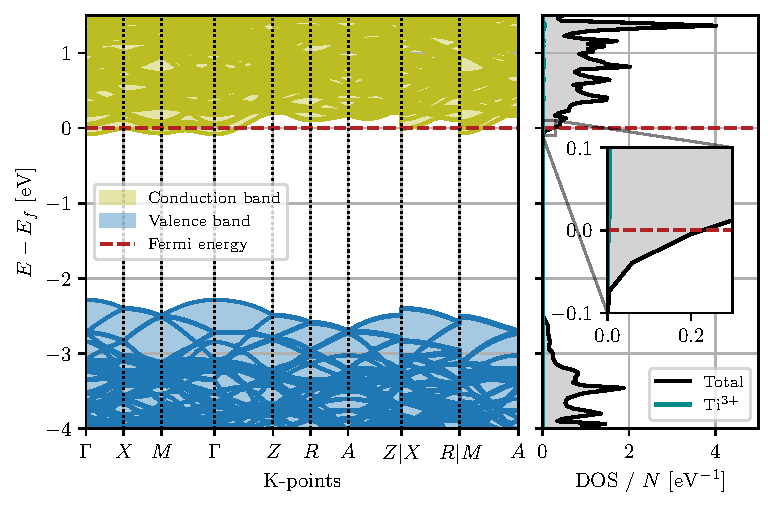
\includegraphics[width=\textwidth]{figures/deloc}
        %%% Creator: Matplotlib, PGF backend
%%
%% To include the figure in your LaTeX document, write
%%   \input{<filename>.pgf}
%%
%% Make sure the required packages are loaded in your preamble
%%   \usepackage{pgf}
%%
%% Also ensure that all the required font packages are loaded; for instance,
%% the lmodern package is sometimes necessary when using math font.
%%   \usepackage{lmodern}
%%
%% Figures using additional raster images can only be included by \input if
%% they are in the same directory as the main LaTeX file. For loading figures
%% from other directories you can use the `import` package
%%   \usepackage{import}
%%
%% and then include the figures with
%%   \import{<path to file>}{<filename>.pgf}
%%
%% Matplotlib used the following preamble
%%   \usepackage{fontspec}
%%   \setmainfont{DejaVuSerif.ttf}[Path=\detokenize{/usr/share/matplotlib/mpl-data/fonts/ttf/}]
%%   \setsansfont{DejaVuSans.ttf}[Path=\detokenize{/usr/share/matplotlib/mpl-data/fonts/ttf/}]
%%   \setmonofont{DejaVuSansMono.ttf}[Path=\detokenize{/usr/share/matplotlib/mpl-data/fonts/ttf/}]
%%
\begingroup%
\makeatletter%
\begin{pgfpicture}%
\pgfpathrectangle{\pgfpointorigin}{\pgfqpoint{5.149877in}{3.380212in}}%
\pgfusepath{use as bounding box, clip}%
\begin{pgfscope}%
\pgfsetbuttcap%
\pgfsetmiterjoin%
\definecolor{currentfill}{rgb}{1.000000,1.000000,1.000000}%
\pgfsetfillcolor{currentfill}%
\pgfsetlinewidth{0.000000pt}%
\definecolor{currentstroke}{rgb}{1.000000,1.000000,1.000000}%
\pgfsetstrokecolor{currentstroke}%
\pgfsetdash{}{0pt}%
\pgfpathmoveto{\pgfqpoint{0.000000in}{0.000000in}}%
\pgfpathlineto{\pgfqpoint{5.149877in}{0.000000in}}%
\pgfpathlineto{\pgfqpoint{5.149877in}{3.380212in}}%
\pgfpathlineto{\pgfqpoint{0.000000in}{3.380212in}}%
\pgfpathlineto{\pgfqpoint{0.000000in}{0.000000in}}%
\pgfpathclose%
\pgfusepath{fill}%
\end{pgfscope}%
\begin{pgfscope}%
\pgfsetbuttcap%
\pgfsetmiterjoin%
\definecolor{currentfill}{rgb}{1.000000,1.000000,1.000000}%
\pgfsetfillcolor{currentfill}%
\pgfsetlinewidth{0.000000pt}%
\definecolor{currentstroke}{rgb}{0.000000,0.000000,0.000000}%
\pgfsetstrokecolor{currentstroke}%
\pgfsetstrokeopacity{0.000000}%
\pgfsetdash{}{0pt}%
\pgfpathmoveto{\pgfqpoint{0.564660in}{0.526079in}}%
\pgfpathlineto{\pgfqpoint{3.446727in}{0.526079in}}%
\pgfpathlineto{\pgfqpoint{3.446727in}{3.280212in}}%
\pgfpathlineto{\pgfqpoint{0.564660in}{3.280212in}}%
\pgfpathlineto{\pgfqpoint{0.564660in}{0.526079in}}%
\pgfpathclose%
\pgfusepath{fill}%
\end{pgfscope}%
\begin{pgfscope}%
\pgfpathrectangle{\pgfqpoint{0.564660in}{0.526079in}}{\pgfqpoint{2.882067in}{2.754132in}}%
\pgfusepath{clip}%
\pgfsetbuttcap%
\pgfsetroundjoin%
\definecolor{currentfill}{rgb}{0.737255,0.741176,0.133333}%
\pgfsetfillcolor{currentfill}%
\pgfsetfillopacity{0.400000}%
\pgfsetlinewidth{1.003750pt}%
\definecolor{currentstroke}{rgb}{0.737255,0.741176,0.133333}%
\pgfsetstrokecolor{currentstroke}%
\pgfsetstrokeopacity{0.400000}%
\pgfsetdash{}{0pt}%
\pgfsys@defobject{currentmarker}{\pgfqpoint{0.564660in}{2.487272in}}{\pgfqpoint{3.446727in}{3.523026in}}{%
\pgfpathmoveto{\pgfqpoint{0.564660in}{3.450117in}}%
\pgfpathlineto{\pgfqpoint{0.564660in}{2.487272in}}%
\pgfpathlineto{\pgfqpoint{0.592560in}{2.488123in}}%
\pgfpathlineto{\pgfqpoint{0.620461in}{2.490677in}}%
\pgfpathlineto{\pgfqpoint{0.648251in}{2.494733in}}%
\pgfpathlineto{\pgfqpoint{0.676151in}{2.500041in}}%
\pgfpathlineto{\pgfqpoint{0.704051in}{2.506251in}}%
\pgfpathlineto{\pgfqpoint{0.731952in}{2.512710in}}%
\pgfpathlineto{\pgfqpoint{0.759852in}{2.518669in}}%
\pgfpathlineto{\pgfqpoint{0.787752in}{2.523026in}}%
\pgfpathlineto{\pgfqpoint{0.815542in}{2.524678in}}%
\pgfpathlineto{\pgfqpoint{0.815542in}{2.524678in}}%
\pgfpathlineto{\pgfqpoint{0.843442in}{2.523526in}}%
\pgfpathlineto{\pgfqpoint{0.871343in}{2.520372in}}%
\pgfpathlineto{\pgfqpoint{0.899243in}{2.515765in}}%
\pgfpathlineto{\pgfqpoint{0.927143in}{2.510357in}}%
\pgfpathlineto{\pgfqpoint{0.955043in}{2.504898in}}%
\pgfpathlineto{\pgfqpoint{0.982833in}{2.500041in}}%
\pgfpathlineto{\pgfqpoint{1.010734in}{2.496185in}}%
\pgfpathlineto{\pgfqpoint{1.038634in}{2.493782in}}%
\pgfpathlineto{\pgfqpoint{1.066534in}{2.492931in}}%
\pgfpathlineto{\pgfqpoint{1.066534in}{2.492931in}}%
\pgfpathlineto{\pgfqpoint{1.105968in}{2.495985in}}%
\pgfpathlineto{\pgfqpoint{1.145401in}{2.503797in}}%
\pgfpathlineto{\pgfqpoint{1.184835in}{2.511558in}}%
\pgfpathlineto{\pgfqpoint{1.224269in}{2.514112in}}%
\pgfpathlineto{\pgfqpoint{1.263703in}{2.511458in}}%
\pgfpathlineto{\pgfqpoint{1.303136in}{2.504949in}}%
\pgfpathlineto{\pgfqpoint{1.342570in}{2.496686in}}%
\pgfpathlineto{\pgfqpoint{1.382004in}{2.489876in}}%
\pgfpathlineto{\pgfqpoint{1.421438in}{2.487272in}}%
\pgfpathlineto{\pgfqpoint{1.421438in}{2.487272in}}%
\pgfpathlineto{\pgfqpoint{1.464716in}{2.490577in}}%
\pgfpathlineto{\pgfqpoint{1.507994in}{2.500292in}}%
\pgfpathlineto{\pgfqpoint{1.551272in}{2.515564in}}%
\pgfpathlineto{\pgfqpoint{1.594550in}{2.535294in}}%
\pgfpathlineto{\pgfqpoint{1.637829in}{2.558078in}}%
\pgfpathlineto{\pgfqpoint{1.681107in}{2.582164in}}%
\pgfpathlineto{\pgfqpoint{1.724385in}{2.605049in}}%
\pgfpathlineto{\pgfqpoint{1.767663in}{2.622625in}}%
\pgfpathlineto{\pgfqpoint{1.810942in}{2.629535in}}%
\pgfpathlineto{\pgfqpoint{1.810942in}{2.629535in}}%
\pgfpathlineto{\pgfqpoint{1.838842in}{2.629886in}}%
\pgfpathlineto{\pgfqpoint{1.866742in}{2.630837in}}%
\pgfpathlineto{\pgfqpoint{1.894532in}{2.628484in}}%
\pgfpathlineto{\pgfqpoint{1.922433in}{2.617367in}}%
\pgfpathlineto{\pgfqpoint{1.950333in}{2.605549in}}%
\pgfpathlineto{\pgfqpoint{1.978233in}{2.595084in}}%
\pgfpathlineto{\pgfqpoint{2.006133in}{2.587022in}}%
\pgfpathlineto{\pgfqpoint{2.033923in}{2.581964in}}%
\pgfpathlineto{\pgfqpoint{2.061824in}{2.580262in}}%
\pgfpathlineto{\pgfqpoint{2.061824in}{2.580262in}}%
\pgfpathlineto{\pgfqpoint{2.089724in}{2.580913in}}%
\pgfpathlineto{\pgfqpoint{2.117624in}{2.582765in}}%
\pgfpathlineto{\pgfqpoint{2.145524in}{2.585820in}}%
\pgfpathlineto{\pgfqpoint{2.173424in}{2.589826in}}%
\pgfpathlineto{\pgfqpoint{2.201215in}{2.594583in}}%
\pgfpathlineto{\pgfqpoint{2.229115in}{2.599791in}}%
\pgfpathlineto{\pgfqpoint{2.257015in}{2.605049in}}%
\pgfpathlineto{\pgfqpoint{2.284915in}{2.609606in}}%
\pgfpathlineto{\pgfqpoint{2.312815in}{2.611609in}}%
\pgfpathlineto{\pgfqpoint{2.312815in}{2.611609in}}%
\pgfpathlineto{\pgfqpoint{2.352249in}{2.604648in}}%
\pgfpathlineto{\pgfqpoint{2.391683in}{2.594984in}}%
\pgfpathlineto{\pgfqpoint{2.431117in}{2.590176in}}%
\pgfpathlineto{\pgfqpoint{2.470550in}{2.591679in}}%
\pgfpathlineto{\pgfqpoint{2.509984in}{2.599390in}}%
\pgfpathlineto{\pgfqpoint{2.549418in}{2.612109in}}%
\pgfpathlineto{\pgfqpoint{2.588851in}{2.626831in}}%
\pgfpathlineto{\pgfqpoint{2.628285in}{2.631188in}}%
\pgfpathlineto{\pgfqpoint{2.667609in}{2.629535in}}%
\pgfpathlineto{\pgfqpoint{2.667609in}{2.524678in}}%
\pgfpathlineto{\pgfqpoint{2.710997in}{2.527683in}}%
\pgfpathlineto{\pgfqpoint{2.754275in}{2.536546in}}%
\pgfpathlineto{\pgfqpoint{2.797554in}{2.550417in}}%
\pgfpathlineto{\pgfqpoint{2.840832in}{2.568143in}}%
\pgfpathlineto{\pgfqpoint{2.884110in}{2.587573in}}%
\pgfpathlineto{\pgfqpoint{2.927388in}{2.599741in}}%
\pgfpathlineto{\pgfqpoint{2.970667in}{2.589275in}}%
\pgfpathlineto{\pgfqpoint{3.013945in}{2.582565in}}%
\pgfpathlineto{\pgfqpoint{3.057223in}{2.580262in}}%
\pgfpathlineto{\pgfqpoint{3.057223in}{2.492931in}}%
\pgfpathlineto{\pgfqpoint{3.100501in}{2.496185in}}%
\pgfpathlineto{\pgfqpoint{3.143780in}{2.505650in}}%
\pgfpathlineto{\pgfqpoint{3.187058in}{2.520722in}}%
\pgfpathlineto{\pgfqpoint{3.230336in}{2.540252in}}%
\pgfpathlineto{\pgfqpoint{3.273614in}{2.562685in}}%
\pgfpathlineto{\pgfqpoint{3.316892in}{2.585970in}}%
\pgfpathlineto{\pgfqpoint{3.360171in}{2.606751in}}%
\pgfpathlineto{\pgfqpoint{3.403449in}{2.613361in}}%
\pgfpathlineto{\pgfqpoint{3.446727in}{2.611609in}}%
\pgfpathlineto{\pgfqpoint{3.446727in}{3.405400in}}%
\pgfpathlineto{\pgfqpoint{3.446727in}{3.405400in}}%
\pgfpathlineto{\pgfqpoint{3.403449in}{3.417968in}}%
\pgfpathlineto{\pgfqpoint{3.360171in}{3.422225in}}%
\pgfpathlineto{\pgfqpoint{3.316892in}{3.415915in}}%
\pgfpathlineto{\pgfqpoint{3.273614in}{3.420322in}}%
\pgfpathlineto{\pgfqpoint{3.230336in}{3.426732in}}%
\pgfpathlineto{\pgfqpoint{3.187058in}{3.430537in}}%
\pgfpathlineto{\pgfqpoint{3.143780in}{3.438299in}}%
\pgfpathlineto{\pgfqpoint{3.100501in}{3.447212in}}%
\pgfpathlineto{\pgfqpoint{3.057223in}{3.457678in}}%
\pgfpathlineto{\pgfqpoint{3.057223in}{3.452871in}}%
\pgfpathlineto{\pgfqpoint{3.013945in}{3.446111in}}%
\pgfpathlineto{\pgfqpoint{2.970667in}{3.450768in}}%
\pgfpathlineto{\pgfqpoint{2.927388in}{3.450217in}}%
\pgfpathlineto{\pgfqpoint{2.884110in}{3.445960in}}%
\pgfpathlineto{\pgfqpoint{2.840832in}{3.432340in}}%
\pgfpathlineto{\pgfqpoint{2.797554in}{3.415565in}}%
\pgfpathlineto{\pgfqpoint{2.754275in}{3.400843in}}%
\pgfpathlineto{\pgfqpoint{2.710997in}{3.387673in}}%
\pgfpathlineto{\pgfqpoint{2.667609in}{3.389676in}}%
\pgfpathlineto{\pgfqpoint{2.667609in}{3.521023in}}%
\pgfpathlineto{\pgfqpoint{2.628285in}{3.505950in}}%
\pgfpathlineto{\pgfqpoint{2.588851in}{3.481914in}}%
\pgfpathlineto{\pgfqpoint{2.549418in}{3.456076in}}%
\pgfpathlineto{\pgfqpoint{2.509984in}{3.425179in}}%
\pgfpathlineto{\pgfqpoint{2.470550in}{3.410557in}}%
\pgfpathlineto{\pgfqpoint{2.431117in}{3.407202in}}%
\pgfpathlineto{\pgfqpoint{2.391683in}{3.405199in}}%
\pgfpathlineto{\pgfqpoint{2.352249in}{3.406852in}}%
\pgfpathlineto{\pgfqpoint{2.312815in}{3.405400in}}%
\pgfpathlineto{\pgfqpoint{2.312815in}{3.405400in}}%
\pgfpathlineto{\pgfqpoint{2.284915in}{3.407052in}}%
\pgfpathlineto{\pgfqpoint{2.257015in}{3.406752in}}%
\pgfpathlineto{\pgfqpoint{2.229115in}{3.406752in}}%
\pgfpathlineto{\pgfqpoint{2.201215in}{3.406000in}}%
\pgfpathlineto{\pgfqpoint{2.173424in}{3.405900in}}%
\pgfpathlineto{\pgfqpoint{2.145524in}{3.407353in}}%
\pgfpathlineto{\pgfqpoint{2.117624in}{3.423877in}}%
\pgfpathlineto{\pgfqpoint{2.089724in}{3.441754in}}%
\pgfpathlineto{\pgfqpoint{2.061824in}{3.452871in}}%
\pgfpathlineto{\pgfqpoint{2.061824in}{3.452871in}}%
\pgfpathlineto{\pgfqpoint{2.033923in}{3.447863in}}%
\pgfpathlineto{\pgfqpoint{2.006133in}{3.450367in}}%
\pgfpathlineto{\pgfqpoint{1.978233in}{3.453472in}}%
\pgfpathlineto{\pgfqpoint{1.950333in}{3.451168in}}%
\pgfpathlineto{\pgfqpoint{1.922433in}{3.482515in}}%
\pgfpathlineto{\pgfqpoint{1.894532in}{3.492180in}}%
\pgfpathlineto{\pgfqpoint{1.866742in}{3.514563in}}%
\pgfpathlineto{\pgfqpoint{1.838842in}{3.514313in}}%
\pgfpathlineto{\pgfqpoint{1.810942in}{3.521023in}}%
\pgfpathlineto{\pgfqpoint{1.810942in}{3.521023in}}%
\pgfpathlineto{\pgfqpoint{1.767663in}{3.523026in}}%
\pgfpathlineto{\pgfqpoint{1.724385in}{3.513562in}}%
\pgfpathlineto{\pgfqpoint{1.681107in}{3.520122in}}%
\pgfpathlineto{\pgfqpoint{1.637829in}{3.507603in}}%
\pgfpathlineto{\pgfqpoint{1.594550in}{3.510658in}}%
\pgfpathlineto{\pgfqpoint{1.551272in}{3.502095in}}%
\pgfpathlineto{\pgfqpoint{1.507994in}{3.483116in}}%
\pgfpathlineto{\pgfqpoint{1.464716in}{3.472450in}}%
\pgfpathlineto{\pgfqpoint{1.421438in}{3.453622in}}%
\pgfpathlineto{\pgfqpoint{1.421438in}{3.453622in}}%
\pgfpathlineto{\pgfqpoint{1.382004in}{3.444008in}}%
\pgfpathlineto{\pgfqpoint{1.342570in}{3.429686in}}%
\pgfpathlineto{\pgfqpoint{1.303136in}{3.421774in}}%
\pgfpathlineto{\pgfqpoint{1.263703in}{3.409756in}}%
\pgfpathlineto{\pgfqpoint{1.224269in}{3.431389in}}%
\pgfpathlineto{\pgfqpoint{1.184835in}{3.437898in}}%
\pgfpathlineto{\pgfqpoint{1.145401in}{3.445860in}}%
\pgfpathlineto{\pgfqpoint{1.105968in}{3.450067in}}%
\pgfpathlineto{\pgfqpoint{1.066534in}{3.457678in}}%
\pgfpathlineto{\pgfqpoint{1.066534in}{3.457678in}}%
\pgfpathlineto{\pgfqpoint{1.038634in}{3.452671in}}%
\pgfpathlineto{\pgfqpoint{1.010734in}{3.452821in}}%
\pgfpathlineto{\pgfqpoint{0.982833in}{3.440352in}}%
\pgfpathlineto{\pgfqpoint{0.955043in}{3.428334in}}%
\pgfpathlineto{\pgfqpoint{0.927143in}{3.418970in}}%
\pgfpathlineto{\pgfqpoint{0.899243in}{3.412811in}}%
\pgfpathlineto{\pgfqpoint{0.871343in}{3.404699in}}%
\pgfpathlineto{\pgfqpoint{0.843442in}{3.398189in}}%
\pgfpathlineto{\pgfqpoint{0.815542in}{3.389676in}}%
\pgfpathlineto{\pgfqpoint{0.815542in}{3.389676in}}%
\pgfpathlineto{\pgfqpoint{0.787752in}{3.390627in}}%
\pgfpathlineto{\pgfqpoint{0.759852in}{3.398439in}}%
\pgfpathlineto{\pgfqpoint{0.731952in}{3.415264in}}%
\pgfpathlineto{\pgfqpoint{0.704051in}{3.426281in}}%
\pgfpathlineto{\pgfqpoint{0.676151in}{3.482265in}}%
\pgfpathlineto{\pgfqpoint{0.648251in}{3.466842in}}%
\pgfpathlineto{\pgfqpoint{0.620461in}{3.448014in}}%
\pgfpathlineto{\pgfqpoint{0.592560in}{3.460432in}}%
\pgfpathlineto{\pgfqpoint{0.564660in}{3.450117in}}%
\pgfpathlineto{\pgfqpoint{0.564660in}{3.450117in}}%
\pgfpathclose%
\pgfusepath{stroke,fill}%
}%
\begin{pgfscope}%
\pgfsys@transformshift{0.000000in}{0.000000in}%
\pgfsys@useobject{currentmarker}{}%
\end{pgfscope}%
\end{pgfscope}%
\begin{pgfscope}%
\pgfpathrectangle{\pgfqpoint{0.564660in}{0.526079in}}{\pgfqpoint{2.882067in}{2.754132in}}%
\pgfusepath{clip}%
\pgfsetbuttcap%
\pgfsetroundjoin%
\definecolor{currentfill}{rgb}{0.121569,0.466667,0.705882}%
\pgfsetfillcolor{currentfill}%
\pgfsetfillopacity{0.400000}%
\pgfsetlinewidth{1.003750pt}%
\definecolor{currentstroke}{rgb}{0.121569,0.466667,0.705882}%
\pgfsetstrokecolor{currentstroke}%
\pgfsetstrokeopacity{0.400000}%
\pgfsetdash{}{0pt}%
\pgfpathmoveto{\pgfqpoint{0.564660in}{1.384317in}}%
\pgfpathlineto{\pgfqpoint{0.564660in}{-27.621453in}}%
\pgfpathlineto{\pgfqpoint{0.592560in}{-27.621403in}}%
\pgfpathlineto{\pgfqpoint{0.620461in}{-27.621403in}}%
\pgfpathlineto{\pgfqpoint{0.648251in}{-27.621353in}}%
\pgfpathlineto{\pgfqpoint{0.676151in}{-27.621353in}}%
\pgfpathlineto{\pgfqpoint{0.704051in}{-27.621303in}}%
\pgfpathlineto{\pgfqpoint{0.731952in}{-27.621203in}}%
\pgfpathlineto{\pgfqpoint{0.759852in}{-27.621153in}}%
\pgfpathlineto{\pgfqpoint{0.787752in}{-27.621053in}}%
\pgfpathlineto{\pgfqpoint{0.815542in}{-27.621003in}}%
\pgfpathlineto{\pgfqpoint{0.815542in}{-27.621003in}}%
\pgfpathlineto{\pgfqpoint{0.843442in}{-27.621003in}}%
\pgfpathlineto{\pgfqpoint{0.871343in}{-27.620953in}}%
\pgfpathlineto{\pgfqpoint{0.899243in}{-27.620953in}}%
\pgfpathlineto{\pgfqpoint{0.927143in}{-27.620902in}}%
\pgfpathlineto{\pgfqpoint{0.955043in}{-27.620902in}}%
\pgfpathlineto{\pgfqpoint{0.982833in}{-27.620852in}}%
\pgfpathlineto{\pgfqpoint{1.010734in}{-27.620802in}}%
\pgfpathlineto{\pgfqpoint{1.038634in}{-27.620752in}}%
\pgfpathlineto{\pgfqpoint{1.066534in}{-27.620752in}}%
\pgfpathlineto{\pgfqpoint{1.066534in}{-27.620752in}}%
\pgfpathlineto{\pgfqpoint{1.105968in}{-27.620802in}}%
\pgfpathlineto{\pgfqpoint{1.145401in}{-27.620902in}}%
\pgfpathlineto{\pgfqpoint{1.184835in}{-27.621053in}}%
\pgfpathlineto{\pgfqpoint{1.224269in}{-27.621153in}}%
\pgfpathlineto{\pgfqpoint{1.263703in}{-27.621253in}}%
\pgfpathlineto{\pgfqpoint{1.303136in}{-27.621303in}}%
\pgfpathlineto{\pgfqpoint{1.342570in}{-27.621403in}}%
\pgfpathlineto{\pgfqpoint{1.382004in}{-27.621403in}}%
\pgfpathlineto{\pgfqpoint{1.421438in}{-27.621453in}}%
\pgfpathlineto{\pgfqpoint{1.421438in}{-27.621453in}}%
\pgfpathlineto{\pgfqpoint{1.464716in}{-27.621353in}}%
\pgfpathlineto{\pgfqpoint{1.507994in}{-27.621153in}}%
\pgfpathlineto{\pgfqpoint{1.551272in}{-27.620802in}}%
\pgfpathlineto{\pgfqpoint{1.594550in}{-27.620302in}}%
\pgfpathlineto{\pgfqpoint{1.637829in}{-27.619701in}}%
\pgfpathlineto{\pgfqpoint{1.681107in}{-27.618950in}}%
\pgfpathlineto{\pgfqpoint{1.724385in}{-27.618098in}}%
\pgfpathlineto{\pgfqpoint{1.767663in}{-27.617197in}}%
\pgfpathlineto{\pgfqpoint{1.810942in}{-27.616396in}}%
\pgfpathlineto{\pgfqpoint{1.810942in}{-27.616396in}}%
\pgfpathlineto{\pgfqpoint{1.838842in}{-27.616396in}}%
\pgfpathlineto{\pgfqpoint{1.866742in}{-27.616396in}}%
\pgfpathlineto{\pgfqpoint{1.894532in}{-27.616346in}}%
\pgfpathlineto{\pgfqpoint{1.922433in}{-27.616346in}}%
\pgfpathlineto{\pgfqpoint{1.950333in}{-27.616296in}}%
\pgfpathlineto{\pgfqpoint{1.978233in}{-27.616296in}}%
\pgfpathlineto{\pgfqpoint{2.006133in}{-27.616245in}}%
\pgfpathlineto{\pgfqpoint{2.033923in}{-27.616195in}}%
\pgfpathlineto{\pgfqpoint{2.061824in}{-27.616195in}}%
\pgfpathlineto{\pgfqpoint{2.061824in}{-27.616195in}}%
\pgfpathlineto{\pgfqpoint{2.089724in}{-27.616195in}}%
\pgfpathlineto{\pgfqpoint{2.117624in}{-27.616195in}}%
\pgfpathlineto{\pgfqpoint{2.145524in}{-27.616145in}}%
\pgfpathlineto{\pgfqpoint{2.173424in}{-27.616145in}}%
\pgfpathlineto{\pgfqpoint{2.201215in}{-27.616145in}}%
\pgfpathlineto{\pgfqpoint{2.229115in}{-27.616095in}}%
\pgfpathlineto{\pgfqpoint{2.257015in}{-27.616095in}}%
\pgfpathlineto{\pgfqpoint{2.284915in}{-27.616095in}}%
\pgfpathlineto{\pgfqpoint{2.312815in}{-27.616045in}}%
\pgfpathlineto{\pgfqpoint{2.312815in}{-27.616045in}}%
\pgfpathlineto{\pgfqpoint{2.352249in}{-27.616095in}}%
\pgfpathlineto{\pgfqpoint{2.391683in}{-27.616145in}}%
\pgfpathlineto{\pgfqpoint{2.431117in}{-27.616195in}}%
\pgfpathlineto{\pgfqpoint{2.470550in}{-27.616245in}}%
\pgfpathlineto{\pgfqpoint{2.509984in}{-27.616296in}}%
\pgfpathlineto{\pgfqpoint{2.549418in}{-27.616346in}}%
\pgfpathlineto{\pgfqpoint{2.588851in}{-27.616396in}}%
\pgfpathlineto{\pgfqpoint{2.628285in}{-27.616396in}}%
\pgfpathlineto{\pgfqpoint{2.667609in}{-27.616396in}}%
\pgfpathlineto{\pgfqpoint{2.667609in}{-27.621003in}}%
\pgfpathlineto{\pgfqpoint{2.710997in}{-27.620902in}}%
\pgfpathlineto{\pgfqpoint{2.754275in}{-27.620702in}}%
\pgfpathlineto{\pgfqpoint{2.797554in}{-27.620352in}}%
\pgfpathlineto{\pgfqpoint{2.840832in}{-27.619901in}}%
\pgfpathlineto{\pgfqpoint{2.884110in}{-27.619300in}}%
\pgfpathlineto{\pgfqpoint{2.927388in}{-27.618549in}}%
\pgfpathlineto{\pgfqpoint{2.970667in}{-27.617748in}}%
\pgfpathlineto{\pgfqpoint{3.013945in}{-27.616846in}}%
\pgfpathlineto{\pgfqpoint{3.057223in}{-27.616195in}}%
\pgfpathlineto{\pgfqpoint{3.057223in}{-27.620752in}}%
\pgfpathlineto{\pgfqpoint{3.100501in}{-27.620702in}}%
\pgfpathlineto{\pgfqpoint{3.143780in}{-27.620452in}}%
\pgfpathlineto{\pgfqpoint{3.187058in}{-27.620151in}}%
\pgfpathlineto{\pgfqpoint{3.230336in}{-27.619651in}}%
\pgfpathlineto{\pgfqpoint{3.273614in}{-27.619050in}}%
\pgfpathlineto{\pgfqpoint{3.316892in}{-27.618349in}}%
\pgfpathlineto{\pgfqpoint{3.360171in}{-27.617547in}}%
\pgfpathlineto{\pgfqpoint{3.403449in}{-27.616696in}}%
\pgfpathlineto{\pgfqpoint{3.446727in}{-27.616045in}}%
\pgfpathlineto{\pgfqpoint{3.446727in}{1.180211in}}%
\pgfpathlineto{\pgfqpoint{3.446727in}{1.180211in}}%
\pgfpathlineto{\pgfqpoint{3.403449in}{1.193080in}}%
\pgfpathlineto{\pgfqpoint{3.360171in}{1.206801in}}%
\pgfpathlineto{\pgfqpoint{3.316892in}{1.220972in}}%
\pgfpathlineto{\pgfqpoint{3.273614in}{1.235243in}}%
\pgfpathlineto{\pgfqpoint{3.230336in}{1.248864in}}%
\pgfpathlineto{\pgfqpoint{3.187058in}{1.260882in}}%
\pgfpathlineto{\pgfqpoint{3.143780in}{1.270246in}}%
\pgfpathlineto{\pgfqpoint{3.100501in}{1.276255in}}%
\pgfpathlineto{\pgfqpoint{3.057223in}{1.278308in}}%
\pgfpathlineto{\pgfqpoint{3.057223in}{1.236796in}}%
\pgfpathlineto{\pgfqpoint{3.013945in}{1.255874in}}%
\pgfpathlineto{\pgfqpoint{2.970667in}{1.273100in}}%
\pgfpathlineto{\pgfqpoint{2.927388in}{1.288173in}}%
\pgfpathlineto{\pgfqpoint{2.884110in}{1.301092in}}%
\pgfpathlineto{\pgfqpoint{2.840832in}{1.311658in}}%
\pgfpathlineto{\pgfqpoint{2.797554in}{1.319770in}}%
\pgfpathlineto{\pgfqpoint{2.754275in}{1.325479in}}%
\pgfpathlineto{\pgfqpoint{2.710997in}{1.328784in}}%
\pgfpathlineto{\pgfqpoint{2.667609in}{1.329885in}}%
\pgfpathlineto{\pgfqpoint{2.667609in}{1.284818in}}%
\pgfpathlineto{\pgfqpoint{2.628285in}{1.283616in}}%
\pgfpathlineto{\pgfqpoint{2.588851in}{1.279961in}}%
\pgfpathlineto{\pgfqpoint{2.549418in}{1.273801in}}%
\pgfpathlineto{\pgfqpoint{2.509984in}{1.265038in}}%
\pgfpathlineto{\pgfqpoint{2.470550in}{1.253521in}}%
\pgfpathlineto{\pgfqpoint{2.431117in}{1.239199in}}%
\pgfpathlineto{\pgfqpoint{2.391683in}{1.221974in}}%
\pgfpathlineto{\pgfqpoint{2.352249in}{1.201743in}}%
\pgfpathlineto{\pgfqpoint{2.312815in}{1.180211in}}%
\pgfpathlineto{\pgfqpoint{2.312815in}{1.180211in}}%
\pgfpathlineto{\pgfqpoint{2.284915in}{1.190977in}}%
\pgfpathlineto{\pgfqpoint{2.257015in}{1.201543in}}%
\pgfpathlineto{\pgfqpoint{2.229115in}{1.210857in}}%
\pgfpathlineto{\pgfqpoint{2.201215in}{1.218769in}}%
\pgfpathlineto{\pgfqpoint{2.173424in}{1.225279in}}%
\pgfpathlineto{\pgfqpoint{2.145524in}{1.230286in}}%
\pgfpathlineto{\pgfqpoint{2.117624in}{1.233891in}}%
\pgfpathlineto{\pgfqpoint{2.089724in}{1.236045in}}%
\pgfpathlineto{\pgfqpoint{2.061824in}{1.236796in}}%
\pgfpathlineto{\pgfqpoint{2.061824in}{1.236796in}}%
\pgfpathlineto{\pgfqpoint{2.033923in}{1.246310in}}%
\pgfpathlineto{\pgfqpoint{2.006133in}{1.255173in}}%
\pgfpathlineto{\pgfqpoint{1.978233in}{1.262985in}}%
\pgfpathlineto{\pgfqpoint{1.950333in}{1.269645in}}%
\pgfpathlineto{\pgfqpoint{1.922433in}{1.275153in}}%
\pgfpathlineto{\pgfqpoint{1.894532in}{1.279360in}}%
\pgfpathlineto{\pgfqpoint{1.866742in}{1.282414in}}%
\pgfpathlineto{\pgfqpoint{1.838842in}{1.284217in}}%
\pgfpathlineto{\pgfqpoint{1.810942in}{1.284818in}}%
\pgfpathlineto{\pgfqpoint{1.810942in}{1.284818in}}%
\pgfpathlineto{\pgfqpoint{1.767663in}{1.305899in}}%
\pgfpathlineto{\pgfqpoint{1.724385in}{1.326130in}}%
\pgfpathlineto{\pgfqpoint{1.681107in}{1.342855in}}%
\pgfpathlineto{\pgfqpoint{1.637829in}{1.356325in}}%
\pgfpathlineto{\pgfqpoint{1.594550in}{1.366841in}}%
\pgfpathlineto{\pgfqpoint{1.551272in}{1.374653in}}%
\pgfpathlineto{\pgfqpoint{1.507994in}{1.380111in}}%
\pgfpathlineto{\pgfqpoint{1.464716in}{1.383266in}}%
\pgfpathlineto{\pgfqpoint{1.421438in}{1.384317in}}%
\pgfpathlineto{\pgfqpoint{1.421438in}{1.384317in}}%
\pgfpathlineto{\pgfqpoint{1.382004in}{1.382965in}}%
\pgfpathlineto{\pgfqpoint{1.342570in}{1.378909in}}%
\pgfpathlineto{\pgfqpoint{1.303136in}{1.372149in}}%
\pgfpathlineto{\pgfqpoint{1.263703in}{1.362685in}}%
\pgfpathlineto{\pgfqpoint{1.224269in}{1.350567in}}%
\pgfpathlineto{\pgfqpoint{1.184835in}{1.335794in}}%
\pgfpathlineto{\pgfqpoint{1.145401in}{1.318468in}}%
\pgfpathlineto{\pgfqpoint{1.105968in}{1.298789in}}%
\pgfpathlineto{\pgfqpoint{1.066534in}{1.278308in}}%
\pgfpathlineto{\pgfqpoint{1.066534in}{1.278308in}}%
\pgfpathlineto{\pgfqpoint{1.038634in}{1.289275in}}%
\pgfpathlineto{\pgfqpoint{1.010734in}{1.299089in}}%
\pgfpathlineto{\pgfqpoint{0.982833in}{1.307452in}}%
\pgfpathlineto{\pgfqpoint{0.955043in}{1.314412in}}%
\pgfpathlineto{\pgfqpoint{0.927143in}{1.320021in}}%
\pgfpathlineto{\pgfqpoint{0.899243in}{1.324377in}}%
\pgfpathlineto{\pgfqpoint{0.871343in}{1.327432in}}%
\pgfpathlineto{\pgfqpoint{0.843442in}{1.329285in}}%
\pgfpathlineto{\pgfqpoint{0.815542in}{1.329885in}}%
\pgfpathlineto{\pgfqpoint{0.815542in}{1.329885in}}%
\pgfpathlineto{\pgfqpoint{0.787752in}{1.339099in}}%
\pgfpathlineto{\pgfqpoint{0.759852in}{1.349665in}}%
\pgfpathlineto{\pgfqpoint{0.731952in}{1.358979in}}%
\pgfpathlineto{\pgfqpoint{0.704051in}{1.366841in}}%
\pgfpathlineto{\pgfqpoint{0.676151in}{1.373200in}}%
\pgfpathlineto{\pgfqpoint{0.648251in}{1.378108in}}%
\pgfpathlineto{\pgfqpoint{0.620461in}{1.381613in}}%
\pgfpathlineto{\pgfqpoint{0.592560in}{1.383666in}}%
\pgfpathlineto{\pgfqpoint{0.564660in}{1.384317in}}%
\pgfpathlineto{\pgfqpoint{0.564660in}{1.384317in}}%
\pgfpathclose%
\pgfusepath{stroke,fill}%
\end{pgfscope}%
\begin{pgfscope}%
\pgfpathrectangle{\pgfqpoint{0.564660in}{0.526079in}}{\pgfqpoint{2.882067in}{2.754132in}}%
\pgfusepath{clip}%
\pgfsetrectcap%
\pgfsetroundjoin%
\pgfsetlinewidth{0.803000pt}%
\definecolor{currentstroke}{rgb}{0.690196,0.690196,0.690196}%
\pgfsetstrokecolor{currentstroke}%
\pgfsetdash{}{0pt}%
\pgfpathmoveto{\pgfqpoint{0.564660in}{0.526079in}}%
\pgfpathlineto{\pgfqpoint{0.564660in}{3.280212in}}%
\pgfusepath{stroke}%
\end{pgfscope}%
\begin{pgfscope}%
\pgfsetbuttcap%
\pgfsetroundjoin%
\definecolor{currentfill}{rgb}{0.000000,0.000000,0.000000}%
\pgfsetfillcolor{currentfill}%
\pgfsetlinewidth{0.803000pt}%
\definecolor{currentstroke}{rgb}{0.000000,0.000000,0.000000}%
\pgfsetstrokecolor{currentstroke}%
\pgfsetdash{}{0pt}%
\pgfsys@defobject{currentmarker}{\pgfqpoint{0.000000in}{-0.048611in}}{\pgfqpoint{0.000000in}{0.000000in}}{%
\pgfpathmoveto{\pgfqpoint{0.000000in}{0.000000in}}%
\pgfpathlineto{\pgfqpoint{0.000000in}{-0.048611in}}%
\pgfusepath{stroke,fill}%
}%
\begin{pgfscope}%
\pgfsys@transformshift{0.564660in}{0.526079in}%
\pgfsys@useobject{currentmarker}{}%
\end{pgfscope}%
\end{pgfscope}%
\begin{pgfscope}%
\definecolor{textcolor}{rgb}{0.000000,0.000000,0.000000}%
\pgfsetstrokecolor{textcolor}%
\pgfsetfillcolor{textcolor}%
\pgftext[x=0.564660in,y=0.428857in,,top]{\color{textcolor}\rmfamily\fontsize{10.000000}{12.000000}\selectfont \(\displaystyle \Gamma\)}%
\end{pgfscope}%
\begin{pgfscope}%
\pgfpathrectangle{\pgfqpoint{0.564660in}{0.526079in}}{\pgfqpoint{2.882067in}{2.754132in}}%
\pgfusepath{clip}%
\pgfsetrectcap%
\pgfsetroundjoin%
\pgfsetlinewidth{0.803000pt}%
\definecolor{currentstroke}{rgb}{0.690196,0.690196,0.690196}%
\pgfsetstrokecolor{currentstroke}%
\pgfsetdash{}{0pt}%
\pgfpathmoveto{\pgfqpoint{0.815542in}{0.526079in}}%
\pgfpathlineto{\pgfqpoint{0.815542in}{3.280212in}}%
\pgfusepath{stroke}%
\end{pgfscope}%
\begin{pgfscope}%
\pgfsetbuttcap%
\pgfsetroundjoin%
\definecolor{currentfill}{rgb}{0.000000,0.000000,0.000000}%
\pgfsetfillcolor{currentfill}%
\pgfsetlinewidth{0.803000pt}%
\definecolor{currentstroke}{rgb}{0.000000,0.000000,0.000000}%
\pgfsetstrokecolor{currentstroke}%
\pgfsetdash{}{0pt}%
\pgfsys@defobject{currentmarker}{\pgfqpoint{0.000000in}{-0.048611in}}{\pgfqpoint{0.000000in}{0.000000in}}{%
\pgfpathmoveto{\pgfqpoint{0.000000in}{0.000000in}}%
\pgfpathlineto{\pgfqpoint{0.000000in}{-0.048611in}}%
\pgfusepath{stroke,fill}%
}%
\begin{pgfscope}%
\pgfsys@transformshift{0.815542in}{0.526079in}%
\pgfsys@useobject{currentmarker}{}%
\end{pgfscope}%
\end{pgfscope}%
\begin{pgfscope}%
\definecolor{textcolor}{rgb}{0.000000,0.000000,0.000000}%
\pgfsetstrokecolor{textcolor}%
\pgfsetfillcolor{textcolor}%
\pgftext[x=0.815542in,y=0.428857in,,top]{\color{textcolor}\rmfamily\fontsize{10.000000}{12.000000}\selectfont \(\displaystyle X\)}%
\end{pgfscope}%
\begin{pgfscope}%
\pgfpathrectangle{\pgfqpoint{0.564660in}{0.526079in}}{\pgfqpoint{2.882067in}{2.754132in}}%
\pgfusepath{clip}%
\pgfsetrectcap%
\pgfsetroundjoin%
\pgfsetlinewidth{0.803000pt}%
\definecolor{currentstroke}{rgb}{0.690196,0.690196,0.690196}%
\pgfsetstrokecolor{currentstroke}%
\pgfsetdash{}{0pt}%
\pgfpathmoveto{\pgfqpoint{1.066534in}{0.526079in}}%
\pgfpathlineto{\pgfqpoint{1.066534in}{3.280212in}}%
\pgfusepath{stroke}%
\end{pgfscope}%
\begin{pgfscope}%
\pgfsetbuttcap%
\pgfsetroundjoin%
\definecolor{currentfill}{rgb}{0.000000,0.000000,0.000000}%
\pgfsetfillcolor{currentfill}%
\pgfsetlinewidth{0.803000pt}%
\definecolor{currentstroke}{rgb}{0.000000,0.000000,0.000000}%
\pgfsetstrokecolor{currentstroke}%
\pgfsetdash{}{0pt}%
\pgfsys@defobject{currentmarker}{\pgfqpoint{0.000000in}{-0.048611in}}{\pgfqpoint{0.000000in}{0.000000in}}{%
\pgfpathmoveto{\pgfqpoint{0.000000in}{0.000000in}}%
\pgfpathlineto{\pgfqpoint{0.000000in}{-0.048611in}}%
\pgfusepath{stroke,fill}%
}%
\begin{pgfscope}%
\pgfsys@transformshift{1.066534in}{0.526079in}%
\pgfsys@useobject{currentmarker}{}%
\end{pgfscope}%
\end{pgfscope}%
\begin{pgfscope}%
\definecolor{textcolor}{rgb}{0.000000,0.000000,0.000000}%
\pgfsetstrokecolor{textcolor}%
\pgfsetfillcolor{textcolor}%
\pgftext[x=1.066534in,y=0.428857in,,top]{\color{textcolor}\rmfamily\fontsize{10.000000}{12.000000}\selectfont \(\displaystyle M\)}%
\end{pgfscope}%
\begin{pgfscope}%
\pgfpathrectangle{\pgfqpoint{0.564660in}{0.526079in}}{\pgfqpoint{2.882067in}{2.754132in}}%
\pgfusepath{clip}%
\pgfsetrectcap%
\pgfsetroundjoin%
\pgfsetlinewidth{0.803000pt}%
\definecolor{currentstroke}{rgb}{0.690196,0.690196,0.690196}%
\pgfsetstrokecolor{currentstroke}%
\pgfsetdash{}{0pt}%
\pgfpathmoveto{\pgfqpoint{1.421438in}{0.526079in}}%
\pgfpathlineto{\pgfqpoint{1.421438in}{3.280212in}}%
\pgfusepath{stroke}%
\end{pgfscope}%
\begin{pgfscope}%
\pgfsetbuttcap%
\pgfsetroundjoin%
\definecolor{currentfill}{rgb}{0.000000,0.000000,0.000000}%
\pgfsetfillcolor{currentfill}%
\pgfsetlinewidth{0.803000pt}%
\definecolor{currentstroke}{rgb}{0.000000,0.000000,0.000000}%
\pgfsetstrokecolor{currentstroke}%
\pgfsetdash{}{0pt}%
\pgfsys@defobject{currentmarker}{\pgfqpoint{0.000000in}{-0.048611in}}{\pgfqpoint{0.000000in}{0.000000in}}{%
\pgfpathmoveto{\pgfqpoint{0.000000in}{0.000000in}}%
\pgfpathlineto{\pgfqpoint{0.000000in}{-0.048611in}}%
\pgfusepath{stroke,fill}%
}%
\begin{pgfscope}%
\pgfsys@transformshift{1.421438in}{0.526079in}%
\pgfsys@useobject{currentmarker}{}%
\end{pgfscope}%
\end{pgfscope}%
\begin{pgfscope}%
\definecolor{textcolor}{rgb}{0.000000,0.000000,0.000000}%
\pgfsetstrokecolor{textcolor}%
\pgfsetfillcolor{textcolor}%
\pgftext[x=1.421438in,y=0.428857in,,top]{\color{textcolor}\rmfamily\fontsize{10.000000}{12.000000}\selectfont \(\displaystyle \Gamma\)}%
\end{pgfscope}%
\begin{pgfscope}%
\pgfpathrectangle{\pgfqpoint{0.564660in}{0.526079in}}{\pgfqpoint{2.882067in}{2.754132in}}%
\pgfusepath{clip}%
\pgfsetrectcap%
\pgfsetroundjoin%
\pgfsetlinewidth{0.803000pt}%
\definecolor{currentstroke}{rgb}{0.690196,0.690196,0.690196}%
\pgfsetstrokecolor{currentstroke}%
\pgfsetdash{}{0pt}%
\pgfpathmoveto{\pgfqpoint{1.810942in}{0.526079in}}%
\pgfpathlineto{\pgfqpoint{1.810942in}{3.280212in}}%
\pgfusepath{stroke}%
\end{pgfscope}%
\begin{pgfscope}%
\pgfsetbuttcap%
\pgfsetroundjoin%
\definecolor{currentfill}{rgb}{0.000000,0.000000,0.000000}%
\pgfsetfillcolor{currentfill}%
\pgfsetlinewidth{0.803000pt}%
\definecolor{currentstroke}{rgb}{0.000000,0.000000,0.000000}%
\pgfsetstrokecolor{currentstroke}%
\pgfsetdash{}{0pt}%
\pgfsys@defobject{currentmarker}{\pgfqpoint{0.000000in}{-0.048611in}}{\pgfqpoint{0.000000in}{0.000000in}}{%
\pgfpathmoveto{\pgfqpoint{0.000000in}{0.000000in}}%
\pgfpathlineto{\pgfqpoint{0.000000in}{-0.048611in}}%
\pgfusepath{stroke,fill}%
}%
\begin{pgfscope}%
\pgfsys@transformshift{1.810942in}{0.526079in}%
\pgfsys@useobject{currentmarker}{}%
\end{pgfscope}%
\end{pgfscope}%
\begin{pgfscope}%
\definecolor{textcolor}{rgb}{0.000000,0.000000,0.000000}%
\pgfsetstrokecolor{textcolor}%
\pgfsetfillcolor{textcolor}%
\pgftext[x=1.810942in,y=0.428857in,,top]{\color{textcolor}\rmfamily\fontsize{10.000000}{12.000000}\selectfont \(\displaystyle Z\)}%
\end{pgfscope}%
\begin{pgfscope}%
\pgfpathrectangle{\pgfqpoint{0.564660in}{0.526079in}}{\pgfqpoint{2.882067in}{2.754132in}}%
\pgfusepath{clip}%
\pgfsetrectcap%
\pgfsetroundjoin%
\pgfsetlinewidth{0.803000pt}%
\definecolor{currentstroke}{rgb}{0.690196,0.690196,0.690196}%
\pgfsetstrokecolor{currentstroke}%
\pgfsetdash{}{0pt}%
\pgfpathmoveto{\pgfqpoint{2.061824in}{0.526079in}}%
\pgfpathlineto{\pgfqpoint{2.061824in}{3.280212in}}%
\pgfusepath{stroke}%
\end{pgfscope}%
\begin{pgfscope}%
\pgfsetbuttcap%
\pgfsetroundjoin%
\definecolor{currentfill}{rgb}{0.000000,0.000000,0.000000}%
\pgfsetfillcolor{currentfill}%
\pgfsetlinewidth{0.803000pt}%
\definecolor{currentstroke}{rgb}{0.000000,0.000000,0.000000}%
\pgfsetstrokecolor{currentstroke}%
\pgfsetdash{}{0pt}%
\pgfsys@defobject{currentmarker}{\pgfqpoint{0.000000in}{-0.048611in}}{\pgfqpoint{0.000000in}{0.000000in}}{%
\pgfpathmoveto{\pgfqpoint{0.000000in}{0.000000in}}%
\pgfpathlineto{\pgfqpoint{0.000000in}{-0.048611in}}%
\pgfusepath{stroke,fill}%
}%
\begin{pgfscope}%
\pgfsys@transformshift{2.061824in}{0.526079in}%
\pgfsys@useobject{currentmarker}{}%
\end{pgfscope}%
\end{pgfscope}%
\begin{pgfscope}%
\definecolor{textcolor}{rgb}{0.000000,0.000000,0.000000}%
\pgfsetstrokecolor{textcolor}%
\pgfsetfillcolor{textcolor}%
\pgftext[x=2.061824in,y=0.428857in,,top]{\color{textcolor}\rmfamily\fontsize{10.000000}{12.000000}\selectfont \(\displaystyle R\)}%
\end{pgfscope}%
\begin{pgfscope}%
\pgfpathrectangle{\pgfqpoint{0.564660in}{0.526079in}}{\pgfqpoint{2.882067in}{2.754132in}}%
\pgfusepath{clip}%
\pgfsetrectcap%
\pgfsetroundjoin%
\pgfsetlinewidth{0.803000pt}%
\definecolor{currentstroke}{rgb}{0.690196,0.690196,0.690196}%
\pgfsetstrokecolor{currentstroke}%
\pgfsetdash{}{0pt}%
\pgfpathmoveto{\pgfqpoint{2.312815in}{0.526079in}}%
\pgfpathlineto{\pgfqpoint{2.312815in}{3.280212in}}%
\pgfusepath{stroke}%
\end{pgfscope}%
\begin{pgfscope}%
\pgfsetbuttcap%
\pgfsetroundjoin%
\definecolor{currentfill}{rgb}{0.000000,0.000000,0.000000}%
\pgfsetfillcolor{currentfill}%
\pgfsetlinewidth{0.803000pt}%
\definecolor{currentstroke}{rgb}{0.000000,0.000000,0.000000}%
\pgfsetstrokecolor{currentstroke}%
\pgfsetdash{}{0pt}%
\pgfsys@defobject{currentmarker}{\pgfqpoint{0.000000in}{-0.048611in}}{\pgfqpoint{0.000000in}{0.000000in}}{%
\pgfpathmoveto{\pgfqpoint{0.000000in}{0.000000in}}%
\pgfpathlineto{\pgfqpoint{0.000000in}{-0.048611in}}%
\pgfusepath{stroke,fill}%
}%
\begin{pgfscope}%
\pgfsys@transformshift{2.312815in}{0.526079in}%
\pgfsys@useobject{currentmarker}{}%
\end{pgfscope}%
\end{pgfscope}%
\begin{pgfscope}%
\definecolor{textcolor}{rgb}{0.000000,0.000000,0.000000}%
\pgfsetstrokecolor{textcolor}%
\pgfsetfillcolor{textcolor}%
\pgftext[x=2.312815in,y=0.428857in,,top]{\color{textcolor}\rmfamily\fontsize{10.000000}{12.000000}\selectfont \(\displaystyle A\)}%
\end{pgfscope}%
\begin{pgfscope}%
\pgfpathrectangle{\pgfqpoint{0.564660in}{0.526079in}}{\pgfqpoint{2.882067in}{2.754132in}}%
\pgfusepath{clip}%
\pgfsetrectcap%
\pgfsetroundjoin%
\pgfsetlinewidth{0.803000pt}%
\definecolor{currentstroke}{rgb}{0.690196,0.690196,0.690196}%
\pgfsetstrokecolor{currentstroke}%
\pgfsetdash{}{0pt}%
\pgfpathmoveto{\pgfqpoint{2.667609in}{0.526079in}}%
\pgfpathlineto{\pgfqpoint{2.667609in}{3.280212in}}%
\pgfusepath{stroke}%
\end{pgfscope}%
\begin{pgfscope}%
\pgfsetbuttcap%
\pgfsetroundjoin%
\definecolor{currentfill}{rgb}{0.000000,0.000000,0.000000}%
\pgfsetfillcolor{currentfill}%
\pgfsetlinewidth{0.803000pt}%
\definecolor{currentstroke}{rgb}{0.000000,0.000000,0.000000}%
\pgfsetstrokecolor{currentstroke}%
\pgfsetdash{}{0pt}%
\pgfsys@defobject{currentmarker}{\pgfqpoint{0.000000in}{-0.048611in}}{\pgfqpoint{0.000000in}{0.000000in}}{%
\pgfpathmoveto{\pgfqpoint{0.000000in}{0.000000in}}%
\pgfpathlineto{\pgfqpoint{0.000000in}{-0.048611in}}%
\pgfusepath{stroke,fill}%
}%
\begin{pgfscope}%
\pgfsys@transformshift{2.667609in}{0.526079in}%
\pgfsys@useobject{currentmarker}{}%
\end{pgfscope}%
\end{pgfscope}%
\begin{pgfscope}%
\definecolor{textcolor}{rgb}{0.000000,0.000000,0.000000}%
\pgfsetstrokecolor{textcolor}%
\pgfsetfillcolor{textcolor}%
\pgftext[x=2.667609in,y=0.428857in,,top]{\color{textcolor}\rmfamily\fontsize{10.000000}{12.000000}\selectfont \(\displaystyle Z | X\)}%
\end{pgfscope}%
\begin{pgfscope}%
\pgfpathrectangle{\pgfqpoint{0.564660in}{0.526079in}}{\pgfqpoint{2.882067in}{2.754132in}}%
\pgfusepath{clip}%
\pgfsetrectcap%
\pgfsetroundjoin%
\pgfsetlinewidth{0.803000pt}%
\definecolor{currentstroke}{rgb}{0.690196,0.690196,0.690196}%
\pgfsetstrokecolor{currentstroke}%
\pgfsetdash{}{0pt}%
\pgfpathmoveto{\pgfqpoint{3.057223in}{0.526079in}}%
\pgfpathlineto{\pgfqpoint{3.057223in}{3.280212in}}%
\pgfusepath{stroke}%
\end{pgfscope}%
\begin{pgfscope}%
\pgfsetbuttcap%
\pgfsetroundjoin%
\definecolor{currentfill}{rgb}{0.000000,0.000000,0.000000}%
\pgfsetfillcolor{currentfill}%
\pgfsetlinewidth{0.803000pt}%
\definecolor{currentstroke}{rgb}{0.000000,0.000000,0.000000}%
\pgfsetstrokecolor{currentstroke}%
\pgfsetdash{}{0pt}%
\pgfsys@defobject{currentmarker}{\pgfqpoint{0.000000in}{-0.048611in}}{\pgfqpoint{0.000000in}{0.000000in}}{%
\pgfpathmoveto{\pgfqpoint{0.000000in}{0.000000in}}%
\pgfpathlineto{\pgfqpoint{0.000000in}{-0.048611in}}%
\pgfusepath{stroke,fill}%
}%
\begin{pgfscope}%
\pgfsys@transformshift{3.057223in}{0.526079in}%
\pgfsys@useobject{currentmarker}{}%
\end{pgfscope}%
\end{pgfscope}%
\begin{pgfscope}%
\definecolor{textcolor}{rgb}{0.000000,0.000000,0.000000}%
\pgfsetstrokecolor{textcolor}%
\pgfsetfillcolor{textcolor}%
\pgftext[x=3.057223in,y=0.428857in,,top]{\color{textcolor}\rmfamily\fontsize{10.000000}{12.000000}\selectfont \(\displaystyle R | M\)}%
\end{pgfscope}%
\begin{pgfscope}%
\pgfpathrectangle{\pgfqpoint{0.564660in}{0.526079in}}{\pgfqpoint{2.882067in}{2.754132in}}%
\pgfusepath{clip}%
\pgfsetrectcap%
\pgfsetroundjoin%
\pgfsetlinewidth{0.803000pt}%
\definecolor{currentstroke}{rgb}{0.690196,0.690196,0.690196}%
\pgfsetstrokecolor{currentstroke}%
\pgfsetdash{}{0pt}%
\pgfpathmoveto{\pgfqpoint{3.446727in}{0.526079in}}%
\pgfpathlineto{\pgfqpoint{3.446727in}{3.280212in}}%
\pgfusepath{stroke}%
\end{pgfscope}%
\begin{pgfscope}%
\pgfsetbuttcap%
\pgfsetroundjoin%
\definecolor{currentfill}{rgb}{0.000000,0.000000,0.000000}%
\pgfsetfillcolor{currentfill}%
\pgfsetlinewidth{0.803000pt}%
\definecolor{currentstroke}{rgb}{0.000000,0.000000,0.000000}%
\pgfsetstrokecolor{currentstroke}%
\pgfsetdash{}{0pt}%
\pgfsys@defobject{currentmarker}{\pgfqpoint{0.000000in}{-0.048611in}}{\pgfqpoint{0.000000in}{0.000000in}}{%
\pgfpathmoveto{\pgfqpoint{0.000000in}{0.000000in}}%
\pgfpathlineto{\pgfqpoint{0.000000in}{-0.048611in}}%
\pgfusepath{stroke,fill}%
}%
\begin{pgfscope}%
\pgfsys@transformshift{3.446727in}{0.526079in}%
\pgfsys@useobject{currentmarker}{}%
\end{pgfscope}%
\end{pgfscope}%
\begin{pgfscope}%
\definecolor{textcolor}{rgb}{0.000000,0.000000,0.000000}%
\pgfsetstrokecolor{textcolor}%
\pgfsetfillcolor{textcolor}%
\pgftext[x=3.446727in,y=0.428857in,,top]{\color{textcolor}\rmfamily\fontsize{10.000000}{12.000000}\selectfont \(\displaystyle A\)}%
\end{pgfscope}%
\begin{pgfscope}%
\definecolor{textcolor}{rgb}{0.000000,0.000000,0.000000}%
\pgfsetstrokecolor{textcolor}%
\pgfsetfillcolor{textcolor}%
\pgftext[x=2.005694in,y=0.234413in,,top]{\color{textcolor}\rmfamily\fontsize{10.000000}{12.000000}\selectfont K-points}%
\end{pgfscope}%
\begin{pgfscope}%
\pgfpathrectangle{\pgfqpoint{0.564660in}{0.526079in}}{\pgfqpoint{2.882067in}{2.754132in}}%
\pgfusepath{clip}%
\pgfsetrectcap%
\pgfsetroundjoin%
\pgfsetlinewidth{0.803000pt}%
\definecolor{currentstroke}{rgb}{0.690196,0.690196,0.690196}%
\pgfsetstrokecolor{currentstroke}%
\pgfsetdash{}{0pt}%
\pgfpathmoveto{\pgfqpoint{0.564660in}{0.526079in}}%
\pgfpathlineto{\pgfqpoint{3.446727in}{0.526079in}}%
\pgfusepath{stroke}%
\end{pgfscope}%
\begin{pgfscope}%
\pgfsetbuttcap%
\pgfsetroundjoin%
\definecolor{currentfill}{rgb}{0.000000,0.000000,0.000000}%
\pgfsetfillcolor{currentfill}%
\pgfsetlinewidth{0.803000pt}%
\definecolor{currentstroke}{rgb}{0.000000,0.000000,0.000000}%
\pgfsetstrokecolor{currentstroke}%
\pgfsetdash{}{0pt}%
\pgfsys@defobject{currentmarker}{\pgfqpoint{-0.048611in}{0.000000in}}{\pgfqpoint{-0.000000in}{0.000000in}}{%
\pgfpathmoveto{\pgfqpoint{-0.000000in}{0.000000in}}%
\pgfpathlineto{\pgfqpoint{-0.048611in}{0.000000in}}%
\pgfusepath{stroke,fill}%
}%
\begin{pgfscope}%
\pgfsys@transformshift{0.564660in}{0.526079in}%
\pgfsys@useobject{currentmarker}{}%
\end{pgfscope}%
\end{pgfscope}%
\begin{pgfscope}%
\definecolor{textcolor}{rgb}{0.000000,0.000000,0.000000}%
\pgfsetstrokecolor{textcolor}%
\pgfsetfillcolor{textcolor}%
\pgftext[x=0.289968in, y=0.473318in, left, base]{\color{textcolor}\rmfamily\fontsize{10.000000}{12.000000}\selectfont \(\displaystyle {\ensuremath{-}4}\)}%
\end{pgfscope}%
\begin{pgfscope}%
\pgfpathrectangle{\pgfqpoint{0.564660in}{0.526079in}}{\pgfqpoint{2.882067in}{2.754132in}}%
\pgfusepath{clip}%
\pgfsetrectcap%
\pgfsetroundjoin%
\pgfsetlinewidth{0.803000pt}%
\definecolor{currentstroke}{rgb}{0.690196,0.690196,0.690196}%
\pgfsetstrokecolor{currentstroke}%
\pgfsetdash{}{0pt}%
\pgfpathmoveto{\pgfqpoint{0.564660in}{1.026831in}}%
\pgfpathlineto{\pgfqpoint{3.446727in}{1.026831in}}%
\pgfusepath{stroke}%
\end{pgfscope}%
\begin{pgfscope}%
\pgfsetbuttcap%
\pgfsetroundjoin%
\definecolor{currentfill}{rgb}{0.000000,0.000000,0.000000}%
\pgfsetfillcolor{currentfill}%
\pgfsetlinewidth{0.803000pt}%
\definecolor{currentstroke}{rgb}{0.000000,0.000000,0.000000}%
\pgfsetstrokecolor{currentstroke}%
\pgfsetdash{}{0pt}%
\pgfsys@defobject{currentmarker}{\pgfqpoint{-0.048611in}{0.000000in}}{\pgfqpoint{-0.000000in}{0.000000in}}{%
\pgfpathmoveto{\pgfqpoint{-0.000000in}{0.000000in}}%
\pgfpathlineto{\pgfqpoint{-0.048611in}{0.000000in}}%
\pgfusepath{stroke,fill}%
}%
\begin{pgfscope}%
\pgfsys@transformshift{0.564660in}{1.026831in}%
\pgfsys@useobject{currentmarker}{}%
\end{pgfscope}%
\end{pgfscope}%
\begin{pgfscope}%
\definecolor{textcolor}{rgb}{0.000000,0.000000,0.000000}%
\pgfsetstrokecolor{textcolor}%
\pgfsetfillcolor{textcolor}%
\pgftext[x=0.289968in, y=0.974069in, left, base]{\color{textcolor}\rmfamily\fontsize{10.000000}{12.000000}\selectfont \(\displaystyle {\ensuremath{-}3}\)}%
\end{pgfscope}%
\begin{pgfscope}%
\pgfpathrectangle{\pgfqpoint{0.564660in}{0.526079in}}{\pgfqpoint{2.882067in}{2.754132in}}%
\pgfusepath{clip}%
\pgfsetrectcap%
\pgfsetroundjoin%
\pgfsetlinewidth{0.803000pt}%
\definecolor{currentstroke}{rgb}{0.690196,0.690196,0.690196}%
\pgfsetstrokecolor{currentstroke}%
\pgfsetdash{}{0pt}%
\pgfpathmoveto{\pgfqpoint{0.564660in}{1.527582in}}%
\pgfpathlineto{\pgfqpoint{3.446727in}{1.527582in}}%
\pgfusepath{stroke}%
\end{pgfscope}%
\begin{pgfscope}%
\pgfsetbuttcap%
\pgfsetroundjoin%
\definecolor{currentfill}{rgb}{0.000000,0.000000,0.000000}%
\pgfsetfillcolor{currentfill}%
\pgfsetlinewidth{0.803000pt}%
\definecolor{currentstroke}{rgb}{0.000000,0.000000,0.000000}%
\pgfsetstrokecolor{currentstroke}%
\pgfsetdash{}{0pt}%
\pgfsys@defobject{currentmarker}{\pgfqpoint{-0.048611in}{0.000000in}}{\pgfqpoint{-0.000000in}{0.000000in}}{%
\pgfpathmoveto{\pgfqpoint{-0.000000in}{0.000000in}}%
\pgfpathlineto{\pgfqpoint{-0.048611in}{0.000000in}}%
\pgfusepath{stroke,fill}%
}%
\begin{pgfscope}%
\pgfsys@transformshift{0.564660in}{1.527582in}%
\pgfsys@useobject{currentmarker}{}%
\end{pgfscope}%
\end{pgfscope}%
\begin{pgfscope}%
\definecolor{textcolor}{rgb}{0.000000,0.000000,0.000000}%
\pgfsetstrokecolor{textcolor}%
\pgfsetfillcolor{textcolor}%
\pgftext[x=0.289968in, y=1.474821in, left, base]{\color{textcolor}\rmfamily\fontsize{10.000000}{12.000000}\selectfont \(\displaystyle {\ensuremath{-}2}\)}%
\end{pgfscope}%
\begin{pgfscope}%
\pgfpathrectangle{\pgfqpoint{0.564660in}{0.526079in}}{\pgfqpoint{2.882067in}{2.754132in}}%
\pgfusepath{clip}%
\pgfsetrectcap%
\pgfsetroundjoin%
\pgfsetlinewidth{0.803000pt}%
\definecolor{currentstroke}{rgb}{0.690196,0.690196,0.690196}%
\pgfsetstrokecolor{currentstroke}%
\pgfsetdash{}{0pt}%
\pgfpathmoveto{\pgfqpoint{0.564660in}{2.028333in}}%
\pgfpathlineto{\pgfqpoint{3.446727in}{2.028333in}}%
\pgfusepath{stroke}%
\end{pgfscope}%
\begin{pgfscope}%
\pgfsetbuttcap%
\pgfsetroundjoin%
\definecolor{currentfill}{rgb}{0.000000,0.000000,0.000000}%
\pgfsetfillcolor{currentfill}%
\pgfsetlinewidth{0.803000pt}%
\definecolor{currentstroke}{rgb}{0.000000,0.000000,0.000000}%
\pgfsetstrokecolor{currentstroke}%
\pgfsetdash{}{0pt}%
\pgfsys@defobject{currentmarker}{\pgfqpoint{-0.048611in}{0.000000in}}{\pgfqpoint{-0.000000in}{0.000000in}}{%
\pgfpathmoveto{\pgfqpoint{-0.000000in}{0.000000in}}%
\pgfpathlineto{\pgfqpoint{-0.048611in}{0.000000in}}%
\pgfusepath{stroke,fill}%
}%
\begin{pgfscope}%
\pgfsys@transformshift{0.564660in}{2.028333in}%
\pgfsys@useobject{currentmarker}{}%
\end{pgfscope}%
\end{pgfscope}%
\begin{pgfscope}%
\definecolor{textcolor}{rgb}{0.000000,0.000000,0.000000}%
\pgfsetstrokecolor{textcolor}%
\pgfsetfillcolor{textcolor}%
\pgftext[x=0.289968in, y=1.975572in, left, base]{\color{textcolor}\rmfamily\fontsize{10.000000}{12.000000}\selectfont \(\displaystyle {\ensuremath{-}1}\)}%
\end{pgfscope}%
\begin{pgfscope}%
\pgfpathrectangle{\pgfqpoint{0.564660in}{0.526079in}}{\pgfqpoint{2.882067in}{2.754132in}}%
\pgfusepath{clip}%
\pgfsetrectcap%
\pgfsetroundjoin%
\pgfsetlinewidth{0.803000pt}%
\definecolor{currentstroke}{rgb}{0.690196,0.690196,0.690196}%
\pgfsetstrokecolor{currentstroke}%
\pgfsetdash{}{0pt}%
\pgfpathmoveto{\pgfqpoint{0.564660in}{2.529085in}}%
\pgfpathlineto{\pgfqpoint{3.446727in}{2.529085in}}%
\pgfusepath{stroke}%
\end{pgfscope}%
\begin{pgfscope}%
\pgfsetbuttcap%
\pgfsetroundjoin%
\definecolor{currentfill}{rgb}{0.000000,0.000000,0.000000}%
\pgfsetfillcolor{currentfill}%
\pgfsetlinewidth{0.803000pt}%
\definecolor{currentstroke}{rgb}{0.000000,0.000000,0.000000}%
\pgfsetstrokecolor{currentstroke}%
\pgfsetdash{}{0pt}%
\pgfsys@defobject{currentmarker}{\pgfqpoint{-0.048611in}{0.000000in}}{\pgfqpoint{-0.000000in}{0.000000in}}{%
\pgfpathmoveto{\pgfqpoint{-0.000000in}{0.000000in}}%
\pgfpathlineto{\pgfqpoint{-0.048611in}{0.000000in}}%
\pgfusepath{stroke,fill}%
}%
\begin{pgfscope}%
\pgfsys@transformshift{0.564660in}{2.529085in}%
\pgfsys@useobject{currentmarker}{}%
\end{pgfscope}%
\end{pgfscope}%
\begin{pgfscope}%
\definecolor{textcolor}{rgb}{0.000000,0.000000,0.000000}%
\pgfsetstrokecolor{textcolor}%
\pgfsetfillcolor{textcolor}%
\pgftext[x=0.397993in, y=2.476323in, left, base]{\color{textcolor}\rmfamily\fontsize{10.000000}{12.000000}\selectfont \(\displaystyle {0}\)}%
\end{pgfscope}%
\begin{pgfscope}%
\pgfpathrectangle{\pgfqpoint{0.564660in}{0.526079in}}{\pgfqpoint{2.882067in}{2.754132in}}%
\pgfusepath{clip}%
\pgfsetrectcap%
\pgfsetroundjoin%
\pgfsetlinewidth{0.803000pt}%
\definecolor{currentstroke}{rgb}{0.690196,0.690196,0.690196}%
\pgfsetstrokecolor{currentstroke}%
\pgfsetdash{}{0pt}%
\pgfpathmoveto{\pgfqpoint{0.564660in}{3.029836in}}%
\pgfpathlineto{\pgfqpoint{3.446727in}{3.029836in}}%
\pgfusepath{stroke}%
\end{pgfscope}%
\begin{pgfscope}%
\pgfsetbuttcap%
\pgfsetroundjoin%
\definecolor{currentfill}{rgb}{0.000000,0.000000,0.000000}%
\pgfsetfillcolor{currentfill}%
\pgfsetlinewidth{0.803000pt}%
\definecolor{currentstroke}{rgb}{0.000000,0.000000,0.000000}%
\pgfsetstrokecolor{currentstroke}%
\pgfsetdash{}{0pt}%
\pgfsys@defobject{currentmarker}{\pgfqpoint{-0.048611in}{0.000000in}}{\pgfqpoint{-0.000000in}{0.000000in}}{%
\pgfpathmoveto{\pgfqpoint{-0.000000in}{0.000000in}}%
\pgfpathlineto{\pgfqpoint{-0.048611in}{0.000000in}}%
\pgfusepath{stroke,fill}%
}%
\begin{pgfscope}%
\pgfsys@transformshift{0.564660in}{3.029836in}%
\pgfsys@useobject{currentmarker}{}%
\end{pgfscope}%
\end{pgfscope}%
\begin{pgfscope}%
\definecolor{textcolor}{rgb}{0.000000,0.000000,0.000000}%
\pgfsetstrokecolor{textcolor}%
\pgfsetfillcolor{textcolor}%
\pgftext[x=0.397993in, y=2.977075in, left, base]{\color{textcolor}\rmfamily\fontsize{10.000000}{12.000000}\selectfont \(\displaystyle {1}\)}%
\end{pgfscope}%
\begin{pgfscope}%
\definecolor{textcolor}{rgb}{0.000000,0.000000,0.000000}%
\pgfsetstrokecolor{textcolor}%
\pgfsetfillcolor{textcolor}%
\pgftext[x=0.234413in,y=1.903146in,,bottom,rotate=90.000000]{\color{textcolor}\rmfamily\fontsize{10.000000}{12.000000}\selectfont \(\displaystyle E - E_{V}\) [eV]}%
\end{pgfscope}%
\begin{pgfscope}%
\pgfpathrectangle{\pgfqpoint{0.564660in}{0.526079in}}{\pgfqpoint{2.882067in}{2.754132in}}%
\pgfusepath{clip}%
\pgfsetrectcap%
\pgfsetroundjoin%
\pgfsetlinewidth{1.505625pt}%
\definecolor{currentstroke}{rgb}{0.737255,0.741176,0.133333}%
\pgfsetstrokecolor{currentstroke}%
\pgfsetdash{}{0pt}%
\pgfpathmoveto{\pgfqpoint{0.564660in}{2.487272in}}%
\pgfpathlineto{\pgfqpoint{0.592560in}{2.488123in}}%
\pgfpathlineto{\pgfqpoint{0.620461in}{2.490677in}}%
\pgfpathlineto{\pgfqpoint{0.648251in}{2.494733in}}%
\pgfpathlineto{\pgfqpoint{0.676151in}{2.500041in}}%
\pgfpathlineto{\pgfqpoint{0.704051in}{2.506251in}}%
\pgfpathlineto{\pgfqpoint{0.731952in}{2.512710in}}%
\pgfpathlineto{\pgfqpoint{0.759852in}{2.518669in}}%
\pgfpathlineto{\pgfqpoint{0.787752in}{2.523026in}}%
\pgfpathlineto{\pgfqpoint{0.815542in}{2.524678in}}%
\pgfpathlineto{\pgfqpoint{0.815542in}{2.524678in}}%
\pgfpathlineto{\pgfqpoint{0.843442in}{2.523526in}}%
\pgfpathlineto{\pgfqpoint{0.871343in}{2.520372in}}%
\pgfpathlineto{\pgfqpoint{0.899243in}{2.515765in}}%
\pgfpathlineto{\pgfqpoint{0.927143in}{2.510357in}}%
\pgfpathlineto{\pgfqpoint{0.955043in}{2.504898in}}%
\pgfpathlineto{\pgfqpoint{0.982833in}{2.500041in}}%
\pgfpathlineto{\pgfqpoint{1.010734in}{2.496185in}}%
\pgfpathlineto{\pgfqpoint{1.038634in}{2.493782in}}%
\pgfpathlineto{\pgfqpoint{1.066534in}{2.492931in}}%
\pgfpathlineto{\pgfqpoint{1.066534in}{2.492931in}}%
\pgfpathlineto{\pgfqpoint{1.105968in}{2.495985in}}%
\pgfpathlineto{\pgfqpoint{1.145401in}{2.503797in}}%
\pgfpathlineto{\pgfqpoint{1.184835in}{2.511558in}}%
\pgfpathlineto{\pgfqpoint{1.224269in}{2.514112in}}%
\pgfpathlineto{\pgfqpoint{1.263703in}{2.511458in}}%
\pgfpathlineto{\pgfqpoint{1.303136in}{2.504949in}}%
\pgfpathlineto{\pgfqpoint{1.342570in}{2.496686in}}%
\pgfpathlineto{\pgfqpoint{1.382004in}{2.489876in}}%
\pgfpathlineto{\pgfqpoint{1.421438in}{2.487272in}}%
\pgfpathlineto{\pgfqpoint{1.421438in}{2.487272in}}%
\pgfpathlineto{\pgfqpoint{1.464716in}{2.490577in}}%
\pgfpathlineto{\pgfqpoint{1.507994in}{2.500292in}}%
\pgfpathlineto{\pgfqpoint{1.551272in}{2.515564in}}%
\pgfpathlineto{\pgfqpoint{1.594550in}{2.535294in}}%
\pgfpathlineto{\pgfqpoint{1.637829in}{2.558078in}}%
\pgfpathlineto{\pgfqpoint{1.681107in}{2.582164in}}%
\pgfpathlineto{\pgfqpoint{1.724385in}{2.605049in}}%
\pgfpathlineto{\pgfqpoint{1.767663in}{2.622625in}}%
\pgfpathlineto{\pgfqpoint{1.810942in}{2.629535in}}%
\pgfpathlineto{\pgfqpoint{1.810942in}{2.629535in}}%
\pgfpathlineto{\pgfqpoint{1.838842in}{2.629886in}}%
\pgfpathlineto{\pgfqpoint{1.866742in}{2.630837in}}%
\pgfpathlineto{\pgfqpoint{1.894532in}{2.628484in}}%
\pgfpathlineto{\pgfqpoint{1.922433in}{2.617367in}}%
\pgfpathlineto{\pgfqpoint{1.950333in}{2.605549in}}%
\pgfpathlineto{\pgfqpoint{1.978233in}{2.595084in}}%
\pgfpathlineto{\pgfqpoint{2.006133in}{2.587022in}}%
\pgfpathlineto{\pgfqpoint{2.033923in}{2.581964in}}%
\pgfpathlineto{\pgfqpoint{2.061824in}{2.580262in}}%
\pgfpathlineto{\pgfqpoint{2.061824in}{2.580262in}}%
\pgfpathlineto{\pgfqpoint{2.089724in}{2.580913in}}%
\pgfpathlineto{\pgfqpoint{2.117624in}{2.582765in}}%
\pgfpathlineto{\pgfqpoint{2.145524in}{2.585820in}}%
\pgfpathlineto{\pgfqpoint{2.173424in}{2.589826in}}%
\pgfpathlineto{\pgfqpoint{2.201215in}{2.594583in}}%
\pgfpathlineto{\pgfqpoint{2.229115in}{2.599791in}}%
\pgfpathlineto{\pgfqpoint{2.257015in}{2.605049in}}%
\pgfpathlineto{\pgfqpoint{2.284915in}{2.609606in}}%
\pgfpathlineto{\pgfqpoint{2.312815in}{2.611609in}}%
\pgfpathlineto{\pgfqpoint{2.312815in}{2.611609in}}%
\pgfpathlineto{\pgfqpoint{2.352249in}{2.604648in}}%
\pgfpathlineto{\pgfqpoint{2.391683in}{2.594984in}}%
\pgfpathlineto{\pgfqpoint{2.431117in}{2.590176in}}%
\pgfpathlineto{\pgfqpoint{2.470550in}{2.591679in}}%
\pgfpathlineto{\pgfqpoint{2.509984in}{2.599390in}}%
\pgfpathlineto{\pgfqpoint{2.549418in}{2.612109in}}%
\pgfpathlineto{\pgfqpoint{2.588851in}{2.626831in}}%
\pgfpathlineto{\pgfqpoint{2.628285in}{2.631188in}}%
\pgfpathlineto{\pgfqpoint{2.667609in}{2.629535in}}%
\pgfpathlineto{\pgfqpoint{2.667609in}{2.524678in}}%
\pgfpathlineto{\pgfqpoint{2.710997in}{2.527683in}}%
\pgfpathlineto{\pgfqpoint{2.754275in}{2.536546in}}%
\pgfpathlineto{\pgfqpoint{2.797554in}{2.550417in}}%
\pgfpathlineto{\pgfqpoint{2.840832in}{2.568143in}}%
\pgfpathlineto{\pgfqpoint{2.884110in}{2.587573in}}%
\pgfpathlineto{\pgfqpoint{2.927388in}{2.599741in}}%
\pgfpathlineto{\pgfqpoint{2.970667in}{2.589275in}}%
\pgfpathlineto{\pgfqpoint{3.013945in}{2.582565in}}%
\pgfpathlineto{\pgfqpoint{3.057223in}{2.580262in}}%
\pgfpathlineto{\pgfqpoint{3.057223in}{2.492931in}}%
\pgfpathlineto{\pgfqpoint{3.100501in}{2.496185in}}%
\pgfpathlineto{\pgfqpoint{3.143780in}{2.505650in}}%
\pgfpathlineto{\pgfqpoint{3.187058in}{2.520722in}}%
\pgfpathlineto{\pgfqpoint{3.230336in}{2.540252in}}%
\pgfpathlineto{\pgfqpoint{3.273614in}{2.562685in}}%
\pgfpathlineto{\pgfqpoint{3.316892in}{2.585970in}}%
\pgfpathlineto{\pgfqpoint{3.360171in}{2.606751in}}%
\pgfpathlineto{\pgfqpoint{3.403449in}{2.613361in}}%
\pgfpathlineto{\pgfqpoint{3.446727in}{2.611609in}}%
\pgfusepath{stroke}%
\end{pgfscope}%
\begin{pgfscope}%
\pgfpathrectangle{\pgfqpoint{0.564660in}{0.526079in}}{\pgfqpoint{2.882067in}{2.754132in}}%
\pgfusepath{clip}%
\pgfsetrectcap%
\pgfsetroundjoin%
\pgfsetlinewidth{1.505625pt}%
\definecolor{currentstroke}{rgb}{0.737255,0.741176,0.133333}%
\pgfsetstrokecolor{currentstroke}%
\pgfsetdash{}{0pt}%
\pgfpathmoveto{\pgfqpoint{0.564660in}{2.547062in}}%
\pgfpathlineto{\pgfqpoint{0.592560in}{2.548013in}}%
\pgfpathlineto{\pgfqpoint{0.620461in}{2.550867in}}%
\pgfpathlineto{\pgfqpoint{0.648251in}{2.555524in}}%
\pgfpathlineto{\pgfqpoint{0.676151in}{2.561734in}}%
\pgfpathlineto{\pgfqpoint{0.704051in}{2.568894in}}%
\pgfpathlineto{\pgfqpoint{0.731952in}{2.576005in}}%
\pgfpathlineto{\pgfqpoint{0.759852in}{2.581363in}}%
\pgfpathlineto{\pgfqpoint{0.787752in}{2.584067in}}%
\pgfpathlineto{\pgfqpoint{0.815542in}{2.584718in}}%
\pgfpathlineto{\pgfqpoint{0.815542in}{2.584718in}}%
\pgfpathlineto{\pgfqpoint{0.843442in}{2.582064in}}%
\pgfpathlineto{\pgfqpoint{0.871343in}{2.575154in}}%
\pgfpathlineto{\pgfqpoint{0.899243in}{2.565890in}}%
\pgfpathlineto{\pgfqpoint{0.927143in}{2.556075in}}%
\pgfpathlineto{\pgfqpoint{0.955043in}{2.546962in}}%
\pgfpathlineto{\pgfqpoint{0.982833in}{2.539250in}}%
\pgfpathlineto{\pgfqpoint{1.010734in}{2.533441in}}%
\pgfpathlineto{\pgfqpoint{1.038634in}{2.529836in}}%
\pgfpathlineto{\pgfqpoint{1.066534in}{2.528584in}}%
\pgfpathlineto{\pgfqpoint{1.066534in}{2.528584in}}%
\pgfpathlineto{\pgfqpoint{1.105968in}{2.529035in}}%
\pgfpathlineto{\pgfqpoint{1.145401in}{2.530837in}}%
\pgfpathlineto{\pgfqpoint{1.184835in}{2.535544in}}%
\pgfpathlineto{\pgfqpoint{1.224269in}{2.542805in}}%
\pgfpathlineto{\pgfqpoint{1.263703in}{2.546861in}}%
\pgfpathlineto{\pgfqpoint{1.303136in}{2.547663in}}%
\pgfpathlineto{\pgfqpoint{1.342570in}{2.547663in}}%
\pgfpathlineto{\pgfqpoint{1.382004in}{2.547462in}}%
\pgfpathlineto{\pgfqpoint{1.421438in}{2.547062in}}%
\pgfpathlineto{\pgfqpoint{1.421438in}{2.547062in}}%
\pgfpathlineto{\pgfqpoint{1.464716in}{2.550417in}}%
\pgfpathlineto{\pgfqpoint{1.507994in}{2.560332in}}%
\pgfpathlineto{\pgfqpoint{1.551272in}{2.576055in}}%
\pgfpathlineto{\pgfqpoint{1.594550in}{2.596786in}}%
\pgfpathlineto{\pgfqpoint{1.637829in}{2.621373in}}%
\pgfpathlineto{\pgfqpoint{1.681107in}{2.635995in}}%
\pgfpathlineto{\pgfqpoint{1.724385in}{2.639951in}}%
\pgfpathlineto{\pgfqpoint{1.767663in}{2.642555in}}%
\pgfpathlineto{\pgfqpoint{1.810942in}{2.643406in}}%
\pgfpathlineto{\pgfqpoint{1.810942in}{2.643406in}}%
\pgfpathlineto{\pgfqpoint{1.838842in}{2.641754in}}%
\pgfpathlineto{\pgfqpoint{1.866742in}{2.636846in}}%
\pgfpathlineto{\pgfqpoint{1.894532in}{2.631138in}}%
\pgfpathlineto{\pgfqpoint{1.922433in}{2.625479in}}%
\pgfpathlineto{\pgfqpoint{1.950333in}{2.613562in}}%
\pgfpathlineto{\pgfqpoint{1.978233in}{2.602295in}}%
\pgfpathlineto{\pgfqpoint{2.006133in}{2.593682in}}%
\pgfpathlineto{\pgfqpoint{2.033923in}{2.588374in}}%
\pgfpathlineto{\pgfqpoint{2.061824in}{2.586571in}}%
\pgfpathlineto{\pgfqpoint{2.061824in}{2.586571in}}%
\pgfpathlineto{\pgfqpoint{2.089724in}{2.587272in}}%
\pgfpathlineto{\pgfqpoint{2.117624in}{2.589375in}}%
\pgfpathlineto{\pgfqpoint{2.145524in}{2.592780in}}%
\pgfpathlineto{\pgfqpoint{2.173424in}{2.597537in}}%
\pgfpathlineto{\pgfqpoint{2.201215in}{2.603396in}}%
\pgfpathlineto{\pgfqpoint{2.229115in}{2.610156in}}%
\pgfpathlineto{\pgfqpoint{2.257015in}{2.617317in}}%
\pgfpathlineto{\pgfqpoint{2.284915in}{2.623426in}}%
\pgfpathlineto{\pgfqpoint{2.312815in}{2.625179in}}%
\pgfpathlineto{\pgfqpoint{2.312815in}{2.625179in}}%
\pgfpathlineto{\pgfqpoint{2.352249in}{2.625630in}}%
\pgfpathlineto{\pgfqpoint{2.391683in}{2.618769in}}%
\pgfpathlineto{\pgfqpoint{2.431117in}{2.613161in}}%
\pgfpathlineto{\pgfqpoint{2.470550in}{2.615264in}}%
\pgfpathlineto{\pgfqpoint{2.509984in}{2.624878in}}%
\pgfpathlineto{\pgfqpoint{2.549418in}{2.639400in}}%
\pgfpathlineto{\pgfqpoint{2.588851in}{2.635294in}}%
\pgfpathlineto{\pgfqpoint{2.628285in}{2.638599in}}%
\pgfpathlineto{\pgfqpoint{2.667609in}{2.643406in}}%
\pgfpathlineto{\pgfqpoint{2.667609in}{2.584718in}}%
\pgfpathlineto{\pgfqpoint{2.710997in}{2.588374in}}%
\pgfpathlineto{\pgfqpoint{2.754275in}{2.598990in}}%
\pgfpathlineto{\pgfqpoint{2.797554in}{2.615765in}}%
\pgfpathlineto{\pgfqpoint{2.840832in}{2.623927in}}%
\pgfpathlineto{\pgfqpoint{2.884110in}{2.612360in}}%
\pgfpathlineto{\pgfqpoint{2.927388in}{2.600792in}}%
\pgfpathlineto{\pgfqpoint{2.970667in}{2.595084in}}%
\pgfpathlineto{\pgfqpoint{3.013945in}{2.588824in}}%
\pgfpathlineto{\pgfqpoint{3.057223in}{2.586571in}}%
\pgfpathlineto{\pgfqpoint{3.057223in}{2.528584in}}%
\pgfpathlineto{\pgfqpoint{3.100501in}{2.532239in}}%
\pgfpathlineto{\pgfqpoint{3.143780in}{2.543056in}}%
\pgfpathlineto{\pgfqpoint{3.187058in}{2.560332in}}%
\pgfpathlineto{\pgfqpoint{3.230336in}{2.583166in}}%
\pgfpathlineto{\pgfqpoint{3.273614in}{2.610457in}}%
\pgfpathlineto{\pgfqpoint{3.316892in}{2.626431in}}%
\pgfpathlineto{\pgfqpoint{3.360171in}{2.618469in}}%
\pgfpathlineto{\pgfqpoint{3.403449in}{2.620722in}}%
\pgfpathlineto{\pgfqpoint{3.446727in}{2.625179in}}%
\pgfusepath{stroke}%
\end{pgfscope}%
\begin{pgfscope}%
\pgfpathrectangle{\pgfqpoint{0.564660in}{0.526079in}}{\pgfqpoint{2.882067in}{2.754132in}}%
\pgfusepath{clip}%
\pgfsetrectcap%
\pgfsetroundjoin%
\pgfsetlinewidth{1.505625pt}%
\definecolor{currentstroke}{rgb}{0.737255,0.741176,0.133333}%
\pgfsetstrokecolor{currentstroke}%
\pgfsetdash{}{0pt}%
\pgfpathmoveto{\pgfqpoint{0.564660in}{2.551769in}}%
\pgfpathlineto{\pgfqpoint{0.592560in}{2.552720in}}%
\pgfpathlineto{\pgfqpoint{0.620461in}{2.555575in}}%
\pgfpathlineto{\pgfqpoint{0.648251in}{2.560432in}}%
\pgfpathlineto{\pgfqpoint{0.676151in}{2.567192in}}%
\pgfpathlineto{\pgfqpoint{0.704051in}{2.575805in}}%
\pgfpathlineto{\pgfqpoint{0.731952in}{2.586070in}}%
\pgfpathlineto{\pgfqpoint{0.759852in}{2.597688in}}%
\pgfpathlineto{\pgfqpoint{0.787752in}{2.610307in}}%
\pgfpathlineto{\pgfqpoint{0.815542in}{2.621123in}}%
\pgfpathlineto{\pgfqpoint{0.815542in}{2.621123in}}%
\pgfpathlineto{\pgfqpoint{0.843442in}{2.616516in}}%
\pgfpathlineto{\pgfqpoint{0.871343in}{2.606050in}}%
\pgfpathlineto{\pgfqpoint{0.899243in}{2.594483in}}%
\pgfpathlineto{\pgfqpoint{0.927143in}{2.583516in}}%
\pgfpathlineto{\pgfqpoint{0.955043in}{2.573852in}}%
\pgfpathlineto{\pgfqpoint{0.982833in}{2.565990in}}%
\pgfpathlineto{\pgfqpoint{1.010734in}{2.560231in}}%
\pgfpathlineto{\pgfqpoint{1.038634in}{2.556676in}}%
\pgfpathlineto{\pgfqpoint{1.066534in}{2.555524in}}%
\pgfpathlineto{\pgfqpoint{1.066534in}{2.555524in}}%
\pgfpathlineto{\pgfqpoint{1.105968in}{2.558128in}}%
\pgfpathlineto{\pgfqpoint{1.145401in}{2.558429in}}%
\pgfpathlineto{\pgfqpoint{1.184835in}{2.558329in}}%
\pgfpathlineto{\pgfqpoint{1.224269in}{2.559030in}}%
\pgfpathlineto{\pgfqpoint{1.263703in}{2.560282in}}%
\pgfpathlineto{\pgfqpoint{1.303136in}{2.559631in}}%
\pgfpathlineto{\pgfqpoint{1.342570in}{2.557578in}}%
\pgfpathlineto{\pgfqpoint{1.382004in}{2.553421in}}%
\pgfpathlineto{\pgfqpoint{1.421438in}{2.551769in}}%
\pgfpathlineto{\pgfqpoint{1.421438in}{2.551769in}}%
\pgfpathlineto{\pgfqpoint{1.464716in}{2.556125in}}%
\pgfpathlineto{\pgfqpoint{1.507994in}{2.569145in}}%
\pgfpathlineto{\pgfqpoint{1.551272in}{2.585319in}}%
\pgfpathlineto{\pgfqpoint{1.594550in}{2.606200in}}%
\pgfpathlineto{\pgfqpoint{1.637829in}{2.629686in}}%
\pgfpathlineto{\pgfqpoint{1.681107in}{2.648113in}}%
\pgfpathlineto{\pgfqpoint{1.724385in}{2.659931in}}%
\pgfpathlineto{\pgfqpoint{1.767663in}{2.662535in}}%
\pgfpathlineto{\pgfqpoint{1.810942in}{2.663086in}}%
\pgfpathlineto{\pgfqpoint{1.810942in}{2.663086in}}%
\pgfpathlineto{\pgfqpoint{1.838842in}{2.661183in}}%
\pgfpathlineto{\pgfqpoint{1.866742in}{2.656175in}}%
\pgfpathlineto{\pgfqpoint{1.894532in}{2.647613in}}%
\pgfpathlineto{\pgfqpoint{1.922433in}{2.641453in}}%
\pgfpathlineto{\pgfqpoint{1.950333in}{2.641854in}}%
\pgfpathlineto{\pgfqpoint{1.978233in}{2.643456in}}%
\pgfpathlineto{\pgfqpoint{2.006133in}{2.644708in}}%
\pgfpathlineto{\pgfqpoint{2.033923in}{2.645459in}}%
\pgfpathlineto{\pgfqpoint{2.061824in}{2.645710in}}%
\pgfpathlineto{\pgfqpoint{2.061824in}{2.645710in}}%
\pgfpathlineto{\pgfqpoint{2.089724in}{2.643006in}}%
\pgfpathlineto{\pgfqpoint{2.117624in}{2.635895in}}%
\pgfpathlineto{\pgfqpoint{2.145524in}{2.629936in}}%
\pgfpathlineto{\pgfqpoint{2.173424in}{2.625730in}}%
\pgfpathlineto{\pgfqpoint{2.201215in}{2.623026in}}%
\pgfpathlineto{\pgfqpoint{2.229115in}{2.622525in}}%
\pgfpathlineto{\pgfqpoint{2.257015in}{2.623677in}}%
\pgfpathlineto{\pgfqpoint{2.284915in}{2.625630in}}%
\pgfpathlineto{\pgfqpoint{2.312815in}{2.627583in}}%
\pgfpathlineto{\pgfqpoint{2.312815in}{2.627583in}}%
\pgfpathlineto{\pgfqpoint{2.352249in}{2.629535in}}%
\pgfpathlineto{\pgfqpoint{2.391683in}{2.627633in}}%
\pgfpathlineto{\pgfqpoint{2.431117in}{2.631238in}}%
\pgfpathlineto{\pgfqpoint{2.470550in}{2.635945in}}%
\pgfpathlineto{\pgfqpoint{2.509984in}{2.639851in}}%
\pgfpathlineto{\pgfqpoint{2.549418in}{2.641654in}}%
\pgfpathlineto{\pgfqpoint{2.588851in}{2.658479in}}%
\pgfpathlineto{\pgfqpoint{2.628285in}{2.661884in}}%
\pgfpathlineto{\pgfqpoint{2.667609in}{2.663086in}}%
\pgfpathlineto{\pgfqpoint{2.667609in}{2.621123in}}%
\pgfpathlineto{\pgfqpoint{2.710997in}{2.625179in}}%
\pgfpathlineto{\pgfqpoint{2.754275in}{2.637047in}}%
\pgfpathlineto{\pgfqpoint{2.797554in}{2.632290in}}%
\pgfpathlineto{\pgfqpoint{2.840832in}{2.636746in}}%
\pgfpathlineto{\pgfqpoint{2.884110in}{2.624929in}}%
\pgfpathlineto{\pgfqpoint{2.927388in}{2.618369in}}%
\pgfpathlineto{\pgfqpoint{2.970667in}{2.630988in}}%
\pgfpathlineto{\pgfqpoint{3.013945in}{2.642104in}}%
\pgfpathlineto{\pgfqpoint{3.057223in}{2.645710in}}%
\pgfpathlineto{\pgfqpoint{3.057223in}{2.555524in}}%
\pgfpathlineto{\pgfqpoint{3.100501in}{2.559130in}}%
\pgfpathlineto{\pgfqpoint{3.143780in}{2.569846in}}%
\pgfpathlineto{\pgfqpoint{3.187058in}{2.587122in}}%
\pgfpathlineto{\pgfqpoint{3.230336in}{2.610056in}}%
\pgfpathlineto{\pgfqpoint{3.273614in}{2.636145in}}%
\pgfpathlineto{\pgfqpoint{3.316892in}{2.640552in}}%
\pgfpathlineto{\pgfqpoint{3.360171in}{2.635344in}}%
\pgfpathlineto{\pgfqpoint{3.403449in}{2.629586in}}%
\pgfpathlineto{\pgfqpoint{3.446727in}{2.627583in}}%
\pgfusepath{stroke}%
\end{pgfscope}%
\begin{pgfscope}%
\pgfpathrectangle{\pgfqpoint{0.564660in}{0.526079in}}{\pgfqpoint{2.882067in}{2.754132in}}%
\pgfusepath{clip}%
\pgfsetrectcap%
\pgfsetroundjoin%
\pgfsetlinewidth{1.505625pt}%
\definecolor{currentstroke}{rgb}{0.737255,0.741176,0.133333}%
\pgfsetstrokecolor{currentstroke}%
\pgfsetdash{}{0pt}%
\pgfpathmoveto{\pgfqpoint{0.564660in}{2.556626in}}%
\pgfpathlineto{\pgfqpoint{0.592560in}{2.558028in}}%
\pgfpathlineto{\pgfqpoint{0.620461in}{2.562134in}}%
\pgfpathlineto{\pgfqpoint{0.648251in}{2.568694in}}%
\pgfpathlineto{\pgfqpoint{0.676151in}{2.577457in}}%
\pgfpathlineto{\pgfqpoint{0.704051in}{2.587923in}}%
\pgfpathlineto{\pgfqpoint{0.731952in}{2.599591in}}%
\pgfpathlineto{\pgfqpoint{0.759852in}{2.612159in}}%
\pgfpathlineto{\pgfqpoint{0.787752in}{2.625279in}}%
\pgfpathlineto{\pgfqpoint{0.815542in}{2.626631in}}%
\pgfpathlineto{\pgfqpoint{0.815542in}{2.626631in}}%
\pgfpathlineto{\pgfqpoint{0.843442in}{2.619170in}}%
\pgfpathlineto{\pgfqpoint{0.871343in}{2.607803in}}%
\pgfpathlineto{\pgfqpoint{0.899243in}{2.596236in}}%
\pgfpathlineto{\pgfqpoint{0.927143in}{2.585620in}}%
\pgfpathlineto{\pgfqpoint{0.955043in}{2.576556in}}%
\pgfpathlineto{\pgfqpoint{0.982833in}{2.569245in}}%
\pgfpathlineto{\pgfqpoint{1.010734in}{2.563887in}}%
\pgfpathlineto{\pgfqpoint{1.038634in}{2.560582in}}%
\pgfpathlineto{\pgfqpoint{1.066534in}{2.559480in}}%
\pgfpathlineto{\pgfqpoint{1.066534in}{2.559480in}}%
\pgfpathlineto{\pgfqpoint{1.105968in}{2.561483in}}%
\pgfpathlineto{\pgfqpoint{1.145401in}{2.570948in}}%
\pgfpathlineto{\pgfqpoint{1.184835in}{2.569996in}}%
\pgfpathlineto{\pgfqpoint{1.224269in}{2.568894in}}%
\pgfpathlineto{\pgfqpoint{1.263703in}{2.567893in}}%
\pgfpathlineto{\pgfqpoint{1.303136in}{2.564989in}}%
\pgfpathlineto{\pgfqpoint{1.342570in}{2.559631in}}%
\pgfpathlineto{\pgfqpoint{1.382004in}{2.557227in}}%
\pgfpathlineto{\pgfqpoint{1.421438in}{2.556626in}}%
\pgfpathlineto{\pgfqpoint{1.421438in}{2.556626in}}%
\pgfpathlineto{\pgfqpoint{1.464716in}{2.559931in}}%
\pgfpathlineto{\pgfqpoint{1.507994in}{2.569646in}}%
\pgfpathlineto{\pgfqpoint{1.551272in}{2.586821in}}%
\pgfpathlineto{\pgfqpoint{1.594550in}{2.607753in}}%
\pgfpathlineto{\pgfqpoint{1.637829in}{2.631238in}}%
\pgfpathlineto{\pgfqpoint{1.681107in}{2.653321in}}%
\pgfpathlineto{\pgfqpoint{1.724385in}{2.674553in}}%
\pgfpathlineto{\pgfqpoint{1.767663in}{2.678409in}}%
\pgfpathlineto{\pgfqpoint{1.810942in}{2.677457in}}%
\pgfpathlineto{\pgfqpoint{1.810942in}{2.677457in}}%
\pgfpathlineto{\pgfqpoint{1.838842in}{2.676957in}}%
\pgfpathlineto{\pgfqpoint{1.866742in}{2.672450in}}%
\pgfpathlineto{\pgfqpoint{1.894532in}{2.663687in}}%
\pgfpathlineto{\pgfqpoint{1.922433in}{2.656626in}}%
\pgfpathlineto{\pgfqpoint{1.950333in}{2.652270in}}%
\pgfpathlineto{\pgfqpoint{1.978233in}{2.649766in}}%
\pgfpathlineto{\pgfqpoint{2.006133in}{2.648314in}}%
\pgfpathlineto{\pgfqpoint{2.033923in}{2.647613in}}%
\pgfpathlineto{\pgfqpoint{2.061824in}{2.647412in}}%
\pgfpathlineto{\pgfqpoint{2.061824in}{2.647412in}}%
\pgfpathlineto{\pgfqpoint{2.089724in}{2.643056in}}%
\pgfpathlineto{\pgfqpoint{2.117624in}{2.636796in}}%
\pgfpathlineto{\pgfqpoint{2.145524in}{2.630487in}}%
\pgfpathlineto{\pgfqpoint{2.173424in}{2.626281in}}%
\pgfpathlineto{\pgfqpoint{2.201215in}{2.625429in}}%
\pgfpathlineto{\pgfqpoint{2.229115in}{2.627733in}}%
\pgfpathlineto{\pgfqpoint{2.257015in}{2.633291in}}%
\pgfpathlineto{\pgfqpoint{2.284915in}{2.641704in}}%
\pgfpathlineto{\pgfqpoint{2.312815in}{2.652019in}}%
\pgfpathlineto{\pgfqpoint{2.312815in}{2.652019in}}%
\pgfpathlineto{\pgfqpoint{2.352249in}{2.632039in}}%
\pgfpathlineto{\pgfqpoint{2.391683in}{2.634192in}}%
\pgfpathlineto{\pgfqpoint{2.431117in}{2.639851in}}%
\pgfpathlineto{\pgfqpoint{2.470550in}{2.644959in}}%
\pgfpathlineto{\pgfqpoint{2.509984in}{2.648915in}}%
\pgfpathlineto{\pgfqpoint{2.549418in}{2.653572in}}%
\pgfpathlineto{\pgfqpoint{2.588851in}{2.664989in}}%
\pgfpathlineto{\pgfqpoint{2.628285in}{2.674853in}}%
\pgfpathlineto{\pgfqpoint{2.667609in}{2.677457in}}%
\pgfpathlineto{\pgfqpoint{2.667609in}{2.626631in}}%
\pgfpathlineto{\pgfqpoint{2.710997in}{2.630587in}}%
\pgfpathlineto{\pgfqpoint{2.754275in}{2.638950in}}%
\pgfpathlineto{\pgfqpoint{2.797554in}{2.644207in}}%
\pgfpathlineto{\pgfqpoint{2.840832in}{2.637297in}}%
\pgfpathlineto{\pgfqpoint{2.884110in}{2.648764in}}%
\pgfpathlineto{\pgfqpoint{2.927388in}{2.646211in}}%
\pgfpathlineto{\pgfqpoint{2.970667in}{2.646261in}}%
\pgfpathlineto{\pgfqpoint{3.013945in}{2.647012in}}%
\pgfpathlineto{\pgfqpoint{3.057223in}{2.647412in}}%
\pgfpathlineto{\pgfqpoint{3.057223in}{2.559480in}}%
\pgfpathlineto{\pgfqpoint{3.100501in}{2.563136in}}%
\pgfpathlineto{\pgfqpoint{3.143780in}{2.573802in}}%
\pgfpathlineto{\pgfqpoint{3.187058in}{2.590877in}}%
\pgfpathlineto{\pgfqpoint{3.230336in}{2.613511in}}%
\pgfpathlineto{\pgfqpoint{3.273614in}{2.637648in}}%
\pgfpathlineto{\pgfqpoint{3.316892in}{2.644408in}}%
\pgfpathlineto{\pgfqpoint{3.360171in}{2.660983in}}%
\pgfpathlineto{\pgfqpoint{3.403449in}{2.654323in}}%
\pgfpathlineto{\pgfqpoint{3.446727in}{2.652019in}}%
\pgfusepath{stroke}%
\end{pgfscope}%
\begin{pgfscope}%
\pgfpathrectangle{\pgfqpoint{0.564660in}{0.526079in}}{\pgfqpoint{2.882067in}{2.754132in}}%
\pgfusepath{clip}%
\pgfsetrectcap%
\pgfsetroundjoin%
\pgfsetlinewidth{1.505625pt}%
\definecolor{currentstroke}{rgb}{0.737255,0.741176,0.133333}%
\pgfsetstrokecolor{currentstroke}%
\pgfsetdash{}{0pt}%
\pgfpathmoveto{\pgfqpoint{0.564660in}{2.557828in}}%
\pgfpathlineto{\pgfqpoint{0.592560in}{2.559130in}}%
\pgfpathlineto{\pgfqpoint{0.620461in}{2.563086in}}%
\pgfpathlineto{\pgfqpoint{0.648251in}{2.569395in}}%
\pgfpathlineto{\pgfqpoint{0.676151in}{2.577908in}}%
\pgfpathlineto{\pgfqpoint{0.704051in}{2.588374in}}%
\pgfpathlineto{\pgfqpoint{0.731952in}{2.600642in}}%
\pgfpathlineto{\pgfqpoint{0.759852in}{2.614263in}}%
\pgfpathlineto{\pgfqpoint{0.787752in}{2.628684in}}%
\pgfpathlineto{\pgfqpoint{0.815542in}{2.636596in}}%
\pgfpathlineto{\pgfqpoint{0.815542in}{2.636596in}}%
\pgfpathlineto{\pgfqpoint{0.843442in}{2.628684in}}%
\pgfpathlineto{\pgfqpoint{0.871343in}{2.617217in}}%
\pgfpathlineto{\pgfqpoint{0.899243in}{2.606401in}}%
\pgfpathlineto{\pgfqpoint{0.927143in}{2.596636in}}%
\pgfpathlineto{\pgfqpoint{0.955043in}{2.588223in}}%
\pgfpathlineto{\pgfqpoint{0.982833in}{2.581263in}}%
\pgfpathlineto{\pgfqpoint{1.010734in}{2.576105in}}%
\pgfpathlineto{\pgfqpoint{1.038634in}{2.572951in}}%
\pgfpathlineto{\pgfqpoint{1.066534in}{2.571849in}}%
\pgfpathlineto{\pgfqpoint{1.066534in}{2.571849in}}%
\pgfpathlineto{\pgfqpoint{1.105968in}{2.571649in}}%
\pgfpathlineto{\pgfqpoint{1.145401in}{2.574753in}}%
\pgfpathlineto{\pgfqpoint{1.184835in}{2.596236in}}%
\pgfpathlineto{\pgfqpoint{1.224269in}{2.623827in}}%
\pgfpathlineto{\pgfqpoint{1.263703in}{2.628985in}}%
\pgfpathlineto{\pgfqpoint{1.303136in}{2.600191in}}%
\pgfpathlineto{\pgfqpoint{1.342570in}{2.577457in}}%
\pgfpathlineto{\pgfqpoint{1.382004in}{2.562835in}}%
\pgfpathlineto{\pgfqpoint{1.421438in}{2.557828in}}%
\pgfpathlineto{\pgfqpoint{1.421438in}{2.557828in}}%
\pgfpathlineto{\pgfqpoint{1.464716in}{2.561133in}}%
\pgfpathlineto{\pgfqpoint{1.507994in}{2.570998in}}%
\pgfpathlineto{\pgfqpoint{1.551272in}{2.590176in}}%
\pgfpathlineto{\pgfqpoint{1.594550in}{2.618118in}}%
\pgfpathlineto{\pgfqpoint{1.637829in}{2.637247in}}%
\pgfpathlineto{\pgfqpoint{1.681107in}{2.662285in}}%
\pgfpathlineto{\pgfqpoint{1.724385in}{2.681413in}}%
\pgfpathlineto{\pgfqpoint{1.767663in}{2.683817in}}%
\pgfpathlineto{\pgfqpoint{1.810942in}{2.683016in}}%
\pgfpathlineto{\pgfqpoint{1.810942in}{2.683016in}}%
\pgfpathlineto{\pgfqpoint{1.838842in}{2.683917in}}%
\pgfpathlineto{\pgfqpoint{1.866742in}{2.677507in}}%
\pgfpathlineto{\pgfqpoint{1.894532in}{2.666992in}}%
\pgfpathlineto{\pgfqpoint{1.922433in}{2.661984in}}%
\pgfpathlineto{\pgfqpoint{1.950333in}{2.660131in}}%
\pgfpathlineto{\pgfqpoint{1.978233in}{2.660031in}}%
\pgfpathlineto{\pgfqpoint{2.006133in}{2.661033in}}%
\pgfpathlineto{\pgfqpoint{2.033923in}{2.662435in}}%
\pgfpathlineto{\pgfqpoint{2.061824in}{2.663186in}}%
\pgfpathlineto{\pgfqpoint{2.061824in}{2.663186in}}%
\pgfpathlineto{\pgfqpoint{2.089724in}{2.658679in}}%
\pgfpathlineto{\pgfqpoint{2.117624in}{2.654823in}}%
\pgfpathlineto{\pgfqpoint{2.145524in}{2.651819in}}%
\pgfpathlineto{\pgfqpoint{2.173424in}{2.649015in}}%
\pgfpathlineto{\pgfqpoint{2.201215in}{2.646611in}}%
\pgfpathlineto{\pgfqpoint{2.229115in}{2.645059in}}%
\pgfpathlineto{\pgfqpoint{2.257015in}{2.645309in}}%
\pgfpathlineto{\pgfqpoint{2.284915in}{2.648314in}}%
\pgfpathlineto{\pgfqpoint{2.312815in}{2.652570in}}%
\pgfpathlineto{\pgfqpoint{2.312815in}{2.652570in}}%
\pgfpathlineto{\pgfqpoint{2.352249in}{2.652870in}}%
\pgfpathlineto{\pgfqpoint{2.391683in}{2.655474in}}%
\pgfpathlineto{\pgfqpoint{2.431117in}{2.659931in}}%
\pgfpathlineto{\pgfqpoint{2.470550in}{2.665890in}}%
\pgfpathlineto{\pgfqpoint{2.509984in}{2.671999in}}%
\pgfpathlineto{\pgfqpoint{2.549418in}{2.666992in}}%
\pgfpathlineto{\pgfqpoint{2.588851in}{2.667242in}}%
\pgfpathlineto{\pgfqpoint{2.628285in}{2.682315in}}%
\pgfpathlineto{\pgfqpoint{2.667609in}{2.683016in}}%
\pgfpathlineto{\pgfqpoint{2.667609in}{2.636596in}}%
\pgfpathlineto{\pgfqpoint{2.710997in}{2.640001in}}%
\pgfpathlineto{\pgfqpoint{2.754275in}{2.642305in}}%
\pgfpathlineto{\pgfqpoint{2.797554in}{2.656175in}}%
\pgfpathlineto{\pgfqpoint{2.840832in}{2.658379in}}%
\pgfpathlineto{\pgfqpoint{2.884110in}{2.652720in}}%
\pgfpathlineto{\pgfqpoint{2.927388in}{2.652720in}}%
\pgfpathlineto{\pgfqpoint{2.970667in}{2.655825in}}%
\pgfpathlineto{\pgfqpoint{3.013945in}{2.660382in}}%
\pgfpathlineto{\pgfqpoint{3.057223in}{2.663186in}}%
\pgfpathlineto{\pgfqpoint{3.057223in}{2.571849in}}%
\pgfpathlineto{\pgfqpoint{3.100501in}{2.575504in}}%
\pgfpathlineto{\pgfqpoint{3.143780in}{2.586120in}}%
\pgfpathlineto{\pgfqpoint{3.187058in}{2.603146in}}%
\pgfpathlineto{\pgfqpoint{3.230336in}{2.625479in}}%
\pgfpathlineto{\pgfqpoint{3.273614in}{2.640602in}}%
\pgfpathlineto{\pgfqpoint{3.316892in}{2.668043in}}%
\pgfpathlineto{\pgfqpoint{3.360171in}{2.661283in}}%
\pgfpathlineto{\pgfqpoint{3.403449in}{2.654873in}}%
\pgfpathlineto{\pgfqpoint{3.446727in}{2.652570in}}%
\pgfusepath{stroke}%
\end{pgfscope}%
\begin{pgfscope}%
\pgfpathrectangle{\pgfqpoint{0.564660in}{0.526079in}}{\pgfqpoint{2.882067in}{2.754132in}}%
\pgfusepath{clip}%
\pgfsetrectcap%
\pgfsetroundjoin%
\pgfsetlinewidth{1.505625pt}%
\definecolor{currentstroke}{rgb}{0.737255,0.741176,0.133333}%
\pgfsetstrokecolor{currentstroke}%
\pgfsetdash{}{0pt}%
\pgfpathmoveto{\pgfqpoint{0.564660in}{2.615414in}}%
\pgfpathlineto{\pgfqpoint{0.592560in}{2.616366in}}%
\pgfpathlineto{\pgfqpoint{0.620461in}{2.618970in}}%
\pgfpathlineto{\pgfqpoint{0.648251in}{2.622625in}}%
\pgfpathlineto{\pgfqpoint{0.676151in}{2.626130in}}%
\pgfpathlineto{\pgfqpoint{0.704051in}{2.628434in}}%
\pgfpathlineto{\pgfqpoint{0.731952in}{2.629936in}}%
\pgfpathlineto{\pgfqpoint{0.759852in}{2.632740in}}%
\pgfpathlineto{\pgfqpoint{0.787752in}{2.635595in}}%
\pgfpathlineto{\pgfqpoint{0.815542in}{2.640702in}}%
\pgfpathlineto{\pgfqpoint{0.815542in}{2.640702in}}%
\pgfpathlineto{\pgfqpoint{0.843442in}{2.629986in}}%
\pgfpathlineto{\pgfqpoint{0.871343in}{2.618068in}}%
\pgfpathlineto{\pgfqpoint{0.899243in}{2.607502in}}%
\pgfpathlineto{\pgfqpoint{0.927143in}{2.597938in}}%
\pgfpathlineto{\pgfqpoint{0.955043in}{2.589576in}}%
\pgfpathlineto{\pgfqpoint{0.982833in}{2.582665in}}%
\pgfpathlineto{\pgfqpoint{1.010734in}{2.577557in}}%
\pgfpathlineto{\pgfqpoint{1.038634in}{2.574353in}}%
\pgfpathlineto{\pgfqpoint{1.066534in}{2.573301in}}%
\pgfpathlineto{\pgfqpoint{1.066534in}{2.573301in}}%
\pgfpathlineto{\pgfqpoint{1.105968in}{2.577808in}}%
\pgfpathlineto{\pgfqpoint{1.145401in}{2.590727in}}%
\pgfpathlineto{\pgfqpoint{1.184835in}{2.610607in}}%
\pgfpathlineto{\pgfqpoint{1.224269in}{2.635294in}}%
\pgfpathlineto{\pgfqpoint{1.263703in}{2.641754in}}%
\pgfpathlineto{\pgfqpoint{1.303136in}{2.630587in}}%
\pgfpathlineto{\pgfqpoint{1.342570in}{2.622375in}}%
\pgfpathlineto{\pgfqpoint{1.382004in}{2.617167in}}%
\pgfpathlineto{\pgfqpoint{1.421438in}{2.615414in}}%
\pgfpathlineto{\pgfqpoint{1.421438in}{2.615414in}}%
\pgfpathlineto{\pgfqpoint{1.464716in}{2.617768in}}%
\pgfpathlineto{\pgfqpoint{1.507994in}{2.624728in}}%
\pgfpathlineto{\pgfqpoint{1.551272in}{2.631538in}}%
\pgfpathlineto{\pgfqpoint{1.594550in}{2.631438in}}%
\pgfpathlineto{\pgfqpoint{1.637829in}{2.649115in}}%
\pgfpathlineto{\pgfqpoint{1.681107in}{2.663787in}}%
\pgfpathlineto{\pgfqpoint{1.724385in}{2.686120in}}%
\pgfpathlineto{\pgfqpoint{1.767663in}{2.695685in}}%
\pgfpathlineto{\pgfqpoint{1.810942in}{2.699691in}}%
\pgfpathlineto{\pgfqpoint{1.810942in}{2.699691in}}%
\pgfpathlineto{\pgfqpoint{1.838842in}{2.697387in}}%
\pgfpathlineto{\pgfqpoint{1.866742in}{2.691278in}}%
\pgfpathlineto{\pgfqpoint{1.894532in}{2.686070in}}%
\pgfpathlineto{\pgfqpoint{1.922433in}{2.681313in}}%
\pgfpathlineto{\pgfqpoint{1.950333in}{2.676856in}}%
\pgfpathlineto{\pgfqpoint{1.978233in}{2.673051in}}%
\pgfpathlineto{\pgfqpoint{2.006133in}{2.670146in}}%
\pgfpathlineto{\pgfqpoint{2.033923in}{2.668294in}}%
\pgfpathlineto{\pgfqpoint{2.061824in}{2.667643in}}%
\pgfpathlineto{\pgfqpoint{2.061824in}{2.667643in}}%
\pgfpathlineto{\pgfqpoint{2.089724in}{2.673201in}}%
\pgfpathlineto{\pgfqpoint{2.117624in}{2.683617in}}%
\pgfpathlineto{\pgfqpoint{2.145524in}{2.693281in}}%
\pgfpathlineto{\pgfqpoint{2.173424in}{2.696436in}}%
\pgfpathlineto{\pgfqpoint{2.201215in}{2.689726in}}%
\pgfpathlineto{\pgfqpoint{2.229115in}{2.678309in}}%
\pgfpathlineto{\pgfqpoint{2.257015in}{2.666641in}}%
\pgfpathlineto{\pgfqpoint{2.284915in}{2.657527in}}%
\pgfpathlineto{\pgfqpoint{2.312815in}{2.652620in}}%
\pgfpathlineto{\pgfqpoint{2.312815in}{2.652620in}}%
\pgfpathlineto{\pgfqpoint{2.352249in}{2.660682in}}%
\pgfpathlineto{\pgfqpoint{2.391683in}{2.663386in}}%
\pgfpathlineto{\pgfqpoint{2.431117in}{2.667442in}}%
\pgfpathlineto{\pgfqpoint{2.470550in}{2.672800in}}%
\pgfpathlineto{\pgfqpoint{2.509984in}{2.674753in}}%
\pgfpathlineto{\pgfqpoint{2.549418in}{2.676756in}}%
\pgfpathlineto{\pgfqpoint{2.588851in}{2.680212in}}%
\pgfpathlineto{\pgfqpoint{2.628285in}{2.693882in}}%
\pgfpathlineto{\pgfqpoint{2.667609in}{2.699691in}}%
\pgfpathlineto{\pgfqpoint{2.667609in}{2.640702in}}%
\pgfpathlineto{\pgfqpoint{2.710997in}{2.644007in}}%
\pgfpathlineto{\pgfqpoint{2.754275in}{2.649415in}}%
\pgfpathlineto{\pgfqpoint{2.797554in}{2.661183in}}%
\pgfpathlineto{\pgfqpoint{2.840832in}{2.659681in}}%
\pgfpathlineto{\pgfqpoint{2.884110in}{2.661834in}}%
\pgfpathlineto{\pgfqpoint{2.927388in}{2.664738in}}%
\pgfpathlineto{\pgfqpoint{2.970667in}{2.666791in}}%
\pgfpathlineto{\pgfqpoint{3.013945in}{2.667643in}}%
\pgfpathlineto{\pgfqpoint{3.057223in}{2.667643in}}%
\pgfpathlineto{\pgfqpoint{3.057223in}{2.573301in}}%
\pgfpathlineto{\pgfqpoint{3.100501in}{2.576957in}}%
\pgfpathlineto{\pgfqpoint{3.143780in}{2.587673in}}%
\pgfpathlineto{\pgfqpoint{3.187058in}{2.604798in}}%
\pgfpathlineto{\pgfqpoint{3.230336in}{2.627282in}}%
\pgfpathlineto{\pgfqpoint{3.273614in}{2.649966in}}%
\pgfpathlineto{\pgfqpoint{3.316892in}{2.670397in}}%
\pgfpathlineto{\pgfqpoint{3.360171in}{2.661734in}}%
\pgfpathlineto{\pgfqpoint{3.403449in}{2.654873in}}%
\pgfpathlineto{\pgfqpoint{3.446727in}{2.652620in}}%
\pgfusepath{stroke}%
\end{pgfscope}%
\begin{pgfscope}%
\pgfpathrectangle{\pgfqpoint{0.564660in}{0.526079in}}{\pgfqpoint{2.882067in}{2.754132in}}%
\pgfusepath{clip}%
\pgfsetrectcap%
\pgfsetroundjoin%
\pgfsetlinewidth{1.505625pt}%
\definecolor{currentstroke}{rgb}{0.737255,0.741176,0.133333}%
\pgfsetstrokecolor{currentstroke}%
\pgfsetdash{}{0pt}%
\pgfpathmoveto{\pgfqpoint{0.564660in}{2.640903in}}%
\pgfpathlineto{\pgfqpoint{0.592560in}{2.641203in}}%
\pgfpathlineto{\pgfqpoint{0.620461in}{2.641954in}}%
\pgfpathlineto{\pgfqpoint{0.648251in}{2.642956in}}%
\pgfpathlineto{\pgfqpoint{0.676151in}{2.643907in}}%
\pgfpathlineto{\pgfqpoint{0.704051in}{2.644808in}}%
\pgfpathlineto{\pgfqpoint{0.731952in}{2.645710in}}%
\pgfpathlineto{\pgfqpoint{0.759852in}{2.646461in}}%
\pgfpathlineto{\pgfqpoint{0.787752in}{2.643907in}}%
\pgfpathlineto{\pgfqpoint{0.815542in}{2.642705in}}%
\pgfpathlineto{\pgfqpoint{0.815542in}{2.642705in}}%
\pgfpathlineto{\pgfqpoint{0.843442in}{2.647663in}}%
\pgfpathlineto{\pgfqpoint{0.871343in}{2.648764in}}%
\pgfpathlineto{\pgfqpoint{0.899243in}{2.650517in}}%
\pgfpathlineto{\pgfqpoint{0.927143in}{2.652921in}}%
\pgfpathlineto{\pgfqpoint{0.955043in}{2.655675in}}%
\pgfpathlineto{\pgfqpoint{0.982833in}{2.658579in}}%
\pgfpathlineto{\pgfqpoint{1.010734in}{2.661183in}}%
\pgfpathlineto{\pgfqpoint{1.038634in}{2.663086in}}%
\pgfpathlineto{\pgfqpoint{1.066534in}{2.663737in}}%
\pgfpathlineto{\pgfqpoint{1.066534in}{2.663737in}}%
\pgfpathlineto{\pgfqpoint{1.105968in}{2.661684in}}%
\pgfpathlineto{\pgfqpoint{1.145401in}{2.657227in}}%
\pgfpathlineto{\pgfqpoint{1.184835in}{2.652820in}}%
\pgfpathlineto{\pgfqpoint{1.224269in}{2.649365in}}%
\pgfpathlineto{\pgfqpoint{1.263703in}{2.646761in}}%
\pgfpathlineto{\pgfqpoint{1.303136in}{2.644508in}}%
\pgfpathlineto{\pgfqpoint{1.342570in}{2.642605in}}%
\pgfpathlineto{\pgfqpoint{1.382004in}{2.641353in}}%
\pgfpathlineto{\pgfqpoint{1.421438in}{2.640903in}}%
\pgfpathlineto{\pgfqpoint{1.421438in}{2.640903in}}%
\pgfpathlineto{\pgfqpoint{1.464716in}{2.638549in}}%
\pgfpathlineto{\pgfqpoint{1.507994in}{2.634343in}}%
\pgfpathlineto{\pgfqpoint{1.551272in}{2.635795in}}%
\pgfpathlineto{\pgfqpoint{1.594550in}{2.644358in}}%
\pgfpathlineto{\pgfqpoint{1.637829in}{2.651569in}}%
\pgfpathlineto{\pgfqpoint{1.681107in}{2.677758in}}%
\pgfpathlineto{\pgfqpoint{1.724385in}{2.689876in}}%
\pgfpathlineto{\pgfqpoint{1.767663in}{2.696937in}}%
\pgfpathlineto{\pgfqpoint{1.810942in}{2.707753in}}%
\pgfpathlineto{\pgfqpoint{1.810942in}{2.707753in}}%
\pgfpathlineto{\pgfqpoint{1.838842in}{2.702245in}}%
\pgfpathlineto{\pgfqpoint{1.866742in}{2.695535in}}%
\pgfpathlineto{\pgfqpoint{1.894532in}{2.694333in}}%
\pgfpathlineto{\pgfqpoint{1.922433in}{2.689175in}}%
\pgfpathlineto{\pgfqpoint{1.950333in}{2.683667in}}%
\pgfpathlineto{\pgfqpoint{1.978233in}{2.678809in}}%
\pgfpathlineto{\pgfqpoint{2.006133in}{2.674803in}}%
\pgfpathlineto{\pgfqpoint{2.033923in}{2.671899in}}%
\pgfpathlineto{\pgfqpoint{2.061824in}{2.670697in}}%
\pgfpathlineto{\pgfqpoint{2.061824in}{2.670697in}}%
\pgfpathlineto{\pgfqpoint{2.089724in}{2.678910in}}%
\pgfpathlineto{\pgfqpoint{2.117624in}{2.691829in}}%
\pgfpathlineto{\pgfqpoint{2.145524in}{2.705499in}}%
\pgfpathlineto{\pgfqpoint{2.173424in}{2.713511in}}%
\pgfpathlineto{\pgfqpoint{2.201215in}{2.703597in}}%
\pgfpathlineto{\pgfqpoint{2.229115in}{2.689275in}}%
\pgfpathlineto{\pgfqpoint{2.257015in}{2.675555in}}%
\pgfpathlineto{\pgfqpoint{2.284915in}{2.664488in}}%
\pgfpathlineto{\pgfqpoint{2.312815in}{2.653872in}}%
\pgfpathlineto{\pgfqpoint{2.312815in}{2.653872in}}%
\pgfpathlineto{\pgfqpoint{2.352249in}{2.664238in}}%
\pgfpathlineto{\pgfqpoint{2.391683in}{2.667543in}}%
\pgfpathlineto{\pgfqpoint{2.431117in}{2.672149in}}%
\pgfpathlineto{\pgfqpoint{2.470550in}{2.676856in}}%
\pgfpathlineto{\pgfqpoint{2.509984in}{2.680262in}}%
\pgfpathlineto{\pgfqpoint{2.549418in}{2.687222in}}%
\pgfpathlineto{\pgfqpoint{2.588851in}{2.695184in}}%
\pgfpathlineto{\pgfqpoint{2.628285in}{2.700893in}}%
\pgfpathlineto{\pgfqpoint{2.667609in}{2.707753in}}%
\pgfpathlineto{\pgfqpoint{2.667609in}{2.642705in}}%
\pgfpathlineto{\pgfqpoint{2.710997in}{2.644408in}}%
\pgfpathlineto{\pgfqpoint{2.754275in}{2.651468in}}%
\pgfpathlineto{\pgfqpoint{2.797554in}{2.665740in}}%
\pgfpathlineto{\pgfqpoint{2.840832in}{2.663536in}}%
\pgfpathlineto{\pgfqpoint{2.884110in}{2.664488in}}%
\pgfpathlineto{\pgfqpoint{2.927388in}{2.665590in}}%
\pgfpathlineto{\pgfqpoint{2.970667in}{2.667392in}}%
\pgfpathlineto{\pgfqpoint{3.013945in}{2.669746in}}%
\pgfpathlineto{\pgfqpoint{3.057223in}{2.670697in}}%
\pgfpathlineto{\pgfqpoint{3.057223in}{2.663737in}}%
\pgfpathlineto{\pgfqpoint{3.100501in}{2.663136in}}%
\pgfpathlineto{\pgfqpoint{3.143780in}{2.660782in}}%
\pgfpathlineto{\pgfqpoint{3.187058in}{2.655575in}}%
\pgfpathlineto{\pgfqpoint{3.230336in}{2.647162in}}%
\pgfpathlineto{\pgfqpoint{3.273614in}{2.654974in}}%
\pgfpathlineto{\pgfqpoint{3.316892in}{2.672550in}}%
\pgfpathlineto{\pgfqpoint{3.360171in}{2.662435in}}%
\pgfpathlineto{\pgfqpoint{3.403449in}{2.656025in}}%
\pgfpathlineto{\pgfqpoint{3.446727in}{2.653872in}}%
\pgfusepath{stroke}%
\end{pgfscope}%
\begin{pgfscope}%
\pgfpathrectangle{\pgfqpoint{0.564660in}{0.526079in}}{\pgfqpoint{2.882067in}{2.754132in}}%
\pgfusepath{clip}%
\pgfsetrectcap%
\pgfsetroundjoin%
\pgfsetlinewidth{1.505625pt}%
\definecolor{currentstroke}{rgb}{0.737255,0.741176,0.133333}%
\pgfsetstrokecolor{currentstroke}%
\pgfsetdash{}{0pt}%
\pgfpathmoveto{\pgfqpoint{0.564660in}{2.651619in}}%
\pgfpathlineto{\pgfqpoint{0.592560in}{2.652119in}}%
\pgfpathlineto{\pgfqpoint{0.620461in}{2.653521in}}%
\pgfpathlineto{\pgfqpoint{0.648251in}{2.655775in}}%
\pgfpathlineto{\pgfqpoint{0.676151in}{2.658329in}}%
\pgfpathlineto{\pgfqpoint{0.704051in}{2.660432in}}%
\pgfpathlineto{\pgfqpoint{0.731952in}{2.661483in}}%
\pgfpathlineto{\pgfqpoint{0.759852in}{2.654623in}}%
\pgfpathlineto{\pgfqpoint{0.787752in}{2.647062in}}%
\pgfpathlineto{\pgfqpoint{0.815542in}{2.645760in}}%
\pgfpathlineto{\pgfqpoint{0.815542in}{2.645760in}}%
\pgfpathlineto{\pgfqpoint{0.843442in}{2.650166in}}%
\pgfpathlineto{\pgfqpoint{0.871343in}{2.662635in}}%
\pgfpathlineto{\pgfqpoint{0.899243in}{2.664638in}}%
\pgfpathlineto{\pgfqpoint{0.927143in}{2.667593in}}%
\pgfpathlineto{\pgfqpoint{0.955043in}{2.671298in}}%
\pgfpathlineto{\pgfqpoint{0.982833in}{2.675655in}}%
\pgfpathlineto{\pgfqpoint{1.010734in}{2.680111in}}%
\pgfpathlineto{\pgfqpoint{1.038634in}{2.683817in}}%
\pgfpathlineto{\pgfqpoint{1.066534in}{2.685369in}}%
\pgfpathlineto{\pgfqpoint{1.066534in}{2.685369in}}%
\pgfpathlineto{\pgfqpoint{1.105968in}{2.684518in}}%
\pgfpathlineto{\pgfqpoint{1.145401in}{2.682014in}}%
\pgfpathlineto{\pgfqpoint{1.184835in}{2.677958in}}%
\pgfpathlineto{\pgfqpoint{1.224269in}{2.658078in}}%
\pgfpathlineto{\pgfqpoint{1.263703in}{2.655324in}}%
\pgfpathlineto{\pgfqpoint{1.303136in}{2.660682in}}%
\pgfpathlineto{\pgfqpoint{1.342570in}{2.655825in}}%
\pgfpathlineto{\pgfqpoint{1.382004in}{2.652720in}}%
\pgfpathlineto{\pgfqpoint{1.421438in}{2.651619in}}%
\pgfpathlineto{\pgfqpoint{1.421438in}{2.651619in}}%
\pgfpathlineto{\pgfqpoint{1.464716in}{2.648965in}}%
\pgfpathlineto{\pgfqpoint{1.507994in}{2.644858in}}%
\pgfpathlineto{\pgfqpoint{1.551272in}{2.642956in}}%
\pgfpathlineto{\pgfqpoint{1.594550in}{2.650166in}}%
\pgfpathlineto{\pgfqpoint{1.637829in}{2.665940in}}%
\pgfpathlineto{\pgfqpoint{1.681107in}{2.684017in}}%
\pgfpathlineto{\pgfqpoint{1.724385in}{2.691979in}}%
\pgfpathlineto{\pgfqpoint{1.767663in}{2.702194in}}%
\pgfpathlineto{\pgfqpoint{1.810942in}{2.712760in}}%
\pgfpathlineto{\pgfqpoint{1.810942in}{2.712760in}}%
\pgfpathlineto{\pgfqpoint{1.838842in}{2.707803in}}%
\pgfpathlineto{\pgfqpoint{1.866742in}{2.705800in}}%
\pgfpathlineto{\pgfqpoint{1.894532in}{2.709455in}}%
\pgfpathlineto{\pgfqpoint{1.922433in}{2.717768in}}%
\pgfpathlineto{\pgfqpoint{1.950333in}{2.727883in}}%
\pgfpathlineto{\pgfqpoint{1.978233in}{2.734142in}}%
\pgfpathlineto{\pgfqpoint{2.006133in}{2.739551in}}%
\pgfpathlineto{\pgfqpoint{2.033923in}{2.743106in}}%
\pgfpathlineto{\pgfqpoint{2.061824in}{2.744358in}}%
\pgfpathlineto{\pgfqpoint{2.061824in}{2.744358in}}%
\pgfpathlineto{\pgfqpoint{2.089724in}{2.743206in}}%
\pgfpathlineto{\pgfqpoint{2.117624in}{2.740001in}}%
\pgfpathlineto{\pgfqpoint{2.145524in}{2.735394in}}%
\pgfpathlineto{\pgfqpoint{2.173424in}{2.729435in}}%
\pgfpathlineto{\pgfqpoint{2.201215in}{2.716366in}}%
\pgfpathlineto{\pgfqpoint{2.229115in}{2.698038in}}%
\pgfpathlineto{\pgfqpoint{2.257015in}{2.680862in}}%
\pgfpathlineto{\pgfqpoint{2.284915in}{2.665690in}}%
\pgfpathlineto{\pgfqpoint{2.312815in}{2.659781in}}%
\pgfpathlineto{\pgfqpoint{2.312815in}{2.659781in}}%
\pgfpathlineto{\pgfqpoint{2.352249in}{2.665840in}}%
\pgfpathlineto{\pgfqpoint{2.391683in}{2.688023in}}%
\pgfpathlineto{\pgfqpoint{2.431117in}{2.698589in}}%
\pgfpathlineto{\pgfqpoint{2.470550in}{2.687823in}}%
\pgfpathlineto{\pgfqpoint{2.509984in}{2.681513in}}%
\pgfpathlineto{\pgfqpoint{2.549418in}{2.690627in}}%
\pgfpathlineto{\pgfqpoint{2.588851in}{2.703246in}}%
\pgfpathlineto{\pgfqpoint{2.628285in}{2.705099in}}%
\pgfpathlineto{\pgfqpoint{2.667609in}{2.712760in}}%
\pgfpathlineto{\pgfqpoint{2.667609in}{2.645760in}}%
\pgfpathlineto{\pgfqpoint{2.710997in}{2.646411in}}%
\pgfpathlineto{\pgfqpoint{2.754275in}{2.653672in}}%
\pgfpathlineto{\pgfqpoint{2.797554in}{2.666241in}}%
\pgfpathlineto{\pgfqpoint{2.840832in}{2.666291in}}%
\pgfpathlineto{\pgfqpoint{2.884110in}{2.665089in}}%
\pgfpathlineto{\pgfqpoint{2.927388in}{2.689626in}}%
\pgfpathlineto{\pgfqpoint{2.970667in}{2.715364in}}%
\pgfpathlineto{\pgfqpoint{3.013945in}{2.735995in}}%
\pgfpathlineto{\pgfqpoint{3.057223in}{2.744358in}}%
\pgfpathlineto{\pgfqpoint{3.057223in}{2.685369in}}%
\pgfpathlineto{\pgfqpoint{3.100501in}{2.685019in}}%
\pgfpathlineto{\pgfqpoint{3.143780in}{2.683617in}}%
\pgfpathlineto{\pgfqpoint{3.187058in}{2.679260in}}%
\pgfpathlineto{\pgfqpoint{3.230336in}{2.669696in}}%
\pgfpathlineto{\pgfqpoint{3.273614in}{2.659530in}}%
\pgfpathlineto{\pgfqpoint{3.316892in}{2.672800in}}%
\pgfpathlineto{\pgfqpoint{3.360171in}{2.666291in}}%
\pgfpathlineto{\pgfqpoint{3.403449in}{2.662134in}}%
\pgfpathlineto{\pgfqpoint{3.446727in}{2.659781in}}%
\pgfusepath{stroke}%
\end{pgfscope}%
\begin{pgfscope}%
\pgfpathrectangle{\pgfqpoint{0.564660in}{0.526079in}}{\pgfqpoint{2.882067in}{2.754132in}}%
\pgfusepath{clip}%
\pgfsetrectcap%
\pgfsetroundjoin%
\pgfsetlinewidth{1.505625pt}%
\definecolor{currentstroke}{rgb}{0.737255,0.741176,0.133333}%
\pgfsetstrokecolor{currentstroke}%
\pgfsetdash{}{0pt}%
\pgfpathmoveto{\pgfqpoint{0.564660in}{2.678709in}}%
\pgfpathlineto{\pgfqpoint{0.592560in}{2.679010in}}%
\pgfpathlineto{\pgfqpoint{0.620461in}{2.679711in}}%
\pgfpathlineto{\pgfqpoint{0.648251in}{2.680312in}}%
\pgfpathlineto{\pgfqpoint{0.676151in}{2.680662in}}%
\pgfpathlineto{\pgfqpoint{0.704051in}{2.678359in}}%
\pgfpathlineto{\pgfqpoint{0.731952in}{2.668043in}}%
\pgfpathlineto{\pgfqpoint{0.759852in}{2.661584in}}%
\pgfpathlineto{\pgfqpoint{0.787752in}{2.657377in}}%
\pgfpathlineto{\pgfqpoint{0.815542in}{2.647312in}}%
\pgfpathlineto{\pgfqpoint{0.815542in}{2.647312in}}%
\pgfpathlineto{\pgfqpoint{0.843442in}{2.657728in}}%
\pgfpathlineto{\pgfqpoint{0.871343in}{2.663687in}}%
\pgfpathlineto{\pgfqpoint{0.899243in}{2.676856in}}%
\pgfpathlineto{\pgfqpoint{0.927143in}{2.687472in}}%
\pgfpathlineto{\pgfqpoint{0.955043in}{2.691178in}}%
\pgfpathlineto{\pgfqpoint{0.982833in}{2.695234in}}%
\pgfpathlineto{\pgfqpoint{1.010734in}{2.700141in}}%
\pgfpathlineto{\pgfqpoint{1.038634in}{2.705499in}}%
\pgfpathlineto{\pgfqpoint{1.066534in}{2.709005in}}%
\pgfpathlineto{\pgfqpoint{1.066534in}{2.709005in}}%
\pgfpathlineto{\pgfqpoint{1.105968in}{2.701644in}}%
\pgfpathlineto{\pgfqpoint{1.145401in}{2.694383in}}%
\pgfpathlineto{\pgfqpoint{1.184835in}{2.678709in}}%
\pgfpathlineto{\pgfqpoint{1.224269in}{2.661684in}}%
\pgfpathlineto{\pgfqpoint{1.263703in}{2.662385in}}%
\pgfpathlineto{\pgfqpoint{1.303136in}{2.684568in}}%
\pgfpathlineto{\pgfqpoint{1.342570in}{2.681163in}}%
\pgfpathlineto{\pgfqpoint{1.382004in}{2.679410in}}%
\pgfpathlineto{\pgfqpoint{1.421438in}{2.678709in}}%
\pgfpathlineto{\pgfqpoint{1.421438in}{2.678709in}}%
\pgfpathlineto{\pgfqpoint{1.464716in}{2.670847in}}%
\pgfpathlineto{\pgfqpoint{1.507994in}{2.664087in}}%
\pgfpathlineto{\pgfqpoint{1.551272in}{2.661383in}}%
\pgfpathlineto{\pgfqpoint{1.594550in}{2.663086in}}%
\pgfpathlineto{\pgfqpoint{1.637829in}{2.670697in}}%
\pgfpathlineto{\pgfqpoint{1.681107in}{2.686771in}}%
\pgfpathlineto{\pgfqpoint{1.724385in}{2.692330in}}%
\pgfpathlineto{\pgfqpoint{1.767663in}{2.709355in}}%
\pgfpathlineto{\pgfqpoint{1.810942in}{2.724278in}}%
\pgfpathlineto{\pgfqpoint{1.810942in}{2.724278in}}%
\pgfpathlineto{\pgfqpoint{1.838842in}{2.713712in}}%
\pgfpathlineto{\pgfqpoint{1.866742in}{2.708955in}}%
\pgfpathlineto{\pgfqpoint{1.894532in}{2.709806in}}%
\pgfpathlineto{\pgfqpoint{1.922433in}{2.718569in}}%
\pgfpathlineto{\pgfqpoint{1.950333in}{2.728484in}}%
\pgfpathlineto{\pgfqpoint{1.978233in}{2.740001in}}%
\pgfpathlineto{\pgfqpoint{2.006133in}{2.750417in}}%
\pgfpathlineto{\pgfqpoint{2.033923in}{2.757077in}}%
\pgfpathlineto{\pgfqpoint{2.061824in}{2.759130in}}%
\pgfpathlineto{\pgfqpoint{2.061824in}{2.759130in}}%
\pgfpathlineto{\pgfqpoint{2.089724in}{2.756626in}}%
\pgfpathlineto{\pgfqpoint{2.117624in}{2.749666in}}%
\pgfpathlineto{\pgfqpoint{2.145524in}{2.739601in}}%
\pgfpathlineto{\pgfqpoint{2.173424in}{2.731488in}}%
\pgfpathlineto{\pgfqpoint{2.201215in}{2.719571in}}%
\pgfpathlineto{\pgfqpoint{2.229115in}{2.700442in}}%
\pgfpathlineto{\pgfqpoint{2.257015in}{2.683767in}}%
\pgfpathlineto{\pgfqpoint{2.284915in}{2.670297in}}%
\pgfpathlineto{\pgfqpoint{2.312815in}{2.663036in}}%
\pgfpathlineto{\pgfqpoint{2.312815in}{2.663036in}}%
\pgfpathlineto{\pgfqpoint{2.352249in}{2.679911in}}%
\pgfpathlineto{\pgfqpoint{2.391683in}{2.711158in}}%
\pgfpathlineto{\pgfqpoint{2.431117in}{2.714213in}}%
\pgfpathlineto{\pgfqpoint{2.470550in}{2.713862in}}%
\pgfpathlineto{\pgfqpoint{2.509984in}{2.712961in}}%
\pgfpathlineto{\pgfqpoint{2.549418in}{2.711759in}}%
\pgfpathlineto{\pgfqpoint{2.588851in}{2.710407in}}%
\pgfpathlineto{\pgfqpoint{2.628285in}{2.709505in}}%
\pgfpathlineto{\pgfqpoint{2.667609in}{2.724278in}}%
\pgfpathlineto{\pgfqpoint{2.667609in}{2.647312in}}%
\pgfpathlineto{\pgfqpoint{2.710997in}{2.649115in}}%
\pgfpathlineto{\pgfqpoint{2.754275in}{2.656025in}}%
\pgfpathlineto{\pgfqpoint{2.797554in}{2.669445in}}%
\pgfpathlineto{\pgfqpoint{2.840832in}{2.681313in}}%
\pgfpathlineto{\pgfqpoint{2.884110in}{2.710457in}}%
\pgfpathlineto{\pgfqpoint{2.927388in}{2.739050in}}%
\pgfpathlineto{\pgfqpoint{2.970667in}{2.749265in}}%
\pgfpathlineto{\pgfqpoint{3.013945in}{2.756426in}}%
\pgfpathlineto{\pgfqpoint{3.057223in}{2.759130in}}%
\pgfpathlineto{\pgfqpoint{3.057223in}{2.709005in}}%
\pgfpathlineto{\pgfqpoint{3.100501in}{2.709455in}}%
\pgfpathlineto{\pgfqpoint{3.143780in}{2.709355in}}%
\pgfpathlineto{\pgfqpoint{3.187058in}{2.712911in}}%
\pgfpathlineto{\pgfqpoint{3.230336in}{2.704798in}}%
\pgfpathlineto{\pgfqpoint{3.273614in}{2.687322in}}%
\pgfpathlineto{\pgfqpoint{3.316892in}{2.672951in}}%
\pgfpathlineto{\pgfqpoint{3.360171in}{2.669245in}}%
\pgfpathlineto{\pgfqpoint{3.403449in}{2.663036in}}%
\pgfpathlineto{\pgfqpoint{3.446727in}{2.663036in}}%
\pgfusepath{stroke}%
\end{pgfscope}%
\begin{pgfscope}%
\pgfpathrectangle{\pgfqpoint{0.564660in}{0.526079in}}{\pgfqpoint{2.882067in}{2.754132in}}%
\pgfusepath{clip}%
\pgfsetrectcap%
\pgfsetroundjoin%
\pgfsetlinewidth{1.505625pt}%
\definecolor{currentstroke}{rgb}{0.737255,0.741176,0.133333}%
\pgfsetstrokecolor{currentstroke}%
\pgfsetdash{}{0pt}%
\pgfpathmoveto{\pgfqpoint{0.564660in}{2.681614in}}%
\pgfpathlineto{\pgfqpoint{0.592560in}{2.682114in}}%
\pgfpathlineto{\pgfqpoint{0.620461in}{2.682715in}}%
\pgfpathlineto{\pgfqpoint{0.648251in}{2.683216in}}%
\pgfpathlineto{\pgfqpoint{0.676151in}{2.683817in}}%
\pgfpathlineto{\pgfqpoint{0.704051in}{2.684718in}}%
\pgfpathlineto{\pgfqpoint{0.731952in}{2.685870in}}%
\pgfpathlineto{\pgfqpoint{0.759852in}{2.672500in}}%
\pgfpathlineto{\pgfqpoint{0.787752in}{2.661283in}}%
\pgfpathlineto{\pgfqpoint{0.815542in}{2.654373in}}%
\pgfpathlineto{\pgfqpoint{0.815542in}{2.654373in}}%
\pgfpathlineto{\pgfqpoint{0.843442in}{2.661483in}}%
\pgfpathlineto{\pgfqpoint{0.871343in}{2.668995in}}%
\pgfpathlineto{\pgfqpoint{0.899243in}{2.680913in}}%
\pgfpathlineto{\pgfqpoint{0.927143in}{2.689275in}}%
\pgfpathlineto{\pgfqpoint{0.955043in}{2.698789in}}%
\pgfpathlineto{\pgfqpoint{0.982833in}{2.703346in}}%
\pgfpathlineto{\pgfqpoint{1.010734in}{2.707703in}}%
\pgfpathlineto{\pgfqpoint{1.038634in}{2.711559in}}%
\pgfpathlineto{\pgfqpoint{1.066534in}{2.712861in}}%
\pgfpathlineto{\pgfqpoint{1.066534in}{2.712861in}}%
\pgfpathlineto{\pgfqpoint{1.105968in}{2.711709in}}%
\pgfpathlineto{\pgfqpoint{1.145401in}{2.699691in}}%
\pgfpathlineto{\pgfqpoint{1.184835in}{2.690477in}}%
\pgfpathlineto{\pgfqpoint{1.224269in}{2.672600in}}%
\pgfpathlineto{\pgfqpoint{1.263703in}{2.666541in}}%
\pgfpathlineto{\pgfqpoint{1.303136in}{2.688524in}}%
\pgfpathlineto{\pgfqpoint{1.342570in}{2.686421in}}%
\pgfpathlineto{\pgfqpoint{1.382004in}{2.682815in}}%
\pgfpathlineto{\pgfqpoint{1.421438in}{2.681614in}}%
\pgfpathlineto{\pgfqpoint{1.421438in}{2.681614in}}%
\pgfpathlineto{\pgfqpoint{1.464716in}{2.676506in}}%
\pgfpathlineto{\pgfqpoint{1.507994in}{2.670247in}}%
\pgfpathlineto{\pgfqpoint{1.551272in}{2.667843in}}%
\pgfpathlineto{\pgfqpoint{1.594550in}{2.669596in}}%
\pgfpathlineto{\pgfqpoint{1.637829in}{2.675354in}}%
\pgfpathlineto{\pgfqpoint{1.681107in}{2.687322in}}%
\pgfpathlineto{\pgfqpoint{1.724385in}{2.692630in}}%
\pgfpathlineto{\pgfqpoint{1.767663in}{2.716065in}}%
\pgfpathlineto{\pgfqpoint{1.810942in}{2.726781in}}%
\pgfpathlineto{\pgfqpoint{1.810942in}{2.726781in}}%
\pgfpathlineto{\pgfqpoint{1.838842in}{2.715765in}}%
\pgfpathlineto{\pgfqpoint{1.866742in}{2.712510in}}%
\pgfpathlineto{\pgfqpoint{1.894532in}{2.716416in}}%
\pgfpathlineto{\pgfqpoint{1.922433in}{2.721774in}}%
\pgfpathlineto{\pgfqpoint{1.950333in}{2.730036in}}%
\pgfpathlineto{\pgfqpoint{1.978233in}{2.742305in}}%
\pgfpathlineto{\pgfqpoint{2.006133in}{2.753271in}}%
\pgfpathlineto{\pgfqpoint{2.033923in}{2.759931in}}%
\pgfpathlineto{\pgfqpoint{2.061824in}{2.761884in}}%
\pgfpathlineto{\pgfqpoint{2.061824in}{2.761884in}}%
\pgfpathlineto{\pgfqpoint{2.089724in}{2.759330in}}%
\pgfpathlineto{\pgfqpoint{2.117624in}{2.751418in}}%
\pgfpathlineto{\pgfqpoint{2.145524in}{2.740903in}}%
\pgfpathlineto{\pgfqpoint{2.173424in}{2.734092in}}%
\pgfpathlineto{\pgfqpoint{2.201215in}{2.726080in}}%
\pgfpathlineto{\pgfqpoint{2.229115in}{2.721123in}}%
\pgfpathlineto{\pgfqpoint{2.257015in}{2.717467in}}%
\pgfpathlineto{\pgfqpoint{2.284915in}{2.715264in}}%
\pgfpathlineto{\pgfqpoint{2.312815in}{2.714463in}}%
\pgfpathlineto{\pgfqpoint{2.312815in}{2.714463in}}%
\pgfpathlineto{\pgfqpoint{2.352249in}{2.714663in}}%
\pgfpathlineto{\pgfqpoint{2.391683in}{2.716967in}}%
\pgfpathlineto{\pgfqpoint{2.431117in}{2.745109in}}%
\pgfpathlineto{\pgfqpoint{2.470550in}{2.753021in}}%
\pgfpathlineto{\pgfqpoint{2.509984in}{2.755725in}}%
\pgfpathlineto{\pgfqpoint{2.549418in}{2.740903in}}%
\pgfpathlineto{\pgfqpoint{2.588851in}{2.717317in}}%
\pgfpathlineto{\pgfqpoint{2.628285in}{2.717267in}}%
\pgfpathlineto{\pgfqpoint{2.667609in}{2.726781in}}%
\pgfpathlineto{\pgfqpoint{2.667609in}{2.654373in}}%
\pgfpathlineto{\pgfqpoint{2.710997in}{2.656476in}}%
\pgfpathlineto{\pgfqpoint{2.754275in}{2.659080in}}%
\pgfpathlineto{\pgfqpoint{2.797554in}{2.669796in}}%
\pgfpathlineto{\pgfqpoint{2.840832in}{2.686471in}}%
\pgfpathlineto{\pgfqpoint{2.884110in}{2.714813in}}%
\pgfpathlineto{\pgfqpoint{2.927388in}{2.739050in}}%
\pgfpathlineto{\pgfqpoint{2.970667in}{2.751368in}}%
\pgfpathlineto{\pgfqpoint{3.013945in}{2.758880in}}%
\pgfpathlineto{\pgfqpoint{3.057223in}{2.761884in}}%
\pgfpathlineto{\pgfqpoint{3.057223in}{2.712861in}}%
\pgfpathlineto{\pgfqpoint{3.100501in}{2.710257in}}%
\pgfpathlineto{\pgfqpoint{3.143780in}{2.712760in}}%
\pgfpathlineto{\pgfqpoint{3.187058in}{2.714363in}}%
\pgfpathlineto{\pgfqpoint{3.230336in}{2.705850in}}%
\pgfpathlineto{\pgfqpoint{3.273614in}{2.688123in}}%
\pgfpathlineto{\pgfqpoint{3.316892in}{2.674002in}}%
\pgfpathlineto{\pgfqpoint{3.360171in}{2.673101in}}%
\pgfpathlineto{\pgfqpoint{3.403449in}{2.700742in}}%
\pgfpathlineto{\pgfqpoint{3.446727in}{2.714463in}}%
\pgfusepath{stroke}%
\end{pgfscope}%
\begin{pgfscope}%
\pgfpathrectangle{\pgfqpoint{0.564660in}{0.526079in}}{\pgfqpoint{2.882067in}{2.754132in}}%
\pgfusepath{clip}%
\pgfsetrectcap%
\pgfsetroundjoin%
\pgfsetlinewidth{1.505625pt}%
\definecolor{currentstroke}{rgb}{0.737255,0.741176,0.133333}%
\pgfsetstrokecolor{currentstroke}%
\pgfsetdash{}{0pt}%
\pgfpathmoveto{\pgfqpoint{0.564660in}{2.683166in}}%
\pgfpathlineto{\pgfqpoint{0.592560in}{2.683466in}}%
\pgfpathlineto{\pgfqpoint{0.620461in}{2.683867in}}%
\pgfpathlineto{\pgfqpoint{0.648251in}{2.684668in}}%
\pgfpathlineto{\pgfqpoint{0.676151in}{2.686271in}}%
\pgfpathlineto{\pgfqpoint{0.704051in}{2.688774in}}%
\pgfpathlineto{\pgfqpoint{0.731952in}{2.687573in}}%
\pgfpathlineto{\pgfqpoint{0.759852in}{2.677157in}}%
\pgfpathlineto{\pgfqpoint{0.787752in}{2.661533in}}%
\pgfpathlineto{\pgfqpoint{0.815542in}{2.659781in}}%
\pgfpathlineto{\pgfqpoint{0.815542in}{2.659781in}}%
\pgfpathlineto{\pgfqpoint{0.843442in}{2.663336in}}%
\pgfpathlineto{\pgfqpoint{0.871343in}{2.678259in}}%
\pgfpathlineto{\pgfqpoint{0.899243in}{2.686922in}}%
\pgfpathlineto{\pgfqpoint{0.927143in}{2.694433in}}%
\pgfpathlineto{\pgfqpoint{0.955043in}{2.699440in}}%
\pgfpathlineto{\pgfqpoint{0.982833in}{2.708053in}}%
\pgfpathlineto{\pgfqpoint{1.010734in}{2.715565in}}%
\pgfpathlineto{\pgfqpoint{1.038634in}{2.714062in}}%
\pgfpathlineto{\pgfqpoint{1.066534in}{2.713411in}}%
\pgfpathlineto{\pgfqpoint{1.066534in}{2.713411in}}%
\pgfpathlineto{\pgfqpoint{1.105968in}{2.715815in}}%
\pgfpathlineto{\pgfqpoint{1.145401in}{2.708003in}}%
\pgfpathlineto{\pgfqpoint{1.184835in}{2.696085in}}%
\pgfpathlineto{\pgfqpoint{1.224269in}{2.691078in}}%
\pgfpathlineto{\pgfqpoint{1.263703in}{2.694733in}}%
\pgfpathlineto{\pgfqpoint{1.303136in}{2.689225in}}%
\pgfpathlineto{\pgfqpoint{1.342570in}{2.687673in}}%
\pgfpathlineto{\pgfqpoint{1.382004in}{2.684368in}}%
\pgfpathlineto{\pgfqpoint{1.421438in}{2.683166in}}%
\pgfpathlineto{\pgfqpoint{1.421438in}{2.683166in}}%
\pgfpathlineto{\pgfqpoint{1.464716in}{2.686271in}}%
\pgfpathlineto{\pgfqpoint{1.507994in}{2.695184in}}%
\pgfpathlineto{\pgfqpoint{1.551272in}{2.697688in}}%
\pgfpathlineto{\pgfqpoint{1.594550in}{2.693431in}}%
\pgfpathlineto{\pgfqpoint{1.637829in}{2.689125in}}%
\pgfpathlineto{\pgfqpoint{1.681107in}{2.687573in}}%
\pgfpathlineto{\pgfqpoint{1.724385in}{2.695535in}}%
\pgfpathlineto{\pgfqpoint{1.767663in}{2.724728in}}%
\pgfpathlineto{\pgfqpoint{1.810942in}{2.729435in}}%
\pgfpathlineto{\pgfqpoint{1.810942in}{2.729435in}}%
\pgfpathlineto{\pgfqpoint{1.838842in}{2.734944in}}%
\pgfpathlineto{\pgfqpoint{1.866742in}{2.744458in}}%
\pgfpathlineto{\pgfqpoint{1.894532in}{2.754172in}}%
\pgfpathlineto{\pgfqpoint{1.922433in}{2.763086in}}%
\pgfpathlineto{\pgfqpoint{1.950333in}{2.770447in}}%
\pgfpathlineto{\pgfqpoint{1.978233in}{2.774603in}}%
\pgfpathlineto{\pgfqpoint{2.006133in}{2.778809in}}%
\pgfpathlineto{\pgfqpoint{2.033923in}{2.785269in}}%
\pgfpathlineto{\pgfqpoint{2.061824in}{2.788274in}}%
\pgfpathlineto{\pgfqpoint{2.061824in}{2.788274in}}%
\pgfpathlineto{\pgfqpoint{2.089724in}{2.787723in}}%
\pgfpathlineto{\pgfqpoint{2.117624in}{2.777958in}}%
\pgfpathlineto{\pgfqpoint{2.145524in}{2.761934in}}%
\pgfpathlineto{\pgfqpoint{2.173424in}{2.741754in}}%
\pgfpathlineto{\pgfqpoint{2.201215in}{2.741804in}}%
\pgfpathlineto{\pgfqpoint{2.229115in}{2.751669in}}%
\pgfpathlineto{\pgfqpoint{2.257015in}{2.754723in}}%
\pgfpathlineto{\pgfqpoint{2.284915in}{2.754673in}}%
\pgfpathlineto{\pgfqpoint{2.312815in}{2.754473in}}%
\pgfpathlineto{\pgfqpoint{2.312815in}{2.754473in}}%
\pgfpathlineto{\pgfqpoint{2.352249in}{2.755174in}}%
\pgfpathlineto{\pgfqpoint{2.391683in}{2.751468in}}%
\pgfpathlineto{\pgfqpoint{2.431117in}{2.752270in}}%
\pgfpathlineto{\pgfqpoint{2.470550in}{2.758128in}}%
\pgfpathlineto{\pgfqpoint{2.509984in}{2.756175in}}%
\pgfpathlineto{\pgfqpoint{2.549418in}{2.751719in}}%
\pgfpathlineto{\pgfqpoint{2.588851in}{2.743406in}}%
\pgfpathlineto{\pgfqpoint{2.628285in}{2.732390in}}%
\pgfpathlineto{\pgfqpoint{2.667609in}{2.729435in}}%
\pgfpathlineto{\pgfqpoint{2.667609in}{2.659781in}}%
\pgfpathlineto{\pgfqpoint{2.710997in}{2.658729in}}%
\pgfpathlineto{\pgfqpoint{2.754275in}{2.667442in}}%
\pgfpathlineto{\pgfqpoint{2.797554in}{2.671999in}}%
\pgfpathlineto{\pgfqpoint{2.840832in}{2.688374in}}%
\pgfpathlineto{\pgfqpoint{2.884110in}{2.715364in}}%
\pgfpathlineto{\pgfqpoint{2.927388in}{2.743807in}}%
\pgfpathlineto{\pgfqpoint{2.970667in}{2.771448in}}%
\pgfpathlineto{\pgfqpoint{3.013945in}{2.782315in}}%
\pgfpathlineto{\pgfqpoint{3.057223in}{2.788274in}}%
\pgfpathlineto{\pgfqpoint{3.057223in}{2.713411in}}%
\pgfpathlineto{\pgfqpoint{3.100501in}{2.718469in}}%
\pgfpathlineto{\pgfqpoint{3.143780in}{2.719420in}}%
\pgfpathlineto{\pgfqpoint{3.187058in}{2.718819in}}%
\pgfpathlineto{\pgfqpoint{3.230336in}{2.707052in}}%
\pgfpathlineto{\pgfqpoint{3.273614in}{2.688123in}}%
\pgfpathlineto{\pgfqpoint{3.316892in}{2.677057in}}%
\pgfpathlineto{\pgfqpoint{3.360171in}{2.703547in}}%
\pgfpathlineto{\pgfqpoint{3.403449in}{2.739000in}}%
\pgfpathlineto{\pgfqpoint{3.446727in}{2.754473in}}%
\pgfusepath{stroke}%
\end{pgfscope}%
\begin{pgfscope}%
\pgfpathrectangle{\pgfqpoint{0.564660in}{0.526079in}}{\pgfqpoint{2.882067in}{2.754132in}}%
\pgfusepath{clip}%
\pgfsetrectcap%
\pgfsetroundjoin%
\pgfsetlinewidth{1.505625pt}%
\definecolor{currentstroke}{rgb}{0.737255,0.741176,0.133333}%
\pgfsetstrokecolor{currentstroke}%
\pgfsetdash{}{0pt}%
\pgfpathmoveto{\pgfqpoint{0.564660in}{2.683617in}}%
\pgfpathlineto{\pgfqpoint{0.592560in}{2.684468in}}%
\pgfpathlineto{\pgfqpoint{0.620461in}{2.687222in}}%
\pgfpathlineto{\pgfqpoint{0.648251in}{2.691679in}}%
\pgfpathlineto{\pgfqpoint{0.676151in}{2.690627in}}%
\pgfpathlineto{\pgfqpoint{0.704051in}{2.689025in}}%
\pgfpathlineto{\pgfqpoint{0.731952in}{2.691228in}}%
\pgfpathlineto{\pgfqpoint{0.759852in}{2.682465in}}%
\pgfpathlineto{\pgfqpoint{0.787752in}{2.669145in}}%
\pgfpathlineto{\pgfqpoint{0.815542in}{2.661083in}}%
\pgfpathlineto{\pgfqpoint{0.815542in}{2.661083in}}%
\pgfpathlineto{\pgfqpoint{0.843442in}{2.665089in}}%
\pgfpathlineto{\pgfqpoint{0.871343in}{2.679010in}}%
\pgfpathlineto{\pgfqpoint{0.899243in}{2.694182in}}%
\pgfpathlineto{\pgfqpoint{0.927143in}{2.696887in}}%
\pgfpathlineto{\pgfqpoint{0.955043in}{2.708854in}}%
\pgfpathlineto{\pgfqpoint{0.982833in}{2.716516in}}%
\pgfpathlineto{\pgfqpoint{1.010734in}{2.716165in}}%
\pgfpathlineto{\pgfqpoint{1.038634in}{2.719671in}}%
\pgfpathlineto{\pgfqpoint{1.066534in}{2.716766in}}%
\pgfpathlineto{\pgfqpoint{1.066534in}{2.716766in}}%
\pgfpathlineto{\pgfqpoint{1.105968in}{2.716115in}}%
\pgfpathlineto{\pgfqpoint{1.145401in}{2.713261in}}%
\pgfpathlineto{\pgfqpoint{1.184835in}{2.702946in}}%
\pgfpathlineto{\pgfqpoint{1.224269in}{2.698439in}}%
\pgfpathlineto{\pgfqpoint{1.263703in}{2.695885in}}%
\pgfpathlineto{\pgfqpoint{1.303136in}{2.692330in}}%
\pgfpathlineto{\pgfqpoint{1.342570in}{2.688374in}}%
\pgfpathlineto{\pgfqpoint{1.382004in}{2.684869in}}%
\pgfpathlineto{\pgfqpoint{1.421438in}{2.683617in}}%
\pgfpathlineto{\pgfqpoint{1.421438in}{2.683617in}}%
\pgfpathlineto{\pgfqpoint{1.464716in}{2.689525in}}%
\pgfpathlineto{\pgfqpoint{1.507994in}{2.701243in}}%
\pgfpathlineto{\pgfqpoint{1.551272in}{2.704899in}}%
\pgfpathlineto{\pgfqpoint{1.594550in}{2.698289in}}%
\pgfpathlineto{\pgfqpoint{1.637829in}{2.691979in}}%
\pgfpathlineto{\pgfqpoint{1.681107in}{2.689025in}}%
\pgfpathlineto{\pgfqpoint{1.724385in}{2.700191in}}%
\pgfpathlineto{\pgfqpoint{1.767663in}{2.729085in}}%
\pgfpathlineto{\pgfqpoint{1.810942in}{2.732139in}}%
\pgfpathlineto{\pgfqpoint{1.810942in}{2.732139in}}%
\pgfpathlineto{\pgfqpoint{1.838842in}{2.743056in}}%
\pgfpathlineto{\pgfqpoint{1.866742in}{2.749616in}}%
\pgfpathlineto{\pgfqpoint{1.894532in}{2.756977in}}%
\pgfpathlineto{\pgfqpoint{1.922433in}{2.764488in}}%
\pgfpathlineto{\pgfqpoint{1.950333in}{2.770697in}}%
\pgfpathlineto{\pgfqpoint{1.978233in}{2.775755in}}%
\pgfpathlineto{\pgfqpoint{2.006133in}{2.781514in}}%
\pgfpathlineto{\pgfqpoint{2.033923in}{2.789075in}}%
\pgfpathlineto{\pgfqpoint{2.061824in}{2.789375in}}%
\pgfpathlineto{\pgfqpoint{2.061824in}{2.789375in}}%
\pgfpathlineto{\pgfqpoint{2.089724in}{2.788925in}}%
\pgfpathlineto{\pgfqpoint{2.117624in}{2.778459in}}%
\pgfpathlineto{\pgfqpoint{2.145524in}{2.762986in}}%
\pgfpathlineto{\pgfqpoint{2.173424in}{2.747012in}}%
\pgfpathlineto{\pgfqpoint{2.201215in}{2.748364in}}%
\pgfpathlineto{\pgfqpoint{2.229115in}{2.756326in}}%
\pgfpathlineto{\pgfqpoint{2.257015in}{2.759180in}}%
\pgfpathlineto{\pgfqpoint{2.284915in}{2.759230in}}%
\pgfpathlineto{\pgfqpoint{2.312815in}{2.759130in}}%
\pgfpathlineto{\pgfqpoint{2.312815in}{2.759130in}}%
\pgfpathlineto{\pgfqpoint{2.352249in}{2.758880in}}%
\pgfpathlineto{\pgfqpoint{2.391683in}{2.756826in}}%
\pgfpathlineto{\pgfqpoint{2.431117in}{2.758279in}}%
\pgfpathlineto{\pgfqpoint{2.470550in}{2.768744in}}%
\pgfpathlineto{\pgfqpoint{2.509984in}{2.766641in}}%
\pgfpathlineto{\pgfqpoint{2.549418in}{2.764788in}}%
\pgfpathlineto{\pgfqpoint{2.588851in}{2.763086in}}%
\pgfpathlineto{\pgfqpoint{2.628285in}{2.748564in}}%
\pgfpathlineto{\pgfqpoint{2.667609in}{2.732139in}}%
\pgfpathlineto{\pgfqpoint{2.667609in}{2.661083in}}%
\pgfpathlineto{\pgfqpoint{2.710997in}{2.663136in}}%
\pgfpathlineto{\pgfqpoint{2.754275in}{2.672650in}}%
\pgfpathlineto{\pgfqpoint{2.797554in}{2.674653in}}%
\pgfpathlineto{\pgfqpoint{2.840832in}{2.690627in}}%
\pgfpathlineto{\pgfqpoint{2.884110in}{2.716366in}}%
\pgfpathlineto{\pgfqpoint{2.927388in}{2.743807in}}%
\pgfpathlineto{\pgfqpoint{2.970667in}{2.773752in}}%
\pgfpathlineto{\pgfqpoint{3.013945in}{2.786321in}}%
\pgfpathlineto{\pgfqpoint{3.057223in}{2.789375in}}%
\pgfpathlineto{\pgfqpoint{3.057223in}{2.716766in}}%
\pgfpathlineto{\pgfqpoint{3.100501in}{2.718920in}}%
\pgfpathlineto{\pgfqpoint{3.143780in}{2.722375in}}%
\pgfpathlineto{\pgfqpoint{3.187058in}{2.720071in}}%
\pgfpathlineto{\pgfqpoint{3.230336in}{2.707052in}}%
\pgfpathlineto{\pgfqpoint{3.273614in}{2.688324in}}%
\pgfpathlineto{\pgfqpoint{3.316892in}{2.680762in}}%
\pgfpathlineto{\pgfqpoint{3.360171in}{2.704498in}}%
\pgfpathlineto{\pgfqpoint{3.403449in}{2.739801in}}%
\pgfpathlineto{\pgfqpoint{3.446727in}{2.759130in}}%
\pgfusepath{stroke}%
\end{pgfscope}%
\begin{pgfscope}%
\pgfpathrectangle{\pgfqpoint{0.564660in}{0.526079in}}{\pgfqpoint{2.882067in}{2.754132in}}%
\pgfusepath{clip}%
\pgfsetrectcap%
\pgfsetroundjoin%
\pgfsetlinewidth{1.505625pt}%
\definecolor{currentstroke}{rgb}{0.737255,0.741176,0.133333}%
\pgfsetstrokecolor{currentstroke}%
\pgfsetdash{}{0pt}%
\pgfpathmoveto{\pgfqpoint{0.564660in}{2.683817in}}%
\pgfpathlineto{\pgfqpoint{0.592560in}{2.684568in}}%
\pgfpathlineto{\pgfqpoint{0.620461in}{2.687823in}}%
\pgfpathlineto{\pgfqpoint{0.648251in}{2.693181in}}%
\pgfpathlineto{\pgfqpoint{0.676151in}{2.699591in}}%
\pgfpathlineto{\pgfqpoint{0.704051in}{2.696686in}}%
\pgfpathlineto{\pgfqpoint{0.731952in}{2.691478in}}%
\pgfpathlineto{\pgfqpoint{0.759852in}{2.688173in}}%
\pgfpathlineto{\pgfqpoint{0.787752in}{2.690277in}}%
\pgfpathlineto{\pgfqpoint{0.815542in}{2.692580in}}%
\pgfpathlineto{\pgfqpoint{0.815542in}{2.692580in}}%
\pgfpathlineto{\pgfqpoint{0.843442in}{2.689425in}}%
\pgfpathlineto{\pgfqpoint{0.871343in}{2.687823in}}%
\pgfpathlineto{\pgfqpoint{0.899243in}{2.695334in}}%
\pgfpathlineto{\pgfqpoint{0.927143in}{2.710307in}}%
\pgfpathlineto{\pgfqpoint{0.955043in}{2.714413in}}%
\pgfpathlineto{\pgfqpoint{0.982833in}{2.721824in}}%
\pgfpathlineto{\pgfqpoint{1.010734in}{2.721423in}}%
\pgfpathlineto{\pgfqpoint{1.038634in}{2.720472in}}%
\pgfpathlineto{\pgfqpoint{1.066534in}{2.719120in}}%
\pgfpathlineto{\pgfqpoint{1.066534in}{2.719120in}}%
\pgfpathlineto{\pgfqpoint{1.105968in}{2.718369in}}%
\pgfpathlineto{\pgfqpoint{1.145401in}{2.718819in}}%
\pgfpathlineto{\pgfqpoint{1.184835in}{2.709305in}}%
\pgfpathlineto{\pgfqpoint{1.224269in}{2.704198in}}%
\pgfpathlineto{\pgfqpoint{1.263703in}{2.695885in}}%
\pgfpathlineto{\pgfqpoint{1.303136in}{2.692931in}}%
\pgfpathlineto{\pgfqpoint{1.342570in}{2.688524in}}%
\pgfpathlineto{\pgfqpoint{1.382004in}{2.684969in}}%
\pgfpathlineto{\pgfqpoint{1.421438in}{2.683817in}}%
\pgfpathlineto{\pgfqpoint{1.421438in}{2.683817in}}%
\pgfpathlineto{\pgfqpoint{1.464716in}{2.692129in}}%
\pgfpathlineto{\pgfqpoint{1.507994in}{2.702645in}}%
\pgfpathlineto{\pgfqpoint{1.551272in}{2.716115in}}%
\pgfpathlineto{\pgfqpoint{1.594550in}{2.703947in}}%
\pgfpathlineto{\pgfqpoint{1.637829in}{2.694082in}}%
\pgfpathlineto{\pgfqpoint{1.681107in}{2.690827in}}%
\pgfpathlineto{\pgfqpoint{1.724385in}{2.710257in}}%
\pgfpathlineto{\pgfqpoint{1.767663in}{2.735945in}}%
\pgfpathlineto{\pgfqpoint{1.810942in}{2.736045in}}%
\pgfpathlineto{\pgfqpoint{1.810942in}{2.736045in}}%
\pgfpathlineto{\pgfqpoint{1.838842in}{2.752570in}}%
\pgfpathlineto{\pgfqpoint{1.866742in}{2.763887in}}%
\pgfpathlineto{\pgfqpoint{1.894532in}{2.770848in}}%
\pgfpathlineto{\pgfqpoint{1.922433in}{2.777808in}}%
\pgfpathlineto{\pgfqpoint{1.950333in}{2.781263in}}%
\pgfpathlineto{\pgfqpoint{1.978233in}{2.785520in}}%
\pgfpathlineto{\pgfqpoint{2.006133in}{2.790327in}}%
\pgfpathlineto{\pgfqpoint{2.033923in}{2.793181in}}%
\pgfpathlineto{\pgfqpoint{2.061824in}{2.797538in}}%
\pgfpathlineto{\pgfqpoint{2.061824in}{2.797538in}}%
\pgfpathlineto{\pgfqpoint{2.089724in}{2.791028in}}%
\pgfpathlineto{\pgfqpoint{2.117624in}{2.787422in}}%
\pgfpathlineto{\pgfqpoint{2.145524in}{2.782765in}}%
\pgfpathlineto{\pgfqpoint{2.173424in}{2.776155in}}%
\pgfpathlineto{\pgfqpoint{2.201215in}{2.772550in}}%
\pgfpathlineto{\pgfqpoint{2.229115in}{2.773702in}}%
\pgfpathlineto{\pgfqpoint{2.257015in}{2.778008in}}%
\pgfpathlineto{\pgfqpoint{2.284915in}{2.775104in}}%
\pgfpathlineto{\pgfqpoint{2.312815in}{2.774102in}}%
\pgfpathlineto{\pgfqpoint{2.312815in}{2.774102in}}%
\pgfpathlineto{\pgfqpoint{2.352249in}{2.774102in}}%
\pgfpathlineto{\pgfqpoint{2.391683in}{2.769896in}}%
\pgfpathlineto{\pgfqpoint{2.431117in}{2.770998in}}%
\pgfpathlineto{\pgfqpoint{2.470550in}{2.773351in}}%
\pgfpathlineto{\pgfqpoint{2.509984in}{2.771599in}}%
\pgfpathlineto{\pgfqpoint{2.549418in}{2.767142in}}%
\pgfpathlineto{\pgfqpoint{2.588851in}{2.763386in}}%
\pgfpathlineto{\pgfqpoint{2.628285in}{2.756125in}}%
\pgfpathlineto{\pgfqpoint{2.667609in}{2.736045in}}%
\pgfpathlineto{\pgfqpoint{2.667609in}{2.692580in}}%
\pgfpathlineto{\pgfqpoint{2.710997in}{2.682465in}}%
\pgfpathlineto{\pgfqpoint{2.754275in}{2.673401in}}%
\pgfpathlineto{\pgfqpoint{2.797554in}{2.675454in}}%
\pgfpathlineto{\pgfqpoint{2.840832in}{2.692931in}}%
\pgfpathlineto{\pgfqpoint{2.884110in}{2.718269in}}%
\pgfpathlineto{\pgfqpoint{2.927388in}{2.746962in}}%
\pgfpathlineto{\pgfqpoint{2.970667in}{2.773902in}}%
\pgfpathlineto{\pgfqpoint{3.013945in}{2.801293in}}%
\pgfpathlineto{\pgfqpoint{3.057223in}{2.797538in}}%
\pgfpathlineto{\pgfqpoint{3.057223in}{2.719120in}}%
\pgfpathlineto{\pgfqpoint{3.100501in}{2.720822in}}%
\pgfpathlineto{\pgfqpoint{3.143780in}{2.730537in}}%
\pgfpathlineto{\pgfqpoint{3.187058in}{2.724578in}}%
\pgfpathlineto{\pgfqpoint{3.230336in}{2.707953in}}%
\pgfpathlineto{\pgfqpoint{3.273614in}{2.689826in}}%
\pgfpathlineto{\pgfqpoint{3.316892in}{2.683567in}}%
\pgfpathlineto{\pgfqpoint{3.360171in}{2.714813in}}%
\pgfpathlineto{\pgfqpoint{3.403449in}{2.743957in}}%
\pgfpathlineto{\pgfqpoint{3.446727in}{2.774102in}}%
\pgfusepath{stroke}%
\end{pgfscope}%
\begin{pgfscope}%
\pgfpathrectangle{\pgfqpoint{0.564660in}{0.526079in}}{\pgfqpoint{2.882067in}{2.754132in}}%
\pgfusepath{clip}%
\pgfsetrectcap%
\pgfsetroundjoin%
\pgfsetlinewidth{1.505625pt}%
\definecolor{currentstroke}{rgb}{0.737255,0.741176,0.133333}%
\pgfsetstrokecolor{currentstroke}%
\pgfsetdash{}{0pt}%
\pgfpathmoveto{\pgfqpoint{0.564660in}{2.693532in}}%
\pgfpathlineto{\pgfqpoint{0.592560in}{2.694082in}}%
\pgfpathlineto{\pgfqpoint{0.620461in}{2.695134in}}%
\pgfpathlineto{\pgfqpoint{0.648251in}{2.693832in}}%
\pgfpathlineto{\pgfqpoint{0.676151in}{2.700492in}}%
\pgfpathlineto{\pgfqpoint{0.704051in}{2.705850in}}%
\pgfpathlineto{\pgfqpoint{0.731952in}{2.693481in}}%
\pgfpathlineto{\pgfqpoint{0.759852in}{2.692730in}}%
\pgfpathlineto{\pgfqpoint{0.787752in}{2.693632in}}%
\pgfpathlineto{\pgfqpoint{0.815542in}{2.693231in}}%
\pgfpathlineto{\pgfqpoint{0.815542in}{2.693231in}}%
\pgfpathlineto{\pgfqpoint{0.843442in}{2.695084in}}%
\pgfpathlineto{\pgfqpoint{0.871343in}{2.694333in}}%
\pgfpathlineto{\pgfqpoint{0.899243in}{2.696336in}}%
\pgfpathlineto{\pgfqpoint{0.927143in}{2.711809in}}%
\pgfpathlineto{\pgfqpoint{0.955043in}{2.719921in}}%
\pgfpathlineto{\pgfqpoint{0.982833in}{2.723076in}}%
\pgfpathlineto{\pgfqpoint{1.010734in}{2.726781in}}%
\pgfpathlineto{\pgfqpoint{1.038634in}{2.720772in}}%
\pgfpathlineto{\pgfqpoint{1.066534in}{2.722325in}}%
\pgfpathlineto{\pgfqpoint{1.066534in}{2.722325in}}%
\pgfpathlineto{\pgfqpoint{1.105968in}{2.720923in}}%
\pgfpathlineto{\pgfqpoint{1.145401in}{2.721924in}}%
\pgfpathlineto{\pgfqpoint{1.184835in}{2.715665in}}%
\pgfpathlineto{\pgfqpoint{1.224269in}{2.709505in}}%
\pgfpathlineto{\pgfqpoint{1.263703in}{2.700292in}}%
\pgfpathlineto{\pgfqpoint{1.303136in}{2.694182in}}%
\pgfpathlineto{\pgfqpoint{1.342570in}{2.696035in}}%
\pgfpathlineto{\pgfqpoint{1.382004in}{2.694633in}}%
\pgfpathlineto{\pgfqpoint{1.421438in}{2.693532in}}%
\pgfpathlineto{\pgfqpoint{1.421438in}{2.693532in}}%
\pgfpathlineto{\pgfqpoint{1.464716in}{2.703897in}}%
\pgfpathlineto{\pgfqpoint{1.507994in}{2.720873in}}%
\pgfpathlineto{\pgfqpoint{1.551272in}{2.716366in}}%
\pgfpathlineto{\pgfqpoint{1.594550in}{2.708354in}}%
\pgfpathlineto{\pgfqpoint{1.637829in}{2.699240in}}%
\pgfpathlineto{\pgfqpoint{1.681107in}{2.693331in}}%
\pgfpathlineto{\pgfqpoint{1.724385in}{2.730337in}}%
\pgfpathlineto{\pgfqpoint{1.767663in}{2.743006in}}%
\pgfpathlineto{\pgfqpoint{1.810942in}{2.745359in}}%
\pgfpathlineto{\pgfqpoint{1.810942in}{2.745359in}}%
\pgfpathlineto{\pgfqpoint{1.838842in}{2.754473in}}%
\pgfpathlineto{\pgfqpoint{1.866742in}{2.764638in}}%
\pgfpathlineto{\pgfqpoint{1.894532in}{2.771048in}}%
\pgfpathlineto{\pgfqpoint{1.922433in}{2.779410in}}%
\pgfpathlineto{\pgfqpoint{1.950333in}{2.784969in}}%
\pgfpathlineto{\pgfqpoint{1.978233in}{2.788524in}}%
\pgfpathlineto{\pgfqpoint{2.006133in}{2.790827in}}%
\pgfpathlineto{\pgfqpoint{2.033923in}{2.794183in}}%
\pgfpathlineto{\pgfqpoint{2.061824in}{2.804448in}}%
\pgfpathlineto{\pgfqpoint{2.061824in}{2.804448in}}%
\pgfpathlineto{\pgfqpoint{2.089724in}{2.792280in}}%
\pgfpathlineto{\pgfqpoint{2.117624in}{2.788774in}}%
\pgfpathlineto{\pgfqpoint{2.145524in}{2.784418in}}%
\pgfpathlineto{\pgfqpoint{2.173424in}{2.776306in}}%
\pgfpathlineto{\pgfqpoint{2.201215in}{2.772550in}}%
\pgfpathlineto{\pgfqpoint{2.229115in}{2.774753in}}%
\pgfpathlineto{\pgfqpoint{2.257015in}{2.778459in}}%
\pgfpathlineto{\pgfqpoint{2.284915in}{2.776206in}}%
\pgfpathlineto{\pgfqpoint{2.312815in}{2.775354in}}%
\pgfpathlineto{\pgfqpoint{2.312815in}{2.775354in}}%
\pgfpathlineto{\pgfqpoint{2.352249in}{2.774803in}}%
\pgfpathlineto{\pgfqpoint{2.391683in}{2.773151in}}%
\pgfpathlineto{\pgfqpoint{2.431117in}{2.773501in}}%
\pgfpathlineto{\pgfqpoint{2.470550in}{2.781714in}}%
\pgfpathlineto{\pgfqpoint{2.509984in}{2.781413in}}%
\pgfpathlineto{\pgfqpoint{2.549418in}{2.775054in}}%
\pgfpathlineto{\pgfqpoint{2.588851in}{2.763537in}}%
\pgfpathlineto{\pgfqpoint{2.628285in}{2.761083in}}%
\pgfpathlineto{\pgfqpoint{2.667609in}{2.745359in}}%
\pgfpathlineto{\pgfqpoint{2.667609in}{2.693231in}}%
\pgfpathlineto{\pgfqpoint{2.710997in}{2.685119in}}%
\pgfpathlineto{\pgfqpoint{2.754275in}{2.676055in}}%
\pgfpathlineto{\pgfqpoint{2.797554in}{2.678409in}}%
\pgfpathlineto{\pgfqpoint{2.840832in}{2.696636in}}%
\pgfpathlineto{\pgfqpoint{2.884110in}{2.722375in}}%
\pgfpathlineto{\pgfqpoint{2.927388in}{2.747062in}}%
\pgfpathlineto{\pgfqpoint{2.970667in}{2.777107in}}%
\pgfpathlineto{\pgfqpoint{3.013945in}{2.802044in}}%
\pgfpathlineto{\pgfqpoint{3.057223in}{2.804448in}}%
\pgfpathlineto{\pgfqpoint{3.057223in}{2.722325in}}%
\pgfpathlineto{\pgfqpoint{3.100501in}{2.724778in}}%
\pgfpathlineto{\pgfqpoint{3.143780in}{2.730537in}}%
\pgfpathlineto{\pgfqpoint{3.187058in}{2.728985in}}%
\pgfpathlineto{\pgfqpoint{3.230336in}{2.714964in}}%
\pgfpathlineto{\pgfqpoint{3.273614in}{2.696185in}}%
\pgfpathlineto{\pgfqpoint{3.316892in}{2.685169in}}%
\pgfpathlineto{\pgfqpoint{3.360171in}{2.717267in}}%
\pgfpathlineto{\pgfqpoint{3.403449in}{2.748464in}}%
\pgfpathlineto{\pgfqpoint{3.446727in}{2.775354in}}%
\pgfusepath{stroke}%
\end{pgfscope}%
\begin{pgfscope}%
\pgfpathrectangle{\pgfqpoint{0.564660in}{0.526079in}}{\pgfqpoint{2.882067in}{2.754132in}}%
\pgfusepath{clip}%
\pgfsetrectcap%
\pgfsetroundjoin%
\pgfsetlinewidth{1.505625pt}%
\definecolor{currentstroke}{rgb}{0.737255,0.741176,0.133333}%
\pgfsetstrokecolor{currentstroke}%
\pgfsetdash{}{0pt}%
\pgfpathmoveto{\pgfqpoint{0.564660in}{2.699641in}}%
\pgfpathlineto{\pgfqpoint{0.592560in}{2.698839in}}%
\pgfpathlineto{\pgfqpoint{0.620461in}{2.697838in}}%
\pgfpathlineto{\pgfqpoint{0.648251in}{2.701143in}}%
\pgfpathlineto{\pgfqpoint{0.676151in}{2.704298in}}%
\pgfpathlineto{\pgfqpoint{0.704051in}{2.708654in}}%
\pgfpathlineto{\pgfqpoint{0.731952in}{2.695585in}}%
\pgfpathlineto{\pgfqpoint{0.759852in}{2.692780in}}%
\pgfpathlineto{\pgfqpoint{0.787752in}{2.693832in}}%
\pgfpathlineto{\pgfqpoint{0.815542in}{2.694132in}}%
\pgfpathlineto{\pgfqpoint{0.815542in}{2.694132in}}%
\pgfpathlineto{\pgfqpoint{0.843442in}{2.695434in}}%
\pgfpathlineto{\pgfqpoint{0.871343in}{2.699240in}}%
\pgfpathlineto{\pgfqpoint{0.899243in}{2.705099in}}%
\pgfpathlineto{\pgfqpoint{0.927143in}{2.712560in}}%
\pgfpathlineto{\pgfqpoint{0.955043in}{2.728484in}}%
\pgfpathlineto{\pgfqpoint{0.982833in}{2.732991in}}%
\pgfpathlineto{\pgfqpoint{1.010734in}{2.733191in}}%
\pgfpathlineto{\pgfqpoint{1.038634in}{2.740903in}}%
\pgfpathlineto{\pgfqpoint{1.066534in}{2.739050in}}%
\pgfpathlineto{\pgfqpoint{1.066534in}{2.739050in}}%
\pgfpathlineto{\pgfqpoint{1.105968in}{2.743156in}}%
\pgfpathlineto{\pgfqpoint{1.145401in}{2.730287in}}%
\pgfpathlineto{\pgfqpoint{1.184835in}{2.717317in}}%
\pgfpathlineto{\pgfqpoint{1.224269in}{2.710457in}}%
\pgfpathlineto{\pgfqpoint{1.263703in}{2.701243in}}%
\pgfpathlineto{\pgfqpoint{1.303136in}{2.694633in}}%
\pgfpathlineto{\pgfqpoint{1.342570in}{2.697788in}}%
\pgfpathlineto{\pgfqpoint{1.382004in}{2.698239in}}%
\pgfpathlineto{\pgfqpoint{1.421438in}{2.699641in}}%
\pgfpathlineto{\pgfqpoint{1.421438in}{2.699641in}}%
\pgfpathlineto{\pgfqpoint{1.464716in}{2.705600in}}%
\pgfpathlineto{\pgfqpoint{1.507994in}{2.721273in}}%
\pgfpathlineto{\pgfqpoint{1.551272in}{2.719921in}}%
\pgfpathlineto{\pgfqpoint{1.594550in}{2.733542in}}%
\pgfpathlineto{\pgfqpoint{1.637829in}{2.752620in}}%
\pgfpathlineto{\pgfqpoint{1.681107in}{2.768244in}}%
\pgfpathlineto{\pgfqpoint{1.724385in}{2.757477in}}%
\pgfpathlineto{\pgfqpoint{1.767663in}{2.743256in}}%
\pgfpathlineto{\pgfqpoint{1.810942in}{2.760482in}}%
\pgfpathlineto{\pgfqpoint{1.810942in}{2.760482in}}%
\pgfpathlineto{\pgfqpoint{1.838842in}{2.762485in}}%
\pgfpathlineto{\pgfqpoint{1.866742in}{2.767042in}}%
\pgfpathlineto{\pgfqpoint{1.894532in}{2.773001in}}%
\pgfpathlineto{\pgfqpoint{1.922433in}{2.781814in}}%
\pgfpathlineto{\pgfqpoint{1.950333in}{2.789676in}}%
\pgfpathlineto{\pgfqpoint{1.978233in}{2.800091in}}%
\pgfpathlineto{\pgfqpoint{2.006133in}{2.805900in}}%
\pgfpathlineto{\pgfqpoint{2.033923in}{2.805800in}}%
\pgfpathlineto{\pgfqpoint{2.061824in}{2.806651in}}%
\pgfpathlineto{\pgfqpoint{2.061824in}{2.806651in}}%
\pgfpathlineto{\pgfqpoint{2.089724in}{2.803997in}}%
\pgfpathlineto{\pgfqpoint{2.117624in}{2.795935in}}%
\pgfpathlineto{\pgfqpoint{2.145524in}{2.787973in}}%
\pgfpathlineto{\pgfqpoint{2.173424in}{2.786371in}}%
\pgfpathlineto{\pgfqpoint{2.201215in}{2.785319in}}%
\pgfpathlineto{\pgfqpoint{2.229115in}{2.782615in}}%
\pgfpathlineto{\pgfqpoint{2.257015in}{2.780212in}}%
\pgfpathlineto{\pgfqpoint{2.284915in}{2.777608in}}%
\pgfpathlineto{\pgfqpoint{2.312815in}{2.776556in}}%
\pgfpathlineto{\pgfqpoint{2.312815in}{2.776556in}}%
\pgfpathlineto{\pgfqpoint{2.352249in}{2.780212in}}%
\pgfpathlineto{\pgfqpoint{2.391683in}{2.773702in}}%
\pgfpathlineto{\pgfqpoint{2.431117in}{2.775504in}}%
\pgfpathlineto{\pgfqpoint{2.470550in}{2.783567in}}%
\pgfpathlineto{\pgfqpoint{2.509984in}{2.782014in}}%
\pgfpathlineto{\pgfqpoint{2.549418in}{2.777207in}}%
\pgfpathlineto{\pgfqpoint{2.588851in}{2.768794in}}%
\pgfpathlineto{\pgfqpoint{2.628285in}{2.762084in}}%
\pgfpathlineto{\pgfqpoint{2.667609in}{2.760482in}}%
\pgfpathlineto{\pgfqpoint{2.667609in}{2.694132in}}%
\pgfpathlineto{\pgfqpoint{2.710997in}{2.697037in}}%
\pgfpathlineto{\pgfqpoint{2.754275in}{2.693832in}}%
\pgfpathlineto{\pgfqpoint{2.797554in}{2.683316in}}%
\pgfpathlineto{\pgfqpoint{2.840832in}{2.703296in}}%
\pgfpathlineto{\pgfqpoint{2.884110in}{2.726982in}}%
\pgfpathlineto{\pgfqpoint{2.927388in}{2.752220in}}%
\pgfpathlineto{\pgfqpoint{2.970667in}{2.780362in}}%
\pgfpathlineto{\pgfqpoint{3.013945in}{2.805800in}}%
\pgfpathlineto{\pgfqpoint{3.057223in}{2.806651in}}%
\pgfpathlineto{\pgfqpoint{3.057223in}{2.739050in}}%
\pgfpathlineto{\pgfqpoint{3.100501in}{2.742305in}}%
\pgfpathlineto{\pgfqpoint{3.143780in}{2.738549in}}%
\pgfpathlineto{\pgfqpoint{3.187058in}{2.729185in}}%
\pgfpathlineto{\pgfqpoint{3.230336in}{2.717417in}}%
\pgfpathlineto{\pgfqpoint{3.273614in}{2.723977in}}%
\pgfpathlineto{\pgfqpoint{3.316892in}{2.733742in}}%
\pgfpathlineto{\pgfqpoint{3.360171in}{2.745309in}}%
\pgfpathlineto{\pgfqpoint{3.403449in}{2.758729in}}%
\pgfpathlineto{\pgfqpoint{3.446727in}{2.776556in}}%
\pgfusepath{stroke}%
\end{pgfscope}%
\begin{pgfscope}%
\pgfpathrectangle{\pgfqpoint{0.564660in}{0.526079in}}{\pgfqpoint{2.882067in}{2.754132in}}%
\pgfusepath{clip}%
\pgfsetrectcap%
\pgfsetroundjoin%
\pgfsetlinewidth{1.505625pt}%
\definecolor{currentstroke}{rgb}{0.737255,0.741176,0.133333}%
\pgfsetstrokecolor{currentstroke}%
\pgfsetdash{}{0pt}%
\pgfpathmoveto{\pgfqpoint{0.564660in}{2.738699in}}%
\pgfpathlineto{\pgfqpoint{0.592560in}{2.735745in}}%
\pgfpathlineto{\pgfqpoint{0.620461in}{2.728985in}}%
\pgfpathlineto{\pgfqpoint{0.648251in}{2.717017in}}%
\pgfpathlineto{\pgfqpoint{0.676151in}{2.708003in}}%
\pgfpathlineto{\pgfqpoint{0.704051in}{2.709305in}}%
\pgfpathlineto{\pgfqpoint{0.731952in}{2.702245in}}%
\pgfpathlineto{\pgfqpoint{0.759852in}{2.701694in}}%
\pgfpathlineto{\pgfqpoint{0.787752in}{2.698789in}}%
\pgfpathlineto{\pgfqpoint{0.815542in}{2.697387in}}%
\pgfpathlineto{\pgfqpoint{0.815542in}{2.697387in}}%
\pgfpathlineto{\pgfqpoint{0.843442in}{2.698489in}}%
\pgfpathlineto{\pgfqpoint{0.871343in}{2.701293in}}%
\pgfpathlineto{\pgfqpoint{0.899243in}{2.705499in}}%
\pgfpathlineto{\pgfqpoint{0.927143in}{2.712861in}}%
\pgfpathlineto{\pgfqpoint{0.955043in}{2.729736in}}%
\pgfpathlineto{\pgfqpoint{0.982833in}{2.739400in}}%
\pgfpathlineto{\pgfqpoint{1.010734in}{2.745259in}}%
\pgfpathlineto{\pgfqpoint{1.038634in}{2.741303in}}%
\pgfpathlineto{\pgfqpoint{1.066534in}{2.744358in}}%
\pgfpathlineto{\pgfqpoint{1.066534in}{2.744358in}}%
\pgfpathlineto{\pgfqpoint{1.105968in}{2.743156in}}%
\pgfpathlineto{\pgfqpoint{1.145401in}{2.739450in}}%
\pgfpathlineto{\pgfqpoint{1.184835in}{2.729235in}}%
\pgfpathlineto{\pgfqpoint{1.224269in}{2.713111in}}%
\pgfpathlineto{\pgfqpoint{1.263703in}{2.703547in}}%
\pgfpathlineto{\pgfqpoint{1.303136in}{2.697437in}}%
\pgfpathlineto{\pgfqpoint{1.342570in}{2.714713in}}%
\pgfpathlineto{\pgfqpoint{1.382004in}{2.729185in}}%
\pgfpathlineto{\pgfqpoint{1.421438in}{2.738699in}}%
\pgfpathlineto{\pgfqpoint{1.421438in}{2.738699in}}%
\pgfpathlineto{\pgfqpoint{1.464716in}{2.734042in}}%
\pgfpathlineto{\pgfqpoint{1.507994in}{2.728284in}}%
\pgfpathlineto{\pgfqpoint{1.551272in}{2.731338in}}%
\pgfpathlineto{\pgfqpoint{1.594550in}{2.748113in}}%
\pgfpathlineto{\pgfqpoint{1.637829in}{2.763687in}}%
\pgfpathlineto{\pgfqpoint{1.681107in}{2.769896in}}%
\pgfpathlineto{\pgfqpoint{1.724385in}{2.760832in}}%
\pgfpathlineto{\pgfqpoint{1.767663in}{2.750317in}}%
\pgfpathlineto{\pgfqpoint{1.810942in}{2.761634in}}%
\pgfpathlineto{\pgfqpoint{1.810942in}{2.761634in}}%
\pgfpathlineto{\pgfqpoint{1.838842in}{2.763537in}}%
\pgfpathlineto{\pgfqpoint{1.866742in}{2.768694in}}%
\pgfpathlineto{\pgfqpoint{1.894532in}{2.774954in}}%
\pgfpathlineto{\pgfqpoint{1.922433in}{2.782765in}}%
\pgfpathlineto{\pgfqpoint{1.950333in}{2.792230in}}%
\pgfpathlineto{\pgfqpoint{1.978233in}{2.803296in}}%
\pgfpathlineto{\pgfqpoint{2.006133in}{2.809355in}}%
\pgfpathlineto{\pgfqpoint{2.033923in}{2.812310in}}%
\pgfpathlineto{\pgfqpoint{2.061824in}{2.808354in}}%
\pgfpathlineto{\pgfqpoint{2.061824in}{2.808354in}}%
\pgfpathlineto{\pgfqpoint{2.089724in}{2.810657in}}%
\pgfpathlineto{\pgfqpoint{2.117624in}{2.800141in}}%
\pgfpathlineto{\pgfqpoint{2.145524in}{2.788474in}}%
\pgfpathlineto{\pgfqpoint{2.173424in}{2.787272in}}%
\pgfpathlineto{\pgfqpoint{2.201215in}{2.786120in}}%
\pgfpathlineto{\pgfqpoint{2.229115in}{2.782966in}}%
\pgfpathlineto{\pgfqpoint{2.257015in}{2.781263in}}%
\pgfpathlineto{\pgfqpoint{2.284915in}{2.778559in}}%
\pgfpathlineto{\pgfqpoint{2.312815in}{2.777658in}}%
\pgfpathlineto{\pgfqpoint{2.312815in}{2.777658in}}%
\pgfpathlineto{\pgfqpoint{2.352249in}{2.781564in}}%
\pgfpathlineto{\pgfqpoint{2.391683in}{2.782565in}}%
\pgfpathlineto{\pgfqpoint{2.431117in}{2.781864in}}%
\pgfpathlineto{\pgfqpoint{2.470550in}{2.785870in}}%
\pgfpathlineto{\pgfqpoint{2.509984in}{2.782515in}}%
\pgfpathlineto{\pgfqpoint{2.549418in}{2.777457in}}%
\pgfpathlineto{\pgfqpoint{2.588851in}{2.771448in}}%
\pgfpathlineto{\pgfqpoint{2.628285in}{2.765540in}}%
\pgfpathlineto{\pgfqpoint{2.667609in}{2.761634in}}%
\pgfpathlineto{\pgfqpoint{2.667609in}{2.697387in}}%
\pgfpathlineto{\pgfqpoint{2.710997in}{2.700191in}}%
\pgfpathlineto{\pgfqpoint{2.754275in}{2.699440in}}%
\pgfpathlineto{\pgfqpoint{2.797554in}{2.688875in}}%
\pgfpathlineto{\pgfqpoint{2.840832in}{2.709706in}}%
\pgfpathlineto{\pgfqpoint{2.884110in}{2.734443in}}%
\pgfpathlineto{\pgfqpoint{2.927388in}{2.754022in}}%
\pgfpathlineto{\pgfqpoint{2.970667in}{2.781463in}}%
\pgfpathlineto{\pgfqpoint{3.013945in}{2.807753in}}%
\pgfpathlineto{\pgfqpoint{3.057223in}{2.808354in}}%
\pgfpathlineto{\pgfqpoint{3.057223in}{2.744358in}}%
\pgfpathlineto{\pgfqpoint{3.100501in}{2.746962in}}%
\pgfpathlineto{\pgfqpoint{3.143780in}{2.742054in}}%
\pgfpathlineto{\pgfqpoint{3.187058in}{2.729285in}}%
\pgfpathlineto{\pgfqpoint{3.230336in}{2.718519in}}%
\pgfpathlineto{\pgfqpoint{3.273614in}{2.724177in}}%
\pgfpathlineto{\pgfqpoint{3.316892in}{2.733842in}}%
\pgfpathlineto{\pgfqpoint{3.360171in}{2.745560in}}%
\pgfpathlineto{\pgfqpoint{3.403449in}{2.759180in}}%
\pgfpathlineto{\pgfqpoint{3.446727in}{2.777658in}}%
\pgfusepath{stroke}%
\end{pgfscope}%
\begin{pgfscope}%
\pgfpathrectangle{\pgfqpoint{0.564660in}{0.526079in}}{\pgfqpoint{2.882067in}{2.754132in}}%
\pgfusepath{clip}%
\pgfsetrectcap%
\pgfsetroundjoin%
\pgfsetlinewidth{1.505625pt}%
\definecolor{currentstroke}{rgb}{0.737255,0.741176,0.133333}%
\pgfsetstrokecolor{currentstroke}%
\pgfsetdash{}{0pt}%
\pgfpathmoveto{\pgfqpoint{0.564660in}{2.744007in}}%
\pgfpathlineto{\pgfqpoint{0.592560in}{2.739350in}}%
\pgfpathlineto{\pgfqpoint{0.620461in}{2.729485in}}%
\pgfpathlineto{\pgfqpoint{0.648251in}{2.721674in}}%
\pgfpathlineto{\pgfqpoint{0.676151in}{2.715514in}}%
\pgfpathlineto{\pgfqpoint{0.704051in}{2.709656in}}%
\pgfpathlineto{\pgfqpoint{0.731952in}{2.705600in}}%
\pgfpathlineto{\pgfqpoint{0.759852in}{2.703146in}}%
\pgfpathlineto{\pgfqpoint{0.787752in}{2.698940in}}%
\pgfpathlineto{\pgfqpoint{0.815542in}{2.697538in}}%
\pgfpathlineto{\pgfqpoint{0.815542in}{2.697538in}}%
\pgfpathlineto{\pgfqpoint{0.843442in}{2.699240in}}%
\pgfpathlineto{\pgfqpoint{0.871343in}{2.706451in}}%
\pgfpathlineto{\pgfqpoint{0.899243in}{2.715715in}}%
\pgfpathlineto{\pgfqpoint{0.927143in}{2.726831in}}%
\pgfpathlineto{\pgfqpoint{0.955043in}{2.737097in}}%
\pgfpathlineto{\pgfqpoint{0.982833in}{2.744708in}}%
\pgfpathlineto{\pgfqpoint{1.010734in}{2.746010in}}%
\pgfpathlineto{\pgfqpoint{1.038634in}{2.750817in}}%
\pgfpathlineto{\pgfqpoint{1.066534in}{2.751669in}}%
\pgfpathlineto{\pgfqpoint{1.066534in}{2.751669in}}%
\pgfpathlineto{\pgfqpoint{1.105968in}{2.750968in}}%
\pgfpathlineto{\pgfqpoint{1.145401in}{2.744258in}}%
\pgfpathlineto{\pgfqpoint{1.184835in}{2.729836in}}%
\pgfpathlineto{\pgfqpoint{1.224269in}{2.715364in}}%
\pgfpathlineto{\pgfqpoint{1.263703in}{2.704999in}}%
\pgfpathlineto{\pgfqpoint{1.303136in}{2.701493in}}%
\pgfpathlineto{\pgfqpoint{1.342570in}{2.715615in}}%
\pgfpathlineto{\pgfqpoint{1.382004in}{2.736246in}}%
\pgfpathlineto{\pgfqpoint{1.421438in}{2.744007in}}%
\pgfpathlineto{\pgfqpoint{1.421438in}{2.744007in}}%
\pgfpathlineto{\pgfqpoint{1.464716in}{2.737548in}}%
\pgfpathlineto{\pgfqpoint{1.507994in}{2.728334in}}%
\pgfpathlineto{\pgfqpoint{1.551272in}{2.733391in}}%
\pgfpathlineto{\pgfqpoint{1.594550in}{2.748414in}}%
\pgfpathlineto{\pgfqpoint{1.637829in}{2.765540in}}%
\pgfpathlineto{\pgfqpoint{1.681107in}{2.772800in}}%
\pgfpathlineto{\pgfqpoint{1.724385in}{2.772800in}}%
\pgfpathlineto{\pgfqpoint{1.767663in}{2.761233in}}%
\pgfpathlineto{\pgfqpoint{1.810942in}{2.762585in}}%
\pgfpathlineto{\pgfqpoint{1.810942in}{2.762585in}}%
\pgfpathlineto{\pgfqpoint{1.838842in}{2.764188in}}%
\pgfpathlineto{\pgfqpoint{1.866742in}{2.768794in}}%
\pgfpathlineto{\pgfqpoint{1.894532in}{2.775354in}}%
\pgfpathlineto{\pgfqpoint{1.922433in}{2.783066in}}%
\pgfpathlineto{\pgfqpoint{1.950333in}{2.792730in}}%
\pgfpathlineto{\pgfqpoint{1.978233in}{2.803797in}}%
\pgfpathlineto{\pgfqpoint{2.006133in}{2.812159in}}%
\pgfpathlineto{\pgfqpoint{2.033923in}{2.824278in}}%
\pgfpathlineto{\pgfqpoint{2.061824in}{2.820822in}}%
\pgfpathlineto{\pgfqpoint{2.061824in}{2.820822in}}%
\pgfpathlineto{\pgfqpoint{2.089724in}{2.825229in}}%
\pgfpathlineto{\pgfqpoint{2.117624in}{2.811759in}}%
\pgfpathlineto{\pgfqpoint{2.145524in}{2.803146in}}%
\pgfpathlineto{\pgfqpoint{2.173424in}{2.796135in}}%
\pgfpathlineto{\pgfqpoint{2.201215in}{2.789325in}}%
\pgfpathlineto{\pgfqpoint{2.229115in}{2.784818in}}%
\pgfpathlineto{\pgfqpoint{2.257015in}{2.782715in}}%
\pgfpathlineto{\pgfqpoint{2.284915in}{2.781363in}}%
\pgfpathlineto{\pgfqpoint{2.312815in}{2.780562in}}%
\pgfpathlineto{\pgfqpoint{2.312815in}{2.780562in}}%
\pgfpathlineto{\pgfqpoint{2.352249in}{2.781714in}}%
\pgfpathlineto{\pgfqpoint{2.391683in}{2.783667in}}%
\pgfpathlineto{\pgfqpoint{2.431117in}{2.783967in}}%
\pgfpathlineto{\pgfqpoint{2.470550in}{2.788374in}}%
\pgfpathlineto{\pgfqpoint{2.509984in}{2.782565in}}%
\pgfpathlineto{\pgfqpoint{2.549418in}{2.777808in}}%
\pgfpathlineto{\pgfqpoint{2.588851in}{2.773101in}}%
\pgfpathlineto{\pgfqpoint{2.628285in}{2.767042in}}%
\pgfpathlineto{\pgfqpoint{2.667609in}{2.762585in}}%
\pgfpathlineto{\pgfqpoint{2.667609in}{2.697538in}}%
\pgfpathlineto{\pgfqpoint{2.710997in}{2.711258in}}%
\pgfpathlineto{\pgfqpoint{2.754275in}{2.717417in}}%
\pgfpathlineto{\pgfqpoint{2.797554in}{2.723527in}}%
\pgfpathlineto{\pgfqpoint{2.840832in}{2.728684in}}%
\pgfpathlineto{\pgfqpoint{2.884110in}{2.735394in}}%
\pgfpathlineto{\pgfqpoint{2.927388in}{2.757628in}}%
\pgfpathlineto{\pgfqpoint{2.970667in}{2.786271in}}%
\pgfpathlineto{\pgfqpoint{3.013945in}{2.809405in}}%
\pgfpathlineto{\pgfqpoint{3.057223in}{2.820822in}}%
\pgfpathlineto{\pgfqpoint{3.057223in}{2.751669in}}%
\pgfpathlineto{\pgfqpoint{3.100501in}{2.747663in}}%
\pgfpathlineto{\pgfqpoint{3.143780in}{2.749866in}}%
\pgfpathlineto{\pgfqpoint{3.187058in}{2.729335in}}%
\pgfpathlineto{\pgfqpoint{3.230336in}{2.720071in}}%
\pgfpathlineto{\pgfqpoint{3.273614in}{2.730237in}}%
\pgfpathlineto{\pgfqpoint{3.316892in}{2.743206in}}%
\pgfpathlineto{\pgfqpoint{3.360171in}{2.758279in}}%
\pgfpathlineto{\pgfqpoint{3.403449in}{2.774904in}}%
\pgfpathlineto{\pgfqpoint{3.446727in}{2.780562in}}%
\pgfusepath{stroke}%
\end{pgfscope}%
\begin{pgfscope}%
\pgfpathrectangle{\pgfqpoint{0.564660in}{0.526079in}}{\pgfqpoint{2.882067in}{2.754132in}}%
\pgfusepath{clip}%
\pgfsetrectcap%
\pgfsetroundjoin%
\pgfsetlinewidth{1.505625pt}%
\definecolor{currentstroke}{rgb}{0.737255,0.741176,0.133333}%
\pgfsetstrokecolor{currentstroke}%
\pgfsetdash{}{0pt}%
\pgfpathmoveto{\pgfqpoint{0.564660in}{2.751619in}}%
\pgfpathlineto{\pgfqpoint{0.592560in}{2.741604in}}%
\pgfpathlineto{\pgfqpoint{0.620461in}{2.731689in}}%
\pgfpathlineto{\pgfqpoint{0.648251in}{2.724428in}}%
\pgfpathlineto{\pgfqpoint{0.676151in}{2.718168in}}%
\pgfpathlineto{\pgfqpoint{0.704051in}{2.710357in}}%
\pgfpathlineto{\pgfqpoint{0.731952in}{2.709556in}}%
\pgfpathlineto{\pgfqpoint{0.759852in}{2.707052in}}%
\pgfpathlineto{\pgfqpoint{0.787752in}{2.703296in}}%
\pgfpathlineto{\pgfqpoint{0.815542in}{2.701544in}}%
\pgfpathlineto{\pgfqpoint{0.815542in}{2.701544in}}%
\pgfpathlineto{\pgfqpoint{0.843442in}{2.704748in}}%
\pgfpathlineto{\pgfqpoint{0.871343in}{2.711308in}}%
\pgfpathlineto{\pgfqpoint{0.899243in}{2.719971in}}%
\pgfpathlineto{\pgfqpoint{0.927143in}{2.730487in}}%
\pgfpathlineto{\pgfqpoint{0.955043in}{2.737347in}}%
\pgfpathlineto{\pgfqpoint{0.982833in}{2.745509in}}%
\pgfpathlineto{\pgfqpoint{1.010734in}{2.748464in}}%
\pgfpathlineto{\pgfqpoint{1.038634in}{2.751919in}}%
\pgfpathlineto{\pgfqpoint{1.066534in}{2.754172in}}%
\pgfpathlineto{\pgfqpoint{1.066534in}{2.754172in}}%
\pgfpathlineto{\pgfqpoint{1.105968in}{2.752169in}}%
\pgfpathlineto{\pgfqpoint{1.145401in}{2.753271in}}%
\pgfpathlineto{\pgfqpoint{1.184835in}{2.736746in}}%
\pgfpathlineto{\pgfqpoint{1.224269in}{2.719771in}}%
\pgfpathlineto{\pgfqpoint{1.263703in}{2.705449in}}%
\pgfpathlineto{\pgfqpoint{1.303136in}{2.706401in}}%
\pgfpathlineto{\pgfqpoint{1.342570in}{2.720822in}}%
\pgfpathlineto{\pgfqpoint{1.382004in}{2.743256in}}%
\pgfpathlineto{\pgfqpoint{1.421438in}{2.751619in}}%
\pgfpathlineto{\pgfqpoint{1.421438in}{2.751619in}}%
\pgfpathlineto{\pgfqpoint{1.464716in}{2.747613in}}%
\pgfpathlineto{\pgfqpoint{1.507994in}{2.731539in}}%
\pgfpathlineto{\pgfqpoint{1.551272in}{2.741604in}}%
\pgfpathlineto{\pgfqpoint{1.594550in}{2.764288in}}%
\pgfpathlineto{\pgfqpoint{1.637829in}{2.778809in}}%
\pgfpathlineto{\pgfqpoint{1.681107in}{2.777257in}}%
\pgfpathlineto{\pgfqpoint{1.724385in}{2.778609in}}%
\pgfpathlineto{\pgfqpoint{1.767663in}{2.769295in}}%
\pgfpathlineto{\pgfqpoint{1.810942in}{2.763136in}}%
\pgfpathlineto{\pgfqpoint{1.810942in}{2.763136in}}%
\pgfpathlineto{\pgfqpoint{1.838842in}{2.764588in}}%
\pgfpathlineto{\pgfqpoint{1.866742in}{2.770297in}}%
\pgfpathlineto{\pgfqpoint{1.894532in}{2.776456in}}%
\pgfpathlineto{\pgfqpoint{1.922433in}{2.784718in}}%
\pgfpathlineto{\pgfqpoint{1.950333in}{2.793832in}}%
\pgfpathlineto{\pgfqpoint{1.978233in}{2.804147in}}%
\pgfpathlineto{\pgfqpoint{2.006133in}{2.815765in}}%
\pgfpathlineto{\pgfqpoint{2.033923in}{2.827833in}}%
\pgfpathlineto{\pgfqpoint{2.061824in}{2.822024in}}%
\pgfpathlineto{\pgfqpoint{2.061824in}{2.822024in}}%
\pgfpathlineto{\pgfqpoint{2.089724in}{2.827432in}}%
\pgfpathlineto{\pgfqpoint{2.117624in}{2.812310in}}%
\pgfpathlineto{\pgfqpoint{2.145524in}{2.803396in}}%
\pgfpathlineto{\pgfqpoint{2.173424in}{2.796386in}}%
\pgfpathlineto{\pgfqpoint{2.201215in}{2.789876in}}%
\pgfpathlineto{\pgfqpoint{2.229115in}{2.785820in}}%
\pgfpathlineto{\pgfqpoint{2.257015in}{2.785119in}}%
\pgfpathlineto{\pgfqpoint{2.284915in}{2.787122in}}%
\pgfpathlineto{\pgfqpoint{2.312815in}{2.786371in}}%
\pgfpathlineto{\pgfqpoint{2.312815in}{2.786371in}}%
\pgfpathlineto{\pgfqpoint{2.352249in}{2.783867in}}%
\pgfpathlineto{\pgfqpoint{2.391683in}{2.788224in}}%
\pgfpathlineto{\pgfqpoint{2.431117in}{2.788023in}}%
\pgfpathlineto{\pgfqpoint{2.470550in}{2.794934in}}%
\pgfpathlineto{\pgfqpoint{2.509984in}{2.791729in}}%
\pgfpathlineto{\pgfqpoint{2.549418in}{2.786371in}}%
\pgfpathlineto{\pgfqpoint{2.588851in}{2.779310in}}%
\pgfpathlineto{\pgfqpoint{2.628285in}{2.768744in}}%
\pgfpathlineto{\pgfqpoint{2.667609in}{2.763136in}}%
\pgfpathlineto{\pgfqpoint{2.667609in}{2.701544in}}%
\pgfpathlineto{\pgfqpoint{2.710997in}{2.714213in}}%
\pgfpathlineto{\pgfqpoint{2.754275in}{2.718319in}}%
\pgfpathlineto{\pgfqpoint{2.797554in}{2.728033in}}%
\pgfpathlineto{\pgfqpoint{2.840832in}{2.734693in}}%
\pgfpathlineto{\pgfqpoint{2.884110in}{2.741403in}}%
\pgfpathlineto{\pgfqpoint{2.927388in}{2.763086in}}%
\pgfpathlineto{\pgfqpoint{2.970667in}{2.790277in}}%
\pgfpathlineto{\pgfqpoint{3.013945in}{2.809756in}}%
\pgfpathlineto{\pgfqpoint{3.057223in}{2.822024in}}%
\pgfpathlineto{\pgfqpoint{3.057223in}{2.754172in}}%
\pgfpathlineto{\pgfqpoint{3.100501in}{2.747863in}}%
\pgfpathlineto{\pgfqpoint{3.143780in}{2.750217in}}%
\pgfpathlineto{\pgfqpoint{3.187058in}{2.737497in}}%
\pgfpathlineto{\pgfqpoint{3.230336in}{2.731388in}}%
\pgfpathlineto{\pgfqpoint{3.273614in}{2.739951in}}%
\pgfpathlineto{\pgfqpoint{3.316892in}{2.751468in}}%
\pgfpathlineto{\pgfqpoint{3.360171in}{2.765189in}}%
\pgfpathlineto{\pgfqpoint{3.403449in}{2.780362in}}%
\pgfpathlineto{\pgfqpoint{3.446727in}{2.786371in}}%
\pgfusepath{stroke}%
\end{pgfscope}%
\begin{pgfscope}%
\pgfpathrectangle{\pgfqpoint{0.564660in}{0.526079in}}{\pgfqpoint{2.882067in}{2.754132in}}%
\pgfusepath{clip}%
\pgfsetrectcap%
\pgfsetroundjoin%
\pgfsetlinewidth{1.505625pt}%
\definecolor{currentstroke}{rgb}{0.737255,0.741176,0.133333}%
\pgfsetstrokecolor{currentstroke}%
\pgfsetdash{}{0pt}%
\pgfpathmoveto{\pgfqpoint{0.564660in}{2.752971in}}%
\pgfpathlineto{\pgfqpoint{0.592560in}{2.750467in}}%
\pgfpathlineto{\pgfqpoint{0.620461in}{2.741954in}}%
\pgfpathlineto{\pgfqpoint{0.648251in}{2.731889in}}%
\pgfpathlineto{\pgfqpoint{0.676151in}{2.722024in}}%
\pgfpathlineto{\pgfqpoint{0.704051in}{2.711208in}}%
\pgfpathlineto{\pgfqpoint{0.731952in}{2.711859in}}%
\pgfpathlineto{\pgfqpoint{0.759852in}{2.709756in}}%
\pgfpathlineto{\pgfqpoint{0.787752in}{2.721073in}}%
\pgfpathlineto{\pgfqpoint{0.815542in}{2.729936in}}%
\pgfpathlineto{\pgfqpoint{0.815542in}{2.729936in}}%
\pgfpathlineto{\pgfqpoint{0.843442in}{2.732240in}}%
\pgfpathlineto{\pgfqpoint{0.871343in}{2.737548in}}%
\pgfpathlineto{\pgfqpoint{0.899243in}{2.737998in}}%
\pgfpathlineto{\pgfqpoint{0.927143in}{2.737948in}}%
\pgfpathlineto{\pgfqpoint{0.955043in}{2.741403in}}%
\pgfpathlineto{\pgfqpoint{0.982833in}{2.745960in}}%
\pgfpathlineto{\pgfqpoint{1.010734in}{2.760632in}}%
\pgfpathlineto{\pgfqpoint{1.038634in}{2.775404in}}%
\pgfpathlineto{\pgfqpoint{1.066534in}{2.785620in}}%
\pgfpathlineto{\pgfqpoint{1.066534in}{2.785620in}}%
\pgfpathlineto{\pgfqpoint{1.105968in}{2.762385in}}%
\pgfpathlineto{\pgfqpoint{1.145401in}{2.753371in}}%
\pgfpathlineto{\pgfqpoint{1.184835in}{2.739050in}}%
\pgfpathlineto{\pgfqpoint{1.224269in}{2.721473in}}%
\pgfpathlineto{\pgfqpoint{1.263703in}{2.711408in}}%
\pgfpathlineto{\pgfqpoint{1.303136in}{2.709505in}}%
\pgfpathlineto{\pgfqpoint{1.342570in}{2.723376in}}%
\pgfpathlineto{\pgfqpoint{1.382004in}{2.744308in}}%
\pgfpathlineto{\pgfqpoint{1.421438in}{2.752971in}}%
\pgfpathlineto{\pgfqpoint{1.421438in}{2.752971in}}%
\pgfpathlineto{\pgfqpoint{1.464716in}{2.750116in}}%
\pgfpathlineto{\pgfqpoint{1.507994in}{2.734092in}}%
\pgfpathlineto{\pgfqpoint{1.551272in}{2.742505in}}%
\pgfpathlineto{\pgfqpoint{1.594550in}{2.765389in}}%
\pgfpathlineto{\pgfqpoint{1.637829in}{2.787773in}}%
\pgfpathlineto{\pgfqpoint{1.681107in}{2.800542in}}%
\pgfpathlineto{\pgfqpoint{1.724385in}{2.782215in}}%
\pgfpathlineto{\pgfqpoint{1.767663in}{2.778309in}}%
\pgfpathlineto{\pgfqpoint{1.810942in}{2.764188in}}%
\pgfpathlineto{\pgfqpoint{1.810942in}{2.764188in}}%
\pgfpathlineto{\pgfqpoint{1.838842in}{2.765790in}}%
\pgfpathlineto{\pgfqpoint{1.866742in}{2.779410in}}%
\pgfpathlineto{\pgfqpoint{1.894532in}{2.783517in}}%
\pgfpathlineto{\pgfqpoint{1.922433in}{2.784818in}}%
\pgfpathlineto{\pgfqpoint{1.950333in}{2.795635in}}%
\pgfpathlineto{\pgfqpoint{1.978233in}{2.808103in}}%
\pgfpathlineto{\pgfqpoint{2.006133in}{2.819170in}}%
\pgfpathlineto{\pgfqpoint{2.033923in}{2.828384in}}%
\pgfpathlineto{\pgfqpoint{2.061824in}{2.833692in}}%
\pgfpathlineto{\pgfqpoint{2.061824in}{2.833692in}}%
\pgfpathlineto{\pgfqpoint{2.089724in}{2.828534in}}%
\pgfpathlineto{\pgfqpoint{2.117624in}{2.815765in}}%
\pgfpathlineto{\pgfqpoint{2.145524in}{2.805750in}}%
\pgfpathlineto{\pgfqpoint{2.173424in}{2.797538in}}%
\pgfpathlineto{\pgfqpoint{2.201215in}{2.791378in}}%
\pgfpathlineto{\pgfqpoint{2.229115in}{2.786020in}}%
\pgfpathlineto{\pgfqpoint{2.257015in}{2.785970in}}%
\pgfpathlineto{\pgfqpoint{2.284915in}{2.787573in}}%
\pgfpathlineto{\pgfqpoint{2.312815in}{2.786872in}}%
\pgfpathlineto{\pgfqpoint{2.312815in}{2.786872in}}%
\pgfpathlineto{\pgfqpoint{2.352249in}{2.787222in}}%
\pgfpathlineto{\pgfqpoint{2.391683in}{2.792730in}}%
\pgfpathlineto{\pgfqpoint{2.431117in}{2.796135in}}%
\pgfpathlineto{\pgfqpoint{2.470550in}{2.795134in}}%
\pgfpathlineto{\pgfqpoint{2.509984in}{2.792730in}}%
\pgfpathlineto{\pgfqpoint{2.549418in}{2.786471in}}%
\pgfpathlineto{\pgfqpoint{2.588851in}{2.782064in}}%
\pgfpathlineto{\pgfqpoint{2.628285in}{2.769796in}}%
\pgfpathlineto{\pgfqpoint{2.667609in}{2.764188in}}%
\pgfpathlineto{\pgfqpoint{2.667609in}{2.729936in}}%
\pgfpathlineto{\pgfqpoint{2.710997in}{2.727182in}}%
\pgfpathlineto{\pgfqpoint{2.754275in}{2.729586in}}%
\pgfpathlineto{\pgfqpoint{2.797554in}{2.740602in}}%
\pgfpathlineto{\pgfqpoint{2.840832in}{2.752570in}}%
\pgfpathlineto{\pgfqpoint{2.884110in}{2.766191in}}%
\pgfpathlineto{\pgfqpoint{2.927388in}{2.776957in}}%
\pgfpathlineto{\pgfqpoint{2.970667in}{2.794183in}}%
\pgfpathlineto{\pgfqpoint{3.013945in}{2.810657in}}%
\pgfpathlineto{\pgfqpoint{3.057223in}{2.833692in}}%
\pgfpathlineto{\pgfqpoint{3.057223in}{2.785620in}}%
\pgfpathlineto{\pgfqpoint{3.100501in}{2.776907in}}%
\pgfpathlineto{\pgfqpoint{3.143780in}{2.752871in}}%
\pgfpathlineto{\pgfqpoint{3.187058in}{2.743607in}}%
\pgfpathlineto{\pgfqpoint{3.230336in}{2.752620in}}%
\pgfpathlineto{\pgfqpoint{3.273614in}{2.764638in}}%
\pgfpathlineto{\pgfqpoint{3.316892in}{2.776957in}}%
\pgfpathlineto{\pgfqpoint{3.360171in}{2.787272in}}%
\pgfpathlineto{\pgfqpoint{3.403449in}{2.792680in}}%
\pgfpathlineto{\pgfqpoint{3.446727in}{2.786872in}}%
\pgfusepath{stroke}%
\end{pgfscope}%
\begin{pgfscope}%
\pgfpathrectangle{\pgfqpoint{0.564660in}{0.526079in}}{\pgfqpoint{2.882067in}{2.754132in}}%
\pgfusepath{clip}%
\pgfsetrectcap%
\pgfsetroundjoin%
\pgfsetlinewidth{1.505625pt}%
\definecolor{currentstroke}{rgb}{0.737255,0.741176,0.133333}%
\pgfsetstrokecolor{currentstroke}%
\pgfsetdash{}{0pt}%
\pgfpathmoveto{\pgfqpoint{0.564660in}{2.754623in}}%
\pgfpathlineto{\pgfqpoint{0.592560in}{2.755274in}}%
\pgfpathlineto{\pgfqpoint{0.620461in}{2.745960in}}%
\pgfpathlineto{\pgfqpoint{0.648251in}{2.735845in}}%
\pgfpathlineto{\pgfqpoint{0.676151in}{2.723226in}}%
\pgfpathlineto{\pgfqpoint{0.704051in}{2.714613in}}%
\pgfpathlineto{\pgfqpoint{0.731952in}{2.714513in}}%
\pgfpathlineto{\pgfqpoint{0.759852in}{2.720422in}}%
\pgfpathlineto{\pgfqpoint{0.787752in}{2.729636in}}%
\pgfpathlineto{\pgfqpoint{0.815542in}{2.736947in}}%
\pgfpathlineto{\pgfqpoint{0.815542in}{2.736947in}}%
\pgfpathlineto{\pgfqpoint{0.843442in}{2.737097in}}%
\pgfpathlineto{\pgfqpoint{0.871343in}{2.738599in}}%
\pgfpathlineto{\pgfqpoint{0.899243in}{2.745710in}}%
\pgfpathlineto{\pgfqpoint{0.927143in}{2.743607in}}%
\pgfpathlineto{\pgfqpoint{0.955043in}{2.743056in}}%
\pgfpathlineto{\pgfqpoint{0.982833in}{2.750417in}}%
\pgfpathlineto{\pgfqpoint{1.010734in}{2.762285in}}%
\pgfpathlineto{\pgfqpoint{1.038634in}{2.777307in}}%
\pgfpathlineto{\pgfqpoint{1.066534in}{2.790777in}}%
\pgfpathlineto{\pgfqpoint{1.066534in}{2.790777in}}%
\pgfpathlineto{\pgfqpoint{1.105968in}{2.779460in}}%
\pgfpathlineto{\pgfqpoint{1.145401in}{2.757778in}}%
\pgfpathlineto{\pgfqpoint{1.184835in}{2.756626in}}%
\pgfpathlineto{\pgfqpoint{1.224269in}{2.752320in}}%
\pgfpathlineto{\pgfqpoint{1.263703in}{2.749215in}}%
\pgfpathlineto{\pgfqpoint{1.303136in}{2.746912in}}%
\pgfpathlineto{\pgfqpoint{1.342570in}{2.745309in}}%
\pgfpathlineto{\pgfqpoint{1.382004in}{2.746411in}}%
\pgfpathlineto{\pgfqpoint{1.421438in}{2.754623in}}%
\pgfpathlineto{\pgfqpoint{1.421438in}{2.754623in}}%
\pgfpathlineto{\pgfqpoint{1.464716in}{2.755174in}}%
\pgfpathlineto{\pgfqpoint{1.507994in}{2.764638in}}%
\pgfpathlineto{\pgfqpoint{1.551272in}{2.779210in}}%
\pgfpathlineto{\pgfqpoint{1.594550in}{2.783817in}}%
\pgfpathlineto{\pgfqpoint{1.637829in}{2.790076in}}%
\pgfpathlineto{\pgfqpoint{1.681107in}{2.807202in}}%
\pgfpathlineto{\pgfqpoint{1.724385in}{2.784618in}}%
\pgfpathlineto{\pgfqpoint{1.767663in}{2.782365in}}%
\pgfpathlineto{\pgfqpoint{1.810942in}{2.765640in}}%
\pgfpathlineto{\pgfqpoint{1.810942in}{2.765640in}}%
\pgfpathlineto{\pgfqpoint{1.838842in}{2.766841in}}%
\pgfpathlineto{\pgfqpoint{1.866742in}{2.779711in}}%
\pgfpathlineto{\pgfqpoint{1.894532in}{2.785469in}}%
\pgfpathlineto{\pgfqpoint{1.922433in}{2.787422in}}%
\pgfpathlineto{\pgfqpoint{1.950333in}{2.795835in}}%
\pgfpathlineto{\pgfqpoint{1.978233in}{2.808153in}}%
\pgfpathlineto{\pgfqpoint{2.006133in}{2.820322in}}%
\pgfpathlineto{\pgfqpoint{2.033923in}{2.828584in}}%
\pgfpathlineto{\pgfqpoint{2.061824in}{2.835344in}}%
\pgfpathlineto{\pgfqpoint{2.061824in}{2.835344in}}%
\pgfpathlineto{\pgfqpoint{2.089724in}{2.828985in}}%
\pgfpathlineto{\pgfqpoint{2.117624in}{2.819420in}}%
\pgfpathlineto{\pgfqpoint{2.145524in}{2.809305in}}%
\pgfpathlineto{\pgfqpoint{2.173424in}{2.800141in}}%
\pgfpathlineto{\pgfqpoint{2.201215in}{2.792230in}}%
\pgfpathlineto{\pgfqpoint{2.229115in}{2.787422in}}%
\pgfpathlineto{\pgfqpoint{2.257015in}{2.787673in}}%
\pgfpathlineto{\pgfqpoint{2.284915in}{2.789776in}}%
\pgfpathlineto{\pgfqpoint{2.312815in}{2.791779in}}%
\pgfpathlineto{\pgfqpoint{2.312815in}{2.791779in}}%
\pgfpathlineto{\pgfqpoint{2.352249in}{2.789425in}}%
\pgfpathlineto{\pgfqpoint{2.391683in}{2.793982in}}%
\pgfpathlineto{\pgfqpoint{2.431117in}{2.797838in}}%
\pgfpathlineto{\pgfqpoint{2.470550in}{2.803847in}}%
\pgfpathlineto{\pgfqpoint{2.509984in}{2.803096in}}%
\pgfpathlineto{\pgfqpoint{2.549418in}{2.788925in}}%
\pgfpathlineto{\pgfqpoint{2.588851in}{2.782916in}}%
\pgfpathlineto{\pgfqpoint{2.628285in}{2.769896in}}%
\pgfpathlineto{\pgfqpoint{2.667609in}{2.765640in}}%
\pgfpathlineto{\pgfqpoint{2.667609in}{2.736947in}}%
\pgfpathlineto{\pgfqpoint{2.710997in}{2.730938in}}%
\pgfpathlineto{\pgfqpoint{2.754275in}{2.731589in}}%
\pgfpathlineto{\pgfqpoint{2.797554in}{2.745459in}}%
\pgfpathlineto{\pgfqpoint{2.840832in}{2.758229in}}%
\pgfpathlineto{\pgfqpoint{2.884110in}{2.773351in}}%
\pgfpathlineto{\pgfqpoint{2.927388in}{2.785770in}}%
\pgfpathlineto{\pgfqpoint{2.970667in}{2.797938in}}%
\pgfpathlineto{\pgfqpoint{3.013945in}{2.814313in}}%
\pgfpathlineto{\pgfqpoint{3.057223in}{2.835344in}}%
\pgfpathlineto{\pgfqpoint{3.057223in}{2.790777in}}%
\pgfpathlineto{\pgfqpoint{3.100501in}{2.779511in}}%
\pgfpathlineto{\pgfqpoint{3.143780in}{2.753922in}}%
\pgfpathlineto{\pgfqpoint{3.187058in}{2.743857in}}%
\pgfpathlineto{\pgfqpoint{3.230336in}{2.755625in}}%
\pgfpathlineto{\pgfqpoint{3.273614in}{2.769696in}}%
\pgfpathlineto{\pgfqpoint{3.316892in}{2.783316in}}%
\pgfpathlineto{\pgfqpoint{3.360171in}{2.793632in}}%
\pgfpathlineto{\pgfqpoint{3.403449in}{2.796786in}}%
\pgfpathlineto{\pgfqpoint{3.446727in}{2.791779in}}%
\pgfusepath{stroke}%
\end{pgfscope}%
\begin{pgfscope}%
\pgfpathrectangle{\pgfqpoint{0.564660in}{0.526079in}}{\pgfqpoint{2.882067in}{2.754132in}}%
\pgfusepath{clip}%
\pgfsetrectcap%
\pgfsetroundjoin%
\pgfsetlinewidth{1.505625pt}%
\definecolor{currentstroke}{rgb}{0.737255,0.741176,0.133333}%
\pgfsetstrokecolor{currentstroke}%
\pgfsetdash{}{0pt}%
\pgfpathmoveto{\pgfqpoint{0.564660in}{2.764087in}}%
\pgfpathlineto{\pgfqpoint{0.592560in}{2.757227in}}%
\pgfpathlineto{\pgfqpoint{0.620461in}{2.747012in}}%
\pgfpathlineto{\pgfqpoint{0.648251in}{2.737447in}}%
\pgfpathlineto{\pgfqpoint{0.676151in}{2.724177in}}%
\pgfpathlineto{\pgfqpoint{0.704051in}{2.715314in}}%
\pgfpathlineto{\pgfqpoint{0.731952in}{2.720923in}}%
\pgfpathlineto{\pgfqpoint{0.759852in}{2.732790in}}%
\pgfpathlineto{\pgfqpoint{0.787752in}{2.745760in}}%
\pgfpathlineto{\pgfqpoint{0.815542in}{2.743006in}}%
\pgfpathlineto{\pgfqpoint{0.815542in}{2.743006in}}%
\pgfpathlineto{\pgfqpoint{0.843442in}{2.744859in}}%
\pgfpathlineto{\pgfqpoint{0.871343in}{2.747713in}}%
\pgfpathlineto{\pgfqpoint{0.899243in}{2.747362in}}%
\pgfpathlineto{\pgfqpoint{0.927143in}{2.744358in}}%
\pgfpathlineto{\pgfqpoint{0.955043in}{2.743456in}}%
\pgfpathlineto{\pgfqpoint{0.982833in}{2.755424in}}%
\pgfpathlineto{\pgfqpoint{1.010734in}{2.771098in}}%
\pgfpathlineto{\pgfqpoint{1.038634in}{2.788174in}}%
\pgfpathlineto{\pgfqpoint{1.066534in}{2.792029in}}%
\pgfpathlineto{\pgfqpoint{1.066534in}{2.792029in}}%
\pgfpathlineto{\pgfqpoint{1.105968in}{2.780011in}}%
\pgfpathlineto{\pgfqpoint{1.145401in}{2.758829in}}%
\pgfpathlineto{\pgfqpoint{1.184835in}{2.758880in}}%
\pgfpathlineto{\pgfqpoint{1.224269in}{2.752770in}}%
\pgfpathlineto{\pgfqpoint{1.263703in}{2.751418in}}%
\pgfpathlineto{\pgfqpoint{1.303136in}{2.751669in}}%
\pgfpathlineto{\pgfqpoint{1.342570in}{2.753271in}}%
\pgfpathlineto{\pgfqpoint{1.382004in}{2.759230in}}%
\pgfpathlineto{\pgfqpoint{1.421438in}{2.764087in}}%
\pgfpathlineto{\pgfqpoint{1.421438in}{2.764087in}}%
\pgfpathlineto{\pgfqpoint{1.464716in}{2.756977in}}%
\pgfpathlineto{\pgfqpoint{1.507994in}{2.766992in}}%
\pgfpathlineto{\pgfqpoint{1.551272in}{2.783266in}}%
\pgfpathlineto{\pgfqpoint{1.594550in}{2.796786in}}%
\pgfpathlineto{\pgfqpoint{1.637829in}{2.809205in}}%
\pgfpathlineto{\pgfqpoint{1.681107in}{2.808103in}}%
\pgfpathlineto{\pgfqpoint{1.724385in}{2.803046in}}%
\pgfpathlineto{\pgfqpoint{1.767663in}{2.787272in}}%
\pgfpathlineto{\pgfqpoint{1.810942in}{2.775004in}}%
\pgfpathlineto{\pgfqpoint{1.810942in}{2.775004in}}%
\pgfpathlineto{\pgfqpoint{1.838842in}{2.776206in}}%
\pgfpathlineto{\pgfqpoint{1.866742in}{2.780462in}}%
\pgfpathlineto{\pgfqpoint{1.894532in}{2.786621in}}%
\pgfpathlineto{\pgfqpoint{1.922433in}{2.793532in}}%
\pgfpathlineto{\pgfqpoint{1.950333in}{2.803797in}}%
\pgfpathlineto{\pgfqpoint{1.978233in}{2.811358in}}%
\pgfpathlineto{\pgfqpoint{2.006133in}{2.821774in}}%
\pgfpathlineto{\pgfqpoint{2.033923in}{2.832440in}}%
\pgfpathlineto{\pgfqpoint{2.061824in}{2.836546in}}%
\pgfpathlineto{\pgfqpoint{2.061824in}{2.836546in}}%
\pgfpathlineto{\pgfqpoint{2.089724in}{2.830437in}}%
\pgfpathlineto{\pgfqpoint{2.117624in}{2.822275in}}%
\pgfpathlineto{\pgfqpoint{2.145524in}{2.812059in}}%
\pgfpathlineto{\pgfqpoint{2.173424in}{2.803547in}}%
\pgfpathlineto{\pgfqpoint{2.201215in}{2.797287in}}%
\pgfpathlineto{\pgfqpoint{2.229115in}{2.792981in}}%
\pgfpathlineto{\pgfqpoint{2.257015in}{2.789576in}}%
\pgfpathlineto{\pgfqpoint{2.284915in}{2.791779in}}%
\pgfpathlineto{\pgfqpoint{2.312815in}{2.792129in}}%
\pgfpathlineto{\pgfqpoint{2.312815in}{2.792129in}}%
\pgfpathlineto{\pgfqpoint{2.352249in}{2.790227in}}%
\pgfpathlineto{\pgfqpoint{2.391683in}{2.795384in}}%
\pgfpathlineto{\pgfqpoint{2.431117in}{2.802195in}}%
\pgfpathlineto{\pgfqpoint{2.470550in}{2.805900in}}%
\pgfpathlineto{\pgfqpoint{2.509984in}{2.813962in}}%
\pgfpathlineto{\pgfqpoint{2.549418in}{2.801744in}}%
\pgfpathlineto{\pgfqpoint{2.588851in}{2.788474in}}%
\pgfpathlineto{\pgfqpoint{2.628285in}{2.775805in}}%
\pgfpathlineto{\pgfqpoint{2.667609in}{2.775004in}}%
\pgfpathlineto{\pgfqpoint{2.667609in}{2.743006in}}%
\pgfpathlineto{\pgfqpoint{2.710997in}{2.733141in}}%
\pgfpathlineto{\pgfqpoint{2.754275in}{2.737297in}}%
\pgfpathlineto{\pgfqpoint{2.797554in}{2.749966in}}%
\pgfpathlineto{\pgfqpoint{2.840832in}{2.764939in}}%
\pgfpathlineto{\pgfqpoint{2.884110in}{2.782315in}}%
\pgfpathlineto{\pgfqpoint{2.927388in}{2.801243in}}%
\pgfpathlineto{\pgfqpoint{2.970667in}{2.813712in}}%
\pgfpathlineto{\pgfqpoint{3.013945in}{2.815565in}}%
\pgfpathlineto{\pgfqpoint{3.057223in}{2.836546in}}%
\pgfpathlineto{\pgfqpoint{3.057223in}{2.792029in}}%
\pgfpathlineto{\pgfqpoint{3.100501in}{2.779561in}}%
\pgfpathlineto{\pgfqpoint{3.143780in}{2.754072in}}%
\pgfpathlineto{\pgfqpoint{3.187058in}{2.746411in}}%
\pgfpathlineto{\pgfqpoint{3.230336in}{2.761033in}}%
\pgfpathlineto{\pgfqpoint{3.273614in}{2.777808in}}%
\pgfpathlineto{\pgfqpoint{3.316892in}{2.794783in}}%
\pgfpathlineto{\pgfqpoint{3.360171in}{2.807152in}}%
\pgfpathlineto{\pgfqpoint{3.403449in}{2.799741in}}%
\pgfpathlineto{\pgfqpoint{3.446727in}{2.792129in}}%
\pgfusepath{stroke}%
\end{pgfscope}%
\begin{pgfscope}%
\pgfpathrectangle{\pgfqpoint{0.564660in}{0.526079in}}{\pgfqpoint{2.882067in}{2.754132in}}%
\pgfusepath{clip}%
\pgfsetrectcap%
\pgfsetroundjoin%
\pgfsetlinewidth{1.505625pt}%
\definecolor{currentstroke}{rgb}{0.737255,0.741176,0.133333}%
\pgfsetstrokecolor{currentstroke}%
\pgfsetdash{}{0pt}%
\pgfpathmoveto{\pgfqpoint{0.564660in}{2.765489in}}%
\pgfpathlineto{\pgfqpoint{0.592560in}{2.761483in}}%
\pgfpathlineto{\pgfqpoint{0.620461in}{2.752470in}}%
\pgfpathlineto{\pgfqpoint{0.648251in}{2.739000in}}%
\pgfpathlineto{\pgfqpoint{0.676151in}{2.726631in}}%
\pgfpathlineto{\pgfqpoint{0.704051in}{2.717017in}}%
\pgfpathlineto{\pgfqpoint{0.731952in}{2.721273in}}%
\pgfpathlineto{\pgfqpoint{0.759852in}{2.733642in}}%
\pgfpathlineto{\pgfqpoint{0.787752in}{2.746261in}}%
\pgfpathlineto{\pgfqpoint{0.815542in}{2.748965in}}%
\pgfpathlineto{\pgfqpoint{0.815542in}{2.748965in}}%
\pgfpathlineto{\pgfqpoint{0.843442in}{2.748714in}}%
\pgfpathlineto{\pgfqpoint{0.871343in}{2.749916in}}%
\pgfpathlineto{\pgfqpoint{0.899243in}{2.748915in}}%
\pgfpathlineto{\pgfqpoint{0.927143in}{2.758980in}}%
\pgfpathlineto{\pgfqpoint{0.955043in}{2.757327in}}%
\pgfpathlineto{\pgfqpoint{0.982833in}{2.757878in}}%
\pgfpathlineto{\pgfqpoint{1.010734in}{2.772500in}}%
\pgfpathlineto{\pgfqpoint{1.038634in}{2.788774in}}%
\pgfpathlineto{\pgfqpoint{1.066534in}{2.795184in}}%
\pgfpathlineto{\pgfqpoint{1.066534in}{2.795184in}}%
\pgfpathlineto{\pgfqpoint{1.105968in}{2.781714in}}%
\pgfpathlineto{\pgfqpoint{1.145401in}{2.764588in}}%
\pgfpathlineto{\pgfqpoint{1.184835in}{2.762685in}}%
\pgfpathlineto{\pgfqpoint{1.224269in}{2.769996in}}%
\pgfpathlineto{\pgfqpoint{1.263703in}{2.769145in}}%
\pgfpathlineto{\pgfqpoint{1.303136in}{2.767593in}}%
\pgfpathlineto{\pgfqpoint{1.342570in}{2.766491in}}%
\pgfpathlineto{\pgfqpoint{1.382004in}{2.765540in}}%
\pgfpathlineto{\pgfqpoint{1.421438in}{2.765489in}}%
\pgfpathlineto{\pgfqpoint{1.421438in}{2.765489in}}%
\pgfpathlineto{\pgfqpoint{1.464716in}{2.758279in}}%
\pgfpathlineto{\pgfqpoint{1.507994in}{2.768344in}}%
\pgfpathlineto{\pgfqpoint{1.551272in}{2.783917in}}%
\pgfpathlineto{\pgfqpoint{1.594550in}{2.802445in}}%
\pgfpathlineto{\pgfqpoint{1.637829in}{2.809806in}}%
\pgfpathlineto{\pgfqpoint{1.681107in}{2.809155in}}%
\pgfpathlineto{\pgfqpoint{1.724385in}{2.804899in}}%
\pgfpathlineto{\pgfqpoint{1.767663in}{2.795034in}}%
\pgfpathlineto{\pgfqpoint{1.810942in}{2.782315in}}%
\pgfpathlineto{\pgfqpoint{1.810942in}{2.782315in}}%
\pgfpathlineto{\pgfqpoint{1.838842in}{2.783517in}}%
\pgfpathlineto{\pgfqpoint{1.866742in}{2.785019in}}%
\pgfpathlineto{\pgfqpoint{1.894532in}{2.792680in}}%
\pgfpathlineto{\pgfqpoint{1.922433in}{2.800442in}}%
\pgfpathlineto{\pgfqpoint{1.950333in}{2.809205in}}%
\pgfpathlineto{\pgfqpoint{1.978233in}{2.813061in}}%
\pgfpathlineto{\pgfqpoint{2.006133in}{2.821874in}}%
\pgfpathlineto{\pgfqpoint{2.033923in}{2.833341in}}%
\pgfpathlineto{\pgfqpoint{2.061824in}{2.840452in}}%
\pgfpathlineto{\pgfqpoint{2.061824in}{2.840452in}}%
\pgfpathlineto{\pgfqpoint{2.089724in}{2.830938in}}%
\pgfpathlineto{\pgfqpoint{2.117624in}{2.826431in}}%
\pgfpathlineto{\pgfqpoint{2.145524in}{2.816516in}}%
\pgfpathlineto{\pgfqpoint{2.173424in}{2.807402in}}%
\pgfpathlineto{\pgfqpoint{2.201215in}{2.799941in}}%
\pgfpathlineto{\pgfqpoint{2.229115in}{2.794082in}}%
\pgfpathlineto{\pgfqpoint{2.257015in}{2.790277in}}%
\pgfpathlineto{\pgfqpoint{2.284915in}{2.791829in}}%
\pgfpathlineto{\pgfqpoint{2.312815in}{2.792530in}}%
\pgfpathlineto{\pgfqpoint{2.312815in}{2.792530in}}%
\pgfpathlineto{\pgfqpoint{2.352249in}{2.791078in}}%
\pgfpathlineto{\pgfqpoint{2.391683in}{2.795835in}}%
\pgfpathlineto{\pgfqpoint{2.431117in}{2.804899in}}%
\pgfpathlineto{\pgfqpoint{2.470550in}{2.809706in}}%
\pgfpathlineto{\pgfqpoint{2.509984in}{2.818870in}}%
\pgfpathlineto{\pgfqpoint{2.549418in}{2.811659in}}%
\pgfpathlineto{\pgfqpoint{2.588851in}{2.793632in}}%
\pgfpathlineto{\pgfqpoint{2.628285in}{2.785419in}}%
\pgfpathlineto{\pgfqpoint{2.667609in}{2.782315in}}%
\pgfpathlineto{\pgfqpoint{2.667609in}{2.748965in}}%
\pgfpathlineto{\pgfqpoint{2.710997in}{2.742655in}}%
\pgfpathlineto{\pgfqpoint{2.754275in}{2.739350in}}%
\pgfpathlineto{\pgfqpoint{2.797554in}{2.750367in}}%
\pgfpathlineto{\pgfqpoint{2.840832in}{2.771699in}}%
\pgfpathlineto{\pgfqpoint{2.884110in}{2.792981in}}%
\pgfpathlineto{\pgfqpoint{2.927388in}{2.812159in}}%
\pgfpathlineto{\pgfqpoint{2.970667in}{2.816266in}}%
\pgfpathlineto{\pgfqpoint{3.013945in}{2.823627in}}%
\pgfpathlineto{\pgfqpoint{3.057223in}{2.840452in}}%
\pgfpathlineto{\pgfqpoint{3.057223in}{2.795184in}}%
\pgfpathlineto{\pgfqpoint{3.100501in}{2.780312in}}%
\pgfpathlineto{\pgfqpoint{3.143780in}{2.756676in}}%
\pgfpathlineto{\pgfqpoint{3.187058in}{2.752119in}}%
\pgfpathlineto{\pgfqpoint{3.230336in}{2.766291in}}%
\pgfpathlineto{\pgfqpoint{3.273614in}{2.783967in}}%
\pgfpathlineto{\pgfqpoint{3.316892in}{2.799941in}}%
\pgfpathlineto{\pgfqpoint{3.360171in}{2.810156in}}%
\pgfpathlineto{\pgfqpoint{3.403449in}{2.809706in}}%
\pgfpathlineto{\pgfqpoint{3.446727in}{2.792530in}}%
\pgfusepath{stroke}%
\end{pgfscope}%
\begin{pgfscope}%
\pgfpathrectangle{\pgfqpoint{0.564660in}{0.526079in}}{\pgfqpoint{2.882067in}{2.754132in}}%
\pgfusepath{clip}%
\pgfsetrectcap%
\pgfsetroundjoin%
\pgfsetlinewidth{1.505625pt}%
\definecolor{currentstroke}{rgb}{0.737255,0.741176,0.133333}%
\pgfsetstrokecolor{currentstroke}%
\pgfsetdash{}{0pt}%
\pgfpathmoveto{\pgfqpoint{0.564660in}{2.768194in}}%
\pgfpathlineto{\pgfqpoint{0.592560in}{2.768043in}}%
\pgfpathlineto{\pgfqpoint{0.620461in}{2.754673in}}%
\pgfpathlineto{\pgfqpoint{0.648251in}{2.740101in}}%
\pgfpathlineto{\pgfqpoint{0.676151in}{2.728885in}}%
\pgfpathlineto{\pgfqpoint{0.704051in}{2.722725in}}%
\pgfpathlineto{\pgfqpoint{0.731952in}{2.728083in}}%
\pgfpathlineto{\pgfqpoint{0.759852in}{2.739000in}}%
\pgfpathlineto{\pgfqpoint{0.787752in}{2.751769in}}%
\pgfpathlineto{\pgfqpoint{0.815542in}{2.753622in}}%
\pgfpathlineto{\pgfqpoint{0.815542in}{2.753622in}}%
\pgfpathlineto{\pgfqpoint{0.843442in}{2.753071in}}%
\pgfpathlineto{\pgfqpoint{0.871343in}{2.751669in}}%
\pgfpathlineto{\pgfqpoint{0.899243in}{2.758279in}}%
\pgfpathlineto{\pgfqpoint{0.927143in}{2.762134in}}%
\pgfpathlineto{\pgfqpoint{0.955043in}{2.766641in}}%
\pgfpathlineto{\pgfqpoint{0.982833in}{2.772750in}}%
\pgfpathlineto{\pgfqpoint{1.010734in}{2.780812in}}%
\pgfpathlineto{\pgfqpoint{1.038634in}{2.791529in}}%
\pgfpathlineto{\pgfqpoint{1.066534in}{2.797037in}}%
\pgfpathlineto{\pgfqpoint{1.066534in}{2.797037in}}%
\pgfpathlineto{\pgfqpoint{1.105968in}{2.786571in}}%
\pgfpathlineto{\pgfqpoint{1.145401in}{2.775304in}}%
\pgfpathlineto{\pgfqpoint{1.184835in}{2.771198in}}%
\pgfpathlineto{\pgfqpoint{1.224269in}{2.775905in}}%
\pgfpathlineto{\pgfqpoint{1.263703in}{2.772750in}}%
\pgfpathlineto{\pgfqpoint{1.303136in}{2.770297in}}%
\pgfpathlineto{\pgfqpoint{1.342570in}{2.768594in}}%
\pgfpathlineto{\pgfqpoint{1.382004in}{2.766441in}}%
\pgfpathlineto{\pgfqpoint{1.421438in}{2.768194in}}%
\pgfpathlineto{\pgfqpoint{1.421438in}{2.768194in}}%
\pgfpathlineto{\pgfqpoint{1.464716in}{2.776105in}}%
\pgfpathlineto{\pgfqpoint{1.507994in}{2.785419in}}%
\pgfpathlineto{\pgfqpoint{1.551272in}{2.792079in}}%
\pgfpathlineto{\pgfqpoint{1.594550in}{2.804498in}}%
\pgfpathlineto{\pgfqpoint{1.637829in}{2.819821in}}%
\pgfpathlineto{\pgfqpoint{1.681107in}{2.810357in}}%
\pgfpathlineto{\pgfqpoint{1.724385in}{2.811308in}}%
\pgfpathlineto{\pgfqpoint{1.767663in}{2.796386in}}%
\pgfpathlineto{\pgfqpoint{1.810942in}{2.786771in}}%
\pgfpathlineto{\pgfqpoint{1.810942in}{2.786771in}}%
\pgfpathlineto{\pgfqpoint{1.838842in}{2.786321in}}%
\pgfpathlineto{\pgfqpoint{1.866742in}{2.786972in}}%
\pgfpathlineto{\pgfqpoint{1.894532in}{2.801694in}}%
\pgfpathlineto{\pgfqpoint{1.922433in}{2.813211in}}%
\pgfpathlineto{\pgfqpoint{1.950333in}{2.813111in}}%
\pgfpathlineto{\pgfqpoint{1.978233in}{2.816316in}}%
\pgfpathlineto{\pgfqpoint{2.006133in}{2.830437in}}%
\pgfpathlineto{\pgfqpoint{2.033923in}{2.835194in}}%
\pgfpathlineto{\pgfqpoint{2.061824in}{2.843006in}}%
\pgfpathlineto{\pgfqpoint{2.061824in}{2.843006in}}%
\pgfpathlineto{\pgfqpoint{2.089724in}{2.835094in}}%
\pgfpathlineto{\pgfqpoint{2.117624in}{2.829335in}}%
\pgfpathlineto{\pgfqpoint{2.145524in}{2.819721in}}%
\pgfpathlineto{\pgfqpoint{2.173424in}{2.809956in}}%
\pgfpathlineto{\pgfqpoint{2.201215in}{2.801243in}}%
\pgfpathlineto{\pgfqpoint{2.229115in}{2.794783in}}%
\pgfpathlineto{\pgfqpoint{2.257015in}{2.792129in}}%
\pgfpathlineto{\pgfqpoint{2.284915in}{2.793982in}}%
\pgfpathlineto{\pgfqpoint{2.312815in}{2.792881in}}%
\pgfpathlineto{\pgfqpoint{2.312815in}{2.792881in}}%
\pgfpathlineto{\pgfqpoint{2.352249in}{2.794032in}}%
\pgfpathlineto{\pgfqpoint{2.391683in}{2.796736in}}%
\pgfpathlineto{\pgfqpoint{2.431117in}{2.807953in}}%
\pgfpathlineto{\pgfqpoint{2.470550in}{2.810056in}}%
\pgfpathlineto{\pgfqpoint{2.509984in}{2.824278in}}%
\pgfpathlineto{\pgfqpoint{2.549418in}{2.813762in}}%
\pgfpathlineto{\pgfqpoint{2.588851in}{2.795985in}}%
\pgfpathlineto{\pgfqpoint{2.628285in}{2.785870in}}%
\pgfpathlineto{\pgfqpoint{2.667609in}{2.786771in}}%
\pgfpathlineto{\pgfqpoint{2.667609in}{2.753622in}}%
\pgfpathlineto{\pgfqpoint{2.710997in}{2.745660in}}%
\pgfpathlineto{\pgfqpoint{2.754275in}{2.745009in}}%
\pgfpathlineto{\pgfqpoint{2.797554in}{2.753622in}}%
\pgfpathlineto{\pgfqpoint{2.840832in}{2.774453in}}%
\pgfpathlineto{\pgfqpoint{2.884110in}{2.796236in}}%
\pgfpathlineto{\pgfqpoint{2.927388in}{2.817217in}}%
\pgfpathlineto{\pgfqpoint{2.970667in}{2.818469in}}%
\pgfpathlineto{\pgfqpoint{3.013945in}{2.828584in}}%
\pgfpathlineto{\pgfqpoint{3.057223in}{2.843006in}}%
\pgfpathlineto{\pgfqpoint{3.057223in}{2.797037in}}%
\pgfpathlineto{\pgfqpoint{3.100501in}{2.780612in}}%
\pgfpathlineto{\pgfqpoint{3.143780in}{2.759981in}}%
\pgfpathlineto{\pgfqpoint{3.187058in}{2.763987in}}%
\pgfpathlineto{\pgfqpoint{3.230336in}{2.778158in}}%
\pgfpathlineto{\pgfqpoint{3.273614in}{2.793481in}}%
\pgfpathlineto{\pgfqpoint{3.316892in}{2.808354in}}%
\pgfpathlineto{\pgfqpoint{3.360171in}{2.816917in}}%
\pgfpathlineto{\pgfqpoint{3.403449in}{2.809856in}}%
\pgfpathlineto{\pgfqpoint{3.446727in}{2.792881in}}%
\pgfusepath{stroke}%
\end{pgfscope}%
\begin{pgfscope}%
\pgfpathrectangle{\pgfqpoint{0.564660in}{0.526079in}}{\pgfqpoint{2.882067in}{2.754132in}}%
\pgfusepath{clip}%
\pgfsetrectcap%
\pgfsetroundjoin%
\pgfsetlinewidth{1.505625pt}%
\definecolor{currentstroke}{rgb}{0.737255,0.741176,0.133333}%
\pgfsetstrokecolor{currentstroke}%
\pgfsetdash{}{0pt}%
\pgfpathmoveto{\pgfqpoint{0.564660in}{2.770197in}}%
\pgfpathlineto{\pgfqpoint{0.592560in}{2.770046in}}%
\pgfpathlineto{\pgfqpoint{0.620461in}{2.778559in}}%
\pgfpathlineto{\pgfqpoint{0.648251in}{2.788424in}}%
\pgfpathlineto{\pgfqpoint{0.676151in}{2.793982in}}%
\pgfpathlineto{\pgfqpoint{0.704051in}{2.790076in}}%
\pgfpathlineto{\pgfqpoint{0.731952in}{2.779060in}}%
\pgfpathlineto{\pgfqpoint{0.759852in}{2.766090in}}%
\pgfpathlineto{\pgfqpoint{0.787752in}{2.752720in}}%
\pgfpathlineto{\pgfqpoint{0.815542in}{2.756826in}}%
\pgfpathlineto{\pgfqpoint{0.815542in}{2.756826in}}%
\pgfpathlineto{\pgfqpoint{0.843442in}{2.756927in}}%
\pgfpathlineto{\pgfqpoint{0.871343in}{2.757477in}}%
\pgfpathlineto{\pgfqpoint{0.899243in}{2.759180in}}%
\pgfpathlineto{\pgfqpoint{0.927143in}{2.762185in}}%
\pgfpathlineto{\pgfqpoint{0.955043in}{2.767693in}}%
\pgfpathlineto{\pgfqpoint{0.982833in}{2.773401in}}%
\pgfpathlineto{\pgfqpoint{1.010734in}{2.782315in}}%
\pgfpathlineto{\pgfqpoint{1.038634in}{2.793932in}}%
\pgfpathlineto{\pgfqpoint{1.066534in}{2.797738in}}%
\pgfpathlineto{\pgfqpoint{1.066534in}{2.797738in}}%
\pgfpathlineto{\pgfqpoint{1.105968in}{2.792480in}}%
\pgfpathlineto{\pgfqpoint{1.145401in}{2.783967in}}%
\pgfpathlineto{\pgfqpoint{1.184835in}{2.779160in}}%
\pgfpathlineto{\pgfqpoint{1.224269in}{2.782114in}}%
\pgfpathlineto{\pgfqpoint{1.263703in}{2.778659in}}%
\pgfpathlineto{\pgfqpoint{1.303136in}{2.776206in}}%
\pgfpathlineto{\pgfqpoint{1.342570in}{2.774603in}}%
\pgfpathlineto{\pgfqpoint{1.382004in}{2.769445in}}%
\pgfpathlineto{\pgfqpoint{1.421438in}{2.770197in}}%
\pgfpathlineto{\pgfqpoint{1.421438in}{2.770197in}}%
\pgfpathlineto{\pgfqpoint{1.464716in}{2.776155in}}%
\pgfpathlineto{\pgfqpoint{1.507994in}{2.787272in}}%
\pgfpathlineto{\pgfqpoint{1.551272in}{2.800091in}}%
\pgfpathlineto{\pgfqpoint{1.594550in}{2.811909in}}%
\pgfpathlineto{\pgfqpoint{1.637829in}{2.825479in}}%
\pgfpathlineto{\pgfqpoint{1.681107in}{2.814763in}}%
\pgfpathlineto{\pgfqpoint{1.724385in}{2.812460in}}%
\pgfpathlineto{\pgfqpoint{1.767663in}{2.796636in}}%
\pgfpathlineto{\pgfqpoint{1.810942in}{2.790427in}}%
\pgfpathlineto{\pgfqpoint{1.810942in}{2.790427in}}%
\pgfpathlineto{\pgfqpoint{1.838842in}{2.790177in}}%
\pgfpathlineto{\pgfqpoint{1.866742in}{2.790327in}}%
\pgfpathlineto{\pgfqpoint{1.894532in}{2.804147in}}%
\pgfpathlineto{\pgfqpoint{1.922433in}{2.813211in}}%
\pgfpathlineto{\pgfqpoint{1.950333in}{2.814964in}}%
\pgfpathlineto{\pgfqpoint{1.978233in}{2.823026in}}%
\pgfpathlineto{\pgfqpoint{2.006133in}{2.835695in}}%
\pgfpathlineto{\pgfqpoint{2.033923in}{2.836496in}}%
\pgfpathlineto{\pgfqpoint{2.061824in}{2.843356in}}%
\pgfpathlineto{\pgfqpoint{2.061824in}{2.843356in}}%
\pgfpathlineto{\pgfqpoint{2.089724in}{2.835645in}}%
\pgfpathlineto{\pgfqpoint{2.117624in}{2.832490in}}%
\pgfpathlineto{\pgfqpoint{2.145524in}{2.823827in}}%
\pgfpathlineto{\pgfqpoint{2.173424in}{2.814463in}}%
\pgfpathlineto{\pgfqpoint{2.201215in}{2.805900in}}%
\pgfpathlineto{\pgfqpoint{2.229115in}{2.798840in}}%
\pgfpathlineto{\pgfqpoint{2.257015in}{2.794132in}}%
\pgfpathlineto{\pgfqpoint{2.284915in}{2.794733in}}%
\pgfpathlineto{\pgfqpoint{2.312815in}{2.793081in}}%
\pgfpathlineto{\pgfqpoint{2.312815in}{2.793081in}}%
\pgfpathlineto{\pgfqpoint{2.352249in}{2.795334in}}%
\pgfpathlineto{\pgfqpoint{2.391683in}{2.799591in}}%
\pgfpathlineto{\pgfqpoint{2.431117in}{2.809606in}}%
\pgfpathlineto{\pgfqpoint{2.470550in}{2.815414in}}%
\pgfpathlineto{\pgfqpoint{2.509984in}{2.827633in}}%
\pgfpathlineto{\pgfqpoint{2.549418in}{2.817968in}}%
\pgfpathlineto{\pgfqpoint{2.588851in}{2.810407in}}%
\pgfpathlineto{\pgfqpoint{2.628285in}{2.789826in}}%
\pgfpathlineto{\pgfqpoint{2.667609in}{2.790427in}}%
\pgfpathlineto{\pgfqpoint{2.667609in}{2.756826in}}%
\pgfpathlineto{\pgfqpoint{2.710997in}{2.748514in}}%
\pgfpathlineto{\pgfqpoint{2.754275in}{2.752370in}}%
\pgfpathlineto{\pgfqpoint{2.797554in}{2.763386in}}%
\pgfpathlineto{\pgfqpoint{2.840832in}{2.778008in}}%
\pgfpathlineto{\pgfqpoint{2.884110in}{2.796536in}}%
\pgfpathlineto{\pgfqpoint{2.927388in}{2.817267in}}%
\pgfpathlineto{\pgfqpoint{2.970667in}{2.824478in}}%
\pgfpathlineto{\pgfqpoint{3.013945in}{2.830888in}}%
\pgfpathlineto{\pgfqpoint{3.057223in}{2.843356in}}%
\pgfpathlineto{\pgfqpoint{3.057223in}{2.797738in}}%
\pgfpathlineto{\pgfqpoint{3.100501in}{2.787773in}}%
\pgfpathlineto{\pgfqpoint{3.143780in}{2.763236in}}%
\pgfpathlineto{\pgfqpoint{3.187058in}{2.769846in}}%
\pgfpathlineto{\pgfqpoint{3.230336in}{2.786471in}}%
\pgfpathlineto{\pgfqpoint{3.273614in}{2.805149in}}%
\pgfpathlineto{\pgfqpoint{3.316892in}{2.821123in}}%
\pgfpathlineto{\pgfqpoint{3.360171in}{2.818920in}}%
\pgfpathlineto{\pgfqpoint{3.403449in}{2.810056in}}%
\pgfpathlineto{\pgfqpoint{3.446727in}{2.793081in}}%
\pgfusepath{stroke}%
\end{pgfscope}%
\begin{pgfscope}%
\pgfpathrectangle{\pgfqpoint{0.564660in}{0.526079in}}{\pgfqpoint{2.882067in}{2.754132in}}%
\pgfusepath{clip}%
\pgfsetrectcap%
\pgfsetroundjoin%
\pgfsetlinewidth{1.505625pt}%
\definecolor{currentstroke}{rgb}{0.737255,0.741176,0.133333}%
\pgfsetstrokecolor{currentstroke}%
\pgfsetdash{}{0pt}%
\pgfpathmoveto{\pgfqpoint{0.564660in}{2.772049in}}%
\pgfpathlineto{\pgfqpoint{0.592560in}{2.770848in}}%
\pgfpathlineto{\pgfqpoint{0.620461in}{2.781514in}}%
\pgfpathlineto{\pgfqpoint{0.648251in}{2.789926in}}%
\pgfpathlineto{\pgfqpoint{0.676151in}{2.795484in}}%
\pgfpathlineto{\pgfqpoint{0.704051in}{2.790777in}}%
\pgfpathlineto{\pgfqpoint{0.731952in}{2.781614in}}%
\pgfpathlineto{\pgfqpoint{0.759852in}{2.769796in}}%
\pgfpathlineto{\pgfqpoint{0.787752in}{2.757377in}}%
\pgfpathlineto{\pgfqpoint{0.815542in}{2.763486in}}%
\pgfpathlineto{\pgfqpoint{0.815542in}{2.763486in}}%
\pgfpathlineto{\pgfqpoint{0.843442in}{2.763386in}}%
\pgfpathlineto{\pgfqpoint{0.871343in}{2.763236in}}%
\pgfpathlineto{\pgfqpoint{0.899243in}{2.763386in}}%
\pgfpathlineto{\pgfqpoint{0.927143in}{2.764638in}}%
\pgfpathlineto{\pgfqpoint{0.955043in}{2.770497in}}%
\pgfpathlineto{\pgfqpoint{0.982833in}{2.780762in}}%
\pgfpathlineto{\pgfqpoint{1.010734in}{2.788424in}}%
\pgfpathlineto{\pgfqpoint{1.038634in}{2.795034in}}%
\pgfpathlineto{\pgfqpoint{1.066534in}{2.802245in}}%
\pgfpathlineto{\pgfqpoint{1.066534in}{2.802245in}}%
\pgfpathlineto{\pgfqpoint{1.105968in}{2.792730in}}%
\pgfpathlineto{\pgfqpoint{1.145401in}{2.785970in}}%
\pgfpathlineto{\pgfqpoint{1.184835in}{2.782866in}}%
\pgfpathlineto{\pgfqpoint{1.224269in}{2.782465in}}%
\pgfpathlineto{\pgfqpoint{1.263703in}{2.782315in}}%
\pgfpathlineto{\pgfqpoint{1.303136in}{2.780212in}}%
\pgfpathlineto{\pgfqpoint{1.342570in}{2.777708in}}%
\pgfpathlineto{\pgfqpoint{1.382004in}{2.773702in}}%
\pgfpathlineto{\pgfqpoint{1.421438in}{2.772049in}}%
\pgfpathlineto{\pgfqpoint{1.421438in}{2.772049in}}%
\pgfpathlineto{\pgfqpoint{1.464716in}{2.778309in}}%
\pgfpathlineto{\pgfqpoint{1.507994in}{2.788174in}}%
\pgfpathlineto{\pgfqpoint{1.551272in}{2.800642in}}%
\pgfpathlineto{\pgfqpoint{1.594550in}{2.817618in}}%
\pgfpathlineto{\pgfqpoint{1.637829in}{2.827883in}}%
\pgfpathlineto{\pgfqpoint{1.681107in}{2.817618in}}%
\pgfpathlineto{\pgfqpoint{1.724385in}{2.826581in}}%
\pgfpathlineto{\pgfqpoint{1.767663in}{2.806651in}}%
\pgfpathlineto{\pgfqpoint{1.810942in}{2.817718in}}%
\pgfpathlineto{\pgfqpoint{1.810942in}{2.817718in}}%
\pgfpathlineto{\pgfqpoint{1.838842in}{2.818269in}}%
\pgfpathlineto{\pgfqpoint{1.866742in}{2.819921in}}%
\pgfpathlineto{\pgfqpoint{1.894532in}{2.823426in}}%
\pgfpathlineto{\pgfqpoint{1.922433in}{2.830187in}}%
\pgfpathlineto{\pgfqpoint{1.950333in}{2.834243in}}%
\pgfpathlineto{\pgfqpoint{1.978233in}{2.836095in}}%
\pgfpathlineto{\pgfqpoint{2.006133in}{2.837247in}}%
\pgfpathlineto{\pgfqpoint{2.033923in}{2.844107in}}%
\pgfpathlineto{\pgfqpoint{2.061824in}{2.844959in}}%
\pgfpathlineto{\pgfqpoint{2.061824in}{2.844959in}}%
\pgfpathlineto{\pgfqpoint{2.089724in}{2.840552in}}%
\pgfpathlineto{\pgfqpoint{2.117624in}{2.837247in}}%
\pgfpathlineto{\pgfqpoint{2.145524in}{2.828384in}}%
\pgfpathlineto{\pgfqpoint{2.173424in}{2.819270in}}%
\pgfpathlineto{\pgfqpoint{2.201215in}{2.811358in}}%
\pgfpathlineto{\pgfqpoint{2.229115in}{2.804097in}}%
\pgfpathlineto{\pgfqpoint{2.257015in}{2.798589in}}%
\pgfpathlineto{\pgfqpoint{2.284915in}{2.795484in}}%
\pgfpathlineto{\pgfqpoint{2.312815in}{2.795234in}}%
\pgfpathlineto{\pgfqpoint{2.312815in}{2.795234in}}%
\pgfpathlineto{\pgfqpoint{2.352249in}{2.797387in}}%
\pgfpathlineto{\pgfqpoint{2.391683in}{2.800792in}}%
\pgfpathlineto{\pgfqpoint{2.431117in}{2.813512in}}%
\pgfpathlineto{\pgfqpoint{2.470550in}{2.821323in}}%
\pgfpathlineto{\pgfqpoint{2.509984in}{2.829536in}}%
\pgfpathlineto{\pgfqpoint{2.549418in}{2.832139in}}%
\pgfpathlineto{\pgfqpoint{2.588851in}{2.818819in}}%
\pgfpathlineto{\pgfqpoint{2.628285in}{2.817968in}}%
\pgfpathlineto{\pgfqpoint{2.667609in}{2.817718in}}%
\pgfpathlineto{\pgfqpoint{2.667609in}{2.763486in}}%
\pgfpathlineto{\pgfqpoint{2.710997in}{2.767743in}}%
\pgfpathlineto{\pgfqpoint{2.754275in}{2.782665in}}%
\pgfpathlineto{\pgfqpoint{2.797554in}{2.800192in}}%
\pgfpathlineto{\pgfqpoint{2.840832in}{2.813912in}}%
\pgfpathlineto{\pgfqpoint{2.884110in}{2.818619in}}%
\pgfpathlineto{\pgfqpoint{2.927388in}{2.820522in}}%
\pgfpathlineto{\pgfqpoint{2.970667in}{2.825980in}}%
\pgfpathlineto{\pgfqpoint{3.013945in}{2.835595in}}%
\pgfpathlineto{\pgfqpoint{3.057223in}{2.844959in}}%
\pgfpathlineto{\pgfqpoint{3.057223in}{2.802245in}}%
\pgfpathlineto{\pgfqpoint{3.100501in}{2.789275in}}%
\pgfpathlineto{\pgfqpoint{3.143780in}{2.797087in}}%
\pgfpathlineto{\pgfqpoint{3.187058in}{2.809806in}}%
\pgfpathlineto{\pgfqpoint{3.230336in}{2.824879in}}%
\pgfpathlineto{\pgfqpoint{3.273614in}{2.826832in}}%
\pgfpathlineto{\pgfqpoint{3.316892in}{2.823927in}}%
\pgfpathlineto{\pgfqpoint{3.360171in}{2.820422in}}%
\pgfpathlineto{\pgfqpoint{3.403449in}{2.812510in}}%
\pgfpathlineto{\pgfqpoint{3.446727in}{2.795234in}}%
\pgfusepath{stroke}%
\end{pgfscope}%
\begin{pgfscope}%
\pgfpathrectangle{\pgfqpoint{0.564660in}{0.526079in}}{\pgfqpoint{2.882067in}{2.754132in}}%
\pgfusepath{clip}%
\pgfsetrectcap%
\pgfsetroundjoin%
\pgfsetlinewidth{1.505625pt}%
\definecolor{currentstroke}{rgb}{0.737255,0.741176,0.133333}%
\pgfsetstrokecolor{currentstroke}%
\pgfsetdash{}{0pt}%
\pgfpathmoveto{\pgfqpoint{0.564660in}{2.772951in}}%
\pgfpathlineto{\pgfqpoint{0.592560in}{2.775254in}}%
\pgfpathlineto{\pgfqpoint{0.620461in}{2.782665in}}%
\pgfpathlineto{\pgfqpoint{0.648251in}{2.794884in}}%
\pgfpathlineto{\pgfqpoint{0.676151in}{2.803747in}}%
\pgfpathlineto{\pgfqpoint{0.704051in}{2.809756in}}%
\pgfpathlineto{\pgfqpoint{0.731952in}{2.801694in}}%
\pgfpathlineto{\pgfqpoint{0.759852in}{2.789025in}}%
\pgfpathlineto{\pgfqpoint{0.787752in}{2.774954in}}%
\pgfpathlineto{\pgfqpoint{0.815542in}{2.766741in}}%
\pgfpathlineto{\pgfqpoint{0.815542in}{2.766741in}}%
\pgfpathlineto{\pgfqpoint{0.843442in}{2.767192in}}%
\pgfpathlineto{\pgfqpoint{0.871343in}{2.768294in}}%
\pgfpathlineto{\pgfqpoint{0.899243in}{2.766291in}}%
\pgfpathlineto{\pgfqpoint{0.927143in}{2.767743in}}%
\pgfpathlineto{\pgfqpoint{0.955043in}{2.776556in}}%
\pgfpathlineto{\pgfqpoint{0.982833in}{2.783717in}}%
\pgfpathlineto{\pgfqpoint{1.010734in}{2.790527in}}%
\pgfpathlineto{\pgfqpoint{1.038634in}{2.796336in}}%
\pgfpathlineto{\pgfqpoint{1.066534in}{2.802745in}}%
\pgfpathlineto{\pgfqpoint{1.066534in}{2.802745in}}%
\pgfpathlineto{\pgfqpoint{1.105968in}{2.794934in}}%
\pgfpathlineto{\pgfqpoint{1.145401in}{2.788224in}}%
\pgfpathlineto{\pgfqpoint{1.184835in}{2.784969in}}%
\pgfpathlineto{\pgfqpoint{1.224269in}{2.784017in}}%
\pgfpathlineto{\pgfqpoint{1.263703in}{2.788925in}}%
\pgfpathlineto{\pgfqpoint{1.303136in}{2.784418in}}%
\pgfpathlineto{\pgfqpoint{1.342570in}{2.777808in}}%
\pgfpathlineto{\pgfqpoint{1.382004in}{2.775404in}}%
\pgfpathlineto{\pgfqpoint{1.421438in}{2.772951in}}%
\pgfpathlineto{\pgfqpoint{1.421438in}{2.772951in}}%
\pgfpathlineto{\pgfqpoint{1.464716in}{2.779911in}}%
\pgfpathlineto{\pgfqpoint{1.507994in}{2.792280in}}%
\pgfpathlineto{\pgfqpoint{1.551272in}{2.801544in}}%
\pgfpathlineto{\pgfqpoint{1.594550in}{2.818118in}}%
\pgfpathlineto{\pgfqpoint{1.637829in}{2.829085in}}%
\pgfpathlineto{\pgfqpoint{1.681107in}{2.823276in}}%
\pgfpathlineto{\pgfqpoint{1.724385in}{2.836696in}}%
\pgfpathlineto{\pgfqpoint{1.767663in}{2.825530in}}%
\pgfpathlineto{\pgfqpoint{1.810942in}{2.823777in}}%
\pgfpathlineto{\pgfqpoint{1.810942in}{2.823777in}}%
\pgfpathlineto{\pgfqpoint{1.838842in}{2.824278in}}%
\pgfpathlineto{\pgfqpoint{1.866742in}{2.825930in}}%
\pgfpathlineto{\pgfqpoint{1.894532in}{2.829586in}}%
\pgfpathlineto{\pgfqpoint{1.922433in}{2.833191in}}%
\pgfpathlineto{\pgfqpoint{1.950333in}{2.836246in}}%
\pgfpathlineto{\pgfqpoint{1.978233in}{2.836346in}}%
\pgfpathlineto{\pgfqpoint{2.006133in}{2.839601in}}%
\pgfpathlineto{\pgfqpoint{2.033923in}{2.844859in}}%
\pgfpathlineto{\pgfqpoint{2.061824in}{2.845259in}}%
\pgfpathlineto{\pgfqpoint{2.061824in}{2.845259in}}%
\pgfpathlineto{\pgfqpoint{2.089724in}{2.842004in}}%
\pgfpathlineto{\pgfqpoint{2.117624in}{2.841103in}}%
\pgfpathlineto{\pgfqpoint{2.145524in}{2.830988in}}%
\pgfpathlineto{\pgfqpoint{2.173424in}{2.820472in}}%
\pgfpathlineto{\pgfqpoint{2.201215in}{2.811408in}}%
\pgfpathlineto{\pgfqpoint{2.229115in}{2.805049in}}%
\pgfpathlineto{\pgfqpoint{2.257015in}{2.800742in}}%
\pgfpathlineto{\pgfqpoint{2.284915in}{2.799440in}}%
\pgfpathlineto{\pgfqpoint{2.312815in}{2.797688in}}%
\pgfpathlineto{\pgfqpoint{2.312815in}{2.797688in}}%
\pgfpathlineto{\pgfqpoint{2.352249in}{2.797888in}}%
\pgfpathlineto{\pgfqpoint{2.391683in}{2.809756in}}%
\pgfpathlineto{\pgfqpoint{2.431117in}{2.814513in}}%
\pgfpathlineto{\pgfqpoint{2.470550in}{2.830187in}}%
\pgfpathlineto{\pgfqpoint{2.509984in}{2.830737in}}%
\pgfpathlineto{\pgfqpoint{2.549418in}{2.833992in}}%
\pgfpathlineto{\pgfqpoint{2.588851in}{2.827482in}}%
\pgfpathlineto{\pgfqpoint{2.628285in}{2.825930in}}%
\pgfpathlineto{\pgfqpoint{2.667609in}{2.823777in}}%
\pgfpathlineto{\pgfqpoint{2.667609in}{2.766741in}}%
\pgfpathlineto{\pgfqpoint{2.710997in}{2.779110in}}%
\pgfpathlineto{\pgfqpoint{2.754275in}{2.793982in}}%
\pgfpathlineto{\pgfqpoint{2.797554in}{2.810757in}}%
\pgfpathlineto{\pgfqpoint{2.840832in}{2.820722in}}%
\pgfpathlineto{\pgfqpoint{2.884110in}{2.821073in}}%
\pgfpathlineto{\pgfqpoint{2.927388in}{2.822525in}}%
\pgfpathlineto{\pgfqpoint{2.970667in}{2.830988in}}%
\pgfpathlineto{\pgfqpoint{3.013945in}{2.840151in}}%
\pgfpathlineto{\pgfqpoint{3.057223in}{2.845259in}}%
\pgfpathlineto{\pgfqpoint{3.057223in}{2.802745in}}%
\pgfpathlineto{\pgfqpoint{3.100501in}{2.793782in}}%
\pgfpathlineto{\pgfqpoint{3.143780in}{2.801944in}}%
\pgfpathlineto{\pgfqpoint{3.187058in}{2.814263in}}%
\pgfpathlineto{\pgfqpoint{3.230336in}{2.825830in}}%
\pgfpathlineto{\pgfqpoint{3.273614in}{2.828384in}}%
\pgfpathlineto{\pgfqpoint{3.316892in}{2.824278in}}%
\pgfpathlineto{\pgfqpoint{3.360171in}{2.822425in}}%
\pgfpathlineto{\pgfqpoint{3.403449in}{2.813962in}}%
\pgfpathlineto{\pgfqpoint{3.446727in}{2.797688in}}%
\pgfusepath{stroke}%
\end{pgfscope}%
\begin{pgfscope}%
\pgfpathrectangle{\pgfqpoint{0.564660in}{0.526079in}}{\pgfqpoint{2.882067in}{2.754132in}}%
\pgfusepath{clip}%
\pgfsetrectcap%
\pgfsetroundjoin%
\pgfsetlinewidth{1.505625pt}%
\definecolor{currentstroke}{rgb}{0.737255,0.741176,0.133333}%
\pgfsetstrokecolor{currentstroke}%
\pgfsetdash{}{0pt}%
\pgfpathmoveto{\pgfqpoint{0.564660in}{2.773101in}}%
\pgfpathlineto{\pgfqpoint{0.592560in}{2.781764in}}%
\pgfpathlineto{\pgfqpoint{0.620461in}{2.796436in}}%
\pgfpathlineto{\pgfqpoint{0.648251in}{2.805349in}}%
\pgfpathlineto{\pgfqpoint{0.676151in}{2.807753in}}%
\pgfpathlineto{\pgfqpoint{0.704051in}{2.810307in}}%
\pgfpathlineto{\pgfqpoint{0.731952in}{2.802745in}}%
\pgfpathlineto{\pgfqpoint{0.759852in}{2.790978in}}%
\pgfpathlineto{\pgfqpoint{0.787752in}{2.779460in}}%
\pgfpathlineto{\pgfqpoint{0.815542in}{2.767943in}}%
\pgfpathlineto{\pgfqpoint{0.815542in}{2.767943in}}%
\pgfpathlineto{\pgfqpoint{0.843442in}{2.768344in}}%
\pgfpathlineto{\pgfqpoint{0.871343in}{2.769445in}}%
\pgfpathlineto{\pgfqpoint{0.899243in}{2.771599in}}%
\pgfpathlineto{\pgfqpoint{0.927143in}{2.775104in}}%
\pgfpathlineto{\pgfqpoint{0.955043in}{2.779460in}}%
\pgfpathlineto{\pgfqpoint{0.982833in}{2.785119in}}%
\pgfpathlineto{\pgfqpoint{1.010734in}{2.792680in}}%
\pgfpathlineto{\pgfqpoint{1.038634in}{2.798940in}}%
\pgfpathlineto{\pgfqpoint{1.066534in}{2.802896in}}%
\pgfpathlineto{\pgfqpoint{1.066534in}{2.802896in}}%
\pgfpathlineto{\pgfqpoint{1.105968in}{2.795585in}}%
\pgfpathlineto{\pgfqpoint{1.145401in}{2.793181in}}%
\pgfpathlineto{\pgfqpoint{1.184835in}{2.787172in}}%
\pgfpathlineto{\pgfqpoint{1.224269in}{2.790377in}}%
\pgfpathlineto{\pgfqpoint{1.263703in}{2.795484in}}%
\pgfpathlineto{\pgfqpoint{1.303136in}{2.797287in}}%
\pgfpathlineto{\pgfqpoint{1.342570in}{2.796837in}}%
\pgfpathlineto{\pgfqpoint{1.382004in}{2.782365in}}%
\pgfpathlineto{\pgfqpoint{1.421438in}{2.773101in}}%
\pgfpathlineto{\pgfqpoint{1.421438in}{2.773101in}}%
\pgfpathlineto{\pgfqpoint{1.464716in}{2.785469in}}%
\pgfpathlineto{\pgfqpoint{1.507994in}{2.803396in}}%
\pgfpathlineto{\pgfqpoint{1.551272in}{2.805099in}}%
\pgfpathlineto{\pgfqpoint{1.594550in}{2.820372in}}%
\pgfpathlineto{\pgfqpoint{1.637829in}{2.830938in}}%
\pgfpathlineto{\pgfqpoint{1.681107in}{2.840051in}}%
\pgfpathlineto{\pgfqpoint{1.724385in}{2.840452in}}%
\pgfpathlineto{\pgfqpoint{1.767663in}{2.826281in}}%
\pgfpathlineto{\pgfqpoint{1.810942in}{2.826130in}}%
\pgfpathlineto{\pgfqpoint{1.810942in}{2.826130in}}%
\pgfpathlineto{\pgfqpoint{1.838842in}{2.826581in}}%
\pgfpathlineto{\pgfqpoint{1.866742in}{2.827683in}}%
\pgfpathlineto{\pgfqpoint{1.894532in}{2.830337in}}%
\pgfpathlineto{\pgfqpoint{1.922433in}{2.836095in}}%
\pgfpathlineto{\pgfqpoint{1.950333in}{2.838599in}}%
\pgfpathlineto{\pgfqpoint{1.978233in}{2.843557in}}%
\pgfpathlineto{\pgfqpoint{2.006133in}{2.849265in}}%
\pgfpathlineto{\pgfqpoint{2.033923in}{2.846811in}}%
\pgfpathlineto{\pgfqpoint{2.061824in}{2.847713in}}%
\pgfpathlineto{\pgfqpoint{2.061824in}{2.847713in}}%
\pgfpathlineto{\pgfqpoint{2.089724in}{2.846912in}}%
\pgfpathlineto{\pgfqpoint{2.117624in}{2.846661in}}%
\pgfpathlineto{\pgfqpoint{2.145524in}{2.836496in}}%
\pgfpathlineto{\pgfqpoint{2.173424in}{2.825880in}}%
\pgfpathlineto{\pgfqpoint{2.201215in}{2.816316in}}%
\pgfpathlineto{\pgfqpoint{2.229115in}{2.808254in}}%
\pgfpathlineto{\pgfqpoint{2.257015in}{2.802195in}}%
\pgfpathlineto{\pgfqpoint{2.284915in}{2.799891in}}%
\pgfpathlineto{\pgfqpoint{2.312815in}{2.797738in}}%
\pgfpathlineto{\pgfqpoint{2.312815in}{2.797738in}}%
\pgfpathlineto{\pgfqpoint{2.352249in}{2.799941in}}%
\pgfpathlineto{\pgfqpoint{2.391683in}{2.809756in}}%
\pgfpathlineto{\pgfqpoint{2.431117in}{2.818118in}}%
\pgfpathlineto{\pgfqpoint{2.470550in}{2.836095in}}%
\pgfpathlineto{\pgfqpoint{2.509984in}{2.834543in}}%
\pgfpathlineto{\pgfqpoint{2.549418in}{2.841253in}}%
\pgfpathlineto{\pgfqpoint{2.588851in}{2.833041in}}%
\pgfpathlineto{\pgfqpoint{2.628285in}{2.826631in}}%
\pgfpathlineto{\pgfqpoint{2.667609in}{2.826130in}}%
\pgfpathlineto{\pgfqpoint{2.667609in}{2.767943in}}%
\pgfpathlineto{\pgfqpoint{2.710997in}{2.789125in}}%
\pgfpathlineto{\pgfqpoint{2.754275in}{2.812310in}}%
\pgfpathlineto{\pgfqpoint{2.797554in}{2.827232in}}%
\pgfpathlineto{\pgfqpoint{2.840832in}{2.838399in}}%
\pgfpathlineto{\pgfqpoint{2.884110in}{2.837097in}}%
\pgfpathlineto{\pgfqpoint{2.927388in}{2.826080in}}%
\pgfpathlineto{\pgfqpoint{2.970667in}{2.836646in}}%
\pgfpathlineto{\pgfqpoint{3.013945in}{2.848364in}}%
\pgfpathlineto{\pgfqpoint{3.057223in}{2.847713in}}%
\pgfpathlineto{\pgfqpoint{3.057223in}{2.802896in}}%
\pgfpathlineto{\pgfqpoint{3.100501in}{2.795384in}}%
\pgfpathlineto{\pgfqpoint{3.143780in}{2.803697in}}%
\pgfpathlineto{\pgfqpoint{3.187058in}{2.817217in}}%
\pgfpathlineto{\pgfqpoint{3.230336in}{2.826882in}}%
\pgfpathlineto{\pgfqpoint{3.273614in}{2.845009in}}%
\pgfpathlineto{\pgfqpoint{3.316892in}{2.842655in}}%
\pgfpathlineto{\pgfqpoint{3.360171in}{2.826982in}}%
\pgfpathlineto{\pgfqpoint{3.403449in}{2.815915in}}%
\pgfpathlineto{\pgfqpoint{3.446727in}{2.797738in}}%
\pgfusepath{stroke}%
\end{pgfscope}%
\begin{pgfscope}%
\pgfpathrectangle{\pgfqpoint{0.564660in}{0.526079in}}{\pgfqpoint{2.882067in}{2.754132in}}%
\pgfusepath{clip}%
\pgfsetrectcap%
\pgfsetroundjoin%
\pgfsetlinewidth{1.505625pt}%
\definecolor{currentstroke}{rgb}{0.737255,0.741176,0.133333}%
\pgfsetstrokecolor{currentstroke}%
\pgfsetdash{}{0pt}%
\pgfpathmoveto{\pgfqpoint{0.564660in}{2.775204in}}%
\pgfpathlineto{\pgfqpoint{0.592560in}{2.784418in}}%
\pgfpathlineto{\pgfqpoint{0.620461in}{2.798890in}}%
\pgfpathlineto{\pgfqpoint{0.648251in}{2.812310in}}%
\pgfpathlineto{\pgfqpoint{0.676151in}{2.818569in}}%
\pgfpathlineto{\pgfqpoint{0.704051in}{2.813662in}}%
\pgfpathlineto{\pgfqpoint{0.731952in}{2.817718in}}%
\pgfpathlineto{\pgfqpoint{0.759852in}{2.803196in}}%
\pgfpathlineto{\pgfqpoint{0.787752in}{2.784668in}}%
\pgfpathlineto{\pgfqpoint{0.815542in}{2.772600in}}%
\pgfpathlineto{\pgfqpoint{0.815542in}{2.772600in}}%
\pgfpathlineto{\pgfqpoint{0.843442in}{2.771949in}}%
\pgfpathlineto{\pgfqpoint{0.871343in}{2.770497in}}%
\pgfpathlineto{\pgfqpoint{0.899243in}{2.771899in}}%
\pgfpathlineto{\pgfqpoint{0.927143in}{2.775454in}}%
\pgfpathlineto{\pgfqpoint{0.955043in}{2.781914in}}%
\pgfpathlineto{\pgfqpoint{0.982833in}{2.791328in}}%
\pgfpathlineto{\pgfqpoint{1.010734in}{2.799591in}}%
\pgfpathlineto{\pgfqpoint{1.038634in}{2.802495in}}%
\pgfpathlineto{\pgfqpoint{1.066534in}{2.805850in}}%
\pgfpathlineto{\pgfqpoint{1.066534in}{2.805850in}}%
\pgfpathlineto{\pgfqpoint{1.105968in}{2.800141in}}%
\pgfpathlineto{\pgfqpoint{1.145401in}{2.794533in}}%
\pgfpathlineto{\pgfqpoint{1.184835in}{2.793532in}}%
\pgfpathlineto{\pgfqpoint{1.224269in}{2.791879in}}%
\pgfpathlineto{\pgfqpoint{1.263703in}{2.797838in}}%
\pgfpathlineto{\pgfqpoint{1.303136in}{2.806251in}}%
\pgfpathlineto{\pgfqpoint{1.342570in}{2.799891in}}%
\pgfpathlineto{\pgfqpoint{1.382004in}{2.795084in}}%
\pgfpathlineto{\pgfqpoint{1.421438in}{2.775204in}}%
\pgfpathlineto{\pgfqpoint{1.421438in}{2.775204in}}%
\pgfpathlineto{\pgfqpoint{1.464716in}{2.788624in}}%
\pgfpathlineto{\pgfqpoint{1.507994in}{2.805349in}}%
\pgfpathlineto{\pgfqpoint{1.551272in}{2.823877in}}%
\pgfpathlineto{\pgfqpoint{1.594550in}{2.829485in}}%
\pgfpathlineto{\pgfqpoint{1.637829in}{2.835645in}}%
\pgfpathlineto{\pgfqpoint{1.681107in}{2.844158in}}%
\pgfpathlineto{\pgfqpoint{1.724385in}{2.841303in}}%
\pgfpathlineto{\pgfqpoint{1.767663in}{2.848915in}}%
\pgfpathlineto{\pgfqpoint{1.810942in}{2.826581in}}%
\pgfpathlineto{\pgfqpoint{1.810942in}{2.826581in}}%
\pgfpathlineto{\pgfqpoint{1.838842in}{2.826781in}}%
\pgfpathlineto{\pgfqpoint{1.866742in}{2.827883in}}%
\pgfpathlineto{\pgfqpoint{1.894532in}{2.830737in}}%
\pgfpathlineto{\pgfqpoint{1.922433in}{2.839701in}}%
\pgfpathlineto{\pgfqpoint{1.950333in}{2.841353in}}%
\pgfpathlineto{\pgfqpoint{1.978233in}{2.847112in}}%
\pgfpathlineto{\pgfqpoint{2.006133in}{2.849566in}}%
\pgfpathlineto{\pgfqpoint{2.033923in}{2.848464in}}%
\pgfpathlineto{\pgfqpoint{2.061824in}{2.848013in}}%
\pgfpathlineto{\pgfqpoint{2.061824in}{2.848013in}}%
\pgfpathlineto{\pgfqpoint{2.089724in}{2.849566in}}%
\pgfpathlineto{\pgfqpoint{2.117624in}{2.848113in}}%
\pgfpathlineto{\pgfqpoint{2.145524in}{2.837898in}}%
\pgfpathlineto{\pgfqpoint{2.173424in}{2.827082in}}%
\pgfpathlineto{\pgfqpoint{2.201215in}{2.817818in}}%
\pgfpathlineto{\pgfqpoint{2.229115in}{2.810357in}}%
\pgfpathlineto{\pgfqpoint{2.257015in}{2.804598in}}%
\pgfpathlineto{\pgfqpoint{2.284915in}{2.802195in}}%
\pgfpathlineto{\pgfqpoint{2.312815in}{2.805800in}}%
\pgfpathlineto{\pgfqpoint{2.312815in}{2.805800in}}%
\pgfpathlineto{\pgfqpoint{2.352249in}{2.802745in}}%
\pgfpathlineto{\pgfqpoint{2.391683in}{2.812360in}}%
\pgfpathlineto{\pgfqpoint{2.431117in}{2.823527in}}%
\pgfpathlineto{\pgfqpoint{2.470550in}{2.839400in}}%
\pgfpathlineto{\pgfqpoint{2.509984in}{2.840302in}}%
\pgfpathlineto{\pgfqpoint{2.549418in}{2.844408in}}%
\pgfpathlineto{\pgfqpoint{2.588851in}{2.838249in}}%
\pgfpathlineto{\pgfqpoint{2.628285in}{2.828734in}}%
\pgfpathlineto{\pgfqpoint{2.667609in}{2.826581in}}%
\pgfpathlineto{\pgfqpoint{2.667609in}{2.772600in}}%
\pgfpathlineto{\pgfqpoint{2.710997in}{2.790076in}}%
\pgfpathlineto{\pgfqpoint{2.754275in}{2.815014in}}%
\pgfpathlineto{\pgfqpoint{2.797554in}{2.830737in}}%
\pgfpathlineto{\pgfqpoint{2.840832in}{2.843907in}}%
\pgfpathlineto{\pgfqpoint{2.884110in}{2.838950in}}%
\pgfpathlineto{\pgfqpoint{2.927388in}{2.826631in}}%
\pgfpathlineto{\pgfqpoint{2.970667in}{2.836746in}}%
\pgfpathlineto{\pgfqpoint{3.013945in}{2.849165in}}%
\pgfpathlineto{\pgfqpoint{3.057223in}{2.848013in}}%
\pgfpathlineto{\pgfqpoint{3.057223in}{2.805850in}}%
\pgfpathlineto{\pgfqpoint{3.100501in}{2.798138in}}%
\pgfpathlineto{\pgfqpoint{3.143780in}{2.806801in}}%
\pgfpathlineto{\pgfqpoint{3.187058in}{2.818519in}}%
\pgfpathlineto{\pgfqpoint{3.230336in}{2.834894in}}%
\pgfpathlineto{\pgfqpoint{3.273614in}{2.851969in}}%
\pgfpathlineto{\pgfqpoint{3.316892in}{2.843807in}}%
\pgfpathlineto{\pgfqpoint{3.360171in}{2.829786in}}%
\pgfpathlineto{\pgfqpoint{3.403449in}{2.816166in}}%
\pgfpathlineto{\pgfqpoint{3.446727in}{2.805800in}}%
\pgfusepath{stroke}%
\end{pgfscope}%
\begin{pgfscope}%
\pgfpathrectangle{\pgfqpoint{0.564660in}{0.526079in}}{\pgfqpoint{2.882067in}{2.754132in}}%
\pgfusepath{clip}%
\pgfsetrectcap%
\pgfsetroundjoin%
\pgfsetlinewidth{1.505625pt}%
\definecolor{currentstroke}{rgb}{0.737255,0.741176,0.133333}%
\pgfsetstrokecolor{currentstroke}%
\pgfsetdash{}{0pt}%
\pgfpathmoveto{\pgfqpoint{0.564660in}{2.793832in}}%
\pgfpathlineto{\pgfqpoint{0.592560in}{2.798289in}}%
\pgfpathlineto{\pgfqpoint{0.620461in}{2.804398in}}%
\pgfpathlineto{\pgfqpoint{0.648251in}{2.814813in}}%
\pgfpathlineto{\pgfqpoint{0.676151in}{2.822775in}}%
\pgfpathlineto{\pgfqpoint{0.704051in}{2.823476in}}%
\pgfpathlineto{\pgfqpoint{0.731952in}{2.822425in}}%
\pgfpathlineto{\pgfqpoint{0.759852in}{2.824728in}}%
\pgfpathlineto{\pgfqpoint{0.787752in}{2.829986in}}%
\pgfpathlineto{\pgfqpoint{0.815542in}{2.832190in}}%
\pgfpathlineto{\pgfqpoint{0.815542in}{2.832190in}}%
\pgfpathlineto{\pgfqpoint{0.843442in}{2.831689in}}%
\pgfpathlineto{\pgfqpoint{0.871343in}{2.830287in}}%
\pgfpathlineto{\pgfqpoint{0.899243in}{2.827983in}}%
\pgfpathlineto{\pgfqpoint{0.927143in}{2.825079in}}%
\pgfpathlineto{\pgfqpoint{0.955043in}{2.821824in}}%
\pgfpathlineto{\pgfqpoint{0.982833in}{2.816816in}}%
\pgfpathlineto{\pgfqpoint{1.010734in}{2.809856in}}%
\pgfpathlineto{\pgfqpoint{1.038634in}{2.804648in}}%
\pgfpathlineto{\pgfqpoint{1.066534in}{2.806301in}}%
\pgfpathlineto{\pgfqpoint{1.066534in}{2.806301in}}%
\pgfpathlineto{\pgfqpoint{1.105968in}{2.800993in}}%
\pgfpathlineto{\pgfqpoint{1.145401in}{2.800392in}}%
\pgfpathlineto{\pgfqpoint{1.184835in}{2.799641in}}%
\pgfpathlineto{\pgfqpoint{1.224269in}{2.798940in}}%
\pgfpathlineto{\pgfqpoint{1.263703in}{2.806902in}}%
\pgfpathlineto{\pgfqpoint{1.303136in}{2.810257in}}%
\pgfpathlineto{\pgfqpoint{1.342570in}{2.809506in}}%
\pgfpathlineto{\pgfqpoint{1.382004in}{2.797788in}}%
\pgfpathlineto{\pgfqpoint{1.421438in}{2.793832in}}%
\pgfpathlineto{\pgfqpoint{1.421438in}{2.793832in}}%
\pgfpathlineto{\pgfqpoint{1.464716in}{2.797337in}}%
\pgfpathlineto{\pgfqpoint{1.507994in}{2.807803in}}%
\pgfpathlineto{\pgfqpoint{1.551272in}{2.824578in}}%
\pgfpathlineto{\pgfqpoint{1.594550in}{2.843056in}}%
\pgfpathlineto{\pgfqpoint{1.637829in}{2.838199in}}%
\pgfpathlineto{\pgfqpoint{1.681107in}{2.856626in}}%
\pgfpathlineto{\pgfqpoint{1.724385in}{2.844458in}}%
\pgfpathlineto{\pgfqpoint{1.767663in}{2.853271in}}%
\pgfpathlineto{\pgfqpoint{1.810942in}{2.856426in}}%
\pgfpathlineto{\pgfqpoint{1.810942in}{2.856426in}}%
\pgfpathlineto{\pgfqpoint{1.838842in}{2.855124in}}%
\pgfpathlineto{\pgfqpoint{1.866742in}{2.851468in}}%
\pgfpathlineto{\pgfqpoint{1.894532in}{2.847412in}}%
\pgfpathlineto{\pgfqpoint{1.922433in}{2.851268in}}%
\pgfpathlineto{\pgfqpoint{1.950333in}{2.857928in}}%
\pgfpathlineto{\pgfqpoint{1.978233in}{2.855024in}}%
\pgfpathlineto{\pgfqpoint{2.006133in}{2.851318in}}%
\pgfpathlineto{\pgfqpoint{2.033923in}{2.851068in}}%
\pgfpathlineto{\pgfqpoint{2.061824in}{2.850116in}}%
\pgfpathlineto{\pgfqpoint{2.061824in}{2.850116in}}%
\pgfpathlineto{\pgfqpoint{2.089724in}{2.850817in}}%
\pgfpathlineto{\pgfqpoint{2.117624in}{2.850016in}}%
\pgfpathlineto{\pgfqpoint{2.145524in}{2.845309in}}%
\pgfpathlineto{\pgfqpoint{2.173424in}{2.832991in}}%
\pgfpathlineto{\pgfqpoint{2.201215in}{2.822024in}}%
\pgfpathlineto{\pgfqpoint{2.229115in}{2.812710in}}%
\pgfpathlineto{\pgfqpoint{2.257015in}{2.805199in}}%
\pgfpathlineto{\pgfqpoint{2.284915in}{2.804648in}}%
\pgfpathlineto{\pgfqpoint{2.312815in}{2.808354in}}%
\pgfpathlineto{\pgfqpoint{2.312815in}{2.808354in}}%
\pgfpathlineto{\pgfqpoint{2.352249in}{2.811559in}}%
\pgfpathlineto{\pgfqpoint{2.391683in}{2.813562in}}%
\pgfpathlineto{\pgfqpoint{2.431117in}{2.829936in}}%
\pgfpathlineto{\pgfqpoint{2.470550in}{2.841504in}}%
\pgfpathlineto{\pgfqpoint{2.509984in}{2.846711in}}%
\pgfpathlineto{\pgfqpoint{2.549418in}{2.848264in}}%
\pgfpathlineto{\pgfqpoint{2.588851in}{2.843607in}}%
\pgfpathlineto{\pgfqpoint{2.628285in}{2.852370in}}%
\pgfpathlineto{\pgfqpoint{2.667609in}{2.856426in}}%
\pgfpathlineto{\pgfqpoint{2.667609in}{2.832190in}}%
\pgfpathlineto{\pgfqpoint{2.710997in}{2.833942in}}%
\pgfpathlineto{\pgfqpoint{2.754275in}{2.839901in}}%
\pgfpathlineto{\pgfqpoint{2.797554in}{2.852770in}}%
\pgfpathlineto{\pgfqpoint{2.840832in}{2.853622in}}%
\pgfpathlineto{\pgfqpoint{2.884110in}{2.850167in}}%
\pgfpathlineto{\pgfqpoint{2.927388in}{2.842755in}}%
\pgfpathlineto{\pgfqpoint{2.970667in}{2.840552in}}%
\pgfpathlineto{\pgfqpoint{3.013945in}{2.852069in}}%
\pgfpathlineto{\pgfqpoint{3.057223in}{2.850116in}}%
\pgfpathlineto{\pgfqpoint{3.057223in}{2.806301in}}%
\pgfpathlineto{\pgfqpoint{3.100501in}{2.800442in}}%
\pgfpathlineto{\pgfqpoint{3.143780in}{2.808454in}}%
\pgfpathlineto{\pgfqpoint{3.187058in}{2.820622in}}%
\pgfpathlineto{\pgfqpoint{3.230336in}{2.837548in}}%
\pgfpathlineto{\pgfqpoint{3.273614in}{2.855224in}}%
\pgfpathlineto{\pgfqpoint{3.316892in}{2.862635in}}%
\pgfpathlineto{\pgfqpoint{3.360171in}{2.850617in}}%
\pgfpathlineto{\pgfqpoint{3.403449in}{2.819971in}}%
\pgfpathlineto{\pgfqpoint{3.446727in}{2.808354in}}%
\pgfusepath{stroke}%
\end{pgfscope}%
\begin{pgfscope}%
\pgfpathrectangle{\pgfqpoint{0.564660in}{0.526079in}}{\pgfqpoint{2.882067in}{2.754132in}}%
\pgfusepath{clip}%
\pgfsetrectcap%
\pgfsetroundjoin%
\pgfsetlinewidth{1.505625pt}%
\definecolor{currentstroke}{rgb}{0.737255,0.741176,0.133333}%
\pgfsetstrokecolor{currentstroke}%
\pgfsetdash{}{0pt}%
\pgfpathmoveto{\pgfqpoint{0.564660in}{2.796636in}}%
\pgfpathlineto{\pgfqpoint{0.592560in}{2.802295in}}%
\pgfpathlineto{\pgfqpoint{0.620461in}{2.811759in}}%
\pgfpathlineto{\pgfqpoint{0.648251in}{2.821323in}}%
\pgfpathlineto{\pgfqpoint{0.676151in}{2.828734in}}%
\pgfpathlineto{\pgfqpoint{0.704051in}{2.836546in}}%
\pgfpathlineto{\pgfqpoint{0.731952in}{2.834743in}}%
\pgfpathlineto{\pgfqpoint{0.759852in}{2.843957in}}%
\pgfpathlineto{\pgfqpoint{0.787752in}{2.843957in}}%
\pgfpathlineto{\pgfqpoint{0.815542in}{2.843256in}}%
\pgfpathlineto{\pgfqpoint{0.815542in}{2.843256in}}%
\pgfpathlineto{\pgfqpoint{0.843442in}{2.842555in}}%
\pgfpathlineto{\pgfqpoint{0.871343in}{2.840402in}}%
\pgfpathlineto{\pgfqpoint{0.899243in}{2.836997in}}%
\pgfpathlineto{\pgfqpoint{0.927143in}{2.832390in}}%
\pgfpathlineto{\pgfqpoint{0.955043in}{2.824778in}}%
\pgfpathlineto{\pgfqpoint{0.982833in}{2.818870in}}%
\pgfpathlineto{\pgfqpoint{1.010734in}{2.815715in}}%
\pgfpathlineto{\pgfqpoint{1.038634in}{2.804849in}}%
\pgfpathlineto{\pgfqpoint{1.066534in}{2.806701in}}%
\pgfpathlineto{\pgfqpoint{1.066534in}{2.806701in}}%
\pgfpathlineto{\pgfqpoint{1.105968in}{2.806902in}}%
\pgfpathlineto{\pgfqpoint{1.145401in}{2.810357in}}%
\pgfpathlineto{\pgfqpoint{1.184835in}{2.809656in}}%
\pgfpathlineto{\pgfqpoint{1.224269in}{2.809756in}}%
\pgfpathlineto{\pgfqpoint{1.263703in}{2.810056in}}%
\pgfpathlineto{\pgfqpoint{1.303136in}{2.820522in}}%
\pgfpathlineto{\pgfqpoint{1.342570in}{2.824628in}}%
\pgfpathlineto{\pgfqpoint{1.382004in}{2.804248in}}%
\pgfpathlineto{\pgfqpoint{1.421438in}{2.796636in}}%
\pgfpathlineto{\pgfqpoint{1.421438in}{2.796636in}}%
\pgfpathlineto{\pgfqpoint{1.464716in}{2.799891in}}%
\pgfpathlineto{\pgfqpoint{1.507994in}{2.809255in}}%
\pgfpathlineto{\pgfqpoint{1.551272in}{2.824778in}}%
\pgfpathlineto{\pgfqpoint{1.594550in}{2.843356in}}%
\pgfpathlineto{\pgfqpoint{1.637829in}{2.842705in}}%
\pgfpathlineto{\pgfqpoint{1.681107in}{2.860482in}}%
\pgfpathlineto{\pgfqpoint{1.724385in}{2.855825in}}%
\pgfpathlineto{\pgfqpoint{1.767663in}{2.864588in}}%
\pgfpathlineto{\pgfqpoint{1.810942in}{2.877958in}}%
\pgfpathlineto{\pgfqpoint{1.810942in}{2.877958in}}%
\pgfpathlineto{\pgfqpoint{1.838842in}{2.871999in}}%
\pgfpathlineto{\pgfqpoint{1.866742in}{2.862235in}}%
\pgfpathlineto{\pgfqpoint{1.894532in}{2.853321in}}%
\pgfpathlineto{\pgfqpoint{1.922433in}{2.851619in}}%
\pgfpathlineto{\pgfqpoint{1.950333in}{2.870247in}}%
\pgfpathlineto{\pgfqpoint{1.978233in}{2.868344in}}%
\pgfpathlineto{\pgfqpoint{2.006133in}{2.853572in}}%
\pgfpathlineto{\pgfqpoint{2.033923in}{2.852620in}}%
\pgfpathlineto{\pgfqpoint{2.061824in}{2.850717in}}%
\pgfpathlineto{\pgfqpoint{2.061824in}{2.850717in}}%
\pgfpathlineto{\pgfqpoint{2.089724in}{2.853471in}}%
\pgfpathlineto{\pgfqpoint{2.117624in}{2.852270in}}%
\pgfpathlineto{\pgfqpoint{2.145524in}{2.854323in}}%
\pgfpathlineto{\pgfqpoint{2.173424in}{2.841904in}}%
\pgfpathlineto{\pgfqpoint{2.201215in}{2.830337in}}%
\pgfpathlineto{\pgfqpoint{2.229115in}{2.820472in}}%
\pgfpathlineto{\pgfqpoint{2.257015in}{2.812660in}}%
\pgfpathlineto{\pgfqpoint{2.284915in}{2.807603in}}%
\pgfpathlineto{\pgfqpoint{2.312815in}{2.816566in}}%
\pgfpathlineto{\pgfqpoint{2.312815in}{2.816566in}}%
\pgfpathlineto{\pgfqpoint{2.352249in}{2.815715in}}%
\pgfpathlineto{\pgfqpoint{2.391683in}{2.820472in}}%
\pgfpathlineto{\pgfqpoint{2.431117in}{2.831138in}}%
\pgfpathlineto{\pgfqpoint{2.470550in}{2.850467in}}%
\pgfpathlineto{\pgfqpoint{2.509984in}{2.848063in}}%
\pgfpathlineto{\pgfqpoint{2.549418in}{2.855274in}}%
\pgfpathlineto{\pgfqpoint{2.588851in}{2.855274in}}%
\pgfpathlineto{\pgfqpoint{2.628285in}{2.869295in}}%
\pgfpathlineto{\pgfqpoint{2.667609in}{2.877958in}}%
\pgfpathlineto{\pgfqpoint{2.667609in}{2.843256in}}%
\pgfpathlineto{\pgfqpoint{2.710997in}{2.845860in}}%
\pgfpathlineto{\pgfqpoint{2.754275in}{2.852570in}}%
\pgfpathlineto{\pgfqpoint{2.797554in}{2.860332in}}%
\pgfpathlineto{\pgfqpoint{2.840832in}{2.854573in}}%
\pgfpathlineto{\pgfqpoint{2.884110in}{2.854273in}}%
\pgfpathlineto{\pgfqpoint{2.927388in}{2.847813in}}%
\pgfpathlineto{\pgfqpoint{2.970667in}{2.841403in}}%
\pgfpathlineto{\pgfqpoint{3.013945in}{2.856075in}}%
\pgfpathlineto{\pgfqpoint{3.057223in}{2.850717in}}%
\pgfpathlineto{\pgfqpoint{3.057223in}{2.806701in}}%
\pgfpathlineto{\pgfqpoint{3.100501in}{2.801143in}}%
\pgfpathlineto{\pgfqpoint{3.143780in}{2.809756in}}%
\pgfpathlineto{\pgfqpoint{3.187058in}{2.822325in}}%
\pgfpathlineto{\pgfqpoint{3.230336in}{2.838799in}}%
\pgfpathlineto{\pgfqpoint{3.273614in}{2.856977in}}%
\pgfpathlineto{\pgfqpoint{3.316892in}{2.867643in}}%
\pgfpathlineto{\pgfqpoint{3.360171in}{2.851218in}}%
\pgfpathlineto{\pgfqpoint{3.403449in}{2.821023in}}%
\pgfpathlineto{\pgfqpoint{3.446727in}{2.816566in}}%
\pgfusepath{stroke}%
\end{pgfscope}%
\begin{pgfscope}%
\pgfpathrectangle{\pgfqpoint{0.564660in}{0.526079in}}{\pgfqpoint{2.882067in}{2.754132in}}%
\pgfusepath{clip}%
\pgfsetrectcap%
\pgfsetroundjoin%
\pgfsetlinewidth{1.505625pt}%
\definecolor{currentstroke}{rgb}{0.737255,0.741176,0.133333}%
\pgfsetstrokecolor{currentstroke}%
\pgfsetdash{}{0pt}%
\pgfpathmoveto{\pgfqpoint{0.564660in}{2.820873in}}%
\pgfpathlineto{\pgfqpoint{0.592560in}{2.821924in}}%
\pgfpathlineto{\pgfqpoint{0.620461in}{2.825379in}}%
\pgfpathlineto{\pgfqpoint{0.648251in}{2.823577in}}%
\pgfpathlineto{\pgfqpoint{0.676151in}{2.829686in}}%
\pgfpathlineto{\pgfqpoint{0.704051in}{2.839400in}}%
\pgfpathlineto{\pgfqpoint{0.731952in}{2.843256in}}%
\pgfpathlineto{\pgfqpoint{0.759852in}{2.844708in}}%
\pgfpathlineto{\pgfqpoint{0.787752in}{2.849916in}}%
\pgfpathlineto{\pgfqpoint{0.815542in}{2.851969in}}%
\pgfpathlineto{\pgfqpoint{0.815542in}{2.851969in}}%
\pgfpathlineto{\pgfqpoint{0.843442in}{2.850567in}}%
\pgfpathlineto{\pgfqpoint{0.871343in}{2.846561in}}%
\pgfpathlineto{\pgfqpoint{0.899243in}{2.840402in}}%
\pgfpathlineto{\pgfqpoint{0.927143in}{2.832891in}}%
\pgfpathlineto{\pgfqpoint{0.955043in}{2.826882in}}%
\pgfpathlineto{\pgfqpoint{0.982833in}{2.821173in}}%
\pgfpathlineto{\pgfqpoint{1.010734in}{2.816867in}}%
\pgfpathlineto{\pgfqpoint{1.038634in}{2.805750in}}%
\pgfpathlineto{\pgfqpoint{1.066534in}{2.807302in}}%
\pgfpathlineto{\pgfqpoint{1.066534in}{2.807302in}}%
\pgfpathlineto{\pgfqpoint{1.105968in}{2.815114in}}%
\pgfpathlineto{\pgfqpoint{1.145401in}{2.812610in}}%
\pgfpathlineto{\pgfqpoint{1.184835in}{2.821373in}}%
\pgfpathlineto{\pgfqpoint{1.224269in}{2.825079in}}%
\pgfpathlineto{\pgfqpoint{1.263703in}{2.823827in}}%
\pgfpathlineto{\pgfqpoint{1.303136in}{2.821323in}}%
\pgfpathlineto{\pgfqpoint{1.342570in}{2.828133in}}%
\pgfpathlineto{\pgfqpoint{1.382004in}{2.824879in}}%
\pgfpathlineto{\pgfqpoint{1.421438in}{2.820873in}}%
\pgfpathlineto{\pgfqpoint{1.421438in}{2.820873in}}%
\pgfpathlineto{\pgfqpoint{1.464716in}{2.819070in}}%
\pgfpathlineto{\pgfqpoint{1.507994in}{2.809405in}}%
\pgfpathlineto{\pgfqpoint{1.551272in}{2.829135in}}%
\pgfpathlineto{\pgfqpoint{1.594550in}{2.844208in}}%
\pgfpathlineto{\pgfqpoint{1.637829in}{2.846661in}}%
\pgfpathlineto{\pgfqpoint{1.681107in}{2.860532in}}%
\pgfpathlineto{\pgfqpoint{1.724385in}{2.858679in}}%
\pgfpathlineto{\pgfqpoint{1.767663in}{2.871549in}}%
\pgfpathlineto{\pgfqpoint{1.810942in}{2.880762in}}%
\pgfpathlineto{\pgfqpoint{1.810942in}{2.880762in}}%
\pgfpathlineto{\pgfqpoint{1.838842in}{2.875454in}}%
\pgfpathlineto{\pgfqpoint{1.866742in}{2.869846in}}%
\pgfpathlineto{\pgfqpoint{1.894532in}{2.865690in}}%
\pgfpathlineto{\pgfqpoint{1.922433in}{2.862585in}}%
\pgfpathlineto{\pgfqpoint{1.950333in}{2.870597in}}%
\pgfpathlineto{\pgfqpoint{1.978233in}{2.869345in}}%
\pgfpathlineto{\pgfqpoint{2.006133in}{2.857628in}}%
\pgfpathlineto{\pgfqpoint{2.033923in}{2.854924in}}%
\pgfpathlineto{\pgfqpoint{2.061824in}{2.854373in}}%
\pgfpathlineto{\pgfqpoint{2.061824in}{2.854373in}}%
\pgfpathlineto{\pgfqpoint{2.089724in}{2.855174in}}%
\pgfpathlineto{\pgfqpoint{2.117624in}{2.855825in}}%
\pgfpathlineto{\pgfqpoint{2.145524in}{2.860532in}}%
\pgfpathlineto{\pgfqpoint{2.173424in}{2.864989in}}%
\pgfpathlineto{\pgfqpoint{2.201215in}{2.867893in}}%
\pgfpathlineto{\pgfqpoint{2.229115in}{2.864889in}}%
\pgfpathlineto{\pgfqpoint{2.257015in}{2.854273in}}%
\pgfpathlineto{\pgfqpoint{2.284915in}{2.839300in}}%
\pgfpathlineto{\pgfqpoint{2.312815in}{2.826181in}}%
\pgfpathlineto{\pgfqpoint{2.312815in}{2.826181in}}%
\pgfpathlineto{\pgfqpoint{2.352249in}{2.824728in}}%
\pgfpathlineto{\pgfqpoint{2.391683in}{2.825930in}}%
\pgfpathlineto{\pgfqpoint{2.431117in}{2.846811in}}%
\pgfpathlineto{\pgfqpoint{2.470550in}{2.853872in}}%
\pgfpathlineto{\pgfqpoint{2.509984in}{2.850267in}}%
\pgfpathlineto{\pgfqpoint{2.549418in}{2.860933in}}%
\pgfpathlineto{\pgfqpoint{2.588851in}{2.860933in}}%
\pgfpathlineto{\pgfqpoint{2.628285in}{2.874553in}}%
\pgfpathlineto{\pgfqpoint{2.667609in}{2.880762in}}%
\pgfpathlineto{\pgfqpoint{2.667609in}{2.851969in}}%
\pgfpathlineto{\pgfqpoint{2.710997in}{2.852420in}}%
\pgfpathlineto{\pgfqpoint{2.754275in}{2.856326in}}%
\pgfpathlineto{\pgfqpoint{2.797554in}{2.865640in}}%
\pgfpathlineto{\pgfqpoint{2.840832in}{2.857578in}}%
\pgfpathlineto{\pgfqpoint{2.884110in}{2.864388in}}%
\pgfpathlineto{\pgfqpoint{2.927388in}{2.863136in}}%
\pgfpathlineto{\pgfqpoint{2.970667in}{2.856276in}}%
\pgfpathlineto{\pgfqpoint{3.013945in}{2.857427in}}%
\pgfpathlineto{\pgfqpoint{3.057223in}{2.854373in}}%
\pgfpathlineto{\pgfqpoint{3.057223in}{2.807302in}}%
\pgfpathlineto{\pgfqpoint{3.100501in}{2.812460in}}%
\pgfpathlineto{\pgfqpoint{3.143780in}{2.822475in}}%
\pgfpathlineto{\pgfqpoint{3.187058in}{2.832590in}}%
\pgfpathlineto{\pgfqpoint{3.230336in}{2.844208in}}%
\pgfpathlineto{\pgfqpoint{3.273614in}{2.859631in}}%
\pgfpathlineto{\pgfqpoint{3.316892in}{2.880662in}}%
\pgfpathlineto{\pgfqpoint{3.360171in}{2.852820in}}%
\pgfpathlineto{\pgfqpoint{3.403449in}{2.821824in}}%
\pgfpathlineto{\pgfqpoint{3.446727in}{2.826181in}}%
\pgfusepath{stroke}%
\end{pgfscope}%
\begin{pgfscope}%
\pgfpathrectangle{\pgfqpoint{0.564660in}{0.526079in}}{\pgfqpoint{2.882067in}{2.754132in}}%
\pgfusepath{clip}%
\pgfsetrectcap%
\pgfsetroundjoin%
\pgfsetlinewidth{1.505625pt}%
\definecolor{currentstroke}{rgb}{0.737255,0.741176,0.133333}%
\pgfsetstrokecolor{currentstroke}%
\pgfsetdash{}{0pt}%
\pgfpathmoveto{\pgfqpoint{0.564660in}{2.834092in}}%
\pgfpathlineto{\pgfqpoint{0.592560in}{2.832740in}}%
\pgfpathlineto{\pgfqpoint{0.620461in}{2.828935in}}%
\pgfpathlineto{\pgfqpoint{0.648251in}{2.831488in}}%
\pgfpathlineto{\pgfqpoint{0.676151in}{2.832991in}}%
\pgfpathlineto{\pgfqpoint{0.704051in}{2.847563in}}%
\pgfpathlineto{\pgfqpoint{0.731952in}{2.848965in}}%
\pgfpathlineto{\pgfqpoint{0.759852in}{2.853421in}}%
\pgfpathlineto{\pgfqpoint{0.787752in}{2.858279in}}%
\pgfpathlineto{\pgfqpoint{0.815542in}{2.859330in}}%
\pgfpathlineto{\pgfqpoint{0.815542in}{2.859330in}}%
\pgfpathlineto{\pgfqpoint{0.843442in}{2.857778in}}%
\pgfpathlineto{\pgfqpoint{0.871343in}{2.853672in}}%
\pgfpathlineto{\pgfqpoint{0.899243in}{2.848063in}}%
\pgfpathlineto{\pgfqpoint{0.927143in}{2.841804in}}%
\pgfpathlineto{\pgfqpoint{0.955043in}{2.835495in}}%
\pgfpathlineto{\pgfqpoint{0.982833in}{2.827282in}}%
\pgfpathlineto{\pgfqpoint{1.010734in}{2.817117in}}%
\pgfpathlineto{\pgfqpoint{1.038634in}{2.814663in}}%
\pgfpathlineto{\pgfqpoint{1.066534in}{2.807402in}}%
\pgfpathlineto{\pgfqpoint{1.066534in}{2.807402in}}%
\pgfpathlineto{\pgfqpoint{1.105968in}{2.816216in}}%
\pgfpathlineto{\pgfqpoint{1.145401in}{2.821774in}}%
\pgfpathlineto{\pgfqpoint{1.184835in}{2.824178in}}%
\pgfpathlineto{\pgfqpoint{1.224269in}{2.832290in}}%
\pgfpathlineto{\pgfqpoint{1.263703in}{2.843657in}}%
\pgfpathlineto{\pgfqpoint{1.303136in}{2.848063in}}%
\pgfpathlineto{\pgfqpoint{1.342570in}{2.832690in}}%
\pgfpathlineto{\pgfqpoint{1.382004in}{2.831388in}}%
\pgfpathlineto{\pgfqpoint{1.421438in}{2.834092in}}%
\pgfpathlineto{\pgfqpoint{1.421438in}{2.834092in}}%
\pgfpathlineto{\pgfqpoint{1.464716in}{2.823376in}}%
\pgfpathlineto{\pgfqpoint{1.507994in}{2.830587in}}%
\pgfpathlineto{\pgfqpoint{1.551272in}{2.835995in}}%
\pgfpathlineto{\pgfqpoint{1.594550in}{2.848214in}}%
\pgfpathlineto{\pgfqpoint{1.637829in}{2.849616in}}%
\pgfpathlineto{\pgfqpoint{1.681107in}{2.862735in}}%
\pgfpathlineto{\pgfqpoint{1.724385in}{2.860632in}}%
\pgfpathlineto{\pgfqpoint{1.767663in}{2.874102in}}%
\pgfpathlineto{\pgfqpoint{1.810942in}{2.882315in}}%
\pgfpathlineto{\pgfqpoint{1.810942in}{2.882315in}}%
\pgfpathlineto{\pgfqpoint{1.838842in}{2.879460in}}%
\pgfpathlineto{\pgfqpoint{1.866742in}{2.878209in}}%
\pgfpathlineto{\pgfqpoint{1.894532in}{2.876406in}}%
\pgfpathlineto{\pgfqpoint{1.922433in}{2.874203in}}%
\pgfpathlineto{\pgfqpoint{1.950333in}{2.873852in}}%
\pgfpathlineto{\pgfqpoint{1.978233in}{2.872300in}}%
\pgfpathlineto{\pgfqpoint{2.006133in}{2.864488in}}%
\pgfpathlineto{\pgfqpoint{2.033923in}{2.857377in}}%
\pgfpathlineto{\pgfqpoint{2.061824in}{2.855725in}}%
\pgfpathlineto{\pgfqpoint{2.061824in}{2.855725in}}%
\pgfpathlineto{\pgfqpoint{2.089724in}{2.859781in}}%
\pgfpathlineto{\pgfqpoint{2.117624in}{2.857528in}}%
\pgfpathlineto{\pgfqpoint{2.145524in}{2.861784in}}%
\pgfpathlineto{\pgfqpoint{2.173424in}{2.867042in}}%
\pgfpathlineto{\pgfqpoint{2.201215in}{2.869946in}}%
\pgfpathlineto{\pgfqpoint{2.229115in}{2.867442in}}%
\pgfpathlineto{\pgfqpoint{2.257015in}{2.855424in}}%
\pgfpathlineto{\pgfqpoint{2.284915in}{2.840802in}}%
\pgfpathlineto{\pgfqpoint{2.312815in}{2.832590in}}%
\pgfpathlineto{\pgfqpoint{2.312815in}{2.832590in}}%
\pgfpathlineto{\pgfqpoint{2.352249in}{2.855324in}}%
\pgfpathlineto{\pgfqpoint{2.391683in}{2.870297in}}%
\pgfpathlineto{\pgfqpoint{2.431117in}{2.860332in}}%
\pgfpathlineto{\pgfqpoint{2.470550in}{2.856125in}}%
\pgfpathlineto{\pgfqpoint{2.509984in}{2.862936in}}%
\pgfpathlineto{\pgfqpoint{2.549418in}{2.864238in}}%
\pgfpathlineto{\pgfqpoint{2.588851in}{2.872500in}}%
\pgfpathlineto{\pgfqpoint{2.628285in}{2.875905in}}%
\pgfpathlineto{\pgfqpoint{2.667609in}{2.882315in}}%
\pgfpathlineto{\pgfqpoint{2.667609in}{2.859330in}}%
\pgfpathlineto{\pgfqpoint{2.710997in}{2.859881in}}%
\pgfpathlineto{\pgfqpoint{2.754275in}{2.862335in}}%
\pgfpathlineto{\pgfqpoint{2.797554in}{2.869696in}}%
\pgfpathlineto{\pgfqpoint{2.840832in}{2.867543in}}%
\pgfpathlineto{\pgfqpoint{2.884110in}{2.867192in}}%
\pgfpathlineto{\pgfqpoint{2.927388in}{2.863637in}}%
\pgfpathlineto{\pgfqpoint{2.970667in}{2.858128in}}%
\pgfpathlineto{\pgfqpoint{3.013945in}{2.858028in}}%
\pgfpathlineto{\pgfqpoint{3.057223in}{2.855725in}}%
\pgfpathlineto{\pgfqpoint{3.057223in}{2.807402in}}%
\pgfpathlineto{\pgfqpoint{3.100501in}{2.814613in}}%
\pgfpathlineto{\pgfqpoint{3.143780in}{2.824328in}}%
\pgfpathlineto{\pgfqpoint{3.187058in}{2.834443in}}%
\pgfpathlineto{\pgfqpoint{3.230336in}{2.848063in}}%
\pgfpathlineto{\pgfqpoint{3.273614in}{2.861383in}}%
\pgfpathlineto{\pgfqpoint{3.316892in}{2.881463in}}%
\pgfpathlineto{\pgfqpoint{3.360171in}{2.853622in}}%
\pgfpathlineto{\pgfqpoint{3.403449in}{2.830036in}}%
\pgfpathlineto{\pgfqpoint{3.446727in}{2.832590in}}%
\pgfusepath{stroke}%
\end{pgfscope}%
\begin{pgfscope}%
\pgfpathrectangle{\pgfqpoint{0.564660in}{0.526079in}}{\pgfqpoint{2.882067in}{2.754132in}}%
\pgfusepath{clip}%
\pgfsetrectcap%
\pgfsetroundjoin%
\pgfsetlinewidth{1.505625pt}%
\definecolor{currentstroke}{rgb}{0.737255,0.741176,0.133333}%
\pgfsetstrokecolor{currentstroke}%
\pgfsetdash{}{0pt}%
\pgfpathmoveto{\pgfqpoint{0.564660in}{2.842004in}}%
\pgfpathlineto{\pgfqpoint{0.592560in}{2.841003in}}%
\pgfpathlineto{\pgfqpoint{0.620461in}{2.837548in}}%
\pgfpathlineto{\pgfqpoint{0.648251in}{2.831939in}}%
\pgfpathlineto{\pgfqpoint{0.676151in}{2.838799in}}%
\pgfpathlineto{\pgfqpoint{0.704051in}{2.847763in}}%
\pgfpathlineto{\pgfqpoint{0.731952in}{2.852470in}}%
\pgfpathlineto{\pgfqpoint{0.759852in}{2.855474in}}%
\pgfpathlineto{\pgfqpoint{0.787752in}{2.858429in}}%
\pgfpathlineto{\pgfqpoint{0.815542in}{2.862285in}}%
\pgfpathlineto{\pgfqpoint{0.815542in}{2.862285in}}%
\pgfpathlineto{\pgfqpoint{0.843442in}{2.861083in}}%
\pgfpathlineto{\pgfqpoint{0.871343in}{2.857578in}}%
\pgfpathlineto{\pgfqpoint{0.899243in}{2.852170in}}%
\pgfpathlineto{\pgfqpoint{0.927143in}{2.845159in}}%
\pgfpathlineto{\pgfqpoint{0.955043in}{2.836847in}}%
\pgfpathlineto{\pgfqpoint{0.982833in}{2.827983in}}%
\pgfpathlineto{\pgfqpoint{1.010734in}{2.818519in}}%
\pgfpathlineto{\pgfqpoint{1.038634in}{2.817668in}}%
\pgfpathlineto{\pgfqpoint{1.066534in}{2.807503in}}%
\pgfpathlineto{\pgfqpoint{1.066534in}{2.807503in}}%
\pgfpathlineto{\pgfqpoint{1.105968in}{2.817017in}}%
\pgfpathlineto{\pgfqpoint{1.145401in}{2.828033in}}%
\pgfpathlineto{\pgfqpoint{1.184835in}{2.838299in}}%
\pgfpathlineto{\pgfqpoint{1.224269in}{2.843657in}}%
\pgfpathlineto{\pgfqpoint{1.263703in}{2.846211in}}%
\pgfpathlineto{\pgfqpoint{1.303136in}{2.849365in}}%
\pgfpathlineto{\pgfqpoint{1.342570in}{2.837097in}}%
\pgfpathlineto{\pgfqpoint{1.382004in}{2.839851in}}%
\pgfpathlineto{\pgfqpoint{1.421438in}{2.842004in}}%
\pgfpathlineto{\pgfqpoint{1.421438in}{2.842004in}}%
\pgfpathlineto{\pgfqpoint{1.464716in}{2.843807in}}%
\pgfpathlineto{\pgfqpoint{1.507994in}{2.840802in}}%
\pgfpathlineto{\pgfqpoint{1.551272in}{2.841754in}}%
\pgfpathlineto{\pgfqpoint{1.594550in}{2.850767in}}%
\pgfpathlineto{\pgfqpoint{1.637829in}{2.854573in}}%
\pgfpathlineto{\pgfqpoint{1.681107in}{2.863987in}}%
\pgfpathlineto{\pgfqpoint{1.724385in}{2.879110in}}%
\pgfpathlineto{\pgfqpoint{1.767663in}{2.883917in}}%
\pgfpathlineto{\pgfqpoint{1.810942in}{2.883116in}}%
\pgfpathlineto{\pgfqpoint{1.810942in}{2.883116in}}%
\pgfpathlineto{\pgfqpoint{1.838842in}{2.885369in}}%
\pgfpathlineto{\pgfqpoint{1.866742in}{2.884067in}}%
\pgfpathlineto{\pgfqpoint{1.894532in}{2.881363in}}%
\pgfpathlineto{\pgfqpoint{1.922433in}{2.878359in}}%
\pgfpathlineto{\pgfqpoint{1.950333in}{2.877407in}}%
\pgfpathlineto{\pgfqpoint{1.978233in}{2.875555in}}%
\pgfpathlineto{\pgfqpoint{2.006133in}{2.869045in}}%
\pgfpathlineto{\pgfqpoint{2.033923in}{2.862235in}}%
\pgfpathlineto{\pgfqpoint{2.061824in}{2.861083in}}%
\pgfpathlineto{\pgfqpoint{2.061824in}{2.861083in}}%
\pgfpathlineto{\pgfqpoint{2.089724in}{2.860482in}}%
\pgfpathlineto{\pgfqpoint{2.117624in}{2.861133in}}%
\pgfpathlineto{\pgfqpoint{2.145524in}{2.866341in}}%
\pgfpathlineto{\pgfqpoint{2.173424in}{2.875204in}}%
\pgfpathlineto{\pgfqpoint{2.201215in}{2.879460in}}%
\pgfpathlineto{\pgfqpoint{2.229115in}{2.882715in}}%
\pgfpathlineto{\pgfqpoint{2.257015in}{2.884168in}}%
\pgfpathlineto{\pgfqpoint{2.284915in}{2.884318in}}%
\pgfpathlineto{\pgfqpoint{2.312815in}{2.884468in}}%
\pgfpathlineto{\pgfqpoint{2.312815in}{2.884468in}}%
\pgfpathlineto{\pgfqpoint{2.352249in}{2.883667in}}%
\pgfpathlineto{\pgfqpoint{2.391683in}{2.879811in}}%
\pgfpathlineto{\pgfqpoint{2.431117in}{2.870247in}}%
\pgfpathlineto{\pgfqpoint{2.470550in}{2.858229in}}%
\pgfpathlineto{\pgfqpoint{2.509984in}{2.866441in}}%
\pgfpathlineto{\pgfqpoint{2.549418in}{2.870046in}}%
\pgfpathlineto{\pgfqpoint{2.588851in}{2.878359in}}%
\pgfpathlineto{\pgfqpoint{2.628285in}{2.883066in}}%
\pgfpathlineto{\pgfqpoint{2.667609in}{2.883116in}}%
\pgfpathlineto{\pgfqpoint{2.667609in}{2.862285in}}%
\pgfpathlineto{\pgfqpoint{2.710997in}{2.864839in}}%
\pgfpathlineto{\pgfqpoint{2.754275in}{2.872300in}}%
\pgfpathlineto{\pgfqpoint{2.797554in}{2.872300in}}%
\pgfpathlineto{\pgfqpoint{2.840832in}{2.878459in}}%
\pgfpathlineto{\pgfqpoint{2.884110in}{2.876306in}}%
\pgfpathlineto{\pgfqpoint{2.927388in}{2.886972in}}%
\pgfpathlineto{\pgfqpoint{2.970667in}{2.876055in}}%
\pgfpathlineto{\pgfqpoint{3.013945in}{2.866641in}}%
\pgfpathlineto{\pgfqpoint{3.057223in}{2.861083in}}%
\pgfpathlineto{\pgfqpoint{3.057223in}{2.807503in}}%
\pgfpathlineto{\pgfqpoint{3.100501in}{2.821724in}}%
\pgfpathlineto{\pgfqpoint{3.143780in}{2.830036in}}%
\pgfpathlineto{\pgfqpoint{3.187058in}{2.842355in}}%
\pgfpathlineto{\pgfqpoint{3.230336in}{2.858479in}}%
\pgfpathlineto{\pgfqpoint{3.273614in}{2.863637in}}%
\pgfpathlineto{\pgfqpoint{3.316892in}{2.881463in}}%
\pgfpathlineto{\pgfqpoint{3.360171in}{2.876456in}}%
\pgfpathlineto{\pgfqpoint{3.403449in}{2.882515in}}%
\pgfpathlineto{\pgfqpoint{3.446727in}{2.884468in}}%
\pgfusepath{stroke}%
\end{pgfscope}%
\begin{pgfscope}%
\pgfpathrectangle{\pgfqpoint{0.564660in}{0.526079in}}{\pgfqpoint{2.882067in}{2.754132in}}%
\pgfusepath{clip}%
\pgfsetrectcap%
\pgfsetroundjoin%
\pgfsetlinewidth{1.505625pt}%
\definecolor{currentstroke}{rgb}{0.737255,0.741176,0.133333}%
\pgfsetstrokecolor{currentstroke}%
\pgfsetdash{}{0pt}%
\pgfpathmoveto{\pgfqpoint{0.564660in}{2.845359in}}%
\pgfpathlineto{\pgfqpoint{0.592560in}{2.846361in}}%
\pgfpathlineto{\pgfqpoint{0.620461in}{2.849816in}}%
\pgfpathlineto{\pgfqpoint{0.648251in}{2.852220in}}%
\pgfpathlineto{\pgfqpoint{0.676151in}{2.851519in}}%
\pgfpathlineto{\pgfqpoint{0.704051in}{2.851819in}}%
\pgfpathlineto{\pgfqpoint{0.731952in}{2.858078in}}%
\pgfpathlineto{\pgfqpoint{0.759852in}{2.862785in}}%
\pgfpathlineto{\pgfqpoint{0.787752in}{2.865289in}}%
\pgfpathlineto{\pgfqpoint{0.815542in}{2.863186in}}%
\pgfpathlineto{\pgfqpoint{0.815542in}{2.863186in}}%
\pgfpathlineto{\pgfqpoint{0.843442in}{2.861734in}}%
\pgfpathlineto{\pgfqpoint{0.871343in}{2.858028in}}%
\pgfpathlineto{\pgfqpoint{0.899243in}{2.852720in}}%
\pgfpathlineto{\pgfqpoint{0.927143in}{2.845860in}}%
\pgfpathlineto{\pgfqpoint{0.955043in}{2.837598in}}%
\pgfpathlineto{\pgfqpoint{0.982833in}{2.829485in}}%
\pgfpathlineto{\pgfqpoint{1.010734in}{2.824077in}}%
\pgfpathlineto{\pgfqpoint{1.038634in}{2.818118in}}%
\pgfpathlineto{\pgfqpoint{1.066534in}{2.807553in}}%
\pgfpathlineto{\pgfqpoint{1.066534in}{2.807553in}}%
\pgfpathlineto{\pgfqpoint{1.105968in}{2.818118in}}%
\pgfpathlineto{\pgfqpoint{1.145401in}{2.828684in}}%
\pgfpathlineto{\pgfqpoint{1.184835in}{2.840752in}}%
\pgfpathlineto{\pgfqpoint{1.224269in}{2.846561in}}%
\pgfpathlineto{\pgfqpoint{1.263703in}{2.850767in}}%
\pgfpathlineto{\pgfqpoint{1.303136in}{2.852119in}}%
\pgfpathlineto{\pgfqpoint{1.342570in}{2.853121in}}%
\pgfpathlineto{\pgfqpoint{1.382004in}{2.847462in}}%
\pgfpathlineto{\pgfqpoint{1.421438in}{2.845359in}}%
\pgfpathlineto{\pgfqpoint{1.421438in}{2.845359in}}%
\pgfpathlineto{\pgfqpoint{1.464716in}{2.851719in}}%
\pgfpathlineto{\pgfqpoint{1.507994in}{2.854323in}}%
\pgfpathlineto{\pgfqpoint{1.551272in}{2.855525in}}%
\pgfpathlineto{\pgfqpoint{1.594550in}{2.853622in}}%
\pgfpathlineto{\pgfqpoint{1.637829in}{2.861934in}}%
\pgfpathlineto{\pgfqpoint{1.681107in}{2.868744in}}%
\pgfpathlineto{\pgfqpoint{1.724385in}{2.881714in}}%
\pgfpathlineto{\pgfqpoint{1.767663in}{2.889726in}}%
\pgfpathlineto{\pgfqpoint{1.810942in}{2.883517in}}%
\pgfpathlineto{\pgfqpoint{1.810942in}{2.883517in}}%
\pgfpathlineto{\pgfqpoint{1.838842in}{2.887873in}}%
\pgfpathlineto{\pgfqpoint{1.866742in}{2.887322in}}%
\pgfpathlineto{\pgfqpoint{1.894532in}{2.884618in}}%
\pgfpathlineto{\pgfqpoint{1.922433in}{2.881463in}}%
\pgfpathlineto{\pgfqpoint{1.950333in}{2.878409in}}%
\pgfpathlineto{\pgfqpoint{1.978233in}{2.876156in}}%
\pgfpathlineto{\pgfqpoint{2.006133in}{2.869546in}}%
\pgfpathlineto{\pgfqpoint{2.033923in}{2.863737in}}%
\pgfpathlineto{\pgfqpoint{2.061824in}{2.863336in}}%
\pgfpathlineto{\pgfqpoint{2.061824in}{2.863336in}}%
\pgfpathlineto{\pgfqpoint{2.089724in}{2.861233in}}%
\pgfpathlineto{\pgfqpoint{2.117624in}{2.864388in}}%
\pgfpathlineto{\pgfqpoint{2.145524in}{2.868143in}}%
\pgfpathlineto{\pgfqpoint{2.173424in}{2.876456in}}%
\pgfpathlineto{\pgfqpoint{2.201215in}{2.882565in}}%
\pgfpathlineto{\pgfqpoint{2.229115in}{2.886421in}}%
\pgfpathlineto{\pgfqpoint{2.257015in}{2.884468in}}%
\pgfpathlineto{\pgfqpoint{2.284915in}{2.885169in}}%
\pgfpathlineto{\pgfqpoint{2.312815in}{2.885369in}}%
\pgfpathlineto{\pgfqpoint{2.312815in}{2.885369in}}%
\pgfpathlineto{\pgfqpoint{2.352249in}{2.887422in}}%
\pgfpathlineto{\pgfqpoint{2.391683in}{2.886771in}}%
\pgfpathlineto{\pgfqpoint{2.431117in}{2.870747in}}%
\pgfpathlineto{\pgfqpoint{2.470550in}{2.859280in}}%
\pgfpathlineto{\pgfqpoint{2.509984in}{2.869996in}}%
\pgfpathlineto{\pgfqpoint{2.549418in}{2.881313in}}%
\pgfpathlineto{\pgfqpoint{2.588851in}{2.886521in}}%
\pgfpathlineto{\pgfqpoint{2.628285in}{2.891078in}}%
\pgfpathlineto{\pgfqpoint{2.667609in}{2.883517in}}%
\pgfpathlineto{\pgfqpoint{2.667609in}{2.863186in}}%
\pgfpathlineto{\pgfqpoint{2.710997in}{2.865590in}}%
\pgfpathlineto{\pgfqpoint{2.754275in}{2.872600in}}%
\pgfpathlineto{\pgfqpoint{2.797554in}{2.872300in}}%
\pgfpathlineto{\pgfqpoint{2.840832in}{2.878910in}}%
\pgfpathlineto{\pgfqpoint{2.884110in}{2.876857in}}%
\pgfpathlineto{\pgfqpoint{2.927388in}{2.887623in}}%
\pgfpathlineto{\pgfqpoint{2.970667in}{2.876857in}}%
\pgfpathlineto{\pgfqpoint{3.013945in}{2.867743in}}%
\pgfpathlineto{\pgfqpoint{3.057223in}{2.863336in}}%
\pgfpathlineto{\pgfqpoint{3.057223in}{2.807553in}}%
\pgfpathlineto{\pgfqpoint{3.100501in}{2.825530in}}%
\pgfpathlineto{\pgfqpoint{3.143780in}{2.834193in}}%
\pgfpathlineto{\pgfqpoint{3.187058in}{2.846561in}}%
\pgfpathlineto{\pgfqpoint{3.230336in}{2.862836in}}%
\pgfpathlineto{\pgfqpoint{3.273614in}{2.866140in}}%
\pgfpathlineto{\pgfqpoint{3.316892in}{2.883466in}}%
\pgfpathlineto{\pgfqpoint{3.360171in}{2.880963in}}%
\pgfpathlineto{\pgfqpoint{3.403449in}{2.884117in}}%
\pgfpathlineto{\pgfqpoint{3.446727in}{2.885369in}}%
\pgfusepath{stroke}%
\end{pgfscope}%
\begin{pgfscope}%
\pgfpathrectangle{\pgfqpoint{0.564660in}{0.526079in}}{\pgfqpoint{2.882067in}{2.754132in}}%
\pgfusepath{clip}%
\pgfsetrectcap%
\pgfsetroundjoin%
\pgfsetlinewidth{1.505625pt}%
\definecolor{currentstroke}{rgb}{0.737255,0.741176,0.133333}%
\pgfsetstrokecolor{currentstroke}%
\pgfsetdash{}{0pt}%
\pgfpathmoveto{\pgfqpoint{0.564660in}{2.850417in}}%
\pgfpathlineto{\pgfqpoint{0.592560in}{2.851068in}}%
\pgfpathlineto{\pgfqpoint{0.620461in}{2.852620in}}%
\pgfpathlineto{\pgfqpoint{0.648251in}{2.854122in}}%
\pgfpathlineto{\pgfqpoint{0.676151in}{2.853822in}}%
\pgfpathlineto{\pgfqpoint{0.704051in}{2.852420in}}%
\pgfpathlineto{\pgfqpoint{0.731952in}{2.865840in}}%
\pgfpathlineto{\pgfqpoint{0.759852in}{2.870096in}}%
\pgfpathlineto{\pgfqpoint{0.787752in}{2.868945in}}%
\pgfpathlineto{\pgfqpoint{0.815542in}{2.870247in}}%
\pgfpathlineto{\pgfqpoint{0.815542in}{2.870247in}}%
\pgfpathlineto{\pgfqpoint{0.843442in}{2.870297in}}%
\pgfpathlineto{\pgfqpoint{0.871343in}{2.869746in}}%
\pgfpathlineto{\pgfqpoint{0.899243in}{2.867993in}}%
\pgfpathlineto{\pgfqpoint{0.927143in}{2.862785in}}%
\pgfpathlineto{\pgfqpoint{0.955043in}{2.850517in}}%
\pgfpathlineto{\pgfqpoint{0.982833in}{2.838349in}}%
\pgfpathlineto{\pgfqpoint{1.010734in}{2.827482in}}%
\pgfpathlineto{\pgfqpoint{1.038634in}{2.818970in}}%
\pgfpathlineto{\pgfqpoint{1.066534in}{2.809756in}}%
\pgfpathlineto{\pgfqpoint{1.066534in}{2.809756in}}%
\pgfpathlineto{\pgfqpoint{1.105968in}{2.818469in}}%
\pgfpathlineto{\pgfqpoint{1.145401in}{2.835995in}}%
\pgfpathlineto{\pgfqpoint{1.184835in}{2.843607in}}%
\pgfpathlineto{\pgfqpoint{1.224269in}{2.857377in}}%
\pgfpathlineto{\pgfqpoint{1.263703in}{2.866090in}}%
\pgfpathlineto{\pgfqpoint{1.303136in}{2.862886in}}%
\pgfpathlineto{\pgfqpoint{1.342570in}{2.853972in}}%
\pgfpathlineto{\pgfqpoint{1.382004in}{2.851719in}}%
\pgfpathlineto{\pgfqpoint{1.421438in}{2.850417in}}%
\pgfpathlineto{\pgfqpoint{1.421438in}{2.850417in}}%
\pgfpathlineto{\pgfqpoint{1.464716in}{2.852170in}}%
\pgfpathlineto{\pgfqpoint{1.507994in}{2.855424in}}%
\pgfpathlineto{\pgfqpoint{1.551272in}{2.859480in}}%
\pgfpathlineto{\pgfqpoint{1.594550in}{2.856276in}}%
\pgfpathlineto{\pgfqpoint{1.637829in}{2.866691in}}%
\pgfpathlineto{\pgfqpoint{1.681107in}{2.876806in}}%
\pgfpathlineto{\pgfqpoint{1.724385in}{2.882765in}}%
\pgfpathlineto{\pgfqpoint{1.767663in}{2.892280in}}%
\pgfpathlineto{\pgfqpoint{1.810942in}{2.892330in}}%
\pgfpathlineto{\pgfqpoint{1.810942in}{2.892330in}}%
\pgfpathlineto{\pgfqpoint{1.838842in}{2.895334in}}%
\pgfpathlineto{\pgfqpoint{1.866742in}{2.893431in}}%
\pgfpathlineto{\pgfqpoint{1.894532in}{2.888925in}}%
\pgfpathlineto{\pgfqpoint{1.922433in}{2.885169in}}%
\pgfpathlineto{\pgfqpoint{1.950333in}{2.882014in}}%
\pgfpathlineto{\pgfqpoint{1.978233in}{2.877858in}}%
\pgfpathlineto{\pgfqpoint{2.006133in}{2.872049in}}%
\pgfpathlineto{\pgfqpoint{2.033923in}{2.865289in}}%
\pgfpathlineto{\pgfqpoint{2.061824in}{2.865790in}}%
\pgfpathlineto{\pgfqpoint{2.061824in}{2.865790in}}%
\pgfpathlineto{\pgfqpoint{2.089724in}{2.863136in}}%
\pgfpathlineto{\pgfqpoint{2.117624in}{2.867042in}}%
\pgfpathlineto{\pgfqpoint{2.145524in}{2.871048in}}%
\pgfpathlineto{\pgfqpoint{2.173424in}{2.884668in}}%
\pgfpathlineto{\pgfqpoint{2.201215in}{2.896336in}}%
\pgfpathlineto{\pgfqpoint{2.229115in}{2.889275in}}%
\pgfpathlineto{\pgfqpoint{2.257015in}{2.892380in}}%
\pgfpathlineto{\pgfqpoint{2.284915in}{2.893682in}}%
\pgfpathlineto{\pgfqpoint{2.312815in}{2.894333in}}%
\pgfpathlineto{\pgfqpoint{2.312815in}{2.894333in}}%
\pgfpathlineto{\pgfqpoint{2.352249in}{2.893381in}}%
\pgfpathlineto{\pgfqpoint{2.391683in}{2.888875in}}%
\pgfpathlineto{\pgfqpoint{2.431117in}{2.876206in}}%
\pgfpathlineto{\pgfqpoint{2.470550in}{2.860282in}}%
\pgfpathlineto{\pgfqpoint{2.509984in}{2.878159in}}%
\pgfpathlineto{\pgfqpoint{2.549418in}{2.884067in}}%
\pgfpathlineto{\pgfqpoint{2.588851in}{2.892079in}}%
\pgfpathlineto{\pgfqpoint{2.628285in}{2.896035in}}%
\pgfpathlineto{\pgfqpoint{2.667609in}{2.892330in}}%
\pgfpathlineto{\pgfqpoint{2.667609in}{2.870247in}}%
\pgfpathlineto{\pgfqpoint{2.710997in}{2.873051in}}%
\pgfpathlineto{\pgfqpoint{2.754275in}{2.880162in}}%
\pgfpathlineto{\pgfqpoint{2.797554in}{2.884017in}}%
\pgfpathlineto{\pgfqpoint{2.840832in}{2.887122in}}%
\pgfpathlineto{\pgfqpoint{2.884110in}{2.890076in}}%
\pgfpathlineto{\pgfqpoint{2.927388in}{2.890327in}}%
\pgfpathlineto{\pgfqpoint{2.970667in}{2.879410in}}%
\pgfpathlineto{\pgfqpoint{3.013945in}{2.869796in}}%
\pgfpathlineto{\pgfqpoint{3.057223in}{2.865790in}}%
\pgfpathlineto{\pgfqpoint{3.057223in}{2.809756in}}%
\pgfpathlineto{\pgfqpoint{3.100501in}{2.830787in}}%
\pgfpathlineto{\pgfqpoint{3.143780in}{2.846611in}}%
\pgfpathlineto{\pgfqpoint{3.187058in}{2.859030in}}%
\pgfpathlineto{\pgfqpoint{3.230336in}{2.868995in}}%
\pgfpathlineto{\pgfqpoint{3.273614in}{2.876857in}}%
\pgfpathlineto{\pgfqpoint{3.316892in}{2.884518in}}%
\pgfpathlineto{\pgfqpoint{3.360171in}{2.881063in}}%
\pgfpathlineto{\pgfqpoint{3.403449in}{2.888524in}}%
\pgfpathlineto{\pgfqpoint{3.446727in}{2.894333in}}%
\pgfusepath{stroke}%
\end{pgfscope}%
\begin{pgfscope}%
\pgfpathrectangle{\pgfqpoint{0.564660in}{0.526079in}}{\pgfqpoint{2.882067in}{2.754132in}}%
\pgfusepath{clip}%
\pgfsetrectcap%
\pgfsetroundjoin%
\pgfsetlinewidth{1.505625pt}%
\definecolor{currentstroke}{rgb}{0.737255,0.741176,0.133333}%
\pgfsetstrokecolor{currentstroke}%
\pgfsetdash{}{0pt}%
\pgfpathmoveto{\pgfqpoint{0.564660in}{2.851318in}}%
\pgfpathlineto{\pgfqpoint{0.592560in}{2.852170in}}%
\pgfpathlineto{\pgfqpoint{0.620461in}{2.854874in}}%
\pgfpathlineto{\pgfqpoint{0.648251in}{2.855875in}}%
\pgfpathlineto{\pgfqpoint{0.676151in}{2.863837in}}%
\pgfpathlineto{\pgfqpoint{0.704051in}{2.854824in}}%
\pgfpathlineto{\pgfqpoint{0.731952in}{2.869145in}}%
\pgfpathlineto{\pgfqpoint{0.759852in}{2.873351in}}%
\pgfpathlineto{\pgfqpoint{0.787752in}{2.872750in}}%
\pgfpathlineto{\pgfqpoint{0.815542in}{2.871599in}}%
\pgfpathlineto{\pgfqpoint{0.815542in}{2.871599in}}%
\pgfpathlineto{\pgfqpoint{0.843442in}{2.871348in}}%
\pgfpathlineto{\pgfqpoint{0.871343in}{2.870347in}}%
\pgfpathlineto{\pgfqpoint{0.899243in}{2.868194in}}%
\pgfpathlineto{\pgfqpoint{0.927143in}{2.864037in}}%
\pgfpathlineto{\pgfqpoint{0.955043in}{2.852069in}}%
\pgfpathlineto{\pgfqpoint{0.982833in}{2.839651in}}%
\pgfpathlineto{\pgfqpoint{1.010734in}{2.828234in}}%
\pgfpathlineto{\pgfqpoint{1.038634in}{2.821123in}}%
\pgfpathlineto{\pgfqpoint{1.066534in}{2.810457in}}%
\pgfpathlineto{\pgfqpoint{1.066534in}{2.810457in}}%
\pgfpathlineto{\pgfqpoint{1.105968in}{2.825379in}}%
\pgfpathlineto{\pgfqpoint{1.145401in}{2.838349in}}%
\pgfpathlineto{\pgfqpoint{1.184835in}{2.848164in}}%
\pgfpathlineto{\pgfqpoint{1.224269in}{2.862034in}}%
\pgfpathlineto{\pgfqpoint{1.263703in}{2.871899in}}%
\pgfpathlineto{\pgfqpoint{1.303136in}{2.863186in}}%
\pgfpathlineto{\pgfqpoint{1.342570in}{2.855875in}}%
\pgfpathlineto{\pgfqpoint{1.382004in}{2.853622in}}%
\pgfpathlineto{\pgfqpoint{1.421438in}{2.851318in}}%
\pgfpathlineto{\pgfqpoint{1.421438in}{2.851318in}}%
\pgfpathlineto{\pgfqpoint{1.464716in}{2.860782in}}%
\pgfpathlineto{\pgfqpoint{1.507994in}{2.870948in}}%
\pgfpathlineto{\pgfqpoint{1.551272in}{2.882014in}}%
\pgfpathlineto{\pgfqpoint{1.594550in}{2.856426in}}%
\pgfpathlineto{\pgfqpoint{1.637829in}{2.867142in}}%
\pgfpathlineto{\pgfqpoint{1.681107in}{2.876907in}}%
\pgfpathlineto{\pgfqpoint{1.724385in}{2.889125in}}%
\pgfpathlineto{\pgfqpoint{1.767663in}{2.894433in}}%
\pgfpathlineto{\pgfqpoint{1.810942in}{2.896386in}}%
\pgfpathlineto{\pgfqpoint{1.810942in}{2.896386in}}%
\pgfpathlineto{\pgfqpoint{1.838842in}{2.896736in}}%
\pgfpathlineto{\pgfqpoint{1.866742in}{2.894132in}}%
\pgfpathlineto{\pgfqpoint{1.894532in}{2.889676in}}%
\pgfpathlineto{\pgfqpoint{1.922433in}{2.886020in}}%
\pgfpathlineto{\pgfqpoint{1.950333in}{2.883266in}}%
\pgfpathlineto{\pgfqpoint{1.978233in}{2.878609in}}%
\pgfpathlineto{\pgfqpoint{2.006133in}{2.873702in}}%
\pgfpathlineto{\pgfqpoint{2.033923in}{2.865840in}}%
\pgfpathlineto{\pgfqpoint{2.061824in}{2.868294in}}%
\pgfpathlineto{\pgfqpoint{2.061824in}{2.868294in}}%
\pgfpathlineto{\pgfqpoint{2.089724in}{2.864638in}}%
\pgfpathlineto{\pgfqpoint{2.117624in}{2.867643in}}%
\pgfpathlineto{\pgfqpoint{2.145524in}{2.873101in}}%
\pgfpathlineto{\pgfqpoint{2.173424in}{2.884869in}}%
\pgfpathlineto{\pgfqpoint{2.201215in}{2.896586in}}%
\pgfpathlineto{\pgfqpoint{2.229115in}{2.893331in}}%
\pgfpathlineto{\pgfqpoint{2.257015in}{2.893331in}}%
\pgfpathlineto{\pgfqpoint{2.284915in}{2.896286in}}%
\pgfpathlineto{\pgfqpoint{2.312815in}{2.897337in}}%
\pgfpathlineto{\pgfqpoint{2.312815in}{2.897337in}}%
\pgfpathlineto{\pgfqpoint{2.352249in}{2.893882in}}%
\pgfpathlineto{\pgfqpoint{2.391683in}{2.898088in}}%
\pgfpathlineto{\pgfqpoint{2.431117in}{2.880662in}}%
\pgfpathlineto{\pgfqpoint{2.470550in}{2.871899in}}%
\pgfpathlineto{\pgfqpoint{2.509984in}{2.888224in}}%
\pgfpathlineto{\pgfqpoint{2.549418in}{2.884819in}}%
\pgfpathlineto{\pgfqpoint{2.588851in}{2.894583in}}%
\pgfpathlineto{\pgfqpoint{2.628285in}{2.896987in}}%
\pgfpathlineto{\pgfqpoint{2.667609in}{2.896386in}}%
\pgfpathlineto{\pgfqpoint{2.667609in}{2.871599in}}%
\pgfpathlineto{\pgfqpoint{2.710997in}{2.874203in}}%
\pgfpathlineto{\pgfqpoint{2.754275in}{2.881463in}}%
\pgfpathlineto{\pgfqpoint{2.797554in}{2.884117in}}%
\pgfpathlineto{\pgfqpoint{2.840832in}{2.888574in}}%
\pgfpathlineto{\pgfqpoint{2.884110in}{2.891779in}}%
\pgfpathlineto{\pgfqpoint{2.927388in}{2.890427in}}%
\pgfpathlineto{\pgfqpoint{2.970667in}{2.879961in}}%
\pgfpathlineto{\pgfqpoint{3.013945in}{2.870497in}}%
\pgfpathlineto{\pgfqpoint{3.057223in}{2.868294in}}%
\pgfpathlineto{\pgfqpoint{3.057223in}{2.810457in}}%
\pgfpathlineto{\pgfqpoint{3.100501in}{2.834393in}}%
\pgfpathlineto{\pgfqpoint{3.143780in}{2.850918in}}%
\pgfpathlineto{\pgfqpoint{3.187058in}{2.862836in}}%
\pgfpathlineto{\pgfqpoint{3.230336in}{2.870046in}}%
\pgfpathlineto{\pgfqpoint{3.273614in}{2.881714in}}%
\pgfpathlineto{\pgfqpoint{3.316892in}{2.885870in}}%
\pgfpathlineto{\pgfqpoint{3.360171in}{2.884568in}}%
\pgfpathlineto{\pgfqpoint{3.403449in}{2.891028in}}%
\pgfpathlineto{\pgfqpoint{3.446727in}{2.897337in}}%
\pgfusepath{stroke}%
\end{pgfscope}%
\begin{pgfscope}%
\pgfpathrectangle{\pgfqpoint{0.564660in}{0.526079in}}{\pgfqpoint{2.882067in}{2.754132in}}%
\pgfusepath{clip}%
\pgfsetrectcap%
\pgfsetroundjoin%
\pgfsetlinewidth{1.505625pt}%
\definecolor{currentstroke}{rgb}{0.737255,0.741176,0.133333}%
\pgfsetstrokecolor{currentstroke}%
\pgfsetdash{}{0pt}%
\pgfpathmoveto{\pgfqpoint{0.564660in}{2.861283in}}%
\pgfpathlineto{\pgfqpoint{0.592560in}{2.858779in}}%
\pgfpathlineto{\pgfqpoint{0.620461in}{2.855074in}}%
\pgfpathlineto{\pgfqpoint{0.648251in}{2.859581in}}%
\pgfpathlineto{\pgfqpoint{0.676151in}{2.866191in}}%
\pgfpathlineto{\pgfqpoint{0.704051in}{2.871148in}}%
\pgfpathlineto{\pgfqpoint{0.731952in}{2.872951in}}%
\pgfpathlineto{\pgfqpoint{0.759852in}{2.886120in}}%
\pgfpathlineto{\pgfqpoint{0.787752in}{2.906151in}}%
\pgfpathlineto{\pgfqpoint{0.815542in}{2.924328in}}%
\pgfpathlineto{\pgfqpoint{0.815542in}{2.924328in}}%
\pgfpathlineto{\pgfqpoint{0.843442in}{2.910056in}}%
\pgfpathlineto{\pgfqpoint{0.871343in}{2.893932in}}%
\pgfpathlineto{\pgfqpoint{0.899243in}{2.878809in}}%
\pgfpathlineto{\pgfqpoint{0.927143in}{2.866140in}}%
\pgfpathlineto{\pgfqpoint{0.955043in}{2.860632in}}%
\pgfpathlineto{\pgfqpoint{0.982833in}{2.852470in}}%
\pgfpathlineto{\pgfqpoint{1.010734in}{2.836997in}}%
\pgfpathlineto{\pgfqpoint{1.038634in}{2.822475in}}%
\pgfpathlineto{\pgfqpoint{1.066534in}{2.811659in}}%
\pgfpathlineto{\pgfqpoint{1.066534in}{2.811659in}}%
\pgfpathlineto{\pgfqpoint{1.105968in}{2.829485in}}%
\pgfpathlineto{\pgfqpoint{1.145401in}{2.841203in}}%
\pgfpathlineto{\pgfqpoint{1.184835in}{2.855074in}}%
\pgfpathlineto{\pgfqpoint{1.224269in}{2.866691in}}%
\pgfpathlineto{\pgfqpoint{1.263703in}{2.874854in}}%
\pgfpathlineto{\pgfqpoint{1.303136in}{2.866892in}}%
\pgfpathlineto{\pgfqpoint{1.342570in}{2.861534in}}%
\pgfpathlineto{\pgfqpoint{1.382004in}{2.859380in}}%
\pgfpathlineto{\pgfqpoint{1.421438in}{2.861283in}}%
\pgfpathlineto{\pgfqpoint{1.421438in}{2.861283in}}%
\pgfpathlineto{\pgfqpoint{1.464716in}{2.863787in}}%
\pgfpathlineto{\pgfqpoint{1.507994in}{2.873201in}}%
\pgfpathlineto{\pgfqpoint{1.551272in}{2.882715in}}%
\pgfpathlineto{\pgfqpoint{1.594550in}{2.866191in}}%
\pgfpathlineto{\pgfqpoint{1.637829in}{2.868644in}}%
\pgfpathlineto{\pgfqpoint{1.681107in}{2.881764in}}%
\pgfpathlineto{\pgfqpoint{1.724385in}{2.893982in}}%
\pgfpathlineto{\pgfqpoint{1.767663in}{2.898289in}}%
\pgfpathlineto{\pgfqpoint{1.810942in}{2.903547in}}%
\pgfpathlineto{\pgfqpoint{1.810942in}{2.903547in}}%
\pgfpathlineto{\pgfqpoint{1.838842in}{2.898890in}}%
\pgfpathlineto{\pgfqpoint{1.866742in}{2.899741in}}%
\pgfpathlineto{\pgfqpoint{1.894532in}{2.898840in}}%
\pgfpathlineto{\pgfqpoint{1.922433in}{2.893131in}}%
\pgfpathlineto{\pgfqpoint{1.950333in}{2.885870in}}%
\pgfpathlineto{\pgfqpoint{1.978233in}{2.881614in}}%
\pgfpathlineto{\pgfqpoint{2.006133in}{2.877107in}}%
\pgfpathlineto{\pgfqpoint{2.033923in}{2.875905in}}%
\pgfpathlineto{\pgfqpoint{2.061824in}{2.868945in}}%
\pgfpathlineto{\pgfqpoint{2.061824in}{2.868945in}}%
\pgfpathlineto{\pgfqpoint{2.089724in}{2.868394in}}%
\pgfpathlineto{\pgfqpoint{2.117624in}{2.868845in}}%
\pgfpathlineto{\pgfqpoint{2.145524in}{2.877658in}}%
\pgfpathlineto{\pgfqpoint{2.173424in}{2.889125in}}%
\pgfpathlineto{\pgfqpoint{2.201215in}{2.900192in}}%
\pgfpathlineto{\pgfqpoint{2.229115in}{2.910707in}}%
\pgfpathlineto{\pgfqpoint{2.257015in}{2.920071in}}%
\pgfpathlineto{\pgfqpoint{2.284915in}{2.927533in}}%
\pgfpathlineto{\pgfqpoint{2.312815in}{2.930988in}}%
\pgfpathlineto{\pgfqpoint{2.312815in}{2.930988in}}%
\pgfpathlineto{\pgfqpoint{2.352249in}{2.924328in}}%
\pgfpathlineto{\pgfqpoint{2.391683in}{2.905099in}}%
\pgfpathlineto{\pgfqpoint{2.431117in}{2.882665in}}%
\pgfpathlineto{\pgfqpoint{2.470550in}{2.880963in}}%
\pgfpathlineto{\pgfqpoint{2.509984in}{2.889225in}}%
\pgfpathlineto{\pgfqpoint{2.549418in}{2.887322in}}%
\pgfpathlineto{\pgfqpoint{2.588851in}{2.906000in}}%
\pgfpathlineto{\pgfqpoint{2.628285in}{2.896987in}}%
\pgfpathlineto{\pgfqpoint{2.667609in}{2.903547in}}%
\pgfpathlineto{\pgfqpoint{2.667609in}{2.924328in}}%
\pgfpathlineto{\pgfqpoint{2.710997in}{2.910307in}}%
\pgfpathlineto{\pgfqpoint{2.754275in}{2.890727in}}%
\pgfpathlineto{\pgfqpoint{2.797554in}{2.887673in}}%
\pgfpathlineto{\pgfqpoint{2.840832in}{2.896937in}}%
\pgfpathlineto{\pgfqpoint{2.884110in}{2.908254in}}%
\pgfpathlineto{\pgfqpoint{2.927388in}{2.891378in}}%
\pgfpathlineto{\pgfqpoint{2.970667in}{2.891278in}}%
\pgfpathlineto{\pgfqpoint{3.013945in}{2.875104in}}%
\pgfpathlineto{\pgfqpoint{3.057223in}{2.868945in}}%
\pgfpathlineto{\pgfqpoint{3.057223in}{2.811659in}}%
\pgfpathlineto{\pgfqpoint{3.100501in}{2.835394in}}%
\pgfpathlineto{\pgfqpoint{3.143780in}{2.857427in}}%
\pgfpathlineto{\pgfqpoint{3.187058in}{2.878359in}}%
\pgfpathlineto{\pgfqpoint{3.230336in}{2.874603in}}%
\pgfpathlineto{\pgfqpoint{3.273614in}{2.886922in}}%
\pgfpathlineto{\pgfqpoint{3.316892in}{2.886421in}}%
\pgfpathlineto{\pgfqpoint{3.360171in}{2.900792in}}%
\pgfpathlineto{\pgfqpoint{3.403449in}{2.918669in}}%
\pgfpathlineto{\pgfqpoint{3.446727in}{2.930988in}}%
\pgfusepath{stroke}%
\end{pgfscope}%
\begin{pgfscope}%
\pgfpathrectangle{\pgfqpoint{0.564660in}{0.526079in}}{\pgfqpoint{2.882067in}{2.754132in}}%
\pgfusepath{clip}%
\pgfsetrectcap%
\pgfsetroundjoin%
\pgfsetlinewidth{1.505625pt}%
\definecolor{currentstroke}{rgb}{0.737255,0.741176,0.133333}%
\pgfsetstrokecolor{currentstroke}%
\pgfsetdash{}{0pt}%
\pgfpathmoveto{\pgfqpoint{0.564660in}{2.863637in}}%
\pgfpathlineto{\pgfqpoint{0.592560in}{2.864388in}}%
\pgfpathlineto{\pgfqpoint{0.620461in}{2.865840in}}%
\pgfpathlineto{\pgfqpoint{0.648251in}{2.867793in}}%
\pgfpathlineto{\pgfqpoint{0.676151in}{2.867593in}}%
\pgfpathlineto{\pgfqpoint{0.704051in}{2.874253in}}%
\pgfpathlineto{\pgfqpoint{0.731952in}{2.873952in}}%
\pgfpathlineto{\pgfqpoint{0.759852in}{2.889626in}}%
\pgfpathlineto{\pgfqpoint{0.787752in}{2.909606in}}%
\pgfpathlineto{\pgfqpoint{0.815542in}{2.928133in}}%
\pgfpathlineto{\pgfqpoint{0.815542in}{2.928133in}}%
\pgfpathlineto{\pgfqpoint{0.843442in}{2.912560in}}%
\pgfpathlineto{\pgfqpoint{0.871343in}{2.896236in}}%
\pgfpathlineto{\pgfqpoint{0.899243in}{2.880863in}}%
\pgfpathlineto{\pgfqpoint{0.927143in}{2.867843in}}%
\pgfpathlineto{\pgfqpoint{0.955043in}{2.861784in}}%
\pgfpathlineto{\pgfqpoint{0.982833in}{2.854773in}}%
\pgfpathlineto{\pgfqpoint{1.010734in}{2.842755in}}%
\pgfpathlineto{\pgfqpoint{1.038634in}{2.827032in}}%
\pgfpathlineto{\pgfqpoint{1.066534in}{2.820923in}}%
\pgfpathlineto{\pgfqpoint{1.066534in}{2.820923in}}%
\pgfpathlineto{\pgfqpoint{1.105968in}{2.834844in}}%
\pgfpathlineto{\pgfqpoint{1.145401in}{2.842856in}}%
\pgfpathlineto{\pgfqpoint{1.184835in}{2.856176in}}%
\pgfpathlineto{\pgfqpoint{1.224269in}{2.868444in}}%
\pgfpathlineto{\pgfqpoint{1.263703in}{2.878058in}}%
\pgfpathlineto{\pgfqpoint{1.303136in}{2.875955in}}%
\pgfpathlineto{\pgfqpoint{1.342570in}{2.861884in}}%
\pgfpathlineto{\pgfqpoint{1.382004in}{2.861483in}}%
\pgfpathlineto{\pgfqpoint{1.421438in}{2.863637in}}%
\pgfpathlineto{\pgfqpoint{1.421438in}{2.863637in}}%
\pgfpathlineto{\pgfqpoint{1.464716in}{2.866191in}}%
\pgfpathlineto{\pgfqpoint{1.507994in}{2.876606in}}%
\pgfpathlineto{\pgfqpoint{1.551272in}{2.884568in}}%
\pgfpathlineto{\pgfqpoint{1.594550in}{2.878609in}}%
\pgfpathlineto{\pgfqpoint{1.637829in}{2.880562in}}%
\pgfpathlineto{\pgfqpoint{1.681107in}{2.882415in}}%
\pgfpathlineto{\pgfqpoint{1.724385in}{2.895785in}}%
\pgfpathlineto{\pgfqpoint{1.767663in}{2.902695in}}%
\pgfpathlineto{\pgfqpoint{1.810942in}{2.904047in}}%
\pgfpathlineto{\pgfqpoint{1.810942in}{2.904047in}}%
\pgfpathlineto{\pgfqpoint{1.838842in}{2.900041in}}%
\pgfpathlineto{\pgfqpoint{1.866742in}{2.901143in}}%
\pgfpathlineto{\pgfqpoint{1.894532in}{2.904398in}}%
\pgfpathlineto{\pgfqpoint{1.922433in}{2.902645in}}%
\pgfpathlineto{\pgfqpoint{1.950333in}{2.893832in}}%
\pgfpathlineto{\pgfqpoint{1.978233in}{2.888825in}}%
\pgfpathlineto{\pgfqpoint{2.006133in}{2.878910in}}%
\pgfpathlineto{\pgfqpoint{2.033923in}{2.876456in}}%
\pgfpathlineto{\pgfqpoint{2.061824in}{2.872600in}}%
\pgfpathlineto{\pgfqpoint{2.061824in}{2.872600in}}%
\pgfpathlineto{\pgfqpoint{2.089724in}{2.869295in}}%
\pgfpathlineto{\pgfqpoint{2.117624in}{2.871398in}}%
\pgfpathlineto{\pgfqpoint{2.145524in}{2.880162in}}%
\pgfpathlineto{\pgfqpoint{2.173424in}{2.892079in}}%
\pgfpathlineto{\pgfqpoint{2.201215in}{2.902645in}}%
\pgfpathlineto{\pgfqpoint{2.229115in}{2.914613in}}%
\pgfpathlineto{\pgfqpoint{2.257015in}{2.923026in}}%
\pgfpathlineto{\pgfqpoint{2.284915in}{2.929335in}}%
\pgfpathlineto{\pgfqpoint{2.312815in}{2.931939in}}%
\pgfpathlineto{\pgfqpoint{2.312815in}{2.931939in}}%
\pgfpathlineto{\pgfqpoint{2.352249in}{2.925730in}}%
\pgfpathlineto{\pgfqpoint{2.391683in}{2.909305in}}%
\pgfpathlineto{\pgfqpoint{2.431117in}{2.903547in}}%
\pgfpathlineto{\pgfqpoint{2.470550in}{2.891679in}}%
\pgfpathlineto{\pgfqpoint{2.509984in}{2.892180in}}%
\pgfpathlineto{\pgfqpoint{2.549418in}{2.905550in}}%
\pgfpathlineto{\pgfqpoint{2.588851in}{2.907102in}}%
\pgfpathlineto{\pgfqpoint{2.628285in}{2.904498in}}%
\pgfpathlineto{\pgfqpoint{2.667609in}{2.904047in}}%
\pgfpathlineto{\pgfqpoint{2.667609in}{2.928133in}}%
\pgfpathlineto{\pgfqpoint{2.710997in}{2.911108in}}%
\pgfpathlineto{\pgfqpoint{2.754275in}{2.891779in}}%
\pgfpathlineto{\pgfqpoint{2.797554in}{2.889275in}}%
\pgfpathlineto{\pgfqpoint{2.840832in}{2.898639in}}%
\pgfpathlineto{\pgfqpoint{2.884110in}{2.908404in}}%
\pgfpathlineto{\pgfqpoint{2.927388in}{2.898138in}}%
\pgfpathlineto{\pgfqpoint{2.970667in}{2.896987in}}%
\pgfpathlineto{\pgfqpoint{3.013945in}{2.877808in}}%
\pgfpathlineto{\pgfqpoint{3.057223in}{2.872600in}}%
\pgfpathlineto{\pgfqpoint{3.057223in}{2.820923in}}%
\pgfpathlineto{\pgfqpoint{3.100501in}{2.835845in}}%
\pgfpathlineto{\pgfqpoint{3.143780in}{2.858779in}}%
\pgfpathlineto{\pgfqpoint{3.187058in}{2.878759in}}%
\pgfpathlineto{\pgfqpoint{3.230336in}{2.876806in}}%
\pgfpathlineto{\pgfqpoint{3.273614in}{2.887673in}}%
\pgfpathlineto{\pgfqpoint{3.316892in}{2.887372in}}%
\pgfpathlineto{\pgfqpoint{3.360171in}{2.903897in}}%
\pgfpathlineto{\pgfqpoint{3.403449in}{2.925480in}}%
\pgfpathlineto{\pgfqpoint{3.446727in}{2.931939in}}%
\pgfusepath{stroke}%
\end{pgfscope}%
\begin{pgfscope}%
\pgfpathrectangle{\pgfqpoint{0.564660in}{0.526079in}}{\pgfqpoint{2.882067in}{2.754132in}}%
\pgfusepath{clip}%
\pgfsetrectcap%
\pgfsetroundjoin%
\pgfsetlinewidth{1.505625pt}%
\definecolor{currentstroke}{rgb}{0.737255,0.741176,0.133333}%
\pgfsetstrokecolor{currentstroke}%
\pgfsetdash{}{0pt}%
\pgfpathmoveto{\pgfqpoint{0.564660in}{2.866942in}}%
\pgfpathlineto{\pgfqpoint{0.592560in}{2.868744in}}%
\pgfpathlineto{\pgfqpoint{0.620461in}{2.871298in}}%
\pgfpathlineto{\pgfqpoint{0.648251in}{2.873051in}}%
\pgfpathlineto{\pgfqpoint{0.676151in}{2.869896in}}%
\pgfpathlineto{\pgfqpoint{0.704051in}{2.874803in}}%
\pgfpathlineto{\pgfqpoint{0.731952in}{2.885369in}}%
\pgfpathlineto{\pgfqpoint{0.759852in}{2.898088in}}%
\pgfpathlineto{\pgfqpoint{0.787752in}{2.912911in}}%
\pgfpathlineto{\pgfqpoint{0.815542in}{2.928334in}}%
\pgfpathlineto{\pgfqpoint{0.815542in}{2.928334in}}%
\pgfpathlineto{\pgfqpoint{0.843442in}{2.916166in}}%
\pgfpathlineto{\pgfqpoint{0.871343in}{2.903547in}}%
\pgfpathlineto{\pgfqpoint{0.899243in}{2.891629in}}%
\pgfpathlineto{\pgfqpoint{0.927143in}{2.879260in}}%
\pgfpathlineto{\pgfqpoint{0.955043in}{2.866441in}}%
\pgfpathlineto{\pgfqpoint{0.982833in}{2.855675in}}%
\pgfpathlineto{\pgfqpoint{1.010734in}{2.845059in}}%
\pgfpathlineto{\pgfqpoint{1.038634in}{2.827683in}}%
\pgfpathlineto{\pgfqpoint{1.066534in}{2.824628in}}%
\pgfpathlineto{\pgfqpoint{1.066534in}{2.824628in}}%
\pgfpathlineto{\pgfqpoint{1.105968in}{2.835895in}}%
\pgfpathlineto{\pgfqpoint{1.145401in}{2.859130in}}%
\pgfpathlineto{\pgfqpoint{1.184835in}{2.866441in}}%
\pgfpathlineto{\pgfqpoint{1.224269in}{2.868594in}}%
\pgfpathlineto{\pgfqpoint{1.263703in}{2.880662in}}%
\pgfpathlineto{\pgfqpoint{1.303136in}{2.877558in}}%
\pgfpathlineto{\pgfqpoint{1.342570in}{2.874753in}}%
\pgfpathlineto{\pgfqpoint{1.382004in}{2.870948in}}%
\pgfpathlineto{\pgfqpoint{1.421438in}{2.866942in}}%
\pgfpathlineto{\pgfqpoint{1.421438in}{2.866942in}}%
\pgfpathlineto{\pgfqpoint{1.464716in}{2.869395in}}%
\pgfpathlineto{\pgfqpoint{1.507994in}{2.885570in}}%
\pgfpathlineto{\pgfqpoint{1.551272in}{2.886771in}}%
\pgfpathlineto{\pgfqpoint{1.594550in}{2.881514in}}%
\pgfpathlineto{\pgfqpoint{1.637829in}{2.885620in}}%
\pgfpathlineto{\pgfqpoint{1.681107in}{2.886922in}}%
\pgfpathlineto{\pgfqpoint{1.724385in}{2.898088in}}%
\pgfpathlineto{\pgfqpoint{1.767663in}{2.902896in}}%
\pgfpathlineto{\pgfqpoint{1.810942in}{2.904097in}}%
\pgfpathlineto{\pgfqpoint{1.810942in}{2.904097in}}%
\pgfpathlineto{\pgfqpoint{1.838842in}{2.905650in}}%
\pgfpathlineto{\pgfqpoint{1.866742in}{2.907753in}}%
\pgfpathlineto{\pgfqpoint{1.894532in}{2.907452in}}%
\pgfpathlineto{\pgfqpoint{1.922433in}{2.907102in}}%
\pgfpathlineto{\pgfqpoint{1.950333in}{2.896186in}}%
\pgfpathlineto{\pgfqpoint{1.978233in}{2.892530in}}%
\pgfpathlineto{\pgfqpoint{2.006133in}{2.883867in}}%
\pgfpathlineto{\pgfqpoint{2.033923in}{2.879661in}}%
\pgfpathlineto{\pgfqpoint{2.061824in}{2.872750in}}%
\pgfpathlineto{\pgfqpoint{2.061824in}{2.872750in}}%
\pgfpathlineto{\pgfqpoint{2.089724in}{2.875154in}}%
\pgfpathlineto{\pgfqpoint{2.117624in}{2.874603in}}%
\pgfpathlineto{\pgfqpoint{2.145524in}{2.886671in}}%
\pgfpathlineto{\pgfqpoint{2.173424in}{2.897037in}}%
\pgfpathlineto{\pgfqpoint{2.201215in}{2.904498in}}%
\pgfpathlineto{\pgfqpoint{2.229115in}{2.914914in}}%
\pgfpathlineto{\pgfqpoint{2.257015in}{2.924829in}}%
\pgfpathlineto{\pgfqpoint{2.284915in}{2.933842in}}%
\pgfpathlineto{\pgfqpoint{2.312815in}{2.937898in}}%
\pgfpathlineto{\pgfqpoint{2.312815in}{2.937898in}}%
\pgfpathlineto{\pgfqpoint{2.352249in}{2.927633in}}%
\pgfpathlineto{\pgfqpoint{2.391683in}{2.912610in}}%
\pgfpathlineto{\pgfqpoint{2.431117in}{2.905500in}}%
\pgfpathlineto{\pgfqpoint{2.470550in}{2.895885in}}%
\pgfpathlineto{\pgfqpoint{2.509984in}{2.892330in}}%
\pgfpathlineto{\pgfqpoint{2.549418in}{2.906601in}}%
\pgfpathlineto{\pgfqpoint{2.588851in}{2.909506in}}%
\pgfpathlineto{\pgfqpoint{2.628285in}{2.905099in}}%
\pgfpathlineto{\pgfqpoint{2.667609in}{2.904097in}}%
\pgfpathlineto{\pgfqpoint{2.667609in}{2.928334in}}%
\pgfpathlineto{\pgfqpoint{2.710997in}{2.914563in}}%
\pgfpathlineto{\pgfqpoint{2.754275in}{2.901644in}}%
\pgfpathlineto{\pgfqpoint{2.797554in}{2.895985in}}%
\pgfpathlineto{\pgfqpoint{2.840832in}{2.899641in}}%
\pgfpathlineto{\pgfqpoint{2.884110in}{2.911058in}}%
\pgfpathlineto{\pgfqpoint{2.927388in}{2.903446in}}%
\pgfpathlineto{\pgfqpoint{2.970667in}{2.904097in}}%
\pgfpathlineto{\pgfqpoint{3.013945in}{2.878259in}}%
\pgfpathlineto{\pgfqpoint{3.057223in}{2.872750in}}%
\pgfpathlineto{\pgfqpoint{3.057223in}{2.824628in}}%
\pgfpathlineto{\pgfqpoint{3.100501in}{2.835895in}}%
\pgfpathlineto{\pgfqpoint{3.143780in}{2.861934in}}%
\pgfpathlineto{\pgfqpoint{3.187058in}{2.878809in}}%
\pgfpathlineto{\pgfqpoint{3.230336in}{2.885620in}}%
\pgfpathlineto{\pgfqpoint{3.273614in}{2.898339in}}%
\pgfpathlineto{\pgfqpoint{3.316892in}{2.890577in}}%
\pgfpathlineto{\pgfqpoint{3.360171in}{2.905850in}}%
\pgfpathlineto{\pgfqpoint{3.403449in}{2.927182in}}%
\pgfpathlineto{\pgfqpoint{3.446727in}{2.937898in}}%
\pgfusepath{stroke}%
\end{pgfscope}%
\begin{pgfscope}%
\pgfpathrectangle{\pgfqpoint{0.564660in}{0.526079in}}{\pgfqpoint{2.882067in}{2.754132in}}%
\pgfusepath{clip}%
\pgfsetrectcap%
\pgfsetroundjoin%
\pgfsetlinewidth{1.505625pt}%
\definecolor{currentstroke}{rgb}{0.737255,0.741176,0.133333}%
\pgfsetstrokecolor{currentstroke}%
\pgfsetdash{}{0pt}%
\pgfpathmoveto{\pgfqpoint{0.564660in}{2.890627in}}%
\pgfpathlineto{\pgfqpoint{0.592560in}{2.891479in}}%
\pgfpathlineto{\pgfqpoint{0.620461in}{2.893632in}}%
\pgfpathlineto{\pgfqpoint{0.648251in}{2.889325in}}%
\pgfpathlineto{\pgfqpoint{0.676151in}{2.874553in}}%
\pgfpathlineto{\pgfqpoint{0.704051in}{2.874954in}}%
\pgfpathlineto{\pgfqpoint{0.731952in}{2.887222in}}%
\pgfpathlineto{\pgfqpoint{0.759852in}{2.901494in}}%
\pgfpathlineto{\pgfqpoint{0.787752in}{2.917267in}}%
\pgfpathlineto{\pgfqpoint{0.815542in}{2.928634in}}%
\pgfpathlineto{\pgfqpoint{0.815542in}{2.928634in}}%
\pgfpathlineto{\pgfqpoint{0.843442in}{2.919921in}}%
\pgfpathlineto{\pgfqpoint{0.871343in}{2.905800in}}%
\pgfpathlineto{\pgfqpoint{0.899243in}{2.892480in}}%
\pgfpathlineto{\pgfqpoint{0.927143in}{2.881063in}}%
\pgfpathlineto{\pgfqpoint{0.955043in}{2.869996in}}%
\pgfpathlineto{\pgfqpoint{0.982833in}{2.857327in}}%
\pgfpathlineto{\pgfqpoint{1.010734in}{2.847112in}}%
\pgfpathlineto{\pgfqpoint{1.038634in}{2.829385in}}%
\pgfpathlineto{\pgfqpoint{1.066534in}{2.826581in}}%
\pgfpathlineto{\pgfqpoint{1.066534in}{2.826581in}}%
\pgfpathlineto{\pgfqpoint{1.105968in}{2.836646in}}%
\pgfpathlineto{\pgfqpoint{1.145401in}{2.864939in}}%
\pgfpathlineto{\pgfqpoint{1.184835in}{2.889425in}}%
\pgfpathlineto{\pgfqpoint{1.224269in}{2.890627in}}%
\pgfpathlineto{\pgfqpoint{1.263703in}{2.883617in}}%
\pgfpathlineto{\pgfqpoint{1.303136in}{2.890978in}}%
\pgfpathlineto{\pgfqpoint{1.342570in}{2.890878in}}%
\pgfpathlineto{\pgfqpoint{1.382004in}{2.890928in}}%
\pgfpathlineto{\pgfqpoint{1.421438in}{2.890627in}}%
\pgfpathlineto{\pgfqpoint{1.421438in}{2.890627in}}%
\pgfpathlineto{\pgfqpoint{1.464716in}{2.891879in}}%
\pgfpathlineto{\pgfqpoint{1.507994in}{2.895635in}}%
\pgfpathlineto{\pgfqpoint{1.551272in}{2.888474in}}%
\pgfpathlineto{\pgfqpoint{1.594550in}{2.884869in}}%
\pgfpathlineto{\pgfqpoint{1.637829in}{2.889075in}}%
\pgfpathlineto{\pgfqpoint{1.681107in}{2.888324in}}%
\pgfpathlineto{\pgfqpoint{1.724385in}{2.899691in}}%
\pgfpathlineto{\pgfqpoint{1.767663in}{2.904698in}}%
\pgfpathlineto{\pgfqpoint{1.810942in}{2.905299in}}%
\pgfpathlineto{\pgfqpoint{1.810942in}{2.905299in}}%
\pgfpathlineto{\pgfqpoint{1.838842in}{2.909105in}}%
\pgfpathlineto{\pgfqpoint{1.866742in}{2.912059in}}%
\pgfpathlineto{\pgfqpoint{1.894532in}{2.913762in}}%
\pgfpathlineto{\pgfqpoint{1.922433in}{2.909455in}}%
\pgfpathlineto{\pgfqpoint{1.950333in}{2.899891in}}%
\pgfpathlineto{\pgfqpoint{1.978233in}{2.892881in}}%
\pgfpathlineto{\pgfqpoint{2.006133in}{2.886721in}}%
\pgfpathlineto{\pgfqpoint{2.033923in}{2.880312in}}%
\pgfpathlineto{\pgfqpoint{2.061824in}{2.875104in}}%
\pgfpathlineto{\pgfqpoint{2.061824in}{2.875104in}}%
\pgfpathlineto{\pgfqpoint{2.089724in}{2.884969in}}%
\pgfpathlineto{\pgfqpoint{2.117624in}{2.876456in}}%
\pgfpathlineto{\pgfqpoint{2.145524in}{2.886721in}}%
\pgfpathlineto{\pgfqpoint{2.173424in}{2.898789in}}%
\pgfpathlineto{\pgfqpoint{2.201215in}{2.906902in}}%
\pgfpathlineto{\pgfqpoint{2.229115in}{2.916266in}}%
\pgfpathlineto{\pgfqpoint{2.257015in}{2.927382in}}%
\pgfpathlineto{\pgfqpoint{2.284915in}{2.934894in}}%
\pgfpathlineto{\pgfqpoint{2.312815in}{2.938349in}}%
\pgfpathlineto{\pgfqpoint{2.312815in}{2.938349in}}%
\pgfpathlineto{\pgfqpoint{2.352249in}{2.930737in}}%
\pgfpathlineto{\pgfqpoint{2.391683in}{2.919120in}}%
\pgfpathlineto{\pgfqpoint{2.431117in}{2.915615in}}%
\pgfpathlineto{\pgfqpoint{2.470550in}{2.897788in}}%
\pgfpathlineto{\pgfqpoint{2.509984in}{2.896386in}}%
\pgfpathlineto{\pgfqpoint{2.549418in}{2.911959in}}%
\pgfpathlineto{\pgfqpoint{2.588851in}{2.911058in}}%
\pgfpathlineto{\pgfqpoint{2.628285in}{2.906852in}}%
\pgfpathlineto{\pgfqpoint{2.667609in}{2.905299in}}%
\pgfpathlineto{\pgfqpoint{2.667609in}{2.928634in}}%
\pgfpathlineto{\pgfqpoint{2.710997in}{2.917417in}}%
\pgfpathlineto{\pgfqpoint{2.754275in}{2.903797in}}%
\pgfpathlineto{\pgfqpoint{2.797554in}{2.896085in}}%
\pgfpathlineto{\pgfqpoint{2.840832in}{2.903647in}}%
\pgfpathlineto{\pgfqpoint{2.884110in}{2.911509in}}%
\pgfpathlineto{\pgfqpoint{2.927388in}{2.912109in}}%
\pgfpathlineto{\pgfqpoint{2.970667in}{2.906401in}}%
\pgfpathlineto{\pgfqpoint{3.013945in}{2.881614in}}%
\pgfpathlineto{\pgfqpoint{3.057223in}{2.875104in}}%
\pgfpathlineto{\pgfqpoint{3.057223in}{2.826581in}}%
\pgfpathlineto{\pgfqpoint{3.100501in}{2.839100in}}%
\pgfpathlineto{\pgfqpoint{3.143780in}{2.862535in}}%
\pgfpathlineto{\pgfqpoint{3.187058in}{2.881664in}}%
\pgfpathlineto{\pgfqpoint{3.230336in}{2.888073in}}%
\pgfpathlineto{\pgfqpoint{3.273614in}{2.899641in}}%
\pgfpathlineto{\pgfqpoint{3.316892in}{2.895985in}}%
\pgfpathlineto{\pgfqpoint{3.360171in}{2.908504in}}%
\pgfpathlineto{\pgfqpoint{3.403449in}{2.930838in}}%
\pgfpathlineto{\pgfqpoint{3.446727in}{2.938349in}}%
\pgfusepath{stroke}%
\end{pgfscope}%
\begin{pgfscope}%
\pgfpathrectangle{\pgfqpoint{0.564660in}{0.526079in}}{\pgfqpoint{2.882067in}{2.754132in}}%
\pgfusepath{clip}%
\pgfsetrectcap%
\pgfsetroundjoin%
\pgfsetlinewidth{1.505625pt}%
\definecolor{currentstroke}{rgb}{0.737255,0.741176,0.133333}%
\pgfsetstrokecolor{currentstroke}%
\pgfsetdash{}{0pt}%
\pgfpathmoveto{\pgfqpoint{0.564660in}{2.890978in}}%
\pgfpathlineto{\pgfqpoint{0.592560in}{2.891829in}}%
\pgfpathlineto{\pgfqpoint{0.620461in}{2.894633in}}%
\pgfpathlineto{\pgfqpoint{0.648251in}{2.891929in}}%
\pgfpathlineto{\pgfqpoint{0.676151in}{2.883717in}}%
\pgfpathlineto{\pgfqpoint{0.704051in}{2.884117in}}%
\pgfpathlineto{\pgfqpoint{0.731952in}{2.891779in}}%
\pgfpathlineto{\pgfqpoint{0.759852in}{2.903947in}}%
\pgfpathlineto{\pgfqpoint{0.787752in}{2.918719in}}%
\pgfpathlineto{\pgfqpoint{0.815542in}{2.929385in}}%
\pgfpathlineto{\pgfqpoint{0.815542in}{2.929385in}}%
\pgfpathlineto{\pgfqpoint{0.843442in}{2.931839in}}%
\pgfpathlineto{\pgfqpoint{0.871343in}{2.929736in}}%
\pgfpathlineto{\pgfqpoint{0.899243in}{2.919671in}}%
\pgfpathlineto{\pgfqpoint{0.927143in}{2.909756in}}%
\pgfpathlineto{\pgfqpoint{0.955043in}{2.890026in}}%
\pgfpathlineto{\pgfqpoint{0.982833in}{2.868694in}}%
\pgfpathlineto{\pgfqpoint{1.010734in}{2.848614in}}%
\pgfpathlineto{\pgfqpoint{1.038634in}{2.841103in}}%
\pgfpathlineto{\pgfqpoint{1.066534in}{2.836696in}}%
\pgfpathlineto{\pgfqpoint{1.066534in}{2.836696in}}%
\pgfpathlineto{\pgfqpoint{1.105968in}{2.841904in}}%
\pgfpathlineto{\pgfqpoint{1.145401in}{2.868043in}}%
\pgfpathlineto{\pgfqpoint{1.184835in}{2.890527in}}%
\pgfpathlineto{\pgfqpoint{1.224269in}{2.896286in}}%
\pgfpathlineto{\pgfqpoint{1.263703in}{2.890828in}}%
\pgfpathlineto{\pgfqpoint{1.303136in}{2.893131in}}%
\pgfpathlineto{\pgfqpoint{1.342570in}{2.896135in}}%
\pgfpathlineto{\pgfqpoint{1.382004in}{2.894082in}}%
\pgfpathlineto{\pgfqpoint{1.421438in}{2.890978in}}%
\pgfpathlineto{\pgfqpoint{1.421438in}{2.890978in}}%
\pgfpathlineto{\pgfqpoint{1.464716in}{2.892230in}}%
\pgfpathlineto{\pgfqpoint{1.507994in}{2.895935in}}%
\pgfpathlineto{\pgfqpoint{1.551272in}{2.891228in}}%
\pgfpathlineto{\pgfqpoint{1.594550in}{2.896937in}}%
\pgfpathlineto{\pgfqpoint{1.637829in}{2.902846in}}%
\pgfpathlineto{\pgfqpoint{1.681107in}{2.890978in}}%
\pgfpathlineto{\pgfqpoint{1.724385in}{2.900542in}}%
\pgfpathlineto{\pgfqpoint{1.767663in}{2.907903in}}%
\pgfpathlineto{\pgfqpoint{1.810942in}{2.908454in}}%
\pgfpathlineto{\pgfqpoint{1.810942in}{2.908454in}}%
\pgfpathlineto{\pgfqpoint{1.838842in}{2.911408in}}%
\pgfpathlineto{\pgfqpoint{1.866742in}{2.916015in}}%
\pgfpathlineto{\pgfqpoint{1.894532in}{2.917818in}}%
\pgfpathlineto{\pgfqpoint{1.922433in}{2.916466in}}%
\pgfpathlineto{\pgfqpoint{1.950333in}{2.903296in}}%
\pgfpathlineto{\pgfqpoint{1.978233in}{2.897588in}}%
\pgfpathlineto{\pgfqpoint{2.006133in}{2.892530in}}%
\pgfpathlineto{\pgfqpoint{2.033923in}{2.883316in}}%
\pgfpathlineto{\pgfqpoint{2.061824in}{2.882014in}}%
\pgfpathlineto{\pgfqpoint{2.061824in}{2.882014in}}%
\pgfpathlineto{\pgfqpoint{2.089724in}{2.887623in}}%
\pgfpathlineto{\pgfqpoint{2.117624in}{2.896636in}}%
\pgfpathlineto{\pgfqpoint{2.145524in}{2.904198in}}%
\pgfpathlineto{\pgfqpoint{2.173424in}{2.907953in}}%
\pgfpathlineto{\pgfqpoint{2.201215in}{2.907503in}}%
\pgfpathlineto{\pgfqpoint{2.229115in}{2.917668in}}%
\pgfpathlineto{\pgfqpoint{2.257015in}{2.927933in}}%
\pgfpathlineto{\pgfqpoint{2.284915in}{2.935294in}}%
\pgfpathlineto{\pgfqpoint{2.312815in}{2.938349in}}%
\pgfpathlineto{\pgfqpoint{2.312815in}{2.938349in}}%
\pgfpathlineto{\pgfqpoint{2.352249in}{2.933692in}}%
\pgfpathlineto{\pgfqpoint{2.391683in}{2.929285in}}%
\pgfpathlineto{\pgfqpoint{2.431117in}{2.924829in}}%
\pgfpathlineto{\pgfqpoint{2.470550in}{2.906301in}}%
\pgfpathlineto{\pgfqpoint{2.509984in}{2.901944in}}%
\pgfpathlineto{\pgfqpoint{2.549418in}{2.912961in}}%
\pgfpathlineto{\pgfqpoint{2.588851in}{2.916466in}}%
\pgfpathlineto{\pgfqpoint{2.628285in}{2.911408in}}%
\pgfpathlineto{\pgfqpoint{2.667609in}{2.908454in}}%
\pgfpathlineto{\pgfqpoint{2.667609in}{2.929385in}}%
\pgfpathlineto{\pgfqpoint{2.710997in}{2.926281in}}%
\pgfpathlineto{\pgfqpoint{2.754275in}{2.916566in}}%
\pgfpathlineto{\pgfqpoint{2.797554in}{2.907402in}}%
\pgfpathlineto{\pgfqpoint{2.840832in}{2.909255in}}%
\pgfpathlineto{\pgfqpoint{2.884110in}{2.913862in}}%
\pgfpathlineto{\pgfqpoint{2.927388in}{2.921774in}}%
\pgfpathlineto{\pgfqpoint{2.970667in}{2.909506in}}%
\pgfpathlineto{\pgfqpoint{3.013945in}{2.887372in}}%
\pgfpathlineto{\pgfqpoint{3.057223in}{2.882014in}}%
\pgfpathlineto{\pgfqpoint{3.057223in}{2.836696in}}%
\pgfpathlineto{\pgfqpoint{3.100501in}{2.843206in}}%
\pgfpathlineto{\pgfqpoint{3.143780in}{2.863336in}}%
\pgfpathlineto{\pgfqpoint{3.187058in}{2.882866in}}%
\pgfpathlineto{\pgfqpoint{3.230336in}{2.899290in}}%
\pgfpathlineto{\pgfqpoint{3.273614in}{2.902695in}}%
\pgfpathlineto{\pgfqpoint{3.316892in}{2.900041in}}%
\pgfpathlineto{\pgfqpoint{3.360171in}{2.918269in}}%
\pgfpathlineto{\pgfqpoint{3.403449in}{2.934894in}}%
\pgfpathlineto{\pgfqpoint{3.446727in}{2.938349in}}%
\pgfusepath{stroke}%
\end{pgfscope}%
\begin{pgfscope}%
\pgfpathrectangle{\pgfqpoint{0.564660in}{0.526079in}}{\pgfqpoint{2.882067in}{2.754132in}}%
\pgfusepath{clip}%
\pgfsetrectcap%
\pgfsetroundjoin%
\pgfsetlinewidth{1.505625pt}%
\definecolor{currentstroke}{rgb}{0.737255,0.741176,0.133333}%
\pgfsetstrokecolor{currentstroke}%
\pgfsetdash{}{0pt}%
\pgfpathmoveto{\pgfqpoint{0.564660in}{2.895935in}}%
\pgfpathlineto{\pgfqpoint{0.592560in}{2.896786in}}%
\pgfpathlineto{\pgfqpoint{0.620461in}{2.899290in}}%
\pgfpathlineto{\pgfqpoint{0.648251in}{2.898739in}}%
\pgfpathlineto{\pgfqpoint{0.676151in}{2.903446in}}%
\pgfpathlineto{\pgfqpoint{0.704051in}{2.910106in}}%
\pgfpathlineto{\pgfqpoint{0.731952in}{2.918169in}}%
\pgfpathlineto{\pgfqpoint{0.759852in}{2.927432in}}%
\pgfpathlineto{\pgfqpoint{0.787752in}{2.937197in}}%
\pgfpathlineto{\pgfqpoint{0.815542in}{2.931288in}}%
\pgfpathlineto{\pgfqpoint{0.815542in}{2.931288in}}%
\pgfpathlineto{\pgfqpoint{0.843442in}{2.939200in}}%
\pgfpathlineto{\pgfqpoint{0.871343in}{2.930988in}}%
\pgfpathlineto{\pgfqpoint{0.899243in}{2.920622in}}%
\pgfpathlineto{\pgfqpoint{0.927143in}{2.911258in}}%
\pgfpathlineto{\pgfqpoint{0.955043in}{2.890677in}}%
\pgfpathlineto{\pgfqpoint{0.982833in}{2.869546in}}%
\pgfpathlineto{\pgfqpoint{1.010734in}{2.852820in}}%
\pgfpathlineto{\pgfqpoint{1.038634in}{2.844408in}}%
\pgfpathlineto{\pgfqpoint{1.066534in}{2.840552in}}%
\pgfpathlineto{\pgfqpoint{1.066534in}{2.840552in}}%
\pgfpathlineto{\pgfqpoint{1.105968in}{2.848013in}}%
\pgfpathlineto{\pgfqpoint{1.145401in}{2.869095in}}%
\pgfpathlineto{\pgfqpoint{1.184835in}{2.895685in}}%
\pgfpathlineto{\pgfqpoint{1.224269in}{2.903647in}}%
\pgfpathlineto{\pgfqpoint{1.263703in}{2.896336in}}%
\pgfpathlineto{\pgfqpoint{1.303136in}{2.895935in}}%
\pgfpathlineto{\pgfqpoint{1.342570in}{2.903797in}}%
\pgfpathlineto{\pgfqpoint{1.382004in}{2.896135in}}%
\pgfpathlineto{\pgfqpoint{1.421438in}{2.895935in}}%
\pgfpathlineto{\pgfqpoint{1.421438in}{2.895935in}}%
\pgfpathlineto{\pgfqpoint{1.464716in}{2.896436in}}%
\pgfpathlineto{\pgfqpoint{1.507994in}{2.897938in}}%
\pgfpathlineto{\pgfqpoint{1.551272in}{2.892330in}}%
\pgfpathlineto{\pgfqpoint{1.594550in}{2.898890in}}%
\pgfpathlineto{\pgfqpoint{1.637829in}{2.905500in}}%
\pgfpathlineto{\pgfqpoint{1.681107in}{2.896987in}}%
\pgfpathlineto{\pgfqpoint{1.724385in}{2.908754in}}%
\pgfpathlineto{\pgfqpoint{1.767663in}{2.911208in}}%
\pgfpathlineto{\pgfqpoint{1.810942in}{2.908804in}}%
\pgfpathlineto{\pgfqpoint{1.810942in}{2.908804in}}%
\pgfpathlineto{\pgfqpoint{1.838842in}{2.912961in}}%
\pgfpathlineto{\pgfqpoint{1.866742in}{2.918419in}}%
\pgfpathlineto{\pgfqpoint{1.894532in}{2.924027in}}%
\pgfpathlineto{\pgfqpoint{1.922433in}{2.917918in}}%
\pgfpathlineto{\pgfqpoint{1.950333in}{2.905349in}}%
\pgfpathlineto{\pgfqpoint{1.978233in}{2.899691in}}%
\pgfpathlineto{\pgfqpoint{2.006133in}{2.893281in}}%
\pgfpathlineto{\pgfqpoint{2.033923in}{2.883717in}}%
\pgfpathlineto{\pgfqpoint{2.061824in}{2.882816in}}%
\pgfpathlineto{\pgfqpoint{2.061824in}{2.882816in}}%
\pgfpathlineto{\pgfqpoint{2.089724in}{2.888073in}}%
\pgfpathlineto{\pgfqpoint{2.117624in}{2.898038in}}%
\pgfpathlineto{\pgfqpoint{2.145524in}{2.904348in}}%
\pgfpathlineto{\pgfqpoint{2.173424in}{2.909005in}}%
\pgfpathlineto{\pgfqpoint{2.201215in}{2.910357in}}%
\pgfpathlineto{\pgfqpoint{2.229115in}{2.921223in}}%
\pgfpathlineto{\pgfqpoint{2.257015in}{2.931138in}}%
\pgfpathlineto{\pgfqpoint{2.284915in}{2.936746in}}%
\pgfpathlineto{\pgfqpoint{2.312815in}{2.941253in}}%
\pgfpathlineto{\pgfqpoint{2.312815in}{2.941253in}}%
\pgfpathlineto{\pgfqpoint{2.352249in}{2.939000in}}%
\pgfpathlineto{\pgfqpoint{2.391683in}{2.937648in}}%
\pgfpathlineto{\pgfqpoint{2.431117in}{2.926882in}}%
\pgfpathlineto{\pgfqpoint{2.470550in}{2.923376in}}%
\pgfpathlineto{\pgfqpoint{2.509984in}{2.909255in}}%
\pgfpathlineto{\pgfqpoint{2.549418in}{2.915264in}}%
\pgfpathlineto{\pgfqpoint{2.588851in}{2.918920in}}%
\pgfpathlineto{\pgfqpoint{2.628285in}{2.917017in}}%
\pgfpathlineto{\pgfqpoint{2.667609in}{2.908804in}}%
\pgfpathlineto{\pgfqpoint{2.667609in}{2.931288in}}%
\pgfpathlineto{\pgfqpoint{2.710997in}{2.932690in}}%
\pgfpathlineto{\pgfqpoint{2.754275in}{2.920222in}}%
\pgfpathlineto{\pgfqpoint{2.797554in}{2.907803in}}%
\pgfpathlineto{\pgfqpoint{2.840832in}{2.912660in}}%
\pgfpathlineto{\pgfqpoint{2.884110in}{2.915965in}}%
\pgfpathlineto{\pgfqpoint{2.927388in}{2.923677in}}%
\pgfpathlineto{\pgfqpoint{2.970667in}{2.910357in}}%
\pgfpathlineto{\pgfqpoint{3.013945in}{2.889175in}}%
\pgfpathlineto{\pgfqpoint{3.057223in}{2.882816in}}%
\pgfpathlineto{\pgfqpoint{3.057223in}{2.840552in}}%
\pgfpathlineto{\pgfqpoint{3.100501in}{2.845159in}}%
\pgfpathlineto{\pgfqpoint{3.143780in}{2.871499in}}%
\pgfpathlineto{\pgfqpoint{3.187058in}{2.883166in}}%
\pgfpathlineto{\pgfqpoint{3.230336in}{2.906801in}}%
\pgfpathlineto{\pgfqpoint{3.273614in}{2.912310in}}%
\pgfpathlineto{\pgfqpoint{3.316892in}{2.904047in}}%
\pgfpathlineto{\pgfqpoint{3.360171in}{2.920222in}}%
\pgfpathlineto{\pgfqpoint{3.403449in}{2.936997in}}%
\pgfpathlineto{\pgfqpoint{3.446727in}{2.941253in}}%
\pgfusepath{stroke}%
\end{pgfscope}%
\begin{pgfscope}%
\pgfpathrectangle{\pgfqpoint{0.564660in}{0.526079in}}{\pgfqpoint{2.882067in}{2.754132in}}%
\pgfusepath{clip}%
\pgfsetrectcap%
\pgfsetroundjoin%
\pgfsetlinewidth{1.505625pt}%
\definecolor{currentstroke}{rgb}{0.737255,0.741176,0.133333}%
\pgfsetstrokecolor{currentstroke}%
\pgfsetdash{}{0pt}%
\pgfpathmoveto{\pgfqpoint{0.564660in}{2.896085in}}%
\pgfpathlineto{\pgfqpoint{0.592560in}{2.896937in}}%
\pgfpathlineto{\pgfqpoint{0.620461in}{2.899491in}}%
\pgfpathlineto{\pgfqpoint{0.648251in}{2.899290in}}%
\pgfpathlineto{\pgfqpoint{0.676151in}{2.905700in}}%
\pgfpathlineto{\pgfqpoint{0.704051in}{2.913762in}}%
\pgfpathlineto{\pgfqpoint{0.731952in}{2.923176in}}%
\pgfpathlineto{\pgfqpoint{0.759852in}{2.933692in}}%
\pgfpathlineto{\pgfqpoint{0.787752in}{2.943056in}}%
\pgfpathlineto{\pgfqpoint{0.815542in}{2.931839in}}%
\pgfpathlineto{\pgfqpoint{0.815542in}{2.931839in}}%
\pgfpathlineto{\pgfqpoint{0.843442in}{2.941604in}}%
\pgfpathlineto{\pgfqpoint{0.871343in}{2.934193in}}%
\pgfpathlineto{\pgfqpoint{0.899243in}{2.924378in}}%
\pgfpathlineto{\pgfqpoint{0.927143in}{2.911609in}}%
\pgfpathlineto{\pgfqpoint{0.955043in}{2.895535in}}%
\pgfpathlineto{\pgfqpoint{0.982833in}{2.883216in}}%
\pgfpathlineto{\pgfqpoint{1.010734in}{2.875454in}}%
\pgfpathlineto{\pgfqpoint{1.038634in}{2.871248in}}%
\pgfpathlineto{\pgfqpoint{1.066534in}{2.869796in}}%
\pgfpathlineto{\pgfqpoint{1.066534in}{2.869796in}}%
\pgfpathlineto{\pgfqpoint{1.105968in}{2.872901in}}%
\pgfpathlineto{\pgfqpoint{1.145401in}{2.882916in}}%
\pgfpathlineto{\pgfqpoint{1.184835in}{2.900993in}}%
\pgfpathlineto{\pgfqpoint{1.224269in}{2.904097in}}%
\pgfpathlineto{\pgfqpoint{1.263703in}{2.902445in}}%
\pgfpathlineto{\pgfqpoint{1.303136in}{2.895985in}}%
\pgfpathlineto{\pgfqpoint{1.342570in}{2.909305in}}%
\pgfpathlineto{\pgfqpoint{1.382004in}{2.899340in}}%
\pgfpathlineto{\pgfqpoint{1.421438in}{2.896085in}}%
\pgfpathlineto{\pgfqpoint{1.421438in}{2.896085in}}%
\pgfpathlineto{\pgfqpoint{1.464716in}{2.896686in}}%
\pgfpathlineto{\pgfqpoint{1.507994in}{2.898389in}}%
\pgfpathlineto{\pgfqpoint{1.551272in}{2.896786in}}%
\pgfpathlineto{\pgfqpoint{1.594550in}{2.902946in}}%
\pgfpathlineto{\pgfqpoint{1.637829in}{2.906401in}}%
\pgfpathlineto{\pgfqpoint{1.681107in}{2.907753in}}%
\pgfpathlineto{\pgfqpoint{1.724385in}{2.911258in}}%
\pgfpathlineto{\pgfqpoint{1.767663in}{2.915064in}}%
\pgfpathlineto{\pgfqpoint{1.810942in}{2.919270in}}%
\pgfpathlineto{\pgfqpoint{1.810942in}{2.919270in}}%
\pgfpathlineto{\pgfqpoint{1.838842in}{2.919270in}}%
\pgfpathlineto{\pgfqpoint{1.866742in}{2.922625in}}%
\pgfpathlineto{\pgfqpoint{1.894532in}{2.929435in}}%
\pgfpathlineto{\pgfqpoint{1.922433in}{2.922375in}}%
\pgfpathlineto{\pgfqpoint{1.950333in}{2.911609in}}%
\pgfpathlineto{\pgfqpoint{1.978233in}{2.904849in}}%
\pgfpathlineto{\pgfqpoint{2.006133in}{2.899390in}}%
\pgfpathlineto{\pgfqpoint{2.033923in}{2.889325in}}%
\pgfpathlineto{\pgfqpoint{2.061824in}{2.883667in}}%
\pgfpathlineto{\pgfqpoint{2.061824in}{2.883667in}}%
\pgfpathlineto{\pgfqpoint{2.089724in}{2.891078in}}%
\pgfpathlineto{\pgfqpoint{2.117624in}{2.902044in}}%
\pgfpathlineto{\pgfqpoint{2.145524in}{2.914563in}}%
\pgfpathlineto{\pgfqpoint{2.173424in}{2.921123in}}%
\pgfpathlineto{\pgfqpoint{2.201215in}{2.920672in}}%
\pgfpathlineto{\pgfqpoint{2.229115in}{2.926281in}}%
\pgfpathlineto{\pgfqpoint{2.257015in}{2.931639in}}%
\pgfpathlineto{\pgfqpoint{2.284915in}{2.939951in}}%
\pgfpathlineto{\pgfqpoint{2.312815in}{2.943907in}}%
\pgfpathlineto{\pgfqpoint{2.312815in}{2.943907in}}%
\pgfpathlineto{\pgfqpoint{2.352249in}{2.939300in}}%
\pgfpathlineto{\pgfqpoint{2.391683in}{2.940352in}}%
\pgfpathlineto{\pgfqpoint{2.431117in}{2.938800in}}%
\pgfpathlineto{\pgfqpoint{2.470550in}{2.933241in}}%
\pgfpathlineto{\pgfqpoint{2.509984in}{2.911058in}}%
\pgfpathlineto{\pgfqpoint{2.549418in}{2.917267in}}%
\pgfpathlineto{\pgfqpoint{2.588851in}{2.929736in}}%
\pgfpathlineto{\pgfqpoint{2.628285in}{2.918669in}}%
\pgfpathlineto{\pgfqpoint{2.667609in}{2.919270in}}%
\pgfpathlineto{\pgfqpoint{2.667609in}{2.931839in}}%
\pgfpathlineto{\pgfqpoint{2.710997in}{2.943056in}}%
\pgfpathlineto{\pgfqpoint{2.754275in}{2.948865in}}%
\pgfpathlineto{\pgfqpoint{2.797554in}{2.944208in}}%
\pgfpathlineto{\pgfqpoint{2.840832in}{2.927533in}}%
\pgfpathlineto{\pgfqpoint{2.884110in}{2.919971in}}%
\pgfpathlineto{\pgfqpoint{2.927388in}{2.925880in}}%
\pgfpathlineto{\pgfqpoint{2.970667in}{2.912160in}}%
\pgfpathlineto{\pgfqpoint{3.013945in}{2.891128in}}%
\pgfpathlineto{\pgfqpoint{3.057223in}{2.883667in}}%
\pgfpathlineto{\pgfqpoint{3.057223in}{2.869796in}}%
\pgfpathlineto{\pgfqpoint{3.100501in}{2.870797in}}%
\pgfpathlineto{\pgfqpoint{3.143780in}{2.873902in}}%
\pgfpathlineto{\pgfqpoint{3.187058in}{2.887472in}}%
\pgfpathlineto{\pgfqpoint{3.230336in}{2.910457in}}%
\pgfpathlineto{\pgfqpoint{3.273614in}{2.914814in}}%
\pgfpathlineto{\pgfqpoint{3.316892in}{2.905750in}}%
\pgfpathlineto{\pgfqpoint{3.360171in}{2.926080in}}%
\pgfpathlineto{\pgfqpoint{3.403449in}{2.938749in}}%
\pgfpathlineto{\pgfqpoint{3.446727in}{2.943907in}}%
\pgfusepath{stroke}%
\end{pgfscope}%
\begin{pgfscope}%
\pgfpathrectangle{\pgfqpoint{0.564660in}{0.526079in}}{\pgfqpoint{2.882067in}{2.754132in}}%
\pgfusepath{clip}%
\pgfsetrectcap%
\pgfsetroundjoin%
\pgfsetlinewidth{1.505625pt}%
\definecolor{currentstroke}{rgb}{0.737255,0.741176,0.133333}%
\pgfsetstrokecolor{currentstroke}%
\pgfsetdash{}{0pt}%
\pgfpathmoveto{\pgfqpoint{0.564660in}{2.930287in}}%
\pgfpathlineto{\pgfqpoint{0.592560in}{2.923226in}}%
\pgfpathlineto{\pgfqpoint{0.620461in}{2.908103in}}%
\pgfpathlineto{\pgfqpoint{0.648251in}{2.903697in}}%
\pgfpathlineto{\pgfqpoint{0.676151in}{2.909506in}}%
\pgfpathlineto{\pgfqpoint{0.704051in}{2.916716in}}%
\pgfpathlineto{\pgfqpoint{0.731952in}{2.925279in}}%
\pgfpathlineto{\pgfqpoint{0.759852in}{2.934793in}}%
\pgfpathlineto{\pgfqpoint{0.787752in}{2.945359in}}%
\pgfpathlineto{\pgfqpoint{0.815542in}{2.935495in}}%
\pgfpathlineto{\pgfqpoint{0.815542in}{2.935495in}}%
\pgfpathlineto{\pgfqpoint{0.843442in}{2.941754in}}%
\pgfpathlineto{\pgfqpoint{0.871343in}{2.935294in}}%
\pgfpathlineto{\pgfqpoint{0.899243in}{2.926080in}}%
\pgfpathlineto{\pgfqpoint{0.927143in}{2.912610in}}%
\pgfpathlineto{\pgfqpoint{0.955043in}{2.898639in}}%
\pgfpathlineto{\pgfqpoint{0.982833in}{2.885369in}}%
\pgfpathlineto{\pgfqpoint{1.010734in}{2.876406in}}%
\pgfpathlineto{\pgfqpoint{1.038634in}{2.871599in}}%
\pgfpathlineto{\pgfqpoint{1.066534in}{2.870247in}}%
\pgfpathlineto{\pgfqpoint{1.066534in}{2.870247in}}%
\pgfpathlineto{\pgfqpoint{1.105968in}{2.873401in}}%
\pgfpathlineto{\pgfqpoint{1.145401in}{2.883166in}}%
\pgfpathlineto{\pgfqpoint{1.184835in}{2.902445in}}%
\pgfpathlineto{\pgfqpoint{1.224269in}{2.920873in}}%
\pgfpathlineto{\pgfqpoint{1.263703in}{2.907152in}}%
\pgfpathlineto{\pgfqpoint{1.303136in}{2.898489in}}%
\pgfpathlineto{\pgfqpoint{1.342570in}{2.911509in}}%
\pgfpathlineto{\pgfqpoint{1.382004in}{2.924127in}}%
\pgfpathlineto{\pgfqpoint{1.421438in}{2.930287in}}%
\pgfpathlineto{\pgfqpoint{1.421438in}{2.930287in}}%
\pgfpathlineto{\pgfqpoint{1.464716in}{2.920071in}}%
\pgfpathlineto{\pgfqpoint{1.507994in}{2.902846in}}%
\pgfpathlineto{\pgfqpoint{1.551272in}{2.900242in}}%
\pgfpathlineto{\pgfqpoint{1.594550in}{2.902996in}}%
\pgfpathlineto{\pgfqpoint{1.637829in}{2.908754in}}%
\pgfpathlineto{\pgfqpoint{1.681107in}{2.908454in}}%
\pgfpathlineto{\pgfqpoint{1.724385in}{2.923627in}}%
\pgfpathlineto{\pgfqpoint{1.767663in}{2.927182in}}%
\pgfpathlineto{\pgfqpoint{1.810942in}{2.938549in}}%
\pgfpathlineto{\pgfqpoint{1.810942in}{2.938549in}}%
\pgfpathlineto{\pgfqpoint{1.838842in}{2.937347in}}%
\pgfpathlineto{\pgfqpoint{1.866742in}{2.935094in}}%
\pgfpathlineto{\pgfqpoint{1.894532in}{2.935795in}}%
\pgfpathlineto{\pgfqpoint{1.922433in}{2.923226in}}%
\pgfpathlineto{\pgfqpoint{1.950333in}{2.913411in}}%
\pgfpathlineto{\pgfqpoint{1.978233in}{2.908304in}}%
\pgfpathlineto{\pgfqpoint{2.006133in}{2.904798in}}%
\pgfpathlineto{\pgfqpoint{2.033923in}{2.893081in}}%
\pgfpathlineto{\pgfqpoint{2.061824in}{2.888624in}}%
\pgfpathlineto{\pgfqpoint{2.061824in}{2.888624in}}%
\pgfpathlineto{\pgfqpoint{2.089724in}{2.891729in}}%
\pgfpathlineto{\pgfqpoint{2.117624in}{2.906151in}}%
\pgfpathlineto{\pgfqpoint{2.145524in}{2.919220in}}%
\pgfpathlineto{\pgfqpoint{2.173424in}{2.922124in}}%
\pgfpathlineto{\pgfqpoint{2.201215in}{2.921624in}}%
\pgfpathlineto{\pgfqpoint{2.229115in}{2.927032in}}%
\pgfpathlineto{\pgfqpoint{2.257015in}{2.934343in}}%
\pgfpathlineto{\pgfqpoint{2.284915in}{2.940602in}}%
\pgfpathlineto{\pgfqpoint{2.312815in}{2.944258in}}%
\pgfpathlineto{\pgfqpoint{2.312815in}{2.944258in}}%
\pgfpathlineto{\pgfqpoint{2.352249in}{2.944558in}}%
\pgfpathlineto{\pgfqpoint{2.391683in}{2.941904in}}%
\pgfpathlineto{\pgfqpoint{2.431117in}{2.939050in}}%
\pgfpathlineto{\pgfqpoint{2.470550in}{2.933742in}}%
\pgfpathlineto{\pgfqpoint{2.509984in}{2.924127in}}%
\pgfpathlineto{\pgfqpoint{2.549418in}{2.919771in}}%
\pgfpathlineto{\pgfqpoint{2.588851in}{2.930086in}}%
\pgfpathlineto{\pgfqpoint{2.628285in}{2.940152in}}%
\pgfpathlineto{\pgfqpoint{2.667609in}{2.938549in}}%
\pgfpathlineto{\pgfqpoint{2.667609in}{2.935495in}}%
\pgfpathlineto{\pgfqpoint{2.710997in}{2.943807in}}%
\pgfpathlineto{\pgfqpoint{2.754275in}{2.948865in}}%
\pgfpathlineto{\pgfqpoint{2.797554in}{2.946461in}}%
\pgfpathlineto{\pgfqpoint{2.840832in}{2.928634in}}%
\pgfpathlineto{\pgfqpoint{2.884110in}{2.921974in}}%
\pgfpathlineto{\pgfqpoint{2.927388in}{2.927232in}}%
\pgfpathlineto{\pgfqpoint{2.970667in}{2.917167in}}%
\pgfpathlineto{\pgfqpoint{3.013945in}{2.898689in}}%
\pgfpathlineto{\pgfqpoint{3.057223in}{2.888624in}}%
\pgfpathlineto{\pgfqpoint{3.057223in}{2.870247in}}%
\pgfpathlineto{\pgfqpoint{3.100501in}{2.872350in}}%
\pgfpathlineto{\pgfqpoint{3.143780in}{2.877908in}}%
\pgfpathlineto{\pgfqpoint{3.187058in}{2.889425in}}%
\pgfpathlineto{\pgfqpoint{3.230336in}{2.910757in}}%
\pgfpathlineto{\pgfqpoint{3.273614in}{2.917217in}}%
\pgfpathlineto{\pgfqpoint{3.316892in}{2.910106in}}%
\pgfpathlineto{\pgfqpoint{3.360171in}{2.930387in}}%
\pgfpathlineto{\pgfqpoint{3.403449in}{2.940853in}}%
\pgfpathlineto{\pgfqpoint{3.446727in}{2.944258in}}%
\pgfusepath{stroke}%
\end{pgfscope}%
\begin{pgfscope}%
\pgfpathrectangle{\pgfqpoint{0.564660in}{0.526079in}}{\pgfqpoint{2.882067in}{2.754132in}}%
\pgfusepath{clip}%
\pgfsetrectcap%
\pgfsetroundjoin%
\pgfsetlinewidth{1.505625pt}%
\definecolor{currentstroke}{rgb}{0.737255,0.741176,0.133333}%
\pgfsetstrokecolor{currentstroke}%
\pgfsetdash{}{0pt}%
\pgfpathmoveto{\pgfqpoint{0.564660in}{2.938649in}}%
\pgfpathlineto{\pgfqpoint{0.592560in}{2.933592in}}%
\pgfpathlineto{\pgfqpoint{0.620461in}{2.911358in}}%
\pgfpathlineto{\pgfqpoint{0.648251in}{2.903897in}}%
\pgfpathlineto{\pgfqpoint{0.676151in}{2.909806in}}%
\pgfpathlineto{\pgfqpoint{0.704051in}{2.917518in}}%
\pgfpathlineto{\pgfqpoint{0.731952in}{2.926932in}}%
\pgfpathlineto{\pgfqpoint{0.759852in}{2.937948in}}%
\pgfpathlineto{\pgfqpoint{0.787752in}{2.948564in}}%
\pgfpathlineto{\pgfqpoint{0.815542in}{2.936997in}}%
\pgfpathlineto{\pgfqpoint{0.815542in}{2.936997in}}%
\pgfpathlineto{\pgfqpoint{0.843442in}{2.941954in}}%
\pgfpathlineto{\pgfqpoint{0.871343in}{2.936346in}}%
\pgfpathlineto{\pgfqpoint{0.899243in}{2.932440in}}%
\pgfpathlineto{\pgfqpoint{0.927143in}{2.913411in}}%
\pgfpathlineto{\pgfqpoint{0.955043in}{2.903797in}}%
\pgfpathlineto{\pgfqpoint{0.982833in}{2.897938in}}%
\pgfpathlineto{\pgfqpoint{1.010734in}{2.893682in}}%
\pgfpathlineto{\pgfqpoint{1.038634in}{2.891128in}}%
\pgfpathlineto{\pgfqpoint{1.066534in}{2.890277in}}%
\pgfpathlineto{\pgfqpoint{1.066534in}{2.890277in}}%
\pgfpathlineto{\pgfqpoint{1.105968in}{2.890527in}}%
\pgfpathlineto{\pgfqpoint{1.145401in}{2.890627in}}%
\pgfpathlineto{\pgfqpoint{1.184835in}{2.902595in}}%
\pgfpathlineto{\pgfqpoint{1.224269in}{2.935394in}}%
\pgfpathlineto{\pgfqpoint{1.263703in}{2.907753in}}%
\pgfpathlineto{\pgfqpoint{1.303136in}{2.905449in}}%
\pgfpathlineto{\pgfqpoint{1.342570in}{2.911909in}}%
\pgfpathlineto{\pgfqpoint{1.382004in}{2.925379in}}%
\pgfpathlineto{\pgfqpoint{1.421438in}{2.938649in}}%
\pgfpathlineto{\pgfqpoint{1.421438in}{2.938649in}}%
\pgfpathlineto{\pgfqpoint{1.464716in}{2.928584in}}%
\pgfpathlineto{\pgfqpoint{1.507994in}{2.908354in}}%
\pgfpathlineto{\pgfqpoint{1.551272in}{2.901093in}}%
\pgfpathlineto{\pgfqpoint{1.594550in}{2.905500in}}%
\pgfpathlineto{\pgfqpoint{1.637829in}{2.909756in}}%
\pgfpathlineto{\pgfqpoint{1.681107in}{2.909455in}}%
\pgfpathlineto{\pgfqpoint{1.724385in}{2.927182in}}%
\pgfpathlineto{\pgfqpoint{1.767663in}{2.949966in}}%
\pgfpathlineto{\pgfqpoint{1.810942in}{2.963537in}}%
\pgfpathlineto{\pgfqpoint{1.810942in}{2.963537in}}%
\pgfpathlineto{\pgfqpoint{1.838842in}{2.961534in}}%
\pgfpathlineto{\pgfqpoint{1.866742in}{2.953371in}}%
\pgfpathlineto{\pgfqpoint{1.894532in}{2.939801in}}%
\pgfpathlineto{\pgfqpoint{1.922433in}{2.937397in}}%
\pgfpathlineto{\pgfqpoint{1.950333in}{2.932740in}}%
\pgfpathlineto{\pgfqpoint{1.978233in}{2.915715in}}%
\pgfpathlineto{\pgfqpoint{2.006133in}{2.909255in}}%
\pgfpathlineto{\pgfqpoint{2.033923in}{2.895434in}}%
\pgfpathlineto{\pgfqpoint{2.061824in}{2.888774in}}%
\pgfpathlineto{\pgfqpoint{2.061824in}{2.888774in}}%
\pgfpathlineto{\pgfqpoint{2.089724in}{2.893331in}}%
\pgfpathlineto{\pgfqpoint{2.117624in}{2.911909in}}%
\pgfpathlineto{\pgfqpoint{2.145524in}{2.925229in}}%
\pgfpathlineto{\pgfqpoint{2.173424in}{2.928434in}}%
\pgfpathlineto{\pgfqpoint{2.201215in}{2.938349in}}%
\pgfpathlineto{\pgfqpoint{2.229115in}{2.946611in}}%
\pgfpathlineto{\pgfqpoint{2.257015in}{2.950267in}}%
\pgfpathlineto{\pgfqpoint{2.284915in}{2.949115in}}%
\pgfpathlineto{\pgfqpoint{2.312815in}{2.945560in}}%
\pgfpathlineto{\pgfqpoint{2.312815in}{2.945560in}}%
\pgfpathlineto{\pgfqpoint{2.352249in}{2.948164in}}%
\pgfpathlineto{\pgfqpoint{2.391683in}{2.944859in}}%
\pgfpathlineto{\pgfqpoint{2.431117in}{2.941353in}}%
\pgfpathlineto{\pgfqpoint{2.470550in}{2.935444in}}%
\pgfpathlineto{\pgfqpoint{2.509984in}{2.925980in}}%
\pgfpathlineto{\pgfqpoint{2.549418in}{2.921874in}}%
\pgfpathlineto{\pgfqpoint{2.588851in}{2.931889in}}%
\pgfpathlineto{\pgfqpoint{2.628285in}{2.954723in}}%
\pgfpathlineto{\pgfqpoint{2.667609in}{2.963537in}}%
\pgfpathlineto{\pgfqpoint{2.667609in}{2.936997in}}%
\pgfpathlineto{\pgfqpoint{2.710997in}{2.946511in}}%
\pgfpathlineto{\pgfqpoint{2.754275in}{2.951969in}}%
\pgfpathlineto{\pgfqpoint{2.797554in}{2.949716in}}%
\pgfpathlineto{\pgfqpoint{2.840832in}{2.932039in}}%
\pgfpathlineto{\pgfqpoint{2.884110in}{2.930737in}}%
\pgfpathlineto{\pgfqpoint{2.927388in}{2.929135in}}%
\pgfpathlineto{\pgfqpoint{2.970667in}{2.917868in}}%
\pgfpathlineto{\pgfqpoint{3.013945in}{2.901544in}}%
\pgfpathlineto{\pgfqpoint{3.057223in}{2.888774in}}%
\pgfpathlineto{\pgfqpoint{3.057223in}{2.890277in}}%
\pgfpathlineto{\pgfqpoint{3.100501in}{2.888975in}}%
\pgfpathlineto{\pgfqpoint{3.143780in}{2.885069in}}%
\pgfpathlineto{\pgfqpoint{3.187058in}{2.889475in}}%
\pgfpathlineto{\pgfqpoint{3.230336in}{2.911258in}}%
\pgfpathlineto{\pgfqpoint{3.273614in}{2.923026in}}%
\pgfpathlineto{\pgfqpoint{3.316892in}{2.917818in}}%
\pgfpathlineto{\pgfqpoint{3.360171in}{2.938599in}}%
\pgfpathlineto{\pgfqpoint{3.403449in}{2.942956in}}%
\pgfpathlineto{\pgfqpoint{3.446727in}{2.945560in}}%
\pgfusepath{stroke}%
\end{pgfscope}%
\begin{pgfscope}%
\pgfpathrectangle{\pgfqpoint{0.564660in}{0.526079in}}{\pgfqpoint{2.882067in}{2.754132in}}%
\pgfusepath{clip}%
\pgfsetrectcap%
\pgfsetroundjoin%
\pgfsetlinewidth{1.505625pt}%
\definecolor{currentstroke}{rgb}{0.737255,0.741176,0.133333}%
\pgfsetstrokecolor{currentstroke}%
\pgfsetdash{}{0pt}%
\pgfpathmoveto{\pgfqpoint{0.564660in}{2.950968in}}%
\pgfpathlineto{\pgfqpoint{0.592560in}{2.935795in}}%
\pgfpathlineto{\pgfqpoint{0.620461in}{2.936696in}}%
\pgfpathlineto{\pgfqpoint{0.648251in}{2.939200in}}%
\pgfpathlineto{\pgfqpoint{0.676151in}{2.942705in}}%
\pgfpathlineto{\pgfqpoint{0.704051in}{2.946761in}}%
\pgfpathlineto{\pgfqpoint{0.731952in}{2.950617in}}%
\pgfpathlineto{\pgfqpoint{0.759852in}{2.952921in}}%
\pgfpathlineto{\pgfqpoint{0.787752in}{2.949065in}}%
\pgfpathlineto{\pgfqpoint{0.815542in}{2.940953in}}%
\pgfpathlineto{\pgfqpoint{0.815542in}{2.940953in}}%
\pgfpathlineto{\pgfqpoint{0.843442in}{2.945860in}}%
\pgfpathlineto{\pgfqpoint{0.871343in}{2.945209in}}%
\pgfpathlineto{\pgfqpoint{0.899243in}{2.933241in}}%
\pgfpathlineto{\pgfqpoint{0.927143in}{2.914914in}}%
\pgfpathlineto{\pgfqpoint{0.955043in}{2.904798in}}%
\pgfpathlineto{\pgfqpoint{0.982833in}{2.898539in}}%
\pgfpathlineto{\pgfqpoint{1.010734in}{2.894132in}}%
\pgfpathlineto{\pgfqpoint{1.038634in}{2.891428in}}%
\pgfpathlineto{\pgfqpoint{1.066534in}{2.890577in}}%
\pgfpathlineto{\pgfqpoint{1.066534in}{2.890577in}}%
\pgfpathlineto{\pgfqpoint{1.105968in}{2.893682in}}%
\pgfpathlineto{\pgfqpoint{1.145401in}{2.896887in}}%
\pgfpathlineto{\pgfqpoint{1.184835in}{2.904097in}}%
\pgfpathlineto{\pgfqpoint{1.224269in}{2.936796in}}%
\pgfpathlineto{\pgfqpoint{1.263703in}{2.942906in}}%
\pgfpathlineto{\pgfqpoint{1.303136in}{2.921323in}}%
\pgfpathlineto{\pgfqpoint{1.342570in}{2.911959in}}%
\pgfpathlineto{\pgfqpoint{1.382004in}{2.932490in}}%
\pgfpathlineto{\pgfqpoint{1.421438in}{2.950968in}}%
\pgfpathlineto{\pgfqpoint{1.421438in}{2.950968in}}%
\pgfpathlineto{\pgfqpoint{1.464716in}{2.932390in}}%
\pgfpathlineto{\pgfqpoint{1.507994in}{2.910307in}}%
\pgfpathlineto{\pgfqpoint{1.551272in}{2.902195in}}%
\pgfpathlineto{\pgfqpoint{1.594550in}{2.911509in}}%
\pgfpathlineto{\pgfqpoint{1.637829in}{2.914062in}}%
\pgfpathlineto{\pgfqpoint{1.681107in}{2.911158in}}%
\pgfpathlineto{\pgfqpoint{1.724385in}{2.928985in}}%
\pgfpathlineto{\pgfqpoint{1.767663in}{2.950818in}}%
\pgfpathlineto{\pgfqpoint{1.810942in}{2.967142in}}%
\pgfpathlineto{\pgfqpoint{1.810942in}{2.967142in}}%
\pgfpathlineto{\pgfqpoint{1.838842in}{2.964839in}}%
\pgfpathlineto{\pgfqpoint{1.866742in}{2.955875in}}%
\pgfpathlineto{\pgfqpoint{1.894532in}{2.941804in}}%
\pgfpathlineto{\pgfqpoint{1.922433in}{2.939450in}}%
\pgfpathlineto{\pgfqpoint{1.950333in}{2.934994in}}%
\pgfpathlineto{\pgfqpoint{1.978233in}{2.920672in}}%
\pgfpathlineto{\pgfqpoint{2.006133in}{2.909556in}}%
\pgfpathlineto{\pgfqpoint{2.033923in}{2.898138in}}%
\pgfpathlineto{\pgfqpoint{2.061824in}{2.894884in}}%
\pgfpathlineto{\pgfqpoint{2.061824in}{2.894884in}}%
\pgfpathlineto{\pgfqpoint{2.089724in}{2.897638in}}%
\pgfpathlineto{\pgfqpoint{2.117624in}{2.912811in}}%
\pgfpathlineto{\pgfqpoint{2.145524in}{2.926631in}}%
\pgfpathlineto{\pgfqpoint{2.173424in}{2.931489in}}%
\pgfpathlineto{\pgfqpoint{2.201215in}{2.942555in}}%
\pgfpathlineto{\pgfqpoint{2.229115in}{2.952470in}}%
\pgfpathlineto{\pgfqpoint{2.257015in}{2.953221in}}%
\pgfpathlineto{\pgfqpoint{2.284915in}{2.949616in}}%
\pgfpathlineto{\pgfqpoint{2.312815in}{2.946511in}}%
\pgfpathlineto{\pgfqpoint{2.312815in}{2.946511in}}%
\pgfpathlineto{\pgfqpoint{2.352249in}{2.948764in}}%
\pgfpathlineto{\pgfqpoint{2.391683in}{2.946812in}}%
\pgfpathlineto{\pgfqpoint{2.431117in}{2.942655in}}%
\pgfpathlineto{\pgfqpoint{2.470550in}{2.935595in}}%
\pgfpathlineto{\pgfqpoint{2.509984in}{2.926181in}}%
\pgfpathlineto{\pgfqpoint{2.549418in}{2.926832in}}%
\pgfpathlineto{\pgfqpoint{2.588851in}{2.939400in}}%
\pgfpathlineto{\pgfqpoint{2.628285in}{2.960883in}}%
\pgfpathlineto{\pgfqpoint{2.667609in}{2.967142in}}%
\pgfpathlineto{\pgfqpoint{2.667609in}{2.940953in}}%
\pgfpathlineto{\pgfqpoint{2.710997in}{2.948314in}}%
\pgfpathlineto{\pgfqpoint{2.754275in}{2.954623in}}%
\pgfpathlineto{\pgfqpoint{2.797554in}{2.951118in}}%
\pgfpathlineto{\pgfqpoint{2.840832in}{2.935795in}}%
\pgfpathlineto{\pgfqpoint{2.884110in}{2.933291in}}%
\pgfpathlineto{\pgfqpoint{2.927388in}{2.930437in}}%
\pgfpathlineto{\pgfqpoint{2.970667in}{2.918269in}}%
\pgfpathlineto{\pgfqpoint{3.013945in}{2.906401in}}%
\pgfpathlineto{\pgfqpoint{3.057223in}{2.894884in}}%
\pgfpathlineto{\pgfqpoint{3.057223in}{2.890577in}}%
\pgfpathlineto{\pgfqpoint{3.100501in}{2.889225in}}%
\pgfpathlineto{\pgfqpoint{3.143780in}{2.885219in}}%
\pgfpathlineto{\pgfqpoint{3.187058in}{2.896887in}}%
\pgfpathlineto{\pgfqpoint{3.230336in}{2.913261in}}%
\pgfpathlineto{\pgfqpoint{3.273614in}{2.924528in}}%
\pgfpathlineto{\pgfqpoint{3.316892in}{2.919270in}}%
\pgfpathlineto{\pgfqpoint{3.360171in}{2.939651in}}%
\pgfpathlineto{\pgfqpoint{3.403449in}{2.944208in}}%
\pgfpathlineto{\pgfqpoint{3.446727in}{2.946511in}}%
\pgfusepath{stroke}%
\end{pgfscope}%
\begin{pgfscope}%
\pgfpathrectangle{\pgfqpoint{0.564660in}{0.526079in}}{\pgfqpoint{2.882067in}{2.754132in}}%
\pgfusepath{clip}%
\pgfsetrectcap%
\pgfsetroundjoin%
\pgfsetlinewidth{1.505625pt}%
\definecolor{currentstroke}{rgb}{0.737255,0.741176,0.133333}%
\pgfsetstrokecolor{currentstroke}%
\pgfsetdash{}{0pt}%
\pgfpathmoveto{\pgfqpoint{0.564660in}{2.952119in}}%
\pgfpathlineto{\pgfqpoint{0.592560in}{2.956827in}}%
\pgfpathlineto{\pgfqpoint{0.620461in}{2.958429in}}%
\pgfpathlineto{\pgfqpoint{0.648251in}{2.961083in}}%
\pgfpathlineto{\pgfqpoint{0.676151in}{2.964738in}}%
\pgfpathlineto{\pgfqpoint{0.704051in}{2.968795in}}%
\pgfpathlineto{\pgfqpoint{0.731952in}{2.965439in}}%
\pgfpathlineto{\pgfqpoint{0.759852in}{2.959080in}}%
\pgfpathlineto{\pgfqpoint{0.787752in}{2.950217in}}%
\pgfpathlineto{\pgfqpoint{0.815542in}{2.948764in}}%
\pgfpathlineto{\pgfqpoint{0.815542in}{2.948764in}}%
\pgfpathlineto{\pgfqpoint{0.843442in}{2.946862in}}%
\pgfpathlineto{\pgfqpoint{0.871343in}{2.946611in}}%
\pgfpathlineto{\pgfqpoint{0.899243in}{2.934193in}}%
\pgfpathlineto{\pgfqpoint{0.927143in}{2.918169in}}%
\pgfpathlineto{\pgfqpoint{0.955043in}{2.910207in}}%
\pgfpathlineto{\pgfqpoint{0.982833in}{2.904298in}}%
\pgfpathlineto{\pgfqpoint{1.010734in}{2.900091in}}%
\pgfpathlineto{\pgfqpoint{1.038634in}{2.897588in}}%
\pgfpathlineto{\pgfqpoint{1.066534in}{2.896736in}}%
\pgfpathlineto{\pgfqpoint{1.066534in}{2.896736in}}%
\pgfpathlineto{\pgfqpoint{1.105968in}{2.896987in}}%
\pgfpathlineto{\pgfqpoint{1.145401in}{2.903997in}}%
\pgfpathlineto{\pgfqpoint{1.184835in}{2.920222in}}%
\pgfpathlineto{\pgfqpoint{1.224269in}{2.937848in}}%
\pgfpathlineto{\pgfqpoint{1.263703in}{2.947162in}}%
\pgfpathlineto{\pgfqpoint{1.303136in}{2.925580in}}%
\pgfpathlineto{\pgfqpoint{1.342570in}{2.915515in}}%
\pgfpathlineto{\pgfqpoint{1.382004in}{2.936546in}}%
\pgfpathlineto{\pgfqpoint{1.421438in}{2.952119in}}%
\pgfpathlineto{\pgfqpoint{1.421438in}{2.952119in}}%
\pgfpathlineto{\pgfqpoint{1.464716in}{2.940702in}}%
\pgfpathlineto{\pgfqpoint{1.507994in}{2.917668in}}%
\pgfpathlineto{\pgfqpoint{1.551272in}{2.902345in}}%
\pgfpathlineto{\pgfqpoint{1.594550in}{2.911609in}}%
\pgfpathlineto{\pgfqpoint{1.637829in}{2.919821in}}%
\pgfpathlineto{\pgfqpoint{1.681107in}{2.930587in}}%
\pgfpathlineto{\pgfqpoint{1.724385in}{2.929385in}}%
\pgfpathlineto{\pgfqpoint{1.767663in}{2.953371in}}%
\pgfpathlineto{\pgfqpoint{1.810942in}{2.968394in}}%
\pgfpathlineto{\pgfqpoint{1.810942in}{2.968394in}}%
\pgfpathlineto{\pgfqpoint{1.838842in}{2.965039in}}%
\pgfpathlineto{\pgfqpoint{1.866742in}{2.958779in}}%
\pgfpathlineto{\pgfqpoint{1.894532in}{2.945510in}}%
\pgfpathlineto{\pgfqpoint{1.922433in}{2.942755in}}%
\pgfpathlineto{\pgfqpoint{1.950333in}{2.937447in}}%
\pgfpathlineto{\pgfqpoint{1.978233in}{2.924278in}}%
\pgfpathlineto{\pgfqpoint{2.006133in}{2.911659in}}%
\pgfpathlineto{\pgfqpoint{2.033923in}{2.899340in}}%
\pgfpathlineto{\pgfqpoint{2.061824in}{2.896736in}}%
\pgfpathlineto{\pgfqpoint{2.061824in}{2.896736in}}%
\pgfpathlineto{\pgfqpoint{2.089724in}{2.900041in}}%
\pgfpathlineto{\pgfqpoint{2.117624in}{2.921624in}}%
\pgfpathlineto{\pgfqpoint{2.145524in}{2.934042in}}%
\pgfpathlineto{\pgfqpoint{2.173424in}{2.938349in}}%
\pgfpathlineto{\pgfqpoint{2.201215in}{2.950066in}}%
\pgfpathlineto{\pgfqpoint{2.229115in}{2.955675in}}%
\pgfpathlineto{\pgfqpoint{2.257015in}{2.954673in}}%
\pgfpathlineto{\pgfqpoint{2.284915in}{2.950367in}}%
\pgfpathlineto{\pgfqpoint{2.312815in}{2.949165in}}%
\pgfpathlineto{\pgfqpoint{2.312815in}{2.949165in}}%
\pgfpathlineto{\pgfqpoint{2.352249in}{2.950467in}}%
\pgfpathlineto{\pgfqpoint{2.391683in}{2.948514in}}%
\pgfpathlineto{\pgfqpoint{2.431117in}{2.943156in}}%
\pgfpathlineto{\pgfqpoint{2.470550in}{2.937498in}}%
\pgfpathlineto{\pgfqpoint{2.509984in}{2.927833in}}%
\pgfpathlineto{\pgfqpoint{2.549418in}{2.929486in}}%
\pgfpathlineto{\pgfqpoint{2.588851in}{2.941203in}}%
\pgfpathlineto{\pgfqpoint{2.628285in}{2.963186in}}%
\pgfpathlineto{\pgfqpoint{2.667609in}{2.968394in}}%
\pgfpathlineto{\pgfqpoint{2.667609in}{2.948764in}}%
\pgfpathlineto{\pgfqpoint{2.710997in}{2.950116in}}%
\pgfpathlineto{\pgfqpoint{2.754275in}{2.955174in}}%
\pgfpathlineto{\pgfqpoint{2.797554in}{2.951819in}}%
\pgfpathlineto{\pgfqpoint{2.840832in}{2.948614in}}%
\pgfpathlineto{\pgfqpoint{2.884110in}{2.938399in}}%
\pgfpathlineto{\pgfqpoint{2.927388in}{2.932540in}}%
\pgfpathlineto{\pgfqpoint{2.970667in}{2.918319in}}%
\pgfpathlineto{\pgfqpoint{3.013945in}{2.907953in}}%
\pgfpathlineto{\pgfqpoint{3.057223in}{2.896736in}}%
\pgfpathlineto{\pgfqpoint{3.057223in}{2.896736in}}%
\pgfpathlineto{\pgfqpoint{3.100501in}{2.897137in}}%
\pgfpathlineto{\pgfqpoint{3.143780in}{2.899040in}}%
\pgfpathlineto{\pgfqpoint{3.187058in}{2.903296in}}%
\pgfpathlineto{\pgfqpoint{3.230336in}{2.916366in}}%
\pgfpathlineto{\pgfqpoint{3.273614in}{2.925780in}}%
\pgfpathlineto{\pgfqpoint{3.316892in}{2.936496in}}%
\pgfpathlineto{\pgfqpoint{3.360171in}{2.945560in}}%
\pgfpathlineto{\pgfqpoint{3.403449in}{2.950717in}}%
\pgfpathlineto{\pgfqpoint{3.446727in}{2.949165in}}%
\pgfusepath{stroke}%
\end{pgfscope}%
\begin{pgfscope}%
\pgfpathrectangle{\pgfqpoint{0.564660in}{0.526079in}}{\pgfqpoint{2.882067in}{2.754132in}}%
\pgfusepath{clip}%
\pgfsetrectcap%
\pgfsetroundjoin%
\pgfsetlinewidth{1.505625pt}%
\definecolor{currentstroke}{rgb}{0.737255,0.741176,0.133333}%
\pgfsetstrokecolor{currentstroke}%
\pgfsetdash{}{0pt}%
\pgfpathmoveto{\pgfqpoint{0.564660in}{2.956376in}}%
\pgfpathlineto{\pgfqpoint{0.592560in}{2.957728in}}%
\pgfpathlineto{\pgfqpoint{0.620461in}{2.960031in}}%
\pgfpathlineto{\pgfqpoint{0.648251in}{2.962986in}}%
\pgfpathlineto{\pgfqpoint{0.676151in}{2.967042in}}%
\pgfpathlineto{\pgfqpoint{0.704051in}{2.969345in}}%
\pgfpathlineto{\pgfqpoint{0.731952in}{2.974703in}}%
\pgfpathlineto{\pgfqpoint{0.759852in}{2.968995in}}%
\pgfpathlineto{\pgfqpoint{0.787752in}{2.950968in}}%
\pgfpathlineto{\pgfqpoint{0.815542in}{2.948865in}}%
\pgfpathlineto{\pgfqpoint{0.815542in}{2.948865in}}%
\pgfpathlineto{\pgfqpoint{0.843442in}{2.947362in}}%
\pgfpathlineto{\pgfqpoint{0.871343in}{2.950617in}}%
\pgfpathlineto{\pgfqpoint{0.899243in}{2.934393in}}%
\pgfpathlineto{\pgfqpoint{0.927143in}{2.918669in}}%
\pgfpathlineto{\pgfqpoint{0.955043in}{2.910457in}}%
\pgfpathlineto{\pgfqpoint{0.982833in}{2.904498in}}%
\pgfpathlineto{\pgfqpoint{1.010734in}{2.900292in}}%
\pgfpathlineto{\pgfqpoint{1.038634in}{2.897738in}}%
\pgfpathlineto{\pgfqpoint{1.066534in}{2.896887in}}%
\pgfpathlineto{\pgfqpoint{1.066534in}{2.896887in}}%
\pgfpathlineto{\pgfqpoint{1.105968in}{2.900091in}}%
\pgfpathlineto{\pgfqpoint{1.145401in}{2.910006in}}%
\pgfpathlineto{\pgfqpoint{1.184835in}{2.925980in}}%
\pgfpathlineto{\pgfqpoint{1.224269in}{2.941754in}}%
\pgfpathlineto{\pgfqpoint{1.263703in}{2.952720in}}%
\pgfpathlineto{\pgfqpoint{1.303136in}{2.968244in}}%
\pgfpathlineto{\pgfqpoint{1.342570in}{2.972450in}}%
\pgfpathlineto{\pgfqpoint{1.382004in}{2.966291in}}%
\pgfpathlineto{\pgfqpoint{1.421438in}{2.956376in}}%
\pgfpathlineto{\pgfqpoint{1.421438in}{2.956376in}}%
\pgfpathlineto{\pgfqpoint{1.464716in}{2.944358in}}%
\pgfpathlineto{\pgfqpoint{1.507994in}{2.919721in}}%
\pgfpathlineto{\pgfqpoint{1.551272in}{2.915114in}}%
\pgfpathlineto{\pgfqpoint{1.594550in}{2.931038in}}%
\pgfpathlineto{\pgfqpoint{1.637829in}{2.919871in}}%
\pgfpathlineto{\pgfqpoint{1.681107in}{2.933892in}}%
\pgfpathlineto{\pgfqpoint{1.724385in}{2.946711in}}%
\pgfpathlineto{\pgfqpoint{1.767663in}{2.962986in}}%
\pgfpathlineto{\pgfqpoint{1.810942in}{2.972250in}}%
\pgfpathlineto{\pgfqpoint{1.810942in}{2.972250in}}%
\pgfpathlineto{\pgfqpoint{1.838842in}{2.968444in}}%
\pgfpathlineto{\pgfqpoint{1.866742in}{2.960232in}}%
\pgfpathlineto{\pgfqpoint{1.894532in}{2.947012in}}%
\pgfpathlineto{\pgfqpoint{1.922433in}{2.943056in}}%
\pgfpathlineto{\pgfqpoint{1.950333in}{2.938599in}}%
\pgfpathlineto{\pgfqpoint{1.978233in}{2.926731in}}%
\pgfpathlineto{\pgfqpoint{2.006133in}{2.913962in}}%
\pgfpathlineto{\pgfqpoint{2.033923in}{2.902145in}}%
\pgfpathlineto{\pgfqpoint{2.061824in}{2.898088in}}%
\pgfpathlineto{\pgfqpoint{2.061824in}{2.898088in}}%
\pgfpathlineto{\pgfqpoint{2.089724in}{2.903497in}}%
\pgfpathlineto{\pgfqpoint{2.117624in}{2.922725in}}%
\pgfpathlineto{\pgfqpoint{2.145524in}{2.935044in}}%
\pgfpathlineto{\pgfqpoint{2.173424in}{2.939450in}}%
\pgfpathlineto{\pgfqpoint{2.201215in}{2.950767in}}%
\pgfpathlineto{\pgfqpoint{2.229115in}{2.957928in}}%
\pgfpathlineto{\pgfqpoint{2.257015in}{2.956025in}}%
\pgfpathlineto{\pgfqpoint{2.284915in}{2.951869in}}%
\pgfpathlineto{\pgfqpoint{2.312815in}{2.949716in}}%
\pgfpathlineto{\pgfqpoint{2.312815in}{2.949716in}}%
\pgfpathlineto{\pgfqpoint{2.352249in}{2.950968in}}%
\pgfpathlineto{\pgfqpoint{2.391683in}{2.948764in}}%
\pgfpathlineto{\pgfqpoint{2.431117in}{2.945209in}}%
\pgfpathlineto{\pgfqpoint{2.470550in}{2.948013in}}%
\pgfpathlineto{\pgfqpoint{2.509984in}{2.927883in}}%
\pgfpathlineto{\pgfqpoint{2.549418in}{2.930086in}}%
\pgfpathlineto{\pgfqpoint{2.588851in}{2.945860in}}%
\pgfpathlineto{\pgfqpoint{2.628285in}{2.965540in}}%
\pgfpathlineto{\pgfqpoint{2.667609in}{2.972250in}}%
\pgfpathlineto{\pgfqpoint{2.667609in}{2.948865in}}%
\pgfpathlineto{\pgfqpoint{2.710997in}{2.951118in}}%
\pgfpathlineto{\pgfqpoint{2.754275in}{2.956927in}}%
\pgfpathlineto{\pgfqpoint{2.797554in}{2.952720in}}%
\pgfpathlineto{\pgfqpoint{2.840832in}{2.948815in}}%
\pgfpathlineto{\pgfqpoint{2.884110in}{2.939350in}}%
\pgfpathlineto{\pgfqpoint{2.927388in}{2.934844in}}%
\pgfpathlineto{\pgfqpoint{2.970667in}{2.923226in}}%
\pgfpathlineto{\pgfqpoint{3.013945in}{2.908354in}}%
\pgfpathlineto{\pgfqpoint{3.057223in}{2.898088in}}%
\pgfpathlineto{\pgfqpoint{3.057223in}{2.896887in}}%
\pgfpathlineto{\pgfqpoint{3.100501in}{2.897337in}}%
\pgfpathlineto{\pgfqpoint{3.143780in}{2.899090in}}%
\pgfpathlineto{\pgfqpoint{3.187058in}{2.904548in}}%
\pgfpathlineto{\pgfqpoint{3.230336in}{2.919921in}}%
\pgfpathlineto{\pgfqpoint{3.273614in}{2.927232in}}%
\pgfpathlineto{\pgfqpoint{3.316892in}{2.936696in}}%
\pgfpathlineto{\pgfqpoint{3.360171in}{2.946110in}}%
\pgfpathlineto{\pgfqpoint{3.403449in}{2.952620in}}%
\pgfpathlineto{\pgfqpoint{3.446727in}{2.949716in}}%
\pgfusepath{stroke}%
\end{pgfscope}%
\begin{pgfscope}%
\pgfpathrectangle{\pgfqpoint{0.564660in}{0.526079in}}{\pgfqpoint{2.882067in}{2.754132in}}%
\pgfusepath{clip}%
\pgfsetrectcap%
\pgfsetroundjoin%
\pgfsetlinewidth{1.505625pt}%
\definecolor{currentstroke}{rgb}{0.737255,0.741176,0.133333}%
\pgfsetstrokecolor{currentstroke}%
\pgfsetdash{}{0pt}%
\pgfpathmoveto{\pgfqpoint{0.564660in}{2.958679in}}%
\pgfpathlineto{\pgfqpoint{0.592560in}{2.958279in}}%
\pgfpathlineto{\pgfqpoint{0.620461in}{2.961584in}}%
\pgfpathlineto{\pgfqpoint{0.648251in}{2.964438in}}%
\pgfpathlineto{\pgfqpoint{0.676151in}{2.967292in}}%
\pgfpathlineto{\pgfqpoint{0.704051in}{2.972099in}}%
\pgfpathlineto{\pgfqpoint{0.731952in}{2.978008in}}%
\pgfpathlineto{\pgfqpoint{0.759852in}{2.969596in}}%
\pgfpathlineto{\pgfqpoint{0.787752in}{2.951268in}}%
\pgfpathlineto{\pgfqpoint{0.815542in}{2.950617in}}%
\pgfpathlineto{\pgfqpoint{0.815542in}{2.950617in}}%
\pgfpathlineto{\pgfqpoint{0.843442in}{2.947713in}}%
\pgfpathlineto{\pgfqpoint{0.871343in}{2.954223in}}%
\pgfpathlineto{\pgfqpoint{0.899243in}{2.941403in}}%
\pgfpathlineto{\pgfqpoint{0.927143in}{2.949015in}}%
\pgfpathlineto{\pgfqpoint{0.955043in}{2.958880in}}%
\pgfpathlineto{\pgfqpoint{0.982833in}{2.970597in}}%
\pgfpathlineto{\pgfqpoint{1.010734in}{2.983867in}}%
\pgfpathlineto{\pgfqpoint{1.038634in}{2.997988in}}%
\pgfpathlineto{\pgfqpoint{1.066534in}{3.007653in}}%
\pgfpathlineto{\pgfqpoint{1.066534in}{3.007653in}}%
\pgfpathlineto{\pgfqpoint{1.105968in}{2.986771in}}%
\pgfpathlineto{\pgfqpoint{1.145401in}{2.956776in}}%
\pgfpathlineto{\pgfqpoint{1.184835in}{2.929085in}}%
\pgfpathlineto{\pgfqpoint{1.224269in}{2.941854in}}%
\pgfpathlineto{\pgfqpoint{1.263703in}{2.956075in}}%
\pgfpathlineto{\pgfqpoint{1.303136in}{2.968744in}}%
\pgfpathlineto{\pgfqpoint{1.342570in}{2.974002in}}%
\pgfpathlineto{\pgfqpoint{1.382004in}{2.968694in}}%
\pgfpathlineto{\pgfqpoint{1.421438in}{2.958679in}}%
\pgfpathlineto{\pgfqpoint{1.421438in}{2.958679in}}%
\pgfpathlineto{\pgfqpoint{1.464716in}{2.958679in}}%
\pgfpathlineto{\pgfqpoint{1.507994in}{2.968795in}}%
\pgfpathlineto{\pgfqpoint{1.551272in}{2.960182in}}%
\pgfpathlineto{\pgfqpoint{1.594550in}{2.938749in}}%
\pgfpathlineto{\pgfqpoint{1.637829in}{2.920322in}}%
\pgfpathlineto{\pgfqpoint{1.681107in}{2.939851in}}%
\pgfpathlineto{\pgfqpoint{1.724385in}{2.948264in}}%
\pgfpathlineto{\pgfqpoint{1.767663in}{2.964588in}}%
\pgfpathlineto{\pgfqpoint{1.810942in}{2.979210in}}%
\pgfpathlineto{\pgfqpoint{1.810942in}{2.979210in}}%
\pgfpathlineto{\pgfqpoint{1.838842in}{2.974052in}}%
\pgfpathlineto{\pgfqpoint{1.866742in}{2.963687in}}%
\pgfpathlineto{\pgfqpoint{1.894532in}{2.957878in}}%
\pgfpathlineto{\pgfqpoint{1.922433in}{2.948414in}}%
\pgfpathlineto{\pgfqpoint{1.950333in}{2.942906in}}%
\pgfpathlineto{\pgfqpoint{1.978233in}{2.927382in}}%
\pgfpathlineto{\pgfqpoint{2.006133in}{2.914463in}}%
\pgfpathlineto{\pgfqpoint{2.033923in}{2.903146in}}%
\pgfpathlineto{\pgfqpoint{2.061824in}{2.898138in}}%
\pgfpathlineto{\pgfqpoint{2.061824in}{2.898138in}}%
\pgfpathlineto{\pgfqpoint{2.089724in}{2.910056in}}%
\pgfpathlineto{\pgfqpoint{2.117624in}{2.926631in}}%
\pgfpathlineto{\pgfqpoint{2.145524in}{2.941554in}}%
\pgfpathlineto{\pgfqpoint{2.173424in}{2.953622in}}%
\pgfpathlineto{\pgfqpoint{2.201215in}{2.958479in}}%
\pgfpathlineto{\pgfqpoint{2.229115in}{2.958779in}}%
\pgfpathlineto{\pgfqpoint{2.257015in}{2.956025in}}%
\pgfpathlineto{\pgfqpoint{2.284915in}{2.952170in}}%
\pgfpathlineto{\pgfqpoint{2.312815in}{2.949716in}}%
\pgfpathlineto{\pgfqpoint{2.312815in}{2.949716in}}%
\pgfpathlineto{\pgfqpoint{2.352249in}{2.954924in}}%
\pgfpathlineto{\pgfqpoint{2.391683in}{2.949566in}}%
\pgfpathlineto{\pgfqpoint{2.431117in}{2.949265in}}%
\pgfpathlineto{\pgfqpoint{2.470550in}{2.948063in}}%
\pgfpathlineto{\pgfqpoint{2.509984in}{2.936296in}}%
\pgfpathlineto{\pgfqpoint{2.549418in}{2.939651in}}%
\pgfpathlineto{\pgfqpoint{2.588851in}{2.963386in}}%
\pgfpathlineto{\pgfqpoint{2.628285in}{2.972150in}}%
\pgfpathlineto{\pgfqpoint{2.667609in}{2.979210in}}%
\pgfpathlineto{\pgfqpoint{2.667609in}{2.950617in}}%
\pgfpathlineto{\pgfqpoint{2.710997in}{2.951569in}}%
\pgfpathlineto{\pgfqpoint{2.754275in}{2.958429in}}%
\pgfpathlineto{\pgfqpoint{2.797554in}{2.954173in}}%
\pgfpathlineto{\pgfqpoint{2.840832in}{2.952921in}}%
\pgfpathlineto{\pgfqpoint{2.884110in}{2.946461in}}%
\pgfpathlineto{\pgfqpoint{2.927388in}{2.938950in}}%
\pgfpathlineto{\pgfqpoint{2.970667in}{2.927282in}}%
\pgfpathlineto{\pgfqpoint{3.013945in}{2.923927in}}%
\pgfpathlineto{\pgfqpoint{3.057223in}{2.898138in}}%
\pgfpathlineto{\pgfqpoint{3.057223in}{3.007653in}}%
\pgfpathlineto{\pgfqpoint{3.100501in}{3.009255in}}%
\pgfpathlineto{\pgfqpoint{3.143780in}{2.988875in}}%
\pgfpathlineto{\pgfqpoint{3.187058in}{2.963637in}}%
\pgfpathlineto{\pgfqpoint{3.230336in}{2.937648in}}%
\pgfpathlineto{\pgfqpoint{3.273614in}{2.931088in}}%
\pgfpathlineto{\pgfqpoint{3.316892in}{2.942705in}}%
\pgfpathlineto{\pgfqpoint{3.360171in}{2.947062in}}%
\pgfpathlineto{\pgfqpoint{3.403449in}{2.953271in}}%
\pgfpathlineto{\pgfqpoint{3.446727in}{2.949716in}}%
\pgfusepath{stroke}%
\end{pgfscope}%
\begin{pgfscope}%
\pgfpathrectangle{\pgfqpoint{0.564660in}{0.526079in}}{\pgfqpoint{2.882067in}{2.754132in}}%
\pgfusepath{clip}%
\pgfsetrectcap%
\pgfsetroundjoin%
\pgfsetlinewidth{1.505625pt}%
\definecolor{currentstroke}{rgb}{0.737255,0.741176,0.133333}%
\pgfsetstrokecolor{currentstroke}%
\pgfsetdash{}{0pt}%
\pgfpathmoveto{\pgfqpoint{0.564660in}{2.961784in}}%
\pgfpathlineto{\pgfqpoint{0.592560in}{2.967843in}}%
\pgfpathlineto{\pgfqpoint{0.620461in}{2.970247in}}%
\pgfpathlineto{\pgfqpoint{0.648251in}{2.974153in}}%
\pgfpathlineto{\pgfqpoint{0.676151in}{2.979260in}}%
\pgfpathlineto{\pgfqpoint{0.704051in}{2.979260in}}%
\pgfpathlineto{\pgfqpoint{0.731952in}{2.979511in}}%
\pgfpathlineto{\pgfqpoint{0.759852in}{2.971649in}}%
\pgfpathlineto{\pgfqpoint{0.787752in}{2.955575in}}%
\pgfpathlineto{\pgfqpoint{0.815542in}{2.955174in}}%
\pgfpathlineto{\pgfqpoint{0.815542in}{2.955174in}}%
\pgfpathlineto{\pgfqpoint{0.843442in}{2.949966in}}%
\pgfpathlineto{\pgfqpoint{0.871343in}{2.955525in}}%
\pgfpathlineto{\pgfqpoint{0.899243in}{2.951268in}}%
\pgfpathlineto{\pgfqpoint{0.927143in}{2.959130in}}%
\pgfpathlineto{\pgfqpoint{0.955043in}{2.969145in}}%
\pgfpathlineto{\pgfqpoint{0.982833in}{2.981063in}}%
\pgfpathlineto{\pgfqpoint{1.010734in}{2.994683in}}%
\pgfpathlineto{\pgfqpoint{1.038634in}{3.009906in}}%
\pgfpathlineto{\pgfqpoint{1.066534in}{3.013762in}}%
\pgfpathlineto{\pgfqpoint{1.066534in}{3.013762in}}%
\pgfpathlineto{\pgfqpoint{1.105968in}{3.006050in}}%
\pgfpathlineto{\pgfqpoint{1.145401in}{2.989976in}}%
\pgfpathlineto{\pgfqpoint{1.184835in}{2.971398in}}%
\pgfpathlineto{\pgfqpoint{1.224269in}{2.946912in}}%
\pgfpathlineto{\pgfqpoint{1.263703in}{2.968043in}}%
\pgfpathlineto{\pgfqpoint{1.303136in}{2.983316in}}%
\pgfpathlineto{\pgfqpoint{1.342570in}{2.979911in}}%
\pgfpathlineto{\pgfqpoint{1.382004in}{2.970297in}}%
\pgfpathlineto{\pgfqpoint{1.421438in}{2.961784in}}%
\pgfpathlineto{\pgfqpoint{1.421438in}{2.961784in}}%
\pgfpathlineto{\pgfqpoint{1.464716in}{2.968093in}}%
\pgfpathlineto{\pgfqpoint{1.507994in}{2.974203in}}%
\pgfpathlineto{\pgfqpoint{1.551272in}{2.965089in}}%
\pgfpathlineto{\pgfqpoint{1.594550in}{2.942755in}}%
\pgfpathlineto{\pgfqpoint{1.637829in}{2.924728in}}%
\pgfpathlineto{\pgfqpoint{1.681107in}{2.941103in}}%
\pgfpathlineto{\pgfqpoint{1.724385in}{2.959931in}}%
\pgfpathlineto{\pgfqpoint{1.767663in}{2.978108in}}%
\pgfpathlineto{\pgfqpoint{1.810942in}{2.980612in}}%
\pgfpathlineto{\pgfqpoint{1.810942in}{2.980612in}}%
\pgfpathlineto{\pgfqpoint{1.838842in}{2.974753in}}%
\pgfpathlineto{\pgfqpoint{1.866742in}{2.965289in}}%
\pgfpathlineto{\pgfqpoint{1.894532in}{2.959881in}}%
\pgfpathlineto{\pgfqpoint{1.922433in}{2.951268in}}%
\pgfpathlineto{\pgfqpoint{1.950333in}{2.943507in}}%
\pgfpathlineto{\pgfqpoint{1.978233in}{2.927933in}}%
\pgfpathlineto{\pgfqpoint{2.006133in}{2.927432in}}%
\pgfpathlineto{\pgfqpoint{2.033923in}{2.914363in}}%
\pgfpathlineto{\pgfqpoint{2.061824in}{2.907052in}}%
\pgfpathlineto{\pgfqpoint{2.061824in}{2.907052in}}%
\pgfpathlineto{\pgfqpoint{2.089724in}{2.919170in}}%
\pgfpathlineto{\pgfqpoint{2.117624in}{2.934143in}}%
\pgfpathlineto{\pgfqpoint{2.145524in}{2.946261in}}%
\pgfpathlineto{\pgfqpoint{2.173424in}{2.955625in}}%
\pgfpathlineto{\pgfqpoint{2.201215in}{2.958980in}}%
\pgfpathlineto{\pgfqpoint{2.229115in}{2.959531in}}%
\pgfpathlineto{\pgfqpoint{2.257015in}{2.960332in}}%
\pgfpathlineto{\pgfqpoint{2.284915in}{2.956276in}}%
\pgfpathlineto{\pgfqpoint{2.312815in}{2.951869in}}%
\pgfpathlineto{\pgfqpoint{2.312815in}{2.951869in}}%
\pgfpathlineto{\pgfqpoint{2.352249in}{2.956977in}}%
\pgfpathlineto{\pgfqpoint{2.391683in}{2.950066in}}%
\pgfpathlineto{\pgfqpoint{2.431117in}{2.950968in}}%
\pgfpathlineto{\pgfqpoint{2.470550in}{2.951118in}}%
\pgfpathlineto{\pgfqpoint{2.509984in}{2.948063in}}%
\pgfpathlineto{\pgfqpoint{2.549418in}{2.947412in}}%
\pgfpathlineto{\pgfqpoint{2.588851in}{2.964588in}}%
\pgfpathlineto{\pgfqpoint{2.628285in}{2.973502in}}%
\pgfpathlineto{\pgfqpoint{2.667609in}{2.980612in}}%
\pgfpathlineto{\pgfqpoint{2.667609in}{2.955174in}}%
\pgfpathlineto{\pgfqpoint{2.710997in}{2.955424in}}%
\pgfpathlineto{\pgfqpoint{2.754275in}{2.958980in}}%
\pgfpathlineto{\pgfqpoint{2.797554in}{2.954623in}}%
\pgfpathlineto{\pgfqpoint{2.840832in}{2.953171in}}%
\pgfpathlineto{\pgfqpoint{2.884110in}{2.946561in}}%
\pgfpathlineto{\pgfqpoint{2.927388in}{2.940803in}}%
\pgfpathlineto{\pgfqpoint{2.970667in}{2.929335in}}%
\pgfpathlineto{\pgfqpoint{3.013945in}{2.928534in}}%
\pgfpathlineto{\pgfqpoint{3.057223in}{2.907052in}}%
\pgfpathlineto{\pgfqpoint{3.057223in}{3.013762in}}%
\pgfpathlineto{\pgfqpoint{3.100501in}{3.009405in}}%
\pgfpathlineto{\pgfqpoint{3.143780in}{2.993682in}}%
\pgfpathlineto{\pgfqpoint{3.187058in}{2.970297in}}%
\pgfpathlineto{\pgfqpoint{3.230336in}{2.944408in}}%
\pgfpathlineto{\pgfqpoint{3.273614in}{2.933692in}}%
\pgfpathlineto{\pgfqpoint{3.316892in}{2.943056in}}%
\pgfpathlineto{\pgfqpoint{3.360171in}{2.948464in}}%
\pgfpathlineto{\pgfqpoint{3.403449in}{2.956226in}}%
\pgfpathlineto{\pgfqpoint{3.446727in}{2.951869in}}%
\pgfusepath{stroke}%
\end{pgfscope}%
\begin{pgfscope}%
\pgfpathrectangle{\pgfqpoint{0.564660in}{0.526079in}}{\pgfqpoint{2.882067in}{2.754132in}}%
\pgfusepath{clip}%
\pgfsetrectcap%
\pgfsetroundjoin%
\pgfsetlinewidth{1.505625pt}%
\definecolor{currentstroke}{rgb}{0.737255,0.741176,0.133333}%
\pgfsetstrokecolor{currentstroke}%
\pgfsetdash{}{0pt}%
\pgfpathmoveto{\pgfqpoint{0.564660in}{2.966441in}}%
\pgfpathlineto{\pgfqpoint{0.592560in}{2.970547in}}%
\pgfpathlineto{\pgfqpoint{0.620461in}{2.978008in}}%
\pgfpathlineto{\pgfqpoint{0.648251in}{2.981814in}}%
\pgfpathlineto{\pgfqpoint{0.676151in}{2.982816in}}%
\pgfpathlineto{\pgfqpoint{0.704051in}{2.985319in}}%
\pgfpathlineto{\pgfqpoint{0.731952in}{2.982816in}}%
\pgfpathlineto{\pgfqpoint{0.759852in}{2.974002in}}%
\pgfpathlineto{\pgfqpoint{0.787752in}{2.955625in}}%
\pgfpathlineto{\pgfqpoint{0.815542in}{2.958379in}}%
\pgfpathlineto{\pgfqpoint{0.815542in}{2.958379in}}%
\pgfpathlineto{\pgfqpoint{0.843442in}{2.956726in}}%
\pgfpathlineto{\pgfqpoint{0.871343in}{2.959430in}}%
\pgfpathlineto{\pgfqpoint{0.899243in}{2.966842in}}%
\pgfpathlineto{\pgfqpoint{0.927143in}{2.976456in}}%
\pgfpathlineto{\pgfqpoint{0.955043in}{2.986521in}}%
\pgfpathlineto{\pgfqpoint{0.982833in}{2.996186in}}%
\pgfpathlineto{\pgfqpoint{1.010734in}{3.004748in}}%
\pgfpathlineto{\pgfqpoint{1.038634in}{3.011158in}}%
\pgfpathlineto{\pgfqpoint{1.066534in}{3.016516in}}%
\pgfpathlineto{\pgfqpoint{1.066534in}{3.016516in}}%
\pgfpathlineto{\pgfqpoint{1.105968in}{3.015014in}}%
\pgfpathlineto{\pgfqpoint{1.145401in}{3.005500in}}%
\pgfpathlineto{\pgfqpoint{1.184835in}{2.978609in}}%
\pgfpathlineto{\pgfqpoint{1.224269in}{2.948514in}}%
\pgfpathlineto{\pgfqpoint{1.263703in}{2.969696in}}%
\pgfpathlineto{\pgfqpoint{1.303136in}{2.986070in}}%
\pgfpathlineto{\pgfqpoint{1.342570in}{2.980462in}}%
\pgfpathlineto{\pgfqpoint{1.382004in}{2.976206in}}%
\pgfpathlineto{\pgfqpoint{1.421438in}{2.966441in}}%
\pgfpathlineto{\pgfqpoint{1.421438in}{2.966441in}}%
\pgfpathlineto{\pgfqpoint{1.464716in}{2.973101in}}%
\pgfpathlineto{\pgfqpoint{1.507994in}{2.982215in}}%
\pgfpathlineto{\pgfqpoint{1.551272in}{2.968444in}}%
\pgfpathlineto{\pgfqpoint{1.594550in}{2.945309in}}%
\pgfpathlineto{\pgfqpoint{1.637829in}{2.925129in}}%
\pgfpathlineto{\pgfqpoint{1.681107in}{2.943657in}}%
\pgfpathlineto{\pgfqpoint{1.724385in}{2.960983in}}%
\pgfpathlineto{\pgfqpoint{1.767663in}{2.981363in}}%
\pgfpathlineto{\pgfqpoint{1.810942in}{2.980863in}}%
\pgfpathlineto{\pgfqpoint{1.810942in}{2.980863in}}%
\pgfpathlineto{\pgfqpoint{1.838842in}{2.983066in}}%
\pgfpathlineto{\pgfqpoint{1.866742in}{2.976406in}}%
\pgfpathlineto{\pgfqpoint{1.894532in}{2.964688in}}%
\pgfpathlineto{\pgfqpoint{1.922433in}{2.951819in}}%
\pgfpathlineto{\pgfqpoint{1.950333in}{2.944358in}}%
\pgfpathlineto{\pgfqpoint{1.978233in}{2.930637in}}%
\pgfpathlineto{\pgfqpoint{2.006133in}{2.927983in}}%
\pgfpathlineto{\pgfqpoint{2.033923in}{2.939601in}}%
\pgfpathlineto{\pgfqpoint{2.061824in}{2.940752in}}%
\pgfpathlineto{\pgfqpoint{2.061824in}{2.940752in}}%
\pgfpathlineto{\pgfqpoint{2.089724in}{2.942155in}}%
\pgfpathlineto{\pgfqpoint{2.117624in}{2.945059in}}%
\pgfpathlineto{\pgfqpoint{2.145524in}{2.950617in}}%
\pgfpathlineto{\pgfqpoint{2.173424in}{2.959380in}}%
\pgfpathlineto{\pgfqpoint{2.201215in}{2.961784in}}%
\pgfpathlineto{\pgfqpoint{2.229115in}{2.960883in}}%
\pgfpathlineto{\pgfqpoint{2.257015in}{2.962735in}}%
\pgfpathlineto{\pgfqpoint{2.284915in}{2.961283in}}%
\pgfpathlineto{\pgfqpoint{2.312815in}{2.960081in}}%
\pgfpathlineto{\pgfqpoint{2.312815in}{2.960081in}}%
\pgfpathlineto{\pgfqpoint{2.352249in}{2.962135in}}%
\pgfpathlineto{\pgfqpoint{2.391683in}{2.963086in}}%
\pgfpathlineto{\pgfqpoint{2.431117in}{2.960582in}}%
\pgfpathlineto{\pgfqpoint{2.470550in}{2.955224in}}%
\pgfpathlineto{\pgfqpoint{2.509984in}{2.952921in}}%
\pgfpathlineto{\pgfqpoint{2.549418in}{2.953722in}}%
\pgfpathlineto{\pgfqpoint{2.588851in}{2.965840in}}%
\pgfpathlineto{\pgfqpoint{2.628285in}{2.975505in}}%
\pgfpathlineto{\pgfqpoint{2.667609in}{2.980863in}}%
\pgfpathlineto{\pgfqpoint{2.667609in}{2.958379in}}%
\pgfpathlineto{\pgfqpoint{2.710997in}{2.959831in}}%
\pgfpathlineto{\pgfqpoint{2.754275in}{2.961133in}}%
\pgfpathlineto{\pgfqpoint{2.797554in}{2.958679in}}%
\pgfpathlineto{\pgfqpoint{2.840832in}{2.954874in}}%
\pgfpathlineto{\pgfqpoint{2.884110in}{2.950066in}}%
\pgfpathlineto{\pgfqpoint{2.927388in}{2.944658in}}%
\pgfpathlineto{\pgfqpoint{2.970667in}{2.941654in}}%
\pgfpathlineto{\pgfqpoint{3.013945in}{2.940953in}}%
\pgfpathlineto{\pgfqpoint{3.057223in}{2.940752in}}%
\pgfpathlineto{\pgfqpoint{3.057223in}{3.016516in}}%
\pgfpathlineto{\pgfqpoint{3.100501in}{3.010257in}}%
\pgfpathlineto{\pgfqpoint{3.143780in}{2.993832in}}%
\pgfpathlineto{\pgfqpoint{3.187058in}{2.970597in}}%
\pgfpathlineto{\pgfqpoint{3.230336in}{2.945610in}}%
\pgfpathlineto{\pgfqpoint{3.273614in}{2.934343in}}%
\pgfpathlineto{\pgfqpoint{3.316892in}{2.948915in}}%
\pgfpathlineto{\pgfqpoint{3.360171in}{2.951118in}}%
\pgfpathlineto{\pgfqpoint{3.403449in}{2.956726in}}%
\pgfpathlineto{\pgfqpoint{3.446727in}{2.960081in}}%
\pgfusepath{stroke}%
\end{pgfscope}%
\begin{pgfscope}%
\pgfpathrectangle{\pgfqpoint{0.564660in}{0.526079in}}{\pgfqpoint{2.882067in}{2.754132in}}%
\pgfusepath{clip}%
\pgfsetrectcap%
\pgfsetroundjoin%
\pgfsetlinewidth{1.505625pt}%
\definecolor{currentstroke}{rgb}{0.737255,0.741176,0.133333}%
\pgfsetstrokecolor{currentstroke}%
\pgfsetdash{}{0pt}%
\pgfpathmoveto{\pgfqpoint{0.564660in}{2.967042in}}%
\pgfpathlineto{\pgfqpoint{0.592560in}{2.975555in}}%
\pgfpathlineto{\pgfqpoint{0.620461in}{2.979561in}}%
\pgfpathlineto{\pgfqpoint{0.648251in}{2.984117in}}%
\pgfpathlineto{\pgfqpoint{0.676151in}{2.986922in}}%
\pgfpathlineto{\pgfqpoint{0.704051in}{2.993081in}}%
\pgfpathlineto{\pgfqpoint{0.731952in}{2.989926in}}%
\pgfpathlineto{\pgfqpoint{0.759852in}{2.975404in}}%
\pgfpathlineto{\pgfqpoint{0.787752in}{2.961433in}}%
\pgfpathlineto{\pgfqpoint{0.815542in}{2.959681in}}%
\pgfpathlineto{\pgfqpoint{0.815542in}{2.959681in}}%
\pgfpathlineto{\pgfqpoint{0.843442in}{2.966090in}}%
\pgfpathlineto{\pgfqpoint{0.871343in}{2.965189in}}%
\pgfpathlineto{\pgfqpoint{0.899243in}{2.978559in}}%
\pgfpathlineto{\pgfqpoint{0.927143in}{2.987222in}}%
\pgfpathlineto{\pgfqpoint{0.955043in}{2.996035in}}%
\pgfpathlineto{\pgfqpoint{0.982833in}{3.004198in}}%
\pgfpathlineto{\pgfqpoint{1.010734in}{3.010808in}}%
\pgfpathlineto{\pgfqpoint{1.038634in}{3.015064in}}%
\pgfpathlineto{\pgfqpoint{1.066534in}{3.025530in}}%
\pgfpathlineto{\pgfqpoint{1.066534in}{3.025530in}}%
\pgfpathlineto{\pgfqpoint{1.105968in}{3.019120in}}%
\pgfpathlineto{\pgfqpoint{1.145401in}{3.021574in}}%
\pgfpathlineto{\pgfqpoint{1.184835in}{2.983016in}}%
\pgfpathlineto{\pgfqpoint{1.224269in}{2.957077in}}%
\pgfpathlineto{\pgfqpoint{1.263703in}{2.972250in}}%
\pgfpathlineto{\pgfqpoint{1.303136in}{2.997087in}}%
\pgfpathlineto{\pgfqpoint{1.342570in}{3.001293in}}%
\pgfpathlineto{\pgfqpoint{1.382004in}{2.978108in}}%
\pgfpathlineto{\pgfqpoint{1.421438in}{2.967042in}}%
\pgfpathlineto{\pgfqpoint{1.421438in}{2.967042in}}%
\pgfpathlineto{\pgfqpoint{1.464716in}{2.981914in}}%
\pgfpathlineto{\pgfqpoint{1.507994in}{2.997788in}}%
\pgfpathlineto{\pgfqpoint{1.551272in}{2.980111in}}%
\pgfpathlineto{\pgfqpoint{1.594550in}{2.949866in}}%
\pgfpathlineto{\pgfqpoint{1.637829in}{2.978359in}}%
\pgfpathlineto{\pgfqpoint{1.681107in}{2.966241in}}%
\pgfpathlineto{\pgfqpoint{1.724385in}{2.964438in}}%
\pgfpathlineto{\pgfqpoint{1.767663in}{2.982465in}}%
\pgfpathlineto{\pgfqpoint{1.810942in}{2.983767in}}%
\pgfpathlineto{\pgfqpoint{1.810942in}{2.983767in}}%
\pgfpathlineto{\pgfqpoint{1.838842in}{2.983166in}}%
\pgfpathlineto{\pgfqpoint{1.866742in}{2.978058in}}%
\pgfpathlineto{\pgfqpoint{1.894532in}{2.966391in}}%
\pgfpathlineto{\pgfqpoint{1.922433in}{2.952670in}}%
\pgfpathlineto{\pgfqpoint{1.950333in}{2.945560in}}%
\pgfpathlineto{\pgfqpoint{1.978233in}{2.941604in}}%
\pgfpathlineto{\pgfqpoint{2.006133in}{2.931388in}}%
\pgfpathlineto{\pgfqpoint{2.033923in}{2.941754in}}%
\pgfpathlineto{\pgfqpoint{2.061824in}{2.942455in}}%
\pgfpathlineto{\pgfqpoint{2.061824in}{2.942455in}}%
\pgfpathlineto{\pgfqpoint{2.089724in}{2.944308in}}%
\pgfpathlineto{\pgfqpoint{2.117624in}{2.948915in}}%
\pgfpathlineto{\pgfqpoint{2.145524in}{2.955525in}}%
\pgfpathlineto{\pgfqpoint{2.173424in}{2.961734in}}%
\pgfpathlineto{\pgfqpoint{2.201215in}{2.961884in}}%
\pgfpathlineto{\pgfqpoint{2.229115in}{2.963336in}}%
\pgfpathlineto{\pgfqpoint{2.257015in}{2.964138in}}%
\pgfpathlineto{\pgfqpoint{2.284915in}{2.967793in}}%
\pgfpathlineto{\pgfqpoint{2.312815in}{2.967342in}}%
\pgfpathlineto{\pgfqpoint{2.312815in}{2.967342in}}%
\pgfpathlineto{\pgfqpoint{2.352249in}{2.963487in}}%
\pgfpathlineto{\pgfqpoint{2.391683in}{2.965740in}}%
\pgfpathlineto{\pgfqpoint{2.431117in}{2.972600in}}%
\pgfpathlineto{\pgfqpoint{2.470550in}{2.956676in}}%
\pgfpathlineto{\pgfqpoint{2.509984in}{2.962335in}}%
\pgfpathlineto{\pgfqpoint{2.549418in}{2.958830in}}%
\pgfpathlineto{\pgfqpoint{2.588851in}{2.968644in}}%
\pgfpathlineto{\pgfqpoint{2.628285in}{2.983617in}}%
\pgfpathlineto{\pgfqpoint{2.667609in}{2.983767in}}%
\pgfpathlineto{\pgfqpoint{2.667609in}{2.959681in}}%
\pgfpathlineto{\pgfqpoint{2.710997in}{2.960382in}}%
\pgfpathlineto{\pgfqpoint{2.754275in}{2.961884in}}%
\pgfpathlineto{\pgfqpoint{2.797554in}{2.959581in}}%
\pgfpathlineto{\pgfqpoint{2.840832in}{2.957928in}}%
\pgfpathlineto{\pgfqpoint{2.884110in}{2.952971in}}%
\pgfpathlineto{\pgfqpoint{2.927388in}{2.946561in}}%
\pgfpathlineto{\pgfqpoint{2.970667in}{2.943006in}}%
\pgfpathlineto{\pgfqpoint{3.013945in}{2.941153in}}%
\pgfpathlineto{\pgfqpoint{3.057223in}{2.942455in}}%
\pgfpathlineto{\pgfqpoint{3.057223in}{3.025530in}}%
\pgfpathlineto{\pgfqpoint{3.100501in}{3.012710in}}%
\pgfpathlineto{\pgfqpoint{3.143780in}{2.994383in}}%
\pgfpathlineto{\pgfqpoint{3.187058in}{2.970948in}}%
\pgfpathlineto{\pgfqpoint{3.230336in}{2.947112in}}%
\pgfpathlineto{\pgfqpoint{3.273614in}{2.934994in}}%
\pgfpathlineto{\pgfqpoint{3.316892in}{2.949516in}}%
\pgfpathlineto{\pgfqpoint{3.360171in}{2.953121in}}%
\pgfpathlineto{\pgfqpoint{3.403449in}{2.958129in}}%
\pgfpathlineto{\pgfqpoint{3.446727in}{2.967342in}}%
\pgfusepath{stroke}%
\end{pgfscope}%
\begin{pgfscope}%
\pgfpathrectangle{\pgfqpoint{0.564660in}{0.526079in}}{\pgfqpoint{2.882067in}{2.754132in}}%
\pgfusepath{clip}%
\pgfsetrectcap%
\pgfsetroundjoin%
\pgfsetlinewidth{1.505625pt}%
\definecolor{currentstroke}{rgb}{0.737255,0.741176,0.133333}%
\pgfsetstrokecolor{currentstroke}%
\pgfsetdash{}{0pt}%
\pgfpathmoveto{\pgfqpoint{0.564660in}{2.975104in}}%
\pgfpathlineto{\pgfqpoint{0.592560in}{2.980412in}}%
\pgfpathlineto{\pgfqpoint{0.620461in}{3.001844in}}%
\pgfpathlineto{\pgfqpoint{0.648251in}{3.010507in}}%
\pgfpathlineto{\pgfqpoint{0.676151in}{3.001844in}}%
\pgfpathlineto{\pgfqpoint{0.704051in}{2.993982in}}%
\pgfpathlineto{\pgfqpoint{0.731952in}{2.990377in}}%
\pgfpathlineto{\pgfqpoint{0.759852in}{2.979360in}}%
\pgfpathlineto{\pgfqpoint{0.787752in}{2.969996in}}%
\pgfpathlineto{\pgfqpoint{0.815542in}{2.962034in}}%
\pgfpathlineto{\pgfqpoint{0.815542in}{2.962034in}}%
\pgfpathlineto{\pgfqpoint{0.843442in}{2.971248in}}%
\pgfpathlineto{\pgfqpoint{0.871343in}{2.969696in}}%
\pgfpathlineto{\pgfqpoint{0.899243in}{2.984017in}}%
\pgfpathlineto{\pgfqpoint{0.927143in}{3.003146in}}%
\pgfpathlineto{\pgfqpoint{0.955043in}{3.019170in}}%
\pgfpathlineto{\pgfqpoint{0.982833in}{3.027883in}}%
\pgfpathlineto{\pgfqpoint{1.010734in}{3.029586in}}%
\pgfpathlineto{\pgfqpoint{1.038634in}{3.030137in}}%
\pgfpathlineto{\pgfqpoint{1.066534in}{3.026381in}}%
\pgfpathlineto{\pgfqpoint{1.066534in}{3.026381in}}%
\pgfpathlineto{\pgfqpoint{1.105968in}{3.027032in}}%
\pgfpathlineto{\pgfqpoint{1.145401in}{3.023577in}}%
\pgfpathlineto{\pgfqpoint{1.184835in}{3.000091in}}%
\pgfpathlineto{\pgfqpoint{1.224269in}{2.970397in}}%
\pgfpathlineto{\pgfqpoint{1.263703in}{2.973201in}}%
\pgfpathlineto{\pgfqpoint{1.303136in}{3.001844in}}%
\pgfpathlineto{\pgfqpoint{1.342570in}{3.006701in}}%
\pgfpathlineto{\pgfqpoint{1.382004in}{2.982966in}}%
\pgfpathlineto{\pgfqpoint{1.421438in}{2.975104in}}%
\pgfpathlineto{\pgfqpoint{1.421438in}{2.975104in}}%
\pgfpathlineto{\pgfqpoint{1.464716in}{2.997938in}}%
\pgfpathlineto{\pgfqpoint{1.507994in}{2.997938in}}%
\pgfpathlineto{\pgfqpoint{1.551272in}{2.988674in}}%
\pgfpathlineto{\pgfqpoint{1.594550in}{2.990928in}}%
\pgfpathlineto{\pgfqpoint{1.637829in}{2.996236in}}%
\pgfpathlineto{\pgfqpoint{1.681107in}{2.994383in}}%
\pgfpathlineto{\pgfqpoint{1.724385in}{2.991228in}}%
\pgfpathlineto{\pgfqpoint{1.767663in}{2.983166in}}%
\pgfpathlineto{\pgfqpoint{1.810942in}{2.986371in}}%
\pgfpathlineto{\pgfqpoint{1.810942in}{2.986371in}}%
\pgfpathlineto{\pgfqpoint{1.838842in}{2.984568in}}%
\pgfpathlineto{\pgfqpoint{1.866742in}{2.980762in}}%
\pgfpathlineto{\pgfqpoint{1.894532in}{2.972350in}}%
\pgfpathlineto{\pgfqpoint{1.922433in}{2.960482in}}%
\pgfpathlineto{\pgfqpoint{1.950333in}{2.947162in}}%
\pgfpathlineto{\pgfqpoint{1.978233in}{2.942004in}}%
\pgfpathlineto{\pgfqpoint{2.006133in}{2.942705in}}%
\pgfpathlineto{\pgfqpoint{2.033923in}{2.958028in}}%
\pgfpathlineto{\pgfqpoint{2.061824in}{2.968744in}}%
\pgfpathlineto{\pgfqpoint{2.061824in}{2.968744in}}%
\pgfpathlineto{\pgfqpoint{2.089724in}{2.966491in}}%
\pgfpathlineto{\pgfqpoint{2.117624in}{2.954423in}}%
\pgfpathlineto{\pgfqpoint{2.145524in}{2.956075in}}%
\pgfpathlineto{\pgfqpoint{2.173424in}{2.965339in}}%
\pgfpathlineto{\pgfqpoint{2.201215in}{2.964738in}}%
\pgfpathlineto{\pgfqpoint{2.229115in}{2.964588in}}%
\pgfpathlineto{\pgfqpoint{2.257015in}{2.966741in}}%
\pgfpathlineto{\pgfqpoint{2.284915in}{2.968744in}}%
\pgfpathlineto{\pgfqpoint{2.312815in}{2.969345in}}%
\pgfpathlineto{\pgfqpoint{2.312815in}{2.969345in}}%
\pgfpathlineto{\pgfqpoint{2.352249in}{2.968895in}}%
\pgfpathlineto{\pgfqpoint{2.391683in}{2.970447in}}%
\pgfpathlineto{\pgfqpoint{2.431117in}{2.975404in}}%
\pgfpathlineto{\pgfqpoint{2.470550in}{2.972450in}}%
\pgfpathlineto{\pgfqpoint{2.509984in}{2.964087in}}%
\pgfpathlineto{\pgfqpoint{2.549418in}{2.967793in}}%
\pgfpathlineto{\pgfqpoint{2.588851in}{2.972250in}}%
\pgfpathlineto{\pgfqpoint{2.628285in}{2.986020in}}%
\pgfpathlineto{\pgfqpoint{2.667609in}{2.986371in}}%
\pgfpathlineto{\pgfqpoint{2.667609in}{2.962034in}}%
\pgfpathlineto{\pgfqpoint{2.710997in}{2.966241in}}%
\pgfpathlineto{\pgfqpoint{2.754275in}{2.964889in}}%
\pgfpathlineto{\pgfqpoint{2.797554in}{2.962836in}}%
\pgfpathlineto{\pgfqpoint{2.840832in}{2.960532in}}%
\pgfpathlineto{\pgfqpoint{2.884110in}{2.953271in}}%
\pgfpathlineto{\pgfqpoint{2.927388in}{2.949816in}}%
\pgfpathlineto{\pgfqpoint{2.970667in}{2.950818in}}%
\pgfpathlineto{\pgfqpoint{3.013945in}{2.951619in}}%
\pgfpathlineto{\pgfqpoint{3.057223in}{2.968744in}}%
\pgfpathlineto{\pgfqpoint{3.057223in}{3.026381in}}%
\pgfpathlineto{\pgfqpoint{3.100501in}{3.017267in}}%
\pgfpathlineto{\pgfqpoint{3.143780in}{3.014062in}}%
\pgfpathlineto{\pgfqpoint{3.187058in}{3.008404in}}%
\pgfpathlineto{\pgfqpoint{3.230336in}{2.971599in}}%
\pgfpathlineto{\pgfqpoint{3.273614in}{2.939250in}}%
\pgfpathlineto{\pgfqpoint{3.316892in}{2.950167in}}%
\pgfpathlineto{\pgfqpoint{3.360171in}{2.954523in}}%
\pgfpathlineto{\pgfqpoint{3.403449in}{2.960332in}}%
\pgfpathlineto{\pgfqpoint{3.446727in}{2.969345in}}%
\pgfusepath{stroke}%
\end{pgfscope}%
\begin{pgfscope}%
\pgfpathrectangle{\pgfqpoint{0.564660in}{0.526079in}}{\pgfqpoint{2.882067in}{2.754132in}}%
\pgfusepath{clip}%
\pgfsetrectcap%
\pgfsetroundjoin%
\pgfsetlinewidth{1.505625pt}%
\definecolor{currentstroke}{rgb}{0.737255,0.741176,0.133333}%
\pgfsetstrokecolor{currentstroke}%
\pgfsetdash{}{0pt}%
\pgfpathmoveto{\pgfqpoint{0.564660in}{3.024428in}}%
\pgfpathlineto{\pgfqpoint{0.592560in}{3.023426in}}%
\pgfpathlineto{\pgfqpoint{0.620461in}{3.018369in}}%
\pgfpathlineto{\pgfqpoint{0.648251in}{3.022074in}}%
\pgfpathlineto{\pgfqpoint{0.676151in}{3.019621in}}%
\pgfpathlineto{\pgfqpoint{0.704051in}{3.004999in}}%
\pgfpathlineto{\pgfqpoint{0.731952in}{2.991729in}}%
\pgfpathlineto{\pgfqpoint{0.759852in}{2.981313in}}%
\pgfpathlineto{\pgfqpoint{0.787752in}{2.973001in}}%
\pgfpathlineto{\pgfqpoint{0.815542in}{2.966842in}}%
\pgfpathlineto{\pgfqpoint{0.815542in}{2.966842in}}%
\pgfpathlineto{\pgfqpoint{0.843442in}{2.971949in}}%
\pgfpathlineto{\pgfqpoint{0.871343in}{2.969896in}}%
\pgfpathlineto{\pgfqpoint{0.899243in}{2.986671in}}%
\pgfpathlineto{\pgfqpoint{0.927143in}{3.003897in}}%
\pgfpathlineto{\pgfqpoint{0.955043in}{3.023727in}}%
\pgfpathlineto{\pgfqpoint{0.982833in}{3.028134in}}%
\pgfpathlineto{\pgfqpoint{1.010734in}{3.030287in}}%
\pgfpathlineto{\pgfqpoint{1.038634in}{3.030687in}}%
\pgfpathlineto{\pgfqpoint{1.066534in}{3.027883in}}%
\pgfpathlineto{\pgfqpoint{1.066534in}{3.027883in}}%
\pgfpathlineto{\pgfqpoint{1.105968in}{3.029135in}}%
\pgfpathlineto{\pgfqpoint{1.145401in}{3.027282in}}%
\pgfpathlineto{\pgfqpoint{1.184835in}{3.002395in}}%
\pgfpathlineto{\pgfqpoint{1.224269in}{2.973201in}}%
\pgfpathlineto{\pgfqpoint{1.263703in}{2.973602in}}%
\pgfpathlineto{\pgfqpoint{1.303136in}{3.006100in}}%
\pgfpathlineto{\pgfqpoint{1.342570in}{3.014363in}}%
\pgfpathlineto{\pgfqpoint{1.382004in}{3.022074in}}%
\pgfpathlineto{\pgfqpoint{1.421438in}{3.024478in}}%
\pgfpathlineto{\pgfqpoint{1.421438in}{3.024478in}}%
\pgfpathlineto{\pgfqpoint{1.464716in}{3.020923in}}%
\pgfpathlineto{\pgfqpoint{1.507994in}{3.005700in}}%
\pgfpathlineto{\pgfqpoint{1.551272in}{2.997938in}}%
\pgfpathlineto{\pgfqpoint{1.594550in}{2.996987in}}%
\pgfpathlineto{\pgfqpoint{1.637829in}{2.996486in}}%
\pgfpathlineto{\pgfqpoint{1.681107in}{3.000993in}}%
\pgfpathlineto{\pgfqpoint{1.724385in}{2.991979in}}%
\pgfpathlineto{\pgfqpoint{1.767663in}{2.983667in}}%
\pgfpathlineto{\pgfqpoint{1.810942in}{2.987272in}}%
\pgfpathlineto{\pgfqpoint{1.810942in}{2.987272in}}%
\pgfpathlineto{\pgfqpoint{1.838842in}{2.985520in}}%
\pgfpathlineto{\pgfqpoint{1.866742in}{2.981914in}}%
\pgfpathlineto{\pgfqpoint{1.894532in}{2.973852in}}%
\pgfpathlineto{\pgfqpoint{1.922433in}{2.960782in}}%
\pgfpathlineto{\pgfqpoint{1.950333in}{2.947513in}}%
\pgfpathlineto{\pgfqpoint{1.978233in}{2.946361in}}%
\pgfpathlineto{\pgfqpoint{2.006133in}{2.944809in}}%
\pgfpathlineto{\pgfqpoint{2.033923in}{2.958930in}}%
\pgfpathlineto{\pgfqpoint{2.061824in}{2.971248in}}%
\pgfpathlineto{\pgfqpoint{2.061824in}{2.971248in}}%
\pgfpathlineto{\pgfqpoint{2.089724in}{2.968694in}}%
\pgfpathlineto{\pgfqpoint{2.117624in}{2.955324in}}%
\pgfpathlineto{\pgfqpoint{2.145524in}{2.957778in}}%
\pgfpathlineto{\pgfqpoint{2.173424in}{2.969245in}}%
\pgfpathlineto{\pgfqpoint{2.201215in}{2.969095in}}%
\pgfpathlineto{\pgfqpoint{2.229115in}{2.967643in}}%
\pgfpathlineto{\pgfqpoint{2.257015in}{2.968995in}}%
\pgfpathlineto{\pgfqpoint{2.284915in}{2.969546in}}%
\pgfpathlineto{\pgfqpoint{2.312815in}{2.972500in}}%
\pgfpathlineto{\pgfqpoint{2.312815in}{2.972500in}}%
\pgfpathlineto{\pgfqpoint{2.352249in}{2.969145in}}%
\pgfpathlineto{\pgfqpoint{2.391683in}{2.971899in}}%
\pgfpathlineto{\pgfqpoint{2.431117in}{2.976206in}}%
\pgfpathlineto{\pgfqpoint{2.470550in}{2.977608in}}%
\pgfpathlineto{\pgfqpoint{2.509984in}{2.974403in}}%
\pgfpathlineto{\pgfqpoint{2.549418in}{2.971148in}}%
\pgfpathlineto{\pgfqpoint{2.588851in}{2.974804in}}%
\pgfpathlineto{\pgfqpoint{2.628285in}{2.986421in}}%
\pgfpathlineto{\pgfqpoint{2.667609in}{2.987272in}}%
\pgfpathlineto{\pgfqpoint{2.667609in}{2.966842in}}%
\pgfpathlineto{\pgfqpoint{2.710997in}{2.967392in}}%
\pgfpathlineto{\pgfqpoint{2.754275in}{2.965139in}}%
\pgfpathlineto{\pgfqpoint{2.797554in}{2.963537in}}%
\pgfpathlineto{\pgfqpoint{2.840832in}{2.960833in}}%
\pgfpathlineto{\pgfqpoint{2.884110in}{2.958028in}}%
\pgfpathlineto{\pgfqpoint{2.927388in}{2.950167in}}%
\pgfpathlineto{\pgfqpoint{2.970667in}{2.954824in}}%
\pgfpathlineto{\pgfqpoint{3.013945in}{2.959130in}}%
\pgfpathlineto{\pgfqpoint{3.057223in}{2.971248in}}%
\pgfpathlineto{\pgfqpoint{3.057223in}{3.027883in}}%
\pgfpathlineto{\pgfqpoint{3.100501in}{3.027382in}}%
\pgfpathlineto{\pgfqpoint{3.143780in}{3.021924in}}%
\pgfpathlineto{\pgfqpoint{3.187058in}{3.010858in}}%
\pgfpathlineto{\pgfqpoint{3.230336in}{2.976256in}}%
\pgfpathlineto{\pgfqpoint{3.273614in}{2.951368in}}%
\pgfpathlineto{\pgfqpoint{3.316892in}{2.952520in}}%
\pgfpathlineto{\pgfqpoint{3.360171in}{2.957327in}}%
\pgfpathlineto{\pgfqpoint{3.403449in}{2.960532in}}%
\pgfpathlineto{\pgfqpoint{3.446727in}{2.972500in}}%
\pgfusepath{stroke}%
\end{pgfscope}%
\begin{pgfscope}%
\pgfpathrectangle{\pgfqpoint{0.564660in}{0.526079in}}{\pgfqpoint{2.882067in}{2.754132in}}%
\pgfusepath{clip}%
\pgfsetrectcap%
\pgfsetroundjoin%
\pgfsetlinewidth{1.505625pt}%
\definecolor{currentstroke}{rgb}{0.737255,0.741176,0.133333}%
\pgfsetstrokecolor{currentstroke}%
\pgfsetdash{}{0pt}%
\pgfpathmoveto{\pgfqpoint{0.564660in}{3.027583in}}%
\pgfpathlineto{\pgfqpoint{0.592560in}{3.026281in}}%
\pgfpathlineto{\pgfqpoint{0.620461in}{3.026782in}}%
\pgfpathlineto{\pgfqpoint{0.648251in}{3.031338in}}%
\pgfpathlineto{\pgfqpoint{0.676151in}{3.022475in}}%
\pgfpathlineto{\pgfqpoint{0.704051in}{3.008704in}}%
\pgfpathlineto{\pgfqpoint{0.731952in}{2.991829in}}%
\pgfpathlineto{\pgfqpoint{0.759852in}{2.984869in}}%
\pgfpathlineto{\pgfqpoint{0.787752in}{2.975455in}}%
\pgfpathlineto{\pgfqpoint{0.815542in}{2.968444in}}%
\pgfpathlineto{\pgfqpoint{0.815542in}{2.968444in}}%
\pgfpathlineto{\pgfqpoint{0.843442in}{2.974503in}}%
\pgfpathlineto{\pgfqpoint{0.871343in}{2.974753in}}%
\pgfpathlineto{\pgfqpoint{0.899243in}{2.987422in}}%
\pgfpathlineto{\pgfqpoint{0.927143in}{3.007302in}}%
\pgfpathlineto{\pgfqpoint{0.955043in}{3.026932in}}%
\pgfpathlineto{\pgfqpoint{0.982833in}{3.038349in}}%
\pgfpathlineto{\pgfqpoint{1.010734in}{3.041754in}}%
\pgfpathlineto{\pgfqpoint{1.038634in}{3.037448in}}%
\pgfpathlineto{\pgfqpoint{1.066534in}{3.029486in}}%
\pgfpathlineto{\pgfqpoint{1.066534in}{3.029486in}}%
\pgfpathlineto{\pgfqpoint{1.105968in}{3.032791in}}%
\pgfpathlineto{\pgfqpoint{1.145401in}{3.028234in}}%
\pgfpathlineto{\pgfqpoint{1.184835in}{3.015364in}}%
\pgfpathlineto{\pgfqpoint{1.224269in}{3.004148in}}%
\pgfpathlineto{\pgfqpoint{1.263703in}{2.992680in}}%
\pgfpathlineto{\pgfqpoint{1.303136in}{3.006551in}}%
\pgfpathlineto{\pgfqpoint{1.342570in}{3.024528in}}%
\pgfpathlineto{\pgfqpoint{1.382004in}{3.024829in}}%
\pgfpathlineto{\pgfqpoint{1.421438in}{3.027583in}}%
\pgfpathlineto{\pgfqpoint{1.421438in}{3.027583in}}%
\pgfpathlineto{\pgfqpoint{1.464716in}{3.021924in}}%
\pgfpathlineto{\pgfqpoint{1.507994in}{3.009856in}}%
\pgfpathlineto{\pgfqpoint{1.551272in}{3.008654in}}%
\pgfpathlineto{\pgfqpoint{1.594550in}{3.014964in}}%
\pgfpathlineto{\pgfqpoint{1.637829in}{3.004298in}}%
\pgfpathlineto{\pgfqpoint{1.681107in}{3.004498in}}%
\pgfpathlineto{\pgfqpoint{1.724385in}{2.993782in}}%
\pgfpathlineto{\pgfqpoint{1.767663in}{2.985870in}}%
\pgfpathlineto{\pgfqpoint{1.810942in}{2.989375in}}%
\pgfpathlineto{\pgfqpoint{1.810942in}{2.989375in}}%
\pgfpathlineto{\pgfqpoint{1.838842in}{2.987623in}}%
\pgfpathlineto{\pgfqpoint{1.866742in}{2.984668in}}%
\pgfpathlineto{\pgfqpoint{1.894532in}{2.975555in}}%
\pgfpathlineto{\pgfqpoint{1.922433in}{2.963336in}}%
\pgfpathlineto{\pgfqpoint{1.950333in}{2.953922in}}%
\pgfpathlineto{\pgfqpoint{1.978233in}{2.953872in}}%
\pgfpathlineto{\pgfqpoint{2.006133in}{2.961684in}}%
\pgfpathlineto{\pgfqpoint{2.033923in}{2.968694in}}%
\pgfpathlineto{\pgfqpoint{2.061824in}{2.975154in}}%
\pgfpathlineto{\pgfqpoint{2.061824in}{2.975154in}}%
\pgfpathlineto{\pgfqpoint{2.089724in}{2.968945in}}%
\pgfpathlineto{\pgfqpoint{2.117624in}{2.968043in}}%
\pgfpathlineto{\pgfqpoint{2.145524in}{2.967042in}}%
\pgfpathlineto{\pgfqpoint{2.173424in}{2.970447in}}%
\pgfpathlineto{\pgfqpoint{2.201215in}{2.969295in}}%
\pgfpathlineto{\pgfqpoint{2.229115in}{2.967693in}}%
\pgfpathlineto{\pgfqpoint{2.257015in}{2.969345in}}%
\pgfpathlineto{\pgfqpoint{2.284915in}{2.971799in}}%
\pgfpathlineto{\pgfqpoint{2.312815in}{2.973702in}}%
\pgfpathlineto{\pgfqpoint{2.312815in}{2.973702in}}%
\pgfpathlineto{\pgfqpoint{2.352249in}{2.971699in}}%
\pgfpathlineto{\pgfqpoint{2.391683in}{2.974804in}}%
\pgfpathlineto{\pgfqpoint{2.431117in}{2.979861in}}%
\pgfpathlineto{\pgfqpoint{2.470550in}{2.980612in}}%
\pgfpathlineto{\pgfqpoint{2.509984in}{2.979060in}}%
\pgfpathlineto{\pgfqpoint{2.549418in}{2.976857in}}%
\pgfpathlineto{\pgfqpoint{2.588851in}{2.976706in}}%
\pgfpathlineto{\pgfqpoint{2.628285in}{2.987222in}}%
\pgfpathlineto{\pgfqpoint{2.667609in}{2.989375in}}%
\pgfpathlineto{\pgfqpoint{2.667609in}{2.968444in}}%
\pgfpathlineto{\pgfqpoint{2.710997in}{2.969095in}}%
\pgfpathlineto{\pgfqpoint{2.754275in}{2.968594in}}%
\pgfpathlineto{\pgfqpoint{2.797554in}{2.965840in}}%
\pgfpathlineto{\pgfqpoint{2.840832in}{2.965039in}}%
\pgfpathlineto{\pgfqpoint{2.884110in}{2.962585in}}%
\pgfpathlineto{\pgfqpoint{2.927388in}{2.952720in}}%
\pgfpathlineto{\pgfqpoint{2.970667in}{2.961433in}}%
\pgfpathlineto{\pgfqpoint{3.013945in}{2.963086in}}%
\pgfpathlineto{\pgfqpoint{3.057223in}{2.975154in}}%
\pgfpathlineto{\pgfqpoint{3.057223in}{3.029486in}}%
\pgfpathlineto{\pgfqpoint{3.100501in}{3.027883in}}%
\pgfpathlineto{\pgfqpoint{3.143780in}{3.022425in}}%
\pgfpathlineto{\pgfqpoint{3.187058in}{3.017217in}}%
\pgfpathlineto{\pgfqpoint{3.230336in}{2.994633in}}%
\pgfpathlineto{\pgfqpoint{3.273614in}{2.975204in}}%
\pgfpathlineto{\pgfqpoint{3.316892in}{2.959931in}}%
\pgfpathlineto{\pgfqpoint{3.360171in}{2.958379in}}%
\pgfpathlineto{\pgfqpoint{3.403449in}{2.963336in}}%
\pgfpathlineto{\pgfqpoint{3.446727in}{2.973702in}}%
\pgfusepath{stroke}%
\end{pgfscope}%
\begin{pgfscope}%
\pgfpathrectangle{\pgfqpoint{0.564660in}{0.526079in}}{\pgfqpoint{2.882067in}{2.754132in}}%
\pgfusepath{clip}%
\pgfsetrectcap%
\pgfsetroundjoin%
\pgfsetlinewidth{1.505625pt}%
\definecolor{currentstroke}{rgb}{0.737255,0.741176,0.133333}%
\pgfsetstrokecolor{currentstroke}%
\pgfsetdash{}{0pt}%
\pgfpathmoveto{\pgfqpoint{0.564660in}{3.039250in}}%
\pgfpathlineto{\pgfqpoint{0.592560in}{3.038449in}}%
\pgfpathlineto{\pgfqpoint{0.620461in}{3.035895in}}%
\pgfpathlineto{\pgfqpoint{0.648251in}{3.031989in}}%
\pgfpathlineto{\pgfqpoint{0.676151in}{3.025029in}}%
\pgfpathlineto{\pgfqpoint{0.704051in}{3.009656in}}%
\pgfpathlineto{\pgfqpoint{0.731952in}{2.997488in}}%
\pgfpathlineto{\pgfqpoint{0.759852in}{2.985319in}}%
\pgfpathlineto{\pgfqpoint{0.787752in}{2.980312in}}%
\pgfpathlineto{\pgfqpoint{0.815542in}{2.969145in}}%
\pgfpathlineto{\pgfqpoint{0.815542in}{2.969145in}}%
\pgfpathlineto{\pgfqpoint{0.843442in}{2.976506in}}%
\pgfpathlineto{\pgfqpoint{0.871343in}{2.979461in}}%
\pgfpathlineto{\pgfqpoint{0.899243in}{2.994333in}}%
\pgfpathlineto{\pgfqpoint{0.927143in}{3.012210in}}%
\pgfpathlineto{\pgfqpoint{0.955043in}{3.028434in}}%
\pgfpathlineto{\pgfqpoint{0.982833in}{3.042856in}}%
\pgfpathlineto{\pgfqpoint{1.010734in}{3.045309in}}%
\pgfpathlineto{\pgfqpoint{1.038634in}{3.044158in}}%
\pgfpathlineto{\pgfqpoint{1.066534in}{3.031088in}}%
\pgfpathlineto{\pgfqpoint{1.066534in}{3.031088in}}%
\pgfpathlineto{\pgfqpoint{1.105968in}{3.041504in}}%
\pgfpathlineto{\pgfqpoint{1.145401in}{3.031489in}}%
\pgfpathlineto{\pgfqpoint{1.184835in}{3.016466in}}%
\pgfpathlineto{\pgfqpoint{1.224269in}{3.006100in}}%
\pgfpathlineto{\pgfqpoint{1.263703in}{2.997337in}}%
\pgfpathlineto{\pgfqpoint{1.303136in}{3.007302in}}%
\pgfpathlineto{\pgfqpoint{1.342570in}{3.029586in}}%
\pgfpathlineto{\pgfqpoint{1.382004in}{3.038499in}}%
\pgfpathlineto{\pgfqpoint{1.421438in}{3.039300in}}%
\pgfpathlineto{\pgfqpoint{1.421438in}{3.039300in}}%
\pgfpathlineto{\pgfqpoint{1.464716in}{3.024378in}}%
\pgfpathlineto{\pgfqpoint{1.507994in}{3.013762in}}%
\pgfpathlineto{\pgfqpoint{1.551272in}{3.010958in}}%
\pgfpathlineto{\pgfqpoint{1.594550in}{3.020522in}}%
\pgfpathlineto{\pgfqpoint{1.637829in}{3.021824in}}%
\pgfpathlineto{\pgfqpoint{1.681107in}{3.005850in}}%
\pgfpathlineto{\pgfqpoint{1.724385in}{2.993782in}}%
\pgfpathlineto{\pgfqpoint{1.767663in}{2.986822in}}%
\pgfpathlineto{\pgfqpoint{1.810942in}{2.989576in}}%
\pgfpathlineto{\pgfqpoint{1.810942in}{2.989576in}}%
\pgfpathlineto{\pgfqpoint{1.838842in}{2.989375in}}%
\pgfpathlineto{\pgfqpoint{1.866742in}{2.987372in}}%
\pgfpathlineto{\pgfqpoint{1.894532in}{2.976356in}}%
\pgfpathlineto{\pgfqpoint{1.922433in}{2.964037in}}%
\pgfpathlineto{\pgfqpoint{1.950333in}{2.956276in}}%
\pgfpathlineto{\pgfqpoint{1.978233in}{2.958229in}}%
\pgfpathlineto{\pgfqpoint{2.006133in}{2.966040in}}%
\pgfpathlineto{\pgfqpoint{2.033923in}{2.972600in}}%
\pgfpathlineto{\pgfqpoint{2.061824in}{2.979861in}}%
\pgfpathlineto{\pgfqpoint{2.061824in}{2.979861in}}%
\pgfpathlineto{\pgfqpoint{2.089724in}{2.974854in}}%
\pgfpathlineto{\pgfqpoint{2.117624in}{2.973201in}}%
\pgfpathlineto{\pgfqpoint{2.145524in}{2.971248in}}%
\pgfpathlineto{\pgfqpoint{2.173424in}{2.976506in}}%
\pgfpathlineto{\pgfqpoint{2.201215in}{2.974854in}}%
\pgfpathlineto{\pgfqpoint{2.229115in}{2.971999in}}%
\pgfpathlineto{\pgfqpoint{2.257015in}{2.972650in}}%
\pgfpathlineto{\pgfqpoint{2.284915in}{2.974804in}}%
\pgfpathlineto{\pgfqpoint{2.312815in}{2.974753in}}%
\pgfpathlineto{\pgfqpoint{2.312815in}{2.974753in}}%
\pgfpathlineto{\pgfqpoint{2.352249in}{2.976256in}}%
\pgfpathlineto{\pgfqpoint{2.391683in}{2.976807in}}%
\pgfpathlineto{\pgfqpoint{2.431117in}{2.982215in}}%
\pgfpathlineto{\pgfqpoint{2.470550in}{2.981013in}}%
\pgfpathlineto{\pgfqpoint{2.509984in}{2.984218in}}%
\pgfpathlineto{\pgfqpoint{2.549418in}{2.985870in}}%
\pgfpathlineto{\pgfqpoint{2.588851in}{2.987172in}}%
\pgfpathlineto{\pgfqpoint{2.628285in}{2.987923in}}%
\pgfpathlineto{\pgfqpoint{2.667609in}{2.989576in}}%
\pgfpathlineto{\pgfqpoint{2.667609in}{2.969145in}}%
\pgfpathlineto{\pgfqpoint{2.710997in}{2.972500in}}%
\pgfpathlineto{\pgfqpoint{2.754275in}{2.969946in}}%
\pgfpathlineto{\pgfqpoint{2.797554in}{2.969796in}}%
\pgfpathlineto{\pgfqpoint{2.840832in}{2.967242in}}%
\pgfpathlineto{\pgfqpoint{2.884110in}{2.963637in}}%
\pgfpathlineto{\pgfqpoint{2.927388in}{2.955875in}}%
\pgfpathlineto{\pgfqpoint{2.970667in}{2.964238in}}%
\pgfpathlineto{\pgfqpoint{3.013945in}{2.967893in}}%
\pgfpathlineto{\pgfqpoint{3.057223in}{2.979861in}}%
\pgfpathlineto{\pgfqpoint{3.057223in}{3.031088in}}%
\pgfpathlineto{\pgfqpoint{3.100501in}{3.029836in}}%
\pgfpathlineto{\pgfqpoint{3.143780in}{3.032340in}}%
\pgfpathlineto{\pgfqpoint{3.187058in}{3.017568in}}%
\pgfpathlineto{\pgfqpoint{3.230336in}{2.997788in}}%
\pgfpathlineto{\pgfqpoint{3.273614in}{2.978459in}}%
\pgfpathlineto{\pgfqpoint{3.316892in}{2.963987in}}%
\pgfpathlineto{\pgfqpoint{3.360171in}{2.962635in}}%
\pgfpathlineto{\pgfqpoint{3.403449in}{2.968644in}}%
\pgfpathlineto{\pgfqpoint{3.446727in}{2.974753in}}%
\pgfusepath{stroke}%
\end{pgfscope}%
\begin{pgfscope}%
\pgfpathrectangle{\pgfqpoint{0.564660in}{0.526079in}}{\pgfqpoint{2.882067in}{2.754132in}}%
\pgfusepath{clip}%
\pgfsetrectcap%
\pgfsetroundjoin%
\pgfsetlinewidth{1.505625pt}%
\definecolor{currentstroke}{rgb}{0.737255,0.741176,0.133333}%
\pgfsetstrokecolor{currentstroke}%
\pgfsetdash{}{0pt}%
\pgfpathmoveto{\pgfqpoint{0.564660in}{3.048164in}}%
\pgfpathlineto{\pgfqpoint{0.592560in}{3.047112in}}%
\pgfpathlineto{\pgfqpoint{0.620461in}{3.042906in}}%
\pgfpathlineto{\pgfqpoint{0.648251in}{3.033341in}}%
\pgfpathlineto{\pgfqpoint{0.676151in}{3.030637in}}%
\pgfpathlineto{\pgfqpoint{0.704051in}{3.013462in}}%
\pgfpathlineto{\pgfqpoint{0.731952in}{2.998189in}}%
\pgfpathlineto{\pgfqpoint{0.759852in}{2.986621in}}%
\pgfpathlineto{\pgfqpoint{0.787752in}{2.987573in}}%
\pgfpathlineto{\pgfqpoint{0.815542in}{2.989776in}}%
\pgfpathlineto{\pgfqpoint{0.815542in}{2.989776in}}%
\pgfpathlineto{\pgfqpoint{0.843442in}{2.977307in}}%
\pgfpathlineto{\pgfqpoint{0.871343in}{2.984718in}}%
\pgfpathlineto{\pgfqpoint{0.899243in}{2.998990in}}%
\pgfpathlineto{\pgfqpoint{0.927143in}{3.014313in}}%
\pgfpathlineto{\pgfqpoint{0.955043in}{3.029936in}}%
\pgfpathlineto{\pgfqpoint{0.982833in}{3.044108in}}%
\pgfpathlineto{\pgfqpoint{1.010734in}{3.051018in}}%
\pgfpathlineto{\pgfqpoint{1.038634in}{3.044608in}}%
\pgfpathlineto{\pgfqpoint{1.066534in}{3.045860in}}%
\pgfpathlineto{\pgfqpoint{1.066534in}{3.045860in}}%
\pgfpathlineto{\pgfqpoint{1.105968in}{3.049315in}}%
\pgfpathlineto{\pgfqpoint{1.145401in}{3.031739in}}%
\pgfpathlineto{\pgfqpoint{1.184835in}{3.031138in}}%
\pgfpathlineto{\pgfqpoint{1.224269in}{3.029836in}}%
\pgfpathlineto{\pgfqpoint{1.263703in}{3.029486in}}%
\pgfpathlineto{\pgfqpoint{1.303136in}{3.024578in}}%
\pgfpathlineto{\pgfqpoint{1.342570in}{3.031238in}}%
\pgfpathlineto{\pgfqpoint{1.382004in}{3.047112in}}%
\pgfpathlineto{\pgfqpoint{1.421438in}{3.048314in}}%
\pgfpathlineto{\pgfqpoint{1.421438in}{3.048314in}}%
\pgfpathlineto{\pgfqpoint{1.464716in}{3.040652in}}%
\pgfpathlineto{\pgfqpoint{1.507994in}{3.031388in}}%
\pgfpathlineto{\pgfqpoint{1.551272in}{3.040602in}}%
\pgfpathlineto{\pgfqpoint{1.594550in}{3.038249in}}%
\pgfpathlineto{\pgfqpoint{1.637829in}{3.021974in}}%
\pgfpathlineto{\pgfqpoint{1.681107in}{3.006050in}}%
\pgfpathlineto{\pgfqpoint{1.724385in}{2.995034in}}%
\pgfpathlineto{\pgfqpoint{1.767663in}{2.991428in}}%
\pgfpathlineto{\pgfqpoint{1.810942in}{2.989926in}}%
\pgfpathlineto{\pgfqpoint{1.810942in}{2.989926in}}%
\pgfpathlineto{\pgfqpoint{1.838842in}{2.990577in}}%
\pgfpathlineto{\pgfqpoint{1.866742in}{2.989425in}}%
\pgfpathlineto{\pgfqpoint{1.894532in}{2.981063in}}%
\pgfpathlineto{\pgfqpoint{1.922433in}{2.968394in}}%
\pgfpathlineto{\pgfqpoint{1.950333in}{2.959831in}}%
\pgfpathlineto{\pgfqpoint{1.978233in}{2.966040in}}%
\pgfpathlineto{\pgfqpoint{2.006133in}{2.971649in}}%
\pgfpathlineto{\pgfqpoint{2.033923in}{2.973652in}}%
\pgfpathlineto{\pgfqpoint{2.061824in}{2.982215in}}%
\pgfpathlineto{\pgfqpoint{2.061824in}{2.982215in}}%
\pgfpathlineto{\pgfqpoint{2.089724in}{2.976406in}}%
\pgfpathlineto{\pgfqpoint{2.117624in}{2.973852in}}%
\pgfpathlineto{\pgfqpoint{2.145524in}{2.972350in}}%
\pgfpathlineto{\pgfqpoint{2.173424in}{2.978159in}}%
\pgfpathlineto{\pgfqpoint{2.201215in}{2.975855in}}%
\pgfpathlineto{\pgfqpoint{2.229115in}{2.975254in}}%
\pgfpathlineto{\pgfqpoint{2.257015in}{2.975304in}}%
\pgfpathlineto{\pgfqpoint{2.284915in}{2.980512in}}%
\pgfpathlineto{\pgfqpoint{2.312815in}{2.984468in}}%
\pgfpathlineto{\pgfqpoint{2.312815in}{2.984468in}}%
\pgfpathlineto{\pgfqpoint{2.352249in}{2.976756in}}%
\pgfpathlineto{\pgfqpoint{2.391683in}{2.981764in}}%
\pgfpathlineto{\pgfqpoint{2.431117in}{2.985920in}}%
\pgfpathlineto{\pgfqpoint{2.470550in}{2.987172in}}%
\pgfpathlineto{\pgfqpoint{2.509984in}{2.988925in}}%
\pgfpathlineto{\pgfqpoint{2.549418in}{2.988724in}}%
\pgfpathlineto{\pgfqpoint{2.588851in}{2.988724in}}%
\pgfpathlineto{\pgfqpoint{2.628285in}{2.991879in}}%
\pgfpathlineto{\pgfqpoint{2.667609in}{2.989926in}}%
\pgfpathlineto{\pgfqpoint{2.667609in}{2.989776in}}%
\pgfpathlineto{\pgfqpoint{2.710997in}{2.980312in}}%
\pgfpathlineto{\pgfqpoint{2.754275in}{2.970597in}}%
\pgfpathlineto{\pgfqpoint{2.797554in}{2.969846in}}%
\pgfpathlineto{\pgfqpoint{2.840832in}{2.968043in}}%
\pgfpathlineto{\pgfqpoint{2.884110in}{2.965540in}}%
\pgfpathlineto{\pgfqpoint{2.927388in}{2.956626in}}%
\pgfpathlineto{\pgfqpoint{2.970667in}{2.965590in}}%
\pgfpathlineto{\pgfqpoint{3.013945in}{2.975054in}}%
\pgfpathlineto{\pgfqpoint{3.057223in}{2.982215in}}%
\pgfpathlineto{\pgfqpoint{3.057223in}{3.045860in}}%
\pgfpathlineto{\pgfqpoint{3.100501in}{3.033141in}}%
\pgfpathlineto{\pgfqpoint{3.143780in}{3.033742in}}%
\pgfpathlineto{\pgfqpoint{3.187058in}{3.018769in}}%
\pgfpathlineto{\pgfqpoint{3.230336in}{3.014513in}}%
\pgfpathlineto{\pgfqpoint{3.273614in}{3.010958in}}%
\pgfpathlineto{\pgfqpoint{3.316892in}{3.002946in}}%
\pgfpathlineto{\pgfqpoint{3.360171in}{2.991929in}}%
\pgfpathlineto{\pgfqpoint{3.403449in}{2.981063in}}%
\pgfpathlineto{\pgfqpoint{3.446727in}{2.984468in}}%
\pgfusepath{stroke}%
\end{pgfscope}%
\begin{pgfscope}%
\pgfpathrectangle{\pgfqpoint{0.564660in}{0.526079in}}{\pgfqpoint{2.882067in}{2.754132in}}%
\pgfusepath{clip}%
\pgfsetrectcap%
\pgfsetroundjoin%
\pgfsetlinewidth{1.505625pt}%
\definecolor{currentstroke}{rgb}{0.737255,0.741176,0.133333}%
\pgfsetstrokecolor{currentstroke}%
\pgfsetdash{}{0pt}%
\pgfpathmoveto{\pgfqpoint{0.564660in}{3.065189in}}%
\pgfpathlineto{\pgfqpoint{0.592560in}{3.062635in}}%
\pgfpathlineto{\pgfqpoint{0.620461in}{3.050968in}}%
\pgfpathlineto{\pgfqpoint{0.648251in}{3.038649in}}%
\pgfpathlineto{\pgfqpoint{0.676151in}{3.032690in}}%
\pgfpathlineto{\pgfqpoint{0.704051in}{3.015014in}}%
\pgfpathlineto{\pgfqpoint{0.731952in}{2.999290in}}%
\pgfpathlineto{\pgfqpoint{0.759852in}{2.988774in}}%
\pgfpathlineto{\pgfqpoint{0.787752in}{2.987873in}}%
\pgfpathlineto{\pgfqpoint{0.815542in}{2.992180in}}%
\pgfpathlineto{\pgfqpoint{0.815542in}{2.992180in}}%
\pgfpathlineto{\pgfqpoint{0.843442in}{2.979661in}}%
\pgfpathlineto{\pgfqpoint{0.871343in}{2.988073in}}%
\pgfpathlineto{\pgfqpoint{0.899243in}{3.002595in}}%
\pgfpathlineto{\pgfqpoint{0.927143in}{3.017768in}}%
\pgfpathlineto{\pgfqpoint{0.955043in}{3.030788in}}%
\pgfpathlineto{\pgfqpoint{0.982833in}{3.045359in}}%
\pgfpathlineto{\pgfqpoint{1.010734in}{3.052620in}}%
\pgfpathlineto{\pgfqpoint{1.038634in}{3.048264in}}%
\pgfpathlineto{\pgfqpoint{1.066534in}{3.048865in}}%
\pgfpathlineto{\pgfqpoint{1.066534in}{3.048865in}}%
\pgfpathlineto{\pgfqpoint{1.105968in}{3.049516in}}%
\pgfpathlineto{\pgfqpoint{1.145401in}{3.033391in}}%
\pgfpathlineto{\pgfqpoint{1.184835in}{3.031789in}}%
\pgfpathlineto{\pgfqpoint{1.224269in}{3.041754in}}%
\pgfpathlineto{\pgfqpoint{1.263703in}{3.041704in}}%
\pgfpathlineto{\pgfqpoint{1.303136in}{3.025429in}}%
\pgfpathlineto{\pgfqpoint{1.342570in}{3.032140in}}%
\pgfpathlineto{\pgfqpoint{1.382004in}{3.055875in}}%
\pgfpathlineto{\pgfqpoint{1.421438in}{3.065239in}}%
\pgfpathlineto{\pgfqpoint{1.421438in}{3.065239in}}%
\pgfpathlineto{\pgfqpoint{1.464716in}{3.049015in}}%
\pgfpathlineto{\pgfqpoint{1.507994in}{3.041253in}}%
\pgfpathlineto{\pgfqpoint{1.551272in}{3.040853in}}%
\pgfpathlineto{\pgfqpoint{1.594550in}{3.039551in}}%
\pgfpathlineto{\pgfqpoint{1.637829in}{3.022575in}}%
\pgfpathlineto{\pgfqpoint{1.681107in}{3.009856in}}%
\pgfpathlineto{\pgfqpoint{1.724385in}{2.997788in}}%
\pgfpathlineto{\pgfqpoint{1.767663in}{2.995034in}}%
\pgfpathlineto{\pgfqpoint{1.810942in}{2.990177in}}%
\pgfpathlineto{\pgfqpoint{1.810942in}{2.990177in}}%
\pgfpathlineto{\pgfqpoint{1.838842in}{2.992580in}}%
\pgfpathlineto{\pgfqpoint{1.866742in}{2.991579in}}%
\pgfpathlineto{\pgfqpoint{1.894532in}{2.987623in}}%
\pgfpathlineto{\pgfqpoint{1.922433in}{2.978759in}}%
\pgfpathlineto{\pgfqpoint{1.950333in}{2.966892in}}%
\pgfpathlineto{\pgfqpoint{1.978233in}{2.967192in}}%
\pgfpathlineto{\pgfqpoint{2.006133in}{2.975354in}}%
\pgfpathlineto{\pgfqpoint{2.033923in}{2.982165in}}%
\pgfpathlineto{\pgfqpoint{2.061824in}{2.984819in}}%
\pgfpathlineto{\pgfqpoint{2.061824in}{2.984819in}}%
\pgfpathlineto{\pgfqpoint{2.089724in}{2.981464in}}%
\pgfpathlineto{\pgfqpoint{2.117624in}{2.979961in}}%
\pgfpathlineto{\pgfqpoint{2.145524in}{2.978108in}}%
\pgfpathlineto{\pgfqpoint{2.173424in}{2.979811in}}%
\pgfpathlineto{\pgfqpoint{2.201215in}{2.977257in}}%
\pgfpathlineto{\pgfqpoint{2.229115in}{2.976105in}}%
\pgfpathlineto{\pgfqpoint{2.257015in}{2.976256in}}%
\pgfpathlineto{\pgfqpoint{2.284915in}{2.981113in}}%
\pgfpathlineto{\pgfqpoint{2.312815in}{2.985920in}}%
\pgfpathlineto{\pgfqpoint{2.312815in}{2.985920in}}%
\pgfpathlineto{\pgfqpoint{2.352249in}{2.983266in}}%
\pgfpathlineto{\pgfqpoint{2.391683in}{2.983016in}}%
\pgfpathlineto{\pgfqpoint{2.431117in}{2.987322in}}%
\pgfpathlineto{\pgfqpoint{2.470550in}{2.989175in}}%
\pgfpathlineto{\pgfqpoint{2.509984in}{2.990677in}}%
\pgfpathlineto{\pgfqpoint{2.549418in}{2.989776in}}%
\pgfpathlineto{\pgfqpoint{2.588851in}{2.989125in}}%
\pgfpathlineto{\pgfqpoint{2.628285in}{2.992981in}}%
\pgfpathlineto{\pgfqpoint{2.667609in}{2.990177in}}%
\pgfpathlineto{\pgfqpoint{2.667609in}{2.992180in}}%
\pgfpathlineto{\pgfqpoint{2.710997in}{2.980762in}}%
\pgfpathlineto{\pgfqpoint{2.754275in}{2.975004in}}%
\pgfpathlineto{\pgfqpoint{2.797554in}{2.973151in}}%
\pgfpathlineto{\pgfqpoint{2.840832in}{2.971849in}}%
\pgfpathlineto{\pgfqpoint{2.884110in}{2.965990in}}%
\pgfpathlineto{\pgfqpoint{2.927388in}{2.959280in}}%
\pgfpathlineto{\pgfqpoint{2.970667in}{2.969245in}}%
\pgfpathlineto{\pgfqpoint{3.013945in}{2.978008in}}%
\pgfpathlineto{\pgfqpoint{3.057223in}{2.984819in}}%
\pgfpathlineto{\pgfqpoint{3.057223in}{3.048865in}}%
\pgfpathlineto{\pgfqpoint{3.100501in}{3.035695in}}%
\pgfpathlineto{\pgfqpoint{3.143780in}{3.039801in}}%
\pgfpathlineto{\pgfqpoint{3.187058in}{3.019270in}}%
\pgfpathlineto{\pgfqpoint{3.230336in}{3.016666in}}%
\pgfpathlineto{\pgfqpoint{3.273614in}{3.012009in}}%
\pgfpathlineto{\pgfqpoint{3.316892in}{3.004047in}}%
\pgfpathlineto{\pgfqpoint{3.360171in}{2.993181in}}%
\pgfpathlineto{\pgfqpoint{3.403449in}{2.981614in}}%
\pgfpathlineto{\pgfqpoint{3.446727in}{2.985920in}}%
\pgfusepath{stroke}%
\end{pgfscope}%
\begin{pgfscope}%
\pgfpathrectangle{\pgfqpoint{0.564660in}{0.526079in}}{\pgfqpoint{2.882067in}{2.754132in}}%
\pgfusepath{clip}%
\pgfsetrectcap%
\pgfsetroundjoin%
\pgfsetlinewidth{1.505625pt}%
\definecolor{currentstroke}{rgb}{0.737255,0.741176,0.133333}%
\pgfsetstrokecolor{currentstroke}%
\pgfsetdash{}{0pt}%
\pgfpathmoveto{\pgfqpoint{0.564660in}{3.066691in}}%
\pgfpathlineto{\pgfqpoint{0.592560in}{3.064037in}}%
\pgfpathlineto{\pgfqpoint{0.620461in}{3.057277in}}%
\pgfpathlineto{\pgfqpoint{0.648251in}{3.045810in}}%
\pgfpathlineto{\pgfqpoint{0.676151in}{3.033191in}}%
\pgfpathlineto{\pgfqpoint{0.704051in}{3.017367in}}%
\pgfpathlineto{\pgfqpoint{0.731952in}{3.001694in}}%
\pgfpathlineto{\pgfqpoint{0.759852in}{2.992730in}}%
\pgfpathlineto{\pgfqpoint{0.787752in}{2.992280in}}%
\pgfpathlineto{\pgfqpoint{0.815542in}{2.993732in}}%
\pgfpathlineto{\pgfqpoint{0.815542in}{2.993732in}}%
\pgfpathlineto{\pgfqpoint{0.843442in}{2.980562in}}%
\pgfpathlineto{\pgfqpoint{0.871343in}{2.988424in}}%
\pgfpathlineto{\pgfqpoint{0.899243in}{3.003146in}}%
\pgfpathlineto{\pgfqpoint{0.927143in}{3.018519in}}%
\pgfpathlineto{\pgfqpoint{0.955043in}{3.031489in}}%
\pgfpathlineto{\pgfqpoint{0.982833in}{3.045860in}}%
\pgfpathlineto{\pgfqpoint{1.010734in}{3.055775in}}%
\pgfpathlineto{\pgfqpoint{1.038634in}{3.050417in}}%
\pgfpathlineto{\pgfqpoint{1.066534in}{3.050016in}}%
\pgfpathlineto{\pgfqpoint{1.066534in}{3.050016in}}%
\pgfpathlineto{\pgfqpoint{1.105968in}{3.055324in}}%
\pgfpathlineto{\pgfqpoint{1.145401in}{3.041704in}}%
\pgfpathlineto{\pgfqpoint{1.184835in}{3.038900in}}%
\pgfpathlineto{\pgfqpoint{1.224269in}{3.047412in}}%
\pgfpathlineto{\pgfqpoint{1.263703in}{3.043006in}}%
\pgfpathlineto{\pgfqpoint{1.303136in}{3.028785in}}%
\pgfpathlineto{\pgfqpoint{1.342570in}{3.036446in}}%
\pgfpathlineto{\pgfqpoint{1.382004in}{3.059681in}}%
\pgfpathlineto{\pgfqpoint{1.421438in}{3.066741in}}%
\pgfpathlineto{\pgfqpoint{1.421438in}{3.066741in}}%
\pgfpathlineto{\pgfqpoint{1.464716in}{3.051168in}}%
\pgfpathlineto{\pgfqpoint{1.507994in}{3.042155in}}%
\pgfpathlineto{\pgfqpoint{1.551272in}{3.056526in}}%
\pgfpathlineto{\pgfqpoint{1.594550in}{3.044158in}}%
\pgfpathlineto{\pgfqpoint{1.637829in}{3.026030in}}%
\pgfpathlineto{\pgfqpoint{1.681107in}{3.012760in}}%
\pgfpathlineto{\pgfqpoint{1.724385in}{3.005099in}}%
\pgfpathlineto{\pgfqpoint{1.767663in}{2.997988in}}%
\pgfpathlineto{\pgfqpoint{1.810942in}{2.991278in}}%
\pgfpathlineto{\pgfqpoint{1.810942in}{2.991278in}}%
\pgfpathlineto{\pgfqpoint{1.838842in}{2.993031in}}%
\pgfpathlineto{\pgfqpoint{1.866742in}{2.993181in}}%
\pgfpathlineto{\pgfqpoint{1.894532in}{2.989225in}}%
\pgfpathlineto{\pgfqpoint{1.922433in}{2.981413in}}%
\pgfpathlineto{\pgfqpoint{1.950333in}{2.978008in}}%
\pgfpathlineto{\pgfqpoint{1.978233in}{2.977758in}}%
\pgfpathlineto{\pgfqpoint{2.006133in}{2.981714in}}%
\pgfpathlineto{\pgfqpoint{2.033923in}{2.985920in}}%
\pgfpathlineto{\pgfqpoint{2.061824in}{2.986771in}}%
\pgfpathlineto{\pgfqpoint{2.061824in}{2.986771in}}%
\pgfpathlineto{\pgfqpoint{2.089724in}{2.991278in}}%
\pgfpathlineto{\pgfqpoint{2.117624in}{2.987022in}}%
\pgfpathlineto{\pgfqpoint{2.145524in}{2.982215in}}%
\pgfpathlineto{\pgfqpoint{2.173424in}{2.981363in}}%
\pgfpathlineto{\pgfqpoint{2.201215in}{2.997387in}}%
\pgfpathlineto{\pgfqpoint{2.229115in}{2.995685in}}%
\pgfpathlineto{\pgfqpoint{2.257015in}{2.992630in}}%
\pgfpathlineto{\pgfqpoint{2.284915in}{2.988474in}}%
\pgfpathlineto{\pgfqpoint{2.312815in}{2.986621in}}%
\pgfpathlineto{\pgfqpoint{2.312815in}{2.986621in}}%
\pgfpathlineto{\pgfqpoint{2.352249in}{2.985970in}}%
\pgfpathlineto{\pgfqpoint{2.391683in}{2.986271in}}%
\pgfpathlineto{\pgfqpoint{2.431117in}{2.989576in}}%
\pgfpathlineto{\pgfqpoint{2.470550in}{2.992580in}}%
\pgfpathlineto{\pgfqpoint{2.509984in}{2.991328in}}%
\pgfpathlineto{\pgfqpoint{2.549418in}{2.991128in}}%
\pgfpathlineto{\pgfqpoint{2.588851in}{2.992530in}}%
\pgfpathlineto{\pgfqpoint{2.628285in}{2.993682in}}%
\pgfpathlineto{\pgfqpoint{2.667609in}{2.991278in}}%
\pgfpathlineto{\pgfqpoint{2.667609in}{2.993732in}}%
\pgfpathlineto{\pgfqpoint{2.710997in}{2.988224in}}%
\pgfpathlineto{\pgfqpoint{2.754275in}{2.978910in}}%
\pgfpathlineto{\pgfqpoint{2.797554in}{2.973902in}}%
\pgfpathlineto{\pgfqpoint{2.840832in}{2.972450in}}%
\pgfpathlineto{\pgfqpoint{2.884110in}{2.968694in}}%
\pgfpathlineto{\pgfqpoint{2.927388in}{2.963937in}}%
\pgfpathlineto{\pgfqpoint{2.970667in}{2.973852in}}%
\pgfpathlineto{\pgfqpoint{3.013945in}{2.987272in}}%
\pgfpathlineto{\pgfqpoint{3.057223in}{2.986771in}}%
\pgfpathlineto{\pgfqpoint{3.057223in}{3.050016in}}%
\pgfpathlineto{\pgfqpoint{3.100501in}{3.059180in}}%
\pgfpathlineto{\pgfqpoint{3.143780in}{3.043457in}}%
\pgfpathlineto{\pgfqpoint{3.187058in}{3.024779in}}%
\pgfpathlineto{\pgfqpoint{3.230336in}{3.034143in}}%
\pgfpathlineto{\pgfqpoint{3.273614in}{3.045209in}}%
\pgfpathlineto{\pgfqpoint{3.316892in}{3.036696in}}%
\pgfpathlineto{\pgfqpoint{3.360171in}{3.024929in}}%
\pgfpathlineto{\pgfqpoint{3.403449in}{3.004198in}}%
\pgfpathlineto{\pgfqpoint{3.446727in}{2.986621in}}%
\pgfusepath{stroke}%
\end{pgfscope}%
\begin{pgfscope}%
\pgfpathrectangle{\pgfqpoint{0.564660in}{0.526079in}}{\pgfqpoint{2.882067in}{2.754132in}}%
\pgfusepath{clip}%
\pgfsetrectcap%
\pgfsetroundjoin%
\pgfsetlinewidth{1.505625pt}%
\definecolor{currentstroke}{rgb}{0.737255,0.741176,0.133333}%
\pgfsetstrokecolor{currentstroke}%
\pgfsetdash{}{0pt}%
\pgfpathmoveto{\pgfqpoint{0.564660in}{3.066741in}}%
\pgfpathlineto{\pgfqpoint{0.592560in}{3.064789in}}%
\pgfpathlineto{\pgfqpoint{0.620461in}{3.059080in}}%
\pgfpathlineto{\pgfqpoint{0.648251in}{3.048063in}}%
\pgfpathlineto{\pgfqpoint{0.676151in}{3.035895in}}%
\pgfpathlineto{\pgfqpoint{0.704051in}{3.019971in}}%
\pgfpathlineto{\pgfqpoint{0.731952in}{3.001844in}}%
\pgfpathlineto{\pgfqpoint{0.759852in}{2.995935in}}%
\pgfpathlineto{\pgfqpoint{0.787752in}{2.992831in}}%
\pgfpathlineto{\pgfqpoint{0.815542in}{2.996085in}}%
\pgfpathlineto{\pgfqpoint{0.815542in}{2.996085in}}%
\pgfpathlineto{\pgfqpoint{0.843442in}{2.981914in}}%
\pgfpathlineto{\pgfqpoint{0.871343in}{2.990978in}}%
\pgfpathlineto{\pgfqpoint{0.899243in}{3.005650in}}%
\pgfpathlineto{\pgfqpoint{0.927143in}{3.020572in}}%
\pgfpathlineto{\pgfqpoint{0.955043in}{3.033942in}}%
\pgfpathlineto{\pgfqpoint{0.982833in}{3.048764in}}%
\pgfpathlineto{\pgfqpoint{1.010734in}{3.056326in}}%
\pgfpathlineto{\pgfqpoint{1.038634in}{3.054173in}}%
\pgfpathlineto{\pgfqpoint{1.066534in}{3.054123in}}%
\pgfpathlineto{\pgfqpoint{1.066534in}{3.054123in}}%
\pgfpathlineto{\pgfqpoint{1.105968in}{3.055374in}}%
\pgfpathlineto{\pgfqpoint{1.145401in}{3.042205in}}%
\pgfpathlineto{\pgfqpoint{1.184835in}{3.048514in}}%
\pgfpathlineto{\pgfqpoint{1.224269in}{3.050517in}}%
\pgfpathlineto{\pgfqpoint{1.263703in}{3.047412in}}%
\pgfpathlineto{\pgfqpoint{1.303136in}{3.030287in}}%
\pgfpathlineto{\pgfqpoint{1.342570in}{3.038699in}}%
\pgfpathlineto{\pgfqpoint{1.382004in}{3.059731in}}%
\pgfpathlineto{\pgfqpoint{1.421438in}{3.066792in}}%
\pgfpathlineto{\pgfqpoint{1.421438in}{3.066792in}}%
\pgfpathlineto{\pgfqpoint{1.464716in}{3.064688in}}%
\pgfpathlineto{\pgfqpoint{1.507994in}{3.063687in}}%
\pgfpathlineto{\pgfqpoint{1.551272in}{3.061033in}}%
\pgfpathlineto{\pgfqpoint{1.594550in}{3.044208in}}%
\pgfpathlineto{\pgfqpoint{1.637829in}{3.028484in}}%
\pgfpathlineto{\pgfqpoint{1.681107in}{3.012811in}}%
\pgfpathlineto{\pgfqpoint{1.724385in}{3.007402in}}%
\pgfpathlineto{\pgfqpoint{1.767663in}{3.003096in}}%
\pgfpathlineto{\pgfqpoint{1.810942in}{2.999190in}}%
\pgfpathlineto{\pgfqpoint{1.810942in}{2.999190in}}%
\pgfpathlineto{\pgfqpoint{1.838842in}{2.998139in}}%
\pgfpathlineto{\pgfqpoint{1.866742in}{2.996586in}}%
\pgfpathlineto{\pgfqpoint{1.894532in}{2.993081in}}%
\pgfpathlineto{\pgfqpoint{1.922433in}{2.987272in}}%
\pgfpathlineto{\pgfqpoint{1.950333in}{2.985219in}}%
\pgfpathlineto{\pgfqpoint{1.978233in}{2.984368in}}%
\pgfpathlineto{\pgfqpoint{2.006133in}{2.983667in}}%
\pgfpathlineto{\pgfqpoint{2.033923in}{2.990427in}}%
\pgfpathlineto{\pgfqpoint{2.061824in}{2.994784in}}%
\pgfpathlineto{\pgfqpoint{2.061824in}{2.994784in}}%
\pgfpathlineto{\pgfqpoint{2.089724in}{2.992230in}}%
\pgfpathlineto{\pgfqpoint{2.117624in}{2.987072in}}%
\pgfpathlineto{\pgfqpoint{2.145524in}{2.983166in}}%
\pgfpathlineto{\pgfqpoint{2.173424in}{2.983416in}}%
\pgfpathlineto{\pgfqpoint{2.201215in}{2.997488in}}%
\pgfpathlineto{\pgfqpoint{2.229115in}{2.996035in}}%
\pgfpathlineto{\pgfqpoint{2.257015in}{2.992831in}}%
\pgfpathlineto{\pgfqpoint{2.284915in}{2.989425in}}%
\pgfpathlineto{\pgfqpoint{2.312815in}{2.987222in}}%
\pgfpathlineto{\pgfqpoint{2.312815in}{2.987222in}}%
\pgfpathlineto{\pgfqpoint{2.352249in}{2.993231in}}%
\pgfpathlineto{\pgfqpoint{2.391683in}{2.998489in}}%
\pgfpathlineto{\pgfqpoint{2.431117in}{2.993331in}}%
\pgfpathlineto{\pgfqpoint{2.470550in}{2.992881in}}%
\pgfpathlineto{\pgfqpoint{2.509984in}{2.993031in}}%
\pgfpathlineto{\pgfqpoint{2.549418in}{2.992230in}}%
\pgfpathlineto{\pgfqpoint{2.588851in}{2.994383in}}%
\pgfpathlineto{\pgfqpoint{2.628285in}{2.994032in}}%
\pgfpathlineto{\pgfqpoint{2.667609in}{2.999190in}}%
\pgfpathlineto{\pgfqpoint{2.667609in}{2.996085in}}%
\pgfpathlineto{\pgfqpoint{2.710997in}{2.991529in}}%
\pgfpathlineto{\pgfqpoint{2.754275in}{2.982515in}}%
\pgfpathlineto{\pgfqpoint{2.797554in}{2.977057in}}%
\pgfpathlineto{\pgfqpoint{2.840832in}{2.975655in}}%
\pgfpathlineto{\pgfqpoint{2.884110in}{2.972300in}}%
\pgfpathlineto{\pgfqpoint{2.927388in}{2.965389in}}%
\pgfpathlineto{\pgfqpoint{2.970667in}{2.974203in}}%
\pgfpathlineto{\pgfqpoint{3.013945in}{2.987272in}}%
\pgfpathlineto{\pgfqpoint{3.057223in}{2.994784in}}%
\pgfpathlineto{\pgfqpoint{3.057223in}{3.054123in}}%
\pgfpathlineto{\pgfqpoint{3.100501in}{3.065540in}}%
\pgfpathlineto{\pgfqpoint{3.143780in}{3.043957in}}%
\pgfpathlineto{\pgfqpoint{3.187058in}{3.040202in}}%
\pgfpathlineto{\pgfqpoint{3.230336in}{3.048264in}}%
\pgfpathlineto{\pgfqpoint{3.273614in}{3.047412in}}%
\pgfpathlineto{\pgfqpoint{3.316892in}{3.041854in}}%
\pgfpathlineto{\pgfqpoint{3.360171in}{3.028234in}}%
\pgfpathlineto{\pgfqpoint{3.403449in}{3.005650in}}%
\pgfpathlineto{\pgfqpoint{3.446727in}{2.987222in}}%
\pgfusepath{stroke}%
\end{pgfscope}%
\begin{pgfscope}%
\pgfpathrectangle{\pgfqpoint{0.564660in}{0.526079in}}{\pgfqpoint{2.882067in}{2.754132in}}%
\pgfusepath{clip}%
\pgfsetrectcap%
\pgfsetroundjoin%
\pgfsetlinewidth{1.505625pt}%
\definecolor{currentstroke}{rgb}{0.737255,0.741176,0.133333}%
\pgfsetstrokecolor{currentstroke}%
\pgfsetdash{}{0pt}%
\pgfpathmoveto{\pgfqpoint{0.564660in}{3.069546in}}%
\pgfpathlineto{\pgfqpoint{0.592560in}{3.065239in}}%
\pgfpathlineto{\pgfqpoint{0.620461in}{3.059931in}}%
\pgfpathlineto{\pgfqpoint{0.648251in}{3.049115in}}%
\pgfpathlineto{\pgfqpoint{0.676151in}{3.036396in}}%
\pgfpathlineto{\pgfqpoint{0.704051in}{3.020722in}}%
\pgfpathlineto{\pgfqpoint{0.731952in}{3.005850in}}%
\pgfpathlineto{\pgfqpoint{0.759852in}{3.005399in}}%
\pgfpathlineto{\pgfqpoint{0.787752in}{3.003897in}}%
\pgfpathlineto{\pgfqpoint{0.815542in}{3.001393in}}%
\pgfpathlineto{\pgfqpoint{0.815542in}{3.001393in}}%
\pgfpathlineto{\pgfqpoint{0.843442in}{3.014763in}}%
\pgfpathlineto{\pgfqpoint{0.871343in}{3.022175in}}%
\pgfpathlineto{\pgfqpoint{0.899243in}{3.024228in}}%
\pgfpathlineto{\pgfqpoint{0.927143in}{3.025630in}}%
\pgfpathlineto{\pgfqpoint{0.955043in}{3.034493in}}%
\pgfpathlineto{\pgfqpoint{0.982833in}{3.049165in}}%
\pgfpathlineto{\pgfqpoint{1.010734in}{3.060983in}}%
\pgfpathlineto{\pgfqpoint{1.038634in}{3.055174in}}%
\pgfpathlineto{\pgfqpoint{1.066534in}{3.055324in}}%
\pgfpathlineto{\pgfqpoint{1.066534in}{3.055324in}}%
\pgfpathlineto{\pgfqpoint{1.105968in}{3.059681in}}%
\pgfpathlineto{\pgfqpoint{1.145401in}{3.048815in}}%
\pgfpathlineto{\pgfqpoint{1.184835in}{3.048764in}}%
\pgfpathlineto{\pgfqpoint{1.224269in}{3.051869in}}%
\pgfpathlineto{\pgfqpoint{1.263703in}{3.051068in}}%
\pgfpathlineto{\pgfqpoint{1.303136in}{3.047863in}}%
\pgfpathlineto{\pgfqpoint{1.342570in}{3.052771in}}%
\pgfpathlineto{\pgfqpoint{1.382004in}{3.064488in}}%
\pgfpathlineto{\pgfqpoint{1.421438in}{3.069546in}}%
\pgfpathlineto{\pgfqpoint{1.421438in}{3.069546in}}%
\pgfpathlineto{\pgfqpoint{1.464716in}{3.075755in}}%
\pgfpathlineto{\pgfqpoint{1.507994in}{3.076005in}}%
\pgfpathlineto{\pgfqpoint{1.551272in}{3.066992in}}%
\pgfpathlineto{\pgfqpoint{1.594550in}{3.046060in}}%
\pgfpathlineto{\pgfqpoint{1.637829in}{3.031839in}}%
\pgfpathlineto{\pgfqpoint{1.681107in}{3.020172in}}%
\pgfpathlineto{\pgfqpoint{1.724385in}{3.012410in}}%
\pgfpathlineto{\pgfqpoint{1.767663in}{3.005349in}}%
\pgfpathlineto{\pgfqpoint{1.810942in}{3.000542in}}%
\pgfpathlineto{\pgfqpoint{1.810942in}{3.000542in}}%
\pgfpathlineto{\pgfqpoint{1.838842in}{2.998790in}}%
\pgfpathlineto{\pgfqpoint{1.866742in}{2.996787in}}%
\pgfpathlineto{\pgfqpoint{1.894532in}{2.996236in}}%
\pgfpathlineto{\pgfqpoint{1.922433in}{2.997538in}}%
\pgfpathlineto{\pgfqpoint{1.950333in}{2.997788in}}%
\pgfpathlineto{\pgfqpoint{1.978233in}{2.997538in}}%
\pgfpathlineto{\pgfqpoint{2.006133in}{2.997137in}}%
\pgfpathlineto{\pgfqpoint{2.033923in}{2.996937in}}%
\pgfpathlineto{\pgfqpoint{2.061824in}{2.994984in}}%
\pgfpathlineto{\pgfqpoint{2.061824in}{2.994984in}}%
\pgfpathlineto{\pgfqpoint{2.089724in}{2.997588in}}%
\pgfpathlineto{\pgfqpoint{2.117624in}{2.996636in}}%
\pgfpathlineto{\pgfqpoint{2.145524in}{2.996186in}}%
\pgfpathlineto{\pgfqpoint{2.173424in}{2.996937in}}%
\pgfpathlineto{\pgfqpoint{2.201215in}{3.005700in}}%
\pgfpathlineto{\pgfqpoint{2.229115in}{3.002996in}}%
\pgfpathlineto{\pgfqpoint{2.257015in}{2.999090in}}%
\pgfpathlineto{\pgfqpoint{2.284915in}{2.994082in}}%
\pgfpathlineto{\pgfqpoint{2.312815in}{2.989075in}}%
\pgfpathlineto{\pgfqpoint{2.312815in}{2.989075in}}%
\pgfpathlineto{\pgfqpoint{2.352249in}{2.999090in}}%
\pgfpathlineto{\pgfqpoint{2.391683in}{2.999240in}}%
\pgfpathlineto{\pgfqpoint{2.431117in}{2.998489in}}%
\pgfpathlineto{\pgfqpoint{2.470550in}{2.995134in}}%
\pgfpathlineto{\pgfqpoint{2.509984in}{2.993982in}}%
\pgfpathlineto{\pgfqpoint{2.549418in}{2.997037in}}%
\pgfpathlineto{\pgfqpoint{2.588851in}{2.998940in}}%
\pgfpathlineto{\pgfqpoint{2.628285in}{2.994433in}}%
\pgfpathlineto{\pgfqpoint{2.667609in}{3.000542in}}%
\pgfpathlineto{\pgfqpoint{2.667609in}{3.001393in}}%
\pgfpathlineto{\pgfqpoint{2.710997in}{2.998389in}}%
\pgfpathlineto{\pgfqpoint{2.754275in}{2.988224in}}%
\pgfpathlineto{\pgfqpoint{2.797554in}{2.991629in}}%
\pgfpathlineto{\pgfqpoint{2.840832in}{2.983717in}}%
\pgfpathlineto{\pgfqpoint{2.884110in}{2.972450in}}%
\pgfpathlineto{\pgfqpoint{2.927388in}{2.975705in}}%
\pgfpathlineto{\pgfqpoint{2.970667in}{2.977307in}}%
\pgfpathlineto{\pgfqpoint{3.013945in}{2.990477in}}%
\pgfpathlineto{\pgfqpoint{3.057223in}{2.994984in}}%
\pgfpathlineto{\pgfqpoint{3.057223in}{3.055324in}}%
\pgfpathlineto{\pgfqpoint{3.100501in}{3.072400in}}%
\pgfpathlineto{\pgfqpoint{3.143780in}{3.044608in}}%
\pgfpathlineto{\pgfqpoint{3.187058in}{3.040602in}}%
\pgfpathlineto{\pgfqpoint{3.230336in}{3.050768in}}%
\pgfpathlineto{\pgfqpoint{3.273614in}{3.048364in}}%
\pgfpathlineto{\pgfqpoint{3.316892in}{3.042806in}}%
\pgfpathlineto{\pgfqpoint{3.360171in}{3.028434in}}%
\pgfpathlineto{\pgfqpoint{3.403449in}{3.009956in}}%
\pgfpathlineto{\pgfqpoint{3.446727in}{2.989075in}}%
\pgfusepath{stroke}%
\end{pgfscope}%
\begin{pgfscope}%
\pgfpathrectangle{\pgfqpoint{0.564660in}{0.526079in}}{\pgfqpoint{2.882067in}{2.754132in}}%
\pgfusepath{clip}%
\pgfsetrectcap%
\pgfsetroundjoin%
\pgfsetlinewidth{1.505625pt}%
\definecolor{currentstroke}{rgb}{0.737255,0.741176,0.133333}%
\pgfsetstrokecolor{currentstroke}%
\pgfsetdash{}{0pt}%
\pgfpathmoveto{\pgfqpoint{0.564660in}{3.071849in}}%
\pgfpathlineto{\pgfqpoint{0.592560in}{3.067943in}}%
\pgfpathlineto{\pgfqpoint{0.620461in}{3.060232in}}%
\pgfpathlineto{\pgfqpoint{0.648251in}{3.049516in}}%
\pgfpathlineto{\pgfqpoint{0.676151in}{3.040652in}}%
\pgfpathlineto{\pgfqpoint{0.704051in}{3.027783in}}%
\pgfpathlineto{\pgfqpoint{0.731952in}{3.011859in}}%
\pgfpathlineto{\pgfqpoint{0.759852in}{3.007703in}}%
\pgfpathlineto{\pgfqpoint{0.787752in}{3.004648in}}%
\pgfpathlineto{\pgfqpoint{0.815542in}{3.002996in}}%
\pgfpathlineto{\pgfqpoint{0.815542in}{3.002996in}}%
\pgfpathlineto{\pgfqpoint{0.843442in}{3.015114in}}%
\pgfpathlineto{\pgfqpoint{0.871343in}{3.024829in}}%
\pgfpathlineto{\pgfqpoint{0.899243in}{3.027382in}}%
\pgfpathlineto{\pgfqpoint{0.927143in}{3.030337in}}%
\pgfpathlineto{\pgfqpoint{0.955043in}{3.035344in}}%
\pgfpathlineto{\pgfqpoint{0.982833in}{3.049566in}}%
\pgfpathlineto{\pgfqpoint{1.010734in}{3.061133in}}%
\pgfpathlineto{\pgfqpoint{1.038634in}{3.059080in}}%
\pgfpathlineto{\pgfqpoint{1.066534in}{3.057828in}}%
\pgfpathlineto{\pgfqpoint{1.066534in}{3.057828in}}%
\pgfpathlineto{\pgfqpoint{1.105968in}{3.059681in}}%
\pgfpathlineto{\pgfqpoint{1.145401in}{3.052871in}}%
\pgfpathlineto{\pgfqpoint{1.184835in}{3.055925in}}%
\pgfpathlineto{\pgfqpoint{1.224269in}{3.053972in}}%
\pgfpathlineto{\pgfqpoint{1.263703in}{3.054373in}}%
\pgfpathlineto{\pgfqpoint{1.303136in}{3.053922in}}%
\pgfpathlineto{\pgfqpoint{1.342570in}{3.055675in}}%
\pgfpathlineto{\pgfqpoint{1.382004in}{3.065790in}}%
\pgfpathlineto{\pgfqpoint{1.421438in}{3.071849in}}%
\pgfpathlineto{\pgfqpoint{1.421438in}{3.071849in}}%
\pgfpathlineto{\pgfqpoint{1.464716in}{3.078709in}}%
\pgfpathlineto{\pgfqpoint{1.507994in}{3.080262in}}%
\pgfpathlineto{\pgfqpoint{1.551272in}{3.068494in}}%
\pgfpathlineto{\pgfqpoint{1.594550in}{3.046561in}}%
\pgfpathlineto{\pgfqpoint{1.637829in}{3.034693in}}%
\pgfpathlineto{\pgfqpoint{1.681107in}{3.023927in}}%
\pgfpathlineto{\pgfqpoint{1.724385in}{3.014163in}}%
\pgfpathlineto{\pgfqpoint{1.767663in}{3.005349in}}%
\pgfpathlineto{\pgfqpoint{1.810942in}{3.002245in}}%
\pgfpathlineto{\pgfqpoint{1.810942in}{3.002245in}}%
\pgfpathlineto{\pgfqpoint{1.838842in}{3.000442in}}%
\pgfpathlineto{\pgfqpoint{1.866742in}{2.999641in}}%
\pgfpathlineto{\pgfqpoint{1.894532in}{2.998990in}}%
\pgfpathlineto{\pgfqpoint{1.922433in}{2.999040in}}%
\pgfpathlineto{\pgfqpoint{1.950333in}{3.000793in}}%
\pgfpathlineto{\pgfqpoint{1.978233in}{3.000442in}}%
\pgfpathlineto{\pgfqpoint{2.006133in}{2.999791in}}%
\pgfpathlineto{\pgfqpoint{2.033923in}{2.999491in}}%
\pgfpathlineto{\pgfqpoint{2.061824in}{2.995785in}}%
\pgfpathlineto{\pgfqpoint{2.061824in}{2.995785in}}%
\pgfpathlineto{\pgfqpoint{2.089724in}{2.997888in}}%
\pgfpathlineto{\pgfqpoint{2.117624in}{2.998689in}}%
\pgfpathlineto{\pgfqpoint{2.145524in}{2.998739in}}%
\pgfpathlineto{\pgfqpoint{2.173424in}{2.998439in}}%
\pgfpathlineto{\pgfqpoint{2.201215in}{3.008053in}}%
\pgfpathlineto{\pgfqpoint{2.229115in}{3.008955in}}%
\pgfpathlineto{\pgfqpoint{2.257015in}{3.005299in}}%
\pgfpathlineto{\pgfqpoint{2.284915in}{3.001243in}}%
\pgfpathlineto{\pgfqpoint{2.312815in}{2.999040in}}%
\pgfpathlineto{\pgfqpoint{2.312815in}{2.999040in}}%
\pgfpathlineto{\pgfqpoint{2.352249in}{2.999240in}}%
\pgfpathlineto{\pgfqpoint{2.391683in}{3.007402in}}%
\pgfpathlineto{\pgfqpoint{2.431117in}{2.998639in}}%
\pgfpathlineto{\pgfqpoint{2.470550in}{2.997387in}}%
\pgfpathlineto{\pgfqpoint{2.509984in}{2.994934in}}%
\pgfpathlineto{\pgfqpoint{2.549418in}{2.997838in}}%
\pgfpathlineto{\pgfqpoint{2.588851in}{2.999841in}}%
\pgfpathlineto{\pgfqpoint{2.628285in}{3.001594in}}%
\pgfpathlineto{\pgfqpoint{2.667609in}{3.002245in}}%
\pgfpathlineto{\pgfqpoint{2.667609in}{3.002996in}}%
\pgfpathlineto{\pgfqpoint{2.710997in}{3.001043in}}%
\pgfpathlineto{\pgfqpoint{2.754275in}{2.992931in}}%
\pgfpathlineto{\pgfqpoint{2.797554in}{2.992480in}}%
\pgfpathlineto{\pgfqpoint{2.840832in}{2.984468in}}%
\pgfpathlineto{\pgfqpoint{2.884110in}{2.976156in}}%
\pgfpathlineto{\pgfqpoint{2.927388in}{2.977958in}}%
\pgfpathlineto{\pgfqpoint{2.970667in}{2.979160in}}%
\pgfpathlineto{\pgfqpoint{3.013945in}{2.992780in}}%
\pgfpathlineto{\pgfqpoint{3.057223in}{2.995785in}}%
\pgfpathlineto{\pgfqpoint{3.057223in}{3.057828in}}%
\pgfpathlineto{\pgfqpoint{3.100501in}{3.073502in}}%
\pgfpathlineto{\pgfqpoint{3.143780in}{3.047663in}}%
\pgfpathlineto{\pgfqpoint{3.187058in}{3.048214in}}%
\pgfpathlineto{\pgfqpoint{3.230336in}{3.055074in}}%
\pgfpathlineto{\pgfqpoint{3.273614in}{3.058729in}}%
\pgfpathlineto{\pgfqpoint{3.316892in}{3.050968in}}%
\pgfpathlineto{\pgfqpoint{3.360171in}{3.030187in}}%
\pgfpathlineto{\pgfqpoint{3.403449in}{3.013662in}}%
\pgfpathlineto{\pgfqpoint{3.446727in}{2.999040in}}%
\pgfusepath{stroke}%
\end{pgfscope}%
\begin{pgfscope}%
\pgfpathrectangle{\pgfqpoint{0.564660in}{0.526079in}}{\pgfqpoint{2.882067in}{2.754132in}}%
\pgfusepath{clip}%
\pgfsetrectcap%
\pgfsetroundjoin%
\pgfsetlinewidth{1.505625pt}%
\definecolor{currentstroke}{rgb}{0.737255,0.741176,0.133333}%
\pgfsetstrokecolor{currentstroke}%
\pgfsetdash{}{0pt}%
\pgfpathmoveto{\pgfqpoint{0.564660in}{3.075705in}}%
\pgfpathlineto{\pgfqpoint{0.592560in}{3.071198in}}%
\pgfpathlineto{\pgfqpoint{0.620461in}{3.061434in}}%
\pgfpathlineto{\pgfqpoint{0.648251in}{3.050617in}}%
\pgfpathlineto{\pgfqpoint{0.676151in}{3.042856in}}%
\pgfpathlineto{\pgfqpoint{0.704051in}{3.029035in}}%
\pgfpathlineto{\pgfqpoint{0.731952in}{3.020873in}}%
\pgfpathlineto{\pgfqpoint{0.759852in}{3.014012in}}%
\pgfpathlineto{\pgfqpoint{0.787752in}{3.010106in}}%
\pgfpathlineto{\pgfqpoint{0.815542in}{3.003346in}}%
\pgfpathlineto{\pgfqpoint{0.815542in}{3.003346in}}%
\pgfpathlineto{\pgfqpoint{0.843442in}{3.017568in}}%
\pgfpathlineto{\pgfqpoint{0.871343in}{3.027432in}}%
\pgfpathlineto{\pgfqpoint{0.899243in}{3.030137in}}%
\pgfpathlineto{\pgfqpoint{0.927143in}{3.032740in}}%
\pgfpathlineto{\pgfqpoint{0.955043in}{3.039501in}}%
\pgfpathlineto{\pgfqpoint{0.982833in}{3.051418in}}%
\pgfpathlineto{\pgfqpoint{1.010734in}{3.063336in}}%
\pgfpathlineto{\pgfqpoint{1.038634in}{3.075455in}}%
\pgfpathlineto{\pgfqpoint{1.066534in}{3.083617in}}%
\pgfpathlineto{\pgfqpoint{1.066534in}{3.083617in}}%
\pgfpathlineto{\pgfqpoint{1.105968in}{3.063537in}}%
\pgfpathlineto{\pgfqpoint{1.145401in}{3.056576in}}%
\pgfpathlineto{\pgfqpoint{1.184835in}{3.056126in}}%
\pgfpathlineto{\pgfqpoint{1.224269in}{3.054723in}}%
\pgfpathlineto{\pgfqpoint{1.263703in}{3.056626in}}%
\pgfpathlineto{\pgfqpoint{1.303136in}{3.064238in}}%
\pgfpathlineto{\pgfqpoint{1.342570in}{3.064989in}}%
\pgfpathlineto{\pgfqpoint{1.382004in}{3.067993in}}%
\pgfpathlineto{\pgfqpoint{1.421438in}{3.075705in}}%
\pgfpathlineto{\pgfqpoint{1.421438in}{3.075705in}}%
\pgfpathlineto{\pgfqpoint{1.464716in}{3.079911in}}%
\pgfpathlineto{\pgfqpoint{1.507994in}{3.084718in}}%
\pgfpathlineto{\pgfqpoint{1.551272in}{3.068945in}}%
\pgfpathlineto{\pgfqpoint{1.594550in}{3.050417in}}%
\pgfpathlineto{\pgfqpoint{1.637829in}{3.035144in}}%
\pgfpathlineto{\pgfqpoint{1.681107in}{3.027533in}}%
\pgfpathlineto{\pgfqpoint{1.724385in}{3.019971in}}%
\pgfpathlineto{\pgfqpoint{1.767663in}{3.011459in}}%
\pgfpathlineto{\pgfqpoint{1.810942in}{3.003346in}}%
\pgfpathlineto{\pgfqpoint{1.810942in}{3.003346in}}%
\pgfpathlineto{\pgfqpoint{1.838842in}{3.003196in}}%
\pgfpathlineto{\pgfqpoint{1.866742in}{2.999641in}}%
\pgfpathlineto{\pgfqpoint{1.894532in}{2.999440in}}%
\pgfpathlineto{\pgfqpoint{1.922433in}{3.000342in}}%
\pgfpathlineto{\pgfqpoint{1.950333in}{3.000993in}}%
\pgfpathlineto{\pgfqpoint{1.978233in}{3.002745in}}%
\pgfpathlineto{\pgfqpoint{2.006133in}{3.003346in}}%
\pgfpathlineto{\pgfqpoint{2.033923in}{3.001744in}}%
\pgfpathlineto{\pgfqpoint{2.061824in}{2.997237in}}%
\pgfpathlineto{\pgfqpoint{2.061824in}{2.997237in}}%
\pgfpathlineto{\pgfqpoint{2.089724in}{2.999040in}}%
\pgfpathlineto{\pgfqpoint{2.117624in}{3.004298in}}%
\pgfpathlineto{\pgfqpoint{2.145524in}{3.006401in}}%
\pgfpathlineto{\pgfqpoint{2.173424in}{3.006902in}}%
\pgfpathlineto{\pgfqpoint{2.201215in}{3.009806in}}%
\pgfpathlineto{\pgfqpoint{2.229115in}{3.025129in}}%
\pgfpathlineto{\pgfqpoint{2.257015in}{3.035645in}}%
\pgfpathlineto{\pgfqpoint{2.284915in}{3.044758in}}%
\pgfpathlineto{\pgfqpoint{2.312815in}{3.048714in}}%
\pgfpathlineto{\pgfqpoint{2.312815in}{3.048714in}}%
\pgfpathlineto{\pgfqpoint{2.352249in}{3.041904in}}%
\pgfpathlineto{\pgfqpoint{2.391683in}{3.027683in}}%
\pgfpathlineto{\pgfqpoint{2.431117in}{2.999340in}}%
\pgfpathlineto{\pgfqpoint{2.470550in}{2.997538in}}%
\pgfpathlineto{\pgfqpoint{2.509984in}{3.001744in}}%
\pgfpathlineto{\pgfqpoint{2.549418in}{3.002645in}}%
\pgfpathlineto{\pgfqpoint{2.588851in}{3.000342in}}%
\pgfpathlineto{\pgfqpoint{2.628285in}{3.001594in}}%
\pgfpathlineto{\pgfqpoint{2.667609in}{3.003346in}}%
\pgfpathlineto{\pgfqpoint{2.667609in}{3.003346in}}%
\pgfpathlineto{\pgfqpoint{2.710997in}{3.010257in}}%
\pgfpathlineto{\pgfqpoint{2.754275in}{3.003046in}}%
\pgfpathlineto{\pgfqpoint{2.797554in}{3.000292in}}%
\pgfpathlineto{\pgfqpoint{2.840832in}{2.993582in}}%
\pgfpathlineto{\pgfqpoint{2.884110in}{2.979010in}}%
\pgfpathlineto{\pgfqpoint{2.927388in}{2.982916in}}%
\pgfpathlineto{\pgfqpoint{2.970667in}{2.985470in}}%
\pgfpathlineto{\pgfqpoint{3.013945in}{2.995735in}}%
\pgfpathlineto{\pgfqpoint{3.057223in}{2.997237in}}%
\pgfpathlineto{\pgfqpoint{3.057223in}{3.083617in}}%
\pgfpathlineto{\pgfqpoint{3.100501in}{3.074303in}}%
\pgfpathlineto{\pgfqpoint{3.143780in}{3.080362in}}%
\pgfpathlineto{\pgfqpoint{3.187058in}{3.071649in}}%
\pgfpathlineto{\pgfqpoint{3.230336in}{3.059981in}}%
\pgfpathlineto{\pgfqpoint{3.273614in}{3.062285in}}%
\pgfpathlineto{\pgfqpoint{3.316892in}{3.065189in}}%
\pgfpathlineto{\pgfqpoint{3.360171in}{3.059030in}}%
\pgfpathlineto{\pgfqpoint{3.403449in}{3.050818in}}%
\pgfpathlineto{\pgfqpoint{3.446727in}{3.048714in}}%
\pgfusepath{stroke}%
\end{pgfscope}%
\begin{pgfscope}%
\pgfpathrectangle{\pgfqpoint{0.564660in}{0.526079in}}{\pgfqpoint{2.882067in}{2.754132in}}%
\pgfusepath{clip}%
\pgfsetrectcap%
\pgfsetroundjoin%
\pgfsetlinewidth{1.505625pt}%
\definecolor{currentstroke}{rgb}{0.737255,0.741176,0.133333}%
\pgfsetstrokecolor{currentstroke}%
\pgfsetdash{}{0pt}%
\pgfpathmoveto{\pgfqpoint{0.564660in}{3.076506in}}%
\pgfpathlineto{\pgfqpoint{0.592560in}{3.073802in}}%
\pgfpathlineto{\pgfqpoint{0.620461in}{3.064989in}}%
\pgfpathlineto{\pgfqpoint{0.648251in}{3.053772in}}%
\pgfpathlineto{\pgfqpoint{0.676151in}{3.043757in}}%
\pgfpathlineto{\pgfqpoint{0.704051in}{3.035495in}}%
\pgfpathlineto{\pgfqpoint{0.731952in}{3.024178in}}%
\pgfpathlineto{\pgfqpoint{0.759852in}{3.014062in}}%
\pgfpathlineto{\pgfqpoint{0.787752in}{3.011709in}}%
\pgfpathlineto{\pgfqpoint{0.815542in}{3.007653in}}%
\pgfpathlineto{\pgfqpoint{0.815542in}{3.007653in}}%
\pgfpathlineto{\pgfqpoint{0.843442in}{3.018870in}}%
\pgfpathlineto{\pgfqpoint{0.871343in}{3.032690in}}%
\pgfpathlineto{\pgfqpoint{0.899243in}{3.036696in}}%
\pgfpathlineto{\pgfqpoint{0.927143in}{3.038599in}}%
\pgfpathlineto{\pgfqpoint{0.955043in}{3.040652in}}%
\pgfpathlineto{\pgfqpoint{0.982833in}{3.052771in}}%
\pgfpathlineto{\pgfqpoint{1.010734in}{3.063787in}}%
\pgfpathlineto{\pgfqpoint{1.038634in}{3.078309in}}%
\pgfpathlineto{\pgfqpoint{1.066534in}{3.090377in}}%
\pgfpathlineto{\pgfqpoint{1.066534in}{3.090377in}}%
\pgfpathlineto{\pgfqpoint{1.105968in}{3.064688in}}%
\pgfpathlineto{\pgfqpoint{1.145401in}{3.061934in}}%
\pgfpathlineto{\pgfqpoint{1.184835in}{3.065139in}}%
\pgfpathlineto{\pgfqpoint{1.224269in}{3.064138in}}%
\pgfpathlineto{\pgfqpoint{1.263703in}{3.063837in}}%
\pgfpathlineto{\pgfqpoint{1.303136in}{3.067342in}}%
\pgfpathlineto{\pgfqpoint{1.342570in}{3.068344in}}%
\pgfpathlineto{\pgfqpoint{1.382004in}{3.071298in}}%
\pgfpathlineto{\pgfqpoint{1.421438in}{3.076606in}}%
\pgfpathlineto{\pgfqpoint{1.421438in}{3.076606in}}%
\pgfpathlineto{\pgfqpoint{1.464716in}{3.083717in}}%
\pgfpathlineto{\pgfqpoint{1.507994in}{3.086121in}}%
\pgfpathlineto{\pgfqpoint{1.551272in}{3.070597in}}%
\pgfpathlineto{\pgfqpoint{1.594550in}{3.055825in}}%
\pgfpathlineto{\pgfqpoint{1.637829in}{3.036797in}}%
\pgfpathlineto{\pgfqpoint{1.681107in}{3.028434in}}%
\pgfpathlineto{\pgfqpoint{1.724385in}{3.021273in}}%
\pgfpathlineto{\pgfqpoint{1.767663in}{3.012210in}}%
\pgfpathlineto{\pgfqpoint{1.810942in}{3.006151in}}%
\pgfpathlineto{\pgfqpoint{1.810942in}{3.006151in}}%
\pgfpathlineto{\pgfqpoint{1.838842in}{3.004298in}}%
\pgfpathlineto{\pgfqpoint{1.866742in}{3.001944in}}%
\pgfpathlineto{\pgfqpoint{1.894532in}{3.001594in}}%
\pgfpathlineto{\pgfqpoint{1.922433in}{3.002946in}}%
\pgfpathlineto{\pgfqpoint{1.950333in}{3.003597in}}%
\pgfpathlineto{\pgfqpoint{1.978233in}{3.004548in}}%
\pgfpathlineto{\pgfqpoint{2.006133in}{3.005249in}}%
\pgfpathlineto{\pgfqpoint{2.033923in}{3.003597in}}%
\pgfpathlineto{\pgfqpoint{2.061824in}{2.997287in}}%
\pgfpathlineto{\pgfqpoint{2.061824in}{2.997287in}}%
\pgfpathlineto{\pgfqpoint{2.089724in}{3.002395in}}%
\pgfpathlineto{\pgfqpoint{2.117624in}{3.004949in}}%
\pgfpathlineto{\pgfqpoint{2.145524in}{3.008154in}}%
\pgfpathlineto{\pgfqpoint{2.173424in}{3.011008in}}%
\pgfpathlineto{\pgfqpoint{2.201215in}{3.012109in}}%
\pgfpathlineto{\pgfqpoint{2.229115in}{3.031388in}}%
\pgfpathlineto{\pgfqpoint{2.257015in}{3.040803in}}%
\pgfpathlineto{\pgfqpoint{2.284915in}{3.049916in}}%
\pgfpathlineto{\pgfqpoint{2.312815in}{3.055374in}}%
\pgfpathlineto{\pgfqpoint{2.312815in}{3.055374in}}%
\pgfpathlineto{\pgfqpoint{2.352249in}{3.044859in}}%
\pgfpathlineto{\pgfqpoint{2.391683in}{3.027833in}}%
\pgfpathlineto{\pgfqpoint{2.431117in}{3.008654in}}%
\pgfpathlineto{\pgfqpoint{2.470550in}{3.000091in}}%
\pgfpathlineto{\pgfqpoint{2.509984in}{3.010507in}}%
\pgfpathlineto{\pgfqpoint{2.549418in}{3.007102in}}%
\pgfpathlineto{\pgfqpoint{2.588851in}{3.002846in}}%
\pgfpathlineto{\pgfqpoint{2.628285in}{3.002796in}}%
\pgfpathlineto{\pgfqpoint{2.667609in}{3.006151in}}%
\pgfpathlineto{\pgfqpoint{2.667609in}{3.007653in}}%
\pgfpathlineto{\pgfqpoint{2.710997in}{3.010757in}}%
\pgfpathlineto{\pgfqpoint{2.754275in}{3.008103in}}%
\pgfpathlineto{\pgfqpoint{2.797554in}{3.000592in}}%
\pgfpathlineto{\pgfqpoint{2.840832in}{2.995535in}}%
\pgfpathlineto{\pgfqpoint{2.884110in}{2.980262in}}%
\pgfpathlineto{\pgfqpoint{2.927388in}{2.983416in}}%
\pgfpathlineto{\pgfqpoint{2.970667in}{2.987823in}}%
\pgfpathlineto{\pgfqpoint{3.013945in}{2.998489in}}%
\pgfpathlineto{\pgfqpoint{3.057223in}{2.997287in}}%
\pgfpathlineto{\pgfqpoint{3.057223in}{3.090377in}}%
\pgfpathlineto{\pgfqpoint{3.100501in}{3.076055in}}%
\pgfpathlineto{\pgfqpoint{3.143780in}{3.085820in}}%
\pgfpathlineto{\pgfqpoint{3.187058in}{3.072851in}}%
\pgfpathlineto{\pgfqpoint{3.230336in}{3.061984in}}%
\pgfpathlineto{\pgfqpoint{3.273614in}{3.064037in}}%
\pgfpathlineto{\pgfqpoint{3.316892in}{3.069195in}}%
\pgfpathlineto{\pgfqpoint{3.360171in}{3.059731in}}%
\pgfpathlineto{\pgfqpoint{3.403449in}{3.056276in}}%
\pgfpathlineto{\pgfqpoint{3.446727in}{3.055374in}}%
\pgfusepath{stroke}%
\end{pgfscope}%
\begin{pgfscope}%
\pgfpathrectangle{\pgfqpoint{0.564660in}{0.526079in}}{\pgfqpoint{2.882067in}{2.754132in}}%
\pgfusepath{clip}%
\pgfsetrectcap%
\pgfsetroundjoin%
\pgfsetlinewidth{1.505625pt}%
\definecolor{currentstroke}{rgb}{0.737255,0.741176,0.133333}%
\pgfsetstrokecolor{currentstroke}%
\pgfsetdash{}{0pt}%
\pgfpathmoveto{\pgfqpoint{0.564660in}{3.077057in}}%
\pgfpathlineto{\pgfqpoint{0.592560in}{3.075104in}}%
\pgfpathlineto{\pgfqpoint{0.620461in}{3.067392in}}%
\pgfpathlineto{\pgfqpoint{0.648251in}{3.056777in}}%
\pgfpathlineto{\pgfqpoint{0.676151in}{3.043907in}}%
\pgfpathlineto{\pgfqpoint{0.704051in}{3.036045in}}%
\pgfpathlineto{\pgfqpoint{0.731952in}{3.027382in}}%
\pgfpathlineto{\pgfqpoint{0.759852in}{3.019420in}}%
\pgfpathlineto{\pgfqpoint{0.787752in}{3.017017in}}%
\pgfpathlineto{\pgfqpoint{0.815542in}{3.025429in}}%
\pgfpathlineto{\pgfqpoint{0.815542in}{3.025429in}}%
\pgfpathlineto{\pgfqpoint{0.843442in}{3.025930in}}%
\pgfpathlineto{\pgfqpoint{0.871343in}{3.032891in}}%
\pgfpathlineto{\pgfqpoint{0.899243in}{3.044608in}}%
\pgfpathlineto{\pgfqpoint{0.927143in}{3.051018in}}%
\pgfpathlineto{\pgfqpoint{0.955043in}{3.053421in}}%
\pgfpathlineto{\pgfqpoint{0.982833in}{3.052871in}}%
\pgfpathlineto{\pgfqpoint{1.010734in}{3.064989in}}%
\pgfpathlineto{\pgfqpoint{1.038634in}{3.079961in}}%
\pgfpathlineto{\pgfqpoint{1.066534in}{3.090928in}}%
\pgfpathlineto{\pgfqpoint{1.066534in}{3.090928in}}%
\pgfpathlineto{\pgfqpoint{1.105968in}{3.069045in}}%
\pgfpathlineto{\pgfqpoint{1.145401in}{3.063336in}}%
\pgfpathlineto{\pgfqpoint{1.184835in}{3.066341in}}%
\pgfpathlineto{\pgfqpoint{1.224269in}{3.067543in}}%
\pgfpathlineto{\pgfqpoint{1.263703in}{3.066141in}}%
\pgfpathlineto{\pgfqpoint{1.303136in}{3.073602in}}%
\pgfpathlineto{\pgfqpoint{1.342570in}{3.070547in}}%
\pgfpathlineto{\pgfqpoint{1.382004in}{3.074804in}}%
\pgfpathlineto{\pgfqpoint{1.421438in}{3.077608in}}%
\pgfpathlineto{\pgfqpoint{1.421438in}{3.077608in}}%
\pgfpathlineto{\pgfqpoint{1.464716in}{3.090327in}}%
\pgfpathlineto{\pgfqpoint{1.507994in}{3.089876in}}%
\pgfpathlineto{\pgfqpoint{1.551272in}{3.076756in}}%
\pgfpathlineto{\pgfqpoint{1.594550in}{3.058679in}}%
\pgfpathlineto{\pgfqpoint{1.637829in}{3.036947in}}%
\pgfpathlineto{\pgfqpoint{1.681107in}{3.031489in}}%
\pgfpathlineto{\pgfqpoint{1.724385in}{3.027533in}}%
\pgfpathlineto{\pgfqpoint{1.767663in}{3.017417in}}%
\pgfpathlineto{\pgfqpoint{1.810942in}{3.008905in}}%
\pgfpathlineto{\pgfqpoint{1.810942in}{3.008905in}}%
\pgfpathlineto{\pgfqpoint{1.838842in}{3.007653in}}%
\pgfpathlineto{\pgfqpoint{1.866742in}{3.005049in}}%
\pgfpathlineto{\pgfqpoint{1.894532in}{3.003396in}}%
\pgfpathlineto{\pgfqpoint{1.922433in}{3.003697in}}%
\pgfpathlineto{\pgfqpoint{1.950333in}{3.005149in}}%
\pgfpathlineto{\pgfqpoint{1.978233in}{3.006151in}}%
\pgfpathlineto{\pgfqpoint{2.006133in}{3.006651in}}%
\pgfpathlineto{\pgfqpoint{2.033923in}{3.008003in}}%
\pgfpathlineto{\pgfqpoint{2.061824in}{3.001043in}}%
\pgfpathlineto{\pgfqpoint{2.061824in}{3.001043in}}%
\pgfpathlineto{\pgfqpoint{2.089724in}{3.004348in}}%
\pgfpathlineto{\pgfqpoint{2.117624in}{3.007903in}}%
\pgfpathlineto{\pgfqpoint{2.145524in}{3.010106in}}%
\pgfpathlineto{\pgfqpoint{2.173424in}{3.012310in}}%
\pgfpathlineto{\pgfqpoint{2.201215in}{3.016867in}}%
\pgfpathlineto{\pgfqpoint{2.229115in}{3.033542in}}%
\pgfpathlineto{\pgfqpoint{2.257015in}{3.049165in}}%
\pgfpathlineto{\pgfqpoint{2.284915in}{3.065039in}}%
\pgfpathlineto{\pgfqpoint{2.312815in}{3.067042in}}%
\pgfpathlineto{\pgfqpoint{2.312815in}{3.067042in}}%
\pgfpathlineto{\pgfqpoint{2.352249in}{3.058229in}}%
\pgfpathlineto{\pgfqpoint{2.391683in}{3.032190in}}%
\pgfpathlineto{\pgfqpoint{2.431117in}{3.011959in}}%
\pgfpathlineto{\pgfqpoint{2.470550in}{3.002295in}}%
\pgfpathlineto{\pgfqpoint{2.509984in}{3.011659in}}%
\pgfpathlineto{\pgfqpoint{2.549418in}{3.011709in}}%
\pgfpathlineto{\pgfqpoint{2.588851in}{3.004348in}}%
\pgfpathlineto{\pgfqpoint{2.628285in}{3.006351in}}%
\pgfpathlineto{\pgfqpoint{2.667609in}{3.008905in}}%
\pgfpathlineto{\pgfqpoint{2.667609in}{3.025429in}}%
\pgfpathlineto{\pgfqpoint{2.710997in}{3.013161in}}%
\pgfpathlineto{\pgfqpoint{2.754275in}{3.011008in}}%
\pgfpathlineto{\pgfqpoint{2.797554in}{3.005349in}}%
\pgfpathlineto{\pgfqpoint{2.840832in}{3.007402in}}%
\pgfpathlineto{\pgfqpoint{2.884110in}{3.019821in}}%
\pgfpathlineto{\pgfqpoint{2.927388in}{3.002896in}}%
\pgfpathlineto{\pgfqpoint{2.970667in}{2.989876in}}%
\pgfpathlineto{\pgfqpoint{3.013945in}{2.998489in}}%
\pgfpathlineto{\pgfqpoint{3.057223in}{3.001043in}}%
\pgfpathlineto{\pgfqpoint{3.057223in}{3.090928in}}%
\pgfpathlineto{\pgfqpoint{3.100501in}{3.082215in}}%
\pgfpathlineto{\pgfqpoint{3.143780in}{3.087523in}}%
\pgfpathlineto{\pgfqpoint{3.187058in}{3.078359in}}%
\pgfpathlineto{\pgfqpoint{3.230336in}{3.071248in}}%
\pgfpathlineto{\pgfqpoint{3.273614in}{3.071849in}}%
\pgfpathlineto{\pgfqpoint{3.316892in}{3.075104in}}%
\pgfpathlineto{\pgfqpoint{3.360171in}{3.074403in}}%
\pgfpathlineto{\pgfqpoint{3.403449in}{3.068644in}}%
\pgfpathlineto{\pgfqpoint{3.446727in}{3.067042in}}%
\pgfusepath{stroke}%
\end{pgfscope}%
\begin{pgfscope}%
\pgfpathrectangle{\pgfqpoint{0.564660in}{0.526079in}}{\pgfqpoint{2.882067in}{2.754132in}}%
\pgfusepath{clip}%
\pgfsetrectcap%
\pgfsetroundjoin%
\pgfsetlinewidth{1.505625pt}%
\definecolor{currentstroke}{rgb}{0.737255,0.741176,0.133333}%
\pgfsetstrokecolor{currentstroke}%
\pgfsetdash{}{0pt}%
\pgfpathmoveto{\pgfqpoint{0.564660in}{3.081564in}}%
\pgfpathlineto{\pgfqpoint{0.592560in}{3.077858in}}%
\pgfpathlineto{\pgfqpoint{0.620461in}{3.068795in}}%
\pgfpathlineto{\pgfqpoint{0.648251in}{3.059631in}}%
\pgfpathlineto{\pgfqpoint{0.676151in}{3.046561in}}%
\pgfpathlineto{\pgfqpoint{0.704051in}{3.040853in}}%
\pgfpathlineto{\pgfqpoint{0.731952in}{3.031288in}}%
\pgfpathlineto{\pgfqpoint{0.759852in}{3.022575in}}%
\pgfpathlineto{\pgfqpoint{0.787752in}{3.021924in}}%
\pgfpathlineto{\pgfqpoint{0.815542in}{3.027032in}}%
\pgfpathlineto{\pgfqpoint{0.815542in}{3.027032in}}%
\pgfpathlineto{\pgfqpoint{0.843442in}{3.028885in}}%
\pgfpathlineto{\pgfqpoint{0.871343in}{3.035495in}}%
\pgfpathlineto{\pgfqpoint{0.899243in}{3.045610in}}%
\pgfpathlineto{\pgfqpoint{0.927143in}{3.051619in}}%
\pgfpathlineto{\pgfqpoint{0.955043in}{3.053472in}}%
\pgfpathlineto{\pgfqpoint{0.982833in}{3.055224in}}%
\pgfpathlineto{\pgfqpoint{1.010734in}{3.066541in}}%
\pgfpathlineto{\pgfqpoint{1.038634in}{3.083316in}}%
\pgfpathlineto{\pgfqpoint{1.066534in}{3.092430in}}%
\pgfpathlineto{\pgfqpoint{1.066534in}{3.092430in}}%
\pgfpathlineto{\pgfqpoint{1.105968in}{3.074353in}}%
\pgfpathlineto{\pgfqpoint{1.145401in}{3.084067in}}%
\pgfpathlineto{\pgfqpoint{1.184835in}{3.079911in}}%
\pgfpathlineto{\pgfqpoint{1.224269in}{3.074153in}}%
\pgfpathlineto{\pgfqpoint{1.263703in}{3.070247in}}%
\pgfpathlineto{\pgfqpoint{1.303136in}{3.073652in}}%
\pgfpathlineto{\pgfqpoint{1.342570in}{3.084218in}}%
\pgfpathlineto{\pgfqpoint{1.382004in}{3.079561in}}%
\pgfpathlineto{\pgfqpoint{1.421438in}{3.081564in}}%
\pgfpathlineto{\pgfqpoint{1.421438in}{3.081564in}}%
\pgfpathlineto{\pgfqpoint{1.464716in}{3.093982in}}%
\pgfpathlineto{\pgfqpoint{1.507994in}{3.094233in}}%
\pgfpathlineto{\pgfqpoint{1.551272in}{3.078209in}}%
\pgfpathlineto{\pgfqpoint{1.594550in}{3.067943in}}%
\pgfpathlineto{\pgfqpoint{1.637829in}{3.050267in}}%
\pgfpathlineto{\pgfqpoint{1.681107in}{3.031989in}}%
\pgfpathlineto{\pgfqpoint{1.724385in}{3.031639in}}%
\pgfpathlineto{\pgfqpoint{1.767663in}{3.017468in}}%
\pgfpathlineto{\pgfqpoint{1.810942in}{3.010607in}}%
\pgfpathlineto{\pgfqpoint{1.810942in}{3.010607in}}%
\pgfpathlineto{\pgfqpoint{1.838842in}{3.008404in}}%
\pgfpathlineto{\pgfqpoint{1.866742in}{3.005700in}}%
\pgfpathlineto{\pgfqpoint{1.894532in}{3.004448in}}%
\pgfpathlineto{\pgfqpoint{1.922433in}{3.006852in}}%
\pgfpathlineto{\pgfqpoint{1.950333in}{3.008654in}}%
\pgfpathlineto{\pgfqpoint{1.978233in}{3.008955in}}%
\pgfpathlineto{\pgfqpoint{2.006133in}{3.009906in}}%
\pgfpathlineto{\pgfqpoint{2.033923in}{3.009155in}}%
\pgfpathlineto{\pgfqpoint{2.061824in}{3.001694in}}%
\pgfpathlineto{\pgfqpoint{2.061824in}{3.001694in}}%
\pgfpathlineto{\pgfqpoint{2.089724in}{3.004799in}}%
\pgfpathlineto{\pgfqpoint{2.117624in}{3.010407in}}%
\pgfpathlineto{\pgfqpoint{2.145524in}{3.011358in}}%
\pgfpathlineto{\pgfqpoint{2.173424in}{3.014663in}}%
\pgfpathlineto{\pgfqpoint{2.201215in}{3.021223in}}%
\pgfpathlineto{\pgfqpoint{2.229115in}{3.034143in}}%
\pgfpathlineto{\pgfqpoint{2.257015in}{3.054373in}}%
\pgfpathlineto{\pgfqpoint{2.284915in}{3.069245in}}%
\pgfpathlineto{\pgfqpoint{2.312815in}{3.073251in}}%
\pgfpathlineto{\pgfqpoint{2.312815in}{3.073251in}}%
\pgfpathlineto{\pgfqpoint{2.352249in}{3.060732in}}%
\pgfpathlineto{\pgfqpoint{2.391683in}{3.033892in}}%
\pgfpathlineto{\pgfqpoint{2.431117in}{3.012360in}}%
\pgfpathlineto{\pgfqpoint{2.470550in}{3.003897in}}%
\pgfpathlineto{\pgfqpoint{2.509984in}{3.015214in}}%
\pgfpathlineto{\pgfqpoint{2.549418in}{3.012710in}}%
\pgfpathlineto{\pgfqpoint{2.588851in}{3.007202in}}%
\pgfpathlineto{\pgfqpoint{2.628285in}{3.006501in}}%
\pgfpathlineto{\pgfqpoint{2.667609in}{3.010607in}}%
\pgfpathlineto{\pgfqpoint{2.667609in}{3.027032in}}%
\pgfpathlineto{\pgfqpoint{2.710997in}{3.014363in}}%
\pgfpathlineto{\pgfqpoint{2.754275in}{3.016015in}}%
\pgfpathlineto{\pgfqpoint{2.797554in}{3.009556in}}%
\pgfpathlineto{\pgfqpoint{2.840832in}{3.009606in}}%
\pgfpathlineto{\pgfqpoint{2.884110in}{3.020322in}}%
\pgfpathlineto{\pgfqpoint{2.927388in}{3.009856in}}%
\pgfpathlineto{\pgfqpoint{2.970667in}{2.990026in}}%
\pgfpathlineto{\pgfqpoint{3.013945in}{2.999541in}}%
\pgfpathlineto{\pgfqpoint{3.057223in}{3.001694in}}%
\pgfpathlineto{\pgfqpoint{3.057223in}{3.092430in}}%
\pgfpathlineto{\pgfqpoint{3.100501in}{3.082966in}}%
\pgfpathlineto{\pgfqpoint{3.143780in}{3.087723in}}%
\pgfpathlineto{\pgfqpoint{3.187058in}{3.090477in}}%
\pgfpathlineto{\pgfqpoint{3.230336in}{3.090177in}}%
\pgfpathlineto{\pgfqpoint{3.273614in}{3.072550in}}%
\pgfpathlineto{\pgfqpoint{3.316892in}{3.075955in}}%
\pgfpathlineto{\pgfqpoint{3.360171in}{3.080963in}}%
\pgfpathlineto{\pgfqpoint{3.403449in}{3.075104in}}%
\pgfpathlineto{\pgfqpoint{3.446727in}{3.073251in}}%
\pgfusepath{stroke}%
\end{pgfscope}%
\begin{pgfscope}%
\pgfpathrectangle{\pgfqpoint{0.564660in}{0.526079in}}{\pgfqpoint{2.882067in}{2.754132in}}%
\pgfusepath{clip}%
\pgfsetrectcap%
\pgfsetroundjoin%
\pgfsetlinewidth{1.505625pt}%
\definecolor{currentstroke}{rgb}{0.737255,0.741176,0.133333}%
\pgfsetstrokecolor{currentstroke}%
\pgfsetdash{}{0pt}%
\pgfpathmoveto{\pgfqpoint{0.564660in}{3.090377in}}%
\pgfpathlineto{\pgfqpoint{0.592560in}{3.088724in}}%
\pgfpathlineto{\pgfqpoint{0.620461in}{3.078860in}}%
\pgfpathlineto{\pgfqpoint{0.648251in}{3.064037in}}%
\pgfpathlineto{\pgfqpoint{0.676151in}{3.049816in}}%
\pgfpathlineto{\pgfqpoint{0.704051in}{3.051869in}}%
\pgfpathlineto{\pgfqpoint{0.731952in}{3.053271in}}%
\pgfpathlineto{\pgfqpoint{0.759852in}{3.047513in}}%
\pgfpathlineto{\pgfqpoint{0.787752in}{3.038098in}}%
\pgfpathlineto{\pgfqpoint{0.815542in}{3.029235in}}%
\pgfpathlineto{\pgfqpoint{0.815542in}{3.029235in}}%
\pgfpathlineto{\pgfqpoint{0.843442in}{3.030137in}}%
\pgfpathlineto{\pgfqpoint{0.871343in}{3.035895in}}%
\pgfpathlineto{\pgfqpoint{0.899243in}{3.045960in}}%
\pgfpathlineto{\pgfqpoint{0.927143in}{3.054373in}}%
\pgfpathlineto{\pgfqpoint{0.955043in}{3.058379in}}%
\pgfpathlineto{\pgfqpoint{0.982833in}{3.060081in}}%
\pgfpathlineto{\pgfqpoint{1.010734in}{3.066691in}}%
\pgfpathlineto{\pgfqpoint{1.038634in}{3.086070in}}%
\pgfpathlineto{\pgfqpoint{1.066534in}{3.094483in}}%
\pgfpathlineto{\pgfqpoint{1.066534in}{3.094483in}}%
\pgfpathlineto{\pgfqpoint{1.105968in}{3.084819in}}%
\pgfpathlineto{\pgfqpoint{1.145401in}{3.092430in}}%
\pgfpathlineto{\pgfqpoint{1.184835in}{3.089175in}}%
\pgfpathlineto{\pgfqpoint{1.224269in}{3.082766in}}%
\pgfpathlineto{\pgfqpoint{1.263703in}{3.077858in}}%
\pgfpathlineto{\pgfqpoint{1.303136in}{3.080662in}}%
\pgfpathlineto{\pgfqpoint{1.342570in}{3.091529in}}%
\pgfpathlineto{\pgfqpoint{1.382004in}{3.090928in}}%
\pgfpathlineto{\pgfqpoint{1.421438in}{3.090377in}}%
\pgfpathlineto{\pgfqpoint{1.421438in}{3.090377in}}%
\pgfpathlineto{\pgfqpoint{1.464716in}{3.094082in}}%
\pgfpathlineto{\pgfqpoint{1.507994in}{3.094934in}}%
\pgfpathlineto{\pgfqpoint{1.551272in}{3.078810in}}%
\pgfpathlineto{\pgfqpoint{1.594550in}{3.068394in}}%
\pgfpathlineto{\pgfqpoint{1.637829in}{3.060081in}}%
\pgfpathlineto{\pgfqpoint{1.681107in}{3.052370in}}%
\pgfpathlineto{\pgfqpoint{1.724385in}{3.035495in}}%
\pgfpathlineto{\pgfqpoint{1.767663in}{3.018419in}}%
\pgfpathlineto{\pgfqpoint{1.810942in}{3.019020in}}%
\pgfpathlineto{\pgfqpoint{1.810942in}{3.019020in}}%
\pgfpathlineto{\pgfqpoint{1.838842in}{3.014964in}}%
\pgfpathlineto{\pgfqpoint{1.866742in}{3.008103in}}%
\pgfpathlineto{\pgfqpoint{1.894532in}{3.005099in}}%
\pgfpathlineto{\pgfqpoint{1.922433in}{3.007603in}}%
\pgfpathlineto{\pgfqpoint{1.950333in}{3.009856in}}%
\pgfpathlineto{\pgfqpoint{1.978233in}{3.012260in}}%
\pgfpathlineto{\pgfqpoint{2.006133in}{3.013161in}}%
\pgfpathlineto{\pgfqpoint{2.033923in}{3.009556in}}%
\pgfpathlineto{\pgfqpoint{2.061824in}{3.006501in}}%
\pgfpathlineto{\pgfqpoint{2.061824in}{3.006501in}}%
\pgfpathlineto{\pgfqpoint{2.089724in}{3.007753in}}%
\pgfpathlineto{\pgfqpoint{2.117624in}{3.012811in}}%
\pgfpathlineto{\pgfqpoint{2.145524in}{3.014463in}}%
\pgfpathlineto{\pgfqpoint{2.173424in}{3.017568in}}%
\pgfpathlineto{\pgfqpoint{2.201215in}{3.024378in}}%
\pgfpathlineto{\pgfqpoint{2.229115in}{3.034343in}}%
\pgfpathlineto{\pgfqpoint{2.257015in}{3.054423in}}%
\pgfpathlineto{\pgfqpoint{2.284915in}{3.069646in}}%
\pgfpathlineto{\pgfqpoint{2.312815in}{3.076756in}}%
\pgfpathlineto{\pgfqpoint{2.312815in}{3.076756in}}%
\pgfpathlineto{\pgfqpoint{2.352249in}{3.064138in}}%
\pgfpathlineto{\pgfqpoint{2.391683in}{3.034443in}}%
\pgfpathlineto{\pgfqpoint{2.431117in}{3.016266in}}%
\pgfpathlineto{\pgfqpoint{2.470550in}{3.015765in}}%
\pgfpathlineto{\pgfqpoint{2.509984in}{3.021624in}}%
\pgfpathlineto{\pgfqpoint{2.549418in}{3.017768in}}%
\pgfpathlineto{\pgfqpoint{2.588851in}{3.012961in}}%
\pgfpathlineto{\pgfqpoint{2.628285in}{3.010757in}}%
\pgfpathlineto{\pgfqpoint{2.667609in}{3.019020in}}%
\pgfpathlineto{\pgfqpoint{2.667609in}{3.029235in}}%
\pgfpathlineto{\pgfqpoint{2.710997in}{3.046561in}}%
\pgfpathlineto{\pgfqpoint{2.754275in}{3.063136in}}%
\pgfpathlineto{\pgfqpoint{2.797554in}{3.055675in}}%
\pgfpathlineto{\pgfqpoint{2.840832in}{3.037698in}}%
\pgfpathlineto{\pgfqpoint{2.884110in}{3.022675in}}%
\pgfpathlineto{\pgfqpoint{2.927388in}{3.018219in}}%
\pgfpathlineto{\pgfqpoint{2.970667in}{3.006902in}}%
\pgfpathlineto{\pgfqpoint{3.013945in}{3.004097in}}%
\pgfpathlineto{\pgfqpoint{3.057223in}{3.006501in}}%
\pgfpathlineto{\pgfqpoint{3.057223in}{3.094483in}}%
\pgfpathlineto{\pgfqpoint{3.100501in}{3.090427in}}%
\pgfpathlineto{\pgfqpoint{3.143780in}{3.090477in}}%
\pgfpathlineto{\pgfqpoint{3.187058in}{3.092680in}}%
\pgfpathlineto{\pgfqpoint{3.230336in}{3.090277in}}%
\pgfpathlineto{\pgfqpoint{3.273614in}{3.089676in}}%
\pgfpathlineto{\pgfqpoint{3.316892in}{3.078709in}}%
\pgfpathlineto{\pgfqpoint{3.360171in}{3.082064in}}%
\pgfpathlineto{\pgfqpoint{3.403449in}{3.080362in}}%
\pgfpathlineto{\pgfqpoint{3.446727in}{3.076756in}}%
\pgfusepath{stroke}%
\end{pgfscope}%
\begin{pgfscope}%
\pgfpathrectangle{\pgfqpoint{0.564660in}{0.526079in}}{\pgfqpoint{2.882067in}{2.754132in}}%
\pgfusepath{clip}%
\pgfsetrectcap%
\pgfsetroundjoin%
\pgfsetlinewidth{1.505625pt}%
\definecolor{currentstroke}{rgb}{0.737255,0.741176,0.133333}%
\pgfsetstrokecolor{currentstroke}%
\pgfsetdash{}{0pt}%
\pgfpathmoveto{\pgfqpoint{0.564660in}{3.095985in}}%
\pgfpathlineto{\pgfqpoint{0.592560in}{3.093832in}}%
\pgfpathlineto{\pgfqpoint{0.620461in}{3.092480in}}%
\pgfpathlineto{\pgfqpoint{0.648251in}{3.068144in}}%
\pgfpathlineto{\pgfqpoint{0.676151in}{3.050367in}}%
\pgfpathlineto{\pgfqpoint{0.704051in}{3.053972in}}%
\pgfpathlineto{\pgfqpoint{0.731952in}{3.056476in}}%
\pgfpathlineto{\pgfqpoint{0.759852in}{3.051268in}}%
\pgfpathlineto{\pgfqpoint{0.787752in}{3.042956in}}%
\pgfpathlineto{\pgfqpoint{0.815542in}{3.036997in}}%
\pgfpathlineto{\pgfqpoint{0.815542in}{3.036997in}}%
\pgfpathlineto{\pgfqpoint{0.843442in}{3.037748in}}%
\pgfpathlineto{\pgfqpoint{0.871343in}{3.043006in}}%
\pgfpathlineto{\pgfqpoint{0.899243in}{3.053722in}}%
\pgfpathlineto{\pgfqpoint{0.927143in}{3.061233in}}%
\pgfpathlineto{\pgfqpoint{0.955043in}{3.064037in}}%
\pgfpathlineto{\pgfqpoint{0.982833in}{3.063587in}}%
\pgfpathlineto{\pgfqpoint{1.010734in}{3.069245in}}%
\pgfpathlineto{\pgfqpoint{1.038634in}{3.086922in}}%
\pgfpathlineto{\pgfqpoint{1.066534in}{3.095985in}}%
\pgfpathlineto{\pgfqpoint{1.066534in}{3.095985in}}%
\pgfpathlineto{\pgfqpoint{1.105968in}{3.092530in}}%
\pgfpathlineto{\pgfqpoint{1.145401in}{3.094133in}}%
\pgfpathlineto{\pgfqpoint{1.184835in}{3.092330in}}%
\pgfpathlineto{\pgfqpoint{1.224269in}{3.092230in}}%
\pgfpathlineto{\pgfqpoint{1.263703in}{3.090878in}}%
\pgfpathlineto{\pgfqpoint{1.303136in}{3.088073in}}%
\pgfpathlineto{\pgfqpoint{1.342570in}{3.093832in}}%
\pgfpathlineto{\pgfqpoint{1.382004in}{3.097838in}}%
\pgfpathlineto{\pgfqpoint{1.421438in}{3.096085in}}%
\pgfpathlineto{\pgfqpoint{1.421438in}{3.096085in}}%
\pgfpathlineto{\pgfqpoint{1.464716in}{3.098589in}}%
\pgfpathlineto{\pgfqpoint{1.507994in}{3.095384in}}%
\pgfpathlineto{\pgfqpoint{1.551272in}{3.078910in}}%
\pgfpathlineto{\pgfqpoint{1.594550in}{3.073752in}}%
\pgfpathlineto{\pgfqpoint{1.637829in}{3.067192in}}%
\pgfpathlineto{\pgfqpoint{1.681107in}{3.053071in}}%
\pgfpathlineto{\pgfqpoint{1.724385in}{3.035745in}}%
\pgfpathlineto{\pgfqpoint{1.767663in}{3.019020in}}%
\pgfpathlineto{\pgfqpoint{1.810942in}{3.019571in}}%
\pgfpathlineto{\pgfqpoint{1.810942in}{3.019571in}}%
\pgfpathlineto{\pgfqpoint{1.838842in}{3.015414in}}%
\pgfpathlineto{\pgfqpoint{1.866742in}{3.008454in}}%
\pgfpathlineto{\pgfqpoint{1.894532in}{3.008254in}}%
\pgfpathlineto{\pgfqpoint{1.922433in}{3.009606in}}%
\pgfpathlineto{\pgfqpoint{1.950333in}{3.010457in}}%
\pgfpathlineto{\pgfqpoint{1.978233in}{3.012660in}}%
\pgfpathlineto{\pgfqpoint{2.006133in}{3.014012in}}%
\pgfpathlineto{\pgfqpoint{2.033923in}{3.011859in}}%
\pgfpathlineto{\pgfqpoint{2.061824in}{3.008855in}}%
\pgfpathlineto{\pgfqpoint{2.061824in}{3.008855in}}%
\pgfpathlineto{\pgfqpoint{2.089724in}{3.009556in}}%
\pgfpathlineto{\pgfqpoint{2.117624in}{3.015014in}}%
\pgfpathlineto{\pgfqpoint{2.145524in}{3.017317in}}%
\pgfpathlineto{\pgfqpoint{2.173424in}{3.019521in}}%
\pgfpathlineto{\pgfqpoint{2.201215in}{3.026731in}}%
\pgfpathlineto{\pgfqpoint{2.229115in}{3.040752in}}%
\pgfpathlineto{\pgfqpoint{2.257015in}{3.056676in}}%
\pgfpathlineto{\pgfqpoint{2.284915in}{3.070297in}}%
\pgfpathlineto{\pgfqpoint{2.312815in}{3.077007in}}%
\pgfpathlineto{\pgfqpoint{2.312815in}{3.077007in}}%
\pgfpathlineto{\pgfqpoint{2.352249in}{3.064939in}}%
\pgfpathlineto{\pgfqpoint{2.391683in}{3.039851in}}%
\pgfpathlineto{\pgfqpoint{2.431117in}{3.020572in}}%
\pgfpathlineto{\pgfqpoint{2.470550in}{3.017918in}}%
\pgfpathlineto{\pgfqpoint{2.509984in}{3.023477in}}%
\pgfpathlineto{\pgfqpoint{2.549418in}{3.019020in}}%
\pgfpathlineto{\pgfqpoint{2.588851in}{3.016817in}}%
\pgfpathlineto{\pgfqpoint{2.628285in}{3.017167in}}%
\pgfpathlineto{\pgfqpoint{2.667609in}{3.019571in}}%
\pgfpathlineto{\pgfqpoint{2.667609in}{3.036997in}}%
\pgfpathlineto{\pgfqpoint{2.710997in}{3.052720in}}%
\pgfpathlineto{\pgfqpoint{2.754275in}{3.071398in}}%
\pgfpathlineto{\pgfqpoint{2.797554in}{3.058729in}}%
\pgfpathlineto{\pgfqpoint{2.840832in}{3.043306in}}%
\pgfpathlineto{\pgfqpoint{2.884110in}{3.029986in}}%
\pgfpathlineto{\pgfqpoint{2.927388in}{3.019471in}}%
\pgfpathlineto{\pgfqpoint{2.970667in}{3.010407in}}%
\pgfpathlineto{\pgfqpoint{3.013945in}{3.004999in}}%
\pgfpathlineto{\pgfqpoint{3.057223in}{3.008855in}}%
\pgfpathlineto{\pgfqpoint{3.057223in}{3.095985in}}%
\pgfpathlineto{\pgfqpoint{3.100501in}{3.090978in}}%
\pgfpathlineto{\pgfqpoint{3.143780in}{3.091779in}}%
\pgfpathlineto{\pgfqpoint{3.187058in}{3.093381in}}%
\pgfpathlineto{\pgfqpoint{3.230336in}{3.093632in}}%
\pgfpathlineto{\pgfqpoint{3.273614in}{3.090577in}}%
\pgfpathlineto{\pgfqpoint{3.316892in}{3.083967in}}%
\pgfpathlineto{\pgfqpoint{3.360171in}{3.083467in}}%
\pgfpathlineto{\pgfqpoint{3.403449in}{3.081464in}}%
\pgfpathlineto{\pgfqpoint{3.446727in}{3.077007in}}%
\pgfusepath{stroke}%
\end{pgfscope}%
\begin{pgfscope}%
\pgfpathrectangle{\pgfqpoint{0.564660in}{0.526079in}}{\pgfqpoint{2.882067in}{2.754132in}}%
\pgfusepath{clip}%
\pgfsetrectcap%
\pgfsetroundjoin%
\pgfsetlinewidth{1.505625pt}%
\definecolor{currentstroke}{rgb}{0.737255,0.741176,0.133333}%
\pgfsetstrokecolor{currentstroke}%
\pgfsetdash{}{0pt}%
\pgfpathmoveto{\pgfqpoint{0.564660in}{3.101844in}}%
\pgfpathlineto{\pgfqpoint{0.592560in}{3.102445in}}%
\pgfpathlineto{\pgfqpoint{0.620461in}{3.093181in}}%
\pgfpathlineto{\pgfqpoint{0.648251in}{3.093231in}}%
\pgfpathlineto{\pgfqpoint{0.676151in}{3.093081in}}%
\pgfpathlineto{\pgfqpoint{0.704051in}{3.092330in}}%
\pgfpathlineto{\pgfqpoint{0.731952in}{3.093281in}}%
\pgfpathlineto{\pgfqpoint{0.759852in}{3.096436in}}%
\pgfpathlineto{\pgfqpoint{0.787752in}{3.099190in}}%
\pgfpathlineto{\pgfqpoint{0.815542in}{3.099441in}}%
\pgfpathlineto{\pgfqpoint{0.815542in}{3.099441in}}%
\pgfpathlineto{\pgfqpoint{0.843442in}{3.099641in}}%
\pgfpathlineto{\pgfqpoint{0.871343in}{3.098990in}}%
\pgfpathlineto{\pgfqpoint{0.899243in}{3.098539in}}%
\pgfpathlineto{\pgfqpoint{0.927143in}{3.098639in}}%
\pgfpathlineto{\pgfqpoint{0.955043in}{3.096486in}}%
\pgfpathlineto{\pgfqpoint{0.982833in}{3.075955in}}%
\pgfpathlineto{\pgfqpoint{1.010734in}{3.070998in}}%
\pgfpathlineto{\pgfqpoint{1.038634in}{3.091729in}}%
\pgfpathlineto{\pgfqpoint{1.066534in}{3.097387in}}%
\pgfpathlineto{\pgfqpoint{1.066534in}{3.097387in}}%
\pgfpathlineto{\pgfqpoint{1.105968in}{3.094082in}}%
\pgfpathlineto{\pgfqpoint{1.145401in}{3.096136in}}%
\pgfpathlineto{\pgfqpoint{1.184835in}{3.094233in}}%
\pgfpathlineto{\pgfqpoint{1.224269in}{3.093582in}}%
\pgfpathlineto{\pgfqpoint{1.263703in}{3.092079in}}%
\pgfpathlineto{\pgfqpoint{1.303136in}{3.091829in}}%
\pgfpathlineto{\pgfqpoint{1.342570in}{3.095735in}}%
\pgfpathlineto{\pgfqpoint{1.382004in}{3.097988in}}%
\pgfpathlineto{\pgfqpoint{1.421438in}{3.101894in}}%
\pgfpathlineto{\pgfqpoint{1.421438in}{3.101894in}}%
\pgfpathlineto{\pgfqpoint{1.464716in}{3.101193in}}%
\pgfpathlineto{\pgfqpoint{1.507994in}{3.095635in}}%
\pgfpathlineto{\pgfqpoint{1.551272in}{3.080863in}}%
\pgfpathlineto{\pgfqpoint{1.594550in}{3.077157in}}%
\pgfpathlineto{\pgfqpoint{1.637829in}{3.071248in}}%
\pgfpathlineto{\pgfqpoint{1.681107in}{3.055775in}}%
\pgfpathlineto{\pgfqpoint{1.724385in}{3.051519in}}%
\pgfpathlineto{\pgfqpoint{1.767663in}{3.028985in}}%
\pgfpathlineto{\pgfqpoint{1.810942in}{3.020472in}}%
\pgfpathlineto{\pgfqpoint{1.810942in}{3.020472in}}%
\pgfpathlineto{\pgfqpoint{1.838842in}{3.017317in}}%
\pgfpathlineto{\pgfqpoint{1.866742in}{3.013812in}}%
\pgfpathlineto{\pgfqpoint{1.894532in}{3.011308in}}%
\pgfpathlineto{\pgfqpoint{1.922433in}{3.011408in}}%
\pgfpathlineto{\pgfqpoint{1.950333in}{3.014613in}}%
\pgfpathlineto{\pgfqpoint{1.978233in}{3.016266in}}%
\pgfpathlineto{\pgfqpoint{2.006133in}{3.015715in}}%
\pgfpathlineto{\pgfqpoint{2.033923in}{3.013912in}}%
\pgfpathlineto{\pgfqpoint{2.061824in}{3.009456in}}%
\pgfpathlineto{\pgfqpoint{2.061824in}{3.009456in}}%
\pgfpathlineto{\pgfqpoint{2.089724in}{3.011108in}}%
\pgfpathlineto{\pgfqpoint{2.117624in}{3.016116in}}%
\pgfpathlineto{\pgfqpoint{2.145524in}{3.018469in}}%
\pgfpathlineto{\pgfqpoint{2.173424in}{3.024728in}}%
\pgfpathlineto{\pgfqpoint{2.201215in}{3.033942in}}%
\pgfpathlineto{\pgfqpoint{2.229115in}{3.044809in}}%
\pgfpathlineto{\pgfqpoint{2.257015in}{3.058028in}}%
\pgfpathlineto{\pgfqpoint{2.284915in}{3.071348in}}%
\pgfpathlineto{\pgfqpoint{2.312815in}{3.077357in}}%
\pgfpathlineto{\pgfqpoint{2.312815in}{3.077357in}}%
\pgfpathlineto{\pgfqpoint{2.352249in}{3.067643in}}%
\pgfpathlineto{\pgfqpoint{2.391683in}{3.056827in}}%
\pgfpathlineto{\pgfqpoint{2.431117in}{3.042806in}}%
\pgfpathlineto{\pgfqpoint{2.470550in}{3.031188in}}%
\pgfpathlineto{\pgfqpoint{2.509984in}{3.025630in}}%
\pgfpathlineto{\pgfqpoint{2.549418in}{3.021123in}}%
\pgfpathlineto{\pgfqpoint{2.588851in}{3.017818in}}%
\pgfpathlineto{\pgfqpoint{2.628285in}{3.017968in}}%
\pgfpathlineto{\pgfqpoint{2.667609in}{3.020472in}}%
\pgfpathlineto{\pgfqpoint{2.667609in}{3.099441in}}%
\pgfpathlineto{\pgfqpoint{2.710997in}{3.091779in}}%
\pgfpathlineto{\pgfqpoint{2.754275in}{3.077257in}}%
\pgfpathlineto{\pgfqpoint{2.797554in}{3.073351in}}%
\pgfpathlineto{\pgfqpoint{2.840832in}{3.048865in}}%
\pgfpathlineto{\pgfqpoint{2.884110in}{3.033642in}}%
\pgfpathlineto{\pgfqpoint{2.927388in}{3.021924in}}%
\pgfpathlineto{\pgfqpoint{2.970667in}{3.014413in}}%
\pgfpathlineto{\pgfqpoint{3.013945in}{3.009956in}}%
\pgfpathlineto{\pgfqpoint{3.057223in}{3.009456in}}%
\pgfpathlineto{\pgfqpoint{3.057223in}{3.097387in}}%
\pgfpathlineto{\pgfqpoint{3.100501in}{3.091078in}}%
\pgfpathlineto{\pgfqpoint{3.143780in}{3.092881in}}%
\pgfpathlineto{\pgfqpoint{3.187058in}{3.093381in}}%
\pgfpathlineto{\pgfqpoint{3.230336in}{3.094032in}}%
\pgfpathlineto{\pgfqpoint{3.273614in}{3.091328in}}%
\pgfpathlineto{\pgfqpoint{3.316892in}{3.086171in}}%
\pgfpathlineto{\pgfqpoint{3.360171in}{3.084518in}}%
\pgfpathlineto{\pgfqpoint{3.403449in}{3.082665in}}%
\pgfpathlineto{\pgfqpoint{3.446727in}{3.077357in}}%
\pgfusepath{stroke}%
\end{pgfscope}%
\begin{pgfscope}%
\pgfpathrectangle{\pgfqpoint{0.564660in}{0.526079in}}{\pgfqpoint{2.882067in}{2.754132in}}%
\pgfusepath{clip}%
\pgfsetrectcap%
\pgfsetroundjoin%
\pgfsetlinewidth{1.505625pt}%
\definecolor{currentstroke}{rgb}{0.737255,0.741176,0.133333}%
\pgfsetstrokecolor{currentstroke}%
\pgfsetdash{}{0pt}%
\pgfpathmoveto{\pgfqpoint{0.564660in}{3.104949in}}%
\pgfpathlineto{\pgfqpoint{0.592560in}{3.106351in}}%
\pgfpathlineto{\pgfqpoint{0.620461in}{3.108104in}}%
\pgfpathlineto{\pgfqpoint{0.648251in}{3.104248in}}%
\pgfpathlineto{\pgfqpoint{0.676151in}{3.098739in}}%
\pgfpathlineto{\pgfqpoint{0.704051in}{3.096085in}}%
\pgfpathlineto{\pgfqpoint{0.731952in}{3.096887in}}%
\pgfpathlineto{\pgfqpoint{0.759852in}{3.098489in}}%
\pgfpathlineto{\pgfqpoint{0.787752in}{3.099240in}}%
\pgfpathlineto{\pgfqpoint{0.815542in}{3.100192in}}%
\pgfpathlineto{\pgfqpoint{0.815542in}{3.100192in}}%
\pgfpathlineto{\pgfqpoint{0.843442in}{3.099791in}}%
\pgfpathlineto{\pgfqpoint{0.871343in}{3.100592in}}%
\pgfpathlineto{\pgfqpoint{0.899243in}{3.102846in}}%
\pgfpathlineto{\pgfqpoint{0.927143in}{3.105500in}}%
\pgfpathlineto{\pgfqpoint{0.955043in}{3.098489in}}%
\pgfpathlineto{\pgfqpoint{0.982833in}{3.083767in}}%
\pgfpathlineto{\pgfqpoint{1.010734in}{3.073401in}}%
\pgfpathlineto{\pgfqpoint{1.038634in}{3.091929in}}%
\pgfpathlineto{\pgfqpoint{1.066534in}{3.098539in}}%
\pgfpathlineto{\pgfqpoint{1.066534in}{3.098539in}}%
\pgfpathlineto{\pgfqpoint{1.105968in}{3.098089in}}%
\pgfpathlineto{\pgfqpoint{1.145401in}{3.096386in}}%
\pgfpathlineto{\pgfqpoint{1.184835in}{3.095585in}}%
\pgfpathlineto{\pgfqpoint{1.224269in}{3.094383in}}%
\pgfpathlineto{\pgfqpoint{1.263703in}{3.094633in}}%
\pgfpathlineto{\pgfqpoint{1.303136in}{3.094984in}}%
\pgfpathlineto{\pgfqpoint{1.342570in}{3.098990in}}%
\pgfpathlineto{\pgfqpoint{1.382004in}{3.100843in}}%
\pgfpathlineto{\pgfqpoint{1.421438in}{3.104949in}}%
\pgfpathlineto{\pgfqpoint{1.421438in}{3.104949in}}%
\pgfpathlineto{\pgfqpoint{1.464716in}{3.101293in}}%
\pgfpathlineto{\pgfqpoint{1.507994in}{3.095935in}}%
\pgfpathlineto{\pgfqpoint{1.551272in}{3.089075in}}%
\pgfpathlineto{\pgfqpoint{1.594550in}{3.077558in}}%
\pgfpathlineto{\pgfqpoint{1.637829in}{3.075154in}}%
\pgfpathlineto{\pgfqpoint{1.681107in}{3.065740in}}%
\pgfpathlineto{\pgfqpoint{1.724385in}{3.054723in}}%
\pgfpathlineto{\pgfqpoint{1.767663in}{3.032490in}}%
\pgfpathlineto{\pgfqpoint{1.810942in}{3.022826in}}%
\pgfpathlineto{\pgfqpoint{1.810942in}{3.022826in}}%
\pgfpathlineto{\pgfqpoint{1.838842in}{3.020422in}}%
\pgfpathlineto{\pgfqpoint{1.866742in}{3.022024in}}%
\pgfpathlineto{\pgfqpoint{1.894532in}{3.019821in}}%
\pgfpathlineto{\pgfqpoint{1.922433in}{3.017868in}}%
\pgfpathlineto{\pgfqpoint{1.950333in}{3.016917in}}%
\pgfpathlineto{\pgfqpoint{1.978233in}{3.017117in}}%
\pgfpathlineto{\pgfqpoint{2.006133in}{3.018719in}}%
\pgfpathlineto{\pgfqpoint{2.033923in}{3.014814in}}%
\pgfpathlineto{\pgfqpoint{2.061824in}{3.009756in}}%
\pgfpathlineto{\pgfqpoint{2.061824in}{3.009756in}}%
\pgfpathlineto{\pgfqpoint{2.089724in}{3.011659in}}%
\pgfpathlineto{\pgfqpoint{2.117624in}{3.016867in}}%
\pgfpathlineto{\pgfqpoint{2.145524in}{3.022776in}}%
\pgfpathlineto{\pgfqpoint{2.173424in}{3.026581in}}%
\pgfpathlineto{\pgfqpoint{2.201215in}{3.035344in}}%
\pgfpathlineto{\pgfqpoint{2.229115in}{3.047663in}}%
\pgfpathlineto{\pgfqpoint{2.257015in}{3.060833in}}%
\pgfpathlineto{\pgfqpoint{2.284915in}{3.073401in}}%
\pgfpathlineto{\pgfqpoint{2.312815in}{3.078910in}}%
\pgfpathlineto{\pgfqpoint{2.312815in}{3.078910in}}%
\pgfpathlineto{\pgfqpoint{2.352249in}{3.073852in}}%
\pgfpathlineto{\pgfqpoint{2.391683in}{3.057077in}}%
\pgfpathlineto{\pgfqpoint{2.431117in}{3.045760in}}%
\pgfpathlineto{\pgfqpoint{2.470550in}{3.034593in}}%
\pgfpathlineto{\pgfqpoint{2.509984in}{3.025730in}}%
\pgfpathlineto{\pgfqpoint{2.549418in}{3.029235in}}%
\pgfpathlineto{\pgfqpoint{2.588851in}{3.022225in}}%
\pgfpathlineto{\pgfqpoint{2.628285in}{3.018018in}}%
\pgfpathlineto{\pgfqpoint{2.667609in}{3.022826in}}%
\pgfpathlineto{\pgfqpoint{2.667609in}{3.100192in}}%
\pgfpathlineto{\pgfqpoint{2.710997in}{3.093482in}}%
\pgfpathlineto{\pgfqpoint{2.754275in}{3.082715in}}%
\pgfpathlineto{\pgfqpoint{2.797554in}{3.078159in}}%
\pgfpathlineto{\pgfqpoint{2.840832in}{3.053171in}}%
\pgfpathlineto{\pgfqpoint{2.884110in}{3.033992in}}%
\pgfpathlineto{\pgfqpoint{2.927388in}{3.023276in}}%
\pgfpathlineto{\pgfqpoint{2.970667in}{3.015765in}}%
\pgfpathlineto{\pgfqpoint{3.013945in}{3.010407in}}%
\pgfpathlineto{\pgfqpoint{3.057223in}{3.009756in}}%
\pgfpathlineto{\pgfqpoint{3.057223in}{3.098539in}}%
\pgfpathlineto{\pgfqpoint{3.100501in}{3.092530in}}%
\pgfpathlineto{\pgfqpoint{3.143780in}{3.094433in}}%
\pgfpathlineto{\pgfqpoint{3.187058in}{3.095885in}}%
\pgfpathlineto{\pgfqpoint{3.230336in}{3.094333in}}%
\pgfpathlineto{\pgfqpoint{3.273614in}{3.092680in}}%
\pgfpathlineto{\pgfqpoint{3.316892in}{3.088875in}}%
\pgfpathlineto{\pgfqpoint{3.360171in}{3.090026in}}%
\pgfpathlineto{\pgfqpoint{3.403449in}{3.083567in}}%
\pgfpathlineto{\pgfqpoint{3.446727in}{3.078910in}}%
\pgfusepath{stroke}%
\end{pgfscope}%
\begin{pgfscope}%
\pgfpathrectangle{\pgfqpoint{0.564660in}{0.526079in}}{\pgfqpoint{2.882067in}{2.754132in}}%
\pgfusepath{clip}%
\pgfsetrectcap%
\pgfsetroundjoin%
\pgfsetlinewidth{1.505625pt}%
\definecolor{currentstroke}{rgb}{0.737255,0.741176,0.133333}%
\pgfsetstrokecolor{currentstroke}%
\pgfsetdash{}{0pt}%
\pgfpathmoveto{\pgfqpoint{0.564660in}{3.108905in}}%
\pgfpathlineto{\pgfqpoint{0.592560in}{3.114764in}}%
\pgfpathlineto{\pgfqpoint{0.620461in}{3.111959in}}%
\pgfpathlineto{\pgfqpoint{0.648251in}{3.114513in}}%
\pgfpathlineto{\pgfqpoint{0.676151in}{3.120222in}}%
\pgfpathlineto{\pgfqpoint{0.704051in}{3.123527in}}%
\pgfpathlineto{\pgfqpoint{0.731952in}{3.126030in}}%
\pgfpathlineto{\pgfqpoint{0.759852in}{3.129636in}}%
\pgfpathlineto{\pgfqpoint{0.787752in}{3.132190in}}%
\pgfpathlineto{\pgfqpoint{0.815542in}{3.133191in}}%
\pgfpathlineto{\pgfqpoint{0.815542in}{3.133191in}}%
\pgfpathlineto{\pgfqpoint{0.843442in}{3.131789in}}%
\pgfpathlineto{\pgfqpoint{0.871343in}{3.129385in}}%
\pgfpathlineto{\pgfqpoint{0.899243in}{3.127032in}}%
\pgfpathlineto{\pgfqpoint{0.927143in}{3.118068in}}%
\pgfpathlineto{\pgfqpoint{0.955043in}{3.104348in}}%
\pgfpathlineto{\pgfqpoint{0.982833in}{3.097287in}}%
\pgfpathlineto{\pgfqpoint{1.010734in}{3.095284in}}%
\pgfpathlineto{\pgfqpoint{1.038634in}{3.093682in}}%
\pgfpathlineto{\pgfqpoint{1.066534in}{3.100092in}}%
\pgfpathlineto{\pgfqpoint{1.066534in}{3.100092in}}%
\pgfpathlineto{\pgfqpoint{1.105968in}{3.098940in}}%
\pgfpathlineto{\pgfqpoint{1.145401in}{3.097137in}}%
\pgfpathlineto{\pgfqpoint{1.184835in}{3.099090in}}%
\pgfpathlineto{\pgfqpoint{1.224269in}{3.099190in}}%
\pgfpathlineto{\pgfqpoint{1.263703in}{3.099140in}}%
\pgfpathlineto{\pgfqpoint{1.303136in}{3.099190in}}%
\pgfpathlineto{\pgfqpoint{1.342570in}{3.100142in}}%
\pgfpathlineto{\pgfqpoint{1.382004in}{3.114213in}}%
\pgfpathlineto{\pgfqpoint{1.421438in}{3.108905in}}%
\pgfpathlineto{\pgfqpoint{1.421438in}{3.108905in}}%
\pgfpathlineto{\pgfqpoint{1.464716in}{3.102395in}}%
\pgfpathlineto{\pgfqpoint{1.507994in}{3.097387in}}%
\pgfpathlineto{\pgfqpoint{1.551272in}{3.091729in}}%
\pgfpathlineto{\pgfqpoint{1.594550in}{3.087673in}}%
\pgfpathlineto{\pgfqpoint{1.637829in}{3.077858in}}%
\pgfpathlineto{\pgfqpoint{1.681107in}{3.069846in}}%
\pgfpathlineto{\pgfqpoint{1.724385in}{3.057578in}}%
\pgfpathlineto{\pgfqpoint{1.767663in}{3.039200in}}%
\pgfpathlineto{\pgfqpoint{1.810942in}{3.030888in}}%
\pgfpathlineto{\pgfqpoint{1.810942in}{3.030888in}}%
\pgfpathlineto{\pgfqpoint{1.838842in}{3.027232in}}%
\pgfpathlineto{\pgfqpoint{1.866742in}{3.022175in}}%
\pgfpathlineto{\pgfqpoint{1.894532in}{3.024578in}}%
\pgfpathlineto{\pgfqpoint{1.922433in}{3.028384in}}%
\pgfpathlineto{\pgfqpoint{1.950333in}{3.024779in}}%
\pgfpathlineto{\pgfqpoint{1.978233in}{3.022175in}}%
\pgfpathlineto{\pgfqpoint{2.006133in}{3.020422in}}%
\pgfpathlineto{\pgfqpoint{2.033923in}{3.015314in}}%
\pgfpathlineto{\pgfqpoint{2.061824in}{3.014613in}}%
\pgfpathlineto{\pgfqpoint{2.061824in}{3.014613in}}%
\pgfpathlineto{\pgfqpoint{2.089724in}{3.015515in}}%
\pgfpathlineto{\pgfqpoint{2.117624in}{3.018319in}}%
\pgfpathlineto{\pgfqpoint{2.145524in}{3.024628in}}%
\pgfpathlineto{\pgfqpoint{2.173424in}{3.034293in}}%
\pgfpathlineto{\pgfqpoint{2.201215in}{3.043457in}}%
\pgfpathlineto{\pgfqpoint{2.229115in}{3.053672in}}%
\pgfpathlineto{\pgfqpoint{2.257015in}{3.064588in}}%
\pgfpathlineto{\pgfqpoint{2.284915in}{3.073902in}}%
\pgfpathlineto{\pgfqpoint{2.312815in}{3.080362in}}%
\pgfpathlineto{\pgfqpoint{2.312815in}{3.080362in}}%
\pgfpathlineto{\pgfqpoint{2.352249in}{3.074904in}}%
\pgfpathlineto{\pgfqpoint{2.391683in}{3.060382in}}%
\pgfpathlineto{\pgfqpoint{2.431117in}{3.047813in}}%
\pgfpathlineto{\pgfqpoint{2.470550in}{3.038449in}}%
\pgfpathlineto{\pgfqpoint{2.509984in}{3.030938in}}%
\pgfpathlineto{\pgfqpoint{2.549418in}{3.031388in}}%
\pgfpathlineto{\pgfqpoint{2.588851in}{3.035394in}}%
\pgfpathlineto{\pgfqpoint{2.628285in}{3.032590in}}%
\pgfpathlineto{\pgfqpoint{2.667609in}{3.030888in}}%
\pgfpathlineto{\pgfqpoint{2.667609in}{3.133191in}}%
\pgfpathlineto{\pgfqpoint{2.710997in}{3.125379in}}%
\pgfpathlineto{\pgfqpoint{2.754275in}{3.100943in}}%
\pgfpathlineto{\pgfqpoint{2.797554in}{3.086221in}}%
\pgfpathlineto{\pgfqpoint{2.840832in}{3.078409in}}%
\pgfpathlineto{\pgfqpoint{2.884110in}{3.051719in}}%
\pgfpathlineto{\pgfqpoint{2.927388in}{3.037698in}}%
\pgfpathlineto{\pgfqpoint{2.970667in}{3.039851in}}%
\pgfpathlineto{\pgfqpoint{3.013945in}{3.013862in}}%
\pgfpathlineto{\pgfqpoint{3.057223in}{3.014613in}}%
\pgfpathlineto{\pgfqpoint{3.057223in}{3.100092in}}%
\pgfpathlineto{\pgfqpoint{3.100501in}{3.095985in}}%
\pgfpathlineto{\pgfqpoint{3.143780in}{3.095485in}}%
\pgfpathlineto{\pgfqpoint{3.187058in}{3.096286in}}%
\pgfpathlineto{\pgfqpoint{3.230336in}{3.095334in}}%
\pgfpathlineto{\pgfqpoint{3.273614in}{3.094233in}}%
\pgfpathlineto{\pgfqpoint{3.316892in}{3.088925in}}%
\pgfpathlineto{\pgfqpoint{3.360171in}{3.091028in}}%
\pgfpathlineto{\pgfqpoint{3.403449in}{3.084268in}}%
\pgfpathlineto{\pgfqpoint{3.446727in}{3.080362in}}%
\pgfusepath{stroke}%
\end{pgfscope}%
\begin{pgfscope}%
\pgfpathrectangle{\pgfqpoint{0.564660in}{0.526079in}}{\pgfqpoint{2.882067in}{2.754132in}}%
\pgfusepath{clip}%
\pgfsetrectcap%
\pgfsetroundjoin%
\pgfsetlinewidth{1.505625pt}%
\definecolor{currentstroke}{rgb}{0.737255,0.741176,0.133333}%
\pgfsetstrokecolor{currentstroke}%
\pgfsetdash{}{0pt}%
\pgfpathmoveto{\pgfqpoint{0.564660in}{3.114163in}}%
\pgfpathlineto{\pgfqpoint{0.592560in}{3.118369in}}%
\pgfpathlineto{\pgfqpoint{0.620461in}{3.115214in}}%
\pgfpathlineto{\pgfqpoint{0.648251in}{3.124829in}}%
\pgfpathlineto{\pgfqpoint{0.676151in}{3.126481in}}%
\pgfpathlineto{\pgfqpoint{0.704051in}{3.124779in}}%
\pgfpathlineto{\pgfqpoint{0.731952in}{3.126882in}}%
\pgfpathlineto{\pgfqpoint{0.759852in}{3.131338in}}%
\pgfpathlineto{\pgfqpoint{0.787752in}{3.134693in}}%
\pgfpathlineto{\pgfqpoint{0.815542in}{3.135995in}}%
\pgfpathlineto{\pgfqpoint{0.815542in}{3.135995in}}%
\pgfpathlineto{\pgfqpoint{0.843442in}{3.134493in}}%
\pgfpathlineto{\pgfqpoint{0.871343in}{3.130737in}}%
\pgfpathlineto{\pgfqpoint{0.899243in}{3.127933in}}%
\pgfpathlineto{\pgfqpoint{0.927143in}{3.122575in}}%
\pgfpathlineto{\pgfqpoint{0.955043in}{3.107052in}}%
\pgfpathlineto{\pgfqpoint{0.982833in}{3.106701in}}%
\pgfpathlineto{\pgfqpoint{1.010734in}{3.105650in}}%
\pgfpathlineto{\pgfqpoint{1.038634in}{3.101644in}}%
\pgfpathlineto{\pgfqpoint{1.066534in}{3.100592in}}%
\pgfpathlineto{\pgfqpoint{1.066534in}{3.100592in}}%
\pgfpathlineto{\pgfqpoint{1.105968in}{3.102295in}}%
\pgfpathlineto{\pgfqpoint{1.145401in}{3.098890in}}%
\pgfpathlineto{\pgfqpoint{1.184835in}{3.099891in}}%
\pgfpathlineto{\pgfqpoint{1.224269in}{3.099491in}}%
\pgfpathlineto{\pgfqpoint{1.263703in}{3.099591in}}%
\pgfpathlineto{\pgfqpoint{1.303136in}{3.099791in}}%
\pgfpathlineto{\pgfqpoint{1.342570in}{3.100542in}}%
\pgfpathlineto{\pgfqpoint{1.382004in}{3.116566in}}%
\pgfpathlineto{\pgfqpoint{1.421438in}{3.114213in}}%
\pgfpathlineto{\pgfqpoint{1.421438in}{3.114213in}}%
\pgfpathlineto{\pgfqpoint{1.464716in}{3.109856in}}%
\pgfpathlineto{\pgfqpoint{1.507994in}{3.100692in}}%
\pgfpathlineto{\pgfqpoint{1.551272in}{3.091729in}}%
\pgfpathlineto{\pgfqpoint{1.594550in}{3.090677in}}%
\pgfpathlineto{\pgfqpoint{1.637829in}{3.082866in}}%
\pgfpathlineto{\pgfqpoint{1.681107in}{3.071899in}}%
\pgfpathlineto{\pgfqpoint{1.724385in}{3.059981in}}%
\pgfpathlineto{\pgfqpoint{1.767663in}{3.046661in}}%
\pgfpathlineto{\pgfqpoint{1.810942in}{3.031038in}}%
\pgfpathlineto{\pgfqpoint{1.810942in}{3.031038in}}%
\pgfpathlineto{\pgfqpoint{1.838842in}{3.031489in}}%
\pgfpathlineto{\pgfqpoint{1.866742in}{3.025630in}}%
\pgfpathlineto{\pgfqpoint{1.894532in}{3.028684in}}%
\pgfpathlineto{\pgfqpoint{1.922433in}{3.030086in}}%
\pgfpathlineto{\pgfqpoint{1.950333in}{3.027683in}}%
\pgfpathlineto{\pgfqpoint{1.978233in}{3.026030in}}%
\pgfpathlineto{\pgfqpoint{2.006133in}{3.022625in}}%
\pgfpathlineto{\pgfqpoint{2.033923in}{3.015865in}}%
\pgfpathlineto{\pgfqpoint{2.061824in}{3.015465in}}%
\pgfpathlineto{\pgfqpoint{2.061824in}{3.015465in}}%
\pgfpathlineto{\pgfqpoint{2.089724in}{3.015615in}}%
\pgfpathlineto{\pgfqpoint{2.117624in}{3.019871in}}%
\pgfpathlineto{\pgfqpoint{2.145524in}{3.026782in}}%
\pgfpathlineto{\pgfqpoint{2.173424in}{3.034343in}}%
\pgfpathlineto{\pgfqpoint{2.201215in}{3.045409in}}%
\pgfpathlineto{\pgfqpoint{2.229115in}{3.057377in}}%
\pgfpathlineto{\pgfqpoint{2.257015in}{3.069596in}}%
\pgfpathlineto{\pgfqpoint{2.284915in}{3.076005in}}%
\pgfpathlineto{\pgfqpoint{2.312815in}{3.084668in}}%
\pgfpathlineto{\pgfqpoint{2.312815in}{3.084668in}}%
\pgfpathlineto{\pgfqpoint{2.352249in}{3.075805in}}%
\pgfpathlineto{\pgfqpoint{2.391683in}{3.066291in}}%
\pgfpathlineto{\pgfqpoint{2.431117in}{3.052771in}}%
\pgfpathlineto{\pgfqpoint{2.470550in}{3.038850in}}%
\pgfpathlineto{\pgfqpoint{2.509984in}{3.033041in}}%
\pgfpathlineto{\pgfqpoint{2.549418in}{3.037598in}}%
\pgfpathlineto{\pgfqpoint{2.588851in}{3.035495in}}%
\pgfpathlineto{\pgfqpoint{2.628285in}{3.035394in}}%
\pgfpathlineto{\pgfqpoint{2.667609in}{3.031038in}}%
\pgfpathlineto{\pgfqpoint{2.667609in}{3.135995in}}%
\pgfpathlineto{\pgfqpoint{2.710997in}{3.125430in}}%
\pgfpathlineto{\pgfqpoint{2.754275in}{3.103997in}}%
\pgfpathlineto{\pgfqpoint{2.797554in}{3.090527in}}%
\pgfpathlineto{\pgfqpoint{2.840832in}{3.078960in}}%
\pgfpathlineto{\pgfqpoint{2.884110in}{3.053171in}}%
\pgfpathlineto{\pgfqpoint{2.927388in}{3.040853in}}%
\pgfpathlineto{\pgfqpoint{2.970667in}{3.040652in}}%
\pgfpathlineto{\pgfqpoint{3.013945in}{3.021774in}}%
\pgfpathlineto{\pgfqpoint{3.057223in}{3.015465in}}%
\pgfpathlineto{\pgfqpoint{3.057223in}{3.100592in}}%
\pgfpathlineto{\pgfqpoint{3.100501in}{3.096436in}}%
\pgfpathlineto{\pgfqpoint{3.143780in}{3.096236in}}%
\pgfpathlineto{\pgfqpoint{3.187058in}{3.097888in}}%
\pgfpathlineto{\pgfqpoint{3.230336in}{3.096136in}}%
\pgfpathlineto{\pgfqpoint{3.273614in}{3.095034in}}%
\pgfpathlineto{\pgfqpoint{3.316892in}{3.092530in}}%
\pgfpathlineto{\pgfqpoint{3.360171in}{3.092981in}}%
\pgfpathlineto{\pgfqpoint{3.403449in}{3.084769in}}%
\pgfpathlineto{\pgfqpoint{3.446727in}{3.084668in}}%
\pgfusepath{stroke}%
\end{pgfscope}%
\begin{pgfscope}%
\pgfpathrectangle{\pgfqpoint{0.564660in}{0.526079in}}{\pgfqpoint{2.882067in}{2.754132in}}%
\pgfusepath{clip}%
\pgfsetrectcap%
\pgfsetroundjoin%
\pgfsetlinewidth{1.505625pt}%
\definecolor{currentstroke}{rgb}{0.737255,0.741176,0.133333}%
\pgfsetstrokecolor{currentstroke}%
\pgfsetdash{}{0pt}%
\pgfpathmoveto{\pgfqpoint{0.564660in}{3.121424in}}%
\pgfpathlineto{\pgfqpoint{0.592560in}{3.120722in}}%
\pgfpathlineto{\pgfqpoint{0.620461in}{3.125179in}}%
\pgfpathlineto{\pgfqpoint{0.648251in}{3.127833in}}%
\pgfpathlineto{\pgfqpoint{0.676151in}{3.127433in}}%
\pgfpathlineto{\pgfqpoint{0.704051in}{3.128935in}}%
\pgfpathlineto{\pgfqpoint{0.731952in}{3.132240in}}%
\pgfpathlineto{\pgfqpoint{0.759852in}{3.135294in}}%
\pgfpathlineto{\pgfqpoint{0.787752in}{3.138549in}}%
\pgfpathlineto{\pgfqpoint{0.815542in}{3.141754in}}%
\pgfpathlineto{\pgfqpoint{0.815542in}{3.141754in}}%
\pgfpathlineto{\pgfqpoint{0.843442in}{3.136747in}}%
\pgfpathlineto{\pgfqpoint{0.871343in}{3.133692in}}%
\pgfpathlineto{\pgfqpoint{0.899243in}{3.132190in}}%
\pgfpathlineto{\pgfqpoint{0.927143in}{3.125780in}}%
\pgfpathlineto{\pgfqpoint{0.955043in}{3.117267in}}%
\pgfpathlineto{\pgfqpoint{0.982833in}{3.111408in}}%
\pgfpathlineto{\pgfqpoint{1.010734in}{3.106000in}}%
\pgfpathlineto{\pgfqpoint{1.038634in}{3.105399in}}%
\pgfpathlineto{\pgfqpoint{1.066534in}{3.102345in}}%
\pgfpathlineto{\pgfqpoint{1.066534in}{3.102345in}}%
\pgfpathlineto{\pgfqpoint{1.105968in}{3.103847in}}%
\pgfpathlineto{\pgfqpoint{1.145401in}{3.101444in}}%
\pgfpathlineto{\pgfqpoint{1.184835in}{3.108504in}}%
\pgfpathlineto{\pgfqpoint{1.224269in}{3.108454in}}%
\pgfpathlineto{\pgfqpoint{1.263703in}{3.106201in}}%
\pgfpathlineto{\pgfqpoint{1.303136in}{3.107302in}}%
\pgfpathlineto{\pgfqpoint{1.342570in}{3.109305in}}%
\pgfpathlineto{\pgfqpoint{1.382004in}{3.122325in}}%
\pgfpathlineto{\pgfqpoint{1.421438in}{3.121824in}}%
\pgfpathlineto{\pgfqpoint{1.421438in}{3.121824in}}%
\pgfpathlineto{\pgfqpoint{1.464716in}{3.114814in}}%
\pgfpathlineto{\pgfqpoint{1.507994in}{3.104849in}}%
\pgfpathlineto{\pgfqpoint{1.551272in}{3.094333in}}%
\pgfpathlineto{\pgfqpoint{1.594550in}{3.093632in}}%
\pgfpathlineto{\pgfqpoint{1.637829in}{3.082916in}}%
\pgfpathlineto{\pgfqpoint{1.681107in}{3.078659in}}%
\pgfpathlineto{\pgfqpoint{1.724385in}{3.067443in}}%
\pgfpathlineto{\pgfqpoint{1.767663in}{3.054373in}}%
\pgfpathlineto{\pgfqpoint{1.810942in}{3.034193in}}%
\pgfpathlineto{\pgfqpoint{1.810942in}{3.034193in}}%
\pgfpathlineto{\pgfqpoint{1.838842in}{3.041454in}}%
\pgfpathlineto{\pgfqpoint{1.866742in}{3.047312in}}%
\pgfpathlineto{\pgfqpoint{1.894532in}{3.038950in}}%
\pgfpathlineto{\pgfqpoint{1.922433in}{3.033642in}}%
\pgfpathlineto{\pgfqpoint{1.950333in}{3.038199in}}%
\pgfpathlineto{\pgfqpoint{1.978233in}{3.031288in}}%
\pgfpathlineto{\pgfqpoint{2.006133in}{3.024328in}}%
\pgfpathlineto{\pgfqpoint{2.033923in}{3.017868in}}%
\pgfpathlineto{\pgfqpoint{2.061824in}{3.015565in}}%
\pgfpathlineto{\pgfqpoint{2.061824in}{3.015565in}}%
\pgfpathlineto{\pgfqpoint{2.089724in}{3.017017in}}%
\pgfpathlineto{\pgfqpoint{2.117624in}{3.020772in}}%
\pgfpathlineto{\pgfqpoint{2.145524in}{3.030387in}}%
\pgfpathlineto{\pgfqpoint{2.173424in}{3.041003in}}%
\pgfpathlineto{\pgfqpoint{2.201215in}{3.052921in}}%
\pgfpathlineto{\pgfqpoint{2.229115in}{3.065339in}}%
\pgfpathlineto{\pgfqpoint{2.257015in}{3.074203in}}%
\pgfpathlineto{\pgfqpoint{2.284915in}{3.079410in}}%
\pgfpathlineto{\pgfqpoint{2.312815in}{3.085319in}}%
\pgfpathlineto{\pgfqpoint{2.312815in}{3.085319in}}%
\pgfpathlineto{\pgfqpoint{2.352249in}{3.077407in}}%
\pgfpathlineto{\pgfqpoint{2.391683in}{3.069596in}}%
\pgfpathlineto{\pgfqpoint{2.431117in}{3.062135in}}%
\pgfpathlineto{\pgfqpoint{2.470550in}{3.053121in}}%
\pgfpathlineto{\pgfqpoint{2.509984in}{3.042355in}}%
\pgfpathlineto{\pgfqpoint{2.549418in}{3.050367in}}%
\pgfpathlineto{\pgfqpoint{2.588851in}{3.044358in}}%
\pgfpathlineto{\pgfqpoint{2.628285in}{3.037848in}}%
\pgfpathlineto{\pgfqpoint{2.667609in}{3.034193in}}%
\pgfpathlineto{\pgfqpoint{2.667609in}{3.141754in}}%
\pgfpathlineto{\pgfqpoint{2.710997in}{3.127182in}}%
\pgfpathlineto{\pgfqpoint{2.754275in}{3.107352in}}%
\pgfpathlineto{\pgfqpoint{2.797554in}{3.094834in}}%
\pgfpathlineto{\pgfqpoint{2.840832in}{3.079861in}}%
\pgfpathlineto{\pgfqpoint{2.884110in}{3.067793in}}%
\pgfpathlineto{\pgfqpoint{2.927388in}{3.057678in}}%
\pgfpathlineto{\pgfqpoint{2.970667in}{3.045259in}}%
\pgfpathlineto{\pgfqpoint{3.013945in}{3.028384in}}%
\pgfpathlineto{\pgfqpoint{3.057223in}{3.015565in}}%
\pgfpathlineto{\pgfqpoint{3.057223in}{3.102345in}}%
\pgfpathlineto{\pgfqpoint{3.100501in}{3.097337in}}%
\pgfpathlineto{\pgfqpoint{3.143780in}{3.096987in}}%
\pgfpathlineto{\pgfqpoint{3.187058in}{3.102796in}}%
\pgfpathlineto{\pgfqpoint{3.230336in}{3.099340in}}%
\pgfpathlineto{\pgfqpoint{3.273614in}{3.095635in}}%
\pgfpathlineto{\pgfqpoint{3.316892in}{3.093682in}}%
\pgfpathlineto{\pgfqpoint{3.360171in}{3.094433in}}%
\pgfpathlineto{\pgfqpoint{3.403449in}{3.086571in}}%
\pgfpathlineto{\pgfqpoint{3.446727in}{3.085319in}}%
\pgfusepath{stroke}%
\end{pgfscope}%
\begin{pgfscope}%
\pgfpathrectangle{\pgfqpoint{0.564660in}{0.526079in}}{\pgfqpoint{2.882067in}{2.754132in}}%
\pgfusepath{clip}%
\pgfsetrectcap%
\pgfsetroundjoin%
\pgfsetlinewidth{1.505625pt}%
\definecolor{currentstroke}{rgb}{0.737255,0.741176,0.133333}%
\pgfsetstrokecolor{currentstroke}%
\pgfsetdash{}{0pt}%
\pgfpathmoveto{\pgfqpoint{0.564660in}{3.125580in}}%
\pgfpathlineto{\pgfqpoint{0.592560in}{3.120773in}}%
\pgfpathlineto{\pgfqpoint{0.620461in}{3.127082in}}%
\pgfpathlineto{\pgfqpoint{0.648251in}{3.128384in}}%
\pgfpathlineto{\pgfqpoint{0.676151in}{3.130788in}}%
\pgfpathlineto{\pgfqpoint{0.704051in}{3.130337in}}%
\pgfpathlineto{\pgfqpoint{0.731952in}{3.134243in}}%
\pgfpathlineto{\pgfqpoint{0.759852in}{3.139250in}}%
\pgfpathlineto{\pgfqpoint{0.787752in}{3.143156in}}%
\pgfpathlineto{\pgfqpoint{0.815542in}{3.142054in}}%
\pgfpathlineto{\pgfqpoint{0.815542in}{3.142054in}}%
\pgfpathlineto{\pgfqpoint{0.843442in}{3.142655in}}%
\pgfpathlineto{\pgfqpoint{0.871343in}{3.138950in}}%
\pgfpathlineto{\pgfqpoint{0.899243in}{3.136496in}}%
\pgfpathlineto{\pgfqpoint{0.927143in}{3.126681in}}%
\pgfpathlineto{\pgfqpoint{0.955043in}{3.124228in}}%
\pgfpathlineto{\pgfqpoint{0.982833in}{3.122024in}}%
\pgfpathlineto{\pgfqpoint{1.010734in}{3.118820in}}%
\pgfpathlineto{\pgfqpoint{1.038634in}{3.106201in}}%
\pgfpathlineto{\pgfqpoint{1.066534in}{3.105249in}}%
\pgfpathlineto{\pgfqpoint{1.066534in}{3.105249in}}%
\pgfpathlineto{\pgfqpoint{1.105968in}{3.104398in}}%
\pgfpathlineto{\pgfqpoint{1.145401in}{3.106050in}}%
\pgfpathlineto{\pgfqpoint{1.184835in}{3.110908in}}%
\pgfpathlineto{\pgfqpoint{1.224269in}{3.112911in}}%
\pgfpathlineto{\pgfqpoint{1.263703in}{3.118519in}}%
\pgfpathlineto{\pgfqpoint{1.303136in}{3.122125in}}%
\pgfpathlineto{\pgfqpoint{1.342570in}{3.120122in}}%
\pgfpathlineto{\pgfqpoint{1.382004in}{3.123326in}}%
\pgfpathlineto{\pgfqpoint{1.421438in}{3.125880in}}%
\pgfpathlineto{\pgfqpoint{1.421438in}{3.125880in}}%
\pgfpathlineto{\pgfqpoint{1.464716in}{3.122776in}}%
\pgfpathlineto{\pgfqpoint{1.507994in}{3.106101in}}%
\pgfpathlineto{\pgfqpoint{1.551272in}{3.101243in}}%
\pgfpathlineto{\pgfqpoint{1.594550in}{3.096136in}}%
\pgfpathlineto{\pgfqpoint{1.637829in}{3.091629in}}%
\pgfpathlineto{\pgfqpoint{1.681107in}{3.087823in}}%
\pgfpathlineto{\pgfqpoint{1.724385in}{3.068244in}}%
\pgfpathlineto{\pgfqpoint{1.767663in}{3.056977in}}%
\pgfpathlineto{\pgfqpoint{1.810942in}{3.038299in}}%
\pgfpathlineto{\pgfqpoint{1.810942in}{3.038299in}}%
\pgfpathlineto{\pgfqpoint{1.838842in}{3.041854in}}%
\pgfpathlineto{\pgfqpoint{1.866742in}{3.048965in}}%
\pgfpathlineto{\pgfqpoint{1.894532in}{3.039250in}}%
\pgfpathlineto{\pgfqpoint{1.922433in}{3.039551in}}%
\pgfpathlineto{\pgfqpoint{1.950333in}{3.044158in}}%
\pgfpathlineto{\pgfqpoint{1.978233in}{3.033892in}}%
\pgfpathlineto{\pgfqpoint{2.006133in}{3.025179in}}%
\pgfpathlineto{\pgfqpoint{2.033923in}{3.019270in}}%
\pgfpathlineto{\pgfqpoint{2.061824in}{3.018619in}}%
\pgfpathlineto{\pgfqpoint{2.061824in}{3.018619in}}%
\pgfpathlineto{\pgfqpoint{2.089724in}{3.018970in}}%
\pgfpathlineto{\pgfqpoint{2.117624in}{3.022225in}}%
\pgfpathlineto{\pgfqpoint{2.145524in}{3.030487in}}%
\pgfpathlineto{\pgfqpoint{2.173424in}{3.041604in}}%
\pgfpathlineto{\pgfqpoint{2.201215in}{3.053572in}}%
\pgfpathlineto{\pgfqpoint{2.229115in}{3.065840in}}%
\pgfpathlineto{\pgfqpoint{2.257015in}{3.076206in}}%
\pgfpathlineto{\pgfqpoint{2.284915in}{3.080612in}}%
\pgfpathlineto{\pgfqpoint{2.312815in}{3.085720in}}%
\pgfpathlineto{\pgfqpoint{2.312815in}{3.085720in}}%
\pgfpathlineto{\pgfqpoint{2.352249in}{3.081113in}}%
\pgfpathlineto{\pgfqpoint{2.391683in}{3.072901in}}%
\pgfpathlineto{\pgfqpoint{2.431117in}{3.063837in}}%
\pgfpathlineto{\pgfqpoint{2.470550in}{3.055074in}}%
\pgfpathlineto{\pgfqpoint{2.509984in}{3.048664in}}%
\pgfpathlineto{\pgfqpoint{2.549418in}{3.051469in}}%
\pgfpathlineto{\pgfqpoint{2.588851in}{3.047112in}}%
\pgfpathlineto{\pgfqpoint{2.628285in}{3.041904in}}%
\pgfpathlineto{\pgfqpoint{2.667609in}{3.038299in}}%
\pgfpathlineto{\pgfqpoint{2.667609in}{3.142054in}}%
\pgfpathlineto{\pgfqpoint{2.710997in}{3.127833in}}%
\pgfpathlineto{\pgfqpoint{2.754275in}{3.107803in}}%
\pgfpathlineto{\pgfqpoint{2.797554in}{3.095735in}}%
\pgfpathlineto{\pgfqpoint{2.840832in}{3.080662in}}%
\pgfpathlineto{\pgfqpoint{2.884110in}{3.070247in}}%
\pgfpathlineto{\pgfqpoint{2.927388in}{3.059731in}}%
\pgfpathlineto{\pgfqpoint{2.970667in}{3.045760in}}%
\pgfpathlineto{\pgfqpoint{3.013945in}{3.029686in}}%
\pgfpathlineto{\pgfqpoint{3.057223in}{3.018619in}}%
\pgfpathlineto{\pgfqpoint{3.057223in}{3.105249in}}%
\pgfpathlineto{\pgfqpoint{3.100501in}{3.098940in}}%
\pgfpathlineto{\pgfqpoint{3.143780in}{3.097087in}}%
\pgfpathlineto{\pgfqpoint{3.187058in}{3.103647in}}%
\pgfpathlineto{\pgfqpoint{3.230336in}{3.102846in}}%
\pgfpathlineto{\pgfqpoint{3.273614in}{3.095935in}}%
\pgfpathlineto{\pgfqpoint{3.316892in}{3.097037in}}%
\pgfpathlineto{\pgfqpoint{3.360171in}{3.094733in}}%
\pgfpathlineto{\pgfqpoint{3.403449in}{3.089075in}}%
\pgfpathlineto{\pgfqpoint{3.446727in}{3.085720in}}%
\pgfusepath{stroke}%
\end{pgfscope}%
\begin{pgfscope}%
\pgfpathrectangle{\pgfqpoint{0.564660in}{0.526079in}}{\pgfqpoint{2.882067in}{2.754132in}}%
\pgfusepath{clip}%
\pgfsetrectcap%
\pgfsetroundjoin%
\pgfsetlinewidth{1.505625pt}%
\definecolor{currentstroke}{rgb}{0.737255,0.741176,0.133333}%
\pgfsetstrokecolor{currentstroke}%
\pgfsetdash{}{0pt}%
\pgfpathmoveto{\pgfqpoint{0.564660in}{3.135495in}}%
\pgfpathlineto{\pgfqpoint{0.592560in}{3.125430in}}%
\pgfpathlineto{\pgfqpoint{0.620461in}{3.132140in}}%
\pgfpathlineto{\pgfqpoint{0.648251in}{3.132090in}}%
\pgfpathlineto{\pgfqpoint{0.676151in}{3.131188in}}%
\pgfpathlineto{\pgfqpoint{0.704051in}{3.131539in}}%
\pgfpathlineto{\pgfqpoint{0.731952in}{3.134543in}}%
\pgfpathlineto{\pgfqpoint{0.759852in}{3.139451in}}%
\pgfpathlineto{\pgfqpoint{0.787752in}{3.144208in}}%
\pgfpathlineto{\pgfqpoint{0.815542in}{3.145710in}}%
\pgfpathlineto{\pgfqpoint{0.815542in}{3.145710in}}%
\pgfpathlineto{\pgfqpoint{0.843442in}{3.143457in}}%
\pgfpathlineto{\pgfqpoint{0.871343in}{3.140953in}}%
\pgfpathlineto{\pgfqpoint{0.899243in}{3.137097in}}%
\pgfpathlineto{\pgfqpoint{0.927143in}{3.130788in}}%
\pgfpathlineto{\pgfqpoint{0.955043in}{3.127232in}}%
\pgfpathlineto{\pgfqpoint{0.982833in}{3.124128in}}%
\pgfpathlineto{\pgfqpoint{1.010734in}{3.120322in}}%
\pgfpathlineto{\pgfqpoint{1.038634in}{3.109055in}}%
\pgfpathlineto{\pgfqpoint{1.066534in}{3.106251in}}%
\pgfpathlineto{\pgfqpoint{1.066534in}{3.106251in}}%
\pgfpathlineto{\pgfqpoint{1.105968in}{3.105900in}}%
\pgfpathlineto{\pgfqpoint{1.145401in}{3.107703in}}%
\pgfpathlineto{\pgfqpoint{1.184835in}{3.112510in}}%
\pgfpathlineto{\pgfqpoint{1.224269in}{3.115364in}}%
\pgfpathlineto{\pgfqpoint{1.263703in}{3.120973in}}%
\pgfpathlineto{\pgfqpoint{1.303136in}{3.125530in}}%
\pgfpathlineto{\pgfqpoint{1.342570in}{3.131288in}}%
\pgfpathlineto{\pgfqpoint{1.382004in}{3.126381in}}%
\pgfpathlineto{\pgfqpoint{1.421438in}{3.135545in}}%
\pgfpathlineto{\pgfqpoint{1.421438in}{3.135545in}}%
\pgfpathlineto{\pgfqpoint{1.464716in}{3.122876in}}%
\pgfpathlineto{\pgfqpoint{1.507994in}{3.108855in}}%
\pgfpathlineto{\pgfqpoint{1.551272in}{3.111308in}}%
\pgfpathlineto{\pgfqpoint{1.594550in}{3.101343in}}%
\pgfpathlineto{\pgfqpoint{1.637829in}{3.095735in}}%
\pgfpathlineto{\pgfqpoint{1.681107in}{3.089926in}}%
\pgfpathlineto{\pgfqpoint{1.724385in}{3.073802in}}%
\pgfpathlineto{\pgfqpoint{1.767663in}{3.062986in}}%
\pgfpathlineto{\pgfqpoint{1.810942in}{3.062585in}}%
\pgfpathlineto{\pgfqpoint{1.810942in}{3.062585in}}%
\pgfpathlineto{\pgfqpoint{1.838842in}{3.060182in}}%
\pgfpathlineto{\pgfqpoint{1.866742in}{3.054323in}}%
\pgfpathlineto{\pgfqpoint{1.894532in}{3.062685in}}%
\pgfpathlineto{\pgfqpoint{1.922433in}{3.055725in}}%
\pgfpathlineto{\pgfqpoint{1.950333in}{3.047713in}}%
\pgfpathlineto{\pgfqpoint{1.978233in}{3.041103in}}%
\pgfpathlineto{\pgfqpoint{2.006133in}{3.029435in}}%
\pgfpathlineto{\pgfqpoint{2.033923in}{3.020522in}}%
\pgfpathlineto{\pgfqpoint{2.061824in}{3.019721in}}%
\pgfpathlineto{\pgfqpoint{2.061824in}{3.019721in}}%
\pgfpathlineto{\pgfqpoint{2.089724in}{3.020973in}}%
\pgfpathlineto{\pgfqpoint{2.117624in}{3.023276in}}%
\pgfpathlineto{\pgfqpoint{2.145524in}{3.033692in}}%
\pgfpathlineto{\pgfqpoint{2.173424in}{3.046111in}}%
\pgfpathlineto{\pgfqpoint{2.201215in}{3.058529in}}%
\pgfpathlineto{\pgfqpoint{2.229115in}{3.069896in}}%
\pgfpathlineto{\pgfqpoint{2.257015in}{3.078960in}}%
\pgfpathlineto{\pgfqpoint{2.284915in}{3.083767in}}%
\pgfpathlineto{\pgfqpoint{2.312815in}{3.087623in}}%
\pgfpathlineto{\pgfqpoint{2.312815in}{3.087623in}}%
\pgfpathlineto{\pgfqpoint{2.352249in}{3.087573in}}%
\pgfpathlineto{\pgfqpoint{2.391683in}{3.079210in}}%
\pgfpathlineto{\pgfqpoint{2.431117in}{3.066691in}}%
\pgfpathlineto{\pgfqpoint{2.470550in}{3.060783in}}%
\pgfpathlineto{\pgfqpoint{2.509984in}{3.055975in}}%
\pgfpathlineto{\pgfqpoint{2.549418in}{3.053121in}}%
\pgfpathlineto{\pgfqpoint{2.588851in}{3.062836in}}%
\pgfpathlineto{\pgfqpoint{2.628285in}{3.062585in}}%
\pgfpathlineto{\pgfqpoint{2.667609in}{3.062585in}}%
\pgfpathlineto{\pgfqpoint{2.667609in}{3.145710in}}%
\pgfpathlineto{\pgfqpoint{2.710997in}{3.130687in}}%
\pgfpathlineto{\pgfqpoint{2.754275in}{3.111909in}}%
\pgfpathlineto{\pgfqpoint{2.797554in}{3.096236in}}%
\pgfpathlineto{\pgfqpoint{2.840832in}{3.094533in}}%
\pgfpathlineto{\pgfqpoint{2.884110in}{3.074353in}}%
\pgfpathlineto{\pgfqpoint{2.927388in}{3.060783in}}%
\pgfpathlineto{\pgfqpoint{2.970667in}{3.048815in}}%
\pgfpathlineto{\pgfqpoint{3.013945in}{3.030737in}}%
\pgfpathlineto{\pgfqpoint{3.057223in}{3.019721in}}%
\pgfpathlineto{\pgfqpoint{3.057223in}{3.106251in}}%
\pgfpathlineto{\pgfqpoint{3.100501in}{3.098990in}}%
\pgfpathlineto{\pgfqpoint{3.143780in}{3.098439in}}%
\pgfpathlineto{\pgfqpoint{3.187058in}{3.107953in}}%
\pgfpathlineto{\pgfqpoint{3.230336in}{3.102896in}}%
\pgfpathlineto{\pgfqpoint{3.273614in}{3.098890in}}%
\pgfpathlineto{\pgfqpoint{3.316892in}{3.098840in}}%
\pgfpathlineto{\pgfqpoint{3.360171in}{3.095935in}}%
\pgfpathlineto{\pgfqpoint{3.403449in}{3.090577in}}%
\pgfpathlineto{\pgfqpoint{3.446727in}{3.087623in}}%
\pgfusepath{stroke}%
\end{pgfscope}%
\begin{pgfscope}%
\pgfpathrectangle{\pgfqpoint{0.564660in}{0.526079in}}{\pgfqpoint{2.882067in}{2.754132in}}%
\pgfusepath{clip}%
\pgfsetrectcap%
\pgfsetroundjoin%
\pgfsetlinewidth{1.505625pt}%
\definecolor{currentstroke}{rgb}{0.737255,0.741176,0.133333}%
\pgfsetstrokecolor{currentstroke}%
\pgfsetdash{}{0pt}%
\pgfpathmoveto{\pgfqpoint{0.564660in}{3.148364in}}%
\pgfpathlineto{\pgfqpoint{0.592560in}{3.140803in}}%
\pgfpathlineto{\pgfqpoint{0.620461in}{3.134243in}}%
\pgfpathlineto{\pgfqpoint{0.648251in}{3.133592in}}%
\pgfpathlineto{\pgfqpoint{0.676151in}{3.131739in}}%
\pgfpathlineto{\pgfqpoint{0.704051in}{3.134143in}}%
\pgfpathlineto{\pgfqpoint{0.731952in}{3.137147in}}%
\pgfpathlineto{\pgfqpoint{0.759852in}{3.140953in}}%
\pgfpathlineto{\pgfqpoint{0.787752in}{3.144658in}}%
\pgfpathlineto{\pgfqpoint{0.815542in}{3.145760in}}%
\pgfpathlineto{\pgfqpoint{0.815542in}{3.145760in}}%
\pgfpathlineto{\pgfqpoint{0.843442in}{3.143907in}}%
\pgfpathlineto{\pgfqpoint{0.871343in}{3.141303in}}%
\pgfpathlineto{\pgfqpoint{0.899243in}{3.139601in}}%
\pgfpathlineto{\pgfqpoint{0.927143in}{3.135595in}}%
\pgfpathlineto{\pgfqpoint{0.955043in}{3.135845in}}%
\pgfpathlineto{\pgfqpoint{0.982833in}{3.130437in}}%
\pgfpathlineto{\pgfqpoint{1.010734in}{3.120973in}}%
\pgfpathlineto{\pgfqpoint{1.038634in}{3.112410in}}%
\pgfpathlineto{\pgfqpoint{1.066534in}{3.108104in}}%
\pgfpathlineto{\pgfqpoint{1.066534in}{3.108104in}}%
\pgfpathlineto{\pgfqpoint{1.105968in}{3.111659in}}%
\pgfpathlineto{\pgfqpoint{1.145401in}{3.112310in}}%
\pgfpathlineto{\pgfqpoint{1.184835in}{3.126331in}}%
\pgfpathlineto{\pgfqpoint{1.224269in}{3.126832in}}%
\pgfpathlineto{\pgfqpoint{1.263703in}{3.125379in}}%
\pgfpathlineto{\pgfqpoint{1.303136in}{3.127132in}}%
\pgfpathlineto{\pgfqpoint{1.342570in}{3.132340in}}%
\pgfpathlineto{\pgfqpoint{1.382004in}{3.129886in}}%
\pgfpathlineto{\pgfqpoint{1.421438in}{3.148414in}}%
\pgfpathlineto{\pgfqpoint{1.421438in}{3.148414in}}%
\pgfpathlineto{\pgfqpoint{1.464716in}{3.124779in}}%
\pgfpathlineto{\pgfqpoint{1.507994in}{3.111759in}}%
\pgfpathlineto{\pgfqpoint{1.551272in}{3.115865in}}%
\pgfpathlineto{\pgfqpoint{1.594550in}{3.102295in}}%
\pgfpathlineto{\pgfqpoint{1.637829in}{3.097788in}}%
\pgfpathlineto{\pgfqpoint{1.681107in}{3.089976in}}%
\pgfpathlineto{\pgfqpoint{1.724385in}{3.078609in}}%
\pgfpathlineto{\pgfqpoint{1.767663in}{3.069696in}}%
\pgfpathlineto{\pgfqpoint{1.810942in}{3.064037in}}%
\pgfpathlineto{\pgfqpoint{1.810942in}{3.064037in}}%
\pgfpathlineto{\pgfqpoint{1.838842in}{3.061884in}}%
\pgfpathlineto{\pgfqpoint{1.866742in}{3.059230in}}%
\pgfpathlineto{\pgfqpoint{1.894532in}{3.067342in}}%
\pgfpathlineto{\pgfqpoint{1.922433in}{3.056426in}}%
\pgfpathlineto{\pgfqpoint{1.950333in}{3.048614in}}%
\pgfpathlineto{\pgfqpoint{1.978233in}{3.042255in}}%
\pgfpathlineto{\pgfqpoint{2.006133in}{3.030838in}}%
\pgfpathlineto{\pgfqpoint{2.033923in}{3.021373in}}%
\pgfpathlineto{\pgfqpoint{2.061824in}{3.020622in}}%
\pgfpathlineto{\pgfqpoint{2.061824in}{3.020622in}}%
\pgfpathlineto{\pgfqpoint{2.089724in}{3.021023in}}%
\pgfpathlineto{\pgfqpoint{2.117624in}{3.025229in}}%
\pgfpathlineto{\pgfqpoint{2.145524in}{3.035244in}}%
\pgfpathlineto{\pgfqpoint{2.173424in}{3.048464in}}%
\pgfpathlineto{\pgfqpoint{2.201215in}{3.061333in}}%
\pgfpathlineto{\pgfqpoint{2.229115in}{3.073151in}}%
\pgfpathlineto{\pgfqpoint{2.257015in}{3.082615in}}%
\pgfpathlineto{\pgfqpoint{2.284915in}{3.088174in}}%
\pgfpathlineto{\pgfqpoint{2.312815in}{3.089876in}}%
\pgfpathlineto{\pgfqpoint{2.312815in}{3.089876in}}%
\pgfpathlineto{\pgfqpoint{2.352249in}{3.089426in}}%
\pgfpathlineto{\pgfqpoint{2.391683in}{3.085269in}}%
\pgfpathlineto{\pgfqpoint{2.431117in}{3.075404in}}%
\pgfpathlineto{\pgfqpoint{2.470550in}{3.065990in}}%
\pgfpathlineto{\pgfqpoint{2.509984in}{3.058129in}}%
\pgfpathlineto{\pgfqpoint{2.549418in}{3.054473in}}%
\pgfpathlineto{\pgfqpoint{2.588851in}{3.063737in}}%
\pgfpathlineto{\pgfqpoint{2.628285in}{3.066491in}}%
\pgfpathlineto{\pgfqpoint{2.667609in}{3.064037in}}%
\pgfpathlineto{\pgfqpoint{2.667609in}{3.145760in}}%
\pgfpathlineto{\pgfqpoint{2.710997in}{3.133391in}}%
\pgfpathlineto{\pgfqpoint{2.754275in}{3.112360in}}%
\pgfpathlineto{\pgfqpoint{2.797554in}{3.096236in}}%
\pgfpathlineto{\pgfqpoint{2.840832in}{3.095134in}}%
\pgfpathlineto{\pgfqpoint{2.884110in}{3.074653in}}%
\pgfpathlineto{\pgfqpoint{2.927388in}{3.062786in}}%
\pgfpathlineto{\pgfqpoint{2.970667in}{3.052821in}}%
\pgfpathlineto{\pgfqpoint{3.013945in}{3.034543in}}%
\pgfpathlineto{\pgfqpoint{3.057223in}{3.020622in}}%
\pgfpathlineto{\pgfqpoint{3.057223in}{3.108104in}}%
\pgfpathlineto{\pgfqpoint{3.100501in}{3.102946in}}%
\pgfpathlineto{\pgfqpoint{3.143780in}{3.101844in}}%
\pgfpathlineto{\pgfqpoint{3.187058in}{3.118319in}}%
\pgfpathlineto{\pgfqpoint{3.230336in}{3.110858in}}%
\pgfpathlineto{\pgfqpoint{3.273614in}{3.099190in}}%
\pgfpathlineto{\pgfqpoint{3.316892in}{3.100392in}}%
\pgfpathlineto{\pgfqpoint{3.360171in}{3.098139in}}%
\pgfpathlineto{\pgfqpoint{3.403449in}{3.090828in}}%
\pgfpathlineto{\pgfqpoint{3.446727in}{3.089876in}}%
\pgfusepath{stroke}%
\end{pgfscope}%
\begin{pgfscope}%
\pgfpathrectangle{\pgfqpoint{0.564660in}{0.526079in}}{\pgfqpoint{2.882067in}{2.754132in}}%
\pgfusepath{clip}%
\pgfsetrectcap%
\pgfsetroundjoin%
\pgfsetlinewidth{1.505625pt}%
\definecolor{currentstroke}{rgb}{0.737255,0.741176,0.133333}%
\pgfsetstrokecolor{currentstroke}%
\pgfsetdash{}{0pt}%
\pgfpathmoveto{\pgfqpoint{0.564660in}{3.148464in}}%
\pgfpathlineto{\pgfqpoint{0.592560in}{3.142655in}}%
\pgfpathlineto{\pgfqpoint{0.620461in}{3.135545in}}%
\pgfpathlineto{\pgfqpoint{0.648251in}{3.135695in}}%
\pgfpathlineto{\pgfqpoint{0.676151in}{3.133341in}}%
\pgfpathlineto{\pgfqpoint{0.704051in}{3.134794in}}%
\pgfpathlineto{\pgfqpoint{0.731952in}{3.137948in}}%
\pgfpathlineto{\pgfqpoint{0.759852in}{3.142255in}}%
\pgfpathlineto{\pgfqpoint{0.787752in}{3.144759in}}%
\pgfpathlineto{\pgfqpoint{0.815542in}{3.146411in}}%
\pgfpathlineto{\pgfqpoint{0.815542in}{3.146411in}}%
\pgfpathlineto{\pgfqpoint{0.843442in}{3.146411in}}%
\pgfpathlineto{\pgfqpoint{0.871343in}{3.141954in}}%
\pgfpathlineto{\pgfqpoint{0.899243in}{3.140652in}}%
\pgfpathlineto{\pgfqpoint{0.927143in}{3.140903in}}%
\pgfpathlineto{\pgfqpoint{0.955043in}{3.141003in}}%
\pgfpathlineto{\pgfqpoint{0.982833in}{3.131439in}}%
\pgfpathlineto{\pgfqpoint{1.010734in}{3.121974in}}%
\pgfpathlineto{\pgfqpoint{1.038634in}{3.114563in}}%
\pgfpathlineto{\pgfqpoint{1.066534in}{3.112961in}}%
\pgfpathlineto{\pgfqpoint{1.066534in}{3.112961in}}%
\pgfpathlineto{\pgfqpoint{1.105968in}{3.120272in}}%
\pgfpathlineto{\pgfqpoint{1.145401in}{3.123376in}}%
\pgfpathlineto{\pgfqpoint{1.184835in}{3.135094in}}%
\pgfpathlineto{\pgfqpoint{1.224269in}{3.129035in}}%
\pgfpathlineto{\pgfqpoint{1.263703in}{3.126731in}}%
\pgfpathlineto{\pgfqpoint{1.303136in}{3.133091in}}%
\pgfpathlineto{\pgfqpoint{1.342570in}{3.136396in}}%
\pgfpathlineto{\pgfqpoint{1.382004in}{3.138699in}}%
\pgfpathlineto{\pgfqpoint{1.421438in}{3.148464in}}%
\pgfpathlineto{\pgfqpoint{1.421438in}{3.148464in}}%
\pgfpathlineto{\pgfqpoint{1.464716in}{3.128284in}}%
\pgfpathlineto{\pgfqpoint{1.507994in}{3.112911in}}%
\pgfpathlineto{\pgfqpoint{1.551272in}{3.116216in}}%
\pgfpathlineto{\pgfqpoint{1.594550in}{3.104298in}}%
\pgfpathlineto{\pgfqpoint{1.637829in}{3.107753in}}%
\pgfpathlineto{\pgfqpoint{1.681107in}{3.096787in}}%
\pgfpathlineto{\pgfqpoint{1.724385in}{3.079911in}}%
\pgfpathlineto{\pgfqpoint{1.767663in}{3.078509in}}%
\pgfpathlineto{\pgfqpoint{1.810942in}{3.075655in}}%
\pgfpathlineto{\pgfqpoint{1.810942in}{3.075655in}}%
\pgfpathlineto{\pgfqpoint{1.838842in}{3.074153in}}%
\pgfpathlineto{\pgfqpoint{1.866742in}{3.077107in}}%
\pgfpathlineto{\pgfqpoint{1.894532in}{3.072851in}}%
\pgfpathlineto{\pgfqpoint{1.922433in}{3.066591in}}%
\pgfpathlineto{\pgfqpoint{1.950333in}{3.053972in}}%
\pgfpathlineto{\pgfqpoint{1.978233in}{3.056226in}}%
\pgfpathlineto{\pgfqpoint{2.006133in}{3.036045in}}%
\pgfpathlineto{\pgfqpoint{2.033923in}{3.021423in}}%
\pgfpathlineto{\pgfqpoint{2.061824in}{3.020672in}}%
\pgfpathlineto{\pgfqpoint{2.061824in}{3.020672in}}%
\pgfpathlineto{\pgfqpoint{2.089724in}{3.022625in}}%
\pgfpathlineto{\pgfqpoint{2.117624in}{3.028534in}}%
\pgfpathlineto{\pgfqpoint{2.145524in}{3.038149in}}%
\pgfpathlineto{\pgfqpoint{2.173424in}{3.050467in}}%
\pgfpathlineto{\pgfqpoint{2.201215in}{3.063737in}}%
\pgfpathlineto{\pgfqpoint{2.229115in}{3.078709in}}%
\pgfpathlineto{\pgfqpoint{2.257015in}{3.089576in}}%
\pgfpathlineto{\pgfqpoint{2.284915in}{3.095284in}}%
\pgfpathlineto{\pgfqpoint{2.312815in}{3.092029in}}%
\pgfpathlineto{\pgfqpoint{2.312815in}{3.092029in}}%
\pgfpathlineto{\pgfqpoint{2.352249in}{3.091278in}}%
\pgfpathlineto{\pgfqpoint{2.391683in}{3.096136in}}%
\pgfpathlineto{\pgfqpoint{2.431117in}{3.085119in}}%
\pgfpathlineto{\pgfqpoint{2.470550in}{3.071298in}}%
\pgfpathlineto{\pgfqpoint{2.509984in}{3.060783in}}%
\pgfpathlineto{\pgfqpoint{2.549418in}{3.066040in}}%
\pgfpathlineto{\pgfqpoint{2.588851in}{3.069646in}}%
\pgfpathlineto{\pgfqpoint{2.628285in}{3.071248in}}%
\pgfpathlineto{\pgfqpoint{2.667609in}{3.075655in}}%
\pgfpathlineto{\pgfqpoint{2.667609in}{3.146411in}}%
\pgfpathlineto{\pgfqpoint{2.710997in}{3.138750in}}%
\pgfpathlineto{\pgfqpoint{2.754275in}{3.135194in}}%
\pgfpathlineto{\pgfqpoint{2.797554in}{3.124528in}}%
\pgfpathlineto{\pgfqpoint{2.840832in}{3.103747in}}%
\pgfpathlineto{\pgfqpoint{2.884110in}{3.091028in}}%
\pgfpathlineto{\pgfqpoint{2.927388in}{3.070597in}}%
\pgfpathlineto{\pgfqpoint{2.970667in}{3.055224in}}%
\pgfpathlineto{\pgfqpoint{3.013945in}{3.036396in}}%
\pgfpathlineto{\pgfqpoint{3.057223in}{3.020672in}}%
\pgfpathlineto{\pgfqpoint{3.057223in}{3.112961in}}%
\pgfpathlineto{\pgfqpoint{3.100501in}{3.107252in}}%
\pgfpathlineto{\pgfqpoint{3.143780in}{3.105199in}}%
\pgfpathlineto{\pgfqpoint{3.187058in}{3.120622in}}%
\pgfpathlineto{\pgfqpoint{3.230336in}{3.116366in}}%
\pgfpathlineto{\pgfqpoint{3.273614in}{3.102295in}}%
\pgfpathlineto{\pgfqpoint{3.316892in}{3.102445in}}%
\pgfpathlineto{\pgfqpoint{3.360171in}{3.099741in}}%
\pgfpathlineto{\pgfqpoint{3.403449in}{3.091278in}}%
\pgfpathlineto{\pgfqpoint{3.446727in}{3.092029in}}%
\pgfusepath{stroke}%
\end{pgfscope}%
\begin{pgfscope}%
\pgfpathrectangle{\pgfqpoint{0.564660in}{0.526079in}}{\pgfqpoint{2.882067in}{2.754132in}}%
\pgfusepath{clip}%
\pgfsetrectcap%
\pgfsetroundjoin%
\pgfsetlinewidth{1.505625pt}%
\definecolor{currentstroke}{rgb}{0.737255,0.741176,0.133333}%
\pgfsetstrokecolor{currentstroke}%
\pgfsetdash{}{0pt}%
\pgfpathmoveto{\pgfqpoint{0.564660in}{3.148514in}}%
\pgfpathlineto{\pgfqpoint{0.592560in}{3.143006in}}%
\pgfpathlineto{\pgfqpoint{0.620461in}{3.137347in}}%
\pgfpathlineto{\pgfqpoint{0.648251in}{3.137448in}}%
\pgfpathlineto{\pgfqpoint{0.676151in}{3.137297in}}%
\pgfpathlineto{\pgfqpoint{0.704051in}{3.137097in}}%
\pgfpathlineto{\pgfqpoint{0.731952in}{3.139601in}}%
\pgfpathlineto{\pgfqpoint{0.759852in}{3.145560in}}%
\pgfpathlineto{\pgfqpoint{0.787752in}{3.148414in}}%
\pgfpathlineto{\pgfqpoint{0.815542in}{3.150016in}}%
\pgfpathlineto{\pgfqpoint{0.815542in}{3.150016in}}%
\pgfpathlineto{\pgfqpoint{0.843442in}{3.150768in}}%
\pgfpathlineto{\pgfqpoint{0.871343in}{3.151519in}}%
\pgfpathlineto{\pgfqpoint{0.899243in}{3.141804in}}%
\pgfpathlineto{\pgfqpoint{0.927143in}{3.142455in}}%
\pgfpathlineto{\pgfqpoint{0.955043in}{3.143507in}}%
\pgfpathlineto{\pgfqpoint{0.982833in}{3.133391in}}%
\pgfpathlineto{\pgfqpoint{1.010734in}{3.123927in}}%
\pgfpathlineto{\pgfqpoint{1.038634in}{3.119220in}}%
\pgfpathlineto{\pgfqpoint{1.066534in}{3.115565in}}%
\pgfpathlineto{\pgfqpoint{1.066534in}{3.115565in}}%
\pgfpathlineto{\pgfqpoint{1.105968in}{3.121924in}}%
\pgfpathlineto{\pgfqpoint{1.145401in}{3.129836in}}%
\pgfpathlineto{\pgfqpoint{1.184835in}{3.135995in}}%
\pgfpathlineto{\pgfqpoint{1.224269in}{3.132841in}}%
\pgfpathlineto{\pgfqpoint{1.263703in}{3.130087in}}%
\pgfpathlineto{\pgfqpoint{1.303136in}{3.135495in}}%
\pgfpathlineto{\pgfqpoint{1.342570in}{3.137748in}}%
\pgfpathlineto{\pgfqpoint{1.382004in}{3.140202in}}%
\pgfpathlineto{\pgfqpoint{1.421438in}{3.148614in}}%
\pgfpathlineto{\pgfqpoint{1.421438in}{3.148614in}}%
\pgfpathlineto{\pgfqpoint{1.464716in}{3.131889in}}%
\pgfpathlineto{\pgfqpoint{1.507994in}{3.120322in}}%
\pgfpathlineto{\pgfqpoint{1.551272in}{3.116416in}}%
\pgfpathlineto{\pgfqpoint{1.594550in}{3.108604in}}%
\pgfpathlineto{\pgfqpoint{1.637829in}{3.113462in}}%
\pgfpathlineto{\pgfqpoint{1.681107in}{3.097187in}}%
\pgfpathlineto{\pgfqpoint{1.724385in}{3.087623in}}%
\pgfpathlineto{\pgfqpoint{1.767663in}{3.080913in}}%
\pgfpathlineto{\pgfqpoint{1.810942in}{3.080963in}}%
\pgfpathlineto{\pgfqpoint{1.810942in}{3.080963in}}%
\pgfpathlineto{\pgfqpoint{1.838842in}{3.079410in}}%
\pgfpathlineto{\pgfqpoint{1.866742in}{3.081864in}}%
\pgfpathlineto{\pgfqpoint{1.894532in}{3.073802in}}%
\pgfpathlineto{\pgfqpoint{1.922433in}{3.070697in}}%
\pgfpathlineto{\pgfqpoint{1.950333in}{3.057778in}}%
\pgfpathlineto{\pgfqpoint{1.978233in}{3.057227in}}%
\pgfpathlineto{\pgfqpoint{2.006133in}{3.037397in}}%
\pgfpathlineto{\pgfqpoint{2.033923in}{3.027583in}}%
\pgfpathlineto{\pgfqpoint{2.061824in}{3.026982in}}%
\pgfpathlineto{\pgfqpoint{2.061824in}{3.026982in}}%
\pgfpathlineto{\pgfqpoint{2.089724in}{3.028134in}}%
\pgfpathlineto{\pgfqpoint{2.117624in}{3.032240in}}%
\pgfpathlineto{\pgfqpoint{2.145524in}{3.039801in}}%
\pgfpathlineto{\pgfqpoint{2.173424in}{3.050768in}}%
\pgfpathlineto{\pgfqpoint{2.201215in}{3.064839in}}%
\pgfpathlineto{\pgfqpoint{2.229115in}{3.079811in}}%
\pgfpathlineto{\pgfqpoint{2.257015in}{3.094183in}}%
\pgfpathlineto{\pgfqpoint{2.284915in}{3.099090in}}%
\pgfpathlineto{\pgfqpoint{2.312815in}{3.092530in}}%
\pgfpathlineto{\pgfqpoint{2.312815in}{3.092530in}}%
\pgfpathlineto{\pgfqpoint{2.352249in}{3.092781in}}%
\pgfpathlineto{\pgfqpoint{2.391683in}{3.096686in}}%
\pgfpathlineto{\pgfqpoint{2.431117in}{3.091929in}}%
\pgfpathlineto{\pgfqpoint{2.470550in}{3.082916in}}%
\pgfpathlineto{\pgfqpoint{2.509984in}{3.074854in}}%
\pgfpathlineto{\pgfqpoint{2.549418in}{3.071198in}}%
\pgfpathlineto{\pgfqpoint{2.588851in}{3.070197in}}%
\pgfpathlineto{\pgfqpoint{2.628285in}{3.075855in}}%
\pgfpathlineto{\pgfqpoint{2.667609in}{3.080963in}}%
\pgfpathlineto{\pgfqpoint{2.667609in}{3.150016in}}%
\pgfpathlineto{\pgfqpoint{2.710997in}{3.139751in}}%
\pgfpathlineto{\pgfqpoint{2.754275in}{3.138850in}}%
\pgfpathlineto{\pgfqpoint{2.797554in}{3.125229in}}%
\pgfpathlineto{\pgfqpoint{2.840832in}{3.110908in}}%
\pgfpathlineto{\pgfqpoint{2.884110in}{3.099190in}}%
\pgfpathlineto{\pgfqpoint{2.927388in}{3.077808in}}%
\pgfpathlineto{\pgfqpoint{2.970667in}{3.056326in}}%
\pgfpathlineto{\pgfqpoint{3.013945in}{3.037648in}}%
\pgfpathlineto{\pgfqpoint{3.057223in}{3.026982in}}%
\pgfpathlineto{\pgfqpoint{3.057223in}{3.115565in}}%
\pgfpathlineto{\pgfqpoint{3.100501in}{3.118519in}}%
\pgfpathlineto{\pgfqpoint{3.143780in}{3.115014in}}%
\pgfpathlineto{\pgfqpoint{3.187058in}{3.121123in}}%
\pgfpathlineto{\pgfqpoint{3.230336in}{3.122625in}}%
\pgfpathlineto{\pgfqpoint{3.273614in}{3.113462in}}%
\pgfpathlineto{\pgfqpoint{3.316892in}{3.106151in}}%
\pgfpathlineto{\pgfqpoint{3.360171in}{3.101243in}}%
\pgfpathlineto{\pgfqpoint{3.403449in}{3.094133in}}%
\pgfpathlineto{\pgfqpoint{3.446727in}{3.092530in}}%
\pgfusepath{stroke}%
\end{pgfscope}%
\begin{pgfscope}%
\pgfpathrectangle{\pgfqpoint{0.564660in}{0.526079in}}{\pgfqpoint{2.882067in}{2.754132in}}%
\pgfusepath{clip}%
\pgfsetrectcap%
\pgfsetroundjoin%
\pgfsetlinewidth{1.505625pt}%
\definecolor{currentstroke}{rgb}{0.737255,0.741176,0.133333}%
\pgfsetstrokecolor{currentstroke}%
\pgfsetdash{}{0pt}%
\pgfpathmoveto{\pgfqpoint{0.564660in}{3.148564in}}%
\pgfpathlineto{\pgfqpoint{0.592560in}{3.143807in}}%
\pgfpathlineto{\pgfqpoint{0.620461in}{3.138800in}}%
\pgfpathlineto{\pgfqpoint{0.648251in}{3.138399in}}%
\pgfpathlineto{\pgfqpoint{0.676151in}{3.138599in}}%
\pgfpathlineto{\pgfqpoint{0.704051in}{3.139250in}}%
\pgfpathlineto{\pgfqpoint{0.731952in}{3.140903in}}%
\pgfpathlineto{\pgfqpoint{0.759852in}{3.147112in}}%
\pgfpathlineto{\pgfqpoint{0.787752in}{3.150768in}}%
\pgfpathlineto{\pgfqpoint{0.815542in}{3.151068in}}%
\pgfpathlineto{\pgfqpoint{0.815542in}{3.151068in}}%
\pgfpathlineto{\pgfqpoint{0.843442in}{3.152520in}}%
\pgfpathlineto{\pgfqpoint{0.871343in}{3.157728in}}%
\pgfpathlineto{\pgfqpoint{0.899243in}{3.148114in}}%
\pgfpathlineto{\pgfqpoint{0.927143in}{3.142856in}}%
\pgfpathlineto{\pgfqpoint{0.955043in}{3.147713in}}%
\pgfpathlineto{\pgfqpoint{0.982833in}{3.139200in}}%
\pgfpathlineto{\pgfqpoint{1.010734in}{3.127483in}}%
\pgfpathlineto{\pgfqpoint{1.038634in}{3.121073in}}%
\pgfpathlineto{\pgfqpoint{1.066534in}{3.115815in}}%
\pgfpathlineto{\pgfqpoint{1.066534in}{3.115815in}}%
\pgfpathlineto{\pgfqpoint{1.105968in}{3.123226in}}%
\pgfpathlineto{\pgfqpoint{1.145401in}{3.132140in}}%
\pgfpathlineto{\pgfqpoint{1.184835in}{3.138900in}}%
\pgfpathlineto{\pgfqpoint{1.224269in}{3.134443in}}%
\pgfpathlineto{\pgfqpoint{1.263703in}{3.131439in}}%
\pgfpathlineto{\pgfqpoint{1.303136in}{3.137698in}}%
\pgfpathlineto{\pgfqpoint{1.342570in}{3.140302in}}%
\pgfpathlineto{\pgfqpoint{1.382004in}{3.144258in}}%
\pgfpathlineto{\pgfqpoint{1.421438in}{3.148865in}}%
\pgfpathlineto{\pgfqpoint{1.421438in}{3.148865in}}%
\pgfpathlineto{\pgfqpoint{1.464716in}{3.143607in}}%
\pgfpathlineto{\pgfqpoint{1.507994in}{3.129986in}}%
\pgfpathlineto{\pgfqpoint{1.551272in}{3.123276in}}%
\pgfpathlineto{\pgfqpoint{1.594550in}{3.126131in}}%
\pgfpathlineto{\pgfqpoint{1.637829in}{3.117317in}}%
\pgfpathlineto{\pgfqpoint{1.681107in}{3.100742in}}%
\pgfpathlineto{\pgfqpoint{1.724385in}{3.091479in}}%
\pgfpathlineto{\pgfqpoint{1.767663in}{3.084318in}}%
\pgfpathlineto{\pgfqpoint{1.810942in}{3.083316in}}%
\pgfpathlineto{\pgfqpoint{1.810942in}{3.083316in}}%
\pgfpathlineto{\pgfqpoint{1.838842in}{3.083116in}}%
\pgfpathlineto{\pgfqpoint{1.866742in}{3.083066in}}%
\pgfpathlineto{\pgfqpoint{1.894532in}{3.079811in}}%
\pgfpathlineto{\pgfqpoint{1.922433in}{3.081614in}}%
\pgfpathlineto{\pgfqpoint{1.950333in}{3.077458in}}%
\pgfpathlineto{\pgfqpoint{1.978233in}{3.059781in}}%
\pgfpathlineto{\pgfqpoint{2.006133in}{3.068644in}}%
\pgfpathlineto{\pgfqpoint{2.033923in}{3.081764in}}%
\pgfpathlineto{\pgfqpoint{2.061824in}{3.090677in}}%
\pgfpathlineto{\pgfqpoint{2.061824in}{3.090677in}}%
\pgfpathlineto{\pgfqpoint{2.089724in}{3.091028in}}%
\pgfpathlineto{\pgfqpoint{2.117624in}{3.092029in}}%
\pgfpathlineto{\pgfqpoint{2.145524in}{3.093582in}}%
\pgfpathlineto{\pgfqpoint{2.173424in}{3.095435in}}%
\pgfpathlineto{\pgfqpoint{2.201215in}{3.097187in}}%
\pgfpathlineto{\pgfqpoint{2.229115in}{3.093582in}}%
\pgfpathlineto{\pgfqpoint{2.257015in}{3.096386in}}%
\pgfpathlineto{\pgfqpoint{2.284915in}{3.101193in}}%
\pgfpathlineto{\pgfqpoint{2.312815in}{3.092630in}}%
\pgfpathlineto{\pgfqpoint{2.312815in}{3.092630in}}%
\pgfpathlineto{\pgfqpoint{2.352249in}{3.094733in}}%
\pgfpathlineto{\pgfqpoint{2.391683in}{3.098139in}}%
\pgfpathlineto{\pgfqpoint{2.431117in}{3.096837in}}%
\pgfpathlineto{\pgfqpoint{2.470550in}{3.089125in}}%
\pgfpathlineto{\pgfqpoint{2.509984in}{3.080763in}}%
\pgfpathlineto{\pgfqpoint{2.549418in}{3.074153in}}%
\pgfpathlineto{\pgfqpoint{2.588851in}{3.073552in}}%
\pgfpathlineto{\pgfqpoint{2.628285in}{3.079410in}}%
\pgfpathlineto{\pgfqpoint{2.667609in}{3.083316in}}%
\pgfpathlineto{\pgfqpoint{2.667609in}{3.151068in}}%
\pgfpathlineto{\pgfqpoint{2.710997in}{3.151619in}}%
\pgfpathlineto{\pgfqpoint{2.754275in}{3.153522in}}%
\pgfpathlineto{\pgfqpoint{2.797554in}{3.137548in}}%
\pgfpathlineto{\pgfqpoint{2.840832in}{3.117618in}}%
\pgfpathlineto{\pgfqpoint{2.884110in}{3.100342in}}%
\pgfpathlineto{\pgfqpoint{2.927388in}{3.078159in}}%
\pgfpathlineto{\pgfqpoint{2.970667in}{3.062135in}}%
\pgfpathlineto{\pgfqpoint{3.013945in}{3.077558in}}%
\pgfpathlineto{\pgfqpoint{3.057223in}{3.090677in}}%
\pgfpathlineto{\pgfqpoint{3.057223in}{3.115815in}}%
\pgfpathlineto{\pgfqpoint{3.100501in}{3.131589in}}%
\pgfpathlineto{\pgfqpoint{3.143780in}{3.139150in}}%
\pgfpathlineto{\pgfqpoint{3.187058in}{3.130687in}}%
\pgfpathlineto{\pgfqpoint{3.230336in}{3.130988in}}%
\pgfpathlineto{\pgfqpoint{3.273614in}{3.119020in}}%
\pgfpathlineto{\pgfqpoint{3.316892in}{3.111509in}}%
\pgfpathlineto{\pgfqpoint{3.360171in}{3.102245in}}%
\pgfpathlineto{\pgfqpoint{3.403449in}{3.097888in}}%
\pgfpathlineto{\pgfqpoint{3.446727in}{3.092630in}}%
\pgfusepath{stroke}%
\end{pgfscope}%
\begin{pgfscope}%
\pgfpathrectangle{\pgfqpoint{0.564660in}{0.526079in}}{\pgfqpoint{2.882067in}{2.754132in}}%
\pgfusepath{clip}%
\pgfsetrectcap%
\pgfsetroundjoin%
\pgfsetlinewidth{1.505625pt}%
\definecolor{currentstroke}{rgb}{0.737255,0.741176,0.133333}%
\pgfsetstrokecolor{currentstroke}%
\pgfsetdash{}{0pt}%
\pgfpathmoveto{\pgfqpoint{0.564660in}{3.148664in}}%
\pgfpathlineto{\pgfqpoint{0.592560in}{3.146812in}}%
\pgfpathlineto{\pgfqpoint{0.620461in}{3.143857in}}%
\pgfpathlineto{\pgfqpoint{0.648251in}{3.138750in}}%
\pgfpathlineto{\pgfqpoint{0.676151in}{3.140502in}}%
\pgfpathlineto{\pgfqpoint{0.704051in}{3.145960in}}%
\pgfpathlineto{\pgfqpoint{0.731952in}{3.150567in}}%
\pgfpathlineto{\pgfqpoint{0.759852in}{3.150968in}}%
\pgfpathlineto{\pgfqpoint{0.787752in}{3.151318in}}%
\pgfpathlineto{\pgfqpoint{0.815542in}{3.151419in}}%
\pgfpathlineto{\pgfqpoint{0.815542in}{3.151419in}}%
\pgfpathlineto{\pgfqpoint{0.843442in}{3.153772in}}%
\pgfpathlineto{\pgfqpoint{0.871343in}{3.158079in}}%
\pgfpathlineto{\pgfqpoint{0.899243in}{3.149916in}}%
\pgfpathlineto{\pgfqpoint{0.927143in}{3.149416in}}%
\pgfpathlineto{\pgfqpoint{0.955043in}{3.148464in}}%
\pgfpathlineto{\pgfqpoint{0.982833in}{3.143957in}}%
\pgfpathlineto{\pgfqpoint{1.010734in}{3.139350in}}%
\pgfpathlineto{\pgfqpoint{1.038634in}{3.130287in}}%
\pgfpathlineto{\pgfqpoint{1.066534in}{3.119270in}}%
\pgfpathlineto{\pgfqpoint{1.066534in}{3.119270in}}%
\pgfpathlineto{\pgfqpoint{1.105968in}{3.124328in}}%
\pgfpathlineto{\pgfqpoint{1.145401in}{3.143757in}}%
\pgfpathlineto{\pgfqpoint{1.184835in}{3.144959in}}%
\pgfpathlineto{\pgfqpoint{1.224269in}{3.140702in}}%
\pgfpathlineto{\pgfqpoint{1.263703in}{3.138299in}}%
\pgfpathlineto{\pgfqpoint{1.303136in}{3.138048in}}%
\pgfpathlineto{\pgfqpoint{1.342570in}{3.141454in}}%
\pgfpathlineto{\pgfqpoint{1.382004in}{3.145309in}}%
\pgfpathlineto{\pgfqpoint{1.421438in}{3.149115in}}%
\pgfpathlineto{\pgfqpoint{1.421438in}{3.149115in}}%
\pgfpathlineto{\pgfqpoint{1.464716in}{3.146411in}}%
\pgfpathlineto{\pgfqpoint{1.507994in}{3.133742in}}%
\pgfpathlineto{\pgfqpoint{1.551272in}{3.126731in}}%
\pgfpathlineto{\pgfqpoint{1.594550in}{3.130788in}}%
\pgfpathlineto{\pgfqpoint{1.637829in}{3.117668in}}%
\pgfpathlineto{\pgfqpoint{1.681107in}{3.106751in}}%
\pgfpathlineto{\pgfqpoint{1.724385in}{3.094283in}}%
\pgfpathlineto{\pgfqpoint{1.767663in}{3.087823in}}%
\pgfpathlineto{\pgfqpoint{1.810942in}{3.083416in}}%
\pgfpathlineto{\pgfqpoint{1.810942in}{3.083416in}}%
\pgfpathlineto{\pgfqpoint{1.838842in}{3.091579in}}%
\pgfpathlineto{\pgfqpoint{1.866742in}{3.095585in}}%
\pgfpathlineto{\pgfqpoint{1.894532in}{3.089726in}}%
\pgfpathlineto{\pgfqpoint{1.922433in}{3.090778in}}%
\pgfpathlineto{\pgfqpoint{1.950333in}{3.079210in}}%
\pgfpathlineto{\pgfqpoint{1.978233in}{3.061033in}}%
\pgfpathlineto{\pgfqpoint{2.006133in}{3.073502in}}%
\pgfpathlineto{\pgfqpoint{2.033923in}{3.087372in}}%
\pgfpathlineto{\pgfqpoint{2.061824in}{3.098539in}}%
\pgfpathlineto{\pgfqpoint{2.061824in}{3.098539in}}%
\pgfpathlineto{\pgfqpoint{2.089724in}{3.098840in}}%
\pgfpathlineto{\pgfqpoint{2.117624in}{3.099591in}}%
\pgfpathlineto{\pgfqpoint{2.145524in}{3.100542in}}%
\pgfpathlineto{\pgfqpoint{2.173424in}{3.100793in}}%
\pgfpathlineto{\pgfqpoint{2.201215in}{3.098439in}}%
\pgfpathlineto{\pgfqpoint{2.229115in}{3.097788in}}%
\pgfpathlineto{\pgfqpoint{2.257015in}{3.098339in}}%
\pgfpathlineto{\pgfqpoint{2.284915in}{3.102846in}}%
\pgfpathlineto{\pgfqpoint{2.312815in}{3.092730in}}%
\pgfpathlineto{\pgfqpoint{2.312815in}{3.092730in}}%
\pgfpathlineto{\pgfqpoint{2.352249in}{3.099441in}}%
\pgfpathlineto{\pgfqpoint{2.391683in}{3.099140in}}%
\pgfpathlineto{\pgfqpoint{2.431117in}{3.098339in}}%
\pgfpathlineto{\pgfqpoint{2.470550in}{3.090627in}}%
\pgfpathlineto{\pgfqpoint{2.509984in}{3.083016in}}%
\pgfpathlineto{\pgfqpoint{2.549418in}{3.077257in}}%
\pgfpathlineto{\pgfqpoint{2.588851in}{3.079661in}}%
\pgfpathlineto{\pgfqpoint{2.628285in}{3.087623in}}%
\pgfpathlineto{\pgfqpoint{2.667609in}{3.083416in}}%
\pgfpathlineto{\pgfqpoint{2.667609in}{3.151419in}}%
\pgfpathlineto{\pgfqpoint{2.710997in}{3.161834in}}%
\pgfpathlineto{\pgfqpoint{2.754275in}{3.159280in}}%
\pgfpathlineto{\pgfqpoint{2.797554in}{3.142455in}}%
\pgfpathlineto{\pgfqpoint{2.840832in}{3.121273in}}%
\pgfpathlineto{\pgfqpoint{2.884110in}{3.104548in}}%
\pgfpathlineto{\pgfqpoint{2.927388in}{3.082165in}}%
\pgfpathlineto{\pgfqpoint{2.970667in}{3.065339in}}%
\pgfpathlineto{\pgfqpoint{3.013945in}{3.081664in}}%
\pgfpathlineto{\pgfqpoint{3.057223in}{3.098539in}}%
\pgfpathlineto{\pgfqpoint{3.057223in}{3.119270in}}%
\pgfpathlineto{\pgfqpoint{3.100501in}{3.132540in}}%
\pgfpathlineto{\pgfqpoint{3.143780in}{3.143056in}}%
\pgfpathlineto{\pgfqpoint{3.187058in}{3.130888in}}%
\pgfpathlineto{\pgfqpoint{3.230336in}{3.141053in}}%
\pgfpathlineto{\pgfqpoint{3.273614in}{3.135595in}}%
\pgfpathlineto{\pgfqpoint{3.316892in}{3.113912in}}%
\pgfpathlineto{\pgfqpoint{3.360171in}{3.103246in}}%
\pgfpathlineto{\pgfqpoint{3.403449in}{3.098239in}}%
\pgfpathlineto{\pgfqpoint{3.446727in}{3.092730in}}%
\pgfusepath{stroke}%
\end{pgfscope}%
\begin{pgfscope}%
\pgfpathrectangle{\pgfqpoint{0.564660in}{0.526079in}}{\pgfqpoint{2.882067in}{2.754132in}}%
\pgfusepath{clip}%
\pgfsetrectcap%
\pgfsetroundjoin%
\pgfsetlinewidth{1.505625pt}%
\definecolor{currentstroke}{rgb}{0.737255,0.741176,0.133333}%
\pgfsetstrokecolor{currentstroke}%
\pgfsetdash{}{0pt}%
\pgfpathmoveto{\pgfqpoint{0.564660in}{3.150467in}}%
\pgfpathlineto{\pgfqpoint{0.592560in}{3.148514in}}%
\pgfpathlineto{\pgfqpoint{0.620461in}{3.145159in}}%
\pgfpathlineto{\pgfqpoint{0.648251in}{3.142806in}}%
\pgfpathlineto{\pgfqpoint{0.676151in}{3.143306in}}%
\pgfpathlineto{\pgfqpoint{0.704051in}{3.147713in}}%
\pgfpathlineto{\pgfqpoint{0.731952in}{3.153522in}}%
\pgfpathlineto{\pgfqpoint{0.759852in}{3.154323in}}%
\pgfpathlineto{\pgfqpoint{0.787752in}{3.152420in}}%
\pgfpathlineto{\pgfqpoint{0.815542in}{3.153922in}}%
\pgfpathlineto{\pgfqpoint{0.815542in}{3.153922in}}%
\pgfpathlineto{\pgfqpoint{0.843442in}{3.154723in}}%
\pgfpathlineto{\pgfqpoint{0.871343in}{3.160883in}}%
\pgfpathlineto{\pgfqpoint{0.899243in}{3.156676in}}%
\pgfpathlineto{\pgfqpoint{0.927143in}{3.149766in}}%
\pgfpathlineto{\pgfqpoint{0.955043in}{3.149115in}}%
\pgfpathlineto{\pgfqpoint{0.982833in}{3.156777in}}%
\pgfpathlineto{\pgfqpoint{1.010734in}{3.149816in}}%
\pgfpathlineto{\pgfqpoint{1.038634in}{3.132740in}}%
\pgfpathlineto{\pgfqpoint{1.066534in}{3.119921in}}%
\pgfpathlineto{\pgfqpoint{1.066534in}{3.119921in}}%
\pgfpathlineto{\pgfqpoint{1.105968in}{3.126681in}}%
\pgfpathlineto{\pgfqpoint{1.145401in}{3.145410in}}%
\pgfpathlineto{\pgfqpoint{1.184835in}{3.146511in}}%
\pgfpathlineto{\pgfqpoint{1.224269in}{3.148464in}}%
\pgfpathlineto{\pgfqpoint{1.263703in}{3.146010in}}%
\pgfpathlineto{\pgfqpoint{1.303136in}{3.138499in}}%
\pgfpathlineto{\pgfqpoint{1.342570in}{3.146211in}}%
\pgfpathlineto{\pgfqpoint{1.382004in}{3.146060in}}%
\pgfpathlineto{\pgfqpoint{1.421438in}{3.150517in}}%
\pgfpathlineto{\pgfqpoint{1.421438in}{3.150517in}}%
\pgfpathlineto{\pgfqpoint{1.464716in}{3.147913in}}%
\pgfpathlineto{\pgfqpoint{1.507994in}{3.134894in}}%
\pgfpathlineto{\pgfqpoint{1.551272in}{3.127833in}}%
\pgfpathlineto{\pgfqpoint{1.594550in}{3.132941in}}%
\pgfpathlineto{\pgfqpoint{1.637829in}{3.120572in}}%
\pgfpathlineto{\pgfqpoint{1.681107in}{3.107202in}}%
\pgfpathlineto{\pgfqpoint{1.724385in}{3.095785in}}%
\pgfpathlineto{\pgfqpoint{1.767663in}{3.090577in}}%
\pgfpathlineto{\pgfqpoint{1.810942in}{3.088724in}}%
\pgfpathlineto{\pgfqpoint{1.810942in}{3.088724in}}%
\pgfpathlineto{\pgfqpoint{1.838842in}{3.094934in}}%
\pgfpathlineto{\pgfqpoint{1.866742in}{3.096736in}}%
\pgfpathlineto{\pgfqpoint{1.894532in}{3.099941in}}%
\pgfpathlineto{\pgfqpoint{1.922433in}{3.095384in}}%
\pgfpathlineto{\pgfqpoint{1.950333in}{3.093882in}}%
\pgfpathlineto{\pgfqpoint{1.978233in}{3.104047in}}%
\pgfpathlineto{\pgfqpoint{2.006133in}{3.111909in}}%
\pgfpathlineto{\pgfqpoint{2.033923in}{3.113962in}}%
\pgfpathlineto{\pgfqpoint{2.061824in}{3.106151in}}%
\pgfpathlineto{\pgfqpoint{2.061824in}{3.106151in}}%
\pgfpathlineto{\pgfqpoint{2.089724in}{3.106501in}}%
\pgfpathlineto{\pgfqpoint{2.117624in}{3.107503in}}%
\pgfpathlineto{\pgfqpoint{2.145524in}{3.109155in}}%
\pgfpathlineto{\pgfqpoint{2.173424in}{3.111058in}}%
\pgfpathlineto{\pgfqpoint{2.201215in}{3.111659in}}%
\pgfpathlineto{\pgfqpoint{2.229115in}{3.110207in}}%
\pgfpathlineto{\pgfqpoint{2.257015in}{3.104799in}}%
\pgfpathlineto{\pgfqpoint{2.284915in}{3.102846in}}%
\pgfpathlineto{\pgfqpoint{2.312815in}{3.100893in}}%
\pgfpathlineto{\pgfqpoint{2.312815in}{3.100893in}}%
\pgfpathlineto{\pgfqpoint{2.352249in}{3.103897in}}%
\pgfpathlineto{\pgfqpoint{2.391683in}{3.099441in}}%
\pgfpathlineto{\pgfqpoint{2.431117in}{3.098489in}}%
\pgfpathlineto{\pgfqpoint{2.470550in}{3.091529in}}%
\pgfpathlineto{\pgfqpoint{2.509984in}{3.084668in}}%
\pgfpathlineto{\pgfqpoint{2.549418in}{3.078359in}}%
\pgfpathlineto{\pgfqpoint{2.588851in}{3.096486in}}%
\pgfpathlineto{\pgfqpoint{2.628285in}{3.093331in}}%
\pgfpathlineto{\pgfqpoint{2.667609in}{3.088724in}}%
\pgfpathlineto{\pgfqpoint{2.667609in}{3.153922in}}%
\pgfpathlineto{\pgfqpoint{2.710997in}{3.162936in}}%
\pgfpathlineto{\pgfqpoint{2.754275in}{3.164839in}}%
\pgfpathlineto{\pgfqpoint{2.797554in}{3.150868in}}%
\pgfpathlineto{\pgfqpoint{2.840832in}{3.145309in}}%
\pgfpathlineto{\pgfqpoint{2.884110in}{3.143857in}}%
\pgfpathlineto{\pgfqpoint{2.927388in}{3.137998in}}%
\pgfpathlineto{\pgfqpoint{2.970667in}{3.130387in}}%
\pgfpathlineto{\pgfqpoint{3.013945in}{3.120122in}}%
\pgfpathlineto{\pgfqpoint{3.057223in}{3.106151in}}%
\pgfpathlineto{\pgfqpoint{3.057223in}{3.119921in}}%
\pgfpathlineto{\pgfqpoint{3.100501in}{3.135945in}}%
\pgfpathlineto{\pgfqpoint{3.143780in}{3.143757in}}%
\pgfpathlineto{\pgfqpoint{3.187058in}{3.136146in}}%
\pgfpathlineto{\pgfqpoint{3.230336in}{3.144558in}}%
\pgfpathlineto{\pgfqpoint{3.273614in}{3.136096in}}%
\pgfpathlineto{\pgfqpoint{3.316892in}{3.115014in}}%
\pgfpathlineto{\pgfqpoint{3.360171in}{3.103497in}}%
\pgfpathlineto{\pgfqpoint{3.403449in}{3.102996in}}%
\pgfpathlineto{\pgfqpoint{3.446727in}{3.100893in}}%
\pgfusepath{stroke}%
\end{pgfscope}%
\begin{pgfscope}%
\pgfpathrectangle{\pgfqpoint{0.564660in}{0.526079in}}{\pgfqpoint{2.882067in}{2.754132in}}%
\pgfusepath{clip}%
\pgfsetrectcap%
\pgfsetroundjoin%
\pgfsetlinewidth{1.505625pt}%
\definecolor{currentstroke}{rgb}{0.737255,0.741176,0.133333}%
\pgfsetstrokecolor{currentstroke}%
\pgfsetdash{}{0pt}%
\pgfpathmoveto{\pgfqpoint{0.564660in}{3.151218in}}%
\pgfpathlineto{\pgfqpoint{0.592560in}{3.151519in}}%
\pgfpathlineto{\pgfqpoint{0.620461in}{3.147312in}}%
\pgfpathlineto{\pgfqpoint{0.648251in}{3.144308in}}%
\pgfpathlineto{\pgfqpoint{0.676151in}{3.146261in}}%
\pgfpathlineto{\pgfqpoint{0.704051in}{3.154022in}}%
\pgfpathlineto{\pgfqpoint{0.731952in}{3.157277in}}%
\pgfpathlineto{\pgfqpoint{0.759852in}{3.154573in}}%
\pgfpathlineto{\pgfqpoint{0.787752in}{3.157578in}}%
\pgfpathlineto{\pgfqpoint{0.815542in}{3.155224in}}%
\pgfpathlineto{\pgfqpoint{0.815542in}{3.155224in}}%
\pgfpathlineto{\pgfqpoint{0.843442in}{3.158529in}}%
\pgfpathlineto{\pgfqpoint{0.871343in}{3.161834in}}%
\pgfpathlineto{\pgfqpoint{0.899243in}{3.159030in}}%
\pgfpathlineto{\pgfqpoint{0.927143in}{3.152170in}}%
\pgfpathlineto{\pgfqpoint{0.955043in}{3.150016in}}%
\pgfpathlineto{\pgfqpoint{0.982833in}{3.157878in}}%
\pgfpathlineto{\pgfqpoint{1.010734in}{3.154173in}}%
\pgfpathlineto{\pgfqpoint{1.038634in}{3.134794in}}%
\pgfpathlineto{\pgfqpoint{1.066534in}{3.121524in}}%
\pgfpathlineto{\pgfqpoint{1.066534in}{3.121524in}}%
\pgfpathlineto{\pgfqpoint{1.105968in}{3.140602in}}%
\pgfpathlineto{\pgfqpoint{1.145401in}{3.146862in}}%
\pgfpathlineto{\pgfqpoint{1.184835in}{3.146862in}}%
\pgfpathlineto{\pgfqpoint{1.224269in}{3.149816in}}%
\pgfpathlineto{\pgfqpoint{1.263703in}{3.146461in}}%
\pgfpathlineto{\pgfqpoint{1.303136in}{3.138800in}}%
\pgfpathlineto{\pgfqpoint{1.342570in}{3.148564in}}%
\pgfpathlineto{\pgfqpoint{1.382004in}{3.146161in}}%
\pgfpathlineto{\pgfqpoint{1.421438in}{3.152220in}}%
\pgfpathlineto{\pgfqpoint{1.421438in}{3.152220in}}%
\pgfpathlineto{\pgfqpoint{1.464716in}{3.148765in}}%
\pgfpathlineto{\pgfqpoint{1.507994in}{3.144909in}}%
\pgfpathlineto{\pgfqpoint{1.551272in}{3.136246in}}%
\pgfpathlineto{\pgfqpoint{1.594550in}{3.134243in}}%
\pgfpathlineto{\pgfqpoint{1.637829in}{3.124728in}}%
\pgfpathlineto{\pgfqpoint{1.681107in}{3.109255in}}%
\pgfpathlineto{\pgfqpoint{1.724385in}{3.096987in}}%
\pgfpathlineto{\pgfqpoint{1.767663in}{3.090677in}}%
\pgfpathlineto{\pgfqpoint{1.810942in}{3.093331in}}%
\pgfpathlineto{\pgfqpoint{1.810942in}{3.093331in}}%
\pgfpathlineto{\pgfqpoint{1.838842in}{3.097738in}}%
\pgfpathlineto{\pgfqpoint{1.866742in}{3.100041in}}%
\pgfpathlineto{\pgfqpoint{1.894532in}{3.106151in}}%
\pgfpathlineto{\pgfqpoint{1.922433in}{3.098940in}}%
\pgfpathlineto{\pgfqpoint{1.950333in}{3.105700in}}%
\pgfpathlineto{\pgfqpoint{1.978233in}{3.116767in}}%
\pgfpathlineto{\pgfqpoint{2.006133in}{3.122876in}}%
\pgfpathlineto{\pgfqpoint{2.033923in}{3.115565in}}%
\pgfpathlineto{\pgfqpoint{2.061824in}{3.106902in}}%
\pgfpathlineto{\pgfqpoint{2.061824in}{3.106902in}}%
\pgfpathlineto{\pgfqpoint{2.089724in}{3.107302in}}%
\pgfpathlineto{\pgfqpoint{2.117624in}{3.108454in}}%
\pgfpathlineto{\pgfqpoint{2.145524in}{3.110407in}}%
\pgfpathlineto{\pgfqpoint{2.173424in}{3.113061in}}%
\pgfpathlineto{\pgfqpoint{2.201215in}{3.114613in}}%
\pgfpathlineto{\pgfqpoint{2.229115in}{3.116366in}}%
\pgfpathlineto{\pgfqpoint{2.257015in}{3.115665in}}%
\pgfpathlineto{\pgfqpoint{2.284915in}{3.106601in}}%
\pgfpathlineto{\pgfqpoint{2.312815in}{3.106852in}}%
\pgfpathlineto{\pgfqpoint{2.312815in}{3.106852in}}%
\pgfpathlineto{\pgfqpoint{2.352249in}{3.104799in}}%
\pgfpathlineto{\pgfqpoint{2.391683in}{3.103246in}}%
\pgfpathlineto{\pgfqpoint{2.431117in}{3.103747in}}%
\pgfpathlineto{\pgfqpoint{2.470550in}{3.103647in}}%
\pgfpathlineto{\pgfqpoint{2.509984in}{3.104148in}}%
\pgfpathlineto{\pgfqpoint{2.549418in}{3.104398in}}%
\pgfpathlineto{\pgfqpoint{2.588851in}{3.098940in}}%
\pgfpathlineto{\pgfqpoint{2.628285in}{3.103447in}}%
\pgfpathlineto{\pgfqpoint{2.667609in}{3.093331in}}%
\pgfpathlineto{\pgfqpoint{2.667609in}{3.155224in}}%
\pgfpathlineto{\pgfqpoint{2.710997in}{3.164839in}}%
\pgfpathlineto{\pgfqpoint{2.754275in}{3.166291in}}%
\pgfpathlineto{\pgfqpoint{2.797554in}{3.151118in}}%
\pgfpathlineto{\pgfqpoint{2.840832in}{3.146461in}}%
\pgfpathlineto{\pgfqpoint{2.884110in}{3.145109in}}%
\pgfpathlineto{\pgfqpoint{2.927388in}{3.140552in}}%
\pgfpathlineto{\pgfqpoint{2.970667in}{3.134794in}}%
\pgfpathlineto{\pgfqpoint{3.013945in}{3.122074in}}%
\pgfpathlineto{\pgfqpoint{3.057223in}{3.106902in}}%
\pgfpathlineto{\pgfqpoint{3.057223in}{3.121524in}}%
\pgfpathlineto{\pgfqpoint{3.100501in}{3.138699in}}%
\pgfpathlineto{\pgfqpoint{3.143780in}{3.153121in}}%
\pgfpathlineto{\pgfqpoint{3.187058in}{3.142205in}}%
\pgfpathlineto{\pgfqpoint{3.230336in}{3.145910in}}%
\pgfpathlineto{\pgfqpoint{3.273614in}{3.137998in}}%
\pgfpathlineto{\pgfqpoint{3.316892in}{3.115715in}}%
\pgfpathlineto{\pgfqpoint{3.360171in}{3.104348in}}%
\pgfpathlineto{\pgfqpoint{3.403449in}{3.105600in}}%
\pgfpathlineto{\pgfqpoint{3.446727in}{3.106852in}}%
\pgfusepath{stroke}%
\end{pgfscope}%
\begin{pgfscope}%
\pgfpathrectangle{\pgfqpoint{0.564660in}{0.526079in}}{\pgfqpoint{2.882067in}{2.754132in}}%
\pgfusepath{clip}%
\pgfsetrectcap%
\pgfsetroundjoin%
\pgfsetlinewidth{1.505625pt}%
\definecolor{currentstroke}{rgb}{0.737255,0.741176,0.133333}%
\pgfsetstrokecolor{currentstroke}%
\pgfsetdash{}{0pt}%
\pgfpathmoveto{\pgfqpoint{0.564660in}{3.152921in}}%
\pgfpathlineto{\pgfqpoint{0.592560in}{3.154072in}}%
\pgfpathlineto{\pgfqpoint{0.620461in}{3.150818in}}%
\pgfpathlineto{\pgfqpoint{0.648251in}{3.145810in}}%
\pgfpathlineto{\pgfqpoint{0.676151in}{3.153772in}}%
\pgfpathlineto{\pgfqpoint{0.704051in}{3.157778in}}%
\pgfpathlineto{\pgfqpoint{0.731952in}{3.157428in}}%
\pgfpathlineto{\pgfqpoint{0.759852in}{3.154824in}}%
\pgfpathlineto{\pgfqpoint{0.787752in}{3.159280in}}%
\pgfpathlineto{\pgfqpoint{0.815542in}{3.157277in}}%
\pgfpathlineto{\pgfqpoint{0.815542in}{3.157277in}}%
\pgfpathlineto{\pgfqpoint{0.843442in}{3.161333in}}%
\pgfpathlineto{\pgfqpoint{0.871343in}{3.163086in}}%
\pgfpathlineto{\pgfqpoint{0.899243in}{3.162034in}}%
\pgfpathlineto{\pgfqpoint{0.927143in}{3.158479in}}%
\pgfpathlineto{\pgfqpoint{0.955043in}{3.150517in}}%
\pgfpathlineto{\pgfqpoint{0.982833in}{3.161984in}}%
\pgfpathlineto{\pgfqpoint{1.010734in}{3.154473in}}%
\pgfpathlineto{\pgfqpoint{1.038634in}{3.137197in}}%
\pgfpathlineto{\pgfqpoint{1.066534in}{3.121524in}}%
\pgfpathlineto{\pgfqpoint{1.066534in}{3.121524in}}%
\pgfpathlineto{\pgfqpoint{1.105968in}{3.150317in}}%
\pgfpathlineto{\pgfqpoint{1.145401in}{3.159230in}}%
\pgfpathlineto{\pgfqpoint{1.184835in}{3.147613in}}%
\pgfpathlineto{\pgfqpoint{1.224269in}{3.156276in}}%
\pgfpathlineto{\pgfqpoint{1.263703in}{3.151318in}}%
\pgfpathlineto{\pgfqpoint{1.303136in}{3.151619in}}%
\pgfpathlineto{\pgfqpoint{1.342570in}{3.150167in}}%
\pgfpathlineto{\pgfqpoint{1.382004in}{3.160082in}}%
\pgfpathlineto{\pgfqpoint{1.421438in}{3.154824in}}%
\pgfpathlineto{\pgfqpoint{1.421438in}{3.154824in}}%
\pgfpathlineto{\pgfqpoint{1.464716in}{3.150267in}}%
\pgfpathlineto{\pgfqpoint{1.507994in}{3.155775in}}%
\pgfpathlineto{\pgfqpoint{1.551272in}{3.143607in}}%
\pgfpathlineto{\pgfqpoint{1.594550in}{3.137648in}}%
\pgfpathlineto{\pgfqpoint{1.637829in}{3.125129in}}%
\pgfpathlineto{\pgfqpoint{1.681107in}{3.109856in}}%
\pgfpathlineto{\pgfqpoint{1.724385in}{3.098289in}}%
\pgfpathlineto{\pgfqpoint{1.767663in}{3.093532in}}%
\pgfpathlineto{\pgfqpoint{1.810942in}{3.102846in}}%
\pgfpathlineto{\pgfqpoint{1.810942in}{3.102846in}}%
\pgfpathlineto{\pgfqpoint{1.838842in}{3.100242in}}%
\pgfpathlineto{\pgfqpoint{1.866742in}{3.101894in}}%
\pgfpathlineto{\pgfqpoint{1.894532in}{3.109456in}}%
\pgfpathlineto{\pgfqpoint{1.922433in}{3.113211in}}%
\pgfpathlineto{\pgfqpoint{1.950333in}{3.125129in}}%
\pgfpathlineto{\pgfqpoint{1.978233in}{3.135144in}}%
\pgfpathlineto{\pgfqpoint{2.006133in}{3.136696in}}%
\pgfpathlineto{\pgfqpoint{2.033923in}{3.125480in}}%
\pgfpathlineto{\pgfqpoint{2.061824in}{3.123427in}}%
\pgfpathlineto{\pgfqpoint{2.061824in}{3.123427in}}%
\pgfpathlineto{\pgfqpoint{2.089724in}{3.122725in}}%
\pgfpathlineto{\pgfqpoint{2.117624in}{3.120722in}}%
\pgfpathlineto{\pgfqpoint{2.145524in}{3.117718in}}%
\pgfpathlineto{\pgfqpoint{2.173424in}{3.114764in}}%
\pgfpathlineto{\pgfqpoint{2.201215in}{3.116266in}}%
\pgfpathlineto{\pgfqpoint{2.229115in}{3.119421in}}%
\pgfpathlineto{\pgfqpoint{2.257015in}{3.116015in}}%
\pgfpathlineto{\pgfqpoint{2.284915in}{3.107202in}}%
\pgfpathlineto{\pgfqpoint{2.312815in}{3.109656in}}%
\pgfpathlineto{\pgfqpoint{2.312815in}{3.109656in}}%
\pgfpathlineto{\pgfqpoint{2.352249in}{3.115014in}}%
\pgfpathlineto{\pgfqpoint{2.391683in}{3.105750in}}%
\pgfpathlineto{\pgfqpoint{2.431117in}{3.104098in}}%
\pgfpathlineto{\pgfqpoint{2.470550in}{3.109806in}}%
\pgfpathlineto{\pgfqpoint{2.509984in}{3.114663in}}%
\pgfpathlineto{\pgfqpoint{2.549418in}{3.110157in}}%
\pgfpathlineto{\pgfqpoint{2.588851in}{3.104298in}}%
\pgfpathlineto{\pgfqpoint{2.628285in}{3.104047in}}%
\pgfpathlineto{\pgfqpoint{2.667609in}{3.102846in}}%
\pgfpathlineto{\pgfqpoint{2.667609in}{3.157277in}}%
\pgfpathlineto{\pgfqpoint{2.710997in}{3.165740in}}%
\pgfpathlineto{\pgfqpoint{2.754275in}{3.166942in}}%
\pgfpathlineto{\pgfqpoint{2.797554in}{3.164188in}}%
\pgfpathlineto{\pgfqpoint{2.840832in}{3.156827in}}%
\pgfpathlineto{\pgfqpoint{2.884110in}{3.161333in}}%
\pgfpathlineto{\pgfqpoint{2.927388in}{3.159431in}}%
\pgfpathlineto{\pgfqpoint{2.970667in}{3.146812in}}%
\pgfpathlineto{\pgfqpoint{3.013945in}{3.129536in}}%
\pgfpathlineto{\pgfqpoint{3.057223in}{3.123427in}}%
\pgfpathlineto{\pgfqpoint{3.057223in}{3.121524in}}%
\pgfpathlineto{\pgfqpoint{3.100501in}{3.140152in}}%
\pgfpathlineto{\pgfqpoint{3.143780in}{3.154723in}}%
\pgfpathlineto{\pgfqpoint{3.187058in}{3.156626in}}%
\pgfpathlineto{\pgfqpoint{3.230336in}{3.154423in}}%
\pgfpathlineto{\pgfqpoint{3.273614in}{3.139200in}}%
\pgfpathlineto{\pgfqpoint{3.316892in}{3.118219in}}%
\pgfpathlineto{\pgfqpoint{3.360171in}{3.107052in}}%
\pgfpathlineto{\pgfqpoint{3.403449in}{3.106751in}}%
\pgfpathlineto{\pgfqpoint{3.446727in}{3.109656in}}%
\pgfusepath{stroke}%
\end{pgfscope}%
\begin{pgfscope}%
\pgfpathrectangle{\pgfqpoint{0.564660in}{0.526079in}}{\pgfqpoint{2.882067in}{2.754132in}}%
\pgfusepath{clip}%
\pgfsetrectcap%
\pgfsetroundjoin%
\pgfsetlinewidth{1.505625pt}%
\definecolor{currentstroke}{rgb}{0.737255,0.741176,0.133333}%
\pgfsetstrokecolor{currentstroke}%
\pgfsetdash{}{0pt}%
\pgfpathmoveto{\pgfqpoint{0.564660in}{3.154824in}}%
\pgfpathlineto{\pgfqpoint{0.592560in}{3.157828in}}%
\pgfpathlineto{\pgfqpoint{0.620461in}{3.151268in}}%
\pgfpathlineto{\pgfqpoint{0.648251in}{3.151018in}}%
\pgfpathlineto{\pgfqpoint{0.676151in}{3.156927in}}%
\pgfpathlineto{\pgfqpoint{0.704051in}{3.160382in}}%
\pgfpathlineto{\pgfqpoint{0.731952in}{3.158429in}}%
\pgfpathlineto{\pgfqpoint{0.759852in}{3.160082in}}%
\pgfpathlineto{\pgfqpoint{0.787752in}{3.161834in}}%
\pgfpathlineto{\pgfqpoint{0.815542in}{3.160632in}}%
\pgfpathlineto{\pgfqpoint{0.815542in}{3.160632in}}%
\pgfpathlineto{\pgfqpoint{0.843442in}{3.161884in}}%
\pgfpathlineto{\pgfqpoint{0.871343in}{3.163336in}}%
\pgfpathlineto{\pgfqpoint{0.899243in}{3.162836in}}%
\pgfpathlineto{\pgfqpoint{0.927143in}{3.159481in}}%
\pgfpathlineto{\pgfqpoint{0.955043in}{3.158880in}}%
\pgfpathlineto{\pgfqpoint{0.982833in}{3.164238in}}%
\pgfpathlineto{\pgfqpoint{1.010734in}{3.158479in}}%
\pgfpathlineto{\pgfqpoint{1.038634in}{3.139601in}}%
\pgfpathlineto{\pgfqpoint{1.066534in}{3.137448in}}%
\pgfpathlineto{\pgfqpoint{1.066534in}{3.137448in}}%
\pgfpathlineto{\pgfqpoint{1.105968in}{3.156626in}}%
\pgfpathlineto{\pgfqpoint{1.145401in}{3.162085in}}%
\pgfpathlineto{\pgfqpoint{1.184835in}{3.158179in}}%
\pgfpathlineto{\pgfqpoint{1.224269in}{3.159130in}}%
\pgfpathlineto{\pgfqpoint{1.263703in}{3.154022in}}%
\pgfpathlineto{\pgfqpoint{1.303136in}{3.153021in}}%
\pgfpathlineto{\pgfqpoint{1.342570in}{3.150317in}}%
\pgfpathlineto{\pgfqpoint{1.382004in}{3.161934in}}%
\pgfpathlineto{\pgfqpoint{1.421438in}{3.157878in}}%
\pgfpathlineto{\pgfqpoint{1.421438in}{3.157878in}}%
\pgfpathlineto{\pgfqpoint{1.464716in}{3.155074in}}%
\pgfpathlineto{\pgfqpoint{1.507994in}{3.157077in}}%
\pgfpathlineto{\pgfqpoint{1.551272in}{3.146511in}}%
\pgfpathlineto{\pgfqpoint{1.594550in}{3.138499in}}%
\pgfpathlineto{\pgfqpoint{1.637829in}{3.128684in}}%
\pgfpathlineto{\pgfqpoint{1.681107in}{3.111709in}}%
\pgfpathlineto{\pgfqpoint{1.724385in}{3.101393in}}%
\pgfpathlineto{\pgfqpoint{1.767663in}{3.101694in}}%
\pgfpathlineto{\pgfqpoint{1.810942in}{3.109205in}}%
\pgfpathlineto{\pgfqpoint{1.810942in}{3.109205in}}%
\pgfpathlineto{\pgfqpoint{1.838842in}{3.106902in}}%
\pgfpathlineto{\pgfqpoint{1.866742in}{3.109956in}}%
\pgfpathlineto{\pgfqpoint{1.894532in}{3.112009in}}%
\pgfpathlineto{\pgfqpoint{1.922433in}{3.116967in}}%
\pgfpathlineto{\pgfqpoint{1.950333in}{3.128033in}}%
\pgfpathlineto{\pgfqpoint{1.978233in}{3.137798in}}%
\pgfpathlineto{\pgfqpoint{2.006133in}{3.138850in}}%
\pgfpathlineto{\pgfqpoint{2.033923in}{3.137598in}}%
\pgfpathlineto{\pgfqpoint{2.061824in}{3.138750in}}%
\pgfpathlineto{\pgfqpoint{2.061824in}{3.138750in}}%
\pgfpathlineto{\pgfqpoint{2.089724in}{3.138048in}}%
\pgfpathlineto{\pgfqpoint{2.117624in}{3.135845in}}%
\pgfpathlineto{\pgfqpoint{2.145524in}{3.132390in}}%
\pgfpathlineto{\pgfqpoint{2.173424in}{3.128033in}}%
\pgfpathlineto{\pgfqpoint{2.201215in}{3.123627in}}%
\pgfpathlineto{\pgfqpoint{2.229115in}{3.120973in}}%
\pgfpathlineto{\pgfqpoint{2.257015in}{3.118369in}}%
\pgfpathlineto{\pgfqpoint{2.284915in}{3.113061in}}%
\pgfpathlineto{\pgfqpoint{2.312815in}{3.113862in}}%
\pgfpathlineto{\pgfqpoint{2.312815in}{3.113862in}}%
\pgfpathlineto{\pgfqpoint{2.352249in}{3.116466in}}%
\pgfpathlineto{\pgfqpoint{2.391683in}{3.109506in}}%
\pgfpathlineto{\pgfqpoint{2.431117in}{3.108154in}}%
\pgfpathlineto{\pgfqpoint{2.470550in}{3.112260in}}%
\pgfpathlineto{\pgfqpoint{2.509984in}{3.116566in}}%
\pgfpathlineto{\pgfqpoint{2.549418in}{3.118519in}}%
\pgfpathlineto{\pgfqpoint{2.588851in}{3.121223in}}%
\pgfpathlineto{\pgfqpoint{2.628285in}{3.112410in}}%
\pgfpathlineto{\pgfqpoint{2.667609in}{3.109205in}}%
\pgfpathlineto{\pgfqpoint{2.667609in}{3.160632in}}%
\pgfpathlineto{\pgfqpoint{2.710997in}{3.167893in}}%
\pgfpathlineto{\pgfqpoint{2.754275in}{3.169095in}}%
\pgfpathlineto{\pgfqpoint{2.797554in}{3.164939in}}%
\pgfpathlineto{\pgfqpoint{2.840832in}{3.160732in}}%
\pgfpathlineto{\pgfqpoint{2.884110in}{3.161534in}}%
\pgfpathlineto{\pgfqpoint{2.927388in}{3.160132in}}%
\pgfpathlineto{\pgfqpoint{2.970667in}{3.151218in}}%
\pgfpathlineto{\pgfqpoint{3.013945in}{3.139150in}}%
\pgfpathlineto{\pgfqpoint{3.057223in}{3.138750in}}%
\pgfpathlineto{\pgfqpoint{3.057223in}{3.137448in}}%
\pgfpathlineto{\pgfqpoint{3.100501in}{3.153021in}}%
\pgfpathlineto{\pgfqpoint{3.143780in}{3.158179in}}%
\pgfpathlineto{\pgfqpoint{3.187058in}{3.157428in}}%
\pgfpathlineto{\pgfqpoint{3.230336in}{3.157077in}}%
\pgfpathlineto{\pgfqpoint{3.273614in}{3.139851in}}%
\pgfpathlineto{\pgfqpoint{3.316892in}{3.118519in}}%
\pgfpathlineto{\pgfqpoint{3.360171in}{3.107603in}}%
\pgfpathlineto{\pgfqpoint{3.403449in}{3.107853in}}%
\pgfpathlineto{\pgfqpoint{3.446727in}{3.113862in}}%
\pgfusepath{stroke}%
\end{pgfscope}%
\begin{pgfscope}%
\pgfpathrectangle{\pgfqpoint{0.564660in}{0.526079in}}{\pgfqpoint{2.882067in}{2.754132in}}%
\pgfusepath{clip}%
\pgfsetrectcap%
\pgfsetroundjoin%
\pgfsetlinewidth{1.505625pt}%
\definecolor{currentstroke}{rgb}{0.737255,0.741176,0.133333}%
\pgfsetstrokecolor{currentstroke}%
\pgfsetdash{}{0pt}%
\pgfpathmoveto{\pgfqpoint{0.564660in}{3.160232in}}%
\pgfpathlineto{\pgfqpoint{0.592560in}{3.158679in}}%
\pgfpathlineto{\pgfqpoint{0.620461in}{3.154974in}}%
\pgfpathlineto{\pgfqpoint{0.648251in}{3.154473in}}%
\pgfpathlineto{\pgfqpoint{0.676151in}{3.158179in}}%
\pgfpathlineto{\pgfqpoint{0.704051in}{3.161884in}}%
\pgfpathlineto{\pgfqpoint{0.731952in}{3.159931in}}%
\pgfpathlineto{\pgfqpoint{0.759852in}{3.161183in}}%
\pgfpathlineto{\pgfqpoint{0.787752in}{3.163587in}}%
\pgfpathlineto{\pgfqpoint{0.815542in}{3.161484in}}%
\pgfpathlineto{\pgfqpoint{0.815542in}{3.161484in}}%
\pgfpathlineto{\pgfqpoint{0.843442in}{3.164388in}}%
\pgfpathlineto{\pgfqpoint{0.871343in}{3.164138in}}%
\pgfpathlineto{\pgfqpoint{0.899243in}{3.165640in}}%
\pgfpathlineto{\pgfqpoint{0.927143in}{3.166842in}}%
\pgfpathlineto{\pgfqpoint{0.955043in}{3.172150in}}%
\pgfpathlineto{\pgfqpoint{0.982833in}{3.171649in}}%
\pgfpathlineto{\pgfqpoint{1.010734in}{3.166341in}}%
\pgfpathlineto{\pgfqpoint{1.038634in}{3.169746in}}%
\pgfpathlineto{\pgfqpoint{1.066534in}{3.170948in}}%
\pgfpathlineto{\pgfqpoint{1.066534in}{3.170948in}}%
\pgfpathlineto{\pgfqpoint{1.105968in}{3.168394in}}%
\pgfpathlineto{\pgfqpoint{1.145401in}{3.167192in}}%
\pgfpathlineto{\pgfqpoint{1.184835in}{3.159731in}}%
\pgfpathlineto{\pgfqpoint{1.224269in}{3.159230in}}%
\pgfpathlineto{\pgfqpoint{1.263703in}{3.161333in}}%
\pgfpathlineto{\pgfqpoint{1.303136in}{3.160783in}}%
\pgfpathlineto{\pgfqpoint{1.342570in}{3.154473in}}%
\pgfpathlineto{\pgfqpoint{1.382004in}{3.162435in}}%
\pgfpathlineto{\pgfqpoint{1.421438in}{3.160332in}}%
\pgfpathlineto{\pgfqpoint{1.421438in}{3.160332in}}%
\pgfpathlineto{\pgfqpoint{1.464716in}{3.158679in}}%
\pgfpathlineto{\pgfqpoint{1.507994in}{3.158379in}}%
\pgfpathlineto{\pgfqpoint{1.551272in}{3.147112in}}%
\pgfpathlineto{\pgfqpoint{1.594550in}{3.138649in}}%
\pgfpathlineto{\pgfqpoint{1.637829in}{3.142956in}}%
\pgfpathlineto{\pgfqpoint{1.681107in}{3.123026in}}%
\pgfpathlineto{\pgfqpoint{1.724385in}{3.104348in}}%
\pgfpathlineto{\pgfqpoint{1.767663in}{3.107252in}}%
\pgfpathlineto{\pgfqpoint{1.810942in}{3.122125in}}%
\pgfpathlineto{\pgfqpoint{1.810942in}{3.122125in}}%
\pgfpathlineto{\pgfqpoint{1.838842in}{3.111659in}}%
\pgfpathlineto{\pgfqpoint{1.866742in}{3.109956in}}%
\pgfpathlineto{\pgfqpoint{1.894532in}{3.113361in}}%
\pgfpathlineto{\pgfqpoint{1.922433in}{3.126281in}}%
\pgfpathlineto{\pgfqpoint{1.950333in}{3.138850in}}%
\pgfpathlineto{\pgfqpoint{1.978233in}{3.148314in}}%
\pgfpathlineto{\pgfqpoint{2.006133in}{3.144308in}}%
\pgfpathlineto{\pgfqpoint{2.033923in}{3.147763in}}%
\pgfpathlineto{\pgfqpoint{2.061824in}{3.149065in}}%
\pgfpathlineto{\pgfqpoint{2.061824in}{3.149065in}}%
\pgfpathlineto{\pgfqpoint{2.089724in}{3.148314in}}%
\pgfpathlineto{\pgfqpoint{2.117624in}{3.146060in}}%
\pgfpathlineto{\pgfqpoint{2.145524in}{3.142405in}}%
\pgfpathlineto{\pgfqpoint{2.173424in}{3.137698in}}%
\pgfpathlineto{\pgfqpoint{2.201215in}{3.132540in}}%
\pgfpathlineto{\pgfqpoint{2.229115in}{3.126581in}}%
\pgfpathlineto{\pgfqpoint{2.257015in}{3.119370in}}%
\pgfpathlineto{\pgfqpoint{2.284915in}{3.114713in}}%
\pgfpathlineto{\pgfqpoint{2.312815in}{3.118719in}}%
\pgfpathlineto{\pgfqpoint{2.312815in}{3.118719in}}%
\pgfpathlineto{\pgfqpoint{2.352249in}{3.117968in}}%
\pgfpathlineto{\pgfqpoint{2.391683in}{3.111408in}}%
\pgfpathlineto{\pgfqpoint{2.431117in}{3.108304in}}%
\pgfpathlineto{\pgfqpoint{2.470550in}{3.113612in}}%
\pgfpathlineto{\pgfqpoint{2.509984in}{3.117067in}}%
\pgfpathlineto{\pgfqpoint{2.549418in}{3.120071in}}%
\pgfpathlineto{\pgfqpoint{2.588851in}{3.122125in}}%
\pgfpathlineto{\pgfqpoint{2.628285in}{3.114764in}}%
\pgfpathlineto{\pgfqpoint{2.667609in}{3.122125in}}%
\pgfpathlineto{\pgfqpoint{2.667609in}{3.161484in}}%
\pgfpathlineto{\pgfqpoint{2.710997in}{3.170497in}}%
\pgfpathlineto{\pgfqpoint{2.754275in}{3.170097in}}%
\pgfpathlineto{\pgfqpoint{2.797554in}{3.166141in}}%
\pgfpathlineto{\pgfqpoint{2.840832in}{3.163136in}}%
\pgfpathlineto{\pgfqpoint{2.884110in}{3.162685in}}%
\pgfpathlineto{\pgfqpoint{2.927388in}{3.168194in}}%
\pgfpathlineto{\pgfqpoint{2.970667in}{3.159030in}}%
\pgfpathlineto{\pgfqpoint{3.013945in}{3.155174in}}%
\pgfpathlineto{\pgfqpoint{3.057223in}{3.149065in}}%
\pgfpathlineto{\pgfqpoint{3.057223in}{3.170948in}}%
\pgfpathlineto{\pgfqpoint{3.100501in}{3.166892in}}%
\pgfpathlineto{\pgfqpoint{3.143780in}{3.167042in}}%
\pgfpathlineto{\pgfqpoint{3.187058in}{3.157578in}}%
\pgfpathlineto{\pgfqpoint{3.230336in}{3.157177in}}%
\pgfpathlineto{\pgfqpoint{3.273614in}{3.140652in}}%
\pgfpathlineto{\pgfqpoint{3.316892in}{3.120472in}}%
\pgfpathlineto{\pgfqpoint{3.360171in}{3.107803in}}%
\pgfpathlineto{\pgfqpoint{3.403449in}{3.110958in}}%
\pgfpathlineto{\pgfqpoint{3.446727in}{3.118719in}}%
\pgfusepath{stroke}%
\end{pgfscope}%
\begin{pgfscope}%
\pgfpathrectangle{\pgfqpoint{0.564660in}{0.526079in}}{\pgfqpoint{2.882067in}{2.754132in}}%
\pgfusepath{clip}%
\pgfsetrectcap%
\pgfsetroundjoin%
\pgfsetlinewidth{1.505625pt}%
\definecolor{currentstroke}{rgb}{0.737255,0.741176,0.133333}%
\pgfsetstrokecolor{currentstroke}%
\pgfsetdash{}{0pt}%
\pgfpathmoveto{\pgfqpoint{0.564660in}{3.160732in}}%
\pgfpathlineto{\pgfqpoint{0.592560in}{3.165440in}}%
\pgfpathlineto{\pgfqpoint{0.620461in}{3.157077in}}%
\pgfpathlineto{\pgfqpoint{0.648251in}{3.158129in}}%
\pgfpathlineto{\pgfqpoint{0.676151in}{3.163587in}}%
\pgfpathlineto{\pgfqpoint{0.704051in}{3.162886in}}%
\pgfpathlineto{\pgfqpoint{0.731952in}{3.160732in}}%
\pgfpathlineto{\pgfqpoint{0.759852in}{3.165239in}}%
\pgfpathlineto{\pgfqpoint{0.787752in}{3.164188in}}%
\pgfpathlineto{\pgfqpoint{0.815542in}{3.165940in}}%
\pgfpathlineto{\pgfqpoint{0.815542in}{3.165940in}}%
\pgfpathlineto{\pgfqpoint{0.843442in}{3.164939in}}%
\pgfpathlineto{\pgfqpoint{0.871343in}{3.166842in}}%
\pgfpathlineto{\pgfqpoint{0.899243in}{3.166992in}}%
\pgfpathlineto{\pgfqpoint{0.927143in}{3.174303in}}%
\pgfpathlineto{\pgfqpoint{0.955043in}{3.179310in}}%
\pgfpathlineto{\pgfqpoint{0.982833in}{3.175354in}}%
\pgfpathlineto{\pgfqpoint{1.010734in}{3.169996in}}%
\pgfpathlineto{\pgfqpoint{1.038634in}{3.177357in}}%
\pgfpathlineto{\pgfqpoint{1.066534in}{3.180462in}}%
\pgfpathlineto{\pgfqpoint{1.066534in}{3.180462in}}%
\pgfpathlineto{\pgfqpoint{1.105968in}{3.176106in}}%
\pgfpathlineto{\pgfqpoint{1.145401in}{3.168144in}}%
\pgfpathlineto{\pgfqpoint{1.184835in}{3.161383in}}%
\pgfpathlineto{\pgfqpoint{1.224269in}{3.162185in}}%
\pgfpathlineto{\pgfqpoint{1.263703in}{3.164688in}}%
\pgfpathlineto{\pgfqpoint{1.303136in}{3.162135in}}%
\pgfpathlineto{\pgfqpoint{1.342570in}{3.156877in}}%
\pgfpathlineto{\pgfqpoint{1.382004in}{3.163487in}}%
\pgfpathlineto{\pgfqpoint{1.421438in}{3.161534in}}%
\pgfpathlineto{\pgfqpoint{1.421438in}{3.161534in}}%
\pgfpathlineto{\pgfqpoint{1.464716in}{3.166842in}}%
\pgfpathlineto{\pgfqpoint{1.507994in}{3.158830in}}%
\pgfpathlineto{\pgfqpoint{1.551272in}{3.147863in}}%
\pgfpathlineto{\pgfqpoint{1.594550in}{3.152420in}}%
\pgfpathlineto{\pgfqpoint{1.637829in}{3.144057in}}%
\pgfpathlineto{\pgfqpoint{1.681107in}{3.125480in}}%
\pgfpathlineto{\pgfqpoint{1.724385in}{3.113211in}}%
\pgfpathlineto{\pgfqpoint{1.767663in}{3.117718in}}%
\pgfpathlineto{\pgfqpoint{1.810942in}{3.123677in}}%
\pgfpathlineto{\pgfqpoint{1.810942in}{3.123677in}}%
\pgfpathlineto{\pgfqpoint{1.838842in}{3.120172in}}%
\pgfpathlineto{\pgfqpoint{1.866742in}{3.120672in}}%
\pgfpathlineto{\pgfqpoint{1.894532in}{3.118820in}}%
\pgfpathlineto{\pgfqpoint{1.922433in}{3.131939in}}%
\pgfpathlineto{\pgfqpoint{1.950333in}{3.144658in}}%
\pgfpathlineto{\pgfqpoint{1.978233in}{3.153171in}}%
\pgfpathlineto{\pgfqpoint{2.006133in}{3.148614in}}%
\pgfpathlineto{\pgfqpoint{2.033923in}{3.153772in}}%
\pgfpathlineto{\pgfqpoint{2.061824in}{3.155875in}}%
\pgfpathlineto{\pgfqpoint{2.061824in}{3.155875in}}%
\pgfpathlineto{\pgfqpoint{2.089724in}{3.155024in}}%
\pgfpathlineto{\pgfqpoint{2.117624in}{3.152520in}}%
\pgfpathlineto{\pgfqpoint{2.145524in}{3.148364in}}%
\pgfpathlineto{\pgfqpoint{2.173424in}{3.142605in}}%
\pgfpathlineto{\pgfqpoint{2.201215in}{3.135344in}}%
\pgfpathlineto{\pgfqpoint{2.229115in}{3.128434in}}%
\pgfpathlineto{\pgfqpoint{2.257015in}{3.122475in}}%
\pgfpathlineto{\pgfqpoint{2.284915in}{3.121524in}}%
\pgfpathlineto{\pgfqpoint{2.312815in}{3.122175in}}%
\pgfpathlineto{\pgfqpoint{2.312815in}{3.122175in}}%
\pgfpathlineto{\pgfqpoint{2.352249in}{3.119421in}}%
\pgfpathlineto{\pgfqpoint{2.391683in}{3.111559in}}%
\pgfpathlineto{\pgfqpoint{2.431117in}{3.114964in}}%
\pgfpathlineto{\pgfqpoint{2.470550in}{3.116366in}}%
\pgfpathlineto{\pgfqpoint{2.509984in}{3.119020in}}%
\pgfpathlineto{\pgfqpoint{2.549418in}{3.123477in}}%
\pgfpathlineto{\pgfqpoint{2.588851in}{3.126531in}}%
\pgfpathlineto{\pgfqpoint{2.628285in}{3.123126in}}%
\pgfpathlineto{\pgfqpoint{2.667609in}{3.123677in}}%
\pgfpathlineto{\pgfqpoint{2.667609in}{3.165940in}}%
\pgfpathlineto{\pgfqpoint{2.710997in}{3.170647in}}%
\pgfpathlineto{\pgfqpoint{2.754275in}{3.173402in}}%
\pgfpathlineto{\pgfqpoint{2.797554in}{3.166742in}}%
\pgfpathlineto{\pgfqpoint{2.840832in}{3.164638in}}%
\pgfpathlineto{\pgfqpoint{2.884110in}{3.167342in}}%
\pgfpathlineto{\pgfqpoint{2.927388in}{3.169496in}}%
\pgfpathlineto{\pgfqpoint{2.970667in}{3.166241in}}%
\pgfpathlineto{\pgfqpoint{3.013945in}{3.156927in}}%
\pgfpathlineto{\pgfqpoint{3.057223in}{3.155875in}}%
\pgfpathlineto{\pgfqpoint{3.057223in}{3.180462in}}%
\pgfpathlineto{\pgfqpoint{3.100501in}{3.169596in}}%
\pgfpathlineto{\pgfqpoint{3.143780in}{3.168745in}}%
\pgfpathlineto{\pgfqpoint{3.187058in}{3.176506in}}%
\pgfpathlineto{\pgfqpoint{3.230336in}{3.158279in}}%
\pgfpathlineto{\pgfqpoint{3.273614in}{3.142806in}}%
\pgfpathlineto{\pgfqpoint{3.316892in}{3.123927in}}%
\pgfpathlineto{\pgfqpoint{3.360171in}{3.109005in}}%
\pgfpathlineto{\pgfqpoint{3.403449in}{3.115865in}}%
\pgfpathlineto{\pgfqpoint{3.446727in}{3.122175in}}%
\pgfusepath{stroke}%
\end{pgfscope}%
\begin{pgfscope}%
\pgfpathrectangle{\pgfqpoint{0.564660in}{0.526079in}}{\pgfqpoint{2.882067in}{2.754132in}}%
\pgfusepath{clip}%
\pgfsetrectcap%
\pgfsetroundjoin%
\pgfsetlinewidth{1.505625pt}%
\definecolor{currentstroke}{rgb}{0.737255,0.741176,0.133333}%
\pgfsetstrokecolor{currentstroke}%
\pgfsetdash{}{0pt}%
\pgfpathmoveto{\pgfqpoint{0.564660in}{3.162034in}}%
\pgfpathlineto{\pgfqpoint{0.592560in}{3.165790in}}%
\pgfpathlineto{\pgfqpoint{0.620461in}{3.166992in}}%
\pgfpathlineto{\pgfqpoint{0.648251in}{3.166091in}}%
\pgfpathlineto{\pgfqpoint{0.676151in}{3.166842in}}%
\pgfpathlineto{\pgfqpoint{0.704051in}{3.163136in}}%
\pgfpathlineto{\pgfqpoint{0.731952in}{3.168294in}}%
\pgfpathlineto{\pgfqpoint{0.759852in}{3.168094in}}%
\pgfpathlineto{\pgfqpoint{0.787752in}{3.164438in}}%
\pgfpathlineto{\pgfqpoint{0.815542in}{3.166491in}}%
\pgfpathlineto{\pgfqpoint{0.815542in}{3.166491in}}%
\pgfpathlineto{\pgfqpoint{0.843442in}{3.166892in}}%
\pgfpathlineto{\pgfqpoint{0.871343in}{3.167793in}}%
\pgfpathlineto{\pgfqpoint{0.899243in}{3.168494in}}%
\pgfpathlineto{\pgfqpoint{0.927143in}{3.176256in}}%
\pgfpathlineto{\pgfqpoint{0.955043in}{3.183617in}}%
\pgfpathlineto{\pgfqpoint{0.982833in}{3.176807in}}%
\pgfpathlineto{\pgfqpoint{1.010734in}{3.175054in}}%
\pgfpathlineto{\pgfqpoint{1.038634in}{3.182565in}}%
\pgfpathlineto{\pgfqpoint{1.066534in}{3.185169in}}%
\pgfpathlineto{\pgfqpoint{1.066534in}{3.185169in}}%
\pgfpathlineto{\pgfqpoint{1.105968in}{3.181564in}}%
\pgfpathlineto{\pgfqpoint{1.145401in}{3.173351in}}%
\pgfpathlineto{\pgfqpoint{1.184835in}{3.167242in}}%
\pgfpathlineto{\pgfqpoint{1.224269in}{3.165239in}}%
\pgfpathlineto{\pgfqpoint{1.263703in}{3.165640in}}%
\pgfpathlineto{\pgfqpoint{1.303136in}{3.162936in}}%
\pgfpathlineto{\pgfqpoint{1.342570in}{3.161984in}}%
\pgfpathlineto{\pgfqpoint{1.382004in}{3.164338in}}%
\pgfpathlineto{\pgfqpoint{1.421438in}{3.162085in}}%
\pgfpathlineto{\pgfqpoint{1.421438in}{3.162085in}}%
\pgfpathlineto{\pgfqpoint{1.464716in}{3.168995in}}%
\pgfpathlineto{\pgfqpoint{1.507994in}{3.159080in}}%
\pgfpathlineto{\pgfqpoint{1.551272in}{3.169446in}}%
\pgfpathlineto{\pgfqpoint{1.594550in}{3.154523in}}%
\pgfpathlineto{\pgfqpoint{1.637829in}{3.146511in}}%
\pgfpathlineto{\pgfqpoint{1.681107in}{3.131439in}}%
\pgfpathlineto{\pgfqpoint{1.724385in}{3.128334in}}%
\pgfpathlineto{\pgfqpoint{1.767663in}{3.126681in}}%
\pgfpathlineto{\pgfqpoint{1.810942in}{3.124128in}}%
\pgfpathlineto{\pgfqpoint{1.810942in}{3.124128in}}%
\pgfpathlineto{\pgfqpoint{1.838842in}{3.127282in}}%
\pgfpathlineto{\pgfqpoint{1.866742in}{3.120873in}}%
\pgfpathlineto{\pgfqpoint{1.894532in}{3.123627in}}%
\pgfpathlineto{\pgfqpoint{1.922433in}{3.135745in}}%
\pgfpathlineto{\pgfqpoint{1.950333in}{3.146661in}}%
\pgfpathlineto{\pgfqpoint{1.978233in}{3.156326in}}%
\pgfpathlineto{\pgfqpoint{2.006133in}{3.160031in}}%
\pgfpathlineto{\pgfqpoint{2.033923in}{3.166141in}}%
\pgfpathlineto{\pgfqpoint{2.061824in}{3.168644in}}%
\pgfpathlineto{\pgfqpoint{2.061824in}{3.168644in}}%
\pgfpathlineto{\pgfqpoint{2.089724in}{3.167593in}}%
\pgfpathlineto{\pgfqpoint{2.117624in}{3.164488in}}%
\pgfpathlineto{\pgfqpoint{2.145524in}{3.159380in}}%
\pgfpathlineto{\pgfqpoint{2.173424in}{3.152120in}}%
\pgfpathlineto{\pgfqpoint{2.201215in}{3.142756in}}%
\pgfpathlineto{\pgfqpoint{2.229115in}{3.131939in}}%
\pgfpathlineto{\pgfqpoint{2.257015in}{3.125379in}}%
\pgfpathlineto{\pgfqpoint{2.284915in}{3.124328in}}%
\pgfpathlineto{\pgfqpoint{2.312815in}{3.126181in}}%
\pgfpathlineto{\pgfqpoint{2.312815in}{3.126181in}}%
\pgfpathlineto{\pgfqpoint{2.352249in}{3.123627in}}%
\pgfpathlineto{\pgfqpoint{2.391683in}{3.120372in}}%
\pgfpathlineto{\pgfqpoint{2.431117in}{3.118219in}}%
\pgfpathlineto{\pgfqpoint{2.470550in}{3.123477in}}%
\pgfpathlineto{\pgfqpoint{2.509984in}{3.123927in}}%
\pgfpathlineto{\pgfqpoint{2.549418in}{3.124779in}}%
\pgfpathlineto{\pgfqpoint{2.588851in}{3.126581in}}%
\pgfpathlineto{\pgfqpoint{2.628285in}{3.123877in}}%
\pgfpathlineto{\pgfqpoint{2.667609in}{3.124128in}}%
\pgfpathlineto{\pgfqpoint{2.667609in}{3.166491in}}%
\pgfpathlineto{\pgfqpoint{2.710997in}{3.173702in}}%
\pgfpathlineto{\pgfqpoint{2.754275in}{3.174353in}}%
\pgfpathlineto{\pgfqpoint{2.797554in}{3.171899in}}%
\pgfpathlineto{\pgfqpoint{2.840832in}{3.170397in}}%
\pgfpathlineto{\pgfqpoint{2.884110in}{3.169696in}}%
\pgfpathlineto{\pgfqpoint{2.927388in}{3.172200in}}%
\pgfpathlineto{\pgfqpoint{2.970667in}{3.168745in}}%
\pgfpathlineto{\pgfqpoint{3.013945in}{3.167843in}}%
\pgfpathlineto{\pgfqpoint{3.057223in}{3.168644in}}%
\pgfpathlineto{\pgfqpoint{3.057223in}{3.185169in}}%
\pgfpathlineto{\pgfqpoint{3.100501in}{3.175254in}}%
\pgfpathlineto{\pgfqpoint{3.143780in}{3.172450in}}%
\pgfpathlineto{\pgfqpoint{3.187058in}{3.177508in}}%
\pgfpathlineto{\pgfqpoint{3.230336in}{3.161183in}}%
\pgfpathlineto{\pgfqpoint{3.273614in}{3.143156in}}%
\pgfpathlineto{\pgfqpoint{3.316892in}{3.124728in}}%
\pgfpathlineto{\pgfqpoint{3.360171in}{3.110607in}}%
\pgfpathlineto{\pgfqpoint{3.403449in}{3.120222in}}%
\pgfpathlineto{\pgfqpoint{3.446727in}{3.126181in}}%
\pgfusepath{stroke}%
\end{pgfscope}%
\begin{pgfscope}%
\pgfpathrectangle{\pgfqpoint{0.564660in}{0.526079in}}{\pgfqpoint{2.882067in}{2.754132in}}%
\pgfusepath{clip}%
\pgfsetrectcap%
\pgfsetroundjoin%
\pgfsetlinewidth{1.505625pt}%
\definecolor{currentstroke}{rgb}{0.737255,0.741176,0.133333}%
\pgfsetstrokecolor{currentstroke}%
\pgfsetdash{}{0pt}%
\pgfpathmoveto{\pgfqpoint{0.564660in}{3.167142in}}%
\pgfpathlineto{\pgfqpoint{0.592560in}{3.167342in}}%
\pgfpathlineto{\pgfqpoint{0.620461in}{3.173402in}}%
\pgfpathlineto{\pgfqpoint{0.648251in}{3.170948in}}%
\pgfpathlineto{\pgfqpoint{0.676151in}{3.167392in}}%
\pgfpathlineto{\pgfqpoint{0.704051in}{3.165089in}}%
\pgfpathlineto{\pgfqpoint{0.731952in}{3.171499in}}%
\pgfpathlineto{\pgfqpoint{0.759852in}{3.168644in}}%
\pgfpathlineto{\pgfqpoint{0.787752in}{3.167242in}}%
\pgfpathlineto{\pgfqpoint{0.815542in}{3.168244in}}%
\pgfpathlineto{\pgfqpoint{0.815542in}{3.168244in}}%
\pgfpathlineto{\pgfqpoint{0.843442in}{3.167493in}}%
\pgfpathlineto{\pgfqpoint{0.871343in}{3.168945in}}%
\pgfpathlineto{\pgfqpoint{0.899243in}{3.173351in}}%
\pgfpathlineto{\pgfqpoint{0.927143in}{3.180662in}}%
\pgfpathlineto{\pgfqpoint{0.955043in}{3.185219in}}%
\pgfpathlineto{\pgfqpoint{0.982833in}{3.180112in}}%
\pgfpathlineto{\pgfqpoint{1.010734in}{3.177808in}}%
\pgfpathlineto{\pgfqpoint{1.038634in}{3.184919in}}%
\pgfpathlineto{\pgfqpoint{1.066534in}{3.187923in}}%
\pgfpathlineto{\pgfqpoint{1.066534in}{3.187923in}}%
\pgfpathlineto{\pgfqpoint{1.105968in}{3.182215in}}%
\pgfpathlineto{\pgfqpoint{1.145401in}{3.174052in}}%
\pgfpathlineto{\pgfqpoint{1.184835in}{3.168194in}}%
\pgfpathlineto{\pgfqpoint{1.224269in}{3.167993in}}%
\pgfpathlineto{\pgfqpoint{1.263703in}{3.168294in}}%
\pgfpathlineto{\pgfqpoint{1.303136in}{3.169295in}}%
\pgfpathlineto{\pgfqpoint{1.342570in}{3.168344in}}%
\pgfpathlineto{\pgfqpoint{1.382004in}{3.164638in}}%
\pgfpathlineto{\pgfqpoint{1.421438in}{3.167893in}}%
\pgfpathlineto{\pgfqpoint{1.421438in}{3.167893in}}%
\pgfpathlineto{\pgfqpoint{1.464716in}{3.169095in}}%
\pgfpathlineto{\pgfqpoint{1.507994in}{3.163437in}}%
\pgfpathlineto{\pgfqpoint{1.551272in}{3.172150in}}%
\pgfpathlineto{\pgfqpoint{1.594550in}{3.157177in}}%
\pgfpathlineto{\pgfqpoint{1.637829in}{3.146862in}}%
\pgfpathlineto{\pgfqpoint{1.681107in}{3.143907in}}%
\pgfpathlineto{\pgfqpoint{1.724385in}{3.134994in}}%
\pgfpathlineto{\pgfqpoint{1.767663in}{3.127182in}}%
\pgfpathlineto{\pgfqpoint{1.810942in}{3.127382in}}%
\pgfpathlineto{\pgfqpoint{1.810942in}{3.127382in}}%
\pgfpathlineto{\pgfqpoint{1.838842in}{3.129486in}}%
\pgfpathlineto{\pgfqpoint{1.866742in}{3.122725in}}%
\pgfpathlineto{\pgfqpoint{1.894532in}{3.133241in}}%
\pgfpathlineto{\pgfqpoint{1.922433in}{3.144809in}}%
\pgfpathlineto{\pgfqpoint{1.950333in}{3.154473in}}%
\pgfpathlineto{\pgfqpoint{1.978233in}{3.156877in}}%
\pgfpathlineto{\pgfqpoint{2.006133in}{3.164688in}}%
\pgfpathlineto{\pgfqpoint{2.033923in}{3.168394in}}%
\pgfpathlineto{\pgfqpoint{2.061824in}{3.169446in}}%
\pgfpathlineto{\pgfqpoint{2.061824in}{3.169446in}}%
\pgfpathlineto{\pgfqpoint{2.089724in}{3.168294in}}%
\pgfpathlineto{\pgfqpoint{2.117624in}{3.164939in}}%
\pgfpathlineto{\pgfqpoint{2.145524in}{3.159581in}}%
\pgfpathlineto{\pgfqpoint{2.173424in}{3.152570in}}%
\pgfpathlineto{\pgfqpoint{2.201215in}{3.143957in}}%
\pgfpathlineto{\pgfqpoint{2.229115in}{3.134143in}}%
\pgfpathlineto{\pgfqpoint{2.257015in}{3.127533in}}%
\pgfpathlineto{\pgfqpoint{2.284915in}{3.127282in}}%
\pgfpathlineto{\pgfqpoint{2.312815in}{3.126531in}}%
\pgfpathlineto{\pgfqpoint{2.312815in}{3.126531in}}%
\pgfpathlineto{\pgfqpoint{2.352249in}{3.125129in}}%
\pgfpathlineto{\pgfqpoint{2.391683in}{3.139551in}}%
\pgfpathlineto{\pgfqpoint{2.431117in}{3.152871in}}%
\pgfpathlineto{\pgfqpoint{2.470550in}{3.160382in}}%
\pgfpathlineto{\pgfqpoint{2.509984in}{3.156977in}}%
\pgfpathlineto{\pgfqpoint{2.549418in}{3.144308in}}%
\pgfpathlineto{\pgfqpoint{2.588851in}{3.126631in}}%
\pgfpathlineto{\pgfqpoint{2.628285in}{3.127433in}}%
\pgfpathlineto{\pgfqpoint{2.667609in}{3.127382in}}%
\pgfpathlineto{\pgfqpoint{2.667609in}{3.168244in}}%
\pgfpathlineto{\pgfqpoint{2.710997in}{3.174553in}}%
\pgfpathlineto{\pgfqpoint{2.754275in}{3.177908in}}%
\pgfpathlineto{\pgfqpoint{2.797554in}{3.178409in}}%
\pgfpathlineto{\pgfqpoint{2.840832in}{3.173402in}}%
\pgfpathlineto{\pgfqpoint{2.884110in}{3.171599in}}%
\pgfpathlineto{\pgfqpoint{2.927388in}{3.177408in}}%
\pgfpathlineto{\pgfqpoint{2.970667in}{3.170597in}}%
\pgfpathlineto{\pgfqpoint{3.013945in}{3.170798in}}%
\pgfpathlineto{\pgfqpoint{3.057223in}{3.169446in}}%
\pgfpathlineto{\pgfqpoint{3.057223in}{3.187923in}}%
\pgfpathlineto{\pgfqpoint{3.100501in}{3.176456in}}%
\pgfpathlineto{\pgfqpoint{3.143780in}{3.181664in}}%
\pgfpathlineto{\pgfqpoint{3.187058in}{3.179260in}}%
\pgfpathlineto{\pgfqpoint{3.230336in}{3.161684in}}%
\pgfpathlineto{\pgfqpoint{3.273614in}{3.145209in}}%
\pgfpathlineto{\pgfqpoint{3.316892in}{3.127182in}}%
\pgfpathlineto{\pgfqpoint{3.360171in}{3.112961in}}%
\pgfpathlineto{\pgfqpoint{3.403449in}{3.121273in}}%
\pgfpathlineto{\pgfqpoint{3.446727in}{3.126531in}}%
\pgfusepath{stroke}%
\end{pgfscope}%
\begin{pgfscope}%
\pgfpathrectangle{\pgfqpoint{0.564660in}{0.526079in}}{\pgfqpoint{2.882067in}{2.754132in}}%
\pgfusepath{clip}%
\pgfsetrectcap%
\pgfsetroundjoin%
\pgfsetlinewidth{1.505625pt}%
\definecolor{currentstroke}{rgb}{0.737255,0.741176,0.133333}%
\pgfsetstrokecolor{currentstroke}%
\pgfsetdash{}{0pt}%
\pgfpathmoveto{\pgfqpoint{0.564660in}{3.167392in}}%
\pgfpathlineto{\pgfqpoint{0.592560in}{3.173151in}}%
\pgfpathlineto{\pgfqpoint{0.620461in}{3.174153in}}%
\pgfpathlineto{\pgfqpoint{0.648251in}{3.171599in}}%
\pgfpathlineto{\pgfqpoint{0.676151in}{3.168194in}}%
\pgfpathlineto{\pgfqpoint{0.704051in}{3.172851in}}%
\pgfpathlineto{\pgfqpoint{0.731952in}{3.173502in}}%
\pgfpathlineto{\pgfqpoint{0.759852in}{3.170247in}}%
\pgfpathlineto{\pgfqpoint{0.787752in}{3.167693in}}%
\pgfpathlineto{\pgfqpoint{0.815542in}{3.175004in}}%
\pgfpathlineto{\pgfqpoint{0.815542in}{3.175004in}}%
\pgfpathlineto{\pgfqpoint{0.843442in}{3.173952in}}%
\pgfpathlineto{\pgfqpoint{0.871343in}{3.170147in}}%
\pgfpathlineto{\pgfqpoint{0.899243in}{3.173702in}}%
\pgfpathlineto{\pgfqpoint{0.927143in}{3.181664in}}%
\pgfpathlineto{\pgfqpoint{0.955043in}{3.186321in}}%
\pgfpathlineto{\pgfqpoint{0.982833in}{3.182365in}}%
\pgfpathlineto{\pgfqpoint{1.010734in}{3.187873in}}%
\pgfpathlineto{\pgfqpoint{1.038634in}{3.190327in}}%
\pgfpathlineto{\pgfqpoint{1.066534in}{3.190627in}}%
\pgfpathlineto{\pgfqpoint{1.066534in}{3.190627in}}%
\pgfpathlineto{\pgfqpoint{1.105968in}{3.186721in}}%
\pgfpathlineto{\pgfqpoint{1.145401in}{3.191178in}}%
\pgfpathlineto{\pgfqpoint{1.184835in}{3.174804in}}%
\pgfpathlineto{\pgfqpoint{1.224269in}{3.169946in}}%
\pgfpathlineto{\pgfqpoint{1.263703in}{3.170497in}}%
\pgfpathlineto{\pgfqpoint{1.303136in}{3.171549in}}%
\pgfpathlineto{\pgfqpoint{1.342570in}{3.172350in}}%
\pgfpathlineto{\pgfqpoint{1.382004in}{3.169095in}}%
\pgfpathlineto{\pgfqpoint{1.421438in}{3.168094in}}%
\pgfpathlineto{\pgfqpoint{1.421438in}{3.168094in}}%
\pgfpathlineto{\pgfqpoint{1.464716in}{3.169195in}}%
\pgfpathlineto{\pgfqpoint{1.507994in}{3.164789in}}%
\pgfpathlineto{\pgfqpoint{1.551272in}{3.172200in}}%
\pgfpathlineto{\pgfqpoint{1.594550in}{3.160082in}}%
\pgfpathlineto{\pgfqpoint{1.637829in}{3.149115in}}%
\pgfpathlineto{\pgfqpoint{1.681107in}{3.148965in}}%
\pgfpathlineto{\pgfqpoint{1.724385in}{3.138750in}}%
\pgfpathlineto{\pgfqpoint{1.767663in}{3.130587in}}%
\pgfpathlineto{\pgfqpoint{1.810942in}{3.129486in}}%
\pgfpathlineto{\pgfqpoint{1.810942in}{3.129486in}}%
\pgfpathlineto{\pgfqpoint{1.838842in}{3.130087in}}%
\pgfpathlineto{\pgfqpoint{1.866742in}{3.141253in}}%
\pgfpathlineto{\pgfqpoint{1.894532in}{3.152470in}}%
\pgfpathlineto{\pgfqpoint{1.922433in}{3.161934in}}%
\pgfpathlineto{\pgfqpoint{1.950333in}{3.165289in}}%
\pgfpathlineto{\pgfqpoint{1.978233in}{3.157428in}}%
\pgfpathlineto{\pgfqpoint{2.006133in}{3.166591in}}%
\pgfpathlineto{\pgfqpoint{2.033923in}{3.175204in}}%
\pgfpathlineto{\pgfqpoint{2.061824in}{3.180462in}}%
\pgfpathlineto{\pgfqpoint{2.061824in}{3.180462in}}%
\pgfpathlineto{\pgfqpoint{2.089724in}{3.179160in}}%
\pgfpathlineto{\pgfqpoint{2.117624in}{3.175505in}}%
\pgfpathlineto{\pgfqpoint{2.145524in}{3.169646in}}%
\pgfpathlineto{\pgfqpoint{2.173424in}{3.161784in}}%
\pgfpathlineto{\pgfqpoint{2.201215in}{3.152019in}}%
\pgfpathlineto{\pgfqpoint{2.229115in}{3.141103in}}%
\pgfpathlineto{\pgfqpoint{2.257015in}{3.134093in}}%
\pgfpathlineto{\pgfqpoint{2.284915in}{3.130838in}}%
\pgfpathlineto{\pgfqpoint{2.312815in}{3.126932in}}%
\pgfpathlineto{\pgfqpoint{2.312815in}{3.126932in}}%
\pgfpathlineto{\pgfqpoint{2.352249in}{3.128334in}}%
\pgfpathlineto{\pgfqpoint{2.391683in}{3.140602in}}%
\pgfpathlineto{\pgfqpoint{2.431117in}{3.156576in}}%
\pgfpathlineto{\pgfqpoint{2.470550in}{3.163086in}}%
\pgfpathlineto{\pgfqpoint{2.509984in}{3.159481in}}%
\pgfpathlineto{\pgfqpoint{2.549418in}{3.146762in}}%
\pgfpathlineto{\pgfqpoint{2.588851in}{3.127332in}}%
\pgfpathlineto{\pgfqpoint{2.628285in}{3.127683in}}%
\pgfpathlineto{\pgfqpoint{2.667609in}{3.129486in}}%
\pgfpathlineto{\pgfqpoint{2.667609in}{3.175004in}}%
\pgfpathlineto{\pgfqpoint{2.710997in}{3.175254in}}%
\pgfpathlineto{\pgfqpoint{2.754275in}{3.180462in}}%
\pgfpathlineto{\pgfqpoint{2.797554in}{3.186020in}}%
\pgfpathlineto{\pgfqpoint{2.840832in}{3.195885in}}%
\pgfpathlineto{\pgfqpoint{2.884110in}{3.190778in}}%
\pgfpathlineto{\pgfqpoint{2.927388in}{3.181514in}}%
\pgfpathlineto{\pgfqpoint{2.970667in}{3.173652in}}%
\pgfpathlineto{\pgfqpoint{3.013945in}{3.175605in}}%
\pgfpathlineto{\pgfqpoint{3.057223in}{3.180462in}}%
\pgfpathlineto{\pgfqpoint{3.057223in}{3.190627in}}%
\pgfpathlineto{\pgfqpoint{3.100501in}{3.190327in}}%
\pgfpathlineto{\pgfqpoint{3.143780in}{3.192781in}}%
\pgfpathlineto{\pgfqpoint{3.187058in}{3.180813in}}%
\pgfpathlineto{\pgfqpoint{3.230336in}{3.161884in}}%
\pgfpathlineto{\pgfqpoint{3.273614in}{3.150868in}}%
\pgfpathlineto{\pgfqpoint{3.316892in}{3.128134in}}%
\pgfpathlineto{\pgfqpoint{3.360171in}{3.113462in}}%
\pgfpathlineto{\pgfqpoint{3.403449in}{3.122425in}}%
\pgfpathlineto{\pgfqpoint{3.446727in}{3.126932in}}%
\pgfusepath{stroke}%
\end{pgfscope}%
\begin{pgfscope}%
\pgfpathrectangle{\pgfqpoint{0.564660in}{0.526079in}}{\pgfqpoint{2.882067in}{2.754132in}}%
\pgfusepath{clip}%
\pgfsetrectcap%
\pgfsetroundjoin%
\pgfsetlinewidth{1.505625pt}%
\definecolor{currentstroke}{rgb}{0.737255,0.741176,0.133333}%
\pgfsetstrokecolor{currentstroke}%
\pgfsetdash{}{0pt}%
\pgfpathmoveto{\pgfqpoint{0.564660in}{3.169245in}}%
\pgfpathlineto{\pgfqpoint{0.592560in}{3.174353in}}%
\pgfpathlineto{\pgfqpoint{0.620461in}{3.178209in}}%
\pgfpathlineto{\pgfqpoint{0.648251in}{3.178259in}}%
\pgfpathlineto{\pgfqpoint{0.676151in}{3.176156in}}%
\pgfpathlineto{\pgfqpoint{0.704051in}{3.173852in}}%
\pgfpathlineto{\pgfqpoint{0.731952in}{3.175004in}}%
\pgfpathlineto{\pgfqpoint{0.759852in}{3.172250in}}%
\pgfpathlineto{\pgfqpoint{0.787752in}{3.168294in}}%
\pgfpathlineto{\pgfqpoint{0.815542in}{3.175154in}}%
\pgfpathlineto{\pgfqpoint{0.815542in}{3.175154in}}%
\pgfpathlineto{\pgfqpoint{0.843442in}{3.175605in}}%
\pgfpathlineto{\pgfqpoint{0.871343in}{3.170798in}}%
\pgfpathlineto{\pgfqpoint{0.899243in}{3.176356in}}%
\pgfpathlineto{\pgfqpoint{0.927143in}{3.183467in}}%
\pgfpathlineto{\pgfqpoint{0.955043in}{3.189225in}}%
\pgfpathlineto{\pgfqpoint{0.982833in}{3.187423in}}%
\pgfpathlineto{\pgfqpoint{1.010734in}{3.188875in}}%
\pgfpathlineto{\pgfqpoint{1.038634in}{3.195485in}}%
\pgfpathlineto{\pgfqpoint{1.066534in}{3.198639in}}%
\pgfpathlineto{\pgfqpoint{1.066534in}{3.198639in}}%
\pgfpathlineto{\pgfqpoint{1.105968in}{3.188624in}}%
\pgfpathlineto{\pgfqpoint{1.145401in}{3.191228in}}%
\pgfpathlineto{\pgfqpoint{1.184835in}{3.175054in}}%
\pgfpathlineto{\pgfqpoint{1.224269in}{3.174303in}}%
\pgfpathlineto{\pgfqpoint{1.263703in}{3.173101in}}%
\pgfpathlineto{\pgfqpoint{1.303136in}{3.182365in}}%
\pgfpathlineto{\pgfqpoint{1.342570in}{3.173702in}}%
\pgfpathlineto{\pgfqpoint{1.382004in}{3.171098in}}%
\pgfpathlineto{\pgfqpoint{1.421438in}{3.171198in}}%
\pgfpathlineto{\pgfqpoint{1.421438in}{3.171198in}}%
\pgfpathlineto{\pgfqpoint{1.464716in}{3.174453in}}%
\pgfpathlineto{\pgfqpoint{1.507994in}{3.174103in}}%
\pgfpathlineto{\pgfqpoint{1.551272in}{3.173702in}}%
\pgfpathlineto{\pgfqpoint{1.594550in}{3.174804in}}%
\pgfpathlineto{\pgfqpoint{1.637829in}{3.152670in}}%
\pgfpathlineto{\pgfqpoint{1.681107in}{3.151969in}}%
\pgfpathlineto{\pgfqpoint{1.724385in}{3.142255in}}%
\pgfpathlineto{\pgfqpoint{1.767663in}{3.133892in}}%
\pgfpathlineto{\pgfqpoint{1.810942in}{3.130387in}}%
\pgfpathlineto{\pgfqpoint{1.810942in}{3.130387in}}%
\pgfpathlineto{\pgfqpoint{1.838842in}{3.132540in}}%
\pgfpathlineto{\pgfqpoint{1.866742in}{3.144208in}}%
\pgfpathlineto{\pgfqpoint{1.894532in}{3.156376in}}%
\pgfpathlineto{\pgfqpoint{1.922433in}{3.167242in}}%
\pgfpathlineto{\pgfqpoint{1.950333in}{3.170046in}}%
\pgfpathlineto{\pgfqpoint{1.978233in}{3.162936in}}%
\pgfpathlineto{\pgfqpoint{2.006133in}{3.170046in}}%
\pgfpathlineto{\pgfqpoint{2.033923in}{3.177558in}}%
\pgfpathlineto{\pgfqpoint{2.061824in}{3.182465in}}%
\pgfpathlineto{\pgfqpoint{2.061824in}{3.182465in}}%
\pgfpathlineto{\pgfqpoint{2.089724in}{3.181063in}}%
\pgfpathlineto{\pgfqpoint{2.117624in}{3.177157in}}%
\pgfpathlineto{\pgfqpoint{2.145524in}{3.171398in}}%
\pgfpathlineto{\pgfqpoint{2.173424in}{3.164438in}}%
\pgfpathlineto{\pgfqpoint{2.201215in}{3.156476in}}%
\pgfpathlineto{\pgfqpoint{2.229115in}{3.147112in}}%
\pgfpathlineto{\pgfqpoint{2.257015in}{3.136596in}}%
\pgfpathlineto{\pgfqpoint{2.284915in}{3.132140in}}%
\pgfpathlineto{\pgfqpoint{2.312815in}{3.131288in}}%
\pgfpathlineto{\pgfqpoint{2.312815in}{3.131288in}}%
\pgfpathlineto{\pgfqpoint{2.352249in}{3.134093in}}%
\pgfpathlineto{\pgfqpoint{2.391683in}{3.145660in}}%
\pgfpathlineto{\pgfqpoint{2.431117in}{3.159981in}}%
\pgfpathlineto{\pgfqpoint{2.470550in}{3.171649in}}%
\pgfpathlineto{\pgfqpoint{2.509984in}{3.174653in}}%
\pgfpathlineto{\pgfqpoint{2.549418in}{3.161383in}}%
\pgfpathlineto{\pgfqpoint{2.588851in}{3.141954in}}%
\pgfpathlineto{\pgfqpoint{2.628285in}{3.128835in}}%
\pgfpathlineto{\pgfqpoint{2.667609in}{3.130387in}}%
\pgfpathlineto{\pgfqpoint{2.667609in}{3.175154in}}%
\pgfpathlineto{\pgfqpoint{2.710997in}{3.179811in}}%
\pgfpathlineto{\pgfqpoint{2.754275in}{3.181964in}}%
\pgfpathlineto{\pgfqpoint{2.797554in}{3.194784in}}%
\pgfpathlineto{\pgfqpoint{2.840832in}{3.210257in}}%
\pgfpathlineto{\pgfqpoint{2.884110in}{3.201143in}}%
\pgfpathlineto{\pgfqpoint{2.927388in}{3.189776in}}%
\pgfpathlineto{\pgfqpoint{2.970667in}{3.180112in}}%
\pgfpathlineto{\pgfqpoint{3.013945in}{3.178559in}}%
\pgfpathlineto{\pgfqpoint{3.057223in}{3.182465in}}%
\pgfpathlineto{\pgfqpoint{3.057223in}{3.198639in}}%
\pgfpathlineto{\pgfqpoint{3.100501in}{3.205800in}}%
\pgfpathlineto{\pgfqpoint{3.143780in}{3.195334in}}%
\pgfpathlineto{\pgfqpoint{3.187058in}{3.181013in}}%
\pgfpathlineto{\pgfqpoint{3.230336in}{3.164037in}}%
\pgfpathlineto{\pgfqpoint{3.273614in}{3.156626in}}%
\pgfpathlineto{\pgfqpoint{3.316892in}{3.146661in}}%
\pgfpathlineto{\pgfqpoint{3.360171in}{3.136045in}}%
\pgfpathlineto{\pgfqpoint{3.403449in}{3.127182in}}%
\pgfpathlineto{\pgfqpoint{3.446727in}{3.131288in}}%
\pgfusepath{stroke}%
\end{pgfscope}%
\begin{pgfscope}%
\pgfpathrectangle{\pgfqpoint{0.564660in}{0.526079in}}{\pgfqpoint{2.882067in}{2.754132in}}%
\pgfusepath{clip}%
\pgfsetrectcap%
\pgfsetroundjoin%
\pgfsetlinewidth{1.505625pt}%
\definecolor{currentstroke}{rgb}{0.737255,0.741176,0.133333}%
\pgfsetstrokecolor{currentstroke}%
\pgfsetdash{}{0pt}%
\pgfpathmoveto{\pgfqpoint{0.564660in}{3.171198in}}%
\pgfpathlineto{\pgfqpoint{0.592560in}{3.174453in}}%
\pgfpathlineto{\pgfqpoint{0.620461in}{3.179511in}}%
\pgfpathlineto{\pgfqpoint{0.648251in}{3.183366in}}%
\pgfpathlineto{\pgfqpoint{0.676151in}{3.184168in}}%
\pgfpathlineto{\pgfqpoint{0.704051in}{3.180262in}}%
\pgfpathlineto{\pgfqpoint{0.731952in}{3.178309in}}%
\pgfpathlineto{\pgfqpoint{0.759852in}{3.172500in}}%
\pgfpathlineto{\pgfqpoint{0.787752in}{3.174353in}}%
\pgfpathlineto{\pgfqpoint{0.815542in}{3.178459in}}%
\pgfpathlineto{\pgfqpoint{0.815542in}{3.178459in}}%
\pgfpathlineto{\pgfqpoint{0.843442in}{3.178659in}}%
\pgfpathlineto{\pgfqpoint{0.871343in}{3.170848in}}%
\pgfpathlineto{\pgfqpoint{0.899243in}{3.177057in}}%
\pgfpathlineto{\pgfqpoint{0.927143in}{3.183967in}}%
\pgfpathlineto{\pgfqpoint{0.955043in}{3.190978in}}%
\pgfpathlineto{\pgfqpoint{0.982833in}{3.189676in}}%
\pgfpathlineto{\pgfqpoint{1.010734in}{3.194183in}}%
\pgfpathlineto{\pgfqpoint{1.038634in}{3.197938in}}%
\pgfpathlineto{\pgfqpoint{1.066534in}{3.199691in}}%
\pgfpathlineto{\pgfqpoint{1.066534in}{3.199691in}}%
\pgfpathlineto{\pgfqpoint{1.105968in}{3.199741in}}%
\pgfpathlineto{\pgfqpoint{1.145401in}{3.192630in}}%
\pgfpathlineto{\pgfqpoint{1.184835in}{3.182315in}}%
\pgfpathlineto{\pgfqpoint{1.224269in}{3.175204in}}%
\pgfpathlineto{\pgfqpoint{1.263703in}{3.185620in}}%
\pgfpathlineto{\pgfqpoint{1.303136in}{3.185119in}}%
\pgfpathlineto{\pgfqpoint{1.342570in}{3.177508in}}%
\pgfpathlineto{\pgfqpoint{1.382004in}{3.172801in}}%
\pgfpathlineto{\pgfqpoint{1.421438in}{3.172350in}}%
\pgfpathlineto{\pgfqpoint{1.421438in}{3.172350in}}%
\pgfpathlineto{\pgfqpoint{1.464716in}{3.181764in}}%
\pgfpathlineto{\pgfqpoint{1.507994in}{3.180562in}}%
\pgfpathlineto{\pgfqpoint{1.551272in}{3.184568in}}%
\pgfpathlineto{\pgfqpoint{1.594550in}{3.176256in}}%
\pgfpathlineto{\pgfqpoint{1.637829in}{3.156376in}}%
\pgfpathlineto{\pgfqpoint{1.681107in}{3.154824in}}%
\pgfpathlineto{\pgfqpoint{1.724385in}{3.160933in}}%
\pgfpathlineto{\pgfqpoint{1.767663in}{3.158479in}}%
\pgfpathlineto{\pgfqpoint{1.810942in}{3.131939in}}%
\pgfpathlineto{\pgfqpoint{1.810942in}{3.131939in}}%
\pgfpathlineto{\pgfqpoint{1.838842in}{3.140753in}}%
\pgfpathlineto{\pgfqpoint{1.866742in}{3.153672in}}%
\pgfpathlineto{\pgfqpoint{1.894532in}{3.165490in}}%
\pgfpathlineto{\pgfqpoint{1.922433in}{3.175054in}}%
\pgfpathlineto{\pgfqpoint{1.950333in}{3.177458in}}%
\pgfpathlineto{\pgfqpoint{1.978233in}{3.181263in}}%
\pgfpathlineto{\pgfqpoint{2.006133in}{3.183867in}}%
\pgfpathlineto{\pgfqpoint{2.033923in}{3.184468in}}%
\pgfpathlineto{\pgfqpoint{2.061824in}{3.183417in}}%
\pgfpathlineto{\pgfqpoint{2.061824in}{3.183417in}}%
\pgfpathlineto{\pgfqpoint{2.089724in}{3.182165in}}%
\pgfpathlineto{\pgfqpoint{2.117624in}{3.178709in}}%
\pgfpathlineto{\pgfqpoint{2.145524in}{3.173552in}}%
\pgfpathlineto{\pgfqpoint{2.173424in}{3.167092in}}%
\pgfpathlineto{\pgfqpoint{2.201215in}{3.158629in}}%
\pgfpathlineto{\pgfqpoint{2.229115in}{3.149466in}}%
\pgfpathlineto{\pgfqpoint{2.257015in}{3.141053in}}%
\pgfpathlineto{\pgfqpoint{2.284915in}{3.135445in}}%
\pgfpathlineto{\pgfqpoint{2.312815in}{3.138750in}}%
\pgfpathlineto{\pgfqpoint{2.312815in}{3.138750in}}%
\pgfpathlineto{\pgfqpoint{2.352249in}{3.136496in}}%
\pgfpathlineto{\pgfqpoint{2.391683in}{3.155224in}}%
\pgfpathlineto{\pgfqpoint{2.431117in}{3.167342in}}%
\pgfpathlineto{\pgfqpoint{2.470550in}{3.175705in}}%
\pgfpathlineto{\pgfqpoint{2.509984in}{3.175705in}}%
\pgfpathlineto{\pgfqpoint{2.549418in}{3.170397in}}%
\pgfpathlineto{\pgfqpoint{2.588851in}{3.160232in}}%
\pgfpathlineto{\pgfqpoint{2.628285in}{3.141554in}}%
\pgfpathlineto{\pgfqpoint{2.667609in}{3.131939in}}%
\pgfpathlineto{\pgfqpoint{2.667609in}{3.178459in}}%
\pgfpathlineto{\pgfqpoint{2.710997in}{3.180462in}}%
\pgfpathlineto{\pgfqpoint{2.754275in}{3.182816in}}%
\pgfpathlineto{\pgfqpoint{2.797554in}{3.196787in}}%
\pgfpathlineto{\pgfqpoint{2.840832in}{3.212009in}}%
\pgfpathlineto{\pgfqpoint{2.884110in}{3.205800in}}%
\pgfpathlineto{\pgfqpoint{2.927388in}{3.192330in}}%
\pgfpathlineto{\pgfqpoint{2.970667in}{3.196286in}}%
\pgfpathlineto{\pgfqpoint{3.013945in}{3.187973in}}%
\pgfpathlineto{\pgfqpoint{3.057223in}{3.183417in}}%
\pgfpathlineto{\pgfqpoint{3.057223in}{3.199691in}}%
\pgfpathlineto{\pgfqpoint{3.100501in}{3.208654in}}%
\pgfpathlineto{\pgfqpoint{3.143780in}{3.196536in}}%
\pgfpathlineto{\pgfqpoint{3.187058in}{3.182365in}}%
\pgfpathlineto{\pgfqpoint{3.230336in}{3.164588in}}%
\pgfpathlineto{\pgfqpoint{3.273614in}{3.163787in}}%
\pgfpathlineto{\pgfqpoint{3.316892in}{3.157177in}}%
\pgfpathlineto{\pgfqpoint{3.360171in}{3.143507in}}%
\pgfpathlineto{\pgfqpoint{3.403449in}{3.132991in}}%
\pgfpathlineto{\pgfqpoint{3.446727in}{3.138750in}}%
\pgfusepath{stroke}%
\end{pgfscope}%
\begin{pgfscope}%
\pgfpathrectangle{\pgfqpoint{0.564660in}{0.526079in}}{\pgfqpoint{2.882067in}{2.754132in}}%
\pgfusepath{clip}%
\pgfsetrectcap%
\pgfsetroundjoin%
\pgfsetlinewidth{1.505625pt}%
\definecolor{currentstroke}{rgb}{0.737255,0.741176,0.133333}%
\pgfsetstrokecolor{currentstroke}%
\pgfsetdash{}{0pt}%
\pgfpathmoveto{\pgfqpoint{0.564660in}{3.172250in}}%
\pgfpathlineto{\pgfqpoint{0.592560in}{3.175104in}}%
\pgfpathlineto{\pgfqpoint{0.620461in}{3.179761in}}%
\pgfpathlineto{\pgfqpoint{0.648251in}{3.187623in}}%
\pgfpathlineto{\pgfqpoint{0.676151in}{3.191929in}}%
\pgfpathlineto{\pgfqpoint{0.704051in}{3.186371in}}%
\pgfpathlineto{\pgfqpoint{0.731952in}{3.179611in}}%
\pgfpathlineto{\pgfqpoint{0.759852in}{3.185019in}}%
\pgfpathlineto{\pgfqpoint{0.787752in}{3.187272in}}%
\pgfpathlineto{\pgfqpoint{0.815542in}{3.178810in}}%
\pgfpathlineto{\pgfqpoint{0.815542in}{3.178810in}}%
\pgfpathlineto{\pgfqpoint{0.843442in}{3.179060in}}%
\pgfpathlineto{\pgfqpoint{0.871343in}{3.177808in}}%
\pgfpathlineto{\pgfqpoint{0.899243in}{3.180913in}}%
\pgfpathlineto{\pgfqpoint{0.927143in}{3.184718in}}%
\pgfpathlineto{\pgfqpoint{0.955043in}{3.192781in}}%
\pgfpathlineto{\pgfqpoint{0.982833in}{3.193532in}}%
\pgfpathlineto{\pgfqpoint{1.010734in}{3.196236in}}%
\pgfpathlineto{\pgfqpoint{1.038634in}{3.198790in}}%
\pgfpathlineto{\pgfqpoint{1.066534in}{3.199991in}}%
\pgfpathlineto{\pgfqpoint{1.066534in}{3.199991in}}%
\pgfpathlineto{\pgfqpoint{1.105968in}{3.200592in}}%
\pgfpathlineto{\pgfqpoint{1.145401in}{3.193432in}}%
\pgfpathlineto{\pgfqpoint{1.184835in}{3.191128in}}%
\pgfpathlineto{\pgfqpoint{1.224269in}{3.185920in}}%
\pgfpathlineto{\pgfqpoint{1.263703in}{3.191328in}}%
\pgfpathlineto{\pgfqpoint{1.303136in}{3.187322in}}%
\pgfpathlineto{\pgfqpoint{1.342570in}{3.186671in}}%
\pgfpathlineto{\pgfqpoint{1.382004in}{3.173952in}}%
\pgfpathlineto{\pgfqpoint{1.421438in}{3.173001in}}%
\pgfpathlineto{\pgfqpoint{1.421438in}{3.173001in}}%
\pgfpathlineto{\pgfqpoint{1.464716in}{3.182415in}}%
\pgfpathlineto{\pgfqpoint{1.507994in}{3.194333in}}%
\pgfpathlineto{\pgfqpoint{1.551272in}{3.186421in}}%
\pgfpathlineto{\pgfqpoint{1.594550in}{3.180462in}}%
\pgfpathlineto{\pgfqpoint{1.637829in}{3.165940in}}%
\pgfpathlineto{\pgfqpoint{1.681107in}{3.162185in}}%
\pgfpathlineto{\pgfqpoint{1.724385in}{3.163587in}}%
\pgfpathlineto{\pgfqpoint{1.767663in}{3.164789in}}%
\pgfpathlineto{\pgfqpoint{1.810942in}{3.156777in}}%
\pgfpathlineto{\pgfqpoint{1.810942in}{3.156777in}}%
\pgfpathlineto{\pgfqpoint{1.838842in}{3.162735in}}%
\pgfpathlineto{\pgfqpoint{1.866742in}{3.174002in}}%
\pgfpathlineto{\pgfqpoint{1.894532in}{3.184769in}}%
\pgfpathlineto{\pgfqpoint{1.922433in}{3.185520in}}%
\pgfpathlineto{\pgfqpoint{1.950333in}{3.178960in}}%
\pgfpathlineto{\pgfqpoint{1.978233in}{3.183116in}}%
\pgfpathlineto{\pgfqpoint{2.006133in}{3.186371in}}%
\pgfpathlineto{\pgfqpoint{2.033923in}{3.186571in}}%
\pgfpathlineto{\pgfqpoint{2.061824in}{3.184518in}}%
\pgfpathlineto{\pgfqpoint{2.061824in}{3.184518in}}%
\pgfpathlineto{\pgfqpoint{2.089724in}{3.183517in}}%
\pgfpathlineto{\pgfqpoint{2.117624in}{3.180262in}}%
\pgfpathlineto{\pgfqpoint{2.145524in}{3.174854in}}%
\pgfpathlineto{\pgfqpoint{2.173424in}{3.167493in}}%
\pgfpathlineto{\pgfqpoint{2.201215in}{3.159681in}}%
\pgfpathlineto{\pgfqpoint{2.229115in}{3.151519in}}%
\pgfpathlineto{\pgfqpoint{2.257015in}{3.142956in}}%
\pgfpathlineto{\pgfqpoint{2.284915in}{3.138549in}}%
\pgfpathlineto{\pgfqpoint{2.312815in}{3.141604in}}%
\pgfpathlineto{\pgfqpoint{2.312815in}{3.141604in}}%
\pgfpathlineto{\pgfqpoint{2.352249in}{3.140602in}}%
\pgfpathlineto{\pgfqpoint{2.391683in}{3.157428in}}%
\pgfpathlineto{\pgfqpoint{2.431117in}{3.170697in}}%
\pgfpathlineto{\pgfqpoint{2.470550in}{3.179060in}}%
\pgfpathlineto{\pgfqpoint{2.509984in}{3.184919in}}%
\pgfpathlineto{\pgfqpoint{2.549418in}{3.177608in}}%
\pgfpathlineto{\pgfqpoint{2.588851in}{3.170898in}}%
\pgfpathlineto{\pgfqpoint{2.628285in}{3.167242in}}%
\pgfpathlineto{\pgfqpoint{2.667609in}{3.156777in}}%
\pgfpathlineto{\pgfqpoint{2.667609in}{3.178810in}}%
\pgfpathlineto{\pgfqpoint{2.710997in}{3.183216in}}%
\pgfpathlineto{\pgfqpoint{2.754275in}{3.190026in}}%
\pgfpathlineto{\pgfqpoint{2.797554in}{3.200442in}}%
\pgfpathlineto{\pgfqpoint{2.840832in}{3.213862in}}%
\pgfpathlineto{\pgfqpoint{2.884110in}{3.210157in}}%
\pgfpathlineto{\pgfqpoint{2.927388in}{3.194233in}}%
\pgfpathlineto{\pgfqpoint{2.970667in}{3.199491in}}%
\pgfpathlineto{\pgfqpoint{3.013945in}{3.189726in}}%
\pgfpathlineto{\pgfqpoint{3.057223in}{3.184518in}}%
\pgfpathlineto{\pgfqpoint{3.057223in}{3.199991in}}%
\pgfpathlineto{\pgfqpoint{3.100501in}{3.208755in}}%
\pgfpathlineto{\pgfqpoint{3.143780in}{3.197037in}}%
\pgfpathlineto{\pgfqpoint{3.187058in}{3.183517in}}%
\pgfpathlineto{\pgfqpoint{3.230336in}{3.165389in}}%
\pgfpathlineto{\pgfqpoint{3.273614in}{3.163937in}}%
\pgfpathlineto{\pgfqpoint{3.316892in}{3.162485in}}%
\pgfpathlineto{\pgfqpoint{3.360171in}{3.148765in}}%
\pgfpathlineto{\pgfqpoint{3.403449in}{3.137097in}}%
\pgfpathlineto{\pgfqpoint{3.446727in}{3.141604in}}%
\pgfusepath{stroke}%
\end{pgfscope}%
\begin{pgfscope}%
\pgfpathrectangle{\pgfqpoint{0.564660in}{0.526079in}}{\pgfqpoint{2.882067in}{2.754132in}}%
\pgfusepath{clip}%
\pgfsetrectcap%
\pgfsetroundjoin%
\pgfsetlinewidth{1.505625pt}%
\definecolor{currentstroke}{rgb}{0.737255,0.741176,0.133333}%
\pgfsetstrokecolor{currentstroke}%
\pgfsetdash{}{0pt}%
\pgfpathmoveto{\pgfqpoint{0.564660in}{3.172350in}}%
\pgfpathlineto{\pgfqpoint{0.592560in}{3.175605in}}%
\pgfpathlineto{\pgfqpoint{0.620461in}{3.185870in}}%
\pgfpathlineto{\pgfqpoint{0.648251in}{3.192230in}}%
\pgfpathlineto{\pgfqpoint{0.676151in}{3.192330in}}%
\pgfpathlineto{\pgfqpoint{0.704051in}{3.186721in}}%
\pgfpathlineto{\pgfqpoint{0.731952in}{3.182215in}}%
\pgfpathlineto{\pgfqpoint{0.759852in}{3.191028in}}%
\pgfpathlineto{\pgfqpoint{0.787752in}{3.196436in}}%
\pgfpathlineto{\pgfqpoint{0.815542in}{3.181313in}}%
\pgfpathlineto{\pgfqpoint{0.815542in}{3.181313in}}%
\pgfpathlineto{\pgfqpoint{0.843442in}{3.181864in}}%
\pgfpathlineto{\pgfqpoint{0.871343in}{3.179511in}}%
\pgfpathlineto{\pgfqpoint{0.899243in}{3.182115in}}%
\pgfpathlineto{\pgfqpoint{0.927143in}{3.187272in}}%
\pgfpathlineto{\pgfqpoint{0.955043in}{3.194183in}}%
\pgfpathlineto{\pgfqpoint{0.982833in}{3.193732in}}%
\pgfpathlineto{\pgfqpoint{1.010734in}{3.199541in}}%
\pgfpathlineto{\pgfqpoint{1.038634in}{3.204999in}}%
\pgfpathlineto{\pgfqpoint{1.066534in}{3.207703in}}%
\pgfpathlineto{\pgfqpoint{1.066534in}{3.207703in}}%
\pgfpathlineto{\pgfqpoint{1.105968in}{3.203296in}}%
\pgfpathlineto{\pgfqpoint{1.145401in}{3.198990in}}%
\pgfpathlineto{\pgfqpoint{1.184835in}{3.194734in}}%
\pgfpathlineto{\pgfqpoint{1.224269in}{3.192530in}}%
\pgfpathlineto{\pgfqpoint{1.263703in}{3.196636in}}%
\pgfpathlineto{\pgfqpoint{1.303136in}{3.190778in}}%
\pgfpathlineto{\pgfqpoint{1.342570in}{3.201644in}}%
\pgfpathlineto{\pgfqpoint{1.382004in}{3.178058in}}%
\pgfpathlineto{\pgfqpoint{1.421438in}{3.175555in}}%
\pgfpathlineto{\pgfqpoint{1.421438in}{3.175555in}}%
\pgfpathlineto{\pgfqpoint{1.464716in}{3.182715in}}%
\pgfpathlineto{\pgfqpoint{1.507994in}{3.196136in}}%
\pgfpathlineto{\pgfqpoint{1.551272in}{3.186671in}}%
\pgfpathlineto{\pgfqpoint{1.594550in}{3.180863in}}%
\pgfpathlineto{\pgfqpoint{1.637829in}{3.167843in}}%
\pgfpathlineto{\pgfqpoint{1.681107in}{3.162936in}}%
\pgfpathlineto{\pgfqpoint{1.724385in}{3.164739in}}%
\pgfpathlineto{\pgfqpoint{1.767663in}{3.166892in}}%
\pgfpathlineto{\pgfqpoint{1.810942in}{3.166040in}}%
\pgfpathlineto{\pgfqpoint{1.810942in}{3.166040in}}%
\pgfpathlineto{\pgfqpoint{1.838842in}{3.170197in}}%
\pgfpathlineto{\pgfqpoint{1.866742in}{3.181464in}}%
\pgfpathlineto{\pgfqpoint{1.894532in}{3.197387in}}%
\pgfpathlineto{\pgfqpoint{1.922433in}{3.195735in}}%
\pgfpathlineto{\pgfqpoint{1.950333in}{3.188074in}}%
\pgfpathlineto{\pgfqpoint{1.978233in}{3.190477in}}%
\pgfpathlineto{\pgfqpoint{2.006133in}{3.191579in}}%
\pgfpathlineto{\pgfqpoint{2.033923in}{3.189976in}}%
\pgfpathlineto{\pgfqpoint{2.061824in}{3.188074in}}%
\pgfpathlineto{\pgfqpoint{2.061824in}{3.188074in}}%
\pgfpathlineto{\pgfqpoint{2.089724in}{3.186972in}}%
\pgfpathlineto{\pgfqpoint{2.117624in}{3.183567in}}%
\pgfpathlineto{\pgfqpoint{2.145524in}{3.178058in}}%
\pgfpathlineto{\pgfqpoint{2.173424in}{3.170948in}}%
\pgfpathlineto{\pgfqpoint{2.201215in}{3.163336in}}%
\pgfpathlineto{\pgfqpoint{2.229115in}{3.156025in}}%
\pgfpathlineto{\pgfqpoint{2.257015in}{3.149215in}}%
\pgfpathlineto{\pgfqpoint{2.284915in}{3.143607in}}%
\pgfpathlineto{\pgfqpoint{2.312815in}{3.141754in}}%
\pgfpathlineto{\pgfqpoint{2.312815in}{3.141754in}}%
\pgfpathlineto{\pgfqpoint{2.352249in}{3.145410in}}%
\pgfpathlineto{\pgfqpoint{2.391683in}{3.158179in}}%
\pgfpathlineto{\pgfqpoint{2.431117in}{3.172150in}}%
\pgfpathlineto{\pgfqpoint{2.470550in}{3.184769in}}%
\pgfpathlineto{\pgfqpoint{2.509984in}{3.185069in}}%
\pgfpathlineto{\pgfqpoint{2.549418in}{3.190227in}}%
\pgfpathlineto{\pgfqpoint{2.588851in}{3.179160in}}%
\pgfpathlineto{\pgfqpoint{2.628285in}{3.172350in}}%
\pgfpathlineto{\pgfqpoint{2.667609in}{3.166040in}}%
\pgfpathlineto{\pgfqpoint{2.667609in}{3.181313in}}%
\pgfpathlineto{\pgfqpoint{2.710997in}{3.185119in}}%
\pgfpathlineto{\pgfqpoint{2.754275in}{3.196636in}}%
\pgfpathlineto{\pgfqpoint{2.797554in}{3.213211in}}%
\pgfpathlineto{\pgfqpoint{2.840832in}{3.213962in}}%
\pgfpathlineto{\pgfqpoint{2.884110in}{3.217918in}}%
\pgfpathlineto{\pgfqpoint{2.927388in}{3.207553in}}%
\pgfpathlineto{\pgfqpoint{2.970667in}{3.203797in}}%
\pgfpathlineto{\pgfqpoint{3.013945in}{3.194934in}}%
\pgfpathlineto{\pgfqpoint{3.057223in}{3.188074in}}%
\pgfpathlineto{\pgfqpoint{3.057223in}{3.207703in}}%
\pgfpathlineto{\pgfqpoint{3.100501in}{3.211358in}}%
\pgfpathlineto{\pgfqpoint{3.143780in}{3.198189in}}%
\pgfpathlineto{\pgfqpoint{3.187058in}{3.189125in}}%
\pgfpathlineto{\pgfqpoint{3.230336in}{3.170447in}}%
\pgfpathlineto{\pgfqpoint{3.273614in}{3.170097in}}%
\pgfpathlineto{\pgfqpoint{3.316892in}{3.164438in}}%
\pgfpathlineto{\pgfqpoint{3.360171in}{3.152320in}}%
\pgfpathlineto{\pgfqpoint{3.403449in}{3.144708in}}%
\pgfpathlineto{\pgfqpoint{3.446727in}{3.141754in}}%
\pgfusepath{stroke}%
\end{pgfscope}%
\begin{pgfscope}%
\pgfpathrectangle{\pgfqpoint{0.564660in}{0.526079in}}{\pgfqpoint{2.882067in}{2.754132in}}%
\pgfusepath{clip}%
\pgfsetrectcap%
\pgfsetroundjoin%
\pgfsetlinewidth{1.505625pt}%
\definecolor{currentstroke}{rgb}{0.737255,0.741176,0.133333}%
\pgfsetstrokecolor{currentstroke}%
\pgfsetdash{}{0pt}%
\pgfpathmoveto{\pgfqpoint{0.564660in}{3.174203in}}%
\pgfpathlineto{\pgfqpoint{0.592560in}{3.177858in}}%
\pgfpathlineto{\pgfqpoint{0.620461in}{3.189976in}}%
\pgfpathlineto{\pgfqpoint{0.648251in}{3.198639in}}%
\pgfpathlineto{\pgfqpoint{0.676151in}{3.201043in}}%
\pgfpathlineto{\pgfqpoint{0.704051in}{3.197888in}}%
\pgfpathlineto{\pgfqpoint{0.731952in}{3.193882in}}%
\pgfpathlineto{\pgfqpoint{0.759852in}{3.192831in}}%
\pgfpathlineto{\pgfqpoint{0.787752in}{3.197137in}}%
\pgfpathlineto{\pgfqpoint{0.815542in}{3.194984in}}%
\pgfpathlineto{\pgfqpoint{0.815542in}{3.194984in}}%
\pgfpathlineto{\pgfqpoint{0.843442in}{3.186671in}}%
\pgfpathlineto{\pgfqpoint{0.871343in}{3.181213in}}%
\pgfpathlineto{\pgfqpoint{0.899243in}{3.183867in}}%
\pgfpathlineto{\pgfqpoint{0.927143in}{3.188274in}}%
\pgfpathlineto{\pgfqpoint{0.955043in}{3.194834in}}%
\pgfpathlineto{\pgfqpoint{0.982833in}{3.200242in}}%
\pgfpathlineto{\pgfqpoint{1.010734in}{3.208755in}}%
\pgfpathlineto{\pgfqpoint{1.038634in}{3.217317in}}%
\pgfpathlineto{\pgfqpoint{1.066534in}{3.223226in}}%
\pgfpathlineto{\pgfqpoint{1.066534in}{3.223226in}}%
\pgfpathlineto{\pgfqpoint{1.105968in}{3.210357in}}%
\pgfpathlineto{\pgfqpoint{1.145401in}{3.200592in}}%
\pgfpathlineto{\pgfqpoint{1.184835in}{3.210507in}}%
\pgfpathlineto{\pgfqpoint{1.224269in}{3.205900in}}%
\pgfpathlineto{\pgfqpoint{1.263703in}{3.197137in}}%
\pgfpathlineto{\pgfqpoint{1.303136in}{3.192280in}}%
\pgfpathlineto{\pgfqpoint{1.342570in}{3.201744in}}%
\pgfpathlineto{\pgfqpoint{1.382004in}{3.182215in}}%
\pgfpathlineto{\pgfqpoint{1.421438in}{3.177458in}}%
\pgfpathlineto{\pgfqpoint{1.421438in}{3.177458in}}%
\pgfpathlineto{\pgfqpoint{1.464716in}{3.183767in}}%
\pgfpathlineto{\pgfqpoint{1.507994in}{3.196887in}}%
\pgfpathlineto{\pgfqpoint{1.551272in}{3.197738in}}%
\pgfpathlineto{\pgfqpoint{1.594550in}{3.183667in}}%
\pgfpathlineto{\pgfqpoint{1.637829in}{3.168594in}}%
\pgfpathlineto{\pgfqpoint{1.681107in}{3.164538in}}%
\pgfpathlineto{\pgfqpoint{1.724385in}{3.166141in}}%
\pgfpathlineto{\pgfqpoint{1.767663in}{3.169295in}}%
\pgfpathlineto{\pgfqpoint{1.810942in}{3.167693in}}%
\pgfpathlineto{\pgfqpoint{1.810942in}{3.167693in}}%
\pgfpathlineto{\pgfqpoint{1.838842in}{3.171949in}}%
\pgfpathlineto{\pgfqpoint{1.866742in}{3.182916in}}%
\pgfpathlineto{\pgfqpoint{1.894532in}{3.198489in}}%
\pgfpathlineto{\pgfqpoint{1.922433in}{3.200392in}}%
\pgfpathlineto{\pgfqpoint{1.950333in}{3.206050in}}%
\pgfpathlineto{\pgfqpoint{1.978233in}{3.210257in}}%
\pgfpathlineto{\pgfqpoint{2.006133in}{3.211759in}}%
\pgfpathlineto{\pgfqpoint{2.033923in}{3.211358in}}%
\pgfpathlineto{\pgfqpoint{2.061824in}{3.210908in}}%
\pgfpathlineto{\pgfqpoint{2.061824in}{3.210908in}}%
\pgfpathlineto{\pgfqpoint{2.089724in}{3.209155in}}%
\pgfpathlineto{\pgfqpoint{2.117624in}{3.204248in}}%
\pgfpathlineto{\pgfqpoint{2.145524in}{3.196686in}}%
\pgfpathlineto{\pgfqpoint{2.173424in}{3.187022in}}%
\pgfpathlineto{\pgfqpoint{2.201215in}{3.175855in}}%
\pgfpathlineto{\pgfqpoint{2.229115in}{3.164138in}}%
\pgfpathlineto{\pgfqpoint{2.257015in}{3.152971in}}%
\pgfpathlineto{\pgfqpoint{2.284915in}{3.143957in}}%
\pgfpathlineto{\pgfqpoint{2.312815in}{3.142155in}}%
\pgfpathlineto{\pgfqpoint{2.312815in}{3.142155in}}%
\pgfpathlineto{\pgfqpoint{2.352249in}{3.148314in}}%
\pgfpathlineto{\pgfqpoint{2.391683in}{3.159731in}}%
\pgfpathlineto{\pgfqpoint{2.431117in}{3.173652in}}%
\pgfpathlineto{\pgfqpoint{2.470550in}{3.185670in}}%
\pgfpathlineto{\pgfqpoint{2.509984in}{3.198189in}}%
\pgfpathlineto{\pgfqpoint{2.549418in}{3.199691in}}%
\pgfpathlineto{\pgfqpoint{2.588851in}{3.197287in}}%
\pgfpathlineto{\pgfqpoint{2.628285in}{3.174453in}}%
\pgfpathlineto{\pgfqpoint{2.667609in}{3.167693in}}%
\pgfpathlineto{\pgfqpoint{2.667609in}{3.194984in}}%
\pgfpathlineto{\pgfqpoint{2.710997in}{3.191028in}}%
\pgfpathlineto{\pgfqpoint{2.754275in}{3.204949in}}%
\pgfpathlineto{\pgfqpoint{2.797554in}{3.214113in}}%
\pgfpathlineto{\pgfqpoint{2.840832in}{3.216566in}}%
\pgfpathlineto{\pgfqpoint{2.884110in}{3.221023in}}%
\pgfpathlineto{\pgfqpoint{2.927388in}{3.210457in}}%
\pgfpathlineto{\pgfqpoint{2.970667in}{3.212110in}}%
\pgfpathlineto{\pgfqpoint{3.013945in}{3.212060in}}%
\pgfpathlineto{\pgfqpoint{3.057223in}{3.210908in}}%
\pgfpathlineto{\pgfqpoint{3.057223in}{3.223226in}}%
\pgfpathlineto{\pgfqpoint{3.100501in}{3.211759in}}%
\pgfpathlineto{\pgfqpoint{3.143780in}{3.198990in}}%
\pgfpathlineto{\pgfqpoint{3.187058in}{3.190127in}}%
\pgfpathlineto{\pgfqpoint{3.230336in}{3.173101in}}%
\pgfpathlineto{\pgfqpoint{3.273614in}{3.173902in}}%
\pgfpathlineto{\pgfqpoint{3.316892in}{3.184718in}}%
\pgfpathlineto{\pgfqpoint{3.360171in}{3.175054in}}%
\pgfpathlineto{\pgfqpoint{3.403449in}{3.152120in}}%
\pgfpathlineto{\pgfqpoint{3.446727in}{3.142155in}}%
\pgfusepath{stroke}%
\end{pgfscope}%
\begin{pgfscope}%
\pgfpathrectangle{\pgfqpoint{0.564660in}{0.526079in}}{\pgfqpoint{2.882067in}{2.754132in}}%
\pgfusepath{clip}%
\pgfsetrectcap%
\pgfsetroundjoin%
\pgfsetlinewidth{1.505625pt}%
\definecolor{currentstroke}{rgb}{0.737255,0.741176,0.133333}%
\pgfsetstrokecolor{currentstroke}%
\pgfsetdash{}{0pt}%
\pgfpathmoveto{\pgfqpoint{0.564660in}{3.178058in}}%
\pgfpathlineto{\pgfqpoint{0.592560in}{3.177908in}}%
\pgfpathlineto{\pgfqpoint{0.620461in}{3.190377in}}%
\pgfpathlineto{\pgfqpoint{0.648251in}{3.205349in}}%
\pgfpathlineto{\pgfqpoint{0.676151in}{3.216366in}}%
\pgfpathlineto{\pgfqpoint{0.704051in}{3.220723in}}%
\pgfpathlineto{\pgfqpoint{0.731952in}{3.220272in}}%
\pgfpathlineto{\pgfqpoint{0.759852in}{3.208805in}}%
\pgfpathlineto{\pgfqpoint{0.787752in}{3.198139in}}%
\pgfpathlineto{\pgfqpoint{0.815542in}{3.205550in}}%
\pgfpathlineto{\pgfqpoint{0.815542in}{3.205550in}}%
\pgfpathlineto{\pgfqpoint{0.843442in}{3.193832in}}%
\pgfpathlineto{\pgfqpoint{0.871343in}{3.183917in}}%
\pgfpathlineto{\pgfqpoint{0.899243in}{3.186972in}}%
\pgfpathlineto{\pgfqpoint{0.927143in}{3.191278in}}%
\pgfpathlineto{\pgfqpoint{0.955043in}{3.195535in}}%
\pgfpathlineto{\pgfqpoint{0.982833in}{3.201394in}}%
\pgfpathlineto{\pgfqpoint{1.010734in}{3.210107in}}%
\pgfpathlineto{\pgfqpoint{1.038634in}{3.218719in}}%
\pgfpathlineto{\pgfqpoint{1.066534in}{3.223627in}}%
\pgfpathlineto{\pgfqpoint{1.066534in}{3.223627in}}%
\pgfpathlineto{\pgfqpoint{1.105968in}{3.210758in}}%
\pgfpathlineto{\pgfqpoint{1.145401in}{3.202295in}}%
\pgfpathlineto{\pgfqpoint{1.184835in}{3.217267in}}%
\pgfpathlineto{\pgfqpoint{1.224269in}{3.208104in}}%
\pgfpathlineto{\pgfqpoint{1.263703in}{3.213211in}}%
\pgfpathlineto{\pgfqpoint{1.303136in}{3.209856in}}%
\pgfpathlineto{\pgfqpoint{1.342570in}{3.202295in}}%
\pgfpathlineto{\pgfqpoint{1.382004in}{3.188424in}}%
\pgfpathlineto{\pgfqpoint{1.421438in}{3.178609in}}%
\pgfpathlineto{\pgfqpoint{1.421438in}{3.178609in}}%
\pgfpathlineto{\pgfqpoint{1.464716in}{3.184769in}}%
\pgfpathlineto{\pgfqpoint{1.507994in}{3.198940in}}%
\pgfpathlineto{\pgfqpoint{1.551272in}{3.198940in}}%
\pgfpathlineto{\pgfqpoint{1.594550in}{3.184769in}}%
\pgfpathlineto{\pgfqpoint{1.637829in}{3.173652in}}%
\pgfpathlineto{\pgfqpoint{1.681107in}{3.170798in}}%
\pgfpathlineto{\pgfqpoint{1.724385in}{3.193982in}}%
\pgfpathlineto{\pgfqpoint{1.767663in}{3.171899in}}%
\pgfpathlineto{\pgfqpoint{1.810942in}{3.170397in}}%
\pgfpathlineto{\pgfqpoint{1.810942in}{3.170397in}}%
\pgfpathlineto{\pgfqpoint{1.838842in}{3.174403in}}%
\pgfpathlineto{\pgfqpoint{1.866742in}{3.185620in}}%
\pgfpathlineto{\pgfqpoint{1.894532in}{3.200943in}}%
\pgfpathlineto{\pgfqpoint{1.922433in}{3.216366in}}%
\pgfpathlineto{\pgfqpoint{1.950333in}{3.236496in}}%
\pgfpathlineto{\pgfqpoint{1.978233in}{3.243657in}}%
\pgfpathlineto{\pgfqpoint{2.006133in}{3.244058in}}%
\pgfpathlineto{\pgfqpoint{2.033923in}{3.244158in}}%
\pgfpathlineto{\pgfqpoint{2.061824in}{3.244158in}}%
\pgfpathlineto{\pgfqpoint{2.061824in}{3.244158in}}%
\pgfpathlineto{\pgfqpoint{2.089724in}{3.243306in}}%
\pgfpathlineto{\pgfqpoint{2.117624in}{3.236897in}}%
\pgfpathlineto{\pgfqpoint{2.145524in}{3.224278in}}%
\pgfpathlineto{\pgfqpoint{2.173424in}{3.211008in}}%
\pgfpathlineto{\pgfqpoint{2.201215in}{3.197087in}}%
\pgfpathlineto{\pgfqpoint{2.229115in}{3.182715in}}%
\pgfpathlineto{\pgfqpoint{2.257015in}{3.168594in}}%
\pgfpathlineto{\pgfqpoint{2.284915in}{3.154223in}}%
\pgfpathlineto{\pgfqpoint{2.312815in}{3.143156in}}%
\pgfpathlineto{\pgfqpoint{2.312815in}{3.143156in}}%
\pgfpathlineto{\pgfqpoint{2.352249in}{3.158179in}}%
\pgfpathlineto{\pgfqpoint{2.391683in}{3.177007in}}%
\pgfpathlineto{\pgfqpoint{2.431117in}{3.190026in}}%
\pgfpathlineto{\pgfqpoint{2.470550in}{3.187573in}}%
\pgfpathlineto{\pgfqpoint{2.509984in}{3.198840in}}%
\pgfpathlineto{\pgfqpoint{2.549418in}{3.207603in}}%
\pgfpathlineto{\pgfqpoint{2.588851in}{3.207903in}}%
\pgfpathlineto{\pgfqpoint{2.628285in}{3.181213in}}%
\pgfpathlineto{\pgfqpoint{2.667609in}{3.170397in}}%
\pgfpathlineto{\pgfqpoint{2.667609in}{3.205550in}}%
\pgfpathlineto{\pgfqpoint{2.710997in}{3.206651in}}%
\pgfpathlineto{\pgfqpoint{2.754275in}{3.205550in}}%
\pgfpathlineto{\pgfqpoint{2.797554in}{3.219671in}}%
\pgfpathlineto{\pgfqpoint{2.840832in}{3.222475in}}%
\pgfpathlineto{\pgfqpoint{2.884110in}{3.222325in}}%
\pgfpathlineto{\pgfqpoint{2.927388in}{3.214914in}}%
\pgfpathlineto{\pgfqpoint{2.970667in}{3.213462in}}%
\pgfpathlineto{\pgfqpoint{3.013945in}{3.233392in}}%
\pgfpathlineto{\pgfqpoint{3.057223in}{3.244158in}}%
\pgfpathlineto{\pgfqpoint{3.057223in}{3.223627in}}%
\pgfpathlineto{\pgfqpoint{3.100501in}{3.212811in}}%
\pgfpathlineto{\pgfqpoint{3.143780in}{3.201143in}}%
\pgfpathlineto{\pgfqpoint{3.187058in}{3.192130in}}%
\pgfpathlineto{\pgfqpoint{3.230336in}{3.173151in}}%
\pgfpathlineto{\pgfqpoint{3.273614in}{3.176907in}}%
\pgfpathlineto{\pgfqpoint{3.316892in}{3.185219in}}%
\pgfpathlineto{\pgfqpoint{3.360171in}{3.181263in}}%
\pgfpathlineto{\pgfqpoint{3.403449in}{3.162435in}}%
\pgfpathlineto{\pgfqpoint{3.446727in}{3.143156in}}%
\pgfusepath{stroke}%
\end{pgfscope}%
\begin{pgfscope}%
\pgfpathrectangle{\pgfqpoint{0.564660in}{0.526079in}}{\pgfqpoint{2.882067in}{2.754132in}}%
\pgfusepath{clip}%
\pgfsetrectcap%
\pgfsetroundjoin%
\pgfsetlinewidth{1.505625pt}%
\definecolor{currentstroke}{rgb}{0.737255,0.741176,0.133333}%
\pgfsetstrokecolor{currentstroke}%
\pgfsetdash{}{0pt}%
\pgfpathmoveto{\pgfqpoint{0.564660in}{3.178559in}}%
\pgfpathlineto{\pgfqpoint{0.592560in}{3.180462in}}%
\pgfpathlineto{\pgfqpoint{0.620461in}{3.192180in}}%
\pgfpathlineto{\pgfqpoint{0.648251in}{3.205750in}}%
\pgfpathlineto{\pgfqpoint{0.676151in}{3.217267in}}%
\pgfpathlineto{\pgfqpoint{0.704051in}{3.225379in}}%
\pgfpathlineto{\pgfqpoint{0.731952in}{3.221824in}}%
\pgfpathlineto{\pgfqpoint{0.759852in}{3.213462in}}%
\pgfpathlineto{\pgfqpoint{0.787752in}{3.204999in}}%
\pgfpathlineto{\pgfqpoint{0.815542in}{3.214864in}}%
\pgfpathlineto{\pgfqpoint{0.815542in}{3.214864in}}%
\pgfpathlineto{\pgfqpoint{0.843442in}{3.195034in}}%
\pgfpathlineto{\pgfqpoint{0.871343in}{3.195284in}}%
\pgfpathlineto{\pgfqpoint{0.899243in}{3.196386in}}%
\pgfpathlineto{\pgfqpoint{0.927143in}{3.199290in}}%
\pgfpathlineto{\pgfqpoint{0.955043in}{3.196035in}}%
\pgfpathlineto{\pgfqpoint{0.982833in}{3.201994in}}%
\pgfpathlineto{\pgfqpoint{1.010734in}{3.210657in}}%
\pgfpathlineto{\pgfqpoint{1.038634in}{3.218820in}}%
\pgfpathlineto{\pgfqpoint{1.066534in}{3.224829in}}%
\pgfpathlineto{\pgfqpoint{1.066534in}{3.224829in}}%
\pgfpathlineto{\pgfqpoint{1.105968in}{3.215064in}}%
\pgfpathlineto{\pgfqpoint{1.145401in}{3.210056in}}%
\pgfpathlineto{\pgfqpoint{1.184835in}{3.218519in}}%
\pgfpathlineto{\pgfqpoint{1.224269in}{3.217918in}}%
\pgfpathlineto{\pgfqpoint{1.263703in}{3.214814in}}%
\pgfpathlineto{\pgfqpoint{1.303136in}{3.210006in}}%
\pgfpathlineto{\pgfqpoint{1.342570in}{3.202545in}}%
\pgfpathlineto{\pgfqpoint{1.382004in}{3.191178in}}%
\pgfpathlineto{\pgfqpoint{1.421438in}{3.178910in}}%
\pgfpathlineto{\pgfqpoint{1.421438in}{3.178910in}}%
\pgfpathlineto{\pgfqpoint{1.464716in}{3.186020in}}%
\pgfpathlineto{\pgfqpoint{1.507994in}{3.199240in}}%
\pgfpathlineto{\pgfqpoint{1.551272in}{3.199541in}}%
\pgfpathlineto{\pgfqpoint{1.594550in}{3.185720in}}%
\pgfpathlineto{\pgfqpoint{1.637829in}{3.180312in}}%
\pgfpathlineto{\pgfqpoint{1.681107in}{3.176606in}}%
\pgfpathlineto{\pgfqpoint{1.724385in}{3.213011in}}%
\pgfpathlineto{\pgfqpoint{1.767663in}{3.178659in}}%
\pgfpathlineto{\pgfqpoint{1.810942in}{3.173802in}}%
\pgfpathlineto{\pgfqpoint{1.810942in}{3.173802in}}%
\pgfpathlineto{\pgfqpoint{1.838842in}{3.232240in}}%
\pgfpathlineto{\pgfqpoint{1.866742in}{3.194934in}}%
\pgfpathlineto{\pgfqpoint{1.894532in}{3.213862in}}%
\pgfpathlineto{\pgfqpoint{1.922433in}{3.224478in}}%
\pgfpathlineto{\pgfqpoint{1.950333in}{3.241854in}}%
\pgfpathlineto{\pgfqpoint{1.978233in}{3.251919in}}%
\pgfpathlineto{\pgfqpoint{2.006133in}{3.252971in}}%
\pgfpathlineto{\pgfqpoint{2.033923in}{3.252871in}}%
\pgfpathlineto{\pgfqpoint{2.061824in}{3.252620in}}%
\pgfpathlineto{\pgfqpoint{2.061824in}{3.252620in}}%
\pgfpathlineto{\pgfqpoint{2.089724in}{3.248664in}}%
\pgfpathlineto{\pgfqpoint{2.117624in}{3.236997in}}%
\pgfpathlineto{\pgfqpoint{2.145524in}{3.225680in}}%
\pgfpathlineto{\pgfqpoint{2.173424in}{3.212761in}}%
\pgfpathlineto{\pgfqpoint{2.201215in}{3.198790in}}%
\pgfpathlineto{\pgfqpoint{2.229115in}{3.184118in}}%
\pgfpathlineto{\pgfqpoint{2.257015in}{3.169045in}}%
\pgfpathlineto{\pgfqpoint{2.284915in}{3.155425in}}%
\pgfpathlineto{\pgfqpoint{2.312815in}{3.143957in}}%
\pgfpathlineto{\pgfqpoint{2.312815in}{3.143957in}}%
\pgfpathlineto{\pgfqpoint{2.352249in}{3.159080in}}%
\pgfpathlineto{\pgfqpoint{2.391683in}{3.179010in}}%
\pgfpathlineto{\pgfqpoint{2.431117in}{3.196286in}}%
\pgfpathlineto{\pgfqpoint{2.470550in}{3.205900in}}%
\pgfpathlineto{\pgfqpoint{2.509984in}{3.199841in}}%
\pgfpathlineto{\pgfqpoint{2.549418in}{3.215765in}}%
\pgfpathlineto{\pgfqpoint{2.588851in}{3.226882in}}%
\pgfpathlineto{\pgfqpoint{2.628285in}{3.236346in}}%
\pgfpathlineto{\pgfqpoint{2.667609in}{3.173802in}}%
\pgfpathlineto{\pgfqpoint{2.667609in}{3.214864in}}%
\pgfpathlineto{\pgfqpoint{2.710997in}{3.208454in}}%
\pgfpathlineto{\pgfqpoint{2.754275in}{3.206151in}}%
\pgfpathlineto{\pgfqpoint{2.797554in}{3.220723in}}%
\pgfpathlineto{\pgfqpoint{2.840832in}{3.223176in}}%
\pgfpathlineto{\pgfqpoint{2.884110in}{3.223677in}}%
\pgfpathlineto{\pgfqpoint{2.927388in}{3.219721in}}%
\pgfpathlineto{\pgfqpoint{2.970667in}{3.217968in}}%
\pgfpathlineto{\pgfqpoint{3.013945in}{3.241303in}}%
\pgfpathlineto{\pgfqpoint{3.057223in}{3.252620in}}%
\pgfpathlineto{\pgfqpoint{3.057223in}{3.224829in}}%
\pgfpathlineto{\pgfqpoint{3.100501in}{3.213361in}}%
\pgfpathlineto{\pgfqpoint{3.143780in}{3.202295in}}%
\pgfpathlineto{\pgfqpoint{3.187058in}{3.195535in}}%
\pgfpathlineto{\pgfqpoint{3.230336in}{3.175605in}}%
\pgfpathlineto{\pgfqpoint{3.273614in}{3.179310in}}%
\pgfpathlineto{\pgfqpoint{3.316892in}{3.190427in}}%
\pgfpathlineto{\pgfqpoint{3.360171in}{3.184068in}}%
\pgfpathlineto{\pgfqpoint{3.403449in}{3.164889in}}%
\pgfpathlineto{\pgfqpoint{3.446727in}{3.143957in}}%
\pgfusepath{stroke}%
\end{pgfscope}%
\begin{pgfscope}%
\pgfpathrectangle{\pgfqpoint{0.564660in}{0.526079in}}{\pgfqpoint{2.882067in}{2.754132in}}%
\pgfusepath{clip}%
\pgfsetrectcap%
\pgfsetroundjoin%
\pgfsetlinewidth{1.505625pt}%
\definecolor{currentstroke}{rgb}{0.737255,0.741176,0.133333}%
\pgfsetstrokecolor{currentstroke}%
\pgfsetdash{}{0pt}%
\pgfpathmoveto{\pgfqpoint{0.564660in}{3.178860in}}%
\pgfpathlineto{\pgfqpoint{0.592560in}{3.182465in}}%
\pgfpathlineto{\pgfqpoint{0.620461in}{3.197488in}}%
\pgfpathlineto{\pgfqpoint{0.648251in}{3.208805in}}%
\pgfpathlineto{\pgfqpoint{0.676151in}{3.218569in}}%
\pgfpathlineto{\pgfqpoint{0.704051in}{3.226481in}}%
\pgfpathlineto{\pgfqpoint{0.731952in}{3.228735in}}%
\pgfpathlineto{\pgfqpoint{0.759852in}{3.226131in}}%
\pgfpathlineto{\pgfqpoint{0.787752in}{3.226932in}}%
\pgfpathlineto{\pgfqpoint{0.815542in}{3.218419in}}%
\pgfpathlineto{\pgfqpoint{0.815542in}{3.218419in}}%
\pgfpathlineto{\pgfqpoint{0.843442in}{3.228634in}}%
\pgfpathlineto{\pgfqpoint{0.871343in}{3.229636in}}%
\pgfpathlineto{\pgfqpoint{0.899243in}{3.231038in}}%
\pgfpathlineto{\pgfqpoint{0.927143in}{3.213462in}}%
\pgfpathlineto{\pgfqpoint{0.955043in}{3.200793in}}%
\pgfpathlineto{\pgfqpoint{0.982833in}{3.202746in}}%
\pgfpathlineto{\pgfqpoint{1.010734in}{3.211058in}}%
\pgfpathlineto{\pgfqpoint{1.038634in}{3.219471in}}%
\pgfpathlineto{\pgfqpoint{1.066534in}{3.227132in}}%
\pgfpathlineto{\pgfqpoint{1.066534in}{3.227132in}}%
\pgfpathlineto{\pgfqpoint{1.105968in}{3.218970in}}%
\pgfpathlineto{\pgfqpoint{1.145401in}{3.212410in}}%
\pgfpathlineto{\pgfqpoint{1.184835in}{3.218920in}}%
\pgfpathlineto{\pgfqpoint{1.224269in}{3.220723in}}%
\pgfpathlineto{\pgfqpoint{1.263703in}{3.215915in}}%
\pgfpathlineto{\pgfqpoint{1.303136in}{3.210657in}}%
\pgfpathlineto{\pgfqpoint{1.342570in}{3.203547in}}%
\pgfpathlineto{\pgfqpoint{1.382004in}{3.191829in}}%
\pgfpathlineto{\pgfqpoint{1.421438in}{3.179210in}}%
\pgfpathlineto{\pgfqpoint{1.421438in}{3.179210in}}%
\pgfpathlineto{\pgfqpoint{1.464716in}{3.188023in}}%
\pgfpathlineto{\pgfqpoint{1.507994in}{3.200442in}}%
\pgfpathlineto{\pgfqpoint{1.551272in}{3.203547in}}%
\pgfpathlineto{\pgfqpoint{1.594550in}{3.187923in}}%
\pgfpathlineto{\pgfqpoint{1.637829in}{3.198038in}}%
\pgfpathlineto{\pgfqpoint{1.681107in}{3.214263in}}%
\pgfpathlineto{\pgfqpoint{1.724385in}{3.214012in}}%
\pgfpathlineto{\pgfqpoint{1.767663in}{3.226882in}}%
\pgfpathlineto{\pgfqpoint{1.810942in}{3.242806in}}%
\pgfpathlineto{\pgfqpoint{1.810942in}{3.242806in}}%
\pgfpathlineto{\pgfqpoint{1.838842in}{3.242405in}}%
\pgfpathlineto{\pgfqpoint{1.866742in}{3.226782in}}%
\pgfpathlineto{\pgfqpoint{1.894532in}{3.215164in}}%
\pgfpathlineto{\pgfqpoint{1.922433in}{3.224829in}}%
\pgfpathlineto{\pgfqpoint{1.950333in}{3.244358in}}%
\pgfpathlineto{\pgfqpoint{1.978233in}{3.255725in}}%
\pgfpathlineto{\pgfqpoint{2.006133in}{3.259481in}}%
\pgfpathlineto{\pgfqpoint{2.033923in}{3.257478in}}%
\pgfpathlineto{\pgfqpoint{2.061824in}{3.257077in}}%
\pgfpathlineto{\pgfqpoint{2.061824in}{3.257077in}}%
\pgfpathlineto{\pgfqpoint{2.089724in}{3.249015in}}%
\pgfpathlineto{\pgfqpoint{2.117624in}{3.244759in}}%
\pgfpathlineto{\pgfqpoint{2.145524in}{3.234894in}}%
\pgfpathlineto{\pgfqpoint{2.173424in}{3.221073in}}%
\pgfpathlineto{\pgfqpoint{2.201215in}{3.206101in}}%
\pgfpathlineto{\pgfqpoint{2.229115in}{3.190177in}}%
\pgfpathlineto{\pgfqpoint{2.257015in}{3.173502in}}%
\pgfpathlineto{\pgfqpoint{2.284915in}{3.157478in}}%
\pgfpathlineto{\pgfqpoint{2.312815in}{3.149516in}}%
\pgfpathlineto{\pgfqpoint{2.312815in}{3.149516in}}%
\pgfpathlineto{\pgfqpoint{2.352249in}{3.164338in}}%
\pgfpathlineto{\pgfqpoint{2.391683in}{3.183467in}}%
\pgfpathlineto{\pgfqpoint{2.431117in}{3.196436in}}%
\pgfpathlineto{\pgfqpoint{2.470550in}{3.206601in}}%
\pgfpathlineto{\pgfqpoint{2.509984in}{3.211158in}}%
\pgfpathlineto{\pgfqpoint{2.549418in}{3.219871in}}%
\pgfpathlineto{\pgfqpoint{2.588851in}{3.232590in}}%
\pgfpathlineto{\pgfqpoint{2.628285in}{3.236747in}}%
\pgfpathlineto{\pgfqpoint{2.667609in}{3.242806in}}%
\pgfpathlineto{\pgfqpoint{2.667609in}{3.218419in}}%
\pgfpathlineto{\pgfqpoint{2.710997in}{3.212811in}}%
\pgfpathlineto{\pgfqpoint{2.754275in}{3.213011in}}%
\pgfpathlineto{\pgfqpoint{2.797554in}{3.221624in}}%
\pgfpathlineto{\pgfqpoint{2.840832in}{3.225029in}}%
\pgfpathlineto{\pgfqpoint{2.884110in}{3.225530in}}%
\pgfpathlineto{\pgfqpoint{2.927388in}{3.233942in}}%
\pgfpathlineto{\pgfqpoint{2.970667in}{3.240853in}}%
\pgfpathlineto{\pgfqpoint{3.013945in}{3.248364in}}%
\pgfpathlineto{\pgfqpoint{3.057223in}{3.257077in}}%
\pgfpathlineto{\pgfqpoint{3.057223in}{3.227132in}}%
\pgfpathlineto{\pgfqpoint{3.100501in}{3.215014in}}%
\pgfpathlineto{\pgfqpoint{3.143780in}{3.211759in}}%
\pgfpathlineto{\pgfqpoint{3.187058in}{3.205249in}}%
\pgfpathlineto{\pgfqpoint{3.230336in}{3.195685in}}%
\pgfpathlineto{\pgfqpoint{3.273614in}{3.181163in}}%
\pgfpathlineto{\pgfqpoint{3.316892in}{3.193582in}}%
\pgfpathlineto{\pgfqpoint{3.360171in}{3.187372in}}%
\pgfpathlineto{\pgfqpoint{3.403449in}{3.165089in}}%
\pgfpathlineto{\pgfqpoint{3.446727in}{3.149516in}}%
\pgfusepath{stroke}%
\end{pgfscope}%
\begin{pgfscope}%
\pgfpathrectangle{\pgfqpoint{0.564660in}{0.526079in}}{\pgfqpoint{2.882067in}{2.754132in}}%
\pgfusepath{clip}%
\pgfsetrectcap%
\pgfsetroundjoin%
\pgfsetlinewidth{1.505625pt}%
\definecolor{currentstroke}{rgb}{0.737255,0.741176,0.133333}%
\pgfsetstrokecolor{currentstroke}%
\pgfsetdash{}{0pt}%
\pgfpathmoveto{\pgfqpoint{0.564660in}{3.179210in}}%
\pgfpathlineto{\pgfqpoint{0.592560in}{3.183216in}}%
\pgfpathlineto{\pgfqpoint{0.620461in}{3.198890in}}%
\pgfpathlineto{\pgfqpoint{0.648251in}{3.210507in}}%
\pgfpathlineto{\pgfqpoint{0.676151in}{3.219370in}}%
\pgfpathlineto{\pgfqpoint{0.704051in}{3.227282in}}%
\pgfpathlineto{\pgfqpoint{0.731952in}{3.232540in}}%
\pgfpathlineto{\pgfqpoint{0.759852in}{3.234042in}}%
\pgfpathlineto{\pgfqpoint{0.787752in}{3.227433in}}%
\pgfpathlineto{\pgfqpoint{0.815542in}{3.220322in}}%
\pgfpathlineto{\pgfqpoint{0.815542in}{3.220322in}}%
\pgfpathlineto{\pgfqpoint{0.843442in}{3.232090in}}%
\pgfpathlineto{\pgfqpoint{0.871343in}{3.233842in}}%
\pgfpathlineto{\pgfqpoint{0.899243in}{3.232340in}}%
\pgfpathlineto{\pgfqpoint{0.927143in}{3.220923in}}%
\pgfpathlineto{\pgfqpoint{0.955043in}{3.203447in}}%
\pgfpathlineto{\pgfqpoint{0.982833in}{3.202896in}}%
\pgfpathlineto{\pgfqpoint{1.010734in}{3.211258in}}%
\pgfpathlineto{\pgfqpoint{1.038634in}{3.219621in}}%
\pgfpathlineto{\pgfqpoint{1.066534in}{3.227232in}}%
\pgfpathlineto{\pgfqpoint{1.066534in}{3.227232in}}%
\pgfpathlineto{\pgfqpoint{1.105968in}{3.223627in}}%
\pgfpathlineto{\pgfqpoint{1.145401in}{3.223126in}}%
\pgfpathlineto{\pgfqpoint{1.184835in}{3.222525in}}%
\pgfpathlineto{\pgfqpoint{1.224269in}{3.221073in}}%
\pgfpathlineto{\pgfqpoint{1.263703in}{3.216767in}}%
\pgfpathlineto{\pgfqpoint{1.303136in}{3.218018in}}%
\pgfpathlineto{\pgfqpoint{1.342570in}{3.208053in}}%
\pgfpathlineto{\pgfqpoint{1.382004in}{3.193432in}}%
\pgfpathlineto{\pgfqpoint{1.421438in}{3.179310in}}%
\pgfpathlineto{\pgfqpoint{1.421438in}{3.179310in}}%
\pgfpathlineto{\pgfqpoint{1.464716in}{3.188174in}}%
\pgfpathlineto{\pgfqpoint{1.507994in}{3.206101in}}%
\pgfpathlineto{\pgfqpoint{1.551272in}{3.203597in}}%
\pgfpathlineto{\pgfqpoint{1.594550in}{3.191729in}}%
\pgfpathlineto{\pgfqpoint{1.637829in}{3.201844in}}%
\pgfpathlineto{\pgfqpoint{1.681107in}{3.215665in}}%
\pgfpathlineto{\pgfqpoint{1.724385in}{3.228284in}}%
\pgfpathlineto{\pgfqpoint{1.767663in}{3.241604in}}%
\pgfpathlineto{\pgfqpoint{1.810942in}{3.249616in}}%
\pgfpathlineto{\pgfqpoint{1.810942in}{3.249616in}}%
\pgfpathlineto{\pgfqpoint{1.838842in}{3.246912in}}%
\pgfpathlineto{\pgfqpoint{1.866742in}{3.230487in}}%
\pgfpathlineto{\pgfqpoint{1.894532in}{3.241003in}}%
\pgfpathlineto{\pgfqpoint{1.922433in}{3.242305in}}%
\pgfpathlineto{\pgfqpoint{1.950333in}{3.245510in}}%
\pgfpathlineto{\pgfqpoint{1.978233in}{3.260933in}}%
\pgfpathlineto{\pgfqpoint{2.006133in}{3.261934in}}%
\pgfpathlineto{\pgfqpoint{2.033923in}{3.262034in}}%
\pgfpathlineto{\pgfqpoint{2.061824in}{3.262034in}}%
\pgfpathlineto{\pgfqpoint{2.061824in}{3.262034in}}%
\pgfpathlineto{\pgfqpoint{2.089724in}{3.258129in}}%
\pgfpathlineto{\pgfqpoint{2.117624in}{3.247663in}}%
\pgfpathlineto{\pgfqpoint{2.145524in}{3.238900in}}%
\pgfpathlineto{\pgfqpoint{2.173424in}{3.229135in}}%
\pgfpathlineto{\pgfqpoint{2.201215in}{3.217818in}}%
\pgfpathlineto{\pgfqpoint{2.229115in}{3.205850in}}%
\pgfpathlineto{\pgfqpoint{2.257015in}{3.194333in}}%
\pgfpathlineto{\pgfqpoint{2.284915in}{3.185269in}}%
\pgfpathlineto{\pgfqpoint{2.312815in}{3.181564in}}%
\pgfpathlineto{\pgfqpoint{2.312815in}{3.181564in}}%
\pgfpathlineto{\pgfqpoint{2.352249in}{3.193181in}}%
\pgfpathlineto{\pgfqpoint{2.391683in}{3.193482in}}%
\pgfpathlineto{\pgfqpoint{2.431117in}{3.202846in}}%
\pgfpathlineto{\pgfqpoint{2.470550in}{3.216015in}}%
\pgfpathlineto{\pgfqpoint{2.509984in}{3.235545in}}%
\pgfpathlineto{\pgfqpoint{2.549418in}{3.231789in}}%
\pgfpathlineto{\pgfqpoint{2.588851in}{3.232741in}}%
\pgfpathlineto{\pgfqpoint{2.628285in}{3.246862in}}%
\pgfpathlineto{\pgfqpoint{2.667609in}{3.249616in}}%
\pgfpathlineto{\pgfqpoint{2.667609in}{3.220322in}}%
\pgfpathlineto{\pgfqpoint{2.710997in}{3.215515in}}%
\pgfpathlineto{\pgfqpoint{2.754275in}{3.217217in}}%
\pgfpathlineto{\pgfqpoint{2.797554in}{3.222275in}}%
\pgfpathlineto{\pgfqpoint{2.840832in}{3.226331in}}%
\pgfpathlineto{\pgfqpoint{2.884110in}{3.226681in}}%
\pgfpathlineto{\pgfqpoint{2.927388in}{3.235144in}}%
\pgfpathlineto{\pgfqpoint{2.970667in}{3.242305in}}%
\pgfpathlineto{\pgfqpoint{3.013945in}{3.251519in}}%
\pgfpathlineto{\pgfqpoint{3.057223in}{3.262034in}}%
\pgfpathlineto{\pgfqpoint{3.057223in}{3.227232in}}%
\pgfpathlineto{\pgfqpoint{3.100501in}{3.215064in}}%
\pgfpathlineto{\pgfqpoint{3.143780in}{3.213111in}}%
\pgfpathlineto{\pgfqpoint{3.187058in}{3.206101in}}%
\pgfpathlineto{\pgfqpoint{3.230336in}{3.199941in}}%
\pgfpathlineto{\pgfqpoint{3.273614in}{3.185319in}}%
\pgfpathlineto{\pgfqpoint{3.316892in}{3.194133in}}%
\pgfpathlineto{\pgfqpoint{3.360171in}{3.187673in}}%
\pgfpathlineto{\pgfqpoint{3.403449in}{3.183116in}}%
\pgfpathlineto{\pgfqpoint{3.446727in}{3.181564in}}%
\pgfusepath{stroke}%
\end{pgfscope}%
\begin{pgfscope}%
\pgfpathrectangle{\pgfqpoint{0.564660in}{0.526079in}}{\pgfqpoint{2.882067in}{2.754132in}}%
\pgfusepath{clip}%
\pgfsetrectcap%
\pgfsetroundjoin%
\pgfsetlinewidth{1.505625pt}%
\definecolor{currentstroke}{rgb}{0.737255,0.741176,0.133333}%
\pgfsetstrokecolor{currentstroke}%
\pgfsetdash{}{0pt}%
\pgfpathmoveto{\pgfqpoint{0.564660in}{3.179711in}}%
\pgfpathlineto{\pgfqpoint{0.592560in}{3.184368in}}%
\pgfpathlineto{\pgfqpoint{0.620461in}{3.202495in}}%
\pgfpathlineto{\pgfqpoint{0.648251in}{3.214663in}}%
\pgfpathlineto{\pgfqpoint{0.676151in}{3.222776in}}%
\pgfpathlineto{\pgfqpoint{0.704051in}{3.233692in}}%
\pgfpathlineto{\pgfqpoint{0.731952in}{3.236296in}}%
\pgfpathlineto{\pgfqpoint{0.759852in}{3.235745in}}%
\pgfpathlineto{\pgfqpoint{0.787752in}{3.232140in}}%
\pgfpathlineto{\pgfqpoint{0.815542in}{3.228384in}}%
\pgfpathlineto{\pgfqpoint{0.815542in}{3.228384in}}%
\pgfpathlineto{\pgfqpoint{0.843442in}{3.238399in}}%
\pgfpathlineto{\pgfqpoint{0.871343in}{3.240502in}}%
\pgfpathlineto{\pgfqpoint{0.899243in}{3.236096in}}%
\pgfpathlineto{\pgfqpoint{0.927143in}{3.221073in}}%
\pgfpathlineto{\pgfqpoint{0.955043in}{3.203847in}}%
\pgfpathlineto{\pgfqpoint{0.982833in}{3.204448in}}%
\pgfpathlineto{\pgfqpoint{1.010734in}{3.212260in}}%
\pgfpathlineto{\pgfqpoint{1.038634in}{3.220672in}}%
\pgfpathlineto{\pgfqpoint{1.066534in}{3.227883in}}%
\pgfpathlineto{\pgfqpoint{1.066534in}{3.227883in}}%
\pgfpathlineto{\pgfqpoint{1.105968in}{3.224278in}}%
\pgfpathlineto{\pgfqpoint{1.145401in}{3.223827in}}%
\pgfpathlineto{\pgfqpoint{1.184835in}{3.224428in}}%
\pgfpathlineto{\pgfqpoint{1.224269in}{3.222726in}}%
\pgfpathlineto{\pgfqpoint{1.263703in}{3.222575in}}%
\pgfpathlineto{\pgfqpoint{1.303136in}{3.222826in}}%
\pgfpathlineto{\pgfqpoint{1.342570in}{3.208604in}}%
\pgfpathlineto{\pgfqpoint{1.382004in}{3.194283in}}%
\pgfpathlineto{\pgfqpoint{1.421438in}{3.179811in}}%
\pgfpathlineto{\pgfqpoint{1.421438in}{3.179811in}}%
\pgfpathlineto{\pgfqpoint{1.464716in}{3.189826in}}%
\pgfpathlineto{\pgfqpoint{1.507994in}{3.206902in}}%
\pgfpathlineto{\pgfqpoint{1.551272in}{3.205149in}}%
\pgfpathlineto{\pgfqpoint{1.594550in}{3.192580in}}%
\pgfpathlineto{\pgfqpoint{1.637829in}{3.202395in}}%
\pgfpathlineto{\pgfqpoint{1.681107in}{3.217317in}}%
\pgfpathlineto{\pgfqpoint{1.724385in}{3.229085in}}%
\pgfpathlineto{\pgfqpoint{1.767663in}{3.244809in}}%
\pgfpathlineto{\pgfqpoint{1.810942in}{3.257878in}}%
\pgfpathlineto{\pgfqpoint{1.810942in}{3.257878in}}%
\pgfpathlineto{\pgfqpoint{1.838842in}{3.259080in}}%
\pgfpathlineto{\pgfqpoint{1.866742in}{3.243707in}}%
\pgfpathlineto{\pgfqpoint{1.894532in}{3.260332in}}%
\pgfpathlineto{\pgfqpoint{1.922433in}{3.261183in}}%
\pgfpathlineto{\pgfqpoint{1.950333in}{3.261584in}}%
\pgfpathlineto{\pgfqpoint{1.978233in}{3.261784in}}%
\pgfpathlineto{\pgfqpoint{2.006133in}{3.262685in}}%
\pgfpathlineto{\pgfqpoint{2.033923in}{3.263286in}}%
\pgfpathlineto{\pgfqpoint{2.061824in}{3.263537in}}%
\pgfpathlineto{\pgfqpoint{2.061824in}{3.263537in}}%
\pgfpathlineto{\pgfqpoint{2.089724in}{3.259431in}}%
\pgfpathlineto{\pgfqpoint{2.117624in}{3.250016in}}%
\pgfpathlineto{\pgfqpoint{2.145524in}{3.245860in}}%
\pgfpathlineto{\pgfqpoint{2.173424in}{3.244258in}}%
\pgfpathlineto{\pgfqpoint{2.201215in}{3.232941in}}%
\pgfpathlineto{\pgfqpoint{2.229115in}{3.217818in}}%
\pgfpathlineto{\pgfqpoint{2.257015in}{3.205349in}}%
\pgfpathlineto{\pgfqpoint{2.284915in}{3.197037in}}%
\pgfpathlineto{\pgfqpoint{2.312815in}{3.194083in}}%
\pgfpathlineto{\pgfqpoint{2.312815in}{3.194083in}}%
\pgfpathlineto{\pgfqpoint{2.352249in}{3.195384in}}%
\pgfpathlineto{\pgfqpoint{2.391683in}{3.213261in}}%
\pgfpathlineto{\pgfqpoint{2.431117in}{3.220172in}}%
\pgfpathlineto{\pgfqpoint{2.470550in}{3.222175in}}%
\pgfpathlineto{\pgfqpoint{2.509984in}{3.236947in}}%
\pgfpathlineto{\pgfqpoint{2.549418in}{3.243757in}}%
\pgfpathlineto{\pgfqpoint{2.588851in}{3.236596in}}%
\pgfpathlineto{\pgfqpoint{2.628285in}{3.249866in}}%
\pgfpathlineto{\pgfqpoint{2.667609in}{3.257878in}}%
\pgfpathlineto{\pgfqpoint{2.667609in}{3.228384in}}%
\pgfpathlineto{\pgfqpoint{2.710997in}{3.218770in}}%
\pgfpathlineto{\pgfqpoint{2.754275in}{3.219571in}}%
\pgfpathlineto{\pgfqpoint{2.797554in}{3.225680in}}%
\pgfpathlineto{\pgfqpoint{2.840832in}{3.231238in}}%
\pgfpathlineto{\pgfqpoint{2.884110in}{3.227583in}}%
\pgfpathlineto{\pgfqpoint{2.927388in}{3.236446in}}%
\pgfpathlineto{\pgfqpoint{2.970667in}{3.244759in}}%
\pgfpathlineto{\pgfqpoint{3.013945in}{3.253522in}}%
\pgfpathlineto{\pgfqpoint{3.057223in}{3.263537in}}%
\pgfpathlineto{\pgfqpoint{3.057223in}{3.227883in}}%
\pgfpathlineto{\pgfqpoint{3.100501in}{3.217518in}}%
\pgfpathlineto{\pgfqpoint{3.143780in}{3.213211in}}%
\pgfpathlineto{\pgfqpoint{3.187058in}{3.213612in}}%
\pgfpathlineto{\pgfqpoint{3.230336in}{3.204548in}}%
\pgfpathlineto{\pgfqpoint{3.273614in}{3.185620in}}%
\pgfpathlineto{\pgfqpoint{3.316892in}{3.194633in}}%
\pgfpathlineto{\pgfqpoint{3.360171in}{3.191929in}}%
\pgfpathlineto{\pgfqpoint{3.403449in}{3.193231in}}%
\pgfpathlineto{\pgfqpoint{3.446727in}{3.194083in}}%
\pgfusepath{stroke}%
\end{pgfscope}%
\begin{pgfscope}%
\pgfpathrectangle{\pgfqpoint{0.564660in}{0.526079in}}{\pgfqpoint{2.882067in}{2.754132in}}%
\pgfusepath{clip}%
\pgfsetrectcap%
\pgfsetroundjoin%
\pgfsetlinewidth{1.505625pt}%
\definecolor{currentstroke}{rgb}{0.737255,0.741176,0.133333}%
\pgfsetstrokecolor{currentstroke}%
\pgfsetdash{}{0pt}%
\pgfpathmoveto{\pgfqpoint{0.564660in}{3.181514in}}%
\pgfpathlineto{\pgfqpoint{0.592560in}{3.190928in}}%
\pgfpathlineto{\pgfqpoint{0.620461in}{3.206852in}}%
\pgfpathlineto{\pgfqpoint{0.648251in}{3.214713in}}%
\pgfpathlineto{\pgfqpoint{0.676151in}{3.225029in}}%
\pgfpathlineto{\pgfqpoint{0.704051in}{3.235895in}}%
\pgfpathlineto{\pgfqpoint{0.731952in}{3.243757in}}%
\pgfpathlineto{\pgfqpoint{0.759852in}{3.242355in}}%
\pgfpathlineto{\pgfqpoint{0.787752in}{3.233241in}}%
\pgfpathlineto{\pgfqpoint{0.815542in}{3.231789in}}%
\pgfpathlineto{\pgfqpoint{0.815542in}{3.231789in}}%
\pgfpathlineto{\pgfqpoint{0.843442in}{3.240352in}}%
\pgfpathlineto{\pgfqpoint{0.871343in}{3.244859in}}%
\pgfpathlineto{\pgfqpoint{0.899243in}{3.237698in}}%
\pgfpathlineto{\pgfqpoint{0.927143in}{3.223076in}}%
\pgfpathlineto{\pgfqpoint{0.955043in}{3.204899in}}%
\pgfpathlineto{\pgfqpoint{0.982833in}{3.211459in}}%
\pgfpathlineto{\pgfqpoint{1.010734in}{3.219070in}}%
\pgfpathlineto{\pgfqpoint{1.038634in}{3.226882in}}%
\pgfpathlineto{\pgfqpoint{1.066534in}{3.228434in}}%
\pgfpathlineto{\pgfqpoint{1.066534in}{3.228434in}}%
\pgfpathlineto{\pgfqpoint{1.105968in}{3.227382in}}%
\pgfpathlineto{\pgfqpoint{1.145401in}{3.225480in}}%
\pgfpathlineto{\pgfqpoint{1.184835in}{3.225129in}}%
\pgfpathlineto{\pgfqpoint{1.224269in}{3.225129in}}%
\pgfpathlineto{\pgfqpoint{1.263703in}{3.225430in}}%
\pgfpathlineto{\pgfqpoint{1.303136in}{3.227032in}}%
\pgfpathlineto{\pgfqpoint{1.342570in}{3.211409in}}%
\pgfpathlineto{\pgfqpoint{1.382004in}{3.201243in}}%
\pgfpathlineto{\pgfqpoint{1.421438in}{3.181564in}}%
\pgfpathlineto{\pgfqpoint{1.421438in}{3.181564in}}%
\pgfpathlineto{\pgfqpoint{1.464716in}{3.193632in}}%
\pgfpathlineto{\pgfqpoint{1.507994in}{3.208604in}}%
\pgfpathlineto{\pgfqpoint{1.551272in}{3.206101in}}%
\pgfpathlineto{\pgfqpoint{1.594550in}{3.210207in}}%
\pgfpathlineto{\pgfqpoint{1.637829in}{3.220472in}}%
\pgfpathlineto{\pgfqpoint{1.681107in}{3.230738in}}%
\pgfpathlineto{\pgfqpoint{1.724385in}{3.230988in}}%
\pgfpathlineto{\pgfqpoint{1.767663in}{3.245259in}}%
\pgfpathlineto{\pgfqpoint{1.810942in}{3.260182in}}%
\pgfpathlineto{\pgfqpoint{1.810942in}{3.260182in}}%
\pgfpathlineto{\pgfqpoint{1.838842in}{3.260282in}}%
\pgfpathlineto{\pgfqpoint{1.866742in}{3.259330in}}%
\pgfpathlineto{\pgfqpoint{1.894532in}{3.260783in}}%
\pgfpathlineto{\pgfqpoint{1.922433in}{3.261183in}}%
\pgfpathlineto{\pgfqpoint{1.950333in}{3.261784in}}%
\pgfpathlineto{\pgfqpoint{1.978233in}{3.263186in}}%
\pgfpathlineto{\pgfqpoint{2.006133in}{3.267042in}}%
\pgfpathlineto{\pgfqpoint{2.033923in}{3.266641in}}%
\pgfpathlineto{\pgfqpoint{2.061824in}{3.266491in}}%
\pgfpathlineto{\pgfqpoint{2.061824in}{3.266491in}}%
\pgfpathlineto{\pgfqpoint{2.089724in}{3.262235in}}%
\pgfpathlineto{\pgfqpoint{2.117624in}{3.262385in}}%
\pgfpathlineto{\pgfqpoint{2.145524in}{3.262485in}}%
\pgfpathlineto{\pgfqpoint{2.173424in}{3.249866in}}%
\pgfpathlineto{\pgfqpoint{2.201215in}{3.232991in}}%
\pgfpathlineto{\pgfqpoint{2.229115in}{3.218119in}}%
\pgfpathlineto{\pgfqpoint{2.257015in}{3.206351in}}%
\pgfpathlineto{\pgfqpoint{2.284915in}{3.198689in}}%
\pgfpathlineto{\pgfqpoint{2.312815in}{3.196035in}}%
\pgfpathlineto{\pgfqpoint{2.312815in}{3.196035in}}%
\pgfpathlineto{\pgfqpoint{2.352249in}{3.205400in}}%
\pgfpathlineto{\pgfqpoint{2.391683in}{3.234343in}}%
\pgfpathlineto{\pgfqpoint{2.431117in}{3.229486in}}%
\pgfpathlineto{\pgfqpoint{2.470550in}{3.237698in}}%
\pgfpathlineto{\pgfqpoint{2.509984in}{3.241153in}}%
\pgfpathlineto{\pgfqpoint{2.549418in}{3.254323in}}%
\pgfpathlineto{\pgfqpoint{2.588851in}{3.245410in}}%
\pgfpathlineto{\pgfqpoint{2.628285in}{3.256176in}}%
\pgfpathlineto{\pgfqpoint{2.667609in}{3.260182in}}%
\pgfpathlineto{\pgfqpoint{2.667609in}{3.231789in}}%
\pgfpathlineto{\pgfqpoint{2.710997in}{3.220572in}}%
\pgfpathlineto{\pgfqpoint{2.754275in}{3.221323in}}%
\pgfpathlineto{\pgfqpoint{2.797554in}{3.226782in}}%
\pgfpathlineto{\pgfqpoint{2.840832in}{3.231939in}}%
\pgfpathlineto{\pgfqpoint{2.884110in}{3.228835in}}%
\pgfpathlineto{\pgfqpoint{2.927388in}{3.239150in}}%
\pgfpathlineto{\pgfqpoint{2.970667in}{3.247763in}}%
\pgfpathlineto{\pgfqpoint{3.013945in}{3.258930in}}%
\pgfpathlineto{\pgfqpoint{3.057223in}{3.266491in}}%
\pgfpathlineto{\pgfqpoint{3.057223in}{3.228434in}}%
\pgfpathlineto{\pgfqpoint{3.100501in}{3.217518in}}%
\pgfpathlineto{\pgfqpoint{3.143780in}{3.220823in}}%
\pgfpathlineto{\pgfqpoint{3.187058in}{3.214563in}}%
\pgfpathlineto{\pgfqpoint{3.230336in}{3.224178in}}%
\pgfpathlineto{\pgfqpoint{3.273614in}{3.211108in}}%
\pgfpathlineto{\pgfqpoint{3.316892in}{3.197337in}}%
\pgfpathlineto{\pgfqpoint{3.360171in}{3.194683in}}%
\pgfpathlineto{\pgfqpoint{3.403449in}{3.195334in}}%
\pgfpathlineto{\pgfqpoint{3.446727in}{3.196035in}}%
\pgfusepath{stroke}%
\end{pgfscope}%
\begin{pgfscope}%
\pgfpathrectangle{\pgfqpoint{0.564660in}{0.526079in}}{\pgfqpoint{2.882067in}{2.754132in}}%
\pgfusepath{clip}%
\pgfsetrectcap%
\pgfsetroundjoin%
\pgfsetlinewidth{1.505625pt}%
\definecolor{currentstroke}{rgb}{0.737255,0.741176,0.133333}%
\pgfsetstrokecolor{currentstroke}%
\pgfsetdash{}{0pt}%
\pgfpathmoveto{\pgfqpoint{0.564660in}{3.188574in}}%
\pgfpathlineto{\pgfqpoint{0.592560in}{3.195184in}}%
\pgfpathlineto{\pgfqpoint{0.620461in}{3.207453in}}%
\pgfpathlineto{\pgfqpoint{0.648251in}{3.220122in}}%
\pgfpathlineto{\pgfqpoint{0.676151in}{3.225229in}}%
\pgfpathlineto{\pgfqpoint{0.704051in}{3.237598in}}%
\pgfpathlineto{\pgfqpoint{0.731952in}{3.246661in}}%
\pgfpathlineto{\pgfqpoint{0.759852in}{3.247212in}}%
\pgfpathlineto{\pgfqpoint{0.787752in}{3.238399in}}%
\pgfpathlineto{\pgfqpoint{0.815542in}{3.240202in}}%
\pgfpathlineto{\pgfqpoint{0.815542in}{3.240202in}}%
\pgfpathlineto{\pgfqpoint{0.843442in}{3.242705in}}%
\pgfpathlineto{\pgfqpoint{0.871343in}{3.251118in}}%
\pgfpathlineto{\pgfqpoint{0.899243in}{3.241854in}}%
\pgfpathlineto{\pgfqpoint{0.927143in}{3.233291in}}%
\pgfpathlineto{\pgfqpoint{0.955043in}{3.234243in}}%
\pgfpathlineto{\pgfqpoint{0.982833in}{3.234143in}}%
\pgfpathlineto{\pgfqpoint{1.010734in}{3.232791in}}%
\pgfpathlineto{\pgfqpoint{1.038634in}{3.230487in}}%
\pgfpathlineto{\pgfqpoint{1.066534in}{3.228534in}}%
\pgfpathlineto{\pgfqpoint{1.066534in}{3.228534in}}%
\pgfpathlineto{\pgfqpoint{1.105968in}{3.227433in}}%
\pgfpathlineto{\pgfqpoint{1.145401in}{3.227883in}}%
\pgfpathlineto{\pgfqpoint{1.184835in}{3.228384in}}%
\pgfpathlineto{\pgfqpoint{1.224269in}{3.229636in}}%
\pgfpathlineto{\pgfqpoint{1.263703in}{3.229185in}}%
\pgfpathlineto{\pgfqpoint{1.303136in}{3.228735in}}%
\pgfpathlineto{\pgfqpoint{1.342570in}{3.215965in}}%
\pgfpathlineto{\pgfqpoint{1.382004in}{3.203046in}}%
\pgfpathlineto{\pgfqpoint{1.421438in}{3.189926in}}%
\pgfpathlineto{\pgfqpoint{1.421438in}{3.189926in}}%
\pgfpathlineto{\pgfqpoint{1.464716in}{3.194533in}}%
\pgfpathlineto{\pgfqpoint{1.507994in}{3.210257in}}%
\pgfpathlineto{\pgfqpoint{1.551272in}{3.207002in}}%
\pgfpathlineto{\pgfqpoint{1.594550in}{3.214313in}}%
\pgfpathlineto{\pgfqpoint{1.637829in}{3.223176in}}%
\pgfpathlineto{\pgfqpoint{1.681107in}{3.235545in}}%
\pgfpathlineto{\pgfqpoint{1.724385in}{3.240402in}}%
\pgfpathlineto{\pgfqpoint{1.767663in}{3.248314in}}%
\pgfpathlineto{\pgfqpoint{1.810942in}{3.261133in}}%
\pgfpathlineto{\pgfqpoint{1.810942in}{3.261133in}}%
\pgfpathlineto{\pgfqpoint{1.838842in}{3.260883in}}%
\pgfpathlineto{\pgfqpoint{1.866742in}{3.260482in}}%
\pgfpathlineto{\pgfqpoint{1.894532in}{3.261384in}}%
\pgfpathlineto{\pgfqpoint{1.922433in}{3.262385in}}%
\pgfpathlineto{\pgfqpoint{1.950333in}{3.266441in}}%
\pgfpathlineto{\pgfqpoint{1.978233in}{3.267643in}}%
\pgfpathlineto{\pgfqpoint{2.006133in}{3.268244in}}%
\pgfpathlineto{\pgfqpoint{2.033923in}{3.267643in}}%
\pgfpathlineto{\pgfqpoint{2.061824in}{3.267342in}}%
\pgfpathlineto{\pgfqpoint{2.061824in}{3.267342in}}%
\pgfpathlineto{\pgfqpoint{2.089724in}{3.263487in}}%
\pgfpathlineto{\pgfqpoint{2.117624in}{3.263387in}}%
\pgfpathlineto{\pgfqpoint{2.145524in}{3.263186in}}%
\pgfpathlineto{\pgfqpoint{2.173424in}{3.251669in}}%
\pgfpathlineto{\pgfqpoint{2.201215in}{3.245159in}}%
\pgfpathlineto{\pgfqpoint{2.229115in}{3.244458in}}%
\pgfpathlineto{\pgfqpoint{2.257015in}{3.244108in}}%
\pgfpathlineto{\pgfqpoint{2.284915in}{3.243907in}}%
\pgfpathlineto{\pgfqpoint{2.312815in}{3.243857in}}%
\pgfpathlineto{\pgfqpoint{2.312815in}{3.243857in}}%
\pgfpathlineto{\pgfqpoint{2.352249in}{3.243857in}}%
\pgfpathlineto{\pgfqpoint{2.391683in}{3.236546in}}%
\pgfpathlineto{\pgfqpoint{2.431117in}{3.243807in}}%
\pgfpathlineto{\pgfqpoint{2.470550in}{3.243657in}}%
\pgfpathlineto{\pgfqpoint{2.509984in}{3.243607in}}%
\pgfpathlineto{\pgfqpoint{2.549418in}{3.259631in}}%
\pgfpathlineto{\pgfqpoint{2.588851in}{3.260983in}}%
\pgfpathlineto{\pgfqpoint{2.628285in}{3.260432in}}%
\pgfpathlineto{\pgfqpoint{2.667609in}{3.261133in}}%
\pgfpathlineto{\pgfqpoint{2.667609in}{3.240202in}}%
\pgfpathlineto{\pgfqpoint{2.710997in}{3.247563in}}%
\pgfpathlineto{\pgfqpoint{2.754275in}{3.242004in}}%
\pgfpathlineto{\pgfqpoint{2.797554in}{3.234093in}}%
\pgfpathlineto{\pgfqpoint{2.840832in}{3.235995in}}%
\pgfpathlineto{\pgfqpoint{2.884110in}{3.230187in}}%
\pgfpathlineto{\pgfqpoint{2.927388in}{3.239751in}}%
\pgfpathlineto{\pgfqpoint{2.970667in}{3.250868in}}%
\pgfpathlineto{\pgfqpoint{3.013945in}{3.261434in}}%
\pgfpathlineto{\pgfqpoint{3.057223in}{3.267342in}}%
\pgfpathlineto{\pgfqpoint{3.057223in}{3.228534in}}%
\pgfpathlineto{\pgfqpoint{3.100501in}{3.231088in}}%
\pgfpathlineto{\pgfqpoint{3.143780in}{3.223076in}}%
\pgfpathlineto{\pgfqpoint{3.187058in}{3.218770in}}%
\pgfpathlineto{\pgfqpoint{3.230336in}{3.231288in}}%
\pgfpathlineto{\pgfqpoint{3.273614in}{3.217818in}}%
\pgfpathlineto{\pgfqpoint{3.316892in}{3.206952in}}%
\pgfpathlineto{\pgfqpoint{3.360171in}{3.213462in}}%
\pgfpathlineto{\pgfqpoint{3.403449in}{3.233842in}}%
\pgfpathlineto{\pgfqpoint{3.446727in}{3.243857in}}%
\pgfusepath{stroke}%
\end{pgfscope}%
\begin{pgfscope}%
\pgfpathrectangle{\pgfqpoint{0.564660in}{0.526079in}}{\pgfqpoint{2.882067in}{2.754132in}}%
\pgfusepath{clip}%
\pgfsetrectcap%
\pgfsetroundjoin%
\pgfsetlinewidth{1.505625pt}%
\definecolor{currentstroke}{rgb}{0.737255,0.741176,0.133333}%
\pgfsetstrokecolor{currentstroke}%
\pgfsetdash{}{0pt}%
\pgfpathmoveto{\pgfqpoint{0.564660in}{3.220873in}}%
\pgfpathlineto{\pgfqpoint{0.592560in}{3.220723in}}%
\pgfpathlineto{\pgfqpoint{0.620461in}{3.221874in}}%
\pgfpathlineto{\pgfqpoint{0.648251in}{3.220472in}}%
\pgfpathlineto{\pgfqpoint{0.676151in}{3.227483in}}%
\pgfpathlineto{\pgfqpoint{0.704051in}{3.239050in}}%
\pgfpathlineto{\pgfqpoint{0.731952in}{3.247112in}}%
\pgfpathlineto{\pgfqpoint{0.759852in}{3.248414in}}%
\pgfpathlineto{\pgfqpoint{0.787752in}{3.244658in}}%
\pgfpathlineto{\pgfqpoint{0.815542in}{3.242806in}}%
\pgfpathlineto{\pgfqpoint{0.815542in}{3.242806in}}%
\pgfpathlineto{\pgfqpoint{0.843442in}{3.243356in}}%
\pgfpathlineto{\pgfqpoint{0.871343in}{3.256777in}}%
\pgfpathlineto{\pgfqpoint{0.899243in}{3.243657in}}%
\pgfpathlineto{\pgfqpoint{0.927143in}{3.239751in}}%
\pgfpathlineto{\pgfqpoint{0.955043in}{3.242505in}}%
\pgfpathlineto{\pgfqpoint{0.982833in}{3.242756in}}%
\pgfpathlineto{\pgfqpoint{1.010734in}{3.238449in}}%
\pgfpathlineto{\pgfqpoint{1.038634in}{3.232690in}}%
\pgfpathlineto{\pgfqpoint{1.066534in}{3.228584in}}%
\pgfpathlineto{\pgfqpoint{1.066534in}{3.228584in}}%
\pgfpathlineto{\pgfqpoint{1.105968in}{3.229586in}}%
\pgfpathlineto{\pgfqpoint{1.145401in}{3.228885in}}%
\pgfpathlineto{\pgfqpoint{1.184835in}{3.230437in}}%
\pgfpathlineto{\pgfqpoint{1.224269in}{3.229686in}}%
\pgfpathlineto{\pgfqpoint{1.263703in}{3.230187in}}%
\pgfpathlineto{\pgfqpoint{1.303136in}{3.228785in}}%
\pgfpathlineto{\pgfqpoint{1.342570in}{3.216266in}}%
\pgfpathlineto{\pgfqpoint{1.382004in}{3.222926in}}%
\pgfpathlineto{\pgfqpoint{1.421438in}{3.223126in}}%
\pgfpathlineto{\pgfqpoint{1.421438in}{3.223126in}}%
\pgfpathlineto{\pgfqpoint{1.464716in}{3.199441in}}%
\pgfpathlineto{\pgfqpoint{1.507994in}{3.215565in}}%
\pgfpathlineto{\pgfqpoint{1.551272in}{3.212160in}}%
\pgfpathlineto{\pgfqpoint{1.594550in}{3.214764in}}%
\pgfpathlineto{\pgfqpoint{1.637829in}{3.224478in}}%
\pgfpathlineto{\pgfqpoint{1.681107in}{3.237197in}}%
\pgfpathlineto{\pgfqpoint{1.724385in}{3.247413in}}%
\pgfpathlineto{\pgfqpoint{1.767663in}{3.259781in}}%
\pgfpathlineto{\pgfqpoint{1.810942in}{3.261233in}}%
\pgfpathlineto{\pgfqpoint{1.810942in}{3.261233in}}%
\pgfpathlineto{\pgfqpoint{1.838842in}{3.264939in}}%
\pgfpathlineto{\pgfqpoint{1.866742in}{3.261333in}}%
\pgfpathlineto{\pgfqpoint{1.894532in}{3.266942in}}%
\pgfpathlineto{\pgfqpoint{1.922433in}{3.267292in}}%
\pgfpathlineto{\pgfqpoint{1.950333in}{3.267192in}}%
\pgfpathlineto{\pgfqpoint{1.978233in}{3.268895in}}%
\pgfpathlineto{\pgfqpoint{2.006133in}{3.269245in}}%
\pgfpathlineto{\pgfqpoint{2.033923in}{3.268144in}}%
\pgfpathlineto{\pgfqpoint{2.061824in}{3.268044in}}%
\pgfpathlineto{\pgfqpoint{2.061824in}{3.268044in}}%
\pgfpathlineto{\pgfqpoint{2.089724in}{3.267192in}}%
\pgfpathlineto{\pgfqpoint{2.117624in}{3.267292in}}%
\pgfpathlineto{\pgfqpoint{2.145524in}{3.266040in}}%
\pgfpathlineto{\pgfqpoint{2.173424in}{3.262585in}}%
\pgfpathlineto{\pgfqpoint{2.201215in}{3.262635in}}%
\pgfpathlineto{\pgfqpoint{2.229115in}{3.262685in}}%
\pgfpathlineto{\pgfqpoint{2.257015in}{3.262034in}}%
\pgfpathlineto{\pgfqpoint{2.284915in}{3.262285in}}%
\pgfpathlineto{\pgfqpoint{2.312815in}{3.263036in}}%
\pgfpathlineto{\pgfqpoint{2.312815in}{3.263036in}}%
\pgfpathlineto{\pgfqpoint{2.352249in}{3.254073in}}%
\pgfpathlineto{\pgfqpoint{2.391683in}{3.243907in}}%
\pgfpathlineto{\pgfqpoint{2.431117in}{3.262385in}}%
\pgfpathlineto{\pgfqpoint{2.470550in}{3.262085in}}%
\pgfpathlineto{\pgfqpoint{2.509984in}{3.261734in}}%
\pgfpathlineto{\pgfqpoint{2.549418in}{3.261434in}}%
\pgfpathlineto{\pgfqpoint{2.588851in}{3.261133in}}%
\pgfpathlineto{\pgfqpoint{2.628285in}{3.260532in}}%
\pgfpathlineto{\pgfqpoint{2.667609in}{3.261233in}}%
\pgfpathlineto{\pgfqpoint{2.667609in}{3.242806in}}%
\pgfpathlineto{\pgfqpoint{2.710997in}{3.253221in}}%
\pgfpathlineto{\pgfqpoint{2.754275in}{3.251118in}}%
\pgfpathlineto{\pgfqpoint{2.797554in}{3.240102in}}%
\pgfpathlineto{\pgfqpoint{2.840832in}{3.236296in}}%
\pgfpathlineto{\pgfqpoint{2.884110in}{3.231739in}}%
\pgfpathlineto{\pgfqpoint{2.927388in}{3.241203in}}%
\pgfpathlineto{\pgfqpoint{2.970667in}{3.252771in}}%
\pgfpathlineto{\pgfqpoint{3.013945in}{3.264037in}}%
\pgfpathlineto{\pgfqpoint{3.057223in}{3.268044in}}%
\pgfpathlineto{\pgfqpoint{3.057223in}{3.228584in}}%
\pgfpathlineto{\pgfqpoint{3.100501in}{3.232741in}}%
\pgfpathlineto{\pgfqpoint{3.143780in}{3.224428in}}%
\pgfpathlineto{\pgfqpoint{3.187058in}{3.219170in}}%
\pgfpathlineto{\pgfqpoint{3.230336in}{3.235044in}}%
\pgfpathlineto{\pgfqpoint{3.273614in}{3.224829in}}%
\pgfpathlineto{\pgfqpoint{3.316892in}{3.207703in}}%
\pgfpathlineto{\pgfqpoint{3.360171in}{3.217968in}}%
\pgfpathlineto{\pgfqpoint{3.403449in}{3.242155in}}%
\pgfpathlineto{\pgfqpoint{3.446727in}{3.263036in}}%
\pgfusepath{stroke}%
\end{pgfscope}%
\begin{pgfscope}%
\pgfpathrectangle{\pgfqpoint{0.564660in}{0.526079in}}{\pgfqpoint{2.882067in}{2.754132in}}%
\pgfusepath{clip}%
\pgfsetrectcap%
\pgfsetroundjoin%
\pgfsetlinewidth{1.505625pt}%
\definecolor{currentstroke}{rgb}{0.737255,0.741176,0.133333}%
\pgfsetstrokecolor{currentstroke}%
\pgfsetdash{}{0pt}%
\pgfpathmoveto{\pgfqpoint{0.564660in}{3.228935in}}%
\pgfpathlineto{\pgfqpoint{0.592560in}{3.228684in}}%
\pgfpathlineto{\pgfqpoint{0.620461in}{3.224278in}}%
\pgfpathlineto{\pgfqpoint{0.648251in}{3.221974in}}%
\pgfpathlineto{\pgfqpoint{0.676151in}{3.231839in}}%
\pgfpathlineto{\pgfqpoint{0.704051in}{3.241103in}}%
\pgfpathlineto{\pgfqpoint{0.731952in}{3.249165in}}%
\pgfpathlineto{\pgfqpoint{0.759852in}{3.254223in}}%
\pgfpathlineto{\pgfqpoint{0.787752in}{3.258980in}}%
\pgfpathlineto{\pgfqpoint{0.815542in}{3.260783in}}%
\pgfpathlineto{\pgfqpoint{0.815542in}{3.260783in}}%
\pgfpathlineto{\pgfqpoint{0.843442in}{3.260132in}}%
\pgfpathlineto{\pgfqpoint{0.871343in}{3.259481in}}%
\pgfpathlineto{\pgfqpoint{0.899243in}{3.246361in}}%
\pgfpathlineto{\pgfqpoint{0.927143in}{3.245860in}}%
\pgfpathlineto{\pgfqpoint{0.955043in}{3.246010in}}%
\pgfpathlineto{\pgfqpoint{0.982833in}{3.243056in}}%
\pgfpathlineto{\pgfqpoint{1.010734in}{3.239150in}}%
\pgfpathlineto{\pgfqpoint{1.038634in}{3.233692in}}%
\pgfpathlineto{\pgfqpoint{1.066534in}{3.228684in}}%
\pgfpathlineto{\pgfqpoint{1.066534in}{3.228684in}}%
\pgfpathlineto{\pgfqpoint{1.105968in}{3.230137in}}%
\pgfpathlineto{\pgfqpoint{1.145401in}{3.229335in}}%
\pgfpathlineto{\pgfqpoint{1.184835in}{3.231338in}}%
\pgfpathlineto{\pgfqpoint{1.224269in}{3.231088in}}%
\pgfpathlineto{\pgfqpoint{1.263703in}{3.230938in}}%
\pgfpathlineto{\pgfqpoint{1.303136in}{3.232390in}}%
\pgfpathlineto{\pgfqpoint{1.342570in}{3.222776in}}%
\pgfpathlineto{\pgfqpoint{1.382004in}{3.225580in}}%
\pgfpathlineto{\pgfqpoint{1.421438in}{3.229035in}}%
\pgfpathlineto{\pgfqpoint{1.421438in}{3.229035in}}%
\pgfpathlineto{\pgfqpoint{1.464716in}{3.225229in}}%
\pgfpathlineto{\pgfqpoint{1.507994in}{3.216967in}}%
\pgfpathlineto{\pgfqpoint{1.551272in}{3.213462in}}%
\pgfpathlineto{\pgfqpoint{1.594550in}{3.215615in}}%
\pgfpathlineto{\pgfqpoint{1.637829in}{3.226030in}}%
\pgfpathlineto{\pgfqpoint{1.681107in}{3.237247in}}%
\pgfpathlineto{\pgfqpoint{1.724385in}{3.249265in}}%
\pgfpathlineto{\pgfqpoint{1.767663in}{3.261784in}}%
\pgfpathlineto{\pgfqpoint{1.810942in}{3.263737in}}%
\pgfpathlineto{\pgfqpoint{1.810942in}{3.263737in}}%
\pgfpathlineto{\pgfqpoint{1.838842in}{3.270147in}}%
\pgfpathlineto{\pgfqpoint{1.866742in}{3.266191in}}%
\pgfpathlineto{\pgfqpoint{1.894532in}{3.269896in}}%
\pgfpathlineto{\pgfqpoint{1.922433in}{3.269796in}}%
\pgfpathlineto{\pgfqpoint{1.950333in}{3.269996in}}%
\pgfpathlineto{\pgfqpoint{1.978233in}{3.269996in}}%
\pgfpathlineto{\pgfqpoint{2.006133in}{3.269846in}}%
\pgfpathlineto{\pgfqpoint{2.033923in}{3.269446in}}%
\pgfpathlineto{\pgfqpoint{2.061824in}{3.269145in}}%
\pgfpathlineto{\pgfqpoint{2.061824in}{3.269145in}}%
\pgfpathlineto{\pgfqpoint{2.089724in}{3.268594in}}%
\pgfpathlineto{\pgfqpoint{2.117624in}{3.268394in}}%
\pgfpathlineto{\pgfqpoint{2.145524in}{3.266942in}}%
\pgfpathlineto{\pgfqpoint{2.173424in}{3.263036in}}%
\pgfpathlineto{\pgfqpoint{2.201215in}{3.262936in}}%
\pgfpathlineto{\pgfqpoint{2.229115in}{3.262685in}}%
\pgfpathlineto{\pgfqpoint{2.257015in}{3.262635in}}%
\pgfpathlineto{\pgfqpoint{2.284915in}{3.262886in}}%
\pgfpathlineto{\pgfqpoint{2.312815in}{3.263236in}}%
\pgfpathlineto{\pgfqpoint{2.312815in}{3.263236in}}%
\pgfpathlineto{\pgfqpoint{2.352249in}{3.263086in}}%
\pgfpathlineto{\pgfqpoint{2.391683in}{3.262736in}}%
\pgfpathlineto{\pgfqpoint{2.431117in}{3.264739in}}%
\pgfpathlineto{\pgfqpoint{2.470550in}{3.263987in}}%
\pgfpathlineto{\pgfqpoint{2.509984in}{3.262936in}}%
\pgfpathlineto{\pgfqpoint{2.549418in}{3.261884in}}%
\pgfpathlineto{\pgfqpoint{2.588851in}{3.270447in}}%
\pgfpathlineto{\pgfqpoint{2.628285in}{3.270347in}}%
\pgfpathlineto{\pgfqpoint{2.667609in}{3.263737in}}%
\pgfpathlineto{\pgfqpoint{2.667609in}{3.260783in}}%
\pgfpathlineto{\pgfqpoint{2.710997in}{3.261283in}}%
\pgfpathlineto{\pgfqpoint{2.754275in}{3.253422in}}%
\pgfpathlineto{\pgfqpoint{2.797554in}{3.243757in}}%
\pgfpathlineto{\pgfqpoint{2.840832in}{3.238048in}}%
\pgfpathlineto{\pgfqpoint{2.884110in}{3.233091in}}%
\pgfpathlineto{\pgfqpoint{2.927388in}{3.242105in}}%
\pgfpathlineto{\pgfqpoint{2.970667in}{3.254273in}}%
\pgfpathlineto{\pgfqpoint{3.013945in}{3.265740in}}%
\pgfpathlineto{\pgfqpoint{3.057223in}{3.269145in}}%
\pgfpathlineto{\pgfqpoint{3.057223in}{3.228684in}}%
\pgfpathlineto{\pgfqpoint{3.100501in}{3.232941in}}%
\pgfpathlineto{\pgfqpoint{3.143780in}{3.226181in}}%
\pgfpathlineto{\pgfqpoint{3.187058in}{3.225480in}}%
\pgfpathlineto{\pgfqpoint{3.230336in}{3.236947in}}%
\pgfpathlineto{\pgfqpoint{3.273614in}{3.226131in}}%
\pgfpathlineto{\pgfqpoint{3.316892in}{3.208053in}}%
\pgfpathlineto{\pgfqpoint{3.360171in}{3.220222in}}%
\pgfpathlineto{\pgfqpoint{3.403449in}{3.244558in}}%
\pgfpathlineto{\pgfqpoint{3.446727in}{3.263236in}}%
\pgfusepath{stroke}%
\end{pgfscope}%
\begin{pgfscope}%
\pgfpathrectangle{\pgfqpoint{0.564660in}{0.526079in}}{\pgfqpoint{2.882067in}{2.754132in}}%
\pgfusepath{clip}%
\pgfsetrectcap%
\pgfsetroundjoin%
\pgfsetlinewidth{1.505625pt}%
\definecolor{currentstroke}{rgb}{0.737255,0.741176,0.133333}%
\pgfsetstrokecolor{currentstroke}%
\pgfsetdash{}{0pt}%
\pgfpathmoveto{\pgfqpoint{0.564660in}{3.231439in}}%
\pgfpathlineto{\pgfqpoint{0.592560in}{3.229586in}}%
\pgfpathlineto{\pgfqpoint{0.620461in}{3.226381in}}%
\pgfpathlineto{\pgfqpoint{0.648251in}{3.223777in}}%
\pgfpathlineto{\pgfqpoint{0.676151in}{3.232891in}}%
\pgfpathlineto{\pgfqpoint{0.704051in}{3.243857in}}%
\pgfpathlineto{\pgfqpoint{0.731952in}{3.250768in}}%
\pgfpathlineto{\pgfqpoint{0.759852in}{3.256426in}}%
\pgfpathlineto{\pgfqpoint{0.787752in}{3.261283in}}%
\pgfpathlineto{\pgfqpoint{0.815542in}{3.263186in}}%
\pgfpathlineto{\pgfqpoint{0.815542in}{3.263186in}}%
\pgfpathlineto{\pgfqpoint{0.843442in}{3.262535in}}%
\pgfpathlineto{\pgfqpoint{0.871343in}{3.260132in}}%
\pgfpathlineto{\pgfqpoint{0.899243in}{3.247663in}}%
\pgfpathlineto{\pgfqpoint{0.927143in}{3.250417in}}%
\pgfpathlineto{\pgfqpoint{0.955043in}{3.251068in}}%
\pgfpathlineto{\pgfqpoint{0.982833in}{3.248013in}}%
\pgfpathlineto{\pgfqpoint{1.010734in}{3.242205in}}%
\pgfpathlineto{\pgfqpoint{1.038634in}{3.235445in}}%
\pgfpathlineto{\pgfqpoint{1.066534in}{3.229436in}}%
\pgfpathlineto{\pgfqpoint{1.066534in}{3.229436in}}%
\pgfpathlineto{\pgfqpoint{1.105968in}{3.230587in}}%
\pgfpathlineto{\pgfqpoint{1.145401in}{3.230938in}}%
\pgfpathlineto{\pgfqpoint{1.184835in}{3.231989in}}%
\pgfpathlineto{\pgfqpoint{1.224269in}{3.231839in}}%
\pgfpathlineto{\pgfqpoint{1.263703in}{3.231939in}}%
\pgfpathlineto{\pgfqpoint{1.303136in}{3.234994in}}%
\pgfpathlineto{\pgfqpoint{1.342570in}{3.227633in}}%
\pgfpathlineto{\pgfqpoint{1.382004in}{3.226331in}}%
\pgfpathlineto{\pgfqpoint{1.421438in}{3.234994in}}%
\pgfpathlineto{\pgfqpoint{1.421438in}{3.234994in}}%
\pgfpathlineto{\pgfqpoint{1.464716in}{3.227883in}}%
\pgfpathlineto{\pgfqpoint{1.507994in}{3.217468in}}%
\pgfpathlineto{\pgfqpoint{1.551272in}{3.214814in}}%
\pgfpathlineto{\pgfqpoint{1.594550in}{3.216616in}}%
\pgfpathlineto{\pgfqpoint{1.637829in}{3.227082in}}%
\pgfpathlineto{\pgfqpoint{1.681107in}{3.238349in}}%
\pgfpathlineto{\pgfqpoint{1.724385in}{3.250217in}}%
\pgfpathlineto{\pgfqpoint{1.767663in}{3.262285in}}%
\pgfpathlineto{\pgfqpoint{1.810942in}{3.266842in}}%
\pgfpathlineto{\pgfqpoint{1.810942in}{3.266842in}}%
\pgfpathlineto{\pgfqpoint{1.838842in}{3.270447in}}%
\pgfpathlineto{\pgfqpoint{1.866742in}{3.270247in}}%
\pgfpathlineto{\pgfqpoint{1.894532in}{3.271298in}}%
\pgfpathlineto{\pgfqpoint{1.922433in}{3.270547in}}%
\pgfpathlineto{\pgfqpoint{1.950333in}{3.270147in}}%
\pgfpathlineto{\pgfqpoint{1.978233in}{3.270748in}}%
\pgfpathlineto{\pgfqpoint{2.006133in}{3.270197in}}%
\pgfpathlineto{\pgfqpoint{2.033923in}{3.269896in}}%
\pgfpathlineto{\pgfqpoint{2.061824in}{3.269846in}}%
\pgfpathlineto{\pgfqpoint{2.061824in}{3.269846in}}%
\pgfpathlineto{\pgfqpoint{2.089724in}{3.271248in}}%
\pgfpathlineto{\pgfqpoint{2.117624in}{3.270647in}}%
\pgfpathlineto{\pgfqpoint{2.145524in}{3.269045in}}%
\pgfpathlineto{\pgfqpoint{2.173424in}{3.267743in}}%
\pgfpathlineto{\pgfqpoint{2.201215in}{3.266992in}}%
\pgfpathlineto{\pgfqpoint{2.229115in}{3.266241in}}%
\pgfpathlineto{\pgfqpoint{2.257015in}{3.264889in}}%
\pgfpathlineto{\pgfqpoint{2.284915in}{3.264338in}}%
\pgfpathlineto{\pgfqpoint{2.312815in}{3.264037in}}%
\pgfpathlineto{\pgfqpoint{2.312815in}{3.264037in}}%
\pgfpathlineto{\pgfqpoint{2.352249in}{3.264238in}}%
\pgfpathlineto{\pgfqpoint{2.391683in}{3.264789in}}%
\pgfpathlineto{\pgfqpoint{2.431117in}{3.265740in}}%
\pgfpathlineto{\pgfqpoint{2.470550in}{3.266942in}}%
\pgfpathlineto{\pgfqpoint{2.509984in}{3.268394in}}%
\pgfpathlineto{\pgfqpoint{2.549418in}{3.261984in}}%
\pgfpathlineto{\pgfqpoint{2.588851in}{3.271449in}}%
\pgfpathlineto{\pgfqpoint{2.628285in}{3.272200in}}%
\pgfpathlineto{\pgfqpoint{2.667609in}{3.266842in}}%
\pgfpathlineto{\pgfqpoint{2.667609in}{3.263186in}}%
\pgfpathlineto{\pgfqpoint{2.710997in}{3.262886in}}%
\pgfpathlineto{\pgfqpoint{2.754275in}{3.254573in}}%
\pgfpathlineto{\pgfqpoint{2.797554in}{3.244258in}}%
\pgfpathlineto{\pgfqpoint{2.840832in}{3.239401in}}%
\pgfpathlineto{\pgfqpoint{2.884110in}{3.242205in}}%
\pgfpathlineto{\pgfqpoint{2.927388in}{3.250217in}}%
\pgfpathlineto{\pgfqpoint{2.970667in}{3.260182in}}%
\pgfpathlineto{\pgfqpoint{3.013945in}{3.269846in}}%
\pgfpathlineto{\pgfqpoint{3.057223in}{3.269846in}}%
\pgfpathlineto{\pgfqpoint{3.057223in}{3.229436in}}%
\pgfpathlineto{\pgfqpoint{3.100501in}{3.233041in}}%
\pgfpathlineto{\pgfqpoint{3.143780in}{3.226431in}}%
\pgfpathlineto{\pgfqpoint{3.187058in}{3.234042in}}%
\pgfpathlineto{\pgfqpoint{3.230336in}{3.238900in}}%
\pgfpathlineto{\pgfqpoint{3.273614in}{3.229035in}}%
\pgfpathlineto{\pgfqpoint{3.316892in}{3.209105in}}%
\pgfpathlineto{\pgfqpoint{3.360171in}{3.228584in}}%
\pgfpathlineto{\pgfqpoint{3.403449in}{3.250567in}}%
\pgfpathlineto{\pgfqpoint{3.446727in}{3.264037in}}%
\pgfusepath{stroke}%
\end{pgfscope}%
\begin{pgfscope}%
\pgfpathrectangle{\pgfqpoint{0.564660in}{0.526079in}}{\pgfqpoint{2.882067in}{2.754132in}}%
\pgfusepath{clip}%
\pgfsetrectcap%
\pgfsetroundjoin%
\pgfsetlinewidth{1.505625pt}%
\definecolor{currentstroke}{rgb}{0.737255,0.741176,0.133333}%
\pgfsetstrokecolor{currentstroke}%
\pgfsetdash{}{0pt}%
\pgfpathmoveto{\pgfqpoint{0.564660in}{3.237698in}}%
\pgfpathlineto{\pgfqpoint{0.592560in}{3.230687in}}%
\pgfpathlineto{\pgfqpoint{0.620461in}{3.226681in}}%
\pgfpathlineto{\pgfqpoint{0.648251in}{3.229135in}}%
\pgfpathlineto{\pgfqpoint{0.676151in}{3.234844in}}%
\pgfpathlineto{\pgfqpoint{0.704051in}{3.244708in}}%
\pgfpathlineto{\pgfqpoint{0.731952in}{3.251819in}}%
\pgfpathlineto{\pgfqpoint{0.759852in}{3.256727in}}%
\pgfpathlineto{\pgfqpoint{0.787752in}{3.263737in}}%
\pgfpathlineto{\pgfqpoint{0.815542in}{3.267543in}}%
\pgfpathlineto{\pgfqpoint{0.815542in}{3.267543in}}%
\pgfpathlineto{\pgfqpoint{0.843442in}{3.263336in}}%
\pgfpathlineto{\pgfqpoint{0.871343in}{3.261333in}}%
\pgfpathlineto{\pgfqpoint{0.899243in}{3.259030in}}%
\pgfpathlineto{\pgfqpoint{0.927143in}{3.255174in}}%
\pgfpathlineto{\pgfqpoint{0.955043in}{3.253171in}}%
\pgfpathlineto{\pgfqpoint{0.982833in}{3.250117in}}%
\pgfpathlineto{\pgfqpoint{1.010734in}{3.243907in}}%
\pgfpathlineto{\pgfqpoint{1.038634in}{3.236396in}}%
\pgfpathlineto{\pgfqpoint{1.066534in}{3.230187in}}%
\pgfpathlineto{\pgfqpoint{1.066534in}{3.230187in}}%
\pgfpathlineto{\pgfqpoint{1.105968in}{3.240953in}}%
\pgfpathlineto{\pgfqpoint{1.145401in}{3.233442in}}%
\pgfpathlineto{\pgfqpoint{1.184835in}{3.239501in}}%
\pgfpathlineto{\pgfqpoint{1.224269in}{3.252821in}}%
\pgfpathlineto{\pgfqpoint{1.263703in}{3.251969in}}%
\pgfpathlineto{\pgfqpoint{1.303136in}{3.241754in}}%
\pgfpathlineto{\pgfqpoint{1.342570in}{3.231639in}}%
\pgfpathlineto{\pgfqpoint{1.382004in}{3.232490in}}%
\pgfpathlineto{\pgfqpoint{1.421438in}{3.238299in}}%
\pgfpathlineto{\pgfqpoint{1.421438in}{3.238299in}}%
\pgfpathlineto{\pgfqpoint{1.464716in}{3.232390in}}%
\pgfpathlineto{\pgfqpoint{1.507994in}{3.218569in}}%
\pgfpathlineto{\pgfqpoint{1.551272in}{3.217818in}}%
\pgfpathlineto{\pgfqpoint{1.594550in}{3.230788in}}%
\pgfpathlineto{\pgfqpoint{1.637829in}{3.243457in}}%
\pgfpathlineto{\pgfqpoint{1.681107in}{3.255675in}}%
\pgfpathlineto{\pgfqpoint{1.724385in}{3.251469in}}%
\pgfpathlineto{\pgfqpoint{1.767663in}{3.263787in}}%
\pgfpathlineto{\pgfqpoint{1.810942in}{3.270347in}}%
\pgfpathlineto{\pgfqpoint{1.810942in}{3.270347in}}%
\pgfpathlineto{\pgfqpoint{1.838842in}{3.272300in}}%
\pgfpathlineto{\pgfqpoint{1.866742in}{3.271999in}}%
\pgfpathlineto{\pgfqpoint{1.894532in}{3.272851in}}%
\pgfpathlineto{\pgfqpoint{1.922433in}{3.272300in}}%
\pgfpathlineto{\pgfqpoint{1.950333in}{3.271599in}}%
\pgfpathlineto{\pgfqpoint{1.978233in}{3.271649in}}%
\pgfpathlineto{\pgfqpoint{2.006133in}{3.271749in}}%
\pgfpathlineto{\pgfqpoint{2.033923in}{3.271599in}}%
\pgfpathlineto{\pgfqpoint{2.061824in}{3.270898in}}%
\pgfpathlineto{\pgfqpoint{2.061824in}{3.270898in}}%
\pgfpathlineto{\pgfqpoint{2.089724in}{3.273001in}}%
\pgfpathlineto{\pgfqpoint{2.117624in}{3.271999in}}%
\pgfpathlineto{\pgfqpoint{2.145524in}{3.269345in}}%
\pgfpathlineto{\pgfqpoint{2.173424in}{3.267943in}}%
\pgfpathlineto{\pgfqpoint{2.201215in}{3.267443in}}%
\pgfpathlineto{\pgfqpoint{2.229115in}{3.266391in}}%
\pgfpathlineto{\pgfqpoint{2.257015in}{3.265640in}}%
\pgfpathlineto{\pgfqpoint{2.284915in}{3.265239in}}%
\pgfpathlineto{\pgfqpoint{2.312815in}{3.265089in}}%
\pgfpathlineto{\pgfqpoint{2.312815in}{3.265089in}}%
\pgfpathlineto{\pgfqpoint{2.352249in}{3.265390in}}%
\pgfpathlineto{\pgfqpoint{2.391683in}{3.265039in}}%
\pgfpathlineto{\pgfqpoint{2.431117in}{3.267893in}}%
\pgfpathlineto{\pgfqpoint{2.470550in}{3.269396in}}%
\pgfpathlineto{\pgfqpoint{2.509984in}{3.270197in}}%
\pgfpathlineto{\pgfqpoint{2.549418in}{3.269996in}}%
\pgfpathlineto{\pgfqpoint{2.588851in}{3.271649in}}%
\pgfpathlineto{\pgfqpoint{2.628285in}{3.273151in}}%
\pgfpathlineto{\pgfqpoint{2.667609in}{3.270347in}}%
\pgfpathlineto{\pgfqpoint{2.667609in}{3.267543in}}%
\pgfpathlineto{\pgfqpoint{2.710997in}{3.264688in}}%
\pgfpathlineto{\pgfqpoint{2.754275in}{3.255374in}}%
\pgfpathlineto{\pgfqpoint{2.797554in}{3.247262in}}%
\pgfpathlineto{\pgfqpoint{2.840832in}{3.242155in}}%
\pgfpathlineto{\pgfqpoint{2.884110in}{3.252270in}}%
\pgfpathlineto{\pgfqpoint{2.927388in}{3.262786in}}%
\pgfpathlineto{\pgfqpoint{2.970667in}{3.269045in}}%
\pgfpathlineto{\pgfqpoint{3.013945in}{3.272250in}}%
\pgfpathlineto{\pgfqpoint{3.057223in}{3.270898in}}%
\pgfpathlineto{\pgfqpoint{3.057223in}{3.230187in}}%
\pgfpathlineto{\pgfqpoint{3.100501in}{3.240302in}}%
\pgfpathlineto{\pgfqpoint{3.143780in}{3.238149in}}%
\pgfpathlineto{\pgfqpoint{3.187058in}{3.238900in}}%
\pgfpathlineto{\pgfqpoint{3.230336in}{3.239401in}}%
\pgfpathlineto{\pgfqpoint{3.273614in}{3.244058in}}%
\pgfpathlineto{\pgfqpoint{3.316892in}{3.251218in}}%
\pgfpathlineto{\pgfqpoint{3.360171in}{3.255575in}}%
\pgfpathlineto{\pgfqpoint{3.403449in}{3.258930in}}%
\pgfpathlineto{\pgfqpoint{3.446727in}{3.265089in}}%
\pgfusepath{stroke}%
\end{pgfscope}%
\begin{pgfscope}%
\pgfpathrectangle{\pgfqpoint{0.564660in}{0.526079in}}{\pgfqpoint{2.882067in}{2.754132in}}%
\pgfusepath{clip}%
\pgfsetrectcap%
\pgfsetroundjoin%
\pgfsetlinewidth{1.505625pt}%
\definecolor{currentstroke}{rgb}{0.737255,0.741176,0.133333}%
\pgfsetstrokecolor{currentstroke}%
\pgfsetdash{}{0pt}%
\pgfpathmoveto{\pgfqpoint{0.564660in}{3.243407in}}%
\pgfpathlineto{\pgfqpoint{0.592560in}{3.235895in}}%
\pgfpathlineto{\pgfqpoint{0.620461in}{3.231789in}}%
\pgfpathlineto{\pgfqpoint{0.648251in}{3.229586in}}%
\pgfpathlineto{\pgfqpoint{0.676151in}{3.235144in}}%
\pgfpathlineto{\pgfqpoint{0.704051in}{3.247613in}}%
\pgfpathlineto{\pgfqpoint{0.731952in}{3.252320in}}%
\pgfpathlineto{\pgfqpoint{0.759852in}{3.258028in}}%
\pgfpathlineto{\pgfqpoint{0.787752in}{3.265039in}}%
\pgfpathlineto{\pgfqpoint{0.815542in}{3.268044in}}%
\pgfpathlineto{\pgfqpoint{0.815542in}{3.268044in}}%
\pgfpathlineto{\pgfqpoint{0.843442in}{3.267042in}}%
\pgfpathlineto{\pgfqpoint{0.871343in}{3.263637in}}%
\pgfpathlineto{\pgfqpoint{0.899243in}{3.259581in}}%
\pgfpathlineto{\pgfqpoint{0.927143in}{3.256376in}}%
\pgfpathlineto{\pgfqpoint{0.955043in}{3.253922in}}%
\pgfpathlineto{\pgfqpoint{0.982833in}{3.250367in}}%
\pgfpathlineto{\pgfqpoint{1.010734in}{3.244708in}}%
\pgfpathlineto{\pgfqpoint{1.038634in}{3.236897in}}%
\pgfpathlineto{\pgfqpoint{1.066534in}{3.232090in}}%
\pgfpathlineto{\pgfqpoint{1.066534in}{3.232090in}}%
\pgfpathlineto{\pgfqpoint{1.105968in}{3.241003in}}%
\pgfpathlineto{\pgfqpoint{1.145401in}{3.235645in}}%
\pgfpathlineto{\pgfqpoint{1.184835in}{3.240602in}}%
\pgfpathlineto{\pgfqpoint{1.224269in}{3.255825in}}%
\pgfpathlineto{\pgfqpoint{1.263703in}{3.255425in}}%
\pgfpathlineto{\pgfqpoint{1.303136in}{3.251469in}}%
\pgfpathlineto{\pgfqpoint{1.342570in}{3.245059in}}%
\pgfpathlineto{\pgfqpoint{1.382004in}{3.238950in}}%
\pgfpathlineto{\pgfqpoint{1.421438in}{3.245109in}}%
\pgfpathlineto{\pgfqpoint{1.421438in}{3.245109in}}%
\pgfpathlineto{\pgfqpoint{1.464716in}{3.233392in}}%
\pgfpathlineto{\pgfqpoint{1.507994in}{3.219471in}}%
\pgfpathlineto{\pgfqpoint{1.551272in}{3.218619in}}%
\pgfpathlineto{\pgfqpoint{1.594550in}{3.233542in}}%
\pgfpathlineto{\pgfqpoint{1.637829in}{3.247613in}}%
\pgfpathlineto{\pgfqpoint{1.681107in}{3.256526in}}%
\pgfpathlineto{\pgfqpoint{1.724385in}{3.265089in}}%
\pgfpathlineto{\pgfqpoint{1.767663in}{3.270697in}}%
\pgfpathlineto{\pgfqpoint{1.810942in}{3.272600in}}%
\pgfpathlineto{\pgfqpoint{1.810942in}{3.272600in}}%
\pgfpathlineto{\pgfqpoint{1.838842in}{3.273051in}}%
\pgfpathlineto{\pgfqpoint{1.866742in}{3.272951in}}%
\pgfpathlineto{\pgfqpoint{1.894532in}{3.273101in}}%
\pgfpathlineto{\pgfqpoint{1.922433in}{3.272550in}}%
\pgfpathlineto{\pgfqpoint{1.950333in}{3.272200in}}%
\pgfpathlineto{\pgfqpoint{1.978233in}{3.271899in}}%
\pgfpathlineto{\pgfqpoint{2.006133in}{3.273201in}}%
\pgfpathlineto{\pgfqpoint{2.033923in}{3.272500in}}%
\pgfpathlineto{\pgfqpoint{2.061824in}{3.271599in}}%
\pgfpathlineto{\pgfqpoint{2.061824in}{3.271599in}}%
\pgfpathlineto{\pgfqpoint{2.089724in}{3.274403in}}%
\pgfpathlineto{\pgfqpoint{2.117624in}{3.275054in}}%
\pgfpathlineto{\pgfqpoint{2.145524in}{3.271949in}}%
\pgfpathlineto{\pgfqpoint{2.173424in}{3.270397in}}%
\pgfpathlineto{\pgfqpoint{2.201215in}{3.270297in}}%
\pgfpathlineto{\pgfqpoint{2.229115in}{3.268995in}}%
\pgfpathlineto{\pgfqpoint{2.257015in}{3.267643in}}%
\pgfpathlineto{\pgfqpoint{2.284915in}{3.266792in}}%
\pgfpathlineto{\pgfqpoint{2.312815in}{3.266541in}}%
\pgfpathlineto{\pgfqpoint{2.312815in}{3.266541in}}%
\pgfpathlineto{\pgfqpoint{2.352249in}{3.265590in}}%
\pgfpathlineto{\pgfqpoint{2.391683in}{3.266591in}}%
\pgfpathlineto{\pgfqpoint{2.431117in}{3.269095in}}%
\pgfpathlineto{\pgfqpoint{2.470550in}{3.269796in}}%
\pgfpathlineto{\pgfqpoint{2.509984in}{3.270597in}}%
\pgfpathlineto{\pgfqpoint{2.549418in}{3.270647in}}%
\pgfpathlineto{\pgfqpoint{2.588851in}{3.273452in}}%
\pgfpathlineto{\pgfqpoint{2.628285in}{3.273402in}}%
\pgfpathlineto{\pgfqpoint{2.667609in}{3.272600in}}%
\pgfpathlineto{\pgfqpoint{2.667609in}{3.268044in}}%
\pgfpathlineto{\pgfqpoint{2.710997in}{3.264939in}}%
\pgfpathlineto{\pgfqpoint{2.754275in}{3.256025in}}%
\pgfpathlineto{\pgfqpoint{2.797554in}{3.251268in}}%
\pgfpathlineto{\pgfqpoint{2.840832in}{3.245059in}}%
\pgfpathlineto{\pgfqpoint{2.884110in}{3.259981in}}%
\pgfpathlineto{\pgfqpoint{2.927388in}{3.272450in}}%
\pgfpathlineto{\pgfqpoint{2.970667in}{3.280112in}}%
\pgfpathlineto{\pgfqpoint{3.013945in}{3.277508in}}%
\pgfpathlineto{\pgfqpoint{3.057223in}{3.271599in}}%
\pgfpathlineto{\pgfqpoint{3.057223in}{3.232090in}}%
\pgfpathlineto{\pgfqpoint{3.100501in}{3.241353in}}%
\pgfpathlineto{\pgfqpoint{3.143780in}{3.244058in}}%
\pgfpathlineto{\pgfqpoint{3.187058in}{3.239000in}}%
\pgfpathlineto{\pgfqpoint{3.230336in}{3.241103in}}%
\pgfpathlineto{\pgfqpoint{3.273614in}{3.254073in}}%
\pgfpathlineto{\pgfqpoint{3.316892in}{3.263437in}}%
\pgfpathlineto{\pgfqpoint{3.360171in}{3.269345in}}%
\pgfpathlineto{\pgfqpoint{3.403449in}{3.272901in}}%
\pgfpathlineto{\pgfqpoint{3.446727in}{3.266541in}}%
\pgfusepath{stroke}%
\end{pgfscope}%
\begin{pgfscope}%
\pgfpathrectangle{\pgfqpoint{0.564660in}{0.526079in}}{\pgfqpoint{2.882067in}{2.754132in}}%
\pgfusepath{clip}%
\pgfsetrectcap%
\pgfsetroundjoin%
\pgfsetlinewidth{1.505625pt}%
\definecolor{currentstroke}{rgb}{0.737255,0.741176,0.133333}%
\pgfsetstrokecolor{currentstroke}%
\pgfsetdash{}{0pt}%
\pgfpathmoveto{\pgfqpoint{0.564660in}{3.245109in}}%
\pgfpathlineto{\pgfqpoint{0.592560in}{3.239651in}}%
\pgfpathlineto{\pgfqpoint{0.620461in}{3.233492in}}%
\pgfpathlineto{\pgfqpoint{0.648251in}{3.232741in}}%
\pgfpathlineto{\pgfqpoint{0.676151in}{3.247112in}}%
\pgfpathlineto{\pgfqpoint{0.704051in}{3.248114in}}%
\pgfpathlineto{\pgfqpoint{0.731952in}{3.254423in}}%
\pgfpathlineto{\pgfqpoint{0.759852in}{3.259731in}}%
\pgfpathlineto{\pgfqpoint{0.787752in}{3.266842in}}%
\pgfpathlineto{\pgfqpoint{0.815542in}{3.271248in}}%
\pgfpathlineto{\pgfqpoint{0.815542in}{3.271248in}}%
\pgfpathlineto{\pgfqpoint{0.843442in}{3.269546in}}%
\pgfpathlineto{\pgfqpoint{0.871343in}{3.264338in}}%
\pgfpathlineto{\pgfqpoint{0.899243in}{3.259681in}}%
\pgfpathlineto{\pgfqpoint{0.927143in}{3.257828in}}%
\pgfpathlineto{\pgfqpoint{0.955043in}{3.255124in}}%
\pgfpathlineto{\pgfqpoint{0.982833in}{3.250367in}}%
\pgfpathlineto{\pgfqpoint{1.010734in}{3.245109in}}%
\pgfpathlineto{\pgfqpoint{1.038634in}{3.238149in}}%
\pgfpathlineto{\pgfqpoint{1.066534in}{3.232590in}}%
\pgfpathlineto{\pgfqpoint{1.066534in}{3.232590in}}%
\pgfpathlineto{\pgfqpoint{1.105968in}{3.241904in}}%
\pgfpathlineto{\pgfqpoint{1.145401in}{3.253071in}}%
\pgfpathlineto{\pgfqpoint{1.184835in}{3.254623in}}%
\pgfpathlineto{\pgfqpoint{1.224269in}{3.259030in}}%
\pgfpathlineto{\pgfqpoint{1.263703in}{3.260332in}}%
\pgfpathlineto{\pgfqpoint{1.303136in}{3.251969in}}%
\pgfpathlineto{\pgfqpoint{1.342570in}{3.247062in}}%
\pgfpathlineto{\pgfqpoint{1.382004in}{3.239601in}}%
\pgfpathlineto{\pgfqpoint{1.421438in}{3.245660in}}%
\pgfpathlineto{\pgfqpoint{1.421438in}{3.245660in}}%
\pgfpathlineto{\pgfqpoint{1.464716in}{3.240452in}}%
\pgfpathlineto{\pgfqpoint{1.507994in}{3.220522in}}%
\pgfpathlineto{\pgfqpoint{1.551272in}{3.219471in}}%
\pgfpathlineto{\pgfqpoint{1.594550in}{3.234493in}}%
\pgfpathlineto{\pgfqpoint{1.637829in}{3.248715in}}%
\pgfpathlineto{\pgfqpoint{1.681107in}{3.260082in}}%
\pgfpathlineto{\pgfqpoint{1.724385in}{3.270497in}}%
\pgfpathlineto{\pgfqpoint{1.767663in}{3.278359in}}%
\pgfpathlineto{\pgfqpoint{1.810942in}{3.273402in}}%
\pgfpathlineto{\pgfqpoint{1.810942in}{3.273402in}}%
\pgfpathlineto{\pgfqpoint{1.838842in}{3.273602in}}%
\pgfpathlineto{\pgfqpoint{1.866742in}{3.273301in}}%
\pgfpathlineto{\pgfqpoint{1.894532in}{3.273602in}}%
\pgfpathlineto{\pgfqpoint{1.922433in}{3.273051in}}%
\pgfpathlineto{\pgfqpoint{1.950333in}{3.273101in}}%
\pgfpathlineto{\pgfqpoint{1.978233in}{3.273201in}}%
\pgfpathlineto{\pgfqpoint{2.006133in}{3.274203in}}%
\pgfpathlineto{\pgfqpoint{2.033923in}{3.273502in}}%
\pgfpathlineto{\pgfqpoint{2.061824in}{3.273552in}}%
\pgfpathlineto{\pgfqpoint{2.061824in}{3.273552in}}%
\pgfpathlineto{\pgfqpoint{2.089724in}{3.275405in}}%
\pgfpathlineto{\pgfqpoint{2.117624in}{3.276106in}}%
\pgfpathlineto{\pgfqpoint{2.145524in}{3.272100in}}%
\pgfpathlineto{\pgfqpoint{2.173424in}{3.270898in}}%
\pgfpathlineto{\pgfqpoint{2.201215in}{3.270597in}}%
\pgfpathlineto{\pgfqpoint{2.229115in}{3.269846in}}%
\pgfpathlineto{\pgfqpoint{2.257015in}{3.268194in}}%
\pgfpathlineto{\pgfqpoint{2.284915in}{3.268444in}}%
\pgfpathlineto{\pgfqpoint{2.312815in}{3.270998in}}%
\pgfpathlineto{\pgfqpoint{2.312815in}{3.270998in}}%
\pgfpathlineto{\pgfqpoint{2.352249in}{3.269396in}}%
\pgfpathlineto{\pgfqpoint{2.391683in}{3.270647in}}%
\pgfpathlineto{\pgfqpoint{2.431117in}{3.270047in}}%
\pgfpathlineto{\pgfqpoint{2.470550in}{3.270647in}}%
\pgfpathlineto{\pgfqpoint{2.509984in}{3.271048in}}%
\pgfpathlineto{\pgfqpoint{2.549418in}{3.270898in}}%
\pgfpathlineto{\pgfqpoint{2.588851in}{3.274103in}}%
\pgfpathlineto{\pgfqpoint{2.628285in}{3.273802in}}%
\pgfpathlineto{\pgfqpoint{2.667609in}{3.273402in}}%
\pgfpathlineto{\pgfqpoint{2.667609in}{3.271248in}}%
\pgfpathlineto{\pgfqpoint{2.710997in}{3.267092in}}%
\pgfpathlineto{\pgfqpoint{2.754275in}{3.271699in}}%
\pgfpathlineto{\pgfqpoint{2.797554in}{3.262635in}}%
\pgfpathlineto{\pgfqpoint{2.840832in}{3.245460in}}%
\pgfpathlineto{\pgfqpoint{2.884110in}{3.260232in}}%
\pgfpathlineto{\pgfqpoint{2.927388in}{3.272600in}}%
\pgfpathlineto{\pgfqpoint{2.970667in}{3.280713in}}%
\pgfpathlineto{\pgfqpoint{3.013945in}{3.279961in}}%
\pgfpathlineto{\pgfqpoint{3.057223in}{3.273552in}}%
\pgfpathlineto{\pgfqpoint{3.057223in}{3.232590in}}%
\pgfpathlineto{\pgfqpoint{3.100501in}{3.241404in}}%
\pgfpathlineto{\pgfqpoint{3.143780in}{3.249065in}}%
\pgfpathlineto{\pgfqpoint{3.187058in}{3.240452in}}%
\pgfpathlineto{\pgfqpoint{3.230336in}{3.241404in}}%
\pgfpathlineto{\pgfqpoint{3.273614in}{3.257578in}}%
\pgfpathlineto{\pgfqpoint{3.316892in}{3.266992in}}%
\pgfpathlineto{\pgfqpoint{3.360171in}{3.272050in}}%
\pgfpathlineto{\pgfqpoint{3.403449in}{3.275004in}}%
\pgfpathlineto{\pgfqpoint{3.446727in}{3.270998in}}%
\pgfusepath{stroke}%
\end{pgfscope}%
\begin{pgfscope}%
\pgfpathrectangle{\pgfqpoint{0.564660in}{0.526079in}}{\pgfqpoint{2.882067in}{2.754132in}}%
\pgfusepath{clip}%
\pgfsetrectcap%
\pgfsetroundjoin%
\pgfsetlinewidth{1.505625pt}%
\definecolor{currentstroke}{rgb}{0.737255,0.741176,0.133333}%
\pgfsetstrokecolor{currentstroke}%
\pgfsetdash{}{0pt}%
\pgfpathmoveto{\pgfqpoint{0.564660in}{3.245710in}}%
\pgfpathlineto{\pgfqpoint{0.592560in}{3.246411in}}%
\pgfpathlineto{\pgfqpoint{0.620461in}{3.248965in}}%
\pgfpathlineto{\pgfqpoint{0.648251in}{3.246812in}}%
\pgfpathlineto{\pgfqpoint{0.676151in}{3.254073in}}%
\pgfpathlineto{\pgfqpoint{0.704051in}{3.250617in}}%
\pgfpathlineto{\pgfqpoint{0.731952in}{3.255775in}}%
\pgfpathlineto{\pgfqpoint{0.759852in}{3.260232in}}%
\pgfpathlineto{\pgfqpoint{0.787752in}{3.267393in}}%
\pgfpathlineto{\pgfqpoint{0.815542in}{3.271449in}}%
\pgfpathlineto{\pgfqpoint{0.815542in}{3.271449in}}%
\pgfpathlineto{\pgfqpoint{0.843442in}{3.271148in}}%
\pgfpathlineto{\pgfqpoint{0.871343in}{3.265239in}}%
\pgfpathlineto{\pgfqpoint{0.899243in}{3.264688in}}%
\pgfpathlineto{\pgfqpoint{0.927143in}{3.260282in}}%
\pgfpathlineto{\pgfqpoint{0.955043in}{3.255975in}}%
\pgfpathlineto{\pgfqpoint{0.982833in}{3.252270in}}%
\pgfpathlineto{\pgfqpoint{1.010734in}{3.247212in}}%
\pgfpathlineto{\pgfqpoint{1.038634in}{3.243356in}}%
\pgfpathlineto{\pgfqpoint{1.066534in}{3.238249in}}%
\pgfpathlineto{\pgfqpoint{1.066534in}{3.238249in}}%
\pgfpathlineto{\pgfqpoint{1.105968in}{3.244508in}}%
\pgfpathlineto{\pgfqpoint{1.145401in}{3.255525in}}%
\pgfpathlineto{\pgfqpoint{1.184835in}{3.256626in}}%
\pgfpathlineto{\pgfqpoint{1.224269in}{3.262685in}}%
\pgfpathlineto{\pgfqpoint{1.263703in}{3.264037in}}%
\pgfpathlineto{\pgfqpoint{1.303136in}{3.256176in}}%
\pgfpathlineto{\pgfqpoint{1.342570in}{3.258479in}}%
\pgfpathlineto{\pgfqpoint{1.382004in}{3.255625in}}%
\pgfpathlineto{\pgfqpoint{1.421438in}{3.246511in}}%
\pgfpathlineto{\pgfqpoint{1.421438in}{3.246511in}}%
\pgfpathlineto{\pgfqpoint{1.464716in}{3.243507in}}%
\pgfpathlineto{\pgfqpoint{1.507994in}{3.222625in}}%
\pgfpathlineto{\pgfqpoint{1.551272in}{3.234894in}}%
\pgfpathlineto{\pgfqpoint{1.594550in}{3.251268in}}%
\pgfpathlineto{\pgfqpoint{1.637829in}{3.259731in}}%
\pgfpathlineto{\pgfqpoint{1.681107in}{3.261384in}}%
\pgfpathlineto{\pgfqpoint{1.724385in}{3.271949in}}%
\pgfpathlineto{\pgfqpoint{1.767663in}{3.279060in}}%
\pgfpathlineto{\pgfqpoint{1.810942in}{3.273702in}}%
\pgfpathlineto{\pgfqpoint{1.810942in}{3.273702in}}%
\pgfpathlineto{\pgfqpoint{1.838842in}{3.274303in}}%
\pgfpathlineto{\pgfqpoint{1.866742in}{3.273552in}}%
\pgfpathlineto{\pgfqpoint{1.894532in}{3.275204in}}%
\pgfpathlineto{\pgfqpoint{1.922433in}{3.275004in}}%
\pgfpathlineto{\pgfqpoint{1.950333in}{3.274403in}}%
\pgfpathlineto{\pgfqpoint{1.978233in}{3.274153in}}%
\pgfpathlineto{\pgfqpoint{2.006133in}{3.274653in}}%
\pgfpathlineto{\pgfqpoint{2.033923in}{3.274153in}}%
\pgfpathlineto{\pgfqpoint{2.061824in}{3.274103in}}%
\pgfpathlineto{\pgfqpoint{2.061824in}{3.274103in}}%
\pgfpathlineto{\pgfqpoint{2.089724in}{3.279561in}}%
\pgfpathlineto{\pgfqpoint{2.117624in}{3.280412in}}%
\pgfpathlineto{\pgfqpoint{2.145524in}{3.276406in}}%
\pgfpathlineto{\pgfqpoint{2.173424in}{3.276957in}}%
\pgfpathlineto{\pgfqpoint{2.201215in}{3.275354in}}%
\pgfpathlineto{\pgfqpoint{2.229115in}{3.272600in}}%
\pgfpathlineto{\pgfqpoint{2.257015in}{3.272700in}}%
\pgfpathlineto{\pgfqpoint{2.284915in}{3.273251in}}%
\pgfpathlineto{\pgfqpoint{2.312815in}{3.274403in}}%
\pgfpathlineto{\pgfqpoint{2.312815in}{3.274403in}}%
\pgfpathlineto{\pgfqpoint{2.352249in}{3.272350in}}%
\pgfpathlineto{\pgfqpoint{2.391683in}{3.270998in}}%
\pgfpathlineto{\pgfqpoint{2.431117in}{3.273952in}}%
\pgfpathlineto{\pgfqpoint{2.470550in}{3.276056in}}%
\pgfpathlineto{\pgfqpoint{2.509984in}{3.275204in}}%
\pgfpathlineto{\pgfqpoint{2.549418in}{3.272751in}}%
\pgfpathlineto{\pgfqpoint{2.588851in}{3.274253in}}%
\pgfpathlineto{\pgfqpoint{2.628285in}{3.275455in}}%
\pgfpathlineto{\pgfqpoint{2.667609in}{3.273702in}}%
\pgfpathlineto{\pgfqpoint{2.667609in}{3.271449in}}%
\pgfpathlineto{\pgfqpoint{2.710997in}{3.268044in}}%
\pgfpathlineto{\pgfqpoint{2.754275in}{3.275805in}}%
\pgfpathlineto{\pgfqpoint{2.797554in}{3.263336in}}%
\pgfpathlineto{\pgfqpoint{2.840832in}{3.254022in}}%
\pgfpathlineto{\pgfqpoint{2.884110in}{3.264588in}}%
\pgfpathlineto{\pgfqpoint{2.927388in}{3.275705in}}%
\pgfpathlineto{\pgfqpoint{2.970667in}{3.281664in}}%
\pgfpathlineto{\pgfqpoint{3.013945in}{3.281263in}}%
\pgfpathlineto{\pgfqpoint{3.057223in}{3.274103in}}%
\pgfpathlineto{\pgfqpoint{3.057223in}{3.238249in}}%
\pgfpathlineto{\pgfqpoint{3.100501in}{3.243707in}}%
\pgfpathlineto{\pgfqpoint{3.143780in}{3.249215in}}%
\pgfpathlineto{\pgfqpoint{3.187058in}{3.245410in}}%
\pgfpathlineto{\pgfqpoint{3.230336in}{3.245359in}}%
\pgfpathlineto{\pgfqpoint{3.273614in}{3.259831in}}%
\pgfpathlineto{\pgfqpoint{3.316892in}{3.268094in}}%
\pgfpathlineto{\pgfqpoint{3.360171in}{3.273101in}}%
\pgfpathlineto{\pgfqpoint{3.403449in}{3.276005in}}%
\pgfpathlineto{\pgfqpoint{3.446727in}{3.274403in}}%
\pgfusepath{stroke}%
\end{pgfscope}%
\begin{pgfscope}%
\pgfpathrectangle{\pgfqpoint{0.564660in}{0.526079in}}{\pgfqpoint{2.882067in}{2.754132in}}%
\pgfusepath{clip}%
\pgfsetrectcap%
\pgfsetroundjoin%
\pgfsetlinewidth{1.505625pt}%
\definecolor{currentstroke}{rgb}{0.737255,0.741176,0.133333}%
\pgfsetstrokecolor{currentstroke}%
\pgfsetdash{}{0pt}%
\pgfpathmoveto{\pgfqpoint{0.564660in}{3.246461in}}%
\pgfpathlineto{\pgfqpoint{0.592560in}{3.250768in}}%
\pgfpathlineto{\pgfqpoint{0.620461in}{3.258579in}}%
\pgfpathlineto{\pgfqpoint{0.648251in}{3.256076in}}%
\pgfpathlineto{\pgfqpoint{0.676151in}{3.257177in}}%
\pgfpathlineto{\pgfqpoint{0.704051in}{3.255124in}}%
\pgfpathlineto{\pgfqpoint{0.731952in}{3.257277in}}%
\pgfpathlineto{\pgfqpoint{0.759852in}{3.261384in}}%
\pgfpathlineto{\pgfqpoint{0.787752in}{3.270347in}}%
\pgfpathlineto{\pgfqpoint{0.815542in}{3.271899in}}%
\pgfpathlineto{\pgfqpoint{0.815542in}{3.271899in}}%
\pgfpathlineto{\pgfqpoint{0.843442in}{3.271499in}}%
\pgfpathlineto{\pgfqpoint{0.871343in}{3.267993in}}%
\pgfpathlineto{\pgfqpoint{0.899243in}{3.264739in}}%
\pgfpathlineto{\pgfqpoint{0.927143in}{3.260332in}}%
\pgfpathlineto{\pgfqpoint{0.955043in}{3.256827in}}%
\pgfpathlineto{\pgfqpoint{0.982833in}{3.253371in}}%
\pgfpathlineto{\pgfqpoint{1.010734in}{3.249566in}}%
\pgfpathlineto{\pgfqpoint{1.038634in}{3.245259in}}%
\pgfpathlineto{\pgfqpoint{1.066534in}{3.246211in}}%
\pgfpathlineto{\pgfqpoint{1.066534in}{3.246211in}}%
\pgfpathlineto{\pgfqpoint{1.105968in}{3.244959in}}%
\pgfpathlineto{\pgfqpoint{1.145401in}{3.256977in}}%
\pgfpathlineto{\pgfqpoint{1.184835in}{3.260783in}}%
\pgfpathlineto{\pgfqpoint{1.224269in}{3.266792in}}%
\pgfpathlineto{\pgfqpoint{1.263703in}{3.267943in}}%
\pgfpathlineto{\pgfqpoint{1.303136in}{3.256576in}}%
\pgfpathlineto{\pgfqpoint{1.342570in}{3.261684in}}%
\pgfpathlineto{\pgfqpoint{1.382004in}{3.256476in}}%
\pgfpathlineto{\pgfqpoint{1.421438in}{3.249365in}}%
\pgfpathlineto{\pgfqpoint{1.421438in}{3.249365in}}%
\pgfpathlineto{\pgfqpoint{1.464716in}{3.245610in}}%
\pgfpathlineto{\pgfqpoint{1.507994in}{3.231889in}}%
\pgfpathlineto{\pgfqpoint{1.551272in}{3.236246in}}%
\pgfpathlineto{\pgfqpoint{1.594550in}{3.258730in}}%
\pgfpathlineto{\pgfqpoint{1.637829in}{3.275304in}}%
\pgfpathlineto{\pgfqpoint{1.681107in}{3.270597in}}%
\pgfpathlineto{\pgfqpoint{1.724385in}{3.277257in}}%
\pgfpathlineto{\pgfqpoint{1.767663in}{3.280312in}}%
\pgfpathlineto{\pgfqpoint{1.810942in}{3.275154in}}%
\pgfpathlineto{\pgfqpoint{1.810942in}{3.275154in}}%
\pgfpathlineto{\pgfqpoint{1.838842in}{3.275755in}}%
\pgfpathlineto{\pgfqpoint{1.866742in}{3.275805in}}%
\pgfpathlineto{\pgfqpoint{1.894532in}{3.276156in}}%
\pgfpathlineto{\pgfqpoint{1.922433in}{3.276907in}}%
\pgfpathlineto{\pgfqpoint{1.950333in}{3.275054in}}%
\pgfpathlineto{\pgfqpoint{1.978233in}{3.274503in}}%
\pgfpathlineto{\pgfqpoint{2.006133in}{3.275505in}}%
\pgfpathlineto{\pgfqpoint{2.033923in}{3.275104in}}%
\pgfpathlineto{\pgfqpoint{2.061824in}{3.274954in}}%
\pgfpathlineto{\pgfqpoint{2.061824in}{3.274954in}}%
\pgfpathlineto{\pgfqpoint{2.089724in}{3.280612in}}%
\pgfpathlineto{\pgfqpoint{2.117624in}{3.282215in}}%
\pgfpathlineto{\pgfqpoint{2.145524in}{3.277508in}}%
\pgfpathlineto{\pgfqpoint{2.173424in}{3.277508in}}%
\pgfpathlineto{\pgfqpoint{2.201215in}{3.277708in}}%
\pgfpathlineto{\pgfqpoint{2.229115in}{3.276506in}}%
\pgfpathlineto{\pgfqpoint{2.257015in}{3.273752in}}%
\pgfpathlineto{\pgfqpoint{2.284915in}{3.274854in}}%
\pgfpathlineto{\pgfqpoint{2.312815in}{3.275955in}}%
\pgfpathlineto{\pgfqpoint{2.312815in}{3.275955in}}%
\pgfpathlineto{\pgfqpoint{2.352249in}{3.277357in}}%
\pgfpathlineto{\pgfqpoint{2.391683in}{3.278159in}}%
\pgfpathlineto{\pgfqpoint{2.431117in}{3.277608in}}%
\pgfpathlineto{\pgfqpoint{2.470550in}{3.279561in}}%
\pgfpathlineto{\pgfqpoint{2.509984in}{3.279060in}}%
\pgfpathlineto{\pgfqpoint{2.549418in}{3.274553in}}%
\pgfpathlineto{\pgfqpoint{2.588851in}{3.277307in}}%
\pgfpathlineto{\pgfqpoint{2.628285in}{3.276456in}}%
\pgfpathlineto{\pgfqpoint{2.667609in}{3.275154in}}%
\pgfpathlineto{\pgfqpoint{2.667609in}{3.271899in}}%
\pgfpathlineto{\pgfqpoint{2.710997in}{3.274002in}}%
\pgfpathlineto{\pgfqpoint{2.754275in}{3.282115in}}%
\pgfpathlineto{\pgfqpoint{2.797554in}{3.275905in}}%
\pgfpathlineto{\pgfqpoint{2.840832in}{3.276606in}}%
\pgfpathlineto{\pgfqpoint{2.884110in}{3.277107in}}%
\pgfpathlineto{\pgfqpoint{2.927388in}{3.278059in}}%
\pgfpathlineto{\pgfqpoint{2.970667in}{3.281764in}}%
\pgfpathlineto{\pgfqpoint{3.013945in}{3.282565in}}%
\pgfpathlineto{\pgfqpoint{3.057223in}{3.274954in}}%
\pgfpathlineto{\pgfqpoint{3.057223in}{3.246211in}}%
\pgfpathlineto{\pgfqpoint{3.100501in}{3.244158in}}%
\pgfpathlineto{\pgfqpoint{3.143780in}{3.251368in}}%
\pgfpathlineto{\pgfqpoint{3.187058in}{3.248564in}}%
\pgfpathlineto{\pgfqpoint{3.230336in}{3.249365in}}%
\pgfpathlineto{\pgfqpoint{3.273614in}{3.260582in}}%
\pgfpathlineto{\pgfqpoint{3.316892in}{3.270097in}}%
\pgfpathlineto{\pgfqpoint{3.360171in}{3.277107in}}%
\pgfpathlineto{\pgfqpoint{3.403449in}{3.278309in}}%
\pgfpathlineto{\pgfqpoint{3.446727in}{3.275955in}}%
\pgfusepath{stroke}%
\end{pgfscope}%
\begin{pgfscope}%
\pgfpathrectangle{\pgfqpoint{0.564660in}{0.526079in}}{\pgfqpoint{2.882067in}{2.754132in}}%
\pgfusepath{clip}%
\pgfsetrectcap%
\pgfsetroundjoin%
\pgfsetlinewidth{1.505625pt}%
\definecolor{currentstroke}{rgb}{0.737255,0.741176,0.133333}%
\pgfsetstrokecolor{currentstroke}%
\pgfsetdash{}{0pt}%
\pgfpathmoveto{\pgfqpoint{0.564660in}{3.246511in}}%
\pgfpathlineto{\pgfqpoint{0.592560in}{3.256076in}}%
\pgfpathlineto{\pgfqpoint{0.620461in}{3.261634in}}%
\pgfpathlineto{\pgfqpoint{0.648251in}{3.261484in}}%
\pgfpathlineto{\pgfqpoint{0.676151in}{3.258379in}}%
\pgfpathlineto{\pgfqpoint{0.704051in}{3.269295in}}%
\pgfpathlineto{\pgfqpoint{0.731952in}{3.260833in}}%
\pgfpathlineto{\pgfqpoint{0.759852in}{3.267743in}}%
\pgfpathlineto{\pgfqpoint{0.787752in}{3.272500in}}%
\pgfpathlineto{\pgfqpoint{0.815542in}{3.272801in}}%
\pgfpathlineto{\pgfqpoint{0.815542in}{3.272801in}}%
\pgfpathlineto{\pgfqpoint{0.843442in}{3.271649in}}%
\pgfpathlineto{\pgfqpoint{0.871343in}{3.268594in}}%
\pgfpathlineto{\pgfqpoint{0.899243in}{3.266641in}}%
\pgfpathlineto{\pgfqpoint{0.927143in}{3.262736in}}%
\pgfpathlineto{\pgfqpoint{0.955043in}{3.258129in}}%
\pgfpathlineto{\pgfqpoint{0.982833in}{3.254724in}}%
\pgfpathlineto{\pgfqpoint{1.010734in}{3.250016in}}%
\pgfpathlineto{\pgfqpoint{1.038634in}{3.248564in}}%
\pgfpathlineto{\pgfqpoint{1.066534in}{3.247763in}}%
\pgfpathlineto{\pgfqpoint{1.066534in}{3.247763in}}%
\pgfpathlineto{\pgfqpoint{1.105968in}{3.249666in}}%
\pgfpathlineto{\pgfqpoint{1.145401in}{3.257127in}}%
\pgfpathlineto{\pgfqpoint{1.184835in}{3.261384in}}%
\pgfpathlineto{\pgfqpoint{1.224269in}{3.269245in}}%
\pgfpathlineto{\pgfqpoint{1.263703in}{3.268795in}}%
\pgfpathlineto{\pgfqpoint{1.303136in}{3.265390in}}%
\pgfpathlineto{\pgfqpoint{1.342570in}{3.266591in}}%
\pgfpathlineto{\pgfqpoint{1.382004in}{3.260482in}}%
\pgfpathlineto{\pgfqpoint{1.421438in}{3.252170in}}%
\pgfpathlineto{\pgfqpoint{1.421438in}{3.252170in}}%
\pgfpathlineto{\pgfqpoint{1.464716in}{3.254073in}}%
\pgfpathlineto{\pgfqpoint{1.507994in}{3.233191in}}%
\pgfpathlineto{\pgfqpoint{1.551272in}{3.238800in}}%
\pgfpathlineto{\pgfqpoint{1.594550in}{3.259831in}}%
\pgfpathlineto{\pgfqpoint{1.637829in}{3.276106in}}%
\pgfpathlineto{\pgfqpoint{1.681107in}{3.287172in}}%
\pgfpathlineto{\pgfqpoint{1.724385in}{3.289726in}}%
\pgfpathlineto{\pgfqpoint{1.767663in}{3.281363in}}%
\pgfpathlineto{\pgfqpoint{1.810942in}{3.275204in}}%
\pgfpathlineto{\pgfqpoint{1.810942in}{3.275204in}}%
\pgfpathlineto{\pgfqpoint{1.838842in}{3.275955in}}%
\pgfpathlineto{\pgfqpoint{1.866742in}{3.276506in}}%
\pgfpathlineto{\pgfqpoint{1.894532in}{3.277307in}}%
\pgfpathlineto{\pgfqpoint{1.922433in}{3.277257in}}%
\pgfpathlineto{\pgfqpoint{1.950333in}{3.276506in}}%
\pgfpathlineto{\pgfqpoint{1.978233in}{3.276406in}}%
\pgfpathlineto{\pgfqpoint{2.006133in}{3.277908in}}%
\pgfpathlineto{\pgfqpoint{2.033923in}{3.278910in}}%
\pgfpathlineto{\pgfqpoint{2.061824in}{3.278109in}}%
\pgfpathlineto{\pgfqpoint{2.061824in}{3.278109in}}%
\pgfpathlineto{\pgfqpoint{2.089724in}{3.282315in}}%
\pgfpathlineto{\pgfqpoint{2.117624in}{3.282315in}}%
\pgfpathlineto{\pgfqpoint{2.145524in}{3.280212in}}%
\pgfpathlineto{\pgfqpoint{2.173424in}{3.280062in}}%
\pgfpathlineto{\pgfqpoint{2.201215in}{3.279060in}}%
\pgfpathlineto{\pgfqpoint{2.229115in}{3.278059in}}%
\pgfpathlineto{\pgfqpoint{2.257015in}{3.277357in}}%
\pgfpathlineto{\pgfqpoint{2.284915in}{3.276807in}}%
\pgfpathlineto{\pgfqpoint{2.312815in}{3.277157in}}%
\pgfpathlineto{\pgfqpoint{2.312815in}{3.277157in}}%
\pgfpathlineto{\pgfqpoint{2.352249in}{3.279060in}}%
\pgfpathlineto{\pgfqpoint{2.391683in}{3.278860in}}%
\pgfpathlineto{\pgfqpoint{2.431117in}{3.280062in}}%
\pgfpathlineto{\pgfqpoint{2.470550in}{3.280813in}}%
\pgfpathlineto{\pgfqpoint{2.509984in}{3.280212in}}%
\pgfpathlineto{\pgfqpoint{2.549418in}{3.278559in}}%
\pgfpathlineto{\pgfqpoint{2.588851in}{3.277758in}}%
\pgfpathlineto{\pgfqpoint{2.628285in}{3.277458in}}%
\pgfpathlineto{\pgfqpoint{2.667609in}{3.275204in}}%
\pgfpathlineto{\pgfqpoint{2.667609in}{3.272801in}}%
\pgfpathlineto{\pgfqpoint{2.710997in}{3.274603in}}%
\pgfpathlineto{\pgfqpoint{2.754275in}{3.283216in}}%
\pgfpathlineto{\pgfqpoint{2.797554in}{3.282315in}}%
\pgfpathlineto{\pgfqpoint{2.840832in}{3.283967in}}%
\pgfpathlineto{\pgfqpoint{2.884110in}{3.283867in}}%
\pgfpathlineto{\pgfqpoint{2.927388in}{3.283667in}}%
\pgfpathlineto{\pgfqpoint{2.970667in}{3.286621in}}%
\pgfpathlineto{\pgfqpoint{3.013945in}{3.285420in}}%
\pgfpathlineto{\pgfqpoint{3.057223in}{3.278109in}}%
\pgfpathlineto{\pgfqpoint{3.057223in}{3.247763in}}%
\pgfpathlineto{\pgfqpoint{3.100501in}{3.244258in}}%
\pgfpathlineto{\pgfqpoint{3.143780in}{3.251819in}}%
\pgfpathlineto{\pgfqpoint{3.187058in}{3.255024in}}%
\pgfpathlineto{\pgfqpoint{3.230336in}{3.251268in}}%
\pgfpathlineto{\pgfqpoint{3.273614in}{3.261283in}}%
\pgfpathlineto{\pgfqpoint{3.316892in}{3.273452in}}%
\pgfpathlineto{\pgfqpoint{3.360171in}{3.278860in}}%
\pgfpathlineto{\pgfqpoint{3.403449in}{3.281764in}}%
\pgfpathlineto{\pgfqpoint{3.446727in}{3.277157in}}%
\pgfusepath{stroke}%
\end{pgfscope}%
\begin{pgfscope}%
\pgfpathrectangle{\pgfqpoint{0.564660in}{0.526079in}}{\pgfqpoint{2.882067in}{2.754132in}}%
\pgfusepath{clip}%
\pgfsetrectcap%
\pgfsetroundjoin%
\pgfsetlinewidth{1.505625pt}%
\definecolor{currentstroke}{rgb}{0.737255,0.741176,0.133333}%
\pgfsetstrokecolor{currentstroke}%
\pgfsetdash{}{0pt}%
\pgfpathmoveto{\pgfqpoint{0.564660in}{3.253071in}}%
\pgfpathlineto{\pgfqpoint{0.592560in}{3.259330in}}%
\pgfpathlineto{\pgfqpoint{0.620461in}{3.265790in}}%
\pgfpathlineto{\pgfqpoint{0.648251in}{3.265039in}}%
\pgfpathlineto{\pgfqpoint{0.676151in}{3.267643in}}%
\pgfpathlineto{\pgfqpoint{0.704051in}{3.274203in}}%
\pgfpathlineto{\pgfqpoint{0.731952in}{3.266040in}}%
\pgfpathlineto{\pgfqpoint{0.759852in}{3.272751in}}%
\pgfpathlineto{\pgfqpoint{0.787752in}{3.274854in}}%
\pgfpathlineto{\pgfqpoint{0.815542in}{3.272901in}}%
\pgfpathlineto{\pgfqpoint{0.815542in}{3.272901in}}%
\pgfpathlineto{\pgfqpoint{0.843442in}{3.271999in}}%
\pgfpathlineto{\pgfqpoint{0.871343in}{3.269846in}}%
\pgfpathlineto{\pgfqpoint{0.899243in}{3.267292in}}%
\pgfpathlineto{\pgfqpoint{0.927143in}{3.263336in}}%
\pgfpathlineto{\pgfqpoint{0.955043in}{3.259130in}}%
\pgfpathlineto{\pgfqpoint{0.982833in}{3.255425in}}%
\pgfpathlineto{\pgfqpoint{1.010734in}{3.252670in}}%
\pgfpathlineto{\pgfqpoint{1.038634in}{3.250217in}}%
\pgfpathlineto{\pgfqpoint{1.066534in}{3.250467in}}%
\pgfpathlineto{\pgfqpoint{1.066534in}{3.250467in}}%
\pgfpathlineto{\pgfqpoint{1.105968in}{3.253221in}}%
\pgfpathlineto{\pgfqpoint{1.145401in}{3.257277in}}%
\pgfpathlineto{\pgfqpoint{1.184835in}{3.262335in}}%
\pgfpathlineto{\pgfqpoint{1.224269in}{3.270497in}}%
\pgfpathlineto{\pgfqpoint{1.263703in}{3.270898in}}%
\pgfpathlineto{\pgfqpoint{1.303136in}{3.268444in}}%
\pgfpathlineto{\pgfqpoint{1.342570in}{3.266992in}}%
\pgfpathlineto{\pgfqpoint{1.382004in}{3.264939in}}%
\pgfpathlineto{\pgfqpoint{1.421438in}{3.255625in}}%
\pgfpathlineto{\pgfqpoint{1.421438in}{3.255625in}}%
\pgfpathlineto{\pgfqpoint{1.464716in}{3.257728in}}%
\pgfpathlineto{\pgfqpoint{1.507994in}{3.238199in}}%
\pgfpathlineto{\pgfqpoint{1.551272in}{3.240001in}}%
\pgfpathlineto{\pgfqpoint{1.594550in}{3.263687in}}%
\pgfpathlineto{\pgfqpoint{1.637829in}{3.277157in}}%
\pgfpathlineto{\pgfqpoint{1.681107in}{3.289325in}}%
\pgfpathlineto{\pgfqpoint{1.704320in}{3.290212in}}%
\pgfpathmoveto{\pgfqpoint{1.727870in}{3.290212in}}%
\pgfpathlineto{\pgfqpoint{1.767663in}{3.281464in}}%
\pgfpathlineto{\pgfqpoint{1.810942in}{3.276306in}}%
\pgfpathlineto{\pgfqpoint{1.810942in}{3.276306in}}%
\pgfpathlineto{\pgfqpoint{1.838842in}{3.277558in}}%
\pgfpathlineto{\pgfqpoint{1.866742in}{3.277057in}}%
\pgfpathlineto{\pgfqpoint{1.894532in}{3.277808in}}%
\pgfpathlineto{\pgfqpoint{1.922433in}{3.278059in}}%
\pgfpathlineto{\pgfqpoint{1.950333in}{3.276857in}}%
\pgfpathlineto{\pgfqpoint{1.978233in}{3.277057in}}%
\pgfpathlineto{\pgfqpoint{2.006133in}{3.279861in}}%
\pgfpathlineto{\pgfqpoint{2.033923in}{3.280412in}}%
\pgfpathlineto{\pgfqpoint{2.061824in}{3.280612in}}%
\pgfpathlineto{\pgfqpoint{2.061824in}{3.280612in}}%
\pgfpathlineto{\pgfqpoint{2.089724in}{3.282515in}}%
\pgfpathlineto{\pgfqpoint{2.117624in}{3.283266in}}%
\pgfpathlineto{\pgfqpoint{2.145524in}{3.281964in}}%
\pgfpathlineto{\pgfqpoint{2.173424in}{3.281464in}}%
\pgfpathlineto{\pgfqpoint{2.201215in}{3.280262in}}%
\pgfpathlineto{\pgfqpoint{2.229115in}{3.278459in}}%
\pgfpathlineto{\pgfqpoint{2.257015in}{3.279010in}}%
\pgfpathlineto{\pgfqpoint{2.284915in}{3.279411in}}%
\pgfpathlineto{\pgfqpoint{2.312815in}{3.277508in}}%
\pgfpathlineto{\pgfqpoint{2.312815in}{3.277508in}}%
\pgfpathlineto{\pgfqpoint{2.352249in}{3.280713in}}%
\pgfpathlineto{\pgfqpoint{2.391683in}{3.280462in}}%
\pgfpathlineto{\pgfqpoint{2.431117in}{3.280312in}}%
\pgfpathlineto{\pgfqpoint{2.470550in}{3.281163in}}%
\pgfpathlineto{\pgfqpoint{2.509984in}{3.280362in}}%
\pgfpathlineto{\pgfqpoint{2.549418in}{3.279110in}}%
\pgfpathlineto{\pgfqpoint{2.588851in}{3.277908in}}%
\pgfpathlineto{\pgfqpoint{2.628285in}{3.278810in}}%
\pgfpathlineto{\pgfqpoint{2.667609in}{3.276306in}}%
\pgfpathlineto{\pgfqpoint{2.667609in}{3.272901in}}%
\pgfpathlineto{\pgfqpoint{2.710997in}{3.278710in}}%
\pgfpathlineto{\pgfqpoint{2.754275in}{3.284218in}}%
\pgfpathlineto{\pgfqpoint{2.797554in}{3.285620in}}%
\pgfpathlineto{\pgfqpoint{2.840832in}{3.288474in}}%
\pgfpathlineto{\pgfqpoint{2.871480in}{3.290212in}}%
\pgfpathmoveto{\pgfqpoint{2.941253in}{3.290212in}}%
\pgfpathlineto{\pgfqpoint{2.970667in}{3.288374in}}%
\pgfpathlineto{\pgfqpoint{3.013945in}{3.285470in}}%
\pgfpathlineto{\pgfqpoint{3.057223in}{3.280612in}}%
\pgfpathlineto{\pgfqpoint{3.057223in}{3.250467in}}%
\pgfpathlineto{\pgfqpoint{3.100501in}{3.246661in}}%
\pgfpathlineto{\pgfqpoint{3.143780in}{3.252771in}}%
\pgfpathlineto{\pgfqpoint{3.187058in}{3.256025in}}%
\pgfpathlineto{\pgfqpoint{3.230336in}{3.251719in}}%
\pgfpathlineto{\pgfqpoint{3.273614in}{3.271148in}}%
\pgfpathlineto{\pgfqpoint{3.316892in}{3.274754in}}%
\pgfpathlineto{\pgfqpoint{3.360171in}{3.280212in}}%
\pgfpathlineto{\pgfqpoint{3.403449in}{3.282315in}}%
\pgfpathlineto{\pgfqpoint{3.446727in}{3.277508in}}%
\pgfusepath{stroke}%
\end{pgfscope}%
\begin{pgfscope}%
\pgfpathrectangle{\pgfqpoint{0.564660in}{0.526079in}}{\pgfqpoint{2.882067in}{2.754132in}}%
\pgfusepath{clip}%
\pgfsetrectcap%
\pgfsetroundjoin%
\pgfsetlinewidth{1.505625pt}%
\definecolor{currentstroke}{rgb}{0.737255,0.741176,0.133333}%
\pgfsetstrokecolor{currentstroke}%
\pgfsetdash{}{0pt}%
\pgfpathmoveto{\pgfqpoint{0.564660in}{3.259130in}}%
\pgfpathlineto{\pgfqpoint{0.592560in}{3.261984in}}%
\pgfpathlineto{\pgfqpoint{0.620461in}{3.267493in}}%
\pgfpathlineto{\pgfqpoint{0.648251in}{3.267793in}}%
\pgfpathlineto{\pgfqpoint{0.676151in}{3.270247in}}%
\pgfpathlineto{\pgfqpoint{0.704051in}{3.277658in}}%
\pgfpathlineto{\pgfqpoint{0.731952in}{3.270998in}}%
\pgfpathlineto{\pgfqpoint{0.759852in}{3.273852in}}%
\pgfpathlineto{\pgfqpoint{0.787752in}{3.274954in}}%
\pgfpathlineto{\pgfqpoint{0.815542in}{3.273452in}}%
\pgfpathlineto{\pgfqpoint{0.815542in}{3.273452in}}%
\pgfpathlineto{\pgfqpoint{0.843442in}{3.272200in}}%
\pgfpathlineto{\pgfqpoint{0.871343in}{3.269946in}}%
\pgfpathlineto{\pgfqpoint{0.899243in}{3.268294in}}%
\pgfpathlineto{\pgfqpoint{0.927143in}{3.264538in}}%
\pgfpathlineto{\pgfqpoint{0.955043in}{3.259931in}}%
\pgfpathlineto{\pgfqpoint{0.982833in}{3.256226in}}%
\pgfpathlineto{\pgfqpoint{1.010734in}{3.252771in}}%
\pgfpathlineto{\pgfqpoint{1.038634in}{3.252019in}}%
\pgfpathlineto{\pgfqpoint{1.066534in}{3.250667in}}%
\pgfpathlineto{\pgfqpoint{1.066534in}{3.250667in}}%
\pgfpathlineto{\pgfqpoint{1.105968in}{3.254724in}}%
\pgfpathlineto{\pgfqpoint{1.145401in}{3.259831in}}%
\pgfpathlineto{\pgfqpoint{1.184835in}{3.269446in}}%
\pgfpathlineto{\pgfqpoint{1.224269in}{3.275955in}}%
\pgfpathlineto{\pgfqpoint{1.263703in}{3.271449in}}%
\pgfpathlineto{\pgfqpoint{1.303136in}{3.269345in}}%
\pgfpathlineto{\pgfqpoint{1.342570in}{3.269295in}}%
\pgfpathlineto{\pgfqpoint{1.382004in}{3.266792in}}%
\pgfpathlineto{\pgfqpoint{1.421438in}{3.261784in}}%
\pgfpathlineto{\pgfqpoint{1.421438in}{3.261784in}}%
\pgfpathlineto{\pgfqpoint{1.464716in}{3.258780in}}%
\pgfpathlineto{\pgfqpoint{1.507994in}{3.242906in}}%
\pgfpathlineto{\pgfqpoint{1.551272in}{3.247413in}}%
\pgfpathlineto{\pgfqpoint{1.594550in}{3.271799in}}%
\pgfpathlineto{\pgfqpoint{1.637829in}{3.286972in}}%
\pgfpathlineto{\pgfqpoint{1.677267in}{3.290212in}}%
\pgfpathmoveto{\pgfqpoint{1.733063in}{3.290212in}}%
\pgfpathlineto{\pgfqpoint{1.767663in}{3.282365in}}%
\pgfpathlineto{\pgfqpoint{1.810942in}{3.277307in}}%
\pgfpathlineto{\pgfqpoint{1.810942in}{3.277307in}}%
\pgfpathlineto{\pgfqpoint{1.838842in}{3.278559in}}%
\pgfpathlineto{\pgfqpoint{1.866742in}{3.278209in}}%
\pgfpathlineto{\pgfqpoint{1.894532in}{3.278810in}}%
\pgfpathlineto{\pgfqpoint{1.922433in}{3.279511in}}%
\pgfpathlineto{\pgfqpoint{1.950333in}{3.278760in}}%
\pgfpathlineto{\pgfqpoint{1.978233in}{3.279160in}}%
\pgfpathlineto{\pgfqpoint{2.006133in}{3.280312in}}%
\pgfpathlineto{\pgfqpoint{2.033923in}{3.281914in}}%
\pgfpathlineto{\pgfqpoint{2.061824in}{3.281013in}}%
\pgfpathlineto{\pgfqpoint{2.061824in}{3.281013in}}%
\pgfpathlineto{\pgfqpoint{2.089724in}{3.282866in}}%
\pgfpathlineto{\pgfqpoint{2.117624in}{3.284268in}}%
\pgfpathlineto{\pgfqpoint{2.145524in}{3.282215in}}%
\pgfpathlineto{\pgfqpoint{2.173424in}{3.281614in}}%
\pgfpathlineto{\pgfqpoint{2.201215in}{3.281213in}}%
\pgfpathlineto{\pgfqpoint{2.229115in}{3.280763in}}%
\pgfpathlineto{\pgfqpoint{2.257015in}{3.281063in}}%
\pgfpathlineto{\pgfqpoint{2.284915in}{3.280913in}}%
\pgfpathlineto{\pgfqpoint{2.312815in}{3.279561in}}%
\pgfpathlineto{\pgfqpoint{2.312815in}{3.279561in}}%
\pgfpathlineto{\pgfqpoint{2.352249in}{3.281914in}}%
\pgfpathlineto{\pgfqpoint{2.391683in}{3.281864in}}%
\pgfpathlineto{\pgfqpoint{2.431117in}{3.281664in}}%
\pgfpathlineto{\pgfqpoint{2.470550in}{3.282115in}}%
\pgfpathlineto{\pgfqpoint{2.509984in}{3.283266in}}%
\pgfpathlineto{\pgfqpoint{2.549418in}{3.279811in}}%
\pgfpathlineto{\pgfqpoint{2.588851in}{3.279260in}}%
\pgfpathlineto{\pgfqpoint{2.628285in}{3.279360in}}%
\pgfpathlineto{\pgfqpoint{2.667609in}{3.277307in}}%
\pgfpathlineto{\pgfqpoint{2.667609in}{3.273452in}}%
\pgfpathlineto{\pgfqpoint{2.710997in}{3.279461in}}%
\pgfpathlineto{\pgfqpoint{2.754275in}{3.285520in}}%
\pgfpathlineto{\pgfqpoint{2.797554in}{3.287473in}}%
\pgfpathlineto{\pgfqpoint{2.840596in}{3.290212in}}%
\pgfpathmoveto{\pgfqpoint{2.956212in}{3.290212in}}%
\pgfpathlineto{\pgfqpoint{2.970667in}{3.289376in}}%
\pgfpathlineto{\pgfqpoint{3.013945in}{3.286121in}}%
\pgfpathlineto{\pgfqpoint{3.057223in}{3.281013in}}%
\pgfpathlineto{\pgfqpoint{3.057223in}{3.250667in}}%
\pgfpathlineto{\pgfqpoint{3.100501in}{3.246912in}}%
\pgfpathlineto{\pgfqpoint{3.143780in}{3.253121in}}%
\pgfpathlineto{\pgfqpoint{3.187058in}{3.256076in}}%
\pgfpathlineto{\pgfqpoint{3.230336in}{3.253722in}}%
\pgfpathlineto{\pgfqpoint{3.273614in}{3.271649in}}%
\pgfpathlineto{\pgfqpoint{3.316892in}{3.277508in}}%
\pgfpathlineto{\pgfqpoint{3.360171in}{3.280813in}}%
\pgfpathlineto{\pgfqpoint{3.403449in}{3.282665in}}%
\pgfpathlineto{\pgfqpoint{3.446727in}{3.279561in}}%
\pgfusepath{stroke}%
\end{pgfscope}%
\begin{pgfscope}%
\pgfpathrectangle{\pgfqpoint{0.564660in}{0.526079in}}{\pgfqpoint{2.882067in}{2.754132in}}%
\pgfusepath{clip}%
\pgfsetrectcap%
\pgfsetroundjoin%
\pgfsetlinewidth{1.505625pt}%
\definecolor{currentstroke}{rgb}{0.737255,0.741176,0.133333}%
\pgfsetstrokecolor{currentstroke}%
\pgfsetdash{}{0pt}%
\pgfpathmoveto{\pgfqpoint{0.564660in}{3.261734in}}%
\pgfpathlineto{\pgfqpoint{0.592560in}{3.262685in}}%
\pgfpathlineto{\pgfqpoint{0.620461in}{3.268344in}}%
\pgfpathlineto{\pgfqpoint{0.648251in}{3.273251in}}%
\pgfpathlineto{\pgfqpoint{0.676151in}{3.276206in}}%
\pgfpathlineto{\pgfqpoint{0.704051in}{3.278209in}}%
\pgfpathlineto{\pgfqpoint{0.731952in}{3.277858in}}%
\pgfpathlineto{\pgfqpoint{0.759852in}{3.276907in}}%
\pgfpathlineto{\pgfqpoint{0.787752in}{3.277257in}}%
\pgfpathlineto{\pgfqpoint{0.815542in}{3.274854in}}%
\pgfpathlineto{\pgfqpoint{0.815542in}{3.274854in}}%
\pgfpathlineto{\pgfqpoint{0.843442in}{3.273652in}}%
\pgfpathlineto{\pgfqpoint{0.871343in}{3.270697in}}%
\pgfpathlineto{\pgfqpoint{0.899243in}{3.268544in}}%
\pgfpathlineto{\pgfqpoint{0.927143in}{3.264939in}}%
\pgfpathlineto{\pgfqpoint{0.955043in}{3.260833in}}%
\pgfpathlineto{\pgfqpoint{0.982833in}{3.256576in}}%
\pgfpathlineto{\pgfqpoint{1.010734in}{3.255575in}}%
\pgfpathlineto{\pgfqpoint{1.038634in}{3.252019in}}%
\pgfpathlineto{\pgfqpoint{1.066534in}{3.250968in}}%
\pgfpathlineto{\pgfqpoint{1.066534in}{3.250968in}}%
\pgfpathlineto{\pgfqpoint{1.105968in}{3.255625in}}%
\pgfpathlineto{\pgfqpoint{1.145401in}{3.261333in}}%
\pgfpathlineto{\pgfqpoint{1.184835in}{3.270147in}}%
\pgfpathlineto{\pgfqpoint{1.224269in}{3.278509in}}%
\pgfpathlineto{\pgfqpoint{1.263703in}{3.276056in}}%
\pgfpathlineto{\pgfqpoint{1.303136in}{3.272951in}}%
\pgfpathlineto{\pgfqpoint{1.342570in}{3.272700in}}%
\pgfpathlineto{\pgfqpoint{1.382004in}{3.268694in}}%
\pgfpathlineto{\pgfqpoint{1.421438in}{3.268144in}}%
\pgfpathlineto{\pgfqpoint{1.421438in}{3.268144in}}%
\pgfpathlineto{\pgfqpoint{1.464716in}{3.259330in}}%
\pgfpathlineto{\pgfqpoint{1.507994in}{3.267142in}}%
\pgfpathlineto{\pgfqpoint{1.551272in}{3.276005in}}%
\pgfpathlineto{\pgfqpoint{1.594550in}{3.282315in}}%
\pgfpathlineto{\pgfqpoint{1.637829in}{3.288825in}}%
\pgfpathlineto{\pgfqpoint{1.659236in}{3.290212in}}%
\pgfpathmoveto{\pgfqpoint{1.738511in}{3.290212in}}%
\pgfpathlineto{\pgfqpoint{1.767663in}{3.283567in}}%
\pgfpathlineto{\pgfqpoint{1.810942in}{3.279260in}}%
\pgfpathlineto{\pgfqpoint{1.810942in}{3.279260in}}%
\pgfpathlineto{\pgfqpoint{1.838842in}{3.281864in}}%
\pgfpathlineto{\pgfqpoint{1.866742in}{3.282115in}}%
\pgfpathlineto{\pgfqpoint{1.894532in}{3.282966in}}%
\pgfpathlineto{\pgfqpoint{1.922433in}{3.281013in}}%
\pgfpathlineto{\pgfqpoint{1.950333in}{3.279661in}}%
\pgfpathlineto{\pgfqpoint{1.978233in}{3.279511in}}%
\pgfpathlineto{\pgfqpoint{2.006133in}{3.281263in}}%
\pgfpathlineto{\pgfqpoint{2.033923in}{3.282615in}}%
\pgfpathlineto{\pgfqpoint{2.061824in}{3.282565in}}%
\pgfpathlineto{\pgfqpoint{2.061824in}{3.282565in}}%
\pgfpathlineto{\pgfqpoint{2.089724in}{3.284118in}}%
\pgfpathlineto{\pgfqpoint{2.117624in}{3.286671in}}%
\pgfpathlineto{\pgfqpoint{2.145524in}{3.283366in}}%
\pgfpathlineto{\pgfqpoint{2.173424in}{3.283316in}}%
\pgfpathlineto{\pgfqpoint{2.201215in}{3.282966in}}%
\pgfpathlineto{\pgfqpoint{2.229115in}{3.281263in}}%
\pgfpathlineto{\pgfqpoint{2.257015in}{3.281313in}}%
\pgfpathlineto{\pgfqpoint{2.284915in}{3.281313in}}%
\pgfpathlineto{\pgfqpoint{2.312815in}{3.280713in}}%
\pgfpathlineto{\pgfqpoint{2.312815in}{3.280713in}}%
\pgfpathlineto{\pgfqpoint{2.352249in}{3.282665in}}%
\pgfpathlineto{\pgfqpoint{2.391683in}{3.282565in}}%
\pgfpathlineto{\pgfqpoint{2.431117in}{3.281914in}}%
\pgfpathlineto{\pgfqpoint{2.470550in}{3.283417in}}%
\pgfpathlineto{\pgfqpoint{2.509984in}{3.283266in}}%
\pgfpathlineto{\pgfqpoint{2.549418in}{3.283066in}}%
\pgfpathlineto{\pgfqpoint{2.588851in}{3.282966in}}%
\pgfpathlineto{\pgfqpoint{2.628285in}{3.282866in}}%
\pgfpathlineto{\pgfqpoint{2.667609in}{3.279260in}}%
\pgfpathlineto{\pgfqpoint{2.667609in}{3.274854in}}%
\pgfpathlineto{\pgfqpoint{2.710997in}{3.279861in}}%
\pgfpathlineto{\pgfqpoint{2.754275in}{3.287523in}}%
\pgfpathlineto{\pgfqpoint{2.793666in}{3.290212in}}%
\pgfpathmoveto{\pgfqpoint{2.981304in}{3.290212in}}%
\pgfpathlineto{\pgfqpoint{3.013945in}{3.286171in}}%
\pgfpathlineto{\pgfqpoint{3.057223in}{3.282565in}}%
\pgfpathlineto{\pgfqpoint{3.057223in}{3.250968in}}%
\pgfpathlineto{\pgfqpoint{3.100501in}{3.254673in}}%
\pgfpathlineto{\pgfqpoint{3.143780in}{3.253672in}}%
\pgfpathlineto{\pgfqpoint{3.187058in}{3.259931in}}%
\pgfpathlineto{\pgfqpoint{3.230336in}{3.263887in}}%
\pgfpathlineto{\pgfqpoint{3.273614in}{3.271799in}}%
\pgfpathlineto{\pgfqpoint{3.316892in}{3.277958in}}%
\pgfpathlineto{\pgfqpoint{3.360171in}{3.281063in}}%
\pgfpathlineto{\pgfqpoint{3.403449in}{3.282665in}}%
\pgfpathlineto{\pgfqpoint{3.446727in}{3.280713in}}%
\pgfusepath{stroke}%
\end{pgfscope}%
\begin{pgfscope}%
\pgfpathrectangle{\pgfqpoint{0.564660in}{0.526079in}}{\pgfqpoint{2.882067in}{2.754132in}}%
\pgfusepath{clip}%
\pgfsetrectcap%
\pgfsetroundjoin%
\pgfsetlinewidth{1.505625pt}%
\definecolor{currentstroke}{rgb}{0.737255,0.741176,0.133333}%
\pgfsetstrokecolor{currentstroke}%
\pgfsetdash{}{0pt}%
\pgfpathmoveto{\pgfqpoint{0.564660in}{3.268144in}}%
\pgfpathlineto{\pgfqpoint{0.592560in}{3.268194in}}%
\pgfpathlineto{\pgfqpoint{0.620461in}{3.269746in}}%
\pgfpathlineto{\pgfqpoint{0.648251in}{3.274804in}}%
\pgfpathlineto{\pgfqpoint{0.676151in}{3.277758in}}%
\pgfpathlineto{\pgfqpoint{0.704051in}{3.279010in}}%
\pgfpathlineto{\pgfqpoint{0.731952in}{3.279110in}}%
\pgfpathlineto{\pgfqpoint{0.759852in}{3.277958in}}%
\pgfpathlineto{\pgfqpoint{0.787752in}{3.277357in}}%
\pgfpathlineto{\pgfqpoint{0.815542in}{3.275755in}}%
\pgfpathlineto{\pgfqpoint{0.815542in}{3.275755in}}%
\pgfpathlineto{\pgfqpoint{0.843442in}{3.274453in}}%
\pgfpathlineto{\pgfqpoint{0.871343in}{3.271098in}}%
\pgfpathlineto{\pgfqpoint{0.899243in}{3.269996in}}%
\pgfpathlineto{\pgfqpoint{0.927143in}{3.266040in}}%
\pgfpathlineto{\pgfqpoint{0.955043in}{3.261684in}}%
\pgfpathlineto{\pgfqpoint{0.982833in}{3.259681in}}%
\pgfpathlineto{\pgfqpoint{1.010734in}{3.256526in}}%
\pgfpathlineto{\pgfqpoint{1.038634in}{3.255775in}}%
\pgfpathlineto{\pgfqpoint{1.066534in}{3.255174in}}%
\pgfpathlineto{\pgfqpoint{1.066534in}{3.255174in}}%
\pgfpathlineto{\pgfqpoint{1.105968in}{3.258629in}}%
\pgfpathlineto{\pgfqpoint{1.145401in}{3.265640in}}%
\pgfpathlineto{\pgfqpoint{1.184835in}{3.271899in}}%
\pgfpathlineto{\pgfqpoint{1.224269in}{3.278860in}}%
\pgfpathlineto{\pgfqpoint{1.263703in}{3.279010in}}%
\pgfpathlineto{\pgfqpoint{1.303136in}{3.279210in}}%
\pgfpathlineto{\pgfqpoint{1.342570in}{3.275104in}}%
\pgfpathlineto{\pgfqpoint{1.382004in}{3.269345in}}%
\pgfpathlineto{\pgfqpoint{1.421438in}{3.269446in}}%
\pgfpathlineto{\pgfqpoint{1.421438in}{3.269446in}}%
\pgfpathlineto{\pgfqpoint{1.464716in}{3.261584in}}%
\pgfpathlineto{\pgfqpoint{1.507994in}{3.269846in}}%
\pgfpathlineto{\pgfqpoint{1.551272in}{3.278609in}}%
\pgfpathlineto{\pgfqpoint{1.594550in}{3.285420in}}%
\pgfpathlineto{\pgfqpoint{1.637829in}{3.289826in}}%
\pgfpathlineto{\pgfqpoint{1.644000in}{3.290212in}}%
\pgfpathmoveto{\pgfqpoint{1.746843in}{3.290212in}}%
\pgfpathlineto{\pgfqpoint{1.767663in}{3.285369in}}%
\pgfpathlineto{\pgfqpoint{1.810942in}{3.282916in}}%
\pgfpathlineto{\pgfqpoint{1.810942in}{3.282916in}}%
\pgfpathlineto{\pgfqpoint{1.838842in}{3.282866in}}%
\pgfpathlineto{\pgfqpoint{1.866742in}{3.285770in}}%
\pgfpathlineto{\pgfqpoint{1.894532in}{3.283717in}}%
\pgfpathlineto{\pgfqpoint{1.922433in}{3.281564in}}%
\pgfpathlineto{\pgfqpoint{1.950333in}{3.280362in}}%
\pgfpathlineto{\pgfqpoint{1.978233in}{3.280863in}}%
\pgfpathlineto{\pgfqpoint{2.006133in}{3.282565in}}%
\pgfpathlineto{\pgfqpoint{2.033923in}{3.283467in}}%
\pgfpathlineto{\pgfqpoint{2.061824in}{3.282916in}}%
\pgfpathlineto{\pgfqpoint{2.061824in}{3.282916in}}%
\pgfpathlineto{\pgfqpoint{2.089724in}{3.285369in}}%
\pgfpathlineto{\pgfqpoint{2.117624in}{3.287623in}}%
\pgfpathlineto{\pgfqpoint{2.145524in}{3.284518in}}%
\pgfpathlineto{\pgfqpoint{2.173424in}{3.283517in}}%
\pgfpathlineto{\pgfqpoint{2.201215in}{3.283116in}}%
\pgfpathlineto{\pgfqpoint{2.229115in}{3.282916in}}%
\pgfpathlineto{\pgfqpoint{2.257015in}{3.282615in}}%
\pgfpathlineto{\pgfqpoint{2.284915in}{3.282365in}}%
\pgfpathlineto{\pgfqpoint{2.312815in}{3.282265in}}%
\pgfpathlineto{\pgfqpoint{2.312815in}{3.282265in}}%
\pgfpathlineto{\pgfqpoint{2.352249in}{3.282966in}}%
\pgfpathlineto{\pgfqpoint{2.391683in}{3.283567in}}%
\pgfpathlineto{\pgfqpoint{2.431117in}{3.283517in}}%
\pgfpathlineto{\pgfqpoint{2.470550in}{3.285219in}}%
\pgfpathlineto{\pgfqpoint{2.509984in}{3.285820in}}%
\pgfpathlineto{\pgfqpoint{2.549418in}{3.284218in}}%
\pgfpathlineto{\pgfqpoint{2.588851in}{3.284969in}}%
\pgfpathlineto{\pgfqpoint{2.628285in}{3.285269in}}%
\pgfpathlineto{\pgfqpoint{2.667609in}{3.282916in}}%
\pgfpathlineto{\pgfqpoint{2.667609in}{3.275755in}}%
\pgfpathlineto{\pgfqpoint{2.710997in}{3.280212in}}%
\pgfpathlineto{\pgfqpoint{2.754275in}{3.288023in}}%
\pgfpathlineto{\pgfqpoint{2.788048in}{3.290212in}}%
\pgfpathmoveto{\pgfqpoint{2.993456in}{3.290212in}}%
\pgfpathlineto{\pgfqpoint{3.013945in}{3.286822in}}%
\pgfpathlineto{\pgfqpoint{3.057223in}{3.282916in}}%
\pgfpathlineto{\pgfqpoint{3.057223in}{3.255174in}}%
\pgfpathlineto{\pgfqpoint{3.100501in}{3.256326in}}%
\pgfpathlineto{\pgfqpoint{3.143780in}{3.254373in}}%
\pgfpathlineto{\pgfqpoint{3.187058in}{3.260031in}}%
\pgfpathlineto{\pgfqpoint{3.230336in}{3.266241in}}%
\pgfpathlineto{\pgfqpoint{3.273614in}{3.273402in}}%
\pgfpathlineto{\pgfqpoint{3.316892in}{3.278259in}}%
\pgfpathlineto{\pgfqpoint{3.360171in}{3.281363in}}%
\pgfpathlineto{\pgfqpoint{3.403449in}{3.282966in}}%
\pgfpathlineto{\pgfqpoint{3.446727in}{3.282265in}}%
\pgfusepath{stroke}%
\end{pgfscope}%
\begin{pgfscope}%
\pgfpathrectangle{\pgfqpoint{0.564660in}{0.526079in}}{\pgfqpoint{2.882067in}{2.754132in}}%
\pgfusepath{clip}%
\pgfsetrectcap%
\pgfsetroundjoin%
\pgfsetlinewidth{1.505625pt}%
\definecolor{currentstroke}{rgb}{0.737255,0.741176,0.133333}%
\pgfsetstrokecolor{currentstroke}%
\pgfsetdash{}{0pt}%
\pgfpathmoveto{\pgfqpoint{0.564660in}{3.268895in}}%
\pgfpathlineto{\pgfqpoint{0.592560in}{3.268845in}}%
\pgfpathlineto{\pgfqpoint{0.620461in}{3.270798in}}%
\pgfpathlineto{\pgfqpoint{0.648251in}{3.278209in}}%
\pgfpathlineto{\pgfqpoint{0.676151in}{3.280162in}}%
\pgfpathlineto{\pgfqpoint{0.704051in}{3.280763in}}%
\pgfpathlineto{\pgfqpoint{0.731952in}{3.279661in}}%
\pgfpathlineto{\pgfqpoint{0.759852in}{3.279561in}}%
\pgfpathlineto{\pgfqpoint{0.787752in}{3.280462in}}%
\pgfpathlineto{\pgfqpoint{0.815542in}{3.290026in}}%
\pgfpathlineto{\pgfqpoint{0.815542in}{3.290026in}}%
\pgfpathlineto{\pgfqpoint{0.843442in}{3.280011in}}%
\pgfpathlineto{\pgfqpoint{0.871343in}{3.273402in}}%
\pgfpathlineto{\pgfqpoint{0.899243in}{3.271198in}}%
\pgfpathlineto{\pgfqpoint{0.927143in}{3.266792in}}%
\pgfpathlineto{\pgfqpoint{0.955043in}{3.262185in}}%
\pgfpathlineto{\pgfqpoint{0.982833in}{3.259981in}}%
\pgfpathlineto{\pgfqpoint{1.010734in}{3.261834in}}%
\pgfpathlineto{\pgfqpoint{1.038634in}{3.261934in}}%
\pgfpathlineto{\pgfqpoint{1.066534in}{3.259330in}}%
\pgfpathlineto{\pgfqpoint{1.066534in}{3.259330in}}%
\pgfpathlineto{\pgfqpoint{1.105968in}{3.261884in}}%
\pgfpathlineto{\pgfqpoint{1.145401in}{3.269345in}}%
\pgfpathlineto{\pgfqpoint{1.184835in}{3.274203in}}%
\pgfpathlineto{\pgfqpoint{1.224269in}{3.279561in}}%
\pgfpathlineto{\pgfqpoint{1.263703in}{3.281964in}}%
\pgfpathlineto{\pgfqpoint{1.303136in}{3.280162in}}%
\pgfpathlineto{\pgfqpoint{1.342570in}{3.277808in}}%
\pgfpathlineto{\pgfqpoint{1.382004in}{3.269546in}}%
\pgfpathlineto{\pgfqpoint{1.421438in}{3.270097in}}%
\pgfpathlineto{\pgfqpoint{1.421438in}{3.270097in}}%
\pgfpathlineto{\pgfqpoint{1.464716in}{3.264789in}}%
\pgfpathlineto{\pgfqpoint{1.507994in}{3.270998in}}%
\pgfpathlineto{\pgfqpoint{1.551272in}{3.279160in}}%
\pgfpathlineto{\pgfqpoint{1.594550in}{3.285720in}}%
\pgfpathlineto{\pgfqpoint{1.634989in}{3.290212in}}%
\pgfpathmoveto{\pgfqpoint{1.750107in}{3.290212in}}%
\pgfpathlineto{\pgfqpoint{1.767663in}{3.286271in}}%
\pgfpathlineto{\pgfqpoint{1.810942in}{3.285770in}}%
\pgfpathlineto{\pgfqpoint{1.810942in}{3.285770in}}%
\pgfpathlineto{\pgfqpoint{1.838842in}{3.285670in}}%
\pgfpathlineto{\pgfqpoint{1.866742in}{3.286171in}}%
\pgfpathlineto{\pgfqpoint{1.894532in}{3.286071in}}%
\pgfpathlineto{\pgfqpoint{1.922433in}{3.283066in}}%
\pgfpathlineto{\pgfqpoint{1.950333in}{3.282916in}}%
\pgfpathlineto{\pgfqpoint{1.978233in}{3.283066in}}%
\pgfpathlineto{\pgfqpoint{2.006133in}{3.282766in}}%
\pgfpathlineto{\pgfqpoint{2.033923in}{3.284518in}}%
\pgfpathlineto{\pgfqpoint{2.061824in}{3.284017in}}%
\pgfpathlineto{\pgfqpoint{2.061824in}{3.284017in}}%
\pgfpathlineto{\pgfqpoint{2.089724in}{3.287923in}}%
\pgfpathlineto{\pgfqpoint{2.117624in}{3.289225in}}%
\pgfpathlineto{\pgfqpoint{2.145524in}{3.287823in}}%
\pgfpathlineto{\pgfqpoint{2.173424in}{3.287172in}}%
\pgfpathlineto{\pgfqpoint{2.201215in}{3.284618in}}%
\pgfpathlineto{\pgfqpoint{2.229115in}{3.282966in}}%
\pgfpathlineto{\pgfqpoint{2.257015in}{3.283066in}}%
\pgfpathlineto{\pgfqpoint{2.284915in}{3.283116in}}%
\pgfpathlineto{\pgfqpoint{2.312815in}{3.283216in}}%
\pgfpathlineto{\pgfqpoint{2.312815in}{3.283216in}}%
\pgfpathlineto{\pgfqpoint{2.352249in}{3.283567in}}%
\pgfpathlineto{\pgfqpoint{2.391683in}{3.283567in}}%
\pgfpathlineto{\pgfqpoint{2.431117in}{3.284468in}}%
\pgfpathlineto{\pgfqpoint{2.470550in}{3.287673in}}%
\pgfpathlineto{\pgfqpoint{2.509984in}{3.287373in}}%
\pgfpathlineto{\pgfqpoint{2.549418in}{3.286772in}}%
\pgfpathlineto{\pgfqpoint{2.588851in}{3.285920in}}%
\pgfpathlineto{\pgfqpoint{2.628285in}{3.286121in}}%
\pgfpathlineto{\pgfqpoint{2.667609in}{3.285770in}}%
\pgfpathlineto{\pgfqpoint{2.667609in}{3.290026in}}%
\pgfpathlineto{\pgfqpoint{2.677642in}{3.290212in}}%
\pgfpathmoveto{\pgfqpoint{2.997418in}{3.290212in}}%
\pgfpathlineto{\pgfqpoint{3.013945in}{3.287573in}}%
\pgfpathlineto{\pgfqpoint{3.057223in}{3.284017in}}%
\pgfpathlineto{\pgfqpoint{3.057223in}{3.259330in}}%
\pgfpathlineto{\pgfqpoint{3.100501in}{3.262936in}}%
\pgfpathlineto{\pgfqpoint{3.143780in}{3.255975in}}%
\pgfpathlineto{\pgfqpoint{3.187058in}{3.261384in}}%
\pgfpathlineto{\pgfqpoint{3.230336in}{3.268244in}}%
\pgfpathlineto{\pgfqpoint{3.273614in}{3.274053in}}%
\pgfpathlineto{\pgfqpoint{3.316892in}{3.278559in}}%
\pgfpathlineto{\pgfqpoint{3.360171in}{3.282365in}}%
\pgfpathlineto{\pgfqpoint{3.403449in}{3.284618in}}%
\pgfpathlineto{\pgfqpoint{3.446727in}{3.283216in}}%
\pgfusepath{stroke}%
\end{pgfscope}%
\begin{pgfscope}%
\pgfpathrectangle{\pgfqpoint{0.564660in}{0.526079in}}{\pgfqpoint{2.882067in}{2.754132in}}%
\pgfusepath{clip}%
\pgfsetrectcap%
\pgfsetroundjoin%
\pgfsetlinewidth{1.505625pt}%
\definecolor{currentstroke}{rgb}{0.737255,0.741176,0.133333}%
\pgfsetstrokecolor{currentstroke}%
\pgfsetdash{}{0pt}%
\pgfpathmoveto{\pgfqpoint{0.564660in}{3.270047in}}%
\pgfpathlineto{\pgfqpoint{0.592560in}{3.269796in}}%
\pgfpathlineto{\pgfqpoint{0.620461in}{3.275905in}}%
\pgfpathlineto{\pgfqpoint{0.648251in}{3.279060in}}%
\pgfpathlineto{\pgfqpoint{0.676151in}{3.280713in}}%
\pgfpathlineto{\pgfqpoint{0.704051in}{3.281113in}}%
\pgfpathlineto{\pgfqpoint{0.731952in}{3.280963in}}%
\pgfpathlineto{\pgfqpoint{0.759852in}{3.280011in}}%
\pgfpathlineto{\pgfqpoint{0.787752in}{3.286972in}}%
\pgfpathlineto{\pgfqpoint{0.801373in}{3.290212in}}%
\pgfpathmoveto{\pgfqpoint{0.823206in}{3.290212in}}%
\pgfpathlineto{\pgfqpoint{0.843442in}{3.281313in}}%
\pgfpathlineto{\pgfqpoint{0.871343in}{3.273602in}}%
\pgfpathlineto{\pgfqpoint{0.899243in}{3.273301in}}%
\pgfpathlineto{\pgfqpoint{0.927143in}{3.269696in}}%
\pgfpathlineto{\pgfqpoint{0.955043in}{3.265139in}}%
\pgfpathlineto{\pgfqpoint{0.982833in}{3.262535in}}%
\pgfpathlineto{\pgfqpoint{1.010734in}{3.265940in}}%
\pgfpathlineto{\pgfqpoint{1.038634in}{3.267693in}}%
\pgfpathlineto{\pgfqpoint{1.066534in}{3.267292in}}%
\pgfpathlineto{\pgfqpoint{1.066534in}{3.267292in}}%
\pgfpathlineto{\pgfqpoint{1.105968in}{3.268294in}}%
\pgfpathlineto{\pgfqpoint{1.145401in}{3.270647in}}%
\pgfpathlineto{\pgfqpoint{1.184835in}{3.275805in}}%
\pgfpathlineto{\pgfqpoint{1.224269in}{3.280062in}}%
\pgfpathlineto{\pgfqpoint{1.263703in}{3.284668in}}%
\pgfpathlineto{\pgfqpoint{1.303136in}{3.281664in}}%
\pgfpathlineto{\pgfqpoint{1.342570in}{3.281414in}}%
\pgfpathlineto{\pgfqpoint{1.382004in}{3.275304in}}%
\pgfpathlineto{\pgfqpoint{1.421438in}{3.273552in}}%
\pgfpathlineto{\pgfqpoint{1.421438in}{3.273552in}}%
\pgfpathlineto{\pgfqpoint{1.464716in}{3.267643in}}%
\pgfpathlineto{\pgfqpoint{1.507994in}{3.283717in}}%
\pgfpathlineto{\pgfqpoint{1.525590in}{3.290212in}}%
\pgfpathmoveto{\pgfqpoint{1.753163in}{3.290212in}}%
\pgfpathlineto{\pgfqpoint{1.767663in}{3.286621in}}%
\pgfpathlineto{\pgfqpoint{1.810942in}{3.286321in}}%
\pgfpathlineto{\pgfqpoint{1.810942in}{3.286321in}}%
\pgfpathlineto{\pgfqpoint{1.838842in}{3.286371in}}%
\pgfpathlineto{\pgfqpoint{1.866742in}{3.287272in}}%
\pgfpathlineto{\pgfqpoint{1.894532in}{3.286671in}}%
\pgfpathlineto{\pgfqpoint{1.922433in}{3.285420in}}%
\pgfpathlineto{\pgfqpoint{1.950333in}{3.283166in}}%
\pgfpathlineto{\pgfqpoint{1.978233in}{3.284068in}}%
\pgfpathlineto{\pgfqpoint{2.006133in}{3.284017in}}%
\pgfpathlineto{\pgfqpoint{2.033923in}{3.285369in}}%
\pgfpathlineto{\pgfqpoint{2.061824in}{3.285570in}}%
\pgfpathlineto{\pgfqpoint{2.061824in}{3.285570in}}%
\pgfpathlineto{\pgfqpoint{2.089724in}{3.288324in}}%
\pgfpathlineto{\pgfqpoint{2.117624in}{3.289426in}}%
\pgfpathlineto{\pgfqpoint{2.145524in}{3.288975in}}%
\pgfpathlineto{\pgfqpoint{2.173424in}{3.287723in}}%
\pgfpathlineto{\pgfqpoint{2.201215in}{3.285620in}}%
\pgfpathlineto{\pgfqpoint{2.229115in}{3.284869in}}%
\pgfpathlineto{\pgfqpoint{2.257015in}{3.284268in}}%
\pgfpathlineto{\pgfqpoint{2.284915in}{3.283667in}}%
\pgfpathlineto{\pgfqpoint{2.312815in}{3.283316in}}%
\pgfpathlineto{\pgfqpoint{2.312815in}{3.283316in}}%
\pgfpathlineto{\pgfqpoint{2.352249in}{3.286121in}}%
\pgfpathlineto{\pgfqpoint{2.391683in}{3.287673in}}%
\pgfpathlineto{\pgfqpoint{2.431117in}{3.287723in}}%
\pgfpathlineto{\pgfqpoint{2.470550in}{3.290177in}}%
\pgfpathlineto{\pgfqpoint{2.509984in}{3.290077in}}%
\pgfpathlineto{\pgfqpoint{2.549418in}{3.286922in}}%
\pgfpathlineto{\pgfqpoint{2.588851in}{3.287122in}}%
\pgfpathlineto{\pgfqpoint{2.628285in}{3.287423in}}%
\pgfpathlineto{\pgfqpoint{2.667609in}{3.286321in}}%
\pgfpathlineto{\pgfqpoint{2.667609in}{3.290212in}}%
\pgfpathmoveto{\pgfqpoint{3.002099in}{3.290212in}}%
\pgfpathlineto{\pgfqpoint{3.013945in}{3.288074in}}%
\pgfpathlineto{\pgfqpoint{3.057223in}{3.285570in}}%
\pgfpathlineto{\pgfqpoint{3.057223in}{3.267292in}}%
\pgfpathlineto{\pgfqpoint{3.100501in}{3.264889in}}%
\pgfpathlineto{\pgfqpoint{3.143780in}{3.256626in}}%
\pgfpathlineto{\pgfqpoint{3.187058in}{3.261884in}}%
\pgfpathlineto{\pgfqpoint{3.230336in}{3.268544in}}%
\pgfpathlineto{\pgfqpoint{3.273614in}{3.274103in}}%
\pgfpathlineto{\pgfqpoint{3.316892in}{3.278609in}}%
\pgfpathlineto{\pgfqpoint{3.360171in}{3.284819in}}%
\pgfpathlineto{\pgfqpoint{3.403449in}{3.285570in}}%
\pgfpathlineto{\pgfqpoint{3.446727in}{3.283316in}}%
\pgfusepath{stroke}%
\end{pgfscope}%
\begin{pgfscope}%
\pgfpathrectangle{\pgfqpoint{0.564660in}{0.526079in}}{\pgfqpoint{2.882067in}{2.754132in}}%
\pgfusepath{clip}%
\pgfsetrectcap%
\pgfsetroundjoin%
\pgfsetlinewidth{1.505625pt}%
\definecolor{currentstroke}{rgb}{0.737255,0.741176,0.133333}%
\pgfsetstrokecolor{currentstroke}%
\pgfsetdash{}{0pt}%
\pgfpathmoveto{\pgfqpoint{0.564660in}{3.273552in}}%
\pgfpathlineto{\pgfqpoint{0.592560in}{3.274403in}}%
\pgfpathlineto{\pgfqpoint{0.620461in}{3.276406in}}%
\pgfpathlineto{\pgfqpoint{0.648251in}{3.280462in}}%
\pgfpathlineto{\pgfqpoint{0.676151in}{3.284368in}}%
\pgfpathlineto{\pgfqpoint{0.704051in}{3.281464in}}%
\pgfpathlineto{\pgfqpoint{0.731952in}{3.281464in}}%
\pgfpathlineto{\pgfqpoint{0.759852in}{3.280662in}}%
\pgfpathlineto{\pgfqpoint{0.787752in}{3.288775in}}%
\pgfpathlineto{\pgfqpoint{0.790570in}{3.290212in}}%
\pgfpathmoveto{\pgfqpoint{0.835361in}{3.290212in}}%
\pgfpathlineto{\pgfqpoint{0.843442in}{3.285019in}}%
\pgfpathlineto{\pgfqpoint{0.871343in}{3.276106in}}%
\pgfpathlineto{\pgfqpoint{0.899115in}{3.290212in}}%
\pgfpathmoveto{\pgfqpoint{1.004160in}{3.290212in}}%
\pgfpathlineto{\pgfqpoint{1.010734in}{3.288324in}}%
\pgfpathlineto{\pgfqpoint{1.038634in}{3.280562in}}%
\pgfpathlineto{\pgfqpoint{1.066534in}{3.279160in}}%
\pgfpathlineto{\pgfqpoint{1.066534in}{3.279160in}}%
\pgfpathlineto{\pgfqpoint{1.105968in}{3.278559in}}%
\pgfpathlineto{\pgfqpoint{1.145401in}{3.275855in}}%
\pgfpathlineto{\pgfqpoint{1.184835in}{3.275955in}}%
\pgfpathlineto{\pgfqpoint{1.224269in}{3.282615in}}%
\pgfpathlineto{\pgfqpoint{1.263703in}{3.285820in}}%
\pgfpathlineto{\pgfqpoint{1.303136in}{3.286371in}}%
\pgfpathlineto{\pgfqpoint{1.342570in}{3.284819in}}%
\pgfpathlineto{\pgfqpoint{1.382004in}{3.275555in}}%
\pgfpathlineto{\pgfqpoint{1.421438in}{3.274453in}}%
\pgfpathlineto{\pgfqpoint{1.421438in}{3.274453in}}%
\pgfpathlineto{\pgfqpoint{1.464716in}{3.282716in}}%
\pgfpathlineto{\pgfqpoint{1.496166in}{3.290212in}}%
\pgfpathmoveto{\pgfqpoint{1.755926in}{3.290212in}}%
\pgfpathlineto{\pgfqpoint{1.767663in}{3.287523in}}%
\pgfpathlineto{\pgfqpoint{1.810942in}{3.287473in}}%
\pgfpathlineto{\pgfqpoint{1.810942in}{3.287473in}}%
\pgfpathlineto{\pgfqpoint{1.838842in}{3.287473in}}%
\pgfpathlineto{\pgfqpoint{1.866742in}{3.289776in}}%
\pgfpathlineto{\pgfqpoint{1.894532in}{3.287072in}}%
\pgfpathlineto{\pgfqpoint{1.922433in}{3.286321in}}%
\pgfpathlineto{\pgfqpoint{1.950333in}{3.284819in}}%
\pgfpathlineto{\pgfqpoint{1.978233in}{3.286722in}}%
\pgfpathlineto{\pgfqpoint{2.006133in}{3.285970in}}%
\pgfpathlineto{\pgfqpoint{2.033923in}{3.288124in}}%
\pgfpathlineto{\pgfqpoint{2.061824in}{3.288174in}}%
\pgfpathlineto{\pgfqpoint{2.061824in}{3.288174in}}%
\pgfpathlineto{\pgfqpoint{2.089724in}{3.289776in}}%
\pgfpathlineto{\pgfqpoint{2.096284in}{3.290212in}}%
\pgfpathmoveto{\pgfqpoint{2.180979in}{3.290212in}}%
\pgfpathlineto{\pgfqpoint{2.201215in}{3.287623in}}%
\pgfpathlineto{\pgfqpoint{2.229115in}{3.287573in}}%
\pgfpathlineto{\pgfqpoint{2.257015in}{3.287573in}}%
\pgfpathlineto{\pgfqpoint{2.284915in}{3.286471in}}%
\pgfpathlineto{\pgfqpoint{2.312815in}{3.283467in}}%
\pgfpathlineto{\pgfqpoint{2.312815in}{3.283467in}}%
\pgfpathlineto{\pgfqpoint{2.352249in}{3.287623in}}%
\pgfpathlineto{\pgfqpoint{2.391683in}{3.290077in}}%
\pgfpathlineto{\pgfqpoint{2.431117in}{3.290177in}}%
\pgfpathlineto{\pgfqpoint{2.431562in}{3.290212in}}%
\pgfpathmoveto{\pgfqpoint{2.545986in}{3.290212in}}%
\pgfpathlineto{\pgfqpoint{2.549418in}{3.289976in}}%
\pgfpathlineto{\pgfqpoint{2.588851in}{3.289876in}}%
\pgfpathlineto{\pgfqpoint{2.628285in}{3.288224in}}%
\pgfpathlineto{\pgfqpoint{2.667609in}{3.287473in}}%
\pgfpathlineto{\pgfqpoint{2.667609in}{3.290212in}}%
\pgfpathmoveto{\pgfqpoint{3.016260in}{3.290212in}}%
\pgfpathlineto{\pgfqpoint{3.057223in}{3.288174in}}%
\pgfpathlineto{\pgfqpoint{3.057223in}{3.279160in}}%
\pgfpathlineto{\pgfqpoint{3.100501in}{3.269996in}}%
\pgfpathlineto{\pgfqpoint{3.143780in}{3.261884in}}%
\pgfpathlineto{\pgfqpoint{3.187058in}{3.262185in}}%
\pgfpathlineto{\pgfqpoint{3.230336in}{3.268845in}}%
\pgfpathlineto{\pgfqpoint{3.273614in}{3.274503in}}%
\pgfpathlineto{\pgfqpoint{3.316892in}{3.282014in}}%
\pgfpathlineto{\pgfqpoint{3.360171in}{3.285420in}}%
\pgfpathlineto{\pgfqpoint{3.403449in}{3.287773in}}%
\pgfpathlineto{\pgfqpoint{3.446727in}{3.283467in}}%
\pgfusepath{stroke}%
\end{pgfscope}%
\begin{pgfscope}%
\pgfpathrectangle{\pgfqpoint{0.564660in}{0.526079in}}{\pgfqpoint{2.882067in}{2.754132in}}%
\pgfusepath{clip}%
\pgfsetrectcap%
\pgfsetroundjoin%
\pgfsetlinewidth{1.505625pt}%
\definecolor{currentstroke}{rgb}{0.737255,0.741176,0.133333}%
\pgfsetstrokecolor{currentstroke}%
\pgfsetdash{}{0pt}%
\pgfpathmoveto{\pgfqpoint{0.564660in}{3.274403in}}%
\pgfpathlineto{\pgfqpoint{0.592560in}{3.274754in}}%
\pgfpathlineto{\pgfqpoint{0.620461in}{3.280963in}}%
\pgfpathlineto{\pgfqpoint{0.648251in}{3.282866in}}%
\pgfpathlineto{\pgfqpoint{0.667929in}{3.290212in}}%
\pgfpathmoveto{\pgfqpoint{0.841595in}{3.290212in}}%
\pgfpathlineto{\pgfqpoint{0.843442in}{3.289025in}}%
\pgfpathlineto{\pgfqpoint{0.871343in}{3.276406in}}%
\pgfpathlineto{\pgfqpoint{0.890915in}{3.290212in}}%
\pgfpathmoveto{\pgfqpoint{1.006832in}{3.290212in}}%
\pgfpathlineto{\pgfqpoint{1.010734in}{3.288524in}}%
\pgfpathlineto{\pgfqpoint{1.038634in}{3.284869in}}%
\pgfpathlineto{\pgfqpoint{1.066534in}{3.286621in}}%
\pgfpathlineto{\pgfqpoint{1.066534in}{3.286621in}}%
\pgfpathlineto{\pgfqpoint{1.105968in}{3.284468in}}%
\pgfpathlineto{\pgfqpoint{1.145401in}{3.277107in}}%
\pgfpathlineto{\pgfqpoint{1.184835in}{3.276005in}}%
\pgfpathlineto{\pgfqpoint{1.224269in}{3.284318in}}%
\pgfpathlineto{\pgfqpoint{1.263703in}{3.285820in}}%
\pgfpathlineto{\pgfqpoint{1.303136in}{3.288424in}}%
\pgfpathlineto{\pgfqpoint{1.342570in}{3.285870in}}%
\pgfpathlineto{\pgfqpoint{1.382004in}{3.280362in}}%
\pgfpathlineto{\pgfqpoint{1.421438in}{3.276456in}}%
\pgfpathlineto{\pgfqpoint{1.421438in}{3.276456in}}%
\pgfpathlineto{\pgfqpoint{1.464716in}{3.284468in}}%
\pgfpathlineto{\pgfqpoint{1.482256in}{3.290212in}}%
\pgfpathmoveto{\pgfqpoint{1.765313in}{3.290212in}}%
\pgfpathlineto{\pgfqpoint{1.767663in}{3.289676in}}%
\pgfpathlineto{\pgfqpoint{1.810942in}{3.287523in}}%
\pgfpathlineto{\pgfqpoint{1.810942in}{3.287523in}}%
\pgfpathlineto{\pgfqpoint{1.838842in}{3.289776in}}%
\pgfpathlineto{\pgfqpoint{1.843176in}{3.290212in}}%
\pgfpathmoveto{\pgfqpoint{1.880726in}{3.290212in}}%
\pgfpathlineto{\pgfqpoint{1.894532in}{3.287873in}}%
\pgfpathlineto{\pgfqpoint{1.922433in}{3.287172in}}%
\pgfpathlineto{\pgfqpoint{1.950333in}{3.286671in}}%
\pgfpathlineto{\pgfqpoint{1.978233in}{3.287523in}}%
\pgfpathlineto{\pgfqpoint{2.006133in}{3.287973in}}%
\pgfpathlineto{\pgfqpoint{2.033923in}{3.289576in}}%
\pgfpathlineto{\pgfqpoint{2.061824in}{3.289676in}}%
\pgfpathlineto{\pgfqpoint{2.061824in}{3.289676in}}%
\pgfpathlineto{\pgfqpoint{2.065509in}{3.290212in}}%
\pgfpathmoveto{\pgfqpoint{2.244460in}{3.290212in}}%
\pgfpathlineto{\pgfqpoint{2.257015in}{3.290077in}}%
\pgfpathlineto{\pgfqpoint{2.284915in}{3.287573in}}%
\pgfpathlineto{\pgfqpoint{2.312815in}{3.286321in}}%
\pgfpathlineto{\pgfqpoint{2.312815in}{3.286321in}}%
\pgfpathlineto{\pgfqpoint{2.352249in}{3.289075in}}%
\pgfpathlineto{\pgfqpoint{2.361291in}{3.290212in}}%
\pgfpathmoveto{\pgfqpoint{2.586820in}{3.290212in}}%
\pgfpathlineto{\pgfqpoint{2.588851in}{3.290127in}}%
\pgfpathlineto{\pgfqpoint{2.628285in}{3.289225in}}%
\pgfpathlineto{\pgfqpoint{2.667609in}{3.287523in}}%
\pgfpathlineto{\pgfqpoint{2.667609in}{3.290212in}}%
\pgfpathmoveto{\pgfqpoint{3.048954in}{3.290212in}}%
\pgfpathlineto{\pgfqpoint{3.057223in}{3.289676in}}%
\pgfpathlineto{\pgfqpoint{3.057223in}{3.286621in}}%
\pgfpathlineto{\pgfqpoint{3.100501in}{3.271499in}}%
\pgfpathlineto{\pgfqpoint{3.143780in}{3.262836in}}%
\pgfpathlineto{\pgfqpoint{3.187058in}{3.262585in}}%
\pgfpathlineto{\pgfqpoint{3.230336in}{3.269045in}}%
\pgfpathlineto{\pgfqpoint{3.273614in}{3.277608in}}%
\pgfpathlineto{\pgfqpoint{3.316892in}{3.286822in}}%
\pgfpathlineto{\pgfqpoint{3.355444in}{3.290212in}}%
\pgfpathmoveto{\pgfqpoint{3.368723in}{3.290212in}}%
\pgfpathlineto{\pgfqpoint{3.403449in}{3.288524in}}%
\pgfpathlineto{\pgfqpoint{3.446727in}{3.286321in}}%
\pgfusepath{stroke}%
\end{pgfscope}%
\begin{pgfscope}%
\pgfpathrectangle{\pgfqpoint{0.564660in}{0.526079in}}{\pgfqpoint{2.882067in}{2.754132in}}%
\pgfusepath{clip}%
\pgfsetrectcap%
\pgfsetroundjoin%
\pgfsetlinewidth{1.505625pt}%
\definecolor{currentstroke}{rgb}{0.737255,0.741176,0.133333}%
\pgfsetstrokecolor{currentstroke}%
\pgfsetdash{}{0pt}%
\pgfpathmoveto{\pgfqpoint{0.564660in}{3.276406in}}%
\pgfpathlineto{\pgfqpoint{0.592560in}{3.277508in}}%
\pgfpathlineto{\pgfqpoint{0.620461in}{3.281664in}}%
\pgfpathlineto{\pgfqpoint{0.648251in}{3.283166in}}%
\pgfpathlineto{\pgfqpoint{0.666509in}{3.290212in}}%
\pgfpathmoveto{\pgfqpoint{1.051003in}{3.290212in}}%
\pgfpathlineto{\pgfqpoint{1.066534in}{3.289376in}}%
\pgfpathlineto{\pgfqpoint{1.066534in}{3.289376in}}%
\pgfpathlineto{\pgfqpoint{1.077888in}{3.290212in}}%
\pgfpathmoveto{\pgfqpoint{1.300567in}{3.290212in}}%
\pgfpathlineto{\pgfqpoint{1.303136in}{3.289275in}}%
\pgfpathlineto{\pgfqpoint{1.342570in}{3.288524in}}%
\pgfpathlineto{\pgfqpoint{1.382004in}{3.286822in}}%
\pgfpathlineto{\pgfqpoint{1.421438in}{3.285570in}}%
\pgfpathlineto{\pgfqpoint{1.421438in}{3.285570in}}%
\pgfpathlineto{\pgfqpoint{1.464716in}{3.287573in}}%
\pgfpathlineto{\pgfqpoint{1.473556in}{3.290212in}}%
\pgfpathmoveto{\pgfqpoint{1.805479in}{3.290212in}}%
\pgfpathlineto{\pgfqpoint{1.810942in}{3.289826in}}%
\pgfpathlineto{\pgfqpoint{1.810942in}{3.289826in}}%
\pgfpathlineto{\pgfqpoint{1.826287in}{3.290212in}}%
\pgfpathmoveto{\pgfqpoint{1.889338in}{3.290212in}}%
\pgfpathlineto{\pgfqpoint{1.894532in}{3.289426in}}%
\pgfpathlineto{\pgfqpoint{1.922433in}{3.287222in}}%
\pgfpathlineto{\pgfqpoint{1.950333in}{3.287473in}}%
\pgfpathlineto{\pgfqpoint{1.978233in}{3.288274in}}%
\pgfpathlineto{\pgfqpoint{2.006133in}{3.289476in}}%
\pgfpathlineto{\pgfqpoint{2.010883in}{3.290212in}}%
\pgfpathmoveto{\pgfqpoint{2.293965in}{3.290212in}}%
\pgfpathlineto{\pgfqpoint{2.312815in}{3.287573in}}%
\pgfpathlineto{\pgfqpoint{2.312815in}{3.287573in}}%
\pgfpathlineto{\pgfqpoint{2.330427in}{3.290212in}}%
\pgfpathmoveto{\pgfqpoint{2.627917in}{3.290212in}}%
\pgfpathlineto{\pgfqpoint{2.628285in}{3.290177in}}%
\pgfpathlineto{\pgfqpoint{2.667609in}{3.289826in}}%
\pgfpathlineto{\pgfqpoint{2.667609in}{3.290212in}}%
\pgfpathmoveto{\pgfqpoint{3.057223in}{3.290212in}}%
\pgfpathlineto{\pgfqpoint{3.057223in}{3.289376in}}%
\pgfpathlineto{\pgfqpoint{3.100501in}{3.271599in}}%
\pgfpathlineto{\pgfqpoint{3.143780in}{3.268995in}}%
\pgfpathlineto{\pgfqpoint{3.187058in}{3.264588in}}%
\pgfpathlineto{\pgfqpoint{3.230336in}{3.271949in}}%
\pgfpathlineto{\pgfqpoint{3.273614in}{3.277758in}}%
\pgfpathlineto{\pgfqpoint{3.293733in}{3.290212in}}%
\pgfpathmoveto{\pgfqpoint{3.414145in}{3.290212in}}%
\pgfpathlineto{\pgfqpoint{3.446727in}{3.287573in}}%
\pgfusepath{stroke}%
\end{pgfscope}%
\begin{pgfscope}%
\pgfpathrectangle{\pgfqpoint{0.564660in}{0.526079in}}{\pgfqpoint{2.882067in}{2.754132in}}%
\pgfusepath{clip}%
\pgfsetrectcap%
\pgfsetroundjoin%
\pgfsetlinewidth{1.505625pt}%
\definecolor{currentstroke}{rgb}{0.737255,0.741176,0.133333}%
\pgfsetstrokecolor{currentstroke}%
\pgfsetdash{}{0pt}%
\pgfpathmoveto{\pgfqpoint{0.564660in}{3.283617in}}%
\pgfpathlineto{\pgfqpoint{0.592560in}{3.283717in}}%
\pgfpathlineto{\pgfqpoint{0.620461in}{3.287222in}}%
\pgfpathlineto{\pgfqpoint{0.648251in}{3.285269in}}%
\pgfpathlineto{\pgfqpoint{0.662519in}{3.290212in}}%
\pgfpathmoveto{\pgfqpoint{1.302968in}{3.290212in}}%
\pgfpathlineto{\pgfqpoint{1.303136in}{3.290127in}}%
\pgfpathlineto{\pgfqpoint{1.305818in}{3.290212in}}%
\pgfpathmoveto{\pgfqpoint{1.355886in}{3.290212in}}%
\pgfpathlineto{\pgfqpoint{1.382004in}{3.287923in}}%
\pgfpathlineto{\pgfqpoint{1.421438in}{3.286922in}}%
\pgfpathlineto{\pgfqpoint{1.421438in}{3.286922in}}%
\pgfpathlineto{\pgfqpoint{1.463876in}{3.290212in}}%
\pgfpathmoveto{\pgfqpoint{1.891753in}{3.290212in}}%
\pgfpathlineto{\pgfqpoint{1.894532in}{3.289776in}}%
\pgfpathlineto{\pgfqpoint{1.922433in}{3.289776in}}%
\pgfpathlineto{\pgfqpoint{1.950333in}{3.289826in}}%
\pgfpathlineto{\pgfqpoint{1.964655in}{3.290212in}}%
\pgfpathmoveto{\pgfqpoint{3.069228in}{3.290212in}}%
\pgfpathlineto{\pgfqpoint{3.100501in}{3.287172in}}%
\pgfpathlineto{\pgfqpoint{3.143780in}{3.269446in}}%
\pgfpathlineto{\pgfqpoint{3.187058in}{3.267242in}}%
\pgfpathlineto{\pgfqpoint{3.230336in}{3.274703in}}%
\pgfpathlineto{\pgfqpoint{3.273614in}{3.281464in}}%
\pgfpathlineto{\pgfqpoint{3.286949in}{3.290212in}}%
\pgfusepath{stroke}%
\end{pgfscope}%
\begin{pgfscope}%
\pgfpathrectangle{\pgfqpoint{0.564660in}{0.526079in}}{\pgfqpoint{2.882067in}{2.754132in}}%
\pgfusepath{clip}%
\pgfsetrectcap%
\pgfsetroundjoin%
\pgfsetlinewidth{1.505625pt}%
\definecolor{currentstroke}{rgb}{0.737255,0.741176,0.133333}%
\pgfsetstrokecolor{currentstroke}%
\pgfsetdash{}{0pt}%
\pgfpathmoveto{\pgfqpoint{0.564660in}{3.286922in}}%
\pgfpathlineto{\pgfqpoint{0.592560in}{3.287222in}}%
\pgfpathlineto{\pgfqpoint{0.620461in}{3.287923in}}%
\pgfpathlineto{\pgfqpoint{0.645861in}{3.290212in}}%
\pgfusepath{stroke}%
\end{pgfscope}%
\begin{pgfscope}%
\pgfpathrectangle{\pgfqpoint{0.564660in}{0.526079in}}{\pgfqpoint{2.882067in}{2.754132in}}%
\pgfusepath{clip}%
\pgfsetrectcap%
\pgfsetroundjoin%
\pgfsetlinewidth{1.505625pt}%
\definecolor{currentstroke}{rgb}{0.737255,0.741176,0.133333}%
\pgfsetstrokecolor{currentstroke}%
\pgfsetdash{}{0pt}%
\pgfpathmoveto{\pgfqpoint{0.565707in}{3.290212in}}%
\pgfpathlineto{\pgfqpoint{0.592560in}{3.289826in}}%
\pgfpathlineto{\pgfqpoint{0.596614in}{3.290212in}}%
\pgfusepath{stroke}%
\end{pgfscope}%
\begin{pgfscope}%
\pgfpathrectangle{\pgfqpoint{0.564660in}{0.526079in}}{\pgfqpoint{2.882067in}{2.754132in}}%
\pgfusepath{clip}%
\pgfsetrectcap%
\pgfsetroundjoin%
\pgfsetlinewidth{1.505625pt}%
\definecolor{currentstroke}{rgb}{0.737255,0.741176,0.133333}%
\pgfsetstrokecolor{currentstroke}%
\pgfsetdash{}{0pt}%
\pgfusepath{stroke}%
\end{pgfscope}%
\begin{pgfscope}%
\pgfpathrectangle{\pgfqpoint{0.564660in}{0.526079in}}{\pgfqpoint{2.882067in}{2.754132in}}%
\pgfusepath{clip}%
\pgfsetrectcap%
\pgfsetroundjoin%
\pgfsetlinewidth{1.505625pt}%
\definecolor{currentstroke}{rgb}{0.737255,0.741176,0.133333}%
\pgfsetstrokecolor{currentstroke}%
\pgfsetdash{}{0pt}%
\pgfusepath{stroke}%
\end{pgfscope}%
\begin{pgfscope}%
\pgfpathrectangle{\pgfqpoint{0.564660in}{0.526079in}}{\pgfqpoint{2.882067in}{2.754132in}}%
\pgfusepath{clip}%
\pgfsetrectcap%
\pgfsetroundjoin%
\pgfsetlinewidth{1.505625pt}%
\definecolor{currentstroke}{rgb}{0.737255,0.741176,0.133333}%
\pgfsetstrokecolor{currentstroke}%
\pgfsetdash{}{0pt}%
\pgfusepath{stroke}%
\end{pgfscope}%
\begin{pgfscope}%
\pgfpathrectangle{\pgfqpoint{0.564660in}{0.526079in}}{\pgfqpoint{2.882067in}{2.754132in}}%
\pgfusepath{clip}%
\pgfsetrectcap%
\pgfsetroundjoin%
\pgfsetlinewidth{1.505625pt}%
\definecolor{currentstroke}{rgb}{0.737255,0.741176,0.133333}%
\pgfsetstrokecolor{currentstroke}%
\pgfsetdash{}{0pt}%
\pgfusepath{stroke}%
\end{pgfscope}%
\begin{pgfscope}%
\pgfpathrectangle{\pgfqpoint{0.564660in}{0.526079in}}{\pgfqpoint{2.882067in}{2.754132in}}%
\pgfusepath{clip}%
\pgfsetrectcap%
\pgfsetroundjoin%
\pgfsetlinewidth{1.505625pt}%
\definecolor{currentstroke}{rgb}{0.737255,0.741176,0.133333}%
\pgfsetstrokecolor{currentstroke}%
\pgfsetdash{}{0pt}%
\pgfusepath{stroke}%
\end{pgfscope}%
\begin{pgfscope}%
\pgfpathrectangle{\pgfqpoint{0.564660in}{0.526079in}}{\pgfqpoint{2.882067in}{2.754132in}}%
\pgfusepath{clip}%
\pgfsetrectcap%
\pgfsetroundjoin%
\pgfsetlinewidth{1.505625pt}%
\definecolor{currentstroke}{rgb}{0.737255,0.741176,0.133333}%
\pgfsetstrokecolor{currentstroke}%
\pgfsetdash{}{0pt}%
\pgfusepath{stroke}%
\end{pgfscope}%
\begin{pgfscope}%
\pgfpathrectangle{\pgfqpoint{0.564660in}{0.526079in}}{\pgfqpoint{2.882067in}{2.754132in}}%
\pgfusepath{clip}%
\pgfsetrectcap%
\pgfsetroundjoin%
\pgfsetlinewidth{1.505625pt}%
\definecolor{currentstroke}{rgb}{0.737255,0.741176,0.133333}%
\pgfsetstrokecolor{currentstroke}%
\pgfsetdash{}{0pt}%
\pgfusepath{stroke}%
\end{pgfscope}%
\begin{pgfscope}%
\pgfpathrectangle{\pgfqpoint{0.564660in}{0.526079in}}{\pgfqpoint{2.882067in}{2.754132in}}%
\pgfusepath{clip}%
\pgfsetrectcap%
\pgfsetroundjoin%
\pgfsetlinewidth{1.505625pt}%
\definecolor{currentstroke}{rgb}{0.737255,0.741176,0.133333}%
\pgfsetstrokecolor{currentstroke}%
\pgfsetdash{}{0pt}%
\pgfusepath{stroke}%
\end{pgfscope}%
\begin{pgfscope}%
\pgfpathrectangle{\pgfqpoint{0.564660in}{0.526079in}}{\pgfqpoint{2.882067in}{2.754132in}}%
\pgfusepath{clip}%
\pgfsetrectcap%
\pgfsetroundjoin%
\pgfsetlinewidth{1.505625pt}%
\definecolor{currentstroke}{rgb}{0.121569,0.466667,0.705882}%
\pgfsetstrokecolor{currentstroke}%
\pgfsetdash{}{0pt}%
\pgfusepath{stroke}%
\end{pgfscope}%
\begin{pgfscope}%
\pgfpathrectangle{\pgfqpoint{0.564660in}{0.526079in}}{\pgfqpoint{2.882067in}{2.754132in}}%
\pgfusepath{clip}%
\pgfsetrectcap%
\pgfsetroundjoin%
\pgfsetlinewidth{1.505625pt}%
\definecolor{currentstroke}{rgb}{0.121569,0.466667,0.705882}%
\pgfsetstrokecolor{currentstroke}%
\pgfsetdash{}{0pt}%
\pgfusepath{stroke}%
\end{pgfscope}%
\begin{pgfscope}%
\pgfpathrectangle{\pgfqpoint{0.564660in}{0.526079in}}{\pgfqpoint{2.882067in}{2.754132in}}%
\pgfusepath{clip}%
\pgfsetrectcap%
\pgfsetroundjoin%
\pgfsetlinewidth{1.505625pt}%
\definecolor{currentstroke}{rgb}{0.121569,0.466667,0.705882}%
\pgfsetstrokecolor{currentstroke}%
\pgfsetdash{}{0pt}%
\pgfusepath{stroke}%
\end{pgfscope}%
\begin{pgfscope}%
\pgfpathrectangle{\pgfqpoint{0.564660in}{0.526079in}}{\pgfqpoint{2.882067in}{2.754132in}}%
\pgfusepath{clip}%
\pgfsetrectcap%
\pgfsetroundjoin%
\pgfsetlinewidth{1.505625pt}%
\definecolor{currentstroke}{rgb}{0.121569,0.466667,0.705882}%
\pgfsetstrokecolor{currentstroke}%
\pgfsetdash{}{0pt}%
\pgfusepath{stroke}%
\end{pgfscope}%
\begin{pgfscope}%
\pgfpathrectangle{\pgfqpoint{0.564660in}{0.526079in}}{\pgfqpoint{2.882067in}{2.754132in}}%
\pgfusepath{clip}%
\pgfsetrectcap%
\pgfsetroundjoin%
\pgfsetlinewidth{1.505625pt}%
\definecolor{currentstroke}{rgb}{0.121569,0.466667,0.705882}%
\pgfsetstrokecolor{currentstroke}%
\pgfsetdash{}{0pt}%
\pgfusepath{stroke}%
\end{pgfscope}%
\begin{pgfscope}%
\pgfpathrectangle{\pgfqpoint{0.564660in}{0.526079in}}{\pgfqpoint{2.882067in}{2.754132in}}%
\pgfusepath{clip}%
\pgfsetrectcap%
\pgfsetroundjoin%
\pgfsetlinewidth{1.505625pt}%
\definecolor{currentstroke}{rgb}{0.121569,0.466667,0.705882}%
\pgfsetstrokecolor{currentstroke}%
\pgfsetdash{}{0pt}%
\pgfusepath{stroke}%
\end{pgfscope}%
\begin{pgfscope}%
\pgfpathrectangle{\pgfqpoint{0.564660in}{0.526079in}}{\pgfqpoint{2.882067in}{2.754132in}}%
\pgfusepath{clip}%
\pgfsetrectcap%
\pgfsetroundjoin%
\pgfsetlinewidth{1.505625pt}%
\definecolor{currentstroke}{rgb}{0.121569,0.466667,0.705882}%
\pgfsetstrokecolor{currentstroke}%
\pgfsetdash{}{0pt}%
\pgfusepath{stroke}%
\end{pgfscope}%
\begin{pgfscope}%
\pgfpathrectangle{\pgfqpoint{0.564660in}{0.526079in}}{\pgfqpoint{2.882067in}{2.754132in}}%
\pgfusepath{clip}%
\pgfsetrectcap%
\pgfsetroundjoin%
\pgfsetlinewidth{1.505625pt}%
\definecolor{currentstroke}{rgb}{0.121569,0.466667,0.705882}%
\pgfsetstrokecolor{currentstroke}%
\pgfsetdash{}{0pt}%
\pgfusepath{stroke}%
\end{pgfscope}%
\begin{pgfscope}%
\pgfpathrectangle{\pgfqpoint{0.564660in}{0.526079in}}{\pgfqpoint{2.882067in}{2.754132in}}%
\pgfusepath{clip}%
\pgfsetrectcap%
\pgfsetroundjoin%
\pgfsetlinewidth{1.505625pt}%
\definecolor{currentstroke}{rgb}{0.121569,0.466667,0.705882}%
\pgfsetstrokecolor{currentstroke}%
\pgfsetdash{}{0pt}%
\pgfusepath{stroke}%
\end{pgfscope}%
\begin{pgfscope}%
\pgfpathrectangle{\pgfqpoint{0.564660in}{0.526079in}}{\pgfqpoint{2.882067in}{2.754132in}}%
\pgfusepath{clip}%
\pgfsetrectcap%
\pgfsetroundjoin%
\pgfsetlinewidth{1.505625pt}%
\definecolor{currentstroke}{rgb}{0.121569,0.466667,0.705882}%
\pgfsetstrokecolor{currentstroke}%
\pgfsetdash{}{0pt}%
\pgfusepath{stroke}%
\end{pgfscope}%
\begin{pgfscope}%
\pgfpathrectangle{\pgfqpoint{0.564660in}{0.526079in}}{\pgfqpoint{2.882067in}{2.754132in}}%
\pgfusepath{clip}%
\pgfsetrectcap%
\pgfsetroundjoin%
\pgfsetlinewidth{1.505625pt}%
\definecolor{currentstroke}{rgb}{0.121569,0.466667,0.705882}%
\pgfsetstrokecolor{currentstroke}%
\pgfsetdash{}{0pt}%
\pgfusepath{stroke}%
\end{pgfscope}%
\begin{pgfscope}%
\pgfpathrectangle{\pgfqpoint{0.564660in}{0.526079in}}{\pgfqpoint{2.882067in}{2.754132in}}%
\pgfusepath{clip}%
\pgfsetrectcap%
\pgfsetroundjoin%
\pgfsetlinewidth{1.505625pt}%
\definecolor{currentstroke}{rgb}{0.121569,0.466667,0.705882}%
\pgfsetstrokecolor{currentstroke}%
\pgfsetdash{}{0pt}%
\pgfusepath{stroke}%
\end{pgfscope}%
\begin{pgfscope}%
\pgfpathrectangle{\pgfqpoint{0.564660in}{0.526079in}}{\pgfqpoint{2.882067in}{2.754132in}}%
\pgfusepath{clip}%
\pgfsetrectcap%
\pgfsetroundjoin%
\pgfsetlinewidth{1.505625pt}%
\definecolor{currentstroke}{rgb}{0.121569,0.466667,0.705882}%
\pgfsetstrokecolor{currentstroke}%
\pgfsetdash{}{0pt}%
\pgfusepath{stroke}%
\end{pgfscope}%
\begin{pgfscope}%
\pgfpathrectangle{\pgfqpoint{0.564660in}{0.526079in}}{\pgfqpoint{2.882067in}{2.754132in}}%
\pgfusepath{clip}%
\pgfsetrectcap%
\pgfsetroundjoin%
\pgfsetlinewidth{1.505625pt}%
\definecolor{currentstroke}{rgb}{0.121569,0.466667,0.705882}%
\pgfsetstrokecolor{currentstroke}%
\pgfsetdash{}{0pt}%
\pgfusepath{stroke}%
\end{pgfscope}%
\begin{pgfscope}%
\pgfpathrectangle{\pgfqpoint{0.564660in}{0.526079in}}{\pgfqpoint{2.882067in}{2.754132in}}%
\pgfusepath{clip}%
\pgfsetrectcap%
\pgfsetroundjoin%
\pgfsetlinewidth{1.505625pt}%
\definecolor{currentstroke}{rgb}{0.121569,0.466667,0.705882}%
\pgfsetstrokecolor{currentstroke}%
\pgfsetdash{}{0pt}%
\pgfusepath{stroke}%
\end{pgfscope}%
\begin{pgfscope}%
\pgfpathrectangle{\pgfqpoint{0.564660in}{0.526079in}}{\pgfqpoint{2.882067in}{2.754132in}}%
\pgfusepath{clip}%
\pgfsetrectcap%
\pgfsetroundjoin%
\pgfsetlinewidth{1.505625pt}%
\definecolor{currentstroke}{rgb}{0.121569,0.466667,0.705882}%
\pgfsetstrokecolor{currentstroke}%
\pgfsetdash{}{0pt}%
\pgfusepath{stroke}%
\end{pgfscope}%
\begin{pgfscope}%
\pgfpathrectangle{\pgfqpoint{0.564660in}{0.526079in}}{\pgfqpoint{2.882067in}{2.754132in}}%
\pgfusepath{clip}%
\pgfsetrectcap%
\pgfsetroundjoin%
\pgfsetlinewidth{1.505625pt}%
\definecolor{currentstroke}{rgb}{0.121569,0.466667,0.705882}%
\pgfsetstrokecolor{currentstroke}%
\pgfsetdash{}{0pt}%
\pgfusepath{stroke}%
\end{pgfscope}%
\begin{pgfscope}%
\pgfpathrectangle{\pgfqpoint{0.564660in}{0.526079in}}{\pgfqpoint{2.882067in}{2.754132in}}%
\pgfusepath{clip}%
\pgfsetrectcap%
\pgfsetroundjoin%
\pgfsetlinewidth{1.505625pt}%
\definecolor{currentstroke}{rgb}{0.121569,0.466667,0.705882}%
\pgfsetstrokecolor{currentstroke}%
\pgfsetdash{}{0pt}%
\pgfusepath{stroke}%
\end{pgfscope}%
\begin{pgfscope}%
\pgfpathrectangle{\pgfqpoint{0.564660in}{0.526079in}}{\pgfqpoint{2.882067in}{2.754132in}}%
\pgfusepath{clip}%
\pgfsetrectcap%
\pgfsetroundjoin%
\pgfsetlinewidth{1.505625pt}%
\definecolor{currentstroke}{rgb}{0.121569,0.466667,0.705882}%
\pgfsetstrokecolor{currentstroke}%
\pgfsetdash{}{0pt}%
\pgfusepath{stroke}%
\end{pgfscope}%
\begin{pgfscope}%
\pgfpathrectangle{\pgfqpoint{0.564660in}{0.526079in}}{\pgfqpoint{2.882067in}{2.754132in}}%
\pgfusepath{clip}%
\pgfsetrectcap%
\pgfsetroundjoin%
\pgfsetlinewidth{1.505625pt}%
\definecolor{currentstroke}{rgb}{0.121569,0.466667,0.705882}%
\pgfsetstrokecolor{currentstroke}%
\pgfsetdash{}{0pt}%
\pgfusepath{stroke}%
\end{pgfscope}%
\begin{pgfscope}%
\pgfpathrectangle{\pgfqpoint{0.564660in}{0.526079in}}{\pgfqpoint{2.882067in}{2.754132in}}%
\pgfusepath{clip}%
\pgfsetrectcap%
\pgfsetroundjoin%
\pgfsetlinewidth{1.505625pt}%
\definecolor{currentstroke}{rgb}{0.121569,0.466667,0.705882}%
\pgfsetstrokecolor{currentstroke}%
\pgfsetdash{}{0pt}%
\pgfusepath{stroke}%
\end{pgfscope}%
\begin{pgfscope}%
\pgfpathrectangle{\pgfqpoint{0.564660in}{0.526079in}}{\pgfqpoint{2.882067in}{2.754132in}}%
\pgfusepath{clip}%
\pgfsetrectcap%
\pgfsetroundjoin%
\pgfsetlinewidth{1.505625pt}%
\definecolor{currentstroke}{rgb}{0.121569,0.466667,0.705882}%
\pgfsetstrokecolor{currentstroke}%
\pgfsetdash{}{0pt}%
\pgfusepath{stroke}%
\end{pgfscope}%
\begin{pgfscope}%
\pgfpathrectangle{\pgfqpoint{0.564660in}{0.526079in}}{\pgfqpoint{2.882067in}{2.754132in}}%
\pgfusepath{clip}%
\pgfsetrectcap%
\pgfsetroundjoin%
\pgfsetlinewidth{1.505625pt}%
\definecolor{currentstroke}{rgb}{0.121569,0.466667,0.705882}%
\pgfsetstrokecolor{currentstroke}%
\pgfsetdash{}{0pt}%
\pgfusepath{stroke}%
\end{pgfscope}%
\begin{pgfscope}%
\pgfpathrectangle{\pgfqpoint{0.564660in}{0.526079in}}{\pgfqpoint{2.882067in}{2.754132in}}%
\pgfusepath{clip}%
\pgfsetrectcap%
\pgfsetroundjoin%
\pgfsetlinewidth{1.505625pt}%
\definecolor{currentstroke}{rgb}{0.121569,0.466667,0.705882}%
\pgfsetstrokecolor{currentstroke}%
\pgfsetdash{}{0pt}%
\pgfusepath{stroke}%
\end{pgfscope}%
\begin{pgfscope}%
\pgfpathrectangle{\pgfqpoint{0.564660in}{0.526079in}}{\pgfqpoint{2.882067in}{2.754132in}}%
\pgfusepath{clip}%
\pgfsetrectcap%
\pgfsetroundjoin%
\pgfsetlinewidth{1.505625pt}%
\definecolor{currentstroke}{rgb}{0.121569,0.466667,0.705882}%
\pgfsetstrokecolor{currentstroke}%
\pgfsetdash{}{0pt}%
\pgfusepath{stroke}%
\end{pgfscope}%
\begin{pgfscope}%
\pgfpathrectangle{\pgfqpoint{0.564660in}{0.526079in}}{\pgfqpoint{2.882067in}{2.754132in}}%
\pgfusepath{clip}%
\pgfsetrectcap%
\pgfsetroundjoin%
\pgfsetlinewidth{1.505625pt}%
\definecolor{currentstroke}{rgb}{0.121569,0.466667,0.705882}%
\pgfsetstrokecolor{currentstroke}%
\pgfsetdash{}{0pt}%
\pgfusepath{stroke}%
\end{pgfscope}%
\begin{pgfscope}%
\pgfpathrectangle{\pgfqpoint{0.564660in}{0.526079in}}{\pgfqpoint{2.882067in}{2.754132in}}%
\pgfusepath{clip}%
\pgfsetrectcap%
\pgfsetroundjoin%
\pgfsetlinewidth{1.505625pt}%
\definecolor{currentstroke}{rgb}{0.121569,0.466667,0.705882}%
\pgfsetstrokecolor{currentstroke}%
\pgfsetdash{}{0pt}%
\pgfusepath{stroke}%
\end{pgfscope}%
\begin{pgfscope}%
\pgfpathrectangle{\pgfqpoint{0.564660in}{0.526079in}}{\pgfqpoint{2.882067in}{2.754132in}}%
\pgfusepath{clip}%
\pgfsetrectcap%
\pgfsetroundjoin%
\pgfsetlinewidth{1.505625pt}%
\definecolor{currentstroke}{rgb}{0.121569,0.466667,0.705882}%
\pgfsetstrokecolor{currentstroke}%
\pgfsetdash{}{0pt}%
\pgfusepath{stroke}%
\end{pgfscope}%
\begin{pgfscope}%
\pgfpathrectangle{\pgfqpoint{0.564660in}{0.526079in}}{\pgfqpoint{2.882067in}{2.754132in}}%
\pgfusepath{clip}%
\pgfsetrectcap%
\pgfsetroundjoin%
\pgfsetlinewidth{1.505625pt}%
\definecolor{currentstroke}{rgb}{0.121569,0.466667,0.705882}%
\pgfsetstrokecolor{currentstroke}%
\pgfsetdash{}{0pt}%
\pgfusepath{stroke}%
\end{pgfscope}%
\begin{pgfscope}%
\pgfpathrectangle{\pgfqpoint{0.564660in}{0.526079in}}{\pgfqpoint{2.882067in}{2.754132in}}%
\pgfusepath{clip}%
\pgfsetrectcap%
\pgfsetroundjoin%
\pgfsetlinewidth{1.505625pt}%
\definecolor{currentstroke}{rgb}{0.121569,0.466667,0.705882}%
\pgfsetstrokecolor{currentstroke}%
\pgfsetdash{}{0pt}%
\pgfusepath{stroke}%
\end{pgfscope}%
\begin{pgfscope}%
\pgfpathrectangle{\pgfqpoint{0.564660in}{0.526079in}}{\pgfqpoint{2.882067in}{2.754132in}}%
\pgfusepath{clip}%
\pgfsetrectcap%
\pgfsetroundjoin%
\pgfsetlinewidth{1.505625pt}%
\definecolor{currentstroke}{rgb}{0.121569,0.466667,0.705882}%
\pgfsetstrokecolor{currentstroke}%
\pgfsetdash{}{0pt}%
\pgfusepath{stroke}%
\end{pgfscope}%
\begin{pgfscope}%
\pgfpathrectangle{\pgfqpoint{0.564660in}{0.526079in}}{\pgfqpoint{2.882067in}{2.754132in}}%
\pgfusepath{clip}%
\pgfsetrectcap%
\pgfsetroundjoin%
\pgfsetlinewidth{1.505625pt}%
\definecolor{currentstroke}{rgb}{0.121569,0.466667,0.705882}%
\pgfsetstrokecolor{currentstroke}%
\pgfsetdash{}{0pt}%
\pgfusepath{stroke}%
\end{pgfscope}%
\begin{pgfscope}%
\pgfpathrectangle{\pgfqpoint{0.564660in}{0.526079in}}{\pgfqpoint{2.882067in}{2.754132in}}%
\pgfusepath{clip}%
\pgfsetrectcap%
\pgfsetroundjoin%
\pgfsetlinewidth{1.505625pt}%
\definecolor{currentstroke}{rgb}{0.121569,0.466667,0.705882}%
\pgfsetstrokecolor{currentstroke}%
\pgfsetdash{}{0pt}%
\pgfusepath{stroke}%
\end{pgfscope}%
\begin{pgfscope}%
\pgfpathrectangle{\pgfqpoint{0.564660in}{0.526079in}}{\pgfqpoint{2.882067in}{2.754132in}}%
\pgfusepath{clip}%
\pgfsetrectcap%
\pgfsetroundjoin%
\pgfsetlinewidth{1.505625pt}%
\definecolor{currentstroke}{rgb}{0.121569,0.466667,0.705882}%
\pgfsetstrokecolor{currentstroke}%
\pgfsetdash{}{0pt}%
\pgfusepath{stroke}%
\end{pgfscope}%
\begin{pgfscope}%
\pgfpathrectangle{\pgfqpoint{0.564660in}{0.526079in}}{\pgfqpoint{2.882067in}{2.754132in}}%
\pgfusepath{clip}%
\pgfsetrectcap%
\pgfsetroundjoin%
\pgfsetlinewidth{1.505625pt}%
\definecolor{currentstroke}{rgb}{0.121569,0.466667,0.705882}%
\pgfsetstrokecolor{currentstroke}%
\pgfsetdash{}{0pt}%
\pgfusepath{stroke}%
\end{pgfscope}%
\begin{pgfscope}%
\pgfpathrectangle{\pgfqpoint{0.564660in}{0.526079in}}{\pgfqpoint{2.882067in}{2.754132in}}%
\pgfusepath{clip}%
\pgfsetrectcap%
\pgfsetroundjoin%
\pgfsetlinewidth{1.505625pt}%
\definecolor{currentstroke}{rgb}{0.121569,0.466667,0.705882}%
\pgfsetstrokecolor{currentstroke}%
\pgfsetdash{}{0pt}%
\pgfusepath{stroke}%
\end{pgfscope}%
\begin{pgfscope}%
\pgfpathrectangle{\pgfqpoint{0.564660in}{0.526079in}}{\pgfqpoint{2.882067in}{2.754132in}}%
\pgfusepath{clip}%
\pgfsetrectcap%
\pgfsetroundjoin%
\pgfsetlinewidth{1.505625pt}%
\definecolor{currentstroke}{rgb}{0.121569,0.466667,0.705882}%
\pgfsetstrokecolor{currentstroke}%
\pgfsetdash{}{0pt}%
\pgfusepath{stroke}%
\end{pgfscope}%
\begin{pgfscope}%
\pgfpathrectangle{\pgfqpoint{0.564660in}{0.526079in}}{\pgfqpoint{2.882067in}{2.754132in}}%
\pgfusepath{clip}%
\pgfsetrectcap%
\pgfsetroundjoin%
\pgfsetlinewidth{1.505625pt}%
\definecolor{currentstroke}{rgb}{0.121569,0.466667,0.705882}%
\pgfsetstrokecolor{currentstroke}%
\pgfsetdash{}{0pt}%
\pgfusepath{stroke}%
\end{pgfscope}%
\begin{pgfscope}%
\pgfpathrectangle{\pgfqpoint{0.564660in}{0.526079in}}{\pgfqpoint{2.882067in}{2.754132in}}%
\pgfusepath{clip}%
\pgfsetrectcap%
\pgfsetroundjoin%
\pgfsetlinewidth{1.505625pt}%
\definecolor{currentstroke}{rgb}{0.121569,0.466667,0.705882}%
\pgfsetstrokecolor{currentstroke}%
\pgfsetdash{}{0pt}%
\pgfusepath{stroke}%
\end{pgfscope}%
\begin{pgfscope}%
\pgfpathrectangle{\pgfqpoint{0.564660in}{0.526079in}}{\pgfqpoint{2.882067in}{2.754132in}}%
\pgfusepath{clip}%
\pgfsetrectcap%
\pgfsetroundjoin%
\pgfsetlinewidth{1.505625pt}%
\definecolor{currentstroke}{rgb}{0.121569,0.466667,0.705882}%
\pgfsetstrokecolor{currentstroke}%
\pgfsetdash{}{0pt}%
\pgfusepath{stroke}%
\end{pgfscope}%
\begin{pgfscope}%
\pgfpathrectangle{\pgfqpoint{0.564660in}{0.526079in}}{\pgfqpoint{2.882067in}{2.754132in}}%
\pgfusepath{clip}%
\pgfsetrectcap%
\pgfsetroundjoin%
\pgfsetlinewidth{1.505625pt}%
\definecolor{currentstroke}{rgb}{0.121569,0.466667,0.705882}%
\pgfsetstrokecolor{currentstroke}%
\pgfsetdash{}{0pt}%
\pgfusepath{stroke}%
\end{pgfscope}%
\begin{pgfscope}%
\pgfpathrectangle{\pgfqpoint{0.564660in}{0.526079in}}{\pgfqpoint{2.882067in}{2.754132in}}%
\pgfusepath{clip}%
\pgfsetrectcap%
\pgfsetroundjoin%
\pgfsetlinewidth{1.505625pt}%
\definecolor{currentstroke}{rgb}{0.121569,0.466667,0.705882}%
\pgfsetstrokecolor{currentstroke}%
\pgfsetdash{}{0pt}%
\pgfusepath{stroke}%
\end{pgfscope}%
\begin{pgfscope}%
\pgfpathrectangle{\pgfqpoint{0.564660in}{0.526079in}}{\pgfqpoint{2.882067in}{2.754132in}}%
\pgfusepath{clip}%
\pgfsetrectcap%
\pgfsetroundjoin%
\pgfsetlinewidth{1.505625pt}%
\definecolor{currentstroke}{rgb}{0.121569,0.466667,0.705882}%
\pgfsetstrokecolor{currentstroke}%
\pgfsetdash{}{0pt}%
\pgfusepath{stroke}%
\end{pgfscope}%
\begin{pgfscope}%
\pgfpathrectangle{\pgfqpoint{0.564660in}{0.526079in}}{\pgfqpoint{2.882067in}{2.754132in}}%
\pgfusepath{clip}%
\pgfsetrectcap%
\pgfsetroundjoin%
\pgfsetlinewidth{1.505625pt}%
\definecolor{currentstroke}{rgb}{0.121569,0.466667,0.705882}%
\pgfsetstrokecolor{currentstroke}%
\pgfsetdash{}{0pt}%
\pgfusepath{stroke}%
\end{pgfscope}%
\begin{pgfscope}%
\pgfpathrectangle{\pgfqpoint{0.564660in}{0.526079in}}{\pgfqpoint{2.882067in}{2.754132in}}%
\pgfusepath{clip}%
\pgfsetrectcap%
\pgfsetroundjoin%
\pgfsetlinewidth{1.505625pt}%
\definecolor{currentstroke}{rgb}{0.121569,0.466667,0.705882}%
\pgfsetstrokecolor{currentstroke}%
\pgfsetdash{}{0pt}%
\pgfusepath{stroke}%
\end{pgfscope}%
\begin{pgfscope}%
\pgfpathrectangle{\pgfqpoint{0.564660in}{0.526079in}}{\pgfqpoint{2.882067in}{2.754132in}}%
\pgfusepath{clip}%
\pgfsetrectcap%
\pgfsetroundjoin%
\pgfsetlinewidth{1.505625pt}%
\definecolor{currentstroke}{rgb}{0.121569,0.466667,0.705882}%
\pgfsetstrokecolor{currentstroke}%
\pgfsetdash{}{0pt}%
\pgfusepath{stroke}%
\end{pgfscope}%
\begin{pgfscope}%
\pgfpathrectangle{\pgfqpoint{0.564660in}{0.526079in}}{\pgfqpoint{2.882067in}{2.754132in}}%
\pgfusepath{clip}%
\pgfsetrectcap%
\pgfsetroundjoin%
\pgfsetlinewidth{1.505625pt}%
\definecolor{currentstroke}{rgb}{0.121569,0.466667,0.705882}%
\pgfsetstrokecolor{currentstroke}%
\pgfsetdash{}{0pt}%
\pgfusepath{stroke}%
\end{pgfscope}%
\begin{pgfscope}%
\pgfpathrectangle{\pgfqpoint{0.564660in}{0.526079in}}{\pgfqpoint{2.882067in}{2.754132in}}%
\pgfusepath{clip}%
\pgfsetrectcap%
\pgfsetroundjoin%
\pgfsetlinewidth{1.505625pt}%
\definecolor{currentstroke}{rgb}{0.121569,0.466667,0.705882}%
\pgfsetstrokecolor{currentstroke}%
\pgfsetdash{}{0pt}%
\pgfusepath{stroke}%
\end{pgfscope}%
\begin{pgfscope}%
\pgfpathrectangle{\pgfqpoint{0.564660in}{0.526079in}}{\pgfqpoint{2.882067in}{2.754132in}}%
\pgfusepath{clip}%
\pgfsetrectcap%
\pgfsetroundjoin%
\pgfsetlinewidth{1.505625pt}%
\definecolor{currentstroke}{rgb}{0.121569,0.466667,0.705882}%
\pgfsetstrokecolor{currentstroke}%
\pgfsetdash{}{0pt}%
\pgfusepath{stroke}%
\end{pgfscope}%
\begin{pgfscope}%
\pgfpathrectangle{\pgfqpoint{0.564660in}{0.526079in}}{\pgfqpoint{2.882067in}{2.754132in}}%
\pgfusepath{clip}%
\pgfsetrectcap%
\pgfsetroundjoin%
\pgfsetlinewidth{1.505625pt}%
\definecolor{currentstroke}{rgb}{0.121569,0.466667,0.705882}%
\pgfsetstrokecolor{currentstroke}%
\pgfsetdash{}{0pt}%
\pgfusepath{stroke}%
\end{pgfscope}%
\begin{pgfscope}%
\pgfpathrectangle{\pgfqpoint{0.564660in}{0.526079in}}{\pgfqpoint{2.882067in}{2.754132in}}%
\pgfusepath{clip}%
\pgfsetrectcap%
\pgfsetroundjoin%
\pgfsetlinewidth{1.505625pt}%
\definecolor{currentstroke}{rgb}{0.121569,0.466667,0.705882}%
\pgfsetstrokecolor{currentstroke}%
\pgfsetdash{}{0pt}%
\pgfusepath{stroke}%
\end{pgfscope}%
\begin{pgfscope}%
\pgfpathrectangle{\pgfqpoint{0.564660in}{0.526079in}}{\pgfqpoint{2.882067in}{2.754132in}}%
\pgfusepath{clip}%
\pgfsetrectcap%
\pgfsetroundjoin%
\pgfsetlinewidth{1.505625pt}%
\definecolor{currentstroke}{rgb}{0.121569,0.466667,0.705882}%
\pgfsetstrokecolor{currentstroke}%
\pgfsetdash{}{0pt}%
\pgfusepath{stroke}%
\end{pgfscope}%
\begin{pgfscope}%
\pgfpathrectangle{\pgfqpoint{0.564660in}{0.526079in}}{\pgfqpoint{2.882067in}{2.754132in}}%
\pgfusepath{clip}%
\pgfsetrectcap%
\pgfsetroundjoin%
\pgfsetlinewidth{1.505625pt}%
\definecolor{currentstroke}{rgb}{0.121569,0.466667,0.705882}%
\pgfsetstrokecolor{currentstroke}%
\pgfsetdash{}{0pt}%
\pgfusepath{stroke}%
\end{pgfscope}%
\begin{pgfscope}%
\pgfpathrectangle{\pgfqpoint{0.564660in}{0.526079in}}{\pgfqpoint{2.882067in}{2.754132in}}%
\pgfusepath{clip}%
\pgfsetrectcap%
\pgfsetroundjoin%
\pgfsetlinewidth{1.505625pt}%
\definecolor{currentstroke}{rgb}{0.121569,0.466667,0.705882}%
\pgfsetstrokecolor{currentstroke}%
\pgfsetdash{}{0pt}%
\pgfusepath{stroke}%
\end{pgfscope}%
\begin{pgfscope}%
\pgfpathrectangle{\pgfqpoint{0.564660in}{0.526079in}}{\pgfqpoint{2.882067in}{2.754132in}}%
\pgfusepath{clip}%
\pgfsetrectcap%
\pgfsetroundjoin%
\pgfsetlinewidth{1.505625pt}%
\definecolor{currentstroke}{rgb}{0.121569,0.466667,0.705882}%
\pgfsetstrokecolor{currentstroke}%
\pgfsetdash{}{0pt}%
\pgfusepath{stroke}%
\end{pgfscope}%
\begin{pgfscope}%
\pgfpathrectangle{\pgfqpoint{0.564660in}{0.526079in}}{\pgfqpoint{2.882067in}{2.754132in}}%
\pgfusepath{clip}%
\pgfsetrectcap%
\pgfsetroundjoin%
\pgfsetlinewidth{1.505625pt}%
\definecolor{currentstroke}{rgb}{0.121569,0.466667,0.705882}%
\pgfsetstrokecolor{currentstroke}%
\pgfsetdash{}{0pt}%
\pgfusepath{stroke}%
\end{pgfscope}%
\begin{pgfscope}%
\pgfpathrectangle{\pgfqpoint{0.564660in}{0.526079in}}{\pgfqpoint{2.882067in}{2.754132in}}%
\pgfusepath{clip}%
\pgfsetrectcap%
\pgfsetroundjoin%
\pgfsetlinewidth{1.505625pt}%
\definecolor{currentstroke}{rgb}{0.121569,0.466667,0.705882}%
\pgfsetstrokecolor{currentstroke}%
\pgfsetdash{}{0pt}%
\pgfusepath{stroke}%
\end{pgfscope}%
\begin{pgfscope}%
\pgfpathrectangle{\pgfqpoint{0.564660in}{0.526079in}}{\pgfqpoint{2.882067in}{2.754132in}}%
\pgfusepath{clip}%
\pgfsetrectcap%
\pgfsetroundjoin%
\pgfsetlinewidth{1.505625pt}%
\definecolor{currentstroke}{rgb}{0.121569,0.466667,0.705882}%
\pgfsetstrokecolor{currentstroke}%
\pgfsetdash{}{0pt}%
\pgfusepath{stroke}%
\end{pgfscope}%
\begin{pgfscope}%
\pgfpathrectangle{\pgfqpoint{0.564660in}{0.526079in}}{\pgfqpoint{2.882067in}{2.754132in}}%
\pgfusepath{clip}%
\pgfsetrectcap%
\pgfsetroundjoin%
\pgfsetlinewidth{1.505625pt}%
\definecolor{currentstroke}{rgb}{0.121569,0.466667,0.705882}%
\pgfsetstrokecolor{currentstroke}%
\pgfsetdash{}{0pt}%
\pgfusepath{stroke}%
\end{pgfscope}%
\begin{pgfscope}%
\pgfpathrectangle{\pgfqpoint{0.564660in}{0.526079in}}{\pgfqpoint{2.882067in}{2.754132in}}%
\pgfusepath{clip}%
\pgfsetrectcap%
\pgfsetroundjoin%
\pgfsetlinewidth{1.505625pt}%
\definecolor{currentstroke}{rgb}{0.121569,0.466667,0.705882}%
\pgfsetstrokecolor{currentstroke}%
\pgfsetdash{}{0pt}%
\pgfusepath{stroke}%
\end{pgfscope}%
\begin{pgfscope}%
\pgfpathrectangle{\pgfqpoint{0.564660in}{0.526079in}}{\pgfqpoint{2.882067in}{2.754132in}}%
\pgfusepath{clip}%
\pgfsetrectcap%
\pgfsetroundjoin%
\pgfsetlinewidth{1.505625pt}%
\definecolor{currentstroke}{rgb}{0.121569,0.466667,0.705882}%
\pgfsetstrokecolor{currentstroke}%
\pgfsetdash{}{0pt}%
\pgfusepath{stroke}%
\end{pgfscope}%
\begin{pgfscope}%
\pgfpathrectangle{\pgfqpoint{0.564660in}{0.526079in}}{\pgfqpoint{2.882067in}{2.754132in}}%
\pgfusepath{clip}%
\pgfsetrectcap%
\pgfsetroundjoin%
\pgfsetlinewidth{1.505625pt}%
\definecolor{currentstroke}{rgb}{0.121569,0.466667,0.705882}%
\pgfsetstrokecolor{currentstroke}%
\pgfsetdash{}{0pt}%
\pgfusepath{stroke}%
\end{pgfscope}%
\begin{pgfscope}%
\pgfpathrectangle{\pgfqpoint{0.564660in}{0.526079in}}{\pgfqpoint{2.882067in}{2.754132in}}%
\pgfusepath{clip}%
\pgfsetrectcap%
\pgfsetroundjoin%
\pgfsetlinewidth{1.505625pt}%
\definecolor{currentstroke}{rgb}{0.121569,0.466667,0.705882}%
\pgfsetstrokecolor{currentstroke}%
\pgfsetdash{}{0pt}%
\pgfusepath{stroke}%
\end{pgfscope}%
\begin{pgfscope}%
\pgfpathrectangle{\pgfqpoint{0.564660in}{0.526079in}}{\pgfqpoint{2.882067in}{2.754132in}}%
\pgfusepath{clip}%
\pgfsetrectcap%
\pgfsetroundjoin%
\pgfsetlinewidth{1.505625pt}%
\definecolor{currentstroke}{rgb}{0.121569,0.466667,0.705882}%
\pgfsetstrokecolor{currentstroke}%
\pgfsetdash{}{0pt}%
\pgfusepath{stroke}%
\end{pgfscope}%
\begin{pgfscope}%
\pgfpathrectangle{\pgfqpoint{0.564660in}{0.526079in}}{\pgfqpoint{2.882067in}{2.754132in}}%
\pgfusepath{clip}%
\pgfsetrectcap%
\pgfsetroundjoin%
\pgfsetlinewidth{1.505625pt}%
\definecolor{currentstroke}{rgb}{0.121569,0.466667,0.705882}%
\pgfsetstrokecolor{currentstroke}%
\pgfsetdash{}{0pt}%
\pgfusepath{stroke}%
\end{pgfscope}%
\begin{pgfscope}%
\pgfpathrectangle{\pgfqpoint{0.564660in}{0.526079in}}{\pgfqpoint{2.882067in}{2.754132in}}%
\pgfusepath{clip}%
\pgfsetrectcap%
\pgfsetroundjoin%
\pgfsetlinewidth{1.505625pt}%
\definecolor{currentstroke}{rgb}{0.121569,0.466667,0.705882}%
\pgfsetstrokecolor{currentstroke}%
\pgfsetdash{}{0pt}%
\pgfusepath{stroke}%
\end{pgfscope}%
\begin{pgfscope}%
\pgfpathrectangle{\pgfqpoint{0.564660in}{0.526079in}}{\pgfqpoint{2.882067in}{2.754132in}}%
\pgfusepath{clip}%
\pgfsetrectcap%
\pgfsetroundjoin%
\pgfsetlinewidth{1.505625pt}%
\definecolor{currentstroke}{rgb}{0.121569,0.466667,0.705882}%
\pgfsetstrokecolor{currentstroke}%
\pgfsetdash{}{0pt}%
\pgfusepath{stroke}%
\end{pgfscope}%
\begin{pgfscope}%
\pgfpathrectangle{\pgfqpoint{0.564660in}{0.526079in}}{\pgfqpoint{2.882067in}{2.754132in}}%
\pgfusepath{clip}%
\pgfsetrectcap%
\pgfsetroundjoin%
\pgfsetlinewidth{1.505625pt}%
\definecolor{currentstroke}{rgb}{0.121569,0.466667,0.705882}%
\pgfsetstrokecolor{currentstroke}%
\pgfsetdash{}{0pt}%
\pgfusepath{stroke}%
\end{pgfscope}%
\begin{pgfscope}%
\pgfpathrectangle{\pgfqpoint{0.564660in}{0.526079in}}{\pgfqpoint{2.882067in}{2.754132in}}%
\pgfusepath{clip}%
\pgfsetrectcap%
\pgfsetroundjoin%
\pgfsetlinewidth{1.505625pt}%
\definecolor{currentstroke}{rgb}{0.121569,0.466667,0.705882}%
\pgfsetstrokecolor{currentstroke}%
\pgfsetdash{}{0pt}%
\pgfusepath{stroke}%
\end{pgfscope}%
\begin{pgfscope}%
\pgfpathrectangle{\pgfqpoint{0.564660in}{0.526079in}}{\pgfqpoint{2.882067in}{2.754132in}}%
\pgfusepath{clip}%
\pgfsetrectcap%
\pgfsetroundjoin%
\pgfsetlinewidth{1.505625pt}%
\definecolor{currentstroke}{rgb}{0.121569,0.466667,0.705882}%
\pgfsetstrokecolor{currentstroke}%
\pgfsetdash{}{0pt}%
\pgfusepath{stroke}%
\end{pgfscope}%
\begin{pgfscope}%
\pgfpathrectangle{\pgfqpoint{0.564660in}{0.526079in}}{\pgfqpoint{2.882067in}{2.754132in}}%
\pgfusepath{clip}%
\pgfsetrectcap%
\pgfsetroundjoin%
\pgfsetlinewidth{1.505625pt}%
\definecolor{currentstroke}{rgb}{0.121569,0.466667,0.705882}%
\pgfsetstrokecolor{currentstroke}%
\pgfsetdash{}{0pt}%
\pgfusepath{stroke}%
\end{pgfscope}%
\begin{pgfscope}%
\pgfpathrectangle{\pgfqpoint{0.564660in}{0.526079in}}{\pgfqpoint{2.882067in}{2.754132in}}%
\pgfusepath{clip}%
\pgfsetrectcap%
\pgfsetroundjoin%
\pgfsetlinewidth{1.505625pt}%
\definecolor{currentstroke}{rgb}{0.121569,0.466667,0.705882}%
\pgfsetstrokecolor{currentstroke}%
\pgfsetdash{}{0pt}%
\pgfusepath{stroke}%
\end{pgfscope}%
\begin{pgfscope}%
\pgfpathrectangle{\pgfqpoint{0.564660in}{0.526079in}}{\pgfqpoint{2.882067in}{2.754132in}}%
\pgfusepath{clip}%
\pgfsetrectcap%
\pgfsetroundjoin%
\pgfsetlinewidth{1.505625pt}%
\definecolor{currentstroke}{rgb}{0.121569,0.466667,0.705882}%
\pgfsetstrokecolor{currentstroke}%
\pgfsetdash{}{0pt}%
\pgfusepath{stroke}%
\end{pgfscope}%
\begin{pgfscope}%
\pgfpathrectangle{\pgfqpoint{0.564660in}{0.526079in}}{\pgfqpoint{2.882067in}{2.754132in}}%
\pgfusepath{clip}%
\pgfsetrectcap%
\pgfsetroundjoin%
\pgfsetlinewidth{1.505625pt}%
\definecolor{currentstroke}{rgb}{0.121569,0.466667,0.705882}%
\pgfsetstrokecolor{currentstroke}%
\pgfsetdash{}{0pt}%
\pgfusepath{stroke}%
\end{pgfscope}%
\begin{pgfscope}%
\pgfpathrectangle{\pgfqpoint{0.564660in}{0.526079in}}{\pgfqpoint{2.882067in}{2.754132in}}%
\pgfusepath{clip}%
\pgfsetrectcap%
\pgfsetroundjoin%
\pgfsetlinewidth{1.505625pt}%
\definecolor{currentstroke}{rgb}{0.121569,0.466667,0.705882}%
\pgfsetstrokecolor{currentstroke}%
\pgfsetdash{}{0pt}%
\pgfusepath{stroke}%
\end{pgfscope}%
\begin{pgfscope}%
\pgfpathrectangle{\pgfqpoint{0.564660in}{0.526079in}}{\pgfqpoint{2.882067in}{2.754132in}}%
\pgfusepath{clip}%
\pgfsetrectcap%
\pgfsetroundjoin%
\pgfsetlinewidth{1.505625pt}%
\definecolor{currentstroke}{rgb}{0.121569,0.466667,0.705882}%
\pgfsetstrokecolor{currentstroke}%
\pgfsetdash{}{0pt}%
\pgfusepath{stroke}%
\end{pgfscope}%
\begin{pgfscope}%
\pgfpathrectangle{\pgfqpoint{0.564660in}{0.526079in}}{\pgfqpoint{2.882067in}{2.754132in}}%
\pgfusepath{clip}%
\pgfsetrectcap%
\pgfsetroundjoin%
\pgfsetlinewidth{1.505625pt}%
\definecolor{currentstroke}{rgb}{0.121569,0.466667,0.705882}%
\pgfsetstrokecolor{currentstroke}%
\pgfsetdash{}{0pt}%
\pgfusepath{stroke}%
\end{pgfscope}%
\begin{pgfscope}%
\pgfpathrectangle{\pgfqpoint{0.564660in}{0.526079in}}{\pgfqpoint{2.882067in}{2.754132in}}%
\pgfusepath{clip}%
\pgfsetrectcap%
\pgfsetroundjoin%
\pgfsetlinewidth{1.505625pt}%
\definecolor{currentstroke}{rgb}{0.121569,0.466667,0.705882}%
\pgfsetstrokecolor{currentstroke}%
\pgfsetdash{}{0pt}%
\pgfusepath{stroke}%
\end{pgfscope}%
\begin{pgfscope}%
\pgfpathrectangle{\pgfqpoint{0.564660in}{0.526079in}}{\pgfqpoint{2.882067in}{2.754132in}}%
\pgfusepath{clip}%
\pgfsetrectcap%
\pgfsetroundjoin%
\pgfsetlinewidth{1.505625pt}%
\definecolor{currentstroke}{rgb}{0.121569,0.466667,0.705882}%
\pgfsetstrokecolor{currentstroke}%
\pgfsetdash{}{0pt}%
\pgfusepath{stroke}%
\end{pgfscope}%
\begin{pgfscope}%
\pgfpathrectangle{\pgfqpoint{0.564660in}{0.526079in}}{\pgfqpoint{2.882067in}{2.754132in}}%
\pgfusepath{clip}%
\pgfsetrectcap%
\pgfsetroundjoin%
\pgfsetlinewidth{1.505625pt}%
\definecolor{currentstroke}{rgb}{0.121569,0.466667,0.705882}%
\pgfsetstrokecolor{currentstroke}%
\pgfsetdash{}{0pt}%
\pgfusepath{stroke}%
\end{pgfscope}%
\begin{pgfscope}%
\pgfpathrectangle{\pgfqpoint{0.564660in}{0.526079in}}{\pgfqpoint{2.882067in}{2.754132in}}%
\pgfusepath{clip}%
\pgfsetrectcap%
\pgfsetroundjoin%
\pgfsetlinewidth{1.505625pt}%
\definecolor{currentstroke}{rgb}{0.121569,0.466667,0.705882}%
\pgfsetstrokecolor{currentstroke}%
\pgfsetdash{}{0pt}%
\pgfusepath{stroke}%
\end{pgfscope}%
\begin{pgfscope}%
\pgfpathrectangle{\pgfqpoint{0.564660in}{0.526079in}}{\pgfqpoint{2.882067in}{2.754132in}}%
\pgfusepath{clip}%
\pgfsetrectcap%
\pgfsetroundjoin%
\pgfsetlinewidth{1.505625pt}%
\definecolor{currentstroke}{rgb}{0.121569,0.466667,0.705882}%
\pgfsetstrokecolor{currentstroke}%
\pgfsetdash{}{0pt}%
\pgfusepath{stroke}%
\end{pgfscope}%
\begin{pgfscope}%
\pgfpathrectangle{\pgfqpoint{0.564660in}{0.526079in}}{\pgfqpoint{2.882067in}{2.754132in}}%
\pgfusepath{clip}%
\pgfsetrectcap%
\pgfsetroundjoin%
\pgfsetlinewidth{1.505625pt}%
\definecolor{currentstroke}{rgb}{0.121569,0.466667,0.705882}%
\pgfsetstrokecolor{currentstroke}%
\pgfsetdash{}{0pt}%
\pgfusepath{stroke}%
\end{pgfscope}%
\begin{pgfscope}%
\pgfpathrectangle{\pgfqpoint{0.564660in}{0.526079in}}{\pgfqpoint{2.882067in}{2.754132in}}%
\pgfusepath{clip}%
\pgfsetrectcap%
\pgfsetroundjoin%
\pgfsetlinewidth{1.505625pt}%
\definecolor{currentstroke}{rgb}{0.121569,0.466667,0.705882}%
\pgfsetstrokecolor{currentstroke}%
\pgfsetdash{}{0pt}%
\pgfusepath{stroke}%
\end{pgfscope}%
\begin{pgfscope}%
\pgfpathrectangle{\pgfqpoint{0.564660in}{0.526079in}}{\pgfqpoint{2.882067in}{2.754132in}}%
\pgfusepath{clip}%
\pgfsetrectcap%
\pgfsetroundjoin%
\pgfsetlinewidth{1.505625pt}%
\definecolor{currentstroke}{rgb}{0.121569,0.466667,0.705882}%
\pgfsetstrokecolor{currentstroke}%
\pgfsetdash{}{0pt}%
\pgfusepath{stroke}%
\end{pgfscope}%
\begin{pgfscope}%
\pgfpathrectangle{\pgfqpoint{0.564660in}{0.526079in}}{\pgfqpoint{2.882067in}{2.754132in}}%
\pgfusepath{clip}%
\pgfsetrectcap%
\pgfsetroundjoin%
\pgfsetlinewidth{1.505625pt}%
\definecolor{currentstroke}{rgb}{0.121569,0.466667,0.705882}%
\pgfsetstrokecolor{currentstroke}%
\pgfsetdash{}{0pt}%
\pgfusepath{stroke}%
\end{pgfscope}%
\begin{pgfscope}%
\pgfpathrectangle{\pgfqpoint{0.564660in}{0.526079in}}{\pgfqpoint{2.882067in}{2.754132in}}%
\pgfusepath{clip}%
\pgfsetrectcap%
\pgfsetroundjoin%
\pgfsetlinewidth{1.505625pt}%
\definecolor{currentstroke}{rgb}{0.121569,0.466667,0.705882}%
\pgfsetstrokecolor{currentstroke}%
\pgfsetdash{}{0pt}%
\pgfusepath{stroke}%
\end{pgfscope}%
\begin{pgfscope}%
\pgfpathrectangle{\pgfqpoint{0.564660in}{0.526079in}}{\pgfqpoint{2.882067in}{2.754132in}}%
\pgfusepath{clip}%
\pgfsetrectcap%
\pgfsetroundjoin%
\pgfsetlinewidth{1.505625pt}%
\definecolor{currentstroke}{rgb}{0.121569,0.466667,0.705882}%
\pgfsetstrokecolor{currentstroke}%
\pgfsetdash{}{0pt}%
\pgfusepath{stroke}%
\end{pgfscope}%
\begin{pgfscope}%
\pgfpathrectangle{\pgfqpoint{0.564660in}{0.526079in}}{\pgfqpoint{2.882067in}{2.754132in}}%
\pgfusepath{clip}%
\pgfsetrectcap%
\pgfsetroundjoin%
\pgfsetlinewidth{1.505625pt}%
\definecolor{currentstroke}{rgb}{0.121569,0.466667,0.705882}%
\pgfsetstrokecolor{currentstroke}%
\pgfsetdash{}{0pt}%
\pgfusepath{stroke}%
\end{pgfscope}%
\begin{pgfscope}%
\pgfpathrectangle{\pgfqpoint{0.564660in}{0.526079in}}{\pgfqpoint{2.882067in}{2.754132in}}%
\pgfusepath{clip}%
\pgfsetrectcap%
\pgfsetroundjoin%
\pgfsetlinewidth{1.505625pt}%
\definecolor{currentstroke}{rgb}{0.121569,0.466667,0.705882}%
\pgfsetstrokecolor{currentstroke}%
\pgfsetdash{}{0pt}%
\pgfusepath{stroke}%
\end{pgfscope}%
\begin{pgfscope}%
\pgfpathrectangle{\pgfqpoint{0.564660in}{0.526079in}}{\pgfqpoint{2.882067in}{2.754132in}}%
\pgfusepath{clip}%
\pgfsetrectcap%
\pgfsetroundjoin%
\pgfsetlinewidth{1.505625pt}%
\definecolor{currentstroke}{rgb}{0.121569,0.466667,0.705882}%
\pgfsetstrokecolor{currentstroke}%
\pgfsetdash{}{0pt}%
\pgfusepath{stroke}%
\end{pgfscope}%
\begin{pgfscope}%
\pgfpathrectangle{\pgfqpoint{0.564660in}{0.526079in}}{\pgfqpoint{2.882067in}{2.754132in}}%
\pgfusepath{clip}%
\pgfsetrectcap%
\pgfsetroundjoin%
\pgfsetlinewidth{1.505625pt}%
\definecolor{currentstroke}{rgb}{0.121569,0.466667,0.705882}%
\pgfsetstrokecolor{currentstroke}%
\pgfsetdash{}{0pt}%
\pgfusepath{stroke}%
\end{pgfscope}%
\begin{pgfscope}%
\pgfpathrectangle{\pgfqpoint{0.564660in}{0.526079in}}{\pgfqpoint{2.882067in}{2.754132in}}%
\pgfusepath{clip}%
\pgfsetrectcap%
\pgfsetroundjoin%
\pgfsetlinewidth{1.505625pt}%
\definecolor{currentstroke}{rgb}{0.121569,0.466667,0.705882}%
\pgfsetstrokecolor{currentstroke}%
\pgfsetdash{}{0pt}%
\pgfusepath{stroke}%
\end{pgfscope}%
\begin{pgfscope}%
\pgfpathrectangle{\pgfqpoint{0.564660in}{0.526079in}}{\pgfqpoint{2.882067in}{2.754132in}}%
\pgfusepath{clip}%
\pgfsetrectcap%
\pgfsetroundjoin%
\pgfsetlinewidth{1.505625pt}%
\definecolor{currentstroke}{rgb}{0.121569,0.466667,0.705882}%
\pgfsetstrokecolor{currentstroke}%
\pgfsetdash{}{0pt}%
\pgfusepath{stroke}%
\end{pgfscope}%
\begin{pgfscope}%
\pgfpathrectangle{\pgfqpoint{0.564660in}{0.526079in}}{\pgfqpoint{2.882067in}{2.754132in}}%
\pgfusepath{clip}%
\pgfsetrectcap%
\pgfsetroundjoin%
\pgfsetlinewidth{1.505625pt}%
\definecolor{currentstroke}{rgb}{0.121569,0.466667,0.705882}%
\pgfsetstrokecolor{currentstroke}%
\pgfsetdash{}{0pt}%
\pgfusepath{stroke}%
\end{pgfscope}%
\begin{pgfscope}%
\pgfpathrectangle{\pgfqpoint{0.564660in}{0.526079in}}{\pgfqpoint{2.882067in}{2.754132in}}%
\pgfusepath{clip}%
\pgfsetrectcap%
\pgfsetroundjoin%
\pgfsetlinewidth{1.505625pt}%
\definecolor{currentstroke}{rgb}{0.121569,0.466667,0.705882}%
\pgfsetstrokecolor{currentstroke}%
\pgfsetdash{}{0pt}%
\pgfusepath{stroke}%
\end{pgfscope}%
\begin{pgfscope}%
\pgfpathrectangle{\pgfqpoint{0.564660in}{0.526079in}}{\pgfqpoint{2.882067in}{2.754132in}}%
\pgfusepath{clip}%
\pgfsetrectcap%
\pgfsetroundjoin%
\pgfsetlinewidth{1.505625pt}%
\definecolor{currentstroke}{rgb}{0.121569,0.466667,0.705882}%
\pgfsetstrokecolor{currentstroke}%
\pgfsetdash{}{0pt}%
\pgfusepath{stroke}%
\end{pgfscope}%
\begin{pgfscope}%
\pgfpathrectangle{\pgfqpoint{0.564660in}{0.526079in}}{\pgfqpoint{2.882067in}{2.754132in}}%
\pgfusepath{clip}%
\pgfsetrectcap%
\pgfsetroundjoin%
\pgfsetlinewidth{1.505625pt}%
\definecolor{currentstroke}{rgb}{0.121569,0.466667,0.705882}%
\pgfsetstrokecolor{currentstroke}%
\pgfsetdash{}{0pt}%
\pgfusepath{stroke}%
\end{pgfscope}%
\begin{pgfscope}%
\pgfpathrectangle{\pgfqpoint{0.564660in}{0.526079in}}{\pgfqpoint{2.882067in}{2.754132in}}%
\pgfusepath{clip}%
\pgfsetrectcap%
\pgfsetroundjoin%
\pgfsetlinewidth{1.505625pt}%
\definecolor{currentstroke}{rgb}{0.121569,0.466667,0.705882}%
\pgfsetstrokecolor{currentstroke}%
\pgfsetdash{}{0pt}%
\pgfusepath{stroke}%
\end{pgfscope}%
\begin{pgfscope}%
\pgfpathrectangle{\pgfqpoint{0.564660in}{0.526079in}}{\pgfqpoint{2.882067in}{2.754132in}}%
\pgfusepath{clip}%
\pgfsetrectcap%
\pgfsetroundjoin%
\pgfsetlinewidth{1.505625pt}%
\definecolor{currentstroke}{rgb}{0.121569,0.466667,0.705882}%
\pgfsetstrokecolor{currentstroke}%
\pgfsetdash{}{0pt}%
\pgfusepath{stroke}%
\end{pgfscope}%
\begin{pgfscope}%
\pgfpathrectangle{\pgfqpoint{0.564660in}{0.526079in}}{\pgfqpoint{2.882067in}{2.754132in}}%
\pgfusepath{clip}%
\pgfsetrectcap%
\pgfsetroundjoin%
\pgfsetlinewidth{1.505625pt}%
\definecolor{currentstroke}{rgb}{0.121569,0.466667,0.705882}%
\pgfsetstrokecolor{currentstroke}%
\pgfsetdash{}{0pt}%
\pgfusepath{stroke}%
\end{pgfscope}%
\begin{pgfscope}%
\pgfpathrectangle{\pgfqpoint{0.564660in}{0.526079in}}{\pgfqpoint{2.882067in}{2.754132in}}%
\pgfusepath{clip}%
\pgfsetrectcap%
\pgfsetroundjoin%
\pgfsetlinewidth{1.505625pt}%
\definecolor{currentstroke}{rgb}{0.121569,0.466667,0.705882}%
\pgfsetstrokecolor{currentstroke}%
\pgfsetdash{}{0pt}%
\pgfusepath{stroke}%
\end{pgfscope}%
\begin{pgfscope}%
\pgfpathrectangle{\pgfqpoint{0.564660in}{0.526079in}}{\pgfqpoint{2.882067in}{2.754132in}}%
\pgfusepath{clip}%
\pgfsetrectcap%
\pgfsetroundjoin%
\pgfsetlinewidth{1.505625pt}%
\definecolor{currentstroke}{rgb}{0.121569,0.466667,0.705882}%
\pgfsetstrokecolor{currentstroke}%
\pgfsetdash{}{0pt}%
\pgfusepath{stroke}%
\end{pgfscope}%
\begin{pgfscope}%
\pgfpathrectangle{\pgfqpoint{0.564660in}{0.526079in}}{\pgfqpoint{2.882067in}{2.754132in}}%
\pgfusepath{clip}%
\pgfsetrectcap%
\pgfsetroundjoin%
\pgfsetlinewidth{1.505625pt}%
\definecolor{currentstroke}{rgb}{0.121569,0.466667,0.705882}%
\pgfsetstrokecolor{currentstroke}%
\pgfsetdash{}{0pt}%
\pgfusepath{stroke}%
\end{pgfscope}%
\begin{pgfscope}%
\pgfpathrectangle{\pgfqpoint{0.564660in}{0.526079in}}{\pgfqpoint{2.882067in}{2.754132in}}%
\pgfusepath{clip}%
\pgfsetrectcap%
\pgfsetroundjoin%
\pgfsetlinewidth{1.505625pt}%
\definecolor{currentstroke}{rgb}{0.121569,0.466667,0.705882}%
\pgfsetstrokecolor{currentstroke}%
\pgfsetdash{}{0pt}%
\pgfusepath{stroke}%
\end{pgfscope}%
\begin{pgfscope}%
\pgfpathrectangle{\pgfqpoint{0.564660in}{0.526079in}}{\pgfqpoint{2.882067in}{2.754132in}}%
\pgfusepath{clip}%
\pgfsetrectcap%
\pgfsetroundjoin%
\pgfsetlinewidth{1.505625pt}%
\definecolor{currentstroke}{rgb}{0.121569,0.466667,0.705882}%
\pgfsetstrokecolor{currentstroke}%
\pgfsetdash{}{0pt}%
\pgfusepath{stroke}%
\end{pgfscope}%
\begin{pgfscope}%
\pgfpathrectangle{\pgfqpoint{0.564660in}{0.526079in}}{\pgfqpoint{2.882067in}{2.754132in}}%
\pgfusepath{clip}%
\pgfsetrectcap%
\pgfsetroundjoin%
\pgfsetlinewidth{1.505625pt}%
\definecolor{currentstroke}{rgb}{0.121569,0.466667,0.705882}%
\pgfsetstrokecolor{currentstroke}%
\pgfsetdash{}{0pt}%
\pgfusepath{stroke}%
\end{pgfscope}%
\begin{pgfscope}%
\pgfpathrectangle{\pgfqpoint{0.564660in}{0.526079in}}{\pgfqpoint{2.882067in}{2.754132in}}%
\pgfusepath{clip}%
\pgfsetrectcap%
\pgfsetroundjoin%
\pgfsetlinewidth{1.505625pt}%
\definecolor{currentstroke}{rgb}{0.121569,0.466667,0.705882}%
\pgfsetstrokecolor{currentstroke}%
\pgfsetdash{}{0pt}%
\pgfusepath{stroke}%
\end{pgfscope}%
\begin{pgfscope}%
\pgfpathrectangle{\pgfqpoint{0.564660in}{0.526079in}}{\pgfqpoint{2.882067in}{2.754132in}}%
\pgfusepath{clip}%
\pgfsetrectcap%
\pgfsetroundjoin%
\pgfsetlinewidth{1.505625pt}%
\definecolor{currentstroke}{rgb}{0.121569,0.466667,0.705882}%
\pgfsetstrokecolor{currentstroke}%
\pgfsetdash{}{0pt}%
\pgfusepath{stroke}%
\end{pgfscope}%
\begin{pgfscope}%
\pgfpathrectangle{\pgfqpoint{0.564660in}{0.526079in}}{\pgfqpoint{2.882067in}{2.754132in}}%
\pgfusepath{clip}%
\pgfsetrectcap%
\pgfsetroundjoin%
\pgfsetlinewidth{1.505625pt}%
\definecolor{currentstroke}{rgb}{0.121569,0.466667,0.705882}%
\pgfsetstrokecolor{currentstroke}%
\pgfsetdash{}{0pt}%
\pgfusepath{stroke}%
\end{pgfscope}%
\begin{pgfscope}%
\pgfpathrectangle{\pgfqpoint{0.564660in}{0.526079in}}{\pgfqpoint{2.882067in}{2.754132in}}%
\pgfusepath{clip}%
\pgfsetrectcap%
\pgfsetroundjoin%
\pgfsetlinewidth{1.505625pt}%
\definecolor{currentstroke}{rgb}{0.121569,0.466667,0.705882}%
\pgfsetstrokecolor{currentstroke}%
\pgfsetdash{}{0pt}%
\pgfusepath{stroke}%
\end{pgfscope}%
\begin{pgfscope}%
\pgfpathrectangle{\pgfqpoint{0.564660in}{0.526079in}}{\pgfqpoint{2.882067in}{2.754132in}}%
\pgfusepath{clip}%
\pgfsetrectcap%
\pgfsetroundjoin%
\pgfsetlinewidth{1.505625pt}%
\definecolor{currentstroke}{rgb}{0.121569,0.466667,0.705882}%
\pgfsetstrokecolor{currentstroke}%
\pgfsetdash{}{0pt}%
\pgfusepath{stroke}%
\end{pgfscope}%
\begin{pgfscope}%
\pgfpathrectangle{\pgfqpoint{0.564660in}{0.526079in}}{\pgfqpoint{2.882067in}{2.754132in}}%
\pgfusepath{clip}%
\pgfsetrectcap%
\pgfsetroundjoin%
\pgfsetlinewidth{1.505625pt}%
\definecolor{currentstroke}{rgb}{0.121569,0.466667,0.705882}%
\pgfsetstrokecolor{currentstroke}%
\pgfsetdash{}{0pt}%
\pgfusepath{stroke}%
\end{pgfscope}%
\begin{pgfscope}%
\pgfpathrectangle{\pgfqpoint{0.564660in}{0.526079in}}{\pgfqpoint{2.882067in}{2.754132in}}%
\pgfusepath{clip}%
\pgfsetrectcap%
\pgfsetroundjoin%
\pgfsetlinewidth{1.505625pt}%
\definecolor{currentstroke}{rgb}{0.121569,0.466667,0.705882}%
\pgfsetstrokecolor{currentstroke}%
\pgfsetdash{}{0pt}%
\pgfusepath{stroke}%
\end{pgfscope}%
\begin{pgfscope}%
\pgfpathrectangle{\pgfqpoint{0.564660in}{0.526079in}}{\pgfqpoint{2.882067in}{2.754132in}}%
\pgfusepath{clip}%
\pgfsetrectcap%
\pgfsetroundjoin%
\pgfsetlinewidth{1.505625pt}%
\definecolor{currentstroke}{rgb}{0.121569,0.466667,0.705882}%
\pgfsetstrokecolor{currentstroke}%
\pgfsetdash{}{0pt}%
\pgfusepath{stroke}%
\end{pgfscope}%
\begin{pgfscope}%
\pgfpathrectangle{\pgfqpoint{0.564660in}{0.526079in}}{\pgfqpoint{2.882067in}{2.754132in}}%
\pgfusepath{clip}%
\pgfsetrectcap%
\pgfsetroundjoin%
\pgfsetlinewidth{1.505625pt}%
\definecolor{currentstroke}{rgb}{0.121569,0.466667,0.705882}%
\pgfsetstrokecolor{currentstroke}%
\pgfsetdash{}{0pt}%
\pgfusepath{stroke}%
\end{pgfscope}%
\begin{pgfscope}%
\pgfpathrectangle{\pgfqpoint{0.564660in}{0.526079in}}{\pgfqpoint{2.882067in}{2.754132in}}%
\pgfusepath{clip}%
\pgfsetrectcap%
\pgfsetroundjoin%
\pgfsetlinewidth{1.505625pt}%
\definecolor{currentstroke}{rgb}{0.121569,0.466667,0.705882}%
\pgfsetstrokecolor{currentstroke}%
\pgfsetdash{}{0pt}%
\pgfusepath{stroke}%
\end{pgfscope}%
\begin{pgfscope}%
\pgfpathrectangle{\pgfqpoint{0.564660in}{0.526079in}}{\pgfqpoint{2.882067in}{2.754132in}}%
\pgfusepath{clip}%
\pgfsetrectcap%
\pgfsetroundjoin%
\pgfsetlinewidth{1.505625pt}%
\definecolor{currentstroke}{rgb}{0.121569,0.466667,0.705882}%
\pgfsetstrokecolor{currentstroke}%
\pgfsetdash{}{0pt}%
\pgfusepath{stroke}%
\end{pgfscope}%
\begin{pgfscope}%
\pgfpathrectangle{\pgfqpoint{0.564660in}{0.526079in}}{\pgfqpoint{2.882067in}{2.754132in}}%
\pgfusepath{clip}%
\pgfsetrectcap%
\pgfsetroundjoin%
\pgfsetlinewidth{1.505625pt}%
\definecolor{currentstroke}{rgb}{0.121569,0.466667,0.705882}%
\pgfsetstrokecolor{currentstroke}%
\pgfsetdash{}{0pt}%
\pgfusepath{stroke}%
\end{pgfscope}%
\begin{pgfscope}%
\pgfpathrectangle{\pgfqpoint{0.564660in}{0.526079in}}{\pgfqpoint{2.882067in}{2.754132in}}%
\pgfusepath{clip}%
\pgfsetrectcap%
\pgfsetroundjoin%
\pgfsetlinewidth{1.505625pt}%
\definecolor{currentstroke}{rgb}{0.121569,0.466667,0.705882}%
\pgfsetstrokecolor{currentstroke}%
\pgfsetdash{}{0pt}%
\pgfusepath{stroke}%
\end{pgfscope}%
\begin{pgfscope}%
\pgfpathrectangle{\pgfqpoint{0.564660in}{0.526079in}}{\pgfqpoint{2.882067in}{2.754132in}}%
\pgfusepath{clip}%
\pgfsetrectcap%
\pgfsetroundjoin%
\pgfsetlinewidth{1.505625pt}%
\definecolor{currentstroke}{rgb}{0.121569,0.466667,0.705882}%
\pgfsetstrokecolor{currentstroke}%
\pgfsetdash{}{0pt}%
\pgfusepath{stroke}%
\end{pgfscope}%
\begin{pgfscope}%
\pgfpathrectangle{\pgfqpoint{0.564660in}{0.526079in}}{\pgfqpoint{2.882067in}{2.754132in}}%
\pgfusepath{clip}%
\pgfsetrectcap%
\pgfsetroundjoin%
\pgfsetlinewidth{1.505625pt}%
\definecolor{currentstroke}{rgb}{0.121569,0.466667,0.705882}%
\pgfsetstrokecolor{currentstroke}%
\pgfsetdash{}{0pt}%
\pgfusepath{stroke}%
\end{pgfscope}%
\begin{pgfscope}%
\pgfpathrectangle{\pgfqpoint{0.564660in}{0.526079in}}{\pgfqpoint{2.882067in}{2.754132in}}%
\pgfusepath{clip}%
\pgfsetrectcap%
\pgfsetroundjoin%
\pgfsetlinewidth{1.505625pt}%
\definecolor{currentstroke}{rgb}{0.121569,0.466667,0.705882}%
\pgfsetstrokecolor{currentstroke}%
\pgfsetdash{}{0pt}%
\pgfusepath{stroke}%
\end{pgfscope}%
\begin{pgfscope}%
\pgfpathrectangle{\pgfqpoint{0.564660in}{0.526079in}}{\pgfqpoint{2.882067in}{2.754132in}}%
\pgfusepath{clip}%
\pgfsetrectcap%
\pgfsetroundjoin%
\pgfsetlinewidth{1.505625pt}%
\definecolor{currentstroke}{rgb}{0.121569,0.466667,0.705882}%
\pgfsetstrokecolor{currentstroke}%
\pgfsetdash{}{0pt}%
\pgfusepath{stroke}%
\end{pgfscope}%
\begin{pgfscope}%
\pgfpathrectangle{\pgfqpoint{0.564660in}{0.526079in}}{\pgfqpoint{2.882067in}{2.754132in}}%
\pgfusepath{clip}%
\pgfsetrectcap%
\pgfsetroundjoin%
\pgfsetlinewidth{1.505625pt}%
\definecolor{currentstroke}{rgb}{0.121569,0.466667,0.705882}%
\pgfsetstrokecolor{currentstroke}%
\pgfsetdash{}{0pt}%
\pgfusepath{stroke}%
\end{pgfscope}%
\begin{pgfscope}%
\pgfpathrectangle{\pgfqpoint{0.564660in}{0.526079in}}{\pgfqpoint{2.882067in}{2.754132in}}%
\pgfusepath{clip}%
\pgfsetrectcap%
\pgfsetroundjoin%
\pgfsetlinewidth{1.505625pt}%
\definecolor{currentstroke}{rgb}{0.121569,0.466667,0.705882}%
\pgfsetstrokecolor{currentstroke}%
\pgfsetdash{}{0pt}%
\pgfusepath{stroke}%
\end{pgfscope}%
\begin{pgfscope}%
\pgfpathrectangle{\pgfqpoint{0.564660in}{0.526079in}}{\pgfqpoint{2.882067in}{2.754132in}}%
\pgfusepath{clip}%
\pgfsetrectcap%
\pgfsetroundjoin%
\pgfsetlinewidth{1.505625pt}%
\definecolor{currentstroke}{rgb}{0.121569,0.466667,0.705882}%
\pgfsetstrokecolor{currentstroke}%
\pgfsetdash{}{0pt}%
\pgfusepath{stroke}%
\end{pgfscope}%
\begin{pgfscope}%
\pgfpathrectangle{\pgfqpoint{0.564660in}{0.526079in}}{\pgfqpoint{2.882067in}{2.754132in}}%
\pgfusepath{clip}%
\pgfsetrectcap%
\pgfsetroundjoin%
\pgfsetlinewidth{1.505625pt}%
\definecolor{currentstroke}{rgb}{0.121569,0.466667,0.705882}%
\pgfsetstrokecolor{currentstroke}%
\pgfsetdash{}{0pt}%
\pgfusepath{stroke}%
\end{pgfscope}%
\begin{pgfscope}%
\pgfpathrectangle{\pgfqpoint{0.564660in}{0.526079in}}{\pgfqpoint{2.882067in}{2.754132in}}%
\pgfusepath{clip}%
\pgfsetrectcap%
\pgfsetroundjoin%
\pgfsetlinewidth{1.505625pt}%
\definecolor{currentstroke}{rgb}{0.121569,0.466667,0.705882}%
\pgfsetstrokecolor{currentstroke}%
\pgfsetdash{}{0pt}%
\pgfusepath{stroke}%
\end{pgfscope}%
\begin{pgfscope}%
\pgfpathrectangle{\pgfqpoint{0.564660in}{0.526079in}}{\pgfqpoint{2.882067in}{2.754132in}}%
\pgfusepath{clip}%
\pgfsetrectcap%
\pgfsetroundjoin%
\pgfsetlinewidth{1.505625pt}%
\definecolor{currentstroke}{rgb}{0.121569,0.466667,0.705882}%
\pgfsetstrokecolor{currentstroke}%
\pgfsetdash{}{0pt}%
\pgfusepath{stroke}%
\end{pgfscope}%
\begin{pgfscope}%
\pgfpathrectangle{\pgfqpoint{0.564660in}{0.526079in}}{\pgfqpoint{2.882067in}{2.754132in}}%
\pgfusepath{clip}%
\pgfsetrectcap%
\pgfsetroundjoin%
\pgfsetlinewidth{1.505625pt}%
\definecolor{currentstroke}{rgb}{0.121569,0.466667,0.705882}%
\pgfsetstrokecolor{currentstroke}%
\pgfsetdash{}{0pt}%
\pgfusepath{stroke}%
\end{pgfscope}%
\begin{pgfscope}%
\pgfpathrectangle{\pgfqpoint{0.564660in}{0.526079in}}{\pgfqpoint{2.882067in}{2.754132in}}%
\pgfusepath{clip}%
\pgfsetrectcap%
\pgfsetroundjoin%
\pgfsetlinewidth{1.505625pt}%
\definecolor{currentstroke}{rgb}{0.121569,0.466667,0.705882}%
\pgfsetstrokecolor{currentstroke}%
\pgfsetdash{}{0pt}%
\pgfusepath{stroke}%
\end{pgfscope}%
\begin{pgfscope}%
\pgfpathrectangle{\pgfqpoint{0.564660in}{0.526079in}}{\pgfqpoint{2.882067in}{2.754132in}}%
\pgfusepath{clip}%
\pgfsetrectcap%
\pgfsetroundjoin%
\pgfsetlinewidth{1.505625pt}%
\definecolor{currentstroke}{rgb}{0.121569,0.466667,0.705882}%
\pgfsetstrokecolor{currentstroke}%
\pgfsetdash{}{0pt}%
\pgfusepath{stroke}%
\end{pgfscope}%
\begin{pgfscope}%
\pgfpathrectangle{\pgfqpoint{0.564660in}{0.526079in}}{\pgfqpoint{2.882067in}{2.754132in}}%
\pgfusepath{clip}%
\pgfsetrectcap%
\pgfsetroundjoin%
\pgfsetlinewidth{1.505625pt}%
\definecolor{currentstroke}{rgb}{0.121569,0.466667,0.705882}%
\pgfsetstrokecolor{currentstroke}%
\pgfsetdash{}{0pt}%
\pgfusepath{stroke}%
\end{pgfscope}%
\begin{pgfscope}%
\pgfpathrectangle{\pgfqpoint{0.564660in}{0.526079in}}{\pgfqpoint{2.882067in}{2.754132in}}%
\pgfusepath{clip}%
\pgfsetrectcap%
\pgfsetroundjoin%
\pgfsetlinewidth{1.505625pt}%
\definecolor{currentstroke}{rgb}{0.121569,0.466667,0.705882}%
\pgfsetstrokecolor{currentstroke}%
\pgfsetdash{}{0pt}%
\pgfusepath{stroke}%
\end{pgfscope}%
\begin{pgfscope}%
\pgfpathrectangle{\pgfqpoint{0.564660in}{0.526079in}}{\pgfqpoint{2.882067in}{2.754132in}}%
\pgfusepath{clip}%
\pgfsetrectcap%
\pgfsetroundjoin%
\pgfsetlinewidth{1.505625pt}%
\definecolor{currentstroke}{rgb}{0.121569,0.466667,0.705882}%
\pgfsetstrokecolor{currentstroke}%
\pgfsetdash{}{0pt}%
\pgfusepath{stroke}%
\end{pgfscope}%
\begin{pgfscope}%
\pgfpathrectangle{\pgfqpoint{0.564660in}{0.526079in}}{\pgfqpoint{2.882067in}{2.754132in}}%
\pgfusepath{clip}%
\pgfsetrectcap%
\pgfsetroundjoin%
\pgfsetlinewidth{1.505625pt}%
\definecolor{currentstroke}{rgb}{0.121569,0.466667,0.705882}%
\pgfsetstrokecolor{currentstroke}%
\pgfsetdash{}{0pt}%
\pgfusepath{stroke}%
\end{pgfscope}%
\begin{pgfscope}%
\pgfpathrectangle{\pgfqpoint{0.564660in}{0.526079in}}{\pgfqpoint{2.882067in}{2.754132in}}%
\pgfusepath{clip}%
\pgfsetrectcap%
\pgfsetroundjoin%
\pgfsetlinewidth{1.505625pt}%
\definecolor{currentstroke}{rgb}{0.121569,0.466667,0.705882}%
\pgfsetstrokecolor{currentstroke}%
\pgfsetdash{}{0pt}%
\pgfusepath{stroke}%
\end{pgfscope}%
\begin{pgfscope}%
\pgfpathrectangle{\pgfqpoint{0.564660in}{0.526079in}}{\pgfqpoint{2.882067in}{2.754132in}}%
\pgfusepath{clip}%
\pgfsetrectcap%
\pgfsetroundjoin%
\pgfsetlinewidth{1.505625pt}%
\definecolor{currentstroke}{rgb}{0.121569,0.466667,0.705882}%
\pgfsetstrokecolor{currentstroke}%
\pgfsetdash{}{0pt}%
\pgfusepath{stroke}%
\end{pgfscope}%
\begin{pgfscope}%
\pgfpathrectangle{\pgfqpoint{0.564660in}{0.526079in}}{\pgfqpoint{2.882067in}{2.754132in}}%
\pgfusepath{clip}%
\pgfsetrectcap%
\pgfsetroundjoin%
\pgfsetlinewidth{1.505625pt}%
\definecolor{currentstroke}{rgb}{0.121569,0.466667,0.705882}%
\pgfsetstrokecolor{currentstroke}%
\pgfsetdash{}{0pt}%
\pgfusepath{stroke}%
\end{pgfscope}%
\begin{pgfscope}%
\pgfpathrectangle{\pgfqpoint{0.564660in}{0.526079in}}{\pgfqpoint{2.882067in}{2.754132in}}%
\pgfusepath{clip}%
\pgfsetrectcap%
\pgfsetroundjoin%
\pgfsetlinewidth{1.505625pt}%
\definecolor{currentstroke}{rgb}{0.121569,0.466667,0.705882}%
\pgfsetstrokecolor{currentstroke}%
\pgfsetdash{}{0pt}%
\pgfusepath{stroke}%
\end{pgfscope}%
\begin{pgfscope}%
\pgfpathrectangle{\pgfqpoint{0.564660in}{0.526079in}}{\pgfqpoint{2.882067in}{2.754132in}}%
\pgfusepath{clip}%
\pgfsetrectcap%
\pgfsetroundjoin%
\pgfsetlinewidth{1.505625pt}%
\definecolor{currentstroke}{rgb}{0.121569,0.466667,0.705882}%
\pgfsetstrokecolor{currentstroke}%
\pgfsetdash{}{0pt}%
\pgfusepath{stroke}%
\end{pgfscope}%
\begin{pgfscope}%
\pgfpathrectangle{\pgfqpoint{0.564660in}{0.526079in}}{\pgfqpoint{2.882067in}{2.754132in}}%
\pgfusepath{clip}%
\pgfsetrectcap%
\pgfsetroundjoin%
\pgfsetlinewidth{1.505625pt}%
\definecolor{currentstroke}{rgb}{0.121569,0.466667,0.705882}%
\pgfsetstrokecolor{currentstroke}%
\pgfsetdash{}{0pt}%
\pgfusepath{stroke}%
\end{pgfscope}%
\begin{pgfscope}%
\pgfpathrectangle{\pgfqpoint{0.564660in}{0.526079in}}{\pgfqpoint{2.882067in}{2.754132in}}%
\pgfusepath{clip}%
\pgfsetrectcap%
\pgfsetroundjoin%
\pgfsetlinewidth{1.505625pt}%
\definecolor{currentstroke}{rgb}{0.121569,0.466667,0.705882}%
\pgfsetstrokecolor{currentstroke}%
\pgfsetdash{}{0pt}%
\pgfusepath{stroke}%
\end{pgfscope}%
\begin{pgfscope}%
\pgfpathrectangle{\pgfqpoint{0.564660in}{0.526079in}}{\pgfqpoint{2.882067in}{2.754132in}}%
\pgfusepath{clip}%
\pgfsetrectcap%
\pgfsetroundjoin%
\pgfsetlinewidth{1.505625pt}%
\definecolor{currentstroke}{rgb}{0.121569,0.466667,0.705882}%
\pgfsetstrokecolor{currentstroke}%
\pgfsetdash{}{0pt}%
\pgfusepath{stroke}%
\end{pgfscope}%
\begin{pgfscope}%
\pgfpathrectangle{\pgfqpoint{0.564660in}{0.526079in}}{\pgfqpoint{2.882067in}{2.754132in}}%
\pgfusepath{clip}%
\pgfsetrectcap%
\pgfsetroundjoin%
\pgfsetlinewidth{1.505625pt}%
\definecolor{currentstroke}{rgb}{0.121569,0.466667,0.705882}%
\pgfsetstrokecolor{currentstroke}%
\pgfsetdash{}{0pt}%
\pgfusepath{stroke}%
\end{pgfscope}%
\begin{pgfscope}%
\pgfpathrectangle{\pgfqpoint{0.564660in}{0.526079in}}{\pgfqpoint{2.882067in}{2.754132in}}%
\pgfusepath{clip}%
\pgfsetrectcap%
\pgfsetroundjoin%
\pgfsetlinewidth{1.505625pt}%
\definecolor{currentstroke}{rgb}{0.121569,0.466667,0.705882}%
\pgfsetstrokecolor{currentstroke}%
\pgfsetdash{}{0pt}%
\pgfusepath{stroke}%
\end{pgfscope}%
\begin{pgfscope}%
\pgfpathrectangle{\pgfqpoint{0.564660in}{0.526079in}}{\pgfqpoint{2.882067in}{2.754132in}}%
\pgfusepath{clip}%
\pgfsetrectcap%
\pgfsetroundjoin%
\pgfsetlinewidth{1.505625pt}%
\definecolor{currentstroke}{rgb}{0.121569,0.466667,0.705882}%
\pgfsetstrokecolor{currentstroke}%
\pgfsetdash{}{0pt}%
\pgfusepath{stroke}%
\end{pgfscope}%
\begin{pgfscope}%
\pgfpathrectangle{\pgfqpoint{0.564660in}{0.526079in}}{\pgfqpoint{2.882067in}{2.754132in}}%
\pgfusepath{clip}%
\pgfsetrectcap%
\pgfsetroundjoin%
\pgfsetlinewidth{1.505625pt}%
\definecolor{currentstroke}{rgb}{0.121569,0.466667,0.705882}%
\pgfsetstrokecolor{currentstroke}%
\pgfsetdash{}{0pt}%
\pgfusepath{stroke}%
\end{pgfscope}%
\begin{pgfscope}%
\pgfpathrectangle{\pgfqpoint{0.564660in}{0.526079in}}{\pgfqpoint{2.882067in}{2.754132in}}%
\pgfusepath{clip}%
\pgfsetrectcap%
\pgfsetroundjoin%
\pgfsetlinewidth{1.505625pt}%
\definecolor{currentstroke}{rgb}{0.121569,0.466667,0.705882}%
\pgfsetstrokecolor{currentstroke}%
\pgfsetdash{}{0pt}%
\pgfusepath{stroke}%
\end{pgfscope}%
\begin{pgfscope}%
\pgfpathrectangle{\pgfqpoint{0.564660in}{0.526079in}}{\pgfqpoint{2.882067in}{2.754132in}}%
\pgfusepath{clip}%
\pgfsetrectcap%
\pgfsetroundjoin%
\pgfsetlinewidth{1.505625pt}%
\definecolor{currentstroke}{rgb}{0.121569,0.466667,0.705882}%
\pgfsetstrokecolor{currentstroke}%
\pgfsetdash{}{0pt}%
\pgfusepath{stroke}%
\end{pgfscope}%
\begin{pgfscope}%
\pgfpathrectangle{\pgfqpoint{0.564660in}{0.526079in}}{\pgfqpoint{2.882067in}{2.754132in}}%
\pgfusepath{clip}%
\pgfsetrectcap%
\pgfsetroundjoin%
\pgfsetlinewidth{1.505625pt}%
\definecolor{currentstroke}{rgb}{0.121569,0.466667,0.705882}%
\pgfsetstrokecolor{currentstroke}%
\pgfsetdash{}{0pt}%
\pgfusepath{stroke}%
\end{pgfscope}%
\begin{pgfscope}%
\pgfpathrectangle{\pgfqpoint{0.564660in}{0.526079in}}{\pgfqpoint{2.882067in}{2.754132in}}%
\pgfusepath{clip}%
\pgfsetrectcap%
\pgfsetroundjoin%
\pgfsetlinewidth{1.505625pt}%
\definecolor{currentstroke}{rgb}{0.121569,0.466667,0.705882}%
\pgfsetstrokecolor{currentstroke}%
\pgfsetdash{}{0pt}%
\pgfusepath{stroke}%
\end{pgfscope}%
\begin{pgfscope}%
\pgfpathrectangle{\pgfqpoint{0.564660in}{0.526079in}}{\pgfqpoint{2.882067in}{2.754132in}}%
\pgfusepath{clip}%
\pgfsetrectcap%
\pgfsetroundjoin%
\pgfsetlinewidth{1.505625pt}%
\definecolor{currentstroke}{rgb}{0.121569,0.466667,0.705882}%
\pgfsetstrokecolor{currentstroke}%
\pgfsetdash{}{0pt}%
\pgfusepath{stroke}%
\end{pgfscope}%
\begin{pgfscope}%
\pgfpathrectangle{\pgfqpoint{0.564660in}{0.526079in}}{\pgfqpoint{2.882067in}{2.754132in}}%
\pgfusepath{clip}%
\pgfsetrectcap%
\pgfsetroundjoin%
\pgfsetlinewidth{1.505625pt}%
\definecolor{currentstroke}{rgb}{0.121569,0.466667,0.705882}%
\pgfsetstrokecolor{currentstroke}%
\pgfsetdash{}{0pt}%
\pgfusepath{stroke}%
\end{pgfscope}%
\begin{pgfscope}%
\pgfpathrectangle{\pgfqpoint{0.564660in}{0.526079in}}{\pgfqpoint{2.882067in}{2.754132in}}%
\pgfusepath{clip}%
\pgfsetrectcap%
\pgfsetroundjoin%
\pgfsetlinewidth{1.505625pt}%
\definecolor{currentstroke}{rgb}{0.121569,0.466667,0.705882}%
\pgfsetstrokecolor{currentstroke}%
\pgfsetdash{}{0pt}%
\pgfusepath{stroke}%
\end{pgfscope}%
\begin{pgfscope}%
\pgfpathrectangle{\pgfqpoint{0.564660in}{0.526079in}}{\pgfqpoint{2.882067in}{2.754132in}}%
\pgfusepath{clip}%
\pgfsetrectcap%
\pgfsetroundjoin%
\pgfsetlinewidth{1.505625pt}%
\definecolor{currentstroke}{rgb}{0.121569,0.466667,0.705882}%
\pgfsetstrokecolor{currentstroke}%
\pgfsetdash{}{0pt}%
\pgfusepath{stroke}%
\end{pgfscope}%
\begin{pgfscope}%
\pgfpathrectangle{\pgfqpoint{0.564660in}{0.526079in}}{\pgfqpoint{2.882067in}{2.754132in}}%
\pgfusepath{clip}%
\pgfsetrectcap%
\pgfsetroundjoin%
\pgfsetlinewidth{1.505625pt}%
\definecolor{currentstroke}{rgb}{0.121569,0.466667,0.705882}%
\pgfsetstrokecolor{currentstroke}%
\pgfsetdash{}{0pt}%
\pgfusepath{stroke}%
\end{pgfscope}%
\begin{pgfscope}%
\pgfpathrectangle{\pgfqpoint{0.564660in}{0.526079in}}{\pgfqpoint{2.882067in}{2.754132in}}%
\pgfusepath{clip}%
\pgfsetrectcap%
\pgfsetroundjoin%
\pgfsetlinewidth{1.505625pt}%
\definecolor{currentstroke}{rgb}{0.121569,0.466667,0.705882}%
\pgfsetstrokecolor{currentstroke}%
\pgfsetdash{}{0pt}%
\pgfusepath{stroke}%
\end{pgfscope}%
\begin{pgfscope}%
\pgfpathrectangle{\pgfqpoint{0.564660in}{0.526079in}}{\pgfqpoint{2.882067in}{2.754132in}}%
\pgfusepath{clip}%
\pgfsetrectcap%
\pgfsetroundjoin%
\pgfsetlinewidth{1.505625pt}%
\definecolor{currentstroke}{rgb}{0.121569,0.466667,0.705882}%
\pgfsetstrokecolor{currentstroke}%
\pgfsetdash{}{0pt}%
\pgfusepath{stroke}%
\end{pgfscope}%
\begin{pgfscope}%
\pgfpathrectangle{\pgfqpoint{0.564660in}{0.526079in}}{\pgfqpoint{2.882067in}{2.754132in}}%
\pgfusepath{clip}%
\pgfsetrectcap%
\pgfsetroundjoin%
\pgfsetlinewidth{1.505625pt}%
\definecolor{currentstroke}{rgb}{0.121569,0.466667,0.705882}%
\pgfsetstrokecolor{currentstroke}%
\pgfsetdash{}{0pt}%
\pgfusepath{stroke}%
\end{pgfscope}%
\begin{pgfscope}%
\pgfpathrectangle{\pgfqpoint{0.564660in}{0.526079in}}{\pgfqpoint{2.882067in}{2.754132in}}%
\pgfusepath{clip}%
\pgfsetrectcap%
\pgfsetroundjoin%
\pgfsetlinewidth{1.505625pt}%
\definecolor{currentstroke}{rgb}{0.121569,0.466667,0.705882}%
\pgfsetstrokecolor{currentstroke}%
\pgfsetdash{}{0pt}%
\pgfusepath{stroke}%
\end{pgfscope}%
\begin{pgfscope}%
\pgfpathrectangle{\pgfqpoint{0.564660in}{0.526079in}}{\pgfqpoint{2.882067in}{2.754132in}}%
\pgfusepath{clip}%
\pgfsetrectcap%
\pgfsetroundjoin%
\pgfsetlinewidth{1.505625pt}%
\definecolor{currentstroke}{rgb}{0.121569,0.466667,0.705882}%
\pgfsetstrokecolor{currentstroke}%
\pgfsetdash{}{0pt}%
\pgfusepath{stroke}%
\end{pgfscope}%
\begin{pgfscope}%
\pgfpathrectangle{\pgfqpoint{0.564660in}{0.526079in}}{\pgfqpoint{2.882067in}{2.754132in}}%
\pgfusepath{clip}%
\pgfsetrectcap%
\pgfsetroundjoin%
\pgfsetlinewidth{1.505625pt}%
\definecolor{currentstroke}{rgb}{0.121569,0.466667,0.705882}%
\pgfsetstrokecolor{currentstroke}%
\pgfsetdash{}{0pt}%
\pgfusepath{stroke}%
\end{pgfscope}%
\begin{pgfscope}%
\pgfpathrectangle{\pgfqpoint{0.564660in}{0.526079in}}{\pgfqpoint{2.882067in}{2.754132in}}%
\pgfusepath{clip}%
\pgfsetrectcap%
\pgfsetroundjoin%
\pgfsetlinewidth{1.505625pt}%
\definecolor{currentstroke}{rgb}{0.121569,0.466667,0.705882}%
\pgfsetstrokecolor{currentstroke}%
\pgfsetdash{}{0pt}%
\pgfusepath{stroke}%
\end{pgfscope}%
\begin{pgfscope}%
\pgfpathrectangle{\pgfqpoint{0.564660in}{0.526079in}}{\pgfqpoint{2.882067in}{2.754132in}}%
\pgfusepath{clip}%
\pgfsetrectcap%
\pgfsetroundjoin%
\pgfsetlinewidth{1.505625pt}%
\definecolor{currentstroke}{rgb}{0.121569,0.466667,0.705882}%
\pgfsetstrokecolor{currentstroke}%
\pgfsetdash{}{0pt}%
\pgfusepath{stroke}%
\end{pgfscope}%
\begin{pgfscope}%
\pgfpathrectangle{\pgfqpoint{0.564660in}{0.526079in}}{\pgfqpoint{2.882067in}{2.754132in}}%
\pgfusepath{clip}%
\pgfsetrectcap%
\pgfsetroundjoin%
\pgfsetlinewidth{1.505625pt}%
\definecolor{currentstroke}{rgb}{0.121569,0.466667,0.705882}%
\pgfsetstrokecolor{currentstroke}%
\pgfsetdash{}{0pt}%
\pgfusepath{stroke}%
\end{pgfscope}%
\begin{pgfscope}%
\pgfpathrectangle{\pgfqpoint{0.564660in}{0.526079in}}{\pgfqpoint{2.882067in}{2.754132in}}%
\pgfusepath{clip}%
\pgfsetrectcap%
\pgfsetroundjoin%
\pgfsetlinewidth{1.505625pt}%
\definecolor{currentstroke}{rgb}{0.121569,0.466667,0.705882}%
\pgfsetstrokecolor{currentstroke}%
\pgfsetdash{}{0pt}%
\pgfusepath{stroke}%
\end{pgfscope}%
\begin{pgfscope}%
\pgfpathrectangle{\pgfqpoint{0.564660in}{0.526079in}}{\pgfqpoint{2.882067in}{2.754132in}}%
\pgfusepath{clip}%
\pgfsetrectcap%
\pgfsetroundjoin%
\pgfsetlinewidth{1.505625pt}%
\definecolor{currentstroke}{rgb}{0.121569,0.466667,0.705882}%
\pgfsetstrokecolor{currentstroke}%
\pgfsetdash{}{0pt}%
\pgfusepath{stroke}%
\end{pgfscope}%
\begin{pgfscope}%
\pgfpathrectangle{\pgfqpoint{0.564660in}{0.526079in}}{\pgfqpoint{2.882067in}{2.754132in}}%
\pgfusepath{clip}%
\pgfsetrectcap%
\pgfsetroundjoin%
\pgfsetlinewidth{1.505625pt}%
\definecolor{currentstroke}{rgb}{0.121569,0.466667,0.705882}%
\pgfsetstrokecolor{currentstroke}%
\pgfsetdash{}{0pt}%
\pgfusepath{stroke}%
\end{pgfscope}%
\begin{pgfscope}%
\pgfpathrectangle{\pgfqpoint{0.564660in}{0.526079in}}{\pgfqpoint{2.882067in}{2.754132in}}%
\pgfusepath{clip}%
\pgfsetrectcap%
\pgfsetroundjoin%
\pgfsetlinewidth{1.505625pt}%
\definecolor{currentstroke}{rgb}{0.121569,0.466667,0.705882}%
\pgfsetstrokecolor{currentstroke}%
\pgfsetdash{}{0pt}%
\pgfusepath{stroke}%
\end{pgfscope}%
\begin{pgfscope}%
\pgfpathrectangle{\pgfqpoint{0.564660in}{0.526079in}}{\pgfqpoint{2.882067in}{2.754132in}}%
\pgfusepath{clip}%
\pgfsetrectcap%
\pgfsetroundjoin%
\pgfsetlinewidth{1.505625pt}%
\definecolor{currentstroke}{rgb}{0.121569,0.466667,0.705882}%
\pgfsetstrokecolor{currentstroke}%
\pgfsetdash{}{0pt}%
\pgfusepath{stroke}%
\end{pgfscope}%
\begin{pgfscope}%
\pgfpathrectangle{\pgfqpoint{0.564660in}{0.526079in}}{\pgfqpoint{2.882067in}{2.754132in}}%
\pgfusepath{clip}%
\pgfsetrectcap%
\pgfsetroundjoin%
\pgfsetlinewidth{1.505625pt}%
\definecolor{currentstroke}{rgb}{0.121569,0.466667,0.705882}%
\pgfsetstrokecolor{currentstroke}%
\pgfsetdash{}{0pt}%
\pgfusepath{stroke}%
\end{pgfscope}%
\begin{pgfscope}%
\pgfpathrectangle{\pgfqpoint{0.564660in}{0.526079in}}{\pgfqpoint{2.882067in}{2.754132in}}%
\pgfusepath{clip}%
\pgfsetrectcap%
\pgfsetroundjoin%
\pgfsetlinewidth{1.505625pt}%
\definecolor{currentstroke}{rgb}{0.121569,0.466667,0.705882}%
\pgfsetstrokecolor{currentstroke}%
\pgfsetdash{}{0pt}%
\pgfusepath{stroke}%
\end{pgfscope}%
\begin{pgfscope}%
\pgfpathrectangle{\pgfqpoint{0.564660in}{0.526079in}}{\pgfqpoint{2.882067in}{2.754132in}}%
\pgfusepath{clip}%
\pgfsetrectcap%
\pgfsetroundjoin%
\pgfsetlinewidth{1.505625pt}%
\definecolor{currentstroke}{rgb}{0.121569,0.466667,0.705882}%
\pgfsetstrokecolor{currentstroke}%
\pgfsetdash{}{0pt}%
\pgfusepath{stroke}%
\end{pgfscope}%
\begin{pgfscope}%
\pgfpathrectangle{\pgfqpoint{0.564660in}{0.526079in}}{\pgfqpoint{2.882067in}{2.754132in}}%
\pgfusepath{clip}%
\pgfsetrectcap%
\pgfsetroundjoin%
\pgfsetlinewidth{1.505625pt}%
\definecolor{currentstroke}{rgb}{0.121569,0.466667,0.705882}%
\pgfsetstrokecolor{currentstroke}%
\pgfsetdash{}{0pt}%
\pgfusepath{stroke}%
\end{pgfscope}%
\begin{pgfscope}%
\pgfpathrectangle{\pgfqpoint{0.564660in}{0.526079in}}{\pgfqpoint{2.882067in}{2.754132in}}%
\pgfusepath{clip}%
\pgfsetrectcap%
\pgfsetroundjoin%
\pgfsetlinewidth{1.505625pt}%
\definecolor{currentstroke}{rgb}{0.121569,0.466667,0.705882}%
\pgfsetstrokecolor{currentstroke}%
\pgfsetdash{}{0pt}%
\pgfusepath{stroke}%
\end{pgfscope}%
\begin{pgfscope}%
\pgfpathrectangle{\pgfqpoint{0.564660in}{0.526079in}}{\pgfqpoint{2.882067in}{2.754132in}}%
\pgfusepath{clip}%
\pgfsetrectcap%
\pgfsetroundjoin%
\pgfsetlinewidth{1.505625pt}%
\definecolor{currentstroke}{rgb}{0.121569,0.466667,0.705882}%
\pgfsetstrokecolor{currentstroke}%
\pgfsetdash{}{0pt}%
\pgfusepath{stroke}%
\end{pgfscope}%
\begin{pgfscope}%
\pgfpathrectangle{\pgfqpoint{0.564660in}{0.526079in}}{\pgfqpoint{2.882067in}{2.754132in}}%
\pgfusepath{clip}%
\pgfsetrectcap%
\pgfsetroundjoin%
\pgfsetlinewidth{1.505625pt}%
\definecolor{currentstroke}{rgb}{0.121569,0.466667,0.705882}%
\pgfsetstrokecolor{currentstroke}%
\pgfsetdash{}{0pt}%
\pgfusepath{stroke}%
\end{pgfscope}%
\begin{pgfscope}%
\pgfpathrectangle{\pgfqpoint{0.564660in}{0.526079in}}{\pgfqpoint{2.882067in}{2.754132in}}%
\pgfusepath{clip}%
\pgfsetrectcap%
\pgfsetroundjoin%
\pgfsetlinewidth{1.505625pt}%
\definecolor{currentstroke}{rgb}{0.121569,0.466667,0.705882}%
\pgfsetstrokecolor{currentstroke}%
\pgfsetdash{}{0pt}%
\pgfusepath{stroke}%
\end{pgfscope}%
\begin{pgfscope}%
\pgfpathrectangle{\pgfqpoint{0.564660in}{0.526079in}}{\pgfqpoint{2.882067in}{2.754132in}}%
\pgfusepath{clip}%
\pgfsetrectcap%
\pgfsetroundjoin%
\pgfsetlinewidth{1.505625pt}%
\definecolor{currentstroke}{rgb}{0.121569,0.466667,0.705882}%
\pgfsetstrokecolor{currentstroke}%
\pgfsetdash{}{0pt}%
\pgfusepath{stroke}%
\end{pgfscope}%
\begin{pgfscope}%
\pgfpathrectangle{\pgfqpoint{0.564660in}{0.526079in}}{\pgfqpoint{2.882067in}{2.754132in}}%
\pgfusepath{clip}%
\pgfsetrectcap%
\pgfsetroundjoin%
\pgfsetlinewidth{1.505625pt}%
\definecolor{currentstroke}{rgb}{0.121569,0.466667,0.705882}%
\pgfsetstrokecolor{currentstroke}%
\pgfsetdash{}{0pt}%
\pgfusepath{stroke}%
\end{pgfscope}%
\begin{pgfscope}%
\pgfpathrectangle{\pgfqpoint{0.564660in}{0.526079in}}{\pgfqpoint{2.882067in}{2.754132in}}%
\pgfusepath{clip}%
\pgfsetrectcap%
\pgfsetroundjoin%
\pgfsetlinewidth{1.505625pt}%
\definecolor{currentstroke}{rgb}{0.121569,0.466667,0.705882}%
\pgfsetstrokecolor{currentstroke}%
\pgfsetdash{}{0pt}%
\pgfusepath{stroke}%
\end{pgfscope}%
\begin{pgfscope}%
\pgfpathrectangle{\pgfqpoint{0.564660in}{0.526079in}}{\pgfqpoint{2.882067in}{2.754132in}}%
\pgfusepath{clip}%
\pgfsetrectcap%
\pgfsetroundjoin%
\pgfsetlinewidth{1.505625pt}%
\definecolor{currentstroke}{rgb}{0.121569,0.466667,0.705882}%
\pgfsetstrokecolor{currentstroke}%
\pgfsetdash{}{0pt}%
\pgfusepath{stroke}%
\end{pgfscope}%
\begin{pgfscope}%
\pgfpathrectangle{\pgfqpoint{0.564660in}{0.526079in}}{\pgfqpoint{2.882067in}{2.754132in}}%
\pgfusepath{clip}%
\pgfsetrectcap%
\pgfsetroundjoin%
\pgfsetlinewidth{1.505625pt}%
\definecolor{currentstroke}{rgb}{0.121569,0.466667,0.705882}%
\pgfsetstrokecolor{currentstroke}%
\pgfsetdash{}{0pt}%
\pgfusepath{stroke}%
\end{pgfscope}%
\begin{pgfscope}%
\pgfpathrectangle{\pgfqpoint{0.564660in}{0.526079in}}{\pgfqpoint{2.882067in}{2.754132in}}%
\pgfusepath{clip}%
\pgfsetrectcap%
\pgfsetroundjoin%
\pgfsetlinewidth{1.505625pt}%
\definecolor{currentstroke}{rgb}{0.121569,0.466667,0.705882}%
\pgfsetstrokecolor{currentstroke}%
\pgfsetdash{}{0pt}%
\pgfusepath{stroke}%
\end{pgfscope}%
\begin{pgfscope}%
\pgfpathrectangle{\pgfqpoint{0.564660in}{0.526079in}}{\pgfqpoint{2.882067in}{2.754132in}}%
\pgfusepath{clip}%
\pgfsetrectcap%
\pgfsetroundjoin%
\pgfsetlinewidth{1.505625pt}%
\definecolor{currentstroke}{rgb}{0.121569,0.466667,0.705882}%
\pgfsetstrokecolor{currentstroke}%
\pgfsetdash{}{0pt}%
\pgfusepath{stroke}%
\end{pgfscope}%
\begin{pgfscope}%
\pgfpathrectangle{\pgfqpoint{0.564660in}{0.526079in}}{\pgfqpoint{2.882067in}{2.754132in}}%
\pgfusepath{clip}%
\pgfsetrectcap%
\pgfsetroundjoin%
\pgfsetlinewidth{1.505625pt}%
\definecolor{currentstroke}{rgb}{0.121569,0.466667,0.705882}%
\pgfsetstrokecolor{currentstroke}%
\pgfsetdash{}{0pt}%
\pgfusepath{stroke}%
\end{pgfscope}%
\begin{pgfscope}%
\pgfpathrectangle{\pgfqpoint{0.564660in}{0.526079in}}{\pgfqpoint{2.882067in}{2.754132in}}%
\pgfusepath{clip}%
\pgfsetrectcap%
\pgfsetroundjoin%
\pgfsetlinewidth{1.505625pt}%
\definecolor{currentstroke}{rgb}{0.121569,0.466667,0.705882}%
\pgfsetstrokecolor{currentstroke}%
\pgfsetdash{}{0pt}%
\pgfusepath{stroke}%
\end{pgfscope}%
\begin{pgfscope}%
\pgfpathrectangle{\pgfqpoint{0.564660in}{0.526079in}}{\pgfqpoint{2.882067in}{2.754132in}}%
\pgfusepath{clip}%
\pgfsetrectcap%
\pgfsetroundjoin%
\pgfsetlinewidth{1.505625pt}%
\definecolor{currentstroke}{rgb}{0.121569,0.466667,0.705882}%
\pgfsetstrokecolor{currentstroke}%
\pgfsetdash{}{0pt}%
\pgfusepath{stroke}%
\end{pgfscope}%
\begin{pgfscope}%
\pgfpathrectangle{\pgfqpoint{0.564660in}{0.526079in}}{\pgfqpoint{2.882067in}{2.754132in}}%
\pgfusepath{clip}%
\pgfsetrectcap%
\pgfsetroundjoin%
\pgfsetlinewidth{1.505625pt}%
\definecolor{currentstroke}{rgb}{0.121569,0.466667,0.705882}%
\pgfsetstrokecolor{currentstroke}%
\pgfsetdash{}{0pt}%
\pgfusepath{stroke}%
\end{pgfscope}%
\begin{pgfscope}%
\pgfpathrectangle{\pgfqpoint{0.564660in}{0.526079in}}{\pgfqpoint{2.882067in}{2.754132in}}%
\pgfusepath{clip}%
\pgfsetrectcap%
\pgfsetroundjoin%
\pgfsetlinewidth{1.505625pt}%
\definecolor{currentstroke}{rgb}{0.121569,0.466667,0.705882}%
\pgfsetstrokecolor{currentstroke}%
\pgfsetdash{}{0pt}%
\pgfusepath{stroke}%
\end{pgfscope}%
\begin{pgfscope}%
\pgfpathrectangle{\pgfqpoint{0.564660in}{0.526079in}}{\pgfqpoint{2.882067in}{2.754132in}}%
\pgfusepath{clip}%
\pgfsetrectcap%
\pgfsetroundjoin%
\pgfsetlinewidth{1.505625pt}%
\definecolor{currentstroke}{rgb}{0.121569,0.466667,0.705882}%
\pgfsetstrokecolor{currentstroke}%
\pgfsetdash{}{0pt}%
\pgfusepath{stroke}%
\end{pgfscope}%
\begin{pgfscope}%
\pgfpathrectangle{\pgfqpoint{0.564660in}{0.526079in}}{\pgfqpoint{2.882067in}{2.754132in}}%
\pgfusepath{clip}%
\pgfsetrectcap%
\pgfsetroundjoin%
\pgfsetlinewidth{1.505625pt}%
\definecolor{currentstroke}{rgb}{0.121569,0.466667,0.705882}%
\pgfsetstrokecolor{currentstroke}%
\pgfsetdash{}{0pt}%
\pgfusepath{stroke}%
\end{pgfscope}%
\begin{pgfscope}%
\pgfpathrectangle{\pgfqpoint{0.564660in}{0.526079in}}{\pgfqpoint{2.882067in}{2.754132in}}%
\pgfusepath{clip}%
\pgfsetrectcap%
\pgfsetroundjoin%
\pgfsetlinewidth{1.505625pt}%
\definecolor{currentstroke}{rgb}{0.121569,0.466667,0.705882}%
\pgfsetstrokecolor{currentstroke}%
\pgfsetdash{}{0pt}%
\pgfusepath{stroke}%
\end{pgfscope}%
\begin{pgfscope}%
\pgfpathrectangle{\pgfqpoint{0.564660in}{0.526079in}}{\pgfqpoint{2.882067in}{2.754132in}}%
\pgfusepath{clip}%
\pgfsetrectcap%
\pgfsetroundjoin%
\pgfsetlinewidth{1.505625pt}%
\definecolor{currentstroke}{rgb}{0.121569,0.466667,0.705882}%
\pgfsetstrokecolor{currentstroke}%
\pgfsetdash{}{0pt}%
\pgfusepath{stroke}%
\end{pgfscope}%
\begin{pgfscope}%
\pgfpathrectangle{\pgfqpoint{0.564660in}{0.526079in}}{\pgfqpoint{2.882067in}{2.754132in}}%
\pgfusepath{clip}%
\pgfsetrectcap%
\pgfsetroundjoin%
\pgfsetlinewidth{1.505625pt}%
\definecolor{currentstroke}{rgb}{0.121569,0.466667,0.705882}%
\pgfsetstrokecolor{currentstroke}%
\pgfsetdash{}{0pt}%
\pgfusepath{stroke}%
\end{pgfscope}%
\begin{pgfscope}%
\pgfpathrectangle{\pgfqpoint{0.564660in}{0.526079in}}{\pgfqpoint{2.882067in}{2.754132in}}%
\pgfusepath{clip}%
\pgfsetrectcap%
\pgfsetroundjoin%
\pgfsetlinewidth{1.505625pt}%
\definecolor{currentstroke}{rgb}{0.121569,0.466667,0.705882}%
\pgfsetstrokecolor{currentstroke}%
\pgfsetdash{}{0pt}%
\pgfusepath{stroke}%
\end{pgfscope}%
\begin{pgfscope}%
\pgfpathrectangle{\pgfqpoint{0.564660in}{0.526079in}}{\pgfqpoint{2.882067in}{2.754132in}}%
\pgfusepath{clip}%
\pgfsetrectcap%
\pgfsetroundjoin%
\pgfsetlinewidth{1.505625pt}%
\definecolor{currentstroke}{rgb}{0.121569,0.466667,0.705882}%
\pgfsetstrokecolor{currentstroke}%
\pgfsetdash{}{0pt}%
\pgfusepath{stroke}%
\end{pgfscope}%
\begin{pgfscope}%
\pgfpathrectangle{\pgfqpoint{0.564660in}{0.526079in}}{\pgfqpoint{2.882067in}{2.754132in}}%
\pgfusepath{clip}%
\pgfsetrectcap%
\pgfsetroundjoin%
\pgfsetlinewidth{1.505625pt}%
\definecolor{currentstroke}{rgb}{0.121569,0.466667,0.705882}%
\pgfsetstrokecolor{currentstroke}%
\pgfsetdash{}{0pt}%
\pgfusepath{stroke}%
\end{pgfscope}%
\begin{pgfscope}%
\pgfpathrectangle{\pgfqpoint{0.564660in}{0.526079in}}{\pgfqpoint{2.882067in}{2.754132in}}%
\pgfusepath{clip}%
\pgfsetrectcap%
\pgfsetroundjoin%
\pgfsetlinewidth{1.505625pt}%
\definecolor{currentstroke}{rgb}{0.121569,0.466667,0.705882}%
\pgfsetstrokecolor{currentstroke}%
\pgfsetdash{}{0pt}%
\pgfusepath{stroke}%
\end{pgfscope}%
\begin{pgfscope}%
\pgfpathrectangle{\pgfqpoint{0.564660in}{0.526079in}}{\pgfqpoint{2.882067in}{2.754132in}}%
\pgfusepath{clip}%
\pgfsetrectcap%
\pgfsetroundjoin%
\pgfsetlinewidth{1.505625pt}%
\definecolor{currentstroke}{rgb}{0.121569,0.466667,0.705882}%
\pgfsetstrokecolor{currentstroke}%
\pgfsetdash{}{0pt}%
\pgfusepath{stroke}%
\end{pgfscope}%
\begin{pgfscope}%
\pgfpathrectangle{\pgfqpoint{0.564660in}{0.526079in}}{\pgfqpoint{2.882067in}{2.754132in}}%
\pgfusepath{clip}%
\pgfsetrectcap%
\pgfsetroundjoin%
\pgfsetlinewidth{1.505625pt}%
\definecolor{currentstroke}{rgb}{0.121569,0.466667,0.705882}%
\pgfsetstrokecolor{currentstroke}%
\pgfsetdash{}{0pt}%
\pgfusepath{stroke}%
\end{pgfscope}%
\begin{pgfscope}%
\pgfpathrectangle{\pgfqpoint{0.564660in}{0.526079in}}{\pgfqpoint{2.882067in}{2.754132in}}%
\pgfusepath{clip}%
\pgfsetrectcap%
\pgfsetroundjoin%
\pgfsetlinewidth{1.505625pt}%
\definecolor{currentstroke}{rgb}{0.121569,0.466667,0.705882}%
\pgfsetstrokecolor{currentstroke}%
\pgfsetdash{}{0pt}%
\pgfusepath{stroke}%
\end{pgfscope}%
\begin{pgfscope}%
\pgfpathrectangle{\pgfqpoint{0.564660in}{0.526079in}}{\pgfqpoint{2.882067in}{2.754132in}}%
\pgfusepath{clip}%
\pgfsetrectcap%
\pgfsetroundjoin%
\pgfsetlinewidth{1.505625pt}%
\definecolor{currentstroke}{rgb}{0.121569,0.466667,0.705882}%
\pgfsetstrokecolor{currentstroke}%
\pgfsetdash{}{0pt}%
\pgfusepath{stroke}%
\end{pgfscope}%
\begin{pgfscope}%
\pgfpathrectangle{\pgfqpoint{0.564660in}{0.526079in}}{\pgfqpoint{2.882067in}{2.754132in}}%
\pgfusepath{clip}%
\pgfsetrectcap%
\pgfsetroundjoin%
\pgfsetlinewidth{1.505625pt}%
\definecolor{currentstroke}{rgb}{0.121569,0.466667,0.705882}%
\pgfsetstrokecolor{currentstroke}%
\pgfsetdash{}{0pt}%
\pgfusepath{stroke}%
\end{pgfscope}%
\begin{pgfscope}%
\pgfpathrectangle{\pgfqpoint{0.564660in}{0.526079in}}{\pgfqpoint{2.882067in}{2.754132in}}%
\pgfusepath{clip}%
\pgfsetrectcap%
\pgfsetroundjoin%
\pgfsetlinewidth{1.505625pt}%
\definecolor{currentstroke}{rgb}{0.121569,0.466667,0.705882}%
\pgfsetstrokecolor{currentstroke}%
\pgfsetdash{}{0pt}%
\pgfusepath{stroke}%
\end{pgfscope}%
\begin{pgfscope}%
\pgfpathrectangle{\pgfqpoint{0.564660in}{0.526079in}}{\pgfqpoint{2.882067in}{2.754132in}}%
\pgfusepath{clip}%
\pgfsetrectcap%
\pgfsetroundjoin%
\pgfsetlinewidth{1.505625pt}%
\definecolor{currentstroke}{rgb}{0.121569,0.466667,0.705882}%
\pgfsetstrokecolor{currentstroke}%
\pgfsetdash{}{0pt}%
\pgfusepath{stroke}%
\end{pgfscope}%
\begin{pgfscope}%
\pgfpathrectangle{\pgfqpoint{0.564660in}{0.526079in}}{\pgfqpoint{2.882067in}{2.754132in}}%
\pgfusepath{clip}%
\pgfsetrectcap%
\pgfsetroundjoin%
\pgfsetlinewidth{1.505625pt}%
\definecolor{currentstroke}{rgb}{0.121569,0.466667,0.705882}%
\pgfsetstrokecolor{currentstroke}%
\pgfsetdash{}{0pt}%
\pgfusepath{stroke}%
\end{pgfscope}%
\begin{pgfscope}%
\pgfpathrectangle{\pgfqpoint{0.564660in}{0.526079in}}{\pgfqpoint{2.882067in}{2.754132in}}%
\pgfusepath{clip}%
\pgfsetrectcap%
\pgfsetroundjoin%
\pgfsetlinewidth{1.505625pt}%
\definecolor{currentstroke}{rgb}{0.121569,0.466667,0.705882}%
\pgfsetstrokecolor{currentstroke}%
\pgfsetdash{}{0pt}%
\pgfusepath{stroke}%
\end{pgfscope}%
\begin{pgfscope}%
\pgfpathrectangle{\pgfqpoint{0.564660in}{0.526079in}}{\pgfqpoint{2.882067in}{2.754132in}}%
\pgfusepath{clip}%
\pgfsetrectcap%
\pgfsetroundjoin%
\pgfsetlinewidth{1.505625pt}%
\definecolor{currentstroke}{rgb}{0.121569,0.466667,0.705882}%
\pgfsetstrokecolor{currentstroke}%
\pgfsetdash{}{0pt}%
\pgfusepath{stroke}%
\end{pgfscope}%
\begin{pgfscope}%
\pgfpathrectangle{\pgfqpoint{0.564660in}{0.526079in}}{\pgfqpoint{2.882067in}{2.754132in}}%
\pgfusepath{clip}%
\pgfsetrectcap%
\pgfsetroundjoin%
\pgfsetlinewidth{1.505625pt}%
\definecolor{currentstroke}{rgb}{0.121569,0.466667,0.705882}%
\pgfsetstrokecolor{currentstroke}%
\pgfsetdash{}{0pt}%
\pgfusepath{stroke}%
\end{pgfscope}%
\begin{pgfscope}%
\pgfpathrectangle{\pgfqpoint{0.564660in}{0.526079in}}{\pgfqpoint{2.882067in}{2.754132in}}%
\pgfusepath{clip}%
\pgfsetrectcap%
\pgfsetroundjoin%
\pgfsetlinewidth{1.505625pt}%
\definecolor{currentstroke}{rgb}{0.121569,0.466667,0.705882}%
\pgfsetstrokecolor{currentstroke}%
\pgfsetdash{}{0pt}%
\pgfusepath{stroke}%
\end{pgfscope}%
\begin{pgfscope}%
\pgfpathrectangle{\pgfqpoint{0.564660in}{0.526079in}}{\pgfqpoint{2.882067in}{2.754132in}}%
\pgfusepath{clip}%
\pgfsetrectcap%
\pgfsetroundjoin%
\pgfsetlinewidth{1.505625pt}%
\definecolor{currentstroke}{rgb}{0.121569,0.466667,0.705882}%
\pgfsetstrokecolor{currentstroke}%
\pgfsetdash{}{0pt}%
\pgfusepath{stroke}%
\end{pgfscope}%
\begin{pgfscope}%
\pgfpathrectangle{\pgfqpoint{0.564660in}{0.526079in}}{\pgfqpoint{2.882067in}{2.754132in}}%
\pgfusepath{clip}%
\pgfsetrectcap%
\pgfsetroundjoin%
\pgfsetlinewidth{1.505625pt}%
\definecolor{currentstroke}{rgb}{0.121569,0.466667,0.705882}%
\pgfsetstrokecolor{currentstroke}%
\pgfsetdash{}{0pt}%
\pgfusepath{stroke}%
\end{pgfscope}%
\begin{pgfscope}%
\pgfpathrectangle{\pgfqpoint{0.564660in}{0.526079in}}{\pgfqpoint{2.882067in}{2.754132in}}%
\pgfusepath{clip}%
\pgfsetrectcap%
\pgfsetroundjoin%
\pgfsetlinewidth{1.505625pt}%
\definecolor{currentstroke}{rgb}{0.121569,0.466667,0.705882}%
\pgfsetstrokecolor{currentstroke}%
\pgfsetdash{}{0pt}%
\pgfusepath{stroke}%
\end{pgfscope}%
\begin{pgfscope}%
\pgfpathrectangle{\pgfqpoint{0.564660in}{0.526079in}}{\pgfqpoint{2.882067in}{2.754132in}}%
\pgfusepath{clip}%
\pgfsetrectcap%
\pgfsetroundjoin%
\pgfsetlinewidth{1.505625pt}%
\definecolor{currentstroke}{rgb}{0.121569,0.466667,0.705882}%
\pgfsetstrokecolor{currentstroke}%
\pgfsetdash{}{0pt}%
\pgfusepath{stroke}%
\end{pgfscope}%
\begin{pgfscope}%
\pgfpathrectangle{\pgfqpoint{0.564660in}{0.526079in}}{\pgfqpoint{2.882067in}{2.754132in}}%
\pgfusepath{clip}%
\pgfsetrectcap%
\pgfsetroundjoin%
\pgfsetlinewidth{1.505625pt}%
\definecolor{currentstroke}{rgb}{0.121569,0.466667,0.705882}%
\pgfsetstrokecolor{currentstroke}%
\pgfsetdash{}{0pt}%
\pgfusepath{stroke}%
\end{pgfscope}%
\begin{pgfscope}%
\pgfpathrectangle{\pgfqpoint{0.564660in}{0.526079in}}{\pgfqpoint{2.882067in}{2.754132in}}%
\pgfusepath{clip}%
\pgfsetrectcap%
\pgfsetroundjoin%
\pgfsetlinewidth{1.505625pt}%
\definecolor{currentstroke}{rgb}{0.121569,0.466667,0.705882}%
\pgfsetstrokecolor{currentstroke}%
\pgfsetdash{}{0pt}%
\pgfusepath{stroke}%
\end{pgfscope}%
\begin{pgfscope}%
\pgfpathrectangle{\pgfqpoint{0.564660in}{0.526079in}}{\pgfqpoint{2.882067in}{2.754132in}}%
\pgfusepath{clip}%
\pgfsetrectcap%
\pgfsetroundjoin%
\pgfsetlinewidth{1.505625pt}%
\definecolor{currentstroke}{rgb}{0.121569,0.466667,0.705882}%
\pgfsetstrokecolor{currentstroke}%
\pgfsetdash{}{0pt}%
\pgfusepath{stroke}%
\end{pgfscope}%
\begin{pgfscope}%
\pgfpathrectangle{\pgfqpoint{0.564660in}{0.526079in}}{\pgfqpoint{2.882067in}{2.754132in}}%
\pgfusepath{clip}%
\pgfsetrectcap%
\pgfsetroundjoin%
\pgfsetlinewidth{1.505625pt}%
\definecolor{currentstroke}{rgb}{0.121569,0.466667,0.705882}%
\pgfsetstrokecolor{currentstroke}%
\pgfsetdash{}{0pt}%
\pgfusepath{stroke}%
\end{pgfscope}%
\begin{pgfscope}%
\pgfpathrectangle{\pgfqpoint{0.564660in}{0.526079in}}{\pgfqpoint{2.882067in}{2.754132in}}%
\pgfusepath{clip}%
\pgfsetrectcap%
\pgfsetroundjoin%
\pgfsetlinewidth{1.505625pt}%
\definecolor{currentstroke}{rgb}{0.121569,0.466667,0.705882}%
\pgfsetstrokecolor{currentstroke}%
\pgfsetdash{}{0pt}%
\pgfusepath{stroke}%
\end{pgfscope}%
\begin{pgfscope}%
\pgfpathrectangle{\pgfqpoint{0.564660in}{0.526079in}}{\pgfqpoint{2.882067in}{2.754132in}}%
\pgfusepath{clip}%
\pgfsetrectcap%
\pgfsetroundjoin%
\pgfsetlinewidth{1.505625pt}%
\definecolor{currentstroke}{rgb}{0.121569,0.466667,0.705882}%
\pgfsetstrokecolor{currentstroke}%
\pgfsetdash{}{0pt}%
\pgfusepath{stroke}%
\end{pgfscope}%
\begin{pgfscope}%
\pgfpathrectangle{\pgfqpoint{0.564660in}{0.526079in}}{\pgfqpoint{2.882067in}{2.754132in}}%
\pgfusepath{clip}%
\pgfsetrectcap%
\pgfsetroundjoin%
\pgfsetlinewidth{1.505625pt}%
\definecolor{currentstroke}{rgb}{0.121569,0.466667,0.705882}%
\pgfsetstrokecolor{currentstroke}%
\pgfsetdash{}{0pt}%
\pgfusepath{stroke}%
\end{pgfscope}%
\begin{pgfscope}%
\pgfpathrectangle{\pgfqpoint{0.564660in}{0.526079in}}{\pgfqpoint{2.882067in}{2.754132in}}%
\pgfusepath{clip}%
\pgfsetrectcap%
\pgfsetroundjoin%
\pgfsetlinewidth{1.505625pt}%
\definecolor{currentstroke}{rgb}{0.121569,0.466667,0.705882}%
\pgfsetstrokecolor{currentstroke}%
\pgfsetdash{}{0pt}%
\pgfusepath{stroke}%
\end{pgfscope}%
\begin{pgfscope}%
\pgfpathrectangle{\pgfqpoint{0.564660in}{0.526079in}}{\pgfqpoint{2.882067in}{2.754132in}}%
\pgfusepath{clip}%
\pgfsetrectcap%
\pgfsetroundjoin%
\pgfsetlinewidth{1.505625pt}%
\definecolor{currentstroke}{rgb}{0.121569,0.466667,0.705882}%
\pgfsetstrokecolor{currentstroke}%
\pgfsetdash{}{0pt}%
\pgfusepath{stroke}%
\end{pgfscope}%
\begin{pgfscope}%
\pgfpathrectangle{\pgfqpoint{0.564660in}{0.526079in}}{\pgfqpoint{2.882067in}{2.754132in}}%
\pgfusepath{clip}%
\pgfsetrectcap%
\pgfsetroundjoin%
\pgfsetlinewidth{1.505625pt}%
\definecolor{currentstroke}{rgb}{0.121569,0.466667,0.705882}%
\pgfsetstrokecolor{currentstroke}%
\pgfsetdash{}{0pt}%
\pgfusepath{stroke}%
\end{pgfscope}%
\begin{pgfscope}%
\pgfpathrectangle{\pgfqpoint{0.564660in}{0.526079in}}{\pgfqpoint{2.882067in}{2.754132in}}%
\pgfusepath{clip}%
\pgfsetrectcap%
\pgfsetroundjoin%
\pgfsetlinewidth{1.505625pt}%
\definecolor{currentstroke}{rgb}{0.121569,0.466667,0.705882}%
\pgfsetstrokecolor{currentstroke}%
\pgfsetdash{}{0pt}%
\pgfusepath{stroke}%
\end{pgfscope}%
\begin{pgfscope}%
\pgfpathrectangle{\pgfqpoint{0.564660in}{0.526079in}}{\pgfqpoint{2.882067in}{2.754132in}}%
\pgfusepath{clip}%
\pgfsetrectcap%
\pgfsetroundjoin%
\pgfsetlinewidth{1.505625pt}%
\definecolor{currentstroke}{rgb}{0.121569,0.466667,0.705882}%
\pgfsetstrokecolor{currentstroke}%
\pgfsetdash{}{0pt}%
\pgfusepath{stroke}%
\end{pgfscope}%
\begin{pgfscope}%
\pgfpathrectangle{\pgfqpoint{0.564660in}{0.526079in}}{\pgfqpoint{2.882067in}{2.754132in}}%
\pgfusepath{clip}%
\pgfsetrectcap%
\pgfsetroundjoin%
\pgfsetlinewidth{1.505625pt}%
\definecolor{currentstroke}{rgb}{0.121569,0.466667,0.705882}%
\pgfsetstrokecolor{currentstroke}%
\pgfsetdash{}{0pt}%
\pgfusepath{stroke}%
\end{pgfscope}%
\begin{pgfscope}%
\pgfpathrectangle{\pgfqpoint{0.564660in}{0.526079in}}{\pgfqpoint{2.882067in}{2.754132in}}%
\pgfusepath{clip}%
\pgfsetrectcap%
\pgfsetroundjoin%
\pgfsetlinewidth{1.505625pt}%
\definecolor{currentstroke}{rgb}{0.121569,0.466667,0.705882}%
\pgfsetstrokecolor{currentstroke}%
\pgfsetdash{}{0pt}%
\pgfusepath{stroke}%
\end{pgfscope}%
\begin{pgfscope}%
\pgfpathrectangle{\pgfqpoint{0.564660in}{0.526079in}}{\pgfqpoint{2.882067in}{2.754132in}}%
\pgfusepath{clip}%
\pgfsetrectcap%
\pgfsetroundjoin%
\pgfsetlinewidth{1.505625pt}%
\definecolor{currentstroke}{rgb}{0.121569,0.466667,0.705882}%
\pgfsetstrokecolor{currentstroke}%
\pgfsetdash{}{0pt}%
\pgfusepath{stroke}%
\end{pgfscope}%
\begin{pgfscope}%
\pgfpathrectangle{\pgfqpoint{0.564660in}{0.526079in}}{\pgfqpoint{2.882067in}{2.754132in}}%
\pgfusepath{clip}%
\pgfsetrectcap%
\pgfsetroundjoin%
\pgfsetlinewidth{1.505625pt}%
\definecolor{currentstroke}{rgb}{0.121569,0.466667,0.705882}%
\pgfsetstrokecolor{currentstroke}%
\pgfsetdash{}{0pt}%
\pgfusepath{stroke}%
\end{pgfscope}%
\begin{pgfscope}%
\pgfpathrectangle{\pgfqpoint{0.564660in}{0.526079in}}{\pgfqpoint{2.882067in}{2.754132in}}%
\pgfusepath{clip}%
\pgfsetrectcap%
\pgfsetroundjoin%
\pgfsetlinewidth{1.505625pt}%
\definecolor{currentstroke}{rgb}{0.121569,0.466667,0.705882}%
\pgfsetstrokecolor{currentstroke}%
\pgfsetdash{}{0pt}%
\pgfusepath{stroke}%
\end{pgfscope}%
\begin{pgfscope}%
\pgfpathrectangle{\pgfqpoint{0.564660in}{0.526079in}}{\pgfqpoint{2.882067in}{2.754132in}}%
\pgfusepath{clip}%
\pgfsetrectcap%
\pgfsetroundjoin%
\pgfsetlinewidth{1.505625pt}%
\definecolor{currentstroke}{rgb}{0.121569,0.466667,0.705882}%
\pgfsetstrokecolor{currentstroke}%
\pgfsetdash{}{0pt}%
\pgfusepath{stroke}%
\end{pgfscope}%
\begin{pgfscope}%
\pgfpathrectangle{\pgfqpoint{0.564660in}{0.526079in}}{\pgfqpoint{2.882067in}{2.754132in}}%
\pgfusepath{clip}%
\pgfsetrectcap%
\pgfsetroundjoin%
\pgfsetlinewidth{1.505625pt}%
\definecolor{currentstroke}{rgb}{0.121569,0.466667,0.705882}%
\pgfsetstrokecolor{currentstroke}%
\pgfsetdash{}{0pt}%
\pgfusepath{stroke}%
\end{pgfscope}%
\begin{pgfscope}%
\pgfpathrectangle{\pgfqpoint{0.564660in}{0.526079in}}{\pgfqpoint{2.882067in}{2.754132in}}%
\pgfusepath{clip}%
\pgfsetrectcap%
\pgfsetroundjoin%
\pgfsetlinewidth{1.505625pt}%
\definecolor{currentstroke}{rgb}{0.121569,0.466667,0.705882}%
\pgfsetstrokecolor{currentstroke}%
\pgfsetdash{}{0pt}%
\pgfusepath{stroke}%
\end{pgfscope}%
\begin{pgfscope}%
\pgfpathrectangle{\pgfqpoint{0.564660in}{0.526079in}}{\pgfqpoint{2.882067in}{2.754132in}}%
\pgfusepath{clip}%
\pgfsetrectcap%
\pgfsetroundjoin%
\pgfsetlinewidth{1.505625pt}%
\definecolor{currentstroke}{rgb}{0.121569,0.466667,0.705882}%
\pgfsetstrokecolor{currentstroke}%
\pgfsetdash{}{0pt}%
\pgfusepath{stroke}%
\end{pgfscope}%
\begin{pgfscope}%
\pgfpathrectangle{\pgfqpoint{0.564660in}{0.526079in}}{\pgfqpoint{2.882067in}{2.754132in}}%
\pgfusepath{clip}%
\pgfsetrectcap%
\pgfsetroundjoin%
\pgfsetlinewidth{1.505625pt}%
\definecolor{currentstroke}{rgb}{0.121569,0.466667,0.705882}%
\pgfsetstrokecolor{currentstroke}%
\pgfsetdash{}{0pt}%
\pgfusepath{stroke}%
\end{pgfscope}%
\begin{pgfscope}%
\pgfpathrectangle{\pgfqpoint{0.564660in}{0.526079in}}{\pgfqpoint{2.882067in}{2.754132in}}%
\pgfusepath{clip}%
\pgfsetrectcap%
\pgfsetroundjoin%
\pgfsetlinewidth{1.505625pt}%
\definecolor{currentstroke}{rgb}{0.121569,0.466667,0.705882}%
\pgfsetstrokecolor{currentstroke}%
\pgfsetdash{}{0pt}%
\pgfusepath{stroke}%
\end{pgfscope}%
\begin{pgfscope}%
\pgfpathrectangle{\pgfqpoint{0.564660in}{0.526079in}}{\pgfqpoint{2.882067in}{2.754132in}}%
\pgfusepath{clip}%
\pgfsetrectcap%
\pgfsetroundjoin%
\pgfsetlinewidth{1.505625pt}%
\definecolor{currentstroke}{rgb}{0.121569,0.466667,0.705882}%
\pgfsetstrokecolor{currentstroke}%
\pgfsetdash{}{0pt}%
\pgfusepath{stroke}%
\end{pgfscope}%
\begin{pgfscope}%
\pgfpathrectangle{\pgfqpoint{0.564660in}{0.526079in}}{\pgfqpoint{2.882067in}{2.754132in}}%
\pgfusepath{clip}%
\pgfsetrectcap%
\pgfsetroundjoin%
\pgfsetlinewidth{1.505625pt}%
\definecolor{currentstroke}{rgb}{0.121569,0.466667,0.705882}%
\pgfsetstrokecolor{currentstroke}%
\pgfsetdash{}{0pt}%
\pgfusepath{stroke}%
\end{pgfscope}%
\begin{pgfscope}%
\pgfpathrectangle{\pgfqpoint{0.564660in}{0.526079in}}{\pgfqpoint{2.882067in}{2.754132in}}%
\pgfusepath{clip}%
\pgfsetrectcap%
\pgfsetroundjoin%
\pgfsetlinewidth{1.505625pt}%
\definecolor{currentstroke}{rgb}{0.121569,0.466667,0.705882}%
\pgfsetstrokecolor{currentstroke}%
\pgfsetdash{}{0pt}%
\pgfusepath{stroke}%
\end{pgfscope}%
\begin{pgfscope}%
\pgfpathrectangle{\pgfqpoint{0.564660in}{0.526079in}}{\pgfqpoint{2.882067in}{2.754132in}}%
\pgfusepath{clip}%
\pgfsetrectcap%
\pgfsetroundjoin%
\pgfsetlinewidth{1.505625pt}%
\definecolor{currentstroke}{rgb}{0.121569,0.466667,0.705882}%
\pgfsetstrokecolor{currentstroke}%
\pgfsetdash{}{0pt}%
\pgfusepath{stroke}%
\end{pgfscope}%
\begin{pgfscope}%
\pgfpathrectangle{\pgfqpoint{0.564660in}{0.526079in}}{\pgfqpoint{2.882067in}{2.754132in}}%
\pgfusepath{clip}%
\pgfsetrectcap%
\pgfsetroundjoin%
\pgfsetlinewidth{1.505625pt}%
\definecolor{currentstroke}{rgb}{0.121569,0.466667,0.705882}%
\pgfsetstrokecolor{currentstroke}%
\pgfsetdash{}{0pt}%
\pgfusepath{stroke}%
\end{pgfscope}%
\begin{pgfscope}%
\pgfpathrectangle{\pgfqpoint{0.564660in}{0.526079in}}{\pgfqpoint{2.882067in}{2.754132in}}%
\pgfusepath{clip}%
\pgfsetrectcap%
\pgfsetroundjoin%
\pgfsetlinewidth{1.505625pt}%
\definecolor{currentstroke}{rgb}{0.121569,0.466667,0.705882}%
\pgfsetstrokecolor{currentstroke}%
\pgfsetdash{}{0pt}%
\pgfusepath{stroke}%
\end{pgfscope}%
\begin{pgfscope}%
\pgfpathrectangle{\pgfqpoint{0.564660in}{0.526079in}}{\pgfqpoint{2.882067in}{2.754132in}}%
\pgfusepath{clip}%
\pgfsetrectcap%
\pgfsetroundjoin%
\pgfsetlinewidth{1.505625pt}%
\definecolor{currentstroke}{rgb}{0.121569,0.466667,0.705882}%
\pgfsetstrokecolor{currentstroke}%
\pgfsetdash{}{0pt}%
\pgfusepath{stroke}%
\end{pgfscope}%
\begin{pgfscope}%
\pgfpathrectangle{\pgfqpoint{0.564660in}{0.526079in}}{\pgfqpoint{2.882067in}{2.754132in}}%
\pgfusepath{clip}%
\pgfsetrectcap%
\pgfsetroundjoin%
\pgfsetlinewidth{1.505625pt}%
\definecolor{currentstroke}{rgb}{0.121569,0.466667,0.705882}%
\pgfsetstrokecolor{currentstroke}%
\pgfsetdash{}{0pt}%
\pgfusepath{stroke}%
\end{pgfscope}%
\begin{pgfscope}%
\pgfpathrectangle{\pgfqpoint{0.564660in}{0.526079in}}{\pgfqpoint{2.882067in}{2.754132in}}%
\pgfusepath{clip}%
\pgfsetrectcap%
\pgfsetroundjoin%
\pgfsetlinewidth{1.505625pt}%
\definecolor{currentstroke}{rgb}{0.121569,0.466667,0.705882}%
\pgfsetstrokecolor{currentstroke}%
\pgfsetdash{}{0pt}%
\pgfusepath{stroke}%
\end{pgfscope}%
\begin{pgfscope}%
\pgfpathrectangle{\pgfqpoint{0.564660in}{0.526079in}}{\pgfqpoint{2.882067in}{2.754132in}}%
\pgfusepath{clip}%
\pgfsetrectcap%
\pgfsetroundjoin%
\pgfsetlinewidth{1.505625pt}%
\definecolor{currentstroke}{rgb}{0.121569,0.466667,0.705882}%
\pgfsetstrokecolor{currentstroke}%
\pgfsetdash{}{0pt}%
\pgfusepath{stroke}%
\end{pgfscope}%
\begin{pgfscope}%
\pgfpathrectangle{\pgfqpoint{0.564660in}{0.526079in}}{\pgfqpoint{2.882067in}{2.754132in}}%
\pgfusepath{clip}%
\pgfsetrectcap%
\pgfsetroundjoin%
\pgfsetlinewidth{1.505625pt}%
\definecolor{currentstroke}{rgb}{0.121569,0.466667,0.705882}%
\pgfsetstrokecolor{currentstroke}%
\pgfsetdash{}{0pt}%
\pgfusepath{stroke}%
\end{pgfscope}%
\begin{pgfscope}%
\pgfpathrectangle{\pgfqpoint{0.564660in}{0.526079in}}{\pgfqpoint{2.882067in}{2.754132in}}%
\pgfusepath{clip}%
\pgfsetrectcap%
\pgfsetroundjoin%
\pgfsetlinewidth{1.505625pt}%
\definecolor{currentstroke}{rgb}{0.121569,0.466667,0.705882}%
\pgfsetstrokecolor{currentstroke}%
\pgfsetdash{}{0pt}%
\pgfusepath{stroke}%
\end{pgfscope}%
\begin{pgfscope}%
\pgfpathrectangle{\pgfqpoint{0.564660in}{0.526079in}}{\pgfqpoint{2.882067in}{2.754132in}}%
\pgfusepath{clip}%
\pgfsetrectcap%
\pgfsetroundjoin%
\pgfsetlinewidth{1.505625pt}%
\definecolor{currentstroke}{rgb}{0.121569,0.466667,0.705882}%
\pgfsetstrokecolor{currentstroke}%
\pgfsetdash{}{0pt}%
\pgfusepath{stroke}%
\end{pgfscope}%
\begin{pgfscope}%
\pgfpathrectangle{\pgfqpoint{0.564660in}{0.526079in}}{\pgfqpoint{2.882067in}{2.754132in}}%
\pgfusepath{clip}%
\pgfsetrectcap%
\pgfsetroundjoin%
\pgfsetlinewidth{1.505625pt}%
\definecolor{currentstroke}{rgb}{0.121569,0.466667,0.705882}%
\pgfsetstrokecolor{currentstroke}%
\pgfsetdash{}{0pt}%
\pgfusepath{stroke}%
\end{pgfscope}%
\begin{pgfscope}%
\pgfpathrectangle{\pgfqpoint{0.564660in}{0.526079in}}{\pgfqpoint{2.882067in}{2.754132in}}%
\pgfusepath{clip}%
\pgfsetrectcap%
\pgfsetroundjoin%
\pgfsetlinewidth{1.505625pt}%
\definecolor{currentstroke}{rgb}{0.121569,0.466667,0.705882}%
\pgfsetstrokecolor{currentstroke}%
\pgfsetdash{}{0pt}%
\pgfusepath{stroke}%
\end{pgfscope}%
\begin{pgfscope}%
\pgfpathrectangle{\pgfqpoint{0.564660in}{0.526079in}}{\pgfqpoint{2.882067in}{2.754132in}}%
\pgfusepath{clip}%
\pgfsetrectcap%
\pgfsetroundjoin%
\pgfsetlinewidth{1.505625pt}%
\definecolor{currentstroke}{rgb}{0.121569,0.466667,0.705882}%
\pgfsetstrokecolor{currentstroke}%
\pgfsetdash{}{0pt}%
\pgfusepath{stroke}%
\end{pgfscope}%
\begin{pgfscope}%
\pgfpathrectangle{\pgfqpoint{0.564660in}{0.526079in}}{\pgfqpoint{2.882067in}{2.754132in}}%
\pgfusepath{clip}%
\pgfsetrectcap%
\pgfsetroundjoin%
\pgfsetlinewidth{1.505625pt}%
\definecolor{currentstroke}{rgb}{0.121569,0.466667,0.705882}%
\pgfsetstrokecolor{currentstroke}%
\pgfsetdash{}{0pt}%
\pgfusepath{stroke}%
\end{pgfscope}%
\begin{pgfscope}%
\pgfpathrectangle{\pgfqpoint{0.564660in}{0.526079in}}{\pgfqpoint{2.882067in}{2.754132in}}%
\pgfusepath{clip}%
\pgfsetrectcap%
\pgfsetroundjoin%
\pgfsetlinewidth{1.505625pt}%
\definecolor{currentstroke}{rgb}{0.121569,0.466667,0.705882}%
\pgfsetstrokecolor{currentstroke}%
\pgfsetdash{}{0pt}%
\pgfusepath{stroke}%
\end{pgfscope}%
\begin{pgfscope}%
\pgfpathrectangle{\pgfqpoint{0.564660in}{0.526079in}}{\pgfqpoint{2.882067in}{2.754132in}}%
\pgfusepath{clip}%
\pgfsetrectcap%
\pgfsetroundjoin%
\pgfsetlinewidth{1.505625pt}%
\definecolor{currentstroke}{rgb}{0.121569,0.466667,0.705882}%
\pgfsetstrokecolor{currentstroke}%
\pgfsetdash{}{0pt}%
\pgfusepath{stroke}%
\end{pgfscope}%
\begin{pgfscope}%
\pgfpathrectangle{\pgfqpoint{0.564660in}{0.526079in}}{\pgfqpoint{2.882067in}{2.754132in}}%
\pgfusepath{clip}%
\pgfsetrectcap%
\pgfsetroundjoin%
\pgfsetlinewidth{1.505625pt}%
\definecolor{currentstroke}{rgb}{0.121569,0.466667,0.705882}%
\pgfsetstrokecolor{currentstroke}%
\pgfsetdash{}{0pt}%
\pgfusepath{stroke}%
\end{pgfscope}%
\begin{pgfscope}%
\pgfpathrectangle{\pgfqpoint{0.564660in}{0.526079in}}{\pgfqpoint{2.882067in}{2.754132in}}%
\pgfusepath{clip}%
\pgfsetrectcap%
\pgfsetroundjoin%
\pgfsetlinewidth{1.505625pt}%
\definecolor{currentstroke}{rgb}{0.121569,0.466667,0.705882}%
\pgfsetstrokecolor{currentstroke}%
\pgfsetdash{}{0pt}%
\pgfusepath{stroke}%
\end{pgfscope}%
\begin{pgfscope}%
\pgfpathrectangle{\pgfqpoint{0.564660in}{0.526079in}}{\pgfqpoint{2.882067in}{2.754132in}}%
\pgfusepath{clip}%
\pgfsetrectcap%
\pgfsetroundjoin%
\pgfsetlinewidth{1.505625pt}%
\definecolor{currentstroke}{rgb}{0.121569,0.466667,0.705882}%
\pgfsetstrokecolor{currentstroke}%
\pgfsetdash{}{0pt}%
\pgfusepath{stroke}%
\end{pgfscope}%
\begin{pgfscope}%
\pgfpathrectangle{\pgfqpoint{0.564660in}{0.526079in}}{\pgfqpoint{2.882067in}{2.754132in}}%
\pgfusepath{clip}%
\pgfsetrectcap%
\pgfsetroundjoin%
\pgfsetlinewidth{1.505625pt}%
\definecolor{currentstroke}{rgb}{0.121569,0.466667,0.705882}%
\pgfsetstrokecolor{currentstroke}%
\pgfsetdash{}{0pt}%
\pgfusepath{stroke}%
\end{pgfscope}%
\begin{pgfscope}%
\pgfpathrectangle{\pgfqpoint{0.564660in}{0.526079in}}{\pgfqpoint{2.882067in}{2.754132in}}%
\pgfusepath{clip}%
\pgfsetrectcap%
\pgfsetroundjoin%
\pgfsetlinewidth{1.505625pt}%
\definecolor{currentstroke}{rgb}{0.121569,0.466667,0.705882}%
\pgfsetstrokecolor{currentstroke}%
\pgfsetdash{}{0pt}%
\pgfusepath{stroke}%
\end{pgfscope}%
\begin{pgfscope}%
\pgfpathrectangle{\pgfqpoint{0.564660in}{0.526079in}}{\pgfqpoint{2.882067in}{2.754132in}}%
\pgfusepath{clip}%
\pgfsetrectcap%
\pgfsetroundjoin%
\pgfsetlinewidth{1.505625pt}%
\definecolor{currentstroke}{rgb}{0.121569,0.466667,0.705882}%
\pgfsetstrokecolor{currentstroke}%
\pgfsetdash{}{0pt}%
\pgfusepath{stroke}%
\end{pgfscope}%
\begin{pgfscope}%
\pgfpathrectangle{\pgfqpoint{0.564660in}{0.526079in}}{\pgfqpoint{2.882067in}{2.754132in}}%
\pgfusepath{clip}%
\pgfsetrectcap%
\pgfsetroundjoin%
\pgfsetlinewidth{1.505625pt}%
\definecolor{currentstroke}{rgb}{0.121569,0.466667,0.705882}%
\pgfsetstrokecolor{currentstroke}%
\pgfsetdash{}{0pt}%
\pgfusepath{stroke}%
\end{pgfscope}%
\begin{pgfscope}%
\pgfpathrectangle{\pgfqpoint{0.564660in}{0.526079in}}{\pgfqpoint{2.882067in}{2.754132in}}%
\pgfusepath{clip}%
\pgfsetrectcap%
\pgfsetroundjoin%
\pgfsetlinewidth{1.505625pt}%
\definecolor{currentstroke}{rgb}{0.121569,0.466667,0.705882}%
\pgfsetstrokecolor{currentstroke}%
\pgfsetdash{}{0pt}%
\pgfusepath{stroke}%
\end{pgfscope}%
\begin{pgfscope}%
\pgfpathrectangle{\pgfqpoint{0.564660in}{0.526079in}}{\pgfqpoint{2.882067in}{2.754132in}}%
\pgfusepath{clip}%
\pgfsetrectcap%
\pgfsetroundjoin%
\pgfsetlinewidth{1.505625pt}%
\definecolor{currentstroke}{rgb}{0.121569,0.466667,0.705882}%
\pgfsetstrokecolor{currentstroke}%
\pgfsetdash{}{0pt}%
\pgfusepath{stroke}%
\end{pgfscope}%
\begin{pgfscope}%
\pgfpathrectangle{\pgfqpoint{0.564660in}{0.526079in}}{\pgfqpoint{2.882067in}{2.754132in}}%
\pgfusepath{clip}%
\pgfsetrectcap%
\pgfsetroundjoin%
\pgfsetlinewidth{1.505625pt}%
\definecolor{currentstroke}{rgb}{0.121569,0.466667,0.705882}%
\pgfsetstrokecolor{currentstroke}%
\pgfsetdash{}{0pt}%
\pgfusepath{stroke}%
\end{pgfscope}%
\begin{pgfscope}%
\pgfpathrectangle{\pgfqpoint{0.564660in}{0.526079in}}{\pgfqpoint{2.882067in}{2.754132in}}%
\pgfusepath{clip}%
\pgfsetrectcap%
\pgfsetroundjoin%
\pgfsetlinewidth{1.505625pt}%
\definecolor{currentstroke}{rgb}{0.121569,0.466667,0.705882}%
\pgfsetstrokecolor{currentstroke}%
\pgfsetdash{}{0pt}%
\pgfusepath{stroke}%
\end{pgfscope}%
\begin{pgfscope}%
\pgfpathrectangle{\pgfqpoint{0.564660in}{0.526079in}}{\pgfqpoint{2.882067in}{2.754132in}}%
\pgfusepath{clip}%
\pgfsetrectcap%
\pgfsetroundjoin%
\pgfsetlinewidth{1.505625pt}%
\definecolor{currentstroke}{rgb}{0.121569,0.466667,0.705882}%
\pgfsetstrokecolor{currentstroke}%
\pgfsetdash{}{0pt}%
\pgfusepath{stroke}%
\end{pgfscope}%
\begin{pgfscope}%
\pgfpathrectangle{\pgfqpoint{0.564660in}{0.526079in}}{\pgfqpoint{2.882067in}{2.754132in}}%
\pgfusepath{clip}%
\pgfsetrectcap%
\pgfsetroundjoin%
\pgfsetlinewidth{1.505625pt}%
\definecolor{currentstroke}{rgb}{0.121569,0.466667,0.705882}%
\pgfsetstrokecolor{currentstroke}%
\pgfsetdash{}{0pt}%
\pgfusepath{stroke}%
\end{pgfscope}%
\begin{pgfscope}%
\pgfpathrectangle{\pgfqpoint{0.564660in}{0.526079in}}{\pgfqpoint{2.882067in}{2.754132in}}%
\pgfusepath{clip}%
\pgfsetrectcap%
\pgfsetroundjoin%
\pgfsetlinewidth{1.505625pt}%
\definecolor{currentstroke}{rgb}{0.121569,0.466667,0.705882}%
\pgfsetstrokecolor{currentstroke}%
\pgfsetdash{}{0pt}%
\pgfusepath{stroke}%
\end{pgfscope}%
\begin{pgfscope}%
\pgfpathrectangle{\pgfqpoint{0.564660in}{0.526079in}}{\pgfqpoint{2.882067in}{2.754132in}}%
\pgfusepath{clip}%
\pgfsetrectcap%
\pgfsetroundjoin%
\pgfsetlinewidth{1.505625pt}%
\definecolor{currentstroke}{rgb}{0.121569,0.466667,0.705882}%
\pgfsetstrokecolor{currentstroke}%
\pgfsetdash{}{0pt}%
\pgfusepath{stroke}%
\end{pgfscope}%
\begin{pgfscope}%
\pgfpathrectangle{\pgfqpoint{0.564660in}{0.526079in}}{\pgfqpoint{2.882067in}{2.754132in}}%
\pgfusepath{clip}%
\pgfsetrectcap%
\pgfsetroundjoin%
\pgfsetlinewidth{1.505625pt}%
\definecolor{currentstroke}{rgb}{0.121569,0.466667,0.705882}%
\pgfsetstrokecolor{currentstroke}%
\pgfsetdash{}{0pt}%
\pgfusepath{stroke}%
\end{pgfscope}%
\begin{pgfscope}%
\pgfpathrectangle{\pgfqpoint{0.564660in}{0.526079in}}{\pgfqpoint{2.882067in}{2.754132in}}%
\pgfusepath{clip}%
\pgfsetrectcap%
\pgfsetroundjoin%
\pgfsetlinewidth{1.505625pt}%
\definecolor{currentstroke}{rgb}{0.121569,0.466667,0.705882}%
\pgfsetstrokecolor{currentstroke}%
\pgfsetdash{}{0pt}%
\pgfusepath{stroke}%
\end{pgfscope}%
\begin{pgfscope}%
\pgfpathrectangle{\pgfqpoint{0.564660in}{0.526079in}}{\pgfqpoint{2.882067in}{2.754132in}}%
\pgfusepath{clip}%
\pgfsetrectcap%
\pgfsetroundjoin%
\pgfsetlinewidth{1.505625pt}%
\definecolor{currentstroke}{rgb}{0.121569,0.466667,0.705882}%
\pgfsetstrokecolor{currentstroke}%
\pgfsetdash{}{0pt}%
\pgfusepath{stroke}%
\end{pgfscope}%
\begin{pgfscope}%
\pgfpathrectangle{\pgfqpoint{0.564660in}{0.526079in}}{\pgfqpoint{2.882067in}{2.754132in}}%
\pgfusepath{clip}%
\pgfsetrectcap%
\pgfsetroundjoin%
\pgfsetlinewidth{1.505625pt}%
\definecolor{currentstroke}{rgb}{0.121569,0.466667,0.705882}%
\pgfsetstrokecolor{currentstroke}%
\pgfsetdash{}{0pt}%
\pgfusepath{stroke}%
\end{pgfscope}%
\begin{pgfscope}%
\pgfpathrectangle{\pgfqpoint{0.564660in}{0.526079in}}{\pgfqpoint{2.882067in}{2.754132in}}%
\pgfusepath{clip}%
\pgfsetrectcap%
\pgfsetroundjoin%
\pgfsetlinewidth{1.505625pt}%
\definecolor{currentstroke}{rgb}{0.121569,0.466667,0.705882}%
\pgfsetstrokecolor{currentstroke}%
\pgfsetdash{}{0pt}%
\pgfusepath{stroke}%
\end{pgfscope}%
\begin{pgfscope}%
\pgfpathrectangle{\pgfqpoint{0.564660in}{0.526079in}}{\pgfqpoint{2.882067in}{2.754132in}}%
\pgfusepath{clip}%
\pgfsetrectcap%
\pgfsetroundjoin%
\pgfsetlinewidth{1.505625pt}%
\definecolor{currentstroke}{rgb}{0.121569,0.466667,0.705882}%
\pgfsetstrokecolor{currentstroke}%
\pgfsetdash{}{0pt}%
\pgfusepath{stroke}%
\end{pgfscope}%
\begin{pgfscope}%
\pgfpathrectangle{\pgfqpoint{0.564660in}{0.526079in}}{\pgfqpoint{2.882067in}{2.754132in}}%
\pgfusepath{clip}%
\pgfsetrectcap%
\pgfsetroundjoin%
\pgfsetlinewidth{1.505625pt}%
\definecolor{currentstroke}{rgb}{0.121569,0.466667,0.705882}%
\pgfsetstrokecolor{currentstroke}%
\pgfsetdash{}{0pt}%
\pgfusepath{stroke}%
\end{pgfscope}%
\begin{pgfscope}%
\pgfpathrectangle{\pgfqpoint{0.564660in}{0.526079in}}{\pgfqpoint{2.882067in}{2.754132in}}%
\pgfusepath{clip}%
\pgfsetrectcap%
\pgfsetroundjoin%
\pgfsetlinewidth{1.505625pt}%
\definecolor{currentstroke}{rgb}{0.121569,0.466667,0.705882}%
\pgfsetstrokecolor{currentstroke}%
\pgfsetdash{}{0pt}%
\pgfusepath{stroke}%
\end{pgfscope}%
\begin{pgfscope}%
\pgfpathrectangle{\pgfqpoint{0.564660in}{0.526079in}}{\pgfqpoint{2.882067in}{2.754132in}}%
\pgfusepath{clip}%
\pgfsetrectcap%
\pgfsetroundjoin%
\pgfsetlinewidth{1.505625pt}%
\definecolor{currentstroke}{rgb}{0.121569,0.466667,0.705882}%
\pgfsetstrokecolor{currentstroke}%
\pgfsetdash{}{0pt}%
\pgfusepath{stroke}%
\end{pgfscope}%
\begin{pgfscope}%
\pgfpathrectangle{\pgfqpoint{0.564660in}{0.526079in}}{\pgfqpoint{2.882067in}{2.754132in}}%
\pgfusepath{clip}%
\pgfsetrectcap%
\pgfsetroundjoin%
\pgfsetlinewidth{1.505625pt}%
\definecolor{currentstroke}{rgb}{0.121569,0.466667,0.705882}%
\pgfsetstrokecolor{currentstroke}%
\pgfsetdash{}{0pt}%
\pgfusepath{stroke}%
\end{pgfscope}%
\begin{pgfscope}%
\pgfpathrectangle{\pgfqpoint{0.564660in}{0.526079in}}{\pgfqpoint{2.882067in}{2.754132in}}%
\pgfusepath{clip}%
\pgfsetrectcap%
\pgfsetroundjoin%
\pgfsetlinewidth{1.505625pt}%
\definecolor{currentstroke}{rgb}{0.121569,0.466667,0.705882}%
\pgfsetstrokecolor{currentstroke}%
\pgfsetdash{}{0pt}%
\pgfusepath{stroke}%
\end{pgfscope}%
\begin{pgfscope}%
\pgfpathrectangle{\pgfqpoint{0.564660in}{0.526079in}}{\pgfqpoint{2.882067in}{2.754132in}}%
\pgfusepath{clip}%
\pgfsetrectcap%
\pgfsetroundjoin%
\pgfsetlinewidth{1.505625pt}%
\definecolor{currentstroke}{rgb}{0.121569,0.466667,0.705882}%
\pgfsetstrokecolor{currentstroke}%
\pgfsetdash{}{0pt}%
\pgfusepath{stroke}%
\end{pgfscope}%
\begin{pgfscope}%
\pgfpathrectangle{\pgfqpoint{0.564660in}{0.526079in}}{\pgfqpoint{2.882067in}{2.754132in}}%
\pgfusepath{clip}%
\pgfsetrectcap%
\pgfsetroundjoin%
\pgfsetlinewidth{1.505625pt}%
\definecolor{currentstroke}{rgb}{0.121569,0.466667,0.705882}%
\pgfsetstrokecolor{currentstroke}%
\pgfsetdash{}{0pt}%
\pgfusepath{stroke}%
\end{pgfscope}%
\begin{pgfscope}%
\pgfpathrectangle{\pgfqpoint{0.564660in}{0.526079in}}{\pgfqpoint{2.882067in}{2.754132in}}%
\pgfusepath{clip}%
\pgfsetrectcap%
\pgfsetroundjoin%
\pgfsetlinewidth{1.505625pt}%
\definecolor{currentstroke}{rgb}{0.121569,0.466667,0.705882}%
\pgfsetstrokecolor{currentstroke}%
\pgfsetdash{}{0pt}%
\pgfusepath{stroke}%
\end{pgfscope}%
\begin{pgfscope}%
\pgfpathrectangle{\pgfqpoint{0.564660in}{0.526079in}}{\pgfqpoint{2.882067in}{2.754132in}}%
\pgfusepath{clip}%
\pgfsetrectcap%
\pgfsetroundjoin%
\pgfsetlinewidth{1.505625pt}%
\definecolor{currentstroke}{rgb}{0.121569,0.466667,0.705882}%
\pgfsetstrokecolor{currentstroke}%
\pgfsetdash{}{0pt}%
\pgfusepath{stroke}%
\end{pgfscope}%
\begin{pgfscope}%
\pgfpathrectangle{\pgfqpoint{0.564660in}{0.526079in}}{\pgfqpoint{2.882067in}{2.754132in}}%
\pgfusepath{clip}%
\pgfsetrectcap%
\pgfsetroundjoin%
\pgfsetlinewidth{1.505625pt}%
\definecolor{currentstroke}{rgb}{0.121569,0.466667,0.705882}%
\pgfsetstrokecolor{currentstroke}%
\pgfsetdash{}{0pt}%
\pgfusepath{stroke}%
\end{pgfscope}%
\begin{pgfscope}%
\pgfpathrectangle{\pgfqpoint{0.564660in}{0.526079in}}{\pgfqpoint{2.882067in}{2.754132in}}%
\pgfusepath{clip}%
\pgfsetrectcap%
\pgfsetroundjoin%
\pgfsetlinewidth{1.505625pt}%
\definecolor{currentstroke}{rgb}{0.121569,0.466667,0.705882}%
\pgfsetstrokecolor{currentstroke}%
\pgfsetdash{}{0pt}%
\pgfusepath{stroke}%
\end{pgfscope}%
\begin{pgfscope}%
\pgfpathrectangle{\pgfqpoint{0.564660in}{0.526079in}}{\pgfqpoint{2.882067in}{2.754132in}}%
\pgfusepath{clip}%
\pgfsetrectcap%
\pgfsetroundjoin%
\pgfsetlinewidth{1.505625pt}%
\definecolor{currentstroke}{rgb}{0.121569,0.466667,0.705882}%
\pgfsetstrokecolor{currentstroke}%
\pgfsetdash{}{0pt}%
\pgfusepath{stroke}%
\end{pgfscope}%
\begin{pgfscope}%
\pgfpathrectangle{\pgfqpoint{0.564660in}{0.526079in}}{\pgfqpoint{2.882067in}{2.754132in}}%
\pgfusepath{clip}%
\pgfsetrectcap%
\pgfsetroundjoin%
\pgfsetlinewidth{1.505625pt}%
\definecolor{currentstroke}{rgb}{0.121569,0.466667,0.705882}%
\pgfsetstrokecolor{currentstroke}%
\pgfsetdash{}{0pt}%
\pgfusepath{stroke}%
\end{pgfscope}%
\begin{pgfscope}%
\pgfpathrectangle{\pgfqpoint{0.564660in}{0.526079in}}{\pgfqpoint{2.882067in}{2.754132in}}%
\pgfusepath{clip}%
\pgfsetrectcap%
\pgfsetroundjoin%
\pgfsetlinewidth{1.505625pt}%
\definecolor{currentstroke}{rgb}{0.121569,0.466667,0.705882}%
\pgfsetstrokecolor{currentstroke}%
\pgfsetdash{}{0pt}%
\pgfusepath{stroke}%
\end{pgfscope}%
\begin{pgfscope}%
\pgfpathrectangle{\pgfqpoint{0.564660in}{0.526079in}}{\pgfqpoint{2.882067in}{2.754132in}}%
\pgfusepath{clip}%
\pgfsetrectcap%
\pgfsetroundjoin%
\pgfsetlinewidth{1.505625pt}%
\definecolor{currentstroke}{rgb}{0.121569,0.466667,0.705882}%
\pgfsetstrokecolor{currentstroke}%
\pgfsetdash{}{0pt}%
\pgfusepath{stroke}%
\end{pgfscope}%
\begin{pgfscope}%
\pgfpathrectangle{\pgfqpoint{0.564660in}{0.526079in}}{\pgfqpoint{2.882067in}{2.754132in}}%
\pgfusepath{clip}%
\pgfsetrectcap%
\pgfsetroundjoin%
\pgfsetlinewidth{1.505625pt}%
\definecolor{currentstroke}{rgb}{0.121569,0.466667,0.705882}%
\pgfsetstrokecolor{currentstroke}%
\pgfsetdash{}{0pt}%
\pgfusepath{stroke}%
\end{pgfscope}%
\begin{pgfscope}%
\pgfpathrectangle{\pgfqpoint{0.564660in}{0.526079in}}{\pgfqpoint{2.882067in}{2.754132in}}%
\pgfusepath{clip}%
\pgfsetrectcap%
\pgfsetroundjoin%
\pgfsetlinewidth{1.505625pt}%
\definecolor{currentstroke}{rgb}{0.121569,0.466667,0.705882}%
\pgfsetstrokecolor{currentstroke}%
\pgfsetdash{}{0pt}%
\pgfusepath{stroke}%
\end{pgfscope}%
\begin{pgfscope}%
\pgfpathrectangle{\pgfqpoint{0.564660in}{0.526079in}}{\pgfqpoint{2.882067in}{2.754132in}}%
\pgfusepath{clip}%
\pgfsetrectcap%
\pgfsetroundjoin%
\pgfsetlinewidth{1.505625pt}%
\definecolor{currentstroke}{rgb}{0.121569,0.466667,0.705882}%
\pgfsetstrokecolor{currentstroke}%
\pgfsetdash{}{0pt}%
\pgfusepath{stroke}%
\end{pgfscope}%
\begin{pgfscope}%
\pgfpathrectangle{\pgfqpoint{0.564660in}{0.526079in}}{\pgfqpoint{2.882067in}{2.754132in}}%
\pgfusepath{clip}%
\pgfsetrectcap%
\pgfsetroundjoin%
\pgfsetlinewidth{1.505625pt}%
\definecolor{currentstroke}{rgb}{0.121569,0.466667,0.705882}%
\pgfsetstrokecolor{currentstroke}%
\pgfsetdash{}{0pt}%
\pgfusepath{stroke}%
\end{pgfscope}%
\begin{pgfscope}%
\pgfpathrectangle{\pgfqpoint{0.564660in}{0.526079in}}{\pgfqpoint{2.882067in}{2.754132in}}%
\pgfusepath{clip}%
\pgfsetrectcap%
\pgfsetroundjoin%
\pgfsetlinewidth{1.505625pt}%
\definecolor{currentstroke}{rgb}{0.121569,0.466667,0.705882}%
\pgfsetstrokecolor{currentstroke}%
\pgfsetdash{}{0pt}%
\pgfusepath{stroke}%
\end{pgfscope}%
\begin{pgfscope}%
\pgfpathrectangle{\pgfqpoint{0.564660in}{0.526079in}}{\pgfqpoint{2.882067in}{2.754132in}}%
\pgfusepath{clip}%
\pgfsetrectcap%
\pgfsetroundjoin%
\pgfsetlinewidth{1.505625pt}%
\definecolor{currentstroke}{rgb}{0.121569,0.466667,0.705882}%
\pgfsetstrokecolor{currentstroke}%
\pgfsetdash{}{0pt}%
\pgfusepath{stroke}%
\end{pgfscope}%
\begin{pgfscope}%
\pgfpathrectangle{\pgfqpoint{0.564660in}{0.526079in}}{\pgfqpoint{2.882067in}{2.754132in}}%
\pgfusepath{clip}%
\pgfsetrectcap%
\pgfsetroundjoin%
\pgfsetlinewidth{1.505625pt}%
\definecolor{currentstroke}{rgb}{0.121569,0.466667,0.705882}%
\pgfsetstrokecolor{currentstroke}%
\pgfsetdash{}{0pt}%
\pgfusepath{stroke}%
\end{pgfscope}%
\begin{pgfscope}%
\pgfpathrectangle{\pgfqpoint{0.564660in}{0.526079in}}{\pgfqpoint{2.882067in}{2.754132in}}%
\pgfusepath{clip}%
\pgfsetrectcap%
\pgfsetroundjoin%
\pgfsetlinewidth{1.505625pt}%
\definecolor{currentstroke}{rgb}{0.121569,0.466667,0.705882}%
\pgfsetstrokecolor{currentstroke}%
\pgfsetdash{}{0pt}%
\pgfusepath{stroke}%
\end{pgfscope}%
\begin{pgfscope}%
\pgfpathrectangle{\pgfqpoint{0.564660in}{0.526079in}}{\pgfqpoint{2.882067in}{2.754132in}}%
\pgfusepath{clip}%
\pgfsetrectcap%
\pgfsetroundjoin%
\pgfsetlinewidth{1.505625pt}%
\definecolor{currentstroke}{rgb}{0.121569,0.466667,0.705882}%
\pgfsetstrokecolor{currentstroke}%
\pgfsetdash{}{0pt}%
\pgfusepath{stroke}%
\end{pgfscope}%
\begin{pgfscope}%
\pgfpathrectangle{\pgfqpoint{0.564660in}{0.526079in}}{\pgfqpoint{2.882067in}{2.754132in}}%
\pgfusepath{clip}%
\pgfsetrectcap%
\pgfsetroundjoin%
\pgfsetlinewidth{1.505625pt}%
\definecolor{currentstroke}{rgb}{0.121569,0.466667,0.705882}%
\pgfsetstrokecolor{currentstroke}%
\pgfsetdash{}{0pt}%
\pgfusepath{stroke}%
\end{pgfscope}%
\begin{pgfscope}%
\pgfpathrectangle{\pgfqpoint{0.564660in}{0.526079in}}{\pgfqpoint{2.882067in}{2.754132in}}%
\pgfusepath{clip}%
\pgfsetrectcap%
\pgfsetroundjoin%
\pgfsetlinewidth{1.505625pt}%
\definecolor{currentstroke}{rgb}{0.121569,0.466667,0.705882}%
\pgfsetstrokecolor{currentstroke}%
\pgfsetdash{}{0pt}%
\pgfusepath{stroke}%
\end{pgfscope}%
\begin{pgfscope}%
\pgfpathrectangle{\pgfqpoint{0.564660in}{0.526079in}}{\pgfqpoint{2.882067in}{2.754132in}}%
\pgfusepath{clip}%
\pgfsetrectcap%
\pgfsetroundjoin%
\pgfsetlinewidth{1.505625pt}%
\definecolor{currentstroke}{rgb}{0.121569,0.466667,0.705882}%
\pgfsetstrokecolor{currentstroke}%
\pgfsetdash{}{0pt}%
\pgfusepath{stroke}%
\end{pgfscope}%
\begin{pgfscope}%
\pgfpathrectangle{\pgfqpoint{0.564660in}{0.526079in}}{\pgfqpoint{2.882067in}{2.754132in}}%
\pgfusepath{clip}%
\pgfsetrectcap%
\pgfsetroundjoin%
\pgfsetlinewidth{1.505625pt}%
\definecolor{currentstroke}{rgb}{0.121569,0.466667,0.705882}%
\pgfsetstrokecolor{currentstroke}%
\pgfsetdash{}{0pt}%
\pgfusepath{stroke}%
\end{pgfscope}%
\begin{pgfscope}%
\pgfpathrectangle{\pgfqpoint{0.564660in}{0.526079in}}{\pgfqpoint{2.882067in}{2.754132in}}%
\pgfusepath{clip}%
\pgfsetrectcap%
\pgfsetroundjoin%
\pgfsetlinewidth{1.505625pt}%
\definecolor{currentstroke}{rgb}{0.121569,0.466667,0.705882}%
\pgfsetstrokecolor{currentstroke}%
\pgfsetdash{}{0pt}%
\pgfusepath{stroke}%
\end{pgfscope}%
\begin{pgfscope}%
\pgfpathrectangle{\pgfqpoint{0.564660in}{0.526079in}}{\pgfqpoint{2.882067in}{2.754132in}}%
\pgfusepath{clip}%
\pgfsetrectcap%
\pgfsetroundjoin%
\pgfsetlinewidth{1.505625pt}%
\definecolor{currentstroke}{rgb}{0.121569,0.466667,0.705882}%
\pgfsetstrokecolor{currentstroke}%
\pgfsetdash{}{0pt}%
\pgfusepath{stroke}%
\end{pgfscope}%
\begin{pgfscope}%
\pgfpathrectangle{\pgfqpoint{0.564660in}{0.526079in}}{\pgfqpoint{2.882067in}{2.754132in}}%
\pgfusepath{clip}%
\pgfsetrectcap%
\pgfsetroundjoin%
\pgfsetlinewidth{1.505625pt}%
\definecolor{currentstroke}{rgb}{0.121569,0.466667,0.705882}%
\pgfsetstrokecolor{currentstroke}%
\pgfsetdash{}{0pt}%
\pgfusepath{stroke}%
\end{pgfscope}%
\begin{pgfscope}%
\pgfpathrectangle{\pgfqpoint{0.564660in}{0.526079in}}{\pgfqpoint{2.882067in}{2.754132in}}%
\pgfusepath{clip}%
\pgfsetrectcap%
\pgfsetroundjoin%
\pgfsetlinewidth{1.505625pt}%
\definecolor{currentstroke}{rgb}{0.121569,0.466667,0.705882}%
\pgfsetstrokecolor{currentstroke}%
\pgfsetdash{}{0pt}%
\pgfusepath{stroke}%
\end{pgfscope}%
\begin{pgfscope}%
\pgfpathrectangle{\pgfqpoint{0.564660in}{0.526079in}}{\pgfqpoint{2.882067in}{2.754132in}}%
\pgfusepath{clip}%
\pgfsetrectcap%
\pgfsetroundjoin%
\pgfsetlinewidth{1.505625pt}%
\definecolor{currentstroke}{rgb}{0.121569,0.466667,0.705882}%
\pgfsetstrokecolor{currentstroke}%
\pgfsetdash{}{0pt}%
\pgfusepath{stroke}%
\end{pgfscope}%
\begin{pgfscope}%
\pgfpathrectangle{\pgfqpoint{0.564660in}{0.526079in}}{\pgfqpoint{2.882067in}{2.754132in}}%
\pgfusepath{clip}%
\pgfsetrectcap%
\pgfsetroundjoin%
\pgfsetlinewidth{1.505625pt}%
\definecolor{currentstroke}{rgb}{0.121569,0.466667,0.705882}%
\pgfsetstrokecolor{currentstroke}%
\pgfsetdash{}{0pt}%
\pgfusepath{stroke}%
\end{pgfscope}%
\begin{pgfscope}%
\pgfpathrectangle{\pgfqpoint{0.564660in}{0.526079in}}{\pgfqpoint{2.882067in}{2.754132in}}%
\pgfusepath{clip}%
\pgfsetrectcap%
\pgfsetroundjoin%
\pgfsetlinewidth{1.505625pt}%
\definecolor{currentstroke}{rgb}{0.121569,0.466667,0.705882}%
\pgfsetstrokecolor{currentstroke}%
\pgfsetdash{}{0pt}%
\pgfusepath{stroke}%
\end{pgfscope}%
\begin{pgfscope}%
\pgfpathrectangle{\pgfqpoint{0.564660in}{0.526079in}}{\pgfqpoint{2.882067in}{2.754132in}}%
\pgfusepath{clip}%
\pgfsetrectcap%
\pgfsetroundjoin%
\pgfsetlinewidth{1.505625pt}%
\definecolor{currentstroke}{rgb}{0.121569,0.466667,0.705882}%
\pgfsetstrokecolor{currentstroke}%
\pgfsetdash{}{0pt}%
\pgfusepath{stroke}%
\end{pgfscope}%
\begin{pgfscope}%
\pgfpathrectangle{\pgfqpoint{0.564660in}{0.526079in}}{\pgfqpoint{2.882067in}{2.754132in}}%
\pgfusepath{clip}%
\pgfsetrectcap%
\pgfsetroundjoin%
\pgfsetlinewidth{1.505625pt}%
\definecolor{currentstroke}{rgb}{0.121569,0.466667,0.705882}%
\pgfsetstrokecolor{currentstroke}%
\pgfsetdash{}{0pt}%
\pgfusepath{stroke}%
\end{pgfscope}%
\begin{pgfscope}%
\pgfpathrectangle{\pgfqpoint{0.564660in}{0.526079in}}{\pgfqpoint{2.882067in}{2.754132in}}%
\pgfusepath{clip}%
\pgfsetrectcap%
\pgfsetroundjoin%
\pgfsetlinewidth{1.505625pt}%
\definecolor{currentstroke}{rgb}{0.121569,0.466667,0.705882}%
\pgfsetstrokecolor{currentstroke}%
\pgfsetdash{}{0pt}%
\pgfusepath{stroke}%
\end{pgfscope}%
\begin{pgfscope}%
\pgfpathrectangle{\pgfqpoint{0.564660in}{0.526079in}}{\pgfqpoint{2.882067in}{2.754132in}}%
\pgfusepath{clip}%
\pgfsetrectcap%
\pgfsetroundjoin%
\pgfsetlinewidth{1.505625pt}%
\definecolor{currentstroke}{rgb}{0.121569,0.466667,0.705882}%
\pgfsetstrokecolor{currentstroke}%
\pgfsetdash{}{0pt}%
\pgfusepath{stroke}%
\end{pgfscope}%
\begin{pgfscope}%
\pgfpathrectangle{\pgfqpoint{0.564660in}{0.526079in}}{\pgfqpoint{2.882067in}{2.754132in}}%
\pgfusepath{clip}%
\pgfsetrectcap%
\pgfsetroundjoin%
\pgfsetlinewidth{1.505625pt}%
\definecolor{currentstroke}{rgb}{0.121569,0.466667,0.705882}%
\pgfsetstrokecolor{currentstroke}%
\pgfsetdash{}{0pt}%
\pgfusepath{stroke}%
\end{pgfscope}%
\begin{pgfscope}%
\pgfpathrectangle{\pgfqpoint{0.564660in}{0.526079in}}{\pgfqpoint{2.882067in}{2.754132in}}%
\pgfusepath{clip}%
\pgfsetrectcap%
\pgfsetroundjoin%
\pgfsetlinewidth{1.505625pt}%
\definecolor{currentstroke}{rgb}{0.121569,0.466667,0.705882}%
\pgfsetstrokecolor{currentstroke}%
\pgfsetdash{}{0pt}%
\pgfusepath{stroke}%
\end{pgfscope}%
\begin{pgfscope}%
\pgfpathrectangle{\pgfqpoint{0.564660in}{0.526079in}}{\pgfqpoint{2.882067in}{2.754132in}}%
\pgfusepath{clip}%
\pgfsetrectcap%
\pgfsetroundjoin%
\pgfsetlinewidth{1.505625pt}%
\definecolor{currentstroke}{rgb}{0.121569,0.466667,0.705882}%
\pgfsetstrokecolor{currentstroke}%
\pgfsetdash{}{0pt}%
\pgfusepath{stroke}%
\end{pgfscope}%
\begin{pgfscope}%
\pgfpathrectangle{\pgfqpoint{0.564660in}{0.526079in}}{\pgfqpoint{2.882067in}{2.754132in}}%
\pgfusepath{clip}%
\pgfsetrectcap%
\pgfsetroundjoin%
\pgfsetlinewidth{1.505625pt}%
\definecolor{currentstroke}{rgb}{0.121569,0.466667,0.705882}%
\pgfsetstrokecolor{currentstroke}%
\pgfsetdash{}{0pt}%
\pgfusepath{stroke}%
\end{pgfscope}%
\begin{pgfscope}%
\pgfpathrectangle{\pgfqpoint{0.564660in}{0.526079in}}{\pgfqpoint{2.882067in}{2.754132in}}%
\pgfusepath{clip}%
\pgfsetrectcap%
\pgfsetroundjoin%
\pgfsetlinewidth{1.505625pt}%
\definecolor{currentstroke}{rgb}{0.121569,0.466667,0.705882}%
\pgfsetstrokecolor{currentstroke}%
\pgfsetdash{}{0pt}%
\pgfusepath{stroke}%
\end{pgfscope}%
\begin{pgfscope}%
\pgfpathrectangle{\pgfqpoint{0.564660in}{0.526079in}}{\pgfqpoint{2.882067in}{2.754132in}}%
\pgfusepath{clip}%
\pgfsetrectcap%
\pgfsetroundjoin%
\pgfsetlinewidth{1.505625pt}%
\definecolor{currentstroke}{rgb}{0.121569,0.466667,0.705882}%
\pgfsetstrokecolor{currentstroke}%
\pgfsetdash{}{0pt}%
\pgfusepath{stroke}%
\end{pgfscope}%
\begin{pgfscope}%
\pgfpathrectangle{\pgfqpoint{0.564660in}{0.526079in}}{\pgfqpoint{2.882067in}{2.754132in}}%
\pgfusepath{clip}%
\pgfsetrectcap%
\pgfsetroundjoin%
\pgfsetlinewidth{1.505625pt}%
\definecolor{currentstroke}{rgb}{0.121569,0.466667,0.705882}%
\pgfsetstrokecolor{currentstroke}%
\pgfsetdash{}{0pt}%
\pgfusepath{stroke}%
\end{pgfscope}%
\begin{pgfscope}%
\pgfpathrectangle{\pgfqpoint{0.564660in}{0.526079in}}{\pgfqpoint{2.882067in}{2.754132in}}%
\pgfusepath{clip}%
\pgfsetrectcap%
\pgfsetroundjoin%
\pgfsetlinewidth{1.505625pt}%
\definecolor{currentstroke}{rgb}{0.121569,0.466667,0.705882}%
\pgfsetstrokecolor{currentstroke}%
\pgfsetdash{}{0pt}%
\pgfusepath{stroke}%
\end{pgfscope}%
\begin{pgfscope}%
\pgfpathrectangle{\pgfqpoint{0.564660in}{0.526079in}}{\pgfqpoint{2.882067in}{2.754132in}}%
\pgfusepath{clip}%
\pgfsetrectcap%
\pgfsetroundjoin%
\pgfsetlinewidth{1.505625pt}%
\definecolor{currentstroke}{rgb}{0.121569,0.466667,0.705882}%
\pgfsetstrokecolor{currentstroke}%
\pgfsetdash{}{0pt}%
\pgfusepath{stroke}%
\end{pgfscope}%
\begin{pgfscope}%
\pgfpathrectangle{\pgfqpoint{0.564660in}{0.526079in}}{\pgfqpoint{2.882067in}{2.754132in}}%
\pgfusepath{clip}%
\pgfsetrectcap%
\pgfsetroundjoin%
\pgfsetlinewidth{1.505625pt}%
\definecolor{currentstroke}{rgb}{0.121569,0.466667,0.705882}%
\pgfsetstrokecolor{currentstroke}%
\pgfsetdash{}{0pt}%
\pgfusepath{stroke}%
\end{pgfscope}%
\begin{pgfscope}%
\pgfpathrectangle{\pgfqpoint{0.564660in}{0.526079in}}{\pgfqpoint{2.882067in}{2.754132in}}%
\pgfusepath{clip}%
\pgfsetrectcap%
\pgfsetroundjoin%
\pgfsetlinewidth{1.505625pt}%
\definecolor{currentstroke}{rgb}{0.121569,0.466667,0.705882}%
\pgfsetstrokecolor{currentstroke}%
\pgfsetdash{}{0pt}%
\pgfusepath{stroke}%
\end{pgfscope}%
\begin{pgfscope}%
\pgfpathrectangle{\pgfqpoint{0.564660in}{0.526079in}}{\pgfqpoint{2.882067in}{2.754132in}}%
\pgfusepath{clip}%
\pgfsetrectcap%
\pgfsetroundjoin%
\pgfsetlinewidth{1.505625pt}%
\definecolor{currentstroke}{rgb}{0.121569,0.466667,0.705882}%
\pgfsetstrokecolor{currentstroke}%
\pgfsetdash{}{0pt}%
\pgfusepath{stroke}%
\end{pgfscope}%
\begin{pgfscope}%
\pgfpathrectangle{\pgfqpoint{0.564660in}{0.526079in}}{\pgfqpoint{2.882067in}{2.754132in}}%
\pgfusepath{clip}%
\pgfsetrectcap%
\pgfsetroundjoin%
\pgfsetlinewidth{1.505625pt}%
\definecolor{currentstroke}{rgb}{0.121569,0.466667,0.705882}%
\pgfsetstrokecolor{currentstroke}%
\pgfsetdash{}{0pt}%
\pgfusepath{stroke}%
\end{pgfscope}%
\begin{pgfscope}%
\pgfpathrectangle{\pgfqpoint{0.564660in}{0.526079in}}{\pgfqpoint{2.882067in}{2.754132in}}%
\pgfusepath{clip}%
\pgfsetrectcap%
\pgfsetroundjoin%
\pgfsetlinewidth{1.505625pt}%
\definecolor{currentstroke}{rgb}{0.121569,0.466667,0.705882}%
\pgfsetstrokecolor{currentstroke}%
\pgfsetdash{}{0pt}%
\pgfusepath{stroke}%
\end{pgfscope}%
\begin{pgfscope}%
\pgfpathrectangle{\pgfqpoint{0.564660in}{0.526079in}}{\pgfqpoint{2.882067in}{2.754132in}}%
\pgfusepath{clip}%
\pgfsetrectcap%
\pgfsetroundjoin%
\pgfsetlinewidth{1.505625pt}%
\definecolor{currentstroke}{rgb}{0.121569,0.466667,0.705882}%
\pgfsetstrokecolor{currentstroke}%
\pgfsetdash{}{0pt}%
\pgfusepath{stroke}%
\end{pgfscope}%
\begin{pgfscope}%
\pgfpathrectangle{\pgfqpoint{0.564660in}{0.526079in}}{\pgfqpoint{2.882067in}{2.754132in}}%
\pgfusepath{clip}%
\pgfsetrectcap%
\pgfsetroundjoin%
\pgfsetlinewidth{1.505625pt}%
\definecolor{currentstroke}{rgb}{0.121569,0.466667,0.705882}%
\pgfsetstrokecolor{currentstroke}%
\pgfsetdash{}{0pt}%
\pgfusepath{stroke}%
\end{pgfscope}%
\begin{pgfscope}%
\pgfpathrectangle{\pgfqpoint{0.564660in}{0.526079in}}{\pgfqpoint{2.882067in}{2.754132in}}%
\pgfusepath{clip}%
\pgfsetrectcap%
\pgfsetroundjoin%
\pgfsetlinewidth{1.505625pt}%
\definecolor{currentstroke}{rgb}{0.121569,0.466667,0.705882}%
\pgfsetstrokecolor{currentstroke}%
\pgfsetdash{}{0pt}%
\pgfusepath{stroke}%
\end{pgfscope}%
\begin{pgfscope}%
\pgfpathrectangle{\pgfqpoint{0.564660in}{0.526079in}}{\pgfqpoint{2.882067in}{2.754132in}}%
\pgfusepath{clip}%
\pgfsetrectcap%
\pgfsetroundjoin%
\pgfsetlinewidth{1.505625pt}%
\definecolor{currentstroke}{rgb}{0.121569,0.466667,0.705882}%
\pgfsetstrokecolor{currentstroke}%
\pgfsetdash{}{0pt}%
\pgfusepath{stroke}%
\end{pgfscope}%
\begin{pgfscope}%
\pgfpathrectangle{\pgfqpoint{0.564660in}{0.526079in}}{\pgfqpoint{2.882067in}{2.754132in}}%
\pgfusepath{clip}%
\pgfsetrectcap%
\pgfsetroundjoin%
\pgfsetlinewidth{1.505625pt}%
\definecolor{currentstroke}{rgb}{0.121569,0.466667,0.705882}%
\pgfsetstrokecolor{currentstroke}%
\pgfsetdash{}{0pt}%
\pgfusepath{stroke}%
\end{pgfscope}%
\begin{pgfscope}%
\pgfpathrectangle{\pgfqpoint{0.564660in}{0.526079in}}{\pgfqpoint{2.882067in}{2.754132in}}%
\pgfusepath{clip}%
\pgfsetrectcap%
\pgfsetroundjoin%
\pgfsetlinewidth{1.505625pt}%
\definecolor{currentstroke}{rgb}{0.121569,0.466667,0.705882}%
\pgfsetstrokecolor{currentstroke}%
\pgfsetdash{}{0pt}%
\pgfusepath{stroke}%
\end{pgfscope}%
\begin{pgfscope}%
\pgfpathrectangle{\pgfqpoint{0.564660in}{0.526079in}}{\pgfqpoint{2.882067in}{2.754132in}}%
\pgfusepath{clip}%
\pgfsetrectcap%
\pgfsetroundjoin%
\pgfsetlinewidth{1.505625pt}%
\definecolor{currentstroke}{rgb}{0.121569,0.466667,0.705882}%
\pgfsetstrokecolor{currentstroke}%
\pgfsetdash{}{0pt}%
\pgfusepath{stroke}%
\end{pgfscope}%
\begin{pgfscope}%
\pgfpathrectangle{\pgfqpoint{0.564660in}{0.526079in}}{\pgfqpoint{2.882067in}{2.754132in}}%
\pgfusepath{clip}%
\pgfsetrectcap%
\pgfsetroundjoin%
\pgfsetlinewidth{1.505625pt}%
\definecolor{currentstroke}{rgb}{0.121569,0.466667,0.705882}%
\pgfsetstrokecolor{currentstroke}%
\pgfsetdash{}{0pt}%
\pgfusepath{stroke}%
\end{pgfscope}%
\begin{pgfscope}%
\pgfpathrectangle{\pgfqpoint{0.564660in}{0.526079in}}{\pgfqpoint{2.882067in}{2.754132in}}%
\pgfusepath{clip}%
\pgfsetrectcap%
\pgfsetroundjoin%
\pgfsetlinewidth{1.505625pt}%
\definecolor{currentstroke}{rgb}{0.121569,0.466667,0.705882}%
\pgfsetstrokecolor{currentstroke}%
\pgfsetdash{}{0pt}%
\pgfusepath{stroke}%
\end{pgfscope}%
\begin{pgfscope}%
\pgfpathrectangle{\pgfqpoint{0.564660in}{0.526079in}}{\pgfqpoint{2.882067in}{2.754132in}}%
\pgfusepath{clip}%
\pgfsetrectcap%
\pgfsetroundjoin%
\pgfsetlinewidth{1.505625pt}%
\definecolor{currentstroke}{rgb}{0.121569,0.466667,0.705882}%
\pgfsetstrokecolor{currentstroke}%
\pgfsetdash{}{0pt}%
\pgfusepath{stroke}%
\end{pgfscope}%
\begin{pgfscope}%
\pgfpathrectangle{\pgfqpoint{0.564660in}{0.526079in}}{\pgfqpoint{2.882067in}{2.754132in}}%
\pgfusepath{clip}%
\pgfsetrectcap%
\pgfsetroundjoin%
\pgfsetlinewidth{1.505625pt}%
\definecolor{currentstroke}{rgb}{0.121569,0.466667,0.705882}%
\pgfsetstrokecolor{currentstroke}%
\pgfsetdash{}{0pt}%
\pgfusepath{stroke}%
\end{pgfscope}%
\begin{pgfscope}%
\pgfpathrectangle{\pgfqpoint{0.564660in}{0.526079in}}{\pgfqpoint{2.882067in}{2.754132in}}%
\pgfusepath{clip}%
\pgfsetrectcap%
\pgfsetroundjoin%
\pgfsetlinewidth{1.505625pt}%
\definecolor{currentstroke}{rgb}{0.121569,0.466667,0.705882}%
\pgfsetstrokecolor{currentstroke}%
\pgfsetdash{}{0pt}%
\pgfusepath{stroke}%
\end{pgfscope}%
\begin{pgfscope}%
\pgfpathrectangle{\pgfqpoint{0.564660in}{0.526079in}}{\pgfqpoint{2.882067in}{2.754132in}}%
\pgfusepath{clip}%
\pgfsetrectcap%
\pgfsetroundjoin%
\pgfsetlinewidth{1.505625pt}%
\definecolor{currentstroke}{rgb}{0.121569,0.466667,0.705882}%
\pgfsetstrokecolor{currentstroke}%
\pgfsetdash{}{0pt}%
\pgfusepath{stroke}%
\end{pgfscope}%
\begin{pgfscope}%
\pgfpathrectangle{\pgfqpoint{0.564660in}{0.526079in}}{\pgfqpoint{2.882067in}{2.754132in}}%
\pgfusepath{clip}%
\pgfsetrectcap%
\pgfsetroundjoin%
\pgfsetlinewidth{1.505625pt}%
\definecolor{currentstroke}{rgb}{0.121569,0.466667,0.705882}%
\pgfsetstrokecolor{currentstroke}%
\pgfsetdash{}{0pt}%
\pgfusepath{stroke}%
\end{pgfscope}%
\begin{pgfscope}%
\pgfpathrectangle{\pgfqpoint{0.564660in}{0.526079in}}{\pgfqpoint{2.882067in}{2.754132in}}%
\pgfusepath{clip}%
\pgfsetrectcap%
\pgfsetroundjoin%
\pgfsetlinewidth{1.505625pt}%
\definecolor{currentstroke}{rgb}{0.121569,0.466667,0.705882}%
\pgfsetstrokecolor{currentstroke}%
\pgfsetdash{}{0pt}%
\pgfusepath{stroke}%
\end{pgfscope}%
\begin{pgfscope}%
\pgfpathrectangle{\pgfqpoint{0.564660in}{0.526079in}}{\pgfqpoint{2.882067in}{2.754132in}}%
\pgfusepath{clip}%
\pgfsetrectcap%
\pgfsetroundjoin%
\pgfsetlinewidth{1.505625pt}%
\definecolor{currentstroke}{rgb}{0.121569,0.466667,0.705882}%
\pgfsetstrokecolor{currentstroke}%
\pgfsetdash{}{0pt}%
\pgfusepath{stroke}%
\end{pgfscope}%
\begin{pgfscope}%
\pgfpathrectangle{\pgfqpoint{0.564660in}{0.526079in}}{\pgfqpoint{2.882067in}{2.754132in}}%
\pgfusepath{clip}%
\pgfsetrectcap%
\pgfsetroundjoin%
\pgfsetlinewidth{1.505625pt}%
\definecolor{currentstroke}{rgb}{0.121569,0.466667,0.705882}%
\pgfsetstrokecolor{currentstroke}%
\pgfsetdash{}{0pt}%
\pgfusepath{stroke}%
\end{pgfscope}%
\begin{pgfscope}%
\pgfpathrectangle{\pgfqpoint{0.564660in}{0.526079in}}{\pgfqpoint{2.882067in}{2.754132in}}%
\pgfusepath{clip}%
\pgfsetrectcap%
\pgfsetroundjoin%
\pgfsetlinewidth{1.505625pt}%
\definecolor{currentstroke}{rgb}{0.121569,0.466667,0.705882}%
\pgfsetstrokecolor{currentstroke}%
\pgfsetdash{}{0pt}%
\pgfusepath{stroke}%
\end{pgfscope}%
\begin{pgfscope}%
\pgfpathrectangle{\pgfqpoint{0.564660in}{0.526079in}}{\pgfqpoint{2.882067in}{2.754132in}}%
\pgfusepath{clip}%
\pgfsetrectcap%
\pgfsetroundjoin%
\pgfsetlinewidth{1.505625pt}%
\definecolor{currentstroke}{rgb}{0.121569,0.466667,0.705882}%
\pgfsetstrokecolor{currentstroke}%
\pgfsetdash{}{0pt}%
\pgfusepath{stroke}%
\end{pgfscope}%
\begin{pgfscope}%
\pgfpathrectangle{\pgfqpoint{0.564660in}{0.526079in}}{\pgfqpoint{2.882067in}{2.754132in}}%
\pgfusepath{clip}%
\pgfsetrectcap%
\pgfsetroundjoin%
\pgfsetlinewidth{1.505625pt}%
\definecolor{currentstroke}{rgb}{0.121569,0.466667,0.705882}%
\pgfsetstrokecolor{currentstroke}%
\pgfsetdash{}{0pt}%
\pgfusepath{stroke}%
\end{pgfscope}%
\begin{pgfscope}%
\pgfpathrectangle{\pgfqpoint{0.564660in}{0.526079in}}{\pgfqpoint{2.882067in}{2.754132in}}%
\pgfusepath{clip}%
\pgfsetrectcap%
\pgfsetroundjoin%
\pgfsetlinewidth{1.505625pt}%
\definecolor{currentstroke}{rgb}{0.121569,0.466667,0.705882}%
\pgfsetstrokecolor{currentstroke}%
\pgfsetdash{}{0pt}%
\pgfusepath{stroke}%
\end{pgfscope}%
\begin{pgfscope}%
\pgfpathrectangle{\pgfqpoint{0.564660in}{0.526079in}}{\pgfqpoint{2.882067in}{2.754132in}}%
\pgfusepath{clip}%
\pgfsetrectcap%
\pgfsetroundjoin%
\pgfsetlinewidth{1.505625pt}%
\definecolor{currentstroke}{rgb}{0.121569,0.466667,0.705882}%
\pgfsetstrokecolor{currentstroke}%
\pgfsetdash{}{0pt}%
\pgfusepath{stroke}%
\end{pgfscope}%
\begin{pgfscope}%
\pgfpathrectangle{\pgfqpoint{0.564660in}{0.526079in}}{\pgfqpoint{2.882067in}{2.754132in}}%
\pgfusepath{clip}%
\pgfsetrectcap%
\pgfsetroundjoin%
\pgfsetlinewidth{1.505625pt}%
\definecolor{currentstroke}{rgb}{0.121569,0.466667,0.705882}%
\pgfsetstrokecolor{currentstroke}%
\pgfsetdash{}{0pt}%
\pgfusepath{stroke}%
\end{pgfscope}%
\begin{pgfscope}%
\pgfpathrectangle{\pgfqpoint{0.564660in}{0.526079in}}{\pgfqpoint{2.882067in}{2.754132in}}%
\pgfusepath{clip}%
\pgfsetrectcap%
\pgfsetroundjoin%
\pgfsetlinewidth{1.505625pt}%
\definecolor{currentstroke}{rgb}{0.121569,0.466667,0.705882}%
\pgfsetstrokecolor{currentstroke}%
\pgfsetdash{}{0pt}%
\pgfusepath{stroke}%
\end{pgfscope}%
\begin{pgfscope}%
\pgfpathrectangle{\pgfqpoint{0.564660in}{0.526079in}}{\pgfqpoint{2.882067in}{2.754132in}}%
\pgfusepath{clip}%
\pgfsetrectcap%
\pgfsetroundjoin%
\pgfsetlinewidth{1.505625pt}%
\definecolor{currentstroke}{rgb}{0.121569,0.466667,0.705882}%
\pgfsetstrokecolor{currentstroke}%
\pgfsetdash{}{0pt}%
\pgfusepath{stroke}%
\end{pgfscope}%
\begin{pgfscope}%
\pgfpathrectangle{\pgfqpoint{0.564660in}{0.526079in}}{\pgfqpoint{2.882067in}{2.754132in}}%
\pgfusepath{clip}%
\pgfsetrectcap%
\pgfsetroundjoin%
\pgfsetlinewidth{1.505625pt}%
\definecolor{currentstroke}{rgb}{0.121569,0.466667,0.705882}%
\pgfsetstrokecolor{currentstroke}%
\pgfsetdash{}{0pt}%
\pgfusepath{stroke}%
\end{pgfscope}%
\begin{pgfscope}%
\pgfpathrectangle{\pgfqpoint{0.564660in}{0.526079in}}{\pgfqpoint{2.882067in}{2.754132in}}%
\pgfusepath{clip}%
\pgfsetrectcap%
\pgfsetroundjoin%
\pgfsetlinewidth{1.505625pt}%
\definecolor{currentstroke}{rgb}{0.121569,0.466667,0.705882}%
\pgfsetstrokecolor{currentstroke}%
\pgfsetdash{}{0pt}%
\pgfusepath{stroke}%
\end{pgfscope}%
\begin{pgfscope}%
\pgfpathrectangle{\pgfqpoint{0.564660in}{0.526079in}}{\pgfqpoint{2.882067in}{2.754132in}}%
\pgfusepath{clip}%
\pgfsetrectcap%
\pgfsetroundjoin%
\pgfsetlinewidth{1.505625pt}%
\definecolor{currentstroke}{rgb}{0.121569,0.466667,0.705882}%
\pgfsetstrokecolor{currentstroke}%
\pgfsetdash{}{0pt}%
\pgfusepath{stroke}%
\end{pgfscope}%
\begin{pgfscope}%
\pgfpathrectangle{\pgfqpoint{0.564660in}{0.526079in}}{\pgfqpoint{2.882067in}{2.754132in}}%
\pgfusepath{clip}%
\pgfsetrectcap%
\pgfsetroundjoin%
\pgfsetlinewidth{1.505625pt}%
\definecolor{currentstroke}{rgb}{0.121569,0.466667,0.705882}%
\pgfsetstrokecolor{currentstroke}%
\pgfsetdash{}{0pt}%
\pgfusepath{stroke}%
\end{pgfscope}%
\begin{pgfscope}%
\pgfpathrectangle{\pgfqpoint{0.564660in}{0.526079in}}{\pgfqpoint{2.882067in}{2.754132in}}%
\pgfusepath{clip}%
\pgfsetrectcap%
\pgfsetroundjoin%
\pgfsetlinewidth{1.505625pt}%
\definecolor{currentstroke}{rgb}{0.121569,0.466667,0.705882}%
\pgfsetstrokecolor{currentstroke}%
\pgfsetdash{}{0pt}%
\pgfusepath{stroke}%
\end{pgfscope}%
\begin{pgfscope}%
\pgfpathrectangle{\pgfqpoint{0.564660in}{0.526079in}}{\pgfqpoint{2.882067in}{2.754132in}}%
\pgfusepath{clip}%
\pgfsetrectcap%
\pgfsetroundjoin%
\pgfsetlinewidth{1.505625pt}%
\definecolor{currentstroke}{rgb}{0.121569,0.466667,0.705882}%
\pgfsetstrokecolor{currentstroke}%
\pgfsetdash{}{0pt}%
\pgfusepath{stroke}%
\end{pgfscope}%
\begin{pgfscope}%
\pgfpathrectangle{\pgfqpoint{0.564660in}{0.526079in}}{\pgfqpoint{2.882067in}{2.754132in}}%
\pgfusepath{clip}%
\pgfsetrectcap%
\pgfsetroundjoin%
\pgfsetlinewidth{1.505625pt}%
\definecolor{currentstroke}{rgb}{0.121569,0.466667,0.705882}%
\pgfsetstrokecolor{currentstroke}%
\pgfsetdash{}{0pt}%
\pgfusepath{stroke}%
\end{pgfscope}%
\begin{pgfscope}%
\pgfpathrectangle{\pgfqpoint{0.564660in}{0.526079in}}{\pgfqpoint{2.882067in}{2.754132in}}%
\pgfusepath{clip}%
\pgfsetrectcap%
\pgfsetroundjoin%
\pgfsetlinewidth{1.505625pt}%
\definecolor{currentstroke}{rgb}{0.121569,0.466667,0.705882}%
\pgfsetstrokecolor{currentstroke}%
\pgfsetdash{}{0pt}%
\pgfusepath{stroke}%
\end{pgfscope}%
\begin{pgfscope}%
\pgfpathrectangle{\pgfqpoint{0.564660in}{0.526079in}}{\pgfqpoint{2.882067in}{2.754132in}}%
\pgfusepath{clip}%
\pgfsetrectcap%
\pgfsetroundjoin%
\pgfsetlinewidth{1.505625pt}%
\definecolor{currentstroke}{rgb}{0.121569,0.466667,0.705882}%
\pgfsetstrokecolor{currentstroke}%
\pgfsetdash{}{0pt}%
\pgfusepath{stroke}%
\end{pgfscope}%
\begin{pgfscope}%
\pgfpathrectangle{\pgfqpoint{0.564660in}{0.526079in}}{\pgfqpoint{2.882067in}{2.754132in}}%
\pgfusepath{clip}%
\pgfsetrectcap%
\pgfsetroundjoin%
\pgfsetlinewidth{1.505625pt}%
\definecolor{currentstroke}{rgb}{0.121569,0.466667,0.705882}%
\pgfsetstrokecolor{currentstroke}%
\pgfsetdash{}{0pt}%
\pgfusepath{stroke}%
\end{pgfscope}%
\begin{pgfscope}%
\pgfpathrectangle{\pgfqpoint{0.564660in}{0.526079in}}{\pgfqpoint{2.882067in}{2.754132in}}%
\pgfusepath{clip}%
\pgfsetrectcap%
\pgfsetroundjoin%
\pgfsetlinewidth{1.505625pt}%
\definecolor{currentstroke}{rgb}{0.121569,0.466667,0.705882}%
\pgfsetstrokecolor{currentstroke}%
\pgfsetdash{}{0pt}%
\pgfusepath{stroke}%
\end{pgfscope}%
\begin{pgfscope}%
\pgfpathrectangle{\pgfqpoint{0.564660in}{0.526079in}}{\pgfqpoint{2.882067in}{2.754132in}}%
\pgfusepath{clip}%
\pgfsetrectcap%
\pgfsetroundjoin%
\pgfsetlinewidth{1.505625pt}%
\definecolor{currentstroke}{rgb}{0.121569,0.466667,0.705882}%
\pgfsetstrokecolor{currentstroke}%
\pgfsetdash{}{0pt}%
\pgfusepath{stroke}%
\end{pgfscope}%
\begin{pgfscope}%
\pgfpathrectangle{\pgfqpoint{0.564660in}{0.526079in}}{\pgfqpoint{2.882067in}{2.754132in}}%
\pgfusepath{clip}%
\pgfsetrectcap%
\pgfsetroundjoin%
\pgfsetlinewidth{1.505625pt}%
\definecolor{currentstroke}{rgb}{0.121569,0.466667,0.705882}%
\pgfsetstrokecolor{currentstroke}%
\pgfsetdash{}{0pt}%
\pgfusepath{stroke}%
\end{pgfscope}%
\begin{pgfscope}%
\pgfpathrectangle{\pgfqpoint{0.564660in}{0.526079in}}{\pgfqpoint{2.882067in}{2.754132in}}%
\pgfusepath{clip}%
\pgfsetrectcap%
\pgfsetroundjoin%
\pgfsetlinewidth{1.505625pt}%
\definecolor{currentstroke}{rgb}{0.121569,0.466667,0.705882}%
\pgfsetstrokecolor{currentstroke}%
\pgfsetdash{}{0pt}%
\pgfusepath{stroke}%
\end{pgfscope}%
\begin{pgfscope}%
\pgfpathrectangle{\pgfqpoint{0.564660in}{0.526079in}}{\pgfqpoint{2.882067in}{2.754132in}}%
\pgfusepath{clip}%
\pgfsetrectcap%
\pgfsetroundjoin%
\pgfsetlinewidth{1.505625pt}%
\definecolor{currentstroke}{rgb}{0.121569,0.466667,0.705882}%
\pgfsetstrokecolor{currentstroke}%
\pgfsetdash{}{0pt}%
\pgfusepath{stroke}%
\end{pgfscope}%
\begin{pgfscope}%
\pgfpathrectangle{\pgfqpoint{0.564660in}{0.526079in}}{\pgfqpoint{2.882067in}{2.754132in}}%
\pgfusepath{clip}%
\pgfsetrectcap%
\pgfsetroundjoin%
\pgfsetlinewidth{1.505625pt}%
\definecolor{currentstroke}{rgb}{0.121569,0.466667,0.705882}%
\pgfsetstrokecolor{currentstroke}%
\pgfsetdash{}{0pt}%
\pgfusepath{stroke}%
\end{pgfscope}%
\begin{pgfscope}%
\pgfpathrectangle{\pgfqpoint{0.564660in}{0.526079in}}{\pgfqpoint{2.882067in}{2.754132in}}%
\pgfusepath{clip}%
\pgfsetrectcap%
\pgfsetroundjoin%
\pgfsetlinewidth{1.505625pt}%
\definecolor{currentstroke}{rgb}{0.121569,0.466667,0.705882}%
\pgfsetstrokecolor{currentstroke}%
\pgfsetdash{}{0pt}%
\pgfusepath{stroke}%
\end{pgfscope}%
\begin{pgfscope}%
\pgfpathrectangle{\pgfqpoint{0.564660in}{0.526079in}}{\pgfqpoint{2.882067in}{2.754132in}}%
\pgfusepath{clip}%
\pgfsetrectcap%
\pgfsetroundjoin%
\pgfsetlinewidth{1.505625pt}%
\definecolor{currentstroke}{rgb}{0.121569,0.466667,0.705882}%
\pgfsetstrokecolor{currentstroke}%
\pgfsetdash{}{0pt}%
\pgfusepath{stroke}%
\end{pgfscope}%
\begin{pgfscope}%
\pgfpathrectangle{\pgfqpoint{0.564660in}{0.526079in}}{\pgfqpoint{2.882067in}{2.754132in}}%
\pgfusepath{clip}%
\pgfsetrectcap%
\pgfsetroundjoin%
\pgfsetlinewidth{1.505625pt}%
\definecolor{currentstroke}{rgb}{0.121569,0.466667,0.705882}%
\pgfsetstrokecolor{currentstroke}%
\pgfsetdash{}{0pt}%
\pgfusepath{stroke}%
\end{pgfscope}%
\begin{pgfscope}%
\pgfpathrectangle{\pgfqpoint{0.564660in}{0.526079in}}{\pgfqpoint{2.882067in}{2.754132in}}%
\pgfusepath{clip}%
\pgfsetrectcap%
\pgfsetroundjoin%
\pgfsetlinewidth{1.505625pt}%
\definecolor{currentstroke}{rgb}{0.121569,0.466667,0.705882}%
\pgfsetstrokecolor{currentstroke}%
\pgfsetdash{}{0pt}%
\pgfusepath{stroke}%
\end{pgfscope}%
\begin{pgfscope}%
\pgfpathrectangle{\pgfqpoint{0.564660in}{0.526079in}}{\pgfqpoint{2.882067in}{2.754132in}}%
\pgfusepath{clip}%
\pgfsetrectcap%
\pgfsetroundjoin%
\pgfsetlinewidth{1.505625pt}%
\definecolor{currentstroke}{rgb}{0.121569,0.466667,0.705882}%
\pgfsetstrokecolor{currentstroke}%
\pgfsetdash{}{0pt}%
\pgfusepath{stroke}%
\end{pgfscope}%
\begin{pgfscope}%
\pgfpathrectangle{\pgfqpoint{0.564660in}{0.526079in}}{\pgfqpoint{2.882067in}{2.754132in}}%
\pgfusepath{clip}%
\pgfsetrectcap%
\pgfsetroundjoin%
\pgfsetlinewidth{1.505625pt}%
\definecolor{currentstroke}{rgb}{0.121569,0.466667,0.705882}%
\pgfsetstrokecolor{currentstroke}%
\pgfsetdash{}{0pt}%
\pgfusepath{stroke}%
\end{pgfscope}%
\begin{pgfscope}%
\pgfpathrectangle{\pgfqpoint{0.564660in}{0.526079in}}{\pgfqpoint{2.882067in}{2.754132in}}%
\pgfusepath{clip}%
\pgfsetrectcap%
\pgfsetroundjoin%
\pgfsetlinewidth{1.505625pt}%
\definecolor{currentstroke}{rgb}{0.121569,0.466667,0.705882}%
\pgfsetstrokecolor{currentstroke}%
\pgfsetdash{}{0pt}%
\pgfusepath{stroke}%
\end{pgfscope}%
\begin{pgfscope}%
\pgfpathrectangle{\pgfqpoint{0.564660in}{0.526079in}}{\pgfqpoint{2.882067in}{2.754132in}}%
\pgfusepath{clip}%
\pgfsetrectcap%
\pgfsetroundjoin%
\pgfsetlinewidth{1.505625pt}%
\definecolor{currentstroke}{rgb}{0.121569,0.466667,0.705882}%
\pgfsetstrokecolor{currentstroke}%
\pgfsetdash{}{0pt}%
\pgfusepath{stroke}%
\end{pgfscope}%
\begin{pgfscope}%
\pgfpathrectangle{\pgfqpoint{0.564660in}{0.526079in}}{\pgfqpoint{2.882067in}{2.754132in}}%
\pgfusepath{clip}%
\pgfsetrectcap%
\pgfsetroundjoin%
\pgfsetlinewidth{1.505625pt}%
\definecolor{currentstroke}{rgb}{0.121569,0.466667,0.705882}%
\pgfsetstrokecolor{currentstroke}%
\pgfsetdash{}{0pt}%
\pgfusepath{stroke}%
\end{pgfscope}%
\begin{pgfscope}%
\pgfpathrectangle{\pgfqpoint{0.564660in}{0.526079in}}{\pgfqpoint{2.882067in}{2.754132in}}%
\pgfusepath{clip}%
\pgfsetrectcap%
\pgfsetroundjoin%
\pgfsetlinewidth{1.505625pt}%
\definecolor{currentstroke}{rgb}{0.121569,0.466667,0.705882}%
\pgfsetstrokecolor{currentstroke}%
\pgfsetdash{}{0pt}%
\pgfusepath{stroke}%
\end{pgfscope}%
\begin{pgfscope}%
\pgfpathrectangle{\pgfqpoint{0.564660in}{0.526079in}}{\pgfqpoint{2.882067in}{2.754132in}}%
\pgfusepath{clip}%
\pgfsetrectcap%
\pgfsetroundjoin%
\pgfsetlinewidth{1.505625pt}%
\definecolor{currentstroke}{rgb}{0.121569,0.466667,0.705882}%
\pgfsetstrokecolor{currentstroke}%
\pgfsetdash{}{0pt}%
\pgfusepath{stroke}%
\end{pgfscope}%
\begin{pgfscope}%
\pgfpathrectangle{\pgfqpoint{0.564660in}{0.526079in}}{\pgfqpoint{2.882067in}{2.754132in}}%
\pgfusepath{clip}%
\pgfsetrectcap%
\pgfsetroundjoin%
\pgfsetlinewidth{1.505625pt}%
\definecolor{currentstroke}{rgb}{0.121569,0.466667,0.705882}%
\pgfsetstrokecolor{currentstroke}%
\pgfsetdash{}{0pt}%
\pgfusepath{stroke}%
\end{pgfscope}%
\begin{pgfscope}%
\pgfpathrectangle{\pgfqpoint{0.564660in}{0.526079in}}{\pgfqpoint{2.882067in}{2.754132in}}%
\pgfusepath{clip}%
\pgfsetrectcap%
\pgfsetroundjoin%
\pgfsetlinewidth{1.505625pt}%
\definecolor{currentstroke}{rgb}{0.121569,0.466667,0.705882}%
\pgfsetstrokecolor{currentstroke}%
\pgfsetdash{}{0pt}%
\pgfusepath{stroke}%
\end{pgfscope}%
\begin{pgfscope}%
\pgfpathrectangle{\pgfqpoint{0.564660in}{0.526079in}}{\pgfqpoint{2.882067in}{2.754132in}}%
\pgfusepath{clip}%
\pgfsetrectcap%
\pgfsetroundjoin%
\pgfsetlinewidth{1.505625pt}%
\definecolor{currentstroke}{rgb}{0.121569,0.466667,0.705882}%
\pgfsetstrokecolor{currentstroke}%
\pgfsetdash{}{0pt}%
\pgfusepath{stroke}%
\end{pgfscope}%
\begin{pgfscope}%
\pgfpathrectangle{\pgfqpoint{0.564660in}{0.526079in}}{\pgfqpoint{2.882067in}{2.754132in}}%
\pgfusepath{clip}%
\pgfsetrectcap%
\pgfsetroundjoin%
\pgfsetlinewidth{1.505625pt}%
\definecolor{currentstroke}{rgb}{0.121569,0.466667,0.705882}%
\pgfsetstrokecolor{currentstroke}%
\pgfsetdash{}{0pt}%
\pgfusepath{stroke}%
\end{pgfscope}%
\begin{pgfscope}%
\pgfpathrectangle{\pgfqpoint{0.564660in}{0.526079in}}{\pgfqpoint{2.882067in}{2.754132in}}%
\pgfusepath{clip}%
\pgfsetrectcap%
\pgfsetroundjoin%
\pgfsetlinewidth{1.505625pt}%
\definecolor{currentstroke}{rgb}{0.121569,0.466667,0.705882}%
\pgfsetstrokecolor{currentstroke}%
\pgfsetdash{}{0pt}%
\pgfusepath{stroke}%
\end{pgfscope}%
\begin{pgfscope}%
\pgfpathrectangle{\pgfqpoint{0.564660in}{0.526079in}}{\pgfqpoint{2.882067in}{2.754132in}}%
\pgfusepath{clip}%
\pgfsetrectcap%
\pgfsetroundjoin%
\pgfsetlinewidth{1.505625pt}%
\definecolor{currentstroke}{rgb}{0.121569,0.466667,0.705882}%
\pgfsetstrokecolor{currentstroke}%
\pgfsetdash{}{0pt}%
\pgfusepath{stroke}%
\end{pgfscope}%
\begin{pgfscope}%
\pgfpathrectangle{\pgfqpoint{0.564660in}{0.526079in}}{\pgfqpoint{2.882067in}{2.754132in}}%
\pgfusepath{clip}%
\pgfsetrectcap%
\pgfsetroundjoin%
\pgfsetlinewidth{1.505625pt}%
\definecolor{currentstroke}{rgb}{0.121569,0.466667,0.705882}%
\pgfsetstrokecolor{currentstroke}%
\pgfsetdash{}{0pt}%
\pgfusepath{stroke}%
\end{pgfscope}%
\begin{pgfscope}%
\pgfpathrectangle{\pgfqpoint{0.564660in}{0.526079in}}{\pgfqpoint{2.882067in}{2.754132in}}%
\pgfusepath{clip}%
\pgfsetrectcap%
\pgfsetroundjoin%
\pgfsetlinewidth{1.505625pt}%
\definecolor{currentstroke}{rgb}{0.121569,0.466667,0.705882}%
\pgfsetstrokecolor{currentstroke}%
\pgfsetdash{}{0pt}%
\pgfusepath{stroke}%
\end{pgfscope}%
\begin{pgfscope}%
\pgfpathrectangle{\pgfqpoint{0.564660in}{0.526079in}}{\pgfqpoint{2.882067in}{2.754132in}}%
\pgfusepath{clip}%
\pgfsetrectcap%
\pgfsetroundjoin%
\pgfsetlinewidth{1.505625pt}%
\definecolor{currentstroke}{rgb}{0.121569,0.466667,0.705882}%
\pgfsetstrokecolor{currentstroke}%
\pgfsetdash{}{0pt}%
\pgfusepath{stroke}%
\end{pgfscope}%
\begin{pgfscope}%
\pgfpathrectangle{\pgfqpoint{0.564660in}{0.526079in}}{\pgfqpoint{2.882067in}{2.754132in}}%
\pgfusepath{clip}%
\pgfsetrectcap%
\pgfsetroundjoin%
\pgfsetlinewidth{1.505625pt}%
\definecolor{currentstroke}{rgb}{0.121569,0.466667,0.705882}%
\pgfsetstrokecolor{currentstroke}%
\pgfsetdash{}{0pt}%
\pgfusepath{stroke}%
\end{pgfscope}%
\begin{pgfscope}%
\pgfpathrectangle{\pgfqpoint{0.564660in}{0.526079in}}{\pgfqpoint{2.882067in}{2.754132in}}%
\pgfusepath{clip}%
\pgfsetrectcap%
\pgfsetroundjoin%
\pgfsetlinewidth{1.505625pt}%
\definecolor{currentstroke}{rgb}{0.121569,0.466667,0.705882}%
\pgfsetstrokecolor{currentstroke}%
\pgfsetdash{}{0pt}%
\pgfusepath{stroke}%
\end{pgfscope}%
\begin{pgfscope}%
\pgfpathrectangle{\pgfqpoint{0.564660in}{0.526079in}}{\pgfqpoint{2.882067in}{2.754132in}}%
\pgfusepath{clip}%
\pgfsetrectcap%
\pgfsetroundjoin%
\pgfsetlinewidth{1.505625pt}%
\definecolor{currentstroke}{rgb}{0.121569,0.466667,0.705882}%
\pgfsetstrokecolor{currentstroke}%
\pgfsetdash{}{0pt}%
\pgfusepath{stroke}%
\end{pgfscope}%
\begin{pgfscope}%
\pgfpathrectangle{\pgfqpoint{0.564660in}{0.526079in}}{\pgfqpoint{2.882067in}{2.754132in}}%
\pgfusepath{clip}%
\pgfsetrectcap%
\pgfsetroundjoin%
\pgfsetlinewidth{1.505625pt}%
\definecolor{currentstroke}{rgb}{0.121569,0.466667,0.705882}%
\pgfsetstrokecolor{currentstroke}%
\pgfsetdash{}{0pt}%
\pgfusepath{stroke}%
\end{pgfscope}%
\begin{pgfscope}%
\pgfpathrectangle{\pgfqpoint{0.564660in}{0.526079in}}{\pgfqpoint{2.882067in}{2.754132in}}%
\pgfusepath{clip}%
\pgfsetrectcap%
\pgfsetroundjoin%
\pgfsetlinewidth{1.505625pt}%
\definecolor{currentstroke}{rgb}{0.121569,0.466667,0.705882}%
\pgfsetstrokecolor{currentstroke}%
\pgfsetdash{}{0pt}%
\pgfusepath{stroke}%
\end{pgfscope}%
\begin{pgfscope}%
\pgfpathrectangle{\pgfqpoint{0.564660in}{0.526079in}}{\pgfqpoint{2.882067in}{2.754132in}}%
\pgfusepath{clip}%
\pgfsetrectcap%
\pgfsetroundjoin%
\pgfsetlinewidth{1.505625pt}%
\definecolor{currentstroke}{rgb}{0.121569,0.466667,0.705882}%
\pgfsetstrokecolor{currentstroke}%
\pgfsetdash{}{0pt}%
\pgfusepath{stroke}%
\end{pgfscope}%
\begin{pgfscope}%
\pgfpathrectangle{\pgfqpoint{0.564660in}{0.526079in}}{\pgfqpoint{2.882067in}{2.754132in}}%
\pgfusepath{clip}%
\pgfsetrectcap%
\pgfsetroundjoin%
\pgfsetlinewidth{1.505625pt}%
\definecolor{currentstroke}{rgb}{0.121569,0.466667,0.705882}%
\pgfsetstrokecolor{currentstroke}%
\pgfsetdash{}{0pt}%
\pgfusepath{stroke}%
\end{pgfscope}%
\begin{pgfscope}%
\pgfpathrectangle{\pgfqpoint{0.564660in}{0.526079in}}{\pgfqpoint{2.882067in}{2.754132in}}%
\pgfusepath{clip}%
\pgfsetrectcap%
\pgfsetroundjoin%
\pgfsetlinewidth{1.505625pt}%
\definecolor{currentstroke}{rgb}{0.121569,0.466667,0.705882}%
\pgfsetstrokecolor{currentstroke}%
\pgfsetdash{}{0pt}%
\pgfusepath{stroke}%
\end{pgfscope}%
\begin{pgfscope}%
\pgfpathrectangle{\pgfqpoint{0.564660in}{0.526079in}}{\pgfqpoint{2.882067in}{2.754132in}}%
\pgfusepath{clip}%
\pgfsetrectcap%
\pgfsetroundjoin%
\pgfsetlinewidth{1.505625pt}%
\definecolor{currentstroke}{rgb}{0.121569,0.466667,0.705882}%
\pgfsetstrokecolor{currentstroke}%
\pgfsetdash{}{0pt}%
\pgfusepath{stroke}%
\end{pgfscope}%
\begin{pgfscope}%
\pgfpathrectangle{\pgfqpoint{0.564660in}{0.526079in}}{\pgfqpoint{2.882067in}{2.754132in}}%
\pgfusepath{clip}%
\pgfsetrectcap%
\pgfsetroundjoin%
\pgfsetlinewidth{1.505625pt}%
\definecolor{currentstroke}{rgb}{0.121569,0.466667,0.705882}%
\pgfsetstrokecolor{currentstroke}%
\pgfsetdash{}{0pt}%
\pgfusepath{stroke}%
\end{pgfscope}%
\begin{pgfscope}%
\pgfpathrectangle{\pgfqpoint{0.564660in}{0.526079in}}{\pgfqpoint{2.882067in}{2.754132in}}%
\pgfusepath{clip}%
\pgfsetrectcap%
\pgfsetroundjoin%
\pgfsetlinewidth{1.505625pt}%
\definecolor{currentstroke}{rgb}{0.121569,0.466667,0.705882}%
\pgfsetstrokecolor{currentstroke}%
\pgfsetdash{}{0pt}%
\pgfusepath{stroke}%
\end{pgfscope}%
\begin{pgfscope}%
\pgfpathrectangle{\pgfqpoint{0.564660in}{0.526079in}}{\pgfqpoint{2.882067in}{2.754132in}}%
\pgfusepath{clip}%
\pgfsetrectcap%
\pgfsetroundjoin%
\pgfsetlinewidth{1.505625pt}%
\definecolor{currentstroke}{rgb}{0.121569,0.466667,0.705882}%
\pgfsetstrokecolor{currentstroke}%
\pgfsetdash{}{0pt}%
\pgfusepath{stroke}%
\end{pgfscope}%
\begin{pgfscope}%
\pgfpathrectangle{\pgfqpoint{0.564660in}{0.526079in}}{\pgfqpoint{2.882067in}{2.754132in}}%
\pgfusepath{clip}%
\pgfsetrectcap%
\pgfsetroundjoin%
\pgfsetlinewidth{1.505625pt}%
\definecolor{currentstroke}{rgb}{0.121569,0.466667,0.705882}%
\pgfsetstrokecolor{currentstroke}%
\pgfsetdash{}{0pt}%
\pgfusepath{stroke}%
\end{pgfscope}%
\begin{pgfscope}%
\pgfpathrectangle{\pgfqpoint{0.564660in}{0.526079in}}{\pgfqpoint{2.882067in}{2.754132in}}%
\pgfusepath{clip}%
\pgfsetrectcap%
\pgfsetroundjoin%
\pgfsetlinewidth{1.505625pt}%
\definecolor{currentstroke}{rgb}{0.121569,0.466667,0.705882}%
\pgfsetstrokecolor{currentstroke}%
\pgfsetdash{}{0pt}%
\pgfusepath{stroke}%
\end{pgfscope}%
\begin{pgfscope}%
\pgfpathrectangle{\pgfqpoint{0.564660in}{0.526079in}}{\pgfqpoint{2.882067in}{2.754132in}}%
\pgfusepath{clip}%
\pgfsetrectcap%
\pgfsetroundjoin%
\pgfsetlinewidth{1.505625pt}%
\definecolor{currentstroke}{rgb}{0.121569,0.466667,0.705882}%
\pgfsetstrokecolor{currentstroke}%
\pgfsetdash{}{0pt}%
\pgfusepath{stroke}%
\end{pgfscope}%
\begin{pgfscope}%
\pgfpathrectangle{\pgfqpoint{0.564660in}{0.526079in}}{\pgfqpoint{2.882067in}{2.754132in}}%
\pgfusepath{clip}%
\pgfsetrectcap%
\pgfsetroundjoin%
\pgfsetlinewidth{1.505625pt}%
\definecolor{currentstroke}{rgb}{0.121569,0.466667,0.705882}%
\pgfsetstrokecolor{currentstroke}%
\pgfsetdash{}{0pt}%
\pgfusepath{stroke}%
\end{pgfscope}%
\begin{pgfscope}%
\pgfpathrectangle{\pgfqpoint{0.564660in}{0.526079in}}{\pgfqpoint{2.882067in}{2.754132in}}%
\pgfusepath{clip}%
\pgfsetrectcap%
\pgfsetroundjoin%
\pgfsetlinewidth{1.505625pt}%
\definecolor{currentstroke}{rgb}{0.121569,0.466667,0.705882}%
\pgfsetstrokecolor{currentstroke}%
\pgfsetdash{}{0pt}%
\pgfusepath{stroke}%
\end{pgfscope}%
\begin{pgfscope}%
\pgfpathrectangle{\pgfqpoint{0.564660in}{0.526079in}}{\pgfqpoint{2.882067in}{2.754132in}}%
\pgfusepath{clip}%
\pgfsetrectcap%
\pgfsetroundjoin%
\pgfsetlinewidth{1.505625pt}%
\definecolor{currentstroke}{rgb}{0.121569,0.466667,0.705882}%
\pgfsetstrokecolor{currentstroke}%
\pgfsetdash{}{0pt}%
\pgfusepath{stroke}%
\end{pgfscope}%
\begin{pgfscope}%
\pgfpathrectangle{\pgfqpoint{0.564660in}{0.526079in}}{\pgfqpoint{2.882067in}{2.754132in}}%
\pgfusepath{clip}%
\pgfsetrectcap%
\pgfsetroundjoin%
\pgfsetlinewidth{1.505625pt}%
\definecolor{currentstroke}{rgb}{0.121569,0.466667,0.705882}%
\pgfsetstrokecolor{currentstroke}%
\pgfsetdash{}{0pt}%
\pgfusepath{stroke}%
\end{pgfscope}%
\begin{pgfscope}%
\pgfpathrectangle{\pgfqpoint{0.564660in}{0.526079in}}{\pgfqpoint{2.882067in}{2.754132in}}%
\pgfusepath{clip}%
\pgfsetrectcap%
\pgfsetroundjoin%
\pgfsetlinewidth{1.505625pt}%
\definecolor{currentstroke}{rgb}{0.121569,0.466667,0.705882}%
\pgfsetstrokecolor{currentstroke}%
\pgfsetdash{}{0pt}%
\pgfusepath{stroke}%
\end{pgfscope}%
\begin{pgfscope}%
\pgfpathrectangle{\pgfqpoint{0.564660in}{0.526079in}}{\pgfqpoint{2.882067in}{2.754132in}}%
\pgfusepath{clip}%
\pgfsetrectcap%
\pgfsetroundjoin%
\pgfsetlinewidth{1.505625pt}%
\definecolor{currentstroke}{rgb}{0.121569,0.466667,0.705882}%
\pgfsetstrokecolor{currentstroke}%
\pgfsetdash{}{0pt}%
\pgfusepath{stroke}%
\end{pgfscope}%
\begin{pgfscope}%
\pgfpathrectangle{\pgfqpoint{0.564660in}{0.526079in}}{\pgfqpoint{2.882067in}{2.754132in}}%
\pgfusepath{clip}%
\pgfsetrectcap%
\pgfsetroundjoin%
\pgfsetlinewidth{1.505625pt}%
\definecolor{currentstroke}{rgb}{0.121569,0.466667,0.705882}%
\pgfsetstrokecolor{currentstroke}%
\pgfsetdash{}{0pt}%
\pgfusepath{stroke}%
\end{pgfscope}%
\begin{pgfscope}%
\pgfpathrectangle{\pgfqpoint{0.564660in}{0.526079in}}{\pgfqpoint{2.882067in}{2.754132in}}%
\pgfusepath{clip}%
\pgfsetrectcap%
\pgfsetroundjoin%
\pgfsetlinewidth{1.505625pt}%
\definecolor{currentstroke}{rgb}{0.121569,0.466667,0.705882}%
\pgfsetstrokecolor{currentstroke}%
\pgfsetdash{}{0pt}%
\pgfusepath{stroke}%
\end{pgfscope}%
\begin{pgfscope}%
\pgfpathrectangle{\pgfqpoint{0.564660in}{0.526079in}}{\pgfqpoint{2.882067in}{2.754132in}}%
\pgfusepath{clip}%
\pgfsetrectcap%
\pgfsetroundjoin%
\pgfsetlinewidth{1.505625pt}%
\definecolor{currentstroke}{rgb}{0.121569,0.466667,0.705882}%
\pgfsetstrokecolor{currentstroke}%
\pgfsetdash{}{0pt}%
\pgfusepath{stroke}%
\end{pgfscope}%
\begin{pgfscope}%
\pgfpathrectangle{\pgfqpoint{0.564660in}{0.526079in}}{\pgfqpoint{2.882067in}{2.754132in}}%
\pgfusepath{clip}%
\pgfsetrectcap%
\pgfsetroundjoin%
\pgfsetlinewidth{1.505625pt}%
\definecolor{currentstroke}{rgb}{0.121569,0.466667,0.705882}%
\pgfsetstrokecolor{currentstroke}%
\pgfsetdash{}{0pt}%
\pgfusepath{stroke}%
\end{pgfscope}%
\begin{pgfscope}%
\pgfpathrectangle{\pgfqpoint{0.564660in}{0.526079in}}{\pgfqpoint{2.882067in}{2.754132in}}%
\pgfusepath{clip}%
\pgfsetrectcap%
\pgfsetroundjoin%
\pgfsetlinewidth{1.505625pt}%
\definecolor{currentstroke}{rgb}{0.121569,0.466667,0.705882}%
\pgfsetstrokecolor{currentstroke}%
\pgfsetdash{}{0pt}%
\pgfusepath{stroke}%
\end{pgfscope}%
\begin{pgfscope}%
\pgfpathrectangle{\pgfqpoint{0.564660in}{0.526079in}}{\pgfqpoint{2.882067in}{2.754132in}}%
\pgfusepath{clip}%
\pgfsetrectcap%
\pgfsetroundjoin%
\pgfsetlinewidth{1.505625pt}%
\definecolor{currentstroke}{rgb}{0.121569,0.466667,0.705882}%
\pgfsetstrokecolor{currentstroke}%
\pgfsetdash{}{0pt}%
\pgfusepath{stroke}%
\end{pgfscope}%
\begin{pgfscope}%
\pgfpathrectangle{\pgfqpoint{0.564660in}{0.526079in}}{\pgfqpoint{2.882067in}{2.754132in}}%
\pgfusepath{clip}%
\pgfsetrectcap%
\pgfsetroundjoin%
\pgfsetlinewidth{1.505625pt}%
\definecolor{currentstroke}{rgb}{0.121569,0.466667,0.705882}%
\pgfsetstrokecolor{currentstroke}%
\pgfsetdash{}{0pt}%
\pgfusepath{stroke}%
\end{pgfscope}%
\begin{pgfscope}%
\pgfpathrectangle{\pgfqpoint{0.564660in}{0.526079in}}{\pgfqpoint{2.882067in}{2.754132in}}%
\pgfusepath{clip}%
\pgfsetrectcap%
\pgfsetroundjoin%
\pgfsetlinewidth{1.505625pt}%
\definecolor{currentstroke}{rgb}{0.121569,0.466667,0.705882}%
\pgfsetstrokecolor{currentstroke}%
\pgfsetdash{}{0pt}%
\pgfusepath{stroke}%
\end{pgfscope}%
\begin{pgfscope}%
\pgfpathrectangle{\pgfqpoint{0.564660in}{0.526079in}}{\pgfqpoint{2.882067in}{2.754132in}}%
\pgfusepath{clip}%
\pgfsetrectcap%
\pgfsetroundjoin%
\pgfsetlinewidth{1.505625pt}%
\definecolor{currentstroke}{rgb}{0.121569,0.466667,0.705882}%
\pgfsetstrokecolor{currentstroke}%
\pgfsetdash{}{0pt}%
\pgfusepath{stroke}%
\end{pgfscope}%
\begin{pgfscope}%
\pgfpathrectangle{\pgfqpoint{0.564660in}{0.526079in}}{\pgfqpoint{2.882067in}{2.754132in}}%
\pgfusepath{clip}%
\pgfsetrectcap%
\pgfsetroundjoin%
\pgfsetlinewidth{1.505625pt}%
\definecolor{currentstroke}{rgb}{0.121569,0.466667,0.705882}%
\pgfsetstrokecolor{currentstroke}%
\pgfsetdash{}{0pt}%
\pgfusepath{stroke}%
\end{pgfscope}%
\begin{pgfscope}%
\pgfpathrectangle{\pgfqpoint{0.564660in}{0.526079in}}{\pgfqpoint{2.882067in}{2.754132in}}%
\pgfusepath{clip}%
\pgfsetrectcap%
\pgfsetroundjoin%
\pgfsetlinewidth{1.505625pt}%
\definecolor{currentstroke}{rgb}{0.121569,0.466667,0.705882}%
\pgfsetstrokecolor{currentstroke}%
\pgfsetdash{}{0pt}%
\pgfusepath{stroke}%
\end{pgfscope}%
\begin{pgfscope}%
\pgfpathrectangle{\pgfqpoint{0.564660in}{0.526079in}}{\pgfqpoint{2.882067in}{2.754132in}}%
\pgfusepath{clip}%
\pgfsetrectcap%
\pgfsetroundjoin%
\pgfsetlinewidth{1.505625pt}%
\definecolor{currentstroke}{rgb}{0.121569,0.466667,0.705882}%
\pgfsetstrokecolor{currentstroke}%
\pgfsetdash{}{0pt}%
\pgfusepath{stroke}%
\end{pgfscope}%
\begin{pgfscope}%
\pgfpathrectangle{\pgfqpoint{0.564660in}{0.526079in}}{\pgfqpoint{2.882067in}{2.754132in}}%
\pgfusepath{clip}%
\pgfsetrectcap%
\pgfsetroundjoin%
\pgfsetlinewidth{1.505625pt}%
\definecolor{currentstroke}{rgb}{0.121569,0.466667,0.705882}%
\pgfsetstrokecolor{currentstroke}%
\pgfsetdash{}{0pt}%
\pgfusepath{stroke}%
\end{pgfscope}%
\begin{pgfscope}%
\pgfpathrectangle{\pgfqpoint{0.564660in}{0.526079in}}{\pgfqpoint{2.882067in}{2.754132in}}%
\pgfusepath{clip}%
\pgfsetrectcap%
\pgfsetroundjoin%
\pgfsetlinewidth{1.505625pt}%
\definecolor{currentstroke}{rgb}{0.121569,0.466667,0.705882}%
\pgfsetstrokecolor{currentstroke}%
\pgfsetdash{}{0pt}%
\pgfusepath{stroke}%
\end{pgfscope}%
\begin{pgfscope}%
\pgfpathrectangle{\pgfqpoint{0.564660in}{0.526079in}}{\pgfqpoint{2.882067in}{2.754132in}}%
\pgfusepath{clip}%
\pgfsetrectcap%
\pgfsetroundjoin%
\pgfsetlinewidth{1.505625pt}%
\definecolor{currentstroke}{rgb}{0.121569,0.466667,0.705882}%
\pgfsetstrokecolor{currentstroke}%
\pgfsetdash{}{0pt}%
\pgfusepath{stroke}%
\end{pgfscope}%
\begin{pgfscope}%
\pgfpathrectangle{\pgfqpoint{0.564660in}{0.526079in}}{\pgfqpoint{2.882067in}{2.754132in}}%
\pgfusepath{clip}%
\pgfsetrectcap%
\pgfsetroundjoin%
\pgfsetlinewidth{1.505625pt}%
\definecolor{currentstroke}{rgb}{0.121569,0.466667,0.705882}%
\pgfsetstrokecolor{currentstroke}%
\pgfsetdash{}{0pt}%
\pgfusepath{stroke}%
\end{pgfscope}%
\begin{pgfscope}%
\pgfpathrectangle{\pgfqpoint{0.564660in}{0.526079in}}{\pgfqpoint{2.882067in}{2.754132in}}%
\pgfusepath{clip}%
\pgfsetrectcap%
\pgfsetroundjoin%
\pgfsetlinewidth{1.505625pt}%
\definecolor{currentstroke}{rgb}{0.121569,0.466667,0.705882}%
\pgfsetstrokecolor{currentstroke}%
\pgfsetdash{}{0pt}%
\pgfusepath{stroke}%
\end{pgfscope}%
\begin{pgfscope}%
\pgfpathrectangle{\pgfqpoint{0.564660in}{0.526079in}}{\pgfqpoint{2.882067in}{2.754132in}}%
\pgfusepath{clip}%
\pgfsetrectcap%
\pgfsetroundjoin%
\pgfsetlinewidth{1.505625pt}%
\definecolor{currentstroke}{rgb}{0.121569,0.466667,0.705882}%
\pgfsetstrokecolor{currentstroke}%
\pgfsetdash{}{0pt}%
\pgfusepath{stroke}%
\end{pgfscope}%
\begin{pgfscope}%
\pgfpathrectangle{\pgfqpoint{0.564660in}{0.526079in}}{\pgfqpoint{2.882067in}{2.754132in}}%
\pgfusepath{clip}%
\pgfsetrectcap%
\pgfsetroundjoin%
\pgfsetlinewidth{1.505625pt}%
\definecolor{currentstroke}{rgb}{0.121569,0.466667,0.705882}%
\pgfsetstrokecolor{currentstroke}%
\pgfsetdash{}{0pt}%
\pgfusepath{stroke}%
\end{pgfscope}%
\begin{pgfscope}%
\pgfpathrectangle{\pgfqpoint{0.564660in}{0.526079in}}{\pgfqpoint{2.882067in}{2.754132in}}%
\pgfusepath{clip}%
\pgfsetrectcap%
\pgfsetroundjoin%
\pgfsetlinewidth{1.505625pt}%
\definecolor{currentstroke}{rgb}{0.121569,0.466667,0.705882}%
\pgfsetstrokecolor{currentstroke}%
\pgfsetdash{}{0pt}%
\pgfusepath{stroke}%
\end{pgfscope}%
\begin{pgfscope}%
\pgfpathrectangle{\pgfqpoint{0.564660in}{0.526079in}}{\pgfqpoint{2.882067in}{2.754132in}}%
\pgfusepath{clip}%
\pgfsetrectcap%
\pgfsetroundjoin%
\pgfsetlinewidth{1.505625pt}%
\definecolor{currentstroke}{rgb}{0.121569,0.466667,0.705882}%
\pgfsetstrokecolor{currentstroke}%
\pgfsetdash{}{0pt}%
\pgfusepath{stroke}%
\end{pgfscope}%
\begin{pgfscope}%
\pgfpathrectangle{\pgfqpoint{0.564660in}{0.526079in}}{\pgfqpoint{2.882067in}{2.754132in}}%
\pgfusepath{clip}%
\pgfsetrectcap%
\pgfsetroundjoin%
\pgfsetlinewidth{1.505625pt}%
\definecolor{currentstroke}{rgb}{0.121569,0.466667,0.705882}%
\pgfsetstrokecolor{currentstroke}%
\pgfsetdash{}{0pt}%
\pgfusepath{stroke}%
\end{pgfscope}%
\begin{pgfscope}%
\pgfpathrectangle{\pgfqpoint{0.564660in}{0.526079in}}{\pgfqpoint{2.882067in}{2.754132in}}%
\pgfusepath{clip}%
\pgfsetrectcap%
\pgfsetroundjoin%
\pgfsetlinewidth{1.505625pt}%
\definecolor{currentstroke}{rgb}{0.121569,0.466667,0.705882}%
\pgfsetstrokecolor{currentstroke}%
\pgfsetdash{}{0pt}%
\pgfusepath{stroke}%
\end{pgfscope}%
\begin{pgfscope}%
\pgfpathrectangle{\pgfqpoint{0.564660in}{0.526079in}}{\pgfqpoint{2.882067in}{2.754132in}}%
\pgfusepath{clip}%
\pgfsetrectcap%
\pgfsetroundjoin%
\pgfsetlinewidth{1.505625pt}%
\definecolor{currentstroke}{rgb}{0.121569,0.466667,0.705882}%
\pgfsetstrokecolor{currentstroke}%
\pgfsetdash{}{0pt}%
\pgfusepath{stroke}%
\end{pgfscope}%
\begin{pgfscope}%
\pgfpathrectangle{\pgfqpoint{0.564660in}{0.526079in}}{\pgfqpoint{2.882067in}{2.754132in}}%
\pgfusepath{clip}%
\pgfsetrectcap%
\pgfsetroundjoin%
\pgfsetlinewidth{1.505625pt}%
\definecolor{currentstroke}{rgb}{0.121569,0.466667,0.705882}%
\pgfsetstrokecolor{currentstroke}%
\pgfsetdash{}{0pt}%
\pgfusepath{stroke}%
\end{pgfscope}%
\begin{pgfscope}%
\pgfpathrectangle{\pgfqpoint{0.564660in}{0.526079in}}{\pgfqpoint{2.882067in}{2.754132in}}%
\pgfusepath{clip}%
\pgfsetrectcap%
\pgfsetroundjoin%
\pgfsetlinewidth{1.505625pt}%
\definecolor{currentstroke}{rgb}{0.121569,0.466667,0.705882}%
\pgfsetstrokecolor{currentstroke}%
\pgfsetdash{}{0pt}%
\pgfusepath{stroke}%
\end{pgfscope}%
\begin{pgfscope}%
\pgfpathrectangle{\pgfqpoint{0.564660in}{0.526079in}}{\pgfqpoint{2.882067in}{2.754132in}}%
\pgfusepath{clip}%
\pgfsetrectcap%
\pgfsetroundjoin%
\pgfsetlinewidth{1.505625pt}%
\definecolor{currentstroke}{rgb}{0.121569,0.466667,0.705882}%
\pgfsetstrokecolor{currentstroke}%
\pgfsetdash{}{0pt}%
\pgfusepath{stroke}%
\end{pgfscope}%
\begin{pgfscope}%
\pgfpathrectangle{\pgfqpoint{0.564660in}{0.526079in}}{\pgfqpoint{2.882067in}{2.754132in}}%
\pgfusepath{clip}%
\pgfsetrectcap%
\pgfsetroundjoin%
\pgfsetlinewidth{1.505625pt}%
\definecolor{currentstroke}{rgb}{0.121569,0.466667,0.705882}%
\pgfsetstrokecolor{currentstroke}%
\pgfsetdash{}{0pt}%
\pgfusepath{stroke}%
\end{pgfscope}%
\begin{pgfscope}%
\pgfpathrectangle{\pgfqpoint{0.564660in}{0.526079in}}{\pgfqpoint{2.882067in}{2.754132in}}%
\pgfusepath{clip}%
\pgfsetrectcap%
\pgfsetroundjoin%
\pgfsetlinewidth{1.505625pt}%
\definecolor{currentstroke}{rgb}{0.121569,0.466667,0.705882}%
\pgfsetstrokecolor{currentstroke}%
\pgfsetdash{}{0pt}%
\pgfusepath{stroke}%
\end{pgfscope}%
\begin{pgfscope}%
\pgfpathrectangle{\pgfqpoint{0.564660in}{0.526079in}}{\pgfqpoint{2.882067in}{2.754132in}}%
\pgfusepath{clip}%
\pgfsetrectcap%
\pgfsetroundjoin%
\pgfsetlinewidth{1.505625pt}%
\definecolor{currentstroke}{rgb}{0.121569,0.466667,0.705882}%
\pgfsetstrokecolor{currentstroke}%
\pgfsetdash{}{0pt}%
\pgfusepath{stroke}%
\end{pgfscope}%
\begin{pgfscope}%
\pgfpathrectangle{\pgfqpoint{0.564660in}{0.526079in}}{\pgfqpoint{2.882067in}{2.754132in}}%
\pgfusepath{clip}%
\pgfsetrectcap%
\pgfsetroundjoin%
\pgfsetlinewidth{1.505625pt}%
\definecolor{currentstroke}{rgb}{0.121569,0.466667,0.705882}%
\pgfsetstrokecolor{currentstroke}%
\pgfsetdash{}{0pt}%
\pgfusepath{stroke}%
\end{pgfscope}%
\begin{pgfscope}%
\pgfpathrectangle{\pgfqpoint{0.564660in}{0.526079in}}{\pgfqpoint{2.882067in}{2.754132in}}%
\pgfusepath{clip}%
\pgfsetrectcap%
\pgfsetroundjoin%
\pgfsetlinewidth{1.505625pt}%
\definecolor{currentstroke}{rgb}{0.121569,0.466667,0.705882}%
\pgfsetstrokecolor{currentstroke}%
\pgfsetdash{}{0pt}%
\pgfusepath{stroke}%
\end{pgfscope}%
\begin{pgfscope}%
\pgfpathrectangle{\pgfqpoint{0.564660in}{0.526079in}}{\pgfqpoint{2.882067in}{2.754132in}}%
\pgfusepath{clip}%
\pgfsetrectcap%
\pgfsetroundjoin%
\pgfsetlinewidth{1.505625pt}%
\definecolor{currentstroke}{rgb}{0.121569,0.466667,0.705882}%
\pgfsetstrokecolor{currentstroke}%
\pgfsetdash{}{0pt}%
\pgfusepath{stroke}%
\end{pgfscope}%
\begin{pgfscope}%
\pgfpathrectangle{\pgfqpoint{0.564660in}{0.526079in}}{\pgfqpoint{2.882067in}{2.754132in}}%
\pgfusepath{clip}%
\pgfsetrectcap%
\pgfsetroundjoin%
\pgfsetlinewidth{1.505625pt}%
\definecolor{currentstroke}{rgb}{0.121569,0.466667,0.705882}%
\pgfsetstrokecolor{currentstroke}%
\pgfsetdash{}{0pt}%
\pgfusepath{stroke}%
\end{pgfscope}%
\begin{pgfscope}%
\pgfpathrectangle{\pgfqpoint{0.564660in}{0.526079in}}{\pgfqpoint{2.882067in}{2.754132in}}%
\pgfusepath{clip}%
\pgfsetrectcap%
\pgfsetroundjoin%
\pgfsetlinewidth{1.505625pt}%
\definecolor{currentstroke}{rgb}{0.121569,0.466667,0.705882}%
\pgfsetstrokecolor{currentstroke}%
\pgfsetdash{}{0pt}%
\pgfusepath{stroke}%
\end{pgfscope}%
\begin{pgfscope}%
\pgfpathrectangle{\pgfqpoint{0.564660in}{0.526079in}}{\pgfqpoint{2.882067in}{2.754132in}}%
\pgfusepath{clip}%
\pgfsetrectcap%
\pgfsetroundjoin%
\pgfsetlinewidth{1.505625pt}%
\definecolor{currentstroke}{rgb}{0.121569,0.466667,0.705882}%
\pgfsetstrokecolor{currentstroke}%
\pgfsetdash{}{0pt}%
\pgfusepath{stroke}%
\end{pgfscope}%
\begin{pgfscope}%
\pgfpathrectangle{\pgfqpoint{0.564660in}{0.526079in}}{\pgfqpoint{2.882067in}{2.754132in}}%
\pgfusepath{clip}%
\pgfsetrectcap%
\pgfsetroundjoin%
\pgfsetlinewidth{1.505625pt}%
\definecolor{currentstroke}{rgb}{0.121569,0.466667,0.705882}%
\pgfsetstrokecolor{currentstroke}%
\pgfsetdash{}{0pt}%
\pgfusepath{stroke}%
\end{pgfscope}%
\begin{pgfscope}%
\pgfpathrectangle{\pgfqpoint{0.564660in}{0.526079in}}{\pgfqpoint{2.882067in}{2.754132in}}%
\pgfusepath{clip}%
\pgfsetrectcap%
\pgfsetroundjoin%
\pgfsetlinewidth{1.505625pt}%
\definecolor{currentstroke}{rgb}{0.121569,0.466667,0.705882}%
\pgfsetstrokecolor{currentstroke}%
\pgfsetdash{}{0pt}%
\pgfusepath{stroke}%
\end{pgfscope}%
\begin{pgfscope}%
\pgfpathrectangle{\pgfqpoint{0.564660in}{0.526079in}}{\pgfqpoint{2.882067in}{2.754132in}}%
\pgfusepath{clip}%
\pgfsetrectcap%
\pgfsetroundjoin%
\pgfsetlinewidth{1.505625pt}%
\definecolor{currentstroke}{rgb}{0.121569,0.466667,0.705882}%
\pgfsetstrokecolor{currentstroke}%
\pgfsetdash{}{0pt}%
\pgfusepath{stroke}%
\end{pgfscope}%
\begin{pgfscope}%
\pgfpathrectangle{\pgfqpoint{0.564660in}{0.526079in}}{\pgfqpoint{2.882067in}{2.754132in}}%
\pgfusepath{clip}%
\pgfsetrectcap%
\pgfsetroundjoin%
\pgfsetlinewidth{1.505625pt}%
\definecolor{currentstroke}{rgb}{0.121569,0.466667,0.705882}%
\pgfsetstrokecolor{currentstroke}%
\pgfsetdash{}{0pt}%
\pgfusepath{stroke}%
\end{pgfscope}%
\begin{pgfscope}%
\pgfpathrectangle{\pgfqpoint{0.564660in}{0.526079in}}{\pgfqpoint{2.882067in}{2.754132in}}%
\pgfusepath{clip}%
\pgfsetrectcap%
\pgfsetroundjoin%
\pgfsetlinewidth{1.505625pt}%
\definecolor{currentstroke}{rgb}{0.121569,0.466667,0.705882}%
\pgfsetstrokecolor{currentstroke}%
\pgfsetdash{}{0pt}%
\pgfusepath{stroke}%
\end{pgfscope}%
\begin{pgfscope}%
\pgfpathrectangle{\pgfqpoint{0.564660in}{0.526079in}}{\pgfqpoint{2.882067in}{2.754132in}}%
\pgfusepath{clip}%
\pgfsetrectcap%
\pgfsetroundjoin%
\pgfsetlinewidth{1.505625pt}%
\definecolor{currentstroke}{rgb}{0.121569,0.466667,0.705882}%
\pgfsetstrokecolor{currentstroke}%
\pgfsetdash{}{0pt}%
\pgfusepath{stroke}%
\end{pgfscope}%
\begin{pgfscope}%
\pgfpathrectangle{\pgfqpoint{0.564660in}{0.526079in}}{\pgfqpoint{2.882067in}{2.754132in}}%
\pgfusepath{clip}%
\pgfsetrectcap%
\pgfsetroundjoin%
\pgfsetlinewidth{1.505625pt}%
\definecolor{currentstroke}{rgb}{0.121569,0.466667,0.705882}%
\pgfsetstrokecolor{currentstroke}%
\pgfsetdash{}{0pt}%
\pgfusepath{stroke}%
\end{pgfscope}%
\begin{pgfscope}%
\pgfpathrectangle{\pgfqpoint{0.564660in}{0.526079in}}{\pgfqpoint{2.882067in}{2.754132in}}%
\pgfusepath{clip}%
\pgfsetrectcap%
\pgfsetroundjoin%
\pgfsetlinewidth{1.505625pt}%
\definecolor{currentstroke}{rgb}{0.121569,0.466667,0.705882}%
\pgfsetstrokecolor{currentstroke}%
\pgfsetdash{}{0pt}%
\pgfusepath{stroke}%
\end{pgfscope}%
\begin{pgfscope}%
\pgfpathrectangle{\pgfqpoint{0.564660in}{0.526079in}}{\pgfqpoint{2.882067in}{2.754132in}}%
\pgfusepath{clip}%
\pgfsetrectcap%
\pgfsetroundjoin%
\pgfsetlinewidth{1.505625pt}%
\definecolor{currentstroke}{rgb}{0.121569,0.466667,0.705882}%
\pgfsetstrokecolor{currentstroke}%
\pgfsetdash{}{0pt}%
\pgfusepath{stroke}%
\end{pgfscope}%
\begin{pgfscope}%
\pgfpathrectangle{\pgfqpoint{0.564660in}{0.526079in}}{\pgfqpoint{2.882067in}{2.754132in}}%
\pgfusepath{clip}%
\pgfsetrectcap%
\pgfsetroundjoin%
\pgfsetlinewidth{1.505625pt}%
\definecolor{currentstroke}{rgb}{0.121569,0.466667,0.705882}%
\pgfsetstrokecolor{currentstroke}%
\pgfsetdash{}{0pt}%
\pgfusepath{stroke}%
\end{pgfscope}%
\begin{pgfscope}%
\pgfpathrectangle{\pgfqpoint{0.564660in}{0.526079in}}{\pgfqpoint{2.882067in}{2.754132in}}%
\pgfusepath{clip}%
\pgfsetrectcap%
\pgfsetroundjoin%
\pgfsetlinewidth{1.505625pt}%
\definecolor{currentstroke}{rgb}{0.121569,0.466667,0.705882}%
\pgfsetstrokecolor{currentstroke}%
\pgfsetdash{}{0pt}%
\pgfusepath{stroke}%
\end{pgfscope}%
\begin{pgfscope}%
\pgfpathrectangle{\pgfqpoint{0.564660in}{0.526079in}}{\pgfqpoint{2.882067in}{2.754132in}}%
\pgfusepath{clip}%
\pgfsetrectcap%
\pgfsetroundjoin%
\pgfsetlinewidth{1.505625pt}%
\definecolor{currentstroke}{rgb}{0.121569,0.466667,0.705882}%
\pgfsetstrokecolor{currentstroke}%
\pgfsetdash{}{0pt}%
\pgfusepath{stroke}%
\end{pgfscope}%
\begin{pgfscope}%
\pgfpathrectangle{\pgfqpoint{0.564660in}{0.526079in}}{\pgfqpoint{2.882067in}{2.754132in}}%
\pgfusepath{clip}%
\pgfsetrectcap%
\pgfsetroundjoin%
\pgfsetlinewidth{1.505625pt}%
\definecolor{currentstroke}{rgb}{0.121569,0.466667,0.705882}%
\pgfsetstrokecolor{currentstroke}%
\pgfsetdash{}{0pt}%
\pgfusepath{stroke}%
\end{pgfscope}%
\begin{pgfscope}%
\pgfpathrectangle{\pgfqpoint{0.564660in}{0.526079in}}{\pgfqpoint{2.882067in}{2.754132in}}%
\pgfusepath{clip}%
\pgfsetrectcap%
\pgfsetroundjoin%
\pgfsetlinewidth{1.505625pt}%
\definecolor{currentstroke}{rgb}{0.121569,0.466667,0.705882}%
\pgfsetstrokecolor{currentstroke}%
\pgfsetdash{}{0pt}%
\pgfusepath{stroke}%
\end{pgfscope}%
\begin{pgfscope}%
\pgfpathrectangle{\pgfqpoint{0.564660in}{0.526079in}}{\pgfqpoint{2.882067in}{2.754132in}}%
\pgfusepath{clip}%
\pgfsetrectcap%
\pgfsetroundjoin%
\pgfsetlinewidth{1.505625pt}%
\definecolor{currentstroke}{rgb}{0.121569,0.466667,0.705882}%
\pgfsetstrokecolor{currentstroke}%
\pgfsetdash{}{0pt}%
\pgfusepath{stroke}%
\end{pgfscope}%
\begin{pgfscope}%
\pgfpathrectangle{\pgfqpoint{0.564660in}{0.526079in}}{\pgfqpoint{2.882067in}{2.754132in}}%
\pgfusepath{clip}%
\pgfsetrectcap%
\pgfsetroundjoin%
\pgfsetlinewidth{1.505625pt}%
\definecolor{currentstroke}{rgb}{0.121569,0.466667,0.705882}%
\pgfsetstrokecolor{currentstroke}%
\pgfsetdash{}{0pt}%
\pgfusepath{stroke}%
\end{pgfscope}%
\begin{pgfscope}%
\pgfpathrectangle{\pgfqpoint{0.564660in}{0.526079in}}{\pgfqpoint{2.882067in}{2.754132in}}%
\pgfusepath{clip}%
\pgfsetrectcap%
\pgfsetroundjoin%
\pgfsetlinewidth{1.505625pt}%
\definecolor{currentstroke}{rgb}{0.121569,0.466667,0.705882}%
\pgfsetstrokecolor{currentstroke}%
\pgfsetdash{}{0pt}%
\pgfusepath{stroke}%
\end{pgfscope}%
\begin{pgfscope}%
\pgfpathrectangle{\pgfqpoint{0.564660in}{0.526079in}}{\pgfqpoint{2.882067in}{2.754132in}}%
\pgfusepath{clip}%
\pgfsetrectcap%
\pgfsetroundjoin%
\pgfsetlinewidth{1.505625pt}%
\definecolor{currentstroke}{rgb}{0.121569,0.466667,0.705882}%
\pgfsetstrokecolor{currentstroke}%
\pgfsetdash{}{0pt}%
\pgfusepath{stroke}%
\end{pgfscope}%
\begin{pgfscope}%
\pgfpathrectangle{\pgfqpoint{0.564660in}{0.526079in}}{\pgfqpoint{2.882067in}{2.754132in}}%
\pgfusepath{clip}%
\pgfsetrectcap%
\pgfsetroundjoin%
\pgfsetlinewidth{1.505625pt}%
\definecolor{currentstroke}{rgb}{0.121569,0.466667,0.705882}%
\pgfsetstrokecolor{currentstroke}%
\pgfsetdash{}{0pt}%
\pgfusepath{stroke}%
\end{pgfscope}%
\begin{pgfscope}%
\pgfpathrectangle{\pgfqpoint{0.564660in}{0.526079in}}{\pgfqpoint{2.882067in}{2.754132in}}%
\pgfusepath{clip}%
\pgfsetrectcap%
\pgfsetroundjoin%
\pgfsetlinewidth{1.505625pt}%
\definecolor{currentstroke}{rgb}{0.121569,0.466667,0.705882}%
\pgfsetstrokecolor{currentstroke}%
\pgfsetdash{}{0pt}%
\pgfusepath{stroke}%
\end{pgfscope}%
\begin{pgfscope}%
\pgfpathrectangle{\pgfqpoint{0.564660in}{0.526079in}}{\pgfqpoint{2.882067in}{2.754132in}}%
\pgfusepath{clip}%
\pgfsetrectcap%
\pgfsetroundjoin%
\pgfsetlinewidth{1.505625pt}%
\definecolor{currentstroke}{rgb}{0.121569,0.466667,0.705882}%
\pgfsetstrokecolor{currentstroke}%
\pgfsetdash{}{0pt}%
\pgfusepath{stroke}%
\end{pgfscope}%
\begin{pgfscope}%
\pgfpathrectangle{\pgfqpoint{0.564660in}{0.526079in}}{\pgfqpoint{2.882067in}{2.754132in}}%
\pgfusepath{clip}%
\pgfsetrectcap%
\pgfsetroundjoin%
\pgfsetlinewidth{1.505625pt}%
\definecolor{currentstroke}{rgb}{0.121569,0.466667,0.705882}%
\pgfsetstrokecolor{currentstroke}%
\pgfsetdash{}{0pt}%
\pgfusepath{stroke}%
\end{pgfscope}%
\begin{pgfscope}%
\pgfpathrectangle{\pgfqpoint{0.564660in}{0.526079in}}{\pgfqpoint{2.882067in}{2.754132in}}%
\pgfusepath{clip}%
\pgfsetrectcap%
\pgfsetroundjoin%
\pgfsetlinewidth{1.505625pt}%
\definecolor{currentstroke}{rgb}{0.121569,0.466667,0.705882}%
\pgfsetstrokecolor{currentstroke}%
\pgfsetdash{}{0pt}%
\pgfusepath{stroke}%
\end{pgfscope}%
\begin{pgfscope}%
\pgfpathrectangle{\pgfqpoint{0.564660in}{0.526079in}}{\pgfqpoint{2.882067in}{2.754132in}}%
\pgfusepath{clip}%
\pgfsetrectcap%
\pgfsetroundjoin%
\pgfsetlinewidth{1.505625pt}%
\definecolor{currentstroke}{rgb}{0.121569,0.466667,0.705882}%
\pgfsetstrokecolor{currentstroke}%
\pgfsetdash{}{0pt}%
\pgfusepath{stroke}%
\end{pgfscope}%
\begin{pgfscope}%
\pgfpathrectangle{\pgfqpoint{0.564660in}{0.526079in}}{\pgfqpoint{2.882067in}{2.754132in}}%
\pgfusepath{clip}%
\pgfsetrectcap%
\pgfsetroundjoin%
\pgfsetlinewidth{1.505625pt}%
\definecolor{currentstroke}{rgb}{0.121569,0.466667,0.705882}%
\pgfsetstrokecolor{currentstroke}%
\pgfsetdash{}{0pt}%
\pgfusepath{stroke}%
\end{pgfscope}%
\begin{pgfscope}%
\pgfpathrectangle{\pgfqpoint{0.564660in}{0.526079in}}{\pgfqpoint{2.882067in}{2.754132in}}%
\pgfusepath{clip}%
\pgfsetrectcap%
\pgfsetroundjoin%
\pgfsetlinewidth{1.505625pt}%
\definecolor{currentstroke}{rgb}{0.121569,0.466667,0.705882}%
\pgfsetstrokecolor{currentstroke}%
\pgfsetdash{}{0pt}%
\pgfusepath{stroke}%
\end{pgfscope}%
\begin{pgfscope}%
\pgfpathrectangle{\pgfqpoint{0.564660in}{0.526079in}}{\pgfqpoint{2.882067in}{2.754132in}}%
\pgfusepath{clip}%
\pgfsetrectcap%
\pgfsetroundjoin%
\pgfsetlinewidth{1.505625pt}%
\definecolor{currentstroke}{rgb}{0.121569,0.466667,0.705882}%
\pgfsetstrokecolor{currentstroke}%
\pgfsetdash{}{0pt}%
\pgfusepath{stroke}%
\end{pgfscope}%
\begin{pgfscope}%
\pgfpathrectangle{\pgfqpoint{0.564660in}{0.526079in}}{\pgfqpoint{2.882067in}{2.754132in}}%
\pgfusepath{clip}%
\pgfsetrectcap%
\pgfsetroundjoin%
\pgfsetlinewidth{1.505625pt}%
\definecolor{currentstroke}{rgb}{0.121569,0.466667,0.705882}%
\pgfsetstrokecolor{currentstroke}%
\pgfsetdash{}{0pt}%
\pgfusepath{stroke}%
\end{pgfscope}%
\begin{pgfscope}%
\pgfpathrectangle{\pgfqpoint{0.564660in}{0.526079in}}{\pgfqpoint{2.882067in}{2.754132in}}%
\pgfusepath{clip}%
\pgfsetrectcap%
\pgfsetroundjoin%
\pgfsetlinewidth{1.505625pt}%
\definecolor{currentstroke}{rgb}{0.121569,0.466667,0.705882}%
\pgfsetstrokecolor{currentstroke}%
\pgfsetdash{}{0pt}%
\pgfusepath{stroke}%
\end{pgfscope}%
\begin{pgfscope}%
\pgfpathrectangle{\pgfqpoint{0.564660in}{0.526079in}}{\pgfqpoint{2.882067in}{2.754132in}}%
\pgfusepath{clip}%
\pgfsetrectcap%
\pgfsetroundjoin%
\pgfsetlinewidth{1.505625pt}%
\definecolor{currentstroke}{rgb}{0.121569,0.466667,0.705882}%
\pgfsetstrokecolor{currentstroke}%
\pgfsetdash{}{0pt}%
\pgfusepath{stroke}%
\end{pgfscope}%
\begin{pgfscope}%
\pgfpathrectangle{\pgfqpoint{0.564660in}{0.526079in}}{\pgfqpoint{2.882067in}{2.754132in}}%
\pgfusepath{clip}%
\pgfsetrectcap%
\pgfsetroundjoin%
\pgfsetlinewidth{1.505625pt}%
\definecolor{currentstroke}{rgb}{0.121569,0.466667,0.705882}%
\pgfsetstrokecolor{currentstroke}%
\pgfsetdash{}{0pt}%
\pgfusepath{stroke}%
\end{pgfscope}%
\begin{pgfscope}%
\pgfpathrectangle{\pgfqpoint{0.564660in}{0.526079in}}{\pgfqpoint{2.882067in}{2.754132in}}%
\pgfusepath{clip}%
\pgfsetrectcap%
\pgfsetroundjoin%
\pgfsetlinewidth{1.505625pt}%
\definecolor{currentstroke}{rgb}{0.121569,0.466667,0.705882}%
\pgfsetstrokecolor{currentstroke}%
\pgfsetdash{}{0pt}%
\pgfusepath{stroke}%
\end{pgfscope}%
\begin{pgfscope}%
\pgfpathrectangle{\pgfqpoint{0.564660in}{0.526079in}}{\pgfqpoint{2.882067in}{2.754132in}}%
\pgfusepath{clip}%
\pgfsetrectcap%
\pgfsetroundjoin%
\pgfsetlinewidth{1.505625pt}%
\definecolor{currentstroke}{rgb}{0.121569,0.466667,0.705882}%
\pgfsetstrokecolor{currentstroke}%
\pgfsetdash{}{0pt}%
\pgfusepath{stroke}%
\end{pgfscope}%
\begin{pgfscope}%
\pgfpathrectangle{\pgfqpoint{0.564660in}{0.526079in}}{\pgfqpoint{2.882067in}{2.754132in}}%
\pgfusepath{clip}%
\pgfsetrectcap%
\pgfsetroundjoin%
\pgfsetlinewidth{1.505625pt}%
\definecolor{currentstroke}{rgb}{0.121569,0.466667,0.705882}%
\pgfsetstrokecolor{currentstroke}%
\pgfsetdash{}{0pt}%
\pgfusepath{stroke}%
\end{pgfscope}%
\begin{pgfscope}%
\pgfpathrectangle{\pgfqpoint{0.564660in}{0.526079in}}{\pgfqpoint{2.882067in}{2.754132in}}%
\pgfusepath{clip}%
\pgfsetrectcap%
\pgfsetroundjoin%
\pgfsetlinewidth{1.505625pt}%
\definecolor{currentstroke}{rgb}{0.121569,0.466667,0.705882}%
\pgfsetstrokecolor{currentstroke}%
\pgfsetdash{}{0pt}%
\pgfusepath{stroke}%
\end{pgfscope}%
\begin{pgfscope}%
\pgfpathrectangle{\pgfqpoint{0.564660in}{0.526079in}}{\pgfqpoint{2.882067in}{2.754132in}}%
\pgfusepath{clip}%
\pgfsetrectcap%
\pgfsetroundjoin%
\pgfsetlinewidth{1.505625pt}%
\definecolor{currentstroke}{rgb}{0.121569,0.466667,0.705882}%
\pgfsetstrokecolor{currentstroke}%
\pgfsetdash{}{0pt}%
\pgfusepath{stroke}%
\end{pgfscope}%
\begin{pgfscope}%
\pgfpathrectangle{\pgfqpoint{0.564660in}{0.526079in}}{\pgfqpoint{2.882067in}{2.754132in}}%
\pgfusepath{clip}%
\pgfsetrectcap%
\pgfsetroundjoin%
\pgfsetlinewidth{1.505625pt}%
\definecolor{currentstroke}{rgb}{0.121569,0.466667,0.705882}%
\pgfsetstrokecolor{currentstroke}%
\pgfsetdash{}{0pt}%
\pgfusepath{stroke}%
\end{pgfscope}%
\begin{pgfscope}%
\pgfpathrectangle{\pgfqpoint{0.564660in}{0.526079in}}{\pgfqpoint{2.882067in}{2.754132in}}%
\pgfusepath{clip}%
\pgfsetrectcap%
\pgfsetroundjoin%
\pgfsetlinewidth{1.505625pt}%
\definecolor{currentstroke}{rgb}{0.121569,0.466667,0.705882}%
\pgfsetstrokecolor{currentstroke}%
\pgfsetdash{}{0pt}%
\pgfusepath{stroke}%
\end{pgfscope}%
\begin{pgfscope}%
\pgfpathrectangle{\pgfqpoint{0.564660in}{0.526079in}}{\pgfqpoint{2.882067in}{2.754132in}}%
\pgfusepath{clip}%
\pgfsetrectcap%
\pgfsetroundjoin%
\pgfsetlinewidth{1.505625pt}%
\definecolor{currentstroke}{rgb}{0.121569,0.466667,0.705882}%
\pgfsetstrokecolor{currentstroke}%
\pgfsetdash{}{0pt}%
\pgfusepath{stroke}%
\end{pgfscope}%
\begin{pgfscope}%
\pgfpathrectangle{\pgfqpoint{0.564660in}{0.526079in}}{\pgfqpoint{2.882067in}{2.754132in}}%
\pgfusepath{clip}%
\pgfsetrectcap%
\pgfsetroundjoin%
\pgfsetlinewidth{1.505625pt}%
\definecolor{currentstroke}{rgb}{0.121569,0.466667,0.705882}%
\pgfsetstrokecolor{currentstroke}%
\pgfsetdash{}{0pt}%
\pgfusepath{stroke}%
\end{pgfscope}%
\begin{pgfscope}%
\pgfpathrectangle{\pgfqpoint{0.564660in}{0.526079in}}{\pgfqpoint{2.882067in}{2.754132in}}%
\pgfusepath{clip}%
\pgfsetrectcap%
\pgfsetroundjoin%
\pgfsetlinewidth{1.505625pt}%
\definecolor{currentstroke}{rgb}{0.121569,0.466667,0.705882}%
\pgfsetstrokecolor{currentstroke}%
\pgfsetdash{}{0pt}%
\pgfusepath{stroke}%
\end{pgfscope}%
\begin{pgfscope}%
\pgfpathrectangle{\pgfqpoint{0.564660in}{0.526079in}}{\pgfqpoint{2.882067in}{2.754132in}}%
\pgfusepath{clip}%
\pgfsetrectcap%
\pgfsetroundjoin%
\pgfsetlinewidth{1.505625pt}%
\definecolor{currentstroke}{rgb}{0.121569,0.466667,0.705882}%
\pgfsetstrokecolor{currentstroke}%
\pgfsetdash{}{0pt}%
\pgfusepath{stroke}%
\end{pgfscope}%
\begin{pgfscope}%
\pgfpathrectangle{\pgfqpoint{0.564660in}{0.526079in}}{\pgfqpoint{2.882067in}{2.754132in}}%
\pgfusepath{clip}%
\pgfsetrectcap%
\pgfsetroundjoin%
\pgfsetlinewidth{1.505625pt}%
\definecolor{currentstroke}{rgb}{0.121569,0.466667,0.705882}%
\pgfsetstrokecolor{currentstroke}%
\pgfsetdash{}{0pt}%
\pgfusepath{stroke}%
\end{pgfscope}%
\begin{pgfscope}%
\pgfpathrectangle{\pgfqpoint{0.564660in}{0.526079in}}{\pgfqpoint{2.882067in}{2.754132in}}%
\pgfusepath{clip}%
\pgfsetrectcap%
\pgfsetroundjoin%
\pgfsetlinewidth{1.505625pt}%
\definecolor{currentstroke}{rgb}{0.121569,0.466667,0.705882}%
\pgfsetstrokecolor{currentstroke}%
\pgfsetdash{}{0pt}%
\pgfusepath{stroke}%
\end{pgfscope}%
\begin{pgfscope}%
\pgfpathrectangle{\pgfqpoint{0.564660in}{0.526079in}}{\pgfqpoint{2.882067in}{2.754132in}}%
\pgfusepath{clip}%
\pgfsetrectcap%
\pgfsetroundjoin%
\pgfsetlinewidth{1.505625pt}%
\definecolor{currentstroke}{rgb}{0.121569,0.466667,0.705882}%
\pgfsetstrokecolor{currentstroke}%
\pgfsetdash{}{0pt}%
\pgfusepath{stroke}%
\end{pgfscope}%
\begin{pgfscope}%
\pgfpathrectangle{\pgfqpoint{0.564660in}{0.526079in}}{\pgfqpoint{2.882067in}{2.754132in}}%
\pgfusepath{clip}%
\pgfsetrectcap%
\pgfsetroundjoin%
\pgfsetlinewidth{1.505625pt}%
\definecolor{currentstroke}{rgb}{0.121569,0.466667,0.705882}%
\pgfsetstrokecolor{currentstroke}%
\pgfsetdash{}{0pt}%
\pgfusepath{stroke}%
\end{pgfscope}%
\begin{pgfscope}%
\pgfpathrectangle{\pgfqpoint{0.564660in}{0.526079in}}{\pgfqpoint{2.882067in}{2.754132in}}%
\pgfusepath{clip}%
\pgfsetrectcap%
\pgfsetroundjoin%
\pgfsetlinewidth{1.505625pt}%
\definecolor{currentstroke}{rgb}{0.121569,0.466667,0.705882}%
\pgfsetstrokecolor{currentstroke}%
\pgfsetdash{}{0pt}%
\pgfusepath{stroke}%
\end{pgfscope}%
\begin{pgfscope}%
\pgfpathrectangle{\pgfqpoint{0.564660in}{0.526079in}}{\pgfqpoint{2.882067in}{2.754132in}}%
\pgfusepath{clip}%
\pgfsetrectcap%
\pgfsetroundjoin%
\pgfsetlinewidth{1.505625pt}%
\definecolor{currentstroke}{rgb}{0.121569,0.466667,0.705882}%
\pgfsetstrokecolor{currentstroke}%
\pgfsetdash{}{0pt}%
\pgfusepath{stroke}%
\end{pgfscope}%
\begin{pgfscope}%
\pgfpathrectangle{\pgfqpoint{0.564660in}{0.526079in}}{\pgfqpoint{2.882067in}{2.754132in}}%
\pgfusepath{clip}%
\pgfsetrectcap%
\pgfsetroundjoin%
\pgfsetlinewidth{1.505625pt}%
\definecolor{currentstroke}{rgb}{0.121569,0.466667,0.705882}%
\pgfsetstrokecolor{currentstroke}%
\pgfsetdash{}{0pt}%
\pgfusepath{stroke}%
\end{pgfscope}%
\begin{pgfscope}%
\pgfpathrectangle{\pgfqpoint{0.564660in}{0.526079in}}{\pgfqpoint{2.882067in}{2.754132in}}%
\pgfusepath{clip}%
\pgfsetrectcap%
\pgfsetroundjoin%
\pgfsetlinewidth{1.505625pt}%
\definecolor{currentstroke}{rgb}{0.121569,0.466667,0.705882}%
\pgfsetstrokecolor{currentstroke}%
\pgfsetdash{}{0pt}%
\pgfusepath{stroke}%
\end{pgfscope}%
\begin{pgfscope}%
\pgfpathrectangle{\pgfqpoint{0.564660in}{0.526079in}}{\pgfqpoint{2.882067in}{2.754132in}}%
\pgfusepath{clip}%
\pgfsetrectcap%
\pgfsetroundjoin%
\pgfsetlinewidth{1.505625pt}%
\definecolor{currentstroke}{rgb}{0.121569,0.466667,0.705882}%
\pgfsetstrokecolor{currentstroke}%
\pgfsetdash{}{0pt}%
\pgfusepath{stroke}%
\end{pgfscope}%
\begin{pgfscope}%
\pgfpathrectangle{\pgfqpoint{0.564660in}{0.526079in}}{\pgfqpoint{2.882067in}{2.754132in}}%
\pgfusepath{clip}%
\pgfsetrectcap%
\pgfsetroundjoin%
\pgfsetlinewidth{1.505625pt}%
\definecolor{currentstroke}{rgb}{0.121569,0.466667,0.705882}%
\pgfsetstrokecolor{currentstroke}%
\pgfsetdash{}{0pt}%
\pgfusepath{stroke}%
\end{pgfscope}%
\begin{pgfscope}%
\pgfpathrectangle{\pgfqpoint{0.564660in}{0.526079in}}{\pgfqpoint{2.882067in}{2.754132in}}%
\pgfusepath{clip}%
\pgfsetrectcap%
\pgfsetroundjoin%
\pgfsetlinewidth{1.505625pt}%
\definecolor{currentstroke}{rgb}{0.121569,0.466667,0.705882}%
\pgfsetstrokecolor{currentstroke}%
\pgfsetdash{}{0pt}%
\pgfusepath{stroke}%
\end{pgfscope}%
\begin{pgfscope}%
\pgfpathrectangle{\pgfqpoint{0.564660in}{0.526079in}}{\pgfqpoint{2.882067in}{2.754132in}}%
\pgfusepath{clip}%
\pgfsetrectcap%
\pgfsetroundjoin%
\pgfsetlinewidth{1.505625pt}%
\definecolor{currentstroke}{rgb}{0.121569,0.466667,0.705882}%
\pgfsetstrokecolor{currentstroke}%
\pgfsetdash{}{0pt}%
\pgfusepath{stroke}%
\end{pgfscope}%
\begin{pgfscope}%
\pgfpathrectangle{\pgfqpoint{0.564660in}{0.526079in}}{\pgfqpoint{2.882067in}{2.754132in}}%
\pgfusepath{clip}%
\pgfsetrectcap%
\pgfsetroundjoin%
\pgfsetlinewidth{1.505625pt}%
\definecolor{currentstroke}{rgb}{0.121569,0.466667,0.705882}%
\pgfsetstrokecolor{currentstroke}%
\pgfsetdash{}{0pt}%
\pgfusepath{stroke}%
\end{pgfscope}%
\begin{pgfscope}%
\pgfpathrectangle{\pgfqpoint{0.564660in}{0.526079in}}{\pgfqpoint{2.882067in}{2.754132in}}%
\pgfusepath{clip}%
\pgfsetrectcap%
\pgfsetroundjoin%
\pgfsetlinewidth{1.505625pt}%
\definecolor{currentstroke}{rgb}{0.121569,0.466667,0.705882}%
\pgfsetstrokecolor{currentstroke}%
\pgfsetdash{}{0pt}%
\pgfusepath{stroke}%
\end{pgfscope}%
\begin{pgfscope}%
\pgfpathrectangle{\pgfqpoint{0.564660in}{0.526079in}}{\pgfqpoint{2.882067in}{2.754132in}}%
\pgfusepath{clip}%
\pgfsetrectcap%
\pgfsetroundjoin%
\pgfsetlinewidth{1.505625pt}%
\definecolor{currentstroke}{rgb}{0.121569,0.466667,0.705882}%
\pgfsetstrokecolor{currentstroke}%
\pgfsetdash{}{0pt}%
\pgfusepath{stroke}%
\end{pgfscope}%
\begin{pgfscope}%
\pgfpathrectangle{\pgfqpoint{0.564660in}{0.526079in}}{\pgfqpoint{2.882067in}{2.754132in}}%
\pgfusepath{clip}%
\pgfsetrectcap%
\pgfsetroundjoin%
\pgfsetlinewidth{1.505625pt}%
\definecolor{currentstroke}{rgb}{0.121569,0.466667,0.705882}%
\pgfsetstrokecolor{currentstroke}%
\pgfsetdash{}{0pt}%
\pgfusepath{stroke}%
\end{pgfscope}%
\begin{pgfscope}%
\pgfpathrectangle{\pgfqpoint{0.564660in}{0.526079in}}{\pgfqpoint{2.882067in}{2.754132in}}%
\pgfusepath{clip}%
\pgfsetrectcap%
\pgfsetroundjoin%
\pgfsetlinewidth{1.505625pt}%
\definecolor{currentstroke}{rgb}{0.121569,0.466667,0.705882}%
\pgfsetstrokecolor{currentstroke}%
\pgfsetdash{}{0pt}%
\pgfusepath{stroke}%
\end{pgfscope}%
\begin{pgfscope}%
\pgfpathrectangle{\pgfqpoint{0.564660in}{0.526079in}}{\pgfqpoint{2.882067in}{2.754132in}}%
\pgfusepath{clip}%
\pgfsetrectcap%
\pgfsetroundjoin%
\pgfsetlinewidth{1.505625pt}%
\definecolor{currentstroke}{rgb}{0.121569,0.466667,0.705882}%
\pgfsetstrokecolor{currentstroke}%
\pgfsetdash{}{0pt}%
\pgfusepath{stroke}%
\end{pgfscope}%
\begin{pgfscope}%
\pgfpathrectangle{\pgfqpoint{0.564660in}{0.526079in}}{\pgfqpoint{2.882067in}{2.754132in}}%
\pgfusepath{clip}%
\pgfsetrectcap%
\pgfsetroundjoin%
\pgfsetlinewidth{1.505625pt}%
\definecolor{currentstroke}{rgb}{0.121569,0.466667,0.705882}%
\pgfsetstrokecolor{currentstroke}%
\pgfsetdash{}{0pt}%
\pgfusepath{stroke}%
\end{pgfscope}%
\begin{pgfscope}%
\pgfpathrectangle{\pgfqpoint{0.564660in}{0.526079in}}{\pgfqpoint{2.882067in}{2.754132in}}%
\pgfusepath{clip}%
\pgfsetrectcap%
\pgfsetroundjoin%
\pgfsetlinewidth{1.505625pt}%
\definecolor{currentstroke}{rgb}{0.121569,0.466667,0.705882}%
\pgfsetstrokecolor{currentstroke}%
\pgfsetdash{}{0pt}%
\pgfusepath{stroke}%
\end{pgfscope}%
\begin{pgfscope}%
\pgfpathrectangle{\pgfqpoint{0.564660in}{0.526079in}}{\pgfqpoint{2.882067in}{2.754132in}}%
\pgfusepath{clip}%
\pgfsetrectcap%
\pgfsetroundjoin%
\pgfsetlinewidth{1.505625pt}%
\definecolor{currentstroke}{rgb}{0.121569,0.466667,0.705882}%
\pgfsetstrokecolor{currentstroke}%
\pgfsetdash{}{0pt}%
\pgfusepath{stroke}%
\end{pgfscope}%
\begin{pgfscope}%
\pgfpathrectangle{\pgfqpoint{0.564660in}{0.526079in}}{\pgfqpoint{2.882067in}{2.754132in}}%
\pgfusepath{clip}%
\pgfsetrectcap%
\pgfsetroundjoin%
\pgfsetlinewidth{1.505625pt}%
\definecolor{currentstroke}{rgb}{0.121569,0.466667,0.705882}%
\pgfsetstrokecolor{currentstroke}%
\pgfsetdash{}{0pt}%
\pgfusepath{stroke}%
\end{pgfscope}%
\begin{pgfscope}%
\pgfpathrectangle{\pgfqpoint{0.564660in}{0.526079in}}{\pgfqpoint{2.882067in}{2.754132in}}%
\pgfusepath{clip}%
\pgfsetrectcap%
\pgfsetroundjoin%
\pgfsetlinewidth{1.505625pt}%
\definecolor{currentstroke}{rgb}{0.121569,0.466667,0.705882}%
\pgfsetstrokecolor{currentstroke}%
\pgfsetdash{}{0pt}%
\pgfusepath{stroke}%
\end{pgfscope}%
\begin{pgfscope}%
\pgfpathrectangle{\pgfqpoint{0.564660in}{0.526079in}}{\pgfqpoint{2.882067in}{2.754132in}}%
\pgfusepath{clip}%
\pgfsetrectcap%
\pgfsetroundjoin%
\pgfsetlinewidth{1.505625pt}%
\definecolor{currentstroke}{rgb}{0.121569,0.466667,0.705882}%
\pgfsetstrokecolor{currentstroke}%
\pgfsetdash{}{0pt}%
\pgfusepath{stroke}%
\end{pgfscope}%
\begin{pgfscope}%
\pgfpathrectangle{\pgfqpoint{0.564660in}{0.526079in}}{\pgfqpoint{2.882067in}{2.754132in}}%
\pgfusepath{clip}%
\pgfsetrectcap%
\pgfsetroundjoin%
\pgfsetlinewidth{1.505625pt}%
\definecolor{currentstroke}{rgb}{0.121569,0.466667,0.705882}%
\pgfsetstrokecolor{currentstroke}%
\pgfsetdash{}{0pt}%
\pgfusepath{stroke}%
\end{pgfscope}%
\begin{pgfscope}%
\pgfpathrectangle{\pgfqpoint{0.564660in}{0.526079in}}{\pgfqpoint{2.882067in}{2.754132in}}%
\pgfusepath{clip}%
\pgfsetrectcap%
\pgfsetroundjoin%
\pgfsetlinewidth{1.505625pt}%
\definecolor{currentstroke}{rgb}{0.121569,0.466667,0.705882}%
\pgfsetstrokecolor{currentstroke}%
\pgfsetdash{}{0pt}%
\pgfusepath{stroke}%
\end{pgfscope}%
\begin{pgfscope}%
\pgfpathrectangle{\pgfqpoint{0.564660in}{0.526079in}}{\pgfqpoint{2.882067in}{2.754132in}}%
\pgfusepath{clip}%
\pgfsetrectcap%
\pgfsetroundjoin%
\pgfsetlinewidth{1.505625pt}%
\definecolor{currentstroke}{rgb}{0.121569,0.466667,0.705882}%
\pgfsetstrokecolor{currentstroke}%
\pgfsetdash{}{0pt}%
\pgfusepath{stroke}%
\end{pgfscope}%
\begin{pgfscope}%
\pgfpathrectangle{\pgfqpoint{0.564660in}{0.526079in}}{\pgfqpoint{2.882067in}{2.754132in}}%
\pgfusepath{clip}%
\pgfsetrectcap%
\pgfsetroundjoin%
\pgfsetlinewidth{1.505625pt}%
\definecolor{currentstroke}{rgb}{0.121569,0.466667,0.705882}%
\pgfsetstrokecolor{currentstroke}%
\pgfsetdash{}{0pt}%
\pgfusepath{stroke}%
\end{pgfscope}%
\begin{pgfscope}%
\pgfpathrectangle{\pgfqpoint{0.564660in}{0.526079in}}{\pgfqpoint{2.882067in}{2.754132in}}%
\pgfusepath{clip}%
\pgfsetrectcap%
\pgfsetroundjoin%
\pgfsetlinewidth{1.505625pt}%
\definecolor{currentstroke}{rgb}{0.121569,0.466667,0.705882}%
\pgfsetstrokecolor{currentstroke}%
\pgfsetdash{}{0pt}%
\pgfusepath{stroke}%
\end{pgfscope}%
\begin{pgfscope}%
\pgfpathrectangle{\pgfqpoint{0.564660in}{0.526079in}}{\pgfqpoint{2.882067in}{2.754132in}}%
\pgfusepath{clip}%
\pgfsetrectcap%
\pgfsetroundjoin%
\pgfsetlinewidth{1.505625pt}%
\definecolor{currentstroke}{rgb}{0.121569,0.466667,0.705882}%
\pgfsetstrokecolor{currentstroke}%
\pgfsetdash{}{0pt}%
\pgfusepath{stroke}%
\end{pgfscope}%
\begin{pgfscope}%
\pgfpathrectangle{\pgfqpoint{0.564660in}{0.526079in}}{\pgfqpoint{2.882067in}{2.754132in}}%
\pgfusepath{clip}%
\pgfsetrectcap%
\pgfsetroundjoin%
\pgfsetlinewidth{1.505625pt}%
\definecolor{currentstroke}{rgb}{0.121569,0.466667,0.705882}%
\pgfsetstrokecolor{currentstroke}%
\pgfsetdash{}{0pt}%
\pgfusepath{stroke}%
\end{pgfscope}%
\begin{pgfscope}%
\pgfpathrectangle{\pgfqpoint{0.564660in}{0.526079in}}{\pgfqpoint{2.882067in}{2.754132in}}%
\pgfusepath{clip}%
\pgfsetrectcap%
\pgfsetroundjoin%
\pgfsetlinewidth{1.505625pt}%
\definecolor{currentstroke}{rgb}{0.121569,0.466667,0.705882}%
\pgfsetstrokecolor{currentstroke}%
\pgfsetdash{}{0pt}%
\pgfusepath{stroke}%
\end{pgfscope}%
\begin{pgfscope}%
\pgfpathrectangle{\pgfqpoint{0.564660in}{0.526079in}}{\pgfqpoint{2.882067in}{2.754132in}}%
\pgfusepath{clip}%
\pgfsetrectcap%
\pgfsetroundjoin%
\pgfsetlinewidth{1.505625pt}%
\definecolor{currentstroke}{rgb}{0.121569,0.466667,0.705882}%
\pgfsetstrokecolor{currentstroke}%
\pgfsetdash{}{0pt}%
\pgfusepath{stroke}%
\end{pgfscope}%
\begin{pgfscope}%
\pgfpathrectangle{\pgfqpoint{0.564660in}{0.526079in}}{\pgfqpoint{2.882067in}{2.754132in}}%
\pgfusepath{clip}%
\pgfsetrectcap%
\pgfsetroundjoin%
\pgfsetlinewidth{1.505625pt}%
\definecolor{currentstroke}{rgb}{0.121569,0.466667,0.705882}%
\pgfsetstrokecolor{currentstroke}%
\pgfsetdash{}{0pt}%
\pgfusepath{stroke}%
\end{pgfscope}%
\begin{pgfscope}%
\pgfpathrectangle{\pgfqpoint{0.564660in}{0.526079in}}{\pgfqpoint{2.882067in}{2.754132in}}%
\pgfusepath{clip}%
\pgfsetrectcap%
\pgfsetroundjoin%
\pgfsetlinewidth{1.505625pt}%
\definecolor{currentstroke}{rgb}{0.121569,0.466667,0.705882}%
\pgfsetstrokecolor{currentstroke}%
\pgfsetdash{}{0pt}%
\pgfusepath{stroke}%
\end{pgfscope}%
\begin{pgfscope}%
\pgfpathrectangle{\pgfqpoint{0.564660in}{0.526079in}}{\pgfqpoint{2.882067in}{2.754132in}}%
\pgfusepath{clip}%
\pgfsetrectcap%
\pgfsetroundjoin%
\pgfsetlinewidth{1.505625pt}%
\definecolor{currentstroke}{rgb}{0.121569,0.466667,0.705882}%
\pgfsetstrokecolor{currentstroke}%
\pgfsetdash{}{0pt}%
\pgfusepath{stroke}%
\end{pgfscope}%
\begin{pgfscope}%
\pgfpathrectangle{\pgfqpoint{0.564660in}{0.526079in}}{\pgfqpoint{2.882067in}{2.754132in}}%
\pgfusepath{clip}%
\pgfsetrectcap%
\pgfsetroundjoin%
\pgfsetlinewidth{1.505625pt}%
\definecolor{currentstroke}{rgb}{0.121569,0.466667,0.705882}%
\pgfsetstrokecolor{currentstroke}%
\pgfsetdash{}{0pt}%
\pgfusepath{stroke}%
\end{pgfscope}%
\begin{pgfscope}%
\pgfpathrectangle{\pgfqpoint{0.564660in}{0.526079in}}{\pgfqpoint{2.882067in}{2.754132in}}%
\pgfusepath{clip}%
\pgfsetrectcap%
\pgfsetroundjoin%
\pgfsetlinewidth{1.505625pt}%
\definecolor{currentstroke}{rgb}{0.121569,0.466667,0.705882}%
\pgfsetstrokecolor{currentstroke}%
\pgfsetdash{}{0pt}%
\pgfusepath{stroke}%
\end{pgfscope}%
\begin{pgfscope}%
\pgfpathrectangle{\pgfqpoint{0.564660in}{0.526079in}}{\pgfqpoint{2.882067in}{2.754132in}}%
\pgfusepath{clip}%
\pgfsetrectcap%
\pgfsetroundjoin%
\pgfsetlinewidth{1.505625pt}%
\definecolor{currentstroke}{rgb}{0.121569,0.466667,0.705882}%
\pgfsetstrokecolor{currentstroke}%
\pgfsetdash{}{0pt}%
\pgfusepath{stroke}%
\end{pgfscope}%
\begin{pgfscope}%
\pgfpathrectangle{\pgfqpoint{0.564660in}{0.526079in}}{\pgfqpoint{2.882067in}{2.754132in}}%
\pgfusepath{clip}%
\pgfsetrectcap%
\pgfsetroundjoin%
\pgfsetlinewidth{1.505625pt}%
\definecolor{currentstroke}{rgb}{0.121569,0.466667,0.705882}%
\pgfsetstrokecolor{currentstroke}%
\pgfsetdash{}{0pt}%
\pgfusepath{stroke}%
\end{pgfscope}%
\begin{pgfscope}%
\pgfpathrectangle{\pgfqpoint{0.564660in}{0.526079in}}{\pgfqpoint{2.882067in}{2.754132in}}%
\pgfusepath{clip}%
\pgfsetrectcap%
\pgfsetroundjoin%
\pgfsetlinewidth{1.505625pt}%
\definecolor{currentstroke}{rgb}{0.121569,0.466667,0.705882}%
\pgfsetstrokecolor{currentstroke}%
\pgfsetdash{}{0pt}%
\pgfusepath{stroke}%
\end{pgfscope}%
\begin{pgfscope}%
\pgfpathrectangle{\pgfqpoint{0.564660in}{0.526079in}}{\pgfqpoint{2.882067in}{2.754132in}}%
\pgfusepath{clip}%
\pgfsetrectcap%
\pgfsetroundjoin%
\pgfsetlinewidth{1.505625pt}%
\definecolor{currentstroke}{rgb}{0.121569,0.466667,0.705882}%
\pgfsetstrokecolor{currentstroke}%
\pgfsetdash{}{0pt}%
\pgfusepath{stroke}%
\end{pgfscope}%
\begin{pgfscope}%
\pgfpathrectangle{\pgfqpoint{0.564660in}{0.526079in}}{\pgfqpoint{2.882067in}{2.754132in}}%
\pgfusepath{clip}%
\pgfsetrectcap%
\pgfsetroundjoin%
\pgfsetlinewidth{1.505625pt}%
\definecolor{currentstroke}{rgb}{0.121569,0.466667,0.705882}%
\pgfsetstrokecolor{currentstroke}%
\pgfsetdash{}{0pt}%
\pgfusepath{stroke}%
\end{pgfscope}%
\begin{pgfscope}%
\pgfpathrectangle{\pgfqpoint{0.564660in}{0.526079in}}{\pgfqpoint{2.882067in}{2.754132in}}%
\pgfusepath{clip}%
\pgfsetrectcap%
\pgfsetroundjoin%
\pgfsetlinewidth{1.505625pt}%
\definecolor{currentstroke}{rgb}{0.121569,0.466667,0.705882}%
\pgfsetstrokecolor{currentstroke}%
\pgfsetdash{}{0pt}%
\pgfusepath{stroke}%
\end{pgfscope}%
\begin{pgfscope}%
\pgfpathrectangle{\pgfqpoint{0.564660in}{0.526079in}}{\pgfqpoint{2.882067in}{2.754132in}}%
\pgfusepath{clip}%
\pgfsetrectcap%
\pgfsetroundjoin%
\pgfsetlinewidth{1.505625pt}%
\definecolor{currentstroke}{rgb}{0.121569,0.466667,0.705882}%
\pgfsetstrokecolor{currentstroke}%
\pgfsetdash{}{0pt}%
\pgfusepath{stroke}%
\end{pgfscope}%
\begin{pgfscope}%
\pgfpathrectangle{\pgfqpoint{0.564660in}{0.526079in}}{\pgfqpoint{2.882067in}{2.754132in}}%
\pgfusepath{clip}%
\pgfsetrectcap%
\pgfsetroundjoin%
\pgfsetlinewidth{1.505625pt}%
\definecolor{currentstroke}{rgb}{0.121569,0.466667,0.705882}%
\pgfsetstrokecolor{currentstroke}%
\pgfsetdash{}{0pt}%
\pgfusepath{stroke}%
\end{pgfscope}%
\begin{pgfscope}%
\pgfpathrectangle{\pgfqpoint{0.564660in}{0.526079in}}{\pgfqpoint{2.882067in}{2.754132in}}%
\pgfusepath{clip}%
\pgfsetrectcap%
\pgfsetroundjoin%
\pgfsetlinewidth{1.505625pt}%
\definecolor{currentstroke}{rgb}{0.121569,0.466667,0.705882}%
\pgfsetstrokecolor{currentstroke}%
\pgfsetdash{}{0pt}%
\pgfusepath{stroke}%
\end{pgfscope}%
\begin{pgfscope}%
\pgfpathrectangle{\pgfqpoint{0.564660in}{0.526079in}}{\pgfqpoint{2.882067in}{2.754132in}}%
\pgfusepath{clip}%
\pgfsetrectcap%
\pgfsetroundjoin%
\pgfsetlinewidth{1.505625pt}%
\definecolor{currentstroke}{rgb}{0.121569,0.466667,0.705882}%
\pgfsetstrokecolor{currentstroke}%
\pgfsetdash{}{0pt}%
\pgfusepath{stroke}%
\end{pgfscope}%
\begin{pgfscope}%
\pgfpathrectangle{\pgfqpoint{0.564660in}{0.526079in}}{\pgfqpoint{2.882067in}{2.754132in}}%
\pgfusepath{clip}%
\pgfsetrectcap%
\pgfsetroundjoin%
\pgfsetlinewidth{1.505625pt}%
\definecolor{currentstroke}{rgb}{0.121569,0.466667,0.705882}%
\pgfsetstrokecolor{currentstroke}%
\pgfsetdash{}{0pt}%
\pgfusepath{stroke}%
\end{pgfscope}%
\begin{pgfscope}%
\pgfpathrectangle{\pgfqpoint{0.564660in}{0.526079in}}{\pgfqpoint{2.882067in}{2.754132in}}%
\pgfusepath{clip}%
\pgfsetrectcap%
\pgfsetroundjoin%
\pgfsetlinewidth{1.505625pt}%
\definecolor{currentstroke}{rgb}{0.121569,0.466667,0.705882}%
\pgfsetstrokecolor{currentstroke}%
\pgfsetdash{}{0pt}%
\pgfusepath{stroke}%
\end{pgfscope}%
\begin{pgfscope}%
\pgfpathrectangle{\pgfqpoint{0.564660in}{0.526079in}}{\pgfqpoint{2.882067in}{2.754132in}}%
\pgfusepath{clip}%
\pgfsetrectcap%
\pgfsetroundjoin%
\pgfsetlinewidth{1.505625pt}%
\definecolor{currentstroke}{rgb}{0.121569,0.466667,0.705882}%
\pgfsetstrokecolor{currentstroke}%
\pgfsetdash{}{0pt}%
\pgfusepath{stroke}%
\end{pgfscope}%
\begin{pgfscope}%
\pgfpathrectangle{\pgfqpoint{0.564660in}{0.526079in}}{\pgfqpoint{2.882067in}{2.754132in}}%
\pgfusepath{clip}%
\pgfsetrectcap%
\pgfsetroundjoin%
\pgfsetlinewidth{1.505625pt}%
\definecolor{currentstroke}{rgb}{0.121569,0.466667,0.705882}%
\pgfsetstrokecolor{currentstroke}%
\pgfsetdash{}{0pt}%
\pgfusepath{stroke}%
\end{pgfscope}%
\begin{pgfscope}%
\pgfpathrectangle{\pgfqpoint{0.564660in}{0.526079in}}{\pgfqpoint{2.882067in}{2.754132in}}%
\pgfusepath{clip}%
\pgfsetrectcap%
\pgfsetroundjoin%
\pgfsetlinewidth{1.505625pt}%
\definecolor{currentstroke}{rgb}{0.121569,0.466667,0.705882}%
\pgfsetstrokecolor{currentstroke}%
\pgfsetdash{}{0pt}%
\pgfusepath{stroke}%
\end{pgfscope}%
\begin{pgfscope}%
\pgfpathrectangle{\pgfqpoint{0.564660in}{0.526079in}}{\pgfqpoint{2.882067in}{2.754132in}}%
\pgfusepath{clip}%
\pgfsetrectcap%
\pgfsetroundjoin%
\pgfsetlinewidth{1.505625pt}%
\definecolor{currentstroke}{rgb}{0.121569,0.466667,0.705882}%
\pgfsetstrokecolor{currentstroke}%
\pgfsetdash{}{0pt}%
\pgfusepath{stroke}%
\end{pgfscope}%
\begin{pgfscope}%
\pgfpathrectangle{\pgfqpoint{0.564660in}{0.526079in}}{\pgfqpoint{2.882067in}{2.754132in}}%
\pgfusepath{clip}%
\pgfsetrectcap%
\pgfsetroundjoin%
\pgfsetlinewidth{1.505625pt}%
\definecolor{currentstroke}{rgb}{0.121569,0.466667,0.705882}%
\pgfsetstrokecolor{currentstroke}%
\pgfsetdash{}{0pt}%
\pgfusepath{stroke}%
\end{pgfscope}%
\begin{pgfscope}%
\pgfpathrectangle{\pgfqpoint{0.564660in}{0.526079in}}{\pgfqpoint{2.882067in}{2.754132in}}%
\pgfusepath{clip}%
\pgfsetrectcap%
\pgfsetroundjoin%
\pgfsetlinewidth{1.505625pt}%
\definecolor{currentstroke}{rgb}{0.121569,0.466667,0.705882}%
\pgfsetstrokecolor{currentstroke}%
\pgfsetdash{}{0pt}%
\pgfusepath{stroke}%
\end{pgfscope}%
\begin{pgfscope}%
\pgfpathrectangle{\pgfqpoint{0.564660in}{0.526079in}}{\pgfqpoint{2.882067in}{2.754132in}}%
\pgfusepath{clip}%
\pgfsetrectcap%
\pgfsetroundjoin%
\pgfsetlinewidth{1.505625pt}%
\definecolor{currentstroke}{rgb}{0.121569,0.466667,0.705882}%
\pgfsetstrokecolor{currentstroke}%
\pgfsetdash{}{0pt}%
\pgfusepath{stroke}%
\end{pgfscope}%
\begin{pgfscope}%
\pgfpathrectangle{\pgfqpoint{0.564660in}{0.526079in}}{\pgfqpoint{2.882067in}{2.754132in}}%
\pgfusepath{clip}%
\pgfsetrectcap%
\pgfsetroundjoin%
\pgfsetlinewidth{1.505625pt}%
\definecolor{currentstroke}{rgb}{0.121569,0.466667,0.705882}%
\pgfsetstrokecolor{currentstroke}%
\pgfsetdash{}{0pt}%
\pgfusepath{stroke}%
\end{pgfscope}%
\begin{pgfscope}%
\pgfpathrectangle{\pgfqpoint{0.564660in}{0.526079in}}{\pgfqpoint{2.882067in}{2.754132in}}%
\pgfusepath{clip}%
\pgfsetrectcap%
\pgfsetroundjoin%
\pgfsetlinewidth{1.505625pt}%
\definecolor{currentstroke}{rgb}{0.121569,0.466667,0.705882}%
\pgfsetstrokecolor{currentstroke}%
\pgfsetdash{}{0pt}%
\pgfusepath{stroke}%
\end{pgfscope}%
\begin{pgfscope}%
\pgfpathrectangle{\pgfqpoint{0.564660in}{0.526079in}}{\pgfqpoint{2.882067in}{2.754132in}}%
\pgfusepath{clip}%
\pgfsetrectcap%
\pgfsetroundjoin%
\pgfsetlinewidth{1.505625pt}%
\definecolor{currentstroke}{rgb}{0.121569,0.466667,0.705882}%
\pgfsetstrokecolor{currentstroke}%
\pgfsetdash{}{0pt}%
\pgfusepath{stroke}%
\end{pgfscope}%
\begin{pgfscope}%
\pgfpathrectangle{\pgfqpoint{0.564660in}{0.526079in}}{\pgfqpoint{2.882067in}{2.754132in}}%
\pgfusepath{clip}%
\pgfsetrectcap%
\pgfsetroundjoin%
\pgfsetlinewidth{1.505625pt}%
\definecolor{currentstroke}{rgb}{0.121569,0.466667,0.705882}%
\pgfsetstrokecolor{currentstroke}%
\pgfsetdash{}{0pt}%
\pgfusepath{stroke}%
\end{pgfscope}%
\begin{pgfscope}%
\pgfpathrectangle{\pgfqpoint{0.564660in}{0.526079in}}{\pgfqpoint{2.882067in}{2.754132in}}%
\pgfusepath{clip}%
\pgfsetrectcap%
\pgfsetroundjoin%
\pgfsetlinewidth{1.505625pt}%
\definecolor{currentstroke}{rgb}{0.121569,0.466667,0.705882}%
\pgfsetstrokecolor{currentstroke}%
\pgfsetdash{}{0pt}%
\pgfusepath{stroke}%
\end{pgfscope}%
\begin{pgfscope}%
\pgfpathrectangle{\pgfqpoint{0.564660in}{0.526079in}}{\pgfqpoint{2.882067in}{2.754132in}}%
\pgfusepath{clip}%
\pgfsetrectcap%
\pgfsetroundjoin%
\pgfsetlinewidth{1.505625pt}%
\definecolor{currentstroke}{rgb}{0.121569,0.466667,0.705882}%
\pgfsetstrokecolor{currentstroke}%
\pgfsetdash{}{0pt}%
\pgfusepath{stroke}%
\end{pgfscope}%
\begin{pgfscope}%
\pgfpathrectangle{\pgfqpoint{0.564660in}{0.526079in}}{\pgfqpoint{2.882067in}{2.754132in}}%
\pgfusepath{clip}%
\pgfsetrectcap%
\pgfsetroundjoin%
\pgfsetlinewidth{1.505625pt}%
\definecolor{currentstroke}{rgb}{0.121569,0.466667,0.705882}%
\pgfsetstrokecolor{currentstroke}%
\pgfsetdash{}{0pt}%
\pgfusepath{stroke}%
\end{pgfscope}%
\begin{pgfscope}%
\pgfpathrectangle{\pgfqpoint{0.564660in}{0.526079in}}{\pgfqpoint{2.882067in}{2.754132in}}%
\pgfusepath{clip}%
\pgfsetrectcap%
\pgfsetroundjoin%
\pgfsetlinewidth{1.505625pt}%
\definecolor{currentstroke}{rgb}{0.121569,0.466667,0.705882}%
\pgfsetstrokecolor{currentstroke}%
\pgfsetdash{}{0pt}%
\pgfusepath{stroke}%
\end{pgfscope}%
\begin{pgfscope}%
\pgfpathrectangle{\pgfqpoint{0.564660in}{0.526079in}}{\pgfqpoint{2.882067in}{2.754132in}}%
\pgfusepath{clip}%
\pgfsetrectcap%
\pgfsetroundjoin%
\pgfsetlinewidth{1.505625pt}%
\definecolor{currentstroke}{rgb}{0.121569,0.466667,0.705882}%
\pgfsetstrokecolor{currentstroke}%
\pgfsetdash{}{0pt}%
\pgfusepath{stroke}%
\end{pgfscope}%
\begin{pgfscope}%
\pgfpathrectangle{\pgfqpoint{0.564660in}{0.526079in}}{\pgfqpoint{2.882067in}{2.754132in}}%
\pgfusepath{clip}%
\pgfsetrectcap%
\pgfsetroundjoin%
\pgfsetlinewidth{1.505625pt}%
\definecolor{currentstroke}{rgb}{0.121569,0.466667,0.705882}%
\pgfsetstrokecolor{currentstroke}%
\pgfsetdash{}{0pt}%
\pgfusepath{stroke}%
\end{pgfscope}%
\begin{pgfscope}%
\pgfpathrectangle{\pgfqpoint{0.564660in}{0.526079in}}{\pgfqpoint{2.882067in}{2.754132in}}%
\pgfusepath{clip}%
\pgfsetrectcap%
\pgfsetroundjoin%
\pgfsetlinewidth{1.505625pt}%
\definecolor{currentstroke}{rgb}{0.121569,0.466667,0.705882}%
\pgfsetstrokecolor{currentstroke}%
\pgfsetdash{}{0pt}%
\pgfusepath{stroke}%
\end{pgfscope}%
\begin{pgfscope}%
\pgfpathrectangle{\pgfqpoint{0.564660in}{0.526079in}}{\pgfqpoint{2.882067in}{2.754132in}}%
\pgfusepath{clip}%
\pgfsetrectcap%
\pgfsetroundjoin%
\pgfsetlinewidth{1.505625pt}%
\definecolor{currentstroke}{rgb}{0.121569,0.466667,0.705882}%
\pgfsetstrokecolor{currentstroke}%
\pgfsetdash{}{0pt}%
\pgfusepath{stroke}%
\end{pgfscope}%
\begin{pgfscope}%
\pgfpathrectangle{\pgfqpoint{0.564660in}{0.526079in}}{\pgfqpoint{2.882067in}{2.754132in}}%
\pgfusepath{clip}%
\pgfsetrectcap%
\pgfsetroundjoin%
\pgfsetlinewidth{1.505625pt}%
\definecolor{currentstroke}{rgb}{0.121569,0.466667,0.705882}%
\pgfsetstrokecolor{currentstroke}%
\pgfsetdash{}{0pt}%
\pgfusepath{stroke}%
\end{pgfscope}%
\begin{pgfscope}%
\pgfpathrectangle{\pgfqpoint{0.564660in}{0.526079in}}{\pgfqpoint{2.882067in}{2.754132in}}%
\pgfusepath{clip}%
\pgfsetrectcap%
\pgfsetroundjoin%
\pgfsetlinewidth{1.505625pt}%
\definecolor{currentstroke}{rgb}{0.121569,0.466667,0.705882}%
\pgfsetstrokecolor{currentstroke}%
\pgfsetdash{}{0pt}%
\pgfpathmoveto{\pgfqpoint{0.646965in}{0.516079in}}%
\pgfpathlineto{\pgfqpoint{0.648251in}{0.518067in}}%
\pgfpathlineto{\pgfqpoint{0.655890in}{0.516079in}}%
\pgfusepath{stroke}%
\end{pgfscope}%
\begin{pgfscope}%
\pgfpathrectangle{\pgfqpoint{0.564660in}{0.526079in}}{\pgfqpoint{2.882067in}{2.754132in}}%
\pgfusepath{clip}%
\pgfsetrectcap%
\pgfsetroundjoin%
\pgfsetlinewidth{1.505625pt}%
\definecolor{currentstroke}{rgb}{0.121569,0.466667,0.705882}%
\pgfsetstrokecolor{currentstroke}%
\pgfsetdash{}{0pt}%
\pgfpathmoveto{\pgfqpoint{0.609949in}{0.516079in}}%
\pgfpathlineto{\pgfqpoint{0.620461in}{0.519570in}}%
\pgfpathlineto{\pgfqpoint{0.648251in}{0.522975in}}%
\pgfpathlineto{\pgfqpoint{0.673526in}{0.516079in}}%
\pgfpathmoveto{\pgfqpoint{1.030741in}{0.516079in}}%
\pgfpathlineto{\pgfqpoint{1.038634in}{0.520471in}}%
\pgfpathlineto{\pgfqpoint{1.066534in}{0.530486in}}%
\pgfpathlineto{\pgfqpoint{1.066534in}{0.530486in}}%
\pgfpathlineto{\pgfqpoint{1.103249in}{0.516079in}}%
\pgfpathmoveto{\pgfqpoint{1.289348in}{0.516079in}}%
\pgfpathlineto{\pgfqpoint{1.303136in}{0.518618in}}%
\pgfpathlineto{\pgfqpoint{1.309960in}{0.516079in}}%
\pgfpathmoveto{\pgfqpoint{3.057223in}{0.516079in}}%
\pgfpathlineto{\pgfqpoint{3.057223in}{0.530486in}}%
\pgfpathlineto{\pgfqpoint{3.100501in}{0.522774in}}%
\pgfpathlineto{\pgfqpoint{3.113622in}{0.516079in}}%
\pgfusepath{stroke}%
\end{pgfscope}%
\begin{pgfscope}%
\pgfpathrectangle{\pgfqpoint{0.564660in}{0.526079in}}{\pgfqpoint{2.882067in}{2.754132in}}%
\pgfusepath{clip}%
\pgfsetrectcap%
\pgfsetroundjoin%
\pgfsetlinewidth{1.505625pt}%
\definecolor{currentstroke}{rgb}{0.121569,0.466667,0.705882}%
\pgfsetstrokecolor{currentstroke}%
\pgfsetdash{}{0pt}%
\pgfpathmoveto{\pgfqpoint{0.603756in}{0.516079in}}%
\pgfpathlineto{\pgfqpoint{0.620461in}{0.523125in}}%
\pgfpathlineto{\pgfqpoint{0.648251in}{0.529935in}}%
\pgfpathlineto{\pgfqpoint{0.676151in}{0.527281in}}%
\pgfpathlineto{\pgfqpoint{0.704051in}{0.524377in}}%
\pgfpathlineto{\pgfqpoint{0.731952in}{0.521823in}}%
\pgfpathlineto{\pgfqpoint{0.759852in}{0.519369in}}%
\pgfpathlineto{\pgfqpoint{0.781674in}{0.516079in}}%
\pgfpathmoveto{\pgfqpoint{1.028975in}{0.516079in}}%
\pgfpathlineto{\pgfqpoint{1.038634in}{0.521523in}}%
\pgfpathlineto{\pgfqpoint{1.066534in}{0.530586in}}%
\pgfpathlineto{\pgfqpoint{1.066534in}{0.530586in}}%
\pgfpathlineto{\pgfqpoint{1.103867in}{0.516079in}}%
\pgfpathmoveto{\pgfqpoint{1.279956in}{0.516079in}}%
\pgfpathlineto{\pgfqpoint{1.303136in}{0.520671in}}%
\pgfpathlineto{\pgfqpoint{1.342570in}{0.522324in}}%
\pgfpathlineto{\pgfqpoint{1.382004in}{0.522774in}}%
\pgfpathlineto{\pgfqpoint{1.395351in}{0.516079in}}%
\pgfpathmoveto{\pgfqpoint{3.057223in}{0.516079in}}%
\pgfpathlineto{\pgfqpoint{3.057223in}{0.530586in}}%
\pgfpathlineto{\pgfqpoint{3.100501in}{0.523225in}}%
\pgfpathlineto{\pgfqpoint{3.115455in}{0.516079in}}%
\pgfusepath{stroke}%
\end{pgfscope}%
\begin{pgfscope}%
\pgfpathrectangle{\pgfqpoint{0.564660in}{0.526079in}}{\pgfqpoint{2.882067in}{2.754132in}}%
\pgfusepath{clip}%
\pgfsetrectcap%
\pgfsetroundjoin%
\pgfsetlinewidth{1.505625pt}%
\definecolor{currentstroke}{rgb}{0.121569,0.466667,0.705882}%
\pgfsetstrokecolor{currentstroke}%
\pgfsetdash{}{0pt}%
\pgfpathmoveto{\pgfqpoint{0.564660in}{0.529434in}}%
\pgfpathlineto{\pgfqpoint{0.592560in}{0.528683in}}%
\pgfpathlineto{\pgfqpoint{0.620461in}{0.527682in}}%
\pgfpathlineto{\pgfqpoint{0.648251in}{0.533691in}}%
\pgfpathlineto{\pgfqpoint{0.676151in}{0.532439in}}%
\pgfpathlineto{\pgfqpoint{0.704051in}{0.530736in}}%
\pgfpathlineto{\pgfqpoint{0.731952in}{0.529685in}}%
\pgfpathlineto{\pgfqpoint{0.759852in}{0.529434in}}%
\pgfpathlineto{\pgfqpoint{0.787752in}{0.521823in}}%
\pgfpathlineto{\pgfqpoint{0.815542in}{0.516114in}}%
\pgfpathlineto{\pgfqpoint{0.815542in}{0.516114in}}%
\pgfpathlineto{\pgfqpoint{0.843442in}{0.518768in}}%
\pgfpathlineto{\pgfqpoint{0.862170in}{0.516079in}}%
\pgfpathmoveto{\pgfqpoint{0.964784in}{0.516079in}}%
\pgfpathlineto{\pgfqpoint{0.982833in}{0.519169in}}%
\pgfpathlineto{\pgfqpoint{1.010734in}{0.524527in}}%
\pgfpathlineto{\pgfqpoint{1.038634in}{0.530236in}}%
\pgfpathlineto{\pgfqpoint{1.066534in}{0.536796in}}%
\pgfpathlineto{\pgfqpoint{1.066534in}{0.536796in}}%
\pgfpathlineto{\pgfqpoint{1.105968in}{0.523526in}}%
\pgfpathlineto{\pgfqpoint{1.144801in}{0.516079in}}%
\pgfpathmoveto{\pgfqpoint{1.275288in}{0.516079in}}%
\pgfpathlineto{\pgfqpoint{1.303136in}{0.521773in}}%
\pgfpathlineto{\pgfqpoint{1.342570in}{0.528784in}}%
\pgfpathlineto{\pgfqpoint{1.382004in}{0.527482in}}%
\pgfpathlineto{\pgfqpoint{1.421438in}{0.529434in}}%
\pgfpathlineto{\pgfqpoint{1.421438in}{0.529434in}}%
\pgfpathlineto{\pgfqpoint{1.464716in}{0.516215in}}%
\pgfpathlineto{\pgfqpoint{1.465215in}{0.516079in}}%
\pgfpathmoveto{\pgfqpoint{2.667609in}{0.516079in}}%
\pgfpathlineto{\pgfqpoint{2.667609in}{0.516114in}}%
\pgfpathlineto{\pgfqpoint{2.710997in}{0.521172in}}%
\pgfpathlineto{\pgfqpoint{2.754275in}{0.523225in}}%
\pgfpathlineto{\pgfqpoint{2.797554in}{0.531137in}}%
\pgfpathlineto{\pgfqpoint{2.819135in}{0.516079in}}%
\pgfpathmoveto{\pgfqpoint{3.057223in}{0.516079in}}%
\pgfpathlineto{\pgfqpoint{3.057223in}{0.536796in}}%
\pgfpathlineto{\pgfqpoint{3.100501in}{0.529084in}}%
\pgfpathlineto{\pgfqpoint{3.126103in}{0.516079in}}%
\pgfusepath{stroke}%
\end{pgfscope}%
\begin{pgfscope}%
\pgfpathrectangle{\pgfqpoint{0.564660in}{0.526079in}}{\pgfqpoint{2.882067in}{2.754132in}}%
\pgfusepath{clip}%
\pgfsetrectcap%
\pgfsetroundjoin%
\pgfsetlinewidth{1.505625pt}%
\definecolor{currentstroke}{rgb}{0.121569,0.466667,0.705882}%
\pgfsetstrokecolor{currentstroke}%
\pgfsetdash{}{0pt}%
\pgfpathmoveto{\pgfqpoint{0.564660in}{0.536946in}}%
\pgfpathlineto{\pgfqpoint{0.592560in}{0.535494in}}%
\pgfpathlineto{\pgfqpoint{0.620461in}{0.531237in}}%
\pgfpathlineto{\pgfqpoint{0.648251in}{0.534492in}}%
\pgfpathlineto{\pgfqpoint{0.676151in}{0.536796in}}%
\pgfpathlineto{\pgfqpoint{0.704051in}{0.535043in}}%
\pgfpathlineto{\pgfqpoint{0.731952in}{0.533440in}}%
\pgfpathlineto{\pgfqpoint{0.759852in}{0.532189in}}%
\pgfpathlineto{\pgfqpoint{0.787752in}{0.526881in}}%
\pgfpathlineto{\pgfqpoint{0.815542in}{0.516315in}}%
\pgfpathlineto{\pgfqpoint{0.815542in}{0.516315in}}%
\pgfpathlineto{\pgfqpoint{0.843442in}{0.524277in}}%
\pgfpathlineto{\pgfqpoint{0.871343in}{0.520221in}}%
\pgfpathlineto{\pgfqpoint{0.888956in}{0.516079in}}%
\pgfpathmoveto{\pgfqpoint{0.949734in}{0.516079in}}%
\pgfpathlineto{\pgfqpoint{0.955043in}{0.516765in}}%
\pgfpathlineto{\pgfqpoint{0.982833in}{0.521372in}}%
\pgfpathlineto{\pgfqpoint{1.010734in}{0.526680in}}%
\pgfpathlineto{\pgfqpoint{1.038634in}{0.532239in}}%
\pgfpathlineto{\pgfqpoint{1.066534in}{0.537947in}}%
\pgfpathlineto{\pgfqpoint{1.066534in}{0.537947in}}%
\pgfpathlineto{\pgfqpoint{1.105968in}{0.535744in}}%
\pgfpathlineto{\pgfqpoint{1.145401in}{0.528183in}}%
\pgfpathlineto{\pgfqpoint{1.184835in}{0.521823in}}%
\pgfpathlineto{\pgfqpoint{1.224269in}{0.516315in}}%
\pgfpathlineto{\pgfqpoint{1.263703in}{0.531988in}}%
\pgfpathlineto{\pgfqpoint{1.303136in}{0.534292in}}%
\pgfpathlineto{\pgfqpoint{1.342570in}{0.529084in}}%
\pgfpathlineto{\pgfqpoint{1.382004in}{0.534692in}}%
\pgfpathlineto{\pgfqpoint{1.421438in}{0.536946in}}%
\pgfpathlineto{\pgfqpoint{1.421438in}{0.536946in}}%
\pgfpathlineto{\pgfqpoint{1.464716in}{0.517016in}}%
\pgfpathlineto{\pgfqpoint{1.468909in}{0.516079in}}%
\pgfpathmoveto{\pgfqpoint{1.667024in}{0.516079in}}%
\pgfpathlineto{\pgfqpoint{1.681107in}{0.524928in}}%
\pgfpathlineto{\pgfqpoint{1.724385in}{0.546861in}}%
\pgfpathlineto{\pgfqpoint{1.767663in}{0.560631in}}%
\pgfpathlineto{\pgfqpoint{1.793982in}{0.516079in}}%
\pgfpathmoveto{\pgfqpoint{2.667609in}{0.516079in}}%
\pgfpathlineto{\pgfqpoint{2.667609in}{0.516315in}}%
\pgfpathlineto{\pgfqpoint{2.710997in}{0.527131in}}%
\pgfpathlineto{\pgfqpoint{2.754275in}{0.532289in}}%
\pgfpathlineto{\pgfqpoint{2.797554in}{0.538198in}}%
\pgfpathlineto{\pgfqpoint{2.825338in}{0.516079in}}%
\pgfpathmoveto{\pgfqpoint{3.057223in}{0.516079in}}%
\pgfpathlineto{\pgfqpoint{3.057223in}{0.537947in}}%
\pgfpathlineto{\pgfqpoint{3.100501in}{0.530186in}}%
\pgfpathlineto{\pgfqpoint{3.128788in}{0.516079in}}%
\pgfusepath{stroke}%
\end{pgfscope}%
\begin{pgfscope}%
\pgfpathrectangle{\pgfqpoint{0.564660in}{0.526079in}}{\pgfqpoint{2.882067in}{2.754132in}}%
\pgfusepath{clip}%
\pgfsetrectcap%
\pgfsetroundjoin%
\pgfsetlinewidth{1.505625pt}%
\definecolor{currentstroke}{rgb}{0.121569,0.466667,0.705882}%
\pgfsetstrokecolor{currentstroke}%
\pgfsetdash{}{0pt}%
\pgfpathmoveto{\pgfqpoint{0.564660in}{0.539600in}}%
\pgfpathlineto{\pgfqpoint{0.592560in}{0.538148in}}%
\pgfpathlineto{\pgfqpoint{0.620461in}{0.535494in}}%
\pgfpathlineto{\pgfqpoint{0.648251in}{0.537146in}}%
\pgfpathlineto{\pgfqpoint{0.676151in}{0.537847in}}%
\pgfpathlineto{\pgfqpoint{0.704051in}{0.535844in}}%
\pgfpathlineto{\pgfqpoint{0.731952in}{0.534192in}}%
\pgfpathlineto{\pgfqpoint{0.759852in}{0.532389in}}%
\pgfpathlineto{\pgfqpoint{0.787752in}{0.527181in}}%
\pgfpathlineto{\pgfqpoint{0.815542in}{0.517517in}}%
\pgfpathlineto{\pgfqpoint{0.815542in}{0.517517in}}%
\pgfpathlineto{\pgfqpoint{0.843442in}{0.524727in}}%
\pgfpathlineto{\pgfqpoint{0.871343in}{0.526530in}}%
\pgfpathlineto{\pgfqpoint{0.899243in}{0.518218in}}%
\pgfpathlineto{\pgfqpoint{0.927143in}{0.530686in}}%
\pgfpathlineto{\pgfqpoint{0.955043in}{0.548864in}}%
\pgfpathlineto{\pgfqpoint{0.982833in}{0.551718in}}%
\pgfpathlineto{\pgfqpoint{1.010734in}{0.551918in}}%
\pgfpathlineto{\pgfqpoint{1.038634in}{0.547161in}}%
\pgfpathlineto{\pgfqpoint{1.066534in}{0.540551in}}%
\pgfpathlineto{\pgfqpoint{1.066534in}{0.540551in}}%
\pgfpathlineto{\pgfqpoint{1.105968in}{0.544207in}}%
\pgfpathlineto{\pgfqpoint{1.145401in}{0.553320in}}%
\pgfpathlineto{\pgfqpoint{1.184835in}{0.532139in}}%
\pgfpathlineto{\pgfqpoint{1.224269in}{0.516916in}}%
\pgfpathlineto{\pgfqpoint{1.263703in}{0.533290in}}%
\pgfpathlineto{\pgfqpoint{1.303136in}{0.536245in}}%
\pgfpathlineto{\pgfqpoint{1.342570in}{0.530636in}}%
\pgfpathlineto{\pgfqpoint{1.382004in}{0.536846in}}%
\pgfpathlineto{\pgfqpoint{1.421438in}{0.539600in}}%
\pgfpathlineto{\pgfqpoint{1.421438in}{0.539600in}}%
\pgfpathlineto{\pgfqpoint{1.464716in}{0.519720in}}%
\pgfpathlineto{\pgfqpoint{1.481189in}{0.516079in}}%
\pgfpathmoveto{\pgfqpoint{1.658057in}{0.516079in}}%
\pgfpathlineto{\pgfqpoint{1.681107in}{0.531788in}}%
\pgfpathlineto{\pgfqpoint{1.724385in}{0.554172in}}%
\pgfpathlineto{\pgfqpoint{1.767663in}{0.564337in}}%
\pgfpathlineto{\pgfqpoint{1.810942in}{0.565438in}}%
\pgfpathlineto{\pgfqpoint{1.810942in}{0.565438in}}%
\pgfpathlineto{\pgfqpoint{1.838842in}{0.555724in}}%
\pgfpathlineto{\pgfqpoint{1.866742in}{0.540301in}}%
\pgfpathlineto{\pgfqpoint{1.888564in}{0.516079in}}%
\pgfpathmoveto{\pgfqpoint{2.590155in}{0.516079in}}%
\pgfpathlineto{\pgfqpoint{2.628285in}{0.545809in}}%
\pgfpathlineto{\pgfqpoint{2.667609in}{0.565438in}}%
\pgfpathlineto{\pgfqpoint{2.667609in}{0.517517in}}%
\pgfpathlineto{\pgfqpoint{2.710997in}{0.531688in}}%
\pgfpathlineto{\pgfqpoint{2.754275in}{0.536145in}}%
\pgfpathlineto{\pgfqpoint{2.797554in}{0.542855in}}%
\pgfpathlineto{\pgfqpoint{2.828910in}{0.516079in}}%
\pgfpathmoveto{\pgfqpoint{3.057223in}{0.516079in}}%
\pgfpathlineto{\pgfqpoint{3.057223in}{0.540551in}}%
\pgfpathlineto{\pgfqpoint{3.100501in}{0.532589in}}%
\pgfpathlineto{\pgfqpoint{3.132857in}{0.516079in}}%
\pgfusepath{stroke}%
\end{pgfscope}%
\begin{pgfscope}%
\pgfpathrectangle{\pgfqpoint{0.564660in}{0.526079in}}{\pgfqpoint{2.882067in}{2.754132in}}%
\pgfusepath{clip}%
\pgfsetrectcap%
\pgfsetroundjoin%
\pgfsetlinewidth{1.505625pt}%
\definecolor{currentstroke}{rgb}{0.121569,0.466667,0.705882}%
\pgfsetstrokecolor{currentstroke}%
\pgfsetdash{}{0pt}%
\pgfpathmoveto{\pgfqpoint{0.564660in}{0.539700in}}%
\pgfpathlineto{\pgfqpoint{0.592560in}{0.538448in}}%
\pgfpathlineto{\pgfqpoint{0.620461in}{0.536595in}}%
\pgfpathlineto{\pgfqpoint{0.648251in}{0.538348in}}%
\pgfpathlineto{\pgfqpoint{0.676151in}{0.541853in}}%
\pgfpathlineto{\pgfqpoint{0.704051in}{0.542604in}}%
\pgfpathlineto{\pgfqpoint{0.731952in}{0.541603in}}%
\pgfpathlineto{\pgfqpoint{0.759852in}{0.535293in}}%
\pgfpathlineto{\pgfqpoint{0.787752in}{0.529334in}}%
\pgfpathlineto{\pgfqpoint{0.815542in}{0.522674in}}%
\pgfpathlineto{\pgfqpoint{0.815542in}{0.522674in}}%
\pgfpathlineto{\pgfqpoint{0.843442in}{0.526981in}}%
\pgfpathlineto{\pgfqpoint{0.871343in}{0.526580in}}%
\pgfpathlineto{\pgfqpoint{0.899243in}{0.518568in}}%
\pgfpathlineto{\pgfqpoint{0.927143in}{0.541603in}}%
\pgfpathlineto{\pgfqpoint{0.955043in}{0.552369in}}%
\pgfpathlineto{\pgfqpoint{0.982833in}{0.555674in}}%
\pgfpathlineto{\pgfqpoint{1.010734in}{0.555423in}}%
\pgfpathlineto{\pgfqpoint{1.038634in}{0.548763in}}%
\pgfpathlineto{\pgfqpoint{1.066534in}{0.542554in}}%
\pgfpathlineto{\pgfqpoint{1.066534in}{0.542554in}}%
\pgfpathlineto{\pgfqpoint{1.105968in}{0.553170in}}%
\pgfpathlineto{\pgfqpoint{1.145401in}{0.554422in}}%
\pgfpathlineto{\pgfqpoint{1.184835in}{0.547361in}}%
\pgfpathlineto{\pgfqpoint{1.224269in}{0.529635in}}%
\pgfpathlineto{\pgfqpoint{1.263703in}{0.535894in}}%
\pgfpathlineto{\pgfqpoint{1.303136in}{0.540050in}}%
\pgfpathlineto{\pgfqpoint{1.342570in}{0.531137in}}%
\pgfpathlineto{\pgfqpoint{1.382004in}{0.537046in}}%
\pgfpathlineto{\pgfqpoint{1.421438in}{0.539700in}}%
\pgfpathlineto{\pgfqpoint{1.421438in}{0.539700in}}%
\pgfpathlineto{\pgfqpoint{1.464716in}{0.525579in}}%
\pgfpathlineto{\pgfqpoint{1.495236in}{0.516079in}}%
\pgfpathmoveto{\pgfqpoint{1.657455in}{0.516079in}}%
\pgfpathlineto{\pgfqpoint{1.681107in}{0.531788in}}%
\pgfpathlineto{\pgfqpoint{1.724385in}{0.555624in}}%
\pgfpathlineto{\pgfqpoint{1.767663in}{0.568944in}}%
\pgfpathlineto{\pgfqpoint{1.810942in}{0.574152in}}%
\pgfpathlineto{\pgfqpoint{1.810942in}{0.574152in}}%
\pgfpathlineto{\pgfqpoint{1.838842in}{0.560281in}}%
\pgfpathlineto{\pgfqpoint{1.866742in}{0.543355in}}%
\pgfpathlineto{\pgfqpoint{1.894532in}{0.517166in}}%
\pgfpathlineto{\pgfqpoint{1.898202in}{0.516079in}}%
\pgfpathmoveto{\pgfqpoint{2.549779in}{0.516079in}}%
\pgfpathlineto{\pgfqpoint{2.588851in}{0.544808in}}%
\pgfpathlineto{\pgfqpoint{2.628285in}{0.563636in}}%
\pgfpathlineto{\pgfqpoint{2.667609in}{0.574152in}}%
\pgfpathlineto{\pgfqpoint{2.667609in}{0.522674in}}%
\pgfpathlineto{\pgfqpoint{2.710997in}{0.534993in}}%
\pgfpathlineto{\pgfqpoint{2.754275in}{0.538799in}}%
\pgfpathlineto{\pgfqpoint{2.797554in}{0.546360in}}%
\pgfpathlineto{\pgfqpoint{2.834207in}{0.516079in}}%
\pgfpathmoveto{\pgfqpoint{3.057223in}{0.516079in}}%
\pgfpathlineto{\pgfqpoint{3.057223in}{0.542554in}}%
\pgfpathlineto{\pgfqpoint{3.100501in}{0.534793in}}%
\pgfpathlineto{\pgfqpoint{3.140435in}{0.516079in}}%
\pgfusepath{stroke}%
\end{pgfscope}%
\begin{pgfscope}%
\pgfpathrectangle{\pgfqpoint{0.564660in}{0.526079in}}{\pgfqpoint{2.882067in}{2.754132in}}%
\pgfusepath{clip}%
\pgfsetrectcap%
\pgfsetroundjoin%
\pgfsetlinewidth{1.505625pt}%
\definecolor{currentstroke}{rgb}{0.121569,0.466667,0.705882}%
\pgfsetstrokecolor{currentstroke}%
\pgfsetdash{}{0pt}%
\pgfpathmoveto{\pgfqpoint{0.564660in}{0.542354in}}%
\pgfpathlineto{\pgfqpoint{0.592560in}{0.542504in}}%
\pgfpathlineto{\pgfqpoint{0.620461in}{0.541753in}}%
\pgfpathlineto{\pgfqpoint{0.648251in}{0.540000in}}%
\pgfpathlineto{\pgfqpoint{0.676151in}{0.545959in}}%
\pgfpathlineto{\pgfqpoint{0.704051in}{0.545108in}}%
\pgfpathlineto{\pgfqpoint{0.731952in}{0.543956in}}%
\pgfpathlineto{\pgfqpoint{0.759852in}{0.539450in}}%
\pgfpathlineto{\pgfqpoint{0.787752in}{0.532739in}}%
\pgfpathlineto{\pgfqpoint{0.815542in}{0.528333in}}%
\pgfpathlineto{\pgfqpoint{0.815542in}{0.528333in}}%
\pgfpathlineto{\pgfqpoint{0.843442in}{0.528834in}}%
\pgfpathlineto{\pgfqpoint{0.871343in}{0.534592in}}%
\pgfpathlineto{\pgfqpoint{0.899243in}{0.541052in}}%
\pgfpathlineto{\pgfqpoint{0.927143in}{0.545158in}}%
\pgfpathlineto{\pgfqpoint{0.955043in}{0.553320in}}%
\pgfpathlineto{\pgfqpoint{0.982833in}{0.556425in}}%
\pgfpathlineto{\pgfqpoint{1.010734in}{0.558228in}}%
\pgfpathlineto{\pgfqpoint{1.038634in}{0.555874in}}%
\pgfpathlineto{\pgfqpoint{1.066534in}{0.547612in}}%
\pgfpathlineto{\pgfqpoint{1.066534in}{0.547612in}}%
\pgfpathlineto{\pgfqpoint{1.105968in}{0.558879in}}%
\pgfpathlineto{\pgfqpoint{1.145401in}{0.556125in}}%
\pgfpathlineto{\pgfqpoint{1.184835in}{0.548613in}}%
\pgfpathlineto{\pgfqpoint{1.224269in}{0.532539in}}%
\pgfpathlineto{\pgfqpoint{1.263703in}{0.536395in}}%
\pgfpathlineto{\pgfqpoint{1.303136in}{0.540251in}}%
\pgfpathlineto{\pgfqpoint{1.342570in}{0.541352in}}%
\pgfpathlineto{\pgfqpoint{1.382004in}{0.542103in}}%
\pgfpathlineto{\pgfqpoint{1.421438in}{0.542354in}}%
\pgfpathlineto{\pgfqpoint{1.421438in}{0.542354in}}%
\pgfpathlineto{\pgfqpoint{1.464716in}{0.540802in}}%
\pgfpathlineto{\pgfqpoint{1.507994in}{0.531838in}}%
\pgfpathlineto{\pgfqpoint{1.551272in}{0.523025in}}%
\pgfpathlineto{\pgfqpoint{1.591831in}{0.516079in}}%
\pgfpathmoveto{\pgfqpoint{1.656258in}{0.516079in}}%
\pgfpathlineto{\pgfqpoint{1.681107in}{0.532439in}}%
\pgfpathlineto{\pgfqpoint{1.724385in}{0.556325in}}%
\pgfpathlineto{\pgfqpoint{1.767663in}{0.571097in}}%
\pgfpathlineto{\pgfqpoint{1.810942in}{0.576505in}}%
\pgfpathlineto{\pgfqpoint{1.810942in}{0.576505in}}%
\pgfpathlineto{\pgfqpoint{1.838842in}{0.583215in}}%
\pgfpathlineto{\pgfqpoint{1.866742in}{0.547912in}}%
\pgfpathlineto{\pgfqpoint{1.894532in}{0.524327in}}%
\pgfpathlineto{\pgfqpoint{1.922433in}{0.522374in}}%
\pgfpathlineto{\pgfqpoint{1.950333in}{0.532940in}}%
\pgfpathlineto{\pgfqpoint{1.973134in}{0.516079in}}%
\pgfpathmoveto{\pgfqpoint{2.542644in}{0.516079in}}%
\pgfpathlineto{\pgfqpoint{2.549418in}{0.522324in}}%
\pgfpathlineto{\pgfqpoint{2.588851in}{0.551818in}}%
\pgfpathlineto{\pgfqpoint{2.628285in}{0.576205in}}%
\pgfpathlineto{\pgfqpoint{2.667609in}{0.576505in}}%
\pgfpathlineto{\pgfqpoint{2.667609in}{0.528333in}}%
\pgfpathlineto{\pgfqpoint{2.710997in}{0.536695in}}%
\pgfpathlineto{\pgfqpoint{2.754275in}{0.541503in}}%
\pgfpathlineto{\pgfqpoint{2.797554in}{0.546710in}}%
\pgfpathlineto{\pgfqpoint{2.840832in}{0.546610in}}%
\pgfpathlineto{\pgfqpoint{2.884110in}{0.556074in}}%
\pgfpathlineto{\pgfqpoint{2.927388in}{0.520121in}}%
\pgfpathlineto{\pgfqpoint{2.930232in}{0.516079in}}%
\pgfpathmoveto{\pgfqpoint{3.057223in}{0.516079in}}%
\pgfpathlineto{\pgfqpoint{3.057223in}{0.547612in}}%
\pgfpathlineto{\pgfqpoint{3.100501in}{0.539399in}}%
\pgfpathlineto{\pgfqpoint{3.143780in}{0.516465in}}%
\pgfpathlineto{\pgfqpoint{3.144313in}{0.516079in}}%
\pgfusepath{stroke}%
\end{pgfscope}%
\begin{pgfscope}%
\pgfpathrectangle{\pgfqpoint{0.564660in}{0.526079in}}{\pgfqpoint{2.882067in}{2.754132in}}%
\pgfusepath{clip}%
\pgfsetrectcap%
\pgfsetroundjoin%
\pgfsetlinewidth{1.505625pt}%
\definecolor{currentstroke}{rgb}{0.121569,0.466667,0.705882}%
\pgfsetstrokecolor{currentstroke}%
\pgfsetdash{}{0pt}%
\pgfpathmoveto{\pgfqpoint{0.564660in}{0.542704in}}%
\pgfpathlineto{\pgfqpoint{0.592560in}{0.542704in}}%
\pgfpathlineto{\pgfqpoint{0.620461in}{0.541853in}}%
\pgfpathlineto{\pgfqpoint{0.648251in}{0.540451in}}%
\pgfpathlineto{\pgfqpoint{0.676151in}{0.549465in}}%
\pgfpathlineto{\pgfqpoint{0.704051in}{0.549264in}}%
\pgfpathlineto{\pgfqpoint{0.731952in}{0.544106in}}%
\pgfpathlineto{\pgfqpoint{0.759852in}{0.541953in}}%
\pgfpathlineto{\pgfqpoint{0.787752in}{0.532890in}}%
\pgfpathlineto{\pgfqpoint{0.815542in}{0.531538in}}%
\pgfpathlineto{\pgfqpoint{0.815542in}{0.531538in}}%
\pgfpathlineto{\pgfqpoint{0.843442in}{0.533491in}}%
\pgfpathlineto{\pgfqpoint{0.871343in}{0.536896in}}%
\pgfpathlineto{\pgfqpoint{0.899243in}{0.543856in}}%
\pgfpathlineto{\pgfqpoint{0.927143in}{0.548563in}}%
\pgfpathlineto{\pgfqpoint{0.955043in}{0.554873in}}%
\pgfpathlineto{\pgfqpoint{0.982833in}{0.558528in}}%
\pgfpathlineto{\pgfqpoint{1.010734in}{0.558979in}}%
\pgfpathlineto{\pgfqpoint{1.038634in}{0.559830in}}%
\pgfpathlineto{\pgfqpoint{1.066534in}{0.550566in}}%
\pgfpathlineto{\pgfqpoint{1.066534in}{0.550566in}}%
\pgfpathlineto{\pgfqpoint{1.105968in}{0.560131in}}%
\pgfpathlineto{\pgfqpoint{1.145401in}{0.557727in}}%
\pgfpathlineto{\pgfqpoint{1.184835in}{0.555323in}}%
\pgfpathlineto{\pgfqpoint{1.224269in}{0.544407in}}%
\pgfpathlineto{\pgfqpoint{1.263703in}{0.542003in}}%
\pgfpathlineto{\pgfqpoint{1.303136in}{0.542354in}}%
\pgfpathlineto{\pgfqpoint{1.342570in}{0.542554in}}%
\pgfpathlineto{\pgfqpoint{1.382004in}{0.542855in}}%
\pgfpathlineto{\pgfqpoint{1.421438in}{0.542704in}}%
\pgfpathlineto{\pgfqpoint{1.421438in}{0.542704in}}%
\pgfpathlineto{\pgfqpoint{1.464716in}{0.543706in}}%
\pgfpathlineto{\pgfqpoint{1.507994in}{0.533841in}}%
\pgfpathlineto{\pgfqpoint{1.551272in}{0.527932in}}%
\pgfpathlineto{\pgfqpoint{1.594550in}{0.524577in}}%
\pgfpathlineto{\pgfqpoint{1.637829in}{0.535243in}}%
\pgfpathlineto{\pgfqpoint{1.681107in}{0.570196in}}%
\pgfpathlineto{\pgfqpoint{1.724385in}{0.597036in}}%
\pgfpathlineto{\pgfqpoint{1.767663in}{0.572098in}}%
\pgfpathlineto{\pgfqpoint{1.810942in}{0.577657in}}%
\pgfpathlineto{\pgfqpoint{1.810942in}{0.577657in}}%
\pgfpathlineto{\pgfqpoint{1.838842in}{0.586771in}}%
\pgfpathlineto{\pgfqpoint{1.866742in}{0.558027in}}%
\pgfpathlineto{\pgfqpoint{1.894532in}{0.528934in}}%
\pgfpathlineto{\pgfqpoint{1.922433in}{0.525979in}}%
\pgfpathlineto{\pgfqpoint{1.950333in}{0.533440in}}%
\pgfpathlineto{\pgfqpoint{1.973309in}{0.516079in}}%
\pgfpathmoveto{\pgfqpoint{2.507539in}{0.516079in}}%
\pgfpathlineto{\pgfqpoint{2.509984in}{0.517967in}}%
\pgfpathlineto{\pgfqpoint{2.549418in}{0.527482in}}%
\pgfpathlineto{\pgfqpoint{2.588851in}{0.554973in}}%
\pgfpathlineto{\pgfqpoint{2.628285in}{0.581212in}}%
\pgfpathlineto{\pgfqpoint{2.667609in}{0.577657in}}%
\pgfpathlineto{\pgfqpoint{2.667609in}{0.531538in}}%
\pgfpathlineto{\pgfqpoint{2.710997in}{0.536745in}}%
\pgfpathlineto{\pgfqpoint{2.754275in}{0.544257in}}%
\pgfpathlineto{\pgfqpoint{2.797554in}{0.548713in}}%
\pgfpathlineto{\pgfqpoint{2.840832in}{0.556024in}}%
\pgfpathlineto{\pgfqpoint{2.884110in}{0.560832in}}%
\pgfpathlineto{\pgfqpoint{2.927388in}{0.526230in}}%
\pgfpathlineto{\pgfqpoint{2.934014in}{0.516079in}}%
\pgfpathmoveto{\pgfqpoint{3.057223in}{0.516079in}}%
\pgfpathlineto{\pgfqpoint{3.057223in}{0.550566in}}%
\pgfpathlineto{\pgfqpoint{3.100501in}{0.542654in}}%
\pgfpathlineto{\pgfqpoint{3.143780in}{0.520271in}}%
\pgfpathlineto{\pgfqpoint{3.149310in}{0.516079in}}%
\pgfusepath{stroke}%
\end{pgfscope}%
\begin{pgfscope}%
\pgfpathrectangle{\pgfqpoint{0.564660in}{0.526079in}}{\pgfqpoint{2.882067in}{2.754132in}}%
\pgfusepath{clip}%
\pgfsetrectcap%
\pgfsetroundjoin%
\pgfsetlinewidth{1.505625pt}%
\definecolor{currentstroke}{rgb}{0.121569,0.466667,0.705882}%
\pgfsetstrokecolor{currentstroke}%
\pgfsetdash{}{0pt}%
\pgfpathmoveto{\pgfqpoint{0.564660in}{0.545809in}}%
\pgfpathlineto{\pgfqpoint{0.592560in}{0.545959in}}%
\pgfpathlineto{\pgfqpoint{0.620461in}{0.546360in}}%
\pgfpathlineto{\pgfqpoint{0.648251in}{0.546811in}}%
\pgfpathlineto{\pgfqpoint{0.676151in}{0.552068in}}%
\pgfpathlineto{\pgfqpoint{0.704051in}{0.550566in}}%
\pgfpathlineto{\pgfqpoint{0.731952in}{0.547762in}}%
\pgfpathlineto{\pgfqpoint{0.759852in}{0.543055in}}%
\pgfpathlineto{\pgfqpoint{0.787752in}{0.534592in}}%
\pgfpathlineto{\pgfqpoint{0.815542in}{0.534091in}}%
\pgfpathlineto{\pgfqpoint{0.815542in}{0.534091in}}%
\pgfpathlineto{\pgfqpoint{0.843442in}{0.534843in}}%
\pgfpathlineto{\pgfqpoint{0.871343in}{0.536946in}}%
\pgfpathlineto{\pgfqpoint{0.899243in}{0.544307in}}%
\pgfpathlineto{\pgfqpoint{0.927143in}{0.549565in}}%
\pgfpathlineto{\pgfqpoint{0.955043in}{0.555974in}}%
\pgfpathlineto{\pgfqpoint{0.982833in}{0.558628in}}%
\pgfpathlineto{\pgfqpoint{1.010734in}{0.560080in}}%
\pgfpathlineto{\pgfqpoint{1.038634in}{0.559880in}}%
\pgfpathlineto{\pgfqpoint{1.066534in}{0.560381in}}%
\pgfpathlineto{\pgfqpoint{1.066534in}{0.560381in}}%
\pgfpathlineto{\pgfqpoint{1.105968in}{0.560731in}}%
\pgfpathlineto{\pgfqpoint{1.145401in}{0.560832in}}%
\pgfpathlineto{\pgfqpoint{1.184835in}{0.556475in}}%
\pgfpathlineto{\pgfqpoint{1.224269in}{0.544507in}}%
\pgfpathlineto{\pgfqpoint{1.263703in}{0.542304in}}%
\pgfpathlineto{\pgfqpoint{1.303136in}{0.546560in}}%
\pgfpathlineto{\pgfqpoint{1.342570in}{0.544407in}}%
\pgfpathlineto{\pgfqpoint{1.382004in}{0.545759in}}%
\pgfpathlineto{\pgfqpoint{1.421438in}{0.545809in}}%
\pgfpathlineto{\pgfqpoint{1.421438in}{0.545809in}}%
\pgfpathlineto{\pgfqpoint{1.464716in}{0.552669in}}%
\pgfpathlineto{\pgfqpoint{1.507994in}{0.541453in}}%
\pgfpathlineto{\pgfqpoint{1.551272in}{0.529985in}}%
\pgfpathlineto{\pgfqpoint{1.594550in}{0.526230in}}%
\pgfpathlineto{\pgfqpoint{1.637829in}{0.542053in}}%
\pgfpathlineto{\pgfqpoint{1.681107in}{0.571347in}}%
\pgfpathlineto{\pgfqpoint{1.724385in}{0.603646in}}%
\pgfpathlineto{\pgfqpoint{1.767663in}{0.609755in}}%
\pgfpathlineto{\pgfqpoint{1.810942in}{0.609104in}}%
\pgfpathlineto{\pgfqpoint{1.810942in}{0.609104in}}%
\pgfpathlineto{\pgfqpoint{1.838842in}{0.588774in}}%
\pgfpathlineto{\pgfqpoint{1.866742in}{0.591377in}}%
\pgfpathlineto{\pgfqpoint{1.894532in}{0.573300in}}%
\pgfpathlineto{\pgfqpoint{1.922433in}{0.554772in}}%
\pgfpathlineto{\pgfqpoint{1.950333in}{0.535193in}}%
\pgfpathlineto{\pgfqpoint{1.975810in}{0.516079in}}%
\pgfpathmoveto{\pgfqpoint{2.494134in}{0.516079in}}%
\pgfpathlineto{\pgfqpoint{2.509984in}{0.531538in}}%
\pgfpathlineto{\pgfqpoint{2.549418in}{0.529585in}}%
\pgfpathlineto{\pgfqpoint{2.588851in}{0.559279in}}%
\pgfpathlineto{\pgfqpoint{2.628285in}{0.589825in}}%
\pgfpathlineto{\pgfqpoint{2.667609in}{0.609104in}}%
\pgfpathlineto{\pgfqpoint{2.667609in}{0.534091in}}%
\pgfpathlineto{\pgfqpoint{2.710997in}{0.538248in}}%
\pgfpathlineto{\pgfqpoint{2.754275in}{0.544757in}}%
\pgfpathlineto{\pgfqpoint{2.797554in}{0.549815in}}%
\pgfpathlineto{\pgfqpoint{2.840832in}{0.557627in}}%
\pgfpathlineto{\pgfqpoint{2.884110in}{0.568293in}}%
\pgfpathlineto{\pgfqpoint{2.927388in}{0.561032in}}%
\pgfpathlineto{\pgfqpoint{2.954633in}{0.516079in}}%
\pgfpathmoveto{\pgfqpoint{3.057223in}{0.516079in}}%
\pgfpathlineto{\pgfqpoint{3.057223in}{0.560381in}}%
\pgfpathlineto{\pgfqpoint{3.100501in}{0.544207in}}%
\pgfpathlineto{\pgfqpoint{3.143780in}{0.529384in}}%
\pgfpathlineto{\pgfqpoint{3.187058in}{0.522574in}}%
\pgfpathlineto{\pgfqpoint{3.204223in}{0.516079in}}%
\pgfusepath{stroke}%
\end{pgfscope}%
\begin{pgfscope}%
\pgfpathrectangle{\pgfqpoint{0.564660in}{0.526079in}}{\pgfqpoint{2.882067in}{2.754132in}}%
\pgfusepath{clip}%
\pgfsetrectcap%
\pgfsetroundjoin%
\pgfsetlinewidth{1.505625pt}%
\definecolor{currentstroke}{rgb}{0.121569,0.466667,0.705882}%
\pgfsetstrokecolor{currentstroke}%
\pgfsetdash{}{0pt}%
\pgfpathmoveto{\pgfqpoint{0.564660in}{0.548864in}}%
\pgfpathlineto{\pgfqpoint{0.592560in}{0.548914in}}%
\pgfpathlineto{\pgfqpoint{0.620461in}{0.549114in}}%
\pgfpathlineto{\pgfqpoint{0.648251in}{0.550015in}}%
\pgfpathlineto{\pgfqpoint{0.676151in}{0.552920in}}%
\pgfpathlineto{\pgfqpoint{0.704051in}{0.552469in}}%
\pgfpathlineto{\pgfqpoint{0.731952in}{0.547762in}}%
\pgfpathlineto{\pgfqpoint{0.759852in}{0.543906in}}%
\pgfpathlineto{\pgfqpoint{0.787752in}{0.540201in}}%
\pgfpathlineto{\pgfqpoint{0.815542in}{0.539850in}}%
\pgfpathlineto{\pgfqpoint{0.815542in}{0.539850in}}%
\pgfpathlineto{\pgfqpoint{0.843442in}{0.535944in}}%
\pgfpathlineto{\pgfqpoint{0.871343in}{0.544207in}}%
\pgfpathlineto{\pgfqpoint{0.899243in}{0.547712in}}%
\pgfpathlineto{\pgfqpoint{0.927143in}{0.551518in}}%
\pgfpathlineto{\pgfqpoint{0.955043in}{0.559129in}}%
\pgfpathlineto{\pgfqpoint{0.982833in}{0.562935in}}%
\pgfpathlineto{\pgfqpoint{1.010734in}{0.561032in}}%
\pgfpathlineto{\pgfqpoint{1.038634in}{0.560381in}}%
\pgfpathlineto{\pgfqpoint{1.066534in}{0.560932in}}%
\pgfpathlineto{\pgfqpoint{1.066534in}{0.560932in}}%
\pgfpathlineto{\pgfqpoint{1.105968in}{0.562184in}}%
\pgfpathlineto{\pgfqpoint{1.145401in}{0.561933in}}%
\pgfpathlineto{\pgfqpoint{1.184835in}{0.556976in}}%
\pgfpathlineto{\pgfqpoint{1.224269in}{0.550466in}}%
\pgfpathlineto{\pgfqpoint{1.263703in}{0.546310in}}%
\pgfpathlineto{\pgfqpoint{1.303136in}{0.546811in}}%
\pgfpathlineto{\pgfqpoint{1.342570in}{0.545559in}}%
\pgfpathlineto{\pgfqpoint{1.382004in}{0.549665in}}%
\pgfpathlineto{\pgfqpoint{1.421438in}{0.548864in}}%
\pgfpathlineto{\pgfqpoint{1.421438in}{0.548864in}}%
\pgfpathlineto{\pgfqpoint{1.464716in}{0.560181in}}%
\pgfpathlineto{\pgfqpoint{1.507994in}{0.542905in}}%
\pgfpathlineto{\pgfqpoint{1.551272in}{0.533390in}}%
\pgfpathlineto{\pgfqpoint{1.594550in}{0.527482in}}%
\pgfpathlineto{\pgfqpoint{1.637829in}{0.542654in}}%
\pgfpathlineto{\pgfqpoint{1.681107in}{0.574953in}}%
\pgfpathlineto{\pgfqpoint{1.724385in}{0.604497in}}%
\pgfpathlineto{\pgfqpoint{1.767663in}{0.609855in}}%
\pgfpathlineto{\pgfqpoint{1.810942in}{0.612509in}}%
\pgfpathlineto{\pgfqpoint{1.810942in}{0.612509in}}%
\pgfpathlineto{\pgfqpoint{1.838842in}{0.592529in}}%
\pgfpathlineto{\pgfqpoint{1.866742in}{0.592780in}}%
\pgfpathlineto{\pgfqpoint{1.894532in}{0.573350in}}%
\pgfpathlineto{\pgfqpoint{1.922433in}{0.554823in}}%
\pgfpathlineto{\pgfqpoint{1.950333in}{0.538298in}}%
\pgfpathlineto{\pgfqpoint{1.978233in}{0.516765in}}%
\pgfpathlineto{\pgfqpoint{1.979084in}{0.516079in}}%
\pgfpathmoveto{\pgfqpoint{2.493497in}{0.516079in}}%
\pgfpathlineto{\pgfqpoint{2.509984in}{0.532389in}}%
\pgfpathlineto{\pgfqpoint{2.549418in}{0.547011in}}%
\pgfpathlineto{\pgfqpoint{2.588851in}{0.560681in}}%
\pgfpathlineto{\pgfqpoint{2.628285in}{0.589925in}}%
\pgfpathlineto{\pgfqpoint{2.667609in}{0.612509in}}%
\pgfpathlineto{\pgfqpoint{2.667609in}{0.539850in}}%
\pgfpathlineto{\pgfqpoint{2.710997in}{0.542905in}}%
\pgfpathlineto{\pgfqpoint{2.754275in}{0.552669in}}%
\pgfpathlineto{\pgfqpoint{2.797554in}{0.550065in}}%
\pgfpathlineto{\pgfqpoint{2.840832in}{0.559830in}}%
\pgfpathlineto{\pgfqpoint{2.884110in}{0.572699in}}%
\pgfpathlineto{\pgfqpoint{2.927388in}{0.569645in}}%
\pgfpathlineto{\pgfqpoint{2.962890in}{0.516079in}}%
\pgfpathmoveto{\pgfqpoint{3.057223in}{0.516079in}}%
\pgfpathlineto{\pgfqpoint{3.057223in}{0.560932in}}%
\pgfpathlineto{\pgfqpoint{3.100501in}{0.546861in}}%
\pgfpathlineto{\pgfqpoint{3.143780in}{0.533190in}}%
\pgfpathlineto{\pgfqpoint{3.187058in}{0.531087in}}%
\pgfpathlineto{\pgfqpoint{3.230336in}{0.516365in}}%
\pgfpathlineto{\pgfqpoint{3.231319in}{0.516079in}}%
\pgfusepath{stroke}%
\end{pgfscope}%
\begin{pgfscope}%
\pgfpathrectangle{\pgfqpoint{0.564660in}{0.526079in}}{\pgfqpoint{2.882067in}{2.754132in}}%
\pgfusepath{clip}%
\pgfsetrectcap%
\pgfsetroundjoin%
\pgfsetlinewidth{1.505625pt}%
\definecolor{currentstroke}{rgb}{0.121569,0.466667,0.705882}%
\pgfsetstrokecolor{currentstroke}%
\pgfsetdash{}{0pt}%
\pgfpathmoveto{\pgfqpoint{0.564660in}{0.556125in}}%
\pgfpathlineto{\pgfqpoint{0.592560in}{0.556074in}}%
\pgfpathlineto{\pgfqpoint{0.620461in}{0.555373in}}%
\pgfpathlineto{\pgfqpoint{0.648251in}{0.553971in}}%
\pgfpathlineto{\pgfqpoint{0.676151in}{0.555123in}}%
\pgfpathlineto{\pgfqpoint{0.704051in}{0.558628in}}%
\pgfpathlineto{\pgfqpoint{0.731952in}{0.552119in}}%
\pgfpathlineto{\pgfqpoint{0.759852in}{0.544908in}}%
\pgfpathlineto{\pgfqpoint{0.787752in}{0.540351in}}%
\pgfpathlineto{\pgfqpoint{0.815542in}{0.540000in}}%
\pgfpathlineto{\pgfqpoint{0.815542in}{0.540000in}}%
\pgfpathlineto{\pgfqpoint{0.843442in}{0.538298in}}%
\pgfpathlineto{\pgfqpoint{0.871343in}{0.544858in}}%
\pgfpathlineto{\pgfqpoint{0.899243in}{0.548663in}}%
\pgfpathlineto{\pgfqpoint{0.927143in}{0.552669in}}%
\pgfpathlineto{\pgfqpoint{0.955043in}{0.561182in}}%
\pgfpathlineto{\pgfqpoint{0.982833in}{0.563786in}}%
\pgfpathlineto{\pgfqpoint{1.010734in}{0.561633in}}%
\pgfpathlineto{\pgfqpoint{1.038634in}{0.561933in}}%
\pgfpathlineto{\pgfqpoint{1.066534in}{0.562033in}}%
\pgfpathlineto{\pgfqpoint{1.066534in}{0.562033in}}%
\pgfpathlineto{\pgfqpoint{1.105968in}{0.563385in}}%
\pgfpathlineto{\pgfqpoint{1.145401in}{0.562234in}}%
\pgfpathlineto{\pgfqpoint{1.184835in}{0.558678in}}%
\pgfpathlineto{\pgfqpoint{1.224269in}{0.550867in}}%
\pgfpathlineto{\pgfqpoint{1.263703in}{0.548363in}}%
\pgfpathlineto{\pgfqpoint{1.303136in}{0.551417in}}%
\pgfpathlineto{\pgfqpoint{1.342570in}{0.554021in}}%
\pgfpathlineto{\pgfqpoint{1.382004in}{0.556074in}}%
\pgfpathlineto{\pgfqpoint{1.421438in}{0.556125in}}%
\pgfpathlineto{\pgfqpoint{1.421438in}{0.556125in}}%
\pgfpathlineto{\pgfqpoint{1.464716in}{0.561533in}}%
\pgfpathlineto{\pgfqpoint{1.507994in}{0.546560in}}%
\pgfpathlineto{\pgfqpoint{1.551272in}{0.545008in}}%
\pgfpathlineto{\pgfqpoint{1.594550in}{0.560982in}}%
\pgfpathlineto{\pgfqpoint{1.637829in}{0.547361in}}%
\pgfpathlineto{\pgfqpoint{1.681107in}{0.580511in}}%
\pgfpathlineto{\pgfqpoint{1.724385in}{0.606200in}}%
\pgfpathlineto{\pgfqpoint{1.767663in}{0.612209in}}%
\pgfpathlineto{\pgfqpoint{1.810942in}{0.612509in}}%
\pgfpathlineto{\pgfqpoint{1.810942in}{0.612509in}}%
\pgfpathlineto{\pgfqpoint{1.838842in}{0.611558in}}%
\pgfpathlineto{\pgfqpoint{1.866742in}{0.594833in}}%
\pgfpathlineto{\pgfqpoint{1.894532in}{0.575153in}}%
\pgfpathlineto{\pgfqpoint{1.922433in}{0.556225in}}%
\pgfpathlineto{\pgfqpoint{1.950333in}{0.542404in}}%
\pgfpathlineto{\pgfqpoint{1.978233in}{0.558077in}}%
\pgfpathlineto{\pgfqpoint{2.006133in}{0.566390in}}%
\pgfpathlineto{\pgfqpoint{2.033923in}{0.574552in}}%
\pgfpathlineto{\pgfqpoint{2.061824in}{0.580361in}}%
\pgfpathlineto{\pgfqpoint{2.061824in}{0.580361in}}%
\pgfpathlineto{\pgfqpoint{2.089724in}{0.572399in}}%
\pgfpathlineto{\pgfqpoint{2.117624in}{0.559179in}}%
\pgfpathlineto{\pgfqpoint{2.145524in}{0.528934in}}%
\pgfpathlineto{\pgfqpoint{2.155597in}{0.516079in}}%
\pgfpathmoveto{\pgfqpoint{2.492099in}{0.516079in}}%
\pgfpathlineto{\pgfqpoint{2.509984in}{0.533340in}}%
\pgfpathlineto{\pgfqpoint{2.549418in}{0.549364in}}%
\pgfpathlineto{\pgfqpoint{2.588851in}{0.572098in}}%
\pgfpathlineto{\pgfqpoint{2.628285in}{0.593430in}}%
\pgfpathlineto{\pgfqpoint{2.667609in}{0.612509in}}%
\pgfpathlineto{\pgfqpoint{2.667609in}{0.540000in}}%
\pgfpathlineto{\pgfqpoint{2.710997in}{0.544757in}}%
\pgfpathlineto{\pgfqpoint{2.754275in}{0.555223in}}%
\pgfpathlineto{\pgfqpoint{2.797554in}{0.551818in}}%
\pgfpathlineto{\pgfqpoint{2.840832in}{0.560832in}}%
\pgfpathlineto{\pgfqpoint{2.884110in}{0.575904in}}%
\pgfpathlineto{\pgfqpoint{2.927388in}{0.574202in}}%
\pgfpathlineto{\pgfqpoint{2.970667in}{0.573851in}}%
\pgfpathlineto{\pgfqpoint{3.013945in}{0.578208in}}%
\pgfpathlineto{\pgfqpoint{3.057223in}{0.580361in}}%
\pgfpathlineto{\pgfqpoint{3.057223in}{0.562033in}}%
\pgfpathlineto{\pgfqpoint{3.100501in}{0.549214in}}%
\pgfpathlineto{\pgfqpoint{3.143780in}{0.533741in}}%
\pgfpathlineto{\pgfqpoint{3.187058in}{0.533040in}}%
\pgfpathlineto{\pgfqpoint{3.230336in}{0.539900in}}%
\pgfpathlineto{\pgfqpoint{3.259414in}{0.516079in}}%
\pgfusepath{stroke}%
\end{pgfscope}%
\begin{pgfscope}%
\pgfpathrectangle{\pgfqpoint{0.564660in}{0.526079in}}{\pgfqpoint{2.882067in}{2.754132in}}%
\pgfusepath{clip}%
\pgfsetrectcap%
\pgfsetroundjoin%
\pgfsetlinewidth{1.505625pt}%
\definecolor{currentstroke}{rgb}{0.121569,0.466667,0.705882}%
\pgfsetstrokecolor{currentstroke}%
\pgfsetdash{}{0pt}%
\pgfpathmoveto{\pgfqpoint{0.564660in}{0.557727in}}%
\pgfpathlineto{\pgfqpoint{0.592560in}{0.557577in}}%
\pgfpathlineto{\pgfqpoint{0.620461in}{0.556926in}}%
\pgfpathlineto{\pgfqpoint{0.648251in}{0.556175in}}%
\pgfpathlineto{\pgfqpoint{0.676151in}{0.559179in}}%
\pgfpathlineto{\pgfqpoint{0.704051in}{0.560531in}}%
\pgfpathlineto{\pgfqpoint{0.731952in}{0.553370in}}%
\pgfpathlineto{\pgfqpoint{0.759852in}{0.545058in}}%
\pgfpathlineto{\pgfqpoint{0.787752in}{0.542204in}}%
\pgfpathlineto{\pgfqpoint{0.815542in}{0.540050in}}%
\pgfpathlineto{\pgfqpoint{0.815542in}{0.540050in}}%
\pgfpathlineto{\pgfqpoint{0.843442in}{0.542304in}}%
\pgfpathlineto{\pgfqpoint{0.871343in}{0.546460in}}%
\pgfpathlineto{\pgfqpoint{0.899243in}{0.552469in}}%
\pgfpathlineto{\pgfqpoint{0.927143in}{0.557577in}}%
\pgfpathlineto{\pgfqpoint{0.955043in}{0.564387in}}%
\pgfpathlineto{\pgfqpoint{0.982833in}{0.564437in}}%
\pgfpathlineto{\pgfqpoint{1.010734in}{0.565839in}}%
\pgfpathlineto{\pgfqpoint{1.038634in}{0.563586in}}%
\pgfpathlineto{\pgfqpoint{1.066534in}{0.562785in}}%
\pgfpathlineto{\pgfqpoint{1.066534in}{0.562785in}}%
\pgfpathlineto{\pgfqpoint{1.105968in}{0.565188in}}%
\pgfpathlineto{\pgfqpoint{1.145401in}{0.563385in}}%
\pgfpathlineto{\pgfqpoint{1.184835in}{0.559830in}}%
\pgfpathlineto{\pgfqpoint{1.224269in}{0.556776in}}%
\pgfpathlineto{\pgfqpoint{1.263703in}{0.556575in}}%
\pgfpathlineto{\pgfqpoint{1.303136in}{0.553370in}}%
\pgfpathlineto{\pgfqpoint{1.342570in}{0.555724in}}%
\pgfpathlineto{\pgfqpoint{1.382004in}{0.557376in}}%
\pgfpathlineto{\pgfqpoint{1.421438in}{0.557727in}}%
\pgfpathlineto{\pgfqpoint{1.421438in}{0.557727in}}%
\pgfpathlineto{\pgfqpoint{1.464716in}{0.564988in}}%
\pgfpathlineto{\pgfqpoint{1.507994in}{0.550116in}}%
\pgfpathlineto{\pgfqpoint{1.551272in}{0.546660in}}%
\pgfpathlineto{\pgfqpoint{1.594550in}{0.582464in}}%
\pgfpathlineto{\pgfqpoint{1.637829in}{0.604347in}}%
\pgfpathlineto{\pgfqpoint{1.681107in}{0.600191in}}%
\pgfpathlineto{\pgfqpoint{1.724385in}{0.607652in}}%
\pgfpathlineto{\pgfqpoint{1.767663in}{0.614712in}}%
\pgfpathlineto{\pgfqpoint{1.810942in}{0.616465in}}%
\pgfpathlineto{\pgfqpoint{1.810942in}{0.616465in}}%
\pgfpathlineto{\pgfqpoint{1.838842in}{0.611658in}}%
\pgfpathlineto{\pgfqpoint{1.866742in}{0.596135in}}%
\pgfpathlineto{\pgfqpoint{1.894532in}{0.575704in}}%
\pgfpathlineto{\pgfqpoint{1.922433in}{0.559129in}}%
\pgfpathlineto{\pgfqpoint{1.950333in}{0.545509in}}%
\pgfpathlineto{\pgfqpoint{1.978233in}{0.560181in}}%
\pgfpathlineto{\pgfqpoint{2.006133in}{0.569094in}}%
\pgfpathlineto{\pgfqpoint{2.033923in}{0.578057in}}%
\pgfpathlineto{\pgfqpoint{2.061824in}{0.586320in}}%
\pgfpathlineto{\pgfqpoint{2.061824in}{0.586320in}}%
\pgfpathlineto{\pgfqpoint{2.089724in}{0.576105in}}%
\pgfpathlineto{\pgfqpoint{2.117624in}{0.563986in}}%
\pgfpathlineto{\pgfqpoint{2.145524in}{0.536195in}}%
\pgfpathlineto{\pgfqpoint{2.160428in}{0.516079in}}%
\pgfpathmoveto{\pgfqpoint{2.467760in}{0.516079in}}%
\pgfpathlineto{\pgfqpoint{2.470550in}{0.516916in}}%
\pgfpathlineto{\pgfqpoint{2.509984in}{0.534492in}}%
\pgfpathlineto{\pgfqpoint{2.549418in}{0.551267in}}%
\pgfpathlineto{\pgfqpoint{2.588851in}{0.575754in}}%
\pgfpathlineto{\pgfqpoint{2.628285in}{0.602144in}}%
\pgfpathlineto{\pgfqpoint{2.667609in}{0.616465in}}%
\pgfpathlineto{\pgfqpoint{2.667609in}{0.540050in}}%
\pgfpathlineto{\pgfqpoint{2.710997in}{0.545258in}}%
\pgfpathlineto{\pgfqpoint{2.754275in}{0.556525in}}%
\pgfpathlineto{\pgfqpoint{2.797554in}{0.552119in}}%
\pgfpathlineto{\pgfqpoint{2.840832in}{0.565238in}}%
\pgfpathlineto{\pgfqpoint{2.884110in}{0.580411in}}%
\pgfpathlineto{\pgfqpoint{2.927388in}{0.574302in}}%
\pgfpathlineto{\pgfqpoint{2.970667in}{0.578959in}}%
\pgfpathlineto{\pgfqpoint{3.013945in}{0.583666in}}%
\pgfpathlineto{\pgfqpoint{3.057223in}{0.586320in}}%
\pgfpathlineto{\pgfqpoint{3.057223in}{0.562785in}}%
\pgfpathlineto{\pgfqpoint{3.100501in}{0.552469in}}%
\pgfpathlineto{\pgfqpoint{3.143780in}{0.537997in}}%
\pgfpathlineto{\pgfqpoint{3.187058in}{0.534542in}}%
\pgfpathlineto{\pgfqpoint{3.230336in}{0.542454in}}%
\pgfpathlineto{\pgfqpoint{3.262172in}{0.516079in}}%
\pgfusepath{stroke}%
\end{pgfscope}%
\begin{pgfscope}%
\pgfpathrectangle{\pgfqpoint{0.564660in}{0.526079in}}{\pgfqpoint{2.882067in}{2.754132in}}%
\pgfusepath{clip}%
\pgfsetrectcap%
\pgfsetroundjoin%
\pgfsetlinewidth{1.505625pt}%
\definecolor{currentstroke}{rgb}{0.121569,0.466667,0.705882}%
\pgfsetstrokecolor{currentstroke}%
\pgfsetdash{}{0pt}%
\pgfpathmoveto{\pgfqpoint{0.564660in}{0.558027in}}%
\pgfpathlineto{\pgfqpoint{0.592560in}{0.558027in}}%
\pgfpathlineto{\pgfqpoint{0.620461in}{0.558378in}}%
\pgfpathlineto{\pgfqpoint{0.648251in}{0.559379in}}%
\pgfpathlineto{\pgfqpoint{0.676151in}{0.561633in}}%
\pgfpathlineto{\pgfqpoint{0.704051in}{0.561733in}}%
\pgfpathlineto{\pgfqpoint{0.731952in}{0.554322in}}%
\pgfpathlineto{\pgfqpoint{0.759852in}{0.546260in}}%
\pgfpathlineto{\pgfqpoint{0.787752in}{0.542604in}}%
\pgfpathlineto{\pgfqpoint{0.815542in}{0.540451in}}%
\pgfpathlineto{\pgfqpoint{0.815542in}{0.540451in}}%
\pgfpathlineto{\pgfqpoint{0.843442in}{0.543105in}}%
\pgfpathlineto{\pgfqpoint{0.871343in}{0.547411in}}%
\pgfpathlineto{\pgfqpoint{0.899243in}{0.554222in}}%
\pgfpathlineto{\pgfqpoint{0.927143in}{0.559029in}}%
\pgfpathlineto{\pgfqpoint{0.955043in}{0.566941in}}%
\pgfpathlineto{\pgfqpoint{0.982833in}{0.566791in}}%
\pgfpathlineto{\pgfqpoint{1.010734in}{0.566490in}}%
\pgfpathlineto{\pgfqpoint{1.038634in}{0.564337in}}%
\pgfpathlineto{\pgfqpoint{1.066534in}{0.564287in}}%
\pgfpathlineto{\pgfqpoint{1.066534in}{0.564287in}}%
\pgfpathlineto{\pgfqpoint{1.105968in}{0.566941in}}%
\pgfpathlineto{\pgfqpoint{1.145401in}{0.570296in}}%
\pgfpathlineto{\pgfqpoint{1.184835in}{0.561332in}}%
\pgfpathlineto{\pgfqpoint{1.224269in}{0.559780in}}%
\pgfpathlineto{\pgfqpoint{1.263703in}{0.558678in}}%
\pgfpathlineto{\pgfqpoint{1.303136in}{0.555023in}}%
\pgfpathlineto{\pgfqpoint{1.342570in}{0.557176in}}%
\pgfpathlineto{\pgfqpoint{1.382004in}{0.557677in}}%
\pgfpathlineto{\pgfqpoint{1.421438in}{0.558027in}}%
\pgfpathlineto{\pgfqpoint{1.421438in}{0.558027in}}%
\pgfpathlineto{\pgfqpoint{1.464716in}{0.565438in}}%
\pgfpathlineto{\pgfqpoint{1.507994in}{0.578108in}}%
\pgfpathlineto{\pgfqpoint{1.551272in}{0.592579in}}%
\pgfpathlineto{\pgfqpoint{1.594550in}{0.587071in}}%
\pgfpathlineto{\pgfqpoint{1.637829in}{0.604447in}}%
\pgfpathlineto{\pgfqpoint{1.681107in}{0.601493in}}%
\pgfpathlineto{\pgfqpoint{1.724385in}{0.607852in}}%
\pgfpathlineto{\pgfqpoint{1.767663in}{0.620972in}}%
\pgfpathlineto{\pgfqpoint{1.810942in}{0.623426in}}%
\pgfpathlineto{\pgfqpoint{1.810942in}{0.623426in}}%
\pgfpathlineto{\pgfqpoint{1.838842in}{0.612810in}}%
\pgfpathlineto{\pgfqpoint{1.866742in}{0.596385in}}%
\pgfpathlineto{\pgfqpoint{1.894532in}{0.576806in}}%
\pgfpathlineto{\pgfqpoint{1.922433in}{0.559980in}}%
\pgfpathlineto{\pgfqpoint{1.950333in}{0.556225in}}%
\pgfpathlineto{\pgfqpoint{1.978233in}{0.561232in}}%
\pgfpathlineto{\pgfqpoint{2.006133in}{0.576856in}}%
\pgfpathlineto{\pgfqpoint{2.033923in}{0.589925in}}%
\pgfpathlineto{\pgfqpoint{2.061824in}{0.587221in}}%
\pgfpathlineto{\pgfqpoint{2.061824in}{0.587221in}}%
\pgfpathlineto{\pgfqpoint{2.089724in}{0.590927in}}%
\pgfpathlineto{\pgfqpoint{2.117624in}{0.567792in}}%
\pgfpathlineto{\pgfqpoint{2.145524in}{0.536946in}}%
\pgfpathlineto{\pgfqpoint{2.161278in}{0.516079in}}%
\pgfpathmoveto{\pgfqpoint{2.445980in}{0.516079in}}%
\pgfpathlineto{\pgfqpoint{2.470550in}{0.522975in}}%
\pgfpathlineto{\pgfqpoint{2.509984in}{0.535944in}}%
\pgfpathlineto{\pgfqpoint{2.549418in}{0.561783in}}%
\pgfpathlineto{\pgfqpoint{2.588851in}{0.577557in}}%
\pgfpathlineto{\pgfqpoint{2.628285in}{0.603245in}}%
\pgfpathlineto{\pgfqpoint{2.667609in}{0.623426in}}%
\pgfpathlineto{\pgfqpoint{2.667609in}{0.540451in}}%
\pgfpathlineto{\pgfqpoint{2.710997in}{0.545459in}}%
\pgfpathlineto{\pgfqpoint{2.754275in}{0.565539in}}%
\pgfpathlineto{\pgfqpoint{2.797554in}{0.554472in}}%
\pgfpathlineto{\pgfqpoint{2.840832in}{0.565338in}}%
\pgfpathlineto{\pgfqpoint{2.884110in}{0.582364in}}%
\pgfpathlineto{\pgfqpoint{2.927388in}{0.579259in}}%
\pgfpathlineto{\pgfqpoint{2.970667in}{0.586270in}}%
\pgfpathlineto{\pgfqpoint{3.013945in}{0.587171in}}%
\pgfpathlineto{\pgfqpoint{3.057223in}{0.587221in}}%
\pgfpathlineto{\pgfqpoint{3.057223in}{0.564287in}}%
\pgfpathlineto{\pgfqpoint{3.100501in}{0.573350in}}%
\pgfpathlineto{\pgfqpoint{3.143780in}{0.554823in}}%
\pgfpathlineto{\pgfqpoint{3.187058in}{0.536946in}}%
\pgfpathlineto{\pgfqpoint{3.230336in}{0.544707in}}%
\pgfpathlineto{\pgfqpoint{3.273614in}{0.517867in}}%
\pgfpathlineto{\pgfqpoint{3.278869in}{0.516079in}}%
\pgfusepath{stroke}%
\end{pgfscope}%
\begin{pgfscope}%
\pgfpathrectangle{\pgfqpoint{0.564660in}{0.526079in}}{\pgfqpoint{2.882067in}{2.754132in}}%
\pgfusepath{clip}%
\pgfsetrectcap%
\pgfsetroundjoin%
\pgfsetlinewidth{1.505625pt}%
\definecolor{currentstroke}{rgb}{0.121569,0.466667,0.705882}%
\pgfsetstrokecolor{currentstroke}%
\pgfsetdash{}{0pt}%
\pgfpathmoveto{\pgfqpoint{0.564660in}{0.560932in}}%
\pgfpathlineto{\pgfqpoint{0.592560in}{0.560832in}}%
\pgfpathlineto{\pgfqpoint{0.620461in}{0.560832in}}%
\pgfpathlineto{\pgfqpoint{0.648251in}{0.561382in}}%
\pgfpathlineto{\pgfqpoint{0.676151in}{0.561983in}}%
\pgfpathlineto{\pgfqpoint{0.704051in}{0.561883in}}%
\pgfpathlineto{\pgfqpoint{0.731952in}{0.555323in}}%
\pgfpathlineto{\pgfqpoint{0.759852in}{0.547612in}}%
\pgfpathlineto{\pgfqpoint{0.787752in}{0.543656in}}%
\pgfpathlineto{\pgfqpoint{0.815542in}{0.543506in}}%
\pgfpathlineto{\pgfqpoint{0.815542in}{0.543506in}}%
\pgfpathlineto{\pgfqpoint{0.843442in}{0.546710in}}%
\pgfpathlineto{\pgfqpoint{0.871343in}{0.549615in}}%
\pgfpathlineto{\pgfqpoint{0.899243in}{0.556725in}}%
\pgfpathlineto{\pgfqpoint{0.927143in}{0.561282in}}%
\pgfpathlineto{\pgfqpoint{0.955043in}{0.570947in}}%
\pgfpathlineto{\pgfqpoint{0.982833in}{0.567592in}}%
\pgfpathlineto{\pgfqpoint{1.010734in}{0.569895in}}%
\pgfpathlineto{\pgfqpoint{1.038634in}{0.566740in}}%
\pgfpathlineto{\pgfqpoint{1.066534in}{0.566991in}}%
\pgfpathlineto{\pgfqpoint{1.066534in}{0.566991in}}%
\pgfpathlineto{\pgfqpoint{1.105968in}{0.567291in}}%
\pgfpathlineto{\pgfqpoint{1.145401in}{0.572399in}}%
\pgfpathlineto{\pgfqpoint{1.184835in}{0.566590in}}%
\pgfpathlineto{\pgfqpoint{1.224269in}{0.567091in}}%
\pgfpathlineto{\pgfqpoint{1.263703in}{0.561583in}}%
\pgfpathlineto{\pgfqpoint{1.303136in}{0.555474in}}%
\pgfpathlineto{\pgfqpoint{1.342570in}{0.558779in}}%
\pgfpathlineto{\pgfqpoint{1.382004in}{0.560431in}}%
\pgfpathlineto{\pgfqpoint{1.421438in}{0.560932in}}%
\pgfpathlineto{\pgfqpoint{1.421438in}{0.560932in}}%
\pgfpathlineto{\pgfqpoint{1.464716in}{0.568293in}}%
\pgfpathlineto{\pgfqpoint{1.507994in}{0.580311in}}%
\pgfpathlineto{\pgfqpoint{1.551272in}{0.597787in}}%
\pgfpathlineto{\pgfqpoint{1.594550in}{0.604097in}}%
\pgfpathlineto{\pgfqpoint{1.637829in}{0.605499in}}%
\pgfpathlineto{\pgfqpoint{1.681107in}{0.602945in}}%
\pgfpathlineto{\pgfqpoint{1.724385in}{0.612759in}}%
\pgfpathlineto{\pgfqpoint{1.767663in}{0.622274in}}%
\pgfpathlineto{\pgfqpoint{1.810942in}{0.629835in}}%
\pgfpathlineto{\pgfqpoint{1.810942in}{0.629835in}}%
\pgfpathlineto{\pgfqpoint{1.838842in}{0.616766in}}%
\pgfpathlineto{\pgfqpoint{1.866742in}{0.599389in}}%
\pgfpathlineto{\pgfqpoint{1.894532in}{0.579560in}}%
\pgfpathlineto{\pgfqpoint{1.922433in}{0.560481in}}%
\pgfpathlineto{\pgfqpoint{1.950333in}{0.558278in}}%
\pgfpathlineto{\pgfqpoint{1.978233in}{0.566240in}}%
\pgfpathlineto{\pgfqpoint{2.006133in}{0.582364in}}%
\pgfpathlineto{\pgfqpoint{2.033923in}{0.595684in}}%
\pgfpathlineto{\pgfqpoint{2.061824in}{0.588022in}}%
\pgfpathlineto{\pgfqpoint{2.061824in}{0.588022in}}%
\pgfpathlineto{\pgfqpoint{2.089724in}{0.596335in}}%
\pgfpathlineto{\pgfqpoint{2.117624in}{0.573000in}}%
\pgfpathlineto{\pgfqpoint{2.145524in}{0.540651in}}%
\pgfpathlineto{\pgfqpoint{2.165366in}{0.516079in}}%
\pgfpathmoveto{\pgfqpoint{2.424625in}{0.516079in}}%
\pgfpathlineto{\pgfqpoint{2.431117in}{0.519319in}}%
\pgfpathlineto{\pgfqpoint{2.470550in}{0.529434in}}%
\pgfpathlineto{\pgfqpoint{2.509984in}{0.539399in}}%
\pgfpathlineto{\pgfqpoint{2.549418in}{0.566240in}}%
\pgfpathlineto{\pgfqpoint{2.588851in}{0.590526in}}%
\pgfpathlineto{\pgfqpoint{2.628285in}{0.609004in}}%
\pgfpathlineto{\pgfqpoint{2.667609in}{0.629835in}}%
\pgfpathlineto{\pgfqpoint{2.667609in}{0.543506in}}%
\pgfpathlineto{\pgfqpoint{2.710997in}{0.548012in}}%
\pgfpathlineto{\pgfqpoint{2.754275in}{0.567792in}}%
\pgfpathlineto{\pgfqpoint{2.797554in}{0.561983in}}%
\pgfpathlineto{\pgfqpoint{2.840832in}{0.570897in}}%
\pgfpathlineto{\pgfqpoint{2.884110in}{0.584217in}}%
\pgfpathlineto{\pgfqpoint{2.927388in}{0.588223in}}%
\pgfpathlineto{\pgfqpoint{2.970667in}{0.592379in}}%
\pgfpathlineto{\pgfqpoint{3.013945in}{0.590676in}}%
\pgfpathlineto{\pgfqpoint{3.057223in}{0.588022in}}%
\pgfpathlineto{\pgfqpoint{3.057223in}{0.566991in}}%
\pgfpathlineto{\pgfqpoint{3.100501in}{0.578909in}}%
\pgfpathlineto{\pgfqpoint{3.143780in}{0.560581in}}%
\pgfpathlineto{\pgfqpoint{3.187058in}{0.539450in}}%
\pgfpathlineto{\pgfqpoint{3.230336in}{0.553120in}}%
\pgfpathlineto{\pgfqpoint{3.273614in}{0.524477in}}%
\pgfpathlineto{\pgfqpoint{3.291624in}{0.516079in}}%
\pgfusepath{stroke}%
\end{pgfscope}%
\begin{pgfscope}%
\pgfpathrectangle{\pgfqpoint{0.564660in}{0.526079in}}{\pgfqpoint{2.882067in}{2.754132in}}%
\pgfusepath{clip}%
\pgfsetrectcap%
\pgfsetroundjoin%
\pgfsetlinewidth{1.505625pt}%
\definecolor{currentstroke}{rgb}{0.121569,0.466667,0.705882}%
\pgfsetstrokecolor{currentstroke}%
\pgfsetdash{}{0pt}%
\pgfpathmoveto{\pgfqpoint{0.564660in}{0.575403in}}%
\pgfpathlineto{\pgfqpoint{0.592560in}{0.574252in}}%
\pgfpathlineto{\pgfqpoint{0.620461in}{0.570897in}}%
\pgfpathlineto{\pgfqpoint{0.648251in}{0.565889in}}%
\pgfpathlineto{\pgfqpoint{0.676151in}{0.566390in}}%
\pgfpathlineto{\pgfqpoint{0.704051in}{0.562785in}}%
\pgfpathlineto{\pgfqpoint{0.731952in}{0.556776in}}%
\pgfpathlineto{\pgfqpoint{0.759852in}{0.548513in}}%
\pgfpathlineto{\pgfqpoint{0.787752in}{0.544958in}}%
\pgfpathlineto{\pgfqpoint{0.815542in}{0.544757in}}%
\pgfpathlineto{\pgfqpoint{0.815542in}{0.544757in}}%
\pgfpathlineto{\pgfqpoint{0.843442in}{0.547011in}}%
\pgfpathlineto{\pgfqpoint{0.871343in}{0.550065in}}%
\pgfpathlineto{\pgfqpoint{0.899243in}{0.557777in}}%
\pgfpathlineto{\pgfqpoint{0.927143in}{0.566140in}}%
\pgfpathlineto{\pgfqpoint{0.955043in}{0.573751in}}%
\pgfpathlineto{\pgfqpoint{0.982833in}{0.583916in}}%
\pgfpathlineto{\pgfqpoint{1.010734in}{0.576155in}}%
\pgfpathlineto{\pgfqpoint{1.038634in}{0.567542in}}%
\pgfpathlineto{\pgfqpoint{1.066534in}{0.567842in}}%
\pgfpathlineto{\pgfqpoint{1.066534in}{0.567842in}}%
\pgfpathlineto{\pgfqpoint{1.105968in}{0.568593in}}%
\pgfpathlineto{\pgfqpoint{1.145401in}{0.582815in}}%
\pgfpathlineto{\pgfqpoint{1.184835in}{0.569545in}}%
\pgfpathlineto{\pgfqpoint{1.224269in}{0.569394in}}%
\pgfpathlineto{\pgfqpoint{1.263703in}{0.561933in}}%
\pgfpathlineto{\pgfqpoint{1.303136in}{0.557627in}}%
\pgfpathlineto{\pgfqpoint{1.342570in}{0.559329in}}%
\pgfpathlineto{\pgfqpoint{1.382004in}{0.571548in}}%
\pgfpathlineto{\pgfqpoint{1.421438in}{0.575403in}}%
\pgfpathlineto{\pgfqpoint{1.421438in}{0.575403in}}%
\pgfpathlineto{\pgfqpoint{1.464716in}{0.568994in}}%
\pgfpathlineto{\pgfqpoint{1.507994in}{0.585318in}}%
\pgfpathlineto{\pgfqpoint{1.551272in}{0.600341in}}%
\pgfpathlineto{\pgfqpoint{1.594550in}{0.608153in}}%
\pgfpathlineto{\pgfqpoint{1.637829in}{0.608954in}}%
\pgfpathlineto{\pgfqpoint{1.681107in}{0.607702in}}%
\pgfpathlineto{\pgfqpoint{1.724385in}{0.613010in}}%
\pgfpathlineto{\pgfqpoint{1.767663in}{0.625128in}}%
\pgfpathlineto{\pgfqpoint{1.810942in}{0.630736in}}%
\pgfpathlineto{\pgfqpoint{1.810942in}{0.630736in}}%
\pgfpathlineto{\pgfqpoint{1.838842in}{0.621623in}}%
\pgfpathlineto{\pgfqpoint{1.866742in}{0.605499in}}%
\pgfpathlineto{\pgfqpoint{1.894532in}{0.611157in}}%
\pgfpathlineto{\pgfqpoint{1.922433in}{0.616615in}}%
\pgfpathlineto{\pgfqpoint{1.950333in}{0.613110in}}%
\pgfpathlineto{\pgfqpoint{1.978233in}{0.607802in}}%
\pgfpathlineto{\pgfqpoint{2.006133in}{0.601392in}}%
\pgfpathlineto{\pgfqpoint{2.033923in}{0.596635in}}%
\pgfpathlineto{\pgfqpoint{2.061824in}{0.605298in}}%
\pgfpathlineto{\pgfqpoint{2.061824in}{0.605298in}}%
\pgfpathlineto{\pgfqpoint{2.089724in}{0.600341in}}%
\pgfpathlineto{\pgfqpoint{2.117624in}{0.573050in}}%
\pgfpathlineto{\pgfqpoint{2.145524in}{0.551518in}}%
\pgfpathlineto{\pgfqpoint{2.173424in}{0.539099in}}%
\pgfpathlineto{\pgfqpoint{2.201215in}{0.522174in}}%
\pgfpathlineto{\pgfqpoint{2.212458in}{0.516079in}}%
\pgfpathmoveto{\pgfqpoint{2.420933in}{0.516079in}}%
\pgfpathlineto{\pgfqpoint{2.431117in}{0.519920in}}%
\pgfpathlineto{\pgfqpoint{2.470550in}{0.530987in}}%
\pgfpathlineto{\pgfqpoint{2.509984in}{0.539850in}}%
\pgfpathlineto{\pgfqpoint{2.549418in}{0.567191in}}%
\pgfpathlineto{\pgfqpoint{2.588851in}{0.591227in}}%
\pgfpathlineto{\pgfqpoint{2.628285in}{0.618017in}}%
\pgfpathlineto{\pgfqpoint{2.667609in}{0.630736in}}%
\pgfpathlineto{\pgfqpoint{2.667609in}{0.544757in}}%
\pgfpathlineto{\pgfqpoint{2.710997in}{0.549565in}}%
\pgfpathlineto{\pgfqpoint{2.754275in}{0.569144in}}%
\pgfpathlineto{\pgfqpoint{2.797554in}{0.563486in}}%
\pgfpathlineto{\pgfqpoint{2.840832in}{0.571898in}}%
\pgfpathlineto{\pgfqpoint{2.884110in}{0.586120in}}%
\pgfpathlineto{\pgfqpoint{2.927388in}{0.589575in}}%
\pgfpathlineto{\pgfqpoint{2.970667in}{0.593781in}}%
\pgfpathlineto{\pgfqpoint{3.013945in}{0.601443in}}%
\pgfpathlineto{\pgfqpoint{3.057223in}{0.605298in}}%
\pgfpathlineto{\pgfqpoint{3.057223in}{0.567842in}}%
\pgfpathlineto{\pgfqpoint{3.100501in}{0.579760in}}%
\pgfpathlineto{\pgfqpoint{3.143780in}{0.581913in}}%
\pgfpathlineto{\pgfqpoint{3.187058in}{0.561833in}}%
\pgfpathlineto{\pgfqpoint{3.230336in}{0.553971in}}%
\pgfpathlineto{\pgfqpoint{3.273614in}{0.525378in}}%
\pgfpathlineto{\pgfqpoint{3.296253in}{0.516079in}}%
\pgfusepath{stroke}%
\end{pgfscope}%
\begin{pgfscope}%
\pgfpathrectangle{\pgfqpoint{0.564660in}{0.526079in}}{\pgfqpoint{2.882067in}{2.754132in}}%
\pgfusepath{clip}%
\pgfsetrectcap%
\pgfsetroundjoin%
\pgfsetlinewidth{1.505625pt}%
\definecolor{currentstroke}{rgb}{0.121569,0.466667,0.705882}%
\pgfsetstrokecolor{currentstroke}%
\pgfsetdash{}{0pt}%
\pgfpathmoveto{\pgfqpoint{0.564660in}{0.581062in}}%
\pgfpathlineto{\pgfqpoint{0.592560in}{0.579259in}}%
\pgfpathlineto{\pgfqpoint{0.620461in}{0.574552in}}%
\pgfpathlineto{\pgfqpoint{0.648251in}{0.570546in}}%
\pgfpathlineto{\pgfqpoint{0.676151in}{0.567692in}}%
\pgfpathlineto{\pgfqpoint{0.704051in}{0.564036in}}%
\pgfpathlineto{\pgfqpoint{0.731952in}{0.558128in}}%
\pgfpathlineto{\pgfqpoint{0.759852in}{0.550366in}}%
\pgfpathlineto{\pgfqpoint{0.787752in}{0.547111in}}%
\pgfpathlineto{\pgfqpoint{0.815542in}{0.545809in}}%
\pgfpathlineto{\pgfqpoint{0.815542in}{0.545809in}}%
\pgfpathlineto{\pgfqpoint{0.843442in}{0.547562in}}%
\pgfpathlineto{\pgfqpoint{0.871343in}{0.552719in}}%
\pgfpathlineto{\pgfqpoint{0.899243in}{0.559329in}}%
\pgfpathlineto{\pgfqpoint{0.927143in}{0.570446in}}%
\pgfpathlineto{\pgfqpoint{0.955043in}{0.575754in}}%
\pgfpathlineto{\pgfqpoint{0.982833in}{0.589324in}}%
\pgfpathlineto{\pgfqpoint{1.010734in}{0.577306in}}%
\pgfpathlineto{\pgfqpoint{1.038634in}{0.571297in}}%
\pgfpathlineto{\pgfqpoint{1.066534in}{0.571798in}}%
\pgfpathlineto{\pgfqpoint{1.066534in}{0.571798in}}%
\pgfpathlineto{\pgfqpoint{1.105968in}{0.569495in}}%
\pgfpathlineto{\pgfqpoint{1.145401in}{0.583115in}}%
\pgfpathlineto{\pgfqpoint{1.184835in}{0.572449in}}%
\pgfpathlineto{\pgfqpoint{1.224269in}{0.569495in}}%
\pgfpathlineto{\pgfqpoint{1.263703in}{0.568994in}}%
\pgfpathlineto{\pgfqpoint{1.303136in}{0.559179in}}%
\pgfpathlineto{\pgfqpoint{1.342570in}{0.569094in}}%
\pgfpathlineto{\pgfqpoint{1.382004in}{0.574752in}}%
\pgfpathlineto{\pgfqpoint{1.421438in}{0.581062in}}%
\pgfpathlineto{\pgfqpoint{1.421438in}{0.581062in}}%
\pgfpathlineto{\pgfqpoint{1.464716in}{0.569695in}}%
\pgfpathlineto{\pgfqpoint{1.507994in}{0.586720in}}%
\pgfpathlineto{\pgfqpoint{1.551272in}{0.600792in}}%
\pgfpathlineto{\pgfqpoint{1.594550in}{0.610706in}}%
\pgfpathlineto{\pgfqpoint{1.637829in}{0.611808in}}%
\pgfpathlineto{\pgfqpoint{1.681107in}{0.609705in}}%
\pgfpathlineto{\pgfqpoint{1.724385in}{0.615664in}}%
\pgfpathlineto{\pgfqpoint{1.767663in}{0.629234in}}%
\pgfpathlineto{\pgfqpoint{1.810942in}{0.632639in}}%
\pgfpathlineto{\pgfqpoint{1.810942in}{0.632639in}}%
\pgfpathlineto{\pgfqpoint{1.838842in}{0.621773in}}%
\pgfpathlineto{\pgfqpoint{1.866742in}{0.605499in}}%
\pgfpathlineto{\pgfqpoint{1.894532in}{0.614412in}}%
\pgfpathlineto{\pgfqpoint{1.922433in}{0.617517in}}%
\pgfpathlineto{\pgfqpoint{1.950333in}{0.615514in}}%
\pgfpathlineto{\pgfqpoint{1.978233in}{0.610606in}}%
\pgfpathlineto{\pgfqpoint{2.006133in}{0.603796in}}%
\pgfpathlineto{\pgfqpoint{2.033923in}{0.598488in}}%
\pgfpathlineto{\pgfqpoint{2.061824in}{0.611608in}}%
\pgfpathlineto{\pgfqpoint{2.061824in}{0.611608in}}%
\pgfpathlineto{\pgfqpoint{2.089724in}{0.603546in}}%
\pgfpathlineto{\pgfqpoint{2.117624in}{0.575504in}}%
\pgfpathlineto{\pgfqpoint{2.145524in}{0.553270in}}%
\pgfpathlineto{\pgfqpoint{2.173424in}{0.539349in}}%
\pgfpathlineto{\pgfqpoint{2.201215in}{0.523676in}}%
\pgfpathlineto{\pgfqpoint{2.214912in}{0.516079in}}%
\pgfpathmoveto{\pgfqpoint{2.413498in}{0.516079in}}%
\pgfpathlineto{\pgfqpoint{2.431117in}{0.520621in}}%
\pgfpathlineto{\pgfqpoint{2.470550in}{0.538097in}}%
\pgfpathlineto{\pgfqpoint{2.509984in}{0.540501in}}%
\pgfpathlineto{\pgfqpoint{2.549418in}{0.570947in}}%
\pgfpathlineto{\pgfqpoint{2.588851in}{0.599840in}}%
\pgfpathlineto{\pgfqpoint{2.628285in}{0.621022in}}%
\pgfpathlineto{\pgfqpoint{2.667609in}{0.632639in}}%
\pgfpathlineto{\pgfqpoint{2.667609in}{0.545809in}}%
\pgfpathlineto{\pgfqpoint{2.710997in}{0.551267in}}%
\pgfpathlineto{\pgfqpoint{2.754275in}{0.570947in}}%
\pgfpathlineto{\pgfqpoint{2.797554in}{0.565138in}}%
\pgfpathlineto{\pgfqpoint{2.840832in}{0.573551in}}%
\pgfpathlineto{\pgfqpoint{2.884110in}{0.586520in}}%
\pgfpathlineto{\pgfqpoint{2.927388in}{0.590025in}}%
\pgfpathlineto{\pgfqpoint{2.970667in}{0.598989in}}%
\pgfpathlineto{\pgfqpoint{3.013945in}{0.607702in}}%
\pgfpathlineto{\pgfqpoint{3.057223in}{0.611608in}}%
\pgfpathlineto{\pgfqpoint{3.057223in}{0.571798in}}%
\pgfpathlineto{\pgfqpoint{3.100501in}{0.580261in}}%
\pgfpathlineto{\pgfqpoint{3.143780in}{0.582564in}}%
\pgfpathlineto{\pgfqpoint{3.187058in}{0.561883in}}%
\pgfpathlineto{\pgfqpoint{3.230336in}{0.556475in}}%
\pgfpathlineto{\pgfqpoint{3.273614in}{0.528934in}}%
\pgfpathlineto{\pgfqpoint{3.300192in}{0.516079in}}%
\pgfusepath{stroke}%
\end{pgfscope}%
\begin{pgfscope}%
\pgfpathrectangle{\pgfqpoint{0.564660in}{0.526079in}}{\pgfqpoint{2.882067in}{2.754132in}}%
\pgfusepath{clip}%
\pgfsetrectcap%
\pgfsetroundjoin%
\pgfsetlinewidth{1.505625pt}%
\definecolor{currentstroke}{rgb}{0.121569,0.466667,0.705882}%
\pgfsetstrokecolor{currentstroke}%
\pgfsetdash{}{0pt}%
\pgfpathmoveto{\pgfqpoint{0.564660in}{0.585268in}}%
\pgfpathlineto{\pgfqpoint{0.592560in}{0.583866in}}%
\pgfpathlineto{\pgfqpoint{0.620461in}{0.579810in}}%
\pgfpathlineto{\pgfqpoint{0.648251in}{0.574202in}}%
\pgfpathlineto{\pgfqpoint{0.676151in}{0.569244in}}%
\pgfpathlineto{\pgfqpoint{0.704051in}{0.564888in}}%
\pgfpathlineto{\pgfqpoint{0.731952in}{0.563235in}}%
\pgfpathlineto{\pgfqpoint{0.759852in}{0.550766in}}%
\pgfpathlineto{\pgfqpoint{0.787752in}{0.547211in}}%
\pgfpathlineto{\pgfqpoint{0.815542in}{0.546360in}}%
\pgfpathlineto{\pgfqpoint{0.815542in}{0.546360in}}%
\pgfpathlineto{\pgfqpoint{0.843442in}{0.547562in}}%
\pgfpathlineto{\pgfqpoint{0.871343in}{0.553070in}}%
\pgfpathlineto{\pgfqpoint{0.899243in}{0.560782in}}%
\pgfpathlineto{\pgfqpoint{0.927143in}{0.572098in}}%
\pgfpathlineto{\pgfqpoint{0.955043in}{0.575954in}}%
\pgfpathlineto{\pgfqpoint{0.982833in}{0.591628in}}%
\pgfpathlineto{\pgfqpoint{1.010734in}{0.590426in}}%
\pgfpathlineto{\pgfqpoint{1.038634in}{0.594482in}}%
\pgfpathlineto{\pgfqpoint{1.066534in}{0.595884in}}%
\pgfpathlineto{\pgfqpoint{1.066534in}{0.595884in}}%
\pgfpathlineto{\pgfqpoint{1.105968in}{0.595083in}}%
\pgfpathlineto{\pgfqpoint{1.145401in}{0.583165in}}%
\pgfpathlineto{\pgfqpoint{1.184835in}{0.581412in}}%
\pgfpathlineto{\pgfqpoint{1.224269in}{0.574803in}}%
\pgfpathlineto{\pgfqpoint{1.263703in}{0.577056in}}%
\pgfpathlineto{\pgfqpoint{1.303136in}{0.559630in}}%
\pgfpathlineto{\pgfqpoint{1.342570in}{0.569895in}}%
\pgfpathlineto{\pgfqpoint{1.382004in}{0.581463in}}%
\pgfpathlineto{\pgfqpoint{1.421438in}{0.585268in}}%
\pgfpathlineto{\pgfqpoint{1.421438in}{0.585268in}}%
\pgfpathlineto{\pgfqpoint{1.464716in}{0.572900in}}%
\pgfpathlineto{\pgfqpoint{1.507994in}{0.586821in}}%
\pgfpathlineto{\pgfqpoint{1.551272in}{0.602194in}}%
\pgfpathlineto{\pgfqpoint{1.594550in}{0.613410in}}%
\pgfpathlineto{\pgfqpoint{1.637829in}{0.613711in}}%
\pgfpathlineto{\pgfqpoint{1.681107in}{0.616064in}}%
\pgfpathlineto{\pgfqpoint{1.724385in}{0.620421in}}%
\pgfpathlineto{\pgfqpoint{1.767663in}{0.632489in}}%
\pgfpathlineto{\pgfqpoint{1.810942in}{0.633941in}}%
\pgfpathlineto{\pgfqpoint{1.810942in}{0.633941in}}%
\pgfpathlineto{\pgfqpoint{1.838842in}{0.623225in}}%
\pgfpathlineto{\pgfqpoint{1.866742in}{0.619369in}}%
\pgfpathlineto{\pgfqpoint{1.894532in}{0.618518in}}%
\pgfpathlineto{\pgfqpoint{1.922433in}{0.619219in}}%
\pgfpathlineto{\pgfqpoint{1.950333in}{0.623476in}}%
\pgfpathlineto{\pgfqpoint{1.978233in}{0.623726in}}%
\pgfpathlineto{\pgfqpoint{2.006133in}{0.624427in}}%
\pgfpathlineto{\pgfqpoint{2.033923in}{0.620772in}}%
\pgfpathlineto{\pgfqpoint{2.061824in}{0.611758in}}%
\pgfpathlineto{\pgfqpoint{2.061824in}{0.611758in}}%
\pgfpathlineto{\pgfqpoint{2.089724in}{0.604998in}}%
\pgfpathlineto{\pgfqpoint{2.117624in}{0.590326in}}%
\pgfpathlineto{\pgfqpoint{2.145524in}{0.573400in}}%
\pgfpathlineto{\pgfqpoint{2.173424in}{0.547962in}}%
\pgfpathlineto{\pgfqpoint{2.201215in}{0.530136in}}%
\pgfpathlineto{\pgfqpoint{2.229115in}{0.519019in}}%
\pgfpathlineto{\pgfqpoint{2.238064in}{0.516079in}}%
\pgfpathmoveto{\pgfqpoint{2.403827in}{0.516079in}}%
\pgfpathlineto{\pgfqpoint{2.431117in}{0.525228in}}%
\pgfpathlineto{\pgfqpoint{2.470550in}{0.538198in}}%
\pgfpathlineto{\pgfqpoint{2.509984in}{0.552269in}}%
\pgfpathlineto{\pgfqpoint{2.549418in}{0.573000in}}%
\pgfpathlineto{\pgfqpoint{2.588851in}{0.600191in}}%
\pgfpathlineto{\pgfqpoint{2.628285in}{0.621473in}}%
\pgfpathlineto{\pgfqpoint{2.667609in}{0.633941in}}%
\pgfpathlineto{\pgfqpoint{2.667609in}{0.546360in}}%
\pgfpathlineto{\pgfqpoint{2.710997in}{0.554522in}}%
\pgfpathlineto{\pgfqpoint{2.754275in}{0.572950in}}%
\pgfpathlineto{\pgfqpoint{2.797554in}{0.589024in}}%
\pgfpathlineto{\pgfqpoint{2.840832in}{0.592279in}}%
\pgfpathlineto{\pgfqpoint{2.884110in}{0.593531in}}%
\pgfpathlineto{\pgfqpoint{2.927388in}{0.592129in}}%
\pgfpathlineto{\pgfqpoint{2.970667in}{0.601693in}}%
\pgfpathlineto{\pgfqpoint{3.013945in}{0.609455in}}%
\pgfpathlineto{\pgfqpoint{3.057223in}{0.611758in}}%
\pgfpathlineto{\pgfqpoint{3.057223in}{0.595884in}}%
\pgfpathlineto{\pgfqpoint{3.100501in}{0.585819in}}%
\pgfpathlineto{\pgfqpoint{3.143780in}{0.584617in}}%
\pgfpathlineto{\pgfqpoint{3.187058in}{0.563486in}}%
\pgfpathlineto{\pgfqpoint{3.230336in}{0.557827in}}%
\pgfpathlineto{\pgfqpoint{3.273614in}{0.531488in}}%
\pgfpathlineto{\pgfqpoint{3.308293in}{0.516079in}}%
\pgfusepath{stroke}%
\end{pgfscope}%
\begin{pgfscope}%
\pgfpathrectangle{\pgfqpoint{0.564660in}{0.526079in}}{\pgfqpoint{2.882067in}{2.754132in}}%
\pgfusepath{clip}%
\pgfsetrectcap%
\pgfsetroundjoin%
\pgfsetlinewidth{1.505625pt}%
\definecolor{currentstroke}{rgb}{0.121569,0.466667,0.705882}%
\pgfsetstrokecolor{currentstroke}%
\pgfsetdash{}{0pt}%
\pgfpathmoveto{\pgfqpoint{0.564660in}{0.585669in}}%
\pgfpathlineto{\pgfqpoint{0.592560in}{0.584367in}}%
\pgfpathlineto{\pgfqpoint{0.620461in}{0.580611in}}%
\pgfpathlineto{\pgfqpoint{0.648251in}{0.575504in}}%
\pgfpathlineto{\pgfqpoint{0.676151in}{0.570847in}}%
\pgfpathlineto{\pgfqpoint{0.704051in}{0.564938in}}%
\pgfpathlineto{\pgfqpoint{0.731952in}{0.566240in}}%
\pgfpathlineto{\pgfqpoint{0.759852in}{0.559179in}}%
\pgfpathlineto{\pgfqpoint{0.787752in}{0.552569in}}%
\pgfpathlineto{\pgfqpoint{0.815542in}{0.549615in}}%
\pgfpathlineto{\pgfqpoint{0.815542in}{0.549615in}}%
\pgfpathlineto{\pgfqpoint{0.843442in}{0.552669in}}%
\pgfpathlineto{\pgfqpoint{0.871343in}{0.560080in}}%
\pgfpathlineto{\pgfqpoint{0.899243in}{0.570446in}}%
\pgfpathlineto{\pgfqpoint{0.927143in}{0.578859in}}%
\pgfpathlineto{\pgfqpoint{0.955043in}{0.581212in}}%
\pgfpathlineto{\pgfqpoint{0.982833in}{0.592479in}}%
\pgfpathlineto{\pgfqpoint{1.010734in}{0.596335in}}%
\pgfpathlineto{\pgfqpoint{1.038634in}{0.600591in}}%
\pgfpathlineto{\pgfqpoint{1.066534in}{0.602043in}}%
\pgfpathlineto{\pgfqpoint{1.066534in}{0.602043in}}%
\pgfpathlineto{\pgfqpoint{1.105968in}{0.597286in}}%
\pgfpathlineto{\pgfqpoint{1.145401in}{0.588123in}}%
\pgfpathlineto{\pgfqpoint{1.184835in}{0.582414in}}%
\pgfpathlineto{\pgfqpoint{1.224269in}{0.585619in}}%
\pgfpathlineto{\pgfqpoint{1.263703in}{0.588723in}}%
\pgfpathlineto{\pgfqpoint{1.303136in}{0.563886in}}%
\pgfpathlineto{\pgfqpoint{1.342570in}{0.572950in}}%
\pgfpathlineto{\pgfqpoint{1.382004in}{0.581963in}}%
\pgfpathlineto{\pgfqpoint{1.421438in}{0.585669in}}%
\pgfpathlineto{\pgfqpoint{1.421438in}{0.585669in}}%
\pgfpathlineto{\pgfqpoint{1.464716in}{0.575203in}}%
\pgfpathlineto{\pgfqpoint{1.507994in}{0.589224in}}%
\pgfpathlineto{\pgfqpoint{1.551272in}{0.602444in}}%
\pgfpathlineto{\pgfqpoint{1.594550in}{0.614162in}}%
\pgfpathlineto{\pgfqpoint{1.637829in}{0.614512in}}%
\pgfpathlineto{\pgfqpoint{1.681107in}{0.622073in}}%
\pgfpathlineto{\pgfqpoint{1.724385in}{0.623626in}}%
\pgfpathlineto{\pgfqpoint{1.767663in}{0.632840in}}%
\pgfpathlineto{\pgfqpoint{1.810942in}{0.633941in}}%
\pgfpathlineto{\pgfqpoint{1.810942in}{0.633941in}}%
\pgfpathlineto{\pgfqpoint{1.838842in}{0.627281in}}%
\pgfpathlineto{\pgfqpoint{1.866742in}{0.619870in}}%
\pgfpathlineto{\pgfqpoint{1.894532in}{0.619119in}}%
\pgfpathlineto{\pgfqpoint{1.922433in}{0.624577in}}%
\pgfpathlineto{\pgfqpoint{1.950333in}{0.623876in}}%
\pgfpathlineto{\pgfqpoint{1.978233in}{0.625729in}}%
\pgfpathlineto{\pgfqpoint{2.006133in}{0.626480in}}%
\pgfpathlineto{\pgfqpoint{2.033923in}{0.623476in}}%
\pgfpathlineto{\pgfqpoint{2.061824in}{0.613761in}}%
\pgfpathlineto{\pgfqpoint{2.061824in}{0.613761in}}%
\pgfpathlineto{\pgfqpoint{2.089724in}{0.606550in}}%
\pgfpathlineto{\pgfqpoint{2.117624in}{0.594783in}}%
\pgfpathlineto{\pgfqpoint{2.145524in}{0.574352in}}%
\pgfpathlineto{\pgfqpoint{2.173424in}{0.549715in}}%
\pgfpathlineto{\pgfqpoint{2.201215in}{0.533541in}}%
\pgfpathlineto{\pgfqpoint{2.229115in}{0.522174in}}%
\pgfpathlineto{\pgfqpoint{2.247669in}{0.516079in}}%
\pgfpathmoveto{\pgfqpoint{2.393463in}{0.516079in}}%
\pgfpathlineto{\pgfqpoint{2.431117in}{0.533340in}}%
\pgfpathlineto{\pgfqpoint{2.470550in}{0.541753in}}%
\pgfpathlineto{\pgfqpoint{2.509984in}{0.552269in}}%
\pgfpathlineto{\pgfqpoint{2.549418in}{0.574202in}}%
\pgfpathlineto{\pgfqpoint{2.588851in}{0.601943in}}%
\pgfpathlineto{\pgfqpoint{2.628285in}{0.622023in}}%
\pgfpathlineto{\pgfqpoint{2.667609in}{0.633941in}}%
\pgfpathlineto{\pgfqpoint{2.667609in}{0.549615in}}%
\pgfpathlineto{\pgfqpoint{2.710997in}{0.558728in}}%
\pgfpathlineto{\pgfqpoint{2.754275in}{0.574652in}}%
\pgfpathlineto{\pgfqpoint{2.797554in}{0.589274in}}%
\pgfpathlineto{\pgfqpoint{2.840832in}{0.593481in}}%
\pgfpathlineto{\pgfqpoint{2.884110in}{0.594783in}}%
\pgfpathlineto{\pgfqpoint{2.927388in}{0.595233in}}%
\pgfpathlineto{\pgfqpoint{2.970667in}{0.602093in}}%
\pgfpathlineto{\pgfqpoint{3.013945in}{0.610656in}}%
\pgfpathlineto{\pgfqpoint{3.057223in}{0.613761in}}%
\pgfpathlineto{\pgfqpoint{3.057223in}{0.602043in}}%
\pgfpathlineto{\pgfqpoint{3.100501in}{0.586520in}}%
\pgfpathlineto{\pgfqpoint{3.143780in}{0.593581in}}%
\pgfpathlineto{\pgfqpoint{3.187058in}{0.574803in}}%
\pgfpathlineto{\pgfqpoint{3.230336in}{0.559680in}}%
\pgfpathlineto{\pgfqpoint{3.273614in}{0.532990in}}%
\pgfpathlineto{\pgfqpoint{3.309088in}{0.516079in}}%
\pgfusepath{stroke}%
\end{pgfscope}%
\begin{pgfscope}%
\pgfpathrectangle{\pgfqpoint{0.564660in}{0.526079in}}{\pgfqpoint{2.882067in}{2.754132in}}%
\pgfusepath{clip}%
\pgfsetrectcap%
\pgfsetroundjoin%
\pgfsetlinewidth{1.505625pt}%
\definecolor{currentstroke}{rgb}{0.121569,0.466667,0.705882}%
\pgfsetstrokecolor{currentstroke}%
\pgfsetdash{}{0pt}%
\pgfpathmoveto{\pgfqpoint{0.564660in}{0.585919in}}%
\pgfpathlineto{\pgfqpoint{0.592560in}{0.584717in}}%
\pgfpathlineto{\pgfqpoint{0.620461in}{0.581863in}}%
\pgfpathlineto{\pgfqpoint{0.648251in}{0.577206in}}%
\pgfpathlineto{\pgfqpoint{0.676151in}{0.575554in}}%
\pgfpathlineto{\pgfqpoint{0.704051in}{0.568193in}}%
\pgfpathlineto{\pgfqpoint{0.731952in}{0.567742in}}%
\pgfpathlineto{\pgfqpoint{0.759852in}{0.572098in}}%
\pgfpathlineto{\pgfqpoint{0.787752in}{0.577657in}}%
\pgfpathlineto{\pgfqpoint{0.815542in}{0.583616in}}%
\pgfpathlineto{\pgfqpoint{0.815542in}{0.583616in}}%
\pgfpathlineto{\pgfqpoint{0.843442in}{0.584267in}}%
\pgfpathlineto{\pgfqpoint{0.871343in}{0.585969in}}%
\pgfpathlineto{\pgfqpoint{0.899243in}{0.585569in}}%
\pgfpathlineto{\pgfqpoint{0.927143in}{0.581713in}}%
\pgfpathlineto{\pgfqpoint{0.955043in}{0.582965in}}%
\pgfpathlineto{\pgfqpoint{0.982833in}{0.595183in}}%
\pgfpathlineto{\pgfqpoint{1.010734in}{0.599089in}}%
\pgfpathlineto{\pgfqpoint{1.038634in}{0.603496in}}%
\pgfpathlineto{\pgfqpoint{1.066534in}{0.604948in}}%
\pgfpathlineto{\pgfqpoint{1.066534in}{0.604948in}}%
\pgfpathlineto{\pgfqpoint{1.105968in}{0.599940in}}%
\pgfpathlineto{\pgfqpoint{1.145401in}{0.588623in}}%
\pgfpathlineto{\pgfqpoint{1.184835in}{0.585619in}}%
\pgfpathlineto{\pgfqpoint{1.224269in}{0.592780in}}%
\pgfpathlineto{\pgfqpoint{1.263703in}{0.590326in}}%
\pgfpathlineto{\pgfqpoint{1.303136in}{0.571097in}}%
\pgfpathlineto{\pgfqpoint{1.342570in}{0.573150in}}%
\pgfpathlineto{\pgfqpoint{1.382004in}{0.584567in}}%
\pgfpathlineto{\pgfqpoint{1.421438in}{0.585919in}}%
\pgfpathlineto{\pgfqpoint{1.421438in}{0.585919in}}%
\pgfpathlineto{\pgfqpoint{1.464716in}{0.600441in}}%
\pgfpathlineto{\pgfqpoint{1.507994in}{0.610706in}}%
\pgfpathlineto{\pgfqpoint{1.551272in}{0.615864in}}%
\pgfpathlineto{\pgfqpoint{1.594550in}{0.616665in}}%
\pgfpathlineto{\pgfqpoint{1.637829in}{0.619419in}}%
\pgfpathlineto{\pgfqpoint{1.681107in}{0.623676in}}%
\pgfpathlineto{\pgfqpoint{1.724385in}{0.624327in}}%
\pgfpathlineto{\pgfqpoint{1.767663in}{0.632890in}}%
\pgfpathlineto{\pgfqpoint{1.810942in}{0.634041in}}%
\pgfpathlineto{\pgfqpoint{1.810942in}{0.634041in}}%
\pgfpathlineto{\pgfqpoint{1.838842in}{0.628183in}}%
\pgfpathlineto{\pgfqpoint{1.866742in}{0.624727in}}%
\pgfpathlineto{\pgfqpoint{1.894532in}{0.625378in}}%
\pgfpathlineto{\pgfqpoint{1.922433in}{0.627732in}}%
\pgfpathlineto{\pgfqpoint{1.950333in}{0.627532in}}%
\pgfpathlineto{\pgfqpoint{1.978233in}{0.628333in}}%
\pgfpathlineto{\pgfqpoint{2.006133in}{0.629585in}}%
\pgfpathlineto{\pgfqpoint{2.033923in}{0.628733in}}%
\pgfpathlineto{\pgfqpoint{2.061824in}{0.627031in}}%
\pgfpathlineto{\pgfqpoint{2.061824in}{0.627031in}}%
\pgfpathlineto{\pgfqpoint{2.089724in}{0.607502in}}%
\pgfpathlineto{\pgfqpoint{2.117624in}{0.602294in}}%
\pgfpathlineto{\pgfqpoint{2.145524in}{0.581112in}}%
\pgfpathlineto{\pgfqpoint{2.173424in}{0.569645in}}%
\pgfpathlineto{\pgfqpoint{2.201215in}{0.558178in}}%
\pgfpathlineto{\pgfqpoint{2.229115in}{0.546310in}}%
\pgfpathlineto{\pgfqpoint{2.257015in}{0.534091in}}%
\pgfpathlineto{\pgfqpoint{2.284915in}{0.522073in}}%
\pgfpathlineto{\pgfqpoint{2.305658in}{0.516079in}}%
\pgfpathmoveto{\pgfqpoint{2.365216in}{0.516079in}}%
\pgfpathlineto{\pgfqpoint{2.391683in}{0.523776in}}%
\pgfpathlineto{\pgfqpoint{2.431117in}{0.538799in}}%
\pgfpathlineto{\pgfqpoint{2.470550in}{0.550516in}}%
\pgfpathlineto{\pgfqpoint{2.509984in}{0.559129in}}%
\pgfpathlineto{\pgfqpoint{2.549418in}{0.577807in}}%
\pgfpathlineto{\pgfqpoint{2.588851in}{0.603796in}}%
\pgfpathlineto{\pgfqpoint{2.628285in}{0.623676in}}%
\pgfpathlineto{\pgfqpoint{2.667609in}{0.634041in}}%
\pgfpathlineto{\pgfqpoint{2.667609in}{0.583616in}}%
\pgfpathlineto{\pgfqpoint{2.710997in}{0.585018in}}%
\pgfpathlineto{\pgfqpoint{2.754275in}{0.580311in}}%
\pgfpathlineto{\pgfqpoint{2.797554in}{0.589975in}}%
\pgfpathlineto{\pgfqpoint{2.840832in}{0.609955in}}%
\pgfpathlineto{\pgfqpoint{2.884110in}{0.595784in}}%
\pgfpathlineto{\pgfqpoint{2.927388in}{0.598037in}}%
\pgfpathlineto{\pgfqpoint{2.970667in}{0.612810in}}%
\pgfpathlineto{\pgfqpoint{3.013945in}{0.623476in}}%
\pgfpathlineto{\pgfqpoint{3.057223in}{0.627031in}}%
\pgfpathlineto{\pgfqpoint{3.057223in}{0.604948in}}%
\pgfpathlineto{\pgfqpoint{3.100501in}{0.605549in}}%
\pgfpathlineto{\pgfqpoint{3.143780in}{0.595233in}}%
\pgfpathlineto{\pgfqpoint{3.187058in}{0.592980in}}%
\pgfpathlineto{\pgfqpoint{3.230336in}{0.560281in}}%
\pgfpathlineto{\pgfqpoint{3.273614in}{0.537747in}}%
\pgfpathlineto{\pgfqpoint{3.316892in}{0.516615in}}%
\pgfpathlineto{\pgfqpoint{3.321767in}{0.516079in}}%
\pgfusepath{stroke}%
\end{pgfscope}%
\begin{pgfscope}%
\pgfpathrectangle{\pgfqpoint{0.564660in}{0.526079in}}{\pgfqpoint{2.882067in}{2.754132in}}%
\pgfusepath{clip}%
\pgfsetrectcap%
\pgfsetroundjoin%
\pgfsetlinewidth{1.505625pt}%
\definecolor{currentstroke}{rgb}{0.121569,0.466667,0.705882}%
\pgfsetstrokecolor{currentstroke}%
\pgfsetdash{}{0pt}%
\pgfpathmoveto{\pgfqpoint{0.564660in}{0.588774in}}%
\pgfpathlineto{\pgfqpoint{0.592560in}{0.588323in}}%
\pgfpathlineto{\pgfqpoint{0.620461in}{0.586170in}}%
\pgfpathlineto{\pgfqpoint{0.648251in}{0.581913in}}%
\pgfpathlineto{\pgfqpoint{0.676151in}{0.576355in}}%
\pgfpathlineto{\pgfqpoint{0.704051in}{0.569294in}}%
\pgfpathlineto{\pgfqpoint{0.731952in}{0.571898in}}%
\pgfpathlineto{\pgfqpoint{0.759852in}{0.574502in}}%
\pgfpathlineto{\pgfqpoint{0.787752in}{0.579510in}}%
\pgfpathlineto{\pgfqpoint{0.815542in}{0.585268in}}%
\pgfpathlineto{\pgfqpoint{0.815542in}{0.585268in}}%
\pgfpathlineto{\pgfqpoint{0.843442in}{0.585919in}}%
\pgfpathlineto{\pgfqpoint{0.871343in}{0.587822in}}%
\pgfpathlineto{\pgfqpoint{0.899243in}{0.588874in}}%
\pgfpathlineto{\pgfqpoint{0.927143in}{0.581763in}}%
\pgfpathlineto{\pgfqpoint{0.955043in}{0.592329in}}%
\pgfpathlineto{\pgfqpoint{0.982833in}{0.596635in}}%
\pgfpathlineto{\pgfqpoint{1.010734in}{0.608503in}}%
\pgfpathlineto{\pgfqpoint{1.038634in}{0.612910in}}%
\pgfpathlineto{\pgfqpoint{1.066534in}{0.614412in}}%
\pgfpathlineto{\pgfqpoint{1.066534in}{0.614412in}}%
\pgfpathlineto{\pgfqpoint{1.105968in}{0.613360in}}%
\pgfpathlineto{\pgfqpoint{1.145401in}{0.595734in}}%
\pgfpathlineto{\pgfqpoint{1.184835in}{0.594432in}}%
\pgfpathlineto{\pgfqpoint{1.224269in}{0.601292in}}%
\pgfpathlineto{\pgfqpoint{1.263703in}{0.591077in}}%
\pgfpathlineto{\pgfqpoint{1.303136in}{0.572449in}}%
\pgfpathlineto{\pgfqpoint{1.342570in}{0.575654in}}%
\pgfpathlineto{\pgfqpoint{1.382004in}{0.585669in}}%
\pgfpathlineto{\pgfqpoint{1.421438in}{0.588774in}}%
\pgfpathlineto{\pgfqpoint{1.421438in}{0.588774in}}%
\pgfpathlineto{\pgfqpoint{1.464716in}{0.603896in}}%
\pgfpathlineto{\pgfqpoint{1.507994in}{0.620972in}}%
\pgfpathlineto{\pgfqpoint{1.551272in}{0.630636in}}%
\pgfpathlineto{\pgfqpoint{1.594550in}{0.619770in}}%
\pgfpathlineto{\pgfqpoint{1.637829in}{0.620721in}}%
\pgfpathlineto{\pgfqpoint{1.681107in}{0.626881in}}%
\pgfpathlineto{\pgfqpoint{1.724385in}{0.629885in}}%
\pgfpathlineto{\pgfqpoint{1.767663in}{0.633441in}}%
\pgfpathlineto{\pgfqpoint{1.810942in}{0.635243in}}%
\pgfpathlineto{\pgfqpoint{1.810942in}{0.635243in}}%
\pgfpathlineto{\pgfqpoint{1.838842in}{0.632589in}}%
\pgfpathlineto{\pgfqpoint{1.866742in}{0.631037in}}%
\pgfpathlineto{\pgfqpoint{1.894532in}{0.629234in}}%
\pgfpathlineto{\pgfqpoint{1.922433in}{0.627782in}}%
\pgfpathlineto{\pgfqpoint{1.950333in}{0.633541in}}%
\pgfpathlineto{\pgfqpoint{1.978233in}{0.637797in}}%
\pgfpathlineto{\pgfqpoint{2.006133in}{0.636245in}}%
\pgfpathlineto{\pgfqpoint{2.033923in}{0.631037in}}%
\pgfpathlineto{\pgfqpoint{2.061824in}{0.631838in}}%
\pgfpathlineto{\pgfqpoint{2.061824in}{0.631838in}}%
\pgfpathlineto{\pgfqpoint{2.089724in}{0.609755in}}%
\pgfpathlineto{\pgfqpoint{2.117624in}{0.603596in}}%
\pgfpathlineto{\pgfqpoint{2.145524in}{0.584317in}}%
\pgfpathlineto{\pgfqpoint{2.173424in}{0.572699in}}%
\pgfpathlineto{\pgfqpoint{2.201215in}{0.561382in}}%
\pgfpathlineto{\pgfqpoint{2.229115in}{0.549915in}}%
\pgfpathlineto{\pgfqpoint{2.257015in}{0.537797in}}%
\pgfpathlineto{\pgfqpoint{2.284915in}{0.524978in}}%
\pgfpathlineto{\pgfqpoint{2.310082in}{0.516079in}}%
\pgfpathmoveto{\pgfqpoint{2.352960in}{0.516079in}}%
\pgfpathlineto{\pgfqpoint{2.391683in}{0.530536in}}%
\pgfpathlineto{\pgfqpoint{2.431117in}{0.541402in}}%
\pgfpathlineto{\pgfqpoint{2.470550in}{0.559530in}}%
\pgfpathlineto{\pgfqpoint{2.509984in}{0.588072in}}%
\pgfpathlineto{\pgfqpoint{2.549418in}{0.599089in}}%
\pgfpathlineto{\pgfqpoint{2.588851in}{0.612359in}}%
\pgfpathlineto{\pgfqpoint{2.628285in}{0.624377in}}%
\pgfpathlineto{\pgfqpoint{2.667609in}{0.635243in}}%
\pgfpathlineto{\pgfqpoint{2.667609in}{0.585268in}}%
\pgfpathlineto{\pgfqpoint{2.710997in}{0.586771in}}%
\pgfpathlineto{\pgfqpoint{2.754275in}{0.582865in}}%
\pgfpathlineto{\pgfqpoint{2.797554in}{0.591478in}}%
\pgfpathlineto{\pgfqpoint{2.840832in}{0.611157in}}%
\pgfpathlineto{\pgfqpoint{2.884110in}{0.601993in}}%
\pgfpathlineto{\pgfqpoint{2.927388in}{0.604497in}}%
\pgfpathlineto{\pgfqpoint{2.970667in}{0.620421in}}%
\pgfpathlineto{\pgfqpoint{3.013945in}{0.629184in}}%
\pgfpathlineto{\pgfqpoint{3.057223in}{0.631838in}}%
\pgfpathlineto{\pgfqpoint{3.057223in}{0.614412in}}%
\pgfpathlineto{\pgfqpoint{3.100501in}{0.607902in}}%
\pgfpathlineto{\pgfqpoint{3.143780in}{0.596585in}}%
\pgfpathlineto{\pgfqpoint{3.187058in}{0.595183in}}%
\pgfpathlineto{\pgfqpoint{3.230336in}{0.563435in}}%
\pgfpathlineto{\pgfqpoint{3.273614in}{0.541553in}}%
\pgfpathlineto{\pgfqpoint{3.316892in}{0.525378in}}%
\pgfpathlineto{\pgfqpoint{3.360171in}{0.517917in}}%
\pgfpathlineto{\pgfqpoint{3.403449in}{0.516916in}}%
\pgfpathlineto{\pgfqpoint{3.423525in}{0.516079in}}%
\pgfusepath{stroke}%
\end{pgfscope}%
\begin{pgfscope}%
\pgfpathrectangle{\pgfqpoint{0.564660in}{0.526079in}}{\pgfqpoint{2.882067in}{2.754132in}}%
\pgfusepath{clip}%
\pgfsetrectcap%
\pgfsetroundjoin%
\pgfsetlinewidth{1.505625pt}%
\definecolor{currentstroke}{rgb}{0.121569,0.466667,0.705882}%
\pgfsetstrokecolor{currentstroke}%
\pgfsetdash{}{0pt}%
\pgfpathmoveto{\pgfqpoint{0.564660in}{0.591277in}}%
\pgfpathlineto{\pgfqpoint{0.592560in}{0.590276in}}%
\pgfpathlineto{\pgfqpoint{0.620461in}{0.586370in}}%
\pgfpathlineto{\pgfqpoint{0.648251in}{0.583165in}}%
\pgfpathlineto{\pgfqpoint{0.676151in}{0.584267in}}%
\pgfpathlineto{\pgfqpoint{0.704051in}{0.577256in}}%
\pgfpathlineto{\pgfqpoint{0.731952in}{0.576205in}}%
\pgfpathlineto{\pgfqpoint{0.759852in}{0.588123in}}%
\pgfpathlineto{\pgfqpoint{0.787752in}{0.592379in}}%
\pgfpathlineto{\pgfqpoint{0.815542in}{0.585368in}}%
\pgfpathlineto{\pgfqpoint{0.815542in}{0.585368in}}%
\pgfpathlineto{\pgfqpoint{0.843442in}{0.586069in}}%
\pgfpathlineto{\pgfqpoint{0.871343in}{0.588072in}}%
\pgfpathlineto{\pgfqpoint{0.899243in}{0.591027in}}%
\pgfpathlineto{\pgfqpoint{0.927143in}{0.595033in}}%
\pgfpathlineto{\pgfqpoint{0.955043in}{0.600491in}}%
\pgfpathlineto{\pgfqpoint{0.982833in}{0.601443in}}%
\pgfpathlineto{\pgfqpoint{1.010734in}{0.614312in}}%
\pgfpathlineto{\pgfqpoint{1.038634in}{0.622324in}}%
\pgfpathlineto{\pgfqpoint{1.066534in}{0.628082in}}%
\pgfpathlineto{\pgfqpoint{1.066534in}{0.628082in}}%
\pgfpathlineto{\pgfqpoint{1.105968in}{0.613961in}}%
\pgfpathlineto{\pgfqpoint{1.145401in}{0.597386in}}%
\pgfpathlineto{\pgfqpoint{1.184835in}{0.609855in}}%
\pgfpathlineto{\pgfqpoint{1.224269in}{0.607802in}}%
\pgfpathlineto{\pgfqpoint{1.263703in}{0.591127in}}%
\pgfpathlineto{\pgfqpoint{1.303136in}{0.580411in}}%
\pgfpathlineto{\pgfqpoint{1.342570in}{0.583015in}}%
\pgfpathlineto{\pgfqpoint{1.382004in}{0.586069in}}%
\pgfpathlineto{\pgfqpoint{1.421438in}{0.591277in}}%
\pgfpathlineto{\pgfqpoint{1.421438in}{0.591277in}}%
\pgfpathlineto{\pgfqpoint{1.464716in}{0.609054in}}%
\pgfpathlineto{\pgfqpoint{1.507994in}{0.624227in}}%
\pgfpathlineto{\pgfqpoint{1.551272in}{0.631037in}}%
\pgfpathlineto{\pgfqpoint{1.594550in}{0.620872in}}%
\pgfpathlineto{\pgfqpoint{1.637829in}{0.629785in}}%
\pgfpathlineto{\pgfqpoint{1.681107in}{0.629535in}}%
\pgfpathlineto{\pgfqpoint{1.724385in}{0.630736in}}%
\pgfpathlineto{\pgfqpoint{1.767663in}{0.633791in}}%
\pgfpathlineto{\pgfqpoint{1.810942in}{0.636044in}}%
\pgfpathlineto{\pgfqpoint{1.810942in}{0.636044in}}%
\pgfpathlineto{\pgfqpoint{1.838842in}{0.634142in}}%
\pgfpathlineto{\pgfqpoint{1.866742in}{0.632239in}}%
\pgfpathlineto{\pgfqpoint{1.894532in}{0.629685in}}%
\pgfpathlineto{\pgfqpoint{1.922433in}{0.627982in}}%
\pgfpathlineto{\pgfqpoint{1.950333in}{0.634893in}}%
\pgfpathlineto{\pgfqpoint{1.978233in}{0.638849in}}%
\pgfpathlineto{\pgfqpoint{2.006133in}{0.636745in}}%
\pgfpathlineto{\pgfqpoint{2.033923in}{0.633340in}}%
\pgfpathlineto{\pgfqpoint{2.061824in}{0.633040in}}%
\pgfpathlineto{\pgfqpoint{2.061824in}{0.633040in}}%
\pgfpathlineto{\pgfqpoint{2.089724in}{0.616966in}}%
\pgfpathlineto{\pgfqpoint{2.117624in}{0.607051in}}%
\pgfpathlineto{\pgfqpoint{2.145524in}{0.605449in}}%
\pgfpathlineto{\pgfqpoint{2.173424in}{0.588874in}}%
\pgfpathlineto{\pgfqpoint{2.201215in}{0.579510in}}%
\pgfpathlineto{\pgfqpoint{2.229115in}{0.571397in}}%
\pgfpathlineto{\pgfqpoint{2.257015in}{0.551718in}}%
\pgfpathlineto{\pgfqpoint{2.284915in}{0.531387in}}%
\pgfpathlineto{\pgfqpoint{2.311569in}{0.516079in}}%
\pgfpathmoveto{\pgfqpoint{2.316454in}{0.516079in}}%
\pgfpathlineto{\pgfqpoint{2.352249in}{0.523125in}}%
\pgfpathlineto{\pgfqpoint{2.391683in}{0.532189in}}%
\pgfpathlineto{\pgfqpoint{2.431117in}{0.544457in}}%
\pgfpathlineto{\pgfqpoint{2.470550in}{0.559930in}}%
\pgfpathlineto{\pgfqpoint{2.509984in}{0.588673in}}%
\pgfpathlineto{\pgfqpoint{2.549418in}{0.599940in}}%
\pgfpathlineto{\pgfqpoint{2.588851in}{0.613360in}}%
\pgfpathlineto{\pgfqpoint{2.628285in}{0.631287in}}%
\pgfpathlineto{\pgfqpoint{2.667609in}{0.636044in}}%
\pgfpathlineto{\pgfqpoint{2.667609in}{0.585368in}}%
\pgfpathlineto{\pgfqpoint{2.710997in}{0.586871in}}%
\pgfpathlineto{\pgfqpoint{2.754275in}{0.585919in}}%
\pgfpathlineto{\pgfqpoint{2.797554in}{0.595383in}}%
\pgfpathlineto{\pgfqpoint{2.840832in}{0.615964in}}%
\pgfpathlineto{\pgfqpoint{2.884110in}{0.627482in}}%
\pgfpathlineto{\pgfqpoint{2.927388in}{0.608703in}}%
\pgfpathlineto{\pgfqpoint{2.970667in}{0.625679in}}%
\pgfpathlineto{\pgfqpoint{3.013945in}{0.632239in}}%
\pgfpathlineto{\pgfqpoint{3.057223in}{0.633040in}}%
\pgfpathlineto{\pgfqpoint{3.057223in}{0.628082in}}%
\pgfpathlineto{\pgfqpoint{3.100501in}{0.608553in}}%
\pgfpathlineto{\pgfqpoint{3.143780in}{0.597286in}}%
\pgfpathlineto{\pgfqpoint{3.187058in}{0.606801in}}%
\pgfpathlineto{\pgfqpoint{3.230336in}{0.574252in}}%
\pgfpathlineto{\pgfqpoint{3.273614in}{0.601192in}}%
\pgfpathlineto{\pgfqpoint{3.316892in}{0.569244in}}%
\pgfpathlineto{\pgfqpoint{3.360171in}{0.546210in}}%
\pgfpathlineto{\pgfqpoint{3.403449in}{0.521623in}}%
\pgfpathlineto{\pgfqpoint{3.441776in}{0.516079in}}%
\pgfusepath{stroke}%
\end{pgfscope}%
\begin{pgfscope}%
\pgfpathrectangle{\pgfqpoint{0.564660in}{0.526079in}}{\pgfqpoint{2.882067in}{2.754132in}}%
\pgfusepath{clip}%
\pgfsetrectcap%
\pgfsetroundjoin%
\pgfsetlinewidth{1.505625pt}%
\definecolor{currentstroke}{rgb}{0.121569,0.466667,0.705882}%
\pgfsetstrokecolor{currentstroke}%
\pgfsetdash{}{0pt}%
\pgfpathmoveto{\pgfqpoint{0.564660in}{0.598488in}}%
\pgfpathlineto{\pgfqpoint{0.592560in}{0.596635in}}%
\pgfpathlineto{\pgfqpoint{0.620461in}{0.588774in}}%
\pgfpathlineto{\pgfqpoint{0.648251in}{0.585368in}}%
\pgfpathlineto{\pgfqpoint{0.676151in}{0.594031in}}%
\pgfpathlineto{\pgfqpoint{0.704051in}{0.585418in}}%
\pgfpathlineto{\pgfqpoint{0.731952in}{0.577857in}}%
\pgfpathlineto{\pgfqpoint{0.759852in}{0.588924in}}%
\pgfpathlineto{\pgfqpoint{0.787752in}{0.593681in}}%
\pgfpathlineto{\pgfqpoint{0.815542in}{0.586670in}}%
\pgfpathlineto{\pgfqpoint{0.815542in}{0.586670in}}%
\pgfpathlineto{\pgfqpoint{0.843442in}{0.587421in}}%
\pgfpathlineto{\pgfqpoint{0.871343in}{0.589725in}}%
\pgfpathlineto{\pgfqpoint{0.899243in}{0.591678in}}%
\pgfpathlineto{\pgfqpoint{0.927143in}{0.595333in}}%
\pgfpathlineto{\pgfqpoint{0.955043in}{0.600842in}}%
\pgfpathlineto{\pgfqpoint{0.982833in}{0.605949in}}%
\pgfpathlineto{\pgfqpoint{1.010734in}{0.614913in}}%
\pgfpathlineto{\pgfqpoint{1.038634in}{0.623275in}}%
\pgfpathlineto{\pgfqpoint{1.066534in}{0.631738in}}%
\pgfpathlineto{\pgfqpoint{1.066534in}{0.631738in}}%
\pgfpathlineto{\pgfqpoint{1.105968in}{0.616565in}}%
\pgfpathlineto{\pgfqpoint{1.145401in}{0.601443in}}%
\pgfpathlineto{\pgfqpoint{1.184835in}{0.611257in}}%
\pgfpathlineto{\pgfqpoint{1.224269in}{0.612509in}}%
\pgfpathlineto{\pgfqpoint{1.263703in}{0.594983in}}%
\pgfpathlineto{\pgfqpoint{1.303136in}{0.589324in}}%
\pgfpathlineto{\pgfqpoint{1.342570in}{0.587522in}}%
\pgfpathlineto{\pgfqpoint{1.382004in}{0.587171in}}%
\pgfpathlineto{\pgfqpoint{1.421438in}{0.598488in}}%
\pgfpathlineto{\pgfqpoint{1.421438in}{0.598488in}}%
\pgfpathlineto{\pgfqpoint{1.464716in}{0.609555in}}%
\pgfpathlineto{\pgfqpoint{1.507994in}{0.624527in}}%
\pgfpathlineto{\pgfqpoint{1.551272in}{0.633691in}}%
\pgfpathlineto{\pgfqpoint{1.594550in}{0.622224in}}%
\pgfpathlineto{\pgfqpoint{1.637829in}{0.634192in}}%
\pgfpathlineto{\pgfqpoint{1.681107in}{0.631087in}}%
\pgfpathlineto{\pgfqpoint{1.724385in}{0.631438in}}%
\pgfpathlineto{\pgfqpoint{1.767663in}{0.634542in}}%
\pgfpathlineto{\pgfqpoint{1.810942in}{0.636595in}}%
\pgfpathlineto{\pgfqpoint{1.810942in}{0.636595in}}%
\pgfpathlineto{\pgfqpoint{1.838842in}{0.638548in}}%
\pgfpathlineto{\pgfqpoint{1.866742in}{0.638698in}}%
\pgfpathlineto{\pgfqpoint{1.894532in}{0.638949in}}%
\pgfpathlineto{\pgfqpoint{1.922433in}{0.639249in}}%
\pgfpathlineto{\pgfqpoint{1.950333in}{0.640151in}}%
\pgfpathlineto{\pgfqpoint{1.978233in}{0.643405in}}%
\pgfpathlineto{\pgfqpoint{2.006133in}{0.642104in}}%
\pgfpathlineto{\pgfqpoint{2.033923in}{0.640501in}}%
\pgfpathlineto{\pgfqpoint{2.061824in}{0.640902in}}%
\pgfpathlineto{\pgfqpoint{2.061824in}{0.640902in}}%
\pgfpathlineto{\pgfqpoint{2.089724in}{0.622524in}}%
\pgfpathlineto{\pgfqpoint{2.117624in}{0.608253in}}%
\pgfpathlineto{\pgfqpoint{2.145524in}{0.610957in}}%
\pgfpathlineto{\pgfqpoint{2.173424in}{0.594482in}}%
\pgfpathlineto{\pgfqpoint{2.201215in}{0.585619in}}%
\pgfpathlineto{\pgfqpoint{2.229115in}{0.573400in}}%
\pgfpathlineto{\pgfqpoint{2.257015in}{0.554472in}}%
\pgfpathlineto{\pgfqpoint{2.284915in}{0.533390in}}%
\pgfpathlineto{\pgfqpoint{2.312316in}{0.516079in}}%
\pgfpathmoveto{\pgfqpoint{2.313223in}{0.516079in}}%
\pgfpathlineto{\pgfqpoint{2.352249in}{0.546310in}}%
\pgfpathlineto{\pgfqpoint{2.391683in}{0.560381in}}%
\pgfpathlineto{\pgfqpoint{2.431117in}{0.553921in}}%
\pgfpathlineto{\pgfqpoint{2.470550in}{0.571448in}}%
\pgfpathlineto{\pgfqpoint{2.509984in}{0.593481in}}%
\pgfpathlineto{\pgfqpoint{2.549418in}{0.609955in}}%
\pgfpathlineto{\pgfqpoint{2.588851in}{0.623926in}}%
\pgfpathlineto{\pgfqpoint{2.628285in}{0.632689in}}%
\pgfpathlineto{\pgfqpoint{2.667609in}{0.636595in}}%
\pgfpathlineto{\pgfqpoint{2.667609in}{0.586670in}}%
\pgfpathlineto{\pgfqpoint{2.710997in}{0.588022in}}%
\pgfpathlineto{\pgfqpoint{2.754275in}{0.587722in}}%
\pgfpathlineto{\pgfqpoint{2.797554in}{0.595684in}}%
\pgfpathlineto{\pgfqpoint{2.840832in}{0.616215in}}%
\pgfpathlineto{\pgfqpoint{2.884110in}{0.629985in}}%
\pgfpathlineto{\pgfqpoint{2.927388in}{0.611407in}}%
\pgfpathlineto{\pgfqpoint{2.970667in}{0.627432in}}%
\pgfpathlineto{\pgfqpoint{3.013945in}{0.637396in}}%
\pgfpathlineto{\pgfqpoint{3.057223in}{0.640902in}}%
\pgfpathlineto{\pgfqpoint{3.057223in}{0.631738in}}%
\pgfpathlineto{\pgfqpoint{3.100501in}{0.620121in}}%
\pgfpathlineto{\pgfqpoint{3.143780in}{0.600591in}}%
\pgfpathlineto{\pgfqpoint{3.187058in}{0.608002in}}%
\pgfpathlineto{\pgfqpoint{3.230336in}{0.587121in}}%
\pgfpathlineto{\pgfqpoint{3.273614in}{0.604948in}}%
\pgfpathlineto{\pgfqpoint{3.316892in}{0.569645in}}%
\pgfpathlineto{\pgfqpoint{3.360171in}{0.547411in}}%
\pgfpathlineto{\pgfqpoint{3.403449in}{0.525479in}}%
\pgfpathlineto{\pgfqpoint{3.445322in}{0.516079in}}%
\pgfusepath{stroke}%
\end{pgfscope}%
\begin{pgfscope}%
\pgfpathrectangle{\pgfqpoint{0.564660in}{0.526079in}}{\pgfqpoint{2.882067in}{2.754132in}}%
\pgfusepath{clip}%
\pgfsetrectcap%
\pgfsetroundjoin%
\pgfsetlinewidth{1.505625pt}%
\definecolor{currentstroke}{rgb}{0.121569,0.466667,0.705882}%
\pgfsetstrokecolor{currentstroke}%
\pgfsetdash{}{0pt}%
\pgfpathmoveto{\pgfqpoint{0.564660in}{0.610506in}}%
\pgfpathlineto{\pgfqpoint{0.592560in}{0.599690in}}%
\pgfpathlineto{\pgfqpoint{0.620461in}{0.591478in}}%
\pgfpathlineto{\pgfqpoint{0.648251in}{0.587672in}}%
\pgfpathlineto{\pgfqpoint{0.676151in}{0.598889in}}%
\pgfpathlineto{\pgfqpoint{0.704051in}{0.615163in}}%
\pgfpathlineto{\pgfqpoint{0.731952in}{0.612159in}}%
\pgfpathlineto{\pgfqpoint{0.759852in}{0.601893in}}%
\pgfpathlineto{\pgfqpoint{0.787752in}{0.599740in}}%
\pgfpathlineto{\pgfqpoint{0.815542in}{0.607852in}}%
\pgfpathlineto{\pgfqpoint{0.815542in}{0.607852in}}%
\pgfpathlineto{\pgfqpoint{0.843442in}{0.603446in}}%
\pgfpathlineto{\pgfqpoint{0.871343in}{0.596786in}}%
\pgfpathlineto{\pgfqpoint{0.899243in}{0.593380in}}%
\pgfpathlineto{\pgfqpoint{0.927143in}{0.597787in}}%
\pgfpathlineto{\pgfqpoint{0.955043in}{0.601593in}}%
\pgfpathlineto{\pgfqpoint{0.982833in}{0.607401in}}%
\pgfpathlineto{\pgfqpoint{1.010734in}{0.616365in}}%
\pgfpathlineto{\pgfqpoint{1.038634in}{0.625429in}}%
\pgfpathlineto{\pgfqpoint{1.066534in}{0.631938in}}%
\pgfpathlineto{\pgfqpoint{1.066534in}{0.631938in}}%
\pgfpathlineto{\pgfqpoint{1.105968in}{0.632840in}}%
\pgfpathlineto{\pgfqpoint{1.145401in}{0.611658in}}%
\pgfpathlineto{\pgfqpoint{1.184835in}{0.613210in}}%
\pgfpathlineto{\pgfqpoint{1.224269in}{0.627432in}}%
\pgfpathlineto{\pgfqpoint{1.263703in}{0.605649in}}%
\pgfpathlineto{\pgfqpoint{1.303136in}{0.603195in}}%
\pgfpathlineto{\pgfqpoint{1.342570in}{0.600942in}}%
\pgfpathlineto{\pgfqpoint{1.382004in}{0.599389in}}%
\pgfpathlineto{\pgfqpoint{1.421438in}{0.610506in}}%
\pgfpathlineto{\pgfqpoint{1.421438in}{0.610506in}}%
\pgfpathlineto{\pgfqpoint{1.464716in}{0.613611in}}%
\pgfpathlineto{\pgfqpoint{1.507994in}{0.625879in}}%
\pgfpathlineto{\pgfqpoint{1.551272in}{0.635894in}}%
\pgfpathlineto{\pgfqpoint{1.594550in}{0.624427in}}%
\pgfpathlineto{\pgfqpoint{1.637829in}{0.636595in}}%
\pgfpathlineto{\pgfqpoint{1.681107in}{0.632790in}}%
\pgfpathlineto{\pgfqpoint{1.724385in}{0.632239in}}%
\pgfpathlineto{\pgfqpoint{1.767663in}{0.635143in}}%
\pgfpathlineto{\pgfqpoint{1.810942in}{0.636745in}}%
\pgfpathlineto{\pgfqpoint{1.810942in}{0.636745in}}%
\pgfpathlineto{\pgfqpoint{1.838842in}{0.644257in}}%
\pgfpathlineto{\pgfqpoint{1.866742in}{0.644557in}}%
\pgfpathlineto{\pgfqpoint{1.894532in}{0.643856in}}%
\pgfpathlineto{\pgfqpoint{1.922433in}{0.644056in}}%
\pgfpathlineto{\pgfqpoint{1.950333in}{0.645108in}}%
\pgfpathlineto{\pgfqpoint{1.978233in}{0.646660in}}%
\pgfpathlineto{\pgfqpoint{2.006133in}{0.644056in}}%
\pgfpathlineto{\pgfqpoint{2.033923in}{0.642204in}}%
\pgfpathlineto{\pgfqpoint{2.061824in}{0.641052in}}%
\pgfpathlineto{\pgfqpoint{2.061824in}{0.641052in}}%
\pgfpathlineto{\pgfqpoint{2.089724in}{0.634442in}}%
\pgfpathlineto{\pgfqpoint{2.117624in}{0.624227in}}%
\pgfpathlineto{\pgfqpoint{2.145524in}{0.612058in}}%
\pgfpathlineto{\pgfqpoint{2.173424in}{0.597286in}}%
\pgfpathlineto{\pgfqpoint{2.201215in}{0.589174in}}%
\pgfpathlineto{\pgfqpoint{2.229115in}{0.577757in}}%
\pgfpathlineto{\pgfqpoint{2.257015in}{0.562985in}}%
\pgfpathlineto{\pgfqpoint{2.284915in}{0.536345in}}%
\pgfpathlineto{\pgfqpoint{2.312590in}{0.516079in}}%
\pgfpathmoveto{\pgfqpoint{2.313028in}{0.516079in}}%
\pgfpathlineto{\pgfqpoint{2.352249in}{0.546610in}}%
\pgfpathlineto{\pgfqpoint{2.391683in}{0.574652in}}%
\pgfpathlineto{\pgfqpoint{2.431117in}{0.554722in}}%
\pgfpathlineto{\pgfqpoint{2.470550in}{0.582214in}}%
\pgfpathlineto{\pgfqpoint{2.509984in}{0.597537in}}%
\pgfpathlineto{\pgfqpoint{2.549418in}{0.610907in}}%
\pgfpathlineto{\pgfqpoint{2.588851in}{0.627682in}}%
\pgfpathlineto{\pgfqpoint{2.628285in}{0.633140in}}%
\pgfpathlineto{\pgfqpoint{2.667609in}{0.636745in}}%
\pgfpathlineto{\pgfqpoint{2.667609in}{0.607852in}}%
\pgfpathlineto{\pgfqpoint{2.710997in}{0.600541in}}%
\pgfpathlineto{\pgfqpoint{2.754275in}{0.588924in}}%
\pgfpathlineto{\pgfqpoint{2.797554in}{0.603596in}}%
\pgfpathlineto{\pgfqpoint{2.840832in}{0.636445in}}%
\pgfpathlineto{\pgfqpoint{2.884110in}{0.630937in}}%
\pgfpathlineto{\pgfqpoint{2.927388in}{0.633641in}}%
\pgfpathlineto{\pgfqpoint{2.970667in}{0.632439in}}%
\pgfpathlineto{\pgfqpoint{3.013945in}{0.637497in}}%
\pgfpathlineto{\pgfqpoint{3.057223in}{0.641052in}}%
\pgfpathlineto{\pgfqpoint{3.057223in}{0.631938in}}%
\pgfpathlineto{\pgfqpoint{3.100501in}{0.623175in}}%
\pgfpathlineto{\pgfqpoint{3.143780in}{0.622624in}}%
\pgfpathlineto{\pgfqpoint{3.187058in}{0.608353in}}%
\pgfpathlineto{\pgfqpoint{3.230336in}{0.588774in}}%
\pgfpathlineto{\pgfqpoint{3.273614in}{0.606049in}}%
\pgfpathlineto{\pgfqpoint{3.316892in}{0.616014in}}%
\pgfpathlineto{\pgfqpoint{3.360171in}{0.563185in}}%
\pgfpathlineto{\pgfqpoint{3.403449in}{0.529635in}}%
\pgfpathlineto{\pgfqpoint{3.446206in}{0.516079in}}%
\pgfusepath{stroke}%
\end{pgfscope}%
\begin{pgfscope}%
\pgfpathrectangle{\pgfqpoint{0.564660in}{0.526079in}}{\pgfqpoint{2.882067in}{2.754132in}}%
\pgfusepath{clip}%
\pgfsetrectcap%
\pgfsetroundjoin%
\pgfsetlinewidth{1.505625pt}%
\definecolor{currentstroke}{rgb}{0.121569,0.466667,0.705882}%
\pgfsetstrokecolor{currentstroke}%
\pgfsetdash{}{0pt}%
\pgfpathmoveto{\pgfqpoint{0.564660in}{0.621523in}}%
\pgfpathlineto{\pgfqpoint{0.592560in}{0.605599in}}%
\pgfpathlineto{\pgfqpoint{0.620461in}{0.596886in}}%
\pgfpathlineto{\pgfqpoint{0.648251in}{0.593130in}}%
\pgfpathlineto{\pgfqpoint{0.676151in}{0.601943in}}%
\pgfpathlineto{\pgfqpoint{0.704051in}{0.621122in}}%
\pgfpathlineto{\pgfqpoint{0.731952in}{0.612359in}}%
\pgfpathlineto{\pgfqpoint{0.759852in}{0.602494in}}%
\pgfpathlineto{\pgfqpoint{0.787752in}{0.600842in}}%
\pgfpathlineto{\pgfqpoint{0.815542in}{0.610306in}}%
\pgfpathlineto{\pgfqpoint{0.815542in}{0.610306in}}%
\pgfpathlineto{\pgfqpoint{0.843442in}{0.605148in}}%
\pgfpathlineto{\pgfqpoint{0.871343in}{0.597837in}}%
\pgfpathlineto{\pgfqpoint{0.899243in}{0.594031in}}%
\pgfpathlineto{\pgfqpoint{0.927143in}{0.598338in}}%
\pgfpathlineto{\pgfqpoint{0.955043in}{0.604597in}}%
\pgfpathlineto{\pgfqpoint{0.982833in}{0.609805in}}%
\pgfpathlineto{\pgfqpoint{1.010734in}{0.620020in}}%
\pgfpathlineto{\pgfqpoint{1.038634in}{0.627432in}}%
\pgfpathlineto{\pgfqpoint{1.066534in}{0.632639in}}%
\pgfpathlineto{\pgfqpoint{1.066534in}{0.632639in}}%
\pgfpathlineto{\pgfqpoint{1.105968in}{0.634092in}}%
\pgfpathlineto{\pgfqpoint{1.145401in}{0.635744in}}%
\pgfpathlineto{\pgfqpoint{1.184835in}{0.630636in}}%
\pgfpathlineto{\pgfqpoint{1.224269in}{0.631788in}}%
\pgfpathlineto{\pgfqpoint{1.263703in}{0.606300in}}%
\pgfpathlineto{\pgfqpoint{1.303136in}{0.622925in}}%
\pgfpathlineto{\pgfqpoint{1.342570in}{0.641903in}}%
\pgfpathlineto{\pgfqpoint{1.382004in}{0.626981in}}%
\pgfpathlineto{\pgfqpoint{1.421438in}{0.621523in}}%
\pgfpathlineto{\pgfqpoint{1.421438in}{0.621523in}}%
\pgfpathlineto{\pgfqpoint{1.464716in}{0.623225in}}%
\pgfpathlineto{\pgfqpoint{1.507994in}{0.629785in}}%
\pgfpathlineto{\pgfqpoint{1.551272in}{0.637346in}}%
\pgfpathlineto{\pgfqpoint{1.594550in}{0.632990in}}%
\pgfpathlineto{\pgfqpoint{1.637829in}{0.638047in}}%
\pgfpathlineto{\pgfqpoint{1.681107in}{0.634242in}}%
\pgfpathlineto{\pgfqpoint{1.724385in}{0.634392in}}%
\pgfpathlineto{\pgfqpoint{1.767663in}{0.635343in}}%
\pgfpathlineto{\pgfqpoint{1.810942in}{0.637647in}}%
\pgfpathlineto{\pgfqpoint{1.810942in}{0.637647in}}%
\pgfpathlineto{\pgfqpoint{1.838842in}{0.644707in}}%
\pgfpathlineto{\pgfqpoint{1.866742in}{0.645308in}}%
\pgfpathlineto{\pgfqpoint{1.894532in}{0.644307in}}%
\pgfpathlineto{\pgfqpoint{1.922433in}{0.644157in}}%
\pgfpathlineto{\pgfqpoint{1.950333in}{0.645459in}}%
\pgfpathlineto{\pgfqpoint{1.978233in}{0.647011in}}%
\pgfpathlineto{\pgfqpoint{2.006133in}{0.644707in}}%
\pgfpathlineto{\pgfqpoint{2.033923in}{0.643656in}}%
\pgfpathlineto{\pgfqpoint{2.061824in}{0.643155in}}%
\pgfpathlineto{\pgfqpoint{2.061824in}{0.643155in}}%
\pgfpathlineto{\pgfqpoint{2.089724in}{0.635243in}}%
\pgfpathlineto{\pgfqpoint{2.117624in}{0.626530in}}%
\pgfpathlineto{\pgfqpoint{2.145524in}{0.613210in}}%
\pgfpathlineto{\pgfqpoint{2.173424in}{0.599089in}}%
\pgfpathlineto{\pgfqpoint{2.201215in}{0.589775in}}%
\pgfpathlineto{\pgfqpoint{2.229115in}{0.584868in}}%
\pgfpathlineto{\pgfqpoint{2.257015in}{0.563085in}}%
\pgfpathlineto{\pgfqpoint{2.284915in}{0.536345in}}%
\pgfpathlineto{\pgfqpoint{2.312815in}{0.516665in}}%
\pgfpathlineto{\pgfqpoint{2.312815in}{0.516665in}}%
\pgfpathlineto{\pgfqpoint{2.352249in}{0.561182in}}%
\pgfpathlineto{\pgfqpoint{2.391683in}{0.577457in}}%
\pgfpathlineto{\pgfqpoint{2.431117in}{0.604948in}}%
\pgfpathlineto{\pgfqpoint{2.470550in}{0.608403in}}%
\pgfpathlineto{\pgfqpoint{2.509984in}{0.600741in}}%
\pgfpathlineto{\pgfqpoint{2.549418in}{0.611407in}}%
\pgfpathlineto{\pgfqpoint{2.588851in}{0.630035in}}%
\pgfpathlineto{\pgfqpoint{2.628285in}{0.635844in}}%
\pgfpathlineto{\pgfqpoint{2.667609in}{0.637647in}}%
\pgfpathlineto{\pgfqpoint{2.667609in}{0.610306in}}%
\pgfpathlineto{\pgfqpoint{2.710997in}{0.602444in}}%
\pgfpathlineto{\pgfqpoint{2.754275in}{0.589875in}}%
\pgfpathlineto{\pgfqpoint{2.797554in}{0.610756in}}%
\pgfpathlineto{\pgfqpoint{2.840832in}{0.636996in}}%
\pgfpathlineto{\pgfqpoint{2.884110in}{0.634592in}}%
\pgfpathlineto{\pgfqpoint{2.927388in}{0.638448in}}%
\pgfpathlineto{\pgfqpoint{2.970667in}{0.640802in}}%
\pgfpathlineto{\pgfqpoint{3.013945in}{0.642454in}}%
\pgfpathlineto{\pgfqpoint{3.057223in}{0.643155in}}%
\pgfpathlineto{\pgfqpoint{3.057223in}{0.632639in}}%
\pgfpathlineto{\pgfqpoint{3.100501in}{0.630136in}}%
\pgfpathlineto{\pgfqpoint{3.143780in}{0.624978in}}%
\pgfpathlineto{\pgfqpoint{3.187058in}{0.613310in}}%
\pgfpathlineto{\pgfqpoint{3.230336in}{0.596535in}}%
\pgfpathlineto{\pgfqpoint{3.273614in}{0.611458in}}%
\pgfpathlineto{\pgfqpoint{3.316892in}{0.625629in}}%
\pgfpathlineto{\pgfqpoint{3.360171in}{0.571047in}}%
\pgfpathlineto{\pgfqpoint{3.403449in}{0.533891in}}%
\pgfpathlineto{\pgfqpoint{3.446727in}{0.516665in}}%
\pgfusepath{stroke}%
\end{pgfscope}%
\begin{pgfscope}%
\pgfpathrectangle{\pgfqpoint{0.564660in}{0.526079in}}{\pgfqpoint{2.882067in}{2.754132in}}%
\pgfusepath{clip}%
\pgfsetrectcap%
\pgfsetroundjoin%
\pgfsetlinewidth{1.505625pt}%
\definecolor{currentstroke}{rgb}{0.121569,0.466667,0.705882}%
\pgfsetstrokecolor{currentstroke}%
\pgfsetdash{}{0pt}%
\pgfpathmoveto{\pgfqpoint{0.564660in}{0.626280in}}%
\pgfpathlineto{\pgfqpoint{0.592560in}{0.641753in}}%
\pgfpathlineto{\pgfqpoint{0.620461in}{0.646360in}}%
\pgfpathlineto{\pgfqpoint{0.648251in}{0.626330in}}%
\pgfpathlineto{\pgfqpoint{0.676151in}{0.605599in}}%
\pgfpathlineto{\pgfqpoint{0.704051in}{0.623526in}}%
\pgfpathlineto{\pgfqpoint{0.731952in}{0.642805in}}%
\pgfpathlineto{\pgfqpoint{0.759852in}{0.633140in}}%
\pgfpathlineto{\pgfqpoint{0.787752in}{0.622925in}}%
\pgfpathlineto{\pgfqpoint{0.815542in}{0.613861in}}%
\pgfpathlineto{\pgfqpoint{0.815542in}{0.613861in}}%
\pgfpathlineto{\pgfqpoint{0.843442in}{0.618668in}}%
\pgfpathlineto{\pgfqpoint{0.871343in}{0.624577in}}%
\pgfpathlineto{\pgfqpoint{0.899243in}{0.629635in}}%
\pgfpathlineto{\pgfqpoint{0.927143in}{0.626981in}}%
\pgfpathlineto{\pgfqpoint{0.955043in}{0.612759in}}%
\pgfpathlineto{\pgfqpoint{0.982833in}{0.612910in}}%
\pgfpathlineto{\pgfqpoint{1.010734in}{0.632439in}}%
\pgfpathlineto{\pgfqpoint{1.038634in}{0.641603in}}%
\pgfpathlineto{\pgfqpoint{1.066534in}{0.632790in}}%
\pgfpathlineto{\pgfqpoint{1.066534in}{0.632790in}}%
\pgfpathlineto{\pgfqpoint{1.105968in}{0.635644in}}%
\pgfpathlineto{\pgfqpoint{1.145401in}{0.636445in}}%
\pgfpathlineto{\pgfqpoint{1.184835in}{0.638849in}}%
\pgfpathlineto{\pgfqpoint{1.224269in}{0.632990in}}%
\pgfpathlineto{\pgfqpoint{1.263703in}{0.618518in}}%
\pgfpathlineto{\pgfqpoint{1.303136in}{0.637296in}}%
\pgfpathlineto{\pgfqpoint{1.342570in}{0.643155in}}%
\pgfpathlineto{\pgfqpoint{1.382004in}{0.631438in}}%
\pgfpathlineto{\pgfqpoint{1.421438in}{0.626280in}}%
\pgfpathlineto{\pgfqpoint{1.421438in}{0.626280in}}%
\pgfpathlineto{\pgfqpoint{1.464716in}{0.627832in}}%
\pgfpathlineto{\pgfqpoint{1.507994in}{0.632790in}}%
\pgfpathlineto{\pgfqpoint{1.551272in}{0.638498in}}%
\pgfpathlineto{\pgfqpoint{1.594550in}{0.641653in}}%
\pgfpathlineto{\pgfqpoint{1.637829in}{0.640902in}}%
\pgfpathlineto{\pgfqpoint{1.681107in}{0.636896in}}%
\pgfpathlineto{\pgfqpoint{1.724385in}{0.634492in}}%
\pgfpathlineto{\pgfqpoint{1.767663in}{0.636345in}}%
\pgfpathlineto{\pgfqpoint{1.810942in}{0.640551in}}%
\pgfpathlineto{\pgfqpoint{1.810942in}{0.640551in}}%
\pgfpathlineto{\pgfqpoint{1.838842in}{0.645559in}}%
\pgfpathlineto{\pgfqpoint{1.866742in}{0.648463in}}%
\pgfpathlineto{\pgfqpoint{1.894532in}{0.648012in}}%
\pgfpathlineto{\pgfqpoint{1.922433in}{0.646811in}}%
\pgfpathlineto{\pgfqpoint{1.950333in}{0.646310in}}%
\pgfpathlineto{\pgfqpoint{1.978233in}{0.648313in}}%
\pgfpathlineto{\pgfqpoint{2.006133in}{0.647211in}}%
\pgfpathlineto{\pgfqpoint{2.033923in}{0.645308in}}%
\pgfpathlineto{\pgfqpoint{2.061824in}{0.644357in}}%
\pgfpathlineto{\pgfqpoint{2.061824in}{0.644357in}}%
\pgfpathlineto{\pgfqpoint{2.089724in}{0.651518in}}%
\pgfpathlineto{\pgfqpoint{2.117624in}{0.630686in}}%
\pgfpathlineto{\pgfqpoint{2.145524in}{0.615263in}}%
\pgfpathlineto{\pgfqpoint{2.173424in}{0.608653in}}%
\pgfpathlineto{\pgfqpoint{2.201215in}{0.593430in}}%
\pgfpathlineto{\pgfqpoint{2.229115in}{0.587021in}}%
\pgfpathlineto{\pgfqpoint{2.257015in}{0.577757in}}%
\pgfpathlineto{\pgfqpoint{2.284915in}{0.578708in}}%
\pgfpathlineto{\pgfqpoint{2.312815in}{0.579209in}}%
\pgfpathlineto{\pgfqpoint{2.312815in}{0.579209in}}%
\pgfpathlineto{\pgfqpoint{2.352249in}{0.574803in}}%
\pgfpathlineto{\pgfqpoint{2.391683in}{0.579409in}}%
\pgfpathlineto{\pgfqpoint{2.431117in}{0.607251in}}%
\pgfpathlineto{\pgfqpoint{2.470550in}{0.613611in}}%
\pgfpathlineto{\pgfqpoint{2.509984in}{0.625879in}}%
\pgfpathlineto{\pgfqpoint{2.549418in}{0.632339in}}%
\pgfpathlineto{\pgfqpoint{2.588851in}{0.632739in}}%
\pgfpathlineto{\pgfqpoint{2.628285in}{0.646811in}}%
\pgfpathlineto{\pgfqpoint{2.667609in}{0.640551in}}%
\pgfpathlineto{\pgfqpoint{2.667609in}{0.613861in}}%
\pgfpathlineto{\pgfqpoint{2.710997in}{0.605949in}}%
\pgfpathlineto{\pgfqpoint{2.754275in}{0.594632in}}%
\pgfpathlineto{\pgfqpoint{2.797554in}{0.611257in}}%
\pgfpathlineto{\pgfqpoint{2.840832in}{0.640401in}}%
\pgfpathlineto{\pgfqpoint{2.884110in}{0.635594in}}%
\pgfpathlineto{\pgfqpoint{2.927388in}{0.640802in}}%
\pgfpathlineto{\pgfqpoint{2.970667in}{0.640952in}}%
\pgfpathlineto{\pgfqpoint{3.013945in}{0.643305in}}%
\pgfpathlineto{\pgfqpoint{3.057223in}{0.644357in}}%
\pgfpathlineto{\pgfqpoint{3.057223in}{0.632790in}}%
\pgfpathlineto{\pgfqpoint{3.100501in}{0.640902in}}%
\pgfpathlineto{\pgfqpoint{3.143780in}{0.643405in}}%
\pgfpathlineto{\pgfqpoint{3.187058in}{0.622324in}}%
\pgfpathlineto{\pgfqpoint{3.230336in}{0.618118in}}%
\pgfpathlineto{\pgfqpoint{3.273614in}{0.614913in}}%
\pgfpathlineto{\pgfqpoint{3.316892in}{0.627882in}}%
\pgfpathlineto{\pgfqpoint{3.360171in}{0.573501in}}%
\pgfpathlineto{\pgfqpoint{3.403449in}{0.557977in}}%
\pgfpathlineto{\pgfqpoint{3.446727in}{0.579209in}}%
\pgfusepath{stroke}%
\end{pgfscope}%
\begin{pgfscope}%
\pgfpathrectangle{\pgfqpoint{0.564660in}{0.526079in}}{\pgfqpoint{2.882067in}{2.754132in}}%
\pgfusepath{clip}%
\pgfsetrectcap%
\pgfsetroundjoin%
\pgfsetlinewidth{1.505625pt}%
\definecolor{currentstroke}{rgb}{0.121569,0.466667,0.705882}%
\pgfsetstrokecolor{currentstroke}%
\pgfsetdash{}{0pt}%
\pgfpathmoveto{\pgfqpoint{0.564660in}{0.627131in}}%
\pgfpathlineto{\pgfqpoint{0.592560in}{0.645559in}}%
\pgfpathlineto{\pgfqpoint{0.620461in}{0.660030in}}%
\pgfpathlineto{\pgfqpoint{0.648251in}{0.649314in}}%
\pgfpathlineto{\pgfqpoint{0.676151in}{0.635994in}}%
\pgfpathlineto{\pgfqpoint{0.704051in}{0.625529in}}%
\pgfpathlineto{\pgfqpoint{0.731952in}{0.644307in}}%
\pgfpathlineto{\pgfqpoint{0.759852in}{0.635093in}}%
\pgfpathlineto{\pgfqpoint{0.787752in}{0.624778in}}%
\pgfpathlineto{\pgfqpoint{0.815542in}{0.617066in}}%
\pgfpathlineto{\pgfqpoint{0.815542in}{0.617066in}}%
\pgfpathlineto{\pgfqpoint{0.843442in}{0.620972in}}%
\pgfpathlineto{\pgfqpoint{0.871343in}{0.626730in}}%
\pgfpathlineto{\pgfqpoint{0.899243in}{0.631738in}}%
\pgfpathlineto{\pgfqpoint{0.927143in}{0.631588in}}%
\pgfpathlineto{\pgfqpoint{0.955043in}{0.614662in}}%
\pgfpathlineto{\pgfqpoint{0.982833in}{0.613260in}}%
\pgfpathlineto{\pgfqpoint{1.010734in}{0.640401in}}%
\pgfpathlineto{\pgfqpoint{1.038634in}{0.641753in}}%
\pgfpathlineto{\pgfqpoint{1.066534in}{0.633140in}}%
\pgfpathlineto{\pgfqpoint{1.066534in}{0.633140in}}%
\pgfpathlineto{\pgfqpoint{1.105968in}{0.638448in}}%
\pgfpathlineto{\pgfqpoint{1.145401in}{0.639500in}}%
\pgfpathlineto{\pgfqpoint{1.184835in}{0.639800in}}%
\pgfpathlineto{\pgfqpoint{1.224269in}{0.637246in}}%
\pgfpathlineto{\pgfqpoint{1.263703in}{0.647361in}}%
\pgfpathlineto{\pgfqpoint{1.303136in}{0.656425in}}%
\pgfpathlineto{\pgfqpoint{1.342570in}{0.646861in}}%
\pgfpathlineto{\pgfqpoint{1.382004in}{0.659630in}}%
\pgfpathlineto{\pgfqpoint{1.421438in}{0.627131in}}%
\pgfpathlineto{\pgfqpoint{1.421438in}{0.627131in}}%
\pgfpathlineto{\pgfqpoint{1.464716in}{0.628633in}}%
\pgfpathlineto{\pgfqpoint{1.507994in}{0.632990in}}%
\pgfpathlineto{\pgfqpoint{1.551272in}{0.639149in}}%
\pgfpathlineto{\pgfqpoint{1.594550in}{0.642805in}}%
\pgfpathlineto{\pgfqpoint{1.637829in}{0.640952in}}%
\pgfpathlineto{\pgfqpoint{1.681107in}{0.637346in}}%
\pgfpathlineto{\pgfqpoint{1.724385in}{0.635143in}}%
\pgfpathlineto{\pgfqpoint{1.767663in}{0.636595in}}%
\pgfpathlineto{\pgfqpoint{1.810942in}{0.643556in}}%
\pgfpathlineto{\pgfqpoint{1.810942in}{0.643556in}}%
\pgfpathlineto{\pgfqpoint{1.838842in}{0.647061in}}%
\pgfpathlineto{\pgfqpoint{1.866742in}{0.650416in}}%
\pgfpathlineto{\pgfqpoint{1.894532in}{0.648713in}}%
\pgfpathlineto{\pgfqpoint{1.922433in}{0.647662in}}%
\pgfpathlineto{\pgfqpoint{1.950333in}{0.648363in}}%
\pgfpathlineto{\pgfqpoint{1.978233in}{0.648413in}}%
\pgfpathlineto{\pgfqpoint{2.006133in}{0.650316in}}%
\pgfpathlineto{\pgfqpoint{2.033923in}{0.654622in}}%
\pgfpathlineto{\pgfqpoint{2.061824in}{0.655373in}}%
\pgfpathlineto{\pgfqpoint{2.061824in}{0.655373in}}%
\pgfpathlineto{\pgfqpoint{2.089724in}{0.653120in}}%
\pgfpathlineto{\pgfqpoint{2.117624in}{0.633741in}}%
\pgfpathlineto{\pgfqpoint{2.145524in}{0.616615in}}%
\pgfpathlineto{\pgfqpoint{2.173424in}{0.612509in}}%
\pgfpathlineto{\pgfqpoint{2.201215in}{0.595033in}}%
\pgfpathlineto{\pgfqpoint{2.229115in}{0.591077in}}%
\pgfpathlineto{\pgfqpoint{2.257015in}{0.585719in}}%
\pgfpathlineto{\pgfqpoint{2.284915in}{0.587021in}}%
\pgfpathlineto{\pgfqpoint{2.312815in}{0.587622in}}%
\pgfpathlineto{\pgfqpoint{2.312815in}{0.587622in}}%
\pgfpathlineto{\pgfqpoint{2.352249in}{0.589224in}}%
\pgfpathlineto{\pgfqpoint{2.391683in}{0.599139in}}%
\pgfpathlineto{\pgfqpoint{2.431117in}{0.614963in}}%
\pgfpathlineto{\pgfqpoint{2.470550in}{0.630336in}}%
\pgfpathlineto{\pgfqpoint{2.509984in}{0.633290in}}%
\pgfpathlineto{\pgfqpoint{2.549418in}{0.655574in}}%
\pgfpathlineto{\pgfqpoint{2.588851in}{0.635043in}}%
\pgfpathlineto{\pgfqpoint{2.628285in}{0.648513in}}%
\pgfpathlineto{\pgfqpoint{2.667609in}{0.643556in}}%
\pgfpathlineto{\pgfqpoint{2.667609in}{0.617066in}}%
\pgfpathlineto{\pgfqpoint{2.710997in}{0.609254in}}%
\pgfpathlineto{\pgfqpoint{2.754275in}{0.595634in}}%
\pgfpathlineto{\pgfqpoint{2.797554in}{0.617817in}}%
\pgfpathlineto{\pgfqpoint{2.840832in}{0.645609in}}%
\pgfpathlineto{\pgfqpoint{2.884110in}{0.641102in}}%
\pgfpathlineto{\pgfqpoint{2.927388in}{0.642504in}}%
\pgfpathlineto{\pgfqpoint{2.970667in}{0.646861in}}%
\pgfpathlineto{\pgfqpoint{3.013945in}{0.652920in}}%
\pgfpathlineto{\pgfqpoint{3.057223in}{0.655373in}}%
\pgfpathlineto{\pgfqpoint{3.057223in}{0.633140in}}%
\pgfpathlineto{\pgfqpoint{3.100501in}{0.643355in}}%
\pgfpathlineto{\pgfqpoint{3.143780in}{0.649965in}}%
\pgfpathlineto{\pgfqpoint{3.187058in}{0.631087in}}%
\pgfpathlineto{\pgfqpoint{3.230336in}{0.619019in}}%
\pgfpathlineto{\pgfqpoint{3.273614in}{0.616615in}}%
\pgfpathlineto{\pgfqpoint{3.316892in}{0.631337in}}%
\pgfpathlineto{\pgfqpoint{3.360171in}{0.577757in}}%
\pgfpathlineto{\pgfqpoint{3.403449in}{0.560731in}}%
\pgfpathlineto{\pgfqpoint{3.446727in}{0.587622in}}%
\pgfusepath{stroke}%
\end{pgfscope}%
\begin{pgfscope}%
\pgfpathrectangle{\pgfqpoint{0.564660in}{0.526079in}}{\pgfqpoint{2.882067in}{2.754132in}}%
\pgfusepath{clip}%
\pgfsetrectcap%
\pgfsetroundjoin%
\pgfsetlinewidth{1.505625pt}%
\definecolor{currentstroke}{rgb}{0.121569,0.466667,0.705882}%
\pgfsetstrokecolor{currentstroke}%
\pgfsetdash{}{0pt}%
\pgfpathmoveto{\pgfqpoint{0.564660in}{0.668493in}}%
\pgfpathlineto{\pgfqpoint{0.592560in}{0.662534in}}%
\pgfpathlineto{\pgfqpoint{0.620461in}{0.663736in}}%
\pgfpathlineto{\pgfqpoint{0.648251in}{0.649364in}}%
\pgfpathlineto{\pgfqpoint{0.676151in}{0.636395in}}%
\pgfpathlineto{\pgfqpoint{0.704051in}{0.651818in}}%
\pgfpathlineto{\pgfqpoint{0.731952in}{0.645058in}}%
\pgfpathlineto{\pgfqpoint{0.759852in}{0.675153in}}%
\pgfpathlineto{\pgfqpoint{0.787752in}{0.691478in}}%
\pgfpathlineto{\pgfqpoint{0.815542in}{0.691628in}}%
\pgfpathlineto{\pgfqpoint{0.815542in}{0.691628in}}%
\pgfpathlineto{\pgfqpoint{0.843442in}{0.680711in}}%
\pgfpathlineto{\pgfqpoint{0.871343in}{0.664587in}}%
\pgfpathlineto{\pgfqpoint{0.899243in}{0.648363in}}%
\pgfpathlineto{\pgfqpoint{0.927143in}{0.636495in}}%
\pgfpathlineto{\pgfqpoint{0.955043in}{0.639800in}}%
\pgfpathlineto{\pgfqpoint{0.982833in}{0.642905in}}%
\pgfpathlineto{\pgfqpoint{1.010734in}{0.645058in}}%
\pgfpathlineto{\pgfqpoint{1.038634in}{0.645959in}}%
\pgfpathlineto{\pgfqpoint{1.066534in}{0.644056in}}%
\pgfpathlineto{\pgfqpoint{1.066534in}{0.644056in}}%
\pgfpathlineto{\pgfqpoint{1.105968in}{0.639399in}}%
\pgfpathlineto{\pgfqpoint{1.145401in}{0.640201in}}%
\pgfpathlineto{\pgfqpoint{1.184835in}{0.643155in}}%
\pgfpathlineto{\pgfqpoint{1.224269in}{0.644056in}}%
\pgfpathlineto{\pgfqpoint{1.263703in}{0.651418in}}%
\pgfpathlineto{\pgfqpoint{1.303136in}{0.657777in}}%
\pgfpathlineto{\pgfqpoint{1.342570in}{0.657126in}}%
\pgfpathlineto{\pgfqpoint{1.382004in}{0.659680in}}%
\pgfpathlineto{\pgfqpoint{1.421438in}{0.668493in}}%
\pgfpathlineto{\pgfqpoint{1.421438in}{0.668493in}}%
\pgfpathlineto{\pgfqpoint{1.464716in}{0.665038in}}%
\pgfpathlineto{\pgfqpoint{1.507994in}{0.653921in}}%
\pgfpathlineto{\pgfqpoint{1.551272in}{0.640601in}}%
\pgfpathlineto{\pgfqpoint{1.594550in}{0.643906in}}%
\pgfpathlineto{\pgfqpoint{1.637829in}{0.642003in}}%
\pgfpathlineto{\pgfqpoint{1.681107in}{0.637396in}}%
\pgfpathlineto{\pgfqpoint{1.724385in}{0.637747in}}%
\pgfpathlineto{\pgfqpoint{1.767663in}{0.639600in}}%
\pgfpathlineto{\pgfqpoint{1.810942in}{0.644207in}}%
\pgfpathlineto{\pgfqpoint{1.810942in}{0.644207in}}%
\pgfpathlineto{\pgfqpoint{1.838842in}{0.647662in}}%
\pgfpathlineto{\pgfqpoint{1.866742in}{0.650416in}}%
\pgfpathlineto{\pgfqpoint{1.894532in}{0.650416in}}%
\pgfpathlineto{\pgfqpoint{1.922433in}{0.650166in}}%
\pgfpathlineto{\pgfqpoint{1.950333in}{0.650466in}}%
\pgfpathlineto{\pgfqpoint{1.978233in}{0.649815in}}%
\pgfpathlineto{\pgfqpoint{2.006133in}{0.651067in}}%
\pgfpathlineto{\pgfqpoint{2.033923in}{0.655023in}}%
\pgfpathlineto{\pgfqpoint{2.061824in}{0.658728in}}%
\pgfpathlineto{\pgfqpoint{2.061824in}{0.658728in}}%
\pgfpathlineto{\pgfqpoint{2.089724in}{0.656675in}}%
\pgfpathlineto{\pgfqpoint{2.117624in}{0.634192in}}%
\pgfpathlineto{\pgfqpoint{2.145524in}{0.625879in}}%
\pgfpathlineto{\pgfqpoint{2.173424in}{0.622073in}}%
\pgfpathlineto{\pgfqpoint{2.201215in}{0.618118in}}%
\pgfpathlineto{\pgfqpoint{2.229115in}{0.591878in}}%
\pgfpathlineto{\pgfqpoint{2.257015in}{0.588974in}}%
\pgfpathlineto{\pgfqpoint{2.284915in}{0.590326in}}%
\pgfpathlineto{\pgfqpoint{2.312815in}{0.590927in}}%
\pgfpathlineto{\pgfqpoint{2.312815in}{0.590927in}}%
\pgfpathlineto{\pgfqpoint{2.352249in}{0.590426in}}%
\pgfpathlineto{\pgfqpoint{2.391683in}{0.602144in}}%
\pgfpathlineto{\pgfqpoint{2.431117in}{0.617917in}}%
\pgfpathlineto{\pgfqpoint{2.470550in}{0.632289in}}%
\pgfpathlineto{\pgfqpoint{2.509984in}{0.651568in}}%
\pgfpathlineto{\pgfqpoint{2.549418in}{0.667842in}}%
\pgfpathlineto{\pgfqpoint{2.588851in}{0.673851in}}%
\pgfpathlineto{\pgfqpoint{2.628285in}{0.651768in}}%
\pgfpathlineto{\pgfqpoint{2.667609in}{0.644207in}}%
\pgfpathlineto{\pgfqpoint{2.667609in}{0.691628in}}%
\pgfpathlineto{\pgfqpoint{2.710997in}{0.687422in}}%
\pgfpathlineto{\pgfqpoint{2.754275in}{0.676105in}}%
\pgfpathlineto{\pgfqpoint{2.797554in}{0.661633in}}%
\pgfpathlineto{\pgfqpoint{2.840832in}{0.652619in}}%
\pgfpathlineto{\pgfqpoint{2.884110in}{0.643706in}}%
\pgfpathlineto{\pgfqpoint{2.927388in}{0.644357in}}%
\pgfpathlineto{\pgfqpoint{2.970667in}{0.651618in}}%
\pgfpathlineto{\pgfqpoint{3.013945in}{0.656325in}}%
\pgfpathlineto{\pgfqpoint{3.057223in}{0.658728in}}%
\pgfpathlineto{\pgfqpoint{3.057223in}{0.644056in}}%
\pgfpathlineto{\pgfqpoint{3.100501in}{0.655273in}}%
\pgfpathlineto{\pgfqpoint{3.143780in}{0.660481in}}%
\pgfpathlineto{\pgfqpoint{3.187058in}{0.632489in}}%
\pgfpathlineto{\pgfqpoint{3.230336in}{0.619169in}}%
\pgfpathlineto{\pgfqpoint{3.273614in}{0.627482in}}%
\pgfpathlineto{\pgfqpoint{3.316892in}{0.634542in}}%
\pgfpathlineto{\pgfqpoint{3.360171in}{0.639750in}}%
\pgfpathlineto{\pgfqpoint{3.403449in}{0.618118in}}%
\pgfpathlineto{\pgfqpoint{3.446727in}{0.590927in}}%
\pgfusepath{stroke}%
\end{pgfscope}%
\begin{pgfscope}%
\pgfpathrectangle{\pgfqpoint{0.564660in}{0.526079in}}{\pgfqpoint{2.882067in}{2.754132in}}%
\pgfusepath{clip}%
\pgfsetrectcap%
\pgfsetroundjoin%
\pgfsetlinewidth{1.505625pt}%
\definecolor{currentstroke}{rgb}{0.121569,0.466667,0.705882}%
\pgfsetstrokecolor{currentstroke}%
\pgfsetdash{}{0pt}%
\pgfpathmoveto{\pgfqpoint{0.564660in}{0.685769in}}%
\pgfpathlineto{\pgfqpoint{0.592560in}{0.678909in}}%
\pgfpathlineto{\pgfqpoint{0.620461in}{0.666140in}}%
\pgfpathlineto{\pgfqpoint{0.648251in}{0.667542in}}%
\pgfpathlineto{\pgfqpoint{0.676151in}{0.660030in}}%
\pgfpathlineto{\pgfqpoint{0.704051in}{0.654372in}}%
\pgfpathlineto{\pgfqpoint{0.731952in}{0.649465in}}%
\pgfpathlineto{\pgfqpoint{0.759852in}{0.680261in}}%
\pgfpathlineto{\pgfqpoint{0.787752in}{0.702694in}}%
\pgfpathlineto{\pgfqpoint{0.815542in}{0.702795in}}%
\pgfpathlineto{\pgfqpoint{0.815542in}{0.702795in}}%
\pgfpathlineto{\pgfqpoint{0.843442in}{0.687472in}}%
\pgfpathlineto{\pgfqpoint{0.871343in}{0.669394in}}%
\pgfpathlineto{\pgfqpoint{0.899243in}{0.651267in}}%
\pgfpathlineto{\pgfqpoint{0.927143in}{0.640151in}}%
\pgfpathlineto{\pgfqpoint{0.955043in}{0.642604in}}%
\pgfpathlineto{\pgfqpoint{0.982833in}{0.645559in}}%
\pgfpathlineto{\pgfqpoint{1.010734in}{0.647712in}}%
\pgfpathlineto{\pgfqpoint{1.038634in}{0.648764in}}%
\pgfpathlineto{\pgfqpoint{1.066534in}{0.644257in}}%
\pgfpathlineto{\pgfqpoint{1.066534in}{0.644257in}}%
\pgfpathlineto{\pgfqpoint{1.105968in}{0.646360in}}%
\pgfpathlineto{\pgfqpoint{1.145401in}{0.641553in}}%
\pgfpathlineto{\pgfqpoint{1.184835in}{0.644707in}}%
\pgfpathlineto{\pgfqpoint{1.224269in}{0.644808in}}%
\pgfpathlineto{\pgfqpoint{1.263703in}{0.653370in}}%
\pgfpathlineto{\pgfqpoint{1.303136in}{0.659379in}}%
\pgfpathlineto{\pgfqpoint{1.342570in}{0.666791in}}%
\pgfpathlineto{\pgfqpoint{1.382004in}{0.675954in}}%
\pgfpathlineto{\pgfqpoint{1.421438in}{0.685769in}}%
\pgfpathlineto{\pgfqpoint{1.421438in}{0.685769in}}%
\pgfpathlineto{\pgfqpoint{1.464716in}{0.673150in}}%
\pgfpathlineto{\pgfqpoint{1.507994in}{0.653921in}}%
\pgfpathlineto{\pgfqpoint{1.551272in}{0.642354in}}%
\pgfpathlineto{\pgfqpoint{1.594550in}{0.645859in}}%
\pgfpathlineto{\pgfqpoint{1.637829in}{0.642604in}}%
\pgfpathlineto{\pgfqpoint{1.681107in}{0.638398in}}%
\pgfpathlineto{\pgfqpoint{1.724385in}{0.640050in}}%
\pgfpathlineto{\pgfqpoint{1.767663in}{0.641002in}}%
\pgfpathlineto{\pgfqpoint{1.810942in}{0.651718in}}%
\pgfpathlineto{\pgfqpoint{1.810942in}{0.651718in}}%
\pgfpathlineto{\pgfqpoint{1.838842in}{0.650917in}}%
\pgfpathlineto{\pgfqpoint{1.866742in}{0.651668in}}%
\pgfpathlineto{\pgfqpoint{1.894532in}{0.651217in}}%
\pgfpathlineto{\pgfqpoint{1.922433in}{0.650666in}}%
\pgfpathlineto{\pgfqpoint{1.950333in}{0.651618in}}%
\pgfpathlineto{\pgfqpoint{1.978233in}{0.651568in}}%
\pgfpathlineto{\pgfqpoint{2.006133in}{0.653671in}}%
\pgfpathlineto{\pgfqpoint{2.033923in}{0.656475in}}%
\pgfpathlineto{\pgfqpoint{2.061824in}{0.658929in}}%
\pgfpathlineto{\pgfqpoint{2.061824in}{0.658929in}}%
\pgfpathlineto{\pgfqpoint{2.089724in}{0.660131in}}%
\pgfpathlineto{\pgfqpoint{2.117624in}{0.635243in}}%
\pgfpathlineto{\pgfqpoint{2.145524in}{0.629535in}}%
\pgfpathlineto{\pgfqpoint{2.173424in}{0.624227in}}%
\pgfpathlineto{\pgfqpoint{2.201215in}{0.619319in}}%
\pgfpathlineto{\pgfqpoint{2.229115in}{0.592179in}}%
\pgfpathlineto{\pgfqpoint{2.257015in}{0.592379in}}%
\pgfpathlineto{\pgfqpoint{2.284915in}{0.593831in}}%
\pgfpathlineto{\pgfqpoint{2.312815in}{0.594432in}}%
\pgfpathlineto{\pgfqpoint{2.312815in}{0.594432in}}%
\pgfpathlineto{\pgfqpoint{2.352249in}{0.593781in}}%
\pgfpathlineto{\pgfqpoint{2.391683in}{0.614512in}}%
\pgfpathlineto{\pgfqpoint{2.431117in}{0.622975in}}%
\pgfpathlineto{\pgfqpoint{2.470550in}{0.634642in}}%
\pgfpathlineto{\pgfqpoint{2.509984in}{0.653220in}}%
\pgfpathlineto{\pgfqpoint{2.549418in}{0.668743in}}%
\pgfpathlineto{\pgfqpoint{2.588851in}{0.677256in}}%
\pgfpathlineto{\pgfqpoint{2.628285in}{0.657427in}}%
\pgfpathlineto{\pgfqpoint{2.667609in}{0.651718in}}%
\pgfpathlineto{\pgfqpoint{2.667609in}{0.702795in}}%
\pgfpathlineto{\pgfqpoint{2.710997in}{0.698088in}}%
\pgfpathlineto{\pgfqpoint{2.754275in}{0.685469in}}%
\pgfpathlineto{\pgfqpoint{2.797554in}{0.668894in}}%
\pgfpathlineto{\pgfqpoint{2.840832in}{0.655624in}}%
\pgfpathlineto{\pgfqpoint{2.884110in}{0.645108in}}%
\pgfpathlineto{\pgfqpoint{2.927388in}{0.646761in}}%
\pgfpathlineto{\pgfqpoint{2.970667in}{0.654923in}}%
\pgfpathlineto{\pgfqpoint{3.013945in}{0.657226in}}%
\pgfpathlineto{\pgfqpoint{3.057223in}{0.658929in}}%
\pgfpathlineto{\pgfqpoint{3.057223in}{0.644257in}}%
\pgfpathlineto{\pgfqpoint{3.100501in}{0.657176in}}%
\pgfpathlineto{\pgfqpoint{3.143780in}{0.663235in}}%
\pgfpathlineto{\pgfqpoint{3.187058in}{0.643606in}}%
\pgfpathlineto{\pgfqpoint{3.230336in}{0.624727in}}%
\pgfpathlineto{\pgfqpoint{3.273614in}{0.628032in}}%
\pgfpathlineto{\pgfqpoint{3.316892in}{0.635694in}}%
\pgfpathlineto{\pgfqpoint{3.360171in}{0.640151in}}%
\pgfpathlineto{\pgfqpoint{3.403449in}{0.620221in}}%
\pgfpathlineto{\pgfqpoint{3.446727in}{0.594432in}}%
\pgfusepath{stroke}%
\end{pgfscope}%
\begin{pgfscope}%
\pgfpathrectangle{\pgfqpoint{0.564660in}{0.526079in}}{\pgfqpoint{2.882067in}{2.754132in}}%
\pgfusepath{clip}%
\pgfsetrectcap%
\pgfsetroundjoin%
\pgfsetlinewidth{1.505625pt}%
\definecolor{currentstroke}{rgb}{0.121569,0.466667,0.705882}%
\pgfsetstrokecolor{currentstroke}%
\pgfsetdash{}{0pt}%
\pgfpathmoveto{\pgfqpoint{0.564660in}{0.686019in}}%
\pgfpathlineto{\pgfqpoint{0.592560in}{0.679510in}}%
\pgfpathlineto{\pgfqpoint{0.620461in}{0.670246in}}%
\pgfpathlineto{\pgfqpoint{0.648251in}{0.670646in}}%
\pgfpathlineto{\pgfqpoint{0.676151in}{0.662885in}}%
\pgfpathlineto{\pgfqpoint{0.704051in}{0.657326in}}%
\pgfpathlineto{\pgfqpoint{0.731952in}{0.690426in}}%
\pgfpathlineto{\pgfqpoint{0.759852in}{0.691027in}}%
\pgfpathlineto{\pgfqpoint{0.787752in}{0.705999in}}%
\pgfpathlineto{\pgfqpoint{0.815542in}{0.706200in}}%
\pgfpathlineto{\pgfqpoint{0.815542in}{0.706200in}}%
\pgfpathlineto{\pgfqpoint{0.843442in}{0.715714in}}%
\pgfpathlineto{\pgfqpoint{0.871343in}{0.704898in}}%
\pgfpathlineto{\pgfqpoint{0.899243in}{0.693781in}}%
\pgfpathlineto{\pgfqpoint{0.927143in}{0.682915in}}%
\pgfpathlineto{\pgfqpoint{0.955043in}{0.672349in}}%
\pgfpathlineto{\pgfqpoint{0.982833in}{0.661933in}}%
\pgfpathlineto{\pgfqpoint{1.010734in}{0.651868in}}%
\pgfpathlineto{\pgfqpoint{1.038634in}{0.649214in}}%
\pgfpathlineto{\pgfqpoint{1.066534in}{0.648463in}}%
\pgfpathlineto{\pgfqpoint{1.066534in}{0.648463in}}%
\pgfpathlineto{\pgfqpoint{1.105968in}{0.648213in}}%
\pgfpathlineto{\pgfqpoint{1.145401in}{0.649164in}}%
\pgfpathlineto{\pgfqpoint{1.184835in}{0.651418in}}%
\pgfpathlineto{\pgfqpoint{1.224269in}{0.648062in}}%
\pgfpathlineto{\pgfqpoint{1.263703in}{0.653370in}}%
\pgfpathlineto{\pgfqpoint{1.303136in}{0.659980in}}%
\pgfpathlineto{\pgfqpoint{1.342570in}{0.666941in}}%
\pgfpathlineto{\pgfqpoint{1.382004in}{0.678158in}}%
\pgfpathlineto{\pgfqpoint{1.421438in}{0.686019in}}%
\pgfpathlineto{\pgfqpoint{1.421438in}{0.686019in}}%
\pgfpathlineto{\pgfqpoint{1.464716in}{0.673300in}}%
\pgfpathlineto{\pgfqpoint{1.507994in}{0.655073in}}%
\pgfpathlineto{\pgfqpoint{1.551272in}{0.643005in}}%
\pgfpathlineto{\pgfqpoint{1.594550in}{0.648413in}}%
\pgfpathlineto{\pgfqpoint{1.637829in}{0.645058in}}%
\pgfpathlineto{\pgfqpoint{1.681107in}{0.643305in}}%
\pgfpathlineto{\pgfqpoint{1.724385in}{0.640902in}}%
\pgfpathlineto{\pgfqpoint{1.767663in}{0.641352in}}%
\pgfpathlineto{\pgfqpoint{1.810942in}{0.652519in}}%
\pgfpathlineto{\pgfqpoint{1.810942in}{0.652519in}}%
\pgfpathlineto{\pgfqpoint{1.838842in}{0.655924in}}%
\pgfpathlineto{\pgfqpoint{1.866742in}{0.652970in}}%
\pgfpathlineto{\pgfqpoint{1.894532in}{0.653270in}}%
\pgfpathlineto{\pgfqpoint{1.922433in}{0.653471in}}%
\pgfpathlineto{\pgfqpoint{1.950333in}{0.653971in}}%
\pgfpathlineto{\pgfqpoint{1.978233in}{0.652770in}}%
\pgfpathlineto{\pgfqpoint{2.006133in}{0.657376in}}%
\pgfpathlineto{\pgfqpoint{2.033923in}{0.663736in}}%
\pgfpathlineto{\pgfqpoint{2.061824in}{0.666540in}}%
\pgfpathlineto{\pgfqpoint{2.061824in}{0.666540in}}%
\pgfpathlineto{\pgfqpoint{2.089724in}{0.660681in}}%
\pgfpathlineto{\pgfqpoint{2.117624in}{0.642454in}}%
\pgfpathlineto{\pgfqpoint{2.145524in}{0.630536in}}%
\pgfpathlineto{\pgfqpoint{2.173424in}{0.632639in}}%
\pgfpathlineto{\pgfqpoint{2.201215in}{0.629034in}}%
\pgfpathlineto{\pgfqpoint{2.229115in}{0.634342in}}%
\pgfpathlineto{\pgfqpoint{2.257015in}{0.638698in}}%
\pgfpathlineto{\pgfqpoint{2.284915in}{0.641953in}}%
\pgfpathlineto{\pgfqpoint{2.312815in}{0.643906in}}%
\pgfpathlineto{\pgfqpoint{2.312815in}{0.643906in}}%
\pgfpathlineto{\pgfqpoint{2.352249in}{0.641252in}}%
\pgfpathlineto{\pgfqpoint{2.391683in}{0.634442in}}%
\pgfpathlineto{\pgfqpoint{2.431117in}{0.628533in}}%
\pgfpathlineto{\pgfqpoint{2.470550in}{0.639149in}}%
\pgfpathlineto{\pgfqpoint{2.509984in}{0.663936in}}%
\pgfpathlineto{\pgfqpoint{2.549418in}{0.668994in}}%
\pgfpathlineto{\pgfqpoint{2.588851in}{0.678558in}}%
\pgfpathlineto{\pgfqpoint{2.628285in}{0.664237in}}%
\pgfpathlineto{\pgfqpoint{2.667609in}{0.652519in}}%
\pgfpathlineto{\pgfqpoint{2.667609in}{0.706200in}}%
\pgfpathlineto{\pgfqpoint{2.710997in}{0.701392in}}%
\pgfpathlineto{\pgfqpoint{2.754275in}{0.688774in}}%
\pgfpathlineto{\pgfqpoint{2.797554in}{0.672349in}}%
\pgfpathlineto{\pgfqpoint{2.840832in}{0.656375in}}%
\pgfpathlineto{\pgfqpoint{2.884110in}{0.646059in}}%
\pgfpathlineto{\pgfqpoint{2.927388in}{0.650466in}}%
\pgfpathlineto{\pgfqpoint{2.970667in}{0.658628in}}%
\pgfpathlineto{\pgfqpoint{3.013945in}{0.664387in}}%
\pgfpathlineto{\pgfqpoint{3.057223in}{0.666540in}}%
\pgfpathlineto{\pgfqpoint{3.057223in}{0.648463in}}%
\pgfpathlineto{\pgfqpoint{3.100501in}{0.658879in}}%
\pgfpathlineto{\pgfqpoint{3.143780in}{0.664637in}}%
\pgfpathlineto{\pgfqpoint{3.187058in}{0.662084in}}%
\pgfpathlineto{\pgfqpoint{3.230336in}{0.663936in}}%
\pgfpathlineto{\pgfqpoint{3.273614in}{0.628633in}}%
\pgfpathlineto{\pgfqpoint{3.316892in}{0.636195in}}%
\pgfpathlineto{\pgfqpoint{3.360171in}{0.640451in}}%
\pgfpathlineto{\pgfqpoint{3.403449in}{0.642905in}}%
\pgfpathlineto{\pgfqpoint{3.446727in}{0.643906in}}%
\pgfusepath{stroke}%
\end{pgfscope}%
\begin{pgfscope}%
\pgfpathrectangle{\pgfqpoint{0.564660in}{0.526079in}}{\pgfqpoint{2.882067in}{2.754132in}}%
\pgfusepath{clip}%
\pgfsetrectcap%
\pgfsetroundjoin%
\pgfsetlinewidth{1.505625pt}%
\definecolor{currentstroke}{rgb}{0.121569,0.466667,0.705882}%
\pgfsetstrokecolor{currentstroke}%
\pgfsetdash{}{0pt}%
\pgfpathmoveto{\pgfqpoint{0.564660in}{0.689525in}}%
\pgfpathlineto{\pgfqpoint{0.592560in}{0.682063in}}%
\pgfpathlineto{\pgfqpoint{0.620461in}{0.674502in}}%
\pgfpathlineto{\pgfqpoint{0.648251in}{0.686370in}}%
\pgfpathlineto{\pgfqpoint{0.676151in}{0.688824in}}%
\pgfpathlineto{\pgfqpoint{0.704051in}{0.689625in}}%
\pgfpathlineto{\pgfqpoint{0.731952in}{0.701743in}}%
\pgfpathlineto{\pgfqpoint{0.759852in}{0.702344in}}%
\pgfpathlineto{\pgfqpoint{0.787752in}{0.707201in}}%
\pgfpathlineto{\pgfqpoint{0.815542in}{0.708353in}}%
\pgfpathlineto{\pgfqpoint{0.815542in}{0.708353in}}%
\pgfpathlineto{\pgfqpoint{0.843442in}{0.716315in}}%
\pgfpathlineto{\pgfqpoint{0.871343in}{0.705449in}}%
\pgfpathlineto{\pgfqpoint{0.899243in}{0.694082in}}%
\pgfpathlineto{\pgfqpoint{0.927143in}{0.683065in}}%
\pgfpathlineto{\pgfqpoint{0.955043in}{0.672349in}}%
\pgfpathlineto{\pgfqpoint{0.982833in}{0.662033in}}%
\pgfpathlineto{\pgfqpoint{1.010734in}{0.652569in}}%
\pgfpathlineto{\pgfqpoint{1.038634in}{0.652619in}}%
\pgfpathlineto{\pgfqpoint{1.066534in}{0.650767in}}%
\pgfpathlineto{\pgfqpoint{1.066534in}{0.650767in}}%
\pgfpathlineto{\pgfqpoint{1.105968in}{0.655824in}}%
\pgfpathlineto{\pgfqpoint{1.145401in}{0.672549in}}%
\pgfpathlineto{\pgfqpoint{1.184835in}{0.662584in}}%
\pgfpathlineto{\pgfqpoint{1.224269in}{0.648713in}}%
\pgfpathlineto{\pgfqpoint{1.263703in}{0.653621in}}%
\pgfpathlineto{\pgfqpoint{1.303136in}{0.664237in}}%
\pgfpathlineto{\pgfqpoint{1.342570in}{0.668293in}}%
\pgfpathlineto{\pgfqpoint{1.382004in}{0.680461in}}%
\pgfpathlineto{\pgfqpoint{1.421438in}{0.689525in}}%
\pgfpathlineto{\pgfqpoint{1.421438in}{0.689525in}}%
\pgfpathlineto{\pgfqpoint{1.464716in}{0.674102in}}%
\pgfpathlineto{\pgfqpoint{1.507994in}{0.655323in}}%
\pgfpathlineto{\pgfqpoint{1.551272in}{0.645158in}}%
\pgfpathlineto{\pgfqpoint{1.594550in}{0.648914in}}%
\pgfpathlineto{\pgfqpoint{1.637829in}{0.645559in}}%
\pgfpathlineto{\pgfqpoint{1.681107in}{0.654122in}}%
\pgfpathlineto{\pgfqpoint{1.724385in}{0.645308in}}%
\pgfpathlineto{\pgfqpoint{1.767663in}{0.644157in}}%
\pgfpathlineto{\pgfqpoint{1.810942in}{0.655674in}}%
\pgfpathlineto{\pgfqpoint{1.810942in}{0.655674in}}%
\pgfpathlineto{\pgfqpoint{1.838842in}{0.657376in}}%
\pgfpathlineto{\pgfqpoint{1.866742in}{0.657927in}}%
\pgfpathlineto{\pgfqpoint{1.894532in}{0.656926in}}%
\pgfpathlineto{\pgfqpoint{1.922433in}{0.656325in}}%
\pgfpathlineto{\pgfqpoint{1.950333in}{0.655874in}}%
\pgfpathlineto{\pgfqpoint{1.978233in}{0.653871in}}%
\pgfpathlineto{\pgfqpoint{2.006133in}{0.657427in}}%
\pgfpathlineto{\pgfqpoint{2.033923in}{0.663786in}}%
\pgfpathlineto{\pgfqpoint{2.061824in}{0.668693in}}%
\pgfpathlineto{\pgfqpoint{2.061824in}{0.668693in}}%
\pgfpathlineto{\pgfqpoint{2.089724in}{0.662084in}}%
\pgfpathlineto{\pgfqpoint{2.117624in}{0.645509in}}%
\pgfpathlineto{\pgfqpoint{2.145524in}{0.635193in}}%
\pgfpathlineto{\pgfqpoint{2.173424in}{0.638498in}}%
\pgfpathlineto{\pgfqpoint{2.201215in}{0.631838in}}%
\pgfpathlineto{\pgfqpoint{2.229115in}{0.636745in}}%
\pgfpathlineto{\pgfqpoint{2.257015in}{0.640852in}}%
\pgfpathlineto{\pgfqpoint{2.284915in}{0.643506in}}%
\pgfpathlineto{\pgfqpoint{2.312815in}{0.644257in}}%
\pgfpathlineto{\pgfqpoint{2.312815in}{0.644257in}}%
\pgfpathlineto{\pgfqpoint{2.352249in}{0.641903in}}%
\pgfpathlineto{\pgfqpoint{2.391683in}{0.638849in}}%
\pgfpathlineto{\pgfqpoint{2.431117in}{0.636395in}}%
\pgfpathlineto{\pgfqpoint{2.470550in}{0.642504in}}%
\pgfpathlineto{\pgfqpoint{2.509984in}{0.671998in}}%
\pgfpathlineto{\pgfqpoint{2.549418in}{0.674352in}}%
\pgfpathlineto{\pgfqpoint{2.588851in}{0.681563in}}%
\pgfpathlineto{\pgfqpoint{2.628285in}{0.665288in}}%
\pgfpathlineto{\pgfqpoint{2.667609in}{0.655674in}}%
\pgfpathlineto{\pgfqpoint{2.667609in}{0.708353in}}%
\pgfpathlineto{\pgfqpoint{2.710997in}{0.703295in}}%
\pgfpathlineto{\pgfqpoint{2.754275in}{0.690076in}}%
\pgfpathlineto{\pgfqpoint{2.797554in}{0.672699in}}%
\pgfpathlineto{\pgfqpoint{2.840832in}{0.659379in}}%
\pgfpathlineto{\pgfqpoint{2.884110in}{0.648263in}}%
\pgfpathlineto{\pgfqpoint{2.927388in}{0.651167in}}%
\pgfpathlineto{\pgfqpoint{2.970667in}{0.659830in}}%
\pgfpathlineto{\pgfqpoint{3.013945in}{0.664637in}}%
\pgfpathlineto{\pgfqpoint{3.057223in}{0.668693in}}%
\pgfpathlineto{\pgfqpoint{3.057223in}{0.650767in}}%
\pgfpathlineto{\pgfqpoint{3.100501in}{0.671247in}}%
\pgfpathlineto{\pgfqpoint{3.143780in}{0.680060in}}%
\pgfpathlineto{\pgfqpoint{3.187058in}{0.668393in}}%
\pgfpathlineto{\pgfqpoint{3.230336in}{0.666140in}}%
\pgfpathlineto{\pgfqpoint{3.273614in}{0.634943in}}%
\pgfpathlineto{\pgfqpoint{3.316892in}{0.641002in}}%
\pgfpathlineto{\pgfqpoint{3.360171in}{0.643005in}}%
\pgfpathlineto{\pgfqpoint{3.403449in}{0.643305in}}%
\pgfpathlineto{\pgfqpoint{3.446727in}{0.644257in}}%
\pgfusepath{stroke}%
\end{pgfscope}%
\begin{pgfscope}%
\pgfpathrectangle{\pgfqpoint{0.564660in}{0.526079in}}{\pgfqpoint{2.882067in}{2.754132in}}%
\pgfusepath{clip}%
\pgfsetrectcap%
\pgfsetroundjoin%
\pgfsetlinewidth{1.505625pt}%
\definecolor{currentstroke}{rgb}{0.121569,0.466667,0.705882}%
\pgfsetstrokecolor{currentstroke}%
\pgfsetdash{}{0pt}%
\pgfpathmoveto{\pgfqpoint{0.564660in}{0.692629in}}%
\pgfpathlineto{\pgfqpoint{0.592560in}{0.683666in}}%
\pgfpathlineto{\pgfqpoint{0.620461in}{0.677457in}}%
\pgfpathlineto{\pgfqpoint{0.648251in}{0.688022in}}%
\pgfpathlineto{\pgfqpoint{0.676151in}{0.699740in}}%
\pgfpathlineto{\pgfqpoint{0.704051in}{0.700892in}}%
\pgfpathlineto{\pgfqpoint{0.731952in}{0.704597in}}%
\pgfpathlineto{\pgfqpoint{0.759852in}{0.705398in}}%
\pgfpathlineto{\pgfqpoint{0.787752in}{0.708353in}}%
\pgfpathlineto{\pgfqpoint{0.815542in}{0.726080in}}%
\pgfpathlineto{\pgfqpoint{0.815542in}{0.726080in}}%
\pgfpathlineto{\pgfqpoint{0.843442in}{0.717216in}}%
\pgfpathlineto{\pgfqpoint{0.871343in}{0.711658in}}%
\pgfpathlineto{\pgfqpoint{0.899243in}{0.700792in}}%
\pgfpathlineto{\pgfqpoint{0.927143in}{0.689875in}}%
\pgfpathlineto{\pgfqpoint{0.955043in}{0.679209in}}%
\pgfpathlineto{\pgfqpoint{0.982833in}{0.668794in}}%
\pgfpathlineto{\pgfqpoint{1.010734in}{0.658879in}}%
\pgfpathlineto{\pgfqpoint{1.038634in}{0.663886in}}%
\pgfpathlineto{\pgfqpoint{1.066534in}{0.692279in}}%
\pgfpathlineto{\pgfqpoint{1.066534in}{0.692279in}}%
\pgfpathlineto{\pgfqpoint{1.105968in}{0.657427in}}%
\pgfpathlineto{\pgfqpoint{1.145401in}{0.673400in}}%
\pgfpathlineto{\pgfqpoint{1.184835in}{0.666390in}}%
\pgfpathlineto{\pgfqpoint{1.224269in}{0.650015in}}%
\pgfpathlineto{\pgfqpoint{1.263703in}{0.654722in}}%
\pgfpathlineto{\pgfqpoint{1.303136in}{0.666891in}}%
\pgfpathlineto{\pgfqpoint{1.342570in}{0.668994in}}%
\pgfpathlineto{\pgfqpoint{1.382004in}{0.681312in}}%
\pgfpathlineto{\pgfqpoint{1.421438in}{0.692629in}}%
\pgfpathlineto{\pgfqpoint{1.421438in}{0.692629in}}%
\pgfpathlineto{\pgfqpoint{1.464716in}{0.676856in}}%
\pgfpathlineto{\pgfqpoint{1.507994in}{0.659179in}}%
\pgfpathlineto{\pgfqpoint{1.551272in}{0.647762in}}%
\pgfpathlineto{\pgfqpoint{1.594550in}{0.651217in}}%
\pgfpathlineto{\pgfqpoint{1.637829in}{0.649865in}}%
\pgfpathlineto{\pgfqpoint{1.681107in}{0.658829in}}%
\pgfpathlineto{\pgfqpoint{1.724385in}{0.647261in}}%
\pgfpathlineto{\pgfqpoint{1.767663in}{0.646059in}}%
\pgfpathlineto{\pgfqpoint{1.810942in}{0.658228in}}%
\pgfpathlineto{\pgfqpoint{1.810942in}{0.658228in}}%
\pgfpathlineto{\pgfqpoint{1.838842in}{0.657977in}}%
\pgfpathlineto{\pgfqpoint{1.866742in}{0.658628in}}%
\pgfpathlineto{\pgfqpoint{1.894532in}{0.660481in}}%
\pgfpathlineto{\pgfqpoint{1.922433in}{0.660331in}}%
\pgfpathlineto{\pgfqpoint{1.950333in}{0.658478in}}%
\pgfpathlineto{\pgfqpoint{1.978233in}{0.657477in}}%
\pgfpathlineto{\pgfqpoint{2.006133in}{0.663586in}}%
\pgfpathlineto{\pgfqpoint{2.033923in}{0.669545in}}%
\pgfpathlineto{\pgfqpoint{2.061824in}{0.669044in}}%
\pgfpathlineto{\pgfqpoint{2.061824in}{0.669044in}}%
\pgfpathlineto{\pgfqpoint{2.089724in}{0.668493in}}%
\pgfpathlineto{\pgfqpoint{2.117624in}{0.685919in}}%
\pgfpathlineto{\pgfqpoint{2.145524in}{0.677356in}}%
\pgfpathlineto{\pgfqpoint{2.173424in}{0.652068in}}%
\pgfpathlineto{\pgfqpoint{2.201215in}{0.643055in}}%
\pgfpathlineto{\pgfqpoint{2.229115in}{0.643906in}}%
\pgfpathlineto{\pgfqpoint{2.257015in}{0.644958in}}%
\pgfpathlineto{\pgfqpoint{2.284915in}{0.645058in}}%
\pgfpathlineto{\pgfqpoint{2.312815in}{0.644457in}}%
\pgfpathlineto{\pgfqpoint{2.312815in}{0.644457in}}%
\pgfpathlineto{\pgfqpoint{2.352249in}{0.647411in}}%
\pgfpathlineto{\pgfqpoint{2.391683in}{0.640501in}}%
\pgfpathlineto{\pgfqpoint{2.431117in}{0.654322in}}%
\pgfpathlineto{\pgfqpoint{2.470550in}{0.659279in}}%
\pgfpathlineto{\pgfqpoint{2.509984in}{0.677006in}}%
\pgfpathlineto{\pgfqpoint{2.549418in}{0.701443in}}%
\pgfpathlineto{\pgfqpoint{2.588851in}{0.684016in}}%
\pgfpathlineto{\pgfqpoint{2.628285in}{0.665338in}}%
\pgfpathlineto{\pgfqpoint{2.667609in}{0.658228in}}%
\pgfpathlineto{\pgfqpoint{2.667609in}{0.726080in}}%
\pgfpathlineto{\pgfqpoint{2.710997in}{0.714863in}}%
\pgfpathlineto{\pgfqpoint{2.754275in}{0.700691in}}%
\pgfpathlineto{\pgfqpoint{2.797554in}{0.686720in}}%
\pgfpathlineto{\pgfqpoint{2.840832in}{0.663936in}}%
\pgfpathlineto{\pgfqpoint{2.884110in}{0.664187in}}%
\pgfpathlineto{\pgfqpoint{2.927388in}{0.658879in}}%
\pgfpathlineto{\pgfqpoint{2.970667in}{0.662334in}}%
\pgfpathlineto{\pgfqpoint{3.013945in}{0.668243in}}%
\pgfpathlineto{\pgfqpoint{3.057223in}{0.669044in}}%
\pgfpathlineto{\pgfqpoint{3.057223in}{0.692279in}}%
\pgfpathlineto{\pgfqpoint{3.100501in}{0.685569in}}%
\pgfpathlineto{\pgfqpoint{3.143780in}{0.682915in}}%
\pgfpathlineto{\pgfqpoint{3.187058in}{0.706700in}}%
\pgfpathlineto{\pgfqpoint{3.230336in}{0.678108in}}%
\pgfpathlineto{\pgfqpoint{3.273614in}{0.670446in}}%
\pgfpathlineto{\pgfqpoint{3.316892in}{0.649765in}}%
\pgfpathlineto{\pgfqpoint{3.360171in}{0.649765in}}%
\pgfpathlineto{\pgfqpoint{3.403449in}{0.643456in}}%
\pgfpathlineto{\pgfqpoint{3.446727in}{0.644457in}}%
\pgfusepath{stroke}%
\end{pgfscope}%
\begin{pgfscope}%
\pgfpathrectangle{\pgfqpoint{0.564660in}{0.526079in}}{\pgfqpoint{2.882067in}{2.754132in}}%
\pgfusepath{clip}%
\pgfsetrectcap%
\pgfsetroundjoin%
\pgfsetlinewidth{1.505625pt}%
\definecolor{currentstroke}{rgb}{0.121569,0.466667,0.705882}%
\pgfsetstrokecolor{currentstroke}%
\pgfsetdash{}{0pt}%
\pgfpathmoveto{\pgfqpoint{0.564660in}{0.693130in}}%
\pgfpathlineto{\pgfqpoint{0.592560in}{0.686971in}}%
\pgfpathlineto{\pgfqpoint{0.620461in}{0.687271in}}%
\pgfpathlineto{\pgfqpoint{0.648251in}{0.691377in}}%
\pgfpathlineto{\pgfqpoint{0.676151in}{0.702344in}}%
\pgfpathlineto{\pgfqpoint{0.704051in}{0.703546in}}%
\pgfpathlineto{\pgfqpoint{0.731952in}{0.707602in}}%
\pgfpathlineto{\pgfqpoint{0.759852in}{0.708153in}}%
\pgfpathlineto{\pgfqpoint{0.787752in}{0.711908in}}%
\pgfpathlineto{\pgfqpoint{0.815542in}{0.728333in}}%
\pgfpathlineto{\pgfqpoint{0.815542in}{0.728333in}}%
\pgfpathlineto{\pgfqpoint{0.843442in}{0.723175in}}%
\pgfpathlineto{\pgfqpoint{0.871343in}{0.711908in}}%
\pgfpathlineto{\pgfqpoint{0.899243in}{0.700892in}}%
\pgfpathlineto{\pgfqpoint{0.927143in}{0.690226in}}%
\pgfpathlineto{\pgfqpoint{0.955043in}{0.679860in}}%
\pgfpathlineto{\pgfqpoint{0.982833in}{0.669845in}}%
\pgfpathlineto{\pgfqpoint{1.010734in}{0.660331in}}%
\pgfpathlineto{\pgfqpoint{1.038634in}{0.671848in}}%
\pgfpathlineto{\pgfqpoint{1.066534in}{0.695333in}}%
\pgfpathlineto{\pgfqpoint{1.066534in}{0.695333in}}%
\pgfpathlineto{\pgfqpoint{1.105968in}{0.691928in}}%
\pgfpathlineto{\pgfqpoint{1.145401in}{0.681312in}}%
\pgfpathlineto{\pgfqpoint{1.184835in}{0.687371in}}%
\pgfpathlineto{\pgfqpoint{1.224269in}{0.654622in}}%
\pgfpathlineto{\pgfqpoint{1.263703in}{0.659029in}}%
\pgfpathlineto{\pgfqpoint{1.303136in}{0.669545in}}%
\pgfpathlineto{\pgfqpoint{1.342570in}{0.671347in}}%
\pgfpathlineto{\pgfqpoint{1.382004in}{0.681513in}}%
\pgfpathlineto{\pgfqpoint{1.421438in}{0.693130in}}%
\pgfpathlineto{\pgfqpoint{1.421438in}{0.693130in}}%
\pgfpathlineto{\pgfqpoint{1.464716in}{0.682564in}}%
\pgfpathlineto{\pgfqpoint{1.507994in}{0.672900in}}%
\pgfpathlineto{\pgfqpoint{1.551272in}{0.649264in}}%
\pgfpathlineto{\pgfqpoint{1.594550in}{0.652669in}}%
\pgfpathlineto{\pgfqpoint{1.637829in}{0.650817in}}%
\pgfpathlineto{\pgfqpoint{1.681107in}{0.660431in}}%
\pgfpathlineto{\pgfqpoint{1.724385in}{0.650166in}}%
\pgfpathlineto{\pgfqpoint{1.767663in}{0.650466in}}%
\pgfpathlineto{\pgfqpoint{1.810942in}{0.661032in}}%
\pgfpathlineto{\pgfqpoint{1.810942in}{0.661032in}}%
\pgfpathlineto{\pgfqpoint{1.838842in}{0.661382in}}%
\pgfpathlineto{\pgfqpoint{1.866742in}{0.660882in}}%
\pgfpathlineto{\pgfqpoint{1.894532in}{0.660631in}}%
\pgfpathlineto{\pgfqpoint{1.922433in}{0.661082in}}%
\pgfpathlineto{\pgfqpoint{1.950333in}{0.659229in}}%
\pgfpathlineto{\pgfqpoint{1.978233in}{0.659279in}}%
\pgfpathlineto{\pgfqpoint{2.006133in}{0.665439in}}%
\pgfpathlineto{\pgfqpoint{2.033923in}{0.670696in}}%
\pgfpathlineto{\pgfqpoint{2.061824in}{0.671898in}}%
\pgfpathlineto{\pgfqpoint{2.061824in}{0.671898in}}%
\pgfpathlineto{\pgfqpoint{2.089724in}{0.671698in}}%
\pgfpathlineto{\pgfqpoint{2.117624in}{0.689174in}}%
\pgfpathlineto{\pgfqpoint{2.145524in}{0.677657in}}%
\pgfpathlineto{\pgfqpoint{2.173424in}{0.653721in}}%
\pgfpathlineto{\pgfqpoint{2.201215in}{0.645609in}}%
\pgfpathlineto{\pgfqpoint{2.229115in}{0.647862in}}%
\pgfpathlineto{\pgfqpoint{2.257015in}{0.649565in}}%
\pgfpathlineto{\pgfqpoint{2.284915in}{0.650466in}}%
\pgfpathlineto{\pgfqpoint{2.312815in}{0.650716in}}%
\pgfpathlineto{\pgfqpoint{2.312815in}{0.650716in}}%
\pgfpathlineto{\pgfqpoint{2.352249in}{0.648113in}}%
\pgfpathlineto{\pgfqpoint{2.391683in}{0.651167in}}%
\pgfpathlineto{\pgfqpoint{2.431117in}{0.667191in}}%
\pgfpathlineto{\pgfqpoint{2.470550in}{0.693581in}}%
\pgfpathlineto{\pgfqpoint{2.509984in}{0.677106in}}%
\pgfpathlineto{\pgfqpoint{2.549418in}{0.704247in}}%
\pgfpathlineto{\pgfqpoint{2.588851in}{0.687872in}}%
\pgfpathlineto{\pgfqpoint{2.628285in}{0.670296in}}%
\pgfpathlineto{\pgfqpoint{2.667609in}{0.661032in}}%
\pgfpathlineto{\pgfqpoint{2.667609in}{0.728333in}}%
\pgfpathlineto{\pgfqpoint{2.710997in}{0.715714in}}%
\pgfpathlineto{\pgfqpoint{2.754275in}{0.701693in}}%
\pgfpathlineto{\pgfqpoint{2.797554in}{0.688072in}}%
\pgfpathlineto{\pgfqpoint{2.840832in}{0.667191in}}%
\pgfpathlineto{\pgfqpoint{2.884110in}{0.668393in}}%
\pgfpathlineto{\pgfqpoint{2.927388in}{0.663936in}}%
\pgfpathlineto{\pgfqpoint{2.970667in}{0.664938in}}%
\pgfpathlineto{\pgfqpoint{3.013945in}{0.669144in}}%
\pgfpathlineto{\pgfqpoint{3.057223in}{0.671898in}}%
\pgfpathlineto{\pgfqpoint{3.057223in}{0.695333in}}%
\pgfpathlineto{\pgfqpoint{3.100501in}{0.686670in}}%
\pgfpathlineto{\pgfqpoint{3.143780in}{0.685519in}}%
\pgfpathlineto{\pgfqpoint{3.187058in}{0.708253in}}%
\pgfpathlineto{\pgfqpoint{3.230336in}{0.684417in}}%
\pgfpathlineto{\pgfqpoint{3.273614in}{0.684217in}}%
\pgfpathlineto{\pgfqpoint{3.316892in}{0.655674in}}%
\pgfpathlineto{\pgfqpoint{3.360171in}{0.649865in}}%
\pgfpathlineto{\pgfqpoint{3.403449in}{0.649815in}}%
\pgfpathlineto{\pgfqpoint{3.446727in}{0.650716in}}%
\pgfusepath{stroke}%
\end{pgfscope}%
\begin{pgfscope}%
\pgfpathrectangle{\pgfqpoint{0.564660in}{0.526079in}}{\pgfqpoint{2.882067in}{2.754132in}}%
\pgfusepath{clip}%
\pgfsetrectcap%
\pgfsetroundjoin%
\pgfsetlinewidth{1.505625pt}%
\definecolor{currentstroke}{rgb}{0.121569,0.466667,0.705882}%
\pgfsetstrokecolor{currentstroke}%
\pgfsetdash{}{0pt}%
\pgfpathmoveto{\pgfqpoint{0.564660in}{0.693981in}}%
\pgfpathlineto{\pgfqpoint{0.592560in}{0.693180in}}%
\pgfpathlineto{\pgfqpoint{0.620461in}{0.695734in}}%
\pgfpathlineto{\pgfqpoint{0.648251in}{0.698037in}}%
\pgfpathlineto{\pgfqpoint{0.676151in}{0.703796in}}%
\pgfpathlineto{\pgfqpoint{0.704051in}{0.706550in}}%
\pgfpathlineto{\pgfqpoint{0.731952in}{0.709004in}}%
\pgfpathlineto{\pgfqpoint{0.759852in}{0.720721in}}%
\pgfpathlineto{\pgfqpoint{0.787752in}{0.725829in}}%
\pgfpathlineto{\pgfqpoint{0.815542in}{0.730186in}}%
\pgfpathlineto{\pgfqpoint{0.815542in}{0.730186in}}%
\pgfpathlineto{\pgfqpoint{0.843442in}{0.723576in}}%
\pgfpathlineto{\pgfqpoint{0.871343in}{0.733240in}}%
\pgfpathlineto{\pgfqpoint{0.899243in}{0.734793in}}%
\pgfpathlineto{\pgfqpoint{0.927143in}{0.738348in}}%
\pgfpathlineto{\pgfqpoint{0.955043in}{0.742905in}}%
\pgfpathlineto{\pgfqpoint{0.982833in}{0.747311in}}%
\pgfpathlineto{\pgfqpoint{1.010734in}{0.748263in}}%
\pgfpathlineto{\pgfqpoint{1.038634in}{0.725078in}}%
\pgfpathlineto{\pgfqpoint{1.066534in}{0.695984in}}%
\pgfpathlineto{\pgfqpoint{1.066534in}{0.695984in}}%
\pgfpathlineto{\pgfqpoint{1.105968in}{0.699640in}}%
\pgfpathlineto{\pgfqpoint{1.145401in}{0.687872in}}%
\pgfpathlineto{\pgfqpoint{1.184835in}{0.689174in}}%
\pgfpathlineto{\pgfqpoint{1.224269in}{0.703696in}}%
\pgfpathlineto{\pgfqpoint{1.263703in}{0.701493in}}%
\pgfpathlineto{\pgfqpoint{1.303136in}{0.669995in}}%
\pgfpathlineto{\pgfqpoint{1.342570in}{0.677907in}}%
\pgfpathlineto{\pgfqpoint{1.382004in}{0.681763in}}%
\pgfpathlineto{\pgfqpoint{1.421438in}{0.693981in}}%
\pgfpathlineto{\pgfqpoint{1.421438in}{0.693981in}}%
\pgfpathlineto{\pgfqpoint{1.464716in}{0.683666in}}%
\pgfpathlineto{\pgfqpoint{1.507994in}{0.673651in}}%
\pgfpathlineto{\pgfqpoint{1.551272in}{0.660281in}}%
\pgfpathlineto{\pgfqpoint{1.594550in}{0.653821in}}%
\pgfpathlineto{\pgfqpoint{1.637829in}{0.656926in}}%
\pgfpathlineto{\pgfqpoint{1.681107in}{0.662484in}}%
\pgfpathlineto{\pgfqpoint{1.724385in}{0.652719in}}%
\pgfpathlineto{\pgfqpoint{1.767663in}{0.651518in}}%
\pgfpathlineto{\pgfqpoint{1.810942in}{0.661082in}}%
\pgfpathlineto{\pgfqpoint{1.810942in}{0.661082in}}%
\pgfpathlineto{\pgfqpoint{1.838842in}{0.665188in}}%
\pgfpathlineto{\pgfqpoint{1.866742in}{0.674552in}}%
\pgfpathlineto{\pgfqpoint{1.894532in}{0.672599in}}%
\pgfpathlineto{\pgfqpoint{1.922433in}{0.665939in}}%
\pgfpathlineto{\pgfqpoint{1.950333in}{0.660731in}}%
\pgfpathlineto{\pgfqpoint{1.978233in}{0.662835in}}%
\pgfpathlineto{\pgfqpoint{2.006133in}{0.667842in}}%
\pgfpathlineto{\pgfqpoint{2.033923in}{0.675904in}}%
\pgfpathlineto{\pgfqpoint{2.061824in}{0.673250in}}%
\pgfpathlineto{\pgfqpoint{2.061824in}{0.673250in}}%
\pgfpathlineto{\pgfqpoint{2.089724in}{0.673701in}}%
\pgfpathlineto{\pgfqpoint{2.117624in}{0.695534in}}%
\pgfpathlineto{\pgfqpoint{2.145524in}{0.700491in}}%
\pgfpathlineto{\pgfqpoint{2.173424in}{0.706049in}}%
\pgfpathlineto{\pgfqpoint{2.201215in}{0.711658in}}%
\pgfpathlineto{\pgfqpoint{2.229115in}{0.716215in}}%
\pgfpathlineto{\pgfqpoint{2.257015in}{0.719470in}}%
\pgfpathlineto{\pgfqpoint{2.284915in}{0.721423in}}%
\pgfpathlineto{\pgfqpoint{2.312815in}{0.722074in}}%
\pgfpathlineto{\pgfqpoint{2.312815in}{0.722074in}}%
\pgfpathlineto{\pgfqpoint{2.352249in}{0.721523in}}%
\pgfpathlineto{\pgfqpoint{2.391683in}{0.717767in}}%
\pgfpathlineto{\pgfqpoint{2.431117in}{0.707552in}}%
\pgfpathlineto{\pgfqpoint{2.470550in}{0.706801in}}%
\pgfpathlineto{\pgfqpoint{2.509984in}{0.706700in}}%
\pgfpathlineto{\pgfqpoint{2.549418in}{0.706801in}}%
\pgfpathlineto{\pgfqpoint{2.588851in}{0.688273in}}%
\pgfpathlineto{\pgfqpoint{2.628285in}{0.671898in}}%
\pgfpathlineto{\pgfqpoint{2.667609in}{0.661082in}}%
\pgfpathlineto{\pgfqpoint{2.667609in}{0.730186in}}%
\pgfpathlineto{\pgfqpoint{2.710997in}{0.721473in}}%
\pgfpathlineto{\pgfqpoint{2.754275in}{0.707702in}}%
\pgfpathlineto{\pgfqpoint{2.797554in}{0.693981in}}%
\pgfpathlineto{\pgfqpoint{2.840832in}{0.674753in}}%
\pgfpathlineto{\pgfqpoint{2.884110in}{0.670646in}}%
\pgfpathlineto{\pgfqpoint{2.927388in}{0.666841in}}%
\pgfpathlineto{\pgfqpoint{2.970667in}{0.666190in}}%
\pgfpathlineto{\pgfqpoint{3.013945in}{0.670897in}}%
\pgfpathlineto{\pgfqpoint{3.057223in}{0.673250in}}%
\pgfpathlineto{\pgfqpoint{3.057223in}{0.695984in}}%
\pgfpathlineto{\pgfqpoint{3.100501in}{0.688573in}}%
\pgfpathlineto{\pgfqpoint{3.143780in}{0.685769in}}%
\pgfpathlineto{\pgfqpoint{3.187058in}{0.711958in}}%
\pgfpathlineto{\pgfqpoint{3.230336in}{0.720071in}}%
\pgfpathlineto{\pgfqpoint{3.273614in}{0.685168in}}%
\pgfpathlineto{\pgfqpoint{3.316892in}{0.657276in}}%
\pgfpathlineto{\pgfqpoint{3.360171in}{0.704397in}}%
\pgfpathlineto{\pgfqpoint{3.403449in}{0.720321in}}%
\pgfpathlineto{\pgfqpoint{3.446727in}{0.722074in}}%
\pgfusepath{stroke}%
\end{pgfscope}%
\begin{pgfscope}%
\pgfpathrectangle{\pgfqpoint{0.564660in}{0.526079in}}{\pgfqpoint{2.882067in}{2.754132in}}%
\pgfusepath{clip}%
\pgfsetrectcap%
\pgfsetroundjoin%
\pgfsetlinewidth{1.505625pt}%
\definecolor{currentstroke}{rgb}{0.121569,0.466667,0.705882}%
\pgfsetstrokecolor{currentstroke}%
\pgfsetdash{}{0pt}%
\pgfpathmoveto{\pgfqpoint{0.564660in}{0.694482in}}%
\pgfpathlineto{\pgfqpoint{0.592560in}{0.695283in}}%
\pgfpathlineto{\pgfqpoint{0.620461in}{0.697837in}}%
\pgfpathlineto{\pgfqpoint{0.648251in}{0.700742in}}%
\pgfpathlineto{\pgfqpoint{0.676151in}{0.704848in}}%
\pgfpathlineto{\pgfqpoint{0.704051in}{0.711157in}}%
\pgfpathlineto{\pgfqpoint{0.731952in}{0.716515in}}%
\pgfpathlineto{\pgfqpoint{0.759852in}{0.721573in}}%
\pgfpathlineto{\pgfqpoint{0.787752in}{0.726029in}}%
\pgfpathlineto{\pgfqpoint{0.815542in}{0.730737in}}%
\pgfpathlineto{\pgfqpoint{0.815542in}{0.730737in}}%
\pgfpathlineto{\pgfqpoint{0.843442in}{0.725328in}}%
\pgfpathlineto{\pgfqpoint{0.871343in}{0.733290in}}%
\pgfpathlineto{\pgfqpoint{0.899243in}{0.738849in}}%
\pgfpathlineto{\pgfqpoint{0.927143in}{0.741953in}}%
\pgfpathlineto{\pgfqpoint{0.955043in}{0.746210in}}%
\pgfpathlineto{\pgfqpoint{0.982833in}{0.750666in}}%
\pgfpathlineto{\pgfqpoint{1.010734in}{0.754422in}}%
\pgfpathlineto{\pgfqpoint{1.038634in}{0.732439in}}%
\pgfpathlineto{\pgfqpoint{1.066534in}{0.712209in}}%
\pgfpathlineto{\pgfqpoint{1.066534in}{0.712209in}}%
\pgfpathlineto{\pgfqpoint{1.105968in}{0.746160in}}%
\pgfpathlineto{\pgfqpoint{1.145401in}{0.725479in}}%
\pgfpathlineto{\pgfqpoint{1.184835in}{0.691978in}}%
\pgfpathlineto{\pgfqpoint{1.224269in}{0.703746in}}%
\pgfpathlineto{\pgfqpoint{1.263703in}{0.703095in}}%
\pgfpathlineto{\pgfqpoint{1.303136in}{0.671798in}}%
\pgfpathlineto{\pgfqpoint{1.342570in}{0.681362in}}%
\pgfpathlineto{\pgfqpoint{1.382004in}{0.685118in}}%
\pgfpathlineto{\pgfqpoint{1.421438in}{0.694482in}}%
\pgfpathlineto{\pgfqpoint{1.421438in}{0.694482in}}%
\pgfpathlineto{\pgfqpoint{1.464716in}{0.685769in}}%
\pgfpathlineto{\pgfqpoint{1.507994in}{0.675504in}}%
\pgfpathlineto{\pgfqpoint{1.551272in}{0.660681in}}%
\pgfpathlineto{\pgfqpoint{1.594550in}{0.654322in}}%
\pgfpathlineto{\pgfqpoint{1.637829in}{0.657176in}}%
\pgfpathlineto{\pgfqpoint{1.681107in}{0.664838in}}%
\pgfpathlineto{\pgfqpoint{1.724385in}{0.658678in}}%
\pgfpathlineto{\pgfqpoint{1.767663in}{0.652920in}}%
\pgfpathlineto{\pgfqpoint{1.810942in}{0.661282in}}%
\pgfpathlineto{\pgfqpoint{1.810942in}{0.661282in}}%
\pgfpathlineto{\pgfqpoint{1.838842in}{0.666740in}}%
\pgfpathlineto{\pgfqpoint{1.866742in}{0.675554in}}%
\pgfpathlineto{\pgfqpoint{1.894532in}{0.676004in}}%
\pgfpathlineto{\pgfqpoint{1.922433in}{0.669845in}}%
\pgfpathlineto{\pgfqpoint{1.950333in}{0.664187in}}%
\pgfpathlineto{\pgfqpoint{1.978233in}{0.663986in}}%
\pgfpathlineto{\pgfqpoint{2.006133in}{0.668443in}}%
\pgfpathlineto{\pgfqpoint{2.033923in}{0.675954in}}%
\pgfpathlineto{\pgfqpoint{2.061824in}{0.673350in}}%
\pgfpathlineto{\pgfqpoint{2.061824in}{0.673350in}}%
\pgfpathlineto{\pgfqpoint{2.089724in}{0.675704in}}%
\pgfpathlineto{\pgfqpoint{2.117624in}{0.696735in}}%
\pgfpathlineto{\pgfqpoint{2.145524in}{0.702494in}}%
\pgfpathlineto{\pgfqpoint{2.173424in}{0.709405in}}%
\pgfpathlineto{\pgfqpoint{2.201215in}{0.715363in}}%
\pgfpathlineto{\pgfqpoint{2.229115in}{0.720071in}}%
\pgfpathlineto{\pgfqpoint{2.257015in}{0.723426in}}%
\pgfpathlineto{\pgfqpoint{2.284915in}{0.725429in}}%
\pgfpathlineto{\pgfqpoint{2.312815in}{0.726080in}}%
\pgfpathlineto{\pgfqpoint{2.312815in}{0.726080in}}%
\pgfpathlineto{\pgfqpoint{2.352249in}{0.723976in}}%
\pgfpathlineto{\pgfqpoint{2.391683in}{0.719920in}}%
\pgfpathlineto{\pgfqpoint{2.431117in}{0.717667in}}%
\pgfpathlineto{\pgfqpoint{2.470550in}{0.723626in}}%
\pgfpathlineto{\pgfqpoint{2.509984in}{0.726029in}}%
\pgfpathlineto{\pgfqpoint{2.549418in}{0.707802in}}%
\pgfpathlineto{\pgfqpoint{2.588851in}{0.693681in}}%
\pgfpathlineto{\pgfqpoint{2.628285in}{0.673951in}}%
\pgfpathlineto{\pgfqpoint{2.667609in}{0.661282in}}%
\pgfpathlineto{\pgfqpoint{2.667609in}{0.730737in}}%
\pgfpathlineto{\pgfqpoint{2.710997in}{0.724077in}}%
\pgfpathlineto{\pgfqpoint{2.754275in}{0.709605in}}%
\pgfpathlineto{\pgfqpoint{2.797554in}{0.695534in}}%
\pgfpathlineto{\pgfqpoint{2.840832in}{0.678007in}}%
\pgfpathlineto{\pgfqpoint{2.884110in}{0.672800in}}%
\pgfpathlineto{\pgfqpoint{2.927388in}{0.668443in}}%
\pgfpathlineto{\pgfqpoint{2.970667in}{0.668643in}}%
\pgfpathlineto{\pgfqpoint{3.013945in}{0.671748in}}%
\pgfpathlineto{\pgfqpoint{3.057223in}{0.673350in}}%
\pgfpathlineto{\pgfqpoint{3.057223in}{0.712209in}}%
\pgfpathlineto{\pgfqpoint{3.100501in}{0.703846in}}%
\pgfpathlineto{\pgfqpoint{3.143780in}{0.697537in}}%
\pgfpathlineto{\pgfqpoint{3.187058in}{0.714612in}}%
\pgfpathlineto{\pgfqpoint{3.230336in}{0.720221in}}%
\pgfpathlineto{\pgfqpoint{3.273614in}{0.688673in}}%
\pgfpathlineto{\pgfqpoint{3.316892in}{0.664137in}}%
\pgfpathlineto{\pgfqpoint{3.360171in}{0.707201in}}%
\pgfpathlineto{\pgfqpoint{3.403449in}{0.724277in}}%
\pgfpathlineto{\pgfqpoint{3.446727in}{0.726080in}}%
\pgfusepath{stroke}%
\end{pgfscope}%
\begin{pgfscope}%
\pgfpathrectangle{\pgfqpoint{0.564660in}{0.526079in}}{\pgfqpoint{2.882067in}{2.754132in}}%
\pgfusepath{clip}%
\pgfsetrectcap%
\pgfsetroundjoin%
\pgfsetlinewidth{1.505625pt}%
\definecolor{currentstroke}{rgb}{0.121569,0.466667,0.705882}%
\pgfsetstrokecolor{currentstroke}%
\pgfsetdash{}{0pt}%
\pgfpathmoveto{\pgfqpoint{0.564660in}{0.694732in}}%
\pgfpathlineto{\pgfqpoint{0.592560in}{0.695834in}}%
\pgfpathlineto{\pgfqpoint{0.620461in}{0.698188in}}%
\pgfpathlineto{\pgfqpoint{0.648251in}{0.702094in}}%
\pgfpathlineto{\pgfqpoint{0.676151in}{0.705899in}}%
\pgfpathlineto{\pgfqpoint{0.704051in}{0.711357in}}%
\pgfpathlineto{\pgfqpoint{0.731952in}{0.717417in}}%
\pgfpathlineto{\pgfqpoint{0.759852in}{0.722875in}}%
\pgfpathlineto{\pgfqpoint{0.787752in}{0.727732in}}%
\pgfpathlineto{\pgfqpoint{0.815542in}{0.731988in}}%
\pgfpathlineto{\pgfqpoint{0.815542in}{0.731988in}}%
\pgfpathlineto{\pgfqpoint{0.843442in}{0.734492in}}%
\pgfpathlineto{\pgfqpoint{0.871343in}{0.737847in}}%
\pgfpathlineto{\pgfqpoint{0.899243in}{0.748163in}}%
\pgfpathlineto{\pgfqpoint{0.927143in}{0.762785in}}%
\pgfpathlineto{\pgfqpoint{0.955043in}{0.776705in}}%
\pgfpathlineto{\pgfqpoint{0.982833in}{0.782314in}}%
\pgfpathlineto{\pgfqpoint{1.010734in}{0.756325in}}%
\pgfpathlineto{\pgfqpoint{1.038634in}{0.756275in}}%
\pgfpathlineto{\pgfqpoint{1.066534in}{0.756776in}}%
\pgfpathlineto{\pgfqpoint{1.066534in}{0.756776in}}%
\pgfpathlineto{\pgfqpoint{1.105968in}{0.761933in}}%
\pgfpathlineto{\pgfqpoint{1.145401in}{0.773851in}}%
\pgfpathlineto{\pgfqpoint{1.184835in}{0.770546in}}%
\pgfpathlineto{\pgfqpoint{1.224269in}{0.738248in}}%
\pgfpathlineto{\pgfqpoint{1.263703in}{0.716715in}}%
\pgfpathlineto{\pgfqpoint{1.303136in}{0.721372in}}%
\pgfpathlineto{\pgfqpoint{1.342570in}{0.702544in}}%
\pgfpathlineto{\pgfqpoint{1.382004in}{0.688824in}}%
\pgfpathlineto{\pgfqpoint{1.421438in}{0.694732in}}%
\pgfpathlineto{\pgfqpoint{1.421438in}{0.694732in}}%
\pgfpathlineto{\pgfqpoint{1.464716in}{0.694532in}}%
\pgfpathlineto{\pgfqpoint{1.507994in}{0.684016in}}%
\pgfpathlineto{\pgfqpoint{1.551272in}{0.661783in}}%
\pgfpathlineto{\pgfqpoint{1.594550in}{0.654572in}}%
\pgfpathlineto{\pgfqpoint{1.637829in}{0.660932in}}%
\pgfpathlineto{\pgfqpoint{1.681107in}{0.666991in}}%
\pgfpathlineto{\pgfqpoint{1.724385in}{0.663035in}}%
\pgfpathlineto{\pgfqpoint{1.767663in}{0.666039in}}%
\pgfpathlineto{\pgfqpoint{1.810942in}{0.663285in}}%
\pgfpathlineto{\pgfqpoint{1.810942in}{0.663285in}}%
\pgfpathlineto{\pgfqpoint{1.838842in}{0.669895in}}%
\pgfpathlineto{\pgfqpoint{1.866742in}{0.677657in}}%
\pgfpathlineto{\pgfqpoint{1.894532in}{0.682464in}}%
\pgfpathlineto{\pgfqpoint{1.922433in}{0.687071in}}%
\pgfpathlineto{\pgfqpoint{1.950333in}{0.685919in}}%
\pgfpathlineto{\pgfqpoint{1.978233in}{0.682865in}}%
\pgfpathlineto{\pgfqpoint{2.006133in}{0.678909in}}%
\pgfpathlineto{\pgfqpoint{2.033923in}{0.677757in}}%
\pgfpathlineto{\pgfqpoint{2.061824in}{0.681212in}}%
\pgfpathlineto{\pgfqpoint{2.061824in}{0.681212in}}%
\pgfpathlineto{\pgfqpoint{2.089724in}{0.678708in}}%
\pgfpathlineto{\pgfqpoint{2.117624in}{0.699139in}}%
\pgfpathlineto{\pgfqpoint{2.145524in}{0.718418in}}%
\pgfpathlineto{\pgfqpoint{2.173424in}{0.736195in}}%
\pgfpathlineto{\pgfqpoint{2.201215in}{0.750316in}}%
\pgfpathlineto{\pgfqpoint{2.229115in}{0.760832in}}%
\pgfpathlineto{\pgfqpoint{2.257015in}{0.767992in}}%
\pgfpathlineto{\pgfqpoint{2.284915in}{0.772349in}}%
\pgfpathlineto{\pgfqpoint{2.312815in}{0.773801in}}%
\pgfpathlineto{\pgfqpoint{2.312815in}{0.773801in}}%
\pgfpathlineto{\pgfqpoint{2.352249in}{0.772850in}}%
\pgfpathlineto{\pgfqpoint{2.391683in}{0.767392in}}%
\pgfpathlineto{\pgfqpoint{2.431117in}{0.754723in}}%
\pgfpathlineto{\pgfqpoint{2.470550in}{0.741002in}}%
\pgfpathlineto{\pgfqpoint{2.509984in}{0.731087in}}%
\pgfpathlineto{\pgfqpoint{2.549418in}{0.709505in}}%
\pgfpathlineto{\pgfqpoint{2.588851in}{0.695434in}}%
\pgfpathlineto{\pgfqpoint{2.628285in}{0.677957in}}%
\pgfpathlineto{\pgfqpoint{2.667609in}{0.663285in}}%
\pgfpathlineto{\pgfqpoint{2.667609in}{0.731988in}}%
\pgfpathlineto{\pgfqpoint{2.710997in}{0.736896in}}%
\pgfpathlineto{\pgfqpoint{2.754275in}{0.737997in}}%
\pgfpathlineto{\pgfqpoint{2.797554in}{0.723075in}}%
\pgfpathlineto{\pgfqpoint{2.840832in}{0.682614in}}%
\pgfpathlineto{\pgfqpoint{2.884110in}{0.673300in}}%
\pgfpathlineto{\pgfqpoint{2.927388in}{0.701643in}}%
\pgfpathlineto{\pgfqpoint{2.970667in}{0.686019in}}%
\pgfpathlineto{\pgfqpoint{3.013945in}{0.679760in}}%
\pgfpathlineto{\pgfqpoint{3.057223in}{0.681212in}}%
\pgfpathlineto{\pgfqpoint{3.057223in}{0.756776in}}%
\pgfpathlineto{\pgfqpoint{3.100501in}{0.754272in}}%
\pgfpathlineto{\pgfqpoint{3.143780in}{0.747061in}}%
\pgfpathlineto{\pgfqpoint{3.187058in}{0.716665in}}%
\pgfpathlineto{\pgfqpoint{3.230336in}{0.732389in}}%
\pgfpathlineto{\pgfqpoint{3.273614in}{0.698638in}}%
\pgfpathlineto{\pgfqpoint{3.316892in}{0.679109in}}%
\pgfpathlineto{\pgfqpoint{3.360171in}{0.707351in}}%
\pgfpathlineto{\pgfqpoint{3.403449in}{0.747061in}}%
\pgfpathlineto{\pgfqpoint{3.446727in}{0.773801in}}%
\pgfusepath{stroke}%
\end{pgfscope}%
\begin{pgfscope}%
\pgfpathrectangle{\pgfqpoint{0.564660in}{0.526079in}}{\pgfqpoint{2.882067in}{2.754132in}}%
\pgfusepath{clip}%
\pgfsetrectcap%
\pgfsetroundjoin%
\pgfsetlinewidth{1.505625pt}%
\definecolor{currentstroke}{rgb}{0.121569,0.466667,0.705882}%
\pgfsetstrokecolor{currentstroke}%
\pgfsetdash{}{0pt}%
\pgfpathmoveto{\pgfqpoint{0.564660in}{0.696034in}}%
\pgfpathlineto{\pgfqpoint{0.592560in}{0.697036in}}%
\pgfpathlineto{\pgfqpoint{0.620461in}{0.699339in}}%
\pgfpathlineto{\pgfqpoint{0.648251in}{0.702444in}}%
\pgfpathlineto{\pgfqpoint{0.676151in}{0.706500in}}%
\pgfpathlineto{\pgfqpoint{0.704051in}{0.711908in}}%
\pgfpathlineto{\pgfqpoint{0.731952in}{0.719119in}}%
\pgfpathlineto{\pgfqpoint{0.759852in}{0.724127in}}%
\pgfpathlineto{\pgfqpoint{0.787752in}{0.728533in}}%
\pgfpathlineto{\pgfqpoint{0.815542in}{0.735844in}}%
\pgfpathlineto{\pgfqpoint{0.815542in}{0.735844in}}%
\pgfpathlineto{\pgfqpoint{0.843442in}{0.738448in}}%
\pgfpathlineto{\pgfqpoint{0.871343in}{0.740451in}}%
\pgfpathlineto{\pgfqpoint{0.899243in}{0.756926in}}%
\pgfpathlineto{\pgfqpoint{0.927143in}{0.772800in}}%
\pgfpathlineto{\pgfqpoint{0.955043in}{0.787972in}}%
\pgfpathlineto{\pgfqpoint{0.982833in}{0.783666in}}%
\pgfpathlineto{\pgfqpoint{1.010734in}{0.761483in}}%
\pgfpathlineto{\pgfqpoint{1.038634in}{0.756926in}}%
\pgfpathlineto{\pgfqpoint{1.066534in}{0.757827in}}%
\pgfpathlineto{\pgfqpoint{1.066534in}{0.757827in}}%
\pgfpathlineto{\pgfqpoint{1.105968in}{0.763085in}}%
\pgfpathlineto{\pgfqpoint{1.145401in}{0.788774in}}%
\pgfpathlineto{\pgfqpoint{1.184835in}{0.776705in}}%
\pgfpathlineto{\pgfqpoint{1.224269in}{0.738899in}}%
\pgfpathlineto{\pgfqpoint{1.263703in}{0.717116in}}%
\pgfpathlineto{\pgfqpoint{1.303136in}{0.728884in}}%
\pgfpathlineto{\pgfqpoint{1.342570in}{0.709104in}}%
\pgfpathlineto{\pgfqpoint{1.382004in}{0.698538in}}%
\pgfpathlineto{\pgfqpoint{1.421438in}{0.696034in}}%
\pgfpathlineto{\pgfqpoint{1.421438in}{0.696034in}}%
\pgfpathlineto{\pgfqpoint{1.464716in}{0.695784in}}%
\pgfpathlineto{\pgfqpoint{1.507994in}{0.684517in}}%
\pgfpathlineto{\pgfqpoint{1.551272in}{0.668994in}}%
\pgfpathlineto{\pgfqpoint{1.594550in}{0.655774in}}%
\pgfpathlineto{\pgfqpoint{1.637829in}{0.664187in}}%
\pgfpathlineto{\pgfqpoint{1.681107in}{0.667842in}}%
\pgfpathlineto{\pgfqpoint{1.724385in}{0.674652in}}%
\pgfpathlineto{\pgfqpoint{1.767663in}{0.675303in}}%
\pgfpathlineto{\pgfqpoint{1.810942in}{0.665388in}}%
\pgfpathlineto{\pgfqpoint{1.810942in}{0.665388in}}%
\pgfpathlineto{\pgfqpoint{1.838842in}{0.672950in}}%
\pgfpathlineto{\pgfqpoint{1.866742in}{0.682464in}}%
\pgfpathlineto{\pgfqpoint{1.894532in}{0.682965in}}%
\pgfpathlineto{\pgfqpoint{1.922433in}{0.690176in}}%
\pgfpathlineto{\pgfqpoint{1.950333in}{0.690226in}}%
\pgfpathlineto{\pgfqpoint{1.978233in}{0.687271in}}%
\pgfpathlineto{\pgfqpoint{2.006133in}{0.683215in}}%
\pgfpathlineto{\pgfqpoint{2.033923in}{0.679159in}}%
\pgfpathlineto{\pgfqpoint{2.061824in}{0.684117in}}%
\pgfpathlineto{\pgfqpoint{2.061824in}{0.684117in}}%
\pgfpathlineto{\pgfqpoint{2.089724in}{0.683365in}}%
\pgfpathlineto{\pgfqpoint{2.117624in}{0.701943in}}%
\pgfpathlineto{\pgfqpoint{2.145524in}{0.720671in}}%
\pgfpathlineto{\pgfqpoint{2.173424in}{0.742254in}}%
\pgfpathlineto{\pgfqpoint{2.201215in}{0.757226in}}%
\pgfpathlineto{\pgfqpoint{2.229115in}{0.768243in}}%
\pgfpathlineto{\pgfqpoint{2.257015in}{0.776255in}}%
\pgfpathlineto{\pgfqpoint{2.284915in}{0.781663in}}%
\pgfpathlineto{\pgfqpoint{2.312815in}{0.783666in}}%
\pgfpathlineto{\pgfqpoint{2.312815in}{0.783666in}}%
\pgfpathlineto{\pgfqpoint{2.352249in}{0.778208in}}%
\pgfpathlineto{\pgfqpoint{2.391683in}{0.770045in}}%
\pgfpathlineto{\pgfqpoint{2.431117in}{0.764788in}}%
\pgfpathlineto{\pgfqpoint{2.470550in}{0.750366in}}%
\pgfpathlineto{\pgfqpoint{2.509984in}{0.734943in}}%
\pgfpathlineto{\pgfqpoint{2.549418in}{0.709755in}}%
\pgfpathlineto{\pgfqpoint{2.588851in}{0.696034in}}%
\pgfpathlineto{\pgfqpoint{2.628285in}{0.680461in}}%
\pgfpathlineto{\pgfqpoint{2.667609in}{0.665388in}}%
\pgfpathlineto{\pgfqpoint{2.667609in}{0.735844in}}%
\pgfpathlineto{\pgfqpoint{2.710997in}{0.739900in}}%
\pgfpathlineto{\pgfqpoint{2.754275in}{0.743506in}}%
\pgfpathlineto{\pgfqpoint{2.797554in}{0.732639in}}%
\pgfpathlineto{\pgfqpoint{2.840832in}{0.683315in}}%
\pgfpathlineto{\pgfqpoint{2.884110in}{0.674152in}}%
\pgfpathlineto{\pgfqpoint{2.927388in}{0.705749in}}%
\pgfpathlineto{\pgfqpoint{2.970667in}{0.694582in}}%
\pgfpathlineto{\pgfqpoint{3.013945in}{0.686821in}}%
\pgfpathlineto{\pgfqpoint{3.057223in}{0.684117in}}%
\pgfpathlineto{\pgfqpoint{3.057223in}{0.757827in}}%
\pgfpathlineto{\pgfqpoint{3.100501in}{0.755524in}}%
\pgfpathlineto{\pgfqpoint{3.143780in}{0.748663in}}%
\pgfpathlineto{\pgfqpoint{3.187058in}{0.723225in}}%
\pgfpathlineto{\pgfqpoint{3.230336in}{0.733591in}}%
\pgfpathlineto{\pgfqpoint{3.273614in}{0.701092in}}%
\pgfpathlineto{\pgfqpoint{3.316892in}{0.681162in}}%
\pgfpathlineto{\pgfqpoint{3.360171in}{0.713811in}}%
\pgfpathlineto{\pgfqpoint{3.403449in}{0.752569in}}%
\pgfpathlineto{\pgfqpoint{3.446727in}{0.783666in}}%
\pgfusepath{stroke}%
\end{pgfscope}%
\begin{pgfscope}%
\pgfpathrectangle{\pgfqpoint{0.564660in}{0.526079in}}{\pgfqpoint{2.882067in}{2.754132in}}%
\pgfusepath{clip}%
\pgfsetrectcap%
\pgfsetroundjoin%
\pgfsetlinewidth{1.505625pt}%
\definecolor{currentstroke}{rgb}{0.121569,0.466667,0.705882}%
\pgfsetstrokecolor{currentstroke}%
\pgfsetdash{}{0pt}%
\pgfpathmoveto{\pgfqpoint{0.564660in}{0.696385in}}%
\pgfpathlineto{\pgfqpoint{0.592560in}{0.697587in}}%
\pgfpathlineto{\pgfqpoint{0.620461in}{0.699490in}}%
\pgfpathlineto{\pgfqpoint{0.648251in}{0.702544in}}%
\pgfpathlineto{\pgfqpoint{0.676151in}{0.709204in}}%
\pgfpathlineto{\pgfqpoint{0.704051in}{0.713961in}}%
\pgfpathlineto{\pgfqpoint{0.731952in}{0.721272in}}%
\pgfpathlineto{\pgfqpoint{0.759852in}{0.740451in}}%
\pgfpathlineto{\pgfqpoint{0.787752in}{0.737547in}}%
\pgfpathlineto{\pgfqpoint{0.815542in}{0.737146in}}%
\pgfpathlineto{\pgfqpoint{0.815542in}{0.737146in}}%
\pgfpathlineto{\pgfqpoint{0.843442in}{0.743155in}}%
\pgfpathlineto{\pgfqpoint{0.871343in}{0.754723in}}%
\pgfpathlineto{\pgfqpoint{0.899243in}{0.768593in}}%
\pgfpathlineto{\pgfqpoint{0.927143in}{0.783265in}}%
\pgfpathlineto{\pgfqpoint{0.955043in}{0.797987in}}%
\pgfpathlineto{\pgfqpoint{0.982833in}{0.789625in}}%
\pgfpathlineto{\pgfqpoint{1.010734in}{0.801292in}}%
\pgfpathlineto{\pgfqpoint{1.038634in}{0.810807in}}%
\pgfpathlineto{\pgfqpoint{1.066534in}{0.815113in}}%
\pgfpathlineto{\pgfqpoint{1.066534in}{0.815113in}}%
\pgfpathlineto{\pgfqpoint{1.105968in}{0.806150in}}%
\pgfpathlineto{\pgfqpoint{1.145401in}{0.813711in}}%
\pgfpathlineto{\pgfqpoint{1.184835in}{0.777407in}}%
\pgfpathlineto{\pgfqpoint{1.224269in}{0.753170in}}%
\pgfpathlineto{\pgfqpoint{1.263703in}{0.737246in}}%
\pgfpathlineto{\pgfqpoint{1.303136in}{0.729985in}}%
\pgfpathlineto{\pgfqpoint{1.342570in}{0.729435in}}%
\pgfpathlineto{\pgfqpoint{1.382004in}{0.712159in}}%
\pgfpathlineto{\pgfqpoint{1.421438in}{0.696385in}}%
\pgfpathlineto{\pgfqpoint{1.421438in}{0.696385in}}%
\pgfpathlineto{\pgfqpoint{1.464716in}{0.696786in}}%
\pgfpathlineto{\pgfqpoint{1.507994in}{0.685168in}}%
\pgfpathlineto{\pgfqpoint{1.551272in}{0.669044in}}%
\pgfpathlineto{\pgfqpoint{1.594550in}{0.655774in}}%
\pgfpathlineto{\pgfqpoint{1.637829in}{0.667241in}}%
\pgfpathlineto{\pgfqpoint{1.681107in}{0.671648in}}%
\pgfpathlineto{\pgfqpoint{1.724385in}{0.674853in}}%
\pgfpathlineto{\pgfqpoint{1.767663in}{0.678358in}}%
\pgfpathlineto{\pgfqpoint{1.810942in}{0.668593in}}%
\pgfpathlineto{\pgfqpoint{1.810942in}{0.668593in}}%
\pgfpathlineto{\pgfqpoint{1.838842in}{0.675604in}}%
\pgfpathlineto{\pgfqpoint{1.866742in}{0.687622in}}%
\pgfpathlineto{\pgfqpoint{1.894532in}{0.691077in}}%
\pgfpathlineto{\pgfqpoint{1.922433in}{0.694532in}}%
\pgfpathlineto{\pgfqpoint{1.950333in}{0.703045in}}%
\pgfpathlineto{\pgfqpoint{1.978233in}{0.701342in}}%
\pgfpathlineto{\pgfqpoint{2.006133in}{0.688723in}}%
\pgfpathlineto{\pgfqpoint{2.033923in}{0.680361in}}%
\pgfpathlineto{\pgfqpoint{2.061824in}{0.685068in}}%
\pgfpathlineto{\pgfqpoint{2.061824in}{0.685068in}}%
\pgfpathlineto{\pgfqpoint{2.089724in}{0.696936in}}%
\pgfpathlineto{\pgfqpoint{2.117624in}{0.707502in}}%
\pgfpathlineto{\pgfqpoint{2.145524in}{0.723175in}}%
\pgfpathlineto{\pgfqpoint{2.173424in}{0.743005in}}%
\pgfpathlineto{\pgfqpoint{2.201215in}{0.762234in}}%
\pgfpathlineto{\pgfqpoint{2.229115in}{0.778058in}}%
\pgfpathlineto{\pgfqpoint{2.257015in}{0.789324in}}%
\pgfpathlineto{\pgfqpoint{2.284915in}{0.796786in}}%
\pgfpathlineto{\pgfqpoint{2.312815in}{0.797687in}}%
\pgfpathlineto{\pgfqpoint{2.312815in}{0.797687in}}%
\pgfpathlineto{\pgfqpoint{2.352249in}{0.792279in}}%
\pgfpathlineto{\pgfqpoint{2.391683in}{0.779209in}}%
\pgfpathlineto{\pgfqpoint{2.431117in}{0.765138in}}%
\pgfpathlineto{\pgfqpoint{2.470550in}{0.753571in}}%
\pgfpathlineto{\pgfqpoint{2.509984in}{0.736445in}}%
\pgfpathlineto{\pgfqpoint{2.549418in}{0.717667in}}%
\pgfpathlineto{\pgfqpoint{2.588851in}{0.696485in}}%
\pgfpathlineto{\pgfqpoint{2.628285in}{0.680862in}}%
\pgfpathlineto{\pgfqpoint{2.667609in}{0.668593in}}%
\pgfpathlineto{\pgfqpoint{2.667609in}{0.737146in}}%
\pgfpathlineto{\pgfqpoint{2.710997in}{0.740551in}}%
\pgfpathlineto{\pgfqpoint{2.754275in}{0.743506in}}%
\pgfpathlineto{\pgfqpoint{2.797554in}{0.736896in}}%
\pgfpathlineto{\pgfqpoint{2.840832in}{0.698338in}}%
\pgfpathlineto{\pgfqpoint{2.884110in}{0.682915in}}%
\pgfpathlineto{\pgfqpoint{2.927388in}{0.711357in}}%
\pgfpathlineto{\pgfqpoint{2.970667in}{0.698438in}}%
\pgfpathlineto{\pgfqpoint{3.013945in}{0.688223in}}%
\pgfpathlineto{\pgfqpoint{3.057223in}{0.685068in}}%
\pgfpathlineto{\pgfqpoint{3.057223in}{0.815113in}}%
\pgfpathlineto{\pgfqpoint{3.100501in}{0.803095in}}%
\pgfpathlineto{\pgfqpoint{3.143780in}{0.759880in}}%
\pgfpathlineto{\pgfqpoint{3.187058in}{0.735994in}}%
\pgfpathlineto{\pgfqpoint{3.230336in}{0.736545in}}%
\pgfpathlineto{\pgfqpoint{3.273614in}{0.701843in}}%
\pgfpathlineto{\pgfqpoint{3.316892in}{0.707051in}}%
\pgfpathlineto{\pgfqpoint{3.360171in}{0.716515in}}%
\pgfpathlineto{\pgfqpoint{3.403449in}{0.755724in}}%
\pgfpathlineto{\pgfqpoint{3.446727in}{0.797687in}}%
\pgfusepath{stroke}%
\end{pgfscope}%
\begin{pgfscope}%
\pgfpathrectangle{\pgfqpoint{0.564660in}{0.526079in}}{\pgfqpoint{2.882067in}{2.754132in}}%
\pgfusepath{clip}%
\pgfsetrectcap%
\pgfsetroundjoin%
\pgfsetlinewidth{1.505625pt}%
\definecolor{currentstroke}{rgb}{0.121569,0.466667,0.705882}%
\pgfsetstrokecolor{currentstroke}%
\pgfsetdash{}{0pt}%
\pgfpathmoveto{\pgfqpoint{0.564660in}{0.697587in}}%
\pgfpathlineto{\pgfqpoint{0.592560in}{0.700141in}}%
\pgfpathlineto{\pgfqpoint{0.620461in}{0.701092in}}%
\pgfpathlineto{\pgfqpoint{0.648251in}{0.703696in}}%
\pgfpathlineto{\pgfqpoint{0.676151in}{0.713060in}}%
\pgfpathlineto{\pgfqpoint{0.704051in}{0.732790in}}%
\pgfpathlineto{\pgfqpoint{0.731952in}{0.743205in}}%
\pgfpathlineto{\pgfqpoint{0.759852in}{0.741453in}}%
\pgfpathlineto{\pgfqpoint{0.787752in}{0.738498in}}%
\pgfpathlineto{\pgfqpoint{0.815542in}{0.738348in}}%
\pgfpathlineto{\pgfqpoint{0.815542in}{0.738348in}}%
\pgfpathlineto{\pgfqpoint{0.843442in}{0.743506in}}%
\pgfpathlineto{\pgfqpoint{0.871343in}{0.757226in}}%
\pgfpathlineto{\pgfqpoint{0.899243in}{0.771698in}}%
\pgfpathlineto{\pgfqpoint{0.927143in}{0.786871in}}%
\pgfpathlineto{\pgfqpoint{0.955043in}{0.802644in}}%
\pgfpathlineto{\pgfqpoint{0.982833in}{0.802294in}}%
\pgfpathlineto{\pgfqpoint{1.010734in}{0.815764in}}%
\pgfpathlineto{\pgfqpoint{1.038634in}{0.828183in}}%
\pgfpathlineto{\pgfqpoint{1.066534in}{0.836796in}}%
\pgfpathlineto{\pgfqpoint{1.066534in}{0.836796in}}%
\pgfpathlineto{\pgfqpoint{1.105968in}{0.829184in}}%
\pgfpathlineto{\pgfqpoint{1.145401in}{0.816565in}}%
\pgfpathlineto{\pgfqpoint{1.184835in}{0.792730in}}%
\pgfpathlineto{\pgfqpoint{1.224269in}{0.790927in}}%
\pgfpathlineto{\pgfqpoint{1.263703in}{0.770847in}}%
\pgfpathlineto{\pgfqpoint{1.303136in}{0.741603in}}%
\pgfpathlineto{\pgfqpoint{1.342570in}{0.730586in}}%
\pgfpathlineto{\pgfqpoint{1.382004in}{0.712309in}}%
\pgfpathlineto{\pgfqpoint{1.421438in}{0.697587in}}%
\pgfpathlineto{\pgfqpoint{1.421438in}{0.697587in}}%
\pgfpathlineto{\pgfqpoint{1.464716in}{0.698939in}}%
\pgfpathlineto{\pgfqpoint{1.507994in}{0.687522in}}%
\pgfpathlineto{\pgfqpoint{1.551272in}{0.669695in}}%
\pgfpathlineto{\pgfqpoint{1.594550in}{0.658628in}}%
\pgfpathlineto{\pgfqpoint{1.637829in}{0.669394in}}%
\pgfpathlineto{\pgfqpoint{1.681107in}{0.674702in}}%
\pgfpathlineto{\pgfqpoint{1.724385in}{0.679109in}}%
\pgfpathlineto{\pgfqpoint{1.767663in}{0.681413in}}%
\pgfpathlineto{\pgfqpoint{1.810942in}{0.669044in}}%
\pgfpathlineto{\pgfqpoint{1.810942in}{0.669044in}}%
\pgfpathlineto{\pgfqpoint{1.838842in}{0.677356in}}%
\pgfpathlineto{\pgfqpoint{1.866742in}{0.689675in}}%
\pgfpathlineto{\pgfqpoint{1.894532in}{0.693831in}}%
\pgfpathlineto{\pgfqpoint{1.922433in}{0.694632in}}%
\pgfpathlineto{\pgfqpoint{1.950333in}{0.703896in}}%
\pgfpathlineto{\pgfqpoint{1.978233in}{0.701443in}}%
\pgfpathlineto{\pgfqpoint{2.006133in}{0.689374in}}%
\pgfpathlineto{\pgfqpoint{2.033923in}{0.680461in}}%
\pgfpathlineto{\pgfqpoint{2.061824in}{0.687271in}}%
\pgfpathlineto{\pgfqpoint{2.061824in}{0.687271in}}%
\pgfpathlineto{\pgfqpoint{2.089724in}{0.697887in}}%
\pgfpathlineto{\pgfqpoint{2.117624in}{0.708052in}}%
\pgfpathlineto{\pgfqpoint{2.145524in}{0.726781in}}%
\pgfpathlineto{\pgfqpoint{2.173424in}{0.748263in}}%
\pgfpathlineto{\pgfqpoint{2.201215in}{0.765989in}}%
\pgfpathlineto{\pgfqpoint{2.229115in}{0.779810in}}%
\pgfpathlineto{\pgfqpoint{2.257015in}{0.791428in}}%
\pgfpathlineto{\pgfqpoint{2.284915in}{0.798288in}}%
\pgfpathlineto{\pgfqpoint{2.312815in}{0.800491in}}%
\pgfpathlineto{\pgfqpoint{2.312815in}{0.800491in}}%
\pgfpathlineto{\pgfqpoint{2.352249in}{0.797687in}}%
\pgfpathlineto{\pgfqpoint{2.391683in}{0.793180in}}%
\pgfpathlineto{\pgfqpoint{2.431117in}{0.779660in}}%
\pgfpathlineto{\pgfqpoint{2.470550in}{0.759930in}}%
\pgfpathlineto{\pgfqpoint{2.509984in}{0.737547in}}%
\pgfpathlineto{\pgfqpoint{2.549418in}{0.721723in}}%
\pgfpathlineto{\pgfqpoint{2.588851in}{0.698288in}}%
\pgfpathlineto{\pgfqpoint{2.628285in}{0.683115in}}%
\pgfpathlineto{\pgfqpoint{2.667609in}{0.669044in}}%
\pgfpathlineto{\pgfqpoint{2.667609in}{0.738348in}}%
\pgfpathlineto{\pgfqpoint{2.710997in}{0.745108in}}%
\pgfpathlineto{\pgfqpoint{2.754275in}{0.748864in}}%
\pgfpathlineto{\pgfqpoint{2.797554in}{0.742805in}}%
\pgfpathlineto{\pgfqpoint{2.840832in}{0.708253in}}%
\pgfpathlineto{\pgfqpoint{2.884110in}{0.701092in}}%
\pgfpathlineto{\pgfqpoint{2.927388in}{0.712609in}}%
\pgfpathlineto{\pgfqpoint{2.970667in}{0.700491in}}%
\pgfpathlineto{\pgfqpoint{3.013945in}{0.691027in}}%
\pgfpathlineto{\pgfqpoint{3.057223in}{0.687271in}}%
\pgfpathlineto{\pgfqpoint{3.057223in}{0.836796in}}%
\pgfpathlineto{\pgfqpoint{3.100501in}{0.805348in}}%
\pgfpathlineto{\pgfqpoint{3.143780in}{0.762234in}}%
\pgfpathlineto{\pgfqpoint{3.187058in}{0.737747in}}%
\pgfpathlineto{\pgfqpoint{3.230336in}{0.737797in}}%
\pgfpathlineto{\pgfqpoint{3.273614in}{0.702294in}}%
\pgfpathlineto{\pgfqpoint{3.316892in}{0.711758in}}%
\pgfpathlineto{\pgfqpoint{3.360171in}{0.721022in}}%
\pgfpathlineto{\pgfqpoint{3.403449in}{0.765038in}}%
\pgfpathlineto{\pgfqpoint{3.446727in}{0.800491in}}%
\pgfusepath{stroke}%
\end{pgfscope}%
\begin{pgfscope}%
\pgfpathrectangle{\pgfqpoint{0.564660in}{0.526079in}}{\pgfqpoint{2.882067in}{2.754132in}}%
\pgfusepath{clip}%
\pgfsetrectcap%
\pgfsetroundjoin%
\pgfsetlinewidth{1.505625pt}%
\definecolor{currentstroke}{rgb}{0.121569,0.466667,0.705882}%
\pgfsetstrokecolor{currentstroke}%
\pgfsetdash{}{0pt}%
\pgfpathmoveto{\pgfqpoint{0.564660in}{0.698688in}}%
\pgfpathlineto{\pgfqpoint{0.592560in}{0.700792in}}%
\pgfpathlineto{\pgfqpoint{0.620461in}{0.702795in}}%
\pgfpathlineto{\pgfqpoint{0.648251in}{0.705499in}}%
\pgfpathlineto{\pgfqpoint{0.676151in}{0.715363in}}%
\pgfpathlineto{\pgfqpoint{0.704051in}{0.736946in}}%
\pgfpathlineto{\pgfqpoint{0.731952in}{0.744457in}}%
\pgfpathlineto{\pgfqpoint{0.759852in}{0.742604in}}%
\pgfpathlineto{\pgfqpoint{0.787752in}{0.740050in}}%
\pgfpathlineto{\pgfqpoint{0.815542in}{0.738648in}}%
\pgfpathlineto{\pgfqpoint{0.815542in}{0.738648in}}%
\pgfpathlineto{\pgfqpoint{0.843442in}{0.748163in}}%
\pgfpathlineto{\pgfqpoint{0.871343in}{0.760782in}}%
\pgfpathlineto{\pgfqpoint{0.899243in}{0.775404in}}%
\pgfpathlineto{\pgfqpoint{0.927143in}{0.791027in}}%
\pgfpathlineto{\pgfqpoint{0.955043in}{0.802694in}}%
\pgfpathlineto{\pgfqpoint{0.982833in}{0.813961in}}%
\pgfpathlineto{\pgfqpoint{1.010734in}{0.828734in}}%
\pgfpathlineto{\pgfqpoint{1.038634in}{0.839750in}}%
\pgfpathlineto{\pgfqpoint{1.066534in}{0.838598in}}%
\pgfpathlineto{\pgfqpoint{1.066534in}{0.838598in}}%
\pgfpathlineto{\pgfqpoint{1.105968in}{0.835594in}}%
\pgfpathlineto{\pgfqpoint{1.145401in}{0.820722in}}%
\pgfpathlineto{\pgfqpoint{1.184835in}{0.808804in}}%
\pgfpathlineto{\pgfqpoint{1.224269in}{0.791077in}}%
\pgfpathlineto{\pgfqpoint{1.263703in}{0.771097in}}%
\pgfpathlineto{\pgfqpoint{1.303136in}{0.751117in}}%
\pgfpathlineto{\pgfqpoint{1.342570in}{0.731337in}}%
\pgfpathlineto{\pgfqpoint{1.382004in}{0.712509in}}%
\pgfpathlineto{\pgfqpoint{1.421438in}{0.698688in}}%
\pgfpathlineto{\pgfqpoint{1.421438in}{0.698688in}}%
\pgfpathlineto{\pgfqpoint{1.464716in}{0.714963in}}%
\pgfpathlineto{\pgfqpoint{1.507994in}{0.713811in}}%
\pgfpathlineto{\pgfqpoint{1.551272in}{0.672599in}}%
\pgfpathlineto{\pgfqpoint{1.594550in}{0.660331in}}%
\pgfpathlineto{\pgfqpoint{1.637829in}{0.670296in}}%
\pgfpathlineto{\pgfqpoint{1.681107in}{0.676605in}}%
\pgfpathlineto{\pgfqpoint{1.724385in}{0.681012in}}%
\pgfpathlineto{\pgfqpoint{1.767663in}{0.684016in}}%
\pgfpathlineto{\pgfqpoint{1.810942in}{0.672800in}}%
\pgfpathlineto{\pgfqpoint{1.810942in}{0.672800in}}%
\pgfpathlineto{\pgfqpoint{1.838842in}{0.680411in}}%
\pgfpathlineto{\pgfqpoint{1.866742in}{0.691978in}}%
\pgfpathlineto{\pgfqpoint{1.894532in}{0.705649in}}%
\pgfpathlineto{\pgfqpoint{1.922433in}{0.722825in}}%
\pgfpathlineto{\pgfqpoint{1.950333in}{0.716365in}}%
\pgfpathlineto{\pgfqpoint{1.978233in}{0.714212in}}%
\pgfpathlineto{\pgfqpoint{2.006133in}{0.711057in}}%
\pgfpathlineto{\pgfqpoint{2.033923in}{0.697737in}}%
\pgfpathlineto{\pgfqpoint{2.061824in}{0.689625in}}%
\pgfpathlineto{\pgfqpoint{2.061824in}{0.689625in}}%
\pgfpathlineto{\pgfqpoint{2.089724in}{0.711458in}}%
\pgfpathlineto{\pgfqpoint{2.117624in}{0.730787in}}%
\pgfpathlineto{\pgfqpoint{2.145524in}{0.756125in}}%
\pgfpathlineto{\pgfqpoint{2.173424in}{0.780461in}}%
\pgfpathlineto{\pgfqpoint{2.201215in}{0.795283in}}%
\pgfpathlineto{\pgfqpoint{2.229115in}{0.798939in}}%
\pgfpathlineto{\pgfqpoint{2.257015in}{0.799289in}}%
\pgfpathlineto{\pgfqpoint{2.284915in}{0.801092in}}%
\pgfpathlineto{\pgfqpoint{2.312815in}{0.805799in}}%
\pgfpathlineto{\pgfqpoint{2.312815in}{0.805799in}}%
\pgfpathlineto{\pgfqpoint{2.352249in}{0.802945in}}%
\pgfpathlineto{\pgfqpoint{2.391683in}{0.795283in}}%
\pgfpathlineto{\pgfqpoint{2.431117in}{0.783065in}}%
\pgfpathlineto{\pgfqpoint{2.470550in}{0.764687in}}%
\pgfpathlineto{\pgfqpoint{2.509984in}{0.740101in}}%
\pgfpathlineto{\pgfqpoint{2.549418in}{0.721773in}}%
\pgfpathlineto{\pgfqpoint{2.588851in}{0.699990in}}%
\pgfpathlineto{\pgfqpoint{2.628285in}{0.684066in}}%
\pgfpathlineto{\pgfqpoint{2.667609in}{0.672800in}}%
\pgfpathlineto{\pgfqpoint{2.667609in}{0.738648in}}%
\pgfpathlineto{\pgfqpoint{2.710997in}{0.745859in}}%
\pgfpathlineto{\pgfqpoint{2.754275in}{0.753370in}}%
\pgfpathlineto{\pgfqpoint{2.797554in}{0.746260in}}%
\pgfpathlineto{\pgfqpoint{2.840832in}{0.734242in}}%
\pgfpathlineto{\pgfqpoint{2.884110in}{0.726280in}}%
\pgfpathlineto{\pgfqpoint{2.927388in}{0.714863in}}%
\pgfpathlineto{\pgfqpoint{2.970667in}{0.706150in}}%
\pgfpathlineto{\pgfqpoint{3.013945in}{0.693130in}}%
\pgfpathlineto{\pgfqpoint{3.057223in}{0.689625in}}%
\pgfpathlineto{\pgfqpoint{3.057223in}{0.838598in}}%
\pgfpathlineto{\pgfqpoint{3.100501in}{0.819069in}}%
\pgfpathlineto{\pgfqpoint{3.143780in}{0.826781in}}%
\pgfpathlineto{\pgfqpoint{3.187058in}{0.784016in}}%
\pgfpathlineto{\pgfqpoint{3.230336in}{0.743406in}}%
\pgfpathlineto{\pgfqpoint{3.273614in}{0.757977in}}%
\pgfpathlineto{\pgfqpoint{3.316892in}{0.780411in}}%
\pgfpathlineto{\pgfqpoint{3.360171in}{0.800241in}}%
\pgfpathlineto{\pgfqpoint{3.403449in}{0.815964in}}%
\pgfpathlineto{\pgfqpoint{3.446727in}{0.805799in}}%
\pgfusepath{stroke}%
\end{pgfscope}%
\begin{pgfscope}%
\pgfpathrectangle{\pgfqpoint{0.564660in}{0.526079in}}{\pgfqpoint{2.882067in}{2.754132in}}%
\pgfusepath{clip}%
\pgfsetrectcap%
\pgfsetroundjoin%
\pgfsetlinewidth{1.505625pt}%
\definecolor{currentstroke}{rgb}{0.121569,0.466667,0.705882}%
\pgfsetstrokecolor{currentstroke}%
\pgfsetdash{}{0pt}%
\pgfpathmoveto{\pgfqpoint{0.564660in}{0.701192in}}%
\pgfpathlineto{\pgfqpoint{0.592560in}{0.711758in}}%
\pgfpathlineto{\pgfqpoint{0.620461in}{0.728583in}}%
\pgfpathlineto{\pgfqpoint{0.648251in}{0.745108in}}%
\pgfpathlineto{\pgfqpoint{0.676151in}{0.747762in}}%
\pgfpathlineto{\pgfqpoint{0.704051in}{0.745559in}}%
\pgfpathlineto{\pgfqpoint{0.731952in}{0.745008in}}%
\pgfpathlineto{\pgfqpoint{0.759852in}{0.742855in}}%
\pgfpathlineto{\pgfqpoint{0.787752in}{0.740050in}}%
\pgfpathlineto{\pgfqpoint{0.815542in}{0.746110in}}%
\pgfpathlineto{\pgfqpoint{0.815542in}{0.746110in}}%
\pgfpathlineto{\pgfqpoint{0.843442in}{0.749314in}}%
\pgfpathlineto{\pgfqpoint{0.871343in}{0.762634in}}%
\pgfpathlineto{\pgfqpoint{0.899243in}{0.776705in}}%
\pgfpathlineto{\pgfqpoint{0.927143in}{0.791528in}}%
\pgfpathlineto{\pgfqpoint{0.955043in}{0.807001in}}%
\pgfpathlineto{\pgfqpoint{0.982833in}{0.818769in}}%
\pgfpathlineto{\pgfqpoint{1.010734in}{0.834993in}}%
\pgfpathlineto{\pgfqpoint{1.038634in}{0.841152in}}%
\pgfpathlineto{\pgfqpoint{1.066534in}{0.841102in}}%
\pgfpathlineto{\pgfqpoint{1.066534in}{0.841102in}}%
\pgfpathlineto{\pgfqpoint{1.105968in}{0.838148in}}%
\pgfpathlineto{\pgfqpoint{1.145401in}{0.823175in}}%
\pgfpathlineto{\pgfqpoint{1.184835in}{0.811207in}}%
\pgfpathlineto{\pgfqpoint{1.224269in}{0.792028in}}%
\pgfpathlineto{\pgfqpoint{1.263703in}{0.771748in}}%
\pgfpathlineto{\pgfqpoint{1.303136in}{0.751267in}}%
\pgfpathlineto{\pgfqpoint{1.342570in}{0.731438in}}%
\pgfpathlineto{\pgfqpoint{1.382004in}{0.712960in}}%
\pgfpathlineto{\pgfqpoint{1.421438in}{0.701192in}}%
\pgfpathlineto{\pgfqpoint{1.421438in}{0.701192in}}%
\pgfpathlineto{\pgfqpoint{1.464716in}{0.715614in}}%
\pgfpathlineto{\pgfqpoint{1.507994in}{0.727932in}}%
\pgfpathlineto{\pgfqpoint{1.551272in}{0.710206in}}%
\pgfpathlineto{\pgfqpoint{1.594550in}{0.691678in}}%
\pgfpathlineto{\pgfqpoint{1.637829in}{0.674102in}}%
\pgfpathlineto{\pgfqpoint{1.681107in}{0.678658in}}%
\pgfpathlineto{\pgfqpoint{1.724385in}{0.683215in}}%
\pgfpathlineto{\pgfqpoint{1.767663in}{0.685368in}}%
\pgfpathlineto{\pgfqpoint{1.810942in}{0.674602in}}%
\pgfpathlineto{\pgfqpoint{1.810942in}{0.674602in}}%
\pgfpathlineto{\pgfqpoint{1.838842in}{0.683516in}}%
\pgfpathlineto{\pgfqpoint{1.866742in}{0.692129in}}%
\pgfpathlineto{\pgfqpoint{1.894532in}{0.710606in}}%
\pgfpathlineto{\pgfqpoint{1.922433in}{0.728383in}}%
\pgfpathlineto{\pgfqpoint{1.950333in}{0.717917in}}%
\pgfpathlineto{\pgfqpoint{1.978233in}{0.717567in}}%
\pgfpathlineto{\pgfqpoint{2.006133in}{0.717917in}}%
\pgfpathlineto{\pgfqpoint{2.033923in}{0.702995in}}%
\pgfpathlineto{\pgfqpoint{2.061824in}{0.691628in}}%
\pgfpathlineto{\pgfqpoint{2.061824in}{0.691628in}}%
\pgfpathlineto{\pgfqpoint{2.089724in}{0.716866in}}%
\pgfpathlineto{\pgfqpoint{2.117624in}{0.732639in}}%
\pgfpathlineto{\pgfqpoint{2.145524in}{0.757176in}}%
\pgfpathlineto{\pgfqpoint{2.173424in}{0.781613in}}%
\pgfpathlineto{\pgfqpoint{2.201215in}{0.803295in}}%
\pgfpathlineto{\pgfqpoint{2.229115in}{0.812059in}}%
\pgfpathlineto{\pgfqpoint{2.257015in}{0.811007in}}%
\pgfpathlineto{\pgfqpoint{2.284915in}{0.809655in}}%
\pgfpathlineto{\pgfqpoint{2.312815in}{0.809054in}}%
\pgfpathlineto{\pgfqpoint{2.312815in}{0.809054in}}%
\pgfpathlineto{\pgfqpoint{2.352249in}{0.805599in}}%
\pgfpathlineto{\pgfqpoint{2.391683in}{0.797136in}}%
\pgfpathlineto{\pgfqpoint{2.431117in}{0.786971in}}%
\pgfpathlineto{\pgfqpoint{2.470550in}{0.770947in}}%
\pgfpathlineto{\pgfqpoint{2.509984in}{0.748063in}}%
\pgfpathlineto{\pgfqpoint{2.549418in}{0.722925in}}%
\pgfpathlineto{\pgfqpoint{2.588851in}{0.700040in}}%
\pgfpathlineto{\pgfqpoint{2.628285in}{0.684317in}}%
\pgfpathlineto{\pgfqpoint{2.667609in}{0.674602in}}%
\pgfpathlineto{\pgfqpoint{2.667609in}{0.746110in}}%
\pgfpathlineto{\pgfqpoint{2.710997in}{0.748663in}}%
\pgfpathlineto{\pgfqpoint{2.754275in}{0.753921in}}%
\pgfpathlineto{\pgfqpoint{2.797554in}{0.747011in}}%
\pgfpathlineto{\pgfqpoint{2.840832in}{0.738198in}}%
\pgfpathlineto{\pgfqpoint{2.884110in}{0.726630in}}%
\pgfpathlineto{\pgfqpoint{2.927388in}{0.718568in}}%
\pgfpathlineto{\pgfqpoint{2.970667in}{0.708303in}}%
\pgfpathlineto{\pgfqpoint{3.013945in}{0.697887in}}%
\pgfpathlineto{\pgfqpoint{3.057223in}{0.691628in}}%
\pgfpathlineto{\pgfqpoint{3.057223in}{0.841102in}}%
\pgfpathlineto{\pgfqpoint{3.100501in}{0.839900in}}%
\pgfpathlineto{\pgfqpoint{3.143780in}{0.828233in}}%
\pgfpathlineto{\pgfqpoint{3.187058in}{0.799189in}}%
\pgfpathlineto{\pgfqpoint{3.230336in}{0.745709in}}%
\pgfpathlineto{\pgfqpoint{3.273614in}{0.759229in}}%
\pgfpathlineto{\pgfqpoint{3.316892in}{0.780862in}}%
\pgfpathlineto{\pgfqpoint{3.360171in}{0.800742in}}%
\pgfpathlineto{\pgfqpoint{3.403449in}{0.818418in}}%
\pgfpathlineto{\pgfqpoint{3.446727in}{0.809054in}}%
\pgfusepath{stroke}%
\end{pgfscope}%
\begin{pgfscope}%
\pgfpathrectangle{\pgfqpoint{0.564660in}{0.526079in}}{\pgfqpoint{2.882067in}{2.754132in}}%
\pgfusepath{clip}%
\pgfsetrectcap%
\pgfsetroundjoin%
\pgfsetlinewidth{1.505625pt}%
\definecolor{currentstroke}{rgb}{0.121569,0.466667,0.705882}%
\pgfsetstrokecolor{currentstroke}%
\pgfsetdash{}{0pt}%
\pgfpathmoveto{\pgfqpoint{0.564660in}{0.703145in}}%
\pgfpathlineto{\pgfqpoint{0.592560in}{0.712309in}}%
\pgfpathlineto{\pgfqpoint{0.620461in}{0.728834in}}%
\pgfpathlineto{\pgfqpoint{0.648251in}{0.745609in}}%
\pgfpathlineto{\pgfqpoint{0.676151in}{0.749865in}}%
\pgfpathlineto{\pgfqpoint{0.704051in}{0.747712in}}%
\pgfpathlineto{\pgfqpoint{0.731952in}{0.745559in}}%
\pgfpathlineto{\pgfqpoint{0.759852in}{0.765689in}}%
\pgfpathlineto{\pgfqpoint{0.787752in}{0.771398in}}%
\pgfpathlineto{\pgfqpoint{0.815542in}{0.746410in}}%
\pgfpathlineto{\pgfqpoint{0.815542in}{0.746410in}}%
\pgfpathlineto{\pgfqpoint{0.843442in}{0.753571in}}%
\pgfpathlineto{\pgfqpoint{0.871343in}{0.766039in}}%
\pgfpathlineto{\pgfqpoint{0.899243in}{0.780411in}}%
\pgfpathlineto{\pgfqpoint{0.927143in}{0.796034in}}%
\pgfpathlineto{\pgfqpoint{0.955043in}{0.807301in}}%
\pgfpathlineto{\pgfqpoint{0.982833in}{0.822925in}}%
\pgfpathlineto{\pgfqpoint{1.010734in}{0.839149in}}%
\pgfpathlineto{\pgfqpoint{1.038634in}{0.843305in}}%
\pgfpathlineto{\pgfqpoint{1.066534in}{0.842604in}}%
\pgfpathlineto{\pgfqpoint{1.066534in}{0.842604in}}%
\pgfpathlineto{\pgfqpoint{1.105968in}{0.841803in}}%
\pgfpathlineto{\pgfqpoint{1.145401in}{0.828784in}}%
\pgfpathlineto{\pgfqpoint{1.184835in}{0.811958in}}%
\pgfpathlineto{\pgfqpoint{1.224269in}{0.793280in}}%
\pgfpathlineto{\pgfqpoint{1.263703in}{0.772699in}}%
\pgfpathlineto{\pgfqpoint{1.303136in}{0.751468in}}%
\pgfpathlineto{\pgfqpoint{1.342570in}{0.737296in}}%
\pgfpathlineto{\pgfqpoint{1.382004in}{0.716816in}}%
\pgfpathlineto{\pgfqpoint{1.421438in}{0.703145in}}%
\pgfpathlineto{\pgfqpoint{1.421438in}{0.703145in}}%
\pgfpathlineto{\pgfqpoint{1.464716in}{0.718168in}}%
\pgfpathlineto{\pgfqpoint{1.507994in}{0.727982in}}%
\pgfpathlineto{\pgfqpoint{1.551272in}{0.712209in}}%
\pgfpathlineto{\pgfqpoint{1.594550in}{0.694282in}}%
\pgfpathlineto{\pgfqpoint{1.637829in}{0.677907in}}%
\pgfpathlineto{\pgfqpoint{1.681107in}{0.679910in}}%
\pgfpathlineto{\pgfqpoint{1.724385in}{0.685519in}}%
\pgfpathlineto{\pgfqpoint{1.767663in}{0.689074in}}%
\pgfpathlineto{\pgfqpoint{1.810942in}{0.675754in}}%
\pgfpathlineto{\pgfqpoint{1.810942in}{0.675754in}}%
\pgfpathlineto{\pgfqpoint{1.838842in}{0.684217in}}%
\pgfpathlineto{\pgfqpoint{1.866742in}{0.695984in}}%
\pgfpathlineto{\pgfqpoint{1.894532in}{0.711107in}}%
\pgfpathlineto{\pgfqpoint{1.922433in}{0.728433in}}%
\pgfpathlineto{\pgfqpoint{1.950333in}{0.739299in}}%
\pgfpathlineto{\pgfqpoint{1.978233in}{0.728233in}}%
\pgfpathlineto{\pgfqpoint{2.006133in}{0.718017in}}%
\pgfpathlineto{\pgfqpoint{2.033923in}{0.703045in}}%
\pgfpathlineto{\pgfqpoint{2.061824in}{0.692679in}}%
\pgfpathlineto{\pgfqpoint{2.061824in}{0.692679in}}%
\pgfpathlineto{\pgfqpoint{2.089724in}{0.716966in}}%
\pgfpathlineto{\pgfqpoint{2.117624in}{0.740551in}}%
\pgfpathlineto{\pgfqpoint{2.145524in}{0.766841in}}%
\pgfpathlineto{\pgfqpoint{2.173424in}{0.788623in}}%
\pgfpathlineto{\pgfqpoint{2.201215in}{0.803546in}}%
\pgfpathlineto{\pgfqpoint{2.229115in}{0.813010in}}%
\pgfpathlineto{\pgfqpoint{2.257015in}{0.813461in}}%
\pgfpathlineto{\pgfqpoint{2.284915in}{0.810106in}}%
\pgfpathlineto{\pgfqpoint{2.312815in}{0.809254in}}%
\pgfpathlineto{\pgfqpoint{2.312815in}{0.809254in}}%
\pgfpathlineto{\pgfqpoint{2.352249in}{0.811157in}}%
\pgfpathlineto{\pgfqpoint{2.391683in}{0.810807in}}%
\pgfpathlineto{\pgfqpoint{2.431117in}{0.794232in}}%
\pgfpathlineto{\pgfqpoint{2.470550in}{0.773100in}}%
\pgfpathlineto{\pgfqpoint{2.509984in}{0.749665in}}%
\pgfpathlineto{\pgfqpoint{2.549418in}{0.723826in}}%
\pgfpathlineto{\pgfqpoint{2.588851in}{0.703796in}}%
\pgfpathlineto{\pgfqpoint{2.628285in}{0.686220in}}%
\pgfpathlineto{\pgfqpoint{2.667609in}{0.675754in}}%
\pgfpathlineto{\pgfqpoint{2.667609in}{0.746410in}}%
\pgfpathlineto{\pgfqpoint{2.710997in}{0.750466in}}%
\pgfpathlineto{\pgfqpoint{2.754275in}{0.759880in}}%
\pgfpathlineto{\pgfqpoint{2.797554in}{0.755073in}}%
\pgfpathlineto{\pgfqpoint{2.840832in}{0.739450in}}%
\pgfpathlineto{\pgfqpoint{2.884110in}{0.730486in}}%
\pgfpathlineto{\pgfqpoint{2.927388in}{0.719670in}}%
\pgfpathlineto{\pgfqpoint{2.970667in}{0.709455in}}%
\pgfpathlineto{\pgfqpoint{3.013945in}{0.698188in}}%
\pgfpathlineto{\pgfqpoint{3.057223in}{0.692679in}}%
\pgfpathlineto{\pgfqpoint{3.057223in}{0.842604in}}%
\pgfpathlineto{\pgfqpoint{3.100501in}{0.839950in}}%
\pgfpathlineto{\pgfqpoint{3.143780in}{0.842304in}}%
\pgfpathlineto{\pgfqpoint{3.187058in}{0.800942in}}%
\pgfpathlineto{\pgfqpoint{3.230336in}{0.746310in}}%
\pgfpathlineto{\pgfqpoint{3.273614in}{0.762334in}}%
\pgfpathlineto{\pgfqpoint{3.316892in}{0.785018in}}%
\pgfpathlineto{\pgfqpoint{3.360171in}{0.805399in}}%
\pgfpathlineto{\pgfqpoint{3.403449in}{0.822875in}}%
\pgfpathlineto{\pgfqpoint{3.446727in}{0.809254in}}%
\pgfusepath{stroke}%
\end{pgfscope}%
\begin{pgfscope}%
\pgfpathrectangle{\pgfqpoint{0.564660in}{0.526079in}}{\pgfqpoint{2.882067in}{2.754132in}}%
\pgfusepath{clip}%
\pgfsetrectcap%
\pgfsetroundjoin%
\pgfsetlinewidth{1.505625pt}%
\definecolor{currentstroke}{rgb}{0.121569,0.466667,0.705882}%
\pgfsetstrokecolor{currentstroke}%
\pgfsetdash{}{0pt}%
\pgfpathmoveto{\pgfqpoint{0.564660in}{0.704097in}}%
\pgfpathlineto{\pgfqpoint{0.592560in}{0.721623in}}%
\pgfpathlineto{\pgfqpoint{0.620461in}{0.742454in}}%
\pgfpathlineto{\pgfqpoint{0.648251in}{0.749915in}}%
\pgfpathlineto{\pgfqpoint{0.676151in}{0.749915in}}%
\pgfpathlineto{\pgfqpoint{0.704051in}{0.747862in}}%
\pgfpathlineto{\pgfqpoint{0.731952in}{0.755173in}}%
\pgfpathlineto{\pgfqpoint{0.759852in}{0.776856in}}%
\pgfpathlineto{\pgfqpoint{0.787752in}{0.778508in}}%
\pgfpathlineto{\pgfqpoint{0.815542in}{0.748713in}}%
\pgfpathlineto{\pgfqpoint{0.815542in}{0.748713in}}%
\pgfpathlineto{\pgfqpoint{0.843442in}{0.756475in}}%
\pgfpathlineto{\pgfqpoint{0.871343in}{0.768944in}}%
\pgfpathlineto{\pgfqpoint{0.899243in}{0.784167in}}%
\pgfpathlineto{\pgfqpoint{0.927143in}{0.801342in}}%
\pgfpathlineto{\pgfqpoint{0.955043in}{0.808954in}}%
\pgfpathlineto{\pgfqpoint{0.982833in}{0.823976in}}%
\pgfpathlineto{\pgfqpoint{1.010734in}{0.840251in}}%
\pgfpathlineto{\pgfqpoint{1.038634in}{0.843956in}}%
\pgfpathlineto{\pgfqpoint{1.066534in}{0.843406in}}%
\pgfpathlineto{\pgfqpoint{1.066534in}{0.843406in}}%
\pgfpathlineto{\pgfqpoint{1.105968in}{0.844758in}}%
\pgfpathlineto{\pgfqpoint{1.145401in}{0.831488in}}%
\pgfpathlineto{\pgfqpoint{1.184835in}{0.813511in}}%
\pgfpathlineto{\pgfqpoint{1.224269in}{0.796285in}}%
\pgfpathlineto{\pgfqpoint{1.263703in}{0.778558in}}%
\pgfpathlineto{\pgfqpoint{1.303136in}{0.752770in}}%
\pgfpathlineto{\pgfqpoint{1.342570in}{0.742755in}}%
\pgfpathlineto{\pgfqpoint{1.382004in}{0.725028in}}%
\pgfpathlineto{\pgfqpoint{1.421438in}{0.704097in}}%
\pgfpathlineto{\pgfqpoint{1.421438in}{0.704097in}}%
\pgfpathlineto{\pgfqpoint{1.464716in}{0.718268in}}%
\pgfpathlineto{\pgfqpoint{1.507994in}{0.729735in}}%
\pgfpathlineto{\pgfqpoint{1.551272in}{0.714913in}}%
\pgfpathlineto{\pgfqpoint{1.594550in}{0.696535in}}%
\pgfpathlineto{\pgfqpoint{1.637829in}{0.679259in}}%
\pgfpathlineto{\pgfqpoint{1.681107in}{0.705649in}}%
\pgfpathlineto{\pgfqpoint{1.724385in}{0.686670in}}%
\pgfpathlineto{\pgfqpoint{1.767663in}{0.689074in}}%
\pgfpathlineto{\pgfqpoint{1.810942in}{0.677507in}}%
\pgfpathlineto{\pgfqpoint{1.810942in}{0.677507in}}%
\pgfpathlineto{\pgfqpoint{1.838842in}{0.686470in}}%
\pgfpathlineto{\pgfqpoint{1.866742in}{0.697086in}}%
\pgfpathlineto{\pgfqpoint{1.894532in}{0.714212in}}%
\pgfpathlineto{\pgfqpoint{1.922433in}{0.730636in}}%
\pgfpathlineto{\pgfqpoint{1.950333in}{0.739600in}}%
\pgfpathlineto{\pgfqpoint{1.978233in}{0.734642in}}%
\pgfpathlineto{\pgfqpoint{2.006133in}{0.721172in}}%
\pgfpathlineto{\pgfqpoint{2.033923in}{0.706400in}}%
\pgfpathlineto{\pgfqpoint{2.061824in}{0.696485in}}%
\pgfpathlineto{\pgfqpoint{2.061824in}{0.696485in}}%
\pgfpathlineto{\pgfqpoint{2.089724in}{0.719119in}}%
\pgfpathlineto{\pgfqpoint{2.117624in}{0.744958in}}%
\pgfpathlineto{\pgfqpoint{2.145524in}{0.772599in}}%
\pgfpathlineto{\pgfqpoint{2.173424in}{0.796886in}}%
\pgfpathlineto{\pgfqpoint{2.201215in}{0.808053in}}%
\pgfpathlineto{\pgfqpoint{2.229115in}{0.815063in}}%
\pgfpathlineto{\pgfqpoint{2.257015in}{0.817366in}}%
\pgfpathlineto{\pgfqpoint{2.284915in}{0.814863in}}%
\pgfpathlineto{\pgfqpoint{2.312815in}{0.810456in}}%
\pgfpathlineto{\pgfqpoint{2.312815in}{0.810456in}}%
\pgfpathlineto{\pgfqpoint{2.352249in}{0.818719in}}%
\pgfpathlineto{\pgfqpoint{2.391683in}{0.812309in}}%
\pgfpathlineto{\pgfqpoint{2.431117in}{0.794382in}}%
\pgfpathlineto{\pgfqpoint{2.470550in}{0.773501in}}%
\pgfpathlineto{\pgfqpoint{2.509984in}{0.750316in}}%
\pgfpathlineto{\pgfqpoint{2.549418in}{0.724577in}}%
\pgfpathlineto{\pgfqpoint{2.588851in}{0.704998in}}%
\pgfpathlineto{\pgfqpoint{2.628285in}{0.689475in}}%
\pgfpathlineto{\pgfqpoint{2.667609in}{0.677507in}}%
\pgfpathlineto{\pgfqpoint{2.667609in}{0.748713in}}%
\pgfpathlineto{\pgfqpoint{2.710997in}{0.752219in}}%
\pgfpathlineto{\pgfqpoint{2.754275in}{0.762134in}}%
\pgfpathlineto{\pgfqpoint{2.797554in}{0.758779in}}%
\pgfpathlineto{\pgfqpoint{2.840832in}{0.742053in}}%
\pgfpathlineto{\pgfqpoint{2.884110in}{0.732589in}}%
\pgfpathlineto{\pgfqpoint{2.927388in}{0.719770in}}%
\pgfpathlineto{\pgfqpoint{2.970667in}{0.709755in}}%
\pgfpathlineto{\pgfqpoint{3.013945in}{0.700241in}}%
\pgfpathlineto{\pgfqpoint{3.057223in}{0.696485in}}%
\pgfpathlineto{\pgfqpoint{3.057223in}{0.843406in}}%
\pgfpathlineto{\pgfqpoint{3.100501in}{0.843355in}}%
\pgfpathlineto{\pgfqpoint{3.143780in}{0.843205in}}%
\pgfpathlineto{\pgfqpoint{3.187058in}{0.801593in}}%
\pgfpathlineto{\pgfqpoint{3.230336in}{0.747962in}}%
\pgfpathlineto{\pgfqpoint{3.273614in}{0.771197in}}%
\pgfpathlineto{\pgfqpoint{3.316892in}{0.792279in}}%
\pgfpathlineto{\pgfqpoint{3.360171in}{0.810606in}}%
\pgfpathlineto{\pgfqpoint{3.403449in}{0.825228in}}%
\pgfpathlineto{\pgfqpoint{3.446727in}{0.810456in}}%
\pgfusepath{stroke}%
\end{pgfscope}%
\begin{pgfscope}%
\pgfpathrectangle{\pgfqpoint{0.564660in}{0.526079in}}{\pgfqpoint{2.882067in}{2.754132in}}%
\pgfusepath{clip}%
\pgfsetrectcap%
\pgfsetroundjoin%
\pgfsetlinewidth{1.505625pt}%
\definecolor{currentstroke}{rgb}{0.121569,0.466667,0.705882}%
\pgfsetstrokecolor{currentstroke}%
\pgfsetdash{}{0pt}%
\pgfpathmoveto{\pgfqpoint{0.564660in}{0.758779in}}%
\pgfpathlineto{\pgfqpoint{0.592560in}{0.755974in}}%
\pgfpathlineto{\pgfqpoint{0.620461in}{0.752870in}}%
\pgfpathlineto{\pgfqpoint{0.648251in}{0.752469in}}%
\pgfpathlineto{\pgfqpoint{0.676151in}{0.750066in}}%
\pgfpathlineto{\pgfqpoint{0.704051in}{0.748363in}}%
\pgfpathlineto{\pgfqpoint{0.731952in}{0.758879in}}%
\pgfpathlineto{\pgfqpoint{0.759852in}{0.779910in}}%
\pgfpathlineto{\pgfqpoint{0.787752in}{0.795884in}}%
\pgfpathlineto{\pgfqpoint{0.815542in}{0.808703in}}%
\pgfpathlineto{\pgfqpoint{0.815542in}{0.808703in}}%
\pgfpathlineto{\pgfqpoint{0.843442in}{0.806951in}}%
\pgfpathlineto{\pgfqpoint{0.871343in}{0.807101in}}%
\pgfpathlineto{\pgfqpoint{0.899243in}{0.810757in}}%
\pgfpathlineto{\pgfqpoint{0.927143in}{0.817667in}}%
\pgfpathlineto{\pgfqpoint{0.955043in}{0.815464in}}%
\pgfpathlineto{\pgfqpoint{0.982833in}{0.831488in}}%
\pgfpathlineto{\pgfqpoint{1.010734in}{0.842705in}}%
\pgfpathlineto{\pgfqpoint{1.038634in}{0.845809in}}%
\pgfpathlineto{\pgfqpoint{1.066534in}{0.844958in}}%
\pgfpathlineto{\pgfqpoint{1.066534in}{0.844958in}}%
\pgfpathlineto{\pgfqpoint{1.105968in}{0.845409in}}%
\pgfpathlineto{\pgfqpoint{1.145401in}{0.832139in}}%
\pgfpathlineto{\pgfqpoint{1.184835in}{0.813861in}}%
\pgfpathlineto{\pgfqpoint{1.224269in}{0.803796in}}%
\pgfpathlineto{\pgfqpoint{1.263703in}{0.780361in}}%
\pgfpathlineto{\pgfqpoint{1.303136in}{0.758929in}}%
\pgfpathlineto{\pgfqpoint{1.342570in}{0.744006in}}%
\pgfpathlineto{\pgfqpoint{1.382004in}{0.752619in}}%
\pgfpathlineto{\pgfqpoint{1.421438in}{0.758779in}}%
\pgfpathlineto{\pgfqpoint{1.421438in}{0.758779in}}%
\pgfpathlineto{\pgfqpoint{1.464716in}{0.746460in}}%
\pgfpathlineto{\pgfqpoint{1.507994in}{0.732239in}}%
\pgfpathlineto{\pgfqpoint{1.551272in}{0.715914in}}%
\pgfpathlineto{\pgfqpoint{1.594550in}{0.699139in}}%
\pgfpathlineto{\pgfqpoint{1.637829in}{0.683566in}}%
\pgfpathlineto{\pgfqpoint{1.681107in}{0.705949in}}%
\pgfpathlineto{\pgfqpoint{1.724385in}{0.726130in}}%
\pgfpathlineto{\pgfqpoint{1.767663in}{0.690626in}}%
\pgfpathlineto{\pgfqpoint{1.810942in}{0.686019in}}%
\pgfpathlineto{\pgfqpoint{1.810942in}{0.686019in}}%
\pgfpathlineto{\pgfqpoint{1.838842in}{0.688373in}}%
\pgfpathlineto{\pgfqpoint{1.866742in}{0.698889in}}%
\pgfpathlineto{\pgfqpoint{1.894532in}{0.724227in}}%
\pgfpathlineto{\pgfqpoint{1.922433in}{0.733240in}}%
\pgfpathlineto{\pgfqpoint{1.950333in}{0.744858in}}%
\pgfpathlineto{\pgfqpoint{1.978233in}{0.734743in}}%
\pgfpathlineto{\pgfqpoint{2.006133in}{0.730586in}}%
\pgfpathlineto{\pgfqpoint{2.033923in}{0.744607in}}%
\pgfpathlineto{\pgfqpoint{2.061824in}{0.757326in}}%
\pgfpathlineto{\pgfqpoint{2.061824in}{0.757326in}}%
\pgfpathlineto{\pgfqpoint{2.089724in}{0.738148in}}%
\pgfpathlineto{\pgfqpoint{2.117624in}{0.745609in}}%
\pgfpathlineto{\pgfqpoint{2.145524in}{0.772699in}}%
\pgfpathlineto{\pgfqpoint{2.173424in}{0.799490in}}%
\pgfpathlineto{\pgfqpoint{2.201215in}{0.811207in}}%
\pgfpathlineto{\pgfqpoint{2.229115in}{0.817617in}}%
\pgfpathlineto{\pgfqpoint{2.257015in}{0.822074in}}%
\pgfpathlineto{\pgfqpoint{2.284915in}{0.828483in}}%
\pgfpathlineto{\pgfqpoint{2.312815in}{0.832439in}}%
\pgfpathlineto{\pgfqpoint{2.312815in}{0.832439in}}%
\pgfpathlineto{\pgfqpoint{2.352249in}{0.823976in}}%
\pgfpathlineto{\pgfqpoint{2.391683in}{0.815313in}}%
\pgfpathlineto{\pgfqpoint{2.431117in}{0.803345in}}%
\pgfpathlineto{\pgfqpoint{2.470550in}{0.773951in}}%
\pgfpathlineto{\pgfqpoint{2.509984in}{0.751267in}}%
\pgfpathlineto{\pgfqpoint{2.549418in}{0.725729in}}%
\pgfpathlineto{\pgfqpoint{2.588851in}{0.707251in}}%
\pgfpathlineto{\pgfqpoint{2.628285in}{0.691628in}}%
\pgfpathlineto{\pgfqpoint{2.667609in}{0.686019in}}%
\pgfpathlineto{\pgfqpoint{2.667609in}{0.808703in}}%
\pgfpathlineto{\pgfqpoint{2.710997in}{0.810206in}}%
\pgfpathlineto{\pgfqpoint{2.754275in}{0.786520in}}%
\pgfpathlineto{\pgfqpoint{2.797554in}{0.762084in}}%
\pgfpathlineto{\pgfqpoint{2.840832in}{0.755724in}}%
\pgfpathlineto{\pgfqpoint{2.884110in}{0.733140in}}%
\pgfpathlineto{\pgfqpoint{2.927388in}{0.722825in}}%
\pgfpathlineto{\pgfqpoint{2.970667in}{0.749264in}}%
\pgfpathlineto{\pgfqpoint{3.013945in}{0.767542in}}%
\pgfpathlineto{\pgfqpoint{3.057223in}{0.757326in}}%
\pgfpathlineto{\pgfqpoint{3.057223in}{0.844958in}}%
\pgfpathlineto{\pgfqpoint{3.100501in}{0.844407in}}%
\pgfpathlineto{\pgfqpoint{3.143780in}{0.848714in}}%
\pgfpathlineto{\pgfqpoint{3.187058in}{0.838398in}}%
\pgfpathlineto{\pgfqpoint{3.230336in}{0.847061in}}%
\pgfpathlineto{\pgfqpoint{3.273614in}{0.849164in}}%
\pgfpathlineto{\pgfqpoint{3.316892in}{0.847512in}}%
\pgfpathlineto{\pgfqpoint{3.360171in}{0.842254in}}%
\pgfpathlineto{\pgfqpoint{3.403449in}{0.827482in}}%
\pgfpathlineto{\pgfqpoint{3.446727in}{0.832439in}}%
\pgfusepath{stroke}%
\end{pgfscope}%
\begin{pgfscope}%
\pgfpathrectangle{\pgfqpoint{0.564660in}{0.526079in}}{\pgfqpoint{2.882067in}{2.754132in}}%
\pgfusepath{clip}%
\pgfsetrectcap%
\pgfsetroundjoin%
\pgfsetlinewidth{1.505625pt}%
\definecolor{currentstroke}{rgb}{0.121569,0.466667,0.705882}%
\pgfsetstrokecolor{currentstroke}%
\pgfsetdash{}{0pt}%
\pgfpathmoveto{\pgfqpoint{0.564660in}{0.761533in}}%
\pgfpathlineto{\pgfqpoint{0.592560in}{0.759029in}}%
\pgfpathlineto{\pgfqpoint{0.620461in}{0.755373in}}%
\pgfpathlineto{\pgfqpoint{0.648251in}{0.753370in}}%
\pgfpathlineto{\pgfqpoint{0.676151in}{0.764838in}}%
\pgfpathlineto{\pgfqpoint{0.704051in}{0.782765in}}%
\pgfpathlineto{\pgfqpoint{0.731952in}{0.800742in}}%
\pgfpathlineto{\pgfqpoint{0.759852in}{0.806600in}}%
\pgfpathlineto{\pgfqpoint{0.787752in}{0.799840in}}%
\pgfpathlineto{\pgfqpoint{0.815542in}{0.812659in}}%
\pgfpathlineto{\pgfqpoint{0.815542in}{0.812659in}}%
\pgfpathlineto{\pgfqpoint{0.843442in}{0.813611in}}%
\pgfpathlineto{\pgfqpoint{0.871343in}{0.813511in}}%
\pgfpathlineto{\pgfqpoint{0.899243in}{0.816315in}}%
\pgfpathlineto{\pgfqpoint{0.927143in}{0.821873in}}%
\pgfpathlineto{\pgfqpoint{0.955043in}{0.819870in}}%
\pgfpathlineto{\pgfqpoint{0.982833in}{0.838799in}}%
\pgfpathlineto{\pgfqpoint{1.010734in}{0.845559in}}%
\pgfpathlineto{\pgfqpoint{1.038634in}{0.846911in}}%
\pgfpathlineto{\pgfqpoint{1.066534in}{0.846360in}}%
\pgfpathlineto{\pgfqpoint{1.066534in}{0.846360in}}%
\pgfpathlineto{\pgfqpoint{1.105968in}{0.848814in}}%
\pgfpathlineto{\pgfqpoint{1.145401in}{0.832840in}}%
\pgfpathlineto{\pgfqpoint{1.184835in}{0.818368in}}%
\pgfpathlineto{\pgfqpoint{1.224269in}{0.809705in}}%
\pgfpathlineto{\pgfqpoint{1.263703in}{0.786921in}}%
\pgfpathlineto{\pgfqpoint{1.303136in}{0.767742in}}%
\pgfpathlineto{\pgfqpoint{1.342570in}{0.746861in}}%
\pgfpathlineto{\pgfqpoint{1.382004in}{0.753771in}}%
\pgfpathlineto{\pgfqpoint{1.421438in}{0.761533in}}%
\pgfpathlineto{\pgfqpoint{1.421438in}{0.761533in}}%
\pgfpathlineto{\pgfqpoint{1.464716in}{0.746510in}}%
\pgfpathlineto{\pgfqpoint{1.507994in}{0.738198in}}%
\pgfpathlineto{\pgfqpoint{1.551272in}{0.760631in}}%
\pgfpathlineto{\pgfqpoint{1.594550in}{0.783165in}}%
\pgfpathlineto{\pgfqpoint{1.637829in}{0.788673in}}%
\pgfpathlineto{\pgfqpoint{1.681107in}{0.721523in}}%
\pgfpathlineto{\pgfqpoint{1.724385in}{0.726981in}}%
\pgfpathlineto{\pgfqpoint{1.767663in}{0.695734in}}%
\pgfpathlineto{\pgfqpoint{1.810942in}{0.689725in}}%
\pgfpathlineto{\pgfqpoint{1.810942in}{0.689725in}}%
\pgfpathlineto{\pgfqpoint{1.838842in}{0.689775in}}%
\pgfpathlineto{\pgfqpoint{1.866742in}{0.701793in}}%
\pgfpathlineto{\pgfqpoint{1.894532in}{0.728784in}}%
\pgfpathlineto{\pgfqpoint{1.922433in}{0.735193in}}%
\pgfpathlineto{\pgfqpoint{1.950333in}{0.746210in}}%
\pgfpathlineto{\pgfqpoint{1.978233in}{0.737246in}}%
\pgfpathlineto{\pgfqpoint{2.006133in}{0.731337in}}%
\pgfpathlineto{\pgfqpoint{2.033923in}{0.745959in}}%
\pgfpathlineto{\pgfqpoint{2.061824in}{0.761232in}}%
\pgfpathlineto{\pgfqpoint{2.061824in}{0.761232in}}%
\pgfpathlineto{\pgfqpoint{2.089724in}{0.738698in}}%
\pgfpathlineto{\pgfqpoint{2.117624in}{0.746560in}}%
\pgfpathlineto{\pgfqpoint{2.145524in}{0.773951in}}%
\pgfpathlineto{\pgfqpoint{2.173424in}{0.800641in}}%
\pgfpathlineto{\pgfqpoint{2.201215in}{0.811408in}}%
\pgfpathlineto{\pgfqpoint{2.229115in}{0.818568in}}%
\pgfpathlineto{\pgfqpoint{2.257015in}{0.823526in}}%
\pgfpathlineto{\pgfqpoint{2.284915in}{0.829535in}}%
\pgfpathlineto{\pgfqpoint{2.312815in}{0.833391in}}%
\pgfpathlineto{\pgfqpoint{2.312815in}{0.833391in}}%
\pgfpathlineto{\pgfqpoint{2.352249in}{0.826781in}}%
\pgfpathlineto{\pgfqpoint{2.391683in}{0.823225in}}%
\pgfpathlineto{\pgfqpoint{2.431117in}{0.803546in}}%
\pgfpathlineto{\pgfqpoint{2.470550in}{0.774252in}}%
\pgfpathlineto{\pgfqpoint{2.509984in}{0.751418in}}%
\pgfpathlineto{\pgfqpoint{2.549418in}{0.726580in}}%
\pgfpathlineto{\pgfqpoint{2.588851in}{0.711458in}}%
\pgfpathlineto{\pgfqpoint{2.628285in}{0.692329in}}%
\pgfpathlineto{\pgfqpoint{2.667609in}{0.689725in}}%
\pgfpathlineto{\pgfqpoint{2.667609in}{0.812659in}}%
\pgfpathlineto{\pgfqpoint{2.710997in}{0.813711in}}%
\pgfpathlineto{\pgfqpoint{2.754275in}{0.795083in}}%
\pgfpathlineto{\pgfqpoint{2.797554in}{0.766039in}}%
\pgfpathlineto{\pgfqpoint{2.840832in}{0.763586in}}%
\pgfpathlineto{\pgfqpoint{2.884110in}{0.736695in}}%
\pgfpathlineto{\pgfqpoint{2.927388in}{0.723576in}}%
\pgfpathlineto{\pgfqpoint{2.970667in}{0.755323in}}%
\pgfpathlineto{\pgfqpoint{3.013945in}{0.770346in}}%
\pgfpathlineto{\pgfqpoint{3.057223in}{0.761232in}}%
\pgfpathlineto{\pgfqpoint{3.057223in}{0.846360in}}%
\pgfpathlineto{\pgfqpoint{3.100501in}{0.859129in}}%
\pgfpathlineto{\pgfqpoint{3.143780in}{0.849865in}}%
\pgfpathlineto{\pgfqpoint{3.187058in}{0.846210in}}%
\pgfpathlineto{\pgfqpoint{3.230336in}{0.848563in}}%
\pgfpathlineto{\pgfqpoint{3.273614in}{0.851117in}}%
\pgfpathlineto{\pgfqpoint{3.316892in}{0.848964in}}%
\pgfpathlineto{\pgfqpoint{3.360171in}{0.842304in}}%
\pgfpathlineto{\pgfqpoint{3.403449in}{0.829985in}}%
\pgfpathlineto{\pgfqpoint{3.446727in}{0.833391in}}%
\pgfusepath{stroke}%
\end{pgfscope}%
\begin{pgfscope}%
\pgfpathrectangle{\pgfqpoint{0.564660in}{0.526079in}}{\pgfqpoint{2.882067in}{2.754132in}}%
\pgfusepath{clip}%
\pgfsetrectcap%
\pgfsetroundjoin%
\pgfsetlinewidth{1.505625pt}%
\definecolor{currentstroke}{rgb}{0.121569,0.466667,0.705882}%
\pgfsetstrokecolor{currentstroke}%
\pgfsetdash{}{0pt}%
\pgfpathmoveto{\pgfqpoint{0.564660in}{0.762134in}}%
\pgfpathlineto{\pgfqpoint{0.592560in}{0.759129in}}%
\pgfpathlineto{\pgfqpoint{0.620461in}{0.755974in}}%
\pgfpathlineto{\pgfqpoint{0.648251in}{0.754622in}}%
\pgfpathlineto{\pgfqpoint{0.676151in}{0.765238in}}%
\pgfpathlineto{\pgfqpoint{0.704051in}{0.782865in}}%
\pgfpathlineto{\pgfqpoint{0.731952in}{0.800992in}}%
\pgfpathlineto{\pgfqpoint{0.759852in}{0.811408in}}%
\pgfpathlineto{\pgfqpoint{0.787752in}{0.820271in}}%
\pgfpathlineto{\pgfqpoint{0.815542in}{0.820621in}}%
\pgfpathlineto{\pgfqpoint{0.815542in}{0.820621in}}%
\pgfpathlineto{\pgfqpoint{0.843442in}{0.821423in}}%
\pgfpathlineto{\pgfqpoint{0.871343in}{0.829485in}}%
\pgfpathlineto{\pgfqpoint{0.899243in}{0.834092in}}%
\pgfpathlineto{\pgfqpoint{0.927143in}{0.824477in}}%
\pgfpathlineto{\pgfqpoint{0.955043in}{0.829234in}}%
\pgfpathlineto{\pgfqpoint{0.982833in}{0.843155in}}%
\pgfpathlineto{\pgfqpoint{1.010734in}{0.846510in}}%
\pgfpathlineto{\pgfqpoint{1.038634in}{0.850266in}}%
\pgfpathlineto{\pgfqpoint{1.066534in}{0.846961in}}%
\pgfpathlineto{\pgfqpoint{1.066534in}{0.846961in}}%
\pgfpathlineto{\pgfqpoint{1.105968in}{0.849164in}}%
\pgfpathlineto{\pgfqpoint{1.145401in}{0.834242in}}%
\pgfpathlineto{\pgfqpoint{1.184835in}{0.824077in}}%
\pgfpathlineto{\pgfqpoint{1.224269in}{0.809955in}}%
\pgfpathlineto{\pgfqpoint{1.263703in}{0.795083in}}%
\pgfpathlineto{\pgfqpoint{1.303136in}{0.781463in}}%
\pgfpathlineto{\pgfqpoint{1.342570in}{0.769845in}}%
\pgfpathlineto{\pgfqpoint{1.382004in}{0.761733in}}%
\pgfpathlineto{\pgfqpoint{1.421438in}{0.762134in}}%
\pgfpathlineto{\pgfqpoint{1.421438in}{0.762134in}}%
\pgfpathlineto{\pgfqpoint{1.464716in}{0.751017in}}%
\pgfpathlineto{\pgfqpoint{1.507994in}{0.740601in}}%
\pgfpathlineto{\pgfqpoint{1.551272in}{0.763085in}}%
\pgfpathlineto{\pgfqpoint{1.594550in}{0.785068in}}%
\pgfpathlineto{\pgfqpoint{1.637829in}{0.798739in}}%
\pgfpathlineto{\pgfqpoint{1.681107in}{0.762935in}}%
\pgfpathlineto{\pgfqpoint{1.724385in}{0.733441in}}%
\pgfpathlineto{\pgfqpoint{1.767663in}{0.697036in}}%
\pgfpathlineto{\pgfqpoint{1.810942in}{0.691277in}}%
\pgfpathlineto{\pgfqpoint{1.810942in}{0.691277in}}%
\pgfpathlineto{\pgfqpoint{1.838842in}{0.693731in}}%
\pgfpathlineto{\pgfqpoint{1.866742in}{0.715464in}}%
\pgfpathlineto{\pgfqpoint{1.894532in}{0.739299in}}%
\pgfpathlineto{\pgfqpoint{1.922433in}{0.750316in}}%
\pgfpathlineto{\pgfqpoint{1.950333in}{0.752719in}}%
\pgfpathlineto{\pgfqpoint{1.978233in}{0.757427in}}%
\pgfpathlineto{\pgfqpoint{2.006133in}{0.772699in}}%
\pgfpathlineto{\pgfqpoint{2.033923in}{0.778208in}}%
\pgfpathlineto{\pgfqpoint{2.061824in}{0.762785in}}%
\pgfpathlineto{\pgfqpoint{2.061824in}{0.762785in}}%
\pgfpathlineto{\pgfqpoint{2.089724in}{0.783265in}}%
\pgfpathlineto{\pgfqpoint{2.117624in}{0.791528in}}%
\pgfpathlineto{\pgfqpoint{2.145524in}{0.792930in}}%
\pgfpathlineto{\pgfqpoint{2.173424in}{0.801893in}}%
\pgfpathlineto{\pgfqpoint{2.201215in}{0.814011in}}%
\pgfpathlineto{\pgfqpoint{2.229115in}{0.822124in}}%
\pgfpathlineto{\pgfqpoint{2.257015in}{0.825929in}}%
\pgfpathlineto{\pgfqpoint{2.284915in}{0.829885in}}%
\pgfpathlineto{\pgfqpoint{2.312815in}{0.834292in}}%
\pgfpathlineto{\pgfqpoint{2.312815in}{0.834292in}}%
\pgfpathlineto{\pgfqpoint{2.352249in}{0.832689in}}%
\pgfpathlineto{\pgfqpoint{2.391683in}{0.823876in}}%
\pgfpathlineto{\pgfqpoint{2.431117in}{0.804097in}}%
\pgfpathlineto{\pgfqpoint{2.470550in}{0.779510in}}%
\pgfpathlineto{\pgfqpoint{2.509984in}{0.754672in}}%
\pgfpathlineto{\pgfqpoint{2.549418in}{0.731638in}}%
\pgfpathlineto{\pgfqpoint{2.588851in}{0.725879in}}%
\pgfpathlineto{\pgfqpoint{2.628285in}{0.693280in}}%
\pgfpathlineto{\pgfqpoint{2.667609in}{0.691277in}}%
\pgfpathlineto{\pgfqpoint{2.667609in}{0.820621in}}%
\pgfpathlineto{\pgfqpoint{2.710997in}{0.822574in}}%
\pgfpathlineto{\pgfqpoint{2.754275in}{0.804247in}}%
\pgfpathlineto{\pgfqpoint{2.797554in}{0.769545in}}%
\pgfpathlineto{\pgfqpoint{2.840832in}{0.767692in}}%
\pgfpathlineto{\pgfqpoint{2.884110in}{0.742354in}}%
\pgfpathlineto{\pgfqpoint{2.927388in}{0.727832in}}%
\pgfpathlineto{\pgfqpoint{2.970667in}{0.759530in}}%
\pgfpathlineto{\pgfqpoint{3.013945in}{0.772549in}}%
\pgfpathlineto{\pgfqpoint{3.057223in}{0.762785in}}%
\pgfpathlineto{\pgfqpoint{3.057223in}{0.846961in}}%
\pgfpathlineto{\pgfqpoint{3.100501in}{0.865839in}}%
\pgfpathlineto{\pgfqpoint{3.143780in}{0.851067in}}%
\pgfpathlineto{\pgfqpoint{3.187058in}{0.847161in}}%
\pgfpathlineto{\pgfqpoint{3.230336in}{0.850166in}}%
\pgfpathlineto{\pgfqpoint{3.273614in}{0.852920in}}%
\pgfpathlineto{\pgfqpoint{3.316892in}{0.855474in}}%
\pgfpathlineto{\pgfqpoint{3.360171in}{0.854272in}}%
\pgfpathlineto{\pgfqpoint{3.403449in}{0.837096in}}%
\pgfpathlineto{\pgfqpoint{3.446727in}{0.834292in}}%
\pgfusepath{stroke}%
\end{pgfscope}%
\begin{pgfscope}%
\pgfpathrectangle{\pgfqpoint{0.564660in}{0.526079in}}{\pgfqpoint{2.882067in}{2.754132in}}%
\pgfusepath{clip}%
\pgfsetrectcap%
\pgfsetroundjoin%
\pgfsetlinewidth{1.505625pt}%
\definecolor{currentstroke}{rgb}{0.121569,0.466667,0.705882}%
\pgfsetstrokecolor{currentstroke}%
\pgfsetdash{}{0pt}%
\pgfpathmoveto{\pgfqpoint{0.564660in}{0.764036in}}%
\pgfpathlineto{\pgfqpoint{0.592560in}{0.759980in}}%
\pgfpathlineto{\pgfqpoint{0.620461in}{0.756475in}}%
\pgfpathlineto{\pgfqpoint{0.648251in}{0.764788in}}%
\pgfpathlineto{\pgfqpoint{0.676151in}{0.785769in}}%
\pgfpathlineto{\pgfqpoint{0.704051in}{0.806350in}}%
\pgfpathlineto{\pgfqpoint{0.731952in}{0.823275in}}%
\pgfpathlineto{\pgfqpoint{0.759852in}{0.819169in}}%
\pgfpathlineto{\pgfqpoint{0.787752in}{0.832689in}}%
\pgfpathlineto{\pgfqpoint{0.815542in}{0.822825in}}%
\pgfpathlineto{\pgfqpoint{0.815542in}{0.822825in}}%
\pgfpathlineto{\pgfqpoint{0.843442in}{0.829735in}}%
\pgfpathlineto{\pgfqpoint{0.871343in}{0.840852in}}%
\pgfpathlineto{\pgfqpoint{0.899243in}{0.847912in}}%
\pgfpathlineto{\pgfqpoint{0.927143in}{0.831638in}}%
\pgfpathlineto{\pgfqpoint{0.955043in}{0.833190in}}%
\pgfpathlineto{\pgfqpoint{0.982833in}{0.845358in}}%
\pgfpathlineto{\pgfqpoint{1.010734in}{0.848463in}}%
\pgfpathlineto{\pgfqpoint{1.038634in}{0.850967in}}%
\pgfpathlineto{\pgfqpoint{1.066534in}{0.858729in}}%
\pgfpathlineto{\pgfqpoint{1.066534in}{0.858729in}}%
\pgfpathlineto{\pgfqpoint{1.105968in}{0.852669in}}%
\pgfpathlineto{\pgfqpoint{1.145401in}{0.837497in}}%
\pgfpathlineto{\pgfqpoint{1.184835in}{0.824627in}}%
\pgfpathlineto{\pgfqpoint{1.224269in}{0.815363in}}%
\pgfpathlineto{\pgfqpoint{1.263703in}{0.796986in}}%
\pgfpathlineto{\pgfqpoint{1.303136in}{0.784667in}}%
\pgfpathlineto{\pgfqpoint{1.342570in}{0.774202in}}%
\pgfpathlineto{\pgfqpoint{1.382004in}{0.766941in}}%
\pgfpathlineto{\pgfqpoint{1.421438in}{0.764036in}}%
\pgfpathlineto{\pgfqpoint{1.421438in}{0.764036in}}%
\pgfpathlineto{\pgfqpoint{1.464716in}{0.752820in}}%
\pgfpathlineto{\pgfqpoint{1.507994in}{0.743255in}}%
\pgfpathlineto{\pgfqpoint{1.551272in}{0.763436in}}%
\pgfpathlineto{\pgfqpoint{1.594550in}{0.785769in}}%
\pgfpathlineto{\pgfqpoint{1.637829in}{0.799940in}}%
\pgfpathlineto{\pgfqpoint{1.681107in}{0.764387in}}%
\pgfpathlineto{\pgfqpoint{1.724385in}{0.734642in}}%
\pgfpathlineto{\pgfqpoint{1.767663in}{0.699740in}}%
\pgfpathlineto{\pgfqpoint{1.810942in}{0.691728in}}%
\pgfpathlineto{\pgfqpoint{1.810942in}{0.691728in}}%
\pgfpathlineto{\pgfqpoint{1.838842in}{0.694682in}}%
\pgfpathlineto{\pgfqpoint{1.866742in}{0.717266in}}%
\pgfpathlineto{\pgfqpoint{1.894532in}{0.741603in}}%
\pgfpathlineto{\pgfqpoint{1.922433in}{0.752369in}}%
\pgfpathlineto{\pgfqpoint{1.950333in}{0.753771in}}%
\pgfpathlineto{\pgfqpoint{1.978233in}{0.764487in}}%
\pgfpathlineto{\pgfqpoint{2.006133in}{0.780862in}}%
\pgfpathlineto{\pgfqpoint{2.033923in}{0.778959in}}%
\pgfpathlineto{\pgfqpoint{2.061824in}{0.764687in}}%
\pgfpathlineto{\pgfqpoint{2.061824in}{0.764687in}}%
\pgfpathlineto{\pgfqpoint{2.089724in}{0.784467in}}%
\pgfpathlineto{\pgfqpoint{2.117624in}{0.801843in}}%
\pgfpathlineto{\pgfqpoint{2.145524in}{0.802394in}}%
\pgfpathlineto{\pgfqpoint{2.173424in}{0.804447in}}%
\pgfpathlineto{\pgfqpoint{2.201215in}{0.817116in}}%
\pgfpathlineto{\pgfqpoint{2.229115in}{0.822324in}}%
\pgfpathlineto{\pgfqpoint{2.257015in}{0.827882in}}%
\pgfpathlineto{\pgfqpoint{2.284915in}{0.832539in}}%
\pgfpathlineto{\pgfqpoint{2.312815in}{0.834743in}}%
\pgfpathlineto{\pgfqpoint{2.312815in}{0.834743in}}%
\pgfpathlineto{\pgfqpoint{2.352249in}{0.833391in}}%
\pgfpathlineto{\pgfqpoint{2.391683in}{0.827482in}}%
\pgfpathlineto{\pgfqpoint{2.431117in}{0.807652in}}%
\pgfpathlineto{\pgfqpoint{2.470550in}{0.779960in}}%
\pgfpathlineto{\pgfqpoint{2.509984in}{0.758729in}}%
\pgfpathlineto{\pgfqpoint{2.549418in}{0.734893in}}%
\pgfpathlineto{\pgfqpoint{2.588851in}{0.726731in}}%
\pgfpathlineto{\pgfqpoint{2.628285in}{0.700191in}}%
\pgfpathlineto{\pgfqpoint{2.667609in}{0.691728in}}%
\pgfpathlineto{\pgfqpoint{2.667609in}{0.822825in}}%
\pgfpathlineto{\pgfqpoint{2.710997in}{0.824227in}}%
\pgfpathlineto{\pgfqpoint{2.754275in}{0.805849in}}%
\pgfpathlineto{\pgfqpoint{2.797554in}{0.770847in}}%
\pgfpathlineto{\pgfqpoint{2.840832in}{0.769895in}}%
\pgfpathlineto{\pgfqpoint{2.884110in}{0.746360in}}%
\pgfpathlineto{\pgfqpoint{2.927388in}{0.742554in}}%
\pgfpathlineto{\pgfqpoint{2.970667in}{0.781212in}}%
\pgfpathlineto{\pgfqpoint{3.013945in}{0.773751in}}%
\pgfpathlineto{\pgfqpoint{3.057223in}{0.764687in}}%
\pgfpathlineto{\pgfqpoint{3.057223in}{0.858729in}}%
\pgfpathlineto{\pgfqpoint{3.100501in}{0.866290in}}%
\pgfpathlineto{\pgfqpoint{3.143780in}{0.854472in}}%
\pgfpathlineto{\pgfqpoint{3.187058in}{0.854672in}}%
\pgfpathlineto{\pgfqpoint{3.230336in}{0.856776in}}%
\pgfpathlineto{\pgfqpoint{3.273614in}{0.856024in}}%
\pgfpathlineto{\pgfqpoint{3.316892in}{0.855674in}}%
\pgfpathlineto{\pgfqpoint{3.360171in}{0.855574in}}%
\pgfpathlineto{\pgfqpoint{3.403449in}{0.848413in}}%
\pgfpathlineto{\pgfqpoint{3.446727in}{0.834743in}}%
\pgfusepath{stroke}%
\end{pgfscope}%
\begin{pgfscope}%
\pgfpathrectangle{\pgfqpoint{0.564660in}{0.526079in}}{\pgfqpoint{2.882067in}{2.754132in}}%
\pgfusepath{clip}%
\pgfsetrectcap%
\pgfsetroundjoin%
\pgfsetlinewidth{1.505625pt}%
\definecolor{currentstroke}{rgb}{0.121569,0.466667,0.705882}%
\pgfsetstrokecolor{currentstroke}%
\pgfsetdash{}{0pt}%
\pgfpathmoveto{\pgfqpoint{0.564660in}{0.764287in}}%
\pgfpathlineto{\pgfqpoint{0.592560in}{0.768143in}}%
\pgfpathlineto{\pgfqpoint{0.620461in}{0.775954in}}%
\pgfpathlineto{\pgfqpoint{0.648251in}{0.785669in}}%
\pgfpathlineto{\pgfqpoint{0.676151in}{0.797086in}}%
\pgfpathlineto{\pgfqpoint{0.704051in}{0.810056in}}%
\pgfpathlineto{\pgfqpoint{0.731952in}{0.825879in}}%
\pgfpathlineto{\pgfqpoint{0.759852in}{0.819520in}}%
\pgfpathlineto{\pgfqpoint{0.787752in}{0.836996in}}%
\pgfpathlineto{\pgfqpoint{0.815542in}{0.851317in}}%
\pgfpathlineto{\pgfqpoint{0.815542in}{0.851317in}}%
\pgfpathlineto{\pgfqpoint{0.843442in}{0.851468in}}%
\pgfpathlineto{\pgfqpoint{0.871343in}{0.851918in}}%
\pgfpathlineto{\pgfqpoint{0.899243in}{0.852119in}}%
\pgfpathlineto{\pgfqpoint{0.927143in}{0.851067in}}%
\pgfpathlineto{\pgfqpoint{0.955043in}{0.848463in}}%
\pgfpathlineto{\pgfqpoint{0.982833in}{0.846009in}}%
\pgfpathlineto{\pgfqpoint{1.010734in}{0.848914in}}%
\pgfpathlineto{\pgfqpoint{1.038634in}{0.855674in}}%
\pgfpathlineto{\pgfqpoint{1.066534in}{0.867842in}}%
\pgfpathlineto{\pgfqpoint{1.066534in}{0.867842in}}%
\pgfpathlineto{\pgfqpoint{1.105968in}{0.853671in}}%
\pgfpathlineto{\pgfqpoint{1.145401in}{0.838348in}}%
\pgfpathlineto{\pgfqpoint{1.184835in}{0.829435in}}%
\pgfpathlineto{\pgfqpoint{1.224269in}{0.815514in}}%
\pgfpathlineto{\pgfqpoint{1.263703in}{0.800992in}}%
\pgfpathlineto{\pgfqpoint{1.303136in}{0.787422in}}%
\pgfpathlineto{\pgfqpoint{1.342570in}{0.775654in}}%
\pgfpathlineto{\pgfqpoint{1.382004in}{0.767392in}}%
\pgfpathlineto{\pgfqpoint{1.421438in}{0.764287in}}%
\pgfpathlineto{\pgfqpoint{1.421438in}{0.764287in}}%
\pgfpathlineto{\pgfqpoint{1.464716in}{0.774452in}}%
\pgfpathlineto{\pgfqpoint{1.507994in}{0.746110in}}%
\pgfpathlineto{\pgfqpoint{1.551272in}{0.764437in}}%
\pgfpathlineto{\pgfqpoint{1.594550in}{0.787021in}}%
\pgfpathlineto{\pgfqpoint{1.637829in}{0.800091in}}%
\pgfpathlineto{\pgfqpoint{1.681107in}{0.770546in}}%
\pgfpathlineto{\pgfqpoint{1.724385in}{0.758628in}}%
\pgfpathlineto{\pgfqpoint{1.767663in}{0.810206in}}%
\pgfpathlineto{\pgfqpoint{1.810942in}{0.810656in}}%
\pgfpathlineto{\pgfqpoint{1.810942in}{0.810656in}}%
\pgfpathlineto{\pgfqpoint{1.838842in}{0.793180in}}%
\pgfpathlineto{\pgfqpoint{1.866742in}{0.772549in}}%
\pgfpathlineto{\pgfqpoint{1.894532in}{0.753120in}}%
\pgfpathlineto{\pgfqpoint{1.922433in}{0.761683in}}%
\pgfpathlineto{\pgfqpoint{1.950333in}{0.754422in}}%
\pgfpathlineto{\pgfqpoint{1.978233in}{0.765489in}}%
\pgfpathlineto{\pgfqpoint{2.006133in}{0.781012in}}%
\pgfpathlineto{\pgfqpoint{2.033923in}{0.786570in}}%
\pgfpathlineto{\pgfqpoint{2.061824in}{0.794232in}}%
\pgfpathlineto{\pgfqpoint{2.061824in}{0.794232in}}%
\pgfpathlineto{\pgfqpoint{2.089724in}{0.793581in}}%
\pgfpathlineto{\pgfqpoint{2.117624in}{0.804397in}}%
\pgfpathlineto{\pgfqpoint{2.145524in}{0.807552in}}%
\pgfpathlineto{\pgfqpoint{2.173424in}{0.808904in}}%
\pgfpathlineto{\pgfqpoint{2.201215in}{0.821473in}}%
\pgfpathlineto{\pgfqpoint{2.229115in}{0.822825in}}%
\pgfpathlineto{\pgfqpoint{2.257015in}{0.837346in}}%
\pgfpathlineto{\pgfqpoint{2.284915in}{0.838348in}}%
\pgfpathlineto{\pgfqpoint{2.312815in}{0.835694in}}%
\pgfpathlineto{\pgfqpoint{2.312815in}{0.835694in}}%
\pgfpathlineto{\pgfqpoint{2.352249in}{0.833791in}}%
\pgfpathlineto{\pgfqpoint{2.391683in}{0.831388in}}%
\pgfpathlineto{\pgfqpoint{2.431117in}{0.812159in}}%
\pgfpathlineto{\pgfqpoint{2.470550in}{0.782013in}}%
\pgfpathlineto{\pgfqpoint{2.509984in}{0.759980in}}%
\pgfpathlineto{\pgfqpoint{2.549418in}{0.736195in}}%
\pgfpathlineto{\pgfqpoint{2.588851in}{0.729635in}}%
\pgfpathlineto{\pgfqpoint{2.628285in}{0.770546in}}%
\pgfpathlineto{\pgfqpoint{2.667609in}{0.810656in}}%
\pgfpathlineto{\pgfqpoint{2.667609in}{0.851317in}}%
\pgfpathlineto{\pgfqpoint{2.710997in}{0.835093in}}%
\pgfpathlineto{\pgfqpoint{2.754275in}{0.813961in}}%
\pgfpathlineto{\pgfqpoint{2.797554in}{0.786170in}}%
\pgfpathlineto{\pgfqpoint{2.840832in}{0.770246in}}%
\pgfpathlineto{\pgfqpoint{2.884110in}{0.774702in}}%
\pgfpathlineto{\pgfqpoint{2.927388in}{0.779860in}}%
\pgfpathlineto{\pgfqpoint{2.970667in}{0.786570in}}%
\pgfpathlineto{\pgfqpoint{3.013945in}{0.785218in}}%
\pgfpathlineto{\pgfqpoint{3.057223in}{0.794232in}}%
\pgfpathlineto{\pgfqpoint{3.057223in}{0.867842in}}%
\pgfpathlineto{\pgfqpoint{3.100501in}{0.867141in}}%
\pgfpathlineto{\pgfqpoint{3.143780in}{0.859830in}}%
\pgfpathlineto{\pgfqpoint{3.187058in}{0.858228in}}%
\pgfpathlineto{\pgfqpoint{3.230336in}{0.859229in}}%
\pgfpathlineto{\pgfqpoint{3.273614in}{0.858028in}}%
\pgfpathlineto{\pgfqpoint{3.316892in}{0.856525in}}%
\pgfpathlineto{\pgfqpoint{3.360171in}{0.855674in}}%
\pgfpathlineto{\pgfqpoint{3.403449in}{0.848964in}}%
\pgfpathlineto{\pgfqpoint{3.446727in}{0.835694in}}%
\pgfusepath{stroke}%
\end{pgfscope}%
\begin{pgfscope}%
\pgfpathrectangle{\pgfqpoint{0.564660in}{0.526079in}}{\pgfqpoint{2.882067in}{2.754132in}}%
\pgfusepath{clip}%
\pgfsetrectcap%
\pgfsetroundjoin%
\pgfsetlinewidth{1.505625pt}%
\definecolor{currentstroke}{rgb}{0.121569,0.466667,0.705882}%
\pgfsetstrokecolor{currentstroke}%
\pgfsetdash{}{0pt}%
\pgfpathmoveto{\pgfqpoint{0.564660in}{0.764838in}}%
\pgfpathlineto{\pgfqpoint{0.592560in}{0.770747in}}%
\pgfpathlineto{\pgfqpoint{0.620461in}{0.778759in}}%
\pgfpathlineto{\pgfqpoint{0.648251in}{0.788523in}}%
\pgfpathlineto{\pgfqpoint{0.676151in}{0.799790in}}%
\pgfpathlineto{\pgfqpoint{0.704051in}{0.812359in}}%
\pgfpathlineto{\pgfqpoint{0.731952in}{0.826480in}}%
\pgfpathlineto{\pgfqpoint{0.759852in}{0.837947in}}%
\pgfpathlineto{\pgfqpoint{0.787752in}{0.837146in}}%
\pgfpathlineto{\pgfqpoint{0.815542in}{0.852669in}}%
\pgfpathlineto{\pgfqpoint{0.815542in}{0.852669in}}%
\pgfpathlineto{\pgfqpoint{0.843442in}{0.853020in}}%
\pgfpathlineto{\pgfqpoint{0.871343in}{0.853771in}}%
\pgfpathlineto{\pgfqpoint{0.899243in}{0.852720in}}%
\pgfpathlineto{\pgfqpoint{0.927143in}{0.853270in}}%
\pgfpathlineto{\pgfqpoint{0.955043in}{0.851117in}}%
\pgfpathlineto{\pgfqpoint{0.982833in}{0.848012in}}%
\pgfpathlineto{\pgfqpoint{1.010734in}{0.849164in}}%
\pgfpathlineto{\pgfqpoint{1.038634in}{0.857276in}}%
\pgfpathlineto{\pgfqpoint{1.066534in}{0.868393in}}%
\pgfpathlineto{\pgfqpoint{1.066534in}{0.868393in}}%
\pgfpathlineto{\pgfqpoint{1.105968in}{0.853971in}}%
\pgfpathlineto{\pgfqpoint{1.145401in}{0.839299in}}%
\pgfpathlineto{\pgfqpoint{1.184835in}{0.830036in}}%
\pgfpathlineto{\pgfqpoint{1.224269in}{0.816215in}}%
\pgfpathlineto{\pgfqpoint{1.263703in}{0.801042in}}%
\pgfpathlineto{\pgfqpoint{1.303136in}{0.787622in}}%
\pgfpathlineto{\pgfqpoint{1.342570in}{0.776105in}}%
\pgfpathlineto{\pgfqpoint{1.382004in}{0.768042in}}%
\pgfpathlineto{\pgfqpoint{1.421438in}{0.764838in}}%
\pgfpathlineto{\pgfqpoint{1.421438in}{0.764838in}}%
\pgfpathlineto{\pgfqpoint{1.464716in}{0.775404in}}%
\pgfpathlineto{\pgfqpoint{1.507994in}{0.784768in}}%
\pgfpathlineto{\pgfqpoint{1.551272in}{0.792930in}}%
\pgfpathlineto{\pgfqpoint{1.594550in}{0.798939in}}%
\pgfpathlineto{\pgfqpoint{1.637829in}{0.804547in}}%
\pgfpathlineto{\pgfqpoint{1.681107in}{0.770646in}}%
\pgfpathlineto{\pgfqpoint{1.724385in}{0.760681in}}%
\pgfpathlineto{\pgfqpoint{1.767663in}{0.810356in}}%
\pgfpathlineto{\pgfqpoint{1.810942in}{0.811307in}}%
\pgfpathlineto{\pgfqpoint{1.810942in}{0.811307in}}%
\pgfpathlineto{\pgfqpoint{1.838842in}{0.793280in}}%
\pgfpathlineto{\pgfqpoint{1.866742in}{0.772800in}}%
\pgfpathlineto{\pgfqpoint{1.894532in}{0.753270in}}%
\pgfpathlineto{\pgfqpoint{1.922433in}{0.763285in}}%
\pgfpathlineto{\pgfqpoint{1.950333in}{0.759329in}}%
\pgfpathlineto{\pgfqpoint{1.978233in}{0.768042in}}%
\pgfpathlineto{\pgfqpoint{2.006133in}{0.783566in}}%
\pgfpathlineto{\pgfqpoint{2.033923in}{0.796235in}}%
\pgfpathlineto{\pgfqpoint{2.061824in}{0.805499in}}%
\pgfpathlineto{\pgfqpoint{2.061824in}{0.805499in}}%
\pgfpathlineto{\pgfqpoint{2.089724in}{0.805649in}}%
\pgfpathlineto{\pgfqpoint{2.117624in}{0.806150in}}%
\pgfpathlineto{\pgfqpoint{2.145524in}{0.807702in}}%
\pgfpathlineto{\pgfqpoint{2.173424in}{0.810256in}}%
\pgfpathlineto{\pgfqpoint{2.201215in}{0.823426in}}%
\pgfpathlineto{\pgfqpoint{2.229115in}{0.826931in}}%
\pgfpathlineto{\pgfqpoint{2.257015in}{0.837547in}}%
\pgfpathlineto{\pgfqpoint{2.284915in}{0.840000in}}%
\pgfpathlineto{\pgfqpoint{2.312815in}{0.835744in}}%
\pgfpathlineto{\pgfqpoint{2.312815in}{0.835744in}}%
\pgfpathlineto{\pgfqpoint{2.352249in}{0.839099in}}%
\pgfpathlineto{\pgfqpoint{2.391683in}{0.832539in}}%
\pgfpathlineto{\pgfqpoint{2.431117in}{0.814062in}}%
\pgfpathlineto{\pgfqpoint{2.470550in}{0.782514in}}%
\pgfpathlineto{\pgfqpoint{2.509984in}{0.765839in}}%
\pgfpathlineto{\pgfqpoint{2.549418in}{0.757877in}}%
\pgfpathlineto{\pgfqpoint{2.588851in}{0.760982in}}%
\pgfpathlineto{\pgfqpoint{2.628285in}{0.804547in}}%
\pgfpathlineto{\pgfqpoint{2.667609in}{0.811307in}}%
\pgfpathlineto{\pgfqpoint{2.667609in}{0.852669in}}%
\pgfpathlineto{\pgfqpoint{2.710997in}{0.839650in}}%
\pgfpathlineto{\pgfqpoint{2.754275in}{0.820171in}}%
\pgfpathlineto{\pgfqpoint{2.797554in}{0.792429in}}%
\pgfpathlineto{\pgfqpoint{2.840832in}{0.770446in}}%
\pgfpathlineto{\pgfqpoint{2.884110in}{0.774953in}}%
\pgfpathlineto{\pgfqpoint{2.927388in}{0.780611in}}%
\pgfpathlineto{\pgfqpoint{2.970667in}{0.787972in}}%
\pgfpathlineto{\pgfqpoint{3.013945in}{0.788523in}}%
\pgfpathlineto{\pgfqpoint{3.057223in}{0.805499in}}%
\pgfpathlineto{\pgfqpoint{3.057223in}{0.868393in}}%
\pgfpathlineto{\pgfqpoint{3.100501in}{0.870246in}}%
\pgfpathlineto{\pgfqpoint{3.143780in}{0.864537in}}%
\pgfpathlineto{\pgfqpoint{3.187058in}{0.862634in}}%
\pgfpathlineto{\pgfqpoint{3.230336in}{0.860031in}}%
\pgfpathlineto{\pgfqpoint{3.273614in}{0.859630in}}%
\pgfpathlineto{\pgfqpoint{3.316892in}{0.858478in}}%
\pgfpathlineto{\pgfqpoint{3.360171in}{0.857126in}}%
\pgfpathlineto{\pgfqpoint{3.403449in}{0.849815in}}%
\pgfpathlineto{\pgfqpoint{3.446727in}{0.835744in}}%
\pgfusepath{stroke}%
\end{pgfscope}%
\begin{pgfscope}%
\pgfpathrectangle{\pgfqpoint{0.564660in}{0.526079in}}{\pgfqpoint{2.882067in}{2.754132in}}%
\pgfusepath{clip}%
\pgfsetrectcap%
\pgfsetroundjoin%
\pgfsetlinewidth{1.505625pt}%
\definecolor{currentstroke}{rgb}{0.121569,0.466667,0.705882}%
\pgfsetstrokecolor{currentstroke}%
\pgfsetdash{}{0pt}%
\pgfpathmoveto{\pgfqpoint{0.564660in}{0.767792in}}%
\pgfpathlineto{\pgfqpoint{0.592560in}{0.772048in}}%
\pgfpathlineto{\pgfqpoint{0.620461in}{0.779860in}}%
\pgfpathlineto{\pgfqpoint{0.648251in}{0.789575in}}%
\pgfpathlineto{\pgfqpoint{0.676151in}{0.800892in}}%
\pgfpathlineto{\pgfqpoint{0.704051in}{0.813561in}}%
\pgfpathlineto{\pgfqpoint{0.731952in}{0.827732in}}%
\pgfpathlineto{\pgfqpoint{0.759852in}{0.839850in}}%
\pgfpathlineto{\pgfqpoint{0.787752in}{0.839550in}}%
\pgfpathlineto{\pgfqpoint{0.815542in}{0.854672in}}%
\pgfpathlineto{\pgfqpoint{0.815542in}{0.854672in}}%
\pgfpathlineto{\pgfqpoint{0.843442in}{0.854923in}}%
\pgfpathlineto{\pgfqpoint{0.871343in}{0.855524in}}%
\pgfpathlineto{\pgfqpoint{0.899243in}{0.856125in}}%
\pgfpathlineto{\pgfqpoint{0.927143in}{0.854622in}}%
\pgfpathlineto{\pgfqpoint{0.955043in}{0.852119in}}%
\pgfpathlineto{\pgfqpoint{0.982833in}{0.849815in}}%
\pgfpathlineto{\pgfqpoint{1.010734in}{0.857276in}}%
\pgfpathlineto{\pgfqpoint{1.038634in}{0.861132in}}%
\pgfpathlineto{\pgfqpoint{1.066534in}{0.870346in}}%
\pgfpathlineto{\pgfqpoint{1.066534in}{0.870346in}}%
\pgfpathlineto{\pgfqpoint{1.105968in}{0.855974in}}%
\pgfpathlineto{\pgfqpoint{1.145401in}{0.840051in}}%
\pgfpathlineto{\pgfqpoint{1.184835in}{0.831388in}}%
\pgfpathlineto{\pgfqpoint{1.224269in}{0.819319in}}%
\pgfpathlineto{\pgfqpoint{1.263703in}{0.810757in}}%
\pgfpathlineto{\pgfqpoint{1.303136in}{0.799239in}}%
\pgfpathlineto{\pgfqpoint{1.342570in}{0.787472in}}%
\pgfpathlineto{\pgfqpoint{1.382004in}{0.776004in}}%
\pgfpathlineto{\pgfqpoint{1.421438in}{0.767792in}}%
\pgfpathlineto{\pgfqpoint{1.421438in}{0.767792in}}%
\pgfpathlineto{\pgfqpoint{1.464716in}{0.778007in}}%
\pgfpathlineto{\pgfqpoint{1.507994in}{0.786771in}}%
\pgfpathlineto{\pgfqpoint{1.551272in}{0.795384in}}%
\pgfpathlineto{\pgfqpoint{1.594550in}{0.801242in}}%
\pgfpathlineto{\pgfqpoint{1.637829in}{0.805499in}}%
\pgfpathlineto{\pgfqpoint{1.681107in}{0.808153in}}%
\pgfpathlineto{\pgfqpoint{1.724385in}{0.809605in}}%
\pgfpathlineto{\pgfqpoint{1.767663in}{0.811257in}}%
\pgfpathlineto{\pgfqpoint{1.810942in}{0.818017in}}%
\pgfpathlineto{\pgfqpoint{1.810942in}{0.818017in}}%
\pgfpathlineto{\pgfqpoint{1.838842in}{0.822023in}}%
\pgfpathlineto{\pgfqpoint{1.866742in}{0.802694in}}%
\pgfpathlineto{\pgfqpoint{1.894532in}{0.783716in}}%
\pgfpathlineto{\pgfqpoint{1.922433in}{0.767942in}}%
\pgfpathlineto{\pgfqpoint{1.950333in}{0.774452in}}%
\pgfpathlineto{\pgfqpoint{1.978233in}{0.794432in}}%
\pgfpathlineto{\pgfqpoint{2.006133in}{0.796285in}}%
\pgfpathlineto{\pgfqpoint{2.033923in}{0.796936in}}%
\pgfpathlineto{\pgfqpoint{2.061824in}{0.809254in}}%
\pgfpathlineto{\pgfqpoint{2.061824in}{0.809254in}}%
\pgfpathlineto{\pgfqpoint{2.089724in}{0.806700in}}%
\pgfpathlineto{\pgfqpoint{2.117624in}{0.806801in}}%
\pgfpathlineto{\pgfqpoint{2.145524in}{0.814011in}}%
\pgfpathlineto{\pgfqpoint{2.173424in}{0.814662in}}%
\pgfpathlineto{\pgfqpoint{2.201215in}{0.824728in}}%
\pgfpathlineto{\pgfqpoint{2.229115in}{0.834592in}}%
\pgfpathlineto{\pgfqpoint{2.257015in}{0.841102in}}%
\pgfpathlineto{\pgfqpoint{2.284915in}{0.841453in}}%
\pgfpathlineto{\pgfqpoint{2.312815in}{0.839199in}}%
\pgfpathlineto{\pgfqpoint{2.312815in}{0.839199in}}%
\pgfpathlineto{\pgfqpoint{2.352249in}{0.841002in}}%
\pgfpathlineto{\pgfqpoint{2.391683in}{0.833140in}}%
\pgfpathlineto{\pgfqpoint{2.431117in}{0.819420in}}%
\pgfpathlineto{\pgfqpoint{2.470550in}{0.809605in}}%
\pgfpathlineto{\pgfqpoint{2.509984in}{0.785769in}}%
\pgfpathlineto{\pgfqpoint{2.549418in}{0.759830in}}%
\pgfpathlineto{\pgfqpoint{2.588851in}{0.764337in}}%
\pgfpathlineto{\pgfqpoint{2.628285in}{0.808703in}}%
\pgfpathlineto{\pgfqpoint{2.667609in}{0.818017in}}%
\pgfpathlineto{\pgfqpoint{2.667609in}{0.854672in}}%
\pgfpathlineto{\pgfqpoint{2.710997in}{0.840051in}}%
\pgfpathlineto{\pgfqpoint{2.754275in}{0.820171in}}%
\pgfpathlineto{\pgfqpoint{2.797554in}{0.796986in}}%
\pgfpathlineto{\pgfqpoint{2.840832in}{0.777657in}}%
\pgfpathlineto{\pgfqpoint{2.884110in}{0.782614in}}%
\pgfpathlineto{\pgfqpoint{2.927388in}{0.787672in}}%
\pgfpathlineto{\pgfqpoint{2.970667in}{0.792679in}}%
\pgfpathlineto{\pgfqpoint{3.013945in}{0.793831in}}%
\pgfpathlineto{\pgfqpoint{3.057223in}{0.809254in}}%
\pgfpathlineto{\pgfqpoint{3.057223in}{0.870346in}}%
\pgfpathlineto{\pgfqpoint{3.100501in}{0.870546in}}%
\pgfpathlineto{\pgfqpoint{3.143780in}{0.866841in}}%
\pgfpathlineto{\pgfqpoint{3.187058in}{0.863335in}}%
\pgfpathlineto{\pgfqpoint{3.230336in}{0.861182in}}%
\pgfpathlineto{\pgfqpoint{3.273614in}{0.860581in}}%
\pgfpathlineto{\pgfqpoint{3.316892in}{0.859530in}}%
\pgfpathlineto{\pgfqpoint{3.360171in}{0.857527in}}%
\pgfpathlineto{\pgfqpoint{3.403449in}{0.851568in}}%
\pgfpathlineto{\pgfqpoint{3.446727in}{0.839199in}}%
\pgfusepath{stroke}%
\end{pgfscope}%
\begin{pgfscope}%
\pgfpathrectangle{\pgfqpoint{0.564660in}{0.526079in}}{\pgfqpoint{2.882067in}{2.754132in}}%
\pgfusepath{clip}%
\pgfsetrectcap%
\pgfsetroundjoin%
\pgfsetlinewidth{1.505625pt}%
\definecolor{currentstroke}{rgb}{0.121569,0.466667,0.705882}%
\pgfsetstrokecolor{currentstroke}%
\pgfsetdash{}{0pt}%
\pgfpathmoveto{\pgfqpoint{0.564660in}{0.768143in}}%
\pgfpathlineto{\pgfqpoint{0.592560in}{0.772750in}}%
\pgfpathlineto{\pgfqpoint{0.620461in}{0.780912in}}%
\pgfpathlineto{\pgfqpoint{0.648251in}{0.790927in}}%
\pgfpathlineto{\pgfqpoint{0.676151in}{0.802544in}}%
\pgfpathlineto{\pgfqpoint{0.704051in}{0.815363in}}%
\pgfpathlineto{\pgfqpoint{0.731952in}{0.828683in}}%
\pgfpathlineto{\pgfqpoint{0.759852in}{0.841352in}}%
\pgfpathlineto{\pgfqpoint{0.787752in}{0.852770in}}%
\pgfpathlineto{\pgfqpoint{0.815542in}{0.857477in}}%
\pgfpathlineto{\pgfqpoint{0.815542in}{0.857477in}}%
\pgfpathlineto{\pgfqpoint{0.843442in}{0.857677in}}%
\pgfpathlineto{\pgfqpoint{0.871343in}{0.858278in}}%
\pgfpathlineto{\pgfqpoint{0.899243in}{0.857377in}}%
\pgfpathlineto{\pgfqpoint{0.927143in}{0.857777in}}%
\pgfpathlineto{\pgfqpoint{0.955043in}{0.854572in}}%
\pgfpathlineto{\pgfqpoint{0.982833in}{0.851468in}}%
\pgfpathlineto{\pgfqpoint{1.010734in}{0.859179in}}%
\pgfpathlineto{\pgfqpoint{1.038634in}{0.865939in}}%
\pgfpathlineto{\pgfqpoint{1.066534in}{0.870697in}}%
\pgfpathlineto{\pgfqpoint{1.066534in}{0.870697in}}%
\pgfpathlineto{\pgfqpoint{1.105968in}{0.857226in}}%
\pgfpathlineto{\pgfqpoint{1.145401in}{0.845409in}}%
\pgfpathlineto{\pgfqpoint{1.184835in}{0.833841in}}%
\pgfpathlineto{\pgfqpoint{1.224269in}{0.821473in}}%
\pgfpathlineto{\pgfqpoint{1.263703in}{0.813210in}}%
\pgfpathlineto{\pgfqpoint{1.303136in}{0.801393in}}%
\pgfpathlineto{\pgfqpoint{1.342570in}{0.789324in}}%
\pgfpathlineto{\pgfqpoint{1.382004in}{0.777457in}}%
\pgfpathlineto{\pgfqpoint{1.421438in}{0.768143in}}%
\pgfpathlineto{\pgfqpoint{1.421438in}{0.768143in}}%
\pgfpathlineto{\pgfqpoint{1.464716in}{0.779610in}}%
\pgfpathlineto{\pgfqpoint{1.507994in}{0.787672in}}%
\pgfpathlineto{\pgfqpoint{1.551272in}{0.796034in}}%
\pgfpathlineto{\pgfqpoint{1.594550in}{0.803345in}}%
\pgfpathlineto{\pgfqpoint{1.637829in}{0.806801in}}%
\pgfpathlineto{\pgfqpoint{1.681107in}{0.808503in}}%
\pgfpathlineto{\pgfqpoint{1.724385in}{0.810206in}}%
\pgfpathlineto{\pgfqpoint{1.767663in}{0.813461in}}%
\pgfpathlineto{\pgfqpoint{1.810942in}{0.818769in}}%
\pgfpathlineto{\pgfqpoint{1.810942in}{0.818769in}}%
\pgfpathlineto{\pgfqpoint{1.838842in}{0.831388in}}%
\pgfpathlineto{\pgfqpoint{1.866742in}{0.810907in}}%
\pgfpathlineto{\pgfqpoint{1.894532in}{0.790877in}}%
\pgfpathlineto{\pgfqpoint{1.922433in}{0.771798in}}%
\pgfpathlineto{\pgfqpoint{1.950333in}{0.776856in}}%
\pgfpathlineto{\pgfqpoint{1.978233in}{0.794933in}}%
\pgfpathlineto{\pgfqpoint{2.006133in}{0.796786in}}%
\pgfpathlineto{\pgfqpoint{2.033923in}{0.798889in}}%
\pgfpathlineto{\pgfqpoint{2.061824in}{0.811307in}}%
\pgfpathlineto{\pgfqpoint{2.061824in}{0.811307in}}%
\pgfpathlineto{\pgfqpoint{2.089724in}{0.810406in}}%
\pgfpathlineto{\pgfqpoint{2.117624in}{0.808103in}}%
\pgfpathlineto{\pgfqpoint{2.145524in}{0.817717in}}%
\pgfpathlineto{\pgfqpoint{2.173424in}{0.818568in}}%
\pgfpathlineto{\pgfqpoint{2.201215in}{0.826680in}}%
\pgfpathlineto{\pgfqpoint{2.229115in}{0.835994in}}%
\pgfpathlineto{\pgfqpoint{2.257015in}{0.841503in}}%
\pgfpathlineto{\pgfqpoint{2.284915in}{0.848163in}}%
\pgfpathlineto{\pgfqpoint{2.312815in}{0.847762in}}%
\pgfpathlineto{\pgfqpoint{2.312815in}{0.847762in}}%
\pgfpathlineto{\pgfqpoint{2.352249in}{0.842003in}}%
\pgfpathlineto{\pgfqpoint{2.391683in}{0.835744in}}%
\pgfpathlineto{\pgfqpoint{2.431117in}{0.827532in}}%
\pgfpathlineto{\pgfqpoint{2.470550in}{0.810106in}}%
\pgfpathlineto{\pgfqpoint{2.509984in}{0.787021in}}%
\pgfpathlineto{\pgfqpoint{2.549418in}{0.804597in}}%
\pgfpathlineto{\pgfqpoint{2.588851in}{0.814612in}}%
\pgfpathlineto{\pgfqpoint{2.628285in}{0.812259in}}%
\pgfpathlineto{\pgfqpoint{2.667609in}{0.818769in}}%
\pgfpathlineto{\pgfqpoint{2.667609in}{0.857477in}}%
\pgfpathlineto{\pgfqpoint{2.710997in}{0.844657in}}%
\pgfpathlineto{\pgfqpoint{2.754275in}{0.821923in}}%
\pgfpathlineto{\pgfqpoint{2.797554in}{0.801042in}}%
\pgfpathlineto{\pgfqpoint{2.840832in}{0.779610in}}%
\pgfpathlineto{\pgfqpoint{2.884110in}{0.782915in}}%
\pgfpathlineto{\pgfqpoint{2.927388in}{0.788623in}}%
\pgfpathlineto{\pgfqpoint{2.970667in}{0.793030in}}%
\pgfpathlineto{\pgfqpoint{3.013945in}{0.798037in}}%
\pgfpathlineto{\pgfqpoint{3.057223in}{0.811307in}}%
\pgfpathlineto{\pgfqpoint{3.057223in}{0.870697in}}%
\pgfpathlineto{\pgfqpoint{3.100501in}{0.871498in}}%
\pgfpathlineto{\pgfqpoint{3.143780in}{0.867642in}}%
\pgfpathlineto{\pgfqpoint{3.187058in}{0.865138in}}%
\pgfpathlineto{\pgfqpoint{3.230336in}{0.863035in}}%
\pgfpathlineto{\pgfqpoint{3.273614in}{0.861282in}}%
\pgfpathlineto{\pgfqpoint{3.316892in}{0.859580in}}%
\pgfpathlineto{\pgfqpoint{3.360171in}{0.858328in}}%
\pgfpathlineto{\pgfqpoint{3.403449in}{0.852369in}}%
\pgfpathlineto{\pgfqpoint{3.446727in}{0.847762in}}%
\pgfusepath{stroke}%
\end{pgfscope}%
\begin{pgfscope}%
\pgfpathrectangle{\pgfqpoint{0.564660in}{0.526079in}}{\pgfqpoint{2.882067in}{2.754132in}}%
\pgfusepath{clip}%
\pgfsetrectcap%
\pgfsetroundjoin%
\pgfsetlinewidth{1.505625pt}%
\definecolor{currentstroke}{rgb}{0.121569,0.466667,0.705882}%
\pgfsetstrokecolor{currentstroke}%
\pgfsetdash{}{0pt}%
\pgfpathmoveto{\pgfqpoint{0.564660in}{0.846811in}}%
\pgfpathlineto{\pgfqpoint{0.592560in}{0.847562in}}%
\pgfpathlineto{\pgfqpoint{0.620461in}{0.849815in}}%
\pgfpathlineto{\pgfqpoint{0.648251in}{0.853371in}}%
\pgfpathlineto{\pgfqpoint{0.676151in}{0.857627in}}%
\pgfpathlineto{\pgfqpoint{0.704051in}{0.857877in}}%
\pgfpathlineto{\pgfqpoint{0.731952in}{0.836495in}}%
\pgfpathlineto{\pgfqpoint{0.759852in}{0.843856in}}%
\pgfpathlineto{\pgfqpoint{0.787752in}{0.854723in}}%
\pgfpathlineto{\pgfqpoint{0.815542in}{0.865138in}}%
\pgfpathlineto{\pgfqpoint{0.815542in}{0.865138in}}%
\pgfpathlineto{\pgfqpoint{0.843442in}{0.863135in}}%
\pgfpathlineto{\pgfqpoint{0.871343in}{0.858328in}}%
\pgfpathlineto{\pgfqpoint{0.899243in}{0.857877in}}%
\pgfpathlineto{\pgfqpoint{0.927143in}{0.859480in}}%
\pgfpathlineto{\pgfqpoint{0.955043in}{0.859630in}}%
\pgfpathlineto{\pgfqpoint{0.982833in}{0.855123in}}%
\pgfpathlineto{\pgfqpoint{1.010734in}{0.859780in}}%
\pgfpathlineto{\pgfqpoint{1.038634in}{0.867241in}}%
\pgfpathlineto{\pgfqpoint{1.066534in}{0.871047in}}%
\pgfpathlineto{\pgfqpoint{1.066534in}{0.871047in}}%
\pgfpathlineto{\pgfqpoint{1.105968in}{0.857527in}}%
\pgfpathlineto{\pgfqpoint{1.145401in}{0.846310in}}%
\pgfpathlineto{\pgfqpoint{1.184835in}{0.850967in}}%
\pgfpathlineto{\pgfqpoint{1.224269in}{0.824127in}}%
\pgfpathlineto{\pgfqpoint{1.263703in}{0.846660in}}%
\pgfpathlineto{\pgfqpoint{1.303136in}{0.859229in}}%
\pgfpathlineto{\pgfqpoint{1.342570in}{0.852669in}}%
\pgfpathlineto{\pgfqpoint{1.382004in}{0.848313in}}%
\pgfpathlineto{\pgfqpoint{1.421438in}{0.846811in}}%
\pgfpathlineto{\pgfqpoint{1.421438in}{0.846811in}}%
\pgfpathlineto{\pgfqpoint{1.464716in}{0.784217in}}%
\pgfpathlineto{\pgfqpoint{1.507994in}{0.790626in}}%
\pgfpathlineto{\pgfqpoint{1.551272in}{0.799490in}}%
\pgfpathlineto{\pgfqpoint{1.594550in}{0.806250in}}%
\pgfpathlineto{\pgfqpoint{1.637829in}{0.808053in}}%
\pgfpathlineto{\pgfqpoint{1.681107in}{0.812910in}}%
\pgfpathlineto{\pgfqpoint{1.724385in}{0.815714in}}%
\pgfpathlineto{\pgfqpoint{1.767663in}{0.817417in}}%
\pgfpathlineto{\pgfqpoint{1.810942in}{0.835293in}}%
\pgfpathlineto{\pgfqpoint{1.810942in}{0.835293in}}%
\pgfpathlineto{\pgfqpoint{1.838842in}{0.831638in}}%
\pgfpathlineto{\pgfqpoint{1.866742in}{0.811057in}}%
\pgfpathlineto{\pgfqpoint{1.894532in}{0.790927in}}%
\pgfpathlineto{\pgfqpoint{1.922433in}{0.771998in}}%
\pgfpathlineto{\pgfqpoint{1.950333in}{0.781813in}}%
\pgfpathlineto{\pgfqpoint{1.978233in}{0.796836in}}%
\pgfpathlineto{\pgfqpoint{2.006133in}{0.807001in}}%
\pgfpathlineto{\pgfqpoint{2.033923in}{0.813060in}}%
\pgfpathlineto{\pgfqpoint{2.061824in}{0.811508in}}%
\pgfpathlineto{\pgfqpoint{2.061824in}{0.811508in}}%
\pgfpathlineto{\pgfqpoint{2.089724in}{0.810556in}}%
\pgfpathlineto{\pgfqpoint{2.117624in}{0.812710in}}%
\pgfpathlineto{\pgfqpoint{2.145524in}{0.820872in}}%
\pgfpathlineto{\pgfqpoint{2.173424in}{0.824277in}}%
\pgfpathlineto{\pgfqpoint{2.201215in}{0.827331in}}%
\pgfpathlineto{\pgfqpoint{2.229115in}{0.843656in}}%
\pgfpathlineto{\pgfqpoint{2.257015in}{0.842304in}}%
\pgfpathlineto{\pgfqpoint{2.284915in}{0.848313in}}%
\pgfpathlineto{\pgfqpoint{2.312815in}{0.854923in}}%
\pgfpathlineto{\pgfqpoint{2.312815in}{0.854923in}}%
\pgfpathlineto{\pgfqpoint{2.352249in}{0.843506in}}%
\pgfpathlineto{\pgfqpoint{2.391683in}{0.841803in}}%
\pgfpathlineto{\pgfqpoint{2.431117in}{0.828934in}}%
\pgfpathlineto{\pgfqpoint{2.470550in}{0.822324in}}%
\pgfpathlineto{\pgfqpoint{2.509984in}{0.828383in}}%
\pgfpathlineto{\pgfqpoint{2.549418in}{0.830737in}}%
\pgfpathlineto{\pgfqpoint{2.588851in}{0.824427in}}%
\pgfpathlineto{\pgfqpoint{2.628285in}{0.820271in}}%
\pgfpathlineto{\pgfqpoint{2.667609in}{0.835293in}}%
\pgfpathlineto{\pgfqpoint{2.667609in}{0.865138in}}%
\pgfpathlineto{\pgfqpoint{2.710997in}{0.846460in}}%
\pgfpathlineto{\pgfqpoint{2.754275in}{0.823826in}}%
\pgfpathlineto{\pgfqpoint{2.797554in}{0.819770in}}%
\pgfpathlineto{\pgfqpoint{2.840832in}{0.815414in}}%
\pgfpathlineto{\pgfqpoint{2.884110in}{0.813661in}}%
\pgfpathlineto{\pgfqpoint{2.927388in}{0.813360in}}%
\pgfpathlineto{\pgfqpoint{2.970667in}{0.793330in}}%
\pgfpathlineto{\pgfqpoint{3.013945in}{0.803446in}}%
\pgfpathlineto{\pgfqpoint{3.057223in}{0.811508in}}%
\pgfpathlineto{\pgfqpoint{3.057223in}{0.871047in}}%
\pgfpathlineto{\pgfqpoint{3.100501in}{0.872049in}}%
\pgfpathlineto{\pgfqpoint{3.143780in}{0.867642in}}%
\pgfpathlineto{\pgfqpoint{3.187058in}{0.865389in}}%
\pgfpathlineto{\pgfqpoint{3.230336in}{0.863335in}}%
\pgfpathlineto{\pgfqpoint{3.273614in}{0.861332in}}%
\pgfpathlineto{\pgfqpoint{3.316892in}{0.859780in}}%
\pgfpathlineto{\pgfqpoint{3.360171in}{0.858678in}}%
\pgfpathlineto{\pgfqpoint{3.403449in}{0.855073in}}%
\pgfpathlineto{\pgfqpoint{3.446727in}{0.854923in}}%
\pgfusepath{stroke}%
\end{pgfscope}%
\begin{pgfscope}%
\pgfpathrectangle{\pgfqpoint{0.564660in}{0.526079in}}{\pgfqpoint{2.882067in}{2.754132in}}%
\pgfusepath{clip}%
\pgfsetrectcap%
\pgfsetroundjoin%
\pgfsetlinewidth{1.505625pt}%
\definecolor{currentstroke}{rgb}{0.121569,0.466667,0.705882}%
\pgfsetstrokecolor{currentstroke}%
\pgfsetdash{}{0pt}%
\pgfpathmoveto{\pgfqpoint{0.564660in}{0.856325in}}%
\pgfpathlineto{\pgfqpoint{0.592560in}{0.857126in}}%
\pgfpathlineto{\pgfqpoint{0.620461in}{0.859530in}}%
\pgfpathlineto{\pgfqpoint{0.648251in}{0.863486in}}%
\pgfpathlineto{\pgfqpoint{0.676151in}{0.868794in}}%
\pgfpathlineto{\pgfqpoint{0.704051in}{0.867241in}}%
\pgfpathlineto{\pgfqpoint{0.731952in}{0.841202in}}%
\pgfpathlineto{\pgfqpoint{0.759852in}{0.846210in}}%
\pgfpathlineto{\pgfqpoint{0.787752in}{0.856024in}}%
\pgfpathlineto{\pgfqpoint{0.815542in}{0.867442in}}%
\pgfpathlineto{\pgfqpoint{0.815542in}{0.867442in}}%
\pgfpathlineto{\pgfqpoint{0.843442in}{0.865889in}}%
\pgfpathlineto{\pgfqpoint{0.871343in}{0.862785in}}%
\pgfpathlineto{\pgfqpoint{0.899243in}{0.859480in}}%
\pgfpathlineto{\pgfqpoint{0.927143in}{0.859530in}}%
\pgfpathlineto{\pgfqpoint{0.955043in}{0.860581in}}%
\pgfpathlineto{\pgfqpoint{0.982833in}{0.861983in}}%
\pgfpathlineto{\pgfqpoint{1.010734in}{0.862384in}}%
\pgfpathlineto{\pgfqpoint{1.038634in}{0.870296in}}%
\pgfpathlineto{\pgfqpoint{1.066534in}{0.871848in}}%
\pgfpathlineto{\pgfqpoint{1.066534in}{0.871848in}}%
\pgfpathlineto{\pgfqpoint{1.105968in}{0.860281in}}%
\pgfpathlineto{\pgfqpoint{1.145401in}{0.855574in}}%
\pgfpathlineto{\pgfqpoint{1.184835in}{0.870596in}}%
\pgfpathlineto{\pgfqpoint{1.224269in}{0.874302in}}%
\pgfpathlineto{\pgfqpoint{1.263703in}{0.867892in}}%
\pgfpathlineto{\pgfqpoint{1.303136in}{0.870296in}}%
\pgfpathlineto{\pgfqpoint{1.342570in}{0.862684in}}%
\pgfpathlineto{\pgfqpoint{1.382004in}{0.857927in}}%
\pgfpathlineto{\pgfqpoint{1.421438in}{0.856325in}}%
\pgfpathlineto{\pgfqpoint{1.421438in}{0.856325in}}%
\pgfpathlineto{\pgfqpoint{1.464716in}{0.900541in}}%
\pgfpathlineto{\pgfqpoint{1.507994in}{0.893831in}}%
\pgfpathlineto{\pgfqpoint{1.551272in}{0.865989in}}%
\pgfpathlineto{\pgfqpoint{1.594550in}{0.833641in}}%
\pgfpathlineto{\pgfqpoint{1.637829in}{0.808153in}}%
\pgfpathlineto{\pgfqpoint{1.681107in}{0.815313in}}%
\pgfpathlineto{\pgfqpoint{1.724385in}{0.817417in}}%
\pgfpathlineto{\pgfqpoint{1.767663in}{0.818468in}}%
\pgfpathlineto{\pgfqpoint{1.810942in}{0.847962in}}%
\pgfpathlineto{\pgfqpoint{1.810942in}{0.847962in}}%
\pgfpathlineto{\pgfqpoint{1.838842in}{0.834442in}}%
\pgfpathlineto{\pgfqpoint{1.866742in}{0.814112in}}%
\pgfpathlineto{\pgfqpoint{1.894532in}{0.794382in}}%
\pgfpathlineto{\pgfqpoint{1.922433in}{0.775904in}}%
\pgfpathlineto{\pgfqpoint{1.950333in}{0.783115in}}%
\pgfpathlineto{\pgfqpoint{1.978233in}{0.798088in}}%
\pgfpathlineto{\pgfqpoint{2.006133in}{0.809154in}}%
\pgfpathlineto{\pgfqpoint{2.033923in}{0.814562in}}%
\pgfpathlineto{\pgfqpoint{2.061824in}{0.813260in}}%
\pgfpathlineto{\pgfqpoint{2.061824in}{0.813260in}}%
\pgfpathlineto{\pgfqpoint{2.089724in}{0.815964in}}%
\pgfpathlineto{\pgfqpoint{2.117624in}{0.816966in}}%
\pgfpathlineto{\pgfqpoint{2.145524in}{0.822624in}}%
\pgfpathlineto{\pgfqpoint{2.173424in}{0.824778in}}%
\pgfpathlineto{\pgfqpoint{2.201215in}{0.830036in}}%
\pgfpathlineto{\pgfqpoint{2.229115in}{0.843956in}}%
\pgfpathlineto{\pgfqpoint{2.257015in}{0.844107in}}%
\pgfpathlineto{\pgfqpoint{2.284915in}{0.848663in}}%
\pgfpathlineto{\pgfqpoint{2.312815in}{0.856225in}}%
\pgfpathlineto{\pgfqpoint{2.312815in}{0.856225in}}%
\pgfpathlineto{\pgfqpoint{2.352249in}{0.851167in}}%
\pgfpathlineto{\pgfqpoint{2.391683in}{0.842404in}}%
\pgfpathlineto{\pgfqpoint{2.431117in}{0.830236in}}%
\pgfpathlineto{\pgfqpoint{2.470550in}{0.829385in}}%
\pgfpathlineto{\pgfqpoint{2.509984in}{0.831938in}}%
\pgfpathlineto{\pgfqpoint{2.549418in}{0.831688in}}%
\pgfpathlineto{\pgfqpoint{2.588851in}{0.845859in}}%
\pgfpathlineto{\pgfqpoint{2.628285in}{0.847762in}}%
\pgfpathlineto{\pgfqpoint{2.667609in}{0.847962in}}%
\pgfpathlineto{\pgfqpoint{2.667609in}{0.867442in}}%
\pgfpathlineto{\pgfqpoint{2.710997in}{0.847211in}}%
\pgfpathlineto{\pgfqpoint{2.754275in}{0.826831in}}%
\pgfpathlineto{\pgfqpoint{2.797554in}{0.820972in}}%
\pgfpathlineto{\pgfqpoint{2.840832in}{0.816315in}}%
\pgfpathlineto{\pgfqpoint{2.884110in}{0.814612in}}%
\pgfpathlineto{\pgfqpoint{2.927388in}{0.814112in}}%
\pgfpathlineto{\pgfqpoint{2.970667in}{0.795984in}}%
\pgfpathlineto{\pgfqpoint{3.013945in}{0.803796in}}%
\pgfpathlineto{\pgfqpoint{3.057223in}{0.813260in}}%
\pgfpathlineto{\pgfqpoint{3.057223in}{0.871848in}}%
\pgfpathlineto{\pgfqpoint{3.100501in}{0.873200in}}%
\pgfpathlineto{\pgfqpoint{3.143780in}{0.869144in}}%
\pgfpathlineto{\pgfqpoint{3.187058in}{0.866190in}}%
\pgfpathlineto{\pgfqpoint{3.230336in}{0.863486in}}%
\pgfpathlineto{\pgfqpoint{3.273614in}{0.862134in}}%
\pgfpathlineto{\pgfqpoint{3.316892in}{0.860832in}}%
\pgfpathlineto{\pgfqpoint{3.360171in}{0.858929in}}%
\pgfpathlineto{\pgfqpoint{3.403449in}{0.856275in}}%
\pgfpathlineto{\pgfqpoint{3.446727in}{0.856225in}}%
\pgfusepath{stroke}%
\end{pgfscope}%
\begin{pgfscope}%
\pgfpathrectangle{\pgfqpoint{0.564660in}{0.526079in}}{\pgfqpoint{2.882067in}{2.754132in}}%
\pgfusepath{clip}%
\pgfsetrectcap%
\pgfsetroundjoin%
\pgfsetlinewidth{1.505625pt}%
\definecolor{currentstroke}{rgb}{0.121569,0.466667,0.705882}%
\pgfsetstrokecolor{currentstroke}%
\pgfsetdash{}{0pt}%
\pgfpathmoveto{\pgfqpoint{0.564660in}{0.901893in}}%
\pgfpathlineto{\pgfqpoint{0.592560in}{0.901142in}}%
\pgfpathlineto{\pgfqpoint{0.620461in}{0.898689in}}%
\pgfpathlineto{\pgfqpoint{0.648251in}{0.892830in}}%
\pgfpathlineto{\pgfqpoint{0.676151in}{0.882765in}}%
\pgfpathlineto{\pgfqpoint{0.704051in}{0.871448in}}%
\pgfpathlineto{\pgfqpoint{0.731952in}{0.861883in}}%
\pgfpathlineto{\pgfqpoint{0.759852in}{0.849114in}}%
\pgfpathlineto{\pgfqpoint{0.787752in}{0.858478in}}%
\pgfpathlineto{\pgfqpoint{0.815542in}{0.867842in}}%
\pgfpathlineto{\pgfqpoint{0.815542in}{0.867842in}}%
\pgfpathlineto{\pgfqpoint{0.843442in}{0.866540in}}%
\pgfpathlineto{\pgfqpoint{0.871343in}{0.863536in}}%
\pgfpathlineto{\pgfqpoint{0.899243in}{0.860681in}}%
\pgfpathlineto{\pgfqpoint{0.927143in}{0.860431in}}%
\pgfpathlineto{\pgfqpoint{0.955043in}{0.861583in}}%
\pgfpathlineto{\pgfqpoint{0.982833in}{0.862835in}}%
\pgfpathlineto{\pgfqpoint{1.010734in}{0.863736in}}%
\pgfpathlineto{\pgfqpoint{1.038634in}{0.872049in}}%
\pgfpathlineto{\pgfqpoint{1.066534in}{0.873551in}}%
\pgfpathlineto{\pgfqpoint{1.066534in}{0.873551in}}%
\pgfpathlineto{\pgfqpoint{1.105968in}{0.860431in}}%
\pgfpathlineto{\pgfqpoint{1.145401in}{0.858879in}}%
\pgfpathlineto{\pgfqpoint{1.184835in}{0.872499in}}%
\pgfpathlineto{\pgfqpoint{1.224269in}{0.886520in}}%
\pgfpathlineto{\pgfqpoint{1.263703in}{0.880161in}}%
\pgfpathlineto{\pgfqpoint{1.303136in}{0.879360in}}%
\pgfpathlineto{\pgfqpoint{1.342570in}{0.901192in}}%
\pgfpathlineto{\pgfqpoint{1.382004in}{0.901793in}}%
\pgfpathlineto{\pgfqpoint{1.421438in}{0.901893in}}%
\pgfpathlineto{\pgfqpoint{1.421438in}{0.901893in}}%
\pgfpathlineto{\pgfqpoint{1.464716in}{0.902895in}}%
\pgfpathlineto{\pgfqpoint{1.507994in}{0.903796in}}%
\pgfpathlineto{\pgfqpoint{1.551272in}{0.872399in}}%
\pgfpathlineto{\pgfqpoint{1.594550in}{0.838648in}}%
\pgfpathlineto{\pgfqpoint{1.637829in}{0.808553in}}%
\pgfpathlineto{\pgfqpoint{1.681107in}{0.825879in}}%
\pgfpathlineto{\pgfqpoint{1.724385in}{0.841803in}}%
\pgfpathlineto{\pgfqpoint{1.767663in}{0.839450in}}%
\pgfpathlineto{\pgfqpoint{1.810942in}{0.848263in}}%
\pgfpathlineto{\pgfqpoint{1.810942in}{0.848263in}}%
\pgfpathlineto{\pgfqpoint{1.838842in}{0.835994in}}%
\pgfpathlineto{\pgfqpoint{1.866742in}{0.848563in}}%
\pgfpathlineto{\pgfqpoint{1.894532in}{0.842404in}}%
\pgfpathlineto{\pgfqpoint{1.922433in}{0.835343in}}%
\pgfpathlineto{\pgfqpoint{1.950333in}{0.829034in}}%
\pgfpathlineto{\pgfqpoint{1.978233in}{0.814813in}}%
\pgfpathlineto{\pgfqpoint{2.006133in}{0.809605in}}%
\pgfpathlineto{\pgfqpoint{2.033923in}{0.815864in}}%
\pgfpathlineto{\pgfqpoint{2.061824in}{0.814863in}}%
\pgfpathlineto{\pgfqpoint{2.061824in}{0.814863in}}%
\pgfpathlineto{\pgfqpoint{2.089724in}{0.817066in}}%
\pgfpathlineto{\pgfqpoint{2.117624in}{0.819820in}}%
\pgfpathlineto{\pgfqpoint{2.145524in}{0.823125in}}%
\pgfpathlineto{\pgfqpoint{2.173424in}{0.826430in}}%
\pgfpathlineto{\pgfqpoint{2.201215in}{0.830086in}}%
\pgfpathlineto{\pgfqpoint{2.229115in}{0.844708in}}%
\pgfpathlineto{\pgfqpoint{2.257015in}{0.844207in}}%
\pgfpathlineto{\pgfqpoint{2.284915in}{0.849715in}}%
\pgfpathlineto{\pgfqpoint{2.312815in}{0.857026in}}%
\pgfpathlineto{\pgfqpoint{2.312815in}{0.857026in}}%
\pgfpathlineto{\pgfqpoint{2.352249in}{0.852319in}}%
\pgfpathlineto{\pgfqpoint{2.391683in}{0.843305in}}%
\pgfpathlineto{\pgfqpoint{2.431117in}{0.831788in}}%
\pgfpathlineto{\pgfqpoint{2.470550in}{0.830887in}}%
\pgfpathlineto{\pgfqpoint{2.509984in}{0.834993in}}%
\pgfpathlineto{\pgfqpoint{2.549418in}{0.837246in}}%
\pgfpathlineto{\pgfqpoint{2.588851in}{0.846510in}}%
\pgfpathlineto{\pgfqpoint{2.628285in}{0.848363in}}%
\pgfpathlineto{\pgfqpoint{2.667609in}{0.848263in}}%
\pgfpathlineto{\pgfqpoint{2.667609in}{0.867842in}}%
\pgfpathlineto{\pgfqpoint{2.710997in}{0.849515in}}%
\pgfpathlineto{\pgfqpoint{2.754275in}{0.829134in}}%
\pgfpathlineto{\pgfqpoint{2.797554in}{0.824327in}}%
\pgfpathlineto{\pgfqpoint{2.840832in}{0.828233in}}%
\pgfpathlineto{\pgfqpoint{2.884110in}{0.830286in}}%
\pgfpathlineto{\pgfqpoint{2.927388in}{0.821373in}}%
\pgfpathlineto{\pgfqpoint{2.970667in}{0.795984in}}%
\pgfpathlineto{\pgfqpoint{3.013945in}{0.805649in}}%
\pgfpathlineto{\pgfqpoint{3.057223in}{0.814863in}}%
\pgfpathlineto{\pgfqpoint{3.057223in}{0.873551in}}%
\pgfpathlineto{\pgfqpoint{3.100501in}{0.874753in}}%
\pgfpathlineto{\pgfqpoint{3.143780in}{0.869344in}}%
\pgfpathlineto{\pgfqpoint{3.187058in}{0.866390in}}%
\pgfpathlineto{\pgfqpoint{3.230336in}{0.863836in}}%
\pgfpathlineto{\pgfqpoint{3.273614in}{0.862284in}}%
\pgfpathlineto{\pgfqpoint{3.316892in}{0.861132in}}%
\pgfpathlineto{\pgfqpoint{3.360171in}{0.859430in}}%
\pgfpathlineto{\pgfqpoint{3.403449in}{0.857377in}}%
\pgfpathlineto{\pgfqpoint{3.446727in}{0.857026in}}%
\pgfusepath{stroke}%
\end{pgfscope}%
\begin{pgfscope}%
\pgfpathrectangle{\pgfqpoint{0.564660in}{0.526079in}}{\pgfqpoint{2.882067in}{2.754132in}}%
\pgfusepath{clip}%
\pgfsetrectcap%
\pgfsetroundjoin%
\pgfsetlinewidth{1.505625pt}%
\definecolor{currentstroke}{rgb}{0.121569,0.466667,0.705882}%
\pgfsetstrokecolor{currentstroke}%
\pgfsetdash{}{0pt}%
\pgfpathmoveto{\pgfqpoint{0.564660in}{0.903295in}}%
\pgfpathlineto{\pgfqpoint{0.592560in}{0.903446in}}%
\pgfpathlineto{\pgfqpoint{0.620461in}{0.901593in}}%
\pgfpathlineto{\pgfqpoint{0.648251in}{0.896686in}}%
\pgfpathlineto{\pgfqpoint{0.676151in}{0.888373in}}%
\pgfpathlineto{\pgfqpoint{0.704051in}{0.875303in}}%
\pgfpathlineto{\pgfqpoint{0.731952in}{0.868694in}}%
\pgfpathlineto{\pgfqpoint{0.759852in}{0.853721in}}%
\pgfpathlineto{\pgfqpoint{0.787752in}{0.863786in}}%
\pgfpathlineto{\pgfqpoint{0.815542in}{0.869395in}}%
\pgfpathlineto{\pgfqpoint{0.815542in}{0.869395in}}%
\pgfpathlineto{\pgfqpoint{0.843442in}{0.866891in}}%
\pgfpathlineto{\pgfqpoint{0.871343in}{0.864537in}}%
\pgfpathlineto{\pgfqpoint{0.899243in}{0.860882in}}%
\pgfpathlineto{\pgfqpoint{0.927143in}{0.861783in}}%
\pgfpathlineto{\pgfqpoint{0.955043in}{0.861833in}}%
\pgfpathlineto{\pgfqpoint{0.982833in}{0.864387in}}%
\pgfpathlineto{\pgfqpoint{1.010734in}{0.866440in}}%
\pgfpathlineto{\pgfqpoint{1.038634in}{0.873901in}}%
\pgfpathlineto{\pgfqpoint{1.066534in}{0.874102in}}%
\pgfpathlineto{\pgfqpoint{1.066534in}{0.874102in}}%
\pgfpathlineto{\pgfqpoint{1.105968in}{0.860982in}}%
\pgfpathlineto{\pgfqpoint{1.145401in}{0.871548in}}%
\pgfpathlineto{\pgfqpoint{1.184835in}{0.881012in}}%
\pgfpathlineto{\pgfqpoint{1.224269in}{0.894032in}}%
\pgfpathlineto{\pgfqpoint{1.263703in}{0.897687in}}%
\pgfpathlineto{\pgfqpoint{1.303136in}{0.899540in}}%
\pgfpathlineto{\pgfqpoint{1.342570in}{0.901543in}}%
\pgfpathlineto{\pgfqpoint{1.382004in}{0.902745in}}%
\pgfpathlineto{\pgfqpoint{1.421438in}{0.903295in}}%
\pgfpathlineto{\pgfqpoint{1.421438in}{0.903295in}}%
\pgfpathlineto{\pgfqpoint{1.464716in}{0.910106in}}%
\pgfpathlineto{\pgfqpoint{1.507994in}{0.903846in}}%
\pgfpathlineto{\pgfqpoint{1.551272in}{0.874502in}}%
\pgfpathlineto{\pgfqpoint{1.594550in}{0.842554in}}%
\pgfpathlineto{\pgfqpoint{1.637829in}{0.811608in}}%
\pgfpathlineto{\pgfqpoint{1.681107in}{0.828233in}}%
\pgfpathlineto{\pgfqpoint{1.724385in}{0.847612in}}%
\pgfpathlineto{\pgfqpoint{1.767663in}{0.854072in}}%
\pgfpathlineto{\pgfqpoint{1.810942in}{0.852369in}}%
\pgfpathlineto{\pgfqpoint{1.810942in}{0.852369in}}%
\pgfpathlineto{\pgfqpoint{1.838842in}{0.836295in}}%
\pgfpathlineto{\pgfqpoint{1.866742in}{0.855323in}}%
\pgfpathlineto{\pgfqpoint{1.894532in}{0.853771in}}%
\pgfpathlineto{\pgfqpoint{1.922433in}{0.846060in}}%
\pgfpathlineto{\pgfqpoint{1.950333in}{0.832790in}}%
\pgfpathlineto{\pgfqpoint{1.978233in}{0.814863in}}%
\pgfpathlineto{\pgfqpoint{2.006133in}{0.812559in}}%
\pgfpathlineto{\pgfqpoint{2.033923in}{0.819720in}}%
\pgfpathlineto{\pgfqpoint{2.061824in}{0.816515in}}%
\pgfpathlineto{\pgfqpoint{2.061824in}{0.816515in}}%
\pgfpathlineto{\pgfqpoint{2.089724in}{0.818017in}}%
\pgfpathlineto{\pgfqpoint{2.117624in}{0.820121in}}%
\pgfpathlineto{\pgfqpoint{2.145524in}{0.823476in}}%
\pgfpathlineto{\pgfqpoint{2.173424in}{0.831988in}}%
\pgfpathlineto{\pgfqpoint{2.201215in}{0.832339in}}%
\pgfpathlineto{\pgfqpoint{2.229115in}{0.847211in}}%
\pgfpathlineto{\pgfqpoint{2.257015in}{0.850066in}}%
\pgfpathlineto{\pgfqpoint{2.284915in}{0.851468in}}%
\pgfpathlineto{\pgfqpoint{2.312815in}{0.857427in}}%
\pgfpathlineto{\pgfqpoint{2.312815in}{0.857427in}}%
\pgfpathlineto{\pgfqpoint{2.352249in}{0.853320in}}%
\pgfpathlineto{\pgfqpoint{2.391683in}{0.844758in}}%
\pgfpathlineto{\pgfqpoint{2.431117in}{0.833391in}}%
\pgfpathlineto{\pgfqpoint{2.470550in}{0.835644in}}%
\pgfpathlineto{\pgfqpoint{2.509984in}{0.837246in}}%
\pgfpathlineto{\pgfqpoint{2.549418in}{0.839049in}}%
\pgfpathlineto{\pgfqpoint{2.588851in}{0.854172in}}%
\pgfpathlineto{\pgfqpoint{2.628285in}{0.854172in}}%
\pgfpathlineto{\pgfqpoint{2.667609in}{0.852369in}}%
\pgfpathlineto{\pgfqpoint{2.667609in}{0.869395in}}%
\pgfpathlineto{\pgfqpoint{2.710997in}{0.852269in}}%
\pgfpathlineto{\pgfqpoint{2.754275in}{0.829334in}}%
\pgfpathlineto{\pgfqpoint{2.797554in}{0.827231in}}%
\pgfpathlineto{\pgfqpoint{2.840832in}{0.831888in}}%
\pgfpathlineto{\pgfqpoint{2.884110in}{0.833891in}}%
\pgfpathlineto{\pgfqpoint{2.927388in}{0.822875in}}%
\pgfpathlineto{\pgfqpoint{2.970667in}{0.797537in}}%
\pgfpathlineto{\pgfqpoint{3.013945in}{0.816115in}}%
\pgfpathlineto{\pgfqpoint{3.057223in}{0.816515in}}%
\pgfpathlineto{\pgfqpoint{3.057223in}{0.874102in}}%
\pgfpathlineto{\pgfqpoint{3.100501in}{0.875253in}}%
\pgfpathlineto{\pgfqpoint{3.143780in}{0.872449in}}%
\pgfpathlineto{\pgfqpoint{3.187058in}{0.866891in}}%
\pgfpathlineto{\pgfqpoint{3.230336in}{0.864988in}}%
\pgfpathlineto{\pgfqpoint{3.273614in}{0.863335in}}%
\pgfpathlineto{\pgfqpoint{3.316892in}{0.862134in}}%
\pgfpathlineto{\pgfqpoint{3.360171in}{0.861182in}}%
\pgfpathlineto{\pgfqpoint{3.403449in}{0.857777in}}%
\pgfpathlineto{\pgfqpoint{3.446727in}{0.857427in}}%
\pgfusepath{stroke}%
\end{pgfscope}%
\begin{pgfscope}%
\pgfpathrectangle{\pgfqpoint{0.564660in}{0.526079in}}{\pgfqpoint{2.882067in}{2.754132in}}%
\pgfusepath{clip}%
\pgfsetrectcap%
\pgfsetroundjoin%
\pgfsetlinewidth{1.505625pt}%
\definecolor{currentstroke}{rgb}{0.121569,0.466667,0.705882}%
\pgfsetstrokecolor{currentstroke}%
\pgfsetdash{}{0pt}%
\pgfpathmoveto{\pgfqpoint{0.564660in}{0.909355in}}%
\pgfpathlineto{\pgfqpoint{0.592560in}{0.909655in}}%
\pgfpathlineto{\pgfqpoint{0.620461in}{0.911908in}}%
\pgfpathlineto{\pgfqpoint{0.648251in}{0.914662in}}%
\pgfpathlineto{\pgfqpoint{0.676151in}{0.897637in}}%
\pgfpathlineto{\pgfqpoint{0.704051in}{0.879009in}}%
\pgfpathlineto{\pgfqpoint{0.731952in}{0.875253in}}%
\pgfpathlineto{\pgfqpoint{0.759852in}{0.877006in}}%
\pgfpathlineto{\pgfqpoint{0.787752in}{0.869495in}}%
\pgfpathlineto{\pgfqpoint{0.815542in}{0.869595in}}%
\pgfpathlineto{\pgfqpoint{0.815542in}{0.869595in}}%
\pgfpathlineto{\pgfqpoint{0.843442in}{0.868643in}}%
\pgfpathlineto{\pgfqpoint{0.871343in}{0.865589in}}%
\pgfpathlineto{\pgfqpoint{0.899243in}{0.861733in}}%
\pgfpathlineto{\pgfqpoint{0.927143in}{0.866290in}}%
\pgfpathlineto{\pgfqpoint{0.955043in}{0.863886in}}%
\pgfpathlineto{\pgfqpoint{0.982833in}{0.865739in}}%
\pgfpathlineto{\pgfqpoint{1.010734in}{0.867742in}}%
\pgfpathlineto{\pgfqpoint{1.038634in}{0.874352in}}%
\pgfpathlineto{\pgfqpoint{1.066534in}{0.874202in}}%
\pgfpathlineto{\pgfqpoint{1.066534in}{0.874202in}}%
\pgfpathlineto{\pgfqpoint{1.105968in}{0.870496in}}%
\pgfpathlineto{\pgfqpoint{1.145401in}{0.877507in}}%
\pgfpathlineto{\pgfqpoint{1.184835in}{0.883916in}}%
\pgfpathlineto{\pgfqpoint{1.224269in}{0.894282in}}%
\pgfpathlineto{\pgfqpoint{1.263703in}{0.900792in}}%
\pgfpathlineto{\pgfqpoint{1.303136in}{0.901242in}}%
\pgfpathlineto{\pgfqpoint{1.342570in}{0.911758in}}%
\pgfpathlineto{\pgfqpoint{1.382004in}{0.909955in}}%
\pgfpathlineto{\pgfqpoint{1.421438in}{0.909355in}}%
\pgfpathlineto{\pgfqpoint{1.421438in}{0.909355in}}%
\pgfpathlineto{\pgfqpoint{1.464716in}{0.915263in}}%
\pgfpathlineto{\pgfqpoint{1.507994in}{0.905499in}}%
\pgfpathlineto{\pgfqpoint{1.551272in}{0.875754in}}%
\pgfpathlineto{\pgfqpoint{1.594550in}{0.843005in}}%
\pgfpathlineto{\pgfqpoint{1.637829in}{0.811758in}}%
\pgfpathlineto{\pgfqpoint{1.681107in}{0.829585in}}%
\pgfpathlineto{\pgfqpoint{1.724385in}{0.849515in}}%
\pgfpathlineto{\pgfqpoint{1.767663in}{0.857577in}}%
\pgfpathlineto{\pgfqpoint{1.810942in}{0.852970in}}%
\pgfpathlineto{\pgfqpoint{1.810942in}{0.852970in}}%
\pgfpathlineto{\pgfqpoint{1.838842in}{0.851668in}}%
\pgfpathlineto{\pgfqpoint{1.866742in}{0.855674in}}%
\pgfpathlineto{\pgfqpoint{1.894532in}{0.855023in}}%
\pgfpathlineto{\pgfqpoint{1.922433in}{0.849565in}}%
\pgfpathlineto{\pgfqpoint{1.950333in}{0.832840in}}%
\pgfpathlineto{\pgfqpoint{1.978233in}{0.824127in}}%
\pgfpathlineto{\pgfqpoint{2.006133in}{0.820872in}}%
\pgfpathlineto{\pgfqpoint{2.033923in}{0.825128in}}%
\pgfpathlineto{\pgfqpoint{2.061824in}{0.818218in}}%
\pgfpathlineto{\pgfqpoint{2.061824in}{0.818218in}}%
\pgfpathlineto{\pgfqpoint{2.089724in}{0.818819in}}%
\pgfpathlineto{\pgfqpoint{2.117624in}{0.825429in}}%
\pgfpathlineto{\pgfqpoint{2.145524in}{0.826931in}}%
\pgfpathlineto{\pgfqpoint{2.173424in}{0.837296in}}%
\pgfpathlineto{\pgfqpoint{2.201215in}{0.844908in}}%
\pgfpathlineto{\pgfqpoint{2.229115in}{0.849965in}}%
\pgfpathlineto{\pgfqpoint{2.257015in}{0.860681in}}%
\pgfpathlineto{\pgfqpoint{2.284915in}{0.860982in}}%
\pgfpathlineto{\pgfqpoint{2.312815in}{0.857877in}}%
\pgfpathlineto{\pgfqpoint{2.312815in}{0.857877in}}%
\pgfpathlineto{\pgfqpoint{2.352249in}{0.857427in}}%
\pgfpathlineto{\pgfqpoint{2.391683in}{0.848263in}}%
\pgfpathlineto{\pgfqpoint{2.431117in}{0.837547in}}%
\pgfpathlineto{\pgfqpoint{2.470550in}{0.842554in}}%
\pgfpathlineto{\pgfqpoint{2.509984in}{0.838198in}}%
\pgfpathlineto{\pgfqpoint{2.549418in}{0.847011in}}%
\pgfpathlineto{\pgfqpoint{2.588851in}{0.856475in}}%
\pgfpathlineto{\pgfqpoint{2.628285in}{0.854823in}}%
\pgfpathlineto{\pgfqpoint{2.667609in}{0.852970in}}%
\pgfpathlineto{\pgfqpoint{2.667609in}{0.869595in}}%
\pgfpathlineto{\pgfqpoint{2.710997in}{0.854672in}}%
\pgfpathlineto{\pgfqpoint{2.754275in}{0.830336in}}%
\pgfpathlineto{\pgfqpoint{2.797554in}{0.834492in}}%
\pgfpathlineto{\pgfqpoint{2.840832in}{0.839249in}}%
\pgfpathlineto{\pgfqpoint{2.884110in}{0.841052in}}%
\pgfpathlineto{\pgfqpoint{2.927388in}{0.822875in}}%
\pgfpathlineto{\pgfqpoint{2.970667in}{0.815313in}}%
\pgfpathlineto{\pgfqpoint{3.013945in}{0.816115in}}%
\pgfpathlineto{\pgfqpoint{3.057223in}{0.818218in}}%
\pgfpathlineto{\pgfqpoint{3.057223in}{0.874202in}}%
\pgfpathlineto{\pgfqpoint{3.100501in}{0.877206in}}%
\pgfpathlineto{\pgfqpoint{3.143780in}{0.872649in}}%
\pgfpathlineto{\pgfqpoint{3.187058in}{0.866941in}}%
\pgfpathlineto{\pgfqpoint{3.230336in}{0.870146in}}%
\pgfpathlineto{\pgfqpoint{3.273614in}{0.874652in}}%
\pgfpathlineto{\pgfqpoint{3.316892in}{0.879009in}}%
\pgfpathlineto{\pgfqpoint{3.360171in}{0.868593in}}%
\pgfpathlineto{\pgfqpoint{3.403449in}{0.858128in}}%
\pgfpathlineto{\pgfqpoint{3.446727in}{0.857877in}}%
\pgfusepath{stroke}%
\end{pgfscope}%
\begin{pgfscope}%
\pgfpathrectangle{\pgfqpoint{0.564660in}{0.526079in}}{\pgfqpoint{2.882067in}{2.754132in}}%
\pgfusepath{clip}%
\pgfsetrectcap%
\pgfsetroundjoin%
\pgfsetlinewidth{1.505625pt}%
\definecolor{currentstroke}{rgb}{0.121569,0.466667,0.705882}%
\pgfsetstrokecolor{currentstroke}%
\pgfsetdash{}{0pt}%
\pgfpathmoveto{\pgfqpoint{0.564660in}{0.918919in}}%
\pgfpathlineto{\pgfqpoint{0.592560in}{0.918919in}}%
\pgfpathlineto{\pgfqpoint{0.620461in}{0.920221in}}%
\pgfpathlineto{\pgfqpoint{0.648251in}{0.922174in}}%
\pgfpathlineto{\pgfqpoint{0.676151in}{0.900341in}}%
\pgfpathlineto{\pgfqpoint{0.704051in}{0.883165in}}%
\pgfpathlineto{\pgfqpoint{0.731952in}{0.882414in}}%
\pgfpathlineto{\pgfqpoint{0.759852in}{0.884968in}}%
\pgfpathlineto{\pgfqpoint{0.787752in}{0.871998in}}%
\pgfpathlineto{\pgfqpoint{0.815542in}{0.870446in}}%
\pgfpathlineto{\pgfqpoint{0.815542in}{0.870446in}}%
\pgfpathlineto{\pgfqpoint{0.843442in}{0.871998in}}%
\pgfpathlineto{\pgfqpoint{0.871343in}{0.866140in}}%
\pgfpathlineto{\pgfqpoint{0.899243in}{0.862584in}}%
\pgfpathlineto{\pgfqpoint{0.927143in}{0.866991in}}%
\pgfpathlineto{\pgfqpoint{0.955043in}{0.874452in}}%
\pgfpathlineto{\pgfqpoint{0.982833in}{0.868093in}}%
\pgfpathlineto{\pgfqpoint{1.010734in}{0.868193in}}%
\pgfpathlineto{\pgfqpoint{1.038634in}{0.875504in}}%
\pgfpathlineto{\pgfqpoint{1.066534in}{0.875053in}}%
\pgfpathlineto{\pgfqpoint{1.066534in}{0.875053in}}%
\pgfpathlineto{\pgfqpoint{1.105968in}{0.883666in}}%
\pgfpathlineto{\pgfqpoint{1.145401in}{0.892880in}}%
\pgfpathlineto{\pgfqpoint{1.184835in}{0.897336in}}%
\pgfpathlineto{\pgfqpoint{1.224269in}{0.897637in}}%
\pgfpathlineto{\pgfqpoint{1.263703in}{0.907051in}}%
\pgfpathlineto{\pgfqpoint{1.303136in}{0.915464in}}%
\pgfpathlineto{\pgfqpoint{1.342570in}{0.913961in}}%
\pgfpathlineto{\pgfqpoint{1.382004in}{0.918719in}}%
\pgfpathlineto{\pgfqpoint{1.421438in}{0.918919in}}%
\pgfpathlineto{\pgfqpoint{1.421438in}{0.918919in}}%
\pgfpathlineto{\pgfqpoint{1.464716in}{0.919670in}}%
\pgfpathlineto{\pgfqpoint{1.507994in}{0.906250in}}%
\pgfpathlineto{\pgfqpoint{1.551272in}{0.897887in}}%
\pgfpathlineto{\pgfqpoint{1.594550in}{0.848914in}}%
\pgfpathlineto{\pgfqpoint{1.637829in}{0.813761in}}%
\pgfpathlineto{\pgfqpoint{1.681107in}{0.832289in}}%
\pgfpathlineto{\pgfqpoint{1.724385in}{0.852820in}}%
\pgfpathlineto{\pgfqpoint{1.767663in}{0.858078in}}%
\pgfpathlineto{\pgfqpoint{1.810942in}{0.857076in}}%
\pgfpathlineto{\pgfqpoint{1.810942in}{0.857076in}}%
\pgfpathlineto{\pgfqpoint{1.838842in}{0.856776in}}%
\pgfpathlineto{\pgfqpoint{1.866742in}{0.856425in}}%
\pgfpathlineto{\pgfqpoint{1.894532in}{0.856826in}}%
\pgfpathlineto{\pgfqpoint{1.922433in}{0.850416in}}%
\pgfpathlineto{\pgfqpoint{1.950333in}{0.840151in}}%
\pgfpathlineto{\pgfqpoint{1.978233in}{0.836045in}}%
\pgfpathlineto{\pgfqpoint{2.006133in}{0.833641in}}%
\pgfpathlineto{\pgfqpoint{2.033923in}{0.825779in}}%
\pgfpathlineto{\pgfqpoint{2.061824in}{0.818268in}}%
\pgfpathlineto{\pgfqpoint{2.061824in}{0.818268in}}%
\pgfpathlineto{\pgfqpoint{2.089724in}{0.822775in}}%
\pgfpathlineto{\pgfqpoint{2.117624in}{0.829535in}}%
\pgfpathlineto{\pgfqpoint{2.145524in}{0.833741in}}%
\pgfpathlineto{\pgfqpoint{2.173424in}{0.837847in}}%
\pgfpathlineto{\pgfqpoint{2.201215in}{0.845308in}}%
\pgfpathlineto{\pgfqpoint{2.229115in}{0.851568in}}%
\pgfpathlineto{\pgfqpoint{2.257015in}{0.861583in}}%
\pgfpathlineto{\pgfqpoint{2.284915in}{0.861733in}}%
\pgfpathlineto{\pgfqpoint{2.312815in}{0.858228in}}%
\pgfpathlineto{\pgfqpoint{2.312815in}{0.858228in}}%
\pgfpathlineto{\pgfqpoint{2.352249in}{0.860281in}}%
\pgfpathlineto{\pgfqpoint{2.391683in}{0.849314in}}%
\pgfpathlineto{\pgfqpoint{2.431117in}{0.840401in}}%
\pgfpathlineto{\pgfqpoint{2.470550in}{0.842955in}}%
\pgfpathlineto{\pgfqpoint{2.509984in}{0.841002in}}%
\pgfpathlineto{\pgfqpoint{2.549418in}{0.849415in}}%
\pgfpathlineto{\pgfqpoint{2.588851in}{0.858528in}}%
\pgfpathlineto{\pgfqpoint{2.628285in}{0.856275in}}%
\pgfpathlineto{\pgfqpoint{2.667609in}{0.857076in}}%
\pgfpathlineto{\pgfqpoint{2.667609in}{0.870446in}}%
\pgfpathlineto{\pgfqpoint{2.710997in}{0.856675in}}%
\pgfpathlineto{\pgfqpoint{2.754275in}{0.831287in}}%
\pgfpathlineto{\pgfqpoint{2.797554in}{0.834893in}}%
\pgfpathlineto{\pgfqpoint{2.840832in}{0.839600in}}%
\pgfpathlineto{\pgfqpoint{2.884110in}{0.842154in}}%
\pgfpathlineto{\pgfqpoint{2.927388in}{0.827281in}}%
\pgfpathlineto{\pgfqpoint{2.970667in}{0.816866in}}%
\pgfpathlineto{\pgfqpoint{3.013945in}{0.817667in}}%
\pgfpathlineto{\pgfqpoint{3.057223in}{0.818268in}}%
\pgfpathlineto{\pgfqpoint{3.057223in}{0.875053in}}%
\pgfpathlineto{\pgfqpoint{3.100501in}{0.877507in}}%
\pgfpathlineto{\pgfqpoint{3.143780in}{0.877357in}}%
\pgfpathlineto{\pgfqpoint{3.187058in}{0.881913in}}%
\pgfpathlineto{\pgfqpoint{3.230336in}{0.887221in}}%
\pgfpathlineto{\pgfqpoint{3.273614in}{0.892079in}}%
\pgfpathlineto{\pgfqpoint{3.316892in}{0.891578in}}%
\pgfpathlineto{\pgfqpoint{3.360171in}{0.872599in}}%
\pgfpathlineto{\pgfqpoint{3.403449in}{0.858478in}}%
\pgfpathlineto{\pgfqpoint{3.446727in}{0.858228in}}%
\pgfusepath{stroke}%
\end{pgfscope}%
\begin{pgfscope}%
\pgfpathrectangle{\pgfqpoint{0.564660in}{0.526079in}}{\pgfqpoint{2.882067in}{2.754132in}}%
\pgfusepath{clip}%
\pgfsetrectcap%
\pgfsetroundjoin%
\pgfsetlinewidth{1.505625pt}%
\definecolor{currentstroke}{rgb}{0.121569,0.466667,0.705882}%
\pgfsetstrokecolor{currentstroke}%
\pgfsetdash{}{0pt}%
\pgfpathmoveto{\pgfqpoint{0.564660in}{0.944657in}}%
\pgfpathlineto{\pgfqpoint{0.592560in}{0.943606in}}%
\pgfpathlineto{\pgfqpoint{0.620461in}{0.938498in}}%
\pgfpathlineto{\pgfqpoint{0.648251in}{0.924177in}}%
\pgfpathlineto{\pgfqpoint{0.676151in}{0.924077in}}%
\pgfpathlineto{\pgfqpoint{0.704051in}{0.917166in}}%
\pgfpathlineto{\pgfqpoint{0.731952in}{0.904397in}}%
\pgfpathlineto{\pgfqpoint{0.759852in}{0.894783in}}%
\pgfpathlineto{\pgfqpoint{0.787752in}{0.883315in}}%
\pgfpathlineto{\pgfqpoint{0.815542in}{0.872349in}}%
\pgfpathlineto{\pgfqpoint{0.815542in}{0.872349in}}%
\pgfpathlineto{\pgfqpoint{0.843442in}{0.873250in}}%
\pgfpathlineto{\pgfqpoint{0.871343in}{0.872549in}}%
\pgfpathlineto{\pgfqpoint{0.899243in}{0.870046in}}%
\pgfpathlineto{\pgfqpoint{0.927143in}{0.873651in}}%
\pgfpathlineto{\pgfqpoint{0.955043in}{0.876555in}}%
\pgfpathlineto{\pgfqpoint{0.982833in}{0.876055in}}%
\pgfpathlineto{\pgfqpoint{1.010734in}{0.875303in}}%
\pgfpathlineto{\pgfqpoint{1.038634in}{0.876806in}}%
\pgfpathlineto{\pgfqpoint{1.066534in}{0.875253in}}%
\pgfpathlineto{\pgfqpoint{1.066534in}{0.875253in}}%
\pgfpathlineto{\pgfqpoint{1.105968in}{0.887572in}}%
\pgfpathlineto{\pgfqpoint{1.145401in}{0.895884in}}%
\pgfpathlineto{\pgfqpoint{1.184835in}{0.898588in}}%
\pgfpathlineto{\pgfqpoint{1.224269in}{0.899940in}}%
\pgfpathlineto{\pgfqpoint{1.263703in}{0.910656in}}%
\pgfpathlineto{\pgfqpoint{1.303136in}{0.917767in}}%
\pgfpathlineto{\pgfqpoint{1.342570in}{0.918218in}}%
\pgfpathlineto{\pgfqpoint{1.382004in}{0.942254in}}%
\pgfpathlineto{\pgfqpoint{1.421438in}{0.944657in}}%
\pgfpathlineto{\pgfqpoint{1.421438in}{0.944657in}}%
\pgfpathlineto{\pgfqpoint{1.464716in}{0.928984in}}%
\pgfpathlineto{\pgfqpoint{1.507994in}{0.909505in}}%
\pgfpathlineto{\pgfqpoint{1.551272in}{0.908503in}}%
\pgfpathlineto{\pgfqpoint{1.594550in}{0.908603in}}%
\pgfpathlineto{\pgfqpoint{1.637829in}{0.893781in}}%
\pgfpathlineto{\pgfqpoint{1.681107in}{0.875554in}}%
\pgfpathlineto{\pgfqpoint{1.724385in}{0.861783in}}%
\pgfpathlineto{\pgfqpoint{1.767663in}{0.859680in}}%
\pgfpathlineto{\pgfqpoint{1.810942in}{0.857276in}}%
\pgfpathlineto{\pgfqpoint{1.810942in}{0.857276in}}%
\pgfpathlineto{\pgfqpoint{1.838842in}{0.867642in}}%
\pgfpathlineto{\pgfqpoint{1.866742in}{0.862484in}}%
\pgfpathlineto{\pgfqpoint{1.894532in}{0.863786in}}%
\pgfpathlineto{\pgfqpoint{1.922433in}{0.851818in}}%
\pgfpathlineto{\pgfqpoint{1.950333in}{0.845759in}}%
\pgfpathlineto{\pgfqpoint{1.978233in}{0.840401in}}%
\pgfpathlineto{\pgfqpoint{2.006133in}{0.833991in}}%
\pgfpathlineto{\pgfqpoint{2.033923in}{0.827081in}}%
\pgfpathlineto{\pgfqpoint{2.061824in}{0.820621in}}%
\pgfpathlineto{\pgfqpoint{2.061824in}{0.820621in}}%
\pgfpathlineto{\pgfqpoint{2.089724in}{0.822875in}}%
\pgfpathlineto{\pgfqpoint{2.117624in}{0.829635in}}%
\pgfpathlineto{\pgfqpoint{2.145524in}{0.836345in}}%
\pgfpathlineto{\pgfqpoint{2.173424in}{0.844257in}}%
\pgfpathlineto{\pgfqpoint{2.201215in}{0.845509in}}%
\pgfpathlineto{\pgfqpoint{2.229115in}{0.852269in}}%
\pgfpathlineto{\pgfqpoint{2.257015in}{0.867141in}}%
\pgfpathlineto{\pgfqpoint{2.284915in}{0.866440in}}%
\pgfpathlineto{\pgfqpoint{2.312815in}{0.858378in}}%
\pgfpathlineto{\pgfqpoint{2.312815in}{0.858378in}}%
\pgfpathlineto{\pgfqpoint{2.352249in}{0.870096in}}%
\pgfpathlineto{\pgfqpoint{2.391683in}{0.850566in}}%
\pgfpathlineto{\pgfqpoint{2.431117in}{0.849815in}}%
\pgfpathlineto{\pgfqpoint{2.470550in}{0.845809in}}%
\pgfpathlineto{\pgfqpoint{2.509984in}{0.848964in}}%
\pgfpathlineto{\pgfqpoint{2.549418in}{0.854572in}}%
\pgfpathlineto{\pgfqpoint{2.588851in}{0.858979in}}%
\pgfpathlineto{\pgfqpoint{2.628285in}{0.858628in}}%
\pgfpathlineto{\pgfqpoint{2.667609in}{0.857276in}}%
\pgfpathlineto{\pgfqpoint{2.667609in}{0.872349in}}%
\pgfpathlineto{\pgfqpoint{2.710997in}{0.874502in}}%
\pgfpathlineto{\pgfqpoint{2.754275in}{0.893381in}}%
\pgfpathlineto{\pgfqpoint{2.797554in}{0.906851in}}%
\pgfpathlineto{\pgfqpoint{2.840832in}{0.881463in}}%
\pgfpathlineto{\pgfqpoint{2.884110in}{0.852319in}}%
\pgfpathlineto{\pgfqpoint{2.927388in}{0.830436in}}%
\pgfpathlineto{\pgfqpoint{2.970667in}{0.825479in}}%
\pgfpathlineto{\pgfqpoint{3.013945in}{0.818869in}}%
\pgfpathlineto{\pgfqpoint{3.057223in}{0.820621in}}%
\pgfpathlineto{\pgfqpoint{3.057223in}{0.875253in}}%
\pgfpathlineto{\pgfqpoint{3.100501in}{0.877907in}}%
\pgfpathlineto{\pgfqpoint{3.143780in}{0.878308in}}%
\pgfpathlineto{\pgfqpoint{3.187058in}{0.882464in}}%
\pgfpathlineto{\pgfqpoint{3.230336in}{0.887271in}}%
\pgfpathlineto{\pgfqpoint{3.273614in}{0.892780in}}%
\pgfpathlineto{\pgfqpoint{3.316892in}{0.895634in}}%
\pgfpathlineto{\pgfqpoint{3.360171in}{0.874803in}}%
\pgfpathlineto{\pgfqpoint{3.403449in}{0.858528in}}%
\pgfpathlineto{\pgfqpoint{3.446727in}{0.858378in}}%
\pgfusepath{stroke}%
\end{pgfscope}%
\begin{pgfscope}%
\pgfpathrectangle{\pgfqpoint{0.564660in}{0.526079in}}{\pgfqpoint{2.882067in}{2.754132in}}%
\pgfusepath{clip}%
\pgfsetrectcap%
\pgfsetroundjoin%
\pgfsetlinewidth{1.505625pt}%
\definecolor{currentstroke}{rgb}{0.121569,0.466667,0.705882}%
\pgfsetstrokecolor{currentstroke}%
\pgfsetdash{}{0pt}%
\pgfpathmoveto{\pgfqpoint{0.564660in}{0.953521in}}%
\pgfpathlineto{\pgfqpoint{0.592560in}{0.951818in}}%
\pgfpathlineto{\pgfqpoint{0.620461in}{0.945459in}}%
\pgfpathlineto{\pgfqpoint{0.648251in}{0.925278in}}%
\pgfpathlineto{\pgfqpoint{0.676151in}{0.927432in}}%
\pgfpathlineto{\pgfqpoint{0.704051in}{0.917567in}}%
\pgfpathlineto{\pgfqpoint{0.731952in}{0.905899in}}%
\pgfpathlineto{\pgfqpoint{0.759852in}{0.894783in}}%
\pgfpathlineto{\pgfqpoint{0.787752in}{0.884016in}}%
\pgfpathlineto{\pgfqpoint{0.815542in}{0.872700in}}%
\pgfpathlineto{\pgfqpoint{0.815542in}{0.872700in}}%
\pgfpathlineto{\pgfqpoint{0.843442in}{0.873951in}}%
\pgfpathlineto{\pgfqpoint{0.871343in}{0.874252in}}%
\pgfpathlineto{\pgfqpoint{0.899243in}{0.875454in}}%
\pgfpathlineto{\pgfqpoint{0.927143in}{0.876105in}}%
\pgfpathlineto{\pgfqpoint{0.955043in}{0.877006in}}%
\pgfpathlineto{\pgfqpoint{0.982833in}{0.876505in}}%
\pgfpathlineto{\pgfqpoint{1.010734in}{0.875554in}}%
\pgfpathlineto{\pgfqpoint{1.038634in}{0.878208in}}%
\pgfpathlineto{\pgfqpoint{1.066534in}{0.876004in}}%
\pgfpathlineto{\pgfqpoint{1.066534in}{0.876004in}}%
\pgfpathlineto{\pgfqpoint{1.105968in}{0.888323in}}%
\pgfpathlineto{\pgfqpoint{1.145401in}{0.897086in}}%
\pgfpathlineto{\pgfqpoint{1.184835in}{0.898839in}}%
\pgfpathlineto{\pgfqpoint{1.224269in}{0.914362in}}%
\pgfpathlineto{\pgfqpoint{1.263703in}{0.917517in}}%
\pgfpathlineto{\pgfqpoint{1.303136in}{0.924327in}}%
\pgfpathlineto{\pgfqpoint{1.342570in}{0.938999in}}%
\pgfpathlineto{\pgfqpoint{1.382004in}{0.949965in}}%
\pgfpathlineto{\pgfqpoint{1.421438in}{0.953521in}}%
\pgfpathlineto{\pgfqpoint{1.421438in}{0.953521in}}%
\pgfpathlineto{\pgfqpoint{1.464716in}{0.931888in}}%
\pgfpathlineto{\pgfqpoint{1.507994in}{0.913210in}}%
\pgfpathlineto{\pgfqpoint{1.551272in}{0.909855in}}%
\pgfpathlineto{\pgfqpoint{1.594550in}{0.910406in}}%
\pgfpathlineto{\pgfqpoint{1.637829in}{0.903946in}}%
\pgfpathlineto{\pgfqpoint{1.681107in}{0.885318in}}%
\pgfpathlineto{\pgfqpoint{1.724385in}{0.868093in}}%
\pgfpathlineto{\pgfqpoint{1.767663in}{0.863135in}}%
\pgfpathlineto{\pgfqpoint{1.810942in}{0.857977in}}%
\pgfpathlineto{\pgfqpoint{1.810942in}{0.857977in}}%
\pgfpathlineto{\pgfqpoint{1.838842in}{0.868043in}}%
\pgfpathlineto{\pgfqpoint{1.866742in}{0.863035in}}%
\pgfpathlineto{\pgfqpoint{1.894532in}{0.864838in}}%
\pgfpathlineto{\pgfqpoint{1.922433in}{0.854873in}}%
\pgfpathlineto{\pgfqpoint{1.950333in}{0.851267in}}%
\pgfpathlineto{\pgfqpoint{1.978233in}{0.844407in}}%
\pgfpathlineto{\pgfqpoint{2.006133in}{0.835844in}}%
\pgfpathlineto{\pgfqpoint{2.033923in}{0.828183in}}%
\pgfpathlineto{\pgfqpoint{2.061824in}{0.831388in}}%
\pgfpathlineto{\pgfqpoint{2.061824in}{0.831388in}}%
\pgfpathlineto{\pgfqpoint{2.089724in}{0.831137in}}%
\pgfpathlineto{\pgfqpoint{2.117624in}{0.831938in}}%
\pgfpathlineto{\pgfqpoint{2.145524in}{0.837196in}}%
\pgfpathlineto{\pgfqpoint{2.173424in}{0.844607in}}%
\pgfpathlineto{\pgfqpoint{2.201215in}{0.849014in}}%
\pgfpathlineto{\pgfqpoint{2.229115in}{0.853571in}}%
\pgfpathlineto{\pgfqpoint{2.257015in}{0.873300in}}%
\pgfpathlineto{\pgfqpoint{2.284915in}{0.867041in}}%
\pgfpathlineto{\pgfqpoint{2.312815in}{0.860231in}}%
\pgfpathlineto{\pgfqpoint{2.312815in}{0.860231in}}%
\pgfpathlineto{\pgfqpoint{2.352249in}{0.871197in}}%
\pgfpathlineto{\pgfqpoint{2.391683in}{0.855524in}}%
\pgfpathlineto{\pgfqpoint{2.431117in}{0.852519in}}%
\pgfpathlineto{\pgfqpoint{2.470550in}{0.848613in}}%
\pgfpathlineto{\pgfqpoint{2.509984in}{0.855824in}}%
\pgfpathlineto{\pgfqpoint{2.549418in}{0.859730in}}%
\pgfpathlineto{\pgfqpoint{2.588851in}{0.860281in}}%
\pgfpathlineto{\pgfqpoint{2.628285in}{0.858929in}}%
\pgfpathlineto{\pgfqpoint{2.667609in}{0.857977in}}%
\pgfpathlineto{\pgfqpoint{2.667609in}{0.872700in}}%
\pgfpathlineto{\pgfqpoint{2.710997in}{0.874853in}}%
\pgfpathlineto{\pgfqpoint{2.754275in}{0.894532in}}%
\pgfpathlineto{\pgfqpoint{2.797554in}{0.907502in}}%
\pgfpathlineto{\pgfqpoint{2.840832in}{0.882064in}}%
\pgfpathlineto{\pgfqpoint{2.884110in}{0.853871in}}%
\pgfpathlineto{\pgfqpoint{2.927388in}{0.835143in}}%
\pgfpathlineto{\pgfqpoint{2.970667in}{0.829134in}}%
\pgfpathlineto{\pgfqpoint{3.013945in}{0.820772in}}%
\pgfpathlineto{\pgfqpoint{3.057223in}{0.831388in}}%
\pgfpathlineto{\pgfqpoint{3.057223in}{0.876004in}}%
\pgfpathlineto{\pgfqpoint{3.100501in}{0.879560in}}%
\pgfpathlineto{\pgfqpoint{3.143780in}{0.880311in}}%
\pgfpathlineto{\pgfqpoint{3.187058in}{0.883466in}}%
\pgfpathlineto{\pgfqpoint{3.230336in}{0.887672in}}%
\pgfpathlineto{\pgfqpoint{3.273614in}{0.893130in}}%
\pgfpathlineto{\pgfqpoint{3.316892in}{0.896886in}}%
\pgfpathlineto{\pgfqpoint{3.360171in}{0.882464in}}%
\pgfpathlineto{\pgfqpoint{3.403449in}{0.860481in}}%
\pgfpathlineto{\pgfqpoint{3.446727in}{0.860231in}}%
\pgfusepath{stroke}%
\end{pgfscope}%
\begin{pgfscope}%
\pgfpathrectangle{\pgfqpoint{0.564660in}{0.526079in}}{\pgfqpoint{2.882067in}{2.754132in}}%
\pgfusepath{clip}%
\pgfsetrectcap%
\pgfsetroundjoin%
\pgfsetlinewidth{1.505625pt}%
\definecolor{currentstroke}{rgb}{0.121569,0.466667,0.705882}%
\pgfsetstrokecolor{currentstroke}%
\pgfsetdash{}{0pt}%
\pgfpathmoveto{\pgfqpoint{0.564660in}{0.956726in}}%
\pgfpathlineto{\pgfqpoint{0.592560in}{0.956275in}}%
\pgfpathlineto{\pgfqpoint{0.620461in}{0.946510in}}%
\pgfpathlineto{\pgfqpoint{0.648251in}{0.938648in}}%
\pgfpathlineto{\pgfqpoint{0.676151in}{0.928734in}}%
\pgfpathlineto{\pgfqpoint{0.704051in}{0.924527in}}%
\pgfpathlineto{\pgfqpoint{0.731952in}{0.911758in}}%
\pgfpathlineto{\pgfqpoint{0.759852in}{0.898538in}}%
\pgfpathlineto{\pgfqpoint{0.787752in}{0.885569in}}%
\pgfpathlineto{\pgfqpoint{0.815542in}{0.875504in}}%
\pgfpathlineto{\pgfqpoint{0.815542in}{0.875504in}}%
\pgfpathlineto{\pgfqpoint{0.843442in}{0.875103in}}%
\pgfpathlineto{\pgfqpoint{0.871343in}{0.875404in}}%
\pgfpathlineto{\pgfqpoint{0.899243in}{0.876555in}}%
\pgfpathlineto{\pgfqpoint{0.927143in}{0.877156in}}%
\pgfpathlineto{\pgfqpoint{0.955043in}{0.878058in}}%
\pgfpathlineto{\pgfqpoint{0.982833in}{0.877357in}}%
\pgfpathlineto{\pgfqpoint{1.010734in}{0.876505in}}%
\pgfpathlineto{\pgfqpoint{1.038634in}{0.879460in}}%
\pgfpathlineto{\pgfqpoint{1.066534in}{0.876055in}}%
\pgfpathlineto{\pgfqpoint{1.066534in}{0.876055in}}%
\pgfpathlineto{\pgfqpoint{1.105968in}{0.889224in}}%
\pgfpathlineto{\pgfqpoint{1.145401in}{0.897687in}}%
\pgfpathlineto{\pgfqpoint{1.184835in}{0.902745in}}%
\pgfpathlineto{\pgfqpoint{1.224269in}{0.915914in}}%
\pgfpathlineto{\pgfqpoint{1.263703in}{0.920772in}}%
\pgfpathlineto{\pgfqpoint{1.303136in}{0.926881in}}%
\pgfpathlineto{\pgfqpoint{1.342570in}{0.939800in}}%
\pgfpathlineto{\pgfqpoint{1.382004in}{0.950767in}}%
\pgfpathlineto{\pgfqpoint{1.421438in}{0.956726in}}%
\pgfpathlineto{\pgfqpoint{1.421438in}{0.956726in}}%
\pgfpathlineto{\pgfqpoint{1.464716in}{0.932639in}}%
\pgfpathlineto{\pgfqpoint{1.507994in}{0.921523in}}%
\pgfpathlineto{\pgfqpoint{1.551272in}{0.915163in}}%
\pgfpathlineto{\pgfqpoint{1.594550in}{0.916515in}}%
\pgfpathlineto{\pgfqpoint{1.637829in}{0.906450in}}%
\pgfpathlineto{\pgfqpoint{1.681107in}{0.888974in}}%
\pgfpathlineto{\pgfqpoint{1.724385in}{0.871798in}}%
\pgfpathlineto{\pgfqpoint{1.767663in}{0.864237in}}%
\pgfpathlineto{\pgfqpoint{1.810942in}{0.858979in}}%
\pgfpathlineto{\pgfqpoint{1.810942in}{0.858979in}}%
\pgfpathlineto{\pgfqpoint{1.838842in}{0.868894in}}%
\pgfpathlineto{\pgfqpoint{1.866742in}{0.867041in}}%
\pgfpathlineto{\pgfqpoint{1.894532in}{0.866190in}}%
\pgfpathlineto{\pgfqpoint{1.922433in}{0.859530in}}%
\pgfpathlineto{\pgfqpoint{1.950333in}{0.854472in}}%
\pgfpathlineto{\pgfqpoint{1.978233in}{0.849114in}}%
\pgfpathlineto{\pgfqpoint{2.006133in}{0.839550in}}%
\pgfpathlineto{\pgfqpoint{2.033923in}{0.830536in}}%
\pgfpathlineto{\pgfqpoint{2.061824in}{0.834743in}}%
\pgfpathlineto{\pgfqpoint{2.061824in}{0.834743in}}%
\pgfpathlineto{\pgfqpoint{2.089724in}{0.832840in}}%
\pgfpathlineto{\pgfqpoint{2.117624in}{0.832239in}}%
\pgfpathlineto{\pgfqpoint{2.145524in}{0.839199in}}%
\pgfpathlineto{\pgfqpoint{2.173424in}{0.845809in}}%
\pgfpathlineto{\pgfqpoint{2.201215in}{0.850066in}}%
\pgfpathlineto{\pgfqpoint{2.229115in}{0.857026in}}%
\pgfpathlineto{\pgfqpoint{2.257015in}{0.874903in}}%
\pgfpathlineto{\pgfqpoint{2.284915in}{0.884617in}}%
\pgfpathlineto{\pgfqpoint{2.312815in}{0.893230in}}%
\pgfpathlineto{\pgfqpoint{2.312815in}{0.893230in}}%
\pgfpathlineto{\pgfqpoint{2.352249in}{0.873150in}}%
\pgfpathlineto{\pgfqpoint{2.391683in}{0.856175in}}%
\pgfpathlineto{\pgfqpoint{2.431117in}{0.855073in}}%
\pgfpathlineto{\pgfqpoint{2.470550in}{0.858478in}}%
\pgfpathlineto{\pgfqpoint{2.509984in}{0.859129in}}%
\pgfpathlineto{\pgfqpoint{2.549418in}{0.861633in}}%
\pgfpathlineto{\pgfqpoint{2.588851in}{0.860581in}}%
\pgfpathlineto{\pgfqpoint{2.628285in}{0.868243in}}%
\pgfpathlineto{\pgfqpoint{2.667609in}{0.858979in}}%
\pgfpathlineto{\pgfqpoint{2.667609in}{0.875504in}}%
\pgfpathlineto{\pgfqpoint{2.710997in}{0.888724in}}%
\pgfpathlineto{\pgfqpoint{2.754275in}{0.906150in}}%
\pgfpathlineto{\pgfqpoint{2.797554in}{0.911057in}}%
\pgfpathlineto{\pgfqpoint{2.840832in}{0.883866in}}%
\pgfpathlineto{\pgfqpoint{2.884110in}{0.854272in}}%
\pgfpathlineto{\pgfqpoint{2.927388in}{0.839900in}}%
\pgfpathlineto{\pgfqpoint{2.970667in}{0.834392in}}%
\pgfpathlineto{\pgfqpoint{3.013945in}{0.825979in}}%
\pgfpathlineto{\pgfqpoint{3.057223in}{0.834743in}}%
\pgfpathlineto{\pgfqpoint{3.057223in}{0.876055in}}%
\pgfpathlineto{\pgfqpoint{3.100501in}{0.881012in}}%
\pgfpathlineto{\pgfqpoint{3.143780in}{0.880661in}}%
\pgfpathlineto{\pgfqpoint{3.187058in}{0.884517in}}%
\pgfpathlineto{\pgfqpoint{3.230336in}{0.889124in}}%
\pgfpathlineto{\pgfqpoint{3.273614in}{0.894632in}}%
\pgfpathlineto{\pgfqpoint{3.316892in}{0.899039in}}%
\pgfpathlineto{\pgfqpoint{3.360171in}{0.888373in}}%
\pgfpathlineto{\pgfqpoint{3.403449in}{0.891528in}}%
\pgfpathlineto{\pgfqpoint{3.446727in}{0.893230in}}%
\pgfusepath{stroke}%
\end{pgfscope}%
\begin{pgfscope}%
\pgfpathrectangle{\pgfqpoint{0.564660in}{0.526079in}}{\pgfqpoint{2.882067in}{2.754132in}}%
\pgfusepath{clip}%
\pgfsetrectcap%
\pgfsetroundjoin%
\pgfsetlinewidth{1.505625pt}%
\definecolor{currentstroke}{rgb}{0.121569,0.466667,0.705882}%
\pgfsetstrokecolor{currentstroke}%
\pgfsetdash{}{0pt}%
\pgfpathmoveto{\pgfqpoint{0.564660in}{0.958078in}}%
\pgfpathlineto{\pgfqpoint{0.592560in}{0.956275in}}%
\pgfpathlineto{\pgfqpoint{0.620461in}{0.949915in}}%
\pgfpathlineto{\pgfqpoint{0.648251in}{0.938949in}}%
\pgfpathlineto{\pgfqpoint{0.676151in}{0.935444in}}%
\pgfpathlineto{\pgfqpoint{0.704051in}{0.925729in}}%
\pgfpathlineto{\pgfqpoint{0.731952in}{0.913260in}}%
\pgfpathlineto{\pgfqpoint{0.759852in}{0.900391in}}%
\pgfpathlineto{\pgfqpoint{0.787752in}{0.888623in}}%
\pgfpathlineto{\pgfqpoint{0.815542in}{0.877256in}}%
\pgfpathlineto{\pgfqpoint{0.815542in}{0.877256in}}%
\pgfpathlineto{\pgfqpoint{0.843442in}{0.875504in}}%
\pgfpathlineto{\pgfqpoint{0.871343in}{0.875604in}}%
\pgfpathlineto{\pgfqpoint{0.899243in}{0.876706in}}%
\pgfpathlineto{\pgfqpoint{0.927143in}{0.877206in}}%
\pgfpathlineto{\pgfqpoint{0.955043in}{0.878759in}}%
\pgfpathlineto{\pgfqpoint{0.982833in}{0.878859in}}%
\pgfpathlineto{\pgfqpoint{1.010734in}{0.878408in}}%
\pgfpathlineto{\pgfqpoint{1.038634in}{0.881463in}}%
\pgfpathlineto{\pgfqpoint{1.066534in}{0.877707in}}%
\pgfpathlineto{\pgfqpoint{1.066534in}{0.877707in}}%
\pgfpathlineto{\pgfqpoint{1.105968in}{0.889425in}}%
\pgfpathlineto{\pgfqpoint{1.145401in}{0.902044in}}%
\pgfpathlineto{\pgfqpoint{1.184835in}{0.913961in}}%
\pgfpathlineto{\pgfqpoint{1.224269in}{0.919470in}}%
\pgfpathlineto{\pgfqpoint{1.263703in}{0.929385in}}%
\pgfpathlineto{\pgfqpoint{1.303136in}{0.936896in}}%
\pgfpathlineto{\pgfqpoint{1.342570in}{0.946260in}}%
\pgfpathlineto{\pgfqpoint{1.382004in}{0.955674in}}%
\pgfpathlineto{\pgfqpoint{1.421438in}{0.958078in}}%
\pgfpathlineto{\pgfqpoint{1.421438in}{0.958078in}}%
\pgfpathlineto{\pgfqpoint{1.464716in}{0.934192in}}%
\pgfpathlineto{\pgfqpoint{1.507994in}{0.934642in}}%
\pgfpathlineto{\pgfqpoint{1.551272in}{0.923476in}}%
\pgfpathlineto{\pgfqpoint{1.594550in}{0.916615in}}%
\pgfpathlineto{\pgfqpoint{1.637829in}{0.909905in}}%
\pgfpathlineto{\pgfqpoint{1.681107in}{0.891928in}}%
\pgfpathlineto{\pgfqpoint{1.724385in}{0.873651in}}%
\pgfpathlineto{\pgfqpoint{1.767663in}{0.865188in}}%
\pgfpathlineto{\pgfqpoint{1.810942in}{0.859079in}}%
\pgfpathlineto{\pgfqpoint{1.810942in}{0.859079in}}%
\pgfpathlineto{\pgfqpoint{1.838842in}{0.873250in}}%
\pgfpathlineto{\pgfqpoint{1.866742in}{0.870046in}}%
\pgfpathlineto{\pgfqpoint{1.894532in}{0.869244in}}%
\pgfpathlineto{\pgfqpoint{1.922433in}{0.867442in}}%
\pgfpathlineto{\pgfqpoint{1.950333in}{0.861332in}}%
\pgfpathlineto{\pgfqpoint{1.978233in}{0.851217in}}%
\pgfpathlineto{\pgfqpoint{2.006133in}{0.841453in}}%
\pgfpathlineto{\pgfqpoint{2.033923in}{0.835243in}}%
\pgfpathlineto{\pgfqpoint{2.061824in}{0.836195in}}%
\pgfpathlineto{\pgfqpoint{2.061824in}{0.836195in}}%
\pgfpathlineto{\pgfqpoint{2.089724in}{0.836545in}}%
\pgfpathlineto{\pgfqpoint{2.117624in}{0.835944in}}%
\pgfpathlineto{\pgfqpoint{2.145524in}{0.841603in}}%
\pgfpathlineto{\pgfqpoint{2.173424in}{0.845909in}}%
\pgfpathlineto{\pgfqpoint{2.201215in}{0.851267in}}%
\pgfpathlineto{\pgfqpoint{2.229115in}{0.857877in}}%
\pgfpathlineto{\pgfqpoint{2.257015in}{0.876105in}}%
\pgfpathlineto{\pgfqpoint{2.284915in}{0.896986in}}%
\pgfpathlineto{\pgfqpoint{2.312815in}{0.912008in}}%
\pgfpathlineto{\pgfqpoint{2.312815in}{0.912008in}}%
\pgfpathlineto{\pgfqpoint{2.352249in}{0.881663in}}%
\pgfpathlineto{\pgfqpoint{2.391683in}{0.857927in}}%
\pgfpathlineto{\pgfqpoint{2.431117in}{0.858028in}}%
\pgfpathlineto{\pgfqpoint{2.470550in}{0.858929in}}%
\pgfpathlineto{\pgfqpoint{2.509984in}{0.861383in}}%
\pgfpathlineto{\pgfqpoint{2.549418in}{0.863135in}}%
\pgfpathlineto{\pgfqpoint{2.588851in}{0.861132in}}%
\pgfpathlineto{\pgfqpoint{2.628285in}{0.869845in}}%
\pgfpathlineto{\pgfqpoint{2.667609in}{0.859079in}}%
\pgfpathlineto{\pgfqpoint{2.667609in}{0.877256in}}%
\pgfpathlineto{\pgfqpoint{2.710997in}{0.891227in}}%
\pgfpathlineto{\pgfqpoint{2.754275in}{0.907101in}}%
\pgfpathlineto{\pgfqpoint{2.797554in}{0.914011in}}%
\pgfpathlineto{\pgfqpoint{2.840832in}{0.887271in}}%
\pgfpathlineto{\pgfqpoint{2.884110in}{0.857727in}}%
\pgfpathlineto{\pgfqpoint{2.927388in}{0.841252in}}%
\pgfpathlineto{\pgfqpoint{2.970667in}{0.836445in}}%
\pgfpathlineto{\pgfqpoint{3.013945in}{0.828433in}}%
\pgfpathlineto{\pgfqpoint{3.057223in}{0.836195in}}%
\pgfpathlineto{\pgfqpoint{3.057223in}{0.877707in}}%
\pgfpathlineto{\pgfqpoint{3.100501in}{0.881112in}}%
\pgfpathlineto{\pgfqpoint{3.143780in}{0.881613in}}%
\pgfpathlineto{\pgfqpoint{3.187058in}{0.885919in}}%
\pgfpathlineto{\pgfqpoint{3.230336in}{0.890877in}}%
\pgfpathlineto{\pgfqpoint{3.273614in}{0.896385in}}%
\pgfpathlineto{\pgfqpoint{3.316892in}{0.899990in}}%
\pgfpathlineto{\pgfqpoint{3.360171in}{0.905399in}}%
\pgfpathlineto{\pgfqpoint{3.403449in}{0.911307in}}%
\pgfpathlineto{\pgfqpoint{3.446727in}{0.912008in}}%
\pgfusepath{stroke}%
\end{pgfscope}%
\begin{pgfscope}%
\pgfpathrectangle{\pgfqpoint{0.564660in}{0.526079in}}{\pgfqpoint{2.882067in}{2.754132in}}%
\pgfusepath{clip}%
\pgfsetrectcap%
\pgfsetroundjoin%
\pgfsetlinewidth{1.505625pt}%
\definecolor{currentstroke}{rgb}{0.121569,0.466667,0.705882}%
\pgfsetstrokecolor{currentstroke}%
\pgfsetdash{}{0pt}%
\pgfpathmoveto{\pgfqpoint{0.564660in}{0.958128in}}%
\pgfpathlineto{\pgfqpoint{0.592560in}{0.957877in}}%
\pgfpathlineto{\pgfqpoint{0.620461in}{0.953471in}}%
\pgfpathlineto{\pgfqpoint{0.648251in}{0.946410in}}%
\pgfpathlineto{\pgfqpoint{0.676151in}{0.936145in}}%
\pgfpathlineto{\pgfqpoint{0.704051in}{0.926080in}}%
\pgfpathlineto{\pgfqpoint{0.731952in}{0.914011in}}%
\pgfpathlineto{\pgfqpoint{0.759852in}{0.902144in}}%
\pgfpathlineto{\pgfqpoint{0.787752in}{0.899189in}}%
\pgfpathlineto{\pgfqpoint{0.815542in}{0.878759in}}%
\pgfpathlineto{\pgfqpoint{0.815542in}{0.878759in}}%
\pgfpathlineto{\pgfqpoint{0.843442in}{0.877657in}}%
\pgfpathlineto{\pgfqpoint{0.871343in}{0.878458in}}%
\pgfpathlineto{\pgfqpoint{0.899243in}{0.879209in}}%
\pgfpathlineto{\pgfqpoint{0.927143in}{0.879760in}}%
\pgfpathlineto{\pgfqpoint{0.955043in}{0.883916in}}%
\pgfpathlineto{\pgfqpoint{0.982833in}{0.899590in}}%
\pgfpathlineto{\pgfqpoint{1.010734in}{0.897937in}}%
\pgfpathlineto{\pgfqpoint{1.038634in}{0.886520in}}%
\pgfpathlineto{\pgfqpoint{1.066534in}{0.885318in}}%
\pgfpathlineto{\pgfqpoint{1.066534in}{0.885318in}}%
\pgfpathlineto{\pgfqpoint{1.105968in}{0.890727in}}%
\pgfpathlineto{\pgfqpoint{1.145401in}{0.902695in}}%
\pgfpathlineto{\pgfqpoint{1.184835in}{0.914562in}}%
\pgfpathlineto{\pgfqpoint{1.224269in}{0.922374in}}%
\pgfpathlineto{\pgfqpoint{1.263703in}{0.932289in}}%
\pgfpathlineto{\pgfqpoint{1.303136in}{0.941202in}}%
\pgfpathlineto{\pgfqpoint{1.342570in}{0.949214in}}%
\pgfpathlineto{\pgfqpoint{1.382004in}{0.956075in}}%
\pgfpathlineto{\pgfqpoint{1.421438in}{0.958128in}}%
\pgfpathlineto{\pgfqpoint{1.421438in}{0.958128in}}%
\pgfpathlineto{\pgfqpoint{1.464716in}{0.957427in}}%
\pgfpathlineto{\pgfqpoint{1.507994in}{0.943806in}}%
\pgfpathlineto{\pgfqpoint{1.551272in}{0.931037in}}%
\pgfpathlineto{\pgfqpoint{1.594550in}{0.922374in}}%
\pgfpathlineto{\pgfqpoint{1.637829in}{0.910506in}}%
\pgfpathlineto{\pgfqpoint{1.681107in}{0.894933in}}%
\pgfpathlineto{\pgfqpoint{1.724385in}{0.875454in}}%
\pgfpathlineto{\pgfqpoint{1.767663in}{0.868844in}}%
\pgfpathlineto{\pgfqpoint{1.810942in}{0.870596in}}%
\pgfpathlineto{\pgfqpoint{1.810942in}{0.870596in}}%
\pgfpathlineto{\pgfqpoint{1.838842in}{0.873401in}}%
\pgfpathlineto{\pgfqpoint{1.866742in}{0.877857in}}%
\pgfpathlineto{\pgfqpoint{1.894532in}{0.874652in}}%
\pgfpathlineto{\pgfqpoint{1.922433in}{0.869144in}}%
\pgfpathlineto{\pgfqpoint{1.950333in}{0.861733in}}%
\pgfpathlineto{\pgfqpoint{1.978233in}{0.852219in}}%
\pgfpathlineto{\pgfqpoint{2.006133in}{0.844107in}}%
\pgfpathlineto{\pgfqpoint{2.033923in}{0.839450in}}%
\pgfpathlineto{\pgfqpoint{2.061824in}{0.836946in}}%
\pgfpathlineto{\pgfqpoint{2.061824in}{0.836946in}}%
\pgfpathlineto{\pgfqpoint{2.089724in}{0.838248in}}%
\pgfpathlineto{\pgfqpoint{2.117624in}{0.840651in}}%
\pgfpathlineto{\pgfqpoint{2.145524in}{0.843005in}}%
\pgfpathlineto{\pgfqpoint{2.173424in}{0.848413in}}%
\pgfpathlineto{\pgfqpoint{2.201215in}{0.859730in}}%
\pgfpathlineto{\pgfqpoint{2.229115in}{0.872549in}}%
\pgfpathlineto{\pgfqpoint{2.257015in}{0.877357in}}%
\pgfpathlineto{\pgfqpoint{2.284915in}{0.897687in}}%
\pgfpathlineto{\pgfqpoint{2.312815in}{0.914412in}}%
\pgfpathlineto{\pgfqpoint{2.312815in}{0.914412in}}%
\pgfpathlineto{\pgfqpoint{2.352249in}{0.884367in}}%
\pgfpathlineto{\pgfqpoint{2.391683in}{0.881262in}}%
\pgfpathlineto{\pgfqpoint{2.431117in}{0.888573in}}%
\pgfpathlineto{\pgfqpoint{2.470550in}{0.881162in}}%
\pgfpathlineto{\pgfqpoint{2.509984in}{0.871948in}}%
\pgfpathlineto{\pgfqpoint{2.549418in}{0.863285in}}%
\pgfpathlineto{\pgfqpoint{2.588851in}{0.863085in}}%
\pgfpathlineto{\pgfqpoint{2.628285in}{0.871398in}}%
\pgfpathlineto{\pgfqpoint{2.667609in}{0.870596in}}%
\pgfpathlineto{\pgfqpoint{2.667609in}{0.878759in}}%
\pgfpathlineto{\pgfqpoint{2.710997in}{0.891628in}}%
\pgfpathlineto{\pgfqpoint{2.754275in}{0.908954in}}%
\pgfpathlineto{\pgfqpoint{2.797554in}{0.914312in}}%
\pgfpathlineto{\pgfqpoint{2.840832in}{0.913861in}}%
\pgfpathlineto{\pgfqpoint{2.884110in}{0.907502in}}%
\pgfpathlineto{\pgfqpoint{2.927388in}{0.896035in}}%
\pgfpathlineto{\pgfqpoint{2.970667in}{0.879560in}}%
\pgfpathlineto{\pgfqpoint{3.013945in}{0.858278in}}%
\pgfpathlineto{\pgfqpoint{3.057223in}{0.836946in}}%
\pgfpathlineto{\pgfqpoint{3.057223in}{0.885318in}}%
\pgfpathlineto{\pgfqpoint{3.100501in}{0.885969in}}%
\pgfpathlineto{\pgfqpoint{3.143780in}{0.881713in}}%
\pgfpathlineto{\pgfqpoint{3.187058in}{0.886220in}}%
\pgfpathlineto{\pgfqpoint{3.230336in}{0.891227in}}%
\pgfpathlineto{\pgfqpoint{3.273614in}{0.896635in}}%
\pgfpathlineto{\pgfqpoint{3.316892in}{0.900842in}}%
\pgfpathlineto{\pgfqpoint{3.360171in}{0.906100in}}%
\pgfpathlineto{\pgfqpoint{3.403449in}{0.911758in}}%
\pgfpathlineto{\pgfqpoint{3.446727in}{0.914412in}}%
\pgfusepath{stroke}%
\end{pgfscope}%
\begin{pgfscope}%
\pgfpathrectangle{\pgfqpoint{0.564660in}{0.526079in}}{\pgfqpoint{2.882067in}{2.754132in}}%
\pgfusepath{clip}%
\pgfsetrectcap%
\pgfsetroundjoin%
\pgfsetlinewidth{1.505625pt}%
\definecolor{currentstroke}{rgb}{0.121569,0.466667,0.705882}%
\pgfsetstrokecolor{currentstroke}%
\pgfsetdash{}{0pt}%
\pgfpathmoveto{\pgfqpoint{0.564660in}{0.959329in}}%
\pgfpathlineto{\pgfqpoint{0.592560in}{0.958428in}}%
\pgfpathlineto{\pgfqpoint{0.620461in}{0.954222in}}%
\pgfpathlineto{\pgfqpoint{0.648251in}{0.947011in}}%
\pgfpathlineto{\pgfqpoint{0.676151in}{0.937096in}}%
\pgfpathlineto{\pgfqpoint{0.704051in}{0.928233in}}%
\pgfpathlineto{\pgfqpoint{0.731952in}{0.915964in}}%
\pgfpathlineto{\pgfqpoint{0.759852in}{0.902845in}}%
\pgfpathlineto{\pgfqpoint{0.787752in}{0.900792in}}%
\pgfpathlineto{\pgfqpoint{0.815542in}{0.891127in}}%
\pgfpathlineto{\pgfqpoint{0.815542in}{0.891127in}}%
\pgfpathlineto{\pgfqpoint{0.843442in}{0.890476in}}%
\pgfpathlineto{\pgfqpoint{0.871343in}{0.888573in}}%
\pgfpathlineto{\pgfqpoint{0.899243in}{0.885419in}}%
\pgfpathlineto{\pgfqpoint{0.927143in}{0.881162in}}%
\pgfpathlineto{\pgfqpoint{0.955043in}{0.890376in}}%
\pgfpathlineto{\pgfqpoint{0.982833in}{0.905198in}}%
\pgfpathlineto{\pgfqpoint{1.010734in}{0.902494in}}%
\pgfpathlineto{\pgfqpoint{1.038634in}{0.887572in}}%
\pgfpathlineto{\pgfqpoint{1.066534in}{0.890827in}}%
\pgfpathlineto{\pgfqpoint{1.066534in}{0.890827in}}%
\pgfpathlineto{\pgfqpoint{1.105968in}{0.891878in}}%
\pgfpathlineto{\pgfqpoint{1.145401in}{0.904698in}}%
\pgfpathlineto{\pgfqpoint{1.184835in}{0.914562in}}%
\pgfpathlineto{\pgfqpoint{1.224269in}{0.925929in}}%
\pgfpathlineto{\pgfqpoint{1.263703in}{0.932439in}}%
\pgfpathlineto{\pgfqpoint{1.303136in}{0.944207in}}%
\pgfpathlineto{\pgfqpoint{1.342570in}{0.950867in}}%
\pgfpathlineto{\pgfqpoint{1.382004in}{0.957026in}}%
\pgfpathlineto{\pgfqpoint{1.421438in}{0.959329in}}%
\pgfpathlineto{\pgfqpoint{1.421438in}{0.959329in}}%
\pgfpathlineto{\pgfqpoint{1.464716in}{0.958128in}}%
\pgfpathlineto{\pgfqpoint{1.507994in}{0.952920in}}%
\pgfpathlineto{\pgfqpoint{1.551272in}{0.938999in}}%
\pgfpathlineto{\pgfqpoint{1.594550in}{0.924427in}}%
\pgfpathlineto{\pgfqpoint{1.637829in}{0.911858in}}%
\pgfpathlineto{\pgfqpoint{1.681107in}{0.899139in}}%
\pgfpathlineto{\pgfqpoint{1.724385in}{0.876756in}}%
\pgfpathlineto{\pgfqpoint{1.767663in}{0.869845in}}%
\pgfpathlineto{\pgfqpoint{1.810942in}{0.874803in}}%
\pgfpathlineto{\pgfqpoint{1.810942in}{0.874803in}}%
\pgfpathlineto{\pgfqpoint{1.838842in}{0.877006in}}%
\pgfpathlineto{\pgfqpoint{1.866742in}{0.879610in}}%
\pgfpathlineto{\pgfqpoint{1.894532in}{0.876004in}}%
\pgfpathlineto{\pgfqpoint{1.922433in}{0.869845in}}%
\pgfpathlineto{\pgfqpoint{1.950333in}{0.862084in}}%
\pgfpathlineto{\pgfqpoint{1.978233in}{0.853421in}}%
\pgfpathlineto{\pgfqpoint{2.006133in}{0.845058in}}%
\pgfpathlineto{\pgfqpoint{2.033923in}{0.839700in}}%
\pgfpathlineto{\pgfqpoint{2.061824in}{0.837346in}}%
\pgfpathlineto{\pgfqpoint{2.061824in}{0.837346in}}%
\pgfpathlineto{\pgfqpoint{2.089724in}{0.838448in}}%
\pgfpathlineto{\pgfqpoint{2.117624in}{0.840752in}}%
\pgfpathlineto{\pgfqpoint{2.145524in}{0.843305in}}%
\pgfpathlineto{\pgfqpoint{2.173424in}{0.850316in}}%
\pgfpathlineto{\pgfqpoint{2.201215in}{0.860531in}}%
\pgfpathlineto{\pgfqpoint{2.229115in}{0.873801in}}%
\pgfpathlineto{\pgfqpoint{2.257015in}{0.878759in}}%
\pgfpathlineto{\pgfqpoint{2.284915in}{0.898338in}}%
\pgfpathlineto{\pgfqpoint{2.312815in}{0.916365in}}%
\pgfpathlineto{\pgfqpoint{2.312815in}{0.916365in}}%
\pgfpathlineto{\pgfqpoint{2.352249in}{0.885318in}}%
\pgfpathlineto{\pgfqpoint{2.391683in}{0.882664in}}%
\pgfpathlineto{\pgfqpoint{2.431117in}{0.890376in}}%
\pgfpathlineto{\pgfqpoint{2.470550in}{0.886220in}}%
\pgfpathlineto{\pgfqpoint{2.509984in}{0.876355in}}%
\pgfpathlineto{\pgfqpoint{2.549418in}{0.867141in}}%
\pgfpathlineto{\pgfqpoint{2.588851in}{0.864087in}}%
\pgfpathlineto{\pgfqpoint{2.628285in}{0.872649in}}%
\pgfpathlineto{\pgfqpoint{2.667609in}{0.874803in}}%
\pgfpathlineto{\pgfqpoint{2.667609in}{0.891127in}}%
\pgfpathlineto{\pgfqpoint{2.710997in}{0.894082in}}%
\pgfpathlineto{\pgfqpoint{2.754275in}{0.909905in}}%
\pgfpathlineto{\pgfqpoint{2.797554in}{0.914512in}}%
\pgfpathlineto{\pgfqpoint{2.840832in}{0.925379in}}%
\pgfpathlineto{\pgfqpoint{2.884110in}{0.921373in}}%
\pgfpathlineto{\pgfqpoint{2.927388in}{0.911508in}}%
\pgfpathlineto{\pgfqpoint{2.970667in}{0.894032in}}%
\pgfpathlineto{\pgfqpoint{3.013945in}{0.863285in}}%
\pgfpathlineto{\pgfqpoint{3.057223in}{0.837346in}}%
\pgfpathlineto{\pgfqpoint{3.057223in}{0.890827in}}%
\pgfpathlineto{\pgfqpoint{3.100501in}{0.892930in}}%
\pgfpathlineto{\pgfqpoint{3.143780in}{0.884517in}}%
\pgfpathlineto{\pgfqpoint{3.187058in}{0.889024in}}%
\pgfpathlineto{\pgfqpoint{3.230336in}{0.893881in}}%
\pgfpathlineto{\pgfqpoint{3.273614in}{0.898739in}}%
\pgfpathlineto{\pgfqpoint{3.316892in}{0.901593in}}%
\pgfpathlineto{\pgfqpoint{3.360171in}{0.906851in}}%
\pgfpathlineto{\pgfqpoint{3.403449in}{0.912409in}}%
\pgfpathlineto{\pgfqpoint{3.446727in}{0.916365in}}%
\pgfusepath{stroke}%
\end{pgfscope}%
\begin{pgfscope}%
\pgfpathrectangle{\pgfqpoint{0.564660in}{0.526079in}}{\pgfqpoint{2.882067in}{2.754132in}}%
\pgfusepath{clip}%
\pgfsetrectcap%
\pgfsetroundjoin%
\pgfsetlinewidth{1.505625pt}%
\definecolor{currentstroke}{rgb}{0.121569,0.466667,0.705882}%
\pgfsetstrokecolor{currentstroke}%
\pgfsetdash{}{0pt}%
\pgfpathmoveto{\pgfqpoint{0.564660in}{0.959530in}}%
\pgfpathlineto{\pgfqpoint{0.592560in}{0.960281in}}%
\pgfpathlineto{\pgfqpoint{0.620461in}{0.954873in}}%
\pgfpathlineto{\pgfqpoint{0.648251in}{0.947462in}}%
\pgfpathlineto{\pgfqpoint{0.676151in}{0.937797in}}%
\pgfpathlineto{\pgfqpoint{0.704051in}{0.932289in}}%
\pgfpathlineto{\pgfqpoint{0.731952in}{0.927532in}}%
\pgfpathlineto{\pgfqpoint{0.759852in}{0.914813in}}%
\pgfpathlineto{\pgfqpoint{0.787752in}{0.903195in}}%
\pgfpathlineto{\pgfqpoint{0.815542in}{0.902394in}}%
\pgfpathlineto{\pgfqpoint{0.815542in}{0.902394in}}%
\pgfpathlineto{\pgfqpoint{0.843442in}{0.902845in}}%
\pgfpathlineto{\pgfqpoint{0.871343in}{0.904147in}}%
\pgfpathlineto{\pgfqpoint{0.899243in}{0.906350in}}%
\pgfpathlineto{\pgfqpoint{0.927143in}{0.909104in}}%
\pgfpathlineto{\pgfqpoint{0.955043in}{0.911758in}}%
\pgfpathlineto{\pgfqpoint{0.982833in}{0.913861in}}%
\pgfpathlineto{\pgfqpoint{1.010734in}{0.904597in}}%
\pgfpathlineto{\pgfqpoint{1.038634in}{0.889324in}}%
\pgfpathlineto{\pgfqpoint{1.066534in}{0.896435in}}%
\pgfpathlineto{\pgfqpoint{1.066534in}{0.896435in}}%
\pgfpathlineto{\pgfqpoint{1.105968in}{0.893280in}}%
\pgfpathlineto{\pgfqpoint{1.145401in}{0.904998in}}%
\pgfpathlineto{\pgfqpoint{1.184835in}{0.915263in}}%
\pgfpathlineto{\pgfqpoint{1.224269in}{0.926280in}}%
\pgfpathlineto{\pgfqpoint{1.263703in}{0.935894in}}%
\pgfpathlineto{\pgfqpoint{1.303136in}{0.944307in}}%
\pgfpathlineto{\pgfqpoint{1.342570in}{0.951017in}}%
\pgfpathlineto{\pgfqpoint{1.382004in}{0.957577in}}%
\pgfpathlineto{\pgfqpoint{1.421438in}{0.959530in}}%
\pgfpathlineto{\pgfqpoint{1.421438in}{0.959530in}}%
\pgfpathlineto{\pgfqpoint{1.464716in}{0.963686in}}%
\pgfpathlineto{\pgfqpoint{1.507994in}{0.955524in}}%
\pgfpathlineto{\pgfqpoint{1.551272in}{0.942154in}}%
\pgfpathlineto{\pgfqpoint{1.594550in}{0.926230in}}%
\pgfpathlineto{\pgfqpoint{1.637829in}{0.915914in}}%
\pgfpathlineto{\pgfqpoint{1.681107in}{0.902695in}}%
\pgfpathlineto{\pgfqpoint{1.724385in}{0.883816in}}%
\pgfpathlineto{\pgfqpoint{1.767663in}{0.870596in}}%
\pgfpathlineto{\pgfqpoint{1.810942in}{0.880712in}}%
\pgfpathlineto{\pgfqpoint{1.810942in}{0.880712in}}%
\pgfpathlineto{\pgfqpoint{1.838842in}{0.878258in}}%
\pgfpathlineto{\pgfqpoint{1.866742in}{0.881413in}}%
\pgfpathlineto{\pgfqpoint{1.894532in}{0.876706in}}%
\pgfpathlineto{\pgfqpoint{1.922433in}{0.870146in}}%
\pgfpathlineto{\pgfqpoint{1.950333in}{0.864287in}}%
\pgfpathlineto{\pgfqpoint{1.978233in}{0.860581in}}%
\pgfpathlineto{\pgfqpoint{2.006133in}{0.857427in}}%
\pgfpathlineto{\pgfqpoint{2.033923in}{0.850767in}}%
\pgfpathlineto{\pgfqpoint{2.061824in}{0.845208in}}%
\pgfpathlineto{\pgfqpoint{2.061824in}{0.845208in}}%
\pgfpathlineto{\pgfqpoint{2.089724in}{0.845409in}}%
\pgfpathlineto{\pgfqpoint{2.117624in}{0.845909in}}%
\pgfpathlineto{\pgfqpoint{2.145524in}{0.846510in}}%
\pgfpathlineto{\pgfqpoint{2.173424in}{0.853371in}}%
\pgfpathlineto{\pgfqpoint{2.201215in}{0.864387in}}%
\pgfpathlineto{\pgfqpoint{2.229115in}{0.877357in}}%
\pgfpathlineto{\pgfqpoint{2.257015in}{0.887021in}}%
\pgfpathlineto{\pgfqpoint{2.284915in}{0.902294in}}%
\pgfpathlineto{\pgfqpoint{2.312815in}{0.917266in}}%
\pgfpathlineto{\pgfqpoint{2.312815in}{0.917266in}}%
\pgfpathlineto{\pgfqpoint{2.352249in}{0.907652in}}%
\pgfpathlineto{\pgfqpoint{2.391683in}{0.900391in}}%
\pgfpathlineto{\pgfqpoint{2.431117in}{0.895784in}}%
\pgfpathlineto{\pgfqpoint{2.470550in}{0.888323in}}%
\pgfpathlineto{\pgfqpoint{2.509984in}{0.878308in}}%
\pgfpathlineto{\pgfqpoint{2.549418in}{0.868894in}}%
\pgfpathlineto{\pgfqpoint{2.588851in}{0.865839in}}%
\pgfpathlineto{\pgfqpoint{2.628285in}{0.872649in}}%
\pgfpathlineto{\pgfqpoint{2.667609in}{0.880712in}}%
\pgfpathlineto{\pgfqpoint{2.667609in}{0.902394in}}%
\pgfpathlineto{\pgfqpoint{2.710997in}{0.900391in}}%
\pgfpathlineto{\pgfqpoint{2.754275in}{0.911458in}}%
\pgfpathlineto{\pgfqpoint{2.797554in}{0.915964in}}%
\pgfpathlineto{\pgfqpoint{2.840832in}{0.933290in}}%
\pgfpathlineto{\pgfqpoint{2.884110in}{0.941202in}}%
\pgfpathlineto{\pgfqpoint{2.927388in}{0.921373in}}%
\pgfpathlineto{\pgfqpoint{2.970667in}{0.895984in}}%
\pgfpathlineto{\pgfqpoint{3.013945in}{0.872449in}}%
\pgfpathlineto{\pgfqpoint{3.057223in}{0.845208in}}%
\pgfpathlineto{\pgfqpoint{3.057223in}{0.896435in}}%
\pgfpathlineto{\pgfqpoint{3.100501in}{0.898288in}}%
\pgfpathlineto{\pgfqpoint{3.143780in}{0.893280in}}%
\pgfpathlineto{\pgfqpoint{3.187058in}{0.898839in}}%
\pgfpathlineto{\pgfqpoint{3.230336in}{0.904497in}}%
\pgfpathlineto{\pgfqpoint{3.273614in}{0.907602in}}%
\pgfpathlineto{\pgfqpoint{3.316892in}{0.902294in}}%
\pgfpathlineto{\pgfqpoint{3.360171in}{0.907452in}}%
\pgfpathlineto{\pgfqpoint{3.403449in}{0.913561in}}%
\pgfpathlineto{\pgfqpoint{3.446727in}{0.917266in}}%
\pgfusepath{stroke}%
\end{pgfscope}%
\begin{pgfscope}%
\pgfpathrectangle{\pgfqpoint{0.564660in}{0.526079in}}{\pgfqpoint{2.882067in}{2.754132in}}%
\pgfusepath{clip}%
\pgfsetrectcap%
\pgfsetroundjoin%
\pgfsetlinewidth{1.505625pt}%
\definecolor{currentstroke}{rgb}{0.121569,0.466667,0.705882}%
\pgfsetstrokecolor{currentstroke}%
\pgfsetdash{}{0pt}%
\pgfpathmoveto{\pgfqpoint{0.564660in}{0.959930in}}%
\pgfpathlineto{\pgfqpoint{0.592560in}{0.960431in}}%
\pgfpathlineto{\pgfqpoint{0.620461in}{0.956325in}}%
\pgfpathlineto{\pgfqpoint{0.648251in}{0.949014in}}%
\pgfpathlineto{\pgfqpoint{0.676151in}{0.939550in}}%
\pgfpathlineto{\pgfqpoint{0.704051in}{0.938699in}}%
\pgfpathlineto{\pgfqpoint{0.731952in}{0.933190in}}%
\pgfpathlineto{\pgfqpoint{0.759852in}{0.925979in}}%
\pgfpathlineto{\pgfqpoint{0.787752in}{0.916816in}}%
\pgfpathlineto{\pgfqpoint{0.815542in}{0.911758in}}%
\pgfpathlineto{\pgfqpoint{0.815542in}{0.911758in}}%
\pgfpathlineto{\pgfqpoint{0.843442in}{0.912309in}}%
\pgfpathlineto{\pgfqpoint{0.871343in}{0.913961in}}%
\pgfpathlineto{\pgfqpoint{0.899243in}{0.916615in}}%
\pgfpathlineto{\pgfqpoint{0.927143in}{0.920171in}}%
\pgfpathlineto{\pgfqpoint{0.955043in}{0.923275in}}%
\pgfpathlineto{\pgfqpoint{0.982833in}{0.916365in}}%
\pgfpathlineto{\pgfqpoint{1.010734in}{0.905799in}}%
\pgfpathlineto{\pgfqpoint{1.038634in}{0.890526in}}%
\pgfpathlineto{\pgfqpoint{1.066534in}{0.896535in}}%
\pgfpathlineto{\pgfqpoint{1.066534in}{0.896535in}}%
\pgfpathlineto{\pgfqpoint{1.105968in}{0.897437in}}%
\pgfpathlineto{\pgfqpoint{1.145401in}{0.905799in}}%
\pgfpathlineto{\pgfqpoint{1.184835in}{0.915313in}}%
\pgfpathlineto{\pgfqpoint{1.224269in}{0.927281in}}%
\pgfpathlineto{\pgfqpoint{1.263703in}{0.936045in}}%
\pgfpathlineto{\pgfqpoint{1.303136in}{0.946310in}}%
\pgfpathlineto{\pgfqpoint{1.342570in}{0.956575in}}%
\pgfpathlineto{\pgfqpoint{1.382004in}{0.958929in}}%
\pgfpathlineto{\pgfqpoint{1.421438in}{0.959930in}}%
\pgfpathlineto{\pgfqpoint{1.421438in}{0.959930in}}%
\pgfpathlineto{\pgfqpoint{1.464716in}{0.964537in}}%
\pgfpathlineto{\pgfqpoint{1.507994in}{0.955974in}}%
\pgfpathlineto{\pgfqpoint{1.551272in}{0.943155in}}%
\pgfpathlineto{\pgfqpoint{1.594550in}{0.927432in}}%
\pgfpathlineto{\pgfqpoint{1.637829in}{0.922074in}}%
\pgfpathlineto{\pgfqpoint{1.681107in}{0.904798in}}%
\pgfpathlineto{\pgfqpoint{1.724385in}{0.884217in}}%
\pgfpathlineto{\pgfqpoint{1.767663in}{0.871498in}}%
\pgfpathlineto{\pgfqpoint{1.810942in}{0.881112in}}%
\pgfpathlineto{\pgfqpoint{1.810942in}{0.881112in}}%
\pgfpathlineto{\pgfqpoint{1.838842in}{0.881763in}}%
\pgfpathlineto{\pgfqpoint{1.866742in}{0.881663in}}%
\pgfpathlineto{\pgfqpoint{1.894532in}{0.877156in}}%
\pgfpathlineto{\pgfqpoint{1.922433in}{0.870947in}}%
\pgfpathlineto{\pgfqpoint{1.950333in}{0.866290in}}%
\pgfpathlineto{\pgfqpoint{1.978233in}{0.862534in}}%
\pgfpathlineto{\pgfqpoint{2.006133in}{0.857477in}}%
\pgfpathlineto{\pgfqpoint{2.033923in}{0.854472in}}%
\pgfpathlineto{\pgfqpoint{2.061824in}{0.852920in}}%
\pgfpathlineto{\pgfqpoint{2.061824in}{0.852920in}}%
\pgfpathlineto{\pgfqpoint{2.089724in}{0.853020in}}%
\pgfpathlineto{\pgfqpoint{2.117624in}{0.853220in}}%
\pgfpathlineto{\pgfqpoint{2.145524in}{0.853671in}}%
\pgfpathlineto{\pgfqpoint{2.173424in}{0.855223in}}%
\pgfpathlineto{\pgfqpoint{2.201215in}{0.865739in}}%
\pgfpathlineto{\pgfqpoint{2.229115in}{0.878959in}}%
\pgfpathlineto{\pgfqpoint{2.257015in}{0.888023in}}%
\pgfpathlineto{\pgfqpoint{2.284915in}{0.903045in}}%
\pgfpathlineto{\pgfqpoint{2.312815in}{0.917517in}}%
\pgfpathlineto{\pgfqpoint{2.312815in}{0.917517in}}%
\pgfpathlineto{\pgfqpoint{2.352249in}{0.912459in}}%
\pgfpathlineto{\pgfqpoint{2.391683in}{0.904748in}}%
\pgfpathlineto{\pgfqpoint{2.431117in}{0.895884in}}%
\pgfpathlineto{\pgfqpoint{2.470550in}{0.891127in}}%
\pgfpathlineto{\pgfqpoint{2.509984in}{0.883315in}}%
\pgfpathlineto{\pgfqpoint{2.549418in}{0.877357in}}%
\pgfpathlineto{\pgfqpoint{2.588851in}{0.875504in}}%
\pgfpathlineto{\pgfqpoint{2.628285in}{0.877457in}}%
\pgfpathlineto{\pgfqpoint{2.667609in}{0.881112in}}%
\pgfpathlineto{\pgfqpoint{2.667609in}{0.911758in}}%
\pgfpathlineto{\pgfqpoint{2.710997in}{0.900892in}}%
\pgfpathlineto{\pgfqpoint{2.754275in}{0.915664in}}%
\pgfpathlineto{\pgfqpoint{2.797554in}{0.923476in}}%
\pgfpathlineto{\pgfqpoint{2.840832in}{0.933841in}}%
\pgfpathlineto{\pgfqpoint{2.884110in}{0.942805in}}%
\pgfpathlineto{\pgfqpoint{2.927388in}{0.934943in}}%
\pgfpathlineto{\pgfqpoint{2.970667in}{0.906150in}}%
\pgfpathlineto{\pgfqpoint{3.013945in}{0.875954in}}%
\pgfpathlineto{\pgfqpoint{3.057223in}{0.852920in}}%
\pgfpathlineto{\pgfqpoint{3.057223in}{0.896535in}}%
\pgfpathlineto{\pgfqpoint{3.100501in}{0.898588in}}%
\pgfpathlineto{\pgfqpoint{3.143780in}{0.899139in}}%
\pgfpathlineto{\pgfqpoint{3.187058in}{0.906701in}}%
\pgfpathlineto{\pgfqpoint{3.230336in}{0.913711in}}%
\pgfpathlineto{\pgfqpoint{3.273614in}{0.914713in}}%
\pgfpathlineto{\pgfqpoint{3.316892in}{0.905849in}}%
\pgfpathlineto{\pgfqpoint{3.360171in}{0.908353in}}%
\pgfpathlineto{\pgfqpoint{3.403449in}{0.913911in}}%
\pgfpathlineto{\pgfqpoint{3.446727in}{0.917517in}}%
\pgfusepath{stroke}%
\end{pgfscope}%
\begin{pgfscope}%
\pgfpathrectangle{\pgfqpoint{0.564660in}{0.526079in}}{\pgfqpoint{2.882067in}{2.754132in}}%
\pgfusepath{clip}%
\pgfsetrectcap%
\pgfsetroundjoin%
\pgfsetlinewidth{1.505625pt}%
\definecolor{currentstroke}{rgb}{0.121569,0.466667,0.705882}%
\pgfsetstrokecolor{currentstroke}%
\pgfsetdash{}{0pt}%
\pgfpathmoveto{\pgfqpoint{0.564660in}{0.965188in}}%
\pgfpathlineto{\pgfqpoint{0.592560in}{0.963786in}}%
\pgfpathlineto{\pgfqpoint{0.620461in}{0.959279in}}%
\pgfpathlineto{\pgfqpoint{0.648251in}{0.952920in}}%
\pgfpathlineto{\pgfqpoint{0.676151in}{0.948063in}}%
\pgfpathlineto{\pgfqpoint{0.704051in}{0.942304in}}%
\pgfpathlineto{\pgfqpoint{0.731952in}{0.938548in}}%
\pgfpathlineto{\pgfqpoint{0.759852in}{0.930236in}}%
\pgfpathlineto{\pgfqpoint{0.787752in}{0.918869in}}%
\pgfpathlineto{\pgfqpoint{0.815542in}{0.912109in}}%
\pgfpathlineto{\pgfqpoint{0.815542in}{0.912109in}}%
\pgfpathlineto{\pgfqpoint{0.843442in}{0.912710in}}%
\pgfpathlineto{\pgfqpoint{0.871343in}{0.914412in}}%
\pgfpathlineto{\pgfqpoint{0.899243in}{0.917166in}}%
\pgfpathlineto{\pgfqpoint{0.927143in}{0.920872in}}%
\pgfpathlineto{\pgfqpoint{0.955043in}{0.925028in}}%
\pgfpathlineto{\pgfqpoint{0.982833in}{0.918869in}}%
\pgfpathlineto{\pgfqpoint{1.010734in}{0.919219in}}%
\pgfpathlineto{\pgfqpoint{1.038634in}{0.909905in}}%
\pgfpathlineto{\pgfqpoint{1.066534in}{0.899289in}}%
\pgfpathlineto{\pgfqpoint{1.066534in}{0.899289in}}%
\pgfpathlineto{\pgfqpoint{1.105968in}{0.899189in}}%
\pgfpathlineto{\pgfqpoint{1.145401in}{0.907552in}}%
\pgfpathlineto{\pgfqpoint{1.184835in}{0.916215in}}%
\pgfpathlineto{\pgfqpoint{1.224269in}{0.931538in}}%
\pgfpathlineto{\pgfqpoint{1.263703in}{0.940902in}}%
\pgfpathlineto{\pgfqpoint{1.303136in}{0.951618in}}%
\pgfpathlineto{\pgfqpoint{1.342570in}{0.957026in}}%
\pgfpathlineto{\pgfqpoint{1.382004in}{0.960732in}}%
\pgfpathlineto{\pgfqpoint{1.421438in}{0.965188in}}%
\pgfpathlineto{\pgfqpoint{1.421438in}{0.965188in}}%
\pgfpathlineto{\pgfqpoint{1.464716in}{0.965489in}}%
\pgfpathlineto{\pgfqpoint{1.507994in}{0.965989in}}%
\pgfpathlineto{\pgfqpoint{1.551272in}{0.957827in}}%
\pgfpathlineto{\pgfqpoint{1.594550in}{0.941603in}}%
\pgfpathlineto{\pgfqpoint{1.637829in}{0.923275in}}%
\pgfpathlineto{\pgfqpoint{1.681107in}{0.912109in}}%
\pgfpathlineto{\pgfqpoint{1.724385in}{0.904397in}}%
\pgfpathlineto{\pgfqpoint{1.767663in}{0.895133in}}%
\pgfpathlineto{\pgfqpoint{1.810942in}{0.884117in}}%
\pgfpathlineto{\pgfqpoint{1.810942in}{0.884117in}}%
\pgfpathlineto{\pgfqpoint{1.838842in}{0.881813in}}%
\pgfpathlineto{\pgfqpoint{1.866742in}{0.886420in}}%
\pgfpathlineto{\pgfqpoint{1.894532in}{0.879009in}}%
\pgfpathlineto{\pgfqpoint{1.922433in}{0.895434in}}%
\pgfpathlineto{\pgfqpoint{1.950333in}{0.911758in}}%
\pgfpathlineto{\pgfqpoint{1.978233in}{0.926130in}}%
\pgfpathlineto{\pgfqpoint{2.006133in}{0.938398in}}%
\pgfpathlineto{\pgfqpoint{2.033923in}{0.948213in}}%
\pgfpathlineto{\pgfqpoint{2.061824in}{0.953421in}}%
\pgfpathlineto{\pgfqpoint{2.061824in}{0.953421in}}%
\pgfpathlineto{\pgfqpoint{2.089724in}{0.945008in}}%
\pgfpathlineto{\pgfqpoint{2.117624in}{0.933591in}}%
\pgfpathlineto{\pgfqpoint{2.145524in}{0.921823in}}%
\pgfpathlineto{\pgfqpoint{2.173424in}{0.909905in}}%
\pgfpathlineto{\pgfqpoint{2.201215in}{0.898288in}}%
\pgfpathlineto{\pgfqpoint{2.229115in}{0.887121in}}%
\pgfpathlineto{\pgfqpoint{2.257015in}{0.891227in}}%
\pgfpathlineto{\pgfqpoint{2.284915in}{0.905449in}}%
\pgfpathlineto{\pgfqpoint{2.312815in}{0.919019in}}%
\pgfpathlineto{\pgfqpoint{2.312815in}{0.919019in}}%
\pgfpathlineto{\pgfqpoint{2.352249in}{0.913411in}}%
\pgfpathlineto{\pgfqpoint{2.391683in}{0.906951in}}%
\pgfpathlineto{\pgfqpoint{2.431117in}{0.898338in}}%
\pgfpathlineto{\pgfqpoint{2.470550in}{0.898138in}}%
\pgfpathlineto{\pgfqpoint{2.509984in}{0.903796in}}%
\pgfpathlineto{\pgfqpoint{2.549418in}{0.907301in}}%
\pgfpathlineto{\pgfqpoint{2.588851in}{0.891478in}}%
\pgfpathlineto{\pgfqpoint{2.628285in}{0.886570in}}%
\pgfpathlineto{\pgfqpoint{2.667609in}{0.884117in}}%
\pgfpathlineto{\pgfqpoint{2.667609in}{0.912109in}}%
\pgfpathlineto{\pgfqpoint{2.710997in}{0.949214in}}%
\pgfpathlineto{\pgfqpoint{2.754275in}{0.933541in}}%
\pgfpathlineto{\pgfqpoint{2.797554in}{0.923476in}}%
\pgfpathlineto{\pgfqpoint{2.840832in}{0.934693in}}%
\pgfpathlineto{\pgfqpoint{2.884110in}{0.944207in}}%
\pgfpathlineto{\pgfqpoint{2.927388in}{0.946911in}}%
\pgfpathlineto{\pgfqpoint{2.970667in}{0.950666in}}%
\pgfpathlineto{\pgfqpoint{3.013945in}{0.952770in}}%
\pgfpathlineto{\pgfqpoint{3.057223in}{0.953421in}}%
\pgfpathlineto{\pgfqpoint{3.057223in}{0.899289in}}%
\pgfpathlineto{\pgfqpoint{3.100501in}{0.900391in}}%
\pgfpathlineto{\pgfqpoint{3.143780in}{0.903796in}}%
\pgfpathlineto{\pgfqpoint{3.187058in}{0.910256in}}%
\pgfpathlineto{\pgfqpoint{3.230336in}{0.915764in}}%
\pgfpathlineto{\pgfqpoint{3.273614in}{0.915414in}}%
\pgfpathlineto{\pgfqpoint{3.316892in}{0.907752in}}%
\pgfpathlineto{\pgfqpoint{3.360171in}{0.910056in}}%
\pgfpathlineto{\pgfqpoint{3.403449in}{0.914212in}}%
\pgfpathlineto{\pgfqpoint{3.446727in}{0.919019in}}%
\pgfusepath{stroke}%
\end{pgfscope}%
\begin{pgfscope}%
\pgfpathrectangle{\pgfqpoint{0.564660in}{0.526079in}}{\pgfqpoint{2.882067in}{2.754132in}}%
\pgfusepath{clip}%
\pgfsetrectcap%
\pgfsetroundjoin%
\pgfsetlinewidth{1.505625pt}%
\definecolor{currentstroke}{rgb}{0.121569,0.466667,0.705882}%
\pgfsetstrokecolor{currentstroke}%
\pgfsetdash{}{0pt}%
\pgfpathmoveto{\pgfqpoint{0.564660in}{0.967442in}}%
\pgfpathlineto{\pgfqpoint{0.592560in}{0.964137in}}%
\pgfpathlineto{\pgfqpoint{0.620461in}{0.959380in}}%
\pgfpathlineto{\pgfqpoint{0.648251in}{0.955474in}}%
\pgfpathlineto{\pgfqpoint{0.676151in}{0.948163in}}%
\pgfpathlineto{\pgfqpoint{0.704051in}{0.945859in}}%
\pgfpathlineto{\pgfqpoint{0.731952in}{0.945409in}}%
\pgfpathlineto{\pgfqpoint{0.759852in}{0.956676in}}%
\pgfpathlineto{\pgfqpoint{0.787752in}{0.921222in}}%
\pgfpathlineto{\pgfqpoint{0.815542in}{0.913761in}}%
\pgfpathlineto{\pgfqpoint{0.815542in}{0.913761in}}%
\pgfpathlineto{\pgfqpoint{0.843442in}{0.914312in}}%
\pgfpathlineto{\pgfqpoint{0.871343in}{0.915964in}}%
\pgfpathlineto{\pgfqpoint{0.899243in}{0.918719in}}%
\pgfpathlineto{\pgfqpoint{0.927143in}{0.922474in}}%
\pgfpathlineto{\pgfqpoint{0.955043in}{0.926831in}}%
\pgfpathlineto{\pgfqpoint{0.982833in}{0.920271in}}%
\pgfpathlineto{\pgfqpoint{1.010734in}{0.921373in}}%
\pgfpathlineto{\pgfqpoint{1.038634in}{0.914462in}}%
\pgfpathlineto{\pgfqpoint{1.066534in}{0.900441in}}%
\pgfpathlineto{\pgfqpoint{1.066534in}{0.900441in}}%
\pgfpathlineto{\pgfqpoint{1.105968in}{0.902194in}}%
\pgfpathlineto{\pgfqpoint{1.145401in}{0.909054in}}%
\pgfpathlineto{\pgfqpoint{1.184835in}{0.922174in}}%
\pgfpathlineto{\pgfqpoint{1.224269in}{0.934943in}}%
\pgfpathlineto{\pgfqpoint{1.263703in}{0.946510in}}%
\pgfpathlineto{\pgfqpoint{1.303136in}{0.954572in}}%
\pgfpathlineto{\pgfqpoint{1.342570in}{0.957677in}}%
\pgfpathlineto{\pgfqpoint{1.382004in}{0.961132in}}%
\pgfpathlineto{\pgfqpoint{1.421438in}{0.967442in}}%
\pgfpathlineto{\pgfqpoint{1.421438in}{0.967442in}}%
\pgfpathlineto{\pgfqpoint{1.464716in}{0.969945in}}%
\pgfpathlineto{\pgfqpoint{1.507994in}{0.971848in}}%
\pgfpathlineto{\pgfqpoint{1.551272in}{0.961683in}}%
\pgfpathlineto{\pgfqpoint{1.594550in}{0.944007in}}%
\pgfpathlineto{\pgfqpoint{1.637829in}{0.923476in}}%
\pgfpathlineto{\pgfqpoint{1.681107in}{0.912309in}}%
\pgfpathlineto{\pgfqpoint{1.724385in}{0.905148in}}%
\pgfpathlineto{\pgfqpoint{1.767663in}{0.895684in}}%
\pgfpathlineto{\pgfqpoint{1.810942in}{0.885569in}}%
\pgfpathlineto{\pgfqpoint{1.810942in}{0.885569in}}%
\pgfpathlineto{\pgfqpoint{1.838842in}{0.884918in}}%
\pgfpathlineto{\pgfqpoint{1.866742in}{0.887522in}}%
\pgfpathlineto{\pgfqpoint{1.894532in}{0.880862in}}%
\pgfpathlineto{\pgfqpoint{1.922433in}{0.895734in}}%
\pgfpathlineto{\pgfqpoint{1.950333in}{0.911808in}}%
\pgfpathlineto{\pgfqpoint{1.978233in}{0.926430in}}%
\pgfpathlineto{\pgfqpoint{2.006133in}{0.938899in}}%
\pgfpathlineto{\pgfqpoint{2.033923in}{0.948964in}}%
\pgfpathlineto{\pgfqpoint{2.061824in}{0.954873in}}%
\pgfpathlineto{\pgfqpoint{2.061824in}{0.954873in}}%
\pgfpathlineto{\pgfqpoint{2.089724in}{0.945409in}}%
\pgfpathlineto{\pgfqpoint{2.117624in}{0.933741in}}%
\pgfpathlineto{\pgfqpoint{2.145524in}{0.921923in}}%
\pgfpathlineto{\pgfqpoint{2.173424in}{0.910206in}}%
\pgfpathlineto{\pgfqpoint{2.201215in}{0.898789in}}%
\pgfpathlineto{\pgfqpoint{2.229115in}{0.887922in}}%
\pgfpathlineto{\pgfqpoint{2.257015in}{0.892880in}}%
\pgfpathlineto{\pgfqpoint{2.284915in}{0.907201in}}%
\pgfpathlineto{\pgfqpoint{2.312815in}{0.919470in}}%
\pgfpathlineto{\pgfqpoint{2.312815in}{0.919470in}}%
\pgfpathlineto{\pgfqpoint{2.352249in}{0.914412in}}%
\pgfpathlineto{\pgfqpoint{2.391683in}{0.907051in}}%
\pgfpathlineto{\pgfqpoint{2.431117in}{0.899289in}}%
\pgfpathlineto{\pgfqpoint{2.470550in}{0.901943in}}%
\pgfpathlineto{\pgfqpoint{2.509984in}{0.908103in}}%
\pgfpathlineto{\pgfqpoint{2.549418in}{0.909755in}}%
\pgfpathlineto{\pgfqpoint{2.588851in}{0.902044in}}%
\pgfpathlineto{\pgfqpoint{2.628285in}{0.889975in}}%
\pgfpathlineto{\pgfqpoint{2.667609in}{0.885569in}}%
\pgfpathlineto{\pgfqpoint{2.667609in}{0.913761in}}%
\pgfpathlineto{\pgfqpoint{2.710997in}{0.955774in}}%
\pgfpathlineto{\pgfqpoint{2.754275in}{0.935143in}}%
\pgfpathlineto{\pgfqpoint{2.797554in}{0.924277in}}%
\pgfpathlineto{\pgfqpoint{2.840832in}{0.935394in}}%
\pgfpathlineto{\pgfqpoint{2.884110in}{0.944307in}}%
\pgfpathlineto{\pgfqpoint{2.927388in}{0.948463in}}%
\pgfpathlineto{\pgfqpoint{2.970667in}{0.952169in}}%
\pgfpathlineto{\pgfqpoint{3.013945in}{0.954222in}}%
\pgfpathlineto{\pgfqpoint{3.057223in}{0.954873in}}%
\pgfpathlineto{\pgfqpoint{3.057223in}{0.900441in}}%
\pgfpathlineto{\pgfqpoint{3.100501in}{0.902144in}}%
\pgfpathlineto{\pgfqpoint{3.143780in}{0.904197in}}%
\pgfpathlineto{\pgfqpoint{3.187058in}{0.911358in}}%
\pgfpathlineto{\pgfqpoint{3.230336in}{0.918268in}}%
\pgfpathlineto{\pgfqpoint{3.273614in}{0.920471in}}%
\pgfpathlineto{\pgfqpoint{3.316892in}{0.910156in}}%
\pgfpathlineto{\pgfqpoint{3.360171in}{0.911958in}}%
\pgfpathlineto{\pgfqpoint{3.403449in}{0.916015in}}%
\pgfpathlineto{\pgfqpoint{3.446727in}{0.919470in}}%
\pgfusepath{stroke}%
\end{pgfscope}%
\begin{pgfscope}%
\pgfpathrectangle{\pgfqpoint{0.564660in}{0.526079in}}{\pgfqpoint{2.882067in}{2.754132in}}%
\pgfusepath{clip}%
\pgfsetrectcap%
\pgfsetroundjoin%
\pgfsetlinewidth{1.505625pt}%
\definecolor{currentstroke}{rgb}{0.121569,0.466667,0.705882}%
\pgfsetstrokecolor{currentstroke}%
\pgfsetdash{}{0pt}%
\pgfpathmoveto{\pgfqpoint{0.564660in}{0.968543in}}%
\pgfpathlineto{\pgfqpoint{0.592560in}{0.964537in}}%
\pgfpathlineto{\pgfqpoint{0.620461in}{0.960231in}}%
\pgfpathlineto{\pgfqpoint{0.648251in}{0.956075in}}%
\pgfpathlineto{\pgfqpoint{0.676151in}{0.951768in}}%
\pgfpathlineto{\pgfqpoint{0.704051in}{0.946310in}}%
\pgfpathlineto{\pgfqpoint{0.731952in}{0.958328in}}%
\pgfpathlineto{\pgfqpoint{0.759852in}{0.958028in}}%
\pgfpathlineto{\pgfqpoint{0.787752in}{0.966841in}}%
\pgfpathlineto{\pgfqpoint{0.815542in}{0.968844in}}%
\pgfpathlineto{\pgfqpoint{0.815542in}{0.968844in}}%
\pgfpathlineto{\pgfqpoint{0.843442in}{0.966640in}}%
\pgfpathlineto{\pgfqpoint{0.871343in}{0.961282in}}%
\pgfpathlineto{\pgfqpoint{0.899243in}{0.953771in}}%
\pgfpathlineto{\pgfqpoint{0.927143in}{0.944057in}}%
\pgfpathlineto{\pgfqpoint{0.955043in}{0.933541in}}%
\pgfpathlineto{\pgfqpoint{0.982833in}{0.928483in}}%
\pgfpathlineto{\pgfqpoint{1.010734in}{0.927382in}}%
\pgfpathlineto{\pgfqpoint{1.038634in}{0.919169in}}%
\pgfpathlineto{\pgfqpoint{1.066534in}{0.901342in}}%
\pgfpathlineto{\pgfqpoint{1.066534in}{0.901342in}}%
\pgfpathlineto{\pgfqpoint{1.105968in}{0.924227in}}%
\pgfpathlineto{\pgfqpoint{1.145401in}{0.911758in}}%
\pgfpathlineto{\pgfqpoint{1.184835in}{0.923175in}}%
\pgfpathlineto{\pgfqpoint{1.224269in}{0.935344in}}%
\pgfpathlineto{\pgfqpoint{1.263703in}{0.946610in}}%
\pgfpathlineto{\pgfqpoint{1.303136in}{0.957727in}}%
\pgfpathlineto{\pgfqpoint{1.342570in}{0.960732in}}%
\pgfpathlineto{\pgfqpoint{1.382004in}{0.961483in}}%
\pgfpathlineto{\pgfqpoint{1.421438in}{0.968543in}}%
\pgfpathlineto{\pgfqpoint{1.421438in}{0.968543in}}%
\pgfpathlineto{\pgfqpoint{1.464716in}{0.974002in}}%
\pgfpathlineto{\pgfqpoint{1.507994in}{0.971948in}}%
\pgfpathlineto{\pgfqpoint{1.551272in}{0.963536in}}%
\pgfpathlineto{\pgfqpoint{1.594550in}{0.947462in}}%
\pgfpathlineto{\pgfqpoint{1.637829in}{0.927482in}}%
\pgfpathlineto{\pgfqpoint{1.681107in}{0.913260in}}%
\pgfpathlineto{\pgfqpoint{1.724385in}{0.906500in}}%
\pgfpathlineto{\pgfqpoint{1.767663in}{0.896635in}}%
\pgfpathlineto{\pgfqpoint{1.810942in}{0.886120in}}%
\pgfpathlineto{\pgfqpoint{1.810942in}{0.886120in}}%
\pgfpathlineto{\pgfqpoint{1.838842in}{0.885268in}}%
\pgfpathlineto{\pgfqpoint{1.866742in}{0.895784in}}%
\pgfpathlineto{\pgfqpoint{1.894532in}{0.915213in}}%
\pgfpathlineto{\pgfqpoint{1.922433in}{0.933941in}}%
\pgfpathlineto{\pgfqpoint{1.950333in}{0.950116in}}%
\pgfpathlineto{\pgfqpoint{1.978233in}{0.964587in}}%
\pgfpathlineto{\pgfqpoint{2.006133in}{0.965188in}}%
\pgfpathlineto{\pgfqpoint{2.033923in}{0.962735in}}%
\pgfpathlineto{\pgfqpoint{2.061824in}{0.959329in}}%
\pgfpathlineto{\pgfqpoint{2.061824in}{0.959329in}}%
\pgfpathlineto{\pgfqpoint{2.089724in}{0.968043in}}%
\pgfpathlineto{\pgfqpoint{2.117624in}{0.977757in}}%
\pgfpathlineto{\pgfqpoint{2.145524in}{0.986721in}}%
\pgfpathlineto{\pgfqpoint{2.173424in}{0.978859in}}%
\pgfpathlineto{\pgfqpoint{2.201215in}{0.966390in}}%
\pgfpathlineto{\pgfqpoint{2.229115in}{0.953220in}}%
\pgfpathlineto{\pgfqpoint{2.257015in}{0.939850in}}%
\pgfpathlineto{\pgfqpoint{2.284915in}{0.927281in}}%
\pgfpathlineto{\pgfqpoint{2.312815in}{0.920021in}}%
\pgfpathlineto{\pgfqpoint{2.312815in}{0.920021in}}%
\pgfpathlineto{\pgfqpoint{2.352249in}{0.919219in}}%
\pgfpathlineto{\pgfqpoint{2.391683in}{0.921172in}}%
\pgfpathlineto{\pgfqpoint{2.431117in}{0.921573in}}%
\pgfpathlineto{\pgfqpoint{2.470550in}{0.920071in}}%
\pgfpathlineto{\pgfqpoint{2.509984in}{0.916515in}}%
\pgfpathlineto{\pgfqpoint{2.549418in}{0.913911in}}%
\pgfpathlineto{\pgfqpoint{2.588851in}{0.907001in}}%
\pgfpathlineto{\pgfqpoint{2.628285in}{0.897236in}}%
\pgfpathlineto{\pgfqpoint{2.667609in}{0.886120in}}%
\pgfpathlineto{\pgfqpoint{2.667609in}{0.968844in}}%
\pgfpathlineto{\pgfqpoint{2.710997in}{0.958679in}}%
\pgfpathlineto{\pgfqpoint{2.754275in}{0.937547in}}%
\pgfpathlineto{\pgfqpoint{2.797554in}{0.924527in}}%
\pgfpathlineto{\pgfqpoint{2.840832in}{0.935744in}}%
\pgfpathlineto{\pgfqpoint{2.884110in}{0.945108in}}%
\pgfpathlineto{\pgfqpoint{2.927388in}{0.951217in}}%
\pgfpathlineto{\pgfqpoint{2.970667in}{0.955874in}}%
\pgfpathlineto{\pgfqpoint{3.013945in}{0.958478in}}%
\pgfpathlineto{\pgfqpoint{3.057223in}{0.959329in}}%
\pgfpathlineto{\pgfqpoint{3.057223in}{0.901342in}}%
\pgfpathlineto{\pgfqpoint{3.100501in}{0.903345in}}%
\pgfpathlineto{\pgfqpoint{3.143780in}{0.907201in}}%
\pgfpathlineto{\pgfqpoint{3.187058in}{0.914011in}}%
\pgfpathlineto{\pgfqpoint{3.230336in}{0.920371in}}%
\pgfpathlineto{\pgfqpoint{3.273614in}{0.922975in}}%
\pgfpathlineto{\pgfqpoint{3.316892in}{0.914412in}}%
\pgfpathlineto{\pgfqpoint{3.360171in}{0.913911in}}%
\pgfpathlineto{\pgfqpoint{3.403449in}{0.916816in}}%
\pgfpathlineto{\pgfqpoint{3.446727in}{0.920021in}}%
\pgfusepath{stroke}%
\end{pgfscope}%
\begin{pgfscope}%
\pgfpathrectangle{\pgfqpoint{0.564660in}{0.526079in}}{\pgfqpoint{2.882067in}{2.754132in}}%
\pgfusepath{clip}%
\pgfsetrectcap%
\pgfsetroundjoin%
\pgfsetlinewidth{1.505625pt}%
\definecolor{currentstroke}{rgb}{0.121569,0.466667,0.705882}%
\pgfsetstrokecolor{currentstroke}%
\pgfsetdash{}{0pt}%
\pgfpathmoveto{\pgfqpoint{0.564660in}{0.970797in}}%
\pgfpathlineto{\pgfqpoint{0.592560in}{0.965038in}}%
\pgfpathlineto{\pgfqpoint{0.620461in}{0.960481in}}%
\pgfpathlineto{\pgfqpoint{0.648251in}{0.960281in}}%
\pgfpathlineto{\pgfqpoint{0.676151in}{0.960982in}}%
\pgfpathlineto{\pgfqpoint{0.704051in}{0.962534in}}%
\pgfpathlineto{\pgfqpoint{0.731952in}{0.964788in}}%
\pgfpathlineto{\pgfqpoint{0.759852in}{0.967191in}}%
\pgfpathlineto{\pgfqpoint{0.787752in}{0.971999in}}%
\pgfpathlineto{\pgfqpoint{0.815542in}{0.973351in}}%
\pgfpathlineto{\pgfqpoint{0.815542in}{0.973351in}}%
\pgfpathlineto{\pgfqpoint{0.843442in}{0.969645in}}%
\pgfpathlineto{\pgfqpoint{0.871343in}{0.962935in}}%
\pgfpathlineto{\pgfqpoint{0.899243in}{0.954272in}}%
\pgfpathlineto{\pgfqpoint{0.927143in}{0.944758in}}%
\pgfpathlineto{\pgfqpoint{0.955043in}{0.933741in}}%
\pgfpathlineto{\pgfqpoint{0.982833in}{0.931888in}}%
\pgfpathlineto{\pgfqpoint{1.010734in}{0.932740in}}%
\pgfpathlineto{\pgfqpoint{1.038634in}{0.919820in}}%
\pgfpathlineto{\pgfqpoint{1.066534in}{0.903946in}}%
\pgfpathlineto{\pgfqpoint{1.066534in}{0.903946in}}%
\pgfpathlineto{\pgfqpoint{1.105968in}{0.931788in}}%
\pgfpathlineto{\pgfqpoint{1.145401in}{0.922674in}}%
\pgfpathlineto{\pgfqpoint{1.184835in}{0.923476in}}%
\pgfpathlineto{\pgfqpoint{1.224269in}{0.936896in}}%
\pgfpathlineto{\pgfqpoint{1.263703in}{0.948613in}}%
\pgfpathlineto{\pgfqpoint{1.303136in}{0.957877in}}%
\pgfpathlineto{\pgfqpoint{1.342570in}{0.961383in}}%
\pgfpathlineto{\pgfqpoint{1.382004in}{0.963035in}}%
\pgfpathlineto{\pgfqpoint{1.421438in}{0.970797in}}%
\pgfpathlineto{\pgfqpoint{1.421438in}{0.970797in}}%
\pgfpathlineto{\pgfqpoint{1.464716in}{0.974552in}}%
\pgfpathlineto{\pgfqpoint{1.507994in}{0.973050in}}%
\pgfpathlineto{\pgfqpoint{1.551272in}{0.963636in}}%
\pgfpathlineto{\pgfqpoint{1.594550in}{0.947512in}}%
\pgfpathlineto{\pgfqpoint{1.637829in}{0.928133in}}%
\pgfpathlineto{\pgfqpoint{1.681107in}{0.919269in}}%
\pgfpathlineto{\pgfqpoint{1.724385in}{0.912159in}}%
\pgfpathlineto{\pgfqpoint{1.767663in}{0.901743in}}%
\pgfpathlineto{\pgfqpoint{1.810942in}{0.886420in}}%
\pgfpathlineto{\pgfqpoint{1.810942in}{0.886420in}}%
\pgfpathlineto{\pgfqpoint{1.838842in}{0.886921in}}%
\pgfpathlineto{\pgfqpoint{1.866742in}{0.900191in}}%
\pgfpathlineto{\pgfqpoint{1.894532in}{0.922825in}}%
\pgfpathlineto{\pgfqpoint{1.922433in}{0.940501in}}%
\pgfpathlineto{\pgfqpoint{1.950333in}{0.955173in}}%
\pgfpathlineto{\pgfqpoint{1.978233in}{0.965238in}}%
\pgfpathlineto{\pgfqpoint{2.006133in}{0.965238in}}%
\pgfpathlineto{\pgfqpoint{2.033923in}{0.962885in}}%
\pgfpathlineto{\pgfqpoint{2.061824in}{0.960131in}}%
\pgfpathlineto{\pgfqpoint{2.061824in}{0.960131in}}%
\pgfpathlineto{\pgfqpoint{2.089724in}{0.968243in}}%
\pgfpathlineto{\pgfqpoint{2.117624in}{0.978258in}}%
\pgfpathlineto{\pgfqpoint{2.145524in}{0.987021in}}%
\pgfpathlineto{\pgfqpoint{2.173424in}{0.989925in}}%
\pgfpathlineto{\pgfqpoint{2.201215in}{0.975654in}}%
\pgfpathlineto{\pgfqpoint{2.229115in}{0.961032in}}%
\pgfpathlineto{\pgfqpoint{2.257015in}{0.946360in}}%
\pgfpathlineto{\pgfqpoint{2.284915in}{0.931738in}}%
\pgfpathlineto{\pgfqpoint{2.312815in}{0.920121in}}%
\pgfpathlineto{\pgfqpoint{2.312815in}{0.920121in}}%
\pgfpathlineto{\pgfqpoint{2.352249in}{0.923676in}}%
\pgfpathlineto{\pgfqpoint{2.391683in}{0.926230in}}%
\pgfpathlineto{\pgfqpoint{2.431117in}{0.926480in}}%
\pgfpathlineto{\pgfqpoint{2.470550in}{0.924728in}}%
\pgfpathlineto{\pgfqpoint{2.509984in}{0.920872in}}%
\pgfpathlineto{\pgfqpoint{2.549418in}{0.914963in}}%
\pgfpathlineto{\pgfqpoint{2.588851in}{0.908303in}}%
\pgfpathlineto{\pgfqpoint{2.628285in}{0.898238in}}%
\pgfpathlineto{\pgfqpoint{2.667609in}{0.886420in}}%
\pgfpathlineto{\pgfqpoint{2.667609in}{0.973351in}}%
\pgfpathlineto{\pgfqpoint{2.710997in}{0.958879in}}%
\pgfpathlineto{\pgfqpoint{2.754275in}{0.939450in}}%
\pgfpathlineto{\pgfqpoint{2.797554in}{0.925529in}}%
\pgfpathlineto{\pgfqpoint{2.840832in}{0.935994in}}%
\pgfpathlineto{\pgfqpoint{2.884110in}{0.953220in}}%
\pgfpathlineto{\pgfqpoint{2.927388in}{0.951918in}}%
\pgfpathlineto{\pgfqpoint{2.970667in}{0.956575in}}%
\pgfpathlineto{\pgfqpoint{3.013945in}{0.959279in}}%
\pgfpathlineto{\pgfqpoint{3.057223in}{0.960131in}}%
\pgfpathlineto{\pgfqpoint{3.057223in}{0.903946in}}%
\pgfpathlineto{\pgfqpoint{3.100501in}{0.904347in}}%
\pgfpathlineto{\pgfqpoint{3.143780in}{0.907502in}}%
\pgfpathlineto{\pgfqpoint{3.187058in}{0.914763in}}%
\pgfpathlineto{\pgfqpoint{3.230336in}{0.921222in}}%
\pgfpathlineto{\pgfqpoint{3.273614in}{0.923476in}}%
\pgfpathlineto{\pgfqpoint{3.316892in}{0.923876in}}%
\pgfpathlineto{\pgfqpoint{3.360171in}{0.923976in}}%
\pgfpathlineto{\pgfqpoint{3.403449in}{0.921723in}}%
\pgfpathlineto{\pgfqpoint{3.446727in}{0.920121in}}%
\pgfusepath{stroke}%
\end{pgfscope}%
\begin{pgfscope}%
\pgfpathrectangle{\pgfqpoint{0.564660in}{0.526079in}}{\pgfqpoint{2.882067in}{2.754132in}}%
\pgfusepath{clip}%
\pgfsetrectcap%
\pgfsetroundjoin%
\pgfsetlinewidth{1.505625pt}%
\definecolor{currentstroke}{rgb}{0.121569,0.466667,0.705882}%
\pgfsetstrokecolor{currentstroke}%
\pgfsetdash{}{0pt}%
\pgfpathmoveto{\pgfqpoint{0.564660in}{0.970897in}}%
\pgfpathlineto{\pgfqpoint{0.592560in}{0.966290in}}%
\pgfpathlineto{\pgfqpoint{0.620461in}{0.960581in}}%
\pgfpathlineto{\pgfqpoint{0.648251in}{0.960782in}}%
\pgfpathlineto{\pgfqpoint{0.676151in}{0.962234in}}%
\pgfpathlineto{\pgfqpoint{0.704051in}{0.964337in}}%
\pgfpathlineto{\pgfqpoint{0.731952in}{0.966791in}}%
\pgfpathlineto{\pgfqpoint{0.759852in}{0.969495in}}%
\pgfpathlineto{\pgfqpoint{0.787752in}{0.972449in}}%
\pgfpathlineto{\pgfqpoint{0.815542in}{0.974502in}}%
\pgfpathlineto{\pgfqpoint{0.815542in}{0.974502in}}%
\pgfpathlineto{\pgfqpoint{0.843442in}{0.971247in}}%
\pgfpathlineto{\pgfqpoint{0.871343in}{0.964437in}}%
\pgfpathlineto{\pgfqpoint{0.899243in}{0.955724in}}%
\pgfpathlineto{\pgfqpoint{0.927143in}{0.945308in}}%
\pgfpathlineto{\pgfqpoint{0.955043in}{0.934442in}}%
\pgfpathlineto{\pgfqpoint{0.982833in}{0.932489in}}%
\pgfpathlineto{\pgfqpoint{1.010734in}{0.935093in}}%
\pgfpathlineto{\pgfqpoint{1.038634in}{0.936395in}}%
\pgfpathlineto{\pgfqpoint{1.066534in}{0.938148in}}%
\pgfpathlineto{\pgfqpoint{1.066534in}{0.938148in}}%
\pgfpathlineto{\pgfqpoint{1.105968in}{0.935243in}}%
\pgfpathlineto{\pgfqpoint{1.145401in}{0.923626in}}%
\pgfpathlineto{\pgfqpoint{1.184835in}{0.926380in}}%
\pgfpathlineto{\pgfqpoint{1.224269in}{0.936996in}}%
\pgfpathlineto{\pgfqpoint{1.263703in}{0.948714in}}%
\pgfpathlineto{\pgfqpoint{1.303136in}{0.960281in}}%
\pgfpathlineto{\pgfqpoint{1.342570in}{0.965489in}}%
\pgfpathlineto{\pgfqpoint{1.382004in}{0.969294in}}%
\pgfpathlineto{\pgfqpoint{1.421438in}{0.970897in}}%
\pgfpathlineto{\pgfqpoint{1.421438in}{0.970897in}}%
\pgfpathlineto{\pgfqpoint{1.464716in}{0.974602in}}%
\pgfpathlineto{\pgfqpoint{1.507994in}{0.974202in}}%
\pgfpathlineto{\pgfqpoint{1.551272in}{0.967342in}}%
\pgfpathlineto{\pgfqpoint{1.594550in}{0.957827in}}%
\pgfpathlineto{\pgfqpoint{1.637829in}{0.946510in}}%
\pgfpathlineto{\pgfqpoint{1.681107in}{0.934542in}}%
\pgfpathlineto{\pgfqpoint{1.724385in}{0.923626in}}%
\pgfpathlineto{\pgfqpoint{1.767663in}{0.911958in}}%
\pgfpathlineto{\pgfqpoint{1.810942in}{0.886821in}}%
\pgfpathlineto{\pgfqpoint{1.810942in}{0.886821in}}%
\pgfpathlineto{\pgfqpoint{1.838842in}{0.897637in}}%
\pgfpathlineto{\pgfqpoint{1.866742in}{0.901092in}}%
\pgfpathlineto{\pgfqpoint{1.894532in}{0.923426in}}%
\pgfpathlineto{\pgfqpoint{1.922433in}{0.943656in}}%
\pgfpathlineto{\pgfqpoint{1.950333in}{0.962234in}}%
\pgfpathlineto{\pgfqpoint{1.978233in}{0.966040in}}%
\pgfpathlineto{\pgfqpoint{2.006133in}{0.980011in}}%
\pgfpathlineto{\pgfqpoint{2.033923in}{0.994132in}}%
\pgfpathlineto{\pgfqpoint{2.061824in}{1.004998in}}%
\pgfpathlineto{\pgfqpoint{2.061824in}{1.004998in}}%
\pgfpathlineto{\pgfqpoint{2.089724in}{1.003396in}}%
\pgfpathlineto{\pgfqpoint{2.117624in}{0.998438in}}%
\pgfpathlineto{\pgfqpoint{2.145524in}{0.990426in}}%
\pgfpathlineto{\pgfqpoint{2.173424in}{0.992279in}}%
\pgfpathlineto{\pgfqpoint{2.201215in}{0.978608in}}%
\pgfpathlineto{\pgfqpoint{2.229115in}{0.964087in}}%
\pgfpathlineto{\pgfqpoint{2.257015in}{0.949515in}}%
\pgfpathlineto{\pgfqpoint{2.284915in}{0.934743in}}%
\pgfpathlineto{\pgfqpoint{2.312815in}{0.920171in}}%
\pgfpathlineto{\pgfqpoint{2.312815in}{0.920171in}}%
\pgfpathlineto{\pgfqpoint{2.352249in}{0.924327in}}%
\pgfpathlineto{\pgfqpoint{2.391683in}{0.926380in}}%
\pgfpathlineto{\pgfqpoint{2.431117in}{0.927181in}}%
\pgfpathlineto{\pgfqpoint{2.470550in}{0.925829in}}%
\pgfpathlineto{\pgfqpoint{2.509984in}{0.922274in}}%
\pgfpathlineto{\pgfqpoint{2.549418in}{0.916465in}}%
\pgfpathlineto{\pgfqpoint{2.588851in}{0.908403in}}%
\pgfpathlineto{\pgfqpoint{2.628285in}{0.898488in}}%
\pgfpathlineto{\pgfqpoint{2.667609in}{0.886821in}}%
\pgfpathlineto{\pgfqpoint{2.667609in}{0.974502in}}%
\pgfpathlineto{\pgfqpoint{2.710997in}{0.963235in}}%
\pgfpathlineto{\pgfqpoint{2.754275in}{0.988123in}}%
\pgfpathlineto{\pgfqpoint{2.797554in}{0.978308in}}%
\pgfpathlineto{\pgfqpoint{2.840832in}{0.963936in}}%
\pgfpathlineto{\pgfqpoint{2.884110in}{0.955624in}}%
\pgfpathlineto{\pgfqpoint{2.927388in}{0.970747in}}%
\pgfpathlineto{\pgfqpoint{2.970667in}{0.985969in}}%
\pgfpathlineto{\pgfqpoint{3.013945in}{0.998288in}}%
\pgfpathlineto{\pgfqpoint{3.057223in}{1.004998in}}%
\pgfpathlineto{\pgfqpoint{3.057223in}{0.938148in}}%
\pgfpathlineto{\pgfqpoint{3.100501in}{0.905849in}}%
\pgfpathlineto{\pgfqpoint{3.143780in}{0.908603in}}%
\pgfpathlineto{\pgfqpoint{3.187058in}{0.915313in}}%
\pgfpathlineto{\pgfqpoint{3.230336in}{0.921623in}}%
\pgfpathlineto{\pgfqpoint{3.273614in}{0.924828in}}%
\pgfpathlineto{\pgfqpoint{3.316892in}{0.925078in}}%
\pgfpathlineto{\pgfqpoint{3.360171in}{0.924627in}}%
\pgfpathlineto{\pgfqpoint{3.403449in}{0.922574in}}%
\pgfpathlineto{\pgfqpoint{3.446727in}{0.920171in}}%
\pgfusepath{stroke}%
\end{pgfscope}%
\begin{pgfscope}%
\pgfpathrectangle{\pgfqpoint{0.564660in}{0.526079in}}{\pgfqpoint{2.882067in}{2.754132in}}%
\pgfusepath{clip}%
\pgfsetrectcap%
\pgfsetroundjoin%
\pgfsetlinewidth{1.505625pt}%
\definecolor{currentstroke}{rgb}{0.121569,0.466667,0.705882}%
\pgfsetstrokecolor{currentstroke}%
\pgfsetdash{}{0pt}%
\pgfpathmoveto{\pgfqpoint{0.564660in}{0.972499in}}%
\pgfpathlineto{\pgfqpoint{0.592560in}{0.968293in}}%
\pgfpathlineto{\pgfqpoint{0.620461in}{0.961082in}}%
\pgfpathlineto{\pgfqpoint{0.648251in}{0.961533in}}%
\pgfpathlineto{\pgfqpoint{0.676151in}{0.963235in}}%
\pgfpathlineto{\pgfqpoint{0.704051in}{0.965389in}}%
\pgfpathlineto{\pgfqpoint{0.731952in}{0.967842in}}%
\pgfpathlineto{\pgfqpoint{0.759852in}{0.970496in}}%
\pgfpathlineto{\pgfqpoint{0.787752in}{0.973100in}}%
\pgfpathlineto{\pgfqpoint{0.815542in}{0.974853in}}%
\pgfpathlineto{\pgfqpoint{0.815542in}{0.974853in}}%
\pgfpathlineto{\pgfqpoint{0.843442in}{0.971898in}}%
\pgfpathlineto{\pgfqpoint{0.871343in}{0.965339in}}%
\pgfpathlineto{\pgfqpoint{0.899243in}{0.956676in}}%
\pgfpathlineto{\pgfqpoint{0.927143in}{0.946260in}}%
\pgfpathlineto{\pgfqpoint{0.955043in}{0.935344in}}%
\pgfpathlineto{\pgfqpoint{0.982833in}{0.932890in}}%
\pgfpathlineto{\pgfqpoint{1.010734in}{0.937597in}}%
\pgfpathlineto{\pgfqpoint{1.038634in}{0.937597in}}%
\pgfpathlineto{\pgfqpoint{1.066534in}{0.949865in}}%
\pgfpathlineto{\pgfqpoint{1.066534in}{0.949865in}}%
\pgfpathlineto{\pgfqpoint{1.105968in}{0.937196in}}%
\pgfpathlineto{\pgfqpoint{1.145401in}{0.945208in}}%
\pgfpathlineto{\pgfqpoint{1.184835in}{0.940201in}}%
\pgfpathlineto{\pgfqpoint{1.224269in}{0.940000in}}%
\pgfpathlineto{\pgfqpoint{1.263703in}{0.952419in}}%
\pgfpathlineto{\pgfqpoint{1.303136in}{0.960631in}}%
\pgfpathlineto{\pgfqpoint{1.342570in}{0.965639in}}%
\pgfpathlineto{\pgfqpoint{1.382004in}{0.969495in}}%
\pgfpathlineto{\pgfqpoint{1.421438in}{0.972499in}}%
\pgfpathlineto{\pgfqpoint{1.421438in}{0.972499in}}%
\pgfpathlineto{\pgfqpoint{1.464716in}{0.977357in}}%
\pgfpathlineto{\pgfqpoint{1.507994in}{0.975454in}}%
\pgfpathlineto{\pgfqpoint{1.551272in}{0.967592in}}%
\pgfpathlineto{\pgfqpoint{1.594550in}{0.958729in}}%
\pgfpathlineto{\pgfqpoint{1.637829in}{0.947812in}}%
\pgfpathlineto{\pgfqpoint{1.681107in}{0.936145in}}%
\pgfpathlineto{\pgfqpoint{1.724385in}{0.925429in}}%
\pgfpathlineto{\pgfqpoint{1.767663in}{0.912860in}}%
\pgfpathlineto{\pgfqpoint{1.810942in}{0.889925in}}%
\pgfpathlineto{\pgfqpoint{1.810942in}{0.889925in}}%
\pgfpathlineto{\pgfqpoint{1.838842in}{0.898538in}}%
\pgfpathlineto{\pgfqpoint{1.866742in}{0.903446in}}%
\pgfpathlineto{\pgfqpoint{1.894532in}{0.924928in}}%
\pgfpathlineto{\pgfqpoint{1.922433in}{0.946010in}}%
\pgfpathlineto{\pgfqpoint{1.950333in}{0.962735in}}%
\pgfpathlineto{\pgfqpoint{1.978233in}{0.969845in}}%
\pgfpathlineto{\pgfqpoint{2.006133in}{0.984467in}}%
\pgfpathlineto{\pgfqpoint{2.033923in}{0.998939in}}%
\pgfpathlineto{\pgfqpoint{2.061824in}{1.011508in}}%
\pgfpathlineto{\pgfqpoint{2.061824in}{1.011508in}}%
\pgfpathlineto{\pgfqpoint{2.089724in}{1.010306in}}%
\pgfpathlineto{\pgfqpoint{2.117624in}{1.006701in}}%
\pgfpathlineto{\pgfqpoint{2.145524in}{1.000692in}}%
\pgfpathlineto{\pgfqpoint{2.173424in}{0.992579in}}%
\pgfpathlineto{\pgfqpoint{2.201215in}{0.978959in}}%
\pgfpathlineto{\pgfqpoint{2.229115in}{0.964537in}}%
\pgfpathlineto{\pgfqpoint{2.257015in}{0.949815in}}%
\pgfpathlineto{\pgfqpoint{2.284915in}{0.934793in}}%
\pgfpathlineto{\pgfqpoint{2.312815in}{0.920221in}}%
\pgfpathlineto{\pgfqpoint{2.312815in}{0.920221in}}%
\pgfpathlineto{\pgfqpoint{2.352249in}{0.925779in}}%
\pgfpathlineto{\pgfqpoint{2.391683in}{0.928133in}}%
\pgfpathlineto{\pgfqpoint{2.431117in}{0.928633in}}%
\pgfpathlineto{\pgfqpoint{2.470550in}{0.926981in}}%
\pgfpathlineto{\pgfqpoint{2.509984in}{0.923125in}}%
\pgfpathlineto{\pgfqpoint{2.549418in}{0.916916in}}%
\pgfpathlineto{\pgfqpoint{2.588851in}{0.913511in}}%
\pgfpathlineto{\pgfqpoint{2.628285in}{0.899490in}}%
\pgfpathlineto{\pgfqpoint{2.667609in}{0.889925in}}%
\pgfpathlineto{\pgfqpoint{2.667609in}{0.974853in}}%
\pgfpathlineto{\pgfqpoint{2.710997in}{0.965088in}}%
\pgfpathlineto{\pgfqpoint{2.754275in}{0.988223in}}%
\pgfpathlineto{\pgfqpoint{2.797554in}{0.995033in}}%
\pgfpathlineto{\pgfqpoint{2.840832in}{0.979610in}}%
\pgfpathlineto{\pgfqpoint{2.884110in}{0.959630in}}%
\pgfpathlineto{\pgfqpoint{2.927388in}{0.973050in}}%
\pgfpathlineto{\pgfqpoint{2.970667in}{0.988874in}}%
\pgfpathlineto{\pgfqpoint{3.013945in}{1.002194in}}%
\pgfpathlineto{\pgfqpoint{3.057223in}{1.011508in}}%
\pgfpathlineto{\pgfqpoint{3.057223in}{0.949865in}}%
\pgfpathlineto{\pgfqpoint{3.100501in}{0.905849in}}%
\pgfpathlineto{\pgfqpoint{3.143780in}{0.910857in}}%
\pgfpathlineto{\pgfqpoint{3.187058in}{0.917166in}}%
\pgfpathlineto{\pgfqpoint{3.230336in}{0.923025in}}%
\pgfpathlineto{\pgfqpoint{3.273614in}{0.925328in}}%
\pgfpathlineto{\pgfqpoint{3.316892in}{0.926380in}}%
\pgfpathlineto{\pgfqpoint{3.360171in}{0.926781in}}%
\pgfpathlineto{\pgfqpoint{3.403449in}{0.924327in}}%
\pgfpathlineto{\pgfqpoint{3.446727in}{0.920221in}}%
\pgfusepath{stroke}%
\end{pgfscope}%
\begin{pgfscope}%
\pgfpathrectangle{\pgfqpoint{0.564660in}{0.526079in}}{\pgfqpoint{2.882067in}{2.754132in}}%
\pgfusepath{clip}%
\pgfsetrectcap%
\pgfsetroundjoin%
\pgfsetlinewidth{1.505625pt}%
\definecolor{currentstroke}{rgb}{0.121569,0.466667,0.705882}%
\pgfsetstrokecolor{currentstroke}%
\pgfsetdash{}{0pt}%
\pgfpathmoveto{\pgfqpoint{0.564660in}{0.972649in}}%
\pgfpathlineto{\pgfqpoint{0.592560in}{0.969244in}}%
\pgfpathlineto{\pgfqpoint{0.620461in}{0.962685in}}%
\pgfpathlineto{\pgfqpoint{0.648251in}{0.962634in}}%
\pgfpathlineto{\pgfqpoint{0.676151in}{0.964087in}}%
\pgfpathlineto{\pgfqpoint{0.704051in}{0.966190in}}%
\pgfpathlineto{\pgfqpoint{0.731952in}{0.968744in}}%
\pgfpathlineto{\pgfqpoint{0.759852in}{0.970697in}}%
\pgfpathlineto{\pgfqpoint{0.787752in}{0.974502in}}%
\pgfpathlineto{\pgfqpoint{0.815542in}{0.977006in}}%
\pgfpathlineto{\pgfqpoint{0.815542in}{0.977006in}}%
\pgfpathlineto{\pgfqpoint{0.843442in}{0.976105in}}%
\pgfpathlineto{\pgfqpoint{0.871343in}{0.975103in}}%
\pgfpathlineto{\pgfqpoint{0.899243in}{0.971848in}}%
\pgfpathlineto{\pgfqpoint{0.927143in}{0.965238in}}%
\pgfpathlineto{\pgfqpoint{0.955043in}{0.955674in}}%
\pgfpathlineto{\pgfqpoint{0.982833in}{0.944307in}}%
\pgfpathlineto{\pgfqpoint{1.010734in}{0.937997in}}%
\pgfpathlineto{\pgfqpoint{1.038634in}{0.943906in}}%
\pgfpathlineto{\pgfqpoint{1.066534in}{0.949915in}}%
\pgfpathlineto{\pgfqpoint{1.066534in}{0.949915in}}%
\pgfpathlineto{\pgfqpoint{1.105968in}{0.937747in}}%
\pgfpathlineto{\pgfqpoint{1.145401in}{0.947862in}}%
\pgfpathlineto{\pgfqpoint{1.184835in}{0.941052in}}%
\pgfpathlineto{\pgfqpoint{1.224269in}{0.950016in}}%
\pgfpathlineto{\pgfqpoint{1.263703in}{0.957927in}}%
\pgfpathlineto{\pgfqpoint{1.303136in}{0.961182in}}%
\pgfpathlineto{\pgfqpoint{1.342570in}{0.966741in}}%
\pgfpathlineto{\pgfqpoint{1.382004in}{0.970346in}}%
\pgfpathlineto{\pgfqpoint{1.421438in}{0.972649in}}%
\pgfpathlineto{\pgfqpoint{1.421438in}{0.972649in}}%
\pgfpathlineto{\pgfqpoint{1.464716in}{0.981713in}}%
\pgfpathlineto{\pgfqpoint{1.507994in}{0.977557in}}%
\pgfpathlineto{\pgfqpoint{1.551272in}{0.967942in}}%
\pgfpathlineto{\pgfqpoint{1.594550in}{0.959329in}}%
\pgfpathlineto{\pgfqpoint{1.637829in}{0.949665in}}%
\pgfpathlineto{\pgfqpoint{1.681107in}{0.939149in}}%
\pgfpathlineto{\pgfqpoint{1.724385in}{0.929485in}}%
\pgfpathlineto{\pgfqpoint{1.767663in}{0.915914in}}%
\pgfpathlineto{\pgfqpoint{1.810942in}{0.912960in}}%
\pgfpathlineto{\pgfqpoint{1.810942in}{0.912960in}}%
\pgfpathlineto{\pgfqpoint{1.838842in}{0.902995in}}%
\pgfpathlineto{\pgfqpoint{1.866742in}{0.911057in}}%
\pgfpathlineto{\pgfqpoint{1.894532in}{0.926280in}}%
\pgfpathlineto{\pgfqpoint{1.922433in}{0.946410in}}%
\pgfpathlineto{\pgfqpoint{1.950333in}{0.965038in}}%
\pgfpathlineto{\pgfqpoint{1.978233in}{0.985068in}}%
\pgfpathlineto{\pgfqpoint{2.006133in}{1.004647in}}%
\pgfpathlineto{\pgfqpoint{2.033923in}{1.018168in}}%
\pgfpathlineto{\pgfqpoint{2.061824in}{1.012710in}}%
\pgfpathlineto{\pgfqpoint{2.061824in}{1.012710in}}%
\pgfpathlineto{\pgfqpoint{2.089724in}{1.011458in}}%
\pgfpathlineto{\pgfqpoint{2.117624in}{1.007752in}}%
\pgfpathlineto{\pgfqpoint{2.145524in}{1.001493in}}%
\pgfpathlineto{\pgfqpoint{2.173424in}{0.992880in}}%
\pgfpathlineto{\pgfqpoint{2.201215in}{0.981763in}}%
\pgfpathlineto{\pgfqpoint{2.229115in}{0.968994in}}%
\pgfpathlineto{\pgfqpoint{2.257015in}{0.954172in}}%
\pgfpathlineto{\pgfqpoint{2.284915in}{0.937397in}}%
\pgfpathlineto{\pgfqpoint{2.312815in}{0.920922in}}%
\pgfpathlineto{\pgfqpoint{2.312815in}{0.920922in}}%
\pgfpathlineto{\pgfqpoint{2.352249in}{0.947762in}}%
\pgfpathlineto{\pgfqpoint{2.391683in}{0.977256in}}%
\pgfpathlineto{\pgfqpoint{2.431117in}{0.992579in}}%
\pgfpathlineto{\pgfqpoint{2.470550in}{0.975153in}}%
\pgfpathlineto{\pgfqpoint{2.509984in}{0.952820in}}%
\pgfpathlineto{\pgfqpoint{2.549418in}{0.926380in}}%
\pgfpathlineto{\pgfqpoint{2.588851in}{0.916966in}}%
\pgfpathlineto{\pgfqpoint{2.628285in}{0.899690in}}%
\pgfpathlineto{\pgfqpoint{2.667609in}{0.912960in}}%
\pgfpathlineto{\pgfqpoint{2.667609in}{0.977006in}}%
\pgfpathlineto{\pgfqpoint{2.710997in}{0.986070in}}%
\pgfpathlineto{\pgfqpoint{2.754275in}{0.998188in}}%
\pgfpathlineto{\pgfqpoint{2.797554in}{0.998488in}}%
\pgfpathlineto{\pgfqpoint{2.840832in}{1.006350in}}%
\pgfpathlineto{\pgfqpoint{2.884110in}{1.012459in}}%
\pgfpathlineto{\pgfqpoint{2.927388in}{1.016565in}}%
\pgfpathlineto{\pgfqpoint{2.970667in}{1.018068in}}%
\pgfpathlineto{\pgfqpoint{3.013945in}{1.016015in}}%
\pgfpathlineto{\pgfqpoint{3.057223in}{1.012710in}}%
\pgfpathlineto{\pgfqpoint{3.057223in}{0.949915in}}%
\pgfpathlineto{\pgfqpoint{3.100501in}{0.906951in}}%
\pgfpathlineto{\pgfqpoint{3.143780in}{0.911358in}}%
\pgfpathlineto{\pgfqpoint{3.187058in}{0.938448in}}%
\pgfpathlineto{\pgfqpoint{3.230336in}{0.931888in}}%
\pgfpathlineto{\pgfqpoint{3.273614in}{0.926330in}}%
\pgfpathlineto{\pgfqpoint{3.316892in}{0.927582in}}%
\pgfpathlineto{\pgfqpoint{3.360171in}{0.927131in}}%
\pgfpathlineto{\pgfqpoint{3.403449in}{0.924627in}}%
\pgfpathlineto{\pgfqpoint{3.446727in}{0.920922in}}%
\pgfusepath{stroke}%
\end{pgfscope}%
\begin{pgfscope}%
\pgfpathrectangle{\pgfqpoint{0.564660in}{0.526079in}}{\pgfqpoint{2.882067in}{2.754132in}}%
\pgfusepath{clip}%
\pgfsetrectcap%
\pgfsetroundjoin%
\pgfsetlinewidth{1.505625pt}%
\definecolor{currentstroke}{rgb}{0.121569,0.466667,0.705882}%
\pgfsetstrokecolor{currentstroke}%
\pgfsetdash{}{0pt}%
\pgfpathmoveto{\pgfqpoint{0.564660in}{0.973351in}}%
\pgfpathlineto{\pgfqpoint{0.592560in}{0.975404in}}%
\pgfpathlineto{\pgfqpoint{0.620461in}{0.978809in}}%
\pgfpathlineto{\pgfqpoint{0.648251in}{0.981112in}}%
\pgfpathlineto{\pgfqpoint{0.676151in}{0.982064in}}%
\pgfpathlineto{\pgfqpoint{0.704051in}{0.981913in}}%
\pgfpathlineto{\pgfqpoint{0.731952in}{0.981012in}}%
\pgfpathlineto{\pgfqpoint{0.759852in}{0.973401in}}%
\pgfpathlineto{\pgfqpoint{0.787752in}{0.978058in}}%
\pgfpathlineto{\pgfqpoint{0.815542in}{0.977206in}}%
\pgfpathlineto{\pgfqpoint{0.815542in}{0.977206in}}%
\pgfpathlineto{\pgfqpoint{0.843442in}{0.978458in}}%
\pgfpathlineto{\pgfqpoint{0.871343in}{0.979560in}}%
\pgfpathlineto{\pgfqpoint{0.899243in}{0.978408in}}%
\pgfpathlineto{\pgfqpoint{0.927143in}{0.970146in}}%
\pgfpathlineto{\pgfqpoint{0.955043in}{0.959530in}}%
\pgfpathlineto{\pgfqpoint{0.982833in}{0.946961in}}%
\pgfpathlineto{\pgfqpoint{1.010734in}{0.939400in}}%
\pgfpathlineto{\pgfqpoint{1.038634in}{0.944107in}}%
\pgfpathlineto{\pgfqpoint{1.066534in}{0.950116in}}%
\pgfpathlineto{\pgfqpoint{1.066534in}{0.950116in}}%
\pgfpathlineto{\pgfqpoint{1.105968in}{0.948864in}}%
\pgfpathlineto{\pgfqpoint{1.145401in}{0.951618in}}%
\pgfpathlineto{\pgfqpoint{1.184835in}{0.952269in}}%
\pgfpathlineto{\pgfqpoint{1.224269in}{0.954673in}}%
\pgfpathlineto{\pgfqpoint{1.263703in}{0.958278in}}%
\pgfpathlineto{\pgfqpoint{1.303136in}{0.961232in}}%
\pgfpathlineto{\pgfqpoint{1.342570in}{0.966791in}}%
\pgfpathlineto{\pgfqpoint{1.382004in}{0.971197in}}%
\pgfpathlineto{\pgfqpoint{1.421438in}{0.973351in}}%
\pgfpathlineto{\pgfqpoint{1.421438in}{0.973351in}}%
\pgfpathlineto{\pgfqpoint{1.464716in}{0.982064in}}%
\pgfpathlineto{\pgfqpoint{1.507994in}{0.977807in}}%
\pgfpathlineto{\pgfqpoint{1.551272in}{0.969495in}}%
\pgfpathlineto{\pgfqpoint{1.594550in}{0.961983in}}%
\pgfpathlineto{\pgfqpoint{1.637829in}{0.952269in}}%
\pgfpathlineto{\pgfqpoint{1.681107in}{0.941603in}}%
\pgfpathlineto{\pgfqpoint{1.724385in}{0.931788in}}%
\pgfpathlineto{\pgfqpoint{1.767663in}{0.917817in}}%
\pgfpathlineto{\pgfqpoint{1.810942in}{0.915013in}}%
\pgfpathlineto{\pgfqpoint{1.810942in}{0.915013in}}%
\pgfpathlineto{\pgfqpoint{1.838842in}{0.903045in}}%
\pgfpathlineto{\pgfqpoint{1.866742in}{0.912609in}}%
\pgfpathlineto{\pgfqpoint{1.894532in}{0.927382in}}%
\pgfpathlineto{\pgfqpoint{1.922433in}{0.948363in}}%
\pgfpathlineto{\pgfqpoint{1.950333in}{0.968293in}}%
\pgfpathlineto{\pgfqpoint{1.978233in}{0.989975in}}%
\pgfpathlineto{\pgfqpoint{2.006133in}{1.010707in}}%
\pgfpathlineto{\pgfqpoint{2.033923in}{1.026981in}}%
\pgfpathlineto{\pgfqpoint{2.061824in}{1.013711in}}%
\pgfpathlineto{\pgfqpoint{2.061824in}{1.013711in}}%
\pgfpathlineto{\pgfqpoint{2.089724in}{1.012459in}}%
\pgfpathlineto{\pgfqpoint{2.117624in}{1.008804in}}%
\pgfpathlineto{\pgfqpoint{2.145524in}{1.002745in}}%
\pgfpathlineto{\pgfqpoint{2.173424in}{0.993631in}}%
\pgfpathlineto{\pgfqpoint{2.201215in}{0.983215in}}%
\pgfpathlineto{\pgfqpoint{2.229115in}{0.969945in}}%
\pgfpathlineto{\pgfqpoint{2.257015in}{0.955073in}}%
\pgfpathlineto{\pgfqpoint{2.284915in}{0.938248in}}%
\pgfpathlineto{\pgfqpoint{2.312815in}{0.922875in}}%
\pgfpathlineto{\pgfqpoint{2.312815in}{0.922875in}}%
\pgfpathlineto{\pgfqpoint{2.352249in}{0.951267in}}%
\pgfpathlineto{\pgfqpoint{2.391683in}{0.982765in}}%
\pgfpathlineto{\pgfqpoint{2.431117in}{1.004998in}}%
\pgfpathlineto{\pgfqpoint{2.470550in}{1.000541in}}%
\pgfpathlineto{\pgfqpoint{2.509984in}{0.991528in}}%
\pgfpathlineto{\pgfqpoint{2.549418in}{0.978158in}}%
\pgfpathlineto{\pgfqpoint{2.588851in}{0.938498in}}%
\pgfpathlineto{\pgfqpoint{2.628285in}{0.914512in}}%
\pgfpathlineto{\pgfqpoint{2.667609in}{0.915013in}}%
\pgfpathlineto{\pgfqpoint{2.667609in}{0.977206in}}%
\pgfpathlineto{\pgfqpoint{2.710997in}{0.988223in}}%
\pgfpathlineto{\pgfqpoint{2.754275in}{0.998538in}}%
\pgfpathlineto{\pgfqpoint{2.797554in}{1.006000in}}%
\pgfpathlineto{\pgfqpoint{2.840832in}{1.013761in}}%
\pgfpathlineto{\pgfqpoint{2.884110in}{1.019870in}}%
\pgfpathlineto{\pgfqpoint{2.927388in}{1.023275in}}%
\pgfpathlineto{\pgfqpoint{2.970667in}{1.023275in}}%
\pgfpathlineto{\pgfqpoint{3.013945in}{1.019770in}}%
\pgfpathlineto{\pgfqpoint{3.057223in}{1.013711in}}%
\pgfpathlineto{\pgfqpoint{3.057223in}{0.950116in}}%
\pgfpathlineto{\pgfqpoint{3.100501in}{0.909405in}}%
\pgfpathlineto{\pgfqpoint{3.143780in}{0.913060in}}%
\pgfpathlineto{\pgfqpoint{3.187058in}{0.939600in}}%
\pgfpathlineto{\pgfqpoint{3.230336in}{0.933240in}}%
\pgfpathlineto{\pgfqpoint{3.273614in}{0.926681in}}%
\pgfpathlineto{\pgfqpoint{3.316892in}{0.928684in}}%
\pgfpathlineto{\pgfqpoint{3.360171in}{0.928433in}}%
\pgfpathlineto{\pgfqpoint{3.403449in}{0.926130in}}%
\pgfpathlineto{\pgfqpoint{3.446727in}{0.922875in}}%
\pgfusepath{stroke}%
\end{pgfscope}%
\begin{pgfscope}%
\pgfpathrectangle{\pgfqpoint{0.564660in}{0.526079in}}{\pgfqpoint{2.882067in}{2.754132in}}%
\pgfusepath{clip}%
\pgfsetrectcap%
\pgfsetroundjoin%
\pgfsetlinewidth{1.505625pt}%
\definecolor{currentstroke}{rgb}{0.121569,0.466667,0.705882}%
\pgfsetstrokecolor{currentstroke}%
\pgfsetdash{}{0pt}%
\pgfpathmoveto{\pgfqpoint{0.564660in}{0.974502in}}%
\pgfpathlineto{\pgfqpoint{0.592560in}{0.976105in}}%
\pgfpathlineto{\pgfqpoint{0.620461in}{0.979309in}}%
\pgfpathlineto{\pgfqpoint{0.648251in}{0.981212in}}%
\pgfpathlineto{\pgfqpoint{0.676151in}{0.982314in}}%
\pgfpathlineto{\pgfqpoint{0.704051in}{0.982514in}}%
\pgfpathlineto{\pgfqpoint{0.731952in}{0.981863in}}%
\pgfpathlineto{\pgfqpoint{0.759852in}{0.979910in}}%
\pgfpathlineto{\pgfqpoint{0.787752in}{0.978558in}}%
\pgfpathlineto{\pgfqpoint{0.815542in}{0.977807in}}%
\pgfpathlineto{\pgfqpoint{0.815542in}{0.977807in}}%
\pgfpathlineto{\pgfqpoint{0.843442in}{0.979810in}}%
\pgfpathlineto{\pgfqpoint{0.871343in}{0.980912in}}%
\pgfpathlineto{\pgfqpoint{0.899243in}{0.978959in}}%
\pgfpathlineto{\pgfqpoint{0.927143in}{0.975404in}}%
\pgfpathlineto{\pgfqpoint{0.955043in}{0.970697in}}%
\pgfpathlineto{\pgfqpoint{0.982833in}{0.963185in}}%
\pgfpathlineto{\pgfqpoint{1.010734in}{0.941603in}}%
\pgfpathlineto{\pgfqpoint{1.038634in}{0.944407in}}%
\pgfpathlineto{\pgfqpoint{1.066534in}{0.950466in}}%
\pgfpathlineto{\pgfqpoint{1.066534in}{0.950466in}}%
\pgfpathlineto{\pgfqpoint{1.105968in}{0.950516in}}%
\pgfpathlineto{\pgfqpoint{1.145401in}{0.951868in}}%
\pgfpathlineto{\pgfqpoint{1.184835in}{0.953621in}}%
\pgfpathlineto{\pgfqpoint{1.224269in}{0.955924in}}%
\pgfpathlineto{\pgfqpoint{1.263703in}{0.958278in}}%
\pgfpathlineto{\pgfqpoint{1.303136in}{0.962134in}}%
\pgfpathlineto{\pgfqpoint{1.342570in}{0.972700in}}%
\pgfpathlineto{\pgfqpoint{1.382004in}{0.980411in}}%
\pgfpathlineto{\pgfqpoint{1.421438in}{0.974502in}}%
\pgfpathlineto{\pgfqpoint{1.421438in}{0.974502in}}%
\pgfpathlineto{\pgfqpoint{1.464716in}{0.982865in}}%
\pgfpathlineto{\pgfqpoint{1.507994in}{0.983616in}}%
\pgfpathlineto{\pgfqpoint{1.551272in}{1.016015in}}%
\pgfpathlineto{\pgfqpoint{1.594550in}{1.035394in}}%
\pgfpathlineto{\pgfqpoint{1.637829in}{1.024728in}}%
\pgfpathlineto{\pgfqpoint{1.681107in}{0.991628in}}%
\pgfpathlineto{\pgfqpoint{1.724385in}{0.953671in}}%
\pgfpathlineto{\pgfqpoint{1.767663in}{0.922474in}}%
\pgfpathlineto{\pgfqpoint{1.810942in}{0.919870in}}%
\pgfpathlineto{\pgfqpoint{1.810942in}{0.919870in}}%
\pgfpathlineto{\pgfqpoint{1.838842in}{0.930636in}}%
\pgfpathlineto{\pgfqpoint{1.866742in}{0.941753in}}%
\pgfpathlineto{\pgfqpoint{1.894532in}{0.951067in}}%
\pgfpathlineto{\pgfqpoint{1.922433in}{0.958178in}}%
\pgfpathlineto{\pgfqpoint{1.950333in}{0.968894in}}%
\pgfpathlineto{\pgfqpoint{1.978233in}{0.990576in}}%
\pgfpathlineto{\pgfqpoint{2.006133in}{1.011307in}}%
\pgfpathlineto{\pgfqpoint{2.033923in}{1.029735in}}%
\pgfpathlineto{\pgfqpoint{2.061824in}{1.038198in}}%
\pgfpathlineto{\pgfqpoint{2.061824in}{1.038198in}}%
\pgfpathlineto{\pgfqpoint{2.089724in}{1.028834in}}%
\pgfpathlineto{\pgfqpoint{2.117624in}{1.017016in}}%
\pgfpathlineto{\pgfqpoint{2.145524in}{1.005198in}}%
\pgfpathlineto{\pgfqpoint{2.173424in}{0.994933in}}%
\pgfpathlineto{\pgfqpoint{2.201215in}{0.983215in}}%
\pgfpathlineto{\pgfqpoint{2.229115in}{0.970296in}}%
\pgfpathlineto{\pgfqpoint{2.257015in}{0.955323in}}%
\pgfpathlineto{\pgfqpoint{2.284915in}{0.938899in}}%
\pgfpathlineto{\pgfqpoint{2.312815in}{0.924678in}}%
\pgfpathlineto{\pgfqpoint{2.312815in}{0.924678in}}%
\pgfpathlineto{\pgfqpoint{2.352249in}{0.953771in}}%
\pgfpathlineto{\pgfqpoint{2.391683in}{0.984968in}}%
\pgfpathlineto{\pgfqpoint{2.431117in}{1.006550in}}%
\pgfpathlineto{\pgfqpoint{2.470550in}{1.029535in}}%
\pgfpathlineto{\pgfqpoint{2.509984in}{1.015814in}}%
\pgfpathlineto{\pgfqpoint{2.549418in}{0.979059in}}%
\pgfpathlineto{\pgfqpoint{2.588851in}{0.941202in}}%
\pgfpathlineto{\pgfqpoint{2.628285in}{0.919219in}}%
\pgfpathlineto{\pgfqpoint{2.667609in}{0.919870in}}%
\pgfpathlineto{\pgfqpoint{2.667609in}{0.977807in}}%
\pgfpathlineto{\pgfqpoint{2.710997in}{0.990977in}}%
\pgfpathlineto{\pgfqpoint{2.754275in}{1.000541in}}%
\pgfpathlineto{\pgfqpoint{2.797554in}{1.007952in}}%
\pgfpathlineto{\pgfqpoint{2.840832in}{1.015263in}}%
\pgfpathlineto{\pgfqpoint{2.884110in}{1.021373in}}%
\pgfpathlineto{\pgfqpoint{2.927388in}{1.026130in}}%
\pgfpathlineto{\pgfqpoint{2.970667in}{1.030186in}}%
\pgfpathlineto{\pgfqpoint{3.013945in}{1.034793in}}%
\pgfpathlineto{\pgfqpoint{3.057223in}{1.038198in}}%
\pgfpathlineto{\pgfqpoint{3.057223in}{0.950466in}}%
\pgfpathlineto{\pgfqpoint{3.100501in}{0.949164in}}%
\pgfpathlineto{\pgfqpoint{3.143780in}{0.946010in}}%
\pgfpathlineto{\pgfqpoint{3.187058in}{0.940301in}}%
\pgfpathlineto{\pgfqpoint{3.230336in}{0.934242in}}%
\pgfpathlineto{\pgfqpoint{3.273614in}{0.927181in}}%
\pgfpathlineto{\pgfqpoint{3.316892in}{0.928884in}}%
\pgfpathlineto{\pgfqpoint{3.360171in}{0.928483in}}%
\pgfpathlineto{\pgfqpoint{3.403449in}{0.926230in}}%
\pgfpathlineto{\pgfqpoint{3.446727in}{0.924678in}}%
\pgfusepath{stroke}%
\end{pgfscope}%
\begin{pgfscope}%
\pgfpathrectangle{\pgfqpoint{0.564660in}{0.526079in}}{\pgfqpoint{2.882067in}{2.754132in}}%
\pgfusepath{clip}%
\pgfsetrectcap%
\pgfsetroundjoin%
\pgfsetlinewidth{1.505625pt}%
\definecolor{currentstroke}{rgb}{0.121569,0.466667,0.705882}%
\pgfsetstrokecolor{currentstroke}%
\pgfsetdash{}{0pt}%
\pgfpathmoveto{\pgfqpoint{0.564660in}{0.985218in}}%
\pgfpathlineto{\pgfqpoint{0.592560in}{0.976405in}}%
\pgfpathlineto{\pgfqpoint{0.620461in}{0.979410in}}%
\pgfpathlineto{\pgfqpoint{0.648251in}{0.981613in}}%
\pgfpathlineto{\pgfqpoint{0.676151in}{0.982665in}}%
\pgfpathlineto{\pgfqpoint{0.704051in}{0.982765in}}%
\pgfpathlineto{\pgfqpoint{0.731952in}{0.982014in}}%
\pgfpathlineto{\pgfqpoint{0.759852in}{0.980511in}}%
\pgfpathlineto{\pgfqpoint{0.787752in}{0.978909in}}%
\pgfpathlineto{\pgfqpoint{0.815542in}{0.978959in}}%
\pgfpathlineto{\pgfqpoint{0.815542in}{0.978959in}}%
\pgfpathlineto{\pgfqpoint{0.843442in}{0.980862in}}%
\pgfpathlineto{\pgfqpoint{0.871343in}{0.981763in}}%
\pgfpathlineto{\pgfqpoint{0.899243in}{0.979760in}}%
\pgfpathlineto{\pgfqpoint{0.927143in}{0.976856in}}%
\pgfpathlineto{\pgfqpoint{0.955043in}{0.973351in}}%
\pgfpathlineto{\pgfqpoint{0.982833in}{0.964788in}}%
\pgfpathlineto{\pgfqpoint{1.010734in}{0.943456in}}%
\pgfpathlineto{\pgfqpoint{1.038634in}{0.945559in}}%
\pgfpathlineto{\pgfqpoint{1.066534in}{0.951217in}}%
\pgfpathlineto{\pgfqpoint{1.066534in}{0.951217in}}%
\pgfpathlineto{\pgfqpoint{1.105968in}{0.950616in}}%
\pgfpathlineto{\pgfqpoint{1.145401in}{0.952970in}}%
\pgfpathlineto{\pgfqpoint{1.184835in}{0.953721in}}%
\pgfpathlineto{\pgfqpoint{1.224269in}{0.955924in}}%
\pgfpathlineto{\pgfqpoint{1.263703in}{0.959279in}}%
\pgfpathlineto{\pgfqpoint{1.303136in}{0.963936in}}%
\pgfpathlineto{\pgfqpoint{1.342570in}{0.975704in}}%
\pgfpathlineto{\pgfqpoint{1.382004in}{0.981162in}}%
\pgfpathlineto{\pgfqpoint{1.421438in}{0.985218in}}%
\pgfpathlineto{\pgfqpoint{1.421438in}{0.985218in}}%
\pgfpathlineto{\pgfqpoint{1.464716in}{0.983115in}}%
\pgfpathlineto{\pgfqpoint{1.507994in}{1.000892in}}%
\pgfpathlineto{\pgfqpoint{1.551272in}{1.022074in}}%
\pgfpathlineto{\pgfqpoint{1.594550in}{1.040652in}}%
\pgfpathlineto{\pgfqpoint{1.637829in}{1.025329in}}%
\pgfpathlineto{\pgfqpoint{1.681107in}{0.992529in}}%
\pgfpathlineto{\pgfqpoint{1.724385in}{0.954723in}}%
\pgfpathlineto{\pgfqpoint{1.767663in}{0.924728in}}%
\pgfpathlineto{\pgfqpoint{1.810942in}{0.922124in}}%
\pgfpathlineto{\pgfqpoint{1.810942in}{0.922124in}}%
\pgfpathlineto{\pgfqpoint{1.838842in}{0.931137in}}%
\pgfpathlineto{\pgfqpoint{1.866742in}{0.941953in}}%
\pgfpathlineto{\pgfqpoint{1.894532in}{0.951067in}}%
\pgfpathlineto{\pgfqpoint{1.922433in}{0.958278in}}%
\pgfpathlineto{\pgfqpoint{1.950333in}{0.970596in}}%
\pgfpathlineto{\pgfqpoint{1.978233in}{0.992179in}}%
\pgfpathlineto{\pgfqpoint{2.006133in}{1.012860in}}%
\pgfpathlineto{\pgfqpoint{2.033923in}{1.030336in}}%
\pgfpathlineto{\pgfqpoint{2.061824in}{1.046661in}}%
\pgfpathlineto{\pgfqpoint{2.061824in}{1.046661in}}%
\pgfpathlineto{\pgfqpoint{2.089724in}{1.033992in}}%
\pgfpathlineto{\pgfqpoint{2.117624in}{1.019570in}}%
\pgfpathlineto{\pgfqpoint{2.145524in}{1.005949in}}%
\pgfpathlineto{\pgfqpoint{2.173424in}{0.995033in}}%
\pgfpathlineto{\pgfqpoint{2.201215in}{0.983566in}}%
\pgfpathlineto{\pgfqpoint{2.229115in}{0.970596in}}%
\pgfpathlineto{\pgfqpoint{2.257015in}{0.955774in}}%
\pgfpathlineto{\pgfqpoint{2.284915in}{0.939600in}}%
\pgfpathlineto{\pgfqpoint{2.312815in}{0.926330in}}%
\pgfpathlineto{\pgfqpoint{2.312815in}{0.926330in}}%
\pgfpathlineto{\pgfqpoint{2.352249in}{0.953971in}}%
\pgfpathlineto{\pgfqpoint{2.391683in}{0.985318in}}%
\pgfpathlineto{\pgfqpoint{2.431117in}{1.012209in}}%
\pgfpathlineto{\pgfqpoint{2.470550in}{1.038298in}}%
\pgfpathlineto{\pgfqpoint{2.509984in}{1.020521in}}%
\pgfpathlineto{\pgfqpoint{2.549418in}{0.982014in}}%
\pgfpathlineto{\pgfqpoint{2.588851in}{0.963185in}}%
\pgfpathlineto{\pgfqpoint{2.628285in}{0.942905in}}%
\pgfpathlineto{\pgfqpoint{2.667609in}{0.922124in}}%
\pgfpathlineto{\pgfqpoint{2.667609in}{0.978959in}}%
\pgfpathlineto{\pgfqpoint{2.710997in}{0.991378in}}%
\pgfpathlineto{\pgfqpoint{2.754275in}{1.003346in}}%
\pgfpathlineto{\pgfqpoint{2.797554in}{1.009705in}}%
\pgfpathlineto{\pgfqpoint{2.840832in}{1.017116in}}%
\pgfpathlineto{\pgfqpoint{2.884110in}{1.023376in}}%
\pgfpathlineto{\pgfqpoint{2.927388in}{1.029134in}}%
\pgfpathlineto{\pgfqpoint{2.970667in}{1.034943in}}%
\pgfpathlineto{\pgfqpoint{3.013945in}{1.041202in}}%
\pgfpathlineto{\pgfqpoint{3.057223in}{1.046661in}}%
\pgfpathlineto{\pgfqpoint{3.057223in}{0.951217in}}%
\pgfpathlineto{\pgfqpoint{3.100501in}{0.952419in}}%
\pgfpathlineto{\pgfqpoint{3.143780in}{0.948914in}}%
\pgfpathlineto{\pgfqpoint{3.187058in}{0.942855in}}%
\pgfpathlineto{\pgfqpoint{3.230336in}{0.946310in}}%
\pgfpathlineto{\pgfqpoint{3.273614in}{0.931287in}}%
\pgfpathlineto{\pgfqpoint{3.316892in}{0.928984in}}%
\pgfpathlineto{\pgfqpoint{3.360171in}{0.929184in}}%
\pgfpathlineto{\pgfqpoint{3.403449in}{0.927732in}}%
\pgfpathlineto{\pgfqpoint{3.446727in}{0.926330in}}%
\pgfusepath{stroke}%
\end{pgfscope}%
\begin{pgfscope}%
\pgfpathrectangle{\pgfqpoint{0.564660in}{0.526079in}}{\pgfqpoint{2.882067in}{2.754132in}}%
\pgfusepath{clip}%
\pgfsetrectcap%
\pgfsetroundjoin%
\pgfsetlinewidth{1.505625pt}%
\definecolor{currentstroke}{rgb}{0.121569,0.466667,0.705882}%
\pgfsetstrokecolor{currentstroke}%
\pgfsetdash{}{0pt}%
\pgfpathmoveto{\pgfqpoint{0.564660in}{0.986320in}}%
\pgfpathlineto{\pgfqpoint{0.592560in}{0.977807in}}%
\pgfpathlineto{\pgfqpoint{0.620461in}{0.981162in}}%
\pgfpathlineto{\pgfqpoint{0.648251in}{0.983315in}}%
\pgfpathlineto{\pgfqpoint{0.676151in}{0.984417in}}%
\pgfpathlineto{\pgfqpoint{0.704051in}{0.984467in}}%
\pgfpathlineto{\pgfqpoint{0.731952in}{0.983716in}}%
\pgfpathlineto{\pgfqpoint{0.759852in}{0.980611in}}%
\pgfpathlineto{\pgfqpoint{0.787752in}{0.980311in}}%
\pgfpathlineto{\pgfqpoint{0.815542in}{0.987872in}}%
\pgfpathlineto{\pgfqpoint{0.815542in}{0.987872in}}%
\pgfpathlineto{\pgfqpoint{0.843442in}{0.986871in}}%
\pgfpathlineto{\pgfqpoint{0.871343in}{0.983866in}}%
\pgfpathlineto{\pgfqpoint{0.899243in}{0.980261in}}%
\pgfpathlineto{\pgfqpoint{0.927143in}{0.978058in}}%
\pgfpathlineto{\pgfqpoint{0.955043in}{0.974452in}}%
\pgfpathlineto{\pgfqpoint{0.982833in}{0.966640in}}%
\pgfpathlineto{\pgfqpoint{1.010734in}{0.960331in}}%
\pgfpathlineto{\pgfqpoint{1.038634in}{0.955273in}}%
\pgfpathlineto{\pgfqpoint{1.066534in}{0.951568in}}%
\pgfpathlineto{\pgfqpoint{1.066534in}{0.951568in}}%
\pgfpathlineto{\pgfqpoint{1.105968in}{0.951668in}}%
\pgfpathlineto{\pgfqpoint{1.145401in}{0.953771in}}%
\pgfpathlineto{\pgfqpoint{1.184835in}{0.954873in}}%
\pgfpathlineto{\pgfqpoint{1.224269in}{0.957076in}}%
\pgfpathlineto{\pgfqpoint{1.263703in}{0.991127in}}%
\pgfpathlineto{\pgfqpoint{1.303136in}{0.990677in}}%
\pgfpathlineto{\pgfqpoint{1.342570in}{0.987021in}}%
\pgfpathlineto{\pgfqpoint{1.382004in}{0.982314in}}%
\pgfpathlineto{\pgfqpoint{1.421438in}{0.986320in}}%
\pgfpathlineto{\pgfqpoint{1.421438in}{0.986320in}}%
\pgfpathlineto{\pgfqpoint{1.464716in}{0.984768in}}%
\pgfpathlineto{\pgfqpoint{1.507994in}{1.002594in}}%
\pgfpathlineto{\pgfqpoint{1.551272in}{1.024377in}}%
\pgfpathlineto{\pgfqpoint{1.594550in}{1.043606in}}%
\pgfpathlineto{\pgfqpoint{1.637829in}{1.053621in}}%
\pgfpathlineto{\pgfqpoint{1.681107in}{1.071297in}}%
\pgfpathlineto{\pgfqpoint{1.724385in}{1.088273in}}%
\pgfpathlineto{\pgfqpoint{1.767663in}{1.103796in}}%
\pgfpathlineto{\pgfqpoint{1.810942in}{1.112960in}}%
\pgfpathlineto{\pgfqpoint{1.810942in}{1.112960in}}%
\pgfpathlineto{\pgfqpoint{1.838842in}{1.108453in}}%
\pgfpathlineto{\pgfqpoint{1.866742in}{1.098789in}}%
\pgfpathlineto{\pgfqpoint{1.894532in}{1.087522in}}%
\pgfpathlineto{\pgfqpoint{1.922433in}{1.075604in}}%
\pgfpathlineto{\pgfqpoint{1.950333in}{1.063285in}}%
\pgfpathlineto{\pgfqpoint{1.978233in}{1.050667in}}%
\pgfpathlineto{\pgfqpoint{2.006133in}{1.038098in}}%
\pgfpathlineto{\pgfqpoint{2.033923in}{1.031187in}}%
\pgfpathlineto{\pgfqpoint{2.061824in}{1.046861in}}%
\pgfpathlineto{\pgfqpoint{2.061824in}{1.046861in}}%
\pgfpathlineto{\pgfqpoint{2.089724in}{1.036095in}}%
\pgfpathlineto{\pgfqpoint{2.117624in}{1.021773in}}%
\pgfpathlineto{\pgfqpoint{2.145524in}{1.007502in}}%
\pgfpathlineto{\pgfqpoint{2.173424in}{0.995584in}}%
\pgfpathlineto{\pgfqpoint{2.201215in}{1.001543in}}%
\pgfpathlineto{\pgfqpoint{2.229115in}{1.006851in}}%
\pgfpathlineto{\pgfqpoint{2.257015in}{1.010707in}}%
\pgfpathlineto{\pgfqpoint{2.284915in}{1.013060in}}%
\pgfpathlineto{\pgfqpoint{2.312815in}{1.013861in}}%
\pgfpathlineto{\pgfqpoint{2.312815in}{1.013861in}}%
\pgfpathlineto{\pgfqpoint{2.352249in}{1.012559in}}%
\pgfpathlineto{\pgfqpoint{2.391683in}{1.005098in}}%
\pgfpathlineto{\pgfqpoint{2.431117in}{1.013661in}}%
\pgfpathlineto{\pgfqpoint{2.470550in}{1.039750in}}%
\pgfpathlineto{\pgfqpoint{2.509984in}{1.054472in}}%
\pgfpathlineto{\pgfqpoint{2.549418in}{1.074002in}}%
\pgfpathlineto{\pgfqpoint{2.588851in}{1.091077in}}%
\pgfpathlineto{\pgfqpoint{2.628285in}{1.105198in}}%
\pgfpathlineto{\pgfqpoint{2.667609in}{1.112960in}}%
\pgfpathlineto{\pgfqpoint{2.667609in}{0.987872in}}%
\pgfpathlineto{\pgfqpoint{2.710997in}{0.992029in}}%
\pgfpathlineto{\pgfqpoint{2.754275in}{1.003896in}}%
\pgfpathlineto{\pgfqpoint{2.797554in}{1.012209in}}%
\pgfpathlineto{\pgfqpoint{2.840832in}{1.019169in}}%
\pgfpathlineto{\pgfqpoint{2.884110in}{1.024978in}}%
\pgfpathlineto{\pgfqpoint{2.927388in}{1.030436in}}%
\pgfpathlineto{\pgfqpoint{2.970667in}{1.036095in}}%
\pgfpathlineto{\pgfqpoint{3.013945in}{1.042504in}}%
\pgfpathlineto{\pgfqpoint{3.057223in}{1.046861in}}%
\pgfpathlineto{\pgfqpoint{3.057223in}{0.951568in}}%
\pgfpathlineto{\pgfqpoint{3.100501in}{0.954572in}}%
\pgfpathlineto{\pgfqpoint{3.143780in}{0.950817in}}%
\pgfpathlineto{\pgfqpoint{3.187058in}{0.944207in}}%
\pgfpathlineto{\pgfqpoint{3.230336in}{0.961533in}}%
\pgfpathlineto{\pgfqpoint{3.273614in}{0.980411in}}%
\pgfpathlineto{\pgfqpoint{3.316892in}{0.995083in}}%
\pgfpathlineto{\pgfqpoint{3.360171in}{1.005499in}}%
\pgfpathlineto{\pgfqpoint{3.403449in}{1.011758in}}%
\pgfpathlineto{\pgfqpoint{3.446727in}{1.013861in}}%
\pgfusepath{stroke}%
\end{pgfscope}%
\begin{pgfscope}%
\pgfpathrectangle{\pgfqpoint{0.564660in}{0.526079in}}{\pgfqpoint{2.882067in}{2.754132in}}%
\pgfusepath{clip}%
\pgfsetrectcap%
\pgfsetroundjoin%
\pgfsetlinewidth{1.505625pt}%
\definecolor{currentstroke}{rgb}{0.121569,0.466667,0.705882}%
\pgfsetstrokecolor{currentstroke}%
\pgfsetdash{}{0pt}%
\pgfpathmoveto{\pgfqpoint{0.564660in}{0.987772in}}%
\pgfpathlineto{\pgfqpoint{0.592560in}{1.003546in}}%
\pgfpathlineto{\pgfqpoint{0.620461in}{1.019119in}}%
\pgfpathlineto{\pgfqpoint{0.648251in}{1.033441in}}%
\pgfpathlineto{\pgfqpoint{0.676151in}{1.046110in}}%
\pgfpathlineto{\pgfqpoint{0.704051in}{1.026480in}}%
\pgfpathlineto{\pgfqpoint{0.731952in}{0.994683in}}%
\pgfpathlineto{\pgfqpoint{0.759852in}{0.982314in}}%
\pgfpathlineto{\pgfqpoint{0.787752in}{0.988073in}}%
\pgfpathlineto{\pgfqpoint{0.815542in}{0.989725in}}%
\pgfpathlineto{\pgfqpoint{0.815542in}{0.989725in}}%
\pgfpathlineto{\pgfqpoint{0.843442in}{0.988573in}}%
\pgfpathlineto{\pgfqpoint{0.871343in}{0.985218in}}%
\pgfpathlineto{\pgfqpoint{0.899243in}{0.981813in}}%
\pgfpathlineto{\pgfqpoint{0.927143in}{0.979410in}}%
\pgfpathlineto{\pgfqpoint{0.955043in}{0.975804in}}%
\pgfpathlineto{\pgfqpoint{0.982833in}{0.968694in}}%
\pgfpathlineto{\pgfqpoint{1.010734in}{0.963135in}}%
\pgfpathlineto{\pgfqpoint{1.038634in}{0.957026in}}%
\pgfpathlineto{\pgfqpoint{1.066534in}{0.952569in}}%
\pgfpathlineto{\pgfqpoint{1.066534in}{0.952569in}}%
\pgfpathlineto{\pgfqpoint{1.105968in}{0.951868in}}%
\pgfpathlineto{\pgfqpoint{1.145401in}{0.971598in}}%
\pgfpathlineto{\pgfqpoint{1.184835in}{0.982464in}}%
\pgfpathlineto{\pgfqpoint{1.224269in}{0.988323in}}%
\pgfpathlineto{\pgfqpoint{1.263703in}{0.991277in}}%
\pgfpathlineto{\pgfqpoint{1.303136in}{0.991127in}}%
\pgfpathlineto{\pgfqpoint{1.342570in}{0.987822in}}%
\pgfpathlineto{\pgfqpoint{1.382004in}{0.984517in}}%
\pgfpathlineto{\pgfqpoint{1.421438in}{0.987772in}}%
\pgfpathlineto{\pgfqpoint{1.421438in}{0.987772in}}%
\pgfpathlineto{\pgfqpoint{1.464716in}{0.985819in}}%
\pgfpathlineto{\pgfqpoint{1.507994in}{1.004297in}}%
\pgfpathlineto{\pgfqpoint{1.551272in}{1.025078in}}%
\pgfpathlineto{\pgfqpoint{1.594550in}{1.044157in}}%
\pgfpathlineto{\pgfqpoint{1.637829in}{1.059730in}}%
\pgfpathlineto{\pgfqpoint{1.681107in}{1.077907in}}%
\pgfpathlineto{\pgfqpoint{1.724385in}{1.095684in}}%
\pgfpathlineto{\pgfqpoint{1.767663in}{1.112660in}}%
\pgfpathlineto{\pgfqpoint{1.810942in}{1.126831in}}%
\pgfpathlineto{\pgfqpoint{1.810942in}{1.126831in}}%
\pgfpathlineto{\pgfqpoint{1.838842in}{1.118068in}}%
\pgfpathlineto{\pgfqpoint{1.866742in}{1.105799in}}%
\pgfpathlineto{\pgfqpoint{1.894532in}{1.093331in}}%
\pgfpathlineto{\pgfqpoint{1.922433in}{1.080662in}}%
\pgfpathlineto{\pgfqpoint{1.950333in}{1.067742in}}%
\pgfpathlineto{\pgfqpoint{1.978233in}{1.054572in}}%
\pgfpathlineto{\pgfqpoint{2.006133in}{1.041102in}}%
\pgfpathlineto{\pgfqpoint{2.033923in}{1.032389in}}%
\pgfpathlineto{\pgfqpoint{2.061824in}{1.049915in}}%
\pgfpathlineto{\pgfqpoint{2.061824in}{1.049915in}}%
\pgfpathlineto{\pgfqpoint{2.089724in}{1.036646in}}%
\pgfpathlineto{\pgfqpoint{2.117624in}{1.022424in}}%
\pgfpathlineto{\pgfqpoint{2.145524in}{1.008303in}}%
\pgfpathlineto{\pgfqpoint{2.173424in}{0.995934in}}%
\pgfpathlineto{\pgfqpoint{2.201215in}{1.002494in}}%
\pgfpathlineto{\pgfqpoint{2.229115in}{1.007902in}}%
\pgfpathlineto{\pgfqpoint{2.257015in}{1.011858in}}%
\pgfpathlineto{\pgfqpoint{2.284915in}{1.014262in}}%
\pgfpathlineto{\pgfqpoint{2.312815in}{1.015063in}}%
\pgfpathlineto{\pgfqpoint{2.312815in}{1.015063in}}%
\pgfpathlineto{\pgfqpoint{2.352249in}{1.013160in}}%
\pgfpathlineto{\pgfqpoint{2.391683in}{1.010957in}}%
\pgfpathlineto{\pgfqpoint{2.431117in}{1.014312in}}%
\pgfpathlineto{\pgfqpoint{2.470550in}{1.040551in}}%
\pgfpathlineto{\pgfqpoint{2.509984in}{1.062084in}}%
\pgfpathlineto{\pgfqpoint{2.549418in}{1.082915in}}%
\pgfpathlineto{\pgfqpoint{2.588851in}{1.101042in}}%
\pgfpathlineto{\pgfqpoint{2.628285in}{1.116615in}}%
\pgfpathlineto{\pgfqpoint{2.667609in}{1.126831in}}%
\pgfpathlineto{\pgfqpoint{2.667609in}{0.989725in}}%
\pgfpathlineto{\pgfqpoint{2.710997in}{0.992830in}}%
\pgfpathlineto{\pgfqpoint{2.754275in}{1.006600in}}%
\pgfpathlineto{\pgfqpoint{2.797554in}{1.013060in}}%
\pgfpathlineto{\pgfqpoint{2.840832in}{1.020321in}}%
\pgfpathlineto{\pgfqpoint{2.884110in}{1.026430in}}%
\pgfpathlineto{\pgfqpoint{2.927388in}{1.031938in}}%
\pgfpathlineto{\pgfqpoint{2.970667in}{1.037647in}}%
\pgfpathlineto{\pgfqpoint{3.013945in}{1.043956in}}%
\pgfpathlineto{\pgfqpoint{3.057223in}{1.049915in}}%
\pgfpathlineto{\pgfqpoint{3.057223in}{0.952569in}}%
\pgfpathlineto{\pgfqpoint{3.100501in}{0.966841in}}%
\pgfpathlineto{\pgfqpoint{3.143780in}{0.963586in}}%
\pgfpathlineto{\pgfqpoint{3.187058in}{0.956876in}}%
\pgfpathlineto{\pgfqpoint{3.230336in}{0.962935in}}%
\pgfpathlineto{\pgfqpoint{3.273614in}{0.981713in}}%
\pgfpathlineto{\pgfqpoint{3.316892in}{0.996335in}}%
\pgfpathlineto{\pgfqpoint{3.360171in}{1.006751in}}%
\pgfpathlineto{\pgfqpoint{3.403449in}{1.013010in}}%
\pgfpathlineto{\pgfqpoint{3.446727in}{1.015063in}}%
\pgfusepath{stroke}%
\end{pgfscope}%
\begin{pgfscope}%
\pgfpathrectangle{\pgfqpoint{0.564660in}{0.526079in}}{\pgfqpoint{2.882067in}{2.754132in}}%
\pgfusepath{clip}%
\pgfsetrectcap%
\pgfsetroundjoin%
\pgfsetlinewidth{1.505625pt}%
\definecolor{currentstroke}{rgb}{0.121569,0.466667,0.705882}%
\pgfsetstrokecolor{currentstroke}%
\pgfsetdash{}{0pt}%
\pgfpathmoveto{\pgfqpoint{0.564660in}{0.988223in}}%
\pgfpathlineto{\pgfqpoint{0.592560in}{1.004748in}}%
\pgfpathlineto{\pgfqpoint{0.620461in}{1.020972in}}%
\pgfpathlineto{\pgfqpoint{0.648251in}{1.035995in}}%
\pgfpathlineto{\pgfqpoint{0.676151in}{1.050066in}}%
\pgfpathlineto{\pgfqpoint{0.704051in}{1.057527in}}%
\pgfpathlineto{\pgfqpoint{0.731952in}{1.042554in}}%
\pgfpathlineto{\pgfqpoint{0.759852in}{1.023726in}}%
\pgfpathlineto{\pgfqpoint{0.787752in}{1.005699in}}%
\pgfpathlineto{\pgfqpoint{0.815542in}{0.997737in}}%
\pgfpathlineto{\pgfqpoint{0.815542in}{0.997737in}}%
\pgfpathlineto{\pgfqpoint{0.843442in}{0.998188in}}%
\pgfpathlineto{\pgfqpoint{0.871343in}{0.999239in}}%
\pgfpathlineto{\pgfqpoint{0.899243in}{0.999940in}}%
\pgfpathlineto{\pgfqpoint{0.927143in}{0.999189in}}%
\pgfpathlineto{\pgfqpoint{0.955043in}{0.986921in}}%
\pgfpathlineto{\pgfqpoint{0.982833in}{0.969695in}}%
\pgfpathlineto{\pgfqpoint{1.010734in}{0.964037in}}%
\pgfpathlineto{\pgfqpoint{1.038634in}{0.957777in}}%
\pgfpathlineto{\pgfqpoint{1.066534in}{0.953671in}}%
\pgfpathlineto{\pgfqpoint{1.066534in}{0.953671in}}%
\pgfpathlineto{\pgfqpoint{1.105968in}{0.959830in}}%
\pgfpathlineto{\pgfqpoint{1.145401in}{0.972750in}}%
\pgfpathlineto{\pgfqpoint{1.184835in}{0.982715in}}%
\pgfpathlineto{\pgfqpoint{1.224269in}{0.988423in}}%
\pgfpathlineto{\pgfqpoint{1.263703in}{0.997086in}}%
\pgfpathlineto{\pgfqpoint{1.303136in}{1.040752in}}%
\pgfpathlineto{\pgfqpoint{1.342570in}{1.059981in}}%
\pgfpathlineto{\pgfqpoint{1.382004in}{1.023776in}}%
\pgfpathlineto{\pgfqpoint{1.421438in}{0.988223in}}%
\pgfpathlineto{\pgfqpoint{1.421438in}{0.988223in}}%
\pgfpathlineto{\pgfqpoint{1.464716in}{0.986320in}}%
\pgfpathlineto{\pgfqpoint{1.507994in}{1.004748in}}%
\pgfpathlineto{\pgfqpoint{1.551272in}{1.040251in}}%
\pgfpathlineto{\pgfqpoint{1.594550in}{1.052870in}}%
\pgfpathlineto{\pgfqpoint{1.637829in}{1.062334in}}%
\pgfpathlineto{\pgfqpoint{1.681107in}{1.080662in}}%
\pgfpathlineto{\pgfqpoint{1.724385in}{1.098388in}}%
\pgfpathlineto{\pgfqpoint{1.767663in}{1.115263in}}%
\pgfpathlineto{\pgfqpoint{1.810942in}{1.129084in}}%
\pgfpathlineto{\pgfqpoint{1.810942in}{1.129084in}}%
\pgfpathlineto{\pgfqpoint{1.838842in}{1.123926in}}%
\pgfpathlineto{\pgfqpoint{1.866742in}{1.119870in}}%
\pgfpathlineto{\pgfqpoint{1.894532in}{1.114612in}}%
\pgfpathlineto{\pgfqpoint{1.922433in}{1.107652in}}%
\pgfpathlineto{\pgfqpoint{1.950333in}{1.098739in}}%
\pgfpathlineto{\pgfqpoint{1.978233in}{1.088023in}}%
\pgfpathlineto{\pgfqpoint{2.006133in}{1.075554in}}%
\pgfpathlineto{\pgfqpoint{2.033923in}{1.061683in}}%
\pgfpathlineto{\pgfqpoint{2.061824in}{1.050016in}}%
\pgfpathlineto{\pgfqpoint{2.061824in}{1.050016in}}%
\pgfpathlineto{\pgfqpoint{2.089724in}{1.056625in}}%
\pgfpathlineto{\pgfqpoint{2.117624in}{1.070146in}}%
\pgfpathlineto{\pgfqpoint{2.145524in}{1.084167in}}%
\pgfpathlineto{\pgfqpoint{2.173424in}{1.098338in}}%
\pgfpathlineto{\pgfqpoint{2.201215in}{1.112509in}}%
\pgfpathlineto{\pgfqpoint{2.229115in}{1.126430in}}%
\pgfpathlineto{\pgfqpoint{2.257015in}{1.139600in}}%
\pgfpathlineto{\pgfqpoint{2.284915in}{1.151167in}}%
\pgfpathlineto{\pgfqpoint{2.312815in}{1.157126in}}%
\pgfpathlineto{\pgfqpoint{2.312815in}{1.157126in}}%
\pgfpathlineto{\pgfqpoint{2.352249in}{1.143806in}}%
\pgfpathlineto{\pgfqpoint{2.391683in}{1.117266in}}%
\pgfpathlineto{\pgfqpoint{2.431117in}{1.086671in}}%
\pgfpathlineto{\pgfqpoint{2.470550in}{1.054072in}}%
\pgfpathlineto{\pgfqpoint{2.509984in}{1.063135in}}%
\pgfpathlineto{\pgfqpoint{2.549418in}{1.083816in}}%
\pgfpathlineto{\pgfqpoint{2.588851in}{1.101843in}}%
\pgfpathlineto{\pgfqpoint{2.628285in}{1.117417in}}%
\pgfpathlineto{\pgfqpoint{2.667609in}{1.129084in}}%
\pgfpathlineto{\pgfqpoint{2.667609in}{0.997737in}}%
\pgfpathlineto{\pgfqpoint{2.710997in}{0.996535in}}%
\pgfpathlineto{\pgfqpoint{2.754275in}{1.011908in}}%
\pgfpathlineto{\pgfqpoint{2.797554in}{1.051518in}}%
\pgfpathlineto{\pgfqpoint{2.840832in}{1.082214in}}%
\pgfpathlineto{\pgfqpoint{2.884110in}{1.078058in}}%
\pgfpathlineto{\pgfqpoint{2.927388in}{1.069094in}}%
\pgfpathlineto{\pgfqpoint{2.970667in}{1.059830in}}%
\pgfpathlineto{\pgfqpoint{3.013945in}{1.051568in}}%
\pgfpathlineto{\pgfqpoint{3.057223in}{1.050016in}}%
\pgfpathlineto{\pgfqpoint{3.057223in}{0.953671in}}%
\pgfpathlineto{\pgfqpoint{3.100501in}{0.985969in}}%
\pgfpathlineto{\pgfqpoint{3.143780in}{1.021072in}}%
\pgfpathlineto{\pgfqpoint{3.187058in}{1.052519in}}%
\pgfpathlineto{\pgfqpoint{3.230336in}{1.079710in}}%
\pgfpathlineto{\pgfqpoint{3.273614in}{1.102695in}}%
\pgfpathlineto{\pgfqpoint{3.316892in}{1.121923in}}%
\pgfpathlineto{\pgfqpoint{3.360171in}{1.137897in}}%
\pgfpathlineto{\pgfqpoint{3.403449in}{1.150667in}}%
\pgfpathlineto{\pgfqpoint{3.446727in}{1.157126in}}%
\pgfusepath{stroke}%
\end{pgfscope}%
\begin{pgfscope}%
\pgfpathrectangle{\pgfqpoint{0.564660in}{0.526079in}}{\pgfqpoint{2.882067in}{2.754132in}}%
\pgfusepath{clip}%
\pgfsetrectcap%
\pgfsetroundjoin%
\pgfsetlinewidth{1.505625pt}%
\definecolor{currentstroke}{rgb}{0.121569,0.466667,0.705882}%
\pgfsetstrokecolor{currentstroke}%
\pgfsetdash{}{0pt}%
\pgfpathmoveto{\pgfqpoint{0.564660in}{1.103045in}}%
\pgfpathlineto{\pgfqpoint{0.592560in}{1.099991in}}%
\pgfpathlineto{\pgfqpoint{0.620461in}{1.090526in}}%
\pgfpathlineto{\pgfqpoint{0.648251in}{1.075053in}}%
\pgfpathlineto{\pgfqpoint{0.676151in}{1.054372in}}%
\pgfpathlineto{\pgfqpoint{0.704051in}{1.063386in}}%
\pgfpathlineto{\pgfqpoint{0.731952in}{1.054622in}}%
\pgfpathlineto{\pgfqpoint{0.759852in}{1.039850in}}%
\pgfpathlineto{\pgfqpoint{0.787752in}{1.024878in}}%
\pgfpathlineto{\pgfqpoint{0.815542in}{1.015063in}}%
\pgfpathlineto{\pgfqpoint{0.815542in}{1.015063in}}%
\pgfpathlineto{\pgfqpoint{0.843442in}{1.014612in}}%
\pgfpathlineto{\pgfqpoint{0.871343in}{1.013060in}}%
\pgfpathlineto{\pgfqpoint{0.899243in}{1.010156in}}%
\pgfpathlineto{\pgfqpoint{0.927143in}{1.004848in}}%
\pgfpathlineto{\pgfqpoint{0.955043in}{0.988573in}}%
\pgfpathlineto{\pgfqpoint{0.982833in}{0.971097in}}%
\pgfpathlineto{\pgfqpoint{1.010734in}{0.965539in}}%
\pgfpathlineto{\pgfqpoint{1.038634in}{0.959580in}}%
\pgfpathlineto{\pgfqpoint{1.066534in}{0.955323in}}%
\pgfpathlineto{\pgfqpoint{1.066534in}{0.955323in}}%
\pgfpathlineto{\pgfqpoint{1.105968in}{0.963436in}}%
\pgfpathlineto{\pgfqpoint{1.145401in}{0.974202in}}%
\pgfpathlineto{\pgfqpoint{1.184835in}{1.005499in}}%
\pgfpathlineto{\pgfqpoint{1.224269in}{1.037196in}}%
\pgfpathlineto{\pgfqpoint{1.263703in}{1.066691in}}%
\pgfpathlineto{\pgfqpoint{1.303136in}{1.084968in}}%
\pgfpathlineto{\pgfqpoint{1.342570in}{1.074552in}}%
\pgfpathlineto{\pgfqpoint{1.382004in}{1.095934in}}%
\pgfpathlineto{\pgfqpoint{1.421438in}{1.103045in}}%
\pgfpathlineto{\pgfqpoint{1.421438in}{1.103045in}}%
\pgfpathlineto{\pgfqpoint{1.464716in}{1.099890in}}%
\pgfpathlineto{\pgfqpoint{1.507994in}{1.090376in}}%
\pgfpathlineto{\pgfqpoint{1.551272in}{1.074552in}}%
\pgfpathlineto{\pgfqpoint{1.594550in}{1.053321in}}%
\pgfpathlineto{\pgfqpoint{1.637829in}{1.063235in}}%
\pgfpathlineto{\pgfqpoint{1.681107in}{1.081363in}}%
\pgfpathlineto{\pgfqpoint{1.724385in}{1.098939in}}%
\pgfpathlineto{\pgfqpoint{1.767663in}{1.115614in}}%
\pgfpathlineto{\pgfqpoint{1.810942in}{1.129535in}}%
\pgfpathlineto{\pgfqpoint{1.810942in}{1.129535in}}%
\pgfpathlineto{\pgfqpoint{1.838842in}{1.127332in}}%
\pgfpathlineto{\pgfqpoint{1.866742in}{1.124227in}}%
\pgfpathlineto{\pgfqpoint{1.894532in}{1.119219in}}%
\pgfpathlineto{\pgfqpoint{1.922433in}{1.112209in}}%
\pgfpathlineto{\pgfqpoint{1.950333in}{1.103245in}}%
\pgfpathlineto{\pgfqpoint{1.978233in}{1.092329in}}%
\pgfpathlineto{\pgfqpoint{2.006133in}{1.079510in}}%
\pgfpathlineto{\pgfqpoint{2.033923in}{1.064838in}}%
\pgfpathlineto{\pgfqpoint{2.061824in}{1.050166in}}%
\pgfpathlineto{\pgfqpoint{2.061824in}{1.050166in}}%
\pgfpathlineto{\pgfqpoint{2.089724in}{1.063536in}}%
\pgfpathlineto{\pgfqpoint{2.117624in}{1.078258in}}%
\pgfpathlineto{\pgfqpoint{2.145524in}{1.093130in}}%
\pgfpathlineto{\pgfqpoint{2.173424in}{1.108053in}}%
\pgfpathlineto{\pgfqpoint{2.201215in}{1.122925in}}%
\pgfpathlineto{\pgfqpoint{2.229115in}{1.137597in}}%
\pgfpathlineto{\pgfqpoint{2.257015in}{1.151818in}}%
\pgfpathlineto{\pgfqpoint{2.284915in}{1.165439in}}%
\pgfpathlineto{\pgfqpoint{2.312815in}{1.176856in}}%
\pgfpathlineto{\pgfqpoint{2.312815in}{1.176856in}}%
\pgfpathlineto{\pgfqpoint{2.352249in}{1.152219in}}%
\pgfpathlineto{\pgfqpoint{2.391683in}{1.123225in}}%
\pgfpathlineto{\pgfqpoint{2.431117in}{1.091528in}}%
\pgfpathlineto{\pgfqpoint{2.470550in}{1.057327in}}%
\pgfpathlineto{\pgfqpoint{2.509984in}{1.063987in}}%
\pgfpathlineto{\pgfqpoint{2.549418in}{1.084567in}}%
\pgfpathlineto{\pgfqpoint{2.588851in}{1.102494in}}%
\pgfpathlineto{\pgfqpoint{2.628285in}{1.117817in}}%
\pgfpathlineto{\pgfqpoint{2.667609in}{1.129535in}}%
\pgfpathlineto{\pgfqpoint{2.667609in}{1.015063in}}%
\pgfpathlineto{\pgfqpoint{2.710997in}{1.012910in}}%
\pgfpathlineto{\pgfqpoint{2.754275in}{1.013461in}}%
\pgfpathlineto{\pgfqpoint{2.797554in}{1.056926in}}%
\pgfpathlineto{\pgfqpoint{2.840832in}{1.094482in}}%
\pgfpathlineto{\pgfqpoint{2.884110in}{1.086070in}}%
\pgfpathlineto{\pgfqpoint{2.927388in}{1.076505in}}%
\pgfpathlineto{\pgfqpoint{2.970667in}{1.066691in}}%
\pgfpathlineto{\pgfqpoint{3.013945in}{1.057477in}}%
\pgfpathlineto{\pgfqpoint{3.057223in}{1.050166in}}%
\pgfpathlineto{\pgfqpoint{3.057223in}{0.955323in}}%
\pgfpathlineto{\pgfqpoint{3.100501in}{0.992279in}}%
\pgfpathlineto{\pgfqpoint{3.143780in}{1.029385in}}%
\pgfpathlineto{\pgfqpoint{3.187058in}{1.061533in}}%
\pgfpathlineto{\pgfqpoint{3.230336in}{1.088774in}}%
\pgfpathlineto{\pgfqpoint{3.273614in}{1.111908in}}%
\pgfpathlineto{\pgfqpoint{3.316892in}{1.131488in}}%
\pgfpathlineto{\pgfqpoint{3.360171in}{1.148263in}}%
\pgfpathlineto{\pgfqpoint{3.403449in}{1.163185in}}%
\pgfpathlineto{\pgfqpoint{3.446727in}{1.176856in}}%
\pgfusepath{stroke}%
\end{pgfscope}%
\begin{pgfscope}%
\pgfpathrectangle{\pgfqpoint{0.564660in}{0.526079in}}{\pgfqpoint{2.882067in}{2.754132in}}%
\pgfusepath{clip}%
\pgfsetrectcap%
\pgfsetroundjoin%
\pgfsetlinewidth{1.505625pt}%
\definecolor{currentstroke}{rgb}{0.121569,0.466667,0.705882}%
\pgfsetstrokecolor{currentstroke}%
\pgfsetdash{}{0pt}%
\pgfpathmoveto{\pgfqpoint{0.564660in}{1.103245in}}%
\pgfpathlineto{\pgfqpoint{0.592560in}{1.101643in}}%
\pgfpathlineto{\pgfqpoint{0.620461in}{1.097186in}}%
\pgfpathlineto{\pgfqpoint{0.648251in}{1.089925in}}%
\pgfpathlineto{\pgfqpoint{0.676151in}{1.080111in}}%
\pgfpathlineto{\pgfqpoint{0.704051in}{1.065739in}}%
\pgfpathlineto{\pgfqpoint{0.731952in}{1.073150in}}%
\pgfpathlineto{\pgfqpoint{0.759852in}{1.084768in}}%
\pgfpathlineto{\pgfqpoint{0.787752in}{1.096035in}}%
\pgfpathlineto{\pgfqpoint{0.815542in}{1.104447in}}%
\pgfpathlineto{\pgfqpoint{0.815542in}{1.104447in}}%
\pgfpathlineto{\pgfqpoint{0.843442in}{1.084567in}}%
\pgfpathlineto{\pgfqpoint{0.871343in}{1.060682in}}%
\pgfpathlineto{\pgfqpoint{0.899243in}{1.036495in}}%
\pgfpathlineto{\pgfqpoint{0.927143in}{1.012609in}}%
\pgfpathlineto{\pgfqpoint{0.955043in}{0.997487in}}%
\pgfpathlineto{\pgfqpoint{0.982833in}{0.991728in}}%
\pgfpathlineto{\pgfqpoint{1.010734in}{0.981312in}}%
\pgfpathlineto{\pgfqpoint{1.038634in}{0.968643in}}%
\pgfpathlineto{\pgfqpoint{1.066534in}{0.955774in}}%
\pgfpathlineto{\pgfqpoint{1.066534in}{0.955774in}}%
\pgfpathlineto{\pgfqpoint{1.105968in}{0.964187in}}%
\pgfpathlineto{\pgfqpoint{1.145401in}{0.974452in}}%
\pgfpathlineto{\pgfqpoint{1.184835in}{1.006851in}}%
\pgfpathlineto{\pgfqpoint{1.224269in}{1.039199in}}%
\pgfpathlineto{\pgfqpoint{1.263703in}{1.069445in}}%
\pgfpathlineto{\pgfqpoint{1.303136in}{1.091478in}}%
\pgfpathlineto{\pgfqpoint{1.342570in}{1.095083in}}%
\pgfpathlineto{\pgfqpoint{1.382004in}{1.101042in}}%
\pgfpathlineto{\pgfqpoint{1.421438in}{1.103245in}}%
\pgfpathlineto{\pgfqpoint{1.421438in}{1.103245in}}%
\pgfpathlineto{\pgfqpoint{1.464716in}{1.099991in}}%
\pgfpathlineto{\pgfqpoint{1.507994in}{1.090426in}}%
\pgfpathlineto{\pgfqpoint{1.551272in}{1.074753in}}%
\pgfpathlineto{\pgfqpoint{1.594550in}{1.090927in}}%
\pgfpathlineto{\pgfqpoint{1.637829in}{1.137297in}}%
\pgfpathlineto{\pgfqpoint{1.681107in}{1.154222in}}%
\pgfpathlineto{\pgfqpoint{1.724385in}{1.146911in}}%
\pgfpathlineto{\pgfqpoint{1.767663in}{1.136996in}}%
\pgfpathlineto{\pgfqpoint{1.810942in}{1.129685in}}%
\pgfpathlineto{\pgfqpoint{1.810942in}{1.129685in}}%
\pgfpathlineto{\pgfqpoint{1.838842in}{1.128383in}}%
\pgfpathlineto{\pgfqpoint{1.866742in}{1.125329in}}%
\pgfpathlineto{\pgfqpoint{1.894532in}{1.120321in}}%
\pgfpathlineto{\pgfqpoint{1.922433in}{1.113311in}}%
\pgfpathlineto{\pgfqpoint{1.950333in}{1.104297in}}%
\pgfpathlineto{\pgfqpoint{1.978233in}{1.093331in}}%
\pgfpathlineto{\pgfqpoint{2.006133in}{1.080461in}}%
\pgfpathlineto{\pgfqpoint{2.033923in}{1.065739in}}%
\pgfpathlineto{\pgfqpoint{2.061824in}{1.051117in}}%
\pgfpathlineto{\pgfqpoint{2.061824in}{1.051117in}}%
\pgfpathlineto{\pgfqpoint{2.089724in}{1.064938in}}%
\pgfpathlineto{\pgfqpoint{2.117624in}{1.079510in}}%
\pgfpathlineto{\pgfqpoint{2.145524in}{1.094232in}}%
\pgfpathlineto{\pgfqpoint{2.173424in}{1.109004in}}%
\pgfpathlineto{\pgfqpoint{2.201215in}{1.123726in}}%
\pgfpathlineto{\pgfqpoint{2.229115in}{1.138248in}}%
\pgfpathlineto{\pgfqpoint{2.257015in}{1.152419in}}%
\pgfpathlineto{\pgfqpoint{2.284915in}{1.165939in}}%
\pgfpathlineto{\pgfqpoint{2.312815in}{1.177256in}}%
\pgfpathlineto{\pgfqpoint{2.312815in}{1.177256in}}%
\pgfpathlineto{\pgfqpoint{2.352249in}{1.168393in}}%
\pgfpathlineto{\pgfqpoint{2.391683in}{1.165539in}}%
\pgfpathlineto{\pgfqpoint{2.431117in}{1.162534in}}%
\pgfpathlineto{\pgfqpoint{2.470550in}{1.158729in}}%
\pgfpathlineto{\pgfqpoint{2.509984in}{1.153821in}}%
\pgfpathlineto{\pgfqpoint{2.549418in}{1.147862in}}%
\pgfpathlineto{\pgfqpoint{2.588851in}{1.140702in}}%
\pgfpathlineto{\pgfqpoint{2.628285in}{1.132539in}}%
\pgfpathlineto{\pgfqpoint{2.667609in}{1.129685in}}%
\pgfpathlineto{\pgfqpoint{2.667609in}{1.104447in}}%
\pgfpathlineto{\pgfqpoint{2.710997in}{1.103446in}}%
\pgfpathlineto{\pgfqpoint{2.754275in}{1.100541in}}%
\pgfpathlineto{\pgfqpoint{2.797554in}{1.095985in}}%
\pgfpathlineto{\pgfqpoint{2.840832in}{1.095033in}}%
\pgfpathlineto{\pgfqpoint{2.884110in}{1.087221in}}%
\pgfpathlineto{\pgfqpoint{2.927388in}{1.077757in}}%
\pgfpathlineto{\pgfqpoint{2.970667in}{1.067942in}}%
\pgfpathlineto{\pgfqpoint{3.013945in}{1.058528in}}%
\pgfpathlineto{\pgfqpoint{3.057223in}{1.051117in}}%
\pgfpathlineto{\pgfqpoint{3.057223in}{0.955774in}}%
\pgfpathlineto{\pgfqpoint{3.100501in}{0.993531in}}%
\pgfpathlineto{\pgfqpoint{3.143780in}{1.029835in}}%
\pgfpathlineto{\pgfqpoint{3.187058in}{1.061883in}}%
\pgfpathlineto{\pgfqpoint{3.230336in}{1.089775in}}%
\pgfpathlineto{\pgfqpoint{3.273614in}{1.113461in}}%
\pgfpathlineto{\pgfqpoint{3.316892in}{1.133491in}}%
\pgfpathlineto{\pgfqpoint{3.360171in}{1.150566in}}%
\pgfpathlineto{\pgfqpoint{3.403449in}{1.165589in}}%
\pgfpathlineto{\pgfqpoint{3.446727in}{1.177256in}}%
\pgfusepath{stroke}%
\end{pgfscope}%
\begin{pgfscope}%
\pgfpathrectangle{\pgfqpoint{0.564660in}{0.526079in}}{\pgfqpoint{2.882067in}{2.754132in}}%
\pgfusepath{clip}%
\pgfsetrectcap%
\pgfsetroundjoin%
\pgfsetlinewidth{1.505625pt}%
\definecolor{currentstroke}{rgb}{0.121569,0.466667,0.705882}%
\pgfsetstrokecolor{currentstroke}%
\pgfsetdash{}{0pt}%
\pgfpathmoveto{\pgfqpoint{0.564660in}{1.160832in}}%
\pgfpathlineto{\pgfqpoint{0.592560in}{1.145709in}}%
\pgfpathlineto{\pgfqpoint{0.620461in}{1.125028in}}%
\pgfpathlineto{\pgfqpoint{0.648251in}{1.104247in}}%
\pgfpathlineto{\pgfqpoint{0.676151in}{1.083816in}}%
\pgfpathlineto{\pgfqpoint{0.704051in}{1.068393in}}%
\pgfpathlineto{\pgfqpoint{0.731952in}{1.076205in}}%
\pgfpathlineto{\pgfqpoint{0.759852in}{1.088523in}}%
\pgfpathlineto{\pgfqpoint{0.787752in}{1.100291in}}%
\pgfpathlineto{\pgfqpoint{0.815542in}{1.109505in}}%
\pgfpathlineto{\pgfqpoint{0.815542in}{1.109505in}}%
\pgfpathlineto{\pgfqpoint{0.843442in}{1.086871in}}%
\pgfpathlineto{\pgfqpoint{0.871343in}{1.062584in}}%
\pgfpathlineto{\pgfqpoint{0.899243in}{1.038098in}}%
\pgfpathlineto{\pgfqpoint{0.927143in}{1.014312in}}%
\pgfpathlineto{\pgfqpoint{0.955043in}{1.000992in}}%
\pgfpathlineto{\pgfqpoint{0.982833in}{0.992880in}}%
\pgfpathlineto{\pgfqpoint{1.010734in}{0.985369in}}%
\pgfpathlineto{\pgfqpoint{1.038634in}{0.976405in}}%
\pgfpathlineto{\pgfqpoint{1.066534in}{0.970146in}}%
\pgfpathlineto{\pgfqpoint{1.066534in}{0.970146in}}%
\pgfpathlineto{\pgfqpoint{1.105968in}{0.986520in}}%
\pgfpathlineto{\pgfqpoint{1.145401in}{1.011408in}}%
\pgfpathlineto{\pgfqpoint{1.184835in}{1.034442in}}%
\pgfpathlineto{\pgfqpoint{1.224269in}{1.054673in}}%
\pgfpathlineto{\pgfqpoint{1.263703in}{1.071698in}}%
\pgfpathlineto{\pgfqpoint{1.303136in}{1.097537in}}%
\pgfpathlineto{\pgfqpoint{1.342570in}{1.120221in}}%
\pgfpathlineto{\pgfqpoint{1.382004in}{1.143255in}}%
\pgfpathlineto{\pgfqpoint{1.421438in}{1.160832in}}%
\pgfpathlineto{\pgfqpoint{1.421438in}{1.160832in}}%
\pgfpathlineto{\pgfqpoint{1.464716in}{1.161383in}}%
\pgfpathlineto{\pgfqpoint{1.507994in}{1.162685in}}%
\pgfpathlineto{\pgfqpoint{1.551272in}{1.163736in}}%
\pgfpathlineto{\pgfqpoint{1.594550in}{1.163536in}}%
\pgfpathlineto{\pgfqpoint{1.637829in}{1.161883in}}%
\pgfpathlineto{\pgfqpoint{1.681107in}{1.162434in}}%
\pgfpathlineto{\pgfqpoint{1.724385in}{1.153821in}}%
\pgfpathlineto{\pgfqpoint{1.767663in}{1.142404in}}%
\pgfpathlineto{\pgfqpoint{1.810942in}{1.130136in}}%
\pgfpathlineto{\pgfqpoint{1.810942in}{1.130136in}}%
\pgfpathlineto{\pgfqpoint{1.838842in}{1.130336in}}%
\pgfpathlineto{\pgfqpoint{1.866742in}{1.127332in}}%
\pgfpathlineto{\pgfqpoint{1.894532in}{1.122274in}}%
\pgfpathlineto{\pgfqpoint{1.922433in}{1.115163in}}%
\pgfpathlineto{\pgfqpoint{1.950333in}{1.106100in}}%
\pgfpathlineto{\pgfqpoint{1.978233in}{1.095033in}}%
\pgfpathlineto{\pgfqpoint{2.006133in}{1.082014in}}%
\pgfpathlineto{\pgfqpoint{2.033923in}{1.067241in}}%
\pgfpathlineto{\pgfqpoint{2.061824in}{1.052419in}}%
\pgfpathlineto{\pgfqpoint{2.061824in}{1.052419in}}%
\pgfpathlineto{\pgfqpoint{2.089724in}{1.065489in}}%
\pgfpathlineto{\pgfqpoint{2.117624in}{1.080011in}}%
\pgfpathlineto{\pgfqpoint{2.145524in}{1.094683in}}%
\pgfpathlineto{\pgfqpoint{2.173424in}{1.109455in}}%
\pgfpathlineto{\pgfqpoint{2.201215in}{1.124177in}}%
\pgfpathlineto{\pgfqpoint{2.229115in}{1.138699in}}%
\pgfpathlineto{\pgfqpoint{2.257015in}{1.152870in}}%
\pgfpathlineto{\pgfqpoint{2.284915in}{1.166390in}}%
\pgfpathlineto{\pgfqpoint{2.312815in}{1.178258in}}%
\pgfpathlineto{\pgfqpoint{2.312815in}{1.178258in}}%
\pgfpathlineto{\pgfqpoint{2.352249in}{1.177857in}}%
\pgfpathlineto{\pgfqpoint{2.391683in}{1.176205in}}%
\pgfpathlineto{\pgfqpoint{2.431117in}{1.173451in}}%
\pgfpathlineto{\pgfqpoint{2.470550in}{1.169545in}}%
\pgfpathlineto{\pgfqpoint{2.509984in}{1.164487in}}%
\pgfpathlineto{\pgfqpoint{2.549418in}{1.158228in}}%
\pgfpathlineto{\pgfqpoint{2.588851in}{1.150466in}}%
\pgfpathlineto{\pgfqpoint{2.628285in}{1.141102in}}%
\pgfpathlineto{\pgfqpoint{2.667609in}{1.130136in}}%
\pgfpathlineto{\pgfqpoint{2.667609in}{1.109505in}}%
\pgfpathlineto{\pgfqpoint{2.710997in}{1.108654in}}%
\pgfpathlineto{\pgfqpoint{2.754275in}{1.105899in}}%
\pgfpathlineto{\pgfqpoint{2.797554in}{1.101192in}}%
\pgfpathlineto{\pgfqpoint{2.840832in}{1.096285in}}%
\pgfpathlineto{\pgfqpoint{2.884110in}{1.088623in}}%
\pgfpathlineto{\pgfqpoint{2.927388in}{1.079059in}}%
\pgfpathlineto{\pgfqpoint{2.970667in}{1.069244in}}%
\pgfpathlineto{\pgfqpoint{3.013945in}{1.059930in}}%
\pgfpathlineto{\pgfqpoint{3.057223in}{1.052419in}}%
\pgfpathlineto{\pgfqpoint{3.057223in}{0.970146in}}%
\pgfpathlineto{\pgfqpoint{3.100501in}{0.993581in}}%
\pgfpathlineto{\pgfqpoint{3.143780in}{1.030536in}}%
\pgfpathlineto{\pgfqpoint{3.187058in}{1.062835in}}%
\pgfpathlineto{\pgfqpoint{3.230336in}{1.090576in}}%
\pgfpathlineto{\pgfqpoint{3.273614in}{1.114112in}}%
\pgfpathlineto{\pgfqpoint{3.316892in}{1.133992in}}%
\pgfpathlineto{\pgfqpoint{3.360171in}{1.150967in}}%
\pgfpathlineto{\pgfqpoint{3.403449in}{1.165839in}}%
\pgfpathlineto{\pgfqpoint{3.446727in}{1.178258in}}%
\pgfusepath{stroke}%
\end{pgfscope}%
\begin{pgfscope}%
\pgfpathrectangle{\pgfqpoint{0.564660in}{0.526079in}}{\pgfqpoint{2.882067in}{2.754132in}}%
\pgfusepath{clip}%
\pgfsetrectcap%
\pgfsetroundjoin%
\pgfsetlinewidth{1.505625pt}%
\definecolor{currentstroke}{rgb}{0.121569,0.466667,0.705882}%
\pgfsetstrokecolor{currentstroke}%
\pgfsetdash{}{0pt}%
\pgfpathmoveto{\pgfqpoint{0.564660in}{1.168343in}}%
\pgfpathlineto{\pgfqpoint{0.592560in}{1.163886in}}%
\pgfpathlineto{\pgfqpoint{0.620461in}{1.161333in}}%
\pgfpathlineto{\pgfqpoint{0.648251in}{1.157377in}}%
\pgfpathlineto{\pgfqpoint{0.676151in}{1.151969in}}%
\pgfpathlineto{\pgfqpoint{0.704051in}{1.145158in}}%
\pgfpathlineto{\pgfqpoint{0.731952in}{1.137246in}}%
\pgfpathlineto{\pgfqpoint{0.759852in}{1.128283in}}%
\pgfpathlineto{\pgfqpoint{0.787752in}{1.118568in}}%
\pgfpathlineto{\pgfqpoint{0.815542in}{1.110857in}}%
\pgfpathlineto{\pgfqpoint{0.815542in}{1.110857in}}%
\pgfpathlineto{\pgfqpoint{0.843442in}{1.131838in}}%
\pgfpathlineto{\pgfqpoint{0.871343in}{1.153771in}}%
\pgfpathlineto{\pgfqpoint{0.899243in}{1.174753in}}%
\pgfpathlineto{\pgfqpoint{0.927143in}{1.194532in}}%
\pgfpathlineto{\pgfqpoint{0.955043in}{1.212960in}}%
\pgfpathlineto{\pgfqpoint{0.982833in}{1.229885in}}%
\pgfpathlineto{\pgfqpoint{1.010734in}{1.245208in}}%
\pgfpathlineto{\pgfqpoint{1.038634in}{1.258629in}}%
\pgfpathlineto{\pgfqpoint{1.066534in}{1.266891in}}%
\pgfpathlineto{\pgfqpoint{1.066534in}{1.266891in}}%
\pgfpathlineto{\pgfqpoint{1.105968in}{1.249915in}}%
\pgfpathlineto{\pgfqpoint{1.145401in}{1.223326in}}%
\pgfpathlineto{\pgfqpoint{1.184835in}{1.194282in}}%
\pgfpathlineto{\pgfqpoint{1.224269in}{1.163185in}}%
\pgfpathlineto{\pgfqpoint{1.263703in}{1.130436in}}%
\pgfpathlineto{\pgfqpoint{1.303136in}{1.099189in}}%
\pgfpathlineto{\pgfqpoint{1.342570in}{1.123476in}}%
\pgfpathlineto{\pgfqpoint{1.382004in}{1.147312in}}%
\pgfpathlineto{\pgfqpoint{1.421438in}{1.168343in}}%
\pgfpathlineto{\pgfqpoint{1.421438in}{1.168343in}}%
\pgfpathlineto{\pgfqpoint{1.464716in}{1.168844in}}%
\pgfpathlineto{\pgfqpoint{1.507994in}{1.170146in}}%
\pgfpathlineto{\pgfqpoint{1.551272in}{1.171197in}}%
\pgfpathlineto{\pgfqpoint{1.594550in}{1.170997in}}%
\pgfpathlineto{\pgfqpoint{1.637829in}{1.168143in}}%
\pgfpathlineto{\pgfqpoint{1.681107in}{1.163436in}}%
\pgfpathlineto{\pgfqpoint{1.724385in}{1.155324in}}%
\pgfpathlineto{\pgfqpoint{1.767663in}{1.144357in}}%
\pgfpathlineto{\pgfqpoint{1.810942in}{1.132539in}}%
\pgfpathlineto{\pgfqpoint{1.810942in}{1.132539in}}%
\pgfpathlineto{\pgfqpoint{1.838842in}{1.140051in}}%
\pgfpathlineto{\pgfqpoint{1.866742in}{1.150767in}}%
\pgfpathlineto{\pgfqpoint{1.894532in}{1.162134in}}%
\pgfpathlineto{\pgfqpoint{1.922433in}{1.173701in}}%
\pgfpathlineto{\pgfqpoint{1.950333in}{1.185319in}}%
\pgfpathlineto{\pgfqpoint{1.978233in}{1.196786in}}%
\pgfpathlineto{\pgfqpoint{2.006133in}{1.207953in}}%
\pgfpathlineto{\pgfqpoint{2.033923in}{1.218218in}}%
\pgfpathlineto{\pgfqpoint{2.061824in}{1.224327in}}%
\pgfpathlineto{\pgfqpoint{2.061824in}{1.224327in}}%
\pgfpathlineto{\pgfqpoint{2.089724in}{1.223676in}}%
\pgfpathlineto{\pgfqpoint{2.117624in}{1.221623in}}%
\pgfpathlineto{\pgfqpoint{2.145524in}{1.218218in}}%
\pgfpathlineto{\pgfqpoint{2.173424in}{1.213461in}}%
\pgfpathlineto{\pgfqpoint{2.201215in}{1.207402in}}%
\pgfpathlineto{\pgfqpoint{2.229115in}{1.200041in}}%
\pgfpathlineto{\pgfqpoint{2.257015in}{1.191678in}}%
\pgfpathlineto{\pgfqpoint{2.284915in}{1.183115in}}%
\pgfpathlineto{\pgfqpoint{2.312815in}{1.179059in}}%
\pgfpathlineto{\pgfqpoint{2.312815in}{1.179059in}}%
\pgfpathlineto{\pgfqpoint{2.352249in}{1.178508in}}%
\pgfpathlineto{\pgfqpoint{2.391683in}{1.176806in}}%
\pgfpathlineto{\pgfqpoint{2.431117in}{1.174002in}}%
\pgfpathlineto{\pgfqpoint{2.470550in}{1.170146in}}%
\pgfpathlineto{\pgfqpoint{2.509984in}{1.165138in}}%
\pgfpathlineto{\pgfqpoint{2.549418in}{1.158929in}}%
\pgfpathlineto{\pgfqpoint{2.588851in}{1.151318in}}%
\pgfpathlineto{\pgfqpoint{2.628285in}{1.142154in}}%
\pgfpathlineto{\pgfqpoint{2.667609in}{1.132539in}}%
\pgfpathlineto{\pgfqpoint{2.667609in}{1.110857in}}%
\pgfpathlineto{\pgfqpoint{2.710997in}{1.109955in}}%
\pgfpathlineto{\pgfqpoint{2.754275in}{1.107151in}}%
\pgfpathlineto{\pgfqpoint{2.797554in}{1.102394in}}%
\pgfpathlineto{\pgfqpoint{2.840832in}{1.097236in}}%
\pgfpathlineto{\pgfqpoint{2.884110in}{1.126731in}}%
\pgfpathlineto{\pgfqpoint{2.927388in}{1.157026in}}%
\pgfpathlineto{\pgfqpoint{2.970667in}{1.184067in}}%
\pgfpathlineto{\pgfqpoint{3.013945in}{1.207852in}}%
\pgfpathlineto{\pgfqpoint{3.057223in}{1.224327in}}%
\pgfpathlineto{\pgfqpoint{3.057223in}{1.266891in}}%
\pgfpathlineto{\pgfqpoint{3.100501in}{1.264788in}}%
\pgfpathlineto{\pgfqpoint{3.143780in}{1.258729in}}%
\pgfpathlineto{\pgfqpoint{3.187058in}{1.249214in}}%
\pgfpathlineto{\pgfqpoint{3.230336in}{1.237096in}}%
\pgfpathlineto{\pgfqpoint{3.273614in}{1.223576in}}%
\pgfpathlineto{\pgfqpoint{3.316892in}{1.209655in}}%
\pgfpathlineto{\pgfqpoint{3.360171in}{1.196385in}}%
\pgfpathlineto{\pgfqpoint{3.403449in}{1.184768in}}%
\pgfpathlineto{\pgfqpoint{3.446727in}{1.179059in}}%
\pgfusepath{stroke}%
\end{pgfscope}%
\begin{pgfscope}%
\pgfpathrectangle{\pgfqpoint{0.564660in}{0.526079in}}{\pgfqpoint{2.882067in}{2.754132in}}%
\pgfusepath{clip}%
\pgfsetrectcap%
\pgfsetroundjoin%
\pgfsetlinewidth{1.505625pt}%
\definecolor{currentstroke}{rgb}{0.121569,0.466667,0.705882}%
\pgfsetstrokecolor{currentstroke}%
\pgfsetdash{}{0pt}%
\pgfpathmoveto{\pgfqpoint{0.564660in}{1.169244in}}%
\pgfpathlineto{\pgfqpoint{0.592560in}{1.168844in}}%
\pgfpathlineto{\pgfqpoint{0.620461in}{1.166390in}}%
\pgfpathlineto{\pgfqpoint{0.648251in}{1.162434in}}%
\pgfpathlineto{\pgfqpoint{0.676151in}{1.156926in}}%
\pgfpathlineto{\pgfqpoint{0.704051in}{1.150116in}}%
\pgfpathlineto{\pgfqpoint{0.731952in}{1.142004in}}%
\pgfpathlineto{\pgfqpoint{0.759852in}{1.132890in}}%
\pgfpathlineto{\pgfqpoint{0.787752in}{1.122975in}}%
\pgfpathlineto{\pgfqpoint{0.815542in}{1.114162in}}%
\pgfpathlineto{\pgfqpoint{0.815542in}{1.114162in}}%
\pgfpathlineto{\pgfqpoint{0.843442in}{1.134342in}}%
\pgfpathlineto{\pgfqpoint{0.871343in}{1.156726in}}%
\pgfpathlineto{\pgfqpoint{0.899243in}{1.178108in}}%
\pgfpathlineto{\pgfqpoint{0.927143in}{1.198288in}}%
\pgfpathlineto{\pgfqpoint{0.955043in}{1.217216in}}%
\pgfpathlineto{\pgfqpoint{0.982833in}{1.234693in}}%
\pgfpathlineto{\pgfqpoint{1.010734in}{1.250667in}}%
\pgfpathlineto{\pgfqpoint{1.038634in}{1.265088in}}%
\pgfpathlineto{\pgfqpoint{1.066534in}{1.277056in}}%
\pgfpathlineto{\pgfqpoint{1.066534in}{1.277056in}}%
\pgfpathlineto{\pgfqpoint{1.105968in}{1.270296in}}%
\pgfpathlineto{\pgfqpoint{1.145401in}{1.264688in}}%
\pgfpathlineto{\pgfqpoint{1.184835in}{1.256275in}}%
\pgfpathlineto{\pgfqpoint{1.224269in}{1.245559in}}%
\pgfpathlineto{\pgfqpoint{1.263703in}{1.232840in}}%
\pgfpathlineto{\pgfqpoint{1.303136in}{1.218468in}}%
\pgfpathlineto{\pgfqpoint{1.342570in}{1.202494in}}%
\pgfpathlineto{\pgfqpoint{1.382004in}{1.184968in}}%
\pgfpathlineto{\pgfqpoint{1.421438in}{1.169244in}}%
\pgfpathlineto{\pgfqpoint{1.421438in}{1.169244in}}%
\pgfpathlineto{\pgfqpoint{1.464716in}{1.169745in}}%
\pgfpathlineto{\pgfqpoint{1.507994in}{1.170847in}}%
\pgfpathlineto{\pgfqpoint{1.551272in}{1.171648in}}%
\pgfpathlineto{\pgfqpoint{1.594550in}{1.170997in}}%
\pgfpathlineto{\pgfqpoint{1.637829in}{1.168593in}}%
\pgfpathlineto{\pgfqpoint{1.681107in}{1.164087in}}%
\pgfpathlineto{\pgfqpoint{1.724385in}{1.155774in}}%
\pgfpathlineto{\pgfqpoint{1.767663in}{1.144658in}}%
\pgfpathlineto{\pgfqpoint{1.810942in}{1.132640in}}%
\pgfpathlineto{\pgfqpoint{1.810942in}{1.132640in}}%
\pgfpathlineto{\pgfqpoint{1.838842in}{1.142655in}}%
\pgfpathlineto{\pgfqpoint{1.866742in}{1.154773in}}%
\pgfpathlineto{\pgfqpoint{1.894532in}{1.166891in}}%
\pgfpathlineto{\pgfqpoint{1.922433in}{1.179009in}}%
\pgfpathlineto{\pgfqpoint{1.950333in}{1.191077in}}%
\pgfpathlineto{\pgfqpoint{1.978233in}{1.203045in}}%
\pgfpathlineto{\pgfqpoint{2.006133in}{1.214663in}}%
\pgfpathlineto{\pgfqpoint{2.033923in}{1.225879in}}%
\pgfpathlineto{\pgfqpoint{2.061824in}{1.236095in}}%
\pgfpathlineto{\pgfqpoint{2.061824in}{1.236095in}}%
\pgfpathlineto{\pgfqpoint{2.089724in}{1.235394in}}%
\pgfpathlineto{\pgfqpoint{2.117624in}{1.233240in}}%
\pgfpathlineto{\pgfqpoint{2.145524in}{1.229685in}}%
\pgfpathlineto{\pgfqpoint{2.173424in}{1.224678in}}%
\pgfpathlineto{\pgfqpoint{2.201215in}{1.218118in}}%
\pgfpathlineto{\pgfqpoint{2.229115in}{1.210206in}}%
\pgfpathlineto{\pgfqpoint{2.257015in}{1.200842in}}%
\pgfpathlineto{\pgfqpoint{2.284915in}{1.190276in}}%
\pgfpathlineto{\pgfqpoint{2.312815in}{1.179410in}}%
\pgfpathlineto{\pgfqpoint{2.312815in}{1.179410in}}%
\pgfpathlineto{\pgfqpoint{2.352249in}{1.179209in}}%
\pgfpathlineto{\pgfqpoint{2.391683in}{1.177557in}}%
\pgfpathlineto{\pgfqpoint{2.431117in}{1.174753in}}%
\pgfpathlineto{\pgfqpoint{2.470550in}{1.170897in}}%
\pgfpathlineto{\pgfqpoint{2.509984in}{1.165789in}}%
\pgfpathlineto{\pgfqpoint{2.549418in}{1.159430in}}%
\pgfpathlineto{\pgfqpoint{2.588851in}{1.151618in}}%
\pgfpathlineto{\pgfqpoint{2.628285in}{1.142254in}}%
\pgfpathlineto{\pgfqpoint{2.667609in}{1.132640in}}%
\pgfpathlineto{\pgfqpoint{2.667609in}{1.114162in}}%
\pgfpathlineto{\pgfqpoint{2.710997in}{1.113110in}}%
\pgfpathlineto{\pgfqpoint{2.754275in}{1.109905in}}%
\pgfpathlineto{\pgfqpoint{2.797554in}{1.104547in}}%
\pgfpathlineto{\pgfqpoint{2.840832in}{1.097337in}}%
\pgfpathlineto{\pgfqpoint{2.884110in}{1.131438in}}%
\pgfpathlineto{\pgfqpoint{2.927388in}{1.162584in}}%
\pgfpathlineto{\pgfqpoint{2.970667in}{1.190176in}}%
\pgfpathlineto{\pgfqpoint{3.013945in}{1.214663in}}%
\pgfpathlineto{\pgfqpoint{3.057223in}{1.236095in}}%
\pgfpathlineto{\pgfqpoint{3.057223in}{1.277056in}}%
\pgfpathlineto{\pgfqpoint{3.100501in}{1.275053in}}%
\pgfpathlineto{\pgfqpoint{3.143780in}{1.269144in}}%
\pgfpathlineto{\pgfqpoint{3.187058in}{1.259931in}}%
\pgfpathlineto{\pgfqpoint{3.230336in}{1.248063in}}%
\pgfpathlineto{\pgfqpoint{3.273614in}{1.234142in}}%
\pgfpathlineto{\pgfqpoint{3.316892in}{1.219470in}}%
\pgfpathlineto{\pgfqpoint{3.360171in}{1.204898in}}%
\pgfpathlineto{\pgfqpoint{3.403449in}{1.190777in}}%
\pgfpathlineto{\pgfqpoint{3.446727in}{1.179410in}}%
\pgfusepath{stroke}%
\end{pgfscope}%
\begin{pgfscope}%
\pgfpathrectangle{\pgfqpoint{0.564660in}{0.526079in}}{\pgfqpoint{2.882067in}{2.754132in}}%
\pgfusepath{clip}%
\pgfsetrectcap%
\pgfsetroundjoin%
\pgfsetlinewidth{1.505625pt}%
\definecolor{currentstroke}{rgb}{0.121569,0.466667,0.705882}%
\pgfsetstrokecolor{currentstroke}%
\pgfsetdash{}{0pt}%
\pgfpathmoveto{\pgfqpoint{0.564660in}{1.170096in}}%
\pgfpathlineto{\pgfqpoint{0.592560in}{1.188173in}}%
\pgfpathlineto{\pgfqpoint{0.620461in}{1.208153in}}%
\pgfpathlineto{\pgfqpoint{0.648251in}{1.227682in}}%
\pgfpathlineto{\pgfqpoint{0.676151in}{1.246560in}}%
\pgfpathlineto{\pgfqpoint{0.704051in}{1.264588in}}%
\pgfpathlineto{\pgfqpoint{0.731952in}{1.281663in}}%
\pgfpathlineto{\pgfqpoint{0.759852in}{1.297637in}}%
\pgfpathlineto{\pgfqpoint{0.787752in}{1.312259in}}%
\pgfpathlineto{\pgfqpoint{0.815542in}{1.322825in}}%
\pgfpathlineto{\pgfqpoint{0.815542in}{1.322825in}}%
\pgfpathlineto{\pgfqpoint{0.843442in}{1.322224in}}%
\pgfpathlineto{\pgfqpoint{0.871343in}{1.320421in}}%
\pgfpathlineto{\pgfqpoint{0.899243in}{1.317367in}}%
\pgfpathlineto{\pgfqpoint{0.927143in}{1.313160in}}%
\pgfpathlineto{\pgfqpoint{0.955043in}{1.307752in}}%
\pgfpathlineto{\pgfqpoint{0.982833in}{1.301092in}}%
\pgfpathlineto{\pgfqpoint{1.010734in}{1.293180in}}%
\pgfpathlineto{\pgfqpoint{1.038634in}{1.284267in}}%
\pgfpathlineto{\pgfqpoint{1.066534in}{1.278058in}}%
\pgfpathlineto{\pgfqpoint{1.066534in}{1.278058in}}%
\pgfpathlineto{\pgfqpoint{1.105968in}{1.275254in}}%
\pgfpathlineto{\pgfqpoint{1.145401in}{1.269996in}}%
\pgfpathlineto{\pgfqpoint{1.184835in}{1.261733in}}%
\pgfpathlineto{\pgfqpoint{1.224269in}{1.251017in}}%
\pgfpathlineto{\pgfqpoint{1.263703in}{1.238248in}}%
\pgfpathlineto{\pgfqpoint{1.303136in}{1.223626in}}%
\pgfpathlineto{\pgfqpoint{1.342570in}{1.207302in}}%
\pgfpathlineto{\pgfqpoint{1.382004in}{1.189174in}}%
\pgfpathlineto{\pgfqpoint{1.421438in}{1.170096in}}%
\pgfpathlineto{\pgfqpoint{1.421438in}{1.170096in}}%
\pgfpathlineto{\pgfqpoint{1.464716in}{1.170596in}}%
\pgfpathlineto{\pgfqpoint{1.507994in}{1.171748in}}%
\pgfpathlineto{\pgfqpoint{1.551272in}{1.172650in}}%
\pgfpathlineto{\pgfqpoint{1.594550in}{1.172199in}}%
\pgfpathlineto{\pgfqpoint{1.637829in}{1.169545in}}%
\pgfpathlineto{\pgfqpoint{1.681107in}{1.182364in}}%
\pgfpathlineto{\pgfqpoint{1.724385in}{1.219520in}}%
\pgfpathlineto{\pgfqpoint{1.767663in}{1.252469in}}%
\pgfpathlineto{\pgfqpoint{1.810942in}{1.277807in}}%
\pgfpathlineto{\pgfqpoint{1.810942in}{1.277807in}}%
\pgfpathlineto{\pgfqpoint{1.838842in}{1.277257in}}%
\pgfpathlineto{\pgfqpoint{1.866742in}{1.275504in}}%
\pgfpathlineto{\pgfqpoint{1.894532in}{1.272549in}}%
\pgfpathlineto{\pgfqpoint{1.922433in}{1.268493in}}%
\pgfpathlineto{\pgfqpoint{1.950333in}{1.263185in}}%
\pgfpathlineto{\pgfqpoint{1.978233in}{1.256826in}}%
\pgfpathlineto{\pgfqpoint{2.006133in}{1.249415in}}%
\pgfpathlineto{\pgfqpoint{2.033923in}{1.241453in}}%
\pgfpathlineto{\pgfqpoint{2.061824in}{1.236245in}}%
\pgfpathlineto{\pgfqpoint{2.061824in}{1.236245in}}%
\pgfpathlineto{\pgfqpoint{2.089724in}{1.235494in}}%
\pgfpathlineto{\pgfqpoint{2.117624in}{1.233341in}}%
\pgfpathlineto{\pgfqpoint{2.145524in}{1.229735in}}%
\pgfpathlineto{\pgfqpoint{2.173424in}{1.224678in}}%
\pgfpathlineto{\pgfqpoint{2.201215in}{1.218218in}}%
\pgfpathlineto{\pgfqpoint{2.229115in}{1.210356in}}%
\pgfpathlineto{\pgfqpoint{2.257015in}{1.201092in}}%
\pgfpathlineto{\pgfqpoint{2.284915in}{1.190526in}}%
\pgfpathlineto{\pgfqpoint{2.312815in}{1.179760in}}%
\pgfpathlineto{\pgfqpoint{2.312815in}{1.179760in}}%
\pgfpathlineto{\pgfqpoint{2.352249in}{1.198088in}}%
\pgfpathlineto{\pgfqpoint{2.391683in}{1.217166in}}%
\pgfpathlineto{\pgfqpoint{2.431117in}{1.233741in}}%
\pgfpathlineto{\pgfqpoint{2.470550in}{1.247562in}}%
\pgfpathlineto{\pgfqpoint{2.509984in}{1.258679in}}%
\pgfpathlineto{\pgfqpoint{2.549418in}{1.267191in}}%
\pgfpathlineto{\pgfqpoint{2.588851in}{1.273100in}}%
\pgfpathlineto{\pgfqpoint{2.628285in}{1.276656in}}%
\pgfpathlineto{\pgfqpoint{2.667609in}{1.277807in}}%
\pgfpathlineto{\pgfqpoint{2.667609in}{1.322825in}}%
\pgfpathlineto{\pgfqpoint{2.710997in}{1.321773in}}%
\pgfpathlineto{\pgfqpoint{2.754275in}{1.318518in}}%
\pgfpathlineto{\pgfqpoint{2.797554in}{1.313010in}}%
\pgfpathlineto{\pgfqpoint{2.840832in}{1.305048in}}%
\pgfpathlineto{\pgfqpoint{2.884110in}{1.294683in}}%
\pgfpathlineto{\pgfqpoint{2.927388in}{1.281964in}}%
\pgfpathlineto{\pgfqpoint{2.970667in}{1.267091in}}%
\pgfpathlineto{\pgfqpoint{3.013945in}{1.250416in}}%
\pgfpathlineto{\pgfqpoint{3.057223in}{1.236245in}}%
\pgfpathlineto{\pgfqpoint{3.057223in}{1.278058in}}%
\pgfpathlineto{\pgfqpoint{3.100501in}{1.276005in}}%
\pgfpathlineto{\pgfqpoint{3.143780in}{1.269946in}}%
\pgfpathlineto{\pgfqpoint{3.187058in}{1.260381in}}%
\pgfpathlineto{\pgfqpoint{3.230336in}{1.248113in}}%
\pgfpathlineto{\pgfqpoint{3.273614in}{1.234643in}}%
\pgfpathlineto{\pgfqpoint{3.316892in}{1.220521in}}%
\pgfpathlineto{\pgfqpoint{3.360171in}{1.206500in}}%
\pgfpathlineto{\pgfqpoint{3.403449in}{1.192830in}}%
\pgfpathlineto{\pgfqpoint{3.446727in}{1.179760in}}%
\pgfusepath{stroke}%
\end{pgfscope}%
\begin{pgfscope}%
\pgfpathrectangle{\pgfqpoint{0.564660in}{0.526079in}}{\pgfqpoint{2.882067in}{2.754132in}}%
\pgfusepath{clip}%
\pgfsetrectcap%
\pgfsetroundjoin%
\pgfsetlinewidth{1.505625pt}%
\definecolor{currentstroke}{rgb}{0.121569,0.466667,0.705882}%
\pgfsetstrokecolor{currentstroke}%
\pgfsetdash{}{0pt}%
\pgfpathmoveto{\pgfqpoint{0.564660in}{1.384317in}}%
\pgfpathlineto{\pgfqpoint{0.592560in}{1.383666in}}%
\pgfpathlineto{\pgfqpoint{0.620461in}{1.381613in}}%
\pgfpathlineto{\pgfqpoint{0.648251in}{1.378108in}}%
\pgfpathlineto{\pgfqpoint{0.676151in}{1.373200in}}%
\pgfpathlineto{\pgfqpoint{0.704051in}{1.366841in}}%
\pgfpathlineto{\pgfqpoint{0.731952in}{1.358979in}}%
\pgfpathlineto{\pgfqpoint{0.759852in}{1.349665in}}%
\pgfpathlineto{\pgfqpoint{0.787752in}{1.339099in}}%
\pgfpathlineto{\pgfqpoint{0.815542in}{1.329885in}}%
\pgfpathlineto{\pgfqpoint{0.815542in}{1.329885in}}%
\pgfpathlineto{\pgfqpoint{0.843442in}{1.329285in}}%
\pgfpathlineto{\pgfqpoint{0.871343in}{1.327432in}}%
\pgfpathlineto{\pgfqpoint{0.899243in}{1.324377in}}%
\pgfpathlineto{\pgfqpoint{0.927143in}{1.320021in}}%
\pgfpathlineto{\pgfqpoint{0.955043in}{1.314412in}}%
\pgfpathlineto{\pgfqpoint{0.982833in}{1.307452in}}%
\pgfpathlineto{\pgfqpoint{1.010734in}{1.299089in}}%
\pgfpathlineto{\pgfqpoint{1.038634in}{1.289275in}}%
\pgfpathlineto{\pgfqpoint{1.066534in}{1.278308in}}%
\pgfpathlineto{\pgfqpoint{1.066534in}{1.278308in}}%
\pgfpathlineto{\pgfqpoint{1.105968in}{1.298789in}}%
\pgfpathlineto{\pgfqpoint{1.145401in}{1.318468in}}%
\pgfpathlineto{\pgfqpoint{1.184835in}{1.335794in}}%
\pgfpathlineto{\pgfqpoint{1.224269in}{1.350567in}}%
\pgfpathlineto{\pgfqpoint{1.263703in}{1.362685in}}%
\pgfpathlineto{\pgfqpoint{1.303136in}{1.372149in}}%
\pgfpathlineto{\pgfqpoint{1.342570in}{1.378909in}}%
\pgfpathlineto{\pgfqpoint{1.382004in}{1.382965in}}%
\pgfpathlineto{\pgfqpoint{1.421438in}{1.384317in}}%
\pgfpathlineto{\pgfqpoint{1.421438in}{1.384317in}}%
\pgfpathlineto{\pgfqpoint{1.464716in}{1.383266in}}%
\pgfpathlineto{\pgfqpoint{1.507994in}{1.380111in}}%
\pgfpathlineto{\pgfqpoint{1.551272in}{1.374653in}}%
\pgfpathlineto{\pgfqpoint{1.594550in}{1.366841in}}%
\pgfpathlineto{\pgfqpoint{1.637829in}{1.356325in}}%
\pgfpathlineto{\pgfqpoint{1.681107in}{1.342855in}}%
\pgfpathlineto{\pgfqpoint{1.724385in}{1.326130in}}%
\pgfpathlineto{\pgfqpoint{1.767663in}{1.305899in}}%
\pgfpathlineto{\pgfqpoint{1.810942in}{1.284818in}}%
\pgfpathlineto{\pgfqpoint{1.810942in}{1.284818in}}%
\pgfpathlineto{\pgfqpoint{1.838842in}{1.284217in}}%
\pgfpathlineto{\pgfqpoint{1.866742in}{1.282414in}}%
\pgfpathlineto{\pgfqpoint{1.894532in}{1.279360in}}%
\pgfpathlineto{\pgfqpoint{1.922433in}{1.275153in}}%
\pgfpathlineto{\pgfqpoint{1.950333in}{1.269645in}}%
\pgfpathlineto{\pgfqpoint{1.978233in}{1.262985in}}%
\pgfpathlineto{\pgfqpoint{2.006133in}{1.255173in}}%
\pgfpathlineto{\pgfqpoint{2.033923in}{1.246310in}}%
\pgfpathlineto{\pgfqpoint{2.061824in}{1.236796in}}%
\pgfpathlineto{\pgfqpoint{2.061824in}{1.236796in}}%
\pgfpathlineto{\pgfqpoint{2.089724in}{1.236045in}}%
\pgfpathlineto{\pgfqpoint{2.117624in}{1.233891in}}%
\pgfpathlineto{\pgfqpoint{2.145524in}{1.230286in}}%
\pgfpathlineto{\pgfqpoint{2.173424in}{1.225279in}}%
\pgfpathlineto{\pgfqpoint{2.201215in}{1.218769in}}%
\pgfpathlineto{\pgfqpoint{2.229115in}{1.210857in}}%
\pgfpathlineto{\pgfqpoint{2.257015in}{1.201543in}}%
\pgfpathlineto{\pgfqpoint{2.284915in}{1.190977in}}%
\pgfpathlineto{\pgfqpoint{2.312815in}{1.180211in}}%
\pgfpathlineto{\pgfqpoint{2.312815in}{1.180211in}}%
\pgfpathlineto{\pgfqpoint{2.352249in}{1.201743in}}%
\pgfpathlineto{\pgfqpoint{2.391683in}{1.221974in}}%
\pgfpathlineto{\pgfqpoint{2.431117in}{1.239199in}}%
\pgfpathlineto{\pgfqpoint{2.470550in}{1.253521in}}%
\pgfpathlineto{\pgfqpoint{2.509984in}{1.265038in}}%
\pgfpathlineto{\pgfqpoint{2.549418in}{1.273801in}}%
\pgfpathlineto{\pgfqpoint{2.588851in}{1.279961in}}%
\pgfpathlineto{\pgfqpoint{2.628285in}{1.283616in}}%
\pgfpathlineto{\pgfqpoint{2.667609in}{1.284818in}}%
\pgfpathlineto{\pgfqpoint{2.667609in}{1.329885in}}%
\pgfpathlineto{\pgfqpoint{2.710997in}{1.328784in}}%
\pgfpathlineto{\pgfqpoint{2.754275in}{1.325479in}}%
\pgfpathlineto{\pgfqpoint{2.797554in}{1.319770in}}%
\pgfpathlineto{\pgfqpoint{2.840832in}{1.311658in}}%
\pgfpathlineto{\pgfqpoint{2.884110in}{1.301092in}}%
\pgfpathlineto{\pgfqpoint{2.927388in}{1.288173in}}%
\pgfpathlineto{\pgfqpoint{2.970667in}{1.273100in}}%
\pgfpathlineto{\pgfqpoint{3.013945in}{1.255874in}}%
\pgfpathlineto{\pgfqpoint{3.057223in}{1.236796in}}%
\pgfpathlineto{\pgfqpoint{3.057223in}{1.278308in}}%
\pgfpathlineto{\pgfqpoint{3.100501in}{1.276255in}}%
\pgfpathlineto{\pgfqpoint{3.143780in}{1.270246in}}%
\pgfpathlineto{\pgfqpoint{3.187058in}{1.260882in}}%
\pgfpathlineto{\pgfqpoint{3.230336in}{1.248864in}}%
\pgfpathlineto{\pgfqpoint{3.273614in}{1.235243in}}%
\pgfpathlineto{\pgfqpoint{3.316892in}{1.220972in}}%
\pgfpathlineto{\pgfqpoint{3.360171in}{1.206801in}}%
\pgfpathlineto{\pgfqpoint{3.403449in}{1.193080in}}%
\pgfpathlineto{\pgfqpoint{3.446727in}{1.180211in}}%
\pgfusepath{stroke}%
\end{pgfscope}%
\begin{pgfscope}%
\pgfpathrectangle{\pgfqpoint{0.564660in}{0.526079in}}{\pgfqpoint{2.882067in}{2.754132in}}%
\pgfusepath{clip}%
\pgfsetbuttcap%
\pgfsetroundjoin%
\pgfsetlinewidth{1.003750pt}%
\definecolor{currentstroke}{rgb}{0.000000,0.000000,0.000000}%
\pgfsetstrokecolor{currentstroke}%
\pgfsetdash{{1.000000pt}{1.650000pt}}{0.000000pt}%
\pgfpathmoveto{\pgfqpoint{0.564660in}{0.526079in}}%
\pgfpathlineto{\pgfqpoint{0.564660in}{3.280212in}}%
\pgfusepath{stroke}%
\end{pgfscope}%
\begin{pgfscope}%
\pgfpathrectangle{\pgfqpoint{0.564660in}{0.526079in}}{\pgfqpoint{2.882067in}{2.754132in}}%
\pgfusepath{clip}%
\pgfsetbuttcap%
\pgfsetroundjoin%
\pgfsetlinewidth{1.003750pt}%
\definecolor{currentstroke}{rgb}{0.000000,0.000000,0.000000}%
\pgfsetstrokecolor{currentstroke}%
\pgfsetdash{{1.000000pt}{1.650000pt}}{0.000000pt}%
\pgfpathmoveto{\pgfqpoint{0.815542in}{0.526079in}}%
\pgfpathlineto{\pgfqpoint{0.815542in}{3.280212in}}%
\pgfusepath{stroke}%
\end{pgfscope}%
\begin{pgfscope}%
\pgfpathrectangle{\pgfqpoint{0.564660in}{0.526079in}}{\pgfqpoint{2.882067in}{2.754132in}}%
\pgfusepath{clip}%
\pgfsetbuttcap%
\pgfsetroundjoin%
\pgfsetlinewidth{1.003750pt}%
\definecolor{currentstroke}{rgb}{0.000000,0.000000,0.000000}%
\pgfsetstrokecolor{currentstroke}%
\pgfsetdash{{1.000000pt}{1.650000pt}}{0.000000pt}%
\pgfpathmoveto{\pgfqpoint{1.066534in}{0.526079in}}%
\pgfpathlineto{\pgfqpoint{1.066534in}{3.280212in}}%
\pgfusepath{stroke}%
\end{pgfscope}%
\begin{pgfscope}%
\pgfpathrectangle{\pgfqpoint{0.564660in}{0.526079in}}{\pgfqpoint{2.882067in}{2.754132in}}%
\pgfusepath{clip}%
\pgfsetbuttcap%
\pgfsetroundjoin%
\pgfsetlinewidth{1.003750pt}%
\definecolor{currentstroke}{rgb}{0.000000,0.000000,0.000000}%
\pgfsetstrokecolor{currentstroke}%
\pgfsetdash{{1.000000pt}{1.650000pt}}{0.000000pt}%
\pgfpathmoveto{\pgfqpoint{1.421438in}{0.526079in}}%
\pgfpathlineto{\pgfqpoint{1.421438in}{3.280212in}}%
\pgfusepath{stroke}%
\end{pgfscope}%
\begin{pgfscope}%
\pgfpathrectangle{\pgfqpoint{0.564660in}{0.526079in}}{\pgfqpoint{2.882067in}{2.754132in}}%
\pgfusepath{clip}%
\pgfsetbuttcap%
\pgfsetroundjoin%
\pgfsetlinewidth{1.003750pt}%
\definecolor{currentstroke}{rgb}{0.000000,0.000000,0.000000}%
\pgfsetstrokecolor{currentstroke}%
\pgfsetdash{{1.000000pt}{1.650000pt}}{0.000000pt}%
\pgfpathmoveto{\pgfqpoint{1.810942in}{0.526079in}}%
\pgfpathlineto{\pgfqpoint{1.810942in}{3.280212in}}%
\pgfusepath{stroke}%
\end{pgfscope}%
\begin{pgfscope}%
\pgfpathrectangle{\pgfqpoint{0.564660in}{0.526079in}}{\pgfqpoint{2.882067in}{2.754132in}}%
\pgfusepath{clip}%
\pgfsetbuttcap%
\pgfsetroundjoin%
\pgfsetlinewidth{1.003750pt}%
\definecolor{currentstroke}{rgb}{0.000000,0.000000,0.000000}%
\pgfsetstrokecolor{currentstroke}%
\pgfsetdash{{1.000000pt}{1.650000pt}}{0.000000pt}%
\pgfpathmoveto{\pgfqpoint{2.061824in}{0.526079in}}%
\pgfpathlineto{\pgfqpoint{2.061824in}{3.280212in}}%
\pgfusepath{stroke}%
\end{pgfscope}%
\begin{pgfscope}%
\pgfpathrectangle{\pgfqpoint{0.564660in}{0.526079in}}{\pgfqpoint{2.882067in}{2.754132in}}%
\pgfusepath{clip}%
\pgfsetbuttcap%
\pgfsetroundjoin%
\pgfsetlinewidth{1.003750pt}%
\definecolor{currentstroke}{rgb}{0.000000,0.000000,0.000000}%
\pgfsetstrokecolor{currentstroke}%
\pgfsetdash{{1.000000pt}{1.650000pt}}{0.000000pt}%
\pgfpathmoveto{\pgfqpoint{2.312815in}{0.526079in}}%
\pgfpathlineto{\pgfqpoint{2.312815in}{3.280212in}}%
\pgfusepath{stroke}%
\end{pgfscope}%
\begin{pgfscope}%
\pgfpathrectangle{\pgfqpoint{0.564660in}{0.526079in}}{\pgfqpoint{2.882067in}{2.754132in}}%
\pgfusepath{clip}%
\pgfsetbuttcap%
\pgfsetroundjoin%
\pgfsetlinewidth{1.003750pt}%
\definecolor{currentstroke}{rgb}{0.000000,0.000000,0.000000}%
\pgfsetstrokecolor{currentstroke}%
\pgfsetdash{{1.000000pt}{1.650000pt}}{0.000000pt}%
\pgfpathmoveto{\pgfqpoint{2.667609in}{0.526079in}}%
\pgfpathlineto{\pgfqpoint{2.667609in}{3.280212in}}%
\pgfusepath{stroke}%
\end{pgfscope}%
\begin{pgfscope}%
\pgfpathrectangle{\pgfqpoint{0.564660in}{0.526079in}}{\pgfqpoint{2.882067in}{2.754132in}}%
\pgfusepath{clip}%
\pgfsetbuttcap%
\pgfsetroundjoin%
\pgfsetlinewidth{1.003750pt}%
\definecolor{currentstroke}{rgb}{0.000000,0.000000,0.000000}%
\pgfsetstrokecolor{currentstroke}%
\pgfsetdash{{1.000000pt}{1.650000pt}}{0.000000pt}%
\pgfpathmoveto{\pgfqpoint{3.057223in}{0.526079in}}%
\pgfpathlineto{\pgfqpoint{3.057223in}{3.280212in}}%
\pgfusepath{stroke}%
\end{pgfscope}%
\begin{pgfscope}%
\pgfpathrectangle{\pgfqpoint{0.564660in}{0.526079in}}{\pgfqpoint{2.882067in}{2.754132in}}%
\pgfusepath{clip}%
\pgfsetbuttcap%
\pgfsetroundjoin%
\pgfsetlinewidth{1.003750pt}%
\definecolor{currentstroke}{rgb}{0.000000,0.000000,0.000000}%
\pgfsetstrokecolor{currentstroke}%
\pgfsetdash{{1.000000pt}{1.650000pt}}{0.000000pt}%
\pgfpathmoveto{\pgfqpoint{3.446727in}{0.526079in}}%
\pgfpathlineto{\pgfqpoint{3.446727in}{3.280212in}}%
\pgfusepath{stroke}%
\end{pgfscope}%
\begin{pgfscope}%
\pgfsetrectcap%
\pgfsetmiterjoin%
\pgfsetlinewidth{0.803000pt}%
\definecolor{currentstroke}{rgb}{0.000000,0.000000,0.000000}%
\pgfsetstrokecolor{currentstroke}%
\pgfsetdash{}{0pt}%
\pgfpathmoveto{\pgfqpoint{0.564660in}{0.526079in}}%
\pgfpathlineto{\pgfqpoint{0.564660in}{3.280212in}}%
\pgfusepath{stroke}%
\end{pgfscope}%
\begin{pgfscope}%
\pgfsetrectcap%
\pgfsetmiterjoin%
\pgfsetlinewidth{0.803000pt}%
\definecolor{currentstroke}{rgb}{0.000000,0.000000,0.000000}%
\pgfsetstrokecolor{currentstroke}%
\pgfsetdash{}{0pt}%
\pgfpathmoveto{\pgfqpoint{3.446727in}{0.526079in}}%
\pgfpathlineto{\pgfqpoint{3.446727in}{3.280212in}}%
\pgfusepath{stroke}%
\end{pgfscope}%
\begin{pgfscope}%
\pgfsetrectcap%
\pgfsetmiterjoin%
\pgfsetlinewidth{0.803000pt}%
\definecolor{currentstroke}{rgb}{0.000000,0.000000,0.000000}%
\pgfsetstrokecolor{currentstroke}%
\pgfsetdash{}{0pt}%
\pgfpathmoveto{\pgfqpoint{0.564660in}{0.526079in}}%
\pgfpathlineto{\pgfqpoint{3.446727in}{0.526079in}}%
\pgfusepath{stroke}%
\end{pgfscope}%
\begin{pgfscope}%
\pgfsetrectcap%
\pgfsetmiterjoin%
\pgfsetlinewidth{0.803000pt}%
\definecolor{currentstroke}{rgb}{0.000000,0.000000,0.000000}%
\pgfsetstrokecolor{currentstroke}%
\pgfsetdash{}{0pt}%
\pgfpathmoveto{\pgfqpoint{0.564660in}{3.280212in}}%
\pgfpathlineto{\pgfqpoint{3.446727in}{3.280212in}}%
\pgfusepath{stroke}%
\end{pgfscope}%
\begin{pgfscope}%
\pgfsetbuttcap%
\pgfsetmiterjoin%
\definecolor{currentfill}{rgb}{1.000000,1.000000,1.000000}%
\pgfsetfillcolor{currentfill}%
\pgfsetfillopacity{0.800000}%
\pgfsetlinewidth{1.003750pt}%
\definecolor{currentstroke}{rgb}{0.800000,0.800000,0.800000}%
\pgfsetstrokecolor{currentstroke}%
\pgfsetstrokeopacity{0.800000}%
\pgfsetdash{}{0pt}%
\pgfpathmoveto{\pgfqpoint{0.642438in}{1.723393in}}%
\pgfpathlineto{\pgfqpoint{1.960396in}{1.723393in}}%
\pgfpathquadraticcurveto{\pgfqpoint{1.982618in}{1.723393in}}{\pgfqpoint{1.982618in}{1.745615in}}%
\pgfpathlineto{\pgfqpoint{1.982618in}{2.060676in}}%
\pgfpathquadraticcurveto{\pgfqpoint{1.982618in}{2.082898in}}{\pgfqpoint{1.960396in}{2.082898in}}%
\pgfpathlineto{\pgfqpoint{0.642438in}{2.082898in}}%
\pgfpathquadraticcurveto{\pgfqpoint{0.620216in}{2.082898in}}{\pgfqpoint{0.620216in}{2.060676in}}%
\pgfpathlineto{\pgfqpoint{0.620216in}{1.745615in}}%
\pgfpathquadraticcurveto{\pgfqpoint{0.620216in}{1.723393in}}{\pgfqpoint{0.642438in}{1.723393in}}%
\pgfpathlineto{\pgfqpoint{0.642438in}{1.723393in}}%
\pgfpathclose%
\pgfusepath{stroke,fill}%
\end{pgfscope}%
\begin{pgfscope}%
\pgfsetbuttcap%
\pgfsetmiterjoin%
\definecolor{currentfill}{rgb}{0.737255,0.741176,0.133333}%
\pgfsetfillcolor{currentfill}%
\pgfsetfillopacity{0.400000}%
\pgfsetlinewidth{1.003750pt}%
\definecolor{currentstroke}{rgb}{0.737255,0.741176,0.133333}%
\pgfsetstrokecolor{currentstroke}%
\pgfsetstrokeopacity{0.400000}%
\pgfsetdash{}{0pt}%
\pgfpathmoveto{\pgfqpoint{0.664660in}{1.954035in}}%
\pgfpathlineto{\pgfqpoint{0.886883in}{1.954035in}}%
\pgfpathlineto{\pgfqpoint{0.886883in}{2.031813in}}%
\pgfpathlineto{\pgfqpoint{0.664660in}{2.031813in}}%
\pgfpathlineto{\pgfqpoint{0.664660in}{1.954035in}}%
\pgfpathclose%
\pgfusepath{stroke,fill}%
\end{pgfscope}%
\begin{pgfscope}%
\definecolor{textcolor}{rgb}{0.000000,0.000000,0.000000}%
\pgfsetstrokecolor{textcolor}%
\pgfsetfillcolor{textcolor}%
\pgftext[x=0.975771in,y=1.954035in,left,base]{\color{textcolor}\rmfamily\fontsize{8.000000}{9.600000}\selectfont Conduction band}%
\end{pgfscope}%
\begin{pgfscope}%
\pgfsetbuttcap%
\pgfsetmiterjoin%
\definecolor{currentfill}{rgb}{0.121569,0.466667,0.705882}%
\pgfsetfillcolor{currentfill}%
\pgfsetfillopacity{0.400000}%
\pgfsetlinewidth{1.003750pt}%
\definecolor{currentstroke}{rgb}{0.121569,0.466667,0.705882}%
\pgfsetstrokecolor{currentstroke}%
\pgfsetstrokeopacity{0.400000}%
\pgfsetdash{}{0pt}%
\pgfpathmoveto{\pgfqpoint{0.664660in}{1.790949in}}%
\pgfpathlineto{\pgfqpoint{0.886883in}{1.790949in}}%
\pgfpathlineto{\pgfqpoint{0.886883in}{1.868727in}}%
\pgfpathlineto{\pgfqpoint{0.664660in}{1.868727in}}%
\pgfpathlineto{\pgfqpoint{0.664660in}{1.790949in}}%
\pgfpathclose%
\pgfusepath{stroke,fill}%
\end{pgfscope}%
\begin{pgfscope}%
\definecolor{textcolor}{rgb}{0.000000,0.000000,0.000000}%
\pgfsetstrokecolor{textcolor}%
\pgfsetfillcolor{textcolor}%
\pgftext[x=0.975771in,y=1.790949in,left,base]{\color{textcolor}\rmfamily\fontsize{8.000000}{9.600000}\selectfont Valence band}%
\end{pgfscope}%
\begin{pgfscope}%
\pgfsetbuttcap%
\pgfsetmiterjoin%
\definecolor{currentfill}{rgb}{1.000000,1.000000,1.000000}%
\pgfsetfillcolor{currentfill}%
\pgfsetlinewidth{0.000000pt}%
\definecolor{currentstroke}{rgb}{0.000000,0.000000,0.000000}%
\pgfsetstrokecolor{currentstroke}%
\pgfsetstrokeopacity{0.000000}%
\pgfsetdash{}{0pt}%
\pgfpathmoveto{\pgfqpoint{3.608843in}{0.526079in}}%
\pgfpathlineto{\pgfqpoint{5.049877in}{0.526079in}}%
\pgfpathlineto{\pgfqpoint{5.049877in}{3.280212in}}%
\pgfpathlineto{\pgfqpoint{3.608843in}{3.280212in}}%
\pgfpathlineto{\pgfqpoint{3.608843in}{0.526079in}}%
\pgfpathclose%
\pgfusepath{fill}%
\end{pgfscope}%
\begin{pgfscope}%
\pgfpathrectangle{\pgfqpoint{3.608843in}{0.526079in}}{\pgfqpoint{1.441033in}{2.754132in}}%
\pgfusepath{clip}%
\pgfsetbuttcap%
\pgfsetroundjoin%
\definecolor{currentfill}{rgb}{0.827451,0.827451,0.827451}%
\pgfsetfillcolor{currentfill}%
\pgfsetlinewidth{1.003750pt}%
\definecolor{currentstroke}{rgb}{0.827451,0.827451,0.827451}%
\pgfsetstrokecolor{currentstroke}%
\pgfsetdash{}{0pt}%
\pgfpathmoveto{\pgfqpoint{3.608843in}{-29.239836in}}%
\pgfpathlineto{\pgfqpoint{3.608843in}{-29.239836in}}%
\pgfpathlineto{\pgfqpoint{3.608843in}{-29.222811in}}%
\pgfpathlineto{\pgfqpoint{3.608843in}{-29.205785in}}%
\pgfpathlineto{\pgfqpoint{3.608843in}{-29.188760in}}%
\pgfpathlineto{\pgfqpoint{3.608843in}{-29.171234in}}%
\pgfpathlineto{\pgfqpoint{3.608843in}{-29.154208in}}%
\pgfpathlineto{\pgfqpoint{3.608843in}{-29.137182in}}%
\pgfpathlineto{\pgfqpoint{3.608843in}{-29.120157in}}%
\pgfpathlineto{\pgfqpoint{3.608843in}{-29.103131in}}%
\pgfpathlineto{\pgfqpoint{3.608843in}{-29.085605in}}%
\pgfpathlineto{\pgfqpoint{3.608843in}{-29.068580in}}%
\pgfpathlineto{\pgfqpoint{3.608843in}{-29.051554in}}%
\pgfpathlineto{\pgfqpoint{3.608843in}{-29.034528in}}%
\pgfpathlineto{\pgfqpoint{3.608843in}{-29.017503in}}%
\pgfpathlineto{\pgfqpoint{3.608843in}{-28.999977in}}%
\pgfpathlineto{\pgfqpoint{3.608843in}{-28.982951in}}%
\pgfpathlineto{\pgfqpoint{3.608843in}{-28.965926in}}%
\pgfpathlineto{\pgfqpoint{3.608843in}{-28.948900in}}%
\pgfpathlineto{\pgfqpoint{3.608843in}{-28.931874in}}%
\pgfpathlineto{\pgfqpoint{3.608843in}{-28.914348in}}%
\pgfpathlineto{\pgfqpoint{3.608843in}{-28.897323in}}%
\pgfpathlineto{\pgfqpoint{3.608843in}{-28.880297in}}%
\pgfpathlineto{\pgfqpoint{3.608843in}{-28.863271in}}%
\pgfpathlineto{\pgfqpoint{3.608843in}{-28.846246in}}%
\pgfpathlineto{\pgfqpoint{3.608843in}{-28.828720in}}%
\pgfpathlineto{\pgfqpoint{3.608843in}{-28.811694in}}%
\pgfpathlineto{\pgfqpoint{3.608843in}{-28.794669in}}%
\pgfpathlineto{\pgfqpoint{3.608843in}{-28.777643in}}%
\pgfpathlineto{\pgfqpoint{3.608843in}{-28.760617in}}%
\pgfpathlineto{\pgfqpoint{3.608843in}{-28.743091in}}%
\pgfpathlineto{\pgfqpoint{3.608843in}{-28.726066in}}%
\pgfpathlineto{\pgfqpoint{3.608843in}{-28.709040in}}%
\pgfpathlineto{\pgfqpoint{3.608843in}{-28.692015in}}%
\pgfpathlineto{\pgfqpoint{3.608843in}{-28.674989in}}%
\pgfpathlineto{\pgfqpoint{3.608843in}{-28.657463in}}%
\pgfpathlineto{\pgfqpoint{3.608843in}{-28.640437in}}%
\pgfpathlineto{\pgfqpoint{3.608843in}{-28.623412in}}%
\pgfpathlineto{\pgfqpoint{3.608843in}{-28.606386in}}%
\pgfpathlineto{\pgfqpoint{3.608843in}{-28.589361in}}%
\pgfpathlineto{\pgfqpoint{3.608843in}{-28.571834in}}%
\pgfpathlineto{\pgfqpoint{3.608843in}{-28.554809in}}%
\pgfpathlineto{\pgfqpoint{3.608843in}{-28.537783in}}%
\pgfpathlineto{\pgfqpoint{3.608843in}{-28.520758in}}%
\pgfpathlineto{\pgfqpoint{3.608843in}{-28.503732in}}%
\pgfpathlineto{\pgfqpoint{3.608843in}{-28.486206in}}%
\pgfpathlineto{\pgfqpoint{3.608843in}{-28.469180in}}%
\pgfpathlineto{\pgfqpoint{3.608843in}{-28.452155in}}%
\pgfpathlineto{\pgfqpoint{3.608843in}{-28.435129in}}%
\pgfpathlineto{\pgfqpoint{3.608843in}{-28.418104in}}%
\pgfpathlineto{\pgfqpoint{3.608843in}{-28.400577in}}%
\pgfpathlineto{\pgfqpoint{3.608843in}{-28.383552in}}%
\pgfpathlineto{\pgfqpoint{3.608843in}{-28.366526in}}%
\pgfpathlineto{\pgfqpoint{3.608843in}{-28.349501in}}%
\pgfpathlineto{\pgfqpoint{3.608843in}{-28.332475in}}%
\pgfpathlineto{\pgfqpoint{3.608843in}{-28.314949in}}%
\pgfpathlineto{\pgfqpoint{3.608843in}{-28.297923in}}%
\pgfpathlineto{\pgfqpoint{3.608843in}{-28.280898in}}%
\pgfpathlineto{\pgfqpoint{3.608843in}{-28.263872in}}%
\pgfpathlineto{\pgfqpoint{3.608843in}{-28.246847in}}%
\pgfpathlineto{\pgfqpoint{3.608843in}{-28.229320in}}%
\pgfpathlineto{\pgfqpoint{3.608843in}{-28.212295in}}%
\pgfpathlineto{\pgfqpoint{3.608843in}{-28.195269in}}%
\pgfpathlineto{\pgfqpoint{3.608843in}{-28.178244in}}%
\pgfpathlineto{\pgfqpoint{3.608843in}{-28.161218in}}%
\pgfpathlineto{\pgfqpoint{3.608843in}{-28.143692in}}%
\pgfpathlineto{\pgfqpoint{3.608843in}{-28.126666in}}%
\pgfpathlineto{\pgfqpoint{3.608843in}{-28.109641in}}%
\pgfpathlineto{\pgfqpoint{3.608843in}{-28.092615in}}%
\pgfpathlineto{\pgfqpoint{3.608843in}{-28.075590in}}%
\pgfpathlineto{\pgfqpoint{3.608843in}{-28.058063in}}%
\pgfpathlineto{\pgfqpoint{3.608843in}{-28.041038in}}%
\pgfpathlineto{\pgfqpoint{3.608843in}{-28.024012in}}%
\pgfpathlineto{\pgfqpoint{3.608843in}{-28.006987in}}%
\pgfpathlineto{\pgfqpoint{3.608843in}{-27.989961in}}%
\pgfpathlineto{\pgfqpoint{3.608843in}{-27.972435in}}%
\pgfpathlineto{\pgfqpoint{3.608843in}{-27.955409in}}%
\pgfpathlineto{\pgfqpoint{3.608843in}{-27.938384in}}%
\pgfpathlineto{\pgfqpoint{3.608843in}{-27.921358in}}%
\pgfpathlineto{\pgfqpoint{3.608843in}{-27.904333in}}%
\pgfpathlineto{\pgfqpoint{3.608843in}{-27.886806in}}%
\pgfpathlineto{\pgfqpoint{3.608843in}{-27.869781in}}%
\pgfpathlineto{\pgfqpoint{3.608843in}{-27.852755in}}%
\pgfpathlineto{\pgfqpoint{3.608843in}{-27.835730in}}%
\pgfpathlineto{\pgfqpoint{3.608843in}{-27.818704in}}%
\pgfpathlineto{\pgfqpoint{3.608843in}{-27.801679in}}%
\pgfpathlineto{\pgfqpoint{3.608843in}{-27.784152in}}%
\pgfpathlineto{\pgfqpoint{3.608843in}{-27.767127in}}%
\pgfpathlineto{\pgfqpoint{3.608843in}{-27.750101in}}%
\pgfpathlineto{\pgfqpoint{3.608843in}{-27.733076in}}%
\pgfpathlineto{\pgfqpoint{3.608843in}{-27.716050in}}%
\pgfpathlineto{\pgfqpoint{3.608843in}{-27.698524in}}%
\pgfpathlineto{\pgfqpoint{4.355156in}{-27.681498in}}%
\pgfpathlineto{\pgfqpoint{7.661528in}{-27.664473in}}%
\pgfpathlineto{\pgfqpoint{5.482187in}{-27.647447in}}%
\pgfpathlineto{\pgfqpoint{3.608843in}{-27.630422in}}%
\pgfpathlineto{\pgfqpoint{3.608843in}{-27.612895in}}%
\pgfpathlineto{\pgfqpoint{3.608843in}{-27.595870in}}%
\pgfpathlineto{\pgfqpoint{3.608843in}{-27.578844in}}%
\pgfpathlineto{\pgfqpoint{3.608843in}{-27.561819in}}%
\pgfpathlineto{\pgfqpoint{3.608843in}{-27.544793in}}%
\pgfpathlineto{\pgfqpoint{3.608843in}{-27.527267in}}%
\pgfpathlineto{\pgfqpoint{3.608843in}{-27.510241in}}%
\pgfpathlineto{\pgfqpoint{3.608843in}{-27.493216in}}%
\pgfpathlineto{\pgfqpoint{3.608843in}{-27.476190in}}%
\pgfpathlineto{\pgfqpoint{3.608843in}{-27.459165in}}%
\pgfpathlineto{\pgfqpoint{3.608843in}{-27.441638in}}%
\pgfpathlineto{\pgfqpoint{3.608843in}{-27.424613in}}%
\pgfpathlineto{\pgfqpoint{3.608843in}{-27.407587in}}%
\pgfpathlineto{\pgfqpoint{3.608843in}{-27.390562in}}%
\pgfpathlineto{\pgfqpoint{3.608843in}{-27.373536in}}%
\pgfpathlineto{\pgfqpoint{3.608843in}{-27.356010in}}%
\pgfpathlineto{\pgfqpoint{3.608843in}{-27.338984in}}%
\pgfpathlineto{\pgfqpoint{3.608843in}{-27.321959in}}%
\pgfpathlineto{\pgfqpoint{3.608843in}{-27.304933in}}%
\pgfpathlineto{\pgfqpoint{3.608843in}{-27.287908in}}%
\pgfpathlineto{\pgfqpoint{3.608843in}{-27.270382in}}%
\pgfpathlineto{\pgfqpoint{3.608843in}{-27.253356in}}%
\pgfpathlineto{\pgfqpoint{3.608843in}{-27.236330in}}%
\pgfpathlineto{\pgfqpoint{3.608843in}{-27.219305in}}%
\pgfpathlineto{\pgfqpoint{3.608843in}{-27.202279in}}%
\pgfpathlineto{\pgfqpoint{3.608843in}{-27.184753in}}%
\pgfpathlineto{\pgfqpoint{3.608843in}{-27.167727in}}%
\pgfpathlineto{\pgfqpoint{3.608843in}{-27.150702in}}%
\pgfpathlineto{\pgfqpoint{3.608843in}{-27.133676in}}%
\pgfpathlineto{\pgfqpoint{3.608843in}{-27.116651in}}%
\pgfpathlineto{\pgfqpoint{3.608843in}{-27.099125in}}%
\pgfpathlineto{\pgfqpoint{3.608843in}{-27.082099in}}%
\pgfpathlineto{\pgfqpoint{3.608843in}{-27.065073in}}%
\pgfpathlineto{\pgfqpoint{3.608843in}{-27.048048in}}%
\pgfpathlineto{\pgfqpoint{3.608843in}{-27.031022in}}%
\pgfpathlineto{\pgfqpoint{3.608843in}{-27.013496in}}%
\pgfpathlineto{\pgfqpoint{3.608843in}{-26.996471in}}%
\pgfpathlineto{\pgfqpoint{3.608843in}{-26.979445in}}%
\pgfpathlineto{\pgfqpoint{3.608843in}{-26.962419in}}%
\pgfpathlineto{\pgfqpoint{3.608843in}{-26.945394in}}%
\pgfpathlineto{\pgfqpoint{3.608843in}{-26.927868in}}%
\pgfpathlineto{\pgfqpoint{3.608843in}{-26.910842in}}%
\pgfpathlineto{\pgfqpoint{3.608843in}{-26.893817in}}%
\pgfpathlineto{\pgfqpoint{3.608843in}{-26.876791in}}%
\pgfpathlineto{\pgfqpoint{3.608843in}{-26.859765in}}%
\pgfpathlineto{\pgfqpoint{3.608843in}{-26.842239in}}%
\pgfpathlineto{\pgfqpoint{3.608843in}{-26.825214in}}%
\pgfpathlineto{\pgfqpoint{3.608843in}{-26.808188in}}%
\pgfpathlineto{\pgfqpoint{3.608843in}{-26.791162in}}%
\pgfpathlineto{\pgfqpoint{3.608843in}{-26.774137in}}%
\pgfpathlineto{\pgfqpoint{3.608843in}{-26.756611in}}%
\pgfpathlineto{\pgfqpoint{3.608843in}{-26.739585in}}%
\pgfpathlineto{\pgfqpoint{3.608843in}{-26.722560in}}%
\pgfpathlineto{\pgfqpoint{3.608843in}{-26.705534in}}%
\pgfpathlineto{\pgfqpoint{3.608843in}{-26.688508in}}%
\pgfpathlineto{\pgfqpoint{3.608843in}{-26.670982in}}%
\pgfpathlineto{\pgfqpoint{3.608843in}{-26.653957in}}%
\pgfpathlineto{\pgfqpoint{3.608843in}{-26.636931in}}%
\pgfpathlineto{\pgfqpoint{3.608843in}{-26.619906in}}%
\pgfpathlineto{\pgfqpoint{3.608843in}{-26.602880in}}%
\pgfpathlineto{\pgfqpoint{3.608843in}{-26.585354in}}%
\pgfpathlineto{\pgfqpoint{3.608843in}{-26.568328in}}%
\pgfpathlineto{\pgfqpoint{3.608843in}{-26.551303in}}%
\pgfpathlineto{\pgfqpoint{3.608843in}{-26.534277in}}%
\pgfpathlineto{\pgfqpoint{3.608843in}{-26.517252in}}%
\pgfpathlineto{\pgfqpoint{3.608843in}{-26.499725in}}%
\pgfpathlineto{\pgfqpoint{3.608843in}{-26.482700in}}%
\pgfpathlineto{\pgfqpoint{3.608843in}{-26.465674in}}%
\pgfpathlineto{\pgfqpoint{3.608843in}{-26.448649in}}%
\pgfpathlineto{\pgfqpoint{3.608843in}{-26.431623in}}%
\pgfpathlineto{\pgfqpoint{3.608843in}{-26.414097in}}%
\pgfpathlineto{\pgfqpoint{3.608843in}{-26.397071in}}%
\pgfpathlineto{\pgfqpoint{3.608843in}{-26.380046in}}%
\pgfpathlineto{\pgfqpoint{3.608843in}{-26.363020in}}%
\pgfpathlineto{\pgfqpoint{3.608843in}{-26.345995in}}%
\pgfpathlineto{\pgfqpoint{3.608843in}{-26.328468in}}%
\pgfpathlineto{\pgfqpoint{3.608843in}{-26.311443in}}%
\pgfpathlineto{\pgfqpoint{3.608843in}{-26.294417in}}%
\pgfpathlineto{\pgfqpoint{3.608843in}{-26.277392in}}%
\pgfpathlineto{\pgfqpoint{3.608843in}{-26.260366in}}%
\pgfpathlineto{\pgfqpoint{3.608843in}{-26.242840in}}%
\pgfpathlineto{\pgfqpoint{3.608843in}{-26.225814in}}%
\pgfpathlineto{\pgfqpoint{3.608843in}{-26.208789in}}%
\pgfpathlineto{\pgfqpoint{3.608843in}{-26.191763in}}%
\pgfpathlineto{\pgfqpoint{3.608843in}{-26.174738in}}%
\pgfpathlineto{\pgfqpoint{3.608843in}{-26.157211in}}%
\pgfpathlineto{\pgfqpoint{3.608843in}{-26.140186in}}%
\pgfpathlineto{\pgfqpoint{3.608843in}{-26.123160in}}%
\pgfpathlineto{\pgfqpoint{3.608843in}{-26.106135in}}%
\pgfpathlineto{\pgfqpoint{3.608843in}{-26.089109in}}%
\pgfpathlineto{\pgfqpoint{3.608843in}{-26.071583in}}%
\pgfpathlineto{\pgfqpoint{3.608843in}{-26.054557in}}%
\pgfpathlineto{\pgfqpoint{3.608843in}{-26.037532in}}%
\pgfpathlineto{\pgfqpoint{3.608843in}{-26.020506in}}%
\pgfpathlineto{\pgfqpoint{3.608843in}{-26.003481in}}%
\pgfpathlineto{\pgfqpoint{3.608843in}{-25.985954in}}%
\pgfpathlineto{\pgfqpoint{3.608843in}{-25.968929in}}%
\pgfpathlineto{\pgfqpoint{3.608843in}{-25.951903in}}%
\pgfpathlineto{\pgfqpoint{3.608843in}{-25.934878in}}%
\pgfpathlineto{\pgfqpoint{3.608843in}{-25.917852in}}%
\pgfpathlineto{\pgfqpoint{3.608843in}{-25.900326in}}%
\pgfpathlineto{\pgfqpoint{3.608843in}{-25.883300in}}%
\pgfpathlineto{\pgfqpoint{3.608843in}{-25.866275in}}%
\pgfpathlineto{\pgfqpoint{3.608843in}{-25.849249in}}%
\pgfpathlineto{\pgfqpoint{3.608843in}{-25.832224in}}%
\pgfpathlineto{\pgfqpoint{3.608843in}{-25.815198in}}%
\pgfpathlineto{\pgfqpoint{3.608843in}{-25.797672in}}%
\pgfpathlineto{\pgfqpoint{3.608843in}{-25.780646in}}%
\pgfpathlineto{\pgfqpoint{3.608843in}{-25.763621in}}%
\pgfpathlineto{\pgfqpoint{3.608843in}{-25.746595in}}%
\pgfpathlineto{\pgfqpoint{3.608843in}{-25.729570in}}%
\pgfpathlineto{\pgfqpoint{3.608843in}{-25.712043in}}%
\pgfpathlineto{\pgfqpoint{3.608843in}{-25.695018in}}%
\pgfpathlineto{\pgfqpoint{3.608843in}{-25.677992in}}%
\pgfpathlineto{\pgfqpoint{3.608843in}{-25.660967in}}%
\pgfpathlineto{\pgfqpoint{3.608843in}{-25.643941in}}%
\pgfpathlineto{\pgfqpoint{3.608843in}{-25.626415in}}%
\pgfpathlineto{\pgfqpoint{3.608843in}{-25.609389in}}%
\pgfpathlineto{\pgfqpoint{3.608843in}{-25.592364in}}%
\pgfpathlineto{\pgfqpoint{3.608843in}{-25.575338in}}%
\pgfpathlineto{\pgfqpoint{3.608843in}{-25.558313in}}%
\pgfpathlineto{\pgfqpoint{3.608843in}{-25.540786in}}%
\pgfpathlineto{\pgfqpoint{3.608843in}{-25.523761in}}%
\pgfpathlineto{\pgfqpoint{3.608843in}{-25.506735in}}%
\pgfpathlineto{\pgfqpoint{3.608843in}{-25.489710in}}%
\pgfpathlineto{\pgfqpoint{3.608843in}{-25.472684in}}%
\pgfpathlineto{\pgfqpoint{3.608843in}{-25.455158in}}%
\pgfpathlineto{\pgfqpoint{3.608843in}{-25.438132in}}%
\pgfpathlineto{\pgfqpoint{3.608843in}{-25.421107in}}%
\pgfpathlineto{\pgfqpoint{3.608843in}{-25.404081in}}%
\pgfpathlineto{\pgfqpoint{3.608843in}{-25.387056in}}%
\pgfpathlineto{\pgfqpoint{3.608843in}{-25.369529in}}%
\pgfpathlineto{\pgfqpoint{3.608843in}{-25.352504in}}%
\pgfpathlineto{\pgfqpoint{3.608843in}{-25.335478in}}%
\pgfpathlineto{\pgfqpoint{3.608843in}{-25.318453in}}%
\pgfpathlineto{\pgfqpoint{3.608843in}{-25.301427in}}%
\pgfpathlineto{\pgfqpoint{3.608843in}{-25.283901in}}%
\pgfpathlineto{\pgfqpoint{3.608843in}{-25.266875in}}%
\pgfpathlineto{\pgfqpoint{3.608843in}{-25.249850in}}%
\pgfpathlineto{\pgfqpoint{3.608843in}{-25.232824in}}%
\pgfpathlineto{\pgfqpoint{3.608843in}{-25.215799in}}%
\pgfpathlineto{\pgfqpoint{3.608843in}{-25.198273in}}%
\pgfpathlineto{\pgfqpoint{3.608843in}{-25.181247in}}%
\pgfpathlineto{\pgfqpoint{3.608843in}{-25.164221in}}%
\pgfpathlineto{\pgfqpoint{3.608843in}{-25.147196in}}%
\pgfpathlineto{\pgfqpoint{3.608843in}{-25.130170in}}%
\pgfpathlineto{\pgfqpoint{3.608843in}{-25.112644in}}%
\pgfpathlineto{\pgfqpoint{3.608843in}{-25.095618in}}%
\pgfpathlineto{\pgfqpoint{3.608843in}{-25.078593in}}%
\pgfpathlineto{\pgfqpoint{3.608843in}{-25.061567in}}%
\pgfpathlineto{\pgfqpoint{3.608843in}{-25.044542in}}%
\pgfpathlineto{\pgfqpoint{3.608843in}{-25.027016in}}%
\pgfpathlineto{\pgfqpoint{3.608843in}{-25.009990in}}%
\pgfpathlineto{\pgfqpoint{3.608843in}{-24.992964in}}%
\pgfpathlineto{\pgfqpoint{3.608843in}{-24.975939in}}%
\pgfpathlineto{\pgfqpoint{3.608843in}{-24.958913in}}%
\pgfpathlineto{\pgfqpoint{3.608843in}{-24.941387in}}%
\pgfpathlineto{\pgfqpoint{3.608843in}{-24.924362in}}%
\pgfpathlineto{\pgfqpoint{3.608843in}{-24.907336in}}%
\pgfpathlineto{\pgfqpoint{3.608843in}{-24.890310in}}%
\pgfpathlineto{\pgfqpoint{3.608843in}{-24.873285in}}%
\pgfpathlineto{\pgfqpoint{3.608843in}{-24.855759in}}%
\pgfpathlineto{\pgfqpoint{3.608843in}{-24.838733in}}%
\pgfpathlineto{\pgfqpoint{3.608843in}{-24.821708in}}%
\pgfpathlineto{\pgfqpoint{3.608843in}{-24.804682in}}%
\pgfpathlineto{\pgfqpoint{3.608843in}{-24.787656in}}%
\pgfpathlineto{\pgfqpoint{3.608843in}{-24.770130in}}%
\pgfpathlineto{\pgfqpoint{3.608843in}{-24.753105in}}%
\pgfpathlineto{\pgfqpoint{3.608843in}{-24.736079in}}%
\pgfpathlineto{\pgfqpoint{3.608843in}{-24.719053in}}%
\pgfpathlineto{\pgfqpoint{3.608843in}{-24.702028in}}%
\pgfpathlineto{\pgfqpoint{3.608843in}{-24.684502in}}%
\pgfpathlineto{\pgfqpoint{3.608843in}{-24.667476in}}%
\pgfpathlineto{\pgfqpoint{3.608843in}{-24.650451in}}%
\pgfpathlineto{\pgfqpoint{3.608843in}{-24.633425in}}%
\pgfpathlineto{\pgfqpoint{3.608843in}{-24.616399in}}%
\pgfpathlineto{\pgfqpoint{3.608843in}{-24.598873in}}%
\pgfpathlineto{\pgfqpoint{3.608843in}{-24.581848in}}%
\pgfpathlineto{\pgfqpoint{3.608843in}{-24.564822in}}%
\pgfpathlineto{\pgfqpoint{3.608843in}{-24.547797in}}%
\pgfpathlineto{\pgfqpoint{3.608843in}{-24.530771in}}%
\pgfpathlineto{\pgfqpoint{3.608843in}{-24.513245in}}%
\pgfpathlineto{\pgfqpoint{3.608843in}{-24.496219in}}%
\pgfpathlineto{\pgfqpoint{3.608843in}{-24.479194in}}%
\pgfpathlineto{\pgfqpoint{3.608843in}{-24.462168in}}%
\pgfpathlineto{\pgfqpoint{3.608843in}{-24.445143in}}%
\pgfpathlineto{\pgfqpoint{3.608843in}{-24.427616in}}%
\pgfpathlineto{\pgfqpoint{3.608843in}{-24.410591in}}%
\pgfpathlineto{\pgfqpoint{3.608843in}{-24.393565in}}%
\pgfpathlineto{\pgfqpoint{3.608843in}{-24.376540in}}%
\pgfpathlineto{\pgfqpoint{3.608843in}{-24.359514in}}%
\pgfpathlineto{\pgfqpoint{3.608843in}{-24.341988in}}%
\pgfpathlineto{\pgfqpoint{3.608843in}{-24.324962in}}%
\pgfpathlineto{\pgfqpoint{3.608843in}{-24.307937in}}%
\pgfpathlineto{\pgfqpoint{3.608843in}{-24.290911in}}%
\pgfpathlineto{\pgfqpoint{3.608843in}{-24.273886in}}%
\pgfpathlineto{\pgfqpoint{3.608843in}{-24.256359in}}%
\pgfpathlineto{\pgfqpoint{3.608843in}{-24.239334in}}%
\pgfpathlineto{\pgfqpoint{3.608843in}{-24.222308in}}%
\pgfpathlineto{\pgfqpoint{3.608843in}{-24.205283in}}%
\pgfpathlineto{\pgfqpoint{3.608843in}{-24.188257in}}%
\pgfpathlineto{\pgfqpoint{3.608843in}{-24.170731in}}%
\pgfpathlineto{\pgfqpoint{3.608843in}{-24.153705in}}%
\pgfpathlineto{\pgfqpoint{3.608843in}{-24.136680in}}%
\pgfpathlineto{\pgfqpoint{3.608843in}{-24.119654in}}%
\pgfpathlineto{\pgfqpoint{3.608843in}{-24.102629in}}%
\pgfpathlineto{\pgfqpoint{3.608843in}{-24.085102in}}%
\pgfpathlineto{\pgfqpoint{3.608843in}{-24.068077in}}%
\pgfpathlineto{\pgfqpoint{3.608843in}{-24.051051in}}%
\pgfpathlineto{\pgfqpoint{3.608843in}{-24.034026in}}%
\pgfpathlineto{\pgfqpoint{3.608843in}{-24.017000in}}%
\pgfpathlineto{\pgfqpoint{3.608843in}{-23.999474in}}%
\pgfpathlineto{\pgfqpoint{3.608843in}{-23.982448in}}%
\pgfpathlineto{\pgfqpoint{3.608843in}{-23.965423in}}%
\pgfpathlineto{\pgfqpoint{3.608843in}{-23.948397in}}%
\pgfpathlineto{\pgfqpoint{3.608843in}{-23.931372in}}%
\pgfpathlineto{\pgfqpoint{3.608843in}{-23.914346in}}%
\pgfpathlineto{\pgfqpoint{3.608843in}{-23.896820in}}%
\pgfpathlineto{\pgfqpoint{3.608843in}{-23.879794in}}%
\pgfpathlineto{\pgfqpoint{3.608843in}{-23.862769in}}%
\pgfpathlineto{\pgfqpoint{3.608843in}{-23.845743in}}%
\pgfpathlineto{\pgfqpoint{3.608843in}{-23.828718in}}%
\pgfpathlineto{\pgfqpoint{3.608843in}{-23.811191in}}%
\pgfpathlineto{\pgfqpoint{3.608843in}{-23.794166in}}%
\pgfpathlineto{\pgfqpoint{3.608843in}{-23.777140in}}%
\pgfpathlineto{\pgfqpoint{3.608843in}{-23.760115in}}%
\pgfpathlineto{\pgfqpoint{3.608843in}{-23.743089in}}%
\pgfpathlineto{\pgfqpoint{3.608843in}{-23.725563in}}%
\pgfpathlineto{\pgfqpoint{3.608843in}{-23.708537in}}%
\pgfpathlineto{\pgfqpoint{3.608843in}{-23.691512in}}%
\pgfpathlineto{\pgfqpoint{3.608843in}{-23.674486in}}%
\pgfpathlineto{\pgfqpoint{3.608843in}{-23.657461in}}%
\pgfpathlineto{\pgfqpoint{3.608843in}{-23.639934in}}%
\pgfpathlineto{\pgfqpoint{3.608843in}{-23.622909in}}%
\pgfpathlineto{\pgfqpoint{3.608843in}{-23.605883in}}%
\pgfpathlineto{\pgfqpoint{3.608843in}{-23.588858in}}%
\pgfpathlineto{\pgfqpoint{3.608843in}{-23.571832in}}%
\pgfpathlineto{\pgfqpoint{3.608843in}{-23.554306in}}%
\pgfpathlineto{\pgfqpoint{3.608843in}{-23.537280in}}%
\pgfpathlineto{\pgfqpoint{3.608843in}{-23.520255in}}%
\pgfpathlineto{\pgfqpoint{3.608843in}{-23.503229in}}%
\pgfpathlineto{\pgfqpoint{3.608843in}{-23.486204in}}%
\pgfpathlineto{\pgfqpoint{3.608843in}{-23.468677in}}%
\pgfpathlineto{\pgfqpoint{3.608843in}{-23.451652in}}%
\pgfpathlineto{\pgfqpoint{3.608843in}{-23.434626in}}%
\pgfpathlineto{\pgfqpoint{3.608843in}{-23.417601in}}%
\pgfpathlineto{\pgfqpoint{3.608843in}{-23.400575in}}%
\pgfpathlineto{\pgfqpoint{3.608843in}{-23.383049in}}%
\pgfpathlineto{\pgfqpoint{3.608843in}{-23.366023in}}%
\pgfpathlineto{\pgfqpoint{3.608843in}{-23.348998in}}%
\pgfpathlineto{\pgfqpoint{3.608843in}{-23.331972in}}%
\pgfpathlineto{\pgfqpoint{3.608843in}{-23.314947in}}%
\pgfpathlineto{\pgfqpoint{3.608843in}{-23.297420in}}%
\pgfpathlineto{\pgfqpoint{3.608843in}{-23.280395in}}%
\pgfpathlineto{\pgfqpoint{3.608843in}{-23.263369in}}%
\pgfpathlineto{\pgfqpoint{3.608843in}{-23.246344in}}%
\pgfpathlineto{\pgfqpoint{3.608843in}{-23.229318in}}%
\pgfpathlineto{\pgfqpoint{3.608843in}{-23.211792in}}%
\pgfpathlineto{\pgfqpoint{3.608843in}{-23.194766in}}%
\pgfpathlineto{\pgfqpoint{3.608843in}{-23.177741in}}%
\pgfpathlineto{\pgfqpoint{3.608843in}{-23.160715in}}%
\pgfpathlineto{\pgfqpoint{3.608843in}{-23.143690in}}%
\pgfpathlineto{\pgfqpoint{3.608843in}{-23.126164in}}%
\pgfpathlineto{\pgfqpoint{3.608843in}{-23.109138in}}%
\pgfpathlineto{\pgfqpoint{3.608843in}{-23.092112in}}%
\pgfpathlineto{\pgfqpoint{3.608843in}{-23.075087in}}%
\pgfpathlineto{\pgfqpoint{3.608843in}{-23.058061in}}%
\pgfpathlineto{\pgfqpoint{3.608843in}{-23.040535in}}%
\pgfpathlineto{\pgfqpoint{3.608843in}{-23.023509in}}%
\pgfpathlineto{\pgfqpoint{3.608843in}{-23.006484in}}%
\pgfpathlineto{\pgfqpoint{3.608843in}{-22.989458in}}%
\pgfpathlineto{\pgfqpoint{3.608843in}{-22.972433in}}%
\pgfpathlineto{\pgfqpoint{3.608843in}{-22.954907in}}%
\pgfpathlineto{\pgfqpoint{3.608843in}{-22.937881in}}%
\pgfpathlineto{\pgfqpoint{3.608843in}{-22.920855in}}%
\pgfpathlineto{\pgfqpoint{3.608843in}{-22.903830in}}%
\pgfpathlineto{\pgfqpoint{3.608843in}{-22.886804in}}%
\pgfpathlineto{\pgfqpoint{3.608843in}{-22.869278in}}%
\pgfpathlineto{\pgfqpoint{3.608843in}{-22.852253in}}%
\pgfpathlineto{\pgfqpoint{3.608843in}{-22.835227in}}%
\pgfpathlineto{\pgfqpoint{3.608843in}{-22.818201in}}%
\pgfpathlineto{\pgfqpoint{3.608843in}{-22.801176in}}%
\pgfpathlineto{\pgfqpoint{3.608843in}{-22.783650in}}%
\pgfpathlineto{\pgfqpoint{3.608843in}{-22.766624in}}%
\pgfpathlineto{\pgfqpoint{3.608843in}{-22.749599in}}%
\pgfpathlineto{\pgfqpoint{3.608843in}{-22.732573in}}%
\pgfpathlineto{\pgfqpoint{3.608843in}{-22.715547in}}%
\pgfpathlineto{\pgfqpoint{3.608843in}{-22.698021in}}%
\pgfpathlineto{\pgfqpoint{3.608843in}{-22.680996in}}%
\pgfpathlineto{\pgfqpoint{3.608843in}{-22.663970in}}%
\pgfpathlineto{\pgfqpoint{3.608843in}{-22.646944in}}%
\pgfpathlineto{\pgfqpoint{3.608843in}{-22.629919in}}%
\pgfpathlineto{\pgfqpoint{3.608843in}{-22.612393in}}%
\pgfpathlineto{\pgfqpoint{3.608843in}{-22.595367in}}%
\pgfpathlineto{\pgfqpoint{3.608843in}{-22.578342in}}%
\pgfpathlineto{\pgfqpoint{3.608843in}{-22.561316in}}%
\pgfpathlineto{\pgfqpoint{3.608843in}{-22.544290in}}%
\pgfpathlineto{\pgfqpoint{3.608843in}{-22.526764in}}%
\pgfpathlineto{\pgfqpoint{3.608843in}{-22.509739in}}%
\pgfpathlineto{\pgfqpoint{3.608843in}{-22.492713in}}%
\pgfpathlineto{\pgfqpoint{3.608843in}{-22.475688in}}%
\pgfpathlineto{\pgfqpoint{3.608843in}{-22.458662in}}%
\pgfpathlineto{\pgfqpoint{3.608843in}{-22.441136in}}%
\pgfpathlineto{\pgfqpoint{3.608843in}{-22.424110in}}%
\pgfpathlineto{\pgfqpoint{3.608843in}{-22.407085in}}%
\pgfpathlineto{\pgfqpoint{3.608843in}{-22.390059in}}%
\pgfpathlineto{\pgfqpoint{3.608843in}{-22.373034in}}%
\pgfpathlineto{\pgfqpoint{3.608843in}{-22.355507in}}%
\pgfpathlineto{\pgfqpoint{3.608843in}{-22.338482in}}%
\pgfpathlineto{\pgfqpoint{3.608843in}{-22.321456in}}%
\pgfpathlineto{\pgfqpoint{3.608843in}{-22.304431in}}%
\pgfpathlineto{\pgfqpoint{3.608843in}{-22.287405in}}%
\pgfpathlineto{\pgfqpoint{3.608843in}{-22.269879in}}%
\pgfpathlineto{\pgfqpoint{3.608843in}{-22.252853in}}%
\pgfpathlineto{\pgfqpoint{3.608843in}{-22.235828in}}%
\pgfpathlineto{\pgfqpoint{3.608843in}{-22.218802in}}%
\pgfpathlineto{\pgfqpoint{3.608843in}{-22.201777in}}%
\pgfpathlineto{\pgfqpoint{3.608843in}{-22.184250in}}%
\pgfpathlineto{\pgfqpoint{3.608843in}{-22.167225in}}%
\pgfpathlineto{\pgfqpoint{3.608843in}{-22.150199in}}%
\pgfpathlineto{\pgfqpoint{3.608843in}{-22.133174in}}%
\pgfpathlineto{\pgfqpoint{3.608843in}{-22.116148in}}%
\pgfpathlineto{\pgfqpoint{3.608843in}{-22.098622in}}%
\pgfpathlineto{\pgfqpoint{3.608843in}{-22.081596in}}%
\pgfpathlineto{\pgfqpoint{3.608843in}{-22.064571in}}%
\pgfpathlineto{\pgfqpoint{3.608843in}{-22.047545in}}%
\pgfpathlineto{\pgfqpoint{3.608843in}{-22.030520in}}%
\pgfpathlineto{\pgfqpoint{3.608843in}{-22.012993in}}%
\pgfpathlineto{\pgfqpoint{3.608843in}{-21.995968in}}%
\pgfpathlineto{\pgfqpoint{3.608843in}{-21.978942in}}%
\pgfpathlineto{\pgfqpoint{3.608843in}{-21.961917in}}%
\pgfpathlineto{\pgfqpoint{3.608843in}{-21.944891in}}%
\pgfpathlineto{\pgfqpoint{3.608843in}{-21.927866in}}%
\pgfpathlineto{\pgfqpoint{3.608843in}{-21.910339in}}%
\pgfpathlineto{\pgfqpoint{3.608843in}{-21.893314in}}%
\pgfpathlineto{\pgfqpoint{3.608843in}{-21.876288in}}%
\pgfpathlineto{\pgfqpoint{3.608843in}{-21.859263in}}%
\pgfpathlineto{\pgfqpoint{3.608843in}{-21.842237in}}%
\pgfpathlineto{\pgfqpoint{3.608843in}{-21.824711in}}%
\pgfpathlineto{\pgfqpoint{3.608843in}{-21.807685in}}%
\pgfpathlineto{\pgfqpoint{3.608843in}{-21.790660in}}%
\pgfpathlineto{\pgfqpoint{3.608843in}{-21.773634in}}%
\pgfpathlineto{\pgfqpoint{3.608843in}{-21.756609in}}%
\pgfpathlineto{\pgfqpoint{3.608843in}{-21.739082in}}%
\pgfpathlineto{\pgfqpoint{3.608843in}{-21.722057in}}%
\pgfpathlineto{\pgfqpoint{3.608843in}{-21.705031in}}%
\pgfpathlineto{\pgfqpoint{3.608843in}{-21.688006in}}%
\pgfpathlineto{\pgfqpoint{3.608843in}{-21.670980in}}%
\pgfpathlineto{\pgfqpoint{3.608843in}{-21.653454in}}%
\pgfpathlineto{\pgfqpoint{3.608843in}{-21.636428in}}%
\pgfpathlineto{\pgfqpoint{3.608843in}{-21.619403in}}%
\pgfpathlineto{\pgfqpoint{3.608843in}{-21.602377in}}%
\pgfpathlineto{\pgfqpoint{3.608843in}{-21.585352in}}%
\pgfpathlineto{\pgfqpoint{3.608843in}{-21.567825in}}%
\pgfpathlineto{\pgfqpoint{3.608843in}{-21.550800in}}%
\pgfpathlineto{\pgfqpoint{3.608843in}{-21.533774in}}%
\pgfpathlineto{\pgfqpoint{3.608843in}{-21.516749in}}%
\pgfpathlineto{\pgfqpoint{3.608843in}{-21.499723in}}%
\pgfpathlineto{\pgfqpoint{3.608843in}{-21.482197in}}%
\pgfpathlineto{\pgfqpoint{3.608843in}{-21.465171in}}%
\pgfpathlineto{\pgfqpoint{3.608843in}{-21.448146in}}%
\pgfpathlineto{\pgfqpoint{3.608843in}{-21.431120in}}%
\pgfpathlineto{\pgfqpoint{3.608843in}{-21.414095in}}%
\pgfpathlineto{\pgfqpoint{3.608843in}{-21.396568in}}%
\pgfpathlineto{\pgfqpoint{3.608843in}{-21.379543in}}%
\pgfpathlineto{\pgfqpoint{3.608843in}{-21.362517in}}%
\pgfpathlineto{\pgfqpoint{3.608843in}{-21.345492in}}%
\pgfpathlineto{\pgfqpoint{3.608843in}{-21.328466in}}%
\pgfpathlineto{\pgfqpoint{3.608843in}{-21.310940in}}%
\pgfpathlineto{\pgfqpoint{3.608843in}{-21.293914in}}%
\pgfpathlineto{\pgfqpoint{3.608843in}{-21.276889in}}%
\pgfpathlineto{\pgfqpoint{3.608843in}{-21.259863in}}%
\pgfpathlineto{\pgfqpoint{3.608843in}{-21.242838in}}%
\pgfpathlineto{\pgfqpoint{3.608843in}{-21.225311in}}%
\pgfpathlineto{\pgfqpoint{3.608843in}{-21.208286in}}%
\pgfpathlineto{\pgfqpoint{3.608843in}{-21.191260in}}%
\pgfpathlineto{\pgfqpoint{3.608843in}{-21.174235in}}%
\pgfpathlineto{\pgfqpoint{3.608843in}{-21.157209in}}%
\pgfpathlineto{\pgfqpoint{3.608843in}{-21.139683in}}%
\pgfpathlineto{\pgfqpoint{3.608843in}{-21.122657in}}%
\pgfpathlineto{\pgfqpoint{3.608843in}{-21.105632in}}%
\pgfpathlineto{\pgfqpoint{3.608843in}{-21.088606in}}%
\pgfpathlineto{\pgfqpoint{3.608843in}{-21.071581in}}%
\pgfpathlineto{\pgfqpoint{3.608843in}{-21.054055in}}%
\pgfpathlineto{\pgfqpoint{3.608843in}{-21.037029in}}%
\pgfpathlineto{\pgfqpoint{3.608843in}{-21.020003in}}%
\pgfpathlineto{\pgfqpoint{3.608843in}{-21.002978in}}%
\pgfpathlineto{\pgfqpoint{3.608843in}{-20.985952in}}%
\pgfpathlineto{\pgfqpoint{3.608843in}{-20.968426in}}%
\pgfpathlineto{\pgfqpoint{3.608843in}{-20.951400in}}%
\pgfpathlineto{\pgfqpoint{3.608843in}{-20.934375in}}%
\pgfpathlineto{\pgfqpoint{3.608843in}{-20.917349in}}%
\pgfpathlineto{\pgfqpoint{3.608843in}{-20.900324in}}%
\pgfpathlineto{\pgfqpoint{3.608843in}{-20.882798in}}%
\pgfpathlineto{\pgfqpoint{3.608843in}{-20.865772in}}%
\pgfpathlineto{\pgfqpoint{3.608843in}{-20.848746in}}%
\pgfpathlineto{\pgfqpoint{3.608843in}{-20.831721in}}%
\pgfpathlineto{\pgfqpoint{3.608843in}{-20.814695in}}%
\pgfpathlineto{\pgfqpoint{3.608843in}{-20.797169in}}%
\pgfpathlineto{\pgfqpoint{3.608843in}{-20.780144in}}%
\pgfpathlineto{\pgfqpoint{3.608843in}{-20.763118in}}%
\pgfpathlineto{\pgfqpoint{3.608843in}{-20.746092in}}%
\pgfpathlineto{\pgfqpoint{3.608843in}{-20.729067in}}%
\pgfpathlineto{\pgfqpoint{3.608843in}{-20.711541in}}%
\pgfpathlineto{\pgfqpoint{3.608843in}{-20.694515in}}%
\pgfpathlineto{\pgfqpoint{3.608843in}{-20.677490in}}%
\pgfpathlineto{\pgfqpoint{3.608843in}{-20.660464in}}%
\pgfpathlineto{\pgfqpoint{3.608843in}{-20.643438in}}%
\pgfpathlineto{\pgfqpoint{3.608843in}{-20.625912in}}%
\pgfpathlineto{\pgfqpoint{3.608843in}{-20.608887in}}%
\pgfpathlineto{\pgfqpoint{3.608843in}{-20.591861in}}%
\pgfpathlineto{\pgfqpoint{3.608843in}{-20.574835in}}%
\pgfpathlineto{\pgfqpoint{3.608843in}{-20.557810in}}%
\pgfpathlineto{\pgfqpoint{3.608843in}{-20.540284in}}%
\pgfpathlineto{\pgfqpoint{3.608843in}{-20.523258in}}%
\pgfpathlineto{\pgfqpoint{3.608843in}{-20.506233in}}%
\pgfpathlineto{\pgfqpoint{3.608843in}{-20.489207in}}%
\pgfpathlineto{\pgfqpoint{3.608843in}{-20.472181in}}%
\pgfpathlineto{\pgfqpoint{3.608843in}{-20.454655in}}%
\pgfpathlineto{\pgfqpoint{3.608843in}{-20.437630in}}%
\pgfpathlineto{\pgfqpoint{3.608843in}{-20.420604in}}%
\pgfpathlineto{\pgfqpoint{3.608843in}{-20.403579in}}%
\pgfpathlineto{\pgfqpoint{3.608843in}{-20.386553in}}%
\pgfpathlineto{\pgfqpoint{3.608843in}{-20.369027in}}%
\pgfpathlineto{\pgfqpoint{3.608843in}{-20.352001in}}%
\pgfpathlineto{\pgfqpoint{3.608843in}{-20.334976in}}%
\pgfpathlineto{\pgfqpoint{3.608843in}{-20.317950in}}%
\pgfpathlineto{\pgfqpoint{3.608843in}{-20.300925in}}%
\pgfpathlineto{\pgfqpoint{3.608843in}{-20.283398in}}%
\pgfpathlineto{\pgfqpoint{3.608843in}{-20.266373in}}%
\pgfpathlineto{\pgfqpoint{3.608843in}{-20.249347in}}%
\pgfpathlineto{\pgfqpoint{3.608843in}{-20.232322in}}%
\pgfpathlineto{\pgfqpoint{3.608843in}{-20.215296in}}%
\pgfpathlineto{\pgfqpoint{3.608843in}{-20.197770in}}%
\pgfpathlineto{\pgfqpoint{3.608843in}{-20.180744in}}%
\pgfpathlineto{\pgfqpoint{3.608843in}{-20.163719in}}%
\pgfpathlineto{\pgfqpoint{3.608843in}{-20.146693in}}%
\pgfpathlineto{\pgfqpoint{3.608843in}{-20.129668in}}%
\pgfpathlineto{\pgfqpoint{3.608843in}{-20.112141in}}%
\pgfpathlineto{\pgfqpoint{3.608843in}{-20.095116in}}%
\pgfpathlineto{\pgfqpoint{3.608843in}{-20.078090in}}%
\pgfpathlineto{\pgfqpoint{3.608843in}{-20.061065in}}%
\pgfpathlineto{\pgfqpoint{3.608843in}{-20.044039in}}%
\pgfpathlineto{\pgfqpoint{3.608843in}{-20.026513in}}%
\pgfpathlineto{\pgfqpoint{3.608843in}{-20.009487in}}%
\pgfpathlineto{\pgfqpoint{3.608843in}{-19.992462in}}%
\pgfpathlineto{\pgfqpoint{3.608843in}{-19.975436in}}%
\pgfpathlineto{\pgfqpoint{3.608843in}{-19.958411in}}%
\pgfpathlineto{\pgfqpoint{3.608843in}{-19.941385in}}%
\pgfpathlineto{\pgfqpoint{3.608843in}{-19.923859in}}%
\pgfpathlineto{\pgfqpoint{3.608843in}{-19.906833in}}%
\pgfpathlineto{\pgfqpoint{3.608843in}{-19.889808in}}%
\pgfpathlineto{\pgfqpoint{3.608843in}{-19.872782in}}%
\pgfpathlineto{\pgfqpoint{3.608843in}{-19.855757in}}%
\pgfpathlineto{\pgfqpoint{3.608843in}{-19.838230in}}%
\pgfpathlineto{\pgfqpoint{3.608843in}{-19.821205in}}%
\pgfpathlineto{\pgfqpoint{3.608843in}{-19.804179in}}%
\pgfpathlineto{\pgfqpoint{3.608843in}{-19.787154in}}%
\pgfpathlineto{\pgfqpoint{3.608843in}{-19.770128in}}%
\pgfpathlineto{\pgfqpoint{3.608843in}{-19.752602in}}%
\pgfpathlineto{\pgfqpoint{3.608843in}{-19.735576in}}%
\pgfpathlineto{\pgfqpoint{3.608843in}{-19.718551in}}%
\pgfpathlineto{\pgfqpoint{3.608843in}{-19.701525in}}%
\pgfpathlineto{\pgfqpoint{3.608843in}{-19.684500in}}%
\pgfpathlineto{\pgfqpoint{3.608843in}{-19.666973in}}%
\pgfpathlineto{\pgfqpoint{3.608843in}{-19.649948in}}%
\pgfpathlineto{\pgfqpoint{3.608843in}{-19.632922in}}%
\pgfpathlineto{\pgfqpoint{3.608843in}{-19.615897in}}%
\pgfpathlineto{\pgfqpoint{3.608843in}{-19.598871in}}%
\pgfpathlineto{\pgfqpoint{3.608843in}{-19.581345in}}%
\pgfpathlineto{\pgfqpoint{3.608843in}{-19.564319in}}%
\pgfpathlineto{\pgfqpoint{3.608843in}{-19.547294in}}%
\pgfpathlineto{\pgfqpoint{3.608843in}{-19.530268in}}%
\pgfpathlineto{\pgfqpoint{3.608843in}{-19.513243in}}%
\pgfpathlineto{\pgfqpoint{3.608843in}{-19.495716in}}%
\pgfpathlineto{\pgfqpoint{3.608843in}{-19.478691in}}%
\pgfpathlineto{\pgfqpoint{3.608843in}{-19.461665in}}%
\pgfpathlineto{\pgfqpoint{3.608843in}{-19.444640in}}%
\pgfpathlineto{\pgfqpoint{3.608843in}{-19.427614in}}%
\pgfpathlineto{\pgfqpoint{3.608843in}{-19.410088in}}%
\pgfpathlineto{\pgfqpoint{3.608843in}{-19.393062in}}%
\pgfpathlineto{\pgfqpoint{3.608843in}{-19.376037in}}%
\pgfpathlineto{\pgfqpoint{3.608843in}{-19.359011in}}%
\pgfpathlineto{\pgfqpoint{3.608843in}{-19.341986in}}%
\pgfpathlineto{\pgfqpoint{3.608843in}{-19.324459in}}%
\pgfpathlineto{\pgfqpoint{3.608843in}{-19.307434in}}%
\pgfpathlineto{\pgfqpoint{3.608843in}{-19.290408in}}%
\pgfpathlineto{\pgfqpoint{3.608843in}{-19.273383in}}%
\pgfpathlineto{\pgfqpoint{3.608843in}{-19.256357in}}%
\pgfpathlineto{\pgfqpoint{3.608843in}{-19.238831in}}%
\pgfpathlineto{\pgfqpoint{3.608843in}{-19.221805in}}%
\pgfpathlineto{\pgfqpoint{3.608843in}{-19.204780in}}%
\pgfpathlineto{\pgfqpoint{3.608843in}{-19.187754in}}%
\pgfpathlineto{\pgfqpoint{3.608843in}{-19.170729in}}%
\pgfpathlineto{\pgfqpoint{3.608843in}{-19.153202in}}%
\pgfpathlineto{\pgfqpoint{3.608843in}{-19.136177in}}%
\pgfpathlineto{\pgfqpoint{3.608843in}{-19.119151in}}%
\pgfpathlineto{\pgfqpoint{3.608843in}{-19.102126in}}%
\pgfpathlineto{\pgfqpoint{3.608843in}{-19.085100in}}%
\pgfpathlineto{\pgfqpoint{3.608843in}{-19.067574in}}%
\pgfpathlineto{\pgfqpoint{3.608843in}{-19.050548in}}%
\pgfpathlineto{\pgfqpoint{3.608843in}{-19.033523in}}%
\pgfpathlineto{\pgfqpoint{3.608843in}{-19.016497in}}%
\pgfpathlineto{\pgfqpoint{3.608843in}{-18.999472in}}%
\pgfpathlineto{\pgfqpoint{3.608843in}{-18.981946in}}%
\pgfpathlineto{\pgfqpoint{3.608843in}{-18.964920in}}%
\pgfpathlineto{\pgfqpoint{3.608843in}{-18.947894in}}%
\pgfpathlineto{\pgfqpoint{3.608843in}{-18.930869in}}%
\pgfpathlineto{\pgfqpoint{3.608843in}{-18.913843in}}%
\pgfpathlineto{\pgfqpoint{3.608843in}{-18.896317in}}%
\pgfpathlineto{\pgfqpoint{3.608843in}{-18.879291in}}%
\pgfpathlineto{\pgfqpoint{3.608843in}{-18.862266in}}%
\pgfpathlineto{\pgfqpoint{3.608843in}{-18.845240in}}%
\pgfpathlineto{\pgfqpoint{3.608843in}{-18.828215in}}%
\pgfpathlineto{\pgfqpoint{3.608843in}{-18.810689in}}%
\pgfpathlineto{\pgfqpoint{3.608843in}{-18.793663in}}%
\pgfpathlineto{\pgfqpoint{3.608843in}{-18.776637in}}%
\pgfpathlineto{\pgfqpoint{3.608843in}{-18.759612in}}%
\pgfpathlineto{\pgfqpoint{3.608843in}{-18.742586in}}%
\pgfpathlineto{\pgfqpoint{3.608843in}{-18.725060in}}%
\pgfpathlineto{\pgfqpoint{3.608843in}{-18.708035in}}%
\pgfpathlineto{\pgfqpoint{3.608843in}{-18.691009in}}%
\pgfpathlineto{\pgfqpoint{3.608843in}{-18.673983in}}%
\pgfpathlineto{\pgfqpoint{3.608843in}{-18.656958in}}%
\pgfpathlineto{\pgfqpoint{3.608843in}{-18.639432in}}%
\pgfpathlineto{\pgfqpoint{3.608843in}{-18.622406in}}%
\pgfpathlineto{\pgfqpoint{3.608843in}{-18.605381in}}%
\pgfpathlineto{\pgfqpoint{3.608843in}{-18.588355in}}%
\pgfpathlineto{\pgfqpoint{3.608843in}{-18.571329in}}%
\pgfpathlineto{\pgfqpoint{3.608843in}{-18.553803in}}%
\pgfpathlineto{\pgfqpoint{3.608843in}{-18.536778in}}%
\pgfpathlineto{\pgfqpoint{3.608843in}{-18.519752in}}%
\pgfpathlineto{\pgfqpoint{3.608843in}{-18.502726in}}%
\pgfpathlineto{\pgfqpoint{3.608843in}{-18.485701in}}%
\pgfpathlineto{\pgfqpoint{3.608843in}{-18.468175in}}%
\pgfpathlineto{\pgfqpoint{3.608843in}{-18.451149in}}%
\pgfpathlineto{\pgfqpoint{3.608843in}{-18.434124in}}%
\pgfpathlineto{\pgfqpoint{3.608843in}{-18.417098in}}%
\pgfpathlineto{\pgfqpoint{3.608843in}{-18.400072in}}%
\pgfpathlineto{\pgfqpoint{3.608843in}{-18.382546in}}%
\pgfpathlineto{\pgfqpoint{3.608843in}{-18.365521in}}%
\pgfpathlineto{\pgfqpoint{3.608843in}{-18.348495in}}%
\pgfpathlineto{\pgfqpoint{3.608843in}{-18.331470in}}%
\pgfpathlineto{\pgfqpoint{3.608843in}{-18.314444in}}%
\pgfpathlineto{\pgfqpoint{3.608843in}{-18.296918in}}%
\pgfpathlineto{\pgfqpoint{3.608843in}{-18.279892in}}%
\pgfpathlineto{\pgfqpoint{3.608843in}{-18.262867in}}%
\pgfpathlineto{\pgfqpoint{3.608843in}{-18.245841in}}%
\pgfpathlineto{\pgfqpoint{3.608843in}{-18.228816in}}%
\pgfpathlineto{\pgfqpoint{3.608843in}{-18.211289in}}%
\pgfpathlineto{\pgfqpoint{3.608843in}{-18.194264in}}%
\pgfpathlineto{\pgfqpoint{3.608843in}{-18.177238in}}%
\pgfpathlineto{\pgfqpoint{3.608843in}{-18.160213in}}%
\pgfpathlineto{\pgfqpoint{3.608843in}{-18.143187in}}%
\pgfpathlineto{\pgfqpoint{3.608843in}{-18.125661in}}%
\pgfpathlineto{\pgfqpoint{3.608843in}{-18.108635in}}%
\pgfpathlineto{\pgfqpoint{3.608843in}{-18.091610in}}%
\pgfpathlineto{\pgfqpoint{3.608843in}{-18.074584in}}%
\pgfpathlineto{\pgfqpoint{3.608843in}{-18.057559in}}%
\pgfpathlineto{\pgfqpoint{3.608843in}{-18.040032in}}%
\pgfpathlineto{\pgfqpoint{3.608843in}{-18.023007in}}%
\pgfpathlineto{\pgfqpoint{3.608843in}{-18.005981in}}%
\pgfpathlineto{\pgfqpoint{3.608843in}{-17.988956in}}%
\pgfpathlineto{\pgfqpoint{3.608843in}{-17.971930in}}%
\pgfpathlineto{\pgfqpoint{3.608843in}{-17.954905in}}%
\pgfpathlineto{\pgfqpoint{3.608843in}{-17.937378in}}%
\pgfpathlineto{\pgfqpoint{3.608843in}{-17.920353in}}%
\pgfpathlineto{\pgfqpoint{3.608843in}{-17.903327in}}%
\pgfpathlineto{\pgfqpoint{3.608843in}{-17.886302in}}%
\pgfpathlineto{\pgfqpoint{3.608843in}{-17.869276in}}%
\pgfpathlineto{\pgfqpoint{3.608843in}{-17.851750in}}%
\pgfpathlineto{\pgfqpoint{3.608843in}{-17.834724in}}%
\pgfpathlineto{\pgfqpoint{3.608843in}{-17.817699in}}%
\pgfpathlineto{\pgfqpoint{3.608843in}{-17.800673in}}%
\pgfpathlineto{\pgfqpoint{3.608843in}{-17.783648in}}%
\pgfpathlineto{\pgfqpoint{3.608843in}{-17.766121in}}%
\pgfpathlineto{\pgfqpoint{3.608843in}{-17.749096in}}%
\pgfpathlineto{\pgfqpoint{3.608843in}{-17.732070in}}%
\pgfpathlineto{\pgfqpoint{3.608843in}{-17.715045in}}%
\pgfpathlineto{\pgfqpoint{3.608843in}{-17.698019in}}%
\pgfpathlineto{\pgfqpoint{3.608843in}{-17.680493in}}%
\pgfpathlineto{\pgfqpoint{3.608843in}{-17.663467in}}%
\pgfpathlineto{\pgfqpoint{3.608843in}{-17.646442in}}%
\pgfpathlineto{\pgfqpoint{3.608843in}{-17.629416in}}%
\pgfpathlineto{\pgfqpoint{3.608843in}{-17.612391in}}%
\pgfpathlineto{\pgfqpoint{3.608843in}{-17.594864in}}%
\pgfpathlineto{\pgfqpoint{3.608843in}{-17.577839in}}%
\pgfpathlineto{\pgfqpoint{3.608843in}{-17.560813in}}%
\pgfpathlineto{\pgfqpoint{3.608843in}{-17.543788in}}%
\pgfpathlineto{\pgfqpoint{3.608843in}{-17.526762in}}%
\pgfpathlineto{\pgfqpoint{3.608843in}{-17.509236in}}%
\pgfpathlineto{\pgfqpoint{3.608843in}{-17.492210in}}%
\pgfpathlineto{\pgfqpoint{3.608843in}{-17.475185in}}%
\pgfpathlineto{\pgfqpoint{3.608843in}{-17.458159in}}%
\pgfpathlineto{\pgfqpoint{3.608843in}{-17.441134in}}%
\pgfpathlineto{\pgfqpoint{3.608843in}{-17.423607in}}%
\pgfpathlineto{\pgfqpoint{3.608843in}{-17.406582in}}%
\pgfpathlineto{\pgfqpoint{3.608843in}{-17.389556in}}%
\pgfpathlineto{\pgfqpoint{3.608843in}{-17.372531in}}%
\pgfpathlineto{\pgfqpoint{3.608843in}{-17.355505in}}%
\pgfpathlineto{\pgfqpoint{3.608843in}{-17.337979in}}%
\pgfpathlineto{\pgfqpoint{3.608843in}{-17.320953in}}%
\pgfpathlineto{\pgfqpoint{3.608843in}{-17.303928in}}%
\pgfpathlineto{\pgfqpoint{3.608843in}{-17.286902in}}%
\pgfpathlineto{\pgfqpoint{3.608843in}{-17.269877in}}%
\pgfpathlineto{\pgfqpoint{3.608843in}{-17.252350in}}%
\pgfpathlineto{\pgfqpoint{3.608843in}{-17.235325in}}%
\pgfpathlineto{\pgfqpoint{3.608843in}{-17.218299in}}%
\pgfpathlineto{\pgfqpoint{3.608843in}{-17.201274in}}%
\pgfpathlineto{\pgfqpoint{3.608843in}{-17.184248in}}%
\pgfpathlineto{\pgfqpoint{3.608843in}{-17.166722in}}%
\pgfpathlineto{\pgfqpoint{3.608843in}{-17.149696in}}%
\pgfpathlineto{\pgfqpoint{3.608843in}{-17.132671in}}%
\pgfpathlineto{\pgfqpoint{3.608843in}{-17.115645in}}%
\pgfpathlineto{\pgfqpoint{3.608843in}{-17.098620in}}%
\pgfpathlineto{\pgfqpoint{3.608843in}{-17.081093in}}%
\pgfpathlineto{\pgfqpoint{3.608843in}{-17.064068in}}%
\pgfpathlineto{\pgfqpoint{3.608843in}{-17.047042in}}%
\pgfpathlineto{\pgfqpoint{3.608843in}{-17.030017in}}%
\pgfpathlineto{\pgfqpoint{3.608843in}{-17.012991in}}%
\pgfpathlineto{\pgfqpoint{3.608843in}{-16.995465in}}%
\pgfpathlineto{\pgfqpoint{3.608843in}{-16.978439in}}%
\pgfpathlineto{\pgfqpoint{3.608843in}{-16.961414in}}%
\pgfpathlineto{\pgfqpoint{3.608843in}{-16.944388in}}%
\pgfpathlineto{\pgfqpoint{3.608843in}{-16.927363in}}%
\pgfpathlineto{\pgfqpoint{3.608843in}{-16.909836in}}%
\pgfpathlineto{\pgfqpoint{3.608843in}{-16.892811in}}%
\pgfpathlineto{\pgfqpoint{3.608843in}{-16.875785in}}%
\pgfpathlineto{\pgfqpoint{3.608843in}{-16.858760in}}%
\pgfpathlineto{\pgfqpoint{3.608843in}{-16.841734in}}%
\pgfpathlineto{\pgfqpoint{3.608843in}{-16.824208in}}%
\pgfpathlineto{\pgfqpoint{3.608843in}{-16.807182in}}%
\pgfpathlineto{\pgfqpoint{3.608843in}{-16.790157in}}%
\pgfpathlineto{\pgfqpoint{3.608843in}{-16.773131in}}%
\pgfpathlineto{\pgfqpoint{3.608843in}{-16.756106in}}%
\pgfpathlineto{\pgfqpoint{3.608843in}{-16.738580in}}%
\pgfpathlineto{\pgfqpoint{3.608843in}{-16.721554in}}%
\pgfpathlineto{\pgfqpoint{3.608843in}{-16.704528in}}%
\pgfpathlineto{\pgfqpoint{3.608843in}{-16.687503in}}%
\pgfpathlineto{\pgfqpoint{3.608843in}{-16.670477in}}%
\pgfpathlineto{\pgfqpoint{3.608843in}{-16.652951in}}%
\pgfpathlineto{\pgfqpoint{3.608843in}{-16.635926in}}%
\pgfpathlineto{\pgfqpoint{3.608843in}{-16.618900in}}%
\pgfpathlineto{\pgfqpoint{3.608843in}{-16.601874in}}%
\pgfpathlineto{\pgfqpoint{3.608843in}{-16.584849in}}%
\pgfpathlineto{\pgfqpoint{3.608843in}{-16.567323in}}%
\pgfpathlineto{\pgfqpoint{3.608843in}{-16.550297in}}%
\pgfpathlineto{\pgfqpoint{3.608843in}{-16.533271in}}%
\pgfpathlineto{\pgfqpoint{3.608843in}{-16.516246in}}%
\pgfpathlineto{\pgfqpoint{3.608843in}{-16.499220in}}%
\pgfpathlineto{\pgfqpoint{3.608843in}{-16.481694in}}%
\pgfpathlineto{\pgfqpoint{3.608843in}{-16.464669in}}%
\pgfpathlineto{\pgfqpoint{3.608843in}{-16.447643in}}%
\pgfpathlineto{\pgfqpoint{3.608843in}{-16.430617in}}%
\pgfpathlineto{\pgfqpoint{3.608843in}{-16.413592in}}%
\pgfpathlineto{\pgfqpoint{3.608843in}{-16.396066in}}%
\pgfpathlineto{\pgfqpoint{3.608843in}{-16.379040in}}%
\pgfpathlineto{\pgfqpoint{3.608843in}{-16.362015in}}%
\pgfpathlineto{\pgfqpoint{3.608843in}{-16.344989in}}%
\pgfpathlineto{\pgfqpoint{3.608843in}{-16.327963in}}%
\pgfpathlineto{\pgfqpoint{3.608843in}{-16.310437in}}%
\pgfpathlineto{\pgfqpoint{3.608843in}{-16.293412in}}%
\pgfpathlineto{\pgfqpoint{3.608843in}{-16.276386in}}%
\pgfpathlineto{\pgfqpoint{3.608843in}{-16.259361in}}%
\pgfpathlineto{\pgfqpoint{3.608843in}{-16.242335in}}%
\pgfpathlineto{\pgfqpoint{3.608843in}{-16.224809in}}%
\pgfpathlineto{\pgfqpoint{3.608843in}{-16.207783in}}%
\pgfpathlineto{\pgfqpoint{3.608843in}{-16.190758in}}%
\pgfpathlineto{\pgfqpoint{3.608843in}{-16.173732in}}%
\pgfpathlineto{\pgfqpoint{3.608843in}{-16.156706in}}%
\pgfpathlineto{\pgfqpoint{3.608843in}{-16.139180in}}%
\pgfpathlineto{\pgfqpoint{3.608843in}{-16.122155in}}%
\pgfpathlineto{\pgfqpoint{3.608843in}{-16.105129in}}%
\pgfpathlineto{\pgfqpoint{3.608843in}{-16.088104in}}%
\pgfpathlineto{\pgfqpoint{3.608843in}{-16.071078in}}%
\pgfpathlineto{\pgfqpoint{3.608843in}{-16.054052in}}%
\pgfpathlineto{\pgfqpoint{3.608843in}{-16.036526in}}%
\pgfpathlineto{\pgfqpoint{3.608843in}{-16.019501in}}%
\pgfpathlineto{\pgfqpoint{3.608843in}{-16.002475in}}%
\pgfpathlineto{\pgfqpoint{3.608843in}{-15.985450in}}%
\pgfpathlineto{\pgfqpoint{3.608843in}{-15.968424in}}%
\pgfpathlineto{\pgfqpoint{3.608843in}{-15.950898in}}%
\pgfpathlineto{\pgfqpoint{3.608843in}{-15.933872in}}%
\pgfpathlineto{\pgfqpoint{3.608843in}{-15.916847in}}%
\pgfpathlineto{\pgfqpoint{4.254106in}{-15.899821in}}%
\pgfpathlineto{\pgfqpoint{4.253928in}{-15.882796in}}%
\pgfpathlineto{\pgfqpoint{4.254106in}{-15.865269in}}%
\pgfpathlineto{\pgfqpoint{4.041865in}{-15.848244in}}%
\pgfpathlineto{\pgfqpoint{4.057343in}{-15.831218in}}%
\pgfpathlineto{\pgfqpoint{4.057165in}{-15.814193in}}%
\pgfpathlineto{\pgfqpoint{4.143805in}{-15.797167in}}%
\pgfpathlineto{\pgfqpoint{4.862365in}{-15.779641in}}%
\pgfpathlineto{\pgfqpoint{4.459587in}{-15.762615in}}%
\pgfpathlineto{\pgfqpoint{9.604254in}{-15.745590in}}%
\pgfpathlineto{\pgfqpoint{7.111800in}{-15.728564in}}%
\pgfpathlineto{\pgfqpoint{9.171944in}{-15.711539in}}%
\pgfpathlineto{\pgfqpoint{4.668626in}{-15.694012in}}%
\pgfpathlineto{\pgfqpoint{3.608843in}{-15.676987in}}%
\pgfpathlineto{\pgfqpoint{3.608843in}{-15.659961in}}%
\pgfpathlineto{\pgfqpoint{3.608843in}{-15.642936in}}%
\pgfpathlineto{\pgfqpoint{3.608843in}{-15.625910in}}%
\pgfpathlineto{\pgfqpoint{3.608843in}{-15.608384in}}%
\pgfpathlineto{\pgfqpoint{3.608843in}{-15.591358in}}%
\pgfpathlineto{\pgfqpoint{3.608843in}{-15.574333in}}%
\pgfpathlineto{\pgfqpoint{3.608843in}{-15.557307in}}%
\pgfpathlineto{\pgfqpoint{3.608843in}{-15.540282in}}%
\pgfpathlineto{\pgfqpoint{3.608843in}{-15.522755in}}%
\pgfpathlineto{\pgfqpoint{3.608843in}{-15.505730in}}%
\pgfpathlineto{\pgfqpoint{3.608843in}{-15.488704in}}%
\pgfpathlineto{\pgfqpoint{3.608843in}{-15.471679in}}%
\pgfpathlineto{\pgfqpoint{3.608843in}{-15.454653in}}%
\pgfpathlineto{\pgfqpoint{3.608843in}{-15.437127in}}%
\pgfpathlineto{\pgfqpoint{3.608843in}{-15.420101in}}%
\pgfpathlineto{\pgfqpoint{3.608843in}{-15.403076in}}%
\pgfpathlineto{\pgfqpoint{3.608843in}{-15.386050in}}%
\pgfpathlineto{\pgfqpoint{3.608843in}{-15.369025in}}%
\pgfpathlineto{\pgfqpoint{3.608843in}{-15.351498in}}%
\pgfpathlineto{\pgfqpoint{3.608843in}{-15.334473in}}%
\pgfpathlineto{\pgfqpoint{3.608843in}{-15.317447in}}%
\pgfpathlineto{\pgfqpoint{3.608843in}{-15.300422in}}%
\pgfpathlineto{\pgfqpoint{3.608843in}{-15.283396in}}%
\pgfpathlineto{\pgfqpoint{3.608843in}{-15.265870in}}%
\pgfpathlineto{\pgfqpoint{3.608843in}{-15.248844in}}%
\pgfpathlineto{\pgfqpoint{3.608843in}{-15.231819in}}%
\pgfpathlineto{\pgfqpoint{3.608843in}{-15.214793in}}%
\pgfpathlineto{\pgfqpoint{3.608843in}{-15.197768in}}%
\pgfpathlineto{\pgfqpoint{3.608843in}{-15.180241in}}%
\pgfpathlineto{\pgfqpoint{3.608843in}{-15.163216in}}%
\pgfpathlineto{\pgfqpoint{3.608843in}{-15.146190in}}%
\pgfpathlineto{\pgfqpoint{3.608843in}{-15.129165in}}%
\pgfpathlineto{\pgfqpoint{3.608843in}{-15.112139in}}%
\pgfpathlineto{\pgfqpoint{3.608843in}{-15.094613in}}%
\pgfpathlineto{\pgfqpoint{3.608843in}{-15.077587in}}%
\pgfpathlineto{\pgfqpoint{3.608843in}{-15.060562in}}%
\pgfpathlineto{\pgfqpoint{3.608843in}{-15.043536in}}%
\pgfpathlineto{\pgfqpoint{3.608843in}{-15.026511in}}%
\pgfpathlineto{\pgfqpoint{3.608843in}{-15.008984in}}%
\pgfpathlineto{\pgfqpoint{3.608843in}{-14.991959in}}%
\pgfpathlineto{\pgfqpoint{3.608843in}{-14.974933in}}%
\pgfpathlineto{\pgfqpoint{3.608843in}{-14.957908in}}%
\pgfpathlineto{\pgfqpoint{3.608843in}{-14.940882in}}%
\pgfpathlineto{\pgfqpoint{3.608843in}{-14.923356in}}%
\pgfpathlineto{\pgfqpoint{3.608843in}{-14.906330in}}%
\pgfpathlineto{\pgfqpoint{3.608843in}{-14.889305in}}%
\pgfpathlineto{\pgfqpoint{3.608843in}{-14.872279in}}%
\pgfpathlineto{\pgfqpoint{3.608843in}{-14.855254in}}%
\pgfpathlineto{\pgfqpoint{3.608843in}{-14.837727in}}%
\pgfpathlineto{\pgfqpoint{3.608843in}{-14.820702in}}%
\pgfpathlineto{\pgfqpoint{3.608843in}{-14.803676in}}%
\pgfpathlineto{\pgfqpoint{3.608843in}{-14.786651in}}%
\pgfpathlineto{\pgfqpoint{3.608843in}{-14.769625in}}%
\pgfpathlineto{\pgfqpoint{3.608843in}{-14.752099in}}%
\pgfpathlineto{\pgfqpoint{3.608843in}{-14.735073in}}%
\pgfpathlineto{\pgfqpoint{3.608843in}{-14.718048in}}%
\pgfpathlineto{\pgfqpoint{3.608843in}{-14.701022in}}%
\pgfpathlineto{\pgfqpoint{3.608843in}{-14.683997in}}%
\pgfpathlineto{\pgfqpoint{3.608843in}{-14.666471in}}%
\pgfpathlineto{\pgfqpoint{3.608843in}{-14.649445in}}%
\pgfpathlineto{\pgfqpoint{3.608843in}{-14.632419in}}%
\pgfpathlineto{\pgfqpoint{3.608843in}{-14.615394in}}%
\pgfpathlineto{\pgfqpoint{3.608843in}{-14.598368in}}%
\pgfpathlineto{\pgfqpoint{3.608843in}{-14.580842in}}%
\pgfpathlineto{\pgfqpoint{3.608843in}{-14.563817in}}%
\pgfpathlineto{\pgfqpoint{3.608843in}{-14.546791in}}%
\pgfpathlineto{\pgfqpoint{3.608843in}{-14.529765in}}%
\pgfpathlineto{\pgfqpoint{3.608843in}{-14.512740in}}%
\pgfpathlineto{\pgfqpoint{3.608843in}{-14.495214in}}%
\pgfpathlineto{\pgfqpoint{3.608843in}{-14.478188in}}%
\pgfpathlineto{\pgfqpoint{3.608843in}{-14.461162in}}%
\pgfpathlineto{\pgfqpoint{3.608843in}{-14.444137in}}%
\pgfpathlineto{\pgfqpoint{3.608843in}{-14.427111in}}%
\pgfpathlineto{\pgfqpoint{3.608843in}{-14.409585in}}%
\pgfpathlineto{\pgfqpoint{3.608843in}{-14.392560in}}%
\pgfpathlineto{\pgfqpoint{3.608843in}{-14.375534in}}%
\pgfpathlineto{\pgfqpoint{3.608843in}{-14.358508in}}%
\pgfpathlineto{\pgfqpoint{3.608843in}{-14.341483in}}%
\pgfpathlineto{\pgfqpoint{3.608843in}{-14.323957in}}%
\pgfpathlineto{\pgfqpoint{3.608843in}{-14.306931in}}%
\pgfpathlineto{\pgfqpoint{3.608843in}{-14.289906in}}%
\pgfpathlineto{\pgfqpoint{3.608843in}{-14.272880in}}%
\pgfpathlineto{\pgfqpoint{3.608843in}{-14.255854in}}%
\pgfpathlineto{\pgfqpoint{3.608843in}{-14.238328in}}%
\pgfpathlineto{\pgfqpoint{3.608843in}{-14.221303in}}%
\pgfpathlineto{\pgfqpoint{3.608843in}{-14.204277in}}%
\pgfpathlineto{\pgfqpoint{3.608843in}{-14.187252in}}%
\pgfpathlineto{\pgfqpoint{3.608843in}{-14.170226in}}%
\pgfpathlineto{\pgfqpoint{3.608843in}{-14.152700in}}%
\pgfpathlineto{\pgfqpoint{3.608843in}{-14.135674in}}%
\pgfpathlineto{\pgfqpoint{3.608843in}{-14.118649in}}%
\pgfpathlineto{\pgfqpoint{3.608843in}{-14.101623in}}%
\pgfpathlineto{\pgfqpoint{3.608843in}{-14.084597in}}%
\pgfpathlineto{\pgfqpoint{3.608843in}{-14.067572in}}%
\pgfpathlineto{\pgfqpoint{3.608843in}{-14.050046in}}%
\pgfpathlineto{\pgfqpoint{3.608843in}{-14.033020in}}%
\pgfpathlineto{\pgfqpoint{3.608843in}{-14.015995in}}%
\pgfpathlineto{\pgfqpoint{3.608843in}{-13.998969in}}%
\pgfpathlineto{\pgfqpoint{3.608843in}{-13.981943in}}%
\pgfpathlineto{\pgfqpoint{3.608843in}{-13.964417in}}%
\pgfpathlineto{\pgfqpoint{3.608843in}{-13.947392in}}%
\pgfpathlineto{\pgfqpoint{3.608843in}{-13.930366in}}%
\pgfpathlineto{\pgfqpoint{3.608843in}{-13.913341in}}%
\pgfpathlineto{\pgfqpoint{3.608843in}{-13.896315in}}%
\pgfpathlineto{\pgfqpoint{3.608843in}{-13.878789in}}%
\pgfpathlineto{\pgfqpoint{3.608843in}{-13.861763in}}%
\pgfpathlineto{\pgfqpoint{3.608843in}{-13.844738in}}%
\pgfpathlineto{\pgfqpoint{3.608843in}{-13.827712in}}%
\pgfpathlineto{\pgfqpoint{3.608843in}{-13.810687in}}%
\pgfpathlineto{\pgfqpoint{3.608843in}{-13.793160in}}%
\pgfpathlineto{\pgfqpoint{3.608843in}{-13.776135in}}%
\pgfpathlineto{\pgfqpoint{3.608843in}{-13.759109in}}%
\pgfpathlineto{\pgfqpoint{3.608843in}{-13.742084in}}%
\pgfpathlineto{\pgfqpoint{3.608843in}{-13.725058in}}%
\pgfpathlineto{\pgfqpoint{3.608843in}{-13.707532in}}%
\pgfpathlineto{\pgfqpoint{3.608843in}{-13.690506in}}%
\pgfpathlineto{\pgfqpoint{3.608843in}{-13.673481in}}%
\pgfpathlineto{\pgfqpoint{3.608843in}{-13.656455in}}%
\pgfpathlineto{\pgfqpoint{3.608843in}{-13.639430in}}%
\pgfpathlineto{\pgfqpoint{3.608843in}{-13.621903in}}%
\pgfpathlineto{\pgfqpoint{3.608843in}{-13.604878in}}%
\pgfpathlineto{\pgfqpoint{3.608843in}{-13.587852in}}%
\pgfpathlineto{\pgfqpoint{3.608843in}{-13.570827in}}%
\pgfpathlineto{\pgfqpoint{3.608843in}{-13.553801in}}%
\pgfpathlineto{\pgfqpoint{3.608843in}{-13.536275in}}%
\pgfpathlineto{\pgfqpoint{3.608843in}{-13.519249in}}%
\pgfpathlineto{\pgfqpoint{3.608843in}{-13.502224in}}%
\pgfpathlineto{\pgfqpoint{3.608843in}{-13.485198in}}%
\pgfpathlineto{\pgfqpoint{3.608843in}{-13.468173in}}%
\pgfpathlineto{\pgfqpoint{3.608843in}{-13.450646in}}%
\pgfpathlineto{\pgfqpoint{3.608843in}{-13.433621in}}%
\pgfpathlineto{\pgfqpoint{3.608843in}{-13.416595in}}%
\pgfpathlineto{\pgfqpoint{3.608843in}{-13.399570in}}%
\pgfpathlineto{\pgfqpoint{3.608843in}{-13.382544in}}%
\pgfpathlineto{\pgfqpoint{3.608843in}{-13.365018in}}%
\pgfpathlineto{\pgfqpoint{3.608843in}{-13.347992in}}%
\pgfpathlineto{\pgfqpoint{3.608843in}{-13.330967in}}%
\pgfpathlineto{\pgfqpoint{3.608843in}{-13.313941in}}%
\pgfpathlineto{\pgfqpoint{3.608843in}{-13.296916in}}%
\pgfpathlineto{\pgfqpoint{3.608843in}{-13.279389in}}%
\pgfpathlineto{\pgfqpoint{3.608843in}{-13.262364in}}%
\pgfpathlineto{\pgfqpoint{3.608843in}{-13.245338in}}%
\pgfpathlineto{\pgfqpoint{3.608843in}{-13.228313in}}%
\pgfpathlineto{\pgfqpoint{3.608843in}{-13.211287in}}%
\pgfpathlineto{\pgfqpoint{3.608843in}{-13.193761in}}%
\pgfpathlineto{\pgfqpoint{3.608843in}{-13.176735in}}%
\pgfpathlineto{\pgfqpoint{3.608843in}{-13.159710in}}%
\pgfpathlineto{\pgfqpoint{3.608843in}{-13.142684in}}%
\pgfpathlineto{\pgfqpoint{3.608843in}{-13.125659in}}%
\pgfpathlineto{\pgfqpoint{3.608843in}{-13.108132in}}%
\pgfpathlineto{\pgfqpoint{3.608843in}{-13.091107in}}%
\pgfpathlineto{\pgfqpoint{3.608843in}{-13.074081in}}%
\pgfpathlineto{\pgfqpoint{3.608843in}{-13.057056in}}%
\pgfpathlineto{\pgfqpoint{3.608843in}{-13.040030in}}%
\pgfpathlineto{\pgfqpoint{3.608843in}{-13.022504in}}%
\pgfpathlineto{\pgfqpoint{3.608843in}{-13.005478in}}%
\pgfpathlineto{\pgfqpoint{3.608843in}{-12.988453in}}%
\pgfpathlineto{\pgfqpoint{3.608843in}{-12.971427in}}%
\pgfpathlineto{\pgfqpoint{3.608843in}{-12.954402in}}%
\pgfpathlineto{\pgfqpoint{3.608843in}{-12.936875in}}%
\pgfpathlineto{\pgfqpoint{3.608843in}{-12.919850in}}%
\pgfpathlineto{\pgfqpoint{3.608843in}{-12.902824in}}%
\pgfpathlineto{\pgfqpoint{3.608843in}{-12.885799in}}%
\pgfpathlineto{\pgfqpoint{3.608843in}{-12.868773in}}%
\pgfpathlineto{\pgfqpoint{3.608843in}{-12.851247in}}%
\pgfpathlineto{\pgfqpoint{3.608843in}{-12.834221in}}%
\pgfpathlineto{\pgfqpoint{3.608843in}{-12.817196in}}%
\pgfpathlineto{\pgfqpoint{3.608843in}{-12.800170in}}%
\pgfpathlineto{\pgfqpoint{3.608843in}{-12.783145in}}%
\pgfpathlineto{\pgfqpoint{3.608843in}{-12.765618in}}%
\pgfpathlineto{\pgfqpoint{3.608843in}{-12.748593in}}%
\pgfpathlineto{\pgfqpoint{3.608843in}{-12.731567in}}%
\pgfpathlineto{\pgfqpoint{3.608843in}{-12.714542in}}%
\pgfpathlineto{\pgfqpoint{3.608843in}{-12.697516in}}%
\pgfpathlineto{\pgfqpoint{3.608843in}{-12.679990in}}%
\pgfpathlineto{\pgfqpoint{3.608843in}{-12.662964in}}%
\pgfpathlineto{\pgfqpoint{3.608843in}{-12.645939in}}%
\pgfpathlineto{\pgfqpoint{3.608843in}{-12.628913in}}%
\pgfpathlineto{\pgfqpoint{3.608843in}{-12.611888in}}%
\pgfpathlineto{\pgfqpoint{3.608843in}{-12.594362in}}%
\pgfpathlineto{\pgfqpoint{3.608843in}{-12.577336in}}%
\pgfpathlineto{\pgfqpoint{3.608843in}{-12.560310in}}%
\pgfpathlineto{\pgfqpoint{3.608843in}{-12.543285in}}%
\pgfpathlineto{\pgfqpoint{3.608843in}{-12.526259in}}%
\pgfpathlineto{\pgfqpoint{3.608843in}{-12.508733in}}%
\pgfpathlineto{\pgfqpoint{3.608843in}{-12.491708in}}%
\pgfpathlineto{\pgfqpoint{3.608843in}{-12.474682in}}%
\pgfpathlineto{\pgfqpoint{3.608843in}{-12.457656in}}%
\pgfpathlineto{\pgfqpoint{3.608843in}{-12.440631in}}%
\pgfpathlineto{\pgfqpoint{3.608843in}{-12.423105in}}%
\pgfpathlineto{\pgfqpoint{3.608843in}{-12.406079in}}%
\pgfpathlineto{\pgfqpoint{3.608843in}{-12.389053in}}%
\pgfpathlineto{\pgfqpoint{3.608843in}{-12.372028in}}%
\pgfpathlineto{\pgfqpoint{3.608843in}{-12.355002in}}%
\pgfpathlineto{\pgfqpoint{3.608843in}{-12.337476in}}%
\pgfpathlineto{\pgfqpoint{3.608843in}{-12.320451in}}%
\pgfpathlineto{\pgfqpoint{3.608843in}{-12.303425in}}%
\pgfpathlineto{\pgfqpoint{3.608843in}{-12.286399in}}%
\pgfpathlineto{\pgfqpoint{3.608843in}{-12.269374in}}%
\pgfpathlineto{\pgfqpoint{3.608843in}{-12.251848in}}%
\pgfpathlineto{\pgfqpoint{3.608843in}{-12.234822in}}%
\pgfpathlineto{\pgfqpoint{3.608843in}{-12.217797in}}%
\pgfpathlineto{\pgfqpoint{3.608843in}{-12.200771in}}%
\pgfpathlineto{\pgfqpoint{3.608843in}{-12.183745in}}%
\pgfpathlineto{\pgfqpoint{3.608843in}{-12.166219in}}%
\pgfpathlineto{\pgfqpoint{3.608843in}{-12.149194in}}%
\pgfpathlineto{\pgfqpoint{3.608843in}{-12.132168in}}%
\pgfpathlineto{\pgfqpoint{3.608843in}{-12.115143in}}%
\pgfpathlineto{\pgfqpoint{3.608843in}{-12.098117in}}%
\pgfpathlineto{\pgfqpoint{3.608843in}{-12.081091in}}%
\pgfpathlineto{\pgfqpoint{3.608843in}{-12.063565in}}%
\pgfpathlineto{\pgfqpoint{3.608843in}{-12.046540in}}%
\pgfpathlineto{\pgfqpoint{3.608843in}{-12.029514in}}%
\pgfpathlineto{\pgfqpoint{3.608843in}{-12.012488in}}%
\pgfpathlineto{\pgfqpoint{3.608843in}{-11.995463in}}%
\pgfpathlineto{\pgfqpoint{3.608843in}{-11.977937in}}%
\pgfpathlineto{\pgfqpoint{3.608843in}{-11.960911in}}%
\pgfpathlineto{\pgfqpoint{3.608843in}{-11.943886in}}%
\pgfpathlineto{\pgfqpoint{3.608843in}{-11.926860in}}%
\pgfpathlineto{\pgfqpoint{3.608843in}{-11.909834in}}%
\pgfpathlineto{\pgfqpoint{3.608843in}{-11.892308in}}%
\pgfpathlineto{\pgfqpoint{3.608843in}{-11.875283in}}%
\pgfpathlineto{\pgfqpoint{3.608843in}{-11.858257in}}%
\pgfpathlineto{\pgfqpoint{3.608843in}{-11.841232in}}%
\pgfpathlineto{\pgfqpoint{3.608843in}{-11.824206in}}%
\pgfpathlineto{\pgfqpoint{3.608843in}{-11.806680in}}%
\pgfpathlineto{\pgfqpoint{3.608843in}{-11.789654in}}%
\pgfpathlineto{\pgfqpoint{3.608843in}{-11.772629in}}%
\pgfpathlineto{\pgfqpoint{3.608843in}{-11.755603in}}%
\pgfpathlineto{\pgfqpoint{3.608843in}{-11.738578in}}%
\pgfpathlineto{\pgfqpoint{3.608843in}{-11.721051in}}%
\pgfpathlineto{\pgfqpoint{3.608843in}{-11.704026in}}%
\pgfpathlineto{\pgfqpoint{3.608843in}{-11.687000in}}%
\pgfpathlineto{\pgfqpoint{3.608843in}{-11.669975in}}%
\pgfpathlineto{\pgfqpoint{3.608843in}{-11.652949in}}%
\pgfpathlineto{\pgfqpoint{3.608843in}{-11.635423in}}%
\pgfpathlineto{\pgfqpoint{3.608843in}{-11.618397in}}%
\pgfpathlineto{\pgfqpoint{3.608843in}{-11.601372in}}%
\pgfpathlineto{\pgfqpoint{3.608843in}{-11.584346in}}%
\pgfpathlineto{\pgfqpoint{3.608843in}{-11.567321in}}%
\pgfpathlineto{\pgfqpoint{3.608843in}{-11.549794in}}%
\pgfpathlineto{\pgfqpoint{3.608843in}{-11.532769in}}%
\pgfpathlineto{\pgfqpoint{3.608843in}{-11.515743in}}%
\pgfpathlineto{\pgfqpoint{3.608843in}{-11.498718in}}%
\pgfpathlineto{\pgfqpoint{3.608843in}{-11.481692in}}%
\pgfpathlineto{\pgfqpoint{3.608843in}{-11.464166in}}%
\pgfpathlineto{\pgfqpoint{3.608843in}{-11.447140in}}%
\pgfpathlineto{\pgfqpoint{3.608843in}{-11.430115in}}%
\pgfpathlineto{\pgfqpoint{3.608843in}{-11.413089in}}%
\pgfpathlineto{\pgfqpoint{3.608843in}{-11.396064in}}%
\pgfpathlineto{\pgfqpoint{3.608843in}{-11.378537in}}%
\pgfpathlineto{\pgfqpoint{3.608843in}{-11.361512in}}%
\pgfpathlineto{\pgfqpoint{3.608843in}{-11.344486in}}%
\pgfpathlineto{\pgfqpoint{3.608843in}{-11.327461in}}%
\pgfpathlineto{\pgfqpoint{3.608843in}{-11.310435in}}%
\pgfpathlineto{\pgfqpoint{3.608843in}{-11.292909in}}%
\pgfpathlineto{\pgfqpoint{3.608843in}{-11.275883in}}%
\pgfpathlineto{\pgfqpoint{3.608843in}{-11.258858in}}%
\pgfpathlineto{\pgfqpoint{3.608843in}{-11.241832in}}%
\pgfpathlineto{\pgfqpoint{3.608843in}{-11.224807in}}%
\pgfpathlineto{\pgfqpoint{3.608843in}{-11.207280in}}%
\pgfpathlineto{\pgfqpoint{3.608843in}{-11.190255in}}%
\pgfpathlineto{\pgfqpoint{3.608843in}{-11.173229in}}%
\pgfpathlineto{\pgfqpoint{3.608843in}{-11.156204in}}%
\pgfpathlineto{\pgfqpoint{3.608843in}{-11.139178in}}%
\pgfpathlineto{\pgfqpoint{3.608843in}{-11.121652in}}%
\pgfpathlineto{\pgfqpoint{3.608843in}{-11.104626in}}%
\pgfpathlineto{\pgfqpoint{3.608843in}{-11.087601in}}%
\pgfpathlineto{\pgfqpoint{3.608843in}{-11.070575in}}%
\pgfpathlineto{\pgfqpoint{3.608843in}{-11.053550in}}%
\pgfpathlineto{\pgfqpoint{3.608843in}{-11.036023in}}%
\pgfpathlineto{\pgfqpoint{3.608843in}{-11.018998in}}%
\pgfpathlineto{\pgfqpoint{3.608843in}{-11.001972in}}%
\pgfpathlineto{\pgfqpoint{3.608843in}{-10.984947in}}%
\pgfpathlineto{\pgfqpoint{3.608843in}{-10.967921in}}%
\pgfpathlineto{\pgfqpoint{3.608843in}{-10.950395in}}%
\pgfpathlineto{\pgfqpoint{3.608843in}{-10.933369in}}%
\pgfpathlineto{\pgfqpoint{3.608843in}{-10.916344in}}%
\pgfpathlineto{\pgfqpoint{3.608843in}{-10.899318in}}%
\pgfpathlineto{\pgfqpoint{3.608843in}{-10.882293in}}%
\pgfpathlineto{\pgfqpoint{3.608843in}{-10.864766in}}%
\pgfpathlineto{\pgfqpoint{3.608843in}{-10.847741in}}%
\pgfpathlineto{\pgfqpoint{3.608843in}{-10.830715in}}%
\pgfpathlineto{\pgfqpoint{3.608843in}{-10.813690in}}%
\pgfpathlineto{\pgfqpoint{3.608843in}{-10.796664in}}%
\pgfpathlineto{\pgfqpoint{3.608843in}{-10.779138in}}%
\pgfpathlineto{\pgfqpoint{3.608843in}{-10.762112in}}%
\pgfpathlineto{\pgfqpoint{3.608843in}{-10.745087in}}%
\pgfpathlineto{\pgfqpoint{3.608843in}{-10.728061in}}%
\pgfpathlineto{\pgfqpoint{3.608843in}{-10.711036in}}%
\pgfpathlineto{\pgfqpoint{3.608843in}{-10.693509in}}%
\pgfpathlineto{\pgfqpoint{3.608843in}{-10.676484in}}%
\pgfpathlineto{\pgfqpoint{3.608843in}{-10.659458in}}%
\pgfpathlineto{\pgfqpoint{3.608843in}{-10.642433in}}%
\pgfpathlineto{\pgfqpoint{3.608843in}{-10.625407in}}%
\pgfpathlineto{\pgfqpoint{3.608843in}{-10.607881in}}%
\pgfpathlineto{\pgfqpoint{3.608843in}{-10.590855in}}%
\pgfpathlineto{\pgfqpoint{3.608843in}{-10.573830in}}%
\pgfpathlineto{\pgfqpoint{3.608843in}{-10.556804in}}%
\pgfpathlineto{\pgfqpoint{3.608843in}{-10.539779in}}%
\pgfpathlineto{\pgfqpoint{3.608843in}{-10.522253in}}%
\pgfpathlineto{\pgfqpoint{3.608843in}{-10.505227in}}%
\pgfpathlineto{\pgfqpoint{3.608843in}{-10.488201in}}%
\pgfpathlineto{\pgfqpoint{3.608843in}{-10.471176in}}%
\pgfpathlineto{\pgfqpoint{3.608843in}{-10.454150in}}%
\pgfpathlineto{\pgfqpoint{3.608843in}{-10.436624in}}%
\pgfpathlineto{\pgfqpoint{3.608843in}{-10.419599in}}%
\pgfpathlineto{\pgfqpoint{3.608843in}{-10.402573in}}%
\pgfpathlineto{\pgfqpoint{3.608843in}{-10.385547in}}%
\pgfpathlineto{\pgfqpoint{3.608843in}{-10.368522in}}%
\pgfpathlineto{\pgfqpoint{3.608843in}{-10.350996in}}%
\pgfpathlineto{\pgfqpoint{3.608843in}{-10.333970in}}%
\pgfpathlineto{\pgfqpoint{3.608843in}{-10.316944in}}%
\pgfpathlineto{\pgfqpoint{3.608843in}{-10.299919in}}%
\pgfpathlineto{\pgfqpoint{3.608843in}{-10.282893in}}%
\pgfpathlineto{\pgfqpoint{3.608843in}{-10.265367in}}%
\pgfpathlineto{\pgfqpoint{3.608843in}{-10.248342in}}%
\pgfpathlineto{\pgfqpoint{3.608843in}{-10.231316in}}%
\pgfpathlineto{\pgfqpoint{3.608843in}{-10.214290in}}%
\pgfpathlineto{\pgfqpoint{3.608843in}{-10.197265in}}%
\pgfpathlineto{\pgfqpoint{3.608843in}{-10.179739in}}%
\pgfpathlineto{\pgfqpoint{3.608843in}{-10.162713in}}%
\pgfpathlineto{\pgfqpoint{3.608843in}{-10.145688in}}%
\pgfpathlineto{\pgfqpoint{3.608843in}{-10.128662in}}%
\pgfpathlineto{\pgfqpoint{3.608843in}{-10.111636in}}%
\pgfpathlineto{\pgfqpoint{3.608843in}{-10.094611in}}%
\pgfpathlineto{\pgfqpoint{3.608843in}{-10.077085in}}%
\pgfpathlineto{\pgfqpoint{3.608843in}{-10.060059in}}%
\pgfpathlineto{\pgfqpoint{3.608843in}{-10.043034in}}%
\pgfpathlineto{\pgfqpoint{3.608843in}{-10.026008in}}%
\pgfpathlineto{\pgfqpoint{3.608843in}{-10.008982in}}%
\pgfpathlineto{\pgfqpoint{3.608843in}{-9.991456in}}%
\pgfpathlineto{\pgfqpoint{3.608843in}{-9.974431in}}%
\pgfpathlineto{\pgfqpoint{3.608843in}{-9.957405in}}%
\pgfpathlineto{\pgfqpoint{3.608843in}{-9.940379in}}%
\pgfpathlineto{\pgfqpoint{3.608843in}{-9.923354in}}%
\pgfpathlineto{\pgfqpoint{3.608843in}{-9.905828in}}%
\pgfpathlineto{\pgfqpoint{3.608843in}{-9.888802in}}%
\pgfpathlineto{\pgfqpoint{3.608843in}{-9.871777in}}%
\pgfpathlineto{\pgfqpoint{3.608843in}{-9.854751in}}%
\pgfpathlineto{\pgfqpoint{3.608843in}{-9.837725in}}%
\pgfpathlineto{\pgfqpoint{3.608843in}{-9.820199in}}%
\pgfpathlineto{\pgfqpoint{3.608843in}{-9.803174in}}%
\pgfpathlineto{\pgfqpoint{3.608843in}{-9.786148in}}%
\pgfpathlineto{\pgfqpoint{3.608843in}{-9.769123in}}%
\pgfpathlineto{\pgfqpoint{3.608843in}{-9.752097in}}%
\pgfpathlineto{\pgfqpoint{3.608843in}{-9.734571in}}%
\pgfpathlineto{\pgfqpoint{3.608843in}{-9.717545in}}%
\pgfpathlineto{\pgfqpoint{3.608843in}{-9.700520in}}%
\pgfpathlineto{\pgfqpoint{3.608843in}{-9.683494in}}%
\pgfpathlineto{\pgfqpoint{3.608843in}{-9.666469in}}%
\pgfpathlineto{\pgfqpoint{3.608843in}{-9.648942in}}%
\pgfpathlineto{\pgfqpoint{3.608843in}{-9.631917in}}%
\pgfpathlineto{\pgfqpoint{3.608843in}{-9.614891in}}%
\pgfpathlineto{\pgfqpoint{3.608843in}{-9.597866in}}%
\pgfpathlineto{\pgfqpoint{3.608843in}{-9.580840in}}%
\pgfpathlineto{\pgfqpoint{3.608843in}{-9.563314in}}%
\pgfpathlineto{\pgfqpoint{3.608843in}{-9.546288in}}%
\pgfpathlineto{\pgfqpoint{3.608843in}{-9.529263in}}%
\pgfpathlineto{\pgfqpoint{3.608843in}{-9.512237in}}%
\pgfpathlineto{\pgfqpoint{3.608843in}{-9.495212in}}%
\pgfpathlineto{\pgfqpoint{3.608843in}{-9.477685in}}%
\pgfpathlineto{\pgfqpoint{3.608843in}{-9.460660in}}%
\pgfpathlineto{\pgfqpoint{3.608843in}{-9.443634in}}%
\pgfpathlineto{\pgfqpoint{3.608843in}{-9.426609in}}%
\pgfpathlineto{\pgfqpoint{3.608843in}{-9.409583in}}%
\pgfpathlineto{\pgfqpoint{3.608843in}{-9.392057in}}%
\pgfpathlineto{\pgfqpoint{3.608843in}{-9.375031in}}%
\pgfpathlineto{\pgfqpoint{3.608843in}{-9.358006in}}%
\pgfpathlineto{\pgfqpoint{3.608843in}{-9.340980in}}%
\pgfpathlineto{\pgfqpoint{3.608843in}{-9.323955in}}%
\pgfpathlineto{\pgfqpoint{3.608843in}{-9.306428in}}%
\pgfpathlineto{\pgfqpoint{3.608843in}{-9.289403in}}%
\pgfpathlineto{\pgfqpoint{3.608843in}{-9.272377in}}%
\pgfpathlineto{\pgfqpoint{3.608843in}{-9.255352in}}%
\pgfpathlineto{\pgfqpoint{3.608843in}{-9.238326in}}%
\pgfpathlineto{\pgfqpoint{3.608843in}{-9.220800in}}%
\pgfpathlineto{\pgfqpoint{3.608843in}{-9.203774in}}%
\pgfpathlineto{\pgfqpoint{3.608843in}{-9.186749in}}%
\pgfpathlineto{\pgfqpoint{3.608843in}{-9.169723in}}%
\pgfpathlineto{\pgfqpoint{3.608843in}{-9.152698in}}%
\pgfpathlineto{\pgfqpoint{3.608843in}{-9.135171in}}%
\pgfpathlineto{\pgfqpoint{3.608843in}{-9.118146in}}%
\pgfpathlineto{\pgfqpoint{3.608843in}{-9.101120in}}%
\pgfpathlineto{\pgfqpoint{3.608843in}{-9.084095in}}%
\pgfpathlineto{\pgfqpoint{3.608843in}{-9.067069in}}%
\pgfpathlineto{\pgfqpoint{3.608843in}{-9.049543in}}%
\pgfpathlineto{\pgfqpoint{3.608843in}{-9.032517in}}%
\pgfpathlineto{\pgfqpoint{3.608843in}{-9.015492in}}%
\pgfpathlineto{\pgfqpoint{3.608843in}{-8.998466in}}%
\pgfpathlineto{\pgfqpoint{3.608843in}{-8.981441in}}%
\pgfpathlineto{\pgfqpoint{3.608843in}{-8.963914in}}%
\pgfpathlineto{\pgfqpoint{3.608843in}{-8.946889in}}%
\pgfpathlineto{\pgfqpoint{3.608843in}{-8.929863in}}%
\pgfpathlineto{\pgfqpoint{3.608843in}{-8.912838in}}%
\pgfpathlineto{\pgfqpoint{3.608843in}{-8.895812in}}%
\pgfpathlineto{\pgfqpoint{3.608843in}{-8.878286in}}%
\pgfpathlineto{\pgfqpoint{3.608843in}{-8.861260in}}%
\pgfpathlineto{\pgfqpoint{3.608843in}{-8.844235in}}%
\pgfpathlineto{\pgfqpoint{3.608843in}{-8.827209in}}%
\pgfpathlineto{\pgfqpoint{3.608843in}{-8.810184in}}%
\pgfpathlineto{\pgfqpoint{3.608843in}{-8.792657in}}%
\pgfpathlineto{\pgfqpoint{3.608843in}{-8.775632in}}%
\pgfpathlineto{\pgfqpoint{3.608843in}{-8.758606in}}%
\pgfpathlineto{\pgfqpoint{3.608843in}{-8.741581in}}%
\pgfpathlineto{\pgfqpoint{3.608843in}{-8.724555in}}%
\pgfpathlineto{\pgfqpoint{3.608843in}{-8.707029in}}%
\pgfpathlineto{\pgfqpoint{3.608843in}{-8.690003in}}%
\pgfpathlineto{\pgfqpoint{3.608843in}{-8.672978in}}%
\pgfpathlineto{\pgfqpoint{3.608843in}{-8.655952in}}%
\pgfpathlineto{\pgfqpoint{3.608843in}{-8.638927in}}%
\pgfpathlineto{\pgfqpoint{3.608843in}{-8.621400in}}%
\pgfpathlineto{\pgfqpoint{3.608843in}{-8.604375in}}%
\pgfpathlineto{\pgfqpoint{3.608843in}{-8.587349in}}%
\pgfpathlineto{\pgfqpoint{3.608843in}{-8.570324in}}%
\pgfpathlineto{\pgfqpoint{3.608843in}{-8.553298in}}%
\pgfpathlineto{\pgfqpoint{3.608843in}{-8.535772in}}%
\pgfpathlineto{\pgfqpoint{3.608843in}{-8.518746in}}%
\pgfpathlineto{\pgfqpoint{3.608843in}{-8.501721in}}%
\pgfpathlineto{\pgfqpoint{3.608843in}{-8.484695in}}%
\pgfpathlineto{\pgfqpoint{3.608843in}{-8.467670in}}%
\pgfpathlineto{\pgfqpoint{3.608843in}{-8.450144in}}%
\pgfpathlineto{\pgfqpoint{3.608843in}{-8.433118in}}%
\pgfpathlineto{\pgfqpoint{3.608843in}{-8.416092in}}%
\pgfpathlineto{\pgfqpoint{3.608843in}{-8.399067in}}%
\pgfpathlineto{\pgfqpoint{3.608843in}{-8.382041in}}%
\pgfpathlineto{\pgfqpoint{3.608843in}{-8.364515in}}%
\pgfpathlineto{\pgfqpoint{3.608843in}{-8.347490in}}%
\pgfpathlineto{\pgfqpoint{3.608843in}{-8.330464in}}%
\pgfpathlineto{\pgfqpoint{3.608843in}{-8.313438in}}%
\pgfpathlineto{\pgfqpoint{3.608843in}{-8.296413in}}%
\pgfpathlineto{\pgfqpoint{3.608843in}{-8.278887in}}%
\pgfpathlineto{\pgfqpoint{3.608843in}{-8.261861in}}%
\pgfpathlineto{\pgfqpoint{3.608843in}{-8.244835in}}%
\pgfpathlineto{\pgfqpoint{3.608843in}{-8.227810in}}%
\pgfpathlineto{\pgfqpoint{3.608843in}{-8.210784in}}%
\pgfpathlineto{\pgfqpoint{3.608843in}{-8.193759in}}%
\pgfpathlineto{\pgfqpoint{3.608843in}{-8.176233in}}%
\pgfpathlineto{\pgfqpoint{3.608843in}{-8.159207in}}%
\pgfpathlineto{\pgfqpoint{3.608843in}{-8.142181in}}%
\pgfpathlineto{\pgfqpoint{3.608843in}{-8.125156in}}%
\pgfpathlineto{\pgfqpoint{3.608843in}{-8.108130in}}%
\pgfpathlineto{\pgfqpoint{3.608843in}{-8.090604in}}%
\pgfpathlineto{\pgfqpoint{3.608843in}{-8.073579in}}%
\pgfpathlineto{\pgfqpoint{3.608843in}{-8.056553in}}%
\pgfpathlineto{\pgfqpoint{3.608843in}{-8.039527in}}%
\pgfpathlineto{\pgfqpoint{3.608843in}{-8.022502in}}%
\pgfpathlineto{\pgfqpoint{3.608843in}{-8.004976in}}%
\pgfpathlineto{\pgfqpoint{3.608843in}{-7.987950in}}%
\pgfpathlineto{\pgfqpoint{3.608843in}{-7.970925in}}%
\pgfpathlineto{\pgfqpoint{3.608843in}{-7.953899in}}%
\pgfpathlineto{\pgfqpoint{3.608843in}{-7.936873in}}%
\pgfpathlineto{\pgfqpoint{3.608843in}{-7.919347in}}%
\pgfpathlineto{\pgfqpoint{3.608843in}{-7.902322in}}%
\pgfpathlineto{\pgfqpoint{3.608881in}{-7.885296in}}%
\pgfpathlineto{\pgfqpoint{3.610042in}{-7.868270in}}%
\pgfpathlineto{\pgfqpoint{3.612827in}{-7.851245in}}%
\pgfpathlineto{\pgfqpoint{3.618283in}{-7.833719in}}%
\pgfpathlineto{\pgfqpoint{3.625567in}{-7.816693in}}%
\pgfpathlineto{\pgfqpoint{3.631224in}{-7.799668in}}%
\pgfpathlineto{\pgfqpoint{3.635938in}{-7.782642in}}%
\pgfpathlineto{\pgfqpoint{3.641026in}{-7.765616in}}%
\pgfpathlineto{\pgfqpoint{3.646524in}{-7.748090in}}%
\pgfpathlineto{\pgfqpoint{3.651025in}{-7.731065in}}%
\pgfpathlineto{\pgfqpoint{3.653587in}{-7.714039in}}%
\pgfpathlineto{\pgfqpoint{3.692299in}{-7.697014in}}%
\pgfpathlineto{\pgfqpoint{3.675167in}{-7.679988in}}%
\pgfpathlineto{\pgfqpoint{3.647556in}{-7.662462in}}%
\pgfpathlineto{\pgfqpoint{3.651683in}{-7.645436in}}%
\pgfpathlineto{\pgfqpoint{3.658070in}{-7.628411in}}%
\pgfpathlineto{\pgfqpoint{3.666680in}{-7.611385in}}%
\pgfpathlineto{\pgfqpoint{3.676608in}{-7.594360in}}%
\pgfpathlineto{\pgfqpoint{3.688598in}{-7.576833in}}%
\pgfpathlineto{\pgfqpoint{3.713647in}{-7.559808in}}%
\pgfpathlineto{\pgfqpoint{3.711370in}{-7.542782in}}%
\pgfpathlineto{\pgfqpoint{3.726368in}{-7.525757in}}%
\pgfpathlineto{\pgfqpoint{3.688385in}{-7.508731in}}%
\pgfpathlineto{\pgfqpoint{3.677017in}{-7.491205in}}%
\pgfpathlineto{\pgfqpoint{3.679579in}{-7.474179in}}%
\pgfpathlineto{\pgfqpoint{3.689612in}{-7.457154in}}%
\pgfpathlineto{\pgfqpoint{3.707118in}{-7.440128in}}%
\pgfpathlineto{\pgfqpoint{3.751132in}{-7.423103in}}%
\pgfpathlineto{\pgfqpoint{3.856843in}{-7.405576in}}%
\pgfpathlineto{\pgfqpoint{3.837808in}{-7.388551in}}%
\pgfpathlineto{\pgfqpoint{3.848838in}{-7.371525in}}%
\pgfpathlineto{\pgfqpoint{3.782550in}{-7.354500in}}%
\pgfpathlineto{\pgfqpoint{3.755473in}{-7.337474in}}%
\pgfpathlineto{\pgfqpoint{3.769990in}{-7.319948in}}%
\pgfpathlineto{\pgfqpoint{3.701585in}{-7.302922in}}%
\pgfpathlineto{\pgfqpoint{4.053251in}{-7.285897in}}%
\pgfpathlineto{\pgfqpoint{4.043288in}{-7.268871in}}%
\pgfpathlineto{\pgfqpoint{3.850617in}{-7.251846in}}%
\pgfpathlineto{\pgfqpoint{3.952379in}{-7.234319in}}%
\pgfpathlineto{\pgfqpoint{3.939747in}{-7.217294in}}%
\pgfpathlineto{\pgfqpoint{4.003260in}{-7.200268in}}%
\pgfpathlineto{\pgfqpoint{3.761148in}{-7.183243in}}%
\pgfpathlineto{\pgfqpoint{3.817171in}{-7.166217in}}%
\pgfpathlineto{\pgfqpoint{3.777996in}{-7.148691in}}%
\pgfpathlineto{\pgfqpoint{3.724944in}{-7.131665in}}%
\pgfpathlineto{\pgfqpoint{3.842255in}{-7.114640in}}%
\pgfpathlineto{\pgfqpoint{4.085452in}{-7.097614in}}%
\pgfpathlineto{\pgfqpoint{4.332918in}{-7.080589in}}%
\pgfpathlineto{\pgfqpoint{4.603156in}{-7.063062in}}%
\pgfpathlineto{\pgfqpoint{4.949716in}{-7.046037in}}%
\pgfpathlineto{\pgfqpoint{4.153945in}{-7.029011in}}%
\pgfpathlineto{\pgfqpoint{4.167288in}{-7.011986in}}%
\pgfpathlineto{\pgfqpoint{4.028522in}{-6.994960in}}%
\pgfpathlineto{\pgfqpoint{4.117297in}{-6.977434in}}%
\pgfpathlineto{\pgfqpoint{3.811478in}{-6.960408in}}%
\pgfpathlineto{\pgfqpoint{3.688456in}{-6.943383in}}%
\pgfpathlineto{\pgfqpoint{3.615239in}{-6.926357in}}%
\pgfpathlineto{\pgfqpoint{3.608843in}{-6.909332in}}%
\pgfpathlineto{\pgfqpoint{3.608843in}{-6.891805in}}%
\pgfpathlineto{\pgfqpoint{3.608843in}{-6.874780in}}%
\pgfpathlineto{\pgfqpoint{3.608843in}{-6.857754in}}%
\pgfpathlineto{\pgfqpoint{3.608843in}{-6.840729in}}%
\pgfpathlineto{\pgfqpoint{3.608843in}{-6.823703in}}%
\pgfpathlineto{\pgfqpoint{3.608843in}{-6.806177in}}%
\pgfpathlineto{\pgfqpoint{3.608843in}{-6.789151in}}%
\pgfpathlineto{\pgfqpoint{3.608843in}{-6.772126in}}%
\pgfpathlineto{\pgfqpoint{3.608843in}{-6.755100in}}%
\pgfpathlineto{\pgfqpoint{3.608843in}{-6.738075in}}%
\pgfpathlineto{\pgfqpoint{3.608843in}{-6.720548in}}%
\pgfpathlineto{\pgfqpoint{3.608843in}{-6.703523in}}%
\pgfpathlineto{\pgfqpoint{3.608843in}{-6.686497in}}%
\pgfpathlineto{\pgfqpoint{3.608843in}{-6.669472in}}%
\pgfpathlineto{\pgfqpoint{3.608843in}{-6.652446in}}%
\pgfpathlineto{\pgfqpoint{3.608843in}{-6.634920in}}%
\pgfpathlineto{\pgfqpoint{3.608843in}{-6.617894in}}%
\pgfpathlineto{\pgfqpoint{3.608843in}{-6.600869in}}%
\pgfpathlineto{\pgfqpoint{3.608843in}{-6.583843in}}%
\pgfpathlineto{\pgfqpoint{3.608843in}{-6.566818in}}%
\pgfpathlineto{\pgfqpoint{3.608843in}{-6.549291in}}%
\pgfpathlineto{\pgfqpoint{3.608843in}{-6.532266in}}%
\pgfpathlineto{\pgfqpoint{3.608843in}{-6.515240in}}%
\pgfpathlineto{\pgfqpoint{3.608843in}{-6.498215in}}%
\pgfpathlineto{\pgfqpoint{3.608843in}{-6.481189in}}%
\pgfpathlineto{\pgfqpoint{3.608843in}{-6.463663in}}%
\pgfpathlineto{\pgfqpoint{3.608843in}{-6.446637in}}%
\pgfpathlineto{\pgfqpoint{3.608843in}{-6.429612in}}%
\pgfpathlineto{\pgfqpoint{3.608843in}{-6.412586in}}%
\pgfpathlineto{\pgfqpoint{3.608843in}{-6.395561in}}%
\pgfpathlineto{\pgfqpoint{3.608843in}{-6.378035in}}%
\pgfpathlineto{\pgfqpoint{3.608843in}{-6.361009in}}%
\pgfpathlineto{\pgfqpoint{3.608843in}{-6.343983in}}%
\pgfpathlineto{\pgfqpoint{3.608843in}{-6.326958in}}%
\pgfpathlineto{\pgfqpoint{3.608843in}{-6.309932in}}%
\pgfpathlineto{\pgfqpoint{3.608843in}{-6.292406in}}%
\pgfpathlineto{\pgfqpoint{3.608843in}{-6.275381in}}%
\pgfpathlineto{\pgfqpoint{3.608843in}{-6.258355in}}%
\pgfpathlineto{\pgfqpoint{3.608843in}{-6.241329in}}%
\pgfpathlineto{\pgfqpoint{3.608843in}{-6.224304in}}%
\pgfpathlineto{\pgfqpoint{3.608843in}{-6.207278in}}%
\pgfpathlineto{\pgfqpoint{3.608843in}{-6.189752in}}%
\pgfpathlineto{\pgfqpoint{3.608843in}{-6.172726in}}%
\pgfpathlineto{\pgfqpoint{3.608843in}{-6.155701in}}%
\pgfpathlineto{\pgfqpoint{3.608843in}{-6.138675in}}%
\pgfpathlineto{\pgfqpoint{3.608843in}{-6.121650in}}%
\pgfpathlineto{\pgfqpoint{3.608843in}{-6.104124in}}%
\pgfpathlineto{\pgfqpoint{3.608843in}{-6.087098in}}%
\pgfpathlineto{\pgfqpoint{3.608843in}{-6.070072in}}%
\pgfpathlineto{\pgfqpoint{3.608843in}{-6.053047in}}%
\pgfpathlineto{\pgfqpoint{3.608843in}{-6.036021in}}%
\pgfpathlineto{\pgfqpoint{3.608843in}{-6.018495in}}%
\pgfpathlineto{\pgfqpoint{3.608843in}{-6.001470in}}%
\pgfpathlineto{\pgfqpoint{3.608843in}{-5.984444in}}%
\pgfpathlineto{\pgfqpoint{3.608843in}{-5.967418in}}%
\pgfpathlineto{\pgfqpoint{3.608843in}{-5.950393in}}%
\pgfpathlineto{\pgfqpoint{3.608843in}{-5.932867in}}%
\pgfpathlineto{\pgfqpoint{3.608843in}{-5.915841in}}%
\pgfpathlineto{\pgfqpoint{3.608843in}{-5.898816in}}%
\pgfpathlineto{\pgfqpoint{3.608843in}{-5.881790in}}%
\pgfpathlineto{\pgfqpoint{3.608843in}{-5.864764in}}%
\pgfpathlineto{\pgfqpoint{3.608843in}{-5.847238in}}%
\pgfpathlineto{\pgfqpoint{3.608843in}{-5.830213in}}%
\pgfpathlineto{\pgfqpoint{3.608843in}{-5.813187in}}%
\pgfpathlineto{\pgfqpoint{3.608843in}{-5.796161in}}%
\pgfpathlineto{\pgfqpoint{3.608843in}{-5.779136in}}%
\pgfpathlineto{\pgfqpoint{3.608843in}{-5.761610in}}%
\pgfpathlineto{\pgfqpoint{3.608843in}{-5.744584in}}%
\pgfpathlineto{\pgfqpoint{3.608843in}{-5.727559in}}%
\pgfpathlineto{\pgfqpoint{3.608843in}{-5.710533in}}%
\pgfpathlineto{\pgfqpoint{3.608843in}{-5.693507in}}%
\pgfpathlineto{\pgfqpoint{3.608843in}{-5.675981in}}%
\pgfpathlineto{\pgfqpoint{3.608843in}{-5.658956in}}%
\pgfpathlineto{\pgfqpoint{3.608843in}{-5.641930in}}%
\pgfpathlineto{\pgfqpoint{3.608843in}{-5.624905in}}%
\pgfpathlineto{\pgfqpoint{3.608843in}{-5.607879in}}%
\pgfpathlineto{\pgfqpoint{3.608843in}{-5.590353in}}%
\pgfpathlineto{\pgfqpoint{3.608843in}{-5.573327in}}%
\pgfpathlineto{\pgfqpoint{3.608843in}{-5.556302in}}%
\pgfpathlineto{\pgfqpoint{3.608843in}{-5.539276in}}%
\pgfpathlineto{\pgfqpoint{3.608843in}{-5.522251in}}%
\pgfpathlineto{\pgfqpoint{3.608843in}{-5.504724in}}%
\pgfpathlineto{\pgfqpoint{3.608843in}{-5.487699in}}%
\pgfpathlineto{\pgfqpoint{3.608843in}{-5.470673in}}%
\pgfpathlineto{\pgfqpoint{3.608843in}{-5.453648in}}%
\pgfpathlineto{\pgfqpoint{3.608843in}{-5.436622in}}%
\pgfpathlineto{\pgfqpoint{3.608843in}{-5.419096in}}%
\pgfpathlineto{\pgfqpoint{3.608843in}{-5.402070in}}%
\pgfpathlineto{\pgfqpoint{3.608843in}{-5.385045in}}%
\pgfpathlineto{\pgfqpoint{3.608843in}{-5.368019in}}%
\pgfpathlineto{\pgfqpoint{3.608843in}{-5.350994in}}%
\pgfpathlineto{\pgfqpoint{3.608843in}{-5.333467in}}%
\pgfpathlineto{\pgfqpoint{3.608843in}{-5.316442in}}%
\pgfpathlineto{\pgfqpoint{3.608843in}{-5.299416in}}%
\pgfpathlineto{\pgfqpoint{3.608843in}{-5.282391in}}%
\pgfpathlineto{\pgfqpoint{3.608843in}{-5.265365in}}%
\pgfpathlineto{\pgfqpoint{3.608843in}{-5.247839in}}%
\pgfpathlineto{\pgfqpoint{3.608843in}{-5.230813in}}%
\pgfpathlineto{\pgfqpoint{3.608843in}{-5.213788in}}%
\pgfpathlineto{\pgfqpoint{3.608843in}{-5.196762in}}%
\pgfpathlineto{\pgfqpoint{3.608843in}{-5.179737in}}%
\pgfpathlineto{\pgfqpoint{3.608843in}{-5.162210in}}%
\pgfpathlineto{\pgfqpoint{3.608843in}{-5.145185in}}%
\pgfpathlineto{\pgfqpoint{3.608843in}{-5.128159in}}%
\pgfpathlineto{\pgfqpoint{3.608843in}{-5.111134in}}%
\pgfpathlineto{\pgfqpoint{3.608843in}{-5.094108in}}%
\pgfpathlineto{\pgfqpoint{3.608843in}{-5.076582in}}%
\pgfpathlineto{\pgfqpoint{3.608843in}{-5.059556in}}%
\pgfpathlineto{\pgfqpoint{3.608843in}{-5.042531in}}%
\pgfpathlineto{\pgfqpoint{3.608843in}{-5.025505in}}%
\pgfpathlineto{\pgfqpoint{3.608843in}{-5.008480in}}%
\pgfpathlineto{\pgfqpoint{3.608843in}{-4.990953in}}%
\pgfpathlineto{\pgfqpoint{3.608843in}{-4.973928in}}%
\pgfpathlineto{\pgfqpoint{3.608843in}{-4.956902in}}%
\pgfpathlineto{\pgfqpoint{3.608843in}{-4.939877in}}%
\pgfpathlineto{\pgfqpoint{3.608843in}{-4.922851in}}%
\pgfpathlineto{\pgfqpoint{3.608843in}{-4.905325in}}%
\pgfpathlineto{\pgfqpoint{3.608843in}{-4.888299in}}%
\pgfpathlineto{\pgfqpoint{3.608843in}{-4.871274in}}%
\pgfpathlineto{\pgfqpoint{3.608843in}{-4.854248in}}%
\pgfpathlineto{\pgfqpoint{3.608843in}{-4.837223in}}%
\pgfpathlineto{\pgfqpoint{3.608843in}{-4.819696in}}%
\pgfpathlineto{\pgfqpoint{3.608843in}{-4.802671in}}%
\pgfpathlineto{\pgfqpoint{3.608843in}{-4.785645in}}%
\pgfpathlineto{\pgfqpoint{3.608843in}{-4.768620in}}%
\pgfpathlineto{\pgfqpoint{3.608843in}{-4.751594in}}%
\pgfpathlineto{\pgfqpoint{3.608843in}{-4.734068in}}%
\pgfpathlineto{\pgfqpoint{3.608843in}{-4.717042in}}%
\pgfpathlineto{\pgfqpoint{3.608843in}{-4.700017in}}%
\pgfpathlineto{\pgfqpoint{3.608843in}{-4.682991in}}%
\pgfpathlineto{\pgfqpoint{3.608843in}{-4.665966in}}%
\pgfpathlineto{\pgfqpoint{3.608843in}{-4.648439in}}%
\pgfpathlineto{\pgfqpoint{3.608843in}{-4.631414in}}%
\pgfpathlineto{\pgfqpoint{3.608843in}{-4.614388in}}%
\pgfpathlineto{\pgfqpoint{3.608843in}{-4.597363in}}%
\pgfpathlineto{\pgfqpoint{3.608843in}{-4.580337in}}%
\pgfpathlineto{\pgfqpoint{3.608843in}{-4.562811in}}%
\pgfpathlineto{\pgfqpoint{3.608843in}{-4.545785in}}%
\pgfpathlineto{\pgfqpoint{3.608843in}{-4.528760in}}%
\pgfpathlineto{\pgfqpoint{3.608843in}{-4.511734in}}%
\pgfpathlineto{\pgfqpoint{3.608843in}{-4.494709in}}%
\pgfpathlineto{\pgfqpoint{3.608843in}{-4.477182in}}%
\pgfpathlineto{\pgfqpoint{3.608843in}{-4.460157in}}%
\pgfpathlineto{\pgfqpoint{3.608843in}{-4.443131in}}%
\pgfpathlineto{\pgfqpoint{3.608843in}{-4.426106in}}%
\pgfpathlineto{\pgfqpoint{3.608843in}{-4.409080in}}%
\pgfpathlineto{\pgfqpoint{3.608843in}{-4.391554in}}%
\pgfpathlineto{\pgfqpoint{3.608843in}{-4.374528in}}%
\pgfpathlineto{\pgfqpoint{3.608843in}{-4.357503in}}%
\pgfpathlineto{\pgfqpoint{3.608843in}{-4.340477in}}%
\pgfpathlineto{\pgfqpoint{3.608843in}{-4.323452in}}%
\pgfpathlineto{\pgfqpoint{3.608843in}{-4.305926in}}%
\pgfpathlineto{\pgfqpoint{3.608843in}{-4.288900in}}%
\pgfpathlineto{\pgfqpoint{3.608843in}{-4.271874in}}%
\pgfpathlineto{\pgfqpoint{3.608843in}{-4.254849in}}%
\pgfpathlineto{\pgfqpoint{3.608843in}{-4.237823in}}%
\pgfpathlineto{\pgfqpoint{3.608843in}{-4.220798in}}%
\pgfpathlineto{\pgfqpoint{3.608843in}{-4.203271in}}%
\pgfpathlineto{\pgfqpoint{3.608843in}{-4.186246in}}%
\pgfpathlineto{\pgfqpoint{3.608843in}{-4.169220in}}%
\pgfpathlineto{\pgfqpoint{3.608843in}{-4.152195in}}%
\pgfpathlineto{\pgfqpoint{3.608843in}{-4.135169in}}%
\pgfpathlineto{\pgfqpoint{3.608843in}{-4.117643in}}%
\pgfpathlineto{\pgfqpoint{3.608843in}{-4.100617in}}%
\pgfpathlineto{\pgfqpoint{3.608843in}{-4.083592in}}%
\pgfpathlineto{\pgfqpoint{3.608843in}{-4.066566in}}%
\pgfpathlineto{\pgfqpoint{3.608843in}{-4.049541in}}%
\pgfpathlineto{\pgfqpoint{3.608843in}{-4.032015in}}%
\pgfpathlineto{\pgfqpoint{3.608843in}{-4.014989in}}%
\pgfpathlineto{\pgfqpoint{3.608843in}{-3.997963in}}%
\pgfpathlineto{\pgfqpoint{3.608843in}{-3.980938in}}%
\pgfpathlineto{\pgfqpoint{3.608843in}{-3.963912in}}%
\pgfpathlineto{\pgfqpoint{3.608843in}{-3.946386in}}%
\pgfpathlineto{\pgfqpoint{3.608843in}{-3.929361in}}%
\pgfpathlineto{\pgfqpoint{3.608843in}{-3.912335in}}%
\pgfpathlineto{\pgfqpoint{3.608843in}{-3.895309in}}%
\pgfpathlineto{\pgfqpoint{3.608843in}{-3.878284in}}%
\pgfpathlineto{\pgfqpoint{3.608843in}{-3.860758in}}%
\pgfpathlineto{\pgfqpoint{3.608843in}{-3.843732in}}%
\pgfpathlineto{\pgfqpoint{3.608843in}{-3.826706in}}%
\pgfpathlineto{\pgfqpoint{3.608843in}{-3.809681in}}%
\pgfpathlineto{\pgfqpoint{3.608843in}{-3.792655in}}%
\pgfpathlineto{\pgfqpoint{3.608843in}{-3.775129in}}%
\pgfpathlineto{\pgfqpoint{3.608843in}{-3.758104in}}%
\pgfpathlineto{\pgfqpoint{3.608843in}{-3.741078in}}%
\pgfpathlineto{\pgfqpoint{3.608843in}{-3.724052in}}%
\pgfpathlineto{\pgfqpoint{3.608843in}{-3.707027in}}%
\pgfpathlineto{\pgfqpoint{3.608843in}{-3.689501in}}%
\pgfpathlineto{\pgfqpoint{3.608843in}{-3.672475in}}%
\pgfpathlineto{\pgfqpoint{3.608843in}{-3.655450in}}%
\pgfpathlineto{\pgfqpoint{3.608843in}{-3.638424in}}%
\pgfpathlineto{\pgfqpoint{3.608843in}{-3.621398in}}%
\pgfpathlineto{\pgfqpoint{3.608843in}{-3.603872in}}%
\pgfpathlineto{\pgfqpoint{3.608843in}{-3.586847in}}%
\pgfpathlineto{\pgfqpoint{3.608843in}{-3.569821in}}%
\pgfpathlineto{\pgfqpoint{3.608843in}{-3.552796in}}%
\pgfpathlineto{\pgfqpoint{3.608843in}{-3.535770in}}%
\pgfpathlineto{\pgfqpoint{3.608843in}{-3.518244in}}%
\pgfpathlineto{\pgfqpoint{3.608843in}{-3.501218in}}%
\pgfpathlineto{\pgfqpoint{3.608843in}{-3.484193in}}%
\pgfpathlineto{\pgfqpoint{3.608843in}{-3.467167in}}%
\pgfpathlineto{\pgfqpoint{3.608843in}{-3.450141in}}%
\pgfpathlineto{\pgfqpoint{3.608843in}{-3.432615in}}%
\pgfpathlineto{\pgfqpoint{3.608843in}{-3.415590in}}%
\pgfpathlineto{\pgfqpoint{3.608843in}{-3.398564in}}%
\pgfpathlineto{\pgfqpoint{3.608843in}{-3.381539in}}%
\pgfpathlineto{\pgfqpoint{3.608843in}{-3.364513in}}%
\pgfpathlineto{\pgfqpoint{3.608843in}{-3.346987in}}%
\pgfpathlineto{\pgfqpoint{3.608843in}{-3.329961in}}%
\pgfpathlineto{\pgfqpoint{3.608843in}{-3.312936in}}%
\pgfpathlineto{\pgfqpoint{3.608843in}{-3.295910in}}%
\pgfpathlineto{\pgfqpoint{3.608843in}{-3.278885in}}%
\pgfpathlineto{\pgfqpoint{3.608843in}{-3.261358in}}%
\pgfpathlineto{\pgfqpoint{3.608843in}{-3.244333in}}%
\pgfpathlineto{\pgfqpoint{3.608843in}{-3.227307in}}%
\pgfpathlineto{\pgfqpoint{3.608843in}{-3.210282in}}%
\pgfpathlineto{\pgfqpoint{3.608843in}{-3.193256in}}%
\pgfpathlineto{\pgfqpoint{3.608843in}{-3.175730in}}%
\pgfpathlineto{\pgfqpoint{3.608843in}{-3.158704in}}%
\pgfpathlineto{\pgfqpoint{3.608843in}{-3.141679in}}%
\pgfpathlineto{\pgfqpoint{3.608843in}{-3.124653in}}%
\pgfpathlineto{\pgfqpoint{3.608843in}{-3.107628in}}%
\pgfpathlineto{\pgfqpoint{3.608843in}{-3.090101in}}%
\pgfpathlineto{\pgfqpoint{3.608843in}{-3.073076in}}%
\pgfpathlineto{\pgfqpoint{3.608843in}{-3.056050in}}%
\pgfpathlineto{\pgfqpoint{3.608843in}{-3.039025in}}%
\pgfpathlineto{\pgfqpoint{3.608843in}{-3.021999in}}%
\pgfpathlineto{\pgfqpoint{3.608843in}{-3.004473in}}%
\pgfpathlineto{\pgfqpoint{3.608843in}{-2.987447in}}%
\pgfpathlineto{\pgfqpoint{3.608843in}{-2.970422in}}%
\pgfpathlineto{\pgfqpoint{3.608843in}{-2.953396in}}%
\pgfpathlineto{\pgfqpoint{3.608843in}{-2.936371in}}%
\pgfpathlineto{\pgfqpoint{3.608843in}{-2.918844in}}%
\pgfpathlineto{\pgfqpoint{3.608843in}{-2.901819in}}%
\pgfpathlineto{\pgfqpoint{3.608843in}{-2.884793in}}%
\pgfpathlineto{\pgfqpoint{3.608843in}{-2.867768in}}%
\pgfpathlineto{\pgfqpoint{3.608843in}{-2.850742in}}%
\pgfpathlineto{\pgfqpoint{3.608843in}{-2.833216in}}%
\pgfpathlineto{\pgfqpoint{3.608843in}{-2.816190in}}%
\pgfpathlineto{\pgfqpoint{3.608843in}{-2.799165in}}%
\pgfpathlineto{\pgfqpoint{3.608843in}{-2.782139in}}%
\pgfpathlineto{\pgfqpoint{3.608843in}{-2.765114in}}%
\pgfpathlineto{\pgfqpoint{3.608843in}{-2.747587in}}%
\pgfpathlineto{\pgfqpoint{3.608843in}{-2.730562in}}%
\pgfpathlineto{\pgfqpoint{3.608843in}{-2.713536in}}%
\pgfpathlineto{\pgfqpoint{3.608843in}{-2.696511in}}%
\pgfpathlineto{\pgfqpoint{3.608843in}{-2.679485in}}%
\pgfpathlineto{\pgfqpoint{3.608843in}{-2.661959in}}%
\pgfpathlineto{\pgfqpoint{3.608843in}{-2.644933in}}%
\pgfpathlineto{\pgfqpoint{3.608843in}{-2.627908in}}%
\pgfpathlineto{\pgfqpoint{3.608843in}{-2.610882in}}%
\pgfpathlineto{\pgfqpoint{3.608843in}{-2.593857in}}%
\pgfpathlineto{\pgfqpoint{3.608843in}{-2.576330in}}%
\pgfpathlineto{\pgfqpoint{3.608843in}{-2.559305in}}%
\pgfpathlineto{\pgfqpoint{3.608843in}{-2.542279in}}%
\pgfpathlineto{\pgfqpoint{3.608843in}{-2.525254in}}%
\pgfpathlineto{\pgfqpoint{3.608843in}{-2.508228in}}%
\pgfpathlineto{\pgfqpoint{3.608843in}{-2.490702in}}%
\pgfpathlineto{\pgfqpoint{3.608843in}{-2.473676in}}%
\pgfpathlineto{\pgfqpoint{3.608843in}{-2.456651in}}%
\pgfpathlineto{\pgfqpoint{3.608843in}{-2.439625in}}%
\pgfpathlineto{\pgfqpoint{3.608843in}{-2.422600in}}%
\pgfpathlineto{\pgfqpoint{3.608843in}{-2.405073in}}%
\pgfpathlineto{\pgfqpoint{3.608843in}{-2.388048in}}%
\pgfpathlineto{\pgfqpoint{3.608843in}{-2.371022in}}%
\pgfpathlineto{\pgfqpoint{3.608843in}{-2.353997in}}%
\pgfpathlineto{\pgfqpoint{3.608843in}{-2.336971in}}%
\pgfpathlineto{\pgfqpoint{3.608843in}{-2.319445in}}%
\pgfpathlineto{\pgfqpoint{3.608843in}{-2.302419in}}%
\pgfpathlineto{\pgfqpoint{3.608843in}{-2.285394in}}%
\pgfpathlineto{\pgfqpoint{3.608843in}{-2.268368in}}%
\pgfpathlineto{\pgfqpoint{3.608843in}{-2.251343in}}%
\pgfpathlineto{\pgfqpoint{3.608843in}{-2.234317in}}%
\pgfpathlineto{\pgfqpoint{3.608843in}{-2.216791in}}%
\pgfpathlineto{\pgfqpoint{3.608843in}{-2.199765in}}%
\pgfpathlineto{\pgfqpoint{3.608843in}{-2.182740in}}%
\pgfpathlineto{\pgfqpoint{3.608843in}{-2.165714in}}%
\pgfpathlineto{\pgfqpoint{3.608843in}{-2.148689in}}%
\pgfpathlineto{\pgfqpoint{3.608843in}{-2.131162in}}%
\pgfpathlineto{\pgfqpoint{3.608843in}{-2.114137in}}%
\pgfpathlineto{\pgfqpoint{3.608843in}{-2.097111in}}%
\pgfpathlineto{\pgfqpoint{3.608843in}{-2.080086in}}%
\pgfpathlineto{\pgfqpoint{3.608843in}{-2.063060in}}%
\pgfpathlineto{\pgfqpoint{3.608843in}{-2.045534in}}%
\pgfpathlineto{\pgfqpoint{3.608843in}{-2.028508in}}%
\pgfpathlineto{\pgfqpoint{3.608843in}{-2.011483in}}%
\pgfpathlineto{\pgfqpoint{3.608843in}{-1.994457in}}%
\pgfpathlineto{\pgfqpoint{3.608843in}{-1.977432in}}%
\pgfpathlineto{\pgfqpoint{3.608843in}{-1.959906in}}%
\pgfpathlineto{\pgfqpoint{3.608843in}{-1.942880in}}%
\pgfpathlineto{\pgfqpoint{3.608843in}{-1.925854in}}%
\pgfpathlineto{\pgfqpoint{3.608843in}{-1.908829in}}%
\pgfpathlineto{\pgfqpoint{3.608843in}{-1.891803in}}%
\pgfpathlineto{\pgfqpoint{3.608843in}{-1.874277in}}%
\pgfpathlineto{\pgfqpoint{3.608843in}{-1.857252in}}%
\pgfpathlineto{\pgfqpoint{3.608843in}{-1.840226in}}%
\pgfpathlineto{\pgfqpoint{3.608843in}{-1.823200in}}%
\pgfpathlineto{\pgfqpoint{3.608843in}{-1.806175in}}%
\pgfpathlineto{\pgfqpoint{3.608843in}{-1.788649in}}%
\pgfpathlineto{\pgfqpoint{3.608843in}{-1.771623in}}%
\pgfpathlineto{\pgfqpoint{3.608843in}{-1.754597in}}%
\pgfpathlineto{\pgfqpoint{3.608843in}{-1.737572in}}%
\pgfpathlineto{\pgfqpoint{3.608843in}{-1.720546in}}%
\pgfpathlineto{\pgfqpoint{3.608843in}{-1.703020in}}%
\pgfpathlineto{\pgfqpoint{3.608843in}{-1.685995in}}%
\pgfpathlineto{\pgfqpoint{3.608843in}{-1.668969in}}%
\pgfpathlineto{\pgfqpoint{3.608843in}{-1.651943in}}%
\pgfpathlineto{\pgfqpoint{3.608883in}{-1.634918in}}%
\pgfpathlineto{\pgfqpoint{3.609314in}{-1.617392in}}%
\pgfpathlineto{\pgfqpoint{3.610220in}{-1.600366in}}%
\pgfpathlineto{\pgfqpoint{3.611601in}{-1.583341in}}%
\pgfpathlineto{\pgfqpoint{3.613457in}{-1.566315in}}%
\pgfpathlineto{\pgfqpoint{3.615787in}{-1.549289in}}%
\pgfpathlineto{\pgfqpoint{3.626670in}{-1.531763in}}%
\pgfpathlineto{\pgfqpoint{3.633537in}{-1.514738in}}%
\pgfpathlineto{\pgfqpoint{3.639336in}{-1.497712in}}%
\pgfpathlineto{\pgfqpoint{3.649673in}{-1.480687in}}%
\pgfpathlineto{\pgfqpoint{3.664314in}{-1.463661in}}%
\pgfpathlineto{\pgfqpoint{3.682247in}{-1.446135in}}%
\pgfpathlineto{\pgfqpoint{3.688278in}{-1.429109in}}%
\pgfpathlineto{\pgfqpoint{3.698365in}{-1.412084in}}%
\pgfpathlineto{\pgfqpoint{3.714199in}{-1.395058in}}%
\pgfpathlineto{\pgfqpoint{3.713470in}{-1.378032in}}%
\pgfpathlineto{\pgfqpoint{3.724962in}{-1.360506in}}%
\pgfpathlineto{\pgfqpoint{3.744585in}{-1.343481in}}%
\pgfpathlineto{\pgfqpoint{3.715925in}{-1.326455in}}%
\pgfpathlineto{\pgfqpoint{3.706033in}{-1.309430in}}%
\pgfpathlineto{\pgfqpoint{3.712989in}{-1.292404in}}%
\pgfpathlineto{\pgfqpoint{3.724179in}{-1.274878in}}%
\pgfpathlineto{\pgfqpoint{3.735121in}{-1.257852in}}%
\pgfpathlineto{\pgfqpoint{3.769634in}{-1.240827in}}%
\pgfpathlineto{\pgfqpoint{3.780842in}{-1.223801in}}%
\pgfpathlineto{\pgfqpoint{3.793331in}{-1.206776in}}%
\pgfpathlineto{\pgfqpoint{3.796356in}{-1.189249in}}%
\pgfpathlineto{\pgfqpoint{3.813612in}{-1.172224in}}%
\pgfpathlineto{\pgfqpoint{3.837096in}{-1.155198in}}%
\pgfpathlineto{\pgfqpoint{3.864849in}{-1.138173in}}%
\pgfpathlineto{\pgfqpoint{3.905234in}{-1.121147in}}%
\pgfpathlineto{\pgfqpoint{3.872321in}{-1.103621in}}%
\pgfpathlineto{\pgfqpoint{3.920356in}{-1.086595in}}%
\pgfpathlineto{\pgfqpoint{3.980488in}{-1.069570in}}%
\pgfpathlineto{\pgfqpoint{4.019627in}{-1.052544in}}%
\pgfpathlineto{\pgfqpoint{4.166221in}{-1.035519in}}%
\pgfpathlineto{\pgfqpoint{3.831759in}{-1.017992in}}%
\pgfpathlineto{\pgfqpoint{3.865739in}{-1.000967in}}%
\pgfpathlineto{\pgfqpoint{4.009130in}{-0.983941in}}%
\pgfpathlineto{\pgfqpoint{3.847592in}{-0.966916in}}%
\pgfpathlineto{\pgfqpoint{4.145050in}{-0.949890in}}%
\pgfpathlineto{\pgfqpoint{4.076735in}{-0.932364in}}%
\pgfpathlineto{\pgfqpoint{3.952912in}{-0.915338in}}%
\pgfpathlineto{\pgfqpoint{4.021406in}{-0.898313in}}%
\pgfpathlineto{\pgfqpoint{3.861469in}{-0.881287in}}%
\pgfpathlineto{\pgfqpoint{3.776555in}{-0.864262in}}%
\pgfpathlineto{\pgfqpoint{3.793153in}{-0.846735in}}%
\pgfpathlineto{\pgfqpoint{3.806318in}{-0.829710in}}%
\pgfpathlineto{\pgfqpoint{3.853463in}{-0.812684in}}%
\pgfpathlineto{\pgfqpoint{3.912172in}{-0.795659in}}%
\pgfpathlineto{\pgfqpoint{4.342703in}{-0.778633in}}%
\pgfpathlineto{\pgfqpoint{3.801337in}{-0.761107in}}%
\pgfpathlineto{\pgfqpoint{3.794399in}{-0.744081in}}%
\pgfpathlineto{\pgfqpoint{3.820729in}{-0.727056in}}%
\pgfpathlineto{\pgfqpoint{3.823575in}{-0.710030in}}%
\pgfpathlineto{\pgfqpoint{3.831403in}{-0.693005in}}%
\pgfpathlineto{\pgfqpoint{3.863604in}{-0.675478in}}%
\pgfpathlineto{\pgfqpoint{3.838519in}{-0.658453in}}%
\pgfpathlineto{\pgfqpoint{3.846881in}{-0.641427in}}%
\pgfpathlineto{\pgfqpoint{3.853463in}{-0.624402in}}%
\pgfpathlineto{\pgfqpoint{3.834250in}{-0.607376in}}%
\pgfpathlineto{\pgfqpoint{3.741472in}{-0.589850in}}%
\pgfpathlineto{\pgfqpoint{3.737647in}{-0.572824in}}%
\pgfpathlineto{\pgfqpoint{3.739248in}{-0.555799in}}%
\pgfpathlineto{\pgfqpoint{3.753854in}{-0.538773in}}%
\pgfpathlineto{\pgfqpoint{3.776324in}{-0.521748in}}%
\pgfpathlineto{\pgfqpoint{3.802582in}{-0.504221in}}%
\pgfpathlineto{\pgfqpoint{3.833894in}{-0.487196in}}%
\pgfpathlineto{\pgfqpoint{3.828023in}{-0.470170in}}%
\pgfpathlineto{\pgfqpoint{3.826244in}{-0.453145in}}%
\pgfpathlineto{\pgfqpoint{3.811656in}{-0.436119in}}%
\pgfpathlineto{\pgfqpoint{3.770346in}{-0.418593in}}%
\pgfpathlineto{\pgfqpoint{3.779561in}{-0.401567in}}%
\pgfpathlineto{\pgfqpoint{3.753890in}{-0.384542in}}%
\pgfpathlineto{\pgfqpoint{3.769794in}{-0.367516in}}%
\pgfpathlineto{\pgfqpoint{3.794221in}{-0.350491in}}%
\pgfpathlineto{\pgfqpoint{3.830513in}{-0.333465in}}%
\pgfpathlineto{\pgfqpoint{3.849016in}{-0.315939in}}%
\pgfpathlineto{\pgfqpoint{3.844390in}{-0.298913in}}%
\pgfpathlineto{\pgfqpoint{3.869297in}{-0.281888in}}%
\pgfpathlineto{\pgfqpoint{3.898473in}{-0.264862in}}%
\pgfpathlineto{\pgfqpoint{3.914307in}{-0.247837in}}%
\pgfpathlineto{\pgfqpoint{3.862536in}{-0.230310in}}%
\pgfpathlineto{\pgfqpoint{3.799024in}{-0.213285in}}%
\pgfpathlineto{\pgfqpoint{3.779045in}{-0.196259in}}%
\pgfpathlineto{\pgfqpoint{3.768602in}{-0.179234in}}%
\pgfpathlineto{\pgfqpoint{3.782942in}{-0.162208in}}%
\pgfpathlineto{\pgfqpoint{3.811478in}{-0.144682in}}%
\pgfpathlineto{\pgfqpoint{3.834783in}{-0.127656in}}%
\pgfpathlineto{\pgfqpoint{3.815392in}{-0.110631in}}%
\pgfpathlineto{\pgfqpoint{3.827845in}{-0.093605in}}%
\pgfpathlineto{\pgfqpoint{3.834783in}{-0.076580in}}%
\pgfpathlineto{\pgfqpoint{3.847592in}{-0.059053in}}%
\pgfpathlineto{\pgfqpoint{3.878370in}{-0.042028in}}%
\pgfpathlineto{\pgfqpoint{3.919822in}{-0.025002in}}%
\pgfpathlineto{\pgfqpoint{3.886020in}{-0.007977in}}%
\pgfpathlineto{\pgfqpoint{3.826955in}{0.009049in}}%
\pgfpathlineto{\pgfqpoint{3.843145in}{0.026575in}}%
\pgfpathlineto{\pgfqpoint{3.921067in}{0.043601in}}%
\pgfpathlineto{\pgfqpoint{3.985113in}{0.060626in}}%
\pgfpathlineto{\pgfqpoint{3.835495in}{0.077652in}}%
\pgfpathlineto{\pgfqpoint{3.882284in}{0.094677in}}%
\pgfpathlineto{\pgfqpoint{3.770293in}{0.112203in}}%
\pgfpathlineto{\pgfqpoint{3.729908in}{0.129229in}}%
\pgfpathlineto{\pgfqpoint{3.766681in}{0.146255in}}%
\pgfpathlineto{\pgfqpoint{3.806496in}{0.163280in}}%
\pgfpathlineto{\pgfqpoint{3.853997in}{0.180306in}}%
\pgfpathlineto{\pgfqpoint{3.913417in}{0.197832in}}%
\pgfpathlineto{\pgfqpoint{4.013400in}{0.214857in}}%
\pgfpathlineto{\pgfqpoint{3.997922in}{0.231883in}}%
\pgfpathlineto{\pgfqpoint{3.949532in}{0.248909in}}%
\pgfpathlineto{\pgfqpoint{3.929251in}{0.265934in}}%
\pgfpathlineto{\pgfqpoint{3.839231in}{0.283460in}}%
\pgfpathlineto{\pgfqpoint{3.860046in}{0.300486in}}%
\pgfpathlineto{\pgfqpoint{3.873922in}{0.317512in}}%
\pgfpathlineto{\pgfqpoint{3.847059in}{0.334537in}}%
\pgfpathlineto{\pgfqpoint{3.808453in}{0.351563in}}%
\pgfpathlineto{\pgfqpoint{3.810410in}{0.369089in}}%
\pgfpathlineto{\pgfqpoint{3.760437in}{0.386114in}}%
\pgfpathlineto{\pgfqpoint{3.781305in}{0.403140in}}%
\pgfpathlineto{\pgfqpoint{3.794932in}{0.420166in}}%
\pgfpathlineto{\pgfqpoint{3.807030in}{0.437191in}}%
\pgfpathlineto{\pgfqpoint{3.816815in}{0.454717in}}%
\pgfpathlineto{\pgfqpoint{3.838697in}{0.471743in}}%
\pgfpathlineto{\pgfqpoint{3.917153in}{0.488768in}}%
\pgfpathlineto{\pgfqpoint{3.886198in}{0.505794in}}%
\pgfpathlineto{\pgfqpoint{3.900786in}{0.522820in}}%
\pgfpathlineto{\pgfqpoint{3.873567in}{0.540346in}}%
\pgfpathlineto{\pgfqpoint{4.026743in}{0.557371in}}%
\pgfpathlineto{\pgfqpoint{3.707848in}{0.574397in}}%
\pgfpathlineto{\pgfqpoint{3.745670in}{0.591422in}}%
\pgfpathlineto{\pgfqpoint{3.873567in}{0.608448in}}%
\pgfpathlineto{\pgfqpoint{3.995788in}{0.625974in}}%
\pgfpathlineto{\pgfqpoint{3.914307in}{0.643000in}}%
\pgfpathlineto{\pgfqpoint{3.812367in}{0.660025in}}%
\pgfpathlineto{\pgfqpoint{3.771858in}{0.677051in}}%
\pgfpathlineto{\pgfqpoint{3.761291in}{0.694077in}}%
\pgfpathlineto{\pgfqpoint{3.767339in}{0.711603in}}%
\pgfpathlineto{\pgfqpoint{3.777017in}{0.728628in}}%
\pgfpathlineto{\pgfqpoint{3.832826in}{0.745654in}}%
\pgfpathlineto{\pgfqpoint{3.884953in}{0.762679in}}%
\pgfpathlineto{\pgfqpoint{4.032970in}{0.779705in}}%
\pgfpathlineto{\pgfqpoint{4.149142in}{0.797231in}}%
\pgfpathlineto{\pgfqpoint{3.868763in}{0.814257in}}%
\pgfpathlineto{\pgfqpoint{3.812723in}{0.831282in}}%
\pgfpathlineto{\pgfqpoint{3.830869in}{0.848308in}}%
\pgfpathlineto{\pgfqpoint{3.826777in}{0.865333in}}%
\pgfpathlineto{\pgfqpoint{3.841544in}{0.882860in}}%
\pgfpathlineto{\pgfqpoint{3.845458in}{0.899885in}}%
\pgfpathlineto{\pgfqpoint{3.811833in}{0.916911in}}%
\pgfpathlineto{\pgfqpoint{3.744158in}{0.933936in}}%
\pgfpathlineto{\pgfqpoint{3.708186in}{0.950962in}}%
\pgfpathlineto{\pgfqpoint{3.691071in}{0.968488in}}%
\pgfpathlineto{\pgfqpoint{3.682496in}{0.985514in}}%
\pgfpathlineto{\pgfqpoint{3.680237in}{1.002539in}}%
\pgfpathlineto{\pgfqpoint{3.677355in}{1.019565in}}%
\pgfpathlineto{\pgfqpoint{3.673832in}{1.036590in}}%
\pgfpathlineto{\pgfqpoint{3.651985in}{1.054117in}}%
\pgfpathlineto{\pgfqpoint{3.651576in}{1.071142in}}%
\pgfpathlineto{\pgfqpoint{3.654672in}{1.088168in}}%
\pgfpathlineto{\pgfqpoint{3.658088in}{1.105193in}}%
\pgfpathlineto{\pgfqpoint{3.654334in}{1.122219in}}%
\pgfpathlineto{\pgfqpoint{3.650260in}{1.139745in}}%
\pgfpathlineto{\pgfqpoint{3.646168in}{1.156771in}}%
\pgfpathlineto{\pgfqpoint{3.645083in}{1.173796in}}%
\pgfpathlineto{\pgfqpoint{3.647129in}{1.190822in}}%
\pgfpathlineto{\pgfqpoint{3.647538in}{1.207847in}}%
\pgfpathlineto{\pgfqpoint{3.639034in}{1.225374in}}%
\pgfpathlineto{\pgfqpoint{3.628128in}{1.242399in}}%
\pgfpathlineto{\pgfqpoint{3.617893in}{1.259425in}}%
\pgfpathlineto{\pgfqpoint{3.613170in}{1.276450in}}%
\pgfpathlineto{\pgfqpoint{3.610171in}{1.293476in}}%
\pgfpathlineto{\pgfqpoint{3.608894in}{1.311002in}}%
\pgfpathlineto{\pgfqpoint{3.608843in}{1.328028in}}%
\pgfpathlineto{\pgfqpoint{3.608843in}{1.345053in}}%
\pgfpathlineto{\pgfqpoint{3.608843in}{1.362079in}}%
\pgfpathlineto{\pgfqpoint{3.608843in}{1.379104in}}%
\pgfpathlineto{\pgfqpoint{3.608843in}{1.396631in}}%
\pgfpathlineto{\pgfqpoint{3.608843in}{1.413656in}}%
\pgfpathlineto{\pgfqpoint{3.608843in}{1.430682in}}%
\pgfpathlineto{\pgfqpoint{3.608843in}{1.447707in}}%
\pgfpathlineto{\pgfqpoint{3.608843in}{1.464733in}}%
\pgfpathlineto{\pgfqpoint{3.608843in}{1.482259in}}%
\pgfpathlineto{\pgfqpoint{3.608843in}{1.499285in}}%
\pgfpathlineto{\pgfqpoint{3.608843in}{1.516310in}}%
\pgfpathlineto{\pgfqpoint{3.608843in}{1.533336in}}%
\pgfpathlineto{\pgfqpoint{3.608843in}{1.550361in}}%
\pgfpathlineto{\pgfqpoint{3.608843in}{1.567888in}}%
\pgfpathlineto{\pgfqpoint{3.608843in}{1.584913in}}%
\pgfpathlineto{\pgfqpoint{3.608843in}{1.601939in}}%
\pgfpathlineto{\pgfqpoint{3.608843in}{1.618964in}}%
\pgfpathlineto{\pgfqpoint{3.608843in}{1.635990in}}%
\pgfpathlineto{\pgfqpoint{3.608843in}{1.653015in}}%
\pgfpathlineto{\pgfqpoint{3.608843in}{1.670542in}}%
\pgfpathlineto{\pgfqpoint{3.608843in}{1.687567in}}%
\pgfpathlineto{\pgfqpoint{3.608843in}{1.704593in}}%
\pgfpathlineto{\pgfqpoint{3.608843in}{1.721618in}}%
\pgfpathlineto{\pgfqpoint{3.608843in}{1.738644in}}%
\pgfpathlineto{\pgfqpoint{3.608843in}{1.756170in}}%
\pgfpathlineto{\pgfqpoint{3.608843in}{1.773196in}}%
\pgfpathlineto{\pgfqpoint{3.608843in}{1.790221in}}%
\pgfpathlineto{\pgfqpoint{3.608843in}{1.807247in}}%
\pgfpathlineto{\pgfqpoint{3.608843in}{1.824272in}}%
\pgfpathlineto{\pgfqpoint{3.608843in}{1.841799in}}%
\pgfpathlineto{\pgfqpoint{3.608843in}{1.858824in}}%
\pgfpathlineto{\pgfqpoint{3.608843in}{1.875850in}}%
\pgfpathlineto{\pgfqpoint{3.608843in}{1.892875in}}%
\pgfpathlineto{\pgfqpoint{3.608843in}{1.909901in}}%
\pgfpathlineto{\pgfqpoint{3.608843in}{1.927427in}}%
\pgfpathlineto{\pgfqpoint{3.608843in}{1.944453in}}%
\pgfpathlineto{\pgfqpoint{3.608843in}{1.961478in}}%
\pgfpathlineto{\pgfqpoint{3.608843in}{1.978504in}}%
\pgfpathlineto{\pgfqpoint{3.608843in}{1.995529in}}%
\pgfpathlineto{\pgfqpoint{3.608843in}{2.013056in}}%
\pgfpathlineto{\pgfqpoint{3.608843in}{2.030081in}}%
\pgfpathlineto{\pgfqpoint{3.608843in}{2.047107in}}%
\pgfpathlineto{\pgfqpoint{3.608843in}{2.064132in}}%
\pgfpathlineto{\pgfqpoint{3.608843in}{2.081158in}}%
\pgfpathlineto{\pgfqpoint{3.608843in}{2.098684in}}%
\pgfpathlineto{\pgfqpoint{3.608843in}{2.115710in}}%
\pgfpathlineto{\pgfqpoint{3.608843in}{2.132735in}}%
\pgfpathlineto{\pgfqpoint{3.608843in}{2.149761in}}%
\pgfpathlineto{\pgfqpoint{3.608843in}{2.166786in}}%
\pgfpathlineto{\pgfqpoint{3.608843in}{2.184312in}}%
\pgfpathlineto{\pgfqpoint{3.608843in}{2.201338in}}%
\pgfpathlineto{\pgfqpoint{3.608843in}{2.218364in}}%
\pgfpathlineto{\pgfqpoint{3.608843in}{2.235389in}}%
\pgfpathlineto{\pgfqpoint{3.608843in}{2.252415in}}%
\pgfpathlineto{\pgfqpoint{3.608843in}{2.269941in}}%
\pgfpathlineto{\pgfqpoint{3.608843in}{2.286966in}}%
\pgfpathlineto{\pgfqpoint{3.608843in}{2.303992in}}%
\pgfpathlineto{\pgfqpoint{3.608843in}{2.321018in}}%
\pgfpathlineto{\pgfqpoint{3.608843in}{2.338043in}}%
\pgfpathlineto{\pgfqpoint{3.608843in}{2.355569in}}%
\pgfpathlineto{\pgfqpoint{3.608843in}{2.372595in}}%
\pgfpathlineto{\pgfqpoint{3.608843in}{2.389621in}}%
\pgfpathlineto{\pgfqpoint{3.608843in}{2.406646in}}%
\pgfpathlineto{\pgfqpoint{3.608843in}{2.423672in}}%
\pgfpathlineto{\pgfqpoint{3.608843in}{2.441198in}}%
\pgfpathlineto{\pgfqpoint{3.608843in}{2.458223in}}%
\pgfpathlineto{\pgfqpoint{3.608843in}{2.475249in}}%
\pgfpathlineto{\pgfqpoint{3.610170in}{2.492275in}}%
\pgfpathlineto{\pgfqpoint{3.625905in}{2.509300in}}%
\pgfpathlineto{\pgfqpoint{3.666716in}{2.526826in}}%
\pgfpathlineto{\pgfqpoint{3.724891in}{2.543852in}}%
\pgfpathlineto{\pgfqpoint{3.722276in}{2.560877in}}%
\pgfpathlineto{\pgfqpoint{3.733377in}{2.577903in}}%
\pgfpathlineto{\pgfqpoint{3.763674in}{2.594929in}}%
\pgfpathlineto{\pgfqpoint{3.692139in}{2.612455in}}%
\pgfpathlineto{\pgfqpoint{3.719180in}{2.629480in}}%
\pgfpathlineto{\pgfqpoint{3.787460in}{2.646506in}}%
\pgfpathlineto{\pgfqpoint{3.786927in}{2.663531in}}%
\pgfpathlineto{\pgfqpoint{3.798313in}{2.680557in}}%
\pgfpathlineto{\pgfqpoint{3.846347in}{2.698083in}}%
\pgfpathlineto{\pgfqpoint{4.031191in}{2.715109in}}%
\pgfpathlineto{\pgfqpoint{4.039552in}{2.732134in}}%
\pgfpathlineto{\pgfqpoint{3.921067in}{2.749160in}}%
\pgfpathlineto{\pgfqpoint{3.874990in}{2.766186in}}%
\pgfpathlineto{\pgfqpoint{3.839409in}{2.783712in}}%
\pgfpathlineto{\pgfqpoint{3.868229in}{2.800737in}}%
\pgfpathlineto{\pgfqpoint{3.814680in}{2.817763in}}%
\pgfpathlineto{\pgfqpoint{3.968568in}{2.834788in}}%
\pgfpathlineto{\pgfqpoint{4.055030in}{2.851814in}}%
\pgfpathlineto{\pgfqpoint{3.921957in}{2.869340in}}%
\pgfpathlineto{\pgfqpoint{3.859690in}{2.886366in}}%
\pgfpathlineto{\pgfqpoint{3.822864in}{2.903391in}}%
\pgfpathlineto{\pgfqpoint{3.860224in}{2.920417in}}%
\pgfpathlineto{\pgfqpoint{4.190594in}{2.937442in}}%
\pgfpathlineto{\pgfqpoint{4.036528in}{2.954969in}}%
\pgfpathlineto{\pgfqpoint{4.005928in}{2.971994in}}%
\pgfpathlineto{\pgfqpoint{3.930141in}{2.989020in}}%
\pgfpathlineto{\pgfqpoint{3.890823in}{3.006045in}}%
\pgfpathlineto{\pgfqpoint{3.854175in}{3.023071in}}%
\pgfpathlineto{\pgfqpoint{3.947575in}{3.040597in}}%
\pgfpathlineto{\pgfqpoint{3.910927in}{3.057623in}}%
\pgfpathlineto{\pgfqpoint{4.020694in}{3.074648in}}%
\pgfpathlineto{\pgfqpoint{3.910037in}{3.091674in}}%
\pgfpathlineto{\pgfqpoint{4.101997in}{3.108699in}}%
\pgfpathlineto{\pgfqpoint{3.867162in}{3.126226in}}%
\pgfpathlineto{\pgfqpoint{3.753018in}{3.143251in}}%
\pgfpathlineto{\pgfqpoint{3.806496in}{3.160277in}}%
\pgfpathlineto{\pgfqpoint{3.931742in}{3.177302in}}%
\pgfpathlineto{\pgfqpoint{4.266915in}{3.194328in}}%
\pgfpathlineto{\pgfqpoint{4.765050in}{3.211854in}}%
\pgfpathlineto{\pgfqpoint{4.274387in}{3.228880in}}%
\pgfpathlineto{\pgfqpoint{3.730940in}{3.245905in}}%
\pgfpathlineto{\pgfqpoint{3.712865in}{3.262931in}}%
\pgfpathlineto{\pgfqpoint{3.746862in}{3.279956in}}%
\pgfpathlineto{\pgfqpoint{3.801693in}{3.297483in}}%
\pgfpathlineto{\pgfqpoint{3.802049in}{3.314508in}}%
\pgfpathlineto{\pgfqpoint{3.882640in}{3.331534in}}%
\pgfpathlineto{\pgfqpoint{3.900608in}{3.348559in}}%
\pgfpathlineto{\pgfqpoint{3.775132in}{3.365585in}}%
\pgfpathlineto{\pgfqpoint{3.676109in}{3.383111in}}%
\pgfpathlineto{\pgfqpoint{3.639941in}{3.400137in}}%
\pgfpathlineto{\pgfqpoint{3.619628in}{3.417162in}}%
\pgfpathlineto{\pgfqpoint{3.610398in}{3.434188in}}%
\pgfpathlineto{\pgfqpoint{3.608852in}{3.451213in}}%
\pgfpathlineto{\pgfqpoint{3.608843in}{3.468740in}}%
\pgfpathlineto{\pgfqpoint{3.608843in}{3.485765in}}%
\pgfpathlineto{\pgfqpoint{3.608843in}{3.502791in}}%
\pgfpathlineto{\pgfqpoint{3.608843in}{3.519816in}}%
\pgfpathlineto{\pgfqpoint{3.608843in}{3.536842in}}%
\pgfpathlineto{\pgfqpoint{3.608843in}{3.554368in}}%
\pgfpathlineto{\pgfqpoint{3.608843in}{3.571394in}}%
\pgfpathlineto{\pgfqpoint{3.608843in}{3.588419in}}%
\pgfpathlineto{\pgfqpoint{3.608843in}{3.605445in}}%
\pgfpathlineto{\pgfqpoint{3.608843in}{3.622470in}}%
\pgfpathlineto{\pgfqpoint{3.608843in}{3.639496in}}%
\pgfpathlineto{\pgfqpoint{3.608843in}{3.657022in}}%
\pgfpathlineto{\pgfqpoint{3.608843in}{3.674048in}}%
\pgfpathlineto{\pgfqpoint{3.608843in}{3.691073in}}%
\pgfpathlineto{\pgfqpoint{3.608843in}{3.708099in}}%
\pgfpathlineto{\pgfqpoint{3.608843in}{3.725124in}}%
\pgfpathlineto{\pgfqpoint{3.608843in}{3.742651in}}%
\pgfpathlineto{\pgfqpoint{3.608843in}{3.759676in}}%
\pgfpathlineto{\pgfqpoint{3.608843in}{3.776702in}}%
\pgfpathlineto{\pgfqpoint{3.608843in}{3.793727in}}%
\pgfpathlineto{\pgfqpoint{3.608843in}{3.810753in}}%
\pgfpathlineto{\pgfqpoint{3.608843in}{3.828279in}}%
\pgfpathlineto{\pgfqpoint{3.608843in}{3.845305in}}%
\pgfpathlineto{\pgfqpoint{3.608843in}{3.862330in}}%
\pgfpathlineto{\pgfqpoint{3.608843in}{3.879356in}}%
\pgfpathlineto{\pgfqpoint{3.608843in}{3.896381in}}%
\pgfpathlineto{\pgfqpoint{3.608843in}{3.913908in}}%
\pgfpathlineto{\pgfqpoint{3.608843in}{3.930933in}}%
\pgfpathlineto{\pgfqpoint{3.608843in}{3.947959in}}%
\pgfpathlineto{\pgfqpoint{3.608843in}{3.964984in}}%
\pgfpathlineto{\pgfqpoint{3.608843in}{3.982010in}}%
\pgfpathlineto{\pgfqpoint{3.608843in}{3.999536in}}%
\pgfpathlineto{\pgfqpoint{3.608843in}{4.016562in}}%
\pgfpathlineto{\pgfqpoint{3.608843in}{4.033587in}}%
\pgfpathlineto{\pgfqpoint{3.608843in}{4.050613in}}%
\pgfpathlineto{\pgfqpoint{3.608843in}{4.067638in}}%
\pgfpathlineto{\pgfqpoint{3.608843in}{4.085165in}}%
\pgfpathlineto{\pgfqpoint{3.608843in}{4.102190in}}%
\pgfpathlineto{\pgfqpoint{3.608843in}{4.119216in}}%
\pgfpathlineto{\pgfqpoint{3.608843in}{4.136241in}}%
\pgfpathlineto{\pgfqpoint{3.608843in}{4.153267in}}%
\pgfpathlineto{\pgfqpoint{3.608843in}{4.170793in}}%
\pgfpathlineto{\pgfqpoint{3.608843in}{4.187819in}}%
\pgfpathlineto{\pgfqpoint{3.608843in}{4.204844in}}%
\pgfpathlineto{\pgfqpoint{3.608843in}{4.221870in}}%
\pgfpathlineto{\pgfqpoint{3.608843in}{4.238895in}}%
\pgfpathlineto{\pgfqpoint{3.608843in}{4.256421in}}%
\pgfpathlineto{\pgfqpoint{3.608843in}{4.273447in}}%
\pgfpathlineto{\pgfqpoint{3.608843in}{4.290473in}}%
\pgfpathlineto{\pgfqpoint{3.608843in}{4.307498in}}%
\pgfpathlineto{\pgfqpoint{3.608843in}{4.324524in}}%
\pgfpathlineto{\pgfqpoint{3.608843in}{4.342050in}}%
\pgfpathlineto{\pgfqpoint{3.608843in}{4.359075in}}%
\pgfpathlineto{\pgfqpoint{3.608843in}{4.376101in}}%
\pgfpathlineto{\pgfqpoint{3.608843in}{4.393127in}}%
\pgfpathlineto{\pgfqpoint{3.608843in}{4.410152in}}%
\pgfpathlineto{\pgfqpoint{3.608843in}{4.427678in}}%
\pgfpathlineto{\pgfqpoint{3.608843in}{4.444704in}}%
\pgfpathlineto{\pgfqpoint{3.608843in}{4.461730in}}%
\pgfpathlineto{\pgfqpoint{3.608843in}{4.478755in}}%
\pgfpathlineto{\pgfqpoint{3.608843in}{4.495781in}}%
\pgfpathlineto{\pgfqpoint{3.608843in}{4.513307in}}%
\pgfpathlineto{\pgfqpoint{3.608843in}{4.530332in}}%
\pgfpathlineto{\pgfqpoint{3.608843in}{4.547358in}}%
\pgfpathlineto{\pgfqpoint{3.608843in}{4.564384in}}%
\pgfpathlineto{\pgfqpoint{3.608843in}{4.581409in}}%
\pgfpathlineto{\pgfqpoint{3.608843in}{4.598935in}}%
\pgfpathlineto{\pgfqpoint{3.608843in}{4.615961in}}%
\pgfpathlineto{\pgfqpoint{3.608843in}{4.632986in}}%
\pgfpathlineto{\pgfqpoint{3.608843in}{4.650012in}}%
\pgfpathlineto{\pgfqpoint{3.608843in}{4.667038in}}%
\pgfpathlineto{\pgfqpoint{3.608843in}{4.684564in}}%
\pgfpathlineto{\pgfqpoint{3.608843in}{4.701589in}}%
\pgfpathlineto{\pgfqpoint{3.608843in}{4.718615in}}%
\pgfpathlineto{\pgfqpoint{3.608843in}{4.735640in}}%
\pgfpathlineto{\pgfqpoint{3.608843in}{4.752666in}}%
\pgfpathlineto{\pgfqpoint{3.608843in}{4.770192in}}%
\pgfpathlineto{\pgfqpoint{3.608843in}{4.787218in}}%
\pgfpathlineto{\pgfqpoint{3.608843in}{4.804243in}}%
\pgfpathlineto{\pgfqpoint{3.608843in}{4.821269in}}%
\pgfpathlineto{\pgfqpoint{3.608843in}{4.838295in}}%
\pgfpathlineto{\pgfqpoint{3.608843in}{4.855821in}}%
\pgfpathlineto{\pgfqpoint{3.608843in}{4.872846in}}%
\pgfpathlineto{\pgfqpoint{3.608843in}{4.889872in}}%
\pgfpathlineto{\pgfqpoint{3.608843in}{4.906897in}}%
\pgfpathlineto{\pgfqpoint{3.608843in}{4.923923in}}%
\pgfpathlineto{\pgfqpoint{3.608843in}{4.941449in}}%
\pgfpathlineto{\pgfqpoint{3.608843in}{4.958475in}}%
\pgfpathlineto{\pgfqpoint{3.608843in}{4.975500in}}%
\pgfpathlineto{\pgfqpoint{3.608843in}{4.992526in}}%
\pgfpathlineto{\pgfqpoint{3.608843in}{5.009551in}}%
\pgfpathlineto{\pgfqpoint{3.608843in}{5.009551in}}%
\pgfpathlineto{\pgfqpoint{3.608843in}{5.009551in}}%
\pgfpathlineto{\pgfqpoint{3.608843in}{4.992526in}}%
\pgfpathlineto{\pgfqpoint{3.608843in}{4.975500in}}%
\pgfpathlineto{\pgfqpoint{3.608843in}{4.958475in}}%
\pgfpathlineto{\pgfqpoint{3.608843in}{4.941449in}}%
\pgfpathlineto{\pgfqpoint{3.608843in}{4.923923in}}%
\pgfpathlineto{\pgfqpoint{3.608843in}{4.906897in}}%
\pgfpathlineto{\pgfqpoint{3.608843in}{4.889872in}}%
\pgfpathlineto{\pgfqpoint{3.608843in}{4.872846in}}%
\pgfpathlineto{\pgfqpoint{3.608843in}{4.855821in}}%
\pgfpathlineto{\pgfqpoint{3.608843in}{4.838295in}}%
\pgfpathlineto{\pgfqpoint{3.608843in}{4.821269in}}%
\pgfpathlineto{\pgfqpoint{3.608843in}{4.804243in}}%
\pgfpathlineto{\pgfqpoint{3.608843in}{4.787218in}}%
\pgfpathlineto{\pgfqpoint{3.608843in}{4.770192in}}%
\pgfpathlineto{\pgfqpoint{3.608843in}{4.752666in}}%
\pgfpathlineto{\pgfqpoint{3.608843in}{4.735640in}}%
\pgfpathlineto{\pgfqpoint{3.608843in}{4.718615in}}%
\pgfpathlineto{\pgfqpoint{3.608843in}{4.701589in}}%
\pgfpathlineto{\pgfqpoint{3.608843in}{4.684564in}}%
\pgfpathlineto{\pgfqpoint{3.608843in}{4.667038in}}%
\pgfpathlineto{\pgfqpoint{3.608843in}{4.650012in}}%
\pgfpathlineto{\pgfqpoint{3.608843in}{4.632986in}}%
\pgfpathlineto{\pgfqpoint{3.608843in}{4.615961in}}%
\pgfpathlineto{\pgfqpoint{3.608843in}{4.598935in}}%
\pgfpathlineto{\pgfqpoint{3.608843in}{4.581409in}}%
\pgfpathlineto{\pgfqpoint{3.608843in}{4.564384in}}%
\pgfpathlineto{\pgfqpoint{3.608843in}{4.547358in}}%
\pgfpathlineto{\pgfqpoint{3.608843in}{4.530332in}}%
\pgfpathlineto{\pgfqpoint{3.608843in}{4.513307in}}%
\pgfpathlineto{\pgfqpoint{3.608843in}{4.495781in}}%
\pgfpathlineto{\pgfqpoint{3.608843in}{4.478755in}}%
\pgfpathlineto{\pgfqpoint{3.608843in}{4.461730in}}%
\pgfpathlineto{\pgfqpoint{3.608843in}{4.444704in}}%
\pgfpathlineto{\pgfqpoint{3.608843in}{4.427678in}}%
\pgfpathlineto{\pgfqpoint{3.608843in}{4.410152in}}%
\pgfpathlineto{\pgfqpoint{3.608843in}{4.393127in}}%
\pgfpathlineto{\pgfqpoint{3.608843in}{4.376101in}}%
\pgfpathlineto{\pgfqpoint{3.608843in}{4.359075in}}%
\pgfpathlineto{\pgfqpoint{3.608843in}{4.342050in}}%
\pgfpathlineto{\pgfqpoint{3.608843in}{4.324524in}}%
\pgfpathlineto{\pgfqpoint{3.608843in}{4.307498in}}%
\pgfpathlineto{\pgfqpoint{3.608843in}{4.290473in}}%
\pgfpathlineto{\pgfqpoint{3.608843in}{4.273447in}}%
\pgfpathlineto{\pgfqpoint{3.608843in}{4.256421in}}%
\pgfpathlineto{\pgfqpoint{3.608843in}{4.238895in}}%
\pgfpathlineto{\pgfqpoint{3.608843in}{4.221870in}}%
\pgfpathlineto{\pgfqpoint{3.608843in}{4.204844in}}%
\pgfpathlineto{\pgfqpoint{3.608843in}{4.187819in}}%
\pgfpathlineto{\pgfqpoint{3.608843in}{4.170793in}}%
\pgfpathlineto{\pgfqpoint{3.608843in}{4.153267in}}%
\pgfpathlineto{\pgfqpoint{3.608843in}{4.136241in}}%
\pgfpathlineto{\pgfqpoint{3.608843in}{4.119216in}}%
\pgfpathlineto{\pgfqpoint{3.608843in}{4.102190in}}%
\pgfpathlineto{\pgfqpoint{3.608843in}{4.085165in}}%
\pgfpathlineto{\pgfqpoint{3.608843in}{4.067638in}}%
\pgfpathlineto{\pgfqpoint{3.608843in}{4.050613in}}%
\pgfpathlineto{\pgfqpoint{3.608843in}{4.033587in}}%
\pgfpathlineto{\pgfqpoint{3.608843in}{4.016562in}}%
\pgfpathlineto{\pgfqpoint{3.608843in}{3.999536in}}%
\pgfpathlineto{\pgfqpoint{3.608843in}{3.982010in}}%
\pgfpathlineto{\pgfqpoint{3.608843in}{3.964984in}}%
\pgfpathlineto{\pgfqpoint{3.608843in}{3.947959in}}%
\pgfpathlineto{\pgfqpoint{3.608843in}{3.930933in}}%
\pgfpathlineto{\pgfqpoint{3.608843in}{3.913908in}}%
\pgfpathlineto{\pgfqpoint{3.608843in}{3.896381in}}%
\pgfpathlineto{\pgfqpoint{3.608843in}{3.879356in}}%
\pgfpathlineto{\pgfqpoint{3.608843in}{3.862330in}}%
\pgfpathlineto{\pgfqpoint{3.608843in}{3.845305in}}%
\pgfpathlineto{\pgfqpoint{3.608843in}{3.828279in}}%
\pgfpathlineto{\pgfqpoint{3.608843in}{3.810753in}}%
\pgfpathlineto{\pgfqpoint{3.608843in}{3.793727in}}%
\pgfpathlineto{\pgfqpoint{3.608843in}{3.776702in}}%
\pgfpathlineto{\pgfqpoint{3.608843in}{3.759676in}}%
\pgfpathlineto{\pgfqpoint{3.608843in}{3.742651in}}%
\pgfpathlineto{\pgfqpoint{3.608843in}{3.725124in}}%
\pgfpathlineto{\pgfqpoint{3.608843in}{3.708099in}}%
\pgfpathlineto{\pgfqpoint{3.608843in}{3.691073in}}%
\pgfpathlineto{\pgfqpoint{3.608843in}{3.674048in}}%
\pgfpathlineto{\pgfqpoint{3.608843in}{3.657022in}}%
\pgfpathlineto{\pgfqpoint{3.608843in}{3.639496in}}%
\pgfpathlineto{\pgfqpoint{3.608843in}{3.622470in}}%
\pgfpathlineto{\pgfqpoint{3.608843in}{3.605445in}}%
\pgfpathlineto{\pgfqpoint{3.608843in}{3.588419in}}%
\pgfpathlineto{\pgfqpoint{3.608843in}{3.571394in}}%
\pgfpathlineto{\pgfqpoint{3.608843in}{3.554368in}}%
\pgfpathlineto{\pgfqpoint{3.608843in}{3.536842in}}%
\pgfpathlineto{\pgfqpoint{3.608843in}{3.519816in}}%
\pgfpathlineto{\pgfqpoint{3.608843in}{3.502791in}}%
\pgfpathlineto{\pgfqpoint{3.608843in}{3.485765in}}%
\pgfpathlineto{\pgfqpoint{3.608843in}{3.468740in}}%
\pgfpathlineto{\pgfqpoint{3.608843in}{3.451213in}}%
\pgfpathlineto{\pgfqpoint{3.608843in}{3.434188in}}%
\pgfpathlineto{\pgfqpoint{3.608843in}{3.417162in}}%
\pgfpathlineto{\pgfqpoint{3.608843in}{3.400137in}}%
\pgfpathlineto{\pgfqpoint{3.608843in}{3.383111in}}%
\pgfpathlineto{\pgfqpoint{3.608843in}{3.365585in}}%
\pgfpathlineto{\pgfqpoint{3.608843in}{3.348559in}}%
\pgfpathlineto{\pgfqpoint{3.608843in}{3.331534in}}%
\pgfpathlineto{\pgfqpoint{3.608843in}{3.314508in}}%
\pgfpathlineto{\pgfqpoint{3.608843in}{3.297483in}}%
\pgfpathlineto{\pgfqpoint{3.608843in}{3.279956in}}%
\pgfpathlineto{\pgfqpoint{3.608843in}{3.262931in}}%
\pgfpathlineto{\pgfqpoint{3.608843in}{3.245905in}}%
\pgfpathlineto{\pgfqpoint{3.608843in}{3.228880in}}%
\pgfpathlineto{\pgfqpoint{3.608843in}{3.211854in}}%
\pgfpathlineto{\pgfqpoint{3.608843in}{3.194328in}}%
\pgfpathlineto{\pgfqpoint{3.608843in}{3.177302in}}%
\pgfpathlineto{\pgfqpoint{3.608843in}{3.160277in}}%
\pgfpathlineto{\pgfqpoint{3.608843in}{3.143251in}}%
\pgfpathlineto{\pgfqpoint{3.608843in}{3.126226in}}%
\pgfpathlineto{\pgfqpoint{3.608843in}{3.108699in}}%
\pgfpathlineto{\pgfqpoint{3.608843in}{3.091674in}}%
\pgfpathlineto{\pgfqpoint{3.608843in}{3.074648in}}%
\pgfpathlineto{\pgfqpoint{3.608843in}{3.057623in}}%
\pgfpathlineto{\pgfqpoint{3.608843in}{3.040597in}}%
\pgfpathlineto{\pgfqpoint{3.608843in}{3.023071in}}%
\pgfpathlineto{\pgfqpoint{3.608843in}{3.006045in}}%
\pgfpathlineto{\pgfqpoint{3.608843in}{2.989020in}}%
\pgfpathlineto{\pgfqpoint{3.608843in}{2.971994in}}%
\pgfpathlineto{\pgfqpoint{3.608843in}{2.954969in}}%
\pgfpathlineto{\pgfqpoint{3.608843in}{2.937442in}}%
\pgfpathlineto{\pgfqpoint{3.608843in}{2.920417in}}%
\pgfpathlineto{\pgfqpoint{3.608843in}{2.903391in}}%
\pgfpathlineto{\pgfqpoint{3.608843in}{2.886366in}}%
\pgfpathlineto{\pgfqpoint{3.608843in}{2.869340in}}%
\pgfpathlineto{\pgfqpoint{3.608843in}{2.851814in}}%
\pgfpathlineto{\pgfqpoint{3.608843in}{2.834788in}}%
\pgfpathlineto{\pgfqpoint{3.608843in}{2.817763in}}%
\pgfpathlineto{\pgfqpoint{3.608843in}{2.800737in}}%
\pgfpathlineto{\pgfqpoint{3.608843in}{2.783712in}}%
\pgfpathlineto{\pgfqpoint{3.608843in}{2.766186in}}%
\pgfpathlineto{\pgfqpoint{3.608843in}{2.749160in}}%
\pgfpathlineto{\pgfqpoint{3.608843in}{2.732134in}}%
\pgfpathlineto{\pgfqpoint{3.608843in}{2.715109in}}%
\pgfpathlineto{\pgfqpoint{3.608843in}{2.698083in}}%
\pgfpathlineto{\pgfqpoint{3.608843in}{2.680557in}}%
\pgfpathlineto{\pgfqpoint{3.608843in}{2.663531in}}%
\pgfpathlineto{\pgfqpoint{3.608843in}{2.646506in}}%
\pgfpathlineto{\pgfqpoint{3.608843in}{2.629480in}}%
\pgfpathlineto{\pgfqpoint{3.608843in}{2.612455in}}%
\pgfpathlineto{\pgfqpoint{3.608843in}{2.594929in}}%
\pgfpathlineto{\pgfqpoint{3.608843in}{2.577903in}}%
\pgfpathlineto{\pgfqpoint{3.608843in}{2.560877in}}%
\pgfpathlineto{\pgfqpoint{3.608843in}{2.543852in}}%
\pgfpathlineto{\pgfqpoint{3.608843in}{2.526826in}}%
\pgfpathlineto{\pgfqpoint{3.608843in}{2.509300in}}%
\pgfpathlineto{\pgfqpoint{3.608843in}{2.492275in}}%
\pgfpathlineto{\pgfqpoint{3.608843in}{2.475249in}}%
\pgfpathlineto{\pgfqpoint{3.608843in}{2.458223in}}%
\pgfpathlineto{\pgfqpoint{3.608843in}{2.441198in}}%
\pgfpathlineto{\pgfqpoint{3.608843in}{2.423672in}}%
\pgfpathlineto{\pgfqpoint{3.608843in}{2.406646in}}%
\pgfpathlineto{\pgfqpoint{3.608843in}{2.389621in}}%
\pgfpathlineto{\pgfqpoint{3.608843in}{2.372595in}}%
\pgfpathlineto{\pgfqpoint{3.608843in}{2.355569in}}%
\pgfpathlineto{\pgfqpoint{3.608843in}{2.338043in}}%
\pgfpathlineto{\pgfqpoint{3.608843in}{2.321018in}}%
\pgfpathlineto{\pgfqpoint{3.608843in}{2.303992in}}%
\pgfpathlineto{\pgfqpoint{3.608843in}{2.286966in}}%
\pgfpathlineto{\pgfqpoint{3.608843in}{2.269941in}}%
\pgfpathlineto{\pgfqpoint{3.608843in}{2.252415in}}%
\pgfpathlineto{\pgfqpoint{3.608843in}{2.235389in}}%
\pgfpathlineto{\pgfqpoint{3.608843in}{2.218364in}}%
\pgfpathlineto{\pgfqpoint{3.608843in}{2.201338in}}%
\pgfpathlineto{\pgfqpoint{3.608843in}{2.184312in}}%
\pgfpathlineto{\pgfqpoint{3.608843in}{2.166786in}}%
\pgfpathlineto{\pgfqpoint{3.608843in}{2.149761in}}%
\pgfpathlineto{\pgfqpoint{3.608843in}{2.132735in}}%
\pgfpathlineto{\pgfqpoint{3.608843in}{2.115710in}}%
\pgfpathlineto{\pgfqpoint{3.608843in}{2.098684in}}%
\pgfpathlineto{\pgfqpoint{3.608843in}{2.081158in}}%
\pgfpathlineto{\pgfqpoint{3.608843in}{2.064132in}}%
\pgfpathlineto{\pgfqpoint{3.608843in}{2.047107in}}%
\pgfpathlineto{\pgfqpoint{3.608843in}{2.030081in}}%
\pgfpathlineto{\pgfqpoint{3.608843in}{2.013056in}}%
\pgfpathlineto{\pgfqpoint{3.608843in}{1.995529in}}%
\pgfpathlineto{\pgfqpoint{3.608843in}{1.978504in}}%
\pgfpathlineto{\pgfqpoint{3.608843in}{1.961478in}}%
\pgfpathlineto{\pgfqpoint{3.608843in}{1.944453in}}%
\pgfpathlineto{\pgfqpoint{3.608843in}{1.927427in}}%
\pgfpathlineto{\pgfqpoint{3.608843in}{1.909901in}}%
\pgfpathlineto{\pgfqpoint{3.608843in}{1.892875in}}%
\pgfpathlineto{\pgfqpoint{3.608843in}{1.875850in}}%
\pgfpathlineto{\pgfqpoint{3.608843in}{1.858824in}}%
\pgfpathlineto{\pgfqpoint{3.608843in}{1.841799in}}%
\pgfpathlineto{\pgfqpoint{3.608843in}{1.824272in}}%
\pgfpathlineto{\pgfqpoint{3.608843in}{1.807247in}}%
\pgfpathlineto{\pgfqpoint{3.608843in}{1.790221in}}%
\pgfpathlineto{\pgfqpoint{3.608843in}{1.773196in}}%
\pgfpathlineto{\pgfqpoint{3.608843in}{1.756170in}}%
\pgfpathlineto{\pgfqpoint{3.608843in}{1.738644in}}%
\pgfpathlineto{\pgfqpoint{3.608843in}{1.721618in}}%
\pgfpathlineto{\pgfqpoint{3.608843in}{1.704593in}}%
\pgfpathlineto{\pgfqpoint{3.608843in}{1.687567in}}%
\pgfpathlineto{\pgfqpoint{3.608843in}{1.670542in}}%
\pgfpathlineto{\pgfqpoint{3.608843in}{1.653015in}}%
\pgfpathlineto{\pgfqpoint{3.608843in}{1.635990in}}%
\pgfpathlineto{\pgfqpoint{3.608843in}{1.618964in}}%
\pgfpathlineto{\pgfqpoint{3.608843in}{1.601939in}}%
\pgfpathlineto{\pgfqpoint{3.608843in}{1.584913in}}%
\pgfpathlineto{\pgfqpoint{3.608843in}{1.567888in}}%
\pgfpathlineto{\pgfqpoint{3.608843in}{1.550361in}}%
\pgfpathlineto{\pgfqpoint{3.608843in}{1.533336in}}%
\pgfpathlineto{\pgfqpoint{3.608843in}{1.516310in}}%
\pgfpathlineto{\pgfqpoint{3.608843in}{1.499285in}}%
\pgfpathlineto{\pgfqpoint{3.608843in}{1.482259in}}%
\pgfpathlineto{\pgfqpoint{3.608843in}{1.464733in}}%
\pgfpathlineto{\pgfqpoint{3.608843in}{1.447707in}}%
\pgfpathlineto{\pgfqpoint{3.608843in}{1.430682in}}%
\pgfpathlineto{\pgfqpoint{3.608843in}{1.413656in}}%
\pgfpathlineto{\pgfqpoint{3.608843in}{1.396631in}}%
\pgfpathlineto{\pgfqpoint{3.608843in}{1.379104in}}%
\pgfpathlineto{\pgfqpoint{3.608843in}{1.362079in}}%
\pgfpathlineto{\pgfqpoint{3.608843in}{1.345053in}}%
\pgfpathlineto{\pgfqpoint{3.608843in}{1.328028in}}%
\pgfpathlineto{\pgfqpoint{3.608843in}{1.311002in}}%
\pgfpathlineto{\pgfqpoint{3.608843in}{1.293476in}}%
\pgfpathlineto{\pgfqpoint{3.608843in}{1.276450in}}%
\pgfpathlineto{\pgfqpoint{3.608843in}{1.259425in}}%
\pgfpathlineto{\pgfqpoint{3.608843in}{1.242399in}}%
\pgfpathlineto{\pgfqpoint{3.608843in}{1.225374in}}%
\pgfpathlineto{\pgfqpoint{3.608843in}{1.207847in}}%
\pgfpathlineto{\pgfqpoint{3.608843in}{1.190822in}}%
\pgfpathlineto{\pgfqpoint{3.608843in}{1.173796in}}%
\pgfpathlineto{\pgfqpoint{3.608843in}{1.156771in}}%
\pgfpathlineto{\pgfqpoint{3.608843in}{1.139745in}}%
\pgfpathlineto{\pgfqpoint{3.608843in}{1.122219in}}%
\pgfpathlineto{\pgfqpoint{3.608843in}{1.105193in}}%
\pgfpathlineto{\pgfqpoint{3.608843in}{1.088168in}}%
\pgfpathlineto{\pgfqpoint{3.608843in}{1.071142in}}%
\pgfpathlineto{\pgfqpoint{3.608843in}{1.054117in}}%
\pgfpathlineto{\pgfqpoint{3.608843in}{1.036590in}}%
\pgfpathlineto{\pgfqpoint{3.608843in}{1.019565in}}%
\pgfpathlineto{\pgfqpoint{3.608843in}{1.002539in}}%
\pgfpathlineto{\pgfqpoint{3.608843in}{0.985514in}}%
\pgfpathlineto{\pgfqpoint{3.608843in}{0.968488in}}%
\pgfpathlineto{\pgfqpoint{3.608843in}{0.950962in}}%
\pgfpathlineto{\pgfqpoint{3.608843in}{0.933936in}}%
\pgfpathlineto{\pgfqpoint{3.608843in}{0.916911in}}%
\pgfpathlineto{\pgfqpoint{3.608843in}{0.899885in}}%
\pgfpathlineto{\pgfqpoint{3.608843in}{0.882860in}}%
\pgfpathlineto{\pgfqpoint{3.608843in}{0.865333in}}%
\pgfpathlineto{\pgfqpoint{3.608843in}{0.848308in}}%
\pgfpathlineto{\pgfqpoint{3.608843in}{0.831282in}}%
\pgfpathlineto{\pgfqpoint{3.608843in}{0.814257in}}%
\pgfpathlineto{\pgfqpoint{3.608843in}{0.797231in}}%
\pgfpathlineto{\pgfqpoint{3.608843in}{0.779705in}}%
\pgfpathlineto{\pgfqpoint{3.608843in}{0.762679in}}%
\pgfpathlineto{\pgfqpoint{3.608843in}{0.745654in}}%
\pgfpathlineto{\pgfqpoint{3.608843in}{0.728628in}}%
\pgfpathlineto{\pgfqpoint{3.608843in}{0.711603in}}%
\pgfpathlineto{\pgfqpoint{3.608843in}{0.694077in}}%
\pgfpathlineto{\pgfqpoint{3.608843in}{0.677051in}}%
\pgfpathlineto{\pgfqpoint{3.608843in}{0.660025in}}%
\pgfpathlineto{\pgfqpoint{3.608843in}{0.643000in}}%
\pgfpathlineto{\pgfqpoint{3.608843in}{0.625974in}}%
\pgfpathlineto{\pgfqpoint{3.608843in}{0.608448in}}%
\pgfpathlineto{\pgfqpoint{3.608843in}{0.591422in}}%
\pgfpathlineto{\pgfqpoint{3.608843in}{0.574397in}}%
\pgfpathlineto{\pgfqpoint{3.608843in}{0.557371in}}%
\pgfpathlineto{\pgfqpoint{3.608843in}{0.540346in}}%
\pgfpathlineto{\pgfqpoint{3.608843in}{0.522820in}}%
\pgfpathlineto{\pgfqpoint{3.608843in}{0.505794in}}%
\pgfpathlineto{\pgfqpoint{3.608843in}{0.488768in}}%
\pgfpathlineto{\pgfqpoint{3.608843in}{0.471743in}}%
\pgfpathlineto{\pgfqpoint{3.608843in}{0.454717in}}%
\pgfpathlineto{\pgfqpoint{3.608843in}{0.437191in}}%
\pgfpathlineto{\pgfqpoint{3.608843in}{0.420166in}}%
\pgfpathlineto{\pgfqpoint{3.608843in}{0.403140in}}%
\pgfpathlineto{\pgfqpoint{3.608843in}{0.386114in}}%
\pgfpathlineto{\pgfqpoint{3.608843in}{0.369089in}}%
\pgfpathlineto{\pgfqpoint{3.608843in}{0.351563in}}%
\pgfpathlineto{\pgfqpoint{3.608843in}{0.334537in}}%
\pgfpathlineto{\pgfqpoint{3.608843in}{0.317512in}}%
\pgfpathlineto{\pgfqpoint{3.608843in}{0.300486in}}%
\pgfpathlineto{\pgfqpoint{3.608843in}{0.283460in}}%
\pgfpathlineto{\pgfqpoint{3.608843in}{0.265934in}}%
\pgfpathlineto{\pgfqpoint{3.608843in}{0.248909in}}%
\pgfpathlineto{\pgfqpoint{3.608843in}{0.231883in}}%
\pgfpathlineto{\pgfqpoint{3.608843in}{0.214857in}}%
\pgfpathlineto{\pgfqpoint{3.608843in}{0.197832in}}%
\pgfpathlineto{\pgfqpoint{3.608843in}{0.180306in}}%
\pgfpathlineto{\pgfqpoint{3.608843in}{0.163280in}}%
\pgfpathlineto{\pgfqpoint{3.608843in}{0.146255in}}%
\pgfpathlineto{\pgfqpoint{3.608843in}{0.129229in}}%
\pgfpathlineto{\pgfqpoint{3.608843in}{0.112203in}}%
\pgfpathlineto{\pgfqpoint{3.608843in}{0.094677in}}%
\pgfpathlineto{\pgfqpoint{3.608843in}{0.077652in}}%
\pgfpathlineto{\pgfqpoint{3.608843in}{0.060626in}}%
\pgfpathlineto{\pgfqpoint{3.608843in}{0.043601in}}%
\pgfpathlineto{\pgfqpoint{3.608843in}{0.026575in}}%
\pgfpathlineto{\pgfqpoint{3.608843in}{0.009049in}}%
\pgfpathlineto{\pgfqpoint{3.608843in}{-0.007977in}}%
\pgfpathlineto{\pgfqpoint{3.608843in}{-0.025002in}}%
\pgfpathlineto{\pgfqpoint{3.608843in}{-0.042028in}}%
\pgfpathlineto{\pgfqpoint{3.608843in}{-0.059053in}}%
\pgfpathlineto{\pgfqpoint{3.608843in}{-0.076580in}}%
\pgfpathlineto{\pgfqpoint{3.608843in}{-0.093605in}}%
\pgfpathlineto{\pgfqpoint{3.608843in}{-0.110631in}}%
\pgfpathlineto{\pgfqpoint{3.608843in}{-0.127656in}}%
\pgfpathlineto{\pgfqpoint{3.608843in}{-0.144682in}}%
\pgfpathlineto{\pgfqpoint{3.608843in}{-0.162208in}}%
\pgfpathlineto{\pgfqpoint{3.608843in}{-0.179234in}}%
\pgfpathlineto{\pgfqpoint{3.608843in}{-0.196259in}}%
\pgfpathlineto{\pgfqpoint{3.608843in}{-0.213285in}}%
\pgfpathlineto{\pgfqpoint{3.608843in}{-0.230310in}}%
\pgfpathlineto{\pgfqpoint{3.608843in}{-0.247837in}}%
\pgfpathlineto{\pgfqpoint{3.608843in}{-0.264862in}}%
\pgfpathlineto{\pgfqpoint{3.608843in}{-0.281888in}}%
\pgfpathlineto{\pgfqpoint{3.608843in}{-0.298913in}}%
\pgfpathlineto{\pgfqpoint{3.608843in}{-0.315939in}}%
\pgfpathlineto{\pgfqpoint{3.608843in}{-0.333465in}}%
\pgfpathlineto{\pgfqpoint{3.608843in}{-0.350491in}}%
\pgfpathlineto{\pgfqpoint{3.608843in}{-0.367516in}}%
\pgfpathlineto{\pgfqpoint{3.608843in}{-0.384542in}}%
\pgfpathlineto{\pgfqpoint{3.608843in}{-0.401567in}}%
\pgfpathlineto{\pgfqpoint{3.608843in}{-0.418593in}}%
\pgfpathlineto{\pgfqpoint{3.608843in}{-0.436119in}}%
\pgfpathlineto{\pgfqpoint{3.608843in}{-0.453145in}}%
\pgfpathlineto{\pgfqpoint{3.608843in}{-0.470170in}}%
\pgfpathlineto{\pgfqpoint{3.608843in}{-0.487196in}}%
\pgfpathlineto{\pgfqpoint{3.608843in}{-0.504221in}}%
\pgfpathlineto{\pgfqpoint{3.608843in}{-0.521748in}}%
\pgfpathlineto{\pgfqpoint{3.608843in}{-0.538773in}}%
\pgfpathlineto{\pgfqpoint{3.608843in}{-0.555799in}}%
\pgfpathlineto{\pgfqpoint{3.608843in}{-0.572824in}}%
\pgfpathlineto{\pgfqpoint{3.608843in}{-0.589850in}}%
\pgfpathlineto{\pgfqpoint{3.608843in}{-0.607376in}}%
\pgfpathlineto{\pgfqpoint{3.608843in}{-0.624402in}}%
\pgfpathlineto{\pgfqpoint{3.608843in}{-0.641427in}}%
\pgfpathlineto{\pgfqpoint{3.608843in}{-0.658453in}}%
\pgfpathlineto{\pgfqpoint{3.608843in}{-0.675478in}}%
\pgfpathlineto{\pgfqpoint{3.608843in}{-0.693005in}}%
\pgfpathlineto{\pgfqpoint{3.608843in}{-0.710030in}}%
\pgfpathlineto{\pgfqpoint{3.608843in}{-0.727056in}}%
\pgfpathlineto{\pgfqpoint{3.608843in}{-0.744081in}}%
\pgfpathlineto{\pgfqpoint{3.608843in}{-0.761107in}}%
\pgfpathlineto{\pgfqpoint{3.608843in}{-0.778633in}}%
\pgfpathlineto{\pgfqpoint{3.608843in}{-0.795659in}}%
\pgfpathlineto{\pgfqpoint{3.608843in}{-0.812684in}}%
\pgfpathlineto{\pgfqpoint{3.608843in}{-0.829710in}}%
\pgfpathlineto{\pgfqpoint{3.608843in}{-0.846735in}}%
\pgfpathlineto{\pgfqpoint{3.608843in}{-0.864262in}}%
\pgfpathlineto{\pgfqpoint{3.608843in}{-0.881287in}}%
\pgfpathlineto{\pgfqpoint{3.608843in}{-0.898313in}}%
\pgfpathlineto{\pgfqpoint{3.608843in}{-0.915338in}}%
\pgfpathlineto{\pgfqpoint{3.608843in}{-0.932364in}}%
\pgfpathlineto{\pgfqpoint{3.608843in}{-0.949890in}}%
\pgfpathlineto{\pgfqpoint{3.608843in}{-0.966916in}}%
\pgfpathlineto{\pgfqpoint{3.608843in}{-0.983941in}}%
\pgfpathlineto{\pgfqpoint{3.608843in}{-1.000967in}}%
\pgfpathlineto{\pgfqpoint{3.608843in}{-1.017992in}}%
\pgfpathlineto{\pgfqpoint{3.608843in}{-1.035519in}}%
\pgfpathlineto{\pgfqpoint{3.608843in}{-1.052544in}}%
\pgfpathlineto{\pgfqpoint{3.608843in}{-1.069570in}}%
\pgfpathlineto{\pgfqpoint{3.608843in}{-1.086595in}}%
\pgfpathlineto{\pgfqpoint{3.608843in}{-1.103621in}}%
\pgfpathlineto{\pgfqpoint{3.608843in}{-1.121147in}}%
\pgfpathlineto{\pgfqpoint{3.608843in}{-1.138173in}}%
\pgfpathlineto{\pgfqpoint{3.608843in}{-1.155198in}}%
\pgfpathlineto{\pgfqpoint{3.608843in}{-1.172224in}}%
\pgfpathlineto{\pgfqpoint{3.608843in}{-1.189249in}}%
\pgfpathlineto{\pgfqpoint{3.608843in}{-1.206776in}}%
\pgfpathlineto{\pgfqpoint{3.608843in}{-1.223801in}}%
\pgfpathlineto{\pgfqpoint{3.608843in}{-1.240827in}}%
\pgfpathlineto{\pgfqpoint{3.608843in}{-1.257852in}}%
\pgfpathlineto{\pgfqpoint{3.608843in}{-1.274878in}}%
\pgfpathlineto{\pgfqpoint{3.608843in}{-1.292404in}}%
\pgfpathlineto{\pgfqpoint{3.608843in}{-1.309430in}}%
\pgfpathlineto{\pgfqpoint{3.608843in}{-1.326455in}}%
\pgfpathlineto{\pgfqpoint{3.608843in}{-1.343481in}}%
\pgfpathlineto{\pgfqpoint{3.608843in}{-1.360506in}}%
\pgfpathlineto{\pgfqpoint{3.608843in}{-1.378032in}}%
\pgfpathlineto{\pgfqpoint{3.608843in}{-1.395058in}}%
\pgfpathlineto{\pgfqpoint{3.608843in}{-1.412084in}}%
\pgfpathlineto{\pgfqpoint{3.608843in}{-1.429109in}}%
\pgfpathlineto{\pgfqpoint{3.608843in}{-1.446135in}}%
\pgfpathlineto{\pgfqpoint{3.608843in}{-1.463661in}}%
\pgfpathlineto{\pgfqpoint{3.608843in}{-1.480687in}}%
\pgfpathlineto{\pgfqpoint{3.608843in}{-1.497712in}}%
\pgfpathlineto{\pgfqpoint{3.608843in}{-1.514738in}}%
\pgfpathlineto{\pgfqpoint{3.608843in}{-1.531763in}}%
\pgfpathlineto{\pgfqpoint{3.608843in}{-1.549289in}}%
\pgfpathlineto{\pgfqpoint{3.608843in}{-1.566315in}}%
\pgfpathlineto{\pgfqpoint{3.608843in}{-1.583341in}}%
\pgfpathlineto{\pgfqpoint{3.608843in}{-1.600366in}}%
\pgfpathlineto{\pgfqpoint{3.608843in}{-1.617392in}}%
\pgfpathlineto{\pgfqpoint{3.608843in}{-1.634918in}}%
\pgfpathlineto{\pgfqpoint{3.608843in}{-1.651943in}}%
\pgfpathlineto{\pgfqpoint{3.608843in}{-1.668969in}}%
\pgfpathlineto{\pgfqpoint{3.608843in}{-1.685995in}}%
\pgfpathlineto{\pgfqpoint{3.608843in}{-1.703020in}}%
\pgfpathlineto{\pgfqpoint{3.608843in}{-1.720546in}}%
\pgfpathlineto{\pgfqpoint{3.608843in}{-1.737572in}}%
\pgfpathlineto{\pgfqpoint{3.608843in}{-1.754597in}}%
\pgfpathlineto{\pgfqpoint{3.608843in}{-1.771623in}}%
\pgfpathlineto{\pgfqpoint{3.608843in}{-1.788649in}}%
\pgfpathlineto{\pgfqpoint{3.608843in}{-1.806175in}}%
\pgfpathlineto{\pgfqpoint{3.608843in}{-1.823200in}}%
\pgfpathlineto{\pgfqpoint{3.608843in}{-1.840226in}}%
\pgfpathlineto{\pgfqpoint{3.608843in}{-1.857252in}}%
\pgfpathlineto{\pgfqpoint{3.608843in}{-1.874277in}}%
\pgfpathlineto{\pgfqpoint{3.608843in}{-1.891803in}}%
\pgfpathlineto{\pgfqpoint{3.608843in}{-1.908829in}}%
\pgfpathlineto{\pgfqpoint{3.608843in}{-1.925854in}}%
\pgfpathlineto{\pgfqpoint{3.608843in}{-1.942880in}}%
\pgfpathlineto{\pgfqpoint{3.608843in}{-1.959906in}}%
\pgfpathlineto{\pgfqpoint{3.608843in}{-1.977432in}}%
\pgfpathlineto{\pgfqpoint{3.608843in}{-1.994457in}}%
\pgfpathlineto{\pgfqpoint{3.608843in}{-2.011483in}}%
\pgfpathlineto{\pgfqpoint{3.608843in}{-2.028508in}}%
\pgfpathlineto{\pgfqpoint{3.608843in}{-2.045534in}}%
\pgfpathlineto{\pgfqpoint{3.608843in}{-2.063060in}}%
\pgfpathlineto{\pgfqpoint{3.608843in}{-2.080086in}}%
\pgfpathlineto{\pgfqpoint{3.608843in}{-2.097111in}}%
\pgfpathlineto{\pgfqpoint{3.608843in}{-2.114137in}}%
\pgfpathlineto{\pgfqpoint{3.608843in}{-2.131162in}}%
\pgfpathlineto{\pgfqpoint{3.608843in}{-2.148689in}}%
\pgfpathlineto{\pgfqpoint{3.608843in}{-2.165714in}}%
\pgfpathlineto{\pgfqpoint{3.608843in}{-2.182740in}}%
\pgfpathlineto{\pgfqpoint{3.608843in}{-2.199765in}}%
\pgfpathlineto{\pgfqpoint{3.608843in}{-2.216791in}}%
\pgfpathlineto{\pgfqpoint{3.608843in}{-2.234317in}}%
\pgfpathlineto{\pgfqpoint{3.608843in}{-2.251343in}}%
\pgfpathlineto{\pgfqpoint{3.608843in}{-2.268368in}}%
\pgfpathlineto{\pgfqpoint{3.608843in}{-2.285394in}}%
\pgfpathlineto{\pgfqpoint{3.608843in}{-2.302419in}}%
\pgfpathlineto{\pgfqpoint{3.608843in}{-2.319445in}}%
\pgfpathlineto{\pgfqpoint{3.608843in}{-2.336971in}}%
\pgfpathlineto{\pgfqpoint{3.608843in}{-2.353997in}}%
\pgfpathlineto{\pgfqpoint{3.608843in}{-2.371022in}}%
\pgfpathlineto{\pgfqpoint{3.608843in}{-2.388048in}}%
\pgfpathlineto{\pgfqpoint{3.608843in}{-2.405073in}}%
\pgfpathlineto{\pgfqpoint{3.608843in}{-2.422600in}}%
\pgfpathlineto{\pgfqpoint{3.608843in}{-2.439625in}}%
\pgfpathlineto{\pgfqpoint{3.608843in}{-2.456651in}}%
\pgfpathlineto{\pgfqpoint{3.608843in}{-2.473676in}}%
\pgfpathlineto{\pgfqpoint{3.608843in}{-2.490702in}}%
\pgfpathlineto{\pgfqpoint{3.608843in}{-2.508228in}}%
\pgfpathlineto{\pgfqpoint{3.608843in}{-2.525254in}}%
\pgfpathlineto{\pgfqpoint{3.608843in}{-2.542279in}}%
\pgfpathlineto{\pgfqpoint{3.608843in}{-2.559305in}}%
\pgfpathlineto{\pgfqpoint{3.608843in}{-2.576330in}}%
\pgfpathlineto{\pgfqpoint{3.608843in}{-2.593857in}}%
\pgfpathlineto{\pgfqpoint{3.608843in}{-2.610882in}}%
\pgfpathlineto{\pgfqpoint{3.608843in}{-2.627908in}}%
\pgfpathlineto{\pgfqpoint{3.608843in}{-2.644933in}}%
\pgfpathlineto{\pgfqpoint{3.608843in}{-2.661959in}}%
\pgfpathlineto{\pgfqpoint{3.608843in}{-2.679485in}}%
\pgfpathlineto{\pgfqpoint{3.608843in}{-2.696511in}}%
\pgfpathlineto{\pgfqpoint{3.608843in}{-2.713536in}}%
\pgfpathlineto{\pgfqpoint{3.608843in}{-2.730562in}}%
\pgfpathlineto{\pgfqpoint{3.608843in}{-2.747587in}}%
\pgfpathlineto{\pgfqpoint{3.608843in}{-2.765114in}}%
\pgfpathlineto{\pgfqpoint{3.608843in}{-2.782139in}}%
\pgfpathlineto{\pgfqpoint{3.608843in}{-2.799165in}}%
\pgfpathlineto{\pgfqpoint{3.608843in}{-2.816190in}}%
\pgfpathlineto{\pgfqpoint{3.608843in}{-2.833216in}}%
\pgfpathlineto{\pgfqpoint{3.608843in}{-2.850742in}}%
\pgfpathlineto{\pgfqpoint{3.608843in}{-2.867768in}}%
\pgfpathlineto{\pgfqpoint{3.608843in}{-2.884793in}}%
\pgfpathlineto{\pgfqpoint{3.608843in}{-2.901819in}}%
\pgfpathlineto{\pgfqpoint{3.608843in}{-2.918844in}}%
\pgfpathlineto{\pgfqpoint{3.608843in}{-2.936371in}}%
\pgfpathlineto{\pgfqpoint{3.608843in}{-2.953396in}}%
\pgfpathlineto{\pgfqpoint{3.608843in}{-2.970422in}}%
\pgfpathlineto{\pgfqpoint{3.608843in}{-2.987447in}}%
\pgfpathlineto{\pgfqpoint{3.608843in}{-3.004473in}}%
\pgfpathlineto{\pgfqpoint{3.608843in}{-3.021999in}}%
\pgfpathlineto{\pgfqpoint{3.608843in}{-3.039025in}}%
\pgfpathlineto{\pgfqpoint{3.608843in}{-3.056050in}}%
\pgfpathlineto{\pgfqpoint{3.608843in}{-3.073076in}}%
\pgfpathlineto{\pgfqpoint{3.608843in}{-3.090101in}}%
\pgfpathlineto{\pgfqpoint{3.608843in}{-3.107628in}}%
\pgfpathlineto{\pgfqpoint{3.608843in}{-3.124653in}}%
\pgfpathlineto{\pgfqpoint{3.608843in}{-3.141679in}}%
\pgfpathlineto{\pgfqpoint{3.608843in}{-3.158704in}}%
\pgfpathlineto{\pgfqpoint{3.608843in}{-3.175730in}}%
\pgfpathlineto{\pgfqpoint{3.608843in}{-3.193256in}}%
\pgfpathlineto{\pgfqpoint{3.608843in}{-3.210282in}}%
\pgfpathlineto{\pgfqpoint{3.608843in}{-3.227307in}}%
\pgfpathlineto{\pgfqpoint{3.608843in}{-3.244333in}}%
\pgfpathlineto{\pgfqpoint{3.608843in}{-3.261358in}}%
\pgfpathlineto{\pgfqpoint{3.608843in}{-3.278885in}}%
\pgfpathlineto{\pgfqpoint{3.608843in}{-3.295910in}}%
\pgfpathlineto{\pgfqpoint{3.608843in}{-3.312936in}}%
\pgfpathlineto{\pgfqpoint{3.608843in}{-3.329961in}}%
\pgfpathlineto{\pgfqpoint{3.608843in}{-3.346987in}}%
\pgfpathlineto{\pgfqpoint{3.608843in}{-3.364513in}}%
\pgfpathlineto{\pgfqpoint{3.608843in}{-3.381539in}}%
\pgfpathlineto{\pgfqpoint{3.608843in}{-3.398564in}}%
\pgfpathlineto{\pgfqpoint{3.608843in}{-3.415590in}}%
\pgfpathlineto{\pgfqpoint{3.608843in}{-3.432615in}}%
\pgfpathlineto{\pgfqpoint{3.608843in}{-3.450141in}}%
\pgfpathlineto{\pgfqpoint{3.608843in}{-3.467167in}}%
\pgfpathlineto{\pgfqpoint{3.608843in}{-3.484193in}}%
\pgfpathlineto{\pgfqpoint{3.608843in}{-3.501218in}}%
\pgfpathlineto{\pgfqpoint{3.608843in}{-3.518244in}}%
\pgfpathlineto{\pgfqpoint{3.608843in}{-3.535770in}}%
\pgfpathlineto{\pgfqpoint{3.608843in}{-3.552796in}}%
\pgfpathlineto{\pgfqpoint{3.608843in}{-3.569821in}}%
\pgfpathlineto{\pgfqpoint{3.608843in}{-3.586847in}}%
\pgfpathlineto{\pgfqpoint{3.608843in}{-3.603872in}}%
\pgfpathlineto{\pgfqpoint{3.608843in}{-3.621398in}}%
\pgfpathlineto{\pgfqpoint{3.608843in}{-3.638424in}}%
\pgfpathlineto{\pgfqpoint{3.608843in}{-3.655450in}}%
\pgfpathlineto{\pgfqpoint{3.608843in}{-3.672475in}}%
\pgfpathlineto{\pgfqpoint{3.608843in}{-3.689501in}}%
\pgfpathlineto{\pgfqpoint{3.608843in}{-3.707027in}}%
\pgfpathlineto{\pgfqpoint{3.608843in}{-3.724052in}}%
\pgfpathlineto{\pgfqpoint{3.608843in}{-3.741078in}}%
\pgfpathlineto{\pgfqpoint{3.608843in}{-3.758104in}}%
\pgfpathlineto{\pgfqpoint{3.608843in}{-3.775129in}}%
\pgfpathlineto{\pgfqpoint{3.608843in}{-3.792655in}}%
\pgfpathlineto{\pgfqpoint{3.608843in}{-3.809681in}}%
\pgfpathlineto{\pgfqpoint{3.608843in}{-3.826706in}}%
\pgfpathlineto{\pgfqpoint{3.608843in}{-3.843732in}}%
\pgfpathlineto{\pgfqpoint{3.608843in}{-3.860758in}}%
\pgfpathlineto{\pgfqpoint{3.608843in}{-3.878284in}}%
\pgfpathlineto{\pgfqpoint{3.608843in}{-3.895309in}}%
\pgfpathlineto{\pgfqpoint{3.608843in}{-3.912335in}}%
\pgfpathlineto{\pgfqpoint{3.608843in}{-3.929361in}}%
\pgfpathlineto{\pgfqpoint{3.608843in}{-3.946386in}}%
\pgfpathlineto{\pgfqpoint{3.608843in}{-3.963912in}}%
\pgfpathlineto{\pgfqpoint{3.608843in}{-3.980938in}}%
\pgfpathlineto{\pgfqpoint{3.608843in}{-3.997963in}}%
\pgfpathlineto{\pgfqpoint{3.608843in}{-4.014989in}}%
\pgfpathlineto{\pgfqpoint{3.608843in}{-4.032015in}}%
\pgfpathlineto{\pgfqpoint{3.608843in}{-4.049541in}}%
\pgfpathlineto{\pgfqpoint{3.608843in}{-4.066566in}}%
\pgfpathlineto{\pgfqpoint{3.608843in}{-4.083592in}}%
\pgfpathlineto{\pgfqpoint{3.608843in}{-4.100617in}}%
\pgfpathlineto{\pgfqpoint{3.608843in}{-4.117643in}}%
\pgfpathlineto{\pgfqpoint{3.608843in}{-4.135169in}}%
\pgfpathlineto{\pgfqpoint{3.608843in}{-4.152195in}}%
\pgfpathlineto{\pgfqpoint{3.608843in}{-4.169220in}}%
\pgfpathlineto{\pgfqpoint{3.608843in}{-4.186246in}}%
\pgfpathlineto{\pgfqpoint{3.608843in}{-4.203271in}}%
\pgfpathlineto{\pgfqpoint{3.608843in}{-4.220798in}}%
\pgfpathlineto{\pgfqpoint{3.608843in}{-4.237823in}}%
\pgfpathlineto{\pgfqpoint{3.608843in}{-4.254849in}}%
\pgfpathlineto{\pgfqpoint{3.608843in}{-4.271874in}}%
\pgfpathlineto{\pgfqpoint{3.608843in}{-4.288900in}}%
\pgfpathlineto{\pgfqpoint{3.608843in}{-4.305926in}}%
\pgfpathlineto{\pgfqpoint{3.608843in}{-4.323452in}}%
\pgfpathlineto{\pgfqpoint{3.608843in}{-4.340477in}}%
\pgfpathlineto{\pgfqpoint{3.608843in}{-4.357503in}}%
\pgfpathlineto{\pgfqpoint{3.608843in}{-4.374528in}}%
\pgfpathlineto{\pgfqpoint{3.608843in}{-4.391554in}}%
\pgfpathlineto{\pgfqpoint{3.608843in}{-4.409080in}}%
\pgfpathlineto{\pgfqpoint{3.608843in}{-4.426106in}}%
\pgfpathlineto{\pgfqpoint{3.608843in}{-4.443131in}}%
\pgfpathlineto{\pgfqpoint{3.608843in}{-4.460157in}}%
\pgfpathlineto{\pgfqpoint{3.608843in}{-4.477182in}}%
\pgfpathlineto{\pgfqpoint{3.608843in}{-4.494709in}}%
\pgfpathlineto{\pgfqpoint{3.608843in}{-4.511734in}}%
\pgfpathlineto{\pgfqpoint{3.608843in}{-4.528760in}}%
\pgfpathlineto{\pgfqpoint{3.608843in}{-4.545785in}}%
\pgfpathlineto{\pgfqpoint{3.608843in}{-4.562811in}}%
\pgfpathlineto{\pgfqpoint{3.608843in}{-4.580337in}}%
\pgfpathlineto{\pgfqpoint{3.608843in}{-4.597363in}}%
\pgfpathlineto{\pgfqpoint{3.608843in}{-4.614388in}}%
\pgfpathlineto{\pgfqpoint{3.608843in}{-4.631414in}}%
\pgfpathlineto{\pgfqpoint{3.608843in}{-4.648439in}}%
\pgfpathlineto{\pgfqpoint{3.608843in}{-4.665966in}}%
\pgfpathlineto{\pgfqpoint{3.608843in}{-4.682991in}}%
\pgfpathlineto{\pgfqpoint{3.608843in}{-4.700017in}}%
\pgfpathlineto{\pgfqpoint{3.608843in}{-4.717042in}}%
\pgfpathlineto{\pgfqpoint{3.608843in}{-4.734068in}}%
\pgfpathlineto{\pgfqpoint{3.608843in}{-4.751594in}}%
\pgfpathlineto{\pgfqpoint{3.608843in}{-4.768620in}}%
\pgfpathlineto{\pgfqpoint{3.608843in}{-4.785645in}}%
\pgfpathlineto{\pgfqpoint{3.608843in}{-4.802671in}}%
\pgfpathlineto{\pgfqpoint{3.608843in}{-4.819696in}}%
\pgfpathlineto{\pgfqpoint{3.608843in}{-4.837223in}}%
\pgfpathlineto{\pgfqpoint{3.608843in}{-4.854248in}}%
\pgfpathlineto{\pgfqpoint{3.608843in}{-4.871274in}}%
\pgfpathlineto{\pgfqpoint{3.608843in}{-4.888299in}}%
\pgfpathlineto{\pgfqpoint{3.608843in}{-4.905325in}}%
\pgfpathlineto{\pgfqpoint{3.608843in}{-4.922851in}}%
\pgfpathlineto{\pgfqpoint{3.608843in}{-4.939877in}}%
\pgfpathlineto{\pgfqpoint{3.608843in}{-4.956902in}}%
\pgfpathlineto{\pgfqpoint{3.608843in}{-4.973928in}}%
\pgfpathlineto{\pgfqpoint{3.608843in}{-4.990953in}}%
\pgfpathlineto{\pgfqpoint{3.608843in}{-5.008480in}}%
\pgfpathlineto{\pgfqpoint{3.608843in}{-5.025505in}}%
\pgfpathlineto{\pgfqpoint{3.608843in}{-5.042531in}}%
\pgfpathlineto{\pgfqpoint{3.608843in}{-5.059556in}}%
\pgfpathlineto{\pgfqpoint{3.608843in}{-5.076582in}}%
\pgfpathlineto{\pgfqpoint{3.608843in}{-5.094108in}}%
\pgfpathlineto{\pgfqpoint{3.608843in}{-5.111134in}}%
\pgfpathlineto{\pgfqpoint{3.608843in}{-5.128159in}}%
\pgfpathlineto{\pgfqpoint{3.608843in}{-5.145185in}}%
\pgfpathlineto{\pgfqpoint{3.608843in}{-5.162210in}}%
\pgfpathlineto{\pgfqpoint{3.608843in}{-5.179737in}}%
\pgfpathlineto{\pgfqpoint{3.608843in}{-5.196762in}}%
\pgfpathlineto{\pgfqpoint{3.608843in}{-5.213788in}}%
\pgfpathlineto{\pgfqpoint{3.608843in}{-5.230813in}}%
\pgfpathlineto{\pgfqpoint{3.608843in}{-5.247839in}}%
\pgfpathlineto{\pgfqpoint{3.608843in}{-5.265365in}}%
\pgfpathlineto{\pgfqpoint{3.608843in}{-5.282391in}}%
\pgfpathlineto{\pgfqpoint{3.608843in}{-5.299416in}}%
\pgfpathlineto{\pgfqpoint{3.608843in}{-5.316442in}}%
\pgfpathlineto{\pgfqpoint{3.608843in}{-5.333467in}}%
\pgfpathlineto{\pgfqpoint{3.608843in}{-5.350994in}}%
\pgfpathlineto{\pgfqpoint{3.608843in}{-5.368019in}}%
\pgfpathlineto{\pgfqpoint{3.608843in}{-5.385045in}}%
\pgfpathlineto{\pgfqpoint{3.608843in}{-5.402070in}}%
\pgfpathlineto{\pgfqpoint{3.608843in}{-5.419096in}}%
\pgfpathlineto{\pgfqpoint{3.608843in}{-5.436622in}}%
\pgfpathlineto{\pgfqpoint{3.608843in}{-5.453648in}}%
\pgfpathlineto{\pgfqpoint{3.608843in}{-5.470673in}}%
\pgfpathlineto{\pgfqpoint{3.608843in}{-5.487699in}}%
\pgfpathlineto{\pgfqpoint{3.608843in}{-5.504724in}}%
\pgfpathlineto{\pgfqpoint{3.608843in}{-5.522251in}}%
\pgfpathlineto{\pgfqpoint{3.608843in}{-5.539276in}}%
\pgfpathlineto{\pgfqpoint{3.608843in}{-5.556302in}}%
\pgfpathlineto{\pgfqpoint{3.608843in}{-5.573327in}}%
\pgfpathlineto{\pgfqpoint{3.608843in}{-5.590353in}}%
\pgfpathlineto{\pgfqpoint{3.608843in}{-5.607879in}}%
\pgfpathlineto{\pgfqpoint{3.608843in}{-5.624905in}}%
\pgfpathlineto{\pgfqpoint{3.608843in}{-5.641930in}}%
\pgfpathlineto{\pgfqpoint{3.608843in}{-5.658956in}}%
\pgfpathlineto{\pgfqpoint{3.608843in}{-5.675981in}}%
\pgfpathlineto{\pgfqpoint{3.608843in}{-5.693507in}}%
\pgfpathlineto{\pgfqpoint{3.608843in}{-5.710533in}}%
\pgfpathlineto{\pgfqpoint{3.608843in}{-5.727559in}}%
\pgfpathlineto{\pgfqpoint{3.608843in}{-5.744584in}}%
\pgfpathlineto{\pgfqpoint{3.608843in}{-5.761610in}}%
\pgfpathlineto{\pgfqpoint{3.608843in}{-5.779136in}}%
\pgfpathlineto{\pgfqpoint{3.608843in}{-5.796161in}}%
\pgfpathlineto{\pgfqpoint{3.608843in}{-5.813187in}}%
\pgfpathlineto{\pgfqpoint{3.608843in}{-5.830213in}}%
\pgfpathlineto{\pgfqpoint{3.608843in}{-5.847238in}}%
\pgfpathlineto{\pgfqpoint{3.608843in}{-5.864764in}}%
\pgfpathlineto{\pgfqpoint{3.608843in}{-5.881790in}}%
\pgfpathlineto{\pgfqpoint{3.608843in}{-5.898816in}}%
\pgfpathlineto{\pgfqpoint{3.608843in}{-5.915841in}}%
\pgfpathlineto{\pgfqpoint{3.608843in}{-5.932867in}}%
\pgfpathlineto{\pgfqpoint{3.608843in}{-5.950393in}}%
\pgfpathlineto{\pgfqpoint{3.608843in}{-5.967418in}}%
\pgfpathlineto{\pgfqpoint{3.608843in}{-5.984444in}}%
\pgfpathlineto{\pgfqpoint{3.608843in}{-6.001470in}}%
\pgfpathlineto{\pgfqpoint{3.608843in}{-6.018495in}}%
\pgfpathlineto{\pgfqpoint{3.608843in}{-6.036021in}}%
\pgfpathlineto{\pgfqpoint{3.608843in}{-6.053047in}}%
\pgfpathlineto{\pgfqpoint{3.608843in}{-6.070072in}}%
\pgfpathlineto{\pgfqpoint{3.608843in}{-6.087098in}}%
\pgfpathlineto{\pgfqpoint{3.608843in}{-6.104124in}}%
\pgfpathlineto{\pgfqpoint{3.608843in}{-6.121650in}}%
\pgfpathlineto{\pgfqpoint{3.608843in}{-6.138675in}}%
\pgfpathlineto{\pgfqpoint{3.608843in}{-6.155701in}}%
\pgfpathlineto{\pgfqpoint{3.608843in}{-6.172726in}}%
\pgfpathlineto{\pgfqpoint{3.608843in}{-6.189752in}}%
\pgfpathlineto{\pgfqpoint{3.608843in}{-6.207278in}}%
\pgfpathlineto{\pgfqpoint{3.608843in}{-6.224304in}}%
\pgfpathlineto{\pgfqpoint{3.608843in}{-6.241329in}}%
\pgfpathlineto{\pgfqpoint{3.608843in}{-6.258355in}}%
\pgfpathlineto{\pgfqpoint{3.608843in}{-6.275381in}}%
\pgfpathlineto{\pgfqpoint{3.608843in}{-6.292406in}}%
\pgfpathlineto{\pgfqpoint{3.608843in}{-6.309932in}}%
\pgfpathlineto{\pgfqpoint{3.608843in}{-6.326958in}}%
\pgfpathlineto{\pgfqpoint{3.608843in}{-6.343983in}}%
\pgfpathlineto{\pgfqpoint{3.608843in}{-6.361009in}}%
\pgfpathlineto{\pgfqpoint{3.608843in}{-6.378035in}}%
\pgfpathlineto{\pgfqpoint{3.608843in}{-6.395561in}}%
\pgfpathlineto{\pgfqpoint{3.608843in}{-6.412586in}}%
\pgfpathlineto{\pgfqpoint{3.608843in}{-6.429612in}}%
\pgfpathlineto{\pgfqpoint{3.608843in}{-6.446637in}}%
\pgfpathlineto{\pgfqpoint{3.608843in}{-6.463663in}}%
\pgfpathlineto{\pgfqpoint{3.608843in}{-6.481189in}}%
\pgfpathlineto{\pgfqpoint{3.608843in}{-6.498215in}}%
\pgfpathlineto{\pgfqpoint{3.608843in}{-6.515240in}}%
\pgfpathlineto{\pgfqpoint{3.608843in}{-6.532266in}}%
\pgfpathlineto{\pgfqpoint{3.608843in}{-6.549291in}}%
\pgfpathlineto{\pgfqpoint{3.608843in}{-6.566818in}}%
\pgfpathlineto{\pgfqpoint{3.608843in}{-6.583843in}}%
\pgfpathlineto{\pgfqpoint{3.608843in}{-6.600869in}}%
\pgfpathlineto{\pgfqpoint{3.608843in}{-6.617894in}}%
\pgfpathlineto{\pgfqpoint{3.608843in}{-6.634920in}}%
\pgfpathlineto{\pgfqpoint{3.608843in}{-6.652446in}}%
\pgfpathlineto{\pgfqpoint{3.608843in}{-6.669472in}}%
\pgfpathlineto{\pgfqpoint{3.608843in}{-6.686497in}}%
\pgfpathlineto{\pgfqpoint{3.608843in}{-6.703523in}}%
\pgfpathlineto{\pgfqpoint{3.608843in}{-6.720548in}}%
\pgfpathlineto{\pgfqpoint{3.608843in}{-6.738075in}}%
\pgfpathlineto{\pgfqpoint{3.608843in}{-6.755100in}}%
\pgfpathlineto{\pgfqpoint{3.608843in}{-6.772126in}}%
\pgfpathlineto{\pgfqpoint{3.608843in}{-6.789151in}}%
\pgfpathlineto{\pgfqpoint{3.608843in}{-6.806177in}}%
\pgfpathlineto{\pgfqpoint{3.608843in}{-6.823703in}}%
\pgfpathlineto{\pgfqpoint{3.608843in}{-6.840729in}}%
\pgfpathlineto{\pgfqpoint{3.608843in}{-6.857754in}}%
\pgfpathlineto{\pgfqpoint{3.608843in}{-6.874780in}}%
\pgfpathlineto{\pgfqpoint{3.608843in}{-6.891805in}}%
\pgfpathlineto{\pgfqpoint{3.608843in}{-6.909332in}}%
\pgfpathlineto{\pgfqpoint{3.608843in}{-6.926357in}}%
\pgfpathlineto{\pgfqpoint{3.608843in}{-6.943383in}}%
\pgfpathlineto{\pgfqpoint{3.608843in}{-6.960408in}}%
\pgfpathlineto{\pgfqpoint{3.608843in}{-6.977434in}}%
\pgfpathlineto{\pgfqpoint{3.608843in}{-6.994960in}}%
\pgfpathlineto{\pgfqpoint{3.608843in}{-7.011986in}}%
\pgfpathlineto{\pgfqpoint{3.608843in}{-7.029011in}}%
\pgfpathlineto{\pgfqpoint{3.608843in}{-7.046037in}}%
\pgfpathlineto{\pgfqpoint{3.608843in}{-7.063062in}}%
\pgfpathlineto{\pgfqpoint{3.608843in}{-7.080589in}}%
\pgfpathlineto{\pgfqpoint{3.608843in}{-7.097614in}}%
\pgfpathlineto{\pgfqpoint{3.608843in}{-7.114640in}}%
\pgfpathlineto{\pgfqpoint{3.608843in}{-7.131665in}}%
\pgfpathlineto{\pgfqpoint{3.608843in}{-7.148691in}}%
\pgfpathlineto{\pgfqpoint{3.608843in}{-7.166217in}}%
\pgfpathlineto{\pgfqpoint{3.608843in}{-7.183243in}}%
\pgfpathlineto{\pgfqpoint{3.608843in}{-7.200268in}}%
\pgfpathlineto{\pgfqpoint{3.608843in}{-7.217294in}}%
\pgfpathlineto{\pgfqpoint{3.608843in}{-7.234319in}}%
\pgfpathlineto{\pgfqpoint{3.608843in}{-7.251846in}}%
\pgfpathlineto{\pgfqpoint{3.608843in}{-7.268871in}}%
\pgfpathlineto{\pgfqpoint{3.608843in}{-7.285897in}}%
\pgfpathlineto{\pgfqpoint{3.608843in}{-7.302922in}}%
\pgfpathlineto{\pgfqpoint{3.608843in}{-7.319948in}}%
\pgfpathlineto{\pgfqpoint{3.608843in}{-7.337474in}}%
\pgfpathlineto{\pgfqpoint{3.608843in}{-7.354500in}}%
\pgfpathlineto{\pgfqpoint{3.608843in}{-7.371525in}}%
\pgfpathlineto{\pgfqpoint{3.608843in}{-7.388551in}}%
\pgfpathlineto{\pgfqpoint{3.608843in}{-7.405576in}}%
\pgfpathlineto{\pgfqpoint{3.608843in}{-7.423103in}}%
\pgfpathlineto{\pgfqpoint{3.608843in}{-7.440128in}}%
\pgfpathlineto{\pgfqpoint{3.608843in}{-7.457154in}}%
\pgfpathlineto{\pgfqpoint{3.608843in}{-7.474179in}}%
\pgfpathlineto{\pgfqpoint{3.608843in}{-7.491205in}}%
\pgfpathlineto{\pgfqpoint{3.608843in}{-7.508731in}}%
\pgfpathlineto{\pgfqpoint{3.608843in}{-7.525757in}}%
\pgfpathlineto{\pgfqpoint{3.608843in}{-7.542782in}}%
\pgfpathlineto{\pgfqpoint{3.608843in}{-7.559808in}}%
\pgfpathlineto{\pgfqpoint{3.608843in}{-7.576833in}}%
\pgfpathlineto{\pgfqpoint{3.608843in}{-7.594360in}}%
\pgfpathlineto{\pgfqpoint{3.608843in}{-7.611385in}}%
\pgfpathlineto{\pgfqpoint{3.608843in}{-7.628411in}}%
\pgfpathlineto{\pgfqpoint{3.608843in}{-7.645436in}}%
\pgfpathlineto{\pgfqpoint{3.608843in}{-7.662462in}}%
\pgfpathlineto{\pgfqpoint{3.608843in}{-7.679988in}}%
\pgfpathlineto{\pgfqpoint{3.608843in}{-7.697014in}}%
\pgfpathlineto{\pgfqpoint{3.608843in}{-7.714039in}}%
\pgfpathlineto{\pgfqpoint{3.608843in}{-7.731065in}}%
\pgfpathlineto{\pgfqpoint{3.608843in}{-7.748090in}}%
\pgfpathlineto{\pgfqpoint{3.608843in}{-7.765616in}}%
\pgfpathlineto{\pgfqpoint{3.608843in}{-7.782642in}}%
\pgfpathlineto{\pgfqpoint{3.608843in}{-7.799668in}}%
\pgfpathlineto{\pgfqpoint{3.608843in}{-7.816693in}}%
\pgfpathlineto{\pgfqpoint{3.608843in}{-7.833719in}}%
\pgfpathlineto{\pgfqpoint{3.608843in}{-7.851245in}}%
\pgfpathlineto{\pgfqpoint{3.608843in}{-7.868270in}}%
\pgfpathlineto{\pgfqpoint{3.608843in}{-7.885296in}}%
\pgfpathlineto{\pgfqpoint{3.608843in}{-7.902322in}}%
\pgfpathlineto{\pgfqpoint{3.608843in}{-7.919347in}}%
\pgfpathlineto{\pgfqpoint{3.608843in}{-7.936873in}}%
\pgfpathlineto{\pgfqpoint{3.608843in}{-7.953899in}}%
\pgfpathlineto{\pgfqpoint{3.608843in}{-7.970925in}}%
\pgfpathlineto{\pgfqpoint{3.608843in}{-7.987950in}}%
\pgfpathlineto{\pgfqpoint{3.608843in}{-8.004976in}}%
\pgfpathlineto{\pgfqpoint{3.608843in}{-8.022502in}}%
\pgfpathlineto{\pgfqpoint{3.608843in}{-8.039527in}}%
\pgfpathlineto{\pgfqpoint{3.608843in}{-8.056553in}}%
\pgfpathlineto{\pgfqpoint{3.608843in}{-8.073579in}}%
\pgfpathlineto{\pgfqpoint{3.608843in}{-8.090604in}}%
\pgfpathlineto{\pgfqpoint{3.608843in}{-8.108130in}}%
\pgfpathlineto{\pgfqpoint{3.608843in}{-8.125156in}}%
\pgfpathlineto{\pgfqpoint{3.608843in}{-8.142181in}}%
\pgfpathlineto{\pgfqpoint{3.608843in}{-8.159207in}}%
\pgfpathlineto{\pgfqpoint{3.608843in}{-8.176233in}}%
\pgfpathlineto{\pgfqpoint{3.608843in}{-8.193759in}}%
\pgfpathlineto{\pgfqpoint{3.608843in}{-8.210784in}}%
\pgfpathlineto{\pgfqpoint{3.608843in}{-8.227810in}}%
\pgfpathlineto{\pgfqpoint{3.608843in}{-8.244835in}}%
\pgfpathlineto{\pgfqpoint{3.608843in}{-8.261861in}}%
\pgfpathlineto{\pgfqpoint{3.608843in}{-8.278887in}}%
\pgfpathlineto{\pgfqpoint{3.608843in}{-8.296413in}}%
\pgfpathlineto{\pgfqpoint{3.608843in}{-8.313438in}}%
\pgfpathlineto{\pgfqpoint{3.608843in}{-8.330464in}}%
\pgfpathlineto{\pgfqpoint{3.608843in}{-8.347490in}}%
\pgfpathlineto{\pgfqpoint{3.608843in}{-8.364515in}}%
\pgfpathlineto{\pgfqpoint{3.608843in}{-8.382041in}}%
\pgfpathlineto{\pgfqpoint{3.608843in}{-8.399067in}}%
\pgfpathlineto{\pgfqpoint{3.608843in}{-8.416092in}}%
\pgfpathlineto{\pgfqpoint{3.608843in}{-8.433118in}}%
\pgfpathlineto{\pgfqpoint{3.608843in}{-8.450144in}}%
\pgfpathlineto{\pgfqpoint{3.608843in}{-8.467670in}}%
\pgfpathlineto{\pgfqpoint{3.608843in}{-8.484695in}}%
\pgfpathlineto{\pgfqpoint{3.608843in}{-8.501721in}}%
\pgfpathlineto{\pgfqpoint{3.608843in}{-8.518746in}}%
\pgfpathlineto{\pgfqpoint{3.608843in}{-8.535772in}}%
\pgfpathlineto{\pgfqpoint{3.608843in}{-8.553298in}}%
\pgfpathlineto{\pgfqpoint{3.608843in}{-8.570324in}}%
\pgfpathlineto{\pgfqpoint{3.608843in}{-8.587349in}}%
\pgfpathlineto{\pgfqpoint{3.608843in}{-8.604375in}}%
\pgfpathlineto{\pgfqpoint{3.608843in}{-8.621400in}}%
\pgfpathlineto{\pgfqpoint{3.608843in}{-8.638927in}}%
\pgfpathlineto{\pgfqpoint{3.608843in}{-8.655952in}}%
\pgfpathlineto{\pgfqpoint{3.608843in}{-8.672978in}}%
\pgfpathlineto{\pgfqpoint{3.608843in}{-8.690003in}}%
\pgfpathlineto{\pgfqpoint{3.608843in}{-8.707029in}}%
\pgfpathlineto{\pgfqpoint{3.608843in}{-8.724555in}}%
\pgfpathlineto{\pgfqpoint{3.608843in}{-8.741581in}}%
\pgfpathlineto{\pgfqpoint{3.608843in}{-8.758606in}}%
\pgfpathlineto{\pgfqpoint{3.608843in}{-8.775632in}}%
\pgfpathlineto{\pgfqpoint{3.608843in}{-8.792657in}}%
\pgfpathlineto{\pgfqpoint{3.608843in}{-8.810184in}}%
\pgfpathlineto{\pgfqpoint{3.608843in}{-8.827209in}}%
\pgfpathlineto{\pgfqpoint{3.608843in}{-8.844235in}}%
\pgfpathlineto{\pgfqpoint{3.608843in}{-8.861260in}}%
\pgfpathlineto{\pgfqpoint{3.608843in}{-8.878286in}}%
\pgfpathlineto{\pgfqpoint{3.608843in}{-8.895812in}}%
\pgfpathlineto{\pgfqpoint{3.608843in}{-8.912838in}}%
\pgfpathlineto{\pgfqpoint{3.608843in}{-8.929863in}}%
\pgfpathlineto{\pgfqpoint{3.608843in}{-8.946889in}}%
\pgfpathlineto{\pgfqpoint{3.608843in}{-8.963914in}}%
\pgfpathlineto{\pgfqpoint{3.608843in}{-8.981441in}}%
\pgfpathlineto{\pgfqpoint{3.608843in}{-8.998466in}}%
\pgfpathlineto{\pgfqpoint{3.608843in}{-9.015492in}}%
\pgfpathlineto{\pgfqpoint{3.608843in}{-9.032517in}}%
\pgfpathlineto{\pgfqpoint{3.608843in}{-9.049543in}}%
\pgfpathlineto{\pgfqpoint{3.608843in}{-9.067069in}}%
\pgfpathlineto{\pgfqpoint{3.608843in}{-9.084095in}}%
\pgfpathlineto{\pgfqpoint{3.608843in}{-9.101120in}}%
\pgfpathlineto{\pgfqpoint{3.608843in}{-9.118146in}}%
\pgfpathlineto{\pgfqpoint{3.608843in}{-9.135171in}}%
\pgfpathlineto{\pgfqpoint{3.608843in}{-9.152698in}}%
\pgfpathlineto{\pgfqpoint{3.608843in}{-9.169723in}}%
\pgfpathlineto{\pgfqpoint{3.608843in}{-9.186749in}}%
\pgfpathlineto{\pgfqpoint{3.608843in}{-9.203774in}}%
\pgfpathlineto{\pgfqpoint{3.608843in}{-9.220800in}}%
\pgfpathlineto{\pgfqpoint{3.608843in}{-9.238326in}}%
\pgfpathlineto{\pgfqpoint{3.608843in}{-9.255352in}}%
\pgfpathlineto{\pgfqpoint{3.608843in}{-9.272377in}}%
\pgfpathlineto{\pgfqpoint{3.608843in}{-9.289403in}}%
\pgfpathlineto{\pgfqpoint{3.608843in}{-9.306428in}}%
\pgfpathlineto{\pgfqpoint{3.608843in}{-9.323955in}}%
\pgfpathlineto{\pgfqpoint{3.608843in}{-9.340980in}}%
\pgfpathlineto{\pgfqpoint{3.608843in}{-9.358006in}}%
\pgfpathlineto{\pgfqpoint{3.608843in}{-9.375031in}}%
\pgfpathlineto{\pgfqpoint{3.608843in}{-9.392057in}}%
\pgfpathlineto{\pgfqpoint{3.608843in}{-9.409583in}}%
\pgfpathlineto{\pgfqpoint{3.608843in}{-9.426609in}}%
\pgfpathlineto{\pgfqpoint{3.608843in}{-9.443634in}}%
\pgfpathlineto{\pgfqpoint{3.608843in}{-9.460660in}}%
\pgfpathlineto{\pgfqpoint{3.608843in}{-9.477685in}}%
\pgfpathlineto{\pgfqpoint{3.608843in}{-9.495212in}}%
\pgfpathlineto{\pgfqpoint{3.608843in}{-9.512237in}}%
\pgfpathlineto{\pgfqpoint{3.608843in}{-9.529263in}}%
\pgfpathlineto{\pgfqpoint{3.608843in}{-9.546288in}}%
\pgfpathlineto{\pgfqpoint{3.608843in}{-9.563314in}}%
\pgfpathlineto{\pgfqpoint{3.608843in}{-9.580840in}}%
\pgfpathlineto{\pgfqpoint{3.608843in}{-9.597866in}}%
\pgfpathlineto{\pgfqpoint{3.608843in}{-9.614891in}}%
\pgfpathlineto{\pgfqpoint{3.608843in}{-9.631917in}}%
\pgfpathlineto{\pgfqpoint{3.608843in}{-9.648942in}}%
\pgfpathlineto{\pgfqpoint{3.608843in}{-9.666469in}}%
\pgfpathlineto{\pgfqpoint{3.608843in}{-9.683494in}}%
\pgfpathlineto{\pgfqpoint{3.608843in}{-9.700520in}}%
\pgfpathlineto{\pgfqpoint{3.608843in}{-9.717545in}}%
\pgfpathlineto{\pgfqpoint{3.608843in}{-9.734571in}}%
\pgfpathlineto{\pgfqpoint{3.608843in}{-9.752097in}}%
\pgfpathlineto{\pgfqpoint{3.608843in}{-9.769123in}}%
\pgfpathlineto{\pgfqpoint{3.608843in}{-9.786148in}}%
\pgfpathlineto{\pgfqpoint{3.608843in}{-9.803174in}}%
\pgfpathlineto{\pgfqpoint{3.608843in}{-9.820199in}}%
\pgfpathlineto{\pgfqpoint{3.608843in}{-9.837725in}}%
\pgfpathlineto{\pgfqpoint{3.608843in}{-9.854751in}}%
\pgfpathlineto{\pgfqpoint{3.608843in}{-9.871777in}}%
\pgfpathlineto{\pgfqpoint{3.608843in}{-9.888802in}}%
\pgfpathlineto{\pgfqpoint{3.608843in}{-9.905828in}}%
\pgfpathlineto{\pgfqpoint{3.608843in}{-9.923354in}}%
\pgfpathlineto{\pgfqpoint{3.608843in}{-9.940379in}}%
\pgfpathlineto{\pgfqpoint{3.608843in}{-9.957405in}}%
\pgfpathlineto{\pgfqpoint{3.608843in}{-9.974431in}}%
\pgfpathlineto{\pgfqpoint{3.608843in}{-9.991456in}}%
\pgfpathlineto{\pgfqpoint{3.608843in}{-10.008982in}}%
\pgfpathlineto{\pgfqpoint{3.608843in}{-10.026008in}}%
\pgfpathlineto{\pgfqpoint{3.608843in}{-10.043034in}}%
\pgfpathlineto{\pgfqpoint{3.608843in}{-10.060059in}}%
\pgfpathlineto{\pgfqpoint{3.608843in}{-10.077085in}}%
\pgfpathlineto{\pgfqpoint{3.608843in}{-10.094611in}}%
\pgfpathlineto{\pgfqpoint{3.608843in}{-10.111636in}}%
\pgfpathlineto{\pgfqpoint{3.608843in}{-10.128662in}}%
\pgfpathlineto{\pgfqpoint{3.608843in}{-10.145688in}}%
\pgfpathlineto{\pgfqpoint{3.608843in}{-10.162713in}}%
\pgfpathlineto{\pgfqpoint{3.608843in}{-10.179739in}}%
\pgfpathlineto{\pgfqpoint{3.608843in}{-10.197265in}}%
\pgfpathlineto{\pgfqpoint{3.608843in}{-10.214290in}}%
\pgfpathlineto{\pgfqpoint{3.608843in}{-10.231316in}}%
\pgfpathlineto{\pgfqpoint{3.608843in}{-10.248342in}}%
\pgfpathlineto{\pgfqpoint{3.608843in}{-10.265367in}}%
\pgfpathlineto{\pgfqpoint{3.608843in}{-10.282893in}}%
\pgfpathlineto{\pgfqpoint{3.608843in}{-10.299919in}}%
\pgfpathlineto{\pgfqpoint{3.608843in}{-10.316944in}}%
\pgfpathlineto{\pgfqpoint{3.608843in}{-10.333970in}}%
\pgfpathlineto{\pgfqpoint{3.608843in}{-10.350996in}}%
\pgfpathlineto{\pgfqpoint{3.608843in}{-10.368522in}}%
\pgfpathlineto{\pgfqpoint{3.608843in}{-10.385547in}}%
\pgfpathlineto{\pgfqpoint{3.608843in}{-10.402573in}}%
\pgfpathlineto{\pgfqpoint{3.608843in}{-10.419599in}}%
\pgfpathlineto{\pgfqpoint{3.608843in}{-10.436624in}}%
\pgfpathlineto{\pgfqpoint{3.608843in}{-10.454150in}}%
\pgfpathlineto{\pgfqpoint{3.608843in}{-10.471176in}}%
\pgfpathlineto{\pgfqpoint{3.608843in}{-10.488201in}}%
\pgfpathlineto{\pgfqpoint{3.608843in}{-10.505227in}}%
\pgfpathlineto{\pgfqpoint{3.608843in}{-10.522253in}}%
\pgfpathlineto{\pgfqpoint{3.608843in}{-10.539779in}}%
\pgfpathlineto{\pgfqpoint{3.608843in}{-10.556804in}}%
\pgfpathlineto{\pgfqpoint{3.608843in}{-10.573830in}}%
\pgfpathlineto{\pgfqpoint{3.608843in}{-10.590855in}}%
\pgfpathlineto{\pgfqpoint{3.608843in}{-10.607881in}}%
\pgfpathlineto{\pgfqpoint{3.608843in}{-10.625407in}}%
\pgfpathlineto{\pgfqpoint{3.608843in}{-10.642433in}}%
\pgfpathlineto{\pgfqpoint{3.608843in}{-10.659458in}}%
\pgfpathlineto{\pgfqpoint{3.608843in}{-10.676484in}}%
\pgfpathlineto{\pgfqpoint{3.608843in}{-10.693509in}}%
\pgfpathlineto{\pgfqpoint{3.608843in}{-10.711036in}}%
\pgfpathlineto{\pgfqpoint{3.608843in}{-10.728061in}}%
\pgfpathlineto{\pgfqpoint{3.608843in}{-10.745087in}}%
\pgfpathlineto{\pgfqpoint{3.608843in}{-10.762112in}}%
\pgfpathlineto{\pgfqpoint{3.608843in}{-10.779138in}}%
\pgfpathlineto{\pgfqpoint{3.608843in}{-10.796664in}}%
\pgfpathlineto{\pgfqpoint{3.608843in}{-10.813690in}}%
\pgfpathlineto{\pgfqpoint{3.608843in}{-10.830715in}}%
\pgfpathlineto{\pgfqpoint{3.608843in}{-10.847741in}}%
\pgfpathlineto{\pgfqpoint{3.608843in}{-10.864766in}}%
\pgfpathlineto{\pgfqpoint{3.608843in}{-10.882293in}}%
\pgfpathlineto{\pgfqpoint{3.608843in}{-10.899318in}}%
\pgfpathlineto{\pgfqpoint{3.608843in}{-10.916344in}}%
\pgfpathlineto{\pgfqpoint{3.608843in}{-10.933369in}}%
\pgfpathlineto{\pgfqpoint{3.608843in}{-10.950395in}}%
\pgfpathlineto{\pgfqpoint{3.608843in}{-10.967921in}}%
\pgfpathlineto{\pgfqpoint{3.608843in}{-10.984947in}}%
\pgfpathlineto{\pgfqpoint{3.608843in}{-11.001972in}}%
\pgfpathlineto{\pgfqpoint{3.608843in}{-11.018998in}}%
\pgfpathlineto{\pgfqpoint{3.608843in}{-11.036023in}}%
\pgfpathlineto{\pgfqpoint{3.608843in}{-11.053550in}}%
\pgfpathlineto{\pgfqpoint{3.608843in}{-11.070575in}}%
\pgfpathlineto{\pgfqpoint{3.608843in}{-11.087601in}}%
\pgfpathlineto{\pgfqpoint{3.608843in}{-11.104626in}}%
\pgfpathlineto{\pgfqpoint{3.608843in}{-11.121652in}}%
\pgfpathlineto{\pgfqpoint{3.608843in}{-11.139178in}}%
\pgfpathlineto{\pgfqpoint{3.608843in}{-11.156204in}}%
\pgfpathlineto{\pgfqpoint{3.608843in}{-11.173229in}}%
\pgfpathlineto{\pgfqpoint{3.608843in}{-11.190255in}}%
\pgfpathlineto{\pgfqpoint{3.608843in}{-11.207280in}}%
\pgfpathlineto{\pgfqpoint{3.608843in}{-11.224807in}}%
\pgfpathlineto{\pgfqpoint{3.608843in}{-11.241832in}}%
\pgfpathlineto{\pgfqpoint{3.608843in}{-11.258858in}}%
\pgfpathlineto{\pgfqpoint{3.608843in}{-11.275883in}}%
\pgfpathlineto{\pgfqpoint{3.608843in}{-11.292909in}}%
\pgfpathlineto{\pgfqpoint{3.608843in}{-11.310435in}}%
\pgfpathlineto{\pgfqpoint{3.608843in}{-11.327461in}}%
\pgfpathlineto{\pgfqpoint{3.608843in}{-11.344486in}}%
\pgfpathlineto{\pgfqpoint{3.608843in}{-11.361512in}}%
\pgfpathlineto{\pgfqpoint{3.608843in}{-11.378537in}}%
\pgfpathlineto{\pgfqpoint{3.608843in}{-11.396064in}}%
\pgfpathlineto{\pgfqpoint{3.608843in}{-11.413089in}}%
\pgfpathlineto{\pgfqpoint{3.608843in}{-11.430115in}}%
\pgfpathlineto{\pgfqpoint{3.608843in}{-11.447140in}}%
\pgfpathlineto{\pgfqpoint{3.608843in}{-11.464166in}}%
\pgfpathlineto{\pgfqpoint{3.608843in}{-11.481692in}}%
\pgfpathlineto{\pgfqpoint{3.608843in}{-11.498718in}}%
\pgfpathlineto{\pgfqpoint{3.608843in}{-11.515743in}}%
\pgfpathlineto{\pgfqpoint{3.608843in}{-11.532769in}}%
\pgfpathlineto{\pgfqpoint{3.608843in}{-11.549794in}}%
\pgfpathlineto{\pgfqpoint{3.608843in}{-11.567321in}}%
\pgfpathlineto{\pgfqpoint{3.608843in}{-11.584346in}}%
\pgfpathlineto{\pgfqpoint{3.608843in}{-11.601372in}}%
\pgfpathlineto{\pgfqpoint{3.608843in}{-11.618397in}}%
\pgfpathlineto{\pgfqpoint{3.608843in}{-11.635423in}}%
\pgfpathlineto{\pgfqpoint{3.608843in}{-11.652949in}}%
\pgfpathlineto{\pgfqpoint{3.608843in}{-11.669975in}}%
\pgfpathlineto{\pgfqpoint{3.608843in}{-11.687000in}}%
\pgfpathlineto{\pgfqpoint{3.608843in}{-11.704026in}}%
\pgfpathlineto{\pgfqpoint{3.608843in}{-11.721051in}}%
\pgfpathlineto{\pgfqpoint{3.608843in}{-11.738578in}}%
\pgfpathlineto{\pgfqpoint{3.608843in}{-11.755603in}}%
\pgfpathlineto{\pgfqpoint{3.608843in}{-11.772629in}}%
\pgfpathlineto{\pgfqpoint{3.608843in}{-11.789654in}}%
\pgfpathlineto{\pgfqpoint{3.608843in}{-11.806680in}}%
\pgfpathlineto{\pgfqpoint{3.608843in}{-11.824206in}}%
\pgfpathlineto{\pgfqpoint{3.608843in}{-11.841232in}}%
\pgfpathlineto{\pgfqpoint{3.608843in}{-11.858257in}}%
\pgfpathlineto{\pgfqpoint{3.608843in}{-11.875283in}}%
\pgfpathlineto{\pgfqpoint{3.608843in}{-11.892308in}}%
\pgfpathlineto{\pgfqpoint{3.608843in}{-11.909834in}}%
\pgfpathlineto{\pgfqpoint{3.608843in}{-11.926860in}}%
\pgfpathlineto{\pgfqpoint{3.608843in}{-11.943886in}}%
\pgfpathlineto{\pgfqpoint{3.608843in}{-11.960911in}}%
\pgfpathlineto{\pgfqpoint{3.608843in}{-11.977937in}}%
\pgfpathlineto{\pgfqpoint{3.608843in}{-11.995463in}}%
\pgfpathlineto{\pgfqpoint{3.608843in}{-12.012488in}}%
\pgfpathlineto{\pgfqpoint{3.608843in}{-12.029514in}}%
\pgfpathlineto{\pgfqpoint{3.608843in}{-12.046540in}}%
\pgfpathlineto{\pgfqpoint{3.608843in}{-12.063565in}}%
\pgfpathlineto{\pgfqpoint{3.608843in}{-12.081091in}}%
\pgfpathlineto{\pgfqpoint{3.608843in}{-12.098117in}}%
\pgfpathlineto{\pgfqpoint{3.608843in}{-12.115143in}}%
\pgfpathlineto{\pgfqpoint{3.608843in}{-12.132168in}}%
\pgfpathlineto{\pgfqpoint{3.608843in}{-12.149194in}}%
\pgfpathlineto{\pgfqpoint{3.608843in}{-12.166219in}}%
\pgfpathlineto{\pgfqpoint{3.608843in}{-12.183745in}}%
\pgfpathlineto{\pgfqpoint{3.608843in}{-12.200771in}}%
\pgfpathlineto{\pgfqpoint{3.608843in}{-12.217797in}}%
\pgfpathlineto{\pgfqpoint{3.608843in}{-12.234822in}}%
\pgfpathlineto{\pgfqpoint{3.608843in}{-12.251848in}}%
\pgfpathlineto{\pgfqpoint{3.608843in}{-12.269374in}}%
\pgfpathlineto{\pgfqpoint{3.608843in}{-12.286399in}}%
\pgfpathlineto{\pgfqpoint{3.608843in}{-12.303425in}}%
\pgfpathlineto{\pgfqpoint{3.608843in}{-12.320451in}}%
\pgfpathlineto{\pgfqpoint{3.608843in}{-12.337476in}}%
\pgfpathlineto{\pgfqpoint{3.608843in}{-12.355002in}}%
\pgfpathlineto{\pgfqpoint{3.608843in}{-12.372028in}}%
\pgfpathlineto{\pgfqpoint{3.608843in}{-12.389053in}}%
\pgfpathlineto{\pgfqpoint{3.608843in}{-12.406079in}}%
\pgfpathlineto{\pgfqpoint{3.608843in}{-12.423105in}}%
\pgfpathlineto{\pgfqpoint{3.608843in}{-12.440631in}}%
\pgfpathlineto{\pgfqpoint{3.608843in}{-12.457656in}}%
\pgfpathlineto{\pgfqpoint{3.608843in}{-12.474682in}}%
\pgfpathlineto{\pgfqpoint{3.608843in}{-12.491708in}}%
\pgfpathlineto{\pgfqpoint{3.608843in}{-12.508733in}}%
\pgfpathlineto{\pgfqpoint{3.608843in}{-12.526259in}}%
\pgfpathlineto{\pgfqpoint{3.608843in}{-12.543285in}}%
\pgfpathlineto{\pgfqpoint{3.608843in}{-12.560310in}}%
\pgfpathlineto{\pgfqpoint{3.608843in}{-12.577336in}}%
\pgfpathlineto{\pgfqpoint{3.608843in}{-12.594362in}}%
\pgfpathlineto{\pgfqpoint{3.608843in}{-12.611888in}}%
\pgfpathlineto{\pgfqpoint{3.608843in}{-12.628913in}}%
\pgfpathlineto{\pgfqpoint{3.608843in}{-12.645939in}}%
\pgfpathlineto{\pgfqpoint{3.608843in}{-12.662964in}}%
\pgfpathlineto{\pgfqpoint{3.608843in}{-12.679990in}}%
\pgfpathlineto{\pgfqpoint{3.608843in}{-12.697516in}}%
\pgfpathlineto{\pgfqpoint{3.608843in}{-12.714542in}}%
\pgfpathlineto{\pgfqpoint{3.608843in}{-12.731567in}}%
\pgfpathlineto{\pgfqpoint{3.608843in}{-12.748593in}}%
\pgfpathlineto{\pgfqpoint{3.608843in}{-12.765618in}}%
\pgfpathlineto{\pgfqpoint{3.608843in}{-12.783145in}}%
\pgfpathlineto{\pgfqpoint{3.608843in}{-12.800170in}}%
\pgfpathlineto{\pgfqpoint{3.608843in}{-12.817196in}}%
\pgfpathlineto{\pgfqpoint{3.608843in}{-12.834221in}}%
\pgfpathlineto{\pgfqpoint{3.608843in}{-12.851247in}}%
\pgfpathlineto{\pgfqpoint{3.608843in}{-12.868773in}}%
\pgfpathlineto{\pgfqpoint{3.608843in}{-12.885799in}}%
\pgfpathlineto{\pgfqpoint{3.608843in}{-12.902824in}}%
\pgfpathlineto{\pgfqpoint{3.608843in}{-12.919850in}}%
\pgfpathlineto{\pgfqpoint{3.608843in}{-12.936875in}}%
\pgfpathlineto{\pgfqpoint{3.608843in}{-12.954402in}}%
\pgfpathlineto{\pgfqpoint{3.608843in}{-12.971427in}}%
\pgfpathlineto{\pgfqpoint{3.608843in}{-12.988453in}}%
\pgfpathlineto{\pgfqpoint{3.608843in}{-13.005478in}}%
\pgfpathlineto{\pgfqpoint{3.608843in}{-13.022504in}}%
\pgfpathlineto{\pgfqpoint{3.608843in}{-13.040030in}}%
\pgfpathlineto{\pgfqpoint{3.608843in}{-13.057056in}}%
\pgfpathlineto{\pgfqpoint{3.608843in}{-13.074081in}}%
\pgfpathlineto{\pgfqpoint{3.608843in}{-13.091107in}}%
\pgfpathlineto{\pgfqpoint{3.608843in}{-13.108132in}}%
\pgfpathlineto{\pgfqpoint{3.608843in}{-13.125659in}}%
\pgfpathlineto{\pgfqpoint{3.608843in}{-13.142684in}}%
\pgfpathlineto{\pgfqpoint{3.608843in}{-13.159710in}}%
\pgfpathlineto{\pgfqpoint{3.608843in}{-13.176735in}}%
\pgfpathlineto{\pgfqpoint{3.608843in}{-13.193761in}}%
\pgfpathlineto{\pgfqpoint{3.608843in}{-13.211287in}}%
\pgfpathlineto{\pgfqpoint{3.608843in}{-13.228313in}}%
\pgfpathlineto{\pgfqpoint{3.608843in}{-13.245338in}}%
\pgfpathlineto{\pgfqpoint{3.608843in}{-13.262364in}}%
\pgfpathlineto{\pgfqpoint{3.608843in}{-13.279389in}}%
\pgfpathlineto{\pgfqpoint{3.608843in}{-13.296916in}}%
\pgfpathlineto{\pgfqpoint{3.608843in}{-13.313941in}}%
\pgfpathlineto{\pgfqpoint{3.608843in}{-13.330967in}}%
\pgfpathlineto{\pgfqpoint{3.608843in}{-13.347992in}}%
\pgfpathlineto{\pgfqpoint{3.608843in}{-13.365018in}}%
\pgfpathlineto{\pgfqpoint{3.608843in}{-13.382544in}}%
\pgfpathlineto{\pgfqpoint{3.608843in}{-13.399570in}}%
\pgfpathlineto{\pgfqpoint{3.608843in}{-13.416595in}}%
\pgfpathlineto{\pgfqpoint{3.608843in}{-13.433621in}}%
\pgfpathlineto{\pgfqpoint{3.608843in}{-13.450646in}}%
\pgfpathlineto{\pgfqpoint{3.608843in}{-13.468173in}}%
\pgfpathlineto{\pgfqpoint{3.608843in}{-13.485198in}}%
\pgfpathlineto{\pgfqpoint{3.608843in}{-13.502224in}}%
\pgfpathlineto{\pgfqpoint{3.608843in}{-13.519249in}}%
\pgfpathlineto{\pgfqpoint{3.608843in}{-13.536275in}}%
\pgfpathlineto{\pgfqpoint{3.608843in}{-13.553801in}}%
\pgfpathlineto{\pgfqpoint{3.608843in}{-13.570827in}}%
\pgfpathlineto{\pgfqpoint{3.608843in}{-13.587852in}}%
\pgfpathlineto{\pgfqpoint{3.608843in}{-13.604878in}}%
\pgfpathlineto{\pgfqpoint{3.608843in}{-13.621903in}}%
\pgfpathlineto{\pgfqpoint{3.608843in}{-13.639430in}}%
\pgfpathlineto{\pgfqpoint{3.608843in}{-13.656455in}}%
\pgfpathlineto{\pgfqpoint{3.608843in}{-13.673481in}}%
\pgfpathlineto{\pgfqpoint{3.608843in}{-13.690506in}}%
\pgfpathlineto{\pgfqpoint{3.608843in}{-13.707532in}}%
\pgfpathlineto{\pgfqpoint{3.608843in}{-13.725058in}}%
\pgfpathlineto{\pgfqpoint{3.608843in}{-13.742084in}}%
\pgfpathlineto{\pgfqpoint{3.608843in}{-13.759109in}}%
\pgfpathlineto{\pgfqpoint{3.608843in}{-13.776135in}}%
\pgfpathlineto{\pgfqpoint{3.608843in}{-13.793160in}}%
\pgfpathlineto{\pgfqpoint{3.608843in}{-13.810687in}}%
\pgfpathlineto{\pgfqpoint{3.608843in}{-13.827712in}}%
\pgfpathlineto{\pgfqpoint{3.608843in}{-13.844738in}}%
\pgfpathlineto{\pgfqpoint{3.608843in}{-13.861763in}}%
\pgfpathlineto{\pgfqpoint{3.608843in}{-13.878789in}}%
\pgfpathlineto{\pgfqpoint{3.608843in}{-13.896315in}}%
\pgfpathlineto{\pgfqpoint{3.608843in}{-13.913341in}}%
\pgfpathlineto{\pgfqpoint{3.608843in}{-13.930366in}}%
\pgfpathlineto{\pgfqpoint{3.608843in}{-13.947392in}}%
\pgfpathlineto{\pgfqpoint{3.608843in}{-13.964417in}}%
\pgfpathlineto{\pgfqpoint{3.608843in}{-13.981943in}}%
\pgfpathlineto{\pgfqpoint{3.608843in}{-13.998969in}}%
\pgfpathlineto{\pgfqpoint{3.608843in}{-14.015995in}}%
\pgfpathlineto{\pgfqpoint{3.608843in}{-14.033020in}}%
\pgfpathlineto{\pgfqpoint{3.608843in}{-14.050046in}}%
\pgfpathlineto{\pgfqpoint{3.608843in}{-14.067572in}}%
\pgfpathlineto{\pgfqpoint{3.608843in}{-14.084597in}}%
\pgfpathlineto{\pgfqpoint{3.608843in}{-14.101623in}}%
\pgfpathlineto{\pgfqpoint{3.608843in}{-14.118649in}}%
\pgfpathlineto{\pgfqpoint{3.608843in}{-14.135674in}}%
\pgfpathlineto{\pgfqpoint{3.608843in}{-14.152700in}}%
\pgfpathlineto{\pgfqpoint{3.608843in}{-14.170226in}}%
\pgfpathlineto{\pgfqpoint{3.608843in}{-14.187252in}}%
\pgfpathlineto{\pgfqpoint{3.608843in}{-14.204277in}}%
\pgfpathlineto{\pgfqpoint{3.608843in}{-14.221303in}}%
\pgfpathlineto{\pgfqpoint{3.608843in}{-14.238328in}}%
\pgfpathlineto{\pgfqpoint{3.608843in}{-14.255854in}}%
\pgfpathlineto{\pgfqpoint{3.608843in}{-14.272880in}}%
\pgfpathlineto{\pgfqpoint{3.608843in}{-14.289906in}}%
\pgfpathlineto{\pgfqpoint{3.608843in}{-14.306931in}}%
\pgfpathlineto{\pgfqpoint{3.608843in}{-14.323957in}}%
\pgfpathlineto{\pgfqpoint{3.608843in}{-14.341483in}}%
\pgfpathlineto{\pgfqpoint{3.608843in}{-14.358508in}}%
\pgfpathlineto{\pgfqpoint{3.608843in}{-14.375534in}}%
\pgfpathlineto{\pgfqpoint{3.608843in}{-14.392560in}}%
\pgfpathlineto{\pgfqpoint{3.608843in}{-14.409585in}}%
\pgfpathlineto{\pgfqpoint{3.608843in}{-14.427111in}}%
\pgfpathlineto{\pgfqpoint{3.608843in}{-14.444137in}}%
\pgfpathlineto{\pgfqpoint{3.608843in}{-14.461162in}}%
\pgfpathlineto{\pgfqpoint{3.608843in}{-14.478188in}}%
\pgfpathlineto{\pgfqpoint{3.608843in}{-14.495214in}}%
\pgfpathlineto{\pgfqpoint{3.608843in}{-14.512740in}}%
\pgfpathlineto{\pgfqpoint{3.608843in}{-14.529765in}}%
\pgfpathlineto{\pgfqpoint{3.608843in}{-14.546791in}}%
\pgfpathlineto{\pgfqpoint{3.608843in}{-14.563817in}}%
\pgfpathlineto{\pgfqpoint{3.608843in}{-14.580842in}}%
\pgfpathlineto{\pgfqpoint{3.608843in}{-14.598368in}}%
\pgfpathlineto{\pgfqpoint{3.608843in}{-14.615394in}}%
\pgfpathlineto{\pgfqpoint{3.608843in}{-14.632419in}}%
\pgfpathlineto{\pgfqpoint{3.608843in}{-14.649445in}}%
\pgfpathlineto{\pgfqpoint{3.608843in}{-14.666471in}}%
\pgfpathlineto{\pgfqpoint{3.608843in}{-14.683997in}}%
\pgfpathlineto{\pgfqpoint{3.608843in}{-14.701022in}}%
\pgfpathlineto{\pgfqpoint{3.608843in}{-14.718048in}}%
\pgfpathlineto{\pgfqpoint{3.608843in}{-14.735073in}}%
\pgfpathlineto{\pgfqpoint{3.608843in}{-14.752099in}}%
\pgfpathlineto{\pgfqpoint{3.608843in}{-14.769625in}}%
\pgfpathlineto{\pgfqpoint{3.608843in}{-14.786651in}}%
\pgfpathlineto{\pgfqpoint{3.608843in}{-14.803676in}}%
\pgfpathlineto{\pgfqpoint{3.608843in}{-14.820702in}}%
\pgfpathlineto{\pgfqpoint{3.608843in}{-14.837727in}}%
\pgfpathlineto{\pgfqpoint{3.608843in}{-14.855254in}}%
\pgfpathlineto{\pgfqpoint{3.608843in}{-14.872279in}}%
\pgfpathlineto{\pgfqpoint{3.608843in}{-14.889305in}}%
\pgfpathlineto{\pgfqpoint{3.608843in}{-14.906330in}}%
\pgfpathlineto{\pgfqpoint{3.608843in}{-14.923356in}}%
\pgfpathlineto{\pgfqpoint{3.608843in}{-14.940882in}}%
\pgfpathlineto{\pgfqpoint{3.608843in}{-14.957908in}}%
\pgfpathlineto{\pgfqpoint{3.608843in}{-14.974933in}}%
\pgfpathlineto{\pgfqpoint{3.608843in}{-14.991959in}}%
\pgfpathlineto{\pgfqpoint{3.608843in}{-15.008984in}}%
\pgfpathlineto{\pgfqpoint{3.608843in}{-15.026511in}}%
\pgfpathlineto{\pgfqpoint{3.608843in}{-15.043536in}}%
\pgfpathlineto{\pgfqpoint{3.608843in}{-15.060562in}}%
\pgfpathlineto{\pgfqpoint{3.608843in}{-15.077587in}}%
\pgfpathlineto{\pgfqpoint{3.608843in}{-15.094613in}}%
\pgfpathlineto{\pgfqpoint{3.608843in}{-15.112139in}}%
\pgfpathlineto{\pgfqpoint{3.608843in}{-15.129165in}}%
\pgfpathlineto{\pgfqpoint{3.608843in}{-15.146190in}}%
\pgfpathlineto{\pgfqpoint{3.608843in}{-15.163216in}}%
\pgfpathlineto{\pgfqpoint{3.608843in}{-15.180241in}}%
\pgfpathlineto{\pgfqpoint{3.608843in}{-15.197768in}}%
\pgfpathlineto{\pgfqpoint{3.608843in}{-15.214793in}}%
\pgfpathlineto{\pgfqpoint{3.608843in}{-15.231819in}}%
\pgfpathlineto{\pgfqpoint{3.608843in}{-15.248844in}}%
\pgfpathlineto{\pgfqpoint{3.608843in}{-15.265870in}}%
\pgfpathlineto{\pgfqpoint{3.608843in}{-15.283396in}}%
\pgfpathlineto{\pgfqpoint{3.608843in}{-15.300422in}}%
\pgfpathlineto{\pgfqpoint{3.608843in}{-15.317447in}}%
\pgfpathlineto{\pgfqpoint{3.608843in}{-15.334473in}}%
\pgfpathlineto{\pgfqpoint{3.608843in}{-15.351498in}}%
\pgfpathlineto{\pgfqpoint{3.608843in}{-15.369025in}}%
\pgfpathlineto{\pgfqpoint{3.608843in}{-15.386050in}}%
\pgfpathlineto{\pgfqpoint{3.608843in}{-15.403076in}}%
\pgfpathlineto{\pgfqpoint{3.608843in}{-15.420101in}}%
\pgfpathlineto{\pgfqpoint{3.608843in}{-15.437127in}}%
\pgfpathlineto{\pgfqpoint{3.608843in}{-15.454653in}}%
\pgfpathlineto{\pgfqpoint{3.608843in}{-15.471679in}}%
\pgfpathlineto{\pgfqpoint{3.608843in}{-15.488704in}}%
\pgfpathlineto{\pgfqpoint{3.608843in}{-15.505730in}}%
\pgfpathlineto{\pgfqpoint{3.608843in}{-15.522755in}}%
\pgfpathlineto{\pgfqpoint{3.608843in}{-15.540282in}}%
\pgfpathlineto{\pgfqpoint{3.608843in}{-15.557307in}}%
\pgfpathlineto{\pgfqpoint{3.608843in}{-15.574333in}}%
\pgfpathlineto{\pgfqpoint{3.608843in}{-15.591358in}}%
\pgfpathlineto{\pgfqpoint{3.608843in}{-15.608384in}}%
\pgfpathlineto{\pgfqpoint{3.608843in}{-15.625910in}}%
\pgfpathlineto{\pgfqpoint{3.608843in}{-15.642936in}}%
\pgfpathlineto{\pgfqpoint{3.608843in}{-15.659961in}}%
\pgfpathlineto{\pgfqpoint{3.608843in}{-15.676987in}}%
\pgfpathlineto{\pgfqpoint{3.608843in}{-15.694012in}}%
\pgfpathlineto{\pgfqpoint{3.608843in}{-15.711539in}}%
\pgfpathlineto{\pgfqpoint{3.608843in}{-15.728564in}}%
\pgfpathlineto{\pgfqpoint{3.608843in}{-15.745590in}}%
\pgfpathlineto{\pgfqpoint{3.608843in}{-15.762615in}}%
\pgfpathlineto{\pgfqpoint{3.608843in}{-15.779641in}}%
\pgfpathlineto{\pgfqpoint{3.608843in}{-15.797167in}}%
\pgfpathlineto{\pgfqpoint{3.608843in}{-15.814193in}}%
\pgfpathlineto{\pgfqpoint{3.608843in}{-15.831218in}}%
\pgfpathlineto{\pgfqpoint{3.608843in}{-15.848244in}}%
\pgfpathlineto{\pgfqpoint{3.608843in}{-15.865269in}}%
\pgfpathlineto{\pgfqpoint{3.608843in}{-15.882796in}}%
\pgfpathlineto{\pgfqpoint{3.608843in}{-15.899821in}}%
\pgfpathlineto{\pgfqpoint{3.608843in}{-15.916847in}}%
\pgfpathlineto{\pgfqpoint{3.608843in}{-15.933872in}}%
\pgfpathlineto{\pgfqpoint{3.608843in}{-15.950898in}}%
\pgfpathlineto{\pgfqpoint{3.608843in}{-15.968424in}}%
\pgfpathlineto{\pgfqpoint{3.608843in}{-15.985450in}}%
\pgfpathlineto{\pgfqpoint{3.608843in}{-16.002475in}}%
\pgfpathlineto{\pgfqpoint{3.608843in}{-16.019501in}}%
\pgfpathlineto{\pgfqpoint{3.608843in}{-16.036526in}}%
\pgfpathlineto{\pgfqpoint{3.608843in}{-16.054052in}}%
\pgfpathlineto{\pgfqpoint{3.608843in}{-16.071078in}}%
\pgfpathlineto{\pgfqpoint{3.608843in}{-16.088104in}}%
\pgfpathlineto{\pgfqpoint{3.608843in}{-16.105129in}}%
\pgfpathlineto{\pgfqpoint{3.608843in}{-16.122155in}}%
\pgfpathlineto{\pgfqpoint{3.608843in}{-16.139180in}}%
\pgfpathlineto{\pgfqpoint{3.608843in}{-16.156706in}}%
\pgfpathlineto{\pgfqpoint{3.608843in}{-16.173732in}}%
\pgfpathlineto{\pgfqpoint{3.608843in}{-16.190758in}}%
\pgfpathlineto{\pgfqpoint{3.608843in}{-16.207783in}}%
\pgfpathlineto{\pgfqpoint{3.608843in}{-16.224809in}}%
\pgfpathlineto{\pgfqpoint{3.608843in}{-16.242335in}}%
\pgfpathlineto{\pgfqpoint{3.608843in}{-16.259361in}}%
\pgfpathlineto{\pgfqpoint{3.608843in}{-16.276386in}}%
\pgfpathlineto{\pgfqpoint{3.608843in}{-16.293412in}}%
\pgfpathlineto{\pgfqpoint{3.608843in}{-16.310437in}}%
\pgfpathlineto{\pgfqpoint{3.608843in}{-16.327963in}}%
\pgfpathlineto{\pgfqpoint{3.608843in}{-16.344989in}}%
\pgfpathlineto{\pgfqpoint{3.608843in}{-16.362015in}}%
\pgfpathlineto{\pgfqpoint{3.608843in}{-16.379040in}}%
\pgfpathlineto{\pgfqpoint{3.608843in}{-16.396066in}}%
\pgfpathlineto{\pgfqpoint{3.608843in}{-16.413592in}}%
\pgfpathlineto{\pgfqpoint{3.608843in}{-16.430617in}}%
\pgfpathlineto{\pgfqpoint{3.608843in}{-16.447643in}}%
\pgfpathlineto{\pgfqpoint{3.608843in}{-16.464669in}}%
\pgfpathlineto{\pgfqpoint{3.608843in}{-16.481694in}}%
\pgfpathlineto{\pgfqpoint{3.608843in}{-16.499220in}}%
\pgfpathlineto{\pgfqpoint{3.608843in}{-16.516246in}}%
\pgfpathlineto{\pgfqpoint{3.608843in}{-16.533271in}}%
\pgfpathlineto{\pgfqpoint{3.608843in}{-16.550297in}}%
\pgfpathlineto{\pgfqpoint{3.608843in}{-16.567323in}}%
\pgfpathlineto{\pgfqpoint{3.608843in}{-16.584849in}}%
\pgfpathlineto{\pgfqpoint{3.608843in}{-16.601874in}}%
\pgfpathlineto{\pgfqpoint{3.608843in}{-16.618900in}}%
\pgfpathlineto{\pgfqpoint{3.608843in}{-16.635926in}}%
\pgfpathlineto{\pgfqpoint{3.608843in}{-16.652951in}}%
\pgfpathlineto{\pgfqpoint{3.608843in}{-16.670477in}}%
\pgfpathlineto{\pgfqpoint{3.608843in}{-16.687503in}}%
\pgfpathlineto{\pgfqpoint{3.608843in}{-16.704528in}}%
\pgfpathlineto{\pgfqpoint{3.608843in}{-16.721554in}}%
\pgfpathlineto{\pgfqpoint{3.608843in}{-16.738580in}}%
\pgfpathlineto{\pgfqpoint{3.608843in}{-16.756106in}}%
\pgfpathlineto{\pgfqpoint{3.608843in}{-16.773131in}}%
\pgfpathlineto{\pgfqpoint{3.608843in}{-16.790157in}}%
\pgfpathlineto{\pgfqpoint{3.608843in}{-16.807182in}}%
\pgfpathlineto{\pgfqpoint{3.608843in}{-16.824208in}}%
\pgfpathlineto{\pgfqpoint{3.608843in}{-16.841734in}}%
\pgfpathlineto{\pgfqpoint{3.608843in}{-16.858760in}}%
\pgfpathlineto{\pgfqpoint{3.608843in}{-16.875785in}}%
\pgfpathlineto{\pgfqpoint{3.608843in}{-16.892811in}}%
\pgfpathlineto{\pgfqpoint{3.608843in}{-16.909836in}}%
\pgfpathlineto{\pgfqpoint{3.608843in}{-16.927363in}}%
\pgfpathlineto{\pgfqpoint{3.608843in}{-16.944388in}}%
\pgfpathlineto{\pgfqpoint{3.608843in}{-16.961414in}}%
\pgfpathlineto{\pgfqpoint{3.608843in}{-16.978439in}}%
\pgfpathlineto{\pgfqpoint{3.608843in}{-16.995465in}}%
\pgfpathlineto{\pgfqpoint{3.608843in}{-17.012991in}}%
\pgfpathlineto{\pgfqpoint{3.608843in}{-17.030017in}}%
\pgfpathlineto{\pgfqpoint{3.608843in}{-17.047042in}}%
\pgfpathlineto{\pgfqpoint{3.608843in}{-17.064068in}}%
\pgfpathlineto{\pgfqpoint{3.608843in}{-17.081093in}}%
\pgfpathlineto{\pgfqpoint{3.608843in}{-17.098620in}}%
\pgfpathlineto{\pgfqpoint{3.608843in}{-17.115645in}}%
\pgfpathlineto{\pgfqpoint{3.608843in}{-17.132671in}}%
\pgfpathlineto{\pgfqpoint{3.608843in}{-17.149696in}}%
\pgfpathlineto{\pgfqpoint{3.608843in}{-17.166722in}}%
\pgfpathlineto{\pgfqpoint{3.608843in}{-17.184248in}}%
\pgfpathlineto{\pgfqpoint{3.608843in}{-17.201274in}}%
\pgfpathlineto{\pgfqpoint{3.608843in}{-17.218299in}}%
\pgfpathlineto{\pgfqpoint{3.608843in}{-17.235325in}}%
\pgfpathlineto{\pgfqpoint{3.608843in}{-17.252350in}}%
\pgfpathlineto{\pgfqpoint{3.608843in}{-17.269877in}}%
\pgfpathlineto{\pgfqpoint{3.608843in}{-17.286902in}}%
\pgfpathlineto{\pgfqpoint{3.608843in}{-17.303928in}}%
\pgfpathlineto{\pgfqpoint{3.608843in}{-17.320953in}}%
\pgfpathlineto{\pgfqpoint{3.608843in}{-17.337979in}}%
\pgfpathlineto{\pgfqpoint{3.608843in}{-17.355505in}}%
\pgfpathlineto{\pgfqpoint{3.608843in}{-17.372531in}}%
\pgfpathlineto{\pgfqpoint{3.608843in}{-17.389556in}}%
\pgfpathlineto{\pgfqpoint{3.608843in}{-17.406582in}}%
\pgfpathlineto{\pgfqpoint{3.608843in}{-17.423607in}}%
\pgfpathlineto{\pgfqpoint{3.608843in}{-17.441134in}}%
\pgfpathlineto{\pgfqpoint{3.608843in}{-17.458159in}}%
\pgfpathlineto{\pgfqpoint{3.608843in}{-17.475185in}}%
\pgfpathlineto{\pgfqpoint{3.608843in}{-17.492210in}}%
\pgfpathlineto{\pgfqpoint{3.608843in}{-17.509236in}}%
\pgfpathlineto{\pgfqpoint{3.608843in}{-17.526762in}}%
\pgfpathlineto{\pgfqpoint{3.608843in}{-17.543788in}}%
\pgfpathlineto{\pgfqpoint{3.608843in}{-17.560813in}}%
\pgfpathlineto{\pgfqpoint{3.608843in}{-17.577839in}}%
\pgfpathlineto{\pgfqpoint{3.608843in}{-17.594864in}}%
\pgfpathlineto{\pgfqpoint{3.608843in}{-17.612391in}}%
\pgfpathlineto{\pgfqpoint{3.608843in}{-17.629416in}}%
\pgfpathlineto{\pgfqpoint{3.608843in}{-17.646442in}}%
\pgfpathlineto{\pgfqpoint{3.608843in}{-17.663467in}}%
\pgfpathlineto{\pgfqpoint{3.608843in}{-17.680493in}}%
\pgfpathlineto{\pgfqpoint{3.608843in}{-17.698019in}}%
\pgfpathlineto{\pgfqpoint{3.608843in}{-17.715045in}}%
\pgfpathlineto{\pgfqpoint{3.608843in}{-17.732070in}}%
\pgfpathlineto{\pgfqpoint{3.608843in}{-17.749096in}}%
\pgfpathlineto{\pgfqpoint{3.608843in}{-17.766121in}}%
\pgfpathlineto{\pgfqpoint{3.608843in}{-17.783648in}}%
\pgfpathlineto{\pgfqpoint{3.608843in}{-17.800673in}}%
\pgfpathlineto{\pgfqpoint{3.608843in}{-17.817699in}}%
\pgfpathlineto{\pgfqpoint{3.608843in}{-17.834724in}}%
\pgfpathlineto{\pgfqpoint{3.608843in}{-17.851750in}}%
\pgfpathlineto{\pgfqpoint{3.608843in}{-17.869276in}}%
\pgfpathlineto{\pgfqpoint{3.608843in}{-17.886302in}}%
\pgfpathlineto{\pgfqpoint{3.608843in}{-17.903327in}}%
\pgfpathlineto{\pgfqpoint{3.608843in}{-17.920353in}}%
\pgfpathlineto{\pgfqpoint{3.608843in}{-17.937378in}}%
\pgfpathlineto{\pgfqpoint{3.608843in}{-17.954905in}}%
\pgfpathlineto{\pgfqpoint{3.608843in}{-17.971930in}}%
\pgfpathlineto{\pgfqpoint{3.608843in}{-17.988956in}}%
\pgfpathlineto{\pgfqpoint{3.608843in}{-18.005981in}}%
\pgfpathlineto{\pgfqpoint{3.608843in}{-18.023007in}}%
\pgfpathlineto{\pgfqpoint{3.608843in}{-18.040032in}}%
\pgfpathlineto{\pgfqpoint{3.608843in}{-18.057559in}}%
\pgfpathlineto{\pgfqpoint{3.608843in}{-18.074584in}}%
\pgfpathlineto{\pgfqpoint{3.608843in}{-18.091610in}}%
\pgfpathlineto{\pgfqpoint{3.608843in}{-18.108635in}}%
\pgfpathlineto{\pgfqpoint{3.608843in}{-18.125661in}}%
\pgfpathlineto{\pgfqpoint{3.608843in}{-18.143187in}}%
\pgfpathlineto{\pgfqpoint{3.608843in}{-18.160213in}}%
\pgfpathlineto{\pgfqpoint{3.608843in}{-18.177238in}}%
\pgfpathlineto{\pgfqpoint{3.608843in}{-18.194264in}}%
\pgfpathlineto{\pgfqpoint{3.608843in}{-18.211289in}}%
\pgfpathlineto{\pgfqpoint{3.608843in}{-18.228816in}}%
\pgfpathlineto{\pgfqpoint{3.608843in}{-18.245841in}}%
\pgfpathlineto{\pgfqpoint{3.608843in}{-18.262867in}}%
\pgfpathlineto{\pgfqpoint{3.608843in}{-18.279892in}}%
\pgfpathlineto{\pgfqpoint{3.608843in}{-18.296918in}}%
\pgfpathlineto{\pgfqpoint{3.608843in}{-18.314444in}}%
\pgfpathlineto{\pgfqpoint{3.608843in}{-18.331470in}}%
\pgfpathlineto{\pgfqpoint{3.608843in}{-18.348495in}}%
\pgfpathlineto{\pgfqpoint{3.608843in}{-18.365521in}}%
\pgfpathlineto{\pgfqpoint{3.608843in}{-18.382546in}}%
\pgfpathlineto{\pgfqpoint{3.608843in}{-18.400072in}}%
\pgfpathlineto{\pgfqpoint{3.608843in}{-18.417098in}}%
\pgfpathlineto{\pgfqpoint{3.608843in}{-18.434124in}}%
\pgfpathlineto{\pgfqpoint{3.608843in}{-18.451149in}}%
\pgfpathlineto{\pgfqpoint{3.608843in}{-18.468175in}}%
\pgfpathlineto{\pgfqpoint{3.608843in}{-18.485701in}}%
\pgfpathlineto{\pgfqpoint{3.608843in}{-18.502726in}}%
\pgfpathlineto{\pgfqpoint{3.608843in}{-18.519752in}}%
\pgfpathlineto{\pgfqpoint{3.608843in}{-18.536778in}}%
\pgfpathlineto{\pgfqpoint{3.608843in}{-18.553803in}}%
\pgfpathlineto{\pgfqpoint{3.608843in}{-18.571329in}}%
\pgfpathlineto{\pgfqpoint{3.608843in}{-18.588355in}}%
\pgfpathlineto{\pgfqpoint{3.608843in}{-18.605381in}}%
\pgfpathlineto{\pgfqpoint{3.608843in}{-18.622406in}}%
\pgfpathlineto{\pgfqpoint{3.608843in}{-18.639432in}}%
\pgfpathlineto{\pgfqpoint{3.608843in}{-18.656958in}}%
\pgfpathlineto{\pgfqpoint{3.608843in}{-18.673983in}}%
\pgfpathlineto{\pgfqpoint{3.608843in}{-18.691009in}}%
\pgfpathlineto{\pgfqpoint{3.608843in}{-18.708035in}}%
\pgfpathlineto{\pgfqpoint{3.608843in}{-18.725060in}}%
\pgfpathlineto{\pgfqpoint{3.608843in}{-18.742586in}}%
\pgfpathlineto{\pgfqpoint{3.608843in}{-18.759612in}}%
\pgfpathlineto{\pgfqpoint{3.608843in}{-18.776637in}}%
\pgfpathlineto{\pgfqpoint{3.608843in}{-18.793663in}}%
\pgfpathlineto{\pgfqpoint{3.608843in}{-18.810689in}}%
\pgfpathlineto{\pgfqpoint{3.608843in}{-18.828215in}}%
\pgfpathlineto{\pgfqpoint{3.608843in}{-18.845240in}}%
\pgfpathlineto{\pgfqpoint{3.608843in}{-18.862266in}}%
\pgfpathlineto{\pgfqpoint{3.608843in}{-18.879291in}}%
\pgfpathlineto{\pgfqpoint{3.608843in}{-18.896317in}}%
\pgfpathlineto{\pgfqpoint{3.608843in}{-18.913843in}}%
\pgfpathlineto{\pgfqpoint{3.608843in}{-18.930869in}}%
\pgfpathlineto{\pgfqpoint{3.608843in}{-18.947894in}}%
\pgfpathlineto{\pgfqpoint{3.608843in}{-18.964920in}}%
\pgfpathlineto{\pgfqpoint{3.608843in}{-18.981946in}}%
\pgfpathlineto{\pgfqpoint{3.608843in}{-18.999472in}}%
\pgfpathlineto{\pgfqpoint{3.608843in}{-19.016497in}}%
\pgfpathlineto{\pgfqpoint{3.608843in}{-19.033523in}}%
\pgfpathlineto{\pgfqpoint{3.608843in}{-19.050548in}}%
\pgfpathlineto{\pgfqpoint{3.608843in}{-19.067574in}}%
\pgfpathlineto{\pgfqpoint{3.608843in}{-19.085100in}}%
\pgfpathlineto{\pgfqpoint{3.608843in}{-19.102126in}}%
\pgfpathlineto{\pgfqpoint{3.608843in}{-19.119151in}}%
\pgfpathlineto{\pgfqpoint{3.608843in}{-19.136177in}}%
\pgfpathlineto{\pgfqpoint{3.608843in}{-19.153202in}}%
\pgfpathlineto{\pgfqpoint{3.608843in}{-19.170729in}}%
\pgfpathlineto{\pgfqpoint{3.608843in}{-19.187754in}}%
\pgfpathlineto{\pgfqpoint{3.608843in}{-19.204780in}}%
\pgfpathlineto{\pgfqpoint{3.608843in}{-19.221805in}}%
\pgfpathlineto{\pgfqpoint{3.608843in}{-19.238831in}}%
\pgfpathlineto{\pgfqpoint{3.608843in}{-19.256357in}}%
\pgfpathlineto{\pgfqpoint{3.608843in}{-19.273383in}}%
\pgfpathlineto{\pgfqpoint{3.608843in}{-19.290408in}}%
\pgfpathlineto{\pgfqpoint{3.608843in}{-19.307434in}}%
\pgfpathlineto{\pgfqpoint{3.608843in}{-19.324459in}}%
\pgfpathlineto{\pgfqpoint{3.608843in}{-19.341986in}}%
\pgfpathlineto{\pgfqpoint{3.608843in}{-19.359011in}}%
\pgfpathlineto{\pgfqpoint{3.608843in}{-19.376037in}}%
\pgfpathlineto{\pgfqpoint{3.608843in}{-19.393062in}}%
\pgfpathlineto{\pgfqpoint{3.608843in}{-19.410088in}}%
\pgfpathlineto{\pgfqpoint{3.608843in}{-19.427614in}}%
\pgfpathlineto{\pgfqpoint{3.608843in}{-19.444640in}}%
\pgfpathlineto{\pgfqpoint{3.608843in}{-19.461665in}}%
\pgfpathlineto{\pgfqpoint{3.608843in}{-19.478691in}}%
\pgfpathlineto{\pgfqpoint{3.608843in}{-19.495716in}}%
\pgfpathlineto{\pgfqpoint{3.608843in}{-19.513243in}}%
\pgfpathlineto{\pgfqpoint{3.608843in}{-19.530268in}}%
\pgfpathlineto{\pgfqpoint{3.608843in}{-19.547294in}}%
\pgfpathlineto{\pgfqpoint{3.608843in}{-19.564319in}}%
\pgfpathlineto{\pgfqpoint{3.608843in}{-19.581345in}}%
\pgfpathlineto{\pgfqpoint{3.608843in}{-19.598871in}}%
\pgfpathlineto{\pgfqpoint{3.608843in}{-19.615897in}}%
\pgfpathlineto{\pgfqpoint{3.608843in}{-19.632922in}}%
\pgfpathlineto{\pgfqpoint{3.608843in}{-19.649948in}}%
\pgfpathlineto{\pgfqpoint{3.608843in}{-19.666973in}}%
\pgfpathlineto{\pgfqpoint{3.608843in}{-19.684500in}}%
\pgfpathlineto{\pgfqpoint{3.608843in}{-19.701525in}}%
\pgfpathlineto{\pgfqpoint{3.608843in}{-19.718551in}}%
\pgfpathlineto{\pgfqpoint{3.608843in}{-19.735576in}}%
\pgfpathlineto{\pgfqpoint{3.608843in}{-19.752602in}}%
\pgfpathlineto{\pgfqpoint{3.608843in}{-19.770128in}}%
\pgfpathlineto{\pgfqpoint{3.608843in}{-19.787154in}}%
\pgfpathlineto{\pgfqpoint{3.608843in}{-19.804179in}}%
\pgfpathlineto{\pgfqpoint{3.608843in}{-19.821205in}}%
\pgfpathlineto{\pgfqpoint{3.608843in}{-19.838230in}}%
\pgfpathlineto{\pgfqpoint{3.608843in}{-19.855757in}}%
\pgfpathlineto{\pgfqpoint{3.608843in}{-19.872782in}}%
\pgfpathlineto{\pgfqpoint{3.608843in}{-19.889808in}}%
\pgfpathlineto{\pgfqpoint{3.608843in}{-19.906833in}}%
\pgfpathlineto{\pgfqpoint{3.608843in}{-19.923859in}}%
\pgfpathlineto{\pgfqpoint{3.608843in}{-19.941385in}}%
\pgfpathlineto{\pgfqpoint{3.608843in}{-19.958411in}}%
\pgfpathlineto{\pgfqpoint{3.608843in}{-19.975436in}}%
\pgfpathlineto{\pgfqpoint{3.608843in}{-19.992462in}}%
\pgfpathlineto{\pgfqpoint{3.608843in}{-20.009487in}}%
\pgfpathlineto{\pgfqpoint{3.608843in}{-20.026513in}}%
\pgfpathlineto{\pgfqpoint{3.608843in}{-20.044039in}}%
\pgfpathlineto{\pgfqpoint{3.608843in}{-20.061065in}}%
\pgfpathlineto{\pgfqpoint{3.608843in}{-20.078090in}}%
\pgfpathlineto{\pgfqpoint{3.608843in}{-20.095116in}}%
\pgfpathlineto{\pgfqpoint{3.608843in}{-20.112141in}}%
\pgfpathlineto{\pgfqpoint{3.608843in}{-20.129668in}}%
\pgfpathlineto{\pgfqpoint{3.608843in}{-20.146693in}}%
\pgfpathlineto{\pgfqpoint{3.608843in}{-20.163719in}}%
\pgfpathlineto{\pgfqpoint{3.608843in}{-20.180744in}}%
\pgfpathlineto{\pgfqpoint{3.608843in}{-20.197770in}}%
\pgfpathlineto{\pgfqpoint{3.608843in}{-20.215296in}}%
\pgfpathlineto{\pgfqpoint{3.608843in}{-20.232322in}}%
\pgfpathlineto{\pgfqpoint{3.608843in}{-20.249347in}}%
\pgfpathlineto{\pgfqpoint{3.608843in}{-20.266373in}}%
\pgfpathlineto{\pgfqpoint{3.608843in}{-20.283398in}}%
\pgfpathlineto{\pgfqpoint{3.608843in}{-20.300925in}}%
\pgfpathlineto{\pgfqpoint{3.608843in}{-20.317950in}}%
\pgfpathlineto{\pgfqpoint{3.608843in}{-20.334976in}}%
\pgfpathlineto{\pgfqpoint{3.608843in}{-20.352001in}}%
\pgfpathlineto{\pgfqpoint{3.608843in}{-20.369027in}}%
\pgfpathlineto{\pgfqpoint{3.608843in}{-20.386553in}}%
\pgfpathlineto{\pgfqpoint{3.608843in}{-20.403579in}}%
\pgfpathlineto{\pgfqpoint{3.608843in}{-20.420604in}}%
\pgfpathlineto{\pgfqpoint{3.608843in}{-20.437630in}}%
\pgfpathlineto{\pgfqpoint{3.608843in}{-20.454655in}}%
\pgfpathlineto{\pgfqpoint{3.608843in}{-20.472181in}}%
\pgfpathlineto{\pgfqpoint{3.608843in}{-20.489207in}}%
\pgfpathlineto{\pgfqpoint{3.608843in}{-20.506233in}}%
\pgfpathlineto{\pgfqpoint{3.608843in}{-20.523258in}}%
\pgfpathlineto{\pgfqpoint{3.608843in}{-20.540284in}}%
\pgfpathlineto{\pgfqpoint{3.608843in}{-20.557810in}}%
\pgfpathlineto{\pgfqpoint{3.608843in}{-20.574835in}}%
\pgfpathlineto{\pgfqpoint{3.608843in}{-20.591861in}}%
\pgfpathlineto{\pgfqpoint{3.608843in}{-20.608887in}}%
\pgfpathlineto{\pgfqpoint{3.608843in}{-20.625912in}}%
\pgfpathlineto{\pgfqpoint{3.608843in}{-20.643438in}}%
\pgfpathlineto{\pgfqpoint{3.608843in}{-20.660464in}}%
\pgfpathlineto{\pgfqpoint{3.608843in}{-20.677490in}}%
\pgfpathlineto{\pgfqpoint{3.608843in}{-20.694515in}}%
\pgfpathlineto{\pgfqpoint{3.608843in}{-20.711541in}}%
\pgfpathlineto{\pgfqpoint{3.608843in}{-20.729067in}}%
\pgfpathlineto{\pgfqpoint{3.608843in}{-20.746092in}}%
\pgfpathlineto{\pgfqpoint{3.608843in}{-20.763118in}}%
\pgfpathlineto{\pgfqpoint{3.608843in}{-20.780144in}}%
\pgfpathlineto{\pgfqpoint{3.608843in}{-20.797169in}}%
\pgfpathlineto{\pgfqpoint{3.608843in}{-20.814695in}}%
\pgfpathlineto{\pgfqpoint{3.608843in}{-20.831721in}}%
\pgfpathlineto{\pgfqpoint{3.608843in}{-20.848746in}}%
\pgfpathlineto{\pgfqpoint{3.608843in}{-20.865772in}}%
\pgfpathlineto{\pgfqpoint{3.608843in}{-20.882798in}}%
\pgfpathlineto{\pgfqpoint{3.608843in}{-20.900324in}}%
\pgfpathlineto{\pgfqpoint{3.608843in}{-20.917349in}}%
\pgfpathlineto{\pgfqpoint{3.608843in}{-20.934375in}}%
\pgfpathlineto{\pgfqpoint{3.608843in}{-20.951400in}}%
\pgfpathlineto{\pgfqpoint{3.608843in}{-20.968426in}}%
\pgfpathlineto{\pgfqpoint{3.608843in}{-20.985952in}}%
\pgfpathlineto{\pgfqpoint{3.608843in}{-21.002978in}}%
\pgfpathlineto{\pgfqpoint{3.608843in}{-21.020003in}}%
\pgfpathlineto{\pgfqpoint{3.608843in}{-21.037029in}}%
\pgfpathlineto{\pgfqpoint{3.608843in}{-21.054055in}}%
\pgfpathlineto{\pgfqpoint{3.608843in}{-21.071581in}}%
\pgfpathlineto{\pgfqpoint{3.608843in}{-21.088606in}}%
\pgfpathlineto{\pgfqpoint{3.608843in}{-21.105632in}}%
\pgfpathlineto{\pgfqpoint{3.608843in}{-21.122657in}}%
\pgfpathlineto{\pgfqpoint{3.608843in}{-21.139683in}}%
\pgfpathlineto{\pgfqpoint{3.608843in}{-21.157209in}}%
\pgfpathlineto{\pgfqpoint{3.608843in}{-21.174235in}}%
\pgfpathlineto{\pgfqpoint{3.608843in}{-21.191260in}}%
\pgfpathlineto{\pgfqpoint{3.608843in}{-21.208286in}}%
\pgfpathlineto{\pgfqpoint{3.608843in}{-21.225311in}}%
\pgfpathlineto{\pgfqpoint{3.608843in}{-21.242838in}}%
\pgfpathlineto{\pgfqpoint{3.608843in}{-21.259863in}}%
\pgfpathlineto{\pgfqpoint{3.608843in}{-21.276889in}}%
\pgfpathlineto{\pgfqpoint{3.608843in}{-21.293914in}}%
\pgfpathlineto{\pgfqpoint{3.608843in}{-21.310940in}}%
\pgfpathlineto{\pgfqpoint{3.608843in}{-21.328466in}}%
\pgfpathlineto{\pgfqpoint{3.608843in}{-21.345492in}}%
\pgfpathlineto{\pgfqpoint{3.608843in}{-21.362517in}}%
\pgfpathlineto{\pgfqpoint{3.608843in}{-21.379543in}}%
\pgfpathlineto{\pgfqpoint{3.608843in}{-21.396568in}}%
\pgfpathlineto{\pgfqpoint{3.608843in}{-21.414095in}}%
\pgfpathlineto{\pgfqpoint{3.608843in}{-21.431120in}}%
\pgfpathlineto{\pgfqpoint{3.608843in}{-21.448146in}}%
\pgfpathlineto{\pgfqpoint{3.608843in}{-21.465171in}}%
\pgfpathlineto{\pgfqpoint{3.608843in}{-21.482197in}}%
\pgfpathlineto{\pgfqpoint{3.608843in}{-21.499723in}}%
\pgfpathlineto{\pgfqpoint{3.608843in}{-21.516749in}}%
\pgfpathlineto{\pgfqpoint{3.608843in}{-21.533774in}}%
\pgfpathlineto{\pgfqpoint{3.608843in}{-21.550800in}}%
\pgfpathlineto{\pgfqpoint{3.608843in}{-21.567825in}}%
\pgfpathlineto{\pgfqpoint{3.608843in}{-21.585352in}}%
\pgfpathlineto{\pgfqpoint{3.608843in}{-21.602377in}}%
\pgfpathlineto{\pgfqpoint{3.608843in}{-21.619403in}}%
\pgfpathlineto{\pgfqpoint{3.608843in}{-21.636428in}}%
\pgfpathlineto{\pgfqpoint{3.608843in}{-21.653454in}}%
\pgfpathlineto{\pgfqpoint{3.608843in}{-21.670980in}}%
\pgfpathlineto{\pgfqpoint{3.608843in}{-21.688006in}}%
\pgfpathlineto{\pgfqpoint{3.608843in}{-21.705031in}}%
\pgfpathlineto{\pgfqpoint{3.608843in}{-21.722057in}}%
\pgfpathlineto{\pgfqpoint{3.608843in}{-21.739082in}}%
\pgfpathlineto{\pgfqpoint{3.608843in}{-21.756609in}}%
\pgfpathlineto{\pgfqpoint{3.608843in}{-21.773634in}}%
\pgfpathlineto{\pgfqpoint{3.608843in}{-21.790660in}}%
\pgfpathlineto{\pgfqpoint{3.608843in}{-21.807685in}}%
\pgfpathlineto{\pgfqpoint{3.608843in}{-21.824711in}}%
\pgfpathlineto{\pgfqpoint{3.608843in}{-21.842237in}}%
\pgfpathlineto{\pgfqpoint{3.608843in}{-21.859263in}}%
\pgfpathlineto{\pgfqpoint{3.608843in}{-21.876288in}}%
\pgfpathlineto{\pgfqpoint{3.608843in}{-21.893314in}}%
\pgfpathlineto{\pgfqpoint{3.608843in}{-21.910339in}}%
\pgfpathlineto{\pgfqpoint{3.608843in}{-21.927866in}}%
\pgfpathlineto{\pgfqpoint{3.608843in}{-21.944891in}}%
\pgfpathlineto{\pgfqpoint{3.608843in}{-21.961917in}}%
\pgfpathlineto{\pgfqpoint{3.608843in}{-21.978942in}}%
\pgfpathlineto{\pgfqpoint{3.608843in}{-21.995968in}}%
\pgfpathlineto{\pgfqpoint{3.608843in}{-22.012993in}}%
\pgfpathlineto{\pgfqpoint{3.608843in}{-22.030520in}}%
\pgfpathlineto{\pgfqpoint{3.608843in}{-22.047545in}}%
\pgfpathlineto{\pgfqpoint{3.608843in}{-22.064571in}}%
\pgfpathlineto{\pgfqpoint{3.608843in}{-22.081596in}}%
\pgfpathlineto{\pgfqpoint{3.608843in}{-22.098622in}}%
\pgfpathlineto{\pgfqpoint{3.608843in}{-22.116148in}}%
\pgfpathlineto{\pgfqpoint{3.608843in}{-22.133174in}}%
\pgfpathlineto{\pgfqpoint{3.608843in}{-22.150199in}}%
\pgfpathlineto{\pgfqpoint{3.608843in}{-22.167225in}}%
\pgfpathlineto{\pgfqpoint{3.608843in}{-22.184250in}}%
\pgfpathlineto{\pgfqpoint{3.608843in}{-22.201777in}}%
\pgfpathlineto{\pgfqpoint{3.608843in}{-22.218802in}}%
\pgfpathlineto{\pgfqpoint{3.608843in}{-22.235828in}}%
\pgfpathlineto{\pgfqpoint{3.608843in}{-22.252853in}}%
\pgfpathlineto{\pgfqpoint{3.608843in}{-22.269879in}}%
\pgfpathlineto{\pgfqpoint{3.608843in}{-22.287405in}}%
\pgfpathlineto{\pgfqpoint{3.608843in}{-22.304431in}}%
\pgfpathlineto{\pgfqpoint{3.608843in}{-22.321456in}}%
\pgfpathlineto{\pgfqpoint{3.608843in}{-22.338482in}}%
\pgfpathlineto{\pgfqpoint{3.608843in}{-22.355507in}}%
\pgfpathlineto{\pgfqpoint{3.608843in}{-22.373034in}}%
\pgfpathlineto{\pgfqpoint{3.608843in}{-22.390059in}}%
\pgfpathlineto{\pgfqpoint{3.608843in}{-22.407085in}}%
\pgfpathlineto{\pgfqpoint{3.608843in}{-22.424110in}}%
\pgfpathlineto{\pgfqpoint{3.608843in}{-22.441136in}}%
\pgfpathlineto{\pgfqpoint{3.608843in}{-22.458662in}}%
\pgfpathlineto{\pgfqpoint{3.608843in}{-22.475688in}}%
\pgfpathlineto{\pgfqpoint{3.608843in}{-22.492713in}}%
\pgfpathlineto{\pgfqpoint{3.608843in}{-22.509739in}}%
\pgfpathlineto{\pgfqpoint{3.608843in}{-22.526764in}}%
\pgfpathlineto{\pgfqpoint{3.608843in}{-22.544290in}}%
\pgfpathlineto{\pgfqpoint{3.608843in}{-22.561316in}}%
\pgfpathlineto{\pgfqpoint{3.608843in}{-22.578342in}}%
\pgfpathlineto{\pgfqpoint{3.608843in}{-22.595367in}}%
\pgfpathlineto{\pgfqpoint{3.608843in}{-22.612393in}}%
\pgfpathlineto{\pgfqpoint{3.608843in}{-22.629919in}}%
\pgfpathlineto{\pgfqpoint{3.608843in}{-22.646944in}}%
\pgfpathlineto{\pgfqpoint{3.608843in}{-22.663970in}}%
\pgfpathlineto{\pgfqpoint{3.608843in}{-22.680996in}}%
\pgfpathlineto{\pgfqpoint{3.608843in}{-22.698021in}}%
\pgfpathlineto{\pgfqpoint{3.608843in}{-22.715547in}}%
\pgfpathlineto{\pgfqpoint{3.608843in}{-22.732573in}}%
\pgfpathlineto{\pgfqpoint{3.608843in}{-22.749599in}}%
\pgfpathlineto{\pgfqpoint{3.608843in}{-22.766624in}}%
\pgfpathlineto{\pgfqpoint{3.608843in}{-22.783650in}}%
\pgfpathlineto{\pgfqpoint{3.608843in}{-22.801176in}}%
\pgfpathlineto{\pgfqpoint{3.608843in}{-22.818201in}}%
\pgfpathlineto{\pgfqpoint{3.608843in}{-22.835227in}}%
\pgfpathlineto{\pgfqpoint{3.608843in}{-22.852253in}}%
\pgfpathlineto{\pgfqpoint{3.608843in}{-22.869278in}}%
\pgfpathlineto{\pgfqpoint{3.608843in}{-22.886804in}}%
\pgfpathlineto{\pgfqpoint{3.608843in}{-22.903830in}}%
\pgfpathlineto{\pgfqpoint{3.608843in}{-22.920855in}}%
\pgfpathlineto{\pgfqpoint{3.608843in}{-22.937881in}}%
\pgfpathlineto{\pgfqpoint{3.608843in}{-22.954907in}}%
\pgfpathlineto{\pgfqpoint{3.608843in}{-22.972433in}}%
\pgfpathlineto{\pgfqpoint{3.608843in}{-22.989458in}}%
\pgfpathlineto{\pgfqpoint{3.608843in}{-23.006484in}}%
\pgfpathlineto{\pgfqpoint{3.608843in}{-23.023509in}}%
\pgfpathlineto{\pgfqpoint{3.608843in}{-23.040535in}}%
\pgfpathlineto{\pgfqpoint{3.608843in}{-23.058061in}}%
\pgfpathlineto{\pgfqpoint{3.608843in}{-23.075087in}}%
\pgfpathlineto{\pgfqpoint{3.608843in}{-23.092112in}}%
\pgfpathlineto{\pgfqpoint{3.608843in}{-23.109138in}}%
\pgfpathlineto{\pgfqpoint{3.608843in}{-23.126164in}}%
\pgfpathlineto{\pgfqpoint{3.608843in}{-23.143690in}}%
\pgfpathlineto{\pgfqpoint{3.608843in}{-23.160715in}}%
\pgfpathlineto{\pgfqpoint{3.608843in}{-23.177741in}}%
\pgfpathlineto{\pgfqpoint{3.608843in}{-23.194766in}}%
\pgfpathlineto{\pgfqpoint{3.608843in}{-23.211792in}}%
\pgfpathlineto{\pgfqpoint{3.608843in}{-23.229318in}}%
\pgfpathlineto{\pgfqpoint{3.608843in}{-23.246344in}}%
\pgfpathlineto{\pgfqpoint{3.608843in}{-23.263369in}}%
\pgfpathlineto{\pgfqpoint{3.608843in}{-23.280395in}}%
\pgfpathlineto{\pgfqpoint{3.608843in}{-23.297420in}}%
\pgfpathlineto{\pgfqpoint{3.608843in}{-23.314947in}}%
\pgfpathlineto{\pgfqpoint{3.608843in}{-23.331972in}}%
\pgfpathlineto{\pgfqpoint{3.608843in}{-23.348998in}}%
\pgfpathlineto{\pgfqpoint{3.608843in}{-23.366023in}}%
\pgfpathlineto{\pgfqpoint{3.608843in}{-23.383049in}}%
\pgfpathlineto{\pgfqpoint{3.608843in}{-23.400575in}}%
\pgfpathlineto{\pgfqpoint{3.608843in}{-23.417601in}}%
\pgfpathlineto{\pgfqpoint{3.608843in}{-23.434626in}}%
\pgfpathlineto{\pgfqpoint{3.608843in}{-23.451652in}}%
\pgfpathlineto{\pgfqpoint{3.608843in}{-23.468677in}}%
\pgfpathlineto{\pgfqpoint{3.608843in}{-23.486204in}}%
\pgfpathlineto{\pgfqpoint{3.608843in}{-23.503229in}}%
\pgfpathlineto{\pgfqpoint{3.608843in}{-23.520255in}}%
\pgfpathlineto{\pgfqpoint{3.608843in}{-23.537280in}}%
\pgfpathlineto{\pgfqpoint{3.608843in}{-23.554306in}}%
\pgfpathlineto{\pgfqpoint{3.608843in}{-23.571832in}}%
\pgfpathlineto{\pgfqpoint{3.608843in}{-23.588858in}}%
\pgfpathlineto{\pgfqpoint{3.608843in}{-23.605883in}}%
\pgfpathlineto{\pgfqpoint{3.608843in}{-23.622909in}}%
\pgfpathlineto{\pgfqpoint{3.608843in}{-23.639934in}}%
\pgfpathlineto{\pgfqpoint{3.608843in}{-23.657461in}}%
\pgfpathlineto{\pgfqpoint{3.608843in}{-23.674486in}}%
\pgfpathlineto{\pgfqpoint{3.608843in}{-23.691512in}}%
\pgfpathlineto{\pgfqpoint{3.608843in}{-23.708537in}}%
\pgfpathlineto{\pgfqpoint{3.608843in}{-23.725563in}}%
\pgfpathlineto{\pgfqpoint{3.608843in}{-23.743089in}}%
\pgfpathlineto{\pgfqpoint{3.608843in}{-23.760115in}}%
\pgfpathlineto{\pgfqpoint{3.608843in}{-23.777140in}}%
\pgfpathlineto{\pgfqpoint{3.608843in}{-23.794166in}}%
\pgfpathlineto{\pgfqpoint{3.608843in}{-23.811191in}}%
\pgfpathlineto{\pgfqpoint{3.608843in}{-23.828718in}}%
\pgfpathlineto{\pgfqpoint{3.608843in}{-23.845743in}}%
\pgfpathlineto{\pgfqpoint{3.608843in}{-23.862769in}}%
\pgfpathlineto{\pgfqpoint{3.608843in}{-23.879794in}}%
\pgfpathlineto{\pgfqpoint{3.608843in}{-23.896820in}}%
\pgfpathlineto{\pgfqpoint{3.608843in}{-23.914346in}}%
\pgfpathlineto{\pgfqpoint{3.608843in}{-23.931372in}}%
\pgfpathlineto{\pgfqpoint{3.608843in}{-23.948397in}}%
\pgfpathlineto{\pgfqpoint{3.608843in}{-23.965423in}}%
\pgfpathlineto{\pgfqpoint{3.608843in}{-23.982448in}}%
\pgfpathlineto{\pgfqpoint{3.608843in}{-23.999474in}}%
\pgfpathlineto{\pgfqpoint{3.608843in}{-24.017000in}}%
\pgfpathlineto{\pgfqpoint{3.608843in}{-24.034026in}}%
\pgfpathlineto{\pgfqpoint{3.608843in}{-24.051051in}}%
\pgfpathlineto{\pgfqpoint{3.608843in}{-24.068077in}}%
\pgfpathlineto{\pgfqpoint{3.608843in}{-24.085102in}}%
\pgfpathlineto{\pgfqpoint{3.608843in}{-24.102629in}}%
\pgfpathlineto{\pgfqpoint{3.608843in}{-24.119654in}}%
\pgfpathlineto{\pgfqpoint{3.608843in}{-24.136680in}}%
\pgfpathlineto{\pgfqpoint{3.608843in}{-24.153705in}}%
\pgfpathlineto{\pgfqpoint{3.608843in}{-24.170731in}}%
\pgfpathlineto{\pgfqpoint{3.608843in}{-24.188257in}}%
\pgfpathlineto{\pgfqpoint{3.608843in}{-24.205283in}}%
\pgfpathlineto{\pgfqpoint{3.608843in}{-24.222308in}}%
\pgfpathlineto{\pgfqpoint{3.608843in}{-24.239334in}}%
\pgfpathlineto{\pgfqpoint{3.608843in}{-24.256359in}}%
\pgfpathlineto{\pgfqpoint{3.608843in}{-24.273886in}}%
\pgfpathlineto{\pgfqpoint{3.608843in}{-24.290911in}}%
\pgfpathlineto{\pgfqpoint{3.608843in}{-24.307937in}}%
\pgfpathlineto{\pgfqpoint{3.608843in}{-24.324962in}}%
\pgfpathlineto{\pgfqpoint{3.608843in}{-24.341988in}}%
\pgfpathlineto{\pgfqpoint{3.608843in}{-24.359514in}}%
\pgfpathlineto{\pgfqpoint{3.608843in}{-24.376540in}}%
\pgfpathlineto{\pgfqpoint{3.608843in}{-24.393565in}}%
\pgfpathlineto{\pgfqpoint{3.608843in}{-24.410591in}}%
\pgfpathlineto{\pgfqpoint{3.608843in}{-24.427616in}}%
\pgfpathlineto{\pgfqpoint{3.608843in}{-24.445143in}}%
\pgfpathlineto{\pgfqpoint{3.608843in}{-24.462168in}}%
\pgfpathlineto{\pgfqpoint{3.608843in}{-24.479194in}}%
\pgfpathlineto{\pgfqpoint{3.608843in}{-24.496219in}}%
\pgfpathlineto{\pgfqpoint{3.608843in}{-24.513245in}}%
\pgfpathlineto{\pgfqpoint{3.608843in}{-24.530771in}}%
\pgfpathlineto{\pgfqpoint{3.608843in}{-24.547797in}}%
\pgfpathlineto{\pgfqpoint{3.608843in}{-24.564822in}}%
\pgfpathlineto{\pgfqpoint{3.608843in}{-24.581848in}}%
\pgfpathlineto{\pgfqpoint{3.608843in}{-24.598873in}}%
\pgfpathlineto{\pgfqpoint{3.608843in}{-24.616399in}}%
\pgfpathlineto{\pgfqpoint{3.608843in}{-24.633425in}}%
\pgfpathlineto{\pgfqpoint{3.608843in}{-24.650451in}}%
\pgfpathlineto{\pgfqpoint{3.608843in}{-24.667476in}}%
\pgfpathlineto{\pgfqpoint{3.608843in}{-24.684502in}}%
\pgfpathlineto{\pgfqpoint{3.608843in}{-24.702028in}}%
\pgfpathlineto{\pgfqpoint{3.608843in}{-24.719053in}}%
\pgfpathlineto{\pgfqpoint{3.608843in}{-24.736079in}}%
\pgfpathlineto{\pgfqpoint{3.608843in}{-24.753105in}}%
\pgfpathlineto{\pgfqpoint{3.608843in}{-24.770130in}}%
\pgfpathlineto{\pgfqpoint{3.608843in}{-24.787656in}}%
\pgfpathlineto{\pgfqpoint{3.608843in}{-24.804682in}}%
\pgfpathlineto{\pgfqpoint{3.608843in}{-24.821708in}}%
\pgfpathlineto{\pgfqpoint{3.608843in}{-24.838733in}}%
\pgfpathlineto{\pgfqpoint{3.608843in}{-24.855759in}}%
\pgfpathlineto{\pgfqpoint{3.608843in}{-24.873285in}}%
\pgfpathlineto{\pgfqpoint{3.608843in}{-24.890310in}}%
\pgfpathlineto{\pgfqpoint{3.608843in}{-24.907336in}}%
\pgfpathlineto{\pgfqpoint{3.608843in}{-24.924362in}}%
\pgfpathlineto{\pgfqpoint{3.608843in}{-24.941387in}}%
\pgfpathlineto{\pgfqpoint{3.608843in}{-24.958913in}}%
\pgfpathlineto{\pgfqpoint{3.608843in}{-24.975939in}}%
\pgfpathlineto{\pgfqpoint{3.608843in}{-24.992964in}}%
\pgfpathlineto{\pgfqpoint{3.608843in}{-25.009990in}}%
\pgfpathlineto{\pgfqpoint{3.608843in}{-25.027016in}}%
\pgfpathlineto{\pgfqpoint{3.608843in}{-25.044542in}}%
\pgfpathlineto{\pgfqpoint{3.608843in}{-25.061567in}}%
\pgfpathlineto{\pgfqpoint{3.608843in}{-25.078593in}}%
\pgfpathlineto{\pgfqpoint{3.608843in}{-25.095618in}}%
\pgfpathlineto{\pgfqpoint{3.608843in}{-25.112644in}}%
\pgfpathlineto{\pgfqpoint{3.608843in}{-25.130170in}}%
\pgfpathlineto{\pgfqpoint{3.608843in}{-25.147196in}}%
\pgfpathlineto{\pgfqpoint{3.608843in}{-25.164221in}}%
\pgfpathlineto{\pgfqpoint{3.608843in}{-25.181247in}}%
\pgfpathlineto{\pgfqpoint{3.608843in}{-25.198273in}}%
\pgfpathlineto{\pgfqpoint{3.608843in}{-25.215799in}}%
\pgfpathlineto{\pgfqpoint{3.608843in}{-25.232824in}}%
\pgfpathlineto{\pgfqpoint{3.608843in}{-25.249850in}}%
\pgfpathlineto{\pgfqpoint{3.608843in}{-25.266875in}}%
\pgfpathlineto{\pgfqpoint{3.608843in}{-25.283901in}}%
\pgfpathlineto{\pgfqpoint{3.608843in}{-25.301427in}}%
\pgfpathlineto{\pgfqpoint{3.608843in}{-25.318453in}}%
\pgfpathlineto{\pgfqpoint{3.608843in}{-25.335478in}}%
\pgfpathlineto{\pgfqpoint{3.608843in}{-25.352504in}}%
\pgfpathlineto{\pgfqpoint{3.608843in}{-25.369529in}}%
\pgfpathlineto{\pgfqpoint{3.608843in}{-25.387056in}}%
\pgfpathlineto{\pgfqpoint{3.608843in}{-25.404081in}}%
\pgfpathlineto{\pgfqpoint{3.608843in}{-25.421107in}}%
\pgfpathlineto{\pgfqpoint{3.608843in}{-25.438132in}}%
\pgfpathlineto{\pgfqpoint{3.608843in}{-25.455158in}}%
\pgfpathlineto{\pgfqpoint{3.608843in}{-25.472684in}}%
\pgfpathlineto{\pgfqpoint{3.608843in}{-25.489710in}}%
\pgfpathlineto{\pgfqpoint{3.608843in}{-25.506735in}}%
\pgfpathlineto{\pgfqpoint{3.608843in}{-25.523761in}}%
\pgfpathlineto{\pgfqpoint{3.608843in}{-25.540786in}}%
\pgfpathlineto{\pgfqpoint{3.608843in}{-25.558313in}}%
\pgfpathlineto{\pgfqpoint{3.608843in}{-25.575338in}}%
\pgfpathlineto{\pgfqpoint{3.608843in}{-25.592364in}}%
\pgfpathlineto{\pgfqpoint{3.608843in}{-25.609389in}}%
\pgfpathlineto{\pgfqpoint{3.608843in}{-25.626415in}}%
\pgfpathlineto{\pgfqpoint{3.608843in}{-25.643941in}}%
\pgfpathlineto{\pgfqpoint{3.608843in}{-25.660967in}}%
\pgfpathlineto{\pgfqpoint{3.608843in}{-25.677992in}}%
\pgfpathlineto{\pgfqpoint{3.608843in}{-25.695018in}}%
\pgfpathlineto{\pgfqpoint{3.608843in}{-25.712043in}}%
\pgfpathlineto{\pgfqpoint{3.608843in}{-25.729570in}}%
\pgfpathlineto{\pgfqpoint{3.608843in}{-25.746595in}}%
\pgfpathlineto{\pgfqpoint{3.608843in}{-25.763621in}}%
\pgfpathlineto{\pgfqpoint{3.608843in}{-25.780646in}}%
\pgfpathlineto{\pgfqpoint{3.608843in}{-25.797672in}}%
\pgfpathlineto{\pgfqpoint{3.608843in}{-25.815198in}}%
\pgfpathlineto{\pgfqpoint{3.608843in}{-25.832224in}}%
\pgfpathlineto{\pgfqpoint{3.608843in}{-25.849249in}}%
\pgfpathlineto{\pgfqpoint{3.608843in}{-25.866275in}}%
\pgfpathlineto{\pgfqpoint{3.608843in}{-25.883300in}}%
\pgfpathlineto{\pgfqpoint{3.608843in}{-25.900326in}}%
\pgfpathlineto{\pgfqpoint{3.608843in}{-25.917852in}}%
\pgfpathlineto{\pgfqpoint{3.608843in}{-25.934878in}}%
\pgfpathlineto{\pgfqpoint{3.608843in}{-25.951903in}}%
\pgfpathlineto{\pgfqpoint{3.608843in}{-25.968929in}}%
\pgfpathlineto{\pgfqpoint{3.608843in}{-25.985954in}}%
\pgfpathlineto{\pgfqpoint{3.608843in}{-26.003481in}}%
\pgfpathlineto{\pgfqpoint{3.608843in}{-26.020506in}}%
\pgfpathlineto{\pgfqpoint{3.608843in}{-26.037532in}}%
\pgfpathlineto{\pgfqpoint{3.608843in}{-26.054557in}}%
\pgfpathlineto{\pgfqpoint{3.608843in}{-26.071583in}}%
\pgfpathlineto{\pgfqpoint{3.608843in}{-26.089109in}}%
\pgfpathlineto{\pgfqpoint{3.608843in}{-26.106135in}}%
\pgfpathlineto{\pgfqpoint{3.608843in}{-26.123160in}}%
\pgfpathlineto{\pgfqpoint{3.608843in}{-26.140186in}}%
\pgfpathlineto{\pgfqpoint{3.608843in}{-26.157211in}}%
\pgfpathlineto{\pgfqpoint{3.608843in}{-26.174738in}}%
\pgfpathlineto{\pgfqpoint{3.608843in}{-26.191763in}}%
\pgfpathlineto{\pgfqpoint{3.608843in}{-26.208789in}}%
\pgfpathlineto{\pgfqpoint{3.608843in}{-26.225814in}}%
\pgfpathlineto{\pgfqpoint{3.608843in}{-26.242840in}}%
\pgfpathlineto{\pgfqpoint{3.608843in}{-26.260366in}}%
\pgfpathlineto{\pgfqpoint{3.608843in}{-26.277392in}}%
\pgfpathlineto{\pgfqpoint{3.608843in}{-26.294417in}}%
\pgfpathlineto{\pgfqpoint{3.608843in}{-26.311443in}}%
\pgfpathlineto{\pgfqpoint{3.608843in}{-26.328468in}}%
\pgfpathlineto{\pgfqpoint{3.608843in}{-26.345995in}}%
\pgfpathlineto{\pgfqpoint{3.608843in}{-26.363020in}}%
\pgfpathlineto{\pgfqpoint{3.608843in}{-26.380046in}}%
\pgfpathlineto{\pgfqpoint{3.608843in}{-26.397071in}}%
\pgfpathlineto{\pgfqpoint{3.608843in}{-26.414097in}}%
\pgfpathlineto{\pgfqpoint{3.608843in}{-26.431623in}}%
\pgfpathlineto{\pgfqpoint{3.608843in}{-26.448649in}}%
\pgfpathlineto{\pgfqpoint{3.608843in}{-26.465674in}}%
\pgfpathlineto{\pgfqpoint{3.608843in}{-26.482700in}}%
\pgfpathlineto{\pgfqpoint{3.608843in}{-26.499725in}}%
\pgfpathlineto{\pgfqpoint{3.608843in}{-26.517252in}}%
\pgfpathlineto{\pgfqpoint{3.608843in}{-26.534277in}}%
\pgfpathlineto{\pgfqpoint{3.608843in}{-26.551303in}}%
\pgfpathlineto{\pgfqpoint{3.608843in}{-26.568328in}}%
\pgfpathlineto{\pgfqpoint{3.608843in}{-26.585354in}}%
\pgfpathlineto{\pgfqpoint{3.608843in}{-26.602880in}}%
\pgfpathlineto{\pgfqpoint{3.608843in}{-26.619906in}}%
\pgfpathlineto{\pgfqpoint{3.608843in}{-26.636931in}}%
\pgfpathlineto{\pgfqpoint{3.608843in}{-26.653957in}}%
\pgfpathlineto{\pgfqpoint{3.608843in}{-26.670982in}}%
\pgfpathlineto{\pgfqpoint{3.608843in}{-26.688508in}}%
\pgfpathlineto{\pgfqpoint{3.608843in}{-26.705534in}}%
\pgfpathlineto{\pgfqpoint{3.608843in}{-26.722560in}}%
\pgfpathlineto{\pgfqpoint{3.608843in}{-26.739585in}}%
\pgfpathlineto{\pgfqpoint{3.608843in}{-26.756611in}}%
\pgfpathlineto{\pgfqpoint{3.608843in}{-26.774137in}}%
\pgfpathlineto{\pgfqpoint{3.608843in}{-26.791162in}}%
\pgfpathlineto{\pgfqpoint{3.608843in}{-26.808188in}}%
\pgfpathlineto{\pgfqpoint{3.608843in}{-26.825214in}}%
\pgfpathlineto{\pgfqpoint{3.608843in}{-26.842239in}}%
\pgfpathlineto{\pgfqpoint{3.608843in}{-26.859765in}}%
\pgfpathlineto{\pgfqpoint{3.608843in}{-26.876791in}}%
\pgfpathlineto{\pgfqpoint{3.608843in}{-26.893817in}}%
\pgfpathlineto{\pgfqpoint{3.608843in}{-26.910842in}}%
\pgfpathlineto{\pgfqpoint{3.608843in}{-26.927868in}}%
\pgfpathlineto{\pgfqpoint{3.608843in}{-26.945394in}}%
\pgfpathlineto{\pgfqpoint{3.608843in}{-26.962419in}}%
\pgfpathlineto{\pgfqpoint{3.608843in}{-26.979445in}}%
\pgfpathlineto{\pgfqpoint{3.608843in}{-26.996471in}}%
\pgfpathlineto{\pgfqpoint{3.608843in}{-27.013496in}}%
\pgfpathlineto{\pgfqpoint{3.608843in}{-27.031022in}}%
\pgfpathlineto{\pgfqpoint{3.608843in}{-27.048048in}}%
\pgfpathlineto{\pgfqpoint{3.608843in}{-27.065073in}}%
\pgfpathlineto{\pgfqpoint{3.608843in}{-27.082099in}}%
\pgfpathlineto{\pgfqpoint{3.608843in}{-27.099125in}}%
\pgfpathlineto{\pgfqpoint{3.608843in}{-27.116651in}}%
\pgfpathlineto{\pgfqpoint{3.608843in}{-27.133676in}}%
\pgfpathlineto{\pgfqpoint{3.608843in}{-27.150702in}}%
\pgfpathlineto{\pgfqpoint{3.608843in}{-27.167727in}}%
\pgfpathlineto{\pgfqpoint{3.608843in}{-27.184753in}}%
\pgfpathlineto{\pgfqpoint{3.608843in}{-27.202279in}}%
\pgfpathlineto{\pgfqpoint{3.608843in}{-27.219305in}}%
\pgfpathlineto{\pgfqpoint{3.608843in}{-27.236330in}}%
\pgfpathlineto{\pgfqpoint{3.608843in}{-27.253356in}}%
\pgfpathlineto{\pgfqpoint{3.608843in}{-27.270382in}}%
\pgfpathlineto{\pgfqpoint{3.608843in}{-27.287908in}}%
\pgfpathlineto{\pgfqpoint{3.608843in}{-27.304933in}}%
\pgfpathlineto{\pgfqpoint{3.608843in}{-27.321959in}}%
\pgfpathlineto{\pgfqpoint{3.608843in}{-27.338984in}}%
\pgfpathlineto{\pgfqpoint{3.608843in}{-27.356010in}}%
\pgfpathlineto{\pgfqpoint{3.608843in}{-27.373536in}}%
\pgfpathlineto{\pgfqpoint{3.608843in}{-27.390562in}}%
\pgfpathlineto{\pgfqpoint{3.608843in}{-27.407587in}}%
\pgfpathlineto{\pgfqpoint{3.608843in}{-27.424613in}}%
\pgfpathlineto{\pgfqpoint{3.608843in}{-27.441638in}}%
\pgfpathlineto{\pgfqpoint{3.608843in}{-27.459165in}}%
\pgfpathlineto{\pgfqpoint{3.608843in}{-27.476190in}}%
\pgfpathlineto{\pgfqpoint{3.608843in}{-27.493216in}}%
\pgfpathlineto{\pgfqpoint{3.608843in}{-27.510241in}}%
\pgfpathlineto{\pgfqpoint{3.608843in}{-27.527267in}}%
\pgfpathlineto{\pgfqpoint{3.608843in}{-27.544793in}}%
\pgfpathlineto{\pgfqpoint{3.608843in}{-27.561819in}}%
\pgfpathlineto{\pgfqpoint{3.608843in}{-27.578844in}}%
\pgfpathlineto{\pgfqpoint{3.608843in}{-27.595870in}}%
\pgfpathlineto{\pgfqpoint{3.608843in}{-27.612895in}}%
\pgfpathlineto{\pgfqpoint{3.608843in}{-27.630422in}}%
\pgfpathlineto{\pgfqpoint{3.608843in}{-27.647447in}}%
\pgfpathlineto{\pgfqpoint{3.608843in}{-27.664473in}}%
\pgfpathlineto{\pgfqpoint{3.608843in}{-27.681498in}}%
\pgfpathlineto{\pgfqpoint{3.608843in}{-27.698524in}}%
\pgfpathlineto{\pgfqpoint{3.608843in}{-27.716050in}}%
\pgfpathlineto{\pgfqpoint{3.608843in}{-27.733076in}}%
\pgfpathlineto{\pgfqpoint{3.608843in}{-27.750101in}}%
\pgfpathlineto{\pgfqpoint{3.608843in}{-27.767127in}}%
\pgfpathlineto{\pgfqpoint{3.608843in}{-27.784152in}}%
\pgfpathlineto{\pgfqpoint{3.608843in}{-27.801679in}}%
\pgfpathlineto{\pgfqpoint{3.608843in}{-27.818704in}}%
\pgfpathlineto{\pgfqpoint{3.608843in}{-27.835730in}}%
\pgfpathlineto{\pgfqpoint{3.608843in}{-27.852755in}}%
\pgfpathlineto{\pgfqpoint{3.608843in}{-27.869781in}}%
\pgfpathlineto{\pgfqpoint{3.608843in}{-27.886806in}}%
\pgfpathlineto{\pgfqpoint{3.608843in}{-27.904333in}}%
\pgfpathlineto{\pgfqpoint{3.608843in}{-27.921358in}}%
\pgfpathlineto{\pgfqpoint{3.608843in}{-27.938384in}}%
\pgfpathlineto{\pgfqpoint{3.608843in}{-27.955409in}}%
\pgfpathlineto{\pgfqpoint{3.608843in}{-27.972435in}}%
\pgfpathlineto{\pgfqpoint{3.608843in}{-27.989961in}}%
\pgfpathlineto{\pgfqpoint{3.608843in}{-28.006987in}}%
\pgfpathlineto{\pgfqpoint{3.608843in}{-28.024012in}}%
\pgfpathlineto{\pgfqpoint{3.608843in}{-28.041038in}}%
\pgfpathlineto{\pgfqpoint{3.608843in}{-28.058063in}}%
\pgfpathlineto{\pgfqpoint{3.608843in}{-28.075590in}}%
\pgfpathlineto{\pgfqpoint{3.608843in}{-28.092615in}}%
\pgfpathlineto{\pgfqpoint{3.608843in}{-28.109641in}}%
\pgfpathlineto{\pgfqpoint{3.608843in}{-28.126666in}}%
\pgfpathlineto{\pgfqpoint{3.608843in}{-28.143692in}}%
\pgfpathlineto{\pgfqpoint{3.608843in}{-28.161218in}}%
\pgfpathlineto{\pgfqpoint{3.608843in}{-28.178244in}}%
\pgfpathlineto{\pgfqpoint{3.608843in}{-28.195269in}}%
\pgfpathlineto{\pgfqpoint{3.608843in}{-28.212295in}}%
\pgfpathlineto{\pgfqpoint{3.608843in}{-28.229320in}}%
\pgfpathlineto{\pgfqpoint{3.608843in}{-28.246847in}}%
\pgfpathlineto{\pgfqpoint{3.608843in}{-28.263872in}}%
\pgfpathlineto{\pgfqpoint{3.608843in}{-28.280898in}}%
\pgfpathlineto{\pgfqpoint{3.608843in}{-28.297923in}}%
\pgfpathlineto{\pgfqpoint{3.608843in}{-28.314949in}}%
\pgfpathlineto{\pgfqpoint{3.608843in}{-28.332475in}}%
\pgfpathlineto{\pgfqpoint{3.608843in}{-28.349501in}}%
\pgfpathlineto{\pgfqpoint{3.608843in}{-28.366526in}}%
\pgfpathlineto{\pgfqpoint{3.608843in}{-28.383552in}}%
\pgfpathlineto{\pgfqpoint{3.608843in}{-28.400577in}}%
\pgfpathlineto{\pgfqpoint{3.608843in}{-28.418104in}}%
\pgfpathlineto{\pgfqpoint{3.608843in}{-28.435129in}}%
\pgfpathlineto{\pgfqpoint{3.608843in}{-28.452155in}}%
\pgfpathlineto{\pgfqpoint{3.608843in}{-28.469180in}}%
\pgfpathlineto{\pgfqpoint{3.608843in}{-28.486206in}}%
\pgfpathlineto{\pgfqpoint{3.608843in}{-28.503732in}}%
\pgfpathlineto{\pgfqpoint{3.608843in}{-28.520758in}}%
\pgfpathlineto{\pgfqpoint{3.608843in}{-28.537783in}}%
\pgfpathlineto{\pgfqpoint{3.608843in}{-28.554809in}}%
\pgfpathlineto{\pgfqpoint{3.608843in}{-28.571834in}}%
\pgfpathlineto{\pgfqpoint{3.608843in}{-28.589361in}}%
\pgfpathlineto{\pgfqpoint{3.608843in}{-28.606386in}}%
\pgfpathlineto{\pgfqpoint{3.608843in}{-28.623412in}}%
\pgfpathlineto{\pgfqpoint{3.608843in}{-28.640437in}}%
\pgfpathlineto{\pgfqpoint{3.608843in}{-28.657463in}}%
\pgfpathlineto{\pgfqpoint{3.608843in}{-28.674989in}}%
\pgfpathlineto{\pgfqpoint{3.608843in}{-28.692015in}}%
\pgfpathlineto{\pgfqpoint{3.608843in}{-28.709040in}}%
\pgfpathlineto{\pgfqpoint{3.608843in}{-28.726066in}}%
\pgfpathlineto{\pgfqpoint{3.608843in}{-28.743091in}}%
\pgfpathlineto{\pgfqpoint{3.608843in}{-28.760617in}}%
\pgfpathlineto{\pgfqpoint{3.608843in}{-28.777643in}}%
\pgfpathlineto{\pgfqpoint{3.608843in}{-28.794669in}}%
\pgfpathlineto{\pgfqpoint{3.608843in}{-28.811694in}}%
\pgfpathlineto{\pgfqpoint{3.608843in}{-28.828720in}}%
\pgfpathlineto{\pgfqpoint{3.608843in}{-28.846246in}}%
\pgfpathlineto{\pgfqpoint{3.608843in}{-28.863271in}}%
\pgfpathlineto{\pgfqpoint{3.608843in}{-28.880297in}}%
\pgfpathlineto{\pgfqpoint{3.608843in}{-28.897323in}}%
\pgfpathlineto{\pgfqpoint{3.608843in}{-28.914348in}}%
\pgfpathlineto{\pgfqpoint{3.608843in}{-28.931874in}}%
\pgfpathlineto{\pgfqpoint{3.608843in}{-28.948900in}}%
\pgfpathlineto{\pgfqpoint{3.608843in}{-28.965926in}}%
\pgfpathlineto{\pgfqpoint{3.608843in}{-28.982951in}}%
\pgfpathlineto{\pgfqpoint{3.608843in}{-28.999977in}}%
\pgfpathlineto{\pgfqpoint{3.608843in}{-29.017503in}}%
\pgfpathlineto{\pgfqpoint{3.608843in}{-29.034528in}}%
\pgfpathlineto{\pgfqpoint{3.608843in}{-29.051554in}}%
\pgfpathlineto{\pgfqpoint{3.608843in}{-29.068580in}}%
\pgfpathlineto{\pgfqpoint{3.608843in}{-29.085605in}}%
\pgfpathlineto{\pgfqpoint{3.608843in}{-29.103131in}}%
\pgfpathlineto{\pgfqpoint{3.608843in}{-29.120157in}}%
\pgfpathlineto{\pgfqpoint{3.608843in}{-29.137182in}}%
\pgfpathlineto{\pgfqpoint{3.608843in}{-29.154208in}}%
\pgfpathlineto{\pgfqpoint{3.608843in}{-29.171234in}}%
\pgfpathlineto{\pgfqpoint{3.608843in}{-29.188760in}}%
\pgfpathlineto{\pgfqpoint{3.608843in}{-29.205785in}}%
\pgfpathlineto{\pgfqpoint{3.608843in}{-29.222811in}}%
\pgfpathlineto{\pgfqpoint{3.608843in}{-29.239836in}}%
\pgfpathlineto{\pgfqpoint{3.608843in}{-29.239836in}}%
\pgfpathclose%
\pgfusepath{stroke,fill}%
\end{pgfscope}%
\begin{pgfscope}%
\pgfpathrectangle{\pgfqpoint{3.608843in}{0.526079in}}{\pgfqpoint{1.441033in}{2.754132in}}%
\pgfusepath{clip}%
\pgfsetbuttcap%
\pgfsetroundjoin%
\definecolor{currentfill}{rgb}{0.000000,0.545098,0.545098}%
\pgfsetfillcolor{currentfill}%
\pgfsetfillopacity{0.400000}%
\pgfsetlinewidth{1.003750pt}%
\definecolor{currentstroke}{rgb}{0.000000,0.545098,0.545098}%
\pgfsetstrokecolor{currentstroke}%
\pgfsetstrokeopacity{0.400000}%
\pgfsetdash{}{0pt}%
\pgfpathmoveto{\pgfqpoint{3.608843in}{-29.239836in}}%
\pgfpathlineto{\pgfqpoint{3.608843in}{-29.239836in}}%
\pgfpathlineto{\pgfqpoint{3.608843in}{-29.222811in}}%
\pgfpathlineto{\pgfqpoint{3.608843in}{-29.205785in}}%
\pgfpathlineto{\pgfqpoint{3.608843in}{-29.188760in}}%
\pgfpathlineto{\pgfqpoint{3.608843in}{-29.171234in}}%
\pgfpathlineto{\pgfqpoint{3.608843in}{-29.154208in}}%
\pgfpathlineto{\pgfqpoint{3.608843in}{-29.137182in}}%
\pgfpathlineto{\pgfqpoint{3.608843in}{-29.120157in}}%
\pgfpathlineto{\pgfqpoint{3.608843in}{-29.103131in}}%
\pgfpathlineto{\pgfqpoint{3.608843in}{-29.085605in}}%
\pgfpathlineto{\pgfqpoint{3.608843in}{-29.068580in}}%
\pgfpathlineto{\pgfqpoint{3.608843in}{-29.051554in}}%
\pgfpathlineto{\pgfqpoint{3.608843in}{-29.034528in}}%
\pgfpathlineto{\pgfqpoint{3.608843in}{-29.017503in}}%
\pgfpathlineto{\pgfqpoint{3.608843in}{-28.999977in}}%
\pgfpathlineto{\pgfqpoint{3.608843in}{-28.982951in}}%
\pgfpathlineto{\pgfqpoint{3.608843in}{-28.965926in}}%
\pgfpathlineto{\pgfqpoint{3.608843in}{-28.948900in}}%
\pgfpathlineto{\pgfqpoint{3.608843in}{-28.931874in}}%
\pgfpathlineto{\pgfqpoint{3.608843in}{-28.914348in}}%
\pgfpathlineto{\pgfqpoint{3.608843in}{-28.897323in}}%
\pgfpathlineto{\pgfqpoint{3.608843in}{-28.880297in}}%
\pgfpathlineto{\pgfqpoint{3.608843in}{-28.863271in}}%
\pgfpathlineto{\pgfqpoint{3.608843in}{-28.846246in}}%
\pgfpathlineto{\pgfqpoint{3.608843in}{-28.828720in}}%
\pgfpathlineto{\pgfqpoint{3.608843in}{-28.811694in}}%
\pgfpathlineto{\pgfqpoint{3.608843in}{-28.794669in}}%
\pgfpathlineto{\pgfqpoint{3.608843in}{-28.777643in}}%
\pgfpathlineto{\pgfqpoint{3.608843in}{-28.760617in}}%
\pgfpathlineto{\pgfqpoint{3.608843in}{-28.743091in}}%
\pgfpathlineto{\pgfqpoint{3.608843in}{-28.726066in}}%
\pgfpathlineto{\pgfqpoint{3.608843in}{-28.709040in}}%
\pgfpathlineto{\pgfqpoint{3.608843in}{-28.692015in}}%
\pgfpathlineto{\pgfqpoint{3.608843in}{-28.674989in}}%
\pgfpathlineto{\pgfqpoint{3.608843in}{-28.657463in}}%
\pgfpathlineto{\pgfqpoint{3.608843in}{-28.640437in}}%
\pgfpathlineto{\pgfqpoint{3.608843in}{-28.623412in}}%
\pgfpathlineto{\pgfqpoint{3.608843in}{-28.606386in}}%
\pgfpathlineto{\pgfqpoint{3.608843in}{-28.589361in}}%
\pgfpathlineto{\pgfqpoint{3.608843in}{-28.571834in}}%
\pgfpathlineto{\pgfqpoint{3.608843in}{-28.554809in}}%
\pgfpathlineto{\pgfqpoint{3.608843in}{-28.537783in}}%
\pgfpathlineto{\pgfqpoint{3.608843in}{-28.520758in}}%
\pgfpathlineto{\pgfqpoint{3.608843in}{-28.503732in}}%
\pgfpathlineto{\pgfqpoint{3.608843in}{-28.486206in}}%
\pgfpathlineto{\pgfqpoint{3.608843in}{-28.469180in}}%
\pgfpathlineto{\pgfqpoint{3.608843in}{-28.452155in}}%
\pgfpathlineto{\pgfqpoint{3.608843in}{-28.435129in}}%
\pgfpathlineto{\pgfqpoint{3.608843in}{-28.418104in}}%
\pgfpathlineto{\pgfqpoint{3.608843in}{-28.400577in}}%
\pgfpathlineto{\pgfqpoint{3.608843in}{-28.383552in}}%
\pgfpathlineto{\pgfqpoint{3.608843in}{-28.366526in}}%
\pgfpathlineto{\pgfqpoint{3.608843in}{-28.349501in}}%
\pgfpathlineto{\pgfqpoint{3.608843in}{-28.332475in}}%
\pgfpathlineto{\pgfqpoint{3.608843in}{-28.314949in}}%
\pgfpathlineto{\pgfqpoint{3.608843in}{-28.297923in}}%
\pgfpathlineto{\pgfqpoint{3.608843in}{-28.280898in}}%
\pgfpathlineto{\pgfqpoint{3.608843in}{-28.263872in}}%
\pgfpathlineto{\pgfqpoint{3.608843in}{-28.246847in}}%
\pgfpathlineto{\pgfqpoint{3.608843in}{-28.229320in}}%
\pgfpathlineto{\pgfqpoint{3.608843in}{-28.212295in}}%
\pgfpathlineto{\pgfqpoint{3.608843in}{-28.195269in}}%
\pgfpathlineto{\pgfqpoint{3.608843in}{-28.178244in}}%
\pgfpathlineto{\pgfqpoint{3.608843in}{-28.161218in}}%
\pgfpathlineto{\pgfqpoint{3.608843in}{-28.143692in}}%
\pgfpathlineto{\pgfqpoint{3.608843in}{-28.126666in}}%
\pgfpathlineto{\pgfqpoint{3.608843in}{-28.109641in}}%
\pgfpathlineto{\pgfqpoint{3.608843in}{-28.092615in}}%
\pgfpathlineto{\pgfqpoint{3.608843in}{-28.075590in}}%
\pgfpathlineto{\pgfqpoint{3.608843in}{-28.058063in}}%
\pgfpathlineto{\pgfqpoint{3.608843in}{-28.041038in}}%
\pgfpathlineto{\pgfqpoint{3.608843in}{-28.024012in}}%
\pgfpathlineto{\pgfqpoint{3.608843in}{-28.006987in}}%
\pgfpathlineto{\pgfqpoint{3.608843in}{-27.989961in}}%
\pgfpathlineto{\pgfqpoint{3.608843in}{-27.972435in}}%
\pgfpathlineto{\pgfqpoint{3.608843in}{-27.955409in}}%
\pgfpathlineto{\pgfqpoint{3.608843in}{-27.938384in}}%
\pgfpathlineto{\pgfqpoint{3.608843in}{-27.921358in}}%
\pgfpathlineto{\pgfqpoint{3.608843in}{-27.904333in}}%
\pgfpathlineto{\pgfqpoint{3.608843in}{-27.886806in}}%
\pgfpathlineto{\pgfqpoint{3.608843in}{-27.869781in}}%
\pgfpathlineto{\pgfqpoint{3.608843in}{-27.852755in}}%
\pgfpathlineto{\pgfqpoint{3.608843in}{-27.835730in}}%
\pgfpathlineto{\pgfqpoint{3.608843in}{-27.818704in}}%
\pgfpathlineto{\pgfqpoint{3.608843in}{-27.801679in}}%
\pgfpathlineto{\pgfqpoint{3.608843in}{-27.784152in}}%
\pgfpathlineto{\pgfqpoint{3.608843in}{-27.767127in}}%
\pgfpathlineto{\pgfqpoint{3.608843in}{-27.750101in}}%
\pgfpathlineto{\pgfqpoint{3.608843in}{-27.733076in}}%
\pgfpathlineto{\pgfqpoint{3.608843in}{-27.716050in}}%
\pgfpathlineto{\pgfqpoint{3.608843in}{-27.698524in}}%
\pgfpathlineto{\pgfqpoint{3.622567in}{-27.681498in}}%
\pgfpathlineto{\pgfqpoint{3.683422in}{-27.664473in}}%
\pgfpathlineto{\pgfqpoint{3.643339in}{-27.647447in}}%
\pgfpathlineto{\pgfqpoint{3.608843in}{-27.630422in}}%
\pgfpathlineto{\pgfqpoint{3.608843in}{-27.612895in}}%
\pgfpathlineto{\pgfqpoint{3.608843in}{-27.595870in}}%
\pgfpathlineto{\pgfqpoint{3.608843in}{-27.578844in}}%
\pgfpathlineto{\pgfqpoint{3.608843in}{-27.561819in}}%
\pgfpathlineto{\pgfqpoint{3.608843in}{-27.544793in}}%
\pgfpathlineto{\pgfqpoint{3.608843in}{-27.527267in}}%
\pgfpathlineto{\pgfqpoint{3.608843in}{-27.510241in}}%
\pgfpathlineto{\pgfqpoint{3.608843in}{-27.493216in}}%
\pgfpathlineto{\pgfqpoint{3.608843in}{-27.476190in}}%
\pgfpathlineto{\pgfqpoint{3.608843in}{-27.459165in}}%
\pgfpathlineto{\pgfqpoint{3.608843in}{-27.441638in}}%
\pgfpathlineto{\pgfqpoint{3.608843in}{-27.424613in}}%
\pgfpathlineto{\pgfqpoint{3.608843in}{-27.407587in}}%
\pgfpathlineto{\pgfqpoint{3.608843in}{-27.390562in}}%
\pgfpathlineto{\pgfqpoint{3.608843in}{-27.373536in}}%
\pgfpathlineto{\pgfqpoint{3.608843in}{-27.356010in}}%
\pgfpathlineto{\pgfqpoint{3.608843in}{-27.338984in}}%
\pgfpathlineto{\pgfqpoint{3.608843in}{-27.321959in}}%
\pgfpathlineto{\pgfqpoint{3.608843in}{-27.304933in}}%
\pgfpathlineto{\pgfqpoint{3.608843in}{-27.287908in}}%
\pgfpathlineto{\pgfqpoint{3.608843in}{-27.270382in}}%
\pgfpathlineto{\pgfqpoint{3.608843in}{-27.253356in}}%
\pgfpathlineto{\pgfqpoint{3.608843in}{-27.236330in}}%
\pgfpathlineto{\pgfqpoint{3.608843in}{-27.219305in}}%
\pgfpathlineto{\pgfqpoint{3.608843in}{-27.202279in}}%
\pgfpathlineto{\pgfqpoint{3.608843in}{-27.184753in}}%
\pgfpathlineto{\pgfqpoint{3.608843in}{-27.167727in}}%
\pgfpathlineto{\pgfqpoint{3.608843in}{-27.150702in}}%
\pgfpathlineto{\pgfqpoint{3.608843in}{-27.133676in}}%
\pgfpathlineto{\pgfqpoint{3.608843in}{-27.116651in}}%
\pgfpathlineto{\pgfqpoint{3.608843in}{-27.099125in}}%
\pgfpathlineto{\pgfqpoint{3.608843in}{-27.082099in}}%
\pgfpathlineto{\pgfqpoint{3.608843in}{-27.065073in}}%
\pgfpathlineto{\pgfqpoint{3.608843in}{-27.048048in}}%
\pgfpathlineto{\pgfqpoint{3.608843in}{-27.031022in}}%
\pgfpathlineto{\pgfqpoint{3.608843in}{-27.013496in}}%
\pgfpathlineto{\pgfqpoint{3.608843in}{-26.996471in}}%
\pgfpathlineto{\pgfqpoint{3.608843in}{-26.979445in}}%
\pgfpathlineto{\pgfqpoint{3.608843in}{-26.962419in}}%
\pgfpathlineto{\pgfqpoint{3.608843in}{-26.945394in}}%
\pgfpathlineto{\pgfqpoint{3.608843in}{-26.927868in}}%
\pgfpathlineto{\pgfqpoint{3.608843in}{-26.910842in}}%
\pgfpathlineto{\pgfqpoint{3.608843in}{-26.893817in}}%
\pgfpathlineto{\pgfqpoint{3.608843in}{-26.876791in}}%
\pgfpathlineto{\pgfqpoint{3.608843in}{-26.859765in}}%
\pgfpathlineto{\pgfqpoint{3.608843in}{-26.842239in}}%
\pgfpathlineto{\pgfqpoint{3.608843in}{-26.825214in}}%
\pgfpathlineto{\pgfqpoint{3.608843in}{-26.808188in}}%
\pgfpathlineto{\pgfqpoint{3.608843in}{-26.791162in}}%
\pgfpathlineto{\pgfqpoint{3.608843in}{-26.774137in}}%
\pgfpathlineto{\pgfqpoint{3.608843in}{-26.756611in}}%
\pgfpathlineto{\pgfqpoint{3.608843in}{-26.739585in}}%
\pgfpathlineto{\pgfqpoint{3.608843in}{-26.722560in}}%
\pgfpathlineto{\pgfqpoint{3.608843in}{-26.705534in}}%
\pgfpathlineto{\pgfqpoint{3.608843in}{-26.688508in}}%
\pgfpathlineto{\pgfqpoint{3.608843in}{-26.670982in}}%
\pgfpathlineto{\pgfqpoint{3.608843in}{-26.653957in}}%
\pgfpathlineto{\pgfqpoint{3.608843in}{-26.636931in}}%
\pgfpathlineto{\pgfqpoint{3.608843in}{-26.619906in}}%
\pgfpathlineto{\pgfqpoint{3.608843in}{-26.602880in}}%
\pgfpathlineto{\pgfqpoint{3.608843in}{-26.585354in}}%
\pgfpathlineto{\pgfqpoint{3.608843in}{-26.568328in}}%
\pgfpathlineto{\pgfqpoint{3.608843in}{-26.551303in}}%
\pgfpathlineto{\pgfqpoint{3.608843in}{-26.534277in}}%
\pgfpathlineto{\pgfqpoint{3.608843in}{-26.517252in}}%
\pgfpathlineto{\pgfqpoint{3.608843in}{-26.499725in}}%
\pgfpathlineto{\pgfqpoint{3.608843in}{-26.482700in}}%
\pgfpathlineto{\pgfqpoint{3.608843in}{-26.465674in}}%
\pgfpathlineto{\pgfqpoint{3.608843in}{-26.448649in}}%
\pgfpathlineto{\pgfqpoint{3.608843in}{-26.431623in}}%
\pgfpathlineto{\pgfqpoint{3.608843in}{-26.414097in}}%
\pgfpathlineto{\pgfqpoint{3.608843in}{-26.397071in}}%
\pgfpathlineto{\pgfqpoint{3.608843in}{-26.380046in}}%
\pgfpathlineto{\pgfqpoint{3.608843in}{-26.363020in}}%
\pgfpathlineto{\pgfqpoint{3.608843in}{-26.345995in}}%
\pgfpathlineto{\pgfqpoint{3.608843in}{-26.328468in}}%
\pgfpathlineto{\pgfqpoint{3.608843in}{-26.311443in}}%
\pgfpathlineto{\pgfqpoint{3.608843in}{-26.294417in}}%
\pgfpathlineto{\pgfqpoint{3.608843in}{-26.277392in}}%
\pgfpathlineto{\pgfqpoint{3.608843in}{-26.260366in}}%
\pgfpathlineto{\pgfqpoint{3.608843in}{-26.242840in}}%
\pgfpathlineto{\pgfqpoint{3.608843in}{-26.225814in}}%
\pgfpathlineto{\pgfqpoint{3.608843in}{-26.208789in}}%
\pgfpathlineto{\pgfqpoint{3.608843in}{-26.191763in}}%
\pgfpathlineto{\pgfqpoint{3.608843in}{-26.174738in}}%
\pgfpathlineto{\pgfqpoint{3.608843in}{-26.157211in}}%
\pgfpathlineto{\pgfqpoint{3.608843in}{-26.140186in}}%
\pgfpathlineto{\pgfqpoint{3.608843in}{-26.123160in}}%
\pgfpathlineto{\pgfqpoint{3.608843in}{-26.106135in}}%
\pgfpathlineto{\pgfqpoint{3.608843in}{-26.089109in}}%
\pgfpathlineto{\pgfqpoint{3.608843in}{-26.071583in}}%
\pgfpathlineto{\pgfqpoint{3.608843in}{-26.054557in}}%
\pgfpathlineto{\pgfqpoint{3.608843in}{-26.037532in}}%
\pgfpathlineto{\pgfqpoint{3.608843in}{-26.020506in}}%
\pgfpathlineto{\pgfqpoint{3.608843in}{-26.003481in}}%
\pgfpathlineto{\pgfqpoint{3.608843in}{-25.985954in}}%
\pgfpathlineto{\pgfqpoint{3.608843in}{-25.968929in}}%
\pgfpathlineto{\pgfqpoint{3.608843in}{-25.951903in}}%
\pgfpathlineto{\pgfqpoint{3.608843in}{-25.934878in}}%
\pgfpathlineto{\pgfqpoint{3.608843in}{-25.917852in}}%
\pgfpathlineto{\pgfqpoint{3.608843in}{-25.900326in}}%
\pgfpathlineto{\pgfqpoint{3.608843in}{-25.883300in}}%
\pgfpathlineto{\pgfqpoint{3.608843in}{-25.866275in}}%
\pgfpathlineto{\pgfqpoint{3.608843in}{-25.849249in}}%
\pgfpathlineto{\pgfqpoint{3.608843in}{-25.832224in}}%
\pgfpathlineto{\pgfqpoint{3.608843in}{-25.815198in}}%
\pgfpathlineto{\pgfqpoint{3.608843in}{-25.797672in}}%
\pgfpathlineto{\pgfqpoint{3.608843in}{-25.780646in}}%
\pgfpathlineto{\pgfqpoint{3.608843in}{-25.763621in}}%
\pgfpathlineto{\pgfqpoint{3.608843in}{-25.746595in}}%
\pgfpathlineto{\pgfqpoint{3.608843in}{-25.729570in}}%
\pgfpathlineto{\pgfqpoint{3.608843in}{-25.712043in}}%
\pgfpathlineto{\pgfqpoint{3.608843in}{-25.695018in}}%
\pgfpathlineto{\pgfqpoint{3.608843in}{-25.677992in}}%
\pgfpathlineto{\pgfqpoint{3.608843in}{-25.660967in}}%
\pgfpathlineto{\pgfqpoint{3.608843in}{-25.643941in}}%
\pgfpathlineto{\pgfqpoint{3.608843in}{-25.626415in}}%
\pgfpathlineto{\pgfqpoint{3.608843in}{-25.609389in}}%
\pgfpathlineto{\pgfqpoint{3.608843in}{-25.592364in}}%
\pgfpathlineto{\pgfqpoint{3.608843in}{-25.575338in}}%
\pgfpathlineto{\pgfqpoint{3.608843in}{-25.558313in}}%
\pgfpathlineto{\pgfqpoint{3.608843in}{-25.540786in}}%
\pgfpathlineto{\pgfqpoint{3.608843in}{-25.523761in}}%
\pgfpathlineto{\pgfqpoint{3.608843in}{-25.506735in}}%
\pgfpathlineto{\pgfqpoint{3.608843in}{-25.489710in}}%
\pgfpathlineto{\pgfqpoint{3.608843in}{-25.472684in}}%
\pgfpathlineto{\pgfqpoint{3.608843in}{-25.455158in}}%
\pgfpathlineto{\pgfqpoint{3.608843in}{-25.438132in}}%
\pgfpathlineto{\pgfqpoint{3.608843in}{-25.421107in}}%
\pgfpathlineto{\pgfqpoint{3.608843in}{-25.404081in}}%
\pgfpathlineto{\pgfqpoint{3.608843in}{-25.387056in}}%
\pgfpathlineto{\pgfqpoint{3.608843in}{-25.369529in}}%
\pgfpathlineto{\pgfqpoint{3.608843in}{-25.352504in}}%
\pgfpathlineto{\pgfqpoint{3.608843in}{-25.335478in}}%
\pgfpathlineto{\pgfqpoint{3.608843in}{-25.318453in}}%
\pgfpathlineto{\pgfqpoint{3.608843in}{-25.301427in}}%
\pgfpathlineto{\pgfqpoint{3.608843in}{-25.283901in}}%
\pgfpathlineto{\pgfqpoint{3.608843in}{-25.266875in}}%
\pgfpathlineto{\pgfqpoint{3.608843in}{-25.249850in}}%
\pgfpathlineto{\pgfqpoint{3.608843in}{-25.232824in}}%
\pgfpathlineto{\pgfqpoint{3.608843in}{-25.215799in}}%
\pgfpathlineto{\pgfqpoint{3.608843in}{-25.198273in}}%
\pgfpathlineto{\pgfqpoint{3.608843in}{-25.181247in}}%
\pgfpathlineto{\pgfqpoint{3.608843in}{-25.164221in}}%
\pgfpathlineto{\pgfqpoint{3.608843in}{-25.147196in}}%
\pgfpathlineto{\pgfqpoint{3.608843in}{-25.130170in}}%
\pgfpathlineto{\pgfqpoint{3.608843in}{-25.112644in}}%
\pgfpathlineto{\pgfqpoint{3.608843in}{-25.095618in}}%
\pgfpathlineto{\pgfqpoint{3.608843in}{-25.078593in}}%
\pgfpathlineto{\pgfqpoint{3.608843in}{-25.061567in}}%
\pgfpathlineto{\pgfqpoint{3.608843in}{-25.044542in}}%
\pgfpathlineto{\pgfqpoint{3.608843in}{-25.027016in}}%
\pgfpathlineto{\pgfqpoint{3.608843in}{-25.009990in}}%
\pgfpathlineto{\pgfqpoint{3.608843in}{-24.992964in}}%
\pgfpathlineto{\pgfqpoint{3.608843in}{-24.975939in}}%
\pgfpathlineto{\pgfqpoint{3.608843in}{-24.958913in}}%
\pgfpathlineto{\pgfqpoint{3.608843in}{-24.941387in}}%
\pgfpathlineto{\pgfqpoint{3.608843in}{-24.924362in}}%
\pgfpathlineto{\pgfqpoint{3.608843in}{-24.907336in}}%
\pgfpathlineto{\pgfqpoint{3.608843in}{-24.890310in}}%
\pgfpathlineto{\pgfqpoint{3.608843in}{-24.873285in}}%
\pgfpathlineto{\pgfqpoint{3.608843in}{-24.855759in}}%
\pgfpathlineto{\pgfqpoint{3.608843in}{-24.838733in}}%
\pgfpathlineto{\pgfqpoint{3.608843in}{-24.821708in}}%
\pgfpathlineto{\pgfqpoint{3.608843in}{-24.804682in}}%
\pgfpathlineto{\pgfqpoint{3.608843in}{-24.787656in}}%
\pgfpathlineto{\pgfqpoint{3.608843in}{-24.770130in}}%
\pgfpathlineto{\pgfqpoint{3.608843in}{-24.753105in}}%
\pgfpathlineto{\pgfqpoint{3.608843in}{-24.736079in}}%
\pgfpathlineto{\pgfqpoint{3.608843in}{-24.719053in}}%
\pgfpathlineto{\pgfqpoint{3.608843in}{-24.702028in}}%
\pgfpathlineto{\pgfqpoint{3.608843in}{-24.684502in}}%
\pgfpathlineto{\pgfqpoint{3.608843in}{-24.667476in}}%
\pgfpathlineto{\pgfqpoint{3.608843in}{-24.650451in}}%
\pgfpathlineto{\pgfqpoint{3.608843in}{-24.633425in}}%
\pgfpathlineto{\pgfqpoint{3.608843in}{-24.616399in}}%
\pgfpathlineto{\pgfqpoint{3.608843in}{-24.598873in}}%
\pgfpathlineto{\pgfqpoint{3.608843in}{-24.581848in}}%
\pgfpathlineto{\pgfqpoint{3.608843in}{-24.564822in}}%
\pgfpathlineto{\pgfqpoint{3.608843in}{-24.547797in}}%
\pgfpathlineto{\pgfqpoint{3.608843in}{-24.530771in}}%
\pgfpathlineto{\pgfqpoint{3.608843in}{-24.513245in}}%
\pgfpathlineto{\pgfqpoint{3.608843in}{-24.496219in}}%
\pgfpathlineto{\pgfqpoint{3.608843in}{-24.479194in}}%
\pgfpathlineto{\pgfqpoint{3.608843in}{-24.462168in}}%
\pgfpathlineto{\pgfqpoint{3.608843in}{-24.445143in}}%
\pgfpathlineto{\pgfqpoint{3.608843in}{-24.427616in}}%
\pgfpathlineto{\pgfqpoint{3.608843in}{-24.410591in}}%
\pgfpathlineto{\pgfqpoint{3.608843in}{-24.393565in}}%
\pgfpathlineto{\pgfqpoint{3.608843in}{-24.376540in}}%
\pgfpathlineto{\pgfqpoint{3.608843in}{-24.359514in}}%
\pgfpathlineto{\pgfqpoint{3.608843in}{-24.341988in}}%
\pgfpathlineto{\pgfqpoint{3.608843in}{-24.324962in}}%
\pgfpathlineto{\pgfqpoint{3.608843in}{-24.307937in}}%
\pgfpathlineto{\pgfqpoint{3.608843in}{-24.290911in}}%
\pgfpathlineto{\pgfqpoint{3.608843in}{-24.273886in}}%
\pgfpathlineto{\pgfqpoint{3.608843in}{-24.256359in}}%
\pgfpathlineto{\pgfqpoint{3.608843in}{-24.239334in}}%
\pgfpathlineto{\pgfqpoint{3.608843in}{-24.222308in}}%
\pgfpathlineto{\pgfqpoint{3.608843in}{-24.205283in}}%
\pgfpathlineto{\pgfqpoint{3.608843in}{-24.188257in}}%
\pgfpathlineto{\pgfqpoint{3.608843in}{-24.170731in}}%
\pgfpathlineto{\pgfqpoint{3.608843in}{-24.153705in}}%
\pgfpathlineto{\pgfqpoint{3.608843in}{-24.136680in}}%
\pgfpathlineto{\pgfqpoint{3.608843in}{-24.119654in}}%
\pgfpathlineto{\pgfqpoint{3.608843in}{-24.102629in}}%
\pgfpathlineto{\pgfqpoint{3.608843in}{-24.085102in}}%
\pgfpathlineto{\pgfqpoint{3.608843in}{-24.068077in}}%
\pgfpathlineto{\pgfqpoint{3.608843in}{-24.051051in}}%
\pgfpathlineto{\pgfqpoint{3.608843in}{-24.034026in}}%
\pgfpathlineto{\pgfqpoint{3.608843in}{-24.017000in}}%
\pgfpathlineto{\pgfqpoint{3.608843in}{-23.999474in}}%
\pgfpathlineto{\pgfqpoint{3.608843in}{-23.982448in}}%
\pgfpathlineto{\pgfqpoint{3.608843in}{-23.965423in}}%
\pgfpathlineto{\pgfqpoint{3.608843in}{-23.948397in}}%
\pgfpathlineto{\pgfqpoint{3.608843in}{-23.931372in}}%
\pgfpathlineto{\pgfqpoint{3.608843in}{-23.914346in}}%
\pgfpathlineto{\pgfqpoint{3.608843in}{-23.896820in}}%
\pgfpathlineto{\pgfqpoint{3.608843in}{-23.879794in}}%
\pgfpathlineto{\pgfqpoint{3.608843in}{-23.862769in}}%
\pgfpathlineto{\pgfqpoint{3.608843in}{-23.845743in}}%
\pgfpathlineto{\pgfqpoint{3.608843in}{-23.828718in}}%
\pgfpathlineto{\pgfqpoint{3.608843in}{-23.811191in}}%
\pgfpathlineto{\pgfqpoint{3.608843in}{-23.794166in}}%
\pgfpathlineto{\pgfqpoint{3.608843in}{-23.777140in}}%
\pgfpathlineto{\pgfqpoint{3.608843in}{-23.760115in}}%
\pgfpathlineto{\pgfqpoint{3.608843in}{-23.743089in}}%
\pgfpathlineto{\pgfqpoint{3.608843in}{-23.725563in}}%
\pgfpathlineto{\pgfqpoint{3.608843in}{-23.708537in}}%
\pgfpathlineto{\pgfqpoint{3.608843in}{-23.691512in}}%
\pgfpathlineto{\pgfqpoint{3.608843in}{-23.674486in}}%
\pgfpathlineto{\pgfqpoint{3.608843in}{-23.657461in}}%
\pgfpathlineto{\pgfqpoint{3.608843in}{-23.639934in}}%
\pgfpathlineto{\pgfqpoint{3.608843in}{-23.622909in}}%
\pgfpathlineto{\pgfqpoint{3.608843in}{-23.605883in}}%
\pgfpathlineto{\pgfqpoint{3.608843in}{-23.588858in}}%
\pgfpathlineto{\pgfqpoint{3.608843in}{-23.571832in}}%
\pgfpathlineto{\pgfqpoint{3.608843in}{-23.554306in}}%
\pgfpathlineto{\pgfqpoint{3.608843in}{-23.537280in}}%
\pgfpathlineto{\pgfqpoint{3.608843in}{-23.520255in}}%
\pgfpathlineto{\pgfqpoint{3.608843in}{-23.503229in}}%
\pgfpathlineto{\pgfqpoint{3.608843in}{-23.486204in}}%
\pgfpathlineto{\pgfqpoint{3.608843in}{-23.468677in}}%
\pgfpathlineto{\pgfqpoint{3.608843in}{-23.451652in}}%
\pgfpathlineto{\pgfqpoint{3.608843in}{-23.434626in}}%
\pgfpathlineto{\pgfqpoint{3.608843in}{-23.417601in}}%
\pgfpathlineto{\pgfqpoint{3.608843in}{-23.400575in}}%
\pgfpathlineto{\pgfqpoint{3.608843in}{-23.383049in}}%
\pgfpathlineto{\pgfqpoint{3.608843in}{-23.366023in}}%
\pgfpathlineto{\pgfqpoint{3.608843in}{-23.348998in}}%
\pgfpathlineto{\pgfqpoint{3.608843in}{-23.331972in}}%
\pgfpathlineto{\pgfqpoint{3.608843in}{-23.314947in}}%
\pgfpathlineto{\pgfqpoint{3.608843in}{-23.297420in}}%
\pgfpathlineto{\pgfqpoint{3.608843in}{-23.280395in}}%
\pgfpathlineto{\pgfqpoint{3.608843in}{-23.263369in}}%
\pgfpathlineto{\pgfqpoint{3.608843in}{-23.246344in}}%
\pgfpathlineto{\pgfqpoint{3.608843in}{-23.229318in}}%
\pgfpathlineto{\pgfqpoint{3.608843in}{-23.211792in}}%
\pgfpathlineto{\pgfqpoint{3.608843in}{-23.194766in}}%
\pgfpathlineto{\pgfqpoint{3.608843in}{-23.177741in}}%
\pgfpathlineto{\pgfqpoint{3.608843in}{-23.160715in}}%
\pgfpathlineto{\pgfqpoint{3.608843in}{-23.143690in}}%
\pgfpathlineto{\pgfqpoint{3.608843in}{-23.126164in}}%
\pgfpathlineto{\pgfqpoint{3.608843in}{-23.109138in}}%
\pgfpathlineto{\pgfqpoint{3.608843in}{-23.092112in}}%
\pgfpathlineto{\pgfqpoint{3.608843in}{-23.075087in}}%
\pgfpathlineto{\pgfqpoint{3.608843in}{-23.058061in}}%
\pgfpathlineto{\pgfqpoint{3.608843in}{-23.040535in}}%
\pgfpathlineto{\pgfqpoint{3.608843in}{-23.023509in}}%
\pgfpathlineto{\pgfqpoint{3.608843in}{-23.006484in}}%
\pgfpathlineto{\pgfqpoint{3.608843in}{-22.989458in}}%
\pgfpathlineto{\pgfqpoint{3.608843in}{-22.972433in}}%
\pgfpathlineto{\pgfqpoint{3.608843in}{-22.954907in}}%
\pgfpathlineto{\pgfqpoint{3.608843in}{-22.937881in}}%
\pgfpathlineto{\pgfqpoint{3.608843in}{-22.920855in}}%
\pgfpathlineto{\pgfqpoint{3.608843in}{-22.903830in}}%
\pgfpathlineto{\pgfqpoint{3.608843in}{-22.886804in}}%
\pgfpathlineto{\pgfqpoint{3.608843in}{-22.869278in}}%
\pgfpathlineto{\pgfqpoint{3.608843in}{-22.852253in}}%
\pgfpathlineto{\pgfqpoint{3.608843in}{-22.835227in}}%
\pgfpathlineto{\pgfqpoint{3.608843in}{-22.818201in}}%
\pgfpathlineto{\pgfqpoint{3.608843in}{-22.801176in}}%
\pgfpathlineto{\pgfqpoint{3.608843in}{-22.783650in}}%
\pgfpathlineto{\pgfqpoint{3.608843in}{-22.766624in}}%
\pgfpathlineto{\pgfqpoint{3.608843in}{-22.749599in}}%
\pgfpathlineto{\pgfqpoint{3.608843in}{-22.732573in}}%
\pgfpathlineto{\pgfqpoint{3.608843in}{-22.715547in}}%
\pgfpathlineto{\pgfqpoint{3.608843in}{-22.698021in}}%
\pgfpathlineto{\pgfqpoint{3.608843in}{-22.680996in}}%
\pgfpathlineto{\pgfqpoint{3.608843in}{-22.663970in}}%
\pgfpathlineto{\pgfqpoint{3.608843in}{-22.646944in}}%
\pgfpathlineto{\pgfqpoint{3.608843in}{-22.629919in}}%
\pgfpathlineto{\pgfqpoint{3.608843in}{-22.612393in}}%
\pgfpathlineto{\pgfqpoint{3.608843in}{-22.595367in}}%
\pgfpathlineto{\pgfqpoint{3.608843in}{-22.578342in}}%
\pgfpathlineto{\pgfqpoint{3.608843in}{-22.561316in}}%
\pgfpathlineto{\pgfqpoint{3.608843in}{-22.544290in}}%
\pgfpathlineto{\pgfqpoint{3.608843in}{-22.526764in}}%
\pgfpathlineto{\pgfqpoint{3.608843in}{-22.509739in}}%
\pgfpathlineto{\pgfqpoint{3.608843in}{-22.492713in}}%
\pgfpathlineto{\pgfqpoint{3.608843in}{-22.475688in}}%
\pgfpathlineto{\pgfqpoint{3.608843in}{-22.458662in}}%
\pgfpathlineto{\pgfqpoint{3.608843in}{-22.441136in}}%
\pgfpathlineto{\pgfqpoint{3.608843in}{-22.424110in}}%
\pgfpathlineto{\pgfqpoint{3.608843in}{-22.407085in}}%
\pgfpathlineto{\pgfqpoint{3.608843in}{-22.390059in}}%
\pgfpathlineto{\pgfqpoint{3.608843in}{-22.373034in}}%
\pgfpathlineto{\pgfqpoint{3.608843in}{-22.355507in}}%
\pgfpathlineto{\pgfqpoint{3.608843in}{-22.338482in}}%
\pgfpathlineto{\pgfqpoint{3.608843in}{-22.321456in}}%
\pgfpathlineto{\pgfqpoint{3.608843in}{-22.304431in}}%
\pgfpathlineto{\pgfqpoint{3.608843in}{-22.287405in}}%
\pgfpathlineto{\pgfqpoint{3.608843in}{-22.269879in}}%
\pgfpathlineto{\pgfqpoint{3.608843in}{-22.252853in}}%
\pgfpathlineto{\pgfqpoint{3.608843in}{-22.235828in}}%
\pgfpathlineto{\pgfqpoint{3.608843in}{-22.218802in}}%
\pgfpathlineto{\pgfqpoint{3.608843in}{-22.201777in}}%
\pgfpathlineto{\pgfqpoint{3.608843in}{-22.184250in}}%
\pgfpathlineto{\pgfqpoint{3.608843in}{-22.167225in}}%
\pgfpathlineto{\pgfqpoint{3.608843in}{-22.150199in}}%
\pgfpathlineto{\pgfqpoint{3.608843in}{-22.133174in}}%
\pgfpathlineto{\pgfqpoint{3.608843in}{-22.116148in}}%
\pgfpathlineto{\pgfqpoint{3.608843in}{-22.098622in}}%
\pgfpathlineto{\pgfqpoint{3.608843in}{-22.081596in}}%
\pgfpathlineto{\pgfqpoint{3.608843in}{-22.064571in}}%
\pgfpathlineto{\pgfqpoint{3.608843in}{-22.047545in}}%
\pgfpathlineto{\pgfqpoint{3.608843in}{-22.030520in}}%
\pgfpathlineto{\pgfqpoint{3.608843in}{-22.012993in}}%
\pgfpathlineto{\pgfqpoint{3.608843in}{-21.995968in}}%
\pgfpathlineto{\pgfqpoint{3.608843in}{-21.978942in}}%
\pgfpathlineto{\pgfqpoint{3.608843in}{-21.961917in}}%
\pgfpathlineto{\pgfqpoint{3.608843in}{-21.944891in}}%
\pgfpathlineto{\pgfqpoint{3.608843in}{-21.927866in}}%
\pgfpathlineto{\pgfqpoint{3.608843in}{-21.910339in}}%
\pgfpathlineto{\pgfqpoint{3.608843in}{-21.893314in}}%
\pgfpathlineto{\pgfqpoint{3.608843in}{-21.876288in}}%
\pgfpathlineto{\pgfqpoint{3.608843in}{-21.859263in}}%
\pgfpathlineto{\pgfqpoint{3.608843in}{-21.842237in}}%
\pgfpathlineto{\pgfqpoint{3.608843in}{-21.824711in}}%
\pgfpathlineto{\pgfqpoint{3.608843in}{-21.807685in}}%
\pgfpathlineto{\pgfqpoint{3.608843in}{-21.790660in}}%
\pgfpathlineto{\pgfqpoint{3.608843in}{-21.773634in}}%
\pgfpathlineto{\pgfqpoint{3.608843in}{-21.756609in}}%
\pgfpathlineto{\pgfqpoint{3.608843in}{-21.739082in}}%
\pgfpathlineto{\pgfqpoint{3.608843in}{-21.722057in}}%
\pgfpathlineto{\pgfqpoint{3.608843in}{-21.705031in}}%
\pgfpathlineto{\pgfqpoint{3.608843in}{-21.688006in}}%
\pgfpathlineto{\pgfqpoint{3.608843in}{-21.670980in}}%
\pgfpathlineto{\pgfqpoint{3.608843in}{-21.653454in}}%
\pgfpathlineto{\pgfqpoint{3.608843in}{-21.636428in}}%
\pgfpathlineto{\pgfqpoint{3.608843in}{-21.619403in}}%
\pgfpathlineto{\pgfqpoint{3.608843in}{-21.602377in}}%
\pgfpathlineto{\pgfqpoint{3.608843in}{-21.585352in}}%
\pgfpathlineto{\pgfqpoint{3.608843in}{-21.567825in}}%
\pgfpathlineto{\pgfqpoint{3.608843in}{-21.550800in}}%
\pgfpathlineto{\pgfqpoint{3.608843in}{-21.533774in}}%
\pgfpathlineto{\pgfqpoint{3.608843in}{-21.516749in}}%
\pgfpathlineto{\pgfqpoint{3.608843in}{-21.499723in}}%
\pgfpathlineto{\pgfqpoint{3.608843in}{-21.482197in}}%
\pgfpathlineto{\pgfqpoint{3.608843in}{-21.465171in}}%
\pgfpathlineto{\pgfqpoint{3.608843in}{-21.448146in}}%
\pgfpathlineto{\pgfqpoint{3.608843in}{-21.431120in}}%
\pgfpathlineto{\pgfqpoint{3.608843in}{-21.414095in}}%
\pgfpathlineto{\pgfqpoint{3.608843in}{-21.396568in}}%
\pgfpathlineto{\pgfqpoint{3.608843in}{-21.379543in}}%
\pgfpathlineto{\pgfqpoint{3.608843in}{-21.362517in}}%
\pgfpathlineto{\pgfqpoint{3.608843in}{-21.345492in}}%
\pgfpathlineto{\pgfqpoint{3.608843in}{-21.328466in}}%
\pgfpathlineto{\pgfqpoint{3.608843in}{-21.310940in}}%
\pgfpathlineto{\pgfqpoint{3.608843in}{-21.293914in}}%
\pgfpathlineto{\pgfqpoint{3.608843in}{-21.276889in}}%
\pgfpathlineto{\pgfqpoint{3.608843in}{-21.259863in}}%
\pgfpathlineto{\pgfqpoint{3.608843in}{-21.242838in}}%
\pgfpathlineto{\pgfqpoint{3.608843in}{-21.225311in}}%
\pgfpathlineto{\pgfqpoint{3.608843in}{-21.208286in}}%
\pgfpathlineto{\pgfqpoint{3.608843in}{-21.191260in}}%
\pgfpathlineto{\pgfqpoint{3.608843in}{-21.174235in}}%
\pgfpathlineto{\pgfqpoint{3.608843in}{-21.157209in}}%
\pgfpathlineto{\pgfqpoint{3.608843in}{-21.139683in}}%
\pgfpathlineto{\pgfqpoint{3.608843in}{-21.122657in}}%
\pgfpathlineto{\pgfqpoint{3.608843in}{-21.105632in}}%
\pgfpathlineto{\pgfqpoint{3.608843in}{-21.088606in}}%
\pgfpathlineto{\pgfqpoint{3.608843in}{-21.071581in}}%
\pgfpathlineto{\pgfqpoint{3.608843in}{-21.054055in}}%
\pgfpathlineto{\pgfqpoint{3.608843in}{-21.037029in}}%
\pgfpathlineto{\pgfqpoint{3.608843in}{-21.020003in}}%
\pgfpathlineto{\pgfqpoint{3.608843in}{-21.002978in}}%
\pgfpathlineto{\pgfqpoint{3.608843in}{-20.985952in}}%
\pgfpathlineto{\pgfqpoint{3.608843in}{-20.968426in}}%
\pgfpathlineto{\pgfqpoint{3.608843in}{-20.951400in}}%
\pgfpathlineto{\pgfqpoint{3.608843in}{-20.934375in}}%
\pgfpathlineto{\pgfqpoint{3.608843in}{-20.917349in}}%
\pgfpathlineto{\pgfqpoint{3.608843in}{-20.900324in}}%
\pgfpathlineto{\pgfqpoint{3.608843in}{-20.882798in}}%
\pgfpathlineto{\pgfqpoint{3.608843in}{-20.865772in}}%
\pgfpathlineto{\pgfqpoint{3.608843in}{-20.848746in}}%
\pgfpathlineto{\pgfqpoint{3.608843in}{-20.831721in}}%
\pgfpathlineto{\pgfqpoint{3.608843in}{-20.814695in}}%
\pgfpathlineto{\pgfqpoint{3.608843in}{-20.797169in}}%
\pgfpathlineto{\pgfqpoint{3.608843in}{-20.780144in}}%
\pgfpathlineto{\pgfqpoint{3.608843in}{-20.763118in}}%
\pgfpathlineto{\pgfqpoint{3.608843in}{-20.746092in}}%
\pgfpathlineto{\pgfqpoint{3.608843in}{-20.729067in}}%
\pgfpathlineto{\pgfqpoint{3.608843in}{-20.711541in}}%
\pgfpathlineto{\pgfqpoint{3.608843in}{-20.694515in}}%
\pgfpathlineto{\pgfqpoint{3.608843in}{-20.677490in}}%
\pgfpathlineto{\pgfqpoint{3.608843in}{-20.660464in}}%
\pgfpathlineto{\pgfqpoint{3.608843in}{-20.643438in}}%
\pgfpathlineto{\pgfqpoint{3.608843in}{-20.625912in}}%
\pgfpathlineto{\pgfqpoint{3.608843in}{-20.608887in}}%
\pgfpathlineto{\pgfqpoint{3.608843in}{-20.591861in}}%
\pgfpathlineto{\pgfqpoint{3.608843in}{-20.574835in}}%
\pgfpathlineto{\pgfqpoint{3.608843in}{-20.557810in}}%
\pgfpathlineto{\pgfqpoint{3.608843in}{-20.540284in}}%
\pgfpathlineto{\pgfqpoint{3.608843in}{-20.523258in}}%
\pgfpathlineto{\pgfqpoint{3.608843in}{-20.506233in}}%
\pgfpathlineto{\pgfqpoint{3.608843in}{-20.489207in}}%
\pgfpathlineto{\pgfqpoint{3.608843in}{-20.472181in}}%
\pgfpathlineto{\pgfqpoint{3.608843in}{-20.454655in}}%
\pgfpathlineto{\pgfqpoint{3.608843in}{-20.437630in}}%
\pgfpathlineto{\pgfqpoint{3.608843in}{-20.420604in}}%
\pgfpathlineto{\pgfqpoint{3.608843in}{-20.403579in}}%
\pgfpathlineto{\pgfqpoint{3.608843in}{-20.386553in}}%
\pgfpathlineto{\pgfqpoint{3.608843in}{-20.369027in}}%
\pgfpathlineto{\pgfqpoint{3.608843in}{-20.352001in}}%
\pgfpathlineto{\pgfqpoint{3.608843in}{-20.334976in}}%
\pgfpathlineto{\pgfqpoint{3.608843in}{-20.317950in}}%
\pgfpathlineto{\pgfqpoint{3.608843in}{-20.300925in}}%
\pgfpathlineto{\pgfqpoint{3.608843in}{-20.283398in}}%
\pgfpathlineto{\pgfqpoint{3.608843in}{-20.266373in}}%
\pgfpathlineto{\pgfqpoint{3.608843in}{-20.249347in}}%
\pgfpathlineto{\pgfqpoint{3.608843in}{-20.232322in}}%
\pgfpathlineto{\pgfqpoint{3.608843in}{-20.215296in}}%
\pgfpathlineto{\pgfqpoint{3.608843in}{-20.197770in}}%
\pgfpathlineto{\pgfqpoint{3.608843in}{-20.180744in}}%
\pgfpathlineto{\pgfqpoint{3.608843in}{-20.163719in}}%
\pgfpathlineto{\pgfqpoint{3.608843in}{-20.146693in}}%
\pgfpathlineto{\pgfqpoint{3.608843in}{-20.129668in}}%
\pgfpathlineto{\pgfqpoint{3.608843in}{-20.112141in}}%
\pgfpathlineto{\pgfqpoint{3.608843in}{-20.095116in}}%
\pgfpathlineto{\pgfqpoint{3.608843in}{-20.078090in}}%
\pgfpathlineto{\pgfqpoint{3.608843in}{-20.061065in}}%
\pgfpathlineto{\pgfqpoint{3.608843in}{-20.044039in}}%
\pgfpathlineto{\pgfqpoint{3.608843in}{-20.026513in}}%
\pgfpathlineto{\pgfqpoint{3.608843in}{-20.009487in}}%
\pgfpathlineto{\pgfqpoint{3.608843in}{-19.992462in}}%
\pgfpathlineto{\pgfqpoint{3.608843in}{-19.975436in}}%
\pgfpathlineto{\pgfqpoint{3.608843in}{-19.958411in}}%
\pgfpathlineto{\pgfqpoint{3.608843in}{-19.941385in}}%
\pgfpathlineto{\pgfqpoint{3.608843in}{-19.923859in}}%
\pgfpathlineto{\pgfqpoint{3.608843in}{-19.906833in}}%
\pgfpathlineto{\pgfqpoint{3.608843in}{-19.889808in}}%
\pgfpathlineto{\pgfqpoint{3.608843in}{-19.872782in}}%
\pgfpathlineto{\pgfqpoint{3.608843in}{-19.855757in}}%
\pgfpathlineto{\pgfqpoint{3.608843in}{-19.838230in}}%
\pgfpathlineto{\pgfqpoint{3.608843in}{-19.821205in}}%
\pgfpathlineto{\pgfqpoint{3.608843in}{-19.804179in}}%
\pgfpathlineto{\pgfqpoint{3.608843in}{-19.787154in}}%
\pgfpathlineto{\pgfqpoint{3.608843in}{-19.770128in}}%
\pgfpathlineto{\pgfqpoint{3.608843in}{-19.752602in}}%
\pgfpathlineto{\pgfqpoint{3.608843in}{-19.735576in}}%
\pgfpathlineto{\pgfqpoint{3.608843in}{-19.718551in}}%
\pgfpathlineto{\pgfqpoint{3.608843in}{-19.701525in}}%
\pgfpathlineto{\pgfqpoint{3.608843in}{-19.684500in}}%
\pgfpathlineto{\pgfqpoint{3.608843in}{-19.666973in}}%
\pgfpathlineto{\pgfqpoint{3.608843in}{-19.649948in}}%
\pgfpathlineto{\pgfqpoint{3.608843in}{-19.632922in}}%
\pgfpathlineto{\pgfqpoint{3.608843in}{-19.615897in}}%
\pgfpathlineto{\pgfqpoint{3.608843in}{-19.598871in}}%
\pgfpathlineto{\pgfqpoint{3.608843in}{-19.581345in}}%
\pgfpathlineto{\pgfqpoint{3.608843in}{-19.564319in}}%
\pgfpathlineto{\pgfqpoint{3.608843in}{-19.547294in}}%
\pgfpathlineto{\pgfqpoint{3.608843in}{-19.530268in}}%
\pgfpathlineto{\pgfqpoint{3.608843in}{-19.513243in}}%
\pgfpathlineto{\pgfqpoint{3.608843in}{-19.495716in}}%
\pgfpathlineto{\pgfqpoint{3.608843in}{-19.478691in}}%
\pgfpathlineto{\pgfqpoint{3.608843in}{-19.461665in}}%
\pgfpathlineto{\pgfqpoint{3.608843in}{-19.444640in}}%
\pgfpathlineto{\pgfqpoint{3.608843in}{-19.427614in}}%
\pgfpathlineto{\pgfqpoint{3.608843in}{-19.410088in}}%
\pgfpathlineto{\pgfqpoint{3.608843in}{-19.393062in}}%
\pgfpathlineto{\pgfqpoint{3.608843in}{-19.376037in}}%
\pgfpathlineto{\pgfqpoint{3.608843in}{-19.359011in}}%
\pgfpathlineto{\pgfqpoint{3.608843in}{-19.341986in}}%
\pgfpathlineto{\pgfqpoint{3.608843in}{-19.324459in}}%
\pgfpathlineto{\pgfqpoint{3.608843in}{-19.307434in}}%
\pgfpathlineto{\pgfqpoint{3.608843in}{-19.290408in}}%
\pgfpathlineto{\pgfqpoint{3.608843in}{-19.273383in}}%
\pgfpathlineto{\pgfqpoint{3.608843in}{-19.256357in}}%
\pgfpathlineto{\pgfqpoint{3.608843in}{-19.238831in}}%
\pgfpathlineto{\pgfqpoint{3.608843in}{-19.221805in}}%
\pgfpathlineto{\pgfqpoint{3.608843in}{-19.204780in}}%
\pgfpathlineto{\pgfqpoint{3.608843in}{-19.187754in}}%
\pgfpathlineto{\pgfqpoint{3.608843in}{-19.170729in}}%
\pgfpathlineto{\pgfqpoint{3.608843in}{-19.153202in}}%
\pgfpathlineto{\pgfqpoint{3.608843in}{-19.136177in}}%
\pgfpathlineto{\pgfqpoint{3.608843in}{-19.119151in}}%
\pgfpathlineto{\pgfqpoint{3.608843in}{-19.102126in}}%
\pgfpathlineto{\pgfqpoint{3.608843in}{-19.085100in}}%
\pgfpathlineto{\pgfqpoint{3.608843in}{-19.067574in}}%
\pgfpathlineto{\pgfqpoint{3.608843in}{-19.050548in}}%
\pgfpathlineto{\pgfqpoint{3.608843in}{-19.033523in}}%
\pgfpathlineto{\pgfqpoint{3.608843in}{-19.016497in}}%
\pgfpathlineto{\pgfqpoint{3.608843in}{-18.999472in}}%
\pgfpathlineto{\pgfqpoint{3.608843in}{-18.981946in}}%
\pgfpathlineto{\pgfqpoint{3.608843in}{-18.964920in}}%
\pgfpathlineto{\pgfqpoint{3.608843in}{-18.947894in}}%
\pgfpathlineto{\pgfqpoint{3.608843in}{-18.930869in}}%
\pgfpathlineto{\pgfqpoint{3.608843in}{-18.913843in}}%
\pgfpathlineto{\pgfqpoint{3.608843in}{-18.896317in}}%
\pgfpathlineto{\pgfqpoint{3.608843in}{-18.879291in}}%
\pgfpathlineto{\pgfqpoint{3.608843in}{-18.862266in}}%
\pgfpathlineto{\pgfqpoint{3.608843in}{-18.845240in}}%
\pgfpathlineto{\pgfqpoint{3.608843in}{-18.828215in}}%
\pgfpathlineto{\pgfqpoint{3.608843in}{-18.810689in}}%
\pgfpathlineto{\pgfqpoint{3.608843in}{-18.793663in}}%
\pgfpathlineto{\pgfqpoint{3.608843in}{-18.776637in}}%
\pgfpathlineto{\pgfqpoint{3.608843in}{-18.759612in}}%
\pgfpathlineto{\pgfqpoint{3.608843in}{-18.742586in}}%
\pgfpathlineto{\pgfqpoint{3.608843in}{-18.725060in}}%
\pgfpathlineto{\pgfqpoint{3.608843in}{-18.708035in}}%
\pgfpathlineto{\pgfqpoint{3.608843in}{-18.691009in}}%
\pgfpathlineto{\pgfqpoint{3.608843in}{-18.673983in}}%
\pgfpathlineto{\pgfqpoint{3.608843in}{-18.656958in}}%
\pgfpathlineto{\pgfqpoint{3.608843in}{-18.639432in}}%
\pgfpathlineto{\pgfqpoint{3.608843in}{-18.622406in}}%
\pgfpathlineto{\pgfqpoint{3.608843in}{-18.605381in}}%
\pgfpathlineto{\pgfqpoint{3.608843in}{-18.588355in}}%
\pgfpathlineto{\pgfqpoint{3.608843in}{-18.571329in}}%
\pgfpathlineto{\pgfqpoint{3.608843in}{-18.553803in}}%
\pgfpathlineto{\pgfqpoint{3.608843in}{-18.536778in}}%
\pgfpathlineto{\pgfqpoint{3.608843in}{-18.519752in}}%
\pgfpathlineto{\pgfqpoint{3.608843in}{-18.502726in}}%
\pgfpathlineto{\pgfqpoint{3.608843in}{-18.485701in}}%
\pgfpathlineto{\pgfqpoint{3.608843in}{-18.468175in}}%
\pgfpathlineto{\pgfqpoint{3.608843in}{-18.451149in}}%
\pgfpathlineto{\pgfqpoint{3.608843in}{-18.434124in}}%
\pgfpathlineto{\pgfqpoint{3.608843in}{-18.417098in}}%
\pgfpathlineto{\pgfqpoint{3.608843in}{-18.400072in}}%
\pgfpathlineto{\pgfqpoint{3.608843in}{-18.382546in}}%
\pgfpathlineto{\pgfqpoint{3.608843in}{-18.365521in}}%
\pgfpathlineto{\pgfqpoint{3.608843in}{-18.348495in}}%
\pgfpathlineto{\pgfqpoint{3.608843in}{-18.331470in}}%
\pgfpathlineto{\pgfqpoint{3.608843in}{-18.314444in}}%
\pgfpathlineto{\pgfqpoint{3.608843in}{-18.296918in}}%
\pgfpathlineto{\pgfqpoint{3.608843in}{-18.279892in}}%
\pgfpathlineto{\pgfqpoint{3.608843in}{-18.262867in}}%
\pgfpathlineto{\pgfqpoint{3.608843in}{-18.245841in}}%
\pgfpathlineto{\pgfqpoint{3.608843in}{-18.228816in}}%
\pgfpathlineto{\pgfqpoint{3.608843in}{-18.211289in}}%
\pgfpathlineto{\pgfqpoint{3.608843in}{-18.194264in}}%
\pgfpathlineto{\pgfqpoint{3.608843in}{-18.177238in}}%
\pgfpathlineto{\pgfqpoint{3.608843in}{-18.160213in}}%
\pgfpathlineto{\pgfqpoint{3.608843in}{-18.143187in}}%
\pgfpathlineto{\pgfqpoint{3.608843in}{-18.125661in}}%
\pgfpathlineto{\pgfqpoint{3.608843in}{-18.108635in}}%
\pgfpathlineto{\pgfqpoint{3.608843in}{-18.091610in}}%
\pgfpathlineto{\pgfqpoint{3.608843in}{-18.074584in}}%
\pgfpathlineto{\pgfqpoint{3.608843in}{-18.057559in}}%
\pgfpathlineto{\pgfqpoint{3.608843in}{-18.040032in}}%
\pgfpathlineto{\pgfqpoint{3.608843in}{-18.023007in}}%
\pgfpathlineto{\pgfqpoint{3.608843in}{-18.005981in}}%
\pgfpathlineto{\pgfqpoint{3.608843in}{-17.988956in}}%
\pgfpathlineto{\pgfqpoint{3.608843in}{-17.971930in}}%
\pgfpathlineto{\pgfqpoint{3.608843in}{-17.954905in}}%
\pgfpathlineto{\pgfqpoint{3.608843in}{-17.937378in}}%
\pgfpathlineto{\pgfqpoint{3.608843in}{-17.920353in}}%
\pgfpathlineto{\pgfqpoint{3.608843in}{-17.903327in}}%
\pgfpathlineto{\pgfqpoint{3.608843in}{-17.886302in}}%
\pgfpathlineto{\pgfqpoint{3.608843in}{-17.869276in}}%
\pgfpathlineto{\pgfqpoint{3.608843in}{-17.851750in}}%
\pgfpathlineto{\pgfqpoint{3.608843in}{-17.834724in}}%
\pgfpathlineto{\pgfqpoint{3.608843in}{-17.817699in}}%
\pgfpathlineto{\pgfqpoint{3.608843in}{-17.800673in}}%
\pgfpathlineto{\pgfqpoint{3.608843in}{-17.783648in}}%
\pgfpathlineto{\pgfqpoint{3.608843in}{-17.766121in}}%
\pgfpathlineto{\pgfqpoint{3.608843in}{-17.749096in}}%
\pgfpathlineto{\pgfqpoint{3.608843in}{-17.732070in}}%
\pgfpathlineto{\pgfqpoint{3.608843in}{-17.715045in}}%
\pgfpathlineto{\pgfqpoint{3.608843in}{-17.698019in}}%
\pgfpathlineto{\pgfqpoint{3.608843in}{-17.680493in}}%
\pgfpathlineto{\pgfqpoint{3.608843in}{-17.663467in}}%
\pgfpathlineto{\pgfqpoint{3.608843in}{-17.646442in}}%
\pgfpathlineto{\pgfqpoint{3.608843in}{-17.629416in}}%
\pgfpathlineto{\pgfqpoint{3.608843in}{-17.612391in}}%
\pgfpathlineto{\pgfqpoint{3.608843in}{-17.594864in}}%
\pgfpathlineto{\pgfqpoint{3.608843in}{-17.577839in}}%
\pgfpathlineto{\pgfqpoint{3.608843in}{-17.560813in}}%
\pgfpathlineto{\pgfqpoint{3.608843in}{-17.543788in}}%
\pgfpathlineto{\pgfqpoint{3.608843in}{-17.526762in}}%
\pgfpathlineto{\pgfqpoint{3.608843in}{-17.509236in}}%
\pgfpathlineto{\pgfqpoint{3.608843in}{-17.492210in}}%
\pgfpathlineto{\pgfqpoint{3.608843in}{-17.475185in}}%
\pgfpathlineto{\pgfqpoint{3.608843in}{-17.458159in}}%
\pgfpathlineto{\pgfqpoint{3.608843in}{-17.441134in}}%
\pgfpathlineto{\pgfqpoint{3.608843in}{-17.423607in}}%
\pgfpathlineto{\pgfqpoint{3.608843in}{-17.406582in}}%
\pgfpathlineto{\pgfqpoint{3.608843in}{-17.389556in}}%
\pgfpathlineto{\pgfqpoint{3.608843in}{-17.372531in}}%
\pgfpathlineto{\pgfqpoint{3.608843in}{-17.355505in}}%
\pgfpathlineto{\pgfqpoint{3.608843in}{-17.337979in}}%
\pgfpathlineto{\pgfqpoint{3.608843in}{-17.320953in}}%
\pgfpathlineto{\pgfqpoint{3.608843in}{-17.303928in}}%
\pgfpathlineto{\pgfqpoint{3.608843in}{-17.286902in}}%
\pgfpathlineto{\pgfqpoint{3.608843in}{-17.269877in}}%
\pgfpathlineto{\pgfqpoint{3.608843in}{-17.252350in}}%
\pgfpathlineto{\pgfqpoint{3.608843in}{-17.235325in}}%
\pgfpathlineto{\pgfqpoint{3.608843in}{-17.218299in}}%
\pgfpathlineto{\pgfqpoint{3.608843in}{-17.201274in}}%
\pgfpathlineto{\pgfqpoint{3.608843in}{-17.184248in}}%
\pgfpathlineto{\pgfqpoint{3.608843in}{-17.166722in}}%
\pgfpathlineto{\pgfqpoint{3.608843in}{-17.149696in}}%
\pgfpathlineto{\pgfqpoint{3.608843in}{-17.132671in}}%
\pgfpathlineto{\pgfqpoint{3.608843in}{-17.115645in}}%
\pgfpathlineto{\pgfqpoint{3.608843in}{-17.098620in}}%
\pgfpathlineto{\pgfqpoint{3.608843in}{-17.081093in}}%
\pgfpathlineto{\pgfqpoint{3.608843in}{-17.064068in}}%
\pgfpathlineto{\pgfqpoint{3.608843in}{-17.047042in}}%
\pgfpathlineto{\pgfqpoint{3.608843in}{-17.030017in}}%
\pgfpathlineto{\pgfqpoint{3.608843in}{-17.012991in}}%
\pgfpathlineto{\pgfqpoint{3.608843in}{-16.995465in}}%
\pgfpathlineto{\pgfqpoint{3.608843in}{-16.978439in}}%
\pgfpathlineto{\pgfqpoint{3.608843in}{-16.961414in}}%
\pgfpathlineto{\pgfqpoint{3.608843in}{-16.944388in}}%
\pgfpathlineto{\pgfqpoint{3.608843in}{-16.927363in}}%
\pgfpathlineto{\pgfqpoint{3.608843in}{-16.909836in}}%
\pgfpathlineto{\pgfqpoint{3.608843in}{-16.892811in}}%
\pgfpathlineto{\pgfqpoint{3.608843in}{-16.875785in}}%
\pgfpathlineto{\pgfqpoint{3.608843in}{-16.858760in}}%
\pgfpathlineto{\pgfqpoint{3.608843in}{-16.841734in}}%
\pgfpathlineto{\pgfqpoint{3.608843in}{-16.824208in}}%
\pgfpathlineto{\pgfqpoint{3.608843in}{-16.807182in}}%
\pgfpathlineto{\pgfqpoint{3.608843in}{-16.790157in}}%
\pgfpathlineto{\pgfqpoint{3.608843in}{-16.773131in}}%
\pgfpathlineto{\pgfqpoint{3.608843in}{-16.756106in}}%
\pgfpathlineto{\pgfqpoint{3.608843in}{-16.738580in}}%
\pgfpathlineto{\pgfqpoint{3.608843in}{-16.721554in}}%
\pgfpathlineto{\pgfqpoint{3.608843in}{-16.704528in}}%
\pgfpathlineto{\pgfqpoint{3.608843in}{-16.687503in}}%
\pgfpathlineto{\pgfqpoint{3.608843in}{-16.670477in}}%
\pgfpathlineto{\pgfqpoint{3.608843in}{-16.652951in}}%
\pgfpathlineto{\pgfqpoint{3.608843in}{-16.635926in}}%
\pgfpathlineto{\pgfqpoint{3.608843in}{-16.618900in}}%
\pgfpathlineto{\pgfqpoint{3.608843in}{-16.601874in}}%
\pgfpathlineto{\pgfqpoint{3.608843in}{-16.584849in}}%
\pgfpathlineto{\pgfqpoint{3.608843in}{-16.567323in}}%
\pgfpathlineto{\pgfqpoint{3.608843in}{-16.550297in}}%
\pgfpathlineto{\pgfqpoint{3.608843in}{-16.533271in}}%
\pgfpathlineto{\pgfqpoint{3.608843in}{-16.516246in}}%
\pgfpathlineto{\pgfqpoint{3.608843in}{-16.499220in}}%
\pgfpathlineto{\pgfqpoint{3.608843in}{-16.481694in}}%
\pgfpathlineto{\pgfqpoint{3.608843in}{-16.464669in}}%
\pgfpathlineto{\pgfqpoint{3.608843in}{-16.447643in}}%
\pgfpathlineto{\pgfqpoint{3.608843in}{-16.430617in}}%
\pgfpathlineto{\pgfqpoint{3.608843in}{-16.413592in}}%
\pgfpathlineto{\pgfqpoint{3.608843in}{-16.396066in}}%
\pgfpathlineto{\pgfqpoint{3.608843in}{-16.379040in}}%
\pgfpathlineto{\pgfqpoint{3.608843in}{-16.362015in}}%
\pgfpathlineto{\pgfqpoint{3.608843in}{-16.344989in}}%
\pgfpathlineto{\pgfqpoint{3.608843in}{-16.327963in}}%
\pgfpathlineto{\pgfqpoint{3.608843in}{-16.310437in}}%
\pgfpathlineto{\pgfqpoint{3.608843in}{-16.293412in}}%
\pgfpathlineto{\pgfqpoint{3.608843in}{-16.276386in}}%
\pgfpathlineto{\pgfqpoint{3.608843in}{-16.259361in}}%
\pgfpathlineto{\pgfqpoint{3.608843in}{-16.242335in}}%
\pgfpathlineto{\pgfqpoint{3.608843in}{-16.224809in}}%
\pgfpathlineto{\pgfqpoint{3.608843in}{-16.207783in}}%
\pgfpathlineto{\pgfqpoint{3.608843in}{-16.190758in}}%
\pgfpathlineto{\pgfqpoint{3.608843in}{-16.173732in}}%
\pgfpathlineto{\pgfqpoint{3.608843in}{-16.156706in}}%
\pgfpathlineto{\pgfqpoint{3.608843in}{-16.139180in}}%
\pgfpathlineto{\pgfqpoint{3.608843in}{-16.122155in}}%
\pgfpathlineto{\pgfqpoint{3.608843in}{-16.105129in}}%
\pgfpathlineto{\pgfqpoint{3.608843in}{-16.088104in}}%
\pgfpathlineto{\pgfqpoint{3.608843in}{-16.071078in}}%
\pgfpathlineto{\pgfqpoint{3.608843in}{-16.054052in}}%
\pgfpathlineto{\pgfqpoint{3.608843in}{-16.036526in}}%
\pgfpathlineto{\pgfqpoint{3.608843in}{-16.019501in}}%
\pgfpathlineto{\pgfqpoint{3.608843in}{-16.002475in}}%
\pgfpathlineto{\pgfqpoint{3.608843in}{-15.985450in}}%
\pgfpathlineto{\pgfqpoint{3.608843in}{-15.968424in}}%
\pgfpathlineto{\pgfqpoint{3.608843in}{-15.950898in}}%
\pgfpathlineto{\pgfqpoint{3.608843in}{-15.933872in}}%
\pgfpathlineto{\pgfqpoint{3.608843in}{-15.916847in}}%
\pgfpathlineto{\pgfqpoint{3.620335in}{-15.899821in}}%
\pgfpathlineto{\pgfqpoint{3.620342in}{-15.882796in}}%
\pgfpathlineto{\pgfqpoint{3.620355in}{-15.865269in}}%
\pgfpathlineto{\pgfqpoint{3.616596in}{-15.848244in}}%
\pgfpathlineto{\pgfqpoint{3.616877in}{-15.831218in}}%
\pgfpathlineto{\pgfqpoint{3.616878in}{-15.814193in}}%
\pgfpathlineto{\pgfqpoint{3.618431in}{-15.797167in}}%
\pgfpathlineto{\pgfqpoint{3.631349in}{-15.779641in}}%
\pgfpathlineto{\pgfqpoint{3.624159in}{-15.762615in}}%
\pgfpathlineto{\pgfqpoint{3.717268in}{-15.745590in}}%
\pgfpathlineto{\pgfqpoint{3.672322in}{-15.728564in}}%
\pgfpathlineto{\pgfqpoint{3.709930in}{-15.711539in}}%
\pgfpathlineto{\pgfqpoint{3.628164in}{-15.694012in}}%
\pgfpathlineto{\pgfqpoint{3.608843in}{-15.676987in}}%
\pgfpathlineto{\pgfqpoint{3.608843in}{-15.659961in}}%
\pgfpathlineto{\pgfqpoint{3.608843in}{-15.642936in}}%
\pgfpathlineto{\pgfqpoint{3.608843in}{-15.625910in}}%
\pgfpathlineto{\pgfqpoint{3.608843in}{-15.608384in}}%
\pgfpathlineto{\pgfqpoint{3.608843in}{-15.591358in}}%
\pgfpathlineto{\pgfqpoint{3.608843in}{-15.574333in}}%
\pgfpathlineto{\pgfqpoint{3.608843in}{-15.557307in}}%
\pgfpathlineto{\pgfqpoint{3.608843in}{-15.540282in}}%
\pgfpathlineto{\pgfqpoint{3.608843in}{-15.522755in}}%
\pgfpathlineto{\pgfqpoint{3.608843in}{-15.505730in}}%
\pgfpathlineto{\pgfqpoint{3.608843in}{-15.488704in}}%
\pgfpathlineto{\pgfqpoint{3.608843in}{-15.471679in}}%
\pgfpathlineto{\pgfqpoint{3.608843in}{-15.454653in}}%
\pgfpathlineto{\pgfqpoint{3.608843in}{-15.437127in}}%
\pgfpathlineto{\pgfqpoint{3.608843in}{-15.420101in}}%
\pgfpathlineto{\pgfqpoint{3.608843in}{-15.403076in}}%
\pgfpathlineto{\pgfqpoint{3.608843in}{-15.386050in}}%
\pgfpathlineto{\pgfqpoint{3.608843in}{-15.369025in}}%
\pgfpathlineto{\pgfqpoint{3.608843in}{-15.351498in}}%
\pgfpathlineto{\pgfqpoint{3.608843in}{-15.334473in}}%
\pgfpathlineto{\pgfqpoint{3.608843in}{-15.317447in}}%
\pgfpathlineto{\pgfqpoint{3.608843in}{-15.300422in}}%
\pgfpathlineto{\pgfqpoint{3.608843in}{-15.283396in}}%
\pgfpathlineto{\pgfqpoint{3.608843in}{-15.265870in}}%
\pgfpathlineto{\pgfqpoint{3.608843in}{-15.248844in}}%
\pgfpathlineto{\pgfqpoint{3.608843in}{-15.231819in}}%
\pgfpathlineto{\pgfqpoint{3.608843in}{-15.214793in}}%
\pgfpathlineto{\pgfqpoint{3.608843in}{-15.197768in}}%
\pgfpathlineto{\pgfqpoint{3.608843in}{-15.180241in}}%
\pgfpathlineto{\pgfqpoint{3.608843in}{-15.163216in}}%
\pgfpathlineto{\pgfqpoint{3.608843in}{-15.146190in}}%
\pgfpathlineto{\pgfqpoint{3.608843in}{-15.129165in}}%
\pgfpathlineto{\pgfqpoint{3.608843in}{-15.112139in}}%
\pgfpathlineto{\pgfqpoint{3.608843in}{-15.094613in}}%
\pgfpathlineto{\pgfqpoint{3.608843in}{-15.077587in}}%
\pgfpathlineto{\pgfqpoint{3.608843in}{-15.060562in}}%
\pgfpathlineto{\pgfqpoint{3.608843in}{-15.043536in}}%
\pgfpathlineto{\pgfqpoint{3.608843in}{-15.026511in}}%
\pgfpathlineto{\pgfqpoint{3.608843in}{-15.008984in}}%
\pgfpathlineto{\pgfqpoint{3.608843in}{-14.991959in}}%
\pgfpathlineto{\pgfqpoint{3.608843in}{-14.974933in}}%
\pgfpathlineto{\pgfqpoint{3.608843in}{-14.957908in}}%
\pgfpathlineto{\pgfqpoint{3.608843in}{-14.940882in}}%
\pgfpathlineto{\pgfqpoint{3.608843in}{-14.923356in}}%
\pgfpathlineto{\pgfqpoint{3.608843in}{-14.906330in}}%
\pgfpathlineto{\pgfqpoint{3.608843in}{-14.889305in}}%
\pgfpathlineto{\pgfqpoint{3.608843in}{-14.872279in}}%
\pgfpathlineto{\pgfqpoint{3.608843in}{-14.855254in}}%
\pgfpathlineto{\pgfqpoint{3.608843in}{-14.837727in}}%
\pgfpathlineto{\pgfqpoint{3.608843in}{-14.820702in}}%
\pgfpathlineto{\pgfqpoint{3.608843in}{-14.803676in}}%
\pgfpathlineto{\pgfqpoint{3.608843in}{-14.786651in}}%
\pgfpathlineto{\pgfqpoint{3.608843in}{-14.769625in}}%
\pgfpathlineto{\pgfqpoint{3.608843in}{-14.752099in}}%
\pgfpathlineto{\pgfqpoint{3.608843in}{-14.735073in}}%
\pgfpathlineto{\pgfqpoint{3.608843in}{-14.718048in}}%
\pgfpathlineto{\pgfqpoint{3.608843in}{-14.701022in}}%
\pgfpathlineto{\pgfqpoint{3.608843in}{-14.683997in}}%
\pgfpathlineto{\pgfqpoint{3.608843in}{-14.666471in}}%
\pgfpathlineto{\pgfqpoint{3.608843in}{-14.649445in}}%
\pgfpathlineto{\pgfqpoint{3.608843in}{-14.632419in}}%
\pgfpathlineto{\pgfqpoint{3.608843in}{-14.615394in}}%
\pgfpathlineto{\pgfqpoint{3.608843in}{-14.598368in}}%
\pgfpathlineto{\pgfqpoint{3.608843in}{-14.580842in}}%
\pgfpathlineto{\pgfqpoint{3.608843in}{-14.563817in}}%
\pgfpathlineto{\pgfqpoint{3.608843in}{-14.546791in}}%
\pgfpathlineto{\pgfqpoint{3.608843in}{-14.529765in}}%
\pgfpathlineto{\pgfqpoint{3.608843in}{-14.512740in}}%
\pgfpathlineto{\pgfqpoint{3.608843in}{-14.495214in}}%
\pgfpathlineto{\pgfqpoint{3.608843in}{-14.478188in}}%
\pgfpathlineto{\pgfqpoint{3.608843in}{-14.461162in}}%
\pgfpathlineto{\pgfqpoint{3.608843in}{-14.444137in}}%
\pgfpathlineto{\pgfqpoint{3.608843in}{-14.427111in}}%
\pgfpathlineto{\pgfqpoint{3.608843in}{-14.409585in}}%
\pgfpathlineto{\pgfqpoint{3.608843in}{-14.392560in}}%
\pgfpathlineto{\pgfqpoint{3.608843in}{-14.375534in}}%
\pgfpathlineto{\pgfqpoint{3.608843in}{-14.358508in}}%
\pgfpathlineto{\pgfqpoint{3.608843in}{-14.341483in}}%
\pgfpathlineto{\pgfqpoint{3.608843in}{-14.323957in}}%
\pgfpathlineto{\pgfqpoint{3.608843in}{-14.306931in}}%
\pgfpathlineto{\pgfqpoint{3.608843in}{-14.289906in}}%
\pgfpathlineto{\pgfqpoint{3.608843in}{-14.272880in}}%
\pgfpathlineto{\pgfqpoint{3.608843in}{-14.255854in}}%
\pgfpathlineto{\pgfqpoint{3.608843in}{-14.238328in}}%
\pgfpathlineto{\pgfqpoint{3.608843in}{-14.221303in}}%
\pgfpathlineto{\pgfqpoint{3.608843in}{-14.204277in}}%
\pgfpathlineto{\pgfqpoint{3.608843in}{-14.187252in}}%
\pgfpathlineto{\pgfqpoint{3.608843in}{-14.170226in}}%
\pgfpathlineto{\pgfqpoint{3.608843in}{-14.152700in}}%
\pgfpathlineto{\pgfqpoint{3.608843in}{-14.135674in}}%
\pgfpathlineto{\pgfqpoint{3.608843in}{-14.118649in}}%
\pgfpathlineto{\pgfqpoint{3.608843in}{-14.101623in}}%
\pgfpathlineto{\pgfqpoint{3.608843in}{-14.084597in}}%
\pgfpathlineto{\pgfqpoint{3.608843in}{-14.067572in}}%
\pgfpathlineto{\pgfqpoint{3.608843in}{-14.050046in}}%
\pgfpathlineto{\pgfqpoint{3.608843in}{-14.033020in}}%
\pgfpathlineto{\pgfqpoint{3.608843in}{-14.015995in}}%
\pgfpathlineto{\pgfqpoint{3.608843in}{-13.998969in}}%
\pgfpathlineto{\pgfqpoint{3.608843in}{-13.981943in}}%
\pgfpathlineto{\pgfqpoint{3.608843in}{-13.964417in}}%
\pgfpathlineto{\pgfqpoint{3.608843in}{-13.947392in}}%
\pgfpathlineto{\pgfqpoint{3.608843in}{-13.930366in}}%
\pgfpathlineto{\pgfqpoint{3.608843in}{-13.913341in}}%
\pgfpathlineto{\pgfqpoint{3.608843in}{-13.896315in}}%
\pgfpathlineto{\pgfqpoint{3.608843in}{-13.878789in}}%
\pgfpathlineto{\pgfqpoint{3.608843in}{-13.861763in}}%
\pgfpathlineto{\pgfqpoint{3.608843in}{-13.844738in}}%
\pgfpathlineto{\pgfqpoint{3.608843in}{-13.827712in}}%
\pgfpathlineto{\pgfqpoint{3.608843in}{-13.810687in}}%
\pgfpathlineto{\pgfqpoint{3.608843in}{-13.793160in}}%
\pgfpathlineto{\pgfqpoint{3.608843in}{-13.776135in}}%
\pgfpathlineto{\pgfqpoint{3.608843in}{-13.759109in}}%
\pgfpathlineto{\pgfqpoint{3.608843in}{-13.742084in}}%
\pgfpathlineto{\pgfqpoint{3.608843in}{-13.725058in}}%
\pgfpathlineto{\pgfqpoint{3.608843in}{-13.707532in}}%
\pgfpathlineto{\pgfqpoint{3.608843in}{-13.690506in}}%
\pgfpathlineto{\pgfqpoint{3.608843in}{-13.673481in}}%
\pgfpathlineto{\pgfqpoint{3.608843in}{-13.656455in}}%
\pgfpathlineto{\pgfqpoint{3.608843in}{-13.639430in}}%
\pgfpathlineto{\pgfqpoint{3.608843in}{-13.621903in}}%
\pgfpathlineto{\pgfqpoint{3.608843in}{-13.604878in}}%
\pgfpathlineto{\pgfqpoint{3.608843in}{-13.587852in}}%
\pgfpathlineto{\pgfqpoint{3.608843in}{-13.570827in}}%
\pgfpathlineto{\pgfqpoint{3.608843in}{-13.553801in}}%
\pgfpathlineto{\pgfqpoint{3.608843in}{-13.536275in}}%
\pgfpathlineto{\pgfqpoint{3.608843in}{-13.519249in}}%
\pgfpathlineto{\pgfqpoint{3.608843in}{-13.502224in}}%
\pgfpathlineto{\pgfqpoint{3.608843in}{-13.485198in}}%
\pgfpathlineto{\pgfqpoint{3.608843in}{-13.468173in}}%
\pgfpathlineto{\pgfqpoint{3.608843in}{-13.450646in}}%
\pgfpathlineto{\pgfqpoint{3.608843in}{-13.433621in}}%
\pgfpathlineto{\pgfqpoint{3.608843in}{-13.416595in}}%
\pgfpathlineto{\pgfqpoint{3.608843in}{-13.399570in}}%
\pgfpathlineto{\pgfqpoint{3.608843in}{-13.382544in}}%
\pgfpathlineto{\pgfqpoint{3.608843in}{-13.365018in}}%
\pgfpathlineto{\pgfqpoint{3.608843in}{-13.347992in}}%
\pgfpathlineto{\pgfqpoint{3.608843in}{-13.330967in}}%
\pgfpathlineto{\pgfqpoint{3.608843in}{-13.313941in}}%
\pgfpathlineto{\pgfqpoint{3.608843in}{-13.296916in}}%
\pgfpathlineto{\pgfqpoint{3.608843in}{-13.279389in}}%
\pgfpathlineto{\pgfqpoint{3.608843in}{-13.262364in}}%
\pgfpathlineto{\pgfqpoint{3.608843in}{-13.245338in}}%
\pgfpathlineto{\pgfqpoint{3.608843in}{-13.228313in}}%
\pgfpathlineto{\pgfqpoint{3.608843in}{-13.211287in}}%
\pgfpathlineto{\pgfqpoint{3.608843in}{-13.193761in}}%
\pgfpathlineto{\pgfqpoint{3.608843in}{-13.176735in}}%
\pgfpathlineto{\pgfqpoint{3.608843in}{-13.159710in}}%
\pgfpathlineto{\pgfqpoint{3.608843in}{-13.142684in}}%
\pgfpathlineto{\pgfqpoint{3.608843in}{-13.125659in}}%
\pgfpathlineto{\pgfqpoint{3.608843in}{-13.108132in}}%
\pgfpathlineto{\pgfqpoint{3.608843in}{-13.091107in}}%
\pgfpathlineto{\pgfqpoint{3.608843in}{-13.074081in}}%
\pgfpathlineto{\pgfqpoint{3.608843in}{-13.057056in}}%
\pgfpathlineto{\pgfqpoint{3.608843in}{-13.040030in}}%
\pgfpathlineto{\pgfqpoint{3.608843in}{-13.022504in}}%
\pgfpathlineto{\pgfqpoint{3.608843in}{-13.005478in}}%
\pgfpathlineto{\pgfqpoint{3.608843in}{-12.988453in}}%
\pgfpathlineto{\pgfqpoint{3.608843in}{-12.971427in}}%
\pgfpathlineto{\pgfqpoint{3.608843in}{-12.954402in}}%
\pgfpathlineto{\pgfqpoint{3.608843in}{-12.936875in}}%
\pgfpathlineto{\pgfqpoint{3.608843in}{-12.919850in}}%
\pgfpathlineto{\pgfqpoint{3.608843in}{-12.902824in}}%
\pgfpathlineto{\pgfqpoint{3.608843in}{-12.885799in}}%
\pgfpathlineto{\pgfqpoint{3.608843in}{-12.868773in}}%
\pgfpathlineto{\pgfqpoint{3.608843in}{-12.851247in}}%
\pgfpathlineto{\pgfqpoint{3.608843in}{-12.834221in}}%
\pgfpathlineto{\pgfqpoint{3.608843in}{-12.817196in}}%
\pgfpathlineto{\pgfqpoint{3.608843in}{-12.800170in}}%
\pgfpathlineto{\pgfqpoint{3.608843in}{-12.783145in}}%
\pgfpathlineto{\pgfqpoint{3.608843in}{-12.765618in}}%
\pgfpathlineto{\pgfqpoint{3.608843in}{-12.748593in}}%
\pgfpathlineto{\pgfqpoint{3.608843in}{-12.731567in}}%
\pgfpathlineto{\pgfqpoint{3.608843in}{-12.714542in}}%
\pgfpathlineto{\pgfqpoint{3.608843in}{-12.697516in}}%
\pgfpathlineto{\pgfqpoint{3.608843in}{-12.679990in}}%
\pgfpathlineto{\pgfqpoint{3.608843in}{-12.662964in}}%
\pgfpathlineto{\pgfqpoint{3.608843in}{-12.645939in}}%
\pgfpathlineto{\pgfqpoint{3.608843in}{-12.628913in}}%
\pgfpathlineto{\pgfqpoint{3.608843in}{-12.611888in}}%
\pgfpathlineto{\pgfqpoint{3.608843in}{-12.594362in}}%
\pgfpathlineto{\pgfqpoint{3.608843in}{-12.577336in}}%
\pgfpathlineto{\pgfqpoint{3.608843in}{-12.560310in}}%
\pgfpathlineto{\pgfqpoint{3.608843in}{-12.543285in}}%
\pgfpathlineto{\pgfqpoint{3.608843in}{-12.526259in}}%
\pgfpathlineto{\pgfqpoint{3.608843in}{-12.508733in}}%
\pgfpathlineto{\pgfqpoint{3.608843in}{-12.491708in}}%
\pgfpathlineto{\pgfqpoint{3.608843in}{-12.474682in}}%
\pgfpathlineto{\pgfqpoint{3.608843in}{-12.457656in}}%
\pgfpathlineto{\pgfqpoint{3.608843in}{-12.440631in}}%
\pgfpathlineto{\pgfqpoint{3.608843in}{-12.423105in}}%
\pgfpathlineto{\pgfqpoint{3.608843in}{-12.406079in}}%
\pgfpathlineto{\pgfqpoint{3.608843in}{-12.389053in}}%
\pgfpathlineto{\pgfqpoint{3.608843in}{-12.372028in}}%
\pgfpathlineto{\pgfqpoint{3.608843in}{-12.355002in}}%
\pgfpathlineto{\pgfqpoint{3.608843in}{-12.337476in}}%
\pgfpathlineto{\pgfqpoint{3.608843in}{-12.320451in}}%
\pgfpathlineto{\pgfqpoint{3.608843in}{-12.303425in}}%
\pgfpathlineto{\pgfqpoint{3.608843in}{-12.286399in}}%
\pgfpathlineto{\pgfqpoint{3.608843in}{-12.269374in}}%
\pgfpathlineto{\pgfqpoint{3.608843in}{-12.251848in}}%
\pgfpathlineto{\pgfqpoint{3.608843in}{-12.234822in}}%
\pgfpathlineto{\pgfqpoint{3.608843in}{-12.217797in}}%
\pgfpathlineto{\pgfqpoint{3.608843in}{-12.200771in}}%
\pgfpathlineto{\pgfqpoint{3.608843in}{-12.183745in}}%
\pgfpathlineto{\pgfqpoint{3.608843in}{-12.166219in}}%
\pgfpathlineto{\pgfqpoint{3.608843in}{-12.149194in}}%
\pgfpathlineto{\pgfqpoint{3.608843in}{-12.132168in}}%
\pgfpathlineto{\pgfqpoint{3.608843in}{-12.115143in}}%
\pgfpathlineto{\pgfqpoint{3.608843in}{-12.098117in}}%
\pgfpathlineto{\pgfqpoint{3.608843in}{-12.081091in}}%
\pgfpathlineto{\pgfqpoint{3.608843in}{-12.063565in}}%
\pgfpathlineto{\pgfqpoint{3.608843in}{-12.046540in}}%
\pgfpathlineto{\pgfqpoint{3.608843in}{-12.029514in}}%
\pgfpathlineto{\pgfqpoint{3.608843in}{-12.012488in}}%
\pgfpathlineto{\pgfqpoint{3.608843in}{-11.995463in}}%
\pgfpathlineto{\pgfqpoint{3.608843in}{-11.977937in}}%
\pgfpathlineto{\pgfqpoint{3.608843in}{-11.960911in}}%
\pgfpathlineto{\pgfqpoint{3.608843in}{-11.943886in}}%
\pgfpathlineto{\pgfqpoint{3.608843in}{-11.926860in}}%
\pgfpathlineto{\pgfqpoint{3.608843in}{-11.909834in}}%
\pgfpathlineto{\pgfqpoint{3.608843in}{-11.892308in}}%
\pgfpathlineto{\pgfqpoint{3.608843in}{-11.875283in}}%
\pgfpathlineto{\pgfqpoint{3.608843in}{-11.858257in}}%
\pgfpathlineto{\pgfqpoint{3.608843in}{-11.841232in}}%
\pgfpathlineto{\pgfqpoint{3.608843in}{-11.824206in}}%
\pgfpathlineto{\pgfqpoint{3.608843in}{-11.806680in}}%
\pgfpathlineto{\pgfqpoint{3.608843in}{-11.789654in}}%
\pgfpathlineto{\pgfqpoint{3.608843in}{-11.772629in}}%
\pgfpathlineto{\pgfqpoint{3.608843in}{-11.755603in}}%
\pgfpathlineto{\pgfqpoint{3.608843in}{-11.738578in}}%
\pgfpathlineto{\pgfqpoint{3.608843in}{-11.721051in}}%
\pgfpathlineto{\pgfqpoint{3.608843in}{-11.704026in}}%
\pgfpathlineto{\pgfqpoint{3.608843in}{-11.687000in}}%
\pgfpathlineto{\pgfqpoint{3.608843in}{-11.669975in}}%
\pgfpathlineto{\pgfqpoint{3.608843in}{-11.652949in}}%
\pgfpathlineto{\pgfqpoint{3.608843in}{-11.635423in}}%
\pgfpathlineto{\pgfqpoint{3.608843in}{-11.618397in}}%
\pgfpathlineto{\pgfqpoint{3.608843in}{-11.601372in}}%
\pgfpathlineto{\pgfqpoint{3.608843in}{-11.584346in}}%
\pgfpathlineto{\pgfqpoint{3.608843in}{-11.567321in}}%
\pgfpathlineto{\pgfqpoint{3.608843in}{-11.549794in}}%
\pgfpathlineto{\pgfqpoint{3.608843in}{-11.532769in}}%
\pgfpathlineto{\pgfqpoint{3.608843in}{-11.515743in}}%
\pgfpathlineto{\pgfqpoint{3.608843in}{-11.498718in}}%
\pgfpathlineto{\pgfqpoint{3.608843in}{-11.481692in}}%
\pgfpathlineto{\pgfqpoint{3.608843in}{-11.464166in}}%
\pgfpathlineto{\pgfqpoint{3.608843in}{-11.447140in}}%
\pgfpathlineto{\pgfqpoint{3.608843in}{-11.430115in}}%
\pgfpathlineto{\pgfqpoint{3.608843in}{-11.413089in}}%
\pgfpathlineto{\pgfqpoint{3.608843in}{-11.396064in}}%
\pgfpathlineto{\pgfqpoint{3.608843in}{-11.378537in}}%
\pgfpathlineto{\pgfqpoint{3.608843in}{-11.361512in}}%
\pgfpathlineto{\pgfqpoint{3.608843in}{-11.344486in}}%
\pgfpathlineto{\pgfqpoint{3.608843in}{-11.327461in}}%
\pgfpathlineto{\pgfqpoint{3.608843in}{-11.310435in}}%
\pgfpathlineto{\pgfqpoint{3.608843in}{-11.292909in}}%
\pgfpathlineto{\pgfqpoint{3.608843in}{-11.275883in}}%
\pgfpathlineto{\pgfqpoint{3.608843in}{-11.258858in}}%
\pgfpathlineto{\pgfqpoint{3.608843in}{-11.241832in}}%
\pgfpathlineto{\pgfqpoint{3.608843in}{-11.224807in}}%
\pgfpathlineto{\pgfqpoint{3.608843in}{-11.207280in}}%
\pgfpathlineto{\pgfqpoint{3.608843in}{-11.190255in}}%
\pgfpathlineto{\pgfqpoint{3.608843in}{-11.173229in}}%
\pgfpathlineto{\pgfqpoint{3.608843in}{-11.156204in}}%
\pgfpathlineto{\pgfqpoint{3.608843in}{-11.139178in}}%
\pgfpathlineto{\pgfqpoint{3.608843in}{-11.121652in}}%
\pgfpathlineto{\pgfqpoint{3.608843in}{-11.104626in}}%
\pgfpathlineto{\pgfqpoint{3.608843in}{-11.087601in}}%
\pgfpathlineto{\pgfqpoint{3.608843in}{-11.070575in}}%
\pgfpathlineto{\pgfqpoint{3.608843in}{-11.053550in}}%
\pgfpathlineto{\pgfqpoint{3.608843in}{-11.036023in}}%
\pgfpathlineto{\pgfqpoint{3.608843in}{-11.018998in}}%
\pgfpathlineto{\pgfqpoint{3.608843in}{-11.001972in}}%
\pgfpathlineto{\pgfqpoint{3.608843in}{-10.984947in}}%
\pgfpathlineto{\pgfqpoint{3.608843in}{-10.967921in}}%
\pgfpathlineto{\pgfqpoint{3.608843in}{-10.950395in}}%
\pgfpathlineto{\pgfqpoint{3.608843in}{-10.933369in}}%
\pgfpathlineto{\pgfqpoint{3.608843in}{-10.916344in}}%
\pgfpathlineto{\pgfqpoint{3.608843in}{-10.899318in}}%
\pgfpathlineto{\pgfqpoint{3.608843in}{-10.882293in}}%
\pgfpathlineto{\pgfqpoint{3.608843in}{-10.864766in}}%
\pgfpathlineto{\pgfqpoint{3.608843in}{-10.847741in}}%
\pgfpathlineto{\pgfqpoint{3.608843in}{-10.830715in}}%
\pgfpathlineto{\pgfqpoint{3.608843in}{-10.813690in}}%
\pgfpathlineto{\pgfqpoint{3.608843in}{-10.796664in}}%
\pgfpathlineto{\pgfqpoint{3.608843in}{-10.779138in}}%
\pgfpathlineto{\pgfqpoint{3.608843in}{-10.762112in}}%
\pgfpathlineto{\pgfqpoint{3.608843in}{-10.745087in}}%
\pgfpathlineto{\pgfqpoint{3.608843in}{-10.728061in}}%
\pgfpathlineto{\pgfqpoint{3.608843in}{-10.711036in}}%
\pgfpathlineto{\pgfqpoint{3.608843in}{-10.693509in}}%
\pgfpathlineto{\pgfqpoint{3.608843in}{-10.676484in}}%
\pgfpathlineto{\pgfqpoint{3.608843in}{-10.659458in}}%
\pgfpathlineto{\pgfqpoint{3.608843in}{-10.642433in}}%
\pgfpathlineto{\pgfqpoint{3.608843in}{-10.625407in}}%
\pgfpathlineto{\pgfqpoint{3.608843in}{-10.607881in}}%
\pgfpathlineto{\pgfqpoint{3.608843in}{-10.590855in}}%
\pgfpathlineto{\pgfqpoint{3.608843in}{-10.573830in}}%
\pgfpathlineto{\pgfqpoint{3.608843in}{-10.556804in}}%
\pgfpathlineto{\pgfqpoint{3.608843in}{-10.539779in}}%
\pgfpathlineto{\pgfqpoint{3.608843in}{-10.522253in}}%
\pgfpathlineto{\pgfqpoint{3.608843in}{-10.505227in}}%
\pgfpathlineto{\pgfqpoint{3.608843in}{-10.488201in}}%
\pgfpathlineto{\pgfqpoint{3.608843in}{-10.471176in}}%
\pgfpathlineto{\pgfqpoint{3.608843in}{-10.454150in}}%
\pgfpathlineto{\pgfqpoint{3.608843in}{-10.436624in}}%
\pgfpathlineto{\pgfqpoint{3.608843in}{-10.419599in}}%
\pgfpathlineto{\pgfqpoint{3.608843in}{-10.402573in}}%
\pgfpathlineto{\pgfqpoint{3.608843in}{-10.385547in}}%
\pgfpathlineto{\pgfqpoint{3.608843in}{-10.368522in}}%
\pgfpathlineto{\pgfqpoint{3.608843in}{-10.350996in}}%
\pgfpathlineto{\pgfqpoint{3.608843in}{-10.333970in}}%
\pgfpathlineto{\pgfqpoint{3.608843in}{-10.316944in}}%
\pgfpathlineto{\pgfqpoint{3.608843in}{-10.299919in}}%
\pgfpathlineto{\pgfqpoint{3.608843in}{-10.282893in}}%
\pgfpathlineto{\pgfqpoint{3.608843in}{-10.265367in}}%
\pgfpathlineto{\pgfqpoint{3.608843in}{-10.248342in}}%
\pgfpathlineto{\pgfqpoint{3.608843in}{-10.231316in}}%
\pgfpathlineto{\pgfqpoint{3.608843in}{-10.214290in}}%
\pgfpathlineto{\pgfqpoint{3.608843in}{-10.197265in}}%
\pgfpathlineto{\pgfqpoint{3.608843in}{-10.179739in}}%
\pgfpathlineto{\pgfqpoint{3.608843in}{-10.162713in}}%
\pgfpathlineto{\pgfqpoint{3.608843in}{-10.145688in}}%
\pgfpathlineto{\pgfqpoint{3.608843in}{-10.128662in}}%
\pgfpathlineto{\pgfqpoint{3.608843in}{-10.111636in}}%
\pgfpathlineto{\pgfqpoint{3.608843in}{-10.094611in}}%
\pgfpathlineto{\pgfqpoint{3.608843in}{-10.077085in}}%
\pgfpathlineto{\pgfqpoint{3.608843in}{-10.060059in}}%
\pgfpathlineto{\pgfqpoint{3.608843in}{-10.043034in}}%
\pgfpathlineto{\pgfqpoint{3.608843in}{-10.026008in}}%
\pgfpathlineto{\pgfqpoint{3.608843in}{-10.008982in}}%
\pgfpathlineto{\pgfqpoint{3.608843in}{-9.991456in}}%
\pgfpathlineto{\pgfqpoint{3.608843in}{-9.974431in}}%
\pgfpathlineto{\pgfqpoint{3.608843in}{-9.957405in}}%
\pgfpathlineto{\pgfqpoint{3.608843in}{-9.940379in}}%
\pgfpathlineto{\pgfqpoint{3.608843in}{-9.923354in}}%
\pgfpathlineto{\pgfqpoint{3.608843in}{-9.905828in}}%
\pgfpathlineto{\pgfqpoint{3.608843in}{-9.888802in}}%
\pgfpathlineto{\pgfqpoint{3.608843in}{-9.871777in}}%
\pgfpathlineto{\pgfqpoint{3.608843in}{-9.854751in}}%
\pgfpathlineto{\pgfqpoint{3.608843in}{-9.837725in}}%
\pgfpathlineto{\pgfqpoint{3.608843in}{-9.820199in}}%
\pgfpathlineto{\pgfqpoint{3.608843in}{-9.803174in}}%
\pgfpathlineto{\pgfqpoint{3.608843in}{-9.786148in}}%
\pgfpathlineto{\pgfqpoint{3.608843in}{-9.769123in}}%
\pgfpathlineto{\pgfqpoint{3.608843in}{-9.752097in}}%
\pgfpathlineto{\pgfqpoint{3.608843in}{-9.734571in}}%
\pgfpathlineto{\pgfqpoint{3.608843in}{-9.717545in}}%
\pgfpathlineto{\pgfqpoint{3.608843in}{-9.700520in}}%
\pgfpathlineto{\pgfqpoint{3.608843in}{-9.683494in}}%
\pgfpathlineto{\pgfqpoint{3.608843in}{-9.666469in}}%
\pgfpathlineto{\pgfqpoint{3.608843in}{-9.648942in}}%
\pgfpathlineto{\pgfqpoint{3.608843in}{-9.631917in}}%
\pgfpathlineto{\pgfqpoint{3.608843in}{-9.614891in}}%
\pgfpathlineto{\pgfqpoint{3.608843in}{-9.597866in}}%
\pgfpathlineto{\pgfqpoint{3.608843in}{-9.580840in}}%
\pgfpathlineto{\pgfqpoint{3.608843in}{-9.563314in}}%
\pgfpathlineto{\pgfqpoint{3.608843in}{-9.546288in}}%
\pgfpathlineto{\pgfqpoint{3.608843in}{-9.529263in}}%
\pgfpathlineto{\pgfqpoint{3.608843in}{-9.512237in}}%
\pgfpathlineto{\pgfqpoint{3.608843in}{-9.495212in}}%
\pgfpathlineto{\pgfqpoint{3.608843in}{-9.477685in}}%
\pgfpathlineto{\pgfqpoint{3.608843in}{-9.460660in}}%
\pgfpathlineto{\pgfqpoint{3.608843in}{-9.443634in}}%
\pgfpathlineto{\pgfqpoint{3.608843in}{-9.426609in}}%
\pgfpathlineto{\pgfqpoint{3.608843in}{-9.409583in}}%
\pgfpathlineto{\pgfqpoint{3.608843in}{-9.392057in}}%
\pgfpathlineto{\pgfqpoint{3.608843in}{-9.375031in}}%
\pgfpathlineto{\pgfqpoint{3.608843in}{-9.358006in}}%
\pgfpathlineto{\pgfqpoint{3.608843in}{-9.340980in}}%
\pgfpathlineto{\pgfqpoint{3.608843in}{-9.323955in}}%
\pgfpathlineto{\pgfqpoint{3.608843in}{-9.306428in}}%
\pgfpathlineto{\pgfqpoint{3.608843in}{-9.289403in}}%
\pgfpathlineto{\pgfqpoint{3.608843in}{-9.272377in}}%
\pgfpathlineto{\pgfqpoint{3.608843in}{-9.255352in}}%
\pgfpathlineto{\pgfqpoint{3.608843in}{-9.238326in}}%
\pgfpathlineto{\pgfqpoint{3.608843in}{-9.220800in}}%
\pgfpathlineto{\pgfqpoint{3.608843in}{-9.203774in}}%
\pgfpathlineto{\pgfqpoint{3.608843in}{-9.186749in}}%
\pgfpathlineto{\pgfqpoint{3.608843in}{-9.169723in}}%
\pgfpathlineto{\pgfqpoint{3.608843in}{-9.152698in}}%
\pgfpathlineto{\pgfqpoint{3.608843in}{-9.135171in}}%
\pgfpathlineto{\pgfqpoint{3.608843in}{-9.118146in}}%
\pgfpathlineto{\pgfqpoint{3.608843in}{-9.101120in}}%
\pgfpathlineto{\pgfqpoint{3.608843in}{-9.084095in}}%
\pgfpathlineto{\pgfqpoint{3.608843in}{-9.067069in}}%
\pgfpathlineto{\pgfqpoint{3.608843in}{-9.049543in}}%
\pgfpathlineto{\pgfqpoint{3.608843in}{-9.032517in}}%
\pgfpathlineto{\pgfqpoint{3.608843in}{-9.015492in}}%
\pgfpathlineto{\pgfqpoint{3.608843in}{-8.998466in}}%
\pgfpathlineto{\pgfqpoint{3.608843in}{-8.981441in}}%
\pgfpathlineto{\pgfqpoint{3.608843in}{-8.963914in}}%
\pgfpathlineto{\pgfqpoint{3.608843in}{-8.946889in}}%
\pgfpathlineto{\pgfqpoint{3.608843in}{-8.929863in}}%
\pgfpathlineto{\pgfqpoint{3.608843in}{-8.912838in}}%
\pgfpathlineto{\pgfqpoint{3.608843in}{-8.895812in}}%
\pgfpathlineto{\pgfqpoint{3.608843in}{-8.878286in}}%
\pgfpathlineto{\pgfqpoint{3.608843in}{-8.861260in}}%
\pgfpathlineto{\pgfqpoint{3.608843in}{-8.844235in}}%
\pgfpathlineto{\pgfqpoint{3.608843in}{-8.827209in}}%
\pgfpathlineto{\pgfqpoint{3.608843in}{-8.810184in}}%
\pgfpathlineto{\pgfqpoint{3.608843in}{-8.792657in}}%
\pgfpathlineto{\pgfqpoint{3.608843in}{-8.775632in}}%
\pgfpathlineto{\pgfqpoint{3.608843in}{-8.758606in}}%
\pgfpathlineto{\pgfqpoint{3.608843in}{-8.741581in}}%
\pgfpathlineto{\pgfqpoint{3.608843in}{-8.724555in}}%
\pgfpathlineto{\pgfqpoint{3.608843in}{-8.707029in}}%
\pgfpathlineto{\pgfqpoint{3.608843in}{-8.690003in}}%
\pgfpathlineto{\pgfqpoint{3.608843in}{-8.672978in}}%
\pgfpathlineto{\pgfqpoint{3.608843in}{-8.655952in}}%
\pgfpathlineto{\pgfqpoint{3.608843in}{-8.638927in}}%
\pgfpathlineto{\pgfqpoint{3.608843in}{-8.621400in}}%
\pgfpathlineto{\pgfqpoint{3.608843in}{-8.604375in}}%
\pgfpathlineto{\pgfqpoint{3.608843in}{-8.587349in}}%
\pgfpathlineto{\pgfqpoint{3.608843in}{-8.570324in}}%
\pgfpathlineto{\pgfqpoint{3.608843in}{-8.553298in}}%
\pgfpathlineto{\pgfqpoint{3.608843in}{-8.535772in}}%
\pgfpathlineto{\pgfqpoint{3.608843in}{-8.518746in}}%
\pgfpathlineto{\pgfqpoint{3.608843in}{-8.501721in}}%
\pgfpathlineto{\pgfqpoint{3.608843in}{-8.484695in}}%
\pgfpathlineto{\pgfqpoint{3.608843in}{-8.467670in}}%
\pgfpathlineto{\pgfqpoint{3.608843in}{-8.450144in}}%
\pgfpathlineto{\pgfqpoint{3.608843in}{-8.433118in}}%
\pgfpathlineto{\pgfqpoint{3.608843in}{-8.416092in}}%
\pgfpathlineto{\pgfqpoint{3.608843in}{-8.399067in}}%
\pgfpathlineto{\pgfqpoint{3.608843in}{-8.382041in}}%
\pgfpathlineto{\pgfqpoint{3.608843in}{-8.364515in}}%
\pgfpathlineto{\pgfqpoint{3.608843in}{-8.347490in}}%
\pgfpathlineto{\pgfqpoint{3.608843in}{-8.330464in}}%
\pgfpathlineto{\pgfqpoint{3.608843in}{-8.313438in}}%
\pgfpathlineto{\pgfqpoint{3.608843in}{-8.296413in}}%
\pgfpathlineto{\pgfqpoint{3.608843in}{-8.278887in}}%
\pgfpathlineto{\pgfqpoint{3.608843in}{-8.261861in}}%
\pgfpathlineto{\pgfqpoint{3.608843in}{-8.244835in}}%
\pgfpathlineto{\pgfqpoint{3.608843in}{-8.227810in}}%
\pgfpathlineto{\pgfqpoint{3.608843in}{-8.210784in}}%
\pgfpathlineto{\pgfqpoint{3.608843in}{-8.193759in}}%
\pgfpathlineto{\pgfqpoint{3.608843in}{-8.176233in}}%
\pgfpathlineto{\pgfqpoint{3.608843in}{-8.159207in}}%
\pgfpathlineto{\pgfqpoint{3.608843in}{-8.142181in}}%
\pgfpathlineto{\pgfqpoint{3.608843in}{-8.125156in}}%
\pgfpathlineto{\pgfqpoint{3.608843in}{-8.108130in}}%
\pgfpathlineto{\pgfqpoint{3.608843in}{-8.090604in}}%
\pgfpathlineto{\pgfqpoint{3.608843in}{-8.073579in}}%
\pgfpathlineto{\pgfqpoint{3.608843in}{-8.056553in}}%
\pgfpathlineto{\pgfqpoint{3.608843in}{-8.039527in}}%
\pgfpathlineto{\pgfqpoint{3.608843in}{-8.022502in}}%
\pgfpathlineto{\pgfqpoint{3.608843in}{-8.004976in}}%
\pgfpathlineto{\pgfqpoint{3.608843in}{-7.987950in}}%
\pgfpathlineto{\pgfqpoint{3.608843in}{-7.970925in}}%
\pgfpathlineto{\pgfqpoint{3.608843in}{-7.953899in}}%
\pgfpathlineto{\pgfqpoint{3.608843in}{-7.936873in}}%
\pgfpathlineto{\pgfqpoint{3.608843in}{-7.919347in}}%
\pgfpathlineto{\pgfqpoint{3.608843in}{-7.902322in}}%
\pgfpathlineto{\pgfqpoint{3.608843in}{-7.885296in}}%
\pgfpathlineto{\pgfqpoint{3.608845in}{-7.868270in}}%
\pgfpathlineto{\pgfqpoint{3.608849in}{-7.851245in}}%
\pgfpathlineto{\pgfqpoint{3.608856in}{-7.833719in}}%
\pgfpathlineto{\pgfqpoint{3.608865in}{-7.816693in}}%
\pgfpathlineto{\pgfqpoint{3.608872in}{-7.799668in}}%
\pgfpathlineto{\pgfqpoint{3.608878in}{-7.782642in}}%
\pgfpathlineto{\pgfqpoint{3.608885in}{-7.765616in}}%
\pgfpathlineto{\pgfqpoint{3.608892in}{-7.748090in}}%
\pgfpathlineto{\pgfqpoint{3.608898in}{-7.731065in}}%
\pgfpathlineto{\pgfqpoint{3.608902in}{-7.714039in}}%
\pgfpathlineto{\pgfqpoint{3.608952in}{-7.697014in}}%
\pgfpathlineto{\pgfqpoint{3.608930in}{-7.679988in}}%
\pgfpathlineto{\pgfqpoint{3.608894in}{-7.662462in}}%
\pgfpathlineto{\pgfqpoint{3.608900in}{-7.645436in}}%
\pgfpathlineto{\pgfqpoint{3.608909in}{-7.628411in}}%
\pgfpathlineto{\pgfqpoint{3.608920in}{-7.611385in}}%
\pgfpathlineto{\pgfqpoint{3.608934in}{-7.594360in}}%
\pgfpathlineto{\pgfqpoint{3.608950in}{-7.576833in}}%
\pgfpathlineto{\pgfqpoint{3.608985in}{-7.559808in}}%
\pgfpathlineto{\pgfqpoint{3.608982in}{-7.542782in}}%
\pgfpathlineto{\pgfqpoint{3.609003in}{-7.525757in}}%
\pgfpathlineto{\pgfqpoint{3.608951in}{-7.508731in}}%
\pgfpathlineto{\pgfqpoint{3.608936in}{-7.491205in}}%
\pgfpathlineto{\pgfqpoint{3.608940in}{-7.474179in}}%
\pgfpathlineto{\pgfqpoint{3.608954in}{-7.457154in}}%
\pgfpathlineto{\pgfqpoint{3.608977in}{-7.440128in}}%
\pgfpathlineto{\pgfqpoint{3.609037in}{-7.423103in}}%
\pgfpathlineto{\pgfqpoint{3.609180in}{-7.405576in}}%
\pgfpathlineto{\pgfqpoint{3.609155in}{-7.388551in}}%
\pgfpathlineto{\pgfqpoint{3.609172in}{-7.371525in}}%
\pgfpathlineto{\pgfqpoint{3.609082in}{-7.354500in}}%
\pgfpathlineto{\pgfqpoint{3.609049in}{-7.337474in}}%
\pgfpathlineto{\pgfqpoint{3.609071in}{-7.319948in}}%
\pgfpathlineto{\pgfqpoint{3.608975in}{-7.302922in}}%
\pgfpathlineto{\pgfqpoint{3.609470in}{-7.285897in}}%
\pgfpathlineto{\pgfqpoint{3.609462in}{-7.268871in}}%
\pgfpathlineto{\pgfqpoint{3.609183in}{-7.251846in}}%
\pgfpathlineto{\pgfqpoint{3.609326in}{-7.234319in}}%
\pgfpathlineto{\pgfqpoint{3.609312in}{-7.217294in}}%
\pgfpathlineto{\pgfqpoint{3.609404in}{-7.200268in}}%
\pgfpathlineto{\pgfqpoint{3.609062in}{-7.183243in}}%
\pgfpathlineto{\pgfqpoint{3.609146in}{-7.166217in}}%
\pgfpathlineto{\pgfqpoint{3.609085in}{-7.148691in}}%
\pgfpathlineto{\pgfqpoint{3.609000in}{-7.131665in}}%
\pgfpathlineto{\pgfqpoint{3.609158in}{-7.114640in}}%
\pgfpathlineto{\pgfqpoint{3.609482in}{-7.097614in}}%
\pgfpathlineto{\pgfqpoint{3.609807in}{-7.080589in}}%
\pgfpathlineto{\pgfqpoint{3.610147in}{-7.063062in}}%
\pgfpathlineto{\pgfqpoint{3.610591in}{-7.046037in}}%
\pgfpathlineto{\pgfqpoint{3.609519in}{-7.029011in}}%
\pgfpathlineto{\pgfqpoint{3.609519in}{-7.011986in}}%
\pgfpathlineto{\pgfqpoint{3.609333in}{-6.994960in}}%
\pgfpathlineto{\pgfqpoint{3.609426in}{-6.977434in}}%
\pgfpathlineto{\pgfqpoint{3.609070in}{-6.960408in}}%
\pgfpathlineto{\pgfqpoint{3.608930in}{-6.943383in}}%
\pgfpathlineto{\pgfqpoint{3.608850in}{-6.926357in}}%
\pgfpathlineto{\pgfqpoint{3.608843in}{-6.909332in}}%
\pgfpathlineto{\pgfqpoint{3.608843in}{-6.891805in}}%
\pgfpathlineto{\pgfqpoint{3.608843in}{-6.874780in}}%
\pgfpathlineto{\pgfqpoint{3.608843in}{-6.857754in}}%
\pgfpathlineto{\pgfqpoint{3.608843in}{-6.840729in}}%
\pgfpathlineto{\pgfqpoint{3.608843in}{-6.823703in}}%
\pgfpathlineto{\pgfqpoint{3.608843in}{-6.806177in}}%
\pgfpathlineto{\pgfqpoint{3.608843in}{-6.789151in}}%
\pgfpathlineto{\pgfqpoint{3.608843in}{-6.772126in}}%
\pgfpathlineto{\pgfqpoint{3.608843in}{-6.755100in}}%
\pgfpathlineto{\pgfqpoint{3.608843in}{-6.738075in}}%
\pgfpathlineto{\pgfqpoint{3.608843in}{-6.720548in}}%
\pgfpathlineto{\pgfqpoint{3.608843in}{-6.703523in}}%
\pgfpathlineto{\pgfqpoint{3.608843in}{-6.686497in}}%
\pgfpathlineto{\pgfqpoint{3.608843in}{-6.669472in}}%
\pgfpathlineto{\pgfqpoint{3.608843in}{-6.652446in}}%
\pgfpathlineto{\pgfqpoint{3.608843in}{-6.634920in}}%
\pgfpathlineto{\pgfqpoint{3.608843in}{-6.617894in}}%
\pgfpathlineto{\pgfqpoint{3.608843in}{-6.600869in}}%
\pgfpathlineto{\pgfqpoint{3.608843in}{-6.583843in}}%
\pgfpathlineto{\pgfqpoint{3.608843in}{-6.566818in}}%
\pgfpathlineto{\pgfqpoint{3.608843in}{-6.549291in}}%
\pgfpathlineto{\pgfqpoint{3.608843in}{-6.532266in}}%
\pgfpathlineto{\pgfqpoint{3.608843in}{-6.515240in}}%
\pgfpathlineto{\pgfqpoint{3.608843in}{-6.498215in}}%
\pgfpathlineto{\pgfqpoint{3.608843in}{-6.481189in}}%
\pgfpathlineto{\pgfqpoint{3.608843in}{-6.463663in}}%
\pgfpathlineto{\pgfqpoint{3.608843in}{-6.446637in}}%
\pgfpathlineto{\pgfqpoint{3.608843in}{-6.429612in}}%
\pgfpathlineto{\pgfqpoint{3.608843in}{-6.412586in}}%
\pgfpathlineto{\pgfqpoint{3.608843in}{-6.395561in}}%
\pgfpathlineto{\pgfqpoint{3.608843in}{-6.378035in}}%
\pgfpathlineto{\pgfqpoint{3.608843in}{-6.361009in}}%
\pgfpathlineto{\pgfqpoint{3.608843in}{-6.343983in}}%
\pgfpathlineto{\pgfqpoint{3.608843in}{-6.326958in}}%
\pgfpathlineto{\pgfqpoint{3.608843in}{-6.309932in}}%
\pgfpathlineto{\pgfqpoint{3.608843in}{-6.292406in}}%
\pgfpathlineto{\pgfqpoint{3.608843in}{-6.275381in}}%
\pgfpathlineto{\pgfqpoint{3.608843in}{-6.258355in}}%
\pgfpathlineto{\pgfqpoint{3.608843in}{-6.241329in}}%
\pgfpathlineto{\pgfqpoint{3.608843in}{-6.224304in}}%
\pgfpathlineto{\pgfqpoint{3.608843in}{-6.207278in}}%
\pgfpathlineto{\pgfqpoint{3.608843in}{-6.189752in}}%
\pgfpathlineto{\pgfqpoint{3.608843in}{-6.172726in}}%
\pgfpathlineto{\pgfqpoint{3.608843in}{-6.155701in}}%
\pgfpathlineto{\pgfqpoint{3.608843in}{-6.138675in}}%
\pgfpathlineto{\pgfqpoint{3.608843in}{-6.121650in}}%
\pgfpathlineto{\pgfqpoint{3.608843in}{-6.104124in}}%
\pgfpathlineto{\pgfqpoint{3.608843in}{-6.087098in}}%
\pgfpathlineto{\pgfqpoint{3.608843in}{-6.070072in}}%
\pgfpathlineto{\pgfqpoint{3.608843in}{-6.053047in}}%
\pgfpathlineto{\pgfqpoint{3.608843in}{-6.036021in}}%
\pgfpathlineto{\pgfqpoint{3.608843in}{-6.018495in}}%
\pgfpathlineto{\pgfqpoint{3.608843in}{-6.001470in}}%
\pgfpathlineto{\pgfqpoint{3.608843in}{-5.984444in}}%
\pgfpathlineto{\pgfqpoint{3.608843in}{-5.967418in}}%
\pgfpathlineto{\pgfqpoint{3.608843in}{-5.950393in}}%
\pgfpathlineto{\pgfqpoint{3.608843in}{-5.932867in}}%
\pgfpathlineto{\pgfqpoint{3.608843in}{-5.915841in}}%
\pgfpathlineto{\pgfqpoint{3.608843in}{-5.898816in}}%
\pgfpathlineto{\pgfqpoint{3.608843in}{-5.881790in}}%
\pgfpathlineto{\pgfqpoint{3.608843in}{-5.864764in}}%
\pgfpathlineto{\pgfqpoint{3.608843in}{-5.847238in}}%
\pgfpathlineto{\pgfqpoint{3.608843in}{-5.830213in}}%
\pgfpathlineto{\pgfqpoint{3.608843in}{-5.813187in}}%
\pgfpathlineto{\pgfqpoint{3.608843in}{-5.796161in}}%
\pgfpathlineto{\pgfqpoint{3.608843in}{-5.779136in}}%
\pgfpathlineto{\pgfqpoint{3.608843in}{-5.761610in}}%
\pgfpathlineto{\pgfqpoint{3.608843in}{-5.744584in}}%
\pgfpathlineto{\pgfqpoint{3.608843in}{-5.727559in}}%
\pgfpathlineto{\pgfqpoint{3.608843in}{-5.710533in}}%
\pgfpathlineto{\pgfqpoint{3.608843in}{-5.693507in}}%
\pgfpathlineto{\pgfqpoint{3.608843in}{-5.675981in}}%
\pgfpathlineto{\pgfqpoint{3.608843in}{-5.658956in}}%
\pgfpathlineto{\pgfqpoint{3.608843in}{-5.641930in}}%
\pgfpathlineto{\pgfqpoint{3.608843in}{-5.624905in}}%
\pgfpathlineto{\pgfqpoint{3.608843in}{-5.607879in}}%
\pgfpathlineto{\pgfqpoint{3.608843in}{-5.590353in}}%
\pgfpathlineto{\pgfqpoint{3.608843in}{-5.573327in}}%
\pgfpathlineto{\pgfqpoint{3.608843in}{-5.556302in}}%
\pgfpathlineto{\pgfqpoint{3.608843in}{-5.539276in}}%
\pgfpathlineto{\pgfqpoint{3.608843in}{-5.522251in}}%
\pgfpathlineto{\pgfqpoint{3.608843in}{-5.504724in}}%
\pgfpathlineto{\pgfqpoint{3.608843in}{-5.487699in}}%
\pgfpathlineto{\pgfqpoint{3.608843in}{-5.470673in}}%
\pgfpathlineto{\pgfqpoint{3.608843in}{-5.453648in}}%
\pgfpathlineto{\pgfqpoint{3.608843in}{-5.436622in}}%
\pgfpathlineto{\pgfqpoint{3.608843in}{-5.419096in}}%
\pgfpathlineto{\pgfqpoint{3.608843in}{-5.402070in}}%
\pgfpathlineto{\pgfqpoint{3.608843in}{-5.385045in}}%
\pgfpathlineto{\pgfqpoint{3.608843in}{-5.368019in}}%
\pgfpathlineto{\pgfqpoint{3.608843in}{-5.350994in}}%
\pgfpathlineto{\pgfqpoint{3.608843in}{-5.333467in}}%
\pgfpathlineto{\pgfqpoint{3.608843in}{-5.316442in}}%
\pgfpathlineto{\pgfqpoint{3.608843in}{-5.299416in}}%
\pgfpathlineto{\pgfqpoint{3.608843in}{-5.282391in}}%
\pgfpathlineto{\pgfqpoint{3.608843in}{-5.265365in}}%
\pgfpathlineto{\pgfqpoint{3.608843in}{-5.247839in}}%
\pgfpathlineto{\pgfqpoint{3.608843in}{-5.230813in}}%
\pgfpathlineto{\pgfqpoint{3.608843in}{-5.213788in}}%
\pgfpathlineto{\pgfqpoint{3.608843in}{-5.196762in}}%
\pgfpathlineto{\pgfqpoint{3.608843in}{-5.179737in}}%
\pgfpathlineto{\pgfqpoint{3.608843in}{-5.162210in}}%
\pgfpathlineto{\pgfqpoint{3.608843in}{-5.145185in}}%
\pgfpathlineto{\pgfqpoint{3.608843in}{-5.128159in}}%
\pgfpathlineto{\pgfqpoint{3.608843in}{-5.111134in}}%
\pgfpathlineto{\pgfqpoint{3.608843in}{-5.094108in}}%
\pgfpathlineto{\pgfqpoint{3.608843in}{-5.076582in}}%
\pgfpathlineto{\pgfqpoint{3.608843in}{-5.059556in}}%
\pgfpathlineto{\pgfqpoint{3.608843in}{-5.042531in}}%
\pgfpathlineto{\pgfqpoint{3.608843in}{-5.025505in}}%
\pgfpathlineto{\pgfqpoint{3.608843in}{-5.008480in}}%
\pgfpathlineto{\pgfqpoint{3.608843in}{-4.990953in}}%
\pgfpathlineto{\pgfqpoint{3.608843in}{-4.973928in}}%
\pgfpathlineto{\pgfqpoint{3.608843in}{-4.956902in}}%
\pgfpathlineto{\pgfqpoint{3.608843in}{-4.939877in}}%
\pgfpathlineto{\pgfqpoint{3.608843in}{-4.922851in}}%
\pgfpathlineto{\pgfqpoint{3.608843in}{-4.905325in}}%
\pgfpathlineto{\pgfqpoint{3.608843in}{-4.888299in}}%
\pgfpathlineto{\pgfqpoint{3.608843in}{-4.871274in}}%
\pgfpathlineto{\pgfqpoint{3.608843in}{-4.854248in}}%
\pgfpathlineto{\pgfqpoint{3.608843in}{-4.837223in}}%
\pgfpathlineto{\pgfqpoint{3.608843in}{-4.819696in}}%
\pgfpathlineto{\pgfqpoint{3.608843in}{-4.802671in}}%
\pgfpathlineto{\pgfqpoint{3.608843in}{-4.785645in}}%
\pgfpathlineto{\pgfqpoint{3.608843in}{-4.768620in}}%
\pgfpathlineto{\pgfqpoint{3.608843in}{-4.751594in}}%
\pgfpathlineto{\pgfqpoint{3.608843in}{-4.734068in}}%
\pgfpathlineto{\pgfqpoint{3.608843in}{-4.717042in}}%
\pgfpathlineto{\pgfqpoint{3.608843in}{-4.700017in}}%
\pgfpathlineto{\pgfqpoint{3.608843in}{-4.682991in}}%
\pgfpathlineto{\pgfqpoint{3.608843in}{-4.665966in}}%
\pgfpathlineto{\pgfqpoint{3.608843in}{-4.648439in}}%
\pgfpathlineto{\pgfqpoint{3.608843in}{-4.631414in}}%
\pgfpathlineto{\pgfqpoint{3.608843in}{-4.614388in}}%
\pgfpathlineto{\pgfqpoint{3.608843in}{-4.597363in}}%
\pgfpathlineto{\pgfqpoint{3.608843in}{-4.580337in}}%
\pgfpathlineto{\pgfqpoint{3.608843in}{-4.562811in}}%
\pgfpathlineto{\pgfqpoint{3.608843in}{-4.545785in}}%
\pgfpathlineto{\pgfqpoint{3.608843in}{-4.528760in}}%
\pgfpathlineto{\pgfqpoint{3.608843in}{-4.511734in}}%
\pgfpathlineto{\pgfqpoint{3.608843in}{-4.494709in}}%
\pgfpathlineto{\pgfqpoint{3.608843in}{-4.477182in}}%
\pgfpathlineto{\pgfqpoint{3.608843in}{-4.460157in}}%
\pgfpathlineto{\pgfqpoint{3.608843in}{-4.443131in}}%
\pgfpathlineto{\pgfqpoint{3.608843in}{-4.426106in}}%
\pgfpathlineto{\pgfqpoint{3.608843in}{-4.409080in}}%
\pgfpathlineto{\pgfqpoint{3.608843in}{-4.391554in}}%
\pgfpathlineto{\pgfqpoint{3.608843in}{-4.374528in}}%
\pgfpathlineto{\pgfqpoint{3.608843in}{-4.357503in}}%
\pgfpathlineto{\pgfqpoint{3.608843in}{-4.340477in}}%
\pgfpathlineto{\pgfqpoint{3.608843in}{-4.323452in}}%
\pgfpathlineto{\pgfqpoint{3.608843in}{-4.305926in}}%
\pgfpathlineto{\pgfqpoint{3.608843in}{-4.288900in}}%
\pgfpathlineto{\pgfqpoint{3.608843in}{-4.271874in}}%
\pgfpathlineto{\pgfqpoint{3.608843in}{-4.254849in}}%
\pgfpathlineto{\pgfqpoint{3.608843in}{-4.237823in}}%
\pgfpathlineto{\pgfqpoint{3.608843in}{-4.220798in}}%
\pgfpathlineto{\pgfqpoint{3.608843in}{-4.203271in}}%
\pgfpathlineto{\pgfqpoint{3.608843in}{-4.186246in}}%
\pgfpathlineto{\pgfqpoint{3.608843in}{-4.169220in}}%
\pgfpathlineto{\pgfqpoint{3.608843in}{-4.152195in}}%
\pgfpathlineto{\pgfqpoint{3.608843in}{-4.135169in}}%
\pgfpathlineto{\pgfqpoint{3.608843in}{-4.117643in}}%
\pgfpathlineto{\pgfqpoint{3.608843in}{-4.100617in}}%
\pgfpathlineto{\pgfqpoint{3.608843in}{-4.083592in}}%
\pgfpathlineto{\pgfqpoint{3.608843in}{-4.066566in}}%
\pgfpathlineto{\pgfqpoint{3.608843in}{-4.049541in}}%
\pgfpathlineto{\pgfqpoint{3.608843in}{-4.032015in}}%
\pgfpathlineto{\pgfqpoint{3.608843in}{-4.014989in}}%
\pgfpathlineto{\pgfqpoint{3.608843in}{-3.997963in}}%
\pgfpathlineto{\pgfqpoint{3.608843in}{-3.980938in}}%
\pgfpathlineto{\pgfqpoint{3.608843in}{-3.963912in}}%
\pgfpathlineto{\pgfqpoint{3.608843in}{-3.946386in}}%
\pgfpathlineto{\pgfqpoint{3.608843in}{-3.929361in}}%
\pgfpathlineto{\pgfqpoint{3.608843in}{-3.912335in}}%
\pgfpathlineto{\pgfqpoint{3.608843in}{-3.895309in}}%
\pgfpathlineto{\pgfqpoint{3.608843in}{-3.878284in}}%
\pgfpathlineto{\pgfqpoint{3.608843in}{-3.860758in}}%
\pgfpathlineto{\pgfqpoint{3.608843in}{-3.843732in}}%
\pgfpathlineto{\pgfqpoint{3.608843in}{-3.826706in}}%
\pgfpathlineto{\pgfqpoint{3.608843in}{-3.809681in}}%
\pgfpathlineto{\pgfqpoint{3.608843in}{-3.792655in}}%
\pgfpathlineto{\pgfqpoint{3.608843in}{-3.775129in}}%
\pgfpathlineto{\pgfqpoint{3.608843in}{-3.758104in}}%
\pgfpathlineto{\pgfqpoint{3.608843in}{-3.741078in}}%
\pgfpathlineto{\pgfqpoint{3.608843in}{-3.724052in}}%
\pgfpathlineto{\pgfqpoint{3.608843in}{-3.707027in}}%
\pgfpathlineto{\pgfqpoint{3.608843in}{-3.689501in}}%
\pgfpathlineto{\pgfqpoint{3.608843in}{-3.672475in}}%
\pgfpathlineto{\pgfqpoint{3.608843in}{-3.655450in}}%
\pgfpathlineto{\pgfqpoint{3.608843in}{-3.638424in}}%
\pgfpathlineto{\pgfqpoint{3.608843in}{-3.621398in}}%
\pgfpathlineto{\pgfqpoint{3.608843in}{-3.603872in}}%
\pgfpathlineto{\pgfqpoint{3.608843in}{-3.586847in}}%
\pgfpathlineto{\pgfqpoint{3.608843in}{-3.569821in}}%
\pgfpathlineto{\pgfqpoint{3.608843in}{-3.552796in}}%
\pgfpathlineto{\pgfqpoint{3.608843in}{-3.535770in}}%
\pgfpathlineto{\pgfqpoint{3.608843in}{-3.518244in}}%
\pgfpathlineto{\pgfqpoint{3.608843in}{-3.501218in}}%
\pgfpathlineto{\pgfqpoint{3.608843in}{-3.484193in}}%
\pgfpathlineto{\pgfqpoint{3.608843in}{-3.467167in}}%
\pgfpathlineto{\pgfqpoint{3.608843in}{-3.450141in}}%
\pgfpathlineto{\pgfqpoint{3.608843in}{-3.432615in}}%
\pgfpathlineto{\pgfqpoint{3.608843in}{-3.415590in}}%
\pgfpathlineto{\pgfqpoint{3.608843in}{-3.398564in}}%
\pgfpathlineto{\pgfqpoint{3.608843in}{-3.381539in}}%
\pgfpathlineto{\pgfqpoint{3.608843in}{-3.364513in}}%
\pgfpathlineto{\pgfqpoint{3.608843in}{-3.346987in}}%
\pgfpathlineto{\pgfqpoint{3.608843in}{-3.329961in}}%
\pgfpathlineto{\pgfqpoint{3.608843in}{-3.312936in}}%
\pgfpathlineto{\pgfqpoint{3.608843in}{-3.295910in}}%
\pgfpathlineto{\pgfqpoint{3.608843in}{-3.278885in}}%
\pgfpathlineto{\pgfqpoint{3.608843in}{-3.261358in}}%
\pgfpathlineto{\pgfqpoint{3.608843in}{-3.244333in}}%
\pgfpathlineto{\pgfqpoint{3.608843in}{-3.227307in}}%
\pgfpathlineto{\pgfqpoint{3.608843in}{-3.210282in}}%
\pgfpathlineto{\pgfqpoint{3.608843in}{-3.193256in}}%
\pgfpathlineto{\pgfqpoint{3.608843in}{-3.175730in}}%
\pgfpathlineto{\pgfqpoint{3.608843in}{-3.158704in}}%
\pgfpathlineto{\pgfqpoint{3.608843in}{-3.141679in}}%
\pgfpathlineto{\pgfqpoint{3.608843in}{-3.124653in}}%
\pgfpathlineto{\pgfqpoint{3.608843in}{-3.107628in}}%
\pgfpathlineto{\pgfqpoint{3.608843in}{-3.090101in}}%
\pgfpathlineto{\pgfqpoint{3.608843in}{-3.073076in}}%
\pgfpathlineto{\pgfqpoint{3.608843in}{-3.056050in}}%
\pgfpathlineto{\pgfqpoint{3.608843in}{-3.039025in}}%
\pgfpathlineto{\pgfqpoint{3.608843in}{-3.021999in}}%
\pgfpathlineto{\pgfqpoint{3.608843in}{-3.004473in}}%
\pgfpathlineto{\pgfqpoint{3.608843in}{-2.987447in}}%
\pgfpathlineto{\pgfqpoint{3.608843in}{-2.970422in}}%
\pgfpathlineto{\pgfqpoint{3.608843in}{-2.953396in}}%
\pgfpathlineto{\pgfqpoint{3.608843in}{-2.936371in}}%
\pgfpathlineto{\pgfqpoint{3.608843in}{-2.918844in}}%
\pgfpathlineto{\pgfqpoint{3.608843in}{-2.901819in}}%
\pgfpathlineto{\pgfqpoint{3.608843in}{-2.884793in}}%
\pgfpathlineto{\pgfqpoint{3.608843in}{-2.867768in}}%
\pgfpathlineto{\pgfqpoint{3.608843in}{-2.850742in}}%
\pgfpathlineto{\pgfqpoint{3.608843in}{-2.833216in}}%
\pgfpathlineto{\pgfqpoint{3.608843in}{-2.816190in}}%
\pgfpathlineto{\pgfqpoint{3.608843in}{-2.799165in}}%
\pgfpathlineto{\pgfqpoint{3.608843in}{-2.782139in}}%
\pgfpathlineto{\pgfqpoint{3.608843in}{-2.765114in}}%
\pgfpathlineto{\pgfqpoint{3.608843in}{-2.747587in}}%
\pgfpathlineto{\pgfqpoint{3.608843in}{-2.730562in}}%
\pgfpathlineto{\pgfqpoint{3.608843in}{-2.713536in}}%
\pgfpathlineto{\pgfqpoint{3.608843in}{-2.696511in}}%
\pgfpathlineto{\pgfqpoint{3.608843in}{-2.679485in}}%
\pgfpathlineto{\pgfqpoint{3.608843in}{-2.661959in}}%
\pgfpathlineto{\pgfqpoint{3.608843in}{-2.644933in}}%
\pgfpathlineto{\pgfqpoint{3.608843in}{-2.627908in}}%
\pgfpathlineto{\pgfqpoint{3.608843in}{-2.610882in}}%
\pgfpathlineto{\pgfqpoint{3.608843in}{-2.593857in}}%
\pgfpathlineto{\pgfqpoint{3.608843in}{-2.576330in}}%
\pgfpathlineto{\pgfqpoint{3.608843in}{-2.559305in}}%
\pgfpathlineto{\pgfqpoint{3.608843in}{-2.542279in}}%
\pgfpathlineto{\pgfqpoint{3.608843in}{-2.525254in}}%
\pgfpathlineto{\pgfqpoint{3.608843in}{-2.508228in}}%
\pgfpathlineto{\pgfqpoint{3.608843in}{-2.490702in}}%
\pgfpathlineto{\pgfqpoint{3.608843in}{-2.473676in}}%
\pgfpathlineto{\pgfqpoint{3.608843in}{-2.456651in}}%
\pgfpathlineto{\pgfqpoint{3.608843in}{-2.439625in}}%
\pgfpathlineto{\pgfqpoint{3.608843in}{-2.422600in}}%
\pgfpathlineto{\pgfqpoint{3.608843in}{-2.405073in}}%
\pgfpathlineto{\pgfqpoint{3.608843in}{-2.388048in}}%
\pgfpathlineto{\pgfqpoint{3.608843in}{-2.371022in}}%
\pgfpathlineto{\pgfqpoint{3.608843in}{-2.353997in}}%
\pgfpathlineto{\pgfqpoint{3.608843in}{-2.336971in}}%
\pgfpathlineto{\pgfqpoint{3.608843in}{-2.319445in}}%
\pgfpathlineto{\pgfqpoint{3.608843in}{-2.302419in}}%
\pgfpathlineto{\pgfqpoint{3.608843in}{-2.285394in}}%
\pgfpathlineto{\pgfqpoint{3.608843in}{-2.268368in}}%
\pgfpathlineto{\pgfqpoint{3.608843in}{-2.251343in}}%
\pgfpathlineto{\pgfqpoint{3.608843in}{-2.234317in}}%
\pgfpathlineto{\pgfqpoint{3.608843in}{-2.216791in}}%
\pgfpathlineto{\pgfqpoint{3.608843in}{-2.199765in}}%
\pgfpathlineto{\pgfqpoint{3.608843in}{-2.182740in}}%
\pgfpathlineto{\pgfqpoint{3.608843in}{-2.165714in}}%
\pgfpathlineto{\pgfqpoint{3.608843in}{-2.148689in}}%
\pgfpathlineto{\pgfqpoint{3.608843in}{-2.131162in}}%
\pgfpathlineto{\pgfqpoint{3.608843in}{-2.114137in}}%
\pgfpathlineto{\pgfqpoint{3.608843in}{-2.097111in}}%
\pgfpathlineto{\pgfqpoint{3.608843in}{-2.080086in}}%
\pgfpathlineto{\pgfqpoint{3.608843in}{-2.063060in}}%
\pgfpathlineto{\pgfqpoint{3.608843in}{-2.045534in}}%
\pgfpathlineto{\pgfqpoint{3.608843in}{-2.028508in}}%
\pgfpathlineto{\pgfqpoint{3.608843in}{-2.011483in}}%
\pgfpathlineto{\pgfqpoint{3.608843in}{-1.994457in}}%
\pgfpathlineto{\pgfqpoint{3.608843in}{-1.977432in}}%
\pgfpathlineto{\pgfqpoint{3.608843in}{-1.959906in}}%
\pgfpathlineto{\pgfqpoint{3.608843in}{-1.942880in}}%
\pgfpathlineto{\pgfqpoint{3.608843in}{-1.925854in}}%
\pgfpathlineto{\pgfqpoint{3.608843in}{-1.908829in}}%
\pgfpathlineto{\pgfqpoint{3.608843in}{-1.891803in}}%
\pgfpathlineto{\pgfqpoint{3.608843in}{-1.874277in}}%
\pgfpathlineto{\pgfqpoint{3.608843in}{-1.857252in}}%
\pgfpathlineto{\pgfqpoint{3.608843in}{-1.840226in}}%
\pgfpathlineto{\pgfqpoint{3.608843in}{-1.823200in}}%
\pgfpathlineto{\pgfqpoint{3.608843in}{-1.806175in}}%
\pgfpathlineto{\pgfqpoint{3.608843in}{-1.788649in}}%
\pgfpathlineto{\pgfqpoint{3.608843in}{-1.771623in}}%
\pgfpathlineto{\pgfqpoint{3.608843in}{-1.754597in}}%
\pgfpathlineto{\pgfqpoint{3.608843in}{-1.737572in}}%
\pgfpathlineto{\pgfqpoint{3.608843in}{-1.720546in}}%
\pgfpathlineto{\pgfqpoint{3.608843in}{-1.703020in}}%
\pgfpathlineto{\pgfqpoint{3.608843in}{-1.685995in}}%
\pgfpathlineto{\pgfqpoint{3.608843in}{-1.668969in}}%
\pgfpathlineto{\pgfqpoint{3.608843in}{-1.651943in}}%
\pgfpathlineto{\pgfqpoint{3.608844in}{-1.634918in}}%
\pgfpathlineto{\pgfqpoint{3.608846in}{-1.617392in}}%
\pgfpathlineto{\pgfqpoint{3.608850in}{-1.600366in}}%
\pgfpathlineto{\pgfqpoint{3.608856in}{-1.583341in}}%
\pgfpathlineto{\pgfqpoint{3.608864in}{-1.566315in}}%
\pgfpathlineto{\pgfqpoint{3.608875in}{-1.549289in}}%
\pgfpathlineto{\pgfqpoint{3.608925in}{-1.531763in}}%
\pgfpathlineto{\pgfqpoint{3.608957in}{-1.514738in}}%
\pgfpathlineto{\pgfqpoint{3.608985in}{-1.497712in}}%
\pgfpathlineto{\pgfqpoint{3.609038in}{-1.480687in}}%
\pgfpathlineto{\pgfqpoint{3.609111in}{-1.463661in}}%
\pgfpathlineto{\pgfqpoint{3.609201in}{-1.446135in}}%
\pgfpathlineto{\pgfqpoint{3.609232in}{-1.429109in}}%
\pgfpathlineto{\pgfqpoint{3.609282in}{-1.412084in}}%
\pgfpathlineto{\pgfqpoint{3.609360in}{-1.395058in}}%
\pgfpathlineto{\pgfqpoint{3.609362in}{-1.378032in}}%
\pgfpathlineto{\pgfqpoint{3.609421in}{-1.360506in}}%
\pgfpathlineto{\pgfqpoint{3.609514in}{-1.343481in}}%
\pgfpathlineto{\pgfqpoint{3.609378in}{-1.326455in}}%
\pgfpathlineto{\pgfqpoint{3.609338in}{-1.309430in}}%
\pgfpathlineto{\pgfqpoint{3.609365in}{-1.292404in}}%
\pgfpathlineto{\pgfqpoint{3.609366in}{-1.274878in}}%
\pgfpathlineto{\pgfqpoint{3.609412in}{-1.257852in}}%
\pgfpathlineto{\pgfqpoint{3.609572in}{-1.240827in}}%
\pgfpathlineto{\pgfqpoint{3.609609in}{-1.223801in}}%
\pgfpathlineto{\pgfqpoint{3.609656in}{-1.206776in}}%
\pgfpathlineto{\pgfqpoint{3.609626in}{-1.189249in}}%
\pgfpathlineto{\pgfqpoint{3.609671in}{-1.172224in}}%
\pgfpathlineto{\pgfqpoint{3.609765in}{-1.155198in}}%
\pgfpathlineto{\pgfqpoint{3.609890in}{-1.138173in}}%
\pgfpathlineto{\pgfqpoint{3.610058in}{-1.121147in}}%
\pgfpathlineto{\pgfqpoint{3.609936in}{-1.103621in}}%
\pgfpathlineto{\pgfqpoint{3.610114in}{-1.086595in}}%
\pgfpathlineto{\pgfqpoint{3.610324in}{-1.069570in}}%
\pgfpathlineto{\pgfqpoint{3.610505in}{-1.052544in}}%
\pgfpathlineto{\pgfqpoint{3.611102in}{-1.035519in}}%
\pgfpathlineto{\pgfqpoint{3.609703in}{-1.017992in}}%
\pgfpathlineto{\pgfqpoint{3.609787in}{-1.000967in}}%
\pgfpathlineto{\pgfqpoint{3.610335in}{-0.983941in}}%
\pgfpathlineto{\pgfqpoint{3.609741in}{-0.966916in}}%
\pgfpathlineto{\pgfqpoint{3.610880in}{-0.949890in}}%
\pgfpathlineto{\pgfqpoint{3.610734in}{-0.932364in}}%
\pgfpathlineto{\pgfqpoint{3.610321in}{-0.915338in}}%
\pgfpathlineto{\pgfqpoint{3.610616in}{-0.898313in}}%
\pgfpathlineto{\pgfqpoint{3.609969in}{-0.881287in}}%
\pgfpathlineto{\pgfqpoint{3.609602in}{-0.864262in}}%
\pgfpathlineto{\pgfqpoint{3.609699in}{-0.846735in}}%
\pgfpathlineto{\pgfqpoint{3.609779in}{-0.829710in}}%
\pgfpathlineto{\pgfqpoint{3.610022in}{-0.812684in}}%
\pgfpathlineto{\pgfqpoint{3.610324in}{-0.795659in}}%
\pgfpathlineto{\pgfqpoint{3.612504in}{-0.778633in}}%
\pgfpathlineto{\pgfqpoint{3.609732in}{-0.761107in}}%
\pgfpathlineto{\pgfqpoint{3.609679in}{-0.744081in}}%
\pgfpathlineto{\pgfqpoint{3.609876in}{-0.727056in}}%
\pgfpathlineto{\pgfqpoint{3.609903in}{-0.710030in}}%
\pgfpathlineto{\pgfqpoint{3.609943in}{-0.693005in}}%
\pgfpathlineto{\pgfqpoint{3.610109in}{-0.675478in}}%
\pgfpathlineto{\pgfqpoint{3.610026in}{-0.658453in}}%
\pgfpathlineto{\pgfqpoint{3.610100in}{-0.641427in}}%
\pgfpathlineto{\pgfqpoint{3.610125in}{-0.624402in}}%
\pgfpathlineto{\pgfqpoint{3.610001in}{-0.607376in}}%
\pgfpathlineto{\pgfqpoint{3.609479in}{-0.589850in}}%
\pgfpathlineto{\pgfqpoint{3.609472in}{-0.572824in}}%
\pgfpathlineto{\pgfqpoint{3.609445in}{-0.555799in}}%
\pgfpathlineto{\pgfqpoint{3.609485in}{-0.538773in}}%
\pgfpathlineto{\pgfqpoint{3.609557in}{-0.521748in}}%
\pgfpathlineto{\pgfqpoint{3.609643in}{-0.504221in}}%
\pgfpathlineto{\pgfqpoint{3.609748in}{-0.487196in}}%
\pgfpathlineto{\pgfqpoint{3.609686in}{-0.470170in}}%
\pgfpathlineto{\pgfqpoint{3.609657in}{-0.453145in}}%
\pgfpathlineto{\pgfqpoint{3.609589in}{-0.436119in}}%
\pgfpathlineto{\pgfqpoint{3.609428in}{-0.418593in}}%
\pgfpathlineto{\pgfqpoint{3.609448in}{-0.401567in}}%
\pgfpathlineto{\pgfqpoint{3.609353in}{-0.384542in}}%
\pgfpathlineto{\pgfqpoint{3.609395in}{-0.367516in}}%
\pgfpathlineto{\pgfqpoint{3.609464in}{-0.350491in}}%
\pgfpathlineto{\pgfqpoint{3.609578in}{-0.333465in}}%
\pgfpathlineto{\pgfqpoint{3.609636in}{-0.315939in}}%
\pgfpathlineto{\pgfqpoint{3.609613in}{-0.298913in}}%
\pgfpathlineto{\pgfqpoint{3.609674in}{-0.281888in}}%
\pgfpathlineto{\pgfqpoint{3.609760in}{-0.264862in}}%
\pgfpathlineto{\pgfqpoint{3.609809in}{-0.247837in}}%
\pgfpathlineto{\pgfqpoint{3.609646in}{-0.230310in}}%
\pgfpathlineto{\pgfqpoint{3.609447in}{-0.213285in}}%
\pgfpathlineto{\pgfqpoint{3.609391in}{-0.196259in}}%
\pgfpathlineto{\pgfqpoint{3.609364in}{-0.179234in}}%
\pgfpathlineto{\pgfqpoint{3.609406in}{-0.162208in}}%
\pgfpathlineto{\pgfqpoint{3.609484in}{-0.144682in}}%
\pgfpathlineto{\pgfqpoint{3.609538in}{-0.127656in}}%
\pgfpathlineto{\pgfqpoint{3.609454in}{-0.110631in}}%
\pgfpathlineto{\pgfqpoint{3.609454in}{-0.093605in}}%
\pgfpathlineto{\pgfqpoint{3.609457in}{-0.076580in}}%
\pgfpathlineto{\pgfqpoint{3.609484in}{-0.059053in}}%
\pgfpathlineto{\pgfqpoint{3.609559in}{-0.042028in}}%
\pgfpathlineto{\pgfqpoint{3.609669in}{-0.025002in}}%
\pgfpathlineto{\pgfqpoint{3.609591in}{-0.007977in}}%
\pgfpathlineto{\pgfqpoint{3.609435in}{0.009049in}}%
\pgfpathlineto{\pgfqpoint{3.609464in}{0.026575in}}%
\pgfpathlineto{\pgfqpoint{3.609673in}{0.043601in}}%
\pgfpathlineto{\pgfqpoint{3.609899in}{0.060626in}}%
\pgfpathlineto{\pgfqpoint{3.609518in}{0.077652in}}%
\pgfpathlineto{\pgfqpoint{3.609663in}{0.094677in}}%
\pgfpathlineto{\pgfqpoint{3.609309in}{0.112203in}}%
\pgfpathlineto{\pgfqpoint{3.609163in}{0.129229in}}%
\pgfpathlineto{\pgfqpoint{3.609244in}{0.146255in}}%
\pgfpathlineto{\pgfqpoint{3.609336in}{0.163280in}}%
\pgfpathlineto{\pgfqpoint{3.609452in}{0.180306in}}%
\pgfpathlineto{\pgfqpoint{3.609609in}{0.197832in}}%
\pgfpathlineto{\pgfqpoint{3.609882in}{0.214857in}}%
\pgfpathlineto{\pgfqpoint{3.609820in}{0.231883in}}%
\pgfpathlineto{\pgfqpoint{3.609659in}{0.248909in}}%
\pgfpathlineto{\pgfqpoint{3.609556in}{0.265934in}}%
\pgfpathlineto{\pgfqpoint{3.609360in}{0.283460in}}%
\pgfpathlineto{\pgfqpoint{3.609412in}{0.300486in}}%
\pgfpathlineto{\pgfqpoint{3.609448in}{0.317512in}}%
\pgfpathlineto{\pgfqpoint{3.609399in}{0.334537in}}%
\pgfpathlineto{\pgfqpoint{3.609318in}{0.351563in}}%
\pgfpathlineto{\pgfqpoint{3.609322in}{0.369089in}}%
\pgfpathlineto{\pgfqpoint{3.609198in}{0.386114in}}%
\pgfpathlineto{\pgfqpoint{3.609241in}{0.403140in}}%
\pgfpathlineto{\pgfqpoint{3.609269in}{0.420166in}}%
\pgfpathlineto{\pgfqpoint{3.609295in}{0.437191in}}%
\pgfpathlineto{\pgfqpoint{3.609319in}{0.454717in}}%
\pgfpathlineto{\pgfqpoint{3.609361in}{0.471743in}}%
\pgfpathlineto{\pgfqpoint{3.609525in}{0.488768in}}%
\pgfpathlineto{\pgfqpoint{3.609448in}{0.505794in}}%
\pgfpathlineto{\pgfqpoint{3.609468in}{0.522820in}}%
\pgfpathlineto{\pgfqpoint{3.609391in}{0.540346in}}%
\pgfpathlineto{\pgfqpoint{3.609643in}{0.557371in}}%
\pgfpathlineto{\pgfqpoint{3.609025in}{0.574397in}}%
\pgfpathlineto{\pgfqpoint{3.609046in}{0.591422in}}%
\pgfpathlineto{\pgfqpoint{3.609234in}{0.608448in}}%
\pgfpathlineto{\pgfqpoint{3.609477in}{0.625974in}}%
\pgfpathlineto{\pgfqpoint{3.609364in}{0.643000in}}%
\pgfpathlineto{\pgfqpoint{3.609187in}{0.660025in}}%
\pgfpathlineto{\pgfqpoint{3.609108in}{0.677051in}}%
\pgfpathlineto{\pgfqpoint{3.609077in}{0.694077in}}%
\pgfpathlineto{\pgfqpoint{3.609071in}{0.711603in}}%
\pgfpathlineto{\pgfqpoint{3.609075in}{0.728628in}}%
\pgfpathlineto{\pgfqpoint{3.609147in}{0.745654in}}%
\pgfpathlineto{\pgfqpoint{3.609185in}{0.762679in}}%
\pgfpathlineto{\pgfqpoint{3.609337in}{0.779705in}}%
\pgfpathlineto{\pgfqpoint{3.609442in}{0.797231in}}%
\pgfpathlineto{\pgfqpoint{3.609128in}{0.814257in}}%
\pgfpathlineto{\pgfqpoint{3.609046in}{0.831282in}}%
\pgfpathlineto{\pgfqpoint{3.609028in}{0.848308in}}%
\pgfpathlineto{\pgfqpoint{3.609008in}{0.865333in}}%
\pgfpathlineto{\pgfqpoint{3.608999in}{0.882860in}}%
\pgfpathlineto{\pgfqpoint{3.608984in}{0.899885in}}%
\pgfpathlineto{\pgfqpoint{3.608959in}{0.916911in}}%
\pgfpathlineto{\pgfqpoint{3.608930in}{0.933936in}}%
\pgfpathlineto{\pgfqpoint{3.608912in}{0.950962in}}%
\pgfpathlineto{\pgfqpoint{3.608901in}{0.968488in}}%
\pgfpathlineto{\pgfqpoint{3.608894in}{0.985514in}}%
\pgfpathlineto{\pgfqpoint{3.608892in}{1.002539in}}%
\pgfpathlineto{\pgfqpoint{3.608888in}{1.019565in}}%
\pgfpathlineto{\pgfqpoint{3.608883in}{1.036590in}}%
\pgfpathlineto{\pgfqpoint{3.608868in}{1.054117in}}%
\pgfpathlineto{\pgfqpoint{3.608863in}{1.071142in}}%
\pgfpathlineto{\pgfqpoint{3.608862in}{1.088168in}}%
\pgfpathlineto{\pgfqpoint{3.608861in}{1.105193in}}%
\pgfpathlineto{\pgfqpoint{3.608859in}{1.122219in}}%
\pgfpathlineto{\pgfqpoint{3.608857in}{1.139745in}}%
\pgfpathlineto{\pgfqpoint{3.608855in}{1.156771in}}%
\pgfpathlineto{\pgfqpoint{3.608854in}{1.173796in}}%
\pgfpathlineto{\pgfqpoint{3.608853in}{1.190822in}}%
\pgfpathlineto{\pgfqpoint{3.608853in}{1.207847in}}%
\pgfpathlineto{\pgfqpoint{3.608851in}{1.225374in}}%
\pgfpathlineto{\pgfqpoint{3.608849in}{1.242399in}}%
\pgfpathlineto{\pgfqpoint{3.608846in}{1.259425in}}%
\pgfpathlineto{\pgfqpoint{3.608845in}{1.276450in}}%
\pgfpathlineto{\pgfqpoint{3.608844in}{1.293476in}}%
\pgfpathlineto{\pgfqpoint{3.608843in}{1.311002in}}%
\pgfpathlineto{\pgfqpoint{3.608843in}{1.328028in}}%
\pgfpathlineto{\pgfqpoint{3.608843in}{1.345053in}}%
\pgfpathlineto{\pgfqpoint{3.608843in}{1.362079in}}%
\pgfpathlineto{\pgfqpoint{3.608843in}{1.379104in}}%
\pgfpathlineto{\pgfqpoint{3.608843in}{1.396631in}}%
\pgfpathlineto{\pgfqpoint{3.608843in}{1.413656in}}%
\pgfpathlineto{\pgfqpoint{3.608843in}{1.430682in}}%
\pgfpathlineto{\pgfqpoint{3.608843in}{1.447707in}}%
\pgfpathlineto{\pgfqpoint{3.608843in}{1.464733in}}%
\pgfpathlineto{\pgfqpoint{3.608843in}{1.482259in}}%
\pgfpathlineto{\pgfqpoint{3.608843in}{1.499285in}}%
\pgfpathlineto{\pgfqpoint{3.608843in}{1.516310in}}%
\pgfpathlineto{\pgfqpoint{3.608843in}{1.533336in}}%
\pgfpathlineto{\pgfqpoint{3.608843in}{1.550361in}}%
\pgfpathlineto{\pgfqpoint{3.608843in}{1.567888in}}%
\pgfpathlineto{\pgfqpoint{3.608843in}{1.584913in}}%
\pgfpathlineto{\pgfqpoint{3.608843in}{1.601939in}}%
\pgfpathlineto{\pgfqpoint{3.608843in}{1.618964in}}%
\pgfpathlineto{\pgfqpoint{3.608843in}{1.635990in}}%
\pgfpathlineto{\pgfqpoint{3.608843in}{1.653015in}}%
\pgfpathlineto{\pgfqpoint{3.608843in}{1.670542in}}%
\pgfpathlineto{\pgfqpoint{3.608843in}{1.687567in}}%
\pgfpathlineto{\pgfqpoint{3.608843in}{1.704593in}}%
\pgfpathlineto{\pgfqpoint{3.608843in}{1.721618in}}%
\pgfpathlineto{\pgfqpoint{3.608843in}{1.738644in}}%
\pgfpathlineto{\pgfqpoint{3.608843in}{1.756170in}}%
\pgfpathlineto{\pgfqpoint{3.608843in}{1.773196in}}%
\pgfpathlineto{\pgfqpoint{3.608843in}{1.790221in}}%
\pgfpathlineto{\pgfqpoint{3.608843in}{1.807247in}}%
\pgfpathlineto{\pgfqpoint{3.608843in}{1.824272in}}%
\pgfpathlineto{\pgfqpoint{3.608843in}{1.841799in}}%
\pgfpathlineto{\pgfqpoint{3.608843in}{1.858824in}}%
\pgfpathlineto{\pgfqpoint{3.608843in}{1.875850in}}%
\pgfpathlineto{\pgfqpoint{3.608843in}{1.892875in}}%
\pgfpathlineto{\pgfqpoint{3.608843in}{1.909901in}}%
\pgfpathlineto{\pgfqpoint{3.608843in}{1.927427in}}%
\pgfpathlineto{\pgfqpoint{3.608843in}{1.944453in}}%
\pgfpathlineto{\pgfqpoint{3.608843in}{1.961478in}}%
\pgfpathlineto{\pgfqpoint{3.608843in}{1.978504in}}%
\pgfpathlineto{\pgfqpoint{3.608843in}{1.995529in}}%
\pgfpathlineto{\pgfqpoint{3.608843in}{2.013056in}}%
\pgfpathlineto{\pgfqpoint{3.608843in}{2.030081in}}%
\pgfpathlineto{\pgfqpoint{3.608843in}{2.047107in}}%
\pgfpathlineto{\pgfqpoint{3.608843in}{2.064132in}}%
\pgfpathlineto{\pgfqpoint{3.608843in}{2.081158in}}%
\pgfpathlineto{\pgfqpoint{3.608843in}{2.098684in}}%
\pgfpathlineto{\pgfqpoint{3.608843in}{2.115710in}}%
\pgfpathlineto{\pgfqpoint{3.608843in}{2.132735in}}%
\pgfpathlineto{\pgfqpoint{3.608843in}{2.149761in}}%
\pgfpathlineto{\pgfqpoint{3.608843in}{2.166786in}}%
\pgfpathlineto{\pgfqpoint{3.608843in}{2.184312in}}%
\pgfpathlineto{\pgfqpoint{3.608843in}{2.201338in}}%
\pgfpathlineto{\pgfqpoint{3.608843in}{2.218364in}}%
\pgfpathlineto{\pgfqpoint{3.608843in}{2.235389in}}%
\pgfpathlineto{\pgfqpoint{3.608843in}{2.252415in}}%
\pgfpathlineto{\pgfqpoint{3.608843in}{2.269941in}}%
\pgfpathlineto{\pgfqpoint{3.608843in}{2.286966in}}%
\pgfpathlineto{\pgfqpoint{3.608843in}{2.303992in}}%
\pgfpathlineto{\pgfqpoint{3.608843in}{2.321018in}}%
\pgfpathlineto{\pgfqpoint{3.608843in}{2.338043in}}%
\pgfpathlineto{\pgfqpoint{3.608843in}{2.355569in}}%
\pgfpathlineto{\pgfqpoint{3.608843in}{2.372595in}}%
\pgfpathlineto{\pgfqpoint{3.608843in}{2.389621in}}%
\pgfpathlineto{\pgfqpoint{3.608843in}{2.406646in}}%
\pgfpathlineto{\pgfqpoint{3.608843in}{2.423672in}}%
\pgfpathlineto{\pgfqpoint{3.608843in}{2.441198in}}%
\pgfpathlineto{\pgfqpoint{3.608843in}{2.458223in}}%
\pgfpathlineto{\pgfqpoint{3.608843in}{2.475249in}}%
\pgfpathlineto{\pgfqpoint{3.608864in}{2.492275in}}%
\pgfpathlineto{\pgfqpoint{3.609109in}{2.509300in}}%
\pgfpathlineto{\pgfqpoint{3.609743in}{2.526826in}}%
\pgfpathlineto{\pgfqpoint{3.610644in}{2.543852in}}%
\pgfpathlineto{\pgfqpoint{3.610593in}{2.560877in}}%
\pgfpathlineto{\pgfqpoint{3.610756in}{2.577903in}}%
\pgfpathlineto{\pgfqpoint{3.611204in}{2.594929in}}%
\pgfpathlineto{\pgfqpoint{3.610125in}{2.612455in}}%
\pgfpathlineto{\pgfqpoint{3.610549in}{2.629480in}}%
\pgfpathlineto{\pgfqpoint{3.611606in}{2.646506in}}%
\pgfpathlineto{\pgfqpoint{3.611591in}{2.663531in}}%
\pgfpathlineto{\pgfqpoint{3.611761in}{2.680557in}}%
\pgfpathlineto{\pgfqpoint{3.612480in}{2.698083in}}%
\pgfpathlineto{\pgfqpoint{3.615292in}{2.715109in}}%
\pgfpathlineto{\pgfqpoint{3.615424in}{2.732134in}}%
\pgfpathlineto{\pgfqpoint{3.613613in}{2.749160in}}%
\pgfpathlineto{\pgfqpoint{3.612874in}{2.766186in}}%
\pgfpathlineto{\pgfqpoint{3.612292in}{2.783712in}}%
\pgfpathlineto{\pgfqpoint{3.612713in}{2.800737in}}%
\pgfpathlineto{\pgfqpoint{3.611905in}{2.817763in}}%
\pgfpathlineto{\pgfqpoint{3.614257in}{2.834788in}}%
\pgfpathlineto{\pgfqpoint{3.615685in}{2.851814in}}%
\pgfpathlineto{\pgfqpoint{3.613710in}{2.869340in}}%
\pgfpathlineto{\pgfqpoint{3.612728in}{2.886366in}}%
\pgfpathlineto{\pgfqpoint{3.612203in}{2.903391in}}%
\pgfpathlineto{\pgfqpoint{3.612730in}{2.920417in}}%
\pgfpathlineto{\pgfqpoint{3.617647in}{2.937442in}}%
\pgfpathlineto{\pgfqpoint{3.615356in}{2.954969in}}%
\pgfpathlineto{\pgfqpoint{3.614914in}{2.971994in}}%
\pgfpathlineto{\pgfqpoint{3.613749in}{2.989020in}}%
\pgfpathlineto{\pgfqpoint{3.613139in}{3.006045in}}%
\pgfpathlineto{\pgfqpoint{3.612573in}{3.023071in}}%
\pgfpathlineto{\pgfqpoint{3.613983in}{3.040597in}}%
\pgfpathlineto{\pgfqpoint{3.613429in}{3.057623in}}%
\pgfpathlineto{\pgfqpoint{3.615027in}{3.074648in}}%
\pgfpathlineto{\pgfqpoint{3.613355in}{3.091674in}}%
\pgfpathlineto{\pgfqpoint{3.616246in}{3.108699in}}%
\pgfpathlineto{\pgfqpoint{3.612668in}{3.126226in}}%
\pgfpathlineto{\pgfqpoint{3.611052in}{3.143251in}}%
\pgfpathlineto{\pgfqpoint{3.611903in}{3.160277in}}%
\pgfpathlineto{\pgfqpoint{3.613881in}{3.177302in}}%
\pgfpathlineto{\pgfqpoint{3.619147in}{3.194328in}}%
\pgfpathlineto{\pgfqpoint{3.627610in}{3.211854in}}%
\pgfpathlineto{\pgfqpoint{3.619011in}{3.228880in}}%
\pgfpathlineto{\pgfqpoint{3.610580in}{3.245905in}}%
\pgfpathlineto{\pgfqpoint{3.610305in}{3.262931in}}%
\pgfpathlineto{\pgfqpoint{3.610764in}{3.279956in}}%
\pgfpathlineto{\pgfqpoint{3.611530in}{3.297483in}}%
\pgfpathlineto{\pgfqpoint{3.611563in}{3.314508in}}%
\pgfpathlineto{\pgfqpoint{3.612722in}{3.331534in}}%
\pgfpathlineto{\pgfqpoint{3.612999in}{3.348559in}}%
\pgfpathlineto{\pgfqpoint{3.611208in}{3.365585in}}%
\pgfpathlineto{\pgfqpoint{3.609802in}{3.383111in}}%
\pgfpathlineto{\pgfqpoint{3.609287in}{3.400137in}}%
\pgfpathlineto{\pgfqpoint{3.608997in}{3.417162in}}%
\pgfpathlineto{\pgfqpoint{3.608866in}{3.434188in}}%
\pgfpathlineto{\pgfqpoint{3.608844in}{3.451213in}}%
\pgfpathlineto{\pgfqpoint{3.608843in}{3.468740in}}%
\pgfpathlineto{\pgfqpoint{3.608843in}{3.485765in}}%
\pgfpathlineto{\pgfqpoint{3.608843in}{3.502791in}}%
\pgfpathlineto{\pgfqpoint{3.608843in}{3.519816in}}%
\pgfpathlineto{\pgfqpoint{3.608843in}{3.536842in}}%
\pgfpathlineto{\pgfqpoint{3.608843in}{3.554368in}}%
\pgfpathlineto{\pgfqpoint{3.608843in}{3.571394in}}%
\pgfpathlineto{\pgfqpoint{3.608843in}{3.588419in}}%
\pgfpathlineto{\pgfqpoint{3.608843in}{3.605445in}}%
\pgfpathlineto{\pgfqpoint{3.608843in}{3.622470in}}%
\pgfpathlineto{\pgfqpoint{3.608843in}{3.639496in}}%
\pgfpathlineto{\pgfqpoint{3.608843in}{3.657022in}}%
\pgfpathlineto{\pgfqpoint{3.608843in}{3.674048in}}%
\pgfpathlineto{\pgfqpoint{3.608843in}{3.691073in}}%
\pgfpathlineto{\pgfqpoint{3.608843in}{3.708099in}}%
\pgfpathlineto{\pgfqpoint{3.608843in}{3.725124in}}%
\pgfpathlineto{\pgfqpoint{3.608843in}{3.742651in}}%
\pgfpathlineto{\pgfqpoint{3.608843in}{3.759676in}}%
\pgfpathlineto{\pgfqpoint{3.608843in}{3.776702in}}%
\pgfpathlineto{\pgfqpoint{3.608843in}{3.793727in}}%
\pgfpathlineto{\pgfqpoint{3.608843in}{3.810753in}}%
\pgfpathlineto{\pgfqpoint{3.608843in}{3.828279in}}%
\pgfpathlineto{\pgfqpoint{3.608843in}{3.845305in}}%
\pgfpathlineto{\pgfqpoint{3.608843in}{3.862330in}}%
\pgfpathlineto{\pgfqpoint{3.608843in}{3.879356in}}%
\pgfpathlineto{\pgfqpoint{3.608843in}{3.896381in}}%
\pgfpathlineto{\pgfqpoint{3.608843in}{3.913908in}}%
\pgfpathlineto{\pgfqpoint{3.608843in}{3.930933in}}%
\pgfpathlineto{\pgfqpoint{3.608843in}{3.947959in}}%
\pgfpathlineto{\pgfqpoint{3.608843in}{3.964984in}}%
\pgfpathlineto{\pgfqpoint{3.608843in}{3.982010in}}%
\pgfpathlineto{\pgfqpoint{3.608843in}{3.999536in}}%
\pgfpathlineto{\pgfqpoint{3.608843in}{4.016562in}}%
\pgfpathlineto{\pgfqpoint{3.608843in}{4.033587in}}%
\pgfpathlineto{\pgfqpoint{3.608843in}{4.050613in}}%
\pgfpathlineto{\pgfqpoint{3.608843in}{4.067638in}}%
\pgfpathlineto{\pgfqpoint{3.608843in}{4.085165in}}%
\pgfpathlineto{\pgfqpoint{3.608843in}{4.102190in}}%
\pgfpathlineto{\pgfqpoint{3.608843in}{4.119216in}}%
\pgfpathlineto{\pgfqpoint{3.608843in}{4.136241in}}%
\pgfpathlineto{\pgfqpoint{3.608843in}{4.153267in}}%
\pgfpathlineto{\pgfqpoint{3.608843in}{4.170793in}}%
\pgfpathlineto{\pgfqpoint{3.608843in}{4.187819in}}%
\pgfpathlineto{\pgfqpoint{3.608843in}{4.204844in}}%
\pgfpathlineto{\pgfqpoint{3.608843in}{4.221870in}}%
\pgfpathlineto{\pgfqpoint{3.608843in}{4.238895in}}%
\pgfpathlineto{\pgfqpoint{3.608843in}{4.256421in}}%
\pgfpathlineto{\pgfqpoint{3.608843in}{4.273447in}}%
\pgfpathlineto{\pgfqpoint{3.608843in}{4.290473in}}%
\pgfpathlineto{\pgfqpoint{3.608843in}{4.307498in}}%
\pgfpathlineto{\pgfqpoint{3.608843in}{4.324524in}}%
\pgfpathlineto{\pgfqpoint{3.608843in}{4.342050in}}%
\pgfpathlineto{\pgfqpoint{3.608843in}{4.359075in}}%
\pgfpathlineto{\pgfqpoint{3.608843in}{4.376101in}}%
\pgfpathlineto{\pgfqpoint{3.608843in}{4.393127in}}%
\pgfpathlineto{\pgfqpoint{3.608843in}{4.410152in}}%
\pgfpathlineto{\pgfqpoint{3.608843in}{4.427678in}}%
\pgfpathlineto{\pgfqpoint{3.608843in}{4.444704in}}%
\pgfpathlineto{\pgfqpoint{3.608843in}{4.461730in}}%
\pgfpathlineto{\pgfqpoint{3.608843in}{4.478755in}}%
\pgfpathlineto{\pgfqpoint{3.608843in}{4.495781in}}%
\pgfpathlineto{\pgfqpoint{3.608843in}{4.513307in}}%
\pgfpathlineto{\pgfqpoint{3.608843in}{4.530332in}}%
\pgfpathlineto{\pgfqpoint{3.608843in}{4.547358in}}%
\pgfpathlineto{\pgfqpoint{3.608843in}{4.564384in}}%
\pgfpathlineto{\pgfqpoint{3.608843in}{4.581409in}}%
\pgfpathlineto{\pgfqpoint{3.608843in}{4.598935in}}%
\pgfpathlineto{\pgfqpoint{3.608843in}{4.615961in}}%
\pgfpathlineto{\pgfqpoint{3.608843in}{4.632986in}}%
\pgfpathlineto{\pgfqpoint{3.608843in}{4.650012in}}%
\pgfpathlineto{\pgfqpoint{3.608843in}{4.667038in}}%
\pgfpathlineto{\pgfqpoint{3.608843in}{4.684564in}}%
\pgfpathlineto{\pgfqpoint{3.608843in}{4.701589in}}%
\pgfpathlineto{\pgfqpoint{3.608843in}{4.718615in}}%
\pgfpathlineto{\pgfqpoint{3.608843in}{4.735640in}}%
\pgfpathlineto{\pgfqpoint{3.608843in}{4.752666in}}%
\pgfpathlineto{\pgfqpoint{3.608843in}{4.770192in}}%
\pgfpathlineto{\pgfqpoint{3.608843in}{4.787218in}}%
\pgfpathlineto{\pgfqpoint{3.608843in}{4.804243in}}%
\pgfpathlineto{\pgfqpoint{3.608843in}{4.821269in}}%
\pgfpathlineto{\pgfqpoint{3.608843in}{4.838295in}}%
\pgfpathlineto{\pgfqpoint{3.608843in}{4.855821in}}%
\pgfpathlineto{\pgfqpoint{3.608843in}{4.872846in}}%
\pgfpathlineto{\pgfqpoint{3.608843in}{4.889872in}}%
\pgfpathlineto{\pgfqpoint{3.608843in}{4.906897in}}%
\pgfpathlineto{\pgfqpoint{3.608843in}{4.923923in}}%
\pgfpathlineto{\pgfqpoint{3.608843in}{4.941449in}}%
\pgfpathlineto{\pgfqpoint{3.608843in}{4.958475in}}%
\pgfpathlineto{\pgfqpoint{3.608843in}{4.975500in}}%
\pgfpathlineto{\pgfqpoint{3.608843in}{4.992526in}}%
\pgfpathlineto{\pgfqpoint{3.608843in}{5.009551in}}%
\pgfpathlineto{\pgfqpoint{3.608843in}{5.009551in}}%
\pgfpathlineto{\pgfqpoint{3.608843in}{5.009551in}}%
\pgfpathlineto{\pgfqpoint{3.608843in}{4.992526in}}%
\pgfpathlineto{\pgfqpoint{3.608843in}{4.975500in}}%
\pgfpathlineto{\pgfqpoint{3.608843in}{4.958475in}}%
\pgfpathlineto{\pgfqpoint{3.608843in}{4.941449in}}%
\pgfpathlineto{\pgfqpoint{3.608843in}{4.923923in}}%
\pgfpathlineto{\pgfqpoint{3.608843in}{4.906897in}}%
\pgfpathlineto{\pgfqpoint{3.608843in}{4.889872in}}%
\pgfpathlineto{\pgfqpoint{3.608843in}{4.872846in}}%
\pgfpathlineto{\pgfqpoint{3.608843in}{4.855821in}}%
\pgfpathlineto{\pgfqpoint{3.608843in}{4.838295in}}%
\pgfpathlineto{\pgfqpoint{3.608843in}{4.821269in}}%
\pgfpathlineto{\pgfqpoint{3.608843in}{4.804243in}}%
\pgfpathlineto{\pgfqpoint{3.608843in}{4.787218in}}%
\pgfpathlineto{\pgfqpoint{3.608843in}{4.770192in}}%
\pgfpathlineto{\pgfqpoint{3.608843in}{4.752666in}}%
\pgfpathlineto{\pgfqpoint{3.608843in}{4.735640in}}%
\pgfpathlineto{\pgfqpoint{3.608843in}{4.718615in}}%
\pgfpathlineto{\pgfqpoint{3.608843in}{4.701589in}}%
\pgfpathlineto{\pgfqpoint{3.608843in}{4.684564in}}%
\pgfpathlineto{\pgfqpoint{3.608843in}{4.667038in}}%
\pgfpathlineto{\pgfqpoint{3.608843in}{4.650012in}}%
\pgfpathlineto{\pgfqpoint{3.608843in}{4.632986in}}%
\pgfpathlineto{\pgfqpoint{3.608843in}{4.615961in}}%
\pgfpathlineto{\pgfqpoint{3.608843in}{4.598935in}}%
\pgfpathlineto{\pgfqpoint{3.608843in}{4.581409in}}%
\pgfpathlineto{\pgfqpoint{3.608843in}{4.564384in}}%
\pgfpathlineto{\pgfqpoint{3.608843in}{4.547358in}}%
\pgfpathlineto{\pgfqpoint{3.608843in}{4.530332in}}%
\pgfpathlineto{\pgfqpoint{3.608843in}{4.513307in}}%
\pgfpathlineto{\pgfqpoint{3.608843in}{4.495781in}}%
\pgfpathlineto{\pgfqpoint{3.608843in}{4.478755in}}%
\pgfpathlineto{\pgfqpoint{3.608843in}{4.461730in}}%
\pgfpathlineto{\pgfqpoint{3.608843in}{4.444704in}}%
\pgfpathlineto{\pgfqpoint{3.608843in}{4.427678in}}%
\pgfpathlineto{\pgfqpoint{3.608843in}{4.410152in}}%
\pgfpathlineto{\pgfqpoint{3.608843in}{4.393127in}}%
\pgfpathlineto{\pgfqpoint{3.608843in}{4.376101in}}%
\pgfpathlineto{\pgfqpoint{3.608843in}{4.359075in}}%
\pgfpathlineto{\pgfqpoint{3.608843in}{4.342050in}}%
\pgfpathlineto{\pgfqpoint{3.608843in}{4.324524in}}%
\pgfpathlineto{\pgfqpoint{3.608843in}{4.307498in}}%
\pgfpathlineto{\pgfqpoint{3.608843in}{4.290473in}}%
\pgfpathlineto{\pgfqpoint{3.608843in}{4.273447in}}%
\pgfpathlineto{\pgfqpoint{3.608843in}{4.256421in}}%
\pgfpathlineto{\pgfqpoint{3.608843in}{4.238895in}}%
\pgfpathlineto{\pgfqpoint{3.608843in}{4.221870in}}%
\pgfpathlineto{\pgfqpoint{3.608843in}{4.204844in}}%
\pgfpathlineto{\pgfqpoint{3.608843in}{4.187819in}}%
\pgfpathlineto{\pgfqpoint{3.608843in}{4.170793in}}%
\pgfpathlineto{\pgfqpoint{3.608843in}{4.153267in}}%
\pgfpathlineto{\pgfqpoint{3.608843in}{4.136241in}}%
\pgfpathlineto{\pgfqpoint{3.608843in}{4.119216in}}%
\pgfpathlineto{\pgfqpoint{3.608843in}{4.102190in}}%
\pgfpathlineto{\pgfqpoint{3.608843in}{4.085165in}}%
\pgfpathlineto{\pgfqpoint{3.608843in}{4.067638in}}%
\pgfpathlineto{\pgfqpoint{3.608843in}{4.050613in}}%
\pgfpathlineto{\pgfqpoint{3.608843in}{4.033587in}}%
\pgfpathlineto{\pgfqpoint{3.608843in}{4.016562in}}%
\pgfpathlineto{\pgfqpoint{3.608843in}{3.999536in}}%
\pgfpathlineto{\pgfqpoint{3.608843in}{3.982010in}}%
\pgfpathlineto{\pgfqpoint{3.608843in}{3.964984in}}%
\pgfpathlineto{\pgfqpoint{3.608843in}{3.947959in}}%
\pgfpathlineto{\pgfqpoint{3.608843in}{3.930933in}}%
\pgfpathlineto{\pgfqpoint{3.608843in}{3.913908in}}%
\pgfpathlineto{\pgfqpoint{3.608843in}{3.896381in}}%
\pgfpathlineto{\pgfqpoint{3.608843in}{3.879356in}}%
\pgfpathlineto{\pgfqpoint{3.608843in}{3.862330in}}%
\pgfpathlineto{\pgfqpoint{3.608843in}{3.845305in}}%
\pgfpathlineto{\pgfqpoint{3.608843in}{3.828279in}}%
\pgfpathlineto{\pgfqpoint{3.608843in}{3.810753in}}%
\pgfpathlineto{\pgfqpoint{3.608843in}{3.793727in}}%
\pgfpathlineto{\pgfqpoint{3.608843in}{3.776702in}}%
\pgfpathlineto{\pgfqpoint{3.608843in}{3.759676in}}%
\pgfpathlineto{\pgfqpoint{3.608843in}{3.742651in}}%
\pgfpathlineto{\pgfqpoint{3.608843in}{3.725124in}}%
\pgfpathlineto{\pgfqpoint{3.608843in}{3.708099in}}%
\pgfpathlineto{\pgfqpoint{3.608843in}{3.691073in}}%
\pgfpathlineto{\pgfqpoint{3.608843in}{3.674048in}}%
\pgfpathlineto{\pgfqpoint{3.608843in}{3.657022in}}%
\pgfpathlineto{\pgfqpoint{3.608843in}{3.639496in}}%
\pgfpathlineto{\pgfqpoint{3.608843in}{3.622470in}}%
\pgfpathlineto{\pgfqpoint{3.608843in}{3.605445in}}%
\pgfpathlineto{\pgfqpoint{3.608843in}{3.588419in}}%
\pgfpathlineto{\pgfqpoint{3.608843in}{3.571394in}}%
\pgfpathlineto{\pgfqpoint{3.608843in}{3.554368in}}%
\pgfpathlineto{\pgfqpoint{3.608843in}{3.536842in}}%
\pgfpathlineto{\pgfqpoint{3.608843in}{3.519816in}}%
\pgfpathlineto{\pgfqpoint{3.608843in}{3.502791in}}%
\pgfpathlineto{\pgfqpoint{3.608843in}{3.485765in}}%
\pgfpathlineto{\pgfqpoint{3.608843in}{3.468740in}}%
\pgfpathlineto{\pgfqpoint{3.608843in}{3.451213in}}%
\pgfpathlineto{\pgfqpoint{3.608843in}{3.434188in}}%
\pgfpathlineto{\pgfqpoint{3.608843in}{3.417162in}}%
\pgfpathlineto{\pgfqpoint{3.608843in}{3.400137in}}%
\pgfpathlineto{\pgfqpoint{3.608843in}{3.383111in}}%
\pgfpathlineto{\pgfqpoint{3.608843in}{3.365585in}}%
\pgfpathlineto{\pgfqpoint{3.608843in}{3.348559in}}%
\pgfpathlineto{\pgfqpoint{3.608843in}{3.331534in}}%
\pgfpathlineto{\pgfqpoint{3.608843in}{3.314508in}}%
\pgfpathlineto{\pgfqpoint{3.608843in}{3.297483in}}%
\pgfpathlineto{\pgfqpoint{3.608843in}{3.279956in}}%
\pgfpathlineto{\pgfqpoint{3.608843in}{3.262931in}}%
\pgfpathlineto{\pgfqpoint{3.608843in}{3.245905in}}%
\pgfpathlineto{\pgfqpoint{3.608843in}{3.228880in}}%
\pgfpathlineto{\pgfqpoint{3.608843in}{3.211854in}}%
\pgfpathlineto{\pgfqpoint{3.608843in}{3.194328in}}%
\pgfpathlineto{\pgfqpoint{3.608843in}{3.177302in}}%
\pgfpathlineto{\pgfqpoint{3.608843in}{3.160277in}}%
\pgfpathlineto{\pgfqpoint{3.608843in}{3.143251in}}%
\pgfpathlineto{\pgfqpoint{3.608843in}{3.126226in}}%
\pgfpathlineto{\pgfqpoint{3.608843in}{3.108699in}}%
\pgfpathlineto{\pgfqpoint{3.608843in}{3.091674in}}%
\pgfpathlineto{\pgfqpoint{3.608843in}{3.074648in}}%
\pgfpathlineto{\pgfqpoint{3.608843in}{3.057623in}}%
\pgfpathlineto{\pgfqpoint{3.608843in}{3.040597in}}%
\pgfpathlineto{\pgfqpoint{3.608843in}{3.023071in}}%
\pgfpathlineto{\pgfqpoint{3.608843in}{3.006045in}}%
\pgfpathlineto{\pgfqpoint{3.608843in}{2.989020in}}%
\pgfpathlineto{\pgfqpoint{3.608843in}{2.971994in}}%
\pgfpathlineto{\pgfqpoint{3.608843in}{2.954969in}}%
\pgfpathlineto{\pgfqpoint{3.608843in}{2.937442in}}%
\pgfpathlineto{\pgfqpoint{3.608843in}{2.920417in}}%
\pgfpathlineto{\pgfqpoint{3.608843in}{2.903391in}}%
\pgfpathlineto{\pgfqpoint{3.608843in}{2.886366in}}%
\pgfpathlineto{\pgfqpoint{3.608843in}{2.869340in}}%
\pgfpathlineto{\pgfqpoint{3.608843in}{2.851814in}}%
\pgfpathlineto{\pgfqpoint{3.608843in}{2.834788in}}%
\pgfpathlineto{\pgfqpoint{3.608843in}{2.817763in}}%
\pgfpathlineto{\pgfqpoint{3.608843in}{2.800737in}}%
\pgfpathlineto{\pgfqpoint{3.608843in}{2.783712in}}%
\pgfpathlineto{\pgfqpoint{3.608843in}{2.766186in}}%
\pgfpathlineto{\pgfqpoint{3.608843in}{2.749160in}}%
\pgfpathlineto{\pgfqpoint{3.608843in}{2.732134in}}%
\pgfpathlineto{\pgfqpoint{3.608843in}{2.715109in}}%
\pgfpathlineto{\pgfqpoint{3.608843in}{2.698083in}}%
\pgfpathlineto{\pgfqpoint{3.608843in}{2.680557in}}%
\pgfpathlineto{\pgfqpoint{3.608843in}{2.663531in}}%
\pgfpathlineto{\pgfqpoint{3.608843in}{2.646506in}}%
\pgfpathlineto{\pgfqpoint{3.608843in}{2.629480in}}%
\pgfpathlineto{\pgfqpoint{3.608843in}{2.612455in}}%
\pgfpathlineto{\pgfqpoint{3.608843in}{2.594929in}}%
\pgfpathlineto{\pgfqpoint{3.608843in}{2.577903in}}%
\pgfpathlineto{\pgfqpoint{3.608843in}{2.560877in}}%
\pgfpathlineto{\pgfqpoint{3.608843in}{2.543852in}}%
\pgfpathlineto{\pgfqpoint{3.608843in}{2.526826in}}%
\pgfpathlineto{\pgfqpoint{3.608843in}{2.509300in}}%
\pgfpathlineto{\pgfqpoint{3.608843in}{2.492275in}}%
\pgfpathlineto{\pgfqpoint{3.608843in}{2.475249in}}%
\pgfpathlineto{\pgfqpoint{3.608843in}{2.458223in}}%
\pgfpathlineto{\pgfqpoint{3.608843in}{2.441198in}}%
\pgfpathlineto{\pgfqpoint{3.608843in}{2.423672in}}%
\pgfpathlineto{\pgfqpoint{3.608843in}{2.406646in}}%
\pgfpathlineto{\pgfqpoint{3.608843in}{2.389621in}}%
\pgfpathlineto{\pgfqpoint{3.608843in}{2.372595in}}%
\pgfpathlineto{\pgfqpoint{3.608843in}{2.355569in}}%
\pgfpathlineto{\pgfqpoint{3.608843in}{2.338043in}}%
\pgfpathlineto{\pgfqpoint{3.608843in}{2.321018in}}%
\pgfpathlineto{\pgfqpoint{3.608843in}{2.303992in}}%
\pgfpathlineto{\pgfqpoint{3.608843in}{2.286966in}}%
\pgfpathlineto{\pgfqpoint{3.608843in}{2.269941in}}%
\pgfpathlineto{\pgfqpoint{3.608843in}{2.252415in}}%
\pgfpathlineto{\pgfqpoint{3.608843in}{2.235389in}}%
\pgfpathlineto{\pgfqpoint{3.608843in}{2.218364in}}%
\pgfpathlineto{\pgfqpoint{3.608843in}{2.201338in}}%
\pgfpathlineto{\pgfqpoint{3.608843in}{2.184312in}}%
\pgfpathlineto{\pgfqpoint{3.608843in}{2.166786in}}%
\pgfpathlineto{\pgfqpoint{3.608843in}{2.149761in}}%
\pgfpathlineto{\pgfqpoint{3.608843in}{2.132735in}}%
\pgfpathlineto{\pgfqpoint{3.608843in}{2.115710in}}%
\pgfpathlineto{\pgfqpoint{3.608843in}{2.098684in}}%
\pgfpathlineto{\pgfqpoint{3.608843in}{2.081158in}}%
\pgfpathlineto{\pgfqpoint{3.608843in}{2.064132in}}%
\pgfpathlineto{\pgfqpoint{3.608843in}{2.047107in}}%
\pgfpathlineto{\pgfqpoint{3.608843in}{2.030081in}}%
\pgfpathlineto{\pgfqpoint{3.608843in}{2.013056in}}%
\pgfpathlineto{\pgfqpoint{3.608843in}{1.995529in}}%
\pgfpathlineto{\pgfqpoint{3.608843in}{1.978504in}}%
\pgfpathlineto{\pgfqpoint{3.608843in}{1.961478in}}%
\pgfpathlineto{\pgfqpoint{3.608843in}{1.944453in}}%
\pgfpathlineto{\pgfqpoint{3.608843in}{1.927427in}}%
\pgfpathlineto{\pgfqpoint{3.608843in}{1.909901in}}%
\pgfpathlineto{\pgfqpoint{3.608843in}{1.892875in}}%
\pgfpathlineto{\pgfqpoint{3.608843in}{1.875850in}}%
\pgfpathlineto{\pgfqpoint{3.608843in}{1.858824in}}%
\pgfpathlineto{\pgfqpoint{3.608843in}{1.841799in}}%
\pgfpathlineto{\pgfqpoint{3.608843in}{1.824272in}}%
\pgfpathlineto{\pgfqpoint{3.608843in}{1.807247in}}%
\pgfpathlineto{\pgfqpoint{3.608843in}{1.790221in}}%
\pgfpathlineto{\pgfqpoint{3.608843in}{1.773196in}}%
\pgfpathlineto{\pgfqpoint{3.608843in}{1.756170in}}%
\pgfpathlineto{\pgfqpoint{3.608843in}{1.738644in}}%
\pgfpathlineto{\pgfqpoint{3.608843in}{1.721618in}}%
\pgfpathlineto{\pgfqpoint{3.608843in}{1.704593in}}%
\pgfpathlineto{\pgfqpoint{3.608843in}{1.687567in}}%
\pgfpathlineto{\pgfqpoint{3.608843in}{1.670542in}}%
\pgfpathlineto{\pgfqpoint{3.608843in}{1.653015in}}%
\pgfpathlineto{\pgfqpoint{3.608843in}{1.635990in}}%
\pgfpathlineto{\pgfqpoint{3.608843in}{1.618964in}}%
\pgfpathlineto{\pgfqpoint{3.608843in}{1.601939in}}%
\pgfpathlineto{\pgfqpoint{3.608843in}{1.584913in}}%
\pgfpathlineto{\pgfqpoint{3.608843in}{1.567888in}}%
\pgfpathlineto{\pgfqpoint{3.608843in}{1.550361in}}%
\pgfpathlineto{\pgfqpoint{3.608843in}{1.533336in}}%
\pgfpathlineto{\pgfqpoint{3.608843in}{1.516310in}}%
\pgfpathlineto{\pgfqpoint{3.608843in}{1.499285in}}%
\pgfpathlineto{\pgfqpoint{3.608843in}{1.482259in}}%
\pgfpathlineto{\pgfqpoint{3.608843in}{1.464733in}}%
\pgfpathlineto{\pgfqpoint{3.608843in}{1.447707in}}%
\pgfpathlineto{\pgfqpoint{3.608843in}{1.430682in}}%
\pgfpathlineto{\pgfqpoint{3.608843in}{1.413656in}}%
\pgfpathlineto{\pgfqpoint{3.608843in}{1.396631in}}%
\pgfpathlineto{\pgfqpoint{3.608843in}{1.379104in}}%
\pgfpathlineto{\pgfqpoint{3.608843in}{1.362079in}}%
\pgfpathlineto{\pgfqpoint{3.608843in}{1.345053in}}%
\pgfpathlineto{\pgfqpoint{3.608843in}{1.328028in}}%
\pgfpathlineto{\pgfqpoint{3.608843in}{1.311002in}}%
\pgfpathlineto{\pgfqpoint{3.608843in}{1.293476in}}%
\pgfpathlineto{\pgfqpoint{3.608843in}{1.276450in}}%
\pgfpathlineto{\pgfqpoint{3.608843in}{1.259425in}}%
\pgfpathlineto{\pgfqpoint{3.608843in}{1.242399in}}%
\pgfpathlineto{\pgfqpoint{3.608843in}{1.225374in}}%
\pgfpathlineto{\pgfqpoint{3.608843in}{1.207847in}}%
\pgfpathlineto{\pgfqpoint{3.608843in}{1.190822in}}%
\pgfpathlineto{\pgfqpoint{3.608843in}{1.173796in}}%
\pgfpathlineto{\pgfqpoint{3.608843in}{1.156771in}}%
\pgfpathlineto{\pgfqpoint{3.608843in}{1.139745in}}%
\pgfpathlineto{\pgfqpoint{3.608843in}{1.122219in}}%
\pgfpathlineto{\pgfqpoint{3.608843in}{1.105193in}}%
\pgfpathlineto{\pgfqpoint{3.608843in}{1.088168in}}%
\pgfpathlineto{\pgfqpoint{3.608843in}{1.071142in}}%
\pgfpathlineto{\pgfqpoint{3.608843in}{1.054117in}}%
\pgfpathlineto{\pgfqpoint{3.608843in}{1.036590in}}%
\pgfpathlineto{\pgfqpoint{3.608843in}{1.019565in}}%
\pgfpathlineto{\pgfqpoint{3.608843in}{1.002539in}}%
\pgfpathlineto{\pgfqpoint{3.608843in}{0.985514in}}%
\pgfpathlineto{\pgfqpoint{3.608843in}{0.968488in}}%
\pgfpathlineto{\pgfqpoint{3.608843in}{0.950962in}}%
\pgfpathlineto{\pgfqpoint{3.608843in}{0.933936in}}%
\pgfpathlineto{\pgfqpoint{3.608843in}{0.916911in}}%
\pgfpathlineto{\pgfqpoint{3.608843in}{0.899885in}}%
\pgfpathlineto{\pgfqpoint{3.608843in}{0.882860in}}%
\pgfpathlineto{\pgfqpoint{3.608843in}{0.865333in}}%
\pgfpathlineto{\pgfqpoint{3.608843in}{0.848308in}}%
\pgfpathlineto{\pgfqpoint{3.608843in}{0.831282in}}%
\pgfpathlineto{\pgfqpoint{3.608843in}{0.814257in}}%
\pgfpathlineto{\pgfqpoint{3.608843in}{0.797231in}}%
\pgfpathlineto{\pgfqpoint{3.608843in}{0.779705in}}%
\pgfpathlineto{\pgfqpoint{3.608843in}{0.762679in}}%
\pgfpathlineto{\pgfqpoint{3.608843in}{0.745654in}}%
\pgfpathlineto{\pgfqpoint{3.608843in}{0.728628in}}%
\pgfpathlineto{\pgfqpoint{3.608843in}{0.711603in}}%
\pgfpathlineto{\pgfqpoint{3.608843in}{0.694077in}}%
\pgfpathlineto{\pgfqpoint{3.608843in}{0.677051in}}%
\pgfpathlineto{\pgfqpoint{3.608843in}{0.660025in}}%
\pgfpathlineto{\pgfqpoint{3.608843in}{0.643000in}}%
\pgfpathlineto{\pgfqpoint{3.608843in}{0.625974in}}%
\pgfpathlineto{\pgfqpoint{3.608843in}{0.608448in}}%
\pgfpathlineto{\pgfqpoint{3.608843in}{0.591422in}}%
\pgfpathlineto{\pgfqpoint{3.608843in}{0.574397in}}%
\pgfpathlineto{\pgfqpoint{3.608843in}{0.557371in}}%
\pgfpathlineto{\pgfqpoint{3.608843in}{0.540346in}}%
\pgfpathlineto{\pgfqpoint{3.608843in}{0.522820in}}%
\pgfpathlineto{\pgfqpoint{3.608843in}{0.505794in}}%
\pgfpathlineto{\pgfqpoint{3.608843in}{0.488768in}}%
\pgfpathlineto{\pgfqpoint{3.608843in}{0.471743in}}%
\pgfpathlineto{\pgfqpoint{3.608843in}{0.454717in}}%
\pgfpathlineto{\pgfqpoint{3.608843in}{0.437191in}}%
\pgfpathlineto{\pgfqpoint{3.608843in}{0.420166in}}%
\pgfpathlineto{\pgfqpoint{3.608843in}{0.403140in}}%
\pgfpathlineto{\pgfqpoint{3.608843in}{0.386114in}}%
\pgfpathlineto{\pgfqpoint{3.608843in}{0.369089in}}%
\pgfpathlineto{\pgfqpoint{3.608843in}{0.351563in}}%
\pgfpathlineto{\pgfqpoint{3.608843in}{0.334537in}}%
\pgfpathlineto{\pgfqpoint{3.608843in}{0.317512in}}%
\pgfpathlineto{\pgfqpoint{3.608843in}{0.300486in}}%
\pgfpathlineto{\pgfqpoint{3.608843in}{0.283460in}}%
\pgfpathlineto{\pgfqpoint{3.608843in}{0.265934in}}%
\pgfpathlineto{\pgfqpoint{3.608843in}{0.248909in}}%
\pgfpathlineto{\pgfqpoint{3.608843in}{0.231883in}}%
\pgfpathlineto{\pgfqpoint{3.608843in}{0.214857in}}%
\pgfpathlineto{\pgfqpoint{3.608843in}{0.197832in}}%
\pgfpathlineto{\pgfqpoint{3.608843in}{0.180306in}}%
\pgfpathlineto{\pgfqpoint{3.608843in}{0.163280in}}%
\pgfpathlineto{\pgfqpoint{3.608843in}{0.146255in}}%
\pgfpathlineto{\pgfqpoint{3.608843in}{0.129229in}}%
\pgfpathlineto{\pgfqpoint{3.608843in}{0.112203in}}%
\pgfpathlineto{\pgfqpoint{3.608843in}{0.094677in}}%
\pgfpathlineto{\pgfqpoint{3.608843in}{0.077652in}}%
\pgfpathlineto{\pgfqpoint{3.608843in}{0.060626in}}%
\pgfpathlineto{\pgfqpoint{3.608843in}{0.043601in}}%
\pgfpathlineto{\pgfqpoint{3.608843in}{0.026575in}}%
\pgfpathlineto{\pgfqpoint{3.608843in}{0.009049in}}%
\pgfpathlineto{\pgfqpoint{3.608843in}{-0.007977in}}%
\pgfpathlineto{\pgfqpoint{3.608843in}{-0.025002in}}%
\pgfpathlineto{\pgfqpoint{3.608843in}{-0.042028in}}%
\pgfpathlineto{\pgfqpoint{3.608843in}{-0.059053in}}%
\pgfpathlineto{\pgfqpoint{3.608843in}{-0.076580in}}%
\pgfpathlineto{\pgfqpoint{3.608843in}{-0.093605in}}%
\pgfpathlineto{\pgfqpoint{3.608843in}{-0.110631in}}%
\pgfpathlineto{\pgfqpoint{3.608843in}{-0.127656in}}%
\pgfpathlineto{\pgfqpoint{3.608843in}{-0.144682in}}%
\pgfpathlineto{\pgfqpoint{3.608843in}{-0.162208in}}%
\pgfpathlineto{\pgfqpoint{3.608843in}{-0.179234in}}%
\pgfpathlineto{\pgfqpoint{3.608843in}{-0.196259in}}%
\pgfpathlineto{\pgfqpoint{3.608843in}{-0.213285in}}%
\pgfpathlineto{\pgfqpoint{3.608843in}{-0.230310in}}%
\pgfpathlineto{\pgfqpoint{3.608843in}{-0.247837in}}%
\pgfpathlineto{\pgfqpoint{3.608843in}{-0.264862in}}%
\pgfpathlineto{\pgfqpoint{3.608843in}{-0.281888in}}%
\pgfpathlineto{\pgfqpoint{3.608843in}{-0.298913in}}%
\pgfpathlineto{\pgfqpoint{3.608843in}{-0.315939in}}%
\pgfpathlineto{\pgfqpoint{3.608843in}{-0.333465in}}%
\pgfpathlineto{\pgfqpoint{3.608843in}{-0.350491in}}%
\pgfpathlineto{\pgfqpoint{3.608843in}{-0.367516in}}%
\pgfpathlineto{\pgfqpoint{3.608843in}{-0.384542in}}%
\pgfpathlineto{\pgfqpoint{3.608843in}{-0.401567in}}%
\pgfpathlineto{\pgfqpoint{3.608843in}{-0.418593in}}%
\pgfpathlineto{\pgfqpoint{3.608843in}{-0.436119in}}%
\pgfpathlineto{\pgfqpoint{3.608843in}{-0.453145in}}%
\pgfpathlineto{\pgfqpoint{3.608843in}{-0.470170in}}%
\pgfpathlineto{\pgfqpoint{3.608843in}{-0.487196in}}%
\pgfpathlineto{\pgfqpoint{3.608843in}{-0.504221in}}%
\pgfpathlineto{\pgfqpoint{3.608843in}{-0.521748in}}%
\pgfpathlineto{\pgfqpoint{3.608843in}{-0.538773in}}%
\pgfpathlineto{\pgfqpoint{3.608843in}{-0.555799in}}%
\pgfpathlineto{\pgfqpoint{3.608843in}{-0.572824in}}%
\pgfpathlineto{\pgfqpoint{3.608843in}{-0.589850in}}%
\pgfpathlineto{\pgfqpoint{3.608843in}{-0.607376in}}%
\pgfpathlineto{\pgfqpoint{3.608843in}{-0.624402in}}%
\pgfpathlineto{\pgfqpoint{3.608843in}{-0.641427in}}%
\pgfpathlineto{\pgfqpoint{3.608843in}{-0.658453in}}%
\pgfpathlineto{\pgfqpoint{3.608843in}{-0.675478in}}%
\pgfpathlineto{\pgfqpoint{3.608843in}{-0.693005in}}%
\pgfpathlineto{\pgfqpoint{3.608843in}{-0.710030in}}%
\pgfpathlineto{\pgfqpoint{3.608843in}{-0.727056in}}%
\pgfpathlineto{\pgfqpoint{3.608843in}{-0.744081in}}%
\pgfpathlineto{\pgfqpoint{3.608843in}{-0.761107in}}%
\pgfpathlineto{\pgfqpoint{3.608843in}{-0.778633in}}%
\pgfpathlineto{\pgfqpoint{3.608843in}{-0.795659in}}%
\pgfpathlineto{\pgfqpoint{3.608843in}{-0.812684in}}%
\pgfpathlineto{\pgfqpoint{3.608843in}{-0.829710in}}%
\pgfpathlineto{\pgfqpoint{3.608843in}{-0.846735in}}%
\pgfpathlineto{\pgfqpoint{3.608843in}{-0.864262in}}%
\pgfpathlineto{\pgfqpoint{3.608843in}{-0.881287in}}%
\pgfpathlineto{\pgfqpoint{3.608843in}{-0.898313in}}%
\pgfpathlineto{\pgfqpoint{3.608843in}{-0.915338in}}%
\pgfpathlineto{\pgfqpoint{3.608843in}{-0.932364in}}%
\pgfpathlineto{\pgfqpoint{3.608843in}{-0.949890in}}%
\pgfpathlineto{\pgfqpoint{3.608843in}{-0.966916in}}%
\pgfpathlineto{\pgfqpoint{3.608843in}{-0.983941in}}%
\pgfpathlineto{\pgfqpoint{3.608843in}{-1.000967in}}%
\pgfpathlineto{\pgfqpoint{3.608843in}{-1.017992in}}%
\pgfpathlineto{\pgfqpoint{3.608843in}{-1.035519in}}%
\pgfpathlineto{\pgfqpoint{3.608843in}{-1.052544in}}%
\pgfpathlineto{\pgfqpoint{3.608843in}{-1.069570in}}%
\pgfpathlineto{\pgfqpoint{3.608843in}{-1.086595in}}%
\pgfpathlineto{\pgfqpoint{3.608843in}{-1.103621in}}%
\pgfpathlineto{\pgfqpoint{3.608843in}{-1.121147in}}%
\pgfpathlineto{\pgfqpoint{3.608843in}{-1.138173in}}%
\pgfpathlineto{\pgfqpoint{3.608843in}{-1.155198in}}%
\pgfpathlineto{\pgfqpoint{3.608843in}{-1.172224in}}%
\pgfpathlineto{\pgfqpoint{3.608843in}{-1.189249in}}%
\pgfpathlineto{\pgfqpoint{3.608843in}{-1.206776in}}%
\pgfpathlineto{\pgfqpoint{3.608843in}{-1.223801in}}%
\pgfpathlineto{\pgfqpoint{3.608843in}{-1.240827in}}%
\pgfpathlineto{\pgfqpoint{3.608843in}{-1.257852in}}%
\pgfpathlineto{\pgfqpoint{3.608843in}{-1.274878in}}%
\pgfpathlineto{\pgfqpoint{3.608843in}{-1.292404in}}%
\pgfpathlineto{\pgfqpoint{3.608843in}{-1.309430in}}%
\pgfpathlineto{\pgfqpoint{3.608843in}{-1.326455in}}%
\pgfpathlineto{\pgfqpoint{3.608843in}{-1.343481in}}%
\pgfpathlineto{\pgfqpoint{3.608843in}{-1.360506in}}%
\pgfpathlineto{\pgfqpoint{3.608843in}{-1.378032in}}%
\pgfpathlineto{\pgfqpoint{3.608843in}{-1.395058in}}%
\pgfpathlineto{\pgfqpoint{3.608843in}{-1.412084in}}%
\pgfpathlineto{\pgfqpoint{3.608843in}{-1.429109in}}%
\pgfpathlineto{\pgfqpoint{3.608843in}{-1.446135in}}%
\pgfpathlineto{\pgfqpoint{3.608843in}{-1.463661in}}%
\pgfpathlineto{\pgfqpoint{3.608843in}{-1.480687in}}%
\pgfpathlineto{\pgfqpoint{3.608843in}{-1.497712in}}%
\pgfpathlineto{\pgfqpoint{3.608843in}{-1.514738in}}%
\pgfpathlineto{\pgfqpoint{3.608843in}{-1.531763in}}%
\pgfpathlineto{\pgfqpoint{3.608843in}{-1.549289in}}%
\pgfpathlineto{\pgfqpoint{3.608843in}{-1.566315in}}%
\pgfpathlineto{\pgfqpoint{3.608843in}{-1.583341in}}%
\pgfpathlineto{\pgfqpoint{3.608843in}{-1.600366in}}%
\pgfpathlineto{\pgfqpoint{3.608843in}{-1.617392in}}%
\pgfpathlineto{\pgfqpoint{3.608843in}{-1.634918in}}%
\pgfpathlineto{\pgfqpoint{3.608843in}{-1.651943in}}%
\pgfpathlineto{\pgfqpoint{3.608843in}{-1.668969in}}%
\pgfpathlineto{\pgfqpoint{3.608843in}{-1.685995in}}%
\pgfpathlineto{\pgfqpoint{3.608843in}{-1.703020in}}%
\pgfpathlineto{\pgfqpoint{3.608843in}{-1.720546in}}%
\pgfpathlineto{\pgfqpoint{3.608843in}{-1.737572in}}%
\pgfpathlineto{\pgfqpoint{3.608843in}{-1.754597in}}%
\pgfpathlineto{\pgfqpoint{3.608843in}{-1.771623in}}%
\pgfpathlineto{\pgfqpoint{3.608843in}{-1.788649in}}%
\pgfpathlineto{\pgfqpoint{3.608843in}{-1.806175in}}%
\pgfpathlineto{\pgfqpoint{3.608843in}{-1.823200in}}%
\pgfpathlineto{\pgfqpoint{3.608843in}{-1.840226in}}%
\pgfpathlineto{\pgfqpoint{3.608843in}{-1.857252in}}%
\pgfpathlineto{\pgfqpoint{3.608843in}{-1.874277in}}%
\pgfpathlineto{\pgfqpoint{3.608843in}{-1.891803in}}%
\pgfpathlineto{\pgfqpoint{3.608843in}{-1.908829in}}%
\pgfpathlineto{\pgfqpoint{3.608843in}{-1.925854in}}%
\pgfpathlineto{\pgfqpoint{3.608843in}{-1.942880in}}%
\pgfpathlineto{\pgfqpoint{3.608843in}{-1.959906in}}%
\pgfpathlineto{\pgfqpoint{3.608843in}{-1.977432in}}%
\pgfpathlineto{\pgfqpoint{3.608843in}{-1.994457in}}%
\pgfpathlineto{\pgfqpoint{3.608843in}{-2.011483in}}%
\pgfpathlineto{\pgfqpoint{3.608843in}{-2.028508in}}%
\pgfpathlineto{\pgfqpoint{3.608843in}{-2.045534in}}%
\pgfpathlineto{\pgfqpoint{3.608843in}{-2.063060in}}%
\pgfpathlineto{\pgfqpoint{3.608843in}{-2.080086in}}%
\pgfpathlineto{\pgfqpoint{3.608843in}{-2.097111in}}%
\pgfpathlineto{\pgfqpoint{3.608843in}{-2.114137in}}%
\pgfpathlineto{\pgfqpoint{3.608843in}{-2.131162in}}%
\pgfpathlineto{\pgfqpoint{3.608843in}{-2.148689in}}%
\pgfpathlineto{\pgfqpoint{3.608843in}{-2.165714in}}%
\pgfpathlineto{\pgfqpoint{3.608843in}{-2.182740in}}%
\pgfpathlineto{\pgfqpoint{3.608843in}{-2.199765in}}%
\pgfpathlineto{\pgfqpoint{3.608843in}{-2.216791in}}%
\pgfpathlineto{\pgfqpoint{3.608843in}{-2.234317in}}%
\pgfpathlineto{\pgfqpoint{3.608843in}{-2.251343in}}%
\pgfpathlineto{\pgfqpoint{3.608843in}{-2.268368in}}%
\pgfpathlineto{\pgfqpoint{3.608843in}{-2.285394in}}%
\pgfpathlineto{\pgfqpoint{3.608843in}{-2.302419in}}%
\pgfpathlineto{\pgfqpoint{3.608843in}{-2.319445in}}%
\pgfpathlineto{\pgfqpoint{3.608843in}{-2.336971in}}%
\pgfpathlineto{\pgfqpoint{3.608843in}{-2.353997in}}%
\pgfpathlineto{\pgfqpoint{3.608843in}{-2.371022in}}%
\pgfpathlineto{\pgfqpoint{3.608843in}{-2.388048in}}%
\pgfpathlineto{\pgfqpoint{3.608843in}{-2.405073in}}%
\pgfpathlineto{\pgfqpoint{3.608843in}{-2.422600in}}%
\pgfpathlineto{\pgfqpoint{3.608843in}{-2.439625in}}%
\pgfpathlineto{\pgfqpoint{3.608843in}{-2.456651in}}%
\pgfpathlineto{\pgfqpoint{3.608843in}{-2.473676in}}%
\pgfpathlineto{\pgfqpoint{3.608843in}{-2.490702in}}%
\pgfpathlineto{\pgfqpoint{3.608843in}{-2.508228in}}%
\pgfpathlineto{\pgfqpoint{3.608843in}{-2.525254in}}%
\pgfpathlineto{\pgfqpoint{3.608843in}{-2.542279in}}%
\pgfpathlineto{\pgfqpoint{3.608843in}{-2.559305in}}%
\pgfpathlineto{\pgfqpoint{3.608843in}{-2.576330in}}%
\pgfpathlineto{\pgfqpoint{3.608843in}{-2.593857in}}%
\pgfpathlineto{\pgfqpoint{3.608843in}{-2.610882in}}%
\pgfpathlineto{\pgfqpoint{3.608843in}{-2.627908in}}%
\pgfpathlineto{\pgfqpoint{3.608843in}{-2.644933in}}%
\pgfpathlineto{\pgfqpoint{3.608843in}{-2.661959in}}%
\pgfpathlineto{\pgfqpoint{3.608843in}{-2.679485in}}%
\pgfpathlineto{\pgfqpoint{3.608843in}{-2.696511in}}%
\pgfpathlineto{\pgfqpoint{3.608843in}{-2.713536in}}%
\pgfpathlineto{\pgfqpoint{3.608843in}{-2.730562in}}%
\pgfpathlineto{\pgfqpoint{3.608843in}{-2.747587in}}%
\pgfpathlineto{\pgfqpoint{3.608843in}{-2.765114in}}%
\pgfpathlineto{\pgfqpoint{3.608843in}{-2.782139in}}%
\pgfpathlineto{\pgfqpoint{3.608843in}{-2.799165in}}%
\pgfpathlineto{\pgfqpoint{3.608843in}{-2.816190in}}%
\pgfpathlineto{\pgfqpoint{3.608843in}{-2.833216in}}%
\pgfpathlineto{\pgfqpoint{3.608843in}{-2.850742in}}%
\pgfpathlineto{\pgfqpoint{3.608843in}{-2.867768in}}%
\pgfpathlineto{\pgfqpoint{3.608843in}{-2.884793in}}%
\pgfpathlineto{\pgfqpoint{3.608843in}{-2.901819in}}%
\pgfpathlineto{\pgfqpoint{3.608843in}{-2.918844in}}%
\pgfpathlineto{\pgfqpoint{3.608843in}{-2.936371in}}%
\pgfpathlineto{\pgfqpoint{3.608843in}{-2.953396in}}%
\pgfpathlineto{\pgfqpoint{3.608843in}{-2.970422in}}%
\pgfpathlineto{\pgfqpoint{3.608843in}{-2.987447in}}%
\pgfpathlineto{\pgfqpoint{3.608843in}{-3.004473in}}%
\pgfpathlineto{\pgfqpoint{3.608843in}{-3.021999in}}%
\pgfpathlineto{\pgfqpoint{3.608843in}{-3.039025in}}%
\pgfpathlineto{\pgfqpoint{3.608843in}{-3.056050in}}%
\pgfpathlineto{\pgfqpoint{3.608843in}{-3.073076in}}%
\pgfpathlineto{\pgfqpoint{3.608843in}{-3.090101in}}%
\pgfpathlineto{\pgfqpoint{3.608843in}{-3.107628in}}%
\pgfpathlineto{\pgfqpoint{3.608843in}{-3.124653in}}%
\pgfpathlineto{\pgfqpoint{3.608843in}{-3.141679in}}%
\pgfpathlineto{\pgfqpoint{3.608843in}{-3.158704in}}%
\pgfpathlineto{\pgfqpoint{3.608843in}{-3.175730in}}%
\pgfpathlineto{\pgfqpoint{3.608843in}{-3.193256in}}%
\pgfpathlineto{\pgfqpoint{3.608843in}{-3.210282in}}%
\pgfpathlineto{\pgfqpoint{3.608843in}{-3.227307in}}%
\pgfpathlineto{\pgfqpoint{3.608843in}{-3.244333in}}%
\pgfpathlineto{\pgfqpoint{3.608843in}{-3.261358in}}%
\pgfpathlineto{\pgfqpoint{3.608843in}{-3.278885in}}%
\pgfpathlineto{\pgfqpoint{3.608843in}{-3.295910in}}%
\pgfpathlineto{\pgfqpoint{3.608843in}{-3.312936in}}%
\pgfpathlineto{\pgfqpoint{3.608843in}{-3.329961in}}%
\pgfpathlineto{\pgfqpoint{3.608843in}{-3.346987in}}%
\pgfpathlineto{\pgfqpoint{3.608843in}{-3.364513in}}%
\pgfpathlineto{\pgfqpoint{3.608843in}{-3.381539in}}%
\pgfpathlineto{\pgfqpoint{3.608843in}{-3.398564in}}%
\pgfpathlineto{\pgfqpoint{3.608843in}{-3.415590in}}%
\pgfpathlineto{\pgfqpoint{3.608843in}{-3.432615in}}%
\pgfpathlineto{\pgfqpoint{3.608843in}{-3.450141in}}%
\pgfpathlineto{\pgfqpoint{3.608843in}{-3.467167in}}%
\pgfpathlineto{\pgfqpoint{3.608843in}{-3.484193in}}%
\pgfpathlineto{\pgfqpoint{3.608843in}{-3.501218in}}%
\pgfpathlineto{\pgfqpoint{3.608843in}{-3.518244in}}%
\pgfpathlineto{\pgfqpoint{3.608843in}{-3.535770in}}%
\pgfpathlineto{\pgfqpoint{3.608843in}{-3.552796in}}%
\pgfpathlineto{\pgfqpoint{3.608843in}{-3.569821in}}%
\pgfpathlineto{\pgfqpoint{3.608843in}{-3.586847in}}%
\pgfpathlineto{\pgfqpoint{3.608843in}{-3.603872in}}%
\pgfpathlineto{\pgfqpoint{3.608843in}{-3.621398in}}%
\pgfpathlineto{\pgfqpoint{3.608843in}{-3.638424in}}%
\pgfpathlineto{\pgfqpoint{3.608843in}{-3.655450in}}%
\pgfpathlineto{\pgfqpoint{3.608843in}{-3.672475in}}%
\pgfpathlineto{\pgfqpoint{3.608843in}{-3.689501in}}%
\pgfpathlineto{\pgfqpoint{3.608843in}{-3.707027in}}%
\pgfpathlineto{\pgfqpoint{3.608843in}{-3.724052in}}%
\pgfpathlineto{\pgfqpoint{3.608843in}{-3.741078in}}%
\pgfpathlineto{\pgfqpoint{3.608843in}{-3.758104in}}%
\pgfpathlineto{\pgfqpoint{3.608843in}{-3.775129in}}%
\pgfpathlineto{\pgfqpoint{3.608843in}{-3.792655in}}%
\pgfpathlineto{\pgfqpoint{3.608843in}{-3.809681in}}%
\pgfpathlineto{\pgfqpoint{3.608843in}{-3.826706in}}%
\pgfpathlineto{\pgfqpoint{3.608843in}{-3.843732in}}%
\pgfpathlineto{\pgfqpoint{3.608843in}{-3.860758in}}%
\pgfpathlineto{\pgfqpoint{3.608843in}{-3.878284in}}%
\pgfpathlineto{\pgfqpoint{3.608843in}{-3.895309in}}%
\pgfpathlineto{\pgfqpoint{3.608843in}{-3.912335in}}%
\pgfpathlineto{\pgfqpoint{3.608843in}{-3.929361in}}%
\pgfpathlineto{\pgfqpoint{3.608843in}{-3.946386in}}%
\pgfpathlineto{\pgfqpoint{3.608843in}{-3.963912in}}%
\pgfpathlineto{\pgfqpoint{3.608843in}{-3.980938in}}%
\pgfpathlineto{\pgfqpoint{3.608843in}{-3.997963in}}%
\pgfpathlineto{\pgfqpoint{3.608843in}{-4.014989in}}%
\pgfpathlineto{\pgfqpoint{3.608843in}{-4.032015in}}%
\pgfpathlineto{\pgfqpoint{3.608843in}{-4.049541in}}%
\pgfpathlineto{\pgfqpoint{3.608843in}{-4.066566in}}%
\pgfpathlineto{\pgfqpoint{3.608843in}{-4.083592in}}%
\pgfpathlineto{\pgfqpoint{3.608843in}{-4.100617in}}%
\pgfpathlineto{\pgfqpoint{3.608843in}{-4.117643in}}%
\pgfpathlineto{\pgfqpoint{3.608843in}{-4.135169in}}%
\pgfpathlineto{\pgfqpoint{3.608843in}{-4.152195in}}%
\pgfpathlineto{\pgfqpoint{3.608843in}{-4.169220in}}%
\pgfpathlineto{\pgfqpoint{3.608843in}{-4.186246in}}%
\pgfpathlineto{\pgfqpoint{3.608843in}{-4.203271in}}%
\pgfpathlineto{\pgfqpoint{3.608843in}{-4.220798in}}%
\pgfpathlineto{\pgfqpoint{3.608843in}{-4.237823in}}%
\pgfpathlineto{\pgfqpoint{3.608843in}{-4.254849in}}%
\pgfpathlineto{\pgfqpoint{3.608843in}{-4.271874in}}%
\pgfpathlineto{\pgfqpoint{3.608843in}{-4.288900in}}%
\pgfpathlineto{\pgfqpoint{3.608843in}{-4.305926in}}%
\pgfpathlineto{\pgfqpoint{3.608843in}{-4.323452in}}%
\pgfpathlineto{\pgfqpoint{3.608843in}{-4.340477in}}%
\pgfpathlineto{\pgfqpoint{3.608843in}{-4.357503in}}%
\pgfpathlineto{\pgfqpoint{3.608843in}{-4.374528in}}%
\pgfpathlineto{\pgfqpoint{3.608843in}{-4.391554in}}%
\pgfpathlineto{\pgfqpoint{3.608843in}{-4.409080in}}%
\pgfpathlineto{\pgfqpoint{3.608843in}{-4.426106in}}%
\pgfpathlineto{\pgfqpoint{3.608843in}{-4.443131in}}%
\pgfpathlineto{\pgfqpoint{3.608843in}{-4.460157in}}%
\pgfpathlineto{\pgfqpoint{3.608843in}{-4.477182in}}%
\pgfpathlineto{\pgfqpoint{3.608843in}{-4.494709in}}%
\pgfpathlineto{\pgfqpoint{3.608843in}{-4.511734in}}%
\pgfpathlineto{\pgfqpoint{3.608843in}{-4.528760in}}%
\pgfpathlineto{\pgfqpoint{3.608843in}{-4.545785in}}%
\pgfpathlineto{\pgfqpoint{3.608843in}{-4.562811in}}%
\pgfpathlineto{\pgfqpoint{3.608843in}{-4.580337in}}%
\pgfpathlineto{\pgfqpoint{3.608843in}{-4.597363in}}%
\pgfpathlineto{\pgfqpoint{3.608843in}{-4.614388in}}%
\pgfpathlineto{\pgfqpoint{3.608843in}{-4.631414in}}%
\pgfpathlineto{\pgfqpoint{3.608843in}{-4.648439in}}%
\pgfpathlineto{\pgfqpoint{3.608843in}{-4.665966in}}%
\pgfpathlineto{\pgfqpoint{3.608843in}{-4.682991in}}%
\pgfpathlineto{\pgfqpoint{3.608843in}{-4.700017in}}%
\pgfpathlineto{\pgfqpoint{3.608843in}{-4.717042in}}%
\pgfpathlineto{\pgfqpoint{3.608843in}{-4.734068in}}%
\pgfpathlineto{\pgfqpoint{3.608843in}{-4.751594in}}%
\pgfpathlineto{\pgfqpoint{3.608843in}{-4.768620in}}%
\pgfpathlineto{\pgfqpoint{3.608843in}{-4.785645in}}%
\pgfpathlineto{\pgfqpoint{3.608843in}{-4.802671in}}%
\pgfpathlineto{\pgfqpoint{3.608843in}{-4.819696in}}%
\pgfpathlineto{\pgfqpoint{3.608843in}{-4.837223in}}%
\pgfpathlineto{\pgfqpoint{3.608843in}{-4.854248in}}%
\pgfpathlineto{\pgfqpoint{3.608843in}{-4.871274in}}%
\pgfpathlineto{\pgfqpoint{3.608843in}{-4.888299in}}%
\pgfpathlineto{\pgfqpoint{3.608843in}{-4.905325in}}%
\pgfpathlineto{\pgfqpoint{3.608843in}{-4.922851in}}%
\pgfpathlineto{\pgfqpoint{3.608843in}{-4.939877in}}%
\pgfpathlineto{\pgfqpoint{3.608843in}{-4.956902in}}%
\pgfpathlineto{\pgfqpoint{3.608843in}{-4.973928in}}%
\pgfpathlineto{\pgfqpoint{3.608843in}{-4.990953in}}%
\pgfpathlineto{\pgfqpoint{3.608843in}{-5.008480in}}%
\pgfpathlineto{\pgfqpoint{3.608843in}{-5.025505in}}%
\pgfpathlineto{\pgfqpoint{3.608843in}{-5.042531in}}%
\pgfpathlineto{\pgfqpoint{3.608843in}{-5.059556in}}%
\pgfpathlineto{\pgfqpoint{3.608843in}{-5.076582in}}%
\pgfpathlineto{\pgfqpoint{3.608843in}{-5.094108in}}%
\pgfpathlineto{\pgfqpoint{3.608843in}{-5.111134in}}%
\pgfpathlineto{\pgfqpoint{3.608843in}{-5.128159in}}%
\pgfpathlineto{\pgfqpoint{3.608843in}{-5.145185in}}%
\pgfpathlineto{\pgfqpoint{3.608843in}{-5.162210in}}%
\pgfpathlineto{\pgfqpoint{3.608843in}{-5.179737in}}%
\pgfpathlineto{\pgfqpoint{3.608843in}{-5.196762in}}%
\pgfpathlineto{\pgfqpoint{3.608843in}{-5.213788in}}%
\pgfpathlineto{\pgfqpoint{3.608843in}{-5.230813in}}%
\pgfpathlineto{\pgfqpoint{3.608843in}{-5.247839in}}%
\pgfpathlineto{\pgfqpoint{3.608843in}{-5.265365in}}%
\pgfpathlineto{\pgfqpoint{3.608843in}{-5.282391in}}%
\pgfpathlineto{\pgfqpoint{3.608843in}{-5.299416in}}%
\pgfpathlineto{\pgfqpoint{3.608843in}{-5.316442in}}%
\pgfpathlineto{\pgfqpoint{3.608843in}{-5.333467in}}%
\pgfpathlineto{\pgfqpoint{3.608843in}{-5.350994in}}%
\pgfpathlineto{\pgfqpoint{3.608843in}{-5.368019in}}%
\pgfpathlineto{\pgfqpoint{3.608843in}{-5.385045in}}%
\pgfpathlineto{\pgfqpoint{3.608843in}{-5.402070in}}%
\pgfpathlineto{\pgfqpoint{3.608843in}{-5.419096in}}%
\pgfpathlineto{\pgfqpoint{3.608843in}{-5.436622in}}%
\pgfpathlineto{\pgfqpoint{3.608843in}{-5.453648in}}%
\pgfpathlineto{\pgfqpoint{3.608843in}{-5.470673in}}%
\pgfpathlineto{\pgfqpoint{3.608843in}{-5.487699in}}%
\pgfpathlineto{\pgfqpoint{3.608843in}{-5.504724in}}%
\pgfpathlineto{\pgfqpoint{3.608843in}{-5.522251in}}%
\pgfpathlineto{\pgfqpoint{3.608843in}{-5.539276in}}%
\pgfpathlineto{\pgfqpoint{3.608843in}{-5.556302in}}%
\pgfpathlineto{\pgfqpoint{3.608843in}{-5.573327in}}%
\pgfpathlineto{\pgfqpoint{3.608843in}{-5.590353in}}%
\pgfpathlineto{\pgfqpoint{3.608843in}{-5.607879in}}%
\pgfpathlineto{\pgfqpoint{3.608843in}{-5.624905in}}%
\pgfpathlineto{\pgfqpoint{3.608843in}{-5.641930in}}%
\pgfpathlineto{\pgfqpoint{3.608843in}{-5.658956in}}%
\pgfpathlineto{\pgfqpoint{3.608843in}{-5.675981in}}%
\pgfpathlineto{\pgfqpoint{3.608843in}{-5.693507in}}%
\pgfpathlineto{\pgfqpoint{3.608843in}{-5.710533in}}%
\pgfpathlineto{\pgfqpoint{3.608843in}{-5.727559in}}%
\pgfpathlineto{\pgfqpoint{3.608843in}{-5.744584in}}%
\pgfpathlineto{\pgfqpoint{3.608843in}{-5.761610in}}%
\pgfpathlineto{\pgfqpoint{3.608843in}{-5.779136in}}%
\pgfpathlineto{\pgfqpoint{3.608843in}{-5.796161in}}%
\pgfpathlineto{\pgfqpoint{3.608843in}{-5.813187in}}%
\pgfpathlineto{\pgfqpoint{3.608843in}{-5.830213in}}%
\pgfpathlineto{\pgfqpoint{3.608843in}{-5.847238in}}%
\pgfpathlineto{\pgfqpoint{3.608843in}{-5.864764in}}%
\pgfpathlineto{\pgfqpoint{3.608843in}{-5.881790in}}%
\pgfpathlineto{\pgfqpoint{3.608843in}{-5.898816in}}%
\pgfpathlineto{\pgfqpoint{3.608843in}{-5.915841in}}%
\pgfpathlineto{\pgfqpoint{3.608843in}{-5.932867in}}%
\pgfpathlineto{\pgfqpoint{3.608843in}{-5.950393in}}%
\pgfpathlineto{\pgfqpoint{3.608843in}{-5.967418in}}%
\pgfpathlineto{\pgfqpoint{3.608843in}{-5.984444in}}%
\pgfpathlineto{\pgfqpoint{3.608843in}{-6.001470in}}%
\pgfpathlineto{\pgfqpoint{3.608843in}{-6.018495in}}%
\pgfpathlineto{\pgfqpoint{3.608843in}{-6.036021in}}%
\pgfpathlineto{\pgfqpoint{3.608843in}{-6.053047in}}%
\pgfpathlineto{\pgfqpoint{3.608843in}{-6.070072in}}%
\pgfpathlineto{\pgfqpoint{3.608843in}{-6.087098in}}%
\pgfpathlineto{\pgfqpoint{3.608843in}{-6.104124in}}%
\pgfpathlineto{\pgfqpoint{3.608843in}{-6.121650in}}%
\pgfpathlineto{\pgfqpoint{3.608843in}{-6.138675in}}%
\pgfpathlineto{\pgfqpoint{3.608843in}{-6.155701in}}%
\pgfpathlineto{\pgfqpoint{3.608843in}{-6.172726in}}%
\pgfpathlineto{\pgfqpoint{3.608843in}{-6.189752in}}%
\pgfpathlineto{\pgfqpoint{3.608843in}{-6.207278in}}%
\pgfpathlineto{\pgfqpoint{3.608843in}{-6.224304in}}%
\pgfpathlineto{\pgfqpoint{3.608843in}{-6.241329in}}%
\pgfpathlineto{\pgfqpoint{3.608843in}{-6.258355in}}%
\pgfpathlineto{\pgfqpoint{3.608843in}{-6.275381in}}%
\pgfpathlineto{\pgfqpoint{3.608843in}{-6.292406in}}%
\pgfpathlineto{\pgfqpoint{3.608843in}{-6.309932in}}%
\pgfpathlineto{\pgfqpoint{3.608843in}{-6.326958in}}%
\pgfpathlineto{\pgfqpoint{3.608843in}{-6.343983in}}%
\pgfpathlineto{\pgfqpoint{3.608843in}{-6.361009in}}%
\pgfpathlineto{\pgfqpoint{3.608843in}{-6.378035in}}%
\pgfpathlineto{\pgfqpoint{3.608843in}{-6.395561in}}%
\pgfpathlineto{\pgfqpoint{3.608843in}{-6.412586in}}%
\pgfpathlineto{\pgfqpoint{3.608843in}{-6.429612in}}%
\pgfpathlineto{\pgfqpoint{3.608843in}{-6.446637in}}%
\pgfpathlineto{\pgfqpoint{3.608843in}{-6.463663in}}%
\pgfpathlineto{\pgfqpoint{3.608843in}{-6.481189in}}%
\pgfpathlineto{\pgfqpoint{3.608843in}{-6.498215in}}%
\pgfpathlineto{\pgfqpoint{3.608843in}{-6.515240in}}%
\pgfpathlineto{\pgfqpoint{3.608843in}{-6.532266in}}%
\pgfpathlineto{\pgfqpoint{3.608843in}{-6.549291in}}%
\pgfpathlineto{\pgfqpoint{3.608843in}{-6.566818in}}%
\pgfpathlineto{\pgfqpoint{3.608843in}{-6.583843in}}%
\pgfpathlineto{\pgfqpoint{3.608843in}{-6.600869in}}%
\pgfpathlineto{\pgfqpoint{3.608843in}{-6.617894in}}%
\pgfpathlineto{\pgfqpoint{3.608843in}{-6.634920in}}%
\pgfpathlineto{\pgfqpoint{3.608843in}{-6.652446in}}%
\pgfpathlineto{\pgfqpoint{3.608843in}{-6.669472in}}%
\pgfpathlineto{\pgfqpoint{3.608843in}{-6.686497in}}%
\pgfpathlineto{\pgfqpoint{3.608843in}{-6.703523in}}%
\pgfpathlineto{\pgfqpoint{3.608843in}{-6.720548in}}%
\pgfpathlineto{\pgfqpoint{3.608843in}{-6.738075in}}%
\pgfpathlineto{\pgfqpoint{3.608843in}{-6.755100in}}%
\pgfpathlineto{\pgfqpoint{3.608843in}{-6.772126in}}%
\pgfpathlineto{\pgfqpoint{3.608843in}{-6.789151in}}%
\pgfpathlineto{\pgfqpoint{3.608843in}{-6.806177in}}%
\pgfpathlineto{\pgfqpoint{3.608843in}{-6.823703in}}%
\pgfpathlineto{\pgfqpoint{3.608843in}{-6.840729in}}%
\pgfpathlineto{\pgfqpoint{3.608843in}{-6.857754in}}%
\pgfpathlineto{\pgfqpoint{3.608843in}{-6.874780in}}%
\pgfpathlineto{\pgfqpoint{3.608843in}{-6.891805in}}%
\pgfpathlineto{\pgfqpoint{3.608843in}{-6.909332in}}%
\pgfpathlineto{\pgfqpoint{3.608843in}{-6.926357in}}%
\pgfpathlineto{\pgfqpoint{3.608843in}{-6.943383in}}%
\pgfpathlineto{\pgfqpoint{3.608843in}{-6.960408in}}%
\pgfpathlineto{\pgfqpoint{3.608843in}{-6.977434in}}%
\pgfpathlineto{\pgfqpoint{3.608843in}{-6.994960in}}%
\pgfpathlineto{\pgfqpoint{3.608843in}{-7.011986in}}%
\pgfpathlineto{\pgfqpoint{3.608843in}{-7.029011in}}%
\pgfpathlineto{\pgfqpoint{3.608843in}{-7.046037in}}%
\pgfpathlineto{\pgfqpoint{3.608843in}{-7.063062in}}%
\pgfpathlineto{\pgfqpoint{3.608843in}{-7.080589in}}%
\pgfpathlineto{\pgfqpoint{3.608843in}{-7.097614in}}%
\pgfpathlineto{\pgfqpoint{3.608843in}{-7.114640in}}%
\pgfpathlineto{\pgfqpoint{3.608843in}{-7.131665in}}%
\pgfpathlineto{\pgfqpoint{3.608843in}{-7.148691in}}%
\pgfpathlineto{\pgfqpoint{3.608843in}{-7.166217in}}%
\pgfpathlineto{\pgfqpoint{3.608843in}{-7.183243in}}%
\pgfpathlineto{\pgfqpoint{3.608843in}{-7.200268in}}%
\pgfpathlineto{\pgfqpoint{3.608843in}{-7.217294in}}%
\pgfpathlineto{\pgfqpoint{3.608843in}{-7.234319in}}%
\pgfpathlineto{\pgfqpoint{3.608843in}{-7.251846in}}%
\pgfpathlineto{\pgfqpoint{3.608843in}{-7.268871in}}%
\pgfpathlineto{\pgfqpoint{3.608843in}{-7.285897in}}%
\pgfpathlineto{\pgfqpoint{3.608843in}{-7.302922in}}%
\pgfpathlineto{\pgfqpoint{3.608843in}{-7.319948in}}%
\pgfpathlineto{\pgfqpoint{3.608843in}{-7.337474in}}%
\pgfpathlineto{\pgfqpoint{3.608843in}{-7.354500in}}%
\pgfpathlineto{\pgfqpoint{3.608843in}{-7.371525in}}%
\pgfpathlineto{\pgfqpoint{3.608843in}{-7.388551in}}%
\pgfpathlineto{\pgfqpoint{3.608843in}{-7.405576in}}%
\pgfpathlineto{\pgfqpoint{3.608843in}{-7.423103in}}%
\pgfpathlineto{\pgfqpoint{3.608843in}{-7.440128in}}%
\pgfpathlineto{\pgfqpoint{3.608843in}{-7.457154in}}%
\pgfpathlineto{\pgfqpoint{3.608843in}{-7.474179in}}%
\pgfpathlineto{\pgfqpoint{3.608843in}{-7.491205in}}%
\pgfpathlineto{\pgfqpoint{3.608843in}{-7.508731in}}%
\pgfpathlineto{\pgfqpoint{3.608843in}{-7.525757in}}%
\pgfpathlineto{\pgfqpoint{3.608843in}{-7.542782in}}%
\pgfpathlineto{\pgfqpoint{3.608843in}{-7.559808in}}%
\pgfpathlineto{\pgfqpoint{3.608843in}{-7.576833in}}%
\pgfpathlineto{\pgfqpoint{3.608843in}{-7.594360in}}%
\pgfpathlineto{\pgfqpoint{3.608843in}{-7.611385in}}%
\pgfpathlineto{\pgfqpoint{3.608843in}{-7.628411in}}%
\pgfpathlineto{\pgfqpoint{3.608843in}{-7.645436in}}%
\pgfpathlineto{\pgfqpoint{3.608843in}{-7.662462in}}%
\pgfpathlineto{\pgfqpoint{3.608843in}{-7.679988in}}%
\pgfpathlineto{\pgfqpoint{3.608843in}{-7.697014in}}%
\pgfpathlineto{\pgfqpoint{3.608843in}{-7.714039in}}%
\pgfpathlineto{\pgfqpoint{3.608843in}{-7.731065in}}%
\pgfpathlineto{\pgfqpoint{3.608843in}{-7.748090in}}%
\pgfpathlineto{\pgfqpoint{3.608843in}{-7.765616in}}%
\pgfpathlineto{\pgfqpoint{3.608843in}{-7.782642in}}%
\pgfpathlineto{\pgfqpoint{3.608843in}{-7.799668in}}%
\pgfpathlineto{\pgfqpoint{3.608843in}{-7.816693in}}%
\pgfpathlineto{\pgfqpoint{3.608843in}{-7.833719in}}%
\pgfpathlineto{\pgfqpoint{3.608843in}{-7.851245in}}%
\pgfpathlineto{\pgfqpoint{3.608843in}{-7.868270in}}%
\pgfpathlineto{\pgfqpoint{3.608843in}{-7.885296in}}%
\pgfpathlineto{\pgfqpoint{3.608843in}{-7.902322in}}%
\pgfpathlineto{\pgfqpoint{3.608843in}{-7.919347in}}%
\pgfpathlineto{\pgfqpoint{3.608843in}{-7.936873in}}%
\pgfpathlineto{\pgfqpoint{3.608843in}{-7.953899in}}%
\pgfpathlineto{\pgfqpoint{3.608843in}{-7.970925in}}%
\pgfpathlineto{\pgfqpoint{3.608843in}{-7.987950in}}%
\pgfpathlineto{\pgfqpoint{3.608843in}{-8.004976in}}%
\pgfpathlineto{\pgfqpoint{3.608843in}{-8.022502in}}%
\pgfpathlineto{\pgfqpoint{3.608843in}{-8.039527in}}%
\pgfpathlineto{\pgfqpoint{3.608843in}{-8.056553in}}%
\pgfpathlineto{\pgfqpoint{3.608843in}{-8.073579in}}%
\pgfpathlineto{\pgfqpoint{3.608843in}{-8.090604in}}%
\pgfpathlineto{\pgfqpoint{3.608843in}{-8.108130in}}%
\pgfpathlineto{\pgfqpoint{3.608843in}{-8.125156in}}%
\pgfpathlineto{\pgfqpoint{3.608843in}{-8.142181in}}%
\pgfpathlineto{\pgfqpoint{3.608843in}{-8.159207in}}%
\pgfpathlineto{\pgfqpoint{3.608843in}{-8.176233in}}%
\pgfpathlineto{\pgfqpoint{3.608843in}{-8.193759in}}%
\pgfpathlineto{\pgfqpoint{3.608843in}{-8.210784in}}%
\pgfpathlineto{\pgfqpoint{3.608843in}{-8.227810in}}%
\pgfpathlineto{\pgfqpoint{3.608843in}{-8.244835in}}%
\pgfpathlineto{\pgfqpoint{3.608843in}{-8.261861in}}%
\pgfpathlineto{\pgfqpoint{3.608843in}{-8.278887in}}%
\pgfpathlineto{\pgfqpoint{3.608843in}{-8.296413in}}%
\pgfpathlineto{\pgfqpoint{3.608843in}{-8.313438in}}%
\pgfpathlineto{\pgfqpoint{3.608843in}{-8.330464in}}%
\pgfpathlineto{\pgfqpoint{3.608843in}{-8.347490in}}%
\pgfpathlineto{\pgfqpoint{3.608843in}{-8.364515in}}%
\pgfpathlineto{\pgfqpoint{3.608843in}{-8.382041in}}%
\pgfpathlineto{\pgfqpoint{3.608843in}{-8.399067in}}%
\pgfpathlineto{\pgfqpoint{3.608843in}{-8.416092in}}%
\pgfpathlineto{\pgfqpoint{3.608843in}{-8.433118in}}%
\pgfpathlineto{\pgfqpoint{3.608843in}{-8.450144in}}%
\pgfpathlineto{\pgfqpoint{3.608843in}{-8.467670in}}%
\pgfpathlineto{\pgfqpoint{3.608843in}{-8.484695in}}%
\pgfpathlineto{\pgfqpoint{3.608843in}{-8.501721in}}%
\pgfpathlineto{\pgfqpoint{3.608843in}{-8.518746in}}%
\pgfpathlineto{\pgfqpoint{3.608843in}{-8.535772in}}%
\pgfpathlineto{\pgfqpoint{3.608843in}{-8.553298in}}%
\pgfpathlineto{\pgfqpoint{3.608843in}{-8.570324in}}%
\pgfpathlineto{\pgfqpoint{3.608843in}{-8.587349in}}%
\pgfpathlineto{\pgfqpoint{3.608843in}{-8.604375in}}%
\pgfpathlineto{\pgfqpoint{3.608843in}{-8.621400in}}%
\pgfpathlineto{\pgfqpoint{3.608843in}{-8.638927in}}%
\pgfpathlineto{\pgfqpoint{3.608843in}{-8.655952in}}%
\pgfpathlineto{\pgfqpoint{3.608843in}{-8.672978in}}%
\pgfpathlineto{\pgfqpoint{3.608843in}{-8.690003in}}%
\pgfpathlineto{\pgfqpoint{3.608843in}{-8.707029in}}%
\pgfpathlineto{\pgfqpoint{3.608843in}{-8.724555in}}%
\pgfpathlineto{\pgfqpoint{3.608843in}{-8.741581in}}%
\pgfpathlineto{\pgfqpoint{3.608843in}{-8.758606in}}%
\pgfpathlineto{\pgfqpoint{3.608843in}{-8.775632in}}%
\pgfpathlineto{\pgfqpoint{3.608843in}{-8.792657in}}%
\pgfpathlineto{\pgfqpoint{3.608843in}{-8.810184in}}%
\pgfpathlineto{\pgfqpoint{3.608843in}{-8.827209in}}%
\pgfpathlineto{\pgfqpoint{3.608843in}{-8.844235in}}%
\pgfpathlineto{\pgfqpoint{3.608843in}{-8.861260in}}%
\pgfpathlineto{\pgfqpoint{3.608843in}{-8.878286in}}%
\pgfpathlineto{\pgfqpoint{3.608843in}{-8.895812in}}%
\pgfpathlineto{\pgfqpoint{3.608843in}{-8.912838in}}%
\pgfpathlineto{\pgfqpoint{3.608843in}{-8.929863in}}%
\pgfpathlineto{\pgfqpoint{3.608843in}{-8.946889in}}%
\pgfpathlineto{\pgfqpoint{3.608843in}{-8.963914in}}%
\pgfpathlineto{\pgfqpoint{3.608843in}{-8.981441in}}%
\pgfpathlineto{\pgfqpoint{3.608843in}{-8.998466in}}%
\pgfpathlineto{\pgfqpoint{3.608843in}{-9.015492in}}%
\pgfpathlineto{\pgfqpoint{3.608843in}{-9.032517in}}%
\pgfpathlineto{\pgfqpoint{3.608843in}{-9.049543in}}%
\pgfpathlineto{\pgfqpoint{3.608843in}{-9.067069in}}%
\pgfpathlineto{\pgfqpoint{3.608843in}{-9.084095in}}%
\pgfpathlineto{\pgfqpoint{3.608843in}{-9.101120in}}%
\pgfpathlineto{\pgfqpoint{3.608843in}{-9.118146in}}%
\pgfpathlineto{\pgfqpoint{3.608843in}{-9.135171in}}%
\pgfpathlineto{\pgfqpoint{3.608843in}{-9.152698in}}%
\pgfpathlineto{\pgfqpoint{3.608843in}{-9.169723in}}%
\pgfpathlineto{\pgfqpoint{3.608843in}{-9.186749in}}%
\pgfpathlineto{\pgfqpoint{3.608843in}{-9.203774in}}%
\pgfpathlineto{\pgfqpoint{3.608843in}{-9.220800in}}%
\pgfpathlineto{\pgfqpoint{3.608843in}{-9.238326in}}%
\pgfpathlineto{\pgfqpoint{3.608843in}{-9.255352in}}%
\pgfpathlineto{\pgfqpoint{3.608843in}{-9.272377in}}%
\pgfpathlineto{\pgfqpoint{3.608843in}{-9.289403in}}%
\pgfpathlineto{\pgfqpoint{3.608843in}{-9.306428in}}%
\pgfpathlineto{\pgfqpoint{3.608843in}{-9.323955in}}%
\pgfpathlineto{\pgfqpoint{3.608843in}{-9.340980in}}%
\pgfpathlineto{\pgfqpoint{3.608843in}{-9.358006in}}%
\pgfpathlineto{\pgfqpoint{3.608843in}{-9.375031in}}%
\pgfpathlineto{\pgfqpoint{3.608843in}{-9.392057in}}%
\pgfpathlineto{\pgfqpoint{3.608843in}{-9.409583in}}%
\pgfpathlineto{\pgfqpoint{3.608843in}{-9.426609in}}%
\pgfpathlineto{\pgfqpoint{3.608843in}{-9.443634in}}%
\pgfpathlineto{\pgfqpoint{3.608843in}{-9.460660in}}%
\pgfpathlineto{\pgfqpoint{3.608843in}{-9.477685in}}%
\pgfpathlineto{\pgfqpoint{3.608843in}{-9.495212in}}%
\pgfpathlineto{\pgfqpoint{3.608843in}{-9.512237in}}%
\pgfpathlineto{\pgfqpoint{3.608843in}{-9.529263in}}%
\pgfpathlineto{\pgfqpoint{3.608843in}{-9.546288in}}%
\pgfpathlineto{\pgfqpoint{3.608843in}{-9.563314in}}%
\pgfpathlineto{\pgfqpoint{3.608843in}{-9.580840in}}%
\pgfpathlineto{\pgfqpoint{3.608843in}{-9.597866in}}%
\pgfpathlineto{\pgfqpoint{3.608843in}{-9.614891in}}%
\pgfpathlineto{\pgfqpoint{3.608843in}{-9.631917in}}%
\pgfpathlineto{\pgfqpoint{3.608843in}{-9.648942in}}%
\pgfpathlineto{\pgfqpoint{3.608843in}{-9.666469in}}%
\pgfpathlineto{\pgfqpoint{3.608843in}{-9.683494in}}%
\pgfpathlineto{\pgfqpoint{3.608843in}{-9.700520in}}%
\pgfpathlineto{\pgfqpoint{3.608843in}{-9.717545in}}%
\pgfpathlineto{\pgfqpoint{3.608843in}{-9.734571in}}%
\pgfpathlineto{\pgfqpoint{3.608843in}{-9.752097in}}%
\pgfpathlineto{\pgfqpoint{3.608843in}{-9.769123in}}%
\pgfpathlineto{\pgfqpoint{3.608843in}{-9.786148in}}%
\pgfpathlineto{\pgfqpoint{3.608843in}{-9.803174in}}%
\pgfpathlineto{\pgfqpoint{3.608843in}{-9.820199in}}%
\pgfpathlineto{\pgfqpoint{3.608843in}{-9.837725in}}%
\pgfpathlineto{\pgfqpoint{3.608843in}{-9.854751in}}%
\pgfpathlineto{\pgfqpoint{3.608843in}{-9.871777in}}%
\pgfpathlineto{\pgfqpoint{3.608843in}{-9.888802in}}%
\pgfpathlineto{\pgfqpoint{3.608843in}{-9.905828in}}%
\pgfpathlineto{\pgfqpoint{3.608843in}{-9.923354in}}%
\pgfpathlineto{\pgfqpoint{3.608843in}{-9.940379in}}%
\pgfpathlineto{\pgfqpoint{3.608843in}{-9.957405in}}%
\pgfpathlineto{\pgfqpoint{3.608843in}{-9.974431in}}%
\pgfpathlineto{\pgfqpoint{3.608843in}{-9.991456in}}%
\pgfpathlineto{\pgfqpoint{3.608843in}{-10.008982in}}%
\pgfpathlineto{\pgfqpoint{3.608843in}{-10.026008in}}%
\pgfpathlineto{\pgfqpoint{3.608843in}{-10.043034in}}%
\pgfpathlineto{\pgfqpoint{3.608843in}{-10.060059in}}%
\pgfpathlineto{\pgfqpoint{3.608843in}{-10.077085in}}%
\pgfpathlineto{\pgfqpoint{3.608843in}{-10.094611in}}%
\pgfpathlineto{\pgfqpoint{3.608843in}{-10.111636in}}%
\pgfpathlineto{\pgfqpoint{3.608843in}{-10.128662in}}%
\pgfpathlineto{\pgfqpoint{3.608843in}{-10.145688in}}%
\pgfpathlineto{\pgfqpoint{3.608843in}{-10.162713in}}%
\pgfpathlineto{\pgfqpoint{3.608843in}{-10.179739in}}%
\pgfpathlineto{\pgfqpoint{3.608843in}{-10.197265in}}%
\pgfpathlineto{\pgfqpoint{3.608843in}{-10.214290in}}%
\pgfpathlineto{\pgfqpoint{3.608843in}{-10.231316in}}%
\pgfpathlineto{\pgfqpoint{3.608843in}{-10.248342in}}%
\pgfpathlineto{\pgfqpoint{3.608843in}{-10.265367in}}%
\pgfpathlineto{\pgfqpoint{3.608843in}{-10.282893in}}%
\pgfpathlineto{\pgfqpoint{3.608843in}{-10.299919in}}%
\pgfpathlineto{\pgfqpoint{3.608843in}{-10.316944in}}%
\pgfpathlineto{\pgfqpoint{3.608843in}{-10.333970in}}%
\pgfpathlineto{\pgfqpoint{3.608843in}{-10.350996in}}%
\pgfpathlineto{\pgfqpoint{3.608843in}{-10.368522in}}%
\pgfpathlineto{\pgfqpoint{3.608843in}{-10.385547in}}%
\pgfpathlineto{\pgfqpoint{3.608843in}{-10.402573in}}%
\pgfpathlineto{\pgfqpoint{3.608843in}{-10.419599in}}%
\pgfpathlineto{\pgfqpoint{3.608843in}{-10.436624in}}%
\pgfpathlineto{\pgfqpoint{3.608843in}{-10.454150in}}%
\pgfpathlineto{\pgfqpoint{3.608843in}{-10.471176in}}%
\pgfpathlineto{\pgfqpoint{3.608843in}{-10.488201in}}%
\pgfpathlineto{\pgfqpoint{3.608843in}{-10.505227in}}%
\pgfpathlineto{\pgfqpoint{3.608843in}{-10.522253in}}%
\pgfpathlineto{\pgfqpoint{3.608843in}{-10.539779in}}%
\pgfpathlineto{\pgfqpoint{3.608843in}{-10.556804in}}%
\pgfpathlineto{\pgfqpoint{3.608843in}{-10.573830in}}%
\pgfpathlineto{\pgfqpoint{3.608843in}{-10.590855in}}%
\pgfpathlineto{\pgfqpoint{3.608843in}{-10.607881in}}%
\pgfpathlineto{\pgfqpoint{3.608843in}{-10.625407in}}%
\pgfpathlineto{\pgfqpoint{3.608843in}{-10.642433in}}%
\pgfpathlineto{\pgfqpoint{3.608843in}{-10.659458in}}%
\pgfpathlineto{\pgfqpoint{3.608843in}{-10.676484in}}%
\pgfpathlineto{\pgfqpoint{3.608843in}{-10.693509in}}%
\pgfpathlineto{\pgfqpoint{3.608843in}{-10.711036in}}%
\pgfpathlineto{\pgfqpoint{3.608843in}{-10.728061in}}%
\pgfpathlineto{\pgfqpoint{3.608843in}{-10.745087in}}%
\pgfpathlineto{\pgfqpoint{3.608843in}{-10.762112in}}%
\pgfpathlineto{\pgfqpoint{3.608843in}{-10.779138in}}%
\pgfpathlineto{\pgfqpoint{3.608843in}{-10.796664in}}%
\pgfpathlineto{\pgfqpoint{3.608843in}{-10.813690in}}%
\pgfpathlineto{\pgfqpoint{3.608843in}{-10.830715in}}%
\pgfpathlineto{\pgfqpoint{3.608843in}{-10.847741in}}%
\pgfpathlineto{\pgfqpoint{3.608843in}{-10.864766in}}%
\pgfpathlineto{\pgfqpoint{3.608843in}{-10.882293in}}%
\pgfpathlineto{\pgfqpoint{3.608843in}{-10.899318in}}%
\pgfpathlineto{\pgfqpoint{3.608843in}{-10.916344in}}%
\pgfpathlineto{\pgfqpoint{3.608843in}{-10.933369in}}%
\pgfpathlineto{\pgfqpoint{3.608843in}{-10.950395in}}%
\pgfpathlineto{\pgfqpoint{3.608843in}{-10.967921in}}%
\pgfpathlineto{\pgfqpoint{3.608843in}{-10.984947in}}%
\pgfpathlineto{\pgfqpoint{3.608843in}{-11.001972in}}%
\pgfpathlineto{\pgfqpoint{3.608843in}{-11.018998in}}%
\pgfpathlineto{\pgfqpoint{3.608843in}{-11.036023in}}%
\pgfpathlineto{\pgfqpoint{3.608843in}{-11.053550in}}%
\pgfpathlineto{\pgfqpoint{3.608843in}{-11.070575in}}%
\pgfpathlineto{\pgfqpoint{3.608843in}{-11.087601in}}%
\pgfpathlineto{\pgfqpoint{3.608843in}{-11.104626in}}%
\pgfpathlineto{\pgfqpoint{3.608843in}{-11.121652in}}%
\pgfpathlineto{\pgfqpoint{3.608843in}{-11.139178in}}%
\pgfpathlineto{\pgfqpoint{3.608843in}{-11.156204in}}%
\pgfpathlineto{\pgfqpoint{3.608843in}{-11.173229in}}%
\pgfpathlineto{\pgfqpoint{3.608843in}{-11.190255in}}%
\pgfpathlineto{\pgfqpoint{3.608843in}{-11.207280in}}%
\pgfpathlineto{\pgfqpoint{3.608843in}{-11.224807in}}%
\pgfpathlineto{\pgfqpoint{3.608843in}{-11.241832in}}%
\pgfpathlineto{\pgfqpoint{3.608843in}{-11.258858in}}%
\pgfpathlineto{\pgfqpoint{3.608843in}{-11.275883in}}%
\pgfpathlineto{\pgfqpoint{3.608843in}{-11.292909in}}%
\pgfpathlineto{\pgfqpoint{3.608843in}{-11.310435in}}%
\pgfpathlineto{\pgfqpoint{3.608843in}{-11.327461in}}%
\pgfpathlineto{\pgfqpoint{3.608843in}{-11.344486in}}%
\pgfpathlineto{\pgfqpoint{3.608843in}{-11.361512in}}%
\pgfpathlineto{\pgfqpoint{3.608843in}{-11.378537in}}%
\pgfpathlineto{\pgfqpoint{3.608843in}{-11.396064in}}%
\pgfpathlineto{\pgfqpoint{3.608843in}{-11.413089in}}%
\pgfpathlineto{\pgfqpoint{3.608843in}{-11.430115in}}%
\pgfpathlineto{\pgfqpoint{3.608843in}{-11.447140in}}%
\pgfpathlineto{\pgfqpoint{3.608843in}{-11.464166in}}%
\pgfpathlineto{\pgfqpoint{3.608843in}{-11.481692in}}%
\pgfpathlineto{\pgfqpoint{3.608843in}{-11.498718in}}%
\pgfpathlineto{\pgfqpoint{3.608843in}{-11.515743in}}%
\pgfpathlineto{\pgfqpoint{3.608843in}{-11.532769in}}%
\pgfpathlineto{\pgfqpoint{3.608843in}{-11.549794in}}%
\pgfpathlineto{\pgfqpoint{3.608843in}{-11.567321in}}%
\pgfpathlineto{\pgfqpoint{3.608843in}{-11.584346in}}%
\pgfpathlineto{\pgfqpoint{3.608843in}{-11.601372in}}%
\pgfpathlineto{\pgfqpoint{3.608843in}{-11.618397in}}%
\pgfpathlineto{\pgfqpoint{3.608843in}{-11.635423in}}%
\pgfpathlineto{\pgfqpoint{3.608843in}{-11.652949in}}%
\pgfpathlineto{\pgfqpoint{3.608843in}{-11.669975in}}%
\pgfpathlineto{\pgfqpoint{3.608843in}{-11.687000in}}%
\pgfpathlineto{\pgfqpoint{3.608843in}{-11.704026in}}%
\pgfpathlineto{\pgfqpoint{3.608843in}{-11.721051in}}%
\pgfpathlineto{\pgfqpoint{3.608843in}{-11.738578in}}%
\pgfpathlineto{\pgfqpoint{3.608843in}{-11.755603in}}%
\pgfpathlineto{\pgfqpoint{3.608843in}{-11.772629in}}%
\pgfpathlineto{\pgfqpoint{3.608843in}{-11.789654in}}%
\pgfpathlineto{\pgfqpoint{3.608843in}{-11.806680in}}%
\pgfpathlineto{\pgfqpoint{3.608843in}{-11.824206in}}%
\pgfpathlineto{\pgfqpoint{3.608843in}{-11.841232in}}%
\pgfpathlineto{\pgfqpoint{3.608843in}{-11.858257in}}%
\pgfpathlineto{\pgfqpoint{3.608843in}{-11.875283in}}%
\pgfpathlineto{\pgfqpoint{3.608843in}{-11.892308in}}%
\pgfpathlineto{\pgfqpoint{3.608843in}{-11.909834in}}%
\pgfpathlineto{\pgfqpoint{3.608843in}{-11.926860in}}%
\pgfpathlineto{\pgfqpoint{3.608843in}{-11.943886in}}%
\pgfpathlineto{\pgfqpoint{3.608843in}{-11.960911in}}%
\pgfpathlineto{\pgfqpoint{3.608843in}{-11.977937in}}%
\pgfpathlineto{\pgfqpoint{3.608843in}{-11.995463in}}%
\pgfpathlineto{\pgfqpoint{3.608843in}{-12.012488in}}%
\pgfpathlineto{\pgfqpoint{3.608843in}{-12.029514in}}%
\pgfpathlineto{\pgfqpoint{3.608843in}{-12.046540in}}%
\pgfpathlineto{\pgfqpoint{3.608843in}{-12.063565in}}%
\pgfpathlineto{\pgfqpoint{3.608843in}{-12.081091in}}%
\pgfpathlineto{\pgfqpoint{3.608843in}{-12.098117in}}%
\pgfpathlineto{\pgfqpoint{3.608843in}{-12.115143in}}%
\pgfpathlineto{\pgfqpoint{3.608843in}{-12.132168in}}%
\pgfpathlineto{\pgfqpoint{3.608843in}{-12.149194in}}%
\pgfpathlineto{\pgfqpoint{3.608843in}{-12.166219in}}%
\pgfpathlineto{\pgfqpoint{3.608843in}{-12.183745in}}%
\pgfpathlineto{\pgfqpoint{3.608843in}{-12.200771in}}%
\pgfpathlineto{\pgfqpoint{3.608843in}{-12.217797in}}%
\pgfpathlineto{\pgfqpoint{3.608843in}{-12.234822in}}%
\pgfpathlineto{\pgfqpoint{3.608843in}{-12.251848in}}%
\pgfpathlineto{\pgfqpoint{3.608843in}{-12.269374in}}%
\pgfpathlineto{\pgfqpoint{3.608843in}{-12.286399in}}%
\pgfpathlineto{\pgfqpoint{3.608843in}{-12.303425in}}%
\pgfpathlineto{\pgfqpoint{3.608843in}{-12.320451in}}%
\pgfpathlineto{\pgfqpoint{3.608843in}{-12.337476in}}%
\pgfpathlineto{\pgfqpoint{3.608843in}{-12.355002in}}%
\pgfpathlineto{\pgfqpoint{3.608843in}{-12.372028in}}%
\pgfpathlineto{\pgfqpoint{3.608843in}{-12.389053in}}%
\pgfpathlineto{\pgfqpoint{3.608843in}{-12.406079in}}%
\pgfpathlineto{\pgfqpoint{3.608843in}{-12.423105in}}%
\pgfpathlineto{\pgfqpoint{3.608843in}{-12.440631in}}%
\pgfpathlineto{\pgfqpoint{3.608843in}{-12.457656in}}%
\pgfpathlineto{\pgfqpoint{3.608843in}{-12.474682in}}%
\pgfpathlineto{\pgfqpoint{3.608843in}{-12.491708in}}%
\pgfpathlineto{\pgfqpoint{3.608843in}{-12.508733in}}%
\pgfpathlineto{\pgfqpoint{3.608843in}{-12.526259in}}%
\pgfpathlineto{\pgfqpoint{3.608843in}{-12.543285in}}%
\pgfpathlineto{\pgfqpoint{3.608843in}{-12.560310in}}%
\pgfpathlineto{\pgfqpoint{3.608843in}{-12.577336in}}%
\pgfpathlineto{\pgfqpoint{3.608843in}{-12.594362in}}%
\pgfpathlineto{\pgfqpoint{3.608843in}{-12.611888in}}%
\pgfpathlineto{\pgfqpoint{3.608843in}{-12.628913in}}%
\pgfpathlineto{\pgfqpoint{3.608843in}{-12.645939in}}%
\pgfpathlineto{\pgfqpoint{3.608843in}{-12.662964in}}%
\pgfpathlineto{\pgfqpoint{3.608843in}{-12.679990in}}%
\pgfpathlineto{\pgfqpoint{3.608843in}{-12.697516in}}%
\pgfpathlineto{\pgfqpoint{3.608843in}{-12.714542in}}%
\pgfpathlineto{\pgfqpoint{3.608843in}{-12.731567in}}%
\pgfpathlineto{\pgfqpoint{3.608843in}{-12.748593in}}%
\pgfpathlineto{\pgfqpoint{3.608843in}{-12.765618in}}%
\pgfpathlineto{\pgfqpoint{3.608843in}{-12.783145in}}%
\pgfpathlineto{\pgfqpoint{3.608843in}{-12.800170in}}%
\pgfpathlineto{\pgfqpoint{3.608843in}{-12.817196in}}%
\pgfpathlineto{\pgfqpoint{3.608843in}{-12.834221in}}%
\pgfpathlineto{\pgfqpoint{3.608843in}{-12.851247in}}%
\pgfpathlineto{\pgfqpoint{3.608843in}{-12.868773in}}%
\pgfpathlineto{\pgfqpoint{3.608843in}{-12.885799in}}%
\pgfpathlineto{\pgfqpoint{3.608843in}{-12.902824in}}%
\pgfpathlineto{\pgfqpoint{3.608843in}{-12.919850in}}%
\pgfpathlineto{\pgfqpoint{3.608843in}{-12.936875in}}%
\pgfpathlineto{\pgfqpoint{3.608843in}{-12.954402in}}%
\pgfpathlineto{\pgfqpoint{3.608843in}{-12.971427in}}%
\pgfpathlineto{\pgfqpoint{3.608843in}{-12.988453in}}%
\pgfpathlineto{\pgfqpoint{3.608843in}{-13.005478in}}%
\pgfpathlineto{\pgfqpoint{3.608843in}{-13.022504in}}%
\pgfpathlineto{\pgfqpoint{3.608843in}{-13.040030in}}%
\pgfpathlineto{\pgfqpoint{3.608843in}{-13.057056in}}%
\pgfpathlineto{\pgfqpoint{3.608843in}{-13.074081in}}%
\pgfpathlineto{\pgfqpoint{3.608843in}{-13.091107in}}%
\pgfpathlineto{\pgfqpoint{3.608843in}{-13.108132in}}%
\pgfpathlineto{\pgfqpoint{3.608843in}{-13.125659in}}%
\pgfpathlineto{\pgfqpoint{3.608843in}{-13.142684in}}%
\pgfpathlineto{\pgfqpoint{3.608843in}{-13.159710in}}%
\pgfpathlineto{\pgfqpoint{3.608843in}{-13.176735in}}%
\pgfpathlineto{\pgfqpoint{3.608843in}{-13.193761in}}%
\pgfpathlineto{\pgfqpoint{3.608843in}{-13.211287in}}%
\pgfpathlineto{\pgfqpoint{3.608843in}{-13.228313in}}%
\pgfpathlineto{\pgfqpoint{3.608843in}{-13.245338in}}%
\pgfpathlineto{\pgfqpoint{3.608843in}{-13.262364in}}%
\pgfpathlineto{\pgfqpoint{3.608843in}{-13.279389in}}%
\pgfpathlineto{\pgfqpoint{3.608843in}{-13.296916in}}%
\pgfpathlineto{\pgfqpoint{3.608843in}{-13.313941in}}%
\pgfpathlineto{\pgfqpoint{3.608843in}{-13.330967in}}%
\pgfpathlineto{\pgfqpoint{3.608843in}{-13.347992in}}%
\pgfpathlineto{\pgfqpoint{3.608843in}{-13.365018in}}%
\pgfpathlineto{\pgfqpoint{3.608843in}{-13.382544in}}%
\pgfpathlineto{\pgfqpoint{3.608843in}{-13.399570in}}%
\pgfpathlineto{\pgfqpoint{3.608843in}{-13.416595in}}%
\pgfpathlineto{\pgfqpoint{3.608843in}{-13.433621in}}%
\pgfpathlineto{\pgfqpoint{3.608843in}{-13.450646in}}%
\pgfpathlineto{\pgfqpoint{3.608843in}{-13.468173in}}%
\pgfpathlineto{\pgfqpoint{3.608843in}{-13.485198in}}%
\pgfpathlineto{\pgfqpoint{3.608843in}{-13.502224in}}%
\pgfpathlineto{\pgfqpoint{3.608843in}{-13.519249in}}%
\pgfpathlineto{\pgfqpoint{3.608843in}{-13.536275in}}%
\pgfpathlineto{\pgfqpoint{3.608843in}{-13.553801in}}%
\pgfpathlineto{\pgfqpoint{3.608843in}{-13.570827in}}%
\pgfpathlineto{\pgfqpoint{3.608843in}{-13.587852in}}%
\pgfpathlineto{\pgfqpoint{3.608843in}{-13.604878in}}%
\pgfpathlineto{\pgfqpoint{3.608843in}{-13.621903in}}%
\pgfpathlineto{\pgfqpoint{3.608843in}{-13.639430in}}%
\pgfpathlineto{\pgfqpoint{3.608843in}{-13.656455in}}%
\pgfpathlineto{\pgfqpoint{3.608843in}{-13.673481in}}%
\pgfpathlineto{\pgfqpoint{3.608843in}{-13.690506in}}%
\pgfpathlineto{\pgfqpoint{3.608843in}{-13.707532in}}%
\pgfpathlineto{\pgfqpoint{3.608843in}{-13.725058in}}%
\pgfpathlineto{\pgfqpoint{3.608843in}{-13.742084in}}%
\pgfpathlineto{\pgfqpoint{3.608843in}{-13.759109in}}%
\pgfpathlineto{\pgfqpoint{3.608843in}{-13.776135in}}%
\pgfpathlineto{\pgfqpoint{3.608843in}{-13.793160in}}%
\pgfpathlineto{\pgfqpoint{3.608843in}{-13.810687in}}%
\pgfpathlineto{\pgfqpoint{3.608843in}{-13.827712in}}%
\pgfpathlineto{\pgfqpoint{3.608843in}{-13.844738in}}%
\pgfpathlineto{\pgfqpoint{3.608843in}{-13.861763in}}%
\pgfpathlineto{\pgfqpoint{3.608843in}{-13.878789in}}%
\pgfpathlineto{\pgfqpoint{3.608843in}{-13.896315in}}%
\pgfpathlineto{\pgfqpoint{3.608843in}{-13.913341in}}%
\pgfpathlineto{\pgfqpoint{3.608843in}{-13.930366in}}%
\pgfpathlineto{\pgfqpoint{3.608843in}{-13.947392in}}%
\pgfpathlineto{\pgfqpoint{3.608843in}{-13.964417in}}%
\pgfpathlineto{\pgfqpoint{3.608843in}{-13.981943in}}%
\pgfpathlineto{\pgfqpoint{3.608843in}{-13.998969in}}%
\pgfpathlineto{\pgfqpoint{3.608843in}{-14.015995in}}%
\pgfpathlineto{\pgfqpoint{3.608843in}{-14.033020in}}%
\pgfpathlineto{\pgfqpoint{3.608843in}{-14.050046in}}%
\pgfpathlineto{\pgfqpoint{3.608843in}{-14.067572in}}%
\pgfpathlineto{\pgfqpoint{3.608843in}{-14.084597in}}%
\pgfpathlineto{\pgfqpoint{3.608843in}{-14.101623in}}%
\pgfpathlineto{\pgfqpoint{3.608843in}{-14.118649in}}%
\pgfpathlineto{\pgfqpoint{3.608843in}{-14.135674in}}%
\pgfpathlineto{\pgfqpoint{3.608843in}{-14.152700in}}%
\pgfpathlineto{\pgfqpoint{3.608843in}{-14.170226in}}%
\pgfpathlineto{\pgfqpoint{3.608843in}{-14.187252in}}%
\pgfpathlineto{\pgfqpoint{3.608843in}{-14.204277in}}%
\pgfpathlineto{\pgfqpoint{3.608843in}{-14.221303in}}%
\pgfpathlineto{\pgfqpoint{3.608843in}{-14.238328in}}%
\pgfpathlineto{\pgfqpoint{3.608843in}{-14.255854in}}%
\pgfpathlineto{\pgfqpoint{3.608843in}{-14.272880in}}%
\pgfpathlineto{\pgfqpoint{3.608843in}{-14.289906in}}%
\pgfpathlineto{\pgfqpoint{3.608843in}{-14.306931in}}%
\pgfpathlineto{\pgfqpoint{3.608843in}{-14.323957in}}%
\pgfpathlineto{\pgfqpoint{3.608843in}{-14.341483in}}%
\pgfpathlineto{\pgfqpoint{3.608843in}{-14.358508in}}%
\pgfpathlineto{\pgfqpoint{3.608843in}{-14.375534in}}%
\pgfpathlineto{\pgfqpoint{3.608843in}{-14.392560in}}%
\pgfpathlineto{\pgfqpoint{3.608843in}{-14.409585in}}%
\pgfpathlineto{\pgfqpoint{3.608843in}{-14.427111in}}%
\pgfpathlineto{\pgfqpoint{3.608843in}{-14.444137in}}%
\pgfpathlineto{\pgfqpoint{3.608843in}{-14.461162in}}%
\pgfpathlineto{\pgfqpoint{3.608843in}{-14.478188in}}%
\pgfpathlineto{\pgfqpoint{3.608843in}{-14.495214in}}%
\pgfpathlineto{\pgfqpoint{3.608843in}{-14.512740in}}%
\pgfpathlineto{\pgfqpoint{3.608843in}{-14.529765in}}%
\pgfpathlineto{\pgfqpoint{3.608843in}{-14.546791in}}%
\pgfpathlineto{\pgfqpoint{3.608843in}{-14.563817in}}%
\pgfpathlineto{\pgfqpoint{3.608843in}{-14.580842in}}%
\pgfpathlineto{\pgfqpoint{3.608843in}{-14.598368in}}%
\pgfpathlineto{\pgfqpoint{3.608843in}{-14.615394in}}%
\pgfpathlineto{\pgfqpoint{3.608843in}{-14.632419in}}%
\pgfpathlineto{\pgfqpoint{3.608843in}{-14.649445in}}%
\pgfpathlineto{\pgfqpoint{3.608843in}{-14.666471in}}%
\pgfpathlineto{\pgfqpoint{3.608843in}{-14.683997in}}%
\pgfpathlineto{\pgfqpoint{3.608843in}{-14.701022in}}%
\pgfpathlineto{\pgfqpoint{3.608843in}{-14.718048in}}%
\pgfpathlineto{\pgfqpoint{3.608843in}{-14.735073in}}%
\pgfpathlineto{\pgfqpoint{3.608843in}{-14.752099in}}%
\pgfpathlineto{\pgfqpoint{3.608843in}{-14.769625in}}%
\pgfpathlineto{\pgfqpoint{3.608843in}{-14.786651in}}%
\pgfpathlineto{\pgfqpoint{3.608843in}{-14.803676in}}%
\pgfpathlineto{\pgfqpoint{3.608843in}{-14.820702in}}%
\pgfpathlineto{\pgfqpoint{3.608843in}{-14.837727in}}%
\pgfpathlineto{\pgfqpoint{3.608843in}{-14.855254in}}%
\pgfpathlineto{\pgfqpoint{3.608843in}{-14.872279in}}%
\pgfpathlineto{\pgfqpoint{3.608843in}{-14.889305in}}%
\pgfpathlineto{\pgfqpoint{3.608843in}{-14.906330in}}%
\pgfpathlineto{\pgfqpoint{3.608843in}{-14.923356in}}%
\pgfpathlineto{\pgfqpoint{3.608843in}{-14.940882in}}%
\pgfpathlineto{\pgfqpoint{3.608843in}{-14.957908in}}%
\pgfpathlineto{\pgfqpoint{3.608843in}{-14.974933in}}%
\pgfpathlineto{\pgfqpoint{3.608843in}{-14.991959in}}%
\pgfpathlineto{\pgfqpoint{3.608843in}{-15.008984in}}%
\pgfpathlineto{\pgfqpoint{3.608843in}{-15.026511in}}%
\pgfpathlineto{\pgfqpoint{3.608843in}{-15.043536in}}%
\pgfpathlineto{\pgfqpoint{3.608843in}{-15.060562in}}%
\pgfpathlineto{\pgfqpoint{3.608843in}{-15.077587in}}%
\pgfpathlineto{\pgfqpoint{3.608843in}{-15.094613in}}%
\pgfpathlineto{\pgfqpoint{3.608843in}{-15.112139in}}%
\pgfpathlineto{\pgfqpoint{3.608843in}{-15.129165in}}%
\pgfpathlineto{\pgfqpoint{3.608843in}{-15.146190in}}%
\pgfpathlineto{\pgfqpoint{3.608843in}{-15.163216in}}%
\pgfpathlineto{\pgfqpoint{3.608843in}{-15.180241in}}%
\pgfpathlineto{\pgfqpoint{3.608843in}{-15.197768in}}%
\pgfpathlineto{\pgfqpoint{3.608843in}{-15.214793in}}%
\pgfpathlineto{\pgfqpoint{3.608843in}{-15.231819in}}%
\pgfpathlineto{\pgfqpoint{3.608843in}{-15.248844in}}%
\pgfpathlineto{\pgfqpoint{3.608843in}{-15.265870in}}%
\pgfpathlineto{\pgfqpoint{3.608843in}{-15.283396in}}%
\pgfpathlineto{\pgfqpoint{3.608843in}{-15.300422in}}%
\pgfpathlineto{\pgfqpoint{3.608843in}{-15.317447in}}%
\pgfpathlineto{\pgfqpoint{3.608843in}{-15.334473in}}%
\pgfpathlineto{\pgfqpoint{3.608843in}{-15.351498in}}%
\pgfpathlineto{\pgfqpoint{3.608843in}{-15.369025in}}%
\pgfpathlineto{\pgfqpoint{3.608843in}{-15.386050in}}%
\pgfpathlineto{\pgfqpoint{3.608843in}{-15.403076in}}%
\pgfpathlineto{\pgfqpoint{3.608843in}{-15.420101in}}%
\pgfpathlineto{\pgfqpoint{3.608843in}{-15.437127in}}%
\pgfpathlineto{\pgfqpoint{3.608843in}{-15.454653in}}%
\pgfpathlineto{\pgfqpoint{3.608843in}{-15.471679in}}%
\pgfpathlineto{\pgfqpoint{3.608843in}{-15.488704in}}%
\pgfpathlineto{\pgfqpoint{3.608843in}{-15.505730in}}%
\pgfpathlineto{\pgfqpoint{3.608843in}{-15.522755in}}%
\pgfpathlineto{\pgfqpoint{3.608843in}{-15.540282in}}%
\pgfpathlineto{\pgfqpoint{3.608843in}{-15.557307in}}%
\pgfpathlineto{\pgfqpoint{3.608843in}{-15.574333in}}%
\pgfpathlineto{\pgfqpoint{3.608843in}{-15.591358in}}%
\pgfpathlineto{\pgfqpoint{3.608843in}{-15.608384in}}%
\pgfpathlineto{\pgfqpoint{3.608843in}{-15.625910in}}%
\pgfpathlineto{\pgfqpoint{3.608843in}{-15.642936in}}%
\pgfpathlineto{\pgfqpoint{3.608843in}{-15.659961in}}%
\pgfpathlineto{\pgfqpoint{3.608843in}{-15.676987in}}%
\pgfpathlineto{\pgfqpoint{3.608843in}{-15.694012in}}%
\pgfpathlineto{\pgfqpoint{3.608843in}{-15.711539in}}%
\pgfpathlineto{\pgfqpoint{3.608843in}{-15.728564in}}%
\pgfpathlineto{\pgfqpoint{3.608843in}{-15.745590in}}%
\pgfpathlineto{\pgfqpoint{3.608843in}{-15.762615in}}%
\pgfpathlineto{\pgfqpoint{3.608843in}{-15.779641in}}%
\pgfpathlineto{\pgfqpoint{3.608843in}{-15.797167in}}%
\pgfpathlineto{\pgfqpoint{3.608843in}{-15.814193in}}%
\pgfpathlineto{\pgfqpoint{3.608843in}{-15.831218in}}%
\pgfpathlineto{\pgfqpoint{3.608843in}{-15.848244in}}%
\pgfpathlineto{\pgfqpoint{3.608843in}{-15.865269in}}%
\pgfpathlineto{\pgfqpoint{3.608843in}{-15.882796in}}%
\pgfpathlineto{\pgfqpoint{3.608843in}{-15.899821in}}%
\pgfpathlineto{\pgfqpoint{3.608843in}{-15.916847in}}%
\pgfpathlineto{\pgfqpoint{3.608843in}{-15.933872in}}%
\pgfpathlineto{\pgfqpoint{3.608843in}{-15.950898in}}%
\pgfpathlineto{\pgfqpoint{3.608843in}{-15.968424in}}%
\pgfpathlineto{\pgfqpoint{3.608843in}{-15.985450in}}%
\pgfpathlineto{\pgfqpoint{3.608843in}{-16.002475in}}%
\pgfpathlineto{\pgfqpoint{3.608843in}{-16.019501in}}%
\pgfpathlineto{\pgfqpoint{3.608843in}{-16.036526in}}%
\pgfpathlineto{\pgfqpoint{3.608843in}{-16.054052in}}%
\pgfpathlineto{\pgfqpoint{3.608843in}{-16.071078in}}%
\pgfpathlineto{\pgfqpoint{3.608843in}{-16.088104in}}%
\pgfpathlineto{\pgfqpoint{3.608843in}{-16.105129in}}%
\pgfpathlineto{\pgfqpoint{3.608843in}{-16.122155in}}%
\pgfpathlineto{\pgfqpoint{3.608843in}{-16.139180in}}%
\pgfpathlineto{\pgfqpoint{3.608843in}{-16.156706in}}%
\pgfpathlineto{\pgfqpoint{3.608843in}{-16.173732in}}%
\pgfpathlineto{\pgfqpoint{3.608843in}{-16.190758in}}%
\pgfpathlineto{\pgfqpoint{3.608843in}{-16.207783in}}%
\pgfpathlineto{\pgfqpoint{3.608843in}{-16.224809in}}%
\pgfpathlineto{\pgfqpoint{3.608843in}{-16.242335in}}%
\pgfpathlineto{\pgfqpoint{3.608843in}{-16.259361in}}%
\pgfpathlineto{\pgfqpoint{3.608843in}{-16.276386in}}%
\pgfpathlineto{\pgfqpoint{3.608843in}{-16.293412in}}%
\pgfpathlineto{\pgfqpoint{3.608843in}{-16.310437in}}%
\pgfpathlineto{\pgfqpoint{3.608843in}{-16.327963in}}%
\pgfpathlineto{\pgfqpoint{3.608843in}{-16.344989in}}%
\pgfpathlineto{\pgfqpoint{3.608843in}{-16.362015in}}%
\pgfpathlineto{\pgfqpoint{3.608843in}{-16.379040in}}%
\pgfpathlineto{\pgfqpoint{3.608843in}{-16.396066in}}%
\pgfpathlineto{\pgfqpoint{3.608843in}{-16.413592in}}%
\pgfpathlineto{\pgfqpoint{3.608843in}{-16.430617in}}%
\pgfpathlineto{\pgfqpoint{3.608843in}{-16.447643in}}%
\pgfpathlineto{\pgfqpoint{3.608843in}{-16.464669in}}%
\pgfpathlineto{\pgfqpoint{3.608843in}{-16.481694in}}%
\pgfpathlineto{\pgfqpoint{3.608843in}{-16.499220in}}%
\pgfpathlineto{\pgfqpoint{3.608843in}{-16.516246in}}%
\pgfpathlineto{\pgfqpoint{3.608843in}{-16.533271in}}%
\pgfpathlineto{\pgfqpoint{3.608843in}{-16.550297in}}%
\pgfpathlineto{\pgfqpoint{3.608843in}{-16.567323in}}%
\pgfpathlineto{\pgfqpoint{3.608843in}{-16.584849in}}%
\pgfpathlineto{\pgfqpoint{3.608843in}{-16.601874in}}%
\pgfpathlineto{\pgfqpoint{3.608843in}{-16.618900in}}%
\pgfpathlineto{\pgfqpoint{3.608843in}{-16.635926in}}%
\pgfpathlineto{\pgfqpoint{3.608843in}{-16.652951in}}%
\pgfpathlineto{\pgfqpoint{3.608843in}{-16.670477in}}%
\pgfpathlineto{\pgfqpoint{3.608843in}{-16.687503in}}%
\pgfpathlineto{\pgfqpoint{3.608843in}{-16.704528in}}%
\pgfpathlineto{\pgfqpoint{3.608843in}{-16.721554in}}%
\pgfpathlineto{\pgfqpoint{3.608843in}{-16.738580in}}%
\pgfpathlineto{\pgfqpoint{3.608843in}{-16.756106in}}%
\pgfpathlineto{\pgfqpoint{3.608843in}{-16.773131in}}%
\pgfpathlineto{\pgfqpoint{3.608843in}{-16.790157in}}%
\pgfpathlineto{\pgfqpoint{3.608843in}{-16.807182in}}%
\pgfpathlineto{\pgfqpoint{3.608843in}{-16.824208in}}%
\pgfpathlineto{\pgfqpoint{3.608843in}{-16.841734in}}%
\pgfpathlineto{\pgfqpoint{3.608843in}{-16.858760in}}%
\pgfpathlineto{\pgfqpoint{3.608843in}{-16.875785in}}%
\pgfpathlineto{\pgfqpoint{3.608843in}{-16.892811in}}%
\pgfpathlineto{\pgfqpoint{3.608843in}{-16.909836in}}%
\pgfpathlineto{\pgfqpoint{3.608843in}{-16.927363in}}%
\pgfpathlineto{\pgfqpoint{3.608843in}{-16.944388in}}%
\pgfpathlineto{\pgfqpoint{3.608843in}{-16.961414in}}%
\pgfpathlineto{\pgfqpoint{3.608843in}{-16.978439in}}%
\pgfpathlineto{\pgfqpoint{3.608843in}{-16.995465in}}%
\pgfpathlineto{\pgfqpoint{3.608843in}{-17.012991in}}%
\pgfpathlineto{\pgfqpoint{3.608843in}{-17.030017in}}%
\pgfpathlineto{\pgfqpoint{3.608843in}{-17.047042in}}%
\pgfpathlineto{\pgfqpoint{3.608843in}{-17.064068in}}%
\pgfpathlineto{\pgfqpoint{3.608843in}{-17.081093in}}%
\pgfpathlineto{\pgfqpoint{3.608843in}{-17.098620in}}%
\pgfpathlineto{\pgfqpoint{3.608843in}{-17.115645in}}%
\pgfpathlineto{\pgfqpoint{3.608843in}{-17.132671in}}%
\pgfpathlineto{\pgfqpoint{3.608843in}{-17.149696in}}%
\pgfpathlineto{\pgfqpoint{3.608843in}{-17.166722in}}%
\pgfpathlineto{\pgfqpoint{3.608843in}{-17.184248in}}%
\pgfpathlineto{\pgfqpoint{3.608843in}{-17.201274in}}%
\pgfpathlineto{\pgfqpoint{3.608843in}{-17.218299in}}%
\pgfpathlineto{\pgfqpoint{3.608843in}{-17.235325in}}%
\pgfpathlineto{\pgfqpoint{3.608843in}{-17.252350in}}%
\pgfpathlineto{\pgfqpoint{3.608843in}{-17.269877in}}%
\pgfpathlineto{\pgfqpoint{3.608843in}{-17.286902in}}%
\pgfpathlineto{\pgfqpoint{3.608843in}{-17.303928in}}%
\pgfpathlineto{\pgfqpoint{3.608843in}{-17.320953in}}%
\pgfpathlineto{\pgfqpoint{3.608843in}{-17.337979in}}%
\pgfpathlineto{\pgfqpoint{3.608843in}{-17.355505in}}%
\pgfpathlineto{\pgfqpoint{3.608843in}{-17.372531in}}%
\pgfpathlineto{\pgfqpoint{3.608843in}{-17.389556in}}%
\pgfpathlineto{\pgfqpoint{3.608843in}{-17.406582in}}%
\pgfpathlineto{\pgfqpoint{3.608843in}{-17.423607in}}%
\pgfpathlineto{\pgfqpoint{3.608843in}{-17.441134in}}%
\pgfpathlineto{\pgfqpoint{3.608843in}{-17.458159in}}%
\pgfpathlineto{\pgfqpoint{3.608843in}{-17.475185in}}%
\pgfpathlineto{\pgfqpoint{3.608843in}{-17.492210in}}%
\pgfpathlineto{\pgfqpoint{3.608843in}{-17.509236in}}%
\pgfpathlineto{\pgfqpoint{3.608843in}{-17.526762in}}%
\pgfpathlineto{\pgfqpoint{3.608843in}{-17.543788in}}%
\pgfpathlineto{\pgfqpoint{3.608843in}{-17.560813in}}%
\pgfpathlineto{\pgfqpoint{3.608843in}{-17.577839in}}%
\pgfpathlineto{\pgfqpoint{3.608843in}{-17.594864in}}%
\pgfpathlineto{\pgfqpoint{3.608843in}{-17.612391in}}%
\pgfpathlineto{\pgfqpoint{3.608843in}{-17.629416in}}%
\pgfpathlineto{\pgfqpoint{3.608843in}{-17.646442in}}%
\pgfpathlineto{\pgfqpoint{3.608843in}{-17.663467in}}%
\pgfpathlineto{\pgfqpoint{3.608843in}{-17.680493in}}%
\pgfpathlineto{\pgfqpoint{3.608843in}{-17.698019in}}%
\pgfpathlineto{\pgfqpoint{3.608843in}{-17.715045in}}%
\pgfpathlineto{\pgfqpoint{3.608843in}{-17.732070in}}%
\pgfpathlineto{\pgfqpoint{3.608843in}{-17.749096in}}%
\pgfpathlineto{\pgfqpoint{3.608843in}{-17.766121in}}%
\pgfpathlineto{\pgfqpoint{3.608843in}{-17.783648in}}%
\pgfpathlineto{\pgfqpoint{3.608843in}{-17.800673in}}%
\pgfpathlineto{\pgfqpoint{3.608843in}{-17.817699in}}%
\pgfpathlineto{\pgfqpoint{3.608843in}{-17.834724in}}%
\pgfpathlineto{\pgfqpoint{3.608843in}{-17.851750in}}%
\pgfpathlineto{\pgfqpoint{3.608843in}{-17.869276in}}%
\pgfpathlineto{\pgfqpoint{3.608843in}{-17.886302in}}%
\pgfpathlineto{\pgfqpoint{3.608843in}{-17.903327in}}%
\pgfpathlineto{\pgfqpoint{3.608843in}{-17.920353in}}%
\pgfpathlineto{\pgfqpoint{3.608843in}{-17.937378in}}%
\pgfpathlineto{\pgfqpoint{3.608843in}{-17.954905in}}%
\pgfpathlineto{\pgfqpoint{3.608843in}{-17.971930in}}%
\pgfpathlineto{\pgfqpoint{3.608843in}{-17.988956in}}%
\pgfpathlineto{\pgfqpoint{3.608843in}{-18.005981in}}%
\pgfpathlineto{\pgfqpoint{3.608843in}{-18.023007in}}%
\pgfpathlineto{\pgfqpoint{3.608843in}{-18.040032in}}%
\pgfpathlineto{\pgfqpoint{3.608843in}{-18.057559in}}%
\pgfpathlineto{\pgfqpoint{3.608843in}{-18.074584in}}%
\pgfpathlineto{\pgfqpoint{3.608843in}{-18.091610in}}%
\pgfpathlineto{\pgfqpoint{3.608843in}{-18.108635in}}%
\pgfpathlineto{\pgfqpoint{3.608843in}{-18.125661in}}%
\pgfpathlineto{\pgfqpoint{3.608843in}{-18.143187in}}%
\pgfpathlineto{\pgfqpoint{3.608843in}{-18.160213in}}%
\pgfpathlineto{\pgfqpoint{3.608843in}{-18.177238in}}%
\pgfpathlineto{\pgfqpoint{3.608843in}{-18.194264in}}%
\pgfpathlineto{\pgfqpoint{3.608843in}{-18.211289in}}%
\pgfpathlineto{\pgfqpoint{3.608843in}{-18.228816in}}%
\pgfpathlineto{\pgfqpoint{3.608843in}{-18.245841in}}%
\pgfpathlineto{\pgfqpoint{3.608843in}{-18.262867in}}%
\pgfpathlineto{\pgfqpoint{3.608843in}{-18.279892in}}%
\pgfpathlineto{\pgfqpoint{3.608843in}{-18.296918in}}%
\pgfpathlineto{\pgfqpoint{3.608843in}{-18.314444in}}%
\pgfpathlineto{\pgfqpoint{3.608843in}{-18.331470in}}%
\pgfpathlineto{\pgfqpoint{3.608843in}{-18.348495in}}%
\pgfpathlineto{\pgfqpoint{3.608843in}{-18.365521in}}%
\pgfpathlineto{\pgfqpoint{3.608843in}{-18.382546in}}%
\pgfpathlineto{\pgfqpoint{3.608843in}{-18.400072in}}%
\pgfpathlineto{\pgfqpoint{3.608843in}{-18.417098in}}%
\pgfpathlineto{\pgfqpoint{3.608843in}{-18.434124in}}%
\pgfpathlineto{\pgfqpoint{3.608843in}{-18.451149in}}%
\pgfpathlineto{\pgfqpoint{3.608843in}{-18.468175in}}%
\pgfpathlineto{\pgfqpoint{3.608843in}{-18.485701in}}%
\pgfpathlineto{\pgfqpoint{3.608843in}{-18.502726in}}%
\pgfpathlineto{\pgfqpoint{3.608843in}{-18.519752in}}%
\pgfpathlineto{\pgfqpoint{3.608843in}{-18.536778in}}%
\pgfpathlineto{\pgfqpoint{3.608843in}{-18.553803in}}%
\pgfpathlineto{\pgfqpoint{3.608843in}{-18.571329in}}%
\pgfpathlineto{\pgfqpoint{3.608843in}{-18.588355in}}%
\pgfpathlineto{\pgfqpoint{3.608843in}{-18.605381in}}%
\pgfpathlineto{\pgfqpoint{3.608843in}{-18.622406in}}%
\pgfpathlineto{\pgfqpoint{3.608843in}{-18.639432in}}%
\pgfpathlineto{\pgfqpoint{3.608843in}{-18.656958in}}%
\pgfpathlineto{\pgfqpoint{3.608843in}{-18.673983in}}%
\pgfpathlineto{\pgfqpoint{3.608843in}{-18.691009in}}%
\pgfpathlineto{\pgfqpoint{3.608843in}{-18.708035in}}%
\pgfpathlineto{\pgfqpoint{3.608843in}{-18.725060in}}%
\pgfpathlineto{\pgfqpoint{3.608843in}{-18.742586in}}%
\pgfpathlineto{\pgfqpoint{3.608843in}{-18.759612in}}%
\pgfpathlineto{\pgfqpoint{3.608843in}{-18.776637in}}%
\pgfpathlineto{\pgfqpoint{3.608843in}{-18.793663in}}%
\pgfpathlineto{\pgfqpoint{3.608843in}{-18.810689in}}%
\pgfpathlineto{\pgfqpoint{3.608843in}{-18.828215in}}%
\pgfpathlineto{\pgfqpoint{3.608843in}{-18.845240in}}%
\pgfpathlineto{\pgfqpoint{3.608843in}{-18.862266in}}%
\pgfpathlineto{\pgfqpoint{3.608843in}{-18.879291in}}%
\pgfpathlineto{\pgfqpoint{3.608843in}{-18.896317in}}%
\pgfpathlineto{\pgfqpoint{3.608843in}{-18.913843in}}%
\pgfpathlineto{\pgfqpoint{3.608843in}{-18.930869in}}%
\pgfpathlineto{\pgfqpoint{3.608843in}{-18.947894in}}%
\pgfpathlineto{\pgfqpoint{3.608843in}{-18.964920in}}%
\pgfpathlineto{\pgfqpoint{3.608843in}{-18.981946in}}%
\pgfpathlineto{\pgfqpoint{3.608843in}{-18.999472in}}%
\pgfpathlineto{\pgfqpoint{3.608843in}{-19.016497in}}%
\pgfpathlineto{\pgfqpoint{3.608843in}{-19.033523in}}%
\pgfpathlineto{\pgfqpoint{3.608843in}{-19.050548in}}%
\pgfpathlineto{\pgfqpoint{3.608843in}{-19.067574in}}%
\pgfpathlineto{\pgfqpoint{3.608843in}{-19.085100in}}%
\pgfpathlineto{\pgfqpoint{3.608843in}{-19.102126in}}%
\pgfpathlineto{\pgfqpoint{3.608843in}{-19.119151in}}%
\pgfpathlineto{\pgfqpoint{3.608843in}{-19.136177in}}%
\pgfpathlineto{\pgfqpoint{3.608843in}{-19.153202in}}%
\pgfpathlineto{\pgfqpoint{3.608843in}{-19.170729in}}%
\pgfpathlineto{\pgfqpoint{3.608843in}{-19.187754in}}%
\pgfpathlineto{\pgfqpoint{3.608843in}{-19.204780in}}%
\pgfpathlineto{\pgfqpoint{3.608843in}{-19.221805in}}%
\pgfpathlineto{\pgfqpoint{3.608843in}{-19.238831in}}%
\pgfpathlineto{\pgfqpoint{3.608843in}{-19.256357in}}%
\pgfpathlineto{\pgfqpoint{3.608843in}{-19.273383in}}%
\pgfpathlineto{\pgfqpoint{3.608843in}{-19.290408in}}%
\pgfpathlineto{\pgfqpoint{3.608843in}{-19.307434in}}%
\pgfpathlineto{\pgfqpoint{3.608843in}{-19.324459in}}%
\pgfpathlineto{\pgfqpoint{3.608843in}{-19.341986in}}%
\pgfpathlineto{\pgfqpoint{3.608843in}{-19.359011in}}%
\pgfpathlineto{\pgfqpoint{3.608843in}{-19.376037in}}%
\pgfpathlineto{\pgfqpoint{3.608843in}{-19.393062in}}%
\pgfpathlineto{\pgfqpoint{3.608843in}{-19.410088in}}%
\pgfpathlineto{\pgfqpoint{3.608843in}{-19.427614in}}%
\pgfpathlineto{\pgfqpoint{3.608843in}{-19.444640in}}%
\pgfpathlineto{\pgfqpoint{3.608843in}{-19.461665in}}%
\pgfpathlineto{\pgfqpoint{3.608843in}{-19.478691in}}%
\pgfpathlineto{\pgfqpoint{3.608843in}{-19.495716in}}%
\pgfpathlineto{\pgfqpoint{3.608843in}{-19.513243in}}%
\pgfpathlineto{\pgfqpoint{3.608843in}{-19.530268in}}%
\pgfpathlineto{\pgfqpoint{3.608843in}{-19.547294in}}%
\pgfpathlineto{\pgfqpoint{3.608843in}{-19.564319in}}%
\pgfpathlineto{\pgfqpoint{3.608843in}{-19.581345in}}%
\pgfpathlineto{\pgfqpoint{3.608843in}{-19.598871in}}%
\pgfpathlineto{\pgfqpoint{3.608843in}{-19.615897in}}%
\pgfpathlineto{\pgfqpoint{3.608843in}{-19.632922in}}%
\pgfpathlineto{\pgfqpoint{3.608843in}{-19.649948in}}%
\pgfpathlineto{\pgfqpoint{3.608843in}{-19.666973in}}%
\pgfpathlineto{\pgfqpoint{3.608843in}{-19.684500in}}%
\pgfpathlineto{\pgfqpoint{3.608843in}{-19.701525in}}%
\pgfpathlineto{\pgfqpoint{3.608843in}{-19.718551in}}%
\pgfpathlineto{\pgfqpoint{3.608843in}{-19.735576in}}%
\pgfpathlineto{\pgfqpoint{3.608843in}{-19.752602in}}%
\pgfpathlineto{\pgfqpoint{3.608843in}{-19.770128in}}%
\pgfpathlineto{\pgfqpoint{3.608843in}{-19.787154in}}%
\pgfpathlineto{\pgfqpoint{3.608843in}{-19.804179in}}%
\pgfpathlineto{\pgfqpoint{3.608843in}{-19.821205in}}%
\pgfpathlineto{\pgfqpoint{3.608843in}{-19.838230in}}%
\pgfpathlineto{\pgfqpoint{3.608843in}{-19.855757in}}%
\pgfpathlineto{\pgfqpoint{3.608843in}{-19.872782in}}%
\pgfpathlineto{\pgfqpoint{3.608843in}{-19.889808in}}%
\pgfpathlineto{\pgfqpoint{3.608843in}{-19.906833in}}%
\pgfpathlineto{\pgfqpoint{3.608843in}{-19.923859in}}%
\pgfpathlineto{\pgfqpoint{3.608843in}{-19.941385in}}%
\pgfpathlineto{\pgfqpoint{3.608843in}{-19.958411in}}%
\pgfpathlineto{\pgfqpoint{3.608843in}{-19.975436in}}%
\pgfpathlineto{\pgfqpoint{3.608843in}{-19.992462in}}%
\pgfpathlineto{\pgfqpoint{3.608843in}{-20.009487in}}%
\pgfpathlineto{\pgfqpoint{3.608843in}{-20.026513in}}%
\pgfpathlineto{\pgfqpoint{3.608843in}{-20.044039in}}%
\pgfpathlineto{\pgfqpoint{3.608843in}{-20.061065in}}%
\pgfpathlineto{\pgfqpoint{3.608843in}{-20.078090in}}%
\pgfpathlineto{\pgfqpoint{3.608843in}{-20.095116in}}%
\pgfpathlineto{\pgfqpoint{3.608843in}{-20.112141in}}%
\pgfpathlineto{\pgfqpoint{3.608843in}{-20.129668in}}%
\pgfpathlineto{\pgfqpoint{3.608843in}{-20.146693in}}%
\pgfpathlineto{\pgfqpoint{3.608843in}{-20.163719in}}%
\pgfpathlineto{\pgfqpoint{3.608843in}{-20.180744in}}%
\pgfpathlineto{\pgfqpoint{3.608843in}{-20.197770in}}%
\pgfpathlineto{\pgfqpoint{3.608843in}{-20.215296in}}%
\pgfpathlineto{\pgfqpoint{3.608843in}{-20.232322in}}%
\pgfpathlineto{\pgfqpoint{3.608843in}{-20.249347in}}%
\pgfpathlineto{\pgfqpoint{3.608843in}{-20.266373in}}%
\pgfpathlineto{\pgfqpoint{3.608843in}{-20.283398in}}%
\pgfpathlineto{\pgfqpoint{3.608843in}{-20.300925in}}%
\pgfpathlineto{\pgfqpoint{3.608843in}{-20.317950in}}%
\pgfpathlineto{\pgfqpoint{3.608843in}{-20.334976in}}%
\pgfpathlineto{\pgfqpoint{3.608843in}{-20.352001in}}%
\pgfpathlineto{\pgfqpoint{3.608843in}{-20.369027in}}%
\pgfpathlineto{\pgfqpoint{3.608843in}{-20.386553in}}%
\pgfpathlineto{\pgfqpoint{3.608843in}{-20.403579in}}%
\pgfpathlineto{\pgfqpoint{3.608843in}{-20.420604in}}%
\pgfpathlineto{\pgfqpoint{3.608843in}{-20.437630in}}%
\pgfpathlineto{\pgfqpoint{3.608843in}{-20.454655in}}%
\pgfpathlineto{\pgfqpoint{3.608843in}{-20.472181in}}%
\pgfpathlineto{\pgfqpoint{3.608843in}{-20.489207in}}%
\pgfpathlineto{\pgfqpoint{3.608843in}{-20.506233in}}%
\pgfpathlineto{\pgfqpoint{3.608843in}{-20.523258in}}%
\pgfpathlineto{\pgfqpoint{3.608843in}{-20.540284in}}%
\pgfpathlineto{\pgfqpoint{3.608843in}{-20.557810in}}%
\pgfpathlineto{\pgfqpoint{3.608843in}{-20.574835in}}%
\pgfpathlineto{\pgfqpoint{3.608843in}{-20.591861in}}%
\pgfpathlineto{\pgfqpoint{3.608843in}{-20.608887in}}%
\pgfpathlineto{\pgfqpoint{3.608843in}{-20.625912in}}%
\pgfpathlineto{\pgfqpoint{3.608843in}{-20.643438in}}%
\pgfpathlineto{\pgfqpoint{3.608843in}{-20.660464in}}%
\pgfpathlineto{\pgfqpoint{3.608843in}{-20.677490in}}%
\pgfpathlineto{\pgfqpoint{3.608843in}{-20.694515in}}%
\pgfpathlineto{\pgfqpoint{3.608843in}{-20.711541in}}%
\pgfpathlineto{\pgfqpoint{3.608843in}{-20.729067in}}%
\pgfpathlineto{\pgfqpoint{3.608843in}{-20.746092in}}%
\pgfpathlineto{\pgfqpoint{3.608843in}{-20.763118in}}%
\pgfpathlineto{\pgfqpoint{3.608843in}{-20.780144in}}%
\pgfpathlineto{\pgfqpoint{3.608843in}{-20.797169in}}%
\pgfpathlineto{\pgfqpoint{3.608843in}{-20.814695in}}%
\pgfpathlineto{\pgfqpoint{3.608843in}{-20.831721in}}%
\pgfpathlineto{\pgfqpoint{3.608843in}{-20.848746in}}%
\pgfpathlineto{\pgfqpoint{3.608843in}{-20.865772in}}%
\pgfpathlineto{\pgfqpoint{3.608843in}{-20.882798in}}%
\pgfpathlineto{\pgfqpoint{3.608843in}{-20.900324in}}%
\pgfpathlineto{\pgfqpoint{3.608843in}{-20.917349in}}%
\pgfpathlineto{\pgfqpoint{3.608843in}{-20.934375in}}%
\pgfpathlineto{\pgfqpoint{3.608843in}{-20.951400in}}%
\pgfpathlineto{\pgfqpoint{3.608843in}{-20.968426in}}%
\pgfpathlineto{\pgfqpoint{3.608843in}{-20.985952in}}%
\pgfpathlineto{\pgfqpoint{3.608843in}{-21.002978in}}%
\pgfpathlineto{\pgfqpoint{3.608843in}{-21.020003in}}%
\pgfpathlineto{\pgfqpoint{3.608843in}{-21.037029in}}%
\pgfpathlineto{\pgfqpoint{3.608843in}{-21.054055in}}%
\pgfpathlineto{\pgfqpoint{3.608843in}{-21.071581in}}%
\pgfpathlineto{\pgfqpoint{3.608843in}{-21.088606in}}%
\pgfpathlineto{\pgfqpoint{3.608843in}{-21.105632in}}%
\pgfpathlineto{\pgfqpoint{3.608843in}{-21.122657in}}%
\pgfpathlineto{\pgfqpoint{3.608843in}{-21.139683in}}%
\pgfpathlineto{\pgfqpoint{3.608843in}{-21.157209in}}%
\pgfpathlineto{\pgfqpoint{3.608843in}{-21.174235in}}%
\pgfpathlineto{\pgfqpoint{3.608843in}{-21.191260in}}%
\pgfpathlineto{\pgfqpoint{3.608843in}{-21.208286in}}%
\pgfpathlineto{\pgfqpoint{3.608843in}{-21.225311in}}%
\pgfpathlineto{\pgfqpoint{3.608843in}{-21.242838in}}%
\pgfpathlineto{\pgfqpoint{3.608843in}{-21.259863in}}%
\pgfpathlineto{\pgfqpoint{3.608843in}{-21.276889in}}%
\pgfpathlineto{\pgfqpoint{3.608843in}{-21.293914in}}%
\pgfpathlineto{\pgfqpoint{3.608843in}{-21.310940in}}%
\pgfpathlineto{\pgfqpoint{3.608843in}{-21.328466in}}%
\pgfpathlineto{\pgfqpoint{3.608843in}{-21.345492in}}%
\pgfpathlineto{\pgfqpoint{3.608843in}{-21.362517in}}%
\pgfpathlineto{\pgfqpoint{3.608843in}{-21.379543in}}%
\pgfpathlineto{\pgfqpoint{3.608843in}{-21.396568in}}%
\pgfpathlineto{\pgfqpoint{3.608843in}{-21.414095in}}%
\pgfpathlineto{\pgfqpoint{3.608843in}{-21.431120in}}%
\pgfpathlineto{\pgfqpoint{3.608843in}{-21.448146in}}%
\pgfpathlineto{\pgfqpoint{3.608843in}{-21.465171in}}%
\pgfpathlineto{\pgfqpoint{3.608843in}{-21.482197in}}%
\pgfpathlineto{\pgfqpoint{3.608843in}{-21.499723in}}%
\pgfpathlineto{\pgfqpoint{3.608843in}{-21.516749in}}%
\pgfpathlineto{\pgfqpoint{3.608843in}{-21.533774in}}%
\pgfpathlineto{\pgfqpoint{3.608843in}{-21.550800in}}%
\pgfpathlineto{\pgfqpoint{3.608843in}{-21.567825in}}%
\pgfpathlineto{\pgfqpoint{3.608843in}{-21.585352in}}%
\pgfpathlineto{\pgfqpoint{3.608843in}{-21.602377in}}%
\pgfpathlineto{\pgfqpoint{3.608843in}{-21.619403in}}%
\pgfpathlineto{\pgfqpoint{3.608843in}{-21.636428in}}%
\pgfpathlineto{\pgfqpoint{3.608843in}{-21.653454in}}%
\pgfpathlineto{\pgfqpoint{3.608843in}{-21.670980in}}%
\pgfpathlineto{\pgfqpoint{3.608843in}{-21.688006in}}%
\pgfpathlineto{\pgfqpoint{3.608843in}{-21.705031in}}%
\pgfpathlineto{\pgfqpoint{3.608843in}{-21.722057in}}%
\pgfpathlineto{\pgfqpoint{3.608843in}{-21.739082in}}%
\pgfpathlineto{\pgfqpoint{3.608843in}{-21.756609in}}%
\pgfpathlineto{\pgfqpoint{3.608843in}{-21.773634in}}%
\pgfpathlineto{\pgfqpoint{3.608843in}{-21.790660in}}%
\pgfpathlineto{\pgfqpoint{3.608843in}{-21.807685in}}%
\pgfpathlineto{\pgfqpoint{3.608843in}{-21.824711in}}%
\pgfpathlineto{\pgfqpoint{3.608843in}{-21.842237in}}%
\pgfpathlineto{\pgfqpoint{3.608843in}{-21.859263in}}%
\pgfpathlineto{\pgfqpoint{3.608843in}{-21.876288in}}%
\pgfpathlineto{\pgfqpoint{3.608843in}{-21.893314in}}%
\pgfpathlineto{\pgfqpoint{3.608843in}{-21.910339in}}%
\pgfpathlineto{\pgfqpoint{3.608843in}{-21.927866in}}%
\pgfpathlineto{\pgfqpoint{3.608843in}{-21.944891in}}%
\pgfpathlineto{\pgfqpoint{3.608843in}{-21.961917in}}%
\pgfpathlineto{\pgfqpoint{3.608843in}{-21.978942in}}%
\pgfpathlineto{\pgfqpoint{3.608843in}{-21.995968in}}%
\pgfpathlineto{\pgfqpoint{3.608843in}{-22.012993in}}%
\pgfpathlineto{\pgfqpoint{3.608843in}{-22.030520in}}%
\pgfpathlineto{\pgfqpoint{3.608843in}{-22.047545in}}%
\pgfpathlineto{\pgfqpoint{3.608843in}{-22.064571in}}%
\pgfpathlineto{\pgfqpoint{3.608843in}{-22.081596in}}%
\pgfpathlineto{\pgfqpoint{3.608843in}{-22.098622in}}%
\pgfpathlineto{\pgfqpoint{3.608843in}{-22.116148in}}%
\pgfpathlineto{\pgfqpoint{3.608843in}{-22.133174in}}%
\pgfpathlineto{\pgfqpoint{3.608843in}{-22.150199in}}%
\pgfpathlineto{\pgfqpoint{3.608843in}{-22.167225in}}%
\pgfpathlineto{\pgfqpoint{3.608843in}{-22.184250in}}%
\pgfpathlineto{\pgfqpoint{3.608843in}{-22.201777in}}%
\pgfpathlineto{\pgfqpoint{3.608843in}{-22.218802in}}%
\pgfpathlineto{\pgfqpoint{3.608843in}{-22.235828in}}%
\pgfpathlineto{\pgfqpoint{3.608843in}{-22.252853in}}%
\pgfpathlineto{\pgfqpoint{3.608843in}{-22.269879in}}%
\pgfpathlineto{\pgfqpoint{3.608843in}{-22.287405in}}%
\pgfpathlineto{\pgfqpoint{3.608843in}{-22.304431in}}%
\pgfpathlineto{\pgfqpoint{3.608843in}{-22.321456in}}%
\pgfpathlineto{\pgfqpoint{3.608843in}{-22.338482in}}%
\pgfpathlineto{\pgfqpoint{3.608843in}{-22.355507in}}%
\pgfpathlineto{\pgfqpoint{3.608843in}{-22.373034in}}%
\pgfpathlineto{\pgfqpoint{3.608843in}{-22.390059in}}%
\pgfpathlineto{\pgfqpoint{3.608843in}{-22.407085in}}%
\pgfpathlineto{\pgfqpoint{3.608843in}{-22.424110in}}%
\pgfpathlineto{\pgfqpoint{3.608843in}{-22.441136in}}%
\pgfpathlineto{\pgfqpoint{3.608843in}{-22.458662in}}%
\pgfpathlineto{\pgfqpoint{3.608843in}{-22.475688in}}%
\pgfpathlineto{\pgfqpoint{3.608843in}{-22.492713in}}%
\pgfpathlineto{\pgfqpoint{3.608843in}{-22.509739in}}%
\pgfpathlineto{\pgfqpoint{3.608843in}{-22.526764in}}%
\pgfpathlineto{\pgfqpoint{3.608843in}{-22.544290in}}%
\pgfpathlineto{\pgfqpoint{3.608843in}{-22.561316in}}%
\pgfpathlineto{\pgfqpoint{3.608843in}{-22.578342in}}%
\pgfpathlineto{\pgfqpoint{3.608843in}{-22.595367in}}%
\pgfpathlineto{\pgfqpoint{3.608843in}{-22.612393in}}%
\pgfpathlineto{\pgfqpoint{3.608843in}{-22.629919in}}%
\pgfpathlineto{\pgfqpoint{3.608843in}{-22.646944in}}%
\pgfpathlineto{\pgfqpoint{3.608843in}{-22.663970in}}%
\pgfpathlineto{\pgfqpoint{3.608843in}{-22.680996in}}%
\pgfpathlineto{\pgfqpoint{3.608843in}{-22.698021in}}%
\pgfpathlineto{\pgfqpoint{3.608843in}{-22.715547in}}%
\pgfpathlineto{\pgfqpoint{3.608843in}{-22.732573in}}%
\pgfpathlineto{\pgfqpoint{3.608843in}{-22.749599in}}%
\pgfpathlineto{\pgfqpoint{3.608843in}{-22.766624in}}%
\pgfpathlineto{\pgfqpoint{3.608843in}{-22.783650in}}%
\pgfpathlineto{\pgfqpoint{3.608843in}{-22.801176in}}%
\pgfpathlineto{\pgfqpoint{3.608843in}{-22.818201in}}%
\pgfpathlineto{\pgfqpoint{3.608843in}{-22.835227in}}%
\pgfpathlineto{\pgfqpoint{3.608843in}{-22.852253in}}%
\pgfpathlineto{\pgfqpoint{3.608843in}{-22.869278in}}%
\pgfpathlineto{\pgfqpoint{3.608843in}{-22.886804in}}%
\pgfpathlineto{\pgfqpoint{3.608843in}{-22.903830in}}%
\pgfpathlineto{\pgfqpoint{3.608843in}{-22.920855in}}%
\pgfpathlineto{\pgfqpoint{3.608843in}{-22.937881in}}%
\pgfpathlineto{\pgfqpoint{3.608843in}{-22.954907in}}%
\pgfpathlineto{\pgfqpoint{3.608843in}{-22.972433in}}%
\pgfpathlineto{\pgfqpoint{3.608843in}{-22.989458in}}%
\pgfpathlineto{\pgfqpoint{3.608843in}{-23.006484in}}%
\pgfpathlineto{\pgfqpoint{3.608843in}{-23.023509in}}%
\pgfpathlineto{\pgfqpoint{3.608843in}{-23.040535in}}%
\pgfpathlineto{\pgfqpoint{3.608843in}{-23.058061in}}%
\pgfpathlineto{\pgfqpoint{3.608843in}{-23.075087in}}%
\pgfpathlineto{\pgfqpoint{3.608843in}{-23.092112in}}%
\pgfpathlineto{\pgfqpoint{3.608843in}{-23.109138in}}%
\pgfpathlineto{\pgfqpoint{3.608843in}{-23.126164in}}%
\pgfpathlineto{\pgfqpoint{3.608843in}{-23.143690in}}%
\pgfpathlineto{\pgfqpoint{3.608843in}{-23.160715in}}%
\pgfpathlineto{\pgfqpoint{3.608843in}{-23.177741in}}%
\pgfpathlineto{\pgfqpoint{3.608843in}{-23.194766in}}%
\pgfpathlineto{\pgfqpoint{3.608843in}{-23.211792in}}%
\pgfpathlineto{\pgfqpoint{3.608843in}{-23.229318in}}%
\pgfpathlineto{\pgfqpoint{3.608843in}{-23.246344in}}%
\pgfpathlineto{\pgfqpoint{3.608843in}{-23.263369in}}%
\pgfpathlineto{\pgfqpoint{3.608843in}{-23.280395in}}%
\pgfpathlineto{\pgfqpoint{3.608843in}{-23.297420in}}%
\pgfpathlineto{\pgfqpoint{3.608843in}{-23.314947in}}%
\pgfpathlineto{\pgfqpoint{3.608843in}{-23.331972in}}%
\pgfpathlineto{\pgfqpoint{3.608843in}{-23.348998in}}%
\pgfpathlineto{\pgfqpoint{3.608843in}{-23.366023in}}%
\pgfpathlineto{\pgfqpoint{3.608843in}{-23.383049in}}%
\pgfpathlineto{\pgfqpoint{3.608843in}{-23.400575in}}%
\pgfpathlineto{\pgfqpoint{3.608843in}{-23.417601in}}%
\pgfpathlineto{\pgfqpoint{3.608843in}{-23.434626in}}%
\pgfpathlineto{\pgfqpoint{3.608843in}{-23.451652in}}%
\pgfpathlineto{\pgfqpoint{3.608843in}{-23.468677in}}%
\pgfpathlineto{\pgfqpoint{3.608843in}{-23.486204in}}%
\pgfpathlineto{\pgfqpoint{3.608843in}{-23.503229in}}%
\pgfpathlineto{\pgfqpoint{3.608843in}{-23.520255in}}%
\pgfpathlineto{\pgfqpoint{3.608843in}{-23.537280in}}%
\pgfpathlineto{\pgfqpoint{3.608843in}{-23.554306in}}%
\pgfpathlineto{\pgfqpoint{3.608843in}{-23.571832in}}%
\pgfpathlineto{\pgfqpoint{3.608843in}{-23.588858in}}%
\pgfpathlineto{\pgfqpoint{3.608843in}{-23.605883in}}%
\pgfpathlineto{\pgfqpoint{3.608843in}{-23.622909in}}%
\pgfpathlineto{\pgfqpoint{3.608843in}{-23.639934in}}%
\pgfpathlineto{\pgfqpoint{3.608843in}{-23.657461in}}%
\pgfpathlineto{\pgfqpoint{3.608843in}{-23.674486in}}%
\pgfpathlineto{\pgfqpoint{3.608843in}{-23.691512in}}%
\pgfpathlineto{\pgfqpoint{3.608843in}{-23.708537in}}%
\pgfpathlineto{\pgfqpoint{3.608843in}{-23.725563in}}%
\pgfpathlineto{\pgfqpoint{3.608843in}{-23.743089in}}%
\pgfpathlineto{\pgfqpoint{3.608843in}{-23.760115in}}%
\pgfpathlineto{\pgfqpoint{3.608843in}{-23.777140in}}%
\pgfpathlineto{\pgfqpoint{3.608843in}{-23.794166in}}%
\pgfpathlineto{\pgfqpoint{3.608843in}{-23.811191in}}%
\pgfpathlineto{\pgfqpoint{3.608843in}{-23.828718in}}%
\pgfpathlineto{\pgfqpoint{3.608843in}{-23.845743in}}%
\pgfpathlineto{\pgfqpoint{3.608843in}{-23.862769in}}%
\pgfpathlineto{\pgfqpoint{3.608843in}{-23.879794in}}%
\pgfpathlineto{\pgfqpoint{3.608843in}{-23.896820in}}%
\pgfpathlineto{\pgfqpoint{3.608843in}{-23.914346in}}%
\pgfpathlineto{\pgfqpoint{3.608843in}{-23.931372in}}%
\pgfpathlineto{\pgfqpoint{3.608843in}{-23.948397in}}%
\pgfpathlineto{\pgfqpoint{3.608843in}{-23.965423in}}%
\pgfpathlineto{\pgfqpoint{3.608843in}{-23.982448in}}%
\pgfpathlineto{\pgfqpoint{3.608843in}{-23.999474in}}%
\pgfpathlineto{\pgfqpoint{3.608843in}{-24.017000in}}%
\pgfpathlineto{\pgfqpoint{3.608843in}{-24.034026in}}%
\pgfpathlineto{\pgfqpoint{3.608843in}{-24.051051in}}%
\pgfpathlineto{\pgfqpoint{3.608843in}{-24.068077in}}%
\pgfpathlineto{\pgfqpoint{3.608843in}{-24.085102in}}%
\pgfpathlineto{\pgfqpoint{3.608843in}{-24.102629in}}%
\pgfpathlineto{\pgfqpoint{3.608843in}{-24.119654in}}%
\pgfpathlineto{\pgfqpoint{3.608843in}{-24.136680in}}%
\pgfpathlineto{\pgfqpoint{3.608843in}{-24.153705in}}%
\pgfpathlineto{\pgfqpoint{3.608843in}{-24.170731in}}%
\pgfpathlineto{\pgfqpoint{3.608843in}{-24.188257in}}%
\pgfpathlineto{\pgfqpoint{3.608843in}{-24.205283in}}%
\pgfpathlineto{\pgfqpoint{3.608843in}{-24.222308in}}%
\pgfpathlineto{\pgfqpoint{3.608843in}{-24.239334in}}%
\pgfpathlineto{\pgfqpoint{3.608843in}{-24.256359in}}%
\pgfpathlineto{\pgfqpoint{3.608843in}{-24.273886in}}%
\pgfpathlineto{\pgfqpoint{3.608843in}{-24.290911in}}%
\pgfpathlineto{\pgfqpoint{3.608843in}{-24.307937in}}%
\pgfpathlineto{\pgfqpoint{3.608843in}{-24.324962in}}%
\pgfpathlineto{\pgfqpoint{3.608843in}{-24.341988in}}%
\pgfpathlineto{\pgfqpoint{3.608843in}{-24.359514in}}%
\pgfpathlineto{\pgfqpoint{3.608843in}{-24.376540in}}%
\pgfpathlineto{\pgfqpoint{3.608843in}{-24.393565in}}%
\pgfpathlineto{\pgfqpoint{3.608843in}{-24.410591in}}%
\pgfpathlineto{\pgfqpoint{3.608843in}{-24.427616in}}%
\pgfpathlineto{\pgfqpoint{3.608843in}{-24.445143in}}%
\pgfpathlineto{\pgfqpoint{3.608843in}{-24.462168in}}%
\pgfpathlineto{\pgfqpoint{3.608843in}{-24.479194in}}%
\pgfpathlineto{\pgfqpoint{3.608843in}{-24.496219in}}%
\pgfpathlineto{\pgfqpoint{3.608843in}{-24.513245in}}%
\pgfpathlineto{\pgfqpoint{3.608843in}{-24.530771in}}%
\pgfpathlineto{\pgfqpoint{3.608843in}{-24.547797in}}%
\pgfpathlineto{\pgfqpoint{3.608843in}{-24.564822in}}%
\pgfpathlineto{\pgfqpoint{3.608843in}{-24.581848in}}%
\pgfpathlineto{\pgfqpoint{3.608843in}{-24.598873in}}%
\pgfpathlineto{\pgfqpoint{3.608843in}{-24.616399in}}%
\pgfpathlineto{\pgfqpoint{3.608843in}{-24.633425in}}%
\pgfpathlineto{\pgfqpoint{3.608843in}{-24.650451in}}%
\pgfpathlineto{\pgfqpoint{3.608843in}{-24.667476in}}%
\pgfpathlineto{\pgfqpoint{3.608843in}{-24.684502in}}%
\pgfpathlineto{\pgfqpoint{3.608843in}{-24.702028in}}%
\pgfpathlineto{\pgfqpoint{3.608843in}{-24.719053in}}%
\pgfpathlineto{\pgfqpoint{3.608843in}{-24.736079in}}%
\pgfpathlineto{\pgfqpoint{3.608843in}{-24.753105in}}%
\pgfpathlineto{\pgfqpoint{3.608843in}{-24.770130in}}%
\pgfpathlineto{\pgfqpoint{3.608843in}{-24.787656in}}%
\pgfpathlineto{\pgfqpoint{3.608843in}{-24.804682in}}%
\pgfpathlineto{\pgfqpoint{3.608843in}{-24.821708in}}%
\pgfpathlineto{\pgfqpoint{3.608843in}{-24.838733in}}%
\pgfpathlineto{\pgfqpoint{3.608843in}{-24.855759in}}%
\pgfpathlineto{\pgfqpoint{3.608843in}{-24.873285in}}%
\pgfpathlineto{\pgfqpoint{3.608843in}{-24.890310in}}%
\pgfpathlineto{\pgfqpoint{3.608843in}{-24.907336in}}%
\pgfpathlineto{\pgfqpoint{3.608843in}{-24.924362in}}%
\pgfpathlineto{\pgfqpoint{3.608843in}{-24.941387in}}%
\pgfpathlineto{\pgfqpoint{3.608843in}{-24.958913in}}%
\pgfpathlineto{\pgfqpoint{3.608843in}{-24.975939in}}%
\pgfpathlineto{\pgfqpoint{3.608843in}{-24.992964in}}%
\pgfpathlineto{\pgfqpoint{3.608843in}{-25.009990in}}%
\pgfpathlineto{\pgfqpoint{3.608843in}{-25.027016in}}%
\pgfpathlineto{\pgfqpoint{3.608843in}{-25.044542in}}%
\pgfpathlineto{\pgfqpoint{3.608843in}{-25.061567in}}%
\pgfpathlineto{\pgfqpoint{3.608843in}{-25.078593in}}%
\pgfpathlineto{\pgfqpoint{3.608843in}{-25.095618in}}%
\pgfpathlineto{\pgfqpoint{3.608843in}{-25.112644in}}%
\pgfpathlineto{\pgfqpoint{3.608843in}{-25.130170in}}%
\pgfpathlineto{\pgfqpoint{3.608843in}{-25.147196in}}%
\pgfpathlineto{\pgfqpoint{3.608843in}{-25.164221in}}%
\pgfpathlineto{\pgfqpoint{3.608843in}{-25.181247in}}%
\pgfpathlineto{\pgfqpoint{3.608843in}{-25.198273in}}%
\pgfpathlineto{\pgfqpoint{3.608843in}{-25.215799in}}%
\pgfpathlineto{\pgfqpoint{3.608843in}{-25.232824in}}%
\pgfpathlineto{\pgfqpoint{3.608843in}{-25.249850in}}%
\pgfpathlineto{\pgfqpoint{3.608843in}{-25.266875in}}%
\pgfpathlineto{\pgfqpoint{3.608843in}{-25.283901in}}%
\pgfpathlineto{\pgfqpoint{3.608843in}{-25.301427in}}%
\pgfpathlineto{\pgfqpoint{3.608843in}{-25.318453in}}%
\pgfpathlineto{\pgfqpoint{3.608843in}{-25.335478in}}%
\pgfpathlineto{\pgfqpoint{3.608843in}{-25.352504in}}%
\pgfpathlineto{\pgfqpoint{3.608843in}{-25.369529in}}%
\pgfpathlineto{\pgfqpoint{3.608843in}{-25.387056in}}%
\pgfpathlineto{\pgfqpoint{3.608843in}{-25.404081in}}%
\pgfpathlineto{\pgfqpoint{3.608843in}{-25.421107in}}%
\pgfpathlineto{\pgfqpoint{3.608843in}{-25.438132in}}%
\pgfpathlineto{\pgfqpoint{3.608843in}{-25.455158in}}%
\pgfpathlineto{\pgfqpoint{3.608843in}{-25.472684in}}%
\pgfpathlineto{\pgfqpoint{3.608843in}{-25.489710in}}%
\pgfpathlineto{\pgfqpoint{3.608843in}{-25.506735in}}%
\pgfpathlineto{\pgfqpoint{3.608843in}{-25.523761in}}%
\pgfpathlineto{\pgfqpoint{3.608843in}{-25.540786in}}%
\pgfpathlineto{\pgfqpoint{3.608843in}{-25.558313in}}%
\pgfpathlineto{\pgfqpoint{3.608843in}{-25.575338in}}%
\pgfpathlineto{\pgfqpoint{3.608843in}{-25.592364in}}%
\pgfpathlineto{\pgfqpoint{3.608843in}{-25.609389in}}%
\pgfpathlineto{\pgfqpoint{3.608843in}{-25.626415in}}%
\pgfpathlineto{\pgfqpoint{3.608843in}{-25.643941in}}%
\pgfpathlineto{\pgfqpoint{3.608843in}{-25.660967in}}%
\pgfpathlineto{\pgfqpoint{3.608843in}{-25.677992in}}%
\pgfpathlineto{\pgfqpoint{3.608843in}{-25.695018in}}%
\pgfpathlineto{\pgfqpoint{3.608843in}{-25.712043in}}%
\pgfpathlineto{\pgfqpoint{3.608843in}{-25.729570in}}%
\pgfpathlineto{\pgfqpoint{3.608843in}{-25.746595in}}%
\pgfpathlineto{\pgfqpoint{3.608843in}{-25.763621in}}%
\pgfpathlineto{\pgfqpoint{3.608843in}{-25.780646in}}%
\pgfpathlineto{\pgfqpoint{3.608843in}{-25.797672in}}%
\pgfpathlineto{\pgfqpoint{3.608843in}{-25.815198in}}%
\pgfpathlineto{\pgfqpoint{3.608843in}{-25.832224in}}%
\pgfpathlineto{\pgfqpoint{3.608843in}{-25.849249in}}%
\pgfpathlineto{\pgfqpoint{3.608843in}{-25.866275in}}%
\pgfpathlineto{\pgfqpoint{3.608843in}{-25.883300in}}%
\pgfpathlineto{\pgfqpoint{3.608843in}{-25.900326in}}%
\pgfpathlineto{\pgfqpoint{3.608843in}{-25.917852in}}%
\pgfpathlineto{\pgfqpoint{3.608843in}{-25.934878in}}%
\pgfpathlineto{\pgfqpoint{3.608843in}{-25.951903in}}%
\pgfpathlineto{\pgfqpoint{3.608843in}{-25.968929in}}%
\pgfpathlineto{\pgfqpoint{3.608843in}{-25.985954in}}%
\pgfpathlineto{\pgfqpoint{3.608843in}{-26.003481in}}%
\pgfpathlineto{\pgfqpoint{3.608843in}{-26.020506in}}%
\pgfpathlineto{\pgfqpoint{3.608843in}{-26.037532in}}%
\pgfpathlineto{\pgfqpoint{3.608843in}{-26.054557in}}%
\pgfpathlineto{\pgfqpoint{3.608843in}{-26.071583in}}%
\pgfpathlineto{\pgfqpoint{3.608843in}{-26.089109in}}%
\pgfpathlineto{\pgfqpoint{3.608843in}{-26.106135in}}%
\pgfpathlineto{\pgfqpoint{3.608843in}{-26.123160in}}%
\pgfpathlineto{\pgfqpoint{3.608843in}{-26.140186in}}%
\pgfpathlineto{\pgfqpoint{3.608843in}{-26.157211in}}%
\pgfpathlineto{\pgfqpoint{3.608843in}{-26.174738in}}%
\pgfpathlineto{\pgfqpoint{3.608843in}{-26.191763in}}%
\pgfpathlineto{\pgfqpoint{3.608843in}{-26.208789in}}%
\pgfpathlineto{\pgfqpoint{3.608843in}{-26.225814in}}%
\pgfpathlineto{\pgfqpoint{3.608843in}{-26.242840in}}%
\pgfpathlineto{\pgfqpoint{3.608843in}{-26.260366in}}%
\pgfpathlineto{\pgfqpoint{3.608843in}{-26.277392in}}%
\pgfpathlineto{\pgfqpoint{3.608843in}{-26.294417in}}%
\pgfpathlineto{\pgfqpoint{3.608843in}{-26.311443in}}%
\pgfpathlineto{\pgfqpoint{3.608843in}{-26.328468in}}%
\pgfpathlineto{\pgfqpoint{3.608843in}{-26.345995in}}%
\pgfpathlineto{\pgfqpoint{3.608843in}{-26.363020in}}%
\pgfpathlineto{\pgfqpoint{3.608843in}{-26.380046in}}%
\pgfpathlineto{\pgfqpoint{3.608843in}{-26.397071in}}%
\pgfpathlineto{\pgfqpoint{3.608843in}{-26.414097in}}%
\pgfpathlineto{\pgfqpoint{3.608843in}{-26.431623in}}%
\pgfpathlineto{\pgfqpoint{3.608843in}{-26.448649in}}%
\pgfpathlineto{\pgfqpoint{3.608843in}{-26.465674in}}%
\pgfpathlineto{\pgfqpoint{3.608843in}{-26.482700in}}%
\pgfpathlineto{\pgfqpoint{3.608843in}{-26.499725in}}%
\pgfpathlineto{\pgfqpoint{3.608843in}{-26.517252in}}%
\pgfpathlineto{\pgfqpoint{3.608843in}{-26.534277in}}%
\pgfpathlineto{\pgfqpoint{3.608843in}{-26.551303in}}%
\pgfpathlineto{\pgfqpoint{3.608843in}{-26.568328in}}%
\pgfpathlineto{\pgfqpoint{3.608843in}{-26.585354in}}%
\pgfpathlineto{\pgfqpoint{3.608843in}{-26.602880in}}%
\pgfpathlineto{\pgfqpoint{3.608843in}{-26.619906in}}%
\pgfpathlineto{\pgfqpoint{3.608843in}{-26.636931in}}%
\pgfpathlineto{\pgfqpoint{3.608843in}{-26.653957in}}%
\pgfpathlineto{\pgfqpoint{3.608843in}{-26.670982in}}%
\pgfpathlineto{\pgfqpoint{3.608843in}{-26.688508in}}%
\pgfpathlineto{\pgfqpoint{3.608843in}{-26.705534in}}%
\pgfpathlineto{\pgfqpoint{3.608843in}{-26.722560in}}%
\pgfpathlineto{\pgfqpoint{3.608843in}{-26.739585in}}%
\pgfpathlineto{\pgfqpoint{3.608843in}{-26.756611in}}%
\pgfpathlineto{\pgfqpoint{3.608843in}{-26.774137in}}%
\pgfpathlineto{\pgfqpoint{3.608843in}{-26.791162in}}%
\pgfpathlineto{\pgfqpoint{3.608843in}{-26.808188in}}%
\pgfpathlineto{\pgfqpoint{3.608843in}{-26.825214in}}%
\pgfpathlineto{\pgfqpoint{3.608843in}{-26.842239in}}%
\pgfpathlineto{\pgfqpoint{3.608843in}{-26.859765in}}%
\pgfpathlineto{\pgfqpoint{3.608843in}{-26.876791in}}%
\pgfpathlineto{\pgfqpoint{3.608843in}{-26.893817in}}%
\pgfpathlineto{\pgfqpoint{3.608843in}{-26.910842in}}%
\pgfpathlineto{\pgfqpoint{3.608843in}{-26.927868in}}%
\pgfpathlineto{\pgfqpoint{3.608843in}{-26.945394in}}%
\pgfpathlineto{\pgfqpoint{3.608843in}{-26.962419in}}%
\pgfpathlineto{\pgfqpoint{3.608843in}{-26.979445in}}%
\pgfpathlineto{\pgfqpoint{3.608843in}{-26.996471in}}%
\pgfpathlineto{\pgfqpoint{3.608843in}{-27.013496in}}%
\pgfpathlineto{\pgfqpoint{3.608843in}{-27.031022in}}%
\pgfpathlineto{\pgfqpoint{3.608843in}{-27.048048in}}%
\pgfpathlineto{\pgfqpoint{3.608843in}{-27.065073in}}%
\pgfpathlineto{\pgfqpoint{3.608843in}{-27.082099in}}%
\pgfpathlineto{\pgfqpoint{3.608843in}{-27.099125in}}%
\pgfpathlineto{\pgfqpoint{3.608843in}{-27.116651in}}%
\pgfpathlineto{\pgfqpoint{3.608843in}{-27.133676in}}%
\pgfpathlineto{\pgfqpoint{3.608843in}{-27.150702in}}%
\pgfpathlineto{\pgfqpoint{3.608843in}{-27.167727in}}%
\pgfpathlineto{\pgfqpoint{3.608843in}{-27.184753in}}%
\pgfpathlineto{\pgfqpoint{3.608843in}{-27.202279in}}%
\pgfpathlineto{\pgfqpoint{3.608843in}{-27.219305in}}%
\pgfpathlineto{\pgfqpoint{3.608843in}{-27.236330in}}%
\pgfpathlineto{\pgfqpoint{3.608843in}{-27.253356in}}%
\pgfpathlineto{\pgfqpoint{3.608843in}{-27.270382in}}%
\pgfpathlineto{\pgfqpoint{3.608843in}{-27.287908in}}%
\pgfpathlineto{\pgfqpoint{3.608843in}{-27.304933in}}%
\pgfpathlineto{\pgfqpoint{3.608843in}{-27.321959in}}%
\pgfpathlineto{\pgfqpoint{3.608843in}{-27.338984in}}%
\pgfpathlineto{\pgfqpoint{3.608843in}{-27.356010in}}%
\pgfpathlineto{\pgfqpoint{3.608843in}{-27.373536in}}%
\pgfpathlineto{\pgfqpoint{3.608843in}{-27.390562in}}%
\pgfpathlineto{\pgfqpoint{3.608843in}{-27.407587in}}%
\pgfpathlineto{\pgfqpoint{3.608843in}{-27.424613in}}%
\pgfpathlineto{\pgfqpoint{3.608843in}{-27.441638in}}%
\pgfpathlineto{\pgfqpoint{3.608843in}{-27.459165in}}%
\pgfpathlineto{\pgfqpoint{3.608843in}{-27.476190in}}%
\pgfpathlineto{\pgfqpoint{3.608843in}{-27.493216in}}%
\pgfpathlineto{\pgfqpoint{3.608843in}{-27.510241in}}%
\pgfpathlineto{\pgfqpoint{3.608843in}{-27.527267in}}%
\pgfpathlineto{\pgfqpoint{3.608843in}{-27.544793in}}%
\pgfpathlineto{\pgfqpoint{3.608843in}{-27.561819in}}%
\pgfpathlineto{\pgfqpoint{3.608843in}{-27.578844in}}%
\pgfpathlineto{\pgfqpoint{3.608843in}{-27.595870in}}%
\pgfpathlineto{\pgfqpoint{3.608843in}{-27.612895in}}%
\pgfpathlineto{\pgfqpoint{3.608843in}{-27.630422in}}%
\pgfpathlineto{\pgfqpoint{3.608843in}{-27.647447in}}%
\pgfpathlineto{\pgfqpoint{3.608843in}{-27.664473in}}%
\pgfpathlineto{\pgfqpoint{3.608843in}{-27.681498in}}%
\pgfpathlineto{\pgfqpoint{3.608843in}{-27.698524in}}%
\pgfpathlineto{\pgfqpoint{3.608843in}{-27.716050in}}%
\pgfpathlineto{\pgfqpoint{3.608843in}{-27.733076in}}%
\pgfpathlineto{\pgfqpoint{3.608843in}{-27.750101in}}%
\pgfpathlineto{\pgfqpoint{3.608843in}{-27.767127in}}%
\pgfpathlineto{\pgfqpoint{3.608843in}{-27.784152in}}%
\pgfpathlineto{\pgfqpoint{3.608843in}{-27.801679in}}%
\pgfpathlineto{\pgfqpoint{3.608843in}{-27.818704in}}%
\pgfpathlineto{\pgfqpoint{3.608843in}{-27.835730in}}%
\pgfpathlineto{\pgfqpoint{3.608843in}{-27.852755in}}%
\pgfpathlineto{\pgfqpoint{3.608843in}{-27.869781in}}%
\pgfpathlineto{\pgfqpoint{3.608843in}{-27.886806in}}%
\pgfpathlineto{\pgfqpoint{3.608843in}{-27.904333in}}%
\pgfpathlineto{\pgfqpoint{3.608843in}{-27.921358in}}%
\pgfpathlineto{\pgfqpoint{3.608843in}{-27.938384in}}%
\pgfpathlineto{\pgfqpoint{3.608843in}{-27.955409in}}%
\pgfpathlineto{\pgfqpoint{3.608843in}{-27.972435in}}%
\pgfpathlineto{\pgfqpoint{3.608843in}{-27.989961in}}%
\pgfpathlineto{\pgfqpoint{3.608843in}{-28.006987in}}%
\pgfpathlineto{\pgfqpoint{3.608843in}{-28.024012in}}%
\pgfpathlineto{\pgfqpoint{3.608843in}{-28.041038in}}%
\pgfpathlineto{\pgfqpoint{3.608843in}{-28.058063in}}%
\pgfpathlineto{\pgfqpoint{3.608843in}{-28.075590in}}%
\pgfpathlineto{\pgfqpoint{3.608843in}{-28.092615in}}%
\pgfpathlineto{\pgfqpoint{3.608843in}{-28.109641in}}%
\pgfpathlineto{\pgfqpoint{3.608843in}{-28.126666in}}%
\pgfpathlineto{\pgfqpoint{3.608843in}{-28.143692in}}%
\pgfpathlineto{\pgfqpoint{3.608843in}{-28.161218in}}%
\pgfpathlineto{\pgfqpoint{3.608843in}{-28.178244in}}%
\pgfpathlineto{\pgfqpoint{3.608843in}{-28.195269in}}%
\pgfpathlineto{\pgfqpoint{3.608843in}{-28.212295in}}%
\pgfpathlineto{\pgfqpoint{3.608843in}{-28.229320in}}%
\pgfpathlineto{\pgfqpoint{3.608843in}{-28.246847in}}%
\pgfpathlineto{\pgfqpoint{3.608843in}{-28.263872in}}%
\pgfpathlineto{\pgfqpoint{3.608843in}{-28.280898in}}%
\pgfpathlineto{\pgfqpoint{3.608843in}{-28.297923in}}%
\pgfpathlineto{\pgfqpoint{3.608843in}{-28.314949in}}%
\pgfpathlineto{\pgfqpoint{3.608843in}{-28.332475in}}%
\pgfpathlineto{\pgfqpoint{3.608843in}{-28.349501in}}%
\pgfpathlineto{\pgfqpoint{3.608843in}{-28.366526in}}%
\pgfpathlineto{\pgfqpoint{3.608843in}{-28.383552in}}%
\pgfpathlineto{\pgfqpoint{3.608843in}{-28.400577in}}%
\pgfpathlineto{\pgfqpoint{3.608843in}{-28.418104in}}%
\pgfpathlineto{\pgfqpoint{3.608843in}{-28.435129in}}%
\pgfpathlineto{\pgfqpoint{3.608843in}{-28.452155in}}%
\pgfpathlineto{\pgfqpoint{3.608843in}{-28.469180in}}%
\pgfpathlineto{\pgfqpoint{3.608843in}{-28.486206in}}%
\pgfpathlineto{\pgfqpoint{3.608843in}{-28.503732in}}%
\pgfpathlineto{\pgfqpoint{3.608843in}{-28.520758in}}%
\pgfpathlineto{\pgfqpoint{3.608843in}{-28.537783in}}%
\pgfpathlineto{\pgfqpoint{3.608843in}{-28.554809in}}%
\pgfpathlineto{\pgfqpoint{3.608843in}{-28.571834in}}%
\pgfpathlineto{\pgfqpoint{3.608843in}{-28.589361in}}%
\pgfpathlineto{\pgfqpoint{3.608843in}{-28.606386in}}%
\pgfpathlineto{\pgfqpoint{3.608843in}{-28.623412in}}%
\pgfpathlineto{\pgfqpoint{3.608843in}{-28.640437in}}%
\pgfpathlineto{\pgfqpoint{3.608843in}{-28.657463in}}%
\pgfpathlineto{\pgfqpoint{3.608843in}{-28.674989in}}%
\pgfpathlineto{\pgfqpoint{3.608843in}{-28.692015in}}%
\pgfpathlineto{\pgfqpoint{3.608843in}{-28.709040in}}%
\pgfpathlineto{\pgfqpoint{3.608843in}{-28.726066in}}%
\pgfpathlineto{\pgfqpoint{3.608843in}{-28.743091in}}%
\pgfpathlineto{\pgfqpoint{3.608843in}{-28.760617in}}%
\pgfpathlineto{\pgfqpoint{3.608843in}{-28.777643in}}%
\pgfpathlineto{\pgfqpoint{3.608843in}{-28.794669in}}%
\pgfpathlineto{\pgfqpoint{3.608843in}{-28.811694in}}%
\pgfpathlineto{\pgfqpoint{3.608843in}{-28.828720in}}%
\pgfpathlineto{\pgfqpoint{3.608843in}{-28.846246in}}%
\pgfpathlineto{\pgfqpoint{3.608843in}{-28.863271in}}%
\pgfpathlineto{\pgfqpoint{3.608843in}{-28.880297in}}%
\pgfpathlineto{\pgfqpoint{3.608843in}{-28.897323in}}%
\pgfpathlineto{\pgfqpoint{3.608843in}{-28.914348in}}%
\pgfpathlineto{\pgfqpoint{3.608843in}{-28.931874in}}%
\pgfpathlineto{\pgfqpoint{3.608843in}{-28.948900in}}%
\pgfpathlineto{\pgfqpoint{3.608843in}{-28.965926in}}%
\pgfpathlineto{\pgfqpoint{3.608843in}{-28.982951in}}%
\pgfpathlineto{\pgfqpoint{3.608843in}{-28.999977in}}%
\pgfpathlineto{\pgfqpoint{3.608843in}{-29.017503in}}%
\pgfpathlineto{\pgfqpoint{3.608843in}{-29.034528in}}%
\pgfpathlineto{\pgfqpoint{3.608843in}{-29.051554in}}%
\pgfpathlineto{\pgfqpoint{3.608843in}{-29.068580in}}%
\pgfpathlineto{\pgfqpoint{3.608843in}{-29.085605in}}%
\pgfpathlineto{\pgfqpoint{3.608843in}{-29.103131in}}%
\pgfpathlineto{\pgfqpoint{3.608843in}{-29.120157in}}%
\pgfpathlineto{\pgfqpoint{3.608843in}{-29.137182in}}%
\pgfpathlineto{\pgfqpoint{3.608843in}{-29.154208in}}%
\pgfpathlineto{\pgfqpoint{3.608843in}{-29.171234in}}%
\pgfpathlineto{\pgfqpoint{3.608843in}{-29.188760in}}%
\pgfpathlineto{\pgfqpoint{3.608843in}{-29.205785in}}%
\pgfpathlineto{\pgfqpoint{3.608843in}{-29.222811in}}%
\pgfpathlineto{\pgfqpoint{3.608843in}{-29.239836in}}%
\pgfpathlineto{\pgfqpoint{3.608843in}{-29.239836in}}%
\pgfpathclose%
\pgfusepath{stroke,fill}%
\end{pgfscope}%
\begin{pgfscope}%
\pgfpathrectangle{\pgfqpoint{3.608843in}{0.526079in}}{\pgfqpoint{1.441033in}{2.754132in}}%
\pgfusepath{clip}%
\pgfsetrectcap%
\pgfsetroundjoin%
\pgfsetlinewidth{0.803000pt}%
\definecolor{currentstroke}{rgb}{0.690196,0.690196,0.690196}%
\pgfsetstrokecolor{currentstroke}%
\pgfsetdash{}{0pt}%
\pgfpathmoveto{\pgfqpoint{3.608843in}{0.526079in}}%
\pgfpathlineto{\pgfqpoint{3.608843in}{3.280212in}}%
\pgfusepath{stroke}%
\end{pgfscope}%
\begin{pgfscope}%
\pgfsetbuttcap%
\pgfsetroundjoin%
\definecolor{currentfill}{rgb}{0.000000,0.000000,0.000000}%
\pgfsetfillcolor{currentfill}%
\pgfsetlinewidth{0.803000pt}%
\definecolor{currentstroke}{rgb}{0.000000,0.000000,0.000000}%
\pgfsetstrokecolor{currentstroke}%
\pgfsetdash{}{0pt}%
\pgfsys@defobject{currentmarker}{\pgfqpoint{0.000000in}{-0.048611in}}{\pgfqpoint{0.000000in}{0.000000in}}{%
\pgfpathmoveto{\pgfqpoint{0.000000in}{0.000000in}}%
\pgfpathlineto{\pgfqpoint{0.000000in}{-0.048611in}}%
\pgfusepath{stroke,fill}%
}%
\begin{pgfscope}%
\pgfsys@transformshift{3.608843in}{0.526079in}%
\pgfsys@useobject{currentmarker}{}%
\end{pgfscope}%
\end{pgfscope}%
\begin{pgfscope}%
\definecolor{textcolor}{rgb}{0.000000,0.000000,0.000000}%
\pgfsetstrokecolor{textcolor}%
\pgfsetfillcolor{textcolor}%
\pgftext[x=3.608843in,y=0.428857in,,top]{\color{textcolor}\rmfamily\fontsize{10.000000}{12.000000}\selectfont \(\displaystyle {0}\)}%
\end{pgfscope}%
\begin{pgfscope}%
\pgfpathrectangle{\pgfqpoint{3.608843in}{0.526079in}}{\pgfqpoint{1.441033in}{2.754132in}}%
\pgfusepath{clip}%
\pgfsetrectcap%
\pgfsetroundjoin%
\pgfsetlinewidth{0.803000pt}%
\definecolor{currentstroke}{rgb}{0.690196,0.690196,0.690196}%
\pgfsetstrokecolor{currentstroke}%
\pgfsetdash{}{0pt}%
\pgfpathmoveto{\pgfqpoint{4.185257in}{0.526079in}}%
\pgfpathlineto{\pgfqpoint{4.185257in}{3.280212in}}%
\pgfusepath{stroke}%
\end{pgfscope}%
\begin{pgfscope}%
\pgfsetbuttcap%
\pgfsetroundjoin%
\definecolor{currentfill}{rgb}{0.000000,0.000000,0.000000}%
\pgfsetfillcolor{currentfill}%
\pgfsetlinewidth{0.803000pt}%
\definecolor{currentstroke}{rgb}{0.000000,0.000000,0.000000}%
\pgfsetstrokecolor{currentstroke}%
\pgfsetdash{}{0pt}%
\pgfsys@defobject{currentmarker}{\pgfqpoint{0.000000in}{-0.048611in}}{\pgfqpoint{0.000000in}{0.000000in}}{%
\pgfpathmoveto{\pgfqpoint{0.000000in}{0.000000in}}%
\pgfpathlineto{\pgfqpoint{0.000000in}{-0.048611in}}%
\pgfusepath{stroke,fill}%
}%
\begin{pgfscope}%
\pgfsys@transformshift{4.185257in}{0.526079in}%
\pgfsys@useobject{currentmarker}{}%
\end{pgfscope}%
\end{pgfscope}%
\begin{pgfscope}%
\definecolor{textcolor}{rgb}{0.000000,0.000000,0.000000}%
\pgfsetstrokecolor{textcolor}%
\pgfsetfillcolor{textcolor}%
\pgftext[x=4.185257in,y=0.428857in,,top]{\color{textcolor}\rmfamily\fontsize{10.000000}{12.000000}\selectfont \(\displaystyle {2}\)}%
\end{pgfscope}%
\begin{pgfscope}%
\pgfpathrectangle{\pgfqpoint{3.608843in}{0.526079in}}{\pgfqpoint{1.441033in}{2.754132in}}%
\pgfusepath{clip}%
\pgfsetrectcap%
\pgfsetroundjoin%
\pgfsetlinewidth{0.803000pt}%
\definecolor{currentstroke}{rgb}{0.690196,0.690196,0.690196}%
\pgfsetstrokecolor{currentstroke}%
\pgfsetdash{}{0pt}%
\pgfpathmoveto{\pgfqpoint{4.761670in}{0.526079in}}%
\pgfpathlineto{\pgfqpoint{4.761670in}{3.280212in}}%
\pgfusepath{stroke}%
\end{pgfscope}%
\begin{pgfscope}%
\pgfsetbuttcap%
\pgfsetroundjoin%
\definecolor{currentfill}{rgb}{0.000000,0.000000,0.000000}%
\pgfsetfillcolor{currentfill}%
\pgfsetlinewidth{0.803000pt}%
\definecolor{currentstroke}{rgb}{0.000000,0.000000,0.000000}%
\pgfsetstrokecolor{currentstroke}%
\pgfsetdash{}{0pt}%
\pgfsys@defobject{currentmarker}{\pgfqpoint{0.000000in}{-0.048611in}}{\pgfqpoint{0.000000in}{0.000000in}}{%
\pgfpathmoveto{\pgfqpoint{0.000000in}{0.000000in}}%
\pgfpathlineto{\pgfqpoint{0.000000in}{-0.048611in}}%
\pgfusepath{stroke,fill}%
}%
\begin{pgfscope}%
\pgfsys@transformshift{4.761670in}{0.526079in}%
\pgfsys@useobject{currentmarker}{}%
\end{pgfscope}%
\end{pgfscope}%
\begin{pgfscope}%
\definecolor{textcolor}{rgb}{0.000000,0.000000,0.000000}%
\pgfsetstrokecolor{textcolor}%
\pgfsetfillcolor{textcolor}%
\pgftext[x=4.761670in,y=0.428857in,,top]{\color{textcolor}\rmfamily\fontsize{10.000000}{12.000000}\selectfont \(\displaystyle {4}\)}%
\end{pgfscope}%
\begin{pgfscope}%
\definecolor{textcolor}{rgb}{0.000000,0.000000,0.000000}%
\pgfsetstrokecolor{textcolor}%
\pgfsetfillcolor{textcolor}%
\pgftext[x=4.329360in,y=0.238889in,,top]{\color{textcolor}\rmfamily\fontsize{10.000000}{12.000000}\selectfont DOS / \(\displaystyle N\) [eV\(\displaystyle ^{-1}\)]}%
\end{pgfscope}%
\begin{pgfscope}%
\pgfpathrectangle{\pgfqpoint{3.608843in}{0.526079in}}{\pgfqpoint{1.441033in}{2.754132in}}%
\pgfusepath{clip}%
\pgfsetrectcap%
\pgfsetroundjoin%
\pgfsetlinewidth{0.803000pt}%
\definecolor{currentstroke}{rgb}{0.690196,0.690196,0.690196}%
\pgfsetstrokecolor{currentstroke}%
\pgfsetdash{}{0pt}%
\pgfpathmoveto{\pgfqpoint{3.608843in}{0.526079in}}%
\pgfpathlineto{\pgfqpoint{5.049877in}{0.526079in}}%
\pgfusepath{stroke}%
\end{pgfscope}%
\begin{pgfscope}%
\pgfsetbuttcap%
\pgfsetroundjoin%
\definecolor{currentfill}{rgb}{0.000000,0.000000,0.000000}%
\pgfsetfillcolor{currentfill}%
\pgfsetlinewidth{0.803000pt}%
\definecolor{currentstroke}{rgb}{0.000000,0.000000,0.000000}%
\pgfsetstrokecolor{currentstroke}%
\pgfsetdash{}{0pt}%
\pgfsys@defobject{currentmarker}{\pgfqpoint{-0.048611in}{0.000000in}}{\pgfqpoint{-0.000000in}{0.000000in}}{%
\pgfpathmoveto{\pgfqpoint{-0.000000in}{0.000000in}}%
\pgfpathlineto{\pgfqpoint{-0.048611in}{0.000000in}}%
\pgfusepath{stroke,fill}%
}%
\begin{pgfscope}%
\pgfsys@transformshift{3.608843in}{0.526079in}%
\pgfsys@useobject{currentmarker}{}%
\end{pgfscope}%
\end{pgfscope}%
\begin{pgfscope}%
\pgfpathrectangle{\pgfqpoint{3.608843in}{0.526079in}}{\pgfqpoint{1.441033in}{2.754132in}}%
\pgfusepath{clip}%
\pgfsetrectcap%
\pgfsetroundjoin%
\pgfsetlinewidth{0.803000pt}%
\definecolor{currentstroke}{rgb}{0.690196,0.690196,0.690196}%
\pgfsetstrokecolor{currentstroke}%
\pgfsetdash{}{0pt}%
\pgfpathmoveto{\pgfqpoint{3.608843in}{1.026831in}}%
\pgfpathlineto{\pgfqpoint{5.049877in}{1.026831in}}%
\pgfusepath{stroke}%
\end{pgfscope}%
\begin{pgfscope}%
\pgfsetbuttcap%
\pgfsetroundjoin%
\definecolor{currentfill}{rgb}{0.000000,0.000000,0.000000}%
\pgfsetfillcolor{currentfill}%
\pgfsetlinewidth{0.803000pt}%
\definecolor{currentstroke}{rgb}{0.000000,0.000000,0.000000}%
\pgfsetstrokecolor{currentstroke}%
\pgfsetdash{}{0pt}%
\pgfsys@defobject{currentmarker}{\pgfqpoint{-0.048611in}{0.000000in}}{\pgfqpoint{-0.000000in}{0.000000in}}{%
\pgfpathmoveto{\pgfqpoint{-0.000000in}{0.000000in}}%
\pgfpathlineto{\pgfqpoint{-0.048611in}{0.000000in}}%
\pgfusepath{stroke,fill}%
}%
\begin{pgfscope}%
\pgfsys@transformshift{3.608843in}{1.026831in}%
\pgfsys@useobject{currentmarker}{}%
\end{pgfscope}%
\end{pgfscope}%
\begin{pgfscope}%
\pgfpathrectangle{\pgfqpoint{3.608843in}{0.526079in}}{\pgfqpoint{1.441033in}{2.754132in}}%
\pgfusepath{clip}%
\pgfsetrectcap%
\pgfsetroundjoin%
\pgfsetlinewidth{0.803000pt}%
\definecolor{currentstroke}{rgb}{0.690196,0.690196,0.690196}%
\pgfsetstrokecolor{currentstroke}%
\pgfsetdash{}{0pt}%
\pgfpathmoveto{\pgfqpoint{3.608843in}{1.527582in}}%
\pgfpathlineto{\pgfqpoint{5.049877in}{1.527582in}}%
\pgfusepath{stroke}%
\end{pgfscope}%
\begin{pgfscope}%
\pgfsetbuttcap%
\pgfsetroundjoin%
\definecolor{currentfill}{rgb}{0.000000,0.000000,0.000000}%
\pgfsetfillcolor{currentfill}%
\pgfsetlinewidth{0.803000pt}%
\definecolor{currentstroke}{rgb}{0.000000,0.000000,0.000000}%
\pgfsetstrokecolor{currentstroke}%
\pgfsetdash{}{0pt}%
\pgfsys@defobject{currentmarker}{\pgfqpoint{-0.048611in}{0.000000in}}{\pgfqpoint{-0.000000in}{0.000000in}}{%
\pgfpathmoveto{\pgfqpoint{-0.000000in}{0.000000in}}%
\pgfpathlineto{\pgfqpoint{-0.048611in}{0.000000in}}%
\pgfusepath{stroke,fill}%
}%
\begin{pgfscope}%
\pgfsys@transformshift{3.608843in}{1.527582in}%
\pgfsys@useobject{currentmarker}{}%
\end{pgfscope}%
\end{pgfscope}%
\begin{pgfscope}%
\pgfpathrectangle{\pgfqpoint{3.608843in}{0.526079in}}{\pgfqpoint{1.441033in}{2.754132in}}%
\pgfusepath{clip}%
\pgfsetrectcap%
\pgfsetroundjoin%
\pgfsetlinewidth{0.803000pt}%
\definecolor{currentstroke}{rgb}{0.690196,0.690196,0.690196}%
\pgfsetstrokecolor{currentstroke}%
\pgfsetdash{}{0pt}%
\pgfpathmoveto{\pgfqpoint{3.608843in}{2.028333in}}%
\pgfpathlineto{\pgfqpoint{5.049877in}{2.028333in}}%
\pgfusepath{stroke}%
\end{pgfscope}%
\begin{pgfscope}%
\pgfsetbuttcap%
\pgfsetroundjoin%
\definecolor{currentfill}{rgb}{0.000000,0.000000,0.000000}%
\pgfsetfillcolor{currentfill}%
\pgfsetlinewidth{0.803000pt}%
\definecolor{currentstroke}{rgb}{0.000000,0.000000,0.000000}%
\pgfsetstrokecolor{currentstroke}%
\pgfsetdash{}{0pt}%
\pgfsys@defobject{currentmarker}{\pgfqpoint{-0.048611in}{0.000000in}}{\pgfqpoint{-0.000000in}{0.000000in}}{%
\pgfpathmoveto{\pgfqpoint{-0.000000in}{0.000000in}}%
\pgfpathlineto{\pgfqpoint{-0.048611in}{0.000000in}}%
\pgfusepath{stroke,fill}%
}%
\begin{pgfscope}%
\pgfsys@transformshift{3.608843in}{2.028333in}%
\pgfsys@useobject{currentmarker}{}%
\end{pgfscope}%
\end{pgfscope}%
\begin{pgfscope}%
\pgfpathrectangle{\pgfqpoint{3.608843in}{0.526079in}}{\pgfqpoint{1.441033in}{2.754132in}}%
\pgfusepath{clip}%
\pgfsetrectcap%
\pgfsetroundjoin%
\pgfsetlinewidth{0.803000pt}%
\definecolor{currentstroke}{rgb}{0.690196,0.690196,0.690196}%
\pgfsetstrokecolor{currentstroke}%
\pgfsetdash{}{0pt}%
\pgfpathmoveto{\pgfqpoint{3.608843in}{2.529085in}}%
\pgfpathlineto{\pgfqpoint{5.049877in}{2.529085in}}%
\pgfusepath{stroke}%
\end{pgfscope}%
\begin{pgfscope}%
\pgfsetbuttcap%
\pgfsetroundjoin%
\definecolor{currentfill}{rgb}{0.000000,0.000000,0.000000}%
\pgfsetfillcolor{currentfill}%
\pgfsetlinewidth{0.803000pt}%
\definecolor{currentstroke}{rgb}{0.000000,0.000000,0.000000}%
\pgfsetstrokecolor{currentstroke}%
\pgfsetdash{}{0pt}%
\pgfsys@defobject{currentmarker}{\pgfqpoint{-0.048611in}{0.000000in}}{\pgfqpoint{-0.000000in}{0.000000in}}{%
\pgfpathmoveto{\pgfqpoint{-0.000000in}{0.000000in}}%
\pgfpathlineto{\pgfqpoint{-0.048611in}{0.000000in}}%
\pgfusepath{stroke,fill}%
}%
\begin{pgfscope}%
\pgfsys@transformshift{3.608843in}{2.529085in}%
\pgfsys@useobject{currentmarker}{}%
\end{pgfscope}%
\end{pgfscope}%
\begin{pgfscope}%
\pgfpathrectangle{\pgfqpoint{3.608843in}{0.526079in}}{\pgfqpoint{1.441033in}{2.754132in}}%
\pgfusepath{clip}%
\pgfsetrectcap%
\pgfsetroundjoin%
\pgfsetlinewidth{0.803000pt}%
\definecolor{currentstroke}{rgb}{0.690196,0.690196,0.690196}%
\pgfsetstrokecolor{currentstroke}%
\pgfsetdash{}{0pt}%
\pgfpathmoveto{\pgfqpoint{3.608843in}{3.029836in}}%
\pgfpathlineto{\pgfqpoint{5.049877in}{3.029836in}}%
\pgfusepath{stroke}%
\end{pgfscope}%
\begin{pgfscope}%
\pgfsetbuttcap%
\pgfsetroundjoin%
\definecolor{currentfill}{rgb}{0.000000,0.000000,0.000000}%
\pgfsetfillcolor{currentfill}%
\pgfsetlinewidth{0.803000pt}%
\definecolor{currentstroke}{rgb}{0.000000,0.000000,0.000000}%
\pgfsetstrokecolor{currentstroke}%
\pgfsetdash{}{0pt}%
\pgfsys@defobject{currentmarker}{\pgfqpoint{-0.048611in}{0.000000in}}{\pgfqpoint{-0.000000in}{0.000000in}}{%
\pgfpathmoveto{\pgfqpoint{-0.000000in}{0.000000in}}%
\pgfpathlineto{\pgfqpoint{-0.048611in}{0.000000in}}%
\pgfusepath{stroke,fill}%
}%
\begin{pgfscope}%
\pgfsys@transformshift{3.608843in}{3.029836in}%
\pgfsys@useobject{currentmarker}{}%
\end{pgfscope}%
\end{pgfscope}%
\begin{pgfscope}%
\pgfpathrectangle{\pgfqpoint{3.608843in}{0.526079in}}{\pgfqpoint{1.441033in}{2.754132in}}%
\pgfusepath{clip}%
\pgfsetrectcap%
\pgfsetroundjoin%
\pgfsetlinewidth{1.505625pt}%
\definecolor{currentstroke}{rgb}{0.000000,0.000000,0.000000}%
\pgfsetstrokecolor{currentstroke}%
\pgfsetdash{}{0pt}%
\pgfpathmoveto{\pgfqpoint{3.895011in}{0.516079in}}%
\pgfpathlineto{\pgfqpoint{3.900786in}{0.522820in}}%
\pgfpathlineto{\pgfqpoint{3.873567in}{0.540346in}}%
\pgfpathlineto{\pgfqpoint{4.026743in}{0.557371in}}%
\pgfpathlineto{\pgfqpoint{3.707848in}{0.574397in}}%
\pgfpathlineto{\pgfqpoint{3.745670in}{0.591422in}}%
\pgfpathlineto{\pgfqpoint{3.873567in}{0.608448in}}%
\pgfpathlineto{\pgfqpoint{3.995788in}{0.625974in}}%
\pgfpathlineto{\pgfqpoint{3.914307in}{0.643000in}}%
\pgfpathlineto{\pgfqpoint{3.812367in}{0.660025in}}%
\pgfpathlineto{\pgfqpoint{3.771858in}{0.677051in}}%
\pgfpathlineto{\pgfqpoint{3.761291in}{0.694077in}}%
\pgfpathlineto{\pgfqpoint{3.767339in}{0.711603in}}%
\pgfpathlineto{\pgfqpoint{3.777017in}{0.728628in}}%
\pgfpathlineto{\pgfqpoint{3.884953in}{0.762679in}}%
\pgfpathlineto{\pgfqpoint{4.032970in}{0.779705in}}%
\pgfpathlineto{\pgfqpoint{4.149142in}{0.797231in}}%
\pgfpathlineto{\pgfqpoint{3.868763in}{0.814257in}}%
\pgfpathlineto{\pgfqpoint{3.812723in}{0.831282in}}%
\pgfpathlineto{\pgfqpoint{3.830869in}{0.848308in}}%
\pgfpathlineto{\pgfqpoint{3.826777in}{0.865333in}}%
\pgfpathlineto{\pgfqpoint{3.841544in}{0.882860in}}%
\pgfpathlineto{\pgfqpoint{3.845458in}{0.899885in}}%
\pgfpathlineto{\pgfqpoint{3.811833in}{0.916911in}}%
\pgfpathlineto{\pgfqpoint{3.744158in}{0.933936in}}%
\pgfpathlineto{\pgfqpoint{3.708186in}{0.950962in}}%
\pgfpathlineto{\pgfqpoint{3.691071in}{0.968488in}}%
\pgfpathlineto{\pgfqpoint{3.682496in}{0.985514in}}%
\pgfpathlineto{\pgfqpoint{3.677355in}{1.019565in}}%
\pgfpathlineto{\pgfqpoint{3.673832in}{1.036590in}}%
\pgfpathlineto{\pgfqpoint{3.651985in}{1.054117in}}%
\pgfpathlineto{\pgfqpoint{3.651576in}{1.071142in}}%
\pgfpathlineto{\pgfqpoint{3.658088in}{1.105193in}}%
\pgfpathlineto{\pgfqpoint{3.646168in}{1.156771in}}%
\pgfpathlineto{\pgfqpoint{3.645083in}{1.173796in}}%
\pgfpathlineto{\pgfqpoint{3.647129in}{1.190822in}}%
\pgfpathlineto{\pgfqpoint{3.647538in}{1.207847in}}%
\pgfpathlineto{\pgfqpoint{3.639034in}{1.225374in}}%
\pgfpathlineto{\pgfqpoint{3.617893in}{1.259425in}}%
\pgfpathlineto{\pgfqpoint{3.613170in}{1.276450in}}%
\pgfpathlineto{\pgfqpoint{3.610171in}{1.293476in}}%
\pgfpathlineto{\pgfqpoint{3.608894in}{1.311002in}}%
\pgfpathlineto{\pgfqpoint{3.608843in}{1.704593in}}%
\pgfpathlineto{\pgfqpoint{3.608843in}{2.475249in}}%
\pgfpathlineto{\pgfqpoint{3.610170in}{2.492275in}}%
\pgfpathlineto{\pgfqpoint{3.625905in}{2.509300in}}%
\pgfpathlineto{\pgfqpoint{3.666716in}{2.526826in}}%
\pgfpathlineto{\pgfqpoint{3.724891in}{2.543852in}}%
\pgfpathlineto{\pgfqpoint{3.722276in}{2.560877in}}%
\pgfpathlineto{\pgfqpoint{3.733377in}{2.577903in}}%
\pgfpathlineto{\pgfqpoint{3.763674in}{2.594929in}}%
\pgfpathlineto{\pgfqpoint{3.692139in}{2.612455in}}%
\pgfpathlineto{\pgfqpoint{3.719180in}{2.629480in}}%
\pgfpathlineto{\pgfqpoint{3.787460in}{2.646506in}}%
\pgfpathlineto{\pgfqpoint{3.786927in}{2.663531in}}%
\pgfpathlineto{\pgfqpoint{3.798313in}{2.680557in}}%
\pgfpathlineto{\pgfqpoint{3.846347in}{2.698083in}}%
\pgfpathlineto{\pgfqpoint{4.031191in}{2.715109in}}%
\pgfpathlineto{\pgfqpoint{4.039552in}{2.732134in}}%
\pgfpathlineto{\pgfqpoint{3.921067in}{2.749160in}}%
\pgfpathlineto{\pgfqpoint{3.874990in}{2.766186in}}%
\pgfpathlineto{\pgfqpoint{3.839409in}{2.783712in}}%
\pgfpathlineto{\pgfqpoint{3.868229in}{2.800737in}}%
\pgfpathlineto{\pgfqpoint{3.814680in}{2.817763in}}%
\pgfpathlineto{\pgfqpoint{3.968568in}{2.834788in}}%
\pgfpathlineto{\pgfqpoint{4.055030in}{2.851814in}}%
\pgfpathlineto{\pgfqpoint{3.921957in}{2.869340in}}%
\pgfpathlineto{\pgfqpoint{3.859690in}{2.886366in}}%
\pgfpathlineto{\pgfqpoint{3.822864in}{2.903391in}}%
\pgfpathlineto{\pgfqpoint{3.860224in}{2.920417in}}%
\pgfpathlineto{\pgfqpoint{4.190594in}{2.937442in}}%
\pgfpathlineto{\pgfqpoint{4.036528in}{2.954969in}}%
\pgfpathlineto{\pgfqpoint{4.005928in}{2.971994in}}%
\pgfpathlineto{\pgfqpoint{3.930141in}{2.989020in}}%
\pgfpathlineto{\pgfqpoint{3.854175in}{3.023071in}}%
\pgfpathlineto{\pgfqpoint{3.947575in}{3.040597in}}%
\pgfpathlineto{\pgfqpoint{3.910927in}{3.057623in}}%
\pgfpathlineto{\pgfqpoint{4.020694in}{3.074648in}}%
\pgfpathlineto{\pgfqpoint{3.910037in}{3.091674in}}%
\pgfpathlineto{\pgfqpoint{4.101997in}{3.108699in}}%
\pgfpathlineto{\pgfqpoint{3.867162in}{3.126226in}}%
\pgfpathlineto{\pgfqpoint{3.753018in}{3.143251in}}%
\pgfpathlineto{\pgfqpoint{3.806496in}{3.160277in}}%
\pgfpathlineto{\pgfqpoint{3.931742in}{3.177302in}}%
\pgfpathlineto{\pgfqpoint{4.266915in}{3.194328in}}%
\pgfpathlineto{\pgfqpoint{4.765050in}{3.211854in}}%
\pgfpathlineto{\pgfqpoint{4.274387in}{3.228880in}}%
\pgfpathlineto{\pgfqpoint{3.730940in}{3.245905in}}%
\pgfpathlineto{\pgfqpoint{3.712865in}{3.262931in}}%
\pgfpathlineto{\pgfqpoint{3.746862in}{3.279956in}}%
\pgfpathlineto{\pgfqpoint{3.778946in}{3.290212in}}%
\pgfpathlineto{\pgfqpoint{3.778946in}{3.290212in}}%
\pgfusepath{stroke}%
\end{pgfscope}%
\begin{pgfscope}%
\pgfpathrectangle{\pgfqpoint{3.608843in}{0.526079in}}{\pgfqpoint{1.441033in}{2.754132in}}%
\pgfusepath{clip}%
\pgfsetrectcap%
\pgfsetroundjoin%
\pgfsetlinewidth{1.505625pt}%
\definecolor{currentstroke}{rgb}{0.000000,0.545098,0.545098}%
\pgfsetstrokecolor{currentstroke}%
\pgfsetdash{}{0pt}%
\pgfpathmoveto{\pgfqpoint{3.609460in}{0.516079in}}%
\pgfpathlineto{\pgfqpoint{3.608901in}{0.968488in}}%
\pgfpathlineto{\pgfqpoint{3.609109in}{2.509300in}}%
\pgfpathlineto{\pgfqpoint{3.611204in}{2.594929in}}%
\pgfpathlineto{\pgfqpoint{3.610125in}{2.612455in}}%
\pgfpathlineto{\pgfqpoint{3.612480in}{2.698083in}}%
\pgfpathlineto{\pgfqpoint{3.615292in}{2.715109in}}%
\pgfpathlineto{\pgfqpoint{3.615424in}{2.732134in}}%
\pgfpathlineto{\pgfqpoint{3.612874in}{2.766186in}}%
\pgfpathlineto{\pgfqpoint{3.611905in}{2.817763in}}%
\pgfpathlineto{\pgfqpoint{3.615685in}{2.851814in}}%
\pgfpathlineto{\pgfqpoint{3.612728in}{2.886366in}}%
\pgfpathlineto{\pgfqpoint{3.612730in}{2.920417in}}%
\pgfpathlineto{\pgfqpoint{3.617647in}{2.937442in}}%
\pgfpathlineto{\pgfqpoint{3.615356in}{2.954969in}}%
\pgfpathlineto{\pgfqpoint{3.613429in}{3.057623in}}%
\pgfpathlineto{\pgfqpoint{3.615027in}{3.074648in}}%
\pgfpathlineto{\pgfqpoint{3.613355in}{3.091674in}}%
\pgfpathlineto{\pgfqpoint{3.616246in}{3.108699in}}%
\pgfpathlineto{\pgfqpoint{3.612668in}{3.126226in}}%
\pgfpathlineto{\pgfqpoint{3.611052in}{3.143251in}}%
\pgfpathlineto{\pgfqpoint{3.611903in}{3.160277in}}%
\pgfpathlineto{\pgfqpoint{3.613881in}{3.177302in}}%
\pgfpathlineto{\pgfqpoint{3.619147in}{3.194328in}}%
\pgfpathlineto{\pgfqpoint{3.627610in}{3.211854in}}%
\pgfpathlineto{\pgfqpoint{3.610580in}{3.245905in}}%
\pgfpathlineto{\pgfqpoint{3.610764in}{3.279956in}}%
\pgfpathlineto{\pgfqpoint{3.611212in}{3.290212in}}%
\pgfpathlineto{\pgfqpoint{3.611212in}{3.290212in}}%
\pgfusepath{stroke}%
\end{pgfscope}%
\begin{pgfscope}%
\pgfsetrectcap%
\pgfsetmiterjoin%
\pgfsetlinewidth{0.803000pt}%
\definecolor{currentstroke}{rgb}{0.000000,0.000000,0.000000}%
\pgfsetstrokecolor{currentstroke}%
\pgfsetdash{}{0pt}%
\pgfpathmoveto{\pgfqpoint{3.608843in}{0.526079in}}%
\pgfpathlineto{\pgfqpoint{3.608843in}{3.280212in}}%
\pgfusepath{stroke}%
\end{pgfscope}%
\begin{pgfscope}%
\pgfsetrectcap%
\pgfsetmiterjoin%
\pgfsetlinewidth{0.803000pt}%
\definecolor{currentstroke}{rgb}{0.000000,0.000000,0.000000}%
\pgfsetstrokecolor{currentstroke}%
\pgfsetdash{}{0pt}%
\pgfpathmoveto{\pgfqpoint{5.049877in}{0.526079in}}%
\pgfpathlineto{\pgfqpoint{5.049877in}{3.280212in}}%
\pgfusepath{stroke}%
\end{pgfscope}%
\begin{pgfscope}%
\pgfsetrectcap%
\pgfsetmiterjoin%
\pgfsetlinewidth{0.803000pt}%
\definecolor{currentstroke}{rgb}{0.000000,0.000000,0.000000}%
\pgfsetstrokecolor{currentstroke}%
\pgfsetdash{}{0pt}%
\pgfpathmoveto{\pgfqpoint{3.608843in}{0.526079in}}%
\pgfpathlineto{\pgfqpoint{5.049877in}{0.526079in}}%
\pgfusepath{stroke}%
\end{pgfscope}%
\begin{pgfscope}%
\pgfsetrectcap%
\pgfsetmiterjoin%
\pgfsetlinewidth{0.803000pt}%
\definecolor{currentstroke}{rgb}{0.000000,0.000000,0.000000}%
\pgfsetstrokecolor{currentstroke}%
\pgfsetdash{}{0pt}%
\pgfpathmoveto{\pgfqpoint{3.608843in}{3.280212in}}%
\pgfpathlineto{\pgfqpoint{5.049877in}{3.280212in}}%
\pgfusepath{stroke}%
\end{pgfscope}%
\begin{pgfscope}%
\pgfpathrectangle{\pgfqpoint{3.608843in}{0.526079in}}{\pgfqpoint{1.441033in}{2.754132in}}%
\pgfusepath{clip}%
\pgfsetbuttcap%
\pgfsetmiterjoin%
\pgfsetlinewidth{1.003750pt}%
\definecolor{currentstroke}{rgb}{0.000000,0.000000,0.000000}%
\pgfsetstrokecolor{currentstroke}%
\pgfsetstrokeopacity{0.500000}%
\pgfsetdash{}{0pt}%
\pgfpathmoveto{\pgfqpoint{3.608843in}{2.479010in}}%
\pgfpathlineto{\pgfqpoint{3.695305in}{2.479010in}}%
\pgfpathlineto{\pgfqpoint{3.695305in}{2.579160in}}%
\pgfpathlineto{\pgfqpoint{3.608843in}{2.579160in}}%
\pgfpathlineto{\pgfqpoint{3.608843in}{2.479010in}}%
\pgfpathclose%
\pgfusepath{stroke}%
\end{pgfscope}%
\begin{pgfscope}%
\pgfsetroundcap%
\pgfsetroundjoin%
\pgfsetlinewidth{1.003750pt}%
\definecolor{currentstroke}{rgb}{0.000000,0.000000,0.000000}%
\pgfsetstrokecolor{currentstroke}%
\pgfsetstrokeopacity{0.500000}%
\pgfsetdash{}{0pt}%
\pgfpathmoveto{\pgfqpoint{4.041153in}{1.297236in}}%
\pgfpathquadraticcurveto{\pgfqpoint{3.824998in}{1.888123in}}{\pgfqpoint{3.608843in}{2.479010in}}%
\pgfusepath{stroke}%
\end{pgfscope}%
\begin{pgfscope}%
\pgfsetroundcap%
\pgfsetroundjoin%
\pgfsetlinewidth{1.003750pt}%
\definecolor{currentstroke}{rgb}{0.000000,0.000000,0.000000}%
\pgfsetstrokecolor{currentstroke}%
\pgfsetstrokeopacity{0.500000}%
\pgfsetdash{}{0pt}%
\pgfpathmoveto{\pgfqpoint{4.876953in}{2.398889in}}%
\pgfpathquadraticcurveto{\pgfqpoint{4.286129in}{2.489025in}}{\pgfqpoint{3.695305in}{2.579160in}}%
\pgfusepath{stroke}%
\end{pgfscope}%
\begin{pgfscope}%
\pgfsetbuttcap%
\pgfsetmiterjoin%
\definecolor{currentfill}{rgb}{1.000000,1.000000,1.000000}%
\pgfsetfillcolor{currentfill}%
\pgfsetlinewidth{0.000000pt}%
\definecolor{currentstroke}{rgb}{0.000000,0.000000,0.000000}%
\pgfsetstrokecolor{currentstroke}%
\pgfsetstrokeopacity{0.000000}%
\pgfsetdash{}{0pt}%
\pgfpathmoveto{\pgfqpoint{4.041153in}{1.297236in}}%
\pgfpathlineto{\pgfqpoint{4.876953in}{1.297236in}}%
\pgfpathlineto{\pgfqpoint{4.876953in}{2.398889in}}%
\pgfpathlineto{\pgfqpoint{4.041153in}{2.398889in}}%
\pgfpathlineto{\pgfqpoint{4.041153in}{1.297236in}}%
\pgfpathclose%
\pgfusepath{fill}%
\end{pgfscope}%
\begin{pgfscope}%
\pgfpathrectangle{\pgfqpoint{4.041153in}{1.297236in}}{\pgfqpoint{0.835799in}{1.101653in}}%
\pgfusepath{clip}%
\pgfsetbuttcap%
\pgfsetroundjoin%
\definecolor{currentfill}{rgb}{0.000000,0.545098,0.545098}%
\pgfsetfillcolor{currentfill}%
\pgfsetfillopacity{0.400000}%
\pgfsetlinewidth{1.003750pt}%
\definecolor{currentstroke}{rgb}{0.000000,0.545098,0.545098}%
\pgfsetstrokecolor{currentstroke}%
\pgfsetstrokeopacity{0.400000}%
\pgfsetdash{}{0pt}%
\pgfpathmoveto{\pgfqpoint{4.041153in}{-226.701573in}}%
\pgfpathlineto{\pgfqpoint{4.041153in}{-226.676121in}}%
\pgfpathlineto{\pgfqpoint{4.041153in}{-226.488840in}}%
\pgfpathlineto{\pgfqpoint{4.041153in}{-226.296051in}}%
\pgfpathlineto{\pgfqpoint{4.041153in}{-226.108770in}}%
\pgfpathlineto{\pgfqpoint{4.041153in}{-225.921489in}}%
\pgfpathlineto{\pgfqpoint{4.041153in}{-225.734208in}}%
\pgfpathlineto{\pgfqpoint{4.041153in}{-225.546927in}}%
\pgfpathlineto{\pgfqpoint{4.041153in}{-225.354137in}}%
\pgfpathlineto{\pgfqpoint{4.041153in}{-225.166856in}}%
\pgfpathlineto{\pgfqpoint{4.041153in}{-224.979575in}}%
\pgfpathlineto{\pgfqpoint{4.041153in}{-224.792294in}}%
\pgfpathlineto{\pgfqpoint{4.041153in}{-224.605013in}}%
\pgfpathlineto{\pgfqpoint{4.041153in}{-224.412224in}}%
\pgfpathlineto{\pgfqpoint{4.041153in}{-224.224943in}}%
\pgfpathlineto{\pgfqpoint{4.041153in}{-224.037662in}}%
\pgfpathlineto{\pgfqpoint{4.041153in}{-223.850381in}}%
\pgfpathlineto{\pgfqpoint{4.041153in}{-223.663100in}}%
\pgfpathlineto{\pgfqpoint{4.041153in}{-223.475819in}}%
\pgfpathlineto{\pgfqpoint{4.041153in}{-223.283030in}}%
\pgfpathlineto{\pgfqpoint{4.041153in}{-223.095749in}}%
\pgfpathlineto{\pgfqpoint{4.041153in}{-222.908468in}}%
\pgfpathlineto{\pgfqpoint{4.041153in}{-222.721187in}}%
\pgfpathlineto{\pgfqpoint{4.041153in}{-222.533906in}}%
\pgfpathlineto{\pgfqpoint{4.041153in}{-222.341117in}}%
\pgfpathlineto{\pgfqpoint{4.041153in}{-222.153836in}}%
\pgfpathlineto{\pgfqpoint{4.041153in}{-221.966555in}}%
\pgfpathlineto{\pgfqpoint{4.041153in}{-221.779274in}}%
\pgfpathlineto{\pgfqpoint{4.041153in}{-221.591993in}}%
\pgfpathlineto{\pgfqpoint{4.041153in}{-221.399203in}}%
\pgfpathlineto{\pgfqpoint{4.041153in}{-221.211922in}}%
\pgfpathlineto{\pgfqpoint{4.041153in}{-221.024641in}}%
\pgfpathlineto{\pgfqpoint{4.041153in}{-220.837360in}}%
\pgfpathlineto{\pgfqpoint{4.041153in}{-220.650079in}}%
\pgfpathlineto{\pgfqpoint{4.041153in}{-220.457290in}}%
\pgfpathlineto{\pgfqpoint{4.041153in}{-220.270009in}}%
\pgfpathlineto{\pgfqpoint{4.041153in}{-220.082728in}}%
\pgfpathlineto{\pgfqpoint{4.041153in}{-219.895447in}}%
\pgfpathlineto{\pgfqpoint{4.041153in}{-219.708166in}}%
\pgfpathlineto{\pgfqpoint{4.041153in}{-219.515377in}}%
\pgfpathlineto{\pgfqpoint{4.041153in}{-219.328096in}}%
\pgfpathlineto{\pgfqpoint{4.041153in}{-219.140815in}}%
\pgfpathlineto{\pgfqpoint{4.041153in}{-218.953534in}}%
\pgfpathlineto{\pgfqpoint{4.041153in}{-218.766253in}}%
\pgfpathlineto{\pgfqpoint{4.041153in}{-218.573464in}}%
\pgfpathlineto{\pgfqpoint{4.041153in}{-218.386183in}}%
\pgfpathlineto{\pgfqpoint{4.041153in}{-218.198902in}}%
\pgfpathlineto{\pgfqpoint{4.041153in}{-218.011621in}}%
\pgfpathlineto{\pgfqpoint{4.041153in}{-217.824340in}}%
\pgfpathlineto{\pgfqpoint{4.041153in}{-217.631550in}}%
\pgfpathlineto{\pgfqpoint{4.041153in}{-217.444269in}}%
\pgfpathlineto{\pgfqpoint{4.041153in}{-217.256988in}}%
\pgfpathlineto{\pgfqpoint{4.041153in}{-217.069707in}}%
\pgfpathlineto{\pgfqpoint{4.041153in}{-216.882426in}}%
\pgfpathlineto{\pgfqpoint{4.041153in}{-216.689637in}}%
\pgfpathlineto{\pgfqpoint{4.041153in}{-216.502356in}}%
\pgfpathlineto{\pgfqpoint{4.041153in}{-216.315075in}}%
\pgfpathlineto{\pgfqpoint{4.041153in}{-216.127794in}}%
\pgfpathlineto{\pgfqpoint{4.041153in}{-215.940513in}}%
\pgfpathlineto{\pgfqpoint{4.041153in}{-215.747724in}}%
\pgfpathlineto{\pgfqpoint{4.041153in}{-215.560443in}}%
\pgfpathlineto{\pgfqpoint{4.041153in}{-215.373162in}}%
\pgfpathlineto{\pgfqpoint{4.041153in}{-215.185881in}}%
\pgfpathlineto{\pgfqpoint{4.041153in}{-214.998600in}}%
\pgfpathlineto{\pgfqpoint{4.041153in}{-214.805811in}}%
\pgfpathlineto{\pgfqpoint{4.041153in}{-214.618530in}}%
\pgfpathlineto{\pgfqpoint{4.041153in}{-214.431249in}}%
\pgfpathlineto{\pgfqpoint{4.041153in}{-214.243968in}}%
\pgfpathlineto{\pgfqpoint{4.041153in}{-214.056687in}}%
\pgfpathlineto{\pgfqpoint{4.041153in}{-213.863897in}}%
\pgfpathlineto{\pgfqpoint{4.041153in}{-213.676616in}}%
\pgfpathlineto{\pgfqpoint{4.041153in}{-213.489335in}}%
\pgfpathlineto{\pgfqpoint{4.041153in}{-213.302054in}}%
\pgfpathlineto{\pgfqpoint{4.041153in}{-213.114773in}}%
\pgfpathlineto{\pgfqpoint{4.041153in}{-212.921984in}}%
\pgfpathlineto{\pgfqpoint{4.041153in}{-212.734703in}}%
\pgfpathlineto{\pgfqpoint{4.041153in}{-212.547422in}}%
\pgfpathlineto{\pgfqpoint{4.041153in}{-212.360141in}}%
\pgfpathlineto{\pgfqpoint{4.041153in}{-212.172860in}}%
\pgfpathlineto{\pgfqpoint{4.041153in}{-211.980071in}}%
\pgfpathlineto{\pgfqpoint{4.041153in}{-211.792790in}}%
\pgfpathlineto{\pgfqpoint{4.041153in}{-211.605509in}}%
\pgfpathlineto{\pgfqpoint{4.041153in}{-211.418228in}}%
\pgfpathlineto{\pgfqpoint{4.041153in}{-211.230947in}}%
\pgfpathlineto{\pgfqpoint{4.041153in}{-211.038158in}}%
\pgfpathlineto{\pgfqpoint{4.041153in}{-210.850877in}}%
\pgfpathlineto{\pgfqpoint{4.041153in}{-210.663596in}}%
\pgfpathlineto{\pgfqpoint{4.041153in}{-210.476315in}}%
\pgfpathlineto{\pgfqpoint{4.041153in}{-210.289034in}}%
\pgfpathlineto{\pgfqpoint{4.041153in}{-210.096244in}}%
\pgfpathlineto{\pgfqpoint{4.041153in}{-209.908963in}}%
\pgfpathlineto{\pgfqpoint{4.041153in}{-209.721682in}}%
\pgfpathlineto{\pgfqpoint{4.041153in}{-209.534401in}}%
\pgfpathlineto{\pgfqpoint{4.041153in}{-209.347120in}}%
\pgfpathlineto{\pgfqpoint{4.041153in}{-209.154331in}}%
\pgfpathlineto{\pgfqpoint{4.041153in}{-208.967050in}}%
\pgfpathlineto{\pgfqpoint{4.041153in}{-208.779769in}}%
\pgfpathlineto{\pgfqpoint{4.041153in}{-208.592488in}}%
\pgfpathlineto{\pgfqpoint{4.041153in}{-208.405207in}}%
\pgfpathlineto{\pgfqpoint{4.041153in}{-208.212418in}}%
\pgfpathlineto{\pgfqpoint{4.041153in}{-208.025137in}}%
\pgfpathlineto{\pgfqpoint{4.041153in}{-207.837856in}}%
\pgfpathlineto{\pgfqpoint{4.041153in}{-207.650575in}}%
\pgfpathlineto{\pgfqpoint{4.041153in}{-207.463294in}}%
\pgfpathlineto{\pgfqpoint{4.041153in}{-207.270505in}}%
\pgfpathlineto{\pgfqpoint{4.041153in}{-207.083224in}}%
\pgfpathlineto{\pgfqpoint{4.041153in}{-206.895943in}}%
\pgfpathlineto{\pgfqpoint{4.041153in}{-206.708662in}}%
\pgfpathlineto{\pgfqpoint{4.041153in}{-206.521381in}}%
\pgfpathlineto{\pgfqpoint{4.041153in}{-206.328591in}}%
\pgfpathlineto{\pgfqpoint{4.041153in}{-206.141310in}}%
\pgfpathlineto{\pgfqpoint{4.041153in}{-205.954029in}}%
\pgfpathlineto{\pgfqpoint{4.041153in}{-205.766748in}}%
\pgfpathlineto{\pgfqpoint{4.041153in}{-205.579467in}}%
\pgfpathlineto{\pgfqpoint{4.041153in}{-205.386678in}}%
\pgfpathlineto{\pgfqpoint{4.041153in}{-205.199397in}}%
\pgfpathlineto{\pgfqpoint{4.041153in}{-205.012116in}}%
\pgfpathlineto{\pgfqpoint{4.041153in}{-204.824835in}}%
\pgfpathlineto{\pgfqpoint{4.041153in}{-204.637554in}}%
\pgfpathlineto{\pgfqpoint{4.041153in}{-204.444765in}}%
\pgfpathlineto{\pgfqpoint{4.041153in}{-204.257484in}}%
\pgfpathlineto{\pgfqpoint{4.041153in}{-204.070203in}}%
\pgfpathlineto{\pgfqpoint{4.041153in}{-203.882922in}}%
\pgfpathlineto{\pgfqpoint{4.041153in}{-203.695641in}}%
\pgfpathlineto{\pgfqpoint{4.041153in}{-203.502852in}}%
\pgfpathlineto{\pgfqpoint{4.041153in}{-203.315571in}}%
\pgfpathlineto{\pgfqpoint{4.041153in}{-203.128290in}}%
\pgfpathlineto{\pgfqpoint{4.041153in}{-202.941009in}}%
\pgfpathlineto{\pgfqpoint{4.041153in}{-202.753728in}}%
\pgfpathlineto{\pgfqpoint{4.041153in}{-202.566447in}}%
\pgfpathlineto{\pgfqpoint{4.041153in}{-202.373657in}}%
\pgfpathlineto{\pgfqpoint{4.041153in}{-202.186376in}}%
\pgfpathlineto{\pgfqpoint{4.041153in}{-201.999095in}}%
\pgfpathlineto{\pgfqpoint{4.041153in}{-201.811814in}}%
\pgfpathlineto{\pgfqpoint{4.041153in}{-201.624533in}}%
\pgfpathlineto{\pgfqpoint{4.041153in}{-201.431744in}}%
\pgfpathlineto{\pgfqpoint{4.041153in}{-201.244463in}}%
\pgfpathlineto{\pgfqpoint{4.041153in}{-201.057182in}}%
\pgfpathlineto{\pgfqpoint{4.152239in}{-200.869901in}}%
\pgfpathlineto{\pgfqpoint{4.152310in}{-200.682620in}}%
\pgfpathlineto{\pgfqpoint{4.152434in}{-200.489831in}}%
\pgfpathlineto{\pgfqpoint{4.116094in}{-200.302550in}}%
\pgfpathlineto{\pgfqpoint{4.118810in}{-200.115269in}}%
\pgfpathlineto{\pgfqpoint{4.118826in}{-199.927988in}}%
\pgfpathlineto{\pgfqpoint{4.133838in}{-199.740707in}}%
\pgfpathlineto{\pgfqpoint{4.258712in}{-199.547918in}}%
\pgfpathlineto{\pgfqpoint{4.189200in}{-199.360637in}}%
\pgfpathlineto{\pgfqpoint{5.089260in}{-199.173356in}}%
\pgfpathlineto{\pgfqpoint{4.654782in}{-198.986075in}}%
\pgfpathlineto{\pgfqpoint{5.018327in}{-198.798794in}}%
\pgfpathlineto{\pgfqpoint{4.227919in}{-198.606004in}}%
\pgfpathlineto{\pgfqpoint{4.041153in}{-198.418723in}}%
\pgfpathlineto{\pgfqpoint{4.041153in}{-198.231442in}}%
\pgfpathlineto{\pgfqpoint{4.041153in}{-198.044161in}}%
\pgfpathlineto{\pgfqpoint{4.041153in}{-197.856880in}}%
\pgfpathlineto{\pgfqpoint{4.041153in}{-197.664091in}}%
\pgfpathlineto{\pgfqpoint{4.041153in}{-197.476810in}}%
\pgfpathlineto{\pgfqpoint{4.041153in}{-197.289529in}}%
\pgfpathlineto{\pgfqpoint{4.041153in}{-197.102248in}}%
\pgfpathlineto{\pgfqpoint{4.041153in}{-196.914967in}}%
\pgfpathlineto{\pgfqpoint{4.041153in}{-196.722178in}}%
\pgfpathlineto{\pgfqpoint{4.041153in}{-196.534897in}}%
\pgfpathlineto{\pgfqpoint{4.041153in}{-196.347616in}}%
\pgfpathlineto{\pgfqpoint{4.041153in}{-196.160335in}}%
\pgfpathlineto{\pgfqpoint{4.041153in}{-195.973054in}}%
\pgfpathlineto{\pgfqpoint{4.041153in}{-195.780265in}}%
\pgfpathlineto{\pgfqpoint{4.041153in}{-195.592984in}}%
\pgfpathlineto{\pgfqpoint{4.041153in}{-195.405703in}}%
\pgfpathlineto{\pgfqpoint{4.041153in}{-195.218422in}}%
\pgfpathlineto{\pgfqpoint{4.041153in}{-195.031141in}}%
\pgfpathlineto{\pgfqpoint{4.041153in}{-194.838351in}}%
\pgfpathlineto{\pgfqpoint{4.041153in}{-194.651070in}}%
\pgfpathlineto{\pgfqpoint{4.041153in}{-194.463789in}}%
\pgfpathlineto{\pgfqpoint{4.041153in}{-194.276508in}}%
\pgfpathlineto{\pgfqpoint{4.041153in}{-194.089227in}}%
\pgfpathlineto{\pgfqpoint{4.041153in}{-193.896438in}}%
\pgfpathlineto{\pgfqpoint{4.041153in}{-193.709157in}}%
\pgfpathlineto{\pgfqpoint{4.041153in}{-193.521876in}}%
\pgfpathlineto{\pgfqpoint{4.041153in}{-193.334595in}}%
\pgfpathlineto{\pgfqpoint{4.041153in}{-193.147314in}}%
\pgfpathlineto{\pgfqpoint{4.041153in}{-192.954525in}}%
\pgfpathlineto{\pgfqpoint{4.041153in}{-192.767244in}}%
\pgfpathlineto{\pgfqpoint{4.041153in}{-192.579963in}}%
\pgfpathlineto{\pgfqpoint{4.041153in}{-192.392682in}}%
\pgfpathlineto{\pgfqpoint{4.041153in}{-192.205401in}}%
\pgfpathlineto{\pgfqpoint{4.041153in}{-192.012612in}}%
\pgfpathlineto{\pgfqpoint{4.041153in}{-191.825331in}}%
\pgfpathlineto{\pgfqpoint{4.041153in}{-191.638050in}}%
\pgfpathlineto{\pgfqpoint{4.041153in}{-191.450769in}}%
\pgfpathlineto{\pgfqpoint{4.041153in}{-191.263488in}}%
\pgfpathlineto{\pgfqpoint{4.041153in}{-191.070698in}}%
\pgfpathlineto{\pgfqpoint{4.041153in}{-190.883417in}}%
\pgfpathlineto{\pgfqpoint{4.041153in}{-190.696136in}}%
\pgfpathlineto{\pgfqpoint{4.041153in}{-190.508855in}}%
\pgfpathlineto{\pgfqpoint{4.041153in}{-190.321574in}}%
\pgfpathlineto{\pgfqpoint{4.041153in}{-190.128785in}}%
\pgfpathlineto{\pgfqpoint{4.041153in}{-189.941504in}}%
\pgfpathlineto{\pgfqpoint{4.041153in}{-189.754223in}}%
\pgfpathlineto{\pgfqpoint{4.041153in}{-189.566942in}}%
\pgfpathlineto{\pgfqpoint{4.041153in}{-189.379661in}}%
\pgfpathlineto{\pgfqpoint{4.041153in}{-189.186872in}}%
\pgfpathlineto{\pgfqpoint{4.041153in}{-188.999591in}}%
\pgfpathlineto{\pgfqpoint{4.041153in}{-188.812310in}}%
\pgfpathlineto{\pgfqpoint{4.041153in}{-188.625029in}}%
\pgfpathlineto{\pgfqpoint{4.041153in}{-188.437748in}}%
\pgfpathlineto{\pgfqpoint{4.041153in}{-188.244959in}}%
\pgfpathlineto{\pgfqpoint{4.041153in}{-188.057678in}}%
\pgfpathlineto{\pgfqpoint{4.041153in}{-187.870397in}}%
\pgfpathlineto{\pgfqpoint{4.041153in}{-187.683116in}}%
\pgfpathlineto{\pgfqpoint{4.041153in}{-187.495835in}}%
\pgfpathlineto{\pgfqpoint{4.041153in}{-187.303045in}}%
\pgfpathlineto{\pgfqpoint{4.041153in}{-187.115764in}}%
\pgfpathlineto{\pgfqpoint{4.041153in}{-186.928483in}}%
\pgfpathlineto{\pgfqpoint{4.041153in}{-186.741202in}}%
\pgfpathlineto{\pgfqpoint{4.041153in}{-186.553921in}}%
\pgfpathlineto{\pgfqpoint{4.041153in}{-186.361132in}}%
\pgfpathlineto{\pgfqpoint{4.041153in}{-186.173851in}}%
\pgfpathlineto{\pgfqpoint{4.041153in}{-185.986570in}}%
\pgfpathlineto{\pgfqpoint{4.041153in}{-185.799289in}}%
\pgfpathlineto{\pgfqpoint{4.041153in}{-185.612008in}}%
\pgfpathlineto{\pgfqpoint{4.041153in}{-185.419219in}}%
\pgfpathlineto{\pgfqpoint{4.041153in}{-185.231938in}}%
\pgfpathlineto{\pgfqpoint{4.041153in}{-185.044657in}}%
\pgfpathlineto{\pgfqpoint{4.041153in}{-184.857376in}}%
\pgfpathlineto{\pgfqpoint{4.041153in}{-184.670095in}}%
\pgfpathlineto{\pgfqpoint{4.041153in}{-184.477306in}}%
\pgfpathlineto{\pgfqpoint{4.041153in}{-184.290025in}}%
\pgfpathlineto{\pgfqpoint{4.041153in}{-184.102744in}}%
\pgfpathlineto{\pgfqpoint{4.041153in}{-183.915463in}}%
\pgfpathlineto{\pgfqpoint{4.041153in}{-183.728182in}}%
\pgfpathlineto{\pgfqpoint{4.041153in}{-183.535392in}}%
\pgfpathlineto{\pgfqpoint{4.041153in}{-183.348111in}}%
\pgfpathlineto{\pgfqpoint{4.041153in}{-183.160830in}}%
\pgfpathlineto{\pgfqpoint{4.041153in}{-182.973549in}}%
\pgfpathlineto{\pgfqpoint{4.041153in}{-182.786268in}}%
\pgfpathlineto{\pgfqpoint{4.041153in}{-182.593479in}}%
\pgfpathlineto{\pgfqpoint{4.041153in}{-182.406198in}}%
\pgfpathlineto{\pgfqpoint{4.041153in}{-182.218917in}}%
\pgfpathlineto{\pgfqpoint{4.041153in}{-182.031636in}}%
\pgfpathlineto{\pgfqpoint{4.041153in}{-181.844355in}}%
\pgfpathlineto{\pgfqpoint{4.041153in}{-181.651566in}}%
\pgfpathlineto{\pgfqpoint{4.041153in}{-181.464285in}}%
\pgfpathlineto{\pgfqpoint{4.041153in}{-181.277004in}}%
\pgfpathlineto{\pgfqpoint{4.041153in}{-181.089723in}}%
\pgfpathlineto{\pgfqpoint{4.041153in}{-180.902442in}}%
\pgfpathlineto{\pgfqpoint{4.041153in}{-180.715161in}}%
\pgfpathlineto{\pgfqpoint{4.041153in}{-180.522372in}}%
\pgfpathlineto{\pgfqpoint{4.041153in}{-180.335091in}}%
\pgfpathlineto{\pgfqpoint{4.041153in}{-180.147810in}}%
\pgfpathlineto{\pgfqpoint{4.041153in}{-179.960529in}}%
\pgfpathlineto{\pgfqpoint{4.041153in}{-179.773248in}}%
\pgfpathlineto{\pgfqpoint{4.041153in}{-179.580458in}}%
\pgfpathlineto{\pgfqpoint{4.041153in}{-179.393177in}}%
\pgfpathlineto{\pgfqpoint{4.041153in}{-179.205896in}}%
\pgfpathlineto{\pgfqpoint{4.041153in}{-179.018615in}}%
\pgfpathlineto{\pgfqpoint{4.041153in}{-178.831334in}}%
\pgfpathlineto{\pgfqpoint{4.041153in}{-178.638545in}}%
\pgfpathlineto{\pgfqpoint{4.041153in}{-178.451264in}}%
\pgfpathlineto{\pgfqpoint{4.041153in}{-178.263983in}}%
\pgfpathlineto{\pgfqpoint{4.041153in}{-178.076702in}}%
\pgfpathlineto{\pgfqpoint{4.041153in}{-177.889421in}}%
\pgfpathlineto{\pgfqpoint{4.041153in}{-177.696632in}}%
\pgfpathlineto{\pgfqpoint{4.041153in}{-177.509351in}}%
\pgfpathlineto{\pgfqpoint{4.041153in}{-177.322070in}}%
\pgfpathlineto{\pgfqpoint{4.041153in}{-177.134789in}}%
\pgfpathlineto{\pgfqpoint{4.041153in}{-176.947508in}}%
\pgfpathlineto{\pgfqpoint{4.041153in}{-176.754719in}}%
\pgfpathlineto{\pgfqpoint{4.041153in}{-176.567438in}}%
\pgfpathlineto{\pgfqpoint{4.041153in}{-176.380157in}}%
\pgfpathlineto{\pgfqpoint{4.041153in}{-176.192876in}}%
\pgfpathlineto{\pgfqpoint{4.041153in}{-176.005595in}}%
\pgfpathlineto{\pgfqpoint{4.041153in}{-175.812805in}}%
\pgfpathlineto{\pgfqpoint{4.041153in}{-175.625524in}}%
\pgfpathlineto{\pgfqpoint{4.041153in}{-175.438243in}}%
\pgfpathlineto{\pgfqpoint{4.041153in}{-175.250962in}}%
\pgfpathlineto{\pgfqpoint{4.041153in}{-175.063681in}}%
\pgfpathlineto{\pgfqpoint{4.041153in}{-174.870892in}}%
\pgfpathlineto{\pgfqpoint{4.041153in}{-174.683611in}}%
\pgfpathlineto{\pgfqpoint{4.041153in}{-174.496330in}}%
\pgfpathlineto{\pgfqpoint{4.041153in}{-174.309049in}}%
\pgfpathlineto{\pgfqpoint{4.041153in}{-174.121768in}}%
\pgfpathlineto{\pgfqpoint{4.041153in}{-173.928979in}}%
\pgfpathlineto{\pgfqpoint{4.041153in}{-173.741698in}}%
\pgfpathlineto{\pgfqpoint{4.041153in}{-173.554417in}}%
\pgfpathlineto{\pgfqpoint{4.041153in}{-173.367136in}}%
\pgfpathlineto{\pgfqpoint{4.041153in}{-173.179855in}}%
\pgfpathlineto{\pgfqpoint{4.041153in}{-172.987066in}}%
\pgfpathlineto{\pgfqpoint{4.041153in}{-172.799785in}}%
\pgfpathlineto{\pgfqpoint{4.041153in}{-172.612504in}}%
\pgfpathlineto{\pgfqpoint{4.041153in}{-172.425223in}}%
\pgfpathlineto{\pgfqpoint{4.041153in}{-172.237942in}}%
\pgfpathlineto{\pgfqpoint{4.041153in}{-172.045152in}}%
\pgfpathlineto{\pgfqpoint{4.041153in}{-171.857871in}}%
\pgfpathlineto{\pgfqpoint{4.041153in}{-171.670590in}}%
\pgfpathlineto{\pgfqpoint{4.041153in}{-171.483309in}}%
\pgfpathlineto{\pgfqpoint{4.041153in}{-171.296028in}}%
\pgfpathlineto{\pgfqpoint{4.041153in}{-171.103239in}}%
\pgfpathlineto{\pgfqpoint{4.041153in}{-170.915958in}}%
\pgfpathlineto{\pgfqpoint{4.041153in}{-170.728677in}}%
\pgfpathlineto{\pgfqpoint{4.041153in}{-170.541396in}}%
\pgfpathlineto{\pgfqpoint{4.041153in}{-170.354115in}}%
\pgfpathlineto{\pgfqpoint{4.041153in}{-170.161326in}}%
\pgfpathlineto{\pgfqpoint{4.041153in}{-169.974045in}}%
\pgfpathlineto{\pgfqpoint{4.041153in}{-169.786764in}}%
\pgfpathlineto{\pgfqpoint{4.041153in}{-169.599483in}}%
\pgfpathlineto{\pgfqpoint{4.041153in}{-169.412202in}}%
\pgfpathlineto{\pgfqpoint{4.041153in}{-169.219413in}}%
\pgfpathlineto{\pgfqpoint{4.041153in}{-169.032132in}}%
\pgfpathlineto{\pgfqpoint{4.041153in}{-168.844851in}}%
\pgfpathlineto{\pgfqpoint{4.041153in}{-168.657570in}}%
\pgfpathlineto{\pgfqpoint{4.041153in}{-168.470289in}}%
\pgfpathlineto{\pgfqpoint{4.041153in}{-168.277499in}}%
\pgfpathlineto{\pgfqpoint{4.041153in}{-168.090218in}}%
\pgfpathlineto{\pgfqpoint{4.041153in}{-167.902937in}}%
\pgfpathlineto{\pgfqpoint{4.041153in}{-167.715656in}}%
\pgfpathlineto{\pgfqpoint{4.041153in}{-167.528375in}}%
\pgfpathlineto{\pgfqpoint{4.041153in}{-167.335586in}}%
\pgfpathlineto{\pgfqpoint{4.041153in}{-167.148305in}}%
\pgfpathlineto{\pgfqpoint{4.041153in}{-166.961024in}}%
\pgfpathlineto{\pgfqpoint{4.041153in}{-166.773743in}}%
\pgfpathlineto{\pgfqpoint{4.041153in}{-166.586462in}}%
\pgfpathlineto{\pgfqpoint{4.041153in}{-166.393673in}}%
\pgfpathlineto{\pgfqpoint{4.041153in}{-166.206392in}}%
\pgfpathlineto{\pgfqpoint{4.041153in}{-166.019111in}}%
\pgfpathlineto{\pgfqpoint{4.041153in}{-165.831830in}}%
\pgfpathlineto{\pgfqpoint{4.041153in}{-165.644549in}}%
\pgfpathlineto{\pgfqpoint{4.041153in}{-165.451760in}}%
\pgfpathlineto{\pgfqpoint{4.041153in}{-165.264479in}}%
\pgfpathlineto{\pgfqpoint{4.041153in}{-165.077198in}}%
\pgfpathlineto{\pgfqpoint{4.041153in}{-164.889917in}}%
\pgfpathlineto{\pgfqpoint{4.041153in}{-164.702636in}}%
\pgfpathlineto{\pgfqpoint{4.041153in}{-164.509846in}}%
\pgfpathlineto{\pgfqpoint{4.041153in}{-164.322565in}}%
\pgfpathlineto{\pgfqpoint{4.041153in}{-164.135284in}}%
\pgfpathlineto{\pgfqpoint{4.041153in}{-163.948003in}}%
\pgfpathlineto{\pgfqpoint{4.041153in}{-163.760722in}}%
\pgfpathlineto{\pgfqpoint{4.041153in}{-163.567933in}}%
\pgfpathlineto{\pgfqpoint{4.041153in}{-163.380652in}}%
\pgfpathlineto{\pgfqpoint{4.041153in}{-163.193371in}}%
\pgfpathlineto{\pgfqpoint{4.041153in}{-163.006090in}}%
\pgfpathlineto{\pgfqpoint{4.041153in}{-162.818809in}}%
\pgfpathlineto{\pgfqpoint{4.041153in}{-162.626020in}}%
\pgfpathlineto{\pgfqpoint{4.041153in}{-162.438739in}}%
\pgfpathlineto{\pgfqpoint{4.041153in}{-162.251458in}}%
\pgfpathlineto{\pgfqpoint{4.041153in}{-162.064177in}}%
\pgfpathlineto{\pgfqpoint{4.041153in}{-161.876896in}}%
\pgfpathlineto{\pgfqpoint{4.041153in}{-161.684107in}}%
\pgfpathlineto{\pgfqpoint{4.041153in}{-161.496826in}}%
\pgfpathlineto{\pgfqpoint{4.041153in}{-161.309545in}}%
\pgfpathlineto{\pgfqpoint{4.041153in}{-161.122264in}}%
\pgfpathlineto{\pgfqpoint{4.041153in}{-160.934983in}}%
\pgfpathlineto{\pgfqpoint{4.041153in}{-160.742193in}}%
\pgfpathlineto{\pgfqpoint{4.041153in}{-160.554912in}}%
\pgfpathlineto{\pgfqpoint{4.041153in}{-160.367631in}}%
\pgfpathlineto{\pgfqpoint{4.041153in}{-160.180350in}}%
\pgfpathlineto{\pgfqpoint{4.041153in}{-159.993069in}}%
\pgfpathlineto{\pgfqpoint{4.041153in}{-159.800280in}}%
\pgfpathlineto{\pgfqpoint{4.041153in}{-159.612999in}}%
\pgfpathlineto{\pgfqpoint{4.041153in}{-159.425718in}}%
\pgfpathlineto{\pgfqpoint{4.041153in}{-159.238437in}}%
\pgfpathlineto{\pgfqpoint{4.041153in}{-159.051156in}}%
\pgfpathlineto{\pgfqpoint{4.041153in}{-158.863875in}}%
\pgfpathlineto{\pgfqpoint{4.041153in}{-158.671086in}}%
\pgfpathlineto{\pgfqpoint{4.041153in}{-158.483805in}}%
\pgfpathlineto{\pgfqpoint{4.041153in}{-158.296524in}}%
\pgfpathlineto{\pgfqpoint{4.041153in}{-158.109243in}}%
\pgfpathlineto{\pgfqpoint{4.041153in}{-157.921962in}}%
\pgfpathlineto{\pgfqpoint{4.041153in}{-157.729173in}}%
\pgfpathlineto{\pgfqpoint{4.041153in}{-157.541892in}}%
\pgfpathlineto{\pgfqpoint{4.041153in}{-157.354611in}}%
\pgfpathlineto{\pgfqpoint{4.041153in}{-157.167330in}}%
\pgfpathlineto{\pgfqpoint{4.041153in}{-156.980049in}}%
\pgfpathlineto{\pgfqpoint{4.041153in}{-156.787259in}}%
\pgfpathlineto{\pgfqpoint{4.041153in}{-156.599978in}}%
\pgfpathlineto{\pgfqpoint{4.041153in}{-156.412697in}}%
\pgfpathlineto{\pgfqpoint{4.041153in}{-156.225416in}}%
\pgfpathlineto{\pgfqpoint{4.041153in}{-156.038135in}}%
\pgfpathlineto{\pgfqpoint{4.041153in}{-155.845346in}}%
\pgfpathlineto{\pgfqpoint{4.041153in}{-155.658065in}}%
\pgfpathlineto{\pgfqpoint{4.041153in}{-155.470784in}}%
\pgfpathlineto{\pgfqpoint{4.041153in}{-155.283503in}}%
\pgfpathlineto{\pgfqpoint{4.041153in}{-155.096222in}}%
\pgfpathlineto{\pgfqpoint{4.041153in}{-154.903433in}}%
\pgfpathlineto{\pgfqpoint{4.041153in}{-154.716152in}}%
\pgfpathlineto{\pgfqpoint{4.041153in}{-154.528871in}}%
\pgfpathlineto{\pgfqpoint{4.041153in}{-154.341590in}}%
\pgfpathlineto{\pgfqpoint{4.041153in}{-154.154309in}}%
\pgfpathlineto{\pgfqpoint{4.041153in}{-153.961520in}}%
\pgfpathlineto{\pgfqpoint{4.041153in}{-153.774239in}}%
\pgfpathlineto{\pgfqpoint{4.041153in}{-153.586958in}}%
\pgfpathlineto{\pgfqpoint{4.041153in}{-153.399677in}}%
\pgfpathlineto{\pgfqpoint{4.041153in}{-153.212396in}}%
\pgfpathlineto{\pgfqpoint{4.041153in}{-153.019606in}}%
\pgfpathlineto{\pgfqpoint{4.041153in}{-152.832325in}}%
\pgfpathlineto{\pgfqpoint{4.041153in}{-152.645044in}}%
\pgfpathlineto{\pgfqpoint{4.041153in}{-152.457763in}}%
\pgfpathlineto{\pgfqpoint{4.041153in}{-152.270482in}}%
\pgfpathlineto{\pgfqpoint{4.041153in}{-152.077693in}}%
\pgfpathlineto{\pgfqpoint{4.041153in}{-151.890412in}}%
\pgfpathlineto{\pgfqpoint{4.041153in}{-151.703131in}}%
\pgfpathlineto{\pgfqpoint{4.041153in}{-151.515850in}}%
\pgfpathlineto{\pgfqpoint{4.041153in}{-151.328569in}}%
\pgfpathlineto{\pgfqpoint{4.041153in}{-151.135780in}}%
\pgfpathlineto{\pgfqpoint{4.041153in}{-150.948499in}}%
\pgfpathlineto{\pgfqpoint{4.041153in}{-150.761218in}}%
\pgfpathlineto{\pgfqpoint{4.041153in}{-150.573937in}}%
\pgfpathlineto{\pgfqpoint{4.041153in}{-150.386656in}}%
\pgfpathlineto{\pgfqpoint{4.041153in}{-150.193867in}}%
\pgfpathlineto{\pgfqpoint{4.041153in}{-150.006586in}}%
\pgfpathlineto{\pgfqpoint{4.041153in}{-149.819305in}}%
\pgfpathlineto{\pgfqpoint{4.041153in}{-149.632024in}}%
\pgfpathlineto{\pgfqpoint{4.041153in}{-149.444743in}}%
\pgfpathlineto{\pgfqpoint{4.041153in}{-149.251953in}}%
\pgfpathlineto{\pgfqpoint{4.041153in}{-149.064672in}}%
\pgfpathlineto{\pgfqpoint{4.041153in}{-148.877391in}}%
\pgfpathlineto{\pgfqpoint{4.041153in}{-148.690110in}}%
\pgfpathlineto{\pgfqpoint{4.041153in}{-148.502829in}}%
\pgfpathlineto{\pgfqpoint{4.041153in}{-148.310040in}}%
\pgfpathlineto{\pgfqpoint{4.041153in}{-148.122759in}}%
\pgfpathlineto{\pgfqpoint{4.041153in}{-147.935478in}}%
\pgfpathlineto{\pgfqpoint{4.041153in}{-147.748197in}}%
\pgfpathlineto{\pgfqpoint{4.041153in}{-147.560916in}}%
\pgfpathlineto{\pgfqpoint{4.041153in}{-147.368127in}}%
\pgfpathlineto{\pgfqpoint{4.041153in}{-147.180846in}}%
\pgfpathlineto{\pgfqpoint{4.041153in}{-146.993565in}}%
\pgfpathlineto{\pgfqpoint{4.041153in}{-146.806284in}}%
\pgfpathlineto{\pgfqpoint{4.041153in}{-146.619003in}}%
\pgfpathlineto{\pgfqpoint{4.041153in}{-146.426214in}}%
\pgfpathlineto{\pgfqpoint{4.041153in}{-146.238933in}}%
\pgfpathlineto{\pgfqpoint{4.041153in}{-146.051652in}}%
\pgfpathlineto{\pgfqpoint{4.041153in}{-145.864371in}}%
\pgfpathlineto{\pgfqpoint{4.041153in}{-145.677090in}}%
\pgfpathlineto{\pgfqpoint{4.041153in}{-145.484300in}}%
\pgfpathlineto{\pgfqpoint{4.041153in}{-145.297019in}}%
\pgfpathlineto{\pgfqpoint{4.041153in}{-145.109738in}}%
\pgfpathlineto{\pgfqpoint{4.041153in}{-144.922457in}}%
\pgfpathlineto{\pgfqpoint{4.041153in}{-144.735176in}}%
\pgfpathlineto{\pgfqpoint{4.041153in}{-144.542387in}}%
\pgfpathlineto{\pgfqpoint{4.041153in}{-144.355106in}}%
\pgfpathlineto{\pgfqpoint{4.041153in}{-144.167825in}}%
\pgfpathlineto{\pgfqpoint{4.041153in}{-143.980544in}}%
\pgfpathlineto{\pgfqpoint{4.041153in}{-143.793263in}}%
\pgfpathlineto{\pgfqpoint{4.041153in}{-143.600474in}}%
\pgfpathlineto{\pgfqpoint{4.041153in}{-143.413193in}}%
\pgfpathlineto{\pgfqpoint{4.041153in}{-143.225912in}}%
\pgfpathlineto{\pgfqpoint{4.041153in}{-143.038631in}}%
\pgfpathlineto{\pgfqpoint{4.041153in}{-142.851350in}}%
\pgfpathlineto{\pgfqpoint{4.041153in}{-142.658561in}}%
\pgfpathlineto{\pgfqpoint{4.041153in}{-142.471280in}}%
\pgfpathlineto{\pgfqpoint{4.041153in}{-142.283999in}}%
\pgfpathlineto{\pgfqpoint{4.041153in}{-142.096718in}}%
\pgfpathlineto{\pgfqpoint{4.041153in}{-141.909437in}}%
\pgfpathlineto{\pgfqpoint{4.041153in}{-141.716647in}}%
\pgfpathlineto{\pgfqpoint{4.041153in}{-141.529366in}}%
\pgfpathlineto{\pgfqpoint{4.041153in}{-141.342085in}}%
\pgfpathlineto{\pgfqpoint{4.041153in}{-141.154804in}}%
\pgfpathlineto{\pgfqpoint{4.041153in}{-140.967523in}}%
\pgfpathlineto{\pgfqpoint{4.041153in}{-140.774734in}}%
\pgfpathlineto{\pgfqpoint{4.041153in}{-140.587453in}}%
\pgfpathlineto{\pgfqpoint{4.041153in}{-140.400172in}}%
\pgfpathlineto{\pgfqpoint{4.041153in}{-140.212891in}}%
\pgfpathlineto{\pgfqpoint{4.041153in}{-140.025610in}}%
\pgfpathlineto{\pgfqpoint{4.041153in}{-139.832821in}}%
\pgfpathlineto{\pgfqpoint{4.041153in}{-139.645540in}}%
\pgfpathlineto{\pgfqpoint{4.041153in}{-139.458259in}}%
\pgfpathlineto{\pgfqpoint{4.041153in}{-139.270978in}}%
\pgfpathlineto{\pgfqpoint{4.041153in}{-139.083697in}}%
\pgfpathlineto{\pgfqpoint{4.041153in}{-138.890908in}}%
\pgfpathlineto{\pgfqpoint{4.041153in}{-138.703627in}}%
\pgfpathlineto{\pgfqpoint{4.041153in}{-138.516346in}}%
\pgfpathlineto{\pgfqpoint{4.041153in}{-138.329065in}}%
\pgfpathlineto{\pgfqpoint{4.041153in}{-138.141784in}}%
\pgfpathlineto{\pgfqpoint{4.041153in}{-137.948994in}}%
\pgfpathlineto{\pgfqpoint{4.041153in}{-137.761713in}}%
\pgfpathlineto{\pgfqpoint{4.041153in}{-137.574432in}}%
\pgfpathlineto{\pgfqpoint{4.041153in}{-137.387151in}}%
\pgfpathlineto{\pgfqpoint{4.041153in}{-137.199870in}}%
\pgfpathlineto{\pgfqpoint{4.041153in}{-137.012589in}}%
\pgfpathlineto{\pgfqpoint{4.041153in}{-136.819800in}}%
\pgfpathlineto{\pgfqpoint{4.041153in}{-136.632519in}}%
\pgfpathlineto{\pgfqpoint{4.041153in}{-136.445238in}}%
\pgfpathlineto{\pgfqpoint{4.041153in}{-136.257957in}}%
\pgfpathlineto{\pgfqpoint{4.041153in}{-136.070676in}}%
\pgfpathlineto{\pgfqpoint{4.041153in}{-135.877887in}}%
\pgfpathlineto{\pgfqpoint{4.041153in}{-135.690606in}}%
\pgfpathlineto{\pgfqpoint{4.041153in}{-135.503325in}}%
\pgfpathlineto{\pgfqpoint{4.041153in}{-135.316044in}}%
\pgfpathlineto{\pgfqpoint{4.041153in}{-135.128763in}}%
\pgfpathlineto{\pgfqpoint{4.041153in}{-134.935974in}}%
\pgfpathlineto{\pgfqpoint{4.041153in}{-134.748693in}}%
\pgfpathlineto{\pgfqpoint{4.041153in}{-134.561412in}}%
\pgfpathlineto{\pgfqpoint{4.041153in}{-134.374131in}}%
\pgfpathlineto{\pgfqpoint{4.041153in}{-134.186850in}}%
\pgfpathlineto{\pgfqpoint{4.041153in}{-133.994060in}}%
\pgfpathlineto{\pgfqpoint{4.041153in}{-133.806779in}}%
\pgfpathlineto{\pgfqpoint{4.041153in}{-133.619498in}}%
\pgfpathlineto{\pgfqpoint{4.041153in}{-133.432217in}}%
\pgfpathlineto{\pgfqpoint{4.041153in}{-133.244936in}}%
\pgfpathlineto{\pgfqpoint{4.041153in}{-133.052147in}}%
\pgfpathlineto{\pgfqpoint{4.041153in}{-132.864866in}}%
\pgfpathlineto{\pgfqpoint{4.041153in}{-132.677585in}}%
\pgfpathlineto{\pgfqpoint{4.041153in}{-132.490304in}}%
\pgfpathlineto{\pgfqpoint{4.041153in}{-132.303023in}}%
\pgfpathlineto{\pgfqpoint{4.041153in}{-132.110234in}}%
\pgfpathlineto{\pgfqpoint{4.041153in}{-131.922953in}}%
\pgfpathlineto{\pgfqpoint{4.041153in}{-131.735672in}}%
\pgfpathlineto{\pgfqpoint{4.041153in}{-131.548391in}}%
\pgfpathlineto{\pgfqpoint{4.041153in}{-131.361110in}}%
\pgfpathlineto{\pgfqpoint{4.041153in}{-131.168321in}}%
\pgfpathlineto{\pgfqpoint{4.041153in}{-130.981040in}}%
\pgfpathlineto{\pgfqpoint{4.041153in}{-130.793759in}}%
\pgfpathlineto{\pgfqpoint{4.041153in}{-130.606478in}}%
\pgfpathlineto{\pgfqpoint{4.041153in}{-130.419197in}}%
\pgfpathlineto{\pgfqpoint{4.041153in}{-130.226407in}}%
\pgfpathlineto{\pgfqpoint{4.041153in}{-130.039126in}}%
\pgfpathlineto{\pgfqpoint{4.041153in}{-129.851845in}}%
\pgfpathlineto{\pgfqpoint{4.041153in}{-129.664564in}}%
\pgfpathlineto{\pgfqpoint{4.041153in}{-129.477283in}}%
\pgfpathlineto{\pgfqpoint{4.041153in}{-129.284494in}}%
\pgfpathlineto{\pgfqpoint{4.041153in}{-129.097213in}}%
\pgfpathlineto{\pgfqpoint{4.041153in}{-128.909932in}}%
\pgfpathlineto{\pgfqpoint{4.041153in}{-128.722651in}}%
\pgfpathlineto{\pgfqpoint{4.041153in}{-128.535370in}}%
\pgfpathlineto{\pgfqpoint{4.041153in}{-128.342581in}}%
\pgfpathlineto{\pgfqpoint{4.041153in}{-128.155300in}}%
\pgfpathlineto{\pgfqpoint{4.041153in}{-127.968019in}}%
\pgfpathlineto{\pgfqpoint{4.041153in}{-127.780738in}}%
\pgfpathlineto{\pgfqpoint{4.041153in}{-127.593457in}}%
\pgfpathlineto{\pgfqpoint{4.041153in}{-127.400668in}}%
\pgfpathlineto{\pgfqpoint{4.041153in}{-127.213387in}}%
\pgfpathlineto{\pgfqpoint{4.041153in}{-127.026106in}}%
\pgfpathlineto{\pgfqpoint{4.041153in}{-126.838825in}}%
\pgfpathlineto{\pgfqpoint{4.041153in}{-126.651544in}}%
\pgfpathlineto{\pgfqpoint{4.041153in}{-126.458754in}}%
\pgfpathlineto{\pgfqpoint{4.041153in}{-126.271473in}}%
\pgfpathlineto{\pgfqpoint{4.041153in}{-126.084192in}}%
\pgfpathlineto{\pgfqpoint{4.041153in}{-125.896911in}}%
\pgfpathlineto{\pgfqpoint{4.041153in}{-125.709630in}}%
\pgfpathlineto{\pgfqpoint{4.041153in}{-125.516841in}}%
\pgfpathlineto{\pgfqpoint{4.041153in}{-125.329560in}}%
\pgfpathlineto{\pgfqpoint{4.041153in}{-125.142279in}}%
\pgfpathlineto{\pgfqpoint{4.041153in}{-124.954998in}}%
\pgfpathlineto{\pgfqpoint{4.041153in}{-124.767717in}}%
\pgfpathlineto{\pgfqpoint{4.041153in}{-124.574928in}}%
\pgfpathlineto{\pgfqpoint{4.041153in}{-124.387647in}}%
\pgfpathlineto{\pgfqpoint{4.041153in}{-124.200366in}}%
\pgfpathlineto{\pgfqpoint{4.041153in}{-124.013085in}}%
\pgfpathlineto{\pgfqpoint{4.041153in}{-123.825804in}}%
\pgfpathlineto{\pgfqpoint{4.041153in}{-123.633015in}}%
\pgfpathlineto{\pgfqpoint{4.041153in}{-123.445734in}}%
\pgfpathlineto{\pgfqpoint{4.041153in}{-123.258453in}}%
\pgfpathlineto{\pgfqpoint{4.041153in}{-123.071172in}}%
\pgfpathlineto{\pgfqpoint{4.041153in}{-122.883891in}}%
\pgfpathlineto{\pgfqpoint{4.041153in}{-122.691101in}}%
\pgfpathlineto{\pgfqpoint{4.041153in}{-122.503820in}}%
\pgfpathlineto{\pgfqpoint{4.041153in}{-122.316539in}}%
\pgfpathlineto{\pgfqpoint{4.041153in}{-122.129258in}}%
\pgfpathlineto{\pgfqpoint{4.041153in}{-121.941977in}}%
\pgfpathlineto{\pgfqpoint{4.041153in}{-121.749188in}}%
\pgfpathlineto{\pgfqpoint{4.041153in}{-121.561907in}}%
\pgfpathlineto{\pgfqpoint{4.041153in}{-121.374626in}}%
\pgfpathlineto{\pgfqpoint{4.041153in}{-121.187345in}}%
\pgfpathlineto{\pgfqpoint{4.041153in}{-121.000064in}}%
\pgfpathlineto{\pgfqpoint{4.041153in}{-120.807275in}}%
\pgfpathlineto{\pgfqpoint{4.041153in}{-120.619994in}}%
\pgfpathlineto{\pgfqpoint{4.041153in}{-120.432713in}}%
\pgfpathlineto{\pgfqpoint{4.041153in}{-120.245432in}}%
\pgfpathlineto{\pgfqpoint{4.041153in}{-120.058151in}}%
\pgfpathlineto{\pgfqpoint{4.041153in}{-119.865362in}}%
\pgfpathlineto{\pgfqpoint{4.041153in}{-119.678081in}}%
\pgfpathlineto{\pgfqpoint{4.041153in}{-119.490800in}}%
\pgfpathlineto{\pgfqpoint{4.041153in}{-119.303519in}}%
\pgfpathlineto{\pgfqpoint{4.041153in}{-119.116238in}}%
\pgfpathlineto{\pgfqpoint{4.041153in}{-118.923448in}}%
\pgfpathlineto{\pgfqpoint{4.041153in}{-118.736167in}}%
\pgfpathlineto{\pgfqpoint{4.041153in}{-118.548886in}}%
\pgfpathlineto{\pgfqpoint{4.041153in}{-118.361605in}}%
\pgfpathlineto{\pgfqpoint{4.041153in}{-118.174324in}}%
\pgfpathlineto{\pgfqpoint{4.041153in}{-117.981535in}}%
\pgfpathlineto{\pgfqpoint{4.041153in}{-117.794254in}}%
\pgfpathlineto{\pgfqpoint{4.041153in}{-117.606973in}}%
\pgfpathlineto{\pgfqpoint{4.041153in}{-117.419692in}}%
\pgfpathlineto{\pgfqpoint{4.041153in}{-117.232411in}}%
\pgfpathlineto{\pgfqpoint{4.041153in}{-117.039622in}}%
\pgfpathlineto{\pgfqpoint{4.041153in}{-116.852341in}}%
\pgfpathlineto{\pgfqpoint{4.041153in}{-116.665060in}}%
\pgfpathlineto{\pgfqpoint{4.041153in}{-116.477779in}}%
\pgfpathlineto{\pgfqpoint{4.041153in}{-116.290498in}}%
\pgfpathlineto{\pgfqpoint{4.041153in}{-116.103217in}}%
\pgfpathlineto{\pgfqpoint{4.041153in}{-115.910428in}}%
\pgfpathlineto{\pgfqpoint{4.041153in}{-115.723147in}}%
\pgfpathlineto{\pgfqpoint{4.041153in}{-115.535866in}}%
\pgfpathlineto{\pgfqpoint{4.041153in}{-115.348585in}}%
\pgfpathlineto{\pgfqpoint{4.041153in}{-115.161304in}}%
\pgfpathlineto{\pgfqpoint{4.041153in}{-114.968514in}}%
\pgfpathlineto{\pgfqpoint{4.041153in}{-114.781233in}}%
\pgfpathlineto{\pgfqpoint{4.041153in}{-114.593952in}}%
\pgfpathlineto{\pgfqpoint{4.041153in}{-114.406671in}}%
\pgfpathlineto{\pgfqpoint{4.041153in}{-114.219390in}}%
\pgfpathlineto{\pgfqpoint{4.041153in}{-114.026601in}}%
\pgfpathlineto{\pgfqpoint{4.041153in}{-113.839320in}}%
\pgfpathlineto{\pgfqpoint{4.041153in}{-113.652039in}}%
\pgfpathlineto{\pgfqpoint{4.041153in}{-113.464758in}}%
\pgfpathlineto{\pgfqpoint{4.041153in}{-113.277477in}}%
\pgfpathlineto{\pgfqpoint{4.041153in}{-113.084688in}}%
\pgfpathlineto{\pgfqpoint{4.041153in}{-112.897407in}}%
\pgfpathlineto{\pgfqpoint{4.041154in}{-112.710126in}}%
\pgfpathlineto{\pgfqpoint{4.041168in}{-112.522845in}}%
\pgfpathlineto{\pgfqpoint{4.041203in}{-112.335564in}}%
\pgfpathlineto{\pgfqpoint{4.041271in}{-112.142775in}}%
\pgfpathlineto{\pgfqpoint{4.041362in}{-111.955494in}}%
\pgfpathlineto{\pgfqpoint{4.041433in}{-111.768213in}}%
\pgfpathlineto{\pgfqpoint{4.041492in}{-111.580932in}}%
\pgfpathlineto{\pgfqpoint{4.041556in}{-111.393651in}}%
\pgfpathlineto{\pgfqpoint{4.041626in}{-111.200861in}}%
\pgfpathlineto{\pgfqpoint{4.041683in}{-111.013580in}}%
\pgfpathlineto{\pgfqpoint{4.041716in}{-110.826299in}}%
\pgfpathlineto{\pgfqpoint{4.042205in}{-110.639018in}}%
\pgfpathlineto{\pgfqpoint{4.041991in}{-110.451737in}}%
\pgfpathlineto{\pgfqpoint{4.041645in}{-110.258948in}}%
\pgfpathlineto{\pgfqpoint{4.041701in}{-110.071667in}}%
\pgfpathlineto{\pgfqpoint{4.041785in}{-109.884386in}}%
\pgfpathlineto{\pgfqpoint{4.041897in}{-109.697105in}}%
\pgfpathlineto{\pgfqpoint{4.042028in}{-109.509824in}}%
\pgfpathlineto{\pgfqpoint{4.042188in}{-109.317035in}}%
\pgfpathlineto{\pgfqpoint{4.042518in}{-109.129754in}}%
\pgfpathlineto{\pgfqpoint{4.042494in}{-108.942473in}}%
\pgfpathlineto{\pgfqpoint{4.042696in}{-108.755192in}}%
\pgfpathlineto{\pgfqpoint{4.042197in}{-108.567911in}}%
\pgfpathlineto{\pgfqpoint{4.042053in}{-108.375122in}}%
\pgfpathlineto{\pgfqpoint{4.042087in}{-108.187841in}}%
\pgfpathlineto{\pgfqpoint{4.042219in}{-108.000560in}}%
\pgfpathlineto{\pgfqpoint{4.042449in}{-107.813279in}}%
\pgfpathlineto{\pgfqpoint{4.043025in}{-107.625998in}}%
\pgfpathlineto{\pgfqpoint{4.044410in}{-107.433208in}}%
\pgfpathlineto{\pgfqpoint{4.044168in}{-107.245927in}}%
\pgfpathlineto{\pgfqpoint{4.044326in}{-107.058646in}}%
\pgfpathlineto{\pgfqpoint{4.043455in}{-106.871365in}}%
\pgfpathlineto{\pgfqpoint{4.043136in}{-106.684084in}}%
\pgfpathlineto{\pgfqpoint{4.043355in}{-106.491295in}}%
\pgfpathlineto{\pgfqpoint{4.042426in}{-106.304014in}}%
\pgfpathlineto{\pgfqpoint{4.047211in}{-106.116733in}}%
\pgfpathlineto{\pgfqpoint{4.047136in}{-105.929452in}}%
\pgfpathlineto{\pgfqpoint{4.044436in}{-105.742171in}}%
\pgfpathlineto{\pgfqpoint{4.045814in}{-105.549382in}}%
\pgfpathlineto{\pgfqpoint{4.045687in}{-105.362101in}}%
\pgfpathlineto{\pgfqpoint{4.046575in}{-105.174820in}}%
\pgfpathlineto{\pgfqpoint{4.043269in}{-104.987539in}}%
\pgfpathlineto{\pgfqpoint{4.044075in}{-104.800258in}}%
\pgfpathlineto{\pgfqpoint{4.043487in}{-104.607469in}}%
\pgfpathlineto{\pgfqpoint{4.042665in}{-104.420188in}}%
\pgfpathlineto{\pgfqpoint{4.044192in}{-104.232907in}}%
\pgfpathlineto{\pgfqpoint{4.047328in}{-104.045626in}}%
\pgfpathlineto{\pgfqpoint{4.050466in}{-103.858345in}}%
\pgfpathlineto{\pgfqpoint{4.053753in}{-103.665555in}}%
\pgfpathlineto{\pgfqpoint{4.058043in}{-103.478274in}}%
\pgfpathlineto{\pgfqpoint{4.047685in}{-103.290993in}}%
\pgfpathlineto{\pgfqpoint{4.047680in}{-103.103712in}}%
\pgfpathlineto{\pgfqpoint{4.045888in}{-102.916431in}}%
\pgfpathlineto{\pgfqpoint{4.046782in}{-102.723642in}}%
\pgfpathlineto{\pgfqpoint{4.043343in}{-102.536361in}}%
\pgfpathlineto{\pgfqpoint{4.041994in}{-102.349080in}}%
\pgfpathlineto{\pgfqpoint{4.041220in}{-102.161799in}}%
\pgfpathlineto{\pgfqpoint{4.041153in}{-101.974518in}}%
\pgfpathlineto{\pgfqpoint{4.041153in}{-101.781729in}}%
\pgfpathlineto{\pgfqpoint{4.041153in}{-101.594448in}}%
\pgfpathlineto{\pgfqpoint{4.041153in}{-101.407167in}}%
\pgfpathlineto{\pgfqpoint{4.041153in}{-101.219886in}}%
\pgfpathlineto{\pgfqpoint{4.041153in}{-101.032605in}}%
\pgfpathlineto{\pgfqpoint{4.041153in}{-100.839816in}}%
\pgfpathlineto{\pgfqpoint{4.041153in}{-100.652535in}}%
\pgfpathlineto{\pgfqpoint{4.041153in}{-100.465254in}}%
\pgfpathlineto{\pgfqpoint{4.041153in}{-100.277973in}}%
\pgfpathlineto{\pgfqpoint{4.041153in}{-100.090692in}}%
\pgfpathlineto{\pgfqpoint{4.041153in}{-99.897902in}}%
\pgfpathlineto{\pgfqpoint{4.041153in}{-99.710621in}}%
\pgfpathlineto{\pgfqpoint{4.041153in}{-99.523340in}}%
\pgfpathlineto{\pgfqpoint{4.041153in}{-99.336059in}}%
\pgfpathlineto{\pgfqpoint{4.041153in}{-99.148778in}}%
\pgfpathlineto{\pgfqpoint{4.041153in}{-98.955989in}}%
\pgfpathlineto{\pgfqpoint{4.041153in}{-98.768708in}}%
\pgfpathlineto{\pgfqpoint{4.041153in}{-98.581427in}}%
\pgfpathlineto{\pgfqpoint{4.041153in}{-98.394146in}}%
\pgfpathlineto{\pgfqpoint{4.041153in}{-98.206865in}}%
\pgfpathlineto{\pgfqpoint{4.041153in}{-98.014076in}}%
\pgfpathlineto{\pgfqpoint{4.041153in}{-97.826795in}}%
\pgfpathlineto{\pgfqpoint{4.041153in}{-97.639514in}}%
\pgfpathlineto{\pgfqpoint{4.041153in}{-97.452233in}}%
\pgfpathlineto{\pgfqpoint{4.041153in}{-97.264952in}}%
\pgfpathlineto{\pgfqpoint{4.041153in}{-97.072162in}}%
\pgfpathlineto{\pgfqpoint{4.041153in}{-96.884881in}}%
\pgfpathlineto{\pgfqpoint{4.041153in}{-96.697600in}}%
\pgfpathlineto{\pgfqpoint{4.041153in}{-96.510320in}}%
\pgfpathlineto{\pgfqpoint{4.041153in}{-96.323039in}}%
\pgfpathlineto{\pgfqpoint{4.041153in}{-96.130249in}}%
\pgfpathlineto{\pgfqpoint{4.041153in}{-95.942968in}}%
\pgfpathlineto{\pgfqpoint{4.041153in}{-95.755687in}}%
\pgfpathlineto{\pgfqpoint{4.041153in}{-95.568406in}}%
\pgfpathlineto{\pgfqpoint{4.041153in}{-95.381125in}}%
\pgfpathlineto{\pgfqpoint{4.041153in}{-95.188336in}}%
\pgfpathlineto{\pgfqpoint{4.041153in}{-95.001055in}}%
\pgfpathlineto{\pgfqpoint{4.041153in}{-94.813774in}}%
\pgfpathlineto{\pgfqpoint{4.041153in}{-94.626493in}}%
\pgfpathlineto{\pgfqpoint{4.041153in}{-94.439212in}}%
\pgfpathlineto{\pgfqpoint{4.041153in}{-94.251931in}}%
\pgfpathlineto{\pgfqpoint{4.041153in}{-94.059142in}}%
\pgfpathlineto{\pgfqpoint{4.041153in}{-93.871861in}}%
\pgfpathlineto{\pgfqpoint{4.041153in}{-93.684580in}}%
\pgfpathlineto{\pgfqpoint{4.041153in}{-93.497299in}}%
\pgfpathlineto{\pgfqpoint{4.041153in}{-93.310018in}}%
\pgfpathlineto{\pgfqpoint{4.041153in}{-93.117228in}}%
\pgfpathlineto{\pgfqpoint{4.041153in}{-92.929947in}}%
\pgfpathlineto{\pgfqpoint{4.041153in}{-92.742666in}}%
\pgfpathlineto{\pgfqpoint{4.041153in}{-92.555385in}}%
\pgfpathlineto{\pgfqpoint{4.041153in}{-92.368104in}}%
\pgfpathlineto{\pgfqpoint{4.041153in}{-92.175315in}}%
\pgfpathlineto{\pgfqpoint{4.041153in}{-91.988034in}}%
\pgfpathlineto{\pgfqpoint{4.041153in}{-91.800753in}}%
\pgfpathlineto{\pgfqpoint{4.041153in}{-91.613472in}}%
\pgfpathlineto{\pgfqpoint{4.041153in}{-91.426191in}}%
\pgfpathlineto{\pgfqpoint{4.041153in}{-91.233402in}}%
\pgfpathlineto{\pgfqpoint{4.041153in}{-91.046121in}}%
\pgfpathlineto{\pgfqpoint{4.041153in}{-90.858840in}}%
\pgfpathlineto{\pgfqpoint{4.041153in}{-90.671559in}}%
\pgfpathlineto{\pgfqpoint{4.041153in}{-90.484278in}}%
\pgfpathlineto{\pgfqpoint{4.041153in}{-90.291489in}}%
\pgfpathlineto{\pgfqpoint{4.041153in}{-90.104208in}}%
\pgfpathlineto{\pgfqpoint{4.041153in}{-89.916927in}}%
\pgfpathlineto{\pgfqpoint{4.041153in}{-89.729646in}}%
\pgfpathlineto{\pgfqpoint{4.041153in}{-89.542365in}}%
\pgfpathlineto{\pgfqpoint{4.041153in}{-89.349575in}}%
\pgfpathlineto{\pgfqpoint{4.041153in}{-89.162294in}}%
\pgfpathlineto{\pgfqpoint{4.041153in}{-88.975013in}}%
\pgfpathlineto{\pgfqpoint{4.041153in}{-88.787732in}}%
\pgfpathlineto{\pgfqpoint{4.041153in}{-88.600451in}}%
\pgfpathlineto{\pgfqpoint{4.041153in}{-88.407662in}}%
\pgfpathlineto{\pgfqpoint{4.041153in}{-88.220381in}}%
\pgfpathlineto{\pgfqpoint{4.041153in}{-88.033100in}}%
\pgfpathlineto{\pgfqpoint{4.041153in}{-87.845819in}}%
\pgfpathlineto{\pgfqpoint{4.041153in}{-87.658538in}}%
\pgfpathlineto{\pgfqpoint{4.041153in}{-87.465749in}}%
\pgfpathlineto{\pgfqpoint{4.041153in}{-87.278468in}}%
\pgfpathlineto{\pgfqpoint{4.041153in}{-87.091187in}}%
\pgfpathlineto{\pgfqpoint{4.041153in}{-86.903906in}}%
\pgfpathlineto{\pgfqpoint{4.041153in}{-86.716625in}}%
\pgfpathlineto{\pgfqpoint{4.041153in}{-86.523836in}}%
\pgfpathlineto{\pgfqpoint{4.041153in}{-86.336555in}}%
\pgfpathlineto{\pgfqpoint{4.041153in}{-86.149274in}}%
\pgfpathlineto{\pgfqpoint{4.041153in}{-85.961993in}}%
\pgfpathlineto{\pgfqpoint{4.041153in}{-85.774712in}}%
\pgfpathlineto{\pgfqpoint{4.041153in}{-85.581922in}}%
\pgfpathlineto{\pgfqpoint{4.041153in}{-85.394641in}}%
\pgfpathlineto{\pgfqpoint{4.041153in}{-85.207360in}}%
\pgfpathlineto{\pgfqpoint{4.041153in}{-85.020079in}}%
\pgfpathlineto{\pgfqpoint{4.041153in}{-84.832798in}}%
\pgfpathlineto{\pgfqpoint{4.041153in}{-84.640009in}}%
\pgfpathlineto{\pgfqpoint{4.041153in}{-84.452728in}}%
\pgfpathlineto{\pgfqpoint{4.041153in}{-84.265447in}}%
\pgfpathlineto{\pgfqpoint{4.041153in}{-84.078166in}}%
\pgfpathlineto{\pgfqpoint{4.041153in}{-83.890885in}}%
\pgfpathlineto{\pgfqpoint{4.041153in}{-83.698096in}}%
\pgfpathlineto{\pgfqpoint{4.041153in}{-83.510815in}}%
\pgfpathlineto{\pgfqpoint{4.041153in}{-83.323534in}}%
\pgfpathlineto{\pgfqpoint{4.041153in}{-83.136253in}}%
\pgfpathlineto{\pgfqpoint{4.041153in}{-82.948972in}}%
\pgfpathlineto{\pgfqpoint{4.041153in}{-82.756183in}}%
\pgfpathlineto{\pgfqpoint{4.041153in}{-82.568902in}}%
\pgfpathlineto{\pgfqpoint{4.041153in}{-82.381621in}}%
\pgfpathlineto{\pgfqpoint{4.041153in}{-82.194340in}}%
\pgfpathlineto{\pgfqpoint{4.041153in}{-82.007059in}}%
\pgfpathlineto{\pgfqpoint{4.041153in}{-81.814269in}}%
\pgfpathlineto{\pgfqpoint{4.041153in}{-81.626988in}}%
\pgfpathlineto{\pgfqpoint{4.041153in}{-81.439707in}}%
\pgfpathlineto{\pgfqpoint{4.041153in}{-81.252426in}}%
\pgfpathlineto{\pgfqpoint{4.041153in}{-81.065145in}}%
\pgfpathlineto{\pgfqpoint{4.041153in}{-80.872356in}}%
\pgfpathlineto{\pgfqpoint{4.041153in}{-80.685075in}}%
\pgfpathlineto{\pgfqpoint{4.041153in}{-80.497794in}}%
\pgfpathlineto{\pgfqpoint{4.041153in}{-80.310513in}}%
\pgfpathlineto{\pgfqpoint{4.041153in}{-80.123232in}}%
\pgfpathlineto{\pgfqpoint{4.041153in}{-79.930443in}}%
\pgfpathlineto{\pgfqpoint{4.041153in}{-79.743162in}}%
\pgfpathlineto{\pgfqpoint{4.041153in}{-79.555881in}}%
\pgfpathlineto{\pgfqpoint{4.041153in}{-79.368600in}}%
\pgfpathlineto{\pgfqpoint{4.041153in}{-79.181319in}}%
\pgfpathlineto{\pgfqpoint{4.041153in}{-78.988530in}}%
\pgfpathlineto{\pgfqpoint{4.041153in}{-78.801249in}}%
\pgfpathlineto{\pgfqpoint{4.041153in}{-78.613968in}}%
\pgfpathlineto{\pgfqpoint{4.041153in}{-78.426687in}}%
\pgfpathlineto{\pgfqpoint{4.041153in}{-78.239406in}}%
\pgfpathlineto{\pgfqpoint{4.041153in}{-78.046616in}}%
\pgfpathlineto{\pgfqpoint{4.041153in}{-77.859335in}}%
\pgfpathlineto{\pgfqpoint{4.041153in}{-77.672054in}}%
\pgfpathlineto{\pgfqpoint{4.041153in}{-77.484773in}}%
\pgfpathlineto{\pgfqpoint{4.041153in}{-77.297492in}}%
\pgfpathlineto{\pgfqpoint{4.041153in}{-77.104703in}}%
\pgfpathlineto{\pgfqpoint{4.041153in}{-76.917422in}}%
\pgfpathlineto{\pgfqpoint{4.041153in}{-76.730141in}}%
\pgfpathlineto{\pgfqpoint{4.041153in}{-76.542860in}}%
\pgfpathlineto{\pgfqpoint{4.041153in}{-76.355579in}}%
\pgfpathlineto{\pgfqpoint{4.041153in}{-76.162790in}}%
\pgfpathlineto{\pgfqpoint{4.041153in}{-75.975509in}}%
\pgfpathlineto{\pgfqpoint{4.041153in}{-75.788228in}}%
\pgfpathlineto{\pgfqpoint{4.041153in}{-75.600947in}}%
\pgfpathlineto{\pgfqpoint{4.041153in}{-75.413666in}}%
\pgfpathlineto{\pgfqpoint{4.041153in}{-75.220877in}}%
\pgfpathlineto{\pgfqpoint{4.041153in}{-75.033596in}}%
\pgfpathlineto{\pgfqpoint{4.041153in}{-74.846315in}}%
\pgfpathlineto{\pgfqpoint{4.041153in}{-74.659034in}}%
\pgfpathlineto{\pgfqpoint{4.041153in}{-74.471753in}}%
\pgfpathlineto{\pgfqpoint{4.041153in}{-74.278963in}}%
\pgfpathlineto{\pgfqpoint{4.041153in}{-74.091682in}}%
\pgfpathlineto{\pgfqpoint{4.041153in}{-73.904401in}}%
\pgfpathlineto{\pgfqpoint{4.041153in}{-73.717120in}}%
\pgfpathlineto{\pgfqpoint{4.041153in}{-73.529839in}}%
\pgfpathlineto{\pgfqpoint{4.041153in}{-73.337050in}}%
\pgfpathlineto{\pgfqpoint{4.041153in}{-73.149769in}}%
\pgfpathlineto{\pgfqpoint{4.041153in}{-72.962488in}}%
\pgfpathlineto{\pgfqpoint{4.041153in}{-72.775207in}}%
\pgfpathlineto{\pgfqpoint{4.041153in}{-72.587926in}}%
\pgfpathlineto{\pgfqpoint{4.041153in}{-72.400645in}}%
\pgfpathlineto{\pgfqpoint{4.041153in}{-72.207856in}}%
\pgfpathlineto{\pgfqpoint{4.041153in}{-72.020575in}}%
\pgfpathlineto{\pgfqpoint{4.041153in}{-71.833294in}}%
\pgfpathlineto{\pgfqpoint{4.041153in}{-71.646013in}}%
\pgfpathlineto{\pgfqpoint{4.041153in}{-71.458732in}}%
\pgfpathlineto{\pgfqpoint{4.041153in}{-71.265943in}}%
\pgfpathlineto{\pgfqpoint{4.041153in}{-71.078662in}}%
\pgfpathlineto{\pgfqpoint{4.041153in}{-70.891381in}}%
\pgfpathlineto{\pgfqpoint{4.041153in}{-70.704100in}}%
\pgfpathlineto{\pgfqpoint{4.041153in}{-70.516819in}}%
\pgfpathlineto{\pgfqpoint{4.041153in}{-70.324029in}}%
\pgfpathlineto{\pgfqpoint{4.041153in}{-70.136748in}}%
\pgfpathlineto{\pgfqpoint{4.041153in}{-69.949467in}}%
\pgfpathlineto{\pgfqpoint{4.041153in}{-69.762186in}}%
\pgfpathlineto{\pgfqpoint{4.041153in}{-69.574905in}}%
\pgfpathlineto{\pgfqpoint{4.041153in}{-69.382116in}}%
\pgfpathlineto{\pgfqpoint{4.041153in}{-69.194835in}}%
\pgfpathlineto{\pgfqpoint{4.041153in}{-69.007554in}}%
\pgfpathlineto{\pgfqpoint{4.041153in}{-68.820273in}}%
\pgfpathlineto{\pgfqpoint{4.041153in}{-68.632992in}}%
\pgfpathlineto{\pgfqpoint{4.041153in}{-68.440203in}}%
\pgfpathlineto{\pgfqpoint{4.041153in}{-68.252922in}}%
\pgfpathlineto{\pgfqpoint{4.041153in}{-68.065641in}}%
\pgfpathlineto{\pgfqpoint{4.041153in}{-67.878360in}}%
\pgfpathlineto{\pgfqpoint{4.041153in}{-67.691079in}}%
\pgfpathlineto{\pgfqpoint{4.041153in}{-67.498290in}}%
\pgfpathlineto{\pgfqpoint{4.041153in}{-67.311009in}}%
\pgfpathlineto{\pgfqpoint{4.041153in}{-67.123728in}}%
\pgfpathlineto{\pgfqpoint{4.041153in}{-66.936447in}}%
\pgfpathlineto{\pgfqpoint{4.041153in}{-66.749166in}}%
\pgfpathlineto{\pgfqpoint{4.041153in}{-66.556376in}}%
\pgfpathlineto{\pgfqpoint{4.041153in}{-66.369095in}}%
\pgfpathlineto{\pgfqpoint{4.041153in}{-66.181814in}}%
\pgfpathlineto{\pgfqpoint{4.041153in}{-65.994533in}}%
\pgfpathlineto{\pgfqpoint{4.041153in}{-65.807252in}}%
\pgfpathlineto{\pgfqpoint{4.041153in}{-65.614463in}}%
\pgfpathlineto{\pgfqpoint{4.041153in}{-65.427182in}}%
\pgfpathlineto{\pgfqpoint{4.041153in}{-65.239901in}}%
\pgfpathlineto{\pgfqpoint{4.041153in}{-65.052620in}}%
\pgfpathlineto{\pgfqpoint{4.041153in}{-64.865339in}}%
\pgfpathlineto{\pgfqpoint{4.041153in}{-64.672550in}}%
\pgfpathlineto{\pgfqpoint{4.041153in}{-64.485269in}}%
\pgfpathlineto{\pgfqpoint{4.041153in}{-64.297988in}}%
\pgfpathlineto{\pgfqpoint{4.041153in}{-64.110707in}}%
\pgfpathlineto{\pgfqpoint{4.041153in}{-63.923426in}}%
\pgfpathlineto{\pgfqpoint{4.041153in}{-63.730637in}}%
\pgfpathlineto{\pgfqpoint{4.041153in}{-63.543356in}}%
\pgfpathlineto{\pgfqpoint{4.041153in}{-63.356075in}}%
\pgfpathlineto{\pgfqpoint{4.041153in}{-63.168794in}}%
\pgfpathlineto{\pgfqpoint{4.041153in}{-62.981513in}}%
\pgfpathlineto{\pgfqpoint{4.041153in}{-62.788723in}}%
\pgfpathlineto{\pgfqpoint{4.041153in}{-62.601442in}}%
\pgfpathlineto{\pgfqpoint{4.041153in}{-62.414161in}}%
\pgfpathlineto{\pgfqpoint{4.041153in}{-62.226880in}}%
\pgfpathlineto{\pgfqpoint{4.041153in}{-62.039599in}}%
\pgfpathlineto{\pgfqpoint{4.041153in}{-61.846810in}}%
\pgfpathlineto{\pgfqpoint{4.041153in}{-61.659529in}}%
\pgfpathlineto{\pgfqpoint{4.041153in}{-61.472248in}}%
\pgfpathlineto{\pgfqpoint{4.041153in}{-61.284967in}}%
\pgfpathlineto{\pgfqpoint{4.041153in}{-61.097686in}}%
\pgfpathlineto{\pgfqpoint{4.041153in}{-60.904897in}}%
\pgfpathlineto{\pgfqpoint{4.041153in}{-60.717616in}}%
\pgfpathlineto{\pgfqpoint{4.041153in}{-60.530335in}}%
\pgfpathlineto{\pgfqpoint{4.041153in}{-60.343054in}}%
\pgfpathlineto{\pgfqpoint{4.041153in}{-60.155773in}}%
\pgfpathlineto{\pgfqpoint{4.041153in}{-59.962984in}}%
\pgfpathlineto{\pgfqpoint{4.041153in}{-59.775703in}}%
\pgfpathlineto{\pgfqpoint{4.041153in}{-59.588422in}}%
\pgfpathlineto{\pgfqpoint{4.041153in}{-59.401141in}}%
\pgfpathlineto{\pgfqpoint{4.041153in}{-59.213860in}}%
\pgfpathlineto{\pgfqpoint{4.041153in}{-59.021070in}}%
\pgfpathlineto{\pgfqpoint{4.041153in}{-58.833789in}}%
\pgfpathlineto{\pgfqpoint{4.041153in}{-58.646508in}}%
\pgfpathlineto{\pgfqpoint{4.041153in}{-58.459227in}}%
\pgfpathlineto{\pgfqpoint{4.041153in}{-58.271946in}}%
\pgfpathlineto{\pgfqpoint{4.041153in}{-58.079157in}}%
\pgfpathlineto{\pgfqpoint{4.041153in}{-57.891876in}}%
\pgfpathlineto{\pgfqpoint{4.041153in}{-57.704595in}}%
\pgfpathlineto{\pgfqpoint{4.041153in}{-57.517314in}}%
\pgfpathlineto{\pgfqpoint{4.041153in}{-57.330033in}}%
\pgfpathlineto{\pgfqpoint{4.041153in}{-57.137244in}}%
\pgfpathlineto{\pgfqpoint{4.041153in}{-56.949963in}}%
\pgfpathlineto{\pgfqpoint{4.041153in}{-56.762682in}}%
\pgfpathlineto{\pgfqpoint{4.041153in}{-56.575401in}}%
\pgfpathlineto{\pgfqpoint{4.041153in}{-56.388120in}}%
\pgfpathlineto{\pgfqpoint{4.041153in}{-56.195331in}}%
\pgfpathlineto{\pgfqpoint{4.041153in}{-56.008050in}}%
\pgfpathlineto{\pgfqpoint{4.041153in}{-55.820769in}}%
\pgfpathlineto{\pgfqpoint{4.041153in}{-55.633488in}}%
\pgfpathlineto{\pgfqpoint{4.041153in}{-55.446207in}}%
\pgfpathlineto{\pgfqpoint{4.041153in}{-55.253417in}}%
\pgfpathlineto{\pgfqpoint{4.041153in}{-55.066136in}}%
\pgfpathlineto{\pgfqpoint{4.041153in}{-54.878855in}}%
\pgfpathlineto{\pgfqpoint{4.041153in}{-54.691574in}}%
\pgfpathlineto{\pgfqpoint{4.041153in}{-54.504293in}}%
\pgfpathlineto{\pgfqpoint{4.041153in}{-54.311504in}}%
\pgfpathlineto{\pgfqpoint{4.041153in}{-54.124223in}}%
\pgfpathlineto{\pgfqpoint{4.041153in}{-53.936942in}}%
\pgfpathlineto{\pgfqpoint{4.041153in}{-53.749661in}}%
\pgfpathlineto{\pgfqpoint{4.041153in}{-53.562380in}}%
\pgfpathlineto{\pgfqpoint{4.041153in}{-53.369591in}}%
\pgfpathlineto{\pgfqpoint{4.041153in}{-53.182310in}}%
\pgfpathlineto{\pgfqpoint{4.041153in}{-52.995029in}}%
\pgfpathlineto{\pgfqpoint{4.041153in}{-52.807748in}}%
\pgfpathlineto{\pgfqpoint{4.041153in}{-52.620467in}}%
\pgfpathlineto{\pgfqpoint{4.041153in}{-52.427678in}}%
\pgfpathlineto{\pgfqpoint{4.041153in}{-52.240397in}}%
\pgfpathlineto{\pgfqpoint{4.041153in}{-52.053116in}}%
\pgfpathlineto{\pgfqpoint{4.041153in}{-51.865835in}}%
\pgfpathlineto{\pgfqpoint{4.041153in}{-51.678554in}}%
\pgfpathlineto{\pgfqpoint{4.041153in}{-51.485764in}}%
\pgfpathlineto{\pgfqpoint{4.041153in}{-51.298483in}}%
\pgfpathlineto{\pgfqpoint{4.041153in}{-51.111202in}}%
\pgfpathlineto{\pgfqpoint{4.041153in}{-50.923921in}}%
\pgfpathlineto{\pgfqpoint{4.041153in}{-50.736640in}}%
\pgfpathlineto{\pgfqpoint{4.041153in}{-50.549359in}}%
\pgfpathlineto{\pgfqpoint{4.041153in}{-50.356570in}}%
\pgfpathlineto{\pgfqpoint{4.041153in}{-50.169289in}}%
\pgfpathlineto{\pgfqpoint{4.041153in}{-49.982008in}}%
\pgfpathlineto{\pgfqpoint{4.041153in}{-49.794727in}}%
\pgfpathlineto{\pgfqpoint{4.041153in}{-49.607446in}}%
\pgfpathlineto{\pgfqpoint{4.041153in}{-49.414657in}}%
\pgfpathlineto{\pgfqpoint{4.041153in}{-49.227376in}}%
\pgfpathlineto{\pgfqpoint{4.041153in}{-49.040095in}}%
\pgfpathlineto{\pgfqpoint{4.041153in}{-48.852814in}}%
\pgfpathlineto{\pgfqpoint{4.041153in}{-48.665533in}}%
\pgfpathlineto{\pgfqpoint{4.041153in}{-48.472744in}}%
\pgfpathlineto{\pgfqpoint{4.041153in}{-48.285463in}}%
\pgfpathlineto{\pgfqpoint{4.041153in}{-48.098182in}}%
\pgfpathlineto{\pgfqpoint{4.041153in}{-47.910901in}}%
\pgfpathlineto{\pgfqpoint{4.041153in}{-47.723620in}}%
\pgfpathlineto{\pgfqpoint{4.041153in}{-47.530830in}}%
\pgfpathlineto{\pgfqpoint{4.041153in}{-47.343549in}}%
\pgfpathlineto{\pgfqpoint{4.041153in}{-47.156268in}}%
\pgfpathlineto{\pgfqpoint{4.041153in}{-46.968987in}}%
\pgfpathlineto{\pgfqpoint{4.041153in}{-46.781706in}}%
\pgfpathlineto{\pgfqpoint{4.041153in}{-46.588917in}}%
\pgfpathlineto{\pgfqpoint{4.041153in}{-46.401636in}}%
\pgfpathlineto{\pgfqpoint{4.041153in}{-46.214355in}}%
\pgfpathlineto{\pgfqpoint{4.041153in}{-46.027074in}}%
\pgfpathlineto{\pgfqpoint{4.041153in}{-45.839793in}}%
\pgfpathlineto{\pgfqpoint{4.041153in}{-45.647004in}}%
\pgfpathlineto{\pgfqpoint{4.041153in}{-45.459723in}}%
\pgfpathlineto{\pgfqpoint{4.041153in}{-45.272442in}}%
\pgfpathlineto{\pgfqpoint{4.041153in}{-45.085161in}}%
\pgfpathlineto{\pgfqpoint{4.041153in}{-44.897880in}}%
\pgfpathlineto{\pgfqpoint{4.041153in}{-44.705091in}}%
\pgfpathlineto{\pgfqpoint{4.041153in}{-44.517810in}}%
\pgfpathlineto{\pgfqpoint{4.041153in}{-44.330529in}}%
\pgfpathlineto{\pgfqpoint{4.041153in}{-44.143248in}}%
\pgfpathlineto{\pgfqpoint{4.041155in}{-43.955967in}}%
\pgfpathlineto{\pgfqpoint{4.041174in}{-43.763177in}}%
\pgfpathlineto{\pgfqpoint{4.041213in}{-43.575896in}}%
\pgfpathlineto{\pgfqpoint{4.041273in}{-43.388615in}}%
\pgfpathlineto{\pgfqpoint{4.041353in}{-43.201334in}}%
\pgfpathlineto{\pgfqpoint{4.041455in}{-43.014053in}}%
\pgfpathlineto{\pgfqpoint{4.041937in}{-42.821264in}}%
\pgfpathlineto{\pgfqpoint{4.042254in}{-42.633983in}}%
\pgfpathlineto{\pgfqpoint{4.042527in}{-42.446702in}}%
\pgfpathlineto{\pgfqpoint{4.043031in}{-42.259421in}}%
\pgfpathlineto{\pgfqpoint{4.043741in}{-42.072140in}}%
\pgfpathlineto{\pgfqpoint{4.044609in}{-41.879351in}}%
\pgfpathlineto{\pgfqpoint{4.044909in}{-41.692070in}}%
\pgfpathlineto{\pgfqpoint{4.045395in}{-41.504789in}}%
\pgfpathlineto{\pgfqpoint{4.046146in}{-41.317508in}}%
\pgfpathlineto{\pgfqpoint{4.046168in}{-41.130227in}}%
\pgfpathlineto{\pgfqpoint{4.046733in}{-40.937438in}}%
\pgfpathlineto{\pgfqpoint{4.047639in}{-40.750157in}}%
\pgfpathlineto{\pgfqpoint{4.046318in}{-40.562876in}}%
\pgfpathlineto{\pgfqpoint{4.045937in}{-40.375595in}}%
\pgfpathlineto{\pgfqpoint{4.046194in}{-40.188314in}}%
\pgfpathlineto{\pgfqpoint{4.046207in}{-39.995524in}}%
\pgfpathlineto{\pgfqpoint{4.046648in}{-39.808243in}}%
\pgfpathlineto{\pgfqpoint{4.048198in}{-39.620962in}}%
\pgfpathlineto{\pgfqpoint{4.048557in}{-39.433681in}}%
\pgfpathlineto{\pgfqpoint{4.049009in}{-39.246400in}}%
\pgfpathlineto{\pgfqpoint{4.048721in}{-39.053611in}}%
\pgfpathlineto{\pgfqpoint{4.049152in}{-38.866330in}}%
\pgfpathlineto{\pgfqpoint{4.050061in}{-38.679049in}}%
\pgfpathlineto{\pgfqpoint{4.051268in}{-38.491768in}}%
\pgfpathlineto{\pgfqpoint{4.052898in}{-38.304487in}}%
\pgfpathlineto{\pgfqpoint{4.051714in}{-38.111698in}}%
\pgfpathlineto{\pgfqpoint{4.053435in}{-37.924417in}}%
\pgfpathlineto{\pgfqpoint{4.055465in}{-37.737136in}}%
\pgfpathlineto{\pgfqpoint{4.057216in}{-37.549855in}}%
\pgfpathlineto{\pgfqpoint{4.062986in}{-37.362574in}}%
\pgfpathlineto{\pgfqpoint{4.049461in}{-37.169785in}}%
\pgfpathlineto{\pgfqpoint{4.050271in}{-36.982504in}}%
\pgfpathlineto{\pgfqpoint{4.055569in}{-36.795223in}}%
\pgfpathlineto{\pgfqpoint{4.049826in}{-36.607942in}}%
\pgfpathlineto{\pgfqpoint{4.060836in}{-36.420661in}}%
\pgfpathlineto{\pgfqpoint{4.059430in}{-36.227871in}}%
\pgfpathlineto{\pgfqpoint{4.055438in}{-36.040590in}}%
\pgfpathlineto{\pgfqpoint{4.058287in}{-35.853309in}}%
\pgfpathlineto{\pgfqpoint{4.052030in}{-35.666028in}}%
\pgfpathlineto{\pgfqpoint{4.048491in}{-35.478747in}}%
\pgfpathlineto{\pgfqpoint{4.049428in}{-35.285958in}}%
\pgfpathlineto{\pgfqpoint{4.050198in}{-35.098677in}}%
\pgfpathlineto{\pgfqpoint{4.052543in}{-34.911396in}}%
\pgfpathlineto{\pgfqpoint{4.055462in}{-34.724115in}}%
\pgfpathlineto{\pgfqpoint{4.076535in}{-34.536834in}}%
\pgfpathlineto{\pgfqpoint{4.049744in}{-34.344045in}}%
\pgfpathlineto{\pgfqpoint{4.049235in}{-34.156764in}}%
\pgfpathlineto{\pgfqpoint{4.051132in}{-33.969483in}}%
\pgfpathlineto{\pgfqpoint{4.051398in}{-33.782202in}}%
\pgfpathlineto{\pgfqpoint{4.051787in}{-33.594921in}}%
\pgfpathlineto{\pgfqpoint{4.053387in}{-33.402132in}}%
\pgfpathlineto{\pgfqpoint{4.052581in}{-33.214851in}}%
\pgfpathlineto{\pgfqpoint{4.053302in}{-33.027570in}}%
\pgfpathlineto{\pgfqpoint{4.053544in}{-32.840289in}}%
\pgfpathlineto{\pgfqpoint{4.052340in}{-32.653008in}}%
\pgfpathlineto{\pgfqpoint{4.047299in}{-32.460218in}}%
\pgfpathlineto{\pgfqpoint{4.047231in}{-32.272937in}}%
\pgfpathlineto{\pgfqpoint{4.046971in}{-32.085656in}}%
\pgfpathlineto{\pgfqpoint{4.047354in}{-31.898375in}}%
\pgfpathlineto{\pgfqpoint{4.048051in}{-31.711094in}}%
\pgfpathlineto{\pgfqpoint{4.048887in}{-31.518305in}}%
\pgfpathlineto{\pgfqpoint{4.049903in}{-31.331024in}}%
\pgfpathlineto{\pgfqpoint{4.049295in}{-31.143743in}}%
\pgfpathlineto{\pgfqpoint{4.049015in}{-30.956462in}}%
\pgfpathlineto{\pgfqpoint{4.048361in}{-30.769181in}}%
\pgfpathlineto{\pgfqpoint{4.046807in}{-30.576392in}}%
\pgfpathlineto{\pgfqpoint{4.047000in}{-30.389111in}}%
\pgfpathlineto{\pgfqpoint{4.046079in}{-30.201830in}}%
\pgfpathlineto{\pgfqpoint{4.046484in}{-30.014549in}}%
\pgfpathlineto{\pgfqpoint{4.047155in}{-29.827268in}}%
\pgfpathlineto{\pgfqpoint{4.048256in}{-29.639987in}}%
\pgfpathlineto{\pgfqpoint{4.048817in}{-29.447198in}}%
\pgfpathlineto{\pgfqpoint{4.048593in}{-29.259917in}}%
\pgfpathlineto{\pgfqpoint{4.049187in}{-29.072636in}}%
\pgfpathlineto{\pgfqpoint{4.050018in}{-28.885355in}}%
\pgfpathlineto{\pgfqpoint{4.050490in}{-28.698074in}}%
\pgfpathlineto{\pgfqpoint{4.048909in}{-28.505284in}}%
\pgfpathlineto{\pgfqpoint{4.046991in}{-28.318003in}}%
\pgfpathlineto{\pgfqpoint{4.046443in}{-28.130722in}}%
\pgfpathlineto{\pgfqpoint{4.046189in}{-27.943441in}}%
\pgfpathlineto{\pgfqpoint{4.046592in}{-27.756160in}}%
\pgfpathlineto{\pgfqpoint{4.047347in}{-27.563371in}}%
\pgfpathlineto{\pgfqpoint{4.047872in}{-27.376090in}}%
\pgfpathlineto{\pgfqpoint{4.047059in}{-27.188809in}}%
\pgfpathlineto{\pgfqpoint{4.047053in}{-27.001528in}}%
\pgfpathlineto{\pgfqpoint{4.047087in}{-26.814247in}}%
\pgfpathlineto{\pgfqpoint{4.047346in}{-26.621458in}}%
\pgfpathlineto{\pgfqpoint{4.048072in}{-26.434177in}}%
\pgfpathlineto{\pgfqpoint{4.049131in}{-26.246896in}}%
\pgfpathlineto{\pgfqpoint{4.048379in}{-26.059615in}}%
\pgfpathlineto{\pgfqpoint{4.046873in}{-25.872334in}}%
\pgfpathlineto{\pgfqpoint{4.047157in}{-25.679545in}}%
\pgfpathlineto{\pgfqpoint{4.049175in}{-25.492264in}}%
\pgfpathlineto{\pgfqpoint{4.051354in}{-25.304983in}}%
\pgfpathlineto{\pgfqpoint{4.047670in}{-25.117702in}}%
\pgfpathlineto{\pgfqpoint{4.049072in}{-24.930421in}}%
\pgfpathlineto{\pgfqpoint{4.045651in}{-24.737631in}}%
\pgfpathlineto{\pgfqpoint{4.044239in}{-24.550350in}}%
\pgfpathlineto{\pgfqpoint{4.045027in}{-24.363069in}}%
\pgfpathlineto{\pgfqpoint{4.045914in}{-24.175788in}}%
\pgfpathlineto{\pgfqpoint{4.047033in}{-23.988507in}}%
\pgfpathlineto{\pgfqpoint{4.048556in}{-23.795718in}}%
\pgfpathlineto{\pgfqpoint{4.051189in}{-23.608437in}}%
\pgfpathlineto{\pgfqpoint{4.050596in}{-23.421156in}}%
\pgfpathlineto{\pgfqpoint{4.049037in}{-23.233875in}}%
\pgfpathlineto{\pgfqpoint{4.048047in}{-23.046594in}}%
\pgfpathlineto{\pgfqpoint{4.046143in}{-22.853805in}}%
\pgfpathlineto{\pgfqpoint{4.046649in}{-22.666524in}}%
\pgfpathlineto{\pgfqpoint{4.047002in}{-22.479243in}}%
\pgfpathlineto{\pgfqpoint{4.046522in}{-22.291962in}}%
\pgfpathlineto{\pgfqpoint{4.045743in}{-22.104681in}}%
\pgfpathlineto{\pgfqpoint{4.045783in}{-21.911892in}}%
\pgfpathlineto{\pgfqpoint{4.044578in}{-21.724611in}}%
\pgfpathlineto{\pgfqpoint{4.044998in}{-21.537330in}}%
\pgfpathlineto{\pgfqpoint{4.045272in}{-21.350049in}}%
\pgfpathlineto{\pgfqpoint{4.045514in}{-21.162768in}}%
\pgfpathlineto{\pgfqpoint{4.045749in}{-20.969978in}}%
\pgfpathlineto{\pgfqpoint{4.046153in}{-20.782697in}}%
\pgfpathlineto{\pgfqpoint{4.047739in}{-20.595416in}}%
\pgfpathlineto{\pgfqpoint{4.047000in}{-20.408135in}}%
\pgfpathlineto{\pgfqpoint{4.047191in}{-20.220854in}}%
\pgfpathlineto{\pgfqpoint{4.046450in}{-20.028065in}}%
\pgfpathlineto{\pgfqpoint{4.048885in}{-19.840784in}}%
\pgfpathlineto{\pgfqpoint{4.042909in}{-19.653503in}}%
\pgfpathlineto{\pgfqpoint{4.043115in}{-19.466222in}}%
\pgfpathlineto{\pgfqpoint{4.044933in}{-19.278941in}}%
\pgfpathlineto{\pgfqpoint{4.047279in}{-19.086152in}}%
\pgfpathlineto{\pgfqpoint{4.046183in}{-18.898871in}}%
\pgfpathlineto{\pgfqpoint{4.044478in}{-18.711590in}}%
\pgfpathlineto{\pgfqpoint{4.043711in}{-18.524309in}}%
\pgfpathlineto{\pgfqpoint{4.043413in}{-18.337028in}}%
\pgfpathlineto{\pgfqpoint{4.043351in}{-18.144239in}}%
\pgfpathlineto{\pgfqpoint{4.043395in}{-17.956958in}}%
\pgfpathlineto{\pgfqpoint{4.044092in}{-17.769677in}}%
\pgfpathlineto{\pgfqpoint{4.044456in}{-17.582396in}}%
\pgfpathlineto{\pgfqpoint{4.045924in}{-17.395115in}}%
\pgfpathlineto{\pgfqpoint{4.046942in}{-17.202325in}}%
\pgfpathlineto{\pgfqpoint{4.043904in}{-17.015044in}}%
\pgfpathlineto{\pgfqpoint{4.043110in}{-16.827763in}}%
\pgfpathlineto{\pgfqpoint{4.042935in}{-16.640482in}}%
\pgfpathlineto{\pgfqpoint{4.042747in}{-16.453201in}}%
\pgfpathlineto{\pgfqpoint{4.042662in}{-16.260412in}}%
\pgfpathlineto{\pgfqpoint{4.042517in}{-16.073131in}}%
\pgfpathlineto{\pgfqpoint{4.042272in}{-15.885850in}}%
\pgfpathlineto{\pgfqpoint{4.041990in}{-15.698569in}}%
\pgfpathlineto{\pgfqpoint{4.041815in}{-15.511288in}}%
\pgfpathlineto{\pgfqpoint{4.041706in}{-15.318499in}}%
\pgfpathlineto{\pgfqpoint{4.041643in}{-15.131218in}}%
\pgfpathlineto{\pgfqpoint{4.041619in}{-14.943937in}}%
\pgfpathlineto{\pgfqpoint{4.041582in}{-14.756656in}}%
\pgfpathlineto{\pgfqpoint{4.041534in}{-14.569375in}}%
\pgfpathlineto{\pgfqpoint{4.041387in}{-14.376586in}}%
\pgfpathlineto{\pgfqpoint{4.041347in}{-14.189305in}}%
\pgfpathlineto{\pgfqpoint{4.041331in}{-14.002024in}}%
\pgfpathlineto{\pgfqpoint{4.041325in}{-13.814743in}}%
\pgfpathlineto{\pgfqpoint{4.041305in}{-13.627462in}}%
\pgfpathlineto{\pgfqpoint{4.041285in}{-13.434672in}}%
\pgfpathlineto{\pgfqpoint{4.041265in}{-13.247391in}}%
\pgfpathlineto{\pgfqpoint{4.041251in}{-13.060110in}}%
\pgfpathlineto{\pgfqpoint{4.041248in}{-12.872829in}}%
\pgfpathlineto{\pgfqpoint{4.041245in}{-12.685548in}}%
\pgfpathlineto{\pgfqpoint{4.041228in}{-12.492759in}}%
\pgfpathlineto{\pgfqpoint{4.041203in}{-12.305478in}}%
\pgfpathlineto{\pgfqpoint{4.041178in}{-12.118197in}}%
\pgfpathlineto{\pgfqpoint{4.041165in}{-11.930916in}}%
\pgfpathlineto{\pgfqpoint{4.041157in}{-11.743635in}}%
\pgfpathlineto{\pgfqpoint{4.041154in}{-11.550846in}}%
\pgfpathlineto{\pgfqpoint{4.041153in}{-11.363565in}}%
\pgfpathlineto{\pgfqpoint{4.041153in}{-11.176284in}}%
\pgfpathlineto{\pgfqpoint{4.041153in}{-10.989003in}}%
\pgfpathlineto{\pgfqpoint{4.041153in}{-10.801722in}}%
\pgfpathlineto{\pgfqpoint{4.041153in}{-10.608933in}}%
\pgfpathlineto{\pgfqpoint{4.041153in}{-10.421652in}}%
\pgfpathlineto{\pgfqpoint{4.041153in}{-10.234371in}}%
\pgfpathlineto{\pgfqpoint{4.041153in}{-10.047090in}}%
\pgfpathlineto{\pgfqpoint{4.041153in}{-9.859809in}}%
\pgfpathlineto{\pgfqpoint{4.041153in}{-9.667019in}}%
\pgfpathlineto{\pgfqpoint{4.041153in}{-9.479738in}}%
\pgfpathlineto{\pgfqpoint{4.041153in}{-9.292457in}}%
\pgfpathlineto{\pgfqpoint{4.041153in}{-9.105176in}}%
\pgfpathlineto{\pgfqpoint{4.041153in}{-8.917895in}}%
\pgfpathlineto{\pgfqpoint{4.041153in}{-8.725106in}}%
\pgfpathlineto{\pgfqpoint{4.041153in}{-8.537825in}}%
\pgfpathlineto{\pgfqpoint{4.041153in}{-8.350544in}}%
\pgfpathlineto{\pgfqpoint{4.041153in}{-8.163263in}}%
\pgfpathlineto{\pgfqpoint{4.041153in}{-7.975982in}}%
\pgfpathlineto{\pgfqpoint{4.041153in}{-7.788701in}}%
\pgfpathlineto{\pgfqpoint{4.041153in}{-7.595912in}}%
\pgfpathlineto{\pgfqpoint{4.041153in}{-7.408631in}}%
\pgfpathlineto{\pgfqpoint{4.041153in}{-7.221350in}}%
\pgfpathlineto{\pgfqpoint{4.041153in}{-7.034069in}}%
\pgfpathlineto{\pgfqpoint{4.041153in}{-6.846788in}}%
\pgfpathlineto{\pgfqpoint{4.041153in}{-6.653999in}}%
\pgfpathlineto{\pgfqpoint{4.041153in}{-6.466718in}}%
\pgfpathlineto{\pgfqpoint{4.041153in}{-6.279437in}}%
\pgfpathlineto{\pgfqpoint{4.041153in}{-6.092156in}}%
\pgfpathlineto{\pgfqpoint{4.041153in}{-5.904875in}}%
\pgfpathlineto{\pgfqpoint{4.041153in}{-5.712085in}}%
\pgfpathlineto{\pgfqpoint{4.041153in}{-5.524804in}}%
\pgfpathlineto{\pgfqpoint{4.041153in}{-5.337523in}}%
\pgfpathlineto{\pgfqpoint{4.041153in}{-5.150242in}}%
\pgfpathlineto{\pgfqpoint{4.041153in}{-4.962961in}}%
\pgfpathlineto{\pgfqpoint{4.041153in}{-4.770172in}}%
\pgfpathlineto{\pgfqpoint{4.041153in}{-4.582891in}}%
\pgfpathlineto{\pgfqpoint{4.041153in}{-4.395610in}}%
\pgfpathlineto{\pgfqpoint{4.041153in}{-4.208329in}}%
\pgfpathlineto{\pgfqpoint{4.041153in}{-4.021048in}}%
\pgfpathlineto{\pgfqpoint{4.041153in}{-3.828259in}}%
\pgfpathlineto{\pgfqpoint{4.041153in}{-3.640978in}}%
\pgfpathlineto{\pgfqpoint{4.041153in}{-3.453697in}}%
\pgfpathlineto{\pgfqpoint{4.041153in}{-3.266416in}}%
\pgfpathlineto{\pgfqpoint{4.041153in}{-3.079135in}}%
\pgfpathlineto{\pgfqpoint{4.041153in}{-2.886346in}}%
\pgfpathlineto{\pgfqpoint{4.041153in}{-2.699065in}}%
\pgfpathlineto{\pgfqpoint{4.041153in}{-2.511784in}}%
\pgfpathlineto{\pgfqpoint{4.041153in}{-2.324503in}}%
\pgfpathlineto{\pgfqpoint{4.041153in}{-2.137222in}}%
\pgfpathlineto{\pgfqpoint{4.041153in}{-1.944432in}}%
\pgfpathlineto{\pgfqpoint{4.041153in}{-1.757151in}}%
\pgfpathlineto{\pgfqpoint{4.041153in}{-1.569870in}}%
\pgfpathlineto{\pgfqpoint{4.041153in}{-1.382589in}}%
\pgfpathlineto{\pgfqpoint{4.041153in}{-1.195308in}}%
\pgfpathlineto{\pgfqpoint{4.041153in}{-1.002519in}}%
\pgfpathlineto{\pgfqpoint{4.041153in}{-0.815238in}}%
\pgfpathlineto{\pgfqpoint{4.041153in}{-0.627957in}}%
\pgfpathlineto{\pgfqpoint{4.041153in}{-0.440676in}}%
\pgfpathlineto{\pgfqpoint{4.041153in}{-0.253395in}}%
\pgfpathlineto{\pgfqpoint{4.041153in}{-0.060606in}}%
\pgfpathlineto{\pgfqpoint{4.041153in}{0.126675in}}%
\pgfpathlineto{\pgfqpoint{4.041153in}{0.313956in}}%
\pgfpathlineto{\pgfqpoint{4.041153in}{0.501237in}}%
\pgfpathlineto{\pgfqpoint{4.041153in}{0.688518in}}%
\pgfpathlineto{\pgfqpoint{4.041153in}{0.881307in}}%
\pgfpathlineto{\pgfqpoint{4.041153in}{1.068588in}}%
\pgfpathlineto{\pgfqpoint{4.041153in}{1.255869in}}%
\pgfpathlineto{\pgfqpoint{4.041354in}{1.443150in}}%
\pgfpathlineto{\pgfqpoint{4.043724in}{1.630431in}}%
\pgfpathlineto{\pgfqpoint{4.049854in}{1.823221in}}%
\pgfpathlineto{\pgfqpoint{4.058554in}{2.010502in}}%
\pgfpathlineto{\pgfqpoint{4.058070in}{2.197783in}}%
\pgfpathlineto{\pgfqpoint{4.059646in}{2.385064in}}%
\pgfpathlineto{\pgfqpoint{4.063977in}{2.572345in}}%
\pgfpathlineto{\pgfqpoint{4.053544in}{2.765134in}}%
\pgfpathlineto{\pgfqpoint{4.057642in}{2.952415in}}%
\pgfpathlineto{\pgfqpoint{4.067859in}{3.139696in}}%
\pgfpathlineto{\pgfqpoint{4.067717in}{3.326977in}}%
\pgfpathlineto{\pgfqpoint{4.069353in}{3.514258in}}%
\pgfpathlineto{\pgfqpoint{4.076312in}{3.707047in}}%
\pgfpathlineto{\pgfqpoint{4.103492in}{3.894328in}}%
\pgfpathlineto{\pgfqpoint{4.104767in}{4.081609in}}%
\pgfpathlineto{\pgfqpoint{4.087256in}{4.268890in}}%
\pgfpathlineto{\pgfqpoint{4.080118in}{4.456171in}}%
\pgfpathlineto{\pgfqpoint{4.074487in}{4.648960in}}%
\pgfpathlineto{\pgfqpoint{4.078559in}{4.836241in}}%
\pgfpathlineto{\pgfqpoint{4.070752in}{5.023522in}}%
\pgfpathlineto{\pgfqpoint{4.093483in}{5.210803in}}%
\pgfpathlineto{\pgfqpoint{4.107293in}{5.398084in}}%
\pgfpathlineto{\pgfqpoint{4.088200in}{5.590874in}}%
\pgfpathlineto{\pgfqpoint{4.078708in}{5.778155in}}%
\pgfpathlineto{\pgfqpoint{4.073625in}{5.965436in}}%
\pgfpathlineto{\pgfqpoint{4.078724in}{6.152717in}}%
\pgfpathlineto{\pgfqpoint{4.126252in}{6.339998in}}%
\pgfpathlineto{\pgfqpoint{4.104113in}{6.532787in}}%
\pgfpathlineto{\pgfqpoint{4.099840in}{6.720068in}}%
\pgfpathlineto{\pgfqpoint{4.088574in}{6.907349in}}%
\pgfpathlineto{\pgfqpoint{4.082677in}{7.094630in}}%
\pgfpathlineto{\pgfqpoint{4.077209in}{7.281911in}}%
\pgfpathlineto{\pgfqpoint{4.090836in}{7.474700in}}%
\pgfpathlineto{\pgfqpoint{4.085481in}{7.661981in}}%
\pgfpathlineto{\pgfqpoint{4.100925in}{7.849262in}}%
\pgfpathlineto{\pgfqpoint{4.084761in}{8.036543in}}%
\pgfpathlineto{\pgfqpoint{4.112714in}{8.223824in}}%
\pgfpathlineto{\pgfqpoint{4.078128in}{8.416613in}}%
\pgfpathlineto{\pgfqpoint{4.062507in}{8.603894in}}%
\pgfpathlineto{\pgfqpoint{4.070726in}{8.791175in}}%
\pgfpathlineto{\pgfqpoint{4.089848in}{8.978456in}}%
\pgfpathlineto{\pgfqpoint{4.140752in}{9.165737in}}%
\pgfpathlineto{\pgfqpoint{4.222563in}{9.358527in}}%
\pgfpathlineto{\pgfqpoint{4.139442in}{9.545808in}}%
\pgfpathlineto{\pgfqpoint{4.057936in}{9.733089in}}%
\pgfpathlineto{\pgfqpoint{4.055283in}{9.920370in}}%
\pgfpathlineto{\pgfqpoint{4.059723in}{10.107651in}}%
\pgfpathlineto{\pgfqpoint{4.067122in}{10.300440in}}%
\pgfpathlineto{\pgfqpoint{4.067446in}{10.487721in}}%
\pgfpathlineto{\pgfqpoint{4.078650in}{10.675002in}}%
\pgfpathlineto{\pgfqpoint{4.081327in}{10.862283in}}%
\pgfpathlineto{\pgfqpoint{4.064008in}{11.049564in}}%
\pgfpathlineto{\pgfqpoint{4.050422in}{11.242353in}}%
\pgfpathlineto{\pgfqpoint{4.045440in}{11.429634in}}%
\pgfpathlineto{\pgfqpoint{4.042641in}{11.616915in}}%
\pgfpathlineto{\pgfqpoint{4.041368in}{11.804196in}}%
\pgfpathlineto{\pgfqpoint{4.041155in}{11.991477in}}%
\pgfpathlineto{\pgfqpoint{4.041153in}{12.184266in}}%
\pgfpathlineto{\pgfqpoint{4.041153in}{12.371547in}}%
\pgfpathlineto{\pgfqpoint{4.041153in}{12.558828in}}%
\pgfpathlineto{\pgfqpoint{4.041153in}{12.746109in}}%
\pgfpathlineto{\pgfqpoint{4.041153in}{12.933390in}}%
\pgfpathlineto{\pgfqpoint{4.041153in}{13.126180in}}%
\pgfpathlineto{\pgfqpoint{4.041153in}{13.313461in}}%
\pgfpathlineto{\pgfqpoint{4.041153in}{13.500742in}}%
\pgfpathlineto{\pgfqpoint{4.041153in}{13.688023in}}%
\pgfpathlineto{\pgfqpoint{4.041153in}{13.875304in}}%
\pgfpathlineto{\pgfqpoint{4.041153in}{14.062585in}}%
\pgfpathlineto{\pgfqpoint{4.041153in}{14.255374in}}%
\pgfpathlineto{\pgfqpoint{4.041153in}{14.442655in}}%
\pgfpathlineto{\pgfqpoint{4.041153in}{14.629936in}}%
\pgfpathlineto{\pgfqpoint{4.041153in}{14.817217in}}%
\pgfpathlineto{\pgfqpoint{4.041153in}{15.004498in}}%
\pgfpathlineto{\pgfqpoint{4.041153in}{15.197287in}}%
\pgfpathlineto{\pgfqpoint{4.041153in}{15.384568in}}%
\pgfpathlineto{\pgfqpoint{4.041153in}{15.571849in}}%
\pgfpathlineto{\pgfqpoint{4.041153in}{15.759130in}}%
\pgfpathlineto{\pgfqpoint{4.041153in}{15.946411in}}%
\pgfpathlineto{\pgfqpoint{4.041153in}{16.139200in}}%
\pgfpathlineto{\pgfqpoint{4.041153in}{16.326481in}}%
\pgfpathlineto{\pgfqpoint{4.041153in}{16.513762in}}%
\pgfpathlineto{\pgfqpoint{4.041153in}{16.701043in}}%
\pgfpathlineto{\pgfqpoint{4.041153in}{16.888324in}}%
\pgfpathlineto{\pgfqpoint{4.041153in}{17.081114in}}%
\pgfpathlineto{\pgfqpoint{4.041153in}{17.268395in}}%
\pgfpathlineto{\pgfqpoint{4.041153in}{17.455676in}}%
\pgfpathlineto{\pgfqpoint{4.041153in}{17.642957in}}%
\pgfpathlineto{\pgfqpoint{4.041153in}{17.830238in}}%
\pgfpathlineto{\pgfqpoint{4.041153in}{18.023027in}}%
\pgfpathlineto{\pgfqpoint{4.041153in}{18.210308in}}%
\pgfpathlineto{\pgfqpoint{4.041153in}{18.397589in}}%
\pgfpathlineto{\pgfqpoint{4.041153in}{18.584870in}}%
\pgfpathlineto{\pgfqpoint{4.041153in}{18.772151in}}%
\pgfpathlineto{\pgfqpoint{4.041153in}{18.964940in}}%
\pgfpathlineto{\pgfqpoint{4.041153in}{19.152221in}}%
\pgfpathlineto{\pgfqpoint{4.041153in}{19.339502in}}%
\pgfpathlineto{\pgfqpoint{4.041153in}{19.526783in}}%
\pgfpathlineto{\pgfqpoint{4.041153in}{19.714064in}}%
\pgfpathlineto{\pgfqpoint{4.041153in}{19.906853in}}%
\pgfpathlineto{\pgfqpoint{4.041153in}{20.094134in}}%
\pgfpathlineto{\pgfqpoint{4.041153in}{20.281415in}}%
\pgfpathlineto{\pgfqpoint{4.041153in}{20.468696in}}%
\pgfpathlineto{\pgfqpoint{4.041153in}{20.655977in}}%
\pgfpathlineto{\pgfqpoint{4.041153in}{20.848767in}}%
\pgfpathlineto{\pgfqpoint{4.041153in}{21.036048in}}%
\pgfpathlineto{\pgfqpoint{4.041153in}{21.223329in}}%
\pgfpathlineto{\pgfqpoint{4.041153in}{21.410610in}}%
\pgfpathlineto{\pgfqpoint{4.041153in}{21.597891in}}%
\pgfpathlineto{\pgfqpoint{4.041153in}{21.790680in}}%
\pgfpathlineto{\pgfqpoint{4.041153in}{21.977961in}}%
\pgfpathlineto{\pgfqpoint{4.041153in}{22.165242in}}%
\pgfpathlineto{\pgfqpoint{4.041153in}{22.352523in}}%
\pgfpathlineto{\pgfqpoint{4.041153in}{22.539804in}}%
\pgfpathlineto{\pgfqpoint{4.041153in}{22.732593in}}%
\pgfpathlineto{\pgfqpoint{4.041153in}{22.919874in}}%
\pgfpathlineto{\pgfqpoint{4.041153in}{23.107155in}}%
\pgfpathlineto{\pgfqpoint{4.041153in}{23.294436in}}%
\pgfpathlineto{\pgfqpoint{4.041153in}{23.481717in}}%
\pgfpathlineto{\pgfqpoint{4.041153in}{23.674506in}}%
\pgfpathlineto{\pgfqpoint{4.041153in}{23.861787in}}%
\pgfpathlineto{\pgfqpoint{4.041153in}{24.049068in}}%
\pgfpathlineto{\pgfqpoint{4.041153in}{24.236349in}}%
\pgfpathlineto{\pgfqpoint{4.041153in}{24.423630in}}%
\pgfpathlineto{\pgfqpoint{4.041153in}{24.616420in}}%
\pgfpathlineto{\pgfqpoint{4.041153in}{24.803701in}}%
\pgfpathlineto{\pgfqpoint{4.041153in}{24.990982in}}%
\pgfpathlineto{\pgfqpoint{4.041153in}{25.178263in}}%
\pgfpathlineto{\pgfqpoint{4.041153in}{25.365544in}}%
\pgfpathlineto{\pgfqpoint{4.041153in}{25.558333in}}%
\pgfpathlineto{\pgfqpoint{4.041153in}{25.745614in}}%
\pgfpathlineto{\pgfqpoint{4.041153in}{25.932895in}}%
\pgfpathlineto{\pgfqpoint{4.041153in}{26.120176in}}%
\pgfpathlineto{\pgfqpoint{4.041153in}{26.307457in}}%
\pgfpathlineto{\pgfqpoint{4.041153in}{26.500246in}}%
\pgfpathlineto{\pgfqpoint{4.041153in}{26.687527in}}%
\pgfpathlineto{\pgfqpoint{4.041153in}{26.874808in}}%
\pgfpathlineto{\pgfqpoint{4.041153in}{27.062089in}}%
\pgfpathlineto{\pgfqpoint{4.041153in}{27.249370in}}%
\pgfpathlineto{\pgfqpoint{4.041153in}{27.442159in}}%
\pgfpathlineto{\pgfqpoint{4.041153in}{27.629440in}}%
\pgfpathlineto{\pgfqpoint{4.041153in}{27.816721in}}%
\pgfpathlineto{\pgfqpoint{4.041153in}{28.004002in}}%
\pgfpathlineto{\pgfqpoint{4.041153in}{28.191283in}}%
\pgfpathlineto{\pgfqpoint{4.041153in}{28.384073in}}%
\pgfpathlineto{\pgfqpoint{4.041153in}{28.571354in}}%
\pgfpathlineto{\pgfqpoint{4.041153in}{28.758635in}}%
\pgfpathlineto{\pgfqpoint{4.041153in}{28.945916in}}%
\pgfpathlineto{\pgfqpoint{4.041153in}{29.133197in}}%
\pgfpathlineto{\pgfqpoint{4.041153in}{29.133197in}}%
\pgfpathlineto{\pgfqpoint{4.041153in}{29.133197in}}%
\pgfpathlineto{\pgfqpoint{4.041153in}{28.945916in}}%
\pgfpathlineto{\pgfqpoint{4.041153in}{28.758635in}}%
\pgfpathlineto{\pgfqpoint{4.041153in}{28.571354in}}%
\pgfpathlineto{\pgfqpoint{4.041153in}{28.384073in}}%
\pgfpathlineto{\pgfqpoint{4.041153in}{28.191283in}}%
\pgfpathlineto{\pgfqpoint{4.041153in}{28.004002in}}%
\pgfpathlineto{\pgfqpoint{4.041153in}{27.816721in}}%
\pgfpathlineto{\pgfqpoint{4.041153in}{27.629440in}}%
\pgfpathlineto{\pgfqpoint{4.041153in}{27.442159in}}%
\pgfpathlineto{\pgfqpoint{4.041153in}{27.249370in}}%
\pgfpathlineto{\pgfqpoint{4.041153in}{27.062089in}}%
\pgfpathlineto{\pgfqpoint{4.041153in}{26.874808in}}%
\pgfpathlineto{\pgfqpoint{4.041153in}{26.687527in}}%
\pgfpathlineto{\pgfqpoint{4.041153in}{26.500246in}}%
\pgfpathlineto{\pgfqpoint{4.041153in}{26.307457in}}%
\pgfpathlineto{\pgfqpoint{4.041153in}{26.120176in}}%
\pgfpathlineto{\pgfqpoint{4.041153in}{25.932895in}}%
\pgfpathlineto{\pgfqpoint{4.041153in}{25.745614in}}%
\pgfpathlineto{\pgfqpoint{4.041153in}{25.558333in}}%
\pgfpathlineto{\pgfqpoint{4.041153in}{25.365544in}}%
\pgfpathlineto{\pgfqpoint{4.041153in}{25.178263in}}%
\pgfpathlineto{\pgfqpoint{4.041153in}{24.990982in}}%
\pgfpathlineto{\pgfqpoint{4.041153in}{24.803701in}}%
\pgfpathlineto{\pgfqpoint{4.041153in}{24.616420in}}%
\pgfpathlineto{\pgfqpoint{4.041153in}{24.423630in}}%
\pgfpathlineto{\pgfqpoint{4.041153in}{24.236349in}}%
\pgfpathlineto{\pgfqpoint{4.041153in}{24.049068in}}%
\pgfpathlineto{\pgfqpoint{4.041153in}{23.861787in}}%
\pgfpathlineto{\pgfqpoint{4.041153in}{23.674506in}}%
\pgfpathlineto{\pgfqpoint{4.041153in}{23.481717in}}%
\pgfpathlineto{\pgfqpoint{4.041153in}{23.294436in}}%
\pgfpathlineto{\pgfqpoint{4.041153in}{23.107155in}}%
\pgfpathlineto{\pgfqpoint{4.041153in}{22.919874in}}%
\pgfpathlineto{\pgfqpoint{4.041153in}{22.732593in}}%
\pgfpathlineto{\pgfqpoint{4.041153in}{22.539804in}}%
\pgfpathlineto{\pgfqpoint{4.041153in}{22.352523in}}%
\pgfpathlineto{\pgfqpoint{4.041153in}{22.165242in}}%
\pgfpathlineto{\pgfqpoint{4.041153in}{21.977961in}}%
\pgfpathlineto{\pgfqpoint{4.041153in}{21.790680in}}%
\pgfpathlineto{\pgfqpoint{4.041153in}{21.597891in}}%
\pgfpathlineto{\pgfqpoint{4.041153in}{21.410610in}}%
\pgfpathlineto{\pgfqpoint{4.041153in}{21.223329in}}%
\pgfpathlineto{\pgfqpoint{4.041153in}{21.036048in}}%
\pgfpathlineto{\pgfqpoint{4.041153in}{20.848767in}}%
\pgfpathlineto{\pgfqpoint{4.041153in}{20.655977in}}%
\pgfpathlineto{\pgfqpoint{4.041153in}{20.468696in}}%
\pgfpathlineto{\pgfqpoint{4.041153in}{20.281415in}}%
\pgfpathlineto{\pgfqpoint{4.041153in}{20.094134in}}%
\pgfpathlineto{\pgfqpoint{4.041153in}{19.906853in}}%
\pgfpathlineto{\pgfqpoint{4.041153in}{19.714064in}}%
\pgfpathlineto{\pgfqpoint{4.041153in}{19.526783in}}%
\pgfpathlineto{\pgfqpoint{4.041153in}{19.339502in}}%
\pgfpathlineto{\pgfqpoint{4.041153in}{19.152221in}}%
\pgfpathlineto{\pgfqpoint{4.041153in}{18.964940in}}%
\pgfpathlineto{\pgfqpoint{4.041153in}{18.772151in}}%
\pgfpathlineto{\pgfqpoint{4.041153in}{18.584870in}}%
\pgfpathlineto{\pgfqpoint{4.041153in}{18.397589in}}%
\pgfpathlineto{\pgfqpoint{4.041153in}{18.210308in}}%
\pgfpathlineto{\pgfqpoint{4.041153in}{18.023027in}}%
\pgfpathlineto{\pgfqpoint{4.041153in}{17.830238in}}%
\pgfpathlineto{\pgfqpoint{4.041153in}{17.642957in}}%
\pgfpathlineto{\pgfqpoint{4.041153in}{17.455676in}}%
\pgfpathlineto{\pgfqpoint{4.041153in}{17.268395in}}%
\pgfpathlineto{\pgfqpoint{4.041153in}{17.081114in}}%
\pgfpathlineto{\pgfqpoint{4.041153in}{16.888324in}}%
\pgfpathlineto{\pgfqpoint{4.041153in}{16.701043in}}%
\pgfpathlineto{\pgfqpoint{4.041153in}{16.513762in}}%
\pgfpathlineto{\pgfqpoint{4.041153in}{16.326481in}}%
\pgfpathlineto{\pgfqpoint{4.041153in}{16.139200in}}%
\pgfpathlineto{\pgfqpoint{4.041153in}{15.946411in}}%
\pgfpathlineto{\pgfqpoint{4.041153in}{15.759130in}}%
\pgfpathlineto{\pgfqpoint{4.041153in}{15.571849in}}%
\pgfpathlineto{\pgfqpoint{4.041153in}{15.384568in}}%
\pgfpathlineto{\pgfqpoint{4.041153in}{15.197287in}}%
\pgfpathlineto{\pgfqpoint{4.041153in}{15.004498in}}%
\pgfpathlineto{\pgfqpoint{4.041153in}{14.817217in}}%
\pgfpathlineto{\pgfqpoint{4.041153in}{14.629936in}}%
\pgfpathlineto{\pgfqpoint{4.041153in}{14.442655in}}%
\pgfpathlineto{\pgfqpoint{4.041153in}{14.255374in}}%
\pgfpathlineto{\pgfqpoint{4.041153in}{14.062585in}}%
\pgfpathlineto{\pgfqpoint{4.041153in}{13.875304in}}%
\pgfpathlineto{\pgfqpoint{4.041153in}{13.688023in}}%
\pgfpathlineto{\pgfqpoint{4.041153in}{13.500742in}}%
\pgfpathlineto{\pgfqpoint{4.041153in}{13.313461in}}%
\pgfpathlineto{\pgfqpoint{4.041153in}{13.126180in}}%
\pgfpathlineto{\pgfqpoint{4.041153in}{12.933390in}}%
\pgfpathlineto{\pgfqpoint{4.041153in}{12.746109in}}%
\pgfpathlineto{\pgfqpoint{4.041153in}{12.558828in}}%
\pgfpathlineto{\pgfqpoint{4.041153in}{12.371547in}}%
\pgfpathlineto{\pgfqpoint{4.041153in}{12.184266in}}%
\pgfpathlineto{\pgfqpoint{4.041153in}{11.991477in}}%
\pgfpathlineto{\pgfqpoint{4.041153in}{11.804196in}}%
\pgfpathlineto{\pgfqpoint{4.041153in}{11.616915in}}%
\pgfpathlineto{\pgfqpoint{4.041153in}{11.429634in}}%
\pgfpathlineto{\pgfqpoint{4.041153in}{11.242353in}}%
\pgfpathlineto{\pgfqpoint{4.041153in}{11.049564in}}%
\pgfpathlineto{\pgfqpoint{4.041153in}{10.862283in}}%
\pgfpathlineto{\pgfqpoint{4.041153in}{10.675002in}}%
\pgfpathlineto{\pgfqpoint{4.041153in}{10.487721in}}%
\pgfpathlineto{\pgfqpoint{4.041153in}{10.300440in}}%
\pgfpathlineto{\pgfqpoint{4.041153in}{10.107651in}}%
\pgfpathlineto{\pgfqpoint{4.041153in}{9.920370in}}%
\pgfpathlineto{\pgfqpoint{4.041153in}{9.733089in}}%
\pgfpathlineto{\pgfqpoint{4.041153in}{9.545808in}}%
\pgfpathlineto{\pgfqpoint{4.041153in}{9.358527in}}%
\pgfpathlineto{\pgfqpoint{4.041153in}{9.165737in}}%
\pgfpathlineto{\pgfqpoint{4.041153in}{8.978456in}}%
\pgfpathlineto{\pgfqpoint{4.041153in}{8.791175in}}%
\pgfpathlineto{\pgfqpoint{4.041153in}{8.603894in}}%
\pgfpathlineto{\pgfqpoint{4.041153in}{8.416613in}}%
\pgfpathlineto{\pgfqpoint{4.041153in}{8.223824in}}%
\pgfpathlineto{\pgfqpoint{4.041153in}{8.036543in}}%
\pgfpathlineto{\pgfqpoint{4.041153in}{7.849262in}}%
\pgfpathlineto{\pgfqpoint{4.041153in}{7.661981in}}%
\pgfpathlineto{\pgfqpoint{4.041153in}{7.474700in}}%
\pgfpathlineto{\pgfqpoint{4.041153in}{7.281911in}}%
\pgfpathlineto{\pgfqpoint{4.041153in}{7.094630in}}%
\pgfpathlineto{\pgfqpoint{4.041153in}{6.907349in}}%
\pgfpathlineto{\pgfqpoint{4.041153in}{6.720068in}}%
\pgfpathlineto{\pgfqpoint{4.041153in}{6.532787in}}%
\pgfpathlineto{\pgfqpoint{4.041153in}{6.339998in}}%
\pgfpathlineto{\pgfqpoint{4.041153in}{6.152717in}}%
\pgfpathlineto{\pgfqpoint{4.041153in}{5.965436in}}%
\pgfpathlineto{\pgfqpoint{4.041153in}{5.778155in}}%
\pgfpathlineto{\pgfqpoint{4.041153in}{5.590874in}}%
\pgfpathlineto{\pgfqpoint{4.041153in}{5.398084in}}%
\pgfpathlineto{\pgfqpoint{4.041153in}{5.210803in}}%
\pgfpathlineto{\pgfqpoint{4.041153in}{5.023522in}}%
\pgfpathlineto{\pgfqpoint{4.041153in}{4.836241in}}%
\pgfpathlineto{\pgfqpoint{4.041153in}{4.648960in}}%
\pgfpathlineto{\pgfqpoint{4.041153in}{4.456171in}}%
\pgfpathlineto{\pgfqpoint{4.041153in}{4.268890in}}%
\pgfpathlineto{\pgfqpoint{4.041153in}{4.081609in}}%
\pgfpathlineto{\pgfqpoint{4.041153in}{3.894328in}}%
\pgfpathlineto{\pgfqpoint{4.041153in}{3.707047in}}%
\pgfpathlineto{\pgfqpoint{4.041153in}{3.514258in}}%
\pgfpathlineto{\pgfqpoint{4.041153in}{3.326977in}}%
\pgfpathlineto{\pgfqpoint{4.041153in}{3.139696in}}%
\pgfpathlineto{\pgfqpoint{4.041153in}{2.952415in}}%
\pgfpathlineto{\pgfqpoint{4.041153in}{2.765134in}}%
\pgfpathlineto{\pgfqpoint{4.041153in}{2.572345in}}%
\pgfpathlineto{\pgfqpoint{4.041153in}{2.385064in}}%
\pgfpathlineto{\pgfqpoint{4.041153in}{2.197783in}}%
\pgfpathlineto{\pgfqpoint{4.041153in}{2.010502in}}%
\pgfpathlineto{\pgfqpoint{4.041153in}{1.823221in}}%
\pgfpathlineto{\pgfqpoint{4.041153in}{1.630431in}}%
\pgfpathlineto{\pgfqpoint{4.041153in}{1.443150in}}%
\pgfpathlineto{\pgfqpoint{4.041153in}{1.255869in}}%
\pgfpathlineto{\pgfqpoint{4.041153in}{1.068588in}}%
\pgfpathlineto{\pgfqpoint{4.041153in}{0.881307in}}%
\pgfpathlineto{\pgfqpoint{4.041153in}{0.688518in}}%
\pgfpathlineto{\pgfqpoint{4.041153in}{0.501237in}}%
\pgfpathlineto{\pgfqpoint{4.041153in}{0.313956in}}%
\pgfpathlineto{\pgfqpoint{4.041153in}{0.126675in}}%
\pgfpathlineto{\pgfqpoint{4.041153in}{-0.060606in}}%
\pgfpathlineto{\pgfqpoint{4.041153in}{-0.253395in}}%
\pgfpathlineto{\pgfqpoint{4.041153in}{-0.440676in}}%
\pgfpathlineto{\pgfqpoint{4.041153in}{-0.627957in}}%
\pgfpathlineto{\pgfqpoint{4.041153in}{-0.815238in}}%
\pgfpathlineto{\pgfqpoint{4.041153in}{-1.002519in}}%
\pgfpathlineto{\pgfqpoint{4.041153in}{-1.195308in}}%
\pgfpathlineto{\pgfqpoint{4.041153in}{-1.382589in}}%
\pgfpathlineto{\pgfqpoint{4.041153in}{-1.569870in}}%
\pgfpathlineto{\pgfqpoint{4.041153in}{-1.757151in}}%
\pgfpathlineto{\pgfqpoint{4.041153in}{-1.944432in}}%
\pgfpathlineto{\pgfqpoint{4.041153in}{-2.137222in}}%
\pgfpathlineto{\pgfqpoint{4.041153in}{-2.324503in}}%
\pgfpathlineto{\pgfqpoint{4.041153in}{-2.511784in}}%
\pgfpathlineto{\pgfqpoint{4.041153in}{-2.699065in}}%
\pgfpathlineto{\pgfqpoint{4.041153in}{-2.886346in}}%
\pgfpathlineto{\pgfqpoint{4.041153in}{-3.079135in}}%
\pgfpathlineto{\pgfqpoint{4.041153in}{-3.266416in}}%
\pgfpathlineto{\pgfqpoint{4.041153in}{-3.453697in}}%
\pgfpathlineto{\pgfqpoint{4.041153in}{-3.640978in}}%
\pgfpathlineto{\pgfqpoint{4.041153in}{-3.828259in}}%
\pgfpathlineto{\pgfqpoint{4.041153in}{-4.021048in}}%
\pgfpathlineto{\pgfqpoint{4.041153in}{-4.208329in}}%
\pgfpathlineto{\pgfqpoint{4.041153in}{-4.395610in}}%
\pgfpathlineto{\pgfqpoint{4.041153in}{-4.582891in}}%
\pgfpathlineto{\pgfqpoint{4.041153in}{-4.770172in}}%
\pgfpathlineto{\pgfqpoint{4.041153in}{-4.962961in}}%
\pgfpathlineto{\pgfqpoint{4.041153in}{-5.150242in}}%
\pgfpathlineto{\pgfqpoint{4.041153in}{-5.337523in}}%
\pgfpathlineto{\pgfqpoint{4.041153in}{-5.524804in}}%
\pgfpathlineto{\pgfqpoint{4.041153in}{-5.712085in}}%
\pgfpathlineto{\pgfqpoint{4.041153in}{-5.904875in}}%
\pgfpathlineto{\pgfqpoint{4.041153in}{-6.092156in}}%
\pgfpathlineto{\pgfqpoint{4.041153in}{-6.279437in}}%
\pgfpathlineto{\pgfqpoint{4.041153in}{-6.466718in}}%
\pgfpathlineto{\pgfqpoint{4.041153in}{-6.653999in}}%
\pgfpathlineto{\pgfqpoint{4.041153in}{-6.846788in}}%
\pgfpathlineto{\pgfqpoint{4.041153in}{-7.034069in}}%
\pgfpathlineto{\pgfqpoint{4.041153in}{-7.221350in}}%
\pgfpathlineto{\pgfqpoint{4.041153in}{-7.408631in}}%
\pgfpathlineto{\pgfqpoint{4.041153in}{-7.595912in}}%
\pgfpathlineto{\pgfqpoint{4.041153in}{-7.788701in}}%
\pgfpathlineto{\pgfqpoint{4.041153in}{-7.975982in}}%
\pgfpathlineto{\pgfqpoint{4.041153in}{-8.163263in}}%
\pgfpathlineto{\pgfqpoint{4.041153in}{-8.350544in}}%
\pgfpathlineto{\pgfqpoint{4.041153in}{-8.537825in}}%
\pgfpathlineto{\pgfqpoint{4.041153in}{-8.725106in}}%
\pgfpathlineto{\pgfqpoint{4.041153in}{-8.917895in}}%
\pgfpathlineto{\pgfqpoint{4.041153in}{-9.105176in}}%
\pgfpathlineto{\pgfqpoint{4.041153in}{-9.292457in}}%
\pgfpathlineto{\pgfqpoint{4.041153in}{-9.479738in}}%
\pgfpathlineto{\pgfqpoint{4.041153in}{-9.667019in}}%
\pgfpathlineto{\pgfqpoint{4.041153in}{-9.859809in}}%
\pgfpathlineto{\pgfqpoint{4.041153in}{-10.047090in}}%
\pgfpathlineto{\pgfqpoint{4.041153in}{-10.234371in}}%
\pgfpathlineto{\pgfqpoint{4.041153in}{-10.421652in}}%
\pgfpathlineto{\pgfqpoint{4.041153in}{-10.608933in}}%
\pgfpathlineto{\pgfqpoint{4.041153in}{-10.801722in}}%
\pgfpathlineto{\pgfqpoint{4.041153in}{-10.989003in}}%
\pgfpathlineto{\pgfqpoint{4.041153in}{-11.176284in}}%
\pgfpathlineto{\pgfqpoint{4.041153in}{-11.363565in}}%
\pgfpathlineto{\pgfqpoint{4.041153in}{-11.550846in}}%
\pgfpathlineto{\pgfqpoint{4.041153in}{-11.743635in}}%
\pgfpathlineto{\pgfqpoint{4.041153in}{-11.930916in}}%
\pgfpathlineto{\pgfqpoint{4.041153in}{-12.118197in}}%
\pgfpathlineto{\pgfqpoint{4.041153in}{-12.305478in}}%
\pgfpathlineto{\pgfqpoint{4.041153in}{-12.492759in}}%
\pgfpathlineto{\pgfqpoint{4.041153in}{-12.685548in}}%
\pgfpathlineto{\pgfqpoint{4.041153in}{-12.872829in}}%
\pgfpathlineto{\pgfqpoint{4.041153in}{-13.060110in}}%
\pgfpathlineto{\pgfqpoint{4.041153in}{-13.247391in}}%
\pgfpathlineto{\pgfqpoint{4.041153in}{-13.434672in}}%
\pgfpathlineto{\pgfqpoint{4.041153in}{-13.627462in}}%
\pgfpathlineto{\pgfqpoint{4.041153in}{-13.814743in}}%
\pgfpathlineto{\pgfqpoint{4.041153in}{-14.002024in}}%
\pgfpathlineto{\pgfqpoint{4.041153in}{-14.189305in}}%
\pgfpathlineto{\pgfqpoint{4.041153in}{-14.376586in}}%
\pgfpathlineto{\pgfqpoint{4.041153in}{-14.569375in}}%
\pgfpathlineto{\pgfqpoint{4.041153in}{-14.756656in}}%
\pgfpathlineto{\pgfqpoint{4.041153in}{-14.943937in}}%
\pgfpathlineto{\pgfqpoint{4.041153in}{-15.131218in}}%
\pgfpathlineto{\pgfqpoint{4.041153in}{-15.318499in}}%
\pgfpathlineto{\pgfqpoint{4.041153in}{-15.511288in}}%
\pgfpathlineto{\pgfqpoint{4.041153in}{-15.698569in}}%
\pgfpathlineto{\pgfqpoint{4.041153in}{-15.885850in}}%
\pgfpathlineto{\pgfqpoint{4.041153in}{-16.073131in}}%
\pgfpathlineto{\pgfqpoint{4.041153in}{-16.260412in}}%
\pgfpathlineto{\pgfqpoint{4.041153in}{-16.453201in}}%
\pgfpathlineto{\pgfqpoint{4.041153in}{-16.640482in}}%
\pgfpathlineto{\pgfqpoint{4.041153in}{-16.827763in}}%
\pgfpathlineto{\pgfqpoint{4.041153in}{-17.015044in}}%
\pgfpathlineto{\pgfqpoint{4.041153in}{-17.202325in}}%
\pgfpathlineto{\pgfqpoint{4.041153in}{-17.395115in}}%
\pgfpathlineto{\pgfqpoint{4.041153in}{-17.582396in}}%
\pgfpathlineto{\pgfqpoint{4.041153in}{-17.769677in}}%
\pgfpathlineto{\pgfqpoint{4.041153in}{-17.956958in}}%
\pgfpathlineto{\pgfqpoint{4.041153in}{-18.144239in}}%
\pgfpathlineto{\pgfqpoint{4.041153in}{-18.337028in}}%
\pgfpathlineto{\pgfqpoint{4.041153in}{-18.524309in}}%
\pgfpathlineto{\pgfqpoint{4.041153in}{-18.711590in}}%
\pgfpathlineto{\pgfqpoint{4.041153in}{-18.898871in}}%
\pgfpathlineto{\pgfqpoint{4.041153in}{-19.086152in}}%
\pgfpathlineto{\pgfqpoint{4.041153in}{-19.278941in}}%
\pgfpathlineto{\pgfqpoint{4.041153in}{-19.466222in}}%
\pgfpathlineto{\pgfqpoint{4.041153in}{-19.653503in}}%
\pgfpathlineto{\pgfqpoint{4.041153in}{-19.840784in}}%
\pgfpathlineto{\pgfqpoint{4.041153in}{-20.028065in}}%
\pgfpathlineto{\pgfqpoint{4.041153in}{-20.220854in}}%
\pgfpathlineto{\pgfqpoint{4.041153in}{-20.408135in}}%
\pgfpathlineto{\pgfqpoint{4.041153in}{-20.595416in}}%
\pgfpathlineto{\pgfqpoint{4.041153in}{-20.782697in}}%
\pgfpathlineto{\pgfqpoint{4.041153in}{-20.969978in}}%
\pgfpathlineto{\pgfqpoint{4.041153in}{-21.162768in}}%
\pgfpathlineto{\pgfqpoint{4.041153in}{-21.350049in}}%
\pgfpathlineto{\pgfqpoint{4.041153in}{-21.537330in}}%
\pgfpathlineto{\pgfqpoint{4.041153in}{-21.724611in}}%
\pgfpathlineto{\pgfqpoint{4.041153in}{-21.911892in}}%
\pgfpathlineto{\pgfqpoint{4.041153in}{-22.104681in}}%
\pgfpathlineto{\pgfqpoint{4.041153in}{-22.291962in}}%
\pgfpathlineto{\pgfqpoint{4.041153in}{-22.479243in}}%
\pgfpathlineto{\pgfqpoint{4.041153in}{-22.666524in}}%
\pgfpathlineto{\pgfqpoint{4.041153in}{-22.853805in}}%
\pgfpathlineto{\pgfqpoint{4.041153in}{-23.046594in}}%
\pgfpathlineto{\pgfqpoint{4.041153in}{-23.233875in}}%
\pgfpathlineto{\pgfqpoint{4.041153in}{-23.421156in}}%
\pgfpathlineto{\pgfqpoint{4.041153in}{-23.608437in}}%
\pgfpathlineto{\pgfqpoint{4.041153in}{-23.795718in}}%
\pgfpathlineto{\pgfqpoint{4.041153in}{-23.988507in}}%
\pgfpathlineto{\pgfqpoint{4.041153in}{-24.175788in}}%
\pgfpathlineto{\pgfqpoint{4.041153in}{-24.363069in}}%
\pgfpathlineto{\pgfqpoint{4.041153in}{-24.550350in}}%
\pgfpathlineto{\pgfqpoint{4.041153in}{-24.737631in}}%
\pgfpathlineto{\pgfqpoint{4.041153in}{-24.930421in}}%
\pgfpathlineto{\pgfqpoint{4.041153in}{-25.117702in}}%
\pgfpathlineto{\pgfqpoint{4.041153in}{-25.304983in}}%
\pgfpathlineto{\pgfqpoint{4.041153in}{-25.492264in}}%
\pgfpathlineto{\pgfqpoint{4.041153in}{-25.679545in}}%
\pgfpathlineto{\pgfqpoint{4.041153in}{-25.872334in}}%
\pgfpathlineto{\pgfqpoint{4.041153in}{-26.059615in}}%
\pgfpathlineto{\pgfqpoint{4.041153in}{-26.246896in}}%
\pgfpathlineto{\pgfqpoint{4.041153in}{-26.434177in}}%
\pgfpathlineto{\pgfqpoint{4.041153in}{-26.621458in}}%
\pgfpathlineto{\pgfqpoint{4.041153in}{-26.814247in}}%
\pgfpathlineto{\pgfqpoint{4.041153in}{-27.001528in}}%
\pgfpathlineto{\pgfqpoint{4.041153in}{-27.188809in}}%
\pgfpathlineto{\pgfqpoint{4.041153in}{-27.376090in}}%
\pgfpathlineto{\pgfqpoint{4.041153in}{-27.563371in}}%
\pgfpathlineto{\pgfqpoint{4.041153in}{-27.756160in}}%
\pgfpathlineto{\pgfqpoint{4.041153in}{-27.943441in}}%
\pgfpathlineto{\pgfqpoint{4.041153in}{-28.130722in}}%
\pgfpathlineto{\pgfqpoint{4.041153in}{-28.318003in}}%
\pgfpathlineto{\pgfqpoint{4.041153in}{-28.505284in}}%
\pgfpathlineto{\pgfqpoint{4.041153in}{-28.698074in}}%
\pgfpathlineto{\pgfqpoint{4.041153in}{-28.885355in}}%
\pgfpathlineto{\pgfqpoint{4.041153in}{-29.072636in}}%
\pgfpathlineto{\pgfqpoint{4.041153in}{-29.259917in}}%
\pgfpathlineto{\pgfqpoint{4.041153in}{-29.447198in}}%
\pgfpathlineto{\pgfqpoint{4.041153in}{-29.639987in}}%
\pgfpathlineto{\pgfqpoint{4.041153in}{-29.827268in}}%
\pgfpathlineto{\pgfqpoint{4.041153in}{-30.014549in}}%
\pgfpathlineto{\pgfqpoint{4.041153in}{-30.201830in}}%
\pgfpathlineto{\pgfqpoint{4.041153in}{-30.389111in}}%
\pgfpathlineto{\pgfqpoint{4.041153in}{-30.576392in}}%
\pgfpathlineto{\pgfqpoint{4.041153in}{-30.769181in}}%
\pgfpathlineto{\pgfqpoint{4.041153in}{-30.956462in}}%
\pgfpathlineto{\pgfqpoint{4.041153in}{-31.143743in}}%
\pgfpathlineto{\pgfqpoint{4.041153in}{-31.331024in}}%
\pgfpathlineto{\pgfqpoint{4.041153in}{-31.518305in}}%
\pgfpathlineto{\pgfqpoint{4.041153in}{-31.711094in}}%
\pgfpathlineto{\pgfqpoint{4.041153in}{-31.898375in}}%
\pgfpathlineto{\pgfqpoint{4.041153in}{-32.085656in}}%
\pgfpathlineto{\pgfqpoint{4.041153in}{-32.272937in}}%
\pgfpathlineto{\pgfqpoint{4.041153in}{-32.460218in}}%
\pgfpathlineto{\pgfqpoint{4.041153in}{-32.653008in}}%
\pgfpathlineto{\pgfqpoint{4.041153in}{-32.840289in}}%
\pgfpathlineto{\pgfqpoint{4.041153in}{-33.027570in}}%
\pgfpathlineto{\pgfqpoint{4.041153in}{-33.214851in}}%
\pgfpathlineto{\pgfqpoint{4.041153in}{-33.402132in}}%
\pgfpathlineto{\pgfqpoint{4.041153in}{-33.594921in}}%
\pgfpathlineto{\pgfqpoint{4.041153in}{-33.782202in}}%
\pgfpathlineto{\pgfqpoint{4.041153in}{-33.969483in}}%
\pgfpathlineto{\pgfqpoint{4.041153in}{-34.156764in}}%
\pgfpathlineto{\pgfqpoint{4.041153in}{-34.344045in}}%
\pgfpathlineto{\pgfqpoint{4.041153in}{-34.536834in}}%
\pgfpathlineto{\pgfqpoint{4.041153in}{-34.724115in}}%
\pgfpathlineto{\pgfqpoint{4.041153in}{-34.911396in}}%
\pgfpathlineto{\pgfqpoint{4.041153in}{-35.098677in}}%
\pgfpathlineto{\pgfqpoint{4.041153in}{-35.285958in}}%
\pgfpathlineto{\pgfqpoint{4.041153in}{-35.478747in}}%
\pgfpathlineto{\pgfqpoint{4.041153in}{-35.666028in}}%
\pgfpathlineto{\pgfqpoint{4.041153in}{-35.853309in}}%
\pgfpathlineto{\pgfqpoint{4.041153in}{-36.040590in}}%
\pgfpathlineto{\pgfqpoint{4.041153in}{-36.227871in}}%
\pgfpathlineto{\pgfqpoint{4.041153in}{-36.420661in}}%
\pgfpathlineto{\pgfqpoint{4.041153in}{-36.607942in}}%
\pgfpathlineto{\pgfqpoint{4.041153in}{-36.795223in}}%
\pgfpathlineto{\pgfqpoint{4.041153in}{-36.982504in}}%
\pgfpathlineto{\pgfqpoint{4.041153in}{-37.169785in}}%
\pgfpathlineto{\pgfqpoint{4.041153in}{-37.362574in}}%
\pgfpathlineto{\pgfqpoint{4.041153in}{-37.549855in}}%
\pgfpathlineto{\pgfqpoint{4.041153in}{-37.737136in}}%
\pgfpathlineto{\pgfqpoint{4.041153in}{-37.924417in}}%
\pgfpathlineto{\pgfqpoint{4.041153in}{-38.111698in}}%
\pgfpathlineto{\pgfqpoint{4.041153in}{-38.304487in}}%
\pgfpathlineto{\pgfqpoint{4.041153in}{-38.491768in}}%
\pgfpathlineto{\pgfqpoint{4.041153in}{-38.679049in}}%
\pgfpathlineto{\pgfqpoint{4.041153in}{-38.866330in}}%
\pgfpathlineto{\pgfqpoint{4.041153in}{-39.053611in}}%
\pgfpathlineto{\pgfqpoint{4.041153in}{-39.246400in}}%
\pgfpathlineto{\pgfqpoint{4.041153in}{-39.433681in}}%
\pgfpathlineto{\pgfqpoint{4.041153in}{-39.620962in}}%
\pgfpathlineto{\pgfqpoint{4.041153in}{-39.808243in}}%
\pgfpathlineto{\pgfqpoint{4.041153in}{-39.995524in}}%
\pgfpathlineto{\pgfqpoint{4.041153in}{-40.188314in}}%
\pgfpathlineto{\pgfqpoint{4.041153in}{-40.375595in}}%
\pgfpathlineto{\pgfqpoint{4.041153in}{-40.562876in}}%
\pgfpathlineto{\pgfqpoint{4.041153in}{-40.750157in}}%
\pgfpathlineto{\pgfqpoint{4.041153in}{-40.937438in}}%
\pgfpathlineto{\pgfqpoint{4.041153in}{-41.130227in}}%
\pgfpathlineto{\pgfqpoint{4.041153in}{-41.317508in}}%
\pgfpathlineto{\pgfqpoint{4.041153in}{-41.504789in}}%
\pgfpathlineto{\pgfqpoint{4.041153in}{-41.692070in}}%
\pgfpathlineto{\pgfqpoint{4.041153in}{-41.879351in}}%
\pgfpathlineto{\pgfqpoint{4.041153in}{-42.072140in}}%
\pgfpathlineto{\pgfqpoint{4.041153in}{-42.259421in}}%
\pgfpathlineto{\pgfqpoint{4.041153in}{-42.446702in}}%
\pgfpathlineto{\pgfqpoint{4.041153in}{-42.633983in}}%
\pgfpathlineto{\pgfqpoint{4.041153in}{-42.821264in}}%
\pgfpathlineto{\pgfqpoint{4.041153in}{-43.014053in}}%
\pgfpathlineto{\pgfqpoint{4.041153in}{-43.201334in}}%
\pgfpathlineto{\pgfqpoint{4.041153in}{-43.388615in}}%
\pgfpathlineto{\pgfqpoint{4.041153in}{-43.575896in}}%
\pgfpathlineto{\pgfqpoint{4.041153in}{-43.763177in}}%
\pgfpathlineto{\pgfqpoint{4.041153in}{-43.955967in}}%
\pgfpathlineto{\pgfqpoint{4.041153in}{-44.143248in}}%
\pgfpathlineto{\pgfqpoint{4.041153in}{-44.330529in}}%
\pgfpathlineto{\pgfqpoint{4.041153in}{-44.517810in}}%
\pgfpathlineto{\pgfqpoint{4.041153in}{-44.705091in}}%
\pgfpathlineto{\pgfqpoint{4.041153in}{-44.897880in}}%
\pgfpathlineto{\pgfqpoint{4.041153in}{-45.085161in}}%
\pgfpathlineto{\pgfqpoint{4.041153in}{-45.272442in}}%
\pgfpathlineto{\pgfqpoint{4.041153in}{-45.459723in}}%
\pgfpathlineto{\pgfqpoint{4.041153in}{-45.647004in}}%
\pgfpathlineto{\pgfqpoint{4.041153in}{-45.839793in}}%
\pgfpathlineto{\pgfqpoint{4.041153in}{-46.027074in}}%
\pgfpathlineto{\pgfqpoint{4.041153in}{-46.214355in}}%
\pgfpathlineto{\pgfqpoint{4.041153in}{-46.401636in}}%
\pgfpathlineto{\pgfqpoint{4.041153in}{-46.588917in}}%
\pgfpathlineto{\pgfqpoint{4.041153in}{-46.781706in}}%
\pgfpathlineto{\pgfqpoint{4.041153in}{-46.968987in}}%
\pgfpathlineto{\pgfqpoint{4.041153in}{-47.156268in}}%
\pgfpathlineto{\pgfqpoint{4.041153in}{-47.343549in}}%
\pgfpathlineto{\pgfqpoint{4.041153in}{-47.530830in}}%
\pgfpathlineto{\pgfqpoint{4.041153in}{-47.723620in}}%
\pgfpathlineto{\pgfqpoint{4.041153in}{-47.910901in}}%
\pgfpathlineto{\pgfqpoint{4.041153in}{-48.098182in}}%
\pgfpathlineto{\pgfqpoint{4.041153in}{-48.285463in}}%
\pgfpathlineto{\pgfqpoint{4.041153in}{-48.472744in}}%
\pgfpathlineto{\pgfqpoint{4.041153in}{-48.665533in}}%
\pgfpathlineto{\pgfqpoint{4.041153in}{-48.852814in}}%
\pgfpathlineto{\pgfqpoint{4.041153in}{-49.040095in}}%
\pgfpathlineto{\pgfqpoint{4.041153in}{-49.227376in}}%
\pgfpathlineto{\pgfqpoint{4.041153in}{-49.414657in}}%
\pgfpathlineto{\pgfqpoint{4.041153in}{-49.607446in}}%
\pgfpathlineto{\pgfqpoint{4.041153in}{-49.794727in}}%
\pgfpathlineto{\pgfqpoint{4.041153in}{-49.982008in}}%
\pgfpathlineto{\pgfqpoint{4.041153in}{-50.169289in}}%
\pgfpathlineto{\pgfqpoint{4.041153in}{-50.356570in}}%
\pgfpathlineto{\pgfqpoint{4.041153in}{-50.549359in}}%
\pgfpathlineto{\pgfqpoint{4.041153in}{-50.736640in}}%
\pgfpathlineto{\pgfqpoint{4.041153in}{-50.923921in}}%
\pgfpathlineto{\pgfqpoint{4.041153in}{-51.111202in}}%
\pgfpathlineto{\pgfqpoint{4.041153in}{-51.298483in}}%
\pgfpathlineto{\pgfqpoint{4.041153in}{-51.485764in}}%
\pgfpathlineto{\pgfqpoint{4.041153in}{-51.678554in}}%
\pgfpathlineto{\pgfqpoint{4.041153in}{-51.865835in}}%
\pgfpathlineto{\pgfqpoint{4.041153in}{-52.053116in}}%
\pgfpathlineto{\pgfqpoint{4.041153in}{-52.240397in}}%
\pgfpathlineto{\pgfqpoint{4.041153in}{-52.427678in}}%
\pgfpathlineto{\pgfqpoint{4.041153in}{-52.620467in}}%
\pgfpathlineto{\pgfqpoint{4.041153in}{-52.807748in}}%
\pgfpathlineto{\pgfqpoint{4.041153in}{-52.995029in}}%
\pgfpathlineto{\pgfqpoint{4.041153in}{-53.182310in}}%
\pgfpathlineto{\pgfqpoint{4.041153in}{-53.369591in}}%
\pgfpathlineto{\pgfqpoint{4.041153in}{-53.562380in}}%
\pgfpathlineto{\pgfqpoint{4.041153in}{-53.749661in}}%
\pgfpathlineto{\pgfqpoint{4.041153in}{-53.936942in}}%
\pgfpathlineto{\pgfqpoint{4.041153in}{-54.124223in}}%
\pgfpathlineto{\pgfqpoint{4.041153in}{-54.311504in}}%
\pgfpathlineto{\pgfqpoint{4.041153in}{-54.504293in}}%
\pgfpathlineto{\pgfqpoint{4.041153in}{-54.691574in}}%
\pgfpathlineto{\pgfqpoint{4.041153in}{-54.878855in}}%
\pgfpathlineto{\pgfqpoint{4.041153in}{-55.066136in}}%
\pgfpathlineto{\pgfqpoint{4.041153in}{-55.253417in}}%
\pgfpathlineto{\pgfqpoint{4.041153in}{-55.446207in}}%
\pgfpathlineto{\pgfqpoint{4.041153in}{-55.633488in}}%
\pgfpathlineto{\pgfqpoint{4.041153in}{-55.820769in}}%
\pgfpathlineto{\pgfqpoint{4.041153in}{-56.008050in}}%
\pgfpathlineto{\pgfqpoint{4.041153in}{-56.195331in}}%
\pgfpathlineto{\pgfqpoint{4.041153in}{-56.388120in}}%
\pgfpathlineto{\pgfqpoint{4.041153in}{-56.575401in}}%
\pgfpathlineto{\pgfqpoint{4.041153in}{-56.762682in}}%
\pgfpathlineto{\pgfqpoint{4.041153in}{-56.949963in}}%
\pgfpathlineto{\pgfqpoint{4.041153in}{-57.137244in}}%
\pgfpathlineto{\pgfqpoint{4.041153in}{-57.330033in}}%
\pgfpathlineto{\pgfqpoint{4.041153in}{-57.517314in}}%
\pgfpathlineto{\pgfqpoint{4.041153in}{-57.704595in}}%
\pgfpathlineto{\pgfqpoint{4.041153in}{-57.891876in}}%
\pgfpathlineto{\pgfqpoint{4.041153in}{-58.079157in}}%
\pgfpathlineto{\pgfqpoint{4.041153in}{-58.271946in}}%
\pgfpathlineto{\pgfqpoint{4.041153in}{-58.459227in}}%
\pgfpathlineto{\pgfqpoint{4.041153in}{-58.646508in}}%
\pgfpathlineto{\pgfqpoint{4.041153in}{-58.833789in}}%
\pgfpathlineto{\pgfqpoint{4.041153in}{-59.021070in}}%
\pgfpathlineto{\pgfqpoint{4.041153in}{-59.213860in}}%
\pgfpathlineto{\pgfqpoint{4.041153in}{-59.401141in}}%
\pgfpathlineto{\pgfqpoint{4.041153in}{-59.588422in}}%
\pgfpathlineto{\pgfqpoint{4.041153in}{-59.775703in}}%
\pgfpathlineto{\pgfqpoint{4.041153in}{-59.962984in}}%
\pgfpathlineto{\pgfqpoint{4.041153in}{-60.155773in}}%
\pgfpathlineto{\pgfqpoint{4.041153in}{-60.343054in}}%
\pgfpathlineto{\pgfqpoint{4.041153in}{-60.530335in}}%
\pgfpathlineto{\pgfqpoint{4.041153in}{-60.717616in}}%
\pgfpathlineto{\pgfqpoint{4.041153in}{-60.904897in}}%
\pgfpathlineto{\pgfqpoint{4.041153in}{-61.097686in}}%
\pgfpathlineto{\pgfqpoint{4.041153in}{-61.284967in}}%
\pgfpathlineto{\pgfqpoint{4.041153in}{-61.472248in}}%
\pgfpathlineto{\pgfqpoint{4.041153in}{-61.659529in}}%
\pgfpathlineto{\pgfqpoint{4.041153in}{-61.846810in}}%
\pgfpathlineto{\pgfqpoint{4.041153in}{-62.039599in}}%
\pgfpathlineto{\pgfqpoint{4.041153in}{-62.226880in}}%
\pgfpathlineto{\pgfqpoint{4.041153in}{-62.414161in}}%
\pgfpathlineto{\pgfqpoint{4.041153in}{-62.601442in}}%
\pgfpathlineto{\pgfqpoint{4.041153in}{-62.788723in}}%
\pgfpathlineto{\pgfqpoint{4.041153in}{-62.981513in}}%
\pgfpathlineto{\pgfqpoint{4.041153in}{-63.168794in}}%
\pgfpathlineto{\pgfqpoint{4.041153in}{-63.356075in}}%
\pgfpathlineto{\pgfqpoint{4.041153in}{-63.543356in}}%
\pgfpathlineto{\pgfqpoint{4.041153in}{-63.730637in}}%
\pgfpathlineto{\pgfqpoint{4.041153in}{-63.923426in}}%
\pgfpathlineto{\pgfqpoint{4.041153in}{-64.110707in}}%
\pgfpathlineto{\pgfqpoint{4.041153in}{-64.297988in}}%
\pgfpathlineto{\pgfqpoint{4.041153in}{-64.485269in}}%
\pgfpathlineto{\pgfqpoint{4.041153in}{-64.672550in}}%
\pgfpathlineto{\pgfqpoint{4.041153in}{-64.865339in}}%
\pgfpathlineto{\pgfqpoint{4.041153in}{-65.052620in}}%
\pgfpathlineto{\pgfqpoint{4.041153in}{-65.239901in}}%
\pgfpathlineto{\pgfqpoint{4.041153in}{-65.427182in}}%
\pgfpathlineto{\pgfqpoint{4.041153in}{-65.614463in}}%
\pgfpathlineto{\pgfqpoint{4.041153in}{-65.807252in}}%
\pgfpathlineto{\pgfqpoint{4.041153in}{-65.994533in}}%
\pgfpathlineto{\pgfqpoint{4.041153in}{-66.181814in}}%
\pgfpathlineto{\pgfqpoint{4.041153in}{-66.369095in}}%
\pgfpathlineto{\pgfqpoint{4.041153in}{-66.556376in}}%
\pgfpathlineto{\pgfqpoint{4.041153in}{-66.749166in}}%
\pgfpathlineto{\pgfqpoint{4.041153in}{-66.936447in}}%
\pgfpathlineto{\pgfqpoint{4.041153in}{-67.123728in}}%
\pgfpathlineto{\pgfqpoint{4.041153in}{-67.311009in}}%
\pgfpathlineto{\pgfqpoint{4.041153in}{-67.498290in}}%
\pgfpathlineto{\pgfqpoint{4.041153in}{-67.691079in}}%
\pgfpathlineto{\pgfqpoint{4.041153in}{-67.878360in}}%
\pgfpathlineto{\pgfqpoint{4.041153in}{-68.065641in}}%
\pgfpathlineto{\pgfqpoint{4.041153in}{-68.252922in}}%
\pgfpathlineto{\pgfqpoint{4.041153in}{-68.440203in}}%
\pgfpathlineto{\pgfqpoint{4.041153in}{-68.632992in}}%
\pgfpathlineto{\pgfqpoint{4.041153in}{-68.820273in}}%
\pgfpathlineto{\pgfqpoint{4.041153in}{-69.007554in}}%
\pgfpathlineto{\pgfqpoint{4.041153in}{-69.194835in}}%
\pgfpathlineto{\pgfqpoint{4.041153in}{-69.382116in}}%
\pgfpathlineto{\pgfqpoint{4.041153in}{-69.574905in}}%
\pgfpathlineto{\pgfqpoint{4.041153in}{-69.762186in}}%
\pgfpathlineto{\pgfqpoint{4.041153in}{-69.949467in}}%
\pgfpathlineto{\pgfqpoint{4.041153in}{-70.136748in}}%
\pgfpathlineto{\pgfqpoint{4.041153in}{-70.324029in}}%
\pgfpathlineto{\pgfqpoint{4.041153in}{-70.516819in}}%
\pgfpathlineto{\pgfqpoint{4.041153in}{-70.704100in}}%
\pgfpathlineto{\pgfqpoint{4.041153in}{-70.891381in}}%
\pgfpathlineto{\pgfqpoint{4.041153in}{-71.078662in}}%
\pgfpathlineto{\pgfqpoint{4.041153in}{-71.265943in}}%
\pgfpathlineto{\pgfqpoint{4.041153in}{-71.458732in}}%
\pgfpathlineto{\pgfqpoint{4.041153in}{-71.646013in}}%
\pgfpathlineto{\pgfqpoint{4.041153in}{-71.833294in}}%
\pgfpathlineto{\pgfqpoint{4.041153in}{-72.020575in}}%
\pgfpathlineto{\pgfqpoint{4.041153in}{-72.207856in}}%
\pgfpathlineto{\pgfqpoint{4.041153in}{-72.400645in}}%
\pgfpathlineto{\pgfqpoint{4.041153in}{-72.587926in}}%
\pgfpathlineto{\pgfqpoint{4.041153in}{-72.775207in}}%
\pgfpathlineto{\pgfqpoint{4.041153in}{-72.962488in}}%
\pgfpathlineto{\pgfqpoint{4.041153in}{-73.149769in}}%
\pgfpathlineto{\pgfqpoint{4.041153in}{-73.337050in}}%
\pgfpathlineto{\pgfqpoint{4.041153in}{-73.529839in}}%
\pgfpathlineto{\pgfqpoint{4.041153in}{-73.717120in}}%
\pgfpathlineto{\pgfqpoint{4.041153in}{-73.904401in}}%
\pgfpathlineto{\pgfqpoint{4.041153in}{-74.091682in}}%
\pgfpathlineto{\pgfqpoint{4.041153in}{-74.278963in}}%
\pgfpathlineto{\pgfqpoint{4.041153in}{-74.471753in}}%
\pgfpathlineto{\pgfqpoint{4.041153in}{-74.659034in}}%
\pgfpathlineto{\pgfqpoint{4.041153in}{-74.846315in}}%
\pgfpathlineto{\pgfqpoint{4.041153in}{-75.033596in}}%
\pgfpathlineto{\pgfqpoint{4.041153in}{-75.220877in}}%
\pgfpathlineto{\pgfqpoint{4.041153in}{-75.413666in}}%
\pgfpathlineto{\pgfqpoint{4.041153in}{-75.600947in}}%
\pgfpathlineto{\pgfqpoint{4.041153in}{-75.788228in}}%
\pgfpathlineto{\pgfqpoint{4.041153in}{-75.975509in}}%
\pgfpathlineto{\pgfqpoint{4.041153in}{-76.162790in}}%
\pgfpathlineto{\pgfqpoint{4.041153in}{-76.355579in}}%
\pgfpathlineto{\pgfqpoint{4.041153in}{-76.542860in}}%
\pgfpathlineto{\pgfqpoint{4.041153in}{-76.730141in}}%
\pgfpathlineto{\pgfqpoint{4.041153in}{-76.917422in}}%
\pgfpathlineto{\pgfqpoint{4.041153in}{-77.104703in}}%
\pgfpathlineto{\pgfqpoint{4.041153in}{-77.297492in}}%
\pgfpathlineto{\pgfqpoint{4.041153in}{-77.484773in}}%
\pgfpathlineto{\pgfqpoint{4.041153in}{-77.672054in}}%
\pgfpathlineto{\pgfqpoint{4.041153in}{-77.859335in}}%
\pgfpathlineto{\pgfqpoint{4.041153in}{-78.046616in}}%
\pgfpathlineto{\pgfqpoint{4.041153in}{-78.239406in}}%
\pgfpathlineto{\pgfqpoint{4.041153in}{-78.426687in}}%
\pgfpathlineto{\pgfqpoint{4.041153in}{-78.613968in}}%
\pgfpathlineto{\pgfqpoint{4.041153in}{-78.801249in}}%
\pgfpathlineto{\pgfqpoint{4.041153in}{-78.988530in}}%
\pgfpathlineto{\pgfqpoint{4.041153in}{-79.181319in}}%
\pgfpathlineto{\pgfqpoint{4.041153in}{-79.368600in}}%
\pgfpathlineto{\pgfqpoint{4.041153in}{-79.555881in}}%
\pgfpathlineto{\pgfqpoint{4.041153in}{-79.743162in}}%
\pgfpathlineto{\pgfqpoint{4.041153in}{-79.930443in}}%
\pgfpathlineto{\pgfqpoint{4.041153in}{-80.123232in}}%
\pgfpathlineto{\pgfqpoint{4.041153in}{-80.310513in}}%
\pgfpathlineto{\pgfqpoint{4.041153in}{-80.497794in}}%
\pgfpathlineto{\pgfqpoint{4.041153in}{-80.685075in}}%
\pgfpathlineto{\pgfqpoint{4.041153in}{-80.872356in}}%
\pgfpathlineto{\pgfqpoint{4.041153in}{-81.065145in}}%
\pgfpathlineto{\pgfqpoint{4.041153in}{-81.252426in}}%
\pgfpathlineto{\pgfqpoint{4.041153in}{-81.439707in}}%
\pgfpathlineto{\pgfqpoint{4.041153in}{-81.626988in}}%
\pgfpathlineto{\pgfqpoint{4.041153in}{-81.814269in}}%
\pgfpathlineto{\pgfqpoint{4.041153in}{-82.007059in}}%
\pgfpathlineto{\pgfqpoint{4.041153in}{-82.194340in}}%
\pgfpathlineto{\pgfqpoint{4.041153in}{-82.381621in}}%
\pgfpathlineto{\pgfqpoint{4.041153in}{-82.568902in}}%
\pgfpathlineto{\pgfqpoint{4.041153in}{-82.756183in}}%
\pgfpathlineto{\pgfqpoint{4.041153in}{-82.948972in}}%
\pgfpathlineto{\pgfqpoint{4.041153in}{-83.136253in}}%
\pgfpathlineto{\pgfqpoint{4.041153in}{-83.323534in}}%
\pgfpathlineto{\pgfqpoint{4.041153in}{-83.510815in}}%
\pgfpathlineto{\pgfqpoint{4.041153in}{-83.698096in}}%
\pgfpathlineto{\pgfqpoint{4.041153in}{-83.890885in}}%
\pgfpathlineto{\pgfqpoint{4.041153in}{-84.078166in}}%
\pgfpathlineto{\pgfqpoint{4.041153in}{-84.265447in}}%
\pgfpathlineto{\pgfqpoint{4.041153in}{-84.452728in}}%
\pgfpathlineto{\pgfqpoint{4.041153in}{-84.640009in}}%
\pgfpathlineto{\pgfqpoint{4.041153in}{-84.832798in}}%
\pgfpathlineto{\pgfqpoint{4.041153in}{-85.020079in}}%
\pgfpathlineto{\pgfqpoint{4.041153in}{-85.207360in}}%
\pgfpathlineto{\pgfqpoint{4.041153in}{-85.394641in}}%
\pgfpathlineto{\pgfqpoint{4.041153in}{-85.581922in}}%
\pgfpathlineto{\pgfqpoint{4.041153in}{-85.774712in}}%
\pgfpathlineto{\pgfqpoint{4.041153in}{-85.961993in}}%
\pgfpathlineto{\pgfqpoint{4.041153in}{-86.149274in}}%
\pgfpathlineto{\pgfqpoint{4.041153in}{-86.336555in}}%
\pgfpathlineto{\pgfqpoint{4.041153in}{-86.523836in}}%
\pgfpathlineto{\pgfqpoint{4.041153in}{-86.716625in}}%
\pgfpathlineto{\pgfqpoint{4.041153in}{-86.903906in}}%
\pgfpathlineto{\pgfqpoint{4.041153in}{-87.091187in}}%
\pgfpathlineto{\pgfqpoint{4.041153in}{-87.278468in}}%
\pgfpathlineto{\pgfqpoint{4.041153in}{-87.465749in}}%
\pgfpathlineto{\pgfqpoint{4.041153in}{-87.658538in}}%
\pgfpathlineto{\pgfqpoint{4.041153in}{-87.845819in}}%
\pgfpathlineto{\pgfqpoint{4.041153in}{-88.033100in}}%
\pgfpathlineto{\pgfqpoint{4.041153in}{-88.220381in}}%
\pgfpathlineto{\pgfqpoint{4.041153in}{-88.407662in}}%
\pgfpathlineto{\pgfqpoint{4.041153in}{-88.600451in}}%
\pgfpathlineto{\pgfqpoint{4.041153in}{-88.787732in}}%
\pgfpathlineto{\pgfqpoint{4.041153in}{-88.975013in}}%
\pgfpathlineto{\pgfqpoint{4.041153in}{-89.162294in}}%
\pgfpathlineto{\pgfqpoint{4.041153in}{-89.349575in}}%
\pgfpathlineto{\pgfqpoint{4.041153in}{-89.542365in}}%
\pgfpathlineto{\pgfqpoint{4.041153in}{-89.729646in}}%
\pgfpathlineto{\pgfqpoint{4.041153in}{-89.916927in}}%
\pgfpathlineto{\pgfqpoint{4.041153in}{-90.104208in}}%
\pgfpathlineto{\pgfqpoint{4.041153in}{-90.291489in}}%
\pgfpathlineto{\pgfqpoint{4.041153in}{-90.484278in}}%
\pgfpathlineto{\pgfqpoint{4.041153in}{-90.671559in}}%
\pgfpathlineto{\pgfqpoint{4.041153in}{-90.858840in}}%
\pgfpathlineto{\pgfqpoint{4.041153in}{-91.046121in}}%
\pgfpathlineto{\pgfqpoint{4.041153in}{-91.233402in}}%
\pgfpathlineto{\pgfqpoint{4.041153in}{-91.426191in}}%
\pgfpathlineto{\pgfqpoint{4.041153in}{-91.613472in}}%
\pgfpathlineto{\pgfqpoint{4.041153in}{-91.800753in}}%
\pgfpathlineto{\pgfqpoint{4.041153in}{-91.988034in}}%
\pgfpathlineto{\pgfqpoint{4.041153in}{-92.175315in}}%
\pgfpathlineto{\pgfqpoint{4.041153in}{-92.368104in}}%
\pgfpathlineto{\pgfqpoint{4.041153in}{-92.555385in}}%
\pgfpathlineto{\pgfqpoint{4.041153in}{-92.742666in}}%
\pgfpathlineto{\pgfqpoint{4.041153in}{-92.929947in}}%
\pgfpathlineto{\pgfqpoint{4.041153in}{-93.117228in}}%
\pgfpathlineto{\pgfqpoint{4.041153in}{-93.310018in}}%
\pgfpathlineto{\pgfqpoint{4.041153in}{-93.497299in}}%
\pgfpathlineto{\pgfqpoint{4.041153in}{-93.684580in}}%
\pgfpathlineto{\pgfqpoint{4.041153in}{-93.871861in}}%
\pgfpathlineto{\pgfqpoint{4.041153in}{-94.059142in}}%
\pgfpathlineto{\pgfqpoint{4.041153in}{-94.251931in}}%
\pgfpathlineto{\pgfqpoint{4.041153in}{-94.439212in}}%
\pgfpathlineto{\pgfqpoint{4.041153in}{-94.626493in}}%
\pgfpathlineto{\pgfqpoint{4.041153in}{-94.813774in}}%
\pgfpathlineto{\pgfqpoint{4.041153in}{-95.001055in}}%
\pgfpathlineto{\pgfqpoint{4.041153in}{-95.188336in}}%
\pgfpathlineto{\pgfqpoint{4.041153in}{-95.381125in}}%
\pgfpathlineto{\pgfqpoint{4.041153in}{-95.568406in}}%
\pgfpathlineto{\pgfqpoint{4.041153in}{-95.755687in}}%
\pgfpathlineto{\pgfqpoint{4.041153in}{-95.942968in}}%
\pgfpathlineto{\pgfqpoint{4.041153in}{-96.130249in}}%
\pgfpathlineto{\pgfqpoint{4.041153in}{-96.323039in}}%
\pgfpathlineto{\pgfqpoint{4.041153in}{-96.510320in}}%
\pgfpathlineto{\pgfqpoint{4.041153in}{-96.697600in}}%
\pgfpathlineto{\pgfqpoint{4.041153in}{-96.884881in}}%
\pgfpathlineto{\pgfqpoint{4.041153in}{-97.072162in}}%
\pgfpathlineto{\pgfqpoint{4.041153in}{-97.264952in}}%
\pgfpathlineto{\pgfqpoint{4.041153in}{-97.452233in}}%
\pgfpathlineto{\pgfqpoint{4.041153in}{-97.639514in}}%
\pgfpathlineto{\pgfqpoint{4.041153in}{-97.826795in}}%
\pgfpathlineto{\pgfqpoint{4.041153in}{-98.014076in}}%
\pgfpathlineto{\pgfqpoint{4.041153in}{-98.206865in}}%
\pgfpathlineto{\pgfqpoint{4.041153in}{-98.394146in}}%
\pgfpathlineto{\pgfqpoint{4.041153in}{-98.581427in}}%
\pgfpathlineto{\pgfqpoint{4.041153in}{-98.768708in}}%
\pgfpathlineto{\pgfqpoint{4.041153in}{-98.955989in}}%
\pgfpathlineto{\pgfqpoint{4.041153in}{-99.148778in}}%
\pgfpathlineto{\pgfqpoint{4.041153in}{-99.336059in}}%
\pgfpathlineto{\pgfqpoint{4.041153in}{-99.523340in}}%
\pgfpathlineto{\pgfqpoint{4.041153in}{-99.710621in}}%
\pgfpathlineto{\pgfqpoint{4.041153in}{-99.897902in}}%
\pgfpathlineto{\pgfqpoint{4.041153in}{-100.090692in}}%
\pgfpathlineto{\pgfqpoint{4.041153in}{-100.277973in}}%
\pgfpathlineto{\pgfqpoint{4.041153in}{-100.465254in}}%
\pgfpathlineto{\pgfqpoint{4.041153in}{-100.652535in}}%
\pgfpathlineto{\pgfqpoint{4.041153in}{-100.839816in}}%
\pgfpathlineto{\pgfqpoint{4.041153in}{-101.032605in}}%
\pgfpathlineto{\pgfqpoint{4.041153in}{-101.219886in}}%
\pgfpathlineto{\pgfqpoint{4.041153in}{-101.407167in}}%
\pgfpathlineto{\pgfqpoint{4.041153in}{-101.594448in}}%
\pgfpathlineto{\pgfqpoint{4.041153in}{-101.781729in}}%
\pgfpathlineto{\pgfqpoint{4.041153in}{-101.974518in}}%
\pgfpathlineto{\pgfqpoint{4.041153in}{-102.161799in}}%
\pgfpathlineto{\pgfqpoint{4.041153in}{-102.349080in}}%
\pgfpathlineto{\pgfqpoint{4.041153in}{-102.536361in}}%
\pgfpathlineto{\pgfqpoint{4.041153in}{-102.723642in}}%
\pgfpathlineto{\pgfqpoint{4.041153in}{-102.916431in}}%
\pgfpathlineto{\pgfqpoint{4.041153in}{-103.103712in}}%
\pgfpathlineto{\pgfqpoint{4.041153in}{-103.290993in}}%
\pgfpathlineto{\pgfqpoint{4.041153in}{-103.478274in}}%
\pgfpathlineto{\pgfqpoint{4.041153in}{-103.665555in}}%
\pgfpathlineto{\pgfqpoint{4.041153in}{-103.858345in}}%
\pgfpathlineto{\pgfqpoint{4.041153in}{-104.045626in}}%
\pgfpathlineto{\pgfqpoint{4.041153in}{-104.232907in}}%
\pgfpathlineto{\pgfqpoint{4.041153in}{-104.420188in}}%
\pgfpathlineto{\pgfqpoint{4.041153in}{-104.607469in}}%
\pgfpathlineto{\pgfqpoint{4.041153in}{-104.800258in}}%
\pgfpathlineto{\pgfqpoint{4.041153in}{-104.987539in}}%
\pgfpathlineto{\pgfqpoint{4.041153in}{-105.174820in}}%
\pgfpathlineto{\pgfqpoint{4.041153in}{-105.362101in}}%
\pgfpathlineto{\pgfqpoint{4.041153in}{-105.549382in}}%
\pgfpathlineto{\pgfqpoint{4.041153in}{-105.742171in}}%
\pgfpathlineto{\pgfqpoint{4.041153in}{-105.929452in}}%
\pgfpathlineto{\pgfqpoint{4.041153in}{-106.116733in}}%
\pgfpathlineto{\pgfqpoint{4.041153in}{-106.304014in}}%
\pgfpathlineto{\pgfqpoint{4.041153in}{-106.491295in}}%
\pgfpathlineto{\pgfqpoint{4.041153in}{-106.684084in}}%
\pgfpathlineto{\pgfqpoint{4.041153in}{-106.871365in}}%
\pgfpathlineto{\pgfqpoint{4.041153in}{-107.058646in}}%
\pgfpathlineto{\pgfqpoint{4.041153in}{-107.245927in}}%
\pgfpathlineto{\pgfqpoint{4.041153in}{-107.433208in}}%
\pgfpathlineto{\pgfqpoint{4.041153in}{-107.625998in}}%
\pgfpathlineto{\pgfqpoint{4.041153in}{-107.813279in}}%
\pgfpathlineto{\pgfqpoint{4.041153in}{-108.000560in}}%
\pgfpathlineto{\pgfqpoint{4.041153in}{-108.187841in}}%
\pgfpathlineto{\pgfqpoint{4.041153in}{-108.375122in}}%
\pgfpathlineto{\pgfqpoint{4.041153in}{-108.567911in}}%
\pgfpathlineto{\pgfqpoint{4.041153in}{-108.755192in}}%
\pgfpathlineto{\pgfqpoint{4.041153in}{-108.942473in}}%
\pgfpathlineto{\pgfqpoint{4.041153in}{-109.129754in}}%
\pgfpathlineto{\pgfqpoint{4.041153in}{-109.317035in}}%
\pgfpathlineto{\pgfqpoint{4.041153in}{-109.509824in}}%
\pgfpathlineto{\pgfqpoint{4.041153in}{-109.697105in}}%
\pgfpathlineto{\pgfqpoint{4.041153in}{-109.884386in}}%
\pgfpathlineto{\pgfqpoint{4.041153in}{-110.071667in}}%
\pgfpathlineto{\pgfqpoint{4.041153in}{-110.258948in}}%
\pgfpathlineto{\pgfqpoint{4.041153in}{-110.451737in}}%
\pgfpathlineto{\pgfqpoint{4.041153in}{-110.639018in}}%
\pgfpathlineto{\pgfqpoint{4.041153in}{-110.826299in}}%
\pgfpathlineto{\pgfqpoint{4.041153in}{-111.013580in}}%
\pgfpathlineto{\pgfqpoint{4.041153in}{-111.200861in}}%
\pgfpathlineto{\pgfqpoint{4.041153in}{-111.393651in}}%
\pgfpathlineto{\pgfqpoint{4.041153in}{-111.580932in}}%
\pgfpathlineto{\pgfqpoint{4.041153in}{-111.768213in}}%
\pgfpathlineto{\pgfqpoint{4.041153in}{-111.955494in}}%
\pgfpathlineto{\pgfqpoint{4.041153in}{-112.142775in}}%
\pgfpathlineto{\pgfqpoint{4.041153in}{-112.335564in}}%
\pgfpathlineto{\pgfqpoint{4.041153in}{-112.522845in}}%
\pgfpathlineto{\pgfqpoint{4.041153in}{-112.710126in}}%
\pgfpathlineto{\pgfqpoint{4.041153in}{-112.897407in}}%
\pgfpathlineto{\pgfqpoint{4.041153in}{-113.084688in}}%
\pgfpathlineto{\pgfqpoint{4.041153in}{-113.277477in}}%
\pgfpathlineto{\pgfqpoint{4.041153in}{-113.464758in}}%
\pgfpathlineto{\pgfqpoint{4.041153in}{-113.652039in}}%
\pgfpathlineto{\pgfqpoint{4.041153in}{-113.839320in}}%
\pgfpathlineto{\pgfqpoint{4.041153in}{-114.026601in}}%
\pgfpathlineto{\pgfqpoint{4.041153in}{-114.219390in}}%
\pgfpathlineto{\pgfqpoint{4.041153in}{-114.406671in}}%
\pgfpathlineto{\pgfqpoint{4.041153in}{-114.593952in}}%
\pgfpathlineto{\pgfqpoint{4.041153in}{-114.781233in}}%
\pgfpathlineto{\pgfqpoint{4.041153in}{-114.968514in}}%
\pgfpathlineto{\pgfqpoint{4.041153in}{-115.161304in}}%
\pgfpathlineto{\pgfqpoint{4.041153in}{-115.348585in}}%
\pgfpathlineto{\pgfqpoint{4.041153in}{-115.535866in}}%
\pgfpathlineto{\pgfqpoint{4.041153in}{-115.723147in}}%
\pgfpathlineto{\pgfqpoint{4.041153in}{-115.910428in}}%
\pgfpathlineto{\pgfqpoint{4.041153in}{-116.103217in}}%
\pgfpathlineto{\pgfqpoint{4.041153in}{-116.290498in}}%
\pgfpathlineto{\pgfqpoint{4.041153in}{-116.477779in}}%
\pgfpathlineto{\pgfqpoint{4.041153in}{-116.665060in}}%
\pgfpathlineto{\pgfqpoint{4.041153in}{-116.852341in}}%
\pgfpathlineto{\pgfqpoint{4.041153in}{-117.039622in}}%
\pgfpathlineto{\pgfqpoint{4.041153in}{-117.232411in}}%
\pgfpathlineto{\pgfqpoint{4.041153in}{-117.419692in}}%
\pgfpathlineto{\pgfqpoint{4.041153in}{-117.606973in}}%
\pgfpathlineto{\pgfqpoint{4.041153in}{-117.794254in}}%
\pgfpathlineto{\pgfqpoint{4.041153in}{-117.981535in}}%
\pgfpathlineto{\pgfqpoint{4.041153in}{-118.174324in}}%
\pgfpathlineto{\pgfqpoint{4.041153in}{-118.361605in}}%
\pgfpathlineto{\pgfqpoint{4.041153in}{-118.548886in}}%
\pgfpathlineto{\pgfqpoint{4.041153in}{-118.736167in}}%
\pgfpathlineto{\pgfqpoint{4.041153in}{-118.923448in}}%
\pgfpathlineto{\pgfqpoint{4.041153in}{-119.116238in}}%
\pgfpathlineto{\pgfqpoint{4.041153in}{-119.303519in}}%
\pgfpathlineto{\pgfqpoint{4.041153in}{-119.490800in}}%
\pgfpathlineto{\pgfqpoint{4.041153in}{-119.678081in}}%
\pgfpathlineto{\pgfqpoint{4.041153in}{-119.865362in}}%
\pgfpathlineto{\pgfqpoint{4.041153in}{-120.058151in}}%
\pgfpathlineto{\pgfqpoint{4.041153in}{-120.245432in}}%
\pgfpathlineto{\pgfqpoint{4.041153in}{-120.432713in}}%
\pgfpathlineto{\pgfqpoint{4.041153in}{-120.619994in}}%
\pgfpathlineto{\pgfqpoint{4.041153in}{-120.807275in}}%
\pgfpathlineto{\pgfqpoint{4.041153in}{-121.000064in}}%
\pgfpathlineto{\pgfqpoint{4.041153in}{-121.187345in}}%
\pgfpathlineto{\pgfqpoint{4.041153in}{-121.374626in}}%
\pgfpathlineto{\pgfqpoint{4.041153in}{-121.561907in}}%
\pgfpathlineto{\pgfqpoint{4.041153in}{-121.749188in}}%
\pgfpathlineto{\pgfqpoint{4.041153in}{-121.941977in}}%
\pgfpathlineto{\pgfqpoint{4.041153in}{-122.129258in}}%
\pgfpathlineto{\pgfqpoint{4.041153in}{-122.316539in}}%
\pgfpathlineto{\pgfqpoint{4.041153in}{-122.503820in}}%
\pgfpathlineto{\pgfqpoint{4.041153in}{-122.691101in}}%
\pgfpathlineto{\pgfqpoint{4.041153in}{-122.883891in}}%
\pgfpathlineto{\pgfqpoint{4.041153in}{-123.071172in}}%
\pgfpathlineto{\pgfqpoint{4.041153in}{-123.258453in}}%
\pgfpathlineto{\pgfqpoint{4.041153in}{-123.445734in}}%
\pgfpathlineto{\pgfqpoint{4.041153in}{-123.633015in}}%
\pgfpathlineto{\pgfqpoint{4.041153in}{-123.825804in}}%
\pgfpathlineto{\pgfqpoint{4.041153in}{-124.013085in}}%
\pgfpathlineto{\pgfqpoint{4.041153in}{-124.200366in}}%
\pgfpathlineto{\pgfqpoint{4.041153in}{-124.387647in}}%
\pgfpathlineto{\pgfqpoint{4.041153in}{-124.574928in}}%
\pgfpathlineto{\pgfqpoint{4.041153in}{-124.767717in}}%
\pgfpathlineto{\pgfqpoint{4.041153in}{-124.954998in}}%
\pgfpathlineto{\pgfqpoint{4.041153in}{-125.142279in}}%
\pgfpathlineto{\pgfqpoint{4.041153in}{-125.329560in}}%
\pgfpathlineto{\pgfqpoint{4.041153in}{-125.516841in}}%
\pgfpathlineto{\pgfqpoint{4.041153in}{-125.709630in}}%
\pgfpathlineto{\pgfqpoint{4.041153in}{-125.896911in}}%
\pgfpathlineto{\pgfqpoint{4.041153in}{-126.084192in}}%
\pgfpathlineto{\pgfqpoint{4.041153in}{-126.271473in}}%
\pgfpathlineto{\pgfqpoint{4.041153in}{-126.458754in}}%
\pgfpathlineto{\pgfqpoint{4.041153in}{-126.651544in}}%
\pgfpathlineto{\pgfqpoint{4.041153in}{-126.838825in}}%
\pgfpathlineto{\pgfqpoint{4.041153in}{-127.026106in}}%
\pgfpathlineto{\pgfqpoint{4.041153in}{-127.213387in}}%
\pgfpathlineto{\pgfqpoint{4.041153in}{-127.400668in}}%
\pgfpathlineto{\pgfqpoint{4.041153in}{-127.593457in}}%
\pgfpathlineto{\pgfqpoint{4.041153in}{-127.780738in}}%
\pgfpathlineto{\pgfqpoint{4.041153in}{-127.968019in}}%
\pgfpathlineto{\pgfqpoint{4.041153in}{-128.155300in}}%
\pgfpathlineto{\pgfqpoint{4.041153in}{-128.342581in}}%
\pgfpathlineto{\pgfqpoint{4.041153in}{-128.535370in}}%
\pgfpathlineto{\pgfqpoint{4.041153in}{-128.722651in}}%
\pgfpathlineto{\pgfqpoint{4.041153in}{-128.909932in}}%
\pgfpathlineto{\pgfqpoint{4.041153in}{-129.097213in}}%
\pgfpathlineto{\pgfqpoint{4.041153in}{-129.284494in}}%
\pgfpathlineto{\pgfqpoint{4.041153in}{-129.477283in}}%
\pgfpathlineto{\pgfqpoint{4.041153in}{-129.664564in}}%
\pgfpathlineto{\pgfqpoint{4.041153in}{-129.851845in}}%
\pgfpathlineto{\pgfqpoint{4.041153in}{-130.039126in}}%
\pgfpathlineto{\pgfqpoint{4.041153in}{-130.226407in}}%
\pgfpathlineto{\pgfqpoint{4.041153in}{-130.419197in}}%
\pgfpathlineto{\pgfqpoint{4.041153in}{-130.606478in}}%
\pgfpathlineto{\pgfqpoint{4.041153in}{-130.793759in}}%
\pgfpathlineto{\pgfqpoint{4.041153in}{-130.981040in}}%
\pgfpathlineto{\pgfqpoint{4.041153in}{-131.168321in}}%
\pgfpathlineto{\pgfqpoint{4.041153in}{-131.361110in}}%
\pgfpathlineto{\pgfqpoint{4.041153in}{-131.548391in}}%
\pgfpathlineto{\pgfqpoint{4.041153in}{-131.735672in}}%
\pgfpathlineto{\pgfqpoint{4.041153in}{-131.922953in}}%
\pgfpathlineto{\pgfqpoint{4.041153in}{-132.110234in}}%
\pgfpathlineto{\pgfqpoint{4.041153in}{-132.303023in}}%
\pgfpathlineto{\pgfqpoint{4.041153in}{-132.490304in}}%
\pgfpathlineto{\pgfqpoint{4.041153in}{-132.677585in}}%
\pgfpathlineto{\pgfqpoint{4.041153in}{-132.864866in}}%
\pgfpathlineto{\pgfqpoint{4.041153in}{-133.052147in}}%
\pgfpathlineto{\pgfqpoint{4.041153in}{-133.244936in}}%
\pgfpathlineto{\pgfqpoint{4.041153in}{-133.432217in}}%
\pgfpathlineto{\pgfqpoint{4.041153in}{-133.619498in}}%
\pgfpathlineto{\pgfqpoint{4.041153in}{-133.806779in}}%
\pgfpathlineto{\pgfqpoint{4.041153in}{-133.994060in}}%
\pgfpathlineto{\pgfqpoint{4.041153in}{-134.186850in}}%
\pgfpathlineto{\pgfqpoint{4.041153in}{-134.374131in}}%
\pgfpathlineto{\pgfqpoint{4.041153in}{-134.561412in}}%
\pgfpathlineto{\pgfqpoint{4.041153in}{-134.748693in}}%
\pgfpathlineto{\pgfqpoint{4.041153in}{-134.935974in}}%
\pgfpathlineto{\pgfqpoint{4.041153in}{-135.128763in}}%
\pgfpathlineto{\pgfqpoint{4.041153in}{-135.316044in}}%
\pgfpathlineto{\pgfqpoint{4.041153in}{-135.503325in}}%
\pgfpathlineto{\pgfqpoint{4.041153in}{-135.690606in}}%
\pgfpathlineto{\pgfqpoint{4.041153in}{-135.877887in}}%
\pgfpathlineto{\pgfqpoint{4.041153in}{-136.070676in}}%
\pgfpathlineto{\pgfqpoint{4.041153in}{-136.257957in}}%
\pgfpathlineto{\pgfqpoint{4.041153in}{-136.445238in}}%
\pgfpathlineto{\pgfqpoint{4.041153in}{-136.632519in}}%
\pgfpathlineto{\pgfqpoint{4.041153in}{-136.819800in}}%
\pgfpathlineto{\pgfqpoint{4.041153in}{-137.012589in}}%
\pgfpathlineto{\pgfqpoint{4.041153in}{-137.199870in}}%
\pgfpathlineto{\pgfqpoint{4.041153in}{-137.387151in}}%
\pgfpathlineto{\pgfqpoint{4.041153in}{-137.574432in}}%
\pgfpathlineto{\pgfqpoint{4.041153in}{-137.761713in}}%
\pgfpathlineto{\pgfqpoint{4.041153in}{-137.948994in}}%
\pgfpathlineto{\pgfqpoint{4.041153in}{-138.141784in}}%
\pgfpathlineto{\pgfqpoint{4.041153in}{-138.329065in}}%
\pgfpathlineto{\pgfqpoint{4.041153in}{-138.516346in}}%
\pgfpathlineto{\pgfqpoint{4.041153in}{-138.703627in}}%
\pgfpathlineto{\pgfqpoint{4.041153in}{-138.890908in}}%
\pgfpathlineto{\pgfqpoint{4.041153in}{-139.083697in}}%
\pgfpathlineto{\pgfqpoint{4.041153in}{-139.270978in}}%
\pgfpathlineto{\pgfqpoint{4.041153in}{-139.458259in}}%
\pgfpathlineto{\pgfqpoint{4.041153in}{-139.645540in}}%
\pgfpathlineto{\pgfqpoint{4.041153in}{-139.832821in}}%
\pgfpathlineto{\pgfqpoint{4.041153in}{-140.025610in}}%
\pgfpathlineto{\pgfqpoint{4.041153in}{-140.212891in}}%
\pgfpathlineto{\pgfqpoint{4.041153in}{-140.400172in}}%
\pgfpathlineto{\pgfqpoint{4.041153in}{-140.587453in}}%
\pgfpathlineto{\pgfqpoint{4.041153in}{-140.774734in}}%
\pgfpathlineto{\pgfqpoint{4.041153in}{-140.967523in}}%
\pgfpathlineto{\pgfqpoint{4.041153in}{-141.154804in}}%
\pgfpathlineto{\pgfqpoint{4.041153in}{-141.342085in}}%
\pgfpathlineto{\pgfqpoint{4.041153in}{-141.529366in}}%
\pgfpathlineto{\pgfqpoint{4.041153in}{-141.716647in}}%
\pgfpathlineto{\pgfqpoint{4.041153in}{-141.909437in}}%
\pgfpathlineto{\pgfqpoint{4.041153in}{-142.096718in}}%
\pgfpathlineto{\pgfqpoint{4.041153in}{-142.283999in}}%
\pgfpathlineto{\pgfqpoint{4.041153in}{-142.471280in}}%
\pgfpathlineto{\pgfqpoint{4.041153in}{-142.658561in}}%
\pgfpathlineto{\pgfqpoint{4.041153in}{-142.851350in}}%
\pgfpathlineto{\pgfqpoint{4.041153in}{-143.038631in}}%
\pgfpathlineto{\pgfqpoint{4.041153in}{-143.225912in}}%
\pgfpathlineto{\pgfqpoint{4.041153in}{-143.413193in}}%
\pgfpathlineto{\pgfqpoint{4.041153in}{-143.600474in}}%
\pgfpathlineto{\pgfqpoint{4.041153in}{-143.793263in}}%
\pgfpathlineto{\pgfqpoint{4.041153in}{-143.980544in}}%
\pgfpathlineto{\pgfqpoint{4.041153in}{-144.167825in}}%
\pgfpathlineto{\pgfqpoint{4.041153in}{-144.355106in}}%
\pgfpathlineto{\pgfqpoint{4.041153in}{-144.542387in}}%
\pgfpathlineto{\pgfqpoint{4.041153in}{-144.735176in}}%
\pgfpathlineto{\pgfqpoint{4.041153in}{-144.922457in}}%
\pgfpathlineto{\pgfqpoint{4.041153in}{-145.109738in}}%
\pgfpathlineto{\pgfqpoint{4.041153in}{-145.297019in}}%
\pgfpathlineto{\pgfqpoint{4.041153in}{-145.484300in}}%
\pgfpathlineto{\pgfqpoint{4.041153in}{-145.677090in}}%
\pgfpathlineto{\pgfqpoint{4.041153in}{-145.864371in}}%
\pgfpathlineto{\pgfqpoint{4.041153in}{-146.051652in}}%
\pgfpathlineto{\pgfqpoint{4.041153in}{-146.238933in}}%
\pgfpathlineto{\pgfqpoint{4.041153in}{-146.426214in}}%
\pgfpathlineto{\pgfqpoint{4.041153in}{-146.619003in}}%
\pgfpathlineto{\pgfqpoint{4.041153in}{-146.806284in}}%
\pgfpathlineto{\pgfqpoint{4.041153in}{-146.993565in}}%
\pgfpathlineto{\pgfqpoint{4.041153in}{-147.180846in}}%
\pgfpathlineto{\pgfqpoint{4.041153in}{-147.368127in}}%
\pgfpathlineto{\pgfqpoint{4.041153in}{-147.560916in}}%
\pgfpathlineto{\pgfqpoint{4.041153in}{-147.748197in}}%
\pgfpathlineto{\pgfqpoint{4.041153in}{-147.935478in}}%
\pgfpathlineto{\pgfqpoint{4.041153in}{-148.122759in}}%
\pgfpathlineto{\pgfqpoint{4.041153in}{-148.310040in}}%
\pgfpathlineto{\pgfqpoint{4.041153in}{-148.502829in}}%
\pgfpathlineto{\pgfqpoint{4.041153in}{-148.690110in}}%
\pgfpathlineto{\pgfqpoint{4.041153in}{-148.877391in}}%
\pgfpathlineto{\pgfqpoint{4.041153in}{-149.064672in}}%
\pgfpathlineto{\pgfqpoint{4.041153in}{-149.251953in}}%
\pgfpathlineto{\pgfqpoint{4.041153in}{-149.444743in}}%
\pgfpathlineto{\pgfqpoint{4.041153in}{-149.632024in}}%
\pgfpathlineto{\pgfqpoint{4.041153in}{-149.819305in}}%
\pgfpathlineto{\pgfqpoint{4.041153in}{-150.006586in}}%
\pgfpathlineto{\pgfqpoint{4.041153in}{-150.193867in}}%
\pgfpathlineto{\pgfqpoint{4.041153in}{-150.386656in}}%
\pgfpathlineto{\pgfqpoint{4.041153in}{-150.573937in}}%
\pgfpathlineto{\pgfqpoint{4.041153in}{-150.761218in}}%
\pgfpathlineto{\pgfqpoint{4.041153in}{-150.948499in}}%
\pgfpathlineto{\pgfqpoint{4.041153in}{-151.135780in}}%
\pgfpathlineto{\pgfqpoint{4.041153in}{-151.328569in}}%
\pgfpathlineto{\pgfqpoint{4.041153in}{-151.515850in}}%
\pgfpathlineto{\pgfqpoint{4.041153in}{-151.703131in}}%
\pgfpathlineto{\pgfqpoint{4.041153in}{-151.890412in}}%
\pgfpathlineto{\pgfqpoint{4.041153in}{-152.077693in}}%
\pgfpathlineto{\pgfqpoint{4.041153in}{-152.270482in}}%
\pgfpathlineto{\pgfqpoint{4.041153in}{-152.457763in}}%
\pgfpathlineto{\pgfqpoint{4.041153in}{-152.645044in}}%
\pgfpathlineto{\pgfqpoint{4.041153in}{-152.832325in}}%
\pgfpathlineto{\pgfqpoint{4.041153in}{-153.019606in}}%
\pgfpathlineto{\pgfqpoint{4.041153in}{-153.212396in}}%
\pgfpathlineto{\pgfqpoint{4.041153in}{-153.399677in}}%
\pgfpathlineto{\pgfqpoint{4.041153in}{-153.586958in}}%
\pgfpathlineto{\pgfqpoint{4.041153in}{-153.774239in}}%
\pgfpathlineto{\pgfqpoint{4.041153in}{-153.961520in}}%
\pgfpathlineto{\pgfqpoint{4.041153in}{-154.154309in}}%
\pgfpathlineto{\pgfqpoint{4.041153in}{-154.341590in}}%
\pgfpathlineto{\pgfqpoint{4.041153in}{-154.528871in}}%
\pgfpathlineto{\pgfqpoint{4.041153in}{-154.716152in}}%
\pgfpathlineto{\pgfqpoint{4.041153in}{-154.903433in}}%
\pgfpathlineto{\pgfqpoint{4.041153in}{-155.096222in}}%
\pgfpathlineto{\pgfqpoint{4.041153in}{-155.283503in}}%
\pgfpathlineto{\pgfqpoint{4.041153in}{-155.470784in}}%
\pgfpathlineto{\pgfqpoint{4.041153in}{-155.658065in}}%
\pgfpathlineto{\pgfqpoint{4.041153in}{-155.845346in}}%
\pgfpathlineto{\pgfqpoint{4.041153in}{-156.038135in}}%
\pgfpathlineto{\pgfqpoint{4.041153in}{-156.225416in}}%
\pgfpathlineto{\pgfqpoint{4.041153in}{-156.412697in}}%
\pgfpathlineto{\pgfqpoint{4.041153in}{-156.599978in}}%
\pgfpathlineto{\pgfqpoint{4.041153in}{-156.787259in}}%
\pgfpathlineto{\pgfqpoint{4.041153in}{-156.980049in}}%
\pgfpathlineto{\pgfqpoint{4.041153in}{-157.167330in}}%
\pgfpathlineto{\pgfqpoint{4.041153in}{-157.354611in}}%
\pgfpathlineto{\pgfqpoint{4.041153in}{-157.541892in}}%
\pgfpathlineto{\pgfqpoint{4.041153in}{-157.729173in}}%
\pgfpathlineto{\pgfqpoint{4.041153in}{-157.921962in}}%
\pgfpathlineto{\pgfqpoint{4.041153in}{-158.109243in}}%
\pgfpathlineto{\pgfqpoint{4.041153in}{-158.296524in}}%
\pgfpathlineto{\pgfqpoint{4.041153in}{-158.483805in}}%
\pgfpathlineto{\pgfqpoint{4.041153in}{-158.671086in}}%
\pgfpathlineto{\pgfqpoint{4.041153in}{-158.863875in}}%
\pgfpathlineto{\pgfqpoint{4.041153in}{-159.051156in}}%
\pgfpathlineto{\pgfqpoint{4.041153in}{-159.238437in}}%
\pgfpathlineto{\pgfqpoint{4.041153in}{-159.425718in}}%
\pgfpathlineto{\pgfqpoint{4.041153in}{-159.612999in}}%
\pgfpathlineto{\pgfqpoint{4.041153in}{-159.800280in}}%
\pgfpathlineto{\pgfqpoint{4.041153in}{-159.993069in}}%
\pgfpathlineto{\pgfqpoint{4.041153in}{-160.180350in}}%
\pgfpathlineto{\pgfqpoint{4.041153in}{-160.367631in}}%
\pgfpathlineto{\pgfqpoint{4.041153in}{-160.554912in}}%
\pgfpathlineto{\pgfqpoint{4.041153in}{-160.742193in}}%
\pgfpathlineto{\pgfqpoint{4.041153in}{-160.934983in}}%
\pgfpathlineto{\pgfqpoint{4.041153in}{-161.122264in}}%
\pgfpathlineto{\pgfqpoint{4.041153in}{-161.309545in}}%
\pgfpathlineto{\pgfqpoint{4.041153in}{-161.496826in}}%
\pgfpathlineto{\pgfqpoint{4.041153in}{-161.684107in}}%
\pgfpathlineto{\pgfqpoint{4.041153in}{-161.876896in}}%
\pgfpathlineto{\pgfqpoint{4.041153in}{-162.064177in}}%
\pgfpathlineto{\pgfqpoint{4.041153in}{-162.251458in}}%
\pgfpathlineto{\pgfqpoint{4.041153in}{-162.438739in}}%
\pgfpathlineto{\pgfqpoint{4.041153in}{-162.626020in}}%
\pgfpathlineto{\pgfqpoint{4.041153in}{-162.818809in}}%
\pgfpathlineto{\pgfqpoint{4.041153in}{-163.006090in}}%
\pgfpathlineto{\pgfqpoint{4.041153in}{-163.193371in}}%
\pgfpathlineto{\pgfqpoint{4.041153in}{-163.380652in}}%
\pgfpathlineto{\pgfqpoint{4.041153in}{-163.567933in}}%
\pgfpathlineto{\pgfqpoint{4.041153in}{-163.760722in}}%
\pgfpathlineto{\pgfqpoint{4.041153in}{-163.948003in}}%
\pgfpathlineto{\pgfqpoint{4.041153in}{-164.135284in}}%
\pgfpathlineto{\pgfqpoint{4.041153in}{-164.322565in}}%
\pgfpathlineto{\pgfqpoint{4.041153in}{-164.509846in}}%
\pgfpathlineto{\pgfqpoint{4.041153in}{-164.702636in}}%
\pgfpathlineto{\pgfqpoint{4.041153in}{-164.889917in}}%
\pgfpathlineto{\pgfqpoint{4.041153in}{-165.077198in}}%
\pgfpathlineto{\pgfqpoint{4.041153in}{-165.264479in}}%
\pgfpathlineto{\pgfqpoint{4.041153in}{-165.451760in}}%
\pgfpathlineto{\pgfqpoint{4.041153in}{-165.644549in}}%
\pgfpathlineto{\pgfqpoint{4.041153in}{-165.831830in}}%
\pgfpathlineto{\pgfqpoint{4.041153in}{-166.019111in}}%
\pgfpathlineto{\pgfqpoint{4.041153in}{-166.206392in}}%
\pgfpathlineto{\pgfqpoint{4.041153in}{-166.393673in}}%
\pgfpathlineto{\pgfqpoint{4.041153in}{-166.586462in}}%
\pgfpathlineto{\pgfqpoint{4.041153in}{-166.773743in}}%
\pgfpathlineto{\pgfqpoint{4.041153in}{-166.961024in}}%
\pgfpathlineto{\pgfqpoint{4.041153in}{-167.148305in}}%
\pgfpathlineto{\pgfqpoint{4.041153in}{-167.335586in}}%
\pgfpathlineto{\pgfqpoint{4.041153in}{-167.528375in}}%
\pgfpathlineto{\pgfqpoint{4.041153in}{-167.715656in}}%
\pgfpathlineto{\pgfqpoint{4.041153in}{-167.902937in}}%
\pgfpathlineto{\pgfqpoint{4.041153in}{-168.090218in}}%
\pgfpathlineto{\pgfqpoint{4.041153in}{-168.277499in}}%
\pgfpathlineto{\pgfqpoint{4.041153in}{-168.470289in}}%
\pgfpathlineto{\pgfqpoint{4.041153in}{-168.657570in}}%
\pgfpathlineto{\pgfqpoint{4.041153in}{-168.844851in}}%
\pgfpathlineto{\pgfqpoint{4.041153in}{-169.032132in}}%
\pgfpathlineto{\pgfqpoint{4.041153in}{-169.219413in}}%
\pgfpathlineto{\pgfqpoint{4.041153in}{-169.412202in}}%
\pgfpathlineto{\pgfqpoint{4.041153in}{-169.599483in}}%
\pgfpathlineto{\pgfqpoint{4.041153in}{-169.786764in}}%
\pgfpathlineto{\pgfqpoint{4.041153in}{-169.974045in}}%
\pgfpathlineto{\pgfqpoint{4.041153in}{-170.161326in}}%
\pgfpathlineto{\pgfqpoint{4.041153in}{-170.354115in}}%
\pgfpathlineto{\pgfqpoint{4.041153in}{-170.541396in}}%
\pgfpathlineto{\pgfqpoint{4.041153in}{-170.728677in}}%
\pgfpathlineto{\pgfqpoint{4.041153in}{-170.915958in}}%
\pgfpathlineto{\pgfqpoint{4.041153in}{-171.103239in}}%
\pgfpathlineto{\pgfqpoint{4.041153in}{-171.296028in}}%
\pgfpathlineto{\pgfqpoint{4.041153in}{-171.483309in}}%
\pgfpathlineto{\pgfqpoint{4.041153in}{-171.670590in}}%
\pgfpathlineto{\pgfqpoint{4.041153in}{-171.857871in}}%
\pgfpathlineto{\pgfqpoint{4.041153in}{-172.045152in}}%
\pgfpathlineto{\pgfqpoint{4.041153in}{-172.237942in}}%
\pgfpathlineto{\pgfqpoint{4.041153in}{-172.425223in}}%
\pgfpathlineto{\pgfqpoint{4.041153in}{-172.612504in}}%
\pgfpathlineto{\pgfqpoint{4.041153in}{-172.799785in}}%
\pgfpathlineto{\pgfqpoint{4.041153in}{-172.987066in}}%
\pgfpathlineto{\pgfqpoint{4.041153in}{-173.179855in}}%
\pgfpathlineto{\pgfqpoint{4.041153in}{-173.367136in}}%
\pgfpathlineto{\pgfqpoint{4.041153in}{-173.554417in}}%
\pgfpathlineto{\pgfqpoint{4.041153in}{-173.741698in}}%
\pgfpathlineto{\pgfqpoint{4.041153in}{-173.928979in}}%
\pgfpathlineto{\pgfqpoint{4.041153in}{-174.121768in}}%
\pgfpathlineto{\pgfqpoint{4.041153in}{-174.309049in}}%
\pgfpathlineto{\pgfqpoint{4.041153in}{-174.496330in}}%
\pgfpathlineto{\pgfqpoint{4.041153in}{-174.683611in}}%
\pgfpathlineto{\pgfqpoint{4.041153in}{-174.870892in}}%
\pgfpathlineto{\pgfqpoint{4.041153in}{-175.063681in}}%
\pgfpathlineto{\pgfqpoint{4.041153in}{-175.250962in}}%
\pgfpathlineto{\pgfqpoint{4.041153in}{-175.438243in}}%
\pgfpathlineto{\pgfqpoint{4.041153in}{-175.625524in}}%
\pgfpathlineto{\pgfqpoint{4.041153in}{-175.812805in}}%
\pgfpathlineto{\pgfqpoint{4.041153in}{-176.005595in}}%
\pgfpathlineto{\pgfqpoint{4.041153in}{-176.192876in}}%
\pgfpathlineto{\pgfqpoint{4.041153in}{-176.380157in}}%
\pgfpathlineto{\pgfqpoint{4.041153in}{-176.567438in}}%
\pgfpathlineto{\pgfqpoint{4.041153in}{-176.754719in}}%
\pgfpathlineto{\pgfqpoint{4.041153in}{-176.947508in}}%
\pgfpathlineto{\pgfqpoint{4.041153in}{-177.134789in}}%
\pgfpathlineto{\pgfqpoint{4.041153in}{-177.322070in}}%
\pgfpathlineto{\pgfqpoint{4.041153in}{-177.509351in}}%
\pgfpathlineto{\pgfqpoint{4.041153in}{-177.696632in}}%
\pgfpathlineto{\pgfqpoint{4.041153in}{-177.889421in}}%
\pgfpathlineto{\pgfqpoint{4.041153in}{-178.076702in}}%
\pgfpathlineto{\pgfqpoint{4.041153in}{-178.263983in}}%
\pgfpathlineto{\pgfqpoint{4.041153in}{-178.451264in}}%
\pgfpathlineto{\pgfqpoint{4.041153in}{-178.638545in}}%
\pgfpathlineto{\pgfqpoint{4.041153in}{-178.831334in}}%
\pgfpathlineto{\pgfqpoint{4.041153in}{-179.018615in}}%
\pgfpathlineto{\pgfqpoint{4.041153in}{-179.205896in}}%
\pgfpathlineto{\pgfqpoint{4.041153in}{-179.393177in}}%
\pgfpathlineto{\pgfqpoint{4.041153in}{-179.580458in}}%
\pgfpathlineto{\pgfqpoint{4.041153in}{-179.773248in}}%
\pgfpathlineto{\pgfqpoint{4.041153in}{-179.960529in}}%
\pgfpathlineto{\pgfqpoint{4.041153in}{-180.147810in}}%
\pgfpathlineto{\pgfqpoint{4.041153in}{-180.335091in}}%
\pgfpathlineto{\pgfqpoint{4.041153in}{-180.522372in}}%
\pgfpathlineto{\pgfqpoint{4.041153in}{-180.715161in}}%
\pgfpathlineto{\pgfqpoint{4.041153in}{-180.902442in}}%
\pgfpathlineto{\pgfqpoint{4.041153in}{-181.089723in}}%
\pgfpathlineto{\pgfqpoint{4.041153in}{-181.277004in}}%
\pgfpathlineto{\pgfqpoint{4.041153in}{-181.464285in}}%
\pgfpathlineto{\pgfqpoint{4.041153in}{-181.651566in}}%
\pgfpathlineto{\pgfqpoint{4.041153in}{-181.844355in}}%
\pgfpathlineto{\pgfqpoint{4.041153in}{-182.031636in}}%
\pgfpathlineto{\pgfqpoint{4.041153in}{-182.218917in}}%
\pgfpathlineto{\pgfqpoint{4.041153in}{-182.406198in}}%
\pgfpathlineto{\pgfqpoint{4.041153in}{-182.593479in}}%
\pgfpathlineto{\pgfqpoint{4.041153in}{-182.786268in}}%
\pgfpathlineto{\pgfqpoint{4.041153in}{-182.973549in}}%
\pgfpathlineto{\pgfqpoint{4.041153in}{-183.160830in}}%
\pgfpathlineto{\pgfqpoint{4.041153in}{-183.348111in}}%
\pgfpathlineto{\pgfqpoint{4.041153in}{-183.535392in}}%
\pgfpathlineto{\pgfqpoint{4.041153in}{-183.728182in}}%
\pgfpathlineto{\pgfqpoint{4.041153in}{-183.915463in}}%
\pgfpathlineto{\pgfqpoint{4.041153in}{-184.102744in}}%
\pgfpathlineto{\pgfqpoint{4.041153in}{-184.290025in}}%
\pgfpathlineto{\pgfqpoint{4.041153in}{-184.477306in}}%
\pgfpathlineto{\pgfqpoint{4.041153in}{-184.670095in}}%
\pgfpathlineto{\pgfqpoint{4.041153in}{-184.857376in}}%
\pgfpathlineto{\pgfqpoint{4.041153in}{-185.044657in}}%
\pgfpathlineto{\pgfqpoint{4.041153in}{-185.231938in}}%
\pgfpathlineto{\pgfqpoint{4.041153in}{-185.419219in}}%
\pgfpathlineto{\pgfqpoint{4.041153in}{-185.612008in}}%
\pgfpathlineto{\pgfqpoint{4.041153in}{-185.799289in}}%
\pgfpathlineto{\pgfqpoint{4.041153in}{-185.986570in}}%
\pgfpathlineto{\pgfqpoint{4.041153in}{-186.173851in}}%
\pgfpathlineto{\pgfqpoint{4.041153in}{-186.361132in}}%
\pgfpathlineto{\pgfqpoint{4.041153in}{-186.553921in}}%
\pgfpathlineto{\pgfqpoint{4.041153in}{-186.741202in}}%
\pgfpathlineto{\pgfqpoint{4.041153in}{-186.928483in}}%
\pgfpathlineto{\pgfqpoint{4.041153in}{-187.115764in}}%
\pgfpathlineto{\pgfqpoint{4.041153in}{-187.303045in}}%
\pgfpathlineto{\pgfqpoint{4.041153in}{-187.495835in}}%
\pgfpathlineto{\pgfqpoint{4.041153in}{-187.683116in}}%
\pgfpathlineto{\pgfqpoint{4.041153in}{-187.870397in}}%
\pgfpathlineto{\pgfqpoint{4.041153in}{-188.057678in}}%
\pgfpathlineto{\pgfqpoint{4.041153in}{-188.244959in}}%
\pgfpathlineto{\pgfqpoint{4.041153in}{-188.437748in}}%
\pgfpathlineto{\pgfqpoint{4.041153in}{-188.625029in}}%
\pgfpathlineto{\pgfqpoint{4.041153in}{-188.812310in}}%
\pgfpathlineto{\pgfqpoint{4.041153in}{-188.999591in}}%
\pgfpathlineto{\pgfqpoint{4.041153in}{-189.186872in}}%
\pgfpathlineto{\pgfqpoint{4.041153in}{-189.379661in}}%
\pgfpathlineto{\pgfqpoint{4.041153in}{-189.566942in}}%
\pgfpathlineto{\pgfqpoint{4.041153in}{-189.754223in}}%
\pgfpathlineto{\pgfqpoint{4.041153in}{-189.941504in}}%
\pgfpathlineto{\pgfqpoint{4.041153in}{-190.128785in}}%
\pgfpathlineto{\pgfqpoint{4.041153in}{-190.321574in}}%
\pgfpathlineto{\pgfqpoint{4.041153in}{-190.508855in}}%
\pgfpathlineto{\pgfqpoint{4.041153in}{-190.696136in}}%
\pgfpathlineto{\pgfqpoint{4.041153in}{-190.883417in}}%
\pgfpathlineto{\pgfqpoint{4.041153in}{-191.070698in}}%
\pgfpathlineto{\pgfqpoint{4.041153in}{-191.263488in}}%
\pgfpathlineto{\pgfqpoint{4.041153in}{-191.450769in}}%
\pgfpathlineto{\pgfqpoint{4.041153in}{-191.638050in}}%
\pgfpathlineto{\pgfqpoint{4.041153in}{-191.825331in}}%
\pgfpathlineto{\pgfqpoint{4.041153in}{-192.012612in}}%
\pgfpathlineto{\pgfqpoint{4.041153in}{-192.205401in}}%
\pgfpathlineto{\pgfqpoint{4.041153in}{-192.392682in}}%
\pgfpathlineto{\pgfqpoint{4.041153in}{-192.579963in}}%
\pgfpathlineto{\pgfqpoint{4.041153in}{-192.767244in}}%
\pgfpathlineto{\pgfqpoint{4.041153in}{-192.954525in}}%
\pgfpathlineto{\pgfqpoint{4.041153in}{-193.147314in}}%
\pgfpathlineto{\pgfqpoint{4.041153in}{-193.334595in}}%
\pgfpathlineto{\pgfqpoint{4.041153in}{-193.521876in}}%
\pgfpathlineto{\pgfqpoint{4.041153in}{-193.709157in}}%
\pgfpathlineto{\pgfqpoint{4.041153in}{-193.896438in}}%
\pgfpathlineto{\pgfqpoint{4.041153in}{-194.089227in}}%
\pgfpathlineto{\pgfqpoint{4.041153in}{-194.276508in}}%
\pgfpathlineto{\pgfqpoint{4.041153in}{-194.463789in}}%
\pgfpathlineto{\pgfqpoint{4.041153in}{-194.651070in}}%
\pgfpathlineto{\pgfqpoint{4.041153in}{-194.838351in}}%
\pgfpathlineto{\pgfqpoint{4.041153in}{-195.031141in}}%
\pgfpathlineto{\pgfqpoint{4.041153in}{-195.218422in}}%
\pgfpathlineto{\pgfqpoint{4.041153in}{-195.405703in}}%
\pgfpathlineto{\pgfqpoint{4.041153in}{-195.592984in}}%
\pgfpathlineto{\pgfqpoint{4.041153in}{-195.780265in}}%
\pgfpathlineto{\pgfqpoint{4.041153in}{-195.973054in}}%
\pgfpathlineto{\pgfqpoint{4.041153in}{-196.160335in}}%
\pgfpathlineto{\pgfqpoint{4.041153in}{-196.347616in}}%
\pgfpathlineto{\pgfqpoint{4.041153in}{-196.534897in}}%
\pgfpathlineto{\pgfqpoint{4.041153in}{-196.722178in}}%
\pgfpathlineto{\pgfqpoint{4.041153in}{-196.914967in}}%
\pgfpathlineto{\pgfqpoint{4.041153in}{-197.102248in}}%
\pgfpathlineto{\pgfqpoint{4.041153in}{-197.289529in}}%
\pgfpathlineto{\pgfqpoint{4.041153in}{-197.476810in}}%
\pgfpathlineto{\pgfqpoint{4.041153in}{-197.664091in}}%
\pgfpathlineto{\pgfqpoint{4.041153in}{-197.856880in}}%
\pgfpathlineto{\pgfqpoint{4.041153in}{-198.044161in}}%
\pgfpathlineto{\pgfqpoint{4.041153in}{-198.231442in}}%
\pgfpathlineto{\pgfqpoint{4.041153in}{-198.418723in}}%
\pgfpathlineto{\pgfqpoint{4.041153in}{-198.606004in}}%
\pgfpathlineto{\pgfqpoint{4.041153in}{-198.798794in}}%
\pgfpathlineto{\pgfqpoint{4.041153in}{-198.986075in}}%
\pgfpathlineto{\pgfqpoint{4.041153in}{-199.173356in}}%
\pgfpathlineto{\pgfqpoint{4.041153in}{-199.360637in}}%
\pgfpathlineto{\pgfqpoint{4.041153in}{-199.547918in}}%
\pgfpathlineto{\pgfqpoint{4.041153in}{-199.740707in}}%
\pgfpathlineto{\pgfqpoint{4.041153in}{-199.927988in}}%
\pgfpathlineto{\pgfqpoint{4.041153in}{-200.115269in}}%
\pgfpathlineto{\pgfqpoint{4.041153in}{-200.302550in}}%
\pgfpathlineto{\pgfqpoint{4.041153in}{-200.489831in}}%
\pgfpathlineto{\pgfqpoint{4.041153in}{-200.682620in}}%
\pgfpathlineto{\pgfqpoint{4.041153in}{-200.869901in}}%
\pgfpathlineto{\pgfqpoint{4.041153in}{-201.057182in}}%
\pgfpathlineto{\pgfqpoint{4.041153in}{-201.244463in}}%
\pgfpathlineto{\pgfqpoint{4.041153in}{-201.431744in}}%
\pgfpathlineto{\pgfqpoint{4.041153in}{-201.624533in}}%
\pgfpathlineto{\pgfqpoint{4.041153in}{-201.811814in}}%
\pgfpathlineto{\pgfqpoint{4.041153in}{-201.999095in}}%
\pgfpathlineto{\pgfqpoint{4.041153in}{-202.186376in}}%
\pgfpathlineto{\pgfqpoint{4.041153in}{-202.373657in}}%
\pgfpathlineto{\pgfqpoint{4.041153in}{-202.566447in}}%
\pgfpathlineto{\pgfqpoint{4.041153in}{-202.753728in}}%
\pgfpathlineto{\pgfqpoint{4.041153in}{-202.941009in}}%
\pgfpathlineto{\pgfqpoint{4.041153in}{-203.128290in}}%
\pgfpathlineto{\pgfqpoint{4.041153in}{-203.315571in}}%
\pgfpathlineto{\pgfqpoint{4.041153in}{-203.502852in}}%
\pgfpathlineto{\pgfqpoint{4.041153in}{-203.695641in}}%
\pgfpathlineto{\pgfqpoint{4.041153in}{-203.882922in}}%
\pgfpathlineto{\pgfqpoint{4.041153in}{-204.070203in}}%
\pgfpathlineto{\pgfqpoint{4.041153in}{-204.257484in}}%
\pgfpathlineto{\pgfqpoint{4.041153in}{-204.444765in}}%
\pgfpathlineto{\pgfqpoint{4.041153in}{-204.637554in}}%
\pgfpathlineto{\pgfqpoint{4.041153in}{-204.824835in}}%
\pgfpathlineto{\pgfqpoint{4.041153in}{-205.012116in}}%
\pgfpathlineto{\pgfqpoint{4.041153in}{-205.199397in}}%
\pgfpathlineto{\pgfqpoint{4.041153in}{-205.386678in}}%
\pgfpathlineto{\pgfqpoint{4.041153in}{-205.579467in}}%
\pgfpathlineto{\pgfqpoint{4.041153in}{-205.766748in}}%
\pgfpathlineto{\pgfqpoint{4.041153in}{-205.954029in}}%
\pgfpathlineto{\pgfqpoint{4.041153in}{-206.141310in}}%
\pgfpathlineto{\pgfqpoint{4.041153in}{-206.328591in}}%
\pgfpathlineto{\pgfqpoint{4.041153in}{-206.521381in}}%
\pgfpathlineto{\pgfqpoint{4.041153in}{-206.708662in}}%
\pgfpathlineto{\pgfqpoint{4.041153in}{-206.895943in}}%
\pgfpathlineto{\pgfqpoint{4.041153in}{-207.083224in}}%
\pgfpathlineto{\pgfqpoint{4.041153in}{-207.270505in}}%
\pgfpathlineto{\pgfqpoint{4.041153in}{-207.463294in}}%
\pgfpathlineto{\pgfqpoint{4.041153in}{-207.650575in}}%
\pgfpathlineto{\pgfqpoint{4.041153in}{-207.837856in}}%
\pgfpathlineto{\pgfqpoint{4.041153in}{-208.025137in}}%
\pgfpathlineto{\pgfqpoint{4.041153in}{-208.212418in}}%
\pgfpathlineto{\pgfqpoint{4.041153in}{-208.405207in}}%
\pgfpathlineto{\pgfqpoint{4.041153in}{-208.592488in}}%
\pgfpathlineto{\pgfqpoint{4.041153in}{-208.779769in}}%
\pgfpathlineto{\pgfqpoint{4.041153in}{-208.967050in}}%
\pgfpathlineto{\pgfqpoint{4.041153in}{-209.154331in}}%
\pgfpathlineto{\pgfqpoint{4.041153in}{-209.347120in}}%
\pgfpathlineto{\pgfqpoint{4.041153in}{-209.534401in}}%
\pgfpathlineto{\pgfqpoint{4.041153in}{-209.721682in}}%
\pgfpathlineto{\pgfqpoint{4.041153in}{-209.908963in}}%
\pgfpathlineto{\pgfqpoint{4.041153in}{-210.096244in}}%
\pgfpathlineto{\pgfqpoint{4.041153in}{-210.289034in}}%
\pgfpathlineto{\pgfqpoint{4.041153in}{-210.476315in}}%
\pgfpathlineto{\pgfqpoint{4.041153in}{-210.663596in}}%
\pgfpathlineto{\pgfqpoint{4.041153in}{-210.850877in}}%
\pgfpathlineto{\pgfqpoint{4.041153in}{-211.038158in}}%
\pgfpathlineto{\pgfqpoint{4.041153in}{-211.230947in}}%
\pgfpathlineto{\pgfqpoint{4.041153in}{-211.418228in}}%
\pgfpathlineto{\pgfqpoint{4.041153in}{-211.605509in}}%
\pgfpathlineto{\pgfqpoint{4.041153in}{-211.792790in}}%
\pgfpathlineto{\pgfqpoint{4.041153in}{-211.980071in}}%
\pgfpathlineto{\pgfqpoint{4.041153in}{-212.172860in}}%
\pgfpathlineto{\pgfqpoint{4.041153in}{-212.360141in}}%
\pgfpathlineto{\pgfqpoint{4.041153in}{-212.547422in}}%
\pgfpathlineto{\pgfqpoint{4.041153in}{-212.734703in}}%
\pgfpathlineto{\pgfqpoint{4.041153in}{-212.921984in}}%
\pgfpathlineto{\pgfqpoint{4.041153in}{-213.114773in}}%
\pgfpathlineto{\pgfqpoint{4.041153in}{-213.302054in}}%
\pgfpathlineto{\pgfqpoint{4.041153in}{-213.489335in}}%
\pgfpathlineto{\pgfqpoint{4.041153in}{-213.676616in}}%
\pgfpathlineto{\pgfqpoint{4.041153in}{-213.863897in}}%
\pgfpathlineto{\pgfqpoint{4.041153in}{-214.056687in}}%
\pgfpathlineto{\pgfqpoint{4.041153in}{-214.243968in}}%
\pgfpathlineto{\pgfqpoint{4.041153in}{-214.431249in}}%
\pgfpathlineto{\pgfqpoint{4.041153in}{-214.618530in}}%
\pgfpathlineto{\pgfqpoint{4.041153in}{-214.805811in}}%
\pgfpathlineto{\pgfqpoint{4.041153in}{-214.998600in}}%
\pgfpathlineto{\pgfqpoint{4.041153in}{-215.185881in}}%
\pgfpathlineto{\pgfqpoint{4.041153in}{-215.373162in}}%
\pgfpathlineto{\pgfqpoint{4.041153in}{-215.560443in}}%
\pgfpathlineto{\pgfqpoint{4.041153in}{-215.747724in}}%
\pgfpathlineto{\pgfqpoint{4.041153in}{-215.940513in}}%
\pgfpathlineto{\pgfqpoint{4.041153in}{-216.127794in}}%
\pgfpathlineto{\pgfqpoint{4.041153in}{-216.315075in}}%
\pgfpathlineto{\pgfqpoint{4.041153in}{-216.502356in}}%
\pgfpathlineto{\pgfqpoint{4.041153in}{-216.689637in}}%
\pgfpathlineto{\pgfqpoint{4.041153in}{-216.882426in}}%
\pgfpathlineto{\pgfqpoint{4.041153in}{-217.069707in}}%
\pgfpathlineto{\pgfqpoint{4.041153in}{-217.256988in}}%
\pgfpathlineto{\pgfqpoint{4.041153in}{-217.444269in}}%
\pgfpathlineto{\pgfqpoint{4.041153in}{-217.631550in}}%
\pgfpathlineto{\pgfqpoint{4.041153in}{-217.824340in}}%
\pgfpathlineto{\pgfqpoint{4.041153in}{-218.011621in}}%
\pgfpathlineto{\pgfqpoint{4.041153in}{-218.198902in}}%
\pgfpathlineto{\pgfqpoint{4.041153in}{-218.386183in}}%
\pgfpathlineto{\pgfqpoint{4.041153in}{-218.573464in}}%
\pgfpathlineto{\pgfqpoint{4.041153in}{-218.766253in}}%
\pgfpathlineto{\pgfqpoint{4.041153in}{-218.953534in}}%
\pgfpathlineto{\pgfqpoint{4.041153in}{-219.140815in}}%
\pgfpathlineto{\pgfqpoint{4.041153in}{-219.328096in}}%
\pgfpathlineto{\pgfqpoint{4.041153in}{-219.515377in}}%
\pgfpathlineto{\pgfqpoint{4.041153in}{-219.708166in}}%
\pgfpathlineto{\pgfqpoint{4.041153in}{-219.895447in}}%
\pgfpathlineto{\pgfqpoint{4.041153in}{-220.082728in}}%
\pgfpathlineto{\pgfqpoint{4.041153in}{-220.270009in}}%
\pgfpathlineto{\pgfqpoint{4.041153in}{-220.457290in}}%
\pgfpathlineto{\pgfqpoint{4.041153in}{-220.650079in}}%
\pgfpathlineto{\pgfqpoint{4.041153in}{-220.837360in}}%
\pgfpathlineto{\pgfqpoint{4.041153in}{-221.024641in}}%
\pgfpathlineto{\pgfqpoint{4.041153in}{-221.211922in}}%
\pgfpathlineto{\pgfqpoint{4.041153in}{-221.399203in}}%
\pgfpathlineto{\pgfqpoint{4.041153in}{-221.591993in}}%
\pgfpathlineto{\pgfqpoint{4.041153in}{-221.779274in}}%
\pgfpathlineto{\pgfqpoint{4.041153in}{-221.966555in}}%
\pgfpathlineto{\pgfqpoint{4.041153in}{-222.153836in}}%
\pgfpathlineto{\pgfqpoint{4.041153in}{-222.341117in}}%
\pgfpathlineto{\pgfqpoint{4.041153in}{-222.533906in}}%
\pgfpathlineto{\pgfqpoint{4.041153in}{-222.721187in}}%
\pgfpathlineto{\pgfqpoint{4.041153in}{-222.908468in}}%
\pgfpathlineto{\pgfqpoint{4.041153in}{-223.095749in}}%
\pgfpathlineto{\pgfqpoint{4.041153in}{-223.283030in}}%
\pgfpathlineto{\pgfqpoint{4.041153in}{-223.475819in}}%
\pgfpathlineto{\pgfqpoint{4.041153in}{-223.663100in}}%
\pgfpathlineto{\pgfqpoint{4.041153in}{-223.850381in}}%
\pgfpathlineto{\pgfqpoint{4.041153in}{-224.037662in}}%
\pgfpathlineto{\pgfqpoint{4.041153in}{-224.224943in}}%
\pgfpathlineto{\pgfqpoint{4.041153in}{-224.412224in}}%
\pgfpathlineto{\pgfqpoint{4.041153in}{-224.605013in}}%
\pgfpathlineto{\pgfqpoint{4.041153in}{-224.792294in}}%
\pgfpathlineto{\pgfqpoint{4.041153in}{-224.979575in}}%
\pgfpathlineto{\pgfqpoint{4.041153in}{-225.166856in}}%
\pgfpathlineto{\pgfqpoint{4.041153in}{-225.354137in}}%
\pgfpathlineto{\pgfqpoint{4.041153in}{-225.546927in}}%
\pgfpathlineto{\pgfqpoint{4.041153in}{-225.734208in}}%
\pgfpathlineto{\pgfqpoint{4.041153in}{-225.921489in}}%
\pgfpathlineto{\pgfqpoint{4.041153in}{-226.108770in}}%
\pgfpathlineto{\pgfqpoint{4.041153in}{-226.296051in}}%
\pgfpathlineto{\pgfqpoint{4.041153in}{-226.488840in}}%
\pgfpathlineto{\pgfqpoint{4.041153in}{-226.676121in}}%
\pgfpathlineto{\pgfqpoint{4.041153in}{-226.701573in}}%
\pgfusepath{stroke,fill}%
\end{pgfscope}%
\begin{pgfscope}%
\pgfpathrectangle{\pgfqpoint{4.041153in}{1.297236in}}{\pgfqpoint{0.835799in}{1.101653in}}%
\pgfusepath{clip}%
\pgfsetbuttcap%
\pgfsetroundjoin%
\definecolor{currentfill}{rgb}{0.827451,0.827451,0.827451}%
\pgfsetfillcolor{currentfill}%
\pgfsetlinewidth{1.003750pt}%
\definecolor{currentstroke}{rgb}{0.827451,0.827451,0.827451}%
\pgfsetstrokecolor{currentstroke}%
\pgfsetdash{}{0pt}%
\pgfpathmoveto{\pgfqpoint{4.041153in}{-226.701573in}}%
\pgfpathlineto{\pgfqpoint{4.041153in}{-226.676121in}}%
\pgfpathlineto{\pgfqpoint{4.041153in}{-226.488840in}}%
\pgfpathlineto{\pgfqpoint{4.041153in}{-226.296051in}}%
\pgfpathlineto{\pgfqpoint{4.041153in}{-226.108770in}}%
\pgfpathlineto{\pgfqpoint{4.041153in}{-225.921489in}}%
\pgfpathlineto{\pgfqpoint{4.041153in}{-225.734208in}}%
\pgfpathlineto{\pgfqpoint{4.041153in}{-225.546927in}}%
\pgfpathlineto{\pgfqpoint{4.041153in}{-225.354137in}}%
\pgfpathlineto{\pgfqpoint{4.041153in}{-225.166856in}}%
\pgfpathlineto{\pgfqpoint{4.041153in}{-224.979575in}}%
\pgfpathlineto{\pgfqpoint{4.041153in}{-224.792294in}}%
\pgfpathlineto{\pgfqpoint{4.041153in}{-224.605013in}}%
\pgfpathlineto{\pgfqpoint{4.041153in}{-224.412224in}}%
\pgfpathlineto{\pgfqpoint{4.041153in}{-224.224943in}}%
\pgfpathlineto{\pgfqpoint{4.041153in}{-224.037662in}}%
\pgfpathlineto{\pgfqpoint{4.041153in}{-223.850381in}}%
\pgfpathlineto{\pgfqpoint{4.041153in}{-223.663100in}}%
\pgfpathlineto{\pgfqpoint{4.041153in}{-223.475819in}}%
\pgfpathlineto{\pgfqpoint{4.041153in}{-223.283030in}}%
\pgfpathlineto{\pgfqpoint{4.041153in}{-223.095749in}}%
\pgfpathlineto{\pgfqpoint{4.041153in}{-222.908468in}}%
\pgfpathlineto{\pgfqpoint{4.041153in}{-222.721187in}}%
\pgfpathlineto{\pgfqpoint{4.041153in}{-222.533906in}}%
\pgfpathlineto{\pgfqpoint{4.041153in}{-222.341117in}}%
\pgfpathlineto{\pgfqpoint{4.041153in}{-222.153836in}}%
\pgfpathlineto{\pgfqpoint{4.041153in}{-221.966555in}}%
\pgfpathlineto{\pgfqpoint{4.041153in}{-221.779274in}}%
\pgfpathlineto{\pgfqpoint{4.041153in}{-221.591993in}}%
\pgfpathlineto{\pgfqpoint{4.041153in}{-221.399203in}}%
\pgfpathlineto{\pgfqpoint{4.041153in}{-221.211922in}}%
\pgfpathlineto{\pgfqpoint{4.041153in}{-221.024641in}}%
\pgfpathlineto{\pgfqpoint{4.041153in}{-220.837360in}}%
\pgfpathlineto{\pgfqpoint{4.041153in}{-220.650079in}}%
\pgfpathlineto{\pgfqpoint{4.041153in}{-220.457290in}}%
\pgfpathlineto{\pgfqpoint{4.041153in}{-220.270009in}}%
\pgfpathlineto{\pgfqpoint{4.041153in}{-220.082728in}}%
\pgfpathlineto{\pgfqpoint{4.041153in}{-219.895447in}}%
\pgfpathlineto{\pgfqpoint{4.041153in}{-219.708166in}}%
\pgfpathlineto{\pgfqpoint{4.041153in}{-219.515377in}}%
\pgfpathlineto{\pgfqpoint{4.041153in}{-219.328096in}}%
\pgfpathlineto{\pgfqpoint{4.041153in}{-219.140815in}}%
\pgfpathlineto{\pgfqpoint{4.041153in}{-218.953534in}}%
\pgfpathlineto{\pgfqpoint{4.041153in}{-218.766253in}}%
\pgfpathlineto{\pgfqpoint{4.041153in}{-218.573464in}}%
\pgfpathlineto{\pgfqpoint{4.041153in}{-218.386183in}}%
\pgfpathlineto{\pgfqpoint{4.041153in}{-218.198902in}}%
\pgfpathlineto{\pgfqpoint{4.041153in}{-218.011621in}}%
\pgfpathlineto{\pgfqpoint{4.041153in}{-217.824340in}}%
\pgfpathlineto{\pgfqpoint{4.041153in}{-217.631550in}}%
\pgfpathlineto{\pgfqpoint{4.041153in}{-217.444269in}}%
\pgfpathlineto{\pgfqpoint{4.041153in}{-217.256988in}}%
\pgfpathlineto{\pgfqpoint{4.041153in}{-217.069707in}}%
\pgfpathlineto{\pgfqpoint{4.041153in}{-216.882426in}}%
\pgfpathlineto{\pgfqpoint{4.041153in}{-216.689637in}}%
\pgfpathlineto{\pgfqpoint{4.041153in}{-216.502356in}}%
\pgfpathlineto{\pgfqpoint{4.041153in}{-216.315075in}}%
\pgfpathlineto{\pgfqpoint{4.041153in}{-216.127794in}}%
\pgfpathlineto{\pgfqpoint{4.041153in}{-215.940513in}}%
\pgfpathlineto{\pgfqpoint{4.041153in}{-215.747724in}}%
\pgfpathlineto{\pgfqpoint{4.041153in}{-215.560443in}}%
\pgfpathlineto{\pgfqpoint{4.041153in}{-215.373162in}}%
\pgfpathlineto{\pgfqpoint{4.041153in}{-215.185881in}}%
\pgfpathlineto{\pgfqpoint{4.041153in}{-214.998600in}}%
\pgfpathlineto{\pgfqpoint{4.041153in}{-214.805811in}}%
\pgfpathlineto{\pgfqpoint{4.041153in}{-214.618530in}}%
\pgfpathlineto{\pgfqpoint{4.041153in}{-214.431249in}}%
\pgfpathlineto{\pgfqpoint{4.041153in}{-214.243968in}}%
\pgfpathlineto{\pgfqpoint{4.041153in}{-214.056687in}}%
\pgfpathlineto{\pgfqpoint{4.041153in}{-213.863897in}}%
\pgfpathlineto{\pgfqpoint{4.041153in}{-213.676616in}}%
\pgfpathlineto{\pgfqpoint{4.041153in}{-213.489335in}}%
\pgfpathlineto{\pgfqpoint{4.041153in}{-213.302054in}}%
\pgfpathlineto{\pgfqpoint{4.041153in}{-213.114773in}}%
\pgfpathlineto{\pgfqpoint{4.041153in}{-212.921984in}}%
\pgfpathlineto{\pgfqpoint{4.041153in}{-212.734703in}}%
\pgfpathlineto{\pgfqpoint{4.041153in}{-212.547422in}}%
\pgfpathlineto{\pgfqpoint{4.041153in}{-212.360141in}}%
\pgfpathlineto{\pgfqpoint{4.041153in}{-212.172860in}}%
\pgfpathlineto{\pgfqpoint{4.041153in}{-211.980071in}}%
\pgfpathlineto{\pgfqpoint{4.041153in}{-211.792790in}}%
\pgfpathlineto{\pgfqpoint{4.041153in}{-211.605509in}}%
\pgfpathlineto{\pgfqpoint{4.041153in}{-211.418228in}}%
\pgfpathlineto{\pgfqpoint{4.041153in}{-211.230947in}}%
\pgfpathlineto{\pgfqpoint{4.041153in}{-211.038158in}}%
\pgfpathlineto{\pgfqpoint{4.041153in}{-210.850877in}}%
\pgfpathlineto{\pgfqpoint{4.041153in}{-210.663596in}}%
\pgfpathlineto{\pgfqpoint{4.041153in}{-210.476315in}}%
\pgfpathlineto{\pgfqpoint{4.041153in}{-210.289034in}}%
\pgfpathlineto{\pgfqpoint{4.041153in}{-210.096244in}}%
\pgfpathlineto{\pgfqpoint{4.041153in}{-209.908963in}}%
\pgfpathlineto{\pgfqpoint{4.041153in}{-209.721682in}}%
\pgfpathlineto{\pgfqpoint{4.041153in}{-209.534401in}}%
\pgfpathlineto{\pgfqpoint{4.041153in}{-209.347120in}}%
\pgfpathlineto{\pgfqpoint{4.041153in}{-209.154331in}}%
\pgfpathlineto{\pgfqpoint{4.041153in}{-208.967050in}}%
\pgfpathlineto{\pgfqpoint{4.041153in}{-208.779769in}}%
\pgfpathlineto{\pgfqpoint{4.041153in}{-208.592488in}}%
\pgfpathlineto{\pgfqpoint{4.041153in}{-208.405207in}}%
\pgfpathlineto{\pgfqpoint{4.041153in}{-208.212418in}}%
\pgfpathlineto{\pgfqpoint{4.041153in}{-208.025137in}}%
\pgfpathlineto{\pgfqpoint{4.041153in}{-207.837856in}}%
\pgfpathlineto{\pgfqpoint{4.041153in}{-207.650575in}}%
\pgfpathlineto{\pgfqpoint{4.041153in}{-207.463294in}}%
\pgfpathlineto{\pgfqpoint{4.041153in}{-207.270505in}}%
\pgfpathlineto{\pgfqpoint{4.041153in}{-207.083224in}}%
\pgfpathlineto{\pgfqpoint{4.041153in}{-206.895943in}}%
\pgfpathlineto{\pgfqpoint{4.041153in}{-206.708662in}}%
\pgfpathlineto{\pgfqpoint{4.041153in}{-206.521381in}}%
\pgfpathlineto{\pgfqpoint{4.041153in}{-206.328591in}}%
\pgfpathlineto{\pgfqpoint{4.041153in}{-206.141310in}}%
\pgfpathlineto{\pgfqpoint{4.041153in}{-205.954029in}}%
\pgfpathlineto{\pgfqpoint{4.041153in}{-205.766748in}}%
\pgfpathlineto{\pgfqpoint{4.041153in}{-205.579467in}}%
\pgfpathlineto{\pgfqpoint{4.041153in}{-205.386678in}}%
\pgfpathlineto{\pgfqpoint{4.041153in}{-205.199397in}}%
\pgfpathlineto{\pgfqpoint{4.041153in}{-205.012116in}}%
\pgfpathlineto{\pgfqpoint{4.041153in}{-204.824835in}}%
\pgfpathlineto{\pgfqpoint{4.041153in}{-204.637554in}}%
\pgfpathlineto{\pgfqpoint{4.041153in}{-204.444765in}}%
\pgfpathlineto{\pgfqpoint{4.041153in}{-204.257484in}}%
\pgfpathlineto{\pgfqpoint{4.041153in}{-204.070203in}}%
\pgfpathlineto{\pgfqpoint{4.041153in}{-203.882922in}}%
\pgfpathlineto{\pgfqpoint{4.041153in}{-203.695641in}}%
\pgfpathlineto{\pgfqpoint{4.041153in}{-203.502852in}}%
\pgfpathlineto{\pgfqpoint{4.041153in}{-203.315571in}}%
\pgfpathlineto{\pgfqpoint{4.041153in}{-203.128290in}}%
\pgfpathlineto{\pgfqpoint{4.041153in}{-202.941009in}}%
\pgfpathlineto{\pgfqpoint{4.041153in}{-202.753728in}}%
\pgfpathlineto{\pgfqpoint{4.041153in}{-202.566447in}}%
\pgfpathlineto{\pgfqpoint{4.041153in}{-202.373657in}}%
\pgfpathlineto{\pgfqpoint{4.041153in}{-202.186376in}}%
\pgfpathlineto{\pgfqpoint{4.041153in}{-201.999095in}}%
\pgfpathlineto{\pgfqpoint{4.041153in}{-201.811814in}}%
\pgfpathlineto{\pgfqpoint{4.041153in}{-201.624533in}}%
\pgfpathlineto{\pgfqpoint{4.041153in}{-201.431744in}}%
\pgfpathlineto{\pgfqpoint{4.041153in}{-201.244463in}}%
\pgfpathlineto{\pgfqpoint{4.041153in}{-201.057182in}}%
\pgfpathlineto{\pgfqpoint{10.278693in}{-200.869901in}}%
\pgfpathlineto{\pgfqpoint{10.276974in}{-200.682620in}}%
\pgfpathlineto{\pgfqpoint{10.278693in}{-200.489831in}}%
\pgfpathlineto{\pgfqpoint{8.227029in}{-200.302550in}}%
\pgfpathlineto{\pgfqpoint{8.376648in}{-200.115269in}}%
\pgfpathlineto{\pgfqpoint{8.374928in}{-199.927988in}}%
\pgfpathlineto{\pgfqpoint{9.212447in}{-199.740707in}}%
\pgfpathlineto{\pgfqpoint{16.158525in}{-199.547918in}}%
\pgfpathlineto{\pgfqpoint{12.265007in}{-199.360637in}}%
\pgfpathlineto{\pgfqpoint{61.996790in}{-199.173356in}}%
\pgfpathlineto{\pgfqpoint{37.903067in}{-198.986075in}}%
\pgfpathlineto{\pgfqpoint{57.817793in}{-198.798794in}}%
\pgfpathlineto{\pgfqpoint{14.285715in}{-198.606004in}}%
\pgfpathlineto{\pgfqpoint{4.041153in}{-198.418723in}}%
\pgfpathlineto{\pgfqpoint{4.041153in}{-198.231442in}}%
\pgfpathlineto{\pgfqpoint{4.041153in}{-198.044161in}}%
\pgfpathlineto{\pgfqpoint{4.041153in}{-197.856880in}}%
\pgfpathlineto{\pgfqpoint{4.041153in}{-197.664091in}}%
\pgfpathlineto{\pgfqpoint{4.041153in}{-197.476810in}}%
\pgfpathlineto{\pgfqpoint{4.041153in}{-197.289529in}}%
\pgfpathlineto{\pgfqpoint{4.041153in}{-197.102248in}}%
\pgfpathlineto{\pgfqpoint{4.041153in}{-196.914967in}}%
\pgfpathlineto{\pgfqpoint{4.041153in}{-196.722178in}}%
\pgfpathlineto{\pgfqpoint{4.041153in}{-196.534897in}}%
\pgfpathlineto{\pgfqpoint{4.041153in}{-196.347616in}}%
\pgfpathlineto{\pgfqpoint{4.041153in}{-196.160335in}}%
\pgfpathlineto{\pgfqpoint{4.041153in}{-195.973054in}}%
\pgfpathlineto{\pgfqpoint{4.041153in}{-195.780265in}}%
\pgfpathlineto{\pgfqpoint{4.041153in}{-195.592984in}}%
\pgfpathlineto{\pgfqpoint{4.041153in}{-195.405703in}}%
\pgfpathlineto{\pgfqpoint{4.041153in}{-195.218422in}}%
\pgfpathlineto{\pgfqpoint{4.041153in}{-195.031141in}}%
\pgfpathlineto{\pgfqpoint{4.041153in}{-194.838351in}}%
\pgfpathlineto{\pgfqpoint{4.041153in}{-194.651070in}}%
\pgfpathlineto{\pgfqpoint{4.041153in}{-194.463789in}}%
\pgfpathlineto{\pgfqpoint{4.041153in}{-194.276508in}}%
\pgfpathlineto{\pgfqpoint{4.041153in}{-194.089227in}}%
\pgfpathlineto{\pgfqpoint{4.041153in}{-193.896438in}}%
\pgfpathlineto{\pgfqpoint{4.041153in}{-193.709157in}}%
\pgfpathlineto{\pgfqpoint{4.041153in}{-193.521876in}}%
\pgfpathlineto{\pgfqpoint{4.041153in}{-193.334595in}}%
\pgfpathlineto{\pgfqpoint{4.041153in}{-193.147314in}}%
\pgfpathlineto{\pgfqpoint{4.041153in}{-192.954525in}}%
\pgfpathlineto{\pgfqpoint{4.041153in}{-192.767244in}}%
\pgfpathlineto{\pgfqpoint{4.041153in}{-192.579963in}}%
\pgfpathlineto{\pgfqpoint{4.041153in}{-192.392682in}}%
\pgfpathlineto{\pgfqpoint{4.041153in}{-192.205401in}}%
\pgfpathlineto{\pgfqpoint{4.041153in}{-192.012612in}}%
\pgfpathlineto{\pgfqpoint{4.041153in}{-191.825331in}}%
\pgfpathlineto{\pgfqpoint{4.041153in}{-191.638050in}}%
\pgfpathlineto{\pgfqpoint{4.041153in}{-191.450769in}}%
\pgfpathlineto{\pgfqpoint{4.041153in}{-191.263488in}}%
\pgfpathlineto{\pgfqpoint{4.041153in}{-191.070698in}}%
\pgfpathlineto{\pgfqpoint{4.041153in}{-190.883417in}}%
\pgfpathlineto{\pgfqpoint{4.041153in}{-190.696136in}}%
\pgfpathlineto{\pgfqpoint{4.041153in}{-190.508855in}}%
\pgfpathlineto{\pgfqpoint{4.041153in}{-190.321574in}}%
\pgfpathlineto{\pgfqpoint{4.041153in}{-190.128785in}}%
\pgfpathlineto{\pgfqpoint{4.041153in}{-189.941504in}}%
\pgfpathlineto{\pgfqpoint{4.041153in}{-189.754223in}}%
\pgfpathlineto{\pgfqpoint{4.041153in}{-189.566942in}}%
\pgfpathlineto{\pgfqpoint{4.041153in}{-189.379661in}}%
\pgfpathlineto{\pgfqpoint{4.041153in}{-189.186872in}}%
\pgfpathlineto{\pgfqpoint{4.041153in}{-188.999591in}}%
\pgfpathlineto{\pgfqpoint{4.041153in}{-188.812310in}}%
\pgfpathlineto{\pgfqpoint{4.041153in}{-188.625029in}}%
\pgfpathlineto{\pgfqpoint{4.041153in}{-188.437748in}}%
\pgfpathlineto{\pgfqpoint{4.041153in}{-188.244959in}}%
\pgfpathlineto{\pgfqpoint{4.041153in}{-188.057678in}}%
\pgfpathlineto{\pgfqpoint{4.041153in}{-187.870397in}}%
\pgfpathlineto{\pgfqpoint{4.041153in}{-187.683116in}}%
\pgfpathlineto{\pgfqpoint{4.041153in}{-187.495835in}}%
\pgfpathlineto{\pgfqpoint{4.041153in}{-187.303045in}}%
\pgfpathlineto{\pgfqpoint{4.041153in}{-187.115764in}}%
\pgfpathlineto{\pgfqpoint{4.041153in}{-186.928483in}}%
\pgfpathlineto{\pgfqpoint{4.041153in}{-186.741202in}}%
\pgfpathlineto{\pgfqpoint{4.041153in}{-186.553921in}}%
\pgfpathlineto{\pgfqpoint{4.041153in}{-186.361132in}}%
\pgfpathlineto{\pgfqpoint{4.041153in}{-186.173851in}}%
\pgfpathlineto{\pgfqpoint{4.041153in}{-185.986570in}}%
\pgfpathlineto{\pgfqpoint{4.041153in}{-185.799289in}}%
\pgfpathlineto{\pgfqpoint{4.041153in}{-185.612008in}}%
\pgfpathlineto{\pgfqpoint{4.041153in}{-185.419219in}}%
\pgfpathlineto{\pgfqpoint{4.041153in}{-185.231938in}}%
\pgfpathlineto{\pgfqpoint{4.041153in}{-185.044657in}}%
\pgfpathlineto{\pgfqpoint{4.041153in}{-184.857376in}}%
\pgfpathlineto{\pgfqpoint{4.041153in}{-184.670095in}}%
\pgfpathlineto{\pgfqpoint{4.041153in}{-184.477306in}}%
\pgfpathlineto{\pgfqpoint{4.041153in}{-184.290025in}}%
\pgfpathlineto{\pgfqpoint{4.041153in}{-184.102744in}}%
\pgfpathlineto{\pgfqpoint{4.041153in}{-183.915463in}}%
\pgfpathlineto{\pgfqpoint{4.041153in}{-183.728182in}}%
\pgfpathlineto{\pgfqpoint{4.041153in}{-183.535392in}}%
\pgfpathlineto{\pgfqpoint{4.041153in}{-183.348111in}}%
\pgfpathlineto{\pgfqpoint{4.041153in}{-183.160830in}}%
\pgfpathlineto{\pgfqpoint{4.041153in}{-182.973549in}}%
\pgfpathlineto{\pgfqpoint{4.041153in}{-182.786268in}}%
\pgfpathlineto{\pgfqpoint{4.041153in}{-182.593479in}}%
\pgfpathlineto{\pgfqpoint{4.041153in}{-182.406198in}}%
\pgfpathlineto{\pgfqpoint{4.041153in}{-182.218917in}}%
\pgfpathlineto{\pgfqpoint{4.041153in}{-182.031636in}}%
\pgfpathlineto{\pgfqpoint{4.041153in}{-181.844355in}}%
\pgfpathlineto{\pgfqpoint{4.041153in}{-181.651566in}}%
\pgfpathlineto{\pgfqpoint{4.041153in}{-181.464285in}}%
\pgfpathlineto{\pgfqpoint{4.041153in}{-181.277004in}}%
\pgfpathlineto{\pgfqpoint{4.041153in}{-181.089723in}}%
\pgfpathlineto{\pgfqpoint{4.041153in}{-180.902442in}}%
\pgfpathlineto{\pgfqpoint{4.041153in}{-180.715161in}}%
\pgfpathlineto{\pgfqpoint{4.041153in}{-180.522372in}}%
\pgfpathlineto{\pgfqpoint{4.041153in}{-180.335091in}}%
\pgfpathlineto{\pgfqpoint{4.041153in}{-180.147810in}}%
\pgfpathlineto{\pgfqpoint{4.041153in}{-179.960529in}}%
\pgfpathlineto{\pgfqpoint{4.041153in}{-179.773248in}}%
\pgfpathlineto{\pgfqpoint{4.041153in}{-179.580458in}}%
\pgfpathlineto{\pgfqpoint{4.041153in}{-179.393177in}}%
\pgfpathlineto{\pgfqpoint{4.041153in}{-179.205896in}}%
\pgfpathlineto{\pgfqpoint{4.041153in}{-179.018615in}}%
\pgfpathlineto{\pgfqpoint{4.041153in}{-178.831334in}}%
\pgfpathlineto{\pgfqpoint{4.041153in}{-178.638545in}}%
\pgfpathlineto{\pgfqpoint{4.041153in}{-178.451264in}}%
\pgfpathlineto{\pgfqpoint{4.041153in}{-178.263983in}}%
\pgfpathlineto{\pgfqpoint{4.041153in}{-178.076702in}}%
\pgfpathlineto{\pgfqpoint{4.041153in}{-177.889421in}}%
\pgfpathlineto{\pgfqpoint{4.041153in}{-177.696632in}}%
\pgfpathlineto{\pgfqpoint{4.041153in}{-177.509351in}}%
\pgfpathlineto{\pgfqpoint{4.041153in}{-177.322070in}}%
\pgfpathlineto{\pgfqpoint{4.041153in}{-177.134789in}}%
\pgfpathlineto{\pgfqpoint{4.041153in}{-176.947508in}}%
\pgfpathlineto{\pgfqpoint{4.041153in}{-176.754719in}}%
\pgfpathlineto{\pgfqpoint{4.041153in}{-176.567438in}}%
\pgfpathlineto{\pgfqpoint{4.041153in}{-176.380157in}}%
\pgfpathlineto{\pgfqpoint{4.041153in}{-176.192876in}}%
\pgfpathlineto{\pgfqpoint{4.041153in}{-176.005595in}}%
\pgfpathlineto{\pgfqpoint{4.041153in}{-175.812805in}}%
\pgfpathlineto{\pgfqpoint{4.041153in}{-175.625524in}}%
\pgfpathlineto{\pgfqpoint{4.041153in}{-175.438243in}}%
\pgfpathlineto{\pgfqpoint{4.041153in}{-175.250962in}}%
\pgfpathlineto{\pgfqpoint{4.041153in}{-175.063681in}}%
\pgfpathlineto{\pgfqpoint{4.041153in}{-174.870892in}}%
\pgfpathlineto{\pgfqpoint{4.041153in}{-174.683611in}}%
\pgfpathlineto{\pgfqpoint{4.041153in}{-174.496330in}}%
\pgfpathlineto{\pgfqpoint{4.041153in}{-174.309049in}}%
\pgfpathlineto{\pgfqpoint{4.041153in}{-174.121768in}}%
\pgfpathlineto{\pgfqpoint{4.041153in}{-173.928979in}}%
\pgfpathlineto{\pgfqpoint{4.041153in}{-173.741698in}}%
\pgfpathlineto{\pgfqpoint{4.041153in}{-173.554417in}}%
\pgfpathlineto{\pgfqpoint{4.041153in}{-173.367136in}}%
\pgfpathlineto{\pgfqpoint{4.041153in}{-173.179855in}}%
\pgfpathlineto{\pgfqpoint{4.041153in}{-172.987066in}}%
\pgfpathlineto{\pgfqpoint{4.041153in}{-172.799785in}}%
\pgfpathlineto{\pgfqpoint{4.041153in}{-172.612504in}}%
\pgfpathlineto{\pgfqpoint{4.041153in}{-172.425223in}}%
\pgfpathlineto{\pgfqpoint{4.041153in}{-172.237942in}}%
\pgfpathlineto{\pgfqpoint{4.041153in}{-172.045152in}}%
\pgfpathlineto{\pgfqpoint{4.041153in}{-171.857871in}}%
\pgfpathlineto{\pgfqpoint{4.041153in}{-171.670590in}}%
\pgfpathlineto{\pgfqpoint{4.041153in}{-171.483309in}}%
\pgfpathlineto{\pgfqpoint{4.041153in}{-171.296028in}}%
\pgfpathlineto{\pgfqpoint{4.041153in}{-171.103239in}}%
\pgfpathlineto{\pgfqpoint{4.041153in}{-170.915958in}}%
\pgfpathlineto{\pgfqpoint{4.041153in}{-170.728677in}}%
\pgfpathlineto{\pgfqpoint{4.041153in}{-170.541396in}}%
\pgfpathlineto{\pgfqpoint{4.041153in}{-170.354115in}}%
\pgfpathlineto{\pgfqpoint{4.041153in}{-170.161326in}}%
\pgfpathlineto{\pgfqpoint{4.041153in}{-169.974045in}}%
\pgfpathlineto{\pgfqpoint{4.041153in}{-169.786764in}}%
\pgfpathlineto{\pgfqpoint{4.041153in}{-169.599483in}}%
\pgfpathlineto{\pgfqpoint{4.041153in}{-169.412202in}}%
\pgfpathlineto{\pgfqpoint{4.041153in}{-169.219413in}}%
\pgfpathlineto{\pgfqpoint{4.041153in}{-169.032132in}}%
\pgfpathlineto{\pgfqpoint{4.041153in}{-168.844851in}}%
\pgfpathlineto{\pgfqpoint{4.041153in}{-168.657570in}}%
\pgfpathlineto{\pgfqpoint{4.041153in}{-168.470289in}}%
\pgfpathlineto{\pgfqpoint{4.041153in}{-168.277499in}}%
\pgfpathlineto{\pgfqpoint{4.041153in}{-168.090218in}}%
\pgfpathlineto{\pgfqpoint{4.041153in}{-167.902937in}}%
\pgfpathlineto{\pgfqpoint{4.041153in}{-167.715656in}}%
\pgfpathlineto{\pgfqpoint{4.041153in}{-167.528375in}}%
\pgfpathlineto{\pgfqpoint{4.041153in}{-167.335586in}}%
\pgfpathlineto{\pgfqpoint{4.041153in}{-167.148305in}}%
\pgfpathlineto{\pgfqpoint{4.041153in}{-166.961024in}}%
\pgfpathlineto{\pgfqpoint{4.041153in}{-166.773743in}}%
\pgfpathlineto{\pgfqpoint{4.041153in}{-166.586462in}}%
\pgfpathlineto{\pgfqpoint{4.041153in}{-166.393673in}}%
\pgfpathlineto{\pgfqpoint{4.041153in}{-166.206392in}}%
\pgfpathlineto{\pgfqpoint{4.041153in}{-166.019111in}}%
\pgfpathlineto{\pgfqpoint{4.041153in}{-165.831830in}}%
\pgfpathlineto{\pgfqpoint{4.041153in}{-165.644549in}}%
\pgfpathlineto{\pgfqpoint{4.041153in}{-165.451760in}}%
\pgfpathlineto{\pgfqpoint{4.041153in}{-165.264479in}}%
\pgfpathlineto{\pgfqpoint{4.041153in}{-165.077198in}}%
\pgfpathlineto{\pgfqpoint{4.041153in}{-164.889917in}}%
\pgfpathlineto{\pgfqpoint{4.041153in}{-164.702636in}}%
\pgfpathlineto{\pgfqpoint{4.041153in}{-164.509846in}}%
\pgfpathlineto{\pgfqpoint{4.041153in}{-164.322565in}}%
\pgfpathlineto{\pgfqpoint{4.041153in}{-164.135284in}}%
\pgfpathlineto{\pgfqpoint{4.041153in}{-163.948003in}}%
\pgfpathlineto{\pgfqpoint{4.041153in}{-163.760722in}}%
\pgfpathlineto{\pgfqpoint{4.041153in}{-163.567933in}}%
\pgfpathlineto{\pgfqpoint{4.041153in}{-163.380652in}}%
\pgfpathlineto{\pgfqpoint{4.041153in}{-163.193371in}}%
\pgfpathlineto{\pgfqpoint{4.041153in}{-163.006090in}}%
\pgfpathlineto{\pgfqpoint{4.041153in}{-162.818809in}}%
\pgfpathlineto{\pgfqpoint{4.041153in}{-162.626020in}}%
\pgfpathlineto{\pgfqpoint{4.041153in}{-162.438739in}}%
\pgfpathlineto{\pgfqpoint{4.041153in}{-162.251458in}}%
\pgfpathlineto{\pgfqpoint{4.041153in}{-162.064177in}}%
\pgfpathlineto{\pgfqpoint{4.041153in}{-161.876896in}}%
\pgfpathlineto{\pgfqpoint{4.041153in}{-161.684107in}}%
\pgfpathlineto{\pgfqpoint{4.041153in}{-161.496826in}}%
\pgfpathlineto{\pgfqpoint{4.041153in}{-161.309545in}}%
\pgfpathlineto{\pgfqpoint{4.041153in}{-161.122264in}}%
\pgfpathlineto{\pgfqpoint{4.041153in}{-160.934983in}}%
\pgfpathlineto{\pgfqpoint{4.041153in}{-160.742193in}}%
\pgfpathlineto{\pgfqpoint{4.041153in}{-160.554912in}}%
\pgfpathlineto{\pgfqpoint{4.041153in}{-160.367631in}}%
\pgfpathlineto{\pgfqpoint{4.041153in}{-160.180350in}}%
\pgfpathlineto{\pgfqpoint{4.041153in}{-159.993069in}}%
\pgfpathlineto{\pgfqpoint{4.041153in}{-159.800280in}}%
\pgfpathlineto{\pgfqpoint{4.041153in}{-159.612999in}}%
\pgfpathlineto{\pgfqpoint{4.041153in}{-159.425718in}}%
\pgfpathlineto{\pgfqpoint{4.041153in}{-159.238437in}}%
\pgfpathlineto{\pgfqpoint{4.041153in}{-159.051156in}}%
\pgfpathlineto{\pgfqpoint{4.041153in}{-158.863875in}}%
\pgfpathlineto{\pgfqpoint{4.041153in}{-158.671086in}}%
\pgfpathlineto{\pgfqpoint{4.041153in}{-158.483805in}}%
\pgfpathlineto{\pgfqpoint{4.041153in}{-158.296524in}}%
\pgfpathlineto{\pgfqpoint{4.041153in}{-158.109243in}}%
\pgfpathlineto{\pgfqpoint{4.041153in}{-157.921962in}}%
\pgfpathlineto{\pgfqpoint{4.041153in}{-157.729173in}}%
\pgfpathlineto{\pgfqpoint{4.041153in}{-157.541892in}}%
\pgfpathlineto{\pgfqpoint{4.041153in}{-157.354611in}}%
\pgfpathlineto{\pgfqpoint{4.041153in}{-157.167330in}}%
\pgfpathlineto{\pgfqpoint{4.041153in}{-156.980049in}}%
\pgfpathlineto{\pgfqpoint{4.041153in}{-156.787259in}}%
\pgfpathlineto{\pgfqpoint{4.041153in}{-156.599978in}}%
\pgfpathlineto{\pgfqpoint{4.041153in}{-156.412697in}}%
\pgfpathlineto{\pgfqpoint{4.041153in}{-156.225416in}}%
\pgfpathlineto{\pgfqpoint{4.041153in}{-156.038135in}}%
\pgfpathlineto{\pgfqpoint{4.041153in}{-155.845346in}}%
\pgfpathlineto{\pgfqpoint{4.041153in}{-155.658065in}}%
\pgfpathlineto{\pgfqpoint{4.041153in}{-155.470784in}}%
\pgfpathlineto{\pgfqpoint{4.041153in}{-155.283503in}}%
\pgfpathlineto{\pgfqpoint{4.041153in}{-155.096222in}}%
\pgfpathlineto{\pgfqpoint{4.041153in}{-154.903433in}}%
\pgfpathlineto{\pgfqpoint{4.041153in}{-154.716152in}}%
\pgfpathlineto{\pgfqpoint{4.041153in}{-154.528871in}}%
\pgfpathlineto{\pgfqpoint{4.041153in}{-154.341590in}}%
\pgfpathlineto{\pgfqpoint{4.041153in}{-154.154309in}}%
\pgfpathlineto{\pgfqpoint{4.041153in}{-153.961520in}}%
\pgfpathlineto{\pgfqpoint{4.041153in}{-153.774239in}}%
\pgfpathlineto{\pgfqpoint{4.041153in}{-153.586958in}}%
\pgfpathlineto{\pgfqpoint{4.041153in}{-153.399677in}}%
\pgfpathlineto{\pgfqpoint{4.041153in}{-153.212396in}}%
\pgfpathlineto{\pgfqpoint{4.041153in}{-153.019606in}}%
\pgfpathlineto{\pgfqpoint{4.041153in}{-152.832325in}}%
\pgfpathlineto{\pgfqpoint{4.041153in}{-152.645044in}}%
\pgfpathlineto{\pgfqpoint{4.041153in}{-152.457763in}}%
\pgfpathlineto{\pgfqpoint{4.041153in}{-152.270482in}}%
\pgfpathlineto{\pgfqpoint{4.041153in}{-152.077693in}}%
\pgfpathlineto{\pgfqpoint{4.041153in}{-151.890412in}}%
\pgfpathlineto{\pgfqpoint{4.041153in}{-151.703131in}}%
\pgfpathlineto{\pgfqpoint{4.041153in}{-151.515850in}}%
\pgfpathlineto{\pgfqpoint{4.041153in}{-151.328569in}}%
\pgfpathlineto{\pgfqpoint{4.041153in}{-151.135780in}}%
\pgfpathlineto{\pgfqpoint{4.041153in}{-150.948499in}}%
\pgfpathlineto{\pgfqpoint{4.041153in}{-150.761218in}}%
\pgfpathlineto{\pgfqpoint{4.041153in}{-150.573937in}}%
\pgfpathlineto{\pgfqpoint{4.041153in}{-150.386656in}}%
\pgfpathlineto{\pgfqpoint{4.041153in}{-150.193867in}}%
\pgfpathlineto{\pgfqpoint{4.041153in}{-150.006586in}}%
\pgfpathlineto{\pgfqpoint{4.041153in}{-149.819305in}}%
\pgfpathlineto{\pgfqpoint{4.041153in}{-149.632024in}}%
\pgfpathlineto{\pgfqpoint{4.041153in}{-149.444743in}}%
\pgfpathlineto{\pgfqpoint{4.041153in}{-149.251953in}}%
\pgfpathlineto{\pgfqpoint{4.041153in}{-149.064672in}}%
\pgfpathlineto{\pgfqpoint{4.041153in}{-148.877391in}}%
\pgfpathlineto{\pgfqpoint{4.041153in}{-148.690110in}}%
\pgfpathlineto{\pgfqpoint{4.041153in}{-148.502829in}}%
\pgfpathlineto{\pgfqpoint{4.041153in}{-148.310040in}}%
\pgfpathlineto{\pgfqpoint{4.041153in}{-148.122759in}}%
\pgfpathlineto{\pgfqpoint{4.041153in}{-147.935478in}}%
\pgfpathlineto{\pgfqpoint{4.041153in}{-147.748197in}}%
\pgfpathlineto{\pgfqpoint{4.041153in}{-147.560916in}}%
\pgfpathlineto{\pgfqpoint{4.041153in}{-147.368127in}}%
\pgfpathlineto{\pgfqpoint{4.041153in}{-147.180846in}}%
\pgfpathlineto{\pgfqpoint{4.041153in}{-146.993565in}}%
\pgfpathlineto{\pgfqpoint{4.041153in}{-146.806284in}}%
\pgfpathlineto{\pgfqpoint{4.041153in}{-146.619003in}}%
\pgfpathlineto{\pgfqpoint{4.041153in}{-146.426214in}}%
\pgfpathlineto{\pgfqpoint{4.041153in}{-146.238933in}}%
\pgfpathlineto{\pgfqpoint{4.041153in}{-146.051652in}}%
\pgfpathlineto{\pgfqpoint{4.041153in}{-145.864371in}}%
\pgfpathlineto{\pgfqpoint{4.041153in}{-145.677090in}}%
\pgfpathlineto{\pgfqpoint{4.041153in}{-145.484300in}}%
\pgfpathlineto{\pgfqpoint{4.041153in}{-145.297019in}}%
\pgfpathlineto{\pgfqpoint{4.041153in}{-145.109738in}}%
\pgfpathlineto{\pgfqpoint{4.041153in}{-144.922457in}}%
\pgfpathlineto{\pgfqpoint{4.041153in}{-144.735176in}}%
\pgfpathlineto{\pgfqpoint{4.041153in}{-144.542387in}}%
\pgfpathlineto{\pgfqpoint{4.041153in}{-144.355106in}}%
\pgfpathlineto{\pgfqpoint{4.041153in}{-144.167825in}}%
\pgfpathlineto{\pgfqpoint{4.041153in}{-143.980544in}}%
\pgfpathlineto{\pgfqpoint{4.041153in}{-143.793263in}}%
\pgfpathlineto{\pgfqpoint{4.041153in}{-143.600474in}}%
\pgfpathlineto{\pgfqpoint{4.041153in}{-143.413193in}}%
\pgfpathlineto{\pgfqpoint{4.041153in}{-143.225912in}}%
\pgfpathlineto{\pgfqpoint{4.041153in}{-143.038631in}}%
\pgfpathlineto{\pgfqpoint{4.041153in}{-142.851350in}}%
\pgfpathlineto{\pgfqpoint{4.041153in}{-142.658561in}}%
\pgfpathlineto{\pgfqpoint{4.041153in}{-142.471280in}}%
\pgfpathlineto{\pgfqpoint{4.041153in}{-142.283999in}}%
\pgfpathlineto{\pgfqpoint{4.041153in}{-142.096718in}}%
\pgfpathlineto{\pgfqpoint{4.041153in}{-141.909437in}}%
\pgfpathlineto{\pgfqpoint{4.041153in}{-141.716647in}}%
\pgfpathlineto{\pgfqpoint{4.041153in}{-141.529366in}}%
\pgfpathlineto{\pgfqpoint{4.041153in}{-141.342085in}}%
\pgfpathlineto{\pgfqpoint{4.041153in}{-141.154804in}}%
\pgfpathlineto{\pgfqpoint{4.041153in}{-140.967523in}}%
\pgfpathlineto{\pgfqpoint{4.041153in}{-140.774734in}}%
\pgfpathlineto{\pgfqpoint{4.041153in}{-140.587453in}}%
\pgfpathlineto{\pgfqpoint{4.041153in}{-140.400172in}}%
\pgfpathlineto{\pgfqpoint{4.041153in}{-140.212891in}}%
\pgfpathlineto{\pgfqpoint{4.041153in}{-140.025610in}}%
\pgfpathlineto{\pgfqpoint{4.041153in}{-139.832821in}}%
\pgfpathlineto{\pgfqpoint{4.041153in}{-139.645540in}}%
\pgfpathlineto{\pgfqpoint{4.041153in}{-139.458259in}}%
\pgfpathlineto{\pgfqpoint{4.041153in}{-139.270978in}}%
\pgfpathlineto{\pgfqpoint{4.041153in}{-139.083697in}}%
\pgfpathlineto{\pgfqpoint{4.041153in}{-138.890908in}}%
\pgfpathlineto{\pgfqpoint{4.041153in}{-138.703627in}}%
\pgfpathlineto{\pgfqpoint{4.041153in}{-138.516346in}}%
\pgfpathlineto{\pgfqpoint{4.041153in}{-138.329065in}}%
\pgfpathlineto{\pgfqpoint{4.041153in}{-138.141784in}}%
\pgfpathlineto{\pgfqpoint{4.041153in}{-137.948994in}}%
\pgfpathlineto{\pgfqpoint{4.041153in}{-137.761713in}}%
\pgfpathlineto{\pgfqpoint{4.041153in}{-137.574432in}}%
\pgfpathlineto{\pgfqpoint{4.041153in}{-137.387151in}}%
\pgfpathlineto{\pgfqpoint{4.041153in}{-137.199870in}}%
\pgfpathlineto{\pgfqpoint{4.041153in}{-137.012589in}}%
\pgfpathlineto{\pgfqpoint{4.041153in}{-136.819800in}}%
\pgfpathlineto{\pgfqpoint{4.041153in}{-136.632519in}}%
\pgfpathlineto{\pgfqpoint{4.041153in}{-136.445238in}}%
\pgfpathlineto{\pgfqpoint{4.041153in}{-136.257957in}}%
\pgfpathlineto{\pgfqpoint{4.041153in}{-136.070676in}}%
\pgfpathlineto{\pgfqpoint{4.041153in}{-135.877887in}}%
\pgfpathlineto{\pgfqpoint{4.041153in}{-135.690606in}}%
\pgfpathlineto{\pgfqpoint{4.041153in}{-135.503325in}}%
\pgfpathlineto{\pgfqpoint{4.041153in}{-135.316044in}}%
\pgfpathlineto{\pgfqpoint{4.041153in}{-135.128763in}}%
\pgfpathlineto{\pgfqpoint{4.041153in}{-134.935974in}}%
\pgfpathlineto{\pgfqpoint{4.041153in}{-134.748693in}}%
\pgfpathlineto{\pgfqpoint{4.041153in}{-134.561412in}}%
\pgfpathlineto{\pgfqpoint{4.041153in}{-134.374131in}}%
\pgfpathlineto{\pgfqpoint{4.041153in}{-134.186850in}}%
\pgfpathlineto{\pgfqpoint{4.041153in}{-133.994060in}}%
\pgfpathlineto{\pgfqpoint{4.041153in}{-133.806779in}}%
\pgfpathlineto{\pgfqpoint{4.041153in}{-133.619498in}}%
\pgfpathlineto{\pgfqpoint{4.041153in}{-133.432217in}}%
\pgfpathlineto{\pgfqpoint{4.041153in}{-133.244936in}}%
\pgfpathlineto{\pgfqpoint{4.041153in}{-133.052147in}}%
\pgfpathlineto{\pgfqpoint{4.041153in}{-132.864866in}}%
\pgfpathlineto{\pgfqpoint{4.041153in}{-132.677585in}}%
\pgfpathlineto{\pgfqpoint{4.041153in}{-132.490304in}}%
\pgfpathlineto{\pgfqpoint{4.041153in}{-132.303023in}}%
\pgfpathlineto{\pgfqpoint{4.041153in}{-132.110234in}}%
\pgfpathlineto{\pgfqpoint{4.041153in}{-131.922953in}}%
\pgfpathlineto{\pgfqpoint{4.041153in}{-131.735672in}}%
\pgfpathlineto{\pgfqpoint{4.041153in}{-131.548391in}}%
\pgfpathlineto{\pgfqpoint{4.041153in}{-131.361110in}}%
\pgfpathlineto{\pgfqpoint{4.041153in}{-131.168321in}}%
\pgfpathlineto{\pgfqpoint{4.041153in}{-130.981040in}}%
\pgfpathlineto{\pgfqpoint{4.041153in}{-130.793759in}}%
\pgfpathlineto{\pgfqpoint{4.041153in}{-130.606478in}}%
\pgfpathlineto{\pgfqpoint{4.041153in}{-130.419197in}}%
\pgfpathlineto{\pgfqpoint{4.041153in}{-130.226407in}}%
\pgfpathlineto{\pgfqpoint{4.041153in}{-130.039126in}}%
\pgfpathlineto{\pgfqpoint{4.041153in}{-129.851845in}}%
\pgfpathlineto{\pgfqpoint{4.041153in}{-129.664564in}}%
\pgfpathlineto{\pgfqpoint{4.041153in}{-129.477283in}}%
\pgfpathlineto{\pgfqpoint{4.041153in}{-129.284494in}}%
\pgfpathlineto{\pgfqpoint{4.041153in}{-129.097213in}}%
\pgfpathlineto{\pgfqpoint{4.041153in}{-128.909932in}}%
\pgfpathlineto{\pgfqpoint{4.041153in}{-128.722651in}}%
\pgfpathlineto{\pgfqpoint{4.041153in}{-128.535370in}}%
\pgfpathlineto{\pgfqpoint{4.041153in}{-128.342581in}}%
\pgfpathlineto{\pgfqpoint{4.041153in}{-128.155300in}}%
\pgfpathlineto{\pgfqpoint{4.041153in}{-127.968019in}}%
\pgfpathlineto{\pgfqpoint{4.041153in}{-127.780738in}}%
\pgfpathlineto{\pgfqpoint{4.041153in}{-127.593457in}}%
\pgfpathlineto{\pgfqpoint{4.041153in}{-127.400668in}}%
\pgfpathlineto{\pgfqpoint{4.041153in}{-127.213387in}}%
\pgfpathlineto{\pgfqpoint{4.041153in}{-127.026106in}}%
\pgfpathlineto{\pgfqpoint{4.041153in}{-126.838825in}}%
\pgfpathlineto{\pgfqpoint{4.041153in}{-126.651544in}}%
\pgfpathlineto{\pgfqpoint{4.041153in}{-126.458754in}}%
\pgfpathlineto{\pgfqpoint{4.041153in}{-126.271473in}}%
\pgfpathlineto{\pgfqpoint{4.041153in}{-126.084192in}}%
\pgfpathlineto{\pgfqpoint{4.041153in}{-125.896911in}}%
\pgfpathlineto{\pgfqpoint{4.041153in}{-125.709630in}}%
\pgfpathlineto{\pgfqpoint{4.041153in}{-125.516841in}}%
\pgfpathlineto{\pgfqpoint{4.041153in}{-125.329560in}}%
\pgfpathlineto{\pgfqpoint{4.041153in}{-125.142279in}}%
\pgfpathlineto{\pgfqpoint{4.041153in}{-124.954998in}}%
\pgfpathlineto{\pgfqpoint{4.041153in}{-124.767717in}}%
\pgfpathlineto{\pgfqpoint{4.041153in}{-124.574928in}}%
\pgfpathlineto{\pgfqpoint{4.041153in}{-124.387647in}}%
\pgfpathlineto{\pgfqpoint{4.041153in}{-124.200366in}}%
\pgfpathlineto{\pgfqpoint{4.041153in}{-124.013085in}}%
\pgfpathlineto{\pgfqpoint{4.041153in}{-123.825804in}}%
\pgfpathlineto{\pgfqpoint{4.041153in}{-123.633015in}}%
\pgfpathlineto{\pgfqpoint{4.041153in}{-123.445734in}}%
\pgfpathlineto{\pgfqpoint{4.041153in}{-123.258453in}}%
\pgfpathlineto{\pgfqpoint{4.041153in}{-123.071172in}}%
\pgfpathlineto{\pgfqpoint{4.041153in}{-122.883891in}}%
\pgfpathlineto{\pgfqpoint{4.041153in}{-122.691101in}}%
\pgfpathlineto{\pgfqpoint{4.041153in}{-122.503820in}}%
\pgfpathlineto{\pgfqpoint{4.041153in}{-122.316539in}}%
\pgfpathlineto{\pgfqpoint{4.041153in}{-122.129258in}}%
\pgfpathlineto{\pgfqpoint{4.041153in}{-121.941977in}}%
\pgfpathlineto{\pgfqpoint{4.041153in}{-121.749188in}}%
\pgfpathlineto{\pgfqpoint{4.041153in}{-121.561907in}}%
\pgfpathlineto{\pgfqpoint{4.041153in}{-121.374626in}}%
\pgfpathlineto{\pgfqpoint{4.041153in}{-121.187345in}}%
\pgfpathlineto{\pgfqpoint{4.041153in}{-121.000064in}}%
\pgfpathlineto{\pgfqpoint{4.041153in}{-120.807275in}}%
\pgfpathlineto{\pgfqpoint{4.041153in}{-120.619994in}}%
\pgfpathlineto{\pgfqpoint{4.041153in}{-120.432713in}}%
\pgfpathlineto{\pgfqpoint{4.041153in}{-120.245432in}}%
\pgfpathlineto{\pgfqpoint{4.041153in}{-120.058151in}}%
\pgfpathlineto{\pgfqpoint{4.041153in}{-119.865362in}}%
\pgfpathlineto{\pgfqpoint{4.041153in}{-119.678081in}}%
\pgfpathlineto{\pgfqpoint{4.041153in}{-119.490800in}}%
\pgfpathlineto{\pgfqpoint{4.041153in}{-119.303519in}}%
\pgfpathlineto{\pgfqpoint{4.041153in}{-119.116238in}}%
\pgfpathlineto{\pgfqpoint{4.041153in}{-118.923448in}}%
\pgfpathlineto{\pgfqpoint{4.041153in}{-118.736167in}}%
\pgfpathlineto{\pgfqpoint{4.041153in}{-118.548886in}}%
\pgfpathlineto{\pgfqpoint{4.041153in}{-118.361605in}}%
\pgfpathlineto{\pgfqpoint{4.041153in}{-118.174324in}}%
\pgfpathlineto{\pgfqpoint{4.041153in}{-117.981535in}}%
\pgfpathlineto{\pgfqpoint{4.041153in}{-117.794254in}}%
\pgfpathlineto{\pgfqpoint{4.041153in}{-117.606973in}}%
\pgfpathlineto{\pgfqpoint{4.041153in}{-117.419692in}}%
\pgfpathlineto{\pgfqpoint{4.041153in}{-117.232411in}}%
\pgfpathlineto{\pgfqpoint{4.041153in}{-117.039622in}}%
\pgfpathlineto{\pgfqpoint{4.041153in}{-116.852341in}}%
\pgfpathlineto{\pgfqpoint{4.041153in}{-116.665060in}}%
\pgfpathlineto{\pgfqpoint{4.041153in}{-116.477779in}}%
\pgfpathlineto{\pgfqpoint{4.041153in}{-116.290498in}}%
\pgfpathlineto{\pgfqpoint{4.041153in}{-116.103217in}}%
\pgfpathlineto{\pgfqpoint{4.041153in}{-115.910428in}}%
\pgfpathlineto{\pgfqpoint{4.041153in}{-115.723147in}}%
\pgfpathlineto{\pgfqpoint{4.041153in}{-115.535866in}}%
\pgfpathlineto{\pgfqpoint{4.041153in}{-115.348585in}}%
\pgfpathlineto{\pgfqpoint{4.041153in}{-115.161304in}}%
\pgfpathlineto{\pgfqpoint{4.041153in}{-114.968514in}}%
\pgfpathlineto{\pgfqpoint{4.041153in}{-114.781233in}}%
\pgfpathlineto{\pgfqpoint{4.041153in}{-114.593952in}}%
\pgfpathlineto{\pgfqpoint{4.041153in}{-114.406671in}}%
\pgfpathlineto{\pgfqpoint{4.041153in}{-114.219390in}}%
\pgfpathlineto{\pgfqpoint{4.041153in}{-114.026601in}}%
\pgfpathlineto{\pgfqpoint{4.041153in}{-113.839320in}}%
\pgfpathlineto{\pgfqpoint{4.041153in}{-113.652039in}}%
\pgfpathlineto{\pgfqpoint{4.041153in}{-113.464758in}}%
\pgfpathlineto{\pgfqpoint{4.041153in}{-113.277477in}}%
\pgfpathlineto{\pgfqpoint{4.041153in}{-113.084688in}}%
\pgfpathlineto{\pgfqpoint{4.041153in}{-112.897407in}}%
\pgfpathlineto{\pgfqpoint{4.041515in}{-112.710126in}}%
\pgfpathlineto{\pgfqpoint{4.052736in}{-112.522845in}}%
\pgfpathlineto{\pgfqpoint{4.079659in}{-112.335564in}}%
\pgfpathlineto{\pgfqpoint{4.132403in}{-112.142775in}}%
\pgfpathlineto{\pgfqpoint{4.202810in}{-111.955494in}}%
\pgfpathlineto{\pgfqpoint{4.257498in}{-111.768213in}}%
\pgfpathlineto{\pgfqpoint{4.303072in}{-111.580932in}}%
\pgfpathlineto{\pgfqpoint{4.352257in}{-111.393651in}}%
\pgfpathlineto{\pgfqpoint{4.405397in}{-111.200861in}}%
\pgfpathlineto{\pgfqpoint{4.448907in}{-111.013580in}}%
\pgfpathlineto{\pgfqpoint{4.473671in}{-110.826299in}}%
\pgfpathlineto{\pgfqpoint{4.847889in}{-110.639018in}}%
\pgfpathlineto{\pgfqpoint{4.682277in}{-110.451737in}}%
\pgfpathlineto{\pgfqpoint{4.415371in}{-110.258948in}}%
\pgfpathlineto{\pgfqpoint{4.455270in}{-110.071667in}}%
\pgfpathlineto{\pgfqpoint{4.517009in}{-109.884386in}}%
\pgfpathlineto{\pgfqpoint{4.600245in}{-109.697105in}}%
\pgfpathlineto{\pgfqpoint{4.696207in}{-109.509824in}}%
\pgfpathlineto{\pgfqpoint{4.812118in}{-109.317035in}}%
\pgfpathlineto{\pgfqpoint{5.054259in}{-109.129754in}}%
\pgfpathlineto{\pgfqpoint{5.032246in}{-108.942473in}}%
\pgfpathlineto{\pgfqpoint{5.177222in}{-108.755192in}}%
\pgfpathlineto{\pgfqpoint{4.810054in}{-108.567911in}}%
\pgfpathlineto{\pgfqpoint{4.700162in}{-108.375122in}}%
\pgfpathlineto{\pgfqpoint{4.724927in}{-108.187841in}}%
\pgfpathlineto{\pgfqpoint{4.821921in}{-108.000560in}}%
\pgfpathlineto{\pgfqpoint{4.991144in}{-107.813279in}}%
\pgfpathlineto{\pgfqpoint{5.416611in}{-107.625998in}}%
\pgfpathlineto{\pgfqpoint{6.438488in}{-107.433208in}}%
\pgfpathlineto{\pgfqpoint{6.254474in}{-107.245927in}}%
\pgfpathlineto{\pgfqpoint{6.361099in}{-107.058646in}}%
\pgfpathlineto{\pgfqpoint{5.720319in}{-106.871365in}}%
\pgfpathlineto{\pgfqpoint{5.458573in}{-106.684084in}}%
\pgfpathlineto{\pgfqpoint{5.598905in}{-106.491295in}}%
\pgfpathlineto{\pgfqpoint{4.937660in}{-106.304014in}}%
\pgfpathlineto{\pgfqpoint{8.337094in}{-106.116733in}}%
\pgfpathlineto{\pgfqpoint{8.240787in}{-105.929452in}}%
\pgfpathlineto{\pgfqpoint{6.378296in}{-105.742171in}}%
\pgfpathlineto{\pgfqpoint{7.361994in}{-105.549382in}}%
\pgfpathlineto{\pgfqpoint{7.239892in}{-105.362101in}}%
\pgfpathlineto{\pgfqpoint{7.853843in}{-105.174820in}}%
\pgfpathlineto{\pgfqpoint{5.513433in}{-104.987539in}}%
\pgfpathlineto{\pgfqpoint{6.054983in}{-104.800258in}}%
\pgfpathlineto{\pgfqpoint{5.676293in}{-104.607469in}}%
\pgfpathlineto{\pgfqpoint{5.163463in}{-104.420188in}}%
\pgfpathlineto{\pgfqpoint{6.297468in}{-104.232907in}}%
\pgfpathlineto{\pgfqpoint{8.648369in}{-104.045626in}}%
\pgfpathlineto{\pgfqpoint{11.040543in}{-103.858345in}}%
\pgfpathlineto{\pgfqpoint{13.652846in}{-103.665555in}}%
\pgfpathlineto{\pgfqpoint{17.002923in}{-103.478274in}}%
\pgfpathlineto{\pgfqpoint{9.310473in}{-103.290993in}}%
\pgfpathlineto{\pgfqpoint{9.439454in}{-103.103712in}}%
\pgfpathlineto{\pgfqpoint{8.098048in}{-102.916431in}}%
\pgfpathlineto{\pgfqpoint{8.956204in}{-102.723642in}}%
\pgfpathlineto{\pgfqpoint{5.999951in}{-102.536361in}}%
\pgfpathlineto{\pgfqpoint{4.810742in}{-102.349080in}}%
\pgfpathlineto{\pgfqpoint{4.102979in}{-102.161799in}}%
\pgfpathlineto{\pgfqpoint{4.041153in}{-101.974518in}}%
\pgfpathlineto{\pgfqpoint{4.041153in}{-101.781729in}}%
\pgfpathlineto{\pgfqpoint{4.041153in}{-101.594448in}}%
\pgfpathlineto{\pgfqpoint{4.041153in}{-101.407167in}}%
\pgfpathlineto{\pgfqpoint{4.041153in}{-101.219886in}}%
\pgfpathlineto{\pgfqpoint{4.041153in}{-101.032605in}}%
\pgfpathlineto{\pgfqpoint{4.041153in}{-100.839816in}}%
\pgfpathlineto{\pgfqpoint{4.041153in}{-100.652535in}}%
\pgfpathlineto{\pgfqpoint{4.041153in}{-100.465254in}}%
\pgfpathlineto{\pgfqpoint{4.041153in}{-100.277973in}}%
\pgfpathlineto{\pgfqpoint{4.041153in}{-100.090692in}}%
\pgfpathlineto{\pgfqpoint{4.041153in}{-99.897902in}}%
\pgfpathlineto{\pgfqpoint{4.041153in}{-99.710621in}}%
\pgfpathlineto{\pgfqpoint{4.041153in}{-99.523340in}}%
\pgfpathlineto{\pgfqpoint{4.041153in}{-99.336059in}}%
\pgfpathlineto{\pgfqpoint{4.041153in}{-99.148778in}}%
\pgfpathlineto{\pgfqpoint{4.041153in}{-98.955989in}}%
\pgfpathlineto{\pgfqpoint{4.041153in}{-98.768708in}}%
\pgfpathlineto{\pgfqpoint{4.041153in}{-98.581427in}}%
\pgfpathlineto{\pgfqpoint{4.041153in}{-98.394146in}}%
\pgfpathlineto{\pgfqpoint{4.041153in}{-98.206865in}}%
\pgfpathlineto{\pgfqpoint{4.041153in}{-98.014076in}}%
\pgfpathlineto{\pgfqpoint{4.041153in}{-97.826795in}}%
\pgfpathlineto{\pgfqpoint{4.041153in}{-97.639514in}}%
\pgfpathlineto{\pgfqpoint{4.041153in}{-97.452233in}}%
\pgfpathlineto{\pgfqpoint{4.041153in}{-97.264952in}}%
\pgfpathlineto{\pgfqpoint{4.041153in}{-97.072162in}}%
\pgfpathlineto{\pgfqpoint{4.041153in}{-96.884881in}}%
\pgfpathlineto{\pgfqpoint{4.041153in}{-96.697600in}}%
\pgfpathlineto{\pgfqpoint{4.041153in}{-96.510320in}}%
\pgfpathlineto{\pgfqpoint{4.041153in}{-96.323039in}}%
\pgfpathlineto{\pgfqpoint{4.041153in}{-96.130249in}}%
\pgfpathlineto{\pgfqpoint{4.041153in}{-95.942968in}}%
\pgfpathlineto{\pgfqpoint{4.041153in}{-95.755687in}}%
\pgfpathlineto{\pgfqpoint{4.041153in}{-95.568406in}}%
\pgfpathlineto{\pgfqpoint{4.041153in}{-95.381125in}}%
\pgfpathlineto{\pgfqpoint{4.041153in}{-95.188336in}}%
\pgfpathlineto{\pgfqpoint{4.041153in}{-95.001055in}}%
\pgfpathlineto{\pgfqpoint{4.041153in}{-94.813774in}}%
\pgfpathlineto{\pgfqpoint{4.041153in}{-94.626493in}}%
\pgfpathlineto{\pgfqpoint{4.041153in}{-94.439212in}}%
\pgfpathlineto{\pgfqpoint{4.041153in}{-94.251931in}}%
\pgfpathlineto{\pgfqpoint{4.041153in}{-94.059142in}}%
\pgfpathlineto{\pgfqpoint{4.041153in}{-93.871861in}}%
\pgfpathlineto{\pgfqpoint{4.041153in}{-93.684580in}}%
\pgfpathlineto{\pgfqpoint{4.041153in}{-93.497299in}}%
\pgfpathlineto{\pgfqpoint{4.041153in}{-93.310018in}}%
\pgfpathlineto{\pgfqpoint{4.041153in}{-93.117228in}}%
\pgfpathlineto{\pgfqpoint{4.041153in}{-92.929947in}}%
\pgfpathlineto{\pgfqpoint{4.041153in}{-92.742666in}}%
\pgfpathlineto{\pgfqpoint{4.041153in}{-92.555385in}}%
\pgfpathlineto{\pgfqpoint{4.041153in}{-92.368104in}}%
\pgfpathlineto{\pgfqpoint{4.041153in}{-92.175315in}}%
\pgfpathlineto{\pgfqpoint{4.041153in}{-91.988034in}}%
\pgfpathlineto{\pgfqpoint{4.041153in}{-91.800753in}}%
\pgfpathlineto{\pgfqpoint{4.041153in}{-91.613472in}}%
\pgfpathlineto{\pgfqpoint{4.041153in}{-91.426191in}}%
\pgfpathlineto{\pgfqpoint{4.041153in}{-91.233402in}}%
\pgfpathlineto{\pgfqpoint{4.041153in}{-91.046121in}}%
\pgfpathlineto{\pgfqpoint{4.041153in}{-90.858840in}}%
\pgfpathlineto{\pgfqpoint{4.041153in}{-90.671559in}}%
\pgfpathlineto{\pgfqpoint{4.041153in}{-90.484278in}}%
\pgfpathlineto{\pgfqpoint{4.041153in}{-90.291489in}}%
\pgfpathlineto{\pgfqpoint{4.041153in}{-90.104208in}}%
\pgfpathlineto{\pgfqpoint{4.041153in}{-89.916927in}}%
\pgfpathlineto{\pgfqpoint{4.041153in}{-89.729646in}}%
\pgfpathlineto{\pgfqpoint{4.041153in}{-89.542365in}}%
\pgfpathlineto{\pgfqpoint{4.041153in}{-89.349575in}}%
\pgfpathlineto{\pgfqpoint{4.041153in}{-89.162294in}}%
\pgfpathlineto{\pgfqpoint{4.041153in}{-88.975013in}}%
\pgfpathlineto{\pgfqpoint{4.041153in}{-88.787732in}}%
\pgfpathlineto{\pgfqpoint{4.041153in}{-88.600451in}}%
\pgfpathlineto{\pgfqpoint{4.041153in}{-88.407662in}}%
\pgfpathlineto{\pgfqpoint{4.041153in}{-88.220381in}}%
\pgfpathlineto{\pgfqpoint{4.041153in}{-88.033100in}}%
\pgfpathlineto{\pgfqpoint{4.041153in}{-87.845819in}}%
\pgfpathlineto{\pgfqpoint{4.041153in}{-87.658538in}}%
\pgfpathlineto{\pgfqpoint{4.041153in}{-87.465749in}}%
\pgfpathlineto{\pgfqpoint{4.041153in}{-87.278468in}}%
\pgfpathlineto{\pgfqpoint{4.041153in}{-87.091187in}}%
\pgfpathlineto{\pgfqpoint{4.041153in}{-86.903906in}}%
\pgfpathlineto{\pgfqpoint{4.041153in}{-86.716625in}}%
\pgfpathlineto{\pgfqpoint{4.041153in}{-86.523836in}}%
\pgfpathlineto{\pgfqpoint{4.041153in}{-86.336555in}}%
\pgfpathlineto{\pgfqpoint{4.041153in}{-86.149274in}}%
\pgfpathlineto{\pgfqpoint{4.041153in}{-85.961993in}}%
\pgfpathlineto{\pgfqpoint{4.041153in}{-85.774712in}}%
\pgfpathlineto{\pgfqpoint{4.041153in}{-85.581922in}}%
\pgfpathlineto{\pgfqpoint{4.041153in}{-85.394641in}}%
\pgfpathlineto{\pgfqpoint{4.041153in}{-85.207360in}}%
\pgfpathlineto{\pgfqpoint{4.041153in}{-85.020079in}}%
\pgfpathlineto{\pgfqpoint{4.041153in}{-84.832798in}}%
\pgfpathlineto{\pgfqpoint{4.041153in}{-84.640009in}}%
\pgfpathlineto{\pgfqpoint{4.041153in}{-84.452728in}}%
\pgfpathlineto{\pgfqpoint{4.041153in}{-84.265447in}}%
\pgfpathlineto{\pgfqpoint{4.041153in}{-84.078166in}}%
\pgfpathlineto{\pgfqpoint{4.041153in}{-83.890885in}}%
\pgfpathlineto{\pgfqpoint{4.041153in}{-83.698096in}}%
\pgfpathlineto{\pgfqpoint{4.041153in}{-83.510815in}}%
\pgfpathlineto{\pgfqpoint{4.041153in}{-83.323534in}}%
\pgfpathlineto{\pgfqpoint{4.041153in}{-83.136253in}}%
\pgfpathlineto{\pgfqpoint{4.041153in}{-82.948972in}}%
\pgfpathlineto{\pgfqpoint{4.041153in}{-82.756183in}}%
\pgfpathlineto{\pgfqpoint{4.041153in}{-82.568902in}}%
\pgfpathlineto{\pgfqpoint{4.041153in}{-82.381621in}}%
\pgfpathlineto{\pgfqpoint{4.041153in}{-82.194340in}}%
\pgfpathlineto{\pgfqpoint{4.041153in}{-82.007059in}}%
\pgfpathlineto{\pgfqpoint{4.041153in}{-81.814269in}}%
\pgfpathlineto{\pgfqpoint{4.041153in}{-81.626988in}}%
\pgfpathlineto{\pgfqpoint{4.041153in}{-81.439707in}}%
\pgfpathlineto{\pgfqpoint{4.041153in}{-81.252426in}}%
\pgfpathlineto{\pgfqpoint{4.041153in}{-81.065145in}}%
\pgfpathlineto{\pgfqpoint{4.041153in}{-80.872356in}}%
\pgfpathlineto{\pgfqpoint{4.041153in}{-80.685075in}}%
\pgfpathlineto{\pgfqpoint{4.041153in}{-80.497794in}}%
\pgfpathlineto{\pgfqpoint{4.041153in}{-80.310513in}}%
\pgfpathlineto{\pgfqpoint{4.041153in}{-80.123232in}}%
\pgfpathlineto{\pgfqpoint{4.041153in}{-79.930443in}}%
\pgfpathlineto{\pgfqpoint{4.041153in}{-79.743162in}}%
\pgfpathlineto{\pgfqpoint{4.041153in}{-79.555881in}}%
\pgfpathlineto{\pgfqpoint{4.041153in}{-79.368600in}}%
\pgfpathlineto{\pgfqpoint{4.041153in}{-79.181319in}}%
\pgfpathlineto{\pgfqpoint{4.041153in}{-78.988530in}}%
\pgfpathlineto{\pgfqpoint{4.041153in}{-78.801249in}}%
\pgfpathlineto{\pgfqpoint{4.041153in}{-78.613968in}}%
\pgfpathlineto{\pgfqpoint{4.041153in}{-78.426687in}}%
\pgfpathlineto{\pgfqpoint{4.041153in}{-78.239406in}}%
\pgfpathlineto{\pgfqpoint{4.041153in}{-78.046616in}}%
\pgfpathlineto{\pgfqpoint{4.041153in}{-77.859335in}}%
\pgfpathlineto{\pgfqpoint{4.041153in}{-77.672054in}}%
\pgfpathlineto{\pgfqpoint{4.041153in}{-77.484773in}}%
\pgfpathlineto{\pgfqpoint{4.041153in}{-77.297492in}}%
\pgfpathlineto{\pgfqpoint{4.041153in}{-77.104703in}}%
\pgfpathlineto{\pgfqpoint{4.041153in}{-76.917422in}}%
\pgfpathlineto{\pgfqpoint{4.041153in}{-76.730141in}}%
\pgfpathlineto{\pgfqpoint{4.041153in}{-76.542860in}}%
\pgfpathlineto{\pgfqpoint{4.041153in}{-76.355579in}}%
\pgfpathlineto{\pgfqpoint{4.041153in}{-76.162790in}}%
\pgfpathlineto{\pgfqpoint{4.041153in}{-75.975509in}}%
\pgfpathlineto{\pgfqpoint{4.041153in}{-75.788228in}}%
\pgfpathlineto{\pgfqpoint{4.041153in}{-75.600947in}}%
\pgfpathlineto{\pgfqpoint{4.041153in}{-75.413666in}}%
\pgfpathlineto{\pgfqpoint{4.041153in}{-75.220877in}}%
\pgfpathlineto{\pgfqpoint{4.041153in}{-75.033596in}}%
\pgfpathlineto{\pgfqpoint{4.041153in}{-74.846315in}}%
\pgfpathlineto{\pgfqpoint{4.041153in}{-74.659034in}}%
\pgfpathlineto{\pgfqpoint{4.041153in}{-74.471753in}}%
\pgfpathlineto{\pgfqpoint{4.041153in}{-74.278963in}}%
\pgfpathlineto{\pgfqpoint{4.041153in}{-74.091682in}}%
\pgfpathlineto{\pgfqpoint{4.041153in}{-73.904401in}}%
\pgfpathlineto{\pgfqpoint{4.041153in}{-73.717120in}}%
\pgfpathlineto{\pgfqpoint{4.041153in}{-73.529839in}}%
\pgfpathlineto{\pgfqpoint{4.041153in}{-73.337050in}}%
\pgfpathlineto{\pgfqpoint{4.041153in}{-73.149769in}}%
\pgfpathlineto{\pgfqpoint{4.041153in}{-72.962488in}}%
\pgfpathlineto{\pgfqpoint{4.041153in}{-72.775207in}}%
\pgfpathlineto{\pgfqpoint{4.041153in}{-72.587926in}}%
\pgfpathlineto{\pgfqpoint{4.041153in}{-72.400645in}}%
\pgfpathlineto{\pgfqpoint{4.041153in}{-72.207856in}}%
\pgfpathlineto{\pgfqpoint{4.041153in}{-72.020575in}}%
\pgfpathlineto{\pgfqpoint{4.041153in}{-71.833294in}}%
\pgfpathlineto{\pgfqpoint{4.041153in}{-71.646013in}}%
\pgfpathlineto{\pgfqpoint{4.041153in}{-71.458732in}}%
\pgfpathlineto{\pgfqpoint{4.041153in}{-71.265943in}}%
\pgfpathlineto{\pgfqpoint{4.041153in}{-71.078662in}}%
\pgfpathlineto{\pgfqpoint{4.041153in}{-70.891381in}}%
\pgfpathlineto{\pgfqpoint{4.041153in}{-70.704100in}}%
\pgfpathlineto{\pgfqpoint{4.041153in}{-70.516819in}}%
\pgfpathlineto{\pgfqpoint{4.041153in}{-70.324029in}}%
\pgfpathlineto{\pgfqpoint{4.041153in}{-70.136748in}}%
\pgfpathlineto{\pgfqpoint{4.041153in}{-69.949467in}}%
\pgfpathlineto{\pgfqpoint{4.041153in}{-69.762186in}}%
\pgfpathlineto{\pgfqpoint{4.041153in}{-69.574905in}}%
\pgfpathlineto{\pgfqpoint{4.041153in}{-69.382116in}}%
\pgfpathlineto{\pgfqpoint{4.041153in}{-69.194835in}}%
\pgfpathlineto{\pgfqpoint{4.041153in}{-69.007554in}}%
\pgfpathlineto{\pgfqpoint{4.041153in}{-68.820273in}}%
\pgfpathlineto{\pgfqpoint{4.041153in}{-68.632992in}}%
\pgfpathlineto{\pgfqpoint{4.041153in}{-68.440203in}}%
\pgfpathlineto{\pgfqpoint{4.041153in}{-68.252922in}}%
\pgfpathlineto{\pgfqpoint{4.041153in}{-68.065641in}}%
\pgfpathlineto{\pgfqpoint{4.041153in}{-67.878360in}}%
\pgfpathlineto{\pgfqpoint{4.041153in}{-67.691079in}}%
\pgfpathlineto{\pgfqpoint{4.041153in}{-67.498290in}}%
\pgfpathlineto{\pgfqpoint{4.041153in}{-67.311009in}}%
\pgfpathlineto{\pgfqpoint{4.041153in}{-67.123728in}}%
\pgfpathlineto{\pgfqpoint{4.041153in}{-66.936447in}}%
\pgfpathlineto{\pgfqpoint{4.041153in}{-66.749166in}}%
\pgfpathlineto{\pgfqpoint{4.041153in}{-66.556376in}}%
\pgfpathlineto{\pgfqpoint{4.041153in}{-66.369095in}}%
\pgfpathlineto{\pgfqpoint{4.041153in}{-66.181814in}}%
\pgfpathlineto{\pgfqpoint{4.041153in}{-65.994533in}}%
\pgfpathlineto{\pgfqpoint{4.041153in}{-65.807252in}}%
\pgfpathlineto{\pgfqpoint{4.041153in}{-65.614463in}}%
\pgfpathlineto{\pgfqpoint{4.041153in}{-65.427182in}}%
\pgfpathlineto{\pgfqpoint{4.041153in}{-65.239901in}}%
\pgfpathlineto{\pgfqpoint{4.041153in}{-65.052620in}}%
\pgfpathlineto{\pgfqpoint{4.041153in}{-64.865339in}}%
\pgfpathlineto{\pgfqpoint{4.041153in}{-64.672550in}}%
\pgfpathlineto{\pgfqpoint{4.041153in}{-64.485269in}}%
\pgfpathlineto{\pgfqpoint{4.041153in}{-64.297988in}}%
\pgfpathlineto{\pgfqpoint{4.041153in}{-64.110707in}}%
\pgfpathlineto{\pgfqpoint{4.041153in}{-63.923426in}}%
\pgfpathlineto{\pgfqpoint{4.041153in}{-63.730637in}}%
\pgfpathlineto{\pgfqpoint{4.041153in}{-63.543356in}}%
\pgfpathlineto{\pgfqpoint{4.041153in}{-63.356075in}}%
\pgfpathlineto{\pgfqpoint{4.041153in}{-63.168794in}}%
\pgfpathlineto{\pgfqpoint{4.041153in}{-62.981513in}}%
\pgfpathlineto{\pgfqpoint{4.041153in}{-62.788723in}}%
\pgfpathlineto{\pgfqpoint{4.041153in}{-62.601442in}}%
\pgfpathlineto{\pgfqpoint{4.041153in}{-62.414161in}}%
\pgfpathlineto{\pgfqpoint{4.041153in}{-62.226880in}}%
\pgfpathlineto{\pgfqpoint{4.041153in}{-62.039599in}}%
\pgfpathlineto{\pgfqpoint{4.041153in}{-61.846810in}}%
\pgfpathlineto{\pgfqpoint{4.041153in}{-61.659529in}}%
\pgfpathlineto{\pgfqpoint{4.041153in}{-61.472248in}}%
\pgfpathlineto{\pgfqpoint{4.041153in}{-61.284967in}}%
\pgfpathlineto{\pgfqpoint{4.041153in}{-61.097686in}}%
\pgfpathlineto{\pgfqpoint{4.041153in}{-60.904897in}}%
\pgfpathlineto{\pgfqpoint{4.041153in}{-60.717616in}}%
\pgfpathlineto{\pgfqpoint{4.041153in}{-60.530335in}}%
\pgfpathlineto{\pgfqpoint{4.041153in}{-60.343054in}}%
\pgfpathlineto{\pgfqpoint{4.041153in}{-60.155773in}}%
\pgfpathlineto{\pgfqpoint{4.041153in}{-59.962984in}}%
\pgfpathlineto{\pgfqpoint{4.041153in}{-59.775703in}}%
\pgfpathlineto{\pgfqpoint{4.041153in}{-59.588422in}}%
\pgfpathlineto{\pgfqpoint{4.041153in}{-59.401141in}}%
\pgfpathlineto{\pgfqpoint{4.041153in}{-59.213860in}}%
\pgfpathlineto{\pgfqpoint{4.041153in}{-59.021070in}}%
\pgfpathlineto{\pgfqpoint{4.041153in}{-58.833789in}}%
\pgfpathlineto{\pgfqpoint{4.041153in}{-58.646508in}}%
\pgfpathlineto{\pgfqpoint{4.041153in}{-58.459227in}}%
\pgfpathlineto{\pgfqpoint{4.041153in}{-58.271946in}}%
\pgfpathlineto{\pgfqpoint{4.041153in}{-58.079157in}}%
\pgfpathlineto{\pgfqpoint{4.041153in}{-57.891876in}}%
\pgfpathlineto{\pgfqpoint{4.041153in}{-57.704595in}}%
\pgfpathlineto{\pgfqpoint{4.041153in}{-57.517314in}}%
\pgfpathlineto{\pgfqpoint{4.041153in}{-57.330033in}}%
\pgfpathlineto{\pgfqpoint{4.041153in}{-57.137244in}}%
\pgfpathlineto{\pgfqpoint{4.041153in}{-56.949963in}}%
\pgfpathlineto{\pgfqpoint{4.041153in}{-56.762682in}}%
\pgfpathlineto{\pgfqpoint{4.041153in}{-56.575401in}}%
\pgfpathlineto{\pgfqpoint{4.041153in}{-56.388120in}}%
\pgfpathlineto{\pgfqpoint{4.041153in}{-56.195331in}}%
\pgfpathlineto{\pgfqpoint{4.041153in}{-56.008050in}}%
\pgfpathlineto{\pgfqpoint{4.041153in}{-55.820769in}}%
\pgfpathlineto{\pgfqpoint{4.041153in}{-55.633488in}}%
\pgfpathlineto{\pgfqpoint{4.041153in}{-55.446207in}}%
\pgfpathlineto{\pgfqpoint{4.041153in}{-55.253417in}}%
\pgfpathlineto{\pgfqpoint{4.041153in}{-55.066136in}}%
\pgfpathlineto{\pgfqpoint{4.041153in}{-54.878855in}}%
\pgfpathlineto{\pgfqpoint{4.041153in}{-54.691574in}}%
\pgfpathlineto{\pgfqpoint{4.041153in}{-54.504293in}}%
\pgfpathlineto{\pgfqpoint{4.041153in}{-54.311504in}}%
\pgfpathlineto{\pgfqpoint{4.041153in}{-54.124223in}}%
\pgfpathlineto{\pgfqpoint{4.041153in}{-53.936942in}}%
\pgfpathlineto{\pgfqpoint{4.041153in}{-53.749661in}}%
\pgfpathlineto{\pgfqpoint{4.041153in}{-53.562380in}}%
\pgfpathlineto{\pgfqpoint{4.041153in}{-53.369591in}}%
\pgfpathlineto{\pgfqpoint{4.041153in}{-53.182310in}}%
\pgfpathlineto{\pgfqpoint{4.041153in}{-52.995029in}}%
\pgfpathlineto{\pgfqpoint{4.041153in}{-52.807748in}}%
\pgfpathlineto{\pgfqpoint{4.041153in}{-52.620467in}}%
\pgfpathlineto{\pgfqpoint{4.041153in}{-52.427678in}}%
\pgfpathlineto{\pgfqpoint{4.041153in}{-52.240397in}}%
\pgfpathlineto{\pgfqpoint{4.041153in}{-52.053116in}}%
\pgfpathlineto{\pgfqpoint{4.041153in}{-51.865835in}}%
\pgfpathlineto{\pgfqpoint{4.041153in}{-51.678554in}}%
\pgfpathlineto{\pgfqpoint{4.041153in}{-51.485764in}}%
\pgfpathlineto{\pgfqpoint{4.041153in}{-51.298483in}}%
\pgfpathlineto{\pgfqpoint{4.041153in}{-51.111202in}}%
\pgfpathlineto{\pgfqpoint{4.041153in}{-50.923921in}}%
\pgfpathlineto{\pgfqpoint{4.041153in}{-50.736640in}}%
\pgfpathlineto{\pgfqpoint{4.041153in}{-50.549359in}}%
\pgfpathlineto{\pgfqpoint{4.041153in}{-50.356570in}}%
\pgfpathlineto{\pgfqpoint{4.041153in}{-50.169289in}}%
\pgfpathlineto{\pgfqpoint{4.041153in}{-49.982008in}}%
\pgfpathlineto{\pgfqpoint{4.041153in}{-49.794727in}}%
\pgfpathlineto{\pgfqpoint{4.041153in}{-49.607446in}}%
\pgfpathlineto{\pgfqpoint{4.041153in}{-49.414657in}}%
\pgfpathlineto{\pgfqpoint{4.041153in}{-49.227376in}}%
\pgfpathlineto{\pgfqpoint{4.041153in}{-49.040095in}}%
\pgfpathlineto{\pgfqpoint{4.041153in}{-48.852814in}}%
\pgfpathlineto{\pgfqpoint{4.041153in}{-48.665533in}}%
\pgfpathlineto{\pgfqpoint{4.041153in}{-48.472744in}}%
\pgfpathlineto{\pgfqpoint{4.041153in}{-48.285463in}}%
\pgfpathlineto{\pgfqpoint{4.041153in}{-48.098182in}}%
\pgfpathlineto{\pgfqpoint{4.041153in}{-47.910901in}}%
\pgfpathlineto{\pgfqpoint{4.041153in}{-47.723620in}}%
\pgfpathlineto{\pgfqpoint{4.041153in}{-47.530830in}}%
\pgfpathlineto{\pgfqpoint{4.041153in}{-47.343549in}}%
\pgfpathlineto{\pgfqpoint{4.041153in}{-47.156268in}}%
\pgfpathlineto{\pgfqpoint{4.041153in}{-46.968987in}}%
\pgfpathlineto{\pgfqpoint{4.041153in}{-46.781706in}}%
\pgfpathlineto{\pgfqpoint{4.041153in}{-46.588917in}}%
\pgfpathlineto{\pgfqpoint{4.041153in}{-46.401636in}}%
\pgfpathlineto{\pgfqpoint{4.041153in}{-46.214355in}}%
\pgfpathlineto{\pgfqpoint{4.041153in}{-46.027074in}}%
\pgfpathlineto{\pgfqpoint{4.041153in}{-45.839793in}}%
\pgfpathlineto{\pgfqpoint{4.041153in}{-45.647004in}}%
\pgfpathlineto{\pgfqpoint{4.041153in}{-45.459723in}}%
\pgfpathlineto{\pgfqpoint{4.041153in}{-45.272442in}}%
\pgfpathlineto{\pgfqpoint{4.041153in}{-45.085161in}}%
\pgfpathlineto{\pgfqpoint{4.041153in}{-44.897880in}}%
\pgfpathlineto{\pgfqpoint{4.041153in}{-44.705091in}}%
\pgfpathlineto{\pgfqpoint{4.041153in}{-44.517810in}}%
\pgfpathlineto{\pgfqpoint{4.041153in}{-44.330529in}}%
\pgfpathlineto{\pgfqpoint{4.041153in}{-44.143248in}}%
\pgfpathlineto{\pgfqpoint{4.041536in}{-43.955967in}}%
\pgfpathlineto{\pgfqpoint{4.045704in}{-43.763177in}}%
\pgfpathlineto{\pgfqpoint{4.054463in}{-43.575896in}}%
\pgfpathlineto{\pgfqpoint{4.067810in}{-43.388615in}}%
\pgfpathlineto{\pgfqpoint{4.085747in}{-43.201334in}}%
\pgfpathlineto{\pgfqpoint{4.108275in}{-43.014053in}}%
\pgfpathlineto{\pgfqpoint{4.213473in}{-42.821264in}}%
\pgfpathlineto{\pgfqpoint{4.279855in}{-42.633983in}}%
\pgfpathlineto{\pgfqpoint{4.335919in}{-42.446702in}}%
\pgfpathlineto{\pgfqpoint{4.435836in}{-42.259421in}}%
\pgfpathlineto{\pgfqpoint{4.577372in}{-42.072140in}}%
\pgfpathlineto{\pgfqpoint{4.750723in}{-41.879351in}}%
\pgfpathlineto{\pgfqpoint{4.809023in}{-41.692070in}}%
\pgfpathlineto{\pgfqpoint{4.906533in}{-41.504789in}}%
\pgfpathlineto{\pgfqpoint{5.059590in}{-41.317508in}}%
\pgfpathlineto{\pgfqpoint{5.052540in}{-41.130227in}}%
\pgfpathlineto{\pgfqpoint{5.163635in}{-40.937438in}}%
\pgfpathlineto{\pgfqpoint{5.353324in}{-40.750157in}}%
\pgfpathlineto{\pgfqpoint{5.076272in}{-40.562876in}}%
\pgfpathlineto{\pgfqpoint{4.980654in}{-40.375595in}}%
\pgfpathlineto{\pgfqpoint{5.047896in}{-40.188314in}}%
\pgfpathlineto{\pgfqpoint{5.156069in}{-39.995524in}}%
\pgfpathlineto{\pgfqpoint{5.261833in}{-39.808243in}}%
\pgfpathlineto{\pgfqpoint{5.595465in}{-39.620962in}}%
\pgfpathlineto{\pgfqpoint{5.703810in}{-39.433681in}}%
\pgfpathlineto{\pgfqpoint{5.824536in}{-39.246400in}}%
\pgfpathlineto{\pgfqpoint{5.853772in}{-39.053611in}}%
\pgfpathlineto{\pgfqpoint{6.020588in}{-38.866330in}}%
\pgfpathlineto{\pgfqpoint{6.247595in}{-38.679049in}}%
\pgfpathlineto{\pgfqpoint{6.515876in}{-38.491768in}}%
\pgfpathlineto{\pgfqpoint{6.906260in}{-38.304487in}}%
\pgfpathlineto{\pgfqpoint{6.588106in}{-38.111698in}}%
\pgfpathlineto{\pgfqpoint{7.052439in}{-37.924417in}}%
\pgfpathlineto{\pgfqpoint{7.633715in}{-37.737136in}}%
\pgfpathlineto{\pgfqpoint{8.012060in}{-37.549855in}}%
\pgfpathlineto{\pgfqpoint{9.429136in}{-37.362574in}}%
\pgfpathlineto{\pgfqpoint{6.196003in}{-37.169785in}}%
\pgfpathlineto{\pgfqpoint{6.524475in}{-36.982504in}}%
\pgfpathlineto{\pgfqpoint{7.910595in}{-36.795223in}}%
\pgfpathlineto{\pgfqpoint{6.349060in}{-36.607942in}}%
\pgfpathlineto{\pgfqpoint{9.224485in}{-36.420661in}}%
\pgfpathlineto{\pgfqpoint{8.564101in}{-36.227871in}}%
\pgfpathlineto{\pgfqpoint{7.367154in}{-36.040590in}}%
\pgfpathlineto{\pgfqpoint{8.029258in}{-35.853309in}}%
\pgfpathlineto{\pgfqpoint{6.483201in}{-35.666028in}}%
\pgfpathlineto{\pgfqpoint{5.662364in}{-35.478747in}}%
\pgfpathlineto{\pgfqpoint{5.822816in}{-35.285958in}}%
\pgfpathlineto{\pgfqpoint{5.950078in}{-35.098677in}}%
\pgfpathlineto{\pgfqpoint{6.405812in}{-34.911396in}}%
\pgfpathlineto{\pgfqpoint{6.973330in}{-34.724115in}}%
\pgfpathlineto{\pgfqpoint{11.135130in}{-34.536834in}}%
\pgfpathlineto{\pgfqpoint{5.901925in}{-34.344045in}}%
\pgfpathlineto{\pgfqpoint{5.834855in}{-34.156764in}}%
\pgfpathlineto{\pgfqpoint{6.089378in}{-33.969483in}}%
\pgfpathlineto{\pgfqpoint{6.116894in}{-33.782202in}}%
\pgfpathlineto{\pgfqpoint{6.192563in}{-33.594921in}}%
\pgfpathlineto{\pgfqpoint{6.503838in}{-33.402132in}}%
\pgfpathlineto{\pgfqpoint{6.261353in}{-33.214851in}}%
\pgfpathlineto{\pgfqpoint{6.342181in}{-33.027570in}}%
\pgfpathlineto{\pgfqpoint{6.405812in}{-32.840289in}}%
\pgfpathlineto{\pgfqpoint{6.220079in}{-32.653008in}}%
\pgfpathlineto{\pgfqpoint{5.323228in}{-32.460218in}}%
\pgfpathlineto{\pgfqpoint{5.286254in}{-32.272937in}}%
\pgfpathlineto{\pgfqpoint{5.301732in}{-32.085656in}}%
\pgfpathlineto{\pgfqpoint{5.442923in}{-31.898375in}}%
\pgfpathlineto{\pgfqpoint{5.660128in}{-31.711094in}}%
\pgfpathlineto{\pgfqpoint{5.913963in}{-31.518305in}}%
\pgfpathlineto{\pgfqpoint{6.216640in}{-31.331024in}}%
\pgfpathlineto{\pgfqpoint{6.159888in}{-31.143743in}}%
\pgfpathlineto{\pgfqpoint{6.142690in}{-30.956462in}}%
\pgfpathlineto{\pgfqpoint{6.001671in}{-30.769181in}}%
\pgfpathlineto{\pgfqpoint{5.602344in}{-30.576392in}}%
\pgfpathlineto{\pgfqpoint{5.691427in}{-30.389111in}}%
\pgfpathlineto{\pgfqpoint{5.443267in}{-30.201830in}}%
\pgfpathlineto{\pgfqpoint{5.597013in}{-30.014549in}}%
\pgfpathlineto{\pgfqpoint{5.833135in}{-29.827268in}}%
\pgfpathlineto{\pgfqpoint{6.183964in}{-29.639987in}}%
\pgfpathlineto{\pgfqpoint{6.362818in}{-29.447198in}}%
\pgfpathlineto{\pgfqpoint{6.318105in}{-29.259917in}}%
\pgfpathlineto{\pgfqpoint{6.558870in}{-29.072636in}}%
\pgfpathlineto{\pgfqpoint{6.840909in}{-28.885355in}}%
\pgfpathlineto{\pgfqpoint{6.993967in}{-28.698074in}}%
\pgfpathlineto{\pgfqpoint{6.493520in}{-28.505284in}}%
\pgfpathlineto{\pgfqpoint{5.879568in}{-28.318003in}}%
\pgfpathlineto{\pgfqpoint{5.686440in}{-28.130722in}}%
\pgfpathlineto{\pgfqpoint{5.585491in}{-27.943441in}}%
\pgfpathlineto{\pgfqpoint{5.724103in}{-27.756160in}}%
\pgfpathlineto{\pgfqpoint{5.999951in}{-27.563371in}}%
\pgfpathlineto{\pgfqpoint{6.225238in}{-27.376090in}}%
\pgfpathlineto{\pgfqpoint{6.037785in}{-27.188809in}}%
\pgfpathlineto{\pgfqpoint{6.158168in}{-27.001528in}}%
\pgfpathlineto{\pgfqpoint{6.225238in}{-26.814247in}}%
\pgfpathlineto{\pgfqpoint{6.349060in}{-26.621458in}}%
\pgfpathlineto{\pgfqpoint{6.646577in}{-26.434177in}}%
\pgfpathlineto{\pgfqpoint{7.047280in}{-26.246896in}}%
\pgfpathlineto{\pgfqpoint{6.720527in}{-26.059615in}}%
\pgfpathlineto{\pgfqpoint{6.149569in}{-25.872334in}}%
\pgfpathlineto{\pgfqpoint{6.306067in}{-25.679545in}}%
\pgfpathlineto{\pgfqpoint{7.059318in}{-25.492264in}}%
\pgfpathlineto{\pgfqpoint{7.678429in}{-25.304983in}}%
\pgfpathlineto{\pgfqpoint{6.232117in}{-25.117702in}}%
\pgfpathlineto{\pgfqpoint{6.684412in}{-24.930421in}}%
\pgfpathlineto{\pgfqpoint{5.601828in}{-24.737631in}}%
\pgfpathlineto{\pgfqpoint{5.211445in}{-24.550350in}}%
\pgfpathlineto{\pgfqpoint{5.566917in}{-24.363069in}}%
\pgfpathlineto{\pgfqpoint{5.951798in}{-24.175788in}}%
\pgfpathlineto{\pgfqpoint{6.410971in}{-23.988507in}}%
\pgfpathlineto{\pgfqpoint{6.985369in}{-23.795718in}}%
\pgfpathlineto{\pgfqpoint{7.951869in}{-23.608437in}}%
\pgfpathlineto{\pgfqpoint{7.802251in}{-23.421156in}}%
\pgfpathlineto{\pgfqpoint{7.334478in}{-23.233875in}}%
\pgfpathlineto{\pgfqpoint{7.138427in}{-23.046594in}}%
\pgfpathlineto{\pgfqpoint{6.268232in}{-22.853805in}}%
\pgfpathlineto{\pgfqpoint{6.469443in}{-22.666524in}}%
\pgfpathlineto{\pgfqpoint{6.603584in}{-22.479243in}}%
\pgfpathlineto{\pgfqpoint{6.343901in}{-22.291962in}}%
\pgfpathlineto{\pgfqpoint{5.970715in}{-22.104681in}}%
\pgfpathlineto{\pgfqpoint{5.989632in}{-21.911892in}}%
\pgfpathlineto{\pgfqpoint{5.506554in}{-21.724611in}}%
\pgfpathlineto{\pgfqpoint{5.708281in}{-21.537330in}}%
\pgfpathlineto{\pgfqpoint{5.840014in}{-21.350049in}}%
\pgfpathlineto{\pgfqpoint{5.956957in}{-21.162768in}}%
\pgfpathlineto{\pgfqpoint{6.051543in}{-20.969978in}}%
\pgfpathlineto{\pgfqpoint{6.263073in}{-20.782697in}}%
\pgfpathlineto{\pgfqpoint{7.021483in}{-20.595416in}}%
\pgfpathlineto{\pgfqpoint{6.722247in}{-20.408135in}}%
\pgfpathlineto{\pgfqpoint{6.863266in}{-20.220854in}}%
\pgfpathlineto{\pgfqpoint{6.600144in}{-20.028065in}}%
\pgfpathlineto{\pgfqpoint{8.080851in}{-19.840784in}}%
\pgfpathlineto{\pgfqpoint{4.998195in}{-19.653503in}}%
\pgfpathlineto{\pgfqpoint{5.363815in}{-19.466222in}}%
\pgfpathlineto{\pgfqpoint{6.600144in}{-19.278941in}}%
\pgfpathlineto{\pgfqpoint{7.781614in}{-19.086152in}}%
\pgfpathlineto{\pgfqpoint{6.993967in}{-18.898871in}}%
\pgfpathlineto{\pgfqpoint{6.008550in}{-18.711590in}}%
\pgfpathlineto{\pgfqpoint{5.616962in}{-18.524309in}}%
\pgfpathlineto{\pgfqpoint{5.514809in}{-18.337028in}}%
\pgfpathlineto{\pgfqpoint{5.573280in}{-18.144239in}}%
\pgfpathlineto{\pgfqpoint{5.666835in}{-17.956958in}}%
\pgfpathlineto{\pgfqpoint{6.206321in}{-17.769677in}}%
\pgfpathlineto{\pgfqpoint{6.710208in}{-17.582396in}}%
\pgfpathlineto{\pgfqpoint{8.141042in}{-17.395115in}}%
\pgfpathlineto{\pgfqpoint{9.264040in}{-17.202325in}}%
\pgfpathlineto{\pgfqpoint{6.553711in}{-17.015044in}}%
\pgfpathlineto{\pgfqpoint{6.011989in}{-16.827763in}}%
\pgfpathlineto{\pgfqpoint{6.187404in}{-16.640482in}}%
\pgfpathlineto{\pgfqpoint{6.147849in}{-16.453201in}}%
\pgfpathlineto{\pgfqpoint{6.290589in}{-16.260412in}}%
\pgfpathlineto{\pgfqpoint{6.328423in}{-16.073131in}}%
\pgfpathlineto{\pgfqpoint{6.003390in}{-15.885850in}}%
\pgfpathlineto{\pgfqpoint{5.349197in}{-15.698569in}}%
\pgfpathlineto{\pgfqpoint{5.001463in}{-15.511288in}}%
\pgfpathlineto{\pgfqpoint{4.836023in}{-15.318499in}}%
\pgfpathlineto{\pgfqpoint{4.753131in}{-15.131218in}}%
\pgfpathlineto{\pgfqpoint{4.731290in}{-14.943937in}}%
\pgfpathlineto{\pgfqpoint{4.703430in}{-14.756656in}}%
\pgfpathlineto{\pgfqpoint{4.669379in}{-14.569375in}}%
\pgfpathlineto{\pgfqpoint{4.458193in}{-14.376586in}}%
\pgfpathlineto{\pgfqpoint{4.454238in}{-14.189305in}}%
\pgfpathlineto{\pgfqpoint{4.484162in}{-14.002024in}}%
\pgfpathlineto{\pgfqpoint{4.517181in}{-13.814743in}}%
\pgfpathlineto{\pgfqpoint{4.480894in}{-13.627462in}}%
\pgfpathlineto{\pgfqpoint{4.441512in}{-13.434672in}}%
\pgfpathlineto{\pgfqpoint{4.401957in}{-13.247391in}}%
\pgfpathlineto{\pgfqpoint{4.391467in}{-13.060110in}}%
\pgfpathlineto{\pgfqpoint{4.411244in}{-12.872829in}}%
\pgfpathlineto{\pgfqpoint{4.415199in}{-12.685548in}}%
\pgfpathlineto{\pgfqpoint{4.332995in}{-12.492759in}}%
\pgfpathlineto{\pgfqpoint{4.227575in}{-12.305478in}}%
\pgfpathlineto{\pgfqpoint{4.128637in}{-12.118197in}}%
\pgfpathlineto{\pgfqpoint{4.082978in}{-11.930916in}}%
\pgfpathlineto{\pgfqpoint{4.053985in}{-11.743635in}}%
\pgfpathlineto{\pgfqpoint{4.041638in}{-11.550846in}}%
\pgfpathlineto{\pgfqpoint{4.041153in}{-11.363565in}}%
\pgfpathlineto{\pgfqpoint{4.041153in}{-11.176284in}}%
\pgfpathlineto{\pgfqpoint{4.041153in}{-10.989003in}}%
\pgfpathlineto{\pgfqpoint{4.041153in}{-10.801722in}}%
\pgfpathlineto{\pgfqpoint{4.041153in}{-10.608933in}}%
\pgfpathlineto{\pgfqpoint{4.041153in}{-10.421652in}}%
\pgfpathlineto{\pgfqpoint{4.041153in}{-10.234371in}}%
\pgfpathlineto{\pgfqpoint{4.041153in}{-10.047090in}}%
\pgfpathlineto{\pgfqpoint{4.041153in}{-9.859809in}}%
\pgfpathlineto{\pgfqpoint{4.041153in}{-9.667019in}}%
\pgfpathlineto{\pgfqpoint{4.041153in}{-9.479738in}}%
\pgfpathlineto{\pgfqpoint{4.041153in}{-9.292457in}}%
\pgfpathlineto{\pgfqpoint{4.041153in}{-9.105176in}}%
\pgfpathlineto{\pgfqpoint{4.041153in}{-8.917895in}}%
\pgfpathlineto{\pgfqpoint{4.041153in}{-8.725106in}}%
\pgfpathlineto{\pgfqpoint{4.041153in}{-8.537825in}}%
\pgfpathlineto{\pgfqpoint{4.041153in}{-8.350544in}}%
\pgfpathlineto{\pgfqpoint{4.041153in}{-8.163263in}}%
\pgfpathlineto{\pgfqpoint{4.041153in}{-7.975982in}}%
\pgfpathlineto{\pgfqpoint{4.041153in}{-7.788701in}}%
\pgfpathlineto{\pgfqpoint{4.041153in}{-7.595912in}}%
\pgfpathlineto{\pgfqpoint{4.041153in}{-7.408631in}}%
\pgfpathlineto{\pgfqpoint{4.041153in}{-7.221350in}}%
\pgfpathlineto{\pgfqpoint{4.041153in}{-7.034069in}}%
\pgfpathlineto{\pgfqpoint{4.041153in}{-6.846788in}}%
\pgfpathlineto{\pgfqpoint{4.041153in}{-6.653999in}}%
\pgfpathlineto{\pgfqpoint{4.041153in}{-6.466718in}}%
\pgfpathlineto{\pgfqpoint{4.041153in}{-6.279437in}}%
\pgfpathlineto{\pgfqpoint{4.041153in}{-6.092156in}}%
\pgfpathlineto{\pgfqpoint{4.041153in}{-5.904875in}}%
\pgfpathlineto{\pgfqpoint{4.041153in}{-5.712085in}}%
\pgfpathlineto{\pgfqpoint{4.041153in}{-5.524804in}}%
\pgfpathlineto{\pgfqpoint{4.041153in}{-5.337523in}}%
\pgfpathlineto{\pgfqpoint{4.041153in}{-5.150242in}}%
\pgfpathlineto{\pgfqpoint{4.041153in}{-4.962961in}}%
\pgfpathlineto{\pgfqpoint{4.041153in}{-4.770172in}}%
\pgfpathlineto{\pgfqpoint{4.041153in}{-4.582891in}}%
\pgfpathlineto{\pgfqpoint{4.041153in}{-4.395610in}}%
\pgfpathlineto{\pgfqpoint{4.041153in}{-4.208329in}}%
\pgfpathlineto{\pgfqpoint{4.041153in}{-4.021048in}}%
\pgfpathlineto{\pgfqpoint{4.041153in}{-3.828259in}}%
\pgfpathlineto{\pgfqpoint{4.041153in}{-3.640978in}}%
\pgfpathlineto{\pgfqpoint{4.041153in}{-3.453697in}}%
\pgfpathlineto{\pgfqpoint{4.041153in}{-3.266416in}}%
\pgfpathlineto{\pgfqpoint{4.041153in}{-3.079135in}}%
\pgfpathlineto{\pgfqpoint{4.041153in}{-2.886346in}}%
\pgfpathlineto{\pgfqpoint{4.041153in}{-2.699065in}}%
\pgfpathlineto{\pgfqpoint{4.041153in}{-2.511784in}}%
\pgfpathlineto{\pgfqpoint{4.041153in}{-2.324503in}}%
\pgfpathlineto{\pgfqpoint{4.041153in}{-2.137222in}}%
\pgfpathlineto{\pgfqpoint{4.041153in}{-1.944432in}}%
\pgfpathlineto{\pgfqpoint{4.041153in}{-1.757151in}}%
\pgfpathlineto{\pgfqpoint{4.041153in}{-1.569870in}}%
\pgfpathlineto{\pgfqpoint{4.041153in}{-1.382589in}}%
\pgfpathlineto{\pgfqpoint{4.041153in}{-1.195308in}}%
\pgfpathlineto{\pgfqpoint{4.041153in}{-1.002519in}}%
\pgfpathlineto{\pgfqpoint{4.041153in}{-0.815238in}}%
\pgfpathlineto{\pgfqpoint{4.041153in}{-0.627957in}}%
\pgfpathlineto{\pgfqpoint{4.041153in}{-0.440676in}}%
\pgfpathlineto{\pgfqpoint{4.041153in}{-0.253395in}}%
\pgfpathlineto{\pgfqpoint{4.041153in}{-0.060606in}}%
\pgfpathlineto{\pgfqpoint{4.041153in}{0.126675in}}%
\pgfpathlineto{\pgfqpoint{4.041153in}{0.313956in}}%
\pgfpathlineto{\pgfqpoint{4.041153in}{0.501237in}}%
\pgfpathlineto{\pgfqpoint{4.041153in}{0.688518in}}%
\pgfpathlineto{\pgfqpoint{4.041153in}{0.881307in}}%
\pgfpathlineto{\pgfqpoint{4.041153in}{1.068588in}}%
\pgfpathlineto{\pgfqpoint{4.041153in}{1.255869in}}%
\pgfpathlineto{\pgfqpoint{4.053972in}{1.443150in}}%
\pgfpathlineto{\pgfqpoint{4.206078in}{1.630431in}}%
\pgfpathlineto{\pgfqpoint{4.600589in}{1.823221in}}%
\pgfpathlineto{\pgfqpoint{5.162948in}{2.010502in}}%
\pgfpathlineto{\pgfqpoint{5.137667in}{2.197783in}}%
\pgfpathlineto{\pgfqpoint{5.244980in}{2.385064in}}%
\pgfpathlineto{\pgfqpoint{5.537853in}{2.572345in}}%
\pgfpathlineto{\pgfqpoint{4.846341in}{2.765134in}}%
\pgfpathlineto{\pgfqpoint{5.107744in}{2.952415in}}%
\pgfpathlineto{\pgfqpoint{5.767784in}{3.139696in}}%
\pgfpathlineto{\pgfqpoint{5.762625in}{3.326977in}}%
\pgfpathlineto{\pgfqpoint{5.872689in}{3.514258in}}%
\pgfpathlineto{\pgfqpoint{6.337022in}{3.707047in}}%
\pgfpathlineto{\pgfqpoint{8.123844in}{3.894328in}}%
\pgfpathlineto{\pgfqpoint{8.204673in}{4.081609in}}%
\pgfpathlineto{\pgfqpoint{7.059318in}{4.268890in}}%
\pgfpathlineto{\pgfqpoint{6.613902in}{4.456171in}}%
\pgfpathlineto{\pgfqpoint{6.269952in}{4.648960in}}%
\pgfpathlineto{\pgfqpoint{6.548552in}{4.836241in}}%
\pgfpathlineto{\pgfqpoint{6.030906in}{5.023522in}}%
\pgfpathlineto{\pgfqpoint{7.518492in}{5.210803in}}%
\pgfpathlineto{\pgfqpoint{8.354291in}{5.398084in}}%
\pgfpathlineto{\pgfqpoint{7.067917in}{5.590874in}}%
\pgfpathlineto{\pgfqpoint{6.466004in}{5.778155in}}%
\pgfpathlineto{\pgfqpoint{6.110015in}{5.965436in}}%
\pgfpathlineto{\pgfqpoint{6.471163in}{6.152717in}}%
\pgfpathlineto{\pgfqpoint{9.664742in}{6.339998in}}%
\pgfpathlineto{\pgfqpoint{8.175437in}{6.532787in}}%
\pgfpathlineto{\pgfqpoint{7.879640in}{6.720068in}}%
\pgfpathlineto{\pgfqpoint{7.147025in}{6.907349in}}%
\pgfpathlineto{\pgfqpoint{6.766960in}{7.094630in}}%
\pgfpathlineto{\pgfqpoint{6.412691in}{7.281911in}}%
\pgfpathlineto{\pgfqpoint{7.315561in}{7.474700in}}%
\pgfpathlineto{\pgfqpoint{6.961292in}{7.661981in}}%
\pgfpathlineto{\pgfqpoint{8.022379in}{7.849262in}}%
\pgfpathlineto{\pgfqpoint{6.952693in}{8.036543in}}%
\pgfpathlineto{\pgfqpoint{8.808306in}{8.223824in}}%
\pgfpathlineto{\pgfqpoint{6.538233in}{8.416613in}}%
\pgfpathlineto{\pgfqpoint{5.434840in}{8.603894in}}%
\pgfpathlineto{\pgfqpoint{5.951798in}{8.791175in}}%
\pgfpathlineto{\pgfqpoint{7.162503in}{8.978456in}}%
\pgfpathlineto{\pgfqpoint{10.402516in}{9.165737in}}%
\pgfpathlineto{\pgfqpoint{15.217821in}{9.358527in}}%
\pgfpathlineto{\pgfqpoint{10.474745in}{9.545808in}}%
\pgfpathlineto{\pgfqpoint{5.221419in}{9.733089in}}%
\pgfpathlineto{\pgfqpoint{5.046692in}{9.920370in}}%
\pgfpathlineto{\pgfqpoint{5.375337in}{10.107651in}}%
\pgfpathlineto{\pgfqpoint{5.905364in}{10.300440in}}%
\pgfpathlineto{\pgfqpoint{5.908804in}{10.487721in}}%
\pgfpathlineto{\pgfqpoint{6.687852in}{10.675002in}}%
\pgfpathlineto{\pgfqpoint{6.861546in}{10.862283in}}%
\pgfpathlineto{\pgfqpoint{5.648605in}{11.049564in}}%
\pgfpathlineto{\pgfqpoint{4.691392in}{11.242353in}}%
\pgfpathlineto{\pgfqpoint{4.341766in}{11.429634in}}%
\pgfpathlineto{\pgfqpoint{4.145405in}{11.616915in}}%
\pgfpathlineto{\pgfqpoint{4.056182in}{11.804196in}}%
\pgfpathlineto{\pgfqpoint{4.041236in}{11.991477in}}%
\pgfpathlineto{\pgfqpoint{4.041153in}{12.184266in}}%
\pgfpathlineto{\pgfqpoint{4.041153in}{12.371547in}}%
\pgfpathlineto{\pgfqpoint{4.041153in}{12.558828in}}%
\pgfpathlineto{\pgfqpoint{4.041153in}{12.746109in}}%
\pgfpathlineto{\pgfqpoint{4.041153in}{12.933390in}}%
\pgfpathlineto{\pgfqpoint{4.041153in}{13.126180in}}%
\pgfpathlineto{\pgfqpoint{4.041153in}{13.313461in}}%
\pgfpathlineto{\pgfqpoint{4.041153in}{13.500742in}}%
\pgfpathlineto{\pgfqpoint{4.041153in}{13.688023in}}%
\pgfpathlineto{\pgfqpoint{4.041153in}{13.875304in}}%
\pgfpathlineto{\pgfqpoint{4.041153in}{14.062585in}}%
\pgfpathlineto{\pgfqpoint{4.041153in}{14.255374in}}%
\pgfpathlineto{\pgfqpoint{4.041153in}{14.442655in}}%
\pgfpathlineto{\pgfqpoint{4.041153in}{14.629936in}}%
\pgfpathlineto{\pgfqpoint{4.041153in}{14.817217in}}%
\pgfpathlineto{\pgfqpoint{4.041153in}{15.004498in}}%
\pgfpathlineto{\pgfqpoint{4.041153in}{15.197287in}}%
\pgfpathlineto{\pgfqpoint{4.041153in}{15.384568in}}%
\pgfpathlineto{\pgfqpoint{4.041153in}{15.571849in}}%
\pgfpathlineto{\pgfqpoint{4.041153in}{15.759130in}}%
\pgfpathlineto{\pgfqpoint{4.041153in}{15.946411in}}%
\pgfpathlineto{\pgfqpoint{4.041153in}{16.139200in}}%
\pgfpathlineto{\pgfqpoint{4.041153in}{16.326481in}}%
\pgfpathlineto{\pgfqpoint{4.041153in}{16.513762in}}%
\pgfpathlineto{\pgfqpoint{4.041153in}{16.701043in}}%
\pgfpathlineto{\pgfqpoint{4.041153in}{16.888324in}}%
\pgfpathlineto{\pgfqpoint{4.041153in}{17.081114in}}%
\pgfpathlineto{\pgfqpoint{4.041153in}{17.268395in}}%
\pgfpathlineto{\pgfqpoint{4.041153in}{17.455676in}}%
\pgfpathlineto{\pgfqpoint{4.041153in}{17.642957in}}%
\pgfpathlineto{\pgfqpoint{4.041153in}{17.830238in}}%
\pgfpathlineto{\pgfqpoint{4.041153in}{18.023027in}}%
\pgfpathlineto{\pgfqpoint{4.041153in}{18.210308in}}%
\pgfpathlineto{\pgfqpoint{4.041153in}{18.397589in}}%
\pgfpathlineto{\pgfqpoint{4.041153in}{18.584870in}}%
\pgfpathlineto{\pgfqpoint{4.041153in}{18.772151in}}%
\pgfpathlineto{\pgfqpoint{4.041153in}{18.964940in}}%
\pgfpathlineto{\pgfqpoint{4.041153in}{19.152221in}}%
\pgfpathlineto{\pgfqpoint{4.041153in}{19.339502in}}%
\pgfpathlineto{\pgfqpoint{4.041153in}{19.526783in}}%
\pgfpathlineto{\pgfqpoint{4.041153in}{19.714064in}}%
\pgfpathlineto{\pgfqpoint{4.041153in}{19.906853in}}%
\pgfpathlineto{\pgfqpoint{4.041153in}{20.094134in}}%
\pgfpathlineto{\pgfqpoint{4.041153in}{20.281415in}}%
\pgfpathlineto{\pgfqpoint{4.041153in}{20.468696in}}%
\pgfpathlineto{\pgfqpoint{4.041153in}{20.655977in}}%
\pgfpathlineto{\pgfqpoint{4.041153in}{20.848767in}}%
\pgfpathlineto{\pgfqpoint{4.041153in}{21.036048in}}%
\pgfpathlineto{\pgfqpoint{4.041153in}{21.223329in}}%
\pgfpathlineto{\pgfqpoint{4.041153in}{21.410610in}}%
\pgfpathlineto{\pgfqpoint{4.041153in}{21.597891in}}%
\pgfpathlineto{\pgfqpoint{4.041153in}{21.790680in}}%
\pgfpathlineto{\pgfqpoint{4.041153in}{21.977961in}}%
\pgfpathlineto{\pgfqpoint{4.041153in}{22.165242in}}%
\pgfpathlineto{\pgfqpoint{4.041153in}{22.352523in}}%
\pgfpathlineto{\pgfqpoint{4.041153in}{22.539804in}}%
\pgfpathlineto{\pgfqpoint{4.041153in}{22.732593in}}%
\pgfpathlineto{\pgfqpoint{4.041153in}{22.919874in}}%
\pgfpathlineto{\pgfqpoint{4.041153in}{23.107155in}}%
\pgfpathlineto{\pgfqpoint{4.041153in}{23.294436in}}%
\pgfpathlineto{\pgfqpoint{4.041153in}{23.481717in}}%
\pgfpathlineto{\pgfqpoint{4.041153in}{23.674506in}}%
\pgfpathlineto{\pgfqpoint{4.041153in}{23.861787in}}%
\pgfpathlineto{\pgfqpoint{4.041153in}{24.049068in}}%
\pgfpathlineto{\pgfqpoint{4.041153in}{24.236349in}}%
\pgfpathlineto{\pgfqpoint{4.041153in}{24.423630in}}%
\pgfpathlineto{\pgfqpoint{4.041153in}{24.616420in}}%
\pgfpathlineto{\pgfqpoint{4.041153in}{24.803701in}}%
\pgfpathlineto{\pgfqpoint{4.041153in}{24.990982in}}%
\pgfpathlineto{\pgfqpoint{4.041153in}{25.178263in}}%
\pgfpathlineto{\pgfqpoint{4.041153in}{25.365544in}}%
\pgfpathlineto{\pgfqpoint{4.041153in}{25.558333in}}%
\pgfpathlineto{\pgfqpoint{4.041153in}{25.745614in}}%
\pgfpathlineto{\pgfqpoint{4.041153in}{25.932895in}}%
\pgfpathlineto{\pgfqpoint{4.041153in}{26.120176in}}%
\pgfpathlineto{\pgfqpoint{4.041153in}{26.307457in}}%
\pgfpathlineto{\pgfqpoint{4.041153in}{26.500246in}}%
\pgfpathlineto{\pgfqpoint{4.041153in}{26.687527in}}%
\pgfpathlineto{\pgfqpoint{4.041153in}{26.874808in}}%
\pgfpathlineto{\pgfqpoint{4.041153in}{27.062089in}}%
\pgfpathlineto{\pgfqpoint{4.041153in}{27.249370in}}%
\pgfpathlineto{\pgfqpoint{4.041153in}{27.442159in}}%
\pgfpathlineto{\pgfqpoint{4.041153in}{27.629440in}}%
\pgfpathlineto{\pgfqpoint{4.041153in}{27.816721in}}%
\pgfpathlineto{\pgfqpoint{4.041153in}{28.004002in}}%
\pgfpathlineto{\pgfqpoint{4.041153in}{28.191283in}}%
\pgfpathlineto{\pgfqpoint{4.041153in}{28.384073in}}%
\pgfpathlineto{\pgfqpoint{4.041153in}{28.571354in}}%
\pgfpathlineto{\pgfqpoint{4.041153in}{28.758635in}}%
\pgfpathlineto{\pgfqpoint{4.041153in}{28.945916in}}%
\pgfpathlineto{\pgfqpoint{4.041153in}{29.133197in}}%
\pgfpathlineto{\pgfqpoint{4.041153in}{29.133197in}}%
\pgfpathlineto{\pgfqpoint{4.041153in}{29.133197in}}%
\pgfpathlineto{\pgfqpoint{4.041153in}{28.945916in}}%
\pgfpathlineto{\pgfqpoint{4.041153in}{28.758635in}}%
\pgfpathlineto{\pgfqpoint{4.041153in}{28.571354in}}%
\pgfpathlineto{\pgfqpoint{4.041153in}{28.384073in}}%
\pgfpathlineto{\pgfqpoint{4.041153in}{28.191283in}}%
\pgfpathlineto{\pgfqpoint{4.041153in}{28.004002in}}%
\pgfpathlineto{\pgfqpoint{4.041153in}{27.816721in}}%
\pgfpathlineto{\pgfqpoint{4.041153in}{27.629440in}}%
\pgfpathlineto{\pgfqpoint{4.041153in}{27.442159in}}%
\pgfpathlineto{\pgfqpoint{4.041153in}{27.249370in}}%
\pgfpathlineto{\pgfqpoint{4.041153in}{27.062089in}}%
\pgfpathlineto{\pgfqpoint{4.041153in}{26.874808in}}%
\pgfpathlineto{\pgfqpoint{4.041153in}{26.687527in}}%
\pgfpathlineto{\pgfqpoint{4.041153in}{26.500246in}}%
\pgfpathlineto{\pgfqpoint{4.041153in}{26.307457in}}%
\pgfpathlineto{\pgfqpoint{4.041153in}{26.120176in}}%
\pgfpathlineto{\pgfqpoint{4.041153in}{25.932895in}}%
\pgfpathlineto{\pgfqpoint{4.041153in}{25.745614in}}%
\pgfpathlineto{\pgfqpoint{4.041153in}{25.558333in}}%
\pgfpathlineto{\pgfqpoint{4.041153in}{25.365544in}}%
\pgfpathlineto{\pgfqpoint{4.041153in}{25.178263in}}%
\pgfpathlineto{\pgfqpoint{4.041153in}{24.990982in}}%
\pgfpathlineto{\pgfqpoint{4.041153in}{24.803701in}}%
\pgfpathlineto{\pgfqpoint{4.041153in}{24.616420in}}%
\pgfpathlineto{\pgfqpoint{4.041153in}{24.423630in}}%
\pgfpathlineto{\pgfqpoint{4.041153in}{24.236349in}}%
\pgfpathlineto{\pgfqpoint{4.041153in}{24.049068in}}%
\pgfpathlineto{\pgfqpoint{4.041153in}{23.861787in}}%
\pgfpathlineto{\pgfqpoint{4.041153in}{23.674506in}}%
\pgfpathlineto{\pgfqpoint{4.041153in}{23.481717in}}%
\pgfpathlineto{\pgfqpoint{4.041153in}{23.294436in}}%
\pgfpathlineto{\pgfqpoint{4.041153in}{23.107155in}}%
\pgfpathlineto{\pgfqpoint{4.041153in}{22.919874in}}%
\pgfpathlineto{\pgfqpoint{4.041153in}{22.732593in}}%
\pgfpathlineto{\pgfqpoint{4.041153in}{22.539804in}}%
\pgfpathlineto{\pgfqpoint{4.041153in}{22.352523in}}%
\pgfpathlineto{\pgfqpoint{4.041153in}{22.165242in}}%
\pgfpathlineto{\pgfqpoint{4.041153in}{21.977961in}}%
\pgfpathlineto{\pgfqpoint{4.041153in}{21.790680in}}%
\pgfpathlineto{\pgfqpoint{4.041153in}{21.597891in}}%
\pgfpathlineto{\pgfqpoint{4.041153in}{21.410610in}}%
\pgfpathlineto{\pgfqpoint{4.041153in}{21.223329in}}%
\pgfpathlineto{\pgfqpoint{4.041153in}{21.036048in}}%
\pgfpathlineto{\pgfqpoint{4.041153in}{20.848767in}}%
\pgfpathlineto{\pgfqpoint{4.041153in}{20.655977in}}%
\pgfpathlineto{\pgfqpoint{4.041153in}{20.468696in}}%
\pgfpathlineto{\pgfqpoint{4.041153in}{20.281415in}}%
\pgfpathlineto{\pgfqpoint{4.041153in}{20.094134in}}%
\pgfpathlineto{\pgfqpoint{4.041153in}{19.906853in}}%
\pgfpathlineto{\pgfqpoint{4.041153in}{19.714064in}}%
\pgfpathlineto{\pgfqpoint{4.041153in}{19.526783in}}%
\pgfpathlineto{\pgfqpoint{4.041153in}{19.339502in}}%
\pgfpathlineto{\pgfqpoint{4.041153in}{19.152221in}}%
\pgfpathlineto{\pgfqpoint{4.041153in}{18.964940in}}%
\pgfpathlineto{\pgfqpoint{4.041153in}{18.772151in}}%
\pgfpathlineto{\pgfqpoint{4.041153in}{18.584870in}}%
\pgfpathlineto{\pgfqpoint{4.041153in}{18.397589in}}%
\pgfpathlineto{\pgfqpoint{4.041153in}{18.210308in}}%
\pgfpathlineto{\pgfqpoint{4.041153in}{18.023027in}}%
\pgfpathlineto{\pgfqpoint{4.041153in}{17.830238in}}%
\pgfpathlineto{\pgfqpoint{4.041153in}{17.642957in}}%
\pgfpathlineto{\pgfqpoint{4.041153in}{17.455676in}}%
\pgfpathlineto{\pgfqpoint{4.041153in}{17.268395in}}%
\pgfpathlineto{\pgfqpoint{4.041153in}{17.081114in}}%
\pgfpathlineto{\pgfqpoint{4.041153in}{16.888324in}}%
\pgfpathlineto{\pgfqpoint{4.041153in}{16.701043in}}%
\pgfpathlineto{\pgfqpoint{4.041153in}{16.513762in}}%
\pgfpathlineto{\pgfqpoint{4.041153in}{16.326481in}}%
\pgfpathlineto{\pgfqpoint{4.041153in}{16.139200in}}%
\pgfpathlineto{\pgfqpoint{4.041153in}{15.946411in}}%
\pgfpathlineto{\pgfqpoint{4.041153in}{15.759130in}}%
\pgfpathlineto{\pgfqpoint{4.041153in}{15.571849in}}%
\pgfpathlineto{\pgfqpoint{4.041153in}{15.384568in}}%
\pgfpathlineto{\pgfqpoint{4.041153in}{15.197287in}}%
\pgfpathlineto{\pgfqpoint{4.041153in}{15.004498in}}%
\pgfpathlineto{\pgfqpoint{4.041153in}{14.817217in}}%
\pgfpathlineto{\pgfqpoint{4.041153in}{14.629936in}}%
\pgfpathlineto{\pgfqpoint{4.041153in}{14.442655in}}%
\pgfpathlineto{\pgfqpoint{4.041153in}{14.255374in}}%
\pgfpathlineto{\pgfqpoint{4.041153in}{14.062585in}}%
\pgfpathlineto{\pgfqpoint{4.041153in}{13.875304in}}%
\pgfpathlineto{\pgfqpoint{4.041153in}{13.688023in}}%
\pgfpathlineto{\pgfqpoint{4.041153in}{13.500742in}}%
\pgfpathlineto{\pgfqpoint{4.041153in}{13.313461in}}%
\pgfpathlineto{\pgfqpoint{4.041153in}{13.126180in}}%
\pgfpathlineto{\pgfqpoint{4.041153in}{12.933390in}}%
\pgfpathlineto{\pgfqpoint{4.041153in}{12.746109in}}%
\pgfpathlineto{\pgfqpoint{4.041153in}{12.558828in}}%
\pgfpathlineto{\pgfqpoint{4.041153in}{12.371547in}}%
\pgfpathlineto{\pgfqpoint{4.041153in}{12.184266in}}%
\pgfpathlineto{\pgfqpoint{4.041153in}{11.991477in}}%
\pgfpathlineto{\pgfqpoint{4.041153in}{11.804196in}}%
\pgfpathlineto{\pgfqpoint{4.041153in}{11.616915in}}%
\pgfpathlineto{\pgfqpoint{4.041153in}{11.429634in}}%
\pgfpathlineto{\pgfqpoint{4.041153in}{11.242353in}}%
\pgfpathlineto{\pgfqpoint{4.041153in}{11.049564in}}%
\pgfpathlineto{\pgfqpoint{4.041153in}{10.862283in}}%
\pgfpathlineto{\pgfqpoint{4.041153in}{10.675002in}}%
\pgfpathlineto{\pgfqpoint{4.041153in}{10.487721in}}%
\pgfpathlineto{\pgfqpoint{4.041153in}{10.300440in}}%
\pgfpathlineto{\pgfqpoint{4.041153in}{10.107651in}}%
\pgfpathlineto{\pgfqpoint{4.041153in}{9.920370in}}%
\pgfpathlineto{\pgfqpoint{4.041153in}{9.733089in}}%
\pgfpathlineto{\pgfqpoint{4.041153in}{9.545808in}}%
\pgfpathlineto{\pgfqpoint{4.041153in}{9.358527in}}%
\pgfpathlineto{\pgfqpoint{4.041153in}{9.165737in}}%
\pgfpathlineto{\pgfqpoint{4.041153in}{8.978456in}}%
\pgfpathlineto{\pgfqpoint{4.041153in}{8.791175in}}%
\pgfpathlineto{\pgfqpoint{4.041153in}{8.603894in}}%
\pgfpathlineto{\pgfqpoint{4.041153in}{8.416613in}}%
\pgfpathlineto{\pgfqpoint{4.041153in}{8.223824in}}%
\pgfpathlineto{\pgfqpoint{4.041153in}{8.036543in}}%
\pgfpathlineto{\pgfqpoint{4.041153in}{7.849262in}}%
\pgfpathlineto{\pgfqpoint{4.041153in}{7.661981in}}%
\pgfpathlineto{\pgfqpoint{4.041153in}{7.474700in}}%
\pgfpathlineto{\pgfqpoint{4.041153in}{7.281911in}}%
\pgfpathlineto{\pgfqpoint{4.041153in}{7.094630in}}%
\pgfpathlineto{\pgfqpoint{4.041153in}{6.907349in}}%
\pgfpathlineto{\pgfqpoint{4.041153in}{6.720068in}}%
\pgfpathlineto{\pgfqpoint{4.041153in}{6.532787in}}%
\pgfpathlineto{\pgfqpoint{4.041153in}{6.339998in}}%
\pgfpathlineto{\pgfqpoint{4.041153in}{6.152717in}}%
\pgfpathlineto{\pgfqpoint{4.041153in}{5.965436in}}%
\pgfpathlineto{\pgfqpoint{4.041153in}{5.778155in}}%
\pgfpathlineto{\pgfqpoint{4.041153in}{5.590874in}}%
\pgfpathlineto{\pgfqpoint{4.041153in}{5.398084in}}%
\pgfpathlineto{\pgfqpoint{4.041153in}{5.210803in}}%
\pgfpathlineto{\pgfqpoint{4.041153in}{5.023522in}}%
\pgfpathlineto{\pgfqpoint{4.041153in}{4.836241in}}%
\pgfpathlineto{\pgfqpoint{4.041153in}{4.648960in}}%
\pgfpathlineto{\pgfqpoint{4.041153in}{4.456171in}}%
\pgfpathlineto{\pgfqpoint{4.041153in}{4.268890in}}%
\pgfpathlineto{\pgfqpoint{4.041153in}{4.081609in}}%
\pgfpathlineto{\pgfqpoint{4.041153in}{3.894328in}}%
\pgfpathlineto{\pgfqpoint{4.041153in}{3.707047in}}%
\pgfpathlineto{\pgfqpoint{4.041153in}{3.514258in}}%
\pgfpathlineto{\pgfqpoint{4.041153in}{3.326977in}}%
\pgfpathlineto{\pgfqpoint{4.041153in}{3.139696in}}%
\pgfpathlineto{\pgfqpoint{4.041153in}{2.952415in}}%
\pgfpathlineto{\pgfqpoint{4.041153in}{2.765134in}}%
\pgfpathlineto{\pgfqpoint{4.041153in}{2.572345in}}%
\pgfpathlineto{\pgfqpoint{4.041153in}{2.385064in}}%
\pgfpathlineto{\pgfqpoint{4.041153in}{2.197783in}}%
\pgfpathlineto{\pgfqpoint{4.041153in}{2.010502in}}%
\pgfpathlineto{\pgfqpoint{4.041153in}{1.823221in}}%
\pgfpathlineto{\pgfqpoint{4.041153in}{1.630431in}}%
\pgfpathlineto{\pgfqpoint{4.041153in}{1.443150in}}%
\pgfpathlineto{\pgfqpoint{4.041153in}{1.255869in}}%
\pgfpathlineto{\pgfqpoint{4.041153in}{1.068588in}}%
\pgfpathlineto{\pgfqpoint{4.041153in}{0.881307in}}%
\pgfpathlineto{\pgfqpoint{4.041153in}{0.688518in}}%
\pgfpathlineto{\pgfqpoint{4.041153in}{0.501237in}}%
\pgfpathlineto{\pgfqpoint{4.041153in}{0.313956in}}%
\pgfpathlineto{\pgfqpoint{4.041153in}{0.126675in}}%
\pgfpathlineto{\pgfqpoint{4.041153in}{-0.060606in}}%
\pgfpathlineto{\pgfqpoint{4.041153in}{-0.253395in}}%
\pgfpathlineto{\pgfqpoint{4.041153in}{-0.440676in}}%
\pgfpathlineto{\pgfqpoint{4.041153in}{-0.627957in}}%
\pgfpathlineto{\pgfqpoint{4.041153in}{-0.815238in}}%
\pgfpathlineto{\pgfqpoint{4.041153in}{-1.002519in}}%
\pgfpathlineto{\pgfqpoint{4.041153in}{-1.195308in}}%
\pgfpathlineto{\pgfqpoint{4.041153in}{-1.382589in}}%
\pgfpathlineto{\pgfqpoint{4.041153in}{-1.569870in}}%
\pgfpathlineto{\pgfqpoint{4.041153in}{-1.757151in}}%
\pgfpathlineto{\pgfqpoint{4.041153in}{-1.944432in}}%
\pgfpathlineto{\pgfqpoint{4.041153in}{-2.137222in}}%
\pgfpathlineto{\pgfqpoint{4.041153in}{-2.324503in}}%
\pgfpathlineto{\pgfqpoint{4.041153in}{-2.511784in}}%
\pgfpathlineto{\pgfqpoint{4.041153in}{-2.699065in}}%
\pgfpathlineto{\pgfqpoint{4.041153in}{-2.886346in}}%
\pgfpathlineto{\pgfqpoint{4.041153in}{-3.079135in}}%
\pgfpathlineto{\pgfqpoint{4.041153in}{-3.266416in}}%
\pgfpathlineto{\pgfqpoint{4.041153in}{-3.453697in}}%
\pgfpathlineto{\pgfqpoint{4.041153in}{-3.640978in}}%
\pgfpathlineto{\pgfqpoint{4.041153in}{-3.828259in}}%
\pgfpathlineto{\pgfqpoint{4.041153in}{-4.021048in}}%
\pgfpathlineto{\pgfqpoint{4.041153in}{-4.208329in}}%
\pgfpathlineto{\pgfqpoint{4.041153in}{-4.395610in}}%
\pgfpathlineto{\pgfqpoint{4.041153in}{-4.582891in}}%
\pgfpathlineto{\pgfqpoint{4.041153in}{-4.770172in}}%
\pgfpathlineto{\pgfqpoint{4.041153in}{-4.962961in}}%
\pgfpathlineto{\pgfqpoint{4.041153in}{-5.150242in}}%
\pgfpathlineto{\pgfqpoint{4.041153in}{-5.337523in}}%
\pgfpathlineto{\pgfqpoint{4.041153in}{-5.524804in}}%
\pgfpathlineto{\pgfqpoint{4.041153in}{-5.712085in}}%
\pgfpathlineto{\pgfqpoint{4.041153in}{-5.904875in}}%
\pgfpathlineto{\pgfqpoint{4.041153in}{-6.092156in}}%
\pgfpathlineto{\pgfqpoint{4.041153in}{-6.279437in}}%
\pgfpathlineto{\pgfqpoint{4.041153in}{-6.466718in}}%
\pgfpathlineto{\pgfqpoint{4.041153in}{-6.653999in}}%
\pgfpathlineto{\pgfqpoint{4.041153in}{-6.846788in}}%
\pgfpathlineto{\pgfqpoint{4.041153in}{-7.034069in}}%
\pgfpathlineto{\pgfqpoint{4.041153in}{-7.221350in}}%
\pgfpathlineto{\pgfqpoint{4.041153in}{-7.408631in}}%
\pgfpathlineto{\pgfqpoint{4.041153in}{-7.595912in}}%
\pgfpathlineto{\pgfqpoint{4.041153in}{-7.788701in}}%
\pgfpathlineto{\pgfqpoint{4.041153in}{-7.975982in}}%
\pgfpathlineto{\pgfqpoint{4.041153in}{-8.163263in}}%
\pgfpathlineto{\pgfqpoint{4.041153in}{-8.350544in}}%
\pgfpathlineto{\pgfqpoint{4.041153in}{-8.537825in}}%
\pgfpathlineto{\pgfqpoint{4.041153in}{-8.725106in}}%
\pgfpathlineto{\pgfqpoint{4.041153in}{-8.917895in}}%
\pgfpathlineto{\pgfqpoint{4.041153in}{-9.105176in}}%
\pgfpathlineto{\pgfqpoint{4.041153in}{-9.292457in}}%
\pgfpathlineto{\pgfqpoint{4.041153in}{-9.479738in}}%
\pgfpathlineto{\pgfqpoint{4.041153in}{-9.667019in}}%
\pgfpathlineto{\pgfqpoint{4.041153in}{-9.859809in}}%
\pgfpathlineto{\pgfqpoint{4.041153in}{-10.047090in}}%
\pgfpathlineto{\pgfqpoint{4.041153in}{-10.234371in}}%
\pgfpathlineto{\pgfqpoint{4.041153in}{-10.421652in}}%
\pgfpathlineto{\pgfqpoint{4.041153in}{-10.608933in}}%
\pgfpathlineto{\pgfqpoint{4.041153in}{-10.801722in}}%
\pgfpathlineto{\pgfqpoint{4.041153in}{-10.989003in}}%
\pgfpathlineto{\pgfqpoint{4.041153in}{-11.176284in}}%
\pgfpathlineto{\pgfqpoint{4.041153in}{-11.363565in}}%
\pgfpathlineto{\pgfqpoint{4.041153in}{-11.550846in}}%
\pgfpathlineto{\pgfqpoint{4.041153in}{-11.743635in}}%
\pgfpathlineto{\pgfqpoint{4.041153in}{-11.930916in}}%
\pgfpathlineto{\pgfqpoint{4.041153in}{-12.118197in}}%
\pgfpathlineto{\pgfqpoint{4.041153in}{-12.305478in}}%
\pgfpathlineto{\pgfqpoint{4.041153in}{-12.492759in}}%
\pgfpathlineto{\pgfqpoint{4.041153in}{-12.685548in}}%
\pgfpathlineto{\pgfqpoint{4.041153in}{-12.872829in}}%
\pgfpathlineto{\pgfqpoint{4.041153in}{-13.060110in}}%
\pgfpathlineto{\pgfqpoint{4.041153in}{-13.247391in}}%
\pgfpathlineto{\pgfqpoint{4.041153in}{-13.434672in}}%
\pgfpathlineto{\pgfqpoint{4.041153in}{-13.627462in}}%
\pgfpathlineto{\pgfqpoint{4.041153in}{-13.814743in}}%
\pgfpathlineto{\pgfqpoint{4.041153in}{-14.002024in}}%
\pgfpathlineto{\pgfqpoint{4.041153in}{-14.189305in}}%
\pgfpathlineto{\pgfqpoint{4.041153in}{-14.376586in}}%
\pgfpathlineto{\pgfqpoint{4.041153in}{-14.569375in}}%
\pgfpathlineto{\pgfqpoint{4.041153in}{-14.756656in}}%
\pgfpathlineto{\pgfqpoint{4.041153in}{-14.943937in}}%
\pgfpathlineto{\pgfqpoint{4.041153in}{-15.131218in}}%
\pgfpathlineto{\pgfqpoint{4.041153in}{-15.318499in}}%
\pgfpathlineto{\pgfqpoint{4.041153in}{-15.511288in}}%
\pgfpathlineto{\pgfqpoint{4.041153in}{-15.698569in}}%
\pgfpathlineto{\pgfqpoint{4.041153in}{-15.885850in}}%
\pgfpathlineto{\pgfqpoint{4.041153in}{-16.073131in}}%
\pgfpathlineto{\pgfqpoint{4.041153in}{-16.260412in}}%
\pgfpathlineto{\pgfqpoint{4.041153in}{-16.453201in}}%
\pgfpathlineto{\pgfqpoint{4.041153in}{-16.640482in}}%
\pgfpathlineto{\pgfqpoint{4.041153in}{-16.827763in}}%
\pgfpathlineto{\pgfqpoint{4.041153in}{-17.015044in}}%
\pgfpathlineto{\pgfqpoint{4.041153in}{-17.202325in}}%
\pgfpathlineto{\pgfqpoint{4.041153in}{-17.395115in}}%
\pgfpathlineto{\pgfqpoint{4.041153in}{-17.582396in}}%
\pgfpathlineto{\pgfqpoint{4.041153in}{-17.769677in}}%
\pgfpathlineto{\pgfqpoint{4.041153in}{-17.956958in}}%
\pgfpathlineto{\pgfqpoint{4.041153in}{-18.144239in}}%
\pgfpathlineto{\pgfqpoint{4.041153in}{-18.337028in}}%
\pgfpathlineto{\pgfqpoint{4.041153in}{-18.524309in}}%
\pgfpathlineto{\pgfqpoint{4.041153in}{-18.711590in}}%
\pgfpathlineto{\pgfqpoint{4.041153in}{-18.898871in}}%
\pgfpathlineto{\pgfqpoint{4.041153in}{-19.086152in}}%
\pgfpathlineto{\pgfqpoint{4.041153in}{-19.278941in}}%
\pgfpathlineto{\pgfqpoint{4.041153in}{-19.466222in}}%
\pgfpathlineto{\pgfqpoint{4.041153in}{-19.653503in}}%
\pgfpathlineto{\pgfqpoint{4.041153in}{-19.840784in}}%
\pgfpathlineto{\pgfqpoint{4.041153in}{-20.028065in}}%
\pgfpathlineto{\pgfqpoint{4.041153in}{-20.220854in}}%
\pgfpathlineto{\pgfqpoint{4.041153in}{-20.408135in}}%
\pgfpathlineto{\pgfqpoint{4.041153in}{-20.595416in}}%
\pgfpathlineto{\pgfqpoint{4.041153in}{-20.782697in}}%
\pgfpathlineto{\pgfqpoint{4.041153in}{-20.969978in}}%
\pgfpathlineto{\pgfqpoint{4.041153in}{-21.162768in}}%
\pgfpathlineto{\pgfqpoint{4.041153in}{-21.350049in}}%
\pgfpathlineto{\pgfqpoint{4.041153in}{-21.537330in}}%
\pgfpathlineto{\pgfqpoint{4.041153in}{-21.724611in}}%
\pgfpathlineto{\pgfqpoint{4.041153in}{-21.911892in}}%
\pgfpathlineto{\pgfqpoint{4.041153in}{-22.104681in}}%
\pgfpathlineto{\pgfqpoint{4.041153in}{-22.291962in}}%
\pgfpathlineto{\pgfqpoint{4.041153in}{-22.479243in}}%
\pgfpathlineto{\pgfqpoint{4.041153in}{-22.666524in}}%
\pgfpathlineto{\pgfqpoint{4.041153in}{-22.853805in}}%
\pgfpathlineto{\pgfqpoint{4.041153in}{-23.046594in}}%
\pgfpathlineto{\pgfqpoint{4.041153in}{-23.233875in}}%
\pgfpathlineto{\pgfqpoint{4.041153in}{-23.421156in}}%
\pgfpathlineto{\pgfqpoint{4.041153in}{-23.608437in}}%
\pgfpathlineto{\pgfqpoint{4.041153in}{-23.795718in}}%
\pgfpathlineto{\pgfqpoint{4.041153in}{-23.988507in}}%
\pgfpathlineto{\pgfqpoint{4.041153in}{-24.175788in}}%
\pgfpathlineto{\pgfqpoint{4.041153in}{-24.363069in}}%
\pgfpathlineto{\pgfqpoint{4.041153in}{-24.550350in}}%
\pgfpathlineto{\pgfqpoint{4.041153in}{-24.737631in}}%
\pgfpathlineto{\pgfqpoint{4.041153in}{-24.930421in}}%
\pgfpathlineto{\pgfqpoint{4.041153in}{-25.117702in}}%
\pgfpathlineto{\pgfqpoint{4.041153in}{-25.304983in}}%
\pgfpathlineto{\pgfqpoint{4.041153in}{-25.492264in}}%
\pgfpathlineto{\pgfqpoint{4.041153in}{-25.679545in}}%
\pgfpathlineto{\pgfqpoint{4.041153in}{-25.872334in}}%
\pgfpathlineto{\pgfqpoint{4.041153in}{-26.059615in}}%
\pgfpathlineto{\pgfqpoint{4.041153in}{-26.246896in}}%
\pgfpathlineto{\pgfqpoint{4.041153in}{-26.434177in}}%
\pgfpathlineto{\pgfqpoint{4.041153in}{-26.621458in}}%
\pgfpathlineto{\pgfqpoint{4.041153in}{-26.814247in}}%
\pgfpathlineto{\pgfqpoint{4.041153in}{-27.001528in}}%
\pgfpathlineto{\pgfqpoint{4.041153in}{-27.188809in}}%
\pgfpathlineto{\pgfqpoint{4.041153in}{-27.376090in}}%
\pgfpathlineto{\pgfqpoint{4.041153in}{-27.563371in}}%
\pgfpathlineto{\pgfqpoint{4.041153in}{-27.756160in}}%
\pgfpathlineto{\pgfqpoint{4.041153in}{-27.943441in}}%
\pgfpathlineto{\pgfqpoint{4.041153in}{-28.130722in}}%
\pgfpathlineto{\pgfqpoint{4.041153in}{-28.318003in}}%
\pgfpathlineto{\pgfqpoint{4.041153in}{-28.505284in}}%
\pgfpathlineto{\pgfqpoint{4.041153in}{-28.698074in}}%
\pgfpathlineto{\pgfqpoint{4.041153in}{-28.885355in}}%
\pgfpathlineto{\pgfqpoint{4.041153in}{-29.072636in}}%
\pgfpathlineto{\pgfqpoint{4.041153in}{-29.259917in}}%
\pgfpathlineto{\pgfqpoint{4.041153in}{-29.447198in}}%
\pgfpathlineto{\pgfqpoint{4.041153in}{-29.639987in}}%
\pgfpathlineto{\pgfqpoint{4.041153in}{-29.827268in}}%
\pgfpathlineto{\pgfqpoint{4.041153in}{-30.014549in}}%
\pgfpathlineto{\pgfqpoint{4.041153in}{-30.201830in}}%
\pgfpathlineto{\pgfqpoint{4.041153in}{-30.389111in}}%
\pgfpathlineto{\pgfqpoint{4.041153in}{-30.576392in}}%
\pgfpathlineto{\pgfqpoint{4.041153in}{-30.769181in}}%
\pgfpathlineto{\pgfqpoint{4.041153in}{-30.956462in}}%
\pgfpathlineto{\pgfqpoint{4.041153in}{-31.143743in}}%
\pgfpathlineto{\pgfqpoint{4.041153in}{-31.331024in}}%
\pgfpathlineto{\pgfqpoint{4.041153in}{-31.518305in}}%
\pgfpathlineto{\pgfqpoint{4.041153in}{-31.711094in}}%
\pgfpathlineto{\pgfqpoint{4.041153in}{-31.898375in}}%
\pgfpathlineto{\pgfqpoint{4.041153in}{-32.085656in}}%
\pgfpathlineto{\pgfqpoint{4.041153in}{-32.272937in}}%
\pgfpathlineto{\pgfqpoint{4.041153in}{-32.460218in}}%
\pgfpathlineto{\pgfqpoint{4.041153in}{-32.653008in}}%
\pgfpathlineto{\pgfqpoint{4.041153in}{-32.840289in}}%
\pgfpathlineto{\pgfqpoint{4.041153in}{-33.027570in}}%
\pgfpathlineto{\pgfqpoint{4.041153in}{-33.214851in}}%
\pgfpathlineto{\pgfqpoint{4.041153in}{-33.402132in}}%
\pgfpathlineto{\pgfqpoint{4.041153in}{-33.594921in}}%
\pgfpathlineto{\pgfqpoint{4.041153in}{-33.782202in}}%
\pgfpathlineto{\pgfqpoint{4.041153in}{-33.969483in}}%
\pgfpathlineto{\pgfqpoint{4.041153in}{-34.156764in}}%
\pgfpathlineto{\pgfqpoint{4.041153in}{-34.344045in}}%
\pgfpathlineto{\pgfqpoint{4.041153in}{-34.536834in}}%
\pgfpathlineto{\pgfqpoint{4.041153in}{-34.724115in}}%
\pgfpathlineto{\pgfqpoint{4.041153in}{-34.911396in}}%
\pgfpathlineto{\pgfqpoint{4.041153in}{-35.098677in}}%
\pgfpathlineto{\pgfqpoint{4.041153in}{-35.285958in}}%
\pgfpathlineto{\pgfqpoint{4.041153in}{-35.478747in}}%
\pgfpathlineto{\pgfqpoint{4.041153in}{-35.666028in}}%
\pgfpathlineto{\pgfqpoint{4.041153in}{-35.853309in}}%
\pgfpathlineto{\pgfqpoint{4.041153in}{-36.040590in}}%
\pgfpathlineto{\pgfqpoint{4.041153in}{-36.227871in}}%
\pgfpathlineto{\pgfqpoint{4.041153in}{-36.420661in}}%
\pgfpathlineto{\pgfqpoint{4.041153in}{-36.607942in}}%
\pgfpathlineto{\pgfqpoint{4.041153in}{-36.795223in}}%
\pgfpathlineto{\pgfqpoint{4.041153in}{-36.982504in}}%
\pgfpathlineto{\pgfqpoint{4.041153in}{-37.169785in}}%
\pgfpathlineto{\pgfqpoint{4.041153in}{-37.362574in}}%
\pgfpathlineto{\pgfqpoint{4.041153in}{-37.549855in}}%
\pgfpathlineto{\pgfqpoint{4.041153in}{-37.737136in}}%
\pgfpathlineto{\pgfqpoint{4.041153in}{-37.924417in}}%
\pgfpathlineto{\pgfqpoint{4.041153in}{-38.111698in}}%
\pgfpathlineto{\pgfqpoint{4.041153in}{-38.304487in}}%
\pgfpathlineto{\pgfqpoint{4.041153in}{-38.491768in}}%
\pgfpathlineto{\pgfqpoint{4.041153in}{-38.679049in}}%
\pgfpathlineto{\pgfqpoint{4.041153in}{-38.866330in}}%
\pgfpathlineto{\pgfqpoint{4.041153in}{-39.053611in}}%
\pgfpathlineto{\pgfqpoint{4.041153in}{-39.246400in}}%
\pgfpathlineto{\pgfqpoint{4.041153in}{-39.433681in}}%
\pgfpathlineto{\pgfqpoint{4.041153in}{-39.620962in}}%
\pgfpathlineto{\pgfqpoint{4.041153in}{-39.808243in}}%
\pgfpathlineto{\pgfqpoint{4.041153in}{-39.995524in}}%
\pgfpathlineto{\pgfqpoint{4.041153in}{-40.188314in}}%
\pgfpathlineto{\pgfqpoint{4.041153in}{-40.375595in}}%
\pgfpathlineto{\pgfqpoint{4.041153in}{-40.562876in}}%
\pgfpathlineto{\pgfqpoint{4.041153in}{-40.750157in}}%
\pgfpathlineto{\pgfqpoint{4.041153in}{-40.937438in}}%
\pgfpathlineto{\pgfqpoint{4.041153in}{-41.130227in}}%
\pgfpathlineto{\pgfqpoint{4.041153in}{-41.317508in}}%
\pgfpathlineto{\pgfqpoint{4.041153in}{-41.504789in}}%
\pgfpathlineto{\pgfqpoint{4.041153in}{-41.692070in}}%
\pgfpathlineto{\pgfqpoint{4.041153in}{-41.879351in}}%
\pgfpathlineto{\pgfqpoint{4.041153in}{-42.072140in}}%
\pgfpathlineto{\pgfqpoint{4.041153in}{-42.259421in}}%
\pgfpathlineto{\pgfqpoint{4.041153in}{-42.446702in}}%
\pgfpathlineto{\pgfqpoint{4.041153in}{-42.633983in}}%
\pgfpathlineto{\pgfqpoint{4.041153in}{-42.821264in}}%
\pgfpathlineto{\pgfqpoint{4.041153in}{-43.014053in}}%
\pgfpathlineto{\pgfqpoint{4.041153in}{-43.201334in}}%
\pgfpathlineto{\pgfqpoint{4.041153in}{-43.388615in}}%
\pgfpathlineto{\pgfqpoint{4.041153in}{-43.575896in}}%
\pgfpathlineto{\pgfqpoint{4.041153in}{-43.763177in}}%
\pgfpathlineto{\pgfqpoint{4.041153in}{-43.955967in}}%
\pgfpathlineto{\pgfqpoint{4.041153in}{-44.143248in}}%
\pgfpathlineto{\pgfqpoint{4.041153in}{-44.330529in}}%
\pgfpathlineto{\pgfqpoint{4.041153in}{-44.517810in}}%
\pgfpathlineto{\pgfqpoint{4.041153in}{-44.705091in}}%
\pgfpathlineto{\pgfqpoint{4.041153in}{-44.897880in}}%
\pgfpathlineto{\pgfqpoint{4.041153in}{-45.085161in}}%
\pgfpathlineto{\pgfqpoint{4.041153in}{-45.272442in}}%
\pgfpathlineto{\pgfqpoint{4.041153in}{-45.459723in}}%
\pgfpathlineto{\pgfqpoint{4.041153in}{-45.647004in}}%
\pgfpathlineto{\pgfqpoint{4.041153in}{-45.839793in}}%
\pgfpathlineto{\pgfqpoint{4.041153in}{-46.027074in}}%
\pgfpathlineto{\pgfqpoint{4.041153in}{-46.214355in}}%
\pgfpathlineto{\pgfqpoint{4.041153in}{-46.401636in}}%
\pgfpathlineto{\pgfqpoint{4.041153in}{-46.588917in}}%
\pgfpathlineto{\pgfqpoint{4.041153in}{-46.781706in}}%
\pgfpathlineto{\pgfqpoint{4.041153in}{-46.968987in}}%
\pgfpathlineto{\pgfqpoint{4.041153in}{-47.156268in}}%
\pgfpathlineto{\pgfqpoint{4.041153in}{-47.343549in}}%
\pgfpathlineto{\pgfqpoint{4.041153in}{-47.530830in}}%
\pgfpathlineto{\pgfqpoint{4.041153in}{-47.723620in}}%
\pgfpathlineto{\pgfqpoint{4.041153in}{-47.910901in}}%
\pgfpathlineto{\pgfqpoint{4.041153in}{-48.098182in}}%
\pgfpathlineto{\pgfqpoint{4.041153in}{-48.285463in}}%
\pgfpathlineto{\pgfqpoint{4.041153in}{-48.472744in}}%
\pgfpathlineto{\pgfqpoint{4.041153in}{-48.665533in}}%
\pgfpathlineto{\pgfqpoint{4.041153in}{-48.852814in}}%
\pgfpathlineto{\pgfqpoint{4.041153in}{-49.040095in}}%
\pgfpathlineto{\pgfqpoint{4.041153in}{-49.227376in}}%
\pgfpathlineto{\pgfqpoint{4.041153in}{-49.414657in}}%
\pgfpathlineto{\pgfqpoint{4.041153in}{-49.607446in}}%
\pgfpathlineto{\pgfqpoint{4.041153in}{-49.794727in}}%
\pgfpathlineto{\pgfqpoint{4.041153in}{-49.982008in}}%
\pgfpathlineto{\pgfqpoint{4.041153in}{-50.169289in}}%
\pgfpathlineto{\pgfqpoint{4.041153in}{-50.356570in}}%
\pgfpathlineto{\pgfqpoint{4.041153in}{-50.549359in}}%
\pgfpathlineto{\pgfqpoint{4.041153in}{-50.736640in}}%
\pgfpathlineto{\pgfqpoint{4.041153in}{-50.923921in}}%
\pgfpathlineto{\pgfqpoint{4.041153in}{-51.111202in}}%
\pgfpathlineto{\pgfqpoint{4.041153in}{-51.298483in}}%
\pgfpathlineto{\pgfqpoint{4.041153in}{-51.485764in}}%
\pgfpathlineto{\pgfqpoint{4.041153in}{-51.678554in}}%
\pgfpathlineto{\pgfqpoint{4.041153in}{-51.865835in}}%
\pgfpathlineto{\pgfqpoint{4.041153in}{-52.053116in}}%
\pgfpathlineto{\pgfqpoint{4.041153in}{-52.240397in}}%
\pgfpathlineto{\pgfqpoint{4.041153in}{-52.427678in}}%
\pgfpathlineto{\pgfqpoint{4.041153in}{-52.620467in}}%
\pgfpathlineto{\pgfqpoint{4.041153in}{-52.807748in}}%
\pgfpathlineto{\pgfqpoint{4.041153in}{-52.995029in}}%
\pgfpathlineto{\pgfqpoint{4.041153in}{-53.182310in}}%
\pgfpathlineto{\pgfqpoint{4.041153in}{-53.369591in}}%
\pgfpathlineto{\pgfqpoint{4.041153in}{-53.562380in}}%
\pgfpathlineto{\pgfqpoint{4.041153in}{-53.749661in}}%
\pgfpathlineto{\pgfqpoint{4.041153in}{-53.936942in}}%
\pgfpathlineto{\pgfqpoint{4.041153in}{-54.124223in}}%
\pgfpathlineto{\pgfqpoint{4.041153in}{-54.311504in}}%
\pgfpathlineto{\pgfqpoint{4.041153in}{-54.504293in}}%
\pgfpathlineto{\pgfqpoint{4.041153in}{-54.691574in}}%
\pgfpathlineto{\pgfqpoint{4.041153in}{-54.878855in}}%
\pgfpathlineto{\pgfqpoint{4.041153in}{-55.066136in}}%
\pgfpathlineto{\pgfqpoint{4.041153in}{-55.253417in}}%
\pgfpathlineto{\pgfqpoint{4.041153in}{-55.446207in}}%
\pgfpathlineto{\pgfqpoint{4.041153in}{-55.633488in}}%
\pgfpathlineto{\pgfqpoint{4.041153in}{-55.820769in}}%
\pgfpathlineto{\pgfqpoint{4.041153in}{-56.008050in}}%
\pgfpathlineto{\pgfqpoint{4.041153in}{-56.195331in}}%
\pgfpathlineto{\pgfqpoint{4.041153in}{-56.388120in}}%
\pgfpathlineto{\pgfqpoint{4.041153in}{-56.575401in}}%
\pgfpathlineto{\pgfqpoint{4.041153in}{-56.762682in}}%
\pgfpathlineto{\pgfqpoint{4.041153in}{-56.949963in}}%
\pgfpathlineto{\pgfqpoint{4.041153in}{-57.137244in}}%
\pgfpathlineto{\pgfqpoint{4.041153in}{-57.330033in}}%
\pgfpathlineto{\pgfqpoint{4.041153in}{-57.517314in}}%
\pgfpathlineto{\pgfqpoint{4.041153in}{-57.704595in}}%
\pgfpathlineto{\pgfqpoint{4.041153in}{-57.891876in}}%
\pgfpathlineto{\pgfqpoint{4.041153in}{-58.079157in}}%
\pgfpathlineto{\pgfqpoint{4.041153in}{-58.271946in}}%
\pgfpathlineto{\pgfqpoint{4.041153in}{-58.459227in}}%
\pgfpathlineto{\pgfqpoint{4.041153in}{-58.646508in}}%
\pgfpathlineto{\pgfqpoint{4.041153in}{-58.833789in}}%
\pgfpathlineto{\pgfqpoint{4.041153in}{-59.021070in}}%
\pgfpathlineto{\pgfqpoint{4.041153in}{-59.213860in}}%
\pgfpathlineto{\pgfqpoint{4.041153in}{-59.401141in}}%
\pgfpathlineto{\pgfqpoint{4.041153in}{-59.588422in}}%
\pgfpathlineto{\pgfqpoint{4.041153in}{-59.775703in}}%
\pgfpathlineto{\pgfqpoint{4.041153in}{-59.962984in}}%
\pgfpathlineto{\pgfqpoint{4.041153in}{-60.155773in}}%
\pgfpathlineto{\pgfqpoint{4.041153in}{-60.343054in}}%
\pgfpathlineto{\pgfqpoint{4.041153in}{-60.530335in}}%
\pgfpathlineto{\pgfqpoint{4.041153in}{-60.717616in}}%
\pgfpathlineto{\pgfqpoint{4.041153in}{-60.904897in}}%
\pgfpathlineto{\pgfqpoint{4.041153in}{-61.097686in}}%
\pgfpathlineto{\pgfqpoint{4.041153in}{-61.284967in}}%
\pgfpathlineto{\pgfqpoint{4.041153in}{-61.472248in}}%
\pgfpathlineto{\pgfqpoint{4.041153in}{-61.659529in}}%
\pgfpathlineto{\pgfqpoint{4.041153in}{-61.846810in}}%
\pgfpathlineto{\pgfqpoint{4.041153in}{-62.039599in}}%
\pgfpathlineto{\pgfqpoint{4.041153in}{-62.226880in}}%
\pgfpathlineto{\pgfqpoint{4.041153in}{-62.414161in}}%
\pgfpathlineto{\pgfqpoint{4.041153in}{-62.601442in}}%
\pgfpathlineto{\pgfqpoint{4.041153in}{-62.788723in}}%
\pgfpathlineto{\pgfqpoint{4.041153in}{-62.981513in}}%
\pgfpathlineto{\pgfqpoint{4.041153in}{-63.168794in}}%
\pgfpathlineto{\pgfqpoint{4.041153in}{-63.356075in}}%
\pgfpathlineto{\pgfqpoint{4.041153in}{-63.543356in}}%
\pgfpathlineto{\pgfqpoint{4.041153in}{-63.730637in}}%
\pgfpathlineto{\pgfqpoint{4.041153in}{-63.923426in}}%
\pgfpathlineto{\pgfqpoint{4.041153in}{-64.110707in}}%
\pgfpathlineto{\pgfqpoint{4.041153in}{-64.297988in}}%
\pgfpathlineto{\pgfqpoint{4.041153in}{-64.485269in}}%
\pgfpathlineto{\pgfqpoint{4.041153in}{-64.672550in}}%
\pgfpathlineto{\pgfqpoint{4.041153in}{-64.865339in}}%
\pgfpathlineto{\pgfqpoint{4.041153in}{-65.052620in}}%
\pgfpathlineto{\pgfqpoint{4.041153in}{-65.239901in}}%
\pgfpathlineto{\pgfqpoint{4.041153in}{-65.427182in}}%
\pgfpathlineto{\pgfqpoint{4.041153in}{-65.614463in}}%
\pgfpathlineto{\pgfqpoint{4.041153in}{-65.807252in}}%
\pgfpathlineto{\pgfqpoint{4.041153in}{-65.994533in}}%
\pgfpathlineto{\pgfqpoint{4.041153in}{-66.181814in}}%
\pgfpathlineto{\pgfqpoint{4.041153in}{-66.369095in}}%
\pgfpathlineto{\pgfqpoint{4.041153in}{-66.556376in}}%
\pgfpathlineto{\pgfqpoint{4.041153in}{-66.749166in}}%
\pgfpathlineto{\pgfqpoint{4.041153in}{-66.936447in}}%
\pgfpathlineto{\pgfqpoint{4.041153in}{-67.123728in}}%
\pgfpathlineto{\pgfqpoint{4.041153in}{-67.311009in}}%
\pgfpathlineto{\pgfqpoint{4.041153in}{-67.498290in}}%
\pgfpathlineto{\pgfqpoint{4.041153in}{-67.691079in}}%
\pgfpathlineto{\pgfqpoint{4.041153in}{-67.878360in}}%
\pgfpathlineto{\pgfqpoint{4.041153in}{-68.065641in}}%
\pgfpathlineto{\pgfqpoint{4.041153in}{-68.252922in}}%
\pgfpathlineto{\pgfqpoint{4.041153in}{-68.440203in}}%
\pgfpathlineto{\pgfqpoint{4.041153in}{-68.632992in}}%
\pgfpathlineto{\pgfqpoint{4.041153in}{-68.820273in}}%
\pgfpathlineto{\pgfqpoint{4.041153in}{-69.007554in}}%
\pgfpathlineto{\pgfqpoint{4.041153in}{-69.194835in}}%
\pgfpathlineto{\pgfqpoint{4.041153in}{-69.382116in}}%
\pgfpathlineto{\pgfqpoint{4.041153in}{-69.574905in}}%
\pgfpathlineto{\pgfqpoint{4.041153in}{-69.762186in}}%
\pgfpathlineto{\pgfqpoint{4.041153in}{-69.949467in}}%
\pgfpathlineto{\pgfqpoint{4.041153in}{-70.136748in}}%
\pgfpathlineto{\pgfqpoint{4.041153in}{-70.324029in}}%
\pgfpathlineto{\pgfqpoint{4.041153in}{-70.516819in}}%
\pgfpathlineto{\pgfqpoint{4.041153in}{-70.704100in}}%
\pgfpathlineto{\pgfqpoint{4.041153in}{-70.891381in}}%
\pgfpathlineto{\pgfqpoint{4.041153in}{-71.078662in}}%
\pgfpathlineto{\pgfqpoint{4.041153in}{-71.265943in}}%
\pgfpathlineto{\pgfqpoint{4.041153in}{-71.458732in}}%
\pgfpathlineto{\pgfqpoint{4.041153in}{-71.646013in}}%
\pgfpathlineto{\pgfqpoint{4.041153in}{-71.833294in}}%
\pgfpathlineto{\pgfqpoint{4.041153in}{-72.020575in}}%
\pgfpathlineto{\pgfqpoint{4.041153in}{-72.207856in}}%
\pgfpathlineto{\pgfqpoint{4.041153in}{-72.400645in}}%
\pgfpathlineto{\pgfqpoint{4.041153in}{-72.587926in}}%
\pgfpathlineto{\pgfqpoint{4.041153in}{-72.775207in}}%
\pgfpathlineto{\pgfqpoint{4.041153in}{-72.962488in}}%
\pgfpathlineto{\pgfqpoint{4.041153in}{-73.149769in}}%
\pgfpathlineto{\pgfqpoint{4.041153in}{-73.337050in}}%
\pgfpathlineto{\pgfqpoint{4.041153in}{-73.529839in}}%
\pgfpathlineto{\pgfqpoint{4.041153in}{-73.717120in}}%
\pgfpathlineto{\pgfqpoint{4.041153in}{-73.904401in}}%
\pgfpathlineto{\pgfqpoint{4.041153in}{-74.091682in}}%
\pgfpathlineto{\pgfqpoint{4.041153in}{-74.278963in}}%
\pgfpathlineto{\pgfqpoint{4.041153in}{-74.471753in}}%
\pgfpathlineto{\pgfqpoint{4.041153in}{-74.659034in}}%
\pgfpathlineto{\pgfqpoint{4.041153in}{-74.846315in}}%
\pgfpathlineto{\pgfqpoint{4.041153in}{-75.033596in}}%
\pgfpathlineto{\pgfqpoint{4.041153in}{-75.220877in}}%
\pgfpathlineto{\pgfqpoint{4.041153in}{-75.413666in}}%
\pgfpathlineto{\pgfqpoint{4.041153in}{-75.600947in}}%
\pgfpathlineto{\pgfqpoint{4.041153in}{-75.788228in}}%
\pgfpathlineto{\pgfqpoint{4.041153in}{-75.975509in}}%
\pgfpathlineto{\pgfqpoint{4.041153in}{-76.162790in}}%
\pgfpathlineto{\pgfqpoint{4.041153in}{-76.355579in}}%
\pgfpathlineto{\pgfqpoint{4.041153in}{-76.542860in}}%
\pgfpathlineto{\pgfqpoint{4.041153in}{-76.730141in}}%
\pgfpathlineto{\pgfqpoint{4.041153in}{-76.917422in}}%
\pgfpathlineto{\pgfqpoint{4.041153in}{-77.104703in}}%
\pgfpathlineto{\pgfqpoint{4.041153in}{-77.297492in}}%
\pgfpathlineto{\pgfqpoint{4.041153in}{-77.484773in}}%
\pgfpathlineto{\pgfqpoint{4.041153in}{-77.672054in}}%
\pgfpathlineto{\pgfqpoint{4.041153in}{-77.859335in}}%
\pgfpathlineto{\pgfqpoint{4.041153in}{-78.046616in}}%
\pgfpathlineto{\pgfqpoint{4.041153in}{-78.239406in}}%
\pgfpathlineto{\pgfqpoint{4.041153in}{-78.426687in}}%
\pgfpathlineto{\pgfqpoint{4.041153in}{-78.613968in}}%
\pgfpathlineto{\pgfqpoint{4.041153in}{-78.801249in}}%
\pgfpathlineto{\pgfqpoint{4.041153in}{-78.988530in}}%
\pgfpathlineto{\pgfqpoint{4.041153in}{-79.181319in}}%
\pgfpathlineto{\pgfqpoint{4.041153in}{-79.368600in}}%
\pgfpathlineto{\pgfqpoint{4.041153in}{-79.555881in}}%
\pgfpathlineto{\pgfqpoint{4.041153in}{-79.743162in}}%
\pgfpathlineto{\pgfqpoint{4.041153in}{-79.930443in}}%
\pgfpathlineto{\pgfqpoint{4.041153in}{-80.123232in}}%
\pgfpathlineto{\pgfqpoint{4.041153in}{-80.310513in}}%
\pgfpathlineto{\pgfqpoint{4.041153in}{-80.497794in}}%
\pgfpathlineto{\pgfqpoint{4.041153in}{-80.685075in}}%
\pgfpathlineto{\pgfqpoint{4.041153in}{-80.872356in}}%
\pgfpathlineto{\pgfqpoint{4.041153in}{-81.065145in}}%
\pgfpathlineto{\pgfqpoint{4.041153in}{-81.252426in}}%
\pgfpathlineto{\pgfqpoint{4.041153in}{-81.439707in}}%
\pgfpathlineto{\pgfqpoint{4.041153in}{-81.626988in}}%
\pgfpathlineto{\pgfqpoint{4.041153in}{-81.814269in}}%
\pgfpathlineto{\pgfqpoint{4.041153in}{-82.007059in}}%
\pgfpathlineto{\pgfqpoint{4.041153in}{-82.194340in}}%
\pgfpathlineto{\pgfqpoint{4.041153in}{-82.381621in}}%
\pgfpathlineto{\pgfqpoint{4.041153in}{-82.568902in}}%
\pgfpathlineto{\pgfqpoint{4.041153in}{-82.756183in}}%
\pgfpathlineto{\pgfqpoint{4.041153in}{-82.948972in}}%
\pgfpathlineto{\pgfqpoint{4.041153in}{-83.136253in}}%
\pgfpathlineto{\pgfqpoint{4.041153in}{-83.323534in}}%
\pgfpathlineto{\pgfqpoint{4.041153in}{-83.510815in}}%
\pgfpathlineto{\pgfqpoint{4.041153in}{-83.698096in}}%
\pgfpathlineto{\pgfqpoint{4.041153in}{-83.890885in}}%
\pgfpathlineto{\pgfqpoint{4.041153in}{-84.078166in}}%
\pgfpathlineto{\pgfqpoint{4.041153in}{-84.265447in}}%
\pgfpathlineto{\pgfqpoint{4.041153in}{-84.452728in}}%
\pgfpathlineto{\pgfqpoint{4.041153in}{-84.640009in}}%
\pgfpathlineto{\pgfqpoint{4.041153in}{-84.832798in}}%
\pgfpathlineto{\pgfqpoint{4.041153in}{-85.020079in}}%
\pgfpathlineto{\pgfqpoint{4.041153in}{-85.207360in}}%
\pgfpathlineto{\pgfqpoint{4.041153in}{-85.394641in}}%
\pgfpathlineto{\pgfqpoint{4.041153in}{-85.581922in}}%
\pgfpathlineto{\pgfqpoint{4.041153in}{-85.774712in}}%
\pgfpathlineto{\pgfqpoint{4.041153in}{-85.961993in}}%
\pgfpathlineto{\pgfqpoint{4.041153in}{-86.149274in}}%
\pgfpathlineto{\pgfqpoint{4.041153in}{-86.336555in}}%
\pgfpathlineto{\pgfqpoint{4.041153in}{-86.523836in}}%
\pgfpathlineto{\pgfqpoint{4.041153in}{-86.716625in}}%
\pgfpathlineto{\pgfqpoint{4.041153in}{-86.903906in}}%
\pgfpathlineto{\pgfqpoint{4.041153in}{-87.091187in}}%
\pgfpathlineto{\pgfqpoint{4.041153in}{-87.278468in}}%
\pgfpathlineto{\pgfqpoint{4.041153in}{-87.465749in}}%
\pgfpathlineto{\pgfqpoint{4.041153in}{-87.658538in}}%
\pgfpathlineto{\pgfqpoint{4.041153in}{-87.845819in}}%
\pgfpathlineto{\pgfqpoint{4.041153in}{-88.033100in}}%
\pgfpathlineto{\pgfqpoint{4.041153in}{-88.220381in}}%
\pgfpathlineto{\pgfqpoint{4.041153in}{-88.407662in}}%
\pgfpathlineto{\pgfqpoint{4.041153in}{-88.600451in}}%
\pgfpathlineto{\pgfqpoint{4.041153in}{-88.787732in}}%
\pgfpathlineto{\pgfqpoint{4.041153in}{-88.975013in}}%
\pgfpathlineto{\pgfqpoint{4.041153in}{-89.162294in}}%
\pgfpathlineto{\pgfqpoint{4.041153in}{-89.349575in}}%
\pgfpathlineto{\pgfqpoint{4.041153in}{-89.542365in}}%
\pgfpathlineto{\pgfqpoint{4.041153in}{-89.729646in}}%
\pgfpathlineto{\pgfqpoint{4.041153in}{-89.916927in}}%
\pgfpathlineto{\pgfqpoint{4.041153in}{-90.104208in}}%
\pgfpathlineto{\pgfqpoint{4.041153in}{-90.291489in}}%
\pgfpathlineto{\pgfqpoint{4.041153in}{-90.484278in}}%
\pgfpathlineto{\pgfqpoint{4.041153in}{-90.671559in}}%
\pgfpathlineto{\pgfqpoint{4.041153in}{-90.858840in}}%
\pgfpathlineto{\pgfqpoint{4.041153in}{-91.046121in}}%
\pgfpathlineto{\pgfqpoint{4.041153in}{-91.233402in}}%
\pgfpathlineto{\pgfqpoint{4.041153in}{-91.426191in}}%
\pgfpathlineto{\pgfqpoint{4.041153in}{-91.613472in}}%
\pgfpathlineto{\pgfqpoint{4.041153in}{-91.800753in}}%
\pgfpathlineto{\pgfqpoint{4.041153in}{-91.988034in}}%
\pgfpathlineto{\pgfqpoint{4.041153in}{-92.175315in}}%
\pgfpathlineto{\pgfqpoint{4.041153in}{-92.368104in}}%
\pgfpathlineto{\pgfqpoint{4.041153in}{-92.555385in}}%
\pgfpathlineto{\pgfqpoint{4.041153in}{-92.742666in}}%
\pgfpathlineto{\pgfqpoint{4.041153in}{-92.929947in}}%
\pgfpathlineto{\pgfqpoint{4.041153in}{-93.117228in}}%
\pgfpathlineto{\pgfqpoint{4.041153in}{-93.310018in}}%
\pgfpathlineto{\pgfqpoint{4.041153in}{-93.497299in}}%
\pgfpathlineto{\pgfqpoint{4.041153in}{-93.684580in}}%
\pgfpathlineto{\pgfqpoint{4.041153in}{-93.871861in}}%
\pgfpathlineto{\pgfqpoint{4.041153in}{-94.059142in}}%
\pgfpathlineto{\pgfqpoint{4.041153in}{-94.251931in}}%
\pgfpathlineto{\pgfqpoint{4.041153in}{-94.439212in}}%
\pgfpathlineto{\pgfqpoint{4.041153in}{-94.626493in}}%
\pgfpathlineto{\pgfqpoint{4.041153in}{-94.813774in}}%
\pgfpathlineto{\pgfqpoint{4.041153in}{-95.001055in}}%
\pgfpathlineto{\pgfqpoint{4.041153in}{-95.188336in}}%
\pgfpathlineto{\pgfqpoint{4.041153in}{-95.381125in}}%
\pgfpathlineto{\pgfqpoint{4.041153in}{-95.568406in}}%
\pgfpathlineto{\pgfqpoint{4.041153in}{-95.755687in}}%
\pgfpathlineto{\pgfqpoint{4.041153in}{-95.942968in}}%
\pgfpathlineto{\pgfqpoint{4.041153in}{-96.130249in}}%
\pgfpathlineto{\pgfqpoint{4.041153in}{-96.323039in}}%
\pgfpathlineto{\pgfqpoint{4.041153in}{-96.510320in}}%
\pgfpathlineto{\pgfqpoint{4.041153in}{-96.697600in}}%
\pgfpathlineto{\pgfqpoint{4.041153in}{-96.884881in}}%
\pgfpathlineto{\pgfqpoint{4.041153in}{-97.072162in}}%
\pgfpathlineto{\pgfqpoint{4.041153in}{-97.264952in}}%
\pgfpathlineto{\pgfqpoint{4.041153in}{-97.452233in}}%
\pgfpathlineto{\pgfqpoint{4.041153in}{-97.639514in}}%
\pgfpathlineto{\pgfqpoint{4.041153in}{-97.826795in}}%
\pgfpathlineto{\pgfqpoint{4.041153in}{-98.014076in}}%
\pgfpathlineto{\pgfqpoint{4.041153in}{-98.206865in}}%
\pgfpathlineto{\pgfqpoint{4.041153in}{-98.394146in}}%
\pgfpathlineto{\pgfqpoint{4.041153in}{-98.581427in}}%
\pgfpathlineto{\pgfqpoint{4.041153in}{-98.768708in}}%
\pgfpathlineto{\pgfqpoint{4.041153in}{-98.955989in}}%
\pgfpathlineto{\pgfqpoint{4.041153in}{-99.148778in}}%
\pgfpathlineto{\pgfqpoint{4.041153in}{-99.336059in}}%
\pgfpathlineto{\pgfqpoint{4.041153in}{-99.523340in}}%
\pgfpathlineto{\pgfqpoint{4.041153in}{-99.710621in}}%
\pgfpathlineto{\pgfqpoint{4.041153in}{-99.897902in}}%
\pgfpathlineto{\pgfqpoint{4.041153in}{-100.090692in}}%
\pgfpathlineto{\pgfqpoint{4.041153in}{-100.277973in}}%
\pgfpathlineto{\pgfqpoint{4.041153in}{-100.465254in}}%
\pgfpathlineto{\pgfqpoint{4.041153in}{-100.652535in}}%
\pgfpathlineto{\pgfqpoint{4.041153in}{-100.839816in}}%
\pgfpathlineto{\pgfqpoint{4.041153in}{-101.032605in}}%
\pgfpathlineto{\pgfqpoint{4.041153in}{-101.219886in}}%
\pgfpathlineto{\pgfqpoint{4.041153in}{-101.407167in}}%
\pgfpathlineto{\pgfqpoint{4.041153in}{-101.594448in}}%
\pgfpathlineto{\pgfqpoint{4.041153in}{-101.781729in}}%
\pgfpathlineto{\pgfqpoint{4.041153in}{-101.974518in}}%
\pgfpathlineto{\pgfqpoint{4.041153in}{-102.161799in}}%
\pgfpathlineto{\pgfqpoint{4.041153in}{-102.349080in}}%
\pgfpathlineto{\pgfqpoint{4.041153in}{-102.536361in}}%
\pgfpathlineto{\pgfqpoint{4.041153in}{-102.723642in}}%
\pgfpathlineto{\pgfqpoint{4.041153in}{-102.916431in}}%
\pgfpathlineto{\pgfqpoint{4.041153in}{-103.103712in}}%
\pgfpathlineto{\pgfqpoint{4.041153in}{-103.290993in}}%
\pgfpathlineto{\pgfqpoint{4.041153in}{-103.478274in}}%
\pgfpathlineto{\pgfqpoint{4.041153in}{-103.665555in}}%
\pgfpathlineto{\pgfqpoint{4.041153in}{-103.858345in}}%
\pgfpathlineto{\pgfqpoint{4.041153in}{-104.045626in}}%
\pgfpathlineto{\pgfqpoint{4.041153in}{-104.232907in}}%
\pgfpathlineto{\pgfqpoint{4.041153in}{-104.420188in}}%
\pgfpathlineto{\pgfqpoint{4.041153in}{-104.607469in}}%
\pgfpathlineto{\pgfqpoint{4.041153in}{-104.800258in}}%
\pgfpathlineto{\pgfqpoint{4.041153in}{-104.987539in}}%
\pgfpathlineto{\pgfqpoint{4.041153in}{-105.174820in}}%
\pgfpathlineto{\pgfqpoint{4.041153in}{-105.362101in}}%
\pgfpathlineto{\pgfqpoint{4.041153in}{-105.549382in}}%
\pgfpathlineto{\pgfqpoint{4.041153in}{-105.742171in}}%
\pgfpathlineto{\pgfqpoint{4.041153in}{-105.929452in}}%
\pgfpathlineto{\pgfqpoint{4.041153in}{-106.116733in}}%
\pgfpathlineto{\pgfqpoint{4.041153in}{-106.304014in}}%
\pgfpathlineto{\pgfqpoint{4.041153in}{-106.491295in}}%
\pgfpathlineto{\pgfqpoint{4.041153in}{-106.684084in}}%
\pgfpathlineto{\pgfqpoint{4.041153in}{-106.871365in}}%
\pgfpathlineto{\pgfqpoint{4.041153in}{-107.058646in}}%
\pgfpathlineto{\pgfqpoint{4.041153in}{-107.245927in}}%
\pgfpathlineto{\pgfqpoint{4.041153in}{-107.433208in}}%
\pgfpathlineto{\pgfqpoint{4.041153in}{-107.625998in}}%
\pgfpathlineto{\pgfqpoint{4.041153in}{-107.813279in}}%
\pgfpathlineto{\pgfqpoint{4.041153in}{-108.000560in}}%
\pgfpathlineto{\pgfqpoint{4.041153in}{-108.187841in}}%
\pgfpathlineto{\pgfqpoint{4.041153in}{-108.375122in}}%
\pgfpathlineto{\pgfqpoint{4.041153in}{-108.567911in}}%
\pgfpathlineto{\pgfqpoint{4.041153in}{-108.755192in}}%
\pgfpathlineto{\pgfqpoint{4.041153in}{-108.942473in}}%
\pgfpathlineto{\pgfqpoint{4.041153in}{-109.129754in}}%
\pgfpathlineto{\pgfqpoint{4.041153in}{-109.317035in}}%
\pgfpathlineto{\pgfqpoint{4.041153in}{-109.509824in}}%
\pgfpathlineto{\pgfqpoint{4.041153in}{-109.697105in}}%
\pgfpathlineto{\pgfqpoint{4.041153in}{-109.884386in}}%
\pgfpathlineto{\pgfqpoint{4.041153in}{-110.071667in}}%
\pgfpathlineto{\pgfqpoint{4.041153in}{-110.258948in}}%
\pgfpathlineto{\pgfqpoint{4.041153in}{-110.451737in}}%
\pgfpathlineto{\pgfqpoint{4.041153in}{-110.639018in}}%
\pgfpathlineto{\pgfqpoint{4.041153in}{-110.826299in}}%
\pgfpathlineto{\pgfqpoint{4.041153in}{-111.013580in}}%
\pgfpathlineto{\pgfqpoint{4.041153in}{-111.200861in}}%
\pgfpathlineto{\pgfqpoint{4.041153in}{-111.393651in}}%
\pgfpathlineto{\pgfqpoint{4.041153in}{-111.580932in}}%
\pgfpathlineto{\pgfqpoint{4.041153in}{-111.768213in}}%
\pgfpathlineto{\pgfqpoint{4.041153in}{-111.955494in}}%
\pgfpathlineto{\pgfqpoint{4.041153in}{-112.142775in}}%
\pgfpathlineto{\pgfqpoint{4.041153in}{-112.335564in}}%
\pgfpathlineto{\pgfqpoint{4.041153in}{-112.522845in}}%
\pgfpathlineto{\pgfqpoint{4.041153in}{-112.710126in}}%
\pgfpathlineto{\pgfqpoint{4.041153in}{-112.897407in}}%
\pgfpathlineto{\pgfqpoint{4.041153in}{-113.084688in}}%
\pgfpathlineto{\pgfqpoint{4.041153in}{-113.277477in}}%
\pgfpathlineto{\pgfqpoint{4.041153in}{-113.464758in}}%
\pgfpathlineto{\pgfqpoint{4.041153in}{-113.652039in}}%
\pgfpathlineto{\pgfqpoint{4.041153in}{-113.839320in}}%
\pgfpathlineto{\pgfqpoint{4.041153in}{-114.026601in}}%
\pgfpathlineto{\pgfqpoint{4.041153in}{-114.219390in}}%
\pgfpathlineto{\pgfqpoint{4.041153in}{-114.406671in}}%
\pgfpathlineto{\pgfqpoint{4.041153in}{-114.593952in}}%
\pgfpathlineto{\pgfqpoint{4.041153in}{-114.781233in}}%
\pgfpathlineto{\pgfqpoint{4.041153in}{-114.968514in}}%
\pgfpathlineto{\pgfqpoint{4.041153in}{-115.161304in}}%
\pgfpathlineto{\pgfqpoint{4.041153in}{-115.348585in}}%
\pgfpathlineto{\pgfqpoint{4.041153in}{-115.535866in}}%
\pgfpathlineto{\pgfqpoint{4.041153in}{-115.723147in}}%
\pgfpathlineto{\pgfqpoint{4.041153in}{-115.910428in}}%
\pgfpathlineto{\pgfqpoint{4.041153in}{-116.103217in}}%
\pgfpathlineto{\pgfqpoint{4.041153in}{-116.290498in}}%
\pgfpathlineto{\pgfqpoint{4.041153in}{-116.477779in}}%
\pgfpathlineto{\pgfqpoint{4.041153in}{-116.665060in}}%
\pgfpathlineto{\pgfqpoint{4.041153in}{-116.852341in}}%
\pgfpathlineto{\pgfqpoint{4.041153in}{-117.039622in}}%
\pgfpathlineto{\pgfqpoint{4.041153in}{-117.232411in}}%
\pgfpathlineto{\pgfqpoint{4.041153in}{-117.419692in}}%
\pgfpathlineto{\pgfqpoint{4.041153in}{-117.606973in}}%
\pgfpathlineto{\pgfqpoint{4.041153in}{-117.794254in}}%
\pgfpathlineto{\pgfqpoint{4.041153in}{-117.981535in}}%
\pgfpathlineto{\pgfqpoint{4.041153in}{-118.174324in}}%
\pgfpathlineto{\pgfqpoint{4.041153in}{-118.361605in}}%
\pgfpathlineto{\pgfqpoint{4.041153in}{-118.548886in}}%
\pgfpathlineto{\pgfqpoint{4.041153in}{-118.736167in}}%
\pgfpathlineto{\pgfqpoint{4.041153in}{-118.923448in}}%
\pgfpathlineto{\pgfqpoint{4.041153in}{-119.116238in}}%
\pgfpathlineto{\pgfqpoint{4.041153in}{-119.303519in}}%
\pgfpathlineto{\pgfqpoint{4.041153in}{-119.490800in}}%
\pgfpathlineto{\pgfqpoint{4.041153in}{-119.678081in}}%
\pgfpathlineto{\pgfqpoint{4.041153in}{-119.865362in}}%
\pgfpathlineto{\pgfqpoint{4.041153in}{-120.058151in}}%
\pgfpathlineto{\pgfqpoint{4.041153in}{-120.245432in}}%
\pgfpathlineto{\pgfqpoint{4.041153in}{-120.432713in}}%
\pgfpathlineto{\pgfqpoint{4.041153in}{-120.619994in}}%
\pgfpathlineto{\pgfqpoint{4.041153in}{-120.807275in}}%
\pgfpathlineto{\pgfqpoint{4.041153in}{-121.000064in}}%
\pgfpathlineto{\pgfqpoint{4.041153in}{-121.187345in}}%
\pgfpathlineto{\pgfqpoint{4.041153in}{-121.374626in}}%
\pgfpathlineto{\pgfqpoint{4.041153in}{-121.561907in}}%
\pgfpathlineto{\pgfqpoint{4.041153in}{-121.749188in}}%
\pgfpathlineto{\pgfqpoint{4.041153in}{-121.941977in}}%
\pgfpathlineto{\pgfqpoint{4.041153in}{-122.129258in}}%
\pgfpathlineto{\pgfqpoint{4.041153in}{-122.316539in}}%
\pgfpathlineto{\pgfqpoint{4.041153in}{-122.503820in}}%
\pgfpathlineto{\pgfqpoint{4.041153in}{-122.691101in}}%
\pgfpathlineto{\pgfqpoint{4.041153in}{-122.883891in}}%
\pgfpathlineto{\pgfqpoint{4.041153in}{-123.071172in}}%
\pgfpathlineto{\pgfqpoint{4.041153in}{-123.258453in}}%
\pgfpathlineto{\pgfqpoint{4.041153in}{-123.445734in}}%
\pgfpathlineto{\pgfqpoint{4.041153in}{-123.633015in}}%
\pgfpathlineto{\pgfqpoint{4.041153in}{-123.825804in}}%
\pgfpathlineto{\pgfqpoint{4.041153in}{-124.013085in}}%
\pgfpathlineto{\pgfqpoint{4.041153in}{-124.200366in}}%
\pgfpathlineto{\pgfqpoint{4.041153in}{-124.387647in}}%
\pgfpathlineto{\pgfqpoint{4.041153in}{-124.574928in}}%
\pgfpathlineto{\pgfqpoint{4.041153in}{-124.767717in}}%
\pgfpathlineto{\pgfqpoint{4.041153in}{-124.954998in}}%
\pgfpathlineto{\pgfqpoint{4.041153in}{-125.142279in}}%
\pgfpathlineto{\pgfqpoint{4.041153in}{-125.329560in}}%
\pgfpathlineto{\pgfqpoint{4.041153in}{-125.516841in}}%
\pgfpathlineto{\pgfqpoint{4.041153in}{-125.709630in}}%
\pgfpathlineto{\pgfqpoint{4.041153in}{-125.896911in}}%
\pgfpathlineto{\pgfqpoint{4.041153in}{-126.084192in}}%
\pgfpathlineto{\pgfqpoint{4.041153in}{-126.271473in}}%
\pgfpathlineto{\pgfqpoint{4.041153in}{-126.458754in}}%
\pgfpathlineto{\pgfqpoint{4.041153in}{-126.651544in}}%
\pgfpathlineto{\pgfqpoint{4.041153in}{-126.838825in}}%
\pgfpathlineto{\pgfqpoint{4.041153in}{-127.026106in}}%
\pgfpathlineto{\pgfqpoint{4.041153in}{-127.213387in}}%
\pgfpathlineto{\pgfqpoint{4.041153in}{-127.400668in}}%
\pgfpathlineto{\pgfqpoint{4.041153in}{-127.593457in}}%
\pgfpathlineto{\pgfqpoint{4.041153in}{-127.780738in}}%
\pgfpathlineto{\pgfqpoint{4.041153in}{-127.968019in}}%
\pgfpathlineto{\pgfqpoint{4.041153in}{-128.155300in}}%
\pgfpathlineto{\pgfqpoint{4.041153in}{-128.342581in}}%
\pgfpathlineto{\pgfqpoint{4.041153in}{-128.535370in}}%
\pgfpathlineto{\pgfqpoint{4.041153in}{-128.722651in}}%
\pgfpathlineto{\pgfqpoint{4.041153in}{-128.909932in}}%
\pgfpathlineto{\pgfqpoint{4.041153in}{-129.097213in}}%
\pgfpathlineto{\pgfqpoint{4.041153in}{-129.284494in}}%
\pgfpathlineto{\pgfqpoint{4.041153in}{-129.477283in}}%
\pgfpathlineto{\pgfqpoint{4.041153in}{-129.664564in}}%
\pgfpathlineto{\pgfqpoint{4.041153in}{-129.851845in}}%
\pgfpathlineto{\pgfqpoint{4.041153in}{-130.039126in}}%
\pgfpathlineto{\pgfqpoint{4.041153in}{-130.226407in}}%
\pgfpathlineto{\pgfqpoint{4.041153in}{-130.419197in}}%
\pgfpathlineto{\pgfqpoint{4.041153in}{-130.606478in}}%
\pgfpathlineto{\pgfqpoint{4.041153in}{-130.793759in}}%
\pgfpathlineto{\pgfqpoint{4.041153in}{-130.981040in}}%
\pgfpathlineto{\pgfqpoint{4.041153in}{-131.168321in}}%
\pgfpathlineto{\pgfqpoint{4.041153in}{-131.361110in}}%
\pgfpathlineto{\pgfqpoint{4.041153in}{-131.548391in}}%
\pgfpathlineto{\pgfqpoint{4.041153in}{-131.735672in}}%
\pgfpathlineto{\pgfqpoint{4.041153in}{-131.922953in}}%
\pgfpathlineto{\pgfqpoint{4.041153in}{-132.110234in}}%
\pgfpathlineto{\pgfqpoint{4.041153in}{-132.303023in}}%
\pgfpathlineto{\pgfqpoint{4.041153in}{-132.490304in}}%
\pgfpathlineto{\pgfqpoint{4.041153in}{-132.677585in}}%
\pgfpathlineto{\pgfqpoint{4.041153in}{-132.864866in}}%
\pgfpathlineto{\pgfqpoint{4.041153in}{-133.052147in}}%
\pgfpathlineto{\pgfqpoint{4.041153in}{-133.244936in}}%
\pgfpathlineto{\pgfqpoint{4.041153in}{-133.432217in}}%
\pgfpathlineto{\pgfqpoint{4.041153in}{-133.619498in}}%
\pgfpathlineto{\pgfqpoint{4.041153in}{-133.806779in}}%
\pgfpathlineto{\pgfqpoint{4.041153in}{-133.994060in}}%
\pgfpathlineto{\pgfqpoint{4.041153in}{-134.186850in}}%
\pgfpathlineto{\pgfqpoint{4.041153in}{-134.374131in}}%
\pgfpathlineto{\pgfqpoint{4.041153in}{-134.561412in}}%
\pgfpathlineto{\pgfqpoint{4.041153in}{-134.748693in}}%
\pgfpathlineto{\pgfqpoint{4.041153in}{-134.935974in}}%
\pgfpathlineto{\pgfqpoint{4.041153in}{-135.128763in}}%
\pgfpathlineto{\pgfqpoint{4.041153in}{-135.316044in}}%
\pgfpathlineto{\pgfqpoint{4.041153in}{-135.503325in}}%
\pgfpathlineto{\pgfqpoint{4.041153in}{-135.690606in}}%
\pgfpathlineto{\pgfqpoint{4.041153in}{-135.877887in}}%
\pgfpathlineto{\pgfqpoint{4.041153in}{-136.070676in}}%
\pgfpathlineto{\pgfqpoint{4.041153in}{-136.257957in}}%
\pgfpathlineto{\pgfqpoint{4.041153in}{-136.445238in}}%
\pgfpathlineto{\pgfqpoint{4.041153in}{-136.632519in}}%
\pgfpathlineto{\pgfqpoint{4.041153in}{-136.819800in}}%
\pgfpathlineto{\pgfqpoint{4.041153in}{-137.012589in}}%
\pgfpathlineto{\pgfqpoint{4.041153in}{-137.199870in}}%
\pgfpathlineto{\pgfqpoint{4.041153in}{-137.387151in}}%
\pgfpathlineto{\pgfqpoint{4.041153in}{-137.574432in}}%
\pgfpathlineto{\pgfqpoint{4.041153in}{-137.761713in}}%
\pgfpathlineto{\pgfqpoint{4.041153in}{-137.948994in}}%
\pgfpathlineto{\pgfqpoint{4.041153in}{-138.141784in}}%
\pgfpathlineto{\pgfqpoint{4.041153in}{-138.329065in}}%
\pgfpathlineto{\pgfqpoint{4.041153in}{-138.516346in}}%
\pgfpathlineto{\pgfqpoint{4.041153in}{-138.703627in}}%
\pgfpathlineto{\pgfqpoint{4.041153in}{-138.890908in}}%
\pgfpathlineto{\pgfqpoint{4.041153in}{-139.083697in}}%
\pgfpathlineto{\pgfqpoint{4.041153in}{-139.270978in}}%
\pgfpathlineto{\pgfqpoint{4.041153in}{-139.458259in}}%
\pgfpathlineto{\pgfqpoint{4.041153in}{-139.645540in}}%
\pgfpathlineto{\pgfqpoint{4.041153in}{-139.832821in}}%
\pgfpathlineto{\pgfqpoint{4.041153in}{-140.025610in}}%
\pgfpathlineto{\pgfqpoint{4.041153in}{-140.212891in}}%
\pgfpathlineto{\pgfqpoint{4.041153in}{-140.400172in}}%
\pgfpathlineto{\pgfqpoint{4.041153in}{-140.587453in}}%
\pgfpathlineto{\pgfqpoint{4.041153in}{-140.774734in}}%
\pgfpathlineto{\pgfqpoint{4.041153in}{-140.967523in}}%
\pgfpathlineto{\pgfqpoint{4.041153in}{-141.154804in}}%
\pgfpathlineto{\pgfqpoint{4.041153in}{-141.342085in}}%
\pgfpathlineto{\pgfqpoint{4.041153in}{-141.529366in}}%
\pgfpathlineto{\pgfqpoint{4.041153in}{-141.716647in}}%
\pgfpathlineto{\pgfqpoint{4.041153in}{-141.909437in}}%
\pgfpathlineto{\pgfqpoint{4.041153in}{-142.096718in}}%
\pgfpathlineto{\pgfqpoint{4.041153in}{-142.283999in}}%
\pgfpathlineto{\pgfqpoint{4.041153in}{-142.471280in}}%
\pgfpathlineto{\pgfqpoint{4.041153in}{-142.658561in}}%
\pgfpathlineto{\pgfqpoint{4.041153in}{-142.851350in}}%
\pgfpathlineto{\pgfqpoint{4.041153in}{-143.038631in}}%
\pgfpathlineto{\pgfqpoint{4.041153in}{-143.225912in}}%
\pgfpathlineto{\pgfqpoint{4.041153in}{-143.413193in}}%
\pgfpathlineto{\pgfqpoint{4.041153in}{-143.600474in}}%
\pgfpathlineto{\pgfqpoint{4.041153in}{-143.793263in}}%
\pgfpathlineto{\pgfqpoint{4.041153in}{-143.980544in}}%
\pgfpathlineto{\pgfqpoint{4.041153in}{-144.167825in}}%
\pgfpathlineto{\pgfqpoint{4.041153in}{-144.355106in}}%
\pgfpathlineto{\pgfqpoint{4.041153in}{-144.542387in}}%
\pgfpathlineto{\pgfqpoint{4.041153in}{-144.735176in}}%
\pgfpathlineto{\pgfqpoint{4.041153in}{-144.922457in}}%
\pgfpathlineto{\pgfqpoint{4.041153in}{-145.109738in}}%
\pgfpathlineto{\pgfqpoint{4.041153in}{-145.297019in}}%
\pgfpathlineto{\pgfqpoint{4.041153in}{-145.484300in}}%
\pgfpathlineto{\pgfqpoint{4.041153in}{-145.677090in}}%
\pgfpathlineto{\pgfqpoint{4.041153in}{-145.864371in}}%
\pgfpathlineto{\pgfqpoint{4.041153in}{-146.051652in}}%
\pgfpathlineto{\pgfqpoint{4.041153in}{-146.238933in}}%
\pgfpathlineto{\pgfqpoint{4.041153in}{-146.426214in}}%
\pgfpathlineto{\pgfqpoint{4.041153in}{-146.619003in}}%
\pgfpathlineto{\pgfqpoint{4.041153in}{-146.806284in}}%
\pgfpathlineto{\pgfqpoint{4.041153in}{-146.993565in}}%
\pgfpathlineto{\pgfqpoint{4.041153in}{-147.180846in}}%
\pgfpathlineto{\pgfqpoint{4.041153in}{-147.368127in}}%
\pgfpathlineto{\pgfqpoint{4.041153in}{-147.560916in}}%
\pgfpathlineto{\pgfqpoint{4.041153in}{-147.748197in}}%
\pgfpathlineto{\pgfqpoint{4.041153in}{-147.935478in}}%
\pgfpathlineto{\pgfqpoint{4.041153in}{-148.122759in}}%
\pgfpathlineto{\pgfqpoint{4.041153in}{-148.310040in}}%
\pgfpathlineto{\pgfqpoint{4.041153in}{-148.502829in}}%
\pgfpathlineto{\pgfqpoint{4.041153in}{-148.690110in}}%
\pgfpathlineto{\pgfqpoint{4.041153in}{-148.877391in}}%
\pgfpathlineto{\pgfqpoint{4.041153in}{-149.064672in}}%
\pgfpathlineto{\pgfqpoint{4.041153in}{-149.251953in}}%
\pgfpathlineto{\pgfqpoint{4.041153in}{-149.444743in}}%
\pgfpathlineto{\pgfqpoint{4.041153in}{-149.632024in}}%
\pgfpathlineto{\pgfqpoint{4.041153in}{-149.819305in}}%
\pgfpathlineto{\pgfqpoint{4.041153in}{-150.006586in}}%
\pgfpathlineto{\pgfqpoint{4.041153in}{-150.193867in}}%
\pgfpathlineto{\pgfqpoint{4.041153in}{-150.386656in}}%
\pgfpathlineto{\pgfqpoint{4.041153in}{-150.573937in}}%
\pgfpathlineto{\pgfqpoint{4.041153in}{-150.761218in}}%
\pgfpathlineto{\pgfqpoint{4.041153in}{-150.948499in}}%
\pgfpathlineto{\pgfqpoint{4.041153in}{-151.135780in}}%
\pgfpathlineto{\pgfqpoint{4.041153in}{-151.328569in}}%
\pgfpathlineto{\pgfqpoint{4.041153in}{-151.515850in}}%
\pgfpathlineto{\pgfqpoint{4.041153in}{-151.703131in}}%
\pgfpathlineto{\pgfqpoint{4.041153in}{-151.890412in}}%
\pgfpathlineto{\pgfqpoint{4.041153in}{-152.077693in}}%
\pgfpathlineto{\pgfqpoint{4.041153in}{-152.270482in}}%
\pgfpathlineto{\pgfqpoint{4.041153in}{-152.457763in}}%
\pgfpathlineto{\pgfqpoint{4.041153in}{-152.645044in}}%
\pgfpathlineto{\pgfqpoint{4.041153in}{-152.832325in}}%
\pgfpathlineto{\pgfqpoint{4.041153in}{-153.019606in}}%
\pgfpathlineto{\pgfqpoint{4.041153in}{-153.212396in}}%
\pgfpathlineto{\pgfqpoint{4.041153in}{-153.399677in}}%
\pgfpathlineto{\pgfqpoint{4.041153in}{-153.586958in}}%
\pgfpathlineto{\pgfqpoint{4.041153in}{-153.774239in}}%
\pgfpathlineto{\pgfqpoint{4.041153in}{-153.961520in}}%
\pgfpathlineto{\pgfqpoint{4.041153in}{-154.154309in}}%
\pgfpathlineto{\pgfqpoint{4.041153in}{-154.341590in}}%
\pgfpathlineto{\pgfqpoint{4.041153in}{-154.528871in}}%
\pgfpathlineto{\pgfqpoint{4.041153in}{-154.716152in}}%
\pgfpathlineto{\pgfqpoint{4.041153in}{-154.903433in}}%
\pgfpathlineto{\pgfqpoint{4.041153in}{-155.096222in}}%
\pgfpathlineto{\pgfqpoint{4.041153in}{-155.283503in}}%
\pgfpathlineto{\pgfqpoint{4.041153in}{-155.470784in}}%
\pgfpathlineto{\pgfqpoint{4.041153in}{-155.658065in}}%
\pgfpathlineto{\pgfqpoint{4.041153in}{-155.845346in}}%
\pgfpathlineto{\pgfqpoint{4.041153in}{-156.038135in}}%
\pgfpathlineto{\pgfqpoint{4.041153in}{-156.225416in}}%
\pgfpathlineto{\pgfqpoint{4.041153in}{-156.412697in}}%
\pgfpathlineto{\pgfqpoint{4.041153in}{-156.599978in}}%
\pgfpathlineto{\pgfqpoint{4.041153in}{-156.787259in}}%
\pgfpathlineto{\pgfqpoint{4.041153in}{-156.980049in}}%
\pgfpathlineto{\pgfqpoint{4.041153in}{-157.167330in}}%
\pgfpathlineto{\pgfqpoint{4.041153in}{-157.354611in}}%
\pgfpathlineto{\pgfqpoint{4.041153in}{-157.541892in}}%
\pgfpathlineto{\pgfqpoint{4.041153in}{-157.729173in}}%
\pgfpathlineto{\pgfqpoint{4.041153in}{-157.921962in}}%
\pgfpathlineto{\pgfqpoint{4.041153in}{-158.109243in}}%
\pgfpathlineto{\pgfqpoint{4.041153in}{-158.296524in}}%
\pgfpathlineto{\pgfqpoint{4.041153in}{-158.483805in}}%
\pgfpathlineto{\pgfqpoint{4.041153in}{-158.671086in}}%
\pgfpathlineto{\pgfqpoint{4.041153in}{-158.863875in}}%
\pgfpathlineto{\pgfqpoint{4.041153in}{-159.051156in}}%
\pgfpathlineto{\pgfqpoint{4.041153in}{-159.238437in}}%
\pgfpathlineto{\pgfqpoint{4.041153in}{-159.425718in}}%
\pgfpathlineto{\pgfqpoint{4.041153in}{-159.612999in}}%
\pgfpathlineto{\pgfqpoint{4.041153in}{-159.800280in}}%
\pgfpathlineto{\pgfqpoint{4.041153in}{-159.993069in}}%
\pgfpathlineto{\pgfqpoint{4.041153in}{-160.180350in}}%
\pgfpathlineto{\pgfqpoint{4.041153in}{-160.367631in}}%
\pgfpathlineto{\pgfqpoint{4.041153in}{-160.554912in}}%
\pgfpathlineto{\pgfqpoint{4.041153in}{-160.742193in}}%
\pgfpathlineto{\pgfqpoint{4.041153in}{-160.934983in}}%
\pgfpathlineto{\pgfqpoint{4.041153in}{-161.122264in}}%
\pgfpathlineto{\pgfqpoint{4.041153in}{-161.309545in}}%
\pgfpathlineto{\pgfqpoint{4.041153in}{-161.496826in}}%
\pgfpathlineto{\pgfqpoint{4.041153in}{-161.684107in}}%
\pgfpathlineto{\pgfqpoint{4.041153in}{-161.876896in}}%
\pgfpathlineto{\pgfqpoint{4.041153in}{-162.064177in}}%
\pgfpathlineto{\pgfqpoint{4.041153in}{-162.251458in}}%
\pgfpathlineto{\pgfqpoint{4.041153in}{-162.438739in}}%
\pgfpathlineto{\pgfqpoint{4.041153in}{-162.626020in}}%
\pgfpathlineto{\pgfqpoint{4.041153in}{-162.818809in}}%
\pgfpathlineto{\pgfqpoint{4.041153in}{-163.006090in}}%
\pgfpathlineto{\pgfqpoint{4.041153in}{-163.193371in}}%
\pgfpathlineto{\pgfqpoint{4.041153in}{-163.380652in}}%
\pgfpathlineto{\pgfqpoint{4.041153in}{-163.567933in}}%
\pgfpathlineto{\pgfqpoint{4.041153in}{-163.760722in}}%
\pgfpathlineto{\pgfqpoint{4.041153in}{-163.948003in}}%
\pgfpathlineto{\pgfqpoint{4.041153in}{-164.135284in}}%
\pgfpathlineto{\pgfqpoint{4.041153in}{-164.322565in}}%
\pgfpathlineto{\pgfqpoint{4.041153in}{-164.509846in}}%
\pgfpathlineto{\pgfqpoint{4.041153in}{-164.702636in}}%
\pgfpathlineto{\pgfqpoint{4.041153in}{-164.889917in}}%
\pgfpathlineto{\pgfqpoint{4.041153in}{-165.077198in}}%
\pgfpathlineto{\pgfqpoint{4.041153in}{-165.264479in}}%
\pgfpathlineto{\pgfqpoint{4.041153in}{-165.451760in}}%
\pgfpathlineto{\pgfqpoint{4.041153in}{-165.644549in}}%
\pgfpathlineto{\pgfqpoint{4.041153in}{-165.831830in}}%
\pgfpathlineto{\pgfqpoint{4.041153in}{-166.019111in}}%
\pgfpathlineto{\pgfqpoint{4.041153in}{-166.206392in}}%
\pgfpathlineto{\pgfqpoint{4.041153in}{-166.393673in}}%
\pgfpathlineto{\pgfqpoint{4.041153in}{-166.586462in}}%
\pgfpathlineto{\pgfqpoint{4.041153in}{-166.773743in}}%
\pgfpathlineto{\pgfqpoint{4.041153in}{-166.961024in}}%
\pgfpathlineto{\pgfqpoint{4.041153in}{-167.148305in}}%
\pgfpathlineto{\pgfqpoint{4.041153in}{-167.335586in}}%
\pgfpathlineto{\pgfqpoint{4.041153in}{-167.528375in}}%
\pgfpathlineto{\pgfqpoint{4.041153in}{-167.715656in}}%
\pgfpathlineto{\pgfqpoint{4.041153in}{-167.902937in}}%
\pgfpathlineto{\pgfqpoint{4.041153in}{-168.090218in}}%
\pgfpathlineto{\pgfqpoint{4.041153in}{-168.277499in}}%
\pgfpathlineto{\pgfqpoint{4.041153in}{-168.470289in}}%
\pgfpathlineto{\pgfqpoint{4.041153in}{-168.657570in}}%
\pgfpathlineto{\pgfqpoint{4.041153in}{-168.844851in}}%
\pgfpathlineto{\pgfqpoint{4.041153in}{-169.032132in}}%
\pgfpathlineto{\pgfqpoint{4.041153in}{-169.219413in}}%
\pgfpathlineto{\pgfqpoint{4.041153in}{-169.412202in}}%
\pgfpathlineto{\pgfqpoint{4.041153in}{-169.599483in}}%
\pgfpathlineto{\pgfqpoint{4.041153in}{-169.786764in}}%
\pgfpathlineto{\pgfqpoint{4.041153in}{-169.974045in}}%
\pgfpathlineto{\pgfqpoint{4.041153in}{-170.161326in}}%
\pgfpathlineto{\pgfqpoint{4.041153in}{-170.354115in}}%
\pgfpathlineto{\pgfqpoint{4.041153in}{-170.541396in}}%
\pgfpathlineto{\pgfqpoint{4.041153in}{-170.728677in}}%
\pgfpathlineto{\pgfqpoint{4.041153in}{-170.915958in}}%
\pgfpathlineto{\pgfqpoint{4.041153in}{-171.103239in}}%
\pgfpathlineto{\pgfqpoint{4.041153in}{-171.296028in}}%
\pgfpathlineto{\pgfqpoint{4.041153in}{-171.483309in}}%
\pgfpathlineto{\pgfqpoint{4.041153in}{-171.670590in}}%
\pgfpathlineto{\pgfqpoint{4.041153in}{-171.857871in}}%
\pgfpathlineto{\pgfqpoint{4.041153in}{-172.045152in}}%
\pgfpathlineto{\pgfqpoint{4.041153in}{-172.237942in}}%
\pgfpathlineto{\pgfqpoint{4.041153in}{-172.425223in}}%
\pgfpathlineto{\pgfqpoint{4.041153in}{-172.612504in}}%
\pgfpathlineto{\pgfqpoint{4.041153in}{-172.799785in}}%
\pgfpathlineto{\pgfqpoint{4.041153in}{-172.987066in}}%
\pgfpathlineto{\pgfqpoint{4.041153in}{-173.179855in}}%
\pgfpathlineto{\pgfqpoint{4.041153in}{-173.367136in}}%
\pgfpathlineto{\pgfqpoint{4.041153in}{-173.554417in}}%
\pgfpathlineto{\pgfqpoint{4.041153in}{-173.741698in}}%
\pgfpathlineto{\pgfqpoint{4.041153in}{-173.928979in}}%
\pgfpathlineto{\pgfqpoint{4.041153in}{-174.121768in}}%
\pgfpathlineto{\pgfqpoint{4.041153in}{-174.309049in}}%
\pgfpathlineto{\pgfqpoint{4.041153in}{-174.496330in}}%
\pgfpathlineto{\pgfqpoint{4.041153in}{-174.683611in}}%
\pgfpathlineto{\pgfqpoint{4.041153in}{-174.870892in}}%
\pgfpathlineto{\pgfqpoint{4.041153in}{-175.063681in}}%
\pgfpathlineto{\pgfqpoint{4.041153in}{-175.250962in}}%
\pgfpathlineto{\pgfqpoint{4.041153in}{-175.438243in}}%
\pgfpathlineto{\pgfqpoint{4.041153in}{-175.625524in}}%
\pgfpathlineto{\pgfqpoint{4.041153in}{-175.812805in}}%
\pgfpathlineto{\pgfqpoint{4.041153in}{-176.005595in}}%
\pgfpathlineto{\pgfqpoint{4.041153in}{-176.192876in}}%
\pgfpathlineto{\pgfqpoint{4.041153in}{-176.380157in}}%
\pgfpathlineto{\pgfqpoint{4.041153in}{-176.567438in}}%
\pgfpathlineto{\pgfqpoint{4.041153in}{-176.754719in}}%
\pgfpathlineto{\pgfqpoint{4.041153in}{-176.947508in}}%
\pgfpathlineto{\pgfqpoint{4.041153in}{-177.134789in}}%
\pgfpathlineto{\pgfqpoint{4.041153in}{-177.322070in}}%
\pgfpathlineto{\pgfqpoint{4.041153in}{-177.509351in}}%
\pgfpathlineto{\pgfqpoint{4.041153in}{-177.696632in}}%
\pgfpathlineto{\pgfqpoint{4.041153in}{-177.889421in}}%
\pgfpathlineto{\pgfqpoint{4.041153in}{-178.076702in}}%
\pgfpathlineto{\pgfqpoint{4.041153in}{-178.263983in}}%
\pgfpathlineto{\pgfqpoint{4.041153in}{-178.451264in}}%
\pgfpathlineto{\pgfqpoint{4.041153in}{-178.638545in}}%
\pgfpathlineto{\pgfqpoint{4.041153in}{-178.831334in}}%
\pgfpathlineto{\pgfqpoint{4.041153in}{-179.018615in}}%
\pgfpathlineto{\pgfqpoint{4.041153in}{-179.205896in}}%
\pgfpathlineto{\pgfqpoint{4.041153in}{-179.393177in}}%
\pgfpathlineto{\pgfqpoint{4.041153in}{-179.580458in}}%
\pgfpathlineto{\pgfqpoint{4.041153in}{-179.773248in}}%
\pgfpathlineto{\pgfqpoint{4.041153in}{-179.960529in}}%
\pgfpathlineto{\pgfqpoint{4.041153in}{-180.147810in}}%
\pgfpathlineto{\pgfqpoint{4.041153in}{-180.335091in}}%
\pgfpathlineto{\pgfqpoint{4.041153in}{-180.522372in}}%
\pgfpathlineto{\pgfqpoint{4.041153in}{-180.715161in}}%
\pgfpathlineto{\pgfqpoint{4.041153in}{-180.902442in}}%
\pgfpathlineto{\pgfqpoint{4.041153in}{-181.089723in}}%
\pgfpathlineto{\pgfqpoint{4.041153in}{-181.277004in}}%
\pgfpathlineto{\pgfqpoint{4.041153in}{-181.464285in}}%
\pgfpathlineto{\pgfqpoint{4.041153in}{-181.651566in}}%
\pgfpathlineto{\pgfqpoint{4.041153in}{-181.844355in}}%
\pgfpathlineto{\pgfqpoint{4.041153in}{-182.031636in}}%
\pgfpathlineto{\pgfqpoint{4.041153in}{-182.218917in}}%
\pgfpathlineto{\pgfqpoint{4.041153in}{-182.406198in}}%
\pgfpathlineto{\pgfqpoint{4.041153in}{-182.593479in}}%
\pgfpathlineto{\pgfqpoint{4.041153in}{-182.786268in}}%
\pgfpathlineto{\pgfqpoint{4.041153in}{-182.973549in}}%
\pgfpathlineto{\pgfqpoint{4.041153in}{-183.160830in}}%
\pgfpathlineto{\pgfqpoint{4.041153in}{-183.348111in}}%
\pgfpathlineto{\pgfqpoint{4.041153in}{-183.535392in}}%
\pgfpathlineto{\pgfqpoint{4.041153in}{-183.728182in}}%
\pgfpathlineto{\pgfqpoint{4.041153in}{-183.915463in}}%
\pgfpathlineto{\pgfqpoint{4.041153in}{-184.102744in}}%
\pgfpathlineto{\pgfqpoint{4.041153in}{-184.290025in}}%
\pgfpathlineto{\pgfqpoint{4.041153in}{-184.477306in}}%
\pgfpathlineto{\pgfqpoint{4.041153in}{-184.670095in}}%
\pgfpathlineto{\pgfqpoint{4.041153in}{-184.857376in}}%
\pgfpathlineto{\pgfqpoint{4.041153in}{-185.044657in}}%
\pgfpathlineto{\pgfqpoint{4.041153in}{-185.231938in}}%
\pgfpathlineto{\pgfqpoint{4.041153in}{-185.419219in}}%
\pgfpathlineto{\pgfqpoint{4.041153in}{-185.612008in}}%
\pgfpathlineto{\pgfqpoint{4.041153in}{-185.799289in}}%
\pgfpathlineto{\pgfqpoint{4.041153in}{-185.986570in}}%
\pgfpathlineto{\pgfqpoint{4.041153in}{-186.173851in}}%
\pgfpathlineto{\pgfqpoint{4.041153in}{-186.361132in}}%
\pgfpathlineto{\pgfqpoint{4.041153in}{-186.553921in}}%
\pgfpathlineto{\pgfqpoint{4.041153in}{-186.741202in}}%
\pgfpathlineto{\pgfqpoint{4.041153in}{-186.928483in}}%
\pgfpathlineto{\pgfqpoint{4.041153in}{-187.115764in}}%
\pgfpathlineto{\pgfqpoint{4.041153in}{-187.303045in}}%
\pgfpathlineto{\pgfqpoint{4.041153in}{-187.495835in}}%
\pgfpathlineto{\pgfqpoint{4.041153in}{-187.683116in}}%
\pgfpathlineto{\pgfqpoint{4.041153in}{-187.870397in}}%
\pgfpathlineto{\pgfqpoint{4.041153in}{-188.057678in}}%
\pgfpathlineto{\pgfqpoint{4.041153in}{-188.244959in}}%
\pgfpathlineto{\pgfqpoint{4.041153in}{-188.437748in}}%
\pgfpathlineto{\pgfqpoint{4.041153in}{-188.625029in}}%
\pgfpathlineto{\pgfqpoint{4.041153in}{-188.812310in}}%
\pgfpathlineto{\pgfqpoint{4.041153in}{-188.999591in}}%
\pgfpathlineto{\pgfqpoint{4.041153in}{-189.186872in}}%
\pgfpathlineto{\pgfqpoint{4.041153in}{-189.379661in}}%
\pgfpathlineto{\pgfqpoint{4.041153in}{-189.566942in}}%
\pgfpathlineto{\pgfqpoint{4.041153in}{-189.754223in}}%
\pgfpathlineto{\pgfqpoint{4.041153in}{-189.941504in}}%
\pgfpathlineto{\pgfqpoint{4.041153in}{-190.128785in}}%
\pgfpathlineto{\pgfqpoint{4.041153in}{-190.321574in}}%
\pgfpathlineto{\pgfqpoint{4.041153in}{-190.508855in}}%
\pgfpathlineto{\pgfqpoint{4.041153in}{-190.696136in}}%
\pgfpathlineto{\pgfqpoint{4.041153in}{-190.883417in}}%
\pgfpathlineto{\pgfqpoint{4.041153in}{-191.070698in}}%
\pgfpathlineto{\pgfqpoint{4.041153in}{-191.263488in}}%
\pgfpathlineto{\pgfqpoint{4.041153in}{-191.450769in}}%
\pgfpathlineto{\pgfqpoint{4.041153in}{-191.638050in}}%
\pgfpathlineto{\pgfqpoint{4.041153in}{-191.825331in}}%
\pgfpathlineto{\pgfqpoint{4.041153in}{-192.012612in}}%
\pgfpathlineto{\pgfqpoint{4.041153in}{-192.205401in}}%
\pgfpathlineto{\pgfqpoint{4.041153in}{-192.392682in}}%
\pgfpathlineto{\pgfqpoint{4.041153in}{-192.579963in}}%
\pgfpathlineto{\pgfqpoint{4.041153in}{-192.767244in}}%
\pgfpathlineto{\pgfqpoint{4.041153in}{-192.954525in}}%
\pgfpathlineto{\pgfqpoint{4.041153in}{-193.147314in}}%
\pgfpathlineto{\pgfqpoint{4.041153in}{-193.334595in}}%
\pgfpathlineto{\pgfqpoint{4.041153in}{-193.521876in}}%
\pgfpathlineto{\pgfqpoint{4.041153in}{-193.709157in}}%
\pgfpathlineto{\pgfqpoint{4.041153in}{-193.896438in}}%
\pgfpathlineto{\pgfqpoint{4.041153in}{-194.089227in}}%
\pgfpathlineto{\pgfqpoint{4.041153in}{-194.276508in}}%
\pgfpathlineto{\pgfqpoint{4.041153in}{-194.463789in}}%
\pgfpathlineto{\pgfqpoint{4.041153in}{-194.651070in}}%
\pgfpathlineto{\pgfqpoint{4.041153in}{-194.838351in}}%
\pgfpathlineto{\pgfqpoint{4.041153in}{-195.031141in}}%
\pgfpathlineto{\pgfqpoint{4.041153in}{-195.218422in}}%
\pgfpathlineto{\pgfqpoint{4.041153in}{-195.405703in}}%
\pgfpathlineto{\pgfqpoint{4.041153in}{-195.592984in}}%
\pgfpathlineto{\pgfqpoint{4.041153in}{-195.780265in}}%
\pgfpathlineto{\pgfqpoint{4.041153in}{-195.973054in}}%
\pgfpathlineto{\pgfqpoint{4.041153in}{-196.160335in}}%
\pgfpathlineto{\pgfqpoint{4.041153in}{-196.347616in}}%
\pgfpathlineto{\pgfqpoint{4.041153in}{-196.534897in}}%
\pgfpathlineto{\pgfqpoint{4.041153in}{-196.722178in}}%
\pgfpathlineto{\pgfqpoint{4.041153in}{-196.914967in}}%
\pgfpathlineto{\pgfqpoint{4.041153in}{-197.102248in}}%
\pgfpathlineto{\pgfqpoint{4.041153in}{-197.289529in}}%
\pgfpathlineto{\pgfqpoint{4.041153in}{-197.476810in}}%
\pgfpathlineto{\pgfqpoint{4.041153in}{-197.664091in}}%
\pgfpathlineto{\pgfqpoint{4.041153in}{-197.856880in}}%
\pgfpathlineto{\pgfqpoint{4.041153in}{-198.044161in}}%
\pgfpathlineto{\pgfqpoint{4.041153in}{-198.231442in}}%
\pgfpathlineto{\pgfqpoint{4.041153in}{-198.418723in}}%
\pgfpathlineto{\pgfqpoint{4.041153in}{-198.606004in}}%
\pgfpathlineto{\pgfqpoint{4.041153in}{-198.798794in}}%
\pgfpathlineto{\pgfqpoint{4.041153in}{-198.986075in}}%
\pgfpathlineto{\pgfqpoint{4.041153in}{-199.173356in}}%
\pgfpathlineto{\pgfqpoint{4.041153in}{-199.360637in}}%
\pgfpathlineto{\pgfqpoint{4.041153in}{-199.547918in}}%
\pgfpathlineto{\pgfqpoint{4.041153in}{-199.740707in}}%
\pgfpathlineto{\pgfqpoint{4.041153in}{-199.927988in}}%
\pgfpathlineto{\pgfqpoint{4.041153in}{-200.115269in}}%
\pgfpathlineto{\pgfqpoint{4.041153in}{-200.302550in}}%
\pgfpathlineto{\pgfqpoint{4.041153in}{-200.489831in}}%
\pgfpathlineto{\pgfqpoint{4.041153in}{-200.682620in}}%
\pgfpathlineto{\pgfqpoint{4.041153in}{-200.869901in}}%
\pgfpathlineto{\pgfqpoint{4.041153in}{-201.057182in}}%
\pgfpathlineto{\pgfqpoint{4.041153in}{-201.244463in}}%
\pgfpathlineto{\pgfqpoint{4.041153in}{-201.431744in}}%
\pgfpathlineto{\pgfqpoint{4.041153in}{-201.624533in}}%
\pgfpathlineto{\pgfqpoint{4.041153in}{-201.811814in}}%
\pgfpathlineto{\pgfqpoint{4.041153in}{-201.999095in}}%
\pgfpathlineto{\pgfqpoint{4.041153in}{-202.186376in}}%
\pgfpathlineto{\pgfqpoint{4.041153in}{-202.373657in}}%
\pgfpathlineto{\pgfqpoint{4.041153in}{-202.566447in}}%
\pgfpathlineto{\pgfqpoint{4.041153in}{-202.753728in}}%
\pgfpathlineto{\pgfqpoint{4.041153in}{-202.941009in}}%
\pgfpathlineto{\pgfqpoint{4.041153in}{-203.128290in}}%
\pgfpathlineto{\pgfqpoint{4.041153in}{-203.315571in}}%
\pgfpathlineto{\pgfqpoint{4.041153in}{-203.502852in}}%
\pgfpathlineto{\pgfqpoint{4.041153in}{-203.695641in}}%
\pgfpathlineto{\pgfqpoint{4.041153in}{-203.882922in}}%
\pgfpathlineto{\pgfqpoint{4.041153in}{-204.070203in}}%
\pgfpathlineto{\pgfqpoint{4.041153in}{-204.257484in}}%
\pgfpathlineto{\pgfqpoint{4.041153in}{-204.444765in}}%
\pgfpathlineto{\pgfqpoint{4.041153in}{-204.637554in}}%
\pgfpathlineto{\pgfqpoint{4.041153in}{-204.824835in}}%
\pgfpathlineto{\pgfqpoint{4.041153in}{-205.012116in}}%
\pgfpathlineto{\pgfqpoint{4.041153in}{-205.199397in}}%
\pgfpathlineto{\pgfqpoint{4.041153in}{-205.386678in}}%
\pgfpathlineto{\pgfqpoint{4.041153in}{-205.579467in}}%
\pgfpathlineto{\pgfqpoint{4.041153in}{-205.766748in}}%
\pgfpathlineto{\pgfqpoint{4.041153in}{-205.954029in}}%
\pgfpathlineto{\pgfqpoint{4.041153in}{-206.141310in}}%
\pgfpathlineto{\pgfqpoint{4.041153in}{-206.328591in}}%
\pgfpathlineto{\pgfqpoint{4.041153in}{-206.521381in}}%
\pgfpathlineto{\pgfqpoint{4.041153in}{-206.708662in}}%
\pgfpathlineto{\pgfqpoint{4.041153in}{-206.895943in}}%
\pgfpathlineto{\pgfqpoint{4.041153in}{-207.083224in}}%
\pgfpathlineto{\pgfqpoint{4.041153in}{-207.270505in}}%
\pgfpathlineto{\pgfqpoint{4.041153in}{-207.463294in}}%
\pgfpathlineto{\pgfqpoint{4.041153in}{-207.650575in}}%
\pgfpathlineto{\pgfqpoint{4.041153in}{-207.837856in}}%
\pgfpathlineto{\pgfqpoint{4.041153in}{-208.025137in}}%
\pgfpathlineto{\pgfqpoint{4.041153in}{-208.212418in}}%
\pgfpathlineto{\pgfqpoint{4.041153in}{-208.405207in}}%
\pgfpathlineto{\pgfqpoint{4.041153in}{-208.592488in}}%
\pgfpathlineto{\pgfqpoint{4.041153in}{-208.779769in}}%
\pgfpathlineto{\pgfqpoint{4.041153in}{-208.967050in}}%
\pgfpathlineto{\pgfqpoint{4.041153in}{-209.154331in}}%
\pgfpathlineto{\pgfqpoint{4.041153in}{-209.347120in}}%
\pgfpathlineto{\pgfqpoint{4.041153in}{-209.534401in}}%
\pgfpathlineto{\pgfqpoint{4.041153in}{-209.721682in}}%
\pgfpathlineto{\pgfqpoint{4.041153in}{-209.908963in}}%
\pgfpathlineto{\pgfqpoint{4.041153in}{-210.096244in}}%
\pgfpathlineto{\pgfqpoint{4.041153in}{-210.289034in}}%
\pgfpathlineto{\pgfqpoint{4.041153in}{-210.476315in}}%
\pgfpathlineto{\pgfqpoint{4.041153in}{-210.663596in}}%
\pgfpathlineto{\pgfqpoint{4.041153in}{-210.850877in}}%
\pgfpathlineto{\pgfqpoint{4.041153in}{-211.038158in}}%
\pgfpathlineto{\pgfqpoint{4.041153in}{-211.230947in}}%
\pgfpathlineto{\pgfqpoint{4.041153in}{-211.418228in}}%
\pgfpathlineto{\pgfqpoint{4.041153in}{-211.605509in}}%
\pgfpathlineto{\pgfqpoint{4.041153in}{-211.792790in}}%
\pgfpathlineto{\pgfqpoint{4.041153in}{-211.980071in}}%
\pgfpathlineto{\pgfqpoint{4.041153in}{-212.172860in}}%
\pgfpathlineto{\pgfqpoint{4.041153in}{-212.360141in}}%
\pgfpathlineto{\pgfqpoint{4.041153in}{-212.547422in}}%
\pgfpathlineto{\pgfqpoint{4.041153in}{-212.734703in}}%
\pgfpathlineto{\pgfqpoint{4.041153in}{-212.921984in}}%
\pgfpathlineto{\pgfqpoint{4.041153in}{-213.114773in}}%
\pgfpathlineto{\pgfqpoint{4.041153in}{-213.302054in}}%
\pgfpathlineto{\pgfqpoint{4.041153in}{-213.489335in}}%
\pgfpathlineto{\pgfqpoint{4.041153in}{-213.676616in}}%
\pgfpathlineto{\pgfqpoint{4.041153in}{-213.863897in}}%
\pgfpathlineto{\pgfqpoint{4.041153in}{-214.056687in}}%
\pgfpathlineto{\pgfqpoint{4.041153in}{-214.243968in}}%
\pgfpathlineto{\pgfqpoint{4.041153in}{-214.431249in}}%
\pgfpathlineto{\pgfqpoint{4.041153in}{-214.618530in}}%
\pgfpathlineto{\pgfqpoint{4.041153in}{-214.805811in}}%
\pgfpathlineto{\pgfqpoint{4.041153in}{-214.998600in}}%
\pgfpathlineto{\pgfqpoint{4.041153in}{-215.185881in}}%
\pgfpathlineto{\pgfqpoint{4.041153in}{-215.373162in}}%
\pgfpathlineto{\pgfqpoint{4.041153in}{-215.560443in}}%
\pgfpathlineto{\pgfqpoint{4.041153in}{-215.747724in}}%
\pgfpathlineto{\pgfqpoint{4.041153in}{-215.940513in}}%
\pgfpathlineto{\pgfqpoint{4.041153in}{-216.127794in}}%
\pgfpathlineto{\pgfqpoint{4.041153in}{-216.315075in}}%
\pgfpathlineto{\pgfqpoint{4.041153in}{-216.502356in}}%
\pgfpathlineto{\pgfqpoint{4.041153in}{-216.689637in}}%
\pgfpathlineto{\pgfqpoint{4.041153in}{-216.882426in}}%
\pgfpathlineto{\pgfqpoint{4.041153in}{-217.069707in}}%
\pgfpathlineto{\pgfqpoint{4.041153in}{-217.256988in}}%
\pgfpathlineto{\pgfqpoint{4.041153in}{-217.444269in}}%
\pgfpathlineto{\pgfqpoint{4.041153in}{-217.631550in}}%
\pgfpathlineto{\pgfqpoint{4.041153in}{-217.824340in}}%
\pgfpathlineto{\pgfqpoint{4.041153in}{-218.011621in}}%
\pgfpathlineto{\pgfqpoint{4.041153in}{-218.198902in}}%
\pgfpathlineto{\pgfqpoint{4.041153in}{-218.386183in}}%
\pgfpathlineto{\pgfqpoint{4.041153in}{-218.573464in}}%
\pgfpathlineto{\pgfqpoint{4.041153in}{-218.766253in}}%
\pgfpathlineto{\pgfqpoint{4.041153in}{-218.953534in}}%
\pgfpathlineto{\pgfqpoint{4.041153in}{-219.140815in}}%
\pgfpathlineto{\pgfqpoint{4.041153in}{-219.328096in}}%
\pgfpathlineto{\pgfqpoint{4.041153in}{-219.515377in}}%
\pgfpathlineto{\pgfqpoint{4.041153in}{-219.708166in}}%
\pgfpathlineto{\pgfqpoint{4.041153in}{-219.895447in}}%
\pgfpathlineto{\pgfqpoint{4.041153in}{-220.082728in}}%
\pgfpathlineto{\pgfqpoint{4.041153in}{-220.270009in}}%
\pgfpathlineto{\pgfqpoint{4.041153in}{-220.457290in}}%
\pgfpathlineto{\pgfqpoint{4.041153in}{-220.650079in}}%
\pgfpathlineto{\pgfqpoint{4.041153in}{-220.837360in}}%
\pgfpathlineto{\pgfqpoint{4.041153in}{-221.024641in}}%
\pgfpathlineto{\pgfqpoint{4.041153in}{-221.211922in}}%
\pgfpathlineto{\pgfqpoint{4.041153in}{-221.399203in}}%
\pgfpathlineto{\pgfqpoint{4.041153in}{-221.591993in}}%
\pgfpathlineto{\pgfqpoint{4.041153in}{-221.779274in}}%
\pgfpathlineto{\pgfqpoint{4.041153in}{-221.966555in}}%
\pgfpathlineto{\pgfqpoint{4.041153in}{-222.153836in}}%
\pgfpathlineto{\pgfqpoint{4.041153in}{-222.341117in}}%
\pgfpathlineto{\pgfqpoint{4.041153in}{-222.533906in}}%
\pgfpathlineto{\pgfqpoint{4.041153in}{-222.721187in}}%
\pgfpathlineto{\pgfqpoint{4.041153in}{-222.908468in}}%
\pgfpathlineto{\pgfqpoint{4.041153in}{-223.095749in}}%
\pgfpathlineto{\pgfqpoint{4.041153in}{-223.283030in}}%
\pgfpathlineto{\pgfqpoint{4.041153in}{-223.475819in}}%
\pgfpathlineto{\pgfqpoint{4.041153in}{-223.663100in}}%
\pgfpathlineto{\pgfqpoint{4.041153in}{-223.850381in}}%
\pgfpathlineto{\pgfqpoint{4.041153in}{-224.037662in}}%
\pgfpathlineto{\pgfqpoint{4.041153in}{-224.224943in}}%
\pgfpathlineto{\pgfqpoint{4.041153in}{-224.412224in}}%
\pgfpathlineto{\pgfqpoint{4.041153in}{-224.605013in}}%
\pgfpathlineto{\pgfqpoint{4.041153in}{-224.792294in}}%
\pgfpathlineto{\pgfqpoint{4.041153in}{-224.979575in}}%
\pgfpathlineto{\pgfqpoint{4.041153in}{-225.166856in}}%
\pgfpathlineto{\pgfqpoint{4.041153in}{-225.354137in}}%
\pgfpathlineto{\pgfqpoint{4.041153in}{-225.546927in}}%
\pgfpathlineto{\pgfqpoint{4.041153in}{-225.734208in}}%
\pgfpathlineto{\pgfqpoint{4.041153in}{-225.921489in}}%
\pgfpathlineto{\pgfqpoint{4.041153in}{-226.108770in}}%
\pgfpathlineto{\pgfqpoint{4.041153in}{-226.296051in}}%
\pgfpathlineto{\pgfqpoint{4.041153in}{-226.488840in}}%
\pgfpathlineto{\pgfqpoint{4.041153in}{-226.676121in}}%
\pgfpathlineto{\pgfqpoint{4.041153in}{-226.701573in}}%
\pgfusepath{stroke,fill}%
\end{pgfscope}%
\begin{pgfscope}%
\pgfpathrectangle{\pgfqpoint{4.041153in}{1.297236in}}{\pgfqpoint{0.835799in}{1.101653in}}%
\pgfusepath{clip}%
\pgfsetbuttcap%
\pgfsetroundjoin%
\definecolor{currentfill}{rgb}{0.000000,0.545098,0.545098}%
\pgfsetfillcolor{currentfill}%
\pgfsetfillopacity{0.400000}%
\pgfsetlinewidth{1.003750pt}%
\definecolor{currentstroke}{rgb}{0.000000,0.545098,0.545098}%
\pgfsetstrokecolor{currentstroke}%
\pgfsetstrokeopacity{0.400000}%
\pgfsetdash{}{0pt}%
\pgfpathmoveto{\pgfqpoint{4.041153in}{-226.701573in}}%
\pgfpathlineto{\pgfqpoint{4.041153in}{-226.676121in}}%
\pgfpathlineto{\pgfqpoint{4.041153in}{-226.488840in}}%
\pgfpathlineto{\pgfqpoint{4.041153in}{-226.296051in}}%
\pgfpathlineto{\pgfqpoint{4.041153in}{-226.108770in}}%
\pgfpathlineto{\pgfqpoint{4.041153in}{-225.921489in}}%
\pgfpathlineto{\pgfqpoint{4.041153in}{-225.734208in}}%
\pgfpathlineto{\pgfqpoint{4.041153in}{-225.546927in}}%
\pgfpathlineto{\pgfqpoint{4.041153in}{-225.354137in}}%
\pgfpathlineto{\pgfqpoint{4.041153in}{-225.166856in}}%
\pgfpathlineto{\pgfqpoint{4.041153in}{-224.979575in}}%
\pgfpathlineto{\pgfqpoint{4.041153in}{-224.792294in}}%
\pgfpathlineto{\pgfqpoint{4.041153in}{-224.605013in}}%
\pgfpathlineto{\pgfqpoint{4.041153in}{-224.412224in}}%
\pgfpathlineto{\pgfqpoint{4.041153in}{-224.224943in}}%
\pgfpathlineto{\pgfqpoint{4.041153in}{-224.037662in}}%
\pgfpathlineto{\pgfqpoint{4.041153in}{-223.850381in}}%
\pgfpathlineto{\pgfqpoint{4.041153in}{-223.663100in}}%
\pgfpathlineto{\pgfqpoint{4.041153in}{-223.475819in}}%
\pgfpathlineto{\pgfqpoint{4.041153in}{-223.283030in}}%
\pgfpathlineto{\pgfqpoint{4.041153in}{-223.095749in}}%
\pgfpathlineto{\pgfqpoint{4.041153in}{-222.908468in}}%
\pgfpathlineto{\pgfqpoint{4.041153in}{-222.721187in}}%
\pgfpathlineto{\pgfqpoint{4.041153in}{-222.533906in}}%
\pgfpathlineto{\pgfqpoint{4.041153in}{-222.341117in}}%
\pgfpathlineto{\pgfqpoint{4.041153in}{-222.153836in}}%
\pgfpathlineto{\pgfqpoint{4.041153in}{-221.966555in}}%
\pgfpathlineto{\pgfqpoint{4.041153in}{-221.779274in}}%
\pgfpathlineto{\pgfqpoint{4.041153in}{-221.591993in}}%
\pgfpathlineto{\pgfqpoint{4.041153in}{-221.399203in}}%
\pgfpathlineto{\pgfqpoint{4.041153in}{-221.211922in}}%
\pgfpathlineto{\pgfqpoint{4.041153in}{-221.024641in}}%
\pgfpathlineto{\pgfqpoint{4.041153in}{-220.837360in}}%
\pgfpathlineto{\pgfqpoint{4.041153in}{-220.650079in}}%
\pgfpathlineto{\pgfqpoint{4.041153in}{-220.457290in}}%
\pgfpathlineto{\pgfqpoint{4.041153in}{-220.270009in}}%
\pgfpathlineto{\pgfqpoint{4.041153in}{-220.082728in}}%
\pgfpathlineto{\pgfqpoint{4.041153in}{-219.895447in}}%
\pgfpathlineto{\pgfqpoint{4.041153in}{-219.708166in}}%
\pgfpathlineto{\pgfqpoint{4.041153in}{-219.515377in}}%
\pgfpathlineto{\pgfqpoint{4.041153in}{-219.328096in}}%
\pgfpathlineto{\pgfqpoint{4.041153in}{-219.140815in}}%
\pgfpathlineto{\pgfqpoint{4.041153in}{-218.953534in}}%
\pgfpathlineto{\pgfqpoint{4.041153in}{-218.766253in}}%
\pgfpathlineto{\pgfqpoint{4.041153in}{-218.573464in}}%
\pgfpathlineto{\pgfqpoint{4.041153in}{-218.386183in}}%
\pgfpathlineto{\pgfqpoint{4.041153in}{-218.198902in}}%
\pgfpathlineto{\pgfqpoint{4.041153in}{-218.011621in}}%
\pgfpathlineto{\pgfqpoint{4.041153in}{-217.824340in}}%
\pgfpathlineto{\pgfqpoint{4.041153in}{-217.631550in}}%
\pgfpathlineto{\pgfqpoint{4.041153in}{-217.444269in}}%
\pgfpathlineto{\pgfqpoint{4.041153in}{-217.256988in}}%
\pgfpathlineto{\pgfqpoint{4.041153in}{-217.069707in}}%
\pgfpathlineto{\pgfqpoint{4.041153in}{-216.882426in}}%
\pgfpathlineto{\pgfqpoint{4.041153in}{-216.689637in}}%
\pgfpathlineto{\pgfqpoint{4.041153in}{-216.502356in}}%
\pgfpathlineto{\pgfqpoint{4.041153in}{-216.315075in}}%
\pgfpathlineto{\pgfqpoint{4.041153in}{-216.127794in}}%
\pgfpathlineto{\pgfqpoint{4.041153in}{-215.940513in}}%
\pgfpathlineto{\pgfqpoint{4.041153in}{-215.747724in}}%
\pgfpathlineto{\pgfqpoint{4.041153in}{-215.560443in}}%
\pgfpathlineto{\pgfqpoint{4.041153in}{-215.373162in}}%
\pgfpathlineto{\pgfqpoint{4.041153in}{-215.185881in}}%
\pgfpathlineto{\pgfqpoint{4.041153in}{-214.998600in}}%
\pgfpathlineto{\pgfqpoint{4.041153in}{-214.805811in}}%
\pgfpathlineto{\pgfqpoint{4.041153in}{-214.618530in}}%
\pgfpathlineto{\pgfqpoint{4.041153in}{-214.431249in}}%
\pgfpathlineto{\pgfqpoint{4.041153in}{-214.243968in}}%
\pgfpathlineto{\pgfqpoint{4.041153in}{-214.056687in}}%
\pgfpathlineto{\pgfqpoint{4.041153in}{-213.863897in}}%
\pgfpathlineto{\pgfqpoint{4.041153in}{-213.676616in}}%
\pgfpathlineto{\pgfqpoint{4.041153in}{-213.489335in}}%
\pgfpathlineto{\pgfqpoint{4.041153in}{-213.302054in}}%
\pgfpathlineto{\pgfqpoint{4.041153in}{-213.114773in}}%
\pgfpathlineto{\pgfqpoint{4.041153in}{-212.921984in}}%
\pgfpathlineto{\pgfqpoint{4.041153in}{-212.734703in}}%
\pgfpathlineto{\pgfqpoint{4.041153in}{-212.547422in}}%
\pgfpathlineto{\pgfqpoint{4.041153in}{-212.360141in}}%
\pgfpathlineto{\pgfqpoint{4.041153in}{-212.172860in}}%
\pgfpathlineto{\pgfqpoint{4.041153in}{-211.980071in}}%
\pgfpathlineto{\pgfqpoint{4.041153in}{-211.792790in}}%
\pgfpathlineto{\pgfqpoint{4.041153in}{-211.605509in}}%
\pgfpathlineto{\pgfqpoint{4.041153in}{-211.418228in}}%
\pgfpathlineto{\pgfqpoint{4.041153in}{-211.230947in}}%
\pgfpathlineto{\pgfqpoint{4.041153in}{-211.038158in}}%
\pgfpathlineto{\pgfqpoint{4.041153in}{-210.850877in}}%
\pgfpathlineto{\pgfqpoint{4.041153in}{-210.663596in}}%
\pgfpathlineto{\pgfqpoint{4.041153in}{-210.476315in}}%
\pgfpathlineto{\pgfqpoint{4.041153in}{-210.289034in}}%
\pgfpathlineto{\pgfqpoint{4.041153in}{-210.096244in}}%
\pgfpathlineto{\pgfqpoint{4.041153in}{-209.908963in}}%
\pgfpathlineto{\pgfqpoint{4.041153in}{-209.721682in}}%
\pgfpathlineto{\pgfqpoint{4.041153in}{-209.534401in}}%
\pgfpathlineto{\pgfqpoint{4.041153in}{-209.347120in}}%
\pgfpathlineto{\pgfqpoint{4.041153in}{-209.154331in}}%
\pgfpathlineto{\pgfqpoint{4.041153in}{-208.967050in}}%
\pgfpathlineto{\pgfqpoint{4.041153in}{-208.779769in}}%
\pgfpathlineto{\pgfqpoint{4.041153in}{-208.592488in}}%
\pgfpathlineto{\pgfqpoint{4.041153in}{-208.405207in}}%
\pgfpathlineto{\pgfqpoint{4.041153in}{-208.212418in}}%
\pgfpathlineto{\pgfqpoint{4.041153in}{-208.025137in}}%
\pgfpathlineto{\pgfqpoint{4.041153in}{-207.837856in}}%
\pgfpathlineto{\pgfqpoint{4.041153in}{-207.650575in}}%
\pgfpathlineto{\pgfqpoint{4.041153in}{-207.463294in}}%
\pgfpathlineto{\pgfqpoint{4.041153in}{-207.270505in}}%
\pgfpathlineto{\pgfqpoint{4.041153in}{-207.083224in}}%
\pgfpathlineto{\pgfqpoint{4.041153in}{-206.895943in}}%
\pgfpathlineto{\pgfqpoint{4.041153in}{-206.708662in}}%
\pgfpathlineto{\pgfqpoint{4.041153in}{-206.521381in}}%
\pgfpathlineto{\pgfqpoint{4.041153in}{-206.328591in}}%
\pgfpathlineto{\pgfqpoint{4.041153in}{-206.141310in}}%
\pgfpathlineto{\pgfqpoint{4.041153in}{-205.954029in}}%
\pgfpathlineto{\pgfqpoint{4.041153in}{-205.766748in}}%
\pgfpathlineto{\pgfqpoint{4.041153in}{-205.579467in}}%
\pgfpathlineto{\pgfqpoint{4.041153in}{-205.386678in}}%
\pgfpathlineto{\pgfqpoint{4.041153in}{-205.199397in}}%
\pgfpathlineto{\pgfqpoint{4.041153in}{-205.012116in}}%
\pgfpathlineto{\pgfqpoint{4.041153in}{-204.824835in}}%
\pgfpathlineto{\pgfqpoint{4.041153in}{-204.637554in}}%
\pgfpathlineto{\pgfqpoint{4.041153in}{-204.444765in}}%
\pgfpathlineto{\pgfqpoint{4.041153in}{-204.257484in}}%
\pgfpathlineto{\pgfqpoint{4.041153in}{-204.070203in}}%
\pgfpathlineto{\pgfqpoint{4.041153in}{-203.882922in}}%
\pgfpathlineto{\pgfqpoint{4.041153in}{-203.695641in}}%
\pgfpathlineto{\pgfqpoint{4.041153in}{-203.502852in}}%
\pgfpathlineto{\pgfqpoint{4.041153in}{-203.315571in}}%
\pgfpathlineto{\pgfqpoint{4.041153in}{-203.128290in}}%
\pgfpathlineto{\pgfqpoint{4.041153in}{-202.941009in}}%
\pgfpathlineto{\pgfqpoint{4.041153in}{-202.753728in}}%
\pgfpathlineto{\pgfqpoint{4.041153in}{-202.566447in}}%
\pgfpathlineto{\pgfqpoint{4.041153in}{-202.373657in}}%
\pgfpathlineto{\pgfqpoint{4.041153in}{-202.186376in}}%
\pgfpathlineto{\pgfqpoint{4.041153in}{-201.999095in}}%
\pgfpathlineto{\pgfqpoint{4.041153in}{-201.811814in}}%
\pgfpathlineto{\pgfqpoint{4.041153in}{-201.624533in}}%
\pgfpathlineto{\pgfqpoint{4.041153in}{-201.431744in}}%
\pgfpathlineto{\pgfqpoint{4.041153in}{-201.244463in}}%
\pgfpathlineto{\pgfqpoint{4.041153in}{-201.057182in}}%
\pgfpathlineto{\pgfqpoint{4.152239in}{-200.869901in}}%
\pgfpathlineto{\pgfqpoint{4.152310in}{-200.682620in}}%
\pgfpathlineto{\pgfqpoint{4.152434in}{-200.489831in}}%
\pgfpathlineto{\pgfqpoint{4.116094in}{-200.302550in}}%
\pgfpathlineto{\pgfqpoint{4.118810in}{-200.115269in}}%
\pgfpathlineto{\pgfqpoint{4.118826in}{-199.927988in}}%
\pgfpathlineto{\pgfqpoint{4.133838in}{-199.740707in}}%
\pgfpathlineto{\pgfqpoint{4.258712in}{-199.547918in}}%
\pgfpathlineto{\pgfqpoint{4.189200in}{-199.360637in}}%
\pgfpathlineto{\pgfqpoint{5.089260in}{-199.173356in}}%
\pgfpathlineto{\pgfqpoint{4.654782in}{-198.986075in}}%
\pgfpathlineto{\pgfqpoint{5.018327in}{-198.798794in}}%
\pgfpathlineto{\pgfqpoint{4.227919in}{-198.606004in}}%
\pgfpathlineto{\pgfqpoint{4.041153in}{-198.418723in}}%
\pgfpathlineto{\pgfqpoint{4.041153in}{-198.231442in}}%
\pgfpathlineto{\pgfqpoint{4.041153in}{-198.044161in}}%
\pgfpathlineto{\pgfqpoint{4.041153in}{-197.856880in}}%
\pgfpathlineto{\pgfqpoint{4.041153in}{-197.664091in}}%
\pgfpathlineto{\pgfqpoint{4.041153in}{-197.476810in}}%
\pgfpathlineto{\pgfqpoint{4.041153in}{-197.289529in}}%
\pgfpathlineto{\pgfqpoint{4.041153in}{-197.102248in}}%
\pgfpathlineto{\pgfqpoint{4.041153in}{-196.914967in}}%
\pgfpathlineto{\pgfqpoint{4.041153in}{-196.722178in}}%
\pgfpathlineto{\pgfqpoint{4.041153in}{-196.534897in}}%
\pgfpathlineto{\pgfqpoint{4.041153in}{-196.347616in}}%
\pgfpathlineto{\pgfqpoint{4.041153in}{-196.160335in}}%
\pgfpathlineto{\pgfqpoint{4.041153in}{-195.973054in}}%
\pgfpathlineto{\pgfqpoint{4.041153in}{-195.780265in}}%
\pgfpathlineto{\pgfqpoint{4.041153in}{-195.592984in}}%
\pgfpathlineto{\pgfqpoint{4.041153in}{-195.405703in}}%
\pgfpathlineto{\pgfqpoint{4.041153in}{-195.218422in}}%
\pgfpathlineto{\pgfqpoint{4.041153in}{-195.031141in}}%
\pgfpathlineto{\pgfqpoint{4.041153in}{-194.838351in}}%
\pgfpathlineto{\pgfqpoint{4.041153in}{-194.651070in}}%
\pgfpathlineto{\pgfqpoint{4.041153in}{-194.463789in}}%
\pgfpathlineto{\pgfqpoint{4.041153in}{-194.276508in}}%
\pgfpathlineto{\pgfqpoint{4.041153in}{-194.089227in}}%
\pgfpathlineto{\pgfqpoint{4.041153in}{-193.896438in}}%
\pgfpathlineto{\pgfqpoint{4.041153in}{-193.709157in}}%
\pgfpathlineto{\pgfqpoint{4.041153in}{-193.521876in}}%
\pgfpathlineto{\pgfqpoint{4.041153in}{-193.334595in}}%
\pgfpathlineto{\pgfqpoint{4.041153in}{-193.147314in}}%
\pgfpathlineto{\pgfqpoint{4.041153in}{-192.954525in}}%
\pgfpathlineto{\pgfqpoint{4.041153in}{-192.767244in}}%
\pgfpathlineto{\pgfqpoint{4.041153in}{-192.579963in}}%
\pgfpathlineto{\pgfqpoint{4.041153in}{-192.392682in}}%
\pgfpathlineto{\pgfqpoint{4.041153in}{-192.205401in}}%
\pgfpathlineto{\pgfqpoint{4.041153in}{-192.012612in}}%
\pgfpathlineto{\pgfqpoint{4.041153in}{-191.825331in}}%
\pgfpathlineto{\pgfqpoint{4.041153in}{-191.638050in}}%
\pgfpathlineto{\pgfqpoint{4.041153in}{-191.450769in}}%
\pgfpathlineto{\pgfqpoint{4.041153in}{-191.263488in}}%
\pgfpathlineto{\pgfqpoint{4.041153in}{-191.070698in}}%
\pgfpathlineto{\pgfqpoint{4.041153in}{-190.883417in}}%
\pgfpathlineto{\pgfqpoint{4.041153in}{-190.696136in}}%
\pgfpathlineto{\pgfqpoint{4.041153in}{-190.508855in}}%
\pgfpathlineto{\pgfqpoint{4.041153in}{-190.321574in}}%
\pgfpathlineto{\pgfqpoint{4.041153in}{-190.128785in}}%
\pgfpathlineto{\pgfqpoint{4.041153in}{-189.941504in}}%
\pgfpathlineto{\pgfqpoint{4.041153in}{-189.754223in}}%
\pgfpathlineto{\pgfqpoint{4.041153in}{-189.566942in}}%
\pgfpathlineto{\pgfqpoint{4.041153in}{-189.379661in}}%
\pgfpathlineto{\pgfqpoint{4.041153in}{-189.186872in}}%
\pgfpathlineto{\pgfqpoint{4.041153in}{-188.999591in}}%
\pgfpathlineto{\pgfqpoint{4.041153in}{-188.812310in}}%
\pgfpathlineto{\pgfqpoint{4.041153in}{-188.625029in}}%
\pgfpathlineto{\pgfqpoint{4.041153in}{-188.437748in}}%
\pgfpathlineto{\pgfqpoint{4.041153in}{-188.244959in}}%
\pgfpathlineto{\pgfqpoint{4.041153in}{-188.057678in}}%
\pgfpathlineto{\pgfqpoint{4.041153in}{-187.870397in}}%
\pgfpathlineto{\pgfqpoint{4.041153in}{-187.683116in}}%
\pgfpathlineto{\pgfqpoint{4.041153in}{-187.495835in}}%
\pgfpathlineto{\pgfqpoint{4.041153in}{-187.303045in}}%
\pgfpathlineto{\pgfqpoint{4.041153in}{-187.115764in}}%
\pgfpathlineto{\pgfqpoint{4.041153in}{-186.928483in}}%
\pgfpathlineto{\pgfqpoint{4.041153in}{-186.741202in}}%
\pgfpathlineto{\pgfqpoint{4.041153in}{-186.553921in}}%
\pgfpathlineto{\pgfqpoint{4.041153in}{-186.361132in}}%
\pgfpathlineto{\pgfqpoint{4.041153in}{-186.173851in}}%
\pgfpathlineto{\pgfqpoint{4.041153in}{-185.986570in}}%
\pgfpathlineto{\pgfqpoint{4.041153in}{-185.799289in}}%
\pgfpathlineto{\pgfqpoint{4.041153in}{-185.612008in}}%
\pgfpathlineto{\pgfqpoint{4.041153in}{-185.419219in}}%
\pgfpathlineto{\pgfqpoint{4.041153in}{-185.231938in}}%
\pgfpathlineto{\pgfqpoint{4.041153in}{-185.044657in}}%
\pgfpathlineto{\pgfqpoint{4.041153in}{-184.857376in}}%
\pgfpathlineto{\pgfqpoint{4.041153in}{-184.670095in}}%
\pgfpathlineto{\pgfqpoint{4.041153in}{-184.477306in}}%
\pgfpathlineto{\pgfqpoint{4.041153in}{-184.290025in}}%
\pgfpathlineto{\pgfqpoint{4.041153in}{-184.102744in}}%
\pgfpathlineto{\pgfqpoint{4.041153in}{-183.915463in}}%
\pgfpathlineto{\pgfqpoint{4.041153in}{-183.728182in}}%
\pgfpathlineto{\pgfqpoint{4.041153in}{-183.535392in}}%
\pgfpathlineto{\pgfqpoint{4.041153in}{-183.348111in}}%
\pgfpathlineto{\pgfqpoint{4.041153in}{-183.160830in}}%
\pgfpathlineto{\pgfqpoint{4.041153in}{-182.973549in}}%
\pgfpathlineto{\pgfqpoint{4.041153in}{-182.786268in}}%
\pgfpathlineto{\pgfqpoint{4.041153in}{-182.593479in}}%
\pgfpathlineto{\pgfqpoint{4.041153in}{-182.406198in}}%
\pgfpathlineto{\pgfqpoint{4.041153in}{-182.218917in}}%
\pgfpathlineto{\pgfqpoint{4.041153in}{-182.031636in}}%
\pgfpathlineto{\pgfqpoint{4.041153in}{-181.844355in}}%
\pgfpathlineto{\pgfqpoint{4.041153in}{-181.651566in}}%
\pgfpathlineto{\pgfqpoint{4.041153in}{-181.464285in}}%
\pgfpathlineto{\pgfqpoint{4.041153in}{-181.277004in}}%
\pgfpathlineto{\pgfqpoint{4.041153in}{-181.089723in}}%
\pgfpathlineto{\pgfqpoint{4.041153in}{-180.902442in}}%
\pgfpathlineto{\pgfqpoint{4.041153in}{-180.715161in}}%
\pgfpathlineto{\pgfqpoint{4.041153in}{-180.522372in}}%
\pgfpathlineto{\pgfqpoint{4.041153in}{-180.335091in}}%
\pgfpathlineto{\pgfqpoint{4.041153in}{-180.147810in}}%
\pgfpathlineto{\pgfqpoint{4.041153in}{-179.960529in}}%
\pgfpathlineto{\pgfqpoint{4.041153in}{-179.773248in}}%
\pgfpathlineto{\pgfqpoint{4.041153in}{-179.580458in}}%
\pgfpathlineto{\pgfqpoint{4.041153in}{-179.393177in}}%
\pgfpathlineto{\pgfqpoint{4.041153in}{-179.205896in}}%
\pgfpathlineto{\pgfqpoint{4.041153in}{-179.018615in}}%
\pgfpathlineto{\pgfqpoint{4.041153in}{-178.831334in}}%
\pgfpathlineto{\pgfqpoint{4.041153in}{-178.638545in}}%
\pgfpathlineto{\pgfqpoint{4.041153in}{-178.451264in}}%
\pgfpathlineto{\pgfqpoint{4.041153in}{-178.263983in}}%
\pgfpathlineto{\pgfqpoint{4.041153in}{-178.076702in}}%
\pgfpathlineto{\pgfqpoint{4.041153in}{-177.889421in}}%
\pgfpathlineto{\pgfqpoint{4.041153in}{-177.696632in}}%
\pgfpathlineto{\pgfqpoint{4.041153in}{-177.509351in}}%
\pgfpathlineto{\pgfqpoint{4.041153in}{-177.322070in}}%
\pgfpathlineto{\pgfqpoint{4.041153in}{-177.134789in}}%
\pgfpathlineto{\pgfqpoint{4.041153in}{-176.947508in}}%
\pgfpathlineto{\pgfqpoint{4.041153in}{-176.754719in}}%
\pgfpathlineto{\pgfqpoint{4.041153in}{-176.567438in}}%
\pgfpathlineto{\pgfqpoint{4.041153in}{-176.380157in}}%
\pgfpathlineto{\pgfqpoint{4.041153in}{-176.192876in}}%
\pgfpathlineto{\pgfqpoint{4.041153in}{-176.005595in}}%
\pgfpathlineto{\pgfqpoint{4.041153in}{-175.812805in}}%
\pgfpathlineto{\pgfqpoint{4.041153in}{-175.625524in}}%
\pgfpathlineto{\pgfqpoint{4.041153in}{-175.438243in}}%
\pgfpathlineto{\pgfqpoint{4.041153in}{-175.250962in}}%
\pgfpathlineto{\pgfqpoint{4.041153in}{-175.063681in}}%
\pgfpathlineto{\pgfqpoint{4.041153in}{-174.870892in}}%
\pgfpathlineto{\pgfqpoint{4.041153in}{-174.683611in}}%
\pgfpathlineto{\pgfqpoint{4.041153in}{-174.496330in}}%
\pgfpathlineto{\pgfqpoint{4.041153in}{-174.309049in}}%
\pgfpathlineto{\pgfqpoint{4.041153in}{-174.121768in}}%
\pgfpathlineto{\pgfqpoint{4.041153in}{-173.928979in}}%
\pgfpathlineto{\pgfqpoint{4.041153in}{-173.741698in}}%
\pgfpathlineto{\pgfqpoint{4.041153in}{-173.554417in}}%
\pgfpathlineto{\pgfqpoint{4.041153in}{-173.367136in}}%
\pgfpathlineto{\pgfqpoint{4.041153in}{-173.179855in}}%
\pgfpathlineto{\pgfqpoint{4.041153in}{-172.987066in}}%
\pgfpathlineto{\pgfqpoint{4.041153in}{-172.799785in}}%
\pgfpathlineto{\pgfqpoint{4.041153in}{-172.612504in}}%
\pgfpathlineto{\pgfqpoint{4.041153in}{-172.425223in}}%
\pgfpathlineto{\pgfqpoint{4.041153in}{-172.237942in}}%
\pgfpathlineto{\pgfqpoint{4.041153in}{-172.045152in}}%
\pgfpathlineto{\pgfqpoint{4.041153in}{-171.857871in}}%
\pgfpathlineto{\pgfqpoint{4.041153in}{-171.670590in}}%
\pgfpathlineto{\pgfqpoint{4.041153in}{-171.483309in}}%
\pgfpathlineto{\pgfqpoint{4.041153in}{-171.296028in}}%
\pgfpathlineto{\pgfqpoint{4.041153in}{-171.103239in}}%
\pgfpathlineto{\pgfqpoint{4.041153in}{-170.915958in}}%
\pgfpathlineto{\pgfqpoint{4.041153in}{-170.728677in}}%
\pgfpathlineto{\pgfqpoint{4.041153in}{-170.541396in}}%
\pgfpathlineto{\pgfqpoint{4.041153in}{-170.354115in}}%
\pgfpathlineto{\pgfqpoint{4.041153in}{-170.161326in}}%
\pgfpathlineto{\pgfqpoint{4.041153in}{-169.974045in}}%
\pgfpathlineto{\pgfqpoint{4.041153in}{-169.786764in}}%
\pgfpathlineto{\pgfqpoint{4.041153in}{-169.599483in}}%
\pgfpathlineto{\pgfqpoint{4.041153in}{-169.412202in}}%
\pgfpathlineto{\pgfqpoint{4.041153in}{-169.219413in}}%
\pgfpathlineto{\pgfqpoint{4.041153in}{-169.032132in}}%
\pgfpathlineto{\pgfqpoint{4.041153in}{-168.844851in}}%
\pgfpathlineto{\pgfqpoint{4.041153in}{-168.657570in}}%
\pgfpathlineto{\pgfqpoint{4.041153in}{-168.470289in}}%
\pgfpathlineto{\pgfqpoint{4.041153in}{-168.277499in}}%
\pgfpathlineto{\pgfqpoint{4.041153in}{-168.090218in}}%
\pgfpathlineto{\pgfqpoint{4.041153in}{-167.902937in}}%
\pgfpathlineto{\pgfqpoint{4.041153in}{-167.715656in}}%
\pgfpathlineto{\pgfqpoint{4.041153in}{-167.528375in}}%
\pgfpathlineto{\pgfqpoint{4.041153in}{-167.335586in}}%
\pgfpathlineto{\pgfqpoint{4.041153in}{-167.148305in}}%
\pgfpathlineto{\pgfqpoint{4.041153in}{-166.961024in}}%
\pgfpathlineto{\pgfqpoint{4.041153in}{-166.773743in}}%
\pgfpathlineto{\pgfqpoint{4.041153in}{-166.586462in}}%
\pgfpathlineto{\pgfqpoint{4.041153in}{-166.393673in}}%
\pgfpathlineto{\pgfqpoint{4.041153in}{-166.206392in}}%
\pgfpathlineto{\pgfqpoint{4.041153in}{-166.019111in}}%
\pgfpathlineto{\pgfqpoint{4.041153in}{-165.831830in}}%
\pgfpathlineto{\pgfqpoint{4.041153in}{-165.644549in}}%
\pgfpathlineto{\pgfqpoint{4.041153in}{-165.451760in}}%
\pgfpathlineto{\pgfqpoint{4.041153in}{-165.264479in}}%
\pgfpathlineto{\pgfqpoint{4.041153in}{-165.077198in}}%
\pgfpathlineto{\pgfqpoint{4.041153in}{-164.889917in}}%
\pgfpathlineto{\pgfqpoint{4.041153in}{-164.702636in}}%
\pgfpathlineto{\pgfqpoint{4.041153in}{-164.509846in}}%
\pgfpathlineto{\pgfqpoint{4.041153in}{-164.322565in}}%
\pgfpathlineto{\pgfqpoint{4.041153in}{-164.135284in}}%
\pgfpathlineto{\pgfqpoint{4.041153in}{-163.948003in}}%
\pgfpathlineto{\pgfqpoint{4.041153in}{-163.760722in}}%
\pgfpathlineto{\pgfqpoint{4.041153in}{-163.567933in}}%
\pgfpathlineto{\pgfqpoint{4.041153in}{-163.380652in}}%
\pgfpathlineto{\pgfqpoint{4.041153in}{-163.193371in}}%
\pgfpathlineto{\pgfqpoint{4.041153in}{-163.006090in}}%
\pgfpathlineto{\pgfqpoint{4.041153in}{-162.818809in}}%
\pgfpathlineto{\pgfqpoint{4.041153in}{-162.626020in}}%
\pgfpathlineto{\pgfqpoint{4.041153in}{-162.438739in}}%
\pgfpathlineto{\pgfqpoint{4.041153in}{-162.251458in}}%
\pgfpathlineto{\pgfqpoint{4.041153in}{-162.064177in}}%
\pgfpathlineto{\pgfqpoint{4.041153in}{-161.876896in}}%
\pgfpathlineto{\pgfqpoint{4.041153in}{-161.684107in}}%
\pgfpathlineto{\pgfqpoint{4.041153in}{-161.496826in}}%
\pgfpathlineto{\pgfqpoint{4.041153in}{-161.309545in}}%
\pgfpathlineto{\pgfqpoint{4.041153in}{-161.122264in}}%
\pgfpathlineto{\pgfqpoint{4.041153in}{-160.934983in}}%
\pgfpathlineto{\pgfqpoint{4.041153in}{-160.742193in}}%
\pgfpathlineto{\pgfqpoint{4.041153in}{-160.554912in}}%
\pgfpathlineto{\pgfqpoint{4.041153in}{-160.367631in}}%
\pgfpathlineto{\pgfqpoint{4.041153in}{-160.180350in}}%
\pgfpathlineto{\pgfqpoint{4.041153in}{-159.993069in}}%
\pgfpathlineto{\pgfqpoint{4.041153in}{-159.800280in}}%
\pgfpathlineto{\pgfqpoint{4.041153in}{-159.612999in}}%
\pgfpathlineto{\pgfqpoint{4.041153in}{-159.425718in}}%
\pgfpathlineto{\pgfqpoint{4.041153in}{-159.238437in}}%
\pgfpathlineto{\pgfqpoint{4.041153in}{-159.051156in}}%
\pgfpathlineto{\pgfqpoint{4.041153in}{-158.863875in}}%
\pgfpathlineto{\pgfqpoint{4.041153in}{-158.671086in}}%
\pgfpathlineto{\pgfqpoint{4.041153in}{-158.483805in}}%
\pgfpathlineto{\pgfqpoint{4.041153in}{-158.296524in}}%
\pgfpathlineto{\pgfqpoint{4.041153in}{-158.109243in}}%
\pgfpathlineto{\pgfqpoint{4.041153in}{-157.921962in}}%
\pgfpathlineto{\pgfqpoint{4.041153in}{-157.729173in}}%
\pgfpathlineto{\pgfqpoint{4.041153in}{-157.541892in}}%
\pgfpathlineto{\pgfqpoint{4.041153in}{-157.354611in}}%
\pgfpathlineto{\pgfqpoint{4.041153in}{-157.167330in}}%
\pgfpathlineto{\pgfqpoint{4.041153in}{-156.980049in}}%
\pgfpathlineto{\pgfqpoint{4.041153in}{-156.787259in}}%
\pgfpathlineto{\pgfqpoint{4.041153in}{-156.599978in}}%
\pgfpathlineto{\pgfqpoint{4.041153in}{-156.412697in}}%
\pgfpathlineto{\pgfqpoint{4.041153in}{-156.225416in}}%
\pgfpathlineto{\pgfqpoint{4.041153in}{-156.038135in}}%
\pgfpathlineto{\pgfqpoint{4.041153in}{-155.845346in}}%
\pgfpathlineto{\pgfqpoint{4.041153in}{-155.658065in}}%
\pgfpathlineto{\pgfqpoint{4.041153in}{-155.470784in}}%
\pgfpathlineto{\pgfqpoint{4.041153in}{-155.283503in}}%
\pgfpathlineto{\pgfqpoint{4.041153in}{-155.096222in}}%
\pgfpathlineto{\pgfqpoint{4.041153in}{-154.903433in}}%
\pgfpathlineto{\pgfqpoint{4.041153in}{-154.716152in}}%
\pgfpathlineto{\pgfqpoint{4.041153in}{-154.528871in}}%
\pgfpathlineto{\pgfqpoint{4.041153in}{-154.341590in}}%
\pgfpathlineto{\pgfqpoint{4.041153in}{-154.154309in}}%
\pgfpathlineto{\pgfqpoint{4.041153in}{-153.961520in}}%
\pgfpathlineto{\pgfqpoint{4.041153in}{-153.774239in}}%
\pgfpathlineto{\pgfqpoint{4.041153in}{-153.586958in}}%
\pgfpathlineto{\pgfqpoint{4.041153in}{-153.399677in}}%
\pgfpathlineto{\pgfqpoint{4.041153in}{-153.212396in}}%
\pgfpathlineto{\pgfqpoint{4.041153in}{-153.019606in}}%
\pgfpathlineto{\pgfqpoint{4.041153in}{-152.832325in}}%
\pgfpathlineto{\pgfqpoint{4.041153in}{-152.645044in}}%
\pgfpathlineto{\pgfqpoint{4.041153in}{-152.457763in}}%
\pgfpathlineto{\pgfqpoint{4.041153in}{-152.270482in}}%
\pgfpathlineto{\pgfqpoint{4.041153in}{-152.077693in}}%
\pgfpathlineto{\pgfqpoint{4.041153in}{-151.890412in}}%
\pgfpathlineto{\pgfqpoint{4.041153in}{-151.703131in}}%
\pgfpathlineto{\pgfqpoint{4.041153in}{-151.515850in}}%
\pgfpathlineto{\pgfqpoint{4.041153in}{-151.328569in}}%
\pgfpathlineto{\pgfqpoint{4.041153in}{-151.135780in}}%
\pgfpathlineto{\pgfqpoint{4.041153in}{-150.948499in}}%
\pgfpathlineto{\pgfqpoint{4.041153in}{-150.761218in}}%
\pgfpathlineto{\pgfqpoint{4.041153in}{-150.573937in}}%
\pgfpathlineto{\pgfqpoint{4.041153in}{-150.386656in}}%
\pgfpathlineto{\pgfqpoint{4.041153in}{-150.193867in}}%
\pgfpathlineto{\pgfqpoint{4.041153in}{-150.006586in}}%
\pgfpathlineto{\pgfqpoint{4.041153in}{-149.819305in}}%
\pgfpathlineto{\pgfqpoint{4.041153in}{-149.632024in}}%
\pgfpathlineto{\pgfqpoint{4.041153in}{-149.444743in}}%
\pgfpathlineto{\pgfqpoint{4.041153in}{-149.251953in}}%
\pgfpathlineto{\pgfqpoint{4.041153in}{-149.064672in}}%
\pgfpathlineto{\pgfqpoint{4.041153in}{-148.877391in}}%
\pgfpathlineto{\pgfqpoint{4.041153in}{-148.690110in}}%
\pgfpathlineto{\pgfqpoint{4.041153in}{-148.502829in}}%
\pgfpathlineto{\pgfqpoint{4.041153in}{-148.310040in}}%
\pgfpathlineto{\pgfqpoint{4.041153in}{-148.122759in}}%
\pgfpathlineto{\pgfqpoint{4.041153in}{-147.935478in}}%
\pgfpathlineto{\pgfqpoint{4.041153in}{-147.748197in}}%
\pgfpathlineto{\pgfqpoint{4.041153in}{-147.560916in}}%
\pgfpathlineto{\pgfqpoint{4.041153in}{-147.368127in}}%
\pgfpathlineto{\pgfqpoint{4.041153in}{-147.180846in}}%
\pgfpathlineto{\pgfqpoint{4.041153in}{-146.993565in}}%
\pgfpathlineto{\pgfqpoint{4.041153in}{-146.806284in}}%
\pgfpathlineto{\pgfqpoint{4.041153in}{-146.619003in}}%
\pgfpathlineto{\pgfqpoint{4.041153in}{-146.426214in}}%
\pgfpathlineto{\pgfqpoint{4.041153in}{-146.238933in}}%
\pgfpathlineto{\pgfqpoint{4.041153in}{-146.051652in}}%
\pgfpathlineto{\pgfqpoint{4.041153in}{-145.864371in}}%
\pgfpathlineto{\pgfqpoint{4.041153in}{-145.677090in}}%
\pgfpathlineto{\pgfqpoint{4.041153in}{-145.484300in}}%
\pgfpathlineto{\pgfqpoint{4.041153in}{-145.297019in}}%
\pgfpathlineto{\pgfqpoint{4.041153in}{-145.109738in}}%
\pgfpathlineto{\pgfqpoint{4.041153in}{-144.922457in}}%
\pgfpathlineto{\pgfqpoint{4.041153in}{-144.735176in}}%
\pgfpathlineto{\pgfqpoint{4.041153in}{-144.542387in}}%
\pgfpathlineto{\pgfqpoint{4.041153in}{-144.355106in}}%
\pgfpathlineto{\pgfqpoint{4.041153in}{-144.167825in}}%
\pgfpathlineto{\pgfqpoint{4.041153in}{-143.980544in}}%
\pgfpathlineto{\pgfqpoint{4.041153in}{-143.793263in}}%
\pgfpathlineto{\pgfqpoint{4.041153in}{-143.600474in}}%
\pgfpathlineto{\pgfqpoint{4.041153in}{-143.413193in}}%
\pgfpathlineto{\pgfqpoint{4.041153in}{-143.225912in}}%
\pgfpathlineto{\pgfqpoint{4.041153in}{-143.038631in}}%
\pgfpathlineto{\pgfqpoint{4.041153in}{-142.851350in}}%
\pgfpathlineto{\pgfqpoint{4.041153in}{-142.658561in}}%
\pgfpathlineto{\pgfqpoint{4.041153in}{-142.471280in}}%
\pgfpathlineto{\pgfqpoint{4.041153in}{-142.283999in}}%
\pgfpathlineto{\pgfqpoint{4.041153in}{-142.096718in}}%
\pgfpathlineto{\pgfqpoint{4.041153in}{-141.909437in}}%
\pgfpathlineto{\pgfqpoint{4.041153in}{-141.716647in}}%
\pgfpathlineto{\pgfqpoint{4.041153in}{-141.529366in}}%
\pgfpathlineto{\pgfqpoint{4.041153in}{-141.342085in}}%
\pgfpathlineto{\pgfqpoint{4.041153in}{-141.154804in}}%
\pgfpathlineto{\pgfqpoint{4.041153in}{-140.967523in}}%
\pgfpathlineto{\pgfqpoint{4.041153in}{-140.774734in}}%
\pgfpathlineto{\pgfqpoint{4.041153in}{-140.587453in}}%
\pgfpathlineto{\pgfqpoint{4.041153in}{-140.400172in}}%
\pgfpathlineto{\pgfqpoint{4.041153in}{-140.212891in}}%
\pgfpathlineto{\pgfqpoint{4.041153in}{-140.025610in}}%
\pgfpathlineto{\pgfqpoint{4.041153in}{-139.832821in}}%
\pgfpathlineto{\pgfqpoint{4.041153in}{-139.645540in}}%
\pgfpathlineto{\pgfqpoint{4.041153in}{-139.458259in}}%
\pgfpathlineto{\pgfqpoint{4.041153in}{-139.270978in}}%
\pgfpathlineto{\pgfqpoint{4.041153in}{-139.083697in}}%
\pgfpathlineto{\pgfqpoint{4.041153in}{-138.890908in}}%
\pgfpathlineto{\pgfqpoint{4.041153in}{-138.703627in}}%
\pgfpathlineto{\pgfqpoint{4.041153in}{-138.516346in}}%
\pgfpathlineto{\pgfqpoint{4.041153in}{-138.329065in}}%
\pgfpathlineto{\pgfqpoint{4.041153in}{-138.141784in}}%
\pgfpathlineto{\pgfqpoint{4.041153in}{-137.948994in}}%
\pgfpathlineto{\pgfqpoint{4.041153in}{-137.761713in}}%
\pgfpathlineto{\pgfqpoint{4.041153in}{-137.574432in}}%
\pgfpathlineto{\pgfqpoint{4.041153in}{-137.387151in}}%
\pgfpathlineto{\pgfqpoint{4.041153in}{-137.199870in}}%
\pgfpathlineto{\pgfqpoint{4.041153in}{-137.012589in}}%
\pgfpathlineto{\pgfqpoint{4.041153in}{-136.819800in}}%
\pgfpathlineto{\pgfqpoint{4.041153in}{-136.632519in}}%
\pgfpathlineto{\pgfqpoint{4.041153in}{-136.445238in}}%
\pgfpathlineto{\pgfqpoint{4.041153in}{-136.257957in}}%
\pgfpathlineto{\pgfqpoint{4.041153in}{-136.070676in}}%
\pgfpathlineto{\pgfqpoint{4.041153in}{-135.877887in}}%
\pgfpathlineto{\pgfqpoint{4.041153in}{-135.690606in}}%
\pgfpathlineto{\pgfqpoint{4.041153in}{-135.503325in}}%
\pgfpathlineto{\pgfqpoint{4.041153in}{-135.316044in}}%
\pgfpathlineto{\pgfqpoint{4.041153in}{-135.128763in}}%
\pgfpathlineto{\pgfqpoint{4.041153in}{-134.935974in}}%
\pgfpathlineto{\pgfqpoint{4.041153in}{-134.748693in}}%
\pgfpathlineto{\pgfqpoint{4.041153in}{-134.561412in}}%
\pgfpathlineto{\pgfqpoint{4.041153in}{-134.374131in}}%
\pgfpathlineto{\pgfqpoint{4.041153in}{-134.186850in}}%
\pgfpathlineto{\pgfqpoint{4.041153in}{-133.994060in}}%
\pgfpathlineto{\pgfqpoint{4.041153in}{-133.806779in}}%
\pgfpathlineto{\pgfqpoint{4.041153in}{-133.619498in}}%
\pgfpathlineto{\pgfqpoint{4.041153in}{-133.432217in}}%
\pgfpathlineto{\pgfqpoint{4.041153in}{-133.244936in}}%
\pgfpathlineto{\pgfqpoint{4.041153in}{-133.052147in}}%
\pgfpathlineto{\pgfqpoint{4.041153in}{-132.864866in}}%
\pgfpathlineto{\pgfqpoint{4.041153in}{-132.677585in}}%
\pgfpathlineto{\pgfqpoint{4.041153in}{-132.490304in}}%
\pgfpathlineto{\pgfqpoint{4.041153in}{-132.303023in}}%
\pgfpathlineto{\pgfqpoint{4.041153in}{-132.110234in}}%
\pgfpathlineto{\pgfqpoint{4.041153in}{-131.922953in}}%
\pgfpathlineto{\pgfqpoint{4.041153in}{-131.735672in}}%
\pgfpathlineto{\pgfqpoint{4.041153in}{-131.548391in}}%
\pgfpathlineto{\pgfqpoint{4.041153in}{-131.361110in}}%
\pgfpathlineto{\pgfqpoint{4.041153in}{-131.168321in}}%
\pgfpathlineto{\pgfqpoint{4.041153in}{-130.981040in}}%
\pgfpathlineto{\pgfqpoint{4.041153in}{-130.793759in}}%
\pgfpathlineto{\pgfqpoint{4.041153in}{-130.606478in}}%
\pgfpathlineto{\pgfqpoint{4.041153in}{-130.419197in}}%
\pgfpathlineto{\pgfqpoint{4.041153in}{-130.226407in}}%
\pgfpathlineto{\pgfqpoint{4.041153in}{-130.039126in}}%
\pgfpathlineto{\pgfqpoint{4.041153in}{-129.851845in}}%
\pgfpathlineto{\pgfqpoint{4.041153in}{-129.664564in}}%
\pgfpathlineto{\pgfqpoint{4.041153in}{-129.477283in}}%
\pgfpathlineto{\pgfqpoint{4.041153in}{-129.284494in}}%
\pgfpathlineto{\pgfqpoint{4.041153in}{-129.097213in}}%
\pgfpathlineto{\pgfqpoint{4.041153in}{-128.909932in}}%
\pgfpathlineto{\pgfqpoint{4.041153in}{-128.722651in}}%
\pgfpathlineto{\pgfqpoint{4.041153in}{-128.535370in}}%
\pgfpathlineto{\pgfqpoint{4.041153in}{-128.342581in}}%
\pgfpathlineto{\pgfqpoint{4.041153in}{-128.155300in}}%
\pgfpathlineto{\pgfqpoint{4.041153in}{-127.968019in}}%
\pgfpathlineto{\pgfqpoint{4.041153in}{-127.780738in}}%
\pgfpathlineto{\pgfqpoint{4.041153in}{-127.593457in}}%
\pgfpathlineto{\pgfqpoint{4.041153in}{-127.400668in}}%
\pgfpathlineto{\pgfqpoint{4.041153in}{-127.213387in}}%
\pgfpathlineto{\pgfqpoint{4.041153in}{-127.026106in}}%
\pgfpathlineto{\pgfqpoint{4.041153in}{-126.838825in}}%
\pgfpathlineto{\pgfqpoint{4.041153in}{-126.651544in}}%
\pgfpathlineto{\pgfqpoint{4.041153in}{-126.458754in}}%
\pgfpathlineto{\pgfqpoint{4.041153in}{-126.271473in}}%
\pgfpathlineto{\pgfqpoint{4.041153in}{-126.084192in}}%
\pgfpathlineto{\pgfqpoint{4.041153in}{-125.896911in}}%
\pgfpathlineto{\pgfqpoint{4.041153in}{-125.709630in}}%
\pgfpathlineto{\pgfqpoint{4.041153in}{-125.516841in}}%
\pgfpathlineto{\pgfqpoint{4.041153in}{-125.329560in}}%
\pgfpathlineto{\pgfqpoint{4.041153in}{-125.142279in}}%
\pgfpathlineto{\pgfqpoint{4.041153in}{-124.954998in}}%
\pgfpathlineto{\pgfqpoint{4.041153in}{-124.767717in}}%
\pgfpathlineto{\pgfqpoint{4.041153in}{-124.574928in}}%
\pgfpathlineto{\pgfqpoint{4.041153in}{-124.387647in}}%
\pgfpathlineto{\pgfqpoint{4.041153in}{-124.200366in}}%
\pgfpathlineto{\pgfqpoint{4.041153in}{-124.013085in}}%
\pgfpathlineto{\pgfqpoint{4.041153in}{-123.825804in}}%
\pgfpathlineto{\pgfqpoint{4.041153in}{-123.633015in}}%
\pgfpathlineto{\pgfqpoint{4.041153in}{-123.445734in}}%
\pgfpathlineto{\pgfqpoint{4.041153in}{-123.258453in}}%
\pgfpathlineto{\pgfqpoint{4.041153in}{-123.071172in}}%
\pgfpathlineto{\pgfqpoint{4.041153in}{-122.883891in}}%
\pgfpathlineto{\pgfqpoint{4.041153in}{-122.691101in}}%
\pgfpathlineto{\pgfqpoint{4.041153in}{-122.503820in}}%
\pgfpathlineto{\pgfqpoint{4.041153in}{-122.316539in}}%
\pgfpathlineto{\pgfqpoint{4.041153in}{-122.129258in}}%
\pgfpathlineto{\pgfqpoint{4.041153in}{-121.941977in}}%
\pgfpathlineto{\pgfqpoint{4.041153in}{-121.749188in}}%
\pgfpathlineto{\pgfqpoint{4.041153in}{-121.561907in}}%
\pgfpathlineto{\pgfqpoint{4.041153in}{-121.374626in}}%
\pgfpathlineto{\pgfqpoint{4.041153in}{-121.187345in}}%
\pgfpathlineto{\pgfqpoint{4.041153in}{-121.000064in}}%
\pgfpathlineto{\pgfqpoint{4.041153in}{-120.807275in}}%
\pgfpathlineto{\pgfqpoint{4.041153in}{-120.619994in}}%
\pgfpathlineto{\pgfqpoint{4.041153in}{-120.432713in}}%
\pgfpathlineto{\pgfqpoint{4.041153in}{-120.245432in}}%
\pgfpathlineto{\pgfqpoint{4.041153in}{-120.058151in}}%
\pgfpathlineto{\pgfqpoint{4.041153in}{-119.865362in}}%
\pgfpathlineto{\pgfqpoint{4.041153in}{-119.678081in}}%
\pgfpathlineto{\pgfqpoint{4.041153in}{-119.490800in}}%
\pgfpathlineto{\pgfqpoint{4.041153in}{-119.303519in}}%
\pgfpathlineto{\pgfqpoint{4.041153in}{-119.116238in}}%
\pgfpathlineto{\pgfqpoint{4.041153in}{-118.923448in}}%
\pgfpathlineto{\pgfqpoint{4.041153in}{-118.736167in}}%
\pgfpathlineto{\pgfqpoint{4.041153in}{-118.548886in}}%
\pgfpathlineto{\pgfqpoint{4.041153in}{-118.361605in}}%
\pgfpathlineto{\pgfqpoint{4.041153in}{-118.174324in}}%
\pgfpathlineto{\pgfqpoint{4.041153in}{-117.981535in}}%
\pgfpathlineto{\pgfqpoint{4.041153in}{-117.794254in}}%
\pgfpathlineto{\pgfqpoint{4.041153in}{-117.606973in}}%
\pgfpathlineto{\pgfqpoint{4.041153in}{-117.419692in}}%
\pgfpathlineto{\pgfqpoint{4.041153in}{-117.232411in}}%
\pgfpathlineto{\pgfqpoint{4.041153in}{-117.039622in}}%
\pgfpathlineto{\pgfqpoint{4.041153in}{-116.852341in}}%
\pgfpathlineto{\pgfqpoint{4.041153in}{-116.665060in}}%
\pgfpathlineto{\pgfqpoint{4.041153in}{-116.477779in}}%
\pgfpathlineto{\pgfqpoint{4.041153in}{-116.290498in}}%
\pgfpathlineto{\pgfqpoint{4.041153in}{-116.103217in}}%
\pgfpathlineto{\pgfqpoint{4.041153in}{-115.910428in}}%
\pgfpathlineto{\pgfqpoint{4.041153in}{-115.723147in}}%
\pgfpathlineto{\pgfqpoint{4.041153in}{-115.535866in}}%
\pgfpathlineto{\pgfqpoint{4.041153in}{-115.348585in}}%
\pgfpathlineto{\pgfqpoint{4.041153in}{-115.161304in}}%
\pgfpathlineto{\pgfqpoint{4.041153in}{-114.968514in}}%
\pgfpathlineto{\pgfqpoint{4.041153in}{-114.781233in}}%
\pgfpathlineto{\pgfqpoint{4.041153in}{-114.593952in}}%
\pgfpathlineto{\pgfqpoint{4.041153in}{-114.406671in}}%
\pgfpathlineto{\pgfqpoint{4.041153in}{-114.219390in}}%
\pgfpathlineto{\pgfqpoint{4.041153in}{-114.026601in}}%
\pgfpathlineto{\pgfqpoint{4.041153in}{-113.839320in}}%
\pgfpathlineto{\pgfqpoint{4.041153in}{-113.652039in}}%
\pgfpathlineto{\pgfqpoint{4.041153in}{-113.464758in}}%
\pgfpathlineto{\pgfqpoint{4.041153in}{-113.277477in}}%
\pgfpathlineto{\pgfqpoint{4.041153in}{-113.084688in}}%
\pgfpathlineto{\pgfqpoint{4.041153in}{-112.897407in}}%
\pgfpathlineto{\pgfqpoint{4.041154in}{-112.710126in}}%
\pgfpathlineto{\pgfqpoint{4.041168in}{-112.522845in}}%
\pgfpathlineto{\pgfqpoint{4.041203in}{-112.335564in}}%
\pgfpathlineto{\pgfqpoint{4.041271in}{-112.142775in}}%
\pgfpathlineto{\pgfqpoint{4.041362in}{-111.955494in}}%
\pgfpathlineto{\pgfqpoint{4.041433in}{-111.768213in}}%
\pgfpathlineto{\pgfqpoint{4.041492in}{-111.580932in}}%
\pgfpathlineto{\pgfqpoint{4.041556in}{-111.393651in}}%
\pgfpathlineto{\pgfqpoint{4.041626in}{-111.200861in}}%
\pgfpathlineto{\pgfqpoint{4.041683in}{-111.013580in}}%
\pgfpathlineto{\pgfqpoint{4.041716in}{-110.826299in}}%
\pgfpathlineto{\pgfqpoint{4.042205in}{-110.639018in}}%
\pgfpathlineto{\pgfqpoint{4.041991in}{-110.451737in}}%
\pgfpathlineto{\pgfqpoint{4.041645in}{-110.258948in}}%
\pgfpathlineto{\pgfqpoint{4.041701in}{-110.071667in}}%
\pgfpathlineto{\pgfqpoint{4.041785in}{-109.884386in}}%
\pgfpathlineto{\pgfqpoint{4.041897in}{-109.697105in}}%
\pgfpathlineto{\pgfqpoint{4.042028in}{-109.509824in}}%
\pgfpathlineto{\pgfqpoint{4.042188in}{-109.317035in}}%
\pgfpathlineto{\pgfqpoint{4.042518in}{-109.129754in}}%
\pgfpathlineto{\pgfqpoint{4.042494in}{-108.942473in}}%
\pgfpathlineto{\pgfqpoint{4.042696in}{-108.755192in}}%
\pgfpathlineto{\pgfqpoint{4.042197in}{-108.567911in}}%
\pgfpathlineto{\pgfqpoint{4.042053in}{-108.375122in}}%
\pgfpathlineto{\pgfqpoint{4.042087in}{-108.187841in}}%
\pgfpathlineto{\pgfqpoint{4.042219in}{-108.000560in}}%
\pgfpathlineto{\pgfqpoint{4.042449in}{-107.813279in}}%
\pgfpathlineto{\pgfqpoint{4.043025in}{-107.625998in}}%
\pgfpathlineto{\pgfqpoint{4.044410in}{-107.433208in}}%
\pgfpathlineto{\pgfqpoint{4.044168in}{-107.245927in}}%
\pgfpathlineto{\pgfqpoint{4.044326in}{-107.058646in}}%
\pgfpathlineto{\pgfqpoint{4.043455in}{-106.871365in}}%
\pgfpathlineto{\pgfqpoint{4.043136in}{-106.684084in}}%
\pgfpathlineto{\pgfqpoint{4.043355in}{-106.491295in}}%
\pgfpathlineto{\pgfqpoint{4.042426in}{-106.304014in}}%
\pgfpathlineto{\pgfqpoint{4.047211in}{-106.116733in}}%
\pgfpathlineto{\pgfqpoint{4.047136in}{-105.929452in}}%
\pgfpathlineto{\pgfqpoint{4.044436in}{-105.742171in}}%
\pgfpathlineto{\pgfqpoint{4.045814in}{-105.549382in}}%
\pgfpathlineto{\pgfqpoint{4.045687in}{-105.362101in}}%
\pgfpathlineto{\pgfqpoint{4.046575in}{-105.174820in}}%
\pgfpathlineto{\pgfqpoint{4.043269in}{-104.987539in}}%
\pgfpathlineto{\pgfqpoint{4.044075in}{-104.800258in}}%
\pgfpathlineto{\pgfqpoint{4.043487in}{-104.607469in}}%
\pgfpathlineto{\pgfqpoint{4.042665in}{-104.420188in}}%
\pgfpathlineto{\pgfqpoint{4.044192in}{-104.232907in}}%
\pgfpathlineto{\pgfqpoint{4.047328in}{-104.045626in}}%
\pgfpathlineto{\pgfqpoint{4.050466in}{-103.858345in}}%
\pgfpathlineto{\pgfqpoint{4.053753in}{-103.665555in}}%
\pgfpathlineto{\pgfqpoint{4.058043in}{-103.478274in}}%
\pgfpathlineto{\pgfqpoint{4.047685in}{-103.290993in}}%
\pgfpathlineto{\pgfqpoint{4.047680in}{-103.103712in}}%
\pgfpathlineto{\pgfqpoint{4.045888in}{-102.916431in}}%
\pgfpathlineto{\pgfqpoint{4.046782in}{-102.723642in}}%
\pgfpathlineto{\pgfqpoint{4.043343in}{-102.536361in}}%
\pgfpathlineto{\pgfqpoint{4.041994in}{-102.349080in}}%
\pgfpathlineto{\pgfqpoint{4.041220in}{-102.161799in}}%
\pgfpathlineto{\pgfqpoint{4.041153in}{-101.974518in}}%
\pgfpathlineto{\pgfqpoint{4.041153in}{-101.781729in}}%
\pgfpathlineto{\pgfqpoint{4.041153in}{-101.594448in}}%
\pgfpathlineto{\pgfqpoint{4.041153in}{-101.407167in}}%
\pgfpathlineto{\pgfqpoint{4.041153in}{-101.219886in}}%
\pgfpathlineto{\pgfqpoint{4.041153in}{-101.032605in}}%
\pgfpathlineto{\pgfqpoint{4.041153in}{-100.839816in}}%
\pgfpathlineto{\pgfqpoint{4.041153in}{-100.652535in}}%
\pgfpathlineto{\pgfqpoint{4.041153in}{-100.465254in}}%
\pgfpathlineto{\pgfqpoint{4.041153in}{-100.277973in}}%
\pgfpathlineto{\pgfqpoint{4.041153in}{-100.090692in}}%
\pgfpathlineto{\pgfqpoint{4.041153in}{-99.897902in}}%
\pgfpathlineto{\pgfqpoint{4.041153in}{-99.710621in}}%
\pgfpathlineto{\pgfqpoint{4.041153in}{-99.523340in}}%
\pgfpathlineto{\pgfqpoint{4.041153in}{-99.336059in}}%
\pgfpathlineto{\pgfqpoint{4.041153in}{-99.148778in}}%
\pgfpathlineto{\pgfqpoint{4.041153in}{-98.955989in}}%
\pgfpathlineto{\pgfqpoint{4.041153in}{-98.768708in}}%
\pgfpathlineto{\pgfqpoint{4.041153in}{-98.581427in}}%
\pgfpathlineto{\pgfqpoint{4.041153in}{-98.394146in}}%
\pgfpathlineto{\pgfqpoint{4.041153in}{-98.206865in}}%
\pgfpathlineto{\pgfqpoint{4.041153in}{-98.014076in}}%
\pgfpathlineto{\pgfqpoint{4.041153in}{-97.826795in}}%
\pgfpathlineto{\pgfqpoint{4.041153in}{-97.639514in}}%
\pgfpathlineto{\pgfqpoint{4.041153in}{-97.452233in}}%
\pgfpathlineto{\pgfqpoint{4.041153in}{-97.264952in}}%
\pgfpathlineto{\pgfqpoint{4.041153in}{-97.072162in}}%
\pgfpathlineto{\pgfqpoint{4.041153in}{-96.884881in}}%
\pgfpathlineto{\pgfqpoint{4.041153in}{-96.697600in}}%
\pgfpathlineto{\pgfqpoint{4.041153in}{-96.510320in}}%
\pgfpathlineto{\pgfqpoint{4.041153in}{-96.323039in}}%
\pgfpathlineto{\pgfqpoint{4.041153in}{-96.130249in}}%
\pgfpathlineto{\pgfqpoint{4.041153in}{-95.942968in}}%
\pgfpathlineto{\pgfqpoint{4.041153in}{-95.755687in}}%
\pgfpathlineto{\pgfqpoint{4.041153in}{-95.568406in}}%
\pgfpathlineto{\pgfqpoint{4.041153in}{-95.381125in}}%
\pgfpathlineto{\pgfqpoint{4.041153in}{-95.188336in}}%
\pgfpathlineto{\pgfqpoint{4.041153in}{-95.001055in}}%
\pgfpathlineto{\pgfqpoint{4.041153in}{-94.813774in}}%
\pgfpathlineto{\pgfqpoint{4.041153in}{-94.626493in}}%
\pgfpathlineto{\pgfqpoint{4.041153in}{-94.439212in}}%
\pgfpathlineto{\pgfqpoint{4.041153in}{-94.251931in}}%
\pgfpathlineto{\pgfqpoint{4.041153in}{-94.059142in}}%
\pgfpathlineto{\pgfqpoint{4.041153in}{-93.871861in}}%
\pgfpathlineto{\pgfqpoint{4.041153in}{-93.684580in}}%
\pgfpathlineto{\pgfqpoint{4.041153in}{-93.497299in}}%
\pgfpathlineto{\pgfqpoint{4.041153in}{-93.310018in}}%
\pgfpathlineto{\pgfqpoint{4.041153in}{-93.117228in}}%
\pgfpathlineto{\pgfqpoint{4.041153in}{-92.929947in}}%
\pgfpathlineto{\pgfqpoint{4.041153in}{-92.742666in}}%
\pgfpathlineto{\pgfqpoint{4.041153in}{-92.555385in}}%
\pgfpathlineto{\pgfqpoint{4.041153in}{-92.368104in}}%
\pgfpathlineto{\pgfqpoint{4.041153in}{-92.175315in}}%
\pgfpathlineto{\pgfqpoint{4.041153in}{-91.988034in}}%
\pgfpathlineto{\pgfqpoint{4.041153in}{-91.800753in}}%
\pgfpathlineto{\pgfqpoint{4.041153in}{-91.613472in}}%
\pgfpathlineto{\pgfqpoint{4.041153in}{-91.426191in}}%
\pgfpathlineto{\pgfqpoint{4.041153in}{-91.233402in}}%
\pgfpathlineto{\pgfqpoint{4.041153in}{-91.046121in}}%
\pgfpathlineto{\pgfqpoint{4.041153in}{-90.858840in}}%
\pgfpathlineto{\pgfqpoint{4.041153in}{-90.671559in}}%
\pgfpathlineto{\pgfqpoint{4.041153in}{-90.484278in}}%
\pgfpathlineto{\pgfqpoint{4.041153in}{-90.291489in}}%
\pgfpathlineto{\pgfqpoint{4.041153in}{-90.104208in}}%
\pgfpathlineto{\pgfqpoint{4.041153in}{-89.916927in}}%
\pgfpathlineto{\pgfqpoint{4.041153in}{-89.729646in}}%
\pgfpathlineto{\pgfqpoint{4.041153in}{-89.542365in}}%
\pgfpathlineto{\pgfqpoint{4.041153in}{-89.349575in}}%
\pgfpathlineto{\pgfqpoint{4.041153in}{-89.162294in}}%
\pgfpathlineto{\pgfqpoint{4.041153in}{-88.975013in}}%
\pgfpathlineto{\pgfqpoint{4.041153in}{-88.787732in}}%
\pgfpathlineto{\pgfqpoint{4.041153in}{-88.600451in}}%
\pgfpathlineto{\pgfqpoint{4.041153in}{-88.407662in}}%
\pgfpathlineto{\pgfqpoint{4.041153in}{-88.220381in}}%
\pgfpathlineto{\pgfqpoint{4.041153in}{-88.033100in}}%
\pgfpathlineto{\pgfqpoint{4.041153in}{-87.845819in}}%
\pgfpathlineto{\pgfqpoint{4.041153in}{-87.658538in}}%
\pgfpathlineto{\pgfqpoint{4.041153in}{-87.465749in}}%
\pgfpathlineto{\pgfqpoint{4.041153in}{-87.278468in}}%
\pgfpathlineto{\pgfqpoint{4.041153in}{-87.091187in}}%
\pgfpathlineto{\pgfqpoint{4.041153in}{-86.903906in}}%
\pgfpathlineto{\pgfqpoint{4.041153in}{-86.716625in}}%
\pgfpathlineto{\pgfqpoint{4.041153in}{-86.523836in}}%
\pgfpathlineto{\pgfqpoint{4.041153in}{-86.336555in}}%
\pgfpathlineto{\pgfqpoint{4.041153in}{-86.149274in}}%
\pgfpathlineto{\pgfqpoint{4.041153in}{-85.961993in}}%
\pgfpathlineto{\pgfqpoint{4.041153in}{-85.774712in}}%
\pgfpathlineto{\pgfqpoint{4.041153in}{-85.581922in}}%
\pgfpathlineto{\pgfqpoint{4.041153in}{-85.394641in}}%
\pgfpathlineto{\pgfqpoint{4.041153in}{-85.207360in}}%
\pgfpathlineto{\pgfqpoint{4.041153in}{-85.020079in}}%
\pgfpathlineto{\pgfqpoint{4.041153in}{-84.832798in}}%
\pgfpathlineto{\pgfqpoint{4.041153in}{-84.640009in}}%
\pgfpathlineto{\pgfqpoint{4.041153in}{-84.452728in}}%
\pgfpathlineto{\pgfqpoint{4.041153in}{-84.265447in}}%
\pgfpathlineto{\pgfqpoint{4.041153in}{-84.078166in}}%
\pgfpathlineto{\pgfqpoint{4.041153in}{-83.890885in}}%
\pgfpathlineto{\pgfqpoint{4.041153in}{-83.698096in}}%
\pgfpathlineto{\pgfqpoint{4.041153in}{-83.510815in}}%
\pgfpathlineto{\pgfqpoint{4.041153in}{-83.323534in}}%
\pgfpathlineto{\pgfqpoint{4.041153in}{-83.136253in}}%
\pgfpathlineto{\pgfqpoint{4.041153in}{-82.948972in}}%
\pgfpathlineto{\pgfqpoint{4.041153in}{-82.756183in}}%
\pgfpathlineto{\pgfqpoint{4.041153in}{-82.568902in}}%
\pgfpathlineto{\pgfqpoint{4.041153in}{-82.381621in}}%
\pgfpathlineto{\pgfqpoint{4.041153in}{-82.194340in}}%
\pgfpathlineto{\pgfqpoint{4.041153in}{-82.007059in}}%
\pgfpathlineto{\pgfqpoint{4.041153in}{-81.814269in}}%
\pgfpathlineto{\pgfqpoint{4.041153in}{-81.626988in}}%
\pgfpathlineto{\pgfqpoint{4.041153in}{-81.439707in}}%
\pgfpathlineto{\pgfqpoint{4.041153in}{-81.252426in}}%
\pgfpathlineto{\pgfqpoint{4.041153in}{-81.065145in}}%
\pgfpathlineto{\pgfqpoint{4.041153in}{-80.872356in}}%
\pgfpathlineto{\pgfqpoint{4.041153in}{-80.685075in}}%
\pgfpathlineto{\pgfqpoint{4.041153in}{-80.497794in}}%
\pgfpathlineto{\pgfqpoint{4.041153in}{-80.310513in}}%
\pgfpathlineto{\pgfqpoint{4.041153in}{-80.123232in}}%
\pgfpathlineto{\pgfqpoint{4.041153in}{-79.930443in}}%
\pgfpathlineto{\pgfqpoint{4.041153in}{-79.743162in}}%
\pgfpathlineto{\pgfqpoint{4.041153in}{-79.555881in}}%
\pgfpathlineto{\pgfqpoint{4.041153in}{-79.368600in}}%
\pgfpathlineto{\pgfqpoint{4.041153in}{-79.181319in}}%
\pgfpathlineto{\pgfqpoint{4.041153in}{-78.988530in}}%
\pgfpathlineto{\pgfqpoint{4.041153in}{-78.801249in}}%
\pgfpathlineto{\pgfqpoint{4.041153in}{-78.613968in}}%
\pgfpathlineto{\pgfqpoint{4.041153in}{-78.426687in}}%
\pgfpathlineto{\pgfqpoint{4.041153in}{-78.239406in}}%
\pgfpathlineto{\pgfqpoint{4.041153in}{-78.046616in}}%
\pgfpathlineto{\pgfqpoint{4.041153in}{-77.859335in}}%
\pgfpathlineto{\pgfqpoint{4.041153in}{-77.672054in}}%
\pgfpathlineto{\pgfqpoint{4.041153in}{-77.484773in}}%
\pgfpathlineto{\pgfqpoint{4.041153in}{-77.297492in}}%
\pgfpathlineto{\pgfqpoint{4.041153in}{-77.104703in}}%
\pgfpathlineto{\pgfqpoint{4.041153in}{-76.917422in}}%
\pgfpathlineto{\pgfqpoint{4.041153in}{-76.730141in}}%
\pgfpathlineto{\pgfqpoint{4.041153in}{-76.542860in}}%
\pgfpathlineto{\pgfqpoint{4.041153in}{-76.355579in}}%
\pgfpathlineto{\pgfqpoint{4.041153in}{-76.162790in}}%
\pgfpathlineto{\pgfqpoint{4.041153in}{-75.975509in}}%
\pgfpathlineto{\pgfqpoint{4.041153in}{-75.788228in}}%
\pgfpathlineto{\pgfqpoint{4.041153in}{-75.600947in}}%
\pgfpathlineto{\pgfqpoint{4.041153in}{-75.413666in}}%
\pgfpathlineto{\pgfqpoint{4.041153in}{-75.220877in}}%
\pgfpathlineto{\pgfqpoint{4.041153in}{-75.033596in}}%
\pgfpathlineto{\pgfqpoint{4.041153in}{-74.846315in}}%
\pgfpathlineto{\pgfqpoint{4.041153in}{-74.659034in}}%
\pgfpathlineto{\pgfqpoint{4.041153in}{-74.471753in}}%
\pgfpathlineto{\pgfqpoint{4.041153in}{-74.278963in}}%
\pgfpathlineto{\pgfqpoint{4.041153in}{-74.091682in}}%
\pgfpathlineto{\pgfqpoint{4.041153in}{-73.904401in}}%
\pgfpathlineto{\pgfqpoint{4.041153in}{-73.717120in}}%
\pgfpathlineto{\pgfqpoint{4.041153in}{-73.529839in}}%
\pgfpathlineto{\pgfqpoint{4.041153in}{-73.337050in}}%
\pgfpathlineto{\pgfqpoint{4.041153in}{-73.149769in}}%
\pgfpathlineto{\pgfqpoint{4.041153in}{-72.962488in}}%
\pgfpathlineto{\pgfqpoint{4.041153in}{-72.775207in}}%
\pgfpathlineto{\pgfqpoint{4.041153in}{-72.587926in}}%
\pgfpathlineto{\pgfqpoint{4.041153in}{-72.400645in}}%
\pgfpathlineto{\pgfqpoint{4.041153in}{-72.207856in}}%
\pgfpathlineto{\pgfqpoint{4.041153in}{-72.020575in}}%
\pgfpathlineto{\pgfqpoint{4.041153in}{-71.833294in}}%
\pgfpathlineto{\pgfqpoint{4.041153in}{-71.646013in}}%
\pgfpathlineto{\pgfqpoint{4.041153in}{-71.458732in}}%
\pgfpathlineto{\pgfqpoint{4.041153in}{-71.265943in}}%
\pgfpathlineto{\pgfqpoint{4.041153in}{-71.078662in}}%
\pgfpathlineto{\pgfqpoint{4.041153in}{-70.891381in}}%
\pgfpathlineto{\pgfqpoint{4.041153in}{-70.704100in}}%
\pgfpathlineto{\pgfqpoint{4.041153in}{-70.516819in}}%
\pgfpathlineto{\pgfqpoint{4.041153in}{-70.324029in}}%
\pgfpathlineto{\pgfqpoint{4.041153in}{-70.136748in}}%
\pgfpathlineto{\pgfqpoint{4.041153in}{-69.949467in}}%
\pgfpathlineto{\pgfqpoint{4.041153in}{-69.762186in}}%
\pgfpathlineto{\pgfqpoint{4.041153in}{-69.574905in}}%
\pgfpathlineto{\pgfqpoint{4.041153in}{-69.382116in}}%
\pgfpathlineto{\pgfqpoint{4.041153in}{-69.194835in}}%
\pgfpathlineto{\pgfqpoint{4.041153in}{-69.007554in}}%
\pgfpathlineto{\pgfqpoint{4.041153in}{-68.820273in}}%
\pgfpathlineto{\pgfqpoint{4.041153in}{-68.632992in}}%
\pgfpathlineto{\pgfqpoint{4.041153in}{-68.440203in}}%
\pgfpathlineto{\pgfqpoint{4.041153in}{-68.252922in}}%
\pgfpathlineto{\pgfqpoint{4.041153in}{-68.065641in}}%
\pgfpathlineto{\pgfqpoint{4.041153in}{-67.878360in}}%
\pgfpathlineto{\pgfqpoint{4.041153in}{-67.691079in}}%
\pgfpathlineto{\pgfqpoint{4.041153in}{-67.498290in}}%
\pgfpathlineto{\pgfqpoint{4.041153in}{-67.311009in}}%
\pgfpathlineto{\pgfqpoint{4.041153in}{-67.123728in}}%
\pgfpathlineto{\pgfqpoint{4.041153in}{-66.936447in}}%
\pgfpathlineto{\pgfqpoint{4.041153in}{-66.749166in}}%
\pgfpathlineto{\pgfqpoint{4.041153in}{-66.556376in}}%
\pgfpathlineto{\pgfqpoint{4.041153in}{-66.369095in}}%
\pgfpathlineto{\pgfqpoint{4.041153in}{-66.181814in}}%
\pgfpathlineto{\pgfqpoint{4.041153in}{-65.994533in}}%
\pgfpathlineto{\pgfqpoint{4.041153in}{-65.807252in}}%
\pgfpathlineto{\pgfqpoint{4.041153in}{-65.614463in}}%
\pgfpathlineto{\pgfqpoint{4.041153in}{-65.427182in}}%
\pgfpathlineto{\pgfqpoint{4.041153in}{-65.239901in}}%
\pgfpathlineto{\pgfqpoint{4.041153in}{-65.052620in}}%
\pgfpathlineto{\pgfqpoint{4.041153in}{-64.865339in}}%
\pgfpathlineto{\pgfqpoint{4.041153in}{-64.672550in}}%
\pgfpathlineto{\pgfqpoint{4.041153in}{-64.485269in}}%
\pgfpathlineto{\pgfqpoint{4.041153in}{-64.297988in}}%
\pgfpathlineto{\pgfqpoint{4.041153in}{-64.110707in}}%
\pgfpathlineto{\pgfqpoint{4.041153in}{-63.923426in}}%
\pgfpathlineto{\pgfqpoint{4.041153in}{-63.730637in}}%
\pgfpathlineto{\pgfqpoint{4.041153in}{-63.543356in}}%
\pgfpathlineto{\pgfqpoint{4.041153in}{-63.356075in}}%
\pgfpathlineto{\pgfqpoint{4.041153in}{-63.168794in}}%
\pgfpathlineto{\pgfqpoint{4.041153in}{-62.981513in}}%
\pgfpathlineto{\pgfqpoint{4.041153in}{-62.788723in}}%
\pgfpathlineto{\pgfqpoint{4.041153in}{-62.601442in}}%
\pgfpathlineto{\pgfqpoint{4.041153in}{-62.414161in}}%
\pgfpathlineto{\pgfqpoint{4.041153in}{-62.226880in}}%
\pgfpathlineto{\pgfqpoint{4.041153in}{-62.039599in}}%
\pgfpathlineto{\pgfqpoint{4.041153in}{-61.846810in}}%
\pgfpathlineto{\pgfqpoint{4.041153in}{-61.659529in}}%
\pgfpathlineto{\pgfqpoint{4.041153in}{-61.472248in}}%
\pgfpathlineto{\pgfqpoint{4.041153in}{-61.284967in}}%
\pgfpathlineto{\pgfqpoint{4.041153in}{-61.097686in}}%
\pgfpathlineto{\pgfqpoint{4.041153in}{-60.904897in}}%
\pgfpathlineto{\pgfqpoint{4.041153in}{-60.717616in}}%
\pgfpathlineto{\pgfqpoint{4.041153in}{-60.530335in}}%
\pgfpathlineto{\pgfqpoint{4.041153in}{-60.343054in}}%
\pgfpathlineto{\pgfqpoint{4.041153in}{-60.155773in}}%
\pgfpathlineto{\pgfqpoint{4.041153in}{-59.962984in}}%
\pgfpathlineto{\pgfqpoint{4.041153in}{-59.775703in}}%
\pgfpathlineto{\pgfqpoint{4.041153in}{-59.588422in}}%
\pgfpathlineto{\pgfqpoint{4.041153in}{-59.401141in}}%
\pgfpathlineto{\pgfqpoint{4.041153in}{-59.213860in}}%
\pgfpathlineto{\pgfqpoint{4.041153in}{-59.021070in}}%
\pgfpathlineto{\pgfqpoint{4.041153in}{-58.833789in}}%
\pgfpathlineto{\pgfqpoint{4.041153in}{-58.646508in}}%
\pgfpathlineto{\pgfqpoint{4.041153in}{-58.459227in}}%
\pgfpathlineto{\pgfqpoint{4.041153in}{-58.271946in}}%
\pgfpathlineto{\pgfqpoint{4.041153in}{-58.079157in}}%
\pgfpathlineto{\pgfqpoint{4.041153in}{-57.891876in}}%
\pgfpathlineto{\pgfqpoint{4.041153in}{-57.704595in}}%
\pgfpathlineto{\pgfqpoint{4.041153in}{-57.517314in}}%
\pgfpathlineto{\pgfqpoint{4.041153in}{-57.330033in}}%
\pgfpathlineto{\pgfqpoint{4.041153in}{-57.137244in}}%
\pgfpathlineto{\pgfqpoint{4.041153in}{-56.949963in}}%
\pgfpathlineto{\pgfqpoint{4.041153in}{-56.762682in}}%
\pgfpathlineto{\pgfqpoint{4.041153in}{-56.575401in}}%
\pgfpathlineto{\pgfqpoint{4.041153in}{-56.388120in}}%
\pgfpathlineto{\pgfqpoint{4.041153in}{-56.195331in}}%
\pgfpathlineto{\pgfqpoint{4.041153in}{-56.008050in}}%
\pgfpathlineto{\pgfqpoint{4.041153in}{-55.820769in}}%
\pgfpathlineto{\pgfqpoint{4.041153in}{-55.633488in}}%
\pgfpathlineto{\pgfqpoint{4.041153in}{-55.446207in}}%
\pgfpathlineto{\pgfqpoint{4.041153in}{-55.253417in}}%
\pgfpathlineto{\pgfqpoint{4.041153in}{-55.066136in}}%
\pgfpathlineto{\pgfqpoint{4.041153in}{-54.878855in}}%
\pgfpathlineto{\pgfqpoint{4.041153in}{-54.691574in}}%
\pgfpathlineto{\pgfqpoint{4.041153in}{-54.504293in}}%
\pgfpathlineto{\pgfqpoint{4.041153in}{-54.311504in}}%
\pgfpathlineto{\pgfqpoint{4.041153in}{-54.124223in}}%
\pgfpathlineto{\pgfqpoint{4.041153in}{-53.936942in}}%
\pgfpathlineto{\pgfqpoint{4.041153in}{-53.749661in}}%
\pgfpathlineto{\pgfqpoint{4.041153in}{-53.562380in}}%
\pgfpathlineto{\pgfqpoint{4.041153in}{-53.369591in}}%
\pgfpathlineto{\pgfqpoint{4.041153in}{-53.182310in}}%
\pgfpathlineto{\pgfqpoint{4.041153in}{-52.995029in}}%
\pgfpathlineto{\pgfqpoint{4.041153in}{-52.807748in}}%
\pgfpathlineto{\pgfqpoint{4.041153in}{-52.620467in}}%
\pgfpathlineto{\pgfqpoint{4.041153in}{-52.427678in}}%
\pgfpathlineto{\pgfqpoint{4.041153in}{-52.240397in}}%
\pgfpathlineto{\pgfqpoint{4.041153in}{-52.053116in}}%
\pgfpathlineto{\pgfqpoint{4.041153in}{-51.865835in}}%
\pgfpathlineto{\pgfqpoint{4.041153in}{-51.678554in}}%
\pgfpathlineto{\pgfqpoint{4.041153in}{-51.485764in}}%
\pgfpathlineto{\pgfqpoint{4.041153in}{-51.298483in}}%
\pgfpathlineto{\pgfqpoint{4.041153in}{-51.111202in}}%
\pgfpathlineto{\pgfqpoint{4.041153in}{-50.923921in}}%
\pgfpathlineto{\pgfqpoint{4.041153in}{-50.736640in}}%
\pgfpathlineto{\pgfqpoint{4.041153in}{-50.549359in}}%
\pgfpathlineto{\pgfqpoint{4.041153in}{-50.356570in}}%
\pgfpathlineto{\pgfqpoint{4.041153in}{-50.169289in}}%
\pgfpathlineto{\pgfqpoint{4.041153in}{-49.982008in}}%
\pgfpathlineto{\pgfqpoint{4.041153in}{-49.794727in}}%
\pgfpathlineto{\pgfqpoint{4.041153in}{-49.607446in}}%
\pgfpathlineto{\pgfqpoint{4.041153in}{-49.414657in}}%
\pgfpathlineto{\pgfqpoint{4.041153in}{-49.227376in}}%
\pgfpathlineto{\pgfqpoint{4.041153in}{-49.040095in}}%
\pgfpathlineto{\pgfqpoint{4.041153in}{-48.852814in}}%
\pgfpathlineto{\pgfqpoint{4.041153in}{-48.665533in}}%
\pgfpathlineto{\pgfqpoint{4.041153in}{-48.472744in}}%
\pgfpathlineto{\pgfqpoint{4.041153in}{-48.285463in}}%
\pgfpathlineto{\pgfqpoint{4.041153in}{-48.098182in}}%
\pgfpathlineto{\pgfqpoint{4.041153in}{-47.910901in}}%
\pgfpathlineto{\pgfqpoint{4.041153in}{-47.723620in}}%
\pgfpathlineto{\pgfqpoint{4.041153in}{-47.530830in}}%
\pgfpathlineto{\pgfqpoint{4.041153in}{-47.343549in}}%
\pgfpathlineto{\pgfqpoint{4.041153in}{-47.156268in}}%
\pgfpathlineto{\pgfqpoint{4.041153in}{-46.968987in}}%
\pgfpathlineto{\pgfqpoint{4.041153in}{-46.781706in}}%
\pgfpathlineto{\pgfqpoint{4.041153in}{-46.588917in}}%
\pgfpathlineto{\pgfqpoint{4.041153in}{-46.401636in}}%
\pgfpathlineto{\pgfqpoint{4.041153in}{-46.214355in}}%
\pgfpathlineto{\pgfqpoint{4.041153in}{-46.027074in}}%
\pgfpathlineto{\pgfqpoint{4.041153in}{-45.839793in}}%
\pgfpathlineto{\pgfqpoint{4.041153in}{-45.647004in}}%
\pgfpathlineto{\pgfqpoint{4.041153in}{-45.459723in}}%
\pgfpathlineto{\pgfqpoint{4.041153in}{-45.272442in}}%
\pgfpathlineto{\pgfqpoint{4.041153in}{-45.085161in}}%
\pgfpathlineto{\pgfqpoint{4.041153in}{-44.897880in}}%
\pgfpathlineto{\pgfqpoint{4.041153in}{-44.705091in}}%
\pgfpathlineto{\pgfqpoint{4.041153in}{-44.517810in}}%
\pgfpathlineto{\pgfqpoint{4.041153in}{-44.330529in}}%
\pgfpathlineto{\pgfqpoint{4.041153in}{-44.143248in}}%
\pgfpathlineto{\pgfqpoint{4.041155in}{-43.955967in}}%
\pgfpathlineto{\pgfqpoint{4.041174in}{-43.763177in}}%
\pgfpathlineto{\pgfqpoint{4.041213in}{-43.575896in}}%
\pgfpathlineto{\pgfqpoint{4.041273in}{-43.388615in}}%
\pgfpathlineto{\pgfqpoint{4.041353in}{-43.201334in}}%
\pgfpathlineto{\pgfqpoint{4.041455in}{-43.014053in}}%
\pgfpathlineto{\pgfqpoint{4.041937in}{-42.821264in}}%
\pgfpathlineto{\pgfqpoint{4.042254in}{-42.633983in}}%
\pgfpathlineto{\pgfqpoint{4.042527in}{-42.446702in}}%
\pgfpathlineto{\pgfqpoint{4.043031in}{-42.259421in}}%
\pgfpathlineto{\pgfqpoint{4.043741in}{-42.072140in}}%
\pgfpathlineto{\pgfqpoint{4.044609in}{-41.879351in}}%
\pgfpathlineto{\pgfqpoint{4.044909in}{-41.692070in}}%
\pgfpathlineto{\pgfqpoint{4.045395in}{-41.504789in}}%
\pgfpathlineto{\pgfqpoint{4.046146in}{-41.317508in}}%
\pgfpathlineto{\pgfqpoint{4.046168in}{-41.130227in}}%
\pgfpathlineto{\pgfqpoint{4.046733in}{-40.937438in}}%
\pgfpathlineto{\pgfqpoint{4.047639in}{-40.750157in}}%
\pgfpathlineto{\pgfqpoint{4.046318in}{-40.562876in}}%
\pgfpathlineto{\pgfqpoint{4.045937in}{-40.375595in}}%
\pgfpathlineto{\pgfqpoint{4.046194in}{-40.188314in}}%
\pgfpathlineto{\pgfqpoint{4.046207in}{-39.995524in}}%
\pgfpathlineto{\pgfqpoint{4.046648in}{-39.808243in}}%
\pgfpathlineto{\pgfqpoint{4.048198in}{-39.620962in}}%
\pgfpathlineto{\pgfqpoint{4.048557in}{-39.433681in}}%
\pgfpathlineto{\pgfqpoint{4.049009in}{-39.246400in}}%
\pgfpathlineto{\pgfqpoint{4.048721in}{-39.053611in}}%
\pgfpathlineto{\pgfqpoint{4.049152in}{-38.866330in}}%
\pgfpathlineto{\pgfqpoint{4.050061in}{-38.679049in}}%
\pgfpathlineto{\pgfqpoint{4.051268in}{-38.491768in}}%
\pgfpathlineto{\pgfqpoint{4.052898in}{-38.304487in}}%
\pgfpathlineto{\pgfqpoint{4.051714in}{-38.111698in}}%
\pgfpathlineto{\pgfqpoint{4.053435in}{-37.924417in}}%
\pgfpathlineto{\pgfqpoint{4.055465in}{-37.737136in}}%
\pgfpathlineto{\pgfqpoint{4.057216in}{-37.549855in}}%
\pgfpathlineto{\pgfqpoint{4.062986in}{-37.362574in}}%
\pgfpathlineto{\pgfqpoint{4.049461in}{-37.169785in}}%
\pgfpathlineto{\pgfqpoint{4.050271in}{-36.982504in}}%
\pgfpathlineto{\pgfqpoint{4.055569in}{-36.795223in}}%
\pgfpathlineto{\pgfqpoint{4.049826in}{-36.607942in}}%
\pgfpathlineto{\pgfqpoint{4.060836in}{-36.420661in}}%
\pgfpathlineto{\pgfqpoint{4.059430in}{-36.227871in}}%
\pgfpathlineto{\pgfqpoint{4.055438in}{-36.040590in}}%
\pgfpathlineto{\pgfqpoint{4.058287in}{-35.853309in}}%
\pgfpathlineto{\pgfqpoint{4.052030in}{-35.666028in}}%
\pgfpathlineto{\pgfqpoint{4.048491in}{-35.478747in}}%
\pgfpathlineto{\pgfqpoint{4.049428in}{-35.285958in}}%
\pgfpathlineto{\pgfqpoint{4.050198in}{-35.098677in}}%
\pgfpathlineto{\pgfqpoint{4.052543in}{-34.911396in}}%
\pgfpathlineto{\pgfqpoint{4.055462in}{-34.724115in}}%
\pgfpathlineto{\pgfqpoint{4.076535in}{-34.536834in}}%
\pgfpathlineto{\pgfqpoint{4.049744in}{-34.344045in}}%
\pgfpathlineto{\pgfqpoint{4.049235in}{-34.156764in}}%
\pgfpathlineto{\pgfqpoint{4.051132in}{-33.969483in}}%
\pgfpathlineto{\pgfqpoint{4.051398in}{-33.782202in}}%
\pgfpathlineto{\pgfqpoint{4.051787in}{-33.594921in}}%
\pgfpathlineto{\pgfqpoint{4.053387in}{-33.402132in}}%
\pgfpathlineto{\pgfqpoint{4.052581in}{-33.214851in}}%
\pgfpathlineto{\pgfqpoint{4.053302in}{-33.027570in}}%
\pgfpathlineto{\pgfqpoint{4.053544in}{-32.840289in}}%
\pgfpathlineto{\pgfqpoint{4.052340in}{-32.653008in}}%
\pgfpathlineto{\pgfqpoint{4.047299in}{-32.460218in}}%
\pgfpathlineto{\pgfqpoint{4.047231in}{-32.272937in}}%
\pgfpathlineto{\pgfqpoint{4.046971in}{-32.085656in}}%
\pgfpathlineto{\pgfqpoint{4.047354in}{-31.898375in}}%
\pgfpathlineto{\pgfqpoint{4.048051in}{-31.711094in}}%
\pgfpathlineto{\pgfqpoint{4.048887in}{-31.518305in}}%
\pgfpathlineto{\pgfqpoint{4.049903in}{-31.331024in}}%
\pgfpathlineto{\pgfqpoint{4.049295in}{-31.143743in}}%
\pgfpathlineto{\pgfqpoint{4.049015in}{-30.956462in}}%
\pgfpathlineto{\pgfqpoint{4.048361in}{-30.769181in}}%
\pgfpathlineto{\pgfqpoint{4.046807in}{-30.576392in}}%
\pgfpathlineto{\pgfqpoint{4.047000in}{-30.389111in}}%
\pgfpathlineto{\pgfqpoint{4.046079in}{-30.201830in}}%
\pgfpathlineto{\pgfqpoint{4.046484in}{-30.014549in}}%
\pgfpathlineto{\pgfqpoint{4.047155in}{-29.827268in}}%
\pgfpathlineto{\pgfqpoint{4.048256in}{-29.639987in}}%
\pgfpathlineto{\pgfqpoint{4.048817in}{-29.447198in}}%
\pgfpathlineto{\pgfqpoint{4.048593in}{-29.259917in}}%
\pgfpathlineto{\pgfqpoint{4.049187in}{-29.072636in}}%
\pgfpathlineto{\pgfqpoint{4.050018in}{-28.885355in}}%
\pgfpathlineto{\pgfqpoint{4.050490in}{-28.698074in}}%
\pgfpathlineto{\pgfqpoint{4.048909in}{-28.505284in}}%
\pgfpathlineto{\pgfqpoint{4.046991in}{-28.318003in}}%
\pgfpathlineto{\pgfqpoint{4.046443in}{-28.130722in}}%
\pgfpathlineto{\pgfqpoint{4.046189in}{-27.943441in}}%
\pgfpathlineto{\pgfqpoint{4.046592in}{-27.756160in}}%
\pgfpathlineto{\pgfqpoint{4.047347in}{-27.563371in}}%
\pgfpathlineto{\pgfqpoint{4.047872in}{-27.376090in}}%
\pgfpathlineto{\pgfqpoint{4.047059in}{-27.188809in}}%
\pgfpathlineto{\pgfqpoint{4.047053in}{-27.001528in}}%
\pgfpathlineto{\pgfqpoint{4.047087in}{-26.814247in}}%
\pgfpathlineto{\pgfqpoint{4.047346in}{-26.621458in}}%
\pgfpathlineto{\pgfqpoint{4.048072in}{-26.434177in}}%
\pgfpathlineto{\pgfqpoint{4.049131in}{-26.246896in}}%
\pgfpathlineto{\pgfqpoint{4.048379in}{-26.059615in}}%
\pgfpathlineto{\pgfqpoint{4.046873in}{-25.872334in}}%
\pgfpathlineto{\pgfqpoint{4.047157in}{-25.679545in}}%
\pgfpathlineto{\pgfqpoint{4.049175in}{-25.492264in}}%
\pgfpathlineto{\pgfqpoint{4.051354in}{-25.304983in}}%
\pgfpathlineto{\pgfqpoint{4.047670in}{-25.117702in}}%
\pgfpathlineto{\pgfqpoint{4.049072in}{-24.930421in}}%
\pgfpathlineto{\pgfqpoint{4.045651in}{-24.737631in}}%
\pgfpathlineto{\pgfqpoint{4.044239in}{-24.550350in}}%
\pgfpathlineto{\pgfqpoint{4.045027in}{-24.363069in}}%
\pgfpathlineto{\pgfqpoint{4.045914in}{-24.175788in}}%
\pgfpathlineto{\pgfqpoint{4.047033in}{-23.988507in}}%
\pgfpathlineto{\pgfqpoint{4.048556in}{-23.795718in}}%
\pgfpathlineto{\pgfqpoint{4.051189in}{-23.608437in}}%
\pgfpathlineto{\pgfqpoint{4.050596in}{-23.421156in}}%
\pgfpathlineto{\pgfqpoint{4.049037in}{-23.233875in}}%
\pgfpathlineto{\pgfqpoint{4.048047in}{-23.046594in}}%
\pgfpathlineto{\pgfqpoint{4.046143in}{-22.853805in}}%
\pgfpathlineto{\pgfqpoint{4.046649in}{-22.666524in}}%
\pgfpathlineto{\pgfqpoint{4.047002in}{-22.479243in}}%
\pgfpathlineto{\pgfqpoint{4.046522in}{-22.291962in}}%
\pgfpathlineto{\pgfqpoint{4.045743in}{-22.104681in}}%
\pgfpathlineto{\pgfqpoint{4.045783in}{-21.911892in}}%
\pgfpathlineto{\pgfqpoint{4.044578in}{-21.724611in}}%
\pgfpathlineto{\pgfqpoint{4.044998in}{-21.537330in}}%
\pgfpathlineto{\pgfqpoint{4.045272in}{-21.350049in}}%
\pgfpathlineto{\pgfqpoint{4.045514in}{-21.162768in}}%
\pgfpathlineto{\pgfqpoint{4.045749in}{-20.969978in}}%
\pgfpathlineto{\pgfqpoint{4.046153in}{-20.782697in}}%
\pgfpathlineto{\pgfqpoint{4.047739in}{-20.595416in}}%
\pgfpathlineto{\pgfqpoint{4.047000in}{-20.408135in}}%
\pgfpathlineto{\pgfqpoint{4.047191in}{-20.220854in}}%
\pgfpathlineto{\pgfqpoint{4.046450in}{-20.028065in}}%
\pgfpathlineto{\pgfqpoint{4.048885in}{-19.840784in}}%
\pgfpathlineto{\pgfqpoint{4.042909in}{-19.653503in}}%
\pgfpathlineto{\pgfqpoint{4.043115in}{-19.466222in}}%
\pgfpathlineto{\pgfqpoint{4.044933in}{-19.278941in}}%
\pgfpathlineto{\pgfqpoint{4.047279in}{-19.086152in}}%
\pgfpathlineto{\pgfqpoint{4.046183in}{-18.898871in}}%
\pgfpathlineto{\pgfqpoint{4.044478in}{-18.711590in}}%
\pgfpathlineto{\pgfqpoint{4.043711in}{-18.524309in}}%
\pgfpathlineto{\pgfqpoint{4.043413in}{-18.337028in}}%
\pgfpathlineto{\pgfqpoint{4.043351in}{-18.144239in}}%
\pgfpathlineto{\pgfqpoint{4.043395in}{-17.956958in}}%
\pgfpathlineto{\pgfqpoint{4.044092in}{-17.769677in}}%
\pgfpathlineto{\pgfqpoint{4.044456in}{-17.582396in}}%
\pgfpathlineto{\pgfqpoint{4.045924in}{-17.395115in}}%
\pgfpathlineto{\pgfqpoint{4.046942in}{-17.202325in}}%
\pgfpathlineto{\pgfqpoint{4.043904in}{-17.015044in}}%
\pgfpathlineto{\pgfqpoint{4.043110in}{-16.827763in}}%
\pgfpathlineto{\pgfqpoint{4.042935in}{-16.640482in}}%
\pgfpathlineto{\pgfqpoint{4.042747in}{-16.453201in}}%
\pgfpathlineto{\pgfqpoint{4.042662in}{-16.260412in}}%
\pgfpathlineto{\pgfqpoint{4.042517in}{-16.073131in}}%
\pgfpathlineto{\pgfqpoint{4.042272in}{-15.885850in}}%
\pgfpathlineto{\pgfqpoint{4.041990in}{-15.698569in}}%
\pgfpathlineto{\pgfqpoint{4.041815in}{-15.511288in}}%
\pgfpathlineto{\pgfqpoint{4.041706in}{-15.318499in}}%
\pgfpathlineto{\pgfqpoint{4.041643in}{-15.131218in}}%
\pgfpathlineto{\pgfqpoint{4.041619in}{-14.943937in}}%
\pgfpathlineto{\pgfqpoint{4.041582in}{-14.756656in}}%
\pgfpathlineto{\pgfqpoint{4.041534in}{-14.569375in}}%
\pgfpathlineto{\pgfqpoint{4.041387in}{-14.376586in}}%
\pgfpathlineto{\pgfqpoint{4.041347in}{-14.189305in}}%
\pgfpathlineto{\pgfqpoint{4.041331in}{-14.002024in}}%
\pgfpathlineto{\pgfqpoint{4.041325in}{-13.814743in}}%
\pgfpathlineto{\pgfqpoint{4.041305in}{-13.627462in}}%
\pgfpathlineto{\pgfqpoint{4.041285in}{-13.434672in}}%
\pgfpathlineto{\pgfqpoint{4.041265in}{-13.247391in}}%
\pgfpathlineto{\pgfqpoint{4.041251in}{-13.060110in}}%
\pgfpathlineto{\pgfqpoint{4.041248in}{-12.872829in}}%
\pgfpathlineto{\pgfqpoint{4.041245in}{-12.685548in}}%
\pgfpathlineto{\pgfqpoint{4.041228in}{-12.492759in}}%
\pgfpathlineto{\pgfqpoint{4.041203in}{-12.305478in}}%
\pgfpathlineto{\pgfqpoint{4.041178in}{-12.118197in}}%
\pgfpathlineto{\pgfqpoint{4.041165in}{-11.930916in}}%
\pgfpathlineto{\pgfqpoint{4.041157in}{-11.743635in}}%
\pgfpathlineto{\pgfqpoint{4.041154in}{-11.550846in}}%
\pgfpathlineto{\pgfqpoint{4.041153in}{-11.363565in}}%
\pgfpathlineto{\pgfqpoint{4.041153in}{-11.176284in}}%
\pgfpathlineto{\pgfqpoint{4.041153in}{-10.989003in}}%
\pgfpathlineto{\pgfqpoint{4.041153in}{-10.801722in}}%
\pgfpathlineto{\pgfqpoint{4.041153in}{-10.608933in}}%
\pgfpathlineto{\pgfqpoint{4.041153in}{-10.421652in}}%
\pgfpathlineto{\pgfqpoint{4.041153in}{-10.234371in}}%
\pgfpathlineto{\pgfqpoint{4.041153in}{-10.047090in}}%
\pgfpathlineto{\pgfqpoint{4.041153in}{-9.859809in}}%
\pgfpathlineto{\pgfqpoint{4.041153in}{-9.667019in}}%
\pgfpathlineto{\pgfqpoint{4.041153in}{-9.479738in}}%
\pgfpathlineto{\pgfqpoint{4.041153in}{-9.292457in}}%
\pgfpathlineto{\pgfqpoint{4.041153in}{-9.105176in}}%
\pgfpathlineto{\pgfqpoint{4.041153in}{-8.917895in}}%
\pgfpathlineto{\pgfqpoint{4.041153in}{-8.725106in}}%
\pgfpathlineto{\pgfqpoint{4.041153in}{-8.537825in}}%
\pgfpathlineto{\pgfqpoint{4.041153in}{-8.350544in}}%
\pgfpathlineto{\pgfqpoint{4.041153in}{-8.163263in}}%
\pgfpathlineto{\pgfqpoint{4.041153in}{-7.975982in}}%
\pgfpathlineto{\pgfqpoint{4.041153in}{-7.788701in}}%
\pgfpathlineto{\pgfqpoint{4.041153in}{-7.595912in}}%
\pgfpathlineto{\pgfqpoint{4.041153in}{-7.408631in}}%
\pgfpathlineto{\pgfqpoint{4.041153in}{-7.221350in}}%
\pgfpathlineto{\pgfqpoint{4.041153in}{-7.034069in}}%
\pgfpathlineto{\pgfqpoint{4.041153in}{-6.846788in}}%
\pgfpathlineto{\pgfqpoint{4.041153in}{-6.653999in}}%
\pgfpathlineto{\pgfqpoint{4.041153in}{-6.466718in}}%
\pgfpathlineto{\pgfqpoint{4.041153in}{-6.279437in}}%
\pgfpathlineto{\pgfqpoint{4.041153in}{-6.092156in}}%
\pgfpathlineto{\pgfqpoint{4.041153in}{-5.904875in}}%
\pgfpathlineto{\pgfqpoint{4.041153in}{-5.712085in}}%
\pgfpathlineto{\pgfqpoint{4.041153in}{-5.524804in}}%
\pgfpathlineto{\pgfqpoint{4.041153in}{-5.337523in}}%
\pgfpathlineto{\pgfqpoint{4.041153in}{-5.150242in}}%
\pgfpathlineto{\pgfqpoint{4.041153in}{-4.962961in}}%
\pgfpathlineto{\pgfqpoint{4.041153in}{-4.770172in}}%
\pgfpathlineto{\pgfqpoint{4.041153in}{-4.582891in}}%
\pgfpathlineto{\pgfqpoint{4.041153in}{-4.395610in}}%
\pgfpathlineto{\pgfqpoint{4.041153in}{-4.208329in}}%
\pgfpathlineto{\pgfqpoint{4.041153in}{-4.021048in}}%
\pgfpathlineto{\pgfqpoint{4.041153in}{-3.828259in}}%
\pgfpathlineto{\pgfqpoint{4.041153in}{-3.640978in}}%
\pgfpathlineto{\pgfqpoint{4.041153in}{-3.453697in}}%
\pgfpathlineto{\pgfqpoint{4.041153in}{-3.266416in}}%
\pgfpathlineto{\pgfqpoint{4.041153in}{-3.079135in}}%
\pgfpathlineto{\pgfqpoint{4.041153in}{-2.886346in}}%
\pgfpathlineto{\pgfqpoint{4.041153in}{-2.699065in}}%
\pgfpathlineto{\pgfqpoint{4.041153in}{-2.511784in}}%
\pgfpathlineto{\pgfqpoint{4.041153in}{-2.324503in}}%
\pgfpathlineto{\pgfqpoint{4.041153in}{-2.137222in}}%
\pgfpathlineto{\pgfqpoint{4.041153in}{-1.944432in}}%
\pgfpathlineto{\pgfqpoint{4.041153in}{-1.757151in}}%
\pgfpathlineto{\pgfqpoint{4.041153in}{-1.569870in}}%
\pgfpathlineto{\pgfqpoint{4.041153in}{-1.382589in}}%
\pgfpathlineto{\pgfqpoint{4.041153in}{-1.195308in}}%
\pgfpathlineto{\pgfqpoint{4.041153in}{-1.002519in}}%
\pgfpathlineto{\pgfqpoint{4.041153in}{-0.815238in}}%
\pgfpathlineto{\pgfqpoint{4.041153in}{-0.627957in}}%
\pgfpathlineto{\pgfqpoint{4.041153in}{-0.440676in}}%
\pgfpathlineto{\pgfqpoint{4.041153in}{-0.253395in}}%
\pgfpathlineto{\pgfqpoint{4.041153in}{-0.060606in}}%
\pgfpathlineto{\pgfqpoint{4.041153in}{0.126675in}}%
\pgfpathlineto{\pgfqpoint{4.041153in}{0.313956in}}%
\pgfpathlineto{\pgfqpoint{4.041153in}{0.501237in}}%
\pgfpathlineto{\pgfqpoint{4.041153in}{0.688518in}}%
\pgfpathlineto{\pgfqpoint{4.041153in}{0.881307in}}%
\pgfpathlineto{\pgfqpoint{4.041153in}{1.068588in}}%
\pgfpathlineto{\pgfqpoint{4.041153in}{1.255869in}}%
\pgfpathlineto{\pgfqpoint{4.041354in}{1.443150in}}%
\pgfpathlineto{\pgfqpoint{4.043724in}{1.630431in}}%
\pgfpathlineto{\pgfqpoint{4.049854in}{1.823221in}}%
\pgfpathlineto{\pgfqpoint{4.058554in}{2.010502in}}%
\pgfpathlineto{\pgfqpoint{4.058070in}{2.197783in}}%
\pgfpathlineto{\pgfqpoint{4.059646in}{2.385064in}}%
\pgfpathlineto{\pgfqpoint{4.063977in}{2.572345in}}%
\pgfpathlineto{\pgfqpoint{4.053544in}{2.765134in}}%
\pgfpathlineto{\pgfqpoint{4.057642in}{2.952415in}}%
\pgfpathlineto{\pgfqpoint{4.067859in}{3.139696in}}%
\pgfpathlineto{\pgfqpoint{4.067717in}{3.326977in}}%
\pgfpathlineto{\pgfqpoint{4.069353in}{3.514258in}}%
\pgfpathlineto{\pgfqpoint{4.076312in}{3.707047in}}%
\pgfpathlineto{\pgfqpoint{4.103492in}{3.894328in}}%
\pgfpathlineto{\pgfqpoint{4.104767in}{4.081609in}}%
\pgfpathlineto{\pgfqpoint{4.087256in}{4.268890in}}%
\pgfpathlineto{\pgfqpoint{4.080118in}{4.456171in}}%
\pgfpathlineto{\pgfqpoint{4.074487in}{4.648960in}}%
\pgfpathlineto{\pgfqpoint{4.078559in}{4.836241in}}%
\pgfpathlineto{\pgfqpoint{4.070752in}{5.023522in}}%
\pgfpathlineto{\pgfqpoint{4.093483in}{5.210803in}}%
\pgfpathlineto{\pgfqpoint{4.107293in}{5.398084in}}%
\pgfpathlineto{\pgfqpoint{4.088200in}{5.590874in}}%
\pgfpathlineto{\pgfqpoint{4.078708in}{5.778155in}}%
\pgfpathlineto{\pgfqpoint{4.073625in}{5.965436in}}%
\pgfpathlineto{\pgfqpoint{4.078724in}{6.152717in}}%
\pgfpathlineto{\pgfqpoint{4.126252in}{6.339998in}}%
\pgfpathlineto{\pgfqpoint{4.104113in}{6.532787in}}%
\pgfpathlineto{\pgfqpoint{4.099840in}{6.720068in}}%
\pgfpathlineto{\pgfqpoint{4.088574in}{6.907349in}}%
\pgfpathlineto{\pgfqpoint{4.082677in}{7.094630in}}%
\pgfpathlineto{\pgfqpoint{4.077209in}{7.281911in}}%
\pgfpathlineto{\pgfqpoint{4.090836in}{7.474700in}}%
\pgfpathlineto{\pgfqpoint{4.085481in}{7.661981in}}%
\pgfpathlineto{\pgfqpoint{4.100925in}{7.849262in}}%
\pgfpathlineto{\pgfqpoint{4.084761in}{8.036543in}}%
\pgfpathlineto{\pgfqpoint{4.112714in}{8.223824in}}%
\pgfpathlineto{\pgfqpoint{4.078128in}{8.416613in}}%
\pgfpathlineto{\pgfqpoint{4.062507in}{8.603894in}}%
\pgfpathlineto{\pgfqpoint{4.070726in}{8.791175in}}%
\pgfpathlineto{\pgfqpoint{4.089848in}{8.978456in}}%
\pgfpathlineto{\pgfqpoint{4.140752in}{9.165737in}}%
\pgfpathlineto{\pgfqpoint{4.222563in}{9.358527in}}%
\pgfpathlineto{\pgfqpoint{4.139442in}{9.545808in}}%
\pgfpathlineto{\pgfqpoint{4.057936in}{9.733089in}}%
\pgfpathlineto{\pgfqpoint{4.055283in}{9.920370in}}%
\pgfpathlineto{\pgfqpoint{4.059723in}{10.107651in}}%
\pgfpathlineto{\pgfqpoint{4.067122in}{10.300440in}}%
\pgfpathlineto{\pgfqpoint{4.067446in}{10.487721in}}%
\pgfpathlineto{\pgfqpoint{4.078650in}{10.675002in}}%
\pgfpathlineto{\pgfqpoint{4.081327in}{10.862283in}}%
\pgfpathlineto{\pgfqpoint{4.064008in}{11.049564in}}%
\pgfpathlineto{\pgfqpoint{4.050422in}{11.242353in}}%
\pgfpathlineto{\pgfqpoint{4.045440in}{11.429634in}}%
\pgfpathlineto{\pgfqpoint{4.042641in}{11.616915in}}%
\pgfpathlineto{\pgfqpoint{4.041368in}{11.804196in}}%
\pgfpathlineto{\pgfqpoint{4.041155in}{11.991477in}}%
\pgfpathlineto{\pgfqpoint{4.041153in}{12.184266in}}%
\pgfpathlineto{\pgfqpoint{4.041153in}{12.371547in}}%
\pgfpathlineto{\pgfqpoint{4.041153in}{12.558828in}}%
\pgfpathlineto{\pgfqpoint{4.041153in}{12.746109in}}%
\pgfpathlineto{\pgfqpoint{4.041153in}{12.933390in}}%
\pgfpathlineto{\pgfqpoint{4.041153in}{13.126180in}}%
\pgfpathlineto{\pgfqpoint{4.041153in}{13.313461in}}%
\pgfpathlineto{\pgfqpoint{4.041153in}{13.500742in}}%
\pgfpathlineto{\pgfqpoint{4.041153in}{13.688023in}}%
\pgfpathlineto{\pgfqpoint{4.041153in}{13.875304in}}%
\pgfpathlineto{\pgfqpoint{4.041153in}{14.062585in}}%
\pgfpathlineto{\pgfqpoint{4.041153in}{14.255374in}}%
\pgfpathlineto{\pgfqpoint{4.041153in}{14.442655in}}%
\pgfpathlineto{\pgfqpoint{4.041153in}{14.629936in}}%
\pgfpathlineto{\pgfqpoint{4.041153in}{14.817217in}}%
\pgfpathlineto{\pgfqpoint{4.041153in}{15.004498in}}%
\pgfpathlineto{\pgfqpoint{4.041153in}{15.197287in}}%
\pgfpathlineto{\pgfqpoint{4.041153in}{15.384568in}}%
\pgfpathlineto{\pgfqpoint{4.041153in}{15.571849in}}%
\pgfpathlineto{\pgfqpoint{4.041153in}{15.759130in}}%
\pgfpathlineto{\pgfqpoint{4.041153in}{15.946411in}}%
\pgfpathlineto{\pgfqpoint{4.041153in}{16.139200in}}%
\pgfpathlineto{\pgfqpoint{4.041153in}{16.326481in}}%
\pgfpathlineto{\pgfqpoint{4.041153in}{16.513762in}}%
\pgfpathlineto{\pgfqpoint{4.041153in}{16.701043in}}%
\pgfpathlineto{\pgfqpoint{4.041153in}{16.888324in}}%
\pgfpathlineto{\pgfqpoint{4.041153in}{17.081114in}}%
\pgfpathlineto{\pgfqpoint{4.041153in}{17.268395in}}%
\pgfpathlineto{\pgfqpoint{4.041153in}{17.455676in}}%
\pgfpathlineto{\pgfqpoint{4.041153in}{17.642957in}}%
\pgfpathlineto{\pgfqpoint{4.041153in}{17.830238in}}%
\pgfpathlineto{\pgfqpoint{4.041153in}{18.023027in}}%
\pgfpathlineto{\pgfqpoint{4.041153in}{18.210308in}}%
\pgfpathlineto{\pgfqpoint{4.041153in}{18.397589in}}%
\pgfpathlineto{\pgfqpoint{4.041153in}{18.584870in}}%
\pgfpathlineto{\pgfqpoint{4.041153in}{18.772151in}}%
\pgfpathlineto{\pgfqpoint{4.041153in}{18.964940in}}%
\pgfpathlineto{\pgfqpoint{4.041153in}{19.152221in}}%
\pgfpathlineto{\pgfqpoint{4.041153in}{19.339502in}}%
\pgfpathlineto{\pgfqpoint{4.041153in}{19.526783in}}%
\pgfpathlineto{\pgfqpoint{4.041153in}{19.714064in}}%
\pgfpathlineto{\pgfqpoint{4.041153in}{19.906853in}}%
\pgfpathlineto{\pgfqpoint{4.041153in}{20.094134in}}%
\pgfpathlineto{\pgfqpoint{4.041153in}{20.281415in}}%
\pgfpathlineto{\pgfqpoint{4.041153in}{20.468696in}}%
\pgfpathlineto{\pgfqpoint{4.041153in}{20.655977in}}%
\pgfpathlineto{\pgfqpoint{4.041153in}{20.848767in}}%
\pgfpathlineto{\pgfqpoint{4.041153in}{21.036048in}}%
\pgfpathlineto{\pgfqpoint{4.041153in}{21.223329in}}%
\pgfpathlineto{\pgfqpoint{4.041153in}{21.410610in}}%
\pgfpathlineto{\pgfqpoint{4.041153in}{21.597891in}}%
\pgfpathlineto{\pgfqpoint{4.041153in}{21.790680in}}%
\pgfpathlineto{\pgfqpoint{4.041153in}{21.977961in}}%
\pgfpathlineto{\pgfqpoint{4.041153in}{22.165242in}}%
\pgfpathlineto{\pgfqpoint{4.041153in}{22.352523in}}%
\pgfpathlineto{\pgfqpoint{4.041153in}{22.539804in}}%
\pgfpathlineto{\pgfqpoint{4.041153in}{22.732593in}}%
\pgfpathlineto{\pgfqpoint{4.041153in}{22.919874in}}%
\pgfpathlineto{\pgfqpoint{4.041153in}{23.107155in}}%
\pgfpathlineto{\pgfqpoint{4.041153in}{23.294436in}}%
\pgfpathlineto{\pgfqpoint{4.041153in}{23.481717in}}%
\pgfpathlineto{\pgfqpoint{4.041153in}{23.674506in}}%
\pgfpathlineto{\pgfqpoint{4.041153in}{23.861787in}}%
\pgfpathlineto{\pgfqpoint{4.041153in}{24.049068in}}%
\pgfpathlineto{\pgfqpoint{4.041153in}{24.236349in}}%
\pgfpathlineto{\pgfqpoint{4.041153in}{24.423630in}}%
\pgfpathlineto{\pgfqpoint{4.041153in}{24.616420in}}%
\pgfpathlineto{\pgfqpoint{4.041153in}{24.803701in}}%
\pgfpathlineto{\pgfqpoint{4.041153in}{24.990982in}}%
\pgfpathlineto{\pgfqpoint{4.041153in}{25.178263in}}%
\pgfpathlineto{\pgfqpoint{4.041153in}{25.365544in}}%
\pgfpathlineto{\pgfqpoint{4.041153in}{25.558333in}}%
\pgfpathlineto{\pgfqpoint{4.041153in}{25.745614in}}%
\pgfpathlineto{\pgfqpoint{4.041153in}{25.932895in}}%
\pgfpathlineto{\pgfqpoint{4.041153in}{26.120176in}}%
\pgfpathlineto{\pgfqpoint{4.041153in}{26.307457in}}%
\pgfpathlineto{\pgfqpoint{4.041153in}{26.500246in}}%
\pgfpathlineto{\pgfqpoint{4.041153in}{26.687527in}}%
\pgfpathlineto{\pgfqpoint{4.041153in}{26.874808in}}%
\pgfpathlineto{\pgfqpoint{4.041153in}{27.062089in}}%
\pgfpathlineto{\pgfqpoint{4.041153in}{27.249370in}}%
\pgfpathlineto{\pgfqpoint{4.041153in}{27.442159in}}%
\pgfpathlineto{\pgfqpoint{4.041153in}{27.629440in}}%
\pgfpathlineto{\pgfqpoint{4.041153in}{27.816721in}}%
\pgfpathlineto{\pgfqpoint{4.041153in}{28.004002in}}%
\pgfpathlineto{\pgfqpoint{4.041153in}{28.191283in}}%
\pgfpathlineto{\pgfqpoint{4.041153in}{28.384073in}}%
\pgfpathlineto{\pgfqpoint{4.041153in}{28.571354in}}%
\pgfpathlineto{\pgfqpoint{4.041153in}{28.758635in}}%
\pgfpathlineto{\pgfqpoint{4.041153in}{28.945916in}}%
\pgfpathlineto{\pgfqpoint{4.041153in}{29.133197in}}%
\pgfpathlineto{\pgfqpoint{4.041153in}{29.133197in}}%
\pgfpathlineto{\pgfqpoint{4.041153in}{29.133197in}}%
\pgfpathlineto{\pgfqpoint{4.041153in}{28.945916in}}%
\pgfpathlineto{\pgfqpoint{4.041153in}{28.758635in}}%
\pgfpathlineto{\pgfqpoint{4.041153in}{28.571354in}}%
\pgfpathlineto{\pgfqpoint{4.041153in}{28.384073in}}%
\pgfpathlineto{\pgfqpoint{4.041153in}{28.191283in}}%
\pgfpathlineto{\pgfqpoint{4.041153in}{28.004002in}}%
\pgfpathlineto{\pgfqpoint{4.041153in}{27.816721in}}%
\pgfpathlineto{\pgfqpoint{4.041153in}{27.629440in}}%
\pgfpathlineto{\pgfqpoint{4.041153in}{27.442159in}}%
\pgfpathlineto{\pgfqpoint{4.041153in}{27.249370in}}%
\pgfpathlineto{\pgfqpoint{4.041153in}{27.062089in}}%
\pgfpathlineto{\pgfqpoint{4.041153in}{26.874808in}}%
\pgfpathlineto{\pgfqpoint{4.041153in}{26.687527in}}%
\pgfpathlineto{\pgfqpoint{4.041153in}{26.500246in}}%
\pgfpathlineto{\pgfqpoint{4.041153in}{26.307457in}}%
\pgfpathlineto{\pgfqpoint{4.041153in}{26.120176in}}%
\pgfpathlineto{\pgfqpoint{4.041153in}{25.932895in}}%
\pgfpathlineto{\pgfqpoint{4.041153in}{25.745614in}}%
\pgfpathlineto{\pgfqpoint{4.041153in}{25.558333in}}%
\pgfpathlineto{\pgfqpoint{4.041153in}{25.365544in}}%
\pgfpathlineto{\pgfqpoint{4.041153in}{25.178263in}}%
\pgfpathlineto{\pgfqpoint{4.041153in}{24.990982in}}%
\pgfpathlineto{\pgfqpoint{4.041153in}{24.803701in}}%
\pgfpathlineto{\pgfqpoint{4.041153in}{24.616420in}}%
\pgfpathlineto{\pgfqpoint{4.041153in}{24.423630in}}%
\pgfpathlineto{\pgfqpoint{4.041153in}{24.236349in}}%
\pgfpathlineto{\pgfqpoint{4.041153in}{24.049068in}}%
\pgfpathlineto{\pgfqpoint{4.041153in}{23.861787in}}%
\pgfpathlineto{\pgfqpoint{4.041153in}{23.674506in}}%
\pgfpathlineto{\pgfqpoint{4.041153in}{23.481717in}}%
\pgfpathlineto{\pgfqpoint{4.041153in}{23.294436in}}%
\pgfpathlineto{\pgfqpoint{4.041153in}{23.107155in}}%
\pgfpathlineto{\pgfqpoint{4.041153in}{22.919874in}}%
\pgfpathlineto{\pgfqpoint{4.041153in}{22.732593in}}%
\pgfpathlineto{\pgfqpoint{4.041153in}{22.539804in}}%
\pgfpathlineto{\pgfqpoint{4.041153in}{22.352523in}}%
\pgfpathlineto{\pgfqpoint{4.041153in}{22.165242in}}%
\pgfpathlineto{\pgfqpoint{4.041153in}{21.977961in}}%
\pgfpathlineto{\pgfqpoint{4.041153in}{21.790680in}}%
\pgfpathlineto{\pgfqpoint{4.041153in}{21.597891in}}%
\pgfpathlineto{\pgfqpoint{4.041153in}{21.410610in}}%
\pgfpathlineto{\pgfqpoint{4.041153in}{21.223329in}}%
\pgfpathlineto{\pgfqpoint{4.041153in}{21.036048in}}%
\pgfpathlineto{\pgfqpoint{4.041153in}{20.848767in}}%
\pgfpathlineto{\pgfqpoint{4.041153in}{20.655977in}}%
\pgfpathlineto{\pgfqpoint{4.041153in}{20.468696in}}%
\pgfpathlineto{\pgfqpoint{4.041153in}{20.281415in}}%
\pgfpathlineto{\pgfqpoint{4.041153in}{20.094134in}}%
\pgfpathlineto{\pgfqpoint{4.041153in}{19.906853in}}%
\pgfpathlineto{\pgfqpoint{4.041153in}{19.714064in}}%
\pgfpathlineto{\pgfqpoint{4.041153in}{19.526783in}}%
\pgfpathlineto{\pgfqpoint{4.041153in}{19.339502in}}%
\pgfpathlineto{\pgfqpoint{4.041153in}{19.152221in}}%
\pgfpathlineto{\pgfqpoint{4.041153in}{18.964940in}}%
\pgfpathlineto{\pgfqpoint{4.041153in}{18.772151in}}%
\pgfpathlineto{\pgfqpoint{4.041153in}{18.584870in}}%
\pgfpathlineto{\pgfqpoint{4.041153in}{18.397589in}}%
\pgfpathlineto{\pgfqpoint{4.041153in}{18.210308in}}%
\pgfpathlineto{\pgfqpoint{4.041153in}{18.023027in}}%
\pgfpathlineto{\pgfqpoint{4.041153in}{17.830238in}}%
\pgfpathlineto{\pgfqpoint{4.041153in}{17.642957in}}%
\pgfpathlineto{\pgfqpoint{4.041153in}{17.455676in}}%
\pgfpathlineto{\pgfqpoint{4.041153in}{17.268395in}}%
\pgfpathlineto{\pgfqpoint{4.041153in}{17.081114in}}%
\pgfpathlineto{\pgfqpoint{4.041153in}{16.888324in}}%
\pgfpathlineto{\pgfqpoint{4.041153in}{16.701043in}}%
\pgfpathlineto{\pgfqpoint{4.041153in}{16.513762in}}%
\pgfpathlineto{\pgfqpoint{4.041153in}{16.326481in}}%
\pgfpathlineto{\pgfqpoint{4.041153in}{16.139200in}}%
\pgfpathlineto{\pgfqpoint{4.041153in}{15.946411in}}%
\pgfpathlineto{\pgfqpoint{4.041153in}{15.759130in}}%
\pgfpathlineto{\pgfqpoint{4.041153in}{15.571849in}}%
\pgfpathlineto{\pgfqpoint{4.041153in}{15.384568in}}%
\pgfpathlineto{\pgfqpoint{4.041153in}{15.197287in}}%
\pgfpathlineto{\pgfqpoint{4.041153in}{15.004498in}}%
\pgfpathlineto{\pgfqpoint{4.041153in}{14.817217in}}%
\pgfpathlineto{\pgfqpoint{4.041153in}{14.629936in}}%
\pgfpathlineto{\pgfqpoint{4.041153in}{14.442655in}}%
\pgfpathlineto{\pgfqpoint{4.041153in}{14.255374in}}%
\pgfpathlineto{\pgfqpoint{4.041153in}{14.062585in}}%
\pgfpathlineto{\pgfqpoint{4.041153in}{13.875304in}}%
\pgfpathlineto{\pgfqpoint{4.041153in}{13.688023in}}%
\pgfpathlineto{\pgfqpoint{4.041153in}{13.500742in}}%
\pgfpathlineto{\pgfqpoint{4.041153in}{13.313461in}}%
\pgfpathlineto{\pgfqpoint{4.041153in}{13.126180in}}%
\pgfpathlineto{\pgfqpoint{4.041153in}{12.933390in}}%
\pgfpathlineto{\pgfqpoint{4.041153in}{12.746109in}}%
\pgfpathlineto{\pgfqpoint{4.041153in}{12.558828in}}%
\pgfpathlineto{\pgfqpoint{4.041153in}{12.371547in}}%
\pgfpathlineto{\pgfqpoint{4.041153in}{12.184266in}}%
\pgfpathlineto{\pgfqpoint{4.041153in}{11.991477in}}%
\pgfpathlineto{\pgfqpoint{4.041153in}{11.804196in}}%
\pgfpathlineto{\pgfqpoint{4.041153in}{11.616915in}}%
\pgfpathlineto{\pgfqpoint{4.041153in}{11.429634in}}%
\pgfpathlineto{\pgfqpoint{4.041153in}{11.242353in}}%
\pgfpathlineto{\pgfqpoint{4.041153in}{11.049564in}}%
\pgfpathlineto{\pgfqpoint{4.041153in}{10.862283in}}%
\pgfpathlineto{\pgfqpoint{4.041153in}{10.675002in}}%
\pgfpathlineto{\pgfqpoint{4.041153in}{10.487721in}}%
\pgfpathlineto{\pgfqpoint{4.041153in}{10.300440in}}%
\pgfpathlineto{\pgfqpoint{4.041153in}{10.107651in}}%
\pgfpathlineto{\pgfqpoint{4.041153in}{9.920370in}}%
\pgfpathlineto{\pgfqpoint{4.041153in}{9.733089in}}%
\pgfpathlineto{\pgfqpoint{4.041153in}{9.545808in}}%
\pgfpathlineto{\pgfqpoint{4.041153in}{9.358527in}}%
\pgfpathlineto{\pgfqpoint{4.041153in}{9.165737in}}%
\pgfpathlineto{\pgfqpoint{4.041153in}{8.978456in}}%
\pgfpathlineto{\pgfqpoint{4.041153in}{8.791175in}}%
\pgfpathlineto{\pgfqpoint{4.041153in}{8.603894in}}%
\pgfpathlineto{\pgfqpoint{4.041153in}{8.416613in}}%
\pgfpathlineto{\pgfqpoint{4.041153in}{8.223824in}}%
\pgfpathlineto{\pgfqpoint{4.041153in}{8.036543in}}%
\pgfpathlineto{\pgfqpoint{4.041153in}{7.849262in}}%
\pgfpathlineto{\pgfqpoint{4.041153in}{7.661981in}}%
\pgfpathlineto{\pgfqpoint{4.041153in}{7.474700in}}%
\pgfpathlineto{\pgfqpoint{4.041153in}{7.281911in}}%
\pgfpathlineto{\pgfqpoint{4.041153in}{7.094630in}}%
\pgfpathlineto{\pgfqpoint{4.041153in}{6.907349in}}%
\pgfpathlineto{\pgfqpoint{4.041153in}{6.720068in}}%
\pgfpathlineto{\pgfqpoint{4.041153in}{6.532787in}}%
\pgfpathlineto{\pgfqpoint{4.041153in}{6.339998in}}%
\pgfpathlineto{\pgfqpoint{4.041153in}{6.152717in}}%
\pgfpathlineto{\pgfqpoint{4.041153in}{5.965436in}}%
\pgfpathlineto{\pgfqpoint{4.041153in}{5.778155in}}%
\pgfpathlineto{\pgfqpoint{4.041153in}{5.590874in}}%
\pgfpathlineto{\pgfqpoint{4.041153in}{5.398084in}}%
\pgfpathlineto{\pgfqpoint{4.041153in}{5.210803in}}%
\pgfpathlineto{\pgfqpoint{4.041153in}{5.023522in}}%
\pgfpathlineto{\pgfqpoint{4.041153in}{4.836241in}}%
\pgfpathlineto{\pgfqpoint{4.041153in}{4.648960in}}%
\pgfpathlineto{\pgfqpoint{4.041153in}{4.456171in}}%
\pgfpathlineto{\pgfqpoint{4.041153in}{4.268890in}}%
\pgfpathlineto{\pgfqpoint{4.041153in}{4.081609in}}%
\pgfpathlineto{\pgfqpoint{4.041153in}{3.894328in}}%
\pgfpathlineto{\pgfqpoint{4.041153in}{3.707047in}}%
\pgfpathlineto{\pgfqpoint{4.041153in}{3.514258in}}%
\pgfpathlineto{\pgfqpoint{4.041153in}{3.326977in}}%
\pgfpathlineto{\pgfqpoint{4.041153in}{3.139696in}}%
\pgfpathlineto{\pgfqpoint{4.041153in}{2.952415in}}%
\pgfpathlineto{\pgfqpoint{4.041153in}{2.765134in}}%
\pgfpathlineto{\pgfqpoint{4.041153in}{2.572345in}}%
\pgfpathlineto{\pgfqpoint{4.041153in}{2.385064in}}%
\pgfpathlineto{\pgfqpoint{4.041153in}{2.197783in}}%
\pgfpathlineto{\pgfqpoint{4.041153in}{2.010502in}}%
\pgfpathlineto{\pgfqpoint{4.041153in}{1.823221in}}%
\pgfpathlineto{\pgfqpoint{4.041153in}{1.630431in}}%
\pgfpathlineto{\pgfqpoint{4.041153in}{1.443150in}}%
\pgfpathlineto{\pgfqpoint{4.041153in}{1.255869in}}%
\pgfpathlineto{\pgfqpoint{4.041153in}{1.068588in}}%
\pgfpathlineto{\pgfqpoint{4.041153in}{0.881307in}}%
\pgfpathlineto{\pgfqpoint{4.041153in}{0.688518in}}%
\pgfpathlineto{\pgfqpoint{4.041153in}{0.501237in}}%
\pgfpathlineto{\pgfqpoint{4.041153in}{0.313956in}}%
\pgfpathlineto{\pgfqpoint{4.041153in}{0.126675in}}%
\pgfpathlineto{\pgfqpoint{4.041153in}{-0.060606in}}%
\pgfpathlineto{\pgfqpoint{4.041153in}{-0.253395in}}%
\pgfpathlineto{\pgfqpoint{4.041153in}{-0.440676in}}%
\pgfpathlineto{\pgfqpoint{4.041153in}{-0.627957in}}%
\pgfpathlineto{\pgfqpoint{4.041153in}{-0.815238in}}%
\pgfpathlineto{\pgfqpoint{4.041153in}{-1.002519in}}%
\pgfpathlineto{\pgfqpoint{4.041153in}{-1.195308in}}%
\pgfpathlineto{\pgfqpoint{4.041153in}{-1.382589in}}%
\pgfpathlineto{\pgfqpoint{4.041153in}{-1.569870in}}%
\pgfpathlineto{\pgfqpoint{4.041153in}{-1.757151in}}%
\pgfpathlineto{\pgfqpoint{4.041153in}{-1.944432in}}%
\pgfpathlineto{\pgfqpoint{4.041153in}{-2.137222in}}%
\pgfpathlineto{\pgfqpoint{4.041153in}{-2.324503in}}%
\pgfpathlineto{\pgfqpoint{4.041153in}{-2.511784in}}%
\pgfpathlineto{\pgfqpoint{4.041153in}{-2.699065in}}%
\pgfpathlineto{\pgfqpoint{4.041153in}{-2.886346in}}%
\pgfpathlineto{\pgfqpoint{4.041153in}{-3.079135in}}%
\pgfpathlineto{\pgfqpoint{4.041153in}{-3.266416in}}%
\pgfpathlineto{\pgfqpoint{4.041153in}{-3.453697in}}%
\pgfpathlineto{\pgfqpoint{4.041153in}{-3.640978in}}%
\pgfpathlineto{\pgfqpoint{4.041153in}{-3.828259in}}%
\pgfpathlineto{\pgfqpoint{4.041153in}{-4.021048in}}%
\pgfpathlineto{\pgfqpoint{4.041153in}{-4.208329in}}%
\pgfpathlineto{\pgfqpoint{4.041153in}{-4.395610in}}%
\pgfpathlineto{\pgfqpoint{4.041153in}{-4.582891in}}%
\pgfpathlineto{\pgfqpoint{4.041153in}{-4.770172in}}%
\pgfpathlineto{\pgfqpoint{4.041153in}{-4.962961in}}%
\pgfpathlineto{\pgfqpoint{4.041153in}{-5.150242in}}%
\pgfpathlineto{\pgfqpoint{4.041153in}{-5.337523in}}%
\pgfpathlineto{\pgfqpoint{4.041153in}{-5.524804in}}%
\pgfpathlineto{\pgfqpoint{4.041153in}{-5.712085in}}%
\pgfpathlineto{\pgfqpoint{4.041153in}{-5.904875in}}%
\pgfpathlineto{\pgfqpoint{4.041153in}{-6.092156in}}%
\pgfpathlineto{\pgfqpoint{4.041153in}{-6.279437in}}%
\pgfpathlineto{\pgfqpoint{4.041153in}{-6.466718in}}%
\pgfpathlineto{\pgfqpoint{4.041153in}{-6.653999in}}%
\pgfpathlineto{\pgfqpoint{4.041153in}{-6.846788in}}%
\pgfpathlineto{\pgfqpoint{4.041153in}{-7.034069in}}%
\pgfpathlineto{\pgfqpoint{4.041153in}{-7.221350in}}%
\pgfpathlineto{\pgfqpoint{4.041153in}{-7.408631in}}%
\pgfpathlineto{\pgfqpoint{4.041153in}{-7.595912in}}%
\pgfpathlineto{\pgfqpoint{4.041153in}{-7.788701in}}%
\pgfpathlineto{\pgfqpoint{4.041153in}{-7.975982in}}%
\pgfpathlineto{\pgfqpoint{4.041153in}{-8.163263in}}%
\pgfpathlineto{\pgfqpoint{4.041153in}{-8.350544in}}%
\pgfpathlineto{\pgfqpoint{4.041153in}{-8.537825in}}%
\pgfpathlineto{\pgfqpoint{4.041153in}{-8.725106in}}%
\pgfpathlineto{\pgfqpoint{4.041153in}{-8.917895in}}%
\pgfpathlineto{\pgfqpoint{4.041153in}{-9.105176in}}%
\pgfpathlineto{\pgfqpoint{4.041153in}{-9.292457in}}%
\pgfpathlineto{\pgfqpoint{4.041153in}{-9.479738in}}%
\pgfpathlineto{\pgfqpoint{4.041153in}{-9.667019in}}%
\pgfpathlineto{\pgfqpoint{4.041153in}{-9.859809in}}%
\pgfpathlineto{\pgfqpoint{4.041153in}{-10.047090in}}%
\pgfpathlineto{\pgfqpoint{4.041153in}{-10.234371in}}%
\pgfpathlineto{\pgfqpoint{4.041153in}{-10.421652in}}%
\pgfpathlineto{\pgfqpoint{4.041153in}{-10.608933in}}%
\pgfpathlineto{\pgfqpoint{4.041153in}{-10.801722in}}%
\pgfpathlineto{\pgfqpoint{4.041153in}{-10.989003in}}%
\pgfpathlineto{\pgfqpoint{4.041153in}{-11.176284in}}%
\pgfpathlineto{\pgfqpoint{4.041153in}{-11.363565in}}%
\pgfpathlineto{\pgfqpoint{4.041153in}{-11.550846in}}%
\pgfpathlineto{\pgfqpoint{4.041153in}{-11.743635in}}%
\pgfpathlineto{\pgfqpoint{4.041153in}{-11.930916in}}%
\pgfpathlineto{\pgfqpoint{4.041153in}{-12.118197in}}%
\pgfpathlineto{\pgfqpoint{4.041153in}{-12.305478in}}%
\pgfpathlineto{\pgfqpoint{4.041153in}{-12.492759in}}%
\pgfpathlineto{\pgfqpoint{4.041153in}{-12.685548in}}%
\pgfpathlineto{\pgfqpoint{4.041153in}{-12.872829in}}%
\pgfpathlineto{\pgfqpoint{4.041153in}{-13.060110in}}%
\pgfpathlineto{\pgfqpoint{4.041153in}{-13.247391in}}%
\pgfpathlineto{\pgfqpoint{4.041153in}{-13.434672in}}%
\pgfpathlineto{\pgfqpoint{4.041153in}{-13.627462in}}%
\pgfpathlineto{\pgfqpoint{4.041153in}{-13.814743in}}%
\pgfpathlineto{\pgfqpoint{4.041153in}{-14.002024in}}%
\pgfpathlineto{\pgfqpoint{4.041153in}{-14.189305in}}%
\pgfpathlineto{\pgfqpoint{4.041153in}{-14.376586in}}%
\pgfpathlineto{\pgfqpoint{4.041153in}{-14.569375in}}%
\pgfpathlineto{\pgfqpoint{4.041153in}{-14.756656in}}%
\pgfpathlineto{\pgfqpoint{4.041153in}{-14.943937in}}%
\pgfpathlineto{\pgfqpoint{4.041153in}{-15.131218in}}%
\pgfpathlineto{\pgfqpoint{4.041153in}{-15.318499in}}%
\pgfpathlineto{\pgfqpoint{4.041153in}{-15.511288in}}%
\pgfpathlineto{\pgfqpoint{4.041153in}{-15.698569in}}%
\pgfpathlineto{\pgfqpoint{4.041153in}{-15.885850in}}%
\pgfpathlineto{\pgfqpoint{4.041153in}{-16.073131in}}%
\pgfpathlineto{\pgfqpoint{4.041153in}{-16.260412in}}%
\pgfpathlineto{\pgfqpoint{4.041153in}{-16.453201in}}%
\pgfpathlineto{\pgfqpoint{4.041153in}{-16.640482in}}%
\pgfpathlineto{\pgfqpoint{4.041153in}{-16.827763in}}%
\pgfpathlineto{\pgfqpoint{4.041153in}{-17.015044in}}%
\pgfpathlineto{\pgfqpoint{4.041153in}{-17.202325in}}%
\pgfpathlineto{\pgfqpoint{4.041153in}{-17.395115in}}%
\pgfpathlineto{\pgfqpoint{4.041153in}{-17.582396in}}%
\pgfpathlineto{\pgfqpoint{4.041153in}{-17.769677in}}%
\pgfpathlineto{\pgfqpoint{4.041153in}{-17.956958in}}%
\pgfpathlineto{\pgfqpoint{4.041153in}{-18.144239in}}%
\pgfpathlineto{\pgfqpoint{4.041153in}{-18.337028in}}%
\pgfpathlineto{\pgfqpoint{4.041153in}{-18.524309in}}%
\pgfpathlineto{\pgfqpoint{4.041153in}{-18.711590in}}%
\pgfpathlineto{\pgfqpoint{4.041153in}{-18.898871in}}%
\pgfpathlineto{\pgfqpoint{4.041153in}{-19.086152in}}%
\pgfpathlineto{\pgfqpoint{4.041153in}{-19.278941in}}%
\pgfpathlineto{\pgfqpoint{4.041153in}{-19.466222in}}%
\pgfpathlineto{\pgfqpoint{4.041153in}{-19.653503in}}%
\pgfpathlineto{\pgfqpoint{4.041153in}{-19.840784in}}%
\pgfpathlineto{\pgfqpoint{4.041153in}{-20.028065in}}%
\pgfpathlineto{\pgfqpoint{4.041153in}{-20.220854in}}%
\pgfpathlineto{\pgfqpoint{4.041153in}{-20.408135in}}%
\pgfpathlineto{\pgfqpoint{4.041153in}{-20.595416in}}%
\pgfpathlineto{\pgfqpoint{4.041153in}{-20.782697in}}%
\pgfpathlineto{\pgfqpoint{4.041153in}{-20.969978in}}%
\pgfpathlineto{\pgfqpoint{4.041153in}{-21.162768in}}%
\pgfpathlineto{\pgfqpoint{4.041153in}{-21.350049in}}%
\pgfpathlineto{\pgfqpoint{4.041153in}{-21.537330in}}%
\pgfpathlineto{\pgfqpoint{4.041153in}{-21.724611in}}%
\pgfpathlineto{\pgfqpoint{4.041153in}{-21.911892in}}%
\pgfpathlineto{\pgfqpoint{4.041153in}{-22.104681in}}%
\pgfpathlineto{\pgfqpoint{4.041153in}{-22.291962in}}%
\pgfpathlineto{\pgfqpoint{4.041153in}{-22.479243in}}%
\pgfpathlineto{\pgfqpoint{4.041153in}{-22.666524in}}%
\pgfpathlineto{\pgfqpoint{4.041153in}{-22.853805in}}%
\pgfpathlineto{\pgfqpoint{4.041153in}{-23.046594in}}%
\pgfpathlineto{\pgfqpoint{4.041153in}{-23.233875in}}%
\pgfpathlineto{\pgfqpoint{4.041153in}{-23.421156in}}%
\pgfpathlineto{\pgfqpoint{4.041153in}{-23.608437in}}%
\pgfpathlineto{\pgfqpoint{4.041153in}{-23.795718in}}%
\pgfpathlineto{\pgfqpoint{4.041153in}{-23.988507in}}%
\pgfpathlineto{\pgfqpoint{4.041153in}{-24.175788in}}%
\pgfpathlineto{\pgfqpoint{4.041153in}{-24.363069in}}%
\pgfpathlineto{\pgfqpoint{4.041153in}{-24.550350in}}%
\pgfpathlineto{\pgfqpoint{4.041153in}{-24.737631in}}%
\pgfpathlineto{\pgfqpoint{4.041153in}{-24.930421in}}%
\pgfpathlineto{\pgfqpoint{4.041153in}{-25.117702in}}%
\pgfpathlineto{\pgfqpoint{4.041153in}{-25.304983in}}%
\pgfpathlineto{\pgfqpoint{4.041153in}{-25.492264in}}%
\pgfpathlineto{\pgfqpoint{4.041153in}{-25.679545in}}%
\pgfpathlineto{\pgfqpoint{4.041153in}{-25.872334in}}%
\pgfpathlineto{\pgfqpoint{4.041153in}{-26.059615in}}%
\pgfpathlineto{\pgfqpoint{4.041153in}{-26.246896in}}%
\pgfpathlineto{\pgfqpoint{4.041153in}{-26.434177in}}%
\pgfpathlineto{\pgfqpoint{4.041153in}{-26.621458in}}%
\pgfpathlineto{\pgfqpoint{4.041153in}{-26.814247in}}%
\pgfpathlineto{\pgfqpoint{4.041153in}{-27.001528in}}%
\pgfpathlineto{\pgfqpoint{4.041153in}{-27.188809in}}%
\pgfpathlineto{\pgfqpoint{4.041153in}{-27.376090in}}%
\pgfpathlineto{\pgfqpoint{4.041153in}{-27.563371in}}%
\pgfpathlineto{\pgfqpoint{4.041153in}{-27.756160in}}%
\pgfpathlineto{\pgfqpoint{4.041153in}{-27.943441in}}%
\pgfpathlineto{\pgfqpoint{4.041153in}{-28.130722in}}%
\pgfpathlineto{\pgfqpoint{4.041153in}{-28.318003in}}%
\pgfpathlineto{\pgfqpoint{4.041153in}{-28.505284in}}%
\pgfpathlineto{\pgfqpoint{4.041153in}{-28.698074in}}%
\pgfpathlineto{\pgfqpoint{4.041153in}{-28.885355in}}%
\pgfpathlineto{\pgfqpoint{4.041153in}{-29.072636in}}%
\pgfpathlineto{\pgfqpoint{4.041153in}{-29.259917in}}%
\pgfpathlineto{\pgfqpoint{4.041153in}{-29.447198in}}%
\pgfpathlineto{\pgfqpoint{4.041153in}{-29.639987in}}%
\pgfpathlineto{\pgfqpoint{4.041153in}{-29.827268in}}%
\pgfpathlineto{\pgfqpoint{4.041153in}{-30.014549in}}%
\pgfpathlineto{\pgfqpoint{4.041153in}{-30.201830in}}%
\pgfpathlineto{\pgfqpoint{4.041153in}{-30.389111in}}%
\pgfpathlineto{\pgfqpoint{4.041153in}{-30.576392in}}%
\pgfpathlineto{\pgfqpoint{4.041153in}{-30.769181in}}%
\pgfpathlineto{\pgfqpoint{4.041153in}{-30.956462in}}%
\pgfpathlineto{\pgfqpoint{4.041153in}{-31.143743in}}%
\pgfpathlineto{\pgfqpoint{4.041153in}{-31.331024in}}%
\pgfpathlineto{\pgfqpoint{4.041153in}{-31.518305in}}%
\pgfpathlineto{\pgfqpoint{4.041153in}{-31.711094in}}%
\pgfpathlineto{\pgfqpoint{4.041153in}{-31.898375in}}%
\pgfpathlineto{\pgfqpoint{4.041153in}{-32.085656in}}%
\pgfpathlineto{\pgfqpoint{4.041153in}{-32.272937in}}%
\pgfpathlineto{\pgfqpoint{4.041153in}{-32.460218in}}%
\pgfpathlineto{\pgfqpoint{4.041153in}{-32.653008in}}%
\pgfpathlineto{\pgfqpoint{4.041153in}{-32.840289in}}%
\pgfpathlineto{\pgfqpoint{4.041153in}{-33.027570in}}%
\pgfpathlineto{\pgfqpoint{4.041153in}{-33.214851in}}%
\pgfpathlineto{\pgfqpoint{4.041153in}{-33.402132in}}%
\pgfpathlineto{\pgfqpoint{4.041153in}{-33.594921in}}%
\pgfpathlineto{\pgfqpoint{4.041153in}{-33.782202in}}%
\pgfpathlineto{\pgfqpoint{4.041153in}{-33.969483in}}%
\pgfpathlineto{\pgfqpoint{4.041153in}{-34.156764in}}%
\pgfpathlineto{\pgfqpoint{4.041153in}{-34.344045in}}%
\pgfpathlineto{\pgfqpoint{4.041153in}{-34.536834in}}%
\pgfpathlineto{\pgfqpoint{4.041153in}{-34.724115in}}%
\pgfpathlineto{\pgfqpoint{4.041153in}{-34.911396in}}%
\pgfpathlineto{\pgfqpoint{4.041153in}{-35.098677in}}%
\pgfpathlineto{\pgfqpoint{4.041153in}{-35.285958in}}%
\pgfpathlineto{\pgfqpoint{4.041153in}{-35.478747in}}%
\pgfpathlineto{\pgfqpoint{4.041153in}{-35.666028in}}%
\pgfpathlineto{\pgfqpoint{4.041153in}{-35.853309in}}%
\pgfpathlineto{\pgfqpoint{4.041153in}{-36.040590in}}%
\pgfpathlineto{\pgfqpoint{4.041153in}{-36.227871in}}%
\pgfpathlineto{\pgfqpoint{4.041153in}{-36.420661in}}%
\pgfpathlineto{\pgfqpoint{4.041153in}{-36.607942in}}%
\pgfpathlineto{\pgfqpoint{4.041153in}{-36.795223in}}%
\pgfpathlineto{\pgfqpoint{4.041153in}{-36.982504in}}%
\pgfpathlineto{\pgfqpoint{4.041153in}{-37.169785in}}%
\pgfpathlineto{\pgfqpoint{4.041153in}{-37.362574in}}%
\pgfpathlineto{\pgfqpoint{4.041153in}{-37.549855in}}%
\pgfpathlineto{\pgfqpoint{4.041153in}{-37.737136in}}%
\pgfpathlineto{\pgfqpoint{4.041153in}{-37.924417in}}%
\pgfpathlineto{\pgfqpoint{4.041153in}{-38.111698in}}%
\pgfpathlineto{\pgfqpoint{4.041153in}{-38.304487in}}%
\pgfpathlineto{\pgfqpoint{4.041153in}{-38.491768in}}%
\pgfpathlineto{\pgfqpoint{4.041153in}{-38.679049in}}%
\pgfpathlineto{\pgfqpoint{4.041153in}{-38.866330in}}%
\pgfpathlineto{\pgfqpoint{4.041153in}{-39.053611in}}%
\pgfpathlineto{\pgfqpoint{4.041153in}{-39.246400in}}%
\pgfpathlineto{\pgfqpoint{4.041153in}{-39.433681in}}%
\pgfpathlineto{\pgfqpoint{4.041153in}{-39.620962in}}%
\pgfpathlineto{\pgfqpoint{4.041153in}{-39.808243in}}%
\pgfpathlineto{\pgfqpoint{4.041153in}{-39.995524in}}%
\pgfpathlineto{\pgfqpoint{4.041153in}{-40.188314in}}%
\pgfpathlineto{\pgfqpoint{4.041153in}{-40.375595in}}%
\pgfpathlineto{\pgfqpoint{4.041153in}{-40.562876in}}%
\pgfpathlineto{\pgfqpoint{4.041153in}{-40.750157in}}%
\pgfpathlineto{\pgfqpoint{4.041153in}{-40.937438in}}%
\pgfpathlineto{\pgfqpoint{4.041153in}{-41.130227in}}%
\pgfpathlineto{\pgfqpoint{4.041153in}{-41.317508in}}%
\pgfpathlineto{\pgfqpoint{4.041153in}{-41.504789in}}%
\pgfpathlineto{\pgfqpoint{4.041153in}{-41.692070in}}%
\pgfpathlineto{\pgfqpoint{4.041153in}{-41.879351in}}%
\pgfpathlineto{\pgfqpoint{4.041153in}{-42.072140in}}%
\pgfpathlineto{\pgfqpoint{4.041153in}{-42.259421in}}%
\pgfpathlineto{\pgfqpoint{4.041153in}{-42.446702in}}%
\pgfpathlineto{\pgfqpoint{4.041153in}{-42.633983in}}%
\pgfpathlineto{\pgfqpoint{4.041153in}{-42.821264in}}%
\pgfpathlineto{\pgfqpoint{4.041153in}{-43.014053in}}%
\pgfpathlineto{\pgfqpoint{4.041153in}{-43.201334in}}%
\pgfpathlineto{\pgfqpoint{4.041153in}{-43.388615in}}%
\pgfpathlineto{\pgfqpoint{4.041153in}{-43.575896in}}%
\pgfpathlineto{\pgfqpoint{4.041153in}{-43.763177in}}%
\pgfpathlineto{\pgfqpoint{4.041153in}{-43.955967in}}%
\pgfpathlineto{\pgfqpoint{4.041153in}{-44.143248in}}%
\pgfpathlineto{\pgfqpoint{4.041153in}{-44.330529in}}%
\pgfpathlineto{\pgfqpoint{4.041153in}{-44.517810in}}%
\pgfpathlineto{\pgfqpoint{4.041153in}{-44.705091in}}%
\pgfpathlineto{\pgfqpoint{4.041153in}{-44.897880in}}%
\pgfpathlineto{\pgfqpoint{4.041153in}{-45.085161in}}%
\pgfpathlineto{\pgfqpoint{4.041153in}{-45.272442in}}%
\pgfpathlineto{\pgfqpoint{4.041153in}{-45.459723in}}%
\pgfpathlineto{\pgfqpoint{4.041153in}{-45.647004in}}%
\pgfpathlineto{\pgfqpoint{4.041153in}{-45.839793in}}%
\pgfpathlineto{\pgfqpoint{4.041153in}{-46.027074in}}%
\pgfpathlineto{\pgfqpoint{4.041153in}{-46.214355in}}%
\pgfpathlineto{\pgfqpoint{4.041153in}{-46.401636in}}%
\pgfpathlineto{\pgfqpoint{4.041153in}{-46.588917in}}%
\pgfpathlineto{\pgfqpoint{4.041153in}{-46.781706in}}%
\pgfpathlineto{\pgfqpoint{4.041153in}{-46.968987in}}%
\pgfpathlineto{\pgfqpoint{4.041153in}{-47.156268in}}%
\pgfpathlineto{\pgfqpoint{4.041153in}{-47.343549in}}%
\pgfpathlineto{\pgfqpoint{4.041153in}{-47.530830in}}%
\pgfpathlineto{\pgfqpoint{4.041153in}{-47.723620in}}%
\pgfpathlineto{\pgfqpoint{4.041153in}{-47.910901in}}%
\pgfpathlineto{\pgfqpoint{4.041153in}{-48.098182in}}%
\pgfpathlineto{\pgfqpoint{4.041153in}{-48.285463in}}%
\pgfpathlineto{\pgfqpoint{4.041153in}{-48.472744in}}%
\pgfpathlineto{\pgfqpoint{4.041153in}{-48.665533in}}%
\pgfpathlineto{\pgfqpoint{4.041153in}{-48.852814in}}%
\pgfpathlineto{\pgfqpoint{4.041153in}{-49.040095in}}%
\pgfpathlineto{\pgfqpoint{4.041153in}{-49.227376in}}%
\pgfpathlineto{\pgfqpoint{4.041153in}{-49.414657in}}%
\pgfpathlineto{\pgfqpoint{4.041153in}{-49.607446in}}%
\pgfpathlineto{\pgfqpoint{4.041153in}{-49.794727in}}%
\pgfpathlineto{\pgfqpoint{4.041153in}{-49.982008in}}%
\pgfpathlineto{\pgfqpoint{4.041153in}{-50.169289in}}%
\pgfpathlineto{\pgfqpoint{4.041153in}{-50.356570in}}%
\pgfpathlineto{\pgfqpoint{4.041153in}{-50.549359in}}%
\pgfpathlineto{\pgfqpoint{4.041153in}{-50.736640in}}%
\pgfpathlineto{\pgfqpoint{4.041153in}{-50.923921in}}%
\pgfpathlineto{\pgfqpoint{4.041153in}{-51.111202in}}%
\pgfpathlineto{\pgfqpoint{4.041153in}{-51.298483in}}%
\pgfpathlineto{\pgfqpoint{4.041153in}{-51.485764in}}%
\pgfpathlineto{\pgfqpoint{4.041153in}{-51.678554in}}%
\pgfpathlineto{\pgfqpoint{4.041153in}{-51.865835in}}%
\pgfpathlineto{\pgfqpoint{4.041153in}{-52.053116in}}%
\pgfpathlineto{\pgfqpoint{4.041153in}{-52.240397in}}%
\pgfpathlineto{\pgfqpoint{4.041153in}{-52.427678in}}%
\pgfpathlineto{\pgfqpoint{4.041153in}{-52.620467in}}%
\pgfpathlineto{\pgfqpoint{4.041153in}{-52.807748in}}%
\pgfpathlineto{\pgfqpoint{4.041153in}{-52.995029in}}%
\pgfpathlineto{\pgfqpoint{4.041153in}{-53.182310in}}%
\pgfpathlineto{\pgfqpoint{4.041153in}{-53.369591in}}%
\pgfpathlineto{\pgfqpoint{4.041153in}{-53.562380in}}%
\pgfpathlineto{\pgfqpoint{4.041153in}{-53.749661in}}%
\pgfpathlineto{\pgfqpoint{4.041153in}{-53.936942in}}%
\pgfpathlineto{\pgfqpoint{4.041153in}{-54.124223in}}%
\pgfpathlineto{\pgfqpoint{4.041153in}{-54.311504in}}%
\pgfpathlineto{\pgfqpoint{4.041153in}{-54.504293in}}%
\pgfpathlineto{\pgfqpoint{4.041153in}{-54.691574in}}%
\pgfpathlineto{\pgfqpoint{4.041153in}{-54.878855in}}%
\pgfpathlineto{\pgfqpoint{4.041153in}{-55.066136in}}%
\pgfpathlineto{\pgfqpoint{4.041153in}{-55.253417in}}%
\pgfpathlineto{\pgfqpoint{4.041153in}{-55.446207in}}%
\pgfpathlineto{\pgfqpoint{4.041153in}{-55.633488in}}%
\pgfpathlineto{\pgfqpoint{4.041153in}{-55.820769in}}%
\pgfpathlineto{\pgfqpoint{4.041153in}{-56.008050in}}%
\pgfpathlineto{\pgfqpoint{4.041153in}{-56.195331in}}%
\pgfpathlineto{\pgfqpoint{4.041153in}{-56.388120in}}%
\pgfpathlineto{\pgfqpoint{4.041153in}{-56.575401in}}%
\pgfpathlineto{\pgfqpoint{4.041153in}{-56.762682in}}%
\pgfpathlineto{\pgfqpoint{4.041153in}{-56.949963in}}%
\pgfpathlineto{\pgfqpoint{4.041153in}{-57.137244in}}%
\pgfpathlineto{\pgfqpoint{4.041153in}{-57.330033in}}%
\pgfpathlineto{\pgfqpoint{4.041153in}{-57.517314in}}%
\pgfpathlineto{\pgfqpoint{4.041153in}{-57.704595in}}%
\pgfpathlineto{\pgfqpoint{4.041153in}{-57.891876in}}%
\pgfpathlineto{\pgfqpoint{4.041153in}{-58.079157in}}%
\pgfpathlineto{\pgfqpoint{4.041153in}{-58.271946in}}%
\pgfpathlineto{\pgfqpoint{4.041153in}{-58.459227in}}%
\pgfpathlineto{\pgfqpoint{4.041153in}{-58.646508in}}%
\pgfpathlineto{\pgfqpoint{4.041153in}{-58.833789in}}%
\pgfpathlineto{\pgfqpoint{4.041153in}{-59.021070in}}%
\pgfpathlineto{\pgfqpoint{4.041153in}{-59.213860in}}%
\pgfpathlineto{\pgfqpoint{4.041153in}{-59.401141in}}%
\pgfpathlineto{\pgfqpoint{4.041153in}{-59.588422in}}%
\pgfpathlineto{\pgfqpoint{4.041153in}{-59.775703in}}%
\pgfpathlineto{\pgfqpoint{4.041153in}{-59.962984in}}%
\pgfpathlineto{\pgfqpoint{4.041153in}{-60.155773in}}%
\pgfpathlineto{\pgfqpoint{4.041153in}{-60.343054in}}%
\pgfpathlineto{\pgfqpoint{4.041153in}{-60.530335in}}%
\pgfpathlineto{\pgfqpoint{4.041153in}{-60.717616in}}%
\pgfpathlineto{\pgfqpoint{4.041153in}{-60.904897in}}%
\pgfpathlineto{\pgfqpoint{4.041153in}{-61.097686in}}%
\pgfpathlineto{\pgfqpoint{4.041153in}{-61.284967in}}%
\pgfpathlineto{\pgfqpoint{4.041153in}{-61.472248in}}%
\pgfpathlineto{\pgfqpoint{4.041153in}{-61.659529in}}%
\pgfpathlineto{\pgfqpoint{4.041153in}{-61.846810in}}%
\pgfpathlineto{\pgfqpoint{4.041153in}{-62.039599in}}%
\pgfpathlineto{\pgfqpoint{4.041153in}{-62.226880in}}%
\pgfpathlineto{\pgfqpoint{4.041153in}{-62.414161in}}%
\pgfpathlineto{\pgfqpoint{4.041153in}{-62.601442in}}%
\pgfpathlineto{\pgfqpoint{4.041153in}{-62.788723in}}%
\pgfpathlineto{\pgfqpoint{4.041153in}{-62.981513in}}%
\pgfpathlineto{\pgfqpoint{4.041153in}{-63.168794in}}%
\pgfpathlineto{\pgfqpoint{4.041153in}{-63.356075in}}%
\pgfpathlineto{\pgfqpoint{4.041153in}{-63.543356in}}%
\pgfpathlineto{\pgfqpoint{4.041153in}{-63.730637in}}%
\pgfpathlineto{\pgfqpoint{4.041153in}{-63.923426in}}%
\pgfpathlineto{\pgfqpoint{4.041153in}{-64.110707in}}%
\pgfpathlineto{\pgfqpoint{4.041153in}{-64.297988in}}%
\pgfpathlineto{\pgfqpoint{4.041153in}{-64.485269in}}%
\pgfpathlineto{\pgfqpoint{4.041153in}{-64.672550in}}%
\pgfpathlineto{\pgfqpoint{4.041153in}{-64.865339in}}%
\pgfpathlineto{\pgfqpoint{4.041153in}{-65.052620in}}%
\pgfpathlineto{\pgfqpoint{4.041153in}{-65.239901in}}%
\pgfpathlineto{\pgfqpoint{4.041153in}{-65.427182in}}%
\pgfpathlineto{\pgfqpoint{4.041153in}{-65.614463in}}%
\pgfpathlineto{\pgfqpoint{4.041153in}{-65.807252in}}%
\pgfpathlineto{\pgfqpoint{4.041153in}{-65.994533in}}%
\pgfpathlineto{\pgfqpoint{4.041153in}{-66.181814in}}%
\pgfpathlineto{\pgfqpoint{4.041153in}{-66.369095in}}%
\pgfpathlineto{\pgfqpoint{4.041153in}{-66.556376in}}%
\pgfpathlineto{\pgfqpoint{4.041153in}{-66.749166in}}%
\pgfpathlineto{\pgfqpoint{4.041153in}{-66.936447in}}%
\pgfpathlineto{\pgfqpoint{4.041153in}{-67.123728in}}%
\pgfpathlineto{\pgfqpoint{4.041153in}{-67.311009in}}%
\pgfpathlineto{\pgfqpoint{4.041153in}{-67.498290in}}%
\pgfpathlineto{\pgfqpoint{4.041153in}{-67.691079in}}%
\pgfpathlineto{\pgfqpoint{4.041153in}{-67.878360in}}%
\pgfpathlineto{\pgfqpoint{4.041153in}{-68.065641in}}%
\pgfpathlineto{\pgfqpoint{4.041153in}{-68.252922in}}%
\pgfpathlineto{\pgfqpoint{4.041153in}{-68.440203in}}%
\pgfpathlineto{\pgfqpoint{4.041153in}{-68.632992in}}%
\pgfpathlineto{\pgfqpoint{4.041153in}{-68.820273in}}%
\pgfpathlineto{\pgfqpoint{4.041153in}{-69.007554in}}%
\pgfpathlineto{\pgfqpoint{4.041153in}{-69.194835in}}%
\pgfpathlineto{\pgfqpoint{4.041153in}{-69.382116in}}%
\pgfpathlineto{\pgfqpoint{4.041153in}{-69.574905in}}%
\pgfpathlineto{\pgfqpoint{4.041153in}{-69.762186in}}%
\pgfpathlineto{\pgfqpoint{4.041153in}{-69.949467in}}%
\pgfpathlineto{\pgfqpoint{4.041153in}{-70.136748in}}%
\pgfpathlineto{\pgfqpoint{4.041153in}{-70.324029in}}%
\pgfpathlineto{\pgfqpoint{4.041153in}{-70.516819in}}%
\pgfpathlineto{\pgfqpoint{4.041153in}{-70.704100in}}%
\pgfpathlineto{\pgfqpoint{4.041153in}{-70.891381in}}%
\pgfpathlineto{\pgfqpoint{4.041153in}{-71.078662in}}%
\pgfpathlineto{\pgfqpoint{4.041153in}{-71.265943in}}%
\pgfpathlineto{\pgfqpoint{4.041153in}{-71.458732in}}%
\pgfpathlineto{\pgfqpoint{4.041153in}{-71.646013in}}%
\pgfpathlineto{\pgfqpoint{4.041153in}{-71.833294in}}%
\pgfpathlineto{\pgfqpoint{4.041153in}{-72.020575in}}%
\pgfpathlineto{\pgfqpoint{4.041153in}{-72.207856in}}%
\pgfpathlineto{\pgfqpoint{4.041153in}{-72.400645in}}%
\pgfpathlineto{\pgfqpoint{4.041153in}{-72.587926in}}%
\pgfpathlineto{\pgfqpoint{4.041153in}{-72.775207in}}%
\pgfpathlineto{\pgfqpoint{4.041153in}{-72.962488in}}%
\pgfpathlineto{\pgfqpoint{4.041153in}{-73.149769in}}%
\pgfpathlineto{\pgfqpoint{4.041153in}{-73.337050in}}%
\pgfpathlineto{\pgfqpoint{4.041153in}{-73.529839in}}%
\pgfpathlineto{\pgfqpoint{4.041153in}{-73.717120in}}%
\pgfpathlineto{\pgfqpoint{4.041153in}{-73.904401in}}%
\pgfpathlineto{\pgfqpoint{4.041153in}{-74.091682in}}%
\pgfpathlineto{\pgfqpoint{4.041153in}{-74.278963in}}%
\pgfpathlineto{\pgfqpoint{4.041153in}{-74.471753in}}%
\pgfpathlineto{\pgfqpoint{4.041153in}{-74.659034in}}%
\pgfpathlineto{\pgfqpoint{4.041153in}{-74.846315in}}%
\pgfpathlineto{\pgfqpoint{4.041153in}{-75.033596in}}%
\pgfpathlineto{\pgfqpoint{4.041153in}{-75.220877in}}%
\pgfpathlineto{\pgfqpoint{4.041153in}{-75.413666in}}%
\pgfpathlineto{\pgfqpoint{4.041153in}{-75.600947in}}%
\pgfpathlineto{\pgfqpoint{4.041153in}{-75.788228in}}%
\pgfpathlineto{\pgfqpoint{4.041153in}{-75.975509in}}%
\pgfpathlineto{\pgfqpoint{4.041153in}{-76.162790in}}%
\pgfpathlineto{\pgfqpoint{4.041153in}{-76.355579in}}%
\pgfpathlineto{\pgfqpoint{4.041153in}{-76.542860in}}%
\pgfpathlineto{\pgfqpoint{4.041153in}{-76.730141in}}%
\pgfpathlineto{\pgfqpoint{4.041153in}{-76.917422in}}%
\pgfpathlineto{\pgfqpoint{4.041153in}{-77.104703in}}%
\pgfpathlineto{\pgfqpoint{4.041153in}{-77.297492in}}%
\pgfpathlineto{\pgfqpoint{4.041153in}{-77.484773in}}%
\pgfpathlineto{\pgfqpoint{4.041153in}{-77.672054in}}%
\pgfpathlineto{\pgfqpoint{4.041153in}{-77.859335in}}%
\pgfpathlineto{\pgfqpoint{4.041153in}{-78.046616in}}%
\pgfpathlineto{\pgfqpoint{4.041153in}{-78.239406in}}%
\pgfpathlineto{\pgfqpoint{4.041153in}{-78.426687in}}%
\pgfpathlineto{\pgfqpoint{4.041153in}{-78.613968in}}%
\pgfpathlineto{\pgfqpoint{4.041153in}{-78.801249in}}%
\pgfpathlineto{\pgfqpoint{4.041153in}{-78.988530in}}%
\pgfpathlineto{\pgfqpoint{4.041153in}{-79.181319in}}%
\pgfpathlineto{\pgfqpoint{4.041153in}{-79.368600in}}%
\pgfpathlineto{\pgfqpoint{4.041153in}{-79.555881in}}%
\pgfpathlineto{\pgfqpoint{4.041153in}{-79.743162in}}%
\pgfpathlineto{\pgfqpoint{4.041153in}{-79.930443in}}%
\pgfpathlineto{\pgfqpoint{4.041153in}{-80.123232in}}%
\pgfpathlineto{\pgfqpoint{4.041153in}{-80.310513in}}%
\pgfpathlineto{\pgfqpoint{4.041153in}{-80.497794in}}%
\pgfpathlineto{\pgfqpoint{4.041153in}{-80.685075in}}%
\pgfpathlineto{\pgfqpoint{4.041153in}{-80.872356in}}%
\pgfpathlineto{\pgfqpoint{4.041153in}{-81.065145in}}%
\pgfpathlineto{\pgfqpoint{4.041153in}{-81.252426in}}%
\pgfpathlineto{\pgfqpoint{4.041153in}{-81.439707in}}%
\pgfpathlineto{\pgfqpoint{4.041153in}{-81.626988in}}%
\pgfpathlineto{\pgfqpoint{4.041153in}{-81.814269in}}%
\pgfpathlineto{\pgfqpoint{4.041153in}{-82.007059in}}%
\pgfpathlineto{\pgfqpoint{4.041153in}{-82.194340in}}%
\pgfpathlineto{\pgfqpoint{4.041153in}{-82.381621in}}%
\pgfpathlineto{\pgfqpoint{4.041153in}{-82.568902in}}%
\pgfpathlineto{\pgfqpoint{4.041153in}{-82.756183in}}%
\pgfpathlineto{\pgfqpoint{4.041153in}{-82.948972in}}%
\pgfpathlineto{\pgfqpoint{4.041153in}{-83.136253in}}%
\pgfpathlineto{\pgfqpoint{4.041153in}{-83.323534in}}%
\pgfpathlineto{\pgfqpoint{4.041153in}{-83.510815in}}%
\pgfpathlineto{\pgfqpoint{4.041153in}{-83.698096in}}%
\pgfpathlineto{\pgfqpoint{4.041153in}{-83.890885in}}%
\pgfpathlineto{\pgfqpoint{4.041153in}{-84.078166in}}%
\pgfpathlineto{\pgfqpoint{4.041153in}{-84.265447in}}%
\pgfpathlineto{\pgfqpoint{4.041153in}{-84.452728in}}%
\pgfpathlineto{\pgfqpoint{4.041153in}{-84.640009in}}%
\pgfpathlineto{\pgfqpoint{4.041153in}{-84.832798in}}%
\pgfpathlineto{\pgfqpoint{4.041153in}{-85.020079in}}%
\pgfpathlineto{\pgfqpoint{4.041153in}{-85.207360in}}%
\pgfpathlineto{\pgfqpoint{4.041153in}{-85.394641in}}%
\pgfpathlineto{\pgfqpoint{4.041153in}{-85.581922in}}%
\pgfpathlineto{\pgfqpoint{4.041153in}{-85.774712in}}%
\pgfpathlineto{\pgfqpoint{4.041153in}{-85.961993in}}%
\pgfpathlineto{\pgfqpoint{4.041153in}{-86.149274in}}%
\pgfpathlineto{\pgfqpoint{4.041153in}{-86.336555in}}%
\pgfpathlineto{\pgfqpoint{4.041153in}{-86.523836in}}%
\pgfpathlineto{\pgfqpoint{4.041153in}{-86.716625in}}%
\pgfpathlineto{\pgfqpoint{4.041153in}{-86.903906in}}%
\pgfpathlineto{\pgfqpoint{4.041153in}{-87.091187in}}%
\pgfpathlineto{\pgfqpoint{4.041153in}{-87.278468in}}%
\pgfpathlineto{\pgfqpoint{4.041153in}{-87.465749in}}%
\pgfpathlineto{\pgfqpoint{4.041153in}{-87.658538in}}%
\pgfpathlineto{\pgfqpoint{4.041153in}{-87.845819in}}%
\pgfpathlineto{\pgfqpoint{4.041153in}{-88.033100in}}%
\pgfpathlineto{\pgfqpoint{4.041153in}{-88.220381in}}%
\pgfpathlineto{\pgfqpoint{4.041153in}{-88.407662in}}%
\pgfpathlineto{\pgfqpoint{4.041153in}{-88.600451in}}%
\pgfpathlineto{\pgfqpoint{4.041153in}{-88.787732in}}%
\pgfpathlineto{\pgfqpoint{4.041153in}{-88.975013in}}%
\pgfpathlineto{\pgfqpoint{4.041153in}{-89.162294in}}%
\pgfpathlineto{\pgfqpoint{4.041153in}{-89.349575in}}%
\pgfpathlineto{\pgfqpoint{4.041153in}{-89.542365in}}%
\pgfpathlineto{\pgfqpoint{4.041153in}{-89.729646in}}%
\pgfpathlineto{\pgfqpoint{4.041153in}{-89.916927in}}%
\pgfpathlineto{\pgfqpoint{4.041153in}{-90.104208in}}%
\pgfpathlineto{\pgfqpoint{4.041153in}{-90.291489in}}%
\pgfpathlineto{\pgfqpoint{4.041153in}{-90.484278in}}%
\pgfpathlineto{\pgfqpoint{4.041153in}{-90.671559in}}%
\pgfpathlineto{\pgfqpoint{4.041153in}{-90.858840in}}%
\pgfpathlineto{\pgfqpoint{4.041153in}{-91.046121in}}%
\pgfpathlineto{\pgfqpoint{4.041153in}{-91.233402in}}%
\pgfpathlineto{\pgfqpoint{4.041153in}{-91.426191in}}%
\pgfpathlineto{\pgfqpoint{4.041153in}{-91.613472in}}%
\pgfpathlineto{\pgfqpoint{4.041153in}{-91.800753in}}%
\pgfpathlineto{\pgfqpoint{4.041153in}{-91.988034in}}%
\pgfpathlineto{\pgfqpoint{4.041153in}{-92.175315in}}%
\pgfpathlineto{\pgfqpoint{4.041153in}{-92.368104in}}%
\pgfpathlineto{\pgfqpoint{4.041153in}{-92.555385in}}%
\pgfpathlineto{\pgfqpoint{4.041153in}{-92.742666in}}%
\pgfpathlineto{\pgfqpoint{4.041153in}{-92.929947in}}%
\pgfpathlineto{\pgfqpoint{4.041153in}{-93.117228in}}%
\pgfpathlineto{\pgfqpoint{4.041153in}{-93.310018in}}%
\pgfpathlineto{\pgfqpoint{4.041153in}{-93.497299in}}%
\pgfpathlineto{\pgfqpoint{4.041153in}{-93.684580in}}%
\pgfpathlineto{\pgfqpoint{4.041153in}{-93.871861in}}%
\pgfpathlineto{\pgfqpoint{4.041153in}{-94.059142in}}%
\pgfpathlineto{\pgfqpoint{4.041153in}{-94.251931in}}%
\pgfpathlineto{\pgfqpoint{4.041153in}{-94.439212in}}%
\pgfpathlineto{\pgfqpoint{4.041153in}{-94.626493in}}%
\pgfpathlineto{\pgfqpoint{4.041153in}{-94.813774in}}%
\pgfpathlineto{\pgfqpoint{4.041153in}{-95.001055in}}%
\pgfpathlineto{\pgfqpoint{4.041153in}{-95.188336in}}%
\pgfpathlineto{\pgfqpoint{4.041153in}{-95.381125in}}%
\pgfpathlineto{\pgfqpoint{4.041153in}{-95.568406in}}%
\pgfpathlineto{\pgfqpoint{4.041153in}{-95.755687in}}%
\pgfpathlineto{\pgfqpoint{4.041153in}{-95.942968in}}%
\pgfpathlineto{\pgfqpoint{4.041153in}{-96.130249in}}%
\pgfpathlineto{\pgfqpoint{4.041153in}{-96.323039in}}%
\pgfpathlineto{\pgfqpoint{4.041153in}{-96.510320in}}%
\pgfpathlineto{\pgfqpoint{4.041153in}{-96.697600in}}%
\pgfpathlineto{\pgfqpoint{4.041153in}{-96.884881in}}%
\pgfpathlineto{\pgfqpoint{4.041153in}{-97.072162in}}%
\pgfpathlineto{\pgfqpoint{4.041153in}{-97.264952in}}%
\pgfpathlineto{\pgfqpoint{4.041153in}{-97.452233in}}%
\pgfpathlineto{\pgfqpoint{4.041153in}{-97.639514in}}%
\pgfpathlineto{\pgfqpoint{4.041153in}{-97.826795in}}%
\pgfpathlineto{\pgfqpoint{4.041153in}{-98.014076in}}%
\pgfpathlineto{\pgfqpoint{4.041153in}{-98.206865in}}%
\pgfpathlineto{\pgfqpoint{4.041153in}{-98.394146in}}%
\pgfpathlineto{\pgfqpoint{4.041153in}{-98.581427in}}%
\pgfpathlineto{\pgfqpoint{4.041153in}{-98.768708in}}%
\pgfpathlineto{\pgfqpoint{4.041153in}{-98.955989in}}%
\pgfpathlineto{\pgfqpoint{4.041153in}{-99.148778in}}%
\pgfpathlineto{\pgfqpoint{4.041153in}{-99.336059in}}%
\pgfpathlineto{\pgfqpoint{4.041153in}{-99.523340in}}%
\pgfpathlineto{\pgfqpoint{4.041153in}{-99.710621in}}%
\pgfpathlineto{\pgfqpoint{4.041153in}{-99.897902in}}%
\pgfpathlineto{\pgfqpoint{4.041153in}{-100.090692in}}%
\pgfpathlineto{\pgfqpoint{4.041153in}{-100.277973in}}%
\pgfpathlineto{\pgfqpoint{4.041153in}{-100.465254in}}%
\pgfpathlineto{\pgfqpoint{4.041153in}{-100.652535in}}%
\pgfpathlineto{\pgfqpoint{4.041153in}{-100.839816in}}%
\pgfpathlineto{\pgfqpoint{4.041153in}{-101.032605in}}%
\pgfpathlineto{\pgfqpoint{4.041153in}{-101.219886in}}%
\pgfpathlineto{\pgfqpoint{4.041153in}{-101.407167in}}%
\pgfpathlineto{\pgfqpoint{4.041153in}{-101.594448in}}%
\pgfpathlineto{\pgfqpoint{4.041153in}{-101.781729in}}%
\pgfpathlineto{\pgfqpoint{4.041153in}{-101.974518in}}%
\pgfpathlineto{\pgfqpoint{4.041153in}{-102.161799in}}%
\pgfpathlineto{\pgfqpoint{4.041153in}{-102.349080in}}%
\pgfpathlineto{\pgfqpoint{4.041153in}{-102.536361in}}%
\pgfpathlineto{\pgfqpoint{4.041153in}{-102.723642in}}%
\pgfpathlineto{\pgfqpoint{4.041153in}{-102.916431in}}%
\pgfpathlineto{\pgfqpoint{4.041153in}{-103.103712in}}%
\pgfpathlineto{\pgfqpoint{4.041153in}{-103.290993in}}%
\pgfpathlineto{\pgfqpoint{4.041153in}{-103.478274in}}%
\pgfpathlineto{\pgfqpoint{4.041153in}{-103.665555in}}%
\pgfpathlineto{\pgfqpoint{4.041153in}{-103.858345in}}%
\pgfpathlineto{\pgfqpoint{4.041153in}{-104.045626in}}%
\pgfpathlineto{\pgfqpoint{4.041153in}{-104.232907in}}%
\pgfpathlineto{\pgfqpoint{4.041153in}{-104.420188in}}%
\pgfpathlineto{\pgfqpoint{4.041153in}{-104.607469in}}%
\pgfpathlineto{\pgfqpoint{4.041153in}{-104.800258in}}%
\pgfpathlineto{\pgfqpoint{4.041153in}{-104.987539in}}%
\pgfpathlineto{\pgfqpoint{4.041153in}{-105.174820in}}%
\pgfpathlineto{\pgfqpoint{4.041153in}{-105.362101in}}%
\pgfpathlineto{\pgfqpoint{4.041153in}{-105.549382in}}%
\pgfpathlineto{\pgfqpoint{4.041153in}{-105.742171in}}%
\pgfpathlineto{\pgfqpoint{4.041153in}{-105.929452in}}%
\pgfpathlineto{\pgfqpoint{4.041153in}{-106.116733in}}%
\pgfpathlineto{\pgfqpoint{4.041153in}{-106.304014in}}%
\pgfpathlineto{\pgfqpoint{4.041153in}{-106.491295in}}%
\pgfpathlineto{\pgfqpoint{4.041153in}{-106.684084in}}%
\pgfpathlineto{\pgfqpoint{4.041153in}{-106.871365in}}%
\pgfpathlineto{\pgfqpoint{4.041153in}{-107.058646in}}%
\pgfpathlineto{\pgfqpoint{4.041153in}{-107.245927in}}%
\pgfpathlineto{\pgfqpoint{4.041153in}{-107.433208in}}%
\pgfpathlineto{\pgfqpoint{4.041153in}{-107.625998in}}%
\pgfpathlineto{\pgfqpoint{4.041153in}{-107.813279in}}%
\pgfpathlineto{\pgfqpoint{4.041153in}{-108.000560in}}%
\pgfpathlineto{\pgfqpoint{4.041153in}{-108.187841in}}%
\pgfpathlineto{\pgfqpoint{4.041153in}{-108.375122in}}%
\pgfpathlineto{\pgfqpoint{4.041153in}{-108.567911in}}%
\pgfpathlineto{\pgfqpoint{4.041153in}{-108.755192in}}%
\pgfpathlineto{\pgfqpoint{4.041153in}{-108.942473in}}%
\pgfpathlineto{\pgfqpoint{4.041153in}{-109.129754in}}%
\pgfpathlineto{\pgfqpoint{4.041153in}{-109.317035in}}%
\pgfpathlineto{\pgfqpoint{4.041153in}{-109.509824in}}%
\pgfpathlineto{\pgfqpoint{4.041153in}{-109.697105in}}%
\pgfpathlineto{\pgfqpoint{4.041153in}{-109.884386in}}%
\pgfpathlineto{\pgfqpoint{4.041153in}{-110.071667in}}%
\pgfpathlineto{\pgfqpoint{4.041153in}{-110.258948in}}%
\pgfpathlineto{\pgfqpoint{4.041153in}{-110.451737in}}%
\pgfpathlineto{\pgfqpoint{4.041153in}{-110.639018in}}%
\pgfpathlineto{\pgfqpoint{4.041153in}{-110.826299in}}%
\pgfpathlineto{\pgfqpoint{4.041153in}{-111.013580in}}%
\pgfpathlineto{\pgfqpoint{4.041153in}{-111.200861in}}%
\pgfpathlineto{\pgfqpoint{4.041153in}{-111.393651in}}%
\pgfpathlineto{\pgfqpoint{4.041153in}{-111.580932in}}%
\pgfpathlineto{\pgfqpoint{4.041153in}{-111.768213in}}%
\pgfpathlineto{\pgfqpoint{4.041153in}{-111.955494in}}%
\pgfpathlineto{\pgfqpoint{4.041153in}{-112.142775in}}%
\pgfpathlineto{\pgfqpoint{4.041153in}{-112.335564in}}%
\pgfpathlineto{\pgfqpoint{4.041153in}{-112.522845in}}%
\pgfpathlineto{\pgfqpoint{4.041153in}{-112.710126in}}%
\pgfpathlineto{\pgfqpoint{4.041153in}{-112.897407in}}%
\pgfpathlineto{\pgfqpoint{4.041153in}{-113.084688in}}%
\pgfpathlineto{\pgfqpoint{4.041153in}{-113.277477in}}%
\pgfpathlineto{\pgfqpoint{4.041153in}{-113.464758in}}%
\pgfpathlineto{\pgfqpoint{4.041153in}{-113.652039in}}%
\pgfpathlineto{\pgfqpoint{4.041153in}{-113.839320in}}%
\pgfpathlineto{\pgfqpoint{4.041153in}{-114.026601in}}%
\pgfpathlineto{\pgfqpoint{4.041153in}{-114.219390in}}%
\pgfpathlineto{\pgfqpoint{4.041153in}{-114.406671in}}%
\pgfpathlineto{\pgfqpoint{4.041153in}{-114.593952in}}%
\pgfpathlineto{\pgfqpoint{4.041153in}{-114.781233in}}%
\pgfpathlineto{\pgfqpoint{4.041153in}{-114.968514in}}%
\pgfpathlineto{\pgfqpoint{4.041153in}{-115.161304in}}%
\pgfpathlineto{\pgfqpoint{4.041153in}{-115.348585in}}%
\pgfpathlineto{\pgfqpoint{4.041153in}{-115.535866in}}%
\pgfpathlineto{\pgfqpoint{4.041153in}{-115.723147in}}%
\pgfpathlineto{\pgfqpoint{4.041153in}{-115.910428in}}%
\pgfpathlineto{\pgfqpoint{4.041153in}{-116.103217in}}%
\pgfpathlineto{\pgfqpoint{4.041153in}{-116.290498in}}%
\pgfpathlineto{\pgfqpoint{4.041153in}{-116.477779in}}%
\pgfpathlineto{\pgfqpoint{4.041153in}{-116.665060in}}%
\pgfpathlineto{\pgfqpoint{4.041153in}{-116.852341in}}%
\pgfpathlineto{\pgfqpoint{4.041153in}{-117.039622in}}%
\pgfpathlineto{\pgfqpoint{4.041153in}{-117.232411in}}%
\pgfpathlineto{\pgfqpoint{4.041153in}{-117.419692in}}%
\pgfpathlineto{\pgfqpoint{4.041153in}{-117.606973in}}%
\pgfpathlineto{\pgfqpoint{4.041153in}{-117.794254in}}%
\pgfpathlineto{\pgfqpoint{4.041153in}{-117.981535in}}%
\pgfpathlineto{\pgfqpoint{4.041153in}{-118.174324in}}%
\pgfpathlineto{\pgfqpoint{4.041153in}{-118.361605in}}%
\pgfpathlineto{\pgfqpoint{4.041153in}{-118.548886in}}%
\pgfpathlineto{\pgfqpoint{4.041153in}{-118.736167in}}%
\pgfpathlineto{\pgfqpoint{4.041153in}{-118.923448in}}%
\pgfpathlineto{\pgfqpoint{4.041153in}{-119.116238in}}%
\pgfpathlineto{\pgfqpoint{4.041153in}{-119.303519in}}%
\pgfpathlineto{\pgfqpoint{4.041153in}{-119.490800in}}%
\pgfpathlineto{\pgfqpoint{4.041153in}{-119.678081in}}%
\pgfpathlineto{\pgfqpoint{4.041153in}{-119.865362in}}%
\pgfpathlineto{\pgfqpoint{4.041153in}{-120.058151in}}%
\pgfpathlineto{\pgfqpoint{4.041153in}{-120.245432in}}%
\pgfpathlineto{\pgfqpoint{4.041153in}{-120.432713in}}%
\pgfpathlineto{\pgfqpoint{4.041153in}{-120.619994in}}%
\pgfpathlineto{\pgfqpoint{4.041153in}{-120.807275in}}%
\pgfpathlineto{\pgfqpoint{4.041153in}{-121.000064in}}%
\pgfpathlineto{\pgfqpoint{4.041153in}{-121.187345in}}%
\pgfpathlineto{\pgfqpoint{4.041153in}{-121.374626in}}%
\pgfpathlineto{\pgfqpoint{4.041153in}{-121.561907in}}%
\pgfpathlineto{\pgfqpoint{4.041153in}{-121.749188in}}%
\pgfpathlineto{\pgfqpoint{4.041153in}{-121.941977in}}%
\pgfpathlineto{\pgfqpoint{4.041153in}{-122.129258in}}%
\pgfpathlineto{\pgfqpoint{4.041153in}{-122.316539in}}%
\pgfpathlineto{\pgfqpoint{4.041153in}{-122.503820in}}%
\pgfpathlineto{\pgfqpoint{4.041153in}{-122.691101in}}%
\pgfpathlineto{\pgfqpoint{4.041153in}{-122.883891in}}%
\pgfpathlineto{\pgfqpoint{4.041153in}{-123.071172in}}%
\pgfpathlineto{\pgfqpoint{4.041153in}{-123.258453in}}%
\pgfpathlineto{\pgfqpoint{4.041153in}{-123.445734in}}%
\pgfpathlineto{\pgfqpoint{4.041153in}{-123.633015in}}%
\pgfpathlineto{\pgfqpoint{4.041153in}{-123.825804in}}%
\pgfpathlineto{\pgfqpoint{4.041153in}{-124.013085in}}%
\pgfpathlineto{\pgfqpoint{4.041153in}{-124.200366in}}%
\pgfpathlineto{\pgfqpoint{4.041153in}{-124.387647in}}%
\pgfpathlineto{\pgfqpoint{4.041153in}{-124.574928in}}%
\pgfpathlineto{\pgfqpoint{4.041153in}{-124.767717in}}%
\pgfpathlineto{\pgfqpoint{4.041153in}{-124.954998in}}%
\pgfpathlineto{\pgfqpoint{4.041153in}{-125.142279in}}%
\pgfpathlineto{\pgfqpoint{4.041153in}{-125.329560in}}%
\pgfpathlineto{\pgfqpoint{4.041153in}{-125.516841in}}%
\pgfpathlineto{\pgfqpoint{4.041153in}{-125.709630in}}%
\pgfpathlineto{\pgfqpoint{4.041153in}{-125.896911in}}%
\pgfpathlineto{\pgfqpoint{4.041153in}{-126.084192in}}%
\pgfpathlineto{\pgfqpoint{4.041153in}{-126.271473in}}%
\pgfpathlineto{\pgfqpoint{4.041153in}{-126.458754in}}%
\pgfpathlineto{\pgfqpoint{4.041153in}{-126.651544in}}%
\pgfpathlineto{\pgfqpoint{4.041153in}{-126.838825in}}%
\pgfpathlineto{\pgfqpoint{4.041153in}{-127.026106in}}%
\pgfpathlineto{\pgfqpoint{4.041153in}{-127.213387in}}%
\pgfpathlineto{\pgfqpoint{4.041153in}{-127.400668in}}%
\pgfpathlineto{\pgfqpoint{4.041153in}{-127.593457in}}%
\pgfpathlineto{\pgfqpoint{4.041153in}{-127.780738in}}%
\pgfpathlineto{\pgfqpoint{4.041153in}{-127.968019in}}%
\pgfpathlineto{\pgfqpoint{4.041153in}{-128.155300in}}%
\pgfpathlineto{\pgfqpoint{4.041153in}{-128.342581in}}%
\pgfpathlineto{\pgfqpoint{4.041153in}{-128.535370in}}%
\pgfpathlineto{\pgfqpoint{4.041153in}{-128.722651in}}%
\pgfpathlineto{\pgfqpoint{4.041153in}{-128.909932in}}%
\pgfpathlineto{\pgfqpoint{4.041153in}{-129.097213in}}%
\pgfpathlineto{\pgfqpoint{4.041153in}{-129.284494in}}%
\pgfpathlineto{\pgfqpoint{4.041153in}{-129.477283in}}%
\pgfpathlineto{\pgfqpoint{4.041153in}{-129.664564in}}%
\pgfpathlineto{\pgfqpoint{4.041153in}{-129.851845in}}%
\pgfpathlineto{\pgfqpoint{4.041153in}{-130.039126in}}%
\pgfpathlineto{\pgfqpoint{4.041153in}{-130.226407in}}%
\pgfpathlineto{\pgfqpoint{4.041153in}{-130.419197in}}%
\pgfpathlineto{\pgfqpoint{4.041153in}{-130.606478in}}%
\pgfpathlineto{\pgfqpoint{4.041153in}{-130.793759in}}%
\pgfpathlineto{\pgfqpoint{4.041153in}{-130.981040in}}%
\pgfpathlineto{\pgfqpoint{4.041153in}{-131.168321in}}%
\pgfpathlineto{\pgfqpoint{4.041153in}{-131.361110in}}%
\pgfpathlineto{\pgfqpoint{4.041153in}{-131.548391in}}%
\pgfpathlineto{\pgfqpoint{4.041153in}{-131.735672in}}%
\pgfpathlineto{\pgfqpoint{4.041153in}{-131.922953in}}%
\pgfpathlineto{\pgfqpoint{4.041153in}{-132.110234in}}%
\pgfpathlineto{\pgfqpoint{4.041153in}{-132.303023in}}%
\pgfpathlineto{\pgfqpoint{4.041153in}{-132.490304in}}%
\pgfpathlineto{\pgfqpoint{4.041153in}{-132.677585in}}%
\pgfpathlineto{\pgfqpoint{4.041153in}{-132.864866in}}%
\pgfpathlineto{\pgfqpoint{4.041153in}{-133.052147in}}%
\pgfpathlineto{\pgfqpoint{4.041153in}{-133.244936in}}%
\pgfpathlineto{\pgfqpoint{4.041153in}{-133.432217in}}%
\pgfpathlineto{\pgfqpoint{4.041153in}{-133.619498in}}%
\pgfpathlineto{\pgfqpoint{4.041153in}{-133.806779in}}%
\pgfpathlineto{\pgfqpoint{4.041153in}{-133.994060in}}%
\pgfpathlineto{\pgfqpoint{4.041153in}{-134.186850in}}%
\pgfpathlineto{\pgfqpoint{4.041153in}{-134.374131in}}%
\pgfpathlineto{\pgfqpoint{4.041153in}{-134.561412in}}%
\pgfpathlineto{\pgfqpoint{4.041153in}{-134.748693in}}%
\pgfpathlineto{\pgfqpoint{4.041153in}{-134.935974in}}%
\pgfpathlineto{\pgfqpoint{4.041153in}{-135.128763in}}%
\pgfpathlineto{\pgfqpoint{4.041153in}{-135.316044in}}%
\pgfpathlineto{\pgfqpoint{4.041153in}{-135.503325in}}%
\pgfpathlineto{\pgfqpoint{4.041153in}{-135.690606in}}%
\pgfpathlineto{\pgfqpoint{4.041153in}{-135.877887in}}%
\pgfpathlineto{\pgfqpoint{4.041153in}{-136.070676in}}%
\pgfpathlineto{\pgfqpoint{4.041153in}{-136.257957in}}%
\pgfpathlineto{\pgfqpoint{4.041153in}{-136.445238in}}%
\pgfpathlineto{\pgfqpoint{4.041153in}{-136.632519in}}%
\pgfpathlineto{\pgfqpoint{4.041153in}{-136.819800in}}%
\pgfpathlineto{\pgfqpoint{4.041153in}{-137.012589in}}%
\pgfpathlineto{\pgfqpoint{4.041153in}{-137.199870in}}%
\pgfpathlineto{\pgfqpoint{4.041153in}{-137.387151in}}%
\pgfpathlineto{\pgfqpoint{4.041153in}{-137.574432in}}%
\pgfpathlineto{\pgfqpoint{4.041153in}{-137.761713in}}%
\pgfpathlineto{\pgfqpoint{4.041153in}{-137.948994in}}%
\pgfpathlineto{\pgfqpoint{4.041153in}{-138.141784in}}%
\pgfpathlineto{\pgfqpoint{4.041153in}{-138.329065in}}%
\pgfpathlineto{\pgfqpoint{4.041153in}{-138.516346in}}%
\pgfpathlineto{\pgfqpoint{4.041153in}{-138.703627in}}%
\pgfpathlineto{\pgfqpoint{4.041153in}{-138.890908in}}%
\pgfpathlineto{\pgfqpoint{4.041153in}{-139.083697in}}%
\pgfpathlineto{\pgfqpoint{4.041153in}{-139.270978in}}%
\pgfpathlineto{\pgfqpoint{4.041153in}{-139.458259in}}%
\pgfpathlineto{\pgfqpoint{4.041153in}{-139.645540in}}%
\pgfpathlineto{\pgfqpoint{4.041153in}{-139.832821in}}%
\pgfpathlineto{\pgfqpoint{4.041153in}{-140.025610in}}%
\pgfpathlineto{\pgfqpoint{4.041153in}{-140.212891in}}%
\pgfpathlineto{\pgfqpoint{4.041153in}{-140.400172in}}%
\pgfpathlineto{\pgfqpoint{4.041153in}{-140.587453in}}%
\pgfpathlineto{\pgfqpoint{4.041153in}{-140.774734in}}%
\pgfpathlineto{\pgfqpoint{4.041153in}{-140.967523in}}%
\pgfpathlineto{\pgfqpoint{4.041153in}{-141.154804in}}%
\pgfpathlineto{\pgfqpoint{4.041153in}{-141.342085in}}%
\pgfpathlineto{\pgfqpoint{4.041153in}{-141.529366in}}%
\pgfpathlineto{\pgfqpoint{4.041153in}{-141.716647in}}%
\pgfpathlineto{\pgfqpoint{4.041153in}{-141.909437in}}%
\pgfpathlineto{\pgfqpoint{4.041153in}{-142.096718in}}%
\pgfpathlineto{\pgfqpoint{4.041153in}{-142.283999in}}%
\pgfpathlineto{\pgfqpoint{4.041153in}{-142.471280in}}%
\pgfpathlineto{\pgfqpoint{4.041153in}{-142.658561in}}%
\pgfpathlineto{\pgfqpoint{4.041153in}{-142.851350in}}%
\pgfpathlineto{\pgfqpoint{4.041153in}{-143.038631in}}%
\pgfpathlineto{\pgfqpoint{4.041153in}{-143.225912in}}%
\pgfpathlineto{\pgfqpoint{4.041153in}{-143.413193in}}%
\pgfpathlineto{\pgfqpoint{4.041153in}{-143.600474in}}%
\pgfpathlineto{\pgfqpoint{4.041153in}{-143.793263in}}%
\pgfpathlineto{\pgfqpoint{4.041153in}{-143.980544in}}%
\pgfpathlineto{\pgfqpoint{4.041153in}{-144.167825in}}%
\pgfpathlineto{\pgfqpoint{4.041153in}{-144.355106in}}%
\pgfpathlineto{\pgfqpoint{4.041153in}{-144.542387in}}%
\pgfpathlineto{\pgfqpoint{4.041153in}{-144.735176in}}%
\pgfpathlineto{\pgfqpoint{4.041153in}{-144.922457in}}%
\pgfpathlineto{\pgfqpoint{4.041153in}{-145.109738in}}%
\pgfpathlineto{\pgfqpoint{4.041153in}{-145.297019in}}%
\pgfpathlineto{\pgfqpoint{4.041153in}{-145.484300in}}%
\pgfpathlineto{\pgfqpoint{4.041153in}{-145.677090in}}%
\pgfpathlineto{\pgfqpoint{4.041153in}{-145.864371in}}%
\pgfpathlineto{\pgfqpoint{4.041153in}{-146.051652in}}%
\pgfpathlineto{\pgfqpoint{4.041153in}{-146.238933in}}%
\pgfpathlineto{\pgfqpoint{4.041153in}{-146.426214in}}%
\pgfpathlineto{\pgfqpoint{4.041153in}{-146.619003in}}%
\pgfpathlineto{\pgfqpoint{4.041153in}{-146.806284in}}%
\pgfpathlineto{\pgfqpoint{4.041153in}{-146.993565in}}%
\pgfpathlineto{\pgfqpoint{4.041153in}{-147.180846in}}%
\pgfpathlineto{\pgfqpoint{4.041153in}{-147.368127in}}%
\pgfpathlineto{\pgfqpoint{4.041153in}{-147.560916in}}%
\pgfpathlineto{\pgfqpoint{4.041153in}{-147.748197in}}%
\pgfpathlineto{\pgfqpoint{4.041153in}{-147.935478in}}%
\pgfpathlineto{\pgfqpoint{4.041153in}{-148.122759in}}%
\pgfpathlineto{\pgfqpoint{4.041153in}{-148.310040in}}%
\pgfpathlineto{\pgfqpoint{4.041153in}{-148.502829in}}%
\pgfpathlineto{\pgfqpoint{4.041153in}{-148.690110in}}%
\pgfpathlineto{\pgfqpoint{4.041153in}{-148.877391in}}%
\pgfpathlineto{\pgfqpoint{4.041153in}{-149.064672in}}%
\pgfpathlineto{\pgfqpoint{4.041153in}{-149.251953in}}%
\pgfpathlineto{\pgfqpoint{4.041153in}{-149.444743in}}%
\pgfpathlineto{\pgfqpoint{4.041153in}{-149.632024in}}%
\pgfpathlineto{\pgfqpoint{4.041153in}{-149.819305in}}%
\pgfpathlineto{\pgfqpoint{4.041153in}{-150.006586in}}%
\pgfpathlineto{\pgfqpoint{4.041153in}{-150.193867in}}%
\pgfpathlineto{\pgfqpoint{4.041153in}{-150.386656in}}%
\pgfpathlineto{\pgfqpoint{4.041153in}{-150.573937in}}%
\pgfpathlineto{\pgfqpoint{4.041153in}{-150.761218in}}%
\pgfpathlineto{\pgfqpoint{4.041153in}{-150.948499in}}%
\pgfpathlineto{\pgfqpoint{4.041153in}{-151.135780in}}%
\pgfpathlineto{\pgfqpoint{4.041153in}{-151.328569in}}%
\pgfpathlineto{\pgfqpoint{4.041153in}{-151.515850in}}%
\pgfpathlineto{\pgfqpoint{4.041153in}{-151.703131in}}%
\pgfpathlineto{\pgfqpoint{4.041153in}{-151.890412in}}%
\pgfpathlineto{\pgfqpoint{4.041153in}{-152.077693in}}%
\pgfpathlineto{\pgfqpoint{4.041153in}{-152.270482in}}%
\pgfpathlineto{\pgfqpoint{4.041153in}{-152.457763in}}%
\pgfpathlineto{\pgfqpoint{4.041153in}{-152.645044in}}%
\pgfpathlineto{\pgfqpoint{4.041153in}{-152.832325in}}%
\pgfpathlineto{\pgfqpoint{4.041153in}{-153.019606in}}%
\pgfpathlineto{\pgfqpoint{4.041153in}{-153.212396in}}%
\pgfpathlineto{\pgfqpoint{4.041153in}{-153.399677in}}%
\pgfpathlineto{\pgfqpoint{4.041153in}{-153.586958in}}%
\pgfpathlineto{\pgfqpoint{4.041153in}{-153.774239in}}%
\pgfpathlineto{\pgfqpoint{4.041153in}{-153.961520in}}%
\pgfpathlineto{\pgfqpoint{4.041153in}{-154.154309in}}%
\pgfpathlineto{\pgfqpoint{4.041153in}{-154.341590in}}%
\pgfpathlineto{\pgfqpoint{4.041153in}{-154.528871in}}%
\pgfpathlineto{\pgfqpoint{4.041153in}{-154.716152in}}%
\pgfpathlineto{\pgfqpoint{4.041153in}{-154.903433in}}%
\pgfpathlineto{\pgfqpoint{4.041153in}{-155.096222in}}%
\pgfpathlineto{\pgfqpoint{4.041153in}{-155.283503in}}%
\pgfpathlineto{\pgfqpoint{4.041153in}{-155.470784in}}%
\pgfpathlineto{\pgfqpoint{4.041153in}{-155.658065in}}%
\pgfpathlineto{\pgfqpoint{4.041153in}{-155.845346in}}%
\pgfpathlineto{\pgfqpoint{4.041153in}{-156.038135in}}%
\pgfpathlineto{\pgfqpoint{4.041153in}{-156.225416in}}%
\pgfpathlineto{\pgfqpoint{4.041153in}{-156.412697in}}%
\pgfpathlineto{\pgfqpoint{4.041153in}{-156.599978in}}%
\pgfpathlineto{\pgfqpoint{4.041153in}{-156.787259in}}%
\pgfpathlineto{\pgfqpoint{4.041153in}{-156.980049in}}%
\pgfpathlineto{\pgfqpoint{4.041153in}{-157.167330in}}%
\pgfpathlineto{\pgfqpoint{4.041153in}{-157.354611in}}%
\pgfpathlineto{\pgfqpoint{4.041153in}{-157.541892in}}%
\pgfpathlineto{\pgfqpoint{4.041153in}{-157.729173in}}%
\pgfpathlineto{\pgfqpoint{4.041153in}{-157.921962in}}%
\pgfpathlineto{\pgfqpoint{4.041153in}{-158.109243in}}%
\pgfpathlineto{\pgfqpoint{4.041153in}{-158.296524in}}%
\pgfpathlineto{\pgfqpoint{4.041153in}{-158.483805in}}%
\pgfpathlineto{\pgfqpoint{4.041153in}{-158.671086in}}%
\pgfpathlineto{\pgfqpoint{4.041153in}{-158.863875in}}%
\pgfpathlineto{\pgfqpoint{4.041153in}{-159.051156in}}%
\pgfpathlineto{\pgfqpoint{4.041153in}{-159.238437in}}%
\pgfpathlineto{\pgfqpoint{4.041153in}{-159.425718in}}%
\pgfpathlineto{\pgfqpoint{4.041153in}{-159.612999in}}%
\pgfpathlineto{\pgfqpoint{4.041153in}{-159.800280in}}%
\pgfpathlineto{\pgfqpoint{4.041153in}{-159.993069in}}%
\pgfpathlineto{\pgfqpoint{4.041153in}{-160.180350in}}%
\pgfpathlineto{\pgfqpoint{4.041153in}{-160.367631in}}%
\pgfpathlineto{\pgfqpoint{4.041153in}{-160.554912in}}%
\pgfpathlineto{\pgfqpoint{4.041153in}{-160.742193in}}%
\pgfpathlineto{\pgfqpoint{4.041153in}{-160.934983in}}%
\pgfpathlineto{\pgfqpoint{4.041153in}{-161.122264in}}%
\pgfpathlineto{\pgfqpoint{4.041153in}{-161.309545in}}%
\pgfpathlineto{\pgfqpoint{4.041153in}{-161.496826in}}%
\pgfpathlineto{\pgfqpoint{4.041153in}{-161.684107in}}%
\pgfpathlineto{\pgfqpoint{4.041153in}{-161.876896in}}%
\pgfpathlineto{\pgfqpoint{4.041153in}{-162.064177in}}%
\pgfpathlineto{\pgfqpoint{4.041153in}{-162.251458in}}%
\pgfpathlineto{\pgfqpoint{4.041153in}{-162.438739in}}%
\pgfpathlineto{\pgfqpoint{4.041153in}{-162.626020in}}%
\pgfpathlineto{\pgfqpoint{4.041153in}{-162.818809in}}%
\pgfpathlineto{\pgfqpoint{4.041153in}{-163.006090in}}%
\pgfpathlineto{\pgfqpoint{4.041153in}{-163.193371in}}%
\pgfpathlineto{\pgfqpoint{4.041153in}{-163.380652in}}%
\pgfpathlineto{\pgfqpoint{4.041153in}{-163.567933in}}%
\pgfpathlineto{\pgfqpoint{4.041153in}{-163.760722in}}%
\pgfpathlineto{\pgfqpoint{4.041153in}{-163.948003in}}%
\pgfpathlineto{\pgfqpoint{4.041153in}{-164.135284in}}%
\pgfpathlineto{\pgfqpoint{4.041153in}{-164.322565in}}%
\pgfpathlineto{\pgfqpoint{4.041153in}{-164.509846in}}%
\pgfpathlineto{\pgfqpoint{4.041153in}{-164.702636in}}%
\pgfpathlineto{\pgfqpoint{4.041153in}{-164.889917in}}%
\pgfpathlineto{\pgfqpoint{4.041153in}{-165.077198in}}%
\pgfpathlineto{\pgfqpoint{4.041153in}{-165.264479in}}%
\pgfpathlineto{\pgfqpoint{4.041153in}{-165.451760in}}%
\pgfpathlineto{\pgfqpoint{4.041153in}{-165.644549in}}%
\pgfpathlineto{\pgfqpoint{4.041153in}{-165.831830in}}%
\pgfpathlineto{\pgfqpoint{4.041153in}{-166.019111in}}%
\pgfpathlineto{\pgfqpoint{4.041153in}{-166.206392in}}%
\pgfpathlineto{\pgfqpoint{4.041153in}{-166.393673in}}%
\pgfpathlineto{\pgfqpoint{4.041153in}{-166.586462in}}%
\pgfpathlineto{\pgfqpoint{4.041153in}{-166.773743in}}%
\pgfpathlineto{\pgfqpoint{4.041153in}{-166.961024in}}%
\pgfpathlineto{\pgfqpoint{4.041153in}{-167.148305in}}%
\pgfpathlineto{\pgfqpoint{4.041153in}{-167.335586in}}%
\pgfpathlineto{\pgfqpoint{4.041153in}{-167.528375in}}%
\pgfpathlineto{\pgfqpoint{4.041153in}{-167.715656in}}%
\pgfpathlineto{\pgfqpoint{4.041153in}{-167.902937in}}%
\pgfpathlineto{\pgfqpoint{4.041153in}{-168.090218in}}%
\pgfpathlineto{\pgfqpoint{4.041153in}{-168.277499in}}%
\pgfpathlineto{\pgfqpoint{4.041153in}{-168.470289in}}%
\pgfpathlineto{\pgfqpoint{4.041153in}{-168.657570in}}%
\pgfpathlineto{\pgfqpoint{4.041153in}{-168.844851in}}%
\pgfpathlineto{\pgfqpoint{4.041153in}{-169.032132in}}%
\pgfpathlineto{\pgfqpoint{4.041153in}{-169.219413in}}%
\pgfpathlineto{\pgfqpoint{4.041153in}{-169.412202in}}%
\pgfpathlineto{\pgfqpoint{4.041153in}{-169.599483in}}%
\pgfpathlineto{\pgfqpoint{4.041153in}{-169.786764in}}%
\pgfpathlineto{\pgfqpoint{4.041153in}{-169.974045in}}%
\pgfpathlineto{\pgfqpoint{4.041153in}{-170.161326in}}%
\pgfpathlineto{\pgfqpoint{4.041153in}{-170.354115in}}%
\pgfpathlineto{\pgfqpoint{4.041153in}{-170.541396in}}%
\pgfpathlineto{\pgfqpoint{4.041153in}{-170.728677in}}%
\pgfpathlineto{\pgfqpoint{4.041153in}{-170.915958in}}%
\pgfpathlineto{\pgfqpoint{4.041153in}{-171.103239in}}%
\pgfpathlineto{\pgfqpoint{4.041153in}{-171.296028in}}%
\pgfpathlineto{\pgfqpoint{4.041153in}{-171.483309in}}%
\pgfpathlineto{\pgfqpoint{4.041153in}{-171.670590in}}%
\pgfpathlineto{\pgfqpoint{4.041153in}{-171.857871in}}%
\pgfpathlineto{\pgfqpoint{4.041153in}{-172.045152in}}%
\pgfpathlineto{\pgfqpoint{4.041153in}{-172.237942in}}%
\pgfpathlineto{\pgfqpoint{4.041153in}{-172.425223in}}%
\pgfpathlineto{\pgfqpoint{4.041153in}{-172.612504in}}%
\pgfpathlineto{\pgfqpoint{4.041153in}{-172.799785in}}%
\pgfpathlineto{\pgfqpoint{4.041153in}{-172.987066in}}%
\pgfpathlineto{\pgfqpoint{4.041153in}{-173.179855in}}%
\pgfpathlineto{\pgfqpoint{4.041153in}{-173.367136in}}%
\pgfpathlineto{\pgfqpoint{4.041153in}{-173.554417in}}%
\pgfpathlineto{\pgfqpoint{4.041153in}{-173.741698in}}%
\pgfpathlineto{\pgfqpoint{4.041153in}{-173.928979in}}%
\pgfpathlineto{\pgfqpoint{4.041153in}{-174.121768in}}%
\pgfpathlineto{\pgfqpoint{4.041153in}{-174.309049in}}%
\pgfpathlineto{\pgfqpoint{4.041153in}{-174.496330in}}%
\pgfpathlineto{\pgfqpoint{4.041153in}{-174.683611in}}%
\pgfpathlineto{\pgfqpoint{4.041153in}{-174.870892in}}%
\pgfpathlineto{\pgfqpoint{4.041153in}{-175.063681in}}%
\pgfpathlineto{\pgfqpoint{4.041153in}{-175.250962in}}%
\pgfpathlineto{\pgfqpoint{4.041153in}{-175.438243in}}%
\pgfpathlineto{\pgfqpoint{4.041153in}{-175.625524in}}%
\pgfpathlineto{\pgfqpoint{4.041153in}{-175.812805in}}%
\pgfpathlineto{\pgfqpoint{4.041153in}{-176.005595in}}%
\pgfpathlineto{\pgfqpoint{4.041153in}{-176.192876in}}%
\pgfpathlineto{\pgfqpoint{4.041153in}{-176.380157in}}%
\pgfpathlineto{\pgfqpoint{4.041153in}{-176.567438in}}%
\pgfpathlineto{\pgfqpoint{4.041153in}{-176.754719in}}%
\pgfpathlineto{\pgfqpoint{4.041153in}{-176.947508in}}%
\pgfpathlineto{\pgfqpoint{4.041153in}{-177.134789in}}%
\pgfpathlineto{\pgfqpoint{4.041153in}{-177.322070in}}%
\pgfpathlineto{\pgfqpoint{4.041153in}{-177.509351in}}%
\pgfpathlineto{\pgfqpoint{4.041153in}{-177.696632in}}%
\pgfpathlineto{\pgfqpoint{4.041153in}{-177.889421in}}%
\pgfpathlineto{\pgfqpoint{4.041153in}{-178.076702in}}%
\pgfpathlineto{\pgfqpoint{4.041153in}{-178.263983in}}%
\pgfpathlineto{\pgfqpoint{4.041153in}{-178.451264in}}%
\pgfpathlineto{\pgfqpoint{4.041153in}{-178.638545in}}%
\pgfpathlineto{\pgfqpoint{4.041153in}{-178.831334in}}%
\pgfpathlineto{\pgfqpoint{4.041153in}{-179.018615in}}%
\pgfpathlineto{\pgfqpoint{4.041153in}{-179.205896in}}%
\pgfpathlineto{\pgfqpoint{4.041153in}{-179.393177in}}%
\pgfpathlineto{\pgfqpoint{4.041153in}{-179.580458in}}%
\pgfpathlineto{\pgfqpoint{4.041153in}{-179.773248in}}%
\pgfpathlineto{\pgfqpoint{4.041153in}{-179.960529in}}%
\pgfpathlineto{\pgfqpoint{4.041153in}{-180.147810in}}%
\pgfpathlineto{\pgfqpoint{4.041153in}{-180.335091in}}%
\pgfpathlineto{\pgfqpoint{4.041153in}{-180.522372in}}%
\pgfpathlineto{\pgfqpoint{4.041153in}{-180.715161in}}%
\pgfpathlineto{\pgfqpoint{4.041153in}{-180.902442in}}%
\pgfpathlineto{\pgfqpoint{4.041153in}{-181.089723in}}%
\pgfpathlineto{\pgfqpoint{4.041153in}{-181.277004in}}%
\pgfpathlineto{\pgfqpoint{4.041153in}{-181.464285in}}%
\pgfpathlineto{\pgfqpoint{4.041153in}{-181.651566in}}%
\pgfpathlineto{\pgfqpoint{4.041153in}{-181.844355in}}%
\pgfpathlineto{\pgfqpoint{4.041153in}{-182.031636in}}%
\pgfpathlineto{\pgfqpoint{4.041153in}{-182.218917in}}%
\pgfpathlineto{\pgfqpoint{4.041153in}{-182.406198in}}%
\pgfpathlineto{\pgfqpoint{4.041153in}{-182.593479in}}%
\pgfpathlineto{\pgfqpoint{4.041153in}{-182.786268in}}%
\pgfpathlineto{\pgfqpoint{4.041153in}{-182.973549in}}%
\pgfpathlineto{\pgfqpoint{4.041153in}{-183.160830in}}%
\pgfpathlineto{\pgfqpoint{4.041153in}{-183.348111in}}%
\pgfpathlineto{\pgfqpoint{4.041153in}{-183.535392in}}%
\pgfpathlineto{\pgfqpoint{4.041153in}{-183.728182in}}%
\pgfpathlineto{\pgfqpoint{4.041153in}{-183.915463in}}%
\pgfpathlineto{\pgfqpoint{4.041153in}{-184.102744in}}%
\pgfpathlineto{\pgfqpoint{4.041153in}{-184.290025in}}%
\pgfpathlineto{\pgfqpoint{4.041153in}{-184.477306in}}%
\pgfpathlineto{\pgfqpoint{4.041153in}{-184.670095in}}%
\pgfpathlineto{\pgfqpoint{4.041153in}{-184.857376in}}%
\pgfpathlineto{\pgfqpoint{4.041153in}{-185.044657in}}%
\pgfpathlineto{\pgfqpoint{4.041153in}{-185.231938in}}%
\pgfpathlineto{\pgfqpoint{4.041153in}{-185.419219in}}%
\pgfpathlineto{\pgfqpoint{4.041153in}{-185.612008in}}%
\pgfpathlineto{\pgfqpoint{4.041153in}{-185.799289in}}%
\pgfpathlineto{\pgfqpoint{4.041153in}{-185.986570in}}%
\pgfpathlineto{\pgfqpoint{4.041153in}{-186.173851in}}%
\pgfpathlineto{\pgfqpoint{4.041153in}{-186.361132in}}%
\pgfpathlineto{\pgfqpoint{4.041153in}{-186.553921in}}%
\pgfpathlineto{\pgfqpoint{4.041153in}{-186.741202in}}%
\pgfpathlineto{\pgfqpoint{4.041153in}{-186.928483in}}%
\pgfpathlineto{\pgfqpoint{4.041153in}{-187.115764in}}%
\pgfpathlineto{\pgfqpoint{4.041153in}{-187.303045in}}%
\pgfpathlineto{\pgfqpoint{4.041153in}{-187.495835in}}%
\pgfpathlineto{\pgfqpoint{4.041153in}{-187.683116in}}%
\pgfpathlineto{\pgfqpoint{4.041153in}{-187.870397in}}%
\pgfpathlineto{\pgfqpoint{4.041153in}{-188.057678in}}%
\pgfpathlineto{\pgfqpoint{4.041153in}{-188.244959in}}%
\pgfpathlineto{\pgfqpoint{4.041153in}{-188.437748in}}%
\pgfpathlineto{\pgfqpoint{4.041153in}{-188.625029in}}%
\pgfpathlineto{\pgfqpoint{4.041153in}{-188.812310in}}%
\pgfpathlineto{\pgfqpoint{4.041153in}{-188.999591in}}%
\pgfpathlineto{\pgfqpoint{4.041153in}{-189.186872in}}%
\pgfpathlineto{\pgfqpoint{4.041153in}{-189.379661in}}%
\pgfpathlineto{\pgfqpoint{4.041153in}{-189.566942in}}%
\pgfpathlineto{\pgfqpoint{4.041153in}{-189.754223in}}%
\pgfpathlineto{\pgfqpoint{4.041153in}{-189.941504in}}%
\pgfpathlineto{\pgfqpoint{4.041153in}{-190.128785in}}%
\pgfpathlineto{\pgfqpoint{4.041153in}{-190.321574in}}%
\pgfpathlineto{\pgfqpoint{4.041153in}{-190.508855in}}%
\pgfpathlineto{\pgfqpoint{4.041153in}{-190.696136in}}%
\pgfpathlineto{\pgfqpoint{4.041153in}{-190.883417in}}%
\pgfpathlineto{\pgfqpoint{4.041153in}{-191.070698in}}%
\pgfpathlineto{\pgfqpoint{4.041153in}{-191.263488in}}%
\pgfpathlineto{\pgfqpoint{4.041153in}{-191.450769in}}%
\pgfpathlineto{\pgfqpoint{4.041153in}{-191.638050in}}%
\pgfpathlineto{\pgfqpoint{4.041153in}{-191.825331in}}%
\pgfpathlineto{\pgfqpoint{4.041153in}{-192.012612in}}%
\pgfpathlineto{\pgfqpoint{4.041153in}{-192.205401in}}%
\pgfpathlineto{\pgfqpoint{4.041153in}{-192.392682in}}%
\pgfpathlineto{\pgfqpoint{4.041153in}{-192.579963in}}%
\pgfpathlineto{\pgfqpoint{4.041153in}{-192.767244in}}%
\pgfpathlineto{\pgfqpoint{4.041153in}{-192.954525in}}%
\pgfpathlineto{\pgfqpoint{4.041153in}{-193.147314in}}%
\pgfpathlineto{\pgfqpoint{4.041153in}{-193.334595in}}%
\pgfpathlineto{\pgfqpoint{4.041153in}{-193.521876in}}%
\pgfpathlineto{\pgfqpoint{4.041153in}{-193.709157in}}%
\pgfpathlineto{\pgfqpoint{4.041153in}{-193.896438in}}%
\pgfpathlineto{\pgfqpoint{4.041153in}{-194.089227in}}%
\pgfpathlineto{\pgfqpoint{4.041153in}{-194.276508in}}%
\pgfpathlineto{\pgfqpoint{4.041153in}{-194.463789in}}%
\pgfpathlineto{\pgfqpoint{4.041153in}{-194.651070in}}%
\pgfpathlineto{\pgfqpoint{4.041153in}{-194.838351in}}%
\pgfpathlineto{\pgfqpoint{4.041153in}{-195.031141in}}%
\pgfpathlineto{\pgfqpoint{4.041153in}{-195.218422in}}%
\pgfpathlineto{\pgfqpoint{4.041153in}{-195.405703in}}%
\pgfpathlineto{\pgfqpoint{4.041153in}{-195.592984in}}%
\pgfpathlineto{\pgfqpoint{4.041153in}{-195.780265in}}%
\pgfpathlineto{\pgfqpoint{4.041153in}{-195.973054in}}%
\pgfpathlineto{\pgfqpoint{4.041153in}{-196.160335in}}%
\pgfpathlineto{\pgfqpoint{4.041153in}{-196.347616in}}%
\pgfpathlineto{\pgfqpoint{4.041153in}{-196.534897in}}%
\pgfpathlineto{\pgfqpoint{4.041153in}{-196.722178in}}%
\pgfpathlineto{\pgfqpoint{4.041153in}{-196.914967in}}%
\pgfpathlineto{\pgfqpoint{4.041153in}{-197.102248in}}%
\pgfpathlineto{\pgfqpoint{4.041153in}{-197.289529in}}%
\pgfpathlineto{\pgfqpoint{4.041153in}{-197.476810in}}%
\pgfpathlineto{\pgfqpoint{4.041153in}{-197.664091in}}%
\pgfpathlineto{\pgfqpoint{4.041153in}{-197.856880in}}%
\pgfpathlineto{\pgfqpoint{4.041153in}{-198.044161in}}%
\pgfpathlineto{\pgfqpoint{4.041153in}{-198.231442in}}%
\pgfpathlineto{\pgfqpoint{4.041153in}{-198.418723in}}%
\pgfpathlineto{\pgfqpoint{4.041153in}{-198.606004in}}%
\pgfpathlineto{\pgfqpoint{4.041153in}{-198.798794in}}%
\pgfpathlineto{\pgfqpoint{4.041153in}{-198.986075in}}%
\pgfpathlineto{\pgfqpoint{4.041153in}{-199.173356in}}%
\pgfpathlineto{\pgfqpoint{4.041153in}{-199.360637in}}%
\pgfpathlineto{\pgfqpoint{4.041153in}{-199.547918in}}%
\pgfpathlineto{\pgfqpoint{4.041153in}{-199.740707in}}%
\pgfpathlineto{\pgfqpoint{4.041153in}{-199.927988in}}%
\pgfpathlineto{\pgfqpoint{4.041153in}{-200.115269in}}%
\pgfpathlineto{\pgfqpoint{4.041153in}{-200.302550in}}%
\pgfpathlineto{\pgfqpoint{4.041153in}{-200.489831in}}%
\pgfpathlineto{\pgfqpoint{4.041153in}{-200.682620in}}%
\pgfpathlineto{\pgfqpoint{4.041153in}{-200.869901in}}%
\pgfpathlineto{\pgfqpoint{4.041153in}{-201.057182in}}%
\pgfpathlineto{\pgfqpoint{4.041153in}{-201.244463in}}%
\pgfpathlineto{\pgfqpoint{4.041153in}{-201.431744in}}%
\pgfpathlineto{\pgfqpoint{4.041153in}{-201.624533in}}%
\pgfpathlineto{\pgfqpoint{4.041153in}{-201.811814in}}%
\pgfpathlineto{\pgfqpoint{4.041153in}{-201.999095in}}%
\pgfpathlineto{\pgfqpoint{4.041153in}{-202.186376in}}%
\pgfpathlineto{\pgfqpoint{4.041153in}{-202.373657in}}%
\pgfpathlineto{\pgfqpoint{4.041153in}{-202.566447in}}%
\pgfpathlineto{\pgfqpoint{4.041153in}{-202.753728in}}%
\pgfpathlineto{\pgfqpoint{4.041153in}{-202.941009in}}%
\pgfpathlineto{\pgfqpoint{4.041153in}{-203.128290in}}%
\pgfpathlineto{\pgfqpoint{4.041153in}{-203.315571in}}%
\pgfpathlineto{\pgfqpoint{4.041153in}{-203.502852in}}%
\pgfpathlineto{\pgfqpoint{4.041153in}{-203.695641in}}%
\pgfpathlineto{\pgfqpoint{4.041153in}{-203.882922in}}%
\pgfpathlineto{\pgfqpoint{4.041153in}{-204.070203in}}%
\pgfpathlineto{\pgfqpoint{4.041153in}{-204.257484in}}%
\pgfpathlineto{\pgfqpoint{4.041153in}{-204.444765in}}%
\pgfpathlineto{\pgfqpoint{4.041153in}{-204.637554in}}%
\pgfpathlineto{\pgfqpoint{4.041153in}{-204.824835in}}%
\pgfpathlineto{\pgfqpoint{4.041153in}{-205.012116in}}%
\pgfpathlineto{\pgfqpoint{4.041153in}{-205.199397in}}%
\pgfpathlineto{\pgfqpoint{4.041153in}{-205.386678in}}%
\pgfpathlineto{\pgfqpoint{4.041153in}{-205.579467in}}%
\pgfpathlineto{\pgfqpoint{4.041153in}{-205.766748in}}%
\pgfpathlineto{\pgfqpoint{4.041153in}{-205.954029in}}%
\pgfpathlineto{\pgfqpoint{4.041153in}{-206.141310in}}%
\pgfpathlineto{\pgfqpoint{4.041153in}{-206.328591in}}%
\pgfpathlineto{\pgfqpoint{4.041153in}{-206.521381in}}%
\pgfpathlineto{\pgfqpoint{4.041153in}{-206.708662in}}%
\pgfpathlineto{\pgfqpoint{4.041153in}{-206.895943in}}%
\pgfpathlineto{\pgfqpoint{4.041153in}{-207.083224in}}%
\pgfpathlineto{\pgfqpoint{4.041153in}{-207.270505in}}%
\pgfpathlineto{\pgfqpoint{4.041153in}{-207.463294in}}%
\pgfpathlineto{\pgfqpoint{4.041153in}{-207.650575in}}%
\pgfpathlineto{\pgfqpoint{4.041153in}{-207.837856in}}%
\pgfpathlineto{\pgfqpoint{4.041153in}{-208.025137in}}%
\pgfpathlineto{\pgfqpoint{4.041153in}{-208.212418in}}%
\pgfpathlineto{\pgfqpoint{4.041153in}{-208.405207in}}%
\pgfpathlineto{\pgfqpoint{4.041153in}{-208.592488in}}%
\pgfpathlineto{\pgfqpoint{4.041153in}{-208.779769in}}%
\pgfpathlineto{\pgfqpoint{4.041153in}{-208.967050in}}%
\pgfpathlineto{\pgfqpoint{4.041153in}{-209.154331in}}%
\pgfpathlineto{\pgfqpoint{4.041153in}{-209.347120in}}%
\pgfpathlineto{\pgfqpoint{4.041153in}{-209.534401in}}%
\pgfpathlineto{\pgfqpoint{4.041153in}{-209.721682in}}%
\pgfpathlineto{\pgfqpoint{4.041153in}{-209.908963in}}%
\pgfpathlineto{\pgfqpoint{4.041153in}{-210.096244in}}%
\pgfpathlineto{\pgfqpoint{4.041153in}{-210.289034in}}%
\pgfpathlineto{\pgfqpoint{4.041153in}{-210.476315in}}%
\pgfpathlineto{\pgfqpoint{4.041153in}{-210.663596in}}%
\pgfpathlineto{\pgfqpoint{4.041153in}{-210.850877in}}%
\pgfpathlineto{\pgfqpoint{4.041153in}{-211.038158in}}%
\pgfpathlineto{\pgfqpoint{4.041153in}{-211.230947in}}%
\pgfpathlineto{\pgfqpoint{4.041153in}{-211.418228in}}%
\pgfpathlineto{\pgfqpoint{4.041153in}{-211.605509in}}%
\pgfpathlineto{\pgfqpoint{4.041153in}{-211.792790in}}%
\pgfpathlineto{\pgfqpoint{4.041153in}{-211.980071in}}%
\pgfpathlineto{\pgfqpoint{4.041153in}{-212.172860in}}%
\pgfpathlineto{\pgfqpoint{4.041153in}{-212.360141in}}%
\pgfpathlineto{\pgfqpoint{4.041153in}{-212.547422in}}%
\pgfpathlineto{\pgfqpoint{4.041153in}{-212.734703in}}%
\pgfpathlineto{\pgfqpoint{4.041153in}{-212.921984in}}%
\pgfpathlineto{\pgfqpoint{4.041153in}{-213.114773in}}%
\pgfpathlineto{\pgfqpoint{4.041153in}{-213.302054in}}%
\pgfpathlineto{\pgfqpoint{4.041153in}{-213.489335in}}%
\pgfpathlineto{\pgfqpoint{4.041153in}{-213.676616in}}%
\pgfpathlineto{\pgfqpoint{4.041153in}{-213.863897in}}%
\pgfpathlineto{\pgfqpoint{4.041153in}{-214.056687in}}%
\pgfpathlineto{\pgfqpoint{4.041153in}{-214.243968in}}%
\pgfpathlineto{\pgfqpoint{4.041153in}{-214.431249in}}%
\pgfpathlineto{\pgfqpoint{4.041153in}{-214.618530in}}%
\pgfpathlineto{\pgfqpoint{4.041153in}{-214.805811in}}%
\pgfpathlineto{\pgfqpoint{4.041153in}{-214.998600in}}%
\pgfpathlineto{\pgfqpoint{4.041153in}{-215.185881in}}%
\pgfpathlineto{\pgfqpoint{4.041153in}{-215.373162in}}%
\pgfpathlineto{\pgfqpoint{4.041153in}{-215.560443in}}%
\pgfpathlineto{\pgfqpoint{4.041153in}{-215.747724in}}%
\pgfpathlineto{\pgfqpoint{4.041153in}{-215.940513in}}%
\pgfpathlineto{\pgfqpoint{4.041153in}{-216.127794in}}%
\pgfpathlineto{\pgfqpoint{4.041153in}{-216.315075in}}%
\pgfpathlineto{\pgfqpoint{4.041153in}{-216.502356in}}%
\pgfpathlineto{\pgfqpoint{4.041153in}{-216.689637in}}%
\pgfpathlineto{\pgfqpoint{4.041153in}{-216.882426in}}%
\pgfpathlineto{\pgfqpoint{4.041153in}{-217.069707in}}%
\pgfpathlineto{\pgfqpoint{4.041153in}{-217.256988in}}%
\pgfpathlineto{\pgfqpoint{4.041153in}{-217.444269in}}%
\pgfpathlineto{\pgfqpoint{4.041153in}{-217.631550in}}%
\pgfpathlineto{\pgfqpoint{4.041153in}{-217.824340in}}%
\pgfpathlineto{\pgfqpoint{4.041153in}{-218.011621in}}%
\pgfpathlineto{\pgfqpoint{4.041153in}{-218.198902in}}%
\pgfpathlineto{\pgfqpoint{4.041153in}{-218.386183in}}%
\pgfpathlineto{\pgfqpoint{4.041153in}{-218.573464in}}%
\pgfpathlineto{\pgfqpoint{4.041153in}{-218.766253in}}%
\pgfpathlineto{\pgfqpoint{4.041153in}{-218.953534in}}%
\pgfpathlineto{\pgfqpoint{4.041153in}{-219.140815in}}%
\pgfpathlineto{\pgfqpoint{4.041153in}{-219.328096in}}%
\pgfpathlineto{\pgfqpoint{4.041153in}{-219.515377in}}%
\pgfpathlineto{\pgfqpoint{4.041153in}{-219.708166in}}%
\pgfpathlineto{\pgfqpoint{4.041153in}{-219.895447in}}%
\pgfpathlineto{\pgfqpoint{4.041153in}{-220.082728in}}%
\pgfpathlineto{\pgfqpoint{4.041153in}{-220.270009in}}%
\pgfpathlineto{\pgfqpoint{4.041153in}{-220.457290in}}%
\pgfpathlineto{\pgfqpoint{4.041153in}{-220.650079in}}%
\pgfpathlineto{\pgfqpoint{4.041153in}{-220.837360in}}%
\pgfpathlineto{\pgfqpoint{4.041153in}{-221.024641in}}%
\pgfpathlineto{\pgfqpoint{4.041153in}{-221.211922in}}%
\pgfpathlineto{\pgfqpoint{4.041153in}{-221.399203in}}%
\pgfpathlineto{\pgfqpoint{4.041153in}{-221.591993in}}%
\pgfpathlineto{\pgfqpoint{4.041153in}{-221.779274in}}%
\pgfpathlineto{\pgfqpoint{4.041153in}{-221.966555in}}%
\pgfpathlineto{\pgfqpoint{4.041153in}{-222.153836in}}%
\pgfpathlineto{\pgfqpoint{4.041153in}{-222.341117in}}%
\pgfpathlineto{\pgfqpoint{4.041153in}{-222.533906in}}%
\pgfpathlineto{\pgfqpoint{4.041153in}{-222.721187in}}%
\pgfpathlineto{\pgfqpoint{4.041153in}{-222.908468in}}%
\pgfpathlineto{\pgfqpoint{4.041153in}{-223.095749in}}%
\pgfpathlineto{\pgfqpoint{4.041153in}{-223.283030in}}%
\pgfpathlineto{\pgfqpoint{4.041153in}{-223.475819in}}%
\pgfpathlineto{\pgfqpoint{4.041153in}{-223.663100in}}%
\pgfpathlineto{\pgfqpoint{4.041153in}{-223.850381in}}%
\pgfpathlineto{\pgfqpoint{4.041153in}{-224.037662in}}%
\pgfpathlineto{\pgfqpoint{4.041153in}{-224.224943in}}%
\pgfpathlineto{\pgfqpoint{4.041153in}{-224.412224in}}%
\pgfpathlineto{\pgfqpoint{4.041153in}{-224.605013in}}%
\pgfpathlineto{\pgfqpoint{4.041153in}{-224.792294in}}%
\pgfpathlineto{\pgfqpoint{4.041153in}{-224.979575in}}%
\pgfpathlineto{\pgfqpoint{4.041153in}{-225.166856in}}%
\pgfpathlineto{\pgfqpoint{4.041153in}{-225.354137in}}%
\pgfpathlineto{\pgfqpoint{4.041153in}{-225.546927in}}%
\pgfpathlineto{\pgfqpoint{4.041153in}{-225.734208in}}%
\pgfpathlineto{\pgfqpoint{4.041153in}{-225.921489in}}%
\pgfpathlineto{\pgfqpoint{4.041153in}{-226.108770in}}%
\pgfpathlineto{\pgfqpoint{4.041153in}{-226.296051in}}%
\pgfpathlineto{\pgfqpoint{4.041153in}{-226.488840in}}%
\pgfpathlineto{\pgfqpoint{4.041153in}{-226.676121in}}%
\pgfpathlineto{\pgfqpoint{4.041153in}{-226.701573in}}%
\pgfusepath{stroke,fill}%
\end{pgfscope}%
\begin{pgfscope}%
\pgfpathrectangle{\pgfqpoint{4.041153in}{1.297236in}}{\pgfqpoint{0.835799in}{1.101653in}}%
\pgfusepath{clip}%
\pgfsetrectcap%
\pgfsetroundjoin%
\pgfsetlinewidth{0.803000pt}%
\definecolor{currentstroke}{rgb}{0.690196,0.690196,0.690196}%
\pgfsetstrokecolor{currentstroke}%
\pgfsetdash{}{0pt}%
\pgfpathmoveto{\pgfqpoint{4.041153in}{1.297236in}}%
\pgfpathlineto{\pgfqpoint{4.041153in}{2.398889in}}%
\pgfusepath{stroke}%
\end{pgfscope}%
\begin{pgfscope}%
\pgfsetbuttcap%
\pgfsetroundjoin%
\definecolor{currentfill}{rgb}{0.000000,0.000000,0.000000}%
\pgfsetfillcolor{currentfill}%
\pgfsetlinewidth{0.803000pt}%
\definecolor{currentstroke}{rgb}{0.000000,0.000000,0.000000}%
\pgfsetstrokecolor{currentstroke}%
\pgfsetdash{}{0pt}%
\pgfsys@defobject{currentmarker}{\pgfqpoint{0.000000in}{-0.048611in}}{\pgfqpoint{0.000000in}{0.000000in}}{%
\pgfpathmoveto{\pgfqpoint{0.000000in}{0.000000in}}%
\pgfpathlineto{\pgfqpoint{0.000000in}{-0.048611in}}%
\pgfusepath{stroke,fill}%
}%
\begin{pgfscope}%
\pgfsys@transformshift{4.041153in}{1.297236in}%
\pgfsys@useobject{currentmarker}{}%
\end{pgfscope}%
\end{pgfscope}%
\begin{pgfscope}%
\definecolor{textcolor}{rgb}{0.000000,0.000000,0.000000}%
\pgfsetstrokecolor{textcolor}%
\pgfsetfillcolor{textcolor}%
\pgftext[x=4.041153in,y=1.200014in,,top]{\color{textcolor}\rmfamily\fontsize{10.000000}{12.000000}\selectfont \(\displaystyle {0.0}\)}%
\end{pgfscope}%
\begin{pgfscope}%
\pgfpathrectangle{\pgfqpoint{4.041153in}{1.297236in}}{\pgfqpoint{0.835799in}{1.101653in}}%
\pgfusepath{clip}%
\pgfsetrectcap%
\pgfsetroundjoin%
\pgfsetlinewidth{0.803000pt}%
\definecolor{currentstroke}{rgb}{0.690196,0.690196,0.690196}%
\pgfsetstrokecolor{currentstroke}%
\pgfsetdash{}{0pt}%
\pgfpathmoveto{\pgfqpoint{4.598353in}{1.297236in}}%
\pgfpathlineto{\pgfqpoint{4.598353in}{2.398889in}}%
\pgfusepath{stroke}%
\end{pgfscope}%
\begin{pgfscope}%
\pgfsetbuttcap%
\pgfsetroundjoin%
\definecolor{currentfill}{rgb}{0.000000,0.000000,0.000000}%
\pgfsetfillcolor{currentfill}%
\pgfsetlinewidth{0.803000pt}%
\definecolor{currentstroke}{rgb}{0.000000,0.000000,0.000000}%
\pgfsetstrokecolor{currentstroke}%
\pgfsetdash{}{0pt}%
\pgfsys@defobject{currentmarker}{\pgfqpoint{0.000000in}{-0.048611in}}{\pgfqpoint{0.000000in}{0.000000in}}{%
\pgfpathmoveto{\pgfqpoint{0.000000in}{0.000000in}}%
\pgfpathlineto{\pgfqpoint{0.000000in}{-0.048611in}}%
\pgfusepath{stroke,fill}%
}%
\begin{pgfscope}%
\pgfsys@transformshift{4.598353in}{1.297236in}%
\pgfsys@useobject{currentmarker}{}%
\end{pgfscope}%
\end{pgfscope}%
\begin{pgfscope}%
\definecolor{textcolor}{rgb}{0.000000,0.000000,0.000000}%
\pgfsetstrokecolor{textcolor}%
\pgfsetfillcolor{textcolor}%
\pgftext[x=4.598353in,y=1.200014in,,top]{\color{textcolor}\rmfamily\fontsize{10.000000}{12.000000}\selectfont \(\displaystyle {0.2}\)}%
\end{pgfscope}%
\begin{pgfscope}%
\pgfpathrectangle{\pgfqpoint{4.041153in}{1.297236in}}{\pgfqpoint{0.835799in}{1.101653in}}%
\pgfusepath{clip}%
\pgfsetrectcap%
\pgfsetroundjoin%
\pgfsetlinewidth{0.803000pt}%
\definecolor{currentstroke}{rgb}{0.690196,0.690196,0.690196}%
\pgfsetstrokecolor{currentstroke}%
\pgfsetdash{}{0pt}%
\pgfpathmoveto{\pgfqpoint{4.041153in}{1.297236in}}%
\pgfpathlineto{\pgfqpoint{4.876953in}{1.297236in}}%
\pgfusepath{stroke}%
\end{pgfscope}%
\begin{pgfscope}%
\pgfsetbuttcap%
\pgfsetroundjoin%
\definecolor{currentfill}{rgb}{0.000000,0.000000,0.000000}%
\pgfsetfillcolor{currentfill}%
\pgfsetlinewidth{0.803000pt}%
\definecolor{currentstroke}{rgb}{0.000000,0.000000,0.000000}%
\pgfsetstrokecolor{currentstroke}%
\pgfsetdash{}{0pt}%
\pgfsys@defobject{currentmarker}{\pgfqpoint{-0.048611in}{0.000000in}}{\pgfqpoint{-0.000000in}{0.000000in}}{%
\pgfpathmoveto{\pgfqpoint{-0.000000in}{0.000000in}}%
\pgfpathlineto{\pgfqpoint{-0.048611in}{0.000000in}}%
\pgfusepath{stroke,fill}%
}%
\begin{pgfscope}%
\pgfsys@transformshift{4.041153in}{1.297236in}%
\pgfsys@useobject{currentmarker}{}%
\end{pgfscope}%
\end{pgfscope}%
\begin{pgfscope}%
\definecolor{textcolor}{rgb}{0.000000,0.000000,0.000000}%
\pgfsetstrokecolor{textcolor}%
\pgfsetfillcolor{textcolor}%
\pgftext[x=3.658437in, y=1.244475in, left, base]{\color{textcolor}\rmfamily\fontsize{10.000000}{12.000000}\selectfont \(\displaystyle {\ensuremath{-}0.1}\)}%
\end{pgfscope}%
\begin{pgfscope}%
\pgfpathrectangle{\pgfqpoint{4.041153in}{1.297236in}}{\pgfqpoint{0.835799in}{1.101653in}}%
\pgfusepath{clip}%
\pgfsetrectcap%
\pgfsetroundjoin%
\pgfsetlinewidth{0.803000pt}%
\definecolor{currentstroke}{rgb}{0.690196,0.690196,0.690196}%
\pgfsetstrokecolor{currentstroke}%
\pgfsetdash{}{0pt}%
\pgfpathmoveto{\pgfqpoint{4.041153in}{1.848063in}}%
\pgfpathlineto{\pgfqpoint{4.876953in}{1.848063in}}%
\pgfusepath{stroke}%
\end{pgfscope}%
\begin{pgfscope}%
\pgfsetbuttcap%
\pgfsetroundjoin%
\definecolor{currentfill}{rgb}{0.000000,0.000000,0.000000}%
\pgfsetfillcolor{currentfill}%
\pgfsetlinewidth{0.803000pt}%
\definecolor{currentstroke}{rgb}{0.000000,0.000000,0.000000}%
\pgfsetstrokecolor{currentstroke}%
\pgfsetdash{}{0pt}%
\pgfsys@defobject{currentmarker}{\pgfqpoint{-0.048611in}{0.000000in}}{\pgfqpoint{-0.000000in}{0.000000in}}{%
\pgfpathmoveto{\pgfqpoint{-0.000000in}{0.000000in}}%
\pgfpathlineto{\pgfqpoint{-0.048611in}{0.000000in}}%
\pgfusepath{stroke,fill}%
}%
\begin{pgfscope}%
\pgfsys@transformshift{4.041153in}{1.848063in}%
\pgfsys@useobject{currentmarker}{}%
\end{pgfscope}%
\end{pgfscope}%
\begin{pgfscope}%
\definecolor{textcolor}{rgb}{0.000000,0.000000,0.000000}%
\pgfsetstrokecolor{textcolor}%
\pgfsetfillcolor{textcolor}%
\pgftext[x=3.766462in, y=1.795301in, left, base]{\color{textcolor}\rmfamily\fontsize{10.000000}{12.000000}\selectfont \(\displaystyle {0.0}\)}%
\end{pgfscope}%
\begin{pgfscope}%
\pgfpathrectangle{\pgfqpoint{4.041153in}{1.297236in}}{\pgfqpoint{0.835799in}{1.101653in}}%
\pgfusepath{clip}%
\pgfsetrectcap%
\pgfsetroundjoin%
\pgfsetlinewidth{0.803000pt}%
\definecolor{currentstroke}{rgb}{0.690196,0.690196,0.690196}%
\pgfsetstrokecolor{currentstroke}%
\pgfsetdash{}{0pt}%
\pgfpathmoveto{\pgfqpoint{4.041153in}{2.398889in}}%
\pgfpathlineto{\pgfqpoint{4.876953in}{2.398889in}}%
\pgfusepath{stroke}%
\end{pgfscope}%
\begin{pgfscope}%
\pgfsetbuttcap%
\pgfsetroundjoin%
\definecolor{currentfill}{rgb}{0.000000,0.000000,0.000000}%
\pgfsetfillcolor{currentfill}%
\pgfsetlinewidth{0.803000pt}%
\definecolor{currentstroke}{rgb}{0.000000,0.000000,0.000000}%
\pgfsetstrokecolor{currentstroke}%
\pgfsetdash{}{0pt}%
\pgfsys@defobject{currentmarker}{\pgfqpoint{-0.048611in}{0.000000in}}{\pgfqpoint{-0.000000in}{0.000000in}}{%
\pgfpathmoveto{\pgfqpoint{-0.000000in}{0.000000in}}%
\pgfpathlineto{\pgfqpoint{-0.048611in}{0.000000in}}%
\pgfusepath{stroke,fill}%
}%
\begin{pgfscope}%
\pgfsys@transformshift{4.041153in}{2.398889in}%
\pgfsys@useobject{currentmarker}{}%
\end{pgfscope}%
\end{pgfscope}%
\begin{pgfscope}%
\definecolor{textcolor}{rgb}{0.000000,0.000000,0.000000}%
\pgfsetstrokecolor{textcolor}%
\pgfsetfillcolor{textcolor}%
\pgftext[x=3.766462in, y=2.346128in, left, base]{\color{textcolor}\rmfamily\fontsize{10.000000}{12.000000}\selectfont \(\displaystyle {0.1}\)}%
\end{pgfscope}%
\begin{pgfscope}%
\pgfpathrectangle{\pgfqpoint{4.041153in}{1.297236in}}{\pgfqpoint{0.835799in}{1.101653in}}%
\pgfusepath{clip}%
\pgfsetrectcap%
\pgfsetroundjoin%
\pgfsetlinewidth{1.505625pt}%
\definecolor{currentstroke}{rgb}{0.000000,0.545098,0.545098}%
\pgfsetstrokecolor{currentstroke}%
\pgfsetdash{}{0pt}%
\pgfpathmoveto{\pgfqpoint{4.041187in}{1.287236in}}%
\pgfpathlineto{\pgfqpoint{4.041354in}{1.443150in}}%
\pgfpathlineto{\pgfqpoint{4.043724in}{1.630431in}}%
\pgfpathlineto{\pgfqpoint{4.049854in}{1.823221in}}%
\pgfpathlineto{\pgfqpoint{4.058554in}{2.010502in}}%
\pgfpathlineto{\pgfqpoint{4.058070in}{2.197783in}}%
\pgfpathlineto{\pgfqpoint{4.060197in}{2.408889in}}%
\pgfpathlineto{\pgfqpoint{4.060197in}{2.408889in}}%
\pgfusepath{stroke}%
\end{pgfscope}%
\begin{pgfscope}%
\pgfpathrectangle{\pgfqpoint{4.041153in}{1.297236in}}{\pgfqpoint{0.835799in}{1.101653in}}%
\pgfusepath{clip}%
\pgfsetrectcap%
\pgfsetroundjoin%
\pgfsetlinewidth{1.505625pt}%
\definecolor{currentstroke}{rgb}{0.000000,0.000000,0.000000}%
\pgfsetstrokecolor{currentstroke}%
\pgfsetdash{}{0pt}%
\pgfpathmoveto{\pgfqpoint{4.043300in}{1.287236in}}%
\pgfpathlineto{\pgfqpoint{4.053972in}{1.443150in}}%
\pgfpathlineto{\pgfqpoint{4.206078in}{1.630431in}}%
\pgfpathlineto{\pgfqpoint{4.600589in}{1.823221in}}%
\pgfpathlineto{\pgfqpoint{4.886953in}{1.918588in}}%
\pgfpathlineto{\pgfqpoint{4.886953in}{1.918588in}}%
\pgfusepath{stroke}%
\end{pgfscope}%
\begin{pgfscope}%
\pgfsetrectcap%
\pgfsetmiterjoin%
\pgfsetlinewidth{0.803000pt}%
\definecolor{currentstroke}{rgb}{0.000000,0.000000,0.000000}%
\pgfsetstrokecolor{currentstroke}%
\pgfsetdash{}{0pt}%
\pgfpathmoveto{\pgfqpoint{4.041153in}{1.297236in}}%
\pgfpathlineto{\pgfqpoint{4.041153in}{2.398889in}}%
\pgfusepath{stroke}%
\end{pgfscope}%
\begin{pgfscope}%
\pgfsetrectcap%
\pgfsetmiterjoin%
\pgfsetlinewidth{0.803000pt}%
\definecolor{currentstroke}{rgb}{0.000000,0.000000,0.000000}%
\pgfsetstrokecolor{currentstroke}%
\pgfsetdash{}{0pt}%
\pgfpathmoveto{\pgfqpoint{4.876953in}{1.297236in}}%
\pgfpathlineto{\pgfqpoint{4.876953in}{2.398889in}}%
\pgfusepath{stroke}%
\end{pgfscope}%
\begin{pgfscope}%
\pgfsetrectcap%
\pgfsetmiterjoin%
\pgfsetlinewidth{0.803000pt}%
\definecolor{currentstroke}{rgb}{0.000000,0.000000,0.000000}%
\pgfsetstrokecolor{currentstroke}%
\pgfsetdash{}{0pt}%
\pgfpathmoveto{\pgfqpoint{4.041153in}{1.297236in}}%
\pgfpathlineto{\pgfqpoint{4.876953in}{1.297236in}}%
\pgfusepath{stroke}%
\end{pgfscope}%
\begin{pgfscope}%
\pgfsetrectcap%
\pgfsetmiterjoin%
\pgfsetlinewidth{0.803000pt}%
\definecolor{currentstroke}{rgb}{0.000000,0.000000,0.000000}%
\pgfsetstrokecolor{currentstroke}%
\pgfsetdash{}{0pt}%
\pgfpathmoveto{\pgfqpoint{4.041153in}{2.398889in}}%
\pgfpathlineto{\pgfqpoint{4.876953in}{2.398889in}}%
\pgfusepath{stroke}%
\end{pgfscope}%
\begin{pgfscope}%
\pgfsetbuttcap%
\pgfsetmiterjoin%
\definecolor{currentfill}{rgb}{1.000000,1.000000,1.000000}%
\pgfsetfillcolor{currentfill}%
\pgfsetfillopacity{0.800000}%
\pgfsetlinewidth{1.003750pt}%
\definecolor{currentstroke}{rgb}{0.800000,0.800000,0.800000}%
\pgfsetstrokecolor{currentstroke}%
\pgfsetstrokeopacity{0.800000}%
\pgfsetdash{}{0pt}%
\pgfpathmoveto{\pgfqpoint{4.337735in}{0.581635in}}%
\pgfpathlineto{\pgfqpoint{4.972099in}{0.581635in}}%
\pgfpathquadraticcurveto{\pgfqpoint{4.994321in}{0.581635in}}{\pgfqpoint{4.994321in}{0.603857in}}%
\pgfpathlineto{\pgfqpoint{4.994321in}{0.918918in}}%
\pgfpathquadraticcurveto{\pgfqpoint{4.994321in}{0.941140in}}{\pgfqpoint{4.972099in}{0.941140in}}%
\pgfpathlineto{\pgfqpoint{4.337735in}{0.941140in}}%
\pgfpathquadraticcurveto{\pgfqpoint{4.315513in}{0.941140in}}{\pgfqpoint{4.315513in}{0.918918in}}%
\pgfpathlineto{\pgfqpoint{4.315513in}{0.603857in}}%
\pgfpathquadraticcurveto{\pgfqpoint{4.315513in}{0.581635in}}{\pgfqpoint{4.337735in}{0.581635in}}%
\pgfpathlineto{\pgfqpoint{4.337735in}{0.581635in}}%
\pgfpathclose%
\pgfusepath{stroke,fill}%
\end{pgfscope}%
\begin{pgfscope}%
\pgfsetrectcap%
\pgfsetroundjoin%
\pgfsetlinewidth{1.505625pt}%
\definecolor{currentstroke}{rgb}{0.000000,0.000000,0.000000}%
\pgfsetstrokecolor{currentstroke}%
\pgfsetdash{}{0pt}%
\pgfpathmoveto{\pgfqpoint{4.359957in}{0.851166in}}%
\pgfpathlineto{\pgfqpoint{4.471068in}{0.851166in}}%
\pgfpathlineto{\pgfqpoint{4.582179in}{0.851166in}}%
\pgfusepath{stroke}%
\end{pgfscope}%
\begin{pgfscope}%
\definecolor{textcolor}{rgb}{0.000000,0.000000,0.000000}%
\pgfsetstrokecolor{textcolor}%
\pgfsetfillcolor{textcolor}%
\pgftext[x=4.671068in,y=0.812277in,left,base]{\color{textcolor}\rmfamily\fontsize{8.000000}{9.600000}\selectfont Total}%
\end{pgfscope}%
\begin{pgfscope}%
\pgfsetrectcap%
\pgfsetroundjoin%
\pgfsetlinewidth{1.505625pt}%
\definecolor{currentstroke}{rgb}{0.000000,0.545098,0.545098}%
\pgfsetstrokecolor{currentstroke}%
\pgfsetdash{}{0pt}%
\pgfpathmoveto{\pgfqpoint{4.359957in}{0.688080in}}%
\pgfpathlineto{\pgfqpoint{4.471068in}{0.688080in}}%
\pgfpathlineto{\pgfqpoint{4.582179in}{0.688080in}}%
\pgfusepath{stroke}%
\end{pgfscope}%
\begin{pgfscope}%
\definecolor{textcolor}{rgb}{0.000000,0.000000,0.000000}%
\pgfsetstrokecolor{textcolor}%
\pgfsetfillcolor{textcolor}%
\pgftext[x=4.671068in,y=0.649191in,left,base]{\color{textcolor}\rmfamily\fontsize{8.000000}{9.600000}\selectfont Ti\(\displaystyle ^{3+}\)}%
\end{pgfscope}%
\end{pgfpicture}%
\makeatother%
\endgroup%

        \caption{Electron delocalized}
        \label{fig:delocalized_bands}
    \end{subfigure}
    \caption[Band structure and DOS of the rutile supercell with an extra electron]{Band structure and DOS of the rutile supercell with an extra electron. The zero of the energy has been shifted to the top of the highest valence band $E_V$. The DOS is divided by the total number of atoms $N = 162$. In addition to the total DOS, the partial DOS of the central atom is reported as well.}
    \label{fig:bands_super_extra}
\end{figure}

The two cases can also be compared looking at the charge isosurfaces. The total charge density was projected on the band of the extra electron. The result is displayed in \cref{fig:isosurfaces_supercell} for the entire supercell and in \cref{fig:isosurfaces_center} with a focus on the central atom. From \cref{fig:polaron_iso_super} it is clearly visible how in the polaronic case the charge is localized at the centre of the supercell. The exact shape of the charge isosurface is better visible in \cref{fig:polaron_iso}. Here it is also emphasized how the localization of the charge is possible only thanks to the displacement of the oxygen atoms. The four oxygen atoms closer to the titanium atom are displaced by \SI{0.085}{\angstrom} outwards, whereas the two further oxygen atoms by \SI{0.023}{\angstrom}. In the delocalized case, displayed in \cref{fig:delocalized_iso_super,fig:delocalized_iso}, the electron is delocalized both on the titanium and oxygen atoms.


\begin{figure}[p]
    \centering
    \begin{subfigure}[b]{0.49\textwidth}
        \centering
        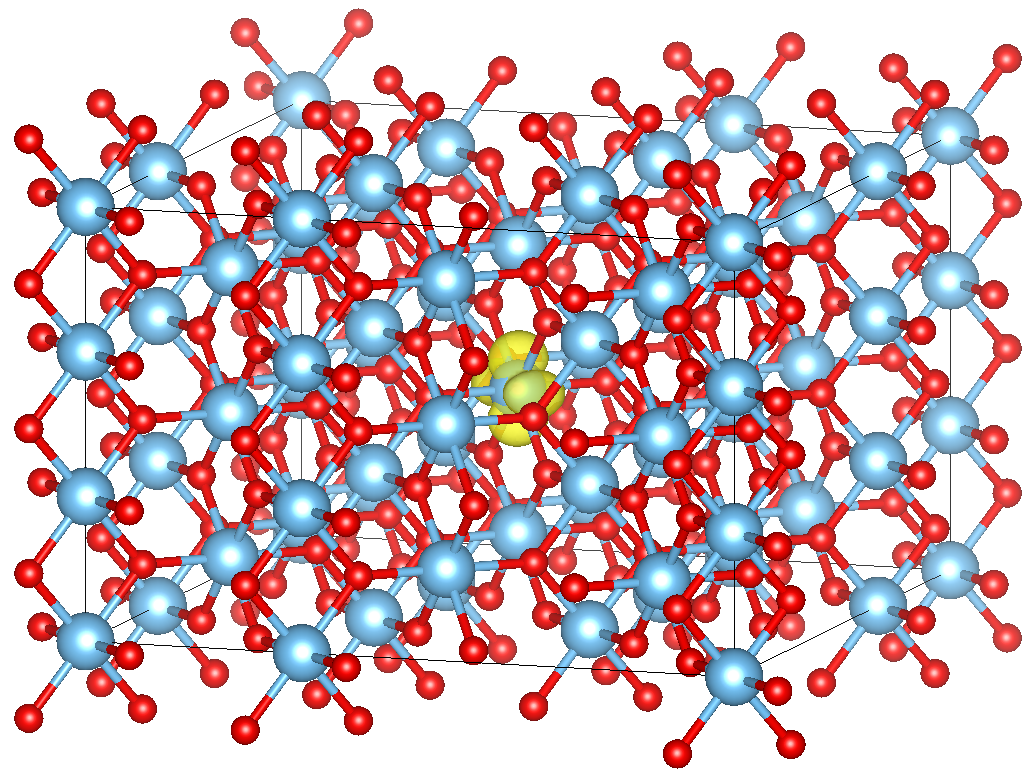
\includegraphics[width=\textwidth]{figures/PARCHG_polaron_super}
        \caption{Electron localized: polaron}
        \label{fig:polaron_iso_super}
    \end{subfigure}
    \hfill
    \begin{subfigure}[b]{0.49\textwidth}
        \centering
        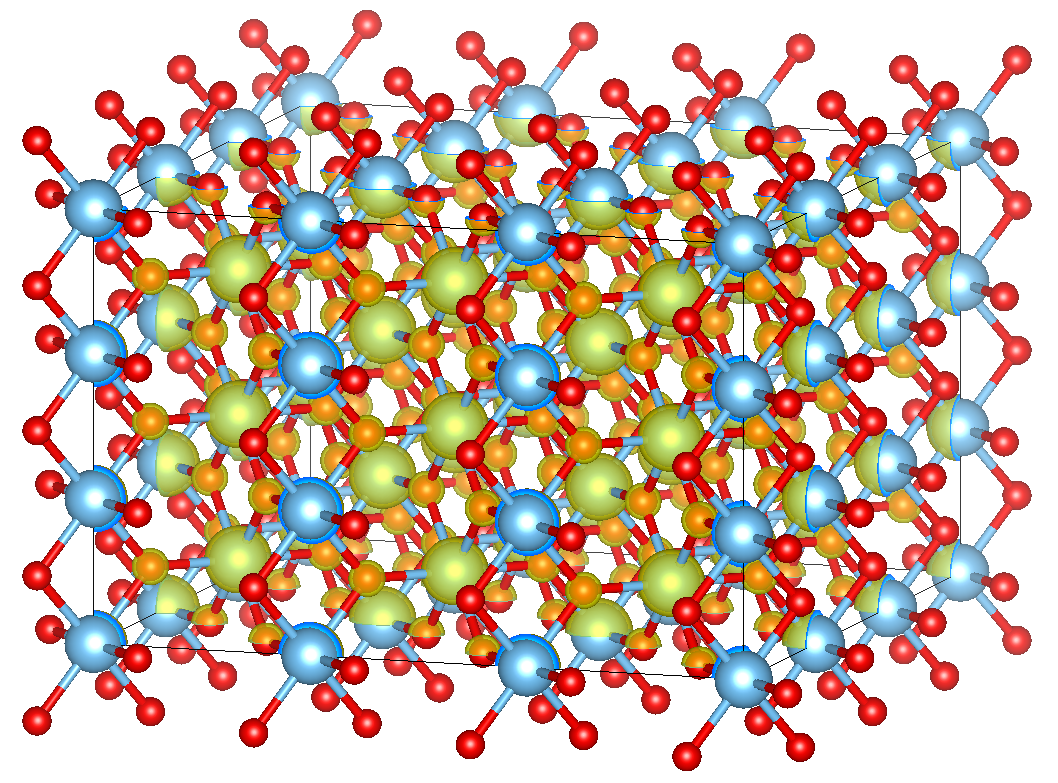
\includegraphics[width=\textwidth]{figures/PARCHG_delocalized_super}
        \caption{Electron delocalized}
        \label{fig:delocalized_iso_super}
    \end{subfigure}
    \caption[Supercell with the isosurface of the charge density projected on the extra-electron band]{Supercell with the isosurface  (10\%)  of the charge density projected on the extra-electron band. In (a) the extra electron is localized and forms a polaron, in (b) it is delocalized. The blue atoms are titanium atoms, whereas the red ones are oxygen atoms.
    }
    \label{fig:isosurfaces_supercell}
\end{figure}
\begin{figure}[p]
    \centering
    \begin{subfigure}[b]{0.49\textwidth}
        \centering
        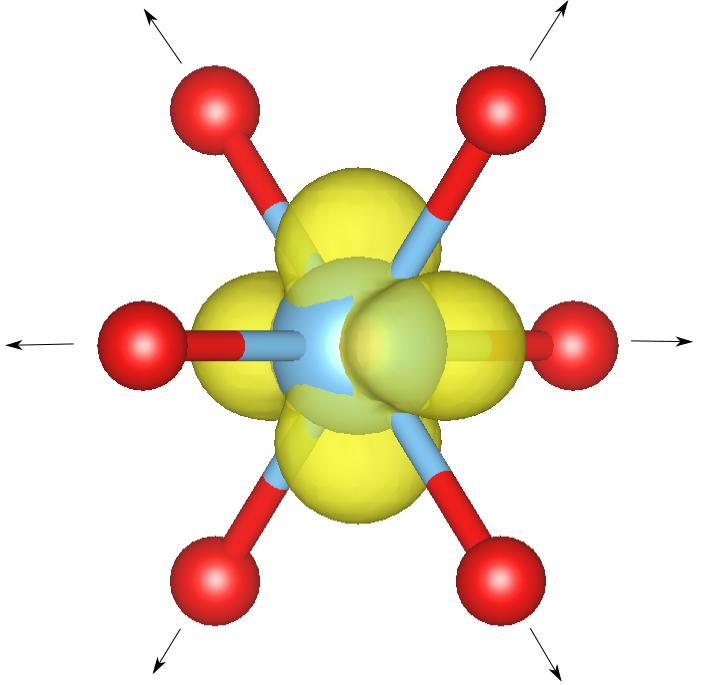
\includegraphics[width=\textwidth]{figures/PARCHG_polaron}
        \caption{Electron localized: polaron}
        \label{fig:polaron_iso}
    \end{subfigure}
    \hfill
    \begin{subfigure}[b]{0.49\textwidth}
        \centering
        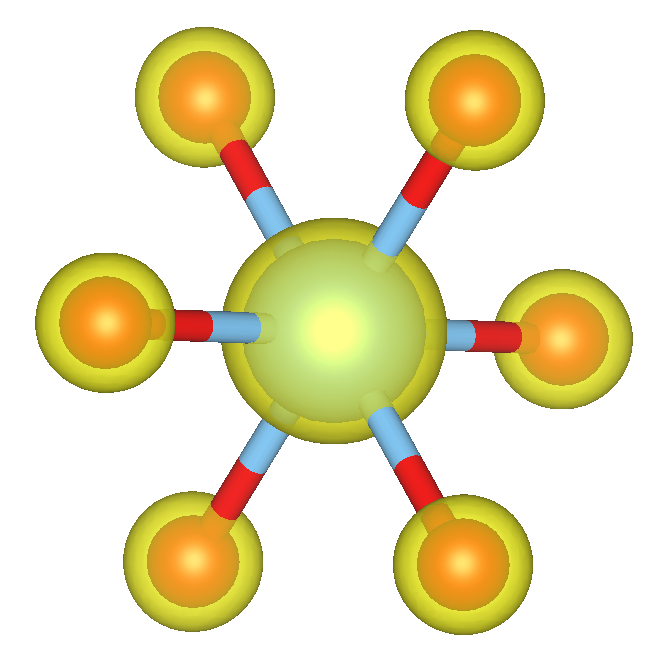
\includegraphics[width=\textwidth]{figures/PARCHG_delocalized}
        \caption{Electron delocalized}
        \label{fig:delocalized_iso}
    \end{subfigure}
    \caption[Central atom with the isosurface of the charge density projected on the extra-electron band]{Central atom with the isosurface  (10\%) of the charge density projected on the extra-electron band. In (a) the extra electron is localized and forms a polaron, in (b) it is delocalized. The blue atom is the central titanium atom, whereas the red ones are the nearest-neighbours oxygen atoms.}
    \label{fig:isosurfaces_center}
\end{figure}